\section{Results}
\label{sec:Results}
\FloatBarrier
\subsection{Straight Beam Results}
The simplest test case for this model is a linear-elastic beam with a square profile.
These models represent beams that are 1cm thick and 1cm wide, with a bulk modulus $k = 37.5$GPa and Poisson's ratio $\nu = \sfrac{1}{3}$.
Each is loaded transversely with a load of 0.0833N, except for \cref{fig:moment_n}, which shows a beam loaded with a moment of 0.0833N$\cdot$m.
In beams simulating inelastic behavior, the critical strain of the material is set to $\varepsilon_c = 0.001$.
The elastic cases are compared to analytical solutions of the Euler beam equation with appropriate boundary conditions.
Even a coarse discretization successfully reproduces the shape of the elastically deformed, simply-supported beam shown  in \cref{fig:elastic_g2000} deformed under uniform load.
%\todo{Your figures should not have titles on top of them.}
%
\begin{figure}[htbp]
  \centering
  \resizebox{0.6\linewidth}{!}{%% Creator: Matplotlib, PGF backend
%%
%% To include the figure in your LaTeX document, write
%%   \input{<filename>.pgf}
%%
%% Make sure the required packages are loaded in your preamble
%%   \usepackage{pgf}
%%
%% Figures using additional raster images can only be included by \input if
%% they are in the same directory as the main LaTeX file. For loading figures
%% from other directories you can use the `import` package
%%   \usepackage{import}
%% and then include the figures with
%%   \import{<path to file>}{<filename>.pgf}
%%
%% Matplotlib used the following preamble
%%
\begingroup%
\makeatletter%
\begin{pgfpicture}%
\pgfpathrectangle{\pgfpointorigin}{\pgfqpoint{6.000000in}{6.000000in}}%
\pgfusepath{use as bounding box}%
\begin{pgfscope}%
\pgfsetbuttcap%
\pgfsetroundjoin%
\definecolor{currentfill}{rgb}{1.000000,1.000000,1.000000}%
\pgfsetfillcolor{currentfill}%
\pgfsetlinewidth{0.000000pt}%
\definecolor{currentstroke}{rgb}{1.000000,1.000000,1.000000}%
\pgfsetstrokecolor{currentstroke}%
\pgfsetdash{}{0pt}%
\pgfpathmoveto{\pgfqpoint{0.000000in}{0.000000in}}%
\pgfpathlineto{\pgfqpoint{6.000000in}{0.000000in}}%
\pgfpathlineto{\pgfqpoint{6.000000in}{6.000000in}}%
\pgfpathlineto{\pgfqpoint{0.000000in}{6.000000in}}%
\pgfpathclose%
\pgfusepath{fill}%
\end{pgfscope}%
\begin{pgfscope}%
\pgfsetbuttcap%
\pgfsetroundjoin%
\definecolor{currentfill}{rgb}{1.000000,1.000000,1.000000}%
\pgfsetfillcolor{currentfill}%
\pgfsetlinewidth{0.000000pt}%
\definecolor{currentstroke}{rgb}{0.000000,0.000000,0.000000}%
\pgfsetstrokecolor{currentstroke}%
\pgfsetstrokeopacity{0.000000}%
\pgfsetdash{}{0pt}%
\pgfpathmoveto{\pgfqpoint{0.750000in}{0.600000in}}%
\pgfpathlineto{\pgfqpoint{5.400000in}{0.600000in}}%
\pgfpathlineto{\pgfqpoint{5.400000in}{5.400000in}}%
\pgfpathlineto{\pgfqpoint{0.750000in}{5.400000in}}%
\pgfpathclose%
\pgfusepath{fill}%
\end{pgfscope}%
\begin{pgfscope}%
\pgfpathrectangle{\pgfqpoint{0.750000in}{0.600000in}}{\pgfqpoint{4.650000in}{4.800000in}} %
\pgfusepath{clip}%
\pgfsetrectcap%
\pgfsetroundjoin%
\pgfsetlinewidth{1.003750pt}%
\definecolor{currentstroke}{rgb}{0.000000,0.000000,1.000000}%
\pgfsetstrokecolor{currentstroke}%
\pgfsetdash{}{0pt}%
\pgfpathmoveto{\pgfqpoint{0.796500in}{5.266693in}}%
\pgfpathlineto{\pgfqpoint{0.982500in}{4.736583in}}%
\pgfpathlineto{\pgfqpoint{1.122000in}{4.346441in}}%
\pgfpathlineto{\pgfqpoint{1.215000in}{4.092000in}}%
\pgfpathlineto{\pgfqpoint{1.308000in}{3.843315in}}%
\pgfpathlineto{\pgfqpoint{1.401000in}{3.601385in}}%
\pgfpathlineto{\pgfqpoint{1.494000in}{3.367155in}}%
\pgfpathlineto{\pgfqpoint{1.587000in}{3.141523in}}%
\pgfpathlineto{\pgfqpoint{1.680000in}{2.925333in}}%
\pgfpathlineto{\pgfqpoint{1.773000in}{2.719379in}}%
\pgfpathlineto{\pgfqpoint{1.819500in}{2.620475in}}%
\pgfpathlineto{\pgfqpoint{1.866000in}{2.524403in}}%
\pgfpathlineto{\pgfqpoint{1.912500in}{2.431250in}}%
\pgfpathlineto{\pgfqpoint{1.959000in}{2.341097in}}%
\pgfpathlineto{\pgfqpoint{2.005500in}{2.254021in}}%
\pgfpathlineto{\pgfqpoint{2.052000in}{2.170099in}}%
\pgfpathlineto{\pgfqpoint{2.098500in}{2.089403in}}%
\pgfpathlineto{\pgfqpoint{2.145000in}{2.012000in}}%
\pgfpathlineto{\pgfqpoint{2.191500in}{1.937957in}}%
\pgfpathlineto{\pgfqpoint{2.238000in}{1.867337in}}%
\pgfpathlineto{\pgfqpoint{2.284500in}{1.800197in}}%
\pgfpathlineto{\pgfqpoint{2.331000in}{1.736595in}}%
\pgfpathlineto{\pgfqpoint{2.377500in}{1.676583in}}%
\pgfpathlineto{\pgfqpoint{2.424000in}{1.620211in}}%
\pgfpathlineto{\pgfqpoint{2.470500in}{1.567525in}}%
\pgfpathlineto{\pgfqpoint{2.517000in}{1.518569in}}%
\pgfpathlineto{\pgfqpoint{2.563500in}{1.473381in}}%
\pgfpathlineto{\pgfqpoint{2.610000in}{1.432000in}}%
\pgfpathlineto{\pgfqpoint{2.656500in}{1.394459in}}%
\pgfpathlineto{\pgfqpoint{2.703000in}{1.360787in}}%
\pgfpathlineto{\pgfqpoint{2.749500in}{1.331013in}}%
\pgfpathlineto{\pgfqpoint{2.796000in}{1.305161in}}%
\pgfpathlineto{\pgfqpoint{2.842500in}{1.283250in}}%
\pgfpathlineto{\pgfqpoint{2.889000in}{1.265299in}}%
\pgfpathlineto{\pgfqpoint{2.935500in}{1.251323in}}%
\pgfpathlineto{\pgfqpoint{2.982000in}{1.241331in}}%
\pgfpathlineto{\pgfqpoint{3.028500in}{1.235333in}}%
\pgfpathlineto{\pgfqpoint{3.075000in}{1.233333in}}%
\pgfpathlineto{\pgfqpoint{3.121500in}{1.235333in}}%
\pgfpathlineto{\pgfqpoint{3.168000in}{1.241331in}}%
\pgfpathlineto{\pgfqpoint{3.214500in}{1.251323in}}%
\pgfpathlineto{\pgfqpoint{3.261000in}{1.265299in}}%
\pgfpathlineto{\pgfqpoint{3.307500in}{1.283250in}}%
\pgfpathlineto{\pgfqpoint{3.354000in}{1.305161in}}%
\pgfpathlineto{\pgfqpoint{3.400500in}{1.331013in}}%
\pgfpathlineto{\pgfqpoint{3.447000in}{1.360787in}}%
\pgfpathlineto{\pgfqpoint{3.493500in}{1.394459in}}%
\pgfpathlineto{\pgfqpoint{3.540000in}{1.432000in}}%
\pgfpathlineto{\pgfqpoint{3.586500in}{1.473381in}}%
\pgfpathlineto{\pgfqpoint{3.633000in}{1.518569in}}%
\pgfpathlineto{\pgfqpoint{3.679500in}{1.567525in}}%
\pgfpathlineto{\pgfqpoint{3.726000in}{1.620211in}}%
\pgfpathlineto{\pgfqpoint{3.772500in}{1.676583in}}%
\pgfpathlineto{\pgfqpoint{3.819000in}{1.736595in}}%
\pgfpathlineto{\pgfqpoint{3.865500in}{1.800197in}}%
\pgfpathlineto{\pgfqpoint{3.912000in}{1.867337in}}%
\pgfpathlineto{\pgfqpoint{3.958500in}{1.937957in}}%
\pgfpathlineto{\pgfqpoint{4.005000in}{2.012000in}}%
\pgfpathlineto{\pgfqpoint{4.051500in}{2.089403in}}%
\pgfpathlineto{\pgfqpoint{4.098000in}{2.170099in}}%
\pgfpathlineto{\pgfqpoint{4.144500in}{2.254021in}}%
\pgfpathlineto{\pgfqpoint{4.191000in}{2.341097in}}%
\pgfpathlineto{\pgfqpoint{4.237500in}{2.431250in}}%
\pgfpathlineto{\pgfqpoint{4.284000in}{2.524403in}}%
\pgfpathlineto{\pgfqpoint{4.330500in}{2.620475in}}%
\pgfpathlineto{\pgfqpoint{4.377000in}{2.719379in}}%
\pgfpathlineto{\pgfqpoint{4.470000in}{2.925333in}}%
\pgfpathlineto{\pgfqpoint{4.563000in}{3.141523in}}%
\pgfpathlineto{\pgfqpoint{4.656000in}{3.367155in}}%
\pgfpathlineto{\pgfqpoint{4.749000in}{3.601385in}}%
\pgfpathlineto{\pgfqpoint{4.842000in}{3.843315in}}%
\pgfpathlineto{\pgfqpoint{4.935000in}{4.092000in}}%
\pgfpathlineto{\pgfqpoint{5.028000in}{4.346441in}}%
\pgfpathlineto{\pgfqpoint{5.167500in}{4.736583in}}%
\pgfpathlineto{\pgfqpoint{5.353500in}{5.266693in}}%
\pgfpathlineto{\pgfqpoint{5.400000in}{5.400000in}}%
\pgfpathlineto{\pgfqpoint{5.400000in}{5.400000in}}%
\pgfusepath{stroke}%
\end{pgfscope}%
\begin{pgfscope}%
\pgfpathrectangle{\pgfqpoint{0.750000in}{0.600000in}}{\pgfqpoint{4.650000in}{4.800000in}} %
\pgfusepath{clip}%
\pgfsetbuttcap%
\pgfsetroundjoin%
\definecolor{currentfill}{rgb}{0.000000,0.000000,1.000000}%
\pgfsetfillcolor{currentfill}%
\pgfsetlinewidth{0.501875pt}%
\definecolor{currentstroke}{rgb}{0.000000,0.000000,0.000000}%
\pgfsetstrokecolor{currentstroke}%
\pgfsetdash{}{0pt}%
\pgfsys@defobject{currentmarker}{\pgfqpoint{-0.041667in}{-0.041667in}}{\pgfqpoint{0.041667in}{0.041667in}}{%
\pgfpathmoveto{\pgfqpoint{0.000000in}{-0.041667in}}%
\pgfpathcurveto{\pgfqpoint{0.011050in}{-0.041667in}}{\pgfqpoint{0.021649in}{-0.037276in}}{\pgfqpoint{0.029463in}{-0.029463in}}%
\pgfpathcurveto{\pgfqpoint{0.037276in}{-0.021649in}}{\pgfqpoint{0.041667in}{-0.011050in}}{\pgfqpoint{0.041667in}{0.000000in}}%
\pgfpathcurveto{\pgfqpoint{0.041667in}{0.011050in}}{\pgfqpoint{0.037276in}{0.021649in}}{\pgfqpoint{0.029463in}{0.029463in}}%
\pgfpathcurveto{\pgfqpoint{0.021649in}{0.037276in}}{\pgfqpoint{0.011050in}{0.041667in}}{\pgfqpoint{0.000000in}{0.041667in}}%
\pgfpathcurveto{\pgfqpoint{-0.011050in}{0.041667in}}{\pgfqpoint{-0.021649in}{0.037276in}}{\pgfqpoint{-0.029463in}{0.029463in}}%
\pgfpathcurveto{\pgfqpoint{-0.037276in}{0.021649in}}{\pgfqpoint{-0.041667in}{0.011050in}}{\pgfqpoint{-0.041667in}{0.000000in}}%
\pgfpathcurveto{\pgfqpoint{-0.041667in}{-0.011050in}}{\pgfqpoint{-0.037276in}{-0.021649in}}{\pgfqpoint{-0.029463in}{-0.029463in}}%
\pgfpathcurveto{\pgfqpoint{-0.021649in}{-0.037276in}}{\pgfqpoint{-0.011050in}{-0.041667in}}{\pgfqpoint{0.000000in}{-0.041667in}}%
\pgfpathclose%
\pgfusepath{stroke,fill}%
}%
\begin{pgfscope}%
\pgfsys@transformshift{1.075500in}{4.475493in}%
\pgfsys@useobject{currentmarker}{}%
\end{pgfscope}%
\begin{pgfscope}%
\pgfsys@transformshift{1.540500in}{3.253211in}%
\pgfsys@useobject{currentmarker}{}%
\end{pgfscope}%
\begin{pgfscope}%
\pgfsys@transformshift{2.005500in}{2.254021in}%
\pgfsys@useobject{currentmarker}{}%
\end{pgfscope}%
\begin{pgfscope}%
\pgfsys@transformshift{2.470500in}{1.567525in}%
\pgfsys@useobject{currentmarker}{}%
\end{pgfscope}%
\begin{pgfscope}%
\pgfsys@transformshift{2.935500in}{1.251323in}%
\pgfsys@useobject{currentmarker}{}%
\end{pgfscope}%
\begin{pgfscope}%
\pgfsys@transformshift{3.400500in}{1.331013in}%
\pgfsys@useobject{currentmarker}{}%
\end{pgfscope}%
\begin{pgfscope}%
\pgfsys@transformshift{3.865500in}{1.800197in}%
\pgfsys@useobject{currentmarker}{}%
\end{pgfscope}%
\begin{pgfscope}%
\pgfsys@transformshift{4.330500in}{2.620475in}%
\pgfsys@useobject{currentmarker}{}%
\end{pgfscope}%
\begin{pgfscope}%
\pgfsys@transformshift{4.795500in}{3.721445in}%
\pgfsys@useobject{currentmarker}{}%
\end{pgfscope}%
\begin{pgfscope}%
\pgfsys@transformshift{5.260500in}{5.000709in}%
\pgfsys@useobject{currentmarker}{}%
\end{pgfscope}%
\end{pgfscope}%
\begin{pgfscope}%
\pgfpathrectangle{\pgfqpoint{0.750000in}{0.600000in}}{\pgfqpoint{4.650000in}{4.800000in}} %
\pgfusepath{clip}%
\pgfsetrectcap%
\pgfsetroundjoin%
\pgfsetlinewidth{1.003750pt}%
\definecolor{currentstroke}{rgb}{0.000000,0.500000,0.000000}%
\pgfsetstrokecolor{currentstroke}%
\pgfsetdash{}{0pt}%
\pgfpathmoveto{\pgfqpoint{0.843000in}{5.142324in}}%
\pgfpathlineto{\pgfqpoint{0.936000in}{4.885157in}}%
\pgfpathlineto{\pgfqpoint{1.029000in}{4.629314in}}%
\pgfpathlineto{\pgfqpoint{1.122000in}{4.375370in}}%
\pgfpathlineto{\pgfqpoint{1.215000in}{4.124317in}}%
\pgfpathlineto{\pgfqpoint{1.308000in}{3.882080in}}%
\pgfpathlineto{\pgfqpoint{1.401000in}{3.645171in}}%
\pgfpathlineto{\pgfqpoint{1.494000in}{3.415281in}}%
\pgfpathlineto{\pgfqpoint{1.587000in}{3.193670in}}%
\pgfpathlineto{\pgfqpoint{1.680000in}{2.981159in}}%
\pgfpathlineto{\pgfqpoint{1.773000in}{2.778726in}}%
\pgfpathlineto{\pgfqpoint{1.866000in}{2.586899in}}%
\pgfpathlineto{\pgfqpoint{1.959000in}{2.406484in}}%
\pgfpathlineto{\pgfqpoint{2.052000in}{2.238095in}}%
\pgfpathlineto{\pgfqpoint{2.145000in}{2.082372in}}%
\pgfpathlineto{\pgfqpoint{2.238000in}{1.939808in}}%
\pgfpathlineto{\pgfqpoint{2.331000in}{1.810928in}}%
\pgfpathlineto{\pgfqpoint{2.424000in}{1.696182in}}%
\pgfpathlineto{\pgfqpoint{2.517000in}{1.595948in}}%
\pgfpathlineto{\pgfqpoint{2.610000in}{1.510572in}}%
\pgfpathlineto{\pgfqpoint{2.703000in}{1.440334in}}%
\pgfpathlineto{\pgfqpoint{2.796000in}{1.385474in}}%
\pgfpathlineto{\pgfqpoint{2.889000in}{1.346173in}}%
\pgfpathlineto{\pgfqpoint{2.982000in}{1.322560in}}%
\pgfpathlineto{\pgfqpoint{3.075000in}{1.314715in}}%
\pgfpathlineto{\pgfqpoint{3.168000in}{1.322661in}}%
\pgfpathlineto{\pgfqpoint{3.261000in}{1.346374in}}%
\pgfpathlineto{\pgfqpoint{3.354000in}{1.385773in}}%
\pgfpathlineto{\pgfqpoint{3.447000in}{1.440729in}}%
\pgfpathlineto{\pgfqpoint{3.540000in}{1.511058in}}%
\pgfpathlineto{\pgfqpoint{3.633000in}{1.596521in}}%
\pgfpathlineto{\pgfqpoint{3.726000in}{1.696835in}}%
\pgfpathlineto{\pgfqpoint{3.819000in}{1.811655in}}%
\pgfpathlineto{\pgfqpoint{3.912000in}{1.940602in}}%
\pgfpathlineto{\pgfqpoint{4.005000in}{2.083224in}}%
\pgfpathlineto{\pgfqpoint{4.098000in}{2.238995in}}%
\pgfpathlineto{\pgfqpoint{4.191000in}{2.407421in}}%
\pgfpathlineto{\pgfqpoint{4.284000in}{2.587862in}}%
\pgfpathlineto{\pgfqpoint{4.377000in}{2.779704in}}%
\pgfpathlineto{\pgfqpoint{4.470000in}{2.982137in}}%
\pgfpathlineto{\pgfqpoint{4.563000in}{3.194634in}}%
\pgfpathlineto{\pgfqpoint{4.656000in}{3.416214in}}%
\pgfpathlineto{\pgfqpoint{4.749000in}{3.646059in}}%
\pgfpathlineto{\pgfqpoint{4.842000in}{3.882903in}}%
\pgfpathlineto{\pgfqpoint{4.935000in}{4.125075in}}%
\pgfpathlineto{\pgfqpoint{5.028000in}{4.376003in}}%
\pgfpathlineto{\pgfqpoint{5.121000in}{4.629816in}}%
\pgfpathlineto{\pgfqpoint{5.214000in}{4.885599in}}%
\pgfpathlineto{\pgfqpoint{5.307000in}{5.142506in}}%
\pgfpathlineto{\pgfqpoint{5.400000in}{5.400000in}}%
\pgfusepath{stroke}%
\end{pgfscope}%
\begin{pgfscope}%
\pgfpathrectangle{\pgfqpoint{0.750000in}{0.600000in}}{\pgfqpoint{4.650000in}{4.800000in}} %
\pgfusepath{clip}%
\pgfsetbuttcap%
\pgfsetmiterjoin%
\definecolor{currentfill}{rgb}{0.000000,0.500000,0.000000}%
\pgfsetfillcolor{currentfill}%
\pgfsetlinewidth{0.501875pt}%
\definecolor{currentstroke}{rgb}{0.000000,0.000000,0.000000}%
\pgfsetstrokecolor{currentstroke}%
\pgfsetdash{}{0pt}%
\pgfsys@defobject{currentmarker}{\pgfqpoint{-0.041667in}{-0.041667in}}{\pgfqpoint{0.041667in}{0.041667in}}{%
\pgfpathmoveto{\pgfqpoint{0.000000in}{0.041667in}}%
\pgfpathlineto{\pgfqpoint{-0.041667in}{-0.041667in}}%
\pgfpathlineto{\pgfqpoint{0.041667in}{-0.041667in}}%
\pgfpathclose%
\pgfusepath{stroke,fill}%
}%
\begin{pgfscope}%
\pgfsys@transformshift{0.843000in}{5.142324in}%
\pgfsys@useobject{currentmarker}{}%
\end{pgfscope}%
\begin{pgfscope}%
\pgfsys@transformshift{1.308000in}{3.882080in}%
\pgfsys@useobject{currentmarker}{}%
\end{pgfscope}%
\begin{pgfscope}%
\pgfsys@transformshift{1.773000in}{2.778726in}%
\pgfsys@useobject{currentmarker}{}%
\end{pgfscope}%
\begin{pgfscope}%
\pgfsys@transformshift{2.238000in}{1.939808in}%
\pgfsys@useobject{currentmarker}{}%
\end{pgfscope}%
\begin{pgfscope}%
\pgfsys@transformshift{2.703000in}{1.440334in}%
\pgfsys@useobject{currentmarker}{}%
\end{pgfscope}%
\begin{pgfscope}%
\pgfsys@transformshift{3.168000in}{1.322661in}%
\pgfsys@useobject{currentmarker}{}%
\end{pgfscope}%
\begin{pgfscope}%
\pgfsys@transformshift{3.633000in}{1.596521in}%
\pgfsys@useobject{currentmarker}{}%
\end{pgfscope}%
\begin{pgfscope}%
\pgfsys@transformshift{4.098000in}{2.238995in}%
\pgfsys@useobject{currentmarker}{}%
\end{pgfscope}%
\begin{pgfscope}%
\pgfsys@transformshift{4.563000in}{3.194634in}%
\pgfsys@useobject{currentmarker}{}%
\end{pgfscope}%
\begin{pgfscope}%
\pgfsys@transformshift{5.028000in}{4.376003in}%
\pgfsys@useobject{currentmarker}{}%
\end{pgfscope}%
\end{pgfscope}%
\begin{pgfscope}%
\pgfpathrectangle{\pgfqpoint{0.750000in}{0.600000in}}{\pgfqpoint{4.650000in}{4.800000in}} %
\pgfusepath{clip}%
\pgfsetrectcap%
\pgfsetroundjoin%
\pgfsetlinewidth{1.003750pt}%
\definecolor{currentstroke}{rgb}{1.000000,0.000000,0.000000}%
\pgfsetstrokecolor{currentstroke}%
\pgfsetdash{}{0pt}%
\pgfpathmoveto{\pgfqpoint{0.796500in}{5.268655in}}%
\pgfpathlineto{\pgfqpoint{1.029000in}{4.615916in}}%
\pgfpathlineto{\pgfqpoint{1.168500in}{4.230459in}}%
\pgfpathlineto{\pgfqpoint{1.215000in}{4.103912in}}%
\pgfpathlineto{\pgfqpoint{1.354500in}{3.737992in}}%
\pgfpathlineto{\pgfqpoint{1.447500in}{3.501530in}}%
\pgfpathlineto{\pgfqpoint{1.540500in}{3.273019in}}%
\pgfpathlineto{\pgfqpoint{1.633500in}{3.053440in}}%
\pgfpathlineto{\pgfqpoint{1.726500in}{2.843678in}}%
\pgfpathlineto{\pgfqpoint{1.773000in}{2.742676in}}%
\pgfpathlineto{\pgfqpoint{1.819500in}{2.644376in}}%
\pgfpathlineto{\pgfqpoint{1.866000in}{2.548892in}}%
\pgfpathlineto{\pgfqpoint{1.912500in}{2.456292in}}%
\pgfpathlineto{\pgfqpoint{1.959000in}{2.366675in}}%
\pgfpathlineto{\pgfqpoint{2.005500in}{2.280105in}}%
\pgfpathlineto{\pgfqpoint{2.052000in}{2.196671in}}%
\pgfpathlineto{\pgfqpoint{2.098500in}{2.116430in}}%
\pgfpathlineto{\pgfqpoint{2.145000in}{2.039464in}}%
\pgfpathlineto{\pgfqpoint{2.191500in}{1.965824in}}%
\pgfpathlineto{\pgfqpoint{2.238000in}{1.895587in}}%
\pgfpathlineto{\pgfqpoint{2.284500in}{1.828811in}}%
\pgfpathlineto{\pgfqpoint{2.331000in}{1.765550in}}%
\pgfpathlineto{\pgfqpoint{2.377500in}{1.705859in}}%
\pgfpathlineto{\pgfqpoint{2.424000in}{1.649786in}}%
\pgfpathlineto{\pgfqpoint{2.470500in}{1.597378in}}%
\pgfpathlineto{\pgfqpoint{2.517000in}{1.548679in}}%
\pgfpathlineto{\pgfqpoint{2.563500in}{1.503728in}}%
\pgfpathlineto{\pgfqpoint{2.610000in}{1.462564in}}%
\pgfpathlineto{\pgfqpoint{2.656500in}{1.425220in}}%
\pgfpathlineto{\pgfqpoint{2.703000in}{1.391727in}}%
\pgfpathlineto{\pgfqpoint{2.749500in}{1.362113in}}%
\pgfpathlineto{\pgfqpoint{2.796000in}{1.336400in}}%
\pgfpathlineto{\pgfqpoint{2.842500in}{1.314612in}}%
\pgfpathlineto{\pgfqpoint{2.889000in}{1.296764in}}%
\pgfpathlineto{\pgfqpoint{2.935500in}{1.282872in}}%
\pgfpathlineto{\pgfqpoint{2.982000in}{1.272947in}}%
\pgfpathlineto{\pgfqpoint{3.028500in}{1.266997in}}%
\pgfpathlineto{\pgfqpoint{3.075000in}{1.265027in}}%
\pgfpathlineto{\pgfqpoint{3.121500in}{1.267038in}}%
\pgfpathlineto{\pgfqpoint{3.168000in}{1.273029in}}%
\pgfpathlineto{\pgfqpoint{3.214500in}{1.282995in}}%
\pgfpathlineto{\pgfqpoint{3.261000in}{1.296927in}}%
\pgfpathlineto{\pgfqpoint{3.307500in}{1.314815in}}%
\pgfpathlineto{\pgfqpoint{3.354000in}{1.336643in}}%
\pgfpathlineto{\pgfqpoint{3.400500in}{1.362394in}}%
\pgfpathlineto{\pgfqpoint{3.447000in}{1.392047in}}%
\pgfpathlineto{\pgfqpoint{3.493500in}{1.425577in}}%
\pgfpathlineto{\pgfqpoint{3.540000in}{1.462958in}}%
\pgfpathlineto{\pgfqpoint{3.586500in}{1.504157in}}%
\pgfpathlineto{\pgfqpoint{3.633000in}{1.549142in}}%
\pgfpathlineto{\pgfqpoint{3.679500in}{1.597875in}}%
\pgfpathlineto{\pgfqpoint{3.726000in}{1.650315in}}%
\pgfpathlineto{\pgfqpoint{3.772500in}{1.706419in}}%
\pgfpathlineto{\pgfqpoint{3.819000in}{1.766140in}}%
\pgfpathlineto{\pgfqpoint{3.865500in}{1.829428in}}%
\pgfpathlineto{\pgfqpoint{3.912000in}{1.896230in}}%
\pgfpathlineto{\pgfqpoint{3.958500in}{1.966491in}}%
\pgfpathlineto{\pgfqpoint{4.005000in}{2.040154in}}%
\pgfpathlineto{\pgfqpoint{4.051500in}{2.117141in}}%
\pgfpathlineto{\pgfqpoint{4.098000in}{2.197400in}}%
\pgfpathlineto{\pgfqpoint{4.144500in}{2.280851in}}%
\pgfpathlineto{\pgfqpoint{4.191000in}{2.367435in}}%
\pgfpathlineto{\pgfqpoint{4.237500in}{2.457063in}}%
\pgfpathlineto{\pgfqpoint{4.284000in}{2.549673in}}%
\pgfpathlineto{\pgfqpoint{4.330500in}{2.645164in}}%
\pgfpathlineto{\pgfqpoint{4.377000in}{2.743468in}}%
\pgfpathlineto{\pgfqpoint{4.470000in}{2.948081in}}%
\pgfpathlineto{\pgfqpoint{4.563000in}{3.162844in}}%
\pgfpathlineto{\pgfqpoint{4.656000in}{3.386985in}}%
\pgfpathlineto{\pgfqpoint{4.749000in}{3.619569in}}%
\pgfpathlineto{\pgfqpoint{4.842000in}{3.859574in}}%
\pgfpathlineto{\pgfqpoint{4.935000in}{4.104526in}}%
\pgfpathlineto{\pgfqpoint{5.074500in}{4.487140in}}%
\pgfpathlineto{\pgfqpoint{5.260500in}{5.006869in}}%
\pgfpathlineto{\pgfqpoint{5.400000in}{5.400000in}}%
\pgfpathlineto{\pgfqpoint{5.400000in}{5.400000in}}%
\pgfusepath{stroke}%
\end{pgfscope}%
\begin{pgfscope}%
\pgfpathrectangle{\pgfqpoint{0.750000in}{0.600000in}}{\pgfqpoint{4.650000in}{4.800000in}} %
\pgfusepath{clip}%
\pgfsetbuttcap%
\pgfsetmiterjoin%
\definecolor{currentfill}{rgb}{1.000000,0.000000,0.000000}%
\pgfsetfillcolor{currentfill}%
\pgfsetlinewidth{0.501875pt}%
\definecolor{currentstroke}{rgb}{0.000000,0.000000,0.000000}%
\pgfsetstrokecolor{currentstroke}%
\pgfsetdash{}{0pt}%
\pgfsys@defobject{currentmarker}{\pgfqpoint{-0.041667in}{-0.041667in}}{\pgfqpoint{0.041667in}{0.041667in}}{%
\pgfpathmoveto{\pgfqpoint{0.041667in}{-0.000000in}}%
\pgfpathlineto{\pgfqpoint{-0.041667in}{0.041667in}}%
\pgfpathlineto{\pgfqpoint{-0.041667in}{-0.041667in}}%
\pgfpathclose%
\pgfusepath{stroke,fill}%
}%
\begin{pgfscope}%
\pgfsys@transformshift{0.936000in}{4.875981in}%
\pgfsys@useobject{currentmarker}{}%
\end{pgfscope}%
\begin{pgfscope}%
\pgfsys@transformshift{1.401000in}{3.618849in}%
\pgfsys@useobject{currentmarker}{}%
\end{pgfscope}%
\begin{pgfscope}%
\pgfsys@transformshift{1.866000in}{2.548892in}%
\pgfsys@useobject{currentmarker}{}%
\end{pgfscope}%
\begin{pgfscope}%
\pgfsys@transformshift{2.331000in}{1.765550in}%
\pgfsys@useobject{currentmarker}{}%
\end{pgfscope}%
\begin{pgfscope}%
\pgfsys@transformshift{2.796000in}{1.336400in}%
\pgfsys@useobject{currentmarker}{}%
\end{pgfscope}%
\begin{pgfscope}%
\pgfsys@transformshift{3.261000in}{1.296927in}%
\pgfsys@useobject{currentmarker}{}%
\end{pgfscope}%
\begin{pgfscope}%
\pgfsys@transformshift{3.726000in}{1.650315in}%
\pgfsys@useobject{currentmarker}{}%
\end{pgfscope}%
\begin{pgfscope}%
\pgfsys@transformshift{4.191000in}{2.367435in}%
\pgfsys@useobject{currentmarker}{}%
\end{pgfscope}%
\begin{pgfscope}%
\pgfsys@transformshift{4.656000in}{3.386985in}%
\pgfsys@useobject{currentmarker}{}%
\end{pgfscope}%
\begin{pgfscope}%
\pgfsys@transformshift{5.121000in}{4.616327in}%
\pgfsys@useobject{currentmarker}{}%
\end{pgfscope}%
\end{pgfscope}%
\begin{pgfscope}%
\pgfpathrectangle{\pgfqpoint{0.750000in}{0.600000in}}{\pgfqpoint{4.650000in}{4.800000in}} %
\pgfusepath{clip}%
\pgfsetbuttcap%
\pgfsetroundjoin%
\pgfsetlinewidth{0.501875pt}%
\definecolor{currentstroke}{rgb}{0.000000,0.000000,0.000000}%
\pgfsetstrokecolor{currentstroke}%
\pgfsetdash{{1.000000pt}{3.000000pt}}{0.000000pt}%
\pgfpathmoveto{\pgfqpoint{0.750000in}{0.600000in}}%
\pgfpathlineto{\pgfqpoint{0.750000in}{5.400000in}}%
\pgfusepath{stroke}%
\end{pgfscope}%
\begin{pgfscope}%
\pgfsetbuttcap%
\pgfsetroundjoin%
\definecolor{currentfill}{rgb}{0.000000,0.000000,0.000000}%
\pgfsetfillcolor{currentfill}%
\pgfsetlinewidth{0.501875pt}%
\definecolor{currentstroke}{rgb}{0.000000,0.000000,0.000000}%
\pgfsetstrokecolor{currentstroke}%
\pgfsetdash{}{0pt}%
\pgfsys@defobject{currentmarker}{\pgfqpoint{0.000000in}{0.000000in}}{\pgfqpoint{0.000000in}{0.055556in}}{%
\pgfpathmoveto{\pgfqpoint{0.000000in}{0.000000in}}%
\pgfpathlineto{\pgfqpoint{0.000000in}{0.055556in}}%
\pgfusepath{stroke,fill}%
}%
\begin{pgfscope}%
\pgfsys@transformshift{0.750000in}{0.600000in}%
\pgfsys@useobject{currentmarker}{}%
\end{pgfscope}%
\end{pgfscope}%
\begin{pgfscope}%
\pgfsetbuttcap%
\pgfsetroundjoin%
\definecolor{currentfill}{rgb}{0.000000,0.000000,0.000000}%
\pgfsetfillcolor{currentfill}%
\pgfsetlinewidth{0.501875pt}%
\definecolor{currentstroke}{rgb}{0.000000,0.000000,0.000000}%
\pgfsetstrokecolor{currentstroke}%
\pgfsetdash{}{0pt}%
\pgfsys@defobject{currentmarker}{\pgfqpoint{0.000000in}{-0.055556in}}{\pgfqpoint{0.000000in}{0.000000in}}{%
\pgfpathmoveto{\pgfqpoint{0.000000in}{0.000000in}}%
\pgfpathlineto{\pgfqpoint{0.000000in}{-0.055556in}}%
\pgfusepath{stroke,fill}%
}%
\begin{pgfscope}%
\pgfsys@transformshift{0.750000in}{5.400000in}%
\pgfsys@useobject{currentmarker}{}%
\end{pgfscope}%
\end{pgfscope}%
\begin{pgfscope}%
\pgftext[x=0.750000in,y=0.544444in,,top]{{\rmfamily\fontsize{12.000000}{14.400000}\selectfont \(\displaystyle 0.0\)}}%
\end{pgfscope}%
\begin{pgfscope}%
\pgfpathrectangle{\pgfqpoint{0.750000in}{0.600000in}}{\pgfqpoint{4.650000in}{4.800000in}} %
\pgfusepath{clip}%
\pgfsetbuttcap%
\pgfsetroundjoin%
\pgfsetlinewidth{0.501875pt}%
\definecolor{currentstroke}{rgb}{0.000000,0.000000,0.000000}%
\pgfsetstrokecolor{currentstroke}%
\pgfsetdash{{1.000000pt}{3.000000pt}}{0.000000pt}%
\pgfpathmoveto{\pgfqpoint{1.912500in}{0.600000in}}%
\pgfpathlineto{\pgfqpoint{1.912500in}{5.400000in}}%
\pgfusepath{stroke}%
\end{pgfscope}%
\begin{pgfscope}%
\pgfsetbuttcap%
\pgfsetroundjoin%
\definecolor{currentfill}{rgb}{0.000000,0.000000,0.000000}%
\pgfsetfillcolor{currentfill}%
\pgfsetlinewidth{0.501875pt}%
\definecolor{currentstroke}{rgb}{0.000000,0.000000,0.000000}%
\pgfsetstrokecolor{currentstroke}%
\pgfsetdash{}{0pt}%
\pgfsys@defobject{currentmarker}{\pgfqpoint{0.000000in}{0.000000in}}{\pgfqpoint{0.000000in}{0.055556in}}{%
\pgfpathmoveto{\pgfqpoint{0.000000in}{0.000000in}}%
\pgfpathlineto{\pgfqpoint{0.000000in}{0.055556in}}%
\pgfusepath{stroke,fill}%
}%
\begin{pgfscope}%
\pgfsys@transformshift{1.912500in}{0.600000in}%
\pgfsys@useobject{currentmarker}{}%
\end{pgfscope}%
\end{pgfscope}%
\begin{pgfscope}%
\pgfsetbuttcap%
\pgfsetroundjoin%
\definecolor{currentfill}{rgb}{0.000000,0.000000,0.000000}%
\pgfsetfillcolor{currentfill}%
\pgfsetlinewidth{0.501875pt}%
\definecolor{currentstroke}{rgb}{0.000000,0.000000,0.000000}%
\pgfsetstrokecolor{currentstroke}%
\pgfsetdash{}{0pt}%
\pgfsys@defobject{currentmarker}{\pgfqpoint{0.000000in}{-0.055556in}}{\pgfqpoint{0.000000in}{0.000000in}}{%
\pgfpathmoveto{\pgfqpoint{0.000000in}{0.000000in}}%
\pgfpathlineto{\pgfqpoint{0.000000in}{-0.055556in}}%
\pgfusepath{stroke,fill}%
}%
\begin{pgfscope}%
\pgfsys@transformshift{1.912500in}{5.400000in}%
\pgfsys@useobject{currentmarker}{}%
\end{pgfscope}%
\end{pgfscope}%
\begin{pgfscope}%
\pgftext[x=1.912500in,y=0.544444in,,top]{{\rmfamily\fontsize{12.000000}{14.400000}\selectfont \(\displaystyle 0.5\)}}%
\end{pgfscope}%
\begin{pgfscope}%
\pgfpathrectangle{\pgfqpoint{0.750000in}{0.600000in}}{\pgfqpoint{4.650000in}{4.800000in}} %
\pgfusepath{clip}%
\pgfsetbuttcap%
\pgfsetroundjoin%
\pgfsetlinewidth{0.501875pt}%
\definecolor{currentstroke}{rgb}{0.000000,0.000000,0.000000}%
\pgfsetstrokecolor{currentstroke}%
\pgfsetdash{{1.000000pt}{3.000000pt}}{0.000000pt}%
\pgfpathmoveto{\pgfqpoint{3.075000in}{0.600000in}}%
\pgfpathlineto{\pgfqpoint{3.075000in}{5.400000in}}%
\pgfusepath{stroke}%
\end{pgfscope}%
\begin{pgfscope}%
\pgfsetbuttcap%
\pgfsetroundjoin%
\definecolor{currentfill}{rgb}{0.000000,0.000000,0.000000}%
\pgfsetfillcolor{currentfill}%
\pgfsetlinewidth{0.501875pt}%
\definecolor{currentstroke}{rgb}{0.000000,0.000000,0.000000}%
\pgfsetstrokecolor{currentstroke}%
\pgfsetdash{}{0pt}%
\pgfsys@defobject{currentmarker}{\pgfqpoint{0.000000in}{0.000000in}}{\pgfqpoint{0.000000in}{0.055556in}}{%
\pgfpathmoveto{\pgfqpoint{0.000000in}{0.000000in}}%
\pgfpathlineto{\pgfqpoint{0.000000in}{0.055556in}}%
\pgfusepath{stroke,fill}%
}%
\begin{pgfscope}%
\pgfsys@transformshift{3.075000in}{0.600000in}%
\pgfsys@useobject{currentmarker}{}%
\end{pgfscope}%
\end{pgfscope}%
\begin{pgfscope}%
\pgfsetbuttcap%
\pgfsetroundjoin%
\definecolor{currentfill}{rgb}{0.000000,0.000000,0.000000}%
\pgfsetfillcolor{currentfill}%
\pgfsetlinewidth{0.501875pt}%
\definecolor{currentstroke}{rgb}{0.000000,0.000000,0.000000}%
\pgfsetstrokecolor{currentstroke}%
\pgfsetdash{}{0pt}%
\pgfsys@defobject{currentmarker}{\pgfqpoint{0.000000in}{-0.055556in}}{\pgfqpoint{0.000000in}{0.000000in}}{%
\pgfpathmoveto{\pgfqpoint{0.000000in}{0.000000in}}%
\pgfpathlineto{\pgfqpoint{0.000000in}{-0.055556in}}%
\pgfusepath{stroke,fill}%
}%
\begin{pgfscope}%
\pgfsys@transformshift{3.075000in}{5.400000in}%
\pgfsys@useobject{currentmarker}{}%
\end{pgfscope}%
\end{pgfscope}%
\begin{pgfscope}%
\pgftext[x=3.075000in,y=0.544444in,,top]{{\rmfamily\fontsize{12.000000}{14.400000}\selectfont \(\displaystyle 1.0\)}}%
\end{pgfscope}%
\begin{pgfscope}%
\pgfpathrectangle{\pgfqpoint{0.750000in}{0.600000in}}{\pgfqpoint{4.650000in}{4.800000in}} %
\pgfusepath{clip}%
\pgfsetbuttcap%
\pgfsetroundjoin%
\pgfsetlinewidth{0.501875pt}%
\definecolor{currentstroke}{rgb}{0.000000,0.000000,0.000000}%
\pgfsetstrokecolor{currentstroke}%
\pgfsetdash{{1.000000pt}{3.000000pt}}{0.000000pt}%
\pgfpathmoveto{\pgfqpoint{4.237500in}{0.600000in}}%
\pgfpathlineto{\pgfqpoint{4.237500in}{5.400000in}}%
\pgfusepath{stroke}%
\end{pgfscope}%
\begin{pgfscope}%
\pgfsetbuttcap%
\pgfsetroundjoin%
\definecolor{currentfill}{rgb}{0.000000,0.000000,0.000000}%
\pgfsetfillcolor{currentfill}%
\pgfsetlinewidth{0.501875pt}%
\definecolor{currentstroke}{rgb}{0.000000,0.000000,0.000000}%
\pgfsetstrokecolor{currentstroke}%
\pgfsetdash{}{0pt}%
\pgfsys@defobject{currentmarker}{\pgfqpoint{0.000000in}{0.000000in}}{\pgfqpoint{0.000000in}{0.055556in}}{%
\pgfpathmoveto{\pgfqpoint{0.000000in}{0.000000in}}%
\pgfpathlineto{\pgfqpoint{0.000000in}{0.055556in}}%
\pgfusepath{stroke,fill}%
}%
\begin{pgfscope}%
\pgfsys@transformshift{4.237500in}{0.600000in}%
\pgfsys@useobject{currentmarker}{}%
\end{pgfscope}%
\end{pgfscope}%
\begin{pgfscope}%
\pgfsetbuttcap%
\pgfsetroundjoin%
\definecolor{currentfill}{rgb}{0.000000,0.000000,0.000000}%
\pgfsetfillcolor{currentfill}%
\pgfsetlinewidth{0.501875pt}%
\definecolor{currentstroke}{rgb}{0.000000,0.000000,0.000000}%
\pgfsetstrokecolor{currentstroke}%
\pgfsetdash{}{0pt}%
\pgfsys@defobject{currentmarker}{\pgfqpoint{0.000000in}{-0.055556in}}{\pgfqpoint{0.000000in}{0.000000in}}{%
\pgfpathmoveto{\pgfqpoint{0.000000in}{0.000000in}}%
\pgfpathlineto{\pgfqpoint{0.000000in}{-0.055556in}}%
\pgfusepath{stroke,fill}%
}%
\begin{pgfscope}%
\pgfsys@transformshift{4.237500in}{5.400000in}%
\pgfsys@useobject{currentmarker}{}%
\end{pgfscope}%
\end{pgfscope}%
\begin{pgfscope}%
\pgftext[x=4.237500in,y=0.544444in,,top]{{\rmfamily\fontsize{12.000000}{14.400000}\selectfont \(\displaystyle 1.5\)}}%
\end{pgfscope}%
\begin{pgfscope}%
\pgfpathrectangle{\pgfqpoint{0.750000in}{0.600000in}}{\pgfqpoint{4.650000in}{4.800000in}} %
\pgfusepath{clip}%
\pgfsetbuttcap%
\pgfsetroundjoin%
\pgfsetlinewidth{0.501875pt}%
\definecolor{currentstroke}{rgb}{0.000000,0.000000,0.000000}%
\pgfsetstrokecolor{currentstroke}%
\pgfsetdash{{1.000000pt}{3.000000pt}}{0.000000pt}%
\pgfpathmoveto{\pgfqpoint{5.400000in}{0.600000in}}%
\pgfpathlineto{\pgfqpoint{5.400000in}{5.400000in}}%
\pgfusepath{stroke}%
\end{pgfscope}%
\begin{pgfscope}%
\pgfsetbuttcap%
\pgfsetroundjoin%
\definecolor{currentfill}{rgb}{0.000000,0.000000,0.000000}%
\pgfsetfillcolor{currentfill}%
\pgfsetlinewidth{0.501875pt}%
\definecolor{currentstroke}{rgb}{0.000000,0.000000,0.000000}%
\pgfsetstrokecolor{currentstroke}%
\pgfsetdash{}{0pt}%
\pgfsys@defobject{currentmarker}{\pgfqpoint{0.000000in}{0.000000in}}{\pgfqpoint{0.000000in}{0.055556in}}{%
\pgfpathmoveto{\pgfqpoint{0.000000in}{0.000000in}}%
\pgfpathlineto{\pgfqpoint{0.000000in}{0.055556in}}%
\pgfusepath{stroke,fill}%
}%
\begin{pgfscope}%
\pgfsys@transformshift{5.400000in}{0.600000in}%
\pgfsys@useobject{currentmarker}{}%
\end{pgfscope}%
\end{pgfscope}%
\begin{pgfscope}%
\pgfsetbuttcap%
\pgfsetroundjoin%
\definecolor{currentfill}{rgb}{0.000000,0.000000,0.000000}%
\pgfsetfillcolor{currentfill}%
\pgfsetlinewidth{0.501875pt}%
\definecolor{currentstroke}{rgb}{0.000000,0.000000,0.000000}%
\pgfsetstrokecolor{currentstroke}%
\pgfsetdash{}{0pt}%
\pgfsys@defobject{currentmarker}{\pgfqpoint{0.000000in}{-0.055556in}}{\pgfqpoint{0.000000in}{0.000000in}}{%
\pgfpathmoveto{\pgfqpoint{0.000000in}{0.000000in}}%
\pgfpathlineto{\pgfqpoint{0.000000in}{-0.055556in}}%
\pgfusepath{stroke,fill}%
}%
\begin{pgfscope}%
\pgfsys@transformshift{5.400000in}{5.400000in}%
\pgfsys@useobject{currentmarker}{}%
\end{pgfscope}%
\end{pgfscope}%
\begin{pgfscope}%
\pgftext[x=5.400000in,y=0.544444in,,top]{{\rmfamily\fontsize{12.000000}{14.400000}\selectfont \(\displaystyle 2.0\)}}%
\end{pgfscope}%
\begin{pgfscope}%
\pgftext[x=3.075000in,y=0.326852in,,top]{{\rmfamily\fontsize{12.000000}{14.400000}\selectfont Distance along Beam}}%
\end{pgfscope}%
\begin{pgfscope}%
\pgfpathrectangle{\pgfqpoint{0.750000in}{0.600000in}}{\pgfqpoint{4.650000in}{4.800000in}} %
\pgfusepath{clip}%
\pgfsetbuttcap%
\pgfsetroundjoin%
\pgfsetlinewidth{0.501875pt}%
\definecolor{currentstroke}{rgb}{0.000000,0.000000,0.000000}%
\pgfsetstrokecolor{currentstroke}%
\pgfsetdash{{1.000000pt}{3.000000pt}}{0.000000pt}%
\pgfpathmoveto{\pgfqpoint{0.750000in}{5.400000in}}%
\pgfpathlineto{\pgfqpoint{5.400000in}{5.400000in}}%
\pgfusepath{stroke}%
\end{pgfscope}%
\begin{pgfscope}%
\pgfsetbuttcap%
\pgfsetroundjoin%
\definecolor{currentfill}{rgb}{0.000000,0.000000,0.000000}%
\pgfsetfillcolor{currentfill}%
\pgfsetlinewidth{0.501875pt}%
\definecolor{currentstroke}{rgb}{0.000000,0.000000,0.000000}%
\pgfsetstrokecolor{currentstroke}%
\pgfsetdash{}{0pt}%
\pgfsys@defobject{currentmarker}{\pgfqpoint{0.000000in}{0.000000in}}{\pgfqpoint{0.055556in}{0.000000in}}{%
\pgfpathmoveto{\pgfqpoint{0.000000in}{0.000000in}}%
\pgfpathlineto{\pgfqpoint{0.055556in}{0.000000in}}%
\pgfusepath{stroke,fill}%
}%
\begin{pgfscope}%
\pgfsys@transformshift{0.750000in}{5.400000in}%
\pgfsys@useobject{currentmarker}{}%
\end{pgfscope}%
\end{pgfscope}%
\begin{pgfscope}%
\pgfsetbuttcap%
\pgfsetroundjoin%
\definecolor{currentfill}{rgb}{0.000000,0.000000,0.000000}%
\pgfsetfillcolor{currentfill}%
\pgfsetlinewidth{0.501875pt}%
\definecolor{currentstroke}{rgb}{0.000000,0.000000,0.000000}%
\pgfsetstrokecolor{currentstroke}%
\pgfsetdash{}{0pt}%
\pgfsys@defobject{currentmarker}{\pgfqpoint{-0.055556in}{0.000000in}}{\pgfqpoint{0.000000in}{0.000000in}}{%
\pgfpathmoveto{\pgfqpoint{0.000000in}{0.000000in}}%
\pgfpathlineto{\pgfqpoint{-0.055556in}{0.000000in}}%
\pgfusepath{stroke,fill}%
}%
\begin{pgfscope}%
\pgfsys@transformshift{5.400000in}{5.400000in}%
\pgfsys@useobject{currentmarker}{}%
\end{pgfscope}%
\end{pgfscope}%
\begin{pgfscope}%
\pgftext[x=0.694444in,y=5.400000in,right,]{{\rmfamily\fontsize{12.000000}{14.400000}\selectfont \(\displaystyle 0.0\)}}%
\end{pgfscope}%
\begin{pgfscope}%
\pgfpathrectangle{\pgfqpoint{0.750000in}{0.600000in}}{\pgfqpoint{4.650000in}{4.800000in}} %
\pgfusepath{clip}%
\pgfsetbuttcap%
\pgfsetroundjoin%
\pgfsetlinewidth{0.501875pt}%
\definecolor{currentstroke}{rgb}{0.000000,0.000000,0.000000}%
\pgfsetstrokecolor{currentstroke}%
\pgfsetdash{{1.000000pt}{3.000000pt}}{0.000000pt}%
\pgfpathmoveto{\pgfqpoint{0.750000in}{4.200000in}}%
\pgfpathlineto{\pgfqpoint{5.400000in}{4.200000in}}%
\pgfusepath{stroke}%
\end{pgfscope}%
\begin{pgfscope}%
\pgfsetbuttcap%
\pgfsetroundjoin%
\definecolor{currentfill}{rgb}{0.000000,0.000000,0.000000}%
\pgfsetfillcolor{currentfill}%
\pgfsetlinewidth{0.501875pt}%
\definecolor{currentstroke}{rgb}{0.000000,0.000000,0.000000}%
\pgfsetstrokecolor{currentstroke}%
\pgfsetdash{}{0pt}%
\pgfsys@defobject{currentmarker}{\pgfqpoint{0.000000in}{0.000000in}}{\pgfqpoint{0.055556in}{0.000000in}}{%
\pgfpathmoveto{\pgfqpoint{0.000000in}{0.000000in}}%
\pgfpathlineto{\pgfqpoint{0.055556in}{0.000000in}}%
\pgfusepath{stroke,fill}%
}%
\begin{pgfscope}%
\pgfsys@transformshift{0.750000in}{4.200000in}%
\pgfsys@useobject{currentmarker}{}%
\end{pgfscope}%
\end{pgfscope}%
\begin{pgfscope}%
\pgfsetbuttcap%
\pgfsetroundjoin%
\definecolor{currentfill}{rgb}{0.000000,0.000000,0.000000}%
\pgfsetfillcolor{currentfill}%
\pgfsetlinewidth{0.501875pt}%
\definecolor{currentstroke}{rgb}{0.000000,0.000000,0.000000}%
\pgfsetstrokecolor{currentstroke}%
\pgfsetdash{}{0pt}%
\pgfsys@defobject{currentmarker}{\pgfqpoint{-0.055556in}{0.000000in}}{\pgfqpoint{0.000000in}{0.000000in}}{%
\pgfpathmoveto{\pgfqpoint{0.000000in}{0.000000in}}%
\pgfpathlineto{\pgfqpoint{-0.055556in}{0.000000in}}%
\pgfusepath{stroke,fill}%
}%
\begin{pgfscope}%
\pgfsys@transformshift{5.400000in}{4.200000in}%
\pgfsys@useobject{currentmarker}{}%
\end{pgfscope}%
\end{pgfscope}%
\begin{pgfscope}%
\pgftext[x=0.694444in,y=4.200000in,right,]{{\rmfamily\fontsize{12.000000}{14.400000}\selectfont \(\displaystyle -0.3\)}}%
\end{pgfscope}%
\begin{pgfscope}%
\pgfpathrectangle{\pgfqpoint{0.750000in}{0.600000in}}{\pgfqpoint{4.650000in}{4.800000in}} %
\pgfusepath{clip}%
\pgfsetbuttcap%
\pgfsetroundjoin%
\pgfsetlinewidth{0.501875pt}%
\definecolor{currentstroke}{rgb}{0.000000,0.000000,0.000000}%
\pgfsetstrokecolor{currentstroke}%
\pgfsetdash{{1.000000pt}{3.000000pt}}{0.000000pt}%
\pgfpathmoveto{\pgfqpoint{0.750000in}{3.000000in}}%
\pgfpathlineto{\pgfqpoint{5.400000in}{3.000000in}}%
\pgfusepath{stroke}%
\end{pgfscope}%
\begin{pgfscope}%
\pgfsetbuttcap%
\pgfsetroundjoin%
\definecolor{currentfill}{rgb}{0.000000,0.000000,0.000000}%
\pgfsetfillcolor{currentfill}%
\pgfsetlinewidth{0.501875pt}%
\definecolor{currentstroke}{rgb}{0.000000,0.000000,0.000000}%
\pgfsetstrokecolor{currentstroke}%
\pgfsetdash{}{0pt}%
\pgfsys@defobject{currentmarker}{\pgfqpoint{0.000000in}{0.000000in}}{\pgfqpoint{0.055556in}{0.000000in}}{%
\pgfpathmoveto{\pgfqpoint{0.000000in}{0.000000in}}%
\pgfpathlineto{\pgfqpoint{0.055556in}{0.000000in}}%
\pgfusepath{stroke,fill}%
}%
\begin{pgfscope}%
\pgfsys@transformshift{0.750000in}{3.000000in}%
\pgfsys@useobject{currentmarker}{}%
\end{pgfscope}%
\end{pgfscope}%
\begin{pgfscope}%
\pgfsetbuttcap%
\pgfsetroundjoin%
\definecolor{currentfill}{rgb}{0.000000,0.000000,0.000000}%
\pgfsetfillcolor{currentfill}%
\pgfsetlinewidth{0.501875pt}%
\definecolor{currentstroke}{rgb}{0.000000,0.000000,0.000000}%
\pgfsetstrokecolor{currentstroke}%
\pgfsetdash{}{0pt}%
\pgfsys@defobject{currentmarker}{\pgfqpoint{-0.055556in}{0.000000in}}{\pgfqpoint{0.000000in}{0.000000in}}{%
\pgfpathmoveto{\pgfqpoint{0.000000in}{0.000000in}}%
\pgfpathlineto{\pgfqpoint{-0.055556in}{0.000000in}}%
\pgfusepath{stroke,fill}%
}%
\begin{pgfscope}%
\pgfsys@transformshift{5.400000in}{3.000000in}%
\pgfsys@useobject{currentmarker}{}%
\end{pgfscope}%
\end{pgfscope}%
\begin{pgfscope}%
\pgftext[x=0.694444in,y=3.000000in,right,]{{\rmfamily\fontsize{12.000000}{14.400000}\selectfont \(\displaystyle -0.6\)}}%
\end{pgfscope}%
\begin{pgfscope}%
\pgfpathrectangle{\pgfqpoint{0.750000in}{0.600000in}}{\pgfqpoint{4.650000in}{4.800000in}} %
\pgfusepath{clip}%
\pgfsetbuttcap%
\pgfsetroundjoin%
\pgfsetlinewidth{0.501875pt}%
\definecolor{currentstroke}{rgb}{0.000000,0.000000,0.000000}%
\pgfsetstrokecolor{currentstroke}%
\pgfsetdash{{1.000000pt}{3.000000pt}}{0.000000pt}%
\pgfpathmoveto{\pgfqpoint{0.750000in}{1.800000in}}%
\pgfpathlineto{\pgfqpoint{5.400000in}{1.800000in}}%
\pgfusepath{stroke}%
\end{pgfscope}%
\begin{pgfscope}%
\pgfsetbuttcap%
\pgfsetroundjoin%
\definecolor{currentfill}{rgb}{0.000000,0.000000,0.000000}%
\pgfsetfillcolor{currentfill}%
\pgfsetlinewidth{0.501875pt}%
\definecolor{currentstroke}{rgb}{0.000000,0.000000,0.000000}%
\pgfsetstrokecolor{currentstroke}%
\pgfsetdash{}{0pt}%
\pgfsys@defobject{currentmarker}{\pgfqpoint{0.000000in}{0.000000in}}{\pgfqpoint{0.055556in}{0.000000in}}{%
\pgfpathmoveto{\pgfqpoint{0.000000in}{0.000000in}}%
\pgfpathlineto{\pgfqpoint{0.055556in}{0.000000in}}%
\pgfusepath{stroke,fill}%
}%
\begin{pgfscope}%
\pgfsys@transformshift{0.750000in}{1.800000in}%
\pgfsys@useobject{currentmarker}{}%
\end{pgfscope}%
\end{pgfscope}%
\begin{pgfscope}%
\pgfsetbuttcap%
\pgfsetroundjoin%
\definecolor{currentfill}{rgb}{0.000000,0.000000,0.000000}%
\pgfsetfillcolor{currentfill}%
\pgfsetlinewidth{0.501875pt}%
\definecolor{currentstroke}{rgb}{0.000000,0.000000,0.000000}%
\pgfsetstrokecolor{currentstroke}%
\pgfsetdash{}{0pt}%
\pgfsys@defobject{currentmarker}{\pgfqpoint{-0.055556in}{0.000000in}}{\pgfqpoint{0.000000in}{0.000000in}}{%
\pgfpathmoveto{\pgfqpoint{0.000000in}{0.000000in}}%
\pgfpathlineto{\pgfqpoint{-0.055556in}{0.000000in}}%
\pgfusepath{stroke,fill}%
}%
\begin{pgfscope}%
\pgfsys@transformshift{5.400000in}{1.800000in}%
\pgfsys@useobject{currentmarker}{}%
\end{pgfscope}%
\end{pgfscope}%
\begin{pgfscope}%
\pgftext[x=0.694444in,y=1.800000in,right,]{{\rmfamily\fontsize{12.000000}{14.400000}\selectfont \(\displaystyle -0.9\)}}%
\end{pgfscope}%
\begin{pgfscope}%
\pgfpathrectangle{\pgfqpoint{0.750000in}{0.600000in}}{\pgfqpoint{4.650000in}{4.800000in}} %
\pgfusepath{clip}%
\pgfsetbuttcap%
\pgfsetroundjoin%
\pgfsetlinewidth{0.501875pt}%
\definecolor{currentstroke}{rgb}{0.000000,0.000000,0.000000}%
\pgfsetstrokecolor{currentstroke}%
\pgfsetdash{{1.000000pt}{3.000000pt}}{0.000000pt}%
\pgfpathmoveto{\pgfqpoint{0.750000in}{0.600000in}}%
\pgfpathlineto{\pgfqpoint{5.400000in}{0.600000in}}%
\pgfusepath{stroke}%
\end{pgfscope}%
\begin{pgfscope}%
\pgfsetbuttcap%
\pgfsetroundjoin%
\definecolor{currentfill}{rgb}{0.000000,0.000000,0.000000}%
\pgfsetfillcolor{currentfill}%
\pgfsetlinewidth{0.501875pt}%
\definecolor{currentstroke}{rgb}{0.000000,0.000000,0.000000}%
\pgfsetstrokecolor{currentstroke}%
\pgfsetdash{}{0pt}%
\pgfsys@defobject{currentmarker}{\pgfqpoint{0.000000in}{0.000000in}}{\pgfqpoint{0.055556in}{0.000000in}}{%
\pgfpathmoveto{\pgfqpoint{0.000000in}{0.000000in}}%
\pgfpathlineto{\pgfqpoint{0.055556in}{0.000000in}}%
\pgfusepath{stroke,fill}%
}%
\begin{pgfscope}%
\pgfsys@transformshift{0.750000in}{0.600000in}%
\pgfsys@useobject{currentmarker}{}%
\end{pgfscope}%
\end{pgfscope}%
\begin{pgfscope}%
\pgfsetbuttcap%
\pgfsetroundjoin%
\definecolor{currentfill}{rgb}{0.000000,0.000000,0.000000}%
\pgfsetfillcolor{currentfill}%
\pgfsetlinewidth{0.501875pt}%
\definecolor{currentstroke}{rgb}{0.000000,0.000000,0.000000}%
\pgfsetstrokecolor{currentstroke}%
\pgfsetdash{}{0pt}%
\pgfsys@defobject{currentmarker}{\pgfqpoint{-0.055556in}{0.000000in}}{\pgfqpoint{0.000000in}{0.000000in}}{%
\pgfpathmoveto{\pgfqpoint{0.000000in}{0.000000in}}%
\pgfpathlineto{\pgfqpoint{-0.055556in}{0.000000in}}%
\pgfusepath{stroke,fill}%
}%
\begin{pgfscope}%
\pgfsys@transformshift{5.400000in}{0.600000in}%
\pgfsys@useobject{currentmarker}{}%
\end{pgfscope}%
\end{pgfscope}%
\begin{pgfscope}%
\pgftext[x=0.694444in,y=0.600000in,right,]{{\rmfamily\fontsize{12.000000}{14.400000}\selectfont \(\displaystyle -1.2\)}}%
\end{pgfscope}%
\begin{pgfscope}%
\pgftext[x=0.286846in,y=3.000000in,,bottom,rotate=90.000000]{{\rmfamily\fontsize{12.000000}{14.400000}\selectfont Deflection}}%
\end{pgfscope}%
\begin{pgfscope}%
\pgftext[x=0.750000in,y=5.441667in,left,base]{{\rmfamily\fontsize{12.000000}{14.400000}\selectfont \(\displaystyle \times10^{-4}\)}}%
\end{pgfscope}%
\begin{pgfscope}%
\pgfsetbuttcap%
\pgfsetroundjoin%
\pgfsetlinewidth{1.003750pt}%
\definecolor{currentstroke}{rgb}{0.000000,0.000000,0.000000}%
\pgfsetstrokecolor{currentstroke}%
\pgfsetdash{}{0pt}%
\pgfpathmoveto{\pgfqpoint{0.750000in}{5.400000in}}%
\pgfpathlineto{\pgfqpoint{5.400000in}{5.400000in}}%
\pgfusepath{stroke}%
\end{pgfscope}%
\begin{pgfscope}%
\pgfsetbuttcap%
\pgfsetroundjoin%
\pgfsetlinewidth{1.003750pt}%
\definecolor{currentstroke}{rgb}{0.000000,0.000000,0.000000}%
\pgfsetstrokecolor{currentstroke}%
\pgfsetdash{}{0pt}%
\pgfpathmoveto{\pgfqpoint{5.400000in}{0.600000in}}%
\pgfpathlineto{\pgfqpoint{5.400000in}{5.400000in}}%
\pgfusepath{stroke}%
\end{pgfscope}%
\begin{pgfscope}%
\pgfsetbuttcap%
\pgfsetroundjoin%
\pgfsetlinewidth{1.003750pt}%
\definecolor{currentstroke}{rgb}{0.000000,0.000000,0.000000}%
\pgfsetstrokecolor{currentstroke}%
\pgfsetdash{}{0pt}%
\pgfpathmoveto{\pgfqpoint{0.750000in}{0.600000in}}%
\pgfpathlineto{\pgfqpoint{5.400000in}{0.600000in}}%
\pgfusepath{stroke}%
\end{pgfscope}%
\begin{pgfscope}%
\pgfsetbuttcap%
\pgfsetroundjoin%
\pgfsetlinewidth{1.003750pt}%
\definecolor{currentstroke}{rgb}{0.000000,0.000000,0.000000}%
\pgfsetstrokecolor{currentstroke}%
\pgfsetdash{}{0pt}%
\pgfpathmoveto{\pgfqpoint{0.750000in}{0.600000in}}%
\pgfpathlineto{\pgfqpoint{0.750000in}{5.400000in}}%
\pgfusepath{stroke}%
\end{pgfscope}%
\begin{pgfscope}%
\pgfsetbuttcap%
\pgfsetroundjoin%
\definecolor{currentfill}{rgb}{1.000000,1.000000,1.000000}%
\pgfsetfillcolor{currentfill}%
\pgfsetlinewidth{1.003750pt}%
\definecolor{currentstroke}{rgb}{0.000000,0.000000,0.000000}%
\pgfsetstrokecolor{currentstroke}%
\pgfsetdash{}{0pt}%
\pgfpathmoveto{\pgfqpoint{1.880138in}{4.503334in}}%
\pgfpathlineto{\pgfqpoint{4.269862in}{4.503334in}}%
\pgfpathlineto{\pgfqpoint{4.269862in}{5.400000in}}%
\pgfpathlineto{\pgfqpoint{1.880138in}{5.400000in}}%
\pgfpathlineto{\pgfqpoint{1.880138in}{4.503334in}}%
\pgfpathclose%
\pgfusepath{stroke,fill}%
\end{pgfscope}%
\begin{pgfscope}%
\pgfsetrectcap%
\pgfsetroundjoin%
\pgfsetlinewidth{1.003750pt}%
\definecolor{currentstroke}{rgb}{0.000000,0.000000,1.000000}%
\pgfsetstrokecolor{currentstroke}%
\pgfsetdash{}{0pt}%
\pgfpathmoveto{\pgfqpoint{2.020138in}{5.250000in}}%
\pgfpathlineto{\pgfqpoint{2.300138in}{5.250000in}}%
\pgfusepath{stroke}%
\end{pgfscope}%
\begin{pgfscope}%
\pgfsetbuttcap%
\pgfsetroundjoin%
\definecolor{currentfill}{rgb}{0.000000,0.000000,1.000000}%
\pgfsetfillcolor{currentfill}%
\pgfsetlinewidth{0.501875pt}%
\definecolor{currentstroke}{rgb}{0.000000,0.000000,0.000000}%
\pgfsetstrokecolor{currentstroke}%
\pgfsetdash{}{0pt}%
\pgfsys@defobject{currentmarker}{\pgfqpoint{-0.041667in}{-0.041667in}}{\pgfqpoint{0.041667in}{0.041667in}}{%
\pgfpathmoveto{\pgfqpoint{0.000000in}{-0.041667in}}%
\pgfpathcurveto{\pgfqpoint{0.011050in}{-0.041667in}}{\pgfqpoint{0.021649in}{-0.037276in}}{\pgfqpoint{0.029463in}{-0.029463in}}%
\pgfpathcurveto{\pgfqpoint{0.037276in}{-0.021649in}}{\pgfqpoint{0.041667in}{-0.011050in}}{\pgfqpoint{0.041667in}{0.000000in}}%
\pgfpathcurveto{\pgfqpoint{0.041667in}{0.011050in}}{\pgfqpoint{0.037276in}{0.021649in}}{\pgfqpoint{0.029463in}{0.029463in}}%
\pgfpathcurveto{\pgfqpoint{0.021649in}{0.037276in}}{\pgfqpoint{0.011050in}{0.041667in}}{\pgfqpoint{0.000000in}{0.041667in}}%
\pgfpathcurveto{\pgfqpoint{-0.011050in}{0.041667in}}{\pgfqpoint{-0.021649in}{0.037276in}}{\pgfqpoint{-0.029463in}{0.029463in}}%
\pgfpathcurveto{\pgfqpoint{-0.037276in}{0.021649in}}{\pgfqpoint{-0.041667in}{0.011050in}}{\pgfqpoint{-0.041667in}{0.000000in}}%
\pgfpathcurveto{\pgfqpoint{-0.041667in}{-0.011050in}}{\pgfqpoint{-0.037276in}{-0.021649in}}{\pgfqpoint{-0.029463in}{-0.029463in}}%
\pgfpathcurveto{\pgfqpoint{-0.021649in}{-0.037276in}}{\pgfqpoint{-0.011050in}{-0.041667in}}{\pgfqpoint{0.000000in}{-0.041667in}}%
\pgfpathclose%
\pgfusepath{stroke,fill}%
}%
\begin{pgfscope}%
\pgfsys@transformshift{2.020138in}{5.250000in}%
\pgfsys@useobject{currentmarker}{}%
\end{pgfscope}%
\begin{pgfscope}%
\pgfsys@transformshift{2.300138in}{5.250000in}%
\pgfsys@useobject{currentmarker}{}%
\end{pgfscope}%
\end{pgfscope}%
\begin{pgfscope}%
\pgftext[x=2.520138in,y=5.180000in,left,base]{{\rmfamily\fontsize{14.400000}{17.280000}\selectfont Analytical}}%
\end{pgfscope}%
\begin{pgfscope}%
\pgfsetrectcap%
\pgfsetroundjoin%
\pgfsetlinewidth{1.003750pt}%
\definecolor{currentstroke}{rgb}{0.000000,0.500000,0.000000}%
\pgfsetstrokecolor{currentstroke}%
\pgfsetdash{}{0pt}%
\pgfpathmoveto{\pgfqpoint{2.020138in}{4.971111in}}%
\pgfpathlineto{\pgfqpoint{2.300138in}{4.971111in}}%
\pgfusepath{stroke}%
\end{pgfscope}%
\begin{pgfscope}%
\pgfsetbuttcap%
\pgfsetmiterjoin%
\definecolor{currentfill}{rgb}{0.000000,0.500000,0.000000}%
\pgfsetfillcolor{currentfill}%
\pgfsetlinewidth{0.501875pt}%
\definecolor{currentstroke}{rgb}{0.000000,0.000000,0.000000}%
\pgfsetstrokecolor{currentstroke}%
\pgfsetdash{}{0pt}%
\pgfsys@defobject{currentmarker}{\pgfqpoint{-0.041667in}{-0.041667in}}{\pgfqpoint{0.041667in}{0.041667in}}{%
\pgfpathmoveto{\pgfqpoint{0.000000in}{0.041667in}}%
\pgfpathlineto{\pgfqpoint{-0.041667in}{-0.041667in}}%
\pgfpathlineto{\pgfqpoint{0.041667in}{-0.041667in}}%
\pgfpathclose%
\pgfusepath{stroke,fill}%
}%
\begin{pgfscope}%
\pgfsys@transformshift{2.020138in}{4.971111in}%
\pgfsys@useobject{currentmarker}{}%
\end{pgfscope}%
\begin{pgfscope}%
\pgfsys@transformshift{2.300138in}{4.971111in}%
\pgfsys@useobject{currentmarker}{}%
\end{pgfscope}%
\end{pgfscope}%
\begin{pgfscope}%
\pgftext[x=2.520138in,y=4.901111in,left,base]{{\rmfamily\fontsize{14.400000}{17.280000}\selectfont 50 nodes, \(\displaystyle \delta = 0.20\)}}%
\end{pgfscope}%
\begin{pgfscope}%
\pgfsetrectcap%
\pgfsetroundjoin%
\pgfsetlinewidth{1.003750pt}%
\definecolor{currentstroke}{rgb}{1.000000,0.000000,0.000000}%
\pgfsetstrokecolor{currentstroke}%
\pgfsetdash{}{0pt}%
\pgfpathmoveto{\pgfqpoint{2.020138in}{4.692223in}}%
\pgfpathlineto{\pgfqpoint{2.300138in}{4.692223in}}%
\pgfusepath{stroke}%
\end{pgfscope}%
\begin{pgfscope}%
\pgfsetbuttcap%
\pgfsetmiterjoin%
\definecolor{currentfill}{rgb}{1.000000,0.000000,0.000000}%
\pgfsetfillcolor{currentfill}%
\pgfsetlinewidth{0.501875pt}%
\definecolor{currentstroke}{rgb}{0.000000,0.000000,0.000000}%
\pgfsetstrokecolor{currentstroke}%
\pgfsetdash{}{0pt}%
\pgfsys@defobject{currentmarker}{\pgfqpoint{-0.041667in}{-0.041667in}}{\pgfqpoint{0.041667in}{0.041667in}}{%
\pgfpathmoveto{\pgfqpoint{0.041667in}{-0.000000in}}%
\pgfpathlineto{\pgfqpoint{-0.041667in}{0.041667in}}%
\pgfpathlineto{\pgfqpoint{-0.041667in}{-0.041667in}}%
\pgfpathclose%
\pgfusepath{stroke,fill}%
}%
\begin{pgfscope}%
\pgfsys@transformshift{2.020138in}{4.692223in}%
\pgfsys@useobject{currentmarker}{}%
\end{pgfscope}%
\begin{pgfscope}%
\pgfsys@transformshift{2.300138in}{4.692223in}%
\pgfsys@useobject{currentmarker}{}%
\end{pgfscope}%
\end{pgfscope}%
\begin{pgfscope}%
\pgftext[x=2.520138in,y=4.622223in,left,base]{{\rmfamily\fontsize{14.400000}{17.280000}\selectfont 100 nodes, \(\displaystyle \delta = 0.20\)}}%
\end{pgfscope}%
\end{pgfpicture}%
\makeatother%
\endgroup%
}
  \caption{The uniform-load elastic beam is accurately modeled with few nodes}
  \label{fig:elastic_g2000}
\end{figure}
%
Other load types are also possible; \cref{fig:pointload_h,fig:moment_n} demonstrate simply-supported elastic beams with a point load and a point moment, respectively.
%
\begin{figure}[htbp]
  \centering
  \resizebox{0.6\linewidth}{!}{%% Creator: Matplotlib, PGF backend
%%
%% To include the figure in your LaTeX document, write
%%   \input{<filename>.pgf}
%%
%% Make sure the required packages are loaded in your preamble
%%   \usepackage{pgf}
%%
%% Figures using additional raster images can only be included by \input if
%% they are in the same directory as the main LaTeX file. For loading figures
%% from other directories you can use the `import` package
%%   \usepackage{import}
%% and then include the figures with
%%   \import{<path to file>}{<filename>.pgf}
%%
%% Matplotlib used the following preamble
%%
\begingroup%
\makeatletter%
\begin{pgfpicture}%
\pgfpathrectangle{\pgfpointorigin}{\pgfqpoint{6.000000in}{6.000000in}}%
\pgfusepath{use as bounding box}%
\begin{pgfscope}%
\pgfsetbuttcap%
\pgfsetroundjoin%
\definecolor{currentfill}{rgb}{1.000000,1.000000,1.000000}%
\pgfsetfillcolor{currentfill}%
\pgfsetlinewidth{0.000000pt}%
\definecolor{currentstroke}{rgb}{1.000000,1.000000,1.000000}%
\pgfsetstrokecolor{currentstroke}%
\pgfsetdash{}{0pt}%
\pgfpathmoveto{\pgfqpoint{0.000000in}{0.000000in}}%
\pgfpathlineto{\pgfqpoint{6.000000in}{0.000000in}}%
\pgfpathlineto{\pgfqpoint{6.000000in}{6.000000in}}%
\pgfpathlineto{\pgfqpoint{0.000000in}{6.000000in}}%
\pgfpathclose%
\pgfusepath{fill}%
\end{pgfscope}%
\begin{pgfscope}%
\pgfsetbuttcap%
\pgfsetroundjoin%
\definecolor{currentfill}{rgb}{1.000000,1.000000,1.000000}%
\pgfsetfillcolor{currentfill}%
\pgfsetlinewidth{0.000000pt}%
\definecolor{currentstroke}{rgb}{0.000000,0.000000,0.000000}%
\pgfsetstrokecolor{currentstroke}%
\pgfsetstrokeopacity{0.000000}%
\pgfsetdash{}{0pt}%
\pgfpathmoveto{\pgfqpoint{0.750000in}{0.600000in}}%
\pgfpathlineto{\pgfqpoint{5.400000in}{0.600000in}}%
\pgfpathlineto{\pgfqpoint{5.400000in}{5.400000in}}%
\pgfpathlineto{\pgfqpoint{0.750000in}{5.400000in}}%
\pgfpathclose%
\pgfusepath{fill}%
\end{pgfscope}%
\begin{pgfscope}%
\pgfpathrectangle{\pgfqpoint{0.750000in}{0.600000in}}{\pgfqpoint{4.650000in}{4.800000in}} %
\pgfusepath{clip}%
\pgfsetrectcap%
\pgfsetroundjoin%
\pgfsetlinewidth{1.003750pt}%
\definecolor{currentstroke}{rgb}{0.000000,0.000000,1.000000}%
\pgfsetstrokecolor{currentstroke}%
\pgfsetdash{}{0pt}%
\pgfpathmoveto{\pgfqpoint{0.750000in}{5.400000in}}%
\pgfpathlineto{\pgfqpoint{1.038300in}{4.821133in}}%
\pgfpathlineto{\pgfqpoint{1.196400in}{4.508847in}}%
\pgfpathlineto{\pgfqpoint{1.326600in}{4.256566in}}%
\pgfpathlineto{\pgfqpoint{1.438200in}{4.044918in}}%
\pgfpathlineto{\pgfqpoint{1.540500in}{3.855380in}}%
\pgfpathlineto{\pgfqpoint{1.633500in}{3.687340in}}%
\pgfpathlineto{\pgfqpoint{1.726500in}{3.523860in}}%
\pgfpathlineto{\pgfqpoint{1.810200in}{3.381024in}}%
\pgfpathlineto{\pgfqpoint{1.893900in}{3.242619in}}%
\pgfpathlineto{\pgfqpoint{1.968300in}{3.123597in}}%
\pgfpathlineto{\pgfqpoint{2.042700in}{3.008600in}}%
\pgfpathlineto{\pgfqpoint{2.117100in}{2.897872in}}%
\pgfpathlineto{\pgfqpoint{2.182200in}{2.804681in}}%
\pgfpathlineto{\pgfqpoint{2.247300in}{2.715112in}}%
\pgfpathlineto{\pgfqpoint{2.312400in}{2.629331in}}%
\pgfpathlineto{\pgfqpoint{2.377500in}{2.547500in}}%
\pgfpathlineto{\pgfqpoint{2.433300in}{2.480629in}}%
\pgfpathlineto{\pgfqpoint{2.489100in}{2.416886in}}%
\pgfpathlineto{\pgfqpoint{2.544900in}{2.356375in}}%
\pgfpathlineto{\pgfqpoint{2.600700in}{2.299198in}}%
\pgfpathlineto{\pgfqpoint{2.656500in}{2.245460in}}%
\pgfpathlineto{\pgfqpoint{2.712300in}{2.195264in}}%
\pgfpathlineto{\pgfqpoint{2.758800in}{2.156216in}}%
\pgfpathlineto{\pgfqpoint{2.805300in}{2.119759in}}%
\pgfpathlineto{\pgfqpoint{2.851800in}{2.085954in}}%
\pgfpathlineto{\pgfqpoint{2.898300in}{2.054861in}}%
\pgfpathlineto{\pgfqpoint{2.944800in}{2.026540in}}%
\pgfpathlineto{\pgfqpoint{2.991300in}{2.001052in}}%
\pgfpathlineto{\pgfqpoint{3.037800in}{1.978455in}}%
\pgfpathlineto{\pgfqpoint{3.084300in}{1.958810in}}%
\pgfpathlineto{\pgfqpoint{3.121500in}{1.945260in}}%
\pgfpathlineto{\pgfqpoint{3.158700in}{1.933668in}}%
\pgfpathlineto{\pgfqpoint{3.195900in}{1.924066in}}%
\pgfpathlineto{\pgfqpoint{3.233100in}{1.916483in}}%
\pgfpathlineto{\pgfqpoint{3.270300in}{1.910951in}}%
\pgfpathlineto{\pgfqpoint{3.307500in}{1.907500in}}%
\pgfpathlineto{\pgfqpoint{3.344700in}{1.906161in}}%
\pgfpathlineto{\pgfqpoint{3.381900in}{1.906965in}}%
\pgfpathlineto{\pgfqpoint{3.419100in}{1.909942in}}%
\pgfpathlineto{\pgfqpoint{3.456300in}{1.915124in}}%
\pgfpathlineto{\pgfqpoint{3.493500in}{1.922540in}}%
\pgfpathlineto{\pgfqpoint{3.530700in}{1.932222in}}%
\pgfpathlineto{\pgfqpoint{3.567900in}{1.944200in}}%
\pgfpathlineto{\pgfqpoint{3.605100in}{1.958505in}}%
\pgfpathlineto{\pgfqpoint{3.642300in}{1.975168in}}%
\pgfpathlineto{\pgfqpoint{3.679500in}{1.994220in}}%
\pgfpathlineto{\pgfqpoint{3.716700in}{2.015691in}}%
\pgfpathlineto{\pgfqpoint{3.753900in}{2.039611in}}%
\pgfpathlineto{\pgfqpoint{3.791100in}{2.066013in}}%
\pgfpathlineto{\pgfqpoint{3.828300in}{2.094925in}}%
\pgfpathlineto{\pgfqpoint{3.865500in}{2.126380in}}%
\pgfpathlineto{\pgfqpoint{3.902700in}{2.160408in}}%
\pgfpathlineto{\pgfqpoint{3.939900in}{2.197039in}}%
\pgfpathlineto{\pgfqpoint{3.977100in}{2.236304in}}%
\pgfpathlineto{\pgfqpoint{4.014300in}{2.278234in}}%
\pgfpathlineto{\pgfqpoint{4.060800in}{2.334441in}}%
\pgfpathlineto{\pgfqpoint{4.107300in}{2.394920in}}%
\pgfpathlineto{\pgfqpoint{4.153800in}{2.459732in}}%
\pgfpathlineto{\pgfqpoint{4.200300in}{2.528935in}}%
\pgfpathlineto{\pgfqpoint{4.246800in}{2.602590in}}%
\pgfpathlineto{\pgfqpoint{4.293300in}{2.680688in}}%
\pgfpathlineto{\pgfqpoint{4.339800in}{2.763071in}}%
\pgfpathlineto{\pgfqpoint{4.386300in}{2.849557in}}%
\pgfpathlineto{\pgfqpoint{4.442100in}{2.958504in}}%
\pgfpathlineto{\pgfqpoint{4.497900in}{3.072792in}}%
\pgfpathlineto{\pgfqpoint{4.553700in}{3.192107in}}%
\pgfpathlineto{\pgfqpoint{4.618800in}{3.337249in}}%
\pgfpathlineto{\pgfqpoint{4.683900in}{3.488318in}}%
\pgfpathlineto{\pgfqpoint{4.749000in}{3.644820in}}%
\pgfpathlineto{\pgfqpoint{4.823400in}{3.829699in}}%
\pgfpathlineto{\pgfqpoint{4.897800in}{4.020291in}}%
\pgfpathlineto{\pgfqpoint{4.981500in}{4.240620in}}%
\pgfpathlineto{\pgfqpoint{5.074500in}{4.491540in}}%
\pgfpathlineto{\pgfqpoint{5.186100in}{4.799170in}}%
\pgfpathlineto{\pgfqpoint{5.334900in}{5.216332in}}%
\pgfpathlineto{\pgfqpoint{5.400000in}{5.400000in}}%
\pgfpathlineto{\pgfqpoint{5.400000in}{5.400000in}}%
\pgfusepath{stroke}%
\end{pgfscope}%
\begin{pgfscope}%
\pgfpathrectangle{\pgfqpoint{0.750000in}{0.600000in}}{\pgfqpoint{4.650000in}{4.800000in}} %
\pgfusepath{clip}%
\pgfsetbuttcap%
\pgfsetmiterjoin%
\definecolor{currentfill}{rgb}{0.000000,0.500000,0.000000}%
\pgfsetfillcolor{currentfill}%
\pgfsetlinewidth{0.501875pt}%
\definecolor{currentstroke}{rgb}{0.000000,0.000000,0.000000}%
\pgfsetstrokecolor{currentstroke}%
\pgfsetdash{}{0pt}%
\pgfsys@defobject{currentmarker}{\pgfqpoint{-0.041667in}{-0.041667in}}{\pgfqpoint{0.041667in}{0.041667in}}{%
\pgfpathmoveto{\pgfqpoint{0.000000in}{0.041667in}}%
\pgfpathlineto{\pgfqpoint{-0.041667in}{-0.041667in}}%
\pgfpathlineto{\pgfqpoint{0.041667in}{-0.041667in}}%
\pgfpathclose%
\pgfusepath{stroke,fill}%
}%
\begin{pgfscope}%
\pgfsys@transformshift{0.750000in}{5.400000in}%
\pgfsys@useobject{currentmarker}{}%
\end{pgfscope}%
\begin{pgfscope}%
\pgfsys@transformshift{0.843000in}{5.212531in}%
\pgfsys@useobject{currentmarker}{}%
\end{pgfscope}%
\begin{pgfscope}%
\pgfsys@transformshift{0.936000in}{5.025547in}%
\pgfsys@useobject{currentmarker}{}%
\end{pgfscope}%
\begin{pgfscope}%
\pgfsys@transformshift{1.029000in}{4.839523in}%
\pgfsys@useobject{currentmarker}{}%
\end{pgfscope}%
\begin{pgfscope}%
\pgfsys@transformshift{1.122000in}{4.654938in}%
\pgfsys@useobject{currentmarker}{}%
\end{pgfscope}%
\begin{pgfscope}%
\pgfsys@transformshift{1.215000in}{4.472274in}%
\pgfsys@useobject{currentmarker}{}%
\end{pgfscope}%
\begin{pgfscope}%
\pgfsys@transformshift{1.308000in}{4.292010in}%
\pgfsys@useobject{currentmarker}{}%
\end{pgfscope}%
\begin{pgfscope}%
\pgfsys@transformshift{1.401000in}{4.114626in}%
\pgfsys@useobject{currentmarker}{}%
\end{pgfscope}%
\begin{pgfscope}%
\pgfsys@transformshift{1.494000in}{3.940602in}%
\pgfsys@useobject{currentmarker}{}%
\end{pgfscope}%
\begin{pgfscope}%
\pgfsys@transformshift{1.587000in}{3.770417in}%
\pgfsys@useobject{currentmarker}{}%
\end{pgfscope}%
\begin{pgfscope}%
\pgfsys@transformshift{1.680000in}{3.604553in}%
\pgfsys@useobject{currentmarker}{}%
\end{pgfscope}%
\begin{pgfscope}%
\pgfsys@transformshift{1.773000in}{3.443489in}%
\pgfsys@useobject{currentmarker}{}%
\end{pgfscope}%
\begin{pgfscope}%
\pgfsys@transformshift{1.866000in}{3.287705in}%
\pgfsys@useobject{currentmarker}{}%
\end{pgfscope}%
\begin{pgfscope}%
\pgfsys@transformshift{1.959000in}{3.137681in}%
\pgfsys@useobject{currentmarker}{}%
\end{pgfscope}%
\begin{pgfscope}%
\pgfsys@transformshift{2.052000in}{2.993896in}%
\pgfsys@useobject{currentmarker}{}%
\end{pgfscope}%
\begin{pgfscope}%
\pgfsys@transformshift{2.145000in}{2.856832in}%
\pgfsys@useobject{currentmarker}{}%
\end{pgfscope}%
\begin{pgfscope}%
\pgfsys@transformshift{2.238000in}{2.726968in}%
\pgfsys@useobject{currentmarker}{}%
\end{pgfscope}%
\begin{pgfscope}%
\pgfsys@transformshift{2.331000in}{2.604784in}%
\pgfsys@useobject{currentmarker}{}%
\end{pgfscope}%
\begin{pgfscope}%
\pgfsys@transformshift{2.424000in}{2.490760in}%
\pgfsys@useobject{currentmarker}{}%
\end{pgfscope}%
\begin{pgfscope}%
\pgfsys@transformshift{2.517000in}{2.385375in}%
\pgfsys@useobject{currentmarker}{}%
\end{pgfscope}%
\begin{pgfscope}%
\pgfsys@transformshift{2.610000in}{2.289111in}%
\pgfsys@useobject{currentmarker}{}%
\end{pgfscope}%
\begin{pgfscope}%
\pgfsys@transformshift{2.703000in}{2.202447in}%
\pgfsys@useobject{currentmarker}{}%
\end{pgfscope}%
\begin{pgfscope}%
\pgfsys@transformshift{2.796000in}{2.125863in}%
\pgfsys@useobject{currentmarker}{}%
\end{pgfscope}%
\begin{pgfscope}%
\pgfsys@transformshift{2.889000in}{2.059839in}%
\pgfsys@useobject{currentmarker}{}%
\end{pgfscope}%
\begin{pgfscope}%
\pgfsys@transformshift{2.982000in}{2.004854in}%
\pgfsys@useobject{currentmarker}{}%
\end{pgfscope}%
\begin{pgfscope}%
\pgfsys@transformshift{3.075000in}{1.961390in}%
\pgfsys@useobject{currentmarker}{}%
\end{pgfscope}%
\begin{pgfscope}%
\pgfsys@transformshift{3.168000in}{1.929926in}%
\pgfsys@useobject{currentmarker}{}%
\end{pgfscope}%
\begin{pgfscope}%
\pgfsys@transformshift{3.261000in}{1.910942in}%
\pgfsys@useobject{currentmarker}{}%
\end{pgfscope}%
\begin{pgfscope}%
\pgfsys@transformshift{3.354000in}{1.904918in}%
\pgfsys@useobject{currentmarker}{}%
\end{pgfscope}%
\begin{pgfscope}%
\pgfsys@transformshift{3.447000in}{1.912333in}%
\pgfsys@useobject{currentmarker}{}%
\end{pgfscope}%
\begin{pgfscope}%
\pgfsys@transformshift{3.540000in}{1.933669in}%
\pgfsys@useobject{currentmarker}{}%
\end{pgfscope}%
\begin{pgfscope}%
\pgfsys@transformshift{3.633000in}{1.969405in}%
\pgfsys@useobject{currentmarker}{}%
\end{pgfscope}%
\begin{pgfscope}%
\pgfsys@transformshift{3.726000in}{2.020021in}%
\pgfsys@useobject{currentmarker}{}%
\end{pgfscope}%
\begin{pgfscope}%
\pgfsys@transformshift{3.819000in}{2.085997in}%
\pgfsys@useobject{currentmarker}{}%
\end{pgfscope}%
\begin{pgfscope}%
\pgfsys@transformshift{3.912000in}{2.167813in}%
\pgfsys@useobject{currentmarker}{}%
\end{pgfscope}%
\begin{pgfscope}%
\pgfsys@transformshift{4.005000in}{2.265948in}%
\pgfsys@useobject{currentmarker}{}%
\end{pgfscope}%
\begin{pgfscope}%
\pgfsys@transformshift{4.098000in}{2.380884in}%
\pgfsys@useobject{currentmarker}{}%
\end{pgfscope}%
\begin{pgfscope}%
\pgfsys@transformshift{4.191000in}{2.513100in}%
\pgfsys@useobject{currentmarker}{}%
\end{pgfscope}%
\begin{pgfscope}%
\pgfsys@transformshift{4.284000in}{2.663124in}%
\pgfsys@useobject{currentmarker}{}%
\end{pgfscope}%
\begin{pgfscope}%
\pgfsys@transformshift{4.377000in}{2.830475in}%
\pgfsys@useobject{currentmarker}{}%
\end{pgfscope}%
\begin{pgfscope}%
\pgfsys@transformshift{4.470000in}{3.013667in}%
\pgfsys@useobject{currentmarker}{}%
\end{pgfscope}%
\begin{pgfscope}%
\pgfsys@transformshift{4.563000in}{3.211259in}%
\pgfsys@useobject{currentmarker}{}%
\end{pgfscope}%
\begin{pgfscope}%
\pgfsys@transformshift{4.656000in}{3.421811in}%
\pgfsys@useobject{currentmarker}{}%
\end{pgfscope}%
\begin{pgfscope}%
\pgfsys@transformshift{4.749000in}{3.643883in}%
\pgfsys@useobject{currentmarker}{}%
\end{pgfscope}%
\begin{pgfscope}%
\pgfsys@transformshift{4.842000in}{3.876035in}%
\pgfsys@useobject{currentmarker}{}%
\end{pgfscope}%
\begin{pgfscope}%
\pgfsys@transformshift{4.935000in}{4.116826in}%
\pgfsys@useobject{currentmarker}{}%
\end{pgfscope}%
\begin{pgfscope}%
\pgfsys@transformshift{5.028000in}{4.364818in}%
\pgfsys@useobject{currentmarker}{}%
\end{pgfscope}%
\begin{pgfscope}%
\pgfsys@transformshift{5.121000in}{4.618570in}%
\pgfsys@useobject{currentmarker}{}%
\end{pgfscope}%
\begin{pgfscope}%
\pgfsys@transformshift{5.214000in}{4.876642in}%
\pgfsys@useobject{currentmarker}{}%
\end{pgfscope}%
\begin{pgfscope}%
\pgfsys@transformshift{5.307000in}{5.137593in}%
\pgfsys@useobject{currentmarker}{}%
\end{pgfscope}%
\begin{pgfscope}%
\pgfsys@transformshift{5.400000in}{5.400000in}%
\pgfsys@useobject{currentmarker}{}%
\end{pgfscope}%
\end{pgfscope}%
\begin{pgfscope}%
\pgfpathrectangle{\pgfqpoint{0.750000in}{0.600000in}}{\pgfqpoint{4.650000in}{4.800000in}} %
\pgfusepath{clip}%
\pgfsetbuttcap%
\pgfsetmiterjoin%
\definecolor{currentfill}{rgb}{1.000000,0.000000,0.000000}%
\pgfsetfillcolor{currentfill}%
\pgfsetlinewidth{0.501875pt}%
\definecolor{currentstroke}{rgb}{0.000000,0.000000,0.000000}%
\pgfsetstrokecolor{currentstroke}%
\pgfsetdash{}{0pt}%
\pgfsys@defobject{currentmarker}{\pgfqpoint{-0.041667in}{-0.041667in}}{\pgfqpoint{0.041667in}{0.041667in}}{%
\pgfpathmoveto{\pgfqpoint{-0.041667in}{-0.041667in}}%
\pgfpathlineto{\pgfqpoint{0.041667in}{-0.041667in}}%
\pgfpathlineto{\pgfqpoint{0.041667in}{0.041667in}}%
\pgfpathlineto{\pgfqpoint{-0.041667in}{0.041667in}}%
\pgfpathclose%
\pgfusepath{stroke,fill}%
}%
\begin{pgfscope}%
\pgfsys@transformshift{0.796500in}{5.306253in}%
\pgfsys@useobject{currentmarker}{}%
\end{pgfscope}%
\begin{pgfscope}%
\pgfsys@transformshift{0.889500in}{5.119001in}%
\pgfsys@useobject{currentmarker}{}%
\end{pgfscope}%
\begin{pgfscope}%
\pgfsys@transformshift{0.982500in}{4.932469in}%
\pgfsys@useobject{currentmarker}{}%
\end{pgfscope}%
\begin{pgfscope}%
\pgfsys@transformshift{1.075500in}{4.747137in}%
\pgfsys@useobject{currentmarker}{}%
\end{pgfscope}%
\begin{pgfscope}%
\pgfsys@transformshift{1.168500in}{4.563485in}%
\pgfsys@useobject{currentmarker}{}%
\end{pgfscope}%
\begin{pgfscope}%
\pgfsys@transformshift{1.261500in}{4.381993in}%
\pgfsys@useobject{currentmarker}{}%
\end{pgfscope}%
\begin{pgfscope}%
\pgfsys@transformshift{1.354500in}{4.203141in}%
\pgfsys@useobject{currentmarker}{}%
\end{pgfscope}%
\begin{pgfscope}%
\pgfsys@transformshift{1.447500in}{4.027409in}%
\pgfsys@useobject{currentmarker}{}%
\end{pgfscope}%
\begin{pgfscope}%
\pgfsys@transformshift{1.540500in}{3.855277in}%
\pgfsys@useobject{currentmarker}{}%
\end{pgfscope}%
\begin{pgfscope}%
\pgfsys@transformshift{1.633500in}{3.687225in}%
\pgfsys@useobject{currentmarker}{}%
\end{pgfscope}%
\begin{pgfscope}%
\pgfsys@transformshift{1.726500in}{3.523733in}%
\pgfsys@useobject{currentmarker}{}%
\end{pgfscope}%
\begin{pgfscope}%
\pgfsys@transformshift{1.819500in}{3.365281in}%
\pgfsys@useobject{currentmarker}{}%
\end{pgfscope}%
\begin{pgfscope}%
\pgfsys@transformshift{1.912500in}{3.212349in}%
\pgfsys@useobject{currentmarker}{}%
\end{pgfscope}%
\begin{pgfscope}%
\pgfsys@transformshift{2.005500in}{3.065417in}%
\pgfsys@useobject{currentmarker}{}%
\end{pgfscope}%
\begin{pgfscope}%
\pgfsys@transformshift{2.098500in}{2.924965in}%
\pgfsys@useobject{currentmarker}{}%
\end{pgfscope}%
\begin{pgfscope}%
\pgfsys@transformshift{2.191500in}{2.791473in}%
\pgfsys@useobject{currentmarker}{}%
\end{pgfscope}%
\begin{pgfscope}%
\pgfsys@transformshift{2.284500in}{2.665421in}%
\pgfsys@useobject{currentmarker}{}%
\end{pgfscope}%
\begin{pgfscope}%
\pgfsys@transformshift{2.377500in}{2.547289in}%
\pgfsys@useobject{currentmarker}{}%
\end{pgfscope}%
\begin{pgfscope}%
\pgfsys@transformshift{2.470500in}{2.437557in}%
\pgfsys@useobject{currentmarker}{}%
\end{pgfscope}%
\begin{pgfscope}%
\pgfsys@transformshift{2.563500in}{2.336705in}%
\pgfsys@useobject{currentmarker}{}%
\end{pgfscope}%
\begin{pgfscope}%
\pgfsys@transformshift{2.656500in}{2.245213in}%
\pgfsys@useobject{currentmarker}{}%
\end{pgfscope}%
\begin{pgfscope}%
\pgfsys@transformshift{2.749500in}{2.163561in}%
\pgfsys@useobject{currentmarker}{}%
\end{pgfscope}%
\begin{pgfscope}%
\pgfsys@transformshift{2.842500in}{2.092229in}%
\pgfsys@useobject{currentmarker}{}%
\end{pgfscope}%
\begin{pgfscope}%
\pgfsys@transformshift{2.935500in}{2.031697in}%
\pgfsys@useobject{currentmarker}{}%
\end{pgfscope}%
\begin{pgfscope}%
\pgfsys@transformshift{3.028500in}{1.982445in}%
\pgfsys@useobject{currentmarker}{}%
\end{pgfscope}%
\begin{pgfscope}%
\pgfsys@transformshift{3.121500in}{1.944953in}%
\pgfsys@useobject{currentmarker}{}%
\end{pgfscope}%
\begin{pgfscope}%
\pgfsys@transformshift{3.214500in}{1.919701in}%
\pgfsys@useobject{currentmarker}{}%
\end{pgfscope}%
\begin{pgfscope}%
\pgfsys@transformshift{3.307500in}{1.907169in}%
\pgfsys@useobject{currentmarker}{}%
\end{pgfscope}%
\begin{pgfscope}%
\pgfsys@transformshift{3.400500in}{1.907837in}%
\pgfsys@useobject{currentmarker}{}%
\end{pgfscope}%
\begin{pgfscope}%
\pgfsys@transformshift{3.493500in}{1.922185in}%
\pgfsys@useobject{currentmarker}{}%
\end{pgfscope}%
\begin{pgfscope}%
\pgfsys@transformshift{3.586500in}{1.950693in}%
\pgfsys@useobject{currentmarker}{}%
\end{pgfscope}%
\begin{pgfscope}%
\pgfsys@transformshift{3.679500in}{1.993841in}%
\pgfsys@useobject{currentmarker}{}%
\end{pgfscope}%
\begin{pgfscope}%
\pgfsys@transformshift{3.772500in}{2.052109in}%
\pgfsys@useobject{currentmarker}{}%
\end{pgfscope}%
\begin{pgfscope}%
\pgfsys@transformshift{3.865500in}{2.125977in}%
\pgfsys@useobject{currentmarker}{}%
\end{pgfscope}%
\begin{pgfscope}%
\pgfsys@transformshift{3.958500in}{2.215925in}%
\pgfsys@useobject{currentmarker}{}%
\end{pgfscope}%
\begin{pgfscope}%
\pgfsys@transformshift{4.051500in}{2.322433in}%
\pgfsys@useobject{currentmarker}{}%
\end{pgfscope}%
\begin{pgfscope}%
\pgfsys@transformshift{4.144500in}{2.445981in}%
\pgfsys@useobject{currentmarker}{}%
\end{pgfscope}%
\begin{pgfscope}%
\pgfsys@transformshift{4.237500in}{2.587046in}%
\pgfsys@useobject{currentmarker}{}%
\end{pgfscope}%
\begin{pgfscope}%
\pgfsys@transformshift{4.330500in}{2.745844in}%
\pgfsys@useobject{currentmarker}{}%
\end{pgfscope}%
\begin{pgfscope}%
\pgfsys@transformshift{4.423500in}{2.921200in}%
\pgfsys@useobject{currentmarker}{}%
\end{pgfscope}%
\begin{pgfscope}%
\pgfsys@transformshift{4.516500in}{3.111676in}%
\pgfsys@useobject{currentmarker}{}%
\end{pgfscope}%
\begin{pgfscope}%
\pgfsys@transformshift{4.609500in}{3.315832in}%
\pgfsys@useobject{currentmarker}{}%
\end{pgfscope}%
\begin{pgfscope}%
\pgfsys@transformshift{4.702500in}{3.532228in}%
\pgfsys@useobject{currentmarker}{}%
\end{pgfscope}%
\begin{pgfscope}%
\pgfsys@transformshift{4.795500in}{3.759424in}%
\pgfsys@useobject{currentmarker}{}%
\end{pgfscope}%
\begin{pgfscope}%
\pgfsys@transformshift{4.888500in}{3.995980in}%
\pgfsys@useobject{currentmarker}{}%
\end{pgfscope}%
\begin{pgfscope}%
\pgfsys@transformshift{4.981500in}{4.240456in}%
\pgfsys@useobject{currentmarker}{}%
\end{pgfscope}%
\begin{pgfscope}%
\pgfsys@transformshift{5.074500in}{4.491412in}%
\pgfsys@useobject{currentmarker}{}%
\end{pgfscope}%
\begin{pgfscope}%
\pgfsys@transformshift{5.167500in}{4.747408in}%
\pgfsys@useobject{currentmarker}{}%
\end{pgfscope}%
\begin{pgfscope}%
\pgfsys@transformshift{5.260500in}{5.007004in}%
\pgfsys@useobject{currentmarker}{}%
\end{pgfscope}%
\begin{pgfscope}%
\pgfsys@transformshift{5.353500in}{5.268760in}%
\pgfsys@useobject{currentmarker}{}%
\end{pgfscope}%
\end{pgfscope}%
\begin{pgfscope}%
\pgfpathrectangle{\pgfqpoint{0.750000in}{0.600000in}}{\pgfqpoint{4.650000in}{4.800000in}} %
\pgfusepath{clip}%
\pgfsetbuttcap%
\pgfsetroundjoin%
\pgfsetlinewidth{0.501875pt}%
\definecolor{currentstroke}{rgb}{0.000000,0.000000,0.000000}%
\pgfsetstrokecolor{currentstroke}%
\pgfsetdash{{1.000000pt}{3.000000pt}}{0.000000pt}%
\pgfpathmoveto{\pgfqpoint{0.750000in}{0.600000in}}%
\pgfpathlineto{\pgfqpoint{0.750000in}{5.400000in}}%
\pgfusepath{stroke}%
\end{pgfscope}%
\begin{pgfscope}%
\pgfsetbuttcap%
\pgfsetroundjoin%
\definecolor{currentfill}{rgb}{0.000000,0.000000,0.000000}%
\pgfsetfillcolor{currentfill}%
\pgfsetlinewidth{0.501875pt}%
\definecolor{currentstroke}{rgb}{0.000000,0.000000,0.000000}%
\pgfsetstrokecolor{currentstroke}%
\pgfsetdash{}{0pt}%
\pgfsys@defobject{currentmarker}{\pgfqpoint{0.000000in}{0.000000in}}{\pgfqpoint{0.000000in}{0.055556in}}{%
\pgfpathmoveto{\pgfqpoint{0.000000in}{0.000000in}}%
\pgfpathlineto{\pgfqpoint{0.000000in}{0.055556in}}%
\pgfusepath{stroke,fill}%
}%
\begin{pgfscope}%
\pgfsys@transformshift{0.750000in}{0.600000in}%
\pgfsys@useobject{currentmarker}{}%
\end{pgfscope}%
\end{pgfscope}%
\begin{pgfscope}%
\pgfsetbuttcap%
\pgfsetroundjoin%
\definecolor{currentfill}{rgb}{0.000000,0.000000,0.000000}%
\pgfsetfillcolor{currentfill}%
\pgfsetlinewidth{0.501875pt}%
\definecolor{currentstroke}{rgb}{0.000000,0.000000,0.000000}%
\pgfsetstrokecolor{currentstroke}%
\pgfsetdash{}{0pt}%
\pgfsys@defobject{currentmarker}{\pgfqpoint{0.000000in}{-0.055556in}}{\pgfqpoint{0.000000in}{0.000000in}}{%
\pgfpathmoveto{\pgfqpoint{0.000000in}{0.000000in}}%
\pgfpathlineto{\pgfqpoint{0.000000in}{-0.055556in}}%
\pgfusepath{stroke,fill}%
}%
\begin{pgfscope}%
\pgfsys@transformshift{0.750000in}{5.400000in}%
\pgfsys@useobject{currentmarker}{}%
\end{pgfscope}%
\end{pgfscope}%
\begin{pgfscope}%
\pgftext[x=0.750000in,y=0.544444in,,top]{{\rmfamily\fontsize{12.000000}{14.400000}\selectfont \(\displaystyle 0.00\)}}%
\end{pgfscope}%
\begin{pgfscope}%
\pgfpathrectangle{\pgfqpoint{0.750000in}{0.600000in}}{\pgfqpoint{4.650000in}{4.800000in}} %
\pgfusepath{clip}%
\pgfsetbuttcap%
\pgfsetroundjoin%
\pgfsetlinewidth{0.501875pt}%
\definecolor{currentstroke}{rgb}{0.000000,0.000000,0.000000}%
\pgfsetstrokecolor{currentstroke}%
\pgfsetdash{{1.000000pt}{3.000000pt}}{0.000000pt}%
\pgfpathmoveto{\pgfqpoint{1.912500in}{0.600000in}}%
\pgfpathlineto{\pgfqpoint{1.912500in}{5.400000in}}%
\pgfusepath{stroke}%
\end{pgfscope}%
\begin{pgfscope}%
\pgfsetbuttcap%
\pgfsetroundjoin%
\definecolor{currentfill}{rgb}{0.000000,0.000000,0.000000}%
\pgfsetfillcolor{currentfill}%
\pgfsetlinewidth{0.501875pt}%
\definecolor{currentstroke}{rgb}{0.000000,0.000000,0.000000}%
\pgfsetstrokecolor{currentstroke}%
\pgfsetdash{}{0pt}%
\pgfsys@defobject{currentmarker}{\pgfqpoint{0.000000in}{0.000000in}}{\pgfqpoint{0.000000in}{0.055556in}}{%
\pgfpathmoveto{\pgfqpoint{0.000000in}{0.000000in}}%
\pgfpathlineto{\pgfqpoint{0.000000in}{0.055556in}}%
\pgfusepath{stroke,fill}%
}%
\begin{pgfscope}%
\pgfsys@transformshift{1.912500in}{0.600000in}%
\pgfsys@useobject{currentmarker}{}%
\end{pgfscope}%
\end{pgfscope}%
\begin{pgfscope}%
\pgfsetbuttcap%
\pgfsetroundjoin%
\definecolor{currentfill}{rgb}{0.000000,0.000000,0.000000}%
\pgfsetfillcolor{currentfill}%
\pgfsetlinewidth{0.501875pt}%
\definecolor{currentstroke}{rgb}{0.000000,0.000000,0.000000}%
\pgfsetstrokecolor{currentstroke}%
\pgfsetdash{}{0pt}%
\pgfsys@defobject{currentmarker}{\pgfqpoint{0.000000in}{-0.055556in}}{\pgfqpoint{0.000000in}{0.000000in}}{%
\pgfpathmoveto{\pgfqpoint{0.000000in}{0.000000in}}%
\pgfpathlineto{\pgfqpoint{0.000000in}{-0.055556in}}%
\pgfusepath{stroke,fill}%
}%
\begin{pgfscope}%
\pgfsys@transformshift{1.912500in}{5.400000in}%
\pgfsys@useobject{currentmarker}{}%
\end{pgfscope}%
\end{pgfscope}%
\begin{pgfscope}%
\pgftext[x=1.912500in,y=0.544444in,,top]{{\rmfamily\fontsize{12.000000}{14.400000}\selectfont \(\displaystyle 0.25\)}}%
\end{pgfscope}%
\begin{pgfscope}%
\pgfpathrectangle{\pgfqpoint{0.750000in}{0.600000in}}{\pgfqpoint{4.650000in}{4.800000in}} %
\pgfusepath{clip}%
\pgfsetbuttcap%
\pgfsetroundjoin%
\pgfsetlinewidth{0.501875pt}%
\definecolor{currentstroke}{rgb}{0.000000,0.000000,0.000000}%
\pgfsetstrokecolor{currentstroke}%
\pgfsetdash{{1.000000pt}{3.000000pt}}{0.000000pt}%
\pgfpathmoveto{\pgfqpoint{3.075000in}{0.600000in}}%
\pgfpathlineto{\pgfqpoint{3.075000in}{5.400000in}}%
\pgfusepath{stroke}%
\end{pgfscope}%
\begin{pgfscope}%
\pgfsetbuttcap%
\pgfsetroundjoin%
\definecolor{currentfill}{rgb}{0.000000,0.000000,0.000000}%
\pgfsetfillcolor{currentfill}%
\pgfsetlinewidth{0.501875pt}%
\definecolor{currentstroke}{rgb}{0.000000,0.000000,0.000000}%
\pgfsetstrokecolor{currentstroke}%
\pgfsetdash{}{0pt}%
\pgfsys@defobject{currentmarker}{\pgfqpoint{0.000000in}{0.000000in}}{\pgfqpoint{0.000000in}{0.055556in}}{%
\pgfpathmoveto{\pgfqpoint{0.000000in}{0.000000in}}%
\pgfpathlineto{\pgfqpoint{0.000000in}{0.055556in}}%
\pgfusepath{stroke,fill}%
}%
\begin{pgfscope}%
\pgfsys@transformshift{3.075000in}{0.600000in}%
\pgfsys@useobject{currentmarker}{}%
\end{pgfscope}%
\end{pgfscope}%
\begin{pgfscope}%
\pgfsetbuttcap%
\pgfsetroundjoin%
\definecolor{currentfill}{rgb}{0.000000,0.000000,0.000000}%
\pgfsetfillcolor{currentfill}%
\pgfsetlinewidth{0.501875pt}%
\definecolor{currentstroke}{rgb}{0.000000,0.000000,0.000000}%
\pgfsetstrokecolor{currentstroke}%
\pgfsetdash{}{0pt}%
\pgfsys@defobject{currentmarker}{\pgfqpoint{0.000000in}{-0.055556in}}{\pgfqpoint{0.000000in}{0.000000in}}{%
\pgfpathmoveto{\pgfqpoint{0.000000in}{0.000000in}}%
\pgfpathlineto{\pgfqpoint{0.000000in}{-0.055556in}}%
\pgfusepath{stroke,fill}%
}%
\begin{pgfscope}%
\pgfsys@transformshift{3.075000in}{5.400000in}%
\pgfsys@useobject{currentmarker}{}%
\end{pgfscope}%
\end{pgfscope}%
\begin{pgfscope}%
\pgftext[x=3.075000in,y=0.544444in,,top]{{\rmfamily\fontsize{12.000000}{14.400000}\selectfont \(\displaystyle 0.50\)}}%
\end{pgfscope}%
\begin{pgfscope}%
\pgfpathrectangle{\pgfqpoint{0.750000in}{0.600000in}}{\pgfqpoint{4.650000in}{4.800000in}} %
\pgfusepath{clip}%
\pgfsetbuttcap%
\pgfsetroundjoin%
\pgfsetlinewidth{0.501875pt}%
\definecolor{currentstroke}{rgb}{0.000000,0.000000,0.000000}%
\pgfsetstrokecolor{currentstroke}%
\pgfsetdash{{1.000000pt}{3.000000pt}}{0.000000pt}%
\pgfpathmoveto{\pgfqpoint{4.237500in}{0.600000in}}%
\pgfpathlineto{\pgfqpoint{4.237500in}{5.400000in}}%
\pgfusepath{stroke}%
\end{pgfscope}%
\begin{pgfscope}%
\pgfsetbuttcap%
\pgfsetroundjoin%
\definecolor{currentfill}{rgb}{0.000000,0.000000,0.000000}%
\pgfsetfillcolor{currentfill}%
\pgfsetlinewidth{0.501875pt}%
\definecolor{currentstroke}{rgb}{0.000000,0.000000,0.000000}%
\pgfsetstrokecolor{currentstroke}%
\pgfsetdash{}{0pt}%
\pgfsys@defobject{currentmarker}{\pgfqpoint{0.000000in}{0.000000in}}{\pgfqpoint{0.000000in}{0.055556in}}{%
\pgfpathmoveto{\pgfqpoint{0.000000in}{0.000000in}}%
\pgfpathlineto{\pgfqpoint{0.000000in}{0.055556in}}%
\pgfusepath{stroke,fill}%
}%
\begin{pgfscope}%
\pgfsys@transformshift{4.237500in}{0.600000in}%
\pgfsys@useobject{currentmarker}{}%
\end{pgfscope}%
\end{pgfscope}%
\begin{pgfscope}%
\pgfsetbuttcap%
\pgfsetroundjoin%
\definecolor{currentfill}{rgb}{0.000000,0.000000,0.000000}%
\pgfsetfillcolor{currentfill}%
\pgfsetlinewidth{0.501875pt}%
\definecolor{currentstroke}{rgb}{0.000000,0.000000,0.000000}%
\pgfsetstrokecolor{currentstroke}%
\pgfsetdash{}{0pt}%
\pgfsys@defobject{currentmarker}{\pgfqpoint{0.000000in}{-0.055556in}}{\pgfqpoint{0.000000in}{0.000000in}}{%
\pgfpathmoveto{\pgfqpoint{0.000000in}{0.000000in}}%
\pgfpathlineto{\pgfqpoint{0.000000in}{-0.055556in}}%
\pgfusepath{stroke,fill}%
}%
\begin{pgfscope}%
\pgfsys@transformshift{4.237500in}{5.400000in}%
\pgfsys@useobject{currentmarker}{}%
\end{pgfscope}%
\end{pgfscope}%
\begin{pgfscope}%
\pgftext[x=4.237500in,y=0.544444in,,top]{{\rmfamily\fontsize{12.000000}{14.400000}\selectfont \(\displaystyle 0.75\)}}%
\end{pgfscope}%
\begin{pgfscope}%
\pgfpathrectangle{\pgfqpoint{0.750000in}{0.600000in}}{\pgfqpoint{4.650000in}{4.800000in}} %
\pgfusepath{clip}%
\pgfsetbuttcap%
\pgfsetroundjoin%
\pgfsetlinewidth{0.501875pt}%
\definecolor{currentstroke}{rgb}{0.000000,0.000000,0.000000}%
\pgfsetstrokecolor{currentstroke}%
\pgfsetdash{{1.000000pt}{3.000000pt}}{0.000000pt}%
\pgfpathmoveto{\pgfqpoint{5.400000in}{0.600000in}}%
\pgfpathlineto{\pgfqpoint{5.400000in}{5.400000in}}%
\pgfusepath{stroke}%
\end{pgfscope}%
\begin{pgfscope}%
\pgfsetbuttcap%
\pgfsetroundjoin%
\definecolor{currentfill}{rgb}{0.000000,0.000000,0.000000}%
\pgfsetfillcolor{currentfill}%
\pgfsetlinewidth{0.501875pt}%
\definecolor{currentstroke}{rgb}{0.000000,0.000000,0.000000}%
\pgfsetstrokecolor{currentstroke}%
\pgfsetdash{}{0pt}%
\pgfsys@defobject{currentmarker}{\pgfqpoint{0.000000in}{0.000000in}}{\pgfqpoint{0.000000in}{0.055556in}}{%
\pgfpathmoveto{\pgfqpoint{0.000000in}{0.000000in}}%
\pgfpathlineto{\pgfqpoint{0.000000in}{0.055556in}}%
\pgfusepath{stroke,fill}%
}%
\begin{pgfscope}%
\pgfsys@transformshift{5.400000in}{0.600000in}%
\pgfsys@useobject{currentmarker}{}%
\end{pgfscope}%
\end{pgfscope}%
\begin{pgfscope}%
\pgfsetbuttcap%
\pgfsetroundjoin%
\definecolor{currentfill}{rgb}{0.000000,0.000000,0.000000}%
\pgfsetfillcolor{currentfill}%
\pgfsetlinewidth{0.501875pt}%
\definecolor{currentstroke}{rgb}{0.000000,0.000000,0.000000}%
\pgfsetstrokecolor{currentstroke}%
\pgfsetdash{}{0pt}%
\pgfsys@defobject{currentmarker}{\pgfqpoint{0.000000in}{-0.055556in}}{\pgfqpoint{0.000000in}{0.000000in}}{%
\pgfpathmoveto{\pgfqpoint{0.000000in}{0.000000in}}%
\pgfpathlineto{\pgfqpoint{0.000000in}{-0.055556in}}%
\pgfusepath{stroke,fill}%
}%
\begin{pgfscope}%
\pgfsys@transformshift{5.400000in}{5.400000in}%
\pgfsys@useobject{currentmarker}{}%
\end{pgfscope}%
\end{pgfscope}%
\begin{pgfscope}%
\pgftext[x=5.400000in,y=0.544444in,,top]{{\rmfamily\fontsize{12.000000}{14.400000}\selectfont \(\displaystyle 1.00\)}}%
\end{pgfscope}%
\begin{pgfscope}%
\pgftext[x=3.075000in,y=0.326852in,,top]{{\rmfamily\fontsize{12.000000}{14.400000}\selectfont Distance Along Beam}}%
\end{pgfscope}%
\begin{pgfscope}%
\pgfpathrectangle{\pgfqpoint{0.750000in}{0.600000in}}{\pgfqpoint{4.650000in}{4.800000in}} %
\pgfusepath{clip}%
\pgfsetbuttcap%
\pgfsetroundjoin%
\pgfsetlinewidth{0.501875pt}%
\definecolor{currentstroke}{rgb}{0.000000,0.000000,0.000000}%
\pgfsetstrokecolor{currentstroke}%
\pgfsetdash{{1.000000pt}{3.000000pt}}{0.000000pt}%
\pgfpathmoveto{\pgfqpoint{0.750000in}{5.400000in}}%
\pgfpathlineto{\pgfqpoint{5.400000in}{5.400000in}}%
\pgfusepath{stroke}%
\end{pgfscope}%
\begin{pgfscope}%
\pgfsetbuttcap%
\pgfsetroundjoin%
\definecolor{currentfill}{rgb}{0.000000,0.000000,0.000000}%
\pgfsetfillcolor{currentfill}%
\pgfsetlinewidth{0.501875pt}%
\definecolor{currentstroke}{rgb}{0.000000,0.000000,0.000000}%
\pgfsetstrokecolor{currentstroke}%
\pgfsetdash{}{0pt}%
\pgfsys@defobject{currentmarker}{\pgfqpoint{0.000000in}{0.000000in}}{\pgfqpoint{0.055556in}{0.000000in}}{%
\pgfpathmoveto{\pgfqpoint{0.000000in}{0.000000in}}%
\pgfpathlineto{\pgfqpoint{0.055556in}{0.000000in}}%
\pgfusepath{stroke,fill}%
}%
\begin{pgfscope}%
\pgfsys@transformshift{0.750000in}{5.400000in}%
\pgfsys@useobject{currentmarker}{}%
\end{pgfscope}%
\end{pgfscope}%
\begin{pgfscope}%
\pgfsetbuttcap%
\pgfsetroundjoin%
\definecolor{currentfill}{rgb}{0.000000,0.000000,0.000000}%
\pgfsetfillcolor{currentfill}%
\pgfsetlinewidth{0.501875pt}%
\definecolor{currentstroke}{rgb}{0.000000,0.000000,0.000000}%
\pgfsetstrokecolor{currentstroke}%
\pgfsetdash{}{0pt}%
\pgfsys@defobject{currentmarker}{\pgfqpoint{-0.055556in}{0.000000in}}{\pgfqpoint{0.000000in}{0.000000in}}{%
\pgfpathmoveto{\pgfqpoint{0.000000in}{0.000000in}}%
\pgfpathlineto{\pgfqpoint{-0.055556in}{0.000000in}}%
\pgfusepath{stroke,fill}%
}%
\begin{pgfscope}%
\pgfsys@transformshift{5.400000in}{5.400000in}%
\pgfsys@useobject{currentmarker}{}%
\end{pgfscope}%
\end{pgfscope}%
\begin{pgfscope}%
\pgftext[x=0.694444in,y=5.400000in,right,]{{\rmfamily\fontsize{12.000000}{14.400000}\selectfont \(\displaystyle 0.0\)}}%
\end{pgfscope}%
\begin{pgfscope}%
\pgfpathrectangle{\pgfqpoint{0.750000in}{0.600000in}}{\pgfqpoint{4.650000in}{4.800000in}} %
\pgfusepath{clip}%
\pgfsetbuttcap%
\pgfsetroundjoin%
\pgfsetlinewidth{0.501875pt}%
\definecolor{currentstroke}{rgb}{0.000000,0.000000,0.000000}%
\pgfsetstrokecolor{currentstroke}%
\pgfsetdash{{1.000000pt}{3.000000pt}}{0.000000pt}%
\pgfpathmoveto{\pgfqpoint{0.750000in}{4.200000in}}%
\pgfpathlineto{\pgfqpoint{5.400000in}{4.200000in}}%
\pgfusepath{stroke}%
\end{pgfscope}%
\begin{pgfscope}%
\pgfsetbuttcap%
\pgfsetroundjoin%
\definecolor{currentfill}{rgb}{0.000000,0.000000,0.000000}%
\pgfsetfillcolor{currentfill}%
\pgfsetlinewidth{0.501875pt}%
\definecolor{currentstroke}{rgb}{0.000000,0.000000,0.000000}%
\pgfsetstrokecolor{currentstroke}%
\pgfsetdash{}{0pt}%
\pgfsys@defobject{currentmarker}{\pgfqpoint{0.000000in}{0.000000in}}{\pgfqpoint{0.055556in}{0.000000in}}{%
\pgfpathmoveto{\pgfqpoint{0.000000in}{0.000000in}}%
\pgfpathlineto{\pgfqpoint{0.055556in}{0.000000in}}%
\pgfusepath{stroke,fill}%
}%
\begin{pgfscope}%
\pgfsys@transformshift{0.750000in}{4.200000in}%
\pgfsys@useobject{currentmarker}{}%
\end{pgfscope}%
\end{pgfscope}%
\begin{pgfscope}%
\pgfsetbuttcap%
\pgfsetroundjoin%
\definecolor{currentfill}{rgb}{0.000000,0.000000,0.000000}%
\pgfsetfillcolor{currentfill}%
\pgfsetlinewidth{0.501875pt}%
\definecolor{currentstroke}{rgb}{0.000000,0.000000,0.000000}%
\pgfsetstrokecolor{currentstroke}%
\pgfsetdash{}{0pt}%
\pgfsys@defobject{currentmarker}{\pgfqpoint{-0.055556in}{0.000000in}}{\pgfqpoint{0.000000in}{0.000000in}}{%
\pgfpathmoveto{\pgfqpoint{0.000000in}{0.000000in}}%
\pgfpathlineto{\pgfqpoint{-0.055556in}{0.000000in}}%
\pgfusepath{stroke,fill}%
}%
\begin{pgfscope}%
\pgfsys@transformshift{5.400000in}{4.200000in}%
\pgfsys@useobject{currentmarker}{}%
\end{pgfscope}%
\end{pgfscope}%
\begin{pgfscope}%
\pgftext[x=0.694444in,y=4.200000in,right,]{{\rmfamily\fontsize{12.000000}{14.400000}\selectfont \(\displaystyle -0.5\)}}%
\end{pgfscope}%
\begin{pgfscope}%
\pgfpathrectangle{\pgfqpoint{0.750000in}{0.600000in}}{\pgfqpoint{4.650000in}{4.800000in}} %
\pgfusepath{clip}%
\pgfsetbuttcap%
\pgfsetroundjoin%
\pgfsetlinewidth{0.501875pt}%
\definecolor{currentstroke}{rgb}{0.000000,0.000000,0.000000}%
\pgfsetstrokecolor{currentstroke}%
\pgfsetdash{{1.000000pt}{3.000000pt}}{0.000000pt}%
\pgfpathmoveto{\pgfqpoint{0.750000in}{3.000000in}}%
\pgfpathlineto{\pgfqpoint{5.400000in}{3.000000in}}%
\pgfusepath{stroke}%
\end{pgfscope}%
\begin{pgfscope}%
\pgfsetbuttcap%
\pgfsetroundjoin%
\definecolor{currentfill}{rgb}{0.000000,0.000000,0.000000}%
\pgfsetfillcolor{currentfill}%
\pgfsetlinewidth{0.501875pt}%
\definecolor{currentstroke}{rgb}{0.000000,0.000000,0.000000}%
\pgfsetstrokecolor{currentstroke}%
\pgfsetdash{}{0pt}%
\pgfsys@defobject{currentmarker}{\pgfqpoint{0.000000in}{0.000000in}}{\pgfqpoint{0.055556in}{0.000000in}}{%
\pgfpathmoveto{\pgfqpoint{0.000000in}{0.000000in}}%
\pgfpathlineto{\pgfqpoint{0.055556in}{0.000000in}}%
\pgfusepath{stroke,fill}%
}%
\begin{pgfscope}%
\pgfsys@transformshift{0.750000in}{3.000000in}%
\pgfsys@useobject{currentmarker}{}%
\end{pgfscope}%
\end{pgfscope}%
\begin{pgfscope}%
\pgfsetbuttcap%
\pgfsetroundjoin%
\definecolor{currentfill}{rgb}{0.000000,0.000000,0.000000}%
\pgfsetfillcolor{currentfill}%
\pgfsetlinewidth{0.501875pt}%
\definecolor{currentstroke}{rgb}{0.000000,0.000000,0.000000}%
\pgfsetstrokecolor{currentstroke}%
\pgfsetdash{}{0pt}%
\pgfsys@defobject{currentmarker}{\pgfqpoint{-0.055556in}{0.000000in}}{\pgfqpoint{0.000000in}{0.000000in}}{%
\pgfpathmoveto{\pgfqpoint{0.000000in}{0.000000in}}%
\pgfpathlineto{\pgfqpoint{-0.055556in}{0.000000in}}%
\pgfusepath{stroke,fill}%
}%
\begin{pgfscope}%
\pgfsys@transformshift{5.400000in}{3.000000in}%
\pgfsys@useobject{currentmarker}{}%
\end{pgfscope}%
\end{pgfscope}%
\begin{pgfscope}%
\pgftext[x=0.694444in,y=3.000000in,right,]{{\rmfamily\fontsize{12.000000}{14.400000}\selectfont \(\displaystyle -1.0\)}}%
\end{pgfscope}%
\begin{pgfscope}%
\pgfpathrectangle{\pgfqpoint{0.750000in}{0.600000in}}{\pgfqpoint{4.650000in}{4.800000in}} %
\pgfusepath{clip}%
\pgfsetbuttcap%
\pgfsetroundjoin%
\pgfsetlinewidth{0.501875pt}%
\definecolor{currentstroke}{rgb}{0.000000,0.000000,0.000000}%
\pgfsetstrokecolor{currentstroke}%
\pgfsetdash{{1.000000pt}{3.000000pt}}{0.000000pt}%
\pgfpathmoveto{\pgfqpoint{0.750000in}{1.800000in}}%
\pgfpathlineto{\pgfqpoint{5.400000in}{1.800000in}}%
\pgfusepath{stroke}%
\end{pgfscope}%
\begin{pgfscope}%
\pgfsetbuttcap%
\pgfsetroundjoin%
\definecolor{currentfill}{rgb}{0.000000,0.000000,0.000000}%
\pgfsetfillcolor{currentfill}%
\pgfsetlinewidth{0.501875pt}%
\definecolor{currentstroke}{rgb}{0.000000,0.000000,0.000000}%
\pgfsetstrokecolor{currentstroke}%
\pgfsetdash{}{0pt}%
\pgfsys@defobject{currentmarker}{\pgfqpoint{0.000000in}{0.000000in}}{\pgfqpoint{0.055556in}{0.000000in}}{%
\pgfpathmoveto{\pgfqpoint{0.000000in}{0.000000in}}%
\pgfpathlineto{\pgfqpoint{0.055556in}{0.000000in}}%
\pgfusepath{stroke,fill}%
}%
\begin{pgfscope}%
\pgfsys@transformshift{0.750000in}{1.800000in}%
\pgfsys@useobject{currentmarker}{}%
\end{pgfscope}%
\end{pgfscope}%
\begin{pgfscope}%
\pgfsetbuttcap%
\pgfsetroundjoin%
\definecolor{currentfill}{rgb}{0.000000,0.000000,0.000000}%
\pgfsetfillcolor{currentfill}%
\pgfsetlinewidth{0.501875pt}%
\definecolor{currentstroke}{rgb}{0.000000,0.000000,0.000000}%
\pgfsetstrokecolor{currentstroke}%
\pgfsetdash{}{0pt}%
\pgfsys@defobject{currentmarker}{\pgfqpoint{-0.055556in}{0.000000in}}{\pgfqpoint{0.000000in}{0.000000in}}{%
\pgfpathmoveto{\pgfqpoint{0.000000in}{0.000000in}}%
\pgfpathlineto{\pgfqpoint{-0.055556in}{0.000000in}}%
\pgfusepath{stroke,fill}%
}%
\begin{pgfscope}%
\pgfsys@transformshift{5.400000in}{1.800000in}%
\pgfsys@useobject{currentmarker}{}%
\end{pgfscope}%
\end{pgfscope}%
\begin{pgfscope}%
\pgftext[x=0.694444in,y=1.800000in,right,]{{\rmfamily\fontsize{12.000000}{14.400000}\selectfont \(\displaystyle -1.5\)}}%
\end{pgfscope}%
\begin{pgfscope}%
\pgfpathrectangle{\pgfqpoint{0.750000in}{0.600000in}}{\pgfqpoint{4.650000in}{4.800000in}} %
\pgfusepath{clip}%
\pgfsetbuttcap%
\pgfsetroundjoin%
\pgfsetlinewidth{0.501875pt}%
\definecolor{currentstroke}{rgb}{0.000000,0.000000,0.000000}%
\pgfsetstrokecolor{currentstroke}%
\pgfsetdash{{1.000000pt}{3.000000pt}}{0.000000pt}%
\pgfpathmoveto{\pgfqpoint{0.750000in}{0.600000in}}%
\pgfpathlineto{\pgfqpoint{5.400000in}{0.600000in}}%
\pgfusepath{stroke}%
\end{pgfscope}%
\begin{pgfscope}%
\pgfsetbuttcap%
\pgfsetroundjoin%
\definecolor{currentfill}{rgb}{0.000000,0.000000,0.000000}%
\pgfsetfillcolor{currentfill}%
\pgfsetlinewidth{0.501875pt}%
\definecolor{currentstroke}{rgb}{0.000000,0.000000,0.000000}%
\pgfsetstrokecolor{currentstroke}%
\pgfsetdash{}{0pt}%
\pgfsys@defobject{currentmarker}{\pgfqpoint{0.000000in}{0.000000in}}{\pgfqpoint{0.055556in}{0.000000in}}{%
\pgfpathmoveto{\pgfqpoint{0.000000in}{0.000000in}}%
\pgfpathlineto{\pgfqpoint{0.055556in}{0.000000in}}%
\pgfusepath{stroke,fill}%
}%
\begin{pgfscope}%
\pgfsys@transformshift{0.750000in}{0.600000in}%
\pgfsys@useobject{currentmarker}{}%
\end{pgfscope}%
\end{pgfscope}%
\begin{pgfscope}%
\pgfsetbuttcap%
\pgfsetroundjoin%
\definecolor{currentfill}{rgb}{0.000000,0.000000,0.000000}%
\pgfsetfillcolor{currentfill}%
\pgfsetlinewidth{0.501875pt}%
\definecolor{currentstroke}{rgb}{0.000000,0.000000,0.000000}%
\pgfsetstrokecolor{currentstroke}%
\pgfsetdash{}{0pt}%
\pgfsys@defobject{currentmarker}{\pgfqpoint{-0.055556in}{0.000000in}}{\pgfqpoint{0.000000in}{0.000000in}}{%
\pgfpathmoveto{\pgfqpoint{0.000000in}{0.000000in}}%
\pgfpathlineto{\pgfqpoint{-0.055556in}{0.000000in}}%
\pgfusepath{stroke,fill}%
}%
\begin{pgfscope}%
\pgfsys@transformshift{5.400000in}{0.600000in}%
\pgfsys@useobject{currentmarker}{}%
\end{pgfscope}%
\end{pgfscope}%
\begin{pgfscope}%
\pgftext[x=0.694444in,y=0.600000in,right,]{{\rmfamily\fontsize{12.000000}{14.400000}\selectfont \(\displaystyle -2.0\)}}%
\end{pgfscope}%
\begin{pgfscope}%
\pgftext[x=0.286846in,y=3.000000in,,bottom,rotate=90.000000]{{\rmfamily\fontsize{12.000000}{14.400000}\selectfont Deflection}}%
\end{pgfscope}%
\begin{pgfscope}%
\pgftext[x=0.750000in,y=5.441667in,left,base]{{\rmfamily\fontsize{12.000000}{14.400000}\selectfont \(\displaystyle \times10^{-5}\)}}%
\end{pgfscope}%
\begin{pgfscope}%
\pgfsetbuttcap%
\pgfsetroundjoin%
\pgfsetlinewidth{1.003750pt}%
\definecolor{currentstroke}{rgb}{0.000000,0.000000,0.000000}%
\pgfsetstrokecolor{currentstroke}%
\pgfsetdash{}{0pt}%
\pgfpathmoveto{\pgfqpoint{0.750000in}{5.400000in}}%
\pgfpathlineto{\pgfqpoint{5.400000in}{5.400000in}}%
\pgfusepath{stroke}%
\end{pgfscope}%
\begin{pgfscope}%
\pgfsetbuttcap%
\pgfsetroundjoin%
\pgfsetlinewidth{1.003750pt}%
\definecolor{currentstroke}{rgb}{0.000000,0.000000,0.000000}%
\pgfsetstrokecolor{currentstroke}%
\pgfsetdash{}{0pt}%
\pgfpathmoveto{\pgfqpoint{5.400000in}{0.600000in}}%
\pgfpathlineto{\pgfqpoint{5.400000in}{5.400000in}}%
\pgfusepath{stroke}%
\end{pgfscope}%
\begin{pgfscope}%
\pgfsetbuttcap%
\pgfsetroundjoin%
\pgfsetlinewidth{1.003750pt}%
\definecolor{currentstroke}{rgb}{0.000000,0.000000,0.000000}%
\pgfsetstrokecolor{currentstroke}%
\pgfsetdash{}{0pt}%
\pgfpathmoveto{\pgfqpoint{0.750000in}{0.600000in}}%
\pgfpathlineto{\pgfqpoint{5.400000in}{0.600000in}}%
\pgfusepath{stroke}%
\end{pgfscope}%
\begin{pgfscope}%
\pgfsetbuttcap%
\pgfsetroundjoin%
\pgfsetlinewidth{1.003750pt}%
\definecolor{currentstroke}{rgb}{0.000000,0.000000,0.000000}%
\pgfsetstrokecolor{currentstroke}%
\pgfsetdash{}{0pt}%
\pgfpathmoveto{\pgfqpoint{0.750000in}{0.600000in}}%
\pgfpathlineto{\pgfqpoint{0.750000in}{5.400000in}}%
\pgfusepath{stroke}%
\end{pgfscope}%
\begin{pgfscope}%
\pgftext[x=3.075000in,y=5.469444in,,base]{{\rmfamily\fontsize{14.400000}{17.280000}\selectfont Simply Supported Beam Loaded at 0.75}}%
\end{pgfscope}%
\begin{pgfscope}%
\pgfsetbuttcap%
\pgfsetroundjoin%
\definecolor{currentfill}{rgb}{1.000000,1.000000,1.000000}%
\pgfsetfillcolor{currentfill}%
\pgfsetlinewidth{1.003750pt}%
\definecolor{currentstroke}{rgb}{0.000000,0.000000,0.000000}%
\pgfsetstrokecolor{currentstroke}%
\pgfsetdash{}{0pt}%
\pgfpathmoveto{\pgfqpoint{1.928413in}{4.483334in}}%
\pgfpathlineto{\pgfqpoint{4.221587in}{4.483334in}}%
\pgfpathlineto{\pgfqpoint{4.221587in}{5.380000in}}%
\pgfpathlineto{\pgfqpoint{1.928413in}{5.380000in}}%
\pgfpathlineto{\pgfqpoint{1.928413in}{4.483334in}}%
\pgfpathclose%
\pgfusepath{stroke,fill}%
\end{pgfscope}%
\begin{pgfscope}%
\pgfsetrectcap%
\pgfsetroundjoin%
\pgfsetlinewidth{1.003750pt}%
\definecolor{currentstroke}{rgb}{0.000000,0.000000,1.000000}%
\pgfsetstrokecolor{currentstroke}%
\pgfsetdash{}{0pt}%
\pgfpathmoveto{\pgfqpoint{2.068413in}{5.230000in}}%
\pgfpathlineto{\pgfqpoint{2.348413in}{5.230000in}}%
\pgfusepath{stroke}%
\end{pgfscope}%
\begin{pgfscope}%
\pgftext[x=2.568413in,y=5.160000in,left,base]{{\rmfamily\fontsize{14.400000}{17.280000}\selectfont Analytical}}%
\end{pgfscope}%
\begin{pgfscope}%
\pgfsetbuttcap%
\pgfsetmiterjoin%
\definecolor{currentfill}{rgb}{0.000000,0.500000,0.000000}%
\pgfsetfillcolor{currentfill}%
\pgfsetlinewidth{0.501875pt}%
\definecolor{currentstroke}{rgb}{0.000000,0.000000,0.000000}%
\pgfsetstrokecolor{currentstroke}%
\pgfsetdash{}{0pt}%
\pgfsys@defobject{currentmarker}{\pgfqpoint{-0.041667in}{-0.041667in}}{\pgfqpoint{0.041667in}{0.041667in}}{%
\pgfpathmoveto{\pgfqpoint{0.000000in}{0.041667in}}%
\pgfpathlineto{\pgfqpoint{-0.041667in}{-0.041667in}}%
\pgfpathlineto{\pgfqpoint{0.041667in}{-0.041667in}}%
\pgfpathclose%
\pgfusepath{stroke,fill}%
}%
\begin{pgfscope}%
\pgfsys@transformshift{2.068413in}{4.951111in}%
\pgfsys@useobject{currentmarker}{}%
\end{pgfscope}%
\begin{pgfscope}%
\pgfsys@transformshift{2.348413in}{4.951111in}%
\pgfsys@useobject{currentmarker}{}%
\end{pgfscope}%
\end{pgfscope}%
\begin{pgfscope}%
\pgftext[x=2.568413in,y=4.881111in,left,base]{{\rmfamily\fontsize{14.400000}{17.280000}\selectfont 500 nodes, h=0.02}}%
\end{pgfscope}%
\begin{pgfscope}%
\pgfsetbuttcap%
\pgfsetmiterjoin%
\definecolor{currentfill}{rgb}{1.000000,0.000000,0.000000}%
\pgfsetfillcolor{currentfill}%
\pgfsetlinewidth{0.501875pt}%
\definecolor{currentstroke}{rgb}{0.000000,0.000000,0.000000}%
\pgfsetstrokecolor{currentstroke}%
\pgfsetdash{}{0pt}%
\pgfsys@defobject{currentmarker}{\pgfqpoint{-0.041667in}{-0.041667in}}{\pgfqpoint{0.041667in}{0.041667in}}{%
\pgfpathmoveto{\pgfqpoint{-0.041667in}{-0.041667in}}%
\pgfpathlineto{\pgfqpoint{0.041667in}{-0.041667in}}%
\pgfpathlineto{\pgfqpoint{0.041667in}{0.041667in}}%
\pgfpathlineto{\pgfqpoint{-0.041667in}{0.041667in}}%
\pgfpathclose%
\pgfusepath{stroke,fill}%
}%
\begin{pgfscope}%
\pgfsys@transformshift{2.068413in}{4.672223in}%
\pgfsys@useobject{currentmarker}{}%
\end{pgfscope}%
\begin{pgfscope}%
\pgfsys@transformshift{2.348413in}{4.672223in}%
\pgfsys@useobject{currentmarker}{}%
\end{pgfscope}%
\end{pgfscope}%
\begin{pgfscope}%
\pgftext[x=2.568413in,y=4.602223in,left,base]{{\rmfamily\fontsize{14.400000}{17.280000}\selectfont 500 nodes, h=0.01}}%
\end{pgfscope}%
\end{pgfpicture}%
\makeatother%
\endgroup%
}
  \caption{Simply Supported Beam with Point Load}
  \label{fig:pointload_h}
\end{figure}
%
%
\begin{figure}[htbp]
  \centering
  \resizebox{0.6\linewidth}{!}{%% Creator: Matplotlib, PGF backend
%%
%% To include the figure in your LaTeX document, write
%%   \input{<filename>.pgf}
%%
%% Make sure the required packages are loaded in your preamble
%%   \usepackage{pgf}
%%
%% Figures using additional raster images can only be included by \input if
%% they are in the same directory as the main LaTeX file. For loading figures
%% from other directories you can use the `import` package
%%   \usepackage{import}
%% and then include the figures with
%%   \import{<path to file>}{<filename>.pgf}
%%
%% Matplotlib used the following preamble
%%
\begingroup%
\makeatletter%
\begin{pgfpicture}%
\pgfpathrectangle{\pgfpointorigin}{\pgfqpoint{6.000000in}{6.000000in}}%
\pgfusepath{use as bounding box}%
\begin{pgfscope}%
\pgfsetbuttcap%
\pgfsetroundjoin%
\definecolor{currentfill}{rgb}{1.000000,1.000000,1.000000}%
\pgfsetfillcolor{currentfill}%
\pgfsetlinewidth{0.000000pt}%
\definecolor{currentstroke}{rgb}{1.000000,1.000000,1.000000}%
\pgfsetstrokecolor{currentstroke}%
\pgfsetdash{}{0pt}%
\pgfpathmoveto{\pgfqpoint{0.000000in}{0.000000in}}%
\pgfpathlineto{\pgfqpoint{6.000000in}{0.000000in}}%
\pgfpathlineto{\pgfqpoint{6.000000in}{6.000000in}}%
\pgfpathlineto{\pgfqpoint{0.000000in}{6.000000in}}%
\pgfpathclose%
\pgfusepath{fill}%
\end{pgfscope}%
\begin{pgfscope}%
\pgfsetbuttcap%
\pgfsetroundjoin%
\definecolor{currentfill}{rgb}{1.000000,1.000000,1.000000}%
\pgfsetfillcolor{currentfill}%
\pgfsetlinewidth{0.000000pt}%
\definecolor{currentstroke}{rgb}{0.000000,0.000000,0.000000}%
\pgfsetstrokecolor{currentstroke}%
\pgfsetstrokeopacity{0.000000}%
\pgfsetdash{}{0pt}%
\pgfpathmoveto{\pgfqpoint{0.750000in}{0.600000in}}%
\pgfpathlineto{\pgfqpoint{5.400000in}{0.600000in}}%
\pgfpathlineto{\pgfqpoint{5.400000in}{5.400000in}}%
\pgfpathlineto{\pgfqpoint{0.750000in}{5.400000in}}%
\pgfpathclose%
\pgfusepath{fill}%
\end{pgfscope}%
\begin{pgfscope}%
\pgfpathrectangle{\pgfqpoint{0.750000in}{0.600000in}}{\pgfqpoint{4.650000in}{4.800000in}} %
\pgfusepath{clip}%
\pgfsetrectcap%
\pgfsetroundjoin%
\pgfsetlinewidth{1.003750pt}%
\definecolor{currentstroke}{rgb}{0.000000,0.000000,1.000000}%
\pgfsetstrokecolor{currentstroke}%
\pgfsetdash{}{0pt}%
\pgfpathmoveto{\pgfqpoint{0.740000in}{3.021505in}}%
\pgfpathlineto{\pgfqpoint{0.936000in}{2.602560in}}%
\pgfpathlineto{\pgfqpoint{1.029000in}{2.408640in}}%
\pgfpathlineto{\pgfqpoint{1.122000in}{2.220480in}}%
\pgfpathlineto{\pgfqpoint{1.191750in}{2.084295in}}%
\pgfpathlineto{\pgfqpoint{1.261500in}{1.953240in}}%
\pgfpathlineto{\pgfqpoint{1.331250in}{1.828125in}}%
\pgfpathlineto{\pgfqpoint{1.377750in}{1.748415in}}%
\pgfpathlineto{\pgfqpoint{1.424250in}{1.671945in}}%
\pgfpathlineto{\pgfqpoint{1.470750in}{1.598955in}}%
\pgfpathlineto{\pgfqpoint{1.517250in}{1.529685in}}%
\pgfpathlineto{\pgfqpoint{1.563750in}{1.464375in}}%
\pgfpathlineto{\pgfqpoint{1.610250in}{1.403265in}}%
\pgfpathlineto{\pgfqpoint{1.656750in}{1.346595in}}%
\pgfpathlineto{\pgfqpoint{1.703250in}{1.294605in}}%
\pgfpathlineto{\pgfqpoint{1.749750in}{1.247535in}}%
\pgfpathlineto{\pgfqpoint{1.796250in}{1.205625in}}%
\pgfpathlineto{\pgfqpoint{1.842750in}{1.169115in}}%
\pgfpathlineto{\pgfqpoint{1.866000in}{1.152960in}}%
\pgfpathlineto{\pgfqpoint{1.889250in}{1.138245in}}%
\pgfpathlineto{\pgfqpoint{1.912500in}{1.125000in}}%
\pgfpathlineto{\pgfqpoint{1.935750in}{1.113255in}}%
\pgfpathlineto{\pgfqpoint{1.959000in}{1.103040in}}%
\pgfpathlineto{\pgfqpoint{1.982250in}{1.094385in}}%
\pgfpathlineto{\pgfqpoint{2.005500in}{1.087320in}}%
\pgfpathlineto{\pgfqpoint{2.028750in}{1.081875in}}%
\pgfpathlineto{\pgfqpoint{2.052000in}{1.078080in}}%
\pgfpathlineto{\pgfqpoint{2.075250in}{1.075965in}}%
\pgfpathlineto{\pgfqpoint{2.098500in}{1.075560in}}%
\pgfpathlineto{\pgfqpoint{2.121750in}{1.076895in}}%
\pgfpathlineto{\pgfqpoint{2.145000in}{1.080000in}}%
\pgfpathlineto{\pgfqpoint{2.168250in}{1.084905in}}%
\pgfpathlineto{\pgfqpoint{2.191500in}{1.091640in}}%
\pgfpathlineto{\pgfqpoint{2.214750in}{1.100235in}}%
\pgfpathlineto{\pgfqpoint{2.238000in}{1.110720in}}%
\pgfpathlineto{\pgfqpoint{2.261250in}{1.123125in}}%
\pgfpathlineto{\pgfqpoint{2.284500in}{1.137480in}}%
\pgfpathlineto{\pgfqpoint{2.307750in}{1.153815in}}%
\pgfpathlineto{\pgfqpoint{2.331000in}{1.172160in}}%
\pgfpathlineto{\pgfqpoint{2.354250in}{1.192545in}}%
\pgfpathlineto{\pgfqpoint{2.377500in}{1.215000in}}%
\pgfpathlineto{\pgfqpoint{2.400750in}{1.239555in}}%
\pgfpathlineto{\pgfqpoint{2.424000in}{1.266240in}}%
\pgfpathlineto{\pgfqpoint{2.447250in}{1.295085in}}%
\pgfpathlineto{\pgfqpoint{2.470500in}{1.326120in}}%
\pgfpathlineto{\pgfqpoint{2.493750in}{1.359375in}}%
\pgfpathlineto{\pgfqpoint{2.517000in}{1.394880in}}%
\pgfpathlineto{\pgfqpoint{2.540250in}{1.432665in}}%
\pgfpathlineto{\pgfqpoint{2.563500in}{1.472760in}}%
\pgfpathlineto{\pgfqpoint{2.586750in}{1.515195in}}%
\pgfpathlineto{\pgfqpoint{2.633250in}{1.607205in}}%
\pgfpathlineto{\pgfqpoint{2.679750in}{1.708935in}}%
\pgfpathlineto{\pgfqpoint{2.726250in}{1.820625in}}%
\pgfpathlineto{\pgfqpoint{2.772750in}{1.942515in}}%
\pgfpathlineto{\pgfqpoint{2.819250in}{2.074845in}}%
\pgfpathlineto{\pgfqpoint{2.865750in}{2.217855in}}%
\pgfpathlineto{\pgfqpoint{2.912250in}{2.371785in}}%
\pgfpathlineto{\pgfqpoint{2.958750in}{2.536875in}}%
\pgfpathlineto{\pgfqpoint{3.005250in}{2.713365in}}%
\pgfpathlineto{\pgfqpoint{3.051750in}{2.901495in}}%
\pgfpathlineto{\pgfqpoint{3.121500in}{3.194040in}}%
\pgfpathlineto{\pgfqpoint{3.168000in}{3.376320in}}%
\pgfpathlineto{\pgfqpoint{3.214500in}{3.547080in}}%
\pgfpathlineto{\pgfqpoint{3.261000in}{3.706560in}}%
\pgfpathlineto{\pgfqpoint{3.307500in}{3.855000in}}%
\pgfpathlineto{\pgfqpoint{3.354000in}{3.992640in}}%
\pgfpathlineto{\pgfqpoint{3.400500in}{4.119720in}}%
\pgfpathlineto{\pgfqpoint{3.447000in}{4.236480in}}%
\pgfpathlineto{\pgfqpoint{3.493500in}{4.343160in}}%
\pgfpathlineto{\pgfqpoint{3.540000in}{4.440000in}}%
\pgfpathlineto{\pgfqpoint{3.586500in}{4.527240in}}%
\pgfpathlineto{\pgfqpoint{3.609750in}{4.567335in}}%
\pgfpathlineto{\pgfqpoint{3.633000in}{4.605120in}}%
\pgfpathlineto{\pgfqpoint{3.656250in}{4.640625in}}%
\pgfpathlineto{\pgfqpoint{3.679500in}{4.673880in}}%
\pgfpathlineto{\pgfqpoint{3.702750in}{4.704915in}}%
\pgfpathlineto{\pgfqpoint{3.726000in}{4.733760in}}%
\pgfpathlineto{\pgfqpoint{3.749250in}{4.760445in}}%
\pgfpathlineto{\pgfqpoint{3.772500in}{4.785000in}}%
\pgfpathlineto{\pgfqpoint{3.795750in}{4.807455in}}%
\pgfpathlineto{\pgfqpoint{3.819000in}{4.827840in}}%
\pgfpathlineto{\pgfqpoint{3.842250in}{4.846185in}}%
\pgfpathlineto{\pgfqpoint{3.865500in}{4.862520in}}%
\pgfpathlineto{\pgfqpoint{3.888750in}{4.876875in}}%
\pgfpathlineto{\pgfqpoint{3.912000in}{4.889280in}}%
\pgfpathlineto{\pgfqpoint{3.935250in}{4.899765in}}%
\pgfpathlineto{\pgfqpoint{3.958500in}{4.908360in}}%
\pgfpathlineto{\pgfqpoint{3.981750in}{4.915095in}}%
\pgfpathlineto{\pgfqpoint{4.005000in}{4.920000in}}%
\pgfpathlineto{\pgfqpoint{4.028250in}{4.923105in}}%
\pgfpathlineto{\pgfqpoint{4.051500in}{4.924440in}}%
\pgfpathlineto{\pgfqpoint{4.074750in}{4.924035in}}%
\pgfpathlineto{\pgfqpoint{4.098000in}{4.921920in}}%
\pgfpathlineto{\pgfqpoint{4.121250in}{4.918125in}}%
\pgfpathlineto{\pgfqpoint{4.144500in}{4.912680in}}%
\pgfpathlineto{\pgfqpoint{4.167750in}{4.905615in}}%
\pgfpathlineto{\pgfqpoint{4.191000in}{4.896960in}}%
\pgfpathlineto{\pgfqpoint{4.214250in}{4.886745in}}%
\pgfpathlineto{\pgfqpoint{4.237500in}{4.875000in}}%
\pgfpathlineto{\pgfqpoint{4.260750in}{4.861755in}}%
\pgfpathlineto{\pgfqpoint{4.284000in}{4.847040in}}%
\pgfpathlineto{\pgfqpoint{4.307250in}{4.830885in}}%
\pgfpathlineto{\pgfqpoint{4.353750in}{4.794375in}}%
\pgfpathlineto{\pgfqpoint{4.400250in}{4.752465in}}%
\pgfpathlineto{\pgfqpoint{4.446750in}{4.705395in}}%
\pgfpathlineto{\pgfqpoint{4.493250in}{4.653405in}}%
\pgfpathlineto{\pgfqpoint{4.539750in}{4.596735in}}%
\pgfpathlineto{\pgfqpoint{4.586250in}{4.535625in}}%
\pgfpathlineto{\pgfqpoint{4.632750in}{4.470315in}}%
\pgfpathlineto{\pgfqpoint{4.679250in}{4.401045in}}%
\pgfpathlineto{\pgfqpoint{4.725750in}{4.328055in}}%
\pgfpathlineto{\pgfqpoint{4.772250in}{4.251585in}}%
\pgfpathlineto{\pgfqpoint{4.818750in}{4.171875in}}%
\pgfpathlineto{\pgfqpoint{4.888500in}{4.046760in}}%
\pgfpathlineto{\pgfqpoint{4.958250in}{3.915705in}}%
\pgfpathlineto{\pgfqpoint{5.028000in}{3.779520in}}%
\pgfpathlineto{\pgfqpoint{5.097750in}{3.639015in}}%
\pgfpathlineto{\pgfqpoint{5.190750in}{3.446355in}}%
\pgfpathlineto{\pgfqpoint{5.307000in}{3.199680in}}%
\pgfpathlineto{\pgfqpoint{5.400000in}{3.000000in}}%
\pgfpathlineto{\pgfqpoint{5.400000in}{3.000000in}}%
\pgfusepath{stroke}%
\end{pgfscope}%
\begin{pgfscope}%
\pgfpathrectangle{\pgfqpoint{0.750000in}{0.600000in}}{\pgfqpoint{4.650000in}{4.800000in}} %
\pgfusepath{clip}%
\pgfsetbuttcap%
\pgfsetmiterjoin%
\definecolor{currentfill}{rgb}{0.000000,0.500000,0.000000}%
\pgfsetfillcolor{currentfill}%
\pgfsetlinewidth{0.501875pt}%
\definecolor{currentstroke}{rgb}{0.000000,0.000000,0.000000}%
\pgfsetstrokecolor{currentstroke}%
\pgfsetdash{}{0pt}%
\pgfsys@defobject{currentmarker}{\pgfqpoint{-0.041667in}{-0.041667in}}{\pgfqpoint{0.041667in}{0.041667in}}{%
\pgfpathmoveto{\pgfqpoint{0.000000in}{0.041667in}}%
\pgfpathlineto{\pgfqpoint{-0.041667in}{-0.041667in}}%
\pgfpathlineto{\pgfqpoint{0.041667in}{-0.041667in}}%
\pgfpathclose%
\pgfusepath{stroke,fill}%
}%
\begin{pgfscope}%
\pgfsys@transformshift{0.285000in}{3.999845in}%
\pgfsys@useobject{currentmarker}{}%
\end{pgfscope}%
\begin{pgfscope}%
\pgfsys@transformshift{0.378000in}{3.799588in}%
\pgfsys@useobject{currentmarker}{}%
\end{pgfscope}%
\begin{pgfscope}%
\pgfsys@transformshift{0.471000in}{3.599724in}%
\pgfsys@useobject{currentmarker}{}%
\end{pgfscope}%
\begin{pgfscope}%
\pgfsys@transformshift{0.564000in}{3.399785in}%
\pgfsys@useobject{currentmarker}{}%
\end{pgfscope}%
\begin{pgfscope}%
\pgfsys@transformshift{0.657000in}{3.199748in}%
\pgfsys@useobject{currentmarker}{}%
\end{pgfscope}%
\begin{pgfscope}%
\pgfsys@transformshift{0.750000in}{3.000000in}%
\pgfsys@useobject{currentmarker}{}%
\end{pgfscope}%
\begin{pgfscope}%
\pgfsys@transformshift{0.843000in}{2.800505in}%
\pgfsys@useobject{currentmarker}{}%
\end{pgfscope}%
\begin{pgfscope}%
\pgfsys@transformshift{0.936000in}{2.602873in}%
\pgfsys@useobject{currentmarker}{}%
\end{pgfscope}%
\begin{pgfscope}%
\pgfsys@transformshift{1.029000in}{2.408841in}%
\pgfsys@useobject{currentmarker}{}%
\end{pgfscope}%
\begin{pgfscope}%
\pgfsys@transformshift{1.122000in}{2.220187in}%
\pgfsys@useobject{currentmarker}{}%
\end{pgfscope}%
\begin{pgfscope}%
\pgfsys@transformshift{1.215000in}{2.039417in}%
\pgfsys@useobject{currentmarker}{}%
\end{pgfscope}%
\begin{pgfscope}%
\pgfsys@transformshift{1.308000in}{1.868060in}%
\pgfsys@useobject{currentmarker}{}%
\end{pgfscope}%
\begin{pgfscope}%
\pgfsys@transformshift{1.401000in}{1.708709in}%
\pgfsys@useobject{currentmarker}{}%
\end{pgfscope}%
\begin{pgfscope}%
\pgfsys@transformshift{1.494000in}{1.562944in}%
\pgfsys@useobject{currentmarker}{}%
\end{pgfscope}%
\begin{pgfscope}%
\pgfsys@transformshift{1.587000in}{1.431687in}%
\pgfsys@useobject{currentmarker}{}%
\end{pgfscope}%
\begin{pgfscope}%
\pgfsys@transformshift{1.680000in}{1.318145in}%
\pgfsys@useobject{currentmarker}{}%
\end{pgfscope}%
\begin{pgfscope}%
\pgfsys@transformshift{1.773000in}{1.223948in}%
\pgfsys@useobject{currentmarker}{}%
\end{pgfscope}%
\begin{pgfscope}%
\pgfsys@transformshift{1.866000in}{1.150945in}%
\pgfsys@useobject{currentmarker}{}%
\end{pgfscope}%
\begin{pgfscope}%
\pgfsys@transformshift{1.959000in}{1.101073in}%
\pgfsys@useobject{currentmarker}{}%
\end{pgfscope}%
\begin{pgfscope}%
\pgfsys@transformshift{2.052000in}{1.075959in}%
\pgfsys@useobject{currentmarker}{}%
\end{pgfscope}%
\begin{pgfscope}%
\pgfsys@transformshift{2.145000in}{1.077876in}%
\pgfsys@useobject{currentmarker}{}%
\end{pgfscope}%
\begin{pgfscope}%
\pgfsys@transformshift{2.238000in}{1.108838in}%
\pgfsys@useobject{currentmarker}{}%
\end{pgfscope}%
\begin{pgfscope}%
\pgfsys@transformshift{2.331000in}{1.170136in}%
\pgfsys@useobject{currentmarker}{}%
\end{pgfscope}%
\begin{pgfscope}%
\pgfsys@transformshift{2.424000in}{1.264090in}%
\pgfsys@useobject{currentmarker}{}%
\end{pgfscope}%
\begin{pgfscope}%
\pgfsys@transformshift{2.517000in}{1.392749in}%
\pgfsys@useobject{currentmarker}{}%
\end{pgfscope}%
\begin{pgfscope}%
\pgfsys@transformshift{2.610000in}{1.557967in}%
\pgfsys@useobject{currentmarker}{}%
\end{pgfscope}%
\begin{pgfscope}%
\pgfsys@transformshift{2.703000in}{1.761543in}%
\pgfsys@useobject{currentmarker}{}%
\end{pgfscope}%
\begin{pgfscope}%
\pgfsys@transformshift{2.796000in}{2.005329in}%
\pgfsys@useobject{currentmarker}{}%
\end{pgfscope}%
\begin{pgfscope}%
\pgfsys@transformshift{2.889000in}{2.291628in}%
\pgfsys@useobject{currentmarker}{}%
\end{pgfscope}%
\begin{pgfscope}%
\pgfsys@transformshift{2.982000in}{2.621666in}%
\pgfsys@useobject{currentmarker}{}%
\end{pgfscope}%
\begin{pgfscope}%
\pgfsys@transformshift{3.075000in}{3.000000in}%
\pgfsys@useobject{currentmarker}{}%
\end{pgfscope}%
\begin{pgfscope}%
\pgfsys@transformshift{3.168000in}{3.378334in}%
\pgfsys@useobject{currentmarker}{}%
\end{pgfscope}%
\begin{pgfscope}%
\pgfsys@transformshift{3.261000in}{3.708372in}%
\pgfsys@useobject{currentmarker}{}%
\end{pgfscope}%
\begin{pgfscope}%
\pgfsys@transformshift{3.354000in}{3.994671in}%
\pgfsys@useobject{currentmarker}{}%
\end{pgfscope}%
\begin{pgfscope}%
\pgfsys@transformshift{3.447000in}{4.238457in}%
\pgfsys@useobject{currentmarker}{}%
\end{pgfscope}%
\begin{pgfscope}%
\pgfsys@transformshift{3.540000in}{4.442033in}%
\pgfsys@useobject{currentmarker}{}%
\end{pgfscope}%
\begin{pgfscope}%
\pgfsys@transformshift{3.633000in}{4.607251in}%
\pgfsys@useobject{currentmarker}{}%
\end{pgfscope}%
\begin{pgfscope}%
\pgfsys@transformshift{3.726000in}{4.735910in}%
\pgfsys@useobject{currentmarker}{}%
\end{pgfscope}%
\begin{pgfscope}%
\pgfsys@transformshift{3.819000in}{4.829864in}%
\pgfsys@useobject{currentmarker}{}%
\end{pgfscope}%
\begin{pgfscope}%
\pgfsys@transformshift{3.912000in}{4.891162in}%
\pgfsys@useobject{currentmarker}{}%
\end{pgfscope}%
\begin{pgfscope}%
\pgfsys@transformshift{4.005000in}{4.922124in}%
\pgfsys@useobject{currentmarker}{}%
\end{pgfscope}%
\begin{pgfscope}%
\pgfsys@transformshift{4.098000in}{4.924041in}%
\pgfsys@useobject{currentmarker}{}%
\end{pgfscope}%
\begin{pgfscope}%
\pgfsys@transformshift{4.191000in}{4.898927in}%
\pgfsys@useobject{currentmarker}{}%
\end{pgfscope}%
\begin{pgfscope}%
\pgfsys@transformshift{4.284000in}{4.849055in}%
\pgfsys@useobject{currentmarker}{}%
\end{pgfscope}%
\begin{pgfscope}%
\pgfsys@transformshift{4.377000in}{4.776052in}%
\pgfsys@useobject{currentmarker}{}%
\end{pgfscope}%
\begin{pgfscope}%
\pgfsys@transformshift{4.470000in}{4.681855in}%
\pgfsys@useobject{currentmarker}{}%
\end{pgfscope}%
\begin{pgfscope}%
\pgfsys@transformshift{4.563000in}{4.568313in}%
\pgfsys@useobject{currentmarker}{}%
\end{pgfscope}%
\begin{pgfscope}%
\pgfsys@transformshift{4.656000in}{4.437056in}%
\pgfsys@useobject{currentmarker}{}%
\end{pgfscope}%
\begin{pgfscope}%
\pgfsys@transformshift{4.749000in}{4.291291in}%
\pgfsys@useobject{currentmarker}{}%
\end{pgfscope}%
\begin{pgfscope}%
\pgfsys@transformshift{4.842000in}{4.131940in}%
\pgfsys@useobject{currentmarker}{}%
\end{pgfscope}%
\begin{pgfscope}%
\pgfsys@transformshift{4.935000in}{3.960583in}%
\pgfsys@useobject{currentmarker}{}%
\end{pgfscope}%
\begin{pgfscope}%
\pgfsys@transformshift{5.028000in}{3.779813in}%
\pgfsys@useobject{currentmarker}{}%
\end{pgfscope}%
\begin{pgfscope}%
\pgfsys@transformshift{5.121000in}{3.591159in}%
\pgfsys@useobject{currentmarker}{}%
\end{pgfscope}%
\begin{pgfscope}%
\pgfsys@transformshift{5.214000in}{3.397127in}%
\pgfsys@useobject{currentmarker}{}%
\end{pgfscope}%
\begin{pgfscope}%
\pgfsys@transformshift{5.307000in}{3.199495in}%
\pgfsys@useobject{currentmarker}{}%
\end{pgfscope}%
\begin{pgfscope}%
\pgfsys@transformshift{5.400000in}{3.000000in}%
\pgfsys@useobject{currentmarker}{}%
\end{pgfscope}%
\begin{pgfscope}%
\pgfsys@transformshift{5.493000in}{2.800252in}%
\pgfsys@useobject{currentmarker}{}%
\end{pgfscope}%
\begin{pgfscope}%
\pgfsys@transformshift{5.586000in}{2.600215in}%
\pgfsys@useobject{currentmarker}{}%
\end{pgfscope}%
\begin{pgfscope}%
\pgfsys@transformshift{5.679000in}{2.400276in}%
\pgfsys@useobject{currentmarker}{}%
\end{pgfscope}%
\begin{pgfscope}%
\pgfsys@transformshift{5.772000in}{2.200412in}%
\pgfsys@useobject{currentmarker}{}%
\end{pgfscope}%
\begin{pgfscope}%
\pgfsys@transformshift{5.865000in}{2.000155in}%
\pgfsys@useobject{currentmarker}{}%
\end{pgfscope}%
\end{pgfscope}%
\begin{pgfscope}%
\pgfpathrectangle{\pgfqpoint{0.750000in}{0.600000in}}{\pgfqpoint{4.650000in}{4.800000in}} %
\pgfusepath{clip}%
\pgfsetbuttcap%
\pgfsetmiterjoin%
\definecolor{currentfill}{rgb}{1.000000,0.000000,0.000000}%
\pgfsetfillcolor{currentfill}%
\pgfsetlinewidth{0.501875pt}%
\definecolor{currentstroke}{rgb}{0.000000,0.000000,0.000000}%
\pgfsetstrokecolor{currentstroke}%
\pgfsetdash{}{0pt}%
\pgfsys@defobject{currentmarker}{\pgfqpoint{-0.041667in}{-0.041667in}}{\pgfqpoint{0.041667in}{0.041667in}}{%
\pgfpathmoveto{\pgfqpoint{-0.041667in}{-0.041667in}}%
\pgfpathlineto{\pgfqpoint{0.041667in}{-0.041667in}}%
\pgfpathlineto{\pgfqpoint{0.041667in}{0.041667in}}%
\pgfpathlineto{\pgfqpoint{-0.041667in}{0.041667in}}%
\pgfpathclose%
\pgfusepath{stroke,fill}%
}%
\begin{pgfscope}%
\pgfsys@transformshift{0.331500in}{3.899065in}%
\pgfsys@useobject{currentmarker}{}%
\end{pgfscope}%
\begin{pgfscope}%
\pgfsys@transformshift{0.424500in}{3.699487in}%
\pgfsys@useobject{currentmarker}{}%
\end{pgfscope}%
\begin{pgfscope}%
\pgfsys@transformshift{0.517500in}{3.499653in}%
\pgfsys@useobject{currentmarker}{}%
\end{pgfscope}%
\begin{pgfscope}%
\pgfsys@transformshift{0.610500in}{3.299799in}%
\pgfsys@useobject{currentmarker}{}%
\end{pgfscope}%
\begin{pgfscope}%
\pgfsys@transformshift{0.703500in}{3.099915in}%
\pgfsys@useobject{currentmarker}{}%
\end{pgfscope}%
\begin{pgfscope}%
\pgfsys@transformshift{0.796500in}{2.900058in}%
\pgfsys@useobject{currentmarker}{}%
\end{pgfscope}%
\begin{pgfscope}%
\pgfsys@transformshift{0.889500in}{2.701007in}%
\pgfsys@useobject{currentmarker}{}%
\end{pgfscope}%
\begin{pgfscope}%
\pgfsys@transformshift{0.982500in}{2.504667in}%
\pgfsys@useobject{currentmarker}{}%
\end{pgfscope}%
\begin{pgfscope}%
\pgfsys@transformshift{1.075500in}{2.313077in}%
\pgfsys@useobject{currentmarker}{}%
\end{pgfscope}%
\begin{pgfscope}%
\pgfsys@transformshift{1.168500in}{2.128340in}%
\pgfsys@useobject{currentmarker}{}%
\end{pgfscope}%
\begin{pgfscope}%
\pgfsys@transformshift{1.261500in}{1.952692in}%
\pgfsys@useobject{currentmarker}{}%
\end{pgfscope}%
\begin{pgfscope}%
\pgfsys@transformshift{1.354500in}{1.786669in}%
\pgfsys@useobject{currentmarker}{}%
\end{pgfscope}%
\begin{pgfscope}%
\pgfsys@transformshift{1.447500in}{1.633698in}%
\pgfsys@useobject{currentmarker}{}%
\end{pgfscope}%
\begin{pgfscope}%
\pgfsys@transformshift{1.540500in}{1.495189in}%
\pgfsys@useobject{currentmarker}{}%
\end{pgfscope}%
\begin{pgfscope}%
\pgfsys@transformshift{1.633500in}{1.372889in}%
\pgfsys@useobject{currentmarker}{}%
\end{pgfscope}%
\begin{pgfscope}%
\pgfsys@transformshift{1.726500in}{1.269026in}%
\pgfsys@useobject{currentmarker}{}%
\end{pgfscope}%
\begin{pgfscope}%
\pgfsys@transformshift{1.819500in}{1.184753in}%
\pgfsys@useobject{currentmarker}{}%
\end{pgfscope}%
\begin{pgfscope}%
\pgfsys@transformshift{1.912500in}{1.122949in}%
\pgfsys@useobject{currentmarker}{}%
\end{pgfscope}%
\begin{pgfscope}%
\pgfsys@transformshift{2.005500in}{1.084926in}%
\pgfsys@useobject{currentmarker}{}%
\end{pgfscope}%
\begin{pgfscope}%
\pgfsys@transformshift{2.098500in}{1.072802in}%
\pgfsys@useobject{currentmarker}{}%
\end{pgfscope}%
\begin{pgfscope}%
\pgfsys@transformshift{2.191500in}{1.088742in}%
\pgfsys@useobject{currentmarker}{}%
\end{pgfscope}%
\begin{pgfscope}%
\pgfsys@transformshift{2.284500in}{1.134631in}%
\pgfsys@useobject{currentmarker}{}%
\end{pgfscope}%
\begin{pgfscope}%
\pgfsys@transformshift{2.377500in}{1.212127in}%
\pgfsys@useobject{currentmarker}{}%
\end{pgfscope}%
\begin{pgfscope}%
\pgfsys@transformshift{2.470500in}{1.323208in}%
\pgfsys@useobject{currentmarker}{}%
\end{pgfscope}%
\begin{pgfscope}%
\pgfsys@transformshift{2.563500in}{1.469476in}%
\pgfsys@useobject{currentmarker}{}%
\end{pgfscope}%
\begin{pgfscope}%
\pgfsys@transformshift{2.656500in}{1.653379in}%
\pgfsys@useobject{currentmarker}{}%
\end{pgfscope}%
\begin{pgfscope}%
\pgfsys@transformshift{2.749500in}{1.877089in}%
\pgfsys@useobject{currentmarker}{}%
\end{pgfscope}%
\begin{pgfscope}%
\pgfsys@transformshift{2.842500in}{2.142415in}%
\pgfsys@useobject{currentmarker}{}%
\end{pgfscope}%
\begin{pgfscope}%
\pgfsys@transformshift{2.935500in}{2.450372in}%
\pgfsys@useobject{currentmarker}{}%
\end{pgfscope}%
\begin{pgfscope}%
\pgfsys@transformshift{3.028500in}{2.803403in}%
\pgfsys@useobject{currentmarker}{}%
\end{pgfscope}%
\begin{pgfscope}%
\pgfsys@transformshift{3.121500in}{3.196597in}%
\pgfsys@useobject{currentmarker}{}%
\end{pgfscope}%
\begin{pgfscope}%
\pgfsys@transformshift{3.214500in}{3.549628in}%
\pgfsys@useobject{currentmarker}{}%
\end{pgfscope}%
\begin{pgfscope}%
\pgfsys@transformshift{3.307500in}{3.857585in}%
\pgfsys@useobject{currentmarker}{}%
\end{pgfscope}%
\begin{pgfscope}%
\pgfsys@transformshift{3.400500in}{4.122911in}%
\pgfsys@useobject{currentmarker}{}%
\end{pgfscope}%
\begin{pgfscope}%
\pgfsys@transformshift{3.493500in}{4.346621in}%
\pgfsys@useobject{currentmarker}{}%
\end{pgfscope}%
\begin{pgfscope}%
\pgfsys@transformshift{3.586500in}{4.530524in}%
\pgfsys@useobject{currentmarker}{}%
\end{pgfscope}%
\begin{pgfscope}%
\pgfsys@transformshift{3.679500in}{4.676792in}%
\pgfsys@useobject{currentmarker}{}%
\end{pgfscope}%
\begin{pgfscope}%
\pgfsys@transformshift{3.772500in}{4.787873in}%
\pgfsys@useobject{currentmarker}{}%
\end{pgfscope}%
\begin{pgfscope}%
\pgfsys@transformshift{3.865500in}{4.865368in}%
\pgfsys@useobject{currentmarker}{}%
\end{pgfscope}%
\begin{pgfscope}%
\pgfsys@transformshift{3.958500in}{4.911258in}%
\pgfsys@useobject{currentmarker}{}%
\end{pgfscope}%
\begin{pgfscope}%
\pgfsys@transformshift{4.051500in}{4.927198in}%
\pgfsys@useobject{currentmarker}{}%
\end{pgfscope}%
\begin{pgfscope}%
\pgfsys@transformshift{4.144500in}{4.915074in}%
\pgfsys@useobject{currentmarker}{}%
\end{pgfscope}%
\begin{pgfscope}%
\pgfsys@transformshift{4.237500in}{4.877051in}%
\pgfsys@useobject{currentmarker}{}%
\end{pgfscope}%
\begin{pgfscope}%
\pgfsys@transformshift{4.330500in}{4.815247in}%
\pgfsys@useobject{currentmarker}{}%
\end{pgfscope}%
\begin{pgfscope}%
\pgfsys@transformshift{4.423500in}{4.730974in}%
\pgfsys@useobject{currentmarker}{}%
\end{pgfscope}%
\begin{pgfscope}%
\pgfsys@transformshift{4.516500in}{4.627111in}%
\pgfsys@useobject{currentmarker}{}%
\end{pgfscope}%
\begin{pgfscope}%
\pgfsys@transformshift{4.609500in}{4.504811in}%
\pgfsys@useobject{currentmarker}{}%
\end{pgfscope}%
\begin{pgfscope}%
\pgfsys@transformshift{4.702500in}{4.366302in}%
\pgfsys@useobject{currentmarker}{}%
\end{pgfscope}%
\begin{pgfscope}%
\pgfsys@transformshift{4.795500in}{4.213331in}%
\pgfsys@useobject{currentmarker}{}%
\end{pgfscope}%
\begin{pgfscope}%
\pgfsys@transformshift{4.888500in}{4.047308in}%
\pgfsys@useobject{currentmarker}{}%
\end{pgfscope}%
\begin{pgfscope}%
\pgfsys@transformshift{4.981500in}{3.871660in}%
\pgfsys@useobject{currentmarker}{}%
\end{pgfscope}%
\begin{pgfscope}%
\pgfsys@transformshift{5.074500in}{3.686923in}%
\pgfsys@useobject{currentmarker}{}%
\end{pgfscope}%
\begin{pgfscope}%
\pgfsys@transformshift{5.167500in}{3.495333in}%
\pgfsys@useobject{currentmarker}{}%
\end{pgfscope}%
\begin{pgfscope}%
\pgfsys@transformshift{5.260500in}{3.298993in}%
\pgfsys@useobject{currentmarker}{}%
\end{pgfscope}%
\begin{pgfscope}%
\pgfsys@transformshift{5.353500in}{3.099942in}%
\pgfsys@useobject{currentmarker}{}%
\end{pgfscope}%
\begin{pgfscope}%
\pgfsys@transformshift{5.446500in}{2.900085in}%
\pgfsys@useobject{currentmarker}{}%
\end{pgfscope}%
\begin{pgfscope}%
\pgfsys@transformshift{5.539500in}{2.700201in}%
\pgfsys@useobject{currentmarker}{}%
\end{pgfscope}%
\begin{pgfscope}%
\pgfsys@transformshift{5.632500in}{2.500347in}%
\pgfsys@useobject{currentmarker}{}%
\end{pgfscope}%
\begin{pgfscope}%
\pgfsys@transformshift{5.725500in}{2.300513in}%
\pgfsys@useobject{currentmarker}{}%
\end{pgfscope}%
\begin{pgfscope}%
\pgfsys@transformshift{5.818500in}{2.100935in}%
\pgfsys@useobject{currentmarker}{}%
\end{pgfscope}%
\end{pgfscope}%
\begin{pgfscope}%
\pgfpathrectangle{\pgfqpoint{0.750000in}{0.600000in}}{\pgfqpoint{4.650000in}{4.800000in}} %
\pgfusepath{clip}%
\pgfsetbuttcap%
\pgfsetroundjoin%
\pgfsetlinewidth{0.501875pt}%
\definecolor{currentstroke}{rgb}{0.000000,0.000000,0.000000}%
\pgfsetstrokecolor{currentstroke}%
\pgfsetdash{{1.000000pt}{3.000000pt}}{0.000000pt}%
\pgfpathmoveto{\pgfqpoint{0.750000in}{0.600000in}}%
\pgfpathlineto{\pgfqpoint{0.750000in}{5.400000in}}%
\pgfusepath{stroke}%
\end{pgfscope}%
\begin{pgfscope}%
\pgfsetbuttcap%
\pgfsetroundjoin%
\definecolor{currentfill}{rgb}{0.000000,0.000000,0.000000}%
\pgfsetfillcolor{currentfill}%
\pgfsetlinewidth{0.501875pt}%
\definecolor{currentstroke}{rgb}{0.000000,0.000000,0.000000}%
\pgfsetstrokecolor{currentstroke}%
\pgfsetdash{}{0pt}%
\pgfsys@defobject{currentmarker}{\pgfqpoint{0.000000in}{0.000000in}}{\pgfqpoint{0.000000in}{0.055556in}}{%
\pgfpathmoveto{\pgfqpoint{0.000000in}{0.000000in}}%
\pgfpathlineto{\pgfqpoint{0.000000in}{0.055556in}}%
\pgfusepath{stroke,fill}%
}%
\begin{pgfscope}%
\pgfsys@transformshift{0.750000in}{0.600000in}%
\pgfsys@useobject{currentmarker}{}%
\end{pgfscope}%
\end{pgfscope}%
\begin{pgfscope}%
\pgfsetbuttcap%
\pgfsetroundjoin%
\definecolor{currentfill}{rgb}{0.000000,0.000000,0.000000}%
\pgfsetfillcolor{currentfill}%
\pgfsetlinewidth{0.501875pt}%
\definecolor{currentstroke}{rgb}{0.000000,0.000000,0.000000}%
\pgfsetstrokecolor{currentstroke}%
\pgfsetdash{}{0pt}%
\pgfsys@defobject{currentmarker}{\pgfqpoint{0.000000in}{-0.055556in}}{\pgfqpoint{0.000000in}{0.000000in}}{%
\pgfpathmoveto{\pgfqpoint{0.000000in}{0.000000in}}%
\pgfpathlineto{\pgfqpoint{0.000000in}{-0.055556in}}%
\pgfusepath{stroke,fill}%
}%
\begin{pgfscope}%
\pgfsys@transformshift{0.750000in}{5.400000in}%
\pgfsys@useobject{currentmarker}{}%
\end{pgfscope}%
\end{pgfscope}%
\begin{pgfscope}%
\pgftext[x=0.750000in,y=0.544444in,,top]{{\rmfamily\fontsize{12.000000}{14.400000}\selectfont \(\displaystyle 0.00\)}}%
\end{pgfscope}%
\begin{pgfscope}%
\pgfpathrectangle{\pgfqpoint{0.750000in}{0.600000in}}{\pgfqpoint{4.650000in}{4.800000in}} %
\pgfusepath{clip}%
\pgfsetbuttcap%
\pgfsetroundjoin%
\pgfsetlinewidth{0.501875pt}%
\definecolor{currentstroke}{rgb}{0.000000,0.000000,0.000000}%
\pgfsetstrokecolor{currentstroke}%
\pgfsetdash{{1.000000pt}{3.000000pt}}{0.000000pt}%
\pgfpathmoveto{\pgfqpoint{1.912500in}{0.600000in}}%
\pgfpathlineto{\pgfqpoint{1.912500in}{5.400000in}}%
\pgfusepath{stroke}%
\end{pgfscope}%
\begin{pgfscope}%
\pgfsetbuttcap%
\pgfsetroundjoin%
\definecolor{currentfill}{rgb}{0.000000,0.000000,0.000000}%
\pgfsetfillcolor{currentfill}%
\pgfsetlinewidth{0.501875pt}%
\definecolor{currentstroke}{rgb}{0.000000,0.000000,0.000000}%
\pgfsetstrokecolor{currentstroke}%
\pgfsetdash{}{0pt}%
\pgfsys@defobject{currentmarker}{\pgfqpoint{0.000000in}{0.000000in}}{\pgfqpoint{0.000000in}{0.055556in}}{%
\pgfpathmoveto{\pgfqpoint{0.000000in}{0.000000in}}%
\pgfpathlineto{\pgfqpoint{0.000000in}{0.055556in}}%
\pgfusepath{stroke,fill}%
}%
\begin{pgfscope}%
\pgfsys@transformshift{1.912500in}{0.600000in}%
\pgfsys@useobject{currentmarker}{}%
\end{pgfscope}%
\end{pgfscope}%
\begin{pgfscope}%
\pgfsetbuttcap%
\pgfsetroundjoin%
\definecolor{currentfill}{rgb}{0.000000,0.000000,0.000000}%
\pgfsetfillcolor{currentfill}%
\pgfsetlinewidth{0.501875pt}%
\definecolor{currentstroke}{rgb}{0.000000,0.000000,0.000000}%
\pgfsetstrokecolor{currentstroke}%
\pgfsetdash{}{0pt}%
\pgfsys@defobject{currentmarker}{\pgfqpoint{0.000000in}{-0.055556in}}{\pgfqpoint{0.000000in}{0.000000in}}{%
\pgfpathmoveto{\pgfqpoint{0.000000in}{0.000000in}}%
\pgfpathlineto{\pgfqpoint{0.000000in}{-0.055556in}}%
\pgfusepath{stroke,fill}%
}%
\begin{pgfscope}%
\pgfsys@transformshift{1.912500in}{5.400000in}%
\pgfsys@useobject{currentmarker}{}%
\end{pgfscope}%
\end{pgfscope}%
\begin{pgfscope}%
\pgftext[x=1.912500in,y=0.544444in,,top]{{\rmfamily\fontsize{12.000000}{14.400000}\selectfont \(\displaystyle 0.25\)}}%
\end{pgfscope}%
\begin{pgfscope}%
\pgfpathrectangle{\pgfqpoint{0.750000in}{0.600000in}}{\pgfqpoint{4.650000in}{4.800000in}} %
\pgfusepath{clip}%
\pgfsetbuttcap%
\pgfsetroundjoin%
\pgfsetlinewidth{0.501875pt}%
\definecolor{currentstroke}{rgb}{0.000000,0.000000,0.000000}%
\pgfsetstrokecolor{currentstroke}%
\pgfsetdash{{1.000000pt}{3.000000pt}}{0.000000pt}%
\pgfpathmoveto{\pgfqpoint{3.075000in}{0.600000in}}%
\pgfpathlineto{\pgfqpoint{3.075000in}{5.400000in}}%
\pgfusepath{stroke}%
\end{pgfscope}%
\begin{pgfscope}%
\pgfsetbuttcap%
\pgfsetroundjoin%
\definecolor{currentfill}{rgb}{0.000000,0.000000,0.000000}%
\pgfsetfillcolor{currentfill}%
\pgfsetlinewidth{0.501875pt}%
\definecolor{currentstroke}{rgb}{0.000000,0.000000,0.000000}%
\pgfsetstrokecolor{currentstroke}%
\pgfsetdash{}{0pt}%
\pgfsys@defobject{currentmarker}{\pgfqpoint{0.000000in}{0.000000in}}{\pgfqpoint{0.000000in}{0.055556in}}{%
\pgfpathmoveto{\pgfqpoint{0.000000in}{0.000000in}}%
\pgfpathlineto{\pgfqpoint{0.000000in}{0.055556in}}%
\pgfusepath{stroke,fill}%
}%
\begin{pgfscope}%
\pgfsys@transformshift{3.075000in}{0.600000in}%
\pgfsys@useobject{currentmarker}{}%
\end{pgfscope}%
\end{pgfscope}%
\begin{pgfscope}%
\pgfsetbuttcap%
\pgfsetroundjoin%
\definecolor{currentfill}{rgb}{0.000000,0.000000,0.000000}%
\pgfsetfillcolor{currentfill}%
\pgfsetlinewidth{0.501875pt}%
\definecolor{currentstroke}{rgb}{0.000000,0.000000,0.000000}%
\pgfsetstrokecolor{currentstroke}%
\pgfsetdash{}{0pt}%
\pgfsys@defobject{currentmarker}{\pgfqpoint{0.000000in}{-0.055556in}}{\pgfqpoint{0.000000in}{0.000000in}}{%
\pgfpathmoveto{\pgfqpoint{0.000000in}{0.000000in}}%
\pgfpathlineto{\pgfqpoint{0.000000in}{-0.055556in}}%
\pgfusepath{stroke,fill}%
}%
\begin{pgfscope}%
\pgfsys@transformshift{3.075000in}{5.400000in}%
\pgfsys@useobject{currentmarker}{}%
\end{pgfscope}%
\end{pgfscope}%
\begin{pgfscope}%
\pgftext[x=3.075000in,y=0.544444in,,top]{{\rmfamily\fontsize{12.000000}{14.400000}\selectfont \(\displaystyle 0.50\)}}%
\end{pgfscope}%
\begin{pgfscope}%
\pgfpathrectangle{\pgfqpoint{0.750000in}{0.600000in}}{\pgfqpoint{4.650000in}{4.800000in}} %
\pgfusepath{clip}%
\pgfsetbuttcap%
\pgfsetroundjoin%
\pgfsetlinewidth{0.501875pt}%
\definecolor{currentstroke}{rgb}{0.000000,0.000000,0.000000}%
\pgfsetstrokecolor{currentstroke}%
\pgfsetdash{{1.000000pt}{3.000000pt}}{0.000000pt}%
\pgfpathmoveto{\pgfqpoint{4.237500in}{0.600000in}}%
\pgfpathlineto{\pgfqpoint{4.237500in}{5.400000in}}%
\pgfusepath{stroke}%
\end{pgfscope}%
\begin{pgfscope}%
\pgfsetbuttcap%
\pgfsetroundjoin%
\definecolor{currentfill}{rgb}{0.000000,0.000000,0.000000}%
\pgfsetfillcolor{currentfill}%
\pgfsetlinewidth{0.501875pt}%
\definecolor{currentstroke}{rgb}{0.000000,0.000000,0.000000}%
\pgfsetstrokecolor{currentstroke}%
\pgfsetdash{}{0pt}%
\pgfsys@defobject{currentmarker}{\pgfqpoint{0.000000in}{0.000000in}}{\pgfqpoint{0.000000in}{0.055556in}}{%
\pgfpathmoveto{\pgfqpoint{0.000000in}{0.000000in}}%
\pgfpathlineto{\pgfqpoint{0.000000in}{0.055556in}}%
\pgfusepath{stroke,fill}%
}%
\begin{pgfscope}%
\pgfsys@transformshift{4.237500in}{0.600000in}%
\pgfsys@useobject{currentmarker}{}%
\end{pgfscope}%
\end{pgfscope}%
\begin{pgfscope}%
\pgfsetbuttcap%
\pgfsetroundjoin%
\definecolor{currentfill}{rgb}{0.000000,0.000000,0.000000}%
\pgfsetfillcolor{currentfill}%
\pgfsetlinewidth{0.501875pt}%
\definecolor{currentstroke}{rgb}{0.000000,0.000000,0.000000}%
\pgfsetstrokecolor{currentstroke}%
\pgfsetdash{}{0pt}%
\pgfsys@defobject{currentmarker}{\pgfqpoint{0.000000in}{-0.055556in}}{\pgfqpoint{0.000000in}{0.000000in}}{%
\pgfpathmoveto{\pgfqpoint{0.000000in}{0.000000in}}%
\pgfpathlineto{\pgfqpoint{0.000000in}{-0.055556in}}%
\pgfusepath{stroke,fill}%
}%
\begin{pgfscope}%
\pgfsys@transformshift{4.237500in}{5.400000in}%
\pgfsys@useobject{currentmarker}{}%
\end{pgfscope}%
\end{pgfscope}%
\begin{pgfscope}%
\pgftext[x=4.237500in,y=0.544444in,,top]{{\rmfamily\fontsize{12.000000}{14.400000}\selectfont \(\displaystyle 0.75\)}}%
\end{pgfscope}%
\begin{pgfscope}%
\pgfpathrectangle{\pgfqpoint{0.750000in}{0.600000in}}{\pgfqpoint{4.650000in}{4.800000in}} %
\pgfusepath{clip}%
\pgfsetbuttcap%
\pgfsetroundjoin%
\pgfsetlinewidth{0.501875pt}%
\definecolor{currentstroke}{rgb}{0.000000,0.000000,0.000000}%
\pgfsetstrokecolor{currentstroke}%
\pgfsetdash{{1.000000pt}{3.000000pt}}{0.000000pt}%
\pgfpathmoveto{\pgfqpoint{5.400000in}{0.600000in}}%
\pgfpathlineto{\pgfqpoint{5.400000in}{5.400000in}}%
\pgfusepath{stroke}%
\end{pgfscope}%
\begin{pgfscope}%
\pgfsetbuttcap%
\pgfsetroundjoin%
\definecolor{currentfill}{rgb}{0.000000,0.000000,0.000000}%
\pgfsetfillcolor{currentfill}%
\pgfsetlinewidth{0.501875pt}%
\definecolor{currentstroke}{rgb}{0.000000,0.000000,0.000000}%
\pgfsetstrokecolor{currentstroke}%
\pgfsetdash{}{0pt}%
\pgfsys@defobject{currentmarker}{\pgfqpoint{0.000000in}{0.000000in}}{\pgfqpoint{0.000000in}{0.055556in}}{%
\pgfpathmoveto{\pgfqpoint{0.000000in}{0.000000in}}%
\pgfpathlineto{\pgfqpoint{0.000000in}{0.055556in}}%
\pgfusepath{stroke,fill}%
}%
\begin{pgfscope}%
\pgfsys@transformshift{5.400000in}{0.600000in}%
\pgfsys@useobject{currentmarker}{}%
\end{pgfscope}%
\end{pgfscope}%
\begin{pgfscope}%
\pgfsetbuttcap%
\pgfsetroundjoin%
\definecolor{currentfill}{rgb}{0.000000,0.000000,0.000000}%
\pgfsetfillcolor{currentfill}%
\pgfsetlinewidth{0.501875pt}%
\definecolor{currentstroke}{rgb}{0.000000,0.000000,0.000000}%
\pgfsetstrokecolor{currentstroke}%
\pgfsetdash{}{0pt}%
\pgfsys@defobject{currentmarker}{\pgfqpoint{0.000000in}{-0.055556in}}{\pgfqpoint{0.000000in}{0.000000in}}{%
\pgfpathmoveto{\pgfqpoint{0.000000in}{0.000000in}}%
\pgfpathlineto{\pgfqpoint{0.000000in}{-0.055556in}}%
\pgfusepath{stroke,fill}%
}%
\begin{pgfscope}%
\pgfsys@transformshift{5.400000in}{5.400000in}%
\pgfsys@useobject{currentmarker}{}%
\end{pgfscope}%
\end{pgfscope}%
\begin{pgfscope}%
\pgftext[x=5.400000in,y=0.544444in,,top]{{\rmfamily\fontsize{12.000000}{14.400000}\selectfont \(\displaystyle 1.00\)}}%
\end{pgfscope}%
\begin{pgfscope}%
\pgftext[x=3.075000in,y=0.326852in,,top]{{\rmfamily\fontsize{12.000000}{14.400000}\selectfont Distance Along Beam}}%
\end{pgfscope}%
\begin{pgfscope}%
\pgfpathrectangle{\pgfqpoint{0.750000in}{0.600000in}}{\pgfqpoint{4.650000in}{4.800000in}} %
\pgfusepath{clip}%
\pgfsetbuttcap%
\pgfsetroundjoin%
\pgfsetlinewidth{0.501875pt}%
\definecolor{currentstroke}{rgb}{0.000000,0.000000,0.000000}%
\pgfsetstrokecolor{currentstroke}%
\pgfsetdash{{1.000000pt}{3.000000pt}}{0.000000pt}%
\pgfpathmoveto{\pgfqpoint{0.750000in}{0.600000in}}%
\pgfpathlineto{\pgfqpoint{5.400000in}{0.600000in}}%
\pgfusepath{stroke}%
\end{pgfscope}%
\begin{pgfscope}%
\pgfsetbuttcap%
\pgfsetroundjoin%
\definecolor{currentfill}{rgb}{0.000000,0.000000,0.000000}%
\pgfsetfillcolor{currentfill}%
\pgfsetlinewidth{0.501875pt}%
\definecolor{currentstroke}{rgb}{0.000000,0.000000,0.000000}%
\pgfsetstrokecolor{currentstroke}%
\pgfsetdash{}{0pt}%
\pgfsys@defobject{currentmarker}{\pgfqpoint{0.000000in}{0.000000in}}{\pgfqpoint{0.055556in}{0.000000in}}{%
\pgfpathmoveto{\pgfqpoint{0.000000in}{0.000000in}}%
\pgfpathlineto{\pgfqpoint{0.055556in}{0.000000in}}%
\pgfusepath{stroke,fill}%
}%
\begin{pgfscope}%
\pgfsys@transformshift{0.750000in}{0.600000in}%
\pgfsys@useobject{currentmarker}{}%
\end{pgfscope}%
\end{pgfscope}%
\begin{pgfscope}%
\pgfsetbuttcap%
\pgfsetroundjoin%
\definecolor{currentfill}{rgb}{0.000000,0.000000,0.000000}%
\pgfsetfillcolor{currentfill}%
\pgfsetlinewidth{0.501875pt}%
\definecolor{currentstroke}{rgb}{0.000000,0.000000,0.000000}%
\pgfsetstrokecolor{currentstroke}%
\pgfsetdash{}{0pt}%
\pgfsys@defobject{currentmarker}{\pgfqpoint{-0.055556in}{0.000000in}}{\pgfqpoint{0.000000in}{0.000000in}}{%
\pgfpathmoveto{\pgfqpoint{0.000000in}{0.000000in}}%
\pgfpathlineto{\pgfqpoint{-0.055556in}{0.000000in}}%
\pgfusepath{stroke,fill}%
}%
\begin{pgfscope}%
\pgfsys@transformshift{5.400000in}{0.600000in}%
\pgfsys@useobject{currentmarker}{}%
\end{pgfscope}%
\end{pgfscope}%
\begin{pgfscope}%
\pgftext[x=0.694444in,y=0.600000in,right,]{{\rmfamily\fontsize{12.000000}{14.400000}\selectfont \(\displaystyle -1.0\)}}%
\end{pgfscope}%
\begin{pgfscope}%
\pgfpathrectangle{\pgfqpoint{0.750000in}{0.600000in}}{\pgfqpoint{4.650000in}{4.800000in}} %
\pgfusepath{clip}%
\pgfsetbuttcap%
\pgfsetroundjoin%
\pgfsetlinewidth{0.501875pt}%
\definecolor{currentstroke}{rgb}{0.000000,0.000000,0.000000}%
\pgfsetstrokecolor{currentstroke}%
\pgfsetdash{{1.000000pt}{3.000000pt}}{0.000000pt}%
\pgfpathmoveto{\pgfqpoint{0.750000in}{1.800000in}}%
\pgfpathlineto{\pgfqpoint{5.400000in}{1.800000in}}%
\pgfusepath{stroke}%
\end{pgfscope}%
\begin{pgfscope}%
\pgfsetbuttcap%
\pgfsetroundjoin%
\definecolor{currentfill}{rgb}{0.000000,0.000000,0.000000}%
\pgfsetfillcolor{currentfill}%
\pgfsetlinewidth{0.501875pt}%
\definecolor{currentstroke}{rgb}{0.000000,0.000000,0.000000}%
\pgfsetstrokecolor{currentstroke}%
\pgfsetdash{}{0pt}%
\pgfsys@defobject{currentmarker}{\pgfqpoint{0.000000in}{0.000000in}}{\pgfqpoint{0.055556in}{0.000000in}}{%
\pgfpathmoveto{\pgfqpoint{0.000000in}{0.000000in}}%
\pgfpathlineto{\pgfqpoint{0.055556in}{0.000000in}}%
\pgfusepath{stroke,fill}%
}%
\begin{pgfscope}%
\pgfsys@transformshift{0.750000in}{1.800000in}%
\pgfsys@useobject{currentmarker}{}%
\end{pgfscope}%
\end{pgfscope}%
\begin{pgfscope}%
\pgfsetbuttcap%
\pgfsetroundjoin%
\definecolor{currentfill}{rgb}{0.000000,0.000000,0.000000}%
\pgfsetfillcolor{currentfill}%
\pgfsetlinewidth{0.501875pt}%
\definecolor{currentstroke}{rgb}{0.000000,0.000000,0.000000}%
\pgfsetstrokecolor{currentstroke}%
\pgfsetdash{}{0pt}%
\pgfsys@defobject{currentmarker}{\pgfqpoint{-0.055556in}{0.000000in}}{\pgfqpoint{0.000000in}{0.000000in}}{%
\pgfpathmoveto{\pgfqpoint{0.000000in}{0.000000in}}%
\pgfpathlineto{\pgfqpoint{-0.055556in}{0.000000in}}%
\pgfusepath{stroke,fill}%
}%
\begin{pgfscope}%
\pgfsys@transformshift{5.400000in}{1.800000in}%
\pgfsys@useobject{currentmarker}{}%
\end{pgfscope}%
\end{pgfscope}%
\begin{pgfscope}%
\pgftext[x=0.694444in,y=1.800000in,right,]{{\rmfamily\fontsize{12.000000}{14.400000}\selectfont \(\displaystyle -0.5\)}}%
\end{pgfscope}%
\begin{pgfscope}%
\pgfpathrectangle{\pgfqpoint{0.750000in}{0.600000in}}{\pgfqpoint{4.650000in}{4.800000in}} %
\pgfusepath{clip}%
\pgfsetbuttcap%
\pgfsetroundjoin%
\pgfsetlinewidth{0.501875pt}%
\definecolor{currentstroke}{rgb}{0.000000,0.000000,0.000000}%
\pgfsetstrokecolor{currentstroke}%
\pgfsetdash{{1.000000pt}{3.000000pt}}{0.000000pt}%
\pgfpathmoveto{\pgfqpoint{0.750000in}{3.000000in}}%
\pgfpathlineto{\pgfqpoint{5.400000in}{3.000000in}}%
\pgfusepath{stroke}%
\end{pgfscope}%
\begin{pgfscope}%
\pgfsetbuttcap%
\pgfsetroundjoin%
\definecolor{currentfill}{rgb}{0.000000,0.000000,0.000000}%
\pgfsetfillcolor{currentfill}%
\pgfsetlinewidth{0.501875pt}%
\definecolor{currentstroke}{rgb}{0.000000,0.000000,0.000000}%
\pgfsetstrokecolor{currentstroke}%
\pgfsetdash{}{0pt}%
\pgfsys@defobject{currentmarker}{\pgfqpoint{0.000000in}{0.000000in}}{\pgfqpoint{0.055556in}{0.000000in}}{%
\pgfpathmoveto{\pgfqpoint{0.000000in}{0.000000in}}%
\pgfpathlineto{\pgfqpoint{0.055556in}{0.000000in}}%
\pgfusepath{stroke,fill}%
}%
\begin{pgfscope}%
\pgfsys@transformshift{0.750000in}{3.000000in}%
\pgfsys@useobject{currentmarker}{}%
\end{pgfscope}%
\end{pgfscope}%
\begin{pgfscope}%
\pgfsetbuttcap%
\pgfsetroundjoin%
\definecolor{currentfill}{rgb}{0.000000,0.000000,0.000000}%
\pgfsetfillcolor{currentfill}%
\pgfsetlinewidth{0.501875pt}%
\definecolor{currentstroke}{rgb}{0.000000,0.000000,0.000000}%
\pgfsetstrokecolor{currentstroke}%
\pgfsetdash{}{0pt}%
\pgfsys@defobject{currentmarker}{\pgfqpoint{-0.055556in}{0.000000in}}{\pgfqpoint{0.000000in}{0.000000in}}{%
\pgfpathmoveto{\pgfqpoint{0.000000in}{0.000000in}}%
\pgfpathlineto{\pgfqpoint{-0.055556in}{0.000000in}}%
\pgfusepath{stroke,fill}%
}%
\begin{pgfscope}%
\pgfsys@transformshift{5.400000in}{3.000000in}%
\pgfsys@useobject{currentmarker}{}%
\end{pgfscope}%
\end{pgfscope}%
\begin{pgfscope}%
\pgftext[x=0.694444in,y=3.000000in,right,]{{\rmfamily\fontsize{12.000000}{14.400000}\selectfont \(\displaystyle 0.0\)}}%
\end{pgfscope}%
\begin{pgfscope}%
\pgfpathrectangle{\pgfqpoint{0.750000in}{0.600000in}}{\pgfqpoint{4.650000in}{4.800000in}} %
\pgfusepath{clip}%
\pgfsetbuttcap%
\pgfsetroundjoin%
\pgfsetlinewidth{0.501875pt}%
\definecolor{currentstroke}{rgb}{0.000000,0.000000,0.000000}%
\pgfsetstrokecolor{currentstroke}%
\pgfsetdash{{1.000000pt}{3.000000pt}}{0.000000pt}%
\pgfpathmoveto{\pgfqpoint{0.750000in}{4.200000in}}%
\pgfpathlineto{\pgfqpoint{5.400000in}{4.200000in}}%
\pgfusepath{stroke}%
\end{pgfscope}%
\begin{pgfscope}%
\pgfsetbuttcap%
\pgfsetroundjoin%
\definecolor{currentfill}{rgb}{0.000000,0.000000,0.000000}%
\pgfsetfillcolor{currentfill}%
\pgfsetlinewidth{0.501875pt}%
\definecolor{currentstroke}{rgb}{0.000000,0.000000,0.000000}%
\pgfsetstrokecolor{currentstroke}%
\pgfsetdash{}{0pt}%
\pgfsys@defobject{currentmarker}{\pgfqpoint{0.000000in}{0.000000in}}{\pgfqpoint{0.055556in}{0.000000in}}{%
\pgfpathmoveto{\pgfqpoint{0.000000in}{0.000000in}}%
\pgfpathlineto{\pgfqpoint{0.055556in}{0.000000in}}%
\pgfusepath{stroke,fill}%
}%
\begin{pgfscope}%
\pgfsys@transformshift{0.750000in}{4.200000in}%
\pgfsys@useobject{currentmarker}{}%
\end{pgfscope}%
\end{pgfscope}%
\begin{pgfscope}%
\pgfsetbuttcap%
\pgfsetroundjoin%
\definecolor{currentfill}{rgb}{0.000000,0.000000,0.000000}%
\pgfsetfillcolor{currentfill}%
\pgfsetlinewidth{0.501875pt}%
\definecolor{currentstroke}{rgb}{0.000000,0.000000,0.000000}%
\pgfsetstrokecolor{currentstroke}%
\pgfsetdash{}{0pt}%
\pgfsys@defobject{currentmarker}{\pgfqpoint{-0.055556in}{0.000000in}}{\pgfqpoint{0.000000in}{0.000000in}}{%
\pgfpathmoveto{\pgfqpoint{0.000000in}{0.000000in}}%
\pgfpathlineto{\pgfqpoint{-0.055556in}{0.000000in}}%
\pgfusepath{stroke,fill}%
}%
\begin{pgfscope}%
\pgfsys@transformshift{5.400000in}{4.200000in}%
\pgfsys@useobject{currentmarker}{}%
\end{pgfscope}%
\end{pgfscope}%
\begin{pgfscope}%
\pgftext[x=0.694444in,y=4.200000in,right,]{{\rmfamily\fontsize{12.000000}{14.400000}\selectfont \(\displaystyle 0.5\)}}%
\end{pgfscope}%
\begin{pgfscope}%
\pgfpathrectangle{\pgfqpoint{0.750000in}{0.600000in}}{\pgfqpoint{4.650000in}{4.800000in}} %
\pgfusepath{clip}%
\pgfsetbuttcap%
\pgfsetroundjoin%
\pgfsetlinewidth{0.501875pt}%
\definecolor{currentstroke}{rgb}{0.000000,0.000000,0.000000}%
\pgfsetstrokecolor{currentstroke}%
\pgfsetdash{{1.000000pt}{3.000000pt}}{0.000000pt}%
\pgfpathmoveto{\pgfqpoint{0.750000in}{5.400000in}}%
\pgfpathlineto{\pgfqpoint{5.400000in}{5.400000in}}%
\pgfusepath{stroke}%
\end{pgfscope}%
\begin{pgfscope}%
\pgfsetbuttcap%
\pgfsetroundjoin%
\definecolor{currentfill}{rgb}{0.000000,0.000000,0.000000}%
\pgfsetfillcolor{currentfill}%
\pgfsetlinewidth{0.501875pt}%
\definecolor{currentstroke}{rgb}{0.000000,0.000000,0.000000}%
\pgfsetstrokecolor{currentstroke}%
\pgfsetdash{}{0pt}%
\pgfsys@defobject{currentmarker}{\pgfqpoint{0.000000in}{0.000000in}}{\pgfqpoint{0.055556in}{0.000000in}}{%
\pgfpathmoveto{\pgfqpoint{0.000000in}{0.000000in}}%
\pgfpathlineto{\pgfqpoint{0.055556in}{0.000000in}}%
\pgfusepath{stroke,fill}%
}%
\begin{pgfscope}%
\pgfsys@transformshift{0.750000in}{5.400000in}%
\pgfsys@useobject{currentmarker}{}%
\end{pgfscope}%
\end{pgfscope}%
\begin{pgfscope}%
\pgfsetbuttcap%
\pgfsetroundjoin%
\definecolor{currentfill}{rgb}{0.000000,0.000000,0.000000}%
\pgfsetfillcolor{currentfill}%
\pgfsetlinewidth{0.501875pt}%
\definecolor{currentstroke}{rgb}{0.000000,0.000000,0.000000}%
\pgfsetstrokecolor{currentstroke}%
\pgfsetdash{}{0pt}%
\pgfsys@defobject{currentmarker}{\pgfqpoint{-0.055556in}{0.000000in}}{\pgfqpoint{0.000000in}{0.000000in}}{%
\pgfpathmoveto{\pgfqpoint{0.000000in}{0.000000in}}%
\pgfpathlineto{\pgfqpoint{-0.055556in}{0.000000in}}%
\pgfusepath{stroke,fill}%
}%
\begin{pgfscope}%
\pgfsys@transformshift{5.400000in}{5.400000in}%
\pgfsys@useobject{currentmarker}{}%
\end{pgfscope}%
\end{pgfscope}%
\begin{pgfscope}%
\pgftext[x=0.694444in,y=5.400000in,right,]{{\rmfamily\fontsize{12.000000}{14.400000}\selectfont \(\displaystyle 1.0\)}}%
\end{pgfscope}%
\begin{pgfscope}%
\pgftext[x=0.286846in,y=3.000000in,,bottom,rotate=90.000000]{{\rmfamily\fontsize{12.000000}{14.400000}\selectfont Deflection}}%
\end{pgfscope}%
\begin{pgfscope}%
\pgftext[x=0.750000in,y=5.441667in,left,base]{{\rmfamily\fontsize{12.000000}{14.400000}\selectfont \(\displaystyle \times10^{-5}\)}}%
\end{pgfscope}%
\begin{pgfscope}%
\pgfsetbuttcap%
\pgfsetroundjoin%
\pgfsetlinewidth{1.003750pt}%
\definecolor{currentstroke}{rgb}{0.000000,0.000000,0.000000}%
\pgfsetstrokecolor{currentstroke}%
\pgfsetdash{}{0pt}%
\pgfpathmoveto{\pgfqpoint{0.750000in}{5.400000in}}%
\pgfpathlineto{\pgfqpoint{5.400000in}{5.400000in}}%
\pgfusepath{stroke}%
\end{pgfscope}%
\begin{pgfscope}%
\pgfsetbuttcap%
\pgfsetroundjoin%
\pgfsetlinewidth{1.003750pt}%
\definecolor{currentstroke}{rgb}{0.000000,0.000000,0.000000}%
\pgfsetstrokecolor{currentstroke}%
\pgfsetdash{}{0pt}%
\pgfpathmoveto{\pgfqpoint{5.400000in}{0.600000in}}%
\pgfpathlineto{\pgfqpoint{5.400000in}{5.400000in}}%
\pgfusepath{stroke}%
\end{pgfscope}%
\begin{pgfscope}%
\pgfsetbuttcap%
\pgfsetroundjoin%
\pgfsetlinewidth{1.003750pt}%
\definecolor{currentstroke}{rgb}{0.000000,0.000000,0.000000}%
\pgfsetstrokecolor{currentstroke}%
\pgfsetdash{}{0pt}%
\pgfpathmoveto{\pgfqpoint{0.750000in}{0.600000in}}%
\pgfpathlineto{\pgfqpoint{5.400000in}{0.600000in}}%
\pgfusepath{stroke}%
\end{pgfscope}%
\begin{pgfscope}%
\pgfsetbuttcap%
\pgfsetroundjoin%
\pgfsetlinewidth{1.003750pt}%
\definecolor{currentstroke}{rgb}{0.000000,0.000000,0.000000}%
\pgfsetstrokecolor{currentstroke}%
\pgfsetdash{}{0pt}%
\pgfpathmoveto{\pgfqpoint{0.750000in}{0.600000in}}%
\pgfpathlineto{\pgfqpoint{0.750000in}{5.400000in}}%
\pgfusepath{stroke}%
\end{pgfscope}%
\begin{pgfscope}%
\pgftext[x=3.075000in,y=5.469444in,,base]{{\rmfamily\fontsize{14.400000}{17.280000}\selectfont SS Beam With Point Moment}}%
\end{pgfscope}%
\begin{pgfscope}%
\pgfsetbuttcap%
\pgfsetroundjoin%
\definecolor{currentfill}{rgb}{1.000000,1.000000,1.000000}%
\pgfsetfillcolor{currentfill}%
\pgfsetlinewidth{1.003750pt}%
\definecolor{currentstroke}{rgb}{0.000000,0.000000,0.000000}%
\pgfsetstrokecolor{currentstroke}%
\pgfsetdash{}{0pt}%
\pgfpathmoveto{\pgfqpoint{0.770000in}{4.483334in}}%
\pgfpathlineto{\pgfqpoint{3.063174in}{4.483334in}}%
\pgfpathlineto{\pgfqpoint{3.063174in}{5.380000in}}%
\pgfpathlineto{\pgfqpoint{0.770000in}{5.380000in}}%
\pgfpathlineto{\pgfqpoint{0.770000in}{4.483334in}}%
\pgfpathclose%
\pgfusepath{stroke,fill}%
\end{pgfscope}%
\begin{pgfscope}%
\pgfsetrectcap%
\pgfsetroundjoin%
\pgfsetlinewidth{1.003750pt}%
\definecolor{currentstroke}{rgb}{0.000000,0.000000,1.000000}%
\pgfsetstrokecolor{currentstroke}%
\pgfsetdash{}{0pt}%
\pgfpathmoveto{\pgfqpoint{0.910000in}{5.230000in}}%
\pgfpathlineto{\pgfqpoint{1.190000in}{5.230000in}}%
\pgfusepath{stroke}%
\end{pgfscope}%
\begin{pgfscope}%
\pgftext[x=1.410000in,y=5.160000in,left,base]{{\rmfamily\fontsize{14.400000}{17.280000}\selectfont Analytical}}%
\end{pgfscope}%
\begin{pgfscope}%
\pgfsetbuttcap%
\pgfsetmiterjoin%
\definecolor{currentfill}{rgb}{0.000000,0.500000,0.000000}%
\pgfsetfillcolor{currentfill}%
\pgfsetlinewidth{0.501875pt}%
\definecolor{currentstroke}{rgb}{0.000000,0.000000,0.000000}%
\pgfsetstrokecolor{currentstroke}%
\pgfsetdash{}{0pt}%
\pgfsys@defobject{currentmarker}{\pgfqpoint{-0.041667in}{-0.041667in}}{\pgfqpoint{0.041667in}{0.041667in}}{%
\pgfpathmoveto{\pgfqpoint{0.000000in}{0.041667in}}%
\pgfpathlineto{\pgfqpoint{-0.041667in}{-0.041667in}}%
\pgfpathlineto{\pgfqpoint{0.041667in}{-0.041667in}}%
\pgfpathclose%
\pgfusepath{stroke,fill}%
}%
\begin{pgfscope}%
\pgfsys@transformshift{0.910000in}{4.951111in}%
\pgfsys@useobject{currentmarker}{}%
\end{pgfscope}%
\begin{pgfscope}%
\pgfsys@transformshift{1.190000in}{4.951111in}%
\pgfsys@useobject{currentmarker}{}%
\end{pgfscope}%
\end{pgfscope}%
\begin{pgfscope}%
\pgftext[x=1.410000in,y=4.881111in,left,base]{{\rmfamily\fontsize{14.400000}{17.280000}\selectfont 100 nodes, h=0.02}}%
\end{pgfscope}%
\begin{pgfscope}%
\pgfsetbuttcap%
\pgfsetmiterjoin%
\definecolor{currentfill}{rgb}{1.000000,0.000000,0.000000}%
\pgfsetfillcolor{currentfill}%
\pgfsetlinewidth{0.501875pt}%
\definecolor{currentstroke}{rgb}{0.000000,0.000000,0.000000}%
\pgfsetstrokecolor{currentstroke}%
\pgfsetdash{}{0pt}%
\pgfsys@defobject{currentmarker}{\pgfqpoint{-0.041667in}{-0.041667in}}{\pgfqpoint{0.041667in}{0.041667in}}{%
\pgfpathmoveto{\pgfqpoint{-0.041667in}{-0.041667in}}%
\pgfpathlineto{\pgfqpoint{0.041667in}{-0.041667in}}%
\pgfpathlineto{\pgfqpoint{0.041667in}{0.041667in}}%
\pgfpathlineto{\pgfqpoint{-0.041667in}{0.041667in}}%
\pgfpathclose%
\pgfusepath{stroke,fill}%
}%
\begin{pgfscope}%
\pgfsys@transformshift{0.910000in}{4.672223in}%
\pgfsys@useobject{currentmarker}{}%
\end{pgfscope}%
\begin{pgfscope}%
\pgfsys@transformshift{1.190000in}{4.672223in}%
\pgfsys@useobject{currentmarker}{}%
\end{pgfscope}%
\end{pgfscope}%
\begin{pgfscope}%
\pgftext[x=1.410000in,y=4.602223in,left,base]{{\rmfamily\fontsize{14.400000}{17.280000}\selectfont 200 nodes, h=0.02}}%
\end{pgfscope}%
\end{pgfpicture}%
\makeatother%
\endgroup%
}
  \caption{Simply Supported Beam with Point Moment at Center}
  \label{fig:moment_n}
\end{figure}
%

It is more difficult to accurately reproduce the behavior of a clamped-end beam.
It is evident from \cref{fig:clamped_n,fig:clamped_h} that the clamped end constraint requires far more nodes and a smaller horizon to reproduce the results of a classical elastic model.
\Cref{fig:cantilever_n} shows a cantilever beam with one clamped end and one free end, deflecting under a uniformly distributed load.
%
\begin{figure}[htbp]
  \centering
  \resizebox{0.6\linewidth}{!}{%% Creator: Matplotlib, PGF backend
%%
%% To include the figure in your LaTeX document, write
%%   \input{<filename>.pgf}
%%
%% Make sure the required packages are loaded in your preamble
%%   \usepackage{pgf}
%%
%% Figures using additional raster images can only be included by \input if
%% they are in the same directory as the main LaTeX file. For loading figures
%% from other directories you can use the `import` package
%%   \usepackage{import}
%% and then include the figures with
%%   \import{<path to file>}{<filename>.pgf}
%%
%% Matplotlib used the following preamble
%%
\begingroup%
\makeatletter%
\begin{pgfpicture}%
\pgfpathrectangle{\pgfpointorigin}{\pgfqpoint{6.000000in}{6.000000in}}%
\pgfusepath{use as bounding box}%
\begin{pgfscope}%
\pgfsetbuttcap%
\pgfsetroundjoin%
\definecolor{currentfill}{rgb}{1.000000,1.000000,1.000000}%
\pgfsetfillcolor{currentfill}%
\pgfsetlinewidth{0.000000pt}%
\definecolor{currentstroke}{rgb}{1.000000,1.000000,1.000000}%
\pgfsetstrokecolor{currentstroke}%
\pgfsetdash{}{0pt}%
\pgfpathmoveto{\pgfqpoint{0.000000in}{0.000000in}}%
\pgfpathlineto{\pgfqpoint{6.000000in}{0.000000in}}%
\pgfpathlineto{\pgfqpoint{6.000000in}{6.000000in}}%
\pgfpathlineto{\pgfqpoint{0.000000in}{6.000000in}}%
\pgfpathclose%
\pgfusepath{fill}%
\end{pgfscope}%
\begin{pgfscope}%
\pgfsetbuttcap%
\pgfsetroundjoin%
\definecolor{currentfill}{rgb}{1.000000,1.000000,1.000000}%
\pgfsetfillcolor{currentfill}%
\pgfsetlinewidth{0.000000pt}%
\definecolor{currentstroke}{rgb}{0.000000,0.000000,0.000000}%
\pgfsetstrokecolor{currentstroke}%
\pgfsetstrokeopacity{0.000000}%
\pgfsetdash{}{0pt}%
\pgfpathmoveto{\pgfqpoint{0.750000in}{0.600000in}}%
\pgfpathlineto{\pgfqpoint{5.400000in}{0.600000in}}%
\pgfpathlineto{\pgfqpoint{5.400000in}{5.400000in}}%
\pgfpathlineto{\pgfqpoint{0.750000in}{5.400000in}}%
\pgfpathclose%
\pgfusepath{fill}%
\end{pgfscope}%
\begin{pgfscope}%
\pgfpathrectangle{\pgfqpoint{0.750000in}{0.600000in}}{\pgfqpoint{4.650000in}{4.800000in}} %
\pgfusepath{clip}%
\pgfsetrectcap%
\pgfsetroundjoin%
\pgfsetlinewidth{1.003750pt}%
\definecolor{currentstroke}{rgb}{0.000000,0.000000,1.000000}%
\pgfsetstrokecolor{currentstroke}%
\pgfsetdash{}{0pt}%
\pgfpathmoveto{\pgfqpoint{0.750000in}{5.400000in}}%
\pgfpathlineto{\pgfqpoint{0.768600in}{5.398942in}}%
\pgfpathlineto{\pgfqpoint{0.787200in}{5.395801in}}%
\pgfpathlineto{\pgfqpoint{0.805800in}{5.390629in}}%
\pgfpathlineto{\pgfqpoint{0.824400in}{5.383475in}}%
\pgfpathlineto{\pgfqpoint{0.847650in}{5.371822in}}%
\pgfpathlineto{\pgfqpoint{0.870900in}{5.357246in}}%
\pgfpathlineto{\pgfqpoint{0.894150in}{5.339844in}}%
\pgfpathlineto{\pgfqpoint{0.917400in}{5.319709in}}%
\pgfpathlineto{\pgfqpoint{0.940650in}{5.296934in}}%
\pgfpathlineto{\pgfqpoint{0.968550in}{5.266251in}}%
\pgfpathlineto{\pgfqpoint{0.996450in}{5.232058in}}%
\pgfpathlineto{\pgfqpoint{1.024350in}{5.194509in}}%
\pgfpathlineto{\pgfqpoint{1.056900in}{5.146668in}}%
\pgfpathlineto{\pgfqpoint{1.089450in}{5.094709in}}%
\pgfpathlineto{\pgfqpoint{1.122000in}{5.038869in}}%
\pgfpathlineto{\pgfqpoint{1.159200in}{4.970598in}}%
\pgfpathlineto{\pgfqpoint{1.196400in}{4.897902in}}%
\pgfpathlineto{\pgfqpoint{1.238250in}{4.811247in}}%
\pgfpathlineto{\pgfqpoint{1.284750in}{4.709457in}}%
\pgfpathlineto{\pgfqpoint{1.335900in}{4.591514in}}%
\pgfpathlineto{\pgfqpoint{1.391700in}{4.456631in}}%
\pgfpathlineto{\pgfqpoint{1.452150in}{4.304334in}}%
\pgfpathlineto{\pgfqpoint{1.521900in}{4.122217in}}%
\pgfpathlineto{\pgfqpoint{1.605600in}{3.897119in}}%
\pgfpathlineto{\pgfqpoint{1.735800in}{3.539486in}}%
\pgfpathlineto{\pgfqpoint{1.893900in}{3.106379in}}%
\pgfpathlineto{\pgfqpoint{1.982250in}{2.870847in}}%
\pgfpathlineto{\pgfqpoint{2.056650in}{2.678683in}}%
\pgfpathlineto{\pgfqpoint{2.121750in}{2.516427in}}%
\pgfpathlineto{\pgfqpoint{2.182200in}{2.371536in}}%
\pgfpathlineto{\pgfqpoint{2.238000in}{2.243349in}}%
\pgfpathlineto{\pgfqpoint{2.289150in}{2.130985in}}%
\pgfpathlineto{\pgfqpoint{2.340300in}{2.023920in}}%
\pgfpathlineto{\pgfqpoint{2.386800in}{1.931481in}}%
\pgfpathlineto{\pgfqpoint{2.433300in}{1.843955in}}%
\pgfpathlineto{\pgfqpoint{2.475150in}{1.769572in}}%
\pgfpathlineto{\pgfqpoint{2.517000in}{1.699509in}}%
\pgfpathlineto{\pgfqpoint{2.558850in}{1.633913in}}%
\pgfpathlineto{\pgfqpoint{2.596050in}{1.579463in}}%
\pgfpathlineto{\pgfqpoint{2.633250in}{1.528737in}}%
\pgfpathlineto{\pgfqpoint{2.670450in}{1.481814in}}%
\pgfpathlineto{\pgfqpoint{2.707650in}{1.438770in}}%
\pgfpathlineto{\pgfqpoint{2.740200in}{1.404342in}}%
\pgfpathlineto{\pgfqpoint{2.772750in}{1.372977in}}%
\pgfpathlineto{\pgfqpoint{2.805300in}{1.344712in}}%
\pgfpathlineto{\pgfqpoint{2.837850in}{1.319582in}}%
\pgfpathlineto{\pgfqpoint{2.870400in}{1.297617in}}%
\pgfpathlineto{\pgfqpoint{2.898300in}{1.281328in}}%
\pgfpathlineto{\pgfqpoint{2.926200in}{1.267397in}}%
\pgfpathlineto{\pgfqpoint{2.954100in}{1.255836in}}%
\pgfpathlineto{\pgfqpoint{2.982000in}{1.246656in}}%
\pgfpathlineto{\pgfqpoint{3.009900in}{1.239864in}}%
\pgfpathlineto{\pgfqpoint{3.037800in}{1.235466in}}%
\pgfpathlineto{\pgfqpoint{3.065700in}{1.233467in}}%
\pgfpathlineto{\pgfqpoint{3.093600in}{1.233867in}}%
\pgfpathlineto{\pgfqpoint{3.121500in}{1.236666in}}%
\pgfpathlineto{\pgfqpoint{3.149400in}{1.241862in}}%
\pgfpathlineto{\pgfqpoint{3.177300in}{1.249451in}}%
\pgfpathlineto{\pgfqpoint{3.205200in}{1.259426in}}%
\pgfpathlineto{\pgfqpoint{3.233100in}{1.271778in}}%
\pgfpathlineto{\pgfqpoint{3.261000in}{1.286496in}}%
\pgfpathlineto{\pgfqpoint{3.288900in}{1.303568in}}%
\pgfpathlineto{\pgfqpoint{3.316800in}{1.322979in}}%
\pgfpathlineto{\pgfqpoint{3.349350in}{1.348559in}}%
\pgfpathlineto{\pgfqpoint{3.381900in}{1.377268in}}%
\pgfpathlineto{\pgfqpoint{3.414450in}{1.409073in}}%
\pgfpathlineto{\pgfqpoint{3.447000in}{1.443936in}}%
\pgfpathlineto{\pgfqpoint{3.479550in}{1.481814in}}%
\pgfpathlineto{\pgfqpoint{3.516750in}{1.528737in}}%
\pgfpathlineto{\pgfqpoint{3.553950in}{1.579463in}}%
\pgfpathlineto{\pgfqpoint{3.591150in}{1.633913in}}%
\pgfpathlineto{\pgfqpoint{3.628350in}{1.691998in}}%
\pgfpathlineto{\pgfqpoint{3.670200in}{1.761571in}}%
\pgfpathlineto{\pgfqpoint{3.712050in}{1.835482in}}%
\pgfpathlineto{\pgfqpoint{3.758550in}{1.922503in}}%
\pgfpathlineto{\pgfqpoint{3.805050in}{2.014462in}}%
\pgfpathlineto{\pgfqpoint{3.851550in}{2.111114in}}%
\pgfpathlineto{\pgfqpoint{3.902700in}{2.222542in}}%
\pgfpathlineto{\pgfqpoint{3.958500in}{2.349786in}}%
\pgfpathlineto{\pgfqpoint{4.014300in}{2.482469in}}%
\pgfpathlineto{\pgfqpoint{4.074750in}{2.631717in}}%
\pgfpathlineto{\pgfqpoint{4.144500in}{2.810106in}}%
\pgfpathlineto{\pgfqpoint{4.223550in}{3.018827in}}%
\pgfpathlineto{\pgfqpoint{4.321200in}{3.283554in}}%
\pgfpathlineto{\pgfqpoint{4.637400in}{4.146833in}}%
\pgfpathlineto{\pgfqpoint{4.707150in}{4.328134in}}%
\pgfpathlineto{\pgfqpoint{4.767600in}{4.479521in}}%
\pgfpathlineto{\pgfqpoint{4.823400in}{4.613388in}}%
\pgfpathlineto{\pgfqpoint{4.874550in}{4.730250in}}%
\pgfpathlineto{\pgfqpoint{4.921050in}{4.830927in}}%
\pgfpathlineto{\pgfqpoint{4.962900in}{4.916473in}}%
\pgfpathlineto{\pgfqpoint{5.004750in}{4.996737in}}%
\pgfpathlineto{\pgfqpoint{5.041950in}{5.063261in}}%
\pgfpathlineto{\pgfqpoint{5.079150in}{5.124890in}}%
\pgfpathlineto{\pgfqpoint{5.111700in}{5.174525in}}%
\pgfpathlineto{\pgfqpoint{5.144250in}{5.219907in}}%
\pgfpathlineto{\pgfqpoint{5.172150in}{5.255236in}}%
\pgfpathlineto{\pgfqpoint{5.200050in}{5.287106in}}%
\pgfpathlineto{\pgfqpoint{5.227950in}{5.315362in}}%
\pgfpathlineto{\pgfqpoint{5.251200in}{5.336032in}}%
\pgfpathlineto{\pgfqpoint{5.274450in}{5.353989in}}%
\pgfpathlineto{\pgfqpoint{5.297700in}{5.369137in}}%
\pgfpathlineto{\pgfqpoint{5.320950in}{5.381383in}}%
\pgfpathlineto{\pgfqpoint{5.344200in}{5.390629in}}%
\pgfpathlineto{\pgfqpoint{5.362800in}{5.395801in}}%
\pgfpathlineto{\pgfqpoint{5.381400in}{5.398942in}}%
\pgfpathlineto{\pgfqpoint{5.400000in}{5.400000in}}%
\pgfpathlineto{\pgfqpoint{5.400000in}{5.400000in}}%
\pgfusepath{stroke}%
\end{pgfscope}%
\begin{pgfscope}%
\pgfpathrectangle{\pgfqpoint{0.750000in}{0.600000in}}{\pgfqpoint{4.650000in}{4.800000in}} %
\pgfusepath{clip}%
\pgfsetbuttcap%
\pgfsetmiterjoin%
\definecolor{currentfill}{rgb}{0.000000,0.500000,0.000000}%
\pgfsetfillcolor{currentfill}%
\pgfsetlinewidth{0.501875pt}%
\definecolor{currentstroke}{rgb}{0.000000,0.000000,0.000000}%
\pgfsetstrokecolor{currentstroke}%
\pgfsetdash{}{0pt}%
\pgfsys@defobject{currentmarker}{\pgfqpoint{-0.041667in}{-0.041667in}}{\pgfqpoint{0.041667in}{0.041667in}}{%
\pgfpathmoveto{\pgfqpoint{0.000000in}{0.041667in}}%
\pgfpathlineto{\pgfqpoint{-0.041667in}{-0.041667in}}%
\pgfpathlineto{\pgfqpoint{0.041667in}{-0.041667in}}%
\pgfpathclose%
\pgfusepath{stroke,fill}%
}%
\begin{pgfscope}%
\pgfsys@transformshift{0.750000in}{5.400000in}%
\pgfsys@useobject{currentmarker}{}%
\end{pgfscope}%
\begin{pgfscope}%
\pgfsys@transformshift{0.843000in}{5.339676in}%
\pgfsys@useobject{currentmarker}{}%
\end{pgfscope}%
\begin{pgfscope}%
\pgfsys@transformshift{0.936000in}{5.238321in}%
\pgfsys@useobject{currentmarker}{}%
\end{pgfscope}%
\begin{pgfscope}%
\pgfsys@transformshift{1.029000in}{5.097138in}%
\pgfsys@useobject{currentmarker}{}%
\end{pgfscope}%
\begin{pgfscope}%
\pgfsys@transformshift{1.122000in}{4.921768in}%
\pgfsys@useobject{currentmarker}{}%
\end{pgfscope}%
\begin{pgfscope}%
\pgfsys@transformshift{1.215000in}{4.717745in}%
\pgfsys@useobject{currentmarker}{}%
\end{pgfscope}%
\begin{pgfscope}%
\pgfsys@transformshift{1.308000in}{4.490328in}%
\pgfsys@useobject{currentmarker}{}%
\end{pgfscope}%
\begin{pgfscope}%
\pgfsys@transformshift{1.401000in}{4.244519in}%
\pgfsys@useobject{currentmarker}{}%
\end{pgfscope}%
\begin{pgfscope}%
\pgfsys@transformshift{1.494000in}{3.985063in}%
\pgfsys@useobject{currentmarker}{}%
\end{pgfscope}%
\begin{pgfscope}%
\pgfsys@transformshift{1.587000in}{3.716448in}%
\pgfsys@useobject{currentmarker}{}%
\end{pgfscope}%
\begin{pgfscope}%
\pgfsys@transformshift{1.680000in}{3.442909in}%
\pgfsys@useobject{currentmarker}{}%
\end{pgfscope}%
\begin{pgfscope}%
\pgfsys@transformshift{1.773000in}{3.168420in}%
\pgfsys@useobject{currentmarker}{}%
\end{pgfscope}%
\begin{pgfscope}%
\pgfsys@transformshift{1.866000in}{2.896701in}%
\pgfsys@useobject{currentmarker}{}%
\end{pgfscope}%
\begin{pgfscope}%
\pgfsys@transformshift{1.959000in}{2.631215in}%
\pgfsys@useobject{currentmarker}{}%
\end{pgfscope}%
\begin{pgfscope}%
\pgfsys@transformshift{2.052000in}{2.375168in}%
\pgfsys@useobject{currentmarker}{}%
\end{pgfscope}%
\begin{pgfscope}%
\pgfsys@transformshift{2.145000in}{2.131510in}%
\pgfsys@useobject{currentmarker}{}%
\end{pgfscope}%
\begin{pgfscope}%
\pgfsys@transformshift{2.238000in}{1.902935in}%
\pgfsys@useobject{currentmarker}{}%
\end{pgfscope}%
\begin{pgfscope}%
\pgfsys@transformshift{2.331000in}{1.691879in}%
\pgfsys@useobject{currentmarker}{}%
\end{pgfscope}%
\begin{pgfscope}%
\pgfsys@transformshift{2.424000in}{1.500523in}%
\pgfsys@useobject{currentmarker}{}%
\end{pgfscope}%
\begin{pgfscope}%
\pgfsys@transformshift{2.517000in}{1.330791in}%
\pgfsys@useobject{currentmarker}{}%
\end{pgfscope}%
\begin{pgfscope}%
\pgfsys@transformshift{2.610000in}{1.184350in}%
\pgfsys@useobject{currentmarker}{}%
\end{pgfscope}%
\begin{pgfscope}%
\pgfsys@transformshift{2.703000in}{1.062610in}%
\pgfsys@useobject{currentmarker}{}%
\end{pgfscope}%
\begin{pgfscope}%
\pgfsys@transformshift{2.796000in}{0.966727in}%
\pgfsys@useobject{currentmarker}{}%
\end{pgfscope}%
\begin{pgfscope}%
\pgfsys@transformshift{2.889000in}{0.897598in}%
\pgfsys@useobject{currentmarker}{}%
\end{pgfscope}%
\begin{pgfscope}%
\pgfsys@transformshift{2.982000in}{0.855864in}%
\pgfsys@useobject{currentmarker}{}%
\end{pgfscope}%
\begin{pgfscope}%
\pgfsys@transformshift{3.075000in}{0.841910in}%
\pgfsys@useobject{currentmarker}{}%
\end{pgfscope}%
\begin{pgfscope}%
\pgfsys@transformshift{3.168000in}{0.855864in}%
\pgfsys@useobject{currentmarker}{}%
\end{pgfscope}%
\begin{pgfscope}%
\pgfsys@transformshift{3.261000in}{0.897598in}%
\pgfsys@useobject{currentmarker}{}%
\end{pgfscope}%
\begin{pgfscope}%
\pgfsys@transformshift{3.354000in}{0.966727in}%
\pgfsys@useobject{currentmarker}{}%
\end{pgfscope}%
\begin{pgfscope}%
\pgfsys@transformshift{3.447000in}{1.062610in}%
\pgfsys@useobject{currentmarker}{}%
\end{pgfscope}%
\begin{pgfscope}%
\pgfsys@transformshift{3.540000in}{1.184350in}%
\pgfsys@useobject{currentmarker}{}%
\end{pgfscope}%
\begin{pgfscope}%
\pgfsys@transformshift{3.633000in}{1.330791in}%
\pgfsys@useobject{currentmarker}{}%
\end{pgfscope}%
\begin{pgfscope}%
\pgfsys@transformshift{3.726000in}{1.500523in}%
\pgfsys@useobject{currentmarker}{}%
\end{pgfscope}%
\begin{pgfscope}%
\pgfsys@transformshift{3.819000in}{1.691879in}%
\pgfsys@useobject{currentmarker}{}%
\end{pgfscope}%
\begin{pgfscope}%
\pgfsys@transformshift{3.912000in}{1.902935in}%
\pgfsys@useobject{currentmarker}{}%
\end{pgfscope}%
\begin{pgfscope}%
\pgfsys@transformshift{4.005000in}{2.131510in}%
\pgfsys@useobject{currentmarker}{}%
\end{pgfscope}%
\begin{pgfscope}%
\pgfsys@transformshift{4.098000in}{2.375168in}%
\pgfsys@useobject{currentmarker}{}%
\end{pgfscope}%
\begin{pgfscope}%
\pgfsys@transformshift{4.191000in}{2.631215in}%
\pgfsys@useobject{currentmarker}{}%
\end{pgfscope}%
\begin{pgfscope}%
\pgfsys@transformshift{4.284000in}{2.896701in}%
\pgfsys@useobject{currentmarker}{}%
\end{pgfscope}%
\begin{pgfscope}%
\pgfsys@transformshift{4.377000in}{3.168420in}%
\pgfsys@useobject{currentmarker}{}%
\end{pgfscope}%
\begin{pgfscope}%
\pgfsys@transformshift{4.470000in}{3.442909in}%
\pgfsys@useobject{currentmarker}{}%
\end{pgfscope}%
\begin{pgfscope}%
\pgfsys@transformshift{4.563000in}{3.716448in}%
\pgfsys@useobject{currentmarker}{}%
\end{pgfscope}%
\begin{pgfscope}%
\pgfsys@transformshift{4.656000in}{3.985063in}%
\pgfsys@useobject{currentmarker}{}%
\end{pgfscope}%
\begin{pgfscope}%
\pgfsys@transformshift{4.749000in}{4.244519in}%
\pgfsys@useobject{currentmarker}{}%
\end{pgfscope}%
\begin{pgfscope}%
\pgfsys@transformshift{4.842000in}{4.490328in}%
\pgfsys@useobject{currentmarker}{}%
\end{pgfscope}%
\begin{pgfscope}%
\pgfsys@transformshift{4.935000in}{4.717745in}%
\pgfsys@useobject{currentmarker}{}%
\end{pgfscope}%
\begin{pgfscope}%
\pgfsys@transformshift{5.028000in}{4.921768in}%
\pgfsys@useobject{currentmarker}{}%
\end{pgfscope}%
\begin{pgfscope}%
\pgfsys@transformshift{5.121000in}{5.097138in}%
\pgfsys@useobject{currentmarker}{}%
\end{pgfscope}%
\begin{pgfscope}%
\pgfsys@transformshift{5.214000in}{5.238321in}%
\pgfsys@useobject{currentmarker}{}%
\end{pgfscope}%
\begin{pgfscope}%
\pgfsys@transformshift{5.307000in}{5.339676in}%
\pgfsys@useobject{currentmarker}{}%
\end{pgfscope}%
\begin{pgfscope}%
\pgfsys@transformshift{5.400000in}{5.400000in}%
\pgfsys@useobject{currentmarker}{}%
\end{pgfscope}%
\end{pgfscope}%
\begin{pgfscope}%
\pgfpathrectangle{\pgfqpoint{0.750000in}{0.600000in}}{\pgfqpoint{4.650000in}{4.800000in}} %
\pgfusepath{clip}%
\pgfsetbuttcap%
\pgfsetmiterjoin%
\definecolor{currentfill}{rgb}{1.000000,0.000000,0.000000}%
\pgfsetfillcolor{currentfill}%
\pgfsetlinewidth{0.501875pt}%
\definecolor{currentstroke}{rgb}{0.000000,0.000000,0.000000}%
\pgfsetstrokecolor{currentstroke}%
\pgfsetdash{}{0pt}%
\pgfsys@defobject{currentmarker}{\pgfqpoint{-0.041667in}{-0.041667in}}{\pgfqpoint{0.041667in}{0.041667in}}{%
\pgfpathmoveto{\pgfqpoint{-0.041667in}{-0.041667in}}%
\pgfpathlineto{\pgfqpoint{0.041667in}{-0.041667in}}%
\pgfpathlineto{\pgfqpoint{0.041667in}{0.041667in}}%
\pgfpathlineto{\pgfqpoint{-0.041667in}{0.041667in}}%
\pgfpathclose%
\pgfusepath{stroke,fill}%
}%
\begin{pgfscope}%
\pgfsys@transformshift{0.796500in}{5.388454in}%
\pgfsys@useobject{currentmarker}{}%
\end{pgfscope}%
\begin{pgfscope}%
\pgfsys@transformshift{0.889500in}{5.329248in}%
\pgfsys@useobject{currentmarker}{}%
\end{pgfscope}%
\begin{pgfscope}%
\pgfsys@transformshift{0.982500in}{5.226334in}%
\pgfsys@useobject{currentmarker}{}%
\end{pgfscope}%
\begin{pgfscope}%
\pgfsys@transformshift{1.075500in}{5.085611in}%
\pgfsys@useobject{currentmarker}{}%
\end{pgfscope}%
\begin{pgfscope}%
\pgfsys@transformshift{1.168500in}{4.912717in}%
\pgfsys@useobject{currentmarker}{}%
\end{pgfscope}%
\begin{pgfscope}%
\pgfsys@transformshift{1.261500in}{4.713033in}%
\pgfsys@useobject{currentmarker}{}%
\end{pgfscope}%
\begin{pgfscope}%
\pgfsys@transformshift{1.354500in}{4.491685in}%
\pgfsys@useobject{currentmarker}{}%
\end{pgfscope}%
\begin{pgfscope}%
\pgfsys@transformshift{1.447500in}{4.253541in}%
\pgfsys@useobject{currentmarker}{}%
\end{pgfscope}%
\begin{pgfscope}%
\pgfsys@transformshift{1.540500in}{4.003214in}%
\pgfsys@useobject{currentmarker}{}%
\end{pgfscope}%
\begin{pgfscope}%
\pgfsys@transformshift{1.633500in}{3.745061in}%
\pgfsys@useobject{currentmarker}{}%
\end{pgfscope}%
\begin{pgfscope}%
\pgfsys@transformshift{1.726500in}{3.483181in}%
\pgfsys@useobject{currentmarker}{}%
\end{pgfscope}%
\begin{pgfscope}%
\pgfsys@transformshift{1.819500in}{3.221420in}%
\pgfsys@useobject{currentmarker}{}%
\end{pgfscope}%
\begin{pgfscope}%
\pgfsys@transformshift{1.912500in}{2.963365in}%
\pgfsys@useobject{currentmarker}{}%
\end{pgfscope}%
\begin{pgfscope}%
\pgfsys@transformshift{2.005500in}{2.712346in}%
\pgfsys@useobject{currentmarker}{}%
\end{pgfscope}%
\begin{pgfscope}%
\pgfsys@transformshift{2.098500in}{2.471440in}%
\pgfsys@useobject{currentmarker}{}%
\end{pgfscope}%
\begin{pgfscope}%
\pgfsys@transformshift{2.191500in}{2.243465in}%
\pgfsys@useobject{currentmarker}{}%
\end{pgfscope}%
\begin{pgfscope}%
\pgfsys@transformshift{2.284500in}{2.030984in}%
\pgfsys@useobject{currentmarker}{}%
\end{pgfscope}%
\begin{pgfscope}%
\pgfsys@transformshift{2.377500in}{1.836303in}%
\pgfsys@useobject{currentmarker}{}%
\end{pgfscope}%
\begin{pgfscope}%
\pgfsys@transformshift{2.470500in}{1.661473in}%
\pgfsys@useobject{currentmarker}{}%
\end{pgfscope}%
\begin{pgfscope}%
\pgfsys@transformshift{2.563500in}{1.508287in}%
\pgfsys@useobject{currentmarker}{}%
\end{pgfscope}%
\begin{pgfscope}%
\pgfsys@transformshift{2.656500in}{1.378283in}%
\pgfsys@useobject{currentmarker}{}%
\end{pgfscope}%
\begin{pgfscope}%
\pgfsys@transformshift{2.749500in}{1.272742in}%
\pgfsys@useobject{currentmarker}{}%
\end{pgfscope}%
\begin{pgfscope}%
\pgfsys@transformshift{2.842500in}{1.192689in}%
\pgfsys@useobject{currentmarker}{}%
\end{pgfscope}%
\begin{pgfscope}%
\pgfsys@transformshift{2.935500in}{1.138893in}%
\pgfsys@useobject{currentmarker}{}%
\end{pgfscope}%
\begin{pgfscope}%
\pgfsys@transformshift{3.028500in}{1.111868in}%
\pgfsys@useobject{currentmarker}{}%
\end{pgfscope}%
\begin{pgfscope}%
\pgfsys@transformshift{3.121500in}{1.111868in}%
\pgfsys@useobject{currentmarker}{}%
\end{pgfscope}%
\begin{pgfscope}%
\pgfsys@transformshift{3.214500in}{1.138893in}%
\pgfsys@useobject{currentmarker}{}%
\end{pgfscope}%
\begin{pgfscope}%
\pgfsys@transformshift{3.307500in}{1.192689in}%
\pgfsys@useobject{currentmarker}{}%
\end{pgfscope}%
\begin{pgfscope}%
\pgfsys@transformshift{3.400500in}{1.272742in}%
\pgfsys@useobject{currentmarker}{}%
\end{pgfscope}%
\begin{pgfscope}%
\pgfsys@transformshift{3.493500in}{1.378283in}%
\pgfsys@useobject{currentmarker}{}%
\end{pgfscope}%
\begin{pgfscope}%
\pgfsys@transformshift{3.586500in}{1.508287in}%
\pgfsys@useobject{currentmarker}{}%
\end{pgfscope}%
\begin{pgfscope}%
\pgfsys@transformshift{3.679500in}{1.661473in}%
\pgfsys@useobject{currentmarker}{}%
\end{pgfscope}%
\begin{pgfscope}%
\pgfsys@transformshift{3.772500in}{1.836303in}%
\pgfsys@useobject{currentmarker}{}%
\end{pgfscope}%
\begin{pgfscope}%
\pgfsys@transformshift{3.865500in}{2.030984in}%
\pgfsys@useobject{currentmarker}{}%
\end{pgfscope}%
\begin{pgfscope}%
\pgfsys@transformshift{3.958500in}{2.243465in}%
\pgfsys@useobject{currentmarker}{}%
\end{pgfscope}%
\begin{pgfscope}%
\pgfsys@transformshift{4.051500in}{2.471440in}%
\pgfsys@useobject{currentmarker}{}%
\end{pgfscope}%
\begin{pgfscope}%
\pgfsys@transformshift{4.144500in}{2.712346in}%
\pgfsys@useobject{currentmarker}{}%
\end{pgfscope}%
\begin{pgfscope}%
\pgfsys@transformshift{4.237500in}{2.963365in}%
\pgfsys@useobject{currentmarker}{}%
\end{pgfscope}%
\begin{pgfscope}%
\pgfsys@transformshift{4.330500in}{3.221420in}%
\pgfsys@useobject{currentmarker}{}%
\end{pgfscope}%
\begin{pgfscope}%
\pgfsys@transformshift{4.423500in}{3.483181in}%
\pgfsys@useobject{currentmarker}{}%
\end{pgfscope}%
\begin{pgfscope}%
\pgfsys@transformshift{4.516500in}{3.745061in}%
\pgfsys@useobject{currentmarker}{}%
\end{pgfscope}%
\begin{pgfscope}%
\pgfsys@transformshift{4.609500in}{4.003214in}%
\pgfsys@useobject{currentmarker}{}%
\end{pgfscope}%
\begin{pgfscope}%
\pgfsys@transformshift{4.702500in}{4.253541in}%
\pgfsys@useobject{currentmarker}{}%
\end{pgfscope}%
\begin{pgfscope}%
\pgfsys@transformshift{4.795500in}{4.491685in}%
\pgfsys@useobject{currentmarker}{}%
\end{pgfscope}%
\begin{pgfscope}%
\pgfsys@transformshift{4.888500in}{4.713033in}%
\pgfsys@useobject{currentmarker}{}%
\end{pgfscope}%
\begin{pgfscope}%
\pgfsys@transformshift{4.981500in}{4.912717in}%
\pgfsys@useobject{currentmarker}{}%
\end{pgfscope}%
\begin{pgfscope}%
\pgfsys@transformshift{5.074500in}{5.085611in}%
\pgfsys@useobject{currentmarker}{}%
\end{pgfscope}%
\begin{pgfscope}%
\pgfsys@transformshift{5.167500in}{5.226334in}%
\pgfsys@useobject{currentmarker}{}%
\end{pgfscope}%
\begin{pgfscope}%
\pgfsys@transformshift{5.260500in}{5.329248in}%
\pgfsys@useobject{currentmarker}{}%
\end{pgfscope}%
\begin{pgfscope}%
\pgfsys@transformshift{5.353500in}{5.388454in}%
\pgfsys@useobject{currentmarker}{}%
\end{pgfscope}%
\end{pgfscope}%
\begin{pgfscope}%
\pgfpathrectangle{\pgfqpoint{0.750000in}{0.600000in}}{\pgfqpoint{4.650000in}{4.800000in}} %
\pgfusepath{clip}%
\pgfsetbuttcap%
\pgfsetroundjoin%
\pgfsetlinewidth{0.501875pt}%
\definecolor{currentstroke}{rgb}{0.000000,0.000000,0.000000}%
\pgfsetstrokecolor{currentstroke}%
\pgfsetdash{{1.000000pt}{3.000000pt}}{0.000000pt}%
\pgfpathmoveto{\pgfqpoint{0.750000in}{0.600000in}}%
\pgfpathlineto{\pgfqpoint{0.750000in}{5.400000in}}%
\pgfusepath{stroke}%
\end{pgfscope}%
\begin{pgfscope}%
\pgfsetbuttcap%
\pgfsetroundjoin%
\definecolor{currentfill}{rgb}{0.000000,0.000000,0.000000}%
\pgfsetfillcolor{currentfill}%
\pgfsetlinewidth{0.501875pt}%
\definecolor{currentstroke}{rgb}{0.000000,0.000000,0.000000}%
\pgfsetstrokecolor{currentstroke}%
\pgfsetdash{}{0pt}%
\pgfsys@defobject{currentmarker}{\pgfqpoint{0.000000in}{0.000000in}}{\pgfqpoint{0.000000in}{0.055556in}}{%
\pgfpathmoveto{\pgfqpoint{0.000000in}{0.000000in}}%
\pgfpathlineto{\pgfqpoint{0.000000in}{0.055556in}}%
\pgfusepath{stroke,fill}%
}%
\begin{pgfscope}%
\pgfsys@transformshift{0.750000in}{0.600000in}%
\pgfsys@useobject{currentmarker}{}%
\end{pgfscope}%
\end{pgfscope}%
\begin{pgfscope}%
\pgfsetbuttcap%
\pgfsetroundjoin%
\definecolor{currentfill}{rgb}{0.000000,0.000000,0.000000}%
\pgfsetfillcolor{currentfill}%
\pgfsetlinewidth{0.501875pt}%
\definecolor{currentstroke}{rgb}{0.000000,0.000000,0.000000}%
\pgfsetstrokecolor{currentstroke}%
\pgfsetdash{}{0pt}%
\pgfsys@defobject{currentmarker}{\pgfqpoint{0.000000in}{-0.055556in}}{\pgfqpoint{0.000000in}{0.000000in}}{%
\pgfpathmoveto{\pgfqpoint{0.000000in}{0.000000in}}%
\pgfpathlineto{\pgfqpoint{0.000000in}{-0.055556in}}%
\pgfusepath{stroke,fill}%
}%
\begin{pgfscope}%
\pgfsys@transformshift{0.750000in}{5.400000in}%
\pgfsys@useobject{currentmarker}{}%
\end{pgfscope}%
\end{pgfscope}%
\begin{pgfscope}%
\pgftext[x=0.750000in,y=0.544444in,,top]{{\rmfamily\fontsize{12.000000}{14.400000}\selectfont \(\displaystyle 0.00\)}}%
\end{pgfscope}%
\begin{pgfscope}%
\pgfpathrectangle{\pgfqpoint{0.750000in}{0.600000in}}{\pgfqpoint{4.650000in}{4.800000in}} %
\pgfusepath{clip}%
\pgfsetbuttcap%
\pgfsetroundjoin%
\pgfsetlinewidth{0.501875pt}%
\definecolor{currentstroke}{rgb}{0.000000,0.000000,0.000000}%
\pgfsetstrokecolor{currentstroke}%
\pgfsetdash{{1.000000pt}{3.000000pt}}{0.000000pt}%
\pgfpathmoveto{\pgfqpoint{1.912500in}{0.600000in}}%
\pgfpathlineto{\pgfqpoint{1.912500in}{5.400000in}}%
\pgfusepath{stroke}%
\end{pgfscope}%
\begin{pgfscope}%
\pgfsetbuttcap%
\pgfsetroundjoin%
\definecolor{currentfill}{rgb}{0.000000,0.000000,0.000000}%
\pgfsetfillcolor{currentfill}%
\pgfsetlinewidth{0.501875pt}%
\definecolor{currentstroke}{rgb}{0.000000,0.000000,0.000000}%
\pgfsetstrokecolor{currentstroke}%
\pgfsetdash{}{0pt}%
\pgfsys@defobject{currentmarker}{\pgfqpoint{0.000000in}{0.000000in}}{\pgfqpoint{0.000000in}{0.055556in}}{%
\pgfpathmoveto{\pgfqpoint{0.000000in}{0.000000in}}%
\pgfpathlineto{\pgfqpoint{0.000000in}{0.055556in}}%
\pgfusepath{stroke,fill}%
}%
\begin{pgfscope}%
\pgfsys@transformshift{1.912500in}{0.600000in}%
\pgfsys@useobject{currentmarker}{}%
\end{pgfscope}%
\end{pgfscope}%
\begin{pgfscope}%
\pgfsetbuttcap%
\pgfsetroundjoin%
\definecolor{currentfill}{rgb}{0.000000,0.000000,0.000000}%
\pgfsetfillcolor{currentfill}%
\pgfsetlinewidth{0.501875pt}%
\definecolor{currentstroke}{rgb}{0.000000,0.000000,0.000000}%
\pgfsetstrokecolor{currentstroke}%
\pgfsetdash{}{0pt}%
\pgfsys@defobject{currentmarker}{\pgfqpoint{0.000000in}{-0.055556in}}{\pgfqpoint{0.000000in}{0.000000in}}{%
\pgfpathmoveto{\pgfqpoint{0.000000in}{0.000000in}}%
\pgfpathlineto{\pgfqpoint{0.000000in}{-0.055556in}}%
\pgfusepath{stroke,fill}%
}%
\begin{pgfscope}%
\pgfsys@transformshift{1.912500in}{5.400000in}%
\pgfsys@useobject{currentmarker}{}%
\end{pgfscope}%
\end{pgfscope}%
\begin{pgfscope}%
\pgftext[x=1.912500in,y=0.544444in,,top]{{\rmfamily\fontsize{12.000000}{14.400000}\selectfont \(\displaystyle 0.25\)}}%
\end{pgfscope}%
\begin{pgfscope}%
\pgfpathrectangle{\pgfqpoint{0.750000in}{0.600000in}}{\pgfqpoint{4.650000in}{4.800000in}} %
\pgfusepath{clip}%
\pgfsetbuttcap%
\pgfsetroundjoin%
\pgfsetlinewidth{0.501875pt}%
\definecolor{currentstroke}{rgb}{0.000000,0.000000,0.000000}%
\pgfsetstrokecolor{currentstroke}%
\pgfsetdash{{1.000000pt}{3.000000pt}}{0.000000pt}%
\pgfpathmoveto{\pgfqpoint{3.075000in}{0.600000in}}%
\pgfpathlineto{\pgfqpoint{3.075000in}{5.400000in}}%
\pgfusepath{stroke}%
\end{pgfscope}%
\begin{pgfscope}%
\pgfsetbuttcap%
\pgfsetroundjoin%
\definecolor{currentfill}{rgb}{0.000000,0.000000,0.000000}%
\pgfsetfillcolor{currentfill}%
\pgfsetlinewidth{0.501875pt}%
\definecolor{currentstroke}{rgb}{0.000000,0.000000,0.000000}%
\pgfsetstrokecolor{currentstroke}%
\pgfsetdash{}{0pt}%
\pgfsys@defobject{currentmarker}{\pgfqpoint{0.000000in}{0.000000in}}{\pgfqpoint{0.000000in}{0.055556in}}{%
\pgfpathmoveto{\pgfqpoint{0.000000in}{0.000000in}}%
\pgfpathlineto{\pgfqpoint{0.000000in}{0.055556in}}%
\pgfusepath{stroke,fill}%
}%
\begin{pgfscope}%
\pgfsys@transformshift{3.075000in}{0.600000in}%
\pgfsys@useobject{currentmarker}{}%
\end{pgfscope}%
\end{pgfscope}%
\begin{pgfscope}%
\pgfsetbuttcap%
\pgfsetroundjoin%
\definecolor{currentfill}{rgb}{0.000000,0.000000,0.000000}%
\pgfsetfillcolor{currentfill}%
\pgfsetlinewidth{0.501875pt}%
\definecolor{currentstroke}{rgb}{0.000000,0.000000,0.000000}%
\pgfsetstrokecolor{currentstroke}%
\pgfsetdash{}{0pt}%
\pgfsys@defobject{currentmarker}{\pgfqpoint{0.000000in}{-0.055556in}}{\pgfqpoint{0.000000in}{0.000000in}}{%
\pgfpathmoveto{\pgfqpoint{0.000000in}{0.000000in}}%
\pgfpathlineto{\pgfqpoint{0.000000in}{-0.055556in}}%
\pgfusepath{stroke,fill}%
}%
\begin{pgfscope}%
\pgfsys@transformshift{3.075000in}{5.400000in}%
\pgfsys@useobject{currentmarker}{}%
\end{pgfscope}%
\end{pgfscope}%
\begin{pgfscope}%
\pgftext[x=3.075000in,y=0.544444in,,top]{{\rmfamily\fontsize{12.000000}{14.400000}\selectfont \(\displaystyle 0.50\)}}%
\end{pgfscope}%
\begin{pgfscope}%
\pgfpathrectangle{\pgfqpoint{0.750000in}{0.600000in}}{\pgfqpoint{4.650000in}{4.800000in}} %
\pgfusepath{clip}%
\pgfsetbuttcap%
\pgfsetroundjoin%
\pgfsetlinewidth{0.501875pt}%
\definecolor{currentstroke}{rgb}{0.000000,0.000000,0.000000}%
\pgfsetstrokecolor{currentstroke}%
\pgfsetdash{{1.000000pt}{3.000000pt}}{0.000000pt}%
\pgfpathmoveto{\pgfqpoint{4.237500in}{0.600000in}}%
\pgfpathlineto{\pgfqpoint{4.237500in}{5.400000in}}%
\pgfusepath{stroke}%
\end{pgfscope}%
\begin{pgfscope}%
\pgfsetbuttcap%
\pgfsetroundjoin%
\definecolor{currentfill}{rgb}{0.000000,0.000000,0.000000}%
\pgfsetfillcolor{currentfill}%
\pgfsetlinewidth{0.501875pt}%
\definecolor{currentstroke}{rgb}{0.000000,0.000000,0.000000}%
\pgfsetstrokecolor{currentstroke}%
\pgfsetdash{}{0pt}%
\pgfsys@defobject{currentmarker}{\pgfqpoint{0.000000in}{0.000000in}}{\pgfqpoint{0.000000in}{0.055556in}}{%
\pgfpathmoveto{\pgfqpoint{0.000000in}{0.000000in}}%
\pgfpathlineto{\pgfqpoint{0.000000in}{0.055556in}}%
\pgfusepath{stroke,fill}%
}%
\begin{pgfscope}%
\pgfsys@transformshift{4.237500in}{0.600000in}%
\pgfsys@useobject{currentmarker}{}%
\end{pgfscope}%
\end{pgfscope}%
\begin{pgfscope}%
\pgfsetbuttcap%
\pgfsetroundjoin%
\definecolor{currentfill}{rgb}{0.000000,0.000000,0.000000}%
\pgfsetfillcolor{currentfill}%
\pgfsetlinewidth{0.501875pt}%
\definecolor{currentstroke}{rgb}{0.000000,0.000000,0.000000}%
\pgfsetstrokecolor{currentstroke}%
\pgfsetdash{}{0pt}%
\pgfsys@defobject{currentmarker}{\pgfqpoint{0.000000in}{-0.055556in}}{\pgfqpoint{0.000000in}{0.000000in}}{%
\pgfpathmoveto{\pgfqpoint{0.000000in}{0.000000in}}%
\pgfpathlineto{\pgfqpoint{0.000000in}{-0.055556in}}%
\pgfusepath{stroke,fill}%
}%
\begin{pgfscope}%
\pgfsys@transformshift{4.237500in}{5.400000in}%
\pgfsys@useobject{currentmarker}{}%
\end{pgfscope}%
\end{pgfscope}%
\begin{pgfscope}%
\pgftext[x=4.237500in,y=0.544444in,,top]{{\rmfamily\fontsize{12.000000}{14.400000}\selectfont \(\displaystyle 0.75\)}}%
\end{pgfscope}%
\begin{pgfscope}%
\pgfpathrectangle{\pgfqpoint{0.750000in}{0.600000in}}{\pgfqpoint{4.650000in}{4.800000in}} %
\pgfusepath{clip}%
\pgfsetbuttcap%
\pgfsetroundjoin%
\pgfsetlinewidth{0.501875pt}%
\definecolor{currentstroke}{rgb}{0.000000,0.000000,0.000000}%
\pgfsetstrokecolor{currentstroke}%
\pgfsetdash{{1.000000pt}{3.000000pt}}{0.000000pt}%
\pgfpathmoveto{\pgfqpoint{5.400000in}{0.600000in}}%
\pgfpathlineto{\pgfqpoint{5.400000in}{5.400000in}}%
\pgfusepath{stroke}%
\end{pgfscope}%
\begin{pgfscope}%
\pgfsetbuttcap%
\pgfsetroundjoin%
\definecolor{currentfill}{rgb}{0.000000,0.000000,0.000000}%
\pgfsetfillcolor{currentfill}%
\pgfsetlinewidth{0.501875pt}%
\definecolor{currentstroke}{rgb}{0.000000,0.000000,0.000000}%
\pgfsetstrokecolor{currentstroke}%
\pgfsetdash{}{0pt}%
\pgfsys@defobject{currentmarker}{\pgfqpoint{0.000000in}{0.000000in}}{\pgfqpoint{0.000000in}{0.055556in}}{%
\pgfpathmoveto{\pgfqpoint{0.000000in}{0.000000in}}%
\pgfpathlineto{\pgfqpoint{0.000000in}{0.055556in}}%
\pgfusepath{stroke,fill}%
}%
\begin{pgfscope}%
\pgfsys@transformshift{5.400000in}{0.600000in}%
\pgfsys@useobject{currentmarker}{}%
\end{pgfscope}%
\end{pgfscope}%
\begin{pgfscope}%
\pgfsetbuttcap%
\pgfsetroundjoin%
\definecolor{currentfill}{rgb}{0.000000,0.000000,0.000000}%
\pgfsetfillcolor{currentfill}%
\pgfsetlinewidth{0.501875pt}%
\definecolor{currentstroke}{rgb}{0.000000,0.000000,0.000000}%
\pgfsetstrokecolor{currentstroke}%
\pgfsetdash{}{0pt}%
\pgfsys@defobject{currentmarker}{\pgfqpoint{0.000000in}{-0.055556in}}{\pgfqpoint{0.000000in}{0.000000in}}{%
\pgfpathmoveto{\pgfqpoint{0.000000in}{0.000000in}}%
\pgfpathlineto{\pgfqpoint{0.000000in}{-0.055556in}}%
\pgfusepath{stroke,fill}%
}%
\begin{pgfscope}%
\pgfsys@transformshift{5.400000in}{5.400000in}%
\pgfsys@useobject{currentmarker}{}%
\end{pgfscope}%
\end{pgfscope}%
\begin{pgfscope}%
\pgftext[x=5.400000in,y=0.544444in,,top]{{\rmfamily\fontsize{12.000000}{14.400000}\selectfont \(\displaystyle 1.00\)}}%
\end{pgfscope}%
\begin{pgfscope}%
\pgftext[x=3.075000in,y=0.326852in,,top]{{\rmfamily\fontsize{12.000000}{14.400000}\selectfont Distance Along Plate Centerline}}%
\end{pgfscope}%
\begin{pgfscope}%
\pgfpathrectangle{\pgfqpoint{0.750000in}{0.600000in}}{\pgfqpoint{4.650000in}{4.800000in}} %
\pgfusepath{clip}%
\pgfsetbuttcap%
\pgfsetroundjoin%
\pgfsetlinewidth{0.501875pt}%
\definecolor{currentstroke}{rgb}{0.000000,0.000000,0.000000}%
\pgfsetstrokecolor{currentstroke}%
\pgfsetdash{{1.000000pt}{3.000000pt}}{0.000000pt}%
\pgfpathmoveto{\pgfqpoint{0.750000in}{5.400000in}}%
\pgfpathlineto{\pgfqpoint{5.400000in}{5.400000in}}%
\pgfusepath{stroke}%
\end{pgfscope}%
\begin{pgfscope}%
\pgfsetbuttcap%
\pgfsetroundjoin%
\definecolor{currentfill}{rgb}{0.000000,0.000000,0.000000}%
\pgfsetfillcolor{currentfill}%
\pgfsetlinewidth{0.501875pt}%
\definecolor{currentstroke}{rgb}{0.000000,0.000000,0.000000}%
\pgfsetstrokecolor{currentstroke}%
\pgfsetdash{}{0pt}%
\pgfsys@defobject{currentmarker}{\pgfqpoint{0.000000in}{0.000000in}}{\pgfqpoint{0.055556in}{0.000000in}}{%
\pgfpathmoveto{\pgfqpoint{0.000000in}{0.000000in}}%
\pgfpathlineto{\pgfqpoint{0.055556in}{0.000000in}}%
\pgfusepath{stroke,fill}%
}%
\begin{pgfscope}%
\pgfsys@transformshift{0.750000in}{5.400000in}%
\pgfsys@useobject{currentmarker}{}%
\end{pgfscope}%
\end{pgfscope}%
\begin{pgfscope}%
\pgfsetbuttcap%
\pgfsetroundjoin%
\definecolor{currentfill}{rgb}{0.000000,0.000000,0.000000}%
\pgfsetfillcolor{currentfill}%
\pgfsetlinewidth{0.501875pt}%
\definecolor{currentstroke}{rgb}{0.000000,0.000000,0.000000}%
\pgfsetstrokecolor{currentstroke}%
\pgfsetdash{}{0pt}%
\pgfsys@defobject{currentmarker}{\pgfqpoint{-0.055556in}{0.000000in}}{\pgfqpoint{0.000000in}{0.000000in}}{%
\pgfpathmoveto{\pgfqpoint{0.000000in}{0.000000in}}%
\pgfpathlineto{\pgfqpoint{-0.055556in}{0.000000in}}%
\pgfusepath{stroke,fill}%
}%
\begin{pgfscope}%
\pgfsys@transformshift{5.400000in}{5.400000in}%
\pgfsys@useobject{currentmarker}{}%
\end{pgfscope}%
\end{pgfscope}%
\begin{pgfscope}%
\pgftext[x=0.694444in,y=5.400000in,right,]{{\rmfamily\fontsize{12.000000}{14.400000}\selectfont \(\displaystyle 0.0\)}}%
\end{pgfscope}%
\begin{pgfscope}%
\pgfpathrectangle{\pgfqpoint{0.750000in}{0.600000in}}{\pgfqpoint{4.650000in}{4.800000in}} %
\pgfusepath{clip}%
\pgfsetbuttcap%
\pgfsetroundjoin%
\pgfsetlinewidth{0.501875pt}%
\definecolor{currentstroke}{rgb}{0.000000,0.000000,0.000000}%
\pgfsetstrokecolor{currentstroke}%
\pgfsetdash{{1.000000pt}{3.000000pt}}{0.000000pt}%
\pgfpathmoveto{\pgfqpoint{0.750000in}{4.440000in}}%
\pgfpathlineto{\pgfqpoint{5.400000in}{4.440000in}}%
\pgfusepath{stroke}%
\end{pgfscope}%
\begin{pgfscope}%
\pgfsetbuttcap%
\pgfsetroundjoin%
\definecolor{currentfill}{rgb}{0.000000,0.000000,0.000000}%
\pgfsetfillcolor{currentfill}%
\pgfsetlinewidth{0.501875pt}%
\definecolor{currentstroke}{rgb}{0.000000,0.000000,0.000000}%
\pgfsetstrokecolor{currentstroke}%
\pgfsetdash{}{0pt}%
\pgfsys@defobject{currentmarker}{\pgfqpoint{0.000000in}{0.000000in}}{\pgfqpoint{0.055556in}{0.000000in}}{%
\pgfpathmoveto{\pgfqpoint{0.000000in}{0.000000in}}%
\pgfpathlineto{\pgfqpoint{0.055556in}{0.000000in}}%
\pgfusepath{stroke,fill}%
}%
\begin{pgfscope}%
\pgfsys@transformshift{0.750000in}{4.440000in}%
\pgfsys@useobject{currentmarker}{}%
\end{pgfscope}%
\end{pgfscope}%
\begin{pgfscope}%
\pgfsetbuttcap%
\pgfsetroundjoin%
\definecolor{currentfill}{rgb}{0.000000,0.000000,0.000000}%
\pgfsetfillcolor{currentfill}%
\pgfsetlinewidth{0.501875pt}%
\definecolor{currentstroke}{rgb}{0.000000,0.000000,0.000000}%
\pgfsetstrokecolor{currentstroke}%
\pgfsetdash{}{0pt}%
\pgfsys@defobject{currentmarker}{\pgfqpoint{-0.055556in}{0.000000in}}{\pgfqpoint{0.000000in}{0.000000in}}{%
\pgfpathmoveto{\pgfqpoint{0.000000in}{0.000000in}}%
\pgfpathlineto{\pgfqpoint{-0.055556in}{0.000000in}}%
\pgfusepath{stroke,fill}%
}%
\begin{pgfscope}%
\pgfsys@transformshift{5.400000in}{4.440000in}%
\pgfsys@useobject{currentmarker}{}%
\end{pgfscope}%
\end{pgfscope}%
\begin{pgfscope}%
\pgftext[x=0.694444in,y=4.440000in,right,]{{\rmfamily\fontsize{12.000000}{14.400000}\selectfont \(\displaystyle -0.6\)}}%
\end{pgfscope}%
\begin{pgfscope}%
\pgfpathrectangle{\pgfqpoint{0.750000in}{0.600000in}}{\pgfqpoint{4.650000in}{4.800000in}} %
\pgfusepath{clip}%
\pgfsetbuttcap%
\pgfsetroundjoin%
\pgfsetlinewidth{0.501875pt}%
\definecolor{currentstroke}{rgb}{0.000000,0.000000,0.000000}%
\pgfsetstrokecolor{currentstroke}%
\pgfsetdash{{1.000000pt}{3.000000pt}}{0.000000pt}%
\pgfpathmoveto{\pgfqpoint{0.750000in}{3.480000in}}%
\pgfpathlineto{\pgfqpoint{5.400000in}{3.480000in}}%
\pgfusepath{stroke}%
\end{pgfscope}%
\begin{pgfscope}%
\pgfsetbuttcap%
\pgfsetroundjoin%
\definecolor{currentfill}{rgb}{0.000000,0.000000,0.000000}%
\pgfsetfillcolor{currentfill}%
\pgfsetlinewidth{0.501875pt}%
\definecolor{currentstroke}{rgb}{0.000000,0.000000,0.000000}%
\pgfsetstrokecolor{currentstroke}%
\pgfsetdash{}{0pt}%
\pgfsys@defobject{currentmarker}{\pgfqpoint{0.000000in}{0.000000in}}{\pgfqpoint{0.055556in}{0.000000in}}{%
\pgfpathmoveto{\pgfqpoint{0.000000in}{0.000000in}}%
\pgfpathlineto{\pgfqpoint{0.055556in}{0.000000in}}%
\pgfusepath{stroke,fill}%
}%
\begin{pgfscope}%
\pgfsys@transformshift{0.750000in}{3.480000in}%
\pgfsys@useobject{currentmarker}{}%
\end{pgfscope}%
\end{pgfscope}%
\begin{pgfscope}%
\pgfsetbuttcap%
\pgfsetroundjoin%
\definecolor{currentfill}{rgb}{0.000000,0.000000,0.000000}%
\pgfsetfillcolor{currentfill}%
\pgfsetlinewidth{0.501875pt}%
\definecolor{currentstroke}{rgb}{0.000000,0.000000,0.000000}%
\pgfsetstrokecolor{currentstroke}%
\pgfsetdash{}{0pt}%
\pgfsys@defobject{currentmarker}{\pgfqpoint{-0.055556in}{0.000000in}}{\pgfqpoint{0.000000in}{0.000000in}}{%
\pgfpathmoveto{\pgfqpoint{0.000000in}{0.000000in}}%
\pgfpathlineto{\pgfqpoint{-0.055556in}{0.000000in}}%
\pgfusepath{stroke,fill}%
}%
\begin{pgfscope}%
\pgfsys@transformshift{5.400000in}{3.480000in}%
\pgfsys@useobject{currentmarker}{}%
\end{pgfscope}%
\end{pgfscope}%
\begin{pgfscope}%
\pgftext[x=0.694444in,y=3.480000in,right,]{{\rmfamily\fontsize{12.000000}{14.400000}\selectfont \(\displaystyle -1.2\)}}%
\end{pgfscope}%
\begin{pgfscope}%
\pgfpathrectangle{\pgfqpoint{0.750000in}{0.600000in}}{\pgfqpoint{4.650000in}{4.800000in}} %
\pgfusepath{clip}%
\pgfsetbuttcap%
\pgfsetroundjoin%
\pgfsetlinewidth{0.501875pt}%
\definecolor{currentstroke}{rgb}{0.000000,0.000000,0.000000}%
\pgfsetstrokecolor{currentstroke}%
\pgfsetdash{{1.000000pt}{3.000000pt}}{0.000000pt}%
\pgfpathmoveto{\pgfqpoint{0.750000in}{2.520000in}}%
\pgfpathlineto{\pgfqpoint{5.400000in}{2.520000in}}%
\pgfusepath{stroke}%
\end{pgfscope}%
\begin{pgfscope}%
\pgfsetbuttcap%
\pgfsetroundjoin%
\definecolor{currentfill}{rgb}{0.000000,0.000000,0.000000}%
\pgfsetfillcolor{currentfill}%
\pgfsetlinewidth{0.501875pt}%
\definecolor{currentstroke}{rgb}{0.000000,0.000000,0.000000}%
\pgfsetstrokecolor{currentstroke}%
\pgfsetdash{}{0pt}%
\pgfsys@defobject{currentmarker}{\pgfqpoint{0.000000in}{0.000000in}}{\pgfqpoint{0.055556in}{0.000000in}}{%
\pgfpathmoveto{\pgfqpoint{0.000000in}{0.000000in}}%
\pgfpathlineto{\pgfqpoint{0.055556in}{0.000000in}}%
\pgfusepath{stroke,fill}%
}%
\begin{pgfscope}%
\pgfsys@transformshift{0.750000in}{2.520000in}%
\pgfsys@useobject{currentmarker}{}%
\end{pgfscope}%
\end{pgfscope}%
\begin{pgfscope}%
\pgfsetbuttcap%
\pgfsetroundjoin%
\definecolor{currentfill}{rgb}{0.000000,0.000000,0.000000}%
\pgfsetfillcolor{currentfill}%
\pgfsetlinewidth{0.501875pt}%
\definecolor{currentstroke}{rgb}{0.000000,0.000000,0.000000}%
\pgfsetstrokecolor{currentstroke}%
\pgfsetdash{}{0pt}%
\pgfsys@defobject{currentmarker}{\pgfqpoint{-0.055556in}{0.000000in}}{\pgfqpoint{0.000000in}{0.000000in}}{%
\pgfpathmoveto{\pgfqpoint{0.000000in}{0.000000in}}%
\pgfpathlineto{\pgfqpoint{-0.055556in}{0.000000in}}%
\pgfusepath{stroke,fill}%
}%
\begin{pgfscope}%
\pgfsys@transformshift{5.400000in}{2.520000in}%
\pgfsys@useobject{currentmarker}{}%
\end{pgfscope}%
\end{pgfscope}%
\begin{pgfscope}%
\pgftext[x=0.694444in,y=2.520000in,right,]{{\rmfamily\fontsize{12.000000}{14.400000}\selectfont \(\displaystyle -1.8\)}}%
\end{pgfscope}%
\begin{pgfscope}%
\pgfpathrectangle{\pgfqpoint{0.750000in}{0.600000in}}{\pgfqpoint{4.650000in}{4.800000in}} %
\pgfusepath{clip}%
\pgfsetbuttcap%
\pgfsetroundjoin%
\pgfsetlinewidth{0.501875pt}%
\definecolor{currentstroke}{rgb}{0.000000,0.000000,0.000000}%
\pgfsetstrokecolor{currentstroke}%
\pgfsetdash{{1.000000pt}{3.000000pt}}{0.000000pt}%
\pgfpathmoveto{\pgfqpoint{0.750000in}{1.560000in}}%
\pgfpathlineto{\pgfqpoint{5.400000in}{1.560000in}}%
\pgfusepath{stroke}%
\end{pgfscope}%
\begin{pgfscope}%
\pgfsetbuttcap%
\pgfsetroundjoin%
\definecolor{currentfill}{rgb}{0.000000,0.000000,0.000000}%
\pgfsetfillcolor{currentfill}%
\pgfsetlinewidth{0.501875pt}%
\definecolor{currentstroke}{rgb}{0.000000,0.000000,0.000000}%
\pgfsetstrokecolor{currentstroke}%
\pgfsetdash{}{0pt}%
\pgfsys@defobject{currentmarker}{\pgfqpoint{0.000000in}{0.000000in}}{\pgfqpoint{0.055556in}{0.000000in}}{%
\pgfpathmoveto{\pgfqpoint{0.000000in}{0.000000in}}%
\pgfpathlineto{\pgfqpoint{0.055556in}{0.000000in}}%
\pgfusepath{stroke,fill}%
}%
\begin{pgfscope}%
\pgfsys@transformshift{0.750000in}{1.560000in}%
\pgfsys@useobject{currentmarker}{}%
\end{pgfscope}%
\end{pgfscope}%
\begin{pgfscope}%
\pgfsetbuttcap%
\pgfsetroundjoin%
\definecolor{currentfill}{rgb}{0.000000,0.000000,0.000000}%
\pgfsetfillcolor{currentfill}%
\pgfsetlinewidth{0.501875pt}%
\definecolor{currentstroke}{rgb}{0.000000,0.000000,0.000000}%
\pgfsetstrokecolor{currentstroke}%
\pgfsetdash{}{0pt}%
\pgfsys@defobject{currentmarker}{\pgfqpoint{-0.055556in}{0.000000in}}{\pgfqpoint{0.000000in}{0.000000in}}{%
\pgfpathmoveto{\pgfqpoint{0.000000in}{0.000000in}}%
\pgfpathlineto{\pgfqpoint{-0.055556in}{0.000000in}}%
\pgfusepath{stroke,fill}%
}%
\begin{pgfscope}%
\pgfsys@transformshift{5.400000in}{1.560000in}%
\pgfsys@useobject{currentmarker}{}%
\end{pgfscope}%
\end{pgfscope}%
\begin{pgfscope}%
\pgftext[x=0.694444in,y=1.560000in,right,]{{\rmfamily\fontsize{12.000000}{14.400000}\selectfont \(\displaystyle -2.4\)}}%
\end{pgfscope}%
\begin{pgfscope}%
\pgfpathrectangle{\pgfqpoint{0.750000in}{0.600000in}}{\pgfqpoint{4.650000in}{4.800000in}} %
\pgfusepath{clip}%
\pgfsetbuttcap%
\pgfsetroundjoin%
\pgfsetlinewidth{0.501875pt}%
\definecolor{currentstroke}{rgb}{0.000000,0.000000,0.000000}%
\pgfsetstrokecolor{currentstroke}%
\pgfsetdash{{1.000000pt}{3.000000pt}}{0.000000pt}%
\pgfpathmoveto{\pgfqpoint{0.750000in}{0.600000in}}%
\pgfpathlineto{\pgfqpoint{5.400000in}{0.600000in}}%
\pgfusepath{stroke}%
\end{pgfscope}%
\begin{pgfscope}%
\pgfsetbuttcap%
\pgfsetroundjoin%
\definecolor{currentfill}{rgb}{0.000000,0.000000,0.000000}%
\pgfsetfillcolor{currentfill}%
\pgfsetlinewidth{0.501875pt}%
\definecolor{currentstroke}{rgb}{0.000000,0.000000,0.000000}%
\pgfsetstrokecolor{currentstroke}%
\pgfsetdash{}{0pt}%
\pgfsys@defobject{currentmarker}{\pgfqpoint{0.000000in}{0.000000in}}{\pgfqpoint{0.055556in}{0.000000in}}{%
\pgfpathmoveto{\pgfqpoint{0.000000in}{0.000000in}}%
\pgfpathlineto{\pgfqpoint{0.055556in}{0.000000in}}%
\pgfusepath{stroke,fill}%
}%
\begin{pgfscope}%
\pgfsys@transformshift{0.750000in}{0.600000in}%
\pgfsys@useobject{currentmarker}{}%
\end{pgfscope}%
\end{pgfscope}%
\begin{pgfscope}%
\pgfsetbuttcap%
\pgfsetroundjoin%
\definecolor{currentfill}{rgb}{0.000000,0.000000,0.000000}%
\pgfsetfillcolor{currentfill}%
\pgfsetlinewidth{0.501875pt}%
\definecolor{currentstroke}{rgb}{0.000000,0.000000,0.000000}%
\pgfsetstrokecolor{currentstroke}%
\pgfsetdash{}{0pt}%
\pgfsys@defobject{currentmarker}{\pgfqpoint{-0.055556in}{0.000000in}}{\pgfqpoint{0.000000in}{0.000000in}}{%
\pgfpathmoveto{\pgfqpoint{0.000000in}{0.000000in}}%
\pgfpathlineto{\pgfqpoint{-0.055556in}{0.000000in}}%
\pgfusepath{stroke,fill}%
}%
\begin{pgfscope}%
\pgfsys@transformshift{5.400000in}{0.600000in}%
\pgfsys@useobject{currentmarker}{}%
\end{pgfscope}%
\end{pgfscope}%
\begin{pgfscope}%
\pgftext[x=0.694444in,y=0.600000in,right,]{{\rmfamily\fontsize{12.000000}{14.400000}\selectfont \(\displaystyle -3.0\)}}%
\end{pgfscope}%
\begin{pgfscope}%
\pgftext[x=0.286846in,y=3.000000in,,bottom,rotate=90.000000]{{\rmfamily\fontsize{12.000000}{14.400000}\selectfont Deflection under Uniform Load}}%
\end{pgfscope}%
\begin{pgfscope}%
\pgftext[x=0.750000in,y=5.441667in,left,base]{{\rmfamily\fontsize{12.000000}{14.400000}\selectfont \(\displaystyle \times10^{-6}\)}}%
\end{pgfscope}%
\begin{pgfscope}%
\pgfsetbuttcap%
\pgfsetroundjoin%
\pgfsetlinewidth{1.003750pt}%
\definecolor{currentstroke}{rgb}{0.000000,0.000000,0.000000}%
\pgfsetstrokecolor{currentstroke}%
\pgfsetdash{}{0pt}%
\pgfpathmoveto{\pgfqpoint{0.750000in}{5.400000in}}%
\pgfpathlineto{\pgfqpoint{5.400000in}{5.400000in}}%
\pgfusepath{stroke}%
\end{pgfscope}%
\begin{pgfscope}%
\pgfsetbuttcap%
\pgfsetroundjoin%
\pgfsetlinewidth{1.003750pt}%
\definecolor{currentstroke}{rgb}{0.000000,0.000000,0.000000}%
\pgfsetstrokecolor{currentstroke}%
\pgfsetdash{}{0pt}%
\pgfpathmoveto{\pgfqpoint{5.400000in}{0.600000in}}%
\pgfpathlineto{\pgfqpoint{5.400000in}{5.400000in}}%
\pgfusepath{stroke}%
\end{pgfscope}%
\begin{pgfscope}%
\pgfsetbuttcap%
\pgfsetroundjoin%
\pgfsetlinewidth{1.003750pt}%
\definecolor{currentstroke}{rgb}{0.000000,0.000000,0.000000}%
\pgfsetstrokecolor{currentstroke}%
\pgfsetdash{}{0pt}%
\pgfpathmoveto{\pgfqpoint{0.750000in}{0.600000in}}%
\pgfpathlineto{\pgfqpoint{5.400000in}{0.600000in}}%
\pgfusepath{stroke}%
\end{pgfscope}%
\begin{pgfscope}%
\pgfsetbuttcap%
\pgfsetroundjoin%
\pgfsetlinewidth{1.003750pt}%
\definecolor{currentstroke}{rgb}{0.000000,0.000000,0.000000}%
\pgfsetstrokecolor{currentstroke}%
\pgfsetdash{}{0pt}%
\pgfpathmoveto{\pgfqpoint{0.750000in}{0.600000in}}%
\pgfpathlineto{\pgfqpoint{0.750000in}{5.400000in}}%
\pgfusepath{stroke}%
\end{pgfscope}%
\begin{pgfscope}%
\pgfsetbuttcap%
\pgfsetroundjoin%
\definecolor{currentfill}{rgb}{1.000000,1.000000,1.000000}%
\pgfsetfillcolor{currentfill}%
\pgfsetlinewidth{1.003750pt}%
\definecolor{currentstroke}{rgb}{0.000000,0.000000,0.000000}%
\pgfsetstrokecolor{currentstroke}%
\pgfsetdash{}{0pt}%
\pgfpathmoveto{\pgfqpoint{1.831181in}{4.503334in}}%
\pgfpathlineto{\pgfqpoint{4.318819in}{4.503334in}}%
\pgfpathlineto{\pgfqpoint{4.318819in}{5.400000in}}%
\pgfpathlineto{\pgfqpoint{1.831181in}{5.400000in}}%
\pgfpathlineto{\pgfqpoint{1.831181in}{4.503334in}}%
\pgfpathclose%
\pgfusepath{stroke,fill}%
\end{pgfscope}%
\begin{pgfscope}%
\pgfsetrectcap%
\pgfsetroundjoin%
\pgfsetlinewidth{1.003750pt}%
\definecolor{currentstroke}{rgb}{0.000000,0.000000,1.000000}%
\pgfsetstrokecolor{currentstroke}%
\pgfsetdash{}{0pt}%
\pgfpathmoveto{\pgfqpoint{1.971181in}{5.250000in}}%
\pgfpathlineto{\pgfqpoint{2.251181in}{5.250000in}}%
\pgfusepath{stroke}%
\end{pgfscope}%
\begin{pgfscope}%
\pgftext[x=2.471181in,y=5.180000in,left,base]{{\rmfamily\fontsize{14.400000}{17.280000}\selectfont Analytical\(\displaystyle \,\)}}%
\end{pgfscope}%
\begin{pgfscope}%
\pgfsetbuttcap%
\pgfsetmiterjoin%
\definecolor{currentfill}{rgb}{0.000000,0.500000,0.000000}%
\pgfsetfillcolor{currentfill}%
\pgfsetlinewidth{0.501875pt}%
\definecolor{currentstroke}{rgb}{0.000000,0.000000,0.000000}%
\pgfsetstrokecolor{currentstroke}%
\pgfsetdash{}{0pt}%
\pgfsys@defobject{currentmarker}{\pgfqpoint{-0.041667in}{-0.041667in}}{\pgfqpoint{0.041667in}{0.041667in}}{%
\pgfpathmoveto{\pgfqpoint{0.000000in}{0.041667in}}%
\pgfpathlineto{\pgfqpoint{-0.041667in}{-0.041667in}}%
\pgfpathlineto{\pgfqpoint{0.041667in}{-0.041667in}}%
\pgfpathclose%
\pgfusepath{stroke,fill}%
}%
\begin{pgfscope}%
\pgfsys@transformshift{1.971181in}{4.971111in}%
\pgfsys@useobject{currentmarker}{}%
\end{pgfscope}%
\begin{pgfscope}%
\pgfsys@transformshift{2.251181in}{4.971111in}%
\pgfsys@useobject{currentmarker}{}%
\end{pgfscope}%
\end{pgfscope}%
\begin{pgfscope}%
\pgftext[x=2.471181in,y=4.901111in,left,base]{{\rmfamily\fontsize{14.400000}{17.280000}\selectfont  500 nodes, \(\displaystyle \delta=0.01\)}}%
\end{pgfscope}%
\begin{pgfscope}%
\pgfsetbuttcap%
\pgfsetmiterjoin%
\definecolor{currentfill}{rgb}{1.000000,0.000000,0.000000}%
\pgfsetfillcolor{currentfill}%
\pgfsetlinewidth{0.501875pt}%
\definecolor{currentstroke}{rgb}{0.000000,0.000000,0.000000}%
\pgfsetstrokecolor{currentstroke}%
\pgfsetdash{}{0pt}%
\pgfsys@defobject{currentmarker}{\pgfqpoint{-0.041667in}{-0.041667in}}{\pgfqpoint{0.041667in}{0.041667in}}{%
\pgfpathmoveto{\pgfqpoint{-0.041667in}{-0.041667in}}%
\pgfpathlineto{\pgfqpoint{0.041667in}{-0.041667in}}%
\pgfpathlineto{\pgfqpoint{0.041667in}{0.041667in}}%
\pgfpathlineto{\pgfqpoint{-0.041667in}{0.041667in}}%
\pgfpathclose%
\pgfusepath{stroke,fill}%
}%
\begin{pgfscope}%
\pgfsys@transformshift{1.971181in}{4.692223in}%
\pgfsys@useobject{currentmarker}{}%
\end{pgfscope}%
\begin{pgfscope}%
\pgfsys@transformshift{2.251181in}{4.692223in}%
\pgfsys@useobject{currentmarker}{}%
\end{pgfscope}%
\end{pgfscope}%
\begin{pgfscope}%
\pgftext[x=2.471181in,y=4.622223in,left,base]{{\rmfamily\fontsize{14.400000}{17.280000}\selectfont 1000 nodes, \(\displaystyle \delta=0.01\)}}%
\end{pgfscope}%
\end{pgfpicture}%
\makeatother%
\endgroup%
}
  \caption{The clamped condition requires finer discretization}
  \label{fig:clamped_n}
\end{figure}
%
%
\begin{figure}[htbp]
  \centering
  \resizebox{0.6\linewidth}{!}{\input{\plotpath/clamped_convergence_h.pgf}}
  \caption{The clamped condition requires a smaller horizon}
  \label{fig:clamped_h}
\end{figure}
%
%
\begin{figure}[htbp]
  \centering
  \resizebox{0.6\linewidth}{!}{%% Creator: Matplotlib, PGF backend
%%
%% To include the figure in your LaTeX document, write
%%   \input{<filename>.pgf}
%%
%% Make sure the required packages are loaded in your preamble
%%   \usepackage{pgf}
%%
%% Figures using additional raster images can only be included by \input if
%% they are in the same directory as the main LaTeX file. For loading figures
%% from other directories you can use the `import` package
%%   \usepackage{import}
%% and then include the figures with
%%   \import{<path to file>}{<filename>.pgf}
%%
%% Matplotlib used the following preamble
%%
\begingroup%
\makeatletter%
\begin{pgfpicture}%
\pgfpathrectangle{\pgfpointorigin}{\pgfqpoint{6.000000in}{6.000000in}}%
\pgfusepath{use as bounding box}%
\begin{pgfscope}%
\pgfsetbuttcap%
\pgfsetroundjoin%
\definecolor{currentfill}{rgb}{1.000000,1.000000,1.000000}%
\pgfsetfillcolor{currentfill}%
\pgfsetlinewidth{0.000000pt}%
\definecolor{currentstroke}{rgb}{1.000000,1.000000,1.000000}%
\pgfsetstrokecolor{currentstroke}%
\pgfsetdash{}{0pt}%
\pgfpathmoveto{\pgfqpoint{0.000000in}{0.000000in}}%
\pgfpathlineto{\pgfqpoint{6.000000in}{0.000000in}}%
\pgfpathlineto{\pgfqpoint{6.000000in}{6.000000in}}%
\pgfpathlineto{\pgfqpoint{0.000000in}{6.000000in}}%
\pgfpathclose%
\pgfusepath{fill}%
\end{pgfscope}%
\begin{pgfscope}%
\pgfsetbuttcap%
\pgfsetroundjoin%
\definecolor{currentfill}{rgb}{1.000000,1.000000,1.000000}%
\pgfsetfillcolor{currentfill}%
\pgfsetlinewidth{0.000000pt}%
\definecolor{currentstroke}{rgb}{0.000000,0.000000,0.000000}%
\pgfsetstrokecolor{currentstroke}%
\pgfsetstrokeopacity{0.000000}%
\pgfsetdash{}{0pt}%
\pgfpathmoveto{\pgfqpoint{0.750000in}{0.600000in}}%
\pgfpathlineto{\pgfqpoint{5.400000in}{0.600000in}}%
\pgfpathlineto{\pgfqpoint{5.400000in}{5.400000in}}%
\pgfpathlineto{\pgfqpoint{0.750000in}{5.400000in}}%
\pgfpathclose%
\pgfusepath{fill}%
\end{pgfscope}%
\begin{pgfscope}%
\pgfpathrectangle{\pgfqpoint{0.750000in}{0.600000in}}{\pgfqpoint{4.650000in}{4.800000in}} %
\pgfusepath{clip}%
\pgfsetrectcap%
\pgfsetroundjoin%
\pgfsetlinewidth{1.003750pt}%
\definecolor{currentstroke}{rgb}{0.000000,0.000000,1.000000}%
\pgfsetstrokecolor{currentstroke}%
\pgfsetdash{}{0pt}%
\pgfpathmoveto{\pgfqpoint{0.750000in}{5.400000in}}%
\pgfpathlineto{\pgfqpoint{0.805800in}{5.398857in}}%
\pgfpathlineto{\pgfqpoint{0.861600in}{5.395465in}}%
\pgfpathlineto{\pgfqpoint{0.917400in}{5.389879in}}%
\pgfpathlineto{\pgfqpoint{0.973200in}{5.382151in}}%
\pgfpathlineto{\pgfqpoint{1.029000in}{5.372335in}}%
\pgfpathlineto{\pgfqpoint{1.084800in}{5.360483in}}%
\pgfpathlineto{\pgfqpoint{1.140600in}{5.346647in}}%
\pgfpathlineto{\pgfqpoint{1.196400in}{5.330877in}}%
\pgfpathlineto{\pgfqpoint{1.252200in}{5.313225in}}%
\pgfpathlineto{\pgfqpoint{1.308000in}{5.293740in}}%
\pgfpathlineto{\pgfqpoint{1.382400in}{5.264992in}}%
\pgfpathlineto{\pgfqpoint{1.456800in}{5.233186in}}%
\pgfpathlineto{\pgfqpoint{1.531200in}{5.198435in}}%
\pgfpathlineto{\pgfqpoint{1.605600in}{5.160848in}}%
\pgfpathlineto{\pgfqpoint{1.680000in}{5.120533in}}%
\pgfpathlineto{\pgfqpoint{1.754400in}{5.077597in}}%
\pgfpathlineto{\pgfqpoint{1.828800in}{5.032144in}}%
\pgfpathlineto{\pgfqpoint{1.903200in}{4.984274in}}%
\pgfpathlineto{\pgfqpoint{1.977600in}{4.934087in}}%
\pgfpathlineto{\pgfqpoint{2.052000in}{4.881682in}}%
\pgfpathlineto{\pgfqpoint{2.145000in}{4.813200in}}%
\pgfpathlineto{\pgfqpoint{2.238000in}{4.741582in}}%
\pgfpathlineto{\pgfqpoint{2.331000in}{4.667004in}}%
\pgfpathlineto{\pgfqpoint{2.424000in}{4.589637in}}%
\pgfpathlineto{\pgfqpoint{2.517000in}{4.509649in}}%
\pgfpathlineto{\pgfqpoint{2.628600in}{4.410429in}}%
\pgfpathlineto{\pgfqpoint{2.740200in}{4.307934in}}%
\pgfpathlineto{\pgfqpoint{2.851800in}{4.202423in}}%
\pgfpathlineto{\pgfqpoint{2.963400in}{4.094144in}}%
\pgfpathlineto{\pgfqpoint{3.093600in}{3.964635in}}%
\pgfpathlineto{\pgfqpoint{3.223800in}{3.832038in}}%
\pgfpathlineto{\pgfqpoint{3.372600in}{3.677151in}}%
\pgfpathlineto{\pgfqpoint{3.521400in}{3.519147in}}%
\pgfpathlineto{\pgfqpoint{3.688800in}{3.338214in}}%
\pgfpathlineto{\pgfqpoint{3.874800in}{3.133901in}}%
\pgfpathlineto{\pgfqpoint{4.098000in}{2.885138in}}%
\pgfpathlineto{\pgfqpoint{4.358400in}{2.591310in}}%
\pgfpathlineto{\pgfqpoint{4.693200in}{2.209955in}}%
\pgfpathlineto{\pgfqpoint{5.307000in}{1.506666in}}%
\pgfpathlineto{\pgfqpoint{5.400000in}{1.400000in}}%
\pgfpathlineto{\pgfqpoint{5.400000in}{1.400000in}}%
\pgfusepath{stroke}%
\end{pgfscope}%
\begin{pgfscope}%
\pgfpathrectangle{\pgfqpoint{0.750000in}{0.600000in}}{\pgfqpoint{4.650000in}{4.800000in}} %
\pgfusepath{clip}%
\pgfsetbuttcap%
\pgfsetmiterjoin%
\definecolor{currentfill}{rgb}{0.000000,0.500000,0.000000}%
\pgfsetfillcolor{currentfill}%
\pgfsetlinewidth{0.501875pt}%
\definecolor{currentstroke}{rgb}{0.000000,0.000000,0.000000}%
\pgfsetstrokecolor{currentstroke}%
\pgfsetdash{}{0pt}%
\pgfsys@defobject{currentmarker}{\pgfqpoint{-0.041667in}{-0.041667in}}{\pgfqpoint{0.041667in}{0.041667in}}{%
\pgfpathmoveto{\pgfqpoint{0.000000in}{0.041667in}}%
\pgfpathlineto{\pgfqpoint{-0.041667in}{-0.041667in}}%
\pgfpathlineto{\pgfqpoint{0.041667in}{-0.041667in}}%
\pgfpathclose%
\pgfusepath{stroke,fill}%
}%
\begin{pgfscope}%
\pgfsys@transformshift{0.750000in}{5.400000in}%
\pgfsys@useobject{currentmarker}{}%
\end{pgfscope}%
\begin{pgfscope}%
\pgfsys@transformshift{0.936000in}{5.383186in}%
\pgfsys@useobject{currentmarker}{}%
\end{pgfscope}%
\begin{pgfscope}%
\pgfsys@transformshift{1.122000in}{5.343420in}%
\pgfsys@useobject{currentmarker}{}%
\end{pgfscope}%
\begin{pgfscope}%
\pgfsys@transformshift{1.308000in}{5.282489in}%
\pgfsys@useobject{currentmarker}{}%
\end{pgfscope}%
\begin{pgfscope}%
\pgfsys@transformshift{1.494000in}{5.202211in}%
\pgfsys@useobject{currentmarker}{}%
\end{pgfscope}%
\begin{pgfscope}%
\pgfsys@transformshift{1.680000in}{5.104320in}%
\pgfsys@useobject{currentmarker}{}%
\end{pgfscope}%
\begin{pgfscope}%
\pgfsys@transformshift{1.866000in}{4.990470in}%
\pgfsys@useobject{currentmarker}{}%
\end{pgfscope}%
\begin{pgfscope}%
\pgfsys@transformshift{2.052000in}{4.862229in}%
\pgfsys@useobject{currentmarker}{}%
\end{pgfscope}%
\begin{pgfscope}%
\pgfsys@transformshift{2.238000in}{4.721089in}%
\pgfsys@useobject{currentmarker}{}%
\end{pgfscope}%
\begin{pgfscope}%
\pgfsys@transformshift{2.424000in}{4.568454in}%
\pgfsys@useobject{currentmarker}{}%
\end{pgfscope}%
\begin{pgfscope}%
\pgfsys@transformshift{2.610000in}{4.405652in}%
\pgfsys@useobject{currentmarker}{}%
\end{pgfscope}%
\begin{pgfscope}%
\pgfsys@transformshift{2.796000in}{4.233925in}%
\pgfsys@useobject{currentmarker}{}%
\end{pgfscope}%
\begin{pgfscope}%
\pgfsys@transformshift{2.982000in}{4.054436in}%
\pgfsys@useobject{currentmarker}{}%
\end{pgfscope}%
\begin{pgfscope}%
\pgfsys@transformshift{3.168000in}{3.868266in}%
\pgfsys@useobject{currentmarker}{}%
\end{pgfscope}%
\begin{pgfscope}%
\pgfsys@transformshift{3.354000in}{3.676413in}%
\pgfsys@useobject{currentmarker}{}%
\end{pgfscope}%
\begin{pgfscope}%
\pgfsys@transformshift{3.540000in}{3.479795in}%
\pgfsys@useobject{currentmarker}{}%
\end{pgfscope}%
\begin{pgfscope}%
\pgfsys@transformshift{3.726000in}{3.279250in}%
\pgfsys@useobject{currentmarker}{}%
\end{pgfscope}%
\begin{pgfscope}%
\pgfsys@transformshift{3.912000in}{3.075533in}%
\pgfsys@useobject{currentmarker}{}%
\end{pgfscope}%
\begin{pgfscope}%
\pgfsys@transformshift{4.098000in}{2.869320in}%
\pgfsys@useobject{currentmarker}{}%
\end{pgfscope}%
\begin{pgfscope}%
\pgfsys@transformshift{4.284000in}{2.661204in}%
\pgfsys@useobject{currentmarker}{}%
\end{pgfscope}%
\begin{pgfscope}%
\pgfsys@transformshift{4.470000in}{2.451698in}%
\pgfsys@useobject{currentmarker}{}%
\end{pgfscope}%
\begin{pgfscope}%
\pgfsys@transformshift{4.656000in}{2.241235in}%
\pgfsys@useobject{currentmarker}{}%
\end{pgfscope}%
\begin{pgfscope}%
\pgfsys@transformshift{4.842000in}{2.030169in}%
\pgfsys@useobject{currentmarker}{}%
\end{pgfscope}%
\begin{pgfscope}%
\pgfsys@transformshift{5.028000in}{1.818770in}%
\pgfsys@useobject{currentmarker}{}%
\end{pgfscope}%
\begin{pgfscope}%
\pgfsys@transformshift{5.214000in}{1.607230in}%
\pgfsys@useobject{currentmarker}{}%
\end{pgfscope}%
\begin{pgfscope}%
\pgfsys@transformshift{5.400000in}{1.395662in}%
\pgfsys@useobject{currentmarker}{}%
\end{pgfscope}%
\end{pgfscope}%
\begin{pgfscope}%
\pgfpathrectangle{\pgfqpoint{0.750000in}{0.600000in}}{\pgfqpoint{4.650000in}{4.800000in}} %
\pgfusepath{clip}%
\pgfsetbuttcap%
\pgfsetmiterjoin%
\definecolor{currentfill}{rgb}{1.000000,0.000000,0.000000}%
\pgfsetfillcolor{currentfill}%
\pgfsetlinewidth{0.501875pt}%
\definecolor{currentstroke}{rgb}{0.000000,0.000000,0.000000}%
\pgfsetstrokecolor{currentstroke}%
\pgfsetdash{}{0pt}%
\pgfsys@defobject{currentmarker}{\pgfqpoint{-0.041667in}{-0.041667in}}{\pgfqpoint{0.041667in}{0.041667in}}{%
\pgfpathmoveto{\pgfqpoint{-0.041667in}{-0.041667in}}%
\pgfpathlineto{\pgfqpoint{0.041667in}{-0.041667in}}%
\pgfpathlineto{\pgfqpoint{0.041667in}{0.041667in}}%
\pgfpathlineto{\pgfqpoint{-0.041667in}{0.041667in}}%
\pgfpathclose%
\pgfusepath{stroke,fill}%
}%
\begin{pgfscope}%
\pgfsys@transformshift{0.843000in}{5.394346in}%
\pgfsys@useobject{currentmarker}{}%
\end{pgfscope}%
\begin{pgfscope}%
\pgfsys@transformshift{1.029000in}{5.365083in}%
\pgfsys@useobject{currentmarker}{}%
\end{pgfscope}%
\begin{pgfscope}%
\pgfsys@transformshift{1.215000in}{5.313216in}%
\pgfsys@useobject{currentmarker}{}%
\end{pgfscope}%
\begin{pgfscope}%
\pgfsys@transformshift{1.401000in}{5.240633in}%
\pgfsys@useobject{currentmarker}{}%
\end{pgfscope}%
\begin{pgfscope}%
\pgfsys@transformshift{1.587000in}{5.149138in}%
\pgfsys@useobject{currentmarker}{}%
\end{pgfscope}%
\begin{pgfscope}%
\pgfsys@transformshift{1.773000in}{5.040454in}%
\pgfsys@useobject{currentmarker}{}%
\end{pgfscope}%
\begin{pgfscope}%
\pgfsys@transformshift{1.959000in}{4.916220in}%
\pgfsys@useobject{currentmarker}{}%
\end{pgfscope}%
\begin{pgfscope}%
\pgfsys@transformshift{2.145000in}{4.777996in}%
\pgfsys@useobject{currentmarker}{}%
\end{pgfscope}%
\begin{pgfscope}%
\pgfsys@transformshift{2.331000in}{4.627255in}%
\pgfsys@useobject{currentmarker}{}%
\end{pgfscope}%
\begin{pgfscope}%
\pgfsys@transformshift{2.517000in}{4.465391in}%
\pgfsys@useobject{currentmarker}{}%
\end{pgfscope}%
\begin{pgfscope}%
\pgfsys@transformshift{2.703000in}{4.293716in}%
\pgfsys@useobject{currentmarker}{}%
\end{pgfscope}%
\begin{pgfscope}%
\pgfsys@transformshift{2.889000in}{4.113458in}%
\pgfsys@useobject{currentmarker}{}%
\end{pgfscope}%
\begin{pgfscope}%
\pgfsys@transformshift{3.075000in}{3.925763in}%
\pgfsys@useobject{currentmarker}{}%
\end{pgfscope}%
\begin{pgfscope}%
\pgfsys@transformshift{3.261000in}{3.731696in}%
\pgfsys@useobject{currentmarker}{}%
\end{pgfscope}%
\begin{pgfscope}%
\pgfsys@transformshift{3.447000in}{3.532239in}%
\pgfsys@useobject{currentmarker}{}%
\end{pgfscope}%
\begin{pgfscope}%
\pgfsys@transformshift{3.633000in}{3.328293in}%
\pgfsys@useobject{currentmarker}{}%
\end{pgfscope}%
\begin{pgfscope}%
\pgfsys@transformshift{3.819000in}{3.120673in}%
\pgfsys@useobject{currentmarker}{}%
\end{pgfscope}%
\begin{pgfscope}%
\pgfsys@transformshift{4.005000in}{2.910117in}%
\pgfsys@useobject{currentmarker}{}%
\end{pgfscope}%
\begin{pgfscope}%
\pgfsys@transformshift{4.191000in}{2.697277in}%
\pgfsys@useobject{currentmarker}{}%
\end{pgfscope}%
\begin{pgfscope}%
\pgfsys@transformshift{4.377000in}{2.482724in}%
\pgfsys@useobject{currentmarker}{}%
\end{pgfscope}%
\begin{pgfscope}%
\pgfsys@transformshift{4.563000in}{2.266947in}%
\pgfsys@useobject{currentmarker}{}%
\end{pgfscope}%
\begin{pgfscope}%
\pgfsys@transformshift{4.749000in}{2.050353in}%
\pgfsys@useobject{currentmarker}{}%
\end{pgfscope}%
\begin{pgfscope}%
\pgfsys@transformshift{4.935000in}{1.833266in}%
\pgfsys@useobject{currentmarker}{}%
\end{pgfscope}%
\begin{pgfscope}%
\pgfsys@transformshift{5.121000in}{1.615928in}%
\pgfsys@useobject{currentmarker}{}%
\end{pgfscope}%
\begin{pgfscope}%
\pgfsys@transformshift{5.307000in}{1.398500in}%
\pgfsys@useobject{currentmarker}{}%
\end{pgfscope}%
\end{pgfscope}%
\begin{pgfscope}%
\pgfpathrectangle{\pgfqpoint{0.750000in}{0.600000in}}{\pgfqpoint{4.650000in}{4.800000in}} %
\pgfusepath{clip}%
\pgfsetbuttcap%
\pgfsetroundjoin%
\pgfsetlinewidth{0.501875pt}%
\definecolor{currentstroke}{rgb}{0.000000,0.000000,0.000000}%
\pgfsetstrokecolor{currentstroke}%
\pgfsetdash{{1.000000pt}{3.000000pt}}{0.000000pt}%
\pgfpathmoveto{\pgfqpoint{0.750000in}{0.600000in}}%
\pgfpathlineto{\pgfqpoint{0.750000in}{5.400000in}}%
\pgfusepath{stroke}%
\end{pgfscope}%
\begin{pgfscope}%
\pgfsetbuttcap%
\pgfsetroundjoin%
\definecolor{currentfill}{rgb}{0.000000,0.000000,0.000000}%
\pgfsetfillcolor{currentfill}%
\pgfsetlinewidth{0.501875pt}%
\definecolor{currentstroke}{rgb}{0.000000,0.000000,0.000000}%
\pgfsetstrokecolor{currentstroke}%
\pgfsetdash{}{0pt}%
\pgfsys@defobject{currentmarker}{\pgfqpoint{0.000000in}{0.000000in}}{\pgfqpoint{0.000000in}{0.055556in}}{%
\pgfpathmoveto{\pgfqpoint{0.000000in}{0.000000in}}%
\pgfpathlineto{\pgfqpoint{0.000000in}{0.055556in}}%
\pgfusepath{stroke,fill}%
}%
\begin{pgfscope}%
\pgfsys@transformshift{0.750000in}{0.600000in}%
\pgfsys@useobject{currentmarker}{}%
\end{pgfscope}%
\end{pgfscope}%
\begin{pgfscope}%
\pgfsetbuttcap%
\pgfsetroundjoin%
\definecolor{currentfill}{rgb}{0.000000,0.000000,0.000000}%
\pgfsetfillcolor{currentfill}%
\pgfsetlinewidth{0.501875pt}%
\definecolor{currentstroke}{rgb}{0.000000,0.000000,0.000000}%
\pgfsetstrokecolor{currentstroke}%
\pgfsetdash{}{0pt}%
\pgfsys@defobject{currentmarker}{\pgfqpoint{0.000000in}{-0.055556in}}{\pgfqpoint{0.000000in}{0.000000in}}{%
\pgfpathmoveto{\pgfqpoint{0.000000in}{0.000000in}}%
\pgfpathlineto{\pgfqpoint{0.000000in}{-0.055556in}}%
\pgfusepath{stroke,fill}%
}%
\begin{pgfscope}%
\pgfsys@transformshift{0.750000in}{5.400000in}%
\pgfsys@useobject{currentmarker}{}%
\end{pgfscope}%
\end{pgfscope}%
\begin{pgfscope}%
\pgftext[x=0.750000in,y=0.544444in,,top]{{\rmfamily\fontsize{12.000000}{14.400000}\selectfont \(\displaystyle 0.00\)}}%
\end{pgfscope}%
\begin{pgfscope}%
\pgfpathrectangle{\pgfqpoint{0.750000in}{0.600000in}}{\pgfqpoint{4.650000in}{4.800000in}} %
\pgfusepath{clip}%
\pgfsetbuttcap%
\pgfsetroundjoin%
\pgfsetlinewidth{0.501875pt}%
\definecolor{currentstroke}{rgb}{0.000000,0.000000,0.000000}%
\pgfsetstrokecolor{currentstroke}%
\pgfsetdash{{1.000000pt}{3.000000pt}}{0.000000pt}%
\pgfpathmoveto{\pgfqpoint{1.912500in}{0.600000in}}%
\pgfpathlineto{\pgfqpoint{1.912500in}{5.400000in}}%
\pgfusepath{stroke}%
\end{pgfscope}%
\begin{pgfscope}%
\pgfsetbuttcap%
\pgfsetroundjoin%
\definecolor{currentfill}{rgb}{0.000000,0.000000,0.000000}%
\pgfsetfillcolor{currentfill}%
\pgfsetlinewidth{0.501875pt}%
\definecolor{currentstroke}{rgb}{0.000000,0.000000,0.000000}%
\pgfsetstrokecolor{currentstroke}%
\pgfsetdash{}{0pt}%
\pgfsys@defobject{currentmarker}{\pgfqpoint{0.000000in}{0.000000in}}{\pgfqpoint{0.000000in}{0.055556in}}{%
\pgfpathmoveto{\pgfqpoint{0.000000in}{0.000000in}}%
\pgfpathlineto{\pgfqpoint{0.000000in}{0.055556in}}%
\pgfusepath{stroke,fill}%
}%
\begin{pgfscope}%
\pgfsys@transformshift{1.912500in}{0.600000in}%
\pgfsys@useobject{currentmarker}{}%
\end{pgfscope}%
\end{pgfscope}%
\begin{pgfscope}%
\pgfsetbuttcap%
\pgfsetroundjoin%
\definecolor{currentfill}{rgb}{0.000000,0.000000,0.000000}%
\pgfsetfillcolor{currentfill}%
\pgfsetlinewidth{0.501875pt}%
\definecolor{currentstroke}{rgb}{0.000000,0.000000,0.000000}%
\pgfsetstrokecolor{currentstroke}%
\pgfsetdash{}{0pt}%
\pgfsys@defobject{currentmarker}{\pgfqpoint{0.000000in}{-0.055556in}}{\pgfqpoint{0.000000in}{0.000000in}}{%
\pgfpathmoveto{\pgfqpoint{0.000000in}{0.000000in}}%
\pgfpathlineto{\pgfqpoint{0.000000in}{-0.055556in}}%
\pgfusepath{stroke,fill}%
}%
\begin{pgfscope}%
\pgfsys@transformshift{1.912500in}{5.400000in}%
\pgfsys@useobject{currentmarker}{}%
\end{pgfscope}%
\end{pgfscope}%
\begin{pgfscope}%
\pgftext[x=1.912500in,y=0.544444in,,top]{{\rmfamily\fontsize{12.000000}{14.400000}\selectfont \(\displaystyle 0.25\)}}%
\end{pgfscope}%
\begin{pgfscope}%
\pgfpathrectangle{\pgfqpoint{0.750000in}{0.600000in}}{\pgfqpoint{4.650000in}{4.800000in}} %
\pgfusepath{clip}%
\pgfsetbuttcap%
\pgfsetroundjoin%
\pgfsetlinewidth{0.501875pt}%
\definecolor{currentstroke}{rgb}{0.000000,0.000000,0.000000}%
\pgfsetstrokecolor{currentstroke}%
\pgfsetdash{{1.000000pt}{3.000000pt}}{0.000000pt}%
\pgfpathmoveto{\pgfqpoint{3.075000in}{0.600000in}}%
\pgfpathlineto{\pgfqpoint{3.075000in}{5.400000in}}%
\pgfusepath{stroke}%
\end{pgfscope}%
\begin{pgfscope}%
\pgfsetbuttcap%
\pgfsetroundjoin%
\definecolor{currentfill}{rgb}{0.000000,0.000000,0.000000}%
\pgfsetfillcolor{currentfill}%
\pgfsetlinewidth{0.501875pt}%
\definecolor{currentstroke}{rgb}{0.000000,0.000000,0.000000}%
\pgfsetstrokecolor{currentstroke}%
\pgfsetdash{}{0pt}%
\pgfsys@defobject{currentmarker}{\pgfqpoint{0.000000in}{0.000000in}}{\pgfqpoint{0.000000in}{0.055556in}}{%
\pgfpathmoveto{\pgfqpoint{0.000000in}{0.000000in}}%
\pgfpathlineto{\pgfqpoint{0.000000in}{0.055556in}}%
\pgfusepath{stroke,fill}%
}%
\begin{pgfscope}%
\pgfsys@transformshift{3.075000in}{0.600000in}%
\pgfsys@useobject{currentmarker}{}%
\end{pgfscope}%
\end{pgfscope}%
\begin{pgfscope}%
\pgfsetbuttcap%
\pgfsetroundjoin%
\definecolor{currentfill}{rgb}{0.000000,0.000000,0.000000}%
\pgfsetfillcolor{currentfill}%
\pgfsetlinewidth{0.501875pt}%
\definecolor{currentstroke}{rgb}{0.000000,0.000000,0.000000}%
\pgfsetstrokecolor{currentstroke}%
\pgfsetdash{}{0pt}%
\pgfsys@defobject{currentmarker}{\pgfqpoint{0.000000in}{-0.055556in}}{\pgfqpoint{0.000000in}{0.000000in}}{%
\pgfpathmoveto{\pgfqpoint{0.000000in}{0.000000in}}%
\pgfpathlineto{\pgfqpoint{0.000000in}{-0.055556in}}%
\pgfusepath{stroke,fill}%
}%
\begin{pgfscope}%
\pgfsys@transformshift{3.075000in}{5.400000in}%
\pgfsys@useobject{currentmarker}{}%
\end{pgfscope}%
\end{pgfscope}%
\begin{pgfscope}%
\pgftext[x=3.075000in,y=0.544444in,,top]{{\rmfamily\fontsize{12.000000}{14.400000}\selectfont \(\displaystyle 0.50\)}}%
\end{pgfscope}%
\begin{pgfscope}%
\pgfpathrectangle{\pgfqpoint{0.750000in}{0.600000in}}{\pgfqpoint{4.650000in}{4.800000in}} %
\pgfusepath{clip}%
\pgfsetbuttcap%
\pgfsetroundjoin%
\pgfsetlinewidth{0.501875pt}%
\definecolor{currentstroke}{rgb}{0.000000,0.000000,0.000000}%
\pgfsetstrokecolor{currentstroke}%
\pgfsetdash{{1.000000pt}{3.000000pt}}{0.000000pt}%
\pgfpathmoveto{\pgfqpoint{4.237500in}{0.600000in}}%
\pgfpathlineto{\pgfqpoint{4.237500in}{5.400000in}}%
\pgfusepath{stroke}%
\end{pgfscope}%
\begin{pgfscope}%
\pgfsetbuttcap%
\pgfsetroundjoin%
\definecolor{currentfill}{rgb}{0.000000,0.000000,0.000000}%
\pgfsetfillcolor{currentfill}%
\pgfsetlinewidth{0.501875pt}%
\definecolor{currentstroke}{rgb}{0.000000,0.000000,0.000000}%
\pgfsetstrokecolor{currentstroke}%
\pgfsetdash{}{0pt}%
\pgfsys@defobject{currentmarker}{\pgfqpoint{0.000000in}{0.000000in}}{\pgfqpoint{0.000000in}{0.055556in}}{%
\pgfpathmoveto{\pgfqpoint{0.000000in}{0.000000in}}%
\pgfpathlineto{\pgfqpoint{0.000000in}{0.055556in}}%
\pgfusepath{stroke,fill}%
}%
\begin{pgfscope}%
\pgfsys@transformshift{4.237500in}{0.600000in}%
\pgfsys@useobject{currentmarker}{}%
\end{pgfscope}%
\end{pgfscope}%
\begin{pgfscope}%
\pgfsetbuttcap%
\pgfsetroundjoin%
\definecolor{currentfill}{rgb}{0.000000,0.000000,0.000000}%
\pgfsetfillcolor{currentfill}%
\pgfsetlinewidth{0.501875pt}%
\definecolor{currentstroke}{rgb}{0.000000,0.000000,0.000000}%
\pgfsetstrokecolor{currentstroke}%
\pgfsetdash{}{0pt}%
\pgfsys@defobject{currentmarker}{\pgfqpoint{0.000000in}{-0.055556in}}{\pgfqpoint{0.000000in}{0.000000in}}{%
\pgfpathmoveto{\pgfqpoint{0.000000in}{0.000000in}}%
\pgfpathlineto{\pgfqpoint{0.000000in}{-0.055556in}}%
\pgfusepath{stroke,fill}%
}%
\begin{pgfscope}%
\pgfsys@transformshift{4.237500in}{5.400000in}%
\pgfsys@useobject{currentmarker}{}%
\end{pgfscope}%
\end{pgfscope}%
\begin{pgfscope}%
\pgftext[x=4.237500in,y=0.544444in,,top]{{\rmfamily\fontsize{12.000000}{14.400000}\selectfont \(\displaystyle 0.75\)}}%
\end{pgfscope}%
\begin{pgfscope}%
\pgfpathrectangle{\pgfqpoint{0.750000in}{0.600000in}}{\pgfqpoint{4.650000in}{4.800000in}} %
\pgfusepath{clip}%
\pgfsetbuttcap%
\pgfsetroundjoin%
\pgfsetlinewidth{0.501875pt}%
\definecolor{currentstroke}{rgb}{0.000000,0.000000,0.000000}%
\pgfsetstrokecolor{currentstroke}%
\pgfsetdash{{1.000000pt}{3.000000pt}}{0.000000pt}%
\pgfpathmoveto{\pgfqpoint{5.400000in}{0.600000in}}%
\pgfpathlineto{\pgfqpoint{5.400000in}{5.400000in}}%
\pgfusepath{stroke}%
\end{pgfscope}%
\begin{pgfscope}%
\pgfsetbuttcap%
\pgfsetroundjoin%
\definecolor{currentfill}{rgb}{0.000000,0.000000,0.000000}%
\pgfsetfillcolor{currentfill}%
\pgfsetlinewidth{0.501875pt}%
\definecolor{currentstroke}{rgb}{0.000000,0.000000,0.000000}%
\pgfsetstrokecolor{currentstroke}%
\pgfsetdash{}{0pt}%
\pgfsys@defobject{currentmarker}{\pgfqpoint{0.000000in}{0.000000in}}{\pgfqpoint{0.000000in}{0.055556in}}{%
\pgfpathmoveto{\pgfqpoint{0.000000in}{0.000000in}}%
\pgfpathlineto{\pgfqpoint{0.000000in}{0.055556in}}%
\pgfusepath{stroke,fill}%
}%
\begin{pgfscope}%
\pgfsys@transformshift{5.400000in}{0.600000in}%
\pgfsys@useobject{currentmarker}{}%
\end{pgfscope}%
\end{pgfscope}%
\begin{pgfscope}%
\pgfsetbuttcap%
\pgfsetroundjoin%
\definecolor{currentfill}{rgb}{0.000000,0.000000,0.000000}%
\pgfsetfillcolor{currentfill}%
\pgfsetlinewidth{0.501875pt}%
\definecolor{currentstroke}{rgb}{0.000000,0.000000,0.000000}%
\pgfsetstrokecolor{currentstroke}%
\pgfsetdash{}{0pt}%
\pgfsys@defobject{currentmarker}{\pgfqpoint{0.000000in}{-0.055556in}}{\pgfqpoint{0.000000in}{0.000000in}}{%
\pgfpathmoveto{\pgfqpoint{0.000000in}{0.000000in}}%
\pgfpathlineto{\pgfqpoint{0.000000in}{-0.055556in}}%
\pgfusepath{stroke,fill}%
}%
\begin{pgfscope}%
\pgfsys@transformshift{5.400000in}{5.400000in}%
\pgfsys@useobject{currentmarker}{}%
\end{pgfscope}%
\end{pgfscope}%
\begin{pgfscope}%
\pgftext[x=5.400000in,y=0.544444in,,top]{{\rmfamily\fontsize{12.000000}{14.400000}\selectfont \(\displaystyle 1.00\)}}%
\end{pgfscope}%
\begin{pgfscope}%
\pgftext[x=3.075000in,y=0.326852in,,top]{{\rmfamily\fontsize{12.000000}{14.400000}\selectfont Distance Along Beam}}%
\end{pgfscope}%
\begin{pgfscope}%
\pgfpathrectangle{\pgfqpoint{0.750000in}{0.600000in}}{\pgfqpoint{4.650000in}{4.800000in}} %
\pgfusepath{clip}%
\pgfsetbuttcap%
\pgfsetroundjoin%
\pgfsetlinewidth{0.501875pt}%
\definecolor{currentstroke}{rgb}{0.000000,0.000000,0.000000}%
\pgfsetstrokecolor{currentstroke}%
\pgfsetdash{{1.000000pt}{3.000000pt}}{0.000000pt}%
\pgfpathmoveto{\pgfqpoint{0.750000in}{5.400000in}}%
\pgfpathlineto{\pgfqpoint{5.400000in}{5.400000in}}%
\pgfusepath{stroke}%
\end{pgfscope}%
\begin{pgfscope}%
\pgfsetbuttcap%
\pgfsetroundjoin%
\definecolor{currentfill}{rgb}{0.000000,0.000000,0.000000}%
\pgfsetfillcolor{currentfill}%
\pgfsetlinewidth{0.501875pt}%
\definecolor{currentstroke}{rgb}{0.000000,0.000000,0.000000}%
\pgfsetstrokecolor{currentstroke}%
\pgfsetdash{}{0pt}%
\pgfsys@defobject{currentmarker}{\pgfqpoint{0.000000in}{0.000000in}}{\pgfqpoint{0.055556in}{0.000000in}}{%
\pgfpathmoveto{\pgfqpoint{0.000000in}{0.000000in}}%
\pgfpathlineto{\pgfqpoint{0.055556in}{0.000000in}}%
\pgfusepath{stroke,fill}%
}%
\begin{pgfscope}%
\pgfsys@transformshift{0.750000in}{5.400000in}%
\pgfsys@useobject{currentmarker}{}%
\end{pgfscope}%
\end{pgfscope}%
\begin{pgfscope}%
\pgfsetbuttcap%
\pgfsetroundjoin%
\definecolor{currentfill}{rgb}{0.000000,0.000000,0.000000}%
\pgfsetfillcolor{currentfill}%
\pgfsetlinewidth{0.501875pt}%
\definecolor{currentstroke}{rgb}{0.000000,0.000000,0.000000}%
\pgfsetstrokecolor{currentstroke}%
\pgfsetdash{}{0pt}%
\pgfsys@defobject{currentmarker}{\pgfqpoint{-0.055556in}{0.000000in}}{\pgfqpoint{0.000000in}{0.000000in}}{%
\pgfpathmoveto{\pgfqpoint{0.000000in}{0.000000in}}%
\pgfpathlineto{\pgfqpoint{-0.055556in}{0.000000in}}%
\pgfusepath{stroke,fill}%
}%
\begin{pgfscope}%
\pgfsys@transformshift{5.400000in}{5.400000in}%
\pgfsys@useobject{currentmarker}{}%
\end{pgfscope}%
\end{pgfscope}%
\begin{pgfscope}%
\pgftext[x=0.694444in,y=5.400000in,right,]{{\rmfamily\fontsize{12.000000}{14.400000}\selectfont \(\displaystyle 0.000\)}}%
\end{pgfscope}%
\begin{pgfscope}%
\pgfpathrectangle{\pgfqpoint{0.750000in}{0.600000in}}{\pgfqpoint{4.650000in}{4.800000in}} %
\pgfusepath{clip}%
\pgfsetbuttcap%
\pgfsetroundjoin%
\pgfsetlinewidth{0.501875pt}%
\definecolor{currentstroke}{rgb}{0.000000,0.000000,0.000000}%
\pgfsetstrokecolor{currentstroke}%
\pgfsetdash{{1.000000pt}{3.000000pt}}{0.000000pt}%
\pgfpathmoveto{\pgfqpoint{0.750000in}{4.200000in}}%
\pgfpathlineto{\pgfqpoint{5.400000in}{4.200000in}}%
\pgfusepath{stroke}%
\end{pgfscope}%
\begin{pgfscope}%
\pgfsetbuttcap%
\pgfsetroundjoin%
\definecolor{currentfill}{rgb}{0.000000,0.000000,0.000000}%
\pgfsetfillcolor{currentfill}%
\pgfsetlinewidth{0.501875pt}%
\definecolor{currentstroke}{rgb}{0.000000,0.000000,0.000000}%
\pgfsetstrokecolor{currentstroke}%
\pgfsetdash{}{0pt}%
\pgfsys@defobject{currentmarker}{\pgfqpoint{0.000000in}{0.000000in}}{\pgfqpoint{0.055556in}{0.000000in}}{%
\pgfpathmoveto{\pgfqpoint{0.000000in}{0.000000in}}%
\pgfpathlineto{\pgfqpoint{0.055556in}{0.000000in}}%
\pgfusepath{stroke,fill}%
}%
\begin{pgfscope}%
\pgfsys@transformshift{0.750000in}{4.200000in}%
\pgfsys@useobject{currentmarker}{}%
\end{pgfscope}%
\end{pgfscope}%
\begin{pgfscope}%
\pgfsetbuttcap%
\pgfsetroundjoin%
\definecolor{currentfill}{rgb}{0.000000,0.000000,0.000000}%
\pgfsetfillcolor{currentfill}%
\pgfsetlinewidth{0.501875pt}%
\definecolor{currentstroke}{rgb}{0.000000,0.000000,0.000000}%
\pgfsetstrokecolor{currentstroke}%
\pgfsetdash{}{0pt}%
\pgfsys@defobject{currentmarker}{\pgfqpoint{-0.055556in}{0.000000in}}{\pgfqpoint{0.000000in}{0.000000in}}{%
\pgfpathmoveto{\pgfqpoint{0.000000in}{0.000000in}}%
\pgfpathlineto{\pgfqpoint{-0.055556in}{0.000000in}}%
\pgfusepath{stroke,fill}%
}%
\begin{pgfscope}%
\pgfsys@transformshift{5.400000in}{4.200000in}%
\pgfsys@useobject{currentmarker}{}%
\end{pgfscope}%
\end{pgfscope}%
\begin{pgfscope}%
\pgftext[x=0.694444in,y=4.200000in,right,]{{\rmfamily\fontsize{12.000000}{14.400000}\selectfont \(\displaystyle -0.375\)}}%
\end{pgfscope}%
\begin{pgfscope}%
\pgfpathrectangle{\pgfqpoint{0.750000in}{0.600000in}}{\pgfqpoint{4.650000in}{4.800000in}} %
\pgfusepath{clip}%
\pgfsetbuttcap%
\pgfsetroundjoin%
\pgfsetlinewidth{0.501875pt}%
\definecolor{currentstroke}{rgb}{0.000000,0.000000,0.000000}%
\pgfsetstrokecolor{currentstroke}%
\pgfsetdash{{1.000000pt}{3.000000pt}}{0.000000pt}%
\pgfpathmoveto{\pgfqpoint{0.750000in}{3.000000in}}%
\pgfpathlineto{\pgfqpoint{5.400000in}{3.000000in}}%
\pgfusepath{stroke}%
\end{pgfscope}%
\begin{pgfscope}%
\pgfsetbuttcap%
\pgfsetroundjoin%
\definecolor{currentfill}{rgb}{0.000000,0.000000,0.000000}%
\pgfsetfillcolor{currentfill}%
\pgfsetlinewidth{0.501875pt}%
\definecolor{currentstroke}{rgb}{0.000000,0.000000,0.000000}%
\pgfsetstrokecolor{currentstroke}%
\pgfsetdash{}{0pt}%
\pgfsys@defobject{currentmarker}{\pgfqpoint{0.000000in}{0.000000in}}{\pgfqpoint{0.055556in}{0.000000in}}{%
\pgfpathmoveto{\pgfqpoint{0.000000in}{0.000000in}}%
\pgfpathlineto{\pgfqpoint{0.055556in}{0.000000in}}%
\pgfusepath{stroke,fill}%
}%
\begin{pgfscope}%
\pgfsys@transformshift{0.750000in}{3.000000in}%
\pgfsys@useobject{currentmarker}{}%
\end{pgfscope}%
\end{pgfscope}%
\begin{pgfscope}%
\pgfsetbuttcap%
\pgfsetroundjoin%
\definecolor{currentfill}{rgb}{0.000000,0.000000,0.000000}%
\pgfsetfillcolor{currentfill}%
\pgfsetlinewidth{0.501875pt}%
\definecolor{currentstroke}{rgb}{0.000000,0.000000,0.000000}%
\pgfsetstrokecolor{currentstroke}%
\pgfsetdash{}{0pt}%
\pgfsys@defobject{currentmarker}{\pgfqpoint{-0.055556in}{0.000000in}}{\pgfqpoint{0.000000in}{0.000000in}}{%
\pgfpathmoveto{\pgfqpoint{0.000000in}{0.000000in}}%
\pgfpathlineto{\pgfqpoint{-0.055556in}{0.000000in}}%
\pgfusepath{stroke,fill}%
}%
\begin{pgfscope}%
\pgfsys@transformshift{5.400000in}{3.000000in}%
\pgfsys@useobject{currentmarker}{}%
\end{pgfscope}%
\end{pgfscope}%
\begin{pgfscope}%
\pgftext[x=0.694444in,y=3.000000in,right,]{{\rmfamily\fontsize{12.000000}{14.400000}\selectfont \(\displaystyle -0.750\)}}%
\end{pgfscope}%
\begin{pgfscope}%
\pgfpathrectangle{\pgfqpoint{0.750000in}{0.600000in}}{\pgfqpoint{4.650000in}{4.800000in}} %
\pgfusepath{clip}%
\pgfsetbuttcap%
\pgfsetroundjoin%
\pgfsetlinewidth{0.501875pt}%
\definecolor{currentstroke}{rgb}{0.000000,0.000000,0.000000}%
\pgfsetstrokecolor{currentstroke}%
\pgfsetdash{{1.000000pt}{3.000000pt}}{0.000000pt}%
\pgfpathmoveto{\pgfqpoint{0.750000in}{1.800000in}}%
\pgfpathlineto{\pgfqpoint{5.400000in}{1.800000in}}%
\pgfusepath{stroke}%
\end{pgfscope}%
\begin{pgfscope}%
\pgfsetbuttcap%
\pgfsetroundjoin%
\definecolor{currentfill}{rgb}{0.000000,0.000000,0.000000}%
\pgfsetfillcolor{currentfill}%
\pgfsetlinewidth{0.501875pt}%
\definecolor{currentstroke}{rgb}{0.000000,0.000000,0.000000}%
\pgfsetstrokecolor{currentstroke}%
\pgfsetdash{}{0pt}%
\pgfsys@defobject{currentmarker}{\pgfqpoint{0.000000in}{0.000000in}}{\pgfqpoint{0.055556in}{0.000000in}}{%
\pgfpathmoveto{\pgfqpoint{0.000000in}{0.000000in}}%
\pgfpathlineto{\pgfqpoint{0.055556in}{0.000000in}}%
\pgfusepath{stroke,fill}%
}%
\begin{pgfscope}%
\pgfsys@transformshift{0.750000in}{1.800000in}%
\pgfsys@useobject{currentmarker}{}%
\end{pgfscope}%
\end{pgfscope}%
\begin{pgfscope}%
\pgfsetbuttcap%
\pgfsetroundjoin%
\definecolor{currentfill}{rgb}{0.000000,0.000000,0.000000}%
\pgfsetfillcolor{currentfill}%
\pgfsetlinewidth{0.501875pt}%
\definecolor{currentstroke}{rgb}{0.000000,0.000000,0.000000}%
\pgfsetstrokecolor{currentstroke}%
\pgfsetdash{}{0pt}%
\pgfsys@defobject{currentmarker}{\pgfqpoint{-0.055556in}{0.000000in}}{\pgfqpoint{0.000000in}{0.000000in}}{%
\pgfpathmoveto{\pgfqpoint{0.000000in}{0.000000in}}%
\pgfpathlineto{\pgfqpoint{-0.055556in}{0.000000in}}%
\pgfusepath{stroke,fill}%
}%
\begin{pgfscope}%
\pgfsys@transformshift{5.400000in}{1.800000in}%
\pgfsys@useobject{currentmarker}{}%
\end{pgfscope}%
\end{pgfscope}%
\begin{pgfscope}%
\pgftext[x=0.694444in,y=1.800000in,right,]{{\rmfamily\fontsize{12.000000}{14.400000}\selectfont \(\displaystyle -1.125\)}}%
\end{pgfscope}%
\begin{pgfscope}%
\pgftext[x=0.694444in,y=0.600000in,right,]{{\rmfamily\fontsize{12.000000}{14.400000}\selectfont \(\displaystyle -1.500\)}}%
\end{pgfscope}%
\begin{pgfscope}%
\pgftext[x=0.123653in,y=3.000000in,,bottom,rotate=90.000000]{{\rmfamily\fontsize{12.000000}{14.400000}\selectfont Deflection under Uniform Load}}%
\end{pgfscope}%
\begin{pgfscope}%
\pgftext[x=0.750000in,y=5.441667in,left,base]{{\rmfamily\fontsize{12.000000}{14.400000}\selectfont \(\displaystyle \times10^{-4}\)}}%
\end{pgfscope}%
\begin{pgfscope}%
\pgfsetbuttcap%
\pgfsetroundjoin%
\pgfsetlinewidth{1.003750pt}%
\definecolor{currentstroke}{rgb}{0.000000,0.000000,0.000000}%
\pgfsetstrokecolor{currentstroke}%
\pgfsetdash{}{0pt}%
\pgfpathmoveto{\pgfqpoint{0.750000in}{5.400000in}}%
\pgfpathlineto{\pgfqpoint{5.400000in}{5.400000in}}%
\pgfusepath{stroke}%
\end{pgfscope}%
\begin{pgfscope}%
\pgfsetbuttcap%
\pgfsetroundjoin%
\pgfsetlinewidth{1.003750pt}%
\definecolor{currentstroke}{rgb}{0.000000,0.000000,0.000000}%
\pgfsetstrokecolor{currentstroke}%
\pgfsetdash{}{0pt}%
\pgfpathmoveto{\pgfqpoint{5.400000in}{0.600000in}}%
\pgfpathlineto{\pgfqpoint{5.400000in}{5.400000in}}%
\pgfusepath{stroke}%
\end{pgfscope}%
\begin{pgfscope}%
\pgfsetbuttcap%
\pgfsetroundjoin%
\pgfsetlinewidth{1.003750pt}%
\definecolor{currentstroke}{rgb}{0.000000,0.000000,0.000000}%
\pgfsetstrokecolor{currentstroke}%
\pgfsetdash{}{0pt}%
\pgfpathmoveto{\pgfqpoint{0.750000in}{0.600000in}}%
\pgfpathlineto{\pgfqpoint{5.400000in}{0.600000in}}%
\pgfusepath{stroke}%
\end{pgfscope}%
\begin{pgfscope}%
\pgfsetbuttcap%
\pgfsetroundjoin%
\pgfsetlinewidth{1.003750pt}%
\definecolor{currentstroke}{rgb}{0.000000,0.000000,0.000000}%
\pgfsetstrokecolor{currentstroke}%
\pgfsetdash{}{0pt}%
\pgfpathmoveto{\pgfqpoint{0.750000in}{0.600000in}}%
\pgfpathlineto{\pgfqpoint{0.750000in}{5.400000in}}%
\pgfusepath{stroke}%
\end{pgfscope}%
\begin{pgfscope}%
\pgfsetbuttcap%
\pgfsetroundjoin%
\definecolor{currentfill}{rgb}{1.000000,1.000000,1.000000}%
\pgfsetfillcolor{currentfill}%
\pgfsetlinewidth{1.003750pt}%
\definecolor{currentstroke}{rgb}{0.000000,0.000000,0.000000}%
\pgfsetstrokecolor{currentstroke}%
\pgfsetdash{}{0pt}%
\pgfpathmoveto{\pgfqpoint{2.990277in}{4.483334in}}%
\pgfpathlineto{\pgfqpoint{5.380000in}{4.483334in}}%
\pgfpathlineto{\pgfqpoint{5.380000in}{5.380000in}}%
\pgfpathlineto{\pgfqpoint{2.990277in}{5.380000in}}%
\pgfpathlineto{\pgfqpoint{2.990277in}{4.483334in}}%
\pgfpathclose%
\pgfusepath{stroke,fill}%
\end{pgfscope}%
\begin{pgfscope}%
\pgfsetrectcap%
\pgfsetroundjoin%
\pgfsetlinewidth{1.003750pt}%
\definecolor{currentstroke}{rgb}{0.000000,0.000000,1.000000}%
\pgfsetstrokecolor{currentstroke}%
\pgfsetdash{}{0pt}%
\pgfpathmoveto{\pgfqpoint{3.130277in}{5.230000in}}%
\pgfpathlineto{\pgfqpoint{3.410277in}{5.230000in}}%
\pgfusepath{stroke}%
\end{pgfscope}%
\begin{pgfscope}%
\pgftext[x=3.630277in,y=5.160000in,left,base]{{\rmfamily\fontsize{14.400000}{17.280000}\selectfont Analytical}}%
\end{pgfscope}%
\begin{pgfscope}%
\pgfsetbuttcap%
\pgfsetmiterjoin%
\definecolor{currentfill}{rgb}{0.000000,0.500000,0.000000}%
\pgfsetfillcolor{currentfill}%
\pgfsetlinewidth{0.501875pt}%
\definecolor{currentstroke}{rgb}{0.000000,0.000000,0.000000}%
\pgfsetstrokecolor{currentstroke}%
\pgfsetdash{}{0pt}%
\pgfsys@defobject{currentmarker}{\pgfqpoint{-0.041667in}{-0.041667in}}{\pgfqpoint{0.041667in}{0.041667in}}{%
\pgfpathmoveto{\pgfqpoint{0.000000in}{0.041667in}}%
\pgfpathlineto{\pgfqpoint{-0.041667in}{-0.041667in}}%
\pgfpathlineto{\pgfqpoint{0.041667in}{-0.041667in}}%
\pgfpathclose%
\pgfusepath{stroke,fill}%
}%
\begin{pgfscope}%
\pgfsys@transformshift{3.130277in}{4.951111in}%
\pgfsys@useobject{currentmarker}{}%
\end{pgfscope}%
\begin{pgfscope}%
\pgfsys@transformshift{3.410277in}{4.951111in}%
\pgfsys@useobject{currentmarker}{}%
\end{pgfscope}%
\end{pgfscope}%
\begin{pgfscope}%
\pgftext[x=3.630277in,y=4.881111in,left,base]{{\rmfamily\fontsize{14.400000}{17.280000}\selectfont 500 nodes, \(\displaystyle \delta=0.05\)}}%
\end{pgfscope}%
\begin{pgfscope}%
\pgfsetbuttcap%
\pgfsetmiterjoin%
\definecolor{currentfill}{rgb}{1.000000,0.000000,0.000000}%
\pgfsetfillcolor{currentfill}%
\pgfsetlinewidth{0.501875pt}%
\definecolor{currentstroke}{rgb}{0.000000,0.000000,0.000000}%
\pgfsetstrokecolor{currentstroke}%
\pgfsetdash{}{0pt}%
\pgfsys@defobject{currentmarker}{\pgfqpoint{-0.041667in}{-0.041667in}}{\pgfqpoint{0.041667in}{0.041667in}}{%
\pgfpathmoveto{\pgfqpoint{-0.041667in}{-0.041667in}}%
\pgfpathlineto{\pgfqpoint{0.041667in}{-0.041667in}}%
\pgfpathlineto{\pgfqpoint{0.041667in}{0.041667in}}%
\pgfpathlineto{\pgfqpoint{-0.041667in}{0.041667in}}%
\pgfpathclose%
\pgfusepath{stroke,fill}%
}%
\begin{pgfscope}%
\pgfsys@transformshift{3.130277in}{4.672223in}%
\pgfsys@useobject{currentmarker}{}%
\end{pgfscope}%
\begin{pgfscope}%
\pgfsys@transformshift{3.410277in}{4.672223in}%
\pgfsys@useobject{currentmarker}{}%
\end{pgfscope}%
\end{pgfscope}%
\begin{pgfscope}%
\pgftext[x=3.630277in,y=4.602223in,left,base]{{\rmfamily\fontsize{14.400000}{17.280000}\selectfont 250 nodes, \(\displaystyle \delta=0.05\)}}%
\end{pgfscope}%
\end{pgfpicture}%
\makeatother%
\endgroup%
}
  \caption{Uniformly Loaded Cantilever Beam}
  \label{fig:cantilever_n}
\end{figure}
%

As an elastic-perfectly-plastic beam exceeds the elastic limit of its material, plastic zones begin to grow on the top and bottom of the beam's cross section.
This behavior is mimicked by the plasticity of the longest bond-pairs described in \cref{eq:epp_force}, producing the results shown in \cref{fig:eppu_h10_g2000}.
To evaluate plastic beam behavior, plastic beam models with identical material properties are created and analyzed in Abaqus 6.12 to verify simple cases.
To accurately capture this phenomenon and model beam plasticity, a finer discretization is required.
\begin{figure}[h]
  \centering
  \resizebox{0.6\linewidth}{!}{\input{\plotpath/eppu_h10_g2000.pgf}}
  \caption{The elastic perfectly-plastic beam requires finer discretization}
  \label{fig:eppu_h10_g2000}
\end{figure}

A material that is plastically deformed does not return to its original state when unloaded.
For a beam in bending, the residual deformations can be seen in a beam that has been loaded beyond the onset of plastic deformation and then unloaded.
The Abaqus model retains slightly more than \sfrac{1}{10} of its loaded displacement after being completely unloaded.
This result is observed in the bond-pair plasticity model, shown in \cref{fig:ResidualPlasticityN,fig:ResidualPlasticityH}. 
Accurate residual deformation modeling requires both a relatively small horizon and a fairly large number of nodes.
While this makes for a computationally expensive model in this case, it allows for implementation of more complex plasticity models without additional expense; a plasticity model that includes softening is no more effort to implement, and would result in damage fields that depend on the peridynamic horizon, not on the density of the discretization.
Because the peridynamic horizon is ideally a material property, this has the effect of regularizing the solution.
Implementing a strain-softening plasticity model in a finite element beam would, by contrast, result in the localization of plasticity into one element and depend strongly on the choice of discretization.

%
\begin{figure}[h]
  \centering
  \resizebox{0.6\linewidth}{!}{%% Creator: Matplotlib, PGF backend
%%
%% To include the figure in your LaTeX document, write
%%   \input{<filename>.pgf}
%%
%% Make sure the required packages are loaded in your preamble
%%   \usepackage{pgf}
%%
%% Figures using additional raster images can only be included by \input if
%% they are in the same directory as the main LaTeX file. For loading figures
%% from other directories you can use the `import` package
%%   \usepackage{import}
%% and then include the figures with
%%   \import{<path to file>}{<filename>.pgf}
%%
%% Matplotlib used the following preamble
%%
\begingroup%
\makeatletter%
\begin{pgfpicture}%
\pgfpathrectangle{\pgfpointorigin}{\pgfqpoint{6.000000in}{6.000000in}}%
\pgfusepath{use as bounding box}%
\begin{pgfscope}%
\pgfsetrectcap%
\pgfsetroundjoin%
\definecolor{currentfill}{rgb}{1.000000,1.000000,1.000000}%
\pgfsetfillcolor{currentfill}%
\pgfsetlinewidth{0.000000pt}%
\definecolor{currentstroke}{rgb}{1.000000,1.000000,1.000000}%
\pgfsetstrokecolor{currentstroke}%
\pgfsetdash{}{0pt}%
\pgfpathmoveto{\pgfqpoint{0.000000in}{0.000000in}}%
\pgfpathlineto{\pgfqpoint{6.000000in}{0.000000in}}%
\pgfpathlineto{\pgfqpoint{6.000000in}{6.000000in}}%
\pgfpathlineto{\pgfqpoint{0.000000in}{6.000000in}}%
\pgfpathclose%
\pgfusepath{fill}%
\end{pgfscope}%
\begin{pgfscope}%
\pgfsetrectcap%
\pgfsetroundjoin%
\definecolor{currentfill}{rgb}{1.000000,1.000000,1.000000}%
\pgfsetfillcolor{currentfill}%
\pgfsetlinewidth{0.000000pt}%
\definecolor{currentstroke}{rgb}{0.000000,0.000000,0.000000}%
\pgfsetstrokecolor{currentstroke}%
\pgfsetdash{}{0pt}%
\pgfpathmoveto{\pgfqpoint{0.750000in}{0.600000in}}%
\pgfpathlineto{\pgfqpoint{5.400000in}{0.600000in}}%
\pgfpathlineto{\pgfqpoint{5.400000in}{5.400000in}}%
\pgfpathlineto{\pgfqpoint{0.750000in}{5.400000in}}%
\pgfpathclose%
\pgfusepath{fill}%
\end{pgfscope}%
\begin{pgfscope}%
\pgfpathrectangle{\pgfqpoint{0.750000in}{0.600000in}}{\pgfqpoint{4.650000in}{4.800000in}} %
\pgfusepath{clip}%
\pgfsetrectcap%
\pgfsetroundjoin%
\pgfsetlinewidth{1.003750pt}%
\definecolor{currentstroke}{rgb}{0.000000,0.000000,1.000000}%
\pgfsetstrokecolor{currentstroke}%
\pgfsetdash{}{0pt}%
\pgfpathmoveto{\pgfqpoint{0.750000in}{5.400000in}}%
\pgfpathlineto{\pgfqpoint{2.168250in}{4.037031in}}%
\pgfpathlineto{\pgfqpoint{2.261250in}{3.951432in}}%
\pgfpathlineto{\pgfqpoint{2.331000in}{3.890190in}}%
\pgfpathlineto{\pgfqpoint{2.400750in}{3.832230in}}%
\pgfpathlineto{\pgfqpoint{2.470500in}{3.778170in}}%
\pgfpathlineto{\pgfqpoint{2.517000in}{3.744585in}}%
\pgfpathlineto{\pgfqpoint{2.563500in}{3.713130in}}%
\pgfpathlineto{\pgfqpoint{2.610000in}{3.683955in}}%
\pgfpathlineto{\pgfqpoint{2.656500in}{3.657180in}}%
\pgfpathlineto{\pgfqpoint{2.703000in}{3.632910in}}%
\pgfpathlineto{\pgfqpoint{2.749500in}{3.611250in}}%
\pgfpathlineto{\pgfqpoint{2.796000in}{3.592305in}}%
\pgfpathlineto{\pgfqpoint{2.842500in}{3.576150in}}%
\pgfpathlineto{\pgfqpoint{2.889000in}{3.562830in}}%
\pgfpathlineto{\pgfqpoint{2.935500in}{3.552420in}}%
\pgfpathlineto{\pgfqpoint{2.982000in}{3.544950in}}%
\pgfpathlineto{\pgfqpoint{3.028500in}{3.540450in}}%
\pgfpathlineto{\pgfqpoint{3.075000in}{3.538950in}}%
\pgfpathlineto{\pgfqpoint{3.121500in}{3.540450in}}%
\pgfpathlineto{\pgfqpoint{3.168000in}{3.544950in}}%
\pgfpathlineto{\pgfqpoint{3.214500in}{3.552420in}}%
\pgfpathlineto{\pgfqpoint{3.261000in}{3.562830in}}%
\pgfpathlineto{\pgfqpoint{3.307500in}{3.576150in}}%
\pgfpathlineto{\pgfqpoint{3.354000in}{3.592305in}}%
\pgfpathlineto{\pgfqpoint{3.400500in}{3.611250in}}%
\pgfpathlineto{\pgfqpoint{3.447000in}{3.632910in}}%
\pgfpathlineto{\pgfqpoint{3.493500in}{3.657180in}}%
\pgfpathlineto{\pgfqpoint{3.540000in}{3.683955in}}%
\pgfpathlineto{\pgfqpoint{3.586500in}{3.713130in}}%
\pgfpathlineto{\pgfqpoint{3.633000in}{3.744585in}}%
\pgfpathlineto{\pgfqpoint{3.679500in}{3.778170in}}%
\pgfpathlineto{\pgfqpoint{3.726000in}{3.813750in}}%
\pgfpathlineto{\pgfqpoint{3.795750in}{3.870465in}}%
\pgfpathlineto{\pgfqpoint{3.865500in}{3.930692in}}%
\pgfpathlineto{\pgfqpoint{3.935250in}{3.993759in}}%
\pgfpathlineto{\pgfqpoint{4.028250in}{4.081020in}}%
\pgfpathlineto{\pgfqpoint{4.260750in}{4.304343in}}%
\pgfpathlineto{\pgfqpoint{5.400000in}{5.400000in}}%
\pgfpathlineto{\pgfqpoint{5.400000in}{5.400000in}}%
\pgfusepath{stroke}%
\end{pgfscope}%
\begin{pgfscope}%
\pgfpathrectangle{\pgfqpoint{0.750000in}{0.600000in}}{\pgfqpoint{4.650000in}{4.800000in}} %
\pgfusepath{clip}%
\pgfsetrectcap%
\pgfsetroundjoin%
\pgfsetlinewidth{1.003750pt}%
\definecolor{currentstroke}{rgb}{0.000000,0.500000,0.000000}%
\pgfsetstrokecolor{currentstroke}%
\pgfsetdash{}{0pt}%
\pgfpathmoveto{\pgfqpoint{0.750000in}{5.400000in}}%
\pgfpathlineto{\pgfqpoint{2.331000in}{1.853536in}}%
\pgfpathlineto{\pgfqpoint{2.424000in}{1.651357in}}%
\pgfpathlineto{\pgfqpoint{2.517000in}{1.455344in}}%
\pgfpathlineto{\pgfqpoint{2.563500in}{1.361166in}}%
\pgfpathlineto{\pgfqpoint{2.610000in}{1.270496in}}%
\pgfpathlineto{\pgfqpoint{2.656500in}{1.184189in}}%
\pgfpathlineto{\pgfqpoint{2.703000in}{1.102618in}}%
\pgfpathlineto{\pgfqpoint{2.749500in}{1.026247in}}%
\pgfpathlineto{\pgfqpoint{2.796000in}{0.955985in}}%
\pgfpathlineto{\pgfqpoint{2.842500in}{0.893313in}}%
\pgfpathlineto{\pgfqpoint{2.889000in}{0.839811in}}%
\pgfpathlineto{\pgfqpoint{2.935500in}{0.796870in}}%
\pgfpathlineto{\pgfqpoint{2.982000in}{0.765461in}}%
\pgfpathlineto{\pgfqpoint{3.028500in}{0.746326in}}%
\pgfpathlineto{\pgfqpoint{3.075000in}{0.739900in}}%
\pgfpathlineto{\pgfqpoint{3.121500in}{0.746326in}}%
\pgfpathlineto{\pgfqpoint{3.168000in}{0.765461in}}%
\pgfpathlineto{\pgfqpoint{3.214500in}{0.796870in}}%
\pgfpathlineto{\pgfqpoint{3.261000in}{0.839811in}}%
\pgfpathlineto{\pgfqpoint{3.307500in}{0.893313in}}%
\pgfpathlineto{\pgfqpoint{3.354000in}{0.955985in}}%
\pgfpathlineto{\pgfqpoint{3.400500in}{1.026247in}}%
\pgfpathlineto{\pgfqpoint{3.447000in}{1.102618in}}%
\pgfpathlineto{\pgfqpoint{3.493500in}{1.184189in}}%
\pgfpathlineto{\pgfqpoint{3.540000in}{1.270496in}}%
\pgfpathlineto{\pgfqpoint{3.586500in}{1.361166in}}%
\pgfpathlineto{\pgfqpoint{3.633000in}{1.455344in}}%
\pgfpathlineto{\pgfqpoint{3.726000in}{1.651357in}}%
\pgfpathlineto{\pgfqpoint{3.819000in}{1.853536in}}%
\pgfpathlineto{\pgfqpoint{3.958500in}{2.164146in}}%
\pgfpathlineto{\pgfqpoint{4.935000in}{4.356702in}}%
\pgfpathlineto{\pgfqpoint{5.400000in}{5.400000in}}%
\pgfpathlineto{\pgfqpoint{5.400000in}{5.400000in}}%
\pgfusepath{stroke}%
\end{pgfscope}%
\begin{pgfscope}%
\pgfpathrectangle{\pgfqpoint{0.750000in}{0.600000in}}{\pgfqpoint{4.650000in}{4.800000in}} %
\pgfusepath{clip}%
\pgfsetbuttcap%
\pgfsetmiterjoin%
\definecolor{currentfill}{rgb}{0.000000,0.500000,0.000000}%
\pgfsetfillcolor{currentfill}%
\pgfsetlinewidth{0.501875pt}%
\definecolor{currentstroke}{rgb}{0.000000,0.000000,0.000000}%
\pgfsetstrokecolor{currentstroke}%
\pgfsetdash{}{0pt}%
\pgfsys@defobject{currentmarker}{\pgfqpoint{-0.041667in}{-0.041667in}}{\pgfqpoint{0.041667in}{0.041667in}}{%
\pgfpathmoveto{\pgfqpoint{0.000000in}{0.041667in}}%
\pgfpathlineto{\pgfqpoint{-0.041667in}{-0.041667in}}%
\pgfpathlineto{\pgfqpoint{0.041667in}{-0.041667in}}%
\pgfpathclose%
\pgfusepath{stroke,fill}%
}%
\begin{pgfscope}%
\pgfsys@transformshift{1.122000in}{4.565393in}%
\pgfsys@useobject{currentmarker}{}%
\end{pgfscope}%
\begin{pgfscope}%
\pgfsys@transformshift{1.587000in}{3.521767in}%
\pgfsys@useobject{currentmarker}{}%
\end{pgfscope}%
\begin{pgfscope}%
\pgfsys@transformshift{2.052000in}{2.477725in}%
\pgfsys@useobject{currentmarker}{}%
\end{pgfscope}%
\begin{pgfscope}%
\pgfsys@transformshift{2.517000in}{1.455344in}%
\pgfsys@useobject{currentmarker}{}%
\end{pgfscope}%
\begin{pgfscope}%
\pgfsys@transformshift{2.982000in}{0.765461in}%
\pgfsys@useobject{currentmarker}{}%
\end{pgfscope}%
\begin{pgfscope}%
\pgfsys@transformshift{3.447000in}{1.102618in}%
\pgfsys@useobject{currentmarker}{}%
\end{pgfscope}%
\begin{pgfscope}%
\pgfsys@transformshift{3.912000in}{2.059924in}%
\pgfsys@useobject{currentmarker}{}%
\end{pgfscope}%
\begin{pgfscope}%
\pgfsys@transformshift{4.377000in}{3.104203in}%
\pgfsys@useobject{currentmarker}{}%
\end{pgfscope}%
\begin{pgfscope}%
\pgfsys@transformshift{4.842000in}{4.147993in}%
\pgfsys@useobject{currentmarker}{}%
\end{pgfscope}%
\begin{pgfscope}%
\pgfsys@transformshift{5.307000in}{5.191368in}%
\pgfsys@useobject{currentmarker}{}%
\end{pgfscope}%
\end{pgfscope}%
\begin{pgfscope}%
\pgfpathrectangle{\pgfqpoint{0.750000in}{0.600000in}}{\pgfqpoint{4.650000in}{4.800000in}} %
\pgfusepath{clip}%
\pgfsetrectcap%
\pgfsetroundjoin%
\pgfsetlinewidth{1.003750pt}%
\definecolor{currentstroke}{rgb}{1.000000,0.000000,0.000000}%
\pgfsetstrokecolor{currentstroke}%
\pgfsetdash{}{0pt}%
\pgfpathmoveto{\pgfqpoint{0.750000in}{5.400000in}}%
\pgfpathlineto{\pgfqpoint{2.307750in}{3.149016in}}%
\pgfpathlineto{\pgfqpoint{2.400750in}{3.018868in}}%
\pgfpathlineto{\pgfqpoint{2.470500in}{2.924220in}}%
\pgfpathlineto{\pgfqpoint{2.540250in}{2.833476in}}%
\pgfpathlineto{\pgfqpoint{2.586750in}{2.775753in}}%
\pgfpathlineto{\pgfqpoint{2.633250in}{2.720711in}}%
\pgfpathlineto{\pgfqpoint{2.679750in}{2.668852in}}%
\pgfpathlineto{\pgfqpoint{2.726250in}{2.620787in}}%
\pgfpathlineto{\pgfqpoint{2.772750in}{2.577013in}}%
\pgfpathlineto{\pgfqpoint{2.819250in}{2.538113in}}%
\pgfpathlineto{\pgfqpoint{2.865750in}{2.504448in}}%
\pgfpathlineto{\pgfqpoint{2.889000in}{2.489769in}}%
\pgfpathlineto{\pgfqpoint{2.912250in}{2.476627in}}%
\pgfpathlineto{\pgfqpoint{2.935500in}{2.465086in}}%
\pgfpathlineto{\pgfqpoint{2.958750in}{2.455206in}}%
\pgfpathlineto{\pgfqpoint{2.982000in}{2.447059in}}%
\pgfpathlineto{\pgfqpoint{3.005250in}{2.440685in}}%
\pgfpathlineto{\pgfqpoint{3.028500in}{2.436107in}}%
\pgfpathlineto{\pgfqpoint{3.051750in}{2.433350in}}%
\pgfpathlineto{\pgfqpoint{3.075000in}{2.432428in}}%
\pgfpathlineto{\pgfqpoint{3.098250in}{2.433350in}}%
\pgfpathlineto{\pgfqpoint{3.121500in}{2.436107in}}%
\pgfpathlineto{\pgfqpoint{3.144750in}{2.440685in}}%
\pgfpathlineto{\pgfqpoint{3.168000in}{2.447059in}}%
\pgfpathlineto{\pgfqpoint{3.191250in}{2.455206in}}%
\pgfpathlineto{\pgfqpoint{3.214500in}{2.465086in}}%
\pgfpathlineto{\pgfqpoint{3.237750in}{2.476627in}}%
\pgfpathlineto{\pgfqpoint{3.261000in}{2.489769in}}%
\pgfpathlineto{\pgfqpoint{3.284250in}{2.504448in}}%
\pgfpathlineto{\pgfqpoint{3.307500in}{2.520593in}}%
\pgfpathlineto{\pgfqpoint{3.354000in}{2.556929in}}%
\pgfpathlineto{\pgfqpoint{3.400500in}{2.598330in}}%
\pgfpathlineto{\pgfqpoint{3.447000in}{2.644312in}}%
\pgfpathlineto{\pgfqpoint{3.493500in}{2.694345in}}%
\pgfpathlineto{\pgfqpoint{3.540000in}{2.747879in}}%
\pgfpathlineto{\pgfqpoint{3.586500in}{2.804302in}}%
\pgfpathlineto{\pgfqpoint{3.656250in}{2.893484in}}%
\pgfpathlineto{\pgfqpoint{3.726000in}{2.986988in}}%
\pgfpathlineto{\pgfqpoint{3.819000in}{3.116146in}}%
\pgfpathlineto{\pgfqpoint{3.935250in}{3.281982in}}%
\pgfpathlineto{\pgfqpoint{4.260750in}{3.752556in}}%
\pgfpathlineto{\pgfqpoint{5.400000in}{5.400000in}}%
\pgfpathlineto{\pgfqpoint{5.400000in}{5.400000in}}%
\pgfusepath{stroke}%
\end{pgfscope}%
\begin{pgfscope}%
\pgfpathrectangle{\pgfqpoint{0.750000in}{0.600000in}}{\pgfqpoint{4.650000in}{4.800000in}} %
\pgfusepath{clip}%
\pgfsetbuttcap%
\pgfsetmiterjoin%
\definecolor{currentfill}{rgb}{1.000000,0.000000,0.000000}%
\pgfsetfillcolor{currentfill}%
\pgfsetlinewidth{0.501875pt}%
\definecolor{currentstroke}{rgb}{0.000000,0.000000,0.000000}%
\pgfsetstrokecolor{currentstroke}%
\pgfsetdash{}{0pt}%
\pgfsys@defobject{currentmarker}{\pgfqpoint{-0.041667in}{-0.041667in}}{\pgfqpoint{0.041667in}{0.041667in}}{%
\pgfpathmoveto{\pgfqpoint{0.041667in}{-0.000000in}}%
\pgfpathlineto{\pgfqpoint{-0.041667in}{0.041667in}}%
\pgfpathlineto{\pgfqpoint{-0.041667in}{-0.041667in}}%
\pgfpathclose%
\pgfusepath{stroke,fill}%
}%
\begin{pgfscope}%
\pgfsys@transformshift{0.796500in}{5.332763in}%
\pgfsys@useobject{currentmarker}{}%
\end{pgfscope}%
\begin{pgfscope}%
\pgfsys@transformshift{1.261500in}{4.660368in}%
\pgfsys@useobject{currentmarker}{}%
\end{pgfscope}%
\begin{pgfscope}%
\pgfsys@transformshift{1.726500in}{3.987917in}%
\pgfsys@useobject{currentmarker}{}%
\end{pgfscope}%
\begin{pgfscope}%
\pgfsys@transformshift{2.191500in}{3.315459in}%
\pgfsys@useobject{currentmarker}{}%
\end{pgfscope}%
\begin{pgfscope}%
\pgfsys@transformshift{2.656500in}{2.694345in}%
\pgfsys@useobject{currentmarker}{}%
\end{pgfscope}%
\begin{pgfscope}%
\pgfsys@transformshift{3.121500in}{2.436107in}%
\pgfsys@useobject{currentmarker}{}%
\end{pgfscope}%
\begin{pgfscope}%
\pgfsys@transformshift{3.586500in}{2.804302in}%
\pgfsys@useobject{currentmarker}{}%
\end{pgfscope}%
\begin{pgfscope}%
\pgfsys@transformshift{4.051500in}{3.449848in}%
\pgfsys@useobject{currentmarker}{}%
\end{pgfscope}%
\begin{pgfscope}%
\pgfsys@transformshift{4.516500in}{4.122411in}%
\pgfsys@useobject{currentmarker}{}%
\end{pgfscope}%
\begin{pgfscope}%
\pgfsys@transformshift{4.981500in}{4.794852in}%
\pgfsys@useobject{currentmarker}{}%
\end{pgfscope}%
\end{pgfscope}%
\begin{pgfscope}%
\pgfpathrectangle{\pgfqpoint{0.750000in}{0.600000in}}{\pgfqpoint{4.650000in}{4.800000in}} %
\pgfusepath{clip}%
\pgfsetrectcap%
\pgfsetroundjoin%
\pgfsetlinewidth{1.003750pt}%
\definecolor{currentstroke}{rgb}{0.000000,0.750000,0.750000}%
\pgfsetstrokecolor{currentstroke}%
\pgfsetdash{}{0pt}%
\pgfpathmoveto{\pgfqpoint{0.750000in}{5.400000in}}%
\pgfpathlineto{\pgfqpoint{2.321700in}{3.798304in}}%
\pgfpathlineto{\pgfqpoint{2.424000in}{3.697998in}}%
\pgfpathlineto{\pgfqpoint{2.498400in}{3.628012in}}%
\pgfpathlineto{\pgfqpoint{2.563500in}{3.569765in}}%
\pgfpathlineto{\pgfqpoint{2.619300in}{3.522740in}}%
\pgfpathlineto{\pgfqpoint{2.665800in}{3.486007in}}%
\pgfpathlineto{\pgfqpoint{2.712300in}{3.451906in}}%
\pgfpathlineto{\pgfqpoint{2.758800in}{3.420796in}}%
\pgfpathlineto{\pgfqpoint{2.796000in}{3.398295in}}%
\pgfpathlineto{\pgfqpoint{2.833200in}{3.378135in}}%
\pgfpathlineto{\pgfqpoint{2.870400in}{3.360463in}}%
\pgfpathlineto{\pgfqpoint{2.907600in}{3.345450in}}%
\pgfpathlineto{\pgfqpoint{2.944800in}{3.333255in}}%
\pgfpathlineto{\pgfqpoint{2.982000in}{3.323993in}}%
\pgfpathlineto{\pgfqpoint{3.009900in}{3.319032in}}%
\pgfpathlineto{\pgfqpoint{3.037800in}{3.315812in}}%
\pgfpathlineto{\pgfqpoint{3.065700in}{3.314345in}}%
\pgfpathlineto{\pgfqpoint{3.093600in}{3.314639in}}%
\pgfpathlineto{\pgfqpoint{3.121500in}{3.316691in}}%
\pgfpathlineto{\pgfqpoint{3.149400in}{3.320492in}}%
\pgfpathlineto{\pgfqpoint{3.177300in}{3.326027in}}%
\pgfpathlineto{\pgfqpoint{3.214500in}{3.336033in}}%
\pgfpathlineto{\pgfqpoint{3.251700in}{3.348944in}}%
\pgfpathlineto{\pgfqpoint{3.288900in}{3.364640in}}%
\pgfpathlineto{\pgfqpoint{3.326100in}{3.382947in}}%
\pgfpathlineto{\pgfqpoint{3.363300in}{3.403708in}}%
\pgfpathlineto{\pgfqpoint{3.400500in}{3.426764in}}%
\pgfpathlineto{\pgfqpoint{3.447000in}{3.458496in}}%
\pgfpathlineto{\pgfqpoint{3.493500in}{3.493155in}}%
\pgfpathlineto{\pgfqpoint{3.540000in}{3.530365in}}%
\pgfpathlineto{\pgfqpoint{3.595800in}{3.577886in}}%
\pgfpathlineto{\pgfqpoint{3.660900in}{3.636581in}}%
\pgfpathlineto{\pgfqpoint{3.735300in}{3.706951in}}%
\pgfpathlineto{\pgfqpoint{3.828300in}{3.798303in}}%
\pgfpathlineto{\pgfqpoint{3.958500in}{3.929660in}}%
\pgfpathlineto{\pgfqpoint{4.479300in}{4.460858in}}%
\pgfpathlineto{\pgfqpoint{5.400000in}{5.400000in}}%
\pgfpathlineto{\pgfqpoint{5.400000in}{5.400000in}}%
\pgfusepath{stroke}%
\end{pgfscope}%
\begin{pgfscope}%
\pgfpathrectangle{\pgfqpoint{0.750000in}{0.600000in}}{\pgfqpoint{4.650000in}{4.800000in}} %
\pgfusepath{clip}%
\pgfsetbuttcap%
\pgfsetmiterjoin%
\definecolor{currentfill}{rgb}{0.000000,0.750000,0.750000}%
\pgfsetfillcolor{currentfill}%
\pgfsetlinewidth{0.501875pt}%
\definecolor{currentstroke}{rgb}{0.000000,0.000000,0.000000}%
\pgfsetstrokecolor{currentstroke}%
\pgfsetdash{}{0pt}%
\pgfsys@defobject{currentmarker}{\pgfqpoint{-0.041667in}{-0.041667in}}{\pgfqpoint{0.041667in}{0.041667in}}{%
\pgfpathmoveto{\pgfqpoint{-0.000000in}{-0.041667in}}%
\pgfpathlineto{\pgfqpoint{0.041667in}{0.041667in}}%
\pgfpathlineto{\pgfqpoint{-0.041667in}{0.041667in}}%
\pgfpathclose%
\pgfusepath{stroke,fill}%
}%
\begin{pgfscope}%
\pgfsys@transformshift{1.001100in}{5.143874in}%
\pgfsys@useobject{currentmarker}{}%
\end{pgfscope}%
\begin{pgfscope}%
\pgfsys@transformshift{1.466100in}{4.669559in}%
\pgfsys@useobject{currentmarker}{}%
\end{pgfscope}%
\begin{pgfscope}%
\pgfsys@transformshift{1.931100in}{4.195240in}%
\pgfsys@useobject{currentmarker}{}%
\end{pgfscope}%
\begin{pgfscope}%
\pgfsys@transformshift{2.396100in}{3.724972in}%
\pgfsys@useobject{currentmarker}{}%
\end{pgfscope}%
\begin{pgfscope}%
\pgfsys@transformshift{2.861100in}{3.364641in}%
\pgfsys@useobject{currentmarker}{}%
\end{pgfscope}%
\begin{pgfscope}%
\pgfsys@transformshift{3.326100in}{3.382947in}%
\pgfsys@useobject{currentmarker}{}%
\end{pgfscope}%
\begin{pgfscope}%
\pgfsys@transformshift{3.791100in}{3.761410in}%
\pgfsys@useobject{currentmarker}{}%
\end{pgfscope}%
\begin{pgfscope}%
\pgfsys@transformshift{4.256100in}{4.233183in}%
\pgfsys@useobject{currentmarker}{}%
\end{pgfscope}%
\begin{pgfscope}%
\pgfsys@transformshift{4.721100in}{4.707505in}%
\pgfsys@useobject{currentmarker}{}%
\end{pgfscope}%
\begin{pgfscope}%
\pgfsys@transformshift{5.186100in}{5.181819in}%
\pgfsys@useobject{currentmarker}{}%
\end{pgfscope}%
\end{pgfscope}%
\begin{pgfscope}%
\pgfpathrectangle{\pgfqpoint{0.750000in}{0.600000in}}{\pgfqpoint{4.650000in}{4.800000in}} %
\pgfusepath{clip}%
\pgfsetbuttcap%
\pgfsetroundjoin%
\pgfsetlinewidth{0.501875pt}%
\definecolor{currentstroke}{rgb}{0.000000,0.000000,0.000000}%
\pgfsetstrokecolor{currentstroke}%
\pgfsetdash{{1.000000pt}{3.000000pt}}{0.000000pt}%
\pgfpathmoveto{\pgfqpoint{0.750000in}{0.600000in}}%
\pgfpathlineto{\pgfqpoint{0.750000in}{5.400000in}}%
\pgfusepath{stroke}%
\end{pgfscope}%
\begin{pgfscope}%
\pgfsetbuttcap%
\pgfsetroundjoin%
\definecolor{currentfill}{rgb}{0.000000,0.000000,0.000000}%
\pgfsetfillcolor{currentfill}%
\pgfsetlinewidth{0.501875pt}%
\definecolor{currentstroke}{rgb}{0.000000,0.000000,0.000000}%
\pgfsetstrokecolor{currentstroke}%
\pgfsetdash{}{0pt}%
\pgfsys@defobject{currentmarker}{\pgfqpoint{0.000000in}{0.000000in}}{\pgfqpoint{0.000000in}{0.055556in}}{%
\pgfpathmoveto{\pgfqpoint{0.000000in}{0.000000in}}%
\pgfpathlineto{\pgfqpoint{0.000000in}{0.055556in}}%
\pgfusepath{stroke,fill}%
}%
\begin{pgfscope}%
\pgfsys@transformshift{0.750000in}{0.600000in}%
\pgfsys@useobject{currentmarker}{}%
\end{pgfscope}%
\end{pgfscope}%
\begin{pgfscope}%
\pgfsetbuttcap%
\pgfsetroundjoin%
\definecolor{currentfill}{rgb}{0.000000,0.000000,0.000000}%
\pgfsetfillcolor{currentfill}%
\pgfsetlinewidth{0.501875pt}%
\definecolor{currentstroke}{rgb}{0.000000,0.000000,0.000000}%
\pgfsetstrokecolor{currentstroke}%
\pgfsetdash{}{0pt}%
\pgfsys@defobject{currentmarker}{\pgfqpoint{0.000000in}{-0.055556in}}{\pgfqpoint{0.000000in}{0.000000in}}{%
\pgfpathmoveto{\pgfqpoint{0.000000in}{0.000000in}}%
\pgfpathlineto{\pgfqpoint{0.000000in}{-0.055556in}}%
\pgfusepath{stroke,fill}%
}%
\begin{pgfscope}%
\pgfsys@transformshift{0.750000in}{5.400000in}%
\pgfsys@useobject{currentmarker}{}%
\end{pgfscope}%
\end{pgfscope}%
\begin{pgfscope}%
\pgftext[x=0.750000in,y=0.544444in,,top]{{\rmfamily\fontsize{12.000000}{14.400000}\selectfont \(\displaystyle 0.0\)}}%
\end{pgfscope}%
\begin{pgfscope}%
\pgfpathrectangle{\pgfqpoint{0.750000in}{0.600000in}}{\pgfqpoint{4.650000in}{4.800000in}} %
\pgfusepath{clip}%
\pgfsetbuttcap%
\pgfsetroundjoin%
\pgfsetlinewidth{0.501875pt}%
\definecolor{currentstroke}{rgb}{0.000000,0.000000,0.000000}%
\pgfsetstrokecolor{currentstroke}%
\pgfsetdash{{1.000000pt}{3.000000pt}}{0.000000pt}%
\pgfpathmoveto{\pgfqpoint{1.912500in}{0.600000in}}%
\pgfpathlineto{\pgfqpoint{1.912500in}{5.400000in}}%
\pgfusepath{stroke}%
\end{pgfscope}%
\begin{pgfscope}%
\pgfsetbuttcap%
\pgfsetroundjoin%
\definecolor{currentfill}{rgb}{0.000000,0.000000,0.000000}%
\pgfsetfillcolor{currentfill}%
\pgfsetlinewidth{0.501875pt}%
\definecolor{currentstroke}{rgb}{0.000000,0.000000,0.000000}%
\pgfsetstrokecolor{currentstroke}%
\pgfsetdash{}{0pt}%
\pgfsys@defobject{currentmarker}{\pgfqpoint{0.000000in}{0.000000in}}{\pgfqpoint{0.000000in}{0.055556in}}{%
\pgfpathmoveto{\pgfqpoint{0.000000in}{0.000000in}}%
\pgfpathlineto{\pgfqpoint{0.000000in}{0.055556in}}%
\pgfusepath{stroke,fill}%
}%
\begin{pgfscope}%
\pgfsys@transformshift{1.912500in}{0.600000in}%
\pgfsys@useobject{currentmarker}{}%
\end{pgfscope}%
\end{pgfscope}%
\begin{pgfscope}%
\pgfsetbuttcap%
\pgfsetroundjoin%
\definecolor{currentfill}{rgb}{0.000000,0.000000,0.000000}%
\pgfsetfillcolor{currentfill}%
\pgfsetlinewidth{0.501875pt}%
\definecolor{currentstroke}{rgb}{0.000000,0.000000,0.000000}%
\pgfsetstrokecolor{currentstroke}%
\pgfsetdash{}{0pt}%
\pgfsys@defobject{currentmarker}{\pgfqpoint{0.000000in}{-0.055556in}}{\pgfqpoint{0.000000in}{0.000000in}}{%
\pgfpathmoveto{\pgfqpoint{0.000000in}{0.000000in}}%
\pgfpathlineto{\pgfqpoint{0.000000in}{-0.055556in}}%
\pgfusepath{stroke,fill}%
}%
\begin{pgfscope}%
\pgfsys@transformshift{1.912500in}{5.400000in}%
\pgfsys@useobject{currentmarker}{}%
\end{pgfscope}%
\end{pgfscope}%
\begin{pgfscope}%
\pgftext[x=1.912500in,y=0.544444in,,top]{{\rmfamily\fontsize{12.000000}{14.400000}\selectfont \(\displaystyle 0.5\)}}%
\end{pgfscope}%
\begin{pgfscope}%
\pgfpathrectangle{\pgfqpoint{0.750000in}{0.600000in}}{\pgfqpoint{4.650000in}{4.800000in}} %
\pgfusepath{clip}%
\pgfsetbuttcap%
\pgfsetroundjoin%
\pgfsetlinewidth{0.501875pt}%
\definecolor{currentstroke}{rgb}{0.000000,0.000000,0.000000}%
\pgfsetstrokecolor{currentstroke}%
\pgfsetdash{{1.000000pt}{3.000000pt}}{0.000000pt}%
\pgfpathmoveto{\pgfqpoint{3.075000in}{0.600000in}}%
\pgfpathlineto{\pgfqpoint{3.075000in}{5.400000in}}%
\pgfusepath{stroke}%
\end{pgfscope}%
\begin{pgfscope}%
\pgfsetbuttcap%
\pgfsetroundjoin%
\definecolor{currentfill}{rgb}{0.000000,0.000000,0.000000}%
\pgfsetfillcolor{currentfill}%
\pgfsetlinewidth{0.501875pt}%
\definecolor{currentstroke}{rgb}{0.000000,0.000000,0.000000}%
\pgfsetstrokecolor{currentstroke}%
\pgfsetdash{}{0pt}%
\pgfsys@defobject{currentmarker}{\pgfqpoint{0.000000in}{0.000000in}}{\pgfqpoint{0.000000in}{0.055556in}}{%
\pgfpathmoveto{\pgfqpoint{0.000000in}{0.000000in}}%
\pgfpathlineto{\pgfqpoint{0.000000in}{0.055556in}}%
\pgfusepath{stroke,fill}%
}%
\begin{pgfscope}%
\pgfsys@transformshift{3.075000in}{0.600000in}%
\pgfsys@useobject{currentmarker}{}%
\end{pgfscope}%
\end{pgfscope}%
\begin{pgfscope}%
\pgfsetbuttcap%
\pgfsetroundjoin%
\definecolor{currentfill}{rgb}{0.000000,0.000000,0.000000}%
\pgfsetfillcolor{currentfill}%
\pgfsetlinewidth{0.501875pt}%
\definecolor{currentstroke}{rgb}{0.000000,0.000000,0.000000}%
\pgfsetstrokecolor{currentstroke}%
\pgfsetdash{}{0pt}%
\pgfsys@defobject{currentmarker}{\pgfqpoint{0.000000in}{-0.055556in}}{\pgfqpoint{0.000000in}{0.000000in}}{%
\pgfpathmoveto{\pgfqpoint{0.000000in}{0.000000in}}%
\pgfpathlineto{\pgfqpoint{0.000000in}{-0.055556in}}%
\pgfusepath{stroke,fill}%
}%
\begin{pgfscope}%
\pgfsys@transformshift{3.075000in}{5.400000in}%
\pgfsys@useobject{currentmarker}{}%
\end{pgfscope}%
\end{pgfscope}%
\begin{pgfscope}%
\pgftext[x=3.075000in,y=0.544444in,,top]{{\rmfamily\fontsize{12.000000}{14.400000}\selectfont \(\displaystyle 1.0\)}}%
\end{pgfscope}%
\begin{pgfscope}%
\pgfpathrectangle{\pgfqpoint{0.750000in}{0.600000in}}{\pgfqpoint{4.650000in}{4.800000in}} %
\pgfusepath{clip}%
\pgfsetbuttcap%
\pgfsetroundjoin%
\pgfsetlinewidth{0.501875pt}%
\definecolor{currentstroke}{rgb}{0.000000,0.000000,0.000000}%
\pgfsetstrokecolor{currentstroke}%
\pgfsetdash{{1.000000pt}{3.000000pt}}{0.000000pt}%
\pgfpathmoveto{\pgfqpoint{4.237500in}{0.600000in}}%
\pgfpathlineto{\pgfqpoint{4.237500in}{5.400000in}}%
\pgfusepath{stroke}%
\end{pgfscope}%
\begin{pgfscope}%
\pgfsetbuttcap%
\pgfsetroundjoin%
\definecolor{currentfill}{rgb}{0.000000,0.000000,0.000000}%
\pgfsetfillcolor{currentfill}%
\pgfsetlinewidth{0.501875pt}%
\definecolor{currentstroke}{rgb}{0.000000,0.000000,0.000000}%
\pgfsetstrokecolor{currentstroke}%
\pgfsetdash{}{0pt}%
\pgfsys@defobject{currentmarker}{\pgfqpoint{0.000000in}{0.000000in}}{\pgfqpoint{0.000000in}{0.055556in}}{%
\pgfpathmoveto{\pgfqpoint{0.000000in}{0.000000in}}%
\pgfpathlineto{\pgfqpoint{0.000000in}{0.055556in}}%
\pgfusepath{stroke,fill}%
}%
\begin{pgfscope}%
\pgfsys@transformshift{4.237500in}{0.600000in}%
\pgfsys@useobject{currentmarker}{}%
\end{pgfscope}%
\end{pgfscope}%
\begin{pgfscope}%
\pgfsetbuttcap%
\pgfsetroundjoin%
\definecolor{currentfill}{rgb}{0.000000,0.000000,0.000000}%
\pgfsetfillcolor{currentfill}%
\pgfsetlinewidth{0.501875pt}%
\definecolor{currentstroke}{rgb}{0.000000,0.000000,0.000000}%
\pgfsetstrokecolor{currentstroke}%
\pgfsetdash{}{0pt}%
\pgfsys@defobject{currentmarker}{\pgfqpoint{0.000000in}{-0.055556in}}{\pgfqpoint{0.000000in}{0.000000in}}{%
\pgfpathmoveto{\pgfqpoint{0.000000in}{0.000000in}}%
\pgfpathlineto{\pgfqpoint{0.000000in}{-0.055556in}}%
\pgfusepath{stroke,fill}%
}%
\begin{pgfscope}%
\pgfsys@transformshift{4.237500in}{5.400000in}%
\pgfsys@useobject{currentmarker}{}%
\end{pgfscope}%
\end{pgfscope}%
\begin{pgfscope}%
\pgftext[x=4.237500in,y=0.544444in,,top]{{\rmfamily\fontsize{12.000000}{14.400000}\selectfont \(\displaystyle 1.5\)}}%
\end{pgfscope}%
\begin{pgfscope}%
\pgfpathrectangle{\pgfqpoint{0.750000in}{0.600000in}}{\pgfqpoint{4.650000in}{4.800000in}} %
\pgfusepath{clip}%
\pgfsetbuttcap%
\pgfsetroundjoin%
\pgfsetlinewidth{0.501875pt}%
\definecolor{currentstroke}{rgb}{0.000000,0.000000,0.000000}%
\pgfsetstrokecolor{currentstroke}%
\pgfsetdash{{1.000000pt}{3.000000pt}}{0.000000pt}%
\pgfpathmoveto{\pgfqpoint{5.400000in}{0.600000in}}%
\pgfpathlineto{\pgfqpoint{5.400000in}{5.400000in}}%
\pgfusepath{stroke}%
\end{pgfscope}%
\begin{pgfscope}%
\pgfsetbuttcap%
\pgfsetroundjoin%
\definecolor{currentfill}{rgb}{0.000000,0.000000,0.000000}%
\pgfsetfillcolor{currentfill}%
\pgfsetlinewidth{0.501875pt}%
\definecolor{currentstroke}{rgb}{0.000000,0.000000,0.000000}%
\pgfsetstrokecolor{currentstroke}%
\pgfsetdash{}{0pt}%
\pgfsys@defobject{currentmarker}{\pgfqpoint{0.000000in}{0.000000in}}{\pgfqpoint{0.000000in}{0.055556in}}{%
\pgfpathmoveto{\pgfqpoint{0.000000in}{0.000000in}}%
\pgfpathlineto{\pgfqpoint{0.000000in}{0.055556in}}%
\pgfusepath{stroke,fill}%
}%
\begin{pgfscope}%
\pgfsys@transformshift{5.400000in}{0.600000in}%
\pgfsys@useobject{currentmarker}{}%
\end{pgfscope}%
\end{pgfscope}%
\begin{pgfscope}%
\pgfsetbuttcap%
\pgfsetroundjoin%
\definecolor{currentfill}{rgb}{0.000000,0.000000,0.000000}%
\pgfsetfillcolor{currentfill}%
\pgfsetlinewidth{0.501875pt}%
\definecolor{currentstroke}{rgb}{0.000000,0.000000,0.000000}%
\pgfsetstrokecolor{currentstroke}%
\pgfsetdash{}{0pt}%
\pgfsys@defobject{currentmarker}{\pgfqpoint{0.000000in}{-0.055556in}}{\pgfqpoint{0.000000in}{0.000000in}}{%
\pgfpathmoveto{\pgfqpoint{0.000000in}{0.000000in}}%
\pgfpathlineto{\pgfqpoint{0.000000in}{-0.055556in}}%
\pgfusepath{stroke,fill}%
}%
\begin{pgfscope}%
\pgfsys@transformshift{5.400000in}{5.400000in}%
\pgfsys@useobject{currentmarker}{}%
\end{pgfscope}%
\end{pgfscope}%
\begin{pgfscope}%
\pgftext[x=5.400000in,y=0.544444in,,top]{{\rmfamily\fontsize{12.000000}{14.400000}\selectfont \(\displaystyle 2.0\)}}%
\end{pgfscope}%
\begin{pgfscope}%
\pgftext[x=3.075000in,y=0.367593in,,top]{{\rmfamily\fontsize{12.000000}{14.400000}\selectfont Distance along Beam}}%
\end{pgfscope}%
\begin{pgfscope}%
\pgfpathrectangle{\pgfqpoint{0.750000in}{0.600000in}}{\pgfqpoint{4.650000in}{4.800000in}} %
\pgfusepath{clip}%
\pgfsetbuttcap%
\pgfsetroundjoin%
\pgfsetlinewidth{0.501875pt}%
\definecolor{currentstroke}{rgb}{0.000000,0.000000,0.000000}%
\pgfsetstrokecolor{currentstroke}%
\pgfsetdash{{1.000000pt}{3.000000pt}}{0.000000pt}%
\pgfpathmoveto{\pgfqpoint{0.750000in}{5.400000in}}%
\pgfpathlineto{\pgfqpoint{5.400000in}{5.400000in}}%
\pgfusepath{stroke}%
\end{pgfscope}%
\begin{pgfscope}%
\pgfsetbuttcap%
\pgfsetroundjoin%
\definecolor{currentfill}{rgb}{0.000000,0.000000,0.000000}%
\pgfsetfillcolor{currentfill}%
\pgfsetlinewidth{0.501875pt}%
\definecolor{currentstroke}{rgb}{0.000000,0.000000,0.000000}%
\pgfsetstrokecolor{currentstroke}%
\pgfsetdash{}{0pt}%
\pgfsys@defobject{currentmarker}{\pgfqpoint{0.000000in}{0.000000in}}{\pgfqpoint{0.055556in}{0.000000in}}{%
\pgfpathmoveto{\pgfqpoint{0.000000in}{0.000000in}}%
\pgfpathlineto{\pgfqpoint{0.055556in}{0.000000in}}%
\pgfusepath{stroke,fill}%
}%
\begin{pgfscope}%
\pgfsys@transformshift{0.750000in}{5.400000in}%
\pgfsys@useobject{currentmarker}{}%
\end{pgfscope}%
\end{pgfscope}%
\begin{pgfscope}%
\pgfsetbuttcap%
\pgfsetroundjoin%
\definecolor{currentfill}{rgb}{0.000000,0.000000,0.000000}%
\pgfsetfillcolor{currentfill}%
\pgfsetlinewidth{0.501875pt}%
\definecolor{currentstroke}{rgb}{0.000000,0.000000,0.000000}%
\pgfsetstrokecolor{currentstroke}%
\pgfsetdash{}{0pt}%
\pgfsys@defobject{currentmarker}{\pgfqpoint{-0.055556in}{0.000000in}}{\pgfqpoint{0.000000in}{0.000000in}}{%
\pgfpathmoveto{\pgfqpoint{0.000000in}{0.000000in}}%
\pgfpathlineto{\pgfqpoint{-0.055556in}{0.000000in}}%
\pgfusepath{stroke,fill}%
}%
\begin{pgfscope}%
\pgfsys@transformshift{5.400000in}{5.400000in}%
\pgfsys@useobject{currentmarker}{}%
\end{pgfscope}%
\end{pgfscope}%
\begin{pgfscope}%
\pgftext[x=0.694444in,y=5.400000in,right,]{{\rmfamily\fontsize{12.000000}{14.400000}\selectfont \(\displaystyle 0.0\)}}%
\end{pgfscope}%
\begin{pgfscope}%
\pgfpathrectangle{\pgfqpoint{0.750000in}{0.600000in}}{\pgfqpoint{4.650000in}{4.800000in}} %
\pgfusepath{clip}%
\pgfsetbuttcap%
\pgfsetroundjoin%
\pgfsetlinewidth{0.501875pt}%
\definecolor{currentstroke}{rgb}{0.000000,0.000000,0.000000}%
\pgfsetstrokecolor{currentstroke}%
\pgfsetdash{{1.000000pt}{3.000000pt}}{0.000000pt}%
\pgfpathmoveto{\pgfqpoint{0.750000in}{4.200000in}}%
\pgfpathlineto{\pgfqpoint{5.400000in}{4.200000in}}%
\pgfusepath{stroke}%
\end{pgfscope}%
\begin{pgfscope}%
\pgfsetbuttcap%
\pgfsetroundjoin%
\definecolor{currentfill}{rgb}{0.000000,0.000000,0.000000}%
\pgfsetfillcolor{currentfill}%
\pgfsetlinewidth{0.501875pt}%
\definecolor{currentstroke}{rgb}{0.000000,0.000000,0.000000}%
\pgfsetstrokecolor{currentstroke}%
\pgfsetdash{}{0pt}%
\pgfsys@defobject{currentmarker}{\pgfqpoint{0.000000in}{0.000000in}}{\pgfqpoint{0.055556in}{0.000000in}}{%
\pgfpathmoveto{\pgfqpoint{0.000000in}{0.000000in}}%
\pgfpathlineto{\pgfqpoint{0.055556in}{0.000000in}}%
\pgfusepath{stroke,fill}%
}%
\begin{pgfscope}%
\pgfsys@transformshift{0.750000in}{4.200000in}%
\pgfsys@useobject{currentmarker}{}%
\end{pgfscope}%
\end{pgfscope}%
\begin{pgfscope}%
\pgfsetbuttcap%
\pgfsetroundjoin%
\definecolor{currentfill}{rgb}{0.000000,0.000000,0.000000}%
\pgfsetfillcolor{currentfill}%
\pgfsetlinewidth{0.501875pt}%
\definecolor{currentstroke}{rgb}{0.000000,0.000000,0.000000}%
\pgfsetstrokecolor{currentstroke}%
\pgfsetdash{}{0pt}%
\pgfsys@defobject{currentmarker}{\pgfqpoint{-0.055556in}{0.000000in}}{\pgfqpoint{0.000000in}{0.000000in}}{%
\pgfpathmoveto{\pgfqpoint{0.000000in}{0.000000in}}%
\pgfpathlineto{\pgfqpoint{-0.055556in}{0.000000in}}%
\pgfusepath{stroke,fill}%
}%
\begin{pgfscope}%
\pgfsys@transformshift{5.400000in}{4.200000in}%
\pgfsys@useobject{currentmarker}{}%
\end{pgfscope}%
\end{pgfscope}%
\begin{pgfscope}%
\pgftext[x=0.694444in,y=4.200000in,right,]{{\rmfamily\fontsize{12.000000}{14.400000}\selectfont \(\displaystyle -0.8\)}}%
\end{pgfscope}%
\begin{pgfscope}%
\pgfpathrectangle{\pgfqpoint{0.750000in}{0.600000in}}{\pgfqpoint{4.650000in}{4.800000in}} %
\pgfusepath{clip}%
\pgfsetbuttcap%
\pgfsetroundjoin%
\pgfsetlinewidth{0.501875pt}%
\definecolor{currentstroke}{rgb}{0.000000,0.000000,0.000000}%
\pgfsetstrokecolor{currentstroke}%
\pgfsetdash{{1.000000pt}{3.000000pt}}{0.000000pt}%
\pgfpathmoveto{\pgfqpoint{0.750000in}{3.000000in}}%
\pgfpathlineto{\pgfqpoint{5.400000in}{3.000000in}}%
\pgfusepath{stroke}%
\end{pgfscope}%
\begin{pgfscope}%
\pgfsetbuttcap%
\pgfsetroundjoin%
\definecolor{currentfill}{rgb}{0.000000,0.000000,0.000000}%
\pgfsetfillcolor{currentfill}%
\pgfsetlinewidth{0.501875pt}%
\definecolor{currentstroke}{rgb}{0.000000,0.000000,0.000000}%
\pgfsetstrokecolor{currentstroke}%
\pgfsetdash{}{0pt}%
\pgfsys@defobject{currentmarker}{\pgfqpoint{0.000000in}{0.000000in}}{\pgfqpoint{0.055556in}{0.000000in}}{%
\pgfpathmoveto{\pgfqpoint{0.000000in}{0.000000in}}%
\pgfpathlineto{\pgfqpoint{0.055556in}{0.000000in}}%
\pgfusepath{stroke,fill}%
}%
\begin{pgfscope}%
\pgfsys@transformshift{0.750000in}{3.000000in}%
\pgfsys@useobject{currentmarker}{}%
\end{pgfscope}%
\end{pgfscope}%
\begin{pgfscope}%
\pgfsetbuttcap%
\pgfsetroundjoin%
\definecolor{currentfill}{rgb}{0.000000,0.000000,0.000000}%
\pgfsetfillcolor{currentfill}%
\pgfsetlinewidth{0.501875pt}%
\definecolor{currentstroke}{rgb}{0.000000,0.000000,0.000000}%
\pgfsetstrokecolor{currentstroke}%
\pgfsetdash{}{0pt}%
\pgfsys@defobject{currentmarker}{\pgfqpoint{-0.055556in}{0.000000in}}{\pgfqpoint{0.000000in}{0.000000in}}{%
\pgfpathmoveto{\pgfqpoint{0.000000in}{0.000000in}}%
\pgfpathlineto{\pgfqpoint{-0.055556in}{0.000000in}}%
\pgfusepath{stroke,fill}%
}%
\begin{pgfscope}%
\pgfsys@transformshift{5.400000in}{3.000000in}%
\pgfsys@useobject{currentmarker}{}%
\end{pgfscope}%
\end{pgfscope}%
\begin{pgfscope}%
\pgftext[x=0.694444in,y=3.000000in,right,]{{\rmfamily\fontsize{12.000000}{14.400000}\selectfont \(\displaystyle -1.6\)}}%
\end{pgfscope}%
\begin{pgfscope}%
\pgfpathrectangle{\pgfqpoint{0.750000in}{0.600000in}}{\pgfqpoint{4.650000in}{4.800000in}} %
\pgfusepath{clip}%
\pgfsetbuttcap%
\pgfsetroundjoin%
\pgfsetlinewidth{0.501875pt}%
\definecolor{currentstroke}{rgb}{0.000000,0.000000,0.000000}%
\pgfsetstrokecolor{currentstroke}%
\pgfsetdash{{1.000000pt}{3.000000pt}}{0.000000pt}%
\pgfpathmoveto{\pgfqpoint{0.750000in}{1.800000in}}%
\pgfpathlineto{\pgfqpoint{5.400000in}{1.800000in}}%
\pgfusepath{stroke}%
\end{pgfscope}%
\begin{pgfscope}%
\pgfsetbuttcap%
\pgfsetroundjoin%
\definecolor{currentfill}{rgb}{0.000000,0.000000,0.000000}%
\pgfsetfillcolor{currentfill}%
\pgfsetlinewidth{0.501875pt}%
\definecolor{currentstroke}{rgb}{0.000000,0.000000,0.000000}%
\pgfsetstrokecolor{currentstroke}%
\pgfsetdash{}{0pt}%
\pgfsys@defobject{currentmarker}{\pgfqpoint{0.000000in}{0.000000in}}{\pgfqpoint{0.055556in}{0.000000in}}{%
\pgfpathmoveto{\pgfqpoint{0.000000in}{0.000000in}}%
\pgfpathlineto{\pgfqpoint{0.055556in}{0.000000in}}%
\pgfusepath{stroke,fill}%
}%
\begin{pgfscope}%
\pgfsys@transformshift{0.750000in}{1.800000in}%
\pgfsys@useobject{currentmarker}{}%
\end{pgfscope}%
\end{pgfscope}%
\begin{pgfscope}%
\pgfsetbuttcap%
\pgfsetroundjoin%
\definecolor{currentfill}{rgb}{0.000000,0.000000,0.000000}%
\pgfsetfillcolor{currentfill}%
\pgfsetlinewidth{0.501875pt}%
\definecolor{currentstroke}{rgb}{0.000000,0.000000,0.000000}%
\pgfsetstrokecolor{currentstroke}%
\pgfsetdash{}{0pt}%
\pgfsys@defobject{currentmarker}{\pgfqpoint{-0.055556in}{0.000000in}}{\pgfqpoint{0.000000in}{0.000000in}}{%
\pgfpathmoveto{\pgfqpoint{0.000000in}{0.000000in}}%
\pgfpathlineto{\pgfqpoint{-0.055556in}{0.000000in}}%
\pgfusepath{stroke,fill}%
}%
\begin{pgfscope}%
\pgfsys@transformshift{5.400000in}{1.800000in}%
\pgfsys@useobject{currentmarker}{}%
\end{pgfscope}%
\end{pgfscope}%
\begin{pgfscope}%
\pgftext[x=0.694444in,y=1.800000in,right,]{{\rmfamily\fontsize{12.000000}{14.400000}\selectfont \(\displaystyle -2.4\)}}%
\end{pgfscope}%
\begin{pgfscope}%
\pgfpathrectangle{\pgfqpoint{0.750000in}{0.600000in}}{\pgfqpoint{4.650000in}{4.800000in}} %
\pgfusepath{clip}%
\pgfsetbuttcap%
\pgfsetroundjoin%
\pgfsetlinewidth{0.501875pt}%
\definecolor{currentstroke}{rgb}{0.000000,0.000000,0.000000}%
\pgfsetstrokecolor{currentstroke}%
\pgfsetdash{{1.000000pt}{3.000000pt}}{0.000000pt}%
\pgfpathmoveto{\pgfqpoint{0.750000in}{0.600000in}}%
\pgfpathlineto{\pgfqpoint{5.400000in}{0.600000in}}%
\pgfusepath{stroke}%
\end{pgfscope}%
\begin{pgfscope}%
\pgfsetbuttcap%
\pgfsetroundjoin%
\definecolor{currentfill}{rgb}{0.000000,0.000000,0.000000}%
\pgfsetfillcolor{currentfill}%
\pgfsetlinewidth{0.501875pt}%
\definecolor{currentstroke}{rgb}{0.000000,0.000000,0.000000}%
\pgfsetstrokecolor{currentstroke}%
\pgfsetdash{}{0pt}%
\pgfsys@defobject{currentmarker}{\pgfqpoint{0.000000in}{0.000000in}}{\pgfqpoint{0.055556in}{0.000000in}}{%
\pgfpathmoveto{\pgfqpoint{0.000000in}{0.000000in}}%
\pgfpathlineto{\pgfqpoint{0.055556in}{0.000000in}}%
\pgfusepath{stroke,fill}%
}%
\begin{pgfscope}%
\pgfsys@transformshift{0.750000in}{0.600000in}%
\pgfsys@useobject{currentmarker}{}%
\end{pgfscope}%
\end{pgfscope}%
\begin{pgfscope}%
\pgfsetbuttcap%
\pgfsetroundjoin%
\definecolor{currentfill}{rgb}{0.000000,0.000000,0.000000}%
\pgfsetfillcolor{currentfill}%
\pgfsetlinewidth{0.501875pt}%
\definecolor{currentstroke}{rgb}{0.000000,0.000000,0.000000}%
\pgfsetstrokecolor{currentstroke}%
\pgfsetdash{}{0pt}%
\pgfsys@defobject{currentmarker}{\pgfqpoint{-0.055556in}{0.000000in}}{\pgfqpoint{0.000000in}{0.000000in}}{%
\pgfpathmoveto{\pgfqpoint{0.000000in}{0.000000in}}%
\pgfpathlineto{\pgfqpoint{-0.055556in}{0.000000in}}%
\pgfusepath{stroke,fill}%
}%
\begin{pgfscope}%
\pgfsys@transformshift{5.400000in}{0.600000in}%
\pgfsys@useobject{currentmarker}{}%
\end{pgfscope}%
\end{pgfscope}%
\begin{pgfscope}%
\pgftext[x=0.694444in,y=0.600000in,right,]{{\rmfamily\fontsize{12.000000}{14.400000}\selectfont \(\displaystyle -3.2\)}}%
\end{pgfscope}%
\begin{pgfscope}%
\pgftext[x=0.286846in,y=3.000000in,,bottom,rotate=90.000000]{{\rmfamily\fontsize{12.000000}{14.400000}\selectfont Deflection}}%
\end{pgfscope}%
\begin{pgfscope}%
\pgftext[x=0.750000in,y=5.441667in,left,base]{{\rmfamily\fontsize{12.000000}{14.400000}\selectfont \(\displaystyle \times10^{-5}\)}}%
\end{pgfscope}%
\begin{pgfscope}%
\pgfsetrectcap%
\pgfsetroundjoin%
\pgfsetlinewidth{1.003750pt}%
\definecolor{currentstroke}{rgb}{0.000000,0.000000,0.000000}%
\pgfsetstrokecolor{currentstroke}%
\pgfsetdash{}{0pt}%
\pgfpathmoveto{\pgfqpoint{0.750000in}{5.400000in}}%
\pgfpathlineto{\pgfqpoint{5.400000in}{5.400000in}}%
\pgfusepath{stroke}%
\end{pgfscope}%
\begin{pgfscope}%
\pgfsetrectcap%
\pgfsetroundjoin%
\pgfsetlinewidth{1.003750pt}%
\definecolor{currentstroke}{rgb}{0.000000,0.000000,0.000000}%
\pgfsetstrokecolor{currentstroke}%
\pgfsetdash{}{0pt}%
\pgfpathmoveto{\pgfqpoint{5.400000in}{0.600000in}}%
\pgfpathlineto{\pgfqpoint{5.400000in}{5.400000in}}%
\pgfusepath{stroke}%
\end{pgfscope}%
\begin{pgfscope}%
\pgfsetrectcap%
\pgfsetroundjoin%
\pgfsetlinewidth{1.003750pt}%
\definecolor{currentstroke}{rgb}{0.000000,0.000000,0.000000}%
\pgfsetstrokecolor{currentstroke}%
\pgfsetdash{}{0pt}%
\pgfpathmoveto{\pgfqpoint{0.750000in}{0.600000in}}%
\pgfpathlineto{\pgfqpoint{5.400000in}{0.600000in}}%
\pgfusepath{stroke}%
\end{pgfscope}%
\begin{pgfscope}%
\pgfsetrectcap%
\pgfsetroundjoin%
\pgfsetlinewidth{1.003750pt}%
\definecolor{currentstroke}{rgb}{0.000000,0.000000,0.000000}%
\pgfsetstrokecolor{currentstroke}%
\pgfsetdash{}{0pt}%
\pgfpathmoveto{\pgfqpoint{0.750000in}{0.600000in}}%
\pgfpathlineto{\pgfqpoint{0.750000in}{5.400000in}}%
\pgfusepath{stroke}%
\end{pgfscope}%
\begin{pgfscope}%
\pgftext[x=3.075000in,y=5.469444in,,base]{{\rmfamily\fontsize{14.400000}{17.280000}\selectfont Unloaded EPP Beam}}%
\end{pgfscope}%
\begin{pgfscope}%
\pgfsetrectcap%
\pgfsetroundjoin%
\definecolor{currentfill}{rgb}{1.000000,1.000000,1.000000}%
\pgfsetfillcolor{currentfill}%
\pgfsetlinewidth{1.003750pt}%
\definecolor{currentstroke}{rgb}{0.000000,0.000000,0.000000}%
\pgfsetstrokecolor{currentstroke}%
\pgfsetdash{}{0pt}%
\pgfpathmoveto{\pgfqpoint{1.750823in}{4.484445in}}%
\pgfpathlineto{\pgfqpoint{4.399177in}{4.484445in}}%
\pgfpathlineto{\pgfqpoint{4.399177in}{5.400000in}}%
\pgfpathlineto{\pgfqpoint{1.750823in}{5.400000in}}%
\pgfpathlineto{\pgfqpoint{1.750823in}{4.484445in}}%
\pgfpathclose%
\pgfusepath{stroke,fill}%
\end{pgfscope}%
\begin{pgfscope}%
\pgfsetrectcap%
\pgfsetroundjoin%
\pgfsetlinewidth{1.003750pt}%
\definecolor{currentstroke}{rgb}{0.000000,0.000000,1.000000}%
\pgfsetstrokecolor{currentstroke}%
\pgfsetdash{}{0pt}%
\pgfpathmoveto{\pgfqpoint{1.850823in}{5.290000in}}%
\pgfpathlineto{\pgfqpoint{2.130823in}{5.290000in}}%
\pgfusepath{stroke}%
\end{pgfscope}%
\begin{pgfscope}%
\pgftext[x=2.350823in,y=5.220000in,left,base]{{\rmfamily\fontsize{14.400000}{17.280000}\selectfont Abaqus EPP Beam}}%
\end{pgfscope}%
\begin{pgfscope}%
\pgfsetrectcap%
\pgfsetroundjoin%
\pgfsetlinewidth{1.003750pt}%
\definecolor{currentstroke}{rgb}{0.000000,0.500000,0.000000}%
\pgfsetstrokecolor{currentstroke}%
\pgfsetdash{}{0pt}%
\pgfpathmoveto{\pgfqpoint{1.850823in}{5.071111in}}%
\pgfpathlineto{\pgfqpoint{2.130823in}{5.071111in}}%
\pgfusepath{stroke}%
\end{pgfscope}%
\begin{pgfscope}%
\pgfsetbuttcap%
\pgfsetmiterjoin%
\definecolor{currentfill}{rgb}{0.000000,0.500000,0.000000}%
\pgfsetfillcolor{currentfill}%
\pgfsetlinewidth{0.501875pt}%
\definecolor{currentstroke}{rgb}{0.000000,0.000000,0.000000}%
\pgfsetstrokecolor{currentstroke}%
\pgfsetdash{}{0pt}%
\pgfsys@defobject{currentmarker}{\pgfqpoint{-0.041667in}{-0.041667in}}{\pgfqpoint{0.041667in}{0.041667in}}{%
\pgfpathmoveto{\pgfqpoint{0.000000in}{0.041667in}}%
\pgfpathlineto{\pgfqpoint{-0.041667in}{-0.041667in}}%
\pgfpathlineto{\pgfqpoint{0.041667in}{-0.041667in}}%
\pgfpathclose%
\pgfusepath{stroke,fill}%
}%
\begin{pgfscope}%
\pgfsys@transformshift{1.850823in}{5.071111in}%
\pgfsys@useobject{currentmarker}{}%
\end{pgfscope}%
\begin{pgfscope}%
\pgfsys@transformshift{2.130823in}{5.071111in}%
\pgfsys@useobject{currentmarker}{}%
\end{pgfscope}%
\end{pgfscope}%
\begin{pgfscope}%
\pgftext[x=2.350823in,y=5.001111in,left,base]{{\rmfamily\fontsize{14.400000}{17.280000}\selectfont 100 nodes, horizon 0.10}}%
\end{pgfscope}%
\begin{pgfscope}%
\pgfsetrectcap%
\pgfsetroundjoin%
\pgfsetlinewidth{1.003750pt}%
\definecolor{currentstroke}{rgb}{1.000000,0.000000,0.000000}%
\pgfsetstrokecolor{currentstroke}%
\pgfsetdash{}{0pt}%
\pgfpathmoveto{\pgfqpoint{1.850823in}{4.852223in}}%
\pgfpathlineto{\pgfqpoint{2.130823in}{4.852223in}}%
\pgfusepath{stroke}%
\end{pgfscope}%
\begin{pgfscope}%
\pgfsetbuttcap%
\pgfsetmiterjoin%
\definecolor{currentfill}{rgb}{1.000000,0.000000,0.000000}%
\pgfsetfillcolor{currentfill}%
\pgfsetlinewidth{0.501875pt}%
\definecolor{currentstroke}{rgb}{0.000000,0.000000,0.000000}%
\pgfsetstrokecolor{currentstroke}%
\pgfsetdash{}{0pt}%
\pgfsys@defobject{currentmarker}{\pgfqpoint{-0.041667in}{-0.041667in}}{\pgfqpoint{0.041667in}{0.041667in}}{%
\pgfpathmoveto{\pgfqpoint{0.041667in}{-0.000000in}}%
\pgfpathlineto{\pgfqpoint{-0.041667in}{0.041667in}}%
\pgfpathlineto{\pgfqpoint{-0.041667in}{-0.041667in}}%
\pgfpathclose%
\pgfusepath{stroke,fill}%
}%
\begin{pgfscope}%
\pgfsys@transformshift{1.850823in}{4.852223in}%
\pgfsys@useobject{currentmarker}{}%
\end{pgfscope}%
\begin{pgfscope}%
\pgfsys@transformshift{2.130823in}{4.852223in}%
\pgfsys@useobject{currentmarker}{}%
\end{pgfscope}%
\end{pgfscope}%
\begin{pgfscope}%
\pgftext[x=2.350823in,y=4.782223in,left,base]{{\rmfamily\fontsize{14.400000}{17.280000}\selectfont 200 nodes, horizon 0.10}}%
\end{pgfscope}%
\begin{pgfscope}%
\pgfsetrectcap%
\pgfsetroundjoin%
\pgfsetlinewidth{1.003750pt}%
\definecolor{currentstroke}{rgb}{0.000000,0.750000,0.750000}%
\pgfsetstrokecolor{currentstroke}%
\pgfsetdash{}{0pt}%
\pgfpathmoveto{\pgfqpoint{1.850823in}{4.633334in}}%
\pgfpathlineto{\pgfqpoint{2.130823in}{4.633334in}}%
\pgfusepath{stroke}%
\end{pgfscope}%
\begin{pgfscope}%
\pgfsetbuttcap%
\pgfsetmiterjoin%
\definecolor{currentfill}{rgb}{0.000000,0.750000,0.750000}%
\pgfsetfillcolor{currentfill}%
\pgfsetlinewidth{0.501875pt}%
\definecolor{currentstroke}{rgb}{0.000000,0.000000,0.000000}%
\pgfsetstrokecolor{currentstroke}%
\pgfsetdash{}{0pt}%
\pgfsys@defobject{currentmarker}{\pgfqpoint{-0.041667in}{-0.041667in}}{\pgfqpoint{0.041667in}{0.041667in}}{%
\pgfpathmoveto{\pgfqpoint{-0.000000in}{-0.041667in}}%
\pgfpathlineto{\pgfqpoint{0.041667in}{0.041667in}}%
\pgfpathlineto{\pgfqpoint{-0.041667in}{0.041667in}}%
\pgfpathclose%
\pgfusepath{stroke,fill}%
}%
\begin{pgfscope}%
\pgfsys@transformshift{1.850823in}{4.633334in}%
\pgfsys@useobject{currentmarker}{}%
\end{pgfscope}%
\begin{pgfscope}%
\pgfsys@transformshift{2.130823in}{4.633334in}%
\pgfsys@useobject{currentmarker}{}%
\end{pgfscope}%
\end{pgfscope}%
\begin{pgfscope}%
\pgftext[x=2.350823in,y=4.563334in,left,base]{{\rmfamily\fontsize{14.400000}{17.280000}\selectfont 500 nodes, horizon 0.10}}%
\end{pgfscope}%
\end{pgfpicture}%
\makeatother%
\endgroup%
}
  \caption{The need for fine discretization is even more apparent when representing residual plastic deformation}
  \label{fig:ResidualPlasticityN}
\end{figure}
%
\begin{figure}[h]
  \centering
  \resizebox{0.6\linewidth}{!}{%% Creator: Matplotlib, PGF backend
%%
%% To include the figure in your LaTeX document, write
%%   \input{<filename>.pgf}
%%
%% Make sure the required packages are loaded in your preamble
%%   \usepackage{pgf}
%%
%% Figures using additional raster images can only be included by \input if
%% they are in the same directory as the main LaTeX file. For loading figures
%% from other directories you can use the `import` package
%%   \usepackage{import}
%% and then include the figures with
%%   \import{<path to file>}{<filename>.pgf}
%%
%% Matplotlib used the following preamble
%%
\begingroup%
\makeatletter%
\begin{pgfpicture}%
\pgfpathrectangle{\pgfpointorigin}{\pgfqpoint{6.000000in}{6.000000in}}%
\pgfusepath{use as bounding box}%
\begin{pgfscope}%
\pgfsetrectcap%
\pgfsetroundjoin%
\definecolor{currentfill}{rgb}{1.000000,1.000000,1.000000}%
\pgfsetfillcolor{currentfill}%
\pgfsetlinewidth{0.000000pt}%
\definecolor{currentstroke}{rgb}{1.000000,1.000000,1.000000}%
\pgfsetstrokecolor{currentstroke}%
\pgfsetdash{}{0pt}%
\pgfpathmoveto{\pgfqpoint{0.000000in}{0.000000in}}%
\pgfpathlineto{\pgfqpoint{6.000000in}{0.000000in}}%
\pgfpathlineto{\pgfqpoint{6.000000in}{6.000000in}}%
\pgfpathlineto{\pgfqpoint{0.000000in}{6.000000in}}%
\pgfpathclose%
\pgfusepath{fill}%
\end{pgfscope}%
\begin{pgfscope}%
\pgfsetrectcap%
\pgfsetroundjoin%
\definecolor{currentfill}{rgb}{1.000000,1.000000,1.000000}%
\pgfsetfillcolor{currentfill}%
\pgfsetlinewidth{0.000000pt}%
\definecolor{currentstroke}{rgb}{0.000000,0.000000,0.000000}%
\pgfsetstrokecolor{currentstroke}%
\pgfsetdash{}{0pt}%
\pgfpathmoveto{\pgfqpoint{0.750000in}{0.600000in}}%
\pgfpathlineto{\pgfqpoint{5.400000in}{0.600000in}}%
\pgfpathlineto{\pgfqpoint{5.400000in}{5.400000in}}%
\pgfpathlineto{\pgfqpoint{0.750000in}{5.400000in}}%
\pgfpathclose%
\pgfusepath{fill}%
\end{pgfscope}%
\begin{pgfscope}%
\pgfpathrectangle{\pgfqpoint{0.750000in}{0.600000in}}{\pgfqpoint{4.650000in}{4.800000in}} %
\pgfusepath{clip}%
\pgfsetrectcap%
\pgfsetroundjoin%
\pgfsetlinewidth{1.003750pt}%
\definecolor{currentstroke}{rgb}{0.000000,0.000000,1.000000}%
\pgfsetstrokecolor{currentstroke}%
\pgfsetdash{}{0pt}%
\pgfpathmoveto{\pgfqpoint{0.750000in}{5.400000in}}%
\pgfpathlineto{\pgfqpoint{2.168250in}{2.044999in}}%
\pgfpathlineto{\pgfqpoint{2.238000in}{1.886064in}}%
\pgfpathlineto{\pgfqpoint{2.307750in}{1.732966in}}%
\pgfpathlineto{\pgfqpoint{2.354250in}{1.634991in}}%
\pgfpathlineto{\pgfqpoint{2.400750in}{1.540874in}}%
\pgfpathlineto{\pgfqpoint{2.447250in}{1.451003in}}%
\pgfpathlineto{\pgfqpoint{2.493750in}{1.365822in}}%
\pgfpathlineto{\pgfqpoint{2.540250in}{1.285735in}}%
\pgfpathlineto{\pgfqpoint{2.586750in}{1.211077in}}%
\pgfpathlineto{\pgfqpoint{2.633250in}{1.142178in}}%
\pgfpathlineto{\pgfqpoint{2.679750in}{1.079298in}}%
\pgfpathlineto{\pgfqpoint{2.726250in}{1.022769in}}%
\pgfpathlineto{\pgfqpoint{2.749500in}{0.996923in}}%
\pgfpathlineto{\pgfqpoint{2.772750in}{0.972775in}}%
\pgfpathlineto{\pgfqpoint{2.796000in}{0.950289in}}%
\pgfpathlineto{\pgfqpoint{2.819250in}{0.929538in}}%
\pgfpathlineto{\pgfqpoint{2.842500in}{0.910523in}}%
\pgfpathlineto{\pgfqpoint{2.865750in}{0.893243in}}%
\pgfpathlineto{\pgfqpoint{2.889000in}{0.877735in}}%
\pgfpathlineto{\pgfqpoint{2.912250in}{0.864000in}}%
\pgfpathlineto{\pgfqpoint{2.935500in}{0.852111in}}%
\pgfpathlineto{\pgfqpoint{2.958750in}{0.841994in}}%
\pgfpathlineto{\pgfqpoint{2.982000in}{0.833723in}}%
\pgfpathlineto{\pgfqpoint{3.005250in}{0.827262in}}%
\pgfpathlineto{\pgfqpoint{3.028500in}{0.822646in}}%
\pgfpathlineto{\pgfqpoint{3.051750in}{0.819877in}}%
\pgfpathlineto{\pgfqpoint{3.075000in}{0.818954in}}%
\pgfpathlineto{\pgfqpoint{3.098250in}{0.819877in}}%
\pgfpathlineto{\pgfqpoint{3.121500in}{0.822646in}}%
\pgfpathlineto{\pgfqpoint{3.144750in}{0.827262in}}%
\pgfpathlineto{\pgfqpoint{3.168000in}{0.833723in}}%
\pgfpathlineto{\pgfqpoint{3.191250in}{0.841994in}}%
\pgfpathlineto{\pgfqpoint{3.214500in}{0.852111in}}%
\pgfpathlineto{\pgfqpoint{3.237750in}{0.864000in}}%
\pgfpathlineto{\pgfqpoint{3.261000in}{0.877735in}}%
\pgfpathlineto{\pgfqpoint{3.284250in}{0.893243in}}%
\pgfpathlineto{\pgfqpoint{3.307500in}{0.910523in}}%
\pgfpathlineto{\pgfqpoint{3.330750in}{0.929538in}}%
\pgfpathlineto{\pgfqpoint{3.354000in}{0.950289in}}%
\pgfpathlineto{\pgfqpoint{3.377250in}{0.972775in}}%
\pgfpathlineto{\pgfqpoint{3.400500in}{0.996923in}}%
\pgfpathlineto{\pgfqpoint{3.447000in}{1.050240in}}%
\pgfpathlineto{\pgfqpoint{3.493500in}{1.109982in}}%
\pgfpathlineto{\pgfqpoint{3.540000in}{1.175889in}}%
\pgfpathlineto{\pgfqpoint{3.586500in}{1.247705in}}%
\pgfpathlineto{\pgfqpoint{3.633000in}{1.325132in}}%
\pgfpathlineto{\pgfqpoint{3.679500in}{1.407803in}}%
\pgfpathlineto{\pgfqpoint{3.726000in}{1.495385in}}%
\pgfpathlineto{\pgfqpoint{3.772500in}{1.587434in}}%
\pgfpathlineto{\pgfqpoint{3.819000in}{1.683545in}}%
\pgfpathlineto{\pgfqpoint{3.888750in}{1.834298in}}%
\pgfpathlineto{\pgfqpoint{3.958500in}{1.991487in}}%
\pgfpathlineto{\pgfqpoint{4.051500in}{2.207900in}}%
\pgfpathlineto{\pgfqpoint{4.400250in}{3.033242in}}%
\pgfpathlineto{\pgfqpoint{5.400000in}{5.400000in}}%
\pgfpathlineto{\pgfqpoint{5.400000in}{5.400000in}}%
\pgfusepath{stroke}%
\end{pgfscope}%
\begin{pgfscope}%
\pgfpathrectangle{\pgfqpoint{0.750000in}{0.600000in}}{\pgfqpoint{4.650000in}{4.800000in}} %
\pgfusepath{clip}%
\pgfsetrectcap%
\pgfsetroundjoin%
\pgfsetlinewidth{1.003750pt}%
\definecolor{currentstroke}{rgb}{0.000000,0.500000,0.000000}%
\pgfsetstrokecolor{currentstroke}%
\pgfsetdash{}{0pt}%
\pgfpathmoveto{\pgfqpoint{0.754650in}{5.390751in}}%
\pgfpathlineto{\pgfqpoint{2.372850in}{2.174229in}}%
\pgfpathlineto{\pgfqpoint{2.451900in}{2.023865in}}%
\pgfpathlineto{\pgfqpoint{2.517000in}{1.904678in}}%
\pgfpathlineto{\pgfqpoint{2.572800in}{1.807242in}}%
\pgfpathlineto{\pgfqpoint{2.619300in}{1.730248in}}%
\pgfpathlineto{\pgfqpoint{2.661150in}{1.664795in}}%
\pgfpathlineto{\pgfqpoint{2.703000in}{1.603527in}}%
\pgfpathlineto{\pgfqpoint{2.740200in}{1.552984in}}%
\pgfpathlineto{\pgfqpoint{2.772750in}{1.512092in}}%
\pgfpathlineto{\pgfqpoint{2.805300in}{1.474566in}}%
\pgfpathlineto{\pgfqpoint{2.837850in}{1.440638in}}%
\pgfpathlineto{\pgfqpoint{2.865750in}{1.414593in}}%
\pgfpathlineto{\pgfqpoint{2.893650in}{1.391492in}}%
\pgfpathlineto{\pgfqpoint{2.921550in}{1.371447in}}%
\pgfpathlineto{\pgfqpoint{2.944800in}{1.357161in}}%
\pgfpathlineto{\pgfqpoint{2.968050in}{1.345131in}}%
\pgfpathlineto{\pgfqpoint{2.991300in}{1.335394in}}%
\pgfpathlineto{\pgfqpoint{3.014550in}{1.328000in}}%
\pgfpathlineto{\pgfqpoint{3.037800in}{1.322973in}}%
\pgfpathlineto{\pgfqpoint{3.061050in}{1.320334in}}%
\pgfpathlineto{\pgfqpoint{3.084300in}{1.320096in}}%
\pgfpathlineto{\pgfqpoint{3.107550in}{1.322258in}}%
\pgfpathlineto{\pgfqpoint{3.130800in}{1.326809in}}%
\pgfpathlineto{\pgfqpoint{3.154050in}{1.333733in}}%
\pgfpathlineto{\pgfqpoint{3.177300in}{1.343007in}}%
\pgfpathlineto{\pgfqpoint{3.200550in}{1.354583in}}%
\pgfpathlineto{\pgfqpoint{3.223800in}{1.368424in}}%
\pgfpathlineto{\pgfqpoint{3.251700in}{1.387950in}}%
\pgfpathlineto{\pgfqpoint{3.279600in}{1.410550in}}%
\pgfpathlineto{\pgfqpoint{3.307500in}{1.436118in}}%
\pgfpathlineto{\pgfqpoint{3.335400in}{1.464513in}}%
\pgfpathlineto{\pgfqpoint{3.367950in}{1.501035in}}%
\pgfpathlineto{\pgfqpoint{3.400500in}{1.540992in}}%
\pgfpathlineto{\pgfqpoint{3.437700in}{1.590551in}}%
\pgfpathlineto{\pgfqpoint{3.474900in}{1.643911in}}%
\pgfpathlineto{\pgfqpoint{3.516750in}{1.708025in}}%
\pgfpathlineto{\pgfqpoint{3.563250in}{1.783737in}}%
\pgfpathlineto{\pgfqpoint{3.614400in}{1.871678in}}%
\pgfpathlineto{\pgfqpoint{3.670200in}{1.972200in}}%
\pgfpathlineto{\pgfqpoint{3.739950in}{2.102870in}}%
\pgfpathlineto{\pgfqpoint{3.823650in}{2.264718in}}%
\pgfpathlineto{\pgfqpoint{3.944550in}{2.503858in}}%
\pgfpathlineto{\pgfqpoint{4.958250in}{4.521312in}}%
\pgfpathlineto{\pgfqpoint{5.400000in}{5.400000in}}%
\pgfpathlineto{\pgfqpoint{5.400000in}{5.400000in}}%
\pgfusepath{stroke}%
\end{pgfscope}%
\begin{pgfscope}%
\pgfpathrectangle{\pgfqpoint{0.750000in}{0.600000in}}{\pgfqpoint{4.650000in}{4.800000in}} %
\pgfusepath{clip}%
\pgfsetbuttcap%
\pgfsetmiterjoin%
\definecolor{currentfill}{rgb}{0.000000,0.500000,0.000000}%
\pgfsetfillcolor{currentfill}%
\pgfsetlinewidth{0.501875pt}%
\definecolor{currentstroke}{rgb}{0.000000,0.000000,0.000000}%
\pgfsetstrokecolor{currentstroke}%
\pgfsetdash{}{0pt}%
\pgfsys@defobject{currentmarker}{\pgfqpoint{-0.041667in}{-0.041667in}}{\pgfqpoint{0.041667in}{0.041667in}}{%
\pgfpathmoveto{\pgfqpoint{0.000000in}{0.041667in}}%
\pgfpathlineto{\pgfqpoint{-0.041667in}{-0.041667in}}%
\pgfpathlineto{\pgfqpoint{0.041667in}{-0.041667in}}%
\pgfpathclose%
\pgfusepath{stroke,fill}%
}%
\begin{pgfscope}%
\pgfsys@transformshift{0.829050in}{5.242761in}%
\pgfsys@useobject{currentmarker}{}%
\end{pgfscope}%
\begin{pgfscope}%
\pgfsys@transformshift{1.294050in}{4.317823in}%
\pgfsys@useobject{currentmarker}{}%
\end{pgfscope}%
\begin{pgfscope}%
\pgfsys@transformshift{1.759050in}{3.392947in}%
\pgfsys@useobject{currentmarker}{}%
\end{pgfscope}%
\begin{pgfscope}%
\pgfsys@transformshift{2.224050in}{2.466807in}%
\pgfsys@useobject{currentmarker}{}%
\end{pgfscope}%
\begin{pgfscope}%
\pgfsys@transformshift{2.689050in}{1.623453in}%
\pgfsys@useobject{currentmarker}{}%
\end{pgfscope}%
\begin{pgfscope}%
\pgfsys@transformshift{3.154050in}{1.333733in}%
\pgfsys@useobject{currentmarker}{}%
\end{pgfscope}%
\begin{pgfscope}%
\pgfsys@transformshift{3.619050in}{1.879886in}%
\pgfsys@useobject{currentmarker}{}%
\end{pgfscope}%
\begin{pgfscope}%
\pgfsys@transformshift{4.084050in}{2.782202in}%
\pgfsys@useobject{currentmarker}{}%
\end{pgfscope}%
\begin{pgfscope}%
\pgfsys@transformshift{4.549050in}{3.707286in}%
\pgfsys@useobject{currentmarker}{}%
\end{pgfscope}%
\begin{pgfscope}%
\pgfsys@transformshift{5.014050in}{4.632305in}%
\pgfsys@useobject{currentmarker}{}%
\end{pgfscope}%
\end{pgfscope}%
\begin{pgfscope}%
\pgfpathrectangle{\pgfqpoint{0.750000in}{0.600000in}}{\pgfqpoint{4.650000in}{4.800000in}} %
\pgfusepath{clip}%
\pgfsetrectcap%
\pgfsetroundjoin%
\pgfsetlinewidth{1.003750pt}%
\definecolor{currentstroke}{rgb}{1.000000,0.000000,0.000000}%
\pgfsetstrokecolor{currentstroke}%
\pgfsetdash{}{0pt}%
\pgfpathmoveto{\pgfqpoint{0.750000in}{5.400000in}}%
\pgfpathlineto{\pgfqpoint{2.340300in}{2.142406in}}%
\pgfpathlineto{\pgfqpoint{2.428650in}{1.968050in}}%
\pgfpathlineto{\pgfqpoint{2.493750in}{1.844224in}}%
\pgfpathlineto{\pgfqpoint{2.549550in}{1.742502in}}%
\pgfpathlineto{\pgfqpoint{2.600700in}{1.653805in}}%
\pgfpathlineto{\pgfqpoint{2.647200in}{1.577718in}}%
\pgfpathlineto{\pgfqpoint{2.689050in}{1.513554in}}%
\pgfpathlineto{\pgfqpoint{2.726250in}{1.460398in}}%
\pgfpathlineto{\pgfqpoint{2.763450in}{1.411281in}}%
\pgfpathlineto{\pgfqpoint{2.796000in}{1.371909in}}%
\pgfpathlineto{\pgfqpoint{2.828550in}{1.336153in}}%
\pgfpathlineto{\pgfqpoint{2.856450in}{1.308562in}}%
\pgfpathlineto{\pgfqpoint{2.884350in}{1.283932in}}%
\pgfpathlineto{\pgfqpoint{2.912250in}{1.262398in}}%
\pgfpathlineto{\pgfqpoint{2.940150in}{1.244059in}}%
\pgfpathlineto{\pgfqpoint{2.963400in}{1.231297in}}%
\pgfpathlineto{\pgfqpoint{2.986650in}{1.220878in}}%
\pgfpathlineto{\pgfqpoint{3.009900in}{1.212843in}}%
\pgfpathlineto{\pgfqpoint{3.033150in}{1.207221in}}%
\pgfpathlineto{\pgfqpoint{3.056400in}{1.204036in}}%
\pgfpathlineto{\pgfqpoint{3.079650in}{1.203297in}}%
\pgfpathlineto{\pgfqpoint{3.102900in}{1.205018in}}%
\pgfpathlineto{\pgfqpoint{3.126150in}{1.209179in}}%
\pgfpathlineto{\pgfqpoint{3.149400in}{1.215769in}}%
\pgfpathlineto{\pgfqpoint{3.172650in}{1.224762in}}%
\pgfpathlineto{\pgfqpoint{3.195900in}{1.236121in}}%
\pgfpathlineto{\pgfqpoint{3.219150in}{1.249809in}}%
\pgfpathlineto{\pgfqpoint{3.242400in}{1.265768in}}%
\pgfpathlineto{\pgfqpoint{3.270300in}{1.287826in}}%
\pgfpathlineto{\pgfqpoint{3.298200in}{1.312960in}}%
\pgfpathlineto{\pgfqpoint{3.326100in}{1.341030in}}%
\pgfpathlineto{\pgfqpoint{3.358650in}{1.377319in}}%
\pgfpathlineto{\pgfqpoint{3.391200in}{1.417187in}}%
\pgfpathlineto{\pgfqpoint{3.423750in}{1.460398in}}%
\pgfpathlineto{\pgfqpoint{3.460950in}{1.513553in}}%
\pgfpathlineto{\pgfqpoint{3.502800in}{1.577718in}}%
\pgfpathlineto{\pgfqpoint{3.544650in}{1.645987in}}%
\pgfpathlineto{\pgfqpoint{3.591150in}{1.726025in}}%
\pgfpathlineto{\pgfqpoint{3.642300in}{1.818364in}}%
\pgfpathlineto{\pgfqpoint{3.702750in}{1.932189in}}%
\pgfpathlineto{\pgfqpoint{3.777150in}{2.077515in}}%
\pgfpathlineto{\pgfqpoint{3.874800in}{2.273783in}}%
\pgfpathlineto{\pgfqpoint{4.042200in}{2.616340in}}%
\pgfpathlineto{\pgfqpoint{4.855950in}{4.284723in}}%
\pgfpathlineto{\pgfqpoint{5.400000in}{5.400000in}}%
\pgfpathlineto{\pgfqpoint{5.400000in}{5.400000in}}%
\pgfusepath{stroke}%
\end{pgfscope}%
\begin{pgfscope}%
\pgfpathrectangle{\pgfqpoint{0.750000in}{0.600000in}}{\pgfqpoint{4.650000in}{4.800000in}} %
\pgfusepath{clip}%
\pgfsetbuttcap%
\pgfsetmiterjoin%
\definecolor{currentfill}{rgb}{1.000000,0.000000,0.000000}%
\pgfsetfillcolor{currentfill}%
\pgfsetlinewidth{0.501875pt}%
\definecolor{currentstroke}{rgb}{0.000000,0.000000,0.000000}%
\pgfsetstrokecolor{currentstroke}%
\pgfsetdash{}{0pt}%
\pgfsys@defobject{currentmarker}{\pgfqpoint{-0.041667in}{-0.041667in}}{\pgfqpoint{0.041667in}{0.041667in}}{%
\pgfpathmoveto{\pgfqpoint{0.041667in}{-0.000000in}}%
\pgfpathlineto{\pgfqpoint{-0.041667in}{0.041667in}}%
\pgfpathlineto{\pgfqpoint{-0.041667in}{-0.041667in}}%
\pgfpathclose%
\pgfusepath{stroke,fill}%
}%
\begin{pgfscope}%
\pgfsys@transformshift{0.968550in}{4.951984in}%
\pgfsys@useobject{currentmarker}{}%
\end{pgfscope}%
\begin{pgfscope}%
\pgfsys@transformshift{1.433550in}{3.998752in}%
\pgfsys@useobject{currentmarker}{}%
\end{pgfscope}%
\begin{pgfscope}%
\pgfsys@transformshift{1.898550in}{3.045560in}%
\pgfsys@useobject{currentmarker}{}%
\end{pgfscope}%
\begin{pgfscope}%
\pgfsys@transformshift{2.363550in}{2.095990in}%
\pgfsys@useobject{currentmarker}{}%
\end{pgfscope}%
\begin{pgfscope}%
\pgfsys@transformshift{2.828550in}{1.336153in}%
\pgfsys@useobject{currentmarker}{}%
\end{pgfscope}%
\begin{pgfscope}%
\pgfsys@transformshift{3.293550in}{1.308562in}%
\pgfsys@useobject{currentmarker}{}%
\end{pgfscope}%
\begin{pgfscope}%
\pgfsys@transformshift{3.758550in}{2.040745in}%
\pgfsys@useobject{currentmarker}{}%
\end{pgfscope}%
\begin{pgfscope}%
\pgfsys@transformshift{4.223550in}{2.988362in}%
\pgfsys@useobject{currentmarker}{}%
\end{pgfscope}%
\begin{pgfscope}%
\pgfsys@transformshift{4.688550in}{3.941558in}%
\pgfsys@useobject{currentmarker}{}%
\end{pgfscope}%
\begin{pgfscope}%
\pgfsys@transformshift{5.153550in}{4.894791in}%
\pgfsys@useobject{currentmarker}{}%
\end{pgfscope}%
\end{pgfscope}%
\begin{pgfscope}%
\pgfpathrectangle{\pgfqpoint{0.750000in}{0.600000in}}{\pgfqpoint{4.650000in}{4.800000in}} %
\pgfusepath{clip}%
\pgfsetrectcap%
\pgfsetroundjoin%
\pgfsetlinewidth{1.003750pt}%
\definecolor{currentstroke}{rgb}{0.000000,0.750000,0.750000}%
\pgfsetstrokecolor{currentstroke}%
\pgfsetdash{}{0pt}%
\pgfpathmoveto{\pgfqpoint{0.750000in}{5.400000in}}%
\pgfpathlineto{\pgfqpoint{2.312400in}{1.961387in}}%
\pgfpathlineto{\pgfqpoint{2.400750in}{1.773059in}}%
\pgfpathlineto{\pgfqpoint{2.470500in}{1.629204in}}%
\pgfpathlineto{\pgfqpoint{2.530950in}{1.509520in}}%
\pgfpathlineto{\pgfqpoint{2.582100in}{1.412958in}}%
\pgfpathlineto{\pgfqpoint{2.628600in}{1.329739in}}%
\pgfpathlineto{\pgfqpoint{2.670450in}{1.259191in}}%
\pgfpathlineto{\pgfqpoint{2.707650in}{1.200414in}}%
\pgfpathlineto{\pgfqpoint{2.744850in}{1.145738in}}%
\pgfpathlineto{\pgfqpoint{2.777400in}{1.101583in}}%
\pgfpathlineto{\pgfqpoint{2.809950in}{1.061146in}}%
\pgfpathlineto{\pgfqpoint{2.837850in}{1.029639in}}%
\pgfpathlineto{\pgfqpoint{2.865750in}{1.001185in}}%
\pgfpathlineto{\pgfqpoint{2.893650in}{0.975949in}}%
\pgfpathlineto{\pgfqpoint{2.921550in}{0.954054in}}%
\pgfpathlineto{\pgfqpoint{2.944800in}{0.938443in}}%
\pgfpathlineto{\pgfqpoint{2.968050in}{0.925290in}}%
\pgfpathlineto{\pgfqpoint{2.991300in}{0.914648in}}%
\pgfpathlineto{\pgfqpoint{3.014550in}{0.906567in}}%
\pgfpathlineto{\pgfqpoint{3.037800in}{0.901072in}}%
\pgfpathlineto{\pgfqpoint{3.061050in}{0.898185in}}%
\pgfpathlineto{\pgfqpoint{3.084300in}{0.897922in}}%
\pgfpathlineto{\pgfqpoint{3.107550in}{0.900286in}}%
\pgfpathlineto{\pgfqpoint{3.130800in}{0.905261in}}%
\pgfpathlineto{\pgfqpoint{3.154050in}{0.912827in}}%
\pgfpathlineto{\pgfqpoint{3.177300in}{0.922959in}}%
\pgfpathlineto{\pgfqpoint{3.200550in}{0.935614in}}%
\pgfpathlineto{\pgfqpoint{3.223800in}{0.950738in}}%
\pgfpathlineto{\pgfqpoint{3.247050in}{0.968274in}}%
\pgfpathlineto{\pgfqpoint{3.274950in}{0.992409in}}%
\pgfpathlineto{\pgfqpoint{3.302850in}{1.019807in}}%
\pgfpathlineto{\pgfqpoint{3.330750in}{1.050310in}}%
\pgfpathlineto{\pgfqpoint{3.363300in}{1.089639in}}%
\pgfpathlineto{\pgfqpoint{3.395850in}{1.132760in}}%
\pgfpathlineto{\pgfqpoint{3.428400in}{1.179406in}}%
\pgfpathlineto{\pgfqpoint{3.465600in}{1.236688in}}%
\pgfpathlineto{\pgfqpoint{3.507450in}{1.305737in}}%
\pgfpathlineto{\pgfqpoint{3.549300in}{1.379107in}}%
\pgfpathlineto{\pgfqpoint{3.595800in}{1.465037in}}%
\pgfpathlineto{\pgfqpoint{3.646950in}{1.564090in}}%
\pgfpathlineto{\pgfqpoint{3.707400in}{1.686103in}}%
\pgfpathlineto{\pgfqpoint{3.777150in}{1.831928in}}%
\pgfpathlineto{\pgfqpoint{3.870150in}{2.031924in}}%
\pgfpathlineto{\pgfqpoint{4.018950in}{2.358156in}}%
\pgfpathlineto{\pgfqpoint{5.400000in}{5.400000in}}%
\pgfpathlineto{\pgfqpoint{5.400000in}{5.400000in}}%
\pgfusepath{stroke}%
\end{pgfscope}%
\begin{pgfscope}%
\pgfpathrectangle{\pgfqpoint{0.750000in}{0.600000in}}{\pgfqpoint{4.650000in}{4.800000in}} %
\pgfusepath{clip}%
\pgfsetbuttcap%
\pgfsetmiterjoin%
\definecolor{currentfill}{rgb}{0.000000,0.750000,0.750000}%
\pgfsetfillcolor{currentfill}%
\pgfsetlinewidth{0.501875pt}%
\definecolor{currentstroke}{rgb}{0.000000,0.000000,0.000000}%
\pgfsetstrokecolor{currentstroke}%
\pgfsetdash{}{0pt}%
\pgfsys@defobject{currentmarker}{\pgfqpoint{-0.041667in}{-0.041667in}}{\pgfqpoint{0.041667in}{0.041667in}}{%
\pgfpathmoveto{\pgfqpoint{-0.000000in}{-0.041667in}}%
\pgfpathlineto{\pgfqpoint{0.041667in}{0.041667in}}%
\pgfpathlineto{\pgfqpoint{-0.041667in}{0.041667in}}%
\pgfpathclose%
\pgfusepath{stroke,fill}%
}%
\begin{pgfscope}%
\pgfsys@transformshift{1.108050in}{4.611403in}%
\pgfsys@useobject{currentmarker}{}%
\end{pgfscope}%
\begin{pgfscope}%
\pgfsys@transformshift{1.573050in}{3.587241in}%
\pgfsys@useobject{currentmarker}{}%
\end{pgfscope}%
\begin{pgfscope}%
\pgfsys@transformshift{2.038050in}{2.563056in}%
\pgfsys@useobject{currentmarker}{}%
\end{pgfscope}%
\begin{pgfscope}%
\pgfsys@transformshift{2.503050in}{1.564090in}%
\pgfsys@useobject{currentmarker}{}%
\end{pgfscope}%
\begin{pgfscope}%
\pgfsys@transformshift{2.968050in}{0.925290in}%
\pgfsys@useobject{currentmarker}{}%
\end{pgfscope}%
\begin{pgfscope}%
\pgfsys@transformshift{3.433050in}{1.186343in}%
\pgfsys@useobject{currentmarker}{}%
\end{pgfscope}%
\begin{pgfscope}%
\pgfsys@transformshift{3.898050in}{2.092727in}%
\pgfsys@useobject{currentmarker}{}%
\end{pgfscope}%
\begin{pgfscope}%
\pgfsys@transformshift{4.363050in}{3.116120in}%
\pgfsys@useobject{currentmarker}{}%
\end{pgfscope}%
\begin{pgfscope}%
\pgfsys@transformshift{4.828050in}{4.140290in}%
\pgfsys@useobject{currentmarker}{}%
\end{pgfscope}%
\begin{pgfscope}%
\pgfsys@transformshift{5.293050in}{5.164446in}%
\pgfsys@useobject{currentmarker}{}%
\end{pgfscope}%
\end{pgfscope}%
\begin{pgfscope}%
\pgfpathrectangle{\pgfqpoint{0.750000in}{0.600000in}}{\pgfqpoint{4.650000in}{4.800000in}} %
\pgfusepath{clip}%
\pgfsetbuttcap%
\pgfsetroundjoin%
\pgfsetlinewidth{0.501875pt}%
\definecolor{currentstroke}{rgb}{0.000000,0.000000,0.000000}%
\pgfsetstrokecolor{currentstroke}%
\pgfsetdash{{1.000000pt}{3.000000pt}}{0.000000pt}%
\pgfpathmoveto{\pgfqpoint{0.750000in}{0.600000in}}%
\pgfpathlineto{\pgfqpoint{0.750000in}{5.400000in}}%
\pgfusepath{stroke}%
\end{pgfscope}%
\begin{pgfscope}%
\pgfsetbuttcap%
\pgfsetroundjoin%
\definecolor{currentfill}{rgb}{0.000000,0.000000,0.000000}%
\pgfsetfillcolor{currentfill}%
\pgfsetlinewidth{0.501875pt}%
\definecolor{currentstroke}{rgb}{0.000000,0.000000,0.000000}%
\pgfsetstrokecolor{currentstroke}%
\pgfsetdash{}{0pt}%
\pgfsys@defobject{currentmarker}{\pgfqpoint{0.000000in}{0.000000in}}{\pgfqpoint{0.000000in}{0.055556in}}{%
\pgfpathmoveto{\pgfqpoint{0.000000in}{0.000000in}}%
\pgfpathlineto{\pgfqpoint{0.000000in}{0.055556in}}%
\pgfusepath{stroke,fill}%
}%
\begin{pgfscope}%
\pgfsys@transformshift{0.750000in}{0.600000in}%
\pgfsys@useobject{currentmarker}{}%
\end{pgfscope}%
\end{pgfscope}%
\begin{pgfscope}%
\pgfsetbuttcap%
\pgfsetroundjoin%
\definecolor{currentfill}{rgb}{0.000000,0.000000,0.000000}%
\pgfsetfillcolor{currentfill}%
\pgfsetlinewidth{0.501875pt}%
\definecolor{currentstroke}{rgb}{0.000000,0.000000,0.000000}%
\pgfsetstrokecolor{currentstroke}%
\pgfsetdash{}{0pt}%
\pgfsys@defobject{currentmarker}{\pgfqpoint{0.000000in}{-0.055556in}}{\pgfqpoint{0.000000in}{0.000000in}}{%
\pgfpathmoveto{\pgfqpoint{0.000000in}{0.000000in}}%
\pgfpathlineto{\pgfqpoint{0.000000in}{-0.055556in}}%
\pgfusepath{stroke,fill}%
}%
\begin{pgfscope}%
\pgfsys@transformshift{0.750000in}{5.400000in}%
\pgfsys@useobject{currentmarker}{}%
\end{pgfscope}%
\end{pgfscope}%
\begin{pgfscope}%
\pgftext[x=0.750000in,y=0.544444in,,top]{{\rmfamily\fontsize{12.000000}{14.400000}\selectfont \(\displaystyle 0.0\)}}%
\end{pgfscope}%
\begin{pgfscope}%
\pgfpathrectangle{\pgfqpoint{0.750000in}{0.600000in}}{\pgfqpoint{4.650000in}{4.800000in}} %
\pgfusepath{clip}%
\pgfsetbuttcap%
\pgfsetroundjoin%
\pgfsetlinewidth{0.501875pt}%
\definecolor{currentstroke}{rgb}{0.000000,0.000000,0.000000}%
\pgfsetstrokecolor{currentstroke}%
\pgfsetdash{{1.000000pt}{3.000000pt}}{0.000000pt}%
\pgfpathmoveto{\pgfqpoint{1.912500in}{0.600000in}}%
\pgfpathlineto{\pgfqpoint{1.912500in}{5.400000in}}%
\pgfusepath{stroke}%
\end{pgfscope}%
\begin{pgfscope}%
\pgfsetbuttcap%
\pgfsetroundjoin%
\definecolor{currentfill}{rgb}{0.000000,0.000000,0.000000}%
\pgfsetfillcolor{currentfill}%
\pgfsetlinewidth{0.501875pt}%
\definecolor{currentstroke}{rgb}{0.000000,0.000000,0.000000}%
\pgfsetstrokecolor{currentstroke}%
\pgfsetdash{}{0pt}%
\pgfsys@defobject{currentmarker}{\pgfqpoint{0.000000in}{0.000000in}}{\pgfqpoint{0.000000in}{0.055556in}}{%
\pgfpathmoveto{\pgfqpoint{0.000000in}{0.000000in}}%
\pgfpathlineto{\pgfqpoint{0.000000in}{0.055556in}}%
\pgfusepath{stroke,fill}%
}%
\begin{pgfscope}%
\pgfsys@transformshift{1.912500in}{0.600000in}%
\pgfsys@useobject{currentmarker}{}%
\end{pgfscope}%
\end{pgfscope}%
\begin{pgfscope}%
\pgfsetbuttcap%
\pgfsetroundjoin%
\definecolor{currentfill}{rgb}{0.000000,0.000000,0.000000}%
\pgfsetfillcolor{currentfill}%
\pgfsetlinewidth{0.501875pt}%
\definecolor{currentstroke}{rgb}{0.000000,0.000000,0.000000}%
\pgfsetstrokecolor{currentstroke}%
\pgfsetdash{}{0pt}%
\pgfsys@defobject{currentmarker}{\pgfqpoint{0.000000in}{-0.055556in}}{\pgfqpoint{0.000000in}{0.000000in}}{%
\pgfpathmoveto{\pgfqpoint{0.000000in}{0.000000in}}%
\pgfpathlineto{\pgfqpoint{0.000000in}{-0.055556in}}%
\pgfusepath{stroke,fill}%
}%
\begin{pgfscope}%
\pgfsys@transformshift{1.912500in}{5.400000in}%
\pgfsys@useobject{currentmarker}{}%
\end{pgfscope}%
\end{pgfscope}%
\begin{pgfscope}%
\pgftext[x=1.912500in,y=0.544444in,,top]{{\rmfamily\fontsize{12.000000}{14.400000}\selectfont \(\displaystyle 0.5\)}}%
\end{pgfscope}%
\begin{pgfscope}%
\pgfpathrectangle{\pgfqpoint{0.750000in}{0.600000in}}{\pgfqpoint{4.650000in}{4.800000in}} %
\pgfusepath{clip}%
\pgfsetbuttcap%
\pgfsetroundjoin%
\pgfsetlinewidth{0.501875pt}%
\definecolor{currentstroke}{rgb}{0.000000,0.000000,0.000000}%
\pgfsetstrokecolor{currentstroke}%
\pgfsetdash{{1.000000pt}{3.000000pt}}{0.000000pt}%
\pgfpathmoveto{\pgfqpoint{3.075000in}{0.600000in}}%
\pgfpathlineto{\pgfqpoint{3.075000in}{5.400000in}}%
\pgfusepath{stroke}%
\end{pgfscope}%
\begin{pgfscope}%
\pgfsetbuttcap%
\pgfsetroundjoin%
\definecolor{currentfill}{rgb}{0.000000,0.000000,0.000000}%
\pgfsetfillcolor{currentfill}%
\pgfsetlinewidth{0.501875pt}%
\definecolor{currentstroke}{rgb}{0.000000,0.000000,0.000000}%
\pgfsetstrokecolor{currentstroke}%
\pgfsetdash{}{0pt}%
\pgfsys@defobject{currentmarker}{\pgfqpoint{0.000000in}{0.000000in}}{\pgfqpoint{0.000000in}{0.055556in}}{%
\pgfpathmoveto{\pgfqpoint{0.000000in}{0.000000in}}%
\pgfpathlineto{\pgfqpoint{0.000000in}{0.055556in}}%
\pgfusepath{stroke,fill}%
}%
\begin{pgfscope}%
\pgfsys@transformshift{3.075000in}{0.600000in}%
\pgfsys@useobject{currentmarker}{}%
\end{pgfscope}%
\end{pgfscope}%
\begin{pgfscope}%
\pgfsetbuttcap%
\pgfsetroundjoin%
\definecolor{currentfill}{rgb}{0.000000,0.000000,0.000000}%
\pgfsetfillcolor{currentfill}%
\pgfsetlinewidth{0.501875pt}%
\definecolor{currentstroke}{rgb}{0.000000,0.000000,0.000000}%
\pgfsetstrokecolor{currentstroke}%
\pgfsetdash{}{0pt}%
\pgfsys@defobject{currentmarker}{\pgfqpoint{0.000000in}{-0.055556in}}{\pgfqpoint{0.000000in}{0.000000in}}{%
\pgfpathmoveto{\pgfqpoint{0.000000in}{0.000000in}}%
\pgfpathlineto{\pgfqpoint{0.000000in}{-0.055556in}}%
\pgfusepath{stroke,fill}%
}%
\begin{pgfscope}%
\pgfsys@transformshift{3.075000in}{5.400000in}%
\pgfsys@useobject{currentmarker}{}%
\end{pgfscope}%
\end{pgfscope}%
\begin{pgfscope}%
\pgftext[x=3.075000in,y=0.544444in,,top]{{\rmfamily\fontsize{12.000000}{14.400000}\selectfont \(\displaystyle 1.0\)}}%
\end{pgfscope}%
\begin{pgfscope}%
\pgfpathrectangle{\pgfqpoint{0.750000in}{0.600000in}}{\pgfqpoint{4.650000in}{4.800000in}} %
\pgfusepath{clip}%
\pgfsetbuttcap%
\pgfsetroundjoin%
\pgfsetlinewidth{0.501875pt}%
\definecolor{currentstroke}{rgb}{0.000000,0.000000,0.000000}%
\pgfsetstrokecolor{currentstroke}%
\pgfsetdash{{1.000000pt}{3.000000pt}}{0.000000pt}%
\pgfpathmoveto{\pgfqpoint{4.237500in}{0.600000in}}%
\pgfpathlineto{\pgfqpoint{4.237500in}{5.400000in}}%
\pgfusepath{stroke}%
\end{pgfscope}%
\begin{pgfscope}%
\pgfsetbuttcap%
\pgfsetroundjoin%
\definecolor{currentfill}{rgb}{0.000000,0.000000,0.000000}%
\pgfsetfillcolor{currentfill}%
\pgfsetlinewidth{0.501875pt}%
\definecolor{currentstroke}{rgb}{0.000000,0.000000,0.000000}%
\pgfsetstrokecolor{currentstroke}%
\pgfsetdash{}{0pt}%
\pgfsys@defobject{currentmarker}{\pgfqpoint{0.000000in}{0.000000in}}{\pgfqpoint{0.000000in}{0.055556in}}{%
\pgfpathmoveto{\pgfqpoint{0.000000in}{0.000000in}}%
\pgfpathlineto{\pgfqpoint{0.000000in}{0.055556in}}%
\pgfusepath{stroke,fill}%
}%
\begin{pgfscope}%
\pgfsys@transformshift{4.237500in}{0.600000in}%
\pgfsys@useobject{currentmarker}{}%
\end{pgfscope}%
\end{pgfscope}%
\begin{pgfscope}%
\pgfsetbuttcap%
\pgfsetroundjoin%
\definecolor{currentfill}{rgb}{0.000000,0.000000,0.000000}%
\pgfsetfillcolor{currentfill}%
\pgfsetlinewidth{0.501875pt}%
\definecolor{currentstroke}{rgb}{0.000000,0.000000,0.000000}%
\pgfsetstrokecolor{currentstroke}%
\pgfsetdash{}{0pt}%
\pgfsys@defobject{currentmarker}{\pgfqpoint{0.000000in}{-0.055556in}}{\pgfqpoint{0.000000in}{0.000000in}}{%
\pgfpathmoveto{\pgfqpoint{0.000000in}{0.000000in}}%
\pgfpathlineto{\pgfqpoint{0.000000in}{-0.055556in}}%
\pgfusepath{stroke,fill}%
}%
\begin{pgfscope}%
\pgfsys@transformshift{4.237500in}{5.400000in}%
\pgfsys@useobject{currentmarker}{}%
\end{pgfscope}%
\end{pgfscope}%
\begin{pgfscope}%
\pgftext[x=4.237500in,y=0.544444in,,top]{{\rmfamily\fontsize{12.000000}{14.400000}\selectfont \(\displaystyle 1.5\)}}%
\end{pgfscope}%
\begin{pgfscope}%
\pgfpathrectangle{\pgfqpoint{0.750000in}{0.600000in}}{\pgfqpoint{4.650000in}{4.800000in}} %
\pgfusepath{clip}%
\pgfsetbuttcap%
\pgfsetroundjoin%
\pgfsetlinewidth{0.501875pt}%
\definecolor{currentstroke}{rgb}{0.000000,0.000000,0.000000}%
\pgfsetstrokecolor{currentstroke}%
\pgfsetdash{{1.000000pt}{3.000000pt}}{0.000000pt}%
\pgfpathmoveto{\pgfqpoint{5.400000in}{0.600000in}}%
\pgfpathlineto{\pgfqpoint{5.400000in}{5.400000in}}%
\pgfusepath{stroke}%
\end{pgfscope}%
\begin{pgfscope}%
\pgfsetbuttcap%
\pgfsetroundjoin%
\definecolor{currentfill}{rgb}{0.000000,0.000000,0.000000}%
\pgfsetfillcolor{currentfill}%
\pgfsetlinewidth{0.501875pt}%
\definecolor{currentstroke}{rgb}{0.000000,0.000000,0.000000}%
\pgfsetstrokecolor{currentstroke}%
\pgfsetdash{}{0pt}%
\pgfsys@defobject{currentmarker}{\pgfqpoint{0.000000in}{0.000000in}}{\pgfqpoint{0.000000in}{0.055556in}}{%
\pgfpathmoveto{\pgfqpoint{0.000000in}{0.000000in}}%
\pgfpathlineto{\pgfqpoint{0.000000in}{0.055556in}}%
\pgfusepath{stroke,fill}%
}%
\begin{pgfscope}%
\pgfsys@transformshift{5.400000in}{0.600000in}%
\pgfsys@useobject{currentmarker}{}%
\end{pgfscope}%
\end{pgfscope}%
\begin{pgfscope}%
\pgfsetbuttcap%
\pgfsetroundjoin%
\definecolor{currentfill}{rgb}{0.000000,0.000000,0.000000}%
\pgfsetfillcolor{currentfill}%
\pgfsetlinewidth{0.501875pt}%
\definecolor{currentstroke}{rgb}{0.000000,0.000000,0.000000}%
\pgfsetstrokecolor{currentstroke}%
\pgfsetdash{}{0pt}%
\pgfsys@defobject{currentmarker}{\pgfqpoint{0.000000in}{-0.055556in}}{\pgfqpoint{0.000000in}{0.000000in}}{%
\pgfpathmoveto{\pgfqpoint{0.000000in}{0.000000in}}%
\pgfpathlineto{\pgfqpoint{0.000000in}{-0.055556in}}%
\pgfusepath{stroke,fill}%
}%
\begin{pgfscope}%
\pgfsys@transformshift{5.400000in}{5.400000in}%
\pgfsys@useobject{currentmarker}{}%
\end{pgfscope}%
\end{pgfscope}%
\begin{pgfscope}%
\pgftext[x=5.400000in,y=0.544444in,,top]{{\rmfamily\fontsize{12.000000}{14.400000}\selectfont \(\displaystyle 2.0\)}}%
\end{pgfscope}%
\begin{pgfscope}%
\pgftext[x=3.075000in,y=0.367593in,,top]{{\rmfamily\fontsize{12.000000}{14.400000}\selectfont Distance along Beam}}%
\end{pgfscope}%
\begin{pgfscope}%
\pgfpathrectangle{\pgfqpoint{0.750000in}{0.600000in}}{\pgfqpoint{4.650000in}{4.800000in}} %
\pgfusepath{clip}%
\pgfsetbuttcap%
\pgfsetroundjoin%
\pgfsetlinewidth{0.501875pt}%
\definecolor{currentstroke}{rgb}{0.000000,0.000000,0.000000}%
\pgfsetstrokecolor{currentstroke}%
\pgfsetdash{{1.000000pt}{3.000000pt}}{0.000000pt}%
\pgfpathmoveto{\pgfqpoint{0.750000in}{5.400000in}}%
\pgfpathlineto{\pgfqpoint{5.400000in}{5.400000in}}%
\pgfusepath{stroke}%
\end{pgfscope}%
\begin{pgfscope}%
\pgfsetbuttcap%
\pgfsetroundjoin%
\definecolor{currentfill}{rgb}{0.000000,0.000000,0.000000}%
\pgfsetfillcolor{currentfill}%
\pgfsetlinewidth{0.501875pt}%
\definecolor{currentstroke}{rgb}{0.000000,0.000000,0.000000}%
\pgfsetstrokecolor{currentstroke}%
\pgfsetdash{}{0pt}%
\pgfsys@defobject{currentmarker}{\pgfqpoint{0.000000in}{0.000000in}}{\pgfqpoint{0.055556in}{0.000000in}}{%
\pgfpathmoveto{\pgfqpoint{0.000000in}{0.000000in}}%
\pgfpathlineto{\pgfqpoint{0.055556in}{0.000000in}}%
\pgfusepath{stroke,fill}%
}%
\begin{pgfscope}%
\pgfsys@transformshift{0.750000in}{5.400000in}%
\pgfsys@useobject{currentmarker}{}%
\end{pgfscope}%
\end{pgfscope}%
\begin{pgfscope}%
\pgfsetbuttcap%
\pgfsetroundjoin%
\definecolor{currentfill}{rgb}{0.000000,0.000000,0.000000}%
\pgfsetfillcolor{currentfill}%
\pgfsetlinewidth{0.501875pt}%
\definecolor{currentstroke}{rgb}{0.000000,0.000000,0.000000}%
\pgfsetstrokecolor{currentstroke}%
\pgfsetdash{}{0pt}%
\pgfsys@defobject{currentmarker}{\pgfqpoint{-0.055556in}{0.000000in}}{\pgfqpoint{0.000000in}{0.000000in}}{%
\pgfpathmoveto{\pgfqpoint{0.000000in}{0.000000in}}%
\pgfpathlineto{\pgfqpoint{-0.055556in}{0.000000in}}%
\pgfusepath{stroke,fill}%
}%
\begin{pgfscope}%
\pgfsys@transformshift{5.400000in}{5.400000in}%
\pgfsys@useobject{currentmarker}{}%
\end{pgfscope}%
\end{pgfscope}%
\begin{pgfscope}%
\pgftext[x=0.694444in,y=5.400000in,right,]{{\rmfamily\fontsize{12.000000}{14.400000}\selectfont \(\displaystyle 0.0\)}}%
\end{pgfscope}%
\begin{pgfscope}%
\pgfpathrectangle{\pgfqpoint{0.750000in}{0.600000in}}{\pgfqpoint{4.650000in}{4.800000in}} %
\pgfusepath{clip}%
\pgfsetbuttcap%
\pgfsetroundjoin%
\pgfsetlinewidth{0.501875pt}%
\definecolor{currentstroke}{rgb}{0.000000,0.000000,0.000000}%
\pgfsetstrokecolor{currentstroke}%
\pgfsetdash{{1.000000pt}{3.000000pt}}{0.000000pt}%
\pgfpathmoveto{\pgfqpoint{0.750000in}{4.292308in}}%
\pgfpathlineto{\pgfqpoint{5.400000in}{4.292308in}}%
\pgfusepath{stroke}%
\end{pgfscope}%
\begin{pgfscope}%
\pgfsetbuttcap%
\pgfsetroundjoin%
\definecolor{currentfill}{rgb}{0.000000,0.000000,0.000000}%
\pgfsetfillcolor{currentfill}%
\pgfsetlinewidth{0.501875pt}%
\definecolor{currentstroke}{rgb}{0.000000,0.000000,0.000000}%
\pgfsetstrokecolor{currentstroke}%
\pgfsetdash{}{0pt}%
\pgfsys@defobject{currentmarker}{\pgfqpoint{0.000000in}{0.000000in}}{\pgfqpoint{0.055556in}{0.000000in}}{%
\pgfpathmoveto{\pgfqpoint{0.000000in}{0.000000in}}%
\pgfpathlineto{\pgfqpoint{0.055556in}{0.000000in}}%
\pgfusepath{stroke,fill}%
}%
\begin{pgfscope}%
\pgfsys@transformshift{0.750000in}{4.292308in}%
\pgfsys@useobject{currentmarker}{}%
\end{pgfscope}%
\end{pgfscope}%
\begin{pgfscope}%
\pgfsetbuttcap%
\pgfsetroundjoin%
\definecolor{currentfill}{rgb}{0.000000,0.000000,0.000000}%
\pgfsetfillcolor{currentfill}%
\pgfsetlinewidth{0.501875pt}%
\definecolor{currentstroke}{rgb}{0.000000,0.000000,0.000000}%
\pgfsetstrokecolor{currentstroke}%
\pgfsetdash{}{0pt}%
\pgfsys@defobject{currentmarker}{\pgfqpoint{-0.055556in}{0.000000in}}{\pgfqpoint{0.000000in}{0.000000in}}{%
\pgfpathmoveto{\pgfqpoint{0.000000in}{0.000000in}}%
\pgfpathlineto{\pgfqpoint{-0.055556in}{0.000000in}}%
\pgfusepath{stroke,fill}%
}%
\begin{pgfscope}%
\pgfsys@transformshift{5.400000in}{4.292308in}%
\pgfsys@useobject{currentmarker}{}%
\end{pgfscope}%
\end{pgfscope}%
\begin{pgfscope}%
\pgftext[x=0.694444in,y=4.292308in,right,]{{\rmfamily\fontsize{12.000000}{14.400000}\selectfont \(\displaystyle -0.3\)}}%
\end{pgfscope}%
\begin{pgfscope}%
\pgfpathrectangle{\pgfqpoint{0.750000in}{0.600000in}}{\pgfqpoint{4.650000in}{4.800000in}} %
\pgfusepath{clip}%
\pgfsetbuttcap%
\pgfsetroundjoin%
\pgfsetlinewidth{0.501875pt}%
\definecolor{currentstroke}{rgb}{0.000000,0.000000,0.000000}%
\pgfsetstrokecolor{currentstroke}%
\pgfsetdash{{1.000000pt}{3.000000pt}}{0.000000pt}%
\pgfpathmoveto{\pgfqpoint{0.750000in}{3.184615in}}%
\pgfpathlineto{\pgfqpoint{5.400000in}{3.184615in}}%
\pgfusepath{stroke}%
\end{pgfscope}%
\begin{pgfscope}%
\pgfsetbuttcap%
\pgfsetroundjoin%
\definecolor{currentfill}{rgb}{0.000000,0.000000,0.000000}%
\pgfsetfillcolor{currentfill}%
\pgfsetlinewidth{0.501875pt}%
\definecolor{currentstroke}{rgb}{0.000000,0.000000,0.000000}%
\pgfsetstrokecolor{currentstroke}%
\pgfsetdash{}{0pt}%
\pgfsys@defobject{currentmarker}{\pgfqpoint{0.000000in}{0.000000in}}{\pgfqpoint{0.055556in}{0.000000in}}{%
\pgfpathmoveto{\pgfqpoint{0.000000in}{0.000000in}}%
\pgfpathlineto{\pgfqpoint{0.055556in}{0.000000in}}%
\pgfusepath{stroke,fill}%
}%
\begin{pgfscope}%
\pgfsys@transformshift{0.750000in}{3.184615in}%
\pgfsys@useobject{currentmarker}{}%
\end{pgfscope}%
\end{pgfscope}%
\begin{pgfscope}%
\pgfsetbuttcap%
\pgfsetroundjoin%
\definecolor{currentfill}{rgb}{0.000000,0.000000,0.000000}%
\pgfsetfillcolor{currentfill}%
\pgfsetlinewidth{0.501875pt}%
\definecolor{currentstroke}{rgb}{0.000000,0.000000,0.000000}%
\pgfsetstrokecolor{currentstroke}%
\pgfsetdash{}{0pt}%
\pgfsys@defobject{currentmarker}{\pgfqpoint{-0.055556in}{0.000000in}}{\pgfqpoint{0.000000in}{0.000000in}}{%
\pgfpathmoveto{\pgfqpoint{0.000000in}{0.000000in}}%
\pgfpathlineto{\pgfqpoint{-0.055556in}{0.000000in}}%
\pgfusepath{stroke,fill}%
}%
\begin{pgfscope}%
\pgfsys@transformshift{5.400000in}{3.184615in}%
\pgfsys@useobject{currentmarker}{}%
\end{pgfscope}%
\end{pgfscope}%
\begin{pgfscope}%
\pgftext[x=0.694444in,y=3.184615in,right,]{{\rmfamily\fontsize{12.000000}{14.400000}\selectfont \(\displaystyle -0.6\)}}%
\end{pgfscope}%
\begin{pgfscope}%
\pgfpathrectangle{\pgfqpoint{0.750000in}{0.600000in}}{\pgfqpoint{4.650000in}{4.800000in}} %
\pgfusepath{clip}%
\pgfsetbuttcap%
\pgfsetroundjoin%
\pgfsetlinewidth{0.501875pt}%
\definecolor{currentstroke}{rgb}{0.000000,0.000000,0.000000}%
\pgfsetstrokecolor{currentstroke}%
\pgfsetdash{{1.000000pt}{3.000000pt}}{0.000000pt}%
\pgfpathmoveto{\pgfqpoint{0.750000in}{2.076923in}}%
\pgfpathlineto{\pgfqpoint{5.400000in}{2.076923in}}%
\pgfusepath{stroke}%
\end{pgfscope}%
\begin{pgfscope}%
\pgfsetbuttcap%
\pgfsetroundjoin%
\definecolor{currentfill}{rgb}{0.000000,0.000000,0.000000}%
\pgfsetfillcolor{currentfill}%
\pgfsetlinewidth{0.501875pt}%
\definecolor{currentstroke}{rgb}{0.000000,0.000000,0.000000}%
\pgfsetstrokecolor{currentstroke}%
\pgfsetdash{}{0pt}%
\pgfsys@defobject{currentmarker}{\pgfqpoint{0.000000in}{0.000000in}}{\pgfqpoint{0.055556in}{0.000000in}}{%
\pgfpathmoveto{\pgfqpoint{0.000000in}{0.000000in}}%
\pgfpathlineto{\pgfqpoint{0.055556in}{0.000000in}}%
\pgfusepath{stroke,fill}%
}%
\begin{pgfscope}%
\pgfsys@transformshift{0.750000in}{2.076923in}%
\pgfsys@useobject{currentmarker}{}%
\end{pgfscope}%
\end{pgfscope}%
\begin{pgfscope}%
\pgfsetbuttcap%
\pgfsetroundjoin%
\definecolor{currentfill}{rgb}{0.000000,0.000000,0.000000}%
\pgfsetfillcolor{currentfill}%
\pgfsetlinewidth{0.501875pt}%
\definecolor{currentstroke}{rgb}{0.000000,0.000000,0.000000}%
\pgfsetstrokecolor{currentstroke}%
\pgfsetdash{}{0pt}%
\pgfsys@defobject{currentmarker}{\pgfqpoint{-0.055556in}{0.000000in}}{\pgfqpoint{0.000000in}{0.000000in}}{%
\pgfpathmoveto{\pgfqpoint{0.000000in}{0.000000in}}%
\pgfpathlineto{\pgfqpoint{-0.055556in}{0.000000in}}%
\pgfusepath{stroke,fill}%
}%
\begin{pgfscope}%
\pgfsys@transformshift{5.400000in}{2.076923in}%
\pgfsys@useobject{currentmarker}{}%
\end{pgfscope}%
\end{pgfscope}%
\begin{pgfscope}%
\pgftext[x=0.694444in,y=2.076923in,right,]{{\rmfamily\fontsize{12.000000}{14.400000}\selectfont \(\displaystyle -0.9\)}}%
\end{pgfscope}%
\begin{pgfscope}%
\pgfpathrectangle{\pgfqpoint{0.750000in}{0.600000in}}{\pgfqpoint{4.650000in}{4.800000in}} %
\pgfusepath{clip}%
\pgfsetbuttcap%
\pgfsetroundjoin%
\pgfsetlinewidth{0.501875pt}%
\definecolor{currentstroke}{rgb}{0.000000,0.000000,0.000000}%
\pgfsetstrokecolor{currentstroke}%
\pgfsetdash{{1.000000pt}{3.000000pt}}{0.000000pt}%
\pgfpathmoveto{\pgfqpoint{0.750000in}{0.969231in}}%
\pgfpathlineto{\pgfqpoint{5.400000in}{0.969231in}}%
\pgfusepath{stroke}%
\end{pgfscope}%
\begin{pgfscope}%
\pgfsetbuttcap%
\pgfsetroundjoin%
\definecolor{currentfill}{rgb}{0.000000,0.000000,0.000000}%
\pgfsetfillcolor{currentfill}%
\pgfsetlinewidth{0.501875pt}%
\definecolor{currentstroke}{rgb}{0.000000,0.000000,0.000000}%
\pgfsetstrokecolor{currentstroke}%
\pgfsetdash{}{0pt}%
\pgfsys@defobject{currentmarker}{\pgfqpoint{0.000000in}{0.000000in}}{\pgfqpoint{0.055556in}{0.000000in}}{%
\pgfpathmoveto{\pgfqpoint{0.000000in}{0.000000in}}%
\pgfpathlineto{\pgfqpoint{0.055556in}{0.000000in}}%
\pgfusepath{stroke,fill}%
}%
\begin{pgfscope}%
\pgfsys@transformshift{0.750000in}{0.969231in}%
\pgfsys@useobject{currentmarker}{}%
\end{pgfscope}%
\end{pgfscope}%
\begin{pgfscope}%
\pgfsetbuttcap%
\pgfsetroundjoin%
\definecolor{currentfill}{rgb}{0.000000,0.000000,0.000000}%
\pgfsetfillcolor{currentfill}%
\pgfsetlinewidth{0.501875pt}%
\definecolor{currentstroke}{rgb}{0.000000,0.000000,0.000000}%
\pgfsetstrokecolor{currentstroke}%
\pgfsetdash{}{0pt}%
\pgfsys@defobject{currentmarker}{\pgfqpoint{-0.055556in}{0.000000in}}{\pgfqpoint{0.000000in}{0.000000in}}{%
\pgfpathmoveto{\pgfqpoint{0.000000in}{0.000000in}}%
\pgfpathlineto{\pgfqpoint{-0.055556in}{0.000000in}}%
\pgfusepath{stroke,fill}%
}%
\begin{pgfscope}%
\pgfsys@transformshift{5.400000in}{0.969231in}%
\pgfsys@useobject{currentmarker}{}%
\end{pgfscope}%
\end{pgfscope}%
\begin{pgfscope}%
\pgftext[x=0.694444in,y=0.969231in,right,]{{\rmfamily\fontsize{12.000000}{14.400000}\selectfont \(\displaystyle -1.2\)}}%
\end{pgfscope}%
\begin{pgfscope}%
\pgftext[x=0.286846in,y=3.000000in,,bottom,rotate=90.000000]{{\rmfamily\fontsize{12.000000}{14.400000}\selectfont Deflection}}%
\end{pgfscope}%
\begin{pgfscope}%
\pgftext[x=0.750000in,y=5.441667in,left,base]{{\rmfamily\fontsize{12.000000}{14.400000}\selectfont \(\displaystyle \times10^{-5}\)}}%
\end{pgfscope}%
\begin{pgfscope}%
\pgfsetrectcap%
\pgfsetroundjoin%
\pgfsetlinewidth{1.003750pt}%
\definecolor{currentstroke}{rgb}{0.000000,0.000000,0.000000}%
\pgfsetstrokecolor{currentstroke}%
\pgfsetdash{}{0pt}%
\pgfpathmoveto{\pgfqpoint{0.750000in}{5.400000in}}%
\pgfpathlineto{\pgfqpoint{5.400000in}{5.400000in}}%
\pgfusepath{stroke}%
\end{pgfscope}%
\begin{pgfscope}%
\pgfsetrectcap%
\pgfsetroundjoin%
\pgfsetlinewidth{1.003750pt}%
\definecolor{currentstroke}{rgb}{0.000000,0.000000,0.000000}%
\pgfsetstrokecolor{currentstroke}%
\pgfsetdash{}{0pt}%
\pgfpathmoveto{\pgfqpoint{5.400000in}{0.600000in}}%
\pgfpathlineto{\pgfqpoint{5.400000in}{5.400000in}}%
\pgfusepath{stroke}%
\end{pgfscope}%
\begin{pgfscope}%
\pgfsetrectcap%
\pgfsetroundjoin%
\pgfsetlinewidth{1.003750pt}%
\definecolor{currentstroke}{rgb}{0.000000,0.000000,0.000000}%
\pgfsetstrokecolor{currentstroke}%
\pgfsetdash{}{0pt}%
\pgfpathmoveto{\pgfqpoint{0.750000in}{0.600000in}}%
\pgfpathlineto{\pgfqpoint{5.400000in}{0.600000in}}%
\pgfusepath{stroke}%
\end{pgfscope}%
\begin{pgfscope}%
\pgfsetrectcap%
\pgfsetroundjoin%
\pgfsetlinewidth{1.003750pt}%
\definecolor{currentstroke}{rgb}{0.000000,0.000000,0.000000}%
\pgfsetstrokecolor{currentstroke}%
\pgfsetdash{}{0pt}%
\pgfpathmoveto{\pgfqpoint{0.750000in}{0.600000in}}%
\pgfpathlineto{\pgfqpoint{0.750000in}{5.400000in}}%
\pgfusepath{stroke}%
\end{pgfscope}%
\begin{pgfscope}%
\pgftext[x=3.075000in,y=5.469444in,,base]{{\rmfamily\fontsize{14.400000}{17.280000}\selectfont Unloaded EPP Beam}}%
\end{pgfscope}%
\begin{pgfscope}%
\pgfsetrectcap%
\pgfsetroundjoin%
\definecolor{currentfill}{rgb}{1.000000,1.000000,1.000000}%
\pgfsetfillcolor{currentfill}%
\pgfsetlinewidth{1.003750pt}%
\definecolor{currentstroke}{rgb}{0.000000,0.000000,0.000000}%
\pgfsetstrokecolor{currentstroke}%
\pgfsetdash{}{0pt}%
\pgfpathmoveto{\pgfqpoint{1.661865in}{4.224445in}}%
\pgfpathlineto{\pgfqpoint{4.488135in}{4.224445in}}%
\pgfpathlineto{\pgfqpoint{4.488135in}{5.400000in}}%
\pgfpathlineto{\pgfqpoint{1.661865in}{5.400000in}}%
\pgfpathlineto{\pgfqpoint{1.661865in}{4.224445in}}%
\pgfpathclose%
\pgfusepath{stroke,fill}%
\end{pgfscope}%
\begin{pgfscope}%
\pgfsetrectcap%
\pgfsetroundjoin%
\pgfsetlinewidth{1.003750pt}%
\definecolor{currentstroke}{rgb}{0.000000,0.000000,1.000000}%
\pgfsetstrokecolor{currentstroke}%
\pgfsetdash{}{0pt}%
\pgfpathmoveto{\pgfqpoint{1.801865in}{5.250000in}}%
\pgfpathlineto{\pgfqpoint{2.081865in}{5.250000in}}%
\pgfusepath{stroke}%
\end{pgfscope}%
\begin{pgfscope}%
\pgftext[x=2.301865in,y=5.180000in,left,base]{{\rmfamily\fontsize{14.400000}{17.280000}\selectfont Abaqus EPP Beam}}%
\end{pgfscope}%
\begin{pgfscope}%
\pgfsetrectcap%
\pgfsetroundjoin%
\pgfsetlinewidth{1.003750pt}%
\definecolor{currentstroke}{rgb}{0.000000,0.500000,0.000000}%
\pgfsetstrokecolor{currentstroke}%
\pgfsetdash{}{0pt}%
\pgfpathmoveto{\pgfqpoint{1.801865in}{4.971111in}}%
\pgfpathlineto{\pgfqpoint{2.081865in}{4.971111in}}%
\pgfusepath{stroke}%
\end{pgfscope}%
\begin{pgfscope}%
\pgfsetbuttcap%
\pgfsetmiterjoin%
\definecolor{currentfill}{rgb}{0.000000,0.500000,0.000000}%
\pgfsetfillcolor{currentfill}%
\pgfsetlinewidth{0.501875pt}%
\definecolor{currentstroke}{rgb}{0.000000,0.000000,0.000000}%
\pgfsetstrokecolor{currentstroke}%
\pgfsetdash{}{0pt}%
\pgfsys@defobject{currentmarker}{\pgfqpoint{-0.041667in}{-0.041667in}}{\pgfqpoint{0.041667in}{0.041667in}}{%
\pgfpathmoveto{\pgfqpoint{0.000000in}{0.041667in}}%
\pgfpathlineto{\pgfqpoint{-0.041667in}{-0.041667in}}%
\pgfpathlineto{\pgfqpoint{0.041667in}{-0.041667in}}%
\pgfpathclose%
\pgfusepath{stroke,fill}%
}%
\begin{pgfscope}%
\pgfsys@transformshift{1.801865in}{4.971111in}%
\pgfsys@useobject{currentmarker}{}%
\end{pgfscope}%
\begin{pgfscope}%
\pgfsys@transformshift{2.081865in}{4.971111in}%
\pgfsys@useobject{currentmarker}{}%
\end{pgfscope}%
\end{pgfscope}%
\begin{pgfscope}%
\pgftext[x=2.301865in,y=4.901111in,left,base]{{\rmfamily\fontsize{14.400000}{17.280000}\selectfont 1000 nodes, horizon 0.20}}%
\end{pgfscope}%
\begin{pgfscope}%
\pgfsetrectcap%
\pgfsetroundjoin%
\pgfsetlinewidth{1.003750pt}%
\definecolor{currentstroke}{rgb}{1.000000,0.000000,0.000000}%
\pgfsetstrokecolor{currentstroke}%
\pgfsetdash{}{0pt}%
\pgfpathmoveto{\pgfqpoint{1.801865in}{4.692223in}}%
\pgfpathlineto{\pgfqpoint{2.081865in}{4.692223in}}%
\pgfusepath{stroke}%
\end{pgfscope}%
\begin{pgfscope}%
\pgfsetbuttcap%
\pgfsetmiterjoin%
\definecolor{currentfill}{rgb}{1.000000,0.000000,0.000000}%
\pgfsetfillcolor{currentfill}%
\pgfsetlinewidth{0.501875pt}%
\definecolor{currentstroke}{rgb}{0.000000,0.000000,0.000000}%
\pgfsetstrokecolor{currentstroke}%
\pgfsetdash{}{0pt}%
\pgfsys@defobject{currentmarker}{\pgfqpoint{-0.041667in}{-0.041667in}}{\pgfqpoint{0.041667in}{0.041667in}}{%
\pgfpathmoveto{\pgfqpoint{0.041667in}{-0.000000in}}%
\pgfpathlineto{\pgfqpoint{-0.041667in}{0.041667in}}%
\pgfpathlineto{\pgfqpoint{-0.041667in}{-0.041667in}}%
\pgfpathclose%
\pgfusepath{stroke,fill}%
}%
\begin{pgfscope}%
\pgfsys@transformshift{1.801865in}{4.692223in}%
\pgfsys@useobject{currentmarker}{}%
\end{pgfscope}%
\begin{pgfscope}%
\pgfsys@transformshift{2.081865in}{4.692223in}%
\pgfsys@useobject{currentmarker}{}%
\end{pgfscope}%
\end{pgfscope}%
\begin{pgfscope}%
\pgftext[x=2.301865in,y=4.622223in,left,base]{{\rmfamily\fontsize{14.400000}{17.280000}\selectfont 1000 nodes, horizon 0.15}}%
\end{pgfscope}%
\begin{pgfscope}%
\pgfsetrectcap%
\pgfsetroundjoin%
\pgfsetlinewidth{1.003750pt}%
\definecolor{currentstroke}{rgb}{0.000000,0.750000,0.750000}%
\pgfsetstrokecolor{currentstroke}%
\pgfsetdash{}{0pt}%
\pgfpathmoveto{\pgfqpoint{1.801865in}{4.413334in}}%
\pgfpathlineto{\pgfqpoint{2.081865in}{4.413334in}}%
\pgfusepath{stroke}%
\end{pgfscope}%
\begin{pgfscope}%
\pgfsetbuttcap%
\pgfsetmiterjoin%
\definecolor{currentfill}{rgb}{0.000000,0.750000,0.750000}%
\pgfsetfillcolor{currentfill}%
\pgfsetlinewidth{0.501875pt}%
\definecolor{currentstroke}{rgb}{0.000000,0.000000,0.000000}%
\pgfsetstrokecolor{currentstroke}%
\pgfsetdash{}{0pt}%
\pgfsys@defobject{currentmarker}{\pgfqpoint{-0.041667in}{-0.041667in}}{\pgfqpoint{0.041667in}{0.041667in}}{%
\pgfpathmoveto{\pgfqpoint{-0.000000in}{-0.041667in}}%
\pgfpathlineto{\pgfqpoint{0.041667in}{0.041667in}}%
\pgfpathlineto{\pgfqpoint{-0.041667in}{0.041667in}}%
\pgfpathclose%
\pgfusepath{stroke,fill}%
}%
\begin{pgfscope}%
\pgfsys@transformshift{1.801865in}{4.413334in}%
\pgfsys@useobject{currentmarker}{}%
\end{pgfscope}%
\begin{pgfscope}%
\pgfsys@transformshift{2.081865in}{4.413334in}%
\pgfsys@useobject{currentmarker}{}%
\end{pgfscope}%
\end{pgfscope}%
\begin{pgfscope}%
\pgftext[x=2.301865in,y=4.343334in,left,base]{{\rmfamily\fontsize{14.400000}{17.280000}\selectfont 1000 nodes, horizon 0.10}}%
\end{pgfscope}%
\end{pgfpicture}%
\makeatother%
\endgroup%
}
  \caption{Accurately modeling residual plastic deformation also requires a small horizon}
  \label{fig:ResidualPlasticityH}
\end{figure}

It is more difficult to verify the brittle material model described by \cref{eq:brittle_force} because brittle failure is unstable.
When a crack begins, moment is transferred to other bond pairs, and failure progresses until every pair of bonds surrounding a node are broken, creating a hinge at that node.
This is borne out by the results in \cref{fig:brittleBeam}, in which ``Nodal Health'' represents the fraction of bond-pairs about each node that have never exceeded their critical angle and therefore have not failed.

\begin{figure}[h]
  \centering
  \resizebox{0.7\linewidth}{!}{\input{\plotpath/brittle_h10_n200.pgf}}
  \caption{A brittle beam with prescribed center displacement}
  \label{fig:brittleBeam}
\end{figure}

Unlike a local model, partial failure is observed at nodes near the plastic hinge, as pairs of bonds that straddle the hinge are broken.
This is an important feature of peridynamics; as in the plastic beam, the damaged region of the brittle beam depends on the peridynamic horizon rather than on the density of the discretization.
In a finite element model, damage will occur between elements or within a single element.
Either way, mesh refinement will eventually result in damage localization to an infinitely small damage region.

\FloatBarrier
\subsection{Flat Plate Results}

The simplest test case for the 2D model is a linear-elastic 1m by 1m plate that is simply-supported on all 4 sides with a uniform transverse pressure load on the entire surface between the supports.  
The plates in this section have a shear modulus $k=37.5$Gpa, and unless otherwise noted, a Poisson's ratio of \(\nu = \sfrac{1}{3}\).
The elastic plates are all loaded with a total transverse force of $937.5$N.
As expected from an energy-equivalent model, the slice along the plate's centerline shown in \cref{fig:plate_convergence_h} demonstrates good agreement between the static deflection predicted by the bond-pair model and that of classical linear elasticity as the horizon length shrinks.  
This convergence only continues to a minimum horizon, below which the discretized equation of motion (\cref{eq:discretebeamEoM}) ceases to accurately approximate the continuous integral formulation (\cref{eq:PDstateEoM,eq:SillingForceNO}).  
The minimum horizon size depends on the discretization; it appears that three times the node spacing is sufficient, but that a horizon that is only twice the node spacing is insufficient.  
The difference is evident in \cref{fig:plate_minimum_h}, which also shows that results are insensitive to fineness of discretization once the minimum horizon criterion is met.
%
\begin{figure}[h]
  \centering
  \resizebox{0.6\linewidth}{!}{%% Creator: Matplotlib, PGF backend
%%
%% To include the figure in your LaTeX document, write
%%   \input{<filename>.pgf}
%%
%% Make sure the required packages are loaded in your preamble
%%   \usepackage{pgf}
%%
%% Figures using additional raster images can only be included by \input if
%% they are in the same directory as the main LaTeX file. For loading figures
%% from other directories you can use the `import` package
%%   \usepackage{import}
%% and then include the figures with
%%   \import{<path to file>}{<filename>.pgf}
%%
%% Matplotlib used the following preamble
%%
\begingroup%
\makeatletter%
\begin{pgfpicture}%
\pgfpathrectangle{\pgfpointorigin}{\pgfqpoint{6.000000in}{6.000000in}}%
\pgfusepath{use as bounding box}%
\begin{pgfscope}%
\pgfsetbuttcap%
\pgfsetroundjoin%
\definecolor{currentfill}{rgb}{1.000000,1.000000,1.000000}%
\pgfsetfillcolor{currentfill}%
\pgfsetlinewidth{0.000000pt}%
\definecolor{currentstroke}{rgb}{1.000000,1.000000,1.000000}%
\pgfsetstrokecolor{currentstroke}%
\pgfsetdash{}{0pt}%
\pgfpathmoveto{\pgfqpoint{0.000000in}{0.000000in}}%
\pgfpathlineto{\pgfqpoint{6.000000in}{0.000000in}}%
\pgfpathlineto{\pgfqpoint{6.000000in}{6.000000in}}%
\pgfpathlineto{\pgfqpoint{0.000000in}{6.000000in}}%
\pgfpathclose%
\pgfusepath{fill}%
\end{pgfscope}%
\begin{pgfscope}%
\pgfsetbuttcap%
\pgfsetroundjoin%
\definecolor{currentfill}{rgb}{1.000000,1.000000,1.000000}%
\pgfsetfillcolor{currentfill}%
\pgfsetlinewidth{0.000000pt}%
\definecolor{currentstroke}{rgb}{0.000000,0.000000,0.000000}%
\pgfsetstrokecolor{currentstroke}%
\pgfsetstrokeopacity{0.000000}%
\pgfsetdash{}{0pt}%
\pgfpathmoveto{\pgfqpoint{0.750000in}{0.600000in}}%
\pgfpathlineto{\pgfqpoint{5.400000in}{0.600000in}}%
\pgfpathlineto{\pgfqpoint{5.400000in}{5.400000in}}%
\pgfpathlineto{\pgfqpoint{0.750000in}{5.400000in}}%
\pgfpathclose%
\pgfusepath{fill}%
\end{pgfscope}%
\begin{pgfscope}%
\pgfpathrectangle{\pgfqpoint{0.750000in}{0.600000in}}{\pgfqpoint{4.650000in}{4.800000in}} %
\pgfusepath{clip}%
\pgfsetrectcap%
\pgfsetroundjoin%
\pgfsetlinewidth{1.003750pt}%
\definecolor{currentstroke}{rgb}{0.000000,0.000000,1.000000}%
\pgfsetstrokecolor{currentstroke}%
\pgfsetdash{}{0pt}%
\pgfpathmoveto{\pgfqpoint{0.750000in}{5.400000in}}%
\pgfpathlineto{\pgfqpoint{0.796500in}{5.270617in}}%
\pgfpathlineto{\pgfqpoint{0.843000in}{5.141433in}}%
\pgfpathlineto{\pgfqpoint{0.889500in}{5.012646in}}%
\pgfpathlineto{\pgfqpoint{0.936000in}{4.884446in}}%
\pgfpathlineto{\pgfqpoint{0.982500in}{4.757015in}}%
\pgfpathlineto{\pgfqpoint{1.029000in}{4.630524in}}%
\pgfpathlineto{\pgfqpoint{1.075500in}{4.505137in}}%
\pgfpathlineto{\pgfqpoint{1.122000in}{4.381006in}}%
\pgfpathlineto{\pgfqpoint{1.168500in}{4.258277in}}%
\pgfpathlineto{\pgfqpoint{1.215000in}{4.137087in}}%
\pgfpathlineto{\pgfqpoint{1.261500in}{4.017568in}}%
\pgfpathlineto{\pgfqpoint{1.308000in}{3.899846in}}%
\pgfpathlineto{\pgfqpoint{1.354500in}{3.784039in}}%
\pgfpathlineto{\pgfqpoint{1.401000in}{3.670263in}}%
\pgfpathlineto{\pgfqpoint{1.447500in}{3.558623in}}%
\pgfpathlineto{\pgfqpoint{1.494000in}{3.449222in}}%
\pgfpathlineto{\pgfqpoint{1.540500in}{3.342155in}}%
\pgfpathlineto{\pgfqpoint{1.587000in}{3.237511in}}%
\pgfpathlineto{\pgfqpoint{1.633500in}{3.135374in}}%
\pgfpathlineto{\pgfqpoint{1.680000in}{3.035823in}}%
\pgfpathlineto{\pgfqpoint{1.726500in}{2.938933in}}%
\pgfpathlineto{\pgfqpoint{1.773000in}{2.844775in}}%
\pgfpathlineto{\pgfqpoint{1.819500in}{2.753417in}}%
\pgfpathlineto{\pgfqpoint{1.866000in}{2.664922in}}%
\pgfpathlineto{\pgfqpoint{1.912500in}{2.579349in}}%
\pgfpathlineto{\pgfqpoint{1.959000in}{2.496753in}}%
\pgfpathlineto{\pgfqpoint{2.005500in}{2.417186in}}%
\pgfpathlineto{\pgfqpoint{2.052000in}{2.340695in}}%
\pgfpathlineto{\pgfqpoint{2.098500in}{2.267325in}}%
\pgfpathlineto{\pgfqpoint{2.145000in}{2.197118in}}%
\pgfpathlineto{\pgfqpoint{2.191500in}{2.130112in}}%
\pgfpathlineto{\pgfqpoint{2.238000in}{2.066343in}}%
\pgfpathlineto{\pgfqpoint{2.284500in}{2.005847in}}%
\pgfpathlineto{\pgfqpoint{2.331000in}{1.948654in}}%
\pgfpathlineto{\pgfqpoint{2.377500in}{1.894795in}}%
\pgfpathlineto{\pgfqpoint{2.424000in}{1.844294in}}%
\pgfpathlineto{\pgfqpoint{2.470500in}{1.797178in}}%
\pgfpathlineto{\pgfqpoint{2.517000in}{1.753468in}}%
\pgfpathlineto{\pgfqpoint{2.563500in}{1.713182in}}%
\pgfpathlineto{\pgfqpoint{2.610000in}{1.676341in}}%
\pgfpathlineto{\pgfqpoint{2.656500in}{1.642959in}}%
\pgfpathlineto{\pgfqpoint{2.703000in}{1.613052in}}%
\pgfpathlineto{\pgfqpoint{2.749500in}{1.586634in}}%
\pgfpathlineto{\pgfqpoint{2.796000in}{1.563715in}}%
\pgfpathlineto{\pgfqpoint{2.842500in}{1.544306in}}%
\pgfpathlineto{\pgfqpoint{2.889000in}{1.528416in}}%
\pgfpathlineto{\pgfqpoint{2.935500in}{1.516051in}}%
\pgfpathlineto{\pgfqpoint{2.982000in}{1.507215in}}%
\pgfpathlineto{\pgfqpoint{3.028500in}{1.501913in}}%
\pgfpathlineto{\pgfqpoint{3.075000in}{1.500145in}}%
\pgfpathlineto{\pgfqpoint{3.121500in}{1.501913in}}%
\pgfpathlineto{\pgfqpoint{3.168000in}{1.507215in}}%
\pgfpathlineto{\pgfqpoint{3.214500in}{1.516051in}}%
\pgfpathlineto{\pgfqpoint{3.261000in}{1.528416in}}%
\pgfpathlineto{\pgfqpoint{3.307500in}{1.544306in}}%
\pgfpathlineto{\pgfqpoint{3.354000in}{1.563715in}}%
\pgfpathlineto{\pgfqpoint{3.400500in}{1.586634in}}%
\pgfpathlineto{\pgfqpoint{3.447000in}{1.613052in}}%
\pgfpathlineto{\pgfqpoint{3.493500in}{1.642959in}}%
\pgfpathlineto{\pgfqpoint{3.540000in}{1.676341in}}%
\pgfpathlineto{\pgfqpoint{3.586500in}{1.713182in}}%
\pgfpathlineto{\pgfqpoint{3.633000in}{1.753468in}}%
\pgfpathlineto{\pgfqpoint{3.679500in}{1.797178in}}%
\pgfpathlineto{\pgfqpoint{3.726000in}{1.844294in}}%
\pgfpathlineto{\pgfqpoint{3.772500in}{1.894795in}}%
\pgfpathlineto{\pgfqpoint{3.819000in}{1.948654in}}%
\pgfpathlineto{\pgfqpoint{3.865500in}{2.005847in}}%
\pgfpathlineto{\pgfqpoint{3.912000in}{2.066343in}}%
\pgfpathlineto{\pgfqpoint{3.958500in}{2.130112in}}%
\pgfpathlineto{\pgfqpoint{4.005000in}{2.197118in}}%
\pgfpathlineto{\pgfqpoint{4.051500in}{2.267325in}}%
\pgfpathlineto{\pgfqpoint{4.098000in}{2.340695in}}%
\pgfpathlineto{\pgfqpoint{4.144500in}{2.417186in}}%
\pgfpathlineto{\pgfqpoint{4.191000in}{2.496753in}}%
\pgfpathlineto{\pgfqpoint{4.237500in}{2.579349in}}%
\pgfpathlineto{\pgfqpoint{4.284000in}{2.664922in}}%
\pgfpathlineto{\pgfqpoint{4.330500in}{2.753417in}}%
\pgfpathlineto{\pgfqpoint{4.377000in}{2.844775in}}%
\pgfpathlineto{\pgfqpoint{4.423500in}{2.938933in}}%
\pgfpathlineto{\pgfqpoint{4.470000in}{3.035823in}}%
\pgfpathlineto{\pgfqpoint{4.516500in}{3.135374in}}%
\pgfpathlineto{\pgfqpoint{4.563000in}{3.237511in}}%
\pgfpathlineto{\pgfqpoint{4.609500in}{3.342155in}}%
\pgfpathlineto{\pgfqpoint{4.656000in}{3.449222in}}%
\pgfpathlineto{\pgfqpoint{4.702500in}{3.558623in}}%
\pgfpathlineto{\pgfqpoint{4.749000in}{3.670263in}}%
\pgfpathlineto{\pgfqpoint{4.795500in}{3.784039in}}%
\pgfpathlineto{\pgfqpoint{4.842000in}{3.899846in}}%
\pgfpathlineto{\pgfqpoint{4.888500in}{4.017568in}}%
\pgfpathlineto{\pgfqpoint{4.935000in}{4.137087in}}%
\pgfpathlineto{\pgfqpoint{4.981500in}{4.258277in}}%
\pgfpathlineto{\pgfqpoint{5.028000in}{4.381006in}}%
\pgfpathlineto{\pgfqpoint{5.074500in}{4.505137in}}%
\pgfpathlineto{\pgfqpoint{5.121000in}{4.630524in}}%
\pgfpathlineto{\pgfqpoint{5.167500in}{4.757015in}}%
\pgfpathlineto{\pgfqpoint{5.214000in}{4.884446in}}%
\pgfpathlineto{\pgfqpoint{5.260500in}{5.012646in}}%
\pgfpathlineto{\pgfqpoint{5.307000in}{5.141433in}}%
\pgfpathlineto{\pgfqpoint{5.353500in}{5.270617in}}%
\pgfpathlineto{\pgfqpoint{5.400000in}{5.400000in}}%
\pgfusepath{stroke}%
\end{pgfscope}%
\begin{pgfscope}%
\pgfpathrectangle{\pgfqpoint{0.750000in}{0.600000in}}{\pgfqpoint{4.650000in}{4.800000in}} %
\pgfusepath{clip}%
\pgfsetbuttcap%
\pgfsetmiterjoin%
\definecolor{currentfill}{rgb}{0.000000,0.500000,0.000000}%
\pgfsetfillcolor{currentfill}%
\pgfsetlinewidth{0.501875pt}%
\definecolor{currentstroke}{rgb}{0.000000,0.000000,0.000000}%
\pgfsetstrokecolor{currentstroke}%
\pgfsetdash{}{0pt}%
\pgfsys@defobject{currentmarker}{\pgfqpoint{-0.041667in}{-0.041667in}}{\pgfqpoint{0.041667in}{0.041667in}}{%
\pgfpathmoveto{\pgfqpoint{0.000000in}{0.041667in}}%
\pgfpathlineto{\pgfqpoint{-0.041667in}{-0.041667in}}%
\pgfpathlineto{\pgfqpoint{0.041667in}{-0.041667in}}%
\pgfpathclose%
\pgfusepath{stroke,fill}%
}%
\begin{pgfscope}%
\pgfsys@transformshift{0.750000in}{5.400000in}%
\pgfsys@useobject{currentmarker}{}%
\end{pgfscope}%
\begin{pgfscope}%
\pgfsys@transformshift{1.029000in}{4.310547in}%
\pgfsys@useobject{currentmarker}{}%
\end{pgfscope}%
\begin{pgfscope}%
\pgfsys@transformshift{1.308000in}{3.564782in}%
\pgfsys@useobject{currentmarker}{}%
\end{pgfscope}%
\begin{pgfscope}%
\pgfsys@transformshift{1.587000in}{2.898760in}%
\pgfsys@useobject{currentmarker}{}%
\end{pgfscope}%
\begin{pgfscope}%
\pgfsys@transformshift{1.866000in}{2.327648in}%
\pgfsys@useobject{currentmarker}{}%
\end{pgfscope}%
\begin{pgfscope}%
\pgfsys@transformshift{2.145000in}{1.860336in}%
\pgfsys@useobject{currentmarker}{}%
\end{pgfscope}%
\begin{pgfscope}%
\pgfsys@transformshift{2.424000in}{1.508532in}%
\pgfsys@useobject{currentmarker}{}%
\end{pgfscope}%
\begin{pgfscope}%
\pgfsys@transformshift{2.703000in}{1.277825in}%
\pgfsys@useobject{currentmarker}{}%
\end{pgfscope}%
\begin{pgfscope}%
\pgfsys@transformshift{2.982000in}{1.172269in}%
\pgfsys@useobject{currentmarker}{}%
\end{pgfscope}%
\begin{pgfscope}%
\pgfsys@transformshift{3.261000in}{1.193421in}%
\pgfsys@useobject{currentmarker}{}%
\end{pgfscope}%
\begin{pgfscope}%
\pgfsys@transformshift{3.540000in}{1.340945in}%
\pgfsys@useobject{currentmarker}{}%
\end{pgfscope}%
\begin{pgfscope}%
\pgfsys@transformshift{3.819000in}{1.612666in}%
\pgfsys@useobject{currentmarker}{}%
\end{pgfscope}%
\begin{pgfscope}%
\pgfsys@transformshift{4.098000in}{2.002922in}%
\pgfsys@useobject{currentmarker}{}%
\end{pgfscope}%
\begin{pgfscope}%
\pgfsys@transformshift{4.377000in}{2.507482in}%
\pgfsys@useobject{currentmarker}{}%
\end{pgfscope}%
\begin{pgfscope}%
\pgfsys@transformshift{4.656000in}{3.109556in}%
\pgfsys@useobject{currentmarker}{}%
\end{pgfscope}%
\begin{pgfscope}%
\pgfsys@transformshift{4.935000in}{3.805866in}%
\pgfsys@useobject{currentmarker}{}%
\end{pgfscope}%
\begin{pgfscope}%
\pgfsys@transformshift{5.214000in}{4.578216in}%
\pgfsys@useobject{currentmarker}{}%
\end{pgfscope}%
\end{pgfscope}%
\begin{pgfscope}%
\pgfpathrectangle{\pgfqpoint{0.750000in}{0.600000in}}{\pgfqpoint{4.650000in}{4.800000in}} %
\pgfusepath{clip}%
\pgfsetbuttcap%
\pgfsetmiterjoin%
\definecolor{currentfill}{rgb}{1.000000,0.000000,0.000000}%
\pgfsetfillcolor{currentfill}%
\pgfsetlinewidth{0.501875pt}%
\definecolor{currentstroke}{rgb}{0.000000,0.000000,0.000000}%
\pgfsetstrokecolor{currentstroke}%
\pgfsetdash{}{0pt}%
\pgfsys@defobject{currentmarker}{\pgfqpoint{-0.041667in}{-0.041667in}}{\pgfqpoint{0.041667in}{0.041667in}}{%
\pgfpathmoveto{\pgfqpoint{-0.041667in}{-0.041667in}}%
\pgfpathlineto{\pgfqpoint{0.041667in}{-0.041667in}}%
\pgfpathlineto{\pgfqpoint{0.041667in}{0.041667in}}%
\pgfpathlineto{\pgfqpoint{-0.041667in}{0.041667in}}%
\pgfpathclose%
\pgfusepath{stroke,fill}%
}%
\begin{pgfscope}%
\pgfsys@transformshift{0.843000in}{5.056435in}%
\pgfsys@useobject{currentmarker}{}%
\end{pgfscope}%
\begin{pgfscope}%
\pgfsys@transformshift{1.122000in}{4.249976in}%
\pgfsys@useobject{currentmarker}{}%
\end{pgfscope}%
\begin{pgfscope}%
\pgfsys@transformshift{1.401000in}{3.514641in}%
\pgfsys@useobject{currentmarker}{}%
\end{pgfscope}%
\begin{pgfscope}%
\pgfsys@transformshift{1.680000in}{2.863169in}%
\pgfsys@useobject{currentmarker}{}%
\end{pgfscope}%
\begin{pgfscope}%
\pgfsys@transformshift{1.959000in}{2.312738in}%
\pgfsys@useobject{currentmarker}{}%
\end{pgfscope}%
\begin{pgfscope}%
\pgfsys@transformshift{2.238000in}{1.874931in}%
\pgfsys@useobject{currentmarker}{}%
\end{pgfscope}%
\begin{pgfscope}%
\pgfsys@transformshift{2.517000in}{1.557506in}%
\pgfsys@useobject{currentmarker}{}%
\end{pgfscope}%
\begin{pgfscope}%
\pgfsys@transformshift{2.796000in}{1.365295in}%
\pgfsys@useobject{currentmarker}{}%
\end{pgfscope}%
\begin{pgfscope}%
\pgfsys@transformshift{3.075000in}{1.300944in}%
\pgfsys@useobject{currentmarker}{}%
\end{pgfscope}%
\begin{pgfscope}%
\pgfsys@transformshift{3.354000in}{1.365294in}%
\pgfsys@useobject{currentmarker}{}%
\end{pgfscope}%
\begin{pgfscope}%
\pgfsys@transformshift{3.633000in}{1.557505in}%
\pgfsys@useobject{currentmarker}{}%
\end{pgfscope}%
\begin{pgfscope}%
\pgfsys@transformshift{3.912000in}{1.874930in}%
\pgfsys@useobject{currentmarker}{}%
\end{pgfscope}%
\begin{pgfscope}%
\pgfsys@transformshift{4.191000in}{2.312736in}%
\pgfsys@useobject{currentmarker}{}%
\end{pgfscope}%
\begin{pgfscope}%
\pgfsys@transformshift{4.470000in}{2.863167in}%
\pgfsys@useobject{currentmarker}{}%
\end{pgfscope}%
\begin{pgfscope}%
\pgfsys@transformshift{4.749000in}{3.514640in}%
\pgfsys@useobject{currentmarker}{}%
\end{pgfscope}%
\begin{pgfscope}%
\pgfsys@transformshift{5.028000in}{4.249975in}%
\pgfsys@useobject{currentmarker}{}%
\end{pgfscope}%
\begin{pgfscope}%
\pgfsys@transformshift{5.307000in}{5.056434in}%
\pgfsys@useobject{currentmarker}{}%
\end{pgfscope}%
\end{pgfscope}%
\begin{pgfscope}%
\pgfpathrectangle{\pgfqpoint{0.750000in}{0.600000in}}{\pgfqpoint{4.650000in}{4.800000in}} %
\pgfusepath{clip}%
\pgfsetbuttcap%
\pgfsetroundjoin%
\definecolor{currentfill}{rgb}{0.000000,0.750000,0.750000}%
\pgfsetfillcolor{currentfill}%
\pgfsetlinewidth{0.501875pt}%
\definecolor{currentstroke}{rgb}{0.000000,0.000000,0.000000}%
\pgfsetstrokecolor{currentstroke}%
\pgfsetdash{}{0pt}%
\pgfsys@defobject{currentmarker}{\pgfqpoint{-0.041667in}{-0.041667in}}{\pgfqpoint{0.041667in}{0.041667in}}{%
\pgfpathmoveto{\pgfqpoint{0.000000in}{-0.041667in}}%
\pgfpathcurveto{\pgfqpoint{0.011050in}{-0.041667in}}{\pgfqpoint{0.021649in}{-0.037276in}}{\pgfqpoint{0.029463in}{-0.029463in}}%
\pgfpathcurveto{\pgfqpoint{0.037276in}{-0.021649in}}{\pgfqpoint{0.041667in}{-0.011050in}}{\pgfqpoint{0.041667in}{0.000000in}}%
\pgfpathcurveto{\pgfqpoint{0.041667in}{0.011050in}}{\pgfqpoint{0.037276in}{0.021649in}}{\pgfqpoint{0.029463in}{0.029463in}}%
\pgfpathcurveto{\pgfqpoint{0.021649in}{0.037276in}}{\pgfqpoint{0.011050in}{0.041667in}}{\pgfqpoint{0.000000in}{0.041667in}}%
\pgfpathcurveto{\pgfqpoint{-0.011050in}{0.041667in}}{\pgfqpoint{-0.021649in}{0.037276in}}{\pgfqpoint{-0.029463in}{0.029463in}}%
\pgfpathcurveto{\pgfqpoint{-0.037276in}{0.021649in}}{\pgfqpoint{-0.041667in}{0.011050in}}{\pgfqpoint{-0.041667in}{0.000000in}}%
\pgfpathcurveto{\pgfqpoint{-0.041667in}{-0.011050in}}{\pgfqpoint{-0.037276in}{-0.021649in}}{\pgfqpoint{-0.029463in}{-0.029463in}}%
\pgfpathcurveto{\pgfqpoint{-0.021649in}{-0.037276in}}{\pgfqpoint{-0.011050in}{-0.041667in}}{\pgfqpoint{0.000000in}{-0.041667in}}%
\pgfpathclose%
\pgfusepath{stroke,fill}%
}%
\begin{pgfscope}%
\pgfsys@transformshift{0.936000in}{4.860898in}%
\pgfsys@useobject{currentmarker}{}%
\end{pgfscope}%
\begin{pgfscope}%
\pgfsys@transformshift{1.215000in}{4.094229in}%
\pgfsys@useobject{currentmarker}{}%
\end{pgfscope}%
\begin{pgfscope}%
\pgfsys@transformshift{1.494000in}{3.393426in}%
\pgfsys@useobject{currentmarker}{}%
\end{pgfscope}%
\begin{pgfscope}%
\pgfsys@transformshift{1.772999in}{2.781011in}%
\pgfsys@useobject{currentmarker}{}%
\end{pgfscope}%
\begin{pgfscope}%
\pgfsys@transformshift{2.051999in}{2.272458in}%
\pgfsys@useobject{currentmarker}{}%
\end{pgfscope}%
\begin{pgfscope}%
\pgfsys@transformshift{2.330999in}{1.878186in}%
\pgfsys@useobject{currentmarker}{}%
\end{pgfscope}%
\begin{pgfscope}%
\pgfsys@transformshift{2.609999in}{1.604915in}%
\pgfsys@useobject{currentmarker}{}%
\end{pgfscope}%
\begin{pgfscope}%
\pgfsys@transformshift{2.888999in}{1.456668in}%
\pgfsys@useobject{currentmarker}{}%
\end{pgfscope}%
\begin{pgfscope}%
\pgfsys@transformshift{3.167999in}{1.435435in}%
\pgfsys@useobject{currentmarker}{}%
\end{pgfscope}%
\begin{pgfscope}%
\pgfsys@transformshift{3.447000in}{1.541490in}%
\pgfsys@useobject{currentmarker}{}%
\end{pgfscope}%
\begin{pgfscope}%
\pgfsys@transformshift{3.726000in}{1.773444in}%
\pgfsys@useobject{currentmarker}{}%
\end{pgfscope}%
\begin{pgfscope}%
\pgfsys@transformshift{4.004999in}{2.127998in}%
\pgfsys@useobject{currentmarker}{}%
\end{pgfscope}%
\begin{pgfscope}%
\pgfsys@transformshift{4.283999in}{2.599413in}%
\pgfsys@useobject{currentmarker}{}%
\end{pgfscope}%
\begin{pgfscope}%
\pgfsys@transformshift{4.562999in}{3.178632in}%
\pgfsys@useobject{currentmarker}{}%
\end{pgfscope}%
\begin{pgfscope}%
\pgfsys@transformshift{4.841999in}{3.852057in}%
\pgfsys@useobject{currentmarker}{}%
\end{pgfscope}%
\begin{pgfscope}%
\pgfsys@transformshift{5.120999in}{4.599759in}%
\pgfsys@useobject{currentmarker}{}%
\end{pgfscope}%
\begin{pgfscope}%
\pgfsys@transformshift{5.399999in}{5.400000in}%
\pgfsys@useobject{currentmarker}{}%
\end{pgfscope}%
\end{pgfscope}%
\begin{pgfscope}%
\pgfpathrectangle{\pgfqpoint{0.750000in}{0.600000in}}{\pgfqpoint{4.650000in}{4.800000in}} %
\pgfusepath{clip}%
\pgfsetbuttcap%
\pgfsetroundjoin%
\pgfsetlinewidth{0.501875pt}%
\definecolor{currentstroke}{rgb}{0.000000,0.000000,0.000000}%
\pgfsetstrokecolor{currentstroke}%
\pgfsetdash{{1.000000pt}{3.000000pt}}{0.000000pt}%
\pgfpathmoveto{\pgfqpoint{0.750000in}{0.600000in}}%
\pgfpathlineto{\pgfqpoint{0.750000in}{5.400000in}}%
\pgfusepath{stroke}%
\end{pgfscope}%
\begin{pgfscope}%
\pgfsetbuttcap%
\pgfsetroundjoin%
\definecolor{currentfill}{rgb}{0.000000,0.000000,0.000000}%
\pgfsetfillcolor{currentfill}%
\pgfsetlinewidth{0.501875pt}%
\definecolor{currentstroke}{rgb}{0.000000,0.000000,0.000000}%
\pgfsetstrokecolor{currentstroke}%
\pgfsetdash{}{0pt}%
\pgfsys@defobject{currentmarker}{\pgfqpoint{0.000000in}{0.000000in}}{\pgfqpoint{0.000000in}{0.055556in}}{%
\pgfpathmoveto{\pgfqpoint{0.000000in}{0.000000in}}%
\pgfpathlineto{\pgfqpoint{0.000000in}{0.055556in}}%
\pgfusepath{stroke,fill}%
}%
\begin{pgfscope}%
\pgfsys@transformshift{0.750000in}{0.600000in}%
\pgfsys@useobject{currentmarker}{}%
\end{pgfscope}%
\end{pgfscope}%
\begin{pgfscope}%
\pgfsetbuttcap%
\pgfsetroundjoin%
\definecolor{currentfill}{rgb}{0.000000,0.000000,0.000000}%
\pgfsetfillcolor{currentfill}%
\pgfsetlinewidth{0.501875pt}%
\definecolor{currentstroke}{rgb}{0.000000,0.000000,0.000000}%
\pgfsetstrokecolor{currentstroke}%
\pgfsetdash{}{0pt}%
\pgfsys@defobject{currentmarker}{\pgfqpoint{0.000000in}{-0.055556in}}{\pgfqpoint{0.000000in}{0.000000in}}{%
\pgfpathmoveto{\pgfqpoint{0.000000in}{0.000000in}}%
\pgfpathlineto{\pgfqpoint{0.000000in}{-0.055556in}}%
\pgfusepath{stroke,fill}%
}%
\begin{pgfscope}%
\pgfsys@transformshift{0.750000in}{5.400000in}%
\pgfsys@useobject{currentmarker}{}%
\end{pgfscope}%
\end{pgfscope}%
\begin{pgfscope}%
\pgftext[x=0.750000in,y=0.544444in,,top]{{\rmfamily\fontsize{12.000000}{14.400000}\selectfont \(\displaystyle 0.00\)}}%
\end{pgfscope}%
\begin{pgfscope}%
\pgfpathrectangle{\pgfqpoint{0.750000in}{0.600000in}}{\pgfqpoint{4.650000in}{4.800000in}} %
\pgfusepath{clip}%
\pgfsetbuttcap%
\pgfsetroundjoin%
\pgfsetlinewidth{0.501875pt}%
\definecolor{currentstroke}{rgb}{0.000000,0.000000,0.000000}%
\pgfsetstrokecolor{currentstroke}%
\pgfsetdash{{1.000000pt}{3.000000pt}}{0.000000pt}%
\pgfpathmoveto{\pgfqpoint{1.912500in}{0.600000in}}%
\pgfpathlineto{\pgfqpoint{1.912500in}{5.400000in}}%
\pgfusepath{stroke}%
\end{pgfscope}%
\begin{pgfscope}%
\pgfsetbuttcap%
\pgfsetroundjoin%
\definecolor{currentfill}{rgb}{0.000000,0.000000,0.000000}%
\pgfsetfillcolor{currentfill}%
\pgfsetlinewidth{0.501875pt}%
\definecolor{currentstroke}{rgb}{0.000000,0.000000,0.000000}%
\pgfsetstrokecolor{currentstroke}%
\pgfsetdash{}{0pt}%
\pgfsys@defobject{currentmarker}{\pgfqpoint{0.000000in}{0.000000in}}{\pgfqpoint{0.000000in}{0.055556in}}{%
\pgfpathmoveto{\pgfqpoint{0.000000in}{0.000000in}}%
\pgfpathlineto{\pgfqpoint{0.000000in}{0.055556in}}%
\pgfusepath{stroke,fill}%
}%
\begin{pgfscope}%
\pgfsys@transformshift{1.912500in}{0.600000in}%
\pgfsys@useobject{currentmarker}{}%
\end{pgfscope}%
\end{pgfscope}%
\begin{pgfscope}%
\pgfsetbuttcap%
\pgfsetroundjoin%
\definecolor{currentfill}{rgb}{0.000000,0.000000,0.000000}%
\pgfsetfillcolor{currentfill}%
\pgfsetlinewidth{0.501875pt}%
\definecolor{currentstroke}{rgb}{0.000000,0.000000,0.000000}%
\pgfsetstrokecolor{currentstroke}%
\pgfsetdash{}{0pt}%
\pgfsys@defobject{currentmarker}{\pgfqpoint{0.000000in}{-0.055556in}}{\pgfqpoint{0.000000in}{0.000000in}}{%
\pgfpathmoveto{\pgfqpoint{0.000000in}{0.000000in}}%
\pgfpathlineto{\pgfqpoint{0.000000in}{-0.055556in}}%
\pgfusepath{stroke,fill}%
}%
\begin{pgfscope}%
\pgfsys@transformshift{1.912500in}{5.400000in}%
\pgfsys@useobject{currentmarker}{}%
\end{pgfscope}%
\end{pgfscope}%
\begin{pgfscope}%
\pgftext[x=1.912500in,y=0.544444in,,top]{{\rmfamily\fontsize{12.000000}{14.400000}\selectfont \(\displaystyle 0.25\)}}%
\end{pgfscope}%
\begin{pgfscope}%
\pgfpathrectangle{\pgfqpoint{0.750000in}{0.600000in}}{\pgfqpoint{4.650000in}{4.800000in}} %
\pgfusepath{clip}%
\pgfsetbuttcap%
\pgfsetroundjoin%
\pgfsetlinewidth{0.501875pt}%
\definecolor{currentstroke}{rgb}{0.000000,0.000000,0.000000}%
\pgfsetstrokecolor{currentstroke}%
\pgfsetdash{{1.000000pt}{3.000000pt}}{0.000000pt}%
\pgfpathmoveto{\pgfqpoint{3.075000in}{0.600000in}}%
\pgfpathlineto{\pgfqpoint{3.075000in}{5.400000in}}%
\pgfusepath{stroke}%
\end{pgfscope}%
\begin{pgfscope}%
\pgfsetbuttcap%
\pgfsetroundjoin%
\definecolor{currentfill}{rgb}{0.000000,0.000000,0.000000}%
\pgfsetfillcolor{currentfill}%
\pgfsetlinewidth{0.501875pt}%
\definecolor{currentstroke}{rgb}{0.000000,0.000000,0.000000}%
\pgfsetstrokecolor{currentstroke}%
\pgfsetdash{}{0pt}%
\pgfsys@defobject{currentmarker}{\pgfqpoint{0.000000in}{0.000000in}}{\pgfqpoint{0.000000in}{0.055556in}}{%
\pgfpathmoveto{\pgfqpoint{0.000000in}{0.000000in}}%
\pgfpathlineto{\pgfqpoint{0.000000in}{0.055556in}}%
\pgfusepath{stroke,fill}%
}%
\begin{pgfscope}%
\pgfsys@transformshift{3.075000in}{0.600000in}%
\pgfsys@useobject{currentmarker}{}%
\end{pgfscope}%
\end{pgfscope}%
\begin{pgfscope}%
\pgfsetbuttcap%
\pgfsetroundjoin%
\definecolor{currentfill}{rgb}{0.000000,0.000000,0.000000}%
\pgfsetfillcolor{currentfill}%
\pgfsetlinewidth{0.501875pt}%
\definecolor{currentstroke}{rgb}{0.000000,0.000000,0.000000}%
\pgfsetstrokecolor{currentstroke}%
\pgfsetdash{}{0pt}%
\pgfsys@defobject{currentmarker}{\pgfqpoint{0.000000in}{-0.055556in}}{\pgfqpoint{0.000000in}{0.000000in}}{%
\pgfpathmoveto{\pgfqpoint{0.000000in}{0.000000in}}%
\pgfpathlineto{\pgfqpoint{0.000000in}{-0.055556in}}%
\pgfusepath{stroke,fill}%
}%
\begin{pgfscope}%
\pgfsys@transformshift{3.075000in}{5.400000in}%
\pgfsys@useobject{currentmarker}{}%
\end{pgfscope}%
\end{pgfscope}%
\begin{pgfscope}%
\pgftext[x=3.075000in,y=0.544444in,,top]{{\rmfamily\fontsize{12.000000}{14.400000}\selectfont \(\displaystyle 0.50\)}}%
\end{pgfscope}%
\begin{pgfscope}%
\pgfpathrectangle{\pgfqpoint{0.750000in}{0.600000in}}{\pgfqpoint{4.650000in}{4.800000in}} %
\pgfusepath{clip}%
\pgfsetbuttcap%
\pgfsetroundjoin%
\pgfsetlinewidth{0.501875pt}%
\definecolor{currentstroke}{rgb}{0.000000,0.000000,0.000000}%
\pgfsetstrokecolor{currentstroke}%
\pgfsetdash{{1.000000pt}{3.000000pt}}{0.000000pt}%
\pgfpathmoveto{\pgfqpoint{4.237500in}{0.600000in}}%
\pgfpathlineto{\pgfqpoint{4.237500in}{5.400000in}}%
\pgfusepath{stroke}%
\end{pgfscope}%
\begin{pgfscope}%
\pgfsetbuttcap%
\pgfsetroundjoin%
\definecolor{currentfill}{rgb}{0.000000,0.000000,0.000000}%
\pgfsetfillcolor{currentfill}%
\pgfsetlinewidth{0.501875pt}%
\definecolor{currentstroke}{rgb}{0.000000,0.000000,0.000000}%
\pgfsetstrokecolor{currentstroke}%
\pgfsetdash{}{0pt}%
\pgfsys@defobject{currentmarker}{\pgfqpoint{0.000000in}{0.000000in}}{\pgfqpoint{0.000000in}{0.055556in}}{%
\pgfpathmoveto{\pgfqpoint{0.000000in}{0.000000in}}%
\pgfpathlineto{\pgfqpoint{0.000000in}{0.055556in}}%
\pgfusepath{stroke,fill}%
}%
\begin{pgfscope}%
\pgfsys@transformshift{4.237500in}{0.600000in}%
\pgfsys@useobject{currentmarker}{}%
\end{pgfscope}%
\end{pgfscope}%
\begin{pgfscope}%
\pgfsetbuttcap%
\pgfsetroundjoin%
\definecolor{currentfill}{rgb}{0.000000,0.000000,0.000000}%
\pgfsetfillcolor{currentfill}%
\pgfsetlinewidth{0.501875pt}%
\definecolor{currentstroke}{rgb}{0.000000,0.000000,0.000000}%
\pgfsetstrokecolor{currentstroke}%
\pgfsetdash{}{0pt}%
\pgfsys@defobject{currentmarker}{\pgfqpoint{0.000000in}{-0.055556in}}{\pgfqpoint{0.000000in}{0.000000in}}{%
\pgfpathmoveto{\pgfqpoint{0.000000in}{0.000000in}}%
\pgfpathlineto{\pgfqpoint{0.000000in}{-0.055556in}}%
\pgfusepath{stroke,fill}%
}%
\begin{pgfscope}%
\pgfsys@transformshift{4.237500in}{5.400000in}%
\pgfsys@useobject{currentmarker}{}%
\end{pgfscope}%
\end{pgfscope}%
\begin{pgfscope}%
\pgftext[x=4.237500in,y=0.544444in,,top]{{\rmfamily\fontsize{12.000000}{14.400000}\selectfont \(\displaystyle 0.75\)}}%
\end{pgfscope}%
\begin{pgfscope}%
\pgfpathrectangle{\pgfqpoint{0.750000in}{0.600000in}}{\pgfqpoint{4.650000in}{4.800000in}} %
\pgfusepath{clip}%
\pgfsetbuttcap%
\pgfsetroundjoin%
\pgfsetlinewidth{0.501875pt}%
\definecolor{currentstroke}{rgb}{0.000000,0.000000,0.000000}%
\pgfsetstrokecolor{currentstroke}%
\pgfsetdash{{1.000000pt}{3.000000pt}}{0.000000pt}%
\pgfpathmoveto{\pgfqpoint{5.400000in}{0.600000in}}%
\pgfpathlineto{\pgfqpoint{5.400000in}{5.400000in}}%
\pgfusepath{stroke}%
\end{pgfscope}%
\begin{pgfscope}%
\pgfsetbuttcap%
\pgfsetroundjoin%
\definecolor{currentfill}{rgb}{0.000000,0.000000,0.000000}%
\pgfsetfillcolor{currentfill}%
\pgfsetlinewidth{0.501875pt}%
\definecolor{currentstroke}{rgb}{0.000000,0.000000,0.000000}%
\pgfsetstrokecolor{currentstroke}%
\pgfsetdash{}{0pt}%
\pgfsys@defobject{currentmarker}{\pgfqpoint{0.000000in}{0.000000in}}{\pgfqpoint{0.000000in}{0.055556in}}{%
\pgfpathmoveto{\pgfqpoint{0.000000in}{0.000000in}}%
\pgfpathlineto{\pgfqpoint{0.000000in}{0.055556in}}%
\pgfusepath{stroke,fill}%
}%
\begin{pgfscope}%
\pgfsys@transformshift{5.400000in}{0.600000in}%
\pgfsys@useobject{currentmarker}{}%
\end{pgfscope}%
\end{pgfscope}%
\begin{pgfscope}%
\pgfsetbuttcap%
\pgfsetroundjoin%
\definecolor{currentfill}{rgb}{0.000000,0.000000,0.000000}%
\pgfsetfillcolor{currentfill}%
\pgfsetlinewidth{0.501875pt}%
\definecolor{currentstroke}{rgb}{0.000000,0.000000,0.000000}%
\pgfsetstrokecolor{currentstroke}%
\pgfsetdash{}{0pt}%
\pgfsys@defobject{currentmarker}{\pgfqpoint{0.000000in}{-0.055556in}}{\pgfqpoint{0.000000in}{0.000000in}}{%
\pgfpathmoveto{\pgfqpoint{0.000000in}{0.000000in}}%
\pgfpathlineto{\pgfqpoint{0.000000in}{-0.055556in}}%
\pgfusepath{stroke,fill}%
}%
\begin{pgfscope}%
\pgfsys@transformshift{5.400000in}{5.400000in}%
\pgfsys@useobject{currentmarker}{}%
\end{pgfscope}%
\end{pgfscope}%
\begin{pgfscope}%
\pgftext[x=5.400000in,y=0.544444in,,top]{{\rmfamily\fontsize{12.000000}{14.400000}\selectfont \(\displaystyle 1.00\)}}%
\end{pgfscope}%
\begin{pgfscope}%
\pgftext[x=3.075000in,y=0.326852in,,top]{{\rmfamily\fontsize{12.000000}{14.400000}\selectfont Distance Along Plate Centerline}}%
\end{pgfscope}%
\begin{pgfscope}%
\pgfpathrectangle{\pgfqpoint{0.750000in}{0.600000in}}{\pgfqpoint{4.650000in}{4.800000in}} %
\pgfusepath{clip}%
\pgfsetbuttcap%
\pgfsetroundjoin%
\pgfsetlinewidth{0.501875pt}%
\definecolor{currentstroke}{rgb}{0.000000,0.000000,0.000000}%
\pgfsetstrokecolor{currentstroke}%
\pgfsetdash{{1.000000pt}{3.000000pt}}{0.000000pt}%
\pgfpathmoveto{\pgfqpoint{0.750000in}{5.400000in}}%
\pgfpathlineto{\pgfqpoint{5.400000in}{5.400000in}}%
\pgfusepath{stroke}%
\end{pgfscope}%
\begin{pgfscope}%
\pgfsetbuttcap%
\pgfsetroundjoin%
\definecolor{currentfill}{rgb}{0.000000,0.000000,0.000000}%
\pgfsetfillcolor{currentfill}%
\pgfsetlinewidth{0.501875pt}%
\definecolor{currentstroke}{rgb}{0.000000,0.000000,0.000000}%
\pgfsetstrokecolor{currentstroke}%
\pgfsetdash{}{0pt}%
\pgfsys@defobject{currentmarker}{\pgfqpoint{0.000000in}{0.000000in}}{\pgfqpoint{0.055556in}{0.000000in}}{%
\pgfpathmoveto{\pgfqpoint{0.000000in}{0.000000in}}%
\pgfpathlineto{\pgfqpoint{0.055556in}{0.000000in}}%
\pgfusepath{stroke,fill}%
}%
\begin{pgfscope}%
\pgfsys@transformshift{0.750000in}{5.400000in}%
\pgfsys@useobject{currentmarker}{}%
\end{pgfscope}%
\end{pgfscope}%
\begin{pgfscope}%
\pgfsetbuttcap%
\pgfsetroundjoin%
\definecolor{currentfill}{rgb}{0.000000,0.000000,0.000000}%
\pgfsetfillcolor{currentfill}%
\pgfsetlinewidth{0.501875pt}%
\definecolor{currentstroke}{rgb}{0.000000,0.000000,0.000000}%
\pgfsetstrokecolor{currentstroke}%
\pgfsetdash{}{0pt}%
\pgfsys@defobject{currentmarker}{\pgfqpoint{-0.055556in}{0.000000in}}{\pgfqpoint{0.000000in}{0.000000in}}{%
\pgfpathmoveto{\pgfqpoint{0.000000in}{0.000000in}}%
\pgfpathlineto{\pgfqpoint{-0.055556in}{0.000000in}}%
\pgfusepath{stroke,fill}%
}%
\begin{pgfscope}%
\pgfsys@transformshift{5.400000in}{5.400000in}%
\pgfsys@useobject{currentmarker}{}%
\end{pgfscope}%
\end{pgfscope}%
\begin{pgfscope}%
\pgftext[x=0.694444in,y=5.400000in,right,]{{\rmfamily\fontsize{12.000000}{14.400000}\selectfont \(\displaystyle 0\)}}%
\end{pgfscope}%
\begin{pgfscope}%
\pgfpathrectangle{\pgfqpoint{0.750000in}{0.600000in}}{\pgfqpoint{4.650000in}{4.800000in}} %
\pgfusepath{clip}%
\pgfsetbuttcap%
\pgfsetroundjoin%
\pgfsetlinewidth{0.501875pt}%
\definecolor{currentstroke}{rgb}{0.000000,0.000000,0.000000}%
\pgfsetstrokecolor{currentstroke}%
\pgfsetdash{{1.000000pt}{3.000000pt}}{0.000000pt}%
\pgfpathmoveto{\pgfqpoint{0.750000in}{4.440000in}}%
\pgfpathlineto{\pgfqpoint{5.400000in}{4.440000in}}%
\pgfusepath{stroke}%
\end{pgfscope}%
\begin{pgfscope}%
\pgfsetbuttcap%
\pgfsetroundjoin%
\definecolor{currentfill}{rgb}{0.000000,0.000000,0.000000}%
\pgfsetfillcolor{currentfill}%
\pgfsetlinewidth{0.501875pt}%
\definecolor{currentstroke}{rgb}{0.000000,0.000000,0.000000}%
\pgfsetstrokecolor{currentstroke}%
\pgfsetdash{}{0pt}%
\pgfsys@defobject{currentmarker}{\pgfqpoint{0.000000in}{0.000000in}}{\pgfqpoint{0.055556in}{0.000000in}}{%
\pgfpathmoveto{\pgfqpoint{0.000000in}{0.000000in}}%
\pgfpathlineto{\pgfqpoint{0.055556in}{0.000000in}}%
\pgfusepath{stroke,fill}%
}%
\begin{pgfscope}%
\pgfsys@transformshift{0.750000in}{4.440000in}%
\pgfsys@useobject{currentmarker}{}%
\end{pgfscope}%
\end{pgfscope}%
\begin{pgfscope}%
\pgfsetbuttcap%
\pgfsetroundjoin%
\definecolor{currentfill}{rgb}{0.000000,0.000000,0.000000}%
\pgfsetfillcolor{currentfill}%
\pgfsetlinewidth{0.501875pt}%
\definecolor{currentstroke}{rgb}{0.000000,0.000000,0.000000}%
\pgfsetstrokecolor{currentstroke}%
\pgfsetdash{}{0pt}%
\pgfsys@defobject{currentmarker}{\pgfqpoint{-0.055556in}{0.000000in}}{\pgfqpoint{0.000000in}{0.000000in}}{%
\pgfpathmoveto{\pgfqpoint{0.000000in}{0.000000in}}%
\pgfpathlineto{\pgfqpoint{-0.055556in}{0.000000in}}%
\pgfusepath{stroke,fill}%
}%
\begin{pgfscope}%
\pgfsys@transformshift{5.400000in}{4.440000in}%
\pgfsys@useobject{currentmarker}{}%
\end{pgfscope}%
\end{pgfscope}%
\begin{pgfscope}%
\pgftext[x=0.694444in,y=4.440000in,right,]{{\rmfamily\fontsize{12.000000}{14.400000}\selectfont \(\displaystyle -1\)}}%
\end{pgfscope}%
\begin{pgfscope}%
\pgfpathrectangle{\pgfqpoint{0.750000in}{0.600000in}}{\pgfqpoint{4.650000in}{4.800000in}} %
\pgfusepath{clip}%
\pgfsetbuttcap%
\pgfsetroundjoin%
\pgfsetlinewidth{0.501875pt}%
\definecolor{currentstroke}{rgb}{0.000000,0.000000,0.000000}%
\pgfsetstrokecolor{currentstroke}%
\pgfsetdash{{1.000000pt}{3.000000pt}}{0.000000pt}%
\pgfpathmoveto{\pgfqpoint{0.750000in}{3.480000in}}%
\pgfpathlineto{\pgfqpoint{5.400000in}{3.480000in}}%
\pgfusepath{stroke}%
\end{pgfscope}%
\begin{pgfscope}%
\pgfsetbuttcap%
\pgfsetroundjoin%
\definecolor{currentfill}{rgb}{0.000000,0.000000,0.000000}%
\pgfsetfillcolor{currentfill}%
\pgfsetlinewidth{0.501875pt}%
\definecolor{currentstroke}{rgb}{0.000000,0.000000,0.000000}%
\pgfsetstrokecolor{currentstroke}%
\pgfsetdash{}{0pt}%
\pgfsys@defobject{currentmarker}{\pgfqpoint{0.000000in}{0.000000in}}{\pgfqpoint{0.055556in}{0.000000in}}{%
\pgfpathmoveto{\pgfqpoint{0.000000in}{0.000000in}}%
\pgfpathlineto{\pgfqpoint{0.055556in}{0.000000in}}%
\pgfusepath{stroke,fill}%
}%
\begin{pgfscope}%
\pgfsys@transformshift{0.750000in}{3.480000in}%
\pgfsys@useobject{currentmarker}{}%
\end{pgfscope}%
\end{pgfscope}%
\begin{pgfscope}%
\pgfsetbuttcap%
\pgfsetroundjoin%
\definecolor{currentfill}{rgb}{0.000000,0.000000,0.000000}%
\pgfsetfillcolor{currentfill}%
\pgfsetlinewidth{0.501875pt}%
\definecolor{currentstroke}{rgb}{0.000000,0.000000,0.000000}%
\pgfsetstrokecolor{currentstroke}%
\pgfsetdash{}{0pt}%
\pgfsys@defobject{currentmarker}{\pgfqpoint{-0.055556in}{0.000000in}}{\pgfqpoint{0.000000in}{0.000000in}}{%
\pgfpathmoveto{\pgfqpoint{0.000000in}{0.000000in}}%
\pgfpathlineto{\pgfqpoint{-0.055556in}{0.000000in}}%
\pgfusepath{stroke,fill}%
}%
\begin{pgfscope}%
\pgfsys@transformshift{5.400000in}{3.480000in}%
\pgfsys@useobject{currentmarker}{}%
\end{pgfscope}%
\end{pgfscope}%
\begin{pgfscope}%
\pgftext[x=0.694444in,y=3.480000in,right,]{{\rmfamily\fontsize{12.000000}{14.400000}\selectfont \(\displaystyle -2\)}}%
\end{pgfscope}%
\begin{pgfscope}%
\pgfpathrectangle{\pgfqpoint{0.750000in}{0.600000in}}{\pgfqpoint{4.650000in}{4.800000in}} %
\pgfusepath{clip}%
\pgfsetbuttcap%
\pgfsetroundjoin%
\pgfsetlinewidth{0.501875pt}%
\definecolor{currentstroke}{rgb}{0.000000,0.000000,0.000000}%
\pgfsetstrokecolor{currentstroke}%
\pgfsetdash{{1.000000pt}{3.000000pt}}{0.000000pt}%
\pgfpathmoveto{\pgfqpoint{0.750000in}{2.520000in}}%
\pgfpathlineto{\pgfqpoint{5.400000in}{2.520000in}}%
\pgfusepath{stroke}%
\end{pgfscope}%
\begin{pgfscope}%
\pgfsetbuttcap%
\pgfsetroundjoin%
\definecolor{currentfill}{rgb}{0.000000,0.000000,0.000000}%
\pgfsetfillcolor{currentfill}%
\pgfsetlinewidth{0.501875pt}%
\definecolor{currentstroke}{rgb}{0.000000,0.000000,0.000000}%
\pgfsetstrokecolor{currentstroke}%
\pgfsetdash{}{0pt}%
\pgfsys@defobject{currentmarker}{\pgfqpoint{0.000000in}{0.000000in}}{\pgfqpoint{0.055556in}{0.000000in}}{%
\pgfpathmoveto{\pgfqpoint{0.000000in}{0.000000in}}%
\pgfpathlineto{\pgfqpoint{0.055556in}{0.000000in}}%
\pgfusepath{stroke,fill}%
}%
\begin{pgfscope}%
\pgfsys@transformshift{0.750000in}{2.520000in}%
\pgfsys@useobject{currentmarker}{}%
\end{pgfscope}%
\end{pgfscope}%
\begin{pgfscope}%
\pgfsetbuttcap%
\pgfsetroundjoin%
\definecolor{currentfill}{rgb}{0.000000,0.000000,0.000000}%
\pgfsetfillcolor{currentfill}%
\pgfsetlinewidth{0.501875pt}%
\definecolor{currentstroke}{rgb}{0.000000,0.000000,0.000000}%
\pgfsetstrokecolor{currentstroke}%
\pgfsetdash{}{0pt}%
\pgfsys@defobject{currentmarker}{\pgfqpoint{-0.055556in}{0.000000in}}{\pgfqpoint{0.000000in}{0.000000in}}{%
\pgfpathmoveto{\pgfqpoint{0.000000in}{0.000000in}}%
\pgfpathlineto{\pgfqpoint{-0.055556in}{0.000000in}}%
\pgfusepath{stroke,fill}%
}%
\begin{pgfscope}%
\pgfsys@transformshift{5.400000in}{2.520000in}%
\pgfsys@useobject{currentmarker}{}%
\end{pgfscope}%
\end{pgfscope}%
\begin{pgfscope}%
\pgftext[x=0.694444in,y=2.520000in,right,]{{\rmfamily\fontsize{12.000000}{14.400000}\selectfont \(\displaystyle -3\)}}%
\end{pgfscope}%
\begin{pgfscope}%
\pgfpathrectangle{\pgfqpoint{0.750000in}{0.600000in}}{\pgfqpoint{4.650000in}{4.800000in}} %
\pgfusepath{clip}%
\pgfsetbuttcap%
\pgfsetroundjoin%
\pgfsetlinewidth{0.501875pt}%
\definecolor{currentstroke}{rgb}{0.000000,0.000000,0.000000}%
\pgfsetstrokecolor{currentstroke}%
\pgfsetdash{{1.000000pt}{3.000000pt}}{0.000000pt}%
\pgfpathmoveto{\pgfqpoint{0.750000in}{1.560000in}}%
\pgfpathlineto{\pgfqpoint{5.400000in}{1.560000in}}%
\pgfusepath{stroke}%
\end{pgfscope}%
\begin{pgfscope}%
\pgfsetbuttcap%
\pgfsetroundjoin%
\definecolor{currentfill}{rgb}{0.000000,0.000000,0.000000}%
\pgfsetfillcolor{currentfill}%
\pgfsetlinewidth{0.501875pt}%
\definecolor{currentstroke}{rgb}{0.000000,0.000000,0.000000}%
\pgfsetstrokecolor{currentstroke}%
\pgfsetdash{}{0pt}%
\pgfsys@defobject{currentmarker}{\pgfqpoint{0.000000in}{0.000000in}}{\pgfqpoint{0.055556in}{0.000000in}}{%
\pgfpathmoveto{\pgfqpoint{0.000000in}{0.000000in}}%
\pgfpathlineto{\pgfqpoint{0.055556in}{0.000000in}}%
\pgfusepath{stroke,fill}%
}%
\begin{pgfscope}%
\pgfsys@transformshift{0.750000in}{1.560000in}%
\pgfsys@useobject{currentmarker}{}%
\end{pgfscope}%
\end{pgfscope}%
\begin{pgfscope}%
\pgfsetbuttcap%
\pgfsetroundjoin%
\definecolor{currentfill}{rgb}{0.000000,0.000000,0.000000}%
\pgfsetfillcolor{currentfill}%
\pgfsetlinewidth{0.501875pt}%
\definecolor{currentstroke}{rgb}{0.000000,0.000000,0.000000}%
\pgfsetstrokecolor{currentstroke}%
\pgfsetdash{}{0pt}%
\pgfsys@defobject{currentmarker}{\pgfqpoint{-0.055556in}{0.000000in}}{\pgfqpoint{0.000000in}{0.000000in}}{%
\pgfpathmoveto{\pgfqpoint{0.000000in}{0.000000in}}%
\pgfpathlineto{\pgfqpoint{-0.055556in}{0.000000in}}%
\pgfusepath{stroke,fill}%
}%
\begin{pgfscope}%
\pgfsys@transformshift{5.400000in}{1.560000in}%
\pgfsys@useobject{currentmarker}{}%
\end{pgfscope}%
\end{pgfscope}%
\begin{pgfscope}%
\pgftext[x=0.694444in,y=1.560000in,right,]{{\rmfamily\fontsize{12.000000}{14.400000}\selectfont \(\displaystyle -4\)}}%
\end{pgfscope}%
\begin{pgfscope}%
\pgfpathrectangle{\pgfqpoint{0.750000in}{0.600000in}}{\pgfqpoint{4.650000in}{4.800000in}} %
\pgfusepath{clip}%
\pgfsetbuttcap%
\pgfsetroundjoin%
\pgfsetlinewidth{0.501875pt}%
\definecolor{currentstroke}{rgb}{0.000000,0.000000,0.000000}%
\pgfsetstrokecolor{currentstroke}%
\pgfsetdash{{1.000000pt}{3.000000pt}}{0.000000pt}%
\pgfpathmoveto{\pgfqpoint{0.750000in}{0.600000in}}%
\pgfpathlineto{\pgfqpoint{5.400000in}{0.600000in}}%
\pgfusepath{stroke}%
\end{pgfscope}%
\begin{pgfscope}%
\pgfsetbuttcap%
\pgfsetroundjoin%
\definecolor{currentfill}{rgb}{0.000000,0.000000,0.000000}%
\pgfsetfillcolor{currentfill}%
\pgfsetlinewidth{0.501875pt}%
\definecolor{currentstroke}{rgb}{0.000000,0.000000,0.000000}%
\pgfsetstrokecolor{currentstroke}%
\pgfsetdash{}{0pt}%
\pgfsys@defobject{currentmarker}{\pgfqpoint{0.000000in}{0.000000in}}{\pgfqpoint{0.055556in}{0.000000in}}{%
\pgfpathmoveto{\pgfqpoint{0.000000in}{0.000000in}}%
\pgfpathlineto{\pgfqpoint{0.055556in}{0.000000in}}%
\pgfusepath{stroke,fill}%
}%
\begin{pgfscope}%
\pgfsys@transformshift{0.750000in}{0.600000in}%
\pgfsys@useobject{currentmarker}{}%
\end{pgfscope}%
\end{pgfscope}%
\begin{pgfscope}%
\pgfsetbuttcap%
\pgfsetroundjoin%
\definecolor{currentfill}{rgb}{0.000000,0.000000,0.000000}%
\pgfsetfillcolor{currentfill}%
\pgfsetlinewidth{0.501875pt}%
\definecolor{currentstroke}{rgb}{0.000000,0.000000,0.000000}%
\pgfsetstrokecolor{currentstroke}%
\pgfsetdash{}{0pt}%
\pgfsys@defobject{currentmarker}{\pgfqpoint{-0.055556in}{0.000000in}}{\pgfqpoint{0.000000in}{0.000000in}}{%
\pgfpathmoveto{\pgfqpoint{0.000000in}{0.000000in}}%
\pgfpathlineto{\pgfqpoint{-0.055556in}{0.000000in}}%
\pgfusepath{stroke,fill}%
}%
\begin{pgfscope}%
\pgfsys@transformshift{5.400000in}{0.600000in}%
\pgfsys@useobject{currentmarker}{}%
\end{pgfscope}%
\end{pgfscope}%
\begin{pgfscope}%
\pgftext[x=0.694444in,y=0.600000in,right,]{{\rmfamily\fontsize{12.000000}{14.400000}\selectfont \(\displaystyle -5\)}}%
\end{pgfscope}%
\begin{pgfscope}%
\pgftext[x=0.413774in,y=3.000000in,,bottom,rotate=90.000000]{{\rmfamily\fontsize{12.000000}{14.400000}\selectfont Deflection under Uniform Pressure}}%
\end{pgfscope}%
\begin{pgfscope}%
\pgftext[x=0.750000in,y=5.441667in,left,base]{{\rmfamily\fontsize{12.000000}{14.400000}\selectfont \(\displaystyle \times10^{-5}\)}}%
\end{pgfscope}%
\begin{pgfscope}%
\pgfsetbuttcap%
\pgfsetroundjoin%
\pgfsetlinewidth{1.003750pt}%
\definecolor{currentstroke}{rgb}{0.000000,0.000000,0.000000}%
\pgfsetstrokecolor{currentstroke}%
\pgfsetdash{}{0pt}%
\pgfpathmoveto{\pgfqpoint{0.750000in}{5.400000in}}%
\pgfpathlineto{\pgfqpoint{5.400000in}{5.400000in}}%
\pgfusepath{stroke}%
\end{pgfscope}%
\begin{pgfscope}%
\pgfsetbuttcap%
\pgfsetroundjoin%
\pgfsetlinewidth{1.003750pt}%
\definecolor{currentstroke}{rgb}{0.000000,0.000000,0.000000}%
\pgfsetstrokecolor{currentstroke}%
\pgfsetdash{}{0pt}%
\pgfpathmoveto{\pgfqpoint{5.400000in}{0.600000in}}%
\pgfpathlineto{\pgfqpoint{5.400000in}{5.400000in}}%
\pgfusepath{stroke}%
\end{pgfscope}%
\begin{pgfscope}%
\pgfsetbuttcap%
\pgfsetroundjoin%
\pgfsetlinewidth{1.003750pt}%
\definecolor{currentstroke}{rgb}{0.000000,0.000000,0.000000}%
\pgfsetstrokecolor{currentstroke}%
\pgfsetdash{}{0pt}%
\pgfpathmoveto{\pgfqpoint{0.750000in}{0.600000in}}%
\pgfpathlineto{\pgfqpoint{5.400000in}{0.600000in}}%
\pgfusepath{stroke}%
\end{pgfscope}%
\begin{pgfscope}%
\pgfsetbuttcap%
\pgfsetroundjoin%
\pgfsetlinewidth{1.003750pt}%
\definecolor{currentstroke}{rgb}{0.000000,0.000000,0.000000}%
\pgfsetstrokecolor{currentstroke}%
\pgfsetdash{}{0pt}%
\pgfpathmoveto{\pgfqpoint{0.750000in}{0.600000in}}%
\pgfpathlineto{\pgfqpoint{0.750000in}{5.400000in}}%
\pgfusepath{stroke}%
\end{pgfscope}%
\begin{pgfscope}%
\pgfsetbuttcap%
\pgfsetroundjoin%
\definecolor{currentfill}{rgb}{1.000000,1.000000,1.000000}%
\pgfsetfillcolor{currentfill}%
\pgfsetlinewidth{1.003750pt}%
\definecolor{currentstroke}{rgb}{0.000000,0.000000,0.000000}%
\pgfsetstrokecolor{currentstroke}%
\pgfsetdash{}{0pt}%
\pgfpathmoveto{\pgfqpoint{1.667444in}{4.161112in}}%
\pgfpathlineto{\pgfqpoint{4.482556in}{4.161112in}}%
\pgfpathlineto{\pgfqpoint{4.482556in}{5.400000in}}%
\pgfpathlineto{\pgfqpoint{1.667444in}{5.400000in}}%
\pgfpathlineto{\pgfqpoint{1.667444in}{4.161112in}}%
\pgfpathclose%
\pgfusepath{stroke,fill}%
\end{pgfscope}%
\begin{pgfscope}%
\pgfsetrectcap%
\pgfsetroundjoin%
\pgfsetlinewidth{1.003750pt}%
\definecolor{currentstroke}{rgb}{0.000000,0.000000,1.000000}%
\pgfsetstrokecolor{currentstroke}%
\pgfsetdash{}{0pt}%
\pgfpathmoveto{\pgfqpoint{1.807444in}{5.250000in}}%
\pgfpathlineto{\pgfqpoint{2.087444in}{5.250000in}}%
\pgfusepath{stroke}%
\end{pgfscope}%
\begin{pgfscope}%
\pgftext[x=2.307444in,y=5.180000in,left,base]{{\rmfamily\fontsize{14.400000}{17.280000}\selectfont Analytical}}%
\end{pgfscope}%
\begin{pgfscope}%
\pgfsetbuttcap%
\pgfsetmiterjoin%
\definecolor{currentfill}{rgb}{0.000000,0.500000,0.000000}%
\pgfsetfillcolor{currentfill}%
\pgfsetlinewidth{0.501875pt}%
\definecolor{currentstroke}{rgb}{0.000000,0.000000,0.000000}%
\pgfsetstrokecolor{currentstroke}%
\pgfsetdash{}{0pt}%
\pgfsys@defobject{currentmarker}{\pgfqpoint{-0.041667in}{-0.041667in}}{\pgfqpoint{0.041667in}{0.041667in}}{%
\pgfpathmoveto{\pgfqpoint{0.000000in}{0.041667in}}%
\pgfpathlineto{\pgfqpoint{-0.041667in}{-0.041667in}}%
\pgfpathlineto{\pgfqpoint{0.041667in}{-0.041667in}}%
\pgfpathclose%
\pgfusepath{stroke,fill}%
}%
\begin{pgfscope}%
\pgfsys@transformshift{1.807444in}{4.961111in}%
\pgfsys@useobject{currentmarker}{}%
\end{pgfscope}%
\begin{pgfscope}%
\pgfsys@transformshift{2.087444in}{4.961111in}%
\pgfsys@useobject{currentmarker}{}%
\end{pgfscope}%
\end{pgfscope}%
\begin{pgfscope}%
\pgftext[x=2.307444in,y=4.891111in,left,base]{{\rmfamily\fontsize{14.400000}{17.280000}\selectfont 100 nodes/side, \(\displaystyle \delta=0.15\)}}%
\end{pgfscope}%
\begin{pgfscope}%
\pgfsetbuttcap%
\pgfsetmiterjoin%
\definecolor{currentfill}{rgb}{1.000000,0.000000,0.000000}%
\pgfsetfillcolor{currentfill}%
\pgfsetlinewidth{0.501875pt}%
\definecolor{currentstroke}{rgb}{0.000000,0.000000,0.000000}%
\pgfsetstrokecolor{currentstroke}%
\pgfsetdash{}{0pt}%
\pgfsys@defobject{currentmarker}{\pgfqpoint{-0.041667in}{-0.041667in}}{\pgfqpoint{0.041667in}{0.041667in}}{%
\pgfpathmoveto{\pgfqpoint{-0.041667in}{-0.041667in}}%
\pgfpathlineto{\pgfqpoint{0.041667in}{-0.041667in}}%
\pgfpathlineto{\pgfqpoint{0.041667in}{0.041667in}}%
\pgfpathlineto{\pgfqpoint{-0.041667in}{0.041667in}}%
\pgfpathclose%
\pgfusepath{stroke,fill}%
}%
\begin{pgfscope}%
\pgfsys@transformshift{1.807444in}{4.661112in}%
\pgfsys@useobject{currentmarker}{}%
\end{pgfscope}%
\begin{pgfscope}%
\pgfsys@transformshift{2.087444in}{4.661112in}%
\pgfsys@useobject{currentmarker}{}%
\end{pgfscope}%
\end{pgfscope}%
\begin{pgfscope}%
\pgftext[x=2.307444in,y=4.591112in,left,base]{{\rmfamily\fontsize{14.400000}{17.280000}\selectfont 100 nodes/side, \(\displaystyle \delta=0.10\)}}%
\end{pgfscope}%
\begin{pgfscope}%
\pgfsetbuttcap%
\pgfsetroundjoin%
\definecolor{currentfill}{rgb}{0.000000,0.750000,0.750000}%
\pgfsetfillcolor{currentfill}%
\pgfsetlinewidth{0.501875pt}%
\definecolor{currentstroke}{rgb}{0.000000,0.000000,0.000000}%
\pgfsetstrokecolor{currentstroke}%
\pgfsetdash{}{0pt}%
\pgfsys@defobject{currentmarker}{\pgfqpoint{-0.041667in}{-0.041667in}}{\pgfqpoint{0.041667in}{0.041667in}}{%
\pgfpathmoveto{\pgfqpoint{0.000000in}{-0.041667in}}%
\pgfpathcurveto{\pgfqpoint{0.011050in}{-0.041667in}}{\pgfqpoint{0.021649in}{-0.037276in}}{\pgfqpoint{0.029463in}{-0.029463in}}%
\pgfpathcurveto{\pgfqpoint{0.037276in}{-0.021649in}}{\pgfqpoint{0.041667in}{-0.011050in}}{\pgfqpoint{0.041667in}{0.000000in}}%
\pgfpathcurveto{\pgfqpoint{0.041667in}{0.011050in}}{\pgfqpoint{0.037276in}{0.021649in}}{\pgfqpoint{0.029463in}{0.029463in}}%
\pgfpathcurveto{\pgfqpoint{0.021649in}{0.037276in}}{\pgfqpoint{0.011050in}{0.041667in}}{\pgfqpoint{0.000000in}{0.041667in}}%
\pgfpathcurveto{\pgfqpoint{-0.011050in}{0.041667in}}{\pgfqpoint{-0.021649in}{0.037276in}}{\pgfqpoint{-0.029463in}{0.029463in}}%
\pgfpathcurveto{\pgfqpoint{-0.037276in}{0.021649in}}{\pgfqpoint{-0.041667in}{0.011050in}}{\pgfqpoint{-0.041667in}{0.000000in}}%
\pgfpathcurveto{\pgfqpoint{-0.041667in}{-0.011050in}}{\pgfqpoint{-0.037276in}{-0.021649in}}{\pgfqpoint{-0.029463in}{-0.029463in}}%
\pgfpathcurveto{\pgfqpoint{-0.021649in}{-0.037276in}}{\pgfqpoint{-0.011050in}{-0.041667in}}{\pgfqpoint{0.000000in}{-0.041667in}}%
\pgfpathclose%
\pgfusepath{stroke,fill}%
}%
\begin{pgfscope}%
\pgfsys@transformshift{1.807444in}{4.361112in}%
\pgfsys@useobject{currentmarker}{}%
\end{pgfscope}%
\begin{pgfscope}%
\pgfsys@transformshift{2.087444in}{4.361112in}%
\pgfsys@useobject{currentmarker}{}%
\end{pgfscope}%
\end{pgfscope}%
\begin{pgfscope}%
\pgftext[x=2.307444in,y=4.291112in,left,base]{{\rmfamily\fontsize{14.400000}{17.280000}\selectfont 100 nodes/side, \(\displaystyle \delta=0.05\)}}%
\end{pgfscope}%
\end{pgfpicture}%
\makeatother%
\endgroup%
}
  \caption{The Bond-Pair Model Converges on Accurate Plate Deflection with Smaller Horizons}
  \label{fig:plate_convergence_h}
\end{figure}
%
\begin{figure}[h]
  \centering
%  \resizebox{0.55\linewidth}{!}{\input{\plotpath/elasticPlate_minimum_h.pgf}}
  \resizebox{0.6\linewidth}{!}{\input{\plotpath/elasticPlate_convergence_dx.pgf}}
  \caption{Horizon Must Include Sufficient Nodes}
  \label{fig:plate_minimum_h}
\end{figure}
%
Accurate results require a denser discretization than is the case for the elastic beams from previous work.  \Cref{fig:plate_convergence_n} illustrates the model converging to the analytical solution as the discretization is made finer and the horizon shrinks.
%
\begin{figure}[tbp]
  \centering
  \resizebox{0.6\linewidth}{!}{%% Creator: Matplotlib, PGF backend
%%
%% To include the figure in your LaTeX document, write
%%   \input{<filename>.pgf}
%%
%% Make sure the required packages are loaded in your preamble
%%   \usepackage{pgf}
%%
%% Figures using additional raster images can only be included by \input if
%% they are in the same directory as the main LaTeX file. For loading figures
%% from other directories you can use the `import` package
%%   \usepackage{import}
%% and then include the figures with
%%   \import{<path to file>}{<filename>.pgf}
%%
%% Matplotlib used the following preamble
%%
\begingroup%
\makeatletter%
\begin{pgfpicture}%
\pgfpathrectangle{\pgfpointorigin}{\pgfqpoint{6.000000in}{6.000000in}}%
\pgfusepath{use as bounding box}%
\begin{pgfscope}%
\pgfsetbuttcap%
\pgfsetroundjoin%
\definecolor{currentfill}{rgb}{1.000000,1.000000,1.000000}%
\pgfsetfillcolor{currentfill}%
\pgfsetlinewidth{0.000000pt}%
\definecolor{currentstroke}{rgb}{1.000000,1.000000,1.000000}%
\pgfsetstrokecolor{currentstroke}%
\pgfsetdash{}{0pt}%
\pgfpathmoveto{\pgfqpoint{0.000000in}{0.000000in}}%
\pgfpathlineto{\pgfqpoint{6.000000in}{0.000000in}}%
\pgfpathlineto{\pgfqpoint{6.000000in}{6.000000in}}%
\pgfpathlineto{\pgfqpoint{0.000000in}{6.000000in}}%
\pgfpathclose%
\pgfusepath{fill}%
\end{pgfscope}%
\begin{pgfscope}%
\pgfsetbuttcap%
\pgfsetroundjoin%
\definecolor{currentfill}{rgb}{1.000000,1.000000,1.000000}%
\pgfsetfillcolor{currentfill}%
\pgfsetlinewidth{0.000000pt}%
\definecolor{currentstroke}{rgb}{0.000000,0.000000,0.000000}%
\pgfsetstrokecolor{currentstroke}%
\pgfsetstrokeopacity{0.000000}%
\pgfsetdash{}{0pt}%
\pgfpathmoveto{\pgfqpoint{0.750000in}{0.600000in}}%
\pgfpathlineto{\pgfqpoint{5.400000in}{0.600000in}}%
\pgfpathlineto{\pgfqpoint{5.400000in}{5.400000in}}%
\pgfpathlineto{\pgfqpoint{0.750000in}{5.400000in}}%
\pgfpathclose%
\pgfusepath{fill}%
\end{pgfscope}%
\begin{pgfscope}%
\pgfpathrectangle{\pgfqpoint{0.750000in}{0.600000in}}{\pgfqpoint{4.650000in}{4.800000in}} %
\pgfusepath{clip}%
\pgfsetrectcap%
\pgfsetroundjoin%
\pgfsetlinewidth{1.003750pt}%
\definecolor{currentstroke}{rgb}{0.000000,0.000000,1.000000}%
\pgfsetstrokecolor{currentstroke}%
\pgfsetdash{}{0pt}%
\pgfpathmoveto{\pgfqpoint{0.750000in}{5.400000in}}%
\pgfpathlineto{\pgfqpoint{0.843000in}{5.141433in}}%
\pgfpathlineto{\pgfqpoint{0.936000in}{4.884446in}}%
\pgfpathlineto{\pgfqpoint{1.029000in}{4.630524in}}%
\pgfpathlineto{\pgfqpoint{1.122000in}{4.381006in}}%
\pgfpathlineto{\pgfqpoint{1.215000in}{4.137087in}}%
\pgfpathlineto{\pgfqpoint{1.308000in}{3.899846in}}%
\pgfpathlineto{\pgfqpoint{1.401000in}{3.670263in}}%
\pgfpathlineto{\pgfqpoint{1.494000in}{3.449222in}}%
\pgfpathlineto{\pgfqpoint{1.587000in}{3.237511in}}%
\pgfpathlineto{\pgfqpoint{1.680000in}{3.035823in}}%
\pgfpathlineto{\pgfqpoint{1.773000in}{2.844775in}}%
\pgfpathlineto{\pgfqpoint{1.866000in}{2.664922in}}%
\pgfpathlineto{\pgfqpoint{1.959000in}{2.496753in}}%
\pgfpathlineto{\pgfqpoint{2.052000in}{2.340695in}}%
\pgfpathlineto{\pgfqpoint{2.145000in}{2.197118in}}%
\pgfpathlineto{\pgfqpoint{2.238000in}{2.066343in}}%
\pgfpathlineto{\pgfqpoint{2.331000in}{1.948654in}}%
\pgfpathlineto{\pgfqpoint{2.424000in}{1.844294in}}%
\pgfpathlineto{\pgfqpoint{2.517000in}{1.753468in}}%
\pgfpathlineto{\pgfqpoint{2.610000in}{1.676341in}}%
\pgfpathlineto{\pgfqpoint{2.703000in}{1.613052in}}%
\pgfpathlineto{\pgfqpoint{2.796000in}{1.563715in}}%
\pgfpathlineto{\pgfqpoint{2.889000in}{1.528416in}}%
\pgfpathlineto{\pgfqpoint{2.982000in}{1.507215in}}%
\pgfpathlineto{\pgfqpoint{3.075000in}{1.500145in}}%
\pgfpathlineto{\pgfqpoint{3.168000in}{1.507215in}}%
\pgfpathlineto{\pgfqpoint{3.261000in}{1.528416in}}%
\pgfpathlineto{\pgfqpoint{3.354000in}{1.563715in}}%
\pgfpathlineto{\pgfqpoint{3.447000in}{1.613052in}}%
\pgfpathlineto{\pgfqpoint{3.540000in}{1.676341in}}%
\pgfpathlineto{\pgfqpoint{3.633000in}{1.753468in}}%
\pgfpathlineto{\pgfqpoint{3.726000in}{1.844294in}}%
\pgfpathlineto{\pgfqpoint{3.819000in}{1.948654in}}%
\pgfpathlineto{\pgfqpoint{3.912000in}{2.066343in}}%
\pgfpathlineto{\pgfqpoint{4.005000in}{2.197118in}}%
\pgfpathlineto{\pgfqpoint{4.098000in}{2.340695in}}%
\pgfpathlineto{\pgfqpoint{4.191000in}{2.496753in}}%
\pgfpathlineto{\pgfqpoint{4.284000in}{2.664922in}}%
\pgfpathlineto{\pgfqpoint{4.377000in}{2.844775in}}%
\pgfpathlineto{\pgfqpoint{4.470000in}{3.035823in}}%
\pgfpathlineto{\pgfqpoint{4.563000in}{3.237511in}}%
\pgfpathlineto{\pgfqpoint{4.656000in}{3.449222in}}%
\pgfpathlineto{\pgfqpoint{4.749000in}{3.670263in}}%
\pgfpathlineto{\pgfqpoint{4.842000in}{3.899846in}}%
\pgfpathlineto{\pgfqpoint{4.935000in}{4.137087in}}%
\pgfpathlineto{\pgfqpoint{5.028000in}{4.381006in}}%
\pgfpathlineto{\pgfqpoint{5.121000in}{4.630524in}}%
\pgfpathlineto{\pgfqpoint{5.214000in}{4.884446in}}%
\pgfpathlineto{\pgfqpoint{5.307000in}{5.141433in}}%
\pgfpathlineto{\pgfqpoint{5.400000in}{5.400000in}}%
\pgfusepath{stroke}%
\end{pgfscope}%
\begin{pgfscope}%
\pgfpathrectangle{\pgfqpoint{0.750000in}{0.600000in}}{\pgfqpoint{4.650000in}{4.800000in}} %
\pgfusepath{clip}%
\pgfsetbuttcap%
\pgfsetmiterjoin%
\definecolor{currentfill}{rgb}{0.000000,0.500000,0.000000}%
\pgfsetfillcolor{currentfill}%
\pgfsetlinewidth{0.501875pt}%
\definecolor{currentstroke}{rgb}{0.000000,0.000000,0.000000}%
\pgfsetstrokecolor{currentstroke}%
\pgfsetdash{}{0pt}%
\pgfsys@defobject{currentmarker}{\pgfqpoint{-0.041667in}{-0.041667in}}{\pgfqpoint{0.041667in}{0.041667in}}{%
\pgfpathmoveto{\pgfqpoint{0.000000in}{0.041667in}}%
\pgfpathlineto{\pgfqpoint{-0.041667in}{-0.041667in}}%
\pgfpathlineto{\pgfqpoint{0.041667in}{-0.041667in}}%
\pgfpathclose%
\pgfusepath{stroke,fill}%
}%
\begin{pgfscope}%
\pgfsys@transformshift{0.750000in}{5.400000in}%
\pgfsys@useobject{currentmarker}{}%
\end{pgfscope}%
\begin{pgfscope}%
\pgfsys@transformshift{0.936000in}{4.821765in}%
\pgfsys@useobject{currentmarker}{}%
\end{pgfscope}%
\begin{pgfscope}%
\pgfsys@transformshift{1.122000in}{4.266871in}%
\pgfsys@useobject{currentmarker}{}%
\end{pgfscope}%
\begin{pgfscope}%
\pgfsys@transformshift{1.308000in}{3.738637in}%
\pgfsys@useobject{currentmarker}{}%
\end{pgfscope}%
\begin{pgfscope}%
\pgfsys@transformshift{1.494000in}{3.244899in}%
\pgfsys@useobject{currentmarker}{}%
\end{pgfscope}%
\begin{pgfscope}%
\pgfsys@transformshift{1.680000in}{2.792658in}%
\pgfsys@useobject{currentmarker}{}%
\end{pgfscope}%
\begin{pgfscope}%
\pgfsys@transformshift{1.866000in}{2.387416in}%
\pgfsys@useobject{currentmarker}{}%
\end{pgfscope}%
\begin{pgfscope}%
\pgfsys@transformshift{2.052000in}{2.033462in}%
\pgfsys@useobject{currentmarker}{}%
\end{pgfscope}%
\begin{pgfscope}%
\pgfsys@transformshift{2.238000in}{1.734128in}%
\pgfsys@useobject{currentmarker}{}%
\end{pgfscope}%
\begin{pgfscope}%
\pgfsys@transformshift{2.424000in}{1.491953in}%
\pgfsys@useobject{currentmarker}{}%
\end{pgfscope}%
\begin{pgfscope}%
\pgfsys@transformshift{2.610000in}{1.308815in}%
\pgfsys@useobject{currentmarker}{}%
\end{pgfscope}%
\begin{pgfscope}%
\pgfsys@transformshift{2.796000in}{1.186030in}%
\pgfsys@useobject{currentmarker}{}%
\end{pgfscope}%
\begin{pgfscope}%
\pgfsys@transformshift{2.982000in}{1.124436in}%
\pgfsys@useobject{currentmarker}{}%
\end{pgfscope}%
\begin{pgfscope}%
\pgfsys@transformshift{3.168000in}{1.124435in}%
\pgfsys@useobject{currentmarker}{}%
\end{pgfscope}%
\begin{pgfscope}%
\pgfsys@transformshift{3.354000in}{1.186030in}%
\pgfsys@useobject{currentmarker}{}%
\end{pgfscope}%
\begin{pgfscope}%
\pgfsys@transformshift{3.540000in}{1.308813in}%
\pgfsys@useobject{currentmarker}{}%
\end{pgfscope}%
\begin{pgfscope}%
\pgfsys@transformshift{3.726000in}{1.491951in}%
\pgfsys@useobject{currentmarker}{}%
\end{pgfscope}%
\begin{pgfscope}%
\pgfsys@transformshift{3.912000in}{1.734126in}%
\pgfsys@useobject{currentmarker}{}%
\end{pgfscope}%
\begin{pgfscope}%
\pgfsys@transformshift{4.098000in}{2.033460in}%
\pgfsys@useobject{currentmarker}{}%
\end{pgfscope}%
\begin{pgfscope}%
\pgfsys@transformshift{4.284000in}{2.387414in}%
\pgfsys@useobject{currentmarker}{}%
\end{pgfscope}%
\begin{pgfscope}%
\pgfsys@transformshift{4.470000in}{2.792655in}%
\pgfsys@useobject{currentmarker}{}%
\end{pgfscope}%
\begin{pgfscope}%
\pgfsys@transformshift{4.656000in}{3.244897in}%
\pgfsys@useobject{currentmarker}{}%
\end{pgfscope}%
\begin{pgfscope}%
\pgfsys@transformshift{4.842000in}{3.738636in}%
\pgfsys@useobject{currentmarker}{}%
\end{pgfscope}%
\begin{pgfscope}%
\pgfsys@transformshift{5.028000in}{4.266870in}%
\pgfsys@useobject{currentmarker}{}%
\end{pgfscope}%
\begin{pgfscope}%
\pgfsys@transformshift{5.214000in}{4.821764in}%
\pgfsys@useobject{currentmarker}{}%
\end{pgfscope}%
\begin{pgfscope}%
\pgfsys@transformshift{5.400000in}{5.400000in}%
\pgfsys@useobject{currentmarker}{}%
\end{pgfscope}%
\end{pgfscope}%
\begin{pgfscope}%
\pgfpathrectangle{\pgfqpoint{0.750000in}{0.600000in}}{\pgfqpoint{4.650000in}{4.800000in}} %
\pgfusepath{clip}%
\pgfsetbuttcap%
\pgfsetmiterjoin%
\definecolor{currentfill}{rgb}{1.000000,0.000000,0.000000}%
\pgfsetfillcolor{currentfill}%
\pgfsetlinewidth{0.501875pt}%
\definecolor{currentstroke}{rgb}{0.000000,0.000000,0.000000}%
\pgfsetstrokecolor{currentstroke}%
\pgfsetdash{}{0pt}%
\pgfsys@defobject{currentmarker}{\pgfqpoint{-0.041667in}{-0.041667in}}{\pgfqpoint{0.041667in}{0.041667in}}{%
\pgfpathmoveto{\pgfqpoint{-0.041667in}{-0.041667in}}%
\pgfpathlineto{\pgfqpoint{0.041667in}{-0.041667in}}%
\pgfpathlineto{\pgfqpoint{0.041667in}{0.041667in}}%
\pgfpathlineto{\pgfqpoint{-0.041667in}{0.041667in}}%
\pgfpathclose%
\pgfusepath{stroke,fill}%
}%
\begin{pgfscope}%
\pgfsys@transformshift{0.843000in}{5.125196in}%
\pgfsys@useobject{currentmarker}{}%
\end{pgfscope}%
\begin{pgfscope}%
\pgfsys@transformshift{1.029000in}{4.585074in}%
\pgfsys@useobject{currentmarker}{}%
\end{pgfscope}%
\begin{pgfscope}%
\pgfsys@transformshift{1.215000in}{4.064294in}%
\pgfsys@useobject{currentmarker}{}%
\end{pgfscope}%
\begin{pgfscope}%
\pgfsys@transformshift{1.401000in}{3.572212in}%
\pgfsys@useobject{currentmarker}{}%
\end{pgfscope}%
\begin{pgfscope}%
\pgfsys@transformshift{1.587000in}{3.116416in}%
\pgfsys@useobject{currentmarker}{}%
\end{pgfscope}%
\begin{pgfscope}%
\pgfsys@transformshift{1.773000in}{2.702995in}%
\pgfsys@useobject{currentmarker}{}%
\end{pgfscope}%
\begin{pgfscope}%
\pgfsys@transformshift{1.959000in}{2.336780in}%
\pgfsys@useobject{currentmarker}{}%
\end{pgfscope}%
\begin{pgfscope}%
\pgfsys@transformshift{2.145000in}{2.021547in}%
\pgfsys@useobject{currentmarker}{}%
\end{pgfscope}%
\begin{pgfscope}%
\pgfsys@transformshift{2.331000in}{1.760194in}%
\pgfsys@useobject{currentmarker}{}%
\end{pgfscope}%
\begin{pgfscope}%
\pgfsys@transformshift{2.517000in}{1.554893in}%
\pgfsys@useobject{currentmarker}{}%
\end{pgfscope}%
\begin{pgfscope}%
\pgfsys@transformshift{2.703000in}{1.407211in}%
\pgfsys@useobject{currentmarker}{}%
\end{pgfscope}%
\begin{pgfscope}%
\pgfsys@transformshift{2.889000in}{1.318198in}%
\pgfsys@useobject{currentmarker}{}%
\end{pgfscope}%
\begin{pgfscope}%
\pgfsys@transformshift{3.075000in}{1.288461in}%
\pgfsys@useobject{currentmarker}{}%
\end{pgfscope}%
\begin{pgfscope}%
\pgfsys@transformshift{3.261000in}{1.318198in}%
\pgfsys@useobject{currentmarker}{}%
\end{pgfscope}%
\begin{pgfscope}%
\pgfsys@transformshift{3.447000in}{1.407210in}%
\pgfsys@useobject{currentmarker}{}%
\end{pgfscope}%
\begin{pgfscope}%
\pgfsys@transformshift{3.633000in}{1.554892in}%
\pgfsys@useobject{currentmarker}{}%
\end{pgfscope}%
\begin{pgfscope}%
\pgfsys@transformshift{3.819000in}{1.760192in}%
\pgfsys@useobject{currentmarker}{}%
\end{pgfscope}%
\begin{pgfscope}%
\pgfsys@transformshift{4.005000in}{2.021545in}%
\pgfsys@useobject{currentmarker}{}%
\end{pgfscope}%
\begin{pgfscope}%
\pgfsys@transformshift{4.191000in}{2.336778in}%
\pgfsys@useobject{currentmarker}{}%
\end{pgfscope}%
\begin{pgfscope}%
\pgfsys@transformshift{4.377000in}{2.702993in}%
\pgfsys@useobject{currentmarker}{}%
\end{pgfscope}%
\begin{pgfscope}%
\pgfsys@transformshift{4.563000in}{3.116414in}%
\pgfsys@useobject{currentmarker}{}%
\end{pgfscope}%
\begin{pgfscope}%
\pgfsys@transformshift{4.749000in}{3.572211in}%
\pgfsys@useobject{currentmarker}{}%
\end{pgfscope}%
\begin{pgfscope}%
\pgfsys@transformshift{4.935000in}{4.064293in}%
\pgfsys@useobject{currentmarker}{}%
\end{pgfscope}%
\begin{pgfscope}%
\pgfsys@transformshift{5.121000in}{4.585073in}%
\pgfsys@useobject{currentmarker}{}%
\end{pgfscope}%
\begin{pgfscope}%
\pgfsys@transformshift{5.307000in}{5.125196in}%
\pgfsys@useobject{currentmarker}{}%
\end{pgfscope}%
\end{pgfscope}%
\begin{pgfscope}%
\pgfpathrectangle{\pgfqpoint{0.750000in}{0.600000in}}{\pgfqpoint{4.650000in}{4.800000in}} %
\pgfusepath{clip}%
\pgfsetbuttcap%
\pgfsetroundjoin%
\definecolor{currentfill}{rgb}{0.000000,0.750000,0.750000}%
\pgfsetfillcolor{currentfill}%
\pgfsetlinewidth{0.501875pt}%
\definecolor{currentstroke}{rgb}{0.000000,0.000000,0.000000}%
\pgfsetstrokecolor{currentstroke}%
\pgfsetdash{}{0pt}%
\pgfsys@defobject{currentmarker}{\pgfqpoint{-0.041667in}{-0.041667in}}{\pgfqpoint{0.041667in}{0.041667in}}{%
\pgfpathmoveto{\pgfqpoint{0.000000in}{-0.041667in}}%
\pgfpathcurveto{\pgfqpoint{0.011050in}{-0.041667in}}{\pgfqpoint{0.021649in}{-0.037276in}}{\pgfqpoint{0.029463in}{-0.029463in}}%
\pgfpathcurveto{\pgfqpoint{0.037276in}{-0.021649in}}{\pgfqpoint{0.041667in}{-0.011050in}}{\pgfqpoint{0.041667in}{0.000000in}}%
\pgfpathcurveto{\pgfqpoint{0.041667in}{0.011050in}}{\pgfqpoint{0.037276in}{0.021649in}}{\pgfqpoint{0.029463in}{0.029463in}}%
\pgfpathcurveto{\pgfqpoint{0.021649in}{0.037276in}}{\pgfqpoint{0.011050in}{0.041667in}}{\pgfqpoint{0.000000in}{0.041667in}}%
\pgfpathcurveto{\pgfqpoint{-0.011050in}{0.041667in}}{\pgfqpoint{-0.021649in}{0.037276in}}{\pgfqpoint{-0.029463in}{0.029463in}}%
\pgfpathcurveto{\pgfqpoint{-0.037276in}{0.021649in}}{\pgfqpoint{-0.041667in}{0.011050in}}{\pgfqpoint{-0.041667in}{0.000000in}}%
\pgfpathcurveto{\pgfqpoint{-0.041667in}{-0.011050in}}{\pgfqpoint{-0.037276in}{-0.021649in}}{\pgfqpoint{-0.029463in}{-0.029463in}}%
\pgfpathcurveto{\pgfqpoint{-0.021649in}{-0.037276in}}{\pgfqpoint{-0.011050in}{-0.041667in}}{\pgfqpoint{0.000000in}{-0.041667in}}%
\pgfpathclose%
\pgfusepath{stroke,fill}%
}%
\begin{pgfscope}%
\pgfsys@transformshift{0.889500in}{5.008215in}%
\pgfsys@useobject{currentmarker}{}%
\end{pgfscope}%
\begin{pgfscope}%
\pgfsys@transformshift{1.075500in}{4.498440in}%
\pgfsys@useobject{currentmarker}{}%
\end{pgfscope}%
\begin{pgfscope}%
\pgfsys@transformshift{1.261500in}{4.009997in}%
\pgfsys@useobject{currentmarker}{}%
\end{pgfscope}%
\begin{pgfscope}%
\pgfsys@transformshift{1.447500in}{3.551320in}%
\pgfsys@useobject{currentmarker}{}%
\end{pgfscope}%
\begin{pgfscope}%
\pgfsys@transformshift{1.633500in}{3.129116in}%
\pgfsys@useobject{currentmarker}{}%
\end{pgfscope}%
\begin{pgfscope}%
\pgfsys@transformshift{1.819500in}{2.748720in}%
\pgfsys@useobject{currentmarker}{}%
\end{pgfscope}%
\begin{pgfscope}%
\pgfsys@transformshift{2.005500in}{2.414296in}%
\pgfsys@useobject{currentmarker}{}%
\end{pgfscope}%
\begin{pgfscope}%
\pgfsys@transformshift{2.191500in}{2.129042in}%
\pgfsys@useobject{currentmarker}{}%
\end{pgfscope}%
\begin{pgfscope}%
\pgfsys@transformshift{2.377500in}{1.895407in}%
\pgfsys@useobject{currentmarker}{}%
\end{pgfscope}%
\begin{pgfscope}%
\pgfsys@transformshift{2.563500in}{1.715196in}%
\pgfsys@useobject{currentmarker}{}%
\end{pgfscope}%
\begin{pgfscope}%
\pgfsys@transformshift{2.749500in}{1.589689in}%
\pgfsys@useobject{currentmarker}{}%
\end{pgfscope}%
\begin{pgfscope}%
\pgfsys@transformshift{2.935500in}{1.519712in}%
\pgfsys@useobject{currentmarker}{}%
\end{pgfscope}%
\begin{pgfscope}%
\pgfsys@transformshift{3.121500in}{1.505695in}%
\pgfsys@useobject{currentmarker}{}%
\end{pgfscope}%
\begin{pgfscope}%
\pgfsys@transformshift{3.307500in}{1.547724in}%
\pgfsys@useobject{currentmarker}{}%
\end{pgfscope}%
\begin{pgfscope}%
\pgfsys@transformshift{3.493500in}{1.645543in}%
\pgfsys@useobject{currentmarker}{}%
\end{pgfscope}%
\begin{pgfscope}%
\pgfsys@transformshift{3.679500in}{1.798532in}%
\pgfsys@useobject{currentmarker}{}%
\end{pgfscope}%
\begin{pgfscope}%
\pgfsys@transformshift{3.865500in}{2.005646in}%
\pgfsys@useobject{currentmarker}{}%
\end{pgfscope}%
\begin{pgfscope}%
\pgfsys@transformshift{4.051500in}{2.265353in}%
\pgfsys@useobject{currentmarker}{}%
\end{pgfscope}%
\begin{pgfscope}%
\pgfsys@transformshift{4.237500in}{2.575541in}%
\pgfsys@useobject{currentmarker}{}%
\end{pgfscope}%
\begin{pgfscope}%
\pgfsys@transformshift{4.423500in}{2.933405in}%
\pgfsys@useobject{currentmarker}{}%
\end{pgfscope}%
\begin{pgfscope}%
\pgfsys@transformshift{4.609500in}{3.335296in}%
\pgfsys@useobject{currentmarker}{}%
\end{pgfscope}%
\begin{pgfscope}%
\pgfsys@transformshift{4.795500in}{3.776482in}%
\pgfsys@useobject{currentmarker}{}%
\end{pgfscope}%
\begin{pgfscope}%
\pgfsys@transformshift{4.981500in}{4.250980in}%
\pgfsys@useobject{currentmarker}{}%
\end{pgfscope}%
\begin{pgfscope}%
\pgfsys@transformshift{5.167500in}{4.751261in}%
\pgfsys@useobject{currentmarker}{}%
\end{pgfscope}%
\begin{pgfscope}%
\pgfsys@transformshift{5.353500in}{5.268103in}%
\pgfsys@useobject{currentmarker}{}%
\end{pgfscope}%
\end{pgfscope}%
\begin{pgfscope}%
\pgfpathrectangle{\pgfqpoint{0.750000in}{0.600000in}}{\pgfqpoint{4.650000in}{4.800000in}} %
\pgfusepath{clip}%
\pgfsetbuttcap%
\pgfsetroundjoin%
\pgfsetlinewidth{0.501875pt}%
\definecolor{currentstroke}{rgb}{0.000000,0.000000,0.000000}%
\pgfsetstrokecolor{currentstroke}%
\pgfsetdash{{1.000000pt}{3.000000pt}}{0.000000pt}%
\pgfpathmoveto{\pgfqpoint{0.750000in}{0.600000in}}%
\pgfpathlineto{\pgfqpoint{0.750000in}{5.400000in}}%
\pgfusepath{stroke}%
\end{pgfscope}%
\begin{pgfscope}%
\pgfsetbuttcap%
\pgfsetroundjoin%
\definecolor{currentfill}{rgb}{0.000000,0.000000,0.000000}%
\pgfsetfillcolor{currentfill}%
\pgfsetlinewidth{0.501875pt}%
\definecolor{currentstroke}{rgb}{0.000000,0.000000,0.000000}%
\pgfsetstrokecolor{currentstroke}%
\pgfsetdash{}{0pt}%
\pgfsys@defobject{currentmarker}{\pgfqpoint{0.000000in}{0.000000in}}{\pgfqpoint{0.000000in}{0.055556in}}{%
\pgfpathmoveto{\pgfqpoint{0.000000in}{0.000000in}}%
\pgfpathlineto{\pgfqpoint{0.000000in}{0.055556in}}%
\pgfusepath{stroke,fill}%
}%
\begin{pgfscope}%
\pgfsys@transformshift{0.750000in}{0.600000in}%
\pgfsys@useobject{currentmarker}{}%
\end{pgfscope}%
\end{pgfscope}%
\begin{pgfscope}%
\pgfsetbuttcap%
\pgfsetroundjoin%
\definecolor{currentfill}{rgb}{0.000000,0.000000,0.000000}%
\pgfsetfillcolor{currentfill}%
\pgfsetlinewidth{0.501875pt}%
\definecolor{currentstroke}{rgb}{0.000000,0.000000,0.000000}%
\pgfsetstrokecolor{currentstroke}%
\pgfsetdash{}{0pt}%
\pgfsys@defobject{currentmarker}{\pgfqpoint{0.000000in}{-0.055556in}}{\pgfqpoint{0.000000in}{0.000000in}}{%
\pgfpathmoveto{\pgfqpoint{0.000000in}{0.000000in}}%
\pgfpathlineto{\pgfqpoint{0.000000in}{-0.055556in}}%
\pgfusepath{stroke,fill}%
}%
\begin{pgfscope}%
\pgfsys@transformshift{0.750000in}{5.400000in}%
\pgfsys@useobject{currentmarker}{}%
\end{pgfscope}%
\end{pgfscope}%
\begin{pgfscope}%
\pgftext[x=0.750000in,y=0.544444in,,top]{{\rmfamily\fontsize{12.000000}{14.400000}\selectfont \(\displaystyle 0.00\)}}%
\end{pgfscope}%
\begin{pgfscope}%
\pgfpathrectangle{\pgfqpoint{0.750000in}{0.600000in}}{\pgfqpoint{4.650000in}{4.800000in}} %
\pgfusepath{clip}%
\pgfsetbuttcap%
\pgfsetroundjoin%
\pgfsetlinewidth{0.501875pt}%
\definecolor{currentstroke}{rgb}{0.000000,0.000000,0.000000}%
\pgfsetstrokecolor{currentstroke}%
\pgfsetdash{{1.000000pt}{3.000000pt}}{0.000000pt}%
\pgfpathmoveto{\pgfqpoint{1.912500in}{0.600000in}}%
\pgfpathlineto{\pgfqpoint{1.912500in}{5.400000in}}%
\pgfusepath{stroke}%
\end{pgfscope}%
\begin{pgfscope}%
\pgfsetbuttcap%
\pgfsetroundjoin%
\definecolor{currentfill}{rgb}{0.000000,0.000000,0.000000}%
\pgfsetfillcolor{currentfill}%
\pgfsetlinewidth{0.501875pt}%
\definecolor{currentstroke}{rgb}{0.000000,0.000000,0.000000}%
\pgfsetstrokecolor{currentstroke}%
\pgfsetdash{}{0pt}%
\pgfsys@defobject{currentmarker}{\pgfqpoint{0.000000in}{0.000000in}}{\pgfqpoint{0.000000in}{0.055556in}}{%
\pgfpathmoveto{\pgfqpoint{0.000000in}{0.000000in}}%
\pgfpathlineto{\pgfqpoint{0.000000in}{0.055556in}}%
\pgfusepath{stroke,fill}%
}%
\begin{pgfscope}%
\pgfsys@transformshift{1.912500in}{0.600000in}%
\pgfsys@useobject{currentmarker}{}%
\end{pgfscope}%
\end{pgfscope}%
\begin{pgfscope}%
\pgfsetbuttcap%
\pgfsetroundjoin%
\definecolor{currentfill}{rgb}{0.000000,0.000000,0.000000}%
\pgfsetfillcolor{currentfill}%
\pgfsetlinewidth{0.501875pt}%
\definecolor{currentstroke}{rgb}{0.000000,0.000000,0.000000}%
\pgfsetstrokecolor{currentstroke}%
\pgfsetdash{}{0pt}%
\pgfsys@defobject{currentmarker}{\pgfqpoint{0.000000in}{-0.055556in}}{\pgfqpoint{0.000000in}{0.000000in}}{%
\pgfpathmoveto{\pgfqpoint{0.000000in}{0.000000in}}%
\pgfpathlineto{\pgfqpoint{0.000000in}{-0.055556in}}%
\pgfusepath{stroke,fill}%
}%
\begin{pgfscope}%
\pgfsys@transformshift{1.912500in}{5.400000in}%
\pgfsys@useobject{currentmarker}{}%
\end{pgfscope}%
\end{pgfscope}%
\begin{pgfscope}%
\pgftext[x=1.912500in,y=0.544444in,,top]{{\rmfamily\fontsize{12.000000}{14.400000}\selectfont \(\displaystyle 0.25\)}}%
\end{pgfscope}%
\begin{pgfscope}%
\pgfpathrectangle{\pgfqpoint{0.750000in}{0.600000in}}{\pgfqpoint{4.650000in}{4.800000in}} %
\pgfusepath{clip}%
\pgfsetbuttcap%
\pgfsetroundjoin%
\pgfsetlinewidth{0.501875pt}%
\definecolor{currentstroke}{rgb}{0.000000,0.000000,0.000000}%
\pgfsetstrokecolor{currentstroke}%
\pgfsetdash{{1.000000pt}{3.000000pt}}{0.000000pt}%
\pgfpathmoveto{\pgfqpoint{3.075000in}{0.600000in}}%
\pgfpathlineto{\pgfqpoint{3.075000in}{5.400000in}}%
\pgfusepath{stroke}%
\end{pgfscope}%
\begin{pgfscope}%
\pgfsetbuttcap%
\pgfsetroundjoin%
\definecolor{currentfill}{rgb}{0.000000,0.000000,0.000000}%
\pgfsetfillcolor{currentfill}%
\pgfsetlinewidth{0.501875pt}%
\definecolor{currentstroke}{rgb}{0.000000,0.000000,0.000000}%
\pgfsetstrokecolor{currentstroke}%
\pgfsetdash{}{0pt}%
\pgfsys@defobject{currentmarker}{\pgfqpoint{0.000000in}{0.000000in}}{\pgfqpoint{0.000000in}{0.055556in}}{%
\pgfpathmoveto{\pgfqpoint{0.000000in}{0.000000in}}%
\pgfpathlineto{\pgfqpoint{0.000000in}{0.055556in}}%
\pgfusepath{stroke,fill}%
}%
\begin{pgfscope}%
\pgfsys@transformshift{3.075000in}{0.600000in}%
\pgfsys@useobject{currentmarker}{}%
\end{pgfscope}%
\end{pgfscope}%
\begin{pgfscope}%
\pgfsetbuttcap%
\pgfsetroundjoin%
\definecolor{currentfill}{rgb}{0.000000,0.000000,0.000000}%
\pgfsetfillcolor{currentfill}%
\pgfsetlinewidth{0.501875pt}%
\definecolor{currentstroke}{rgb}{0.000000,0.000000,0.000000}%
\pgfsetstrokecolor{currentstroke}%
\pgfsetdash{}{0pt}%
\pgfsys@defobject{currentmarker}{\pgfqpoint{0.000000in}{-0.055556in}}{\pgfqpoint{0.000000in}{0.000000in}}{%
\pgfpathmoveto{\pgfqpoint{0.000000in}{0.000000in}}%
\pgfpathlineto{\pgfqpoint{0.000000in}{-0.055556in}}%
\pgfusepath{stroke,fill}%
}%
\begin{pgfscope}%
\pgfsys@transformshift{3.075000in}{5.400000in}%
\pgfsys@useobject{currentmarker}{}%
\end{pgfscope}%
\end{pgfscope}%
\begin{pgfscope}%
\pgftext[x=3.075000in,y=0.544444in,,top]{{\rmfamily\fontsize{12.000000}{14.400000}\selectfont \(\displaystyle 0.50\)}}%
\end{pgfscope}%
\begin{pgfscope}%
\pgfpathrectangle{\pgfqpoint{0.750000in}{0.600000in}}{\pgfqpoint{4.650000in}{4.800000in}} %
\pgfusepath{clip}%
\pgfsetbuttcap%
\pgfsetroundjoin%
\pgfsetlinewidth{0.501875pt}%
\definecolor{currentstroke}{rgb}{0.000000,0.000000,0.000000}%
\pgfsetstrokecolor{currentstroke}%
\pgfsetdash{{1.000000pt}{3.000000pt}}{0.000000pt}%
\pgfpathmoveto{\pgfqpoint{4.237500in}{0.600000in}}%
\pgfpathlineto{\pgfqpoint{4.237500in}{5.400000in}}%
\pgfusepath{stroke}%
\end{pgfscope}%
\begin{pgfscope}%
\pgfsetbuttcap%
\pgfsetroundjoin%
\definecolor{currentfill}{rgb}{0.000000,0.000000,0.000000}%
\pgfsetfillcolor{currentfill}%
\pgfsetlinewidth{0.501875pt}%
\definecolor{currentstroke}{rgb}{0.000000,0.000000,0.000000}%
\pgfsetstrokecolor{currentstroke}%
\pgfsetdash{}{0pt}%
\pgfsys@defobject{currentmarker}{\pgfqpoint{0.000000in}{0.000000in}}{\pgfqpoint{0.000000in}{0.055556in}}{%
\pgfpathmoveto{\pgfqpoint{0.000000in}{0.000000in}}%
\pgfpathlineto{\pgfqpoint{0.000000in}{0.055556in}}%
\pgfusepath{stroke,fill}%
}%
\begin{pgfscope}%
\pgfsys@transformshift{4.237500in}{0.600000in}%
\pgfsys@useobject{currentmarker}{}%
\end{pgfscope}%
\end{pgfscope}%
\begin{pgfscope}%
\pgfsetbuttcap%
\pgfsetroundjoin%
\definecolor{currentfill}{rgb}{0.000000,0.000000,0.000000}%
\pgfsetfillcolor{currentfill}%
\pgfsetlinewidth{0.501875pt}%
\definecolor{currentstroke}{rgb}{0.000000,0.000000,0.000000}%
\pgfsetstrokecolor{currentstroke}%
\pgfsetdash{}{0pt}%
\pgfsys@defobject{currentmarker}{\pgfqpoint{0.000000in}{-0.055556in}}{\pgfqpoint{0.000000in}{0.000000in}}{%
\pgfpathmoveto{\pgfqpoint{0.000000in}{0.000000in}}%
\pgfpathlineto{\pgfqpoint{0.000000in}{-0.055556in}}%
\pgfusepath{stroke,fill}%
}%
\begin{pgfscope}%
\pgfsys@transformshift{4.237500in}{5.400000in}%
\pgfsys@useobject{currentmarker}{}%
\end{pgfscope}%
\end{pgfscope}%
\begin{pgfscope}%
\pgftext[x=4.237500in,y=0.544444in,,top]{{\rmfamily\fontsize{12.000000}{14.400000}\selectfont \(\displaystyle 0.75\)}}%
\end{pgfscope}%
\begin{pgfscope}%
\pgfpathrectangle{\pgfqpoint{0.750000in}{0.600000in}}{\pgfqpoint{4.650000in}{4.800000in}} %
\pgfusepath{clip}%
\pgfsetbuttcap%
\pgfsetroundjoin%
\pgfsetlinewidth{0.501875pt}%
\definecolor{currentstroke}{rgb}{0.000000,0.000000,0.000000}%
\pgfsetstrokecolor{currentstroke}%
\pgfsetdash{{1.000000pt}{3.000000pt}}{0.000000pt}%
\pgfpathmoveto{\pgfqpoint{5.400000in}{0.600000in}}%
\pgfpathlineto{\pgfqpoint{5.400000in}{5.400000in}}%
\pgfusepath{stroke}%
\end{pgfscope}%
\begin{pgfscope}%
\pgfsetbuttcap%
\pgfsetroundjoin%
\definecolor{currentfill}{rgb}{0.000000,0.000000,0.000000}%
\pgfsetfillcolor{currentfill}%
\pgfsetlinewidth{0.501875pt}%
\definecolor{currentstroke}{rgb}{0.000000,0.000000,0.000000}%
\pgfsetstrokecolor{currentstroke}%
\pgfsetdash{}{0pt}%
\pgfsys@defobject{currentmarker}{\pgfqpoint{0.000000in}{0.000000in}}{\pgfqpoint{0.000000in}{0.055556in}}{%
\pgfpathmoveto{\pgfqpoint{0.000000in}{0.000000in}}%
\pgfpathlineto{\pgfqpoint{0.000000in}{0.055556in}}%
\pgfusepath{stroke,fill}%
}%
\begin{pgfscope}%
\pgfsys@transformshift{5.400000in}{0.600000in}%
\pgfsys@useobject{currentmarker}{}%
\end{pgfscope}%
\end{pgfscope}%
\begin{pgfscope}%
\pgfsetbuttcap%
\pgfsetroundjoin%
\definecolor{currentfill}{rgb}{0.000000,0.000000,0.000000}%
\pgfsetfillcolor{currentfill}%
\pgfsetlinewidth{0.501875pt}%
\definecolor{currentstroke}{rgb}{0.000000,0.000000,0.000000}%
\pgfsetstrokecolor{currentstroke}%
\pgfsetdash{}{0pt}%
\pgfsys@defobject{currentmarker}{\pgfqpoint{0.000000in}{-0.055556in}}{\pgfqpoint{0.000000in}{0.000000in}}{%
\pgfpathmoveto{\pgfqpoint{0.000000in}{0.000000in}}%
\pgfpathlineto{\pgfqpoint{0.000000in}{-0.055556in}}%
\pgfusepath{stroke,fill}%
}%
\begin{pgfscope}%
\pgfsys@transformshift{5.400000in}{5.400000in}%
\pgfsys@useobject{currentmarker}{}%
\end{pgfscope}%
\end{pgfscope}%
\begin{pgfscope}%
\pgftext[x=5.400000in,y=0.544444in,,top]{{\rmfamily\fontsize{12.000000}{14.400000}\selectfont \(\displaystyle 1.00\)}}%
\end{pgfscope}%
\begin{pgfscope}%
\pgftext[x=3.075000in,y=0.326852in,,top]{{\rmfamily\fontsize{12.000000}{14.400000}\selectfont Distance Along Plate Centerline}}%
\end{pgfscope}%
\begin{pgfscope}%
\pgfpathrectangle{\pgfqpoint{0.750000in}{0.600000in}}{\pgfqpoint{4.650000in}{4.800000in}} %
\pgfusepath{clip}%
\pgfsetbuttcap%
\pgfsetroundjoin%
\pgfsetlinewidth{0.501875pt}%
\definecolor{currentstroke}{rgb}{0.000000,0.000000,0.000000}%
\pgfsetstrokecolor{currentstroke}%
\pgfsetdash{{1.000000pt}{3.000000pt}}{0.000000pt}%
\pgfpathmoveto{\pgfqpoint{0.750000in}{5.400000in}}%
\pgfpathlineto{\pgfqpoint{5.400000in}{5.400000in}}%
\pgfusepath{stroke}%
\end{pgfscope}%
\begin{pgfscope}%
\pgfsetbuttcap%
\pgfsetroundjoin%
\definecolor{currentfill}{rgb}{0.000000,0.000000,0.000000}%
\pgfsetfillcolor{currentfill}%
\pgfsetlinewidth{0.501875pt}%
\definecolor{currentstroke}{rgb}{0.000000,0.000000,0.000000}%
\pgfsetstrokecolor{currentstroke}%
\pgfsetdash{}{0pt}%
\pgfsys@defobject{currentmarker}{\pgfqpoint{0.000000in}{0.000000in}}{\pgfqpoint{0.055556in}{0.000000in}}{%
\pgfpathmoveto{\pgfqpoint{0.000000in}{0.000000in}}%
\pgfpathlineto{\pgfqpoint{0.055556in}{0.000000in}}%
\pgfusepath{stroke,fill}%
}%
\begin{pgfscope}%
\pgfsys@transformshift{0.750000in}{5.400000in}%
\pgfsys@useobject{currentmarker}{}%
\end{pgfscope}%
\end{pgfscope}%
\begin{pgfscope}%
\pgfsetbuttcap%
\pgfsetroundjoin%
\definecolor{currentfill}{rgb}{0.000000,0.000000,0.000000}%
\pgfsetfillcolor{currentfill}%
\pgfsetlinewidth{0.501875pt}%
\definecolor{currentstroke}{rgb}{0.000000,0.000000,0.000000}%
\pgfsetstrokecolor{currentstroke}%
\pgfsetdash{}{0pt}%
\pgfsys@defobject{currentmarker}{\pgfqpoint{-0.055556in}{0.000000in}}{\pgfqpoint{0.000000in}{0.000000in}}{%
\pgfpathmoveto{\pgfqpoint{0.000000in}{0.000000in}}%
\pgfpathlineto{\pgfqpoint{-0.055556in}{0.000000in}}%
\pgfusepath{stroke,fill}%
}%
\begin{pgfscope}%
\pgfsys@transformshift{5.400000in}{5.400000in}%
\pgfsys@useobject{currentmarker}{}%
\end{pgfscope}%
\end{pgfscope}%
\begin{pgfscope}%
\pgftext[x=0.694444in,y=5.400000in,right,]{{\rmfamily\fontsize{12.000000}{14.400000}\selectfont \(\displaystyle 0\)}}%
\end{pgfscope}%
\begin{pgfscope}%
\pgfpathrectangle{\pgfqpoint{0.750000in}{0.600000in}}{\pgfqpoint{4.650000in}{4.800000in}} %
\pgfusepath{clip}%
\pgfsetbuttcap%
\pgfsetroundjoin%
\pgfsetlinewidth{0.501875pt}%
\definecolor{currentstroke}{rgb}{0.000000,0.000000,0.000000}%
\pgfsetstrokecolor{currentstroke}%
\pgfsetdash{{1.000000pt}{3.000000pt}}{0.000000pt}%
\pgfpathmoveto{\pgfqpoint{0.750000in}{4.440000in}}%
\pgfpathlineto{\pgfqpoint{5.400000in}{4.440000in}}%
\pgfusepath{stroke}%
\end{pgfscope}%
\begin{pgfscope}%
\pgfsetbuttcap%
\pgfsetroundjoin%
\definecolor{currentfill}{rgb}{0.000000,0.000000,0.000000}%
\pgfsetfillcolor{currentfill}%
\pgfsetlinewidth{0.501875pt}%
\definecolor{currentstroke}{rgb}{0.000000,0.000000,0.000000}%
\pgfsetstrokecolor{currentstroke}%
\pgfsetdash{}{0pt}%
\pgfsys@defobject{currentmarker}{\pgfqpoint{0.000000in}{0.000000in}}{\pgfqpoint{0.055556in}{0.000000in}}{%
\pgfpathmoveto{\pgfqpoint{0.000000in}{0.000000in}}%
\pgfpathlineto{\pgfqpoint{0.055556in}{0.000000in}}%
\pgfusepath{stroke,fill}%
}%
\begin{pgfscope}%
\pgfsys@transformshift{0.750000in}{4.440000in}%
\pgfsys@useobject{currentmarker}{}%
\end{pgfscope}%
\end{pgfscope}%
\begin{pgfscope}%
\pgfsetbuttcap%
\pgfsetroundjoin%
\definecolor{currentfill}{rgb}{0.000000,0.000000,0.000000}%
\pgfsetfillcolor{currentfill}%
\pgfsetlinewidth{0.501875pt}%
\definecolor{currentstroke}{rgb}{0.000000,0.000000,0.000000}%
\pgfsetstrokecolor{currentstroke}%
\pgfsetdash{}{0pt}%
\pgfsys@defobject{currentmarker}{\pgfqpoint{-0.055556in}{0.000000in}}{\pgfqpoint{0.000000in}{0.000000in}}{%
\pgfpathmoveto{\pgfqpoint{0.000000in}{0.000000in}}%
\pgfpathlineto{\pgfqpoint{-0.055556in}{0.000000in}}%
\pgfusepath{stroke,fill}%
}%
\begin{pgfscope}%
\pgfsys@transformshift{5.400000in}{4.440000in}%
\pgfsys@useobject{currentmarker}{}%
\end{pgfscope}%
\end{pgfscope}%
\begin{pgfscope}%
\pgftext[x=0.694444in,y=4.440000in,right,]{{\rmfamily\fontsize{12.000000}{14.400000}\selectfont \(\displaystyle -1\)}}%
\end{pgfscope}%
\begin{pgfscope}%
\pgfpathrectangle{\pgfqpoint{0.750000in}{0.600000in}}{\pgfqpoint{4.650000in}{4.800000in}} %
\pgfusepath{clip}%
\pgfsetbuttcap%
\pgfsetroundjoin%
\pgfsetlinewidth{0.501875pt}%
\definecolor{currentstroke}{rgb}{0.000000,0.000000,0.000000}%
\pgfsetstrokecolor{currentstroke}%
\pgfsetdash{{1.000000pt}{3.000000pt}}{0.000000pt}%
\pgfpathmoveto{\pgfqpoint{0.750000in}{3.480000in}}%
\pgfpathlineto{\pgfqpoint{5.400000in}{3.480000in}}%
\pgfusepath{stroke}%
\end{pgfscope}%
\begin{pgfscope}%
\pgfsetbuttcap%
\pgfsetroundjoin%
\definecolor{currentfill}{rgb}{0.000000,0.000000,0.000000}%
\pgfsetfillcolor{currentfill}%
\pgfsetlinewidth{0.501875pt}%
\definecolor{currentstroke}{rgb}{0.000000,0.000000,0.000000}%
\pgfsetstrokecolor{currentstroke}%
\pgfsetdash{}{0pt}%
\pgfsys@defobject{currentmarker}{\pgfqpoint{0.000000in}{0.000000in}}{\pgfqpoint{0.055556in}{0.000000in}}{%
\pgfpathmoveto{\pgfqpoint{0.000000in}{0.000000in}}%
\pgfpathlineto{\pgfqpoint{0.055556in}{0.000000in}}%
\pgfusepath{stroke,fill}%
}%
\begin{pgfscope}%
\pgfsys@transformshift{0.750000in}{3.480000in}%
\pgfsys@useobject{currentmarker}{}%
\end{pgfscope}%
\end{pgfscope}%
\begin{pgfscope}%
\pgfsetbuttcap%
\pgfsetroundjoin%
\definecolor{currentfill}{rgb}{0.000000,0.000000,0.000000}%
\pgfsetfillcolor{currentfill}%
\pgfsetlinewidth{0.501875pt}%
\definecolor{currentstroke}{rgb}{0.000000,0.000000,0.000000}%
\pgfsetstrokecolor{currentstroke}%
\pgfsetdash{}{0pt}%
\pgfsys@defobject{currentmarker}{\pgfqpoint{-0.055556in}{0.000000in}}{\pgfqpoint{0.000000in}{0.000000in}}{%
\pgfpathmoveto{\pgfqpoint{0.000000in}{0.000000in}}%
\pgfpathlineto{\pgfqpoint{-0.055556in}{0.000000in}}%
\pgfusepath{stroke,fill}%
}%
\begin{pgfscope}%
\pgfsys@transformshift{5.400000in}{3.480000in}%
\pgfsys@useobject{currentmarker}{}%
\end{pgfscope}%
\end{pgfscope}%
\begin{pgfscope}%
\pgftext[x=0.694444in,y=3.480000in,right,]{{\rmfamily\fontsize{12.000000}{14.400000}\selectfont \(\displaystyle -2\)}}%
\end{pgfscope}%
\begin{pgfscope}%
\pgfpathrectangle{\pgfqpoint{0.750000in}{0.600000in}}{\pgfqpoint{4.650000in}{4.800000in}} %
\pgfusepath{clip}%
\pgfsetbuttcap%
\pgfsetroundjoin%
\pgfsetlinewidth{0.501875pt}%
\definecolor{currentstroke}{rgb}{0.000000,0.000000,0.000000}%
\pgfsetstrokecolor{currentstroke}%
\pgfsetdash{{1.000000pt}{3.000000pt}}{0.000000pt}%
\pgfpathmoveto{\pgfqpoint{0.750000in}{2.520000in}}%
\pgfpathlineto{\pgfqpoint{5.400000in}{2.520000in}}%
\pgfusepath{stroke}%
\end{pgfscope}%
\begin{pgfscope}%
\pgfsetbuttcap%
\pgfsetroundjoin%
\definecolor{currentfill}{rgb}{0.000000,0.000000,0.000000}%
\pgfsetfillcolor{currentfill}%
\pgfsetlinewidth{0.501875pt}%
\definecolor{currentstroke}{rgb}{0.000000,0.000000,0.000000}%
\pgfsetstrokecolor{currentstroke}%
\pgfsetdash{}{0pt}%
\pgfsys@defobject{currentmarker}{\pgfqpoint{0.000000in}{0.000000in}}{\pgfqpoint{0.055556in}{0.000000in}}{%
\pgfpathmoveto{\pgfqpoint{0.000000in}{0.000000in}}%
\pgfpathlineto{\pgfqpoint{0.055556in}{0.000000in}}%
\pgfusepath{stroke,fill}%
}%
\begin{pgfscope}%
\pgfsys@transformshift{0.750000in}{2.520000in}%
\pgfsys@useobject{currentmarker}{}%
\end{pgfscope}%
\end{pgfscope}%
\begin{pgfscope}%
\pgfsetbuttcap%
\pgfsetroundjoin%
\definecolor{currentfill}{rgb}{0.000000,0.000000,0.000000}%
\pgfsetfillcolor{currentfill}%
\pgfsetlinewidth{0.501875pt}%
\definecolor{currentstroke}{rgb}{0.000000,0.000000,0.000000}%
\pgfsetstrokecolor{currentstroke}%
\pgfsetdash{}{0pt}%
\pgfsys@defobject{currentmarker}{\pgfqpoint{-0.055556in}{0.000000in}}{\pgfqpoint{0.000000in}{0.000000in}}{%
\pgfpathmoveto{\pgfqpoint{0.000000in}{0.000000in}}%
\pgfpathlineto{\pgfqpoint{-0.055556in}{0.000000in}}%
\pgfusepath{stroke,fill}%
}%
\begin{pgfscope}%
\pgfsys@transformshift{5.400000in}{2.520000in}%
\pgfsys@useobject{currentmarker}{}%
\end{pgfscope}%
\end{pgfscope}%
\begin{pgfscope}%
\pgftext[x=0.694444in,y=2.520000in,right,]{{\rmfamily\fontsize{12.000000}{14.400000}\selectfont \(\displaystyle -3\)}}%
\end{pgfscope}%
\begin{pgfscope}%
\pgfpathrectangle{\pgfqpoint{0.750000in}{0.600000in}}{\pgfqpoint{4.650000in}{4.800000in}} %
\pgfusepath{clip}%
\pgfsetbuttcap%
\pgfsetroundjoin%
\pgfsetlinewidth{0.501875pt}%
\definecolor{currentstroke}{rgb}{0.000000,0.000000,0.000000}%
\pgfsetstrokecolor{currentstroke}%
\pgfsetdash{{1.000000pt}{3.000000pt}}{0.000000pt}%
\pgfpathmoveto{\pgfqpoint{0.750000in}{1.560000in}}%
\pgfpathlineto{\pgfqpoint{5.400000in}{1.560000in}}%
\pgfusepath{stroke}%
\end{pgfscope}%
\begin{pgfscope}%
\pgfsetbuttcap%
\pgfsetroundjoin%
\definecolor{currentfill}{rgb}{0.000000,0.000000,0.000000}%
\pgfsetfillcolor{currentfill}%
\pgfsetlinewidth{0.501875pt}%
\definecolor{currentstroke}{rgb}{0.000000,0.000000,0.000000}%
\pgfsetstrokecolor{currentstroke}%
\pgfsetdash{}{0pt}%
\pgfsys@defobject{currentmarker}{\pgfqpoint{0.000000in}{0.000000in}}{\pgfqpoint{0.055556in}{0.000000in}}{%
\pgfpathmoveto{\pgfqpoint{0.000000in}{0.000000in}}%
\pgfpathlineto{\pgfqpoint{0.055556in}{0.000000in}}%
\pgfusepath{stroke,fill}%
}%
\begin{pgfscope}%
\pgfsys@transformshift{0.750000in}{1.560000in}%
\pgfsys@useobject{currentmarker}{}%
\end{pgfscope}%
\end{pgfscope}%
\begin{pgfscope}%
\pgfsetbuttcap%
\pgfsetroundjoin%
\definecolor{currentfill}{rgb}{0.000000,0.000000,0.000000}%
\pgfsetfillcolor{currentfill}%
\pgfsetlinewidth{0.501875pt}%
\definecolor{currentstroke}{rgb}{0.000000,0.000000,0.000000}%
\pgfsetstrokecolor{currentstroke}%
\pgfsetdash{}{0pt}%
\pgfsys@defobject{currentmarker}{\pgfqpoint{-0.055556in}{0.000000in}}{\pgfqpoint{0.000000in}{0.000000in}}{%
\pgfpathmoveto{\pgfqpoint{0.000000in}{0.000000in}}%
\pgfpathlineto{\pgfqpoint{-0.055556in}{0.000000in}}%
\pgfusepath{stroke,fill}%
}%
\begin{pgfscope}%
\pgfsys@transformshift{5.400000in}{1.560000in}%
\pgfsys@useobject{currentmarker}{}%
\end{pgfscope}%
\end{pgfscope}%
\begin{pgfscope}%
\pgftext[x=0.694444in,y=1.560000in,right,]{{\rmfamily\fontsize{12.000000}{14.400000}\selectfont \(\displaystyle -4\)}}%
\end{pgfscope}%
\begin{pgfscope}%
\pgfpathrectangle{\pgfqpoint{0.750000in}{0.600000in}}{\pgfqpoint{4.650000in}{4.800000in}} %
\pgfusepath{clip}%
\pgfsetbuttcap%
\pgfsetroundjoin%
\pgfsetlinewidth{0.501875pt}%
\definecolor{currentstroke}{rgb}{0.000000,0.000000,0.000000}%
\pgfsetstrokecolor{currentstroke}%
\pgfsetdash{{1.000000pt}{3.000000pt}}{0.000000pt}%
\pgfpathmoveto{\pgfqpoint{0.750000in}{0.600000in}}%
\pgfpathlineto{\pgfqpoint{5.400000in}{0.600000in}}%
\pgfusepath{stroke}%
\end{pgfscope}%
\begin{pgfscope}%
\pgfsetbuttcap%
\pgfsetroundjoin%
\definecolor{currentfill}{rgb}{0.000000,0.000000,0.000000}%
\pgfsetfillcolor{currentfill}%
\pgfsetlinewidth{0.501875pt}%
\definecolor{currentstroke}{rgb}{0.000000,0.000000,0.000000}%
\pgfsetstrokecolor{currentstroke}%
\pgfsetdash{}{0pt}%
\pgfsys@defobject{currentmarker}{\pgfqpoint{0.000000in}{0.000000in}}{\pgfqpoint{0.055556in}{0.000000in}}{%
\pgfpathmoveto{\pgfqpoint{0.000000in}{0.000000in}}%
\pgfpathlineto{\pgfqpoint{0.055556in}{0.000000in}}%
\pgfusepath{stroke,fill}%
}%
\begin{pgfscope}%
\pgfsys@transformshift{0.750000in}{0.600000in}%
\pgfsys@useobject{currentmarker}{}%
\end{pgfscope}%
\end{pgfscope}%
\begin{pgfscope}%
\pgfsetbuttcap%
\pgfsetroundjoin%
\definecolor{currentfill}{rgb}{0.000000,0.000000,0.000000}%
\pgfsetfillcolor{currentfill}%
\pgfsetlinewidth{0.501875pt}%
\definecolor{currentstroke}{rgb}{0.000000,0.000000,0.000000}%
\pgfsetstrokecolor{currentstroke}%
\pgfsetdash{}{0pt}%
\pgfsys@defobject{currentmarker}{\pgfqpoint{-0.055556in}{0.000000in}}{\pgfqpoint{0.000000in}{0.000000in}}{%
\pgfpathmoveto{\pgfqpoint{0.000000in}{0.000000in}}%
\pgfpathlineto{\pgfqpoint{-0.055556in}{0.000000in}}%
\pgfusepath{stroke,fill}%
}%
\begin{pgfscope}%
\pgfsys@transformshift{5.400000in}{0.600000in}%
\pgfsys@useobject{currentmarker}{}%
\end{pgfscope}%
\end{pgfscope}%
\begin{pgfscope}%
\pgftext[x=0.694444in,y=0.600000in,right,]{{\rmfamily\fontsize{12.000000}{14.400000}\selectfont \(\displaystyle -5\)}}%
\end{pgfscope}%
\begin{pgfscope}%
\pgftext[x=0.413774in,y=3.000000in,,bottom,rotate=90.000000]{{\rmfamily\fontsize{12.000000}{14.400000}\selectfont Deflection under Uniform Pressure}}%
\end{pgfscope}%
\begin{pgfscope}%
\pgftext[x=0.750000in,y=5.441667in,left,base]{{\rmfamily\fontsize{12.000000}{14.400000}\selectfont \(\displaystyle \times10^{-5}\)}}%
\end{pgfscope}%
\begin{pgfscope}%
\pgfsetbuttcap%
\pgfsetroundjoin%
\pgfsetlinewidth{1.003750pt}%
\definecolor{currentstroke}{rgb}{0.000000,0.000000,0.000000}%
\pgfsetstrokecolor{currentstroke}%
\pgfsetdash{}{0pt}%
\pgfpathmoveto{\pgfqpoint{0.750000in}{5.400000in}}%
\pgfpathlineto{\pgfqpoint{5.400000in}{5.400000in}}%
\pgfusepath{stroke}%
\end{pgfscope}%
\begin{pgfscope}%
\pgfsetbuttcap%
\pgfsetroundjoin%
\pgfsetlinewidth{1.003750pt}%
\definecolor{currentstroke}{rgb}{0.000000,0.000000,0.000000}%
\pgfsetstrokecolor{currentstroke}%
\pgfsetdash{}{0pt}%
\pgfpathmoveto{\pgfqpoint{5.400000in}{0.600000in}}%
\pgfpathlineto{\pgfqpoint{5.400000in}{5.400000in}}%
\pgfusepath{stroke}%
\end{pgfscope}%
\begin{pgfscope}%
\pgfsetbuttcap%
\pgfsetroundjoin%
\pgfsetlinewidth{1.003750pt}%
\definecolor{currentstroke}{rgb}{0.000000,0.000000,0.000000}%
\pgfsetstrokecolor{currentstroke}%
\pgfsetdash{}{0pt}%
\pgfpathmoveto{\pgfqpoint{0.750000in}{0.600000in}}%
\pgfpathlineto{\pgfqpoint{5.400000in}{0.600000in}}%
\pgfusepath{stroke}%
\end{pgfscope}%
\begin{pgfscope}%
\pgfsetbuttcap%
\pgfsetroundjoin%
\pgfsetlinewidth{1.003750pt}%
\definecolor{currentstroke}{rgb}{0.000000,0.000000,0.000000}%
\pgfsetstrokecolor{currentstroke}%
\pgfsetdash{}{0pt}%
\pgfpathmoveto{\pgfqpoint{0.750000in}{0.600000in}}%
\pgfpathlineto{\pgfqpoint{0.750000in}{5.400000in}}%
\pgfusepath{stroke}%
\end{pgfscope}%
\begin{pgfscope}%
\pgfsetbuttcap%
\pgfsetroundjoin%
\definecolor{currentfill}{rgb}{1.000000,1.000000,1.000000}%
\pgfsetfillcolor{currentfill}%
\pgfsetlinewidth{1.003750pt}%
\definecolor{currentstroke}{rgb}{0.000000,0.000000,0.000000}%
\pgfsetstrokecolor{currentstroke}%
\pgfsetdash{}{0pt}%
\pgfpathmoveto{\pgfqpoint{1.667444in}{4.161112in}}%
\pgfpathlineto{\pgfqpoint{4.482556in}{4.161112in}}%
\pgfpathlineto{\pgfqpoint{4.482556in}{5.400000in}}%
\pgfpathlineto{\pgfqpoint{1.667444in}{5.400000in}}%
\pgfpathlineto{\pgfqpoint{1.667444in}{4.161112in}}%
\pgfpathclose%
\pgfusepath{stroke,fill}%
\end{pgfscope}%
\begin{pgfscope}%
\pgfsetrectcap%
\pgfsetroundjoin%
\pgfsetlinewidth{1.003750pt}%
\definecolor{currentstroke}{rgb}{0.000000,0.000000,1.000000}%
\pgfsetstrokecolor{currentstroke}%
\pgfsetdash{}{0pt}%
\pgfpathmoveto{\pgfqpoint{1.807444in}{5.250000in}}%
\pgfpathlineto{\pgfqpoint{2.087444in}{5.250000in}}%
\pgfusepath{stroke}%
\end{pgfscope}%
\begin{pgfscope}%
\pgftext[x=2.307444in,y=5.180000in,left,base]{{\rmfamily\fontsize{14.400000}{17.280000}\selectfont Analytical}}%
\end{pgfscope}%
\begin{pgfscope}%
\pgfsetbuttcap%
\pgfsetmiterjoin%
\definecolor{currentfill}{rgb}{0.000000,0.500000,0.000000}%
\pgfsetfillcolor{currentfill}%
\pgfsetlinewidth{0.501875pt}%
\definecolor{currentstroke}{rgb}{0.000000,0.000000,0.000000}%
\pgfsetstrokecolor{currentstroke}%
\pgfsetdash{}{0pt}%
\pgfsys@defobject{currentmarker}{\pgfqpoint{-0.041667in}{-0.041667in}}{\pgfqpoint{0.041667in}{0.041667in}}{%
\pgfpathmoveto{\pgfqpoint{0.000000in}{0.041667in}}%
\pgfpathlineto{\pgfqpoint{-0.041667in}{-0.041667in}}%
\pgfpathlineto{\pgfqpoint{0.041667in}{-0.041667in}}%
\pgfpathclose%
\pgfusepath{stroke,fill}%
}%
\begin{pgfscope}%
\pgfsys@transformshift{1.807444in}{4.961111in}%
\pgfsys@useobject{currentmarker}{}%
\end{pgfscope}%
\begin{pgfscope}%
\pgfsys@transformshift{2.087444in}{4.961111in}%
\pgfsys@useobject{currentmarker}{}%
\end{pgfscope}%
\end{pgfscope}%
\begin{pgfscope}%
\pgftext[x=2.307444in,y=4.891111in,left,base]{{\rmfamily\fontsize{14.400000}{17.280000}\selectfont 50 nodes/side, \(\displaystyle \delta=0.06\)}}%
\end{pgfscope}%
\begin{pgfscope}%
\pgfsetbuttcap%
\pgfsetmiterjoin%
\definecolor{currentfill}{rgb}{1.000000,0.000000,0.000000}%
\pgfsetfillcolor{currentfill}%
\pgfsetlinewidth{0.501875pt}%
\definecolor{currentstroke}{rgb}{0.000000,0.000000,0.000000}%
\pgfsetstrokecolor{currentstroke}%
\pgfsetdash{}{0pt}%
\pgfsys@defobject{currentmarker}{\pgfqpoint{-0.041667in}{-0.041667in}}{\pgfqpoint{0.041667in}{0.041667in}}{%
\pgfpathmoveto{\pgfqpoint{-0.041667in}{-0.041667in}}%
\pgfpathlineto{\pgfqpoint{0.041667in}{-0.041667in}}%
\pgfpathlineto{\pgfqpoint{0.041667in}{0.041667in}}%
\pgfpathlineto{\pgfqpoint{-0.041667in}{0.041667in}}%
\pgfpathclose%
\pgfusepath{stroke,fill}%
}%
\begin{pgfscope}%
\pgfsys@transformshift{1.807444in}{4.661112in}%
\pgfsys@useobject{currentmarker}{}%
\end{pgfscope}%
\begin{pgfscope}%
\pgfsys@transformshift{2.087444in}{4.661112in}%
\pgfsys@useobject{currentmarker}{}%
\end{pgfscope}%
\end{pgfscope}%
\begin{pgfscope}%
\pgftext[x=2.307444in,y=4.591112in,left,base]{{\rmfamily\fontsize{14.400000}{17.280000}\selectfont 100 nodes/side, \(\displaystyle \delta=0.03\)}}%
\end{pgfscope}%
\begin{pgfscope}%
\pgfsetbuttcap%
\pgfsetroundjoin%
\definecolor{currentfill}{rgb}{0.000000,0.750000,0.750000}%
\pgfsetfillcolor{currentfill}%
\pgfsetlinewidth{0.501875pt}%
\definecolor{currentstroke}{rgb}{0.000000,0.000000,0.000000}%
\pgfsetstrokecolor{currentstroke}%
\pgfsetdash{}{0pt}%
\pgfsys@defobject{currentmarker}{\pgfqpoint{-0.041667in}{-0.041667in}}{\pgfqpoint{0.041667in}{0.041667in}}{%
\pgfpathmoveto{\pgfqpoint{0.000000in}{-0.041667in}}%
\pgfpathcurveto{\pgfqpoint{0.011050in}{-0.041667in}}{\pgfqpoint{0.021649in}{-0.037276in}}{\pgfqpoint{0.029463in}{-0.029463in}}%
\pgfpathcurveto{\pgfqpoint{0.037276in}{-0.021649in}}{\pgfqpoint{0.041667in}{-0.011050in}}{\pgfqpoint{0.041667in}{0.000000in}}%
\pgfpathcurveto{\pgfqpoint{0.041667in}{0.011050in}}{\pgfqpoint{0.037276in}{0.021649in}}{\pgfqpoint{0.029463in}{0.029463in}}%
\pgfpathcurveto{\pgfqpoint{0.021649in}{0.037276in}}{\pgfqpoint{0.011050in}{0.041667in}}{\pgfqpoint{0.000000in}{0.041667in}}%
\pgfpathcurveto{\pgfqpoint{-0.011050in}{0.041667in}}{\pgfqpoint{-0.021649in}{0.037276in}}{\pgfqpoint{-0.029463in}{0.029463in}}%
\pgfpathcurveto{\pgfqpoint{-0.037276in}{0.021649in}}{\pgfqpoint{-0.041667in}{0.011050in}}{\pgfqpoint{-0.041667in}{0.000000in}}%
\pgfpathcurveto{\pgfqpoint{-0.041667in}{-0.011050in}}{\pgfqpoint{-0.037276in}{-0.021649in}}{\pgfqpoint{-0.029463in}{-0.029463in}}%
\pgfpathcurveto{\pgfqpoint{-0.021649in}{-0.037276in}}{\pgfqpoint{-0.011050in}{-0.041667in}}{\pgfqpoint{0.000000in}{-0.041667in}}%
\pgfpathclose%
\pgfusepath{stroke,fill}%
}%
\begin{pgfscope}%
\pgfsys@transformshift{1.807444in}{4.361112in}%
\pgfsys@useobject{currentmarker}{}%
\end{pgfscope}%
\begin{pgfscope}%
\pgfsys@transformshift{2.087444in}{4.361112in}%
\pgfsys@useobject{currentmarker}{}%
\end{pgfscope}%
\end{pgfscope}%
\begin{pgfscope}%
\pgftext[x=2.307444in,y=4.291112in,left,base]{{\rmfamily\fontsize{14.400000}{17.280000}\selectfont 200 nodes/side, \(\displaystyle \delta=0.03\)}}%
\end{pgfscope}%
\end{pgfpicture}%
\makeatother%
\endgroup%
}
  \caption{The Bond-Pair Model Converges on Accurate Plate Deflection with Finer Discretization}
  \label{fig:plate_convergence_n}
\end{figure}

The test case for the hybrid model is a similar simply-supported square plate with an additional in-plane tension load along two opposing sides.  An analytical solution for this combination of uniform transverse pressure and in-plane edge tension can be found in Timoshenko's book~\cite{timoshenko1959theory}.  As is mechanically intuitive, increasing in-plane tension results in decreasing transverse displacement, while the opposite is true for compressive edge loading.  Normalized to the the maximum displacement of a transversely-loaded plate with no in-plane edge loads, the results in \cref{fig:plateStiffening} show that the hybrid model does a good job of simulating the impact of in-plane tension on maximum transverse deflection.
%
\begin{figure}[tbhp]
  \centering
  \resizebox{0.6\linewidth}{!}{\input{\plotpath/plateStiffening.pgf}}
  \caption{The Combined Model Accurately Captures the Influence of In-Plane Tension}
  \label{fig:plateStiffening}
\end{figure}
%
The bond-multiple plate model is motivated by the desire to extend the bending model to an arbitrary Poisson's ratio, so the obvious test for this model is the same as for the bond-pair model. When compared to analytical predictions, \cref{fig:plate_poisson} demonstrates the bond-multiple model's ability to simulate plates with Poisson's ratios that depart significantly from the bond-pair limitation of $\nu = \sfrac{1}{3}$.
%
\begin{figure}[tbhp]
  \centering
  \resizebox{0.6\linewidth}{!}{\input{\plotpath/elasticPlatePoissonEffect.pgf}}
  \caption{The Extended Model Matches for Arbitrary Poisson's Ratio}
  \label{fig:plate_poisson}
\end{figure}
%

Unlike the brittle beam, failure in a brittle plate need not progress unstably. 
To demonstrate the behavior of this model, a controlled-displacement double-torsion fracture test was simulated with the bond-pair model using a critical strain $\varepsilon_c = 0.001$. 
A good review of the double-torsion test is available in \cite{shyam2006double}. 
\Cref{fig:DTsetup} shows the setup of a double torsion fracture test. 
This test is particularly useful because it results in a bending crack whose growth is not unstable.
The two sides of the cracked plate act as torsion springs; as the crack grows longer, the torsion springs grow longer as well, and correspondingly softer.
The overall result is that, even though the plate's resistance to bending decreases as the crack grows, growth is stable until the crack nears the far side of the plate. 
The simple qualitative results are shown in \cref{fig:DTdamage}, colored by the fraction of failed bond pairs around each node. 
For each successive displacement load, the stable progression of the damaged region extends further into the plate. 
The relationship between load displacement and crack length is consistent with a plane-stress mode I fracture toughness around 17GPa$\sqrt{\textrm{m}}$.
As with the brittle beam, the region within one horizon of the crack shows partial damage.
%
\begin{figure}[tbhp]
  \centering
  


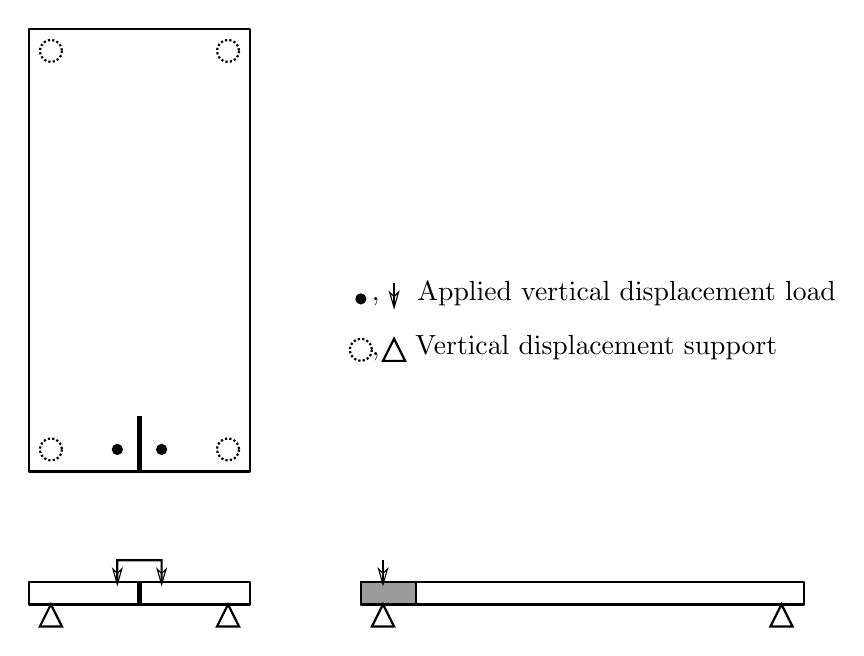
\begin{tikzpicture}[y=0.80pt, x=0.8pt,yscale=-1, inner sep=0pt, outer sep=0pt]
\begin{scope}[shift={(0,-552.36218)}]
  \path[shift={(0,552.36218)},draw=black,fill=black,line join=round,miter
    limit=4.00,fill opacity=0.000,nonzero rule,line width=0.800pt,rounded
    corners=0.0000cm] (50.0000,50.0000) rectangle (150.0000,250.0000);
  \path[shift={(0,552.36218)},draw=black,fill=black,dash pattern=on 0.80pt off
    0.80pt,line join=round,miter limit=4.00,fill opacity=0.000,nonzero rule,line
    width=0.800pt]
    (65.0000,60.0000)arc(0.000:180.000:5.000)arc(-180.000:0.000:5.000) -- cycle;
  \path[shift={(0,552.36218)},draw=black,fill=black,dash pattern=on 0.80pt off
    0.80pt,line join=round,miter limit=4.00,fill opacity=0.000,nonzero rule,line
    width=0.800pt]
    (145.0000,60.0000)arc(0.000:180.000:5.000)arc(-180.000:0.000:5.000) -- cycle;
  \path[shift={(80.0,732.36218)},draw=black,fill=black,dash pattern=on 0.80pt off
    0.80pt,line join=round,miter limit=4.00,fill opacity=0.000,nonzero rule,line
    width=0.800pt]
    (65.0000,60.0000)arc(0.000:180.000:5.000)arc(-180.000:0.000:5.000) -- cycle;
  \path[shift={(0,732.36218)},draw=black,fill=black,dash pattern=on 0.80pt off
    0.80pt,line join=round,miter limit=4.00,fill opacity=0.000,nonzero rule,line
    width=0.800pt]
    (65.0000,60.0000)arc(0.000:180.000:5.000)arc(-180.000:0.000:5.000) -- cycle;
  \path[shift={(0,552.36218)},draw=black,line join=miter,line cap=butt,miter
    limit=4.00,line width=1.600pt] (100.0000,250.0000) -- (100.0000,225.0000);
  \path[draw=black,fill=black,line join=round,miter limit=4.00,fill
    opacity=0.000,nonzero rule,line width=0.800pt,rounded corners=0.0000cm]
    (50.0000,852.3622) rectangle (150.0000,862.3622);
  \path[draw=black,line join=miter,line cap=butt,miter limit=4.00,line
    width=1.600pt] (100.0000,862.3622) -- (100.0000,852.3622);
  \path[draw=black,line join=miter,line cap=butt,line width=0.800pt]
    (55.0000,872.3622) -- (60.0000,862.3622) -- (65.0000,872.3622) -- cycle;
  \path[draw=black,line join=miter,line cap=butt,line width=0.800pt]
    (135.0000,872.3622) -- (140.0000,862.3622) -- (145.0000,872.3622) -- cycle;
    \path[color=black,fill=black,line width=0.800pt] (89.5000,841.8750) --
      (89.5000,842.3750) -- (89.5000,852.3750) -- (90.5000,852.3750) --
      (90.5000,842.8750) -- (109.5000,842.8750) -- (109.5000,852.3750) --
      (110.5000,852.3750) -- (110.5000,842.3750) -- (110.5000,841.8750) --
      (110.0000,841.8750) -- (90.0000,841.8750) -- (89.5000,841.8750) -- cycle;
    \path[draw=black,even odd rule,line width=0.400pt] (90.0000,848.3622) --
      (88.0000,846.3622) -- (90.0000,853.3622) -- (92.0000,846.3622) --
      (90.0000,848.3622) -- cycle;
    \path[draw=black,even odd rule,line width=0.400pt] (110.0000,848.3622) --
      (108.0000,846.3622) -- (110.0000,853.3622) -- (112.0000,846.3622) --
      (110.0000,848.3622) -- cycle;
  \path[shift={(0,552.36218)},draw=black,fill=black,line join=round,miter
    limit=4.00,fill opacity=0.000,nonzero rule,line width=0.800pt,rounded
    corners=0.0000cm] (200.0000,300.0000) rectangle (400.0000,310.0000);
  \path[draw=black,line join=miter,line cap=butt,line width=0.800pt]
    (385.0000,872.3622) -- (390.0000,862.3622) -- (395.0000,872.3622) -- cycle;
  \path[draw=black,line join=miter,line cap=butt,line width=0.800pt]
    (205.0000,872.3622) -- (210.0000,862.3622) -- (215.0000,872.3622) -- cycle;
    \path[color=black,fill=black,line width=0.800pt] (209.5000,842.3622) --
      (209.5000,852.3622) -- (210.5000,852.3622) -- (210.5000,842.3622) --
      (209.5000,842.3622) -- cycle;
    \path[draw=black,even odd rule,line width=0.400pt] (210.0000,848.3622) --
      (208.0000,846.3622) -- (210.0000,853.3622) -- (212.0000,846.3622) --
      (210.0000,848.3622) -- cycle;
  \path[shift={(0,552.36218)},draw=black,fill=black,line join=round,miter
    limit=4.00,fill opacity=0.392,nonzero rule,line width=0.800pt,rounded
    corners=0.0000cm] (200.0000,300.0000) rectangle (225.0000,310.0000);
  \path[shift={(0,552.36218)},draw=black,fill=black,line join=round,miter
    limit=4.00,nonzero rule,line width=0.800pt]
    (92.0000,240.0000)arc(0.000:180.000:2.000)arc(-180.000:0.000:2.000) -- cycle;
  \path[shift={(20.0,552.36218)},draw=black,fill=black,line join=round,miter
    limit=4.00,nonzero rule,line width=0.800pt]
    (92.0000,240.0000)arc(0.000:180.000:2.000)arc(-180.000:0.000:2.000) -- cycle;
  \path[shift={(110.0,484.36218)},draw=black,fill=black,line join=round,miter
    limit=4.00,nonzero rule,line width=0.800pt]
    (92.0000,240.0000)arc(0.000:180.000:2.000)arc(-180.000:0.000:2.000) -- cycle;
    \path[color=black,fill=black,line width=0.800pt] (214.5000,717.3750) --
      (214.5000,727.3750) -- (215.5000,727.3750) -- (215.5000,717.3750) --
      (214.5000,717.3750) -- cycle;
    \path[draw=black,even odd rule,line width=0.400pt] (215.0000,723.3622) --
      (213.0000,721.3622) -- (215.0000,728.3622) -- (217.0000,721.3622) --
      (215.0000,723.3622) -- cycle;
  \path[shift={(140.0,687.36218)},draw=black,fill=black,dash pattern=on 0.80pt off
    0.80pt,line join=round,miter limit=4.00,fill opacity=0.000,nonzero rule,line
    width=0.800pt]
    (65.0000,60.0000)arc(0.000:180.000:5.000)arc(-180.000:0.000:5.000) -- cycle;
  \path[fill=black] (205,727.36218) node[above right] (text6089) {,};
  \path[fill=black] (205,752.36218) node[above right] (text6093) {,};
  \path[draw=black,line join=miter,line cap=butt,line width=0.800pt]
    (210.0000,752.3622) -- (215.0000,742.3622) -- (220.0000,752.3622) -- cycle;
  \path[shift={(0,552.36218)},fill=black] (225.53571,175.17857) node[above right]
    (text6099) {Applied vertical displacement load};
  \path[shift={(0,552.36218)},fill=black] (224.64285,199.46429) node[above right]
    (text6103) {Vertical displacement support};
\end{scope}

\end{tikzpicture}


  \caption{Simple Double Torsion Setup}
  \label{fig:DTsetup}
\end{figure}
%

%
\begin{figure}[tbhp]
  \centering
  \resizebox{0.8\linewidth}{!}{\input{\plotpath/DoubleTorsionDD.pgf}}
  \caption{Crack Progression in Double Torsion Brittle Plate}
  \label{fig:DTdamage}
\end{figure}
%
In the double-torsion plate, the crack is expected to progress straight across the plate.
A more interesting failure pattern can be found if the displacement is applied to only one of the two sides of the pre-crack.
In a ``single torsion'' cracked plate, the crack path is expected to curve, and this result can be seen in \cref{fig:SingleTorsion}.
%
\begin{figure}[tbhp]
  \centering
  \resizebox{0.8\linewidth}{!}{\input{\plotpath/SingleTorsion.pgf}}
  \caption{Crack Progression in Single Torsion Brittle Plate}
  \label{fig:SingleTorsion}
\end{figure}
%

\FloatBarrier
\subsection{Irregular Discretization Results}
While it is simple to discretize the shapes examined thus far so that bonds pair up nicely, that is tougher to do for most shapes we are interested in analyzing.
To combine the analytical simplicity of the previous shapes with a demonstration of the ability to handle irregular shapes, we discretize simple shapes in an irregular fashion.
The first is a return to the simply-supported beam under uniform load.
\Cref{fig:BeamIrreg} shows that the irregularly-discretized beam has the same deflection under uniform load as the regular discretization.
%
\begin{figure}[tbhp]
  \centering
  \resizebox{0.6\linewidth}{!}{%% Creator: Matplotlib, PGF backend
%%
%% To include the figure in your LaTeX document, write
%%   \input{<filename>.pgf}
%%
%% Make sure the required packages are loaded in your preamble
%%   \usepackage{pgf}
%%
%% Figures using additional raster images can only be included by \input if
%% they are in the same directory as the main LaTeX file. For loading figures
%% from other directories you can use the `import` package
%%   \usepackage{import}
%% and then include the figures with
%%   \import{<path to file>}{<filename>.pgf}
%%
%% Matplotlib used the following preamble
%%
\begingroup%
\makeatletter%
\begin{pgfpicture}%
\pgfpathrectangle{\pgfpointorigin}{\pgfqpoint{6.000000in}{6.000000in}}%
\pgfusepath{use as bounding box}%
\begin{pgfscope}%
\pgfsetbuttcap%
\pgfsetroundjoin%
\definecolor{currentfill}{rgb}{1.000000,1.000000,1.000000}%
\pgfsetfillcolor{currentfill}%
\pgfsetlinewidth{0.000000pt}%
\definecolor{currentstroke}{rgb}{1.000000,1.000000,1.000000}%
\pgfsetstrokecolor{currentstroke}%
\pgfsetdash{}{0pt}%
\pgfpathmoveto{\pgfqpoint{0.000000in}{0.000000in}}%
\pgfpathlineto{\pgfqpoint{6.000000in}{0.000000in}}%
\pgfpathlineto{\pgfqpoint{6.000000in}{6.000000in}}%
\pgfpathlineto{\pgfqpoint{0.000000in}{6.000000in}}%
\pgfpathclose%
\pgfusepath{fill}%
\end{pgfscope}%
\begin{pgfscope}%
\pgfsetbuttcap%
\pgfsetroundjoin%
\definecolor{currentfill}{rgb}{1.000000,1.000000,1.000000}%
\pgfsetfillcolor{currentfill}%
\pgfsetlinewidth{0.000000pt}%
\definecolor{currentstroke}{rgb}{0.000000,0.000000,0.000000}%
\pgfsetstrokecolor{currentstroke}%
\pgfsetstrokeopacity{0.000000}%
\pgfsetdash{}{0pt}%
\pgfpathmoveto{\pgfqpoint{0.750000in}{0.600000in}}%
\pgfpathlineto{\pgfqpoint{5.400000in}{0.600000in}}%
\pgfpathlineto{\pgfqpoint{5.400000in}{5.400000in}}%
\pgfpathlineto{\pgfqpoint{0.750000in}{5.400000in}}%
\pgfpathclose%
\pgfusepath{fill}%
\end{pgfscope}%
\begin{pgfscope}%
\pgfpathrectangle{\pgfqpoint{0.750000in}{0.600000in}}{\pgfqpoint{4.650000in}{4.800000in}} %
\pgfusepath{clip}%
\pgfsetrectcap%
\pgfsetroundjoin%
\pgfsetlinewidth{1.003750pt}%
\definecolor{currentstroke}{rgb}{0.000000,0.000000,1.000000}%
\pgfsetstrokecolor{currentstroke}%
\pgfsetdash{}{0pt}%
\pgfpathmoveto{\pgfqpoint{0.750000in}{5.400000in}}%
\pgfpathlineto{\pgfqpoint{0.982500in}{4.689196in}}%
\pgfpathlineto{\pgfqpoint{1.098750in}{4.340173in}}%
\pgfpathlineto{\pgfqpoint{1.215000in}{3.998571in}}%
\pgfpathlineto{\pgfqpoint{1.308000in}{3.732123in}}%
\pgfpathlineto{\pgfqpoint{1.401000in}{3.472912in}}%
\pgfpathlineto{\pgfqpoint{1.470750in}{3.283865in}}%
\pgfpathlineto{\pgfqpoint{1.540500in}{3.099868in}}%
\pgfpathlineto{\pgfqpoint{1.610250in}{2.921313in}}%
\pgfpathlineto{\pgfqpoint{1.680000in}{2.748571in}}%
\pgfpathlineto{\pgfqpoint{1.749750in}{2.582000in}}%
\pgfpathlineto{\pgfqpoint{1.819500in}{2.421937in}}%
\pgfpathlineto{\pgfqpoint{1.889250in}{2.268704in}}%
\pgfpathlineto{\pgfqpoint{1.959000in}{2.122603in}}%
\pgfpathlineto{\pgfqpoint{2.005500in}{2.029308in}}%
\pgfpathlineto{\pgfqpoint{2.052000in}{1.939392in}}%
\pgfpathlineto{\pgfqpoint{2.098500in}{1.852931in}}%
\pgfpathlineto{\pgfqpoint{2.145000in}{1.770000in}}%
\pgfpathlineto{\pgfqpoint{2.191500in}{1.690668in}}%
\pgfpathlineto{\pgfqpoint{2.238000in}{1.615003in}}%
\pgfpathlineto{\pgfqpoint{2.284500in}{1.543068in}}%
\pgfpathlineto{\pgfqpoint{2.331000in}{1.474923in}}%
\pgfpathlineto{\pgfqpoint{2.377500in}{1.410625in}}%
\pgfpathlineto{\pgfqpoint{2.424000in}{1.350226in}}%
\pgfpathlineto{\pgfqpoint{2.470500in}{1.293777in}}%
\pgfpathlineto{\pgfqpoint{2.517000in}{1.241323in}}%
\pgfpathlineto{\pgfqpoint{2.563500in}{1.192908in}}%
\pgfpathlineto{\pgfqpoint{2.610000in}{1.148571in}}%
\pgfpathlineto{\pgfqpoint{2.656500in}{1.108348in}}%
\pgfpathlineto{\pgfqpoint{2.703000in}{1.072272in}}%
\pgfpathlineto{\pgfqpoint{2.749500in}{1.040371in}}%
\pgfpathlineto{\pgfqpoint{2.796000in}{1.012672in}}%
\pgfpathlineto{\pgfqpoint{2.842500in}{0.989196in}}%
\pgfpathlineto{\pgfqpoint{2.889000in}{0.969963in}}%
\pgfpathlineto{\pgfqpoint{2.935500in}{0.954988in}}%
\pgfpathlineto{\pgfqpoint{2.982000in}{0.944283in}}%
\pgfpathlineto{\pgfqpoint{3.028500in}{0.937857in}}%
\pgfpathlineto{\pgfqpoint{3.075000in}{0.935714in}}%
\pgfpathlineto{\pgfqpoint{3.121500in}{0.937857in}}%
\pgfpathlineto{\pgfqpoint{3.168000in}{0.944283in}}%
\pgfpathlineto{\pgfqpoint{3.214500in}{0.954988in}}%
\pgfpathlineto{\pgfqpoint{3.261000in}{0.969963in}}%
\pgfpathlineto{\pgfqpoint{3.307500in}{0.989196in}}%
\pgfpathlineto{\pgfqpoint{3.354000in}{1.012672in}}%
\pgfpathlineto{\pgfqpoint{3.400500in}{1.040371in}}%
\pgfpathlineto{\pgfqpoint{3.447000in}{1.072272in}}%
\pgfpathlineto{\pgfqpoint{3.493500in}{1.108348in}}%
\pgfpathlineto{\pgfqpoint{3.540000in}{1.148571in}}%
\pgfpathlineto{\pgfqpoint{3.586500in}{1.192908in}}%
\pgfpathlineto{\pgfqpoint{3.633000in}{1.241323in}}%
\pgfpathlineto{\pgfqpoint{3.679500in}{1.293777in}}%
\pgfpathlineto{\pgfqpoint{3.726000in}{1.350226in}}%
\pgfpathlineto{\pgfqpoint{3.772500in}{1.410625in}}%
\pgfpathlineto{\pgfqpoint{3.819000in}{1.474923in}}%
\pgfpathlineto{\pgfqpoint{3.865500in}{1.543068in}}%
\pgfpathlineto{\pgfqpoint{3.912000in}{1.615003in}}%
\pgfpathlineto{\pgfqpoint{3.958500in}{1.690668in}}%
\pgfpathlineto{\pgfqpoint{4.005000in}{1.770000in}}%
\pgfpathlineto{\pgfqpoint{4.051500in}{1.852931in}}%
\pgfpathlineto{\pgfqpoint{4.098000in}{1.939392in}}%
\pgfpathlineto{\pgfqpoint{4.144500in}{2.029308in}}%
\pgfpathlineto{\pgfqpoint{4.191000in}{2.122603in}}%
\pgfpathlineto{\pgfqpoint{4.260750in}{2.268704in}}%
\pgfpathlineto{\pgfqpoint{4.330500in}{2.421937in}}%
\pgfpathlineto{\pgfqpoint{4.400250in}{2.582000in}}%
\pgfpathlineto{\pgfqpoint{4.470000in}{2.748571in}}%
\pgfpathlineto{\pgfqpoint{4.539750in}{2.921313in}}%
\pgfpathlineto{\pgfqpoint{4.609500in}{3.099868in}}%
\pgfpathlineto{\pgfqpoint{4.679250in}{3.283865in}}%
\pgfpathlineto{\pgfqpoint{4.749000in}{3.472912in}}%
\pgfpathlineto{\pgfqpoint{4.842000in}{3.732123in}}%
\pgfpathlineto{\pgfqpoint{4.935000in}{3.998571in}}%
\pgfpathlineto{\pgfqpoint{5.028000in}{4.271186in}}%
\pgfpathlineto{\pgfqpoint{5.144250in}{4.618909in}}%
\pgfpathlineto{\pgfqpoint{5.283750in}{5.043298in}}%
\pgfpathlineto{\pgfqpoint{5.400000in}{5.400000in}}%
\pgfpathlineto{\pgfqpoint{5.400000in}{5.400000in}}%
\pgfusepath{stroke}%
\end{pgfscope}%
\begin{pgfscope}%
\pgfpathrectangle{\pgfqpoint{0.750000in}{0.600000in}}{\pgfqpoint{4.650000in}{4.800000in}} %
\pgfusepath{clip}%
\pgfsetbuttcap%
\pgfsetmiterjoin%
\definecolor{currentfill}{rgb}{0.000000,0.500000,0.000000}%
\pgfsetfillcolor{currentfill}%
\pgfsetlinewidth{0.501875pt}%
\definecolor{currentstroke}{rgb}{0.000000,0.000000,0.000000}%
\pgfsetstrokecolor{currentstroke}%
\pgfsetdash{}{0pt}%
\pgfsys@defobject{currentmarker}{\pgfqpoint{-0.041667in}{-0.041667in}}{\pgfqpoint{0.041667in}{0.041667in}}{%
\pgfpathmoveto{\pgfqpoint{0.000000in}{0.041667in}}%
\pgfpathlineto{\pgfqpoint{-0.041667in}{-0.041667in}}%
\pgfpathlineto{\pgfqpoint{0.041667in}{-0.041667in}}%
\pgfpathclose%
\pgfusepath{stroke,fill}%
}%
\begin{pgfscope}%
\pgfsys@transformshift{0.750000in}{5.400000in}%
\pgfsys@useobject{currentmarker}{}%
\end{pgfscope}%
\begin{pgfscope}%
\pgfsys@transformshift{0.843000in}{5.112844in}%
\pgfsys@useobject{currentmarker}{}%
\end{pgfscope}%
\begin{pgfscope}%
\pgfsys@transformshift{0.936000in}{4.827074in}%
\pgfsys@useobject{currentmarker}{}%
\end{pgfscope}%
\begin{pgfscope}%
\pgfsys@transformshift{1.029000in}{4.543952in}%
\pgfsys@useobject{currentmarker}{}%
\end{pgfscope}%
\begin{pgfscope}%
\pgfsys@transformshift{1.122000in}{4.264720in}%
\pgfsys@useobject{currentmarker}{}%
\end{pgfscope}%
\begin{pgfscope}%
\pgfsys@transformshift{1.215000in}{3.990565in}%
\pgfsys@useobject{currentmarker}{}%
\end{pgfscope}%
\begin{pgfscope}%
\pgfsys@transformshift{1.308000in}{3.722615in}%
\pgfsys@useobject{currentmarker}{}%
\end{pgfscope}%
\begin{pgfscope}%
\pgfsys@transformshift{1.401000in}{3.461947in}%
\pgfsys@useobject{currentmarker}{}%
\end{pgfscope}%
\begin{pgfscope}%
\pgfsys@transformshift{1.494000in}{3.209580in}%
\pgfsys@useobject{currentmarker}{}%
\end{pgfscope}%
\begin{pgfscope}%
\pgfsys@transformshift{1.587000in}{2.966480in}%
\pgfsys@useobject{currentmarker}{}%
\end{pgfscope}%
\begin{pgfscope}%
\pgfsys@transformshift{1.680000in}{2.733555in}%
\pgfsys@useobject{currentmarker}{}%
\end{pgfscope}%
\begin{pgfscope}%
\pgfsys@transformshift{1.773000in}{2.511660in}%
\pgfsys@useobject{currentmarker}{}%
\end{pgfscope}%
\begin{pgfscope}%
\pgfsys@transformshift{1.866000in}{2.301595in}%
\pgfsys@useobject{currentmarker}{}%
\end{pgfscope}%
\begin{pgfscope}%
\pgfsys@transformshift{1.959000in}{2.104104in}%
\pgfsys@useobject{currentmarker}{}%
\end{pgfscope}%
\begin{pgfscope}%
\pgfsys@transformshift{2.052000in}{1.919876in}%
\pgfsys@useobject{currentmarker}{}%
\end{pgfscope}%
\begin{pgfscope}%
\pgfsys@transformshift{2.145000in}{1.749545in}%
\pgfsys@useobject{currentmarker}{}%
\end{pgfscope}%
\begin{pgfscope}%
\pgfsys@transformshift{2.238000in}{1.593691in}%
\pgfsys@useobject{currentmarker}{}%
\end{pgfscope}%
\begin{pgfscope}%
\pgfsys@transformshift{2.331000in}{1.452836in}%
\pgfsys@useobject{currentmarker}{}%
\end{pgfscope}%
\begin{pgfscope}%
\pgfsys@transformshift{2.424000in}{1.327450in}%
\pgfsys@useobject{currentmarker}{}%
\end{pgfscope}%
\begin{pgfscope}%
\pgfsys@transformshift{2.517000in}{1.217946in}%
\pgfsys@useobject{currentmarker}{}%
\end{pgfscope}%
\begin{pgfscope}%
\pgfsys@transformshift{2.610000in}{1.124682in}%
\pgfsys@useobject{currentmarker}{}%
\end{pgfscope}%
\begin{pgfscope}%
\pgfsys@transformshift{2.703000in}{1.047961in}%
\pgfsys@useobject{currentmarker}{}%
\end{pgfscope}%
\begin{pgfscope}%
\pgfsys@transformshift{2.796000in}{0.988033in}%
\pgfsys@useobject{currentmarker}{}%
\end{pgfscope}%
\begin{pgfscope}%
\pgfsys@transformshift{2.889000in}{0.945089in}%
\pgfsys@useobject{currentmarker}{}%
\end{pgfscope}%
\begin{pgfscope}%
\pgfsys@transformshift{2.982000in}{0.919267in}%
\pgfsys@useobject{currentmarker}{}%
\end{pgfscope}%
\begin{pgfscope}%
\pgfsys@transformshift{3.075000in}{0.910651in}%
\pgfsys@useobject{currentmarker}{}%
\end{pgfscope}%
\begin{pgfscope}%
\pgfsys@transformshift{3.168000in}{0.919267in}%
\pgfsys@useobject{currentmarker}{}%
\end{pgfscope}%
\begin{pgfscope}%
\pgfsys@transformshift{3.261000in}{0.945089in}%
\pgfsys@useobject{currentmarker}{}%
\end{pgfscope}%
\begin{pgfscope}%
\pgfsys@transformshift{3.354000in}{0.988033in}%
\pgfsys@useobject{currentmarker}{}%
\end{pgfscope}%
\begin{pgfscope}%
\pgfsys@transformshift{3.447000in}{1.047961in}%
\pgfsys@useobject{currentmarker}{}%
\end{pgfscope}%
\begin{pgfscope}%
\pgfsys@transformshift{3.540000in}{1.124682in}%
\pgfsys@useobject{currentmarker}{}%
\end{pgfscope}%
\begin{pgfscope}%
\pgfsys@transformshift{3.633000in}{1.217946in}%
\pgfsys@useobject{currentmarker}{}%
\end{pgfscope}%
\begin{pgfscope}%
\pgfsys@transformshift{3.726000in}{1.327450in}%
\pgfsys@useobject{currentmarker}{}%
\end{pgfscope}%
\begin{pgfscope}%
\pgfsys@transformshift{3.819000in}{1.452836in}%
\pgfsys@useobject{currentmarker}{}%
\end{pgfscope}%
\begin{pgfscope}%
\pgfsys@transformshift{3.912000in}{1.593691in}%
\pgfsys@useobject{currentmarker}{}%
\end{pgfscope}%
\begin{pgfscope}%
\pgfsys@transformshift{4.005000in}{1.749545in}%
\pgfsys@useobject{currentmarker}{}%
\end{pgfscope}%
\begin{pgfscope}%
\pgfsys@transformshift{4.098000in}{1.919876in}%
\pgfsys@useobject{currentmarker}{}%
\end{pgfscope}%
\begin{pgfscope}%
\pgfsys@transformshift{4.191000in}{2.104104in}%
\pgfsys@useobject{currentmarker}{}%
\end{pgfscope}%
\begin{pgfscope}%
\pgfsys@transformshift{4.284000in}{2.301595in}%
\pgfsys@useobject{currentmarker}{}%
\end{pgfscope}%
\begin{pgfscope}%
\pgfsys@transformshift{4.377000in}{2.511660in}%
\pgfsys@useobject{currentmarker}{}%
\end{pgfscope}%
\begin{pgfscope}%
\pgfsys@transformshift{4.470000in}{2.733555in}%
\pgfsys@useobject{currentmarker}{}%
\end{pgfscope}%
\begin{pgfscope}%
\pgfsys@transformshift{4.563000in}{2.966480in}%
\pgfsys@useobject{currentmarker}{}%
\end{pgfscope}%
\begin{pgfscope}%
\pgfsys@transformshift{4.656000in}{3.209580in}%
\pgfsys@useobject{currentmarker}{}%
\end{pgfscope}%
\begin{pgfscope}%
\pgfsys@transformshift{4.749000in}{3.461947in}%
\pgfsys@useobject{currentmarker}{}%
\end{pgfscope}%
\begin{pgfscope}%
\pgfsys@transformshift{4.842000in}{3.722615in}%
\pgfsys@useobject{currentmarker}{}%
\end{pgfscope}%
\begin{pgfscope}%
\pgfsys@transformshift{4.935000in}{3.990565in}%
\pgfsys@useobject{currentmarker}{}%
\end{pgfscope}%
\begin{pgfscope}%
\pgfsys@transformshift{5.028000in}{4.264720in}%
\pgfsys@useobject{currentmarker}{}%
\end{pgfscope}%
\begin{pgfscope}%
\pgfsys@transformshift{5.121000in}{4.543952in}%
\pgfsys@useobject{currentmarker}{}%
\end{pgfscope}%
\begin{pgfscope}%
\pgfsys@transformshift{5.214000in}{4.827074in}%
\pgfsys@useobject{currentmarker}{}%
\end{pgfscope}%
\begin{pgfscope}%
\pgfsys@transformshift{5.307000in}{5.112844in}%
\pgfsys@useobject{currentmarker}{}%
\end{pgfscope}%
\begin{pgfscope}%
\pgfsys@transformshift{5.400000in}{5.400000in}%
\pgfsys@useobject{currentmarker}{}%
\end{pgfscope}%
\end{pgfscope}%
\begin{pgfscope}%
\pgfpathrectangle{\pgfqpoint{0.750000in}{0.600000in}}{\pgfqpoint{4.650000in}{4.800000in}} %
\pgfusepath{clip}%
\pgfsetbuttcap%
\pgfsetmiterjoin%
\definecolor{currentfill}{rgb}{1.000000,0.000000,0.000000}%
\pgfsetfillcolor{currentfill}%
\pgfsetlinewidth{0.501875pt}%
\definecolor{currentstroke}{rgb}{0.000000,0.000000,0.000000}%
\pgfsetstrokecolor{currentstroke}%
\pgfsetdash{}{0pt}%
\pgfsys@defobject{currentmarker}{\pgfqpoint{-0.041667in}{-0.041667in}}{\pgfqpoint{0.041667in}{0.041667in}}{%
\pgfpathmoveto{\pgfqpoint{-0.041667in}{-0.041667in}}%
\pgfpathlineto{\pgfqpoint{0.041667in}{-0.041667in}}%
\pgfpathlineto{\pgfqpoint{0.041667in}{0.041667in}}%
\pgfpathlineto{\pgfqpoint{-0.041667in}{0.041667in}}%
\pgfpathclose%
\pgfusepath{stroke,fill}%
}%
\begin{pgfscope}%
\pgfsys@transformshift{0.796563in}{5.257379in}%
\pgfsys@useobject{currentmarker}{}%
\end{pgfscope}%
\begin{pgfscope}%
\pgfsys@transformshift{0.889054in}{4.973141in}%
\pgfsys@useobject{currentmarker}{}%
\end{pgfscope}%
\begin{pgfscope}%
\pgfsys@transformshift{0.982945in}{4.686635in}%
\pgfsys@useobject{currentmarker}{}%
\end{pgfscope}%
\begin{pgfscope}%
\pgfsys@transformshift{1.075145in}{4.408525in}%
\pgfsys@useobject{currentmarker}{}%
\end{pgfscope}%
\begin{pgfscope}%
\pgfsys@transformshift{1.168520in}{4.131336in}%
\pgfsys@useobject{currentmarker}{}%
\end{pgfscope}%
\begin{pgfscope}%
\pgfsys@transformshift{1.261459in}{3.861078in}%
\pgfsys@useobject{currentmarker}{}%
\end{pgfscope}%
\begin{pgfscope}%
\pgfsys@transformshift{1.354604in}{3.596952in}%
\pgfsys@useobject{currentmarker}{}%
\end{pgfscope}%
\begin{pgfscope}%
\pgfsys@transformshift{1.447369in}{3.341685in}%
\pgfsys@useobject{currentmarker}{}%
\end{pgfscope}%
\begin{pgfscope}%
\pgfsys@transformshift{1.540655in}{3.093753in}%
\pgfsys@useobject{currentmarker}{}%
\end{pgfscope}%
\begin{pgfscope}%
\pgfsys@transformshift{1.633328in}{2.857095in}%
\pgfsys@useobject{currentmarker}{}%
\end{pgfscope}%
\begin{pgfscope}%
\pgfsys@transformshift{1.726954in}{2.628713in}%
\pgfsys@useobject{currentmarker}{}%
\end{pgfscope}%
\begin{pgfscope}%
\pgfsys@transformshift{1.819642in}{2.413967in}%
\pgfsys@useobject{currentmarker}{}%
\end{pgfscope}%
\begin{pgfscope}%
\pgfsys@transformshift{1.912183in}{2.211622in}%
\pgfsys@useobject{currentmarker}{}%
\end{pgfscope}%
\begin{pgfscope}%
\pgfsys@transformshift{2.005218in}{2.021055in}%
\pgfsys@useobject{currentmarker}{}%
\end{pgfscope}%
\begin{pgfscope}%
\pgfsys@transformshift{2.098814in}{1.843048in}%
\pgfsys@useobject{currentmarker}{}%
\end{pgfscope}%
\begin{pgfscope}%
\pgfsys@transformshift{2.191943in}{1.680152in}%
\pgfsys@useobject{currentmarker}{}%
\end{pgfscope}%
\begin{pgfscope}%
\pgfsys@transformshift{2.284298in}{1.533124in}%
\pgfsys@useobject{currentmarker}{}%
\end{pgfscope}%
\begin{pgfscope}%
\pgfsys@transformshift{2.377331in}{1.400113in}%
\pgfsys@useobject{currentmarker}{}%
\end{pgfscope}%
\begin{pgfscope}%
\pgfsys@transformshift{2.470562in}{1.282584in}%
\pgfsys@useobject{currentmarker}{}%
\end{pgfscope}%
\begin{pgfscope}%
\pgfsys@transformshift{2.563571in}{1.181363in}%
\pgfsys@useobject{currentmarker}{}%
\end{pgfscope}%
\begin{pgfscope}%
\pgfsys@transformshift{2.656158in}{1.096896in}%
\pgfsys@useobject{currentmarker}{}%
\end{pgfscope}%
\begin{pgfscope}%
\pgfsys@transformshift{2.749580in}{1.028314in}%
\pgfsys@useobject{currentmarker}{}%
\end{pgfscope}%
\begin{pgfscope}%
\pgfsys@transformshift{2.842665in}{0.976870in}%
\pgfsys@useobject{currentmarker}{}%
\end{pgfscope}%
\begin{pgfscope}%
\pgfsys@transformshift{2.935266in}{0.942640in}%
\pgfsys@useobject{currentmarker}{}%
\end{pgfscope}%
\begin{pgfscope}%
\pgfsys@transformshift{3.028242in}{0.925319in}%
\pgfsys@useobject{currentmarker}{}%
\end{pgfscope}%
\begin{pgfscope}%
\pgfsys@transformshift{3.121686in}{0.925245in}%
\pgfsys@useobject{currentmarker}{}%
\end{pgfscope}%
\begin{pgfscope}%
\pgfsys@transformshift{3.214854in}{0.942420in}%
\pgfsys@useobject{currentmarker}{}%
\end{pgfscope}%
\begin{pgfscope}%
\pgfsys@transformshift{3.307709in}{0.976672in}%
\pgfsys@useobject{currentmarker}{}%
\end{pgfscope}%
\begin{pgfscope}%
\pgfsys@transformshift{3.400429in}{1.027806in}%
\pgfsys@useobject{currentmarker}{}%
\end{pgfscope}%
\begin{pgfscope}%
\pgfsys@transformshift{3.493649in}{1.096038in}%
\pgfsys@useobject{currentmarker}{}%
\end{pgfscope}%
\begin{pgfscope}%
\pgfsys@transformshift{3.586161in}{1.180285in}%
\pgfsys@useobject{currentmarker}{}%
\end{pgfscope}%
\begin{pgfscope}%
\pgfsys@transformshift{3.679569in}{1.281783in}%
\pgfsys@useobject{currentmarker}{}%
\end{pgfscope}%
\begin{pgfscope}%
\pgfsys@transformshift{3.772869in}{1.399369in}%
\pgfsys@useobject{currentmarker}{}%
\end{pgfscope}%
\begin{pgfscope}%
\pgfsys@transformshift{3.865785in}{1.532107in}%
\pgfsys@useobject{currentmarker}{}%
\end{pgfscope}%
\begin{pgfscope}%
\pgfsys@transformshift{3.958699in}{1.680014in}%
\pgfsys@useobject{currentmarker}{}%
\end{pgfscope}%
\begin{pgfscope}%
\pgfsys@transformshift{4.051186in}{1.841807in}%
\pgfsys@useobject{currentmarker}{}%
\end{pgfscope}%
\begin{pgfscope}%
\pgfsys@transformshift{4.144786in}{2.019746in}%
\pgfsys@useobject{currentmarker}{}%
\end{pgfscope}%
\begin{pgfscope}%
\pgfsys@transformshift{4.237684in}{2.209913in}%
\pgfsys@useobject{currentmarker}{}%
\end{pgfscope}%
\begin{pgfscope}%
\pgfsys@transformshift{4.330942in}{2.413799in}%
\pgfsys@useobject{currentmarker}{}%
\end{pgfscope}%
\begin{pgfscope}%
\pgfsys@transformshift{4.423714in}{2.628742in}%
\pgfsys@useobject{currentmarker}{}%
\end{pgfscope}%
\begin{pgfscope}%
\pgfsys@transformshift{4.516221in}{2.854319in}%
\pgfsys@useobject{currentmarker}{}%
\end{pgfscope}%
\begin{pgfscope}%
\pgfsys@transformshift{4.609356in}{3.092017in}%
\pgfsys@useobject{currentmarker}{}%
\end{pgfscope}%
\begin{pgfscope}%
\pgfsys@transformshift{4.702188in}{3.338632in}%
\pgfsys@useobject{currentmarker}{}%
\end{pgfscope}%
\begin{pgfscope}%
\pgfsys@transformshift{4.795904in}{3.596450in}%
\pgfsys@useobject{currentmarker}{}%
\end{pgfscope}%
\begin{pgfscope}%
\pgfsys@transformshift{4.888714in}{3.859581in}%
\pgfsys@useobject{currentmarker}{}%
\end{pgfscope}%
\begin{pgfscope}%
\pgfsys@transformshift{4.981208in}{4.128466in}%
\pgfsys@useobject{currentmarker}{}%
\end{pgfscope}%
\begin{pgfscope}%
\pgfsys@transformshift{5.074246in}{4.404578in}%
\pgfsys@useobject{currentmarker}{}%
\end{pgfscope}%
\begin{pgfscope}%
\pgfsys@transformshift{5.167325in}{4.685283in}%
\pgfsys@useobject{currentmarker}{}%
\end{pgfscope}%
\begin{pgfscope}%
\pgfsys@transformshift{5.260058in}{4.968218in}%
\pgfsys@useobject{currentmarker}{}%
\end{pgfscope}%
\begin{pgfscope}%
\pgfsys@transformshift{5.353534in}{5.255445in}%
\pgfsys@useobject{currentmarker}{}%
\end{pgfscope}%
\end{pgfscope}%
\begin{pgfscope}%
\pgfpathrectangle{\pgfqpoint{0.750000in}{0.600000in}}{\pgfqpoint{4.650000in}{4.800000in}} %
\pgfusepath{clip}%
\pgfsetbuttcap%
\pgfsetroundjoin%
\pgfsetlinewidth{0.501875pt}%
\definecolor{currentstroke}{rgb}{0.000000,0.000000,0.000000}%
\pgfsetstrokecolor{currentstroke}%
\pgfsetdash{{1.000000pt}{3.000000pt}}{0.000000pt}%
\pgfpathmoveto{\pgfqpoint{0.750000in}{0.600000in}}%
\pgfpathlineto{\pgfqpoint{0.750000in}{5.400000in}}%
\pgfusepath{stroke}%
\end{pgfscope}%
\begin{pgfscope}%
\pgfsetbuttcap%
\pgfsetroundjoin%
\definecolor{currentfill}{rgb}{0.000000,0.000000,0.000000}%
\pgfsetfillcolor{currentfill}%
\pgfsetlinewidth{0.501875pt}%
\definecolor{currentstroke}{rgb}{0.000000,0.000000,0.000000}%
\pgfsetstrokecolor{currentstroke}%
\pgfsetdash{}{0pt}%
\pgfsys@defobject{currentmarker}{\pgfqpoint{0.000000in}{0.000000in}}{\pgfqpoint{0.000000in}{0.055556in}}{%
\pgfpathmoveto{\pgfqpoint{0.000000in}{0.000000in}}%
\pgfpathlineto{\pgfqpoint{0.000000in}{0.055556in}}%
\pgfusepath{stroke,fill}%
}%
\begin{pgfscope}%
\pgfsys@transformshift{0.750000in}{0.600000in}%
\pgfsys@useobject{currentmarker}{}%
\end{pgfscope}%
\end{pgfscope}%
\begin{pgfscope}%
\pgfsetbuttcap%
\pgfsetroundjoin%
\definecolor{currentfill}{rgb}{0.000000,0.000000,0.000000}%
\pgfsetfillcolor{currentfill}%
\pgfsetlinewidth{0.501875pt}%
\definecolor{currentstroke}{rgb}{0.000000,0.000000,0.000000}%
\pgfsetstrokecolor{currentstroke}%
\pgfsetdash{}{0pt}%
\pgfsys@defobject{currentmarker}{\pgfqpoint{0.000000in}{-0.055556in}}{\pgfqpoint{0.000000in}{0.000000in}}{%
\pgfpathmoveto{\pgfqpoint{0.000000in}{0.000000in}}%
\pgfpathlineto{\pgfqpoint{0.000000in}{-0.055556in}}%
\pgfusepath{stroke,fill}%
}%
\begin{pgfscope}%
\pgfsys@transformshift{0.750000in}{5.400000in}%
\pgfsys@useobject{currentmarker}{}%
\end{pgfscope}%
\end{pgfscope}%
\begin{pgfscope}%
\pgftext[x=0.750000in,y=0.544444in,,top]{{\rmfamily\fontsize{12.000000}{14.400000}\selectfont \(\displaystyle 0.00\)}}%
\end{pgfscope}%
\begin{pgfscope}%
\pgfpathrectangle{\pgfqpoint{0.750000in}{0.600000in}}{\pgfqpoint{4.650000in}{4.800000in}} %
\pgfusepath{clip}%
\pgfsetbuttcap%
\pgfsetroundjoin%
\pgfsetlinewidth{0.501875pt}%
\definecolor{currentstroke}{rgb}{0.000000,0.000000,0.000000}%
\pgfsetstrokecolor{currentstroke}%
\pgfsetdash{{1.000000pt}{3.000000pt}}{0.000000pt}%
\pgfpathmoveto{\pgfqpoint{1.912500in}{0.600000in}}%
\pgfpathlineto{\pgfqpoint{1.912500in}{5.400000in}}%
\pgfusepath{stroke}%
\end{pgfscope}%
\begin{pgfscope}%
\pgfsetbuttcap%
\pgfsetroundjoin%
\definecolor{currentfill}{rgb}{0.000000,0.000000,0.000000}%
\pgfsetfillcolor{currentfill}%
\pgfsetlinewidth{0.501875pt}%
\definecolor{currentstroke}{rgb}{0.000000,0.000000,0.000000}%
\pgfsetstrokecolor{currentstroke}%
\pgfsetdash{}{0pt}%
\pgfsys@defobject{currentmarker}{\pgfqpoint{0.000000in}{0.000000in}}{\pgfqpoint{0.000000in}{0.055556in}}{%
\pgfpathmoveto{\pgfqpoint{0.000000in}{0.000000in}}%
\pgfpathlineto{\pgfqpoint{0.000000in}{0.055556in}}%
\pgfusepath{stroke,fill}%
}%
\begin{pgfscope}%
\pgfsys@transformshift{1.912500in}{0.600000in}%
\pgfsys@useobject{currentmarker}{}%
\end{pgfscope}%
\end{pgfscope}%
\begin{pgfscope}%
\pgfsetbuttcap%
\pgfsetroundjoin%
\definecolor{currentfill}{rgb}{0.000000,0.000000,0.000000}%
\pgfsetfillcolor{currentfill}%
\pgfsetlinewidth{0.501875pt}%
\definecolor{currentstroke}{rgb}{0.000000,0.000000,0.000000}%
\pgfsetstrokecolor{currentstroke}%
\pgfsetdash{}{0pt}%
\pgfsys@defobject{currentmarker}{\pgfqpoint{0.000000in}{-0.055556in}}{\pgfqpoint{0.000000in}{0.000000in}}{%
\pgfpathmoveto{\pgfqpoint{0.000000in}{0.000000in}}%
\pgfpathlineto{\pgfqpoint{0.000000in}{-0.055556in}}%
\pgfusepath{stroke,fill}%
}%
\begin{pgfscope}%
\pgfsys@transformshift{1.912500in}{5.400000in}%
\pgfsys@useobject{currentmarker}{}%
\end{pgfscope}%
\end{pgfscope}%
\begin{pgfscope}%
\pgftext[x=1.912500in,y=0.544444in,,top]{{\rmfamily\fontsize{12.000000}{14.400000}\selectfont \(\displaystyle 0.25\)}}%
\end{pgfscope}%
\begin{pgfscope}%
\pgfpathrectangle{\pgfqpoint{0.750000in}{0.600000in}}{\pgfqpoint{4.650000in}{4.800000in}} %
\pgfusepath{clip}%
\pgfsetbuttcap%
\pgfsetroundjoin%
\pgfsetlinewidth{0.501875pt}%
\definecolor{currentstroke}{rgb}{0.000000,0.000000,0.000000}%
\pgfsetstrokecolor{currentstroke}%
\pgfsetdash{{1.000000pt}{3.000000pt}}{0.000000pt}%
\pgfpathmoveto{\pgfqpoint{3.075000in}{0.600000in}}%
\pgfpathlineto{\pgfqpoint{3.075000in}{5.400000in}}%
\pgfusepath{stroke}%
\end{pgfscope}%
\begin{pgfscope}%
\pgfsetbuttcap%
\pgfsetroundjoin%
\definecolor{currentfill}{rgb}{0.000000,0.000000,0.000000}%
\pgfsetfillcolor{currentfill}%
\pgfsetlinewidth{0.501875pt}%
\definecolor{currentstroke}{rgb}{0.000000,0.000000,0.000000}%
\pgfsetstrokecolor{currentstroke}%
\pgfsetdash{}{0pt}%
\pgfsys@defobject{currentmarker}{\pgfqpoint{0.000000in}{0.000000in}}{\pgfqpoint{0.000000in}{0.055556in}}{%
\pgfpathmoveto{\pgfqpoint{0.000000in}{0.000000in}}%
\pgfpathlineto{\pgfqpoint{0.000000in}{0.055556in}}%
\pgfusepath{stroke,fill}%
}%
\begin{pgfscope}%
\pgfsys@transformshift{3.075000in}{0.600000in}%
\pgfsys@useobject{currentmarker}{}%
\end{pgfscope}%
\end{pgfscope}%
\begin{pgfscope}%
\pgfsetbuttcap%
\pgfsetroundjoin%
\definecolor{currentfill}{rgb}{0.000000,0.000000,0.000000}%
\pgfsetfillcolor{currentfill}%
\pgfsetlinewidth{0.501875pt}%
\definecolor{currentstroke}{rgb}{0.000000,0.000000,0.000000}%
\pgfsetstrokecolor{currentstroke}%
\pgfsetdash{}{0pt}%
\pgfsys@defobject{currentmarker}{\pgfqpoint{0.000000in}{-0.055556in}}{\pgfqpoint{0.000000in}{0.000000in}}{%
\pgfpathmoveto{\pgfqpoint{0.000000in}{0.000000in}}%
\pgfpathlineto{\pgfqpoint{0.000000in}{-0.055556in}}%
\pgfusepath{stroke,fill}%
}%
\begin{pgfscope}%
\pgfsys@transformshift{3.075000in}{5.400000in}%
\pgfsys@useobject{currentmarker}{}%
\end{pgfscope}%
\end{pgfscope}%
\begin{pgfscope}%
\pgftext[x=3.075000in,y=0.544444in,,top]{{\rmfamily\fontsize{12.000000}{14.400000}\selectfont \(\displaystyle 0.50\)}}%
\end{pgfscope}%
\begin{pgfscope}%
\pgfpathrectangle{\pgfqpoint{0.750000in}{0.600000in}}{\pgfqpoint{4.650000in}{4.800000in}} %
\pgfusepath{clip}%
\pgfsetbuttcap%
\pgfsetroundjoin%
\pgfsetlinewidth{0.501875pt}%
\definecolor{currentstroke}{rgb}{0.000000,0.000000,0.000000}%
\pgfsetstrokecolor{currentstroke}%
\pgfsetdash{{1.000000pt}{3.000000pt}}{0.000000pt}%
\pgfpathmoveto{\pgfqpoint{4.237500in}{0.600000in}}%
\pgfpathlineto{\pgfqpoint{4.237500in}{5.400000in}}%
\pgfusepath{stroke}%
\end{pgfscope}%
\begin{pgfscope}%
\pgfsetbuttcap%
\pgfsetroundjoin%
\definecolor{currentfill}{rgb}{0.000000,0.000000,0.000000}%
\pgfsetfillcolor{currentfill}%
\pgfsetlinewidth{0.501875pt}%
\definecolor{currentstroke}{rgb}{0.000000,0.000000,0.000000}%
\pgfsetstrokecolor{currentstroke}%
\pgfsetdash{}{0pt}%
\pgfsys@defobject{currentmarker}{\pgfqpoint{0.000000in}{0.000000in}}{\pgfqpoint{0.000000in}{0.055556in}}{%
\pgfpathmoveto{\pgfqpoint{0.000000in}{0.000000in}}%
\pgfpathlineto{\pgfqpoint{0.000000in}{0.055556in}}%
\pgfusepath{stroke,fill}%
}%
\begin{pgfscope}%
\pgfsys@transformshift{4.237500in}{0.600000in}%
\pgfsys@useobject{currentmarker}{}%
\end{pgfscope}%
\end{pgfscope}%
\begin{pgfscope}%
\pgfsetbuttcap%
\pgfsetroundjoin%
\definecolor{currentfill}{rgb}{0.000000,0.000000,0.000000}%
\pgfsetfillcolor{currentfill}%
\pgfsetlinewidth{0.501875pt}%
\definecolor{currentstroke}{rgb}{0.000000,0.000000,0.000000}%
\pgfsetstrokecolor{currentstroke}%
\pgfsetdash{}{0pt}%
\pgfsys@defobject{currentmarker}{\pgfqpoint{0.000000in}{-0.055556in}}{\pgfqpoint{0.000000in}{0.000000in}}{%
\pgfpathmoveto{\pgfqpoint{0.000000in}{0.000000in}}%
\pgfpathlineto{\pgfqpoint{0.000000in}{-0.055556in}}%
\pgfusepath{stroke,fill}%
}%
\begin{pgfscope}%
\pgfsys@transformshift{4.237500in}{5.400000in}%
\pgfsys@useobject{currentmarker}{}%
\end{pgfscope}%
\end{pgfscope}%
\begin{pgfscope}%
\pgftext[x=4.237500in,y=0.544444in,,top]{{\rmfamily\fontsize{12.000000}{14.400000}\selectfont \(\displaystyle 0.75\)}}%
\end{pgfscope}%
\begin{pgfscope}%
\pgfpathrectangle{\pgfqpoint{0.750000in}{0.600000in}}{\pgfqpoint{4.650000in}{4.800000in}} %
\pgfusepath{clip}%
\pgfsetbuttcap%
\pgfsetroundjoin%
\pgfsetlinewidth{0.501875pt}%
\definecolor{currentstroke}{rgb}{0.000000,0.000000,0.000000}%
\pgfsetstrokecolor{currentstroke}%
\pgfsetdash{{1.000000pt}{3.000000pt}}{0.000000pt}%
\pgfpathmoveto{\pgfqpoint{5.400000in}{0.600000in}}%
\pgfpathlineto{\pgfqpoint{5.400000in}{5.400000in}}%
\pgfusepath{stroke}%
\end{pgfscope}%
\begin{pgfscope}%
\pgfsetbuttcap%
\pgfsetroundjoin%
\definecolor{currentfill}{rgb}{0.000000,0.000000,0.000000}%
\pgfsetfillcolor{currentfill}%
\pgfsetlinewidth{0.501875pt}%
\definecolor{currentstroke}{rgb}{0.000000,0.000000,0.000000}%
\pgfsetstrokecolor{currentstroke}%
\pgfsetdash{}{0pt}%
\pgfsys@defobject{currentmarker}{\pgfqpoint{0.000000in}{0.000000in}}{\pgfqpoint{0.000000in}{0.055556in}}{%
\pgfpathmoveto{\pgfqpoint{0.000000in}{0.000000in}}%
\pgfpathlineto{\pgfqpoint{0.000000in}{0.055556in}}%
\pgfusepath{stroke,fill}%
}%
\begin{pgfscope}%
\pgfsys@transformshift{5.400000in}{0.600000in}%
\pgfsys@useobject{currentmarker}{}%
\end{pgfscope}%
\end{pgfscope}%
\begin{pgfscope}%
\pgfsetbuttcap%
\pgfsetroundjoin%
\definecolor{currentfill}{rgb}{0.000000,0.000000,0.000000}%
\pgfsetfillcolor{currentfill}%
\pgfsetlinewidth{0.501875pt}%
\definecolor{currentstroke}{rgb}{0.000000,0.000000,0.000000}%
\pgfsetstrokecolor{currentstroke}%
\pgfsetdash{}{0pt}%
\pgfsys@defobject{currentmarker}{\pgfqpoint{0.000000in}{-0.055556in}}{\pgfqpoint{0.000000in}{0.000000in}}{%
\pgfpathmoveto{\pgfqpoint{0.000000in}{0.000000in}}%
\pgfpathlineto{\pgfqpoint{0.000000in}{-0.055556in}}%
\pgfusepath{stroke,fill}%
}%
\begin{pgfscope}%
\pgfsys@transformshift{5.400000in}{5.400000in}%
\pgfsys@useobject{currentmarker}{}%
\end{pgfscope}%
\end{pgfscope}%
\begin{pgfscope}%
\pgftext[x=5.400000in,y=0.544444in,,top]{{\rmfamily\fontsize{12.000000}{14.400000}\selectfont \(\displaystyle 1.00\)}}%
\end{pgfscope}%
\begin{pgfscope}%
\pgftext[x=3.075000in,y=0.326852in,,top]{{\rmfamily\fontsize{12.000000}{14.400000}\selectfont Distance Along Beam}}%
\end{pgfscope}%
\begin{pgfscope}%
\pgfpathrectangle{\pgfqpoint{0.750000in}{0.600000in}}{\pgfqpoint{4.650000in}{4.800000in}} %
\pgfusepath{clip}%
\pgfsetbuttcap%
\pgfsetroundjoin%
\pgfsetlinewidth{0.501875pt}%
\definecolor{currentstroke}{rgb}{0.000000,0.000000,0.000000}%
\pgfsetstrokecolor{currentstroke}%
\pgfsetdash{{1.000000pt}{3.000000pt}}{0.000000pt}%
\pgfpathmoveto{\pgfqpoint{0.750000in}{0.600000in}}%
\pgfpathlineto{\pgfqpoint{5.400000in}{0.600000in}}%
\pgfusepath{stroke}%
\end{pgfscope}%
\begin{pgfscope}%
\pgfsetbuttcap%
\pgfsetroundjoin%
\definecolor{currentfill}{rgb}{0.000000,0.000000,0.000000}%
\pgfsetfillcolor{currentfill}%
\pgfsetlinewidth{0.501875pt}%
\definecolor{currentstroke}{rgb}{0.000000,0.000000,0.000000}%
\pgfsetstrokecolor{currentstroke}%
\pgfsetdash{}{0pt}%
\pgfsys@defobject{currentmarker}{\pgfqpoint{0.000000in}{0.000000in}}{\pgfqpoint{0.055556in}{0.000000in}}{%
\pgfpathmoveto{\pgfqpoint{0.000000in}{0.000000in}}%
\pgfpathlineto{\pgfqpoint{0.055556in}{0.000000in}}%
\pgfusepath{stroke,fill}%
}%
\begin{pgfscope}%
\pgfsys@transformshift{0.750000in}{0.600000in}%
\pgfsys@useobject{currentmarker}{}%
\end{pgfscope}%
\end{pgfscope}%
\begin{pgfscope}%
\pgfsetbuttcap%
\pgfsetroundjoin%
\definecolor{currentfill}{rgb}{0.000000,0.000000,0.000000}%
\pgfsetfillcolor{currentfill}%
\pgfsetlinewidth{0.501875pt}%
\definecolor{currentstroke}{rgb}{0.000000,0.000000,0.000000}%
\pgfsetstrokecolor{currentstroke}%
\pgfsetdash{}{0pt}%
\pgfsys@defobject{currentmarker}{\pgfqpoint{-0.055556in}{0.000000in}}{\pgfqpoint{0.000000in}{0.000000in}}{%
\pgfpathmoveto{\pgfqpoint{0.000000in}{0.000000in}}%
\pgfpathlineto{\pgfqpoint{-0.055556in}{0.000000in}}%
\pgfusepath{stroke,fill}%
}%
\begin{pgfscope}%
\pgfsys@transformshift{5.400000in}{0.600000in}%
\pgfsys@useobject{currentmarker}{}%
\end{pgfscope}%
\end{pgfscope}%
\begin{pgfscope}%
\pgftext[x=0.694444in,y=0.600000in,right,]{{\rmfamily\fontsize{12.000000}{14.400000}\selectfont \(\displaystyle -1.4\)}}%
\end{pgfscope}%
\begin{pgfscope}%
\pgfpathrectangle{\pgfqpoint{0.750000in}{0.600000in}}{\pgfqpoint{4.650000in}{4.800000in}} %
\pgfusepath{clip}%
\pgfsetbuttcap%
\pgfsetroundjoin%
\pgfsetlinewidth{0.501875pt}%
\definecolor{currentstroke}{rgb}{0.000000,0.000000,0.000000}%
\pgfsetstrokecolor{currentstroke}%
\pgfsetdash{{1.000000pt}{3.000000pt}}{0.000000pt}%
\pgfpathmoveto{\pgfqpoint{0.750000in}{1.285714in}}%
\pgfpathlineto{\pgfqpoint{5.400000in}{1.285714in}}%
\pgfusepath{stroke}%
\end{pgfscope}%
\begin{pgfscope}%
\pgfsetbuttcap%
\pgfsetroundjoin%
\definecolor{currentfill}{rgb}{0.000000,0.000000,0.000000}%
\pgfsetfillcolor{currentfill}%
\pgfsetlinewidth{0.501875pt}%
\definecolor{currentstroke}{rgb}{0.000000,0.000000,0.000000}%
\pgfsetstrokecolor{currentstroke}%
\pgfsetdash{}{0pt}%
\pgfsys@defobject{currentmarker}{\pgfqpoint{0.000000in}{0.000000in}}{\pgfqpoint{0.055556in}{0.000000in}}{%
\pgfpathmoveto{\pgfqpoint{0.000000in}{0.000000in}}%
\pgfpathlineto{\pgfqpoint{0.055556in}{0.000000in}}%
\pgfusepath{stroke,fill}%
}%
\begin{pgfscope}%
\pgfsys@transformshift{0.750000in}{1.285714in}%
\pgfsys@useobject{currentmarker}{}%
\end{pgfscope}%
\end{pgfscope}%
\begin{pgfscope}%
\pgfsetbuttcap%
\pgfsetroundjoin%
\definecolor{currentfill}{rgb}{0.000000,0.000000,0.000000}%
\pgfsetfillcolor{currentfill}%
\pgfsetlinewidth{0.501875pt}%
\definecolor{currentstroke}{rgb}{0.000000,0.000000,0.000000}%
\pgfsetstrokecolor{currentstroke}%
\pgfsetdash{}{0pt}%
\pgfsys@defobject{currentmarker}{\pgfqpoint{-0.055556in}{0.000000in}}{\pgfqpoint{0.000000in}{0.000000in}}{%
\pgfpathmoveto{\pgfqpoint{0.000000in}{0.000000in}}%
\pgfpathlineto{\pgfqpoint{-0.055556in}{0.000000in}}%
\pgfusepath{stroke,fill}%
}%
\begin{pgfscope}%
\pgfsys@transformshift{5.400000in}{1.285714in}%
\pgfsys@useobject{currentmarker}{}%
\end{pgfscope}%
\end{pgfscope}%
\begin{pgfscope}%
\pgftext[x=0.694444in,y=1.285714in,right,]{{\rmfamily\fontsize{12.000000}{14.400000}\selectfont \(\displaystyle -1.2\)}}%
\end{pgfscope}%
\begin{pgfscope}%
\pgfpathrectangle{\pgfqpoint{0.750000in}{0.600000in}}{\pgfqpoint{4.650000in}{4.800000in}} %
\pgfusepath{clip}%
\pgfsetbuttcap%
\pgfsetroundjoin%
\pgfsetlinewidth{0.501875pt}%
\definecolor{currentstroke}{rgb}{0.000000,0.000000,0.000000}%
\pgfsetstrokecolor{currentstroke}%
\pgfsetdash{{1.000000pt}{3.000000pt}}{0.000000pt}%
\pgfpathmoveto{\pgfqpoint{0.750000in}{1.971429in}}%
\pgfpathlineto{\pgfqpoint{5.400000in}{1.971429in}}%
\pgfusepath{stroke}%
\end{pgfscope}%
\begin{pgfscope}%
\pgfsetbuttcap%
\pgfsetroundjoin%
\definecolor{currentfill}{rgb}{0.000000,0.000000,0.000000}%
\pgfsetfillcolor{currentfill}%
\pgfsetlinewidth{0.501875pt}%
\definecolor{currentstroke}{rgb}{0.000000,0.000000,0.000000}%
\pgfsetstrokecolor{currentstroke}%
\pgfsetdash{}{0pt}%
\pgfsys@defobject{currentmarker}{\pgfqpoint{0.000000in}{0.000000in}}{\pgfqpoint{0.055556in}{0.000000in}}{%
\pgfpathmoveto{\pgfqpoint{0.000000in}{0.000000in}}%
\pgfpathlineto{\pgfqpoint{0.055556in}{0.000000in}}%
\pgfusepath{stroke,fill}%
}%
\begin{pgfscope}%
\pgfsys@transformshift{0.750000in}{1.971429in}%
\pgfsys@useobject{currentmarker}{}%
\end{pgfscope}%
\end{pgfscope}%
\begin{pgfscope}%
\pgfsetbuttcap%
\pgfsetroundjoin%
\definecolor{currentfill}{rgb}{0.000000,0.000000,0.000000}%
\pgfsetfillcolor{currentfill}%
\pgfsetlinewidth{0.501875pt}%
\definecolor{currentstroke}{rgb}{0.000000,0.000000,0.000000}%
\pgfsetstrokecolor{currentstroke}%
\pgfsetdash{}{0pt}%
\pgfsys@defobject{currentmarker}{\pgfqpoint{-0.055556in}{0.000000in}}{\pgfqpoint{0.000000in}{0.000000in}}{%
\pgfpathmoveto{\pgfqpoint{0.000000in}{0.000000in}}%
\pgfpathlineto{\pgfqpoint{-0.055556in}{0.000000in}}%
\pgfusepath{stroke,fill}%
}%
\begin{pgfscope}%
\pgfsys@transformshift{5.400000in}{1.971429in}%
\pgfsys@useobject{currentmarker}{}%
\end{pgfscope}%
\end{pgfscope}%
\begin{pgfscope}%
\pgftext[x=0.694444in,y=1.971429in,right,]{{\rmfamily\fontsize{12.000000}{14.400000}\selectfont \(\displaystyle -1.0\)}}%
\end{pgfscope}%
\begin{pgfscope}%
\pgfpathrectangle{\pgfqpoint{0.750000in}{0.600000in}}{\pgfqpoint{4.650000in}{4.800000in}} %
\pgfusepath{clip}%
\pgfsetbuttcap%
\pgfsetroundjoin%
\pgfsetlinewidth{0.501875pt}%
\definecolor{currentstroke}{rgb}{0.000000,0.000000,0.000000}%
\pgfsetstrokecolor{currentstroke}%
\pgfsetdash{{1.000000pt}{3.000000pt}}{0.000000pt}%
\pgfpathmoveto{\pgfqpoint{0.750000in}{2.657143in}}%
\pgfpathlineto{\pgfqpoint{5.400000in}{2.657143in}}%
\pgfusepath{stroke}%
\end{pgfscope}%
\begin{pgfscope}%
\pgfsetbuttcap%
\pgfsetroundjoin%
\definecolor{currentfill}{rgb}{0.000000,0.000000,0.000000}%
\pgfsetfillcolor{currentfill}%
\pgfsetlinewidth{0.501875pt}%
\definecolor{currentstroke}{rgb}{0.000000,0.000000,0.000000}%
\pgfsetstrokecolor{currentstroke}%
\pgfsetdash{}{0pt}%
\pgfsys@defobject{currentmarker}{\pgfqpoint{0.000000in}{0.000000in}}{\pgfqpoint{0.055556in}{0.000000in}}{%
\pgfpathmoveto{\pgfqpoint{0.000000in}{0.000000in}}%
\pgfpathlineto{\pgfqpoint{0.055556in}{0.000000in}}%
\pgfusepath{stroke,fill}%
}%
\begin{pgfscope}%
\pgfsys@transformshift{0.750000in}{2.657143in}%
\pgfsys@useobject{currentmarker}{}%
\end{pgfscope}%
\end{pgfscope}%
\begin{pgfscope}%
\pgfsetbuttcap%
\pgfsetroundjoin%
\definecolor{currentfill}{rgb}{0.000000,0.000000,0.000000}%
\pgfsetfillcolor{currentfill}%
\pgfsetlinewidth{0.501875pt}%
\definecolor{currentstroke}{rgb}{0.000000,0.000000,0.000000}%
\pgfsetstrokecolor{currentstroke}%
\pgfsetdash{}{0pt}%
\pgfsys@defobject{currentmarker}{\pgfqpoint{-0.055556in}{0.000000in}}{\pgfqpoint{0.000000in}{0.000000in}}{%
\pgfpathmoveto{\pgfqpoint{0.000000in}{0.000000in}}%
\pgfpathlineto{\pgfqpoint{-0.055556in}{0.000000in}}%
\pgfusepath{stroke,fill}%
}%
\begin{pgfscope}%
\pgfsys@transformshift{5.400000in}{2.657143in}%
\pgfsys@useobject{currentmarker}{}%
\end{pgfscope}%
\end{pgfscope}%
\begin{pgfscope}%
\pgftext[x=0.694444in,y=2.657143in,right,]{{\rmfamily\fontsize{12.000000}{14.400000}\selectfont \(\displaystyle -0.8\)}}%
\end{pgfscope}%
\begin{pgfscope}%
\pgfpathrectangle{\pgfqpoint{0.750000in}{0.600000in}}{\pgfqpoint{4.650000in}{4.800000in}} %
\pgfusepath{clip}%
\pgfsetbuttcap%
\pgfsetroundjoin%
\pgfsetlinewidth{0.501875pt}%
\definecolor{currentstroke}{rgb}{0.000000,0.000000,0.000000}%
\pgfsetstrokecolor{currentstroke}%
\pgfsetdash{{1.000000pt}{3.000000pt}}{0.000000pt}%
\pgfpathmoveto{\pgfqpoint{0.750000in}{3.342857in}}%
\pgfpathlineto{\pgfqpoint{5.400000in}{3.342857in}}%
\pgfusepath{stroke}%
\end{pgfscope}%
\begin{pgfscope}%
\pgfsetbuttcap%
\pgfsetroundjoin%
\definecolor{currentfill}{rgb}{0.000000,0.000000,0.000000}%
\pgfsetfillcolor{currentfill}%
\pgfsetlinewidth{0.501875pt}%
\definecolor{currentstroke}{rgb}{0.000000,0.000000,0.000000}%
\pgfsetstrokecolor{currentstroke}%
\pgfsetdash{}{0pt}%
\pgfsys@defobject{currentmarker}{\pgfqpoint{0.000000in}{0.000000in}}{\pgfqpoint{0.055556in}{0.000000in}}{%
\pgfpathmoveto{\pgfqpoint{0.000000in}{0.000000in}}%
\pgfpathlineto{\pgfqpoint{0.055556in}{0.000000in}}%
\pgfusepath{stroke,fill}%
}%
\begin{pgfscope}%
\pgfsys@transformshift{0.750000in}{3.342857in}%
\pgfsys@useobject{currentmarker}{}%
\end{pgfscope}%
\end{pgfscope}%
\begin{pgfscope}%
\pgfsetbuttcap%
\pgfsetroundjoin%
\definecolor{currentfill}{rgb}{0.000000,0.000000,0.000000}%
\pgfsetfillcolor{currentfill}%
\pgfsetlinewidth{0.501875pt}%
\definecolor{currentstroke}{rgb}{0.000000,0.000000,0.000000}%
\pgfsetstrokecolor{currentstroke}%
\pgfsetdash{}{0pt}%
\pgfsys@defobject{currentmarker}{\pgfqpoint{-0.055556in}{0.000000in}}{\pgfqpoint{0.000000in}{0.000000in}}{%
\pgfpathmoveto{\pgfqpoint{0.000000in}{0.000000in}}%
\pgfpathlineto{\pgfqpoint{-0.055556in}{0.000000in}}%
\pgfusepath{stroke,fill}%
}%
\begin{pgfscope}%
\pgfsys@transformshift{5.400000in}{3.342857in}%
\pgfsys@useobject{currentmarker}{}%
\end{pgfscope}%
\end{pgfscope}%
\begin{pgfscope}%
\pgftext[x=0.694444in,y=3.342857in,right,]{{\rmfamily\fontsize{12.000000}{14.400000}\selectfont \(\displaystyle -0.6\)}}%
\end{pgfscope}%
\begin{pgfscope}%
\pgfpathrectangle{\pgfqpoint{0.750000in}{0.600000in}}{\pgfqpoint{4.650000in}{4.800000in}} %
\pgfusepath{clip}%
\pgfsetbuttcap%
\pgfsetroundjoin%
\pgfsetlinewidth{0.501875pt}%
\definecolor{currentstroke}{rgb}{0.000000,0.000000,0.000000}%
\pgfsetstrokecolor{currentstroke}%
\pgfsetdash{{1.000000pt}{3.000000pt}}{0.000000pt}%
\pgfpathmoveto{\pgfqpoint{0.750000in}{4.028571in}}%
\pgfpathlineto{\pgfqpoint{5.400000in}{4.028571in}}%
\pgfusepath{stroke}%
\end{pgfscope}%
\begin{pgfscope}%
\pgfsetbuttcap%
\pgfsetroundjoin%
\definecolor{currentfill}{rgb}{0.000000,0.000000,0.000000}%
\pgfsetfillcolor{currentfill}%
\pgfsetlinewidth{0.501875pt}%
\definecolor{currentstroke}{rgb}{0.000000,0.000000,0.000000}%
\pgfsetstrokecolor{currentstroke}%
\pgfsetdash{}{0pt}%
\pgfsys@defobject{currentmarker}{\pgfqpoint{0.000000in}{0.000000in}}{\pgfqpoint{0.055556in}{0.000000in}}{%
\pgfpathmoveto{\pgfqpoint{0.000000in}{0.000000in}}%
\pgfpathlineto{\pgfqpoint{0.055556in}{0.000000in}}%
\pgfusepath{stroke,fill}%
}%
\begin{pgfscope}%
\pgfsys@transformshift{0.750000in}{4.028571in}%
\pgfsys@useobject{currentmarker}{}%
\end{pgfscope}%
\end{pgfscope}%
\begin{pgfscope}%
\pgfsetbuttcap%
\pgfsetroundjoin%
\definecolor{currentfill}{rgb}{0.000000,0.000000,0.000000}%
\pgfsetfillcolor{currentfill}%
\pgfsetlinewidth{0.501875pt}%
\definecolor{currentstroke}{rgb}{0.000000,0.000000,0.000000}%
\pgfsetstrokecolor{currentstroke}%
\pgfsetdash{}{0pt}%
\pgfsys@defobject{currentmarker}{\pgfqpoint{-0.055556in}{0.000000in}}{\pgfqpoint{0.000000in}{0.000000in}}{%
\pgfpathmoveto{\pgfqpoint{0.000000in}{0.000000in}}%
\pgfpathlineto{\pgfqpoint{-0.055556in}{0.000000in}}%
\pgfusepath{stroke,fill}%
}%
\begin{pgfscope}%
\pgfsys@transformshift{5.400000in}{4.028571in}%
\pgfsys@useobject{currentmarker}{}%
\end{pgfscope}%
\end{pgfscope}%
\begin{pgfscope}%
\pgftext[x=0.694444in,y=4.028571in,right,]{{\rmfamily\fontsize{12.000000}{14.400000}\selectfont \(\displaystyle -0.4\)}}%
\end{pgfscope}%
\begin{pgfscope}%
\pgfpathrectangle{\pgfqpoint{0.750000in}{0.600000in}}{\pgfqpoint{4.650000in}{4.800000in}} %
\pgfusepath{clip}%
\pgfsetbuttcap%
\pgfsetroundjoin%
\pgfsetlinewidth{0.501875pt}%
\definecolor{currentstroke}{rgb}{0.000000,0.000000,0.000000}%
\pgfsetstrokecolor{currentstroke}%
\pgfsetdash{{1.000000pt}{3.000000pt}}{0.000000pt}%
\pgfpathmoveto{\pgfqpoint{0.750000in}{4.714286in}}%
\pgfpathlineto{\pgfqpoint{5.400000in}{4.714286in}}%
\pgfusepath{stroke}%
\end{pgfscope}%
\begin{pgfscope}%
\pgfsetbuttcap%
\pgfsetroundjoin%
\definecolor{currentfill}{rgb}{0.000000,0.000000,0.000000}%
\pgfsetfillcolor{currentfill}%
\pgfsetlinewidth{0.501875pt}%
\definecolor{currentstroke}{rgb}{0.000000,0.000000,0.000000}%
\pgfsetstrokecolor{currentstroke}%
\pgfsetdash{}{0pt}%
\pgfsys@defobject{currentmarker}{\pgfqpoint{0.000000in}{0.000000in}}{\pgfqpoint{0.055556in}{0.000000in}}{%
\pgfpathmoveto{\pgfqpoint{0.000000in}{0.000000in}}%
\pgfpathlineto{\pgfqpoint{0.055556in}{0.000000in}}%
\pgfusepath{stroke,fill}%
}%
\begin{pgfscope}%
\pgfsys@transformshift{0.750000in}{4.714286in}%
\pgfsys@useobject{currentmarker}{}%
\end{pgfscope}%
\end{pgfscope}%
\begin{pgfscope}%
\pgfsetbuttcap%
\pgfsetroundjoin%
\definecolor{currentfill}{rgb}{0.000000,0.000000,0.000000}%
\pgfsetfillcolor{currentfill}%
\pgfsetlinewidth{0.501875pt}%
\definecolor{currentstroke}{rgb}{0.000000,0.000000,0.000000}%
\pgfsetstrokecolor{currentstroke}%
\pgfsetdash{}{0pt}%
\pgfsys@defobject{currentmarker}{\pgfqpoint{-0.055556in}{0.000000in}}{\pgfqpoint{0.000000in}{0.000000in}}{%
\pgfpathmoveto{\pgfqpoint{0.000000in}{0.000000in}}%
\pgfpathlineto{\pgfqpoint{-0.055556in}{0.000000in}}%
\pgfusepath{stroke,fill}%
}%
\begin{pgfscope}%
\pgfsys@transformshift{5.400000in}{4.714286in}%
\pgfsys@useobject{currentmarker}{}%
\end{pgfscope}%
\end{pgfscope}%
\begin{pgfscope}%
\pgftext[x=0.694444in,y=4.714286in,right,]{{\rmfamily\fontsize{12.000000}{14.400000}\selectfont \(\displaystyle -0.2\)}}%
\end{pgfscope}%
\begin{pgfscope}%
\pgfpathrectangle{\pgfqpoint{0.750000in}{0.600000in}}{\pgfqpoint{4.650000in}{4.800000in}} %
\pgfusepath{clip}%
\pgfsetbuttcap%
\pgfsetroundjoin%
\pgfsetlinewidth{0.501875pt}%
\definecolor{currentstroke}{rgb}{0.000000,0.000000,0.000000}%
\pgfsetstrokecolor{currentstroke}%
\pgfsetdash{{1.000000pt}{3.000000pt}}{0.000000pt}%
\pgfpathmoveto{\pgfqpoint{0.750000in}{5.400000in}}%
\pgfpathlineto{\pgfqpoint{5.400000in}{5.400000in}}%
\pgfusepath{stroke}%
\end{pgfscope}%
\begin{pgfscope}%
\pgfsetbuttcap%
\pgfsetroundjoin%
\definecolor{currentfill}{rgb}{0.000000,0.000000,0.000000}%
\pgfsetfillcolor{currentfill}%
\pgfsetlinewidth{0.501875pt}%
\definecolor{currentstroke}{rgb}{0.000000,0.000000,0.000000}%
\pgfsetstrokecolor{currentstroke}%
\pgfsetdash{}{0pt}%
\pgfsys@defobject{currentmarker}{\pgfqpoint{0.000000in}{0.000000in}}{\pgfqpoint{0.055556in}{0.000000in}}{%
\pgfpathmoveto{\pgfqpoint{0.000000in}{0.000000in}}%
\pgfpathlineto{\pgfqpoint{0.055556in}{0.000000in}}%
\pgfusepath{stroke,fill}%
}%
\begin{pgfscope}%
\pgfsys@transformshift{0.750000in}{5.400000in}%
\pgfsys@useobject{currentmarker}{}%
\end{pgfscope}%
\end{pgfscope}%
\begin{pgfscope}%
\pgfsetbuttcap%
\pgfsetroundjoin%
\definecolor{currentfill}{rgb}{0.000000,0.000000,0.000000}%
\pgfsetfillcolor{currentfill}%
\pgfsetlinewidth{0.501875pt}%
\definecolor{currentstroke}{rgb}{0.000000,0.000000,0.000000}%
\pgfsetstrokecolor{currentstroke}%
\pgfsetdash{}{0pt}%
\pgfsys@defobject{currentmarker}{\pgfqpoint{-0.055556in}{0.000000in}}{\pgfqpoint{0.000000in}{0.000000in}}{%
\pgfpathmoveto{\pgfqpoint{0.000000in}{0.000000in}}%
\pgfpathlineto{\pgfqpoint{-0.055556in}{0.000000in}}%
\pgfusepath{stroke,fill}%
}%
\begin{pgfscope}%
\pgfsys@transformshift{5.400000in}{5.400000in}%
\pgfsys@useobject{currentmarker}{}%
\end{pgfscope}%
\end{pgfscope}%
\begin{pgfscope}%
\pgftext[x=0.694444in,y=5.400000in,right,]{{\rmfamily\fontsize{12.000000}{14.400000}\selectfont \(\displaystyle 0.0\)}}%
\end{pgfscope}%
\begin{pgfscope}%
\pgftext[x=0.286846in,y=3.000000in,,bottom,rotate=90.000000]{{\rmfamily\fontsize{12.000000}{14.400000}\selectfont Deflection Under Uniform Load}}%
\end{pgfscope}%
\begin{pgfscope}%
\pgftext[x=0.750000in,y=5.441667in,left,base]{{\rmfamily\fontsize{12.000000}{14.400000}\selectfont \(\displaystyle \times10^{-5}\)}}%
\end{pgfscope}%
\begin{pgfscope}%
\pgfsetbuttcap%
\pgfsetroundjoin%
\pgfsetlinewidth{1.003750pt}%
\definecolor{currentstroke}{rgb}{0.000000,0.000000,0.000000}%
\pgfsetstrokecolor{currentstroke}%
\pgfsetdash{}{0pt}%
\pgfpathmoveto{\pgfqpoint{0.750000in}{5.400000in}}%
\pgfpathlineto{\pgfqpoint{5.400000in}{5.400000in}}%
\pgfusepath{stroke}%
\end{pgfscope}%
\begin{pgfscope}%
\pgfsetbuttcap%
\pgfsetroundjoin%
\pgfsetlinewidth{1.003750pt}%
\definecolor{currentstroke}{rgb}{0.000000,0.000000,0.000000}%
\pgfsetstrokecolor{currentstroke}%
\pgfsetdash{}{0pt}%
\pgfpathmoveto{\pgfqpoint{5.400000in}{0.600000in}}%
\pgfpathlineto{\pgfqpoint{5.400000in}{5.400000in}}%
\pgfusepath{stroke}%
\end{pgfscope}%
\begin{pgfscope}%
\pgfsetbuttcap%
\pgfsetroundjoin%
\pgfsetlinewidth{1.003750pt}%
\definecolor{currentstroke}{rgb}{0.000000,0.000000,0.000000}%
\pgfsetstrokecolor{currentstroke}%
\pgfsetdash{}{0pt}%
\pgfpathmoveto{\pgfqpoint{0.750000in}{0.600000in}}%
\pgfpathlineto{\pgfqpoint{5.400000in}{0.600000in}}%
\pgfusepath{stroke}%
\end{pgfscope}%
\begin{pgfscope}%
\pgfsetbuttcap%
\pgfsetroundjoin%
\pgfsetlinewidth{1.003750pt}%
\definecolor{currentstroke}{rgb}{0.000000,0.000000,0.000000}%
\pgfsetstrokecolor{currentstroke}%
\pgfsetdash{}{0pt}%
\pgfpathmoveto{\pgfqpoint{0.750000in}{0.600000in}}%
\pgfpathlineto{\pgfqpoint{0.750000in}{5.400000in}}%
\pgfusepath{stroke}%
\end{pgfscope}%
\begin{pgfscope}%
\pgftext[x=3.075000in,y=5.469444in,,base]{{\rmfamily\fontsize{14.400000}{17.280000}\selectfont Uniformly Loaded Beam}}%
\end{pgfscope}%
\begin{pgfscope}%
\pgfsetbuttcap%
\pgfsetroundjoin%
\definecolor{currentfill}{rgb}{1.000000,1.000000,1.000000}%
\pgfsetfillcolor{currentfill}%
\pgfsetlinewidth{1.003750pt}%
\definecolor{currentstroke}{rgb}{0.000000,0.000000,0.000000}%
\pgfsetstrokecolor{currentstroke}%
\pgfsetdash{}{0pt}%
\pgfpathmoveto{\pgfqpoint{3.452377in}{4.483334in}}%
\pgfpathlineto{\pgfqpoint{5.380000in}{4.483334in}}%
\pgfpathlineto{\pgfqpoint{5.380000in}{5.380000in}}%
\pgfpathlineto{\pgfqpoint{3.452377in}{5.380000in}}%
\pgfpathlineto{\pgfqpoint{3.452377in}{4.483334in}}%
\pgfpathclose%
\pgfusepath{stroke,fill}%
\end{pgfscope}%
\begin{pgfscope}%
\pgfsetrectcap%
\pgfsetroundjoin%
\pgfsetlinewidth{1.003750pt}%
\definecolor{currentstroke}{rgb}{0.000000,0.000000,1.000000}%
\pgfsetstrokecolor{currentstroke}%
\pgfsetdash{}{0pt}%
\pgfpathmoveto{\pgfqpoint{3.592377in}{5.230000in}}%
\pgfpathlineto{\pgfqpoint{3.872377in}{5.230000in}}%
\pgfusepath{stroke}%
\end{pgfscope}%
\begin{pgfscope}%
\pgftext[x=4.092377in,y=5.160000in,left,base]{{\rmfamily\fontsize{14.400000}{17.280000}\selectfont Analytical}}%
\end{pgfscope}%
\begin{pgfscope}%
\pgfsetbuttcap%
\pgfsetmiterjoin%
\definecolor{currentfill}{rgb}{0.000000,0.500000,0.000000}%
\pgfsetfillcolor{currentfill}%
\pgfsetlinewidth{0.501875pt}%
\definecolor{currentstroke}{rgb}{0.000000,0.000000,0.000000}%
\pgfsetstrokecolor{currentstroke}%
\pgfsetdash{}{0pt}%
\pgfsys@defobject{currentmarker}{\pgfqpoint{-0.041667in}{-0.041667in}}{\pgfqpoint{0.041667in}{0.041667in}}{%
\pgfpathmoveto{\pgfqpoint{0.000000in}{0.041667in}}%
\pgfpathlineto{\pgfqpoint{-0.041667in}{-0.041667in}}%
\pgfpathlineto{\pgfqpoint{0.041667in}{-0.041667in}}%
\pgfpathclose%
\pgfusepath{stroke,fill}%
}%
\begin{pgfscope}%
\pgfsys@transformshift{3.592377in}{4.951111in}%
\pgfsys@useobject{currentmarker}{}%
\end{pgfscope}%
\begin{pgfscope}%
\pgfsys@transformshift{3.872377in}{4.951111in}%
\pgfsys@useobject{currentmarker}{}%
\end{pgfscope}%
\end{pgfscope}%
\begin{pgfscope}%
\pgftext[x=4.092377in,y=4.881111in,left,base]{{\rmfamily\fontsize{14.400000}{17.280000}\selectfont regular error}}%
\end{pgfscope}%
\begin{pgfscope}%
\pgfsetbuttcap%
\pgfsetmiterjoin%
\definecolor{currentfill}{rgb}{1.000000,0.000000,0.000000}%
\pgfsetfillcolor{currentfill}%
\pgfsetlinewidth{0.501875pt}%
\definecolor{currentstroke}{rgb}{0.000000,0.000000,0.000000}%
\pgfsetstrokecolor{currentstroke}%
\pgfsetdash{}{0pt}%
\pgfsys@defobject{currentmarker}{\pgfqpoint{-0.041667in}{-0.041667in}}{\pgfqpoint{0.041667in}{0.041667in}}{%
\pgfpathmoveto{\pgfqpoint{-0.041667in}{-0.041667in}}%
\pgfpathlineto{\pgfqpoint{0.041667in}{-0.041667in}}%
\pgfpathlineto{\pgfqpoint{0.041667in}{0.041667in}}%
\pgfpathlineto{\pgfqpoint{-0.041667in}{0.041667in}}%
\pgfpathclose%
\pgfusepath{stroke,fill}%
}%
\begin{pgfscope}%
\pgfsys@transformshift{3.592377in}{4.672223in}%
\pgfsys@useobject{currentmarker}{}%
\end{pgfscope}%
\begin{pgfscope}%
\pgfsys@transformshift{3.872377in}{4.672223in}%
\pgfsys@useobject{currentmarker}{}%
\end{pgfscope}%
\end{pgfscope}%
\begin{pgfscope}%
\pgftext[x=4.092377in,y=4.602223in,left,base]{{\rmfamily\fontsize{14.400000}{17.280000}\selectfont irregular error}}%
\end{pgfscope}%
\end{pgfpicture}%
\makeatother%
\endgroup%
}
  \caption{Irregular Beam}
  \label{fig:BeamIrreg}
\end{figure}
%

An example of a regularly-discretized plate is shown in \cref{fig:regularmesh}, while an irregularly discretized plate is shown in \cref{fig:unevenmesh}.
To use this plate in a peridynamic simulation, we reduce each element to a single node at the element's centroid with volume equal to the volume of the element. 
%
\begin{figure}[h]
  \centering
  \resizebox{0.6\linewidth}{!}{%% Creator: Matplotlib, PGF backend
%%
%% To include the figure in your LaTeX document, write
%%   \input{<filename>.pgf}
%%
%% Make sure the required packages are loaded in your preamble
%%   \usepackage{pgf}
%%
%% Figures using additional raster images can only be included by \input if
%% they are in the same directory as the main LaTeX file. For loading figures
%% from other directories you can use the `import` package
%%   \usepackage{import}
%% and then include the figures with
%%   \import{<path to file>}{<filename>.pgf}
%%
%% Matplotlib used the following preamble
%%
\begingroup%
\makeatletter%
\begin{pgfpicture}%
\pgfpathrectangle{\pgfpointorigin}{\pgfqpoint{5.000000in}{5.000000in}}%
\pgfusepath{use as bounding box}%
\begin{pgfscope}%
\pgfsetbuttcap%
\pgfsetroundjoin%
\definecolor{currentfill}{rgb}{1.000000,1.000000,1.000000}%
\pgfsetfillcolor{currentfill}%
\pgfsetlinewidth{0.000000pt}%
\definecolor{currentstroke}{rgb}{1.000000,1.000000,1.000000}%
\pgfsetstrokecolor{currentstroke}%
\pgfsetdash{}{0pt}%
\pgfpathmoveto{\pgfqpoint{0.000000in}{0.000000in}}%
\pgfpathlineto{\pgfqpoint{5.000000in}{0.000000in}}%
\pgfpathlineto{\pgfqpoint{5.000000in}{5.000000in}}%
\pgfpathlineto{\pgfqpoint{0.000000in}{5.000000in}}%
\pgfpathclose%
\pgfusepath{fill}%
\end{pgfscope}%
\begin{pgfscope}%
\pgfpathrectangle{\pgfqpoint{0.625000in}{0.562500in}}{\pgfqpoint{3.875000in}{3.875000in}} %
\pgfusepath{clip}%
\pgfsetbuttcap%
\pgfsetroundjoin%
\definecolor{currentfill}{rgb}{0.000000,0.000000,1.000000}%
\pgfsetfillcolor{currentfill}%
\pgfsetlinewidth{1.003750pt}%
\definecolor{currentstroke}{rgb}{0.000000,0.000000,0.000000}%
\pgfsetstrokecolor{currentstroke}%
\pgfsetdash{}{0pt}%
\pgfpathmoveto{\pgfqpoint{0.663750in}{0.581608in}}%
\pgfpathcurveto{\pgfqpoint{0.668959in}{0.581608in}}{\pgfqpoint{0.673956in}{0.583678in}}{\pgfqpoint{0.677639in}{0.587361in}}%
\pgfpathcurveto{\pgfqpoint{0.681322in}{0.591044in}}{\pgfqpoint{0.683392in}{0.596041in}}{\pgfqpoint{0.683392in}{0.601250in}}%
\pgfpathcurveto{\pgfqpoint{0.683392in}{0.606459in}}{\pgfqpoint{0.681322in}{0.611456in}}{\pgfqpoint{0.677639in}{0.615139in}}%
\pgfpathcurveto{\pgfqpoint{0.673956in}{0.618822in}}{\pgfqpoint{0.668959in}{0.620892in}}{\pgfqpoint{0.663750in}{0.620892in}}%
\pgfpathcurveto{\pgfqpoint{0.658541in}{0.620892in}}{\pgfqpoint{0.653544in}{0.618822in}}{\pgfqpoint{0.649861in}{0.615139in}}%
\pgfpathcurveto{\pgfqpoint{0.646178in}{0.611456in}}{\pgfqpoint{0.644108in}{0.606459in}}{\pgfqpoint{0.644108in}{0.601250in}}%
\pgfpathcurveto{\pgfqpoint{0.644108in}{0.596041in}}{\pgfqpoint{0.646178in}{0.591044in}}{\pgfqpoint{0.649861in}{0.587361in}}%
\pgfpathcurveto{\pgfqpoint{0.653544in}{0.583678in}}{\pgfqpoint{0.658541in}{0.581608in}}{\pgfqpoint{0.663750in}{0.581608in}}%
\pgfpathclose%
\pgfusepath{stroke,fill}%
\end{pgfscope}%
\begin{pgfscope}%
\pgfpathrectangle{\pgfqpoint{0.625000in}{0.562500in}}{\pgfqpoint{3.875000in}{3.875000in}} %
\pgfusepath{clip}%
\pgfsetbuttcap%
\pgfsetroundjoin%
\definecolor{currentfill}{rgb}{0.000000,0.000000,1.000000}%
\pgfsetfillcolor{currentfill}%
\pgfsetlinewidth{1.003750pt}%
\definecolor{currentstroke}{rgb}{0.000000,0.000000,0.000000}%
\pgfsetstrokecolor{currentstroke}%
\pgfsetdash{}{0pt}%
\pgfpathmoveto{\pgfqpoint{0.663750in}{0.659108in}}%
\pgfpathcurveto{\pgfqpoint{0.668959in}{0.659108in}}{\pgfqpoint{0.673956in}{0.661178in}}{\pgfqpoint{0.677639in}{0.664861in}}%
\pgfpathcurveto{\pgfqpoint{0.681322in}{0.668544in}}{\pgfqpoint{0.683392in}{0.673541in}}{\pgfqpoint{0.683392in}{0.678750in}}%
\pgfpathcurveto{\pgfqpoint{0.683392in}{0.683959in}}{\pgfqpoint{0.681322in}{0.688956in}}{\pgfqpoint{0.677639in}{0.692639in}}%
\pgfpathcurveto{\pgfqpoint{0.673956in}{0.696322in}}{\pgfqpoint{0.668959in}{0.698392in}}{\pgfqpoint{0.663750in}{0.698392in}}%
\pgfpathcurveto{\pgfqpoint{0.658541in}{0.698392in}}{\pgfqpoint{0.653544in}{0.696322in}}{\pgfqpoint{0.649861in}{0.692639in}}%
\pgfpathcurveto{\pgfqpoint{0.646178in}{0.688956in}}{\pgfqpoint{0.644108in}{0.683959in}}{\pgfqpoint{0.644108in}{0.678750in}}%
\pgfpathcurveto{\pgfqpoint{0.644108in}{0.673541in}}{\pgfqpoint{0.646178in}{0.668544in}}{\pgfqpoint{0.649861in}{0.664861in}}%
\pgfpathcurveto{\pgfqpoint{0.653544in}{0.661178in}}{\pgfqpoint{0.658541in}{0.659108in}}{\pgfqpoint{0.663750in}{0.659108in}}%
\pgfpathclose%
\pgfusepath{stroke,fill}%
\end{pgfscope}%
\begin{pgfscope}%
\pgfpathrectangle{\pgfqpoint{0.625000in}{0.562500in}}{\pgfqpoint{3.875000in}{3.875000in}} %
\pgfusepath{clip}%
\pgfsetbuttcap%
\pgfsetroundjoin%
\definecolor{currentfill}{rgb}{0.000000,0.000000,1.000000}%
\pgfsetfillcolor{currentfill}%
\pgfsetlinewidth{1.003750pt}%
\definecolor{currentstroke}{rgb}{0.000000,0.000000,0.000000}%
\pgfsetstrokecolor{currentstroke}%
\pgfsetdash{}{0pt}%
\pgfpathmoveto{\pgfqpoint{0.663750in}{0.736608in}}%
\pgfpathcurveto{\pgfqpoint{0.668959in}{0.736608in}}{\pgfqpoint{0.673956in}{0.738678in}}{\pgfqpoint{0.677639in}{0.742361in}}%
\pgfpathcurveto{\pgfqpoint{0.681322in}{0.746044in}}{\pgfqpoint{0.683392in}{0.751041in}}{\pgfqpoint{0.683392in}{0.756250in}}%
\pgfpathcurveto{\pgfqpoint{0.683392in}{0.761459in}}{\pgfqpoint{0.681322in}{0.766456in}}{\pgfqpoint{0.677639in}{0.770139in}}%
\pgfpathcurveto{\pgfqpoint{0.673956in}{0.773822in}}{\pgfqpoint{0.668959in}{0.775892in}}{\pgfqpoint{0.663750in}{0.775892in}}%
\pgfpathcurveto{\pgfqpoint{0.658541in}{0.775892in}}{\pgfqpoint{0.653544in}{0.773822in}}{\pgfqpoint{0.649861in}{0.770139in}}%
\pgfpathcurveto{\pgfqpoint{0.646178in}{0.766456in}}{\pgfqpoint{0.644108in}{0.761459in}}{\pgfqpoint{0.644108in}{0.756250in}}%
\pgfpathcurveto{\pgfqpoint{0.644108in}{0.751041in}}{\pgfqpoint{0.646178in}{0.746044in}}{\pgfqpoint{0.649861in}{0.742361in}}%
\pgfpathcurveto{\pgfqpoint{0.653544in}{0.738678in}}{\pgfqpoint{0.658541in}{0.736608in}}{\pgfqpoint{0.663750in}{0.736608in}}%
\pgfpathclose%
\pgfusepath{stroke,fill}%
\end{pgfscope}%
\begin{pgfscope}%
\pgfpathrectangle{\pgfqpoint{0.625000in}{0.562500in}}{\pgfqpoint{3.875000in}{3.875000in}} %
\pgfusepath{clip}%
\pgfsetbuttcap%
\pgfsetroundjoin%
\definecolor{currentfill}{rgb}{0.000000,0.000000,1.000000}%
\pgfsetfillcolor{currentfill}%
\pgfsetlinewidth{1.003750pt}%
\definecolor{currentstroke}{rgb}{0.000000,0.000000,0.000000}%
\pgfsetstrokecolor{currentstroke}%
\pgfsetdash{}{0pt}%
\pgfpathmoveto{\pgfqpoint{0.663750in}{0.814108in}}%
\pgfpathcurveto{\pgfqpoint{0.668959in}{0.814108in}}{\pgfqpoint{0.673956in}{0.816178in}}{\pgfqpoint{0.677639in}{0.819861in}}%
\pgfpathcurveto{\pgfqpoint{0.681322in}{0.823544in}}{\pgfqpoint{0.683392in}{0.828541in}}{\pgfqpoint{0.683392in}{0.833750in}}%
\pgfpathcurveto{\pgfqpoint{0.683392in}{0.838959in}}{\pgfqpoint{0.681322in}{0.843956in}}{\pgfqpoint{0.677639in}{0.847639in}}%
\pgfpathcurveto{\pgfqpoint{0.673956in}{0.851322in}}{\pgfqpoint{0.668959in}{0.853392in}}{\pgfqpoint{0.663750in}{0.853392in}}%
\pgfpathcurveto{\pgfqpoint{0.658541in}{0.853392in}}{\pgfqpoint{0.653544in}{0.851322in}}{\pgfqpoint{0.649861in}{0.847639in}}%
\pgfpathcurveto{\pgfqpoint{0.646178in}{0.843956in}}{\pgfqpoint{0.644108in}{0.838959in}}{\pgfqpoint{0.644108in}{0.833750in}}%
\pgfpathcurveto{\pgfqpoint{0.644108in}{0.828541in}}{\pgfqpoint{0.646178in}{0.823544in}}{\pgfqpoint{0.649861in}{0.819861in}}%
\pgfpathcurveto{\pgfqpoint{0.653544in}{0.816178in}}{\pgfqpoint{0.658541in}{0.814108in}}{\pgfqpoint{0.663750in}{0.814108in}}%
\pgfpathclose%
\pgfusepath{stroke,fill}%
\end{pgfscope}%
\begin{pgfscope}%
\pgfpathrectangle{\pgfqpoint{0.625000in}{0.562500in}}{\pgfqpoint{3.875000in}{3.875000in}} %
\pgfusepath{clip}%
\pgfsetbuttcap%
\pgfsetroundjoin%
\definecolor{currentfill}{rgb}{0.000000,0.000000,1.000000}%
\pgfsetfillcolor{currentfill}%
\pgfsetlinewidth{1.003750pt}%
\definecolor{currentstroke}{rgb}{0.000000,0.000000,0.000000}%
\pgfsetstrokecolor{currentstroke}%
\pgfsetdash{}{0pt}%
\pgfpathmoveto{\pgfqpoint{0.663750in}{0.891608in}}%
\pgfpathcurveto{\pgfqpoint{0.668959in}{0.891608in}}{\pgfqpoint{0.673956in}{0.893678in}}{\pgfqpoint{0.677639in}{0.897361in}}%
\pgfpathcurveto{\pgfqpoint{0.681322in}{0.901044in}}{\pgfqpoint{0.683392in}{0.906041in}}{\pgfqpoint{0.683392in}{0.911250in}}%
\pgfpathcurveto{\pgfqpoint{0.683392in}{0.916459in}}{\pgfqpoint{0.681322in}{0.921456in}}{\pgfqpoint{0.677639in}{0.925139in}}%
\pgfpathcurveto{\pgfqpoint{0.673956in}{0.928822in}}{\pgfqpoint{0.668959in}{0.930892in}}{\pgfqpoint{0.663750in}{0.930892in}}%
\pgfpathcurveto{\pgfqpoint{0.658541in}{0.930892in}}{\pgfqpoint{0.653544in}{0.928822in}}{\pgfqpoint{0.649861in}{0.925139in}}%
\pgfpathcurveto{\pgfqpoint{0.646178in}{0.921456in}}{\pgfqpoint{0.644108in}{0.916459in}}{\pgfqpoint{0.644108in}{0.911250in}}%
\pgfpathcurveto{\pgfqpoint{0.644108in}{0.906041in}}{\pgfqpoint{0.646178in}{0.901044in}}{\pgfqpoint{0.649861in}{0.897361in}}%
\pgfpathcurveto{\pgfqpoint{0.653544in}{0.893678in}}{\pgfqpoint{0.658541in}{0.891608in}}{\pgfqpoint{0.663750in}{0.891608in}}%
\pgfpathclose%
\pgfusepath{stroke,fill}%
\end{pgfscope}%
\begin{pgfscope}%
\pgfpathrectangle{\pgfqpoint{0.625000in}{0.562500in}}{\pgfqpoint{3.875000in}{3.875000in}} %
\pgfusepath{clip}%
\pgfsetbuttcap%
\pgfsetroundjoin%
\definecolor{currentfill}{rgb}{0.000000,0.000000,1.000000}%
\pgfsetfillcolor{currentfill}%
\pgfsetlinewidth{1.003750pt}%
\definecolor{currentstroke}{rgb}{0.000000,0.000000,0.000000}%
\pgfsetstrokecolor{currentstroke}%
\pgfsetdash{}{0pt}%
\pgfpathmoveto{\pgfqpoint{0.663750in}{0.969108in}}%
\pgfpathcurveto{\pgfqpoint{0.668959in}{0.969108in}}{\pgfqpoint{0.673956in}{0.971178in}}{\pgfqpoint{0.677639in}{0.974861in}}%
\pgfpathcurveto{\pgfqpoint{0.681322in}{0.978544in}}{\pgfqpoint{0.683392in}{0.983541in}}{\pgfqpoint{0.683392in}{0.988750in}}%
\pgfpathcurveto{\pgfqpoint{0.683392in}{0.993959in}}{\pgfqpoint{0.681322in}{0.998956in}}{\pgfqpoint{0.677639in}{1.002639in}}%
\pgfpathcurveto{\pgfqpoint{0.673956in}{1.006322in}}{\pgfqpoint{0.668959in}{1.008392in}}{\pgfqpoint{0.663750in}{1.008392in}}%
\pgfpathcurveto{\pgfqpoint{0.658541in}{1.008392in}}{\pgfqpoint{0.653544in}{1.006322in}}{\pgfqpoint{0.649861in}{1.002639in}}%
\pgfpathcurveto{\pgfqpoint{0.646178in}{0.998956in}}{\pgfqpoint{0.644108in}{0.993959in}}{\pgfqpoint{0.644108in}{0.988750in}}%
\pgfpathcurveto{\pgfqpoint{0.644108in}{0.983541in}}{\pgfqpoint{0.646178in}{0.978544in}}{\pgfqpoint{0.649861in}{0.974861in}}%
\pgfpathcurveto{\pgfqpoint{0.653544in}{0.971178in}}{\pgfqpoint{0.658541in}{0.969108in}}{\pgfqpoint{0.663750in}{0.969108in}}%
\pgfpathclose%
\pgfusepath{stroke,fill}%
\end{pgfscope}%
\begin{pgfscope}%
\pgfpathrectangle{\pgfqpoint{0.625000in}{0.562500in}}{\pgfqpoint{3.875000in}{3.875000in}} %
\pgfusepath{clip}%
\pgfsetbuttcap%
\pgfsetroundjoin%
\definecolor{currentfill}{rgb}{0.000000,0.000000,1.000000}%
\pgfsetfillcolor{currentfill}%
\pgfsetlinewidth{1.003750pt}%
\definecolor{currentstroke}{rgb}{0.000000,0.000000,0.000000}%
\pgfsetstrokecolor{currentstroke}%
\pgfsetdash{}{0pt}%
\pgfpathmoveto{\pgfqpoint{0.663750in}{1.046608in}}%
\pgfpathcurveto{\pgfqpoint{0.668959in}{1.046608in}}{\pgfqpoint{0.673956in}{1.048678in}}{\pgfqpoint{0.677639in}{1.052361in}}%
\pgfpathcurveto{\pgfqpoint{0.681322in}{1.056044in}}{\pgfqpoint{0.683392in}{1.061041in}}{\pgfqpoint{0.683392in}{1.066250in}}%
\pgfpathcurveto{\pgfqpoint{0.683392in}{1.071459in}}{\pgfqpoint{0.681322in}{1.076456in}}{\pgfqpoint{0.677639in}{1.080139in}}%
\pgfpathcurveto{\pgfqpoint{0.673956in}{1.083822in}}{\pgfqpoint{0.668959in}{1.085892in}}{\pgfqpoint{0.663750in}{1.085892in}}%
\pgfpathcurveto{\pgfqpoint{0.658541in}{1.085892in}}{\pgfqpoint{0.653544in}{1.083822in}}{\pgfqpoint{0.649861in}{1.080139in}}%
\pgfpathcurveto{\pgfqpoint{0.646178in}{1.076456in}}{\pgfqpoint{0.644108in}{1.071459in}}{\pgfqpoint{0.644108in}{1.066250in}}%
\pgfpathcurveto{\pgfqpoint{0.644108in}{1.061041in}}{\pgfqpoint{0.646178in}{1.056044in}}{\pgfqpoint{0.649861in}{1.052361in}}%
\pgfpathcurveto{\pgfqpoint{0.653544in}{1.048678in}}{\pgfqpoint{0.658541in}{1.046608in}}{\pgfqpoint{0.663750in}{1.046608in}}%
\pgfpathclose%
\pgfusepath{stroke,fill}%
\end{pgfscope}%
\begin{pgfscope}%
\pgfpathrectangle{\pgfqpoint{0.625000in}{0.562500in}}{\pgfqpoint{3.875000in}{3.875000in}} %
\pgfusepath{clip}%
\pgfsetbuttcap%
\pgfsetroundjoin%
\definecolor{currentfill}{rgb}{0.000000,0.000000,1.000000}%
\pgfsetfillcolor{currentfill}%
\pgfsetlinewidth{1.003750pt}%
\definecolor{currentstroke}{rgb}{0.000000,0.000000,0.000000}%
\pgfsetstrokecolor{currentstroke}%
\pgfsetdash{}{0pt}%
\pgfpathmoveto{\pgfqpoint{0.663750in}{1.124108in}}%
\pgfpathcurveto{\pgfqpoint{0.668959in}{1.124108in}}{\pgfqpoint{0.673956in}{1.126178in}}{\pgfqpoint{0.677639in}{1.129861in}}%
\pgfpathcurveto{\pgfqpoint{0.681322in}{1.133544in}}{\pgfqpoint{0.683392in}{1.138541in}}{\pgfqpoint{0.683392in}{1.143750in}}%
\pgfpathcurveto{\pgfqpoint{0.683392in}{1.148959in}}{\pgfqpoint{0.681322in}{1.153956in}}{\pgfqpoint{0.677639in}{1.157639in}}%
\pgfpathcurveto{\pgfqpoint{0.673956in}{1.161322in}}{\pgfqpoint{0.668959in}{1.163392in}}{\pgfqpoint{0.663750in}{1.163392in}}%
\pgfpathcurveto{\pgfqpoint{0.658541in}{1.163392in}}{\pgfqpoint{0.653544in}{1.161322in}}{\pgfqpoint{0.649861in}{1.157639in}}%
\pgfpathcurveto{\pgfqpoint{0.646178in}{1.153956in}}{\pgfqpoint{0.644108in}{1.148959in}}{\pgfqpoint{0.644108in}{1.143750in}}%
\pgfpathcurveto{\pgfqpoint{0.644108in}{1.138541in}}{\pgfqpoint{0.646178in}{1.133544in}}{\pgfqpoint{0.649861in}{1.129861in}}%
\pgfpathcurveto{\pgfqpoint{0.653544in}{1.126178in}}{\pgfqpoint{0.658541in}{1.124108in}}{\pgfqpoint{0.663750in}{1.124108in}}%
\pgfpathclose%
\pgfusepath{stroke,fill}%
\end{pgfscope}%
\begin{pgfscope}%
\pgfpathrectangle{\pgfqpoint{0.625000in}{0.562500in}}{\pgfqpoint{3.875000in}{3.875000in}} %
\pgfusepath{clip}%
\pgfsetbuttcap%
\pgfsetroundjoin%
\definecolor{currentfill}{rgb}{0.000000,0.000000,1.000000}%
\pgfsetfillcolor{currentfill}%
\pgfsetlinewidth{1.003750pt}%
\definecolor{currentstroke}{rgb}{0.000000,0.000000,0.000000}%
\pgfsetstrokecolor{currentstroke}%
\pgfsetdash{}{0pt}%
\pgfpathmoveto{\pgfqpoint{0.663750in}{1.201608in}}%
\pgfpathcurveto{\pgfqpoint{0.668959in}{1.201608in}}{\pgfqpoint{0.673956in}{1.203678in}}{\pgfqpoint{0.677639in}{1.207361in}}%
\pgfpathcurveto{\pgfqpoint{0.681322in}{1.211044in}}{\pgfqpoint{0.683392in}{1.216041in}}{\pgfqpoint{0.683392in}{1.221250in}}%
\pgfpathcurveto{\pgfqpoint{0.683392in}{1.226459in}}{\pgfqpoint{0.681322in}{1.231456in}}{\pgfqpoint{0.677639in}{1.235139in}}%
\pgfpathcurveto{\pgfqpoint{0.673956in}{1.238822in}}{\pgfqpoint{0.668959in}{1.240892in}}{\pgfqpoint{0.663750in}{1.240892in}}%
\pgfpathcurveto{\pgfqpoint{0.658541in}{1.240892in}}{\pgfqpoint{0.653544in}{1.238822in}}{\pgfqpoint{0.649861in}{1.235139in}}%
\pgfpathcurveto{\pgfqpoint{0.646178in}{1.231456in}}{\pgfqpoint{0.644108in}{1.226459in}}{\pgfqpoint{0.644108in}{1.221250in}}%
\pgfpathcurveto{\pgfqpoint{0.644108in}{1.216041in}}{\pgfqpoint{0.646178in}{1.211044in}}{\pgfqpoint{0.649861in}{1.207361in}}%
\pgfpathcurveto{\pgfqpoint{0.653544in}{1.203678in}}{\pgfqpoint{0.658541in}{1.201608in}}{\pgfqpoint{0.663750in}{1.201608in}}%
\pgfpathclose%
\pgfusepath{stroke,fill}%
\end{pgfscope}%
\begin{pgfscope}%
\pgfpathrectangle{\pgfqpoint{0.625000in}{0.562500in}}{\pgfqpoint{3.875000in}{3.875000in}} %
\pgfusepath{clip}%
\pgfsetbuttcap%
\pgfsetroundjoin%
\definecolor{currentfill}{rgb}{0.000000,0.000000,1.000000}%
\pgfsetfillcolor{currentfill}%
\pgfsetlinewidth{1.003750pt}%
\definecolor{currentstroke}{rgb}{0.000000,0.000000,0.000000}%
\pgfsetstrokecolor{currentstroke}%
\pgfsetdash{}{0pt}%
\pgfpathmoveto{\pgfqpoint{0.663750in}{1.279108in}}%
\pgfpathcurveto{\pgfqpoint{0.668959in}{1.279108in}}{\pgfqpoint{0.673956in}{1.281178in}}{\pgfqpoint{0.677639in}{1.284861in}}%
\pgfpathcurveto{\pgfqpoint{0.681322in}{1.288544in}}{\pgfqpoint{0.683392in}{1.293541in}}{\pgfqpoint{0.683392in}{1.298750in}}%
\pgfpathcurveto{\pgfqpoint{0.683392in}{1.303959in}}{\pgfqpoint{0.681322in}{1.308956in}}{\pgfqpoint{0.677639in}{1.312639in}}%
\pgfpathcurveto{\pgfqpoint{0.673956in}{1.316322in}}{\pgfqpoint{0.668959in}{1.318392in}}{\pgfqpoint{0.663750in}{1.318392in}}%
\pgfpathcurveto{\pgfqpoint{0.658541in}{1.318392in}}{\pgfqpoint{0.653544in}{1.316322in}}{\pgfqpoint{0.649861in}{1.312639in}}%
\pgfpathcurveto{\pgfqpoint{0.646178in}{1.308956in}}{\pgfqpoint{0.644108in}{1.303959in}}{\pgfqpoint{0.644108in}{1.298750in}}%
\pgfpathcurveto{\pgfqpoint{0.644108in}{1.293541in}}{\pgfqpoint{0.646178in}{1.288544in}}{\pgfqpoint{0.649861in}{1.284861in}}%
\pgfpathcurveto{\pgfqpoint{0.653544in}{1.281178in}}{\pgfqpoint{0.658541in}{1.279108in}}{\pgfqpoint{0.663750in}{1.279108in}}%
\pgfpathclose%
\pgfusepath{stroke,fill}%
\end{pgfscope}%
\begin{pgfscope}%
\pgfpathrectangle{\pgfqpoint{0.625000in}{0.562500in}}{\pgfqpoint{3.875000in}{3.875000in}} %
\pgfusepath{clip}%
\pgfsetbuttcap%
\pgfsetroundjoin%
\definecolor{currentfill}{rgb}{0.000000,0.000000,1.000000}%
\pgfsetfillcolor{currentfill}%
\pgfsetlinewidth{1.003750pt}%
\definecolor{currentstroke}{rgb}{0.000000,0.000000,0.000000}%
\pgfsetstrokecolor{currentstroke}%
\pgfsetdash{}{0pt}%
\pgfpathmoveto{\pgfqpoint{0.663750in}{1.356608in}}%
\pgfpathcurveto{\pgfqpoint{0.668959in}{1.356608in}}{\pgfqpoint{0.673956in}{1.358678in}}{\pgfqpoint{0.677639in}{1.362361in}}%
\pgfpathcurveto{\pgfqpoint{0.681322in}{1.366044in}}{\pgfqpoint{0.683392in}{1.371041in}}{\pgfqpoint{0.683392in}{1.376250in}}%
\pgfpathcurveto{\pgfqpoint{0.683392in}{1.381459in}}{\pgfqpoint{0.681322in}{1.386456in}}{\pgfqpoint{0.677639in}{1.390139in}}%
\pgfpathcurveto{\pgfqpoint{0.673956in}{1.393822in}}{\pgfqpoint{0.668959in}{1.395892in}}{\pgfqpoint{0.663750in}{1.395892in}}%
\pgfpathcurveto{\pgfqpoint{0.658541in}{1.395892in}}{\pgfqpoint{0.653544in}{1.393822in}}{\pgfqpoint{0.649861in}{1.390139in}}%
\pgfpathcurveto{\pgfqpoint{0.646178in}{1.386456in}}{\pgfqpoint{0.644108in}{1.381459in}}{\pgfqpoint{0.644108in}{1.376250in}}%
\pgfpathcurveto{\pgfqpoint{0.644108in}{1.371041in}}{\pgfqpoint{0.646178in}{1.366044in}}{\pgfqpoint{0.649861in}{1.362361in}}%
\pgfpathcurveto{\pgfqpoint{0.653544in}{1.358678in}}{\pgfqpoint{0.658541in}{1.356608in}}{\pgfqpoint{0.663750in}{1.356608in}}%
\pgfpathclose%
\pgfusepath{stroke,fill}%
\end{pgfscope}%
\begin{pgfscope}%
\pgfpathrectangle{\pgfqpoint{0.625000in}{0.562500in}}{\pgfqpoint{3.875000in}{3.875000in}} %
\pgfusepath{clip}%
\pgfsetbuttcap%
\pgfsetroundjoin%
\definecolor{currentfill}{rgb}{0.000000,0.000000,1.000000}%
\pgfsetfillcolor{currentfill}%
\pgfsetlinewidth{1.003750pt}%
\definecolor{currentstroke}{rgb}{0.000000,0.000000,0.000000}%
\pgfsetstrokecolor{currentstroke}%
\pgfsetdash{}{0pt}%
\pgfpathmoveto{\pgfqpoint{0.663750in}{1.434108in}}%
\pgfpathcurveto{\pgfqpoint{0.668959in}{1.434108in}}{\pgfqpoint{0.673956in}{1.436178in}}{\pgfqpoint{0.677639in}{1.439861in}}%
\pgfpathcurveto{\pgfqpoint{0.681322in}{1.443544in}}{\pgfqpoint{0.683392in}{1.448541in}}{\pgfqpoint{0.683392in}{1.453750in}}%
\pgfpathcurveto{\pgfqpoint{0.683392in}{1.458959in}}{\pgfqpoint{0.681322in}{1.463956in}}{\pgfqpoint{0.677639in}{1.467639in}}%
\pgfpathcurveto{\pgfqpoint{0.673956in}{1.471322in}}{\pgfqpoint{0.668959in}{1.473392in}}{\pgfqpoint{0.663750in}{1.473392in}}%
\pgfpathcurveto{\pgfqpoint{0.658541in}{1.473392in}}{\pgfqpoint{0.653544in}{1.471322in}}{\pgfqpoint{0.649861in}{1.467639in}}%
\pgfpathcurveto{\pgfqpoint{0.646178in}{1.463956in}}{\pgfqpoint{0.644108in}{1.458959in}}{\pgfqpoint{0.644108in}{1.453750in}}%
\pgfpathcurveto{\pgfqpoint{0.644108in}{1.448541in}}{\pgfqpoint{0.646178in}{1.443544in}}{\pgfqpoint{0.649861in}{1.439861in}}%
\pgfpathcurveto{\pgfqpoint{0.653544in}{1.436178in}}{\pgfqpoint{0.658541in}{1.434108in}}{\pgfqpoint{0.663750in}{1.434108in}}%
\pgfpathclose%
\pgfusepath{stroke,fill}%
\end{pgfscope}%
\begin{pgfscope}%
\pgfpathrectangle{\pgfqpoint{0.625000in}{0.562500in}}{\pgfqpoint{3.875000in}{3.875000in}} %
\pgfusepath{clip}%
\pgfsetbuttcap%
\pgfsetroundjoin%
\definecolor{currentfill}{rgb}{0.000000,0.000000,1.000000}%
\pgfsetfillcolor{currentfill}%
\pgfsetlinewidth{1.003750pt}%
\definecolor{currentstroke}{rgb}{0.000000,0.000000,0.000000}%
\pgfsetstrokecolor{currentstroke}%
\pgfsetdash{}{0pt}%
\pgfpathmoveto{\pgfqpoint{0.663750in}{1.511608in}}%
\pgfpathcurveto{\pgfqpoint{0.668959in}{1.511608in}}{\pgfqpoint{0.673956in}{1.513678in}}{\pgfqpoint{0.677639in}{1.517361in}}%
\pgfpathcurveto{\pgfqpoint{0.681322in}{1.521044in}}{\pgfqpoint{0.683392in}{1.526041in}}{\pgfqpoint{0.683392in}{1.531250in}}%
\pgfpathcurveto{\pgfqpoint{0.683392in}{1.536459in}}{\pgfqpoint{0.681322in}{1.541456in}}{\pgfqpoint{0.677639in}{1.545139in}}%
\pgfpathcurveto{\pgfqpoint{0.673956in}{1.548822in}}{\pgfqpoint{0.668959in}{1.550892in}}{\pgfqpoint{0.663750in}{1.550892in}}%
\pgfpathcurveto{\pgfqpoint{0.658541in}{1.550892in}}{\pgfqpoint{0.653544in}{1.548822in}}{\pgfqpoint{0.649861in}{1.545139in}}%
\pgfpathcurveto{\pgfqpoint{0.646178in}{1.541456in}}{\pgfqpoint{0.644108in}{1.536459in}}{\pgfqpoint{0.644108in}{1.531250in}}%
\pgfpathcurveto{\pgfqpoint{0.644108in}{1.526041in}}{\pgfqpoint{0.646178in}{1.521044in}}{\pgfqpoint{0.649861in}{1.517361in}}%
\pgfpathcurveto{\pgfqpoint{0.653544in}{1.513678in}}{\pgfqpoint{0.658541in}{1.511608in}}{\pgfqpoint{0.663750in}{1.511608in}}%
\pgfpathclose%
\pgfusepath{stroke,fill}%
\end{pgfscope}%
\begin{pgfscope}%
\pgfpathrectangle{\pgfqpoint{0.625000in}{0.562500in}}{\pgfqpoint{3.875000in}{3.875000in}} %
\pgfusepath{clip}%
\pgfsetbuttcap%
\pgfsetroundjoin%
\definecolor{currentfill}{rgb}{0.000000,0.000000,1.000000}%
\pgfsetfillcolor{currentfill}%
\pgfsetlinewidth{1.003750pt}%
\definecolor{currentstroke}{rgb}{0.000000,0.000000,0.000000}%
\pgfsetstrokecolor{currentstroke}%
\pgfsetdash{}{0pt}%
\pgfpathmoveto{\pgfqpoint{0.663750in}{1.589108in}}%
\pgfpathcurveto{\pgfqpoint{0.668959in}{1.589108in}}{\pgfqpoint{0.673956in}{1.591178in}}{\pgfqpoint{0.677639in}{1.594861in}}%
\pgfpathcurveto{\pgfqpoint{0.681322in}{1.598544in}}{\pgfqpoint{0.683392in}{1.603541in}}{\pgfqpoint{0.683392in}{1.608750in}}%
\pgfpathcurveto{\pgfqpoint{0.683392in}{1.613959in}}{\pgfqpoint{0.681322in}{1.618956in}}{\pgfqpoint{0.677639in}{1.622639in}}%
\pgfpathcurveto{\pgfqpoint{0.673956in}{1.626322in}}{\pgfqpoint{0.668959in}{1.628392in}}{\pgfqpoint{0.663750in}{1.628392in}}%
\pgfpathcurveto{\pgfqpoint{0.658541in}{1.628392in}}{\pgfqpoint{0.653544in}{1.626322in}}{\pgfqpoint{0.649861in}{1.622639in}}%
\pgfpathcurveto{\pgfqpoint{0.646178in}{1.618956in}}{\pgfqpoint{0.644108in}{1.613959in}}{\pgfqpoint{0.644108in}{1.608750in}}%
\pgfpathcurveto{\pgfqpoint{0.644108in}{1.603541in}}{\pgfqpoint{0.646178in}{1.598544in}}{\pgfqpoint{0.649861in}{1.594861in}}%
\pgfpathcurveto{\pgfqpoint{0.653544in}{1.591178in}}{\pgfqpoint{0.658541in}{1.589108in}}{\pgfqpoint{0.663750in}{1.589108in}}%
\pgfpathclose%
\pgfusepath{stroke,fill}%
\end{pgfscope}%
\begin{pgfscope}%
\pgfpathrectangle{\pgfqpoint{0.625000in}{0.562500in}}{\pgfqpoint{3.875000in}{3.875000in}} %
\pgfusepath{clip}%
\pgfsetbuttcap%
\pgfsetroundjoin%
\definecolor{currentfill}{rgb}{0.000000,0.000000,1.000000}%
\pgfsetfillcolor{currentfill}%
\pgfsetlinewidth{1.003750pt}%
\definecolor{currentstroke}{rgb}{0.000000,0.000000,0.000000}%
\pgfsetstrokecolor{currentstroke}%
\pgfsetdash{}{0pt}%
\pgfpathmoveto{\pgfqpoint{0.663750in}{1.666608in}}%
\pgfpathcurveto{\pgfqpoint{0.668959in}{1.666608in}}{\pgfqpoint{0.673956in}{1.668678in}}{\pgfqpoint{0.677639in}{1.672361in}}%
\pgfpathcurveto{\pgfqpoint{0.681322in}{1.676044in}}{\pgfqpoint{0.683392in}{1.681041in}}{\pgfqpoint{0.683392in}{1.686250in}}%
\pgfpathcurveto{\pgfqpoint{0.683392in}{1.691459in}}{\pgfqpoint{0.681322in}{1.696456in}}{\pgfqpoint{0.677639in}{1.700139in}}%
\pgfpathcurveto{\pgfqpoint{0.673956in}{1.703822in}}{\pgfqpoint{0.668959in}{1.705892in}}{\pgfqpoint{0.663750in}{1.705892in}}%
\pgfpathcurveto{\pgfqpoint{0.658541in}{1.705892in}}{\pgfqpoint{0.653544in}{1.703822in}}{\pgfqpoint{0.649861in}{1.700139in}}%
\pgfpathcurveto{\pgfqpoint{0.646178in}{1.696456in}}{\pgfqpoint{0.644108in}{1.691459in}}{\pgfqpoint{0.644108in}{1.686250in}}%
\pgfpathcurveto{\pgfqpoint{0.644108in}{1.681041in}}{\pgfqpoint{0.646178in}{1.676044in}}{\pgfqpoint{0.649861in}{1.672361in}}%
\pgfpathcurveto{\pgfqpoint{0.653544in}{1.668678in}}{\pgfqpoint{0.658541in}{1.666608in}}{\pgfqpoint{0.663750in}{1.666608in}}%
\pgfpathclose%
\pgfusepath{stroke,fill}%
\end{pgfscope}%
\begin{pgfscope}%
\pgfpathrectangle{\pgfqpoint{0.625000in}{0.562500in}}{\pgfqpoint{3.875000in}{3.875000in}} %
\pgfusepath{clip}%
\pgfsetbuttcap%
\pgfsetroundjoin%
\definecolor{currentfill}{rgb}{0.000000,0.000000,1.000000}%
\pgfsetfillcolor{currentfill}%
\pgfsetlinewidth{1.003750pt}%
\definecolor{currentstroke}{rgb}{0.000000,0.000000,0.000000}%
\pgfsetstrokecolor{currentstroke}%
\pgfsetdash{}{0pt}%
\pgfpathmoveto{\pgfqpoint{0.663750in}{1.744108in}}%
\pgfpathcurveto{\pgfqpoint{0.668959in}{1.744108in}}{\pgfqpoint{0.673956in}{1.746178in}}{\pgfqpoint{0.677639in}{1.749861in}}%
\pgfpathcurveto{\pgfqpoint{0.681322in}{1.753544in}}{\pgfqpoint{0.683392in}{1.758541in}}{\pgfqpoint{0.683392in}{1.763750in}}%
\pgfpathcurveto{\pgfqpoint{0.683392in}{1.768959in}}{\pgfqpoint{0.681322in}{1.773956in}}{\pgfqpoint{0.677639in}{1.777639in}}%
\pgfpathcurveto{\pgfqpoint{0.673956in}{1.781322in}}{\pgfqpoint{0.668959in}{1.783392in}}{\pgfqpoint{0.663750in}{1.783392in}}%
\pgfpathcurveto{\pgfqpoint{0.658541in}{1.783392in}}{\pgfqpoint{0.653544in}{1.781322in}}{\pgfqpoint{0.649861in}{1.777639in}}%
\pgfpathcurveto{\pgfqpoint{0.646178in}{1.773956in}}{\pgfqpoint{0.644108in}{1.768959in}}{\pgfqpoint{0.644108in}{1.763750in}}%
\pgfpathcurveto{\pgfqpoint{0.644108in}{1.758541in}}{\pgfqpoint{0.646178in}{1.753544in}}{\pgfqpoint{0.649861in}{1.749861in}}%
\pgfpathcurveto{\pgfqpoint{0.653544in}{1.746178in}}{\pgfqpoint{0.658541in}{1.744108in}}{\pgfqpoint{0.663750in}{1.744108in}}%
\pgfpathclose%
\pgfusepath{stroke,fill}%
\end{pgfscope}%
\begin{pgfscope}%
\pgfpathrectangle{\pgfqpoint{0.625000in}{0.562500in}}{\pgfqpoint{3.875000in}{3.875000in}} %
\pgfusepath{clip}%
\pgfsetbuttcap%
\pgfsetroundjoin%
\definecolor{currentfill}{rgb}{0.000000,0.000000,1.000000}%
\pgfsetfillcolor{currentfill}%
\pgfsetlinewidth{1.003750pt}%
\definecolor{currentstroke}{rgb}{0.000000,0.000000,0.000000}%
\pgfsetstrokecolor{currentstroke}%
\pgfsetdash{}{0pt}%
\pgfpathmoveto{\pgfqpoint{0.663750in}{1.821608in}}%
\pgfpathcurveto{\pgfqpoint{0.668959in}{1.821608in}}{\pgfqpoint{0.673956in}{1.823678in}}{\pgfqpoint{0.677639in}{1.827361in}}%
\pgfpathcurveto{\pgfqpoint{0.681322in}{1.831044in}}{\pgfqpoint{0.683392in}{1.836041in}}{\pgfqpoint{0.683392in}{1.841250in}}%
\pgfpathcurveto{\pgfqpoint{0.683392in}{1.846459in}}{\pgfqpoint{0.681322in}{1.851456in}}{\pgfqpoint{0.677639in}{1.855139in}}%
\pgfpathcurveto{\pgfqpoint{0.673956in}{1.858822in}}{\pgfqpoint{0.668959in}{1.860892in}}{\pgfqpoint{0.663750in}{1.860892in}}%
\pgfpathcurveto{\pgfqpoint{0.658541in}{1.860892in}}{\pgfqpoint{0.653544in}{1.858822in}}{\pgfqpoint{0.649861in}{1.855139in}}%
\pgfpathcurveto{\pgfqpoint{0.646178in}{1.851456in}}{\pgfqpoint{0.644108in}{1.846459in}}{\pgfqpoint{0.644108in}{1.841250in}}%
\pgfpathcurveto{\pgfqpoint{0.644108in}{1.836041in}}{\pgfqpoint{0.646178in}{1.831044in}}{\pgfqpoint{0.649861in}{1.827361in}}%
\pgfpathcurveto{\pgfqpoint{0.653544in}{1.823678in}}{\pgfqpoint{0.658541in}{1.821608in}}{\pgfqpoint{0.663750in}{1.821608in}}%
\pgfpathclose%
\pgfusepath{stroke,fill}%
\end{pgfscope}%
\begin{pgfscope}%
\pgfpathrectangle{\pgfqpoint{0.625000in}{0.562500in}}{\pgfqpoint{3.875000in}{3.875000in}} %
\pgfusepath{clip}%
\pgfsetbuttcap%
\pgfsetroundjoin%
\definecolor{currentfill}{rgb}{0.000000,0.000000,1.000000}%
\pgfsetfillcolor{currentfill}%
\pgfsetlinewidth{1.003750pt}%
\definecolor{currentstroke}{rgb}{0.000000,0.000000,0.000000}%
\pgfsetstrokecolor{currentstroke}%
\pgfsetdash{}{0pt}%
\pgfpathmoveto{\pgfqpoint{0.663750in}{1.899108in}}%
\pgfpathcurveto{\pgfqpoint{0.668959in}{1.899108in}}{\pgfqpoint{0.673956in}{1.901178in}}{\pgfqpoint{0.677639in}{1.904861in}}%
\pgfpathcurveto{\pgfqpoint{0.681322in}{1.908544in}}{\pgfqpoint{0.683392in}{1.913541in}}{\pgfqpoint{0.683392in}{1.918750in}}%
\pgfpathcurveto{\pgfqpoint{0.683392in}{1.923959in}}{\pgfqpoint{0.681322in}{1.928956in}}{\pgfqpoint{0.677639in}{1.932639in}}%
\pgfpathcurveto{\pgfqpoint{0.673956in}{1.936322in}}{\pgfqpoint{0.668959in}{1.938392in}}{\pgfqpoint{0.663750in}{1.938392in}}%
\pgfpathcurveto{\pgfqpoint{0.658541in}{1.938392in}}{\pgfqpoint{0.653544in}{1.936322in}}{\pgfqpoint{0.649861in}{1.932639in}}%
\pgfpathcurveto{\pgfqpoint{0.646178in}{1.928956in}}{\pgfqpoint{0.644108in}{1.923959in}}{\pgfqpoint{0.644108in}{1.918750in}}%
\pgfpathcurveto{\pgfqpoint{0.644108in}{1.913541in}}{\pgfqpoint{0.646178in}{1.908544in}}{\pgfqpoint{0.649861in}{1.904861in}}%
\pgfpathcurveto{\pgfqpoint{0.653544in}{1.901178in}}{\pgfqpoint{0.658541in}{1.899108in}}{\pgfqpoint{0.663750in}{1.899108in}}%
\pgfpathclose%
\pgfusepath{stroke,fill}%
\end{pgfscope}%
\begin{pgfscope}%
\pgfpathrectangle{\pgfqpoint{0.625000in}{0.562500in}}{\pgfqpoint{3.875000in}{3.875000in}} %
\pgfusepath{clip}%
\pgfsetbuttcap%
\pgfsetroundjoin%
\definecolor{currentfill}{rgb}{0.000000,0.000000,1.000000}%
\pgfsetfillcolor{currentfill}%
\pgfsetlinewidth{1.003750pt}%
\definecolor{currentstroke}{rgb}{0.000000,0.000000,0.000000}%
\pgfsetstrokecolor{currentstroke}%
\pgfsetdash{}{0pt}%
\pgfpathmoveto{\pgfqpoint{0.663750in}{1.976608in}}%
\pgfpathcurveto{\pgfqpoint{0.668959in}{1.976608in}}{\pgfqpoint{0.673956in}{1.978678in}}{\pgfqpoint{0.677639in}{1.982361in}}%
\pgfpathcurveto{\pgfqpoint{0.681322in}{1.986044in}}{\pgfqpoint{0.683392in}{1.991041in}}{\pgfqpoint{0.683392in}{1.996250in}}%
\pgfpathcurveto{\pgfqpoint{0.683392in}{2.001459in}}{\pgfqpoint{0.681322in}{2.006456in}}{\pgfqpoint{0.677639in}{2.010139in}}%
\pgfpathcurveto{\pgfqpoint{0.673956in}{2.013822in}}{\pgfqpoint{0.668959in}{2.015892in}}{\pgfqpoint{0.663750in}{2.015892in}}%
\pgfpathcurveto{\pgfqpoint{0.658541in}{2.015892in}}{\pgfqpoint{0.653544in}{2.013822in}}{\pgfqpoint{0.649861in}{2.010139in}}%
\pgfpathcurveto{\pgfqpoint{0.646178in}{2.006456in}}{\pgfqpoint{0.644108in}{2.001459in}}{\pgfqpoint{0.644108in}{1.996250in}}%
\pgfpathcurveto{\pgfqpoint{0.644108in}{1.991041in}}{\pgfqpoint{0.646178in}{1.986044in}}{\pgfqpoint{0.649861in}{1.982361in}}%
\pgfpathcurveto{\pgfqpoint{0.653544in}{1.978678in}}{\pgfqpoint{0.658541in}{1.976608in}}{\pgfqpoint{0.663750in}{1.976608in}}%
\pgfpathclose%
\pgfusepath{stroke,fill}%
\end{pgfscope}%
\begin{pgfscope}%
\pgfpathrectangle{\pgfqpoint{0.625000in}{0.562500in}}{\pgfqpoint{3.875000in}{3.875000in}} %
\pgfusepath{clip}%
\pgfsetbuttcap%
\pgfsetroundjoin%
\definecolor{currentfill}{rgb}{0.000000,0.000000,1.000000}%
\pgfsetfillcolor{currentfill}%
\pgfsetlinewidth{1.003750pt}%
\definecolor{currentstroke}{rgb}{0.000000,0.000000,0.000000}%
\pgfsetstrokecolor{currentstroke}%
\pgfsetdash{}{0pt}%
\pgfpathmoveto{\pgfqpoint{0.663750in}{2.054108in}}%
\pgfpathcurveto{\pgfqpoint{0.668959in}{2.054108in}}{\pgfqpoint{0.673956in}{2.056178in}}{\pgfqpoint{0.677639in}{2.059861in}}%
\pgfpathcurveto{\pgfqpoint{0.681322in}{2.063544in}}{\pgfqpoint{0.683392in}{2.068541in}}{\pgfqpoint{0.683392in}{2.073750in}}%
\pgfpathcurveto{\pgfqpoint{0.683392in}{2.078959in}}{\pgfqpoint{0.681322in}{2.083956in}}{\pgfqpoint{0.677639in}{2.087639in}}%
\pgfpathcurveto{\pgfqpoint{0.673956in}{2.091322in}}{\pgfqpoint{0.668959in}{2.093392in}}{\pgfqpoint{0.663750in}{2.093392in}}%
\pgfpathcurveto{\pgfqpoint{0.658541in}{2.093392in}}{\pgfqpoint{0.653544in}{2.091322in}}{\pgfqpoint{0.649861in}{2.087639in}}%
\pgfpathcurveto{\pgfqpoint{0.646178in}{2.083956in}}{\pgfqpoint{0.644108in}{2.078959in}}{\pgfqpoint{0.644108in}{2.073750in}}%
\pgfpathcurveto{\pgfqpoint{0.644108in}{2.068541in}}{\pgfqpoint{0.646178in}{2.063544in}}{\pgfqpoint{0.649861in}{2.059861in}}%
\pgfpathcurveto{\pgfqpoint{0.653544in}{2.056178in}}{\pgfqpoint{0.658541in}{2.054108in}}{\pgfqpoint{0.663750in}{2.054108in}}%
\pgfpathclose%
\pgfusepath{stroke,fill}%
\end{pgfscope}%
\begin{pgfscope}%
\pgfpathrectangle{\pgfqpoint{0.625000in}{0.562500in}}{\pgfqpoint{3.875000in}{3.875000in}} %
\pgfusepath{clip}%
\pgfsetbuttcap%
\pgfsetroundjoin%
\definecolor{currentfill}{rgb}{0.000000,0.000000,1.000000}%
\pgfsetfillcolor{currentfill}%
\pgfsetlinewidth{1.003750pt}%
\definecolor{currentstroke}{rgb}{0.000000,0.000000,0.000000}%
\pgfsetstrokecolor{currentstroke}%
\pgfsetdash{}{0pt}%
\pgfpathmoveto{\pgfqpoint{0.663750in}{2.131608in}}%
\pgfpathcurveto{\pgfqpoint{0.668959in}{2.131608in}}{\pgfqpoint{0.673956in}{2.133678in}}{\pgfqpoint{0.677639in}{2.137361in}}%
\pgfpathcurveto{\pgfqpoint{0.681322in}{2.141044in}}{\pgfqpoint{0.683392in}{2.146041in}}{\pgfqpoint{0.683392in}{2.151250in}}%
\pgfpathcurveto{\pgfqpoint{0.683392in}{2.156459in}}{\pgfqpoint{0.681322in}{2.161456in}}{\pgfqpoint{0.677639in}{2.165139in}}%
\pgfpathcurveto{\pgfqpoint{0.673956in}{2.168822in}}{\pgfqpoint{0.668959in}{2.170892in}}{\pgfqpoint{0.663750in}{2.170892in}}%
\pgfpathcurveto{\pgfqpoint{0.658541in}{2.170892in}}{\pgfqpoint{0.653544in}{2.168822in}}{\pgfqpoint{0.649861in}{2.165139in}}%
\pgfpathcurveto{\pgfqpoint{0.646178in}{2.161456in}}{\pgfqpoint{0.644108in}{2.156459in}}{\pgfqpoint{0.644108in}{2.151250in}}%
\pgfpathcurveto{\pgfqpoint{0.644108in}{2.146041in}}{\pgfqpoint{0.646178in}{2.141044in}}{\pgfqpoint{0.649861in}{2.137361in}}%
\pgfpathcurveto{\pgfqpoint{0.653544in}{2.133678in}}{\pgfqpoint{0.658541in}{2.131608in}}{\pgfqpoint{0.663750in}{2.131608in}}%
\pgfpathclose%
\pgfusepath{stroke,fill}%
\end{pgfscope}%
\begin{pgfscope}%
\pgfpathrectangle{\pgfqpoint{0.625000in}{0.562500in}}{\pgfqpoint{3.875000in}{3.875000in}} %
\pgfusepath{clip}%
\pgfsetbuttcap%
\pgfsetroundjoin%
\definecolor{currentfill}{rgb}{0.000000,0.000000,1.000000}%
\pgfsetfillcolor{currentfill}%
\pgfsetlinewidth{1.003750pt}%
\definecolor{currentstroke}{rgb}{0.000000,0.000000,0.000000}%
\pgfsetstrokecolor{currentstroke}%
\pgfsetdash{}{0pt}%
\pgfpathmoveto{\pgfqpoint{0.663750in}{2.209108in}}%
\pgfpathcurveto{\pgfqpoint{0.668959in}{2.209108in}}{\pgfqpoint{0.673956in}{2.211178in}}{\pgfqpoint{0.677639in}{2.214861in}}%
\pgfpathcurveto{\pgfqpoint{0.681322in}{2.218544in}}{\pgfqpoint{0.683392in}{2.223541in}}{\pgfqpoint{0.683392in}{2.228750in}}%
\pgfpathcurveto{\pgfqpoint{0.683392in}{2.233959in}}{\pgfqpoint{0.681322in}{2.238956in}}{\pgfqpoint{0.677639in}{2.242639in}}%
\pgfpathcurveto{\pgfqpoint{0.673956in}{2.246322in}}{\pgfqpoint{0.668959in}{2.248392in}}{\pgfqpoint{0.663750in}{2.248392in}}%
\pgfpathcurveto{\pgfqpoint{0.658541in}{2.248392in}}{\pgfqpoint{0.653544in}{2.246322in}}{\pgfqpoint{0.649861in}{2.242639in}}%
\pgfpathcurveto{\pgfqpoint{0.646178in}{2.238956in}}{\pgfqpoint{0.644108in}{2.233959in}}{\pgfqpoint{0.644108in}{2.228750in}}%
\pgfpathcurveto{\pgfqpoint{0.644108in}{2.223541in}}{\pgfqpoint{0.646178in}{2.218544in}}{\pgfqpoint{0.649861in}{2.214861in}}%
\pgfpathcurveto{\pgfqpoint{0.653544in}{2.211178in}}{\pgfqpoint{0.658541in}{2.209108in}}{\pgfqpoint{0.663750in}{2.209108in}}%
\pgfpathclose%
\pgfusepath{stroke,fill}%
\end{pgfscope}%
\begin{pgfscope}%
\pgfpathrectangle{\pgfqpoint{0.625000in}{0.562500in}}{\pgfqpoint{3.875000in}{3.875000in}} %
\pgfusepath{clip}%
\pgfsetbuttcap%
\pgfsetroundjoin%
\definecolor{currentfill}{rgb}{0.000000,0.000000,1.000000}%
\pgfsetfillcolor{currentfill}%
\pgfsetlinewidth{1.003750pt}%
\definecolor{currentstroke}{rgb}{0.000000,0.000000,0.000000}%
\pgfsetstrokecolor{currentstroke}%
\pgfsetdash{}{0pt}%
\pgfpathmoveto{\pgfqpoint{0.663750in}{2.286608in}}%
\pgfpathcurveto{\pgfqpoint{0.668959in}{2.286608in}}{\pgfqpoint{0.673956in}{2.288678in}}{\pgfqpoint{0.677639in}{2.292361in}}%
\pgfpathcurveto{\pgfqpoint{0.681322in}{2.296044in}}{\pgfqpoint{0.683392in}{2.301041in}}{\pgfqpoint{0.683392in}{2.306250in}}%
\pgfpathcurveto{\pgfqpoint{0.683392in}{2.311459in}}{\pgfqpoint{0.681322in}{2.316456in}}{\pgfqpoint{0.677639in}{2.320139in}}%
\pgfpathcurveto{\pgfqpoint{0.673956in}{2.323822in}}{\pgfqpoint{0.668959in}{2.325892in}}{\pgfqpoint{0.663750in}{2.325892in}}%
\pgfpathcurveto{\pgfqpoint{0.658541in}{2.325892in}}{\pgfqpoint{0.653544in}{2.323822in}}{\pgfqpoint{0.649861in}{2.320139in}}%
\pgfpathcurveto{\pgfqpoint{0.646178in}{2.316456in}}{\pgfqpoint{0.644108in}{2.311459in}}{\pgfqpoint{0.644108in}{2.306250in}}%
\pgfpathcurveto{\pgfqpoint{0.644108in}{2.301041in}}{\pgfqpoint{0.646178in}{2.296044in}}{\pgfqpoint{0.649861in}{2.292361in}}%
\pgfpathcurveto{\pgfqpoint{0.653544in}{2.288678in}}{\pgfqpoint{0.658541in}{2.286608in}}{\pgfqpoint{0.663750in}{2.286608in}}%
\pgfpathclose%
\pgfusepath{stroke,fill}%
\end{pgfscope}%
\begin{pgfscope}%
\pgfpathrectangle{\pgfqpoint{0.625000in}{0.562500in}}{\pgfqpoint{3.875000in}{3.875000in}} %
\pgfusepath{clip}%
\pgfsetbuttcap%
\pgfsetroundjoin%
\definecolor{currentfill}{rgb}{0.000000,0.000000,1.000000}%
\pgfsetfillcolor{currentfill}%
\pgfsetlinewidth{1.003750pt}%
\definecolor{currentstroke}{rgb}{0.000000,0.000000,0.000000}%
\pgfsetstrokecolor{currentstroke}%
\pgfsetdash{}{0pt}%
\pgfpathmoveto{\pgfqpoint{0.663750in}{2.364108in}}%
\pgfpathcurveto{\pgfqpoint{0.668959in}{2.364108in}}{\pgfqpoint{0.673956in}{2.366178in}}{\pgfqpoint{0.677639in}{2.369861in}}%
\pgfpathcurveto{\pgfqpoint{0.681322in}{2.373544in}}{\pgfqpoint{0.683392in}{2.378541in}}{\pgfqpoint{0.683392in}{2.383750in}}%
\pgfpathcurveto{\pgfqpoint{0.683392in}{2.388959in}}{\pgfqpoint{0.681322in}{2.393956in}}{\pgfqpoint{0.677639in}{2.397639in}}%
\pgfpathcurveto{\pgfqpoint{0.673956in}{2.401322in}}{\pgfqpoint{0.668959in}{2.403392in}}{\pgfqpoint{0.663750in}{2.403392in}}%
\pgfpathcurveto{\pgfqpoint{0.658541in}{2.403392in}}{\pgfqpoint{0.653544in}{2.401322in}}{\pgfqpoint{0.649861in}{2.397639in}}%
\pgfpathcurveto{\pgfqpoint{0.646178in}{2.393956in}}{\pgfqpoint{0.644108in}{2.388959in}}{\pgfqpoint{0.644108in}{2.383750in}}%
\pgfpathcurveto{\pgfqpoint{0.644108in}{2.378541in}}{\pgfqpoint{0.646178in}{2.373544in}}{\pgfqpoint{0.649861in}{2.369861in}}%
\pgfpathcurveto{\pgfqpoint{0.653544in}{2.366178in}}{\pgfqpoint{0.658541in}{2.364108in}}{\pgfqpoint{0.663750in}{2.364108in}}%
\pgfpathclose%
\pgfusepath{stroke,fill}%
\end{pgfscope}%
\begin{pgfscope}%
\pgfpathrectangle{\pgfqpoint{0.625000in}{0.562500in}}{\pgfqpoint{3.875000in}{3.875000in}} %
\pgfusepath{clip}%
\pgfsetbuttcap%
\pgfsetroundjoin%
\definecolor{currentfill}{rgb}{0.000000,0.000000,1.000000}%
\pgfsetfillcolor{currentfill}%
\pgfsetlinewidth{1.003750pt}%
\definecolor{currentstroke}{rgb}{0.000000,0.000000,0.000000}%
\pgfsetstrokecolor{currentstroke}%
\pgfsetdash{}{0pt}%
\pgfpathmoveto{\pgfqpoint{0.663750in}{2.441608in}}%
\pgfpathcurveto{\pgfqpoint{0.668959in}{2.441608in}}{\pgfqpoint{0.673956in}{2.443678in}}{\pgfqpoint{0.677639in}{2.447361in}}%
\pgfpathcurveto{\pgfqpoint{0.681322in}{2.451044in}}{\pgfqpoint{0.683392in}{2.456041in}}{\pgfqpoint{0.683392in}{2.461250in}}%
\pgfpathcurveto{\pgfqpoint{0.683392in}{2.466459in}}{\pgfqpoint{0.681322in}{2.471456in}}{\pgfqpoint{0.677639in}{2.475139in}}%
\pgfpathcurveto{\pgfqpoint{0.673956in}{2.478822in}}{\pgfqpoint{0.668959in}{2.480892in}}{\pgfqpoint{0.663750in}{2.480892in}}%
\pgfpathcurveto{\pgfqpoint{0.658541in}{2.480892in}}{\pgfqpoint{0.653544in}{2.478822in}}{\pgfqpoint{0.649861in}{2.475139in}}%
\pgfpathcurveto{\pgfqpoint{0.646178in}{2.471456in}}{\pgfqpoint{0.644108in}{2.466459in}}{\pgfqpoint{0.644108in}{2.461250in}}%
\pgfpathcurveto{\pgfqpoint{0.644108in}{2.456041in}}{\pgfqpoint{0.646178in}{2.451044in}}{\pgfqpoint{0.649861in}{2.447361in}}%
\pgfpathcurveto{\pgfqpoint{0.653544in}{2.443678in}}{\pgfqpoint{0.658541in}{2.441608in}}{\pgfqpoint{0.663750in}{2.441608in}}%
\pgfpathclose%
\pgfusepath{stroke,fill}%
\end{pgfscope}%
\begin{pgfscope}%
\pgfpathrectangle{\pgfqpoint{0.625000in}{0.562500in}}{\pgfqpoint{3.875000in}{3.875000in}} %
\pgfusepath{clip}%
\pgfsetbuttcap%
\pgfsetroundjoin%
\definecolor{currentfill}{rgb}{0.000000,0.000000,1.000000}%
\pgfsetfillcolor{currentfill}%
\pgfsetlinewidth{1.003750pt}%
\definecolor{currentstroke}{rgb}{0.000000,0.000000,0.000000}%
\pgfsetstrokecolor{currentstroke}%
\pgfsetdash{}{0pt}%
\pgfpathmoveto{\pgfqpoint{0.663750in}{2.519108in}}%
\pgfpathcurveto{\pgfqpoint{0.668959in}{2.519108in}}{\pgfqpoint{0.673956in}{2.521178in}}{\pgfqpoint{0.677639in}{2.524861in}}%
\pgfpathcurveto{\pgfqpoint{0.681322in}{2.528544in}}{\pgfqpoint{0.683392in}{2.533541in}}{\pgfqpoint{0.683392in}{2.538750in}}%
\pgfpathcurveto{\pgfqpoint{0.683392in}{2.543959in}}{\pgfqpoint{0.681322in}{2.548956in}}{\pgfqpoint{0.677639in}{2.552639in}}%
\pgfpathcurveto{\pgfqpoint{0.673956in}{2.556322in}}{\pgfqpoint{0.668959in}{2.558392in}}{\pgfqpoint{0.663750in}{2.558392in}}%
\pgfpathcurveto{\pgfqpoint{0.658541in}{2.558392in}}{\pgfqpoint{0.653544in}{2.556322in}}{\pgfqpoint{0.649861in}{2.552639in}}%
\pgfpathcurveto{\pgfqpoint{0.646178in}{2.548956in}}{\pgfqpoint{0.644108in}{2.543959in}}{\pgfqpoint{0.644108in}{2.538750in}}%
\pgfpathcurveto{\pgfqpoint{0.644108in}{2.533541in}}{\pgfqpoint{0.646178in}{2.528544in}}{\pgfqpoint{0.649861in}{2.524861in}}%
\pgfpathcurveto{\pgfqpoint{0.653544in}{2.521178in}}{\pgfqpoint{0.658541in}{2.519108in}}{\pgfqpoint{0.663750in}{2.519108in}}%
\pgfpathclose%
\pgfusepath{stroke,fill}%
\end{pgfscope}%
\begin{pgfscope}%
\pgfpathrectangle{\pgfqpoint{0.625000in}{0.562500in}}{\pgfqpoint{3.875000in}{3.875000in}} %
\pgfusepath{clip}%
\pgfsetbuttcap%
\pgfsetroundjoin%
\definecolor{currentfill}{rgb}{0.000000,0.000000,1.000000}%
\pgfsetfillcolor{currentfill}%
\pgfsetlinewidth{1.003750pt}%
\definecolor{currentstroke}{rgb}{0.000000,0.000000,0.000000}%
\pgfsetstrokecolor{currentstroke}%
\pgfsetdash{}{0pt}%
\pgfpathmoveto{\pgfqpoint{0.663750in}{2.596608in}}%
\pgfpathcurveto{\pgfqpoint{0.668959in}{2.596608in}}{\pgfqpoint{0.673956in}{2.598678in}}{\pgfqpoint{0.677639in}{2.602361in}}%
\pgfpathcurveto{\pgfqpoint{0.681322in}{2.606044in}}{\pgfqpoint{0.683392in}{2.611041in}}{\pgfqpoint{0.683392in}{2.616250in}}%
\pgfpathcurveto{\pgfqpoint{0.683392in}{2.621459in}}{\pgfqpoint{0.681322in}{2.626456in}}{\pgfqpoint{0.677639in}{2.630139in}}%
\pgfpathcurveto{\pgfqpoint{0.673956in}{2.633822in}}{\pgfqpoint{0.668959in}{2.635892in}}{\pgfqpoint{0.663750in}{2.635892in}}%
\pgfpathcurveto{\pgfqpoint{0.658541in}{2.635892in}}{\pgfqpoint{0.653544in}{2.633822in}}{\pgfqpoint{0.649861in}{2.630139in}}%
\pgfpathcurveto{\pgfqpoint{0.646178in}{2.626456in}}{\pgfqpoint{0.644108in}{2.621459in}}{\pgfqpoint{0.644108in}{2.616250in}}%
\pgfpathcurveto{\pgfqpoint{0.644108in}{2.611041in}}{\pgfqpoint{0.646178in}{2.606044in}}{\pgfqpoint{0.649861in}{2.602361in}}%
\pgfpathcurveto{\pgfqpoint{0.653544in}{2.598678in}}{\pgfqpoint{0.658541in}{2.596608in}}{\pgfqpoint{0.663750in}{2.596608in}}%
\pgfpathclose%
\pgfusepath{stroke,fill}%
\end{pgfscope}%
\begin{pgfscope}%
\pgfpathrectangle{\pgfqpoint{0.625000in}{0.562500in}}{\pgfqpoint{3.875000in}{3.875000in}} %
\pgfusepath{clip}%
\pgfsetbuttcap%
\pgfsetroundjoin%
\definecolor{currentfill}{rgb}{0.000000,0.000000,1.000000}%
\pgfsetfillcolor{currentfill}%
\pgfsetlinewidth{1.003750pt}%
\definecolor{currentstroke}{rgb}{0.000000,0.000000,0.000000}%
\pgfsetstrokecolor{currentstroke}%
\pgfsetdash{}{0pt}%
\pgfpathmoveto{\pgfqpoint{0.663750in}{2.674108in}}%
\pgfpathcurveto{\pgfqpoint{0.668959in}{2.674108in}}{\pgfqpoint{0.673956in}{2.676178in}}{\pgfqpoint{0.677639in}{2.679861in}}%
\pgfpathcurveto{\pgfqpoint{0.681322in}{2.683544in}}{\pgfqpoint{0.683392in}{2.688541in}}{\pgfqpoint{0.683392in}{2.693750in}}%
\pgfpathcurveto{\pgfqpoint{0.683392in}{2.698959in}}{\pgfqpoint{0.681322in}{2.703956in}}{\pgfqpoint{0.677639in}{2.707639in}}%
\pgfpathcurveto{\pgfqpoint{0.673956in}{2.711322in}}{\pgfqpoint{0.668959in}{2.713392in}}{\pgfqpoint{0.663750in}{2.713392in}}%
\pgfpathcurveto{\pgfqpoint{0.658541in}{2.713392in}}{\pgfqpoint{0.653544in}{2.711322in}}{\pgfqpoint{0.649861in}{2.707639in}}%
\pgfpathcurveto{\pgfqpoint{0.646178in}{2.703956in}}{\pgfqpoint{0.644108in}{2.698959in}}{\pgfqpoint{0.644108in}{2.693750in}}%
\pgfpathcurveto{\pgfqpoint{0.644108in}{2.688541in}}{\pgfqpoint{0.646178in}{2.683544in}}{\pgfqpoint{0.649861in}{2.679861in}}%
\pgfpathcurveto{\pgfqpoint{0.653544in}{2.676178in}}{\pgfqpoint{0.658541in}{2.674108in}}{\pgfqpoint{0.663750in}{2.674108in}}%
\pgfpathclose%
\pgfusepath{stroke,fill}%
\end{pgfscope}%
\begin{pgfscope}%
\pgfpathrectangle{\pgfqpoint{0.625000in}{0.562500in}}{\pgfqpoint{3.875000in}{3.875000in}} %
\pgfusepath{clip}%
\pgfsetbuttcap%
\pgfsetroundjoin%
\definecolor{currentfill}{rgb}{0.000000,0.000000,1.000000}%
\pgfsetfillcolor{currentfill}%
\pgfsetlinewidth{1.003750pt}%
\definecolor{currentstroke}{rgb}{0.000000,0.000000,0.000000}%
\pgfsetstrokecolor{currentstroke}%
\pgfsetdash{}{0pt}%
\pgfpathmoveto{\pgfqpoint{0.663750in}{2.751608in}}%
\pgfpathcurveto{\pgfqpoint{0.668959in}{2.751608in}}{\pgfqpoint{0.673956in}{2.753678in}}{\pgfqpoint{0.677639in}{2.757361in}}%
\pgfpathcurveto{\pgfqpoint{0.681322in}{2.761044in}}{\pgfqpoint{0.683392in}{2.766041in}}{\pgfqpoint{0.683392in}{2.771250in}}%
\pgfpathcurveto{\pgfqpoint{0.683392in}{2.776459in}}{\pgfqpoint{0.681322in}{2.781456in}}{\pgfqpoint{0.677639in}{2.785139in}}%
\pgfpathcurveto{\pgfqpoint{0.673956in}{2.788822in}}{\pgfqpoint{0.668959in}{2.790892in}}{\pgfqpoint{0.663750in}{2.790892in}}%
\pgfpathcurveto{\pgfqpoint{0.658541in}{2.790892in}}{\pgfqpoint{0.653544in}{2.788822in}}{\pgfqpoint{0.649861in}{2.785139in}}%
\pgfpathcurveto{\pgfqpoint{0.646178in}{2.781456in}}{\pgfqpoint{0.644108in}{2.776459in}}{\pgfqpoint{0.644108in}{2.771250in}}%
\pgfpathcurveto{\pgfqpoint{0.644108in}{2.766041in}}{\pgfqpoint{0.646178in}{2.761044in}}{\pgfqpoint{0.649861in}{2.757361in}}%
\pgfpathcurveto{\pgfqpoint{0.653544in}{2.753678in}}{\pgfqpoint{0.658541in}{2.751608in}}{\pgfqpoint{0.663750in}{2.751608in}}%
\pgfpathclose%
\pgfusepath{stroke,fill}%
\end{pgfscope}%
\begin{pgfscope}%
\pgfpathrectangle{\pgfqpoint{0.625000in}{0.562500in}}{\pgfqpoint{3.875000in}{3.875000in}} %
\pgfusepath{clip}%
\pgfsetbuttcap%
\pgfsetroundjoin%
\definecolor{currentfill}{rgb}{0.000000,0.000000,1.000000}%
\pgfsetfillcolor{currentfill}%
\pgfsetlinewidth{1.003750pt}%
\definecolor{currentstroke}{rgb}{0.000000,0.000000,0.000000}%
\pgfsetstrokecolor{currentstroke}%
\pgfsetdash{}{0pt}%
\pgfpathmoveto{\pgfqpoint{0.663750in}{2.829108in}}%
\pgfpathcurveto{\pgfqpoint{0.668959in}{2.829108in}}{\pgfqpoint{0.673956in}{2.831178in}}{\pgfqpoint{0.677639in}{2.834861in}}%
\pgfpathcurveto{\pgfqpoint{0.681322in}{2.838544in}}{\pgfqpoint{0.683392in}{2.843541in}}{\pgfqpoint{0.683392in}{2.848750in}}%
\pgfpathcurveto{\pgfqpoint{0.683392in}{2.853959in}}{\pgfqpoint{0.681322in}{2.858956in}}{\pgfqpoint{0.677639in}{2.862639in}}%
\pgfpathcurveto{\pgfqpoint{0.673956in}{2.866322in}}{\pgfqpoint{0.668959in}{2.868392in}}{\pgfqpoint{0.663750in}{2.868392in}}%
\pgfpathcurveto{\pgfqpoint{0.658541in}{2.868392in}}{\pgfqpoint{0.653544in}{2.866322in}}{\pgfqpoint{0.649861in}{2.862639in}}%
\pgfpathcurveto{\pgfqpoint{0.646178in}{2.858956in}}{\pgfqpoint{0.644108in}{2.853959in}}{\pgfqpoint{0.644108in}{2.848750in}}%
\pgfpathcurveto{\pgfqpoint{0.644108in}{2.843541in}}{\pgfqpoint{0.646178in}{2.838544in}}{\pgfqpoint{0.649861in}{2.834861in}}%
\pgfpathcurveto{\pgfqpoint{0.653544in}{2.831178in}}{\pgfqpoint{0.658541in}{2.829108in}}{\pgfqpoint{0.663750in}{2.829108in}}%
\pgfpathclose%
\pgfusepath{stroke,fill}%
\end{pgfscope}%
\begin{pgfscope}%
\pgfpathrectangle{\pgfqpoint{0.625000in}{0.562500in}}{\pgfqpoint{3.875000in}{3.875000in}} %
\pgfusepath{clip}%
\pgfsetbuttcap%
\pgfsetroundjoin%
\definecolor{currentfill}{rgb}{0.000000,0.000000,1.000000}%
\pgfsetfillcolor{currentfill}%
\pgfsetlinewidth{1.003750pt}%
\definecolor{currentstroke}{rgb}{0.000000,0.000000,0.000000}%
\pgfsetstrokecolor{currentstroke}%
\pgfsetdash{}{0pt}%
\pgfpathmoveto{\pgfqpoint{0.663750in}{2.906608in}}%
\pgfpathcurveto{\pgfqpoint{0.668959in}{2.906608in}}{\pgfqpoint{0.673956in}{2.908678in}}{\pgfqpoint{0.677639in}{2.912361in}}%
\pgfpathcurveto{\pgfqpoint{0.681322in}{2.916044in}}{\pgfqpoint{0.683392in}{2.921041in}}{\pgfqpoint{0.683392in}{2.926250in}}%
\pgfpathcurveto{\pgfqpoint{0.683392in}{2.931459in}}{\pgfqpoint{0.681322in}{2.936456in}}{\pgfqpoint{0.677639in}{2.940139in}}%
\pgfpathcurveto{\pgfqpoint{0.673956in}{2.943822in}}{\pgfqpoint{0.668959in}{2.945892in}}{\pgfqpoint{0.663750in}{2.945892in}}%
\pgfpathcurveto{\pgfqpoint{0.658541in}{2.945892in}}{\pgfqpoint{0.653544in}{2.943822in}}{\pgfqpoint{0.649861in}{2.940139in}}%
\pgfpathcurveto{\pgfqpoint{0.646178in}{2.936456in}}{\pgfqpoint{0.644108in}{2.931459in}}{\pgfqpoint{0.644108in}{2.926250in}}%
\pgfpathcurveto{\pgfqpoint{0.644108in}{2.921041in}}{\pgfqpoint{0.646178in}{2.916044in}}{\pgfqpoint{0.649861in}{2.912361in}}%
\pgfpathcurveto{\pgfqpoint{0.653544in}{2.908678in}}{\pgfqpoint{0.658541in}{2.906608in}}{\pgfqpoint{0.663750in}{2.906608in}}%
\pgfpathclose%
\pgfusepath{stroke,fill}%
\end{pgfscope}%
\begin{pgfscope}%
\pgfpathrectangle{\pgfqpoint{0.625000in}{0.562500in}}{\pgfqpoint{3.875000in}{3.875000in}} %
\pgfusepath{clip}%
\pgfsetbuttcap%
\pgfsetroundjoin%
\definecolor{currentfill}{rgb}{0.000000,0.000000,1.000000}%
\pgfsetfillcolor{currentfill}%
\pgfsetlinewidth{1.003750pt}%
\definecolor{currentstroke}{rgb}{0.000000,0.000000,0.000000}%
\pgfsetstrokecolor{currentstroke}%
\pgfsetdash{}{0pt}%
\pgfpathmoveto{\pgfqpoint{0.663750in}{2.984108in}}%
\pgfpathcurveto{\pgfqpoint{0.668959in}{2.984108in}}{\pgfqpoint{0.673956in}{2.986178in}}{\pgfqpoint{0.677639in}{2.989861in}}%
\pgfpathcurveto{\pgfqpoint{0.681322in}{2.993544in}}{\pgfqpoint{0.683392in}{2.998541in}}{\pgfqpoint{0.683392in}{3.003750in}}%
\pgfpathcurveto{\pgfqpoint{0.683392in}{3.008959in}}{\pgfqpoint{0.681322in}{3.013956in}}{\pgfqpoint{0.677639in}{3.017639in}}%
\pgfpathcurveto{\pgfqpoint{0.673956in}{3.021322in}}{\pgfqpoint{0.668959in}{3.023392in}}{\pgfqpoint{0.663750in}{3.023392in}}%
\pgfpathcurveto{\pgfqpoint{0.658541in}{3.023392in}}{\pgfqpoint{0.653544in}{3.021322in}}{\pgfqpoint{0.649861in}{3.017639in}}%
\pgfpathcurveto{\pgfqpoint{0.646178in}{3.013956in}}{\pgfqpoint{0.644108in}{3.008959in}}{\pgfqpoint{0.644108in}{3.003750in}}%
\pgfpathcurveto{\pgfqpoint{0.644108in}{2.998541in}}{\pgfqpoint{0.646178in}{2.993544in}}{\pgfqpoint{0.649861in}{2.989861in}}%
\pgfpathcurveto{\pgfqpoint{0.653544in}{2.986178in}}{\pgfqpoint{0.658541in}{2.984108in}}{\pgfqpoint{0.663750in}{2.984108in}}%
\pgfpathclose%
\pgfusepath{stroke,fill}%
\end{pgfscope}%
\begin{pgfscope}%
\pgfpathrectangle{\pgfqpoint{0.625000in}{0.562500in}}{\pgfqpoint{3.875000in}{3.875000in}} %
\pgfusepath{clip}%
\pgfsetbuttcap%
\pgfsetroundjoin%
\definecolor{currentfill}{rgb}{0.000000,0.000000,1.000000}%
\pgfsetfillcolor{currentfill}%
\pgfsetlinewidth{1.003750pt}%
\definecolor{currentstroke}{rgb}{0.000000,0.000000,0.000000}%
\pgfsetstrokecolor{currentstroke}%
\pgfsetdash{}{0pt}%
\pgfpathmoveto{\pgfqpoint{0.663750in}{3.061608in}}%
\pgfpathcurveto{\pgfqpoint{0.668959in}{3.061608in}}{\pgfqpoint{0.673956in}{3.063678in}}{\pgfqpoint{0.677639in}{3.067361in}}%
\pgfpathcurveto{\pgfqpoint{0.681322in}{3.071044in}}{\pgfqpoint{0.683392in}{3.076041in}}{\pgfqpoint{0.683392in}{3.081250in}}%
\pgfpathcurveto{\pgfqpoint{0.683392in}{3.086459in}}{\pgfqpoint{0.681322in}{3.091456in}}{\pgfqpoint{0.677639in}{3.095139in}}%
\pgfpathcurveto{\pgfqpoint{0.673956in}{3.098822in}}{\pgfqpoint{0.668959in}{3.100892in}}{\pgfqpoint{0.663750in}{3.100892in}}%
\pgfpathcurveto{\pgfqpoint{0.658541in}{3.100892in}}{\pgfqpoint{0.653544in}{3.098822in}}{\pgfqpoint{0.649861in}{3.095139in}}%
\pgfpathcurveto{\pgfqpoint{0.646178in}{3.091456in}}{\pgfqpoint{0.644108in}{3.086459in}}{\pgfqpoint{0.644108in}{3.081250in}}%
\pgfpathcurveto{\pgfqpoint{0.644108in}{3.076041in}}{\pgfqpoint{0.646178in}{3.071044in}}{\pgfqpoint{0.649861in}{3.067361in}}%
\pgfpathcurveto{\pgfqpoint{0.653544in}{3.063678in}}{\pgfqpoint{0.658541in}{3.061608in}}{\pgfqpoint{0.663750in}{3.061608in}}%
\pgfpathclose%
\pgfusepath{stroke,fill}%
\end{pgfscope}%
\begin{pgfscope}%
\pgfpathrectangle{\pgfqpoint{0.625000in}{0.562500in}}{\pgfqpoint{3.875000in}{3.875000in}} %
\pgfusepath{clip}%
\pgfsetbuttcap%
\pgfsetroundjoin%
\definecolor{currentfill}{rgb}{0.000000,0.000000,1.000000}%
\pgfsetfillcolor{currentfill}%
\pgfsetlinewidth{1.003750pt}%
\definecolor{currentstroke}{rgb}{0.000000,0.000000,0.000000}%
\pgfsetstrokecolor{currentstroke}%
\pgfsetdash{}{0pt}%
\pgfpathmoveto{\pgfqpoint{0.663750in}{3.139108in}}%
\pgfpathcurveto{\pgfqpoint{0.668959in}{3.139108in}}{\pgfqpoint{0.673956in}{3.141178in}}{\pgfqpoint{0.677639in}{3.144861in}}%
\pgfpathcurveto{\pgfqpoint{0.681322in}{3.148544in}}{\pgfqpoint{0.683392in}{3.153541in}}{\pgfqpoint{0.683392in}{3.158750in}}%
\pgfpathcurveto{\pgfqpoint{0.683392in}{3.163959in}}{\pgfqpoint{0.681322in}{3.168956in}}{\pgfqpoint{0.677639in}{3.172639in}}%
\pgfpathcurveto{\pgfqpoint{0.673956in}{3.176322in}}{\pgfqpoint{0.668959in}{3.178392in}}{\pgfqpoint{0.663750in}{3.178392in}}%
\pgfpathcurveto{\pgfqpoint{0.658541in}{3.178392in}}{\pgfqpoint{0.653544in}{3.176322in}}{\pgfqpoint{0.649861in}{3.172639in}}%
\pgfpathcurveto{\pgfqpoint{0.646178in}{3.168956in}}{\pgfqpoint{0.644108in}{3.163959in}}{\pgfqpoint{0.644108in}{3.158750in}}%
\pgfpathcurveto{\pgfqpoint{0.644108in}{3.153541in}}{\pgfqpoint{0.646178in}{3.148544in}}{\pgfqpoint{0.649861in}{3.144861in}}%
\pgfpathcurveto{\pgfqpoint{0.653544in}{3.141178in}}{\pgfqpoint{0.658541in}{3.139108in}}{\pgfqpoint{0.663750in}{3.139108in}}%
\pgfpathclose%
\pgfusepath{stroke,fill}%
\end{pgfscope}%
\begin{pgfscope}%
\pgfpathrectangle{\pgfqpoint{0.625000in}{0.562500in}}{\pgfqpoint{3.875000in}{3.875000in}} %
\pgfusepath{clip}%
\pgfsetbuttcap%
\pgfsetroundjoin%
\definecolor{currentfill}{rgb}{0.000000,0.000000,1.000000}%
\pgfsetfillcolor{currentfill}%
\pgfsetlinewidth{1.003750pt}%
\definecolor{currentstroke}{rgb}{0.000000,0.000000,0.000000}%
\pgfsetstrokecolor{currentstroke}%
\pgfsetdash{}{0pt}%
\pgfpathmoveto{\pgfqpoint{0.663750in}{3.216608in}}%
\pgfpathcurveto{\pgfqpoint{0.668959in}{3.216608in}}{\pgfqpoint{0.673956in}{3.218678in}}{\pgfqpoint{0.677639in}{3.222361in}}%
\pgfpathcurveto{\pgfqpoint{0.681322in}{3.226044in}}{\pgfqpoint{0.683392in}{3.231041in}}{\pgfqpoint{0.683392in}{3.236250in}}%
\pgfpathcurveto{\pgfqpoint{0.683392in}{3.241459in}}{\pgfqpoint{0.681322in}{3.246456in}}{\pgfqpoint{0.677639in}{3.250139in}}%
\pgfpathcurveto{\pgfqpoint{0.673956in}{3.253822in}}{\pgfqpoint{0.668959in}{3.255892in}}{\pgfqpoint{0.663750in}{3.255892in}}%
\pgfpathcurveto{\pgfqpoint{0.658541in}{3.255892in}}{\pgfqpoint{0.653544in}{3.253822in}}{\pgfqpoint{0.649861in}{3.250139in}}%
\pgfpathcurveto{\pgfqpoint{0.646178in}{3.246456in}}{\pgfqpoint{0.644108in}{3.241459in}}{\pgfqpoint{0.644108in}{3.236250in}}%
\pgfpathcurveto{\pgfqpoint{0.644108in}{3.231041in}}{\pgfqpoint{0.646178in}{3.226044in}}{\pgfqpoint{0.649861in}{3.222361in}}%
\pgfpathcurveto{\pgfqpoint{0.653544in}{3.218678in}}{\pgfqpoint{0.658541in}{3.216608in}}{\pgfqpoint{0.663750in}{3.216608in}}%
\pgfpathclose%
\pgfusepath{stroke,fill}%
\end{pgfscope}%
\begin{pgfscope}%
\pgfpathrectangle{\pgfqpoint{0.625000in}{0.562500in}}{\pgfqpoint{3.875000in}{3.875000in}} %
\pgfusepath{clip}%
\pgfsetbuttcap%
\pgfsetroundjoin%
\definecolor{currentfill}{rgb}{0.000000,0.000000,1.000000}%
\pgfsetfillcolor{currentfill}%
\pgfsetlinewidth{1.003750pt}%
\definecolor{currentstroke}{rgb}{0.000000,0.000000,0.000000}%
\pgfsetstrokecolor{currentstroke}%
\pgfsetdash{}{0pt}%
\pgfpathmoveto{\pgfqpoint{0.663750in}{3.294108in}}%
\pgfpathcurveto{\pgfqpoint{0.668959in}{3.294108in}}{\pgfqpoint{0.673956in}{3.296178in}}{\pgfqpoint{0.677639in}{3.299861in}}%
\pgfpathcurveto{\pgfqpoint{0.681322in}{3.303544in}}{\pgfqpoint{0.683392in}{3.308541in}}{\pgfqpoint{0.683392in}{3.313750in}}%
\pgfpathcurveto{\pgfqpoint{0.683392in}{3.318959in}}{\pgfqpoint{0.681322in}{3.323956in}}{\pgfqpoint{0.677639in}{3.327639in}}%
\pgfpathcurveto{\pgfqpoint{0.673956in}{3.331322in}}{\pgfqpoint{0.668959in}{3.333392in}}{\pgfqpoint{0.663750in}{3.333392in}}%
\pgfpathcurveto{\pgfqpoint{0.658541in}{3.333392in}}{\pgfqpoint{0.653544in}{3.331322in}}{\pgfqpoint{0.649861in}{3.327639in}}%
\pgfpathcurveto{\pgfqpoint{0.646178in}{3.323956in}}{\pgfqpoint{0.644108in}{3.318959in}}{\pgfqpoint{0.644108in}{3.313750in}}%
\pgfpathcurveto{\pgfqpoint{0.644108in}{3.308541in}}{\pgfqpoint{0.646178in}{3.303544in}}{\pgfqpoint{0.649861in}{3.299861in}}%
\pgfpathcurveto{\pgfqpoint{0.653544in}{3.296178in}}{\pgfqpoint{0.658541in}{3.294108in}}{\pgfqpoint{0.663750in}{3.294108in}}%
\pgfpathclose%
\pgfusepath{stroke,fill}%
\end{pgfscope}%
\begin{pgfscope}%
\pgfpathrectangle{\pgfqpoint{0.625000in}{0.562500in}}{\pgfqpoint{3.875000in}{3.875000in}} %
\pgfusepath{clip}%
\pgfsetbuttcap%
\pgfsetroundjoin%
\definecolor{currentfill}{rgb}{0.000000,0.000000,1.000000}%
\pgfsetfillcolor{currentfill}%
\pgfsetlinewidth{1.003750pt}%
\definecolor{currentstroke}{rgb}{0.000000,0.000000,0.000000}%
\pgfsetstrokecolor{currentstroke}%
\pgfsetdash{}{0pt}%
\pgfpathmoveto{\pgfqpoint{0.663750in}{3.371608in}}%
\pgfpathcurveto{\pgfqpoint{0.668959in}{3.371608in}}{\pgfqpoint{0.673956in}{3.373678in}}{\pgfqpoint{0.677639in}{3.377361in}}%
\pgfpathcurveto{\pgfqpoint{0.681322in}{3.381044in}}{\pgfqpoint{0.683392in}{3.386041in}}{\pgfqpoint{0.683392in}{3.391250in}}%
\pgfpathcurveto{\pgfqpoint{0.683392in}{3.396459in}}{\pgfqpoint{0.681322in}{3.401456in}}{\pgfqpoint{0.677639in}{3.405139in}}%
\pgfpathcurveto{\pgfqpoint{0.673956in}{3.408822in}}{\pgfqpoint{0.668959in}{3.410892in}}{\pgfqpoint{0.663750in}{3.410892in}}%
\pgfpathcurveto{\pgfqpoint{0.658541in}{3.410892in}}{\pgfqpoint{0.653544in}{3.408822in}}{\pgfqpoint{0.649861in}{3.405139in}}%
\pgfpathcurveto{\pgfqpoint{0.646178in}{3.401456in}}{\pgfqpoint{0.644108in}{3.396459in}}{\pgfqpoint{0.644108in}{3.391250in}}%
\pgfpathcurveto{\pgfqpoint{0.644108in}{3.386041in}}{\pgfqpoint{0.646178in}{3.381044in}}{\pgfqpoint{0.649861in}{3.377361in}}%
\pgfpathcurveto{\pgfqpoint{0.653544in}{3.373678in}}{\pgfqpoint{0.658541in}{3.371608in}}{\pgfqpoint{0.663750in}{3.371608in}}%
\pgfpathclose%
\pgfusepath{stroke,fill}%
\end{pgfscope}%
\begin{pgfscope}%
\pgfpathrectangle{\pgfqpoint{0.625000in}{0.562500in}}{\pgfqpoint{3.875000in}{3.875000in}} %
\pgfusepath{clip}%
\pgfsetbuttcap%
\pgfsetroundjoin%
\definecolor{currentfill}{rgb}{0.000000,0.000000,1.000000}%
\pgfsetfillcolor{currentfill}%
\pgfsetlinewidth{1.003750pt}%
\definecolor{currentstroke}{rgb}{0.000000,0.000000,0.000000}%
\pgfsetstrokecolor{currentstroke}%
\pgfsetdash{}{0pt}%
\pgfpathmoveto{\pgfqpoint{0.663750in}{3.449108in}}%
\pgfpathcurveto{\pgfqpoint{0.668959in}{3.449108in}}{\pgfqpoint{0.673956in}{3.451178in}}{\pgfqpoint{0.677639in}{3.454861in}}%
\pgfpathcurveto{\pgfqpoint{0.681322in}{3.458544in}}{\pgfqpoint{0.683392in}{3.463541in}}{\pgfqpoint{0.683392in}{3.468750in}}%
\pgfpathcurveto{\pgfqpoint{0.683392in}{3.473959in}}{\pgfqpoint{0.681322in}{3.478956in}}{\pgfqpoint{0.677639in}{3.482639in}}%
\pgfpathcurveto{\pgfqpoint{0.673956in}{3.486322in}}{\pgfqpoint{0.668959in}{3.488392in}}{\pgfqpoint{0.663750in}{3.488392in}}%
\pgfpathcurveto{\pgfqpoint{0.658541in}{3.488392in}}{\pgfqpoint{0.653544in}{3.486322in}}{\pgfqpoint{0.649861in}{3.482639in}}%
\pgfpathcurveto{\pgfqpoint{0.646178in}{3.478956in}}{\pgfqpoint{0.644108in}{3.473959in}}{\pgfqpoint{0.644108in}{3.468750in}}%
\pgfpathcurveto{\pgfqpoint{0.644108in}{3.463541in}}{\pgfqpoint{0.646178in}{3.458544in}}{\pgfqpoint{0.649861in}{3.454861in}}%
\pgfpathcurveto{\pgfqpoint{0.653544in}{3.451178in}}{\pgfqpoint{0.658541in}{3.449108in}}{\pgfqpoint{0.663750in}{3.449108in}}%
\pgfpathclose%
\pgfusepath{stroke,fill}%
\end{pgfscope}%
\begin{pgfscope}%
\pgfpathrectangle{\pgfqpoint{0.625000in}{0.562500in}}{\pgfqpoint{3.875000in}{3.875000in}} %
\pgfusepath{clip}%
\pgfsetbuttcap%
\pgfsetroundjoin%
\definecolor{currentfill}{rgb}{0.000000,0.000000,1.000000}%
\pgfsetfillcolor{currentfill}%
\pgfsetlinewidth{1.003750pt}%
\definecolor{currentstroke}{rgb}{0.000000,0.000000,0.000000}%
\pgfsetstrokecolor{currentstroke}%
\pgfsetdash{}{0pt}%
\pgfpathmoveto{\pgfqpoint{0.663750in}{3.526608in}}%
\pgfpathcurveto{\pgfqpoint{0.668959in}{3.526608in}}{\pgfqpoint{0.673956in}{3.528678in}}{\pgfqpoint{0.677639in}{3.532361in}}%
\pgfpathcurveto{\pgfqpoint{0.681322in}{3.536044in}}{\pgfqpoint{0.683392in}{3.541041in}}{\pgfqpoint{0.683392in}{3.546250in}}%
\pgfpathcurveto{\pgfqpoint{0.683392in}{3.551459in}}{\pgfqpoint{0.681322in}{3.556456in}}{\pgfqpoint{0.677639in}{3.560139in}}%
\pgfpathcurveto{\pgfqpoint{0.673956in}{3.563822in}}{\pgfqpoint{0.668959in}{3.565892in}}{\pgfqpoint{0.663750in}{3.565892in}}%
\pgfpathcurveto{\pgfqpoint{0.658541in}{3.565892in}}{\pgfqpoint{0.653544in}{3.563822in}}{\pgfqpoint{0.649861in}{3.560139in}}%
\pgfpathcurveto{\pgfqpoint{0.646178in}{3.556456in}}{\pgfqpoint{0.644108in}{3.551459in}}{\pgfqpoint{0.644108in}{3.546250in}}%
\pgfpathcurveto{\pgfqpoint{0.644108in}{3.541041in}}{\pgfqpoint{0.646178in}{3.536044in}}{\pgfqpoint{0.649861in}{3.532361in}}%
\pgfpathcurveto{\pgfqpoint{0.653544in}{3.528678in}}{\pgfqpoint{0.658541in}{3.526608in}}{\pgfqpoint{0.663750in}{3.526608in}}%
\pgfpathclose%
\pgfusepath{stroke,fill}%
\end{pgfscope}%
\begin{pgfscope}%
\pgfpathrectangle{\pgfqpoint{0.625000in}{0.562500in}}{\pgfqpoint{3.875000in}{3.875000in}} %
\pgfusepath{clip}%
\pgfsetbuttcap%
\pgfsetroundjoin%
\definecolor{currentfill}{rgb}{0.000000,0.000000,1.000000}%
\pgfsetfillcolor{currentfill}%
\pgfsetlinewidth{1.003750pt}%
\definecolor{currentstroke}{rgb}{0.000000,0.000000,0.000000}%
\pgfsetstrokecolor{currentstroke}%
\pgfsetdash{}{0pt}%
\pgfpathmoveto{\pgfqpoint{0.663750in}{3.604108in}}%
\pgfpathcurveto{\pgfqpoint{0.668959in}{3.604108in}}{\pgfqpoint{0.673956in}{3.606178in}}{\pgfqpoint{0.677639in}{3.609861in}}%
\pgfpathcurveto{\pgfqpoint{0.681322in}{3.613544in}}{\pgfqpoint{0.683392in}{3.618541in}}{\pgfqpoint{0.683392in}{3.623750in}}%
\pgfpathcurveto{\pgfqpoint{0.683392in}{3.628959in}}{\pgfqpoint{0.681322in}{3.633956in}}{\pgfqpoint{0.677639in}{3.637639in}}%
\pgfpathcurveto{\pgfqpoint{0.673956in}{3.641322in}}{\pgfqpoint{0.668959in}{3.643392in}}{\pgfqpoint{0.663750in}{3.643392in}}%
\pgfpathcurveto{\pgfqpoint{0.658541in}{3.643392in}}{\pgfqpoint{0.653544in}{3.641322in}}{\pgfqpoint{0.649861in}{3.637639in}}%
\pgfpathcurveto{\pgfqpoint{0.646178in}{3.633956in}}{\pgfqpoint{0.644108in}{3.628959in}}{\pgfqpoint{0.644108in}{3.623750in}}%
\pgfpathcurveto{\pgfqpoint{0.644108in}{3.618541in}}{\pgfqpoint{0.646178in}{3.613544in}}{\pgfqpoint{0.649861in}{3.609861in}}%
\pgfpathcurveto{\pgfqpoint{0.653544in}{3.606178in}}{\pgfqpoint{0.658541in}{3.604108in}}{\pgfqpoint{0.663750in}{3.604108in}}%
\pgfpathclose%
\pgfusepath{stroke,fill}%
\end{pgfscope}%
\begin{pgfscope}%
\pgfpathrectangle{\pgfqpoint{0.625000in}{0.562500in}}{\pgfqpoint{3.875000in}{3.875000in}} %
\pgfusepath{clip}%
\pgfsetbuttcap%
\pgfsetroundjoin%
\definecolor{currentfill}{rgb}{0.000000,0.000000,1.000000}%
\pgfsetfillcolor{currentfill}%
\pgfsetlinewidth{1.003750pt}%
\definecolor{currentstroke}{rgb}{0.000000,0.000000,0.000000}%
\pgfsetstrokecolor{currentstroke}%
\pgfsetdash{}{0pt}%
\pgfpathmoveto{\pgfqpoint{0.663750in}{3.681608in}}%
\pgfpathcurveto{\pgfqpoint{0.668959in}{3.681608in}}{\pgfqpoint{0.673956in}{3.683678in}}{\pgfqpoint{0.677639in}{3.687361in}}%
\pgfpathcurveto{\pgfqpoint{0.681322in}{3.691044in}}{\pgfqpoint{0.683392in}{3.696041in}}{\pgfqpoint{0.683392in}{3.701250in}}%
\pgfpathcurveto{\pgfqpoint{0.683392in}{3.706459in}}{\pgfqpoint{0.681322in}{3.711456in}}{\pgfqpoint{0.677639in}{3.715139in}}%
\pgfpathcurveto{\pgfqpoint{0.673956in}{3.718822in}}{\pgfqpoint{0.668959in}{3.720892in}}{\pgfqpoint{0.663750in}{3.720892in}}%
\pgfpathcurveto{\pgfqpoint{0.658541in}{3.720892in}}{\pgfqpoint{0.653544in}{3.718822in}}{\pgfqpoint{0.649861in}{3.715139in}}%
\pgfpathcurveto{\pgfqpoint{0.646178in}{3.711456in}}{\pgfqpoint{0.644108in}{3.706459in}}{\pgfqpoint{0.644108in}{3.701250in}}%
\pgfpathcurveto{\pgfqpoint{0.644108in}{3.696041in}}{\pgfqpoint{0.646178in}{3.691044in}}{\pgfqpoint{0.649861in}{3.687361in}}%
\pgfpathcurveto{\pgfqpoint{0.653544in}{3.683678in}}{\pgfqpoint{0.658541in}{3.681608in}}{\pgfqpoint{0.663750in}{3.681608in}}%
\pgfpathclose%
\pgfusepath{stroke,fill}%
\end{pgfscope}%
\begin{pgfscope}%
\pgfpathrectangle{\pgfqpoint{0.625000in}{0.562500in}}{\pgfqpoint{3.875000in}{3.875000in}} %
\pgfusepath{clip}%
\pgfsetbuttcap%
\pgfsetroundjoin%
\definecolor{currentfill}{rgb}{0.000000,0.000000,1.000000}%
\pgfsetfillcolor{currentfill}%
\pgfsetlinewidth{1.003750pt}%
\definecolor{currentstroke}{rgb}{0.000000,0.000000,0.000000}%
\pgfsetstrokecolor{currentstroke}%
\pgfsetdash{}{0pt}%
\pgfpathmoveto{\pgfqpoint{0.663750in}{3.759108in}}%
\pgfpathcurveto{\pgfqpoint{0.668959in}{3.759108in}}{\pgfqpoint{0.673956in}{3.761178in}}{\pgfqpoint{0.677639in}{3.764861in}}%
\pgfpathcurveto{\pgfqpoint{0.681322in}{3.768544in}}{\pgfqpoint{0.683392in}{3.773541in}}{\pgfqpoint{0.683392in}{3.778750in}}%
\pgfpathcurveto{\pgfqpoint{0.683392in}{3.783959in}}{\pgfqpoint{0.681322in}{3.788956in}}{\pgfqpoint{0.677639in}{3.792639in}}%
\pgfpathcurveto{\pgfqpoint{0.673956in}{3.796322in}}{\pgfqpoint{0.668959in}{3.798392in}}{\pgfqpoint{0.663750in}{3.798392in}}%
\pgfpathcurveto{\pgfqpoint{0.658541in}{3.798392in}}{\pgfqpoint{0.653544in}{3.796322in}}{\pgfqpoint{0.649861in}{3.792639in}}%
\pgfpathcurveto{\pgfqpoint{0.646178in}{3.788956in}}{\pgfqpoint{0.644108in}{3.783959in}}{\pgfqpoint{0.644108in}{3.778750in}}%
\pgfpathcurveto{\pgfqpoint{0.644108in}{3.773541in}}{\pgfqpoint{0.646178in}{3.768544in}}{\pgfqpoint{0.649861in}{3.764861in}}%
\pgfpathcurveto{\pgfqpoint{0.653544in}{3.761178in}}{\pgfqpoint{0.658541in}{3.759108in}}{\pgfqpoint{0.663750in}{3.759108in}}%
\pgfpathclose%
\pgfusepath{stroke,fill}%
\end{pgfscope}%
\begin{pgfscope}%
\pgfpathrectangle{\pgfqpoint{0.625000in}{0.562500in}}{\pgfqpoint{3.875000in}{3.875000in}} %
\pgfusepath{clip}%
\pgfsetbuttcap%
\pgfsetroundjoin%
\definecolor{currentfill}{rgb}{0.000000,0.000000,1.000000}%
\pgfsetfillcolor{currentfill}%
\pgfsetlinewidth{1.003750pt}%
\definecolor{currentstroke}{rgb}{0.000000,0.000000,0.000000}%
\pgfsetstrokecolor{currentstroke}%
\pgfsetdash{}{0pt}%
\pgfpathmoveto{\pgfqpoint{0.663750in}{3.836608in}}%
\pgfpathcurveto{\pgfqpoint{0.668959in}{3.836608in}}{\pgfqpoint{0.673956in}{3.838678in}}{\pgfqpoint{0.677639in}{3.842361in}}%
\pgfpathcurveto{\pgfqpoint{0.681322in}{3.846044in}}{\pgfqpoint{0.683392in}{3.851041in}}{\pgfqpoint{0.683392in}{3.856250in}}%
\pgfpathcurveto{\pgfqpoint{0.683392in}{3.861459in}}{\pgfqpoint{0.681322in}{3.866456in}}{\pgfqpoint{0.677639in}{3.870139in}}%
\pgfpathcurveto{\pgfqpoint{0.673956in}{3.873822in}}{\pgfqpoint{0.668959in}{3.875892in}}{\pgfqpoint{0.663750in}{3.875892in}}%
\pgfpathcurveto{\pgfqpoint{0.658541in}{3.875892in}}{\pgfqpoint{0.653544in}{3.873822in}}{\pgfqpoint{0.649861in}{3.870139in}}%
\pgfpathcurveto{\pgfqpoint{0.646178in}{3.866456in}}{\pgfqpoint{0.644108in}{3.861459in}}{\pgfqpoint{0.644108in}{3.856250in}}%
\pgfpathcurveto{\pgfqpoint{0.644108in}{3.851041in}}{\pgfqpoint{0.646178in}{3.846044in}}{\pgfqpoint{0.649861in}{3.842361in}}%
\pgfpathcurveto{\pgfqpoint{0.653544in}{3.838678in}}{\pgfqpoint{0.658541in}{3.836608in}}{\pgfqpoint{0.663750in}{3.836608in}}%
\pgfpathclose%
\pgfusepath{stroke,fill}%
\end{pgfscope}%
\begin{pgfscope}%
\pgfpathrectangle{\pgfqpoint{0.625000in}{0.562500in}}{\pgfqpoint{3.875000in}{3.875000in}} %
\pgfusepath{clip}%
\pgfsetbuttcap%
\pgfsetroundjoin%
\definecolor{currentfill}{rgb}{0.000000,0.000000,1.000000}%
\pgfsetfillcolor{currentfill}%
\pgfsetlinewidth{1.003750pt}%
\definecolor{currentstroke}{rgb}{0.000000,0.000000,0.000000}%
\pgfsetstrokecolor{currentstroke}%
\pgfsetdash{}{0pt}%
\pgfpathmoveto{\pgfqpoint{0.663750in}{3.914108in}}%
\pgfpathcurveto{\pgfqpoint{0.668959in}{3.914108in}}{\pgfqpoint{0.673956in}{3.916178in}}{\pgfqpoint{0.677639in}{3.919861in}}%
\pgfpathcurveto{\pgfqpoint{0.681322in}{3.923544in}}{\pgfqpoint{0.683392in}{3.928541in}}{\pgfqpoint{0.683392in}{3.933750in}}%
\pgfpathcurveto{\pgfqpoint{0.683392in}{3.938959in}}{\pgfqpoint{0.681322in}{3.943956in}}{\pgfqpoint{0.677639in}{3.947639in}}%
\pgfpathcurveto{\pgfqpoint{0.673956in}{3.951322in}}{\pgfqpoint{0.668959in}{3.953392in}}{\pgfqpoint{0.663750in}{3.953392in}}%
\pgfpathcurveto{\pgfqpoint{0.658541in}{3.953392in}}{\pgfqpoint{0.653544in}{3.951322in}}{\pgfqpoint{0.649861in}{3.947639in}}%
\pgfpathcurveto{\pgfqpoint{0.646178in}{3.943956in}}{\pgfqpoint{0.644108in}{3.938959in}}{\pgfqpoint{0.644108in}{3.933750in}}%
\pgfpathcurveto{\pgfqpoint{0.644108in}{3.928541in}}{\pgfqpoint{0.646178in}{3.923544in}}{\pgfqpoint{0.649861in}{3.919861in}}%
\pgfpathcurveto{\pgfqpoint{0.653544in}{3.916178in}}{\pgfqpoint{0.658541in}{3.914108in}}{\pgfqpoint{0.663750in}{3.914108in}}%
\pgfpathclose%
\pgfusepath{stroke,fill}%
\end{pgfscope}%
\begin{pgfscope}%
\pgfpathrectangle{\pgfqpoint{0.625000in}{0.562500in}}{\pgfqpoint{3.875000in}{3.875000in}} %
\pgfusepath{clip}%
\pgfsetbuttcap%
\pgfsetroundjoin%
\definecolor{currentfill}{rgb}{0.000000,0.000000,1.000000}%
\pgfsetfillcolor{currentfill}%
\pgfsetlinewidth{1.003750pt}%
\definecolor{currentstroke}{rgb}{0.000000,0.000000,0.000000}%
\pgfsetstrokecolor{currentstroke}%
\pgfsetdash{}{0pt}%
\pgfpathmoveto{\pgfqpoint{0.663750in}{3.991608in}}%
\pgfpathcurveto{\pgfqpoint{0.668959in}{3.991608in}}{\pgfqpoint{0.673956in}{3.993678in}}{\pgfqpoint{0.677639in}{3.997361in}}%
\pgfpathcurveto{\pgfqpoint{0.681322in}{4.001044in}}{\pgfqpoint{0.683392in}{4.006041in}}{\pgfqpoint{0.683392in}{4.011250in}}%
\pgfpathcurveto{\pgfqpoint{0.683392in}{4.016459in}}{\pgfqpoint{0.681322in}{4.021456in}}{\pgfqpoint{0.677639in}{4.025139in}}%
\pgfpathcurveto{\pgfqpoint{0.673956in}{4.028822in}}{\pgfqpoint{0.668959in}{4.030892in}}{\pgfqpoint{0.663750in}{4.030892in}}%
\pgfpathcurveto{\pgfqpoint{0.658541in}{4.030892in}}{\pgfqpoint{0.653544in}{4.028822in}}{\pgfqpoint{0.649861in}{4.025139in}}%
\pgfpathcurveto{\pgfqpoint{0.646178in}{4.021456in}}{\pgfqpoint{0.644108in}{4.016459in}}{\pgfqpoint{0.644108in}{4.011250in}}%
\pgfpathcurveto{\pgfqpoint{0.644108in}{4.006041in}}{\pgfqpoint{0.646178in}{4.001044in}}{\pgfqpoint{0.649861in}{3.997361in}}%
\pgfpathcurveto{\pgfqpoint{0.653544in}{3.993678in}}{\pgfqpoint{0.658541in}{3.991608in}}{\pgfqpoint{0.663750in}{3.991608in}}%
\pgfpathclose%
\pgfusepath{stroke,fill}%
\end{pgfscope}%
\begin{pgfscope}%
\pgfpathrectangle{\pgfqpoint{0.625000in}{0.562500in}}{\pgfqpoint{3.875000in}{3.875000in}} %
\pgfusepath{clip}%
\pgfsetbuttcap%
\pgfsetroundjoin%
\definecolor{currentfill}{rgb}{0.000000,0.000000,1.000000}%
\pgfsetfillcolor{currentfill}%
\pgfsetlinewidth{1.003750pt}%
\definecolor{currentstroke}{rgb}{0.000000,0.000000,0.000000}%
\pgfsetstrokecolor{currentstroke}%
\pgfsetdash{}{0pt}%
\pgfpathmoveto{\pgfqpoint{0.663750in}{4.069108in}}%
\pgfpathcurveto{\pgfqpoint{0.668959in}{4.069108in}}{\pgfqpoint{0.673956in}{4.071178in}}{\pgfqpoint{0.677639in}{4.074861in}}%
\pgfpathcurveto{\pgfqpoint{0.681322in}{4.078544in}}{\pgfqpoint{0.683392in}{4.083541in}}{\pgfqpoint{0.683392in}{4.088750in}}%
\pgfpathcurveto{\pgfqpoint{0.683392in}{4.093959in}}{\pgfqpoint{0.681322in}{4.098956in}}{\pgfqpoint{0.677639in}{4.102639in}}%
\pgfpathcurveto{\pgfqpoint{0.673956in}{4.106322in}}{\pgfqpoint{0.668959in}{4.108392in}}{\pgfqpoint{0.663750in}{4.108392in}}%
\pgfpathcurveto{\pgfqpoint{0.658541in}{4.108392in}}{\pgfqpoint{0.653544in}{4.106322in}}{\pgfqpoint{0.649861in}{4.102639in}}%
\pgfpathcurveto{\pgfqpoint{0.646178in}{4.098956in}}{\pgfqpoint{0.644108in}{4.093959in}}{\pgfqpoint{0.644108in}{4.088750in}}%
\pgfpathcurveto{\pgfqpoint{0.644108in}{4.083541in}}{\pgfqpoint{0.646178in}{4.078544in}}{\pgfqpoint{0.649861in}{4.074861in}}%
\pgfpathcurveto{\pgfqpoint{0.653544in}{4.071178in}}{\pgfqpoint{0.658541in}{4.069108in}}{\pgfqpoint{0.663750in}{4.069108in}}%
\pgfpathclose%
\pgfusepath{stroke,fill}%
\end{pgfscope}%
\begin{pgfscope}%
\pgfpathrectangle{\pgfqpoint{0.625000in}{0.562500in}}{\pgfqpoint{3.875000in}{3.875000in}} %
\pgfusepath{clip}%
\pgfsetbuttcap%
\pgfsetroundjoin%
\definecolor{currentfill}{rgb}{0.000000,0.000000,1.000000}%
\pgfsetfillcolor{currentfill}%
\pgfsetlinewidth{1.003750pt}%
\definecolor{currentstroke}{rgb}{0.000000,0.000000,0.000000}%
\pgfsetstrokecolor{currentstroke}%
\pgfsetdash{}{0pt}%
\pgfpathmoveto{\pgfqpoint{0.663750in}{4.146608in}}%
\pgfpathcurveto{\pgfqpoint{0.668959in}{4.146608in}}{\pgfqpoint{0.673956in}{4.148678in}}{\pgfqpoint{0.677639in}{4.152361in}}%
\pgfpathcurveto{\pgfqpoint{0.681322in}{4.156044in}}{\pgfqpoint{0.683392in}{4.161041in}}{\pgfqpoint{0.683392in}{4.166250in}}%
\pgfpathcurveto{\pgfqpoint{0.683392in}{4.171459in}}{\pgfqpoint{0.681322in}{4.176456in}}{\pgfqpoint{0.677639in}{4.180139in}}%
\pgfpathcurveto{\pgfqpoint{0.673956in}{4.183822in}}{\pgfqpoint{0.668959in}{4.185892in}}{\pgfqpoint{0.663750in}{4.185892in}}%
\pgfpathcurveto{\pgfqpoint{0.658541in}{4.185892in}}{\pgfqpoint{0.653544in}{4.183822in}}{\pgfqpoint{0.649861in}{4.180139in}}%
\pgfpathcurveto{\pgfqpoint{0.646178in}{4.176456in}}{\pgfqpoint{0.644108in}{4.171459in}}{\pgfqpoint{0.644108in}{4.166250in}}%
\pgfpathcurveto{\pgfqpoint{0.644108in}{4.161041in}}{\pgfqpoint{0.646178in}{4.156044in}}{\pgfqpoint{0.649861in}{4.152361in}}%
\pgfpathcurveto{\pgfqpoint{0.653544in}{4.148678in}}{\pgfqpoint{0.658541in}{4.146608in}}{\pgfqpoint{0.663750in}{4.146608in}}%
\pgfpathclose%
\pgfusepath{stroke,fill}%
\end{pgfscope}%
\begin{pgfscope}%
\pgfpathrectangle{\pgfqpoint{0.625000in}{0.562500in}}{\pgfqpoint{3.875000in}{3.875000in}} %
\pgfusepath{clip}%
\pgfsetbuttcap%
\pgfsetroundjoin%
\definecolor{currentfill}{rgb}{0.000000,0.000000,1.000000}%
\pgfsetfillcolor{currentfill}%
\pgfsetlinewidth{1.003750pt}%
\definecolor{currentstroke}{rgb}{0.000000,0.000000,0.000000}%
\pgfsetstrokecolor{currentstroke}%
\pgfsetdash{}{0pt}%
\pgfpathmoveto{\pgfqpoint{0.663750in}{4.224108in}}%
\pgfpathcurveto{\pgfqpoint{0.668959in}{4.224108in}}{\pgfqpoint{0.673956in}{4.226178in}}{\pgfqpoint{0.677639in}{4.229861in}}%
\pgfpathcurveto{\pgfqpoint{0.681322in}{4.233544in}}{\pgfqpoint{0.683392in}{4.238541in}}{\pgfqpoint{0.683392in}{4.243750in}}%
\pgfpathcurveto{\pgfqpoint{0.683392in}{4.248959in}}{\pgfqpoint{0.681322in}{4.253956in}}{\pgfqpoint{0.677639in}{4.257639in}}%
\pgfpathcurveto{\pgfqpoint{0.673956in}{4.261322in}}{\pgfqpoint{0.668959in}{4.263392in}}{\pgfqpoint{0.663750in}{4.263392in}}%
\pgfpathcurveto{\pgfqpoint{0.658541in}{4.263392in}}{\pgfqpoint{0.653544in}{4.261322in}}{\pgfqpoint{0.649861in}{4.257639in}}%
\pgfpathcurveto{\pgfqpoint{0.646178in}{4.253956in}}{\pgfqpoint{0.644108in}{4.248959in}}{\pgfqpoint{0.644108in}{4.243750in}}%
\pgfpathcurveto{\pgfqpoint{0.644108in}{4.238541in}}{\pgfqpoint{0.646178in}{4.233544in}}{\pgfqpoint{0.649861in}{4.229861in}}%
\pgfpathcurveto{\pgfqpoint{0.653544in}{4.226178in}}{\pgfqpoint{0.658541in}{4.224108in}}{\pgfqpoint{0.663750in}{4.224108in}}%
\pgfpathclose%
\pgfusepath{stroke,fill}%
\end{pgfscope}%
\begin{pgfscope}%
\pgfpathrectangle{\pgfqpoint{0.625000in}{0.562500in}}{\pgfqpoint{3.875000in}{3.875000in}} %
\pgfusepath{clip}%
\pgfsetbuttcap%
\pgfsetroundjoin%
\definecolor{currentfill}{rgb}{0.000000,0.000000,1.000000}%
\pgfsetfillcolor{currentfill}%
\pgfsetlinewidth{1.003750pt}%
\definecolor{currentstroke}{rgb}{0.000000,0.000000,0.000000}%
\pgfsetstrokecolor{currentstroke}%
\pgfsetdash{}{0pt}%
\pgfpathmoveto{\pgfqpoint{0.663750in}{4.301608in}}%
\pgfpathcurveto{\pgfqpoint{0.668959in}{4.301608in}}{\pgfqpoint{0.673956in}{4.303678in}}{\pgfqpoint{0.677639in}{4.307361in}}%
\pgfpathcurveto{\pgfqpoint{0.681322in}{4.311044in}}{\pgfqpoint{0.683392in}{4.316041in}}{\pgfqpoint{0.683392in}{4.321250in}}%
\pgfpathcurveto{\pgfqpoint{0.683392in}{4.326459in}}{\pgfqpoint{0.681322in}{4.331456in}}{\pgfqpoint{0.677639in}{4.335139in}}%
\pgfpathcurveto{\pgfqpoint{0.673956in}{4.338822in}}{\pgfqpoint{0.668959in}{4.340892in}}{\pgfqpoint{0.663750in}{4.340892in}}%
\pgfpathcurveto{\pgfqpoint{0.658541in}{4.340892in}}{\pgfqpoint{0.653544in}{4.338822in}}{\pgfqpoint{0.649861in}{4.335139in}}%
\pgfpathcurveto{\pgfqpoint{0.646178in}{4.331456in}}{\pgfqpoint{0.644108in}{4.326459in}}{\pgfqpoint{0.644108in}{4.321250in}}%
\pgfpathcurveto{\pgfqpoint{0.644108in}{4.316041in}}{\pgfqpoint{0.646178in}{4.311044in}}{\pgfqpoint{0.649861in}{4.307361in}}%
\pgfpathcurveto{\pgfqpoint{0.653544in}{4.303678in}}{\pgfqpoint{0.658541in}{4.301608in}}{\pgfqpoint{0.663750in}{4.301608in}}%
\pgfpathclose%
\pgfusepath{stroke,fill}%
\end{pgfscope}%
\begin{pgfscope}%
\pgfpathrectangle{\pgfqpoint{0.625000in}{0.562500in}}{\pgfqpoint{3.875000in}{3.875000in}} %
\pgfusepath{clip}%
\pgfsetbuttcap%
\pgfsetroundjoin%
\definecolor{currentfill}{rgb}{0.000000,0.000000,1.000000}%
\pgfsetfillcolor{currentfill}%
\pgfsetlinewidth{1.003750pt}%
\definecolor{currentstroke}{rgb}{0.000000,0.000000,0.000000}%
\pgfsetstrokecolor{currentstroke}%
\pgfsetdash{}{0pt}%
\pgfpathmoveto{\pgfqpoint{0.663750in}{4.379108in}}%
\pgfpathcurveto{\pgfqpoint{0.668959in}{4.379108in}}{\pgfqpoint{0.673956in}{4.381178in}}{\pgfqpoint{0.677639in}{4.384861in}}%
\pgfpathcurveto{\pgfqpoint{0.681322in}{4.388544in}}{\pgfqpoint{0.683392in}{4.393541in}}{\pgfqpoint{0.683392in}{4.398750in}}%
\pgfpathcurveto{\pgfqpoint{0.683392in}{4.403959in}}{\pgfqpoint{0.681322in}{4.408956in}}{\pgfqpoint{0.677639in}{4.412639in}}%
\pgfpathcurveto{\pgfqpoint{0.673956in}{4.416322in}}{\pgfqpoint{0.668959in}{4.418392in}}{\pgfqpoint{0.663750in}{4.418392in}}%
\pgfpathcurveto{\pgfqpoint{0.658541in}{4.418392in}}{\pgfqpoint{0.653544in}{4.416322in}}{\pgfqpoint{0.649861in}{4.412639in}}%
\pgfpathcurveto{\pgfqpoint{0.646178in}{4.408956in}}{\pgfqpoint{0.644108in}{4.403959in}}{\pgfqpoint{0.644108in}{4.398750in}}%
\pgfpathcurveto{\pgfqpoint{0.644108in}{4.393541in}}{\pgfqpoint{0.646178in}{4.388544in}}{\pgfqpoint{0.649861in}{4.384861in}}%
\pgfpathcurveto{\pgfqpoint{0.653544in}{4.381178in}}{\pgfqpoint{0.658541in}{4.379108in}}{\pgfqpoint{0.663750in}{4.379108in}}%
\pgfpathclose%
\pgfusepath{stroke,fill}%
\end{pgfscope}%
\begin{pgfscope}%
\pgfpathrectangle{\pgfqpoint{0.625000in}{0.562500in}}{\pgfqpoint{3.875000in}{3.875000in}} %
\pgfusepath{clip}%
\pgfsetbuttcap%
\pgfsetroundjoin%
\definecolor{currentfill}{rgb}{0.000000,0.000000,1.000000}%
\pgfsetfillcolor{currentfill}%
\pgfsetlinewidth{1.003750pt}%
\definecolor{currentstroke}{rgb}{0.000000,0.000000,0.000000}%
\pgfsetstrokecolor{currentstroke}%
\pgfsetdash{}{0pt}%
\pgfpathmoveto{\pgfqpoint{0.741250in}{0.581608in}}%
\pgfpathcurveto{\pgfqpoint{0.746459in}{0.581608in}}{\pgfqpoint{0.751456in}{0.583678in}}{\pgfqpoint{0.755139in}{0.587361in}}%
\pgfpathcurveto{\pgfqpoint{0.758822in}{0.591044in}}{\pgfqpoint{0.760892in}{0.596041in}}{\pgfqpoint{0.760892in}{0.601250in}}%
\pgfpathcurveto{\pgfqpoint{0.760892in}{0.606459in}}{\pgfqpoint{0.758822in}{0.611456in}}{\pgfqpoint{0.755139in}{0.615139in}}%
\pgfpathcurveto{\pgfqpoint{0.751456in}{0.618822in}}{\pgfqpoint{0.746459in}{0.620892in}}{\pgfqpoint{0.741250in}{0.620892in}}%
\pgfpathcurveto{\pgfqpoint{0.736041in}{0.620892in}}{\pgfqpoint{0.731044in}{0.618822in}}{\pgfqpoint{0.727361in}{0.615139in}}%
\pgfpathcurveto{\pgfqpoint{0.723678in}{0.611456in}}{\pgfqpoint{0.721608in}{0.606459in}}{\pgfqpoint{0.721608in}{0.601250in}}%
\pgfpathcurveto{\pgfqpoint{0.721608in}{0.596041in}}{\pgfqpoint{0.723678in}{0.591044in}}{\pgfqpoint{0.727361in}{0.587361in}}%
\pgfpathcurveto{\pgfqpoint{0.731044in}{0.583678in}}{\pgfqpoint{0.736041in}{0.581608in}}{\pgfqpoint{0.741250in}{0.581608in}}%
\pgfpathclose%
\pgfusepath{stroke,fill}%
\end{pgfscope}%
\begin{pgfscope}%
\pgfpathrectangle{\pgfqpoint{0.625000in}{0.562500in}}{\pgfqpoint{3.875000in}{3.875000in}} %
\pgfusepath{clip}%
\pgfsetbuttcap%
\pgfsetroundjoin%
\definecolor{currentfill}{rgb}{0.000000,0.000000,1.000000}%
\pgfsetfillcolor{currentfill}%
\pgfsetlinewidth{1.003750pt}%
\definecolor{currentstroke}{rgb}{0.000000,0.000000,0.000000}%
\pgfsetstrokecolor{currentstroke}%
\pgfsetdash{}{0pt}%
\pgfpathmoveto{\pgfqpoint{0.741250in}{0.659108in}}%
\pgfpathcurveto{\pgfqpoint{0.746459in}{0.659108in}}{\pgfqpoint{0.751456in}{0.661178in}}{\pgfqpoint{0.755139in}{0.664861in}}%
\pgfpathcurveto{\pgfqpoint{0.758822in}{0.668544in}}{\pgfqpoint{0.760892in}{0.673541in}}{\pgfqpoint{0.760892in}{0.678750in}}%
\pgfpathcurveto{\pgfqpoint{0.760892in}{0.683959in}}{\pgfqpoint{0.758822in}{0.688956in}}{\pgfqpoint{0.755139in}{0.692639in}}%
\pgfpathcurveto{\pgfqpoint{0.751456in}{0.696322in}}{\pgfqpoint{0.746459in}{0.698392in}}{\pgfqpoint{0.741250in}{0.698392in}}%
\pgfpathcurveto{\pgfqpoint{0.736041in}{0.698392in}}{\pgfqpoint{0.731044in}{0.696322in}}{\pgfqpoint{0.727361in}{0.692639in}}%
\pgfpathcurveto{\pgfqpoint{0.723678in}{0.688956in}}{\pgfqpoint{0.721608in}{0.683959in}}{\pgfqpoint{0.721608in}{0.678750in}}%
\pgfpathcurveto{\pgfqpoint{0.721608in}{0.673541in}}{\pgfqpoint{0.723678in}{0.668544in}}{\pgfqpoint{0.727361in}{0.664861in}}%
\pgfpathcurveto{\pgfqpoint{0.731044in}{0.661178in}}{\pgfqpoint{0.736041in}{0.659108in}}{\pgfqpoint{0.741250in}{0.659108in}}%
\pgfpathclose%
\pgfusepath{stroke,fill}%
\end{pgfscope}%
\begin{pgfscope}%
\pgfpathrectangle{\pgfqpoint{0.625000in}{0.562500in}}{\pgfqpoint{3.875000in}{3.875000in}} %
\pgfusepath{clip}%
\pgfsetbuttcap%
\pgfsetroundjoin%
\definecolor{currentfill}{rgb}{0.000000,0.000000,1.000000}%
\pgfsetfillcolor{currentfill}%
\pgfsetlinewidth{1.003750pt}%
\definecolor{currentstroke}{rgb}{0.000000,0.000000,0.000000}%
\pgfsetstrokecolor{currentstroke}%
\pgfsetdash{}{0pt}%
\pgfpathmoveto{\pgfqpoint{0.741250in}{0.736608in}}%
\pgfpathcurveto{\pgfqpoint{0.746459in}{0.736608in}}{\pgfqpoint{0.751456in}{0.738678in}}{\pgfqpoint{0.755139in}{0.742361in}}%
\pgfpathcurveto{\pgfqpoint{0.758822in}{0.746044in}}{\pgfqpoint{0.760892in}{0.751041in}}{\pgfqpoint{0.760892in}{0.756250in}}%
\pgfpathcurveto{\pgfqpoint{0.760892in}{0.761459in}}{\pgfqpoint{0.758822in}{0.766456in}}{\pgfqpoint{0.755139in}{0.770139in}}%
\pgfpathcurveto{\pgfqpoint{0.751456in}{0.773822in}}{\pgfqpoint{0.746459in}{0.775892in}}{\pgfqpoint{0.741250in}{0.775892in}}%
\pgfpathcurveto{\pgfqpoint{0.736041in}{0.775892in}}{\pgfqpoint{0.731044in}{0.773822in}}{\pgfqpoint{0.727361in}{0.770139in}}%
\pgfpathcurveto{\pgfqpoint{0.723678in}{0.766456in}}{\pgfqpoint{0.721608in}{0.761459in}}{\pgfqpoint{0.721608in}{0.756250in}}%
\pgfpathcurveto{\pgfqpoint{0.721608in}{0.751041in}}{\pgfqpoint{0.723678in}{0.746044in}}{\pgfqpoint{0.727361in}{0.742361in}}%
\pgfpathcurveto{\pgfqpoint{0.731044in}{0.738678in}}{\pgfqpoint{0.736041in}{0.736608in}}{\pgfqpoint{0.741250in}{0.736608in}}%
\pgfpathclose%
\pgfusepath{stroke,fill}%
\end{pgfscope}%
\begin{pgfscope}%
\pgfpathrectangle{\pgfqpoint{0.625000in}{0.562500in}}{\pgfqpoint{3.875000in}{3.875000in}} %
\pgfusepath{clip}%
\pgfsetbuttcap%
\pgfsetroundjoin%
\definecolor{currentfill}{rgb}{0.000000,0.000000,1.000000}%
\pgfsetfillcolor{currentfill}%
\pgfsetlinewidth{1.003750pt}%
\definecolor{currentstroke}{rgb}{0.000000,0.000000,0.000000}%
\pgfsetstrokecolor{currentstroke}%
\pgfsetdash{}{0pt}%
\pgfpathmoveto{\pgfqpoint{0.741250in}{0.814108in}}%
\pgfpathcurveto{\pgfqpoint{0.746459in}{0.814108in}}{\pgfqpoint{0.751456in}{0.816178in}}{\pgfqpoint{0.755139in}{0.819861in}}%
\pgfpathcurveto{\pgfqpoint{0.758822in}{0.823544in}}{\pgfqpoint{0.760892in}{0.828541in}}{\pgfqpoint{0.760892in}{0.833750in}}%
\pgfpathcurveto{\pgfqpoint{0.760892in}{0.838959in}}{\pgfqpoint{0.758822in}{0.843956in}}{\pgfqpoint{0.755139in}{0.847639in}}%
\pgfpathcurveto{\pgfqpoint{0.751456in}{0.851322in}}{\pgfqpoint{0.746459in}{0.853392in}}{\pgfqpoint{0.741250in}{0.853392in}}%
\pgfpathcurveto{\pgfqpoint{0.736041in}{0.853392in}}{\pgfqpoint{0.731044in}{0.851322in}}{\pgfqpoint{0.727361in}{0.847639in}}%
\pgfpathcurveto{\pgfqpoint{0.723678in}{0.843956in}}{\pgfqpoint{0.721608in}{0.838959in}}{\pgfqpoint{0.721608in}{0.833750in}}%
\pgfpathcurveto{\pgfqpoint{0.721608in}{0.828541in}}{\pgfqpoint{0.723678in}{0.823544in}}{\pgfqpoint{0.727361in}{0.819861in}}%
\pgfpathcurveto{\pgfqpoint{0.731044in}{0.816178in}}{\pgfqpoint{0.736041in}{0.814108in}}{\pgfqpoint{0.741250in}{0.814108in}}%
\pgfpathclose%
\pgfusepath{stroke,fill}%
\end{pgfscope}%
\begin{pgfscope}%
\pgfpathrectangle{\pgfqpoint{0.625000in}{0.562500in}}{\pgfqpoint{3.875000in}{3.875000in}} %
\pgfusepath{clip}%
\pgfsetbuttcap%
\pgfsetroundjoin%
\definecolor{currentfill}{rgb}{0.000000,0.000000,1.000000}%
\pgfsetfillcolor{currentfill}%
\pgfsetlinewidth{1.003750pt}%
\definecolor{currentstroke}{rgb}{0.000000,0.000000,0.000000}%
\pgfsetstrokecolor{currentstroke}%
\pgfsetdash{}{0pt}%
\pgfpathmoveto{\pgfqpoint{0.741250in}{0.891608in}}%
\pgfpathcurveto{\pgfqpoint{0.746459in}{0.891608in}}{\pgfqpoint{0.751456in}{0.893678in}}{\pgfqpoint{0.755139in}{0.897361in}}%
\pgfpathcurveto{\pgfqpoint{0.758822in}{0.901044in}}{\pgfqpoint{0.760892in}{0.906041in}}{\pgfqpoint{0.760892in}{0.911250in}}%
\pgfpathcurveto{\pgfqpoint{0.760892in}{0.916459in}}{\pgfqpoint{0.758822in}{0.921456in}}{\pgfqpoint{0.755139in}{0.925139in}}%
\pgfpathcurveto{\pgfqpoint{0.751456in}{0.928822in}}{\pgfqpoint{0.746459in}{0.930892in}}{\pgfqpoint{0.741250in}{0.930892in}}%
\pgfpathcurveto{\pgfqpoint{0.736041in}{0.930892in}}{\pgfqpoint{0.731044in}{0.928822in}}{\pgfqpoint{0.727361in}{0.925139in}}%
\pgfpathcurveto{\pgfqpoint{0.723678in}{0.921456in}}{\pgfqpoint{0.721608in}{0.916459in}}{\pgfqpoint{0.721608in}{0.911250in}}%
\pgfpathcurveto{\pgfqpoint{0.721608in}{0.906041in}}{\pgfqpoint{0.723678in}{0.901044in}}{\pgfqpoint{0.727361in}{0.897361in}}%
\pgfpathcurveto{\pgfqpoint{0.731044in}{0.893678in}}{\pgfqpoint{0.736041in}{0.891608in}}{\pgfqpoint{0.741250in}{0.891608in}}%
\pgfpathclose%
\pgfusepath{stroke,fill}%
\end{pgfscope}%
\begin{pgfscope}%
\pgfpathrectangle{\pgfqpoint{0.625000in}{0.562500in}}{\pgfqpoint{3.875000in}{3.875000in}} %
\pgfusepath{clip}%
\pgfsetbuttcap%
\pgfsetroundjoin%
\definecolor{currentfill}{rgb}{0.000000,0.000000,1.000000}%
\pgfsetfillcolor{currentfill}%
\pgfsetlinewidth{1.003750pt}%
\definecolor{currentstroke}{rgb}{0.000000,0.000000,0.000000}%
\pgfsetstrokecolor{currentstroke}%
\pgfsetdash{}{0pt}%
\pgfpathmoveto{\pgfqpoint{0.741250in}{0.969108in}}%
\pgfpathcurveto{\pgfqpoint{0.746459in}{0.969108in}}{\pgfqpoint{0.751456in}{0.971178in}}{\pgfqpoint{0.755139in}{0.974861in}}%
\pgfpathcurveto{\pgfqpoint{0.758822in}{0.978544in}}{\pgfqpoint{0.760892in}{0.983541in}}{\pgfqpoint{0.760892in}{0.988750in}}%
\pgfpathcurveto{\pgfqpoint{0.760892in}{0.993959in}}{\pgfqpoint{0.758822in}{0.998956in}}{\pgfqpoint{0.755139in}{1.002639in}}%
\pgfpathcurveto{\pgfqpoint{0.751456in}{1.006322in}}{\pgfqpoint{0.746459in}{1.008392in}}{\pgfqpoint{0.741250in}{1.008392in}}%
\pgfpathcurveto{\pgfqpoint{0.736041in}{1.008392in}}{\pgfqpoint{0.731044in}{1.006322in}}{\pgfqpoint{0.727361in}{1.002639in}}%
\pgfpathcurveto{\pgfqpoint{0.723678in}{0.998956in}}{\pgfqpoint{0.721608in}{0.993959in}}{\pgfqpoint{0.721608in}{0.988750in}}%
\pgfpathcurveto{\pgfqpoint{0.721608in}{0.983541in}}{\pgfqpoint{0.723678in}{0.978544in}}{\pgfqpoint{0.727361in}{0.974861in}}%
\pgfpathcurveto{\pgfqpoint{0.731044in}{0.971178in}}{\pgfqpoint{0.736041in}{0.969108in}}{\pgfqpoint{0.741250in}{0.969108in}}%
\pgfpathclose%
\pgfusepath{stroke,fill}%
\end{pgfscope}%
\begin{pgfscope}%
\pgfpathrectangle{\pgfqpoint{0.625000in}{0.562500in}}{\pgfqpoint{3.875000in}{3.875000in}} %
\pgfusepath{clip}%
\pgfsetbuttcap%
\pgfsetroundjoin%
\definecolor{currentfill}{rgb}{0.000000,0.000000,1.000000}%
\pgfsetfillcolor{currentfill}%
\pgfsetlinewidth{1.003750pt}%
\definecolor{currentstroke}{rgb}{0.000000,0.000000,0.000000}%
\pgfsetstrokecolor{currentstroke}%
\pgfsetdash{}{0pt}%
\pgfpathmoveto{\pgfqpoint{0.741250in}{1.046608in}}%
\pgfpathcurveto{\pgfqpoint{0.746459in}{1.046608in}}{\pgfqpoint{0.751456in}{1.048678in}}{\pgfqpoint{0.755139in}{1.052361in}}%
\pgfpathcurveto{\pgfqpoint{0.758822in}{1.056044in}}{\pgfqpoint{0.760892in}{1.061041in}}{\pgfqpoint{0.760892in}{1.066250in}}%
\pgfpathcurveto{\pgfqpoint{0.760892in}{1.071459in}}{\pgfqpoint{0.758822in}{1.076456in}}{\pgfqpoint{0.755139in}{1.080139in}}%
\pgfpathcurveto{\pgfqpoint{0.751456in}{1.083822in}}{\pgfqpoint{0.746459in}{1.085892in}}{\pgfqpoint{0.741250in}{1.085892in}}%
\pgfpathcurveto{\pgfqpoint{0.736041in}{1.085892in}}{\pgfqpoint{0.731044in}{1.083822in}}{\pgfqpoint{0.727361in}{1.080139in}}%
\pgfpathcurveto{\pgfqpoint{0.723678in}{1.076456in}}{\pgfqpoint{0.721608in}{1.071459in}}{\pgfqpoint{0.721608in}{1.066250in}}%
\pgfpathcurveto{\pgfqpoint{0.721608in}{1.061041in}}{\pgfqpoint{0.723678in}{1.056044in}}{\pgfqpoint{0.727361in}{1.052361in}}%
\pgfpathcurveto{\pgfqpoint{0.731044in}{1.048678in}}{\pgfqpoint{0.736041in}{1.046608in}}{\pgfqpoint{0.741250in}{1.046608in}}%
\pgfpathclose%
\pgfusepath{stroke,fill}%
\end{pgfscope}%
\begin{pgfscope}%
\pgfpathrectangle{\pgfqpoint{0.625000in}{0.562500in}}{\pgfqpoint{3.875000in}{3.875000in}} %
\pgfusepath{clip}%
\pgfsetbuttcap%
\pgfsetroundjoin%
\definecolor{currentfill}{rgb}{0.000000,0.000000,1.000000}%
\pgfsetfillcolor{currentfill}%
\pgfsetlinewidth{1.003750pt}%
\definecolor{currentstroke}{rgb}{0.000000,0.000000,0.000000}%
\pgfsetstrokecolor{currentstroke}%
\pgfsetdash{}{0pt}%
\pgfpathmoveto{\pgfqpoint{0.741250in}{1.124108in}}%
\pgfpathcurveto{\pgfqpoint{0.746459in}{1.124108in}}{\pgfqpoint{0.751456in}{1.126178in}}{\pgfqpoint{0.755139in}{1.129861in}}%
\pgfpathcurveto{\pgfqpoint{0.758822in}{1.133544in}}{\pgfqpoint{0.760892in}{1.138541in}}{\pgfqpoint{0.760892in}{1.143750in}}%
\pgfpathcurveto{\pgfqpoint{0.760892in}{1.148959in}}{\pgfqpoint{0.758822in}{1.153956in}}{\pgfqpoint{0.755139in}{1.157639in}}%
\pgfpathcurveto{\pgfqpoint{0.751456in}{1.161322in}}{\pgfqpoint{0.746459in}{1.163392in}}{\pgfqpoint{0.741250in}{1.163392in}}%
\pgfpathcurveto{\pgfqpoint{0.736041in}{1.163392in}}{\pgfqpoint{0.731044in}{1.161322in}}{\pgfqpoint{0.727361in}{1.157639in}}%
\pgfpathcurveto{\pgfqpoint{0.723678in}{1.153956in}}{\pgfqpoint{0.721608in}{1.148959in}}{\pgfqpoint{0.721608in}{1.143750in}}%
\pgfpathcurveto{\pgfqpoint{0.721608in}{1.138541in}}{\pgfqpoint{0.723678in}{1.133544in}}{\pgfqpoint{0.727361in}{1.129861in}}%
\pgfpathcurveto{\pgfqpoint{0.731044in}{1.126178in}}{\pgfqpoint{0.736041in}{1.124108in}}{\pgfqpoint{0.741250in}{1.124108in}}%
\pgfpathclose%
\pgfusepath{stroke,fill}%
\end{pgfscope}%
\begin{pgfscope}%
\pgfpathrectangle{\pgfqpoint{0.625000in}{0.562500in}}{\pgfqpoint{3.875000in}{3.875000in}} %
\pgfusepath{clip}%
\pgfsetbuttcap%
\pgfsetroundjoin%
\definecolor{currentfill}{rgb}{0.000000,0.000000,1.000000}%
\pgfsetfillcolor{currentfill}%
\pgfsetlinewidth{1.003750pt}%
\definecolor{currentstroke}{rgb}{0.000000,0.000000,0.000000}%
\pgfsetstrokecolor{currentstroke}%
\pgfsetdash{}{0pt}%
\pgfpathmoveto{\pgfqpoint{0.741250in}{1.201608in}}%
\pgfpathcurveto{\pgfqpoint{0.746459in}{1.201608in}}{\pgfqpoint{0.751456in}{1.203678in}}{\pgfqpoint{0.755139in}{1.207361in}}%
\pgfpathcurveto{\pgfqpoint{0.758822in}{1.211044in}}{\pgfqpoint{0.760892in}{1.216041in}}{\pgfqpoint{0.760892in}{1.221250in}}%
\pgfpathcurveto{\pgfqpoint{0.760892in}{1.226459in}}{\pgfqpoint{0.758822in}{1.231456in}}{\pgfqpoint{0.755139in}{1.235139in}}%
\pgfpathcurveto{\pgfqpoint{0.751456in}{1.238822in}}{\pgfqpoint{0.746459in}{1.240892in}}{\pgfqpoint{0.741250in}{1.240892in}}%
\pgfpathcurveto{\pgfqpoint{0.736041in}{1.240892in}}{\pgfqpoint{0.731044in}{1.238822in}}{\pgfqpoint{0.727361in}{1.235139in}}%
\pgfpathcurveto{\pgfqpoint{0.723678in}{1.231456in}}{\pgfqpoint{0.721608in}{1.226459in}}{\pgfqpoint{0.721608in}{1.221250in}}%
\pgfpathcurveto{\pgfqpoint{0.721608in}{1.216041in}}{\pgfqpoint{0.723678in}{1.211044in}}{\pgfqpoint{0.727361in}{1.207361in}}%
\pgfpathcurveto{\pgfqpoint{0.731044in}{1.203678in}}{\pgfqpoint{0.736041in}{1.201608in}}{\pgfqpoint{0.741250in}{1.201608in}}%
\pgfpathclose%
\pgfusepath{stroke,fill}%
\end{pgfscope}%
\begin{pgfscope}%
\pgfpathrectangle{\pgfqpoint{0.625000in}{0.562500in}}{\pgfqpoint{3.875000in}{3.875000in}} %
\pgfusepath{clip}%
\pgfsetbuttcap%
\pgfsetroundjoin%
\definecolor{currentfill}{rgb}{0.000000,0.000000,1.000000}%
\pgfsetfillcolor{currentfill}%
\pgfsetlinewidth{1.003750pt}%
\definecolor{currentstroke}{rgb}{0.000000,0.000000,0.000000}%
\pgfsetstrokecolor{currentstroke}%
\pgfsetdash{}{0pt}%
\pgfpathmoveto{\pgfqpoint{0.741250in}{1.279108in}}%
\pgfpathcurveto{\pgfqpoint{0.746459in}{1.279108in}}{\pgfqpoint{0.751456in}{1.281178in}}{\pgfqpoint{0.755139in}{1.284861in}}%
\pgfpathcurveto{\pgfqpoint{0.758822in}{1.288544in}}{\pgfqpoint{0.760892in}{1.293541in}}{\pgfqpoint{0.760892in}{1.298750in}}%
\pgfpathcurveto{\pgfqpoint{0.760892in}{1.303959in}}{\pgfqpoint{0.758822in}{1.308956in}}{\pgfqpoint{0.755139in}{1.312639in}}%
\pgfpathcurveto{\pgfqpoint{0.751456in}{1.316322in}}{\pgfqpoint{0.746459in}{1.318392in}}{\pgfqpoint{0.741250in}{1.318392in}}%
\pgfpathcurveto{\pgfqpoint{0.736041in}{1.318392in}}{\pgfqpoint{0.731044in}{1.316322in}}{\pgfqpoint{0.727361in}{1.312639in}}%
\pgfpathcurveto{\pgfqpoint{0.723678in}{1.308956in}}{\pgfqpoint{0.721608in}{1.303959in}}{\pgfqpoint{0.721608in}{1.298750in}}%
\pgfpathcurveto{\pgfqpoint{0.721608in}{1.293541in}}{\pgfqpoint{0.723678in}{1.288544in}}{\pgfqpoint{0.727361in}{1.284861in}}%
\pgfpathcurveto{\pgfqpoint{0.731044in}{1.281178in}}{\pgfqpoint{0.736041in}{1.279108in}}{\pgfqpoint{0.741250in}{1.279108in}}%
\pgfpathclose%
\pgfusepath{stroke,fill}%
\end{pgfscope}%
\begin{pgfscope}%
\pgfpathrectangle{\pgfqpoint{0.625000in}{0.562500in}}{\pgfqpoint{3.875000in}{3.875000in}} %
\pgfusepath{clip}%
\pgfsetbuttcap%
\pgfsetroundjoin%
\definecolor{currentfill}{rgb}{0.000000,0.000000,1.000000}%
\pgfsetfillcolor{currentfill}%
\pgfsetlinewidth{1.003750pt}%
\definecolor{currentstroke}{rgb}{0.000000,0.000000,0.000000}%
\pgfsetstrokecolor{currentstroke}%
\pgfsetdash{}{0pt}%
\pgfpathmoveto{\pgfqpoint{0.741250in}{1.356608in}}%
\pgfpathcurveto{\pgfqpoint{0.746459in}{1.356608in}}{\pgfqpoint{0.751456in}{1.358678in}}{\pgfqpoint{0.755139in}{1.362361in}}%
\pgfpathcurveto{\pgfqpoint{0.758822in}{1.366044in}}{\pgfqpoint{0.760892in}{1.371041in}}{\pgfqpoint{0.760892in}{1.376250in}}%
\pgfpathcurveto{\pgfqpoint{0.760892in}{1.381459in}}{\pgfqpoint{0.758822in}{1.386456in}}{\pgfqpoint{0.755139in}{1.390139in}}%
\pgfpathcurveto{\pgfqpoint{0.751456in}{1.393822in}}{\pgfqpoint{0.746459in}{1.395892in}}{\pgfqpoint{0.741250in}{1.395892in}}%
\pgfpathcurveto{\pgfqpoint{0.736041in}{1.395892in}}{\pgfqpoint{0.731044in}{1.393822in}}{\pgfqpoint{0.727361in}{1.390139in}}%
\pgfpathcurveto{\pgfqpoint{0.723678in}{1.386456in}}{\pgfqpoint{0.721608in}{1.381459in}}{\pgfqpoint{0.721608in}{1.376250in}}%
\pgfpathcurveto{\pgfqpoint{0.721608in}{1.371041in}}{\pgfqpoint{0.723678in}{1.366044in}}{\pgfqpoint{0.727361in}{1.362361in}}%
\pgfpathcurveto{\pgfqpoint{0.731044in}{1.358678in}}{\pgfqpoint{0.736041in}{1.356608in}}{\pgfqpoint{0.741250in}{1.356608in}}%
\pgfpathclose%
\pgfusepath{stroke,fill}%
\end{pgfscope}%
\begin{pgfscope}%
\pgfpathrectangle{\pgfqpoint{0.625000in}{0.562500in}}{\pgfqpoint{3.875000in}{3.875000in}} %
\pgfusepath{clip}%
\pgfsetbuttcap%
\pgfsetroundjoin%
\definecolor{currentfill}{rgb}{0.000000,0.000000,1.000000}%
\pgfsetfillcolor{currentfill}%
\pgfsetlinewidth{1.003750pt}%
\definecolor{currentstroke}{rgb}{0.000000,0.000000,0.000000}%
\pgfsetstrokecolor{currentstroke}%
\pgfsetdash{}{0pt}%
\pgfpathmoveto{\pgfqpoint{0.741250in}{1.434108in}}%
\pgfpathcurveto{\pgfqpoint{0.746459in}{1.434108in}}{\pgfqpoint{0.751456in}{1.436178in}}{\pgfqpoint{0.755139in}{1.439861in}}%
\pgfpathcurveto{\pgfqpoint{0.758822in}{1.443544in}}{\pgfqpoint{0.760892in}{1.448541in}}{\pgfqpoint{0.760892in}{1.453750in}}%
\pgfpathcurveto{\pgfqpoint{0.760892in}{1.458959in}}{\pgfqpoint{0.758822in}{1.463956in}}{\pgfqpoint{0.755139in}{1.467639in}}%
\pgfpathcurveto{\pgfqpoint{0.751456in}{1.471322in}}{\pgfqpoint{0.746459in}{1.473392in}}{\pgfqpoint{0.741250in}{1.473392in}}%
\pgfpathcurveto{\pgfqpoint{0.736041in}{1.473392in}}{\pgfqpoint{0.731044in}{1.471322in}}{\pgfqpoint{0.727361in}{1.467639in}}%
\pgfpathcurveto{\pgfqpoint{0.723678in}{1.463956in}}{\pgfqpoint{0.721608in}{1.458959in}}{\pgfqpoint{0.721608in}{1.453750in}}%
\pgfpathcurveto{\pgfqpoint{0.721608in}{1.448541in}}{\pgfqpoint{0.723678in}{1.443544in}}{\pgfqpoint{0.727361in}{1.439861in}}%
\pgfpathcurveto{\pgfqpoint{0.731044in}{1.436178in}}{\pgfqpoint{0.736041in}{1.434108in}}{\pgfqpoint{0.741250in}{1.434108in}}%
\pgfpathclose%
\pgfusepath{stroke,fill}%
\end{pgfscope}%
\begin{pgfscope}%
\pgfpathrectangle{\pgfqpoint{0.625000in}{0.562500in}}{\pgfqpoint{3.875000in}{3.875000in}} %
\pgfusepath{clip}%
\pgfsetbuttcap%
\pgfsetroundjoin%
\definecolor{currentfill}{rgb}{0.000000,0.000000,1.000000}%
\pgfsetfillcolor{currentfill}%
\pgfsetlinewidth{1.003750pt}%
\definecolor{currentstroke}{rgb}{0.000000,0.000000,0.000000}%
\pgfsetstrokecolor{currentstroke}%
\pgfsetdash{}{0pt}%
\pgfpathmoveto{\pgfqpoint{0.741250in}{1.511608in}}%
\pgfpathcurveto{\pgfqpoint{0.746459in}{1.511608in}}{\pgfqpoint{0.751456in}{1.513678in}}{\pgfqpoint{0.755139in}{1.517361in}}%
\pgfpathcurveto{\pgfqpoint{0.758822in}{1.521044in}}{\pgfqpoint{0.760892in}{1.526041in}}{\pgfqpoint{0.760892in}{1.531250in}}%
\pgfpathcurveto{\pgfqpoint{0.760892in}{1.536459in}}{\pgfqpoint{0.758822in}{1.541456in}}{\pgfqpoint{0.755139in}{1.545139in}}%
\pgfpathcurveto{\pgfqpoint{0.751456in}{1.548822in}}{\pgfqpoint{0.746459in}{1.550892in}}{\pgfqpoint{0.741250in}{1.550892in}}%
\pgfpathcurveto{\pgfqpoint{0.736041in}{1.550892in}}{\pgfqpoint{0.731044in}{1.548822in}}{\pgfqpoint{0.727361in}{1.545139in}}%
\pgfpathcurveto{\pgfqpoint{0.723678in}{1.541456in}}{\pgfqpoint{0.721608in}{1.536459in}}{\pgfqpoint{0.721608in}{1.531250in}}%
\pgfpathcurveto{\pgfqpoint{0.721608in}{1.526041in}}{\pgfqpoint{0.723678in}{1.521044in}}{\pgfqpoint{0.727361in}{1.517361in}}%
\pgfpathcurveto{\pgfqpoint{0.731044in}{1.513678in}}{\pgfqpoint{0.736041in}{1.511608in}}{\pgfqpoint{0.741250in}{1.511608in}}%
\pgfpathclose%
\pgfusepath{stroke,fill}%
\end{pgfscope}%
\begin{pgfscope}%
\pgfpathrectangle{\pgfqpoint{0.625000in}{0.562500in}}{\pgfqpoint{3.875000in}{3.875000in}} %
\pgfusepath{clip}%
\pgfsetbuttcap%
\pgfsetroundjoin%
\definecolor{currentfill}{rgb}{0.000000,0.000000,1.000000}%
\pgfsetfillcolor{currentfill}%
\pgfsetlinewidth{1.003750pt}%
\definecolor{currentstroke}{rgb}{0.000000,0.000000,0.000000}%
\pgfsetstrokecolor{currentstroke}%
\pgfsetdash{}{0pt}%
\pgfpathmoveto{\pgfqpoint{0.741250in}{1.589108in}}%
\pgfpathcurveto{\pgfqpoint{0.746459in}{1.589108in}}{\pgfqpoint{0.751456in}{1.591178in}}{\pgfqpoint{0.755139in}{1.594861in}}%
\pgfpathcurveto{\pgfqpoint{0.758822in}{1.598544in}}{\pgfqpoint{0.760892in}{1.603541in}}{\pgfqpoint{0.760892in}{1.608750in}}%
\pgfpathcurveto{\pgfqpoint{0.760892in}{1.613959in}}{\pgfqpoint{0.758822in}{1.618956in}}{\pgfqpoint{0.755139in}{1.622639in}}%
\pgfpathcurveto{\pgfqpoint{0.751456in}{1.626322in}}{\pgfqpoint{0.746459in}{1.628392in}}{\pgfqpoint{0.741250in}{1.628392in}}%
\pgfpathcurveto{\pgfqpoint{0.736041in}{1.628392in}}{\pgfqpoint{0.731044in}{1.626322in}}{\pgfqpoint{0.727361in}{1.622639in}}%
\pgfpathcurveto{\pgfqpoint{0.723678in}{1.618956in}}{\pgfqpoint{0.721608in}{1.613959in}}{\pgfqpoint{0.721608in}{1.608750in}}%
\pgfpathcurveto{\pgfqpoint{0.721608in}{1.603541in}}{\pgfqpoint{0.723678in}{1.598544in}}{\pgfqpoint{0.727361in}{1.594861in}}%
\pgfpathcurveto{\pgfqpoint{0.731044in}{1.591178in}}{\pgfqpoint{0.736041in}{1.589108in}}{\pgfqpoint{0.741250in}{1.589108in}}%
\pgfpathclose%
\pgfusepath{stroke,fill}%
\end{pgfscope}%
\begin{pgfscope}%
\pgfpathrectangle{\pgfqpoint{0.625000in}{0.562500in}}{\pgfqpoint{3.875000in}{3.875000in}} %
\pgfusepath{clip}%
\pgfsetbuttcap%
\pgfsetroundjoin%
\definecolor{currentfill}{rgb}{0.000000,0.000000,1.000000}%
\pgfsetfillcolor{currentfill}%
\pgfsetlinewidth{1.003750pt}%
\definecolor{currentstroke}{rgb}{0.000000,0.000000,0.000000}%
\pgfsetstrokecolor{currentstroke}%
\pgfsetdash{}{0pt}%
\pgfpathmoveto{\pgfqpoint{0.741250in}{1.666608in}}%
\pgfpathcurveto{\pgfqpoint{0.746459in}{1.666608in}}{\pgfqpoint{0.751456in}{1.668678in}}{\pgfqpoint{0.755139in}{1.672361in}}%
\pgfpathcurveto{\pgfqpoint{0.758822in}{1.676044in}}{\pgfqpoint{0.760892in}{1.681041in}}{\pgfqpoint{0.760892in}{1.686250in}}%
\pgfpathcurveto{\pgfqpoint{0.760892in}{1.691459in}}{\pgfqpoint{0.758822in}{1.696456in}}{\pgfqpoint{0.755139in}{1.700139in}}%
\pgfpathcurveto{\pgfqpoint{0.751456in}{1.703822in}}{\pgfqpoint{0.746459in}{1.705892in}}{\pgfqpoint{0.741250in}{1.705892in}}%
\pgfpathcurveto{\pgfqpoint{0.736041in}{1.705892in}}{\pgfqpoint{0.731044in}{1.703822in}}{\pgfqpoint{0.727361in}{1.700139in}}%
\pgfpathcurveto{\pgfqpoint{0.723678in}{1.696456in}}{\pgfqpoint{0.721608in}{1.691459in}}{\pgfqpoint{0.721608in}{1.686250in}}%
\pgfpathcurveto{\pgfqpoint{0.721608in}{1.681041in}}{\pgfqpoint{0.723678in}{1.676044in}}{\pgfqpoint{0.727361in}{1.672361in}}%
\pgfpathcurveto{\pgfqpoint{0.731044in}{1.668678in}}{\pgfqpoint{0.736041in}{1.666608in}}{\pgfqpoint{0.741250in}{1.666608in}}%
\pgfpathclose%
\pgfusepath{stroke,fill}%
\end{pgfscope}%
\begin{pgfscope}%
\pgfpathrectangle{\pgfqpoint{0.625000in}{0.562500in}}{\pgfqpoint{3.875000in}{3.875000in}} %
\pgfusepath{clip}%
\pgfsetbuttcap%
\pgfsetroundjoin%
\definecolor{currentfill}{rgb}{0.000000,0.000000,1.000000}%
\pgfsetfillcolor{currentfill}%
\pgfsetlinewidth{1.003750pt}%
\definecolor{currentstroke}{rgb}{0.000000,0.000000,0.000000}%
\pgfsetstrokecolor{currentstroke}%
\pgfsetdash{}{0pt}%
\pgfpathmoveto{\pgfqpoint{0.741250in}{1.744108in}}%
\pgfpathcurveto{\pgfqpoint{0.746459in}{1.744108in}}{\pgfqpoint{0.751456in}{1.746178in}}{\pgfqpoint{0.755139in}{1.749861in}}%
\pgfpathcurveto{\pgfqpoint{0.758822in}{1.753544in}}{\pgfqpoint{0.760892in}{1.758541in}}{\pgfqpoint{0.760892in}{1.763750in}}%
\pgfpathcurveto{\pgfqpoint{0.760892in}{1.768959in}}{\pgfqpoint{0.758822in}{1.773956in}}{\pgfqpoint{0.755139in}{1.777639in}}%
\pgfpathcurveto{\pgfqpoint{0.751456in}{1.781322in}}{\pgfqpoint{0.746459in}{1.783392in}}{\pgfqpoint{0.741250in}{1.783392in}}%
\pgfpathcurveto{\pgfqpoint{0.736041in}{1.783392in}}{\pgfqpoint{0.731044in}{1.781322in}}{\pgfqpoint{0.727361in}{1.777639in}}%
\pgfpathcurveto{\pgfqpoint{0.723678in}{1.773956in}}{\pgfqpoint{0.721608in}{1.768959in}}{\pgfqpoint{0.721608in}{1.763750in}}%
\pgfpathcurveto{\pgfqpoint{0.721608in}{1.758541in}}{\pgfqpoint{0.723678in}{1.753544in}}{\pgfqpoint{0.727361in}{1.749861in}}%
\pgfpathcurveto{\pgfqpoint{0.731044in}{1.746178in}}{\pgfqpoint{0.736041in}{1.744108in}}{\pgfqpoint{0.741250in}{1.744108in}}%
\pgfpathclose%
\pgfusepath{stroke,fill}%
\end{pgfscope}%
\begin{pgfscope}%
\pgfpathrectangle{\pgfqpoint{0.625000in}{0.562500in}}{\pgfqpoint{3.875000in}{3.875000in}} %
\pgfusepath{clip}%
\pgfsetbuttcap%
\pgfsetroundjoin%
\definecolor{currentfill}{rgb}{0.000000,0.000000,1.000000}%
\pgfsetfillcolor{currentfill}%
\pgfsetlinewidth{1.003750pt}%
\definecolor{currentstroke}{rgb}{0.000000,0.000000,0.000000}%
\pgfsetstrokecolor{currentstroke}%
\pgfsetdash{}{0pt}%
\pgfpathmoveto{\pgfqpoint{0.741250in}{1.821608in}}%
\pgfpathcurveto{\pgfqpoint{0.746459in}{1.821608in}}{\pgfqpoint{0.751456in}{1.823678in}}{\pgfqpoint{0.755139in}{1.827361in}}%
\pgfpathcurveto{\pgfqpoint{0.758822in}{1.831044in}}{\pgfqpoint{0.760892in}{1.836041in}}{\pgfqpoint{0.760892in}{1.841250in}}%
\pgfpathcurveto{\pgfqpoint{0.760892in}{1.846459in}}{\pgfqpoint{0.758822in}{1.851456in}}{\pgfqpoint{0.755139in}{1.855139in}}%
\pgfpathcurveto{\pgfqpoint{0.751456in}{1.858822in}}{\pgfqpoint{0.746459in}{1.860892in}}{\pgfqpoint{0.741250in}{1.860892in}}%
\pgfpathcurveto{\pgfqpoint{0.736041in}{1.860892in}}{\pgfqpoint{0.731044in}{1.858822in}}{\pgfqpoint{0.727361in}{1.855139in}}%
\pgfpathcurveto{\pgfqpoint{0.723678in}{1.851456in}}{\pgfqpoint{0.721608in}{1.846459in}}{\pgfqpoint{0.721608in}{1.841250in}}%
\pgfpathcurveto{\pgfqpoint{0.721608in}{1.836041in}}{\pgfqpoint{0.723678in}{1.831044in}}{\pgfqpoint{0.727361in}{1.827361in}}%
\pgfpathcurveto{\pgfqpoint{0.731044in}{1.823678in}}{\pgfqpoint{0.736041in}{1.821608in}}{\pgfqpoint{0.741250in}{1.821608in}}%
\pgfpathclose%
\pgfusepath{stroke,fill}%
\end{pgfscope}%
\begin{pgfscope}%
\pgfpathrectangle{\pgfqpoint{0.625000in}{0.562500in}}{\pgfqpoint{3.875000in}{3.875000in}} %
\pgfusepath{clip}%
\pgfsetbuttcap%
\pgfsetroundjoin%
\definecolor{currentfill}{rgb}{0.000000,0.000000,1.000000}%
\pgfsetfillcolor{currentfill}%
\pgfsetlinewidth{1.003750pt}%
\definecolor{currentstroke}{rgb}{0.000000,0.000000,0.000000}%
\pgfsetstrokecolor{currentstroke}%
\pgfsetdash{}{0pt}%
\pgfpathmoveto{\pgfqpoint{0.741250in}{1.899108in}}%
\pgfpathcurveto{\pgfqpoint{0.746459in}{1.899108in}}{\pgfqpoint{0.751456in}{1.901178in}}{\pgfqpoint{0.755139in}{1.904861in}}%
\pgfpathcurveto{\pgfqpoint{0.758822in}{1.908544in}}{\pgfqpoint{0.760892in}{1.913541in}}{\pgfqpoint{0.760892in}{1.918750in}}%
\pgfpathcurveto{\pgfqpoint{0.760892in}{1.923959in}}{\pgfqpoint{0.758822in}{1.928956in}}{\pgfqpoint{0.755139in}{1.932639in}}%
\pgfpathcurveto{\pgfqpoint{0.751456in}{1.936322in}}{\pgfqpoint{0.746459in}{1.938392in}}{\pgfqpoint{0.741250in}{1.938392in}}%
\pgfpathcurveto{\pgfqpoint{0.736041in}{1.938392in}}{\pgfqpoint{0.731044in}{1.936322in}}{\pgfqpoint{0.727361in}{1.932639in}}%
\pgfpathcurveto{\pgfqpoint{0.723678in}{1.928956in}}{\pgfqpoint{0.721608in}{1.923959in}}{\pgfqpoint{0.721608in}{1.918750in}}%
\pgfpathcurveto{\pgfqpoint{0.721608in}{1.913541in}}{\pgfqpoint{0.723678in}{1.908544in}}{\pgfqpoint{0.727361in}{1.904861in}}%
\pgfpathcurveto{\pgfqpoint{0.731044in}{1.901178in}}{\pgfqpoint{0.736041in}{1.899108in}}{\pgfqpoint{0.741250in}{1.899108in}}%
\pgfpathclose%
\pgfusepath{stroke,fill}%
\end{pgfscope}%
\begin{pgfscope}%
\pgfpathrectangle{\pgfqpoint{0.625000in}{0.562500in}}{\pgfqpoint{3.875000in}{3.875000in}} %
\pgfusepath{clip}%
\pgfsetbuttcap%
\pgfsetroundjoin%
\definecolor{currentfill}{rgb}{0.000000,0.000000,1.000000}%
\pgfsetfillcolor{currentfill}%
\pgfsetlinewidth{1.003750pt}%
\definecolor{currentstroke}{rgb}{0.000000,0.000000,0.000000}%
\pgfsetstrokecolor{currentstroke}%
\pgfsetdash{}{0pt}%
\pgfpathmoveto{\pgfqpoint{0.741250in}{1.976608in}}%
\pgfpathcurveto{\pgfqpoint{0.746459in}{1.976608in}}{\pgfqpoint{0.751456in}{1.978678in}}{\pgfqpoint{0.755139in}{1.982361in}}%
\pgfpathcurveto{\pgfqpoint{0.758822in}{1.986044in}}{\pgfqpoint{0.760892in}{1.991041in}}{\pgfqpoint{0.760892in}{1.996250in}}%
\pgfpathcurveto{\pgfqpoint{0.760892in}{2.001459in}}{\pgfqpoint{0.758822in}{2.006456in}}{\pgfqpoint{0.755139in}{2.010139in}}%
\pgfpathcurveto{\pgfqpoint{0.751456in}{2.013822in}}{\pgfqpoint{0.746459in}{2.015892in}}{\pgfqpoint{0.741250in}{2.015892in}}%
\pgfpathcurveto{\pgfqpoint{0.736041in}{2.015892in}}{\pgfqpoint{0.731044in}{2.013822in}}{\pgfqpoint{0.727361in}{2.010139in}}%
\pgfpathcurveto{\pgfqpoint{0.723678in}{2.006456in}}{\pgfqpoint{0.721608in}{2.001459in}}{\pgfqpoint{0.721608in}{1.996250in}}%
\pgfpathcurveto{\pgfqpoint{0.721608in}{1.991041in}}{\pgfqpoint{0.723678in}{1.986044in}}{\pgfqpoint{0.727361in}{1.982361in}}%
\pgfpathcurveto{\pgfqpoint{0.731044in}{1.978678in}}{\pgfqpoint{0.736041in}{1.976608in}}{\pgfqpoint{0.741250in}{1.976608in}}%
\pgfpathclose%
\pgfusepath{stroke,fill}%
\end{pgfscope}%
\begin{pgfscope}%
\pgfpathrectangle{\pgfqpoint{0.625000in}{0.562500in}}{\pgfqpoint{3.875000in}{3.875000in}} %
\pgfusepath{clip}%
\pgfsetbuttcap%
\pgfsetroundjoin%
\definecolor{currentfill}{rgb}{0.000000,0.000000,1.000000}%
\pgfsetfillcolor{currentfill}%
\pgfsetlinewidth{1.003750pt}%
\definecolor{currentstroke}{rgb}{0.000000,0.000000,0.000000}%
\pgfsetstrokecolor{currentstroke}%
\pgfsetdash{}{0pt}%
\pgfpathmoveto{\pgfqpoint{0.741250in}{2.054108in}}%
\pgfpathcurveto{\pgfqpoint{0.746459in}{2.054108in}}{\pgfqpoint{0.751456in}{2.056178in}}{\pgfqpoint{0.755139in}{2.059861in}}%
\pgfpathcurveto{\pgfqpoint{0.758822in}{2.063544in}}{\pgfqpoint{0.760892in}{2.068541in}}{\pgfqpoint{0.760892in}{2.073750in}}%
\pgfpathcurveto{\pgfqpoint{0.760892in}{2.078959in}}{\pgfqpoint{0.758822in}{2.083956in}}{\pgfqpoint{0.755139in}{2.087639in}}%
\pgfpathcurveto{\pgfqpoint{0.751456in}{2.091322in}}{\pgfqpoint{0.746459in}{2.093392in}}{\pgfqpoint{0.741250in}{2.093392in}}%
\pgfpathcurveto{\pgfqpoint{0.736041in}{2.093392in}}{\pgfqpoint{0.731044in}{2.091322in}}{\pgfqpoint{0.727361in}{2.087639in}}%
\pgfpathcurveto{\pgfqpoint{0.723678in}{2.083956in}}{\pgfqpoint{0.721608in}{2.078959in}}{\pgfqpoint{0.721608in}{2.073750in}}%
\pgfpathcurveto{\pgfqpoint{0.721608in}{2.068541in}}{\pgfqpoint{0.723678in}{2.063544in}}{\pgfqpoint{0.727361in}{2.059861in}}%
\pgfpathcurveto{\pgfqpoint{0.731044in}{2.056178in}}{\pgfqpoint{0.736041in}{2.054108in}}{\pgfqpoint{0.741250in}{2.054108in}}%
\pgfpathclose%
\pgfusepath{stroke,fill}%
\end{pgfscope}%
\begin{pgfscope}%
\pgfpathrectangle{\pgfqpoint{0.625000in}{0.562500in}}{\pgfqpoint{3.875000in}{3.875000in}} %
\pgfusepath{clip}%
\pgfsetbuttcap%
\pgfsetroundjoin%
\definecolor{currentfill}{rgb}{0.000000,0.000000,1.000000}%
\pgfsetfillcolor{currentfill}%
\pgfsetlinewidth{1.003750pt}%
\definecolor{currentstroke}{rgb}{0.000000,0.000000,0.000000}%
\pgfsetstrokecolor{currentstroke}%
\pgfsetdash{}{0pt}%
\pgfpathmoveto{\pgfqpoint{0.741250in}{2.131608in}}%
\pgfpathcurveto{\pgfqpoint{0.746459in}{2.131608in}}{\pgfqpoint{0.751456in}{2.133678in}}{\pgfqpoint{0.755139in}{2.137361in}}%
\pgfpathcurveto{\pgfqpoint{0.758822in}{2.141044in}}{\pgfqpoint{0.760892in}{2.146041in}}{\pgfqpoint{0.760892in}{2.151250in}}%
\pgfpathcurveto{\pgfqpoint{0.760892in}{2.156459in}}{\pgfqpoint{0.758822in}{2.161456in}}{\pgfqpoint{0.755139in}{2.165139in}}%
\pgfpathcurveto{\pgfqpoint{0.751456in}{2.168822in}}{\pgfqpoint{0.746459in}{2.170892in}}{\pgfqpoint{0.741250in}{2.170892in}}%
\pgfpathcurveto{\pgfqpoint{0.736041in}{2.170892in}}{\pgfqpoint{0.731044in}{2.168822in}}{\pgfqpoint{0.727361in}{2.165139in}}%
\pgfpathcurveto{\pgfqpoint{0.723678in}{2.161456in}}{\pgfqpoint{0.721608in}{2.156459in}}{\pgfqpoint{0.721608in}{2.151250in}}%
\pgfpathcurveto{\pgfqpoint{0.721608in}{2.146041in}}{\pgfqpoint{0.723678in}{2.141044in}}{\pgfqpoint{0.727361in}{2.137361in}}%
\pgfpathcurveto{\pgfqpoint{0.731044in}{2.133678in}}{\pgfqpoint{0.736041in}{2.131608in}}{\pgfqpoint{0.741250in}{2.131608in}}%
\pgfpathclose%
\pgfusepath{stroke,fill}%
\end{pgfscope}%
\begin{pgfscope}%
\pgfpathrectangle{\pgfqpoint{0.625000in}{0.562500in}}{\pgfqpoint{3.875000in}{3.875000in}} %
\pgfusepath{clip}%
\pgfsetbuttcap%
\pgfsetroundjoin%
\definecolor{currentfill}{rgb}{0.000000,0.000000,1.000000}%
\pgfsetfillcolor{currentfill}%
\pgfsetlinewidth{1.003750pt}%
\definecolor{currentstroke}{rgb}{0.000000,0.000000,0.000000}%
\pgfsetstrokecolor{currentstroke}%
\pgfsetdash{}{0pt}%
\pgfpathmoveto{\pgfqpoint{0.741250in}{2.209108in}}%
\pgfpathcurveto{\pgfqpoint{0.746459in}{2.209108in}}{\pgfqpoint{0.751456in}{2.211178in}}{\pgfqpoint{0.755139in}{2.214861in}}%
\pgfpathcurveto{\pgfqpoint{0.758822in}{2.218544in}}{\pgfqpoint{0.760892in}{2.223541in}}{\pgfqpoint{0.760892in}{2.228750in}}%
\pgfpathcurveto{\pgfqpoint{0.760892in}{2.233959in}}{\pgfqpoint{0.758822in}{2.238956in}}{\pgfqpoint{0.755139in}{2.242639in}}%
\pgfpathcurveto{\pgfqpoint{0.751456in}{2.246322in}}{\pgfqpoint{0.746459in}{2.248392in}}{\pgfqpoint{0.741250in}{2.248392in}}%
\pgfpathcurveto{\pgfqpoint{0.736041in}{2.248392in}}{\pgfqpoint{0.731044in}{2.246322in}}{\pgfqpoint{0.727361in}{2.242639in}}%
\pgfpathcurveto{\pgfqpoint{0.723678in}{2.238956in}}{\pgfqpoint{0.721608in}{2.233959in}}{\pgfqpoint{0.721608in}{2.228750in}}%
\pgfpathcurveto{\pgfqpoint{0.721608in}{2.223541in}}{\pgfqpoint{0.723678in}{2.218544in}}{\pgfqpoint{0.727361in}{2.214861in}}%
\pgfpathcurveto{\pgfqpoint{0.731044in}{2.211178in}}{\pgfqpoint{0.736041in}{2.209108in}}{\pgfqpoint{0.741250in}{2.209108in}}%
\pgfpathclose%
\pgfusepath{stroke,fill}%
\end{pgfscope}%
\begin{pgfscope}%
\pgfpathrectangle{\pgfqpoint{0.625000in}{0.562500in}}{\pgfqpoint{3.875000in}{3.875000in}} %
\pgfusepath{clip}%
\pgfsetbuttcap%
\pgfsetroundjoin%
\definecolor{currentfill}{rgb}{0.000000,0.000000,1.000000}%
\pgfsetfillcolor{currentfill}%
\pgfsetlinewidth{1.003750pt}%
\definecolor{currentstroke}{rgb}{0.000000,0.000000,0.000000}%
\pgfsetstrokecolor{currentstroke}%
\pgfsetdash{}{0pt}%
\pgfpathmoveto{\pgfqpoint{0.741250in}{2.286608in}}%
\pgfpathcurveto{\pgfqpoint{0.746459in}{2.286608in}}{\pgfqpoint{0.751456in}{2.288678in}}{\pgfqpoint{0.755139in}{2.292361in}}%
\pgfpathcurveto{\pgfqpoint{0.758822in}{2.296044in}}{\pgfqpoint{0.760892in}{2.301041in}}{\pgfqpoint{0.760892in}{2.306250in}}%
\pgfpathcurveto{\pgfqpoint{0.760892in}{2.311459in}}{\pgfqpoint{0.758822in}{2.316456in}}{\pgfqpoint{0.755139in}{2.320139in}}%
\pgfpathcurveto{\pgfqpoint{0.751456in}{2.323822in}}{\pgfqpoint{0.746459in}{2.325892in}}{\pgfqpoint{0.741250in}{2.325892in}}%
\pgfpathcurveto{\pgfqpoint{0.736041in}{2.325892in}}{\pgfqpoint{0.731044in}{2.323822in}}{\pgfqpoint{0.727361in}{2.320139in}}%
\pgfpathcurveto{\pgfqpoint{0.723678in}{2.316456in}}{\pgfqpoint{0.721608in}{2.311459in}}{\pgfqpoint{0.721608in}{2.306250in}}%
\pgfpathcurveto{\pgfqpoint{0.721608in}{2.301041in}}{\pgfqpoint{0.723678in}{2.296044in}}{\pgfqpoint{0.727361in}{2.292361in}}%
\pgfpathcurveto{\pgfqpoint{0.731044in}{2.288678in}}{\pgfqpoint{0.736041in}{2.286608in}}{\pgfqpoint{0.741250in}{2.286608in}}%
\pgfpathclose%
\pgfusepath{stroke,fill}%
\end{pgfscope}%
\begin{pgfscope}%
\pgfpathrectangle{\pgfqpoint{0.625000in}{0.562500in}}{\pgfqpoint{3.875000in}{3.875000in}} %
\pgfusepath{clip}%
\pgfsetbuttcap%
\pgfsetroundjoin%
\definecolor{currentfill}{rgb}{0.000000,0.000000,1.000000}%
\pgfsetfillcolor{currentfill}%
\pgfsetlinewidth{1.003750pt}%
\definecolor{currentstroke}{rgb}{0.000000,0.000000,0.000000}%
\pgfsetstrokecolor{currentstroke}%
\pgfsetdash{}{0pt}%
\pgfpathmoveto{\pgfqpoint{0.741250in}{2.364108in}}%
\pgfpathcurveto{\pgfqpoint{0.746459in}{2.364108in}}{\pgfqpoint{0.751456in}{2.366178in}}{\pgfqpoint{0.755139in}{2.369861in}}%
\pgfpathcurveto{\pgfqpoint{0.758822in}{2.373544in}}{\pgfqpoint{0.760892in}{2.378541in}}{\pgfqpoint{0.760892in}{2.383750in}}%
\pgfpathcurveto{\pgfqpoint{0.760892in}{2.388959in}}{\pgfqpoint{0.758822in}{2.393956in}}{\pgfqpoint{0.755139in}{2.397639in}}%
\pgfpathcurveto{\pgfqpoint{0.751456in}{2.401322in}}{\pgfqpoint{0.746459in}{2.403392in}}{\pgfqpoint{0.741250in}{2.403392in}}%
\pgfpathcurveto{\pgfqpoint{0.736041in}{2.403392in}}{\pgfqpoint{0.731044in}{2.401322in}}{\pgfqpoint{0.727361in}{2.397639in}}%
\pgfpathcurveto{\pgfqpoint{0.723678in}{2.393956in}}{\pgfqpoint{0.721608in}{2.388959in}}{\pgfqpoint{0.721608in}{2.383750in}}%
\pgfpathcurveto{\pgfqpoint{0.721608in}{2.378541in}}{\pgfqpoint{0.723678in}{2.373544in}}{\pgfqpoint{0.727361in}{2.369861in}}%
\pgfpathcurveto{\pgfqpoint{0.731044in}{2.366178in}}{\pgfqpoint{0.736041in}{2.364108in}}{\pgfqpoint{0.741250in}{2.364108in}}%
\pgfpathclose%
\pgfusepath{stroke,fill}%
\end{pgfscope}%
\begin{pgfscope}%
\pgfpathrectangle{\pgfqpoint{0.625000in}{0.562500in}}{\pgfqpoint{3.875000in}{3.875000in}} %
\pgfusepath{clip}%
\pgfsetbuttcap%
\pgfsetroundjoin%
\definecolor{currentfill}{rgb}{0.000000,0.000000,1.000000}%
\pgfsetfillcolor{currentfill}%
\pgfsetlinewidth{1.003750pt}%
\definecolor{currentstroke}{rgb}{0.000000,0.000000,0.000000}%
\pgfsetstrokecolor{currentstroke}%
\pgfsetdash{}{0pt}%
\pgfpathmoveto{\pgfqpoint{0.741250in}{2.441608in}}%
\pgfpathcurveto{\pgfqpoint{0.746459in}{2.441608in}}{\pgfqpoint{0.751456in}{2.443678in}}{\pgfqpoint{0.755139in}{2.447361in}}%
\pgfpathcurveto{\pgfqpoint{0.758822in}{2.451044in}}{\pgfqpoint{0.760892in}{2.456041in}}{\pgfqpoint{0.760892in}{2.461250in}}%
\pgfpathcurveto{\pgfqpoint{0.760892in}{2.466459in}}{\pgfqpoint{0.758822in}{2.471456in}}{\pgfqpoint{0.755139in}{2.475139in}}%
\pgfpathcurveto{\pgfqpoint{0.751456in}{2.478822in}}{\pgfqpoint{0.746459in}{2.480892in}}{\pgfqpoint{0.741250in}{2.480892in}}%
\pgfpathcurveto{\pgfqpoint{0.736041in}{2.480892in}}{\pgfqpoint{0.731044in}{2.478822in}}{\pgfqpoint{0.727361in}{2.475139in}}%
\pgfpathcurveto{\pgfqpoint{0.723678in}{2.471456in}}{\pgfqpoint{0.721608in}{2.466459in}}{\pgfqpoint{0.721608in}{2.461250in}}%
\pgfpathcurveto{\pgfqpoint{0.721608in}{2.456041in}}{\pgfqpoint{0.723678in}{2.451044in}}{\pgfqpoint{0.727361in}{2.447361in}}%
\pgfpathcurveto{\pgfqpoint{0.731044in}{2.443678in}}{\pgfqpoint{0.736041in}{2.441608in}}{\pgfqpoint{0.741250in}{2.441608in}}%
\pgfpathclose%
\pgfusepath{stroke,fill}%
\end{pgfscope}%
\begin{pgfscope}%
\pgfpathrectangle{\pgfqpoint{0.625000in}{0.562500in}}{\pgfqpoint{3.875000in}{3.875000in}} %
\pgfusepath{clip}%
\pgfsetbuttcap%
\pgfsetroundjoin%
\definecolor{currentfill}{rgb}{0.000000,0.000000,1.000000}%
\pgfsetfillcolor{currentfill}%
\pgfsetlinewidth{1.003750pt}%
\definecolor{currentstroke}{rgb}{0.000000,0.000000,0.000000}%
\pgfsetstrokecolor{currentstroke}%
\pgfsetdash{}{0pt}%
\pgfpathmoveto{\pgfqpoint{0.741250in}{2.519108in}}%
\pgfpathcurveto{\pgfqpoint{0.746459in}{2.519108in}}{\pgfqpoint{0.751456in}{2.521178in}}{\pgfqpoint{0.755139in}{2.524861in}}%
\pgfpathcurveto{\pgfqpoint{0.758822in}{2.528544in}}{\pgfqpoint{0.760892in}{2.533541in}}{\pgfqpoint{0.760892in}{2.538750in}}%
\pgfpathcurveto{\pgfqpoint{0.760892in}{2.543959in}}{\pgfqpoint{0.758822in}{2.548956in}}{\pgfqpoint{0.755139in}{2.552639in}}%
\pgfpathcurveto{\pgfqpoint{0.751456in}{2.556322in}}{\pgfqpoint{0.746459in}{2.558392in}}{\pgfqpoint{0.741250in}{2.558392in}}%
\pgfpathcurveto{\pgfqpoint{0.736041in}{2.558392in}}{\pgfqpoint{0.731044in}{2.556322in}}{\pgfqpoint{0.727361in}{2.552639in}}%
\pgfpathcurveto{\pgfqpoint{0.723678in}{2.548956in}}{\pgfqpoint{0.721608in}{2.543959in}}{\pgfqpoint{0.721608in}{2.538750in}}%
\pgfpathcurveto{\pgfqpoint{0.721608in}{2.533541in}}{\pgfqpoint{0.723678in}{2.528544in}}{\pgfqpoint{0.727361in}{2.524861in}}%
\pgfpathcurveto{\pgfqpoint{0.731044in}{2.521178in}}{\pgfqpoint{0.736041in}{2.519108in}}{\pgfqpoint{0.741250in}{2.519108in}}%
\pgfpathclose%
\pgfusepath{stroke,fill}%
\end{pgfscope}%
\begin{pgfscope}%
\pgfpathrectangle{\pgfqpoint{0.625000in}{0.562500in}}{\pgfqpoint{3.875000in}{3.875000in}} %
\pgfusepath{clip}%
\pgfsetbuttcap%
\pgfsetroundjoin%
\definecolor{currentfill}{rgb}{0.000000,0.000000,1.000000}%
\pgfsetfillcolor{currentfill}%
\pgfsetlinewidth{1.003750pt}%
\definecolor{currentstroke}{rgb}{0.000000,0.000000,0.000000}%
\pgfsetstrokecolor{currentstroke}%
\pgfsetdash{}{0pt}%
\pgfpathmoveto{\pgfqpoint{0.741250in}{2.596608in}}%
\pgfpathcurveto{\pgfqpoint{0.746459in}{2.596608in}}{\pgfqpoint{0.751456in}{2.598678in}}{\pgfqpoint{0.755139in}{2.602361in}}%
\pgfpathcurveto{\pgfqpoint{0.758822in}{2.606044in}}{\pgfqpoint{0.760892in}{2.611041in}}{\pgfqpoint{0.760892in}{2.616250in}}%
\pgfpathcurveto{\pgfqpoint{0.760892in}{2.621459in}}{\pgfqpoint{0.758822in}{2.626456in}}{\pgfqpoint{0.755139in}{2.630139in}}%
\pgfpathcurveto{\pgfqpoint{0.751456in}{2.633822in}}{\pgfqpoint{0.746459in}{2.635892in}}{\pgfqpoint{0.741250in}{2.635892in}}%
\pgfpathcurveto{\pgfqpoint{0.736041in}{2.635892in}}{\pgfqpoint{0.731044in}{2.633822in}}{\pgfqpoint{0.727361in}{2.630139in}}%
\pgfpathcurveto{\pgfqpoint{0.723678in}{2.626456in}}{\pgfqpoint{0.721608in}{2.621459in}}{\pgfqpoint{0.721608in}{2.616250in}}%
\pgfpathcurveto{\pgfqpoint{0.721608in}{2.611041in}}{\pgfqpoint{0.723678in}{2.606044in}}{\pgfqpoint{0.727361in}{2.602361in}}%
\pgfpathcurveto{\pgfqpoint{0.731044in}{2.598678in}}{\pgfqpoint{0.736041in}{2.596608in}}{\pgfqpoint{0.741250in}{2.596608in}}%
\pgfpathclose%
\pgfusepath{stroke,fill}%
\end{pgfscope}%
\begin{pgfscope}%
\pgfpathrectangle{\pgfqpoint{0.625000in}{0.562500in}}{\pgfqpoint{3.875000in}{3.875000in}} %
\pgfusepath{clip}%
\pgfsetbuttcap%
\pgfsetroundjoin%
\definecolor{currentfill}{rgb}{0.000000,0.000000,1.000000}%
\pgfsetfillcolor{currentfill}%
\pgfsetlinewidth{1.003750pt}%
\definecolor{currentstroke}{rgb}{0.000000,0.000000,0.000000}%
\pgfsetstrokecolor{currentstroke}%
\pgfsetdash{}{0pt}%
\pgfpathmoveto{\pgfqpoint{0.741250in}{2.674108in}}%
\pgfpathcurveto{\pgfqpoint{0.746459in}{2.674108in}}{\pgfqpoint{0.751456in}{2.676178in}}{\pgfqpoint{0.755139in}{2.679861in}}%
\pgfpathcurveto{\pgfqpoint{0.758822in}{2.683544in}}{\pgfqpoint{0.760892in}{2.688541in}}{\pgfqpoint{0.760892in}{2.693750in}}%
\pgfpathcurveto{\pgfqpoint{0.760892in}{2.698959in}}{\pgfqpoint{0.758822in}{2.703956in}}{\pgfqpoint{0.755139in}{2.707639in}}%
\pgfpathcurveto{\pgfqpoint{0.751456in}{2.711322in}}{\pgfqpoint{0.746459in}{2.713392in}}{\pgfqpoint{0.741250in}{2.713392in}}%
\pgfpathcurveto{\pgfqpoint{0.736041in}{2.713392in}}{\pgfqpoint{0.731044in}{2.711322in}}{\pgfqpoint{0.727361in}{2.707639in}}%
\pgfpathcurveto{\pgfqpoint{0.723678in}{2.703956in}}{\pgfqpoint{0.721608in}{2.698959in}}{\pgfqpoint{0.721608in}{2.693750in}}%
\pgfpathcurveto{\pgfqpoint{0.721608in}{2.688541in}}{\pgfqpoint{0.723678in}{2.683544in}}{\pgfqpoint{0.727361in}{2.679861in}}%
\pgfpathcurveto{\pgfqpoint{0.731044in}{2.676178in}}{\pgfqpoint{0.736041in}{2.674108in}}{\pgfqpoint{0.741250in}{2.674108in}}%
\pgfpathclose%
\pgfusepath{stroke,fill}%
\end{pgfscope}%
\begin{pgfscope}%
\pgfpathrectangle{\pgfqpoint{0.625000in}{0.562500in}}{\pgfqpoint{3.875000in}{3.875000in}} %
\pgfusepath{clip}%
\pgfsetbuttcap%
\pgfsetroundjoin%
\definecolor{currentfill}{rgb}{0.000000,0.000000,1.000000}%
\pgfsetfillcolor{currentfill}%
\pgfsetlinewidth{1.003750pt}%
\definecolor{currentstroke}{rgb}{0.000000,0.000000,0.000000}%
\pgfsetstrokecolor{currentstroke}%
\pgfsetdash{}{0pt}%
\pgfpathmoveto{\pgfqpoint{0.741250in}{2.751608in}}%
\pgfpathcurveto{\pgfqpoint{0.746459in}{2.751608in}}{\pgfqpoint{0.751456in}{2.753678in}}{\pgfqpoint{0.755139in}{2.757361in}}%
\pgfpathcurveto{\pgfqpoint{0.758822in}{2.761044in}}{\pgfqpoint{0.760892in}{2.766041in}}{\pgfqpoint{0.760892in}{2.771250in}}%
\pgfpathcurveto{\pgfqpoint{0.760892in}{2.776459in}}{\pgfqpoint{0.758822in}{2.781456in}}{\pgfqpoint{0.755139in}{2.785139in}}%
\pgfpathcurveto{\pgfqpoint{0.751456in}{2.788822in}}{\pgfqpoint{0.746459in}{2.790892in}}{\pgfqpoint{0.741250in}{2.790892in}}%
\pgfpathcurveto{\pgfqpoint{0.736041in}{2.790892in}}{\pgfqpoint{0.731044in}{2.788822in}}{\pgfqpoint{0.727361in}{2.785139in}}%
\pgfpathcurveto{\pgfqpoint{0.723678in}{2.781456in}}{\pgfqpoint{0.721608in}{2.776459in}}{\pgfqpoint{0.721608in}{2.771250in}}%
\pgfpathcurveto{\pgfqpoint{0.721608in}{2.766041in}}{\pgfqpoint{0.723678in}{2.761044in}}{\pgfqpoint{0.727361in}{2.757361in}}%
\pgfpathcurveto{\pgfqpoint{0.731044in}{2.753678in}}{\pgfqpoint{0.736041in}{2.751608in}}{\pgfqpoint{0.741250in}{2.751608in}}%
\pgfpathclose%
\pgfusepath{stroke,fill}%
\end{pgfscope}%
\begin{pgfscope}%
\pgfpathrectangle{\pgfqpoint{0.625000in}{0.562500in}}{\pgfqpoint{3.875000in}{3.875000in}} %
\pgfusepath{clip}%
\pgfsetbuttcap%
\pgfsetroundjoin%
\definecolor{currentfill}{rgb}{0.000000,0.000000,1.000000}%
\pgfsetfillcolor{currentfill}%
\pgfsetlinewidth{1.003750pt}%
\definecolor{currentstroke}{rgb}{0.000000,0.000000,0.000000}%
\pgfsetstrokecolor{currentstroke}%
\pgfsetdash{}{0pt}%
\pgfpathmoveto{\pgfqpoint{0.741250in}{2.829108in}}%
\pgfpathcurveto{\pgfqpoint{0.746459in}{2.829108in}}{\pgfqpoint{0.751456in}{2.831178in}}{\pgfqpoint{0.755139in}{2.834861in}}%
\pgfpathcurveto{\pgfqpoint{0.758822in}{2.838544in}}{\pgfqpoint{0.760892in}{2.843541in}}{\pgfqpoint{0.760892in}{2.848750in}}%
\pgfpathcurveto{\pgfqpoint{0.760892in}{2.853959in}}{\pgfqpoint{0.758822in}{2.858956in}}{\pgfqpoint{0.755139in}{2.862639in}}%
\pgfpathcurveto{\pgfqpoint{0.751456in}{2.866322in}}{\pgfqpoint{0.746459in}{2.868392in}}{\pgfqpoint{0.741250in}{2.868392in}}%
\pgfpathcurveto{\pgfqpoint{0.736041in}{2.868392in}}{\pgfqpoint{0.731044in}{2.866322in}}{\pgfqpoint{0.727361in}{2.862639in}}%
\pgfpathcurveto{\pgfqpoint{0.723678in}{2.858956in}}{\pgfqpoint{0.721608in}{2.853959in}}{\pgfqpoint{0.721608in}{2.848750in}}%
\pgfpathcurveto{\pgfqpoint{0.721608in}{2.843541in}}{\pgfqpoint{0.723678in}{2.838544in}}{\pgfqpoint{0.727361in}{2.834861in}}%
\pgfpathcurveto{\pgfqpoint{0.731044in}{2.831178in}}{\pgfqpoint{0.736041in}{2.829108in}}{\pgfqpoint{0.741250in}{2.829108in}}%
\pgfpathclose%
\pgfusepath{stroke,fill}%
\end{pgfscope}%
\begin{pgfscope}%
\pgfpathrectangle{\pgfqpoint{0.625000in}{0.562500in}}{\pgfqpoint{3.875000in}{3.875000in}} %
\pgfusepath{clip}%
\pgfsetbuttcap%
\pgfsetroundjoin%
\definecolor{currentfill}{rgb}{0.000000,0.000000,1.000000}%
\pgfsetfillcolor{currentfill}%
\pgfsetlinewidth{1.003750pt}%
\definecolor{currentstroke}{rgb}{0.000000,0.000000,0.000000}%
\pgfsetstrokecolor{currentstroke}%
\pgfsetdash{}{0pt}%
\pgfpathmoveto{\pgfqpoint{0.741250in}{2.906608in}}%
\pgfpathcurveto{\pgfqpoint{0.746459in}{2.906608in}}{\pgfqpoint{0.751456in}{2.908678in}}{\pgfqpoint{0.755139in}{2.912361in}}%
\pgfpathcurveto{\pgfqpoint{0.758822in}{2.916044in}}{\pgfqpoint{0.760892in}{2.921041in}}{\pgfqpoint{0.760892in}{2.926250in}}%
\pgfpathcurveto{\pgfqpoint{0.760892in}{2.931459in}}{\pgfqpoint{0.758822in}{2.936456in}}{\pgfqpoint{0.755139in}{2.940139in}}%
\pgfpathcurveto{\pgfqpoint{0.751456in}{2.943822in}}{\pgfqpoint{0.746459in}{2.945892in}}{\pgfqpoint{0.741250in}{2.945892in}}%
\pgfpathcurveto{\pgfqpoint{0.736041in}{2.945892in}}{\pgfqpoint{0.731044in}{2.943822in}}{\pgfqpoint{0.727361in}{2.940139in}}%
\pgfpathcurveto{\pgfqpoint{0.723678in}{2.936456in}}{\pgfqpoint{0.721608in}{2.931459in}}{\pgfqpoint{0.721608in}{2.926250in}}%
\pgfpathcurveto{\pgfqpoint{0.721608in}{2.921041in}}{\pgfqpoint{0.723678in}{2.916044in}}{\pgfqpoint{0.727361in}{2.912361in}}%
\pgfpathcurveto{\pgfqpoint{0.731044in}{2.908678in}}{\pgfqpoint{0.736041in}{2.906608in}}{\pgfqpoint{0.741250in}{2.906608in}}%
\pgfpathclose%
\pgfusepath{stroke,fill}%
\end{pgfscope}%
\begin{pgfscope}%
\pgfpathrectangle{\pgfqpoint{0.625000in}{0.562500in}}{\pgfqpoint{3.875000in}{3.875000in}} %
\pgfusepath{clip}%
\pgfsetbuttcap%
\pgfsetroundjoin%
\definecolor{currentfill}{rgb}{0.000000,0.000000,1.000000}%
\pgfsetfillcolor{currentfill}%
\pgfsetlinewidth{1.003750pt}%
\definecolor{currentstroke}{rgb}{0.000000,0.000000,0.000000}%
\pgfsetstrokecolor{currentstroke}%
\pgfsetdash{}{0pt}%
\pgfpathmoveto{\pgfqpoint{0.741250in}{2.984108in}}%
\pgfpathcurveto{\pgfqpoint{0.746459in}{2.984108in}}{\pgfqpoint{0.751456in}{2.986178in}}{\pgfqpoint{0.755139in}{2.989861in}}%
\pgfpathcurveto{\pgfqpoint{0.758822in}{2.993544in}}{\pgfqpoint{0.760892in}{2.998541in}}{\pgfqpoint{0.760892in}{3.003750in}}%
\pgfpathcurveto{\pgfqpoint{0.760892in}{3.008959in}}{\pgfqpoint{0.758822in}{3.013956in}}{\pgfqpoint{0.755139in}{3.017639in}}%
\pgfpathcurveto{\pgfqpoint{0.751456in}{3.021322in}}{\pgfqpoint{0.746459in}{3.023392in}}{\pgfqpoint{0.741250in}{3.023392in}}%
\pgfpathcurveto{\pgfqpoint{0.736041in}{3.023392in}}{\pgfqpoint{0.731044in}{3.021322in}}{\pgfqpoint{0.727361in}{3.017639in}}%
\pgfpathcurveto{\pgfqpoint{0.723678in}{3.013956in}}{\pgfqpoint{0.721608in}{3.008959in}}{\pgfqpoint{0.721608in}{3.003750in}}%
\pgfpathcurveto{\pgfqpoint{0.721608in}{2.998541in}}{\pgfqpoint{0.723678in}{2.993544in}}{\pgfqpoint{0.727361in}{2.989861in}}%
\pgfpathcurveto{\pgfqpoint{0.731044in}{2.986178in}}{\pgfqpoint{0.736041in}{2.984108in}}{\pgfqpoint{0.741250in}{2.984108in}}%
\pgfpathclose%
\pgfusepath{stroke,fill}%
\end{pgfscope}%
\begin{pgfscope}%
\pgfpathrectangle{\pgfqpoint{0.625000in}{0.562500in}}{\pgfqpoint{3.875000in}{3.875000in}} %
\pgfusepath{clip}%
\pgfsetbuttcap%
\pgfsetroundjoin%
\definecolor{currentfill}{rgb}{0.000000,0.000000,1.000000}%
\pgfsetfillcolor{currentfill}%
\pgfsetlinewidth{1.003750pt}%
\definecolor{currentstroke}{rgb}{0.000000,0.000000,0.000000}%
\pgfsetstrokecolor{currentstroke}%
\pgfsetdash{}{0pt}%
\pgfpathmoveto{\pgfqpoint{0.741250in}{3.061608in}}%
\pgfpathcurveto{\pgfqpoint{0.746459in}{3.061608in}}{\pgfqpoint{0.751456in}{3.063678in}}{\pgfqpoint{0.755139in}{3.067361in}}%
\pgfpathcurveto{\pgfqpoint{0.758822in}{3.071044in}}{\pgfqpoint{0.760892in}{3.076041in}}{\pgfqpoint{0.760892in}{3.081250in}}%
\pgfpathcurveto{\pgfqpoint{0.760892in}{3.086459in}}{\pgfqpoint{0.758822in}{3.091456in}}{\pgfqpoint{0.755139in}{3.095139in}}%
\pgfpathcurveto{\pgfqpoint{0.751456in}{3.098822in}}{\pgfqpoint{0.746459in}{3.100892in}}{\pgfqpoint{0.741250in}{3.100892in}}%
\pgfpathcurveto{\pgfqpoint{0.736041in}{3.100892in}}{\pgfqpoint{0.731044in}{3.098822in}}{\pgfqpoint{0.727361in}{3.095139in}}%
\pgfpathcurveto{\pgfqpoint{0.723678in}{3.091456in}}{\pgfqpoint{0.721608in}{3.086459in}}{\pgfqpoint{0.721608in}{3.081250in}}%
\pgfpathcurveto{\pgfqpoint{0.721608in}{3.076041in}}{\pgfqpoint{0.723678in}{3.071044in}}{\pgfqpoint{0.727361in}{3.067361in}}%
\pgfpathcurveto{\pgfqpoint{0.731044in}{3.063678in}}{\pgfqpoint{0.736041in}{3.061608in}}{\pgfqpoint{0.741250in}{3.061608in}}%
\pgfpathclose%
\pgfusepath{stroke,fill}%
\end{pgfscope}%
\begin{pgfscope}%
\pgfpathrectangle{\pgfqpoint{0.625000in}{0.562500in}}{\pgfqpoint{3.875000in}{3.875000in}} %
\pgfusepath{clip}%
\pgfsetbuttcap%
\pgfsetroundjoin%
\definecolor{currentfill}{rgb}{0.000000,0.000000,1.000000}%
\pgfsetfillcolor{currentfill}%
\pgfsetlinewidth{1.003750pt}%
\definecolor{currentstroke}{rgb}{0.000000,0.000000,0.000000}%
\pgfsetstrokecolor{currentstroke}%
\pgfsetdash{}{0pt}%
\pgfpathmoveto{\pgfqpoint{0.741250in}{3.139108in}}%
\pgfpathcurveto{\pgfqpoint{0.746459in}{3.139108in}}{\pgfqpoint{0.751456in}{3.141178in}}{\pgfqpoint{0.755139in}{3.144861in}}%
\pgfpathcurveto{\pgfqpoint{0.758822in}{3.148544in}}{\pgfqpoint{0.760892in}{3.153541in}}{\pgfqpoint{0.760892in}{3.158750in}}%
\pgfpathcurveto{\pgfqpoint{0.760892in}{3.163959in}}{\pgfqpoint{0.758822in}{3.168956in}}{\pgfqpoint{0.755139in}{3.172639in}}%
\pgfpathcurveto{\pgfqpoint{0.751456in}{3.176322in}}{\pgfqpoint{0.746459in}{3.178392in}}{\pgfqpoint{0.741250in}{3.178392in}}%
\pgfpathcurveto{\pgfqpoint{0.736041in}{3.178392in}}{\pgfqpoint{0.731044in}{3.176322in}}{\pgfqpoint{0.727361in}{3.172639in}}%
\pgfpathcurveto{\pgfqpoint{0.723678in}{3.168956in}}{\pgfqpoint{0.721608in}{3.163959in}}{\pgfqpoint{0.721608in}{3.158750in}}%
\pgfpathcurveto{\pgfqpoint{0.721608in}{3.153541in}}{\pgfqpoint{0.723678in}{3.148544in}}{\pgfqpoint{0.727361in}{3.144861in}}%
\pgfpathcurveto{\pgfqpoint{0.731044in}{3.141178in}}{\pgfqpoint{0.736041in}{3.139108in}}{\pgfqpoint{0.741250in}{3.139108in}}%
\pgfpathclose%
\pgfusepath{stroke,fill}%
\end{pgfscope}%
\begin{pgfscope}%
\pgfpathrectangle{\pgfqpoint{0.625000in}{0.562500in}}{\pgfqpoint{3.875000in}{3.875000in}} %
\pgfusepath{clip}%
\pgfsetbuttcap%
\pgfsetroundjoin%
\definecolor{currentfill}{rgb}{0.000000,0.000000,1.000000}%
\pgfsetfillcolor{currentfill}%
\pgfsetlinewidth{1.003750pt}%
\definecolor{currentstroke}{rgb}{0.000000,0.000000,0.000000}%
\pgfsetstrokecolor{currentstroke}%
\pgfsetdash{}{0pt}%
\pgfpathmoveto{\pgfqpoint{0.741250in}{3.216608in}}%
\pgfpathcurveto{\pgfqpoint{0.746459in}{3.216608in}}{\pgfqpoint{0.751456in}{3.218678in}}{\pgfqpoint{0.755139in}{3.222361in}}%
\pgfpathcurveto{\pgfqpoint{0.758822in}{3.226044in}}{\pgfqpoint{0.760892in}{3.231041in}}{\pgfqpoint{0.760892in}{3.236250in}}%
\pgfpathcurveto{\pgfqpoint{0.760892in}{3.241459in}}{\pgfqpoint{0.758822in}{3.246456in}}{\pgfqpoint{0.755139in}{3.250139in}}%
\pgfpathcurveto{\pgfqpoint{0.751456in}{3.253822in}}{\pgfqpoint{0.746459in}{3.255892in}}{\pgfqpoint{0.741250in}{3.255892in}}%
\pgfpathcurveto{\pgfqpoint{0.736041in}{3.255892in}}{\pgfqpoint{0.731044in}{3.253822in}}{\pgfqpoint{0.727361in}{3.250139in}}%
\pgfpathcurveto{\pgfqpoint{0.723678in}{3.246456in}}{\pgfqpoint{0.721608in}{3.241459in}}{\pgfqpoint{0.721608in}{3.236250in}}%
\pgfpathcurveto{\pgfqpoint{0.721608in}{3.231041in}}{\pgfqpoint{0.723678in}{3.226044in}}{\pgfqpoint{0.727361in}{3.222361in}}%
\pgfpathcurveto{\pgfqpoint{0.731044in}{3.218678in}}{\pgfqpoint{0.736041in}{3.216608in}}{\pgfqpoint{0.741250in}{3.216608in}}%
\pgfpathclose%
\pgfusepath{stroke,fill}%
\end{pgfscope}%
\begin{pgfscope}%
\pgfpathrectangle{\pgfqpoint{0.625000in}{0.562500in}}{\pgfqpoint{3.875000in}{3.875000in}} %
\pgfusepath{clip}%
\pgfsetbuttcap%
\pgfsetroundjoin%
\definecolor{currentfill}{rgb}{0.000000,0.000000,1.000000}%
\pgfsetfillcolor{currentfill}%
\pgfsetlinewidth{1.003750pt}%
\definecolor{currentstroke}{rgb}{0.000000,0.000000,0.000000}%
\pgfsetstrokecolor{currentstroke}%
\pgfsetdash{}{0pt}%
\pgfpathmoveto{\pgfqpoint{0.741250in}{3.294108in}}%
\pgfpathcurveto{\pgfqpoint{0.746459in}{3.294108in}}{\pgfqpoint{0.751456in}{3.296178in}}{\pgfqpoint{0.755139in}{3.299861in}}%
\pgfpathcurveto{\pgfqpoint{0.758822in}{3.303544in}}{\pgfqpoint{0.760892in}{3.308541in}}{\pgfqpoint{0.760892in}{3.313750in}}%
\pgfpathcurveto{\pgfqpoint{0.760892in}{3.318959in}}{\pgfqpoint{0.758822in}{3.323956in}}{\pgfqpoint{0.755139in}{3.327639in}}%
\pgfpathcurveto{\pgfqpoint{0.751456in}{3.331322in}}{\pgfqpoint{0.746459in}{3.333392in}}{\pgfqpoint{0.741250in}{3.333392in}}%
\pgfpathcurveto{\pgfqpoint{0.736041in}{3.333392in}}{\pgfqpoint{0.731044in}{3.331322in}}{\pgfqpoint{0.727361in}{3.327639in}}%
\pgfpathcurveto{\pgfqpoint{0.723678in}{3.323956in}}{\pgfqpoint{0.721608in}{3.318959in}}{\pgfqpoint{0.721608in}{3.313750in}}%
\pgfpathcurveto{\pgfqpoint{0.721608in}{3.308541in}}{\pgfqpoint{0.723678in}{3.303544in}}{\pgfqpoint{0.727361in}{3.299861in}}%
\pgfpathcurveto{\pgfqpoint{0.731044in}{3.296178in}}{\pgfqpoint{0.736041in}{3.294108in}}{\pgfqpoint{0.741250in}{3.294108in}}%
\pgfpathclose%
\pgfusepath{stroke,fill}%
\end{pgfscope}%
\begin{pgfscope}%
\pgfpathrectangle{\pgfqpoint{0.625000in}{0.562500in}}{\pgfqpoint{3.875000in}{3.875000in}} %
\pgfusepath{clip}%
\pgfsetbuttcap%
\pgfsetroundjoin%
\definecolor{currentfill}{rgb}{0.000000,0.000000,1.000000}%
\pgfsetfillcolor{currentfill}%
\pgfsetlinewidth{1.003750pt}%
\definecolor{currentstroke}{rgb}{0.000000,0.000000,0.000000}%
\pgfsetstrokecolor{currentstroke}%
\pgfsetdash{}{0pt}%
\pgfpathmoveto{\pgfqpoint{0.741250in}{3.371608in}}%
\pgfpathcurveto{\pgfqpoint{0.746459in}{3.371608in}}{\pgfqpoint{0.751456in}{3.373678in}}{\pgfqpoint{0.755139in}{3.377361in}}%
\pgfpathcurveto{\pgfqpoint{0.758822in}{3.381044in}}{\pgfqpoint{0.760892in}{3.386041in}}{\pgfqpoint{0.760892in}{3.391250in}}%
\pgfpathcurveto{\pgfqpoint{0.760892in}{3.396459in}}{\pgfqpoint{0.758822in}{3.401456in}}{\pgfqpoint{0.755139in}{3.405139in}}%
\pgfpathcurveto{\pgfqpoint{0.751456in}{3.408822in}}{\pgfqpoint{0.746459in}{3.410892in}}{\pgfqpoint{0.741250in}{3.410892in}}%
\pgfpathcurveto{\pgfqpoint{0.736041in}{3.410892in}}{\pgfqpoint{0.731044in}{3.408822in}}{\pgfqpoint{0.727361in}{3.405139in}}%
\pgfpathcurveto{\pgfqpoint{0.723678in}{3.401456in}}{\pgfqpoint{0.721608in}{3.396459in}}{\pgfqpoint{0.721608in}{3.391250in}}%
\pgfpathcurveto{\pgfqpoint{0.721608in}{3.386041in}}{\pgfqpoint{0.723678in}{3.381044in}}{\pgfqpoint{0.727361in}{3.377361in}}%
\pgfpathcurveto{\pgfqpoint{0.731044in}{3.373678in}}{\pgfqpoint{0.736041in}{3.371608in}}{\pgfqpoint{0.741250in}{3.371608in}}%
\pgfpathclose%
\pgfusepath{stroke,fill}%
\end{pgfscope}%
\begin{pgfscope}%
\pgfpathrectangle{\pgfqpoint{0.625000in}{0.562500in}}{\pgfqpoint{3.875000in}{3.875000in}} %
\pgfusepath{clip}%
\pgfsetbuttcap%
\pgfsetroundjoin%
\definecolor{currentfill}{rgb}{0.000000,0.000000,1.000000}%
\pgfsetfillcolor{currentfill}%
\pgfsetlinewidth{1.003750pt}%
\definecolor{currentstroke}{rgb}{0.000000,0.000000,0.000000}%
\pgfsetstrokecolor{currentstroke}%
\pgfsetdash{}{0pt}%
\pgfpathmoveto{\pgfqpoint{0.741250in}{3.449108in}}%
\pgfpathcurveto{\pgfqpoint{0.746459in}{3.449108in}}{\pgfqpoint{0.751456in}{3.451178in}}{\pgfqpoint{0.755139in}{3.454861in}}%
\pgfpathcurveto{\pgfqpoint{0.758822in}{3.458544in}}{\pgfqpoint{0.760892in}{3.463541in}}{\pgfqpoint{0.760892in}{3.468750in}}%
\pgfpathcurveto{\pgfqpoint{0.760892in}{3.473959in}}{\pgfqpoint{0.758822in}{3.478956in}}{\pgfqpoint{0.755139in}{3.482639in}}%
\pgfpathcurveto{\pgfqpoint{0.751456in}{3.486322in}}{\pgfqpoint{0.746459in}{3.488392in}}{\pgfqpoint{0.741250in}{3.488392in}}%
\pgfpathcurveto{\pgfqpoint{0.736041in}{3.488392in}}{\pgfqpoint{0.731044in}{3.486322in}}{\pgfqpoint{0.727361in}{3.482639in}}%
\pgfpathcurveto{\pgfqpoint{0.723678in}{3.478956in}}{\pgfqpoint{0.721608in}{3.473959in}}{\pgfqpoint{0.721608in}{3.468750in}}%
\pgfpathcurveto{\pgfqpoint{0.721608in}{3.463541in}}{\pgfqpoint{0.723678in}{3.458544in}}{\pgfqpoint{0.727361in}{3.454861in}}%
\pgfpathcurveto{\pgfqpoint{0.731044in}{3.451178in}}{\pgfqpoint{0.736041in}{3.449108in}}{\pgfqpoint{0.741250in}{3.449108in}}%
\pgfpathclose%
\pgfusepath{stroke,fill}%
\end{pgfscope}%
\begin{pgfscope}%
\pgfpathrectangle{\pgfqpoint{0.625000in}{0.562500in}}{\pgfqpoint{3.875000in}{3.875000in}} %
\pgfusepath{clip}%
\pgfsetbuttcap%
\pgfsetroundjoin%
\definecolor{currentfill}{rgb}{0.000000,0.000000,1.000000}%
\pgfsetfillcolor{currentfill}%
\pgfsetlinewidth{1.003750pt}%
\definecolor{currentstroke}{rgb}{0.000000,0.000000,0.000000}%
\pgfsetstrokecolor{currentstroke}%
\pgfsetdash{}{0pt}%
\pgfpathmoveto{\pgfqpoint{0.741250in}{3.526608in}}%
\pgfpathcurveto{\pgfqpoint{0.746459in}{3.526608in}}{\pgfqpoint{0.751456in}{3.528678in}}{\pgfqpoint{0.755139in}{3.532361in}}%
\pgfpathcurveto{\pgfqpoint{0.758822in}{3.536044in}}{\pgfqpoint{0.760892in}{3.541041in}}{\pgfqpoint{0.760892in}{3.546250in}}%
\pgfpathcurveto{\pgfqpoint{0.760892in}{3.551459in}}{\pgfqpoint{0.758822in}{3.556456in}}{\pgfqpoint{0.755139in}{3.560139in}}%
\pgfpathcurveto{\pgfqpoint{0.751456in}{3.563822in}}{\pgfqpoint{0.746459in}{3.565892in}}{\pgfqpoint{0.741250in}{3.565892in}}%
\pgfpathcurveto{\pgfqpoint{0.736041in}{3.565892in}}{\pgfqpoint{0.731044in}{3.563822in}}{\pgfqpoint{0.727361in}{3.560139in}}%
\pgfpathcurveto{\pgfqpoint{0.723678in}{3.556456in}}{\pgfqpoint{0.721608in}{3.551459in}}{\pgfqpoint{0.721608in}{3.546250in}}%
\pgfpathcurveto{\pgfqpoint{0.721608in}{3.541041in}}{\pgfqpoint{0.723678in}{3.536044in}}{\pgfqpoint{0.727361in}{3.532361in}}%
\pgfpathcurveto{\pgfqpoint{0.731044in}{3.528678in}}{\pgfqpoint{0.736041in}{3.526608in}}{\pgfqpoint{0.741250in}{3.526608in}}%
\pgfpathclose%
\pgfusepath{stroke,fill}%
\end{pgfscope}%
\begin{pgfscope}%
\pgfpathrectangle{\pgfqpoint{0.625000in}{0.562500in}}{\pgfqpoint{3.875000in}{3.875000in}} %
\pgfusepath{clip}%
\pgfsetbuttcap%
\pgfsetroundjoin%
\definecolor{currentfill}{rgb}{0.000000,0.000000,1.000000}%
\pgfsetfillcolor{currentfill}%
\pgfsetlinewidth{1.003750pt}%
\definecolor{currentstroke}{rgb}{0.000000,0.000000,0.000000}%
\pgfsetstrokecolor{currentstroke}%
\pgfsetdash{}{0pt}%
\pgfpathmoveto{\pgfqpoint{0.741250in}{3.604108in}}%
\pgfpathcurveto{\pgfqpoint{0.746459in}{3.604108in}}{\pgfqpoint{0.751456in}{3.606178in}}{\pgfqpoint{0.755139in}{3.609861in}}%
\pgfpathcurveto{\pgfqpoint{0.758822in}{3.613544in}}{\pgfqpoint{0.760892in}{3.618541in}}{\pgfqpoint{0.760892in}{3.623750in}}%
\pgfpathcurveto{\pgfqpoint{0.760892in}{3.628959in}}{\pgfqpoint{0.758822in}{3.633956in}}{\pgfqpoint{0.755139in}{3.637639in}}%
\pgfpathcurveto{\pgfqpoint{0.751456in}{3.641322in}}{\pgfqpoint{0.746459in}{3.643392in}}{\pgfqpoint{0.741250in}{3.643392in}}%
\pgfpathcurveto{\pgfqpoint{0.736041in}{3.643392in}}{\pgfqpoint{0.731044in}{3.641322in}}{\pgfqpoint{0.727361in}{3.637639in}}%
\pgfpathcurveto{\pgfqpoint{0.723678in}{3.633956in}}{\pgfqpoint{0.721608in}{3.628959in}}{\pgfqpoint{0.721608in}{3.623750in}}%
\pgfpathcurveto{\pgfqpoint{0.721608in}{3.618541in}}{\pgfqpoint{0.723678in}{3.613544in}}{\pgfqpoint{0.727361in}{3.609861in}}%
\pgfpathcurveto{\pgfqpoint{0.731044in}{3.606178in}}{\pgfqpoint{0.736041in}{3.604108in}}{\pgfqpoint{0.741250in}{3.604108in}}%
\pgfpathclose%
\pgfusepath{stroke,fill}%
\end{pgfscope}%
\begin{pgfscope}%
\pgfpathrectangle{\pgfqpoint{0.625000in}{0.562500in}}{\pgfqpoint{3.875000in}{3.875000in}} %
\pgfusepath{clip}%
\pgfsetbuttcap%
\pgfsetroundjoin%
\definecolor{currentfill}{rgb}{0.000000,0.000000,1.000000}%
\pgfsetfillcolor{currentfill}%
\pgfsetlinewidth{1.003750pt}%
\definecolor{currentstroke}{rgb}{0.000000,0.000000,0.000000}%
\pgfsetstrokecolor{currentstroke}%
\pgfsetdash{}{0pt}%
\pgfpathmoveto{\pgfqpoint{0.741250in}{3.681608in}}%
\pgfpathcurveto{\pgfqpoint{0.746459in}{3.681608in}}{\pgfqpoint{0.751456in}{3.683678in}}{\pgfqpoint{0.755139in}{3.687361in}}%
\pgfpathcurveto{\pgfqpoint{0.758822in}{3.691044in}}{\pgfqpoint{0.760892in}{3.696041in}}{\pgfqpoint{0.760892in}{3.701250in}}%
\pgfpathcurveto{\pgfqpoint{0.760892in}{3.706459in}}{\pgfqpoint{0.758822in}{3.711456in}}{\pgfqpoint{0.755139in}{3.715139in}}%
\pgfpathcurveto{\pgfqpoint{0.751456in}{3.718822in}}{\pgfqpoint{0.746459in}{3.720892in}}{\pgfqpoint{0.741250in}{3.720892in}}%
\pgfpathcurveto{\pgfqpoint{0.736041in}{3.720892in}}{\pgfqpoint{0.731044in}{3.718822in}}{\pgfqpoint{0.727361in}{3.715139in}}%
\pgfpathcurveto{\pgfqpoint{0.723678in}{3.711456in}}{\pgfqpoint{0.721608in}{3.706459in}}{\pgfqpoint{0.721608in}{3.701250in}}%
\pgfpathcurveto{\pgfqpoint{0.721608in}{3.696041in}}{\pgfqpoint{0.723678in}{3.691044in}}{\pgfqpoint{0.727361in}{3.687361in}}%
\pgfpathcurveto{\pgfqpoint{0.731044in}{3.683678in}}{\pgfqpoint{0.736041in}{3.681608in}}{\pgfqpoint{0.741250in}{3.681608in}}%
\pgfpathclose%
\pgfusepath{stroke,fill}%
\end{pgfscope}%
\begin{pgfscope}%
\pgfpathrectangle{\pgfqpoint{0.625000in}{0.562500in}}{\pgfqpoint{3.875000in}{3.875000in}} %
\pgfusepath{clip}%
\pgfsetbuttcap%
\pgfsetroundjoin%
\definecolor{currentfill}{rgb}{0.000000,0.000000,1.000000}%
\pgfsetfillcolor{currentfill}%
\pgfsetlinewidth{1.003750pt}%
\definecolor{currentstroke}{rgb}{0.000000,0.000000,0.000000}%
\pgfsetstrokecolor{currentstroke}%
\pgfsetdash{}{0pt}%
\pgfpathmoveto{\pgfqpoint{0.741250in}{3.759108in}}%
\pgfpathcurveto{\pgfqpoint{0.746459in}{3.759108in}}{\pgfqpoint{0.751456in}{3.761178in}}{\pgfqpoint{0.755139in}{3.764861in}}%
\pgfpathcurveto{\pgfqpoint{0.758822in}{3.768544in}}{\pgfqpoint{0.760892in}{3.773541in}}{\pgfqpoint{0.760892in}{3.778750in}}%
\pgfpathcurveto{\pgfqpoint{0.760892in}{3.783959in}}{\pgfqpoint{0.758822in}{3.788956in}}{\pgfqpoint{0.755139in}{3.792639in}}%
\pgfpathcurveto{\pgfqpoint{0.751456in}{3.796322in}}{\pgfqpoint{0.746459in}{3.798392in}}{\pgfqpoint{0.741250in}{3.798392in}}%
\pgfpathcurveto{\pgfqpoint{0.736041in}{3.798392in}}{\pgfqpoint{0.731044in}{3.796322in}}{\pgfqpoint{0.727361in}{3.792639in}}%
\pgfpathcurveto{\pgfqpoint{0.723678in}{3.788956in}}{\pgfqpoint{0.721608in}{3.783959in}}{\pgfqpoint{0.721608in}{3.778750in}}%
\pgfpathcurveto{\pgfqpoint{0.721608in}{3.773541in}}{\pgfqpoint{0.723678in}{3.768544in}}{\pgfqpoint{0.727361in}{3.764861in}}%
\pgfpathcurveto{\pgfqpoint{0.731044in}{3.761178in}}{\pgfqpoint{0.736041in}{3.759108in}}{\pgfqpoint{0.741250in}{3.759108in}}%
\pgfpathclose%
\pgfusepath{stroke,fill}%
\end{pgfscope}%
\begin{pgfscope}%
\pgfpathrectangle{\pgfqpoint{0.625000in}{0.562500in}}{\pgfqpoint{3.875000in}{3.875000in}} %
\pgfusepath{clip}%
\pgfsetbuttcap%
\pgfsetroundjoin%
\definecolor{currentfill}{rgb}{0.000000,0.000000,1.000000}%
\pgfsetfillcolor{currentfill}%
\pgfsetlinewidth{1.003750pt}%
\definecolor{currentstroke}{rgb}{0.000000,0.000000,0.000000}%
\pgfsetstrokecolor{currentstroke}%
\pgfsetdash{}{0pt}%
\pgfpathmoveto{\pgfqpoint{0.741250in}{3.836608in}}%
\pgfpathcurveto{\pgfqpoint{0.746459in}{3.836608in}}{\pgfqpoint{0.751456in}{3.838678in}}{\pgfqpoint{0.755139in}{3.842361in}}%
\pgfpathcurveto{\pgfqpoint{0.758822in}{3.846044in}}{\pgfqpoint{0.760892in}{3.851041in}}{\pgfqpoint{0.760892in}{3.856250in}}%
\pgfpathcurveto{\pgfqpoint{0.760892in}{3.861459in}}{\pgfqpoint{0.758822in}{3.866456in}}{\pgfqpoint{0.755139in}{3.870139in}}%
\pgfpathcurveto{\pgfqpoint{0.751456in}{3.873822in}}{\pgfqpoint{0.746459in}{3.875892in}}{\pgfqpoint{0.741250in}{3.875892in}}%
\pgfpathcurveto{\pgfqpoint{0.736041in}{3.875892in}}{\pgfqpoint{0.731044in}{3.873822in}}{\pgfqpoint{0.727361in}{3.870139in}}%
\pgfpathcurveto{\pgfqpoint{0.723678in}{3.866456in}}{\pgfqpoint{0.721608in}{3.861459in}}{\pgfqpoint{0.721608in}{3.856250in}}%
\pgfpathcurveto{\pgfqpoint{0.721608in}{3.851041in}}{\pgfqpoint{0.723678in}{3.846044in}}{\pgfqpoint{0.727361in}{3.842361in}}%
\pgfpathcurveto{\pgfqpoint{0.731044in}{3.838678in}}{\pgfqpoint{0.736041in}{3.836608in}}{\pgfqpoint{0.741250in}{3.836608in}}%
\pgfpathclose%
\pgfusepath{stroke,fill}%
\end{pgfscope}%
\begin{pgfscope}%
\pgfpathrectangle{\pgfqpoint{0.625000in}{0.562500in}}{\pgfqpoint{3.875000in}{3.875000in}} %
\pgfusepath{clip}%
\pgfsetbuttcap%
\pgfsetroundjoin%
\definecolor{currentfill}{rgb}{0.000000,0.000000,1.000000}%
\pgfsetfillcolor{currentfill}%
\pgfsetlinewidth{1.003750pt}%
\definecolor{currentstroke}{rgb}{0.000000,0.000000,0.000000}%
\pgfsetstrokecolor{currentstroke}%
\pgfsetdash{}{0pt}%
\pgfpathmoveto{\pgfqpoint{0.741250in}{3.914108in}}%
\pgfpathcurveto{\pgfqpoint{0.746459in}{3.914108in}}{\pgfqpoint{0.751456in}{3.916178in}}{\pgfqpoint{0.755139in}{3.919861in}}%
\pgfpathcurveto{\pgfqpoint{0.758822in}{3.923544in}}{\pgfqpoint{0.760892in}{3.928541in}}{\pgfqpoint{0.760892in}{3.933750in}}%
\pgfpathcurveto{\pgfqpoint{0.760892in}{3.938959in}}{\pgfqpoint{0.758822in}{3.943956in}}{\pgfqpoint{0.755139in}{3.947639in}}%
\pgfpathcurveto{\pgfqpoint{0.751456in}{3.951322in}}{\pgfqpoint{0.746459in}{3.953392in}}{\pgfqpoint{0.741250in}{3.953392in}}%
\pgfpathcurveto{\pgfqpoint{0.736041in}{3.953392in}}{\pgfqpoint{0.731044in}{3.951322in}}{\pgfqpoint{0.727361in}{3.947639in}}%
\pgfpathcurveto{\pgfqpoint{0.723678in}{3.943956in}}{\pgfqpoint{0.721608in}{3.938959in}}{\pgfqpoint{0.721608in}{3.933750in}}%
\pgfpathcurveto{\pgfqpoint{0.721608in}{3.928541in}}{\pgfqpoint{0.723678in}{3.923544in}}{\pgfqpoint{0.727361in}{3.919861in}}%
\pgfpathcurveto{\pgfqpoint{0.731044in}{3.916178in}}{\pgfqpoint{0.736041in}{3.914108in}}{\pgfqpoint{0.741250in}{3.914108in}}%
\pgfpathclose%
\pgfusepath{stroke,fill}%
\end{pgfscope}%
\begin{pgfscope}%
\pgfpathrectangle{\pgfqpoint{0.625000in}{0.562500in}}{\pgfqpoint{3.875000in}{3.875000in}} %
\pgfusepath{clip}%
\pgfsetbuttcap%
\pgfsetroundjoin%
\definecolor{currentfill}{rgb}{0.000000,0.000000,1.000000}%
\pgfsetfillcolor{currentfill}%
\pgfsetlinewidth{1.003750pt}%
\definecolor{currentstroke}{rgb}{0.000000,0.000000,0.000000}%
\pgfsetstrokecolor{currentstroke}%
\pgfsetdash{}{0pt}%
\pgfpathmoveto{\pgfqpoint{0.741250in}{3.991608in}}%
\pgfpathcurveto{\pgfqpoint{0.746459in}{3.991608in}}{\pgfqpoint{0.751456in}{3.993678in}}{\pgfqpoint{0.755139in}{3.997361in}}%
\pgfpathcurveto{\pgfqpoint{0.758822in}{4.001044in}}{\pgfqpoint{0.760892in}{4.006041in}}{\pgfqpoint{0.760892in}{4.011250in}}%
\pgfpathcurveto{\pgfqpoint{0.760892in}{4.016459in}}{\pgfqpoint{0.758822in}{4.021456in}}{\pgfqpoint{0.755139in}{4.025139in}}%
\pgfpathcurveto{\pgfqpoint{0.751456in}{4.028822in}}{\pgfqpoint{0.746459in}{4.030892in}}{\pgfqpoint{0.741250in}{4.030892in}}%
\pgfpathcurveto{\pgfqpoint{0.736041in}{4.030892in}}{\pgfqpoint{0.731044in}{4.028822in}}{\pgfqpoint{0.727361in}{4.025139in}}%
\pgfpathcurveto{\pgfqpoint{0.723678in}{4.021456in}}{\pgfqpoint{0.721608in}{4.016459in}}{\pgfqpoint{0.721608in}{4.011250in}}%
\pgfpathcurveto{\pgfqpoint{0.721608in}{4.006041in}}{\pgfqpoint{0.723678in}{4.001044in}}{\pgfqpoint{0.727361in}{3.997361in}}%
\pgfpathcurveto{\pgfqpoint{0.731044in}{3.993678in}}{\pgfqpoint{0.736041in}{3.991608in}}{\pgfqpoint{0.741250in}{3.991608in}}%
\pgfpathclose%
\pgfusepath{stroke,fill}%
\end{pgfscope}%
\begin{pgfscope}%
\pgfpathrectangle{\pgfqpoint{0.625000in}{0.562500in}}{\pgfqpoint{3.875000in}{3.875000in}} %
\pgfusepath{clip}%
\pgfsetbuttcap%
\pgfsetroundjoin%
\definecolor{currentfill}{rgb}{0.000000,0.000000,1.000000}%
\pgfsetfillcolor{currentfill}%
\pgfsetlinewidth{1.003750pt}%
\definecolor{currentstroke}{rgb}{0.000000,0.000000,0.000000}%
\pgfsetstrokecolor{currentstroke}%
\pgfsetdash{}{0pt}%
\pgfpathmoveto{\pgfqpoint{0.741250in}{4.069108in}}%
\pgfpathcurveto{\pgfqpoint{0.746459in}{4.069108in}}{\pgfqpoint{0.751456in}{4.071178in}}{\pgfqpoint{0.755139in}{4.074861in}}%
\pgfpathcurveto{\pgfqpoint{0.758822in}{4.078544in}}{\pgfqpoint{0.760892in}{4.083541in}}{\pgfqpoint{0.760892in}{4.088750in}}%
\pgfpathcurveto{\pgfqpoint{0.760892in}{4.093959in}}{\pgfqpoint{0.758822in}{4.098956in}}{\pgfqpoint{0.755139in}{4.102639in}}%
\pgfpathcurveto{\pgfqpoint{0.751456in}{4.106322in}}{\pgfqpoint{0.746459in}{4.108392in}}{\pgfqpoint{0.741250in}{4.108392in}}%
\pgfpathcurveto{\pgfqpoint{0.736041in}{4.108392in}}{\pgfqpoint{0.731044in}{4.106322in}}{\pgfqpoint{0.727361in}{4.102639in}}%
\pgfpathcurveto{\pgfqpoint{0.723678in}{4.098956in}}{\pgfqpoint{0.721608in}{4.093959in}}{\pgfqpoint{0.721608in}{4.088750in}}%
\pgfpathcurveto{\pgfqpoint{0.721608in}{4.083541in}}{\pgfqpoint{0.723678in}{4.078544in}}{\pgfqpoint{0.727361in}{4.074861in}}%
\pgfpathcurveto{\pgfqpoint{0.731044in}{4.071178in}}{\pgfqpoint{0.736041in}{4.069108in}}{\pgfqpoint{0.741250in}{4.069108in}}%
\pgfpathclose%
\pgfusepath{stroke,fill}%
\end{pgfscope}%
\begin{pgfscope}%
\pgfpathrectangle{\pgfqpoint{0.625000in}{0.562500in}}{\pgfqpoint{3.875000in}{3.875000in}} %
\pgfusepath{clip}%
\pgfsetbuttcap%
\pgfsetroundjoin%
\definecolor{currentfill}{rgb}{0.000000,0.000000,1.000000}%
\pgfsetfillcolor{currentfill}%
\pgfsetlinewidth{1.003750pt}%
\definecolor{currentstroke}{rgb}{0.000000,0.000000,0.000000}%
\pgfsetstrokecolor{currentstroke}%
\pgfsetdash{}{0pt}%
\pgfpathmoveto{\pgfqpoint{0.741250in}{4.146608in}}%
\pgfpathcurveto{\pgfqpoint{0.746459in}{4.146608in}}{\pgfqpoint{0.751456in}{4.148678in}}{\pgfqpoint{0.755139in}{4.152361in}}%
\pgfpathcurveto{\pgfqpoint{0.758822in}{4.156044in}}{\pgfqpoint{0.760892in}{4.161041in}}{\pgfqpoint{0.760892in}{4.166250in}}%
\pgfpathcurveto{\pgfqpoint{0.760892in}{4.171459in}}{\pgfqpoint{0.758822in}{4.176456in}}{\pgfqpoint{0.755139in}{4.180139in}}%
\pgfpathcurveto{\pgfqpoint{0.751456in}{4.183822in}}{\pgfqpoint{0.746459in}{4.185892in}}{\pgfqpoint{0.741250in}{4.185892in}}%
\pgfpathcurveto{\pgfqpoint{0.736041in}{4.185892in}}{\pgfqpoint{0.731044in}{4.183822in}}{\pgfqpoint{0.727361in}{4.180139in}}%
\pgfpathcurveto{\pgfqpoint{0.723678in}{4.176456in}}{\pgfqpoint{0.721608in}{4.171459in}}{\pgfqpoint{0.721608in}{4.166250in}}%
\pgfpathcurveto{\pgfqpoint{0.721608in}{4.161041in}}{\pgfqpoint{0.723678in}{4.156044in}}{\pgfqpoint{0.727361in}{4.152361in}}%
\pgfpathcurveto{\pgfqpoint{0.731044in}{4.148678in}}{\pgfqpoint{0.736041in}{4.146608in}}{\pgfqpoint{0.741250in}{4.146608in}}%
\pgfpathclose%
\pgfusepath{stroke,fill}%
\end{pgfscope}%
\begin{pgfscope}%
\pgfpathrectangle{\pgfqpoint{0.625000in}{0.562500in}}{\pgfqpoint{3.875000in}{3.875000in}} %
\pgfusepath{clip}%
\pgfsetbuttcap%
\pgfsetroundjoin%
\definecolor{currentfill}{rgb}{0.000000,0.000000,1.000000}%
\pgfsetfillcolor{currentfill}%
\pgfsetlinewidth{1.003750pt}%
\definecolor{currentstroke}{rgb}{0.000000,0.000000,0.000000}%
\pgfsetstrokecolor{currentstroke}%
\pgfsetdash{}{0pt}%
\pgfpathmoveto{\pgfqpoint{0.741250in}{4.224108in}}%
\pgfpathcurveto{\pgfqpoint{0.746459in}{4.224108in}}{\pgfqpoint{0.751456in}{4.226178in}}{\pgfqpoint{0.755139in}{4.229861in}}%
\pgfpathcurveto{\pgfqpoint{0.758822in}{4.233544in}}{\pgfqpoint{0.760892in}{4.238541in}}{\pgfqpoint{0.760892in}{4.243750in}}%
\pgfpathcurveto{\pgfqpoint{0.760892in}{4.248959in}}{\pgfqpoint{0.758822in}{4.253956in}}{\pgfqpoint{0.755139in}{4.257639in}}%
\pgfpathcurveto{\pgfqpoint{0.751456in}{4.261322in}}{\pgfqpoint{0.746459in}{4.263392in}}{\pgfqpoint{0.741250in}{4.263392in}}%
\pgfpathcurveto{\pgfqpoint{0.736041in}{4.263392in}}{\pgfqpoint{0.731044in}{4.261322in}}{\pgfqpoint{0.727361in}{4.257639in}}%
\pgfpathcurveto{\pgfqpoint{0.723678in}{4.253956in}}{\pgfqpoint{0.721608in}{4.248959in}}{\pgfqpoint{0.721608in}{4.243750in}}%
\pgfpathcurveto{\pgfqpoint{0.721608in}{4.238541in}}{\pgfqpoint{0.723678in}{4.233544in}}{\pgfqpoint{0.727361in}{4.229861in}}%
\pgfpathcurveto{\pgfqpoint{0.731044in}{4.226178in}}{\pgfqpoint{0.736041in}{4.224108in}}{\pgfqpoint{0.741250in}{4.224108in}}%
\pgfpathclose%
\pgfusepath{stroke,fill}%
\end{pgfscope}%
\begin{pgfscope}%
\pgfpathrectangle{\pgfqpoint{0.625000in}{0.562500in}}{\pgfqpoint{3.875000in}{3.875000in}} %
\pgfusepath{clip}%
\pgfsetbuttcap%
\pgfsetroundjoin%
\definecolor{currentfill}{rgb}{0.000000,0.000000,1.000000}%
\pgfsetfillcolor{currentfill}%
\pgfsetlinewidth{1.003750pt}%
\definecolor{currentstroke}{rgb}{0.000000,0.000000,0.000000}%
\pgfsetstrokecolor{currentstroke}%
\pgfsetdash{}{0pt}%
\pgfpathmoveto{\pgfqpoint{0.741250in}{4.301608in}}%
\pgfpathcurveto{\pgfqpoint{0.746459in}{4.301608in}}{\pgfqpoint{0.751456in}{4.303678in}}{\pgfqpoint{0.755139in}{4.307361in}}%
\pgfpathcurveto{\pgfqpoint{0.758822in}{4.311044in}}{\pgfqpoint{0.760892in}{4.316041in}}{\pgfqpoint{0.760892in}{4.321250in}}%
\pgfpathcurveto{\pgfqpoint{0.760892in}{4.326459in}}{\pgfqpoint{0.758822in}{4.331456in}}{\pgfqpoint{0.755139in}{4.335139in}}%
\pgfpathcurveto{\pgfqpoint{0.751456in}{4.338822in}}{\pgfqpoint{0.746459in}{4.340892in}}{\pgfqpoint{0.741250in}{4.340892in}}%
\pgfpathcurveto{\pgfqpoint{0.736041in}{4.340892in}}{\pgfqpoint{0.731044in}{4.338822in}}{\pgfqpoint{0.727361in}{4.335139in}}%
\pgfpathcurveto{\pgfqpoint{0.723678in}{4.331456in}}{\pgfqpoint{0.721608in}{4.326459in}}{\pgfqpoint{0.721608in}{4.321250in}}%
\pgfpathcurveto{\pgfqpoint{0.721608in}{4.316041in}}{\pgfqpoint{0.723678in}{4.311044in}}{\pgfqpoint{0.727361in}{4.307361in}}%
\pgfpathcurveto{\pgfqpoint{0.731044in}{4.303678in}}{\pgfqpoint{0.736041in}{4.301608in}}{\pgfqpoint{0.741250in}{4.301608in}}%
\pgfpathclose%
\pgfusepath{stroke,fill}%
\end{pgfscope}%
\begin{pgfscope}%
\pgfpathrectangle{\pgfqpoint{0.625000in}{0.562500in}}{\pgfqpoint{3.875000in}{3.875000in}} %
\pgfusepath{clip}%
\pgfsetbuttcap%
\pgfsetroundjoin%
\definecolor{currentfill}{rgb}{0.000000,0.000000,1.000000}%
\pgfsetfillcolor{currentfill}%
\pgfsetlinewidth{1.003750pt}%
\definecolor{currentstroke}{rgb}{0.000000,0.000000,0.000000}%
\pgfsetstrokecolor{currentstroke}%
\pgfsetdash{}{0pt}%
\pgfpathmoveto{\pgfqpoint{0.741250in}{4.379108in}}%
\pgfpathcurveto{\pgfqpoint{0.746459in}{4.379108in}}{\pgfqpoint{0.751456in}{4.381178in}}{\pgfqpoint{0.755139in}{4.384861in}}%
\pgfpathcurveto{\pgfqpoint{0.758822in}{4.388544in}}{\pgfqpoint{0.760892in}{4.393541in}}{\pgfqpoint{0.760892in}{4.398750in}}%
\pgfpathcurveto{\pgfqpoint{0.760892in}{4.403959in}}{\pgfqpoint{0.758822in}{4.408956in}}{\pgfqpoint{0.755139in}{4.412639in}}%
\pgfpathcurveto{\pgfqpoint{0.751456in}{4.416322in}}{\pgfqpoint{0.746459in}{4.418392in}}{\pgfqpoint{0.741250in}{4.418392in}}%
\pgfpathcurveto{\pgfqpoint{0.736041in}{4.418392in}}{\pgfqpoint{0.731044in}{4.416322in}}{\pgfqpoint{0.727361in}{4.412639in}}%
\pgfpathcurveto{\pgfqpoint{0.723678in}{4.408956in}}{\pgfqpoint{0.721608in}{4.403959in}}{\pgfqpoint{0.721608in}{4.398750in}}%
\pgfpathcurveto{\pgfqpoint{0.721608in}{4.393541in}}{\pgfqpoint{0.723678in}{4.388544in}}{\pgfqpoint{0.727361in}{4.384861in}}%
\pgfpathcurveto{\pgfqpoint{0.731044in}{4.381178in}}{\pgfqpoint{0.736041in}{4.379108in}}{\pgfqpoint{0.741250in}{4.379108in}}%
\pgfpathclose%
\pgfusepath{stroke,fill}%
\end{pgfscope}%
\begin{pgfscope}%
\pgfpathrectangle{\pgfqpoint{0.625000in}{0.562500in}}{\pgfqpoint{3.875000in}{3.875000in}} %
\pgfusepath{clip}%
\pgfsetbuttcap%
\pgfsetroundjoin%
\definecolor{currentfill}{rgb}{0.000000,0.000000,1.000000}%
\pgfsetfillcolor{currentfill}%
\pgfsetlinewidth{1.003750pt}%
\definecolor{currentstroke}{rgb}{0.000000,0.000000,0.000000}%
\pgfsetstrokecolor{currentstroke}%
\pgfsetdash{}{0pt}%
\pgfpathmoveto{\pgfqpoint{0.818750in}{0.581608in}}%
\pgfpathcurveto{\pgfqpoint{0.823959in}{0.581608in}}{\pgfqpoint{0.828956in}{0.583678in}}{\pgfqpoint{0.832639in}{0.587361in}}%
\pgfpathcurveto{\pgfqpoint{0.836322in}{0.591044in}}{\pgfqpoint{0.838392in}{0.596041in}}{\pgfqpoint{0.838392in}{0.601250in}}%
\pgfpathcurveto{\pgfqpoint{0.838392in}{0.606459in}}{\pgfqpoint{0.836322in}{0.611456in}}{\pgfqpoint{0.832639in}{0.615139in}}%
\pgfpathcurveto{\pgfqpoint{0.828956in}{0.618822in}}{\pgfqpoint{0.823959in}{0.620892in}}{\pgfqpoint{0.818750in}{0.620892in}}%
\pgfpathcurveto{\pgfqpoint{0.813541in}{0.620892in}}{\pgfqpoint{0.808544in}{0.618822in}}{\pgfqpoint{0.804861in}{0.615139in}}%
\pgfpathcurveto{\pgfqpoint{0.801178in}{0.611456in}}{\pgfqpoint{0.799108in}{0.606459in}}{\pgfqpoint{0.799108in}{0.601250in}}%
\pgfpathcurveto{\pgfqpoint{0.799108in}{0.596041in}}{\pgfqpoint{0.801178in}{0.591044in}}{\pgfqpoint{0.804861in}{0.587361in}}%
\pgfpathcurveto{\pgfqpoint{0.808544in}{0.583678in}}{\pgfqpoint{0.813541in}{0.581608in}}{\pgfqpoint{0.818750in}{0.581608in}}%
\pgfpathclose%
\pgfusepath{stroke,fill}%
\end{pgfscope}%
\begin{pgfscope}%
\pgfpathrectangle{\pgfqpoint{0.625000in}{0.562500in}}{\pgfqpoint{3.875000in}{3.875000in}} %
\pgfusepath{clip}%
\pgfsetbuttcap%
\pgfsetroundjoin%
\definecolor{currentfill}{rgb}{0.000000,0.000000,1.000000}%
\pgfsetfillcolor{currentfill}%
\pgfsetlinewidth{1.003750pt}%
\definecolor{currentstroke}{rgb}{0.000000,0.000000,0.000000}%
\pgfsetstrokecolor{currentstroke}%
\pgfsetdash{}{0pt}%
\pgfpathmoveto{\pgfqpoint{0.818750in}{0.659108in}}%
\pgfpathcurveto{\pgfqpoint{0.823959in}{0.659108in}}{\pgfqpoint{0.828956in}{0.661178in}}{\pgfqpoint{0.832639in}{0.664861in}}%
\pgfpathcurveto{\pgfqpoint{0.836322in}{0.668544in}}{\pgfqpoint{0.838392in}{0.673541in}}{\pgfqpoint{0.838392in}{0.678750in}}%
\pgfpathcurveto{\pgfqpoint{0.838392in}{0.683959in}}{\pgfqpoint{0.836322in}{0.688956in}}{\pgfqpoint{0.832639in}{0.692639in}}%
\pgfpathcurveto{\pgfqpoint{0.828956in}{0.696322in}}{\pgfqpoint{0.823959in}{0.698392in}}{\pgfqpoint{0.818750in}{0.698392in}}%
\pgfpathcurveto{\pgfqpoint{0.813541in}{0.698392in}}{\pgfqpoint{0.808544in}{0.696322in}}{\pgfqpoint{0.804861in}{0.692639in}}%
\pgfpathcurveto{\pgfqpoint{0.801178in}{0.688956in}}{\pgfqpoint{0.799108in}{0.683959in}}{\pgfqpoint{0.799108in}{0.678750in}}%
\pgfpathcurveto{\pgfqpoint{0.799108in}{0.673541in}}{\pgfqpoint{0.801178in}{0.668544in}}{\pgfqpoint{0.804861in}{0.664861in}}%
\pgfpathcurveto{\pgfqpoint{0.808544in}{0.661178in}}{\pgfqpoint{0.813541in}{0.659108in}}{\pgfqpoint{0.818750in}{0.659108in}}%
\pgfpathclose%
\pgfusepath{stroke,fill}%
\end{pgfscope}%
\begin{pgfscope}%
\pgfpathrectangle{\pgfqpoint{0.625000in}{0.562500in}}{\pgfqpoint{3.875000in}{3.875000in}} %
\pgfusepath{clip}%
\pgfsetbuttcap%
\pgfsetroundjoin%
\definecolor{currentfill}{rgb}{0.000000,0.000000,1.000000}%
\pgfsetfillcolor{currentfill}%
\pgfsetlinewidth{1.003750pt}%
\definecolor{currentstroke}{rgb}{0.000000,0.000000,0.000000}%
\pgfsetstrokecolor{currentstroke}%
\pgfsetdash{}{0pt}%
\pgfpathmoveto{\pgfqpoint{0.818750in}{0.736608in}}%
\pgfpathcurveto{\pgfqpoint{0.823959in}{0.736608in}}{\pgfqpoint{0.828956in}{0.738678in}}{\pgfqpoint{0.832639in}{0.742361in}}%
\pgfpathcurveto{\pgfqpoint{0.836322in}{0.746044in}}{\pgfqpoint{0.838392in}{0.751041in}}{\pgfqpoint{0.838392in}{0.756250in}}%
\pgfpathcurveto{\pgfqpoint{0.838392in}{0.761459in}}{\pgfqpoint{0.836322in}{0.766456in}}{\pgfqpoint{0.832639in}{0.770139in}}%
\pgfpathcurveto{\pgfqpoint{0.828956in}{0.773822in}}{\pgfqpoint{0.823959in}{0.775892in}}{\pgfqpoint{0.818750in}{0.775892in}}%
\pgfpathcurveto{\pgfqpoint{0.813541in}{0.775892in}}{\pgfqpoint{0.808544in}{0.773822in}}{\pgfqpoint{0.804861in}{0.770139in}}%
\pgfpathcurveto{\pgfqpoint{0.801178in}{0.766456in}}{\pgfqpoint{0.799108in}{0.761459in}}{\pgfqpoint{0.799108in}{0.756250in}}%
\pgfpathcurveto{\pgfqpoint{0.799108in}{0.751041in}}{\pgfqpoint{0.801178in}{0.746044in}}{\pgfqpoint{0.804861in}{0.742361in}}%
\pgfpathcurveto{\pgfqpoint{0.808544in}{0.738678in}}{\pgfqpoint{0.813541in}{0.736608in}}{\pgfqpoint{0.818750in}{0.736608in}}%
\pgfpathclose%
\pgfusepath{stroke,fill}%
\end{pgfscope}%
\begin{pgfscope}%
\pgfpathrectangle{\pgfqpoint{0.625000in}{0.562500in}}{\pgfqpoint{3.875000in}{3.875000in}} %
\pgfusepath{clip}%
\pgfsetbuttcap%
\pgfsetroundjoin%
\definecolor{currentfill}{rgb}{0.000000,0.000000,1.000000}%
\pgfsetfillcolor{currentfill}%
\pgfsetlinewidth{1.003750pt}%
\definecolor{currentstroke}{rgb}{0.000000,0.000000,0.000000}%
\pgfsetstrokecolor{currentstroke}%
\pgfsetdash{}{0pt}%
\pgfpathmoveto{\pgfqpoint{0.818750in}{0.814108in}}%
\pgfpathcurveto{\pgfqpoint{0.823959in}{0.814108in}}{\pgfqpoint{0.828956in}{0.816178in}}{\pgfqpoint{0.832639in}{0.819861in}}%
\pgfpathcurveto{\pgfqpoint{0.836322in}{0.823544in}}{\pgfqpoint{0.838392in}{0.828541in}}{\pgfqpoint{0.838392in}{0.833750in}}%
\pgfpathcurveto{\pgfqpoint{0.838392in}{0.838959in}}{\pgfqpoint{0.836322in}{0.843956in}}{\pgfqpoint{0.832639in}{0.847639in}}%
\pgfpathcurveto{\pgfqpoint{0.828956in}{0.851322in}}{\pgfqpoint{0.823959in}{0.853392in}}{\pgfqpoint{0.818750in}{0.853392in}}%
\pgfpathcurveto{\pgfqpoint{0.813541in}{0.853392in}}{\pgfqpoint{0.808544in}{0.851322in}}{\pgfqpoint{0.804861in}{0.847639in}}%
\pgfpathcurveto{\pgfqpoint{0.801178in}{0.843956in}}{\pgfqpoint{0.799108in}{0.838959in}}{\pgfqpoint{0.799108in}{0.833750in}}%
\pgfpathcurveto{\pgfqpoint{0.799108in}{0.828541in}}{\pgfqpoint{0.801178in}{0.823544in}}{\pgfqpoint{0.804861in}{0.819861in}}%
\pgfpathcurveto{\pgfqpoint{0.808544in}{0.816178in}}{\pgfqpoint{0.813541in}{0.814108in}}{\pgfqpoint{0.818750in}{0.814108in}}%
\pgfpathclose%
\pgfusepath{stroke,fill}%
\end{pgfscope}%
\begin{pgfscope}%
\pgfpathrectangle{\pgfqpoint{0.625000in}{0.562500in}}{\pgfqpoint{3.875000in}{3.875000in}} %
\pgfusepath{clip}%
\pgfsetbuttcap%
\pgfsetroundjoin%
\definecolor{currentfill}{rgb}{0.000000,0.000000,1.000000}%
\pgfsetfillcolor{currentfill}%
\pgfsetlinewidth{1.003750pt}%
\definecolor{currentstroke}{rgb}{0.000000,0.000000,0.000000}%
\pgfsetstrokecolor{currentstroke}%
\pgfsetdash{}{0pt}%
\pgfpathmoveto{\pgfqpoint{0.818750in}{0.891608in}}%
\pgfpathcurveto{\pgfqpoint{0.823959in}{0.891608in}}{\pgfqpoint{0.828956in}{0.893678in}}{\pgfqpoint{0.832639in}{0.897361in}}%
\pgfpathcurveto{\pgfqpoint{0.836322in}{0.901044in}}{\pgfqpoint{0.838392in}{0.906041in}}{\pgfqpoint{0.838392in}{0.911250in}}%
\pgfpathcurveto{\pgfqpoint{0.838392in}{0.916459in}}{\pgfqpoint{0.836322in}{0.921456in}}{\pgfqpoint{0.832639in}{0.925139in}}%
\pgfpathcurveto{\pgfqpoint{0.828956in}{0.928822in}}{\pgfqpoint{0.823959in}{0.930892in}}{\pgfqpoint{0.818750in}{0.930892in}}%
\pgfpathcurveto{\pgfqpoint{0.813541in}{0.930892in}}{\pgfqpoint{0.808544in}{0.928822in}}{\pgfqpoint{0.804861in}{0.925139in}}%
\pgfpathcurveto{\pgfqpoint{0.801178in}{0.921456in}}{\pgfqpoint{0.799108in}{0.916459in}}{\pgfqpoint{0.799108in}{0.911250in}}%
\pgfpathcurveto{\pgfqpoint{0.799108in}{0.906041in}}{\pgfqpoint{0.801178in}{0.901044in}}{\pgfqpoint{0.804861in}{0.897361in}}%
\pgfpathcurveto{\pgfqpoint{0.808544in}{0.893678in}}{\pgfqpoint{0.813541in}{0.891608in}}{\pgfqpoint{0.818750in}{0.891608in}}%
\pgfpathclose%
\pgfusepath{stroke,fill}%
\end{pgfscope}%
\begin{pgfscope}%
\pgfpathrectangle{\pgfqpoint{0.625000in}{0.562500in}}{\pgfqpoint{3.875000in}{3.875000in}} %
\pgfusepath{clip}%
\pgfsetbuttcap%
\pgfsetroundjoin%
\definecolor{currentfill}{rgb}{0.000000,0.000000,1.000000}%
\pgfsetfillcolor{currentfill}%
\pgfsetlinewidth{1.003750pt}%
\definecolor{currentstroke}{rgb}{0.000000,0.000000,0.000000}%
\pgfsetstrokecolor{currentstroke}%
\pgfsetdash{}{0pt}%
\pgfpathmoveto{\pgfqpoint{0.818750in}{0.969108in}}%
\pgfpathcurveto{\pgfqpoint{0.823959in}{0.969108in}}{\pgfqpoint{0.828956in}{0.971178in}}{\pgfqpoint{0.832639in}{0.974861in}}%
\pgfpathcurveto{\pgfqpoint{0.836322in}{0.978544in}}{\pgfqpoint{0.838392in}{0.983541in}}{\pgfqpoint{0.838392in}{0.988750in}}%
\pgfpathcurveto{\pgfqpoint{0.838392in}{0.993959in}}{\pgfqpoint{0.836322in}{0.998956in}}{\pgfqpoint{0.832639in}{1.002639in}}%
\pgfpathcurveto{\pgfqpoint{0.828956in}{1.006322in}}{\pgfqpoint{0.823959in}{1.008392in}}{\pgfqpoint{0.818750in}{1.008392in}}%
\pgfpathcurveto{\pgfqpoint{0.813541in}{1.008392in}}{\pgfqpoint{0.808544in}{1.006322in}}{\pgfqpoint{0.804861in}{1.002639in}}%
\pgfpathcurveto{\pgfqpoint{0.801178in}{0.998956in}}{\pgfqpoint{0.799108in}{0.993959in}}{\pgfqpoint{0.799108in}{0.988750in}}%
\pgfpathcurveto{\pgfqpoint{0.799108in}{0.983541in}}{\pgfqpoint{0.801178in}{0.978544in}}{\pgfqpoint{0.804861in}{0.974861in}}%
\pgfpathcurveto{\pgfqpoint{0.808544in}{0.971178in}}{\pgfqpoint{0.813541in}{0.969108in}}{\pgfqpoint{0.818750in}{0.969108in}}%
\pgfpathclose%
\pgfusepath{stroke,fill}%
\end{pgfscope}%
\begin{pgfscope}%
\pgfpathrectangle{\pgfqpoint{0.625000in}{0.562500in}}{\pgfqpoint{3.875000in}{3.875000in}} %
\pgfusepath{clip}%
\pgfsetbuttcap%
\pgfsetroundjoin%
\definecolor{currentfill}{rgb}{0.000000,0.000000,1.000000}%
\pgfsetfillcolor{currentfill}%
\pgfsetlinewidth{1.003750pt}%
\definecolor{currentstroke}{rgb}{0.000000,0.000000,0.000000}%
\pgfsetstrokecolor{currentstroke}%
\pgfsetdash{}{0pt}%
\pgfpathmoveto{\pgfqpoint{0.818750in}{1.046608in}}%
\pgfpathcurveto{\pgfqpoint{0.823959in}{1.046608in}}{\pgfqpoint{0.828956in}{1.048678in}}{\pgfqpoint{0.832639in}{1.052361in}}%
\pgfpathcurveto{\pgfqpoint{0.836322in}{1.056044in}}{\pgfqpoint{0.838392in}{1.061041in}}{\pgfqpoint{0.838392in}{1.066250in}}%
\pgfpathcurveto{\pgfqpoint{0.838392in}{1.071459in}}{\pgfqpoint{0.836322in}{1.076456in}}{\pgfqpoint{0.832639in}{1.080139in}}%
\pgfpathcurveto{\pgfqpoint{0.828956in}{1.083822in}}{\pgfqpoint{0.823959in}{1.085892in}}{\pgfqpoint{0.818750in}{1.085892in}}%
\pgfpathcurveto{\pgfqpoint{0.813541in}{1.085892in}}{\pgfqpoint{0.808544in}{1.083822in}}{\pgfqpoint{0.804861in}{1.080139in}}%
\pgfpathcurveto{\pgfqpoint{0.801178in}{1.076456in}}{\pgfqpoint{0.799108in}{1.071459in}}{\pgfqpoint{0.799108in}{1.066250in}}%
\pgfpathcurveto{\pgfqpoint{0.799108in}{1.061041in}}{\pgfqpoint{0.801178in}{1.056044in}}{\pgfqpoint{0.804861in}{1.052361in}}%
\pgfpathcurveto{\pgfqpoint{0.808544in}{1.048678in}}{\pgfqpoint{0.813541in}{1.046608in}}{\pgfqpoint{0.818750in}{1.046608in}}%
\pgfpathclose%
\pgfusepath{stroke,fill}%
\end{pgfscope}%
\begin{pgfscope}%
\pgfpathrectangle{\pgfqpoint{0.625000in}{0.562500in}}{\pgfqpoint{3.875000in}{3.875000in}} %
\pgfusepath{clip}%
\pgfsetbuttcap%
\pgfsetroundjoin%
\definecolor{currentfill}{rgb}{0.000000,0.000000,1.000000}%
\pgfsetfillcolor{currentfill}%
\pgfsetlinewidth{1.003750pt}%
\definecolor{currentstroke}{rgb}{0.000000,0.000000,0.000000}%
\pgfsetstrokecolor{currentstroke}%
\pgfsetdash{}{0pt}%
\pgfpathmoveto{\pgfqpoint{0.818750in}{1.124108in}}%
\pgfpathcurveto{\pgfqpoint{0.823959in}{1.124108in}}{\pgfqpoint{0.828956in}{1.126178in}}{\pgfqpoint{0.832639in}{1.129861in}}%
\pgfpathcurveto{\pgfqpoint{0.836322in}{1.133544in}}{\pgfqpoint{0.838392in}{1.138541in}}{\pgfqpoint{0.838392in}{1.143750in}}%
\pgfpathcurveto{\pgfqpoint{0.838392in}{1.148959in}}{\pgfqpoint{0.836322in}{1.153956in}}{\pgfqpoint{0.832639in}{1.157639in}}%
\pgfpathcurveto{\pgfqpoint{0.828956in}{1.161322in}}{\pgfqpoint{0.823959in}{1.163392in}}{\pgfqpoint{0.818750in}{1.163392in}}%
\pgfpathcurveto{\pgfqpoint{0.813541in}{1.163392in}}{\pgfqpoint{0.808544in}{1.161322in}}{\pgfqpoint{0.804861in}{1.157639in}}%
\pgfpathcurveto{\pgfqpoint{0.801178in}{1.153956in}}{\pgfqpoint{0.799108in}{1.148959in}}{\pgfqpoint{0.799108in}{1.143750in}}%
\pgfpathcurveto{\pgfqpoint{0.799108in}{1.138541in}}{\pgfqpoint{0.801178in}{1.133544in}}{\pgfqpoint{0.804861in}{1.129861in}}%
\pgfpathcurveto{\pgfqpoint{0.808544in}{1.126178in}}{\pgfqpoint{0.813541in}{1.124108in}}{\pgfqpoint{0.818750in}{1.124108in}}%
\pgfpathclose%
\pgfusepath{stroke,fill}%
\end{pgfscope}%
\begin{pgfscope}%
\pgfpathrectangle{\pgfqpoint{0.625000in}{0.562500in}}{\pgfqpoint{3.875000in}{3.875000in}} %
\pgfusepath{clip}%
\pgfsetbuttcap%
\pgfsetroundjoin%
\definecolor{currentfill}{rgb}{0.000000,0.000000,1.000000}%
\pgfsetfillcolor{currentfill}%
\pgfsetlinewidth{1.003750pt}%
\definecolor{currentstroke}{rgb}{0.000000,0.000000,0.000000}%
\pgfsetstrokecolor{currentstroke}%
\pgfsetdash{}{0pt}%
\pgfpathmoveto{\pgfqpoint{0.818750in}{1.201608in}}%
\pgfpathcurveto{\pgfqpoint{0.823959in}{1.201608in}}{\pgfqpoint{0.828956in}{1.203678in}}{\pgfqpoint{0.832639in}{1.207361in}}%
\pgfpathcurveto{\pgfqpoint{0.836322in}{1.211044in}}{\pgfqpoint{0.838392in}{1.216041in}}{\pgfqpoint{0.838392in}{1.221250in}}%
\pgfpathcurveto{\pgfqpoint{0.838392in}{1.226459in}}{\pgfqpoint{0.836322in}{1.231456in}}{\pgfqpoint{0.832639in}{1.235139in}}%
\pgfpathcurveto{\pgfqpoint{0.828956in}{1.238822in}}{\pgfqpoint{0.823959in}{1.240892in}}{\pgfqpoint{0.818750in}{1.240892in}}%
\pgfpathcurveto{\pgfqpoint{0.813541in}{1.240892in}}{\pgfqpoint{0.808544in}{1.238822in}}{\pgfqpoint{0.804861in}{1.235139in}}%
\pgfpathcurveto{\pgfqpoint{0.801178in}{1.231456in}}{\pgfqpoint{0.799108in}{1.226459in}}{\pgfqpoint{0.799108in}{1.221250in}}%
\pgfpathcurveto{\pgfqpoint{0.799108in}{1.216041in}}{\pgfqpoint{0.801178in}{1.211044in}}{\pgfqpoint{0.804861in}{1.207361in}}%
\pgfpathcurveto{\pgfqpoint{0.808544in}{1.203678in}}{\pgfqpoint{0.813541in}{1.201608in}}{\pgfqpoint{0.818750in}{1.201608in}}%
\pgfpathclose%
\pgfusepath{stroke,fill}%
\end{pgfscope}%
\begin{pgfscope}%
\pgfpathrectangle{\pgfqpoint{0.625000in}{0.562500in}}{\pgfqpoint{3.875000in}{3.875000in}} %
\pgfusepath{clip}%
\pgfsetbuttcap%
\pgfsetroundjoin%
\definecolor{currentfill}{rgb}{0.000000,0.000000,1.000000}%
\pgfsetfillcolor{currentfill}%
\pgfsetlinewidth{1.003750pt}%
\definecolor{currentstroke}{rgb}{0.000000,0.000000,0.000000}%
\pgfsetstrokecolor{currentstroke}%
\pgfsetdash{}{0pt}%
\pgfpathmoveto{\pgfqpoint{0.818750in}{1.279108in}}%
\pgfpathcurveto{\pgfqpoint{0.823959in}{1.279108in}}{\pgfqpoint{0.828956in}{1.281178in}}{\pgfqpoint{0.832639in}{1.284861in}}%
\pgfpathcurveto{\pgfqpoint{0.836322in}{1.288544in}}{\pgfqpoint{0.838392in}{1.293541in}}{\pgfqpoint{0.838392in}{1.298750in}}%
\pgfpathcurveto{\pgfqpoint{0.838392in}{1.303959in}}{\pgfqpoint{0.836322in}{1.308956in}}{\pgfqpoint{0.832639in}{1.312639in}}%
\pgfpathcurveto{\pgfqpoint{0.828956in}{1.316322in}}{\pgfqpoint{0.823959in}{1.318392in}}{\pgfqpoint{0.818750in}{1.318392in}}%
\pgfpathcurveto{\pgfqpoint{0.813541in}{1.318392in}}{\pgfqpoint{0.808544in}{1.316322in}}{\pgfqpoint{0.804861in}{1.312639in}}%
\pgfpathcurveto{\pgfqpoint{0.801178in}{1.308956in}}{\pgfqpoint{0.799108in}{1.303959in}}{\pgfqpoint{0.799108in}{1.298750in}}%
\pgfpathcurveto{\pgfqpoint{0.799108in}{1.293541in}}{\pgfqpoint{0.801178in}{1.288544in}}{\pgfqpoint{0.804861in}{1.284861in}}%
\pgfpathcurveto{\pgfqpoint{0.808544in}{1.281178in}}{\pgfqpoint{0.813541in}{1.279108in}}{\pgfqpoint{0.818750in}{1.279108in}}%
\pgfpathclose%
\pgfusepath{stroke,fill}%
\end{pgfscope}%
\begin{pgfscope}%
\pgfpathrectangle{\pgfqpoint{0.625000in}{0.562500in}}{\pgfqpoint{3.875000in}{3.875000in}} %
\pgfusepath{clip}%
\pgfsetbuttcap%
\pgfsetroundjoin%
\definecolor{currentfill}{rgb}{0.000000,0.000000,1.000000}%
\pgfsetfillcolor{currentfill}%
\pgfsetlinewidth{1.003750pt}%
\definecolor{currentstroke}{rgb}{0.000000,0.000000,0.000000}%
\pgfsetstrokecolor{currentstroke}%
\pgfsetdash{}{0pt}%
\pgfpathmoveto{\pgfqpoint{0.818750in}{1.356608in}}%
\pgfpathcurveto{\pgfqpoint{0.823959in}{1.356608in}}{\pgfqpoint{0.828956in}{1.358678in}}{\pgfqpoint{0.832639in}{1.362361in}}%
\pgfpathcurveto{\pgfqpoint{0.836322in}{1.366044in}}{\pgfqpoint{0.838392in}{1.371041in}}{\pgfqpoint{0.838392in}{1.376250in}}%
\pgfpathcurveto{\pgfqpoint{0.838392in}{1.381459in}}{\pgfqpoint{0.836322in}{1.386456in}}{\pgfqpoint{0.832639in}{1.390139in}}%
\pgfpathcurveto{\pgfqpoint{0.828956in}{1.393822in}}{\pgfqpoint{0.823959in}{1.395892in}}{\pgfqpoint{0.818750in}{1.395892in}}%
\pgfpathcurveto{\pgfqpoint{0.813541in}{1.395892in}}{\pgfqpoint{0.808544in}{1.393822in}}{\pgfqpoint{0.804861in}{1.390139in}}%
\pgfpathcurveto{\pgfqpoint{0.801178in}{1.386456in}}{\pgfqpoint{0.799108in}{1.381459in}}{\pgfqpoint{0.799108in}{1.376250in}}%
\pgfpathcurveto{\pgfqpoint{0.799108in}{1.371041in}}{\pgfqpoint{0.801178in}{1.366044in}}{\pgfqpoint{0.804861in}{1.362361in}}%
\pgfpathcurveto{\pgfqpoint{0.808544in}{1.358678in}}{\pgfqpoint{0.813541in}{1.356608in}}{\pgfqpoint{0.818750in}{1.356608in}}%
\pgfpathclose%
\pgfusepath{stroke,fill}%
\end{pgfscope}%
\begin{pgfscope}%
\pgfpathrectangle{\pgfqpoint{0.625000in}{0.562500in}}{\pgfqpoint{3.875000in}{3.875000in}} %
\pgfusepath{clip}%
\pgfsetbuttcap%
\pgfsetroundjoin%
\definecolor{currentfill}{rgb}{0.000000,0.000000,1.000000}%
\pgfsetfillcolor{currentfill}%
\pgfsetlinewidth{1.003750pt}%
\definecolor{currentstroke}{rgb}{0.000000,0.000000,0.000000}%
\pgfsetstrokecolor{currentstroke}%
\pgfsetdash{}{0pt}%
\pgfpathmoveto{\pgfqpoint{0.818750in}{1.434108in}}%
\pgfpathcurveto{\pgfqpoint{0.823959in}{1.434108in}}{\pgfqpoint{0.828956in}{1.436178in}}{\pgfqpoint{0.832639in}{1.439861in}}%
\pgfpathcurveto{\pgfqpoint{0.836322in}{1.443544in}}{\pgfqpoint{0.838392in}{1.448541in}}{\pgfqpoint{0.838392in}{1.453750in}}%
\pgfpathcurveto{\pgfqpoint{0.838392in}{1.458959in}}{\pgfqpoint{0.836322in}{1.463956in}}{\pgfqpoint{0.832639in}{1.467639in}}%
\pgfpathcurveto{\pgfqpoint{0.828956in}{1.471322in}}{\pgfqpoint{0.823959in}{1.473392in}}{\pgfqpoint{0.818750in}{1.473392in}}%
\pgfpathcurveto{\pgfqpoint{0.813541in}{1.473392in}}{\pgfqpoint{0.808544in}{1.471322in}}{\pgfqpoint{0.804861in}{1.467639in}}%
\pgfpathcurveto{\pgfqpoint{0.801178in}{1.463956in}}{\pgfqpoint{0.799108in}{1.458959in}}{\pgfqpoint{0.799108in}{1.453750in}}%
\pgfpathcurveto{\pgfqpoint{0.799108in}{1.448541in}}{\pgfqpoint{0.801178in}{1.443544in}}{\pgfqpoint{0.804861in}{1.439861in}}%
\pgfpathcurveto{\pgfqpoint{0.808544in}{1.436178in}}{\pgfqpoint{0.813541in}{1.434108in}}{\pgfqpoint{0.818750in}{1.434108in}}%
\pgfpathclose%
\pgfusepath{stroke,fill}%
\end{pgfscope}%
\begin{pgfscope}%
\pgfpathrectangle{\pgfqpoint{0.625000in}{0.562500in}}{\pgfqpoint{3.875000in}{3.875000in}} %
\pgfusepath{clip}%
\pgfsetbuttcap%
\pgfsetroundjoin%
\definecolor{currentfill}{rgb}{0.000000,0.000000,1.000000}%
\pgfsetfillcolor{currentfill}%
\pgfsetlinewidth{1.003750pt}%
\definecolor{currentstroke}{rgb}{0.000000,0.000000,0.000000}%
\pgfsetstrokecolor{currentstroke}%
\pgfsetdash{}{0pt}%
\pgfpathmoveto{\pgfqpoint{0.818750in}{1.511608in}}%
\pgfpathcurveto{\pgfqpoint{0.823959in}{1.511608in}}{\pgfqpoint{0.828956in}{1.513678in}}{\pgfqpoint{0.832639in}{1.517361in}}%
\pgfpathcurveto{\pgfqpoint{0.836322in}{1.521044in}}{\pgfqpoint{0.838392in}{1.526041in}}{\pgfqpoint{0.838392in}{1.531250in}}%
\pgfpathcurveto{\pgfqpoint{0.838392in}{1.536459in}}{\pgfqpoint{0.836322in}{1.541456in}}{\pgfqpoint{0.832639in}{1.545139in}}%
\pgfpathcurveto{\pgfqpoint{0.828956in}{1.548822in}}{\pgfqpoint{0.823959in}{1.550892in}}{\pgfqpoint{0.818750in}{1.550892in}}%
\pgfpathcurveto{\pgfqpoint{0.813541in}{1.550892in}}{\pgfqpoint{0.808544in}{1.548822in}}{\pgfqpoint{0.804861in}{1.545139in}}%
\pgfpathcurveto{\pgfqpoint{0.801178in}{1.541456in}}{\pgfqpoint{0.799108in}{1.536459in}}{\pgfqpoint{0.799108in}{1.531250in}}%
\pgfpathcurveto{\pgfqpoint{0.799108in}{1.526041in}}{\pgfqpoint{0.801178in}{1.521044in}}{\pgfqpoint{0.804861in}{1.517361in}}%
\pgfpathcurveto{\pgfqpoint{0.808544in}{1.513678in}}{\pgfqpoint{0.813541in}{1.511608in}}{\pgfqpoint{0.818750in}{1.511608in}}%
\pgfpathclose%
\pgfusepath{stroke,fill}%
\end{pgfscope}%
\begin{pgfscope}%
\pgfpathrectangle{\pgfqpoint{0.625000in}{0.562500in}}{\pgfqpoint{3.875000in}{3.875000in}} %
\pgfusepath{clip}%
\pgfsetbuttcap%
\pgfsetroundjoin%
\definecolor{currentfill}{rgb}{0.000000,0.000000,1.000000}%
\pgfsetfillcolor{currentfill}%
\pgfsetlinewidth{1.003750pt}%
\definecolor{currentstroke}{rgb}{0.000000,0.000000,0.000000}%
\pgfsetstrokecolor{currentstroke}%
\pgfsetdash{}{0pt}%
\pgfpathmoveto{\pgfqpoint{0.818750in}{1.589108in}}%
\pgfpathcurveto{\pgfqpoint{0.823959in}{1.589108in}}{\pgfqpoint{0.828956in}{1.591178in}}{\pgfqpoint{0.832639in}{1.594861in}}%
\pgfpathcurveto{\pgfqpoint{0.836322in}{1.598544in}}{\pgfqpoint{0.838392in}{1.603541in}}{\pgfqpoint{0.838392in}{1.608750in}}%
\pgfpathcurveto{\pgfqpoint{0.838392in}{1.613959in}}{\pgfqpoint{0.836322in}{1.618956in}}{\pgfqpoint{0.832639in}{1.622639in}}%
\pgfpathcurveto{\pgfqpoint{0.828956in}{1.626322in}}{\pgfqpoint{0.823959in}{1.628392in}}{\pgfqpoint{0.818750in}{1.628392in}}%
\pgfpathcurveto{\pgfqpoint{0.813541in}{1.628392in}}{\pgfqpoint{0.808544in}{1.626322in}}{\pgfqpoint{0.804861in}{1.622639in}}%
\pgfpathcurveto{\pgfqpoint{0.801178in}{1.618956in}}{\pgfqpoint{0.799108in}{1.613959in}}{\pgfqpoint{0.799108in}{1.608750in}}%
\pgfpathcurveto{\pgfqpoint{0.799108in}{1.603541in}}{\pgfqpoint{0.801178in}{1.598544in}}{\pgfqpoint{0.804861in}{1.594861in}}%
\pgfpathcurveto{\pgfqpoint{0.808544in}{1.591178in}}{\pgfqpoint{0.813541in}{1.589108in}}{\pgfqpoint{0.818750in}{1.589108in}}%
\pgfpathclose%
\pgfusepath{stroke,fill}%
\end{pgfscope}%
\begin{pgfscope}%
\pgfpathrectangle{\pgfqpoint{0.625000in}{0.562500in}}{\pgfqpoint{3.875000in}{3.875000in}} %
\pgfusepath{clip}%
\pgfsetbuttcap%
\pgfsetroundjoin%
\definecolor{currentfill}{rgb}{0.000000,0.000000,1.000000}%
\pgfsetfillcolor{currentfill}%
\pgfsetlinewidth{1.003750pt}%
\definecolor{currentstroke}{rgb}{0.000000,0.000000,0.000000}%
\pgfsetstrokecolor{currentstroke}%
\pgfsetdash{}{0pt}%
\pgfpathmoveto{\pgfqpoint{0.818750in}{1.666608in}}%
\pgfpathcurveto{\pgfqpoint{0.823959in}{1.666608in}}{\pgfqpoint{0.828956in}{1.668678in}}{\pgfqpoint{0.832639in}{1.672361in}}%
\pgfpathcurveto{\pgfqpoint{0.836322in}{1.676044in}}{\pgfqpoint{0.838392in}{1.681041in}}{\pgfqpoint{0.838392in}{1.686250in}}%
\pgfpathcurveto{\pgfqpoint{0.838392in}{1.691459in}}{\pgfqpoint{0.836322in}{1.696456in}}{\pgfqpoint{0.832639in}{1.700139in}}%
\pgfpathcurveto{\pgfqpoint{0.828956in}{1.703822in}}{\pgfqpoint{0.823959in}{1.705892in}}{\pgfqpoint{0.818750in}{1.705892in}}%
\pgfpathcurveto{\pgfqpoint{0.813541in}{1.705892in}}{\pgfqpoint{0.808544in}{1.703822in}}{\pgfqpoint{0.804861in}{1.700139in}}%
\pgfpathcurveto{\pgfqpoint{0.801178in}{1.696456in}}{\pgfqpoint{0.799108in}{1.691459in}}{\pgfqpoint{0.799108in}{1.686250in}}%
\pgfpathcurveto{\pgfqpoint{0.799108in}{1.681041in}}{\pgfqpoint{0.801178in}{1.676044in}}{\pgfqpoint{0.804861in}{1.672361in}}%
\pgfpathcurveto{\pgfqpoint{0.808544in}{1.668678in}}{\pgfqpoint{0.813541in}{1.666608in}}{\pgfqpoint{0.818750in}{1.666608in}}%
\pgfpathclose%
\pgfusepath{stroke,fill}%
\end{pgfscope}%
\begin{pgfscope}%
\pgfpathrectangle{\pgfqpoint{0.625000in}{0.562500in}}{\pgfqpoint{3.875000in}{3.875000in}} %
\pgfusepath{clip}%
\pgfsetbuttcap%
\pgfsetroundjoin%
\definecolor{currentfill}{rgb}{0.000000,0.000000,1.000000}%
\pgfsetfillcolor{currentfill}%
\pgfsetlinewidth{1.003750pt}%
\definecolor{currentstroke}{rgb}{0.000000,0.000000,0.000000}%
\pgfsetstrokecolor{currentstroke}%
\pgfsetdash{}{0pt}%
\pgfpathmoveto{\pgfqpoint{0.818750in}{1.744108in}}%
\pgfpathcurveto{\pgfqpoint{0.823959in}{1.744108in}}{\pgfqpoint{0.828956in}{1.746178in}}{\pgfqpoint{0.832639in}{1.749861in}}%
\pgfpathcurveto{\pgfqpoint{0.836322in}{1.753544in}}{\pgfqpoint{0.838392in}{1.758541in}}{\pgfqpoint{0.838392in}{1.763750in}}%
\pgfpathcurveto{\pgfqpoint{0.838392in}{1.768959in}}{\pgfqpoint{0.836322in}{1.773956in}}{\pgfqpoint{0.832639in}{1.777639in}}%
\pgfpathcurveto{\pgfqpoint{0.828956in}{1.781322in}}{\pgfqpoint{0.823959in}{1.783392in}}{\pgfqpoint{0.818750in}{1.783392in}}%
\pgfpathcurveto{\pgfqpoint{0.813541in}{1.783392in}}{\pgfqpoint{0.808544in}{1.781322in}}{\pgfqpoint{0.804861in}{1.777639in}}%
\pgfpathcurveto{\pgfqpoint{0.801178in}{1.773956in}}{\pgfqpoint{0.799108in}{1.768959in}}{\pgfqpoint{0.799108in}{1.763750in}}%
\pgfpathcurveto{\pgfqpoint{0.799108in}{1.758541in}}{\pgfqpoint{0.801178in}{1.753544in}}{\pgfqpoint{0.804861in}{1.749861in}}%
\pgfpathcurveto{\pgfqpoint{0.808544in}{1.746178in}}{\pgfqpoint{0.813541in}{1.744108in}}{\pgfqpoint{0.818750in}{1.744108in}}%
\pgfpathclose%
\pgfusepath{stroke,fill}%
\end{pgfscope}%
\begin{pgfscope}%
\pgfpathrectangle{\pgfqpoint{0.625000in}{0.562500in}}{\pgfqpoint{3.875000in}{3.875000in}} %
\pgfusepath{clip}%
\pgfsetbuttcap%
\pgfsetroundjoin%
\definecolor{currentfill}{rgb}{0.000000,0.000000,1.000000}%
\pgfsetfillcolor{currentfill}%
\pgfsetlinewidth{1.003750pt}%
\definecolor{currentstroke}{rgb}{0.000000,0.000000,0.000000}%
\pgfsetstrokecolor{currentstroke}%
\pgfsetdash{}{0pt}%
\pgfpathmoveto{\pgfqpoint{0.818750in}{1.821608in}}%
\pgfpathcurveto{\pgfqpoint{0.823959in}{1.821608in}}{\pgfqpoint{0.828956in}{1.823678in}}{\pgfqpoint{0.832639in}{1.827361in}}%
\pgfpathcurveto{\pgfqpoint{0.836322in}{1.831044in}}{\pgfqpoint{0.838392in}{1.836041in}}{\pgfqpoint{0.838392in}{1.841250in}}%
\pgfpathcurveto{\pgfqpoint{0.838392in}{1.846459in}}{\pgfqpoint{0.836322in}{1.851456in}}{\pgfqpoint{0.832639in}{1.855139in}}%
\pgfpathcurveto{\pgfqpoint{0.828956in}{1.858822in}}{\pgfqpoint{0.823959in}{1.860892in}}{\pgfqpoint{0.818750in}{1.860892in}}%
\pgfpathcurveto{\pgfqpoint{0.813541in}{1.860892in}}{\pgfqpoint{0.808544in}{1.858822in}}{\pgfqpoint{0.804861in}{1.855139in}}%
\pgfpathcurveto{\pgfqpoint{0.801178in}{1.851456in}}{\pgfqpoint{0.799108in}{1.846459in}}{\pgfqpoint{0.799108in}{1.841250in}}%
\pgfpathcurveto{\pgfqpoint{0.799108in}{1.836041in}}{\pgfqpoint{0.801178in}{1.831044in}}{\pgfqpoint{0.804861in}{1.827361in}}%
\pgfpathcurveto{\pgfqpoint{0.808544in}{1.823678in}}{\pgfqpoint{0.813541in}{1.821608in}}{\pgfqpoint{0.818750in}{1.821608in}}%
\pgfpathclose%
\pgfusepath{stroke,fill}%
\end{pgfscope}%
\begin{pgfscope}%
\pgfpathrectangle{\pgfqpoint{0.625000in}{0.562500in}}{\pgfqpoint{3.875000in}{3.875000in}} %
\pgfusepath{clip}%
\pgfsetbuttcap%
\pgfsetroundjoin%
\definecolor{currentfill}{rgb}{0.000000,0.000000,1.000000}%
\pgfsetfillcolor{currentfill}%
\pgfsetlinewidth{1.003750pt}%
\definecolor{currentstroke}{rgb}{0.000000,0.000000,0.000000}%
\pgfsetstrokecolor{currentstroke}%
\pgfsetdash{}{0pt}%
\pgfpathmoveto{\pgfqpoint{0.818750in}{1.899108in}}%
\pgfpathcurveto{\pgfqpoint{0.823959in}{1.899108in}}{\pgfqpoint{0.828956in}{1.901178in}}{\pgfqpoint{0.832639in}{1.904861in}}%
\pgfpathcurveto{\pgfqpoint{0.836322in}{1.908544in}}{\pgfqpoint{0.838392in}{1.913541in}}{\pgfqpoint{0.838392in}{1.918750in}}%
\pgfpathcurveto{\pgfqpoint{0.838392in}{1.923959in}}{\pgfqpoint{0.836322in}{1.928956in}}{\pgfqpoint{0.832639in}{1.932639in}}%
\pgfpathcurveto{\pgfqpoint{0.828956in}{1.936322in}}{\pgfqpoint{0.823959in}{1.938392in}}{\pgfqpoint{0.818750in}{1.938392in}}%
\pgfpathcurveto{\pgfqpoint{0.813541in}{1.938392in}}{\pgfqpoint{0.808544in}{1.936322in}}{\pgfqpoint{0.804861in}{1.932639in}}%
\pgfpathcurveto{\pgfqpoint{0.801178in}{1.928956in}}{\pgfqpoint{0.799108in}{1.923959in}}{\pgfqpoint{0.799108in}{1.918750in}}%
\pgfpathcurveto{\pgfqpoint{0.799108in}{1.913541in}}{\pgfqpoint{0.801178in}{1.908544in}}{\pgfqpoint{0.804861in}{1.904861in}}%
\pgfpathcurveto{\pgfqpoint{0.808544in}{1.901178in}}{\pgfqpoint{0.813541in}{1.899108in}}{\pgfqpoint{0.818750in}{1.899108in}}%
\pgfpathclose%
\pgfusepath{stroke,fill}%
\end{pgfscope}%
\begin{pgfscope}%
\pgfpathrectangle{\pgfqpoint{0.625000in}{0.562500in}}{\pgfqpoint{3.875000in}{3.875000in}} %
\pgfusepath{clip}%
\pgfsetbuttcap%
\pgfsetroundjoin%
\definecolor{currentfill}{rgb}{0.000000,0.000000,1.000000}%
\pgfsetfillcolor{currentfill}%
\pgfsetlinewidth{1.003750pt}%
\definecolor{currentstroke}{rgb}{0.000000,0.000000,0.000000}%
\pgfsetstrokecolor{currentstroke}%
\pgfsetdash{}{0pt}%
\pgfpathmoveto{\pgfqpoint{0.818750in}{1.976608in}}%
\pgfpathcurveto{\pgfqpoint{0.823959in}{1.976608in}}{\pgfqpoint{0.828956in}{1.978678in}}{\pgfqpoint{0.832639in}{1.982361in}}%
\pgfpathcurveto{\pgfqpoint{0.836322in}{1.986044in}}{\pgfqpoint{0.838392in}{1.991041in}}{\pgfqpoint{0.838392in}{1.996250in}}%
\pgfpathcurveto{\pgfqpoint{0.838392in}{2.001459in}}{\pgfqpoint{0.836322in}{2.006456in}}{\pgfqpoint{0.832639in}{2.010139in}}%
\pgfpathcurveto{\pgfqpoint{0.828956in}{2.013822in}}{\pgfqpoint{0.823959in}{2.015892in}}{\pgfqpoint{0.818750in}{2.015892in}}%
\pgfpathcurveto{\pgfqpoint{0.813541in}{2.015892in}}{\pgfqpoint{0.808544in}{2.013822in}}{\pgfqpoint{0.804861in}{2.010139in}}%
\pgfpathcurveto{\pgfqpoint{0.801178in}{2.006456in}}{\pgfqpoint{0.799108in}{2.001459in}}{\pgfqpoint{0.799108in}{1.996250in}}%
\pgfpathcurveto{\pgfqpoint{0.799108in}{1.991041in}}{\pgfqpoint{0.801178in}{1.986044in}}{\pgfqpoint{0.804861in}{1.982361in}}%
\pgfpathcurveto{\pgfqpoint{0.808544in}{1.978678in}}{\pgfqpoint{0.813541in}{1.976608in}}{\pgfqpoint{0.818750in}{1.976608in}}%
\pgfpathclose%
\pgfusepath{stroke,fill}%
\end{pgfscope}%
\begin{pgfscope}%
\pgfpathrectangle{\pgfqpoint{0.625000in}{0.562500in}}{\pgfqpoint{3.875000in}{3.875000in}} %
\pgfusepath{clip}%
\pgfsetbuttcap%
\pgfsetroundjoin%
\definecolor{currentfill}{rgb}{0.000000,0.000000,1.000000}%
\pgfsetfillcolor{currentfill}%
\pgfsetlinewidth{1.003750pt}%
\definecolor{currentstroke}{rgb}{0.000000,0.000000,0.000000}%
\pgfsetstrokecolor{currentstroke}%
\pgfsetdash{}{0pt}%
\pgfpathmoveto{\pgfqpoint{0.818750in}{2.054108in}}%
\pgfpathcurveto{\pgfqpoint{0.823959in}{2.054108in}}{\pgfqpoint{0.828956in}{2.056178in}}{\pgfqpoint{0.832639in}{2.059861in}}%
\pgfpathcurveto{\pgfqpoint{0.836322in}{2.063544in}}{\pgfqpoint{0.838392in}{2.068541in}}{\pgfqpoint{0.838392in}{2.073750in}}%
\pgfpathcurveto{\pgfqpoint{0.838392in}{2.078959in}}{\pgfqpoint{0.836322in}{2.083956in}}{\pgfqpoint{0.832639in}{2.087639in}}%
\pgfpathcurveto{\pgfqpoint{0.828956in}{2.091322in}}{\pgfqpoint{0.823959in}{2.093392in}}{\pgfqpoint{0.818750in}{2.093392in}}%
\pgfpathcurveto{\pgfqpoint{0.813541in}{2.093392in}}{\pgfqpoint{0.808544in}{2.091322in}}{\pgfqpoint{0.804861in}{2.087639in}}%
\pgfpathcurveto{\pgfqpoint{0.801178in}{2.083956in}}{\pgfqpoint{0.799108in}{2.078959in}}{\pgfqpoint{0.799108in}{2.073750in}}%
\pgfpathcurveto{\pgfqpoint{0.799108in}{2.068541in}}{\pgfqpoint{0.801178in}{2.063544in}}{\pgfqpoint{0.804861in}{2.059861in}}%
\pgfpathcurveto{\pgfqpoint{0.808544in}{2.056178in}}{\pgfqpoint{0.813541in}{2.054108in}}{\pgfqpoint{0.818750in}{2.054108in}}%
\pgfpathclose%
\pgfusepath{stroke,fill}%
\end{pgfscope}%
\begin{pgfscope}%
\pgfpathrectangle{\pgfqpoint{0.625000in}{0.562500in}}{\pgfqpoint{3.875000in}{3.875000in}} %
\pgfusepath{clip}%
\pgfsetbuttcap%
\pgfsetroundjoin%
\definecolor{currentfill}{rgb}{0.000000,0.000000,1.000000}%
\pgfsetfillcolor{currentfill}%
\pgfsetlinewidth{1.003750pt}%
\definecolor{currentstroke}{rgb}{0.000000,0.000000,0.000000}%
\pgfsetstrokecolor{currentstroke}%
\pgfsetdash{}{0pt}%
\pgfpathmoveto{\pgfqpoint{0.818750in}{2.131608in}}%
\pgfpathcurveto{\pgfqpoint{0.823959in}{2.131608in}}{\pgfqpoint{0.828956in}{2.133678in}}{\pgfqpoint{0.832639in}{2.137361in}}%
\pgfpathcurveto{\pgfqpoint{0.836322in}{2.141044in}}{\pgfqpoint{0.838392in}{2.146041in}}{\pgfqpoint{0.838392in}{2.151250in}}%
\pgfpathcurveto{\pgfqpoint{0.838392in}{2.156459in}}{\pgfqpoint{0.836322in}{2.161456in}}{\pgfqpoint{0.832639in}{2.165139in}}%
\pgfpathcurveto{\pgfqpoint{0.828956in}{2.168822in}}{\pgfqpoint{0.823959in}{2.170892in}}{\pgfqpoint{0.818750in}{2.170892in}}%
\pgfpathcurveto{\pgfqpoint{0.813541in}{2.170892in}}{\pgfqpoint{0.808544in}{2.168822in}}{\pgfqpoint{0.804861in}{2.165139in}}%
\pgfpathcurveto{\pgfqpoint{0.801178in}{2.161456in}}{\pgfqpoint{0.799108in}{2.156459in}}{\pgfqpoint{0.799108in}{2.151250in}}%
\pgfpathcurveto{\pgfqpoint{0.799108in}{2.146041in}}{\pgfqpoint{0.801178in}{2.141044in}}{\pgfqpoint{0.804861in}{2.137361in}}%
\pgfpathcurveto{\pgfqpoint{0.808544in}{2.133678in}}{\pgfqpoint{0.813541in}{2.131608in}}{\pgfqpoint{0.818750in}{2.131608in}}%
\pgfpathclose%
\pgfusepath{stroke,fill}%
\end{pgfscope}%
\begin{pgfscope}%
\pgfpathrectangle{\pgfqpoint{0.625000in}{0.562500in}}{\pgfqpoint{3.875000in}{3.875000in}} %
\pgfusepath{clip}%
\pgfsetbuttcap%
\pgfsetroundjoin%
\definecolor{currentfill}{rgb}{0.000000,0.000000,1.000000}%
\pgfsetfillcolor{currentfill}%
\pgfsetlinewidth{1.003750pt}%
\definecolor{currentstroke}{rgb}{0.000000,0.000000,0.000000}%
\pgfsetstrokecolor{currentstroke}%
\pgfsetdash{}{0pt}%
\pgfpathmoveto{\pgfqpoint{0.818750in}{2.209108in}}%
\pgfpathcurveto{\pgfqpoint{0.823959in}{2.209108in}}{\pgfqpoint{0.828956in}{2.211178in}}{\pgfqpoint{0.832639in}{2.214861in}}%
\pgfpathcurveto{\pgfqpoint{0.836322in}{2.218544in}}{\pgfqpoint{0.838392in}{2.223541in}}{\pgfqpoint{0.838392in}{2.228750in}}%
\pgfpathcurveto{\pgfqpoint{0.838392in}{2.233959in}}{\pgfqpoint{0.836322in}{2.238956in}}{\pgfqpoint{0.832639in}{2.242639in}}%
\pgfpathcurveto{\pgfqpoint{0.828956in}{2.246322in}}{\pgfqpoint{0.823959in}{2.248392in}}{\pgfqpoint{0.818750in}{2.248392in}}%
\pgfpathcurveto{\pgfqpoint{0.813541in}{2.248392in}}{\pgfqpoint{0.808544in}{2.246322in}}{\pgfqpoint{0.804861in}{2.242639in}}%
\pgfpathcurveto{\pgfqpoint{0.801178in}{2.238956in}}{\pgfqpoint{0.799108in}{2.233959in}}{\pgfqpoint{0.799108in}{2.228750in}}%
\pgfpathcurveto{\pgfqpoint{0.799108in}{2.223541in}}{\pgfqpoint{0.801178in}{2.218544in}}{\pgfqpoint{0.804861in}{2.214861in}}%
\pgfpathcurveto{\pgfqpoint{0.808544in}{2.211178in}}{\pgfqpoint{0.813541in}{2.209108in}}{\pgfqpoint{0.818750in}{2.209108in}}%
\pgfpathclose%
\pgfusepath{stroke,fill}%
\end{pgfscope}%
\begin{pgfscope}%
\pgfpathrectangle{\pgfqpoint{0.625000in}{0.562500in}}{\pgfqpoint{3.875000in}{3.875000in}} %
\pgfusepath{clip}%
\pgfsetbuttcap%
\pgfsetroundjoin%
\definecolor{currentfill}{rgb}{0.000000,0.000000,1.000000}%
\pgfsetfillcolor{currentfill}%
\pgfsetlinewidth{1.003750pt}%
\definecolor{currentstroke}{rgb}{0.000000,0.000000,0.000000}%
\pgfsetstrokecolor{currentstroke}%
\pgfsetdash{}{0pt}%
\pgfpathmoveto{\pgfqpoint{0.818750in}{2.286608in}}%
\pgfpathcurveto{\pgfqpoint{0.823959in}{2.286608in}}{\pgfqpoint{0.828956in}{2.288678in}}{\pgfqpoint{0.832639in}{2.292361in}}%
\pgfpathcurveto{\pgfqpoint{0.836322in}{2.296044in}}{\pgfqpoint{0.838392in}{2.301041in}}{\pgfqpoint{0.838392in}{2.306250in}}%
\pgfpathcurveto{\pgfqpoint{0.838392in}{2.311459in}}{\pgfqpoint{0.836322in}{2.316456in}}{\pgfqpoint{0.832639in}{2.320139in}}%
\pgfpathcurveto{\pgfqpoint{0.828956in}{2.323822in}}{\pgfqpoint{0.823959in}{2.325892in}}{\pgfqpoint{0.818750in}{2.325892in}}%
\pgfpathcurveto{\pgfqpoint{0.813541in}{2.325892in}}{\pgfqpoint{0.808544in}{2.323822in}}{\pgfqpoint{0.804861in}{2.320139in}}%
\pgfpathcurveto{\pgfqpoint{0.801178in}{2.316456in}}{\pgfqpoint{0.799108in}{2.311459in}}{\pgfqpoint{0.799108in}{2.306250in}}%
\pgfpathcurveto{\pgfqpoint{0.799108in}{2.301041in}}{\pgfqpoint{0.801178in}{2.296044in}}{\pgfqpoint{0.804861in}{2.292361in}}%
\pgfpathcurveto{\pgfqpoint{0.808544in}{2.288678in}}{\pgfqpoint{0.813541in}{2.286608in}}{\pgfqpoint{0.818750in}{2.286608in}}%
\pgfpathclose%
\pgfusepath{stroke,fill}%
\end{pgfscope}%
\begin{pgfscope}%
\pgfpathrectangle{\pgfqpoint{0.625000in}{0.562500in}}{\pgfqpoint{3.875000in}{3.875000in}} %
\pgfusepath{clip}%
\pgfsetbuttcap%
\pgfsetroundjoin%
\definecolor{currentfill}{rgb}{0.000000,0.000000,1.000000}%
\pgfsetfillcolor{currentfill}%
\pgfsetlinewidth{1.003750pt}%
\definecolor{currentstroke}{rgb}{0.000000,0.000000,0.000000}%
\pgfsetstrokecolor{currentstroke}%
\pgfsetdash{}{0pt}%
\pgfpathmoveto{\pgfqpoint{0.818750in}{2.364108in}}%
\pgfpathcurveto{\pgfqpoint{0.823959in}{2.364108in}}{\pgfqpoint{0.828956in}{2.366178in}}{\pgfqpoint{0.832639in}{2.369861in}}%
\pgfpathcurveto{\pgfqpoint{0.836322in}{2.373544in}}{\pgfqpoint{0.838392in}{2.378541in}}{\pgfqpoint{0.838392in}{2.383750in}}%
\pgfpathcurveto{\pgfqpoint{0.838392in}{2.388959in}}{\pgfqpoint{0.836322in}{2.393956in}}{\pgfqpoint{0.832639in}{2.397639in}}%
\pgfpathcurveto{\pgfqpoint{0.828956in}{2.401322in}}{\pgfqpoint{0.823959in}{2.403392in}}{\pgfqpoint{0.818750in}{2.403392in}}%
\pgfpathcurveto{\pgfqpoint{0.813541in}{2.403392in}}{\pgfqpoint{0.808544in}{2.401322in}}{\pgfqpoint{0.804861in}{2.397639in}}%
\pgfpathcurveto{\pgfqpoint{0.801178in}{2.393956in}}{\pgfqpoint{0.799108in}{2.388959in}}{\pgfqpoint{0.799108in}{2.383750in}}%
\pgfpathcurveto{\pgfqpoint{0.799108in}{2.378541in}}{\pgfqpoint{0.801178in}{2.373544in}}{\pgfqpoint{0.804861in}{2.369861in}}%
\pgfpathcurveto{\pgfqpoint{0.808544in}{2.366178in}}{\pgfqpoint{0.813541in}{2.364108in}}{\pgfqpoint{0.818750in}{2.364108in}}%
\pgfpathclose%
\pgfusepath{stroke,fill}%
\end{pgfscope}%
\begin{pgfscope}%
\pgfpathrectangle{\pgfqpoint{0.625000in}{0.562500in}}{\pgfqpoint{3.875000in}{3.875000in}} %
\pgfusepath{clip}%
\pgfsetbuttcap%
\pgfsetroundjoin%
\definecolor{currentfill}{rgb}{0.000000,0.000000,1.000000}%
\pgfsetfillcolor{currentfill}%
\pgfsetlinewidth{1.003750pt}%
\definecolor{currentstroke}{rgb}{0.000000,0.000000,0.000000}%
\pgfsetstrokecolor{currentstroke}%
\pgfsetdash{}{0pt}%
\pgfpathmoveto{\pgfqpoint{0.818750in}{2.441608in}}%
\pgfpathcurveto{\pgfqpoint{0.823959in}{2.441608in}}{\pgfqpoint{0.828956in}{2.443678in}}{\pgfqpoint{0.832639in}{2.447361in}}%
\pgfpathcurveto{\pgfqpoint{0.836322in}{2.451044in}}{\pgfqpoint{0.838392in}{2.456041in}}{\pgfqpoint{0.838392in}{2.461250in}}%
\pgfpathcurveto{\pgfqpoint{0.838392in}{2.466459in}}{\pgfqpoint{0.836322in}{2.471456in}}{\pgfqpoint{0.832639in}{2.475139in}}%
\pgfpathcurveto{\pgfqpoint{0.828956in}{2.478822in}}{\pgfqpoint{0.823959in}{2.480892in}}{\pgfqpoint{0.818750in}{2.480892in}}%
\pgfpathcurveto{\pgfqpoint{0.813541in}{2.480892in}}{\pgfqpoint{0.808544in}{2.478822in}}{\pgfqpoint{0.804861in}{2.475139in}}%
\pgfpathcurveto{\pgfqpoint{0.801178in}{2.471456in}}{\pgfqpoint{0.799108in}{2.466459in}}{\pgfqpoint{0.799108in}{2.461250in}}%
\pgfpathcurveto{\pgfqpoint{0.799108in}{2.456041in}}{\pgfqpoint{0.801178in}{2.451044in}}{\pgfqpoint{0.804861in}{2.447361in}}%
\pgfpathcurveto{\pgfqpoint{0.808544in}{2.443678in}}{\pgfqpoint{0.813541in}{2.441608in}}{\pgfqpoint{0.818750in}{2.441608in}}%
\pgfpathclose%
\pgfusepath{stroke,fill}%
\end{pgfscope}%
\begin{pgfscope}%
\pgfpathrectangle{\pgfqpoint{0.625000in}{0.562500in}}{\pgfqpoint{3.875000in}{3.875000in}} %
\pgfusepath{clip}%
\pgfsetbuttcap%
\pgfsetroundjoin%
\definecolor{currentfill}{rgb}{0.000000,0.000000,1.000000}%
\pgfsetfillcolor{currentfill}%
\pgfsetlinewidth{1.003750pt}%
\definecolor{currentstroke}{rgb}{0.000000,0.000000,0.000000}%
\pgfsetstrokecolor{currentstroke}%
\pgfsetdash{}{0pt}%
\pgfpathmoveto{\pgfqpoint{0.818750in}{2.519108in}}%
\pgfpathcurveto{\pgfqpoint{0.823959in}{2.519108in}}{\pgfqpoint{0.828956in}{2.521178in}}{\pgfqpoint{0.832639in}{2.524861in}}%
\pgfpathcurveto{\pgfqpoint{0.836322in}{2.528544in}}{\pgfqpoint{0.838392in}{2.533541in}}{\pgfqpoint{0.838392in}{2.538750in}}%
\pgfpathcurveto{\pgfqpoint{0.838392in}{2.543959in}}{\pgfqpoint{0.836322in}{2.548956in}}{\pgfqpoint{0.832639in}{2.552639in}}%
\pgfpathcurveto{\pgfqpoint{0.828956in}{2.556322in}}{\pgfqpoint{0.823959in}{2.558392in}}{\pgfqpoint{0.818750in}{2.558392in}}%
\pgfpathcurveto{\pgfqpoint{0.813541in}{2.558392in}}{\pgfqpoint{0.808544in}{2.556322in}}{\pgfqpoint{0.804861in}{2.552639in}}%
\pgfpathcurveto{\pgfqpoint{0.801178in}{2.548956in}}{\pgfqpoint{0.799108in}{2.543959in}}{\pgfqpoint{0.799108in}{2.538750in}}%
\pgfpathcurveto{\pgfqpoint{0.799108in}{2.533541in}}{\pgfqpoint{0.801178in}{2.528544in}}{\pgfqpoint{0.804861in}{2.524861in}}%
\pgfpathcurveto{\pgfqpoint{0.808544in}{2.521178in}}{\pgfqpoint{0.813541in}{2.519108in}}{\pgfqpoint{0.818750in}{2.519108in}}%
\pgfpathclose%
\pgfusepath{stroke,fill}%
\end{pgfscope}%
\begin{pgfscope}%
\pgfpathrectangle{\pgfqpoint{0.625000in}{0.562500in}}{\pgfqpoint{3.875000in}{3.875000in}} %
\pgfusepath{clip}%
\pgfsetbuttcap%
\pgfsetroundjoin%
\definecolor{currentfill}{rgb}{0.000000,0.000000,1.000000}%
\pgfsetfillcolor{currentfill}%
\pgfsetlinewidth{1.003750pt}%
\definecolor{currentstroke}{rgb}{0.000000,0.000000,0.000000}%
\pgfsetstrokecolor{currentstroke}%
\pgfsetdash{}{0pt}%
\pgfpathmoveto{\pgfqpoint{0.818750in}{2.596608in}}%
\pgfpathcurveto{\pgfqpoint{0.823959in}{2.596608in}}{\pgfqpoint{0.828956in}{2.598678in}}{\pgfqpoint{0.832639in}{2.602361in}}%
\pgfpathcurveto{\pgfqpoint{0.836322in}{2.606044in}}{\pgfqpoint{0.838392in}{2.611041in}}{\pgfqpoint{0.838392in}{2.616250in}}%
\pgfpathcurveto{\pgfqpoint{0.838392in}{2.621459in}}{\pgfqpoint{0.836322in}{2.626456in}}{\pgfqpoint{0.832639in}{2.630139in}}%
\pgfpathcurveto{\pgfqpoint{0.828956in}{2.633822in}}{\pgfqpoint{0.823959in}{2.635892in}}{\pgfqpoint{0.818750in}{2.635892in}}%
\pgfpathcurveto{\pgfqpoint{0.813541in}{2.635892in}}{\pgfqpoint{0.808544in}{2.633822in}}{\pgfqpoint{0.804861in}{2.630139in}}%
\pgfpathcurveto{\pgfqpoint{0.801178in}{2.626456in}}{\pgfqpoint{0.799108in}{2.621459in}}{\pgfqpoint{0.799108in}{2.616250in}}%
\pgfpathcurveto{\pgfqpoint{0.799108in}{2.611041in}}{\pgfqpoint{0.801178in}{2.606044in}}{\pgfqpoint{0.804861in}{2.602361in}}%
\pgfpathcurveto{\pgfqpoint{0.808544in}{2.598678in}}{\pgfqpoint{0.813541in}{2.596608in}}{\pgfqpoint{0.818750in}{2.596608in}}%
\pgfpathclose%
\pgfusepath{stroke,fill}%
\end{pgfscope}%
\begin{pgfscope}%
\pgfpathrectangle{\pgfqpoint{0.625000in}{0.562500in}}{\pgfqpoint{3.875000in}{3.875000in}} %
\pgfusepath{clip}%
\pgfsetbuttcap%
\pgfsetroundjoin%
\definecolor{currentfill}{rgb}{0.000000,0.000000,1.000000}%
\pgfsetfillcolor{currentfill}%
\pgfsetlinewidth{1.003750pt}%
\definecolor{currentstroke}{rgb}{0.000000,0.000000,0.000000}%
\pgfsetstrokecolor{currentstroke}%
\pgfsetdash{}{0pt}%
\pgfpathmoveto{\pgfqpoint{0.818750in}{2.674108in}}%
\pgfpathcurveto{\pgfqpoint{0.823959in}{2.674108in}}{\pgfqpoint{0.828956in}{2.676178in}}{\pgfqpoint{0.832639in}{2.679861in}}%
\pgfpathcurveto{\pgfqpoint{0.836322in}{2.683544in}}{\pgfqpoint{0.838392in}{2.688541in}}{\pgfqpoint{0.838392in}{2.693750in}}%
\pgfpathcurveto{\pgfqpoint{0.838392in}{2.698959in}}{\pgfqpoint{0.836322in}{2.703956in}}{\pgfqpoint{0.832639in}{2.707639in}}%
\pgfpathcurveto{\pgfqpoint{0.828956in}{2.711322in}}{\pgfqpoint{0.823959in}{2.713392in}}{\pgfqpoint{0.818750in}{2.713392in}}%
\pgfpathcurveto{\pgfqpoint{0.813541in}{2.713392in}}{\pgfqpoint{0.808544in}{2.711322in}}{\pgfqpoint{0.804861in}{2.707639in}}%
\pgfpathcurveto{\pgfqpoint{0.801178in}{2.703956in}}{\pgfqpoint{0.799108in}{2.698959in}}{\pgfqpoint{0.799108in}{2.693750in}}%
\pgfpathcurveto{\pgfqpoint{0.799108in}{2.688541in}}{\pgfqpoint{0.801178in}{2.683544in}}{\pgfqpoint{0.804861in}{2.679861in}}%
\pgfpathcurveto{\pgfqpoint{0.808544in}{2.676178in}}{\pgfqpoint{0.813541in}{2.674108in}}{\pgfqpoint{0.818750in}{2.674108in}}%
\pgfpathclose%
\pgfusepath{stroke,fill}%
\end{pgfscope}%
\begin{pgfscope}%
\pgfpathrectangle{\pgfqpoint{0.625000in}{0.562500in}}{\pgfqpoint{3.875000in}{3.875000in}} %
\pgfusepath{clip}%
\pgfsetbuttcap%
\pgfsetroundjoin%
\definecolor{currentfill}{rgb}{0.000000,0.000000,1.000000}%
\pgfsetfillcolor{currentfill}%
\pgfsetlinewidth{1.003750pt}%
\definecolor{currentstroke}{rgb}{0.000000,0.000000,0.000000}%
\pgfsetstrokecolor{currentstroke}%
\pgfsetdash{}{0pt}%
\pgfpathmoveto{\pgfqpoint{0.818750in}{2.751608in}}%
\pgfpathcurveto{\pgfqpoint{0.823959in}{2.751608in}}{\pgfqpoint{0.828956in}{2.753678in}}{\pgfqpoint{0.832639in}{2.757361in}}%
\pgfpathcurveto{\pgfqpoint{0.836322in}{2.761044in}}{\pgfqpoint{0.838392in}{2.766041in}}{\pgfqpoint{0.838392in}{2.771250in}}%
\pgfpathcurveto{\pgfqpoint{0.838392in}{2.776459in}}{\pgfqpoint{0.836322in}{2.781456in}}{\pgfqpoint{0.832639in}{2.785139in}}%
\pgfpathcurveto{\pgfqpoint{0.828956in}{2.788822in}}{\pgfqpoint{0.823959in}{2.790892in}}{\pgfqpoint{0.818750in}{2.790892in}}%
\pgfpathcurveto{\pgfqpoint{0.813541in}{2.790892in}}{\pgfqpoint{0.808544in}{2.788822in}}{\pgfqpoint{0.804861in}{2.785139in}}%
\pgfpathcurveto{\pgfqpoint{0.801178in}{2.781456in}}{\pgfqpoint{0.799108in}{2.776459in}}{\pgfqpoint{0.799108in}{2.771250in}}%
\pgfpathcurveto{\pgfqpoint{0.799108in}{2.766041in}}{\pgfqpoint{0.801178in}{2.761044in}}{\pgfqpoint{0.804861in}{2.757361in}}%
\pgfpathcurveto{\pgfqpoint{0.808544in}{2.753678in}}{\pgfqpoint{0.813541in}{2.751608in}}{\pgfqpoint{0.818750in}{2.751608in}}%
\pgfpathclose%
\pgfusepath{stroke,fill}%
\end{pgfscope}%
\begin{pgfscope}%
\pgfpathrectangle{\pgfqpoint{0.625000in}{0.562500in}}{\pgfqpoint{3.875000in}{3.875000in}} %
\pgfusepath{clip}%
\pgfsetbuttcap%
\pgfsetroundjoin%
\definecolor{currentfill}{rgb}{0.000000,0.000000,1.000000}%
\pgfsetfillcolor{currentfill}%
\pgfsetlinewidth{1.003750pt}%
\definecolor{currentstroke}{rgb}{0.000000,0.000000,0.000000}%
\pgfsetstrokecolor{currentstroke}%
\pgfsetdash{}{0pt}%
\pgfpathmoveto{\pgfqpoint{0.818750in}{2.829108in}}%
\pgfpathcurveto{\pgfqpoint{0.823959in}{2.829108in}}{\pgfqpoint{0.828956in}{2.831178in}}{\pgfqpoint{0.832639in}{2.834861in}}%
\pgfpathcurveto{\pgfqpoint{0.836322in}{2.838544in}}{\pgfqpoint{0.838392in}{2.843541in}}{\pgfqpoint{0.838392in}{2.848750in}}%
\pgfpathcurveto{\pgfqpoint{0.838392in}{2.853959in}}{\pgfqpoint{0.836322in}{2.858956in}}{\pgfqpoint{0.832639in}{2.862639in}}%
\pgfpathcurveto{\pgfqpoint{0.828956in}{2.866322in}}{\pgfqpoint{0.823959in}{2.868392in}}{\pgfqpoint{0.818750in}{2.868392in}}%
\pgfpathcurveto{\pgfqpoint{0.813541in}{2.868392in}}{\pgfqpoint{0.808544in}{2.866322in}}{\pgfqpoint{0.804861in}{2.862639in}}%
\pgfpathcurveto{\pgfqpoint{0.801178in}{2.858956in}}{\pgfqpoint{0.799108in}{2.853959in}}{\pgfqpoint{0.799108in}{2.848750in}}%
\pgfpathcurveto{\pgfqpoint{0.799108in}{2.843541in}}{\pgfqpoint{0.801178in}{2.838544in}}{\pgfqpoint{0.804861in}{2.834861in}}%
\pgfpathcurveto{\pgfqpoint{0.808544in}{2.831178in}}{\pgfqpoint{0.813541in}{2.829108in}}{\pgfqpoint{0.818750in}{2.829108in}}%
\pgfpathclose%
\pgfusepath{stroke,fill}%
\end{pgfscope}%
\begin{pgfscope}%
\pgfpathrectangle{\pgfqpoint{0.625000in}{0.562500in}}{\pgfqpoint{3.875000in}{3.875000in}} %
\pgfusepath{clip}%
\pgfsetbuttcap%
\pgfsetroundjoin%
\definecolor{currentfill}{rgb}{0.000000,0.000000,1.000000}%
\pgfsetfillcolor{currentfill}%
\pgfsetlinewidth{1.003750pt}%
\definecolor{currentstroke}{rgb}{0.000000,0.000000,0.000000}%
\pgfsetstrokecolor{currentstroke}%
\pgfsetdash{}{0pt}%
\pgfpathmoveto{\pgfqpoint{0.818750in}{2.906608in}}%
\pgfpathcurveto{\pgfqpoint{0.823959in}{2.906608in}}{\pgfqpoint{0.828956in}{2.908678in}}{\pgfqpoint{0.832639in}{2.912361in}}%
\pgfpathcurveto{\pgfqpoint{0.836322in}{2.916044in}}{\pgfqpoint{0.838392in}{2.921041in}}{\pgfqpoint{0.838392in}{2.926250in}}%
\pgfpathcurveto{\pgfqpoint{0.838392in}{2.931459in}}{\pgfqpoint{0.836322in}{2.936456in}}{\pgfqpoint{0.832639in}{2.940139in}}%
\pgfpathcurveto{\pgfqpoint{0.828956in}{2.943822in}}{\pgfqpoint{0.823959in}{2.945892in}}{\pgfqpoint{0.818750in}{2.945892in}}%
\pgfpathcurveto{\pgfqpoint{0.813541in}{2.945892in}}{\pgfqpoint{0.808544in}{2.943822in}}{\pgfqpoint{0.804861in}{2.940139in}}%
\pgfpathcurveto{\pgfqpoint{0.801178in}{2.936456in}}{\pgfqpoint{0.799108in}{2.931459in}}{\pgfqpoint{0.799108in}{2.926250in}}%
\pgfpathcurveto{\pgfqpoint{0.799108in}{2.921041in}}{\pgfqpoint{0.801178in}{2.916044in}}{\pgfqpoint{0.804861in}{2.912361in}}%
\pgfpathcurveto{\pgfqpoint{0.808544in}{2.908678in}}{\pgfqpoint{0.813541in}{2.906608in}}{\pgfqpoint{0.818750in}{2.906608in}}%
\pgfpathclose%
\pgfusepath{stroke,fill}%
\end{pgfscope}%
\begin{pgfscope}%
\pgfpathrectangle{\pgfqpoint{0.625000in}{0.562500in}}{\pgfqpoint{3.875000in}{3.875000in}} %
\pgfusepath{clip}%
\pgfsetbuttcap%
\pgfsetroundjoin%
\definecolor{currentfill}{rgb}{0.000000,0.000000,1.000000}%
\pgfsetfillcolor{currentfill}%
\pgfsetlinewidth{1.003750pt}%
\definecolor{currentstroke}{rgb}{0.000000,0.000000,0.000000}%
\pgfsetstrokecolor{currentstroke}%
\pgfsetdash{}{0pt}%
\pgfpathmoveto{\pgfqpoint{0.818750in}{2.984108in}}%
\pgfpathcurveto{\pgfqpoint{0.823959in}{2.984108in}}{\pgfqpoint{0.828956in}{2.986178in}}{\pgfqpoint{0.832639in}{2.989861in}}%
\pgfpathcurveto{\pgfqpoint{0.836322in}{2.993544in}}{\pgfqpoint{0.838392in}{2.998541in}}{\pgfqpoint{0.838392in}{3.003750in}}%
\pgfpathcurveto{\pgfqpoint{0.838392in}{3.008959in}}{\pgfqpoint{0.836322in}{3.013956in}}{\pgfqpoint{0.832639in}{3.017639in}}%
\pgfpathcurveto{\pgfqpoint{0.828956in}{3.021322in}}{\pgfqpoint{0.823959in}{3.023392in}}{\pgfqpoint{0.818750in}{3.023392in}}%
\pgfpathcurveto{\pgfqpoint{0.813541in}{3.023392in}}{\pgfqpoint{0.808544in}{3.021322in}}{\pgfqpoint{0.804861in}{3.017639in}}%
\pgfpathcurveto{\pgfqpoint{0.801178in}{3.013956in}}{\pgfqpoint{0.799108in}{3.008959in}}{\pgfqpoint{0.799108in}{3.003750in}}%
\pgfpathcurveto{\pgfqpoint{0.799108in}{2.998541in}}{\pgfqpoint{0.801178in}{2.993544in}}{\pgfqpoint{0.804861in}{2.989861in}}%
\pgfpathcurveto{\pgfqpoint{0.808544in}{2.986178in}}{\pgfqpoint{0.813541in}{2.984108in}}{\pgfqpoint{0.818750in}{2.984108in}}%
\pgfpathclose%
\pgfusepath{stroke,fill}%
\end{pgfscope}%
\begin{pgfscope}%
\pgfpathrectangle{\pgfqpoint{0.625000in}{0.562500in}}{\pgfqpoint{3.875000in}{3.875000in}} %
\pgfusepath{clip}%
\pgfsetbuttcap%
\pgfsetroundjoin%
\definecolor{currentfill}{rgb}{0.000000,0.000000,1.000000}%
\pgfsetfillcolor{currentfill}%
\pgfsetlinewidth{1.003750pt}%
\definecolor{currentstroke}{rgb}{0.000000,0.000000,0.000000}%
\pgfsetstrokecolor{currentstroke}%
\pgfsetdash{}{0pt}%
\pgfpathmoveto{\pgfqpoint{0.818750in}{3.061608in}}%
\pgfpathcurveto{\pgfqpoint{0.823959in}{3.061608in}}{\pgfqpoint{0.828956in}{3.063678in}}{\pgfqpoint{0.832639in}{3.067361in}}%
\pgfpathcurveto{\pgfqpoint{0.836322in}{3.071044in}}{\pgfqpoint{0.838392in}{3.076041in}}{\pgfqpoint{0.838392in}{3.081250in}}%
\pgfpathcurveto{\pgfqpoint{0.838392in}{3.086459in}}{\pgfqpoint{0.836322in}{3.091456in}}{\pgfqpoint{0.832639in}{3.095139in}}%
\pgfpathcurveto{\pgfqpoint{0.828956in}{3.098822in}}{\pgfqpoint{0.823959in}{3.100892in}}{\pgfqpoint{0.818750in}{3.100892in}}%
\pgfpathcurveto{\pgfqpoint{0.813541in}{3.100892in}}{\pgfqpoint{0.808544in}{3.098822in}}{\pgfqpoint{0.804861in}{3.095139in}}%
\pgfpathcurveto{\pgfqpoint{0.801178in}{3.091456in}}{\pgfqpoint{0.799108in}{3.086459in}}{\pgfqpoint{0.799108in}{3.081250in}}%
\pgfpathcurveto{\pgfqpoint{0.799108in}{3.076041in}}{\pgfqpoint{0.801178in}{3.071044in}}{\pgfqpoint{0.804861in}{3.067361in}}%
\pgfpathcurveto{\pgfqpoint{0.808544in}{3.063678in}}{\pgfqpoint{0.813541in}{3.061608in}}{\pgfqpoint{0.818750in}{3.061608in}}%
\pgfpathclose%
\pgfusepath{stroke,fill}%
\end{pgfscope}%
\begin{pgfscope}%
\pgfpathrectangle{\pgfqpoint{0.625000in}{0.562500in}}{\pgfqpoint{3.875000in}{3.875000in}} %
\pgfusepath{clip}%
\pgfsetbuttcap%
\pgfsetroundjoin%
\definecolor{currentfill}{rgb}{0.000000,0.000000,1.000000}%
\pgfsetfillcolor{currentfill}%
\pgfsetlinewidth{1.003750pt}%
\definecolor{currentstroke}{rgb}{0.000000,0.000000,0.000000}%
\pgfsetstrokecolor{currentstroke}%
\pgfsetdash{}{0pt}%
\pgfpathmoveto{\pgfqpoint{0.818750in}{3.139108in}}%
\pgfpathcurveto{\pgfqpoint{0.823959in}{3.139108in}}{\pgfqpoint{0.828956in}{3.141178in}}{\pgfqpoint{0.832639in}{3.144861in}}%
\pgfpathcurveto{\pgfqpoint{0.836322in}{3.148544in}}{\pgfqpoint{0.838392in}{3.153541in}}{\pgfqpoint{0.838392in}{3.158750in}}%
\pgfpathcurveto{\pgfqpoint{0.838392in}{3.163959in}}{\pgfqpoint{0.836322in}{3.168956in}}{\pgfqpoint{0.832639in}{3.172639in}}%
\pgfpathcurveto{\pgfqpoint{0.828956in}{3.176322in}}{\pgfqpoint{0.823959in}{3.178392in}}{\pgfqpoint{0.818750in}{3.178392in}}%
\pgfpathcurveto{\pgfqpoint{0.813541in}{3.178392in}}{\pgfqpoint{0.808544in}{3.176322in}}{\pgfqpoint{0.804861in}{3.172639in}}%
\pgfpathcurveto{\pgfqpoint{0.801178in}{3.168956in}}{\pgfqpoint{0.799108in}{3.163959in}}{\pgfqpoint{0.799108in}{3.158750in}}%
\pgfpathcurveto{\pgfqpoint{0.799108in}{3.153541in}}{\pgfqpoint{0.801178in}{3.148544in}}{\pgfqpoint{0.804861in}{3.144861in}}%
\pgfpathcurveto{\pgfqpoint{0.808544in}{3.141178in}}{\pgfqpoint{0.813541in}{3.139108in}}{\pgfqpoint{0.818750in}{3.139108in}}%
\pgfpathclose%
\pgfusepath{stroke,fill}%
\end{pgfscope}%
\begin{pgfscope}%
\pgfpathrectangle{\pgfqpoint{0.625000in}{0.562500in}}{\pgfqpoint{3.875000in}{3.875000in}} %
\pgfusepath{clip}%
\pgfsetbuttcap%
\pgfsetroundjoin%
\definecolor{currentfill}{rgb}{0.000000,0.000000,1.000000}%
\pgfsetfillcolor{currentfill}%
\pgfsetlinewidth{1.003750pt}%
\definecolor{currentstroke}{rgb}{0.000000,0.000000,0.000000}%
\pgfsetstrokecolor{currentstroke}%
\pgfsetdash{}{0pt}%
\pgfpathmoveto{\pgfqpoint{0.818750in}{3.216608in}}%
\pgfpathcurveto{\pgfqpoint{0.823959in}{3.216608in}}{\pgfqpoint{0.828956in}{3.218678in}}{\pgfqpoint{0.832639in}{3.222361in}}%
\pgfpathcurveto{\pgfqpoint{0.836322in}{3.226044in}}{\pgfqpoint{0.838392in}{3.231041in}}{\pgfqpoint{0.838392in}{3.236250in}}%
\pgfpathcurveto{\pgfqpoint{0.838392in}{3.241459in}}{\pgfqpoint{0.836322in}{3.246456in}}{\pgfqpoint{0.832639in}{3.250139in}}%
\pgfpathcurveto{\pgfqpoint{0.828956in}{3.253822in}}{\pgfqpoint{0.823959in}{3.255892in}}{\pgfqpoint{0.818750in}{3.255892in}}%
\pgfpathcurveto{\pgfqpoint{0.813541in}{3.255892in}}{\pgfqpoint{0.808544in}{3.253822in}}{\pgfqpoint{0.804861in}{3.250139in}}%
\pgfpathcurveto{\pgfqpoint{0.801178in}{3.246456in}}{\pgfqpoint{0.799108in}{3.241459in}}{\pgfqpoint{0.799108in}{3.236250in}}%
\pgfpathcurveto{\pgfqpoint{0.799108in}{3.231041in}}{\pgfqpoint{0.801178in}{3.226044in}}{\pgfqpoint{0.804861in}{3.222361in}}%
\pgfpathcurveto{\pgfqpoint{0.808544in}{3.218678in}}{\pgfqpoint{0.813541in}{3.216608in}}{\pgfqpoint{0.818750in}{3.216608in}}%
\pgfpathclose%
\pgfusepath{stroke,fill}%
\end{pgfscope}%
\begin{pgfscope}%
\pgfpathrectangle{\pgfqpoint{0.625000in}{0.562500in}}{\pgfqpoint{3.875000in}{3.875000in}} %
\pgfusepath{clip}%
\pgfsetbuttcap%
\pgfsetroundjoin%
\definecolor{currentfill}{rgb}{0.000000,0.000000,1.000000}%
\pgfsetfillcolor{currentfill}%
\pgfsetlinewidth{1.003750pt}%
\definecolor{currentstroke}{rgb}{0.000000,0.000000,0.000000}%
\pgfsetstrokecolor{currentstroke}%
\pgfsetdash{}{0pt}%
\pgfpathmoveto{\pgfqpoint{0.818750in}{3.294108in}}%
\pgfpathcurveto{\pgfqpoint{0.823959in}{3.294108in}}{\pgfqpoint{0.828956in}{3.296178in}}{\pgfqpoint{0.832639in}{3.299861in}}%
\pgfpathcurveto{\pgfqpoint{0.836322in}{3.303544in}}{\pgfqpoint{0.838392in}{3.308541in}}{\pgfqpoint{0.838392in}{3.313750in}}%
\pgfpathcurveto{\pgfqpoint{0.838392in}{3.318959in}}{\pgfqpoint{0.836322in}{3.323956in}}{\pgfqpoint{0.832639in}{3.327639in}}%
\pgfpathcurveto{\pgfqpoint{0.828956in}{3.331322in}}{\pgfqpoint{0.823959in}{3.333392in}}{\pgfqpoint{0.818750in}{3.333392in}}%
\pgfpathcurveto{\pgfqpoint{0.813541in}{3.333392in}}{\pgfqpoint{0.808544in}{3.331322in}}{\pgfqpoint{0.804861in}{3.327639in}}%
\pgfpathcurveto{\pgfqpoint{0.801178in}{3.323956in}}{\pgfqpoint{0.799108in}{3.318959in}}{\pgfqpoint{0.799108in}{3.313750in}}%
\pgfpathcurveto{\pgfqpoint{0.799108in}{3.308541in}}{\pgfqpoint{0.801178in}{3.303544in}}{\pgfqpoint{0.804861in}{3.299861in}}%
\pgfpathcurveto{\pgfqpoint{0.808544in}{3.296178in}}{\pgfqpoint{0.813541in}{3.294108in}}{\pgfqpoint{0.818750in}{3.294108in}}%
\pgfpathclose%
\pgfusepath{stroke,fill}%
\end{pgfscope}%
\begin{pgfscope}%
\pgfpathrectangle{\pgfqpoint{0.625000in}{0.562500in}}{\pgfqpoint{3.875000in}{3.875000in}} %
\pgfusepath{clip}%
\pgfsetbuttcap%
\pgfsetroundjoin%
\definecolor{currentfill}{rgb}{0.000000,0.000000,1.000000}%
\pgfsetfillcolor{currentfill}%
\pgfsetlinewidth{1.003750pt}%
\definecolor{currentstroke}{rgb}{0.000000,0.000000,0.000000}%
\pgfsetstrokecolor{currentstroke}%
\pgfsetdash{}{0pt}%
\pgfpathmoveto{\pgfqpoint{0.818750in}{3.371608in}}%
\pgfpathcurveto{\pgfqpoint{0.823959in}{3.371608in}}{\pgfqpoint{0.828956in}{3.373678in}}{\pgfqpoint{0.832639in}{3.377361in}}%
\pgfpathcurveto{\pgfqpoint{0.836322in}{3.381044in}}{\pgfqpoint{0.838392in}{3.386041in}}{\pgfqpoint{0.838392in}{3.391250in}}%
\pgfpathcurveto{\pgfqpoint{0.838392in}{3.396459in}}{\pgfqpoint{0.836322in}{3.401456in}}{\pgfqpoint{0.832639in}{3.405139in}}%
\pgfpathcurveto{\pgfqpoint{0.828956in}{3.408822in}}{\pgfqpoint{0.823959in}{3.410892in}}{\pgfqpoint{0.818750in}{3.410892in}}%
\pgfpathcurveto{\pgfqpoint{0.813541in}{3.410892in}}{\pgfqpoint{0.808544in}{3.408822in}}{\pgfqpoint{0.804861in}{3.405139in}}%
\pgfpathcurveto{\pgfqpoint{0.801178in}{3.401456in}}{\pgfqpoint{0.799108in}{3.396459in}}{\pgfqpoint{0.799108in}{3.391250in}}%
\pgfpathcurveto{\pgfqpoint{0.799108in}{3.386041in}}{\pgfqpoint{0.801178in}{3.381044in}}{\pgfqpoint{0.804861in}{3.377361in}}%
\pgfpathcurveto{\pgfqpoint{0.808544in}{3.373678in}}{\pgfqpoint{0.813541in}{3.371608in}}{\pgfqpoint{0.818750in}{3.371608in}}%
\pgfpathclose%
\pgfusepath{stroke,fill}%
\end{pgfscope}%
\begin{pgfscope}%
\pgfpathrectangle{\pgfqpoint{0.625000in}{0.562500in}}{\pgfqpoint{3.875000in}{3.875000in}} %
\pgfusepath{clip}%
\pgfsetbuttcap%
\pgfsetroundjoin%
\definecolor{currentfill}{rgb}{0.000000,0.000000,1.000000}%
\pgfsetfillcolor{currentfill}%
\pgfsetlinewidth{1.003750pt}%
\definecolor{currentstroke}{rgb}{0.000000,0.000000,0.000000}%
\pgfsetstrokecolor{currentstroke}%
\pgfsetdash{}{0pt}%
\pgfpathmoveto{\pgfqpoint{0.818750in}{3.449108in}}%
\pgfpathcurveto{\pgfqpoint{0.823959in}{3.449108in}}{\pgfqpoint{0.828956in}{3.451178in}}{\pgfqpoint{0.832639in}{3.454861in}}%
\pgfpathcurveto{\pgfqpoint{0.836322in}{3.458544in}}{\pgfqpoint{0.838392in}{3.463541in}}{\pgfqpoint{0.838392in}{3.468750in}}%
\pgfpathcurveto{\pgfqpoint{0.838392in}{3.473959in}}{\pgfqpoint{0.836322in}{3.478956in}}{\pgfqpoint{0.832639in}{3.482639in}}%
\pgfpathcurveto{\pgfqpoint{0.828956in}{3.486322in}}{\pgfqpoint{0.823959in}{3.488392in}}{\pgfqpoint{0.818750in}{3.488392in}}%
\pgfpathcurveto{\pgfqpoint{0.813541in}{3.488392in}}{\pgfqpoint{0.808544in}{3.486322in}}{\pgfqpoint{0.804861in}{3.482639in}}%
\pgfpathcurveto{\pgfqpoint{0.801178in}{3.478956in}}{\pgfqpoint{0.799108in}{3.473959in}}{\pgfqpoint{0.799108in}{3.468750in}}%
\pgfpathcurveto{\pgfqpoint{0.799108in}{3.463541in}}{\pgfqpoint{0.801178in}{3.458544in}}{\pgfqpoint{0.804861in}{3.454861in}}%
\pgfpathcurveto{\pgfqpoint{0.808544in}{3.451178in}}{\pgfqpoint{0.813541in}{3.449108in}}{\pgfqpoint{0.818750in}{3.449108in}}%
\pgfpathclose%
\pgfusepath{stroke,fill}%
\end{pgfscope}%
\begin{pgfscope}%
\pgfpathrectangle{\pgfqpoint{0.625000in}{0.562500in}}{\pgfqpoint{3.875000in}{3.875000in}} %
\pgfusepath{clip}%
\pgfsetbuttcap%
\pgfsetroundjoin%
\definecolor{currentfill}{rgb}{0.000000,0.000000,1.000000}%
\pgfsetfillcolor{currentfill}%
\pgfsetlinewidth{1.003750pt}%
\definecolor{currentstroke}{rgb}{0.000000,0.000000,0.000000}%
\pgfsetstrokecolor{currentstroke}%
\pgfsetdash{}{0pt}%
\pgfpathmoveto{\pgfqpoint{0.818750in}{3.526608in}}%
\pgfpathcurveto{\pgfqpoint{0.823959in}{3.526608in}}{\pgfqpoint{0.828956in}{3.528678in}}{\pgfqpoint{0.832639in}{3.532361in}}%
\pgfpathcurveto{\pgfqpoint{0.836322in}{3.536044in}}{\pgfqpoint{0.838392in}{3.541041in}}{\pgfqpoint{0.838392in}{3.546250in}}%
\pgfpathcurveto{\pgfqpoint{0.838392in}{3.551459in}}{\pgfqpoint{0.836322in}{3.556456in}}{\pgfqpoint{0.832639in}{3.560139in}}%
\pgfpathcurveto{\pgfqpoint{0.828956in}{3.563822in}}{\pgfqpoint{0.823959in}{3.565892in}}{\pgfqpoint{0.818750in}{3.565892in}}%
\pgfpathcurveto{\pgfqpoint{0.813541in}{3.565892in}}{\pgfqpoint{0.808544in}{3.563822in}}{\pgfqpoint{0.804861in}{3.560139in}}%
\pgfpathcurveto{\pgfqpoint{0.801178in}{3.556456in}}{\pgfqpoint{0.799108in}{3.551459in}}{\pgfqpoint{0.799108in}{3.546250in}}%
\pgfpathcurveto{\pgfqpoint{0.799108in}{3.541041in}}{\pgfqpoint{0.801178in}{3.536044in}}{\pgfqpoint{0.804861in}{3.532361in}}%
\pgfpathcurveto{\pgfqpoint{0.808544in}{3.528678in}}{\pgfqpoint{0.813541in}{3.526608in}}{\pgfqpoint{0.818750in}{3.526608in}}%
\pgfpathclose%
\pgfusepath{stroke,fill}%
\end{pgfscope}%
\begin{pgfscope}%
\pgfpathrectangle{\pgfqpoint{0.625000in}{0.562500in}}{\pgfqpoint{3.875000in}{3.875000in}} %
\pgfusepath{clip}%
\pgfsetbuttcap%
\pgfsetroundjoin%
\definecolor{currentfill}{rgb}{0.000000,0.000000,1.000000}%
\pgfsetfillcolor{currentfill}%
\pgfsetlinewidth{1.003750pt}%
\definecolor{currentstroke}{rgb}{0.000000,0.000000,0.000000}%
\pgfsetstrokecolor{currentstroke}%
\pgfsetdash{}{0pt}%
\pgfpathmoveto{\pgfqpoint{0.818750in}{3.604108in}}%
\pgfpathcurveto{\pgfqpoint{0.823959in}{3.604108in}}{\pgfqpoint{0.828956in}{3.606178in}}{\pgfqpoint{0.832639in}{3.609861in}}%
\pgfpathcurveto{\pgfqpoint{0.836322in}{3.613544in}}{\pgfqpoint{0.838392in}{3.618541in}}{\pgfqpoint{0.838392in}{3.623750in}}%
\pgfpathcurveto{\pgfqpoint{0.838392in}{3.628959in}}{\pgfqpoint{0.836322in}{3.633956in}}{\pgfqpoint{0.832639in}{3.637639in}}%
\pgfpathcurveto{\pgfqpoint{0.828956in}{3.641322in}}{\pgfqpoint{0.823959in}{3.643392in}}{\pgfqpoint{0.818750in}{3.643392in}}%
\pgfpathcurveto{\pgfqpoint{0.813541in}{3.643392in}}{\pgfqpoint{0.808544in}{3.641322in}}{\pgfqpoint{0.804861in}{3.637639in}}%
\pgfpathcurveto{\pgfqpoint{0.801178in}{3.633956in}}{\pgfqpoint{0.799108in}{3.628959in}}{\pgfqpoint{0.799108in}{3.623750in}}%
\pgfpathcurveto{\pgfqpoint{0.799108in}{3.618541in}}{\pgfqpoint{0.801178in}{3.613544in}}{\pgfqpoint{0.804861in}{3.609861in}}%
\pgfpathcurveto{\pgfqpoint{0.808544in}{3.606178in}}{\pgfqpoint{0.813541in}{3.604108in}}{\pgfqpoint{0.818750in}{3.604108in}}%
\pgfpathclose%
\pgfusepath{stroke,fill}%
\end{pgfscope}%
\begin{pgfscope}%
\pgfpathrectangle{\pgfqpoint{0.625000in}{0.562500in}}{\pgfqpoint{3.875000in}{3.875000in}} %
\pgfusepath{clip}%
\pgfsetbuttcap%
\pgfsetroundjoin%
\definecolor{currentfill}{rgb}{0.000000,0.000000,1.000000}%
\pgfsetfillcolor{currentfill}%
\pgfsetlinewidth{1.003750pt}%
\definecolor{currentstroke}{rgb}{0.000000,0.000000,0.000000}%
\pgfsetstrokecolor{currentstroke}%
\pgfsetdash{}{0pt}%
\pgfpathmoveto{\pgfqpoint{0.818750in}{3.681608in}}%
\pgfpathcurveto{\pgfqpoint{0.823959in}{3.681608in}}{\pgfqpoint{0.828956in}{3.683678in}}{\pgfqpoint{0.832639in}{3.687361in}}%
\pgfpathcurveto{\pgfqpoint{0.836322in}{3.691044in}}{\pgfqpoint{0.838392in}{3.696041in}}{\pgfqpoint{0.838392in}{3.701250in}}%
\pgfpathcurveto{\pgfqpoint{0.838392in}{3.706459in}}{\pgfqpoint{0.836322in}{3.711456in}}{\pgfqpoint{0.832639in}{3.715139in}}%
\pgfpathcurveto{\pgfqpoint{0.828956in}{3.718822in}}{\pgfqpoint{0.823959in}{3.720892in}}{\pgfqpoint{0.818750in}{3.720892in}}%
\pgfpathcurveto{\pgfqpoint{0.813541in}{3.720892in}}{\pgfqpoint{0.808544in}{3.718822in}}{\pgfqpoint{0.804861in}{3.715139in}}%
\pgfpathcurveto{\pgfqpoint{0.801178in}{3.711456in}}{\pgfqpoint{0.799108in}{3.706459in}}{\pgfqpoint{0.799108in}{3.701250in}}%
\pgfpathcurveto{\pgfqpoint{0.799108in}{3.696041in}}{\pgfqpoint{0.801178in}{3.691044in}}{\pgfqpoint{0.804861in}{3.687361in}}%
\pgfpathcurveto{\pgfqpoint{0.808544in}{3.683678in}}{\pgfqpoint{0.813541in}{3.681608in}}{\pgfqpoint{0.818750in}{3.681608in}}%
\pgfpathclose%
\pgfusepath{stroke,fill}%
\end{pgfscope}%
\begin{pgfscope}%
\pgfpathrectangle{\pgfqpoint{0.625000in}{0.562500in}}{\pgfqpoint{3.875000in}{3.875000in}} %
\pgfusepath{clip}%
\pgfsetbuttcap%
\pgfsetroundjoin%
\definecolor{currentfill}{rgb}{0.000000,0.000000,1.000000}%
\pgfsetfillcolor{currentfill}%
\pgfsetlinewidth{1.003750pt}%
\definecolor{currentstroke}{rgb}{0.000000,0.000000,0.000000}%
\pgfsetstrokecolor{currentstroke}%
\pgfsetdash{}{0pt}%
\pgfpathmoveto{\pgfqpoint{0.818750in}{3.759108in}}%
\pgfpathcurveto{\pgfqpoint{0.823959in}{3.759108in}}{\pgfqpoint{0.828956in}{3.761178in}}{\pgfqpoint{0.832639in}{3.764861in}}%
\pgfpathcurveto{\pgfqpoint{0.836322in}{3.768544in}}{\pgfqpoint{0.838392in}{3.773541in}}{\pgfqpoint{0.838392in}{3.778750in}}%
\pgfpathcurveto{\pgfqpoint{0.838392in}{3.783959in}}{\pgfqpoint{0.836322in}{3.788956in}}{\pgfqpoint{0.832639in}{3.792639in}}%
\pgfpathcurveto{\pgfqpoint{0.828956in}{3.796322in}}{\pgfqpoint{0.823959in}{3.798392in}}{\pgfqpoint{0.818750in}{3.798392in}}%
\pgfpathcurveto{\pgfqpoint{0.813541in}{3.798392in}}{\pgfqpoint{0.808544in}{3.796322in}}{\pgfqpoint{0.804861in}{3.792639in}}%
\pgfpathcurveto{\pgfqpoint{0.801178in}{3.788956in}}{\pgfqpoint{0.799108in}{3.783959in}}{\pgfqpoint{0.799108in}{3.778750in}}%
\pgfpathcurveto{\pgfqpoint{0.799108in}{3.773541in}}{\pgfqpoint{0.801178in}{3.768544in}}{\pgfqpoint{0.804861in}{3.764861in}}%
\pgfpathcurveto{\pgfqpoint{0.808544in}{3.761178in}}{\pgfqpoint{0.813541in}{3.759108in}}{\pgfqpoint{0.818750in}{3.759108in}}%
\pgfpathclose%
\pgfusepath{stroke,fill}%
\end{pgfscope}%
\begin{pgfscope}%
\pgfpathrectangle{\pgfqpoint{0.625000in}{0.562500in}}{\pgfqpoint{3.875000in}{3.875000in}} %
\pgfusepath{clip}%
\pgfsetbuttcap%
\pgfsetroundjoin%
\definecolor{currentfill}{rgb}{0.000000,0.000000,1.000000}%
\pgfsetfillcolor{currentfill}%
\pgfsetlinewidth{1.003750pt}%
\definecolor{currentstroke}{rgb}{0.000000,0.000000,0.000000}%
\pgfsetstrokecolor{currentstroke}%
\pgfsetdash{}{0pt}%
\pgfpathmoveto{\pgfqpoint{0.818750in}{3.836608in}}%
\pgfpathcurveto{\pgfqpoint{0.823959in}{3.836608in}}{\pgfqpoint{0.828956in}{3.838678in}}{\pgfqpoint{0.832639in}{3.842361in}}%
\pgfpathcurveto{\pgfqpoint{0.836322in}{3.846044in}}{\pgfqpoint{0.838392in}{3.851041in}}{\pgfqpoint{0.838392in}{3.856250in}}%
\pgfpathcurveto{\pgfqpoint{0.838392in}{3.861459in}}{\pgfqpoint{0.836322in}{3.866456in}}{\pgfqpoint{0.832639in}{3.870139in}}%
\pgfpathcurveto{\pgfqpoint{0.828956in}{3.873822in}}{\pgfqpoint{0.823959in}{3.875892in}}{\pgfqpoint{0.818750in}{3.875892in}}%
\pgfpathcurveto{\pgfqpoint{0.813541in}{3.875892in}}{\pgfqpoint{0.808544in}{3.873822in}}{\pgfqpoint{0.804861in}{3.870139in}}%
\pgfpathcurveto{\pgfqpoint{0.801178in}{3.866456in}}{\pgfqpoint{0.799108in}{3.861459in}}{\pgfqpoint{0.799108in}{3.856250in}}%
\pgfpathcurveto{\pgfqpoint{0.799108in}{3.851041in}}{\pgfqpoint{0.801178in}{3.846044in}}{\pgfqpoint{0.804861in}{3.842361in}}%
\pgfpathcurveto{\pgfqpoint{0.808544in}{3.838678in}}{\pgfqpoint{0.813541in}{3.836608in}}{\pgfqpoint{0.818750in}{3.836608in}}%
\pgfpathclose%
\pgfusepath{stroke,fill}%
\end{pgfscope}%
\begin{pgfscope}%
\pgfpathrectangle{\pgfqpoint{0.625000in}{0.562500in}}{\pgfqpoint{3.875000in}{3.875000in}} %
\pgfusepath{clip}%
\pgfsetbuttcap%
\pgfsetroundjoin%
\definecolor{currentfill}{rgb}{0.000000,0.000000,1.000000}%
\pgfsetfillcolor{currentfill}%
\pgfsetlinewidth{1.003750pt}%
\definecolor{currentstroke}{rgb}{0.000000,0.000000,0.000000}%
\pgfsetstrokecolor{currentstroke}%
\pgfsetdash{}{0pt}%
\pgfpathmoveto{\pgfqpoint{0.818750in}{3.914108in}}%
\pgfpathcurveto{\pgfqpoint{0.823959in}{3.914108in}}{\pgfqpoint{0.828956in}{3.916178in}}{\pgfqpoint{0.832639in}{3.919861in}}%
\pgfpathcurveto{\pgfqpoint{0.836322in}{3.923544in}}{\pgfqpoint{0.838392in}{3.928541in}}{\pgfqpoint{0.838392in}{3.933750in}}%
\pgfpathcurveto{\pgfqpoint{0.838392in}{3.938959in}}{\pgfqpoint{0.836322in}{3.943956in}}{\pgfqpoint{0.832639in}{3.947639in}}%
\pgfpathcurveto{\pgfqpoint{0.828956in}{3.951322in}}{\pgfqpoint{0.823959in}{3.953392in}}{\pgfqpoint{0.818750in}{3.953392in}}%
\pgfpathcurveto{\pgfqpoint{0.813541in}{3.953392in}}{\pgfqpoint{0.808544in}{3.951322in}}{\pgfqpoint{0.804861in}{3.947639in}}%
\pgfpathcurveto{\pgfqpoint{0.801178in}{3.943956in}}{\pgfqpoint{0.799108in}{3.938959in}}{\pgfqpoint{0.799108in}{3.933750in}}%
\pgfpathcurveto{\pgfqpoint{0.799108in}{3.928541in}}{\pgfqpoint{0.801178in}{3.923544in}}{\pgfqpoint{0.804861in}{3.919861in}}%
\pgfpathcurveto{\pgfqpoint{0.808544in}{3.916178in}}{\pgfqpoint{0.813541in}{3.914108in}}{\pgfqpoint{0.818750in}{3.914108in}}%
\pgfpathclose%
\pgfusepath{stroke,fill}%
\end{pgfscope}%
\begin{pgfscope}%
\pgfpathrectangle{\pgfqpoint{0.625000in}{0.562500in}}{\pgfqpoint{3.875000in}{3.875000in}} %
\pgfusepath{clip}%
\pgfsetbuttcap%
\pgfsetroundjoin%
\definecolor{currentfill}{rgb}{0.000000,0.000000,1.000000}%
\pgfsetfillcolor{currentfill}%
\pgfsetlinewidth{1.003750pt}%
\definecolor{currentstroke}{rgb}{0.000000,0.000000,0.000000}%
\pgfsetstrokecolor{currentstroke}%
\pgfsetdash{}{0pt}%
\pgfpathmoveto{\pgfqpoint{0.818750in}{3.991608in}}%
\pgfpathcurveto{\pgfqpoint{0.823959in}{3.991608in}}{\pgfqpoint{0.828956in}{3.993678in}}{\pgfqpoint{0.832639in}{3.997361in}}%
\pgfpathcurveto{\pgfqpoint{0.836322in}{4.001044in}}{\pgfqpoint{0.838392in}{4.006041in}}{\pgfqpoint{0.838392in}{4.011250in}}%
\pgfpathcurveto{\pgfqpoint{0.838392in}{4.016459in}}{\pgfqpoint{0.836322in}{4.021456in}}{\pgfqpoint{0.832639in}{4.025139in}}%
\pgfpathcurveto{\pgfqpoint{0.828956in}{4.028822in}}{\pgfqpoint{0.823959in}{4.030892in}}{\pgfqpoint{0.818750in}{4.030892in}}%
\pgfpathcurveto{\pgfqpoint{0.813541in}{4.030892in}}{\pgfqpoint{0.808544in}{4.028822in}}{\pgfqpoint{0.804861in}{4.025139in}}%
\pgfpathcurveto{\pgfqpoint{0.801178in}{4.021456in}}{\pgfqpoint{0.799108in}{4.016459in}}{\pgfqpoint{0.799108in}{4.011250in}}%
\pgfpathcurveto{\pgfqpoint{0.799108in}{4.006041in}}{\pgfqpoint{0.801178in}{4.001044in}}{\pgfqpoint{0.804861in}{3.997361in}}%
\pgfpathcurveto{\pgfqpoint{0.808544in}{3.993678in}}{\pgfqpoint{0.813541in}{3.991608in}}{\pgfqpoint{0.818750in}{3.991608in}}%
\pgfpathclose%
\pgfusepath{stroke,fill}%
\end{pgfscope}%
\begin{pgfscope}%
\pgfpathrectangle{\pgfqpoint{0.625000in}{0.562500in}}{\pgfqpoint{3.875000in}{3.875000in}} %
\pgfusepath{clip}%
\pgfsetbuttcap%
\pgfsetroundjoin%
\definecolor{currentfill}{rgb}{0.000000,0.000000,1.000000}%
\pgfsetfillcolor{currentfill}%
\pgfsetlinewidth{1.003750pt}%
\definecolor{currentstroke}{rgb}{0.000000,0.000000,0.000000}%
\pgfsetstrokecolor{currentstroke}%
\pgfsetdash{}{0pt}%
\pgfpathmoveto{\pgfqpoint{0.818750in}{4.069108in}}%
\pgfpathcurveto{\pgfqpoint{0.823959in}{4.069108in}}{\pgfqpoint{0.828956in}{4.071178in}}{\pgfqpoint{0.832639in}{4.074861in}}%
\pgfpathcurveto{\pgfqpoint{0.836322in}{4.078544in}}{\pgfqpoint{0.838392in}{4.083541in}}{\pgfqpoint{0.838392in}{4.088750in}}%
\pgfpathcurveto{\pgfqpoint{0.838392in}{4.093959in}}{\pgfqpoint{0.836322in}{4.098956in}}{\pgfqpoint{0.832639in}{4.102639in}}%
\pgfpathcurveto{\pgfqpoint{0.828956in}{4.106322in}}{\pgfqpoint{0.823959in}{4.108392in}}{\pgfqpoint{0.818750in}{4.108392in}}%
\pgfpathcurveto{\pgfqpoint{0.813541in}{4.108392in}}{\pgfqpoint{0.808544in}{4.106322in}}{\pgfqpoint{0.804861in}{4.102639in}}%
\pgfpathcurveto{\pgfqpoint{0.801178in}{4.098956in}}{\pgfqpoint{0.799108in}{4.093959in}}{\pgfqpoint{0.799108in}{4.088750in}}%
\pgfpathcurveto{\pgfqpoint{0.799108in}{4.083541in}}{\pgfqpoint{0.801178in}{4.078544in}}{\pgfqpoint{0.804861in}{4.074861in}}%
\pgfpathcurveto{\pgfqpoint{0.808544in}{4.071178in}}{\pgfqpoint{0.813541in}{4.069108in}}{\pgfqpoint{0.818750in}{4.069108in}}%
\pgfpathclose%
\pgfusepath{stroke,fill}%
\end{pgfscope}%
\begin{pgfscope}%
\pgfpathrectangle{\pgfqpoint{0.625000in}{0.562500in}}{\pgfqpoint{3.875000in}{3.875000in}} %
\pgfusepath{clip}%
\pgfsetbuttcap%
\pgfsetroundjoin%
\definecolor{currentfill}{rgb}{0.000000,0.000000,1.000000}%
\pgfsetfillcolor{currentfill}%
\pgfsetlinewidth{1.003750pt}%
\definecolor{currentstroke}{rgb}{0.000000,0.000000,0.000000}%
\pgfsetstrokecolor{currentstroke}%
\pgfsetdash{}{0pt}%
\pgfpathmoveto{\pgfqpoint{0.818750in}{4.146608in}}%
\pgfpathcurveto{\pgfqpoint{0.823959in}{4.146608in}}{\pgfqpoint{0.828956in}{4.148678in}}{\pgfqpoint{0.832639in}{4.152361in}}%
\pgfpathcurveto{\pgfqpoint{0.836322in}{4.156044in}}{\pgfqpoint{0.838392in}{4.161041in}}{\pgfqpoint{0.838392in}{4.166250in}}%
\pgfpathcurveto{\pgfqpoint{0.838392in}{4.171459in}}{\pgfqpoint{0.836322in}{4.176456in}}{\pgfqpoint{0.832639in}{4.180139in}}%
\pgfpathcurveto{\pgfqpoint{0.828956in}{4.183822in}}{\pgfqpoint{0.823959in}{4.185892in}}{\pgfqpoint{0.818750in}{4.185892in}}%
\pgfpathcurveto{\pgfqpoint{0.813541in}{4.185892in}}{\pgfqpoint{0.808544in}{4.183822in}}{\pgfqpoint{0.804861in}{4.180139in}}%
\pgfpathcurveto{\pgfqpoint{0.801178in}{4.176456in}}{\pgfqpoint{0.799108in}{4.171459in}}{\pgfqpoint{0.799108in}{4.166250in}}%
\pgfpathcurveto{\pgfqpoint{0.799108in}{4.161041in}}{\pgfqpoint{0.801178in}{4.156044in}}{\pgfqpoint{0.804861in}{4.152361in}}%
\pgfpathcurveto{\pgfqpoint{0.808544in}{4.148678in}}{\pgfqpoint{0.813541in}{4.146608in}}{\pgfqpoint{0.818750in}{4.146608in}}%
\pgfpathclose%
\pgfusepath{stroke,fill}%
\end{pgfscope}%
\begin{pgfscope}%
\pgfpathrectangle{\pgfqpoint{0.625000in}{0.562500in}}{\pgfqpoint{3.875000in}{3.875000in}} %
\pgfusepath{clip}%
\pgfsetbuttcap%
\pgfsetroundjoin%
\definecolor{currentfill}{rgb}{0.000000,0.000000,1.000000}%
\pgfsetfillcolor{currentfill}%
\pgfsetlinewidth{1.003750pt}%
\definecolor{currentstroke}{rgb}{0.000000,0.000000,0.000000}%
\pgfsetstrokecolor{currentstroke}%
\pgfsetdash{}{0pt}%
\pgfpathmoveto{\pgfqpoint{0.818750in}{4.224108in}}%
\pgfpathcurveto{\pgfqpoint{0.823959in}{4.224108in}}{\pgfqpoint{0.828956in}{4.226178in}}{\pgfqpoint{0.832639in}{4.229861in}}%
\pgfpathcurveto{\pgfqpoint{0.836322in}{4.233544in}}{\pgfqpoint{0.838392in}{4.238541in}}{\pgfqpoint{0.838392in}{4.243750in}}%
\pgfpathcurveto{\pgfqpoint{0.838392in}{4.248959in}}{\pgfqpoint{0.836322in}{4.253956in}}{\pgfqpoint{0.832639in}{4.257639in}}%
\pgfpathcurveto{\pgfqpoint{0.828956in}{4.261322in}}{\pgfqpoint{0.823959in}{4.263392in}}{\pgfqpoint{0.818750in}{4.263392in}}%
\pgfpathcurveto{\pgfqpoint{0.813541in}{4.263392in}}{\pgfqpoint{0.808544in}{4.261322in}}{\pgfqpoint{0.804861in}{4.257639in}}%
\pgfpathcurveto{\pgfqpoint{0.801178in}{4.253956in}}{\pgfqpoint{0.799108in}{4.248959in}}{\pgfqpoint{0.799108in}{4.243750in}}%
\pgfpathcurveto{\pgfqpoint{0.799108in}{4.238541in}}{\pgfqpoint{0.801178in}{4.233544in}}{\pgfqpoint{0.804861in}{4.229861in}}%
\pgfpathcurveto{\pgfqpoint{0.808544in}{4.226178in}}{\pgfqpoint{0.813541in}{4.224108in}}{\pgfqpoint{0.818750in}{4.224108in}}%
\pgfpathclose%
\pgfusepath{stroke,fill}%
\end{pgfscope}%
\begin{pgfscope}%
\pgfpathrectangle{\pgfqpoint{0.625000in}{0.562500in}}{\pgfqpoint{3.875000in}{3.875000in}} %
\pgfusepath{clip}%
\pgfsetbuttcap%
\pgfsetroundjoin%
\definecolor{currentfill}{rgb}{0.000000,0.000000,1.000000}%
\pgfsetfillcolor{currentfill}%
\pgfsetlinewidth{1.003750pt}%
\definecolor{currentstroke}{rgb}{0.000000,0.000000,0.000000}%
\pgfsetstrokecolor{currentstroke}%
\pgfsetdash{}{0pt}%
\pgfpathmoveto{\pgfqpoint{0.818750in}{4.301608in}}%
\pgfpathcurveto{\pgfqpoint{0.823959in}{4.301608in}}{\pgfqpoint{0.828956in}{4.303678in}}{\pgfqpoint{0.832639in}{4.307361in}}%
\pgfpathcurveto{\pgfqpoint{0.836322in}{4.311044in}}{\pgfqpoint{0.838392in}{4.316041in}}{\pgfqpoint{0.838392in}{4.321250in}}%
\pgfpathcurveto{\pgfqpoint{0.838392in}{4.326459in}}{\pgfqpoint{0.836322in}{4.331456in}}{\pgfqpoint{0.832639in}{4.335139in}}%
\pgfpathcurveto{\pgfqpoint{0.828956in}{4.338822in}}{\pgfqpoint{0.823959in}{4.340892in}}{\pgfqpoint{0.818750in}{4.340892in}}%
\pgfpathcurveto{\pgfqpoint{0.813541in}{4.340892in}}{\pgfqpoint{0.808544in}{4.338822in}}{\pgfqpoint{0.804861in}{4.335139in}}%
\pgfpathcurveto{\pgfqpoint{0.801178in}{4.331456in}}{\pgfqpoint{0.799108in}{4.326459in}}{\pgfqpoint{0.799108in}{4.321250in}}%
\pgfpathcurveto{\pgfqpoint{0.799108in}{4.316041in}}{\pgfqpoint{0.801178in}{4.311044in}}{\pgfqpoint{0.804861in}{4.307361in}}%
\pgfpathcurveto{\pgfqpoint{0.808544in}{4.303678in}}{\pgfqpoint{0.813541in}{4.301608in}}{\pgfqpoint{0.818750in}{4.301608in}}%
\pgfpathclose%
\pgfusepath{stroke,fill}%
\end{pgfscope}%
\begin{pgfscope}%
\pgfpathrectangle{\pgfqpoint{0.625000in}{0.562500in}}{\pgfqpoint{3.875000in}{3.875000in}} %
\pgfusepath{clip}%
\pgfsetbuttcap%
\pgfsetroundjoin%
\definecolor{currentfill}{rgb}{0.000000,0.000000,1.000000}%
\pgfsetfillcolor{currentfill}%
\pgfsetlinewidth{1.003750pt}%
\definecolor{currentstroke}{rgb}{0.000000,0.000000,0.000000}%
\pgfsetstrokecolor{currentstroke}%
\pgfsetdash{}{0pt}%
\pgfpathmoveto{\pgfqpoint{0.818750in}{4.379108in}}%
\pgfpathcurveto{\pgfqpoint{0.823959in}{4.379108in}}{\pgfqpoint{0.828956in}{4.381178in}}{\pgfqpoint{0.832639in}{4.384861in}}%
\pgfpathcurveto{\pgfqpoint{0.836322in}{4.388544in}}{\pgfqpoint{0.838392in}{4.393541in}}{\pgfqpoint{0.838392in}{4.398750in}}%
\pgfpathcurveto{\pgfqpoint{0.838392in}{4.403959in}}{\pgfqpoint{0.836322in}{4.408956in}}{\pgfqpoint{0.832639in}{4.412639in}}%
\pgfpathcurveto{\pgfqpoint{0.828956in}{4.416322in}}{\pgfqpoint{0.823959in}{4.418392in}}{\pgfqpoint{0.818750in}{4.418392in}}%
\pgfpathcurveto{\pgfqpoint{0.813541in}{4.418392in}}{\pgfqpoint{0.808544in}{4.416322in}}{\pgfqpoint{0.804861in}{4.412639in}}%
\pgfpathcurveto{\pgfqpoint{0.801178in}{4.408956in}}{\pgfqpoint{0.799108in}{4.403959in}}{\pgfqpoint{0.799108in}{4.398750in}}%
\pgfpathcurveto{\pgfqpoint{0.799108in}{4.393541in}}{\pgfqpoint{0.801178in}{4.388544in}}{\pgfqpoint{0.804861in}{4.384861in}}%
\pgfpathcurveto{\pgfqpoint{0.808544in}{4.381178in}}{\pgfqpoint{0.813541in}{4.379108in}}{\pgfqpoint{0.818750in}{4.379108in}}%
\pgfpathclose%
\pgfusepath{stroke,fill}%
\end{pgfscope}%
\begin{pgfscope}%
\pgfpathrectangle{\pgfqpoint{0.625000in}{0.562500in}}{\pgfqpoint{3.875000in}{3.875000in}} %
\pgfusepath{clip}%
\pgfsetbuttcap%
\pgfsetroundjoin%
\definecolor{currentfill}{rgb}{0.000000,0.000000,1.000000}%
\pgfsetfillcolor{currentfill}%
\pgfsetlinewidth{1.003750pt}%
\definecolor{currentstroke}{rgb}{0.000000,0.000000,0.000000}%
\pgfsetstrokecolor{currentstroke}%
\pgfsetdash{}{0pt}%
\pgfpathmoveto{\pgfqpoint{0.896250in}{0.581608in}}%
\pgfpathcurveto{\pgfqpoint{0.901459in}{0.581608in}}{\pgfqpoint{0.906456in}{0.583678in}}{\pgfqpoint{0.910139in}{0.587361in}}%
\pgfpathcurveto{\pgfqpoint{0.913822in}{0.591044in}}{\pgfqpoint{0.915892in}{0.596041in}}{\pgfqpoint{0.915892in}{0.601250in}}%
\pgfpathcurveto{\pgfqpoint{0.915892in}{0.606459in}}{\pgfqpoint{0.913822in}{0.611456in}}{\pgfqpoint{0.910139in}{0.615139in}}%
\pgfpathcurveto{\pgfqpoint{0.906456in}{0.618822in}}{\pgfqpoint{0.901459in}{0.620892in}}{\pgfqpoint{0.896250in}{0.620892in}}%
\pgfpathcurveto{\pgfqpoint{0.891041in}{0.620892in}}{\pgfqpoint{0.886044in}{0.618822in}}{\pgfqpoint{0.882361in}{0.615139in}}%
\pgfpathcurveto{\pgfqpoint{0.878678in}{0.611456in}}{\pgfqpoint{0.876608in}{0.606459in}}{\pgfqpoint{0.876608in}{0.601250in}}%
\pgfpathcurveto{\pgfqpoint{0.876608in}{0.596041in}}{\pgfqpoint{0.878678in}{0.591044in}}{\pgfqpoint{0.882361in}{0.587361in}}%
\pgfpathcurveto{\pgfqpoint{0.886044in}{0.583678in}}{\pgfqpoint{0.891041in}{0.581608in}}{\pgfqpoint{0.896250in}{0.581608in}}%
\pgfpathclose%
\pgfusepath{stroke,fill}%
\end{pgfscope}%
\begin{pgfscope}%
\pgfpathrectangle{\pgfqpoint{0.625000in}{0.562500in}}{\pgfqpoint{3.875000in}{3.875000in}} %
\pgfusepath{clip}%
\pgfsetbuttcap%
\pgfsetroundjoin%
\definecolor{currentfill}{rgb}{0.000000,0.000000,1.000000}%
\pgfsetfillcolor{currentfill}%
\pgfsetlinewidth{1.003750pt}%
\definecolor{currentstroke}{rgb}{0.000000,0.000000,0.000000}%
\pgfsetstrokecolor{currentstroke}%
\pgfsetdash{}{0pt}%
\pgfpathmoveto{\pgfqpoint{0.896250in}{0.659108in}}%
\pgfpathcurveto{\pgfqpoint{0.901459in}{0.659108in}}{\pgfqpoint{0.906456in}{0.661178in}}{\pgfqpoint{0.910139in}{0.664861in}}%
\pgfpathcurveto{\pgfqpoint{0.913822in}{0.668544in}}{\pgfqpoint{0.915892in}{0.673541in}}{\pgfqpoint{0.915892in}{0.678750in}}%
\pgfpathcurveto{\pgfqpoint{0.915892in}{0.683959in}}{\pgfqpoint{0.913822in}{0.688956in}}{\pgfqpoint{0.910139in}{0.692639in}}%
\pgfpathcurveto{\pgfqpoint{0.906456in}{0.696322in}}{\pgfqpoint{0.901459in}{0.698392in}}{\pgfqpoint{0.896250in}{0.698392in}}%
\pgfpathcurveto{\pgfqpoint{0.891041in}{0.698392in}}{\pgfqpoint{0.886044in}{0.696322in}}{\pgfqpoint{0.882361in}{0.692639in}}%
\pgfpathcurveto{\pgfqpoint{0.878678in}{0.688956in}}{\pgfqpoint{0.876608in}{0.683959in}}{\pgfqpoint{0.876608in}{0.678750in}}%
\pgfpathcurveto{\pgfqpoint{0.876608in}{0.673541in}}{\pgfqpoint{0.878678in}{0.668544in}}{\pgfqpoint{0.882361in}{0.664861in}}%
\pgfpathcurveto{\pgfqpoint{0.886044in}{0.661178in}}{\pgfqpoint{0.891041in}{0.659108in}}{\pgfqpoint{0.896250in}{0.659108in}}%
\pgfpathclose%
\pgfusepath{stroke,fill}%
\end{pgfscope}%
\begin{pgfscope}%
\pgfpathrectangle{\pgfqpoint{0.625000in}{0.562500in}}{\pgfqpoint{3.875000in}{3.875000in}} %
\pgfusepath{clip}%
\pgfsetbuttcap%
\pgfsetroundjoin%
\definecolor{currentfill}{rgb}{0.000000,0.000000,1.000000}%
\pgfsetfillcolor{currentfill}%
\pgfsetlinewidth{1.003750pt}%
\definecolor{currentstroke}{rgb}{0.000000,0.000000,0.000000}%
\pgfsetstrokecolor{currentstroke}%
\pgfsetdash{}{0pt}%
\pgfpathmoveto{\pgfqpoint{0.896250in}{0.736608in}}%
\pgfpathcurveto{\pgfqpoint{0.901459in}{0.736608in}}{\pgfqpoint{0.906456in}{0.738678in}}{\pgfqpoint{0.910139in}{0.742361in}}%
\pgfpathcurveto{\pgfqpoint{0.913822in}{0.746044in}}{\pgfqpoint{0.915892in}{0.751041in}}{\pgfqpoint{0.915892in}{0.756250in}}%
\pgfpathcurveto{\pgfqpoint{0.915892in}{0.761459in}}{\pgfqpoint{0.913822in}{0.766456in}}{\pgfqpoint{0.910139in}{0.770139in}}%
\pgfpathcurveto{\pgfqpoint{0.906456in}{0.773822in}}{\pgfqpoint{0.901459in}{0.775892in}}{\pgfqpoint{0.896250in}{0.775892in}}%
\pgfpathcurveto{\pgfqpoint{0.891041in}{0.775892in}}{\pgfqpoint{0.886044in}{0.773822in}}{\pgfqpoint{0.882361in}{0.770139in}}%
\pgfpathcurveto{\pgfqpoint{0.878678in}{0.766456in}}{\pgfqpoint{0.876608in}{0.761459in}}{\pgfqpoint{0.876608in}{0.756250in}}%
\pgfpathcurveto{\pgfqpoint{0.876608in}{0.751041in}}{\pgfqpoint{0.878678in}{0.746044in}}{\pgfqpoint{0.882361in}{0.742361in}}%
\pgfpathcurveto{\pgfqpoint{0.886044in}{0.738678in}}{\pgfqpoint{0.891041in}{0.736608in}}{\pgfqpoint{0.896250in}{0.736608in}}%
\pgfpathclose%
\pgfusepath{stroke,fill}%
\end{pgfscope}%
\begin{pgfscope}%
\pgfpathrectangle{\pgfqpoint{0.625000in}{0.562500in}}{\pgfqpoint{3.875000in}{3.875000in}} %
\pgfusepath{clip}%
\pgfsetbuttcap%
\pgfsetroundjoin%
\definecolor{currentfill}{rgb}{0.000000,0.000000,1.000000}%
\pgfsetfillcolor{currentfill}%
\pgfsetlinewidth{1.003750pt}%
\definecolor{currentstroke}{rgb}{0.000000,0.000000,0.000000}%
\pgfsetstrokecolor{currentstroke}%
\pgfsetdash{}{0pt}%
\pgfpathmoveto{\pgfqpoint{0.896250in}{0.814108in}}%
\pgfpathcurveto{\pgfqpoint{0.901459in}{0.814108in}}{\pgfqpoint{0.906456in}{0.816178in}}{\pgfqpoint{0.910139in}{0.819861in}}%
\pgfpathcurveto{\pgfqpoint{0.913822in}{0.823544in}}{\pgfqpoint{0.915892in}{0.828541in}}{\pgfqpoint{0.915892in}{0.833750in}}%
\pgfpathcurveto{\pgfqpoint{0.915892in}{0.838959in}}{\pgfqpoint{0.913822in}{0.843956in}}{\pgfqpoint{0.910139in}{0.847639in}}%
\pgfpathcurveto{\pgfqpoint{0.906456in}{0.851322in}}{\pgfqpoint{0.901459in}{0.853392in}}{\pgfqpoint{0.896250in}{0.853392in}}%
\pgfpathcurveto{\pgfqpoint{0.891041in}{0.853392in}}{\pgfqpoint{0.886044in}{0.851322in}}{\pgfqpoint{0.882361in}{0.847639in}}%
\pgfpathcurveto{\pgfqpoint{0.878678in}{0.843956in}}{\pgfqpoint{0.876608in}{0.838959in}}{\pgfqpoint{0.876608in}{0.833750in}}%
\pgfpathcurveto{\pgfqpoint{0.876608in}{0.828541in}}{\pgfqpoint{0.878678in}{0.823544in}}{\pgfqpoint{0.882361in}{0.819861in}}%
\pgfpathcurveto{\pgfqpoint{0.886044in}{0.816178in}}{\pgfqpoint{0.891041in}{0.814108in}}{\pgfqpoint{0.896250in}{0.814108in}}%
\pgfpathclose%
\pgfusepath{stroke,fill}%
\end{pgfscope}%
\begin{pgfscope}%
\pgfpathrectangle{\pgfqpoint{0.625000in}{0.562500in}}{\pgfqpoint{3.875000in}{3.875000in}} %
\pgfusepath{clip}%
\pgfsetbuttcap%
\pgfsetroundjoin%
\definecolor{currentfill}{rgb}{0.000000,0.000000,1.000000}%
\pgfsetfillcolor{currentfill}%
\pgfsetlinewidth{1.003750pt}%
\definecolor{currentstroke}{rgb}{0.000000,0.000000,0.000000}%
\pgfsetstrokecolor{currentstroke}%
\pgfsetdash{}{0pt}%
\pgfpathmoveto{\pgfqpoint{0.896250in}{0.891608in}}%
\pgfpathcurveto{\pgfqpoint{0.901459in}{0.891608in}}{\pgfqpoint{0.906456in}{0.893678in}}{\pgfqpoint{0.910139in}{0.897361in}}%
\pgfpathcurveto{\pgfqpoint{0.913822in}{0.901044in}}{\pgfqpoint{0.915892in}{0.906041in}}{\pgfqpoint{0.915892in}{0.911250in}}%
\pgfpathcurveto{\pgfqpoint{0.915892in}{0.916459in}}{\pgfqpoint{0.913822in}{0.921456in}}{\pgfqpoint{0.910139in}{0.925139in}}%
\pgfpathcurveto{\pgfqpoint{0.906456in}{0.928822in}}{\pgfqpoint{0.901459in}{0.930892in}}{\pgfqpoint{0.896250in}{0.930892in}}%
\pgfpathcurveto{\pgfqpoint{0.891041in}{0.930892in}}{\pgfqpoint{0.886044in}{0.928822in}}{\pgfqpoint{0.882361in}{0.925139in}}%
\pgfpathcurveto{\pgfqpoint{0.878678in}{0.921456in}}{\pgfqpoint{0.876608in}{0.916459in}}{\pgfqpoint{0.876608in}{0.911250in}}%
\pgfpathcurveto{\pgfqpoint{0.876608in}{0.906041in}}{\pgfqpoint{0.878678in}{0.901044in}}{\pgfqpoint{0.882361in}{0.897361in}}%
\pgfpathcurveto{\pgfqpoint{0.886044in}{0.893678in}}{\pgfqpoint{0.891041in}{0.891608in}}{\pgfqpoint{0.896250in}{0.891608in}}%
\pgfpathclose%
\pgfusepath{stroke,fill}%
\end{pgfscope}%
\begin{pgfscope}%
\pgfpathrectangle{\pgfqpoint{0.625000in}{0.562500in}}{\pgfqpoint{3.875000in}{3.875000in}} %
\pgfusepath{clip}%
\pgfsetbuttcap%
\pgfsetroundjoin%
\definecolor{currentfill}{rgb}{0.000000,0.000000,1.000000}%
\pgfsetfillcolor{currentfill}%
\pgfsetlinewidth{1.003750pt}%
\definecolor{currentstroke}{rgb}{0.000000,0.000000,0.000000}%
\pgfsetstrokecolor{currentstroke}%
\pgfsetdash{}{0pt}%
\pgfpathmoveto{\pgfqpoint{0.896250in}{0.969108in}}%
\pgfpathcurveto{\pgfqpoint{0.901459in}{0.969108in}}{\pgfqpoint{0.906456in}{0.971178in}}{\pgfqpoint{0.910139in}{0.974861in}}%
\pgfpathcurveto{\pgfqpoint{0.913822in}{0.978544in}}{\pgfqpoint{0.915892in}{0.983541in}}{\pgfqpoint{0.915892in}{0.988750in}}%
\pgfpathcurveto{\pgfqpoint{0.915892in}{0.993959in}}{\pgfqpoint{0.913822in}{0.998956in}}{\pgfqpoint{0.910139in}{1.002639in}}%
\pgfpathcurveto{\pgfqpoint{0.906456in}{1.006322in}}{\pgfqpoint{0.901459in}{1.008392in}}{\pgfqpoint{0.896250in}{1.008392in}}%
\pgfpathcurveto{\pgfqpoint{0.891041in}{1.008392in}}{\pgfqpoint{0.886044in}{1.006322in}}{\pgfqpoint{0.882361in}{1.002639in}}%
\pgfpathcurveto{\pgfqpoint{0.878678in}{0.998956in}}{\pgfqpoint{0.876608in}{0.993959in}}{\pgfqpoint{0.876608in}{0.988750in}}%
\pgfpathcurveto{\pgfqpoint{0.876608in}{0.983541in}}{\pgfqpoint{0.878678in}{0.978544in}}{\pgfqpoint{0.882361in}{0.974861in}}%
\pgfpathcurveto{\pgfqpoint{0.886044in}{0.971178in}}{\pgfqpoint{0.891041in}{0.969108in}}{\pgfqpoint{0.896250in}{0.969108in}}%
\pgfpathclose%
\pgfusepath{stroke,fill}%
\end{pgfscope}%
\begin{pgfscope}%
\pgfpathrectangle{\pgfqpoint{0.625000in}{0.562500in}}{\pgfqpoint{3.875000in}{3.875000in}} %
\pgfusepath{clip}%
\pgfsetbuttcap%
\pgfsetroundjoin%
\definecolor{currentfill}{rgb}{0.000000,0.000000,1.000000}%
\pgfsetfillcolor{currentfill}%
\pgfsetlinewidth{1.003750pt}%
\definecolor{currentstroke}{rgb}{0.000000,0.000000,0.000000}%
\pgfsetstrokecolor{currentstroke}%
\pgfsetdash{}{0pt}%
\pgfpathmoveto{\pgfqpoint{0.896250in}{1.046608in}}%
\pgfpathcurveto{\pgfqpoint{0.901459in}{1.046608in}}{\pgfqpoint{0.906456in}{1.048678in}}{\pgfqpoint{0.910139in}{1.052361in}}%
\pgfpathcurveto{\pgfqpoint{0.913822in}{1.056044in}}{\pgfqpoint{0.915892in}{1.061041in}}{\pgfqpoint{0.915892in}{1.066250in}}%
\pgfpathcurveto{\pgfqpoint{0.915892in}{1.071459in}}{\pgfqpoint{0.913822in}{1.076456in}}{\pgfqpoint{0.910139in}{1.080139in}}%
\pgfpathcurveto{\pgfqpoint{0.906456in}{1.083822in}}{\pgfqpoint{0.901459in}{1.085892in}}{\pgfqpoint{0.896250in}{1.085892in}}%
\pgfpathcurveto{\pgfqpoint{0.891041in}{1.085892in}}{\pgfqpoint{0.886044in}{1.083822in}}{\pgfqpoint{0.882361in}{1.080139in}}%
\pgfpathcurveto{\pgfqpoint{0.878678in}{1.076456in}}{\pgfqpoint{0.876608in}{1.071459in}}{\pgfqpoint{0.876608in}{1.066250in}}%
\pgfpathcurveto{\pgfqpoint{0.876608in}{1.061041in}}{\pgfqpoint{0.878678in}{1.056044in}}{\pgfqpoint{0.882361in}{1.052361in}}%
\pgfpathcurveto{\pgfqpoint{0.886044in}{1.048678in}}{\pgfqpoint{0.891041in}{1.046608in}}{\pgfqpoint{0.896250in}{1.046608in}}%
\pgfpathclose%
\pgfusepath{stroke,fill}%
\end{pgfscope}%
\begin{pgfscope}%
\pgfpathrectangle{\pgfqpoint{0.625000in}{0.562500in}}{\pgfqpoint{3.875000in}{3.875000in}} %
\pgfusepath{clip}%
\pgfsetbuttcap%
\pgfsetroundjoin%
\definecolor{currentfill}{rgb}{0.000000,0.000000,1.000000}%
\pgfsetfillcolor{currentfill}%
\pgfsetlinewidth{1.003750pt}%
\definecolor{currentstroke}{rgb}{0.000000,0.000000,0.000000}%
\pgfsetstrokecolor{currentstroke}%
\pgfsetdash{}{0pt}%
\pgfpathmoveto{\pgfqpoint{0.896250in}{1.124108in}}%
\pgfpathcurveto{\pgfqpoint{0.901459in}{1.124108in}}{\pgfqpoint{0.906456in}{1.126178in}}{\pgfqpoint{0.910139in}{1.129861in}}%
\pgfpathcurveto{\pgfqpoint{0.913822in}{1.133544in}}{\pgfqpoint{0.915892in}{1.138541in}}{\pgfqpoint{0.915892in}{1.143750in}}%
\pgfpathcurveto{\pgfqpoint{0.915892in}{1.148959in}}{\pgfqpoint{0.913822in}{1.153956in}}{\pgfqpoint{0.910139in}{1.157639in}}%
\pgfpathcurveto{\pgfqpoint{0.906456in}{1.161322in}}{\pgfqpoint{0.901459in}{1.163392in}}{\pgfqpoint{0.896250in}{1.163392in}}%
\pgfpathcurveto{\pgfqpoint{0.891041in}{1.163392in}}{\pgfqpoint{0.886044in}{1.161322in}}{\pgfqpoint{0.882361in}{1.157639in}}%
\pgfpathcurveto{\pgfqpoint{0.878678in}{1.153956in}}{\pgfqpoint{0.876608in}{1.148959in}}{\pgfqpoint{0.876608in}{1.143750in}}%
\pgfpathcurveto{\pgfqpoint{0.876608in}{1.138541in}}{\pgfqpoint{0.878678in}{1.133544in}}{\pgfqpoint{0.882361in}{1.129861in}}%
\pgfpathcurveto{\pgfqpoint{0.886044in}{1.126178in}}{\pgfqpoint{0.891041in}{1.124108in}}{\pgfqpoint{0.896250in}{1.124108in}}%
\pgfpathclose%
\pgfusepath{stroke,fill}%
\end{pgfscope}%
\begin{pgfscope}%
\pgfpathrectangle{\pgfqpoint{0.625000in}{0.562500in}}{\pgfqpoint{3.875000in}{3.875000in}} %
\pgfusepath{clip}%
\pgfsetbuttcap%
\pgfsetroundjoin%
\definecolor{currentfill}{rgb}{0.000000,0.000000,1.000000}%
\pgfsetfillcolor{currentfill}%
\pgfsetlinewidth{1.003750pt}%
\definecolor{currentstroke}{rgb}{0.000000,0.000000,0.000000}%
\pgfsetstrokecolor{currentstroke}%
\pgfsetdash{}{0pt}%
\pgfpathmoveto{\pgfqpoint{0.896250in}{1.201608in}}%
\pgfpathcurveto{\pgfqpoint{0.901459in}{1.201608in}}{\pgfqpoint{0.906456in}{1.203678in}}{\pgfqpoint{0.910139in}{1.207361in}}%
\pgfpathcurveto{\pgfqpoint{0.913822in}{1.211044in}}{\pgfqpoint{0.915892in}{1.216041in}}{\pgfqpoint{0.915892in}{1.221250in}}%
\pgfpathcurveto{\pgfqpoint{0.915892in}{1.226459in}}{\pgfqpoint{0.913822in}{1.231456in}}{\pgfqpoint{0.910139in}{1.235139in}}%
\pgfpathcurveto{\pgfqpoint{0.906456in}{1.238822in}}{\pgfqpoint{0.901459in}{1.240892in}}{\pgfqpoint{0.896250in}{1.240892in}}%
\pgfpathcurveto{\pgfqpoint{0.891041in}{1.240892in}}{\pgfqpoint{0.886044in}{1.238822in}}{\pgfqpoint{0.882361in}{1.235139in}}%
\pgfpathcurveto{\pgfqpoint{0.878678in}{1.231456in}}{\pgfqpoint{0.876608in}{1.226459in}}{\pgfqpoint{0.876608in}{1.221250in}}%
\pgfpathcurveto{\pgfqpoint{0.876608in}{1.216041in}}{\pgfqpoint{0.878678in}{1.211044in}}{\pgfqpoint{0.882361in}{1.207361in}}%
\pgfpathcurveto{\pgfqpoint{0.886044in}{1.203678in}}{\pgfqpoint{0.891041in}{1.201608in}}{\pgfqpoint{0.896250in}{1.201608in}}%
\pgfpathclose%
\pgfusepath{stroke,fill}%
\end{pgfscope}%
\begin{pgfscope}%
\pgfpathrectangle{\pgfqpoint{0.625000in}{0.562500in}}{\pgfqpoint{3.875000in}{3.875000in}} %
\pgfusepath{clip}%
\pgfsetbuttcap%
\pgfsetroundjoin%
\definecolor{currentfill}{rgb}{0.000000,0.000000,1.000000}%
\pgfsetfillcolor{currentfill}%
\pgfsetlinewidth{1.003750pt}%
\definecolor{currentstroke}{rgb}{0.000000,0.000000,0.000000}%
\pgfsetstrokecolor{currentstroke}%
\pgfsetdash{}{0pt}%
\pgfpathmoveto{\pgfqpoint{0.896250in}{1.279108in}}%
\pgfpathcurveto{\pgfqpoint{0.901459in}{1.279108in}}{\pgfqpoint{0.906456in}{1.281178in}}{\pgfqpoint{0.910139in}{1.284861in}}%
\pgfpathcurveto{\pgfqpoint{0.913822in}{1.288544in}}{\pgfqpoint{0.915892in}{1.293541in}}{\pgfqpoint{0.915892in}{1.298750in}}%
\pgfpathcurveto{\pgfqpoint{0.915892in}{1.303959in}}{\pgfqpoint{0.913822in}{1.308956in}}{\pgfqpoint{0.910139in}{1.312639in}}%
\pgfpathcurveto{\pgfqpoint{0.906456in}{1.316322in}}{\pgfqpoint{0.901459in}{1.318392in}}{\pgfqpoint{0.896250in}{1.318392in}}%
\pgfpathcurveto{\pgfqpoint{0.891041in}{1.318392in}}{\pgfqpoint{0.886044in}{1.316322in}}{\pgfqpoint{0.882361in}{1.312639in}}%
\pgfpathcurveto{\pgfqpoint{0.878678in}{1.308956in}}{\pgfqpoint{0.876608in}{1.303959in}}{\pgfqpoint{0.876608in}{1.298750in}}%
\pgfpathcurveto{\pgfqpoint{0.876608in}{1.293541in}}{\pgfqpoint{0.878678in}{1.288544in}}{\pgfqpoint{0.882361in}{1.284861in}}%
\pgfpathcurveto{\pgfqpoint{0.886044in}{1.281178in}}{\pgfqpoint{0.891041in}{1.279108in}}{\pgfqpoint{0.896250in}{1.279108in}}%
\pgfpathclose%
\pgfusepath{stroke,fill}%
\end{pgfscope}%
\begin{pgfscope}%
\pgfpathrectangle{\pgfqpoint{0.625000in}{0.562500in}}{\pgfqpoint{3.875000in}{3.875000in}} %
\pgfusepath{clip}%
\pgfsetbuttcap%
\pgfsetroundjoin%
\definecolor{currentfill}{rgb}{0.000000,0.000000,1.000000}%
\pgfsetfillcolor{currentfill}%
\pgfsetlinewidth{1.003750pt}%
\definecolor{currentstroke}{rgb}{0.000000,0.000000,0.000000}%
\pgfsetstrokecolor{currentstroke}%
\pgfsetdash{}{0pt}%
\pgfpathmoveto{\pgfqpoint{0.896250in}{1.356608in}}%
\pgfpathcurveto{\pgfqpoint{0.901459in}{1.356608in}}{\pgfqpoint{0.906456in}{1.358678in}}{\pgfqpoint{0.910139in}{1.362361in}}%
\pgfpathcurveto{\pgfqpoint{0.913822in}{1.366044in}}{\pgfqpoint{0.915892in}{1.371041in}}{\pgfqpoint{0.915892in}{1.376250in}}%
\pgfpathcurveto{\pgfqpoint{0.915892in}{1.381459in}}{\pgfqpoint{0.913822in}{1.386456in}}{\pgfqpoint{0.910139in}{1.390139in}}%
\pgfpathcurveto{\pgfqpoint{0.906456in}{1.393822in}}{\pgfqpoint{0.901459in}{1.395892in}}{\pgfqpoint{0.896250in}{1.395892in}}%
\pgfpathcurveto{\pgfqpoint{0.891041in}{1.395892in}}{\pgfqpoint{0.886044in}{1.393822in}}{\pgfqpoint{0.882361in}{1.390139in}}%
\pgfpathcurveto{\pgfqpoint{0.878678in}{1.386456in}}{\pgfqpoint{0.876608in}{1.381459in}}{\pgfqpoint{0.876608in}{1.376250in}}%
\pgfpathcurveto{\pgfqpoint{0.876608in}{1.371041in}}{\pgfqpoint{0.878678in}{1.366044in}}{\pgfqpoint{0.882361in}{1.362361in}}%
\pgfpathcurveto{\pgfqpoint{0.886044in}{1.358678in}}{\pgfqpoint{0.891041in}{1.356608in}}{\pgfqpoint{0.896250in}{1.356608in}}%
\pgfpathclose%
\pgfusepath{stroke,fill}%
\end{pgfscope}%
\begin{pgfscope}%
\pgfpathrectangle{\pgfqpoint{0.625000in}{0.562500in}}{\pgfqpoint{3.875000in}{3.875000in}} %
\pgfusepath{clip}%
\pgfsetbuttcap%
\pgfsetroundjoin%
\definecolor{currentfill}{rgb}{0.000000,0.000000,1.000000}%
\pgfsetfillcolor{currentfill}%
\pgfsetlinewidth{1.003750pt}%
\definecolor{currentstroke}{rgb}{0.000000,0.000000,0.000000}%
\pgfsetstrokecolor{currentstroke}%
\pgfsetdash{}{0pt}%
\pgfpathmoveto{\pgfqpoint{0.896250in}{1.434108in}}%
\pgfpathcurveto{\pgfqpoint{0.901459in}{1.434108in}}{\pgfqpoint{0.906456in}{1.436178in}}{\pgfqpoint{0.910139in}{1.439861in}}%
\pgfpathcurveto{\pgfqpoint{0.913822in}{1.443544in}}{\pgfqpoint{0.915892in}{1.448541in}}{\pgfqpoint{0.915892in}{1.453750in}}%
\pgfpathcurveto{\pgfqpoint{0.915892in}{1.458959in}}{\pgfqpoint{0.913822in}{1.463956in}}{\pgfqpoint{0.910139in}{1.467639in}}%
\pgfpathcurveto{\pgfqpoint{0.906456in}{1.471322in}}{\pgfqpoint{0.901459in}{1.473392in}}{\pgfqpoint{0.896250in}{1.473392in}}%
\pgfpathcurveto{\pgfqpoint{0.891041in}{1.473392in}}{\pgfqpoint{0.886044in}{1.471322in}}{\pgfqpoint{0.882361in}{1.467639in}}%
\pgfpathcurveto{\pgfqpoint{0.878678in}{1.463956in}}{\pgfqpoint{0.876608in}{1.458959in}}{\pgfqpoint{0.876608in}{1.453750in}}%
\pgfpathcurveto{\pgfqpoint{0.876608in}{1.448541in}}{\pgfqpoint{0.878678in}{1.443544in}}{\pgfqpoint{0.882361in}{1.439861in}}%
\pgfpathcurveto{\pgfqpoint{0.886044in}{1.436178in}}{\pgfqpoint{0.891041in}{1.434108in}}{\pgfqpoint{0.896250in}{1.434108in}}%
\pgfpathclose%
\pgfusepath{stroke,fill}%
\end{pgfscope}%
\begin{pgfscope}%
\pgfpathrectangle{\pgfqpoint{0.625000in}{0.562500in}}{\pgfqpoint{3.875000in}{3.875000in}} %
\pgfusepath{clip}%
\pgfsetbuttcap%
\pgfsetroundjoin%
\definecolor{currentfill}{rgb}{0.000000,0.000000,1.000000}%
\pgfsetfillcolor{currentfill}%
\pgfsetlinewidth{1.003750pt}%
\definecolor{currentstroke}{rgb}{0.000000,0.000000,0.000000}%
\pgfsetstrokecolor{currentstroke}%
\pgfsetdash{}{0pt}%
\pgfpathmoveto{\pgfqpoint{0.896250in}{1.511608in}}%
\pgfpathcurveto{\pgfqpoint{0.901459in}{1.511608in}}{\pgfqpoint{0.906456in}{1.513678in}}{\pgfqpoint{0.910139in}{1.517361in}}%
\pgfpathcurveto{\pgfqpoint{0.913822in}{1.521044in}}{\pgfqpoint{0.915892in}{1.526041in}}{\pgfqpoint{0.915892in}{1.531250in}}%
\pgfpathcurveto{\pgfqpoint{0.915892in}{1.536459in}}{\pgfqpoint{0.913822in}{1.541456in}}{\pgfqpoint{0.910139in}{1.545139in}}%
\pgfpathcurveto{\pgfqpoint{0.906456in}{1.548822in}}{\pgfqpoint{0.901459in}{1.550892in}}{\pgfqpoint{0.896250in}{1.550892in}}%
\pgfpathcurveto{\pgfqpoint{0.891041in}{1.550892in}}{\pgfqpoint{0.886044in}{1.548822in}}{\pgfqpoint{0.882361in}{1.545139in}}%
\pgfpathcurveto{\pgfqpoint{0.878678in}{1.541456in}}{\pgfqpoint{0.876608in}{1.536459in}}{\pgfqpoint{0.876608in}{1.531250in}}%
\pgfpathcurveto{\pgfqpoint{0.876608in}{1.526041in}}{\pgfqpoint{0.878678in}{1.521044in}}{\pgfqpoint{0.882361in}{1.517361in}}%
\pgfpathcurveto{\pgfqpoint{0.886044in}{1.513678in}}{\pgfqpoint{0.891041in}{1.511608in}}{\pgfqpoint{0.896250in}{1.511608in}}%
\pgfpathclose%
\pgfusepath{stroke,fill}%
\end{pgfscope}%
\begin{pgfscope}%
\pgfpathrectangle{\pgfqpoint{0.625000in}{0.562500in}}{\pgfqpoint{3.875000in}{3.875000in}} %
\pgfusepath{clip}%
\pgfsetbuttcap%
\pgfsetroundjoin%
\definecolor{currentfill}{rgb}{0.000000,0.000000,1.000000}%
\pgfsetfillcolor{currentfill}%
\pgfsetlinewidth{1.003750pt}%
\definecolor{currentstroke}{rgb}{0.000000,0.000000,0.000000}%
\pgfsetstrokecolor{currentstroke}%
\pgfsetdash{}{0pt}%
\pgfpathmoveto{\pgfqpoint{0.896250in}{1.589108in}}%
\pgfpathcurveto{\pgfqpoint{0.901459in}{1.589108in}}{\pgfqpoint{0.906456in}{1.591178in}}{\pgfqpoint{0.910139in}{1.594861in}}%
\pgfpathcurveto{\pgfqpoint{0.913822in}{1.598544in}}{\pgfqpoint{0.915892in}{1.603541in}}{\pgfqpoint{0.915892in}{1.608750in}}%
\pgfpathcurveto{\pgfqpoint{0.915892in}{1.613959in}}{\pgfqpoint{0.913822in}{1.618956in}}{\pgfqpoint{0.910139in}{1.622639in}}%
\pgfpathcurveto{\pgfqpoint{0.906456in}{1.626322in}}{\pgfqpoint{0.901459in}{1.628392in}}{\pgfqpoint{0.896250in}{1.628392in}}%
\pgfpathcurveto{\pgfqpoint{0.891041in}{1.628392in}}{\pgfqpoint{0.886044in}{1.626322in}}{\pgfqpoint{0.882361in}{1.622639in}}%
\pgfpathcurveto{\pgfqpoint{0.878678in}{1.618956in}}{\pgfqpoint{0.876608in}{1.613959in}}{\pgfqpoint{0.876608in}{1.608750in}}%
\pgfpathcurveto{\pgfqpoint{0.876608in}{1.603541in}}{\pgfqpoint{0.878678in}{1.598544in}}{\pgfqpoint{0.882361in}{1.594861in}}%
\pgfpathcurveto{\pgfqpoint{0.886044in}{1.591178in}}{\pgfqpoint{0.891041in}{1.589108in}}{\pgfqpoint{0.896250in}{1.589108in}}%
\pgfpathclose%
\pgfusepath{stroke,fill}%
\end{pgfscope}%
\begin{pgfscope}%
\pgfpathrectangle{\pgfqpoint{0.625000in}{0.562500in}}{\pgfqpoint{3.875000in}{3.875000in}} %
\pgfusepath{clip}%
\pgfsetbuttcap%
\pgfsetroundjoin%
\definecolor{currentfill}{rgb}{0.000000,0.000000,1.000000}%
\pgfsetfillcolor{currentfill}%
\pgfsetlinewidth{1.003750pt}%
\definecolor{currentstroke}{rgb}{0.000000,0.000000,0.000000}%
\pgfsetstrokecolor{currentstroke}%
\pgfsetdash{}{0pt}%
\pgfpathmoveto{\pgfqpoint{0.896250in}{1.666608in}}%
\pgfpathcurveto{\pgfqpoint{0.901459in}{1.666608in}}{\pgfqpoint{0.906456in}{1.668678in}}{\pgfqpoint{0.910139in}{1.672361in}}%
\pgfpathcurveto{\pgfqpoint{0.913822in}{1.676044in}}{\pgfqpoint{0.915892in}{1.681041in}}{\pgfqpoint{0.915892in}{1.686250in}}%
\pgfpathcurveto{\pgfqpoint{0.915892in}{1.691459in}}{\pgfqpoint{0.913822in}{1.696456in}}{\pgfqpoint{0.910139in}{1.700139in}}%
\pgfpathcurveto{\pgfqpoint{0.906456in}{1.703822in}}{\pgfqpoint{0.901459in}{1.705892in}}{\pgfqpoint{0.896250in}{1.705892in}}%
\pgfpathcurveto{\pgfqpoint{0.891041in}{1.705892in}}{\pgfqpoint{0.886044in}{1.703822in}}{\pgfqpoint{0.882361in}{1.700139in}}%
\pgfpathcurveto{\pgfqpoint{0.878678in}{1.696456in}}{\pgfqpoint{0.876608in}{1.691459in}}{\pgfqpoint{0.876608in}{1.686250in}}%
\pgfpathcurveto{\pgfqpoint{0.876608in}{1.681041in}}{\pgfqpoint{0.878678in}{1.676044in}}{\pgfqpoint{0.882361in}{1.672361in}}%
\pgfpathcurveto{\pgfqpoint{0.886044in}{1.668678in}}{\pgfqpoint{0.891041in}{1.666608in}}{\pgfqpoint{0.896250in}{1.666608in}}%
\pgfpathclose%
\pgfusepath{stroke,fill}%
\end{pgfscope}%
\begin{pgfscope}%
\pgfpathrectangle{\pgfqpoint{0.625000in}{0.562500in}}{\pgfqpoint{3.875000in}{3.875000in}} %
\pgfusepath{clip}%
\pgfsetbuttcap%
\pgfsetroundjoin%
\definecolor{currentfill}{rgb}{0.000000,0.000000,1.000000}%
\pgfsetfillcolor{currentfill}%
\pgfsetlinewidth{1.003750pt}%
\definecolor{currentstroke}{rgb}{0.000000,0.000000,0.000000}%
\pgfsetstrokecolor{currentstroke}%
\pgfsetdash{}{0pt}%
\pgfpathmoveto{\pgfqpoint{0.896250in}{1.744108in}}%
\pgfpathcurveto{\pgfqpoint{0.901459in}{1.744108in}}{\pgfqpoint{0.906456in}{1.746178in}}{\pgfqpoint{0.910139in}{1.749861in}}%
\pgfpathcurveto{\pgfqpoint{0.913822in}{1.753544in}}{\pgfqpoint{0.915892in}{1.758541in}}{\pgfqpoint{0.915892in}{1.763750in}}%
\pgfpathcurveto{\pgfqpoint{0.915892in}{1.768959in}}{\pgfqpoint{0.913822in}{1.773956in}}{\pgfqpoint{0.910139in}{1.777639in}}%
\pgfpathcurveto{\pgfqpoint{0.906456in}{1.781322in}}{\pgfqpoint{0.901459in}{1.783392in}}{\pgfqpoint{0.896250in}{1.783392in}}%
\pgfpathcurveto{\pgfqpoint{0.891041in}{1.783392in}}{\pgfqpoint{0.886044in}{1.781322in}}{\pgfqpoint{0.882361in}{1.777639in}}%
\pgfpathcurveto{\pgfqpoint{0.878678in}{1.773956in}}{\pgfqpoint{0.876608in}{1.768959in}}{\pgfqpoint{0.876608in}{1.763750in}}%
\pgfpathcurveto{\pgfqpoint{0.876608in}{1.758541in}}{\pgfqpoint{0.878678in}{1.753544in}}{\pgfqpoint{0.882361in}{1.749861in}}%
\pgfpathcurveto{\pgfqpoint{0.886044in}{1.746178in}}{\pgfqpoint{0.891041in}{1.744108in}}{\pgfqpoint{0.896250in}{1.744108in}}%
\pgfpathclose%
\pgfusepath{stroke,fill}%
\end{pgfscope}%
\begin{pgfscope}%
\pgfpathrectangle{\pgfqpoint{0.625000in}{0.562500in}}{\pgfqpoint{3.875000in}{3.875000in}} %
\pgfusepath{clip}%
\pgfsetbuttcap%
\pgfsetroundjoin%
\definecolor{currentfill}{rgb}{0.000000,0.000000,1.000000}%
\pgfsetfillcolor{currentfill}%
\pgfsetlinewidth{1.003750pt}%
\definecolor{currentstroke}{rgb}{0.000000,0.000000,0.000000}%
\pgfsetstrokecolor{currentstroke}%
\pgfsetdash{}{0pt}%
\pgfpathmoveto{\pgfqpoint{0.896250in}{1.821608in}}%
\pgfpathcurveto{\pgfqpoint{0.901459in}{1.821608in}}{\pgfqpoint{0.906456in}{1.823678in}}{\pgfqpoint{0.910139in}{1.827361in}}%
\pgfpathcurveto{\pgfqpoint{0.913822in}{1.831044in}}{\pgfqpoint{0.915892in}{1.836041in}}{\pgfqpoint{0.915892in}{1.841250in}}%
\pgfpathcurveto{\pgfqpoint{0.915892in}{1.846459in}}{\pgfqpoint{0.913822in}{1.851456in}}{\pgfqpoint{0.910139in}{1.855139in}}%
\pgfpathcurveto{\pgfqpoint{0.906456in}{1.858822in}}{\pgfqpoint{0.901459in}{1.860892in}}{\pgfqpoint{0.896250in}{1.860892in}}%
\pgfpathcurveto{\pgfqpoint{0.891041in}{1.860892in}}{\pgfqpoint{0.886044in}{1.858822in}}{\pgfqpoint{0.882361in}{1.855139in}}%
\pgfpathcurveto{\pgfqpoint{0.878678in}{1.851456in}}{\pgfqpoint{0.876608in}{1.846459in}}{\pgfqpoint{0.876608in}{1.841250in}}%
\pgfpathcurveto{\pgfqpoint{0.876608in}{1.836041in}}{\pgfqpoint{0.878678in}{1.831044in}}{\pgfqpoint{0.882361in}{1.827361in}}%
\pgfpathcurveto{\pgfqpoint{0.886044in}{1.823678in}}{\pgfqpoint{0.891041in}{1.821608in}}{\pgfqpoint{0.896250in}{1.821608in}}%
\pgfpathclose%
\pgfusepath{stroke,fill}%
\end{pgfscope}%
\begin{pgfscope}%
\pgfpathrectangle{\pgfqpoint{0.625000in}{0.562500in}}{\pgfqpoint{3.875000in}{3.875000in}} %
\pgfusepath{clip}%
\pgfsetbuttcap%
\pgfsetroundjoin%
\definecolor{currentfill}{rgb}{0.000000,0.000000,1.000000}%
\pgfsetfillcolor{currentfill}%
\pgfsetlinewidth{1.003750pt}%
\definecolor{currentstroke}{rgb}{0.000000,0.000000,0.000000}%
\pgfsetstrokecolor{currentstroke}%
\pgfsetdash{}{0pt}%
\pgfpathmoveto{\pgfqpoint{0.896250in}{1.899108in}}%
\pgfpathcurveto{\pgfqpoint{0.901459in}{1.899108in}}{\pgfqpoint{0.906456in}{1.901178in}}{\pgfqpoint{0.910139in}{1.904861in}}%
\pgfpathcurveto{\pgfqpoint{0.913822in}{1.908544in}}{\pgfqpoint{0.915892in}{1.913541in}}{\pgfqpoint{0.915892in}{1.918750in}}%
\pgfpathcurveto{\pgfqpoint{0.915892in}{1.923959in}}{\pgfqpoint{0.913822in}{1.928956in}}{\pgfqpoint{0.910139in}{1.932639in}}%
\pgfpathcurveto{\pgfqpoint{0.906456in}{1.936322in}}{\pgfqpoint{0.901459in}{1.938392in}}{\pgfqpoint{0.896250in}{1.938392in}}%
\pgfpathcurveto{\pgfqpoint{0.891041in}{1.938392in}}{\pgfqpoint{0.886044in}{1.936322in}}{\pgfqpoint{0.882361in}{1.932639in}}%
\pgfpathcurveto{\pgfqpoint{0.878678in}{1.928956in}}{\pgfqpoint{0.876608in}{1.923959in}}{\pgfqpoint{0.876608in}{1.918750in}}%
\pgfpathcurveto{\pgfqpoint{0.876608in}{1.913541in}}{\pgfqpoint{0.878678in}{1.908544in}}{\pgfqpoint{0.882361in}{1.904861in}}%
\pgfpathcurveto{\pgfqpoint{0.886044in}{1.901178in}}{\pgfqpoint{0.891041in}{1.899108in}}{\pgfqpoint{0.896250in}{1.899108in}}%
\pgfpathclose%
\pgfusepath{stroke,fill}%
\end{pgfscope}%
\begin{pgfscope}%
\pgfpathrectangle{\pgfqpoint{0.625000in}{0.562500in}}{\pgfqpoint{3.875000in}{3.875000in}} %
\pgfusepath{clip}%
\pgfsetbuttcap%
\pgfsetroundjoin%
\definecolor{currentfill}{rgb}{0.000000,0.000000,1.000000}%
\pgfsetfillcolor{currentfill}%
\pgfsetlinewidth{1.003750pt}%
\definecolor{currentstroke}{rgb}{0.000000,0.000000,0.000000}%
\pgfsetstrokecolor{currentstroke}%
\pgfsetdash{}{0pt}%
\pgfpathmoveto{\pgfqpoint{0.896250in}{1.976608in}}%
\pgfpathcurveto{\pgfqpoint{0.901459in}{1.976608in}}{\pgfqpoint{0.906456in}{1.978678in}}{\pgfqpoint{0.910139in}{1.982361in}}%
\pgfpathcurveto{\pgfqpoint{0.913822in}{1.986044in}}{\pgfqpoint{0.915892in}{1.991041in}}{\pgfqpoint{0.915892in}{1.996250in}}%
\pgfpathcurveto{\pgfqpoint{0.915892in}{2.001459in}}{\pgfqpoint{0.913822in}{2.006456in}}{\pgfqpoint{0.910139in}{2.010139in}}%
\pgfpathcurveto{\pgfqpoint{0.906456in}{2.013822in}}{\pgfqpoint{0.901459in}{2.015892in}}{\pgfqpoint{0.896250in}{2.015892in}}%
\pgfpathcurveto{\pgfqpoint{0.891041in}{2.015892in}}{\pgfqpoint{0.886044in}{2.013822in}}{\pgfqpoint{0.882361in}{2.010139in}}%
\pgfpathcurveto{\pgfqpoint{0.878678in}{2.006456in}}{\pgfqpoint{0.876608in}{2.001459in}}{\pgfqpoint{0.876608in}{1.996250in}}%
\pgfpathcurveto{\pgfqpoint{0.876608in}{1.991041in}}{\pgfqpoint{0.878678in}{1.986044in}}{\pgfqpoint{0.882361in}{1.982361in}}%
\pgfpathcurveto{\pgfqpoint{0.886044in}{1.978678in}}{\pgfqpoint{0.891041in}{1.976608in}}{\pgfqpoint{0.896250in}{1.976608in}}%
\pgfpathclose%
\pgfusepath{stroke,fill}%
\end{pgfscope}%
\begin{pgfscope}%
\pgfpathrectangle{\pgfqpoint{0.625000in}{0.562500in}}{\pgfqpoint{3.875000in}{3.875000in}} %
\pgfusepath{clip}%
\pgfsetbuttcap%
\pgfsetroundjoin%
\definecolor{currentfill}{rgb}{0.000000,0.000000,1.000000}%
\pgfsetfillcolor{currentfill}%
\pgfsetlinewidth{1.003750pt}%
\definecolor{currentstroke}{rgb}{0.000000,0.000000,0.000000}%
\pgfsetstrokecolor{currentstroke}%
\pgfsetdash{}{0pt}%
\pgfpathmoveto{\pgfqpoint{0.896250in}{2.054108in}}%
\pgfpathcurveto{\pgfqpoint{0.901459in}{2.054108in}}{\pgfqpoint{0.906456in}{2.056178in}}{\pgfqpoint{0.910139in}{2.059861in}}%
\pgfpathcurveto{\pgfqpoint{0.913822in}{2.063544in}}{\pgfqpoint{0.915892in}{2.068541in}}{\pgfqpoint{0.915892in}{2.073750in}}%
\pgfpathcurveto{\pgfqpoint{0.915892in}{2.078959in}}{\pgfqpoint{0.913822in}{2.083956in}}{\pgfqpoint{0.910139in}{2.087639in}}%
\pgfpathcurveto{\pgfqpoint{0.906456in}{2.091322in}}{\pgfqpoint{0.901459in}{2.093392in}}{\pgfqpoint{0.896250in}{2.093392in}}%
\pgfpathcurveto{\pgfqpoint{0.891041in}{2.093392in}}{\pgfqpoint{0.886044in}{2.091322in}}{\pgfqpoint{0.882361in}{2.087639in}}%
\pgfpathcurveto{\pgfqpoint{0.878678in}{2.083956in}}{\pgfqpoint{0.876608in}{2.078959in}}{\pgfqpoint{0.876608in}{2.073750in}}%
\pgfpathcurveto{\pgfqpoint{0.876608in}{2.068541in}}{\pgfqpoint{0.878678in}{2.063544in}}{\pgfqpoint{0.882361in}{2.059861in}}%
\pgfpathcurveto{\pgfqpoint{0.886044in}{2.056178in}}{\pgfqpoint{0.891041in}{2.054108in}}{\pgfqpoint{0.896250in}{2.054108in}}%
\pgfpathclose%
\pgfusepath{stroke,fill}%
\end{pgfscope}%
\begin{pgfscope}%
\pgfpathrectangle{\pgfqpoint{0.625000in}{0.562500in}}{\pgfqpoint{3.875000in}{3.875000in}} %
\pgfusepath{clip}%
\pgfsetbuttcap%
\pgfsetroundjoin%
\definecolor{currentfill}{rgb}{0.000000,0.000000,1.000000}%
\pgfsetfillcolor{currentfill}%
\pgfsetlinewidth{1.003750pt}%
\definecolor{currentstroke}{rgb}{0.000000,0.000000,0.000000}%
\pgfsetstrokecolor{currentstroke}%
\pgfsetdash{}{0pt}%
\pgfpathmoveto{\pgfqpoint{0.896250in}{2.131608in}}%
\pgfpathcurveto{\pgfqpoint{0.901459in}{2.131608in}}{\pgfqpoint{0.906456in}{2.133678in}}{\pgfqpoint{0.910139in}{2.137361in}}%
\pgfpathcurveto{\pgfqpoint{0.913822in}{2.141044in}}{\pgfqpoint{0.915892in}{2.146041in}}{\pgfqpoint{0.915892in}{2.151250in}}%
\pgfpathcurveto{\pgfqpoint{0.915892in}{2.156459in}}{\pgfqpoint{0.913822in}{2.161456in}}{\pgfqpoint{0.910139in}{2.165139in}}%
\pgfpathcurveto{\pgfqpoint{0.906456in}{2.168822in}}{\pgfqpoint{0.901459in}{2.170892in}}{\pgfqpoint{0.896250in}{2.170892in}}%
\pgfpathcurveto{\pgfqpoint{0.891041in}{2.170892in}}{\pgfqpoint{0.886044in}{2.168822in}}{\pgfqpoint{0.882361in}{2.165139in}}%
\pgfpathcurveto{\pgfqpoint{0.878678in}{2.161456in}}{\pgfqpoint{0.876608in}{2.156459in}}{\pgfqpoint{0.876608in}{2.151250in}}%
\pgfpathcurveto{\pgfqpoint{0.876608in}{2.146041in}}{\pgfqpoint{0.878678in}{2.141044in}}{\pgfqpoint{0.882361in}{2.137361in}}%
\pgfpathcurveto{\pgfqpoint{0.886044in}{2.133678in}}{\pgfqpoint{0.891041in}{2.131608in}}{\pgfqpoint{0.896250in}{2.131608in}}%
\pgfpathclose%
\pgfusepath{stroke,fill}%
\end{pgfscope}%
\begin{pgfscope}%
\pgfpathrectangle{\pgfqpoint{0.625000in}{0.562500in}}{\pgfqpoint{3.875000in}{3.875000in}} %
\pgfusepath{clip}%
\pgfsetbuttcap%
\pgfsetroundjoin%
\definecolor{currentfill}{rgb}{0.000000,0.000000,1.000000}%
\pgfsetfillcolor{currentfill}%
\pgfsetlinewidth{1.003750pt}%
\definecolor{currentstroke}{rgb}{0.000000,0.000000,0.000000}%
\pgfsetstrokecolor{currentstroke}%
\pgfsetdash{}{0pt}%
\pgfpathmoveto{\pgfqpoint{0.896250in}{2.209108in}}%
\pgfpathcurveto{\pgfqpoint{0.901459in}{2.209108in}}{\pgfqpoint{0.906456in}{2.211178in}}{\pgfqpoint{0.910139in}{2.214861in}}%
\pgfpathcurveto{\pgfqpoint{0.913822in}{2.218544in}}{\pgfqpoint{0.915892in}{2.223541in}}{\pgfqpoint{0.915892in}{2.228750in}}%
\pgfpathcurveto{\pgfqpoint{0.915892in}{2.233959in}}{\pgfqpoint{0.913822in}{2.238956in}}{\pgfqpoint{0.910139in}{2.242639in}}%
\pgfpathcurveto{\pgfqpoint{0.906456in}{2.246322in}}{\pgfqpoint{0.901459in}{2.248392in}}{\pgfqpoint{0.896250in}{2.248392in}}%
\pgfpathcurveto{\pgfqpoint{0.891041in}{2.248392in}}{\pgfqpoint{0.886044in}{2.246322in}}{\pgfqpoint{0.882361in}{2.242639in}}%
\pgfpathcurveto{\pgfqpoint{0.878678in}{2.238956in}}{\pgfqpoint{0.876608in}{2.233959in}}{\pgfqpoint{0.876608in}{2.228750in}}%
\pgfpathcurveto{\pgfqpoint{0.876608in}{2.223541in}}{\pgfqpoint{0.878678in}{2.218544in}}{\pgfqpoint{0.882361in}{2.214861in}}%
\pgfpathcurveto{\pgfqpoint{0.886044in}{2.211178in}}{\pgfqpoint{0.891041in}{2.209108in}}{\pgfqpoint{0.896250in}{2.209108in}}%
\pgfpathclose%
\pgfusepath{stroke,fill}%
\end{pgfscope}%
\begin{pgfscope}%
\pgfpathrectangle{\pgfqpoint{0.625000in}{0.562500in}}{\pgfqpoint{3.875000in}{3.875000in}} %
\pgfusepath{clip}%
\pgfsetbuttcap%
\pgfsetroundjoin%
\definecolor{currentfill}{rgb}{0.000000,0.000000,1.000000}%
\pgfsetfillcolor{currentfill}%
\pgfsetlinewidth{1.003750pt}%
\definecolor{currentstroke}{rgb}{0.000000,0.000000,0.000000}%
\pgfsetstrokecolor{currentstroke}%
\pgfsetdash{}{0pt}%
\pgfpathmoveto{\pgfqpoint{0.896250in}{2.286608in}}%
\pgfpathcurveto{\pgfqpoint{0.901459in}{2.286608in}}{\pgfqpoint{0.906456in}{2.288678in}}{\pgfqpoint{0.910139in}{2.292361in}}%
\pgfpathcurveto{\pgfqpoint{0.913822in}{2.296044in}}{\pgfqpoint{0.915892in}{2.301041in}}{\pgfqpoint{0.915892in}{2.306250in}}%
\pgfpathcurveto{\pgfqpoint{0.915892in}{2.311459in}}{\pgfqpoint{0.913822in}{2.316456in}}{\pgfqpoint{0.910139in}{2.320139in}}%
\pgfpathcurveto{\pgfqpoint{0.906456in}{2.323822in}}{\pgfqpoint{0.901459in}{2.325892in}}{\pgfqpoint{0.896250in}{2.325892in}}%
\pgfpathcurveto{\pgfqpoint{0.891041in}{2.325892in}}{\pgfqpoint{0.886044in}{2.323822in}}{\pgfqpoint{0.882361in}{2.320139in}}%
\pgfpathcurveto{\pgfqpoint{0.878678in}{2.316456in}}{\pgfqpoint{0.876608in}{2.311459in}}{\pgfqpoint{0.876608in}{2.306250in}}%
\pgfpathcurveto{\pgfqpoint{0.876608in}{2.301041in}}{\pgfqpoint{0.878678in}{2.296044in}}{\pgfqpoint{0.882361in}{2.292361in}}%
\pgfpathcurveto{\pgfqpoint{0.886044in}{2.288678in}}{\pgfqpoint{0.891041in}{2.286608in}}{\pgfqpoint{0.896250in}{2.286608in}}%
\pgfpathclose%
\pgfusepath{stroke,fill}%
\end{pgfscope}%
\begin{pgfscope}%
\pgfpathrectangle{\pgfqpoint{0.625000in}{0.562500in}}{\pgfqpoint{3.875000in}{3.875000in}} %
\pgfusepath{clip}%
\pgfsetbuttcap%
\pgfsetroundjoin%
\definecolor{currentfill}{rgb}{0.000000,0.000000,1.000000}%
\pgfsetfillcolor{currentfill}%
\pgfsetlinewidth{1.003750pt}%
\definecolor{currentstroke}{rgb}{0.000000,0.000000,0.000000}%
\pgfsetstrokecolor{currentstroke}%
\pgfsetdash{}{0pt}%
\pgfpathmoveto{\pgfqpoint{0.896250in}{2.364108in}}%
\pgfpathcurveto{\pgfqpoint{0.901459in}{2.364108in}}{\pgfqpoint{0.906456in}{2.366178in}}{\pgfqpoint{0.910139in}{2.369861in}}%
\pgfpathcurveto{\pgfqpoint{0.913822in}{2.373544in}}{\pgfqpoint{0.915892in}{2.378541in}}{\pgfqpoint{0.915892in}{2.383750in}}%
\pgfpathcurveto{\pgfqpoint{0.915892in}{2.388959in}}{\pgfqpoint{0.913822in}{2.393956in}}{\pgfqpoint{0.910139in}{2.397639in}}%
\pgfpathcurveto{\pgfqpoint{0.906456in}{2.401322in}}{\pgfqpoint{0.901459in}{2.403392in}}{\pgfqpoint{0.896250in}{2.403392in}}%
\pgfpathcurveto{\pgfqpoint{0.891041in}{2.403392in}}{\pgfqpoint{0.886044in}{2.401322in}}{\pgfqpoint{0.882361in}{2.397639in}}%
\pgfpathcurveto{\pgfqpoint{0.878678in}{2.393956in}}{\pgfqpoint{0.876608in}{2.388959in}}{\pgfqpoint{0.876608in}{2.383750in}}%
\pgfpathcurveto{\pgfqpoint{0.876608in}{2.378541in}}{\pgfqpoint{0.878678in}{2.373544in}}{\pgfqpoint{0.882361in}{2.369861in}}%
\pgfpathcurveto{\pgfqpoint{0.886044in}{2.366178in}}{\pgfqpoint{0.891041in}{2.364108in}}{\pgfqpoint{0.896250in}{2.364108in}}%
\pgfpathclose%
\pgfusepath{stroke,fill}%
\end{pgfscope}%
\begin{pgfscope}%
\pgfpathrectangle{\pgfqpoint{0.625000in}{0.562500in}}{\pgfqpoint{3.875000in}{3.875000in}} %
\pgfusepath{clip}%
\pgfsetbuttcap%
\pgfsetroundjoin%
\definecolor{currentfill}{rgb}{0.000000,0.000000,1.000000}%
\pgfsetfillcolor{currentfill}%
\pgfsetlinewidth{1.003750pt}%
\definecolor{currentstroke}{rgb}{0.000000,0.000000,0.000000}%
\pgfsetstrokecolor{currentstroke}%
\pgfsetdash{}{0pt}%
\pgfpathmoveto{\pgfqpoint{0.896250in}{2.441608in}}%
\pgfpathcurveto{\pgfqpoint{0.901459in}{2.441608in}}{\pgfqpoint{0.906456in}{2.443678in}}{\pgfqpoint{0.910139in}{2.447361in}}%
\pgfpathcurveto{\pgfqpoint{0.913822in}{2.451044in}}{\pgfqpoint{0.915892in}{2.456041in}}{\pgfqpoint{0.915892in}{2.461250in}}%
\pgfpathcurveto{\pgfqpoint{0.915892in}{2.466459in}}{\pgfqpoint{0.913822in}{2.471456in}}{\pgfqpoint{0.910139in}{2.475139in}}%
\pgfpathcurveto{\pgfqpoint{0.906456in}{2.478822in}}{\pgfqpoint{0.901459in}{2.480892in}}{\pgfqpoint{0.896250in}{2.480892in}}%
\pgfpathcurveto{\pgfqpoint{0.891041in}{2.480892in}}{\pgfqpoint{0.886044in}{2.478822in}}{\pgfqpoint{0.882361in}{2.475139in}}%
\pgfpathcurveto{\pgfqpoint{0.878678in}{2.471456in}}{\pgfqpoint{0.876608in}{2.466459in}}{\pgfqpoint{0.876608in}{2.461250in}}%
\pgfpathcurveto{\pgfqpoint{0.876608in}{2.456041in}}{\pgfqpoint{0.878678in}{2.451044in}}{\pgfqpoint{0.882361in}{2.447361in}}%
\pgfpathcurveto{\pgfqpoint{0.886044in}{2.443678in}}{\pgfqpoint{0.891041in}{2.441608in}}{\pgfqpoint{0.896250in}{2.441608in}}%
\pgfpathclose%
\pgfusepath{stroke,fill}%
\end{pgfscope}%
\begin{pgfscope}%
\pgfpathrectangle{\pgfqpoint{0.625000in}{0.562500in}}{\pgfqpoint{3.875000in}{3.875000in}} %
\pgfusepath{clip}%
\pgfsetbuttcap%
\pgfsetroundjoin%
\definecolor{currentfill}{rgb}{0.000000,0.000000,1.000000}%
\pgfsetfillcolor{currentfill}%
\pgfsetlinewidth{1.003750pt}%
\definecolor{currentstroke}{rgb}{0.000000,0.000000,0.000000}%
\pgfsetstrokecolor{currentstroke}%
\pgfsetdash{}{0pt}%
\pgfpathmoveto{\pgfqpoint{0.896250in}{2.519108in}}%
\pgfpathcurveto{\pgfqpoint{0.901459in}{2.519108in}}{\pgfqpoint{0.906456in}{2.521178in}}{\pgfqpoint{0.910139in}{2.524861in}}%
\pgfpathcurveto{\pgfqpoint{0.913822in}{2.528544in}}{\pgfqpoint{0.915892in}{2.533541in}}{\pgfqpoint{0.915892in}{2.538750in}}%
\pgfpathcurveto{\pgfqpoint{0.915892in}{2.543959in}}{\pgfqpoint{0.913822in}{2.548956in}}{\pgfqpoint{0.910139in}{2.552639in}}%
\pgfpathcurveto{\pgfqpoint{0.906456in}{2.556322in}}{\pgfqpoint{0.901459in}{2.558392in}}{\pgfqpoint{0.896250in}{2.558392in}}%
\pgfpathcurveto{\pgfqpoint{0.891041in}{2.558392in}}{\pgfqpoint{0.886044in}{2.556322in}}{\pgfqpoint{0.882361in}{2.552639in}}%
\pgfpathcurveto{\pgfqpoint{0.878678in}{2.548956in}}{\pgfqpoint{0.876608in}{2.543959in}}{\pgfqpoint{0.876608in}{2.538750in}}%
\pgfpathcurveto{\pgfqpoint{0.876608in}{2.533541in}}{\pgfqpoint{0.878678in}{2.528544in}}{\pgfqpoint{0.882361in}{2.524861in}}%
\pgfpathcurveto{\pgfqpoint{0.886044in}{2.521178in}}{\pgfqpoint{0.891041in}{2.519108in}}{\pgfqpoint{0.896250in}{2.519108in}}%
\pgfpathclose%
\pgfusepath{stroke,fill}%
\end{pgfscope}%
\begin{pgfscope}%
\pgfpathrectangle{\pgfqpoint{0.625000in}{0.562500in}}{\pgfqpoint{3.875000in}{3.875000in}} %
\pgfusepath{clip}%
\pgfsetbuttcap%
\pgfsetroundjoin%
\definecolor{currentfill}{rgb}{0.000000,0.000000,1.000000}%
\pgfsetfillcolor{currentfill}%
\pgfsetlinewidth{1.003750pt}%
\definecolor{currentstroke}{rgb}{0.000000,0.000000,0.000000}%
\pgfsetstrokecolor{currentstroke}%
\pgfsetdash{}{0pt}%
\pgfpathmoveto{\pgfqpoint{0.896250in}{2.596608in}}%
\pgfpathcurveto{\pgfqpoint{0.901459in}{2.596608in}}{\pgfqpoint{0.906456in}{2.598678in}}{\pgfqpoint{0.910139in}{2.602361in}}%
\pgfpathcurveto{\pgfqpoint{0.913822in}{2.606044in}}{\pgfqpoint{0.915892in}{2.611041in}}{\pgfqpoint{0.915892in}{2.616250in}}%
\pgfpathcurveto{\pgfqpoint{0.915892in}{2.621459in}}{\pgfqpoint{0.913822in}{2.626456in}}{\pgfqpoint{0.910139in}{2.630139in}}%
\pgfpathcurveto{\pgfqpoint{0.906456in}{2.633822in}}{\pgfqpoint{0.901459in}{2.635892in}}{\pgfqpoint{0.896250in}{2.635892in}}%
\pgfpathcurveto{\pgfqpoint{0.891041in}{2.635892in}}{\pgfqpoint{0.886044in}{2.633822in}}{\pgfqpoint{0.882361in}{2.630139in}}%
\pgfpathcurveto{\pgfqpoint{0.878678in}{2.626456in}}{\pgfqpoint{0.876608in}{2.621459in}}{\pgfqpoint{0.876608in}{2.616250in}}%
\pgfpathcurveto{\pgfqpoint{0.876608in}{2.611041in}}{\pgfqpoint{0.878678in}{2.606044in}}{\pgfqpoint{0.882361in}{2.602361in}}%
\pgfpathcurveto{\pgfqpoint{0.886044in}{2.598678in}}{\pgfqpoint{0.891041in}{2.596608in}}{\pgfqpoint{0.896250in}{2.596608in}}%
\pgfpathclose%
\pgfusepath{stroke,fill}%
\end{pgfscope}%
\begin{pgfscope}%
\pgfpathrectangle{\pgfqpoint{0.625000in}{0.562500in}}{\pgfqpoint{3.875000in}{3.875000in}} %
\pgfusepath{clip}%
\pgfsetbuttcap%
\pgfsetroundjoin%
\definecolor{currentfill}{rgb}{0.000000,0.000000,1.000000}%
\pgfsetfillcolor{currentfill}%
\pgfsetlinewidth{1.003750pt}%
\definecolor{currentstroke}{rgb}{0.000000,0.000000,0.000000}%
\pgfsetstrokecolor{currentstroke}%
\pgfsetdash{}{0pt}%
\pgfpathmoveto{\pgfqpoint{0.896250in}{2.674108in}}%
\pgfpathcurveto{\pgfqpoint{0.901459in}{2.674108in}}{\pgfqpoint{0.906456in}{2.676178in}}{\pgfqpoint{0.910139in}{2.679861in}}%
\pgfpathcurveto{\pgfqpoint{0.913822in}{2.683544in}}{\pgfqpoint{0.915892in}{2.688541in}}{\pgfqpoint{0.915892in}{2.693750in}}%
\pgfpathcurveto{\pgfqpoint{0.915892in}{2.698959in}}{\pgfqpoint{0.913822in}{2.703956in}}{\pgfqpoint{0.910139in}{2.707639in}}%
\pgfpathcurveto{\pgfqpoint{0.906456in}{2.711322in}}{\pgfqpoint{0.901459in}{2.713392in}}{\pgfqpoint{0.896250in}{2.713392in}}%
\pgfpathcurveto{\pgfqpoint{0.891041in}{2.713392in}}{\pgfqpoint{0.886044in}{2.711322in}}{\pgfqpoint{0.882361in}{2.707639in}}%
\pgfpathcurveto{\pgfqpoint{0.878678in}{2.703956in}}{\pgfqpoint{0.876608in}{2.698959in}}{\pgfqpoint{0.876608in}{2.693750in}}%
\pgfpathcurveto{\pgfqpoint{0.876608in}{2.688541in}}{\pgfqpoint{0.878678in}{2.683544in}}{\pgfqpoint{0.882361in}{2.679861in}}%
\pgfpathcurveto{\pgfqpoint{0.886044in}{2.676178in}}{\pgfqpoint{0.891041in}{2.674108in}}{\pgfqpoint{0.896250in}{2.674108in}}%
\pgfpathclose%
\pgfusepath{stroke,fill}%
\end{pgfscope}%
\begin{pgfscope}%
\pgfpathrectangle{\pgfqpoint{0.625000in}{0.562500in}}{\pgfqpoint{3.875000in}{3.875000in}} %
\pgfusepath{clip}%
\pgfsetbuttcap%
\pgfsetroundjoin%
\definecolor{currentfill}{rgb}{0.000000,0.000000,1.000000}%
\pgfsetfillcolor{currentfill}%
\pgfsetlinewidth{1.003750pt}%
\definecolor{currentstroke}{rgb}{0.000000,0.000000,0.000000}%
\pgfsetstrokecolor{currentstroke}%
\pgfsetdash{}{0pt}%
\pgfpathmoveto{\pgfqpoint{0.896250in}{2.751608in}}%
\pgfpathcurveto{\pgfqpoint{0.901459in}{2.751608in}}{\pgfqpoint{0.906456in}{2.753678in}}{\pgfqpoint{0.910139in}{2.757361in}}%
\pgfpathcurveto{\pgfqpoint{0.913822in}{2.761044in}}{\pgfqpoint{0.915892in}{2.766041in}}{\pgfqpoint{0.915892in}{2.771250in}}%
\pgfpathcurveto{\pgfqpoint{0.915892in}{2.776459in}}{\pgfqpoint{0.913822in}{2.781456in}}{\pgfqpoint{0.910139in}{2.785139in}}%
\pgfpathcurveto{\pgfqpoint{0.906456in}{2.788822in}}{\pgfqpoint{0.901459in}{2.790892in}}{\pgfqpoint{0.896250in}{2.790892in}}%
\pgfpathcurveto{\pgfqpoint{0.891041in}{2.790892in}}{\pgfqpoint{0.886044in}{2.788822in}}{\pgfqpoint{0.882361in}{2.785139in}}%
\pgfpathcurveto{\pgfqpoint{0.878678in}{2.781456in}}{\pgfqpoint{0.876608in}{2.776459in}}{\pgfqpoint{0.876608in}{2.771250in}}%
\pgfpathcurveto{\pgfqpoint{0.876608in}{2.766041in}}{\pgfqpoint{0.878678in}{2.761044in}}{\pgfqpoint{0.882361in}{2.757361in}}%
\pgfpathcurveto{\pgfqpoint{0.886044in}{2.753678in}}{\pgfqpoint{0.891041in}{2.751608in}}{\pgfqpoint{0.896250in}{2.751608in}}%
\pgfpathclose%
\pgfusepath{stroke,fill}%
\end{pgfscope}%
\begin{pgfscope}%
\pgfpathrectangle{\pgfqpoint{0.625000in}{0.562500in}}{\pgfqpoint{3.875000in}{3.875000in}} %
\pgfusepath{clip}%
\pgfsetbuttcap%
\pgfsetroundjoin%
\definecolor{currentfill}{rgb}{0.000000,0.000000,1.000000}%
\pgfsetfillcolor{currentfill}%
\pgfsetlinewidth{1.003750pt}%
\definecolor{currentstroke}{rgb}{0.000000,0.000000,0.000000}%
\pgfsetstrokecolor{currentstroke}%
\pgfsetdash{}{0pt}%
\pgfpathmoveto{\pgfqpoint{0.896250in}{2.829108in}}%
\pgfpathcurveto{\pgfqpoint{0.901459in}{2.829108in}}{\pgfqpoint{0.906456in}{2.831178in}}{\pgfqpoint{0.910139in}{2.834861in}}%
\pgfpathcurveto{\pgfqpoint{0.913822in}{2.838544in}}{\pgfqpoint{0.915892in}{2.843541in}}{\pgfqpoint{0.915892in}{2.848750in}}%
\pgfpathcurveto{\pgfqpoint{0.915892in}{2.853959in}}{\pgfqpoint{0.913822in}{2.858956in}}{\pgfqpoint{0.910139in}{2.862639in}}%
\pgfpathcurveto{\pgfqpoint{0.906456in}{2.866322in}}{\pgfqpoint{0.901459in}{2.868392in}}{\pgfqpoint{0.896250in}{2.868392in}}%
\pgfpathcurveto{\pgfqpoint{0.891041in}{2.868392in}}{\pgfqpoint{0.886044in}{2.866322in}}{\pgfqpoint{0.882361in}{2.862639in}}%
\pgfpathcurveto{\pgfqpoint{0.878678in}{2.858956in}}{\pgfqpoint{0.876608in}{2.853959in}}{\pgfqpoint{0.876608in}{2.848750in}}%
\pgfpathcurveto{\pgfqpoint{0.876608in}{2.843541in}}{\pgfqpoint{0.878678in}{2.838544in}}{\pgfqpoint{0.882361in}{2.834861in}}%
\pgfpathcurveto{\pgfqpoint{0.886044in}{2.831178in}}{\pgfqpoint{0.891041in}{2.829108in}}{\pgfqpoint{0.896250in}{2.829108in}}%
\pgfpathclose%
\pgfusepath{stroke,fill}%
\end{pgfscope}%
\begin{pgfscope}%
\pgfpathrectangle{\pgfqpoint{0.625000in}{0.562500in}}{\pgfqpoint{3.875000in}{3.875000in}} %
\pgfusepath{clip}%
\pgfsetbuttcap%
\pgfsetroundjoin%
\definecolor{currentfill}{rgb}{0.000000,0.000000,1.000000}%
\pgfsetfillcolor{currentfill}%
\pgfsetlinewidth{1.003750pt}%
\definecolor{currentstroke}{rgb}{0.000000,0.000000,0.000000}%
\pgfsetstrokecolor{currentstroke}%
\pgfsetdash{}{0pt}%
\pgfpathmoveto{\pgfqpoint{0.896250in}{2.906608in}}%
\pgfpathcurveto{\pgfqpoint{0.901459in}{2.906608in}}{\pgfqpoint{0.906456in}{2.908678in}}{\pgfqpoint{0.910139in}{2.912361in}}%
\pgfpathcurveto{\pgfqpoint{0.913822in}{2.916044in}}{\pgfqpoint{0.915892in}{2.921041in}}{\pgfqpoint{0.915892in}{2.926250in}}%
\pgfpathcurveto{\pgfqpoint{0.915892in}{2.931459in}}{\pgfqpoint{0.913822in}{2.936456in}}{\pgfqpoint{0.910139in}{2.940139in}}%
\pgfpathcurveto{\pgfqpoint{0.906456in}{2.943822in}}{\pgfqpoint{0.901459in}{2.945892in}}{\pgfqpoint{0.896250in}{2.945892in}}%
\pgfpathcurveto{\pgfqpoint{0.891041in}{2.945892in}}{\pgfqpoint{0.886044in}{2.943822in}}{\pgfqpoint{0.882361in}{2.940139in}}%
\pgfpathcurveto{\pgfqpoint{0.878678in}{2.936456in}}{\pgfqpoint{0.876608in}{2.931459in}}{\pgfqpoint{0.876608in}{2.926250in}}%
\pgfpathcurveto{\pgfqpoint{0.876608in}{2.921041in}}{\pgfqpoint{0.878678in}{2.916044in}}{\pgfqpoint{0.882361in}{2.912361in}}%
\pgfpathcurveto{\pgfqpoint{0.886044in}{2.908678in}}{\pgfqpoint{0.891041in}{2.906608in}}{\pgfqpoint{0.896250in}{2.906608in}}%
\pgfpathclose%
\pgfusepath{stroke,fill}%
\end{pgfscope}%
\begin{pgfscope}%
\pgfpathrectangle{\pgfqpoint{0.625000in}{0.562500in}}{\pgfqpoint{3.875000in}{3.875000in}} %
\pgfusepath{clip}%
\pgfsetbuttcap%
\pgfsetroundjoin%
\definecolor{currentfill}{rgb}{0.000000,0.000000,1.000000}%
\pgfsetfillcolor{currentfill}%
\pgfsetlinewidth{1.003750pt}%
\definecolor{currentstroke}{rgb}{0.000000,0.000000,0.000000}%
\pgfsetstrokecolor{currentstroke}%
\pgfsetdash{}{0pt}%
\pgfpathmoveto{\pgfqpoint{0.896250in}{2.984108in}}%
\pgfpathcurveto{\pgfqpoint{0.901459in}{2.984108in}}{\pgfqpoint{0.906456in}{2.986178in}}{\pgfqpoint{0.910139in}{2.989861in}}%
\pgfpathcurveto{\pgfqpoint{0.913822in}{2.993544in}}{\pgfqpoint{0.915892in}{2.998541in}}{\pgfqpoint{0.915892in}{3.003750in}}%
\pgfpathcurveto{\pgfqpoint{0.915892in}{3.008959in}}{\pgfqpoint{0.913822in}{3.013956in}}{\pgfqpoint{0.910139in}{3.017639in}}%
\pgfpathcurveto{\pgfqpoint{0.906456in}{3.021322in}}{\pgfqpoint{0.901459in}{3.023392in}}{\pgfqpoint{0.896250in}{3.023392in}}%
\pgfpathcurveto{\pgfqpoint{0.891041in}{3.023392in}}{\pgfqpoint{0.886044in}{3.021322in}}{\pgfqpoint{0.882361in}{3.017639in}}%
\pgfpathcurveto{\pgfqpoint{0.878678in}{3.013956in}}{\pgfqpoint{0.876608in}{3.008959in}}{\pgfqpoint{0.876608in}{3.003750in}}%
\pgfpathcurveto{\pgfqpoint{0.876608in}{2.998541in}}{\pgfqpoint{0.878678in}{2.993544in}}{\pgfqpoint{0.882361in}{2.989861in}}%
\pgfpathcurveto{\pgfqpoint{0.886044in}{2.986178in}}{\pgfqpoint{0.891041in}{2.984108in}}{\pgfqpoint{0.896250in}{2.984108in}}%
\pgfpathclose%
\pgfusepath{stroke,fill}%
\end{pgfscope}%
\begin{pgfscope}%
\pgfpathrectangle{\pgfqpoint{0.625000in}{0.562500in}}{\pgfqpoint{3.875000in}{3.875000in}} %
\pgfusepath{clip}%
\pgfsetbuttcap%
\pgfsetroundjoin%
\definecolor{currentfill}{rgb}{0.000000,0.000000,1.000000}%
\pgfsetfillcolor{currentfill}%
\pgfsetlinewidth{1.003750pt}%
\definecolor{currentstroke}{rgb}{0.000000,0.000000,0.000000}%
\pgfsetstrokecolor{currentstroke}%
\pgfsetdash{}{0pt}%
\pgfpathmoveto{\pgfqpoint{0.896250in}{3.061608in}}%
\pgfpathcurveto{\pgfqpoint{0.901459in}{3.061608in}}{\pgfqpoint{0.906456in}{3.063678in}}{\pgfqpoint{0.910139in}{3.067361in}}%
\pgfpathcurveto{\pgfqpoint{0.913822in}{3.071044in}}{\pgfqpoint{0.915892in}{3.076041in}}{\pgfqpoint{0.915892in}{3.081250in}}%
\pgfpathcurveto{\pgfqpoint{0.915892in}{3.086459in}}{\pgfqpoint{0.913822in}{3.091456in}}{\pgfqpoint{0.910139in}{3.095139in}}%
\pgfpathcurveto{\pgfqpoint{0.906456in}{3.098822in}}{\pgfqpoint{0.901459in}{3.100892in}}{\pgfqpoint{0.896250in}{3.100892in}}%
\pgfpathcurveto{\pgfqpoint{0.891041in}{3.100892in}}{\pgfqpoint{0.886044in}{3.098822in}}{\pgfqpoint{0.882361in}{3.095139in}}%
\pgfpathcurveto{\pgfqpoint{0.878678in}{3.091456in}}{\pgfqpoint{0.876608in}{3.086459in}}{\pgfqpoint{0.876608in}{3.081250in}}%
\pgfpathcurveto{\pgfqpoint{0.876608in}{3.076041in}}{\pgfqpoint{0.878678in}{3.071044in}}{\pgfqpoint{0.882361in}{3.067361in}}%
\pgfpathcurveto{\pgfqpoint{0.886044in}{3.063678in}}{\pgfqpoint{0.891041in}{3.061608in}}{\pgfqpoint{0.896250in}{3.061608in}}%
\pgfpathclose%
\pgfusepath{stroke,fill}%
\end{pgfscope}%
\begin{pgfscope}%
\pgfpathrectangle{\pgfqpoint{0.625000in}{0.562500in}}{\pgfqpoint{3.875000in}{3.875000in}} %
\pgfusepath{clip}%
\pgfsetbuttcap%
\pgfsetroundjoin%
\definecolor{currentfill}{rgb}{0.000000,0.000000,1.000000}%
\pgfsetfillcolor{currentfill}%
\pgfsetlinewidth{1.003750pt}%
\definecolor{currentstroke}{rgb}{0.000000,0.000000,0.000000}%
\pgfsetstrokecolor{currentstroke}%
\pgfsetdash{}{0pt}%
\pgfpathmoveto{\pgfqpoint{0.896250in}{3.139108in}}%
\pgfpathcurveto{\pgfqpoint{0.901459in}{3.139108in}}{\pgfqpoint{0.906456in}{3.141178in}}{\pgfqpoint{0.910139in}{3.144861in}}%
\pgfpathcurveto{\pgfqpoint{0.913822in}{3.148544in}}{\pgfqpoint{0.915892in}{3.153541in}}{\pgfqpoint{0.915892in}{3.158750in}}%
\pgfpathcurveto{\pgfqpoint{0.915892in}{3.163959in}}{\pgfqpoint{0.913822in}{3.168956in}}{\pgfqpoint{0.910139in}{3.172639in}}%
\pgfpathcurveto{\pgfqpoint{0.906456in}{3.176322in}}{\pgfqpoint{0.901459in}{3.178392in}}{\pgfqpoint{0.896250in}{3.178392in}}%
\pgfpathcurveto{\pgfqpoint{0.891041in}{3.178392in}}{\pgfqpoint{0.886044in}{3.176322in}}{\pgfqpoint{0.882361in}{3.172639in}}%
\pgfpathcurveto{\pgfqpoint{0.878678in}{3.168956in}}{\pgfqpoint{0.876608in}{3.163959in}}{\pgfqpoint{0.876608in}{3.158750in}}%
\pgfpathcurveto{\pgfqpoint{0.876608in}{3.153541in}}{\pgfqpoint{0.878678in}{3.148544in}}{\pgfqpoint{0.882361in}{3.144861in}}%
\pgfpathcurveto{\pgfqpoint{0.886044in}{3.141178in}}{\pgfqpoint{0.891041in}{3.139108in}}{\pgfqpoint{0.896250in}{3.139108in}}%
\pgfpathclose%
\pgfusepath{stroke,fill}%
\end{pgfscope}%
\begin{pgfscope}%
\pgfpathrectangle{\pgfqpoint{0.625000in}{0.562500in}}{\pgfqpoint{3.875000in}{3.875000in}} %
\pgfusepath{clip}%
\pgfsetbuttcap%
\pgfsetroundjoin%
\definecolor{currentfill}{rgb}{0.000000,0.000000,1.000000}%
\pgfsetfillcolor{currentfill}%
\pgfsetlinewidth{1.003750pt}%
\definecolor{currentstroke}{rgb}{0.000000,0.000000,0.000000}%
\pgfsetstrokecolor{currentstroke}%
\pgfsetdash{}{0pt}%
\pgfpathmoveto{\pgfqpoint{0.896250in}{3.216608in}}%
\pgfpathcurveto{\pgfqpoint{0.901459in}{3.216608in}}{\pgfqpoint{0.906456in}{3.218678in}}{\pgfqpoint{0.910139in}{3.222361in}}%
\pgfpathcurveto{\pgfqpoint{0.913822in}{3.226044in}}{\pgfqpoint{0.915892in}{3.231041in}}{\pgfqpoint{0.915892in}{3.236250in}}%
\pgfpathcurveto{\pgfqpoint{0.915892in}{3.241459in}}{\pgfqpoint{0.913822in}{3.246456in}}{\pgfqpoint{0.910139in}{3.250139in}}%
\pgfpathcurveto{\pgfqpoint{0.906456in}{3.253822in}}{\pgfqpoint{0.901459in}{3.255892in}}{\pgfqpoint{0.896250in}{3.255892in}}%
\pgfpathcurveto{\pgfqpoint{0.891041in}{3.255892in}}{\pgfqpoint{0.886044in}{3.253822in}}{\pgfqpoint{0.882361in}{3.250139in}}%
\pgfpathcurveto{\pgfqpoint{0.878678in}{3.246456in}}{\pgfqpoint{0.876608in}{3.241459in}}{\pgfqpoint{0.876608in}{3.236250in}}%
\pgfpathcurveto{\pgfqpoint{0.876608in}{3.231041in}}{\pgfqpoint{0.878678in}{3.226044in}}{\pgfqpoint{0.882361in}{3.222361in}}%
\pgfpathcurveto{\pgfqpoint{0.886044in}{3.218678in}}{\pgfqpoint{0.891041in}{3.216608in}}{\pgfqpoint{0.896250in}{3.216608in}}%
\pgfpathclose%
\pgfusepath{stroke,fill}%
\end{pgfscope}%
\begin{pgfscope}%
\pgfpathrectangle{\pgfqpoint{0.625000in}{0.562500in}}{\pgfqpoint{3.875000in}{3.875000in}} %
\pgfusepath{clip}%
\pgfsetbuttcap%
\pgfsetroundjoin%
\definecolor{currentfill}{rgb}{0.000000,0.000000,1.000000}%
\pgfsetfillcolor{currentfill}%
\pgfsetlinewidth{1.003750pt}%
\definecolor{currentstroke}{rgb}{0.000000,0.000000,0.000000}%
\pgfsetstrokecolor{currentstroke}%
\pgfsetdash{}{0pt}%
\pgfpathmoveto{\pgfqpoint{0.896250in}{3.294108in}}%
\pgfpathcurveto{\pgfqpoint{0.901459in}{3.294108in}}{\pgfqpoint{0.906456in}{3.296178in}}{\pgfqpoint{0.910139in}{3.299861in}}%
\pgfpathcurveto{\pgfqpoint{0.913822in}{3.303544in}}{\pgfqpoint{0.915892in}{3.308541in}}{\pgfqpoint{0.915892in}{3.313750in}}%
\pgfpathcurveto{\pgfqpoint{0.915892in}{3.318959in}}{\pgfqpoint{0.913822in}{3.323956in}}{\pgfqpoint{0.910139in}{3.327639in}}%
\pgfpathcurveto{\pgfqpoint{0.906456in}{3.331322in}}{\pgfqpoint{0.901459in}{3.333392in}}{\pgfqpoint{0.896250in}{3.333392in}}%
\pgfpathcurveto{\pgfqpoint{0.891041in}{3.333392in}}{\pgfqpoint{0.886044in}{3.331322in}}{\pgfqpoint{0.882361in}{3.327639in}}%
\pgfpathcurveto{\pgfqpoint{0.878678in}{3.323956in}}{\pgfqpoint{0.876608in}{3.318959in}}{\pgfqpoint{0.876608in}{3.313750in}}%
\pgfpathcurveto{\pgfqpoint{0.876608in}{3.308541in}}{\pgfqpoint{0.878678in}{3.303544in}}{\pgfqpoint{0.882361in}{3.299861in}}%
\pgfpathcurveto{\pgfqpoint{0.886044in}{3.296178in}}{\pgfqpoint{0.891041in}{3.294108in}}{\pgfqpoint{0.896250in}{3.294108in}}%
\pgfpathclose%
\pgfusepath{stroke,fill}%
\end{pgfscope}%
\begin{pgfscope}%
\pgfpathrectangle{\pgfqpoint{0.625000in}{0.562500in}}{\pgfqpoint{3.875000in}{3.875000in}} %
\pgfusepath{clip}%
\pgfsetbuttcap%
\pgfsetroundjoin%
\definecolor{currentfill}{rgb}{0.000000,0.000000,1.000000}%
\pgfsetfillcolor{currentfill}%
\pgfsetlinewidth{1.003750pt}%
\definecolor{currentstroke}{rgb}{0.000000,0.000000,0.000000}%
\pgfsetstrokecolor{currentstroke}%
\pgfsetdash{}{0pt}%
\pgfpathmoveto{\pgfqpoint{0.896250in}{3.371608in}}%
\pgfpathcurveto{\pgfqpoint{0.901459in}{3.371608in}}{\pgfqpoint{0.906456in}{3.373678in}}{\pgfqpoint{0.910139in}{3.377361in}}%
\pgfpathcurveto{\pgfqpoint{0.913822in}{3.381044in}}{\pgfqpoint{0.915892in}{3.386041in}}{\pgfqpoint{0.915892in}{3.391250in}}%
\pgfpathcurveto{\pgfqpoint{0.915892in}{3.396459in}}{\pgfqpoint{0.913822in}{3.401456in}}{\pgfqpoint{0.910139in}{3.405139in}}%
\pgfpathcurveto{\pgfqpoint{0.906456in}{3.408822in}}{\pgfqpoint{0.901459in}{3.410892in}}{\pgfqpoint{0.896250in}{3.410892in}}%
\pgfpathcurveto{\pgfqpoint{0.891041in}{3.410892in}}{\pgfqpoint{0.886044in}{3.408822in}}{\pgfqpoint{0.882361in}{3.405139in}}%
\pgfpathcurveto{\pgfqpoint{0.878678in}{3.401456in}}{\pgfqpoint{0.876608in}{3.396459in}}{\pgfqpoint{0.876608in}{3.391250in}}%
\pgfpathcurveto{\pgfqpoint{0.876608in}{3.386041in}}{\pgfqpoint{0.878678in}{3.381044in}}{\pgfqpoint{0.882361in}{3.377361in}}%
\pgfpathcurveto{\pgfqpoint{0.886044in}{3.373678in}}{\pgfqpoint{0.891041in}{3.371608in}}{\pgfqpoint{0.896250in}{3.371608in}}%
\pgfpathclose%
\pgfusepath{stroke,fill}%
\end{pgfscope}%
\begin{pgfscope}%
\pgfpathrectangle{\pgfqpoint{0.625000in}{0.562500in}}{\pgfqpoint{3.875000in}{3.875000in}} %
\pgfusepath{clip}%
\pgfsetbuttcap%
\pgfsetroundjoin%
\definecolor{currentfill}{rgb}{0.000000,0.000000,1.000000}%
\pgfsetfillcolor{currentfill}%
\pgfsetlinewidth{1.003750pt}%
\definecolor{currentstroke}{rgb}{0.000000,0.000000,0.000000}%
\pgfsetstrokecolor{currentstroke}%
\pgfsetdash{}{0pt}%
\pgfpathmoveto{\pgfqpoint{0.896250in}{3.449108in}}%
\pgfpathcurveto{\pgfqpoint{0.901459in}{3.449108in}}{\pgfqpoint{0.906456in}{3.451178in}}{\pgfqpoint{0.910139in}{3.454861in}}%
\pgfpathcurveto{\pgfqpoint{0.913822in}{3.458544in}}{\pgfqpoint{0.915892in}{3.463541in}}{\pgfqpoint{0.915892in}{3.468750in}}%
\pgfpathcurveto{\pgfqpoint{0.915892in}{3.473959in}}{\pgfqpoint{0.913822in}{3.478956in}}{\pgfqpoint{0.910139in}{3.482639in}}%
\pgfpathcurveto{\pgfqpoint{0.906456in}{3.486322in}}{\pgfqpoint{0.901459in}{3.488392in}}{\pgfqpoint{0.896250in}{3.488392in}}%
\pgfpathcurveto{\pgfqpoint{0.891041in}{3.488392in}}{\pgfqpoint{0.886044in}{3.486322in}}{\pgfqpoint{0.882361in}{3.482639in}}%
\pgfpathcurveto{\pgfqpoint{0.878678in}{3.478956in}}{\pgfqpoint{0.876608in}{3.473959in}}{\pgfqpoint{0.876608in}{3.468750in}}%
\pgfpathcurveto{\pgfqpoint{0.876608in}{3.463541in}}{\pgfqpoint{0.878678in}{3.458544in}}{\pgfqpoint{0.882361in}{3.454861in}}%
\pgfpathcurveto{\pgfqpoint{0.886044in}{3.451178in}}{\pgfqpoint{0.891041in}{3.449108in}}{\pgfqpoint{0.896250in}{3.449108in}}%
\pgfpathclose%
\pgfusepath{stroke,fill}%
\end{pgfscope}%
\begin{pgfscope}%
\pgfpathrectangle{\pgfqpoint{0.625000in}{0.562500in}}{\pgfqpoint{3.875000in}{3.875000in}} %
\pgfusepath{clip}%
\pgfsetbuttcap%
\pgfsetroundjoin%
\definecolor{currentfill}{rgb}{0.000000,0.000000,1.000000}%
\pgfsetfillcolor{currentfill}%
\pgfsetlinewidth{1.003750pt}%
\definecolor{currentstroke}{rgb}{0.000000,0.000000,0.000000}%
\pgfsetstrokecolor{currentstroke}%
\pgfsetdash{}{0pt}%
\pgfpathmoveto{\pgfqpoint{0.896250in}{3.526608in}}%
\pgfpathcurveto{\pgfqpoint{0.901459in}{3.526608in}}{\pgfqpoint{0.906456in}{3.528678in}}{\pgfqpoint{0.910139in}{3.532361in}}%
\pgfpathcurveto{\pgfqpoint{0.913822in}{3.536044in}}{\pgfqpoint{0.915892in}{3.541041in}}{\pgfqpoint{0.915892in}{3.546250in}}%
\pgfpathcurveto{\pgfqpoint{0.915892in}{3.551459in}}{\pgfqpoint{0.913822in}{3.556456in}}{\pgfqpoint{0.910139in}{3.560139in}}%
\pgfpathcurveto{\pgfqpoint{0.906456in}{3.563822in}}{\pgfqpoint{0.901459in}{3.565892in}}{\pgfqpoint{0.896250in}{3.565892in}}%
\pgfpathcurveto{\pgfqpoint{0.891041in}{3.565892in}}{\pgfqpoint{0.886044in}{3.563822in}}{\pgfqpoint{0.882361in}{3.560139in}}%
\pgfpathcurveto{\pgfqpoint{0.878678in}{3.556456in}}{\pgfqpoint{0.876608in}{3.551459in}}{\pgfqpoint{0.876608in}{3.546250in}}%
\pgfpathcurveto{\pgfqpoint{0.876608in}{3.541041in}}{\pgfqpoint{0.878678in}{3.536044in}}{\pgfqpoint{0.882361in}{3.532361in}}%
\pgfpathcurveto{\pgfqpoint{0.886044in}{3.528678in}}{\pgfqpoint{0.891041in}{3.526608in}}{\pgfqpoint{0.896250in}{3.526608in}}%
\pgfpathclose%
\pgfusepath{stroke,fill}%
\end{pgfscope}%
\begin{pgfscope}%
\pgfpathrectangle{\pgfqpoint{0.625000in}{0.562500in}}{\pgfqpoint{3.875000in}{3.875000in}} %
\pgfusepath{clip}%
\pgfsetbuttcap%
\pgfsetroundjoin%
\definecolor{currentfill}{rgb}{0.000000,0.000000,1.000000}%
\pgfsetfillcolor{currentfill}%
\pgfsetlinewidth{1.003750pt}%
\definecolor{currentstroke}{rgb}{0.000000,0.000000,0.000000}%
\pgfsetstrokecolor{currentstroke}%
\pgfsetdash{}{0pt}%
\pgfpathmoveto{\pgfqpoint{0.896250in}{3.604108in}}%
\pgfpathcurveto{\pgfqpoint{0.901459in}{3.604108in}}{\pgfqpoint{0.906456in}{3.606178in}}{\pgfqpoint{0.910139in}{3.609861in}}%
\pgfpathcurveto{\pgfqpoint{0.913822in}{3.613544in}}{\pgfqpoint{0.915892in}{3.618541in}}{\pgfqpoint{0.915892in}{3.623750in}}%
\pgfpathcurveto{\pgfqpoint{0.915892in}{3.628959in}}{\pgfqpoint{0.913822in}{3.633956in}}{\pgfqpoint{0.910139in}{3.637639in}}%
\pgfpathcurveto{\pgfqpoint{0.906456in}{3.641322in}}{\pgfqpoint{0.901459in}{3.643392in}}{\pgfqpoint{0.896250in}{3.643392in}}%
\pgfpathcurveto{\pgfqpoint{0.891041in}{3.643392in}}{\pgfqpoint{0.886044in}{3.641322in}}{\pgfqpoint{0.882361in}{3.637639in}}%
\pgfpathcurveto{\pgfqpoint{0.878678in}{3.633956in}}{\pgfqpoint{0.876608in}{3.628959in}}{\pgfqpoint{0.876608in}{3.623750in}}%
\pgfpathcurveto{\pgfqpoint{0.876608in}{3.618541in}}{\pgfqpoint{0.878678in}{3.613544in}}{\pgfqpoint{0.882361in}{3.609861in}}%
\pgfpathcurveto{\pgfqpoint{0.886044in}{3.606178in}}{\pgfqpoint{0.891041in}{3.604108in}}{\pgfqpoint{0.896250in}{3.604108in}}%
\pgfpathclose%
\pgfusepath{stroke,fill}%
\end{pgfscope}%
\begin{pgfscope}%
\pgfpathrectangle{\pgfqpoint{0.625000in}{0.562500in}}{\pgfqpoint{3.875000in}{3.875000in}} %
\pgfusepath{clip}%
\pgfsetbuttcap%
\pgfsetroundjoin%
\definecolor{currentfill}{rgb}{0.000000,0.000000,1.000000}%
\pgfsetfillcolor{currentfill}%
\pgfsetlinewidth{1.003750pt}%
\definecolor{currentstroke}{rgb}{0.000000,0.000000,0.000000}%
\pgfsetstrokecolor{currentstroke}%
\pgfsetdash{}{0pt}%
\pgfpathmoveto{\pgfqpoint{0.896250in}{3.681608in}}%
\pgfpathcurveto{\pgfqpoint{0.901459in}{3.681608in}}{\pgfqpoint{0.906456in}{3.683678in}}{\pgfqpoint{0.910139in}{3.687361in}}%
\pgfpathcurveto{\pgfqpoint{0.913822in}{3.691044in}}{\pgfqpoint{0.915892in}{3.696041in}}{\pgfqpoint{0.915892in}{3.701250in}}%
\pgfpathcurveto{\pgfqpoint{0.915892in}{3.706459in}}{\pgfqpoint{0.913822in}{3.711456in}}{\pgfqpoint{0.910139in}{3.715139in}}%
\pgfpathcurveto{\pgfqpoint{0.906456in}{3.718822in}}{\pgfqpoint{0.901459in}{3.720892in}}{\pgfqpoint{0.896250in}{3.720892in}}%
\pgfpathcurveto{\pgfqpoint{0.891041in}{3.720892in}}{\pgfqpoint{0.886044in}{3.718822in}}{\pgfqpoint{0.882361in}{3.715139in}}%
\pgfpathcurveto{\pgfqpoint{0.878678in}{3.711456in}}{\pgfqpoint{0.876608in}{3.706459in}}{\pgfqpoint{0.876608in}{3.701250in}}%
\pgfpathcurveto{\pgfqpoint{0.876608in}{3.696041in}}{\pgfqpoint{0.878678in}{3.691044in}}{\pgfqpoint{0.882361in}{3.687361in}}%
\pgfpathcurveto{\pgfqpoint{0.886044in}{3.683678in}}{\pgfqpoint{0.891041in}{3.681608in}}{\pgfqpoint{0.896250in}{3.681608in}}%
\pgfpathclose%
\pgfusepath{stroke,fill}%
\end{pgfscope}%
\begin{pgfscope}%
\pgfpathrectangle{\pgfqpoint{0.625000in}{0.562500in}}{\pgfqpoint{3.875000in}{3.875000in}} %
\pgfusepath{clip}%
\pgfsetbuttcap%
\pgfsetroundjoin%
\definecolor{currentfill}{rgb}{0.000000,0.000000,1.000000}%
\pgfsetfillcolor{currentfill}%
\pgfsetlinewidth{1.003750pt}%
\definecolor{currentstroke}{rgb}{0.000000,0.000000,0.000000}%
\pgfsetstrokecolor{currentstroke}%
\pgfsetdash{}{0pt}%
\pgfpathmoveto{\pgfqpoint{0.896250in}{3.759108in}}%
\pgfpathcurveto{\pgfqpoint{0.901459in}{3.759108in}}{\pgfqpoint{0.906456in}{3.761178in}}{\pgfqpoint{0.910139in}{3.764861in}}%
\pgfpathcurveto{\pgfqpoint{0.913822in}{3.768544in}}{\pgfqpoint{0.915892in}{3.773541in}}{\pgfqpoint{0.915892in}{3.778750in}}%
\pgfpathcurveto{\pgfqpoint{0.915892in}{3.783959in}}{\pgfqpoint{0.913822in}{3.788956in}}{\pgfqpoint{0.910139in}{3.792639in}}%
\pgfpathcurveto{\pgfqpoint{0.906456in}{3.796322in}}{\pgfqpoint{0.901459in}{3.798392in}}{\pgfqpoint{0.896250in}{3.798392in}}%
\pgfpathcurveto{\pgfqpoint{0.891041in}{3.798392in}}{\pgfqpoint{0.886044in}{3.796322in}}{\pgfqpoint{0.882361in}{3.792639in}}%
\pgfpathcurveto{\pgfqpoint{0.878678in}{3.788956in}}{\pgfqpoint{0.876608in}{3.783959in}}{\pgfqpoint{0.876608in}{3.778750in}}%
\pgfpathcurveto{\pgfqpoint{0.876608in}{3.773541in}}{\pgfqpoint{0.878678in}{3.768544in}}{\pgfqpoint{0.882361in}{3.764861in}}%
\pgfpathcurveto{\pgfqpoint{0.886044in}{3.761178in}}{\pgfqpoint{0.891041in}{3.759108in}}{\pgfqpoint{0.896250in}{3.759108in}}%
\pgfpathclose%
\pgfusepath{stroke,fill}%
\end{pgfscope}%
\begin{pgfscope}%
\pgfpathrectangle{\pgfqpoint{0.625000in}{0.562500in}}{\pgfqpoint{3.875000in}{3.875000in}} %
\pgfusepath{clip}%
\pgfsetbuttcap%
\pgfsetroundjoin%
\definecolor{currentfill}{rgb}{0.000000,0.000000,1.000000}%
\pgfsetfillcolor{currentfill}%
\pgfsetlinewidth{1.003750pt}%
\definecolor{currentstroke}{rgb}{0.000000,0.000000,0.000000}%
\pgfsetstrokecolor{currentstroke}%
\pgfsetdash{}{0pt}%
\pgfpathmoveto{\pgfqpoint{0.896250in}{3.836608in}}%
\pgfpathcurveto{\pgfqpoint{0.901459in}{3.836608in}}{\pgfqpoint{0.906456in}{3.838678in}}{\pgfqpoint{0.910139in}{3.842361in}}%
\pgfpathcurveto{\pgfqpoint{0.913822in}{3.846044in}}{\pgfqpoint{0.915892in}{3.851041in}}{\pgfqpoint{0.915892in}{3.856250in}}%
\pgfpathcurveto{\pgfqpoint{0.915892in}{3.861459in}}{\pgfqpoint{0.913822in}{3.866456in}}{\pgfqpoint{0.910139in}{3.870139in}}%
\pgfpathcurveto{\pgfqpoint{0.906456in}{3.873822in}}{\pgfqpoint{0.901459in}{3.875892in}}{\pgfqpoint{0.896250in}{3.875892in}}%
\pgfpathcurveto{\pgfqpoint{0.891041in}{3.875892in}}{\pgfqpoint{0.886044in}{3.873822in}}{\pgfqpoint{0.882361in}{3.870139in}}%
\pgfpathcurveto{\pgfqpoint{0.878678in}{3.866456in}}{\pgfqpoint{0.876608in}{3.861459in}}{\pgfqpoint{0.876608in}{3.856250in}}%
\pgfpathcurveto{\pgfqpoint{0.876608in}{3.851041in}}{\pgfqpoint{0.878678in}{3.846044in}}{\pgfqpoint{0.882361in}{3.842361in}}%
\pgfpathcurveto{\pgfqpoint{0.886044in}{3.838678in}}{\pgfqpoint{0.891041in}{3.836608in}}{\pgfqpoint{0.896250in}{3.836608in}}%
\pgfpathclose%
\pgfusepath{stroke,fill}%
\end{pgfscope}%
\begin{pgfscope}%
\pgfpathrectangle{\pgfqpoint{0.625000in}{0.562500in}}{\pgfqpoint{3.875000in}{3.875000in}} %
\pgfusepath{clip}%
\pgfsetbuttcap%
\pgfsetroundjoin%
\definecolor{currentfill}{rgb}{0.000000,0.000000,1.000000}%
\pgfsetfillcolor{currentfill}%
\pgfsetlinewidth{1.003750pt}%
\definecolor{currentstroke}{rgb}{0.000000,0.000000,0.000000}%
\pgfsetstrokecolor{currentstroke}%
\pgfsetdash{}{0pt}%
\pgfpathmoveto{\pgfqpoint{0.896250in}{3.914108in}}%
\pgfpathcurveto{\pgfqpoint{0.901459in}{3.914108in}}{\pgfqpoint{0.906456in}{3.916178in}}{\pgfqpoint{0.910139in}{3.919861in}}%
\pgfpathcurveto{\pgfqpoint{0.913822in}{3.923544in}}{\pgfqpoint{0.915892in}{3.928541in}}{\pgfqpoint{0.915892in}{3.933750in}}%
\pgfpathcurveto{\pgfqpoint{0.915892in}{3.938959in}}{\pgfqpoint{0.913822in}{3.943956in}}{\pgfqpoint{0.910139in}{3.947639in}}%
\pgfpathcurveto{\pgfqpoint{0.906456in}{3.951322in}}{\pgfqpoint{0.901459in}{3.953392in}}{\pgfqpoint{0.896250in}{3.953392in}}%
\pgfpathcurveto{\pgfqpoint{0.891041in}{3.953392in}}{\pgfqpoint{0.886044in}{3.951322in}}{\pgfqpoint{0.882361in}{3.947639in}}%
\pgfpathcurveto{\pgfqpoint{0.878678in}{3.943956in}}{\pgfqpoint{0.876608in}{3.938959in}}{\pgfqpoint{0.876608in}{3.933750in}}%
\pgfpathcurveto{\pgfqpoint{0.876608in}{3.928541in}}{\pgfqpoint{0.878678in}{3.923544in}}{\pgfqpoint{0.882361in}{3.919861in}}%
\pgfpathcurveto{\pgfqpoint{0.886044in}{3.916178in}}{\pgfqpoint{0.891041in}{3.914108in}}{\pgfqpoint{0.896250in}{3.914108in}}%
\pgfpathclose%
\pgfusepath{stroke,fill}%
\end{pgfscope}%
\begin{pgfscope}%
\pgfpathrectangle{\pgfqpoint{0.625000in}{0.562500in}}{\pgfqpoint{3.875000in}{3.875000in}} %
\pgfusepath{clip}%
\pgfsetbuttcap%
\pgfsetroundjoin%
\definecolor{currentfill}{rgb}{0.000000,0.000000,1.000000}%
\pgfsetfillcolor{currentfill}%
\pgfsetlinewidth{1.003750pt}%
\definecolor{currentstroke}{rgb}{0.000000,0.000000,0.000000}%
\pgfsetstrokecolor{currentstroke}%
\pgfsetdash{}{0pt}%
\pgfpathmoveto{\pgfqpoint{0.896250in}{3.991608in}}%
\pgfpathcurveto{\pgfqpoint{0.901459in}{3.991608in}}{\pgfqpoint{0.906456in}{3.993678in}}{\pgfqpoint{0.910139in}{3.997361in}}%
\pgfpathcurveto{\pgfqpoint{0.913822in}{4.001044in}}{\pgfqpoint{0.915892in}{4.006041in}}{\pgfqpoint{0.915892in}{4.011250in}}%
\pgfpathcurveto{\pgfqpoint{0.915892in}{4.016459in}}{\pgfqpoint{0.913822in}{4.021456in}}{\pgfqpoint{0.910139in}{4.025139in}}%
\pgfpathcurveto{\pgfqpoint{0.906456in}{4.028822in}}{\pgfqpoint{0.901459in}{4.030892in}}{\pgfqpoint{0.896250in}{4.030892in}}%
\pgfpathcurveto{\pgfqpoint{0.891041in}{4.030892in}}{\pgfqpoint{0.886044in}{4.028822in}}{\pgfqpoint{0.882361in}{4.025139in}}%
\pgfpathcurveto{\pgfqpoint{0.878678in}{4.021456in}}{\pgfqpoint{0.876608in}{4.016459in}}{\pgfqpoint{0.876608in}{4.011250in}}%
\pgfpathcurveto{\pgfqpoint{0.876608in}{4.006041in}}{\pgfqpoint{0.878678in}{4.001044in}}{\pgfqpoint{0.882361in}{3.997361in}}%
\pgfpathcurveto{\pgfqpoint{0.886044in}{3.993678in}}{\pgfqpoint{0.891041in}{3.991608in}}{\pgfqpoint{0.896250in}{3.991608in}}%
\pgfpathclose%
\pgfusepath{stroke,fill}%
\end{pgfscope}%
\begin{pgfscope}%
\pgfpathrectangle{\pgfqpoint{0.625000in}{0.562500in}}{\pgfqpoint{3.875000in}{3.875000in}} %
\pgfusepath{clip}%
\pgfsetbuttcap%
\pgfsetroundjoin%
\definecolor{currentfill}{rgb}{0.000000,0.000000,1.000000}%
\pgfsetfillcolor{currentfill}%
\pgfsetlinewidth{1.003750pt}%
\definecolor{currentstroke}{rgb}{0.000000,0.000000,0.000000}%
\pgfsetstrokecolor{currentstroke}%
\pgfsetdash{}{0pt}%
\pgfpathmoveto{\pgfqpoint{0.896250in}{4.069108in}}%
\pgfpathcurveto{\pgfqpoint{0.901459in}{4.069108in}}{\pgfqpoint{0.906456in}{4.071178in}}{\pgfqpoint{0.910139in}{4.074861in}}%
\pgfpathcurveto{\pgfqpoint{0.913822in}{4.078544in}}{\pgfqpoint{0.915892in}{4.083541in}}{\pgfqpoint{0.915892in}{4.088750in}}%
\pgfpathcurveto{\pgfqpoint{0.915892in}{4.093959in}}{\pgfqpoint{0.913822in}{4.098956in}}{\pgfqpoint{0.910139in}{4.102639in}}%
\pgfpathcurveto{\pgfqpoint{0.906456in}{4.106322in}}{\pgfqpoint{0.901459in}{4.108392in}}{\pgfqpoint{0.896250in}{4.108392in}}%
\pgfpathcurveto{\pgfqpoint{0.891041in}{4.108392in}}{\pgfqpoint{0.886044in}{4.106322in}}{\pgfqpoint{0.882361in}{4.102639in}}%
\pgfpathcurveto{\pgfqpoint{0.878678in}{4.098956in}}{\pgfqpoint{0.876608in}{4.093959in}}{\pgfqpoint{0.876608in}{4.088750in}}%
\pgfpathcurveto{\pgfqpoint{0.876608in}{4.083541in}}{\pgfqpoint{0.878678in}{4.078544in}}{\pgfqpoint{0.882361in}{4.074861in}}%
\pgfpathcurveto{\pgfqpoint{0.886044in}{4.071178in}}{\pgfqpoint{0.891041in}{4.069108in}}{\pgfqpoint{0.896250in}{4.069108in}}%
\pgfpathclose%
\pgfusepath{stroke,fill}%
\end{pgfscope}%
\begin{pgfscope}%
\pgfpathrectangle{\pgfqpoint{0.625000in}{0.562500in}}{\pgfqpoint{3.875000in}{3.875000in}} %
\pgfusepath{clip}%
\pgfsetbuttcap%
\pgfsetroundjoin%
\definecolor{currentfill}{rgb}{0.000000,0.000000,1.000000}%
\pgfsetfillcolor{currentfill}%
\pgfsetlinewidth{1.003750pt}%
\definecolor{currentstroke}{rgb}{0.000000,0.000000,0.000000}%
\pgfsetstrokecolor{currentstroke}%
\pgfsetdash{}{0pt}%
\pgfpathmoveto{\pgfqpoint{0.896250in}{4.146608in}}%
\pgfpathcurveto{\pgfqpoint{0.901459in}{4.146608in}}{\pgfqpoint{0.906456in}{4.148678in}}{\pgfqpoint{0.910139in}{4.152361in}}%
\pgfpathcurveto{\pgfqpoint{0.913822in}{4.156044in}}{\pgfqpoint{0.915892in}{4.161041in}}{\pgfqpoint{0.915892in}{4.166250in}}%
\pgfpathcurveto{\pgfqpoint{0.915892in}{4.171459in}}{\pgfqpoint{0.913822in}{4.176456in}}{\pgfqpoint{0.910139in}{4.180139in}}%
\pgfpathcurveto{\pgfqpoint{0.906456in}{4.183822in}}{\pgfqpoint{0.901459in}{4.185892in}}{\pgfqpoint{0.896250in}{4.185892in}}%
\pgfpathcurveto{\pgfqpoint{0.891041in}{4.185892in}}{\pgfqpoint{0.886044in}{4.183822in}}{\pgfqpoint{0.882361in}{4.180139in}}%
\pgfpathcurveto{\pgfqpoint{0.878678in}{4.176456in}}{\pgfqpoint{0.876608in}{4.171459in}}{\pgfqpoint{0.876608in}{4.166250in}}%
\pgfpathcurveto{\pgfqpoint{0.876608in}{4.161041in}}{\pgfqpoint{0.878678in}{4.156044in}}{\pgfqpoint{0.882361in}{4.152361in}}%
\pgfpathcurveto{\pgfqpoint{0.886044in}{4.148678in}}{\pgfqpoint{0.891041in}{4.146608in}}{\pgfqpoint{0.896250in}{4.146608in}}%
\pgfpathclose%
\pgfusepath{stroke,fill}%
\end{pgfscope}%
\begin{pgfscope}%
\pgfpathrectangle{\pgfqpoint{0.625000in}{0.562500in}}{\pgfqpoint{3.875000in}{3.875000in}} %
\pgfusepath{clip}%
\pgfsetbuttcap%
\pgfsetroundjoin%
\definecolor{currentfill}{rgb}{0.000000,0.000000,1.000000}%
\pgfsetfillcolor{currentfill}%
\pgfsetlinewidth{1.003750pt}%
\definecolor{currentstroke}{rgb}{0.000000,0.000000,0.000000}%
\pgfsetstrokecolor{currentstroke}%
\pgfsetdash{}{0pt}%
\pgfpathmoveto{\pgfqpoint{0.896250in}{4.224108in}}%
\pgfpathcurveto{\pgfqpoint{0.901459in}{4.224108in}}{\pgfqpoint{0.906456in}{4.226178in}}{\pgfqpoint{0.910139in}{4.229861in}}%
\pgfpathcurveto{\pgfqpoint{0.913822in}{4.233544in}}{\pgfqpoint{0.915892in}{4.238541in}}{\pgfqpoint{0.915892in}{4.243750in}}%
\pgfpathcurveto{\pgfqpoint{0.915892in}{4.248959in}}{\pgfqpoint{0.913822in}{4.253956in}}{\pgfqpoint{0.910139in}{4.257639in}}%
\pgfpathcurveto{\pgfqpoint{0.906456in}{4.261322in}}{\pgfqpoint{0.901459in}{4.263392in}}{\pgfqpoint{0.896250in}{4.263392in}}%
\pgfpathcurveto{\pgfqpoint{0.891041in}{4.263392in}}{\pgfqpoint{0.886044in}{4.261322in}}{\pgfqpoint{0.882361in}{4.257639in}}%
\pgfpathcurveto{\pgfqpoint{0.878678in}{4.253956in}}{\pgfqpoint{0.876608in}{4.248959in}}{\pgfqpoint{0.876608in}{4.243750in}}%
\pgfpathcurveto{\pgfqpoint{0.876608in}{4.238541in}}{\pgfqpoint{0.878678in}{4.233544in}}{\pgfqpoint{0.882361in}{4.229861in}}%
\pgfpathcurveto{\pgfqpoint{0.886044in}{4.226178in}}{\pgfqpoint{0.891041in}{4.224108in}}{\pgfqpoint{0.896250in}{4.224108in}}%
\pgfpathclose%
\pgfusepath{stroke,fill}%
\end{pgfscope}%
\begin{pgfscope}%
\pgfpathrectangle{\pgfqpoint{0.625000in}{0.562500in}}{\pgfqpoint{3.875000in}{3.875000in}} %
\pgfusepath{clip}%
\pgfsetbuttcap%
\pgfsetroundjoin%
\definecolor{currentfill}{rgb}{0.000000,0.000000,1.000000}%
\pgfsetfillcolor{currentfill}%
\pgfsetlinewidth{1.003750pt}%
\definecolor{currentstroke}{rgb}{0.000000,0.000000,0.000000}%
\pgfsetstrokecolor{currentstroke}%
\pgfsetdash{}{0pt}%
\pgfpathmoveto{\pgfqpoint{0.896250in}{4.301608in}}%
\pgfpathcurveto{\pgfqpoint{0.901459in}{4.301608in}}{\pgfqpoint{0.906456in}{4.303678in}}{\pgfqpoint{0.910139in}{4.307361in}}%
\pgfpathcurveto{\pgfqpoint{0.913822in}{4.311044in}}{\pgfqpoint{0.915892in}{4.316041in}}{\pgfqpoint{0.915892in}{4.321250in}}%
\pgfpathcurveto{\pgfqpoint{0.915892in}{4.326459in}}{\pgfqpoint{0.913822in}{4.331456in}}{\pgfqpoint{0.910139in}{4.335139in}}%
\pgfpathcurveto{\pgfqpoint{0.906456in}{4.338822in}}{\pgfqpoint{0.901459in}{4.340892in}}{\pgfqpoint{0.896250in}{4.340892in}}%
\pgfpathcurveto{\pgfqpoint{0.891041in}{4.340892in}}{\pgfqpoint{0.886044in}{4.338822in}}{\pgfqpoint{0.882361in}{4.335139in}}%
\pgfpathcurveto{\pgfqpoint{0.878678in}{4.331456in}}{\pgfqpoint{0.876608in}{4.326459in}}{\pgfqpoint{0.876608in}{4.321250in}}%
\pgfpathcurveto{\pgfqpoint{0.876608in}{4.316041in}}{\pgfqpoint{0.878678in}{4.311044in}}{\pgfqpoint{0.882361in}{4.307361in}}%
\pgfpathcurveto{\pgfqpoint{0.886044in}{4.303678in}}{\pgfqpoint{0.891041in}{4.301608in}}{\pgfqpoint{0.896250in}{4.301608in}}%
\pgfpathclose%
\pgfusepath{stroke,fill}%
\end{pgfscope}%
\begin{pgfscope}%
\pgfpathrectangle{\pgfqpoint{0.625000in}{0.562500in}}{\pgfqpoint{3.875000in}{3.875000in}} %
\pgfusepath{clip}%
\pgfsetbuttcap%
\pgfsetroundjoin%
\definecolor{currentfill}{rgb}{0.000000,0.000000,1.000000}%
\pgfsetfillcolor{currentfill}%
\pgfsetlinewidth{1.003750pt}%
\definecolor{currentstroke}{rgb}{0.000000,0.000000,0.000000}%
\pgfsetstrokecolor{currentstroke}%
\pgfsetdash{}{0pt}%
\pgfpathmoveto{\pgfqpoint{0.896250in}{4.379108in}}%
\pgfpathcurveto{\pgfqpoint{0.901459in}{4.379108in}}{\pgfqpoint{0.906456in}{4.381178in}}{\pgfqpoint{0.910139in}{4.384861in}}%
\pgfpathcurveto{\pgfqpoint{0.913822in}{4.388544in}}{\pgfqpoint{0.915892in}{4.393541in}}{\pgfqpoint{0.915892in}{4.398750in}}%
\pgfpathcurveto{\pgfqpoint{0.915892in}{4.403959in}}{\pgfqpoint{0.913822in}{4.408956in}}{\pgfqpoint{0.910139in}{4.412639in}}%
\pgfpathcurveto{\pgfqpoint{0.906456in}{4.416322in}}{\pgfqpoint{0.901459in}{4.418392in}}{\pgfqpoint{0.896250in}{4.418392in}}%
\pgfpathcurveto{\pgfqpoint{0.891041in}{4.418392in}}{\pgfqpoint{0.886044in}{4.416322in}}{\pgfqpoint{0.882361in}{4.412639in}}%
\pgfpathcurveto{\pgfqpoint{0.878678in}{4.408956in}}{\pgfqpoint{0.876608in}{4.403959in}}{\pgfqpoint{0.876608in}{4.398750in}}%
\pgfpathcurveto{\pgfqpoint{0.876608in}{4.393541in}}{\pgfqpoint{0.878678in}{4.388544in}}{\pgfqpoint{0.882361in}{4.384861in}}%
\pgfpathcurveto{\pgfqpoint{0.886044in}{4.381178in}}{\pgfqpoint{0.891041in}{4.379108in}}{\pgfqpoint{0.896250in}{4.379108in}}%
\pgfpathclose%
\pgfusepath{stroke,fill}%
\end{pgfscope}%
\begin{pgfscope}%
\pgfpathrectangle{\pgfqpoint{0.625000in}{0.562500in}}{\pgfqpoint{3.875000in}{3.875000in}} %
\pgfusepath{clip}%
\pgfsetbuttcap%
\pgfsetroundjoin%
\definecolor{currentfill}{rgb}{0.000000,0.000000,1.000000}%
\pgfsetfillcolor{currentfill}%
\pgfsetlinewidth{1.003750pt}%
\definecolor{currentstroke}{rgb}{0.000000,0.000000,0.000000}%
\pgfsetstrokecolor{currentstroke}%
\pgfsetdash{}{0pt}%
\pgfpathmoveto{\pgfqpoint{0.973750in}{0.581608in}}%
\pgfpathcurveto{\pgfqpoint{0.978959in}{0.581608in}}{\pgfqpoint{0.983956in}{0.583678in}}{\pgfqpoint{0.987639in}{0.587361in}}%
\pgfpathcurveto{\pgfqpoint{0.991322in}{0.591044in}}{\pgfqpoint{0.993392in}{0.596041in}}{\pgfqpoint{0.993392in}{0.601250in}}%
\pgfpathcurveto{\pgfqpoint{0.993392in}{0.606459in}}{\pgfqpoint{0.991322in}{0.611456in}}{\pgfqpoint{0.987639in}{0.615139in}}%
\pgfpathcurveto{\pgfqpoint{0.983956in}{0.618822in}}{\pgfqpoint{0.978959in}{0.620892in}}{\pgfqpoint{0.973750in}{0.620892in}}%
\pgfpathcurveto{\pgfqpoint{0.968541in}{0.620892in}}{\pgfqpoint{0.963544in}{0.618822in}}{\pgfqpoint{0.959861in}{0.615139in}}%
\pgfpathcurveto{\pgfqpoint{0.956178in}{0.611456in}}{\pgfqpoint{0.954108in}{0.606459in}}{\pgfqpoint{0.954108in}{0.601250in}}%
\pgfpathcurveto{\pgfqpoint{0.954108in}{0.596041in}}{\pgfqpoint{0.956178in}{0.591044in}}{\pgfqpoint{0.959861in}{0.587361in}}%
\pgfpathcurveto{\pgfqpoint{0.963544in}{0.583678in}}{\pgfqpoint{0.968541in}{0.581608in}}{\pgfqpoint{0.973750in}{0.581608in}}%
\pgfpathclose%
\pgfusepath{stroke,fill}%
\end{pgfscope}%
\begin{pgfscope}%
\pgfpathrectangle{\pgfqpoint{0.625000in}{0.562500in}}{\pgfqpoint{3.875000in}{3.875000in}} %
\pgfusepath{clip}%
\pgfsetbuttcap%
\pgfsetroundjoin%
\definecolor{currentfill}{rgb}{0.000000,0.000000,1.000000}%
\pgfsetfillcolor{currentfill}%
\pgfsetlinewidth{1.003750pt}%
\definecolor{currentstroke}{rgb}{0.000000,0.000000,0.000000}%
\pgfsetstrokecolor{currentstroke}%
\pgfsetdash{}{0pt}%
\pgfpathmoveto{\pgfqpoint{0.973750in}{0.659108in}}%
\pgfpathcurveto{\pgfqpoint{0.978959in}{0.659108in}}{\pgfqpoint{0.983956in}{0.661178in}}{\pgfqpoint{0.987639in}{0.664861in}}%
\pgfpathcurveto{\pgfqpoint{0.991322in}{0.668544in}}{\pgfqpoint{0.993392in}{0.673541in}}{\pgfqpoint{0.993392in}{0.678750in}}%
\pgfpathcurveto{\pgfqpoint{0.993392in}{0.683959in}}{\pgfqpoint{0.991322in}{0.688956in}}{\pgfqpoint{0.987639in}{0.692639in}}%
\pgfpathcurveto{\pgfqpoint{0.983956in}{0.696322in}}{\pgfqpoint{0.978959in}{0.698392in}}{\pgfqpoint{0.973750in}{0.698392in}}%
\pgfpathcurveto{\pgfqpoint{0.968541in}{0.698392in}}{\pgfqpoint{0.963544in}{0.696322in}}{\pgfqpoint{0.959861in}{0.692639in}}%
\pgfpathcurveto{\pgfqpoint{0.956178in}{0.688956in}}{\pgfqpoint{0.954108in}{0.683959in}}{\pgfqpoint{0.954108in}{0.678750in}}%
\pgfpathcurveto{\pgfqpoint{0.954108in}{0.673541in}}{\pgfqpoint{0.956178in}{0.668544in}}{\pgfqpoint{0.959861in}{0.664861in}}%
\pgfpathcurveto{\pgfqpoint{0.963544in}{0.661178in}}{\pgfqpoint{0.968541in}{0.659108in}}{\pgfqpoint{0.973750in}{0.659108in}}%
\pgfpathclose%
\pgfusepath{stroke,fill}%
\end{pgfscope}%
\begin{pgfscope}%
\pgfpathrectangle{\pgfqpoint{0.625000in}{0.562500in}}{\pgfqpoint{3.875000in}{3.875000in}} %
\pgfusepath{clip}%
\pgfsetbuttcap%
\pgfsetroundjoin%
\definecolor{currentfill}{rgb}{0.000000,0.000000,1.000000}%
\pgfsetfillcolor{currentfill}%
\pgfsetlinewidth{1.003750pt}%
\definecolor{currentstroke}{rgb}{0.000000,0.000000,0.000000}%
\pgfsetstrokecolor{currentstroke}%
\pgfsetdash{}{0pt}%
\pgfpathmoveto{\pgfqpoint{0.973750in}{0.736608in}}%
\pgfpathcurveto{\pgfqpoint{0.978959in}{0.736608in}}{\pgfqpoint{0.983956in}{0.738678in}}{\pgfqpoint{0.987639in}{0.742361in}}%
\pgfpathcurveto{\pgfqpoint{0.991322in}{0.746044in}}{\pgfqpoint{0.993392in}{0.751041in}}{\pgfqpoint{0.993392in}{0.756250in}}%
\pgfpathcurveto{\pgfqpoint{0.993392in}{0.761459in}}{\pgfqpoint{0.991322in}{0.766456in}}{\pgfqpoint{0.987639in}{0.770139in}}%
\pgfpathcurveto{\pgfqpoint{0.983956in}{0.773822in}}{\pgfqpoint{0.978959in}{0.775892in}}{\pgfqpoint{0.973750in}{0.775892in}}%
\pgfpathcurveto{\pgfqpoint{0.968541in}{0.775892in}}{\pgfqpoint{0.963544in}{0.773822in}}{\pgfqpoint{0.959861in}{0.770139in}}%
\pgfpathcurveto{\pgfqpoint{0.956178in}{0.766456in}}{\pgfqpoint{0.954108in}{0.761459in}}{\pgfqpoint{0.954108in}{0.756250in}}%
\pgfpathcurveto{\pgfqpoint{0.954108in}{0.751041in}}{\pgfqpoint{0.956178in}{0.746044in}}{\pgfqpoint{0.959861in}{0.742361in}}%
\pgfpathcurveto{\pgfqpoint{0.963544in}{0.738678in}}{\pgfqpoint{0.968541in}{0.736608in}}{\pgfqpoint{0.973750in}{0.736608in}}%
\pgfpathclose%
\pgfusepath{stroke,fill}%
\end{pgfscope}%
\begin{pgfscope}%
\pgfpathrectangle{\pgfqpoint{0.625000in}{0.562500in}}{\pgfqpoint{3.875000in}{3.875000in}} %
\pgfusepath{clip}%
\pgfsetbuttcap%
\pgfsetroundjoin%
\definecolor{currentfill}{rgb}{0.000000,0.000000,1.000000}%
\pgfsetfillcolor{currentfill}%
\pgfsetlinewidth{1.003750pt}%
\definecolor{currentstroke}{rgb}{0.000000,0.000000,0.000000}%
\pgfsetstrokecolor{currentstroke}%
\pgfsetdash{}{0pt}%
\pgfpathmoveto{\pgfqpoint{0.973750in}{0.814108in}}%
\pgfpathcurveto{\pgfqpoint{0.978959in}{0.814108in}}{\pgfqpoint{0.983956in}{0.816178in}}{\pgfqpoint{0.987639in}{0.819861in}}%
\pgfpathcurveto{\pgfqpoint{0.991322in}{0.823544in}}{\pgfqpoint{0.993392in}{0.828541in}}{\pgfqpoint{0.993392in}{0.833750in}}%
\pgfpathcurveto{\pgfqpoint{0.993392in}{0.838959in}}{\pgfqpoint{0.991322in}{0.843956in}}{\pgfqpoint{0.987639in}{0.847639in}}%
\pgfpathcurveto{\pgfqpoint{0.983956in}{0.851322in}}{\pgfqpoint{0.978959in}{0.853392in}}{\pgfqpoint{0.973750in}{0.853392in}}%
\pgfpathcurveto{\pgfqpoint{0.968541in}{0.853392in}}{\pgfqpoint{0.963544in}{0.851322in}}{\pgfqpoint{0.959861in}{0.847639in}}%
\pgfpathcurveto{\pgfqpoint{0.956178in}{0.843956in}}{\pgfqpoint{0.954108in}{0.838959in}}{\pgfqpoint{0.954108in}{0.833750in}}%
\pgfpathcurveto{\pgfqpoint{0.954108in}{0.828541in}}{\pgfqpoint{0.956178in}{0.823544in}}{\pgfqpoint{0.959861in}{0.819861in}}%
\pgfpathcurveto{\pgfqpoint{0.963544in}{0.816178in}}{\pgfqpoint{0.968541in}{0.814108in}}{\pgfqpoint{0.973750in}{0.814108in}}%
\pgfpathclose%
\pgfusepath{stroke,fill}%
\end{pgfscope}%
\begin{pgfscope}%
\pgfpathrectangle{\pgfqpoint{0.625000in}{0.562500in}}{\pgfqpoint{3.875000in}{3.875000in}} %
\pgfusepath{clip}%
\pgfsetbuttcap%
\pgfsetroundjoin%
\definecolor{currentfill}{rgb}{0.000000,0.000000,1.000000}%
\pgfsetfillcolor{currentfill}%
\pgfsetlinewidth{1.003750pt}%
\definecolor{currentstroke}{rgb}{0.000000,0.000000,0.000000}%
\pgfsetstrokecolor{currentstroke}%
\pgfsetdash{}{0pt}%
\pgfpathmoveto{\pgfqpoint{0.973750in}{0.891608in}}%
\pgfpathcurveto{\pgfqpoint{0.978959in}{0.891608in}}{\pgfqpoint{0.983956in}{0.893678in}}{\pgfqpoint{0.987639in}{0.897361in}}%
\pgfpathcurveto{\pgfqpoint{0.991322in}{0.901044in}}{\pgfqpoint{0.993392in}{0.906041in}}{\pgfqpoint{0.993392in}{0.911250in}}%
\pgfpathcurveto{\pgfqpoint{0.993392in}{0.916459in}}{\pgfqpoint{0.991322in}{0.921456in}}{\pgfqpoint{0.987639in}{0.925139in}}%
\pgfpathcurveto{\pgfqpoint{0.983956in}{0.928822in}}{\pgfqpoint{0.978959in}{0.930892in}}{\pgfqpoint{0.973750in}{0.930892in}}%
\pgfpathcurveto{\pgfqpoint{0.968541in}{0.930892in}}{\pgfqpoint{0.963544in}{0.928822in}}{\pgfqpoint{0.959861in}{0.925139in}}%
\pgfpathcurveto{\pgfqpoint{0.956178in}{0.921456in}}{\pgfqpoint{0.954108in}{0.916459in}}{\pgfqpoint{0.954108in}{0.911250in}}%
\pgfpathcurveto{\pgfqpoint{0.954108in}{0.906041in}}{\pgfqpoint{0.956178in}{0.901044in}}{\pgfqpoint{0.959861in}{0.897361in}}%
\pgfpathcurveto{\pgfqpoint{0.963544in}{0.893678in}}{\pgfqpoint{0.968541in}{0.891608in}}{\pgfqpoint{0.973750in}{0.891608in}}%
\pgfpathclose%
\pgfusepath{stroke,fill}%
\end{pgfscope}%
\begin{pgfscope}%
\pgfpathrectangle{\pgfqpoint{0.625000in}{0.562500in}}{\pgfqpoint{3.875000in}{3.875000in}} %
\pgfusepath{clip}%
\pgfsetbuttcap%
\pgfsetroundjoin%
\definecolor{currentfill}{rgb}{0.000000,0.000000,1.000000}%
\pgfsetfillcolor{currentfill}%
\pgfsetlinewidth{1.003750pt}%
\definecolor{currentstroke}{rgb}{0.000000,0.000000,0.000000}%
\pgfsetstrokecolor{currentstroke}%
\pgfsetdash{}{0pt}%
\pgfpathmoveto{\pgfqpoint{0.973750in}{0.969108in}}%
\pgfpathcurveto{\pgfqpoint{0.978959in}{0.969108in}}{\pgfqpoint{0.983956in}{0.971178in}}{\pgfqpoint{0.987639in}{0.974861in}}%
\pgfpathcurveto{\pgfqpoint{0.991322in}{0.978544in}}{\pgfqpoint{0.993392in}{0.983541in}}{\pgfqpoint{0.993392in}{0.988750in}}%
\pgfpathcurveto{\pgfqpoint{0.993392in}{0.993959in}}{\pgfqpoint{0.991322in}{0.998956in}}{\pgfqpoint{0.987639in}{1.002639in}}%
\pgfpathcurveto{\pgfqpoint{0.983956in}{1.006322in}}{\pgfqpoint{0.978959in}{1.008392in}}{\pgfqpoint{0.973750in}{1.008392in}}%
\pgfpathcurveto{\pgfqpoint{0.968541in}{1.008392in}}{\pgfqpoint{0.963544in}{1.006322in}}{\pgfqpoint{0.959861in}{1.002639in}}%
\pgfpathcurveto{\pgfqpoint{0.956178in}{0.998956in}}{\pgfqpoint{0.954108in}{0.993959in}}{\pgfqpoint{0.954108in}{0.988750in}}%
\pgfpathcurveto{\pgfqpoint{0.954108in}{0.983541in}}{\pgfqpoint{0.956178in}{0.978544in}}{\pgfqpoint{0.959861in}{0.974861in}}%
\pgfpathcurveto{\pgfqpoint{0.963544in}{0.971178in}}{\pgfqpoint{0.968541in}{0.969108in}}{\pgfqpoint{0.973750in}{0.969108in}}%
\pgfpathclose%
\pgfusepath{stroke,fill}%
\end{pgfscope}%
\begin{pgfscope}%
\pgfpathrectangle{\pgfqpoint{0.625000in}{0.562500in}}{\pgfqpoint{3.875000in}{3.875000in}} %
\pgfusepath{clip}%
\pgfsetbuttcap%
\pgfsetroundjoin%
\definecolor{currentfill}{rgb}{0.000000,0.000000,1.000000}%
\pgfsetfillcolor{currentfill}%
\pgfsetlinewidth{1.003750pt}%
\definecolor{currentstroke}{rgb}{0.000000,0.000000,0.000000}%
\pgfsetstrokecolor{currentstroke}%
\pgfsetdash{}{0pt}%
\pgfpathmoveto{\pgfqpoint{0.973750in}{1.046608in}}%
\pgfpathcurveto{\pgfqpoint{0.978959in}{1.046608in}}{\pgfqpoint{0.983956in}{1.048678in}}{\pgfqpoint{0.987639in}{1.052361in}}%
\pgfpathcurveto{\pgfqpoint{0.991322in}{1.056044in}}{\pgfqpoint{0.993392in}{1.061041in}}{\pgfqpoint{0.993392in}{1.066250in}}%
\pgfpathcurveto{\pgfqpoint{0.993392in}{1.071459in}}{\pgfqpoint{0.991322in}{1.076456in}}{\pgfqpoint{0.987639in}{1.080139in}}%
\pgfpathcurveto{\pgfqpoint{0.983956in}{1.083822in}}{\pgfqpoint{0.978959in}{1.085892in}}{\pgfqpoint{0.973750in}{1.085892in}}%
\pgfpathcurveto{\pgfqpoint{0.968541in}{1.085892in}}{\pgfqpoint{0.963544in}{1.083822in}}{\pgfqpoint{0.959861in}{1.080139in}}%
\pgfpathcurveto{\pgfqpoint{0.956178in}{1.076456in}}{\pgfqpoint{0.954108in}{1.071459in}}{\pgfqpoint{0.954108in}{1.066250in}}%
\pgfpathcurveto{\pgfqpoint{0.954108in}{1.061041in}}{\pgfqpoint{0.956178in}{1.056044in}}{\pgfqpoint{0.959861in}{1.052361in}}%
\pgfpathcurveto{\pgfqpoint{0.963544in}{1.048678in}}{\pgfqpoint{0.968541in}{1.046608in}}{\pgfqpoint{0.973750in}{1.046608in}}%
\pgfpathclose%
\pgfusepath{stroke,fill}%
\end{pgfscope}%
\begin{pgfscope}%
\pgfpathrectangle{\pgfqpoint{0.625000in}{0.562500in}}{\pgfqpoint{3.875000in}{3.875000in}} %
\pgfusepath{clip}%
\pgfsetbuttcap%
\pgfsetroundjoin%
\definecolor{currentfill}{rgb}{0.000000,0.000000,1.000000}%
\pgfsetfillcolor{currentfill}%
\pgfsetlinewidth{1.003750pt}%
\definecolor{currentstroke}{rgb}{0.000000,0.000000,0.000000}%
\pgfsetstrokecolor{currentstroke}%
\pgfsetdash{}{0pt}%
\pgfpathmoveto{\pgfqpoint{0.973750in}{1.124108in}}%
\pgfpathcurveto{\pgfqpoint{0.978959in}{1.124108in}}{\pgfqpoint{0.983956in}{1.126178in}}{\pgfqpoint{0.987639in}{1.129861in}}%
\pgfpathcurveto{\pgfqpoint{0.991322in}{1.133544in}}{\pgfqpoint{0.993392in}{1.138541in}}{\pgfqpoint{0.993392in}{1.143750in}}%
\pgfpathcurveto{\pgfqpoint{0.993392in}{1.148959in}}{\pgfqpoint{0.991322in}{1.153956in}}{\pgfqpoint{0.987639in}{1.157639in}}%
\pgfpathcurveto{\pgfqpoint{0.983956in}{1.161322in}}{\pgfqpoint{0.978959in}{1.163392in}}{\pgfqpoint{0.973750in}{1.163392in}}%
\pgfpathcurveto{\pgfqpoint{0.968541in}{1.163392in}}{\pgfqpoint{0.963544in}{1.161322in}}{\pgfqpoint{0.959861in}{1.157639in}}%
\pgfpathcurveto{\pgfqpoint{0.956178in}{1.153956in}}{\pgfqpoint{0.954108in}{1.148959in}}{\pgfqpoint{0.954108in}{1.143750in}}%
\pgfpathcurveto{\pgfqpoint{0.954108in}{1.138541in}}{\pgfqpoint{0.956178in}{1.133544in}}{\pgfqpoint{0.959861in}{1.129861in}}%
\pgfpathcurveto{\pgfqpoint{0.963544in}{1.126178in}}{\pgfqpoint{0.968541in}{1.124108in}}{\pgfqpoint{0.973750in}{1.124108in}}%
\pgfpathclose%
\pgfusepath{stroke,fill}%
\end{pgfscope}%
\begin{pgfscope}%
\pgfpathrectangle{\pgfqpoint{0.625000in}{0.562500in}}{\pgfqpoint{3.875000in}{3.875000in}} %
\pgfusepath{clip}%
\pgfsetbuttcap%
\pgfsetroundjoin%
\definecolor{currentfill}{rgb}{0.000000,0.000000,1.000000}%
\pgfsetfillcolor{currentfill}%
\pgfsetlinewidth{1.003750pt}%
\definecolor{currentstroke}{rgb}{0.000000,0.000000,0.000000}%
\pgfsetstrokecolor{currentstroke}%
\pgfsetdash{}{0pt}%
\pgfpathmoveto{\pgfqpoint{0.973750in}{1.201608in}}%
\pgfpathcurveto{\pgfqpoint{0.978959in}{1.201608in}}{\pgfqpoint{0.983956in}{1.203678in}}{\pgfqpoint{0.987639in}{1.207361in}}%
\pgfpathcurveto{\pgfqpoint{0.991322in}{1.211044in}}{\pgfqpoint{0.993392in}{1.216041in}}{\pgfqpoint{0.993392in}{1.221250in}}%
\pgfpathcurveto{\pgfqpoint{0.993392in}{1.226459in}}{\pgfqpoint{0.991322in}{1.231456in}}{\pgfqpoint{0.987639in}{1.235139in}}%
\pgfpathcurveto{\pgfqpoint{0.983956in}{1.238822in}}{\pgfqpoint{0.978959in}{1.240892in}}{\pgfqpoint{0.973750in}{1.240892in}}%
\pgfpathcurveto{\pgfqpoint{0.968541in}{1.240892in}}{\pgfqpoint{0.963544in}{1.238822in}}{\pgfqpoint{0.959861in}{1.235139in}}%
\pgfpathcurveto{\pgfqpoint{0.956178in}{1.231456in}}{\pgfqpoint{0.954108in}{1.226459in}}{\pgfqpoint{0.954108in}{1.221250in}}%
\pgfpathcurveto{\pgfqpoint{0.954108in}{1.216041in}}{\pgfqpoint{0.956178in}{1.211044in}}{\pgfqpoint{0.959861in}{1.207361in}}%
\pgfpathcurveto{\pgfqpoint{0.963544in}{1.203678in}}{\pgfqpoint{0.968541in}{1.201608in}}{\pgfqpoint{0.973750in}{1.201608in}}%
\pgfpathclose%
\pgfusepath{stroke,fill}%
\end{pgfscope}%
\begin{pgfscope}%
\pgfpathrectangle{\pgfqpoint{0.625000in}{0.562500in}}{\pgfqpoint{3.875000in}{3.875000in}} %
\pgfusepath{clip}%
\pgfsetbuttcap%
\pgfsetroundjoin%
\definecolor{currentfill}{rgb}{0.000000,0.000000,1.000000}%
\pgfsetfillcolor{currentfill}%
\pgfsetlinewidth{1.003750pt}%
\definecolor{currentstroke}{rgb}{0.000000,0.000000,0.000000}%
\pgfsetstrokecolor{currentstroke}%
\pgfsetdash{}{0pt}%
\pgfpathmoveto{\pgfqpoint{0.973750in}{1.279108in}}%
\pgfpathcurveto{\pgfqpoint{0.978959in}{1.279108in}}{\pgfqpoint{0.983956in}{1.281178in}}{\pgfqpoint{0.987639in}{1.284861in}}%
\pgfpathcurveto{\pgfqpoint{0.991322in}{1.288544in}}{\pgfqpoint{0.993392in}{1.293541in}}{\pgfqpoint{0.993392in}{1.298750in}}%
\pgfpathcurveto{\pgfqpoint{0.993392in}{1.303959in}}{\pgfqpoint{0.991322in}{1.308956in}}{\pgfqpoint{0.987639in}{1.312639in}}%
\pgfpathcurveto{\pgfqpoint{0.983956in}{1.316322in}}{\pgfqpoint{0.978959in}{1.318392in}}{\pgfqpoint{0.973750in}{1.318392in}}%
\pgfpathcurveto{\pgfqpoint{0.968541in}{1.318392in}}{\pgfqpoint{0.963544in}{1.316322in}}{\pgfqpoint{0.959861in}{1.312639in}}%
\pgfpathcurveto{\pgfqpoint{0.956178in}{1.308956in}}{\pgfqpoint{0.954108in}{1.303959in}}{\pgfqpoint{0.954108in}{1.298750in}}%
\pgfpathcurveto{\pgfqpoint{0.954108in}{1.293541in}}{\pgfqpoint{0.956178in}{1.288544in}}{\pgfqpoint{0.959861in}{1.284861in}}%
\pgfpathcurveto{\pgfqpoint{0.963544in}{1.281178in}}{\pgfqpoint{0.968541in}{1.279108in}}{\pgfqpoint{0.973750in}{1.279108in}}%
\pgfpathclose%
\pgfusepath{stroke,fill}%
\end{pgfscope}%
\begin{pgfscope}%
\pgfpathrectangle{\pgfqpoint{0.625000in}{0.562500in}}{\pgfqpoint{3.875000in}{3.875000in}} %
\pgfusepath{clip}%
\pgfsetbuttcap%
\pgfsetroundjoin%
\definecolor{currentfill}{rgb}{0.000000,0.000000,1.000000}%
\pgfsetfillcolor{currentfill}%
\pgfsetlinewidth{1.003750pt}%
\definecolor{currentstroke}{rgb}{0.000000,0.000000,0.000000}%
\pgfsetstrokecolor{currentstroke}%
\pgfsetdash{}{0pt}%
\pgfpathmoveto{\pgfqpoint{0.973750in}{1.356608in}}%
\pgfpathcurveto{\pgfqpoint{0.978959in}{1.356608in}}{\pgfqpoint{0.983956in}{1.358678in}}{\pgfqpoint{0.987639in}{1.362361in}}%
\pgfpathcurveto{\pgfqpoint{0.991322in}{1.366044in}}{\pgfqpoint{0.993392in}{1.371041in}}{\pgfqpoint{0.993392in}{1.376250in}}%
\pgfpathcurveto{\pgfqpoint{0.993392in}{1.381459in}}{\pgfqpoint{0.991322in}{1.386456in}}{\pgfqpoint{0.987639in}{1.390139in}}%
\pgfpathcurveto{\pgfqpoint{0.983956in}{1.393822in}}{\pgfqpoint{0.978959in}{1.395892in}}{\pgfqpoint{0.973750in}{1.395892in}}%
\pgfpathcurveto{\pgfqpoint{0.968541in}{1.395892in}}{\pgfqpoint{0.963544in}{1.393822in}}{\pgfqpoint{0.959861in}{1.390139in}}%
\pgfpathcurveto{\pgfqpoint{0.956178in}{1.386456in}}{\pgfqpoint{0.954108in}{1.381459in}}{\pgfqpoint{0.954108in}{1.376250in}}%
\pgfpathcurveto{\pgfqpoint{0.954108in}{1.371041in}}{\pgfqpoint{0.956178in}{1.366044in}}{\pgfqpoint{0.959861in}{1.362361in}}%
\pgfpathcurveto{\pgfqpoint{0.963544in}{1.358678in}}{\pgfqpoint{0.968541in}{1.356608in}}{\pgfqpoint{0.973750in}{1.356608in}}%
\pgfpathclose%
\pgfusepath{stroke,fill}%
\end{pgfscope}%
\begin{pgfscope}%
\pgfpathrectangle{\pgfqpoint{0.625000in}{0.562500in}}{\pgfqpoint{3.875000in}{3.875000in}} %
\pgfusepath{clip}%
\pgfsetbuttcap%
\pgfsetroundjoin%
\definecolor{currentfill}{rgb}{0.000000,0.000000,1.000000}%
\pgfsetfillcolor{currentfill}%
\pgfsetlinewidth{1.003750pt}%
\definecolor{currentstroke}{rgb}{0.000000,0.000000,0.000000}%
\pgfsetstrokecolor{currentstroke}%
\pgfsetdash{}{0pt}%
\pgfpathmoveto{\pgfqpoint{0.973750in}{1.434108in}}%
\pgfpathcurveto{\pgfqpoint{0.978959in}{1.434108in}}{\pgfqpoint{0.983956in}{1.436178in}}{\pgfqpoint{0.987639in}{1.439861in}}%
\pgfpathcurveto{\pgfqpoint{0.991322in}{1.443544in}}{\pgfqpoint{0.993392in}{1.448541in}}{\pgfqpoint{0.993392in}{1.453750in}}%
\pgfpathcurveto{\pgfqpoint{0.993392in}{1.458959in}}{\pgfqpoint{0.991322in}{1.463956in}}{\pgfqpoint{0.987639in}{1.467639in}}%
\pgfpathcurveto{\pgfqpoint{0.983956in}{1.471322in}}{\pgfqpoint{0.978959in}{1.473392in}}{\pgfqpoint{0.973750in}{1.473392in}}%
\pgfpathcurveto{\pgfqpoint{0.968541in}{1.473392in}}{\pgfqpoint{0.963544in}{1.471322in}}{\pgfqpoint{0.959861in}{1.467639in}}%
\pgfpathcurveto{\pgfqpoint{0.956178in}{1.463956in}}{\pgfqpoint{0.954108in}{1.458959in}}{\pgfqpoint{0.954108in}{1.453750in}}%
\pgfpathcurveto{\pgfqpoint{0.954108in}{1.448541in}}{\pgfqpoint{0.956178in}{1.443544in}}{\pgfqpoint{0.959861in}{1.439861in}}%
\pgfpathcurveto{\pgfqpoint{0.963544in}{1.436178in}}{\pgfqpoint{0.968541in}{1.434108in}}{\pgfqpoint{0.973750in}{1.434108in}}%
\pgfpathclose%
\pgfusepath{stroke,fill}%
\end{pgfscope}%
\begin{pgfscope}%
\pgfpathrectangle{\pgfqpoint{0.625000in}{0.562500in}}{\pgfqpoint{3.875000in}{3.875000in}} %
\pgfusepath{clip}%
\pgfsetbuttcap%
\pgfsetroundjoin%
\definecolor{currentfill}{rgb}{0.000000,0.000000,1.000000}%
\pgfsetfillcolor{currentfill}%
\pgfsetlinewidth{1.003750pt}%
\definecolor{currentstroke}{rgb}{0.000000,0.000000,0.000000}%
\pgfsetstrokecolor{currentstroke}%
\pgfsetdash{}{0pt}%
\pgfpathmoveto{\pgfqpoint{0.973750in}{1.511608in}}%
\pgfpathcurveto{\pgfqpoint{0.978959in}{1.511608in}}{\pgfqpoint{0.983956in}{1.513678in}}{\pgfqpoint{0.987639in}{1.517361in}}%
\pgfpathcurveto{\pgfqpoint{0.991322in}{1.521044in}}{\pgfqpoint{0.993392in}{1.526041in}}{\pgfqpoint{0.993392in}{1.531250in}}%
\pgfpathcurveto{\pgfqpoint{0.993392in}{1.536459in}}{\pgfqpoint{0.991322in}{1.541456in}}{\pgfqpoint{0.987639in}{1.545139in}}%
\pgfpathcurveto{\pgfqpoint{0.983956in}{1.548822in}}{\pgfqpoint{0.978959in}{1.550892in}}{\pgfqpoint{0.973750in}{1.550892in}}%
\pgfpathcurveto{\pgfqpoint{0.968541in}{1.550892in}}{\pgfqpoint{0.963544in}{1.548822in}}{\pgfqpoint{0.959861in}{1.545139in}}%
\pgfpathcurveto{\pgfqpoint{0.956178in}{1.541456in}}{\pgfqpoint{0.954108in}{1.536459in}}{\pgfqpoint{0.954108in}{1.531250in}}%
\pgfpathcurveto{\pgfqpoint{0.954108in}{1.526041in}}{\pgfqpoint{0.956178in}{1.521044in}}{\pgfqpoint{0.959861in}{1.517361in}}%
\pgfpathcurveto{\pgfqpoint{0.963544in}{1.513678in}}{\pgfqpoint{0.968541in}{1.511608in}}{\pgfqpoint{0.973750in}{1.511608in}}%
\pgfpathclose%
\pgfusepath{stroke,fill}%
\end{pgfscope}%
\begin{pgfscope}%
\pgfpathrectangle{\pgfqpoint{0.625000in}{0.562500in}}{\pgfqpoint{3.875000in}{3.875000in}} %
\pgfusepath{clip}%
\pgfsetbuttcap%
\pgfsetroundjoin%
\definecolor{currentfill}{rgb}{0.000000,0.000000,1.000000}%
\pgfsetfillcolor{currentfill}%
\pgfsetlinewidth{1.003750pt}%
\definecolor{currentstroke}{rgb}{0.000000,0.000000,0.000000}%
\pgfsetstrokecolor{currentstroke}%
\pgfsetdash{}{0pt}%
\pgfpathmoveto{\pgfqpoint{0.973750in}{1.589108in}}%
\pgfpathcurveto{\pgfqpoint{0.978959in}{1.589108in}}{\pgfqpoint{0.983956in}{1.591178in}}{\pgfqpoint{0.987639in}{1.594861in}}%
\pgfpathcurveto{\pgfqpoint{0.991322in}{1.598544in}}{\pgfqpoint{0.993392in}{1.603541in}}{\pgfqpoint{0.993392in}{1.608750in}}%
\pgfpathcurveto{\pgfqpoint{0.993392in}{1.613959in}}{\pgfqpoint{0.991322in}{1.618956in}}{\pgfqpoint{0.987639in}{1.622639in}}%
\pgfpathcurveto{\pgfqpoint{0.983956in}{1.626322in}}{\pgfqpoint{0.978959in}{1.628392in}}{\pgfqpoint{0.973750in}{1.628392in}}%
\pgfpathcurveto{\pgfqpoint{0.968541in}{1.628392in}}{\pgfqpoint{0.963544in}{1.626322in}}{\pgfqpoint{0.959861in}{1.622639in}}%
\pgfpathcurveto{\pgfqpoint{0.956178in}{1.618956in}}{\pgfqpoint{0.954108in}{1.613959in}}{\pgfqpoint{0.954108in}{1.608750in}}%
\pgfpathcurveto{\pgfqpoint{0.954108in}{1.603541in}}{\pgfqpoint{0.956178in}{1.598544in}}{\pgfqpoint{0.959861in}{1.594861in}}%
\pgfpathcurveto{\pgfqpoint{0.963544in}{1.591178in}}{\pgfqpoint{0.968541in}{1.589108in}}{\pgfqpoint{0.973750in}{1.589108in}}%
\pgfpathclose%
\pgfusepath{stroke,fill}%
\end{pgfscope}%
\begin{pgfscope}%
\pgfpathrectangle{\pgfqpoint{0.625000in}{0.562500in}}{\pgfqpoint{3.875000in}{3.875000in}} %
\pgfusepath{clip}%
\pgfsetbuttcap%
\pgfsetroundjoin%
\definecolor{currentfill}{rgb}{0.000000,0.000000,1.000000}%
\pgfsetfillcolor{currentfill}%
\pgfsetlinewidth{1.003750pt}%
\definecolor{currentstroke}{rgb}{0.000000,0.000000,0.000000}%
\pgfsetstrokecolor{currentstroke}%
\pgfsetdash{}{0pt}%
\pgfpathmoveto{\pgfqpoint{0.973750in}{1.666608in}}%
\pgfpathcurveto{\pgfqpoint{0.978959in}{1.666608in}}{\pgfqpoint{0.983956in}{1.668678in}}{\pgfqpoint{0.987639in}{1.672361in}}%
\pgfpathcurveto{\pgfqpoint{0.991322in}{1.676044in}}{\pgfqpoint{0.993392in}{1.681041in}}{\pgfqpoint{0.993392in}{1.686250in}}%
\pgfpathcurveto{\pgfqpoint{0.993392in}{1.691459in}}{\pgfqpoint{0.991322in}{1.696456in}}{\pgfqpoint{0.987639in}{1.700139in}}%
\pgfpathcurveto{\pgfqpoint{0.983956in}{1.703822in}}{\pgfqpoint{0.978959in}{1.705892in}}{\pgfqpoint{0.973750in}{1.705892in}}%
\pgfpathcurveto{\pgfqpoint{0.968541in}{1.705892in}}{\pgfqpoint{0.963544in}{1.703822in}}{\pgfqpoint{0.959861in}{1.700139in}}%
\pgfpathcurveto{\pgfqpoint{0.956178in}{1.696456in}}{\pgfqpoint{0.954108in}{1.691459in}}{\pgfqpoint{0.954108in}{1.686250in}}%
\pgfpathcurveto{\pgfqpoint{0.954108in}{1.681041in}}{\pgfqpoint{0.956178in}{1.676044in}}{\pgfqpoint{0.959861in}{1.672361in}}%
\pgfpathcurveto{\pgfqpoint{0.963544in}{1.668678in}}{\pgfqpoint{0.968541in}{1.666608in}}{\pgfqpoint{0.973750in}{1.666608in}}%
\pgfpathclose%
\pgfusepath{stroke,fill}%
\end{pgfscope}%
\begin{pgfscope}%
\pgfpathrectangle{\pgfqpoint{0.625000in}{0.562500in}}{\pgfqpoint{3.875000in}{3.875000in}} %
\pgfusepath{clip}%
\pgfsetbuttcap%
\pgfsetroundjoin%
\definecolor{currentfill}{rgb}{0.000000,0.000000,1.000000}%
\pgfsetfillcolor{currentfill}%
\pgfsetlinewidth{1.003750pt}%
\definecolor{currentstroke}{rgb}{0.000000,0.000000,0.000000}%
\pgfsetstrokecolor{currentstroke}%
\pgfsetdash{}{0pt}%
\pgfpathmoveto{\pgfqpoint{0.973750in}{1.744108in}}%
\pgfpathcurveto{\pgfqpoint{0.978959in}{1.744108in}}{\pgfqpoint{0.983956in}{1.746178in}}{\pgfqpoint{0.987639in}{1.749861in}}%
\pgfpathcurveto{\pgfqpoint{0.991322in}{1.753544in}}{\pgfqpoint{0.993392in}{1.758541in}}{\pgfqpoint{0.993392in}{1.763750in}}%
\pgfpathcurveto{\pgfqpoint{0.993392in}{1.768959in}}{\pgfqpoint{0.991322in}{1.773956in}}{\pgfqpoint{0.987639in}{1.777639in}}%
\pgfpathcurveto{\pgfqpoint{0.983956in}{1.781322in}}{\pgfqpoint{0.978959in}{1.783392in}}{\pgfqpoint{0.973750in}{1.783392in}}%
\pgfpathcurveto{\pgfqpoint{0.968541in}{1.783392in}}{\pgfqpoint{0.963544in}{1.781322in}}{\pgfqpoint{0.959861in}{1.777639in}}%
\pgfpathcurveto{\pgfqpoint{0.956178in}{1.773956in}}{\pgfqpoint{0.954108in}{1.768959in}}{\pgfqpoint{0.954108in}{1.763750in}}%
\pgfpathcurveto{\pgfqpoint{0.954108in}{1.758541in}}{\pgfqpoint{0.956178in}{1.753544in}}{\pgfqpoint{0.959861in}{1.749861in}}%
\pgfpathcurveto{\pgfqpoint{0.963544in}{1.746178in}}{\pgfqpoint{0.968541in}{1.744108in}}{\pgfqpoint{0.973750in}{1.744108in}}%
\pgfpathclose%
\pgfusepath{stroke,fill}%
\end{pgfscope}%
\begin{pgfscope}%
\pgfpathrectangle{\pgfqpoint{0.625000in}{0.562500in}}{\pgfqpoint{3.875000in}{3.875000in}} %
\pgfusepath{clip}%
\pgfsetbuttcap%
\pgfsetroundjoin%
\definecolor{currentfill}{rgb}{0.000000,0.000000,1.000000}%
\pgfsetfillcolor{currentfill}%
\pgfsetlinewidth{1.003750pt}%
\definecolor{currentstroke}{rgb}{0.000000,0.000000,0.000000}%
\pgfsetstrokecolor{currentstroke}%
\pgfsetdash{}{0pt}%
\pgfpathmoveto{\pgfqpoint{0.973750in}{1.821608in}}%
\pgfpathcurveto{\pgfqpoint{0.978959in}{1.821608in}}{\pgfqpoint{0.983956in}{1.823678in}}{\pgfqpoint{0.987639in}{1.827361in}}%
\pgfpathcurveto{\pgfqpoint{0.991322in}{1.831044in}}{\pgfqpoint{0.993392in}{1.836041in}}{\pgfqpoint{0.993392in}{1.841250in}}%
\pgfpathcurveto{\pgfqpoint{0.993392in}{1.846459in}}{\pgfqpoint{0.991322in}{1.851456in}}{\pgfqpoint{0.987639in}{1.855139in}}%
\pgfpathcurveto{\pgfqpoint{0.983956in}{1.858822in}}{\pgfqpoint{0.978959in}{1.860892in}}{\pgfqpoint{0.973750in}{1.860892in}}%
\pgfpathcurveto{\pgfqpoint{0.968541in}{1.860892in}}{\pgfqpoint{0.963544in}{1.858822in}}{\pgfqpoint{0.959861in}{1.855139in}}%
\pgfpathcurveto{\pgfqpoint{0.956178in}{1.851456in}}{\pgfqpoint{0.954108in}{1.846459in}}{\pgfqpoint{0.954108in}{1.841250in}}%
\pgfpathcurveto{\pgfqpoint{0.954108in}{1.836041in}}{\pgfqpoint{0.956178in}{1.831044in}}{\pgfqpoint{0.959861in}{1.827361in}}%
\pgfpathcurveto{\pgfqpoint{0.963544in}{1.823678in}}{\pgfqpoint{0.968541in}{1.821608in}}{\pgfqpoint{0.973750in}{1.821608in}}%
\pgfpathclose%
\pgfusepath{stroke,fill}%
\end{pgfscope}%
\begin{pgfscope}%
\pgfpathrectangle{\pgfqpoint{0.625000in}{0.562500in}}{\pgfqpoint{3.875000in}{3.875000in}} %
\pgfusepath{clip}%
\pgfsetbuttcap%
\pgfsetroundjoin%
\definecolor{currentfill}{rgb}{0.000000,0.000000,1.000000}%
\pgfsetfillcolor{currentfill}%
\pgfsetlinewidth{1.003750pt}%
\definecolor{currentstroke}{rgb}{0.000000,0.000000,0.000000}%
\pgfsetstrokecolor{currentstroke}%
\pgfsetdash{}{0pt}%
\pgfpathmoveto{\pgfqpoint{0.973750in}{1.899108in}}%
\pgfpathcurveto{\pgfqpoint{0.978959in}{1.899108in}}{\pgfqpoint{0.983956in}{1.901178in}}{\pgfqpoint{0.987639in}{1.904861in}}%
\pgfpathcurveto{\pgfqpoint{0.991322in}{1.908544in}}{\pgfqpoint{0.993392in}{1.913541in}}{\pgfqpoint{0.993392in}{1.918750in}}%
\pgfpathcurveto{\pgfqpoint{0.993392in}{1.923959in}}{\pgfqpoint{0.991322in}{1.928956in}}{\pgfqpoint{0.987639in}{1.932639in}}%
\pgfpathcurveto{\pgfqpoint{0.983956in}{1.936322in}}{\pgfqpoint{0.978959in}{1.938392in}}{\pgfqpoint{0.973750in}{1.938392in}}%
\pgfpathcurveto{\pgfqpoint{0.968541in}{1.938392in}}{\pgfqpoint{0.963544in}{1.936322in}}{\pgfqpoint{0.959861in}{1.932639in}}%
\pgfpathcurveto{\pgfqpoint{0.956178in}{1.928956in}}{\pgfqpoint{0.954108in}{1.923959in}}{\pgfqpoint{0.954108in}{1.918750in}}%
\pgfpathcurveto{\pgfqpoint{0.954108in}{1.913541in}}{\pgfqpoint{0.956178in}{1.908544in}}{\pgfqpoint{0.959861in}{1.904861in}}%
\pgfpathcurveto{\pgfqpoint{0.963544in}{1.901178in}}{\pgfqpoint{0.968541in}{1.899108in}}{\pgfqpoint{0.973750in}{1.899108in}}%
\pgfpathclose%
\pgfusepath{stroke,fill}%
\end{pgfscope}%
\begin{pgfscope}%
\pgfpathrectangle{\pgfqpoint{0.625000in}{0.562500in}}{\pgfqpoint{3.875000in}{3.875000in}} %
\pgfusepath{clip}%
\pgfsetbuttcap%
\pgfsetroundjoin%
\definecolor{currentfill}{rgb}{0.000000,0.000000,1.000000}%
\pgfsetfillcolor{currentfill}%
\pgfsetlinewidth{1.003750pt}%
\definecolor{currentstroke}{rgb}{0.000000,0.000000,0.000000}%
\pgfsetstrokecolor{currentstroke}%
\pgfsetdash{}{0pt}%
\pgfpathmoveto{\pgfqpoint{0.973750in}{1.976608in}}%
\pgfpathcurveto{\pgfqpoint{0.978959in}{1.976608in}}{\pgfqpoint{0.983956in}{1.978678in}}{\pgfqpoint{0.987639in}{1.982361in}}%
\pgfpathcurveto{\pgfqpoint{0.991322in}{1.986044in}}{\pgfqpoint{0.993392in}{1.991041in}}{\pgfqpoint{0.993392in}{1.996250in}}%
\pgfpathcurveto{\pgfqpoint{0.993392in}{2.001459in}}{\pgfqpoint{0.991322in}{2.006456in}}{\pgfqpoint{0.987639in}{2.010139in}}%
\pgfpathcurveto{\pgfqpoint{0.983956in}{2.013822in}}{\pgfqpoint{0.978959in}{2.015892in}}{\pgfqpoint{0.973750in}{2.015892in}}%
\pgfpathcurveto{\pgfqpoint{0.968541in}{2.015892in}}{\pgfqpoint{0.963544in}{2.013822in}}{\pgfqpoint{0.959861in}{2.010139in}}%
\pgfpathcurveto{\pgfqpoint{0.956178in}{2.006456in}}{\pgfqpoint{0.954108in}{2.001459in}}{\pgfqpoint{0.954108in}{1.996250in}}%
\pgfpathcurveto{\pgfqpoint{0.954108in}{1.991041in}}{\pgfqpoint{0.956178in}{1.986044in}}{\pgfqpoint{0.959861in}{1.982361in}}%
\pgfpathcurveto{\pgfqpoint{0.963544in}{1.978678in}}{\pgfqpoint{0.968541in}{1.976608in}}{\pgfqpoint{0.973750in}{1.976608in}}%
\pgfpathclose%
\pgfusepath{stroke,fill}%
\end{pgfscope}%
\begin{pgfscope}%
\pgfpathrectangle{\pgfqpoint{0.625000in}{0.562500in}}{\pgfqpoint{3.875000in}{3.875000in}} %
\pgfusepath{clip}%
\pgfsetbuttcap%
\pgfsetroundjoin%
\definecolor{currentfill}{rgb}{0.000000,0.000000,1.000000}%
\pgfsetfillcolor{currentfill}%
\pgfsetlinewidth{1.003750pt}%
\definecolor{currentstroke}{rgb}{0.000000,0.000000,0.000000}%
\pgfsetstrokecolor{currentstroke}%
\pgfsetdash{}{0pt}%
\pgfpathmoveto{\pgfqpoint{0.973750in}{2.054108in}}%
\pgfpathcurveto{\pgfqpoint{0.978959in}{2.054108in}}{\pgfqpoint{0.983956in}{2.056178in}}{\pgfqpoint{0.987639in}{2.059861in}}%
\pgfpathcurveto{\pgfqpoint{0.991322in}{2.063544in}}{\pgfqpoint{0.993392in}{2.068541in}}{\pgfqpoint{0.993392in}{2.073750in}}%
\pgfpathcurveto{\pgfqpoint{0.993392in}{2.078959in}}{\pgfqpoint{0.991322in}{2.083956in}}{\pgfqpoint{0.987639in}{2.087639in}}%
\pgfpathcurveto{\pgfqpoint{0.983956in}{2.091322in}}{\pgfqpoint{0.978959in}{2.093392in}}{\pgfqpoint{0.973750in}{2.093392in}}%
\pgfpathcurveto{\pgfqpoint{0.968541in}{2.093392in}}{\pgfqpoint{0.963544in}{2.091322in}}{\pgfqpoint{0.959861in}{2.087639in}}%
\pgfpathcurveto{\pgfqpoint{0.956178in}{2.083956in}}{\pgfqpoint{0.954108in}{2.078959in}}{\pgfqpoint{0.954108in}{2.073750in}}%
\pgfpathcurveto{\pgfqpoint{0.954108in}{2.068541in}}{\pgfqpoint{0.956178in}{2.063544in}}{\pgfqpoint{0.959861in}{2.059861in}}%
\pgfpathcurveto{\pgfqpoint{0.963544in}{2.056178in}}{\pgfqpoint{0.968541in}{2.054108in}}{\pgfqpoint{0.973750in}{2.054108in}}%
\pgfpathclose%
\pgfusepath{stroke,fill}%
\end{pgfscope}%
\begin{pgfscope}%
\pgfpathrectangle{\pgfqpoint{0.625000in}{0.562500in}}{\pgfqpoint{3.875000in}{3.875000in}} %
\pgfusepath{clip}%
\pgfsetbuttcap%
\pgfsetroundjoin%
\definecolor{currentfill}{rgb}{0.000000,0.000000,1.000000}%
\pgfsetfillcolor{currentfill}%
\pgfsetlinewidth{1.003750pt}%
\definecolor{currentstroke}{rgb}{0.000000,0.000000,0.000000}%
\pgfsetstrokecolor{currentstroke}%
\pgfsetdash{}{0pt}%
\pgfpathmoveto{\pgfqpoint{0.973750in}{2.131608in}}%
\pgfpathcurveto{\pgfqpoint{0.978959in}{2.131608in}}{\pgfqpoint{0.983956in}{2.133678in}}{\pgfqpoint{0.987639in}{2.137361in}}%
\pgfpathcurveto{\pgfqpoint{0.991322in}{2.141044in}}{\pgfqpoint{0.993392in}{2.146041in}}{\pgfqpoint{0.993392in}{2.151250in}}%
\pgfpathcurveto{\pgfqpoint{0.993392in}{2.156459in}}{\pgfqpoint{0.991322in}{2.161456in}}{\pgfqpoint{0.987639in}{2.165139in}}%
\pgfpathcurveto{\pgfqpoint{0.983956in}{2.168822in}}{\pgfqpoint{0.978959in}{2.170892in}}{\pgfqpoint{0.973750in}{2.170892in}}%
\pgfpathcurveto{\pgfqpoint{0.968541in}{2.170892in}}{\pgfqpoint{0.963544in}{2.168822in}}{\pgfqpoint{0.959861in}{2.165139in}}%
\pgfpathcurveto{\pgfqpoint{0.956178in}{2.161456in}}{\pgfqpoint{0.954108in}{2.156459in}}{\pgfqpoint{0.954108in}{2.151250in}}%
\pgfpathcurveto{\pgfqpoint{0.954108in}{2.146041in}}{\pgfqpoint{0.956178in}{2.141044in}}{\pgfqpoint{0.959861in}{2.137361in}}%
\pgfpathcurveto{\pgfqpoint{0.963544in}{2.133678in}}{\pgfqpoint{0.968541in}{2.131608in}}{\pgfqpoint{0.973750in}{2.131608in}}%
\pgfpathclose%
\pgfusepath{stroke,fill}%
\end{pgfscope}%
\begin{pgfscope}%
\pgfpathrectangle{\pgfqpoint{0.625000in}{0.562500in}}{\pgfqpoint{3.875000in}{3.875000in}} %
\pgfusepath{clip}%
\pgfsetbuttcap%
\pgfsetroundjoin%
\definecolor{currentfill}{rgb}{0.000000,0.000000,1.000000}%
\pgfsetfillcolor{currentfill}%
\pgfsetlinewidth{1.003750pt}%
\definecolor{currentstroke}{rgb}{0.000000,0.000000,0.000000}%
\pgfsetstrokecolor{currentstroke}%
\pgfsetdash{}{0pt}%
\pgfpathmoveto{\pgfqpoint{0.973750in}{2.209108in}}%
\pgfpathcurveto{\pgfqpoint{0.978959in}{2.209108in}}{\pgfqpoint{0.983956in}{2.211178in}}{\pgfqpoint{0.987639in}{2.214861in}}%
\pgfpathcurveto{\pgfqpoint{0.991322in}{2.218544in}}{\pgfqpoint{0.993392in}{2.223541in}}{\pgfqpoint{0.993392in}{2.228750in}}%
\pgfpathcurveto{\pgfqpoint{0.993392in}{2.233959in}}{\pgfqpoint{0.991322in}{2.238956in}}{\pgfqpoint{0.987639in}{2.242639in}}%
\pgfpathcurveto{\pgfqpoint{0.983956in}{2.246322in}}{\pgfqpoint{0.978959in}{2.248392in}}{\pgfqpoint{0.973750in}{2.248392in}}%
\pgfpathcurveto{\pgfqpoint{0.968541in}{2.248392in}}{\pgfqpoint{0.963544in}{2.246322in}}{\pgfqpoint{0.959861in}{2.242639in}}%
\pgfpathcurveto{\pgfqpoint{0.956178in}{2.238956in}}{\pgfqpoint{0.954108in}{2.233959in}}{\pgfqpoint{0.954108in}{2.228750in}}%
\pgfpathcurveto{\pgfqpoint{0.954108in}{2.223541in}}{\pgfqpoint{0.956178in}{2.218544in}}{\pgfqpoint{0.959861in}{2.214861in}}%
\pgfpathcurveto{\pgfqpoint{0.963544in}{2.211178in}}{\pgfqpoint{0.968541in}{2.209108in}}{\pgfqpoint{0.973750in}{2.209108in}}%
\pgfpathclose%
\pgfusepath{stroke,fill}%
\end{pgfscope}%
\begin{pgfscope}%
\pgfpathrectangle{\pgfqpoint{0.625000in}{0.562500in}}{\pgfqpoint{3.875000in}{3.875000in}} %
\pgfusepath{clip}%
\pgfsetbuttcap%
\pgfsetroundjoin%
\definecolor{currentfill}{rgb}{0.000000,0.000000,1.000000}%
\pgfsetfillcolor{currentfill}%
\pgfsetlinewidth{1.003750pt}%
\definecolor{currentstroke}{rgb}{0.000000,0.000000,0.000000}%
\pgfsetstrokecolor{currentstroke}%
\pgfsetdash{}{0pt}%
\pgfpathmoveto{\pgfqpoint{0.973750in}{2.286608in}}%
\pgfpathcurveto{\pgfqpoint{0.978959in}{2.286608in}}{\pgfqpoint{0.983956in}{2.288678in}}{\pgfqpoint{0.987639in}{2.292361in}}%
\pgfpathcurveto{\pgfqpoint{0.991322in}{2.296044in}}{\pgfqpoint{0.993392in}{2.301041in}}{\pgfqpoint{0.993392in}{2.306250in}}%
\pgfpathcurveto{\pgfqpoint{0.993392in}{2.311459in}}{\pgfqpoint{0.991322in}{2.316456in}}{\pgfqpoint{0.987639in}{2.320139in}}%
\pgfpathcurveto{\pgfqpoint{0.983956in}{2.323822in}}{\pgfqpoint{0.978959in}{2.325892in}}{\pgfqpoint{0.973750in}{2.325892in}}%
\pgfpathcurveto{\pgfqpoint{0.968541in}{2.325892in}}{\pgfqpoint{0.963544in}{2.323822in}}{\pgfqpoint{0.959861in}{2.320139in}}%
\pgfpathcurveto{\pgfqpoint{0.956178in}{2.316456in}}{\pgfqpoint{0.954108in}{2.311459in}}{\pgfqpoint{0.954108in}{2.306250in}}%
\pgfpathcurveto{\pgfqpoint{0.954108in}{2.301041in}}{\pgfqpoint{0.956178in}{2.296044in}}{\pgfqpoint{0.959861in}{2.292361in}}%
\pgfpathcurveto{\pgfqpoint{0.963544in}{2.288678in}}{\pgfqpoint{0.968541in}{2.286608in}}{\pgfqpoint{0.973750in}{2.286608in}}%
\pgfpathclose%
\pgfusepath{stroke,fill}%
\end{pgfscope}%
\begin{pgfscope}%
\pgfpathrectangle{\pgfqpoint{0.625000in}{0.562500in}}{\pgfqpoint{3.875000in}{3.875000in}} %
\pgfusepath{clip}%
\pgfsetbuttcap%
\pgfsetroundjoin%
\definecolor{currentfill}{rgb}{0.000000,0.000000,1.000000}%
\pgfsetfillcolor{currentfill}%
\pgfsetlinewidth{1.003750pt}%
\definecolor{currentstroke}{rgb}{0.000000,0.000000,0.000000}%
\pgfsetstrokecolor{currentstroke}%
\pgfsetdash{}{0pt}%
\pgfpathmoveto{\pgfqpoint{0.973750in}{2.364108in}}%
\pgfpathcurveto{\pgfqpoint{0.978959in}{2.364108in}}{\pgfqpoint{0.983956in}{2.366178in}}{\pgfqpoint{0.987639in}{2.369861in}}%
\pgfpathcurveto{\pgfqpoint{0.991322in}{2.373544in}}{\pgfqpoint{0.993392in}{2.378541in}}{\pgfqpoint{0.993392in}{2.383750in}}%
\pgfpathcurveto{\pgfqpoint{0.993392in}{2.388959in}}{\pgfqpoint{0.991322in}{2.393956in}}{\pgfqpoint{0.987639in}{2.397639in}}%
\pgfpathcurveto{\pgfqpoint{0.983956in}{2.401322in}}{\pgfqpoint{0.978959in}{2.403392in}}{\pgfqpoint{0.973750in}{2.403392in}}%
\pgfpathcurveto{\pgfqpoint{0.968541in}{2.403392in}}{\pgfqpoint{0.963544in}{2.401322in}}{\pgfqpoint{0.959861in}{2.397639in}}%
\pgfpathcurveto{\pgfqpoint{0.956178in}{2.393956in}}{\pgfqpoint{0.954108in}{2.388959in}}{\pgfqpoint{0.954108in}{2.383750in}}%
\pgfpathcurveto{\pgfqpoint{0.954108in}{2.378541in}}{\pgfqpoint{0.956178in}{2.373544in}}{\pgfqpoint{0.959861in}{2.369861in}}%
\pgfpathcurveto{\pgfqpoint{0.963544in}{2.366178in}}{\pgfqpoint{0.968541in}{2.364108in}}{\pgfqpoint{0.973750in}{2.364108in}}%
\pgfpathclose%
\pgfusepath{stroke,fill}%
\end{pgfscope}%
\begin{pgfscope}%
\pgfpathrectangle{\pgfqpoint{0.625000in}{0.562500in}}{\pgfqpoint{3.875000in}{3.875000in}} %
\pgfusepath{clip}%
\pgfsetbuttcap%
\pgfsetroundjoin%
\definecolor{currentfill}{rgb}{0.000000,0.000000,1.000000}%
\pgfsetfillcolor{currentfill}%
\pgfsetlinewidth{1.003750pt}%
\definecolor{currentstroke}{rgb}{0.000000,0.000000,0.000000}%
\pgfsetstrokecolor{currentstroke}%
\pgfsetdash{}{0pt}%
\pgfpathmoveto{\pgfqpoint{0.973750in}{2.441608in}}%
\pgfpathcurveto{\pgfqpoint{0.978959in}{2.441608in}}{\pgfqpoint{0.983956in}{2.443678in}}{\pgfqpoint{0.987639in}{2.447361in}}%
\pgfpathcurveto{\pgfqpoint{0.991322in}{2.451044in}}{\pgfqpoint{0.993392in}{2.456041in}}{\pgfqpoint{0.993392in}{2.461250in}}%
\pgfpathcurveto{\pgfqpoint{0.993392in}{2.466459in}}{\pgfqpoint{0.991322in}{2.471456in}}{\pgfqpoint{0.987639in}{2.475139in}}%
\pgfpathcurveto{\pgfqpoint{0.983956in}{2.478822in}}{\pgfqpoint{0.978959in}{2.480892in}}{\pgfqpoint{0.973750in}{2.480892in}}%
\pgfpathcurveto{\pgfqpoint{0.968541in}{2.480892in}}{\pgfqpoint{0.963544in}{2.478822in}}{\pgfqpoint{0.959861in}{2.475139in}}%
\pgfpathcurveto{\pgfqpoint{0.956178in}{2.471456in}}{\pgfqpoint{0.954108in}{2.466459in}}{\pgfqpoint{0.954108in}{2.461250in}}%
\pgfpathcurveto{\pgfqpoint{0.954108in}{2.456041in}}{\pgfqpoint{0.956178in}{2.451044in}}{\pgfqpoint{0.959861in}{2.447361in}}%
\pgfpathcurveto{\pgfqpoint{0.963544in}{2.443678in}}{\pgfqpoint{0.968541in}{2.441608in}}{\pgfqpoint{0.973750in}{2.441608in}}%
\pgfpathclose%
\pgfusepath{stroke,fill}%
\end{pgfscope}%
\begin{pgfscope}%
\pgfpathrectangle{\pgfqpoint{0.625000in}{0.562500in}}{\pgfqpoint{3.875000in}{3.875000in}} %
\pgfusepath{clip}%
\pgfsetbuttcap%
\pgfsetroundjoin%
\definecolor{currentfill}{rgb}{0.000000,0.000000,1.000000}%
\pgfsetfillcolor{currentfill}%
\pgfsetlinewidth{1.003750pt}%
\definecolor{currentstroke}{rgb}{0.000000,0.000000,0.000000}%
\pgfsetstrokecolor{currentstroke}%
\pgfsetdash{}{0pt}%
\pgfpathmoveto{\pgfqpoint{0.973750in}{2.519108in}}%
\pgfpathcurveto{\pgfqpoint{0.978959in}{2.519108in}}{\pgfqpoint{0.983956in}{2.521178in}}{\pgfqpoint{0.987639in}{2.524861in}}%
\pgfpathcurveto{\pgfqpoint{0.991322in}{2.528544in}}{\pgfqpoint{0.993392in}{2.533541in}}{\pgfqpoint{0.993392in}{2.538750in}}%
\pgfpathcurveto{\pgfqpoint{0.993392in}{2.543959in}}{\pgfqpoint{0.991322in}{2.548956in}}{\pgfqpoint{0.987639in}{2.552639in}}%
\pgfpathcurveto{\pgfqpoint{0.983956in}{2.556322in}}{\pgfqpoint{0.978959in}{2.558392in}}{\pgfqpoint{0.973750in}{2.558392in}}%
\pgfpathcurveto{\pgfqpoint{0.968541in}{2.558392in}}{\pgfqpoint{0.963544in}{2.556322in}}{\pgfqpoint{0.959861in}{2.552639in}}%
\pgfpathcurveto{\pgfqpoint{0.956178in}{2.548956in}}{\pgfqpoint{0.954108in}{2.543959in}}{\pgfqpoint{0.954108in}{2.538750in}}%
\pgfpathcurveto{\pgfqpoint{0.954108in}{2.533541in}}{\pgfqpoint{0.956178in}{2.528544in}}{\pgfqpoint{0.959861in}{2.524861in}}%
\pgfpathcurveto{\pgfqpoint{0.963544in}{2.521178in}}{\pgfqpoint{0.968541in}{2.519108in}}{\pgfqpoint{0.973750in}{2.519108in}}%
\pgfpathclose%
\pgfusepath{stroke,fill}%
\end{pgfscope}%
\begin{pgfscope}%
\pgfpathrectangle{\pgfqpoint{0.625000in}{0.562500in}}{\pgfqpoint{3.875000in}{3.875000in}} %
\pgfusepath{clip}%
\pgfsetbuttcap%
\pgfsetroundjoin%
\definecolor{currentfill}{rgb}{0.000000,0.000000,1.000000}%
\pgfsetfillcolor{currentfill}%
\pgfsetlinewidth{1.003750pt}%
\definecolor{currentstroke}{rgb}{0.000000,0.000000,0.000000}%
\pgfsetstrokecolor{currentstroke}%
\pgfsetdash{}{0pt}%
\pgfpathmoveto{\pgfqpoint{0.973750in}{2.596608in}}%
\pgfpathcurveto{\pgfqpoint{0.978959in}{2.596608in}}{\pgfqpoint{0.983956in}{2.598678in}}{\pgfqpoint{0.987639in}{2.602361in}}%
\pgfpathcurveto{\pgfqpoint{0.991322in}{2.606044in}}{\pgfqpoint{0.993392in}{2.611041in}}{\pgfqpoint{0.993392in}{2.616250in}}%
\pgfpathcurveto{\pgfqpoint{0.993392in}{2.621459in}}{\pgfqpoint{0.991322in}{2.626456in}}{\pgfqpoint{0.987639in}{2.630139in}}%
\pgfpathcurveto{\pgfqpoint{0.983956in}{2.633822in}}{\pgfqpoint{0.978959in}{2.635892in}}{\pgfqpoint{0.973750in}{2.635892in}}%
\pgfpathcurveto{\pgfqpoint{0.968541in}{2.635892in}}{\pgfqpoint{0.963544in}{2.633822in}}{\pgfqpoint{0.959861in}{2.630139in}}%
\pgfpathcurveto{\pgfqpoint{0.956178in}{2.626456in}}{\pgfqpoint{0.954108in}{2.621459in}}{\pgfqpoint{0.954108in}{2.616250in}}%
\pgfpathcurveto{\pgfqpoint{0.954108in}{2.611041in}}{\pgfqpoint{0.956178in}{2.606044in}}{\pgfqpoint{0.959861in}{2.602361in}}%
\pgfpathcurveto{\pgfqpoint{0.963544in}{2.598678in}}{\pgfqpoint{0.968541in}{2.596608in}}{\pgfqpoint{0.973750in}{2.596608in}}%
\pgfpathclose%
\pgfusepath{stroke,fill}%
\end{pgfscope}%
\begin{pgfscope}%
\pgfpathrectangle{\pgfqpoint{0.625000in}{0.562500in}}{\pgfqpoint{3.875000in}{3.875000in}} %
\pgfusepath{clip}%
\pgfsetbuttcap%
\pgfsetroundjoin%
\definecolor{currentfill}{rgb}{0.000000,0.000000,1.000000}%
\pgfsetfillcolor{currentfill}%
\pgfsetlinewidth{1.003750pt}%
\definecolor{currentstroke}{rgb}{0.000000,0.000000,0.000000}%
\pgfsetstrokecolor{currentstroke}%
\pgfsetdash{}{0pt}%
\pgfpathmoveto{\pgfqpoint{0.973750in}{2.674108in}}%
\pgfpathcurveto{\pgfqpoint{0.978959in}{2.674108in}}{\pgfqpoint{0.983956in}{2.676178in}}{\pgfqpoint{0.987639in}{2.679861in}}%
\pgfpathcurveto{\pgfqpoint{0.991322in}{2.683544in}}{\pgfqpoint{0.993392in}{2.688541in}}{\pgfqpoint{0.993392in}{2.693750in}}%
\pgfpathcurveto{\pgfqpoint{0.993392in}{2.698959in}}{\pgfqpoint{0.991322in}{2.703956in}}{\pgfqpoint{0.987639in}{2.707639in}}%
\pgfpathcurveto{\pgfqpoint{0.983956in}{2.711322in}}{\pgfqpoint{0.978959in}{2.713392in}}{\pgfqpoint{0.973750in}{2.713392in}}%
\pgfpathcurveto{\pgfqpoint{0.968541in}{2.713392in}}{\pgfqpoint{0.963544in}{2.711322in}}{\pgfqpoint{0.959861in}{2.707639in}}%
\pgfpathcurveto{\pgfqpoint{0.956178in}{2.703956in}}{\pgfqpoint{0.954108in}{2.698959in}}{\pgfqpoint{0.954108in}{2.693750in}}%
\pgfpathcurveto{\pgfqpoint{0.954108in}{2.688541in}}{\pgfqpoint{0.956178in}{2.683544in}}{\pgfqpoint{0.959861in}{2.679861in}}%
\pgfpathcurveto{\pgfqpoint{0.963544in}{2.676178in}}{\pgfqpoint{0.968541in}{2.674108in}}{\pgfqpoint{0.973750in}{2.674108in}}%
\pgfpathclose%
\pgfusepath{stroke,fill}%
\end{pgfscope}%
\begin{pgfscope}%
\pgfpathrectangle{\pgfqpoint{0.625000in}{0.562500in}}{\pgfqpoint{3.875000in}{3.875000in}} %
\pgfusepath{clip}%
\pgfsetbuttcap%
\pgfsetroundjoin%
\definecolor{currentfill}{rgb}{0.000000,0.000000,1.000000}%
\pgfsetfillcolor{currentfill}%
\pgfsetlinewidth{1.003750pt}%
\definecolor{currentstroke}{rgb}{0.000000,0.000000,0.000000}%
\pgfsetstrokecolor{currentstroke}%
\pgfsetdash{}{0pt}%
\pgfpathmoveto{\pgfqpoint{0.973750in}{2.751608in}}%
\pgfpathcurveto{\pgfqpoint{0.978959in}{2.751608in}}{\pgfqpoint{0.983956in}{2.753678in}}{\pgfqpoint{0.987639in}{2.757361in}}%
\pgfpathcurveto{\pgfqpoint{0.991322in}{2.761044in}}{\pgfqpoint{0.993392in}{2.766041in}}{\pgfqpoint{0.993392in}{2.771250in}}%
\pgfpathcurveto{\pgfqpoint{0.993392in}{2.776459in}}{\pgfqpoint{0.991322in}{2.781456in}}{\pgfqpoint{0.987639in}{2.785139in}}%
\pgfpathcurveto{\pgfqpoint{0.983956in}{2.788822in}}{\pgfqpoint{0.978959in}{2.790892in}}{\pgfqpoint{0.973750in}{2.790892in}}%
\pgfpathcurveto{\pgfqpoint{0.968541in}{2.790892in}}{\pgfqpoint{0.963544in}{2.788822in}}{\pgfqpoint{0.959861in}{2.785139in}}%
\pgfpathcurveto{\pgfqpoint{0.956178in}{2.781456in}}{\pgfqpoint{0.954108in}{2.776459in}}{\pgfqpoint{0.954108in}{2.771250in}}%
\pgfpathcurveto{\pgfqpoint{0.954108in}{2.766041in}}{\pgfqpoint{0.956178in}{2.761044in}}{\pgfqpoint{0.959861in}{2.757361in}}%
\pgfpathcurveto{\pgfqpoint{0.963544in}{2.753678in}}{\pgfqpoint{0.968541in}{2.751608in}}{\pgfqpoint{0.973750in}{2.751608in}}%
\pgfpathclose%
\pgfusepath{stroke,fill}%
\end{pgfscope}%
\begin{pgfscope}%
\pgfpathrectangle{\pgfqpoint{0.625000in}{0.562500in}}{\pgfqpoint{3.875000in}{3.875000in}} %
\pgfusepath{clip}%
\pgfsetbuttcap%
\pgfsetroundjoin%
\definecolor{currentfill}{rgb}{0.000000,0.000000,1.000000}%
\pgfsetfillcolor{currentfill}%
\pgfsetlinewidth{1.003750pt}%
\definecolor{currentstroke}{rgb}{0.000000,0.000000,0.000000}%
\pgfsetstrokecolor{currentstroke}%
\pgfsetdash{}{0pt}%
\pgfpathmoveto{\pgfqpoint{0.973750in}{2.829108in}}%
\pgfpathcurveto{\pgfqpoint{0.978959in}{2.829108in}}{\pgfqpoint{0.983956in}{2.831178in}}{\pgfqpoint{0.987639in}{2.834861in}}%
\pgfpathcurveto{\pgfqpoint{0.991322in}{2.838544in}}{\pgfqpoint{0.993392in}{2.843541in}}{\pgfqpoint{0.993392in}{2.848750in}}%
\pgfpathcurveto{\pgfqpoint{0.993392in}{2.853959in}}{\pgfqpoint{0.991322in}{2.858956in}}{\pgfqpoint{0.987639in}{2.862639in}}%
\pgfpathcurveto{\pgfqpoint{0.983956in}{2.866322in}}{\pgfqpoint{0.978959in}{2.868392in}}{\pgfqpoint{0.973750in}{2.868392in}}%
\pgfpathcurveto{\pgfqpoint{0.968541in}{2.868392in}}{\pgfqpoint{0.963544in}{2.866322in}}{\pgfqpoint{0.959861in}{2.862639in}}%
\pgfpathcurveto{\pgfqpoint{0.956178in}{2.858956in}}{\pgfqpoint{0.954108in}{2.853959in}}{\pgfqpoint{0.954108in}{2.848750in}}%
\pgfpathcurveto{\pgfqpoint{0.954108in}{2.843541in}}{\pgfqpoint{0.956178in}{2.838544in}}{\pgfqpoint{0.959861in}{2.834861in}}%
\pgfpathcurveto{\pgfqpoint{0.963544in}{2.831178in}}{\pgfqpoint{0.968541in}{2.829108in}}{\pgfqpoint{0.973750in}{2.829108in}}%
\pgfpathclose%
\pgfusepath{stroke,fill}%
\end{pgfscope}%
\begin{pgfscope}%
\pgfpathrectangle{\pgfqpoint{0.625000in}{0.562500in}}{\pgfqpoint{3.875000in}{3.875000in}} %
\pgfusepath{clip}%
\pgfsetbuttcap%
\pgfsetroundjoin%
\definecolor{currentfill}{rgb}{0.000000,0.000000,1.000000}%
\pgfsetfillcolor{currentfill}%
\pgfsetlinewidth{1.003750pt}%
\definecolor{currentstroke}{rgb}{0.000000,0.000000,0.000000}%
\pgfsetstrokecolor{currentstroke}%
\pgfsetdash{}{0pt}%
\pgfpathmoveto{\pgfqpoint{0.973750in}{2.906608in}}%
\pgfpathcurveto{\pgfqpoint{0.978959in}{2.906608in}}{\pgfqpoint{0.983956in}{2.908678in}}{\pgfqpoint{0.987639in}{2.912361in}}%
\pgfpathcurveto{\pgfqpoint{0.991322in}{2.916044in}}{\pgfqpoint{0.993392in}{2.921041in}}{\pgfqpoint{0.993392in}{2.926250in}}%
\pgfpathcurveto{\pgfqpoint{0.993392in}{2.931459in}}{\pgfqpoint{0.991322in}{2.936456in}}{\pgfqpoint{0.987639in}{2.940139in}}%
\pgfpathcurveto{\pgfqpoint{0.983956in}{2.943822in}}{\pgfqpoint{0.978959in}{2.945892in}}{\pgfqpoint{0.973750in}{2.945892in}}%
\pgfpathcurveto{\pgfqpoint{0.968541in}{2.945892in}}{\pgfqpoint{0.963544in}{2.943822in}}{\pgfqpoint{0.959861in}{2.940139in}}%
\pgfpathcurveto{\pgfqpoint{0.956178in}{2.936456in}}{\pgfqpoint{0.954108in}{2.931459in}}{\pgfqpoint{0.954108in}{2.926250in}}%
\pgfpathcurveto{\pgfqpoint{0.954108in}{2.921041in}}{\pgfqpoint{0.956178in}{2.916044in}}{\pgfqpoint{0.959861in}{2.912361in}}%
\pgfpathcurveto{\pgfqpoint{0.963544in}{2.908678in}}{\pgfqpoint{0.968541in}{2.906608in}}{\pgfqpoint{0.973750in}{2.906608in}}%
\pgfpathclose%
\pgfusepath{stroke,fill}%
\end{pgfscope}%
\begin{pgfscope}%
\pgfpathrectangle{\pgfqpoint{0.625000in}{0.562500in}}{\pgfqpoint{3.875000in}{3.875000in}} %
\pgfusepath{clip}%
\pgfsetbuttcap%
\pgfsetroundjoin%
\definecolor{currentfill}{rgb}{0.000000,0.000000,1.000000}%
\pgfsetfillcolor{currentfill}%
\pgfsetlinewidth{1.003750pt}%
\definecolor{currentstroke}{rgb}{0.000000,0.000000,0.000000}%
\pgfsetstrokecolor{currentstroke}%
\pgfsetdash{}{0pt}%
\pgfpathmoveto{\pgfqpoint{0.973750in}{2.984108in}}%
\pgfpathcurveto{\pgfqpoint{0.978959in}{2.984108in}}{\pgfqpoint{0.983956in}{2.986178in}}{\pgfqpoint{0.987639in}{2.989861in}}%
\pgfpathcurveto{\pgfqpoint{0.991322in}{2.993544in}}{\pgfqpoint{0.993392in}{2.998541in}}{\pgfqpoint{0.993392in}{3.003750in}}%
\pgfpathcurveto{\pgfqpoint{0.993392in}{3.008959in}}{\pgfqpoint{0.991322in}{3.013956in}}{\pgfqpoint{0.987639in}{3.017639in}}%
\pgfpathcurveto{\pgfqpoint{0.983956in}{3.021322in}}{\pgfqpoint{0.978959in}{3.023392in}}{\pgfqpoint{0.973750in}{3.023392in}}%
\pgfpathcurveto{\pgfqpoint{0.968541in}{3.023392in}}{\pgfqpoint{0.963544in}{3.021322in}}{\pgfqpoint{0.959861in}{3.017639in}}%
\pgfpathcurveto{\pgfqpoint{0.956178in}{3.013956in}}{\pgfqpoint{0.954108in}{3.008959in}}{\pgfqpoint{0.954108in}{3.003750in}}%
\pgfpathcurveto{\pgfqpoint{0.954108in}{2.998541in}}{\pgfqpoint{0.956178in}{2.993544in}}{\pgfqpoint{0.959861in}{2.989861in}}%
\pgfpathcurveto{\pgfqpoint{0.963544in}{2.986178in}}{\pgfqpoint{0.968541in}{2.984108in}}{\pgfqpoint{0.973750in}{2.984108in}}%
\pgfpathclose%
\pgfusepath{stroke,fill}%
\end{pgfscope}%
\begin{pgfscope}%
\pgfpathrectangle{\pgfqpoint{0.625000in}{0.562500in}}{\pgfqpoint{3.875000in}{3.875000in}} %
\pgfusepath{clip}%
\pgfsetbuttcap%
\pgfsetroundjoin%
\definecolor{currentfill}{rgb}{0.000000,0.000000,1.000000}%
\pgfsetfillcolor{currentfill}%
\pgfsetlinewidth{1.003750pt}%
\definecolor{currentstroke}{rgb}{0.000000,0.000000,0.000000}%
\pgfsetstrokecolor{currentstroke}%
\pgfsetdash{}{0pt}%
\pgfpathmoveto{\pgfqpoint{0.973750in}{3.061608in}}%
\pgfpathcurveto{\pgfqpoint{0.978959in}{3.061608in}}{\pgfqpoint{0.983956in}{3.063678in}}{\pgfqpoint{0.987639in}{3.067361in}}%
\pgfpathcurveto{\pgfqpoint{0.991322in}{3.071044in}}{\pgfqpoint{0.993392in}{3.076041in}}{\pgfqpoint{0.993392in}{3.081250in}}%
\pgfpathcurveto{\pgfqpoint{0.993392in}{3.086459in}}{\pgfqpoint{0.991322in}{3.091456in}}{\pgfqpoint{0.987639in}{3.095139in}}%
\pgfpathcurveto{\pgfqpoint{0.983956in}{3.098822in}}{\pgfqpoint{0.978959in}{3.100892in}}{\pgfqpoint{0.973750in}{3.100892in}}%
\pgfpathcurveto{\pgfqpoint{0.968541in}{3.100892in}}{\pgfqpoint{0.963544in}{3.098822in}}{\pgfqpoint{0.959861in}{3.095139in}}%
\pgfpathcurveto{\pgfqpoint{0.956178in}{3.091456in}}{\pgfqpoint{0.954108in}{3.086459in}}{\pgfqpoint{0.954108in}{3.081250in}}%
\pgfpathcurveto{\pgfqpoint{0.954108in}{3.076041in}}{\pgfqpoint{0.956178in}{3.071044in}}{\pgfqpoint{0.959861in}{3.067361in}}%
\pgfpathcurveto{\pgfqpoint{0.963544in}{3.063678in}}{\pgfqpoint{0.968541in}{3.061608in}}{\pgfqpoint{0.973750in}{3.061608in}}%
\pgfpathclose%
\pgfusepath{stroke,fill}%
\end{pgfscope}%
\begin{pgfscope}%
\pgfpathrectangle{\pgfqpoint{0.625000in}{0.562500in}}{\pgfqpoint{3.875000in}{3.875000in}} %
\pgfusepath{clip}%
\pgfsetbuttcap%
\pgfsetroundjoin%
\definecolor{currentfill}{rgb}{0.000000,0.000000,1.000000}%
\pgfsetfillcolor{currentfill}%
\pgfsetlinewidth{1.003750pt}%
\definecolor{currentstroke}{rgb}{0.000000,0.000000,0.000000}%
\pgfsetstrokecolor{currentstroke}%
\pgfsetdash{}{0pt}%
\pgfpathmoveto{\pgfqpoint{0.973750in}{3.139108in}}%
\pgfpathcurveto{\pgfqpoint{0.978959in}{3.139108in}}{\pgfqpoint{0.983956in}{3.141178in}}{\pgfqpoint{0.987639in}{3.144861in}}%
\pgfpathcurveto{\pgfqpoint{0.991322in}{3.148544in}}{\pgfqpoint{0.993392in}{3.153541in}}{\pgfqpoint{0.993392in}{3.158750in}}%
\pgfpathcurveto{\pgfqpoint{0.993392in}{3.163959in}}{\pgfqpoint{0.991322in}{3.168956in}}{\pgfqpoint{0.987639in}{3.172639in}}%
\pgfpathcurveto{\pgfqpoint{0.983956in}{3.176322in}}{\pgfqpoint{0.978959in}{3.178392in}}{\pgfqpoint{0.973750in}{3.178392in}}%
\pgfpathcurveto{\pgfqpoint{0.968541in}{3.178392in}}{\pgfqpoint{0.963544in}{3.176322in}}{\pgfqpoint{0.959861in}{3.172639in}}%
\pgfpathcurveto{\pgfqpoint{0.956178in}{3.168956in}}{\pgfqpoint{0.954108in}{3.163959in}}{\pgfqpoint{0.954108in}{3.158750in}}%
\pgfpathcurveto{\pgfqpoint{0.954108in}{3.153541in}}{\pgfqpoint{0.956178in}{3.148544in}}{\pgfqpoint{0.959861in}{3.144861in}}%
\pgfpathcurveto{\pgfqpoint{0.963544in}{3.141178in}}{\pgfqpoint{0.968541in}{3.139108in}}{\pgfqpoint{0.973750in}{3.139108in}}%
\pgfpathclose%
\pgfusepath{stroke,fill}%
\end{pgfscope}%
\begin{pgfscope}%
\pgfpathrectangle{\pgfqpoint{0.625000in}{0.562500in}}{\pgfqpoint{3.875000in}{3.875000in}} %
\pgfusepath{clip}%
\pgfsetbuttcap%
\pgfsetroundjoin%
\definecolor{currentfill}{rgb}{0.000000,0.000000,1.000000}%
\pgfsetfillcolor{currentfill}%
\pgfsetlinewidth{1.003750pt}%
\definecolor{currentstroke}{rgb}{0.000000,0.000000,0.000000}%
\pgfsetstrokecolor{currentstroke}%
\pgfsetdash{}{0pt}%
\pgfpathmoveto{\pgfqpoint{0.973750in}{3.216608in}}%
\pgfpathcurveto{\pgfqpoint{0.978959in}{3.216608in}}{\pgfqpoint{0.983956in}{3.218678in}}{\pgfqpoint{0.987639in}{3.222361in}}%
\pgfpathcurveto{\pgfqpoint{0.991322in}{3.226044in}}{\pgfqpoint{0.993392in}{3.231041in}}{\pgfqpoint{0.993392in}{3.236250in}}%
\pgfpathcurveto{\pgfqpoint{0.993392in}{3.241459in}}{\pgfqpoint{0.991322in}{3.246456in}}{\pgfqpoint{0.987639in}{3.250139in}}%
\pgfpathcurveto{\pgfqpoint{0.983956in}{3.253822in}}{\pgfqpoint{0.978959in}{3.255892in}}{\pgfqpoint{0.973750in}{3.255892in}}%
\pgfpathcurveto{\pgfqpoint{0.968541in}{3.255892in}}{\pgfqpoint{0.963544in}{3.253822in}}{\pgfqpoint{0.959861in}{3.250139in}}%
\pgfpathcurveto{\pgfqpoint{0.956178in}{3.246456in}}{\pgfqpoint{0.954108in}{3.241459in}}{\pgfqpoint{0.954108in}{3.236250in}}%
\pgfpathcurveto{\pgfqpoint{0.954108in}{3.231041in}}{\pgfqpoint{0.956178in}{3.226044in}}{\pgfqpoint{0.959861in}{3.222361in}}%
\pgfpathcurveto{\pgfqpoint{0.963544in}{3.218678in}}{\pgfqpoint{0.968541in}{3.216608in}}{\pgfqpoint{0.973750in}{3.216608in}}%
\pgfpathclose%
\pgfusepath{stroke,fill}%
\end{pgfscope}%
\begin{pgfscope}%
\pgfpathrectangle{\pgfqpoint{0.625000in}{0.562500in}}{\pgfqpoint{3.875000in}{3.875000in}} %
\pgfusepath{clip}%
\pgfsetbuttcap%
\pgfsetroundjoin%
\definecolor{currentfill}{rgb}{0.000000,0.000000,1.000000}%
\pgfsetfillcolor{currentfill}%
\pgfsetlinewidth{1.003750pt}%
\definecolor{currentstroke}{rgb}{0.000000,0.000000,0.000000}%
\pgfsetstrokecolor{currentstroke}%
\pgfsetdash{}{0pt}%
\pgfpathmoveto{\pgfqpoint{0.973750in}{3.294108in}}%
\pgfpathcurveto{\pgfqpoint{0.978959in}{3.294108in}}{\pgfqpoint{0.983956in}{3.296178in}}{\pgfqpoint{0.987639in}{3.299861in}}%
\pgfpathcurveto{\pgfqpoint{0.991322in}{3.303544in}}{\pgfqpoint{0.993392in}{3.308541in}}{\pgfqpoint{0.993392in}{3.313750in}}%
\pgfpathcurveto{\pgfqpoint{0.993392in}{3.318959in}}{\pgfqpoint{0.991322in}{3.323956in}}{\pgfqpoint{0.987639in}{3.327639in}}%
\pgfpathcurveto{\pgfqpoint{0.983956in}{3.331322in}}{\pgfqpoint{0.978959in}{3.333392in}}{\pgfqpoint{0.973750in}{3.333392in}}%
\pgfpathcurveto{\pgfqpoint{0.968541in}{3.333392in}}{\pgfqpoint{0.963544in}{3.331322in}}{\pgfqpoint{0.959861in}{3.327639in}}%
\pgfpathcurveto{\pgfqpoint{0.956178in}{3.323956in}}{\pgfqpoint{0.954108in}{3.318959in}}{\pgfqpoint{0.954108in}{3.313750in}}%
\pgfpathcurveto{\pgfqpoint{0.954108in}{3.308541in}}{\pgfqpoint{0.956178in}{3.303544in}}{\pgfqpoint{0.959861in}{3.299861in}}%
\pgfpathcurveto{\pgfqpoint{0.963544in}{3.296178in}}{\pgfqpoint{0.968541in}{3.294108in}}{\pgfqpoint{0.973750in}{3.294108in}}%
\pgfpathclose%
\pgfusepath{stroke,fill}%
\end{pgfscope}%
\begin{pgfscope}%
\pgfpathrectangle{\pgfqpoint{0.625000in}{0.562500in}}{\pgfqpoint{3.875000in}{3.875000in}} %
\pgfusepath{clip}%
\pgfsetbuttcap%
\pgfsetroundjoin%
\definecolor{currentfill}{rgb}{0.000000,0.000000,1.000000}%
\pgfsetfillcolor{currentfill}%
\pgfsetlinewidth{1.003750pt}%
\definecolor{currentstroke}{rgb}{0.000000,0.000000,0.000000}%
\pgfsetstrokecolor{currentstroke}%
\pgfsetdash{}{0pt}%
\pgfpathmoveto{\pgfqpoint{0.973750in}{3.371608in}}%
\pgfpathcurveto{\pgfqpoint{0.978959in}{3.371608in}}{\pgfqpoint{0.983956in}{3.373678in}}{\pgfqpoint{0.987639in}{3.377361in}}%
\pgfpathcurveto{\pgfqpoint{0.991322in}{3.381044in}}{\pgfqpoint{0.993392in}{3.386041in}}{\pgfqpoint{0.993392in}{3.391250in}}%
\pgfpathcurveto{\pgfqpoint{0.993392in}{3.396459in}}{\pgfqpoint{0.991322in}{3.401456in}}{\pgfqpoint{0.987639in}{3.405139in}}%
\pgfpathcurveto{\pgfqpoint{0.983956in}{3.408822in}}{\pgfqpoint{0.978959in}{3.410892in}}{\pgfqpoint{0.973750in}{3.410892in}}%
\pgfpathcurveto{\pgfqpoint{0.968541in}{3.410892in}}{\pgfqpoint{0.963544in}{3.408822in}}{\pgfqpoint{0.959861in}{3.405139in}}%
\pgfpathcurveto{\pgfqpoint{0.956178in}{3.401456in}}{\pgfqpoint{0.954108in}{3.396459in}}{\pgfqpoint{0.954108in}{3.391250in}}%
\pgfpathcurveto{\pgfqpoint{0.954108in}{3.386041in}}{\pgfqpoint{0.956178in}{3.381044in}}{\pgfqpoint{0.959861in}{3.377361in}}%
\pgfpathcurveto{\pgfqpoint{0.963544in}{3.373678in}}{\pgfqpoint{0.968541in}{3.371608in}}{\pgfqpoint{0.973750in}{3.371608in}}%
\pgfpathclose%
\pgfusepath{stroke,fill}%
\end{pgfscope}%
\begin{pgfscope}%
\pgfpathrectangle{\pgfqpoint{0.625000in}{0.562500in}}{\pgfqpoint{3.875000in}{3.875000in}} %
\pgfusepath{clip}%
\pgfsetbuttcap%
\pgfsetroundjoin%
\definecolor{currentfill}{rgb}{0.000000,0.000000,1.000000}%
\pgfsetfillcolor{currentfill}%
\pgfsetlinewidth{1.003750pt}%
\definecolor{currentstroke}{rgb}{0.000000,0.000000,0.000000}%
\pgfsetstrokecolor{currentstroke}%
\pgfsetdash{}{0pt}%
\pgfpathmoveto{\pgfqpoint{0.973750in}{3.449108in}}%
\pgfpathcurveto{\pgfqpoint{0.978959in}{3.449108in}}{\pgfqpoint{0.983956in}{3.451178in}}{\pgfqpoint{0.987639in}{3.454861in}}%
\pgfpathcurveto{\pgfqpoint{0.991322in}{3.458544in}}{\pgfqpoint{0.993392in}{3.463541in}}{\pgfqpoint{0.993392in}{3.468750in}}%
\pgfpathcurveto{\pgfqpoint{0.993392in}{3.473959in}}{\pgfqpoint{0.991322in}{3.478956in}}{\pgfqpoint{0.987639in}{3.482639in}}%
\pgfpathcurveto{\pgfqpoint{0.983956in}{3.486322in}}{\pgfqpoint{0.978959in}{3.488392in}}{\pgfqpoint{0.973750in}{3.488392in}}%
\pgfpathcurveto{\pgfqpoint{0.968541in}{3.488392in}}{\pgfqpoint{0.963544in}{3.486322in}}{\pgfqpoint{0.959861in}{3.482639in}}%
\pgfpathcurveto{\pgfqpoint{0.956178in}{3.478956in}}{\pgfqpoint{0.954108in}{3.473959in}}{\pgfqpoint{0.954108in}{3.468750in}}%
\pgfpathcurveto{\pgfqpoint{0.954108in}{3.463541in}}{\pgfqpoint{0.956178in}{3.458544in}}{\pgfqpoint{0.959861in}{3.454861in}}%
\pgfpathcurveto{\pgfqpoint{0.963544in}{3.451178in}}{\pgfqpoint{0.968541in}{3.449108in}}{\pgfqpoint{0.973750in}{3.449108in}}%
\pgfpathclose%
\pgfusepath{stroke,fill}%
\end{pgfscope}%
\begin{pgfscope}%
\pgfpathrectangle{\pgfqpoint{0.625000in}{0.562500in}}{\pgfqpoint{3.875000in}{3.875000in}} %
\pgfusepath{clip}%
\pgfsetbuttcap%
\pgfsetroundjoin%
\definecolor{currentfill}{rgb}{0.000000,0.000000,1.000000}%
\pgfsetfillcolor{currentfill}%
\pgfsetlinewidth{1.003750pt}%
\definecolor{currentstroke}{rgb}{0.000000,0.000000,0.000000}%
\pgfsetstrokecolor{currentstroke}%
\pgfsetdash{}{0pt}%
\pgfpathmoveto{\pgfqpoint{0.973750in}{3.526608in}}%
\pgfpathcurveto{\pgfqpoint{0.978959in}{3.526608in}}{\pgfqpoint{0.983956in}{3.528678in}}{\pgfqpoint{0.987639in}{3.532361in}}%
\pgfpathcurveto{\pgfqpoint{0.991322in}{3.536044in}}{\pgfqpoint{0.993392in}{3.541041in}}{\pgfqpoint{0.993392in}{3.546250in}}%
\pgfpathcurveto{\pgfqpoint{0.993392in}{3.551459in}}{\pgfqpoint{0.991322in}{3.556456in}}{\pgfqpoint{0.987639in}{3.560139in}}%
\pgfpathcurveto{\pgfqpoint{0.983956in}{3.563822in}}{\pgfqpoint{0.978959in}{3.565892in}}{\pgfqpoint{0.973750in}{3.565892in}}%
\pgfpathcurveto{\pgfqpoint{0.968541in}{3.565892in}}{\pgfqpoint{0.963544in}{3.563822in}}{\pgfqpoint{0.959861in}{3.560139in}}%
\pgfpathcurveto{\pgfqpoint{0.956178in}{3.556456in}}{\pgfqpoint{0.954108in}{3.551459in}}{\pgfqpoint{0.954108in}{3.546250in}}%
\pgfpathcurveto{\pgfqpoint{0.954108in}{3.541041in}}{\pgfqpoint{0.956178in}{3.536044in}}{\pgfqpoint{0.959861in}{3.532361in}}%
\pgfpathcurveto{\pgfqpoint{0.963544in}{3.528678in}}{\pgfqpoint{0.968541in}{3.526608in}}{\pgfqpoint{0.973750in}{3.526608in}}%
\pgfpathclose%
\pgfusepath{stroke,fill}%
\end{pgfscope}%
\begin{pgfscope}%
\pgfpathrectangle{\pgfqpoint{0.625000in}{0.562500in}}{\pgfqpoint{3.875000in}{3.875000in}} %
\pgfusepath{clip}%
\pgfsetbuttcap%
\pgfsetroundjoin%
\definecolor{currentfill}{rgb}{0.000000,0.000000,1.000000}%
\pgfsetfillcolor{currentfill}%
\pgfsetlinewidth{1.003750pt}%
\definecolor{currentstroke}{rgb}{0.000000,0.000000,0.000000}%
\pgfsetstrokecolor{currentstroke}%
\pgfsetdash{}{0pt}%
\pgfpathmoveto{\pgfqpoint{0.973750in}{3.604108in}}%
\pgfpathcurveto{\pgfqpoint{0.978959in}{3.604108in}}{\pgfqpoint{0.983956in}{3.606178in}}{\pgfqpoint{0.987639in}{3.609861in}}%
\pgfpathcurveto{\pgfqpoint{0.991322in}{3.613544in}}{\pgfqpoint{0.993392in}{3.618541in}}{\pgfqpoint{0.993392in}{3.623750in}}%
\pgfpathcurveto{\pgfqpoint{0.993392in}{3.628959in}}{\pgfqpoint{0.991322in}{3.633956in}}{\pgfqpoint{0.987639in}{3.637639in}}%
\pgfpathcurveto{\pgfqpoint{0.983956in}{3.641322in}}{\pgfqpoint{0.978959in}{3.643392in}}{\pgfqpoint{0.973750in}{3.643392in}}%
\pgfpathcurveto{\pgfqpoint{0.968541in}{3.643392in}}{\pgfqpoint{0.963544in}{3.641322in}}{\pgfqpoint{0.959861in}{3.637639in}}%
\pgfpathcurveto{\pgfqpoint{0.956178in}{3.633956in}}{\pgfqpoint{0.954108in}{3.628959in}}{\pgfqpoint{0.954108in}{3.623750in}}%
\pgfpathcurveto{\pgfqpoint{0.954108in}{3.618541in}}{\pgfqpoint{0.956178in}{3.613544in}}{\pgfqpoint{0.959861in}{3.609861in}}%
\pgfpathcurveto{\pgfqpoint{0.963544in}{3.606178in}}{\pgfqpoint{0.968541in}{3.604108in}}{\pgfqpoint{0.973750in}{3.604108in}}%
\pgfpathclose%
\pgfusepath{stroke,fill}%
\end{pgfscope}%
\begin{pgfscope}%
\pgfpathrectangle{\pgfqpoint{0.625000in}{0.562500in}}{\pgfqpoint{3.875000in}{3.875000in}} %
\pgfusepath{clip}%
\pgfsetbuttcap%
\pgfsetroundjoin%
\definecolor{currentfill}{rgb}{0.000000,0.000000,1.000000}%
\pgfsetfillcolor{currentfill}%
\pgfsetlinewidth{1.003750pt}%
\definecolor{currentstroke}{rgb}{0.000000,0.000000,0.000000}%
\pgfsetstrokecolor{currentstroke}%
\pgfsetdash{}{0pt}%
\pgfpathmoveto{\pgfqpoint{0.973750in}{3.681608in}}%
\pgfpathcurveto{\pgfqpoint{0.978959in}{3.681608in}}{\pgfqpoint{0.983956in}{3.683678in}}{\pgfqpoint{0.987639in}{3.687361in}}%
\pgfpathcurveto{\pgfqpoint{0.991322in}{3.691044in}}{\pgfqpoint{0.993392in}{3.696041in}}{\pgfqpoint{0.993392in}{3.701250in}}%
\pgfpathcurveto{\pgfqpoint{0.993392in}{3.706459in}}{\pgfqpoint{0.991322in}{3.711456in}}{\pgfqpoint{0.987639in}{3.715139in}}%
\pgfpathcurveto{\pgfqpoint{0.983956in}{3.718822in}}{\pgfqpoint{0.978959in}{3.720892in}}{\pgfqpoint{0.973750in}{3.720892in}}%
\pgfpathcurveto{\pgfqpoint{0.968541in}{3.720892in}}{\pgfqpoint{0.963544in}{3.718822in}}{\pgfqpoint{0.959861in}{3.715139in}}%
\pgfpathcurveto{\pgfqpoint{0.956178in}{3.711456in}}{\pgfqpoint{0.954108in}{3.706459in}}{\pgfqpoint{0.954108in}{3.701250in}}%
\pgfpathcurveto{\pgfqpoint{0.954108in}{3.696041in}}{\pgfqpoint{0.956178in}{3.691044in}}{\pgfqpoint{0.959861in}{3.687361in}}%
\pgfpathcurveto{\pgfqpoint{0.963544in}{3.683678in}}{\pgfqpoint{0.968541in}{3.681608in}}{\pgfqpoint{0.973750in}{3.681608in}}%
\pgfpathclose%
\pgfusepath{stroke,fill}%
\end{pgfscope}%
\begin{pgfscope}%
\pgfpathrectangle{\pgfqpoint{0.625000in}{0.562500in}}{\pgfqpoint{3.875000in}{3.875000in}} %
\pgfusepath{clip}%
\pgfsetbuttcap%
\pgfsetroundjoin%
\definecolor{currentfill}{rgb}{0.000000,0.000000,1.000000}%
\pgfsetfillcolor{currentfill}%
\pgfsetlinewidth{1.003750pt}%
\definecolor{currentstroke}{rgb}{0.000000,0.000000,0.000000}%
\pgfsetstrokecolor{currentstroke}%
\pgfsetdash{}{0pt}%
\pgfpathmoveto{\pgfqpoint{0.973750in}{3.759108in}}%
\pgfpathcurveto{\pgfqpoint{0.978959in}{3.759108in}}{\pgfqpoint{0.983956in}{3.761178in}}{\pgfqpoint{0.987639in}{3.764861in}}%
\pgfpathcurveto{\pgfqpoint{0.991322in}{3.768544in}}{\pgfqpoint{0.993392in}{3.773541in}}{\pgfqpoint{0.993392in}{3.778750in}}%
\pgfpathcurveto{\pgfqpoint{0.993392in}{3.783959in}}{\pgfqpoint{0.991322in}{3.788956in}}{\pgfqpoint{0.987639in}{3.792639in}}%
\pgfpathcurveto{\pgfqpoint{0.983956in}{3.796322in}}{\pgfqpoint{0.978959in}{3.798392in}}{\pgfqpoint{0.973750in}{3.798392in}}%
\pgfpathcurveto{\pgfqpoint{0.968541in}{3.798392in}}{\pgfqpoint{0.963544in}{3.796322in}}{\pgfqpoint{0.959861in}{3.792639in}}%
\pgfpathcurveto{\pgfqpoint{0.956178in}{3.788956in}}{\pgfqpoint{0.954108in}{3.783959in}}{\pgfqpoint{0.954108in}{3.778750in}}%
\pgfpathcurveto{\pgfqpoint{0.954108in}{3.773541in}}{\pgfqpoint{0.956178in}{3.768544in}}{\pgfqpoint{0.959861in}{3.764861in}}%
\pgfpathcurveto{\pgfqpoint{0.963544in}{3.761178in}}{\pgfqpoint{0.968541in}{3.759108in}}{\pgfqpoint{0.973750in}{3.759108in}}%
\pgfpathclose%
\pgfusepath{stroke,fill}%
\end{pgfscope}%
\begin{pgfscope}%
\pgfpathrectangle{\pgfqpoint{0.625000in}{0.562500in}}{\pgfqpoint{3.875000in}{3.875000in}} %
\pgfusepath{clip}%
\pgfsetbuttcap%
\pgfsetroundjoin%
\definecolor{currentfill}{rgb}{0.000000,0.000000,1.000000}%
\pgfsetfillcolor{currentfill}%
\pgfsetlinewidth{1.003750pt}%
\definecolor{currentstroke}{rgb}{0.000000,0.000000,0.000000}%
\pgfsetstrokecolor{currentstroke}%
\pgfsetdash{}{0pt}%
\pgfpathmoveto{\pgfqpoint{0.973750in}{3.836608in}}%
\pgfpathcurveto{\pgfqpoint{0.978959in}{3.836608in}}{\pgfqpoint{0.983956in}{3.838678in}}{\pgfqpoint{0.987639in}{3.842361in}}%
\pgfpathcurveto{\pgfqpoint{0.991322in}{3.846044in}}{\pgfqpoint{0.993392in}{3.851041in}}{\pgfqpoint{0.993392in}{3.856250in}}%
\pgfpathcurveto{\pgfqpoint{0.993392in}{3.861459in}}{\pgfqpoint{0.991322in}{3.866456in}}{\pgfqpoint{0.987639in}{3.870139in}}%
\pgfpathcurveto{\pgfqpoint{0.983956in}{3.873822in}}{\pgfqpoint{0.978959in}{3.875892in}}{\pgfqpoint{0.973750in}{3.875892in}}%
\pgfpathcurveto{\pgfqpoint{0.968541in}{3.875892in}}{\pgfqpoint{0.963544in}{3.873822in}}{\pgfqpoint{0.959861in}{3.870139in}}%
\pgfpathcurveto{\pgfqpoint{0.956178in}{3.866456in}}{\pgfqpoint{0.954108in}{3.861459in}}{\pgfqpoint{0.954108in}{3.856250in}}%
\pgfpathcurveto{\pgfqpoint{0.954108in}{3.851041in}}{\pgfqpoint{0.956178in}{3.846044in}}{\pgfqpoint{0.959861in}{3.842361in}}%
\pgfpathcurveto{\pgfqpoint{0.963544in}{3.838678in}}{\pgfqpoint{0.968541in}{3.836608in}}{\pgfqpoint{0.973750in}{3.836608in}}%
\pgfpathclose%
\pgfusepath{stroke,fill}%
\end{pgfscope}%
\begin{pgfscope}%
\pgfpathrectangle{\pgfqpoint{0.625000in}{0.562500in}}{\pgfqpoint{3.875000in}{3.875000in}} %
\pgfusepath{clip}%
\pgfsetbuttcap%
\pgfsetroundjoin%
\definecolor{currentfill}{rgb}{0.000000,0.000000,1.000000}%
\pgfsetfillcolor{currentfill}%
\pgfsetlinewidth{1.003750pt}%
\definecolor{currentstroke}{rgb}{0.000000,0.000000,0.000000}%
\pgfsetstrokecolor{currentstroke}%
\pgfsetdash{}{0pt}%
\pgfpathmoveto{\pgfqpoint{0.973750in}{3.914108in}}%
\pgfpathcurveto{\pgfqpoint{0.978959in}{3.914108in}}{\pgfqpoint{0.983956in}{3.916178in}}{\pgfqpoint{0.987639in}{3.919861in}}%
\pgfpathcurveto{\pgfqpoint{0.991322in}{3.923544in}}{\pgfqpoint{0.993392in}{3.928541in}}{\pgfqpoint{0.993392in}{3.933750in}}%
\pgfpathcurveto{\pgfqpoint{0.993392in}{3.938959in}}{\pgfqpoint{0.991322in}{3.943956in}}{\pgfqpoint{0.987639in}{3.947639in}}%
\pgfpathcurveto{\pgfqpoint{0.983956in}{3.951322in}}{\pgfqpoint{0.978959in}{3.953392in}}{\pgfqpoint{0.973750in}{3.953392in}}%
\pgfpathcurveto{\pgfqpoint{0.968541in}{3.953392in}}{\pgfqpoint{0.963544in}{3.951322in}}{\pgfqpoint{0.959861in}{3.947639in}}%
\pgfpathcurveto{\pgfqpoint{0.956178in}{3.943956in}}{\pgfqpoint{0.954108in}{3.938959in}}{\pgfqpoint{0.954108in}{3.933750in}}%
\pgfpathcurveto{\pgfqpoint{0.954108in}{3.928541in}}{\pgfqpoint{0.956178in}{3.923544in}}{\pgfqpoint{0.959861in}{3.919861in}}%
\pgfpathcurveto{\pgfqpoint{0.963544in}{3.916178in}}{\pgfqpoint{0.968541in}{3.914108in}}{\pgfqpoint{0.973750in}{3.914108in}}%
\pgfpathclose%
\pgfusepath{stroke,fill}%
\end{pgfscope}%
\begin{pgfscope}%
\pgfpathrectangle{\pgfqpoint{0.625000in}{0.562500in}}{\pgfqpoint{3.875000in}{3.875000in}} %
\pgfusepath{clip}%
\pgfsetbuttcap%
\pgfsetroundjoin%
\definecolor{currentfill}{rgb}{0.000000,0.000000,1.000000}%
\pgfsetfillcolor{currentfill}%
\pgfsetlinewidth{1.003750pt}%
\definecolor{currentstroke}{rgb}{0.000000,0.000000,0.000000}%
\pgfsetstrokecolor{currentstroke}%
\pgfsetdash{}{0pt}%
\pgfpathmoveto{\pgfqpoint{0.973750in}{3.991608in}}%
\pgfpathcurveto{\pgfqpoint{0.978959in}{3.991608in}}{\pgfqpoint{0.983956in}{3.993678in}}{\pgfqpoint{0.987639in}{3.997361in}}%
\pgfpathcurveto{\pgfqpoint{0.991322in}{4.001044in}}{\pgfqpoint{0.993392in}{4.006041in}}{\pgfqpoint{0.993392in}{4.011250in}}%
\pgfpathcurveto{\pgfqpoint{0.993392in}{4.016459in}}{\pgfqpoint{0.991322in}{4.021456in}}{\pgfqpoint{0.987639in}{4.025139in}}%
\pgfpathcurveto{\pgfqpoint{0.983956in}{4.028822in}}{\pgfqpoint{0.978959in}{4.030892in}}{\pgfqpoint{0.973750in}{4.030892in}}%
\pgfpathcurveto{\pgfqpoint{0.968541in}{4.030892in}}{\pgfqpoint{0.963544in}{4.028822in}}{\pgfqpoint{0.959861in}{4.025139in}}%
\pgfpathcurveto{\pgfqpoint{0.956178in}{4.021456in}}{\pgfqpoint{0.954108in}{4.016459in}}{\pgfqpoint{0.954108in}{4.011250in}}%
\pgfpathcurveto{\pgfqpoint{0.954108in}{4.006041in}}{\pgfqpoint{0.956178in}{4.001044in}}{\pgfqpoint{0.959861in}{3.997361in}}%
\pgfpathcurveto{\pgfqpoint{0.963544in}{3.993678in}}{\pgfqpoint{0.968541in}{3.991608in}}{\pgfqpoint{0.973750in}{3.991608in}}%
\pgfpathclose%
\pgfusepath{stroke,fill}%
\end{pgfscope}%
\begin{pgfscope}%
\pgfpathrectangle{\pgfqpoint{0.625000in}{0.562500in}}{\pgfqpoint{3.875000in}{3.875000in}} %
\pgfusepath{clip}%
\pgfsetbuttcap%
\pgfsetroundjoin%
\definecolor{currentfill}{rgb}{0.000000,0.000000,1.000000}%
\pgfsetfillcolor{currentfill}%
\pgfsetlinewidth{1.003750pt}%
\definecolor{currentstroke}{rgb}{0.000000,0.000000,0.000000}%
\pgfsetstrokecolor{currentstroke}%
\pgfsetdash{}{0pt}%
\pgfpathmoveto{\pgfqpoint{0.973750in}{4.069108in}}%
\pgfpathcurveto{\pgfqpoint{0.978959in}{4.069108in}}{\pgfqpoint{0.983956in}{4.071178in}}{\pgfqpoint{0.987639in}{4.074861in}}%
\pgfpathcurveto{\pgfqpoint{0.991322in}{4.078544in}}{\pgfqpoint{0.993392in}{4.083541in}}{\pgfqpoint{0.993392in}{4.088750in}}%
\pgfpathcurveto{\pgfqpoint{0.993392in}{4.093959in}}{\pgfqpoint{0.991322in}{4.098956in}}{\pgfqpoint{0.987639in}{4.102639in}}%
\pgfpathcurveto{\pgfqpoint{0.983956in}{4.106322in}}{\pgfqpoint{0.978959in}{4.108392in}}{\pgfqpoint{0.973750in}{4.108392in}}%
\pgfpathcurveto{\pgfqpoint{0.968541in}{4.108392in}}{\pgfqpoint{0.963544in}{4.106322in}}{\pgfqpoint{0.959861in}{4.102639in}}%
\pgfpathcurveto{\pgfqpoint{0.956178in}{4.098956in}}{\pgfqpoint{0.954108in}{4.093959in}}{\pgfqpoint{0.954108in}{4.088750in}}%
\pgfpathcurveto{\pgfqpoint{0.954108in}{4.083541in}}{\pgfqpoint{0.956178in}{4.078544in}}{\pgfqpoint{0.959861in}{4.074861in}}%
\pgfpathcurveto{\pgfqpoint{0.963544in}{4.071178in}}{\pgfqpoint{0.968541in}{4.069108in}}{\pgfqpoint{0.973750in}{4.069108in}}%
\pgfpathclose%
\pgfusepath{stroke,fill}%
\end{pgfscope}%
\begin{pgfscope}%
\pgfpathrectangle{\pgfqpoint{0.625000in}{0.562500in}}{\pgfqpoint{3.875000in}{3.875000in}} %
\pgfusepath{clip}%
\pgfsetbuttcap%
\pgfsetroundjoin%
\definecolor{currentfill}{rgb}{0.000000,0.000000,1.000000}%
\pgfsetfillcolor{currentfill}%
\pgfsetlinewidth{1.003750pt}%
\definecolor{currentstroke}{rgb}{0.000000,0.000000,0.000000}%
\pgfsetstrokecolor{currentstroke}%
\pgfsetdash{}{0pt}%
\pgfpathmoveto{\pgfqpoint{0.973750in}{4.146608in}}%
\pgfpathcurveto{\pgfqpoint{0.978959in}{4.146608in}}{\pgfqpoint{0.983956in}{4.148678in}}{\pgfqpoint{0.987639in}{4.152361in}}%
\pgfpathcurveto{\pgfqpoint{0.991322in}{4.156044in}}{\pgfqpoint{0.993392in}{4.161041in}}{\pgfqpoint{0.993392in}{4.166250in}}%
\pgfpathcurveto{\pgfqpoint{0.993392in}{4.171459in}}{\pgfqpoint{0.991322in}{4.176456in}}{\pgfqpoint{0.987639in}{4.180139in}}%
\pgfpathcurveto{\pgfqpoint{0.983956in}{4.183822in}}{\pgfqpoint{0.978959in}{4.185892in}}{\pgfqpoint{0.973750in}{4.185892in}}%
\pgfpathcurveto{\pgfqpoint{0.968541in}{4.185892in}}{\pgfqpoint{0.963544in}{4.183822in}}{\pgfqpoint{0.959861in}{4.180139in}}%
\pgfpathcurveto{\pgfqpoint{0.956178in}{4.176456in}}{\pgfqpoint{0.954108in}{4.171459in}}{\pgfqpoint{0.954108in}{4.166250in}}%
\pgfpathcurveto{\pgfqpoint{0.954108in}{4.161041in}}{\pgfqpoint{0.956178in}{4.156044in}}{\pgfqpoint{0.959861in}{4.152361in}}%
\pgfpathcurveto{\pgfqpoint{0.963544in}{4.148678in}}{\pgfqpoint{0.968541in}{4.146608in}}{\pgfqpoint{0.973750in}{4.146608in}}%
\pgfpathclose%
\pgfusepath{stroke,fill}%
\end{pgfscope}%
\begin{pgfscope}%
\pgfpathrectangle{\pgfqpoint{0.625000in}{0.562500in}}{\pgfqpoint{3.875000in}{3.875000in}} %
\pgfusepath{clip}%
\pgfsetbuttcap%
\pgfsetroundjoin%
\definecolor{currentfill}{rgb}{0.000000,0.000000,1.000000}%
\pgfsetfillcolor{currentfill}%
\pgfsetlinewidth{1.003750pt}%
\definecolor{currentstroke}{rgb}{0.000000,0.000000,0.000000}%
\pgfsetstrokecolor{currentstroke}%
\pgfsetdash{}{0pt}%
\pgfpathmoveto{\pgfqpoint{0.973750in}{4.224108in}}%
\pgfpathcurveto{\pgfqpoint{0.978959in}{4.224108in}}{\pgfqpoint{0.983956in}{4.226178in}}{\pgfqpoint{0.987639in}{4.229861in}}%
\pgfpathcurveto{\pgfqpoint{0.991322in}{4.233544in}}{\pgfqpoint{0.993392in}{4.238541in}}{\pgfqpoint{0.993392in}{4.243750in}}%
\pgfpathcurveto{\pgfqpoint{0.993392in}{4.248959in}}{\pgfqpoint{0.991322in}{4.253956in}}{\pgfqpoint{0.987639in}{4.257639in}}%
\pgfpathcurveto{\pgfqpoint{0.983956in}{4.261322in}}{\pgfqpoint{0.978959in}{4.263392in}}{\pgfqpoint{0.973750in}{4.263392in}}%
\pgfpathcurveto{\pgfqpoint{0.968541in}{4.263392in}}{\pgfqpoint{0.963544in}{4.261322in}}{\pgfqpoint{0.959861in}{4.257639in}}%
\pgfpathcurveto{\pgfqpoint{0.956178in}{4.253956in}}{\pgfqpoint{0.954108in}{4.248959in}}{\pgfqpoint{0.954108in}{4.243750in}}%
\pgfpathcurveto{\pgfqpoint{0.954108in}{4.238541in}}{\pgfqpoint{0.956178in}{4.233544in}}{\pgfqpoint{0.959861in}{4.229861in}}%
\pgfpathcurveto{\pgfqpoint{0.963544in}{4.226178in}}{\pgfqpoint{0.968541in}{4.224108in}}{\pgfqpoint{0.973750in}{4.224108in}}%
\pgfpathclose%
\pgfusepath{stroke,fill}%
\end{pgfscope}%
\begin{pgfscope}%
\pgfpathrectangle{\pgfqpoint{0.625000in}{0.562500in}}{\pgfqpoint{3.875000in}{3.875000in}} %
\pgfusepath{clip}%
\pgfsetbuttcap%
\pgfsetroundjoin%
\definecolor{currentfill}{rgb}{0.000000,0.000000,1.000000}%
\pgfsetfillcolor{currentfill}%
\pgfsetlinewidth{1.003750pt}%
\definecolor{currentstroke}{rgb}{0.000000,0.000000,0.000000}%
\pgfsetstrokecolor{currentstroke}%
\pgfsetdash{}{0pt}%
\pgfpathmoveto{\pgfqpoint{0.973750in}{4.301608in}}%
\pgfpathcurveto{\pgfqpoint{0.978959in}{4.301608in}}{\pgfqpoint{0.983956in}{4.303678in}}{\pgfqpoint{0.987639in}{4.307361in}}%
\pgfpathcurveto{\pgfqpoint{0.991322in}{4.311044in}}{\pgfqpoint{0.993392in}{4.316041in}}{\pgfqpoint{0.993392in}{4.321250in}}%
\pgfpathcurveto{\pgfqpoint{0.993392in}{4.326459in}}{\pgfqpoint{0.991322in}{4.331456in}}{\pgfqpoint{0.987639in}{4.335139in}}%
\pgfpathcurveto{\pgfqpoint{0.983956in}{4.338822in}}{\pgfqpoint{0.978959in}{4.340892in}}{\pgfqpoint{0.973750in}{4.340892in}}%
\pgfpathcurveto{\pgfqpoint{0.968541in}{4.340892in}}{\pgfqpoint{0.963544in}{4.338822in}}{\pgfqpoint{0.959861in}{4.335139in}}%
\pgfpathcurveto{\pgfqpoint{0.956178in}{4.331456in}}{\pgfqpoint{0.954108in}{4.326459in}}{\pgfqpoint{0.954108in}{4.321250in}}%
\pgfpathcurveto{\pgfqpoint{0.954108in}{4.316041in}}{\pgfqpoint{0.956178in}{4.311044in}}{\pgfqpoint{0.959861in}{4.307361in}}%
\pgfpathcurveto{\pgfqpoint{0.963544in}{4.303678in}}{\pgfqpoint{0.968541in}{4.301608in}}{\pgfqpoint{0.973750in}{4.301608in}}%
\pgfpathclose%
\pgfusepath{stroke,fill}%
\end{pgfscope}%
\begin{pgfscope}%
\pgfpathrectangle{\pgfqpoint{0.625000in}{0.562500in}}{\pgfqpoint{3.875000in}{3.875000in}} %
\pgfusepath{clip}%
\pgfsetbuttcap%
\pgfsetroundjoin%
\definecolor{currentfill}{rgb}{0.000000,0.000000,1.000000}%
\pgfsetfillcolor{currentfill}%
\pgfsetlinewidth{1.003750pt}%
\definecolor{currentstroke}{rgb}{0.000000,0.000000,0.000000}%
\pgfsetstrokecolor{currentstroke}%
\pgfsetdash{}{0pt}%
\pgfpathmoveto{\pgfqpoint{0.973750in}{4.379108in}}%
\pgfpathcurveto{\pgfqpoint{0.978959in}{4.379108in}}{\pgfqpoint{0.983956in}{4.381178in}}{\pgfqpoint{0.987639in}{4.384861in}}%
\pgfpathcurveto{\pgfqpoint{0.991322in}{4.388544in}}{\pgfqpoint{0.993392in}{4.393541in}}{\pgfqpoint{0.993392in}{4.398750in}}%
\pgfpathcurveto{\pgfqpoint{0.993392in}{4.403959in}}{\pgfqpoint{0.991322in}{4.408956in}}{\pgfqpoint{0.987639in}{4.412639in}}%
\pgfpathcurveto{\pgfqpoint{0.983956in}{4.416322in}}{\pgfqpoint{0.978959in}{4.418392in}}{\pgfqpoint{0.973750in}{4.418392in}}%
\pgfpathcurveto{\pgfqpoint{0.968541in}{4.418392in}}{\pgfqpoint{0.963544in}{4.416322in}}{\pgfqpoint{0.959861in}{4.412639in}}%
\pgfpathcurveto{\pgfqpoint{0.956178in}{4.408956in}}{\pgfqpoint{0.954108in}{4.403959in}}{\pgfqpoint{0.954108in}{4.398750in}}%
\pgfpathcurveto{\pgfqpoint{0.954108in}{4.393541in}}{\pgfqpoint{0.956178in}{4.388544in}}{\pgfqpoint{0.959861in}{4.384861in}}%
\pgfpathcurveto{\pgfqpoint{0.963544in}{4.381178in}}{\pgfqpoint{0.968541in}{4.379108in}}{\pgfqpoint{0.973750in}{4.379108in}}%
\pgfpathclose%
\pgfusepath{stroke,fill}%
\end{pgfscope}%
\begin{pgfscope}%
\pgfpathrectangle{\pgfqpoint{0.625000in}{0.562500in}}{\pgfqpoint{3.875000in}{3.875000in}} %
\pgfusepath{clip}%
\pgfsetbuttcap%
\pgfsetroundjoin%
\definecolor{currentfill}{rgb}{0.000000,0.000000,1.000000}%
\pgfsetfillcolor{currentfill}%
\pgfsetlinewidth{1.003750pt}%
\definecolor{currentstroke}{rgb}{0.000000,0.000000,0.000000}%
\pgfsetstrokecolor{currentstroke}%
\pgfsetdash{}{0pt}%
\pgfpathmoveto{\pgfqpoint{1.051250in}{0.581608in}}%
\pgfpathcurveto{\pgfqpoint{1.056459in}{0.581608in}}{\pgfqpoint{1.061456in}{0.583678in}}{\pgfqpoint{1.065139in}{0.587361in}}%
\pgfpathcurveto{\pgfqpoint{1.068822in}{0.591044in}}{\pgfqpoint{1.070892in}{0.596041in}}{\pgfqpoint{1.070892in}{0.601250in}}%
\pgfpathcurveto{\pgfqpoint{1.070892in}{0.606459in}}{\pgfqpoint{1.068822in}{0.611456in}}{\pgfqpoint{1.065139in}{0.615139in}}%
\pgfpathcurveto{\pgfqpoint{1.061456in}{0.618822in}}{\pgfqpoint{1.056459in}{0.620892in}}{\pgfqpoint{1.051250in}{0.620892in}}%
\pgfpathcurveto{\pgfqpoint{1.046041in}{0.620892in}}{\pgfqpoint{1.041044in}{0.618822in}}{\pgfqpoint{1.037361in}{0.615139in}}%
\pgfpathcurveto{\pgfqpoint{1.033678in}{0.611456in}}{\pgfqpoint{1.031608in}{0.606459in}}{\pgfqpoint{1.031608in}{0.601250in}}%
\pgfpathcurveto{\pgfqpoint{1.031608in}{0.596041in}}{\pgfqpoint{1.033678in}{0.591044in}}{\pgfqpoint{1.037361in}{0.587361in}}%
\pgfpathcurveto{\pgfqpoint{1.041044in}{0.583678in}}{\pgfqpoint{1.046041in}{0.581608in}}{\pgfqpoint{1.051250in}{0.581608in}}%
\pgfpathclose%
\pgfusepath{stroke,fill}%
\end{pgfscope}%
\begin{pgfscope}%
\pgfpathrectangle{\pgfqpoint{0.625000in}{0.562500in}}{\pgfqpoint{3.875000in}{3.875000in}} %
\pgfusepath{clip}%
\pgfsetbuttcap%
\pgfsetroundjoin%
\definecolor{currentfill}{rgb}{0.000000,0.000000,1.000000}%
\pgfsetfillcolor{currentfill}%
\pgfsetlinewidth{1.003750pt}%
\definecolor{currentstroke}{rgb}{0.000000,0.000000,0.000000}%
\pgfsetstrokecolor{currentstroke}%
\pgfsetdash{}{0pt}%
\pgfpathmoveto{\pgfqpoint{1.051250in}{0.659108in}}%
\pgfpathcurveto{\pgfqpoint{1.056459in}{0.659108in}}{\pgfqpoint{1.061456in}{0.661178in}}{\pgfqpoint{1.065139in}{0.664861in}}%
\pgfpathcurveto{\pgfqpoint{1.068822in}{0.668544in}}{\pgfqpoint{1.070892in}{0.673541in}}{\pgfqpoint{1.070892in}{0.678750in}}%
\pgfpathcurveto{\pgfqpoint{1.070892in}{0.683959in}}{\pgfqpoint{1.068822in}{0.688956in}}{\pgfqpoint{1.065139in}{0.692639in}}%
\pgfpathcurveto{\pgfqpoint{1.061456in}{0.696322in}}{\pgfqpoint{1.056459in}{0.698392in}}{\pgfqpoint{1.051250in}{0.698392in}}%
\pgfpathcurveto{\pgfqpoint{1.046041in}{0.698392in}}{\pgfqpoint{1.041044in}{0.696322in}}{\pgfqpoint{1.037361in}{0.692639in}}%
\pgfpathcurveto{\pgfqpoint{1.033678in}{0.688956in}}{\pgfqpoint{1.031608in}{0.683959in}}{\pgfqpoint{1.031608in}{0.678750in}}%
\pgfpathcurveto{\pgfqpoint{1.031608in}{0.673541in}}{\pgfqpoint{1.033678in}{0.668544in}}{\pgfqpoint{1.037361in}{0.664861in}}%
\pgfpathcurveto{\pgfqpoint{1.041044in}{0.661178in}}{\pgfqpoint{1.046041in}{0.659108in}}{\pgfqpoint{1.051250in}{0.659108in}}%
\pgfpathclose%
\pgfusepath{stroke,fill}%
\end{pgfscope}%
\begin{pgfscope}%
\pgfpathrectangle{\pgfqpoint{0.625000in}{0.562500in}}{\pgfqpoint{3.875000in}{3.875000in}} %
\pgfusepath{clip}%
\pgfsetbuttcap%
\pgfsetroundjoin%
\definecolor{currentfill}{rgb}{0.000000,0.000000,1.000000}%
\pgfsetfillcolor{currentfill}%
\pgfsetlinewidth{1.003750pt}%
\definecolor{currentstroke}{rgb}{0.000000,0.000000,0.000000}%
\pgfsetstrokecolor{currentstroke}%
\pgfsetdash{}{0pt}%
\pgfpathmoveto{\pgfqpoint{1.051250in}{0.736608in}}%
\pgfpathcurveto{\pgfqpoint{1.056459in}{0.736608in}}{\pgfqpoint{1.061456in}{0.738678in}}{\pgfqpoint{1.065139in}{0.742361in}}%
\pgfpathcurveto{\pgfqpoint{1.068822in}{0.746044in}}{\pgfqpoint{1.070892in}{0.751041in}}{\pgfqpoint{1.070892in}{0.756250in}}%
\pgfpathcurveto{\pgfqpoint{1.070892in}{0.761459in}}{\pgfqpoint{1.068822in}{0.766456in}}{\pgfqpoint{1.065139in}{0.770139in}}%
\pgfpathcurveto{\pgfqpoint{1.061456in}{0.773822in}}{\pgfqpoint{1.056459in}{0.775892in}}{\pgfqpoint{1.051250in}{0.775892in}}%
\pgfpathcurveto{\pgfqpoint{1.046041in}{0.775892in}}{\pgfqpoint{1.041044in}{0.773822in}}{\pgfqpoint{1.037361in}{0.770139in}}%
\pgfpathcurveto{\pgfqpoint{1.033678in}{0.766456in}}{\pgfqpoint{1.031608in}{0.761459in}}{\pgfqpoint{1.031608in}{0.756250in}}%
\pgfpathcurveto{\pgfqpoint{1.031608in}{0.751041in}}{\pgfqpoint{1.033678in}{0.746044in}}{\pgfqpoint{1.037361in}{0.742361in}}%
\pgfpathcurveto{\pgfqpoint{1.041044in}{0.738678in}}{\pgfqpoint{1.046041in}{0.736608in}}{\pgfqpoint{1.051250in}{0.736608in}}%
\pgfpathclose%
\pgfusepath{stroke,fill}%
\end{pgfscope}%
\begin{pgfscope}%
\pgfpathrectangle{\pgfqpoint{0.625000in}{0.562500in}}{\pgfqpoint{3.875000in}{3.875000in}} %
\pgfusepath{clip}%
\pgfsetbuttcap%
\pgfsetroundjoin%
\definecolor{currentfill}{rgb}{0.000000,0.000000,1.000000}%
\pgfsetfillcolor{currentfill}%
\pgfsetlinewidth{1.003750pt}%
\definecolor{currentstroke}{rgb}{0.000000,0.000000,0.000000}%
\pgfsetstrokecolor{currentstroke}%
\pgfsetdash{}{0pt}%
\pgfpathmoveto{\pgfqpoint{1.051250in}{0.814108in}}%
\pgfpathcurveto{\pgfqpoint{1.056459in}{0.814108in}}{\pgfqpoint{1.061456in}{0.816178in}}{\pgfqpoint{1.065139in}{0.819861in}}%
\pgfpathcurveto{\pgfqpoint{1.068822in}{0.823544in}}{\pgfqpoint{1.070892in}{0.828541in}}{\pgfqpoint{1.070892in}{0.833750in}}%
\pgfpathcurveto{\pgfqpoint{1.070892in}{0.838959in}}{\pgfqpoint{1.068822in}{0.843956in}}{\pgfqpoint{1.065139in}{0.847639in}}%
\pgfpathcurveto{\pgfqpoint{1.061456in}{0.851322in}}{\pgfqpoint{1.056459in}{0.853392in}}{\pgfqpoint{1.051250in}{0.853392in}}%
\pgfpathcurveto{\pgfqpoint{1.046041in}{0.853392in}}{\pgfqpoint{1.041044in}{0.851322in}}{\pgfqpoint{1.037361in}{0.847639in}}%
\pgfpathcurveto{\pgfqpoint{1.033678in}{0.843956in}}{\pgfqpoint{1.031608in}{0.838959in}}{\pgfqpoint{1.031608in}{0.833750in}}%
\pgfpathcurveto{\pgfqpoint{1.031608in}{0.828541in}}{\pgfqpoint{1.033678in}{0.823544in}}{\pgfqpoint{1.037361in}{0.819861in}}%
\pgfpathcurveto{\pgfqpoint{1.041044in}{0.816178in}}{\pgfqpoint{1.046041in}{0.814108in}}{\pgfqpoint{1.051250in}{0.814108in}}%
\pgfpathclose%
\pgfusepath{stroke,fill}%
\end{pgfscope}%
\begin{pgfscope}%
\pgfpathrectangle{\pgfqpoint{0.625000in}{0.562500in}}{\pgfqpoint{3.875000in}{3.875000in}} %
\pgfusepath{clip}%
\pgfsetbuttcap%
\pgfsetroundjoin%
\definecolor{currentfill}{rgb}{0.000000,0.000000,1.000000}%
\pgfsetfillcolor{currentfill}%
\pgfsetlinewidth{1.003750pt}%
\definecolor{currentstroke}{rgb}{0.000000,0.000000,0.000000}%
\pgfsetstrokecolor{currentstroke}%
\pgfsetdash{}{0pt}%
\pgfpathmoveto{\pgfqpoint{1.051250in}{0.891608in}}%
\pgfpathcurveto{\pgfqpoint{1.056459in}{0.891608in}}{\pgfqpoint{1.061456in}{0.893678in}}{\pgfqpoint{1.065139in}{0.897361in}}%
\pgfpathcurveto{\pgfqpoint{1.068822in}{0.901044in}}{\pgfqpoint{1.070892in}{0.906041in}}{\pgfqpoint{1.070892in}{0.911250in}}%
\pgfpathcurveto{\pgfqpoint{1.070892in}{0.916459in}}{\pgfqpoint{1.068822in}{0.921456in}}{\pgfqpoint{1.065139in}{0.925139in}}%
\pgfpathcurveto{\pgfqpoint{1.061456in}{0.928822in}}{\pgfqpoint{1.056459in}{0.930892in}}{\pgfqpoint{1.051250in}{0.930892in}}%
\pgfpathcurveto{\pgfqpoint{1.046041in}{0.930892in}}{\pgfqpoint{1.041044in}{0.928822in}}{\pgfqpoint{1.037361in}{0.925139in}}%
\pgfpathcurveto{\pgfqpoint{1.033678in}{0.921456in}}{\pgfqpoint{1.031608in}{0.916459in}}{\pgfqpoint{1.031608in}{0.911250in}}%
\pgfpathcurveto{\pgfqpoint{1.031608in}{0.906041in}}{\pgfqpoint{1.033678in}{0.901044in}}{\pgfqpoint{1.037361in}{0.897361in}}%
\pgfpathcurveto{\pgfqpoint{1.041044in}{0.893678in}}{\pgfqpoint{1.046041in}{0.891608in}}{\pgfqpoint{1.051250in}{0.891608in}}%
\pgfpathclose%
\pgfusepath{stroke,fill}%
\end{pgfscope}%
\begin{pgfscope}%
\pgfpathrectangle{\pgfqpoint{0.625000in}{0.562500in}}{\pgfqpoint{3.875000in}{3.875000in}} %
\pgfusepath{clip}%
\pgfsetbuttcap%
\pgfsetroundjoin%
\definecolor{currentfill}{rgb}{0.000000,0.000000,1.000000}%
\pgfsetfillcolor{currentfill}%
\pgfsetlinewidth{1.003750pt}%
\definecolor{currentstroke}{rgb}{0.000000,0.000000,0.000000}%
\pgfsetstrokecolor{currentstroke}%
\pgfsetdash{}{0pt}%
\pgfpathmoveto{\pgfqpoint{1.051250in}{0.969108in}}%
\pgfpathcurveto{\pgfqpoint{1.056459in}{0.969108in}}{\pgfqpoint{1.061456in}{0.971178in}}{\pgfqpoint{1.065139in}{0.974861in}}%
\pgfpathcurveto{\pgfqpoint{1.068822in}{0.978544in}}{\pgfqpoint{1.070892in}{0.983541in}}{\pgfqpoint{1.070892in}{0.988750in}}%
\pgfpathcurveto{\pgfqpoint{1.070892in}{0.993959in}}{\pgfqpoint{1.068822in}{0.998956in}}{\pgfqpoint{1.065139in}{1.002639in}}%
\pgfpathcurveto{\pgfqpoint{1.061456in}{1.006322in}}{\pgfqpoint{1.056459in}{1.008392in}}{\pgfqpoint{1.051250in}{1.008392in}}%
\pgfpathcurveto{\pgfqpoint{1.046041in}{1.008392in}}{\pgfqpoint{1.041044in}{1.006322in}}{\pgfqpoint{1.037361in}{1.002639in}}%
\pgfpathcurveto{\pgfqpoint{1.033678in}{0.998956in}}{\pgfqpoint{1.031608in}{0.993959in}}{\pgfqpoint{1.031608in}{0.988750in}}%
\pgfpathcurveto{\pgfqpoint{1.031608in}{0.983541in}}{\pgfqpoint{1.033678in}{0.978544in}}{\pgfqpoint{1.037361in}{0.974861in}}%
\pgfpathcurveto{\pgfqpoint{1.041044in}{0.971178in}}{\pgfqpoint{1.046041in}{0.969108in}}{\pgfqpoint{1.051250in}{0.969108in}}%
\pgfpathclose%
\pgfusepath{stroke,fill}%
\end{pgfscope}%
\begin{pgfscope}%
\pgfpathrectangle{\pgfqpoint{0.625000in}{0.562500in}}{\pgfqpoint{3.875000in}{3.875000in}} %
\pgfusepath{clip}%
\pgfsetbuttcap%
\pgfsetroundjoin%
\definecolor{currentfill}{rgb}{0.000000,0.000000,1.000000}%
\pgfsetfillcolor{currentfill}%
\pgfsetlinewidth{1.003750pt}%
\definecolor{currentstroke}{rgb}{0.000000,0.000000,0.000000}%
\pgfsetstrokecolor{currentstroke}%
\pgfsetdash{}{0pt}%
\pgfpathmoveto{\pgfqpoint{1.051250in}{1.046608in}}%
\pgfpathcurveto{\pgfqpoint{1.056459in}{1.046608in}}{\pgfqpoint{1.061456in}{1.048678in}}{\pgfqpoint{1.065139in}{1.052361in}}%
\pgfpathcurveto{\pgfqpoint{1.068822in}{1.056044in}}{\pgfqpoint{1.070892in}{1.061041in}}{\pgfqpoint{1.070892in}{1.066250in}}%
\pgfpathcurveto{\pgfqpoint{1.070892in}{1.071459in}}{\pgfqpoint{1.068822in}{1.076456in}}{\pgfqpoint{1.065139in}{1.080139in}}%
\pgfpathcurveto{\pgfqpoint{1.061456in}{1.083822in}}{\pgfqpoint{1.056459in}{1.085892in}}{\pgfqpoint{1.051250in}{1.085892in}}%
\pgfpathcurveto{\pgfqpoint{1.046041in}{1.085892in}}{\pgfqpoint{1.041044in}{1.083822in}}{\pgfqpoint{1.037361in}{1.080139in}}%
\pgfpathcurveto{\pgfqpoint{1.033678in}{1.076456in}}{\pgfqpoint{1.031608in}{1.071459in}}{\pgfqpoint{1.031608in}{1.066250in}}%
\pgfpathcurveto{\pgfqpoint{1.031608in}{1.061041in}}{\pgfqpoint{1.033678in}{1.056044in}}{\pgfqpoint{1.037361in}{1.052361in}}%
\pgfpathcurveto{\pgfqpoint{1.041044in}{1.048678in}}{\pgfqpoint{1.046041in}{1.046608in}}{\pgfqpoint{1.051250in}{1.046608in}}%
\pgfpathclose%
\pgfusepath{stroke,fill}%
\end{pgfscope}%
\begin{pgfscope}%
\pgfpathrectangle{\pgfqpoint{0.625000in}{0.562500in}}{\pgfqpoint{3.875000in}{3.875000in}} %
\pgfusepath{clip}%
\pgfsetbuttcap%
\pgfsetroundjoin%
\definecolor{currentfill}{rgb}{0.000000,0.000000,1.000000}%
\pgfsetfillcolor{currentfill}%
\pgfsetlinewidth{1.003750pt}%
\definecolor{currentstroke}{rgb}{0.000000,0.000000,0.000000}%
\pgfsetstrokecolor{currentstroke}%
\pgfsetdash{}{0pt}%
\pgfpathmoveto{\pgfqpoint{1.051250in}{1.124108in}}%
\pgfpathcurveto{\pgfqpoint{1.056459in}{1.124108in}}{\pgfqpoint{1.061456in}{1.126178in}}{\pgfqpoint{1.065139in}{1.129861in}}%
\pgfpathcurveto{\pgfqpoint{1.068822in}{1.133544in}}{\pgfqpoint{1.070892in}{1.138541in}}{\pgfqpoint{1.070892in}{1.143750in}}%
\pgfpathcurveto{\pgfqpoint{1.070892in}{1.148959in}}{\pgfqpoint{1.068822in}{1.153956in}}{\pgfqpoint{1.065139in}{1.157639in}}%
\pgfpathcurveto{\pgfqpoint{1.061456in}{1.161322in}}{\pgfqpoint{1.056459in}{1.163392in}}{\pgfqpoint{1.051250in}{1.163392in}}%
\pgfpathcurveto{\pgfqpoint{1.046041in}{1.163392in}}{\pgfqpoint{1.041044in}{1.161322in}}{\pgfqpoint{1.037361in}{1.157639in}}%
\pgfpathcurveto{\pgfqpoint{1.033678in}{1.153956in}}{\pgfqpoint{1.031608in}{1.148959in}}{\pgfqpoint{1.031608in}{1.143750in}}%
\pgfpathcurveto{\pgfqpoint{1.031608in}{1.138541in}}{\pgfqpoint{1.033678in}{1.133544in}}{\pgfqpoint{1.037361in}{1.129861in}}%
\pgfpathcurveto{\pgfqpoint{1.041044in}{1.126178in}}{\pgfqpoint{1.046041in}{1.124108in}}{\pgfqpoint{1.051250in}{1.124108in}}%
\pgfpathclose%
\pgfusepath{stroke,fill}%
\end{pgfscope}%
\begin{pgfscope}%
\pgfpathrectangle{\pgfqpoint{0.625000in}{0.562500in}}{\pgfqpoint{3.875000in}{3.875000in}} %
\pgfusepath{clip}%
\pgfsetbuttcap%
\pgfsetroundjoin%
\definecolor{currentfill}{rgb}{0.000000,0.000000,1.000000}%
\pgfsetfillcolor{currentfill}%
\pgfsetlinewidth{1.003750pt}%
\definecolor{currentstroke}{rgb}{0.000000,0.000000,0.000000}%
\pgfsetstrokecolor{currentstroke}%
\pgfsetdash{}{0pt}%
\pgfpathmoveto{\pgfqpoint{1.051250in}{1.201608in}}%
\pgfpathcurveto{\pgfqpoint{1.056459in}{1.201608in}}{\pgfqpoint{1.061456in}{1.203678in}}{\pgfqpoint{1.065139in}{1.207361in}}%
\pgfpathcurveto{\pgfqpoint{1.068822in}{1.211044in}}{\pgfqpoint{1.070892in}{1.216041in}}{\pgfqpoint{1.070892in}{1.221250in}}%
\pgfpathcurveto{\pgfqpoint{1.070892in}{1.226459in}}{\pgfqpoint{1.068822in}{1.231456in}}{\pgfqpoint{1.065139in}{1.235139in}}%
\pgfpathcurveto{\pgfqpoint{1.061456in}{1.238822in}}{\pgfqpoint{1.056459in}{1.240892in}}{\pgfqpoint{1.051250in}{1.240892in}}%
\pgfpathcurveto{\pgfqpoint{1.046041in}{1.240892in}}{\pgfqpoint{1.041044in}{1.238822in}}{\pgfqpoint{1.037361in}{1.235139in}}%
\pgfpathcurveto{\pgfqpoint{1.033678in}{1.231456in}}{\pgfqpoint{1.031608in}{1.226459in}}{\pgfqpoint{1.031608in}{1.221250in}}%
\pgfpathcurveto{\pgfqpoint{1.031608in}{1.216041in}}{\pgfqpoint{1.033678in}{1.211044in}}{\pgfqpoint{1.037361in}{1.207361in}}%
\pgfpathcurveto{\pgfqpoint{1.041044in}{1.203678in}}{\pgfqpoint{1.046041in}{1.201608in}}{\pgfqpoint{1.051250in}{1.201608in}}%
\pgfpathclose%
\pgfusepath{stroke,fill}%
\end{pgfscope}%
\begin{pgfscope}%
\pgfpathrectangle{\pgfqpoint{0.625000in}{0.562500in}}{\pgfqpoint{3.875000in}{3.875000in}} %
\pgfusepath{clip}%
\pgfsetbuttcap%
\pgfsetroundjoin%
\definecolor{currentfill}{rgb}{0.000000,0.000000,1.000000}%
\pgfsetfillcolor{currentfill}%
\pgfsetlinewidth{1.003750pt}%
\definecolor{currentstroke}{rgb}{0.000000,0.000000,0.000000}%
\pgfsetstrokecolor{currentstroke}%
\pgfsetdash{}{0pt}%
\pgfpathmoveto{\pgfqpoint{1.051250in}{1.279108in}}%
\pgfpathcurveto{\pgfqpoint{1.056459in}{1.279108in}}{\pgfqpoint{1.061456in}{1.281178in}}{\pgfqpoint{1.065139in}{1.284861in}}%
\pgfpathcurveto{\pgfqpoint{1.068822in}{1.288544in}}{\pgfqpoint{1.070892in}{1.293541in}}{\pgfqpoint{1.070892in}{1.298750in}}%
\pgfpathcurveto{\pgfqpoint{1.070892in}{1.303959in}}{\pgfqpoint{1.068822in}{1.308956in}}{\pgfqpoint{1.065139in}{1.312639in}}%
\pgfpathcurveto{\pgfqpoint{1.061456in}{1.316322in}}{\pgfqpoint{1.056459in}{1.318392in}}{\pgfqpoint{1.051250in}{1.318392in}}%
\pgfpathcurveto{\pgfqpoint{1.046041in}{1.318392in}}{\pgfqpoint{1.041044in}{1.316322in}}{\pgfqpoint{1.037361in}{1.312639in}}%
\pgfpathcurveto{\pgfqpoint{1.033678in}{1.308956in}}{\pgfqpoint{1.031608in}{1.303959in}}{\pgfqpoint{1.031608in}{1.298750in}}%
\pgfpathcurveto{\pgfqpoint{1.031608in}{1.293541in}}{\pgfqpoint{1.033678in}{1.288544in}}{\pgfqpoint{1.037361in}{1.284861in}}%
\pgfpathcurveto{\pgfqpoint{1.041044in}{1.281178in}}{\pgfqpoint{1.046041in}{1.279108in}}{\pgfqpoint{1.051250in}{1.279108in}}%
\pgfpathclose%
\pgfusepath{stroke,fill}%
\end{pgfscope}%
\begin{pgfscope}%
\pgfpathrectangle{\pgfqpoint{0.625000in}{0.562500in}}{\pgfqpoint{3.875000in}{3.875000in}} %
\pgfusepath{clip}%
\pgfsetbuttcap%
\pgfsetroundjoin%
\definecolor{currentfill}{rgb}{0.000000,0.000000,1.000000}%
\pgfsetfillcolor{currentfill}%
\pgfsetlinewidth{1.003750pt}%
\definecolor{currentstroke}{rgb}{0.000000,0.000000,0.000000}%
\pgfsetstrokecolor{currentstroke}%
\pgfsetdash{}{0pt}%
\pgfpathmoveto{\pgfqpoint{1.051250in}{1.356608in}}%
\pgfpathcurveto{\pgfqpoint{1.056459in}{1.356608in}}{\pgfqpoint{1.061456in}{1.358678in}}{\pgfqpoint{1.065139in}{1.362361in}}%
\pgfpathcurveto{\pgfqpoint{1.068822in}{1.366044in}}{\pgfqpoint{1.070892in}{1.371041in}}{\pgfqpoint{1.070892in}{1.376250in}}%
\pgfpathcurveto{\pgfqpoint{1.070892in}{1.381459in}}{\pgfqpoint{1.068822in}{1.386456in}}{\pgfqpoint{1.065139in}{1.390139in}}%
\pgfpathcurveto{\pgfqpoint{1.061456in}{1.393822in}}{\pgfqpoint{1.056459in}{1.395892in}}{\pgfqpoint{1.051250in}{1.395892in}}%
\pgfpathcurveto{\pgfqpoint{1.046041in}{1.395892in}}{\pgfqpoint{1.041044in}{1.393822in}}{\pgfqpoint{1.037361in}{1.390139in}}%
\pgfpathcurveto{\pgfqpoint{1.033678in}{1.386456in}}{\pgfqpoint{1.031608in}{1.381459in}}{\pgfqpoint{1.031608in}{1.376250in}}%
\pgfpathcurveto{\pgfqpoint{1.031608in}{1.371041in}}{\pgfqpoint{1.033678in}{1.366044in}}{\pgfqpoint{1.037361in}{1.362361in}}%
\pgfpathcurveto{\pgfqpoint{1.041044in}{1.358678in}}{\pgfqpoint{1.046041in}{1.356608in}}{\pgfqpoint{1.051250in}{1.356608in}}%
\pgfpathclose%
\pgfusepath{stroke,fill}%
\end{pgfscope}%
\begin{pgfscope}%
\pgfpathrectangle{\pgfqpoint{0.625000in}{0.562500in}}{\pgfqpoint{3.875000in}{3.875000in}} %
\pgfusepath{clip}%
\pgfsetbuttcap%
\pgfsetroundjoin%
\definecolor{currentfill}{rgb}{0.000000,0.000000,1.000000}%
\pgfsetfillcolor{currentfill}%
\pgfsetlinewidth{1.003750pt}%
\definecolor{currentstroke}{rgb}{0.000000,0.000000,0.000000}%
\pgfsetstrokecolor{currentstroke}%
\pgfsetdash{}{0pt}%
\pgfpathmoveto{\pgfqpoint{1.051250in}{1.434108in}}%
\pgfpathcurveto{\pgfqpoint{1.056459in}{1.434108in}}{\pgfqpoint{1.061456in}{1.436178in}}{\pgfqpoint{1.065139in}{1.439861in}}%
\pgfpathcurveto{\pgfqpoint{1.068822in}{1.443544in}}{\pgfqpoint{1.070892in}{1.448541in}}{\pgfqpoint{1.070892in}{1.453750in}}%
\pgfpathcurveto{\pgfqpoint{1.070892in}{1.458959in}}{\pgfqpoint{1.068822in}{1.463956in}}{\pgfqpoint{1.065139in}{1.467639in}}%
\pgfpathcurveto{\pgfqpoint{1.061456in}{1.471322in}}{\pgfqpoint{1.056459in}{1.473392in}}{\pgfqpoint{1.051250in}{1.473392in}}%
\pgfpathcurveto{\pgfqpoint{1.046041in}{1.473392in}}{\pgfqpoint{1.041044in}{1.471322in}}{\pgfqpoint{1.037361in}{1.467639in}}%
\pgfpathcurveto{\pgfqpoint{1.033678in}{1.463956in}}{\pgfqpoint{1.031608in}{1.458959in}}{\pgfqpoint{1.031608in}{1.453750in}}%
\pgfpathcurveto{\pgfqpoint{1.031608in}{1.448541in}}{\pgfqpoint{1.033678in}{1.443544in}}{\pgfqpoint{1.037361in}{1.439861in}}%
\pgfpathcurveto{\pgfqpoint{1.041044in}{1.436178in}}{\pgfqpoint{1.046041in}{1.434108in}}{\pgfqpoint{1.051250in}{1.434108in}}%
\pgfpathclose%
\pgfusepath{stroke,fill}%
\end{pgfscope}%
\begin{pgfscope}%
\pgfpathrectangle{\pgfqpoint{0.625000in}{0.562500in}}{\pgfqpoint{3.875000in}{3.875000in}} %
\pgfusepath{clip}%
\pgfsetbuttcap%
\pgfsetroundjoin%
\definecolor{currentfill}{rgb}{0.000000,0.000000,1.000000}%
\pgfsetfillcolor{currentfill}%
\pgfsetlinewidth{1.003750pt}%
\definecolor{currentstroke}{rgb}{0.000000,0.000000,0.000000}%
\pgfsetstrokecolor{currentstroke}%
\pgfsetdash{}{0pt}%
\pgfpathmoveto{\pgfqpoint{1.051250in}{1.511608in}}%
\pgfpathcurveto{\pgfqpoint{1.056459in}{1.511608in}}{\pgfqpoint{1.061456in}{1.513678in}}{\pgfqpoint{1.065139in}{1.517361in}}%
\pgfpathcurveto{\pgfqpoint{1.068822in}{1.521044in}}{\pgfqpoint{1.070892in}{1.526041in}}{\pgfqpoint{1.070892in}{1.531250in}}%
\pgfpathcurveto{\pgfqpoint{1.070892in}{1.536459in}}{\pgfqpoint{1.068822in}{1.541456in}}{\pgfqpoint{1.065139in}{1.545139in}}%
\pgfpathcurveto{\pgfqpoint{1.061456in}{1.548822in}}{\pgfqpoint{1.056459in}{1.550892in}}{\pgfqpoint{1.051250in}{1.550892in}}%
\pgfpathcurveto{\pgfqpoint{1.046041in}{1.550892in}}{\pgfqpoint{1.041044in}{1.548822in}}{\pgfqpoint{1.037361in}{1.545139in}}%
\pgfpathcurveto{\pgfqpoint{1.033678in}{1.541456in}}{\pgfqpoint{1.031608in}{1.536459in}}{\pgfqpoint{1.031608in}{1.531250in}}%
\pgfpathcurveto{\pgfqpoint{1.031608in}{1.526041in}}{\pgfqpoint{1.033678in}{1.521044in}}{\pgfqpoint{1.037361in}{1.517361in}}%
\pgfpathcurveto{\pgfqpoint{1.041044in}{1.513678in}}{\pgfqpoint{1.046041in}{1.511608in}}{\pgfqpoint{1.051250in}{1.511608in}}%
\pgfpathclose%
\pgfusepath{stroke,fill}%
\end{pgfscope}%
\begin{pgfscope}%
\pgfpathrectangle{\pgfqpoint{0.625000in}{0.562500in}}{\pgfqpoint{3.875000in}{3.875000in}} %
\pgfusepath{clip}%
\pgfsetbuttcap%
\pgfsetroundjoin%
\definecolor{currentfill}{rgb}{0.000000,0.000000,1.000000}%
\pgfsetfillcolor{currentfill}%
\pgfsetlinewidth{1.003750pt}%
\definecolor{currentstroke}{rgb}{0.000000,0.000000,0.000000}%
\pgfsetstrokecolor{currentstroke}%
\pgfsetdash{}{0pt}%
\pgfpathmoveto{\pgfqpoint{1.051250in}{1.589108in}}%
\pgfpathcurveto{\pgfqpoint{1.056459in}{1.589108in}}{\pgfqpoint{1.061456in}{1.591178in}}{\pgfqpoint{1.065139in}{1.594861in}}%
\pgfpathcurveto{\pgfqpoint{1.068822in}{1.598544in}}{\pgfqpoint{1.070892in}{1.603541in}}{\pgfqpoint{1.070892in}{1.608750in}}%
\pgfpathcurveto{\pgfqpoint{1.070892in}{1.613959in}}{\pgfqpoint{1.068822in}{1.618956in}}{\pgfqpoint{1.065139in}{1.622639in}}%
\pgfpathcurveto{\pgfqpoint{1.061456in}{1.626322in}}{\pgfqpoint{1.056459in}{1.628392in}}{\pgfqpoint{1.051250in}{1.628392in}}%
\pgfpathcurveto{\pgfqpoint{1.046041in}{1.628392in}}{\pgfqpoint{1.041044in}{1.626322in}}{\pgfqpoint{1.037361in}{1.622639in}}%
\pgfpathcurveto{\pgfqpoint{1.033678in}{1.618956in}}{\pgfqpoint{1.031608in}{1.613959in}}{\pgfqpoint{1.031608in}{1.608750in}}%
\pgfpathcurveto{\pgfqpoint{1.031608in}{1.603541in}}{\pgfqpoint{1.033678in}{1.598544in}}{\pgfqpoint{1.037361in}{1.594861in}}%
\pgfpathcurveto{\pgfqpoint{1.041044in}{1.591178in}}{\pgfqpoint{1.046041in}{1.589108in}}{\pgfqpoint{1.051250in}{1.589108in}}%
\pgfpathclose%
\pgfusepath{stroke,fill}%
\end{pgfscope}%
\begin{pgfscope}%
\pgfpathrectangle{\pgfqpoint{0.625000in}{0.562500in}}{\pgfqpoint{3.875000in}{3.875000in}} %
\pgfusepath{clip}%
\pgfsetbuttcap%
\pgfsetroundjoin%
\definecolor{currentfill}{rgb}{0.000000,0.000000,1.000000}%
\pgfsetfillcolor{currentfill}%
\pgfsetlinewidth{1.003750pt}%
\definecolor{currentstroke}{rgb}{0.000000,0.000000,0.000000}%
\pgfsetstrokecolor{currentstroke}%
\pgfsetdash{}{0pt}%
\pgfpathmoveto{\pgfqpoint{1.051250in}{1.666608in}}%
\pgfpathcurveto{\pgfqpoint{1.056459in}{1.666608in}}{\pgfqpoint{1.061456in}{1.668678in}}{\pgfqpoint{1.065139in}{1.672361in}}%
\pgfpathcurveto{\pgfqpoint{1.068822in}{1.676044in}}{\pgfqpoint{1.070892in}{1.681041in}}{\pgfqpoint{1.070892in}{1.686250in}}%
\pgfpathcurveto{\pgfqpoint{1.070892in}{1.691459in}}{\pgfqpoint{1.068822in}{1.696456in}}{\pgfqpoint{1.065139in}{1.700139in}}%
\pgfpathcurveto{\pgfqpoint{1.061456in}{1.703822in}}{\pgfqpoint{1.056459in}{1.705892in}}{\pgfqpoint{1.051250in}{1.705892in}}%
\pgfpathcurveto{\pgfqpoint{1.046041in}{1.705892in}}{\pgfqpoint{1.041044in}{1.703822in}}{\pgfqpoint{1.037361in}{1.700139in}}%
\pgfpathcurveto{\pgfqpoint{1.033678in}{1.696456in}}{\pgfqpoint{1.031608in}{1.691459in}}{\pgfqpoint{1.031608in}{1.686250in}}%
\pgfpathcurveto{\pgfqpoint{1.031608in}{1.681041in}}{\pgfqpoint{1.033678in}{1.676044in}}{\pgfqpoint{1.037361in}{1.672361in}}%
\pgfpathcurveto{\pgfqpoint{1.041044in}{1.668678in}}{\pgfqpoint{1.046041in}{1.666608in}}{\pgfqpoint{1.051250in}{1.666608in}}%
\pgfpathclose%
\pgfusepath{stroke,fill}%
\end{pgfscope}%
\begin{pgfscope}%
\pgfpathrectangle{\pgfqpoint{0.625000in}{0.562500in}}{\pgfqpoint{3.875000in}{3.875000in}} %
\pgfusepath{clip}%
\pgfsetbuttcap%
\pgfsetroundjoin%
\definecolor{currentfill}{rgb}{0.000000,0.000000,1.000000}%
\pgfsetfillcolor{currentfill}%
\pgfsetlinewidth{1.003750pt}%
\definecolor{currentstroke}{rgb}{0.000000,0.000000,0.000000}%
\pgfsetstrokecolor{currentstroke}%
\pgfsetdash{}{0pt}%
\pgfpathmoveto{\pgfqpoint{1.051250in}{1.744108in}}%
\pgfpathcurveto{\pgfqpoint{1.056459in}{1.744108in}}{\pgfqpoint{1.061456in}{1.746178in}}{\pgfqpoint{1.065139in}{1.749861in}}%
\pgfpathcurveto{\pgfqpoint{1.068822in}{1.753544in}}{\pgfqpoint{1.070892in}{1.758541in}}{\pgfqpoint{1.070892in}{1.763750in}}%
\pgfpathcurveto{\pgfqpoint{1.070892in}{1.768959in}}{\pgfqpoint{1.068822in}{1.773956in}}{\pgfqpoint{1.065139in}{1.777639in}}%
\pgfpathcurveto{\pgfqpoint{1.061456in}{1.781322in}}{\pgfqpoint{1.056459in}{1.783392in}}{\pgfqpoint{1.051250in}{1.783392in}}%
\pgfpathcurveto{\pgfqpoint{1.046041in}{1.783392in}}{\pgfqpoint{1.041044in}{1.781322in}}{\pgfqpoint{1.037361in}{1.777639in}}%
\pgfpathcurveto{\pgfqpoint{1.033678in}{1.773956in}}{\pgfqpoint{1.031608in}{1.768959in}}{\pgfqpoint{1.031608in}{1.763750in}}%
\pgfpathcurveto{\pgfqpoint{1.031608in}{1.758541in}}{\pgfqpoint{1.033678in}{1.753544in}}{\pgfqpoint{1.037361in}{1.749861in}}%
\pgfpathcurveto{\pgfqpoint{1.041044in}{1.746178in}}{\pgfqpoint{1.046041in}{1.744108in}}{\pgfqpoint{1.051250in}{1.744108in}}%
\pgfpathclose%
\pgfusepath{stroke,fill}%
\end{pgfscope}%
\begin{pgfscope}%
\pgfpathrectangle{\pgfqpoint{0.625000in}{0.562500in}}{\pgfqpoint{3.875000in}{3.875000in}} %
\pgfusepath{clip}%
\pgfsetbuttcap%
\pgfsetroundjoin%
\definecolor{currentfill}{rgb}{0.000000,0.000000,1.000000}%
\pgfsetfillcolor{currentfill}%
\pgfsetlinewidth{1.003750pt}%
\definecolor{currentstroke}{rgb}{0.000000,0.000000,0.000000}%
\pgfsetstrokecolor{currentstroke}%
\pgfsetdash{}{0pt}%
\pgfpathmoveto{\pgfqpoint{1.051250in}{1.821608in}}%
\pgfpathcurveto{\pgfqpoint{1.056459in}{1.821608in}}{\pgfqpoint{1.061456in}{1.823678in}}{\pgfqpoint{1.065139in}{1.827361in}}%
\pgfpathcurveto{\pgfqpoint{1.068822in}{1.831044in}}{\pgfqpoint{1.070892in}{1.836041in}}{\pgfqpoint{1.070892in}{1.841250in}}%
\pgfpathcurveto{\pgfqpoint{1.070892in}{1.846459in}}{\pgfqpoint{1.068822in}{1.851456in}}{\pgfqpoint{1.065139in}{1.855139in}}%
\pgfpathcurveto{\pgfqpoint{1.061456in}{1.858822in}}{\pgfqpoint{1.056459in}{1.860892in}}{\pgfqpoint{1.051250in}{1.860892in}}%
\pgfpathcurveto{\pgfqpoint{1.046041in}{1.860892in}}{\pgfqpoint{1.041044in}{1.858822in}}{\pgfqpoint{1.037361in}{1.855139in}}%
\pgfpathcurveto{\pgfqpoint{1.033678in}{1.851456in}}{\pgfqpoint{1.031608in}{1.846459in}}{\pgfqpoint{1.031608in}{1.841250in}}%
\pgfpathcurveto{\pgfqpoint{1.031608in}{1.836041in}}{\pgfqpoint{1.033678in}{1.831044in}}{\pgfqpoint{1.037361in}{1.827361in}}%
\pgfpathcurveto{\pgfqpoint{1.041044in}{1.823678in}}{\pgfqpoint{1.046041in}{1.821608in}}{\pgfqpoint{1.051250in}{1.821608in}}%
\pgfpathclose%
\pgfusepath{stroke,fill}%
\end{pgfscope}%
\begin{pgfscope}%
\pgfpathrectangle{\pgfqpoint{0.625000in}{0.562500in}}{\pgfqpoint{3.875000in}{3.875000in}} %
\pgfusepath{clip}%
\pgfsetbuttcap%
\pgfsetroundjoin%
\definecolor{currentfill}{rgb}{0.000000,0.000000,1.000000}%
\pgfsetfillcolor{currentfill}%
\pgfsetlinewidth{1.003750pt}%
\definecolor{currentstroke}{rgb}{0.000000,0.000000,0.000000}%
\pgfsetstrokecolor{currentstroke}%
\pgfsetdash{}{0pt}%
\pgfpathmoveto{\pgfqpoint{1.051250in}{1.899108in}}%
\pgfpathcurveto{\pgfqpoint{1.056459in}{1.899108in}}{\pgfqpoint{1.061456in}{1.901178in}}{\pgfqpoint{1.065139in}{1.904861in}}%
\pgfpathcurveto{\pgfqpoint{1.068822in}{1.908544in}}{\pgfqpoint{1.070892in}{1.913541in}}{\pgfqpoint{1.070892in}{1.918750in}}%
\pgfpathcurveto{\pgfqpoint{1.070892in}{1.923959in}}{\pgfqpoint{1.068822in}{1.928956in}}{\pgfqpoint{1.065139in}{1.932639in}}%
\pgfpathcurveto{\pgfqpoint{1.061456in}{1.936322in}}{\pgfqpoint{1.056459in}{1.938392in}}{\pgfqpoint{1.051250in}{1.938392in}}%
\pgfpathcurveto{\pgfqpoint{1.046041in}{1.938392in}}{\pgfqpoint{1.041044in}{1.936322in}}{\pgfqpoint{1.037361in}{1.932639in}}%
\pgfpathcurveto{\pgfqpoint{1.033678in}{1.928956in}}{\pgfqpoint{1.031608in}{1.923959in}}{\pgfqpoint{1.031608in}{1.918750in}}%
\pgfpathcurveto{\pgfqpoint{1.031608in}{1.913541in}}{\pgfqpoint{1.033678in}{1.908544in}}{\pgfqpoint{1.037361in}{1.904861in}}%
\pgfpathcurveto{\pgfqpoint{1.041044in}{1.901178in}}{\pgfqpoint{1.046041in}{1.899108in}}{\pgfqpoint{1.051250in}{1.899108in}}%
\pgfpathclose%
\pgfusepath{stroke,fill}%
\end{pgfscope}%
\begin{pgfscope}%
\pgfpathrectangle{\pgfqpoint{0.625000in}{0.562500in}}{\pgfqpoint{3.875000in}{3.875000in}} %
\pgfusepath{clip}%
\pgfsetbuttcap%
\pgfsetroundjoin%
\definecolor{currentfill}{rgb}{0.000000,0.000000,1.000000}%
\pgfsetfillcolor{currentfill}%
\pgfsetlinewidth{1.003750pt}%
\definecolor{currentstroke}{rgb}{0.000000,0.000000,0.000000}%
\pgfsetstrokecolor{currentstroke}%
\pgfsetdash{}{0pt}%
\pgfpathmoveto{\pgfqpoint{1.051250in}{1.976608in}}%
\pgfpathcurveto{\pgfqpoint{1.056459in}{1.976608in}}{\pgfqpoint{1.061456in}{1.978678in}}{\pgfqpoint{1.065139in}{1.982361in}}%
\pgfpathcurveto{\pgfqpoint{1.068822in}{1.986044in}}{\pgfqpoint{1.070892in}{1.991041in}}{\pgfqpoint{1.070892in}{1.996250in}}%
\pgfpathcurveto{\pgfqpoint{1.070892in}{2.001459in}}{\pgfqpoint{1.068822in}{2.006456in}}{\pgfqpoint{1.065139in}{2.010139in}}%
\pgfpathcurveto{\pgfqpoint{1.061456in}{2.013822in}}{\pgfqpoint{1.056459in}{2.015892in}}{\pgfqpoint{1.051250in}{2.015892in}}%
\pgfpathcurveto{\pgfqpoint{1.046041in}{2.015892in}}{\pgfqpoint{1.041044in}{2.013822in}}{\pgfqpoint{1.037361in}{2.010139in}}%
\pgfpathcurveto{\pgfqpoint{1.033678in}{2.006456in}}{\pgfqpoint{1.031608in}{2.001459in}}{\pgfqpoint{1.031608in}{1.996250in}}%
\pgfpathcurveto{\pgfqpoint{1.031608in}{1.991041in}}{\pgfqpoint{1.033678in}{1.986044in}}{\pgfqpoint{1.037361in}{1.982361in}}%
\pgfpathcurveto{\pgfqpoint{1.041044in}{1.978678in}}{\pgfqpoint{1.046041in}{1.976608in}}{\pgfqpoint{1.051250in}{1.976608in}}%
\pgfpathclose%
\pgfusepath{stroke,fill}%
\end{pgfscope}%
\begin{pgfscope}%
\pgfpathrectangle{\pgfqpoint{0.625000in}{0.562500in}}{\pgfqpoint{3.875000in}{3.875000in}} %
\pgfusepath{clip}%
\pgfsetbuttcap%
\pgfsetroundjoin%
\definecolor{currentfill}{rgb}{0.000000,0.000000,1.000000}%
\pgfsetfillcolor{currentfill}%
\pgfsetlinewidth{1.003750pt}%
\definecolor{currentstroke}{rgb}{0.000000,0.000000,0.000000}%
\pgfsetstrokecolor{currentstroke}%
\pgfsetdash{}{0pt}%
\pgfpathmoveto{\pgfqpoint{1.051250in}{2.054108in}}%
\pgfpathcurveto{\pgfqpoint{1.056459in}{2.054108in}}{\pgfqpoint{1.061456in}{2.056178in}}{\pgfqpoint{1.065139in}{2.059861in}}%
\pgfpathcurveto{\pgfqpoint{1.068822in}{2.063544in}}{\pgfqpoint{1.070892in}{2.068541in}}{\pgfqpoint{1.070892in}{2.073750in}}%
\pgfpathcurveto{\pgfqpoint{1.070892in}{2.078959in}}{\pgfqpoint{1.068822in}{2.083956in}}{\pgfqpoint{1.065139in}{2.087639in}}%
\pgfpathcurveto{\pgfqpoint{1.061456in}{2.091322in}}{\pgfqpoint{1.056459in}{2.093392in}}{\pgfqpoint{1.051250in}{2.093392in}}%
\pgfpathcurveto{\pgfqpoint{1.046041in}{2.093392in}}{\pgfqpoint{1.041044in}{2.091322in}}{\pgfqpoint{1.037361in}{2.087639in}}%
\pgfpathcurveto{\pgfqpoint{1.033678in}{2.083956in}}{\pgfqpoint{1.031608in}{2.078959in}}{\pgfqpoint{1.031608in}{2.073750in}}%
\pgfpathcurveto{\pgfqpoint{1.031608in}{2.068541in}}{\pgfqpoint{1.033678in}{2.063544in}}{\pgfqpoint{1.037361in}{2.059861in}}%
\pgfpathcurveto{\pgfqpoint{1.041044in}{2.056178in}}{\pgfqpoint{1.046041in}{2.054108in}}{\pgfqpoint{1.051250in}{2.054108in}}%
\pgfpathclose%
\pgfusepath{stroke,fill}%
\end{pgfscope}%
\begin{pgfscope}%
\pgfpathrectangle{\pgfqpoint{0.625000in}{0.562500in}}{\pgfqpoint{3.875000in}{3.875000in}} %
\pgfusepath{clip}%
\pgfsetbuttcap%
\pgfsetroundjoin%
\definecolor{currentfill}{rgb}{0.000000,0.000000,1.000000}%
\pgfsetfillcolor{currentfill}%
\pgfsetlinewidth{1.003750pt}%
\definecolor{currentstroke}{rgb}{0.000000,0.000000,0.000000}%
\pgfsetstrokecolor{currentstroke}%
\pgfsetdash{}{0pt}%
\pgfpathmoveto{\pgfqpoint{1.051250in}{2.131608in}}%
\pgfpathcurveto{\pgfqpoint{1.056459in}{2.131608in}}{\pgfqpoint{1.061456in}{2.133678in}}{\pgfqpoint{1.065139in}{2.137361in}}%
\pgfpathcurveto{\pgfqpoint{1.068822in}{2.141044in}}{\pgfqpoint{1.070892in}{2.146041in}}{\pgfqpoint{1.070892in}{2.151250in}}%
\pgfpathcurveto{\pgfqpoint{1.070892in}{2.156459in}}{\pgfqpoint{1.068822in}{2.161456in}}{\pgfqpoint{1.065139in}{2.165139in}}%
\pgfpathcurveto{\pgfqpoint{1.061456in}{2.168822in}}{\pgfqpoint{1.056459in}{2.170892in}}{\pgfqpoint{1.051250in}{2.170892in}}%
\pgfpathcurveto{\pgfqpoint{1.046041in}{2.170892in}}{\pgfqpoint{1.041044in}{2.168822in}}{\pgfqpoint{1.037361in}{2.165139in}}%
\pgfpathcurveto{\pgfqpoint{1.033678in}{2.161456in}}{\pgfqpoint{1.031608in}{2.156459in}}{\pgfqpoint{1.031608in}{2.151250in}}%
\pgfpathcurveto{\pgfqpoint{1.031608in}{2.146041in}}{\pgfqpoint{1.033678in}{2.141044in}}{\pgfqpoint{1.037361in}{2.137361in}}%
\pgfpathcurveto{\pgfqpoint{1.041044in}{2.133678in}}{\pgfqpoint{1.046041in}{2.131608in}}{\pgfqpoint{1.051250in}{2.131608in}}%
\pgfpathclose%
\pgfusepath{stroke,fill}%
\end{pgfscope}%
\begin{pgfscope}%
\pgfpathrectangle{\pgfqpoint{0.625000in}{0.562500in}}{\pgfqpoint{3.875000in}{3.875000in}} %
\pgfusepath{clip}%
\pgfsetbuttcap%
\pgfsetroundjoin%
\definecolor{currentfill}{rgb}{0.000000,0.000000,1.000000}%
\pgfsetfillcolor{currentfill}%
\pgfsetlinewidth{1.003750pt}%
\definecolor{currentstroke}{rgb}{0.000000,0.000000,0.000000}%
\pgfsetstrokecolor{currentstroke}%
\pgfsetdash{}{0pt}%
\pgfpathmoveto{\pgfqpoint{1.051250in}{2.209108in}}%
\pgfpathcurveto{\pgfqpoint{1.056459in}{2.209108in}}{\pgfqpoint{1.061456in}{2.211178in}}{\pgfqpoint{1.065139in}{2.214861in}}%
\pgfpathcurveto{\pgfqpoint{1.068822in}{2.218544in}}{\pgfqpoint{1.070892in}{2.223541in}}{\pgfqpoint{1.070892in}{2.228750in}}%
\pgfpathcurveto{\pgfqpoint{1.070892in}{2.233959in}}{\pgfqpoint{1.068822in}{2.238956in}}{\pgfqpoint{1.065139in}{2.242639in}}%
\pgfpathcurveto{\pgfqpoint{1.061456in}{2.246322in}}{\pgfqpoint{1.056459in}{2.248392in}}{\pgfqpoint{1.051250in}{2.248392in}}%
\pgfpathcurveto{\pgfqpoint{1.046041in}{2.248392in}}{\pgfqpoint{1.041044in}{2.246322in}}{\pgfqpoint{1.037361in}{2.242639in}}%
\pgfpathcurveto{\pgfqpoint{1.033678in}{2.238956in}}{\pgfqpoint{1.031608in}{2.233959in}}{\pgfqpoint{1.031608in}{2.228750in}}%
\pgfpathcurveto{\pgfqpoint{1.031608in}{2.223541in}}{\pgfqpoint{1.033678in}{2.218544in}}{\pgfqpoint{1.037361in}{2.214861in}}%
\pgfpathcurveto{\pgfqpoint{1.041044in}{2.211178in}}{\pgfqpoint{1.046041in}{2.209108in}}{\pgfqpoint{1.051250in}{2.209108in}}%
\pgfpathclose%
\pgfusepath{stroke,fill}%
\end{pgfscope}%
\begin{pgfscope}%
\pgfpathrectangle{\pgfqpoint{0.625000in}{0.562500in}}{\pgfqpoint{3.875000in}{3.875000in}} %
\pgfusepath{clip}%
\pgfsetbuttcap%
\pgfsetroundjoin%
\definecolor{currentfill}{rgb}{0.000000,0.000000,1.000000}%
\pgfsetfillcolor{currentfill}%
\pgfsetlinewidth{1.003750pt}%
\definecolor{currentstroke}{rgb}{0.000000,0.000000,0.000000}%
\pgfsetstrokecolor{currentstroke}%
\pgfsetdash{}{0pt}%
\pgfpathmoveto{\pgfqpoint{1.051250in}{2.286608in}}%
\pgfpathcurveto{\pgfqpoint{1.056459in}{2.286608in}}{\pgfqpoint{1.061456in}{2.288678in}}{\pgfqpoint{1.065139in}{2.292361in}}%
\pgfpathcurveto{\pgfqpoint{1.068822in}{2.296044in}}{\pgfqpoint{1.070892in}{2.301041in}}{\pgfqpoint{1.070892in}{2.306250in}}%
\pgfpathcurveto{\pgfqpoint{1.070892in}{2.311459in}}{\pgfqpoint{1.068822in}{2.316456in}}{\pgfqpoint{1.065139in}{2.320139in}}%
\pgfpathcurveto{\pgfqpoint{1.061456in}{2.323822in}}{\pgfqpoint{1.056459in}{2.325892in}}{\pgfqpoint{1.051250in}{2.325892in}}%
\pgfpathcurveto{\pgfqpoint{1.046041in}{2.325892in}}{\pgfqpoint{1.041044in}{2.323822in}}{\pgfqpoint{1.037361in}{2.320139in}}%
\pgfpathcurveto{\pgfqpoint{1.033678in}{2.316456in}}{\pgfqpoint{1.031608in}{2.311459in}}{\pgfqpoint{1.031608in}{2.306250in}}%
\pgfpathcurveto{\pgfqpoint{1.031608in}{2.301041in}}{\pgfqpoint{1.033678in}{2.296044in}}{\pgfqpoint{1.037361in}{2.292361in}}%
\pgfpathcurveto{\pgfqpoint{1.041044in}{2.288678in}}{\pgfqpoint{1.046041in}{2.286608in}}{\pgfqpoint{1.051250in}{2.286608in}}%
\pgfpathclose%
\pgfusepath{stroke,fill}%
\end{pgfscope}%
\begin{pgfscope}%
\pgfpathrectangle{\pgfqpoint{0.625000in}{0.562500in}}{\pgfqpoint{3.875000in}{3.875000in}} %
\pgfusepath{clip}%
\pgfsetbuttcap%
\pgfsetroundjoin%
\definecolor{currentfill}{rgb}{0.000000,0.000000,1.000000}%
\pgfsetfillcolor{currentfill}%
\pgfsetlinewidth{1.003750pt}%
\definecolor{currentstroke}{rgb}{0.000000,0.000000,0.000000}%
\pgfsetstrokecolor{currentstroke}%
\pgfsetdash{}{0pt}%
\pgfpathmoveto{\pgfqpoint{1.051250in}{2.364108in}}%
\pgfpathcurveto{\pgfqpoint{1.056459in}{2.364108in}}{\pgfqpoint{1.061456in}{2.366178in}}{\pgfqpoint{1.065139in}{2.369861in}}%
\pgfpathcurveto{\pgfqpoint{1.068822in}{2.373544in}}{\pgfqpoint{1.070892in}{2.378541in}}{\pgfqpoint{1.070892in}{2.383750in}}%
\pgfpathcurveto{\pgfqpoint{1.070892in}{2.388959in}}{\pgfqpoint{1.068822in}{2.393956in}}{\pgfqpoint{1.065139in}{2.397639in}}%
\pgfpathcurveto{\pgfqpoint{1.061456in}{2.401322in}}{\pgfqpoint{1.056459in}{2.403392in}}{\pgfqpoint{1.051250in}{2.403392in}}%
\pgfpathcurveto{\pgfqpoint{1.046041in}{2.403392in}}{\pgfqpoint{1.041044in}{2.401322in}}{\pgfqpoint{1.037361in}{2.397639in}}%
\pgfpathcurveto{\pgfqpoint{1.033678in}{2.393956in}}{\pgfqpoint{1.031608in}{2.388959in}}{\pgfqpoint{1.031608in}{2.383750in}}%
\pgfpathcurveto{\pgfqpoint{1.031608in}{2.378541in}}{\pgfqpoint{1.033678in}{2.373544in}}{\pgfqpoint{1.037361in}{2.369861in}}%
\pgfpathcurveto{\pgfqpoint{1.041044in}{2.366178in}}{\pgfqpoint{1.046041in}{2.364108in}}{\pgfqpoint{1.051250in}{2.364108in}}%
\pgfpathclose%
\pgfusepath{stroke,fill}%
\end{pgfscope}%
\begin{pgfscope}%
\pgfpathrectangle{\pgfqpoint{0.625000in}{0.562500in}}{\pgfqpoint{3.875000in}{3.875000in}} %
\pgfusepath{clip}%
\pgfsetbuttcap%
\pgfsetroundjoin%
\definecolor{currentfill}{rgb}{0.000000,0.000000,1.000000}%
\pgfsetfillcolor{currentfill}%
\pgfsetlinewidth{1.003750pt}%
\definecolor{currentstroke}{rgb}{0.000000,0.000000,0.000000}%
\pgfsetstrokecolor{currentstroke}%
\pgfsetdash{}{0pt}%
\pgfpathmoveto{\pgfqpoint{1.051250in}{2.441608in}}%
\pgfpathcurveto{\pgfqpoint{1.056459in}{2.441608in}}{\pgfqpoint{1.061456in}{2.443678in}}{\pgfqpoint{1.065139in}{2.447361in}}%
\pgfpathcurveto{\pgfqpoint{1.068822in}{2.451044in}}{\pgfqpoint{1.070892in}{2.456041in}}{\pgfqpoint{1.070892in}{2.461250in}}%
\pgfpathcurveto{\pgfqpoint{1.070892in}{2.466459in}}{\pgfqpoint{1.068822in}{2.471456in}}{\pgfqpoint{1.065139in}{2.475139in}}%
\pgfpathcurveto{\pgfqpoint{1.061456in}{2.478822in}}{\pgfqpoint{1.056459in}{2.480892in}}{\pgfqpoint{1.051250in}{2.480892in}}%
\pgfpathcurveto{\pgfqpoint{1.046041in}{2.480892in}}{\pgfqpoint{1.041044in}{2.478822in}}{\pgfqpoint{1.037361in}{2.475139in}}%
\pgfpathcurveto{\pgfqpoint{1.033678in}{2.471456in}}{\pgfqpoint{1.031608in}{2.466459in}}{\pgfqpoint{1.031608in}{2.461250in}}%
\pgfpathcurveto{\pgfqpoint{1.031608in}{2.456041in}}{\pgfqpoint{1.033678in}{2.451044in}}{\pgfqpoint{1.037361in}{2.447361in}}%
\pgfpathcurveto{\pgfqpoint{1.041044in}{2.443678in}}{\pgfqpoint{1.046041in}{2.441608in}}{\pgfqpoint{1.051250in}{2.441608in}}%
\pgfpathclose%
\pgfusepath{stroke,fill}%
\end{pgfscope}%
\begin{pgfscope}%
\pgfpathrectangle{\pgfqpoint{0.625000in}{0.562500in}}{\pgfqpoint{3.875000in}{3.875000in}} %
\pgfusepath{clip}%
\pgfsetbuttcap%
\pgfsetroundjoin%
\definecolor{currentfill}{rgb}{0.000000,0.000000,1.000000}%
\pgfsetfillcolor{currentfill}%
\pgfsetlinewidth{1.003750pt}%
\definecolor{currentstroke}{rgb}{0.000000,0.000000,0.000000}%
\pgfsetstrokecolor{currentstroke}%
\pgfsetdash{}{0pt}%
\pgfpathmoveto{\pgfqpoint{1.051250in}{2.519108in}}%
\pgfpathcurveto{\pgfqpoint{1.056459in}{2.519108in}}{\pgfqpoint{1.061456in}{2.521178in}}{\pgfqpoint{1.065139in}{2.524861in}}%
\pgfpathcurveto{\pgfqpoint{1.068822in}{2.528544in}}{\pgfqpoint{1.070892in}{2.533541in}}{\pgfqpoint{1.070892in}{2.538750in}}%
\pgfpathcurveto{\pgfqpoint{1.070892in}{2.543959in}}{\pgfqpoint{1.068822in}{2.548956in}}{\pgfqpoint{1.065139in}{2.552639in}}%
\pgfpathcurveto{\pgfqpoint{1.061456in}{2.556322in}}{\pgfqpoint{1.056459in}{2.558392in}}{\pgfqpoint{1.051250in}{2.558392in}}%
\pgfpathcurveto{\pgfqpoint{1.046041in}{2.558392in}}{\pgfqpoint{1.041044in}{2.556322in}}{\pgfqpoint{1.037361in}{2.552639in}}%
\pgfpathcurveto{\pgfqpoint{1.033678in}{2.548956in}}{\pgfqpoint{1.031608in}{2.543959in}}{\pgfqpoint{1.031608in}{2.538750in}}%
\pgfpathcurveto{\pgfqpoint{1.031608in}{2.533541in}}{\pgfqpoint{1.033678in}{2.528544in}}{\pgfqpoint{1.037361in}{2.524861in}}%
\pgfpathcurveto{\pgfqpoint{1.041044in}{2.521178in}}{\pgfqpoint{1.046041in}{2.519108in}}{\pgfqpoint{1.051250in}{2.519108in}}%
\pgfpathclose%
\pgfusepath{stroke,fill}%
\end{pgfscope}%
\begin{pgfscope}%
\pgfpathrectangle{\pgfqpoint{0.625000in}{0.562500in}}{\pgfqpoint{3.875000in}{3.875000in}} %
\pgfusepath{clip}%
\pgfsetbuttcap%
\pgfsetroundjoin%
\definecolor{currentfill}{rgb}{0.000000,0.000000,1.000000}%
\pgfsetfillcolor{currentfill}%
\pgfsetlinewidth{1.003750pt}%
\definecolor{currentstroke}{rgb}{0.000000,0.000000,0.000000}%
\pgfsetstrokecolor{currentstroke}%
\pgfsetdash{}{0pt}%
\pgfpathmoveto{\pgfqpoint{1.051250in}{2.596608in}}%
\pgfpathcurveto{\pgfqpoint{1.056459in}{2.596608in}}{\pgfqpoint{1.061456in}{2.598678in}}{\pgfqpoint{1.065139in}{2.602361in}}%
\pgfpathcurveto{\pgfqpoint{1.068822in}{2.606044in}}{\pgfqpoint{1.070892in}{2.611041in}}{\pgfqpoint{1.070892in}{2.616250in}}%
\pgfpathcurveto{\pgfqpoint{1.070892in}{2.621459in}}{\pgfqpoint{1.068822in}{2.626456in}}{\pgfqpoint{1.065139in}{2.630139in}}%
\pgfpathcurveto{\pgfqpoint{1.061456in}{2.633822in}}{\pgfqpoint{1.056459in}{2.635892in}}{\pgfqpoint{1.051250in}{2.635892in}}%
\pgfpathcurveto{\pgfqpoint{1.046041in}{2.635892in}}{\pgfqpoint{1.041044in}{2.633822in}}{\pgfqpoint{1.037361in}{2.630139in}}%
\pgfpathcurveto{\pgfqpoint{1.033678in}{2.626456in}}{\pgfqpoint{1.031608in}{2.621459in}}{\pgfqpoint{1.031608in}{2.616250in}}%
\pgfpathcurveto{\pgfqpoint{1.031608in}{2.611041in}}{\pgfqpoint{1.033678in}{2.606044in}}{\pgfqpoint{1.037361in}{2.602361in}}%
\pgfpathcurveto{\pgfqpoint{1.041044in}{2.598678in}}{\pgfqpoint{1.046041in}{2.596608in}}{\pgfqpoint{1.051250in}{2.596608in}}%
\pgfpathclose%
\pgfusepath{stroke,fill}%
\end{pgfscope}%
\begin{pgfscope}%
\pgfpathrectangle{\pgfqpoint{0.625000in}{0.562500in}}{\pgfqpoint{3.875000in}{3.875000in}} %
\pgfusepath{clip}%
\pgfsetbuttcap%
\pgfsetroundjoin%
\definecolor{currentfill}{rgb}{0.000000,0.000000,1.000000}%
\pgfsetfillcolor{currentfill}%
\pgfsetlinewidth{1.003750pt}%
\definecolor{currentstroke}{rgb}{0.000000,0.000000,0.000000}%
\pgfsetstrokecolor{currentstroke}%
\pgfsetdash{}{0pt}%
\pgfpathmoveto{\pgfqpoint{1.051250in}{2.674108in}}%
\pgfpathcurveto{\pgfqpoint{1.056459in}{2.674108in}}{\pgfqpoint{1.061456in}{2.676178in}}{\pgfqpoint{1.065139in}{2.679861in}}%
\pgfpathcurveto{\pgfqpoint{1.068822in}{2.683544in}}{\pgfqpoint{1.070892in}{2.688541in}}{\pgfqpoint{1.070892in}{2.693750in}}%
\pgfpathcurveto{\pgfqpoint{1.070892in}{2.698959in}}{\pgfqpoint{1.068822in}{2.703956in}}{\pgfqpoint{1.065139in}{2.707639in}}%
\pgfpathcurveto{\pgfqpoint{1.061456in}{2.711322in}}{\pgfqpoint{1.056459in}{2.713392in}}{\pgfqpoint{1.051250in}{2.713392in}}%
\pgfpathcurveto{\pgfqpoint{1.046041in}{2.713392in}}{\pgfqpoint{1.041044in}{2.711322in}}{\pgfqpoint{1.037361in}{2.707639in}}%
\pgfpathcurveto{\pgfqpoint{1.033678in}{2.703956in}}{\pgfqpoint{1.031608in}{2.698959in}}{\pgfqpoint{1.031608in}{2.693750in}}%
\pgfpathcurveto{\pgfqpoint{1.031608in}{2.688541in}}{\pgfqpoint{1.033678in}{2.683544in}}{\pgfqpoint{1.037361in}{2.679861in}}%
\pgfpathcurveto{\pgfqpoint{1.041044in}{2.676178in}}{\pgfqpoint{1.046041in}{2.674108in}}{\pgfqpoint{1.051250in}{2.674108in}}%
\pgfpathclose%
\pgfusepath{stroke,fill}%
\end{pgfscope}%
\begin{pgfscope}%
\pgfpathrectangle{\pgfqpoint{0.625000in}{0.562500in}}{\pgfqpoint{3.875000in}{3.875000in}} %
\pgfusepath{clip}%
\pgfsetbuttcap%
\pgfsetroundjoin%
\definecolor{currentfill}{rgb}{0.000000,0.000000,1.000000}%
\pgfsetfillcolor{currentfill}%
\pgfsetlinewidth{1.003750pt}%
\definecolor{currentstroke}{rgb}{0.000000,0.000000,0.000000}%
\pgfsetstrokecolor{currentstroke}%
\pgfsetdash{}{0pt}%
\pgfpathmoveto{\pgfqpoint{1.051250in}{2.751608in}}%
\pgfpathcurveto{\pgfqpoint{1.056459in}{2.751608in}}{\pgfqpoint{1.061456in}{2.753678in}}{\pgfqpoint{1.065139in}{2.757361in}}%
\pgfpathcurveto{\pgfqpoint{1.068822in}{2.761044in}}{\pgfqpoint{1.070892in}{2.766041in}}{\pgfqpoint{1.070892in}{2.771250in}}%
\pgfpathcurveto{\pgfqpoint{1.070892in}{2.776459in}}{\pgfqpoint{1.068822in}{2.781456in}}{\pgfqpoint{1.065139in}{2.785139in}}%
\pgfpathcurveto{\pgfqpoint{1.061456in}{2.788822in}}{\pgfqpoint{1.056459in}{2.790892in}}{\pgfqpoint{1.051250in}{2.790892in}}%
\pgfpathcurveto{\pgfqpoint{1.046041in}{2.790892in}}{\pgfqpoint{1.041044in}{2.788822in}}{\pgfqpoint{1.037361in}{2.785139in}}%
\pgfpathcurveto{\pgfqpoint{1.033678in}{2.781456in}}{\pgfqpoint{1.031608in}{2.776459in}}{\pgfqpoint{1.031608in}{2.771250in}}%
\pgfpathcurveto{\pgfqpoint{1.031608in}{2.766041in}}{\pgfqpoint{1.033678in}{2.761044in}}{\pgfqpoint{1.037361in}{2.757361in}}%
\pgfpathcurveto{\pgfqpoint{1.041044in}{2.753678in}}{\pgfqpoint{1.046041in}{2.751608in}}{\pgfqpoint{1.051250in}{2.751608in}}%
\pgfpathclose%
\pgfusepath{stroke,fill}%
\end{pgfscope}%
\begin{pgfscope}%
\pgfpathrectangle{\pgfqpoint{0.625000in}{0.562500in}}{\pgfqpoint{3.875000in}{3.875000in}} %
\pgfusepath{clip}%
\pgfsetbuttcap%
\pgfsetroundjoin%
\definecolor{currentfill}{rgb}{0.000000,0.000000,1.000000}%
\pgfsetfillcolor{currentfill}%
\pgfsetlinewidth{1.003750pt}%
\definecolor{currentstroke}{rgb}{0.000000,0.000000,0.000000}%
\pgfsetstrokecolor{currentstroke}%
\pgfsetdash{}{0pt}%
\pgfpathmoveto{\pgfqpoint{1.051250in}{2.829108in}}%
\pgfpathcurveto{\pgfqpoint{1.056459in}{2.829108in}}{\pgfqpoint{1.061456in}{2.831178in}}{\pgfqpoint{1.065139in}{2.834861in}}%
\pgfpathcurveto{\pgfqpoint{1.068822in}{2.838544in}}{\pgfqpoint{1.070892in}{2.843541in}}{\pgfqpoint{1.070892in}{2.848750in}}%
\pgfpathcurveto{\pgfqpoint{1.070892in}{2.853959in}}{\pgfqpoint{1.068822in}{2.858956in}}{\pgfqpoint{1.065139in}{2.862639in}}%
\pgfpathcurveto{\pgfqpoint{1.061456in}{2.866322in}}{\pgfqpoint{1.056459in}{2.868392in}}{\pgfqpoint{1.051250in}{2.868392in}}%
\pgfpathcurveto{\pgfqpoint{1.046041in}{2.868392in}}{\pgfqpoint{1.041044in}{2.866322in}}{\pgfqpoint{1.037361in}{2.862639in}}%
\pgfpathcurveto{\pgfqpoint{1.033678in}{2.858956in}}{\pgfqpoint{1.031608in}{2.853959in}}{\pgfqpoint{1.031608in}{2.848750in}}%
\pgfpathcurveto{\pgfqpoint{1.031608in}{2.843541in}}{\pgfqpoint{1.033678in}{2.838544in}}{\pgfqpoint{1.037361in}{2.834861in}}%
\pgfpathcurveto{\pgfqpoint{1.041044in}{2.831178in}}{\pgfqpoint{1.046041in}{2.829108in}}{\pgfqpoint{1.051250in}{2.829108in}}%
\pgfpathclose%
\pgfusepath{stroke,fill}%
\end{pgfscope}%
\begin{pgfscope}%
\pgfpathrectangle{\pgfqpoint{0.625000in}{0.562500in}}{\pgfqpoint{3.875000in}{3.875000in}} %
\pgfusepath{clip}%
\pgfsetbuttcap%
\pgfsetroundjoin%
\definecolor{currentfill}{rgb}{0.000000,0.000000,1.000000}%
\pgfsetfillcolor{currentfill}%
\pgfsetlinewidth{1.003750pt}%
\definecolor{currentstroke}{rgb}{0.000000,0.000000,0.000000}%
\pgfsetstrokecolor{currentstroke}%
\pgfsetdash{}{0pt}%
\pgfpathmoveto{\pgfqpoint{1.051250in}{2.906608in}}%
\pgfpathcurveto{\pgfqpoint{1.056459in}{2.906608in}}{\pgfqpoint{1.061456in}{2.908678in}}{\pgfqpoint{1.065139in}{2.912361in}}%
\pgfpathcurveto{\pgfqpoint{1.068822in}{2.916044in}}{\pgfqpoint{1.070892in}{2.921041in}}{\pgfqpoint{1.070892in}{2.926250in}}%
\pgfpathcurveto{\pgfqpoint{1.070892in}{2.931459in}}{\pgfqpoint{1.068822in}{2.936456in}}{\pgfqpoint{1.065139in}{2.940139in}}%
\pgfpathcurveto{\pgfqpoint{1.061456in}{2.943822in}}{\pgfqpoint{1.056459in}{2.945892in}}{\pgfqpoint{1.051250in}{2.945892in}}%
\pgfpathcurveto{\pgfqpoint{1.046041in}{2.945892in}}{\pgfqpoint{1.041044in}{2.943822in}}{\pgfqpoint{1.037361in}{2.940139in}}%
\pgfpathcurveto{\pgfqpoint{1.033678in}{2.936456in}}{\pgfqpoint{1.031608in}{2.931459in}}{\pgfqpoint{1.031608in}{2.926250in}}%
\pgfpathcurveto{\pgfqpoint{1.031608in}{2.921041in}}{\pgfqpoint{1.033678in}{2.916044in}}{\pgfqpoint{1.037361in}{2.912361in}}%
\pgfpathcurveto{\pgfqpoint{1.041044in}{2.908678in}}{\pgfqpoint{1.046041in}{2.906608in}}{\pgfqpoint{1.051250in}{2.906608in}}%
\pgfpathclose%
\pgfusepath{stroke,fill}%
\end{pgfscope}%
\begin{pgfscope}%
\pgfpathrectangle{\pgfqpoint{0.625000in}{0.562500in}}{\pgfqpoint{3.875000in}{3.875000in}} %
\pgfusepath{clip}%
\pgfsetbuttcap%
\pgfsetroundjoin%
\definecolor{currentfill}{rgb}{0.000000,0.000000,1.000000}%
\pgfsetfillcolor{currentfill}%
\pgfsetlinewidth{1.003750pt}%
\definecolor{currentstroke}{rgb}{0.000000,0.000000,0.000000}%
\pgfsetstrokecolor{currentstroke}%
\pgfsetdash{}{0pt}%
\pgfpathmoveto{\pgfqpoint{1.051250in}{2.984108in}}%
\pgfpathcurveto{\pgfqpoint{1.056459in}{2.984108in}}{\pgfqpoint{1.061456in}{2.986178in}}{\pgfqpoint{1.065139in}{2.989861in}}%
\pgfpathcurveto{\pgfqpoint{1.068822in}{2.993544in}}{\pgfqpoint{1.070892in}{2.998541in}}{\pgfqpoint{1.070892in}{3.003750in}}%
\pgfpathcurveto{\pgfqpoint{1.070892in}{3.008959in}}{\pgfqpoint{1.068822in}{3.013956in}}{\pgfqpoint{1.065139in}{3.017639in}}%
\pgfpathcurveto{\pgfqpoint{1.061456in}{3.021322in}}{\pgfqpoint{1.056459in}{3.023392in}}{\pgfqpoint{1.051250in}{3.023392in}}%
\pgfpathcurveto{\pgfqpoint{1.046041in}{3.023392in}}{\pgfqpoint{1.041044in}{3.021322in}}{\pgfqpoint{1.037361in}{3.017639in}}%
\pgfpathcurveto{\pgfqpoint{1.033678in}{3.013956in}}{\pgfqpoint{1.031608in}{3.008959in}}{\pgfqpoint{1.031608in}{3.003750in}}%
\pgfpathcurveto{\pgfqpoint{1.031608in}{2.998541in}}{\pgfqpoint{1.033678in}{2.993544in}}{\pgfqpoint{1.037361in}{2.989861in}}%
\pgfpathcurveto{\pgfqpoint{1.041044in}{2.986178in}}{\pgfqpoint{1.046041in}{2.984108in}}{\pgfqpoint{1.051250in}{2.984108in}}%
\pgfpathclose%
\pgfusepath{stroke,fill}%
\end{pgfscope}%
\begin{pgfscope}%
\pgfpathrectangle{\pgfqpoint{0.625000in}{0.562500in}}{\pgfqpoint{3.875000in}{3.875000in}} %
\pgfusepath{clip}%
\pgfsetbuttcap%
\pgfsetroundjoin%
\definecolor{currentfill}{rgb}{0.000000,0.000000,1.000000}%
\pgfsetfillcolor{currentfill}%
\pgfsetlinewidth{1.003750pt}%
\definecolor{currentstroke}{rgb}{0.000000,0.000000,0.000000}%
\pgfsetstrokecolor{currentstroke}%
\pgfsetdash{}{0pt}%
\pgfpathmoveto{\pgfqpoint{1.051250in}{3.061608in}}%
\pgfpathcurveto{\pgfqpoint{1.056459in}{3.061608in}}{\pgfqpoint{1.061456in}{3.063678in}}{\pgfqpoint{1.065139in}{3.067361in}}%
\pgfpathcurveto{\pgfqpoint{1.068822in}{3.071044in}}{\pgfqpoint{1.070892in}{3.076041in}}{\pgfqpoint{1.070892in}{3.081250in}}%
\pgfpathcurveto{\pgfqpoint{1.070892in}{3.086459in}}{\pgfqpoint{1.068822in}{3.091456in}}{\pgfqpoint{1.065139in}{3.095139in}}%
\pgfpathcurveto{\pgfqpoint{1.061456in}{3.098822in}}{\pgfqpoint{1.056459in}{3.100892in}}{\pgfqpoint{1.051250in}{3.100892in}}%
\pgfpathcurveto{\pgfqpoint{1.046041in}{3.100892in}}{\pgfqpoint{1.041044in}{3.098822in}}{\pgfqpoint{1.037361in}{3.095139in}}%
\pgfpathcurveto{\pgfqpoint{1.033678in}{3.091456in}}{\pgfqpoint{1.031608in}{3.086459in}}{\pgfqpoint{1.031608in}{3.081250in}}%
\pgfpathcurveto{\pgfqpoint{1.031608in}{3.076041in}}{\pgfqpoint{1.033678in}{3.071044in}}{\pgfqpoint{1.037361in}{3.067361in}}%
\pgfpathcurveto{\pgfqpoint{1.041044in}{3.063678in}}{\pgfqpoint{1.046041in}{3.061608in}}{\pgfqpoint{1.051250in}{3.061608in}}%
\pgfpathclose%
\pgfusepath{stroke,fill}%
\end{pgfscope}%
\begin{pgfscope}%
\pgfpathrectangle{\pgfqpoint{0.625000in}{0.562500in}}{\pgfqpoint{3.875000in}{3.875000in}} %
\pgfusepath{clip}%
\pgfsetbuttcap%
\pgfsetroundjoin%
\definecolor{currentfill}{rgb}{0.000000,0.000000,1.000000}%
\pgfsetfillcolor{currentfill}%
\pgfsetlinewidth{1.003750pt}%
\definecolor{currentstroke}{rgb}{0.000000,0.000000,0.000000}%
\pgfsetstrokecolor{currentstroke}%
\pgfsetdash{}{0pt}%
\pgfpathmoveto{\pgfqpoint{1.051250in}{3.139108in}}%
\pgfpathcurveto{\pgfqpoint{1.056459in}{3.139108in}}{\pgfqpoint{1.061456in}{3.141178in}}{\pgfqpoint{1.065139in}{3.144861in}}%
\pgfpathcurveto{\pgfqpoint{1.068822in}{3.148544in}}{\pgfqpoint{1.070892in}{3.153541in}}{\pgfqpoint{1.070892in}{3.158750in}}%
\pgfpathcurveto{\pgfqpoint{1.070892in}{3.163959in}}{\pgfqpoint{1.068822in}{3.168956in}}{\pgfqpoint{1.065139in}{3.172639in}}%
\pgfpathcurveto{\pgfqpoint{1.061456in}{3.176322in}}{\pgfqpoint{1.056459in}{3.178392in}}{\pgfqpoint{1.051250in}{3.178392in}}%
\pgfpathcurveto{\pgfqpoint{1.046041in}{3.178392in}}{\pgfqpoint{1.041044in}{3.176322in}}{\pgfqpoint{1.037361in}{3.172639in}}%
\pgfpathcurveto{\pgfqpoint{1.033678in}{3.168956in}}{\pgfqpoint{1.031608in}{3.163959in}}{\pgfqpoint{1.031608in}{3.158750in}}%
\pgfpathcurveto{\pgfqpoint{1.031608in}{3.153541in}}{\pgfqpoint{1.033678in}{3.148544in}}{\pgfqpoint{1.037361in}{3.144861in}}%
\pgfpathcurveto{\pgfqpoint{1.041044in}{3.141178in}}{\pgfqpoint{1.046041in}{3.139108in}}{\pgfqpoint{1.051250in}{3.139108in}}%
\pgfpathclose%
\pgfusepath{stroke,fill}%
\end{pgfscope}%
\begin{pgfscope}%
\pgfpathrectangle{\pgfqpoint{0.625000in}{0.562500in}}{\pgfqpoint{3.875000in}{3.875000in}} %
\pgfusepath{clip}%
\pgfsetbuttcap%
\pgfsetroundjoin%
\definecolor{currentfill}{rgb}{0.000000,0.000000,1.000000}%
\pgfsetfillcolor{currentfill}%
\pgfsetlinewidth{1.003750pt}%
\definecolor{currentstroke}{rgb}{0.000000,0.000000,0.000000}%
\pgfsetstrokecolor{currentstroke}%
\pgfsetdash{}{0pt}%
\pgfpathmoveto{\pgfqpoint{1.051250in}{3.216608in}}%
\pgfpathcurveto{\pgfqpoint{1.056459in}{3.216608in}}{\pgfqpoint{1.061456in}{3.218678in}}{\pgfqpoint{1.065139in}{3.222361in}}%
\pgfpathcurveto{\pgfqpoint{1.068822in}{3.226044in}}{\pgfqpoint{1.070892in}{3.231041in}}{\pgfqpoint{1.070892in}{3.236250in}}%
\pgfpathcurveto{\pgfqpoint{1.070892in}{3.241459in}}{\pgfqpoint{1.068822in}{3.246456in}}{\pgfqpoint{1.065139in}{3.250139in}}%
\pgfpathcurveto{\pgfqpoint{1.061456in}{3.253822in}}{\pgfqpoint{1.056459in}{3.255892in}}{\pgfqpoint{1.051250in}{3.255892in}}%
\pgfpathcurveto{\pgfqpoint{1.046041in}{3.255892in}}{\pgfqpoint{1.041044in}{3.253822in}}{\pgfqpoint{1.037361in}{3.250139in}}%
\pgfpathcurveto{\pgfqpoint{1.033678in}{3.246456in}}{\pgfqpoint{1.031608in}{3.241459in}}{\pgfqpoint{1.031608in}{3.236250in}}%
\pgfpathcurveto{\pgfqpoint{1.031608in}{3.231041in}}{\pgfqpoint{1.033678in}{3.226044in}}{\pgfqpoint{1.037361in}{3.222361in}}%
\pgfpathcurveto{\pgfqpoint{1.041044in}{3.218678in}}{\pgfqpoint{1.046041in}{3.216608in}}{\pgfqpoint{1.051250in}{3.216608in}}%
\pgfpathclose%
\pgfusepath{stroke,fill}%
\end{pgfscope}%
\begin{pgfscope}%
\pgfpathrectangle{\pgfqpoint{0.625000in}{0.562500in}}{\pgfqpoint{3.875000in}{3.875000in}} %
\pgfusepath{clip}%
\pgfsetbuttcap%
\pgfsetroundjoin%
\definecolor{currentfill}{rgb}{0.000000,0.000000,1.000000}%
\pgfsetfillcolor{currentfill}%
\pgfsetlinewidth{1.003750pt}%
\definecolor{currentstroke}{rgb}{0.000000,0.000000,0.000000}%
\pgfsetstrokecolor{currentstroke}%
\pgfsetdash{}{0pt}%
\pgfpathmoveto{\pgfqpoint{1.051250in}{3.294108in}}%
\pgfpathcurveto{\pgfqpoint{1.056459in}{3.294108in}}{\pgfqpoint{1.061456in}{3.296178in}}{\pgfqpoint{1.065139in}{3.299861in}}%
\pgfpathcurveto{\pgfqpoint{1.068822in}{3.303544in}}{\pgfqpoint{1.070892in}{3.308541in}}{\pgfqpoint{1.070892in}{3.313750in}}%
\pgfpathcurveto{\pgfqpoint{1.070892in}{3.318959in}}{\pgfqpoint{1.068822in}{3.323956in}}{\pgfqpoint{1.065139in}{3.327639in}}%
\pgfpathcurveto{\pgfqpoint{1.061456in}{3.331322in}}{\pgfqpoint{1.056459in}{3.333392in}}{\pgfqpoint{1.051250in}{3.333392in}}%
\pgfpathcurveto{\pgfqpoint{1.046041in}{3.333392in}}{\pgfqpoint{1.041044in}{3.331322in}}{\pgfqpoint{1.037361in}{3.327639in}}%
\pgfpathcurveto{\pgfqpoint{1.033678in}{3.323956in}}{\pgfqpoint{1.031608in}{3.318959in}}{\pgfqpoint{1.031608in}{3.313750in}}%
\pgfpathcurveto{\pgfqpoint{1.031608in}{3.308541in}}{\pgfqpoint{1.033678in}{3.303544in}}{\pgfqpoint{1.037361in}{3.299861in}}%
\pgfpathcurveto{\pgfqpoint{1.041044in}{3.296178in}}{\pgfqpoint{1.046041in}{3.294108in}}{\pgfqpoint{1.051250in}{3.294108in}}%
\pgfpathclose%
\pgfusepath{stroke,fill}%
\end{pgfscope}%
\begin{pgfscope}%
\pgfpathrectangle{\pgfqpoint{0.625000in}{0.562500in}}{\pgfqpoint{3.875000in}{3.875000in}} %
\pgfusepath{clip}%
\pgfsetbuttcap%
\pgfsetroundjoin%
\definecolor{currentfill}{rgb}{0.000000,0.000000,1.000000}%
\pgfsetfillcolor{currentfill}%
\pgfsetlinewidth{1.003750pt}%
\definecolor{currentstroke}{rgb}{0.000000,0.000000,0.000000}%
\pgfsetstrokecolor{currentstroke}%
\pgfsetdash{}{0pt}%
\pgfpathmoveto{\pgfqpoint{1.051250in}{3.371608in}}%
\pgfpathcurveto{\pgfqpoint{1.056459in}{3.371608in}}{\pgfqpoint{1.061456in}{3.373678in}}{\pgfqpoint{1.065139in}{3.377361in}}%
\pgfpathcurveto{\pgfqpoint{1.068822in}{3.381044in}}{\pgfqpoint{1.070892in}{3.386041in}}{\pgfqpoint{1.070892in}{3.391250in}}%
\pgfpathcurveto{\pgfqpoint{1.070892in}{3.396459in}}{\pgfqpoint{1.068822in}{3.401456in}}{\pgfqpoint{1.065139in}{3.405139in}}%
\pgfpathcurveto{\pgfqpoint{1.061456in}{3.408822in}}{\pgfqpoint{1.056459in}{3.410892in}}{\pgfqpoint{1.051250in}{3.410892in}}%
\pgfpathcurveto{\pgfqpoint{1.046041in}{3.410892in}}{\pgfqpoint{1.041044in}{3.408822in}}{\pgfqpoint{1.037361in}{3.405139in}}%
\pgfpathcurveto{\pgfqpoint{1.033678in}{3.401456in}}{\pgfqpoint{1.031608in}{3.396459in}}{\pgfqpoint{1.031608in}{3.391250in}}%
\pgfpathcurveto{\pgfqpoint{1.031608in}{3.386041in}}{\pgfqpoint{1.033678in}{3.381044in}}{\pgfqpoint{1.037361in}{3.377361in}}%
\pgfpathcurveto{\pgfqpoint{1.041044in}{3.373678in}}{\pgfqpoint{1.046041in}{3.371608in}}{\pgfqpoint{1.051250in}{3.371608in}}%
\pgfpathclose%
\pgfusepath{stroke,fill}%
\end{pgfscope}%
\begin{pgfscope}%
\pgfpathrectangle{\pgfqpoint{0.625000in}{0.562500in}}{\pgfqpoint{3.875000in}{3.875000in}} %
\pgfusepath{clip}%
\pgfsetbuttcap%
\pgfsetroundjoin%
\definecolor{currentfill}{rgb}{0.000000,0.000000,1.000000}%
\pgfsetfillcolor{currentfill}%
\pgfsetlinewidth{1.003750pt}%
\definecolor{currentstroke}{rgb}{0.000000,0.000000,0.000000}%
\pgfsetstrokecolor{currentstroke}%
\pgfsetdash{}{0pt}%
\pgfpathmoveto{\pgfqpoint{1.051250in}{3.449108in}}%
\pgfpathcurveto{\pgfqpoint{1.056459in}{3.449108in}}{\pgfqpoint{1.061456in}{3.451178in}}{\pgfqpoint{1.065139in}{3.454861in}}%
\pgfpathcurveto{\pgfqpoint{1.068822in}{3.458544in}}{\pgfqpoint{1.070892in}{3.463541in}}{\pgfqpoint{1.070892in}{3.468750in}}%
\pgfpathcurveto{\pgfqpoint{1.070892in}{3.473959in}}{\pgfqpoint{1.068822in}{3.478956in}}{\pgfqpoint{1.065139in}{3.482639in}}%
\pgfpathcurveto{\pgfqpoint{1.061456in}{3.486322in}}{\pgfqpoint{1.056459in}{3.488392in}}{\pgfqpoint{1.051250in}{3.488392in}}%
\pgfpathcurveto{\pgfqpoint{1.046041in}{3.488392in}}{\pgfqpoint{1.041044in}{3.486322in}}{\pgfqpoint{1.037361in}{3.482639in}}%
\pgfpathcurveto{\pgfqpoint{1.033678in}{3.478956in}}{\pgfqpoint{1.031608in}{3.473959in}}{\pgfqpoint{1.031608in}{3.468750in}}%
\pgfpathcurveto{\pgfqpoint{1.031608in}{3.463541in}}{\pgfqpoint{1.033678in}{3.458544in}}{\pgfqpoint{1.037361in}{3.454861in}}%
\pgfpathcurveto{\pgfqpoint{1.041044in}{3.451178in}}{\pgfqpoint{1.046041in}{3.449108in}}{\pgfqpoint{1.051250in}{3.449108in}}%
\pgfpathclose%
\pgfusepath{stroke,fill}%
\end{pgfscope}%
\begin{pgfscope}%
\pgfpathrectangle{\pgfqpoint{0.625000in}{0.562500in}}{\pgfqpoint{3.875000in}{3.875000in}} %
\pgfusepath{clip}%
\pgfsetbuttcap%
\pgfsetroundjoin%
\definecolor{currentfill}{rgb}{0.000000,0.000000,1.000000}%
\pgfsetfillcolor{currentfill}%
\pgfsetlinewidth{1.003750pt}%
\definecolor{currentstroke}{rgb}{0.000000,0.000000,0.000000}%
\pgfsetstrokecolor{currentstroke}%
\pgfsetdash{}{0pt}%
\pgfpathmoveto{\pgfqpoint{1.051250in}{3.526608in}}%
\pgfpathcurveto{\pgfqpoint{1.056459in}{3.526608in}}{\pgfqpoint{1.061456in}{3.528678in}}{\pgfqpoint{1.065139in}{3.532361in}}%
\pgfpathcurveto{\pgfqpoint{1.068822in}{3.536044in}}{\pgfqpoint{1.070892in}{3.541041in}}{\pgfqpoint{1.070892in}{3.546250in}}%
\pgfpathcurveto{\pgfqpoint{1.070892in}{3.551459in}}{\pgfqpoint{1.068822in}{3.556456in}}{\pgfqpoint{1.065139in}{3.560139in}}%
\pgfpathcurveto{\pgfqpoint{1.061456in}{3.563822in}}{\pgfqpoint{1.056459in}{3.565892in}}{\pgfqpoint{1.051250in}{3.565892in}}%
\pgfpathcurveto{\pgfqpoint{1.046041in}{3.565892in}}{\pgfqpoint{1.041044in}{3.563822in}}{\pgfqpoint{1.037361in}{3.560139in}}%
\pgfpathcurveto{\pgfqpoint{1.033678in}{3.556456in}}{\pgfqpoint{1.031608in}{3.551459in}}{\pgfqpoint{1.031608in}{3.546250in}}%
\pgfpathcurveto{\pgfqpoint{1.031608in}{3.541041in}}{\pgfqpoint{1.033678in}{3.536044in}}{\pgfqpoint{1.037361in}{3.532361in}}%
\pgfpathcurveto{\pgfqpoint{1.041044in}{3.528678in}}{\pgfqpoint{1.046041in}{3.526608in}}{\pgfqpoint{1.051250in}{3.526608in}}%
\pgfpathclose%
\pgfusepath{stroke,fill}%
\end{pgfscope}%
\begin{pgfscope}%
\pgfpathrectangle{\pgfqpoint{0.625000in}{0.562500in}}{\pgfqpoint{3.875000in}{3.875000in}} %
\pgfusepath{clip}%
\pgfsetbuttcap%
\pgfsetroundjoin%
\definecolor{currentfill}{rgb}{0.000000,0.000000,1.000000}%
\pgfsetfillcolor{currentfill}%
\pgfsetlinewidth{1.003750pt}%
\definecolor{currentstroke}{rgb}{0.000000,0.000000,0.000000}%
\pgfsetstrokecolor{currentstroke}%
\pgfsetdash{}{0pt}%
\pgfpathmoveto{\pgfqpoint{1.051250in}{3.604108in}}%
\pgfpathcurveto{\pgfqpoint{1.056459in}{3.604108in}}{\pgfqpoint{1.061456in}{3.606178in}}{\pgfqpoint{1.065139in}{3.609861in}}%
\pgfpathcurveto{\pgfqpoint{1.068822in}{3.613544in}}{\pgfqpoint{1.070892in}{3.618541in}}{\pgfqpoint{1.070892in}{3.623750in}}%
\pgfpathcurveto{\pgfqpoint{1.070892in}{3.628959in}}{\pgfqpoint{1.068822in}{3.633956in}}{\pgfqpoint{1.065139in}{3.637639in}}%
\pgfpathcurveto{\pgfqpoint{1.061456in}{3.641322in}}{\pgfqpoint{1.056459in}{3.643392in}}{\pgfqpoint{1.051250in}{3.643392in}}%
\pgfpathcurveto{\pgfqpoint{1.046041in}{3.643392in}}{\pgfqpoint{1.041044in}{3.641322in}}{\pgfqpoint{1.037361in}{3.637639in}}%
\pgfpathcurveto{\pgfqpoint{1.033678in}{3.633956in}}{\pgfqpoint{1.031608in}{3.628959in}}{\pgfqpoint{1.031608in}{3.623750in}}%
\pgfpathcurveto{\pgfqpoint{1.031608in}{3.618541in}}{\pgfqpoint{1.033678in}{3.613544in}}{\pgfqpoint{1.037361in}{3.609861in}}%
\pgfpathcurveto{\pgfqpoint{1.041044in}{3.606178in}}{\pgfqpoint{1.046041in}{3.604108in}}{\pgfqpoint{1.051250in}{3.604108in}}%
\pgfpathclose%
\pgfusepath{stroke,fill}%
\end{pgfscope}%
\begin{pgfscope}%
\pgfpathrectangle{\pgfqpoint{0.625000in}{0.562500in}}{\pgfqpoint{3.875000in}{3.875000in}} %
\pgfusepath{clip}%
\pgfsetbuttcap%
\pgfsetroundjoin%
\definecolor{currentfill}{rgb}{0.000000,0.000000,1.000000}%
\pgfsetfillcolor{currentfill}%
\pgfsetlinewidth{1.003750pt}%
\definecolor{currentstroke}{rgb}{0.000000,0.000000,0.000000}%
\pgfsetstrokecolor{currentstroke}%
\pgfsetdash{}{0pt}%
\pgfpathmoveto{\pgfqpoint{1.051250in}{3.681608in}}%
\pgfpathcurveto{\pgfqpoint{1.056459in}{3.681608in}}{\pgfqpoint{1.061456in}{3.683678in}}{\pgfqpoint{1.065139in}{3.687361in}}%
\pgfpathcurveto{\pgfqpoint{1.068822in}{3.691044in}}{\pgfqpoint{1.070892in}{3.696041in}}{\pgfqpoint{1.070892in}{3.701250in}}%
\pgfpathcurveto{\pgfqpoint{1.070892in}{3.706459in}}{\pgfqpoint{1.068822in}{3.711456in}}{\pgfqpoint{1.065139in}{3.715139in}}%
\pgfpathcurveto{\pgfqpoint{1.061456in}{3.718822in}}{\pgfqpoint{1.056459in}{3.720892in}}{\pgfqpoint{1.051250in}{3.720892in}}%
\pgfpathcurveto{\pgfqpoint{1.046041in}{3.720892in}}{\pgfqpoint{1.041044in}{3.718822in}}{\pgfqpoint{1.037361in}{3.715139in}}%
\pgfpathcurveto{\pgfqpoint{1.033678in}{3.711456in}}{\pgfqpoint{1.031608in}{3.706459in}}{\pgfqpoint{1.031608in}{3.701250in}}%
\pgfpathcurveto{\pgfqpoint{1.031608in}{3.696041in}}{\pgfqpoint{1.033678in}{3.691044in}}{\pgfqpoint{1.037361in}{3.687361in}}%
\pgfpathcurveto{\pgfqpoint{1.041044in}{3.683678in}}{\pgfqpoint{1.046041in}{3.681608in}}{\pgfqpoint{1.051250in}{3.681608in}}%
\pgfpathclose%
\pgfusepath{stroke,fill}%
\end{pgfscope}%
\begin{pgfscope}%
\pgfpathrectangle{\pgfqpoint{0.625000in}{0.562500in}}{\pgfqpoint{3.875000in}{3.875000in}} %
\pgfusepath{clip}%
\pgfsetbuttcap%
\pgfsetroundjoin%
\definecolor{currentfill}{rgb}{0.000000,0.000000,1.000000}%
\pgfsetfillcolor{currentfill}%
\pgfsetlinewidth{1.003750pt}%
\definecolor{currentstroke}{rgb}{0.000000,0.000000,0.000000}%
\pgfsetstrokecolor{currentstroke}%
\pgfsetdash{}{0pt}%
\pgfpathmoveto{\pgfqpoint{1.051250in}{3.759108in}}%
\pgfpathcurveto{\pgfqpoint{1.056459in}{3.759108in}}{\pgfqpoint{1.061456in}{3.761178in}}{\pgfqpoint{1.065139in}{3.764861in}}%
\pgfpathcurveto{\pgfqpoint{1.068822in}{3.768544in}}{\pgfqpoint{1.070892in}{3.773541in}}{\pgfqpoint{1.070892in}{3.778750in}}%
\pgfpathcurveto{\pgfqpoint{1.070892in}{3.783959in}}{\pgfqpoint{1.068822in}{3.788956in}}{\pgfqpoint{1.065139in}{3.792639in}}%
\pgfpathcurveto{\pgfqpoint{1.061456in}{3.796322in}}{\pgfqpoint{1.056459in}{3.798392in}}{\pgfqpoint{1.051250in}{3.798392in}}%
\pgfpathcurveto{\pgfqpoint{1.046041in}{3.798392in}}{\pgfqpoint{1.041044in}{3.796322in}}{\pgfqpoint{1.037361in}{3.792639in}}%
\pgfpathcurveto{\pgfqpoint{1.033678in}{3.788956in}}{\pgfqpoint{1.031608in}{3.783959in}}{\pgfqpoint{1.031608in}{3.778750in}}%
\pgfpathcurveto{\pgfqpoint{1.031608in}{3.773541in}}{\pgfqpoint{1.033678in}{3.768544in}}{\pgfqpoint{1.037361in}{3.764861in}}%
\pgfpathcurveto{\pgfqpoint{1.041044in}{3.761178in}}{\pgfqpoint{1.046041in}{3.759108in}}{\pgfqpoint{1.051250in}{3.759108in}}%
\pgfpathclose%
\pgfusepath{stroke,fill}%
\end{pgfscope}%
\begin{pgfscope}%
\pgfpathrectangle{\pgfqpoint{0.625000in}{0.562500in}}{\pgfqpoint{3.875000in}{3.875000in}} %
\pgfusepath{clip}%
\pgfsetbuttcap%
\pgfsetroundjoin%
\definecolor{currentfill}{rgb}{0.000000,0.000000,1.000000}%
\pgfsetfillcolor{currentfill}%
\pgfsetlinewidth{1.003750pt}%
\definecolor{currentstroke}{rgb}{0.000000,0.000000,0.000000}%
\pgfsetstrokecolor{currentstroke}%
\pgfsetdash{}{0pt}%
\pgfpathmoveto{\pgfqpoint{1.051250in}{3.836608in}}%
\pgfpathcurveto{\pgfqpoint{1.056459in}{3.836608in}}{\pgfqpoint{1.061456in}{3.838678in}}{\pgfqpoint{1.065139in}{3.842361in}}%
\pgfpathcurveto{\pgfqpoint{1.068822in}{3.846044in}}{\pgfqpoint{1.070892in}{3.851041in}}{\pgfqpoint{1.070892in}{3.856250in}}%
\pgfpathcurveto{\pgfqpoint{1.070892in}{3.861459in}}{\pgfqpoint{1.068822in}{3.866456in}}{\pgfqpoint{1.065139in}{3.870139in}}%
\pgfpathcurveto{\pgfqpoint{1.061456in}{3.873822in}}{\pgfqpoint{1.056459in}{3.875892in}}{\pgfqpoint{1.051250in}{3.875892in}}%
\pgfpathcurveto{\pgfqpoint{1.046041in}{3.875892in}}{\pgfqpoint{1.041044in}{3.873822in}}{\pgfqpoint{1.037361in}{3.870139in}}%
\pgfpathcurveto{\pgfqpoint{1.033678in}{3.866456in}}{\pgfqpoint{1.031608in}{3.861459in}}{\pgfqpoint{1.031608in}{3.856250in}}%
\pgfpathcurveto{\pgfqpoint{1.031608in}{3.851041in}}{\pgfqpoint{1.033678in}{3.846044in}}{\pgfqpoint{1.037361in}{3.842361in}}%
\pgfpathcurveto{\pgfqpoint{1.041044in}{3.838678in}}{\pgfqpoint{1.046041in}{3.836608in}}{\pgfqpoint{1.051250in}{3.836608in}}%
\pgfpathclose%
\pgfusepath{stroke,fill}%
\end{pgfscope}%
\begin{pgfscope}%
\pgfpathrectangle{\pgfqpoint{0.625000in}{0.562500in}}{\pgfqpoint{3.875000in}{3.875000in}} %
\pgfusepath{clip}%
\pgfsetbuttcap%
\pgfsetroundjoin%
\definecolor{currentfill}{rgb}{0.000000,0.000000,1.000000}%
\pgfsetfillcolor{currentfill}%
\pgfsetlinewidth{1.003750pt}%
\definecolor{currentstroke}{rgb}{0.000000,0.000000,0.000000}%
\pgfsetstrokecolor{currentstroke}%
\pgfsetdash{}{0pt}%
\pgfpathmoveto{\pgfqpoint{1.051250in}{3.914108in}}%
\pgfpathcurveto{\pgfqpoint{1.056459in}{3.914108in}}{\pgfqpoint{1.061456in}{3.916178in}}{\pgfqpoint{1.065139in}{3.919861in}}%
\pgfpathcurveto{\pgfqpoint{1.068822in}{3.923544in}}{\pgfqpoint{1.070892in}{3.928541in}}{\pgfqpoint{1.070892in}{3.933750in}}%
\pgfpathcurveto{\pgfqpoint{1.070892in}{3.938959in}}{\pgfqpoint{1.068822in}{3.943956in}}{\pgfqpoint{1.065139in}{3.947639in}}%
\pgfpathcurveto{\pgfqpoint{1.061456in}{3.951322in}}{\pgfqpoint{1.056459in}{3.953392in}}{\pgfqpoint{1.051250in}{3.953392in}}%
\pgfpathcurveto{\pgfqpoint{1.046041in}{3.953392in}}{\pgfqpoint{1.041044in}{3.951322in}}{\pgfqpoint{1.037361in}{3.947639in}}%
\pgfpathcurveto{\pgfqpoint{1.033678in}{3.943956in}}{\pgfqpoint{1.031608in}{3.938959in}}{\pgfqpoint{1.031608in}{3.933750in}}%
\pgfpathcurveto{\pgfqpoint{1.031608in}{3.928541in}}{\pgfqpoint{1.033678in}{3.923544in}}{\pgfqpoint{1.037361in}{3.919861in}}%
\pgfpathcurveto{\pgfqpoint{1.041044in}{3.916178in}}{\pgfqpoint{1.046041in}{3.914108in}}{\pgfqpoint{1.051250in}{3.914108in}}%
\pgfpathclose%
\pgfusepath{stroke,fill}%
\end{pgfscope}%
\begin{pgfscope}%
\pgfpathrectangle{\pgfqpoint{0.625000in}{0.562500in}}{\pgfqpoint{3.875000in}{3.875000in}} %
\pgfusepath{clip}%
\pgfsetbuttcap%
\pgfsetroundjoin%
\definecolor{currentfill}{rgb}{0.000000,0.000000,1.000000}%
\pgfsetfillcolor{currentfill}%
\pgfsetlinewidth{1.003750pt}%
\definecolor{currentstroke}{rgb}{0.000000,0.000000,0.000000}%
\pgfsetstrokecolor{currentstroke}%
\pgfsetdash{}{0pt}%
\pgfpathmoveto{\pgfqpoint{1.051250in}{3.991608in}}%
\pgfpathcurveto{\pgfqpoint{1.056459in}{3.991608in}}{\pgfqpoint{1.061456in}{3.993678in}}{\pgfqpoint{1.065139in}{3.997361in}}%
\pgfpathcurveto{\pgfqpoint{1.068822in}{4.001044in}}{\pgfqpoint{1.070892in}{4.006041in}}{\pgfqpoint{1.070892in}{4.011250in}}%
\pgfpathcurveto{\pgfqpoint{1.070892in}{4.016459in}}{\pgfqpoint{1.068822in}{4.021456in}}{\pgfqpoint{1.065139in}{4.025139in}}%
\pgfpathcurveto{\pgfqpoint{1.061456in}{4.028822in}}{\pgfqpoint{1.056459in}{4.030892in}}{\pgfqpoint{1.051250in}{4.030892in}}%
\pgfpathcurveto{\pgfqpoint{1.046041in}{4.030892in}}{\pgfqpoint{1.041044in}{4.028822in}}{\pgfqpoint{1.037361in}{4.025139in}}%
\pgfpathcurveto{\pgfqpoint{1.033678in}{4.021456in}}{\pgfqpoint{1.031608in}{4.016459in}}{\pgfqpoint{1.031608in}{4.011250in}}%
\pgfpathcurveto{\pgfqpoint{1.031608in}{4.006041in}}{\pgfqpoint{1.033678in}{4.001044in}}{\pgfqpoint{1.037361in}{3.997361in}}%
\pgfpathcurveto{\pgfqpoint{1.041044in}{3.993678in}}{\pgfqpoint{1.046041in}{3.991608in}}{\pgfqpoint{1.051250in}{3.991608in}}%
\pgfpathclose%
\pgfusepath{stroke,fill}%
\end{pgfscope}%
\begin{pgfscope}%
\pgfpathrectangle{\pgfqpoint{0.625000in}{0.562500in}}{\pgfqpoint{3.875000in}{3.875000in}} %
\pgfusepath{clip}%
\pgfsetbuttcap%
\pgfsetroundjoin%
\definecolor{currentfill}{rgb}{0.000000,0.000000,1.000000}%
\pgfsetfillcolor{currentfill}%
\pgfsetlinewidth{1.003750pt}%
\definecolor{currentstroke}{rgb}{0.000000,0.000000,0.000000}%
\pgfsetstrokecolor{currentstroke}%
\pgfsetdash{}{0pt}%
\pgfpathmoveto{\pgfqpoint{1.051250in}{4.069108in}}%
\pgfpathcurveto{\pgfqpoint{1.056459in}{4.069108in}}{\pgfqpoint{1.061456in}{4.071178in}}{\pgfqpoint{1.065139in}{4.074861in}}%
\pgfpathcurveto{\pgfqpoint{1.068822in}{4.078544in}}{\pgfqpoint{1.070892in}{4.083541in}}{\pgfqpoint{1.070892in}{4.088750in}}%
\pgfpathcurveto{\pgfqpoint{1.070892in}{4.093959in}}{\pgfqpoint{1.068822in}{4.098956in}}{\pgfqpoint{1.065139in}{4.102639in}}%
\pgfpathcurveto{\pgfqpoint{1.061456in}{4.106322in}}{\pgfqpoint{1.056459in}{4.108392in}}{\pgfqpoint{1.051250in}{4.108392in}}%
\pgfpathcurveto{\pgfqpoint{1.046041in}{4.108392in}}{\pgfqpoint{1.041044in}{4.106322in}}{\pgfqpoint{1.037361in}{4.102639in}}%
\pgfpathcurveto{\pgfqpoint{1.033678in}{4.098956in}}{\pgfqpoint{1.031608in}{4.093959in}}{\pgfqpoint{1.031608in}{4.088750in}}%
\pgfpathcurveto{\pgfqpoint{1.031608in}{4.083541in}}{\pgfqpoint{1.033678in}{4.078544in}}{\pgfqpoint{1.037361in}{4.074861in}}%
\pgfpathcurveto{\pgfqpoint{1.041044in}{4.071178in}}{\pgfqpoint{1.046041in}{4.069108in}}{\pgfqpoint{1.051250in}{4.069108in}}%
\pgfpathclose%
\pgfusepath{stroke,fill}%
\end{pgfscope}%
\begin{pgfscope}%
\pgfpathrectangle{\pgfqpoint{0.625000in}{0.562500in}}{\pgfqpoint{3.875000in}{3.875000in}} %
\pgfusepath{clip}%
\pgfsetbuttcap%
\pgfsetroundjoin%
\definecolor{currentfill}{rgb}{0.000000,0.000000,1.000000}%
\pgfsetfillcolor{currentfill}%
\pgfsetlinewidth{1.003750pt}%
\definecolor{currentstroke}{rgb}{0.000000,0.000000,0.000000}%
\pgfsetstrokecolor{currentstroke}%
\pgfsetdash{}{0pt}%
\pgfpathmoveto{\pgfqpoint{1.051250in}{4.146608in}}%
\pgfpathcurveto{\pgfqpoint{1.056459in}{4.146608in}}{\pgfqpoint{1.061456in}{4.148678in}}{\pgfqpoint{1.065139in}{4.152361in}}%
\pgfpathcurveto{\pgfqpoint{1.068822in}{4.156044in}}{\pgfqpoint{1.070892in}{4.161041in}}{\pgfqpoint{1.070892in}{4.166250in}}%
\pgfpathcurveto{\pgfqpoint{1.070892in}{4.171459in}}{\pgfqpoint{1.068822in}{4.176456in}}{\pgfqpoint{1.065139in}{4.180139in}}%
\pgfpathcurveto{\pgfqpoint{1.061456in}{4.183822in}}{\pgfqpoint{1.056459in}{4.185892in}}{\pgfqpoint{1.051250in}{4.185892in}}%
\pgfpathcurveto{\pgfqpoint{1.046041in}{4.185892in}}{\pgfqpoint{1.041044in}{4.183822in}}{\pgfqpoint{1.037361in}{4.180139in}}%
\pgfpathcurveto{\pgfqpoint{1.033678in}{4.176456in}}{\pgfqpoint{1.031608in}{4.171459in}}{\pgfqpoint{1.031608in}{4.166250in}}%
\pgfpathcurveto{\pgfqpoint{1.031608in}{4.161041in}}{\pgfqpoint{1.033678in}{4.156044in}}{\pgfqpoint{1.037361in}{4.152361in}}%
\pgfpathcurveto{\pgfqpoint{1.041044in}{4.148678in}}{\pgfqpoint{1.046041in}{4.146608in}}{\pgfqpoint{1.051250in}{4.146608in}}%
\pgfpathclose%
\pgfusepath{stroke,fill}%
\end{pgfscope}%
\begin{pgfscope}%
\pgfpathrectangle{\pgfqpoint{0.625000in}{0.562500in}}{\pgfqpoint{3.875000in}{3.875000in}} %
\pgfusepath{clip}%
\pgfsetbuttcap%
\pgfsetroundjoin%
\definecolor{currentfill}{rgb}{0.000000,0.000000,1.000000}%
\pgfsetfillcolor{currentfill}%
\pgfsetlinewidth{1.003750pt}%
\definecolor{currentstroke}{rgb}{0.000000,0.000000,0.000000}%
\pgfsetstrokecolor{currentstroke}%
\pgfsetdash{}{0pt}%
\pgfpathmoveto{\pgfqpoint{1.051250in}{4.224108in}}%
\pgfpathcurveto{\pgfqpoint{1.056459in}{4.224108in}}{\pgfqpoint{1.061456in}{4.226178in}}{\pgfqpoint{1.065139in}{4.229861in}}%
\pgfpathcurveto{\pgfqpoint{1.068822in}{4.233544in}}{\pgfqpoint{1.070892in}{4.238541in}}{\pgfqpoint{1.070892in}{4.243750in}}%
\pgfpathcurveto{\pgfqpoint{1.070892in}{4.248959in}}{\pgfqpoint{1.068822in}{4.253956in}}{\pgfqpoint{1.065139in}{4.257639in}}%
\pgfpathcurveto{\pgfqpoint{1.061456in}{4.261322in}}{\pgfqpoint{1.056459in}{4.263392in}}{\pgfqpoint{1.051250in}{4.263392in}}%
\pgfpathcurveto{\pgfqpoint{1.046041in}{4.263392in}}{\pgfqpoint{1.041044in}{4.261322in}}{\pgfqpoint{1.037361in}{4.257639in}}%
\pgfpathcurveto{\pgfqpoint{1.033678in}{4.253956in}}{\pgfqpoint{1.031608in}{4.248959in}}{\pgfqpoint{1.031608in}{4.243750in}}%
\pgfpathcurveto{\pgfqpoint{1.031608in}{4.238541in}}{\pgfqpoint{1.033678in}{4.233544in}}{\pgfqpoint{1.037361in}{4.229861in}}%
\pgfpathcurveto{\pgfqpoint{1.041044in}{4.226178in}}{\pgfqpoint{1.046041in}{4.224108in}}{\pgfqpoint{1.051250in}{4.224108in}}%
\pgfpathclose%
\pgfusepath{stroke,fill}%
\end{pgfscope}%
\begin{pgfscope}%
\pgfpathrectangle{\pgfqpoint{0.625000in}{0.562500in}}{\pgfqpoint{3.875000in}{3.875000in}} %
\pgfusepath{clip}%
\pgfsetbuttcap%
\pgfsetroundjoin%
\definecolor{currentfill}{rgb}{0.000000,0.000000,1.000000}%
\pgfsetfillcolor{currentfill}%
\pgfsetlinewidth{1.003750pt}%
\definecolor{currentstroke}{rgb}{0.000000,0.000000,0.000000}%
\pgfsetstrokecolor{currentstroke}%
\pgfsetdash{}{0pt}%
\pgfpathmoveto{\pgfqpoint{1.051250in}{4.301608in}}%
\pgfpathcurveto{\pgfqpoint{1.056459in}{4.301608in}}{\pgfqpoint{1.061456in}{4.303678in}}{\pgfqpoint{1.065139in}{4.307361in}}%
\pgfpathcurveto{\pgfqpoint{1.068822in}{4.311044in}}{\pgfqpoint{1.070892in}{4.316041in}}{\pgfqpoint{1.070892in}{4.321250in}}%
\pgfpathcurveto{\pgfqpoint{1.070892in}{4.326459in}}{\pgfqpoint{1.068822in}{4.331456in}}{\pgfqpoint{1.065139in}{4.335139in}}%
\pgfpathcurveto{\pgfqpoint{1.061456in}{4.338822in}}{\pgfqpoint{1.056459in}{4.340892in}}{\pgfqpoint{1.051250in}{4.340892in}}%
\pgfpathcurveto{\pgfqpoint{1.046041in}{4.340892in}}{\pgfqpoint{1.041044in}{4.338822in}}{\pgfqpoint{1.037361in}{4.335139in}}%
\pgfpathcurveto{\pgfqpoint{1.033678in}{4.331456in}}{\pgfqpoint{1.031608in}{4.326459in}}{\pgfqpoint{1.031608in}{4.321250in}}%
\pgfpathcurveto{\pgfqpoint{1.031608in}{4.316041in}}{\pgfqpoint{1.033678in}{4.311044in}}{\pgfqpoint{1.037361in}{4.307361in}}%
\pgfpathcurveto{\pgfqpoint{1.041044in}{4.303678in}}{\pgfqpoint{1.046041in}{4.301608in}}{\pgfqpoint{1.051250in}{4.301608in}}%
\pgfpathclose%
\pgfusepath{stroke,fill}%
\end{pgfscope}%
\begin{pgfscope}%
\pgfpathrectangle{\pgfqpoint{0.625000in}{0.562500in}}{\pgfqpoint{3.875000in}{3.875000in}} %
\pgfusepath{clip}%
\pgfsetbuttcap%
\pgfsetroundjoin%
\definecolor{currentfill}{rgb}{0.000000,0.000000,1.000000}%
\pgfsetfillcolor{currentfill}%
\pgfsetlinewidth{1.003750pt}%
\definecolor{currentstroke}{rgb}{0.000000,0.000000,0.000000}%
\pgfsetstrokecolor{currentstroke}%
\pgfsetdash{}{0pt}%
\pgfpathmoveto{\pgfqpoint{1.051250in}{4.379108in}}%
\pgfpathcurveto{\pgfqpoint{1.056459in}{4.379108in}}{\pgfqpoint{1.061456in}{4.381178in}}{\pgfqpoint{1.065139in}{4.384861in}}%
\pgfpathcurveto{\pgfqpoint{1.068822in}{4.388544in}}{\pgfqpoint{1.070892in}{4.393541in}}{\pgfqpoint{1.070892in}{4.398750in}}%
\pgfpathcurveto{\pgfqpoint{1.070892in}{4.403959in}}{\pgfqpoint{1.068822in}{4.408956in}}{\pgfqpoint{1.065139in}{4.412639in}}%
\pgfpathcurveto{\pgfqpoint{1.061456in}{4.416322in}}{\pgfqpoint{1.056459in}{4.418392in}}{\pgfqpoint{1.051250in}{4.418392in}}%
\pgfpathcurveto{\pgfqpoint{1.046041in}{4.418392in}}{\pgfqpoint{1.041044in}{4.416322in}}{\pgfqpoint{1.037361in}{4.412639in}}%
\pgfpathcurveto{\pgfqpoint{1.033678in}{4.408956in}}{\pgfqpoint{1.031608in}{4.403959in}}{\pgfqpoint{1.031608in}{4.398750in}}%
\pgfpathcurveto{\pgfqpoint{1.031608in}{4.393541in}}{\pgfqpoint{1.033678in}{4.388544in}}{\pgfqpoint{1.037361in}{4.384861in}}%
\pgfpathcurveto{\pgfqpoint{1.041044in}{4.381178in}}{\pgfqpoint{1.046041in}{4.379108in}}{\pgfqpoint{1.051250in}{4.379108in}}%
\pgfpathclose%
\pgfusepath{stroke,fill}%
\end{pgfscope}%
\begin{pgfscope}%
\pgfpathrectangle{\pgfqpoint{0.625000in}{0.562500in}}{\pgfqpoint{3.875000in}{3.875000in}} %
\pgfusepath{clip}%
\pgfsetbuttcap%
\pgfsetroundjoin%
\definecolor{currentfill}{rgb}{0.000000,0.000000,1.000000}%
\pgfsetfillcolor{currentfill}%
\pgfsetlinewidth{1.003750pt}%
\definecolor{currentstroke}{rgb}{0.000000,0.000000,0.000000}%
\pgfsetstrokecolor{currentstroke}%
\pgfsetdash{}{0pt}%
\pgfpathmoveto{\pgfqpoint{1.128750in}{0.581608in}}%
\pgfpathcurveto{\pgfqpoint{1.133959in}{0.581608in}}{\pgfqpoint{1.138956in}{0.583678in}}{\pgfqpoint{1.142639in}{0.587361in}}%
\pgfpathcurveto{\pgfqpoint{1.146322in}{0.591044in}}{\pgfqpoint{1.148392in}{0.596041in}}{\pgfqpoint{1.148392in}{0.601250in}}%
\pgfpathcurveto{\pgfqpoint{1.148392in}{0.606459in}}{\pgfqpoint{1.146322in}{0.611456in}}{\pgfqpoint{1.142639in}{0.615139in}}%
\pgfpathcurveto{\pgfqpoint{1.138956in}{0.618822in}}{\pgfqpoint{1.133959in}{0.620892in}}{\pgfqpoint{1.128750in}{0.620892in}}%
\pgfpathcurveto{\pgfqpoint{1.123541in}{0.620892in}}{\pgfqpoint{1.118544in}{0.618822in}}{\pgfqpoint{1.114861in}{0.615139in}}%
\pgfpathcurveto{\pgfqpoint{1.111178in}{0.611456in}}{\pgfqpoint{1.109108in}{0.606459in}}{\pgfqpoint{1.109108in}{0.601250in}}%
\pgfpathcurveto{\pgfqpoint{1.109108in}{0.596041in}}{\pgfqpoint{1.111178in}{0.591044in}}{\pgfqpoint{1.114861in}{0.587361in}}%
\pgfpathcurveto{\pgfqpoint{1.118544in}{0.583678in}}{\pgfqpoint{1.123541in}{0.581608in}}{\pgfqpoint{1.128750in}{0.581608in}}%
\pgfpathclose%
\pgfusepath{stroke,fill}%
\end{pgfscope}%
\begin{pgfscope}%
\pgfpathrectangle{\pgfqpoint{0.625000in}{0.562500in}}{\pgfqpoint{3.875000in}{3.875000in}} %
\pgfusepath{clip}%
\pgfsetbuttcap%
\pgfsetroundjoin%
\definecolor{currentfill}{rgb}{0.000000,0.000000,1.000000}%
\pgfsetfillcolor{currentfill}%
\pgfsetlinewidth{1.003750pt}%
\definecolor{currentstroke}{rgb}{0.000000,0.000000,0.000000}%
\pgfsetstrokecolor{currentstroke}%
\pgfsetdash{}{0pt}%
\pgfpathmoveto{\pgfqpoint{1.128750in}{0.659108in}}%
\pgfpathcurveto{\pgfqpoint{1.133959in}{0.659108in}}{\pgfqpoint{1.138956in}{0.661178in}}{\pgfqpoint{1.142639in}{0.664861in}}%
\pgfpathcurveto{\pgfqpoint{1.146322in}{0.668544in}}{\pgfqpoint{1.148392in}{0.673541in}}{\pgfqpoint{1.148392in}{0.678750in}}%
\pgfpathcurveto{\pgfqpoint{1.148392in}{0.683959in}}{\pgfqpoint{1.146322in}{0.688956in}}{\pgfqpoint{1.142639in}{0.692639in}}%
\pgfpathcurveto{\pgfqpoint{1.138956in}{0.696322in}}{\pgfqpoint{1.133959in}{0.698392in}}{\pgfqpoint{1.128750in}{0.698392in}}%
\pgfpathcurveto{\pgfqpoint{1.123541in}{0.698392in}}{\pgfqpoint{1.118544in}{0.696322in}}{\pgfqpoint{1.114861in}{0.692639in}}%
\pgfpathcurveto{\pgfqpoint{1.111178in}{0.688956in}}{\pgfqpoint{1.109108in}{0.683959in}}{\pgfqpoint{1.109108in}{0.678750in}}%
\pgfpathcurveto{\pgfqpoint{1.109108in}{0.673541in}}{\pgfqpoint{1.111178in}{0.668544in}}{\pgfqpoint{1.114861in}{0.664861in}}%
\pgfpathcurveto{\pgfqpoint{1.118544in}{0.661178in}}{\pgfqpoint{1.123541in}{0.659108in}}{\pgfqpoint{1.128750in}{0.659108in}}%
\pgfpathclose%
\pgfusepath{stroke,fill}%
\end{pgfscope}%
\begin{pgfscope}%
\pgfpathrectangle{\pgfqpoint{0.625000in}{0.562500in}}{\pgfqpoint{3.875000in}{3.875000in}} %
\pgfusepath{clip}%
\pgfsetbuttcap%
\pgfsetroundjoin%
\definecolor{currentfill}{rgb}{0.000000,0.000000,1.000000}%
\pgfsetfillcolor{currentfill}%
\pgfsetlinewidth{1.003750pt}%
\definecolor{currentstroke}{rgb}{0.000000,0.000000,0.000000}%
\pgfsetstrokecolor{currentstroke}%
\pgfsetdash{}{0pt}%
\pgfpathmoveto{\pgfqpoint{1.128750in}{0.736608in}}%
\pgfpathcurveto{\pgfqpoint{1.133959in}{0.736608in}}{\pgfqpoint{1.138956in}{0.738678in}}{\pgfqpoint{1.142639in}{0.742361in}}%
\pgfpathcurveto{\pgfqpoint{1.146322in}{0.746044in}}{\pgfqpoint{1.148392in}{0.751041in}}{\pgfqpoint{1.148392in}{0.756250in}}%
\pgfpathcurveto{\pgfqpoint{1.148392in}{0.761459in}}{\pgfqpoint{1.146322in}{0.766456in}}{\pgfqpoint{1.142639in}{0.770139in}}%
\pgfpathcurveto{\pgfqpoint{1.138956in}{0.773822in}}{\pgfqpoint{1.133959in}{0.775892in}}{\pgfqpoint{1.128750in}{0.775892in}}%
\pgfpathcurveto{\pgfqpoint{1.123541in}{0.775892in}}{\pgfqpoint{1.118544in}{0.773822in}}{\pgfqpoint{1.114861in}{0.770139in}}%
\pgfpathcurveto{\pgfqpoint{1.111178in}{0.766456in}}{\pgfqpoint{1.109108in}{0.761459in}}{\pgfqpoint{1.109108in}{0.756250in}}%
\pgfpathcurveto{\pgfqpoint{1.109108in}{0.751041in}}{\pgfqpoint{1.111178in}{0.746044in}}{\pgfqpoint{1.114861in}{0.742361in}}%
\pgfpathcurveto{\pgfqpoint{1.118544in}{0.738678in}}{\pgfqpoint{1.123541in}{0.736608in}}{\pgfqpoint{1.128750in}{0.736608in}}%
\pgfpathclose%
\pgfusepath{stroke,fill}%
\end{pgfscope}%
\begin{pgfscope}%
\pgfpathrectangle{\pgfqpoint{0.625000in}{0.562500in}}{\pgfqpoint{3.875000in}{3.875000in}} %
\pgfusepath{clip}%
\pgfsetbuttcap%
\pgfsetroundjoin%
\definecolor{currentfill}{rgb}{0.000000,0.000000,1.000000}%
\pgfsetfillcolor{currentfill}%
\pgfsetlinewidth{1.003750pt}%
\definecolor{currentstroke}{rgb}{0.000000,0.000000,0.000000}%
\pgfsetstrokecolor{currentstroke}%
\pgfsetdash{}{0pt}%
\pgfpathmoveto{\pgfqpoint{1.128750in}{0.814108in}}%
\pgfpathcurveto{\pgfqpoint{1.133959in}{0.814108in}}{\pgfqpoint{1.138956in}{0.816178in}}{\pgfqpoint{1.142639in}{0.819861in}}%
\pgfpathcurveto{\pgfqpoint{1.146322in}{0.823544in}}{\pgfqpoint{1.148392in}{0.828541in}}{\pgfqpoint{1.148392in}{0.833750in}}%
\pgfpathcurveto{\pgfqpoint{1.148392in}{0.838959in}}{\pgfqpoint{1.146322in}{0.843956in}}{\pgfqpoint{1.142639in}{0.847639in}}%
\pgfpathcurveto{\pgfqpoint{1.138956in}{0.851322in}}{\pgfqpoint{1.133959in}{0.853392in}}{\pgfqpoint{1.128750in}{0.853392in}}%
\pgfpathcurveto{\pgfqpoint{1.123541in}{0.853392in}}{\pgfqpoint{1.118544in}{0.851322in}}{\pgfqpoint{1.114861in}{0.847639in}}%
\pgfpathcurveto{\pgfqpoint{1.111178in}{0.843956in}}{\pgfqpoint{1.109108in}{0.838959in}}{\pgfqpoint{1.109108in}{0.833750in}}%
\pgfpathcurveto{\pgfqpoint{1.109108in}{0.828541in}}{\pgfqpoint{1.111178in}{0.823544in}}{\pgfqpoint{1.114861in}{0.819861in}}%
\pgfpathcurveto{\pgfqpoint{1.118544in}{0.816178in}}{\pgfqpoint{1.123541in}{0.814108in}}{\pgfqpoint{1.128750in}{0.814108in}}%
\pgfpathclose%
\pgfusepath{stroke,fill}%
\end{pgfscope}%
\begin{pgfscope}%
\pgfpathrectangle{\pgfqpoint{0.625000in}{0.562500in}}{\pgfqpoint{3.875000in}{3.875000in}} %
\pgfusepath{clip}%
\pgfsetbuttcap%
\pgfsetroundjoin%
\definecolor{currentfill}{rgb}{0.000000,0.000000,1.000000}%
\pgfsetfillcolor{currentfill}%
\pgfsetlinewidth{1.003750pt}%
\definecolor{currentstroke}{rgb}{0.000000,0.000000,0.000000}%
\pgfsetstrokecolor{currentstroke}%
\pgfsetdash{}{0pt}%
\pgfpathmoveto{\pgfqpoint{1.128750in}{0.891608in}}%
\pgfpathcurveto{\pgfqpoint{1.133959in}{0.891608in}}{\pgfqpoint{1.138956in}{0.893678in}}{\pgfqpoint{1.142639in}{0.897361in}}%
\pgfpathcurveto{\pgfqpoint{1.146322in}{0.901044in}}{\pgfqpoint{1.148392in}{0.906041in}}{\pgfqpoint{1.148392in}{0.911250in}}%
\pgfpathcurveto{\pgfqpoint{1.148392in}{0.916459in}}{\pgfqpoint{1.146322in}{0.921456in}}{\pgfqpoint{1.142639in}{0.925139in}}%
\pgfpathcurveto{\pgfqpoint{1.138956in}{0.928822in}}{\pgfqpoint{1.133959in}{0.930892in}}{\pgfqpoint{1.128750in}{0.930892in}}%
\pgfpathcurveto{\pgfqpoint{1.123541in}{0.930892in}}{\pgfqpoint{1.118544in}{0.928822in}}{\pgfqpoint{1.114861in}{0.925139in}}%
\pgfpathcurveto{\pgfqpoint{1.111178in}{0.921456in}}{\pgfqpoint{1.109108in}{0.916459in}}{\pgfqpoint{1.109108in}{0.911250in}}%
\pgfpathcurveto{\pgfqpoint{1.109108in}{0.906041in}}{\pgfqpoint{1.111178in}{0.901044in}}{\pgfqpoint{1.114861in}{0.897361in}}%
\pgfpathcurveto{\pgfqpoint{1.118544in}{0.893678in}}{\pgfqpoint{1.123541in}{0.891608in}}{\pgfqpoint{1.128750in}{0.891608in}}%
\pgfpathclose%
\pgfusepath{stroke,fill}%
\end{pgfscope}%
\begin{pgfscope}%
\pgfpathrectangle{\pgfqpoint{0.625000in}{0.562500in}}{\pgfqpoint{3.875000in}{3.875000in}} %
\pgfusepath{clip}%
\pgfsetbuttcap%
\pgfsetroundjoin%
\definecolor{currentfill}{rgb}{0.000000,0.000000,1.000000}%
\pgfsetfillcolor{currentfill}%
\pgfsetlinewidth{1.003750pt}%
\definecolor{currentstroke}{rgb}{0.000000,0.000000,0.000000}%
\pgfsetstrokecolor{currentstroke}%
\pgfsetdash{}{0pt}%
\pgfpathmoveto{\pgfqpoint{1.128750in}{0.969108in}}%
\pgfpathcurveto{\pgfqpoint{1.133959in}{0.969108in}}{\pgfqpoint{1.138956in}{0.971178in}}{\pgfqpoint{1.142639in}{0.974861in}}%
\pgfpathcurveto{\pgfqpoint{1.146322in}{0.978544in}}{\pgfqpoint{1.148392in}{0.983541in}}{\pgfqpoint{1.148392in}{0.988750in}}%
\pgfpathcurveto{\pgfqpoint{1.148392in}{0.993959in}}{\pgfqpoint{1.146322in}{0.998956in}}{\pgfqpoint{1.142639in}{1.002639in}}%
\pgfpathcurveto{\pgfqpoint{1.138956in}{1.006322in}}{\pgfqpoint{1.133959in}{1.008392in}}{\pgfqpoint{1.128750in}{1.008392in}}%
\pgfpathcurveto{\pgfqpoint{1.123541in}{1.008392in}}{\pgfqpoint{1.118544in}{1.006322in}}{\pgfqpoint{1.114861in}{1.002639in}}%
\pgfpathcurveto{\pgfqpoint{1.111178in}{0.998956in}}{\pgfqpoint{1.109108in}{0.993959in}}{\pgfqpoint{1.109108in}{0.988750in}}%
\pgfpathcurveto{\pgfqpoint{1.109108in}{0.983541in}}{\pgfqpoint{1.111178in}{0.978544in}}{\pgfqpoint{1.114861in}{0.974861in}}%
\pgfpathcurveto{\pgfqpoint{1.118544in}{0.971178in}}{\pgfqpoint{1.123541in}{0.969108in}}{\pgfqpoint{1.128750in}{0.969108in}}%
\pgfpathclose%
\pgfusepath{stroke,fill}%
\end{pgfscope}%
\begin{pgfscope}%
\pgfpathrectangle{\pgfqpoint{0.625000in}{0.562500in}}{\pgfqpoint{3.875000in}{3.875000in}} %
\pgfusepath{clip}%
\pgfsetbuttcap%
\pgfsetroundjoin%
\definecolor{currentfill}{rgb}{0.000000,0.000000,1.000000}%
\pgfsetfillcolor{currentfill}%
\pgfsetlinewidth{1.003750pt}%
\definecolor{currentstroke}{rgb}{0.000000,0.000000,0.000000}%
\pgfsetstrokecolor{currentstroke}%
\pgfsetdash{}{0pt}%
\pgfpathmoveto{\pgfqpoint{1.128750in}{1.046608in}}%
\pgfpathcurveto{\pgfqpoint{1.133959in}{1.046608in}}{\pgfqpoint{1.138956in}{1.048678in}}{\pgfqpoint{1.142639in}{1.052361in}}%
\pgfpathcurveto{\pgfqpoint{1.146322in}{1.056044in}}{\pgfqpoint{1.148392in}{1.061041in}}{\pgfqpoint{1.148392in}{1.066250in}}%
\pgfpathcurveto{\pgfqpoint{1.148392in}{1.071459in}}{\pgfqpoint{1.146322in}{1.076456in}}{\pgfqpoint{1.142639in}{1.080139in}}%
\pgfpathcurveto{\pgfqpoint{1.138956in}{1.083822in}}{\pgfqpoint{1.133959in}{1.085892in}}{\pgfqpoint{1.128750in}{1.085892in}}%
\pgfpathcurveto{\pgfqpoint{1.123541in}{1.085892in}}{\pgfqpoint{1.118544in}{1.083822in}}{\pgfqpoint{1.114861in}{1.080139in}}%
\pgfpathcurveto{\pgfqpoint{1.111178in}{1.076456in}}{\pgfqpoint{1.109108in}{1.071459in}}{\pgfqpoint{1.109108in}{1.066250in}}%
\pgfpathcurveto{\pgfqpoint{1.109108in}{1.061041in}}{\pgfqpoint{1.111178in}{1.056044in}}{\pgfqpoint{1.114861in}{1.052361in}}%
\pgfpathcurveto{\pgfqpoint{1.118544in}{1.048678in}}{\pgfqpoint{1.123541in}{1.046608in}}{\pgfqpoint{1.128750in}{1.046608in}}%
\pgfpathclose%
\pgfusepath{stroke,fill}%
\end{pgfscope}%
\begin{pgfscope}%
\pgfpathrectangle{\pgfqpoint{0.625000in}{0.562500in}}{\pgfqpoint{3.875000in}{3.875000in}} %
\pgfusepath{clip}%
\pgfsetbuttcap%
\pgfsetroundjoin%
\definecolor{currentfill}{rgb}{0.000000,0.000000,1.000000}%
\pgfsetfillcolor{currentfill}%
\pgfsetlinewidth{1.003750pt}%
\definecolor{currentstroke}{rgb}{0.000000,0.000000,0.000000}%
\pgfsetstrokecolor{currentstroke}%
\pgfsetdash{}{0pt}%
\pgfpathmoveto{\pgfqpoint{1.128750in}{1.124108in}}%
\pgfpathcurveto{\pgfqpoint{1.133959in}{1.124108in}}{\pgfqpoint{1.138956in}{1.126178in}}{\pgfqpoint{1.142639in}{1.129861in}}%
\pgfpathcurveto{\pgfqpoint{1.146322in}{1.133544in}}{\pgfqpoint{1.148392in}{1.138541in}}{\pgfqpoint{1.148392in}{1.143750in}}%
\pgfpathcurveto{\pgfqpoint{1.148392in}{1.148959in}}{\pgfqpoint{1.146322in}{1.153956in}}{\pgfqpoint{1.142639in}{1.157639in}}%
\pgfpathcurveto{\pgfqpoint{1.138956in}{1.161322in}}{\pgfqpoint{1.133959in}{1.163392in}}{\pgfqpoint{1.128750in}{1.163392in}}%
\pgfpathcurveto{\pgfqpoint{1.123541in}{1.163392in}}{\pgfqpoint{1.118544in}{1.161322in}}{\pgfqpoint{1.114861in}{1.157639in}}%
\pgfpathcurveto{\pgfqpoint{1.111178in}{1.153956in}}{\pgfqpoint{1.109108in}{1.148959in}}{\pgfqpoint{1.109108in}{1.143750in}}%
\pgfpathcurveto{\pgfqpoint{1.109108in}{1.138541in}}{\pgfqpoint{1.111178in}{1.133544in}}{\pgfqpoint{1.114861in}{1.129861in}}%
\pgfpathcurveto{\pgfqpoint{1.118544in}{1.126178in}}{\pgfqpoint{1.123541in}{1.124108in}}{\pgfqpoint{1.128750in}{1.124108in}}%
\pgfpathclose%
\pgfusepath{stroke,fill}%
\end{pgfscope}%
\begin{pgfscope}%
\pgfpathrectangle{\pgfqpoint{0.625000in}{0.562500in}}{\pgfqpoint{3.875000in}{3.875000in}} %
\pgfusepath{clip}%
\pgfsetbuttcap%
\pgfsetroundjoin%
\definecolor{currentfill}{rgb}{0.000000,0.000000,1.000000}%
\pgfsetfillcolor{currentfill}%
\pgfsetlinewidth{1.003750pt}%
\definecolor{currentstroke}{rgb}{0.000000,0.000000,0.000000}%
\pgfsetstrokecolor{currentstroke}%
\pgfsetdash{}{0pt}%
\pgfpathmoveto{\pgfqpoint{1.128750in}{1.201608in}}%
\pgfpathcurveto{\pgfqpoint{1.133959in}{1.201608in}}{\pgfqpoint{1.138956in}{1.203678in}}{\pgfqpoint{1.142639in}{1.207361in}}%
\pgfpathcurveto{\pgfqpoint{1.146322in}{1.211044in}}{\pgfqpoint{1.148392in}{1.216041in}}{\pgfqpoint{1.148392in}{1.221250in}}%
\pgfpathcurveto{\pgfqpoint{1.148392in}{1.226459in}}{\pgfqpoint{1.146322in}{1.231456in}}{\pgfqpoint{1.142639in}{1.235139in}}%
\pgfpathcurveto{\pgfqpoint{1.138956in}{1.238822in}}{\pgfqpoint{1.133959in}{1.240892in}}{\pgfqpoint{1.128750in}{1.240892in}}%
\pgfpathcurveto{\pgfqpoint{1.123541in}{1.240892in}}{\pgfqpoint{1.118544in}{1.238822in}}{\pgfqpoint{1.114861in}{1.235139in}}%
\pgfpathcurveto{\pgfqpoint{1.111178in}{1.231456in}}{\pgfqpoint{1.109108in}{1.226459in}}{\pgfqpoint{1.109108in}{1.221250in}}%
\pgfpathcurveto{\pgfqpoint{1.109108in}{1.216041in}}{\pgfqpoint{1.111178in}{1.211044in}}{\pgfqpoint{1.114861in}{1.207361in}}%
\pgfpathcurveto{\pgfqpoint{1.118544in}{1.203678in}}{\pgfqpoint{1.123541in}{1.201608in}}{\pgfqpoint{1.128750in}{1.201608in}}%
\pgfpathclose%
\pgfusepath{stroke,fill}%
\end{pgfscope}%
\begin{pgfscope}%
\pgfpathrectangle{\pgfqpoint{0.625000in}{0.562500in}}{\pgfqpoint{3.875000in}{3.875000in}} %
\pgfusepath{clip}%
\pgfsetbuttcap%
\pgfsetroundjoin%
\definecolor{currentfill}{rgb}{0.000000,0.000000,1.000000}%
\pgfsetfillcolor{currentfill}%
\pgfsetlinewidth{1.003750pt}%
\definecolor{currentstroke}{rgb}{0.000000,0.000000,0.000000}%
\pgfsetstrokecolor{currentstroke}%
\pgfsetdash{}{0pt}%
\pgfpathmoveto{\pgfqpoint{1.128750in}{1.279108in}}%
\pgfpathcurveto{\pgfqpoint{1.133959in}{1.279108in}}{\pgfqpoint{1.138956in}{1.281178in}}{\pgfqpoint{1.142639in}{1.284861in}}%
\pgfpathcurveto{\pgfqpoint{1.146322in}{1.288544in}}{\pgfqpoint{1.148392in}{1.293541in}}{\pgfqpoint{1.148392in}{1.298750in}}%
\pgfpathcurveto{\pgfqpoint{1.148392in}{1.303959in}}{\pgfqpoint{1.146322in}{1.308956in}}{\pgfqpoint{1.142639in}{1.312639in}}%
\pgfpathcurveto{\pgfqpoint{1.138956in}{1.316322in}}{\pgfqpoint{1.133959in}{1.318392in}}{\pgfqpoint{1.128750in}{1.318392in}}%
\pgfpathcurveto{\pgfqpoint{1.123541in}{1.318392in}}{\pgfqpoint{1.118544in}{1.316322in}}{\pgfqpoint{1.114861in}{1.312639in}}%
\pgfpathcurveto{\pgfqpoint{1.111178in}{1.308956in}}{\pgfqpoint{1.109108in}{1.303959in}}{\pgfqpoint{1.109108in}{1.298750in}}%
\pgfpathcurveto{\pgfqpoint{1.109108in}{1.293541in}}{\pgfqpoint{1.111178in}{1.288544in}}{\pgfqpoint{1.114861in}{1.284861in}}%
\pgfpathcurveto{\pgfqpoint{1.118544in}{1.281178in}}{\pgfqpoint{1.123541in}{1.279108in}}{\pgfqpoint{1.128750in}{1.279108in}}%
\pgfpathclose%
\pgfusepath{stroke,fill}%
\end{pgfscope}%
\begin{pgfscope}%
\pgfpathrectangle{\pgfqpoint{0.625000in}{0.562500in}}{\pgfqpoint{3.875000in}{3.875000in}} %
\pgfusepath{clip}%
\pgfsetbuttcap%
\pgfsetroundjoin%
\definecolor{currentfill}{rgb}{0.000000,0.000000,1.000000}%
\pgfsetfillcolor{currentfill}%
\pgfsetlinewidth{1.003750pt}%
\definecolor{currentstroke}{rgb}{0.000000,0.000000,0.000000}%
\pgfsetstrokecolor{currentstroke}%
\pgfsetdash{}{0pt}%
\pgfpathmoveto{\pgfqpoint{1.128750in}{1.356608in}}%
\pgfpathcurveto{\pgfqpoint{1.133959in}{1.356608in}}{\pgfqpoint{1.138956in}{1.358678in}}{\pgfqpoint{1.142639in}{1.362361in}}%
\pgfpathcurveto{\pgfqpoint{1.146322in}{1.366044in}}{\pgfqpoint{1.148392in}{1.371041in}}{\pgfqpoint{1.148392in}{1.376250in}}%
\pgfpathcurveto{\pgfqpoint{1.148392in}{1.381459in}}{\pgfqpoint{1.146322in}{1.386456in}}{\pgfqpoint{1.142639in}{1.390139in}}%
\pgfpathcurveto{\pgfqpoint{1.138956in}{1.393822in}}{\pgfqpoint{1.133959in}{1.395892in}}{\pgfqpoint{1.128750in}{1.395892in}}%
\pgfpathcurveto{\pgfqpoint{1.123541in}{1.395892in}}{\pgfqpoint{1.118544in}{1.393822in}}{\pgfqpoint{1.114861in}{1.390139in}}%
\pgfpathcurveto{\pgfqpoint{1.111178in}{1.386456in}}{\pgfqpoint{1.109108in}{1.381459in}}{\pgfqpoint{1.109108in}{1.376250in}}%
\pgfpathcurveto{\pgfqpoint{1.109108in}{1.371041in}}{\pgfqpoint{1.111178in}{1.366044in}}{\pgfqpoint{1.114861in}{1.362361in}}%
\pgfpathcurveto{\pgfqpoint{1.118544in}{1.358678in}}{\pgfqpoint{1.123541in}{1.356608in}}{\pgfqpoint{1.128750in}{1.356608in}}%
\pgfpathclose%
\pgfusepath{stroke,fill}%
\end{pgfscope}%
\begin{pgfscope}%
\pgfpathrectangle{\pgfqpoint{0.625000in}{0.562500in}}{\pgfqpoint{3.875000in}{3.875000in}} %
\pgfusepath{clip}%
\pgfsetbuttcap%
\pgfsetroundjoin%
\definecolor{currentfill}{rgb}{0.000000,0.000000,1.000000}%
\pgfsetfillcolor{currentfill}%
\pgfsetlinewidth{1.003750pt}%
\definecolor{currentstroke}{rgb}{0.000000,0.000000,0.000000}%
\pgfsetstrokecolor{currentstroke}%
\pgfsetdash{}{0pt}%
\pgfpathmoveto{\pgfqpoint{1.128750in}{1.434108in}}%
\pgfpathcurveto{\pgfqpoint{1.133959in}{1.434108in}}{\pgfqpoint{1.138956in}{1.436178in}}{\pgfqpoint{1.142639in}{1.439861in}}%
\pgfpathcurveto{\pgfqpoint{1.146322in}{1.443544in}}{\pgfqpoint{1.148392in}{1.448541in}}{\pgfqpoint{1.148392in}{1.453750in}}%
\pgfpathcurveto{\pgfqpoint{1.148392in}{1.458959in}}{\pgfqpoint{1.146322in}{1.463956in}}{\pgfqpoint{1.142639in}{1.467639in}}%
\pgfpathcurveto{\pgfqpoint{1.138956in}{1.471322in}}{\pgfqpoint{1.133959in}{1.473392in}}{\pgfqpoint{1.128750in}{1.473392in}}%
\pgfpathcurveto{\pgfqpoint{1.123541in}{1.473392in}}{\pgfqpoint{1.118544in}{1.471322in}}{\pgfqpoint{1.114861in}{1.467639in}}%
\pgfpathcurveto{\pgfqpoint{1.111178in}{1.463956in}}{\pgfqpoint{1.109108in}{1.458959in}}{\pgfqpoint{1.109108in}{1.453750in}}%
\pgfpathcurveto{\pgfqpoint{1.109108in}{1.448541in}}{\pgfqpoint{1.111178in}{1.443544in}}{\pgfqpoint{1.114861in}{1.439861in}}%
\pgfpathcurveto{\pgfqpoint{1.118544in}{1.436178in}}{\pgfqpoint{1.123541in}{1.434108in}}{\pgfqpoint{1.128750in}{1.434108in}}%
\pgfpathclose%
\pgfusepath{stroke,fill}%
\end{pgfscope}%
\begin{pgfscope}%
\pgfpathrectangle{\pgfqpoint{0.625000in}{0.562500in}}{\pgfqpoint{3.875000in}{3.875000in}} %
\pgfusepath{clip}%
\pgfsetbuttcap%
\pgfsetroundjoin%
\definecolor{currentfill}{rgb}{0.000000,0.000000,1.000000}%
\pgfsetfillcolor{currentfill}%
\pgfsetlinewidth{1.003750pt}%
\definecolor{currentstroke}{rgb}{0.000000,0.000000,0.000000}%
\pgfsetstrokecolor{currentstroke}%
\pgfsetdash{}{0pt}%
\pgfpathmoveto{\pgfqpoint{1.128750in}{1.511608in}}%
\pgfpathcurveto{\pgfqpoint{1.133959in}{1.511608in}}{\pgfqpoint{1.138956in}{1.513678in}}{\pgfqpoint{1.142639in}{1.517361in}}%
\pgfpathcurveto{\pgfqpoint{1.146322in}{1.521044in}}{\pgfqpoint{1.148392in}{1.526041in}}{\pgfqpoint{1.148392in}{1.531250in}}%
\pgfpathcurveto{\pgfqpoint{1.148392in}{1.536459in}}{\pgfqpoint{1.146322in}{1.541456in}}{\pgfqpoint{1.142639in}{1.545139in}}%
\pgfpathcurveto{\pgfqpoint{1.138956in}{1.548822in}}{\pgfqpoint{1.133959in}{1.550892in}}{\pgfqpoint{1.128750in}{1.550892in}}%
\pgfpathcurveto{\pgfqpoint{1.123541in}{1.550892in}}{\pgfqpoint{1.118544in}{1.548822in}}{\pgfqpoint{1.114861in}{1.545139in}}%
\pgfpathcurveto{\pgfqpoint{1.111178in}{1.541456in}}{\pgfqpoint{1.109108in}{1.536459in}}{\pgfqpoint{1.109108in}{1.531250in}}%
\pgfpathcurveto{\pgfqpoint{1.109108in}{1.526041in}}{\pgfqpoint{1.111178in}{1.521044in}}{\pgfqpoint{1.114861in}{1.517361in}}%
\pgfpathcurveto{\pgfqpoint{1.118544in}{1.513678in}}{\pgfqpoint{1.123541in}{1.511608in}}{\pgfqpoint{1.128750in}{1.511608in}}%
\pgfpathclose%
\pgfusepath{stroke,fill}%
\end{pgfscope}%
\begin{pgfscope}%
\pgfpathrectangle{\pgfqpoint{0.625000in}{0.562500in}}{\pgfqpoint{3.875000in}{3.875000in}} %
\pgfusepath{clip}%
\pgfsetbuttcap%
\pgfsetroundjoin%
\definecolor{currentfill}{rgb}{0.000000,0.000000,1.000000}%
\pgfsetfillcolor{currentfill}%
\pgfsetlinewidth{1.003750pt}%
\definecolor{currentstroke}{rgb}{0.000000,0.000000,0.000000}%
\pgfsetstrokecolor{currentstroke}%
\pgfsetdash{}{0pt}%
\pgfpathmoveto{\pgfqpoint{1.128750in}{1.589108in}}%
\pgfpathcurveto{\pgfqpoint{1.133959in}{1.589108in}}{\pgfqpoint{1.138956in}{1.591178in}}{\pgfqpoint{1.142639in}{1.594861in}}%
\pgfpathcurveto{\pgfqpoint{1.146322in}{1.598544in}}{\pgfqpoint{1.148392in}{1.603541in}}{\pgfqpoint{1.148392in}{1.608750in}}%
\pgfpathcurveto{\pgfqpoint{1.148392in}{1.613959in}}{\pgfqpoint{1.146322in}{1.618956in}}{\pgfqpoint{1.142639in}{1.622639in}}%
\pgfpathcurveto{\pgfqpoint{1.138956in}{1.626322in}}{\pgfqpoint{1.133959in}{1.628392in}}{\pgfqpoint{1.128750in}{1.628392in}}%
\pgfpathcurveto{\pgfqpoint{1.123541in}{1.628392in}}{\pgfqpoint{1.118544in}{1.626322in}}{\pgfqpoint{1.114861in}{1.622639in}}%
\pgfpathcurveto{\pgfqpoint{1.111178in}{1.618956in}}{\pgfqpoint{1.109108in}{1.613959in}}{\pgfqpoint{1.109108in}{1.608750in}}%
\pgfpathcurveto{\pgfqpoint{1.109108in}{1.603541in}}{\pgfqpoint{1.111178in}{1.598544in}}{\pgfqpoint{1.114861in}{1.594861in}}%
\pgfpathcurveto{\pgfqpoint{1.118544in}{1.591178in}}{\pgfqpoint{1.123541in}{1.589108in}}{\pgfqpoint{1.128750in}{1.589108in}}%
\pgfpathclose%
\pgfusepath{stroke,fill}%
\end{pgfscope}%
\begin{pgfscope}%
\pgfpathrectangle{\pgfqpoint{0.625000in}{0.562500in}}{\pgfqpoint{3.875000in}{3.875000in}} %
\pgfusepath{clip}%
\pgfsetbuttcap%
\pgfsetroundjoin%
\definecolor{currentfill}{rgb}{0.000000,0.000000,1.000000}%
\pgfsetfillcolor{currentfill}%
\pgfsetlinewidth{1.003750pt}%
\definecolor{currentstroke}{rgb}{0.000000,0.000000,0.000000}%
\pgfsetstrokecolor{currentstroke}%
\pgfsetdash{}{0pt}%
\pgfpathmoveto{\pgfqpoint{1.128750in}{1.666608in}}%
\pgfpathcurveto{\pgfqpoint{1.133959in}{1.666608in}}{\pgfqpoint{1.138956in}{1.668678in}}{\pgfqpoint{1.142639in}{1.672361in}}%
\pgfpathcurveto{\pgfqpoint{1.146322in}{1.676044in}}{\pgfqpoint{1.148392in}{1.681041in}}{\pgfqpoint{1.148392in}{1.686250in}}%
\pgfpathcurveto{\pgfqpoint{1.148392in}{1.691459in}}{\pgfqpoint{1.146322in}{1.696456in}}{\pgfqpoint{1.142639in}{1.700139in}}%
\pgfpathcurveto{\pgfqpoint{1.138956in}{1.703822in}}{\pgfqpoint{1.133959in}{1.705892in}}{\pgfqpoint{1.128750in}{1.705892in}}%
\pgfpathcurveto{\pgfqpoint{1.123541in}{1.705892in}}{\pgfqpoint{1.118544in}{1.703822in}}{\pgfqpoint{1.114861in}{1.700139in}}%
\pgfpathcurveto{\pgfqpoint{1.111178in}{1.696456in}}{\pgfqpoint{1.109108in}{1.691459in}}{\pgfqpoint{1.109108in}{1.686250in}}%
\pgfpathcurveto{\pgfqpoint{1.109108in}{1.681041in}}{\pgfqpoint{1.111178in}{1.676044in}}{\pgfqpoint{1.114861in}{1.672361in}}%
\pgfpathcurveto{\pgfqpoint{1.118544in}{1.668678in}}{\pgfqpoint{1.123541in}{1.666608in}}{\pgfqpoint{1.128750in}{1.666608in}}%
\pgfpathclose%
\pgfusepath{stroke,fill}%
\end{pgfscope}%
\begin{pgfscope}%
\pgfpathrectangle{\pgfqpoint{0.625000in}{0.562500in}}{\pgfqpoint{3.875000in}{3.875000in}} %
\pgfusepath{clip}%
\pgfsetbuttcap%
\pgfsetroundjoin%
\definecolor{currentfill}{rgb}{0.000000,0.000000,1.000000}%
\pgfsetfillcolor{currentfill}%
\pgfsetlinewidth{1.003750pt}%
\definecolor{currentstroke}{rgb}{0.000000,0.000000,0.000000}%
\pgfsetstrokecolor{currentstroke}%
\pgfsetdash{}{0pt}%
\pgfpathmoveto{\pgfqpoint{1.128750in}{1.744108in}}%
\pgfpathcurveto{\pgfqpoint{1.133959in}{1.744108in}}{\pgfqpoint{1.138956in}{1.746178in}}{\pgfqpoint{1.142639in}{1.749861in}}%
\pgfpathcurveto{\pgfqpoint{1.146322in}{1.753544in}}{\pgfqpoint{1.148392in}{1.758541in}}{\pgfqpoint{1.148392in}{1.763750in}}%
\pgfpathcurveto{\pgfqpoint{1.148392in}{1.768959in}}{\pgfqpoint{1.146322in}{1.773956in}}{\pgfqpoint{1.142639in}{1.777639in}}%
\pgfpathcurveto{\pgfqpoint{1.138956in}{1.781322in}}{\pgfqpoint{1.133959in}{1.783392in}}{\pgfqpoint{1.128750in}{1.783392in}}%
\pgfpathcurveto{\pgfqpoint{1.123541in}{1.783392in}}{\pgfqpoint{1.118544in}{1.781322in}}{\pgfqpoint{1.114861in}{1.777639in}}%
\pgfpathcurveto{\pgfqpoint{1.111178in}{1.773956in}}{\pgfqpoint{1.109108in}{1.768959in}}{\pgfqpoint{1.109108in}{1.763750in}}%
\pgfpathcurveto{\pgfqpoint{1.109108in}{1.758541in}}{\pgfqpoint{1.111178in}{1.753544in}}{\pgfqpoint{1.114861in}{1.749861in}}%
\pgfpathcurveto{\pgfqpoint{1.118544in}{1.746178in}}{\pgfqpoint{1.123541in}{1.744108in}}{\pgfqpoint{1.128750in}{1.744108in}}%
\pgfpathclose%
\pgfusepath{stroke,fill}%
\end{pgfscope}%
\begin{pgfscope}%
\pgfpathrectangle{\pgfqpoint{0.625000in}{0.562500in}}{\pgfqpoint{3.875000in}{3.875000in}} %
\pgfusepath{clip}%
\pgfsetbuttcap%
\pgfsetroundjoin%
\definecolor{currentfill}{rgb}{0.000000,0.000000,1.000000}%
\pgfsetfillcolor{currentfill}%
\pgfsetlinewidth{1.003750pt}%
\definecolor{currentstroke}{rgb}{0.000000,0.000000,0.000000}%
\pgfsetstrokecolor{currentstroke}%
\pgfsetdash{}{0pt}%
\pgfpathmoveto{\pgfqpoint{1.128750in}{1.821608in}}%
\pgfpathcurveto{\pgfqpoint{1.133959in}{1.821608in}}{\pgfqpoint{1.138956in}{1.823678in}}{\pgfqpoint{1.142639in}{1.827361in}}%
\pgfpathcurveto{\pgfqpoint{1.146322in}{1.831044in}}{\pgfqpoint{1.148392in}{1.836041in}}{\pgfqpoint{1.148392in}{1.841250in}}%
\pgfpathcurveto{\pgfqpoint{1.148392in}{1.846459in}}{\pgfqpoint{1.146322in}{1.851456in}}{\pgfqpoint{1.142639in}{1.855139in}}%
\pgfpathcurveto{\pgfqpoint{1.138956in}{1.858822in}}{\pgfqpoint{1.133959in}{1.860892in}}{\pgfqpoint{1.128750in}{1.860892in}}%
\pgfpathcurveto{\pgfqpoint{1.123541in}{1.860892in}}{\pgfqpoint{1.118544in}{1.858822in}}{\pgfqpoint{1.114861in}{1.855139in}}%
\pgfpathcurveto{\pgfqpoint{1.111178in}{1.851456in}}{\pgfqpoint{1.109108in}{1.846459in}}{\pgfqpoint{1.109108in}{1.841250in}}%
\pgfpathcurveto{\pgfqpoint{1.109108in}{1.836041in}}{\pgfqpoint{1.111178in}{1.831044in}}{\pgfqpoint{1.114861in}{1.827361in}}%
\pgfpathcurveto{\pgfqpoint{1.118544in}{1.823678in}}{\pgfqpoint{1.123541in}{1.821608in}}{\pgfqpoint{1.128750in}{1.821608in}}%
\pgfpathclose%
\pgfusepath{stroke,fill}%
\end{pgfscope}%
\begin{pgfscope}%
\pgfpathrectangle{\pgfqpoint{0.625000in}{0.562500in}}{\pgfqpoint{3.875000in}{3.875000in}} %
\pgfusepath{clip}%
\pgfsetbuttcap%
\pgfsetroundjoin%
\definecolor{currentfill}{rgb}{0.000000,0.000000,1.000000}%
\pgfsetfillcolor{currentfill}%
\pgfsetlinewidth{1.003750pt}%
\definecolor{currentstroke}{rgb}{0.000000,0.000000,0.000000}%
\pgfsetstrokecolor{currentstroke}%
\pgfsetdash{}{0pt}%
\pgfpathmoveto{\pgfqpoint{1.128750in}{1.899108in}}%
\pgfpathcurveto{\pgfqpoint{1.133959in}{1.899108in}}{\pgfqpoint{1.138956in}{1.901178in}}{\pgfqpoint{1.142639in}{1.904861in}}%
\pgfpathcurveto{\pgfqpoint{1.146322in}{1.908544in}}{\pgfqpoint{1.148392in}{1.913541in}}{\pgfqpoint{1.148392in}{1.918750in}}%
\pgfpathcurveto{\pgfqpoint{1.148392in}{1.923959in}}{\pgfqpoint{1.146322in}{1.928956in}}{\pgfqpoint{1.142639in}{1.932639in}}%
\pgfpathcurveto{\pgfqpoint{1.138956in}{1.936322in}}{\pgfqpoint{1.133959in}{1.938392in}}{\pgfqpoint{1.128750in}{1.938392in}}%
\pgfpathcurveto{\pgfqpoint{1.123541in}{1.938392in}}{\pgfqpoint{1.118544in}{1.936322in}}{\pgfqpoint{1.114861in}{1.932639in}}%
\pgfpathcurveto{\pgfqpoint{1.111178in}{1.928956in}}{\pgfqpoint{1.109108in}{1.923959in}}{\pgfqpoint{1.109108in}{1.918750in}}%
\pgfpathcurveto{\pgfqpoint{1.109108in}{1.913541in}}{\pgfqpoint{1.111178in}{1.908544in}}{\pgfqpoint{1.114861in}{1.904861in}}%
\pgfpathcurveto{\pgfqpoint{1.118544in}{1.901178in}}{\pgfqpoint{1.123541in}{1.899108in}}{\pgfqpoint{1.128750in}{1.899108in}}%
\pgfpathclose%
\pgfusepath{stroke,fill}%
\end{pgfscope}%
\begin{pgfscope}%
\pgfpathrectangle{\pgfqpoint{0.625000in}{0.562500in}}{\pgfqpoint{3.875000in}{3.875000in}} %
\pgfusepath{clip}%
\pgfsetbuttcap%
\pgfsetroundjoin%
\definecolor{currentfill}{rgb}{0.000000,0.000000,1.000000}%
\pgfsetfillcolor{currentfill}%
\pgfsetlinewidth{1.003750pt}%
\definecolor{currentstroke}{rgb}{0.000000,0.000000,0.000000}%
\pgfsetstrokecolor{currentstroke}%
\pgfsetdash{}{0pt}%
\pgfpathmoveto{\pgfqpoint{1.128750in}{1.976608in}}%
\pgfpathcurveto{\pgfqpoint{1.133959in}{1.976608in}}{\pgfqpoint{1.138956in}{1.978678in}}{\pgfqpoint{1.142639in}{1.982361in}}%
\pgfpathcurveto{\pgfqpoint{1.146322in}{1.986044in}}{\pgfqpoint{1.148392in}{1.991041in}}{\pgfqpoint{1.148392in}{1.996250in}}%
\pgfpathcurveto{\pgfqpoint{1.148392in}{2.001459in}}{\pgfqpoint{1.146322in}{2.006456in}}{\pgfqpoint{1.142639in}{2.010139in}}%
\pgfpathcurveto{\pgfqpoint{1.138956in}{2.013822in}}{\pgfqpoint{1.133959in}{2.015892in}}{\pgfqpoint{1.128750in}{2.015892in}}%
\pgfpathcurveto{\pgfqpoint{1.123541in}{2.015892in}}{\pgfqpoint{1.118544in}{2.013822in}}{\pgfqpoint{1.114861in}{2.010139in}}%
\pgfpathcurveto{\pgfqpoint{1.111178in}{2.006456in}}{\pgfqpoint{1.109108in}{2.001459in}}{\pgfqpoint{1.109108in}{1.996250in}}%
\pgfpathcurveto{\pgfqpoint{1.109108in}{1.991041in}}{\pgfqpoint{1.111178in}{1.986044in}}{\pgfqpoint{1.114861in}{1.982361in}}%
\pgfpathcurveto{\pgfqpoint{1.118544in}{1.978678in}}{\pgfqpoint{1.123541in}{1.976608in}}{\pgfqpoint{1.128750in}{1.976608in}}%
\pgfpathclose%
\pgfusepath{stroke,fill}%
\end{pgfscope}%
\begin{pgfscope}%
\pgfpathrectangle{\pgfqpoint{0.625000in}{0.562500in}}{\pgfqpoint{3.875000in}{3.875000in}} %
\pgfusepath{clip}%
\pgfsetbuttcap%
\pgfsetroundjoin%
\definecolor{currentfill}{rgb}{0.000000,0.000000,1.000000}%
\pgfsetfillcolor{currentfill}%
\pgfsetlinewidth{1.003750pt}%
\definecolor{currentstroke}{rgb}{0.000000,0.000000,0.000000}%
\pgfsetstrokecolor{currentstroke}%
\pgfsetdash{}{0pt}%
\pgfpathmoveto{\pgfqpoint{1.128750in}{2.054108in}}%
\pgfpathcurveto{\pgfqpoint{1.133959in}{2.054108in}}{\pgfqpoint{1.138956in}{2.056178in}}{\pgfqpoint{1.142639in}{2.059861in}}%
\pgfpathcurveto{\pgfqpoint{1.146322in}{2.063544in}}{\pgfqpoint{1.148392in}{2.068541in}}{\pgfqpoint{1.148392in}{2.073750in}}%
\pgfpathcurveto{\pgfqpoint{1.148392in}{2.078959in}}{\pgfqpoint{1.146322in}{2.083956in}}{\pgfqpoint{1.142639in}{2.087639in}}%
\pgfpathcurveto{\pgfqpoint{1.138956in}{2.091322in}}{\pgfqpoint{1.133959in}{2.093392in}}{\pgfqpoint{1.128750in}{2.093392in}}%
\pgfpathcurveto{\pgfqpoint{1.123541in}{2.093392in}}{\pgfqpoint{1.118544in}{2.091322in}}{\pgfqpoint{1.114861in}{2.087639in}}%
\pgfpathcurveto{\pgfqpoint{1.111178in}{2.083956in}}{\pgfqpoint{1.109108in}{2.078959in}}{\pgfqpoint{1.109108in}{2.073750in}}%
\pgfpathcurveto{\pgfqpoint{1.109108in}{2.068541in}}{\pgfqpoint{1.111178in}{2.063544in}}{\pgfqpoint{1.114861in}{2.059861in}}%
\pgfpathcurveto{\pgfqpoint{1.118544in}{2.056178in}}{\pgfqpoint{1.123541in}{2.054108in}}{\pgfqpoint{1.128750in}{2.054108in}}%
\pgfpathclose%
\pgfusepath{stroke,fill}%
\end{pgfscope}%
\begin{pgfscope}%
\pgfpathrectangle{\pgfqpoint{0.625000in}{0.562500in}}{\pgfqpoint{3.875000in}{3.875000in}} %
\pgfusepath{clip}%
\pgfsetbuttcap%
\pgfsetroundjoin%
\definecolor{currentfill}{rgb}{0.000000,0.000000,1.000000}%
\pgfsetfillcolor{currentfill}%
\pgfsetlinewidth{1.003750pt}%
\definecolor{currentstroke}{rgb}{0.000000,0.000000,0.000000}%
\pgfsetstrokecolor{currentstroke}%
\pgfsetdash{}{0pt}%
\pgfpathmoveto{\pgfqpoint{1.128750in}{2.131608in}}%
\pgfpathcurveto{\pgfqpoint{1.133959in}{2.131608in}}{\pgfqpoint{1.138956in}{2.133678in}}{\pgfqpoint{1.142639in}{2.137361in}}%
\pgfpathcurveto{\pgfqpoint{1.146322in}{2.141044in}}{\pgfqpoint{1.148392in}{2.146041in}}{\pgfqpoint{1.148392in}{2.151250in}}%
\pgfpathcurveto{\pgfqpoint{1.148392in}{2.156459in}}{\pgfqpoint{1.146322in}{2.161456in}}{\pgfqpoint{1.142639in}{2.165139in}}%
\pgfpathcurveto{\pgfqpoint{1.138956in}{2.168822in}}{\pgfqpoint{1.133959in}{2.170892in}}{\pgfqpoint{1.128750in}{2.170892in}}%
\pgfpathcurveto{\pgfqpoint{1.123541in}{2.170892in}}{\pgfqpoint{1.118544in}{2.168822in}}{\pgfqpoint{1.114861in}{2.165139in}}%
\pgfpathcurveto{\pgfqpoint{1.111178in}{2.161456in}}{\pgfqpoint{1.109108in}{2.156459in}}{\pgfqpoint{1.109108in}{2.151250in}}%
\pgfpathcurveto{\pgfqpoint{1.109108in}{2.146041in}}{\pgfqpoint{1.111178in}{2.141044in}}{\pgfqpoint{1.114861in}{2.137361in}}%
\pgfpathcurveto{\pgfqpoint{1.118544in}{2.133678in}}{\pgfqpoint{1.123541in}{2.131608in}}{\pgfqpoint{1.128750in}{2.131608in}}%
\pgfpathclose%
\pgfusepath{stroke,fill}%
\end{pgfscope}%
\begin{pgfscope}%
\pgfpathrectangle{\pgfqpoint{0.625000in}{0.562500in}}{\pgfqpoint{3.875000in}{3.875000in}} %
\pgfusepath{clip}%
\pgfsetbuttcap%
\pgfsetroundjoin%
\definecolor{currentfill}{rgb}{0.000000,0.000000,1.000000}%
\pgfsetfillcolor{currentfill}%
\pgfsetlinewidth{1.003750pt}%
\definecolor{currentstroke}{rgb}{0.000000,0.000000,0.000000}%
\pgfsetstrokecolor{currentstroke}%
\pgfsetdash{}{0pt}%
\pgfpathmoveto{\pgfqpoint{1.128750in}{2.209108in}}%
\pgfpathcurveto{\pgfqpoint{1.133959in}{2.209108in}}{\pgfqpoint{1.138956in}{2.211178in}}{\pgfqpoint{1.142639in}{2.214861in}}%
\pgfpathcurveto{\pgfqpoint{1.146322in}{2.218544in}}{\pgfqpoint{1.148392in}{2.223541in}}{\pgfqpoint{1.148392in}{2.228750in}}%
\pgfpathcurveto{\pgfqpoint{1.148392in}{2.233959in}}{\pgfqpoint{1.146322in}{2.238956in}}{\pgfqpoint{1.142639in}{2.242639in}}%
\pgfpathcurveto{\pgfqpoint{1.138956in}{2.246322in}}{\pgfqpoint{1.133959in}{2.248392in}}{\pgfqpoint{1.128750in}{2.248392in}}%
\pgfpathcurveto{\pgfqpoint{1.123541in}{2.248392in}}{\pgfqpoint{1.118544in}{2.246322in}}{\pgfqpoint{1.114861in}{2.242639in}}%
\pgfpathcurveto{\pgfqpoint{1.111178in}{2.238956in}}{\pgfqpoint{1.109108in}{2.233959in}}{\pgfqpoint{1.109108in}{2.228750in}}%
\pgfpathcurveto{\pgfqpoint{1.109108in}{2.223541in}}{\pgfqpoint{1.111178in}{2.218544in}}{\pgfqpoint{1.114861in}{2.214861in}}%
\pgfpathcurveto{\pgfqpoint{1.118544in}{2.211178in}}{\pgfqpoint{1.123541in}{2.209108in}}{\pgfqpoint{1.128750in}{2.209108in}}%
\pgfpathclose%
\pgfusepath{stroke,fill}%
\end{pgfscope}%
\begin{pgfscope}%
\pgfpathrectangle{\pgfqpoint{0.625000in}{0.562500in}}{\pgfqpoint{3.875000in}{3.875000in}} %
\pgfusepath{clip}%
\pgfsetbuttcap%
\pgfsetroundjoin%
\definecolor{currentfill}{rgb}{0.000000,0.000000,1.000000}%
\pgfsetfillcolor{currentfill}%
\pgfsetlinewidth{1.003750pt}%
\definecolor{currentstroke}{rgb}{0.000000,0.000000,0.000000}%
\pgfsetstrokecolor{currentstroke}%
\pgfsetdash{}{0pt}%
\pgfpathmoveto{\pgfqpoint{1.128750in}{2.286608in}}%
\pgfpathcurveto{\pgfqpoint{1.133959in}{2.286608in}}{\pgfqpoint{1.138956in}{2.288678in}}{\pgfqpoint{1.142639in}{2.292361in}}%
\pgfpathcurveto{\pgfqpoint{1.146322in}{2.296044in}}{\pgfqpoint{1.148392in}{2.301041in}}{\pgfqpoint{1.148392in}{2.306250in}}%
\pgfpathcurveto{\pgfqpoint{1.148392in}{2.311459in}}{\pgfqpoint{1.146322in}{2.316456in}}{\pgfqpoint{1.142639in}{2.320139in}}%
\pgfpathcurveto{\pgfqpoint{1.138956in}{2.323822in}}{\pgfqpoint{1.133959in}{2.325892in}}{\pgfqpoint{1.128750in}{2.325892in}}%
\pgfpathcurveto{\pgfqpoint{1.123541in}{2.325892in}}{\pgfqpoint{1.118544in}{2.323822in}}{\pgfqpoint{1.114861in}{2.320139in}}%
\pgfpathcurveto{\pgfqpoint{1.111178in}{2.316456in}}{\pgfqpoint{1.109108in}{2.311459in}}{\pgfqpoint{1.109108in}{2.306250in}}%
\pgfpathcurveto{\pgfqpoint{1.109108in}{2.301041in}}{\pgfqpoint{1.111178in}{2.296044in}}{\pgfqpoint{1.114861in}{2.292361in}}%
\pgfpathcurveto{\pgfqpoint{1.118544in}{2.288678in}}{\pgfqpoint{1.123541in}{2.286608in}}{\pgfqpoint{1.128750in}{2.286608in}}%
\pgfpathclose%
\pgfusepath{stroke,fill}%
\end{pgfscope}%
\begin{pgfscope}%
\pgfpathrectangle{\pgfqpoint{0.625000in}{0.562500in}}{\pgfqpoint{3.875000in}{3.875000in}} %
\pgfusepath{clip}%
\pgfsetbuttcap%
\pgfsetroundjoin%
\definecolor{currentfill}{rgb}{0.000000,0.000000,1.000000}%
\pgfsetfillcolor{currentfill}%
\pgfsetlinewidth{1.003750pt}%
\definecolor{currentstroke}{rgb}{0.000000,0.000000,0.000000}%
\pgfsetstrokecolor{currentstroke}%
\pgfsetdash{}{0pt}%
\pgfpathmoveto{\pgfqpoint{1.128750in}{2.364108in}}%
\pgfpathcurveto{\pgfqpoint{1.133959in}{2.364108in}}{\pgfqpoint{1.138956in}{2.366178in}}{\pgfqpoint{1.142639in}{2.369861in}}%
\pgfpathcurveto{\pgfqpoint{1.146322in}{2.373544in}}{\pgfqpoint{1.148392in}{2.378541in}}{\pgfqpoint{1.148392in}{2.383750in}}%
\pgfpathcurveto{\pgfqpoint{1.148392in}{2.388959in}}{\pgfqpoint{1.146322in}{2.393956in}}{\pgfqpoint{1.142639in}{2.397639in}}%
\pgfpathcurveto{\pgfqpoint{1.138956in}{2.401322in}}{\pgfqpoint{1.133959in}{2.403392in}}{\pgfqpoint{1.128750in}{2.403392in}}%
\pgfpathcurveto{\pgfqpoint{1.123541in}{2.403392in}}{\pgfqpoint{1.118544in}{2.401322in}}{\pgfqpoint{1.114861in}{2.397639in}}%
\pgfpathcurveto{\pgfqpoint{1.111178in}{2.393956in}}{\pgfqpoint{1.109108in}{2.388959in}}{\pgfqpoint{1.109108in}{2.383750in}}%
\pgfpathcurveto{\pgfqpoint{1.109108in}{2.378541in}}{\pgfqpoint{1.111178in}{2.373544in}}{\pgfqpoint{1.114861in}{2.369861in}}%
\pgfpathcurveto{\pgfqpoint{1.118544in}{2.366178in}}{\pgfqpoint{1.123541in}{2.364108in}}{\pgfqpoint{1.128750in}{2.364108in}}%
\pgfpathclose%
\pgfusepath{stroke,fill}%
\end{pgfscope}%
\begin{pgfscope}%
\pgfpathrectangle{\pgfqpoint{0.625000in}{0.562500in}}{\pgfqpoint{3.875000in}{3.875000in}} %
\pgfusepath{clip}%
\pgfsetbuttcap%
\pgfsetroundjoin%
\definecolor{currentfill}{rgb}{0.000000,0.000000,1.000000}%
\pgfsetfillcolor{currentfill}%
\pgfsetlinewidth{1.003750pt}%
\definecolor{currentstroke}{rgb}{0.000000,0.000000,0.000000}%
\pgfsetstrokecolor{currentstroke}%
\pgfsetdash{}{0pt}%
\pgfpathmoveto{\pgfqpoint{1.128750in}{2.441608in}}%
\pgfpathcurveto{\pgfqpoint{1.133959in}{2.441608in}}{\pgfqpoint{1.138956in}{2.443678in}}{\pgfqpoint{1.142639in}{2.447361in}}%
\pgfpathcurveto{\pgfqpoint{1.146322in}{2.451044in}}{\pgfqpoint{1.148392in}{2.456041in}}{\pgfqpoint{1.148392in}{2.461250in}}%
\pgfpathcurveto{\pgfqpoint{1.148392in}{2.466459in}}{\pgfqpoint{1.146322in}{2.471456in}}{\pgfqpoint{1.142639in}{2.475139in}}%
\pgfpathcurveto{\pgfqpoint{1.138956in}{2.478822in}}{\pgfqpoint{1.133959in}{2.480892in}}{\pgfqpoint{1.128750in}{2.480892in}}%
\pgfpathcurveto{\pgfqpoint{1.123541in}{2.480892in}}{\pgfqpoint{1.118544in}{2.478822in}}{\pgfqpoint{1.114861in}{2.475139in}}%
\pgfpathcurveto{\pgfqpoint{1.111178in}{2.471456in}}{\pgfqpoint{1.109108in}{2.466459in}}{\pgfqpoint{1.109108in}{2.461250in}}%
\pgfpathcurveto{\pgfqpoint{1.109108in}{2.456041in}}{\pgfqpoint{1.111178in}{2.451044in}}{\pgfqpoint{1.114861in}{2.447361in}}%
\pgfpathcurveto{\pgfqpoint{1.118544in}{2.443678in}}{\pgfqpoint{1.123541in}{2.441608in}}{\pgfqpoint{1.128750in}{2.441608in}}%
\pgfpathclose%
\pgfusepath{stroke,fill}%
\end{pgfscope}%
\begin{pgfscope}%
\pgfpathrectangle{\pgfqpoint{0.625000in}{0.562500in}}{\pgfqpoint{3.875000in}{3.875000in}} %
\pgfusepath{clip}%
\pgfsetbuttcap%
\pgfsetroundjoin%
\definecolor{currentfill}{rgb}{0.000000,0.000000,1.000000}%
\pgfsetfillcolor{currentfill}%
\pgfsetlinewidth{1.003750pt}%
\definecolor{currentstroke}{rgb}{0.000000,0.000000,0.000000}%
\pgfsetstrokecolor{currentstroke}%
\pgfsetdash{}{0pt}%
\pgfpathmoveto{\pgfqpoint{1.128750in}{2.519108in}}%
\pgfpathcurveto{\pgfqpoint{1.133959in}{2.519108in}}{\pgfqpoint{1.138956in}{2.521178in}}{\pgfqpoint{1.142639in}{2.524861in}}%
\pgfpathcurveto{\pgfqpoint{1.146322in}{2.528544in}}{\pgfqpoint{1.148392in}{2.533541in}}{\pgfqpoint{1.148392in}{2.538750in}}%
\pgfpathcurveto{\pgfqpoint{1.148392in}{2.543959in}}{\pgfqpoint{1.146322in}{2.548956in}}{\pgfqpoint{1.142639in}{2.552639in}}%
\pgfpathcurveto{\pgfqpoint{1.138956in}{2.556322in}}{\pgfqpoint{1.133959in}{2.558392in}}{\pgfqpoint{1.128750in}{2.558392in}}%
\pgfpathcurveto{\pgfqpoint{1.123541in}{2.558392in}}{\pgfqpoint{1.118544in}{2.556322in}}{\pgfqpoint{1.114861in}{2.552639in}}%
\pgfpathcurveto{\pgfqpoint{1.111178in}{2.548956in}}{\pgfqpoint{1.109108in}{2.543959in}}{\pgfqpoint{1.109108in}{2.538750in}}%
\pgfpathcurveto{\pgfqpoint{1.109108in}{2.533541in}}{\pgfqpoint{1.111178in}{2.528544in}}{\pgfqpoint{1.114861in}{2.524861in}}%
\pgfpathcurveto{\pgfqpoint{1.118544in}{2.521178in}}{\pgfqpoint{1.123541in}{2.519108in}}{\pgfqpoint{1.128750in}{2.519108in}}%
\pgfpathclose%
\pgfusepath{stroke,fill}%
\end{pgfscope}%
\begin{pgfscope}%
\pgfpathrectangle{\pgfqpoint{0.625000in}{0.562500in}}{\pgfqpoint{3.875000in}{3.875000in}} %
\pgfusepath{clip}%
\pgfsetbuttcap%
\pgfsetroundjoin%
\definecolor{currentfill}{rgb}{0.000000,0.000000,1.000000}%
\pgfsetfillcolor{currentfill}%
\pgfsetlinewidth{1.003750pt}%
\definecolor{currentstroke}{rgb}{0.000000,0.000000,0.000000}%
\pgfsetstrokecolor{currentstroke}%
\pgfsetdash{}{0pt}%
\pgfpathmoveto{\pgfqpoint{1.128750in}{2.596608in}}%
\pgfpathcurveto{\pgfqpoint{1.133959in}{2.596608in}}{\pgfqpoint{1.138956in}{2.598678in}}{\pgfqpoint{1.142639in}{2.602361in}}%
\pgfpathcurveto{\pgfqpoint{1.146322in}{2.606044in}}{\pgfqpoint{1.148392in}{2.611041in}}{\pgfqpoint{1.148392in}{2.616250in}}%
\pgfpathcurveto{\pgfqpoint{1.148392in}{2.621459in}}{\pgfqpoint{1.146322in}{2.626456in}}{\pgfqpoint{1.142639in}{2.630139in}}%
\pgfpathcurveto{\pgfqpoint{1.138956in}{2.633822in}}{\pgfqpoint{1.133959in}{2.635892in}}{\pgfqpoint{1.128750in}{2.635892in}}%
\pgfpathcurveto{\pgfqpoint{1.123541in}{2.635892in}}{\pgfqpoint{1.118544in}{2.633822in}}{\pgfqpoint{1.114861in}{2.630139in}}%
\pgfpathcurveto{\pgfqpoint{1.111178in}{2.626456in}}{\pgfqpoint{1.109108in}{2.621459in}}{\pgfqpoint{1.109108in}{2.616250in}}%
\pgfpathcurveto{\pgfqpoint{1.109108in}{2.611041in}}{\pgfqpoint{1.111178in}{2.606044in}}{\pgfqpoint{1.114861in}{2.602361in}}%
\pgfpathcurveto{\pgfqpoint{1.118544in}{2.598678in}}{\pgfqpoint{1.123541in}{2.596608in}}{\pgfqpoint{1.128750in}{2.596608in}}%
\pgfpathclose%
\pgfusepath{stroke,fill}%
\end{pgfscope}%
\begin{pgfscope}%
\pgfpathrectangle{\pgfqpoint{0.625000in}{0.562500in}}{\pgfqpoint{3.875000in}{3.875000in}} %
\pgfusepath{clip}%
\pgfsetbuttcap%
\pgfsetroundjoin%
\definecolor{currentfill}{rgb}{0.000000,0.000000,1.000000}%
\pgfsetfillcolor{currentfill}%
\pgfsetlinewidth{1.003750pt}%
\definecolor{currentstroke}{rgb}{0.000000,0.000000,0.000000}%
\pgfsetstrokecolor{currentstroke}%
\pgfsetdash{}{0pt}%
\pgfpathmoveto{\pgfqpoint{1.128750in}{2.674108in}}%
\pgfpathcurveto{\pgfqpoint{1.133959in}{2.674108in}}{\pgfqpoint{1.138956in}{2.676178in}}{\pgfqpoint{1.142639in}{2.679861in}}%
\pgfpathcurveto{\pgfqpoint{1.146322in}{2.683544in}}{\pgfqpoint{1.148392in}{2.688541in}}{\pgfqpoint{1.148392in}{2.693750in}}%
\pgfpathcurveto{\pgfqpoint{1.148392in}{2.698959in}}{\pgfqpoint{1.146322in}{2.703956in}}{\pgfqpoint{1.142639in}{2.707639in}}%
\pgfpathcurveto{\pgfqpoint{1.138956in}{2.711322in}}{\pgfqpoint{1.133959in}{2.713392in}}{\pgfqpoint{1.128750in}{2.713392in}}%
\pgfpathcurveto{\pgfqpoint{1.123541in}{2.713392in}}{\pgfqpoint{1.118544in}{2.711322in}}{\pgfqpoint{1.114861in}{2.707639in}}%
\pgfpathcurveto{\pgfqpoint{1.111178in}{2.703956in}}{\pgfqpoint{1.109108in}{2.698959in}}{\pgfqpoint{1.109108in}{2.693750in}}%
\pgfpathcurveto{\pgfqpoint{1.109108in}{2.688541in}}{\pgfqpoint{1.111178in}{2.683544in}}{\pgfqpoint{1.114861in}{2.679861in}}%
\pgfpathcurveto{\pgfqpoint{1.118544in}{2.676178in}}{\pgfqpoint{1.123541in}{2.674108in}}{\pgfqpoint{1.128750in}{2.674108in}}%
\pgfpathclose%
\pgfusepath{stroke,fill}%
\end{pgfscope}%
\begin{pgfscope}%
\pgfpathrectangle{\pgfqpoint{0.625000in}{0.562500in}}{\pgfqpoint{3.875000in}{3.875000in}} %
\pgfusepath{clip}%
\pgfsetbuttcap%
\pgfsetroundjoin%
\definecolor{currentfill}{rgb}{0.000000,0.000000,1.000000}%
\pgfsetfillcolor{currentfill}%
\pgfsetlinewidth{1.003750pt}%
\definecolor{currentstroke}{rgb}{0.000000,0.000000,0.000000}%
\pgfsetstrokecolor{currentstroke}%
\pgfsetdash{}{0pt}%
\pgfpathmoveto{\pgfqpoint{1.128750in}{2.751608in}}%
\pgfpathcurveto{\pgfqpoint{1.133959in}{2.751608in}}{\pgfqpoint{1.138956in}{2.753678in}}{\pgfqpoint{1.142639in}{2.757361in}}%
\pgfpathcurveto{\pgfqpoint{1.146322in}{2.761044in}}{\pgfqpoint{1.148392in}{2.766041in}}{\pgfqpoint{1.148392in}{2.771250in}}%
\pgfpathcurveto{\pgfqpoint{1.148392in}{2.776459in}}{\pgfqpoint{1.146322in}{2.781456in}}{\pgfqpoint{1.142639in}{2.785139in}}%
\pgfpathcurveto{\pgfqpoint{1.138956in}{2.788822in}}{\pgfqpoint{1.133959in}{2.790892in}}{\pgfqpoint{1.128750in}{2.790892in}}%
\pgfpathcurveto{\pgfqpoint{1.123541in}{2.790892in}}{\pgfqpoint{1.118544in}{2.788822in}}{\pgfqpoint{1.114861in}{2.785139in}}%
\pgfpathcurveto{\pgfqpoint{1.111178in}{2.781456in}}{\pgfqpoint{1.109108in}{2.776459in}}{\pgfqpoint{1.109108in}{2.771250in}}%
\pgfpathcurveto{\pgfqpoint{1.109108in}{2.766041in}}{\pgfqpoint{1.111178in}{2.761044in}}{\pgfqpoint{1.114861in}{2.757361in}}%
\pgfpathcurveto{\pgfqpoint{1.118544in}{2.753678in}}{\pgfqpoint{1.123541in}{2.751608in}}{\pgfqpoint{1.128750in}{2.751608in}}%
\pgfpathclose%
\pgfusepath{stroke,fill}%
\end{pgfscope}%
\begin{pgfscope}%
\pgfpathrectangle{\pgfqpoint{0.625000in}{0.562500in}}{\pgfqpoint{3.875000in}{3.875000in}} %
\pgfusepath{clip}%
\pgfsetbuttcap%
\pgfsetroundjoin%
\definecolor{currentfill}{rgb}{0.000000,0.000000,1.000000}%
\pgfsetfillcolor{currentfill}%
\pgfsetlinewidth{1.003750pt}%
\definecolor{currentstroke}{rgb}{0.000000,0.000000,0.000000}%
\pgfsetstrokecolor{currentstroke}%
\pgfsetdash{}{0pt}%
\pgfpathmoveto{\pgfqpoint{1.128750in}{2.829108in}}%
\pgfpathcurveto{\pgfqpoint{1.133959in}{2.829108in}}{\pgfqpoint{1.138956in}{2.831178in}}{\pgfqpoint{1.142639in}{2.834861in}}%
\pgfpathcurveto{\pgfqpoint{1.146322in}{2.838544in}}{\pgfqpoint{1.148392in}{2.843541in}}{\pgfqpoint{1.148392in}{2.848750in}}%
\pgfpathcurveto{\pgfqpoint{1.148392in}{2.853959in}}{\pgfqpoint{1.146322in}{2.858956in}}{\pgfqpoint{1.142639in}{2.862639in}}%
\pgfpathcurveto{\pgfqpoint{1.138956in}{2.866322in}}{\pgfqpoint{1.133959in}{2.868392in}}{\pgfqpoint{1.128750in}{2.868392in}}%
\pgfpathcurveto{\pgfqpoint{1.123541in}{2.868392in}}{\pgfqpoint{1.118544in}{2.866322in}}{\pgfqpoint{1.114861in}{2.862639in}}%
\pgfpathcurveto{\pgfqpoint{1.111178in}{2.858956in}}{\pgfqpoint{1.109108in}{2.853959in}}{\pgfqpoint{1.109108in}{2.848750in}}%
\pgfpathcurveto{\pgfqpoint{1.109108in}{2.843541in}}{\pgfqpoint{1.111178in}{2.838544in}}{\pgfqpoint{1.114861in}{2.834861in}}%
\pgfpathcurveto{\pgfqpoint{1.118544in}{2.831178in}}{\pgfqpoint{1.123541in}{2.829108in}}{\pgfqpoint{1.128750in}{2.829108in}}%
\pgfpathclose%
\pgfusepath{stroke,fill}%
\end{pgfscope}%
\begin{pgfscope}%
\pgfpathrectangle{\pgfqpoint{0.625000in}{0.562500in}}{\pgfqpoint{3.875000in}{3.875000in}} %
\pgfusepath{clip}%
\pgfsetbuttcap%
\pgfsetroundjoin%
\definecolor{currentfill}{rgb}{0.000000,0.000000,1.000000}%
\pgfsetfillcolor{currentfill}%
\pgfsetlinewidth{1.003750pt}%
\definecolor{currentstroke}{rgb}{0.000000,0.000000,0.000000}%
\pgfsetstrokecolor{currentstroke}%
\pgfsetdash{}{0pt}%
\pgfpathmoveto{\pgfqpoint{1.128750in}{2.906608in}}%
\pgfpathcurveto{\pgfqpoint{1.133959in}{2.906608in}}{\pgfqpoint{1.138956in}{2.908678in}}{\pgfqpoint{1.142639in}{2.912361in}}%
\pgfpathcurveto{\pgfqpoint{1.146322in}{2.916044in}}{\pgfqpoint{1.148392in}{2.921041in}}{\pgfqpoint{1.148392in}{2.926250in}}%
\pgfpathcurveto{\pgfqpoint{1.148392in}{2.931459in}}{\pgfqpoint{1.146322in}{2.936456in}}{\pgfqpoint{1.142639in}{2.940139in}}%
\pgfpathcurveto{\pgfqpoint{1.138956in}{2.943822in}}{\pgfqpoint{1.133959in}{2.945892in}}{\pgfqpoint{1.128750in}{2.945892in}}%
\pgfpathcurveto{\pgfqpoint{1.123541in}{2.945892in}}{\pgfqpoint{1.118544in}{2.943822in}}{\pgfqpoint{1.114861in}{2.940139in}}%
\pgfpathcurveto{\pgfqpoint{1.111178in}{2.936456in}}{\pgfqpoint{1.109108in}{2.931459in}}{\pgfqpoint{1.109108in}{2.926250in}}%
\pgfpathcurveto{\pgfqpoint{1.109108in}{2.921041in}}{\pgfqpoint{1.111178in}{2.916044in}}{\pgfqpoint{1.114861in}{2.912361in}}%
\pgfpathcurveto{\pgfqpoint{1.118544in}{2.908678in}}{\pgfqpoint{1.123541in}{2.906608in}}{\pgfqpoint{1.128750in}{2.906608in}}%
\pgfpathclose%
\pgfusepath{stroke,fill}%
\end{pgfscope}%
\begin{pgfscope}%
\pgfpathrectangle{\pgfqpoint{0.625000in}{0.562500in}}{\pgfqpoint{3.875000in}{3.875000in}} %
\pgfusepath{clip}%
\pgfsetbuttcap%
\pgfsetroundjoin%
\definecolor{currentfill}{rgb}{0.000000,0.000000,1.000000}%
\pgfsetfillcolor{currentfill}%
\pgfsetlinewidth{1.003750pt}%
\definecolor{currentstroke}{rgb}{0.000000,0.000000,0.000000}%
\pgfsetstrokecolor{currentstroke}%
\pgfsetdash{}{0pt}%
\pgfpathmoveto{\pgfqpoint{1.128750in}{2.984108in}}%
\pgfpathcurveto{\pgfqpoint{1.133959in}{2.984108in}}{\pgfqpoint{1.138956in}{2.986178in}}{\pgfqpoint{1.142639in}{2.989861in}}%
\pgfpathcurveto{\pgfqpoint{1.146322in}{2.993544in}}{\pgfqpoint{1.148392in}{2.998541in}}{\pgfqpoint{1.148392in}{3.003750in}}%
\pgfpathcurveto{\pgfqpoint{1.148392in}{3.008959in}}{\pgfqpoint{1.146322in}{3.013956in}}{\pgfqpoint{1.142639in}{3.017639in}}%
\pgfpathcurveto{\pgfqpoint{1.138956in}{3.021322in}}{\pgfqpoint{1.133959in}{3.023392in}}{\pgfqpoint{1.128750in}{3.023392in}}%
\pgfpathcurveto{\pgfqpoint{1.123541in}{3.023392in}}{\pgfqpoint{1.118544in}{3.021322in}}{\pgfqpoint{1.114861in}{3.017639in}}%
\pgfpathcurveto{\pgfqpoint{1.111178in}{3.013956in}}{\pgfqpoint{1.109108in}{3.008959in}}{\pgfqpoint{1.109108in}{3.003750in}}%
\pgfpathcurveto{\pgfqpoint{1.109108in}{2.998541in}}{\pgfqpoint{1.111178in}{2.993544in}}{\pgfqpoint{1.114861in}{2.989861in}}%
\pgfpathcurveto{\pgfqpoint{1.118544in}{2.986178in}}{\pgfqpoint{1.123541in}{2.984108in}}{\pgfqpoint{1.128750in}{2.984108in}}%
\pgfpathclose%
\pgfusepath{stroke,fill}%
\end{pgfscope}%
\begin{pgfscope}%
\pgfpathrectangle{\pgfqpoint{0.625000in}{0.562500in}}{\pgfqpoint{3.875000in}{3.875000in}} %
\pgfusepath{clip}%
\pgfsetbuttcap%
\pgfsetroundjoin%
\definecolor{currentfill}{rgb}{0.000000,0.000000,1.000000}%
\pgfsetfillcolor{currentfill}%
\pgfsetlinewidth{1.003750pt}%
\definecolor{currentstroke}{rgb}{0.000000,0.000000,0.000000}%
\pgfsetstrokecolor{currentstroke}%
\pgfsetdash{}{0pt}%
\pgfpathmoveto{\pgfqpoint{1.128750in}{3.061608in}}%
\pgfpathcurveto{\pgfqpoint{1.133959in}{3.061608in}}{\pgfqpoint{1.138956in}{3.063678in}}{\pgfqpoint{1.142639in}{3.067361in}}%
\pgfpathcurveto{\pgfqpoint{1.146322in}{3.071044in}}{\pgfqpoint{1.148392in}{3.076041in}}{\pgfqpoint{1.148392in}{3.081250in}}%
\pgfpathcurveto{\pgfqpoint{1.148392in}{3.086459in}}{\pgfqpoint{1.146322in}{3.091456in}}{\pgfqpoint{1.142639in}{3.095139in}}%
\pgfpathcurveto{\pgfqpoint{1.138956in}{3.098822in}}{\pgfqpoint{1.133959in}{3.100892in}}{\pgfqpoint{1.128750in}{3.100892in}}%
\pgfpathcurveto{\pgfqpoint{1.123541in}{3.100892in}}{\pgfqpoint{1.118544in}{3.098822in}}{\pgfqpoint{1.114861in}{3.095139in}}%
\pgfpathcurveto{\pgfqpoint{1.111178in}{3.091456in}}{\pgfqpoint{1.109108in}{3.086459in}}{\pgfqpoint{1.109108in}{3.081250in}}%
\pgfpathcurveto{\pgfqpoint{1.109108in}{3.076041in}}{\pgfqpoint{1.111178in}{3.071044in}}{\pgfqpoint{1.114861in}{3.067361in}}%
\pgfpathcurveto{\pgfqpoint{1.118544in}{3.063678in}}{\pgfqpoint{1.123541in}{3.061608in}}{\pgfqpoint{1.128750in}{3.061608in}}%
\pgfpathclose%
\pgfusepath{stroke,fill}%
\end{pgfscope}%
\begin{pgfscope}%
\pgfpathrectangle{\pgfqpoint{0.625000in}{0.562500in}}{\pgfqpoint{3.875000in}{3.875000in}} %
\pgfusepath{clip}%
\pgfsetbuttcap%
\pgfsetroundjoin%
\definecolor{currentfill}{rgb}{0.000000,0.000000,1.000000}%
\pgfsetfillcolor{currentfill}%
\pgfsetlinewidth{1.003750pt}%
\definecolor{currentstroke}{rgb}{0.000000,0.000000,0.000000}%
\pgfsetstrokecolor{currentstroke}%
\pgfsetdash{}{0pt}%
\pgfpathmoveto{\pgfqpoint{1.128750in}{3.139108in}}%
\pgfpathcurveto{\pgfqpoint{1.133959in}{3.139108in}}{\pgfqpoint{1.138956in}{3.141178in}}{\pgfqpoint{1.142639in}{3.144861in}}%
\pgfpathcurveto{\pgfqpoint{1.146322in}{3.148544in}}{\pgfqpoint{1.148392in}{3.153541in}}{\pgfqpoint{1.148392in}{3.158750in}}%
\pgfpathcurveto{\pgfqpoint{1.148392in}{3.163959in}}{\pgfqpoint{1.146322in}{3.168956in}}{\pgfqpoint{1.142639in}{3.172639in}}%
\pgfpathcurveto{\pgfqpoint{1.138956in}{3.176322in}}{\pgfqpoint{1.133959in}{3.178392in}}{\pgfqpoint{1.128750in}{3.178392in}}%
\pgfpathcurveto{\pgfqpoint{1.123541in}{3.178392in}}{\pgfqpoint{1.118544in}{3.176322in}}{\pgfqpoint{1.114861in}{3.172639in}}%
\pgfpathcurveto{\pgfqpoint{1.111178in}{3.168956in}}{\pgfqpoint{1.109108in}{3.163959in}}{\pgfqpoint{1.109108in}{3.158750in}}%
\pgfpathcurveto{\pgfqpoint{1.109108in}{3.153541in}}{\pgfqpoint{1.111178in}{3.148544in}}{\pgfqpoint{1.114861in}{3.144861in}}%
\pgfpathcurveto{\pgfqpoint{1.118544in}{3.141178in}}{\pgfqpoint{1.123541in}{3.139108in}}{\pgfqpoint{1.128750in}{3.139108in}}%
\pgfpathclose%
\pgfusepath{stroke,fill}%
\end{pgfscope}%
\begin{pgfscope}%
\pgfpathrectangle{\pgfqpoint{0.625000in}{0.562500in}}{\pgfqpoint{3.875000in}{3.875000in}} %
\pgfusepath{clip}%
\pgfsetbuttcap%
\pgfsetroundjoin%
\definecolor{currentfill}{rgb}{0.000000,0.000000,1.000000}%
\pgfsetfillcolor{currentfill}%
\pgfsetlinewidth{1.003750pt}%
\definecolor{currentstroke}{rgb}{0.000000,0.000000,0.000000}%
\pgfsetstrokecolor{currentstroke}%
\pgfsetdash{}{0pt}%
\pgfpathmoveto{\pgfqpoint{1.128750in}{3.216608in}}%
\pgfpathcurveto{\pgfqpoint{1.133959in}{3.216608in}}{\pgfqpoint{1.138956in}{3.218678in}}{\pgfqpoint{1.142639in}{3.222361in}}%
\pgfpathcurveto{\pgfqpoint{1.146322in}{3.226044in}}{\pgfqpoint{1.148392in}{3.231041in}}{\pgfqpoint{1.148392in}{3.236250in}}%
\pgfpathcurveto{\pgfqpoint{1.148392in}{3.241459in}}{\pgfqpoint{1.146322in}{3.246456in}}{\pgfqpoint{1.142639in}{3.250139in}}%
\pgfpathcurveto{\pgfqpoint{1.138956in}{3.253822in}}{\pgfqpoint{1.133959in}{3.255892in}}{\pgfqpoint{1.128750in}{3.255892in}}%
\pgfpathcurveto{\pgfqpoint{1.123541in}{3.255892in}}{\pgfqpoint{1.118544in}{3.253822in}}{\pgfqpoint{1.114861in}{3.250139in}}%
\pgfpathcurveto{\pgfqpoint{1.111178in}{3.246456in}}{\pgfqpoint{1.109108in}{3.241459in}}{\pgfqpoint{1.109108in}{3.236250in}}%
\pgfpathcurveto{\pgfqpoint{1.109108in}{3.231041in}}{\pgfqpoint{1.111178in}{3.226044in}}{\pgfqpoint{1.114861in}{3.222361in}}%
\pgfpathcurveto{\pgfqpoint{1.118544in}{3.218678in}}{\pgfqpoint{1.123541in}{3.216608in}}{\pgfqpoint{1.128750in}{3.216608in}}%
\pgfpathclose%
\pgfusepath{stroke,fill}%
\end{pgfscope}%
\begin{pgfscope}%
\pgfpathrectangle{\pgfqpoint{0.625000in}{0.562500in}}{\pgfqpoint{3.875000in}{3.875000in}} %
\pgfusepath{clip}%
\pgfsetbuttcap%
\pgfsetroundjoin%
\definecolor{currentfill}{rgb}{0.000000,0.000000,1.000000}%
\pgfsetfillcolor{currentfill}%
\pgfsetlinewidth{1.003750pt}%
\definecolor{currentstroke}{rgb}{0.000000,0.000000,0.000000}%
\pgfsetstrokecolor{currentstroke}%
\pgfsetdash{}{0pt}%
\pgfpathmoveto{\pgfqpoint{1.128750in}{3.294108in}}%
\pgfpathcurveto{\pgfqpoint{1.133959in}{3.294108in}}{\pgfqpoint{1.138956in}{3.296178in}}{\pgfqpoint{1.142639in}{3.299861in}}%
\pgfpathcurveto{\pgfqpoint{1.146322in}{3.303544in}}{\pgfqpoint{1.148392in}{3.308541in}}{\pgfqpoint{1.148392in}{3.313750in}}%
\pgfpathcurveto{\pgfqpoint{1.148392in}{3.318959in}}{\pgfqpoint{1.146322in}{3.323956in}}{\pgfqpoint{1.142639in}{3.327639in}}%
\pgfpathcurveto{\pgfqpoint{1.138956in}{3.331322in}}{\pgfqpoint{1.133959in}{3.333392in}}{\pgfqpoint{1.128750in}{3.333392in}}%
\pgfpathcurveto{\pgfqpoint{1.123541in}{3.333392in}}{\pgfqpoint{1.118544in}{3.331322in}}{\pgfqpoint{1.114861in}{3.327639in}}%
\pgfpathcurveto{\pgfqpoint{1.111178in}{3.323956in}}{\pgfqpoint{1.109108in}{3.318959in}}{\pgfqpoint{1.109108in}{3.313750in}}%
\pgfpathcurveto{\pgfqpoint{1.109108in}{3.308541in}}{\pgfqpoint{1.111178in}{3.303544in}}{\pgfqpoint{1.114861in}{3.299861in}}%
\pgfpathcurveto{\pgfqpoint{1.118544in}{3.296178in}}{\pgfqpoint{1.123541in}{3.294108in}}{\pgfqpoint{1.128750in}{3.294108in}}%
\pgfpathclose%
\pgfusepath{stroke,fill}%
\end{pgfscope}%
\begin{pgfscope}%
\pgfpathrectangle{\pgfqpoint{0.625000in}{0.562500in}}{\pgfqpoint{3.875000in}{3.875000in}} %
\pgfusepath{clip}%
\pgfsetbuttcap%
\pgfsetroundjoin%
\definecolor{currentfill}{rgb}{0.000000,0.000000,1.000000}%
\pgfsetfillcolor{currentfill}%
\pgfsetlinewidth{1.003750pt}%
\definecolor{currentstroke}{rgb}{0.000000,0.000000,0.000000}%
\pgfsetstrokecolor{currentstroke}%
\pgfsetdash{}{0pt}%
\pgfpathmoveto{\pgfqpoint{1.128750in}{3.371608in}}%
\pgfpathcurveto{\pgfqpoint{1.133959in}{3.371608in}}{\pgfqpoint{1.138956in}{3.373678in}}{\pgfqpoint{1.142639in}{3.377361in}}%
\pgfpathcurveto{\pgfqpoint{1.146322in}{3.381044in}}{\pgfqpoint{1.148392in}{3.386041in}}{\pgfqpoint{1.148392in}{3.391250in}}%
\pgfpathcurveto{\pgfqpoint{1.148392in}{3.396459in}}{\pgfqpoint{1.146322in}{3.401456in}}{\pgfqpoint{1.142639in}{3.405139in}}%
\pgfpathcurveto{\pgfqpoint{1.138956in}{3.408822in}}{\pgfqpoint{1.133959in}{3.410892in}}{\pgfqpoint{1.128750in}{3.410892in}}%
\pgfpathcurveto{\pgfqpoint{1.123541in}{3.410892in}}{\pgfqpoint{1.118544in}{3.408822in}}{\pgfqpoint{1.114861in}{3.405139in}}%
\pgfpathcurveto{\pgfqpoint{1.111178in}{3.401456in}}{\pgfqpoint{1.109108in}{3.396459in}}{\pgfqpoint{1.109108in}{3.391250in}}%
\pgfpathcurveto{\pgfqpoint{1.109108in}{3.386041in}}{\pgfqpoint{1.111178in}{3.381044in}}{\pgfqpoint{1.114861in}{3.377361in}}%
\pgfpathcurveto{\pgfqpoint{1.118544in}{3.373678in}}{\pgfqpoint{1.123541in}{3.371608in}}{\pgfqpoint{1.128750in}{3.371608in}}%
\pgfpathclose%
\pgfusepath{stroke,fill}%
\end{pgfscope}%
\begin{pgfscope}%
\pgfpathrectangle{\pgfqpoint{0.625000in}{0.562500in}}{\pgfqpoint{3.875000in}{3.875000in}} %
\pgfusepath{clip}%
\pgfsetbuttcap%
\pgfsetroundjoin%
\definecolor{currentfill}{rgb}{0.000000,0.000000,1.000000}%
\pgfsetfillcolor{currentfill}%
\pgfsetlinewidth{1.003750pt}%
\definecolor{currentstroke}{rgb}{0.000000,0.000000,0.000000}%
\pgfsetstrokecolor{currentstroke}%
\pgfsetdash{}{0pt}%
\pgfpathmoveto{\pgfqpoint{1.128750in}{3.449108in}}%
\pgfpathcurveto{\pgfqpoint{1.133959in}{3.449108in}}{\pgfqpoint{1.138956in}{3.451178in}}{\pgfqpoint{1.142639in}{3.454861in}}%
\pgfpathcurveto{\pgfqpoint{1.146322in}{3.458544in}}{\pgfqpoint{1.148392in}{3.463541in}}{\pgfqpoint{1.148392in}{3.468750in}}%
\pgfpathcurveto{\pgfqpoint{1.148392in}{3.473959in}}{\pgfqpoint{1.146322in}{3.478956in}}{\pgfqpoint{1.142639in}{3.482639in}}%
\pgfpathcurveto{\pgfqpoint{1.138956in}{3.486322in}}{\pgfqpoint{1.133959in}{3.488392in}}{\pgfqpoint{1.128750in}{3.488392in}}%
\pgfpathcurveto{\pgfqpoint{1.123541in}{3.488392in}}{\pgfqpoint{1.118544in}{3.486322in}}{\pgfqpoint{1.114861in}{3.482639in}}%
\pgfpathcurveto{\pgfqpoint{1.111178in}{3.478956in}}{\pgfqpoint{1.109108in}{3.473959in}}{\pgfqpoint{1.109108in}{3.468750in}}%
\pgfpathcurveto{\pgfqpoint{1.109108in}{3.463541in}}{\pgfqpoint{1.111178in}{3.458544in}}{\pgfqpoint{1.114861in}{3.454861in}}%
\pgfpathcurveto{\pgfqpoint{1.118544in}{3.451178in}}{\pgfqpoint{1.123541in}{3.449108in}}{\pgfqpoint{1.128750in}{3.449108in}}%
\pgfpathclose%
\pgfusepath{stroke,fill}%
\end{pgfscope}%
\begin{pgfscope}%
\pgfpathrectangle{\pgfqpoint{0.625000in}{0.562500in}}{\pgfqpoint{3.875000in}{3.875000in}} %
\pgfusepath{clip}%
\pgfsetbuttcap%
\pgfsetroundjoin%
\definecolor{currentfill}{rgb}{0.000000,0.000000,1.000000}%
\pgfsetfillcolor{currentfill}%
\pgfsetlinewidth{1.003750pt}%
\definecolor{currentstroke}{rgb}{0.000000,0.000000,0.000000}%
\pgfsetstrokecolor{currentstroke}%
\pgfsetdash{}{0pt}%
\pgfpathmoveto{\pgfqpoint{1.128750in}{3.526608in}}%
\pgfpathcurveto{\pgfqpoint{1.133959in}{3.526608in}}{\pgfqpoint{1.138956in}{3.528678in}}{\pgfqpoint{1.142639in}{3.532361in}}%
\pgfpathcurveto{\pgfqpoint{1.146322in}{3.536044in}}{\pgfqpoint{1.148392in}{3.541041in}}{\pgfqpoint{1.148392in}{3.546250in}}%
\pgfpathcurveto{\pgfqpoint{1.148392in}{3.551459in}}{\pgfqpoint{1.146322in}{3.556456in}}{\pgfqpoint{1.142639in}{3.560139in}}%
\pgfpathcurveto{\pgfqpoint{1.138956in}{3.563822in}}{\pgfqpoint{1.133959in}{3.565892in}}{\pgfqpoint{1.128750in}{3.565892in}}%
\pgfpathcurveto{\pgfqpoint{1.123541in}{3.565892in}}{\pgfqpoint{1.118544in}{3.563822in}}{\pgfqpoint{1.114861in}{3.560139in}}%
\pgfpathcurveto{\pgfqpoint{1.111178in}{3.556456in}}{\pgfqpoint{1.109108in}{3.551459in}}{\pgfqpoint{1.109108in}{3.546250in}}%
\pgfpathcurveto{\pgfqpoint{1.109108in}{3.541041in}}{\pgfqpoint{1.111178in}{3.536044in}}{\pgfqpoint{1.114861in}{3.532361in}}%
\pgfpathcurveto{\pgfqpoint{1.118544in}{3.528678in}}{\pgfqpoint{1.123541in}{3.526608in}}{\pgfqpoint{1.128750in}{3.526608in}}%
\pgfpathclose%
\pgfusepath{stroke,fill}%
\end{pgfscope}%
\begin{pgfscope}%
\pgfpathrectangle{\pgfqpoint{0.625000in}{0.562500in}}{\pgfqpoint{3.875000in}{3.875000in}} %
\pgfusepath{clip}%
\pgfsetbuttcap%
\pgfsetroundjoin%
\definecolor{currentfill}{rgb}{0.000000,0.000000,1.000000}%
\pgfsetfillcolor{currentfill}%
\pgfsetlinewidth{1.003750pt}%
\definecolor{currentstroke}{rgb}{0.000000,0.000000,0.000000}%
\pgfsetstrokecolor{currentstroke}%
\pgfsetdash{}{0pt}%
\pgfpathmoveto{\pgfqpoint{1.128750in}{3.604108in}}%
\pgfpathcurveto{\pgfqpoint{1.133959in}{3.604108in}}{\pgfqpoint{1.138956in}{3.606178in}}{\pgfqpoint{1.142639in}{3.609861in}}%
\pgfpathcurveto{\pgfqpoint{1.146322in}{3.613544in}}{\pgfqpoint{1.148392in}{3.618541in}}{\pgfqpoint{1.148392in}{3.623750in}}%
\pgfpathcurveto{\pgfqpoint{1.148392in}{3.628959in}}{\pgfqpoint{1.146322in}{3.633956in}}{\pgfqpoint{1.142639in}{3.637639in}}%
\pgfpathcurveto{\pgfqpoint{1.138956in}{3.641322in}}{\pgfqpoint{1.133959in}{3.643392in}}{\pgfqpoint{1.128750in}{3.643392in}}%
\pgfpathcurveto{\pgfqpoint{1.123541in}{3.643392in}}{\pgfqpoint{1.118544in}{3.641322in}}{\pgfqpoint{1.114861in}{3.637639in}}%
\pgfpathcurveto{\pgfqpoint{1.111178in}{3.633956in}}{\pgfqpoint{1.109108in}{3.628959in}}{\pgfqpoint{1.109108in}{3.623750in}}%
\pgfpathcurveto{\pgfqpoint{1.109108in}{3.618541in}}{\pgfqpoint{1.111178in}{3.613544in}}{\pgfqpoint{1.114861in}{3.609861in}}%
\pgfpathcurveto{\pgfqpoint{1.118544in}{3.606178in}}{\pgfqpoint{1.123541in}{3.604108in}}{\pgfqpoint{1.128750in}{3.604108in}}%
\pgfpathclose%
\pgfusepath{stroke,fill}%
\end{pgfscope}%
\begin{pgfscope}%
\pgfpathrectangle{\pgfqpoint{0.625000in}{0.562500in}}{\pgfqpoint{3.875000in}{3.875000in}} %
\pgfusepath{clip}%
\pgfsetbuttcap%
\pgfsetroundjoin%
\definecolor{currentfill}{rgb}{0.000000,0.000000,1.000000}%
\pgfsetfillcolor{currentfill}%
\pgfsetlinewidth{1.003750pt}%
\definecolor{currentstroke}{rgb}{0.000000,0.000000,0.000000}%
\pgfsetstrokecolor{currentstroke}%
\pgfsetdash{}{0pt}%
\pgfpathmoveto{\pgfqpoint{1.128750in}{3.681608in}}%
\pgfpathcurveto{\pgfqpoint{1.133959in}{3.681608in}}{\pgfqpoint{1.138956in}{3.683678in}}{\pgfqpoint{1.142639in}{3.687361in}}%
\pgfpathcurveto{\pgfqpoint{1.146322in}{3.691044in}}{\pgfqpoint{1.148392in}{3.696041in}}{\pgfqpoint{1.148392in}{3.701250in}}%
\pgfpathcurveto{\pgfqpoint{1.148392in}{3.706459in}}{\pgfqpoint{1.146322in}{3.711456in}}{\pgfqpoint{1.142639in}{3.715139in}}%
\pgfpathcurveto{\pgfqpoint{1.138956in}{3.718822in}}{\pgfqpoint{1.133959in}{3.720892in}}{\pgfqpoint{1.128750in}{3.720892in}}%
\pgfpathcurveto{\pgfqpoint{1.123541in}{3.720892in}}{\pgfqpoint{1.118544in}{3.718822in}}{\pgfqpoint{1.114861in}{3.715139in}}%
\pgfpathcurveto{\pgfqpoint{1.111178in}{3.711456in}}{\pgfqpoint{1.109108in}{3.706459in}}{\pgfqpoint{1.109108in}{3.701250in}}%
\pgfpathcurveto{\pgfqpoint{1.109108in}{3.696041in}}{\pgfqpoint{1.111178in}{3.691044in}}{\pgfqpoint{1.114861in}{3.687361in}}%
\pgfpathcurveto{\pgfqpoint{1.118544in}{3.683678in}}{\pgfqpoint{1.123541in}{3.681608in}}{\pgfqpoint{1.128750in}{3.681608in}}%
\pgfpathclose%
\pgfusepath{stroke,fill}%
\end{pgfscope}%
\begin{pgfscope}%
\pgfpathrectangle{\pgfqpoint{0.625000in}{0.562500in}}{\pgfqpoint{3.875000in}{3.875000in}} %
\pgfusepath{clip}%
\pgfsetbuttcap%
\pgfsetroundjoin%
\definecolor{currentfill}{rgb}{0.000000,0.000000,1.000000}%
\pgfsetfillcolor{currentfill}%
\pgfsetlinewidth{1.003750pt}%
\definecolor{currentstroke}{rgb}{0.000000,0.000000,0.000000}%
\pgfsetstrokecolor{currentstroke}%
\pgfsetdash{}{0pt}%
\pgfpathmoveto{\pgfqpoint{1.128750in}{3.759108in}}%
\pgfpathcurveto{\pgfqpoint{1.133959in}{3.759108in}}{\pgfqpoint{1.138956in}{3.761178in}}{\pgfqpoint{1.142639in}{3.764861in}}%
\pgfpathcurveto{\pgfqpoint{1.146322in}{3.768544in}}{\pgfqpoint{1.148392in}{3.773541in}}{\pgfqpoint{1.148392in}{3.778750in}}%
\pgfpathcurveto{\pgfqpoint{1.148392in}{3.783959in}}{\pgfqpoint{1.146322in}{3.788956in}}{\pgfqpoint{1.142639in}{3.792639in}}%
\pgfpathcurveto{\pgfqpoint{1.138956in}{3.796322in}}{\pgfqpoint{1.133959in}{3.798392in}}{\pgfqpoint{1.128750in}{3.798392in}}%
\pgfpathcurveto{\pgfqpoint{1.123541in}{3.798392in}}{\pgfqpoint{1.118544in}{3.796322in}}{\pgfqpoint{1.114861in}{3.792639in}}%
\pgfpathcurveto{\pgfqpoint{1.111178in}{3.788956in}}{\pgfqpoint{1.109108in}{3.783959in}}{\pgfqpoint{1.109108in}{3.778750in}}%
\pgfpathcurveto{\pgfqpoint{1.109108in}{3.773541in}}{\pgfqpoint{1.111178in}{3.768544in}}{\pgfqpoint{1.114861in}{3.764861in}}%
\pgfpathcurveto{\pgfqpoint{1.118544in}{3.761178in}}{\pgfqpoint{1.123541in}{3.759108in}}{\pgfqpoint{1.128750in}{3.759108in}}%
\pgfpathclose%
\pgfusepath{stroke,fill}%
\end{pgfscope}%
\begin{pgfscope}%
\pgfpathrectangle{\pgfqpoint{0.625000in}{0.562500in}}{\pgfqpoint{3.875000in}{3.875000in}} %
\pgfusepath{clip}%
\pgfsetbuttcap%
\pgfsetroundjoin%
\definecolor{currentfill}{rgb}{0.000000,0.000000,1.000000}%
\pgfsetfillcolor{currentfill}%
\pgfsetlinewidth{1.003750pt}%
\definecolor{currentstroke}{rgb}{0.000000,0.000000,0.000000}%
\pgfsetstrokecolor{currentstroke}%
\pgfsetdash{}{0pt}%
\pgfpathmoveto{\pgfqpoint{1.128750in}{3.836608in}}%
\pgfpathcurveto{\pgfqpoint{1.133959in}{3.836608in}}{\pgfqpoint{1.138956in}{3.838678in}}{\pgfqpoint{1.142639in}{3.842361in}}%
\pgfpathcurveto{\pgfqpoint{1.146322in}{3.846044in}}{\pgfqpoint{1.148392in}{3.851041in}}{\pgfqpoint{1.148392in}{3.856250in}}%
\pgfpathcurveto{\pgfqpoint{1.148392in}{3.861459in}}{\pgfqpoint{1.146322in}{3.866456in}}{\pgfqpoint{1.142639in}{3.870139in}}%
\pgfpathcurveto{\pgfqpoint{1.138956in}{3.873822in}}{\pgfqpoint{1.133959in}{3.875892in}}{\pgfqpoint{1.128750in}{3.875892in}}%
\pgfpathcurveto{\pgfqpoint{1.123541in}{3.875892in}}{\pgfqpoint{1.118544in}{3.873822in}}{\pgfqpoint{1.114861in}{3.870139in}}%
\pgfpathcurveto{\pgfqpoint{1.111178in}{3.866456in}}{\pgfqpoint{1.109108in}{3.861459in}}{\pgfqpoint{1.109108in}{3.856250in}}%
\pgfpathcurveto{\pgfqpoint{1.109108in}{3.851041in}}{\pgfqpoint{1.111178in}{3.846044in}}{\pgfqpoint{1.114861in}{3.842361in}}%
\pgfpathcurveto{\pgfqpoint{1.118544in}{3.838678in}}{\pgfqpoint{1.123541in}{3.836608in}}{\pgfqpoint{1.128750in}{3.836608in}}%
\pgfpathclose%
\pgfusepath{stroke,fill}%
\end{pgfscope}%
\begin{pgfscope}%
\pgfpathrectangle{\pgfqpoint{0.625000in}{0.562500in}}{\pgfqpoint{3.875000in}{3.875000in}} %
\pgfusepath{clip}%
\pgfsetbuttcap%
\pgfsetroundjoin%
\definecolor{currentfill}{rgb}{0.000000,0.000000,1.000000}%
\pgfsetfillcolor{currentfill}%
\pgfsetlinewidth{1.003750pt}%
\definecolor{currentstroke}{rgb}{0.000000,0.000000,0.000000}%
\pgfsetstrokecolor{currentstroke}%
\pgfsetdash{}{0pt}%
\pgfpathmoveto{\pgfqpoint{1.128750in}{3.914108in}}%
\pgfpathcurveto{\pgfqpoint{1.133959in}{3.914108in}}{\pgfqpoint{1.138956in}{3.916178in}}{\pgfqpoint{1.142639in}{3.919861in}}%
\pgfpathcurveto{\pgfqpoint{1.146322in}{3.923544in}}{\pgfqpoint{1.148392in}{3.928541in}}{\pgfqpoint{1.148392in}{3.933750in}}%
\pgfpathcurveto{\pgfqpoint{1.148392in}{3.938959in}}{\pgfqpoint{1.146322in}{3.943956in}}{\pgfqpoint{1.142639in}{3.947639in}}%
\pgfpathcurveto{\pgfqpoint{1.138956in}{3.951322in}}{\pgfqpoint{1.133959in}{3.953392in}}{\pgfqpoint{1.128750in}{3.953392in}}%
\pgfpathcurveto{\pgfqpoint{1.123541in}{3.953392in}}{\pgfqpoint{1.118544in}{3.951322in}}{\pgfqpoint{1.114861in}{3.947639in}}%
\pgfpathcurveto{\pgfqpoint{1.111178in}{3.943956in}}{\pgfqpoint{1.109108in}{3.938959in}}{\pgfqpoint{1.109108in}{3.933750in}}%
\pgfpathcurveto{\pgfqpoint{1.109108in}{3.928541in}}{\pgfqpoint{1.111178in}{3.923544in}}{\pgfqpoint{1.114861in}{3.919861in}}%
\pgfpathcurveto{\pgfqpoint{1.118544in}{3.916178in}}{\pgfqpoint{1.123541in}{3.914108in}}{\pgfqpoint{1.128750in}{3.914108in}}%
\pgfpathclose%
\pgfusepath{stroke,fill}%
\end{pgfscope}%
\begin{pgfscope}%
\pgfpathrectangle{\pgfqpoint{0.625000in}{0.562500in}}{\pgfqpoint{3.875000in}{3.875000in}} %
\pgfusepath{clip}%
\pgfsetbuttcap%
\pgfsetroundjoin%
\definecolor{currentfill}{rgb}{0.000000,0.000000,1.000000}%
\pgfsetfillcolor{currentfill}%
\pgfsetlinewidth{1.003750pt}%
\definecolor{currentstroke}{rgb}{0.000000,0.000000,0.000000}%
\pgfsetstrokecolor{currentstroke}%
\pgfsetdash{}{0pt}%
\pgfpathmoveto{\pgfqpoint{1.128750in}{3.991608in}}%
\pgfpathcurveto{\pgfqpoint{1.133959in}{3.991608in}}{\pgfqpoint{1.138956in}{3.993678in}}{\pgfqpoint{1.142639in}{3.997361in}}%
\pgfpathcurveto{\pgfqpoint{1.146322in}{4.001044in}}{\pgfqpoint{1.148392in}{4.006041in}}{\pgfqpoint{1.148392in}{4.011250in}}%
\pgfpathcurveto{\pgfqpoint{1.148392in}{4.016459in}}{\pgfqpoint{1.146322in}{4.021456in}}{\pgfqpoint{1.142639in}{4.025139in}}%
\pgfpathcurveto{\pgfqpoint{1.138956in}{4.028822in}}{\pgfqpoint{1.133959in}{4.030892in}}{\pgfqpoint{1.128750in}{4.030892in}}%
\pgfpathcurveto{\pgfqpoint{1.123541in}{4.030892in}}{\pgfqpoint{1.118544in}{4.028822in}}{\pgfqpoint{1.114861in}{4.025139in}}%
\pgfpathcurveto{\pgfqpoint{1.111178in}{4.021456in}}{\pgfqpoint{1.109108in}{4.016459in}}{\pgfqpoint{1.109108in}{4.011250in}}%
\pgfpathcurveto{\pgfqpoint{1.109108in}{4.006041in}}{\pgfqpoint{1.111178in}{4.001044in}}{\pgfqpoint{1.114861in}{3.997361in}}%
\pgfpathcurveto{\pgfqpoint{1.118544in}{3.993678in}}{\pgfqpoint{1.123541in}{3.991608in}}{\pgfqpoint{1.128750in}{3.991608in}}%
\pgfpathclose%
\pgfusepath{stroke,fill}%
\end{pgfscope}%
\begin{pgfscope}%
\pgfpathrectangle{\pgfqpoint{0.625000in}{0.562500in}}{\pgfqpoint{3.875000in}{3.875000in}} %
\pgfusepath{clip}%
\pgfsetbuttcap%
\pgfsetroundjoin%
\definecolor{currentfill}{rgb}{0.000000,0.000000,1.000000}%
\pgfsetfillcolor{currentfill}%
\pgfsetlinewidth{1.003750pt}%
\definecolor{currentstroke}{rgb}{0.000000,0.000000,0.000000}%
\pgfsetstrokecolor{currentstroke}%
\pgfsetdash{}{0pt}%
\pgfpathmoveto{\pgfqpoint{1.128750in}{4.069108in}}%
\pgfpathcurveto{\pgfqpoint{1.133959in}{4.069108in}}{\pgfqpoint{1.138956in}{4.071178in}}{\pgfqpoint{1.142639in}{4.074861in}}%
\pgfpathcurveto{\pgfqpoint{1.146322in}{4.078544in}}{\pgfqpoint{1.148392in}{4.083541in}}{\pgfqpoint{1.148392in}{4.088750in}}%
\pgfpathcurveto{\pgfqpoint{1.148392in}{4.093959in}}{\pgfqpoint{1.146322in}{4.098956in}}{\pgfqpoint{1.142639in}{4.102639in}}%
\pgfpathcurveto{\pgfqpoint{1.138956in}{4.106322in}}{\pgfqpoint{1.133959in}{4.108392in}}{\pgfqpoint{1.128750in}{4.108392in}}%
\pgfpathcurveto{\pgfqpoint{1.123541in}{4.108392in}}{\pgfqpoint{1.118544in}{4.106322in}}{\pgfqpoint{1.114861in}{4.102639in}}%
\pgfpathcurveto{\pgfqpoint{1.111178in}{4.098956in}}{\pgfqpoint{1.109108in}{4.093959in}}{\pgfqpoint{1.109108in}{4.088750in}}%
\pgfpathcurveto{\pgfqpoint{1.109108in}{4.083541in}}{\pgfqpoint{1.111178in}{4.078544in}}{\pgfqpoint{1.114861in}{4.074861in}}%
\pgfpathcurveto{\pgfqpoint{1.118544in}{4.071178in}}{\pgfqpoint{1.123541in}{4.069108in}}{\pgfqpoint{1.128750in}{4.069108in}}%
\pgfpathclose%
\pgfusepath{stroke,fill}%
\end{pgfscope}%
\begin{pgfscope}%
\pgfpathrectangle{\pgfqpoint{0.625000in}{0.562500in}}{\pgfqpoint{3.875000in}{3.875000in}} %
\pgfusepath{clip}%
\pgfsetbuttcap%
\pgfsetroundjoin%
\definecolor{currentfill}{rgb}{0.000000,0.000000,1.000000}%
\pgfsetfillcolor{currentfill}%
\pgfsetlinewidth{1.003750pt}%
\definecolor{currentstroke}{rgb}{0.000000,0.000000,0.000000}%
\pgfsetstrokecolor{currentstroke}%
\pgfsetdash{}{0pt}%
\pgfpathmoveto{\pgfqpoint{1.128750in}{4.146608in}}%
\pgfpathcurveto{\pgfqpoint{1.133959in}{4.146608in}}{\pgfqpoint{1.138956in}{4.148678in}}{\pgfqpoint{1.142639in}{4.152361in}}%
\pgfpathcurveto{\pgfqpoint{1.146322in}{4.156044in}}{\pgfqpoint{1.148392in}{4.161041in}}{\pgfqpoint{1.148392in}{4.166250in}}%
\pgfpathcurveto{\pgfqpoint{1.148392in}{4.171459in}}{\pgfqpoint{1.146322in}{4.176456in}}{\pgfqpoint{1.142639in}{4.180139in}}%
\pgfpathcurveto{\pgfqpoint{1.138956in}{4.183822in}}{\pgfqpoint{1.133959in}{4.185892in}}{\pgfqpoint{1.128750in}{4.185892in}}%
\pgfpathcurveto{\pgfqpoint{1.123541in}{4.185892in}}{\pgfqpoint{1.118544in}{4.183822in}}{\pgfqpoint{1.114861in}{4.180139in}}%
\pgfpathcurveto{\pgfqpoint{1.111178in}{4.176456in}}{\pgfqpoint{1.109108in}{4.171459in}}{\pgfqpoint{1.109108in}{4.166250in}}%
\pgfpathcurveto{\pgfqpoint{1.109108in}{4.161041in}}{\pgfqpoint{1.111178in}{4.156044in}}{\pgfqpoint{1.114861in}{4.152361in}}%
\pgfpathcurveto{\pgfqpoint{1.118544in}{4.148678in}}{\pgfqpoint{1.123541in}{4.146608in}}{\pgfqpoint{1.128750in}{4.146608in}}%
\pgfpathclose%
\pgfusepath{stroke,fill}%
\end{pgfscope}%
\begin{pgfscope}%
\pgfpathrectangle{\pgfqpoint{0.625000in}{0.562500in}}{\pgfqpoint{3.875000in}{3.875000in}} %
\pgfusepath{clip}%
\pgfsetbuttcap%
\pgfsetroundjoin%
\definecolor{currentfill}{rgb}{0.000000,0.000000,1.000000}%
\pgfsetfillcolor{currentfill}%
\pgfsetlinewidth{1.003750pt}%
\definecolor{currentstroke}{rgb}{0.000000,0.000000,0.000000}%
\pgfsetstrokecolor{currentstroke}%
\pgfsetdash{}{0pt}%
\pgfpathmoveto{\pgfqpoint{1.128750in}{4.224108in}}%
\pgfpathcurveto{\pgfqpoint{1.133959in}{4.224108in}}{\pgfqpoint{1.138956in}{4.226178in}}{\pgfqpoint{1.142639in}{4.229861in}}%
\pgfpathcurveto{\pgfqpoint{1.146322in}{4.233544in}}{\pgfqpoint{1.148392in}{4.238541in}}{\pgfqpoint{1.148392in}{4.243750in}}%
\pgfpathcurveto{\pgfqpoint{1.148392in}{4.248959in}}{\pgfqpoint{1.146322in}{4.253956in}}{\pgfqpoint{1.142639in}{4.257639in}}%
\pgfpathcurveto{\pgfqpoint{1.138956in}{4.261322in}}{\pgfqpoint{1.133959in}{4.263392in}}{\pgfqpoint{1.128750in}{4.263392in}}%
\pgfpathcurveto{\pgfqpoint{1.123541in}{4.263392in}}{\pgfqpoint{1.118544in}{4.261322in}}{\pgfqpoint{1.114861in}{4.257639in}}%
\pgfpathcurveto{\pgfqpoint{1.111178in}{4.253956in}}{\pgfqpoint{1.109108in}{4.248959in}}{\pgfqpoint{1.109108in}{4.243750in}}%
\pgfpathcurveto{\pgfqpoint{1.109108in}{4.238541in}}{\pgfqpoint{1.111178in}{4.233544in}}{\pgfqpoint{1.114861in}{4.229861in}}%
\pgfpathcurveto{\pgfqpoint{1.118544in}{4.226178in}}{\pgfqpoint{1.123541in}{4.224108in}}{\pgfqpoint{1.128750in}{4.224108in}}%
\pgfpathclose%
\pgfusepath{stroke,fill}%
\end{pgfscope}%
\begin{pgfscope}%
\pgfpathrectangle{\pgfqpoint{0.625000in}{0.562500in}}{\pgfqpoint{3.875000in}{3.875000in}} %
\pgfusepath{clip}%
\pgfsetbuttcap%
\pgfsetroundjoin%
\definecolor{currentfill}{rgb}{0.000000,0.000000,1.000000}%
\pgfsetfillcolor{currentfill}%
\pgfsetlinewidth{1.003750pt}%
\definecolor{currentstroke}{rgb}{0.000000,0.000000,0.000000}%
\pgfsetstrokecolor{currentstroke}%
\pgfsetdash{}{0pt}%
\pgfpathmoveto{\pgfqpoint{1.128750in}{4.301608in}}%
\pgfpathcurveto{\pgfqpoint{1.133959in}{4.301608in}}{\pgfqpoint{1.138956in}{4.303678in}}{\pgfqpoint{1.142639in}{4.307361in}}%
\pgfpathcurveto{\pgfqpoint{1.146322in}{4.311044in}}{\pgfqpoint{1.148392in}{4.316041in}}{\pgfqpoint{1.148392in}{4.321250in}}%
\pgfpathcurveto{\pgfqpoint{1.148392in}{4.326459in}}{\pgfqpoint{1.146322in}{4.331456in}}{\pgfqpoint{1.142639in}{4.335139in}}%
\pgfpathcurveto{\pgfqpoint{1.138956in}{4.338822in}}{\pgfqpoint{1.133959in}{4.340892in}}{\pgfqpoint{1.128750in}{4.340892in}}%
\pgfpathcurveto{\pgfqpoint{1.123541in}{4.340892in}}{\pgfqpoint{1.118544in}{4.338822in}}{\pgfqpoint{1.114861in}{4.335139in}}%
\pgfpathcurveto{\pgfqpoint{1.111178in}{4.331456in}}{\pgfqpoint{1.109108in}{4.326459in}}{\pgfqpoint{1.109108in}{4.321250in}}%
\pgfpathcurveto{\pgfqpoint{1.109108in}{4.316041in}}{\pgfqpoint{1.111178in}{4.311044in}}{\pgfqpoint{1.114861in}{4.307361in}}%
\pgfpathcurveto{\pgfqpoint{1.118544in}{4.303678in}}{\pgfqpoint{1.123541in}{4.301608in}}{\pgfqpoint{1.128750in}{4.301608in}}%
\pgfpathclose%
\pgfusepath{stroke,fill}%
\end{pgfscope}%
\begin{pgfscope}%
\pgfpathrectangle{\pgfqpoint{0.625000in}{0.562500in}}{\pgfqpoint{3.875000in}{3.875000in}} %
\pgfusepath{clip}%
\pgfsetbuttcap%
\pgfsetroundjoin%
\definecolor{currentfill}{rgb}{0.000000,0.000000,1.000000}%
\pgfsetfillcolor{currentfill}%
\pgfsetlinewidth{1.003750pt}%
\definecolor{currentstroke}{rgb}{0.000000,0.000000,0.000000}%
\pgfsetstrokecolor{currentstroke}%
\pgfsetdash{}{0pt}%
\pgfpathmoveto{\pgfqpoint{1.128750in}{4.379108in}}%
\pgfpathcurveto{\pgfqpoint{1.133959in}{4.379108in}}{\pgfqpoint{1.138956in}{4.381178in}}{\pgfqpoint{1.142639in}{4.384861in}}%
\pgfpathcurveto{\pgfqpoint{1.146322in}{4.388544in}}{\pgfqpoint{1.148392in}{4.393541in}}{\pgfqpoint{1.148392in}{4.398750in}}%
\pgfpathcurveto{\pgfqpoint{1.148392in}{4.403959in}}{\pgfqpoint{1.146322in}{4.408956in}}{\pgfqpoint{1.142639in}{4.412639in}}%
\pgfpathcurveto{\pgfqpoint{1.138956in}{4.416322in}}{\pgfqpoint{1.133959in}{4.418392in}}{\pgfqpoint{1.128750in}{4.418392in}}%
\pgfpathcurveto{\pgfqpoint{1.123541in}{4.418392in}}{\pgfqpoint{1.118544in}{4.416322in}}{\pgfqpoint{1.114861in}{4.412639in}}%
\pgfpathcurveto{\pgfqpoint{1.111178in}{4.408956in}}{\pgfqpoint{1.109108in}{4.403959in}}{\pgfqpoint{1.109108in}{4.398750in}}%
\pgfpathcurveto{\pgfqpoint{1.109108in}{4.393541in}}{\pgfqpoint{1.111178in}{4.388544in}}{\pgfqpoint{1.114861in}{4.384861in}}%
\pgfpathcurveto{\pgfqpoint{1.118544in}{4.381178in}}{\pgfqpoint{1.123541in}{4.379108in}}{\pgfqpoint{1.128750in}{4.379108in}}%
\pgfpathclose%
\pgfusepath{stroke,fill}%
\end{pgfscope}%
\begin{pgfscope}%
\pgfpathrectangle{\pgfqpoint{0.625000in}{0.562500in}}{\pgfqpoint{3.875000in}{3.875000in}} %
\pgfusepath{clip}%
\pgfsetbuttcap%
\pgfsetroundjoin%
\definecolor{currentfill}{rgb}{0.000000,0.000000,1.000000}%
\pgfsetfillcolor{currentfill}%
\pgfsetlinewidth{1.003750pt}%
\definecolor{currentstroke}{rgb}{0.000000,0.000000,0.000000}%
\pgfsetstrokecolor{currentstroke}%
\pgfsetdash{}{0pt}%
\pgfpathmoveto{\pgfqpoint{1.206250in}{0.581608in}}%
\pgfpathcurveto{\pgfqpoint{1.211459in}{0.581608in}}{\pgfqpoint{1.216456in}{0.583678in}}{\pgfqpoint{1.220139in}{0.587361in}}%
\pgfpathcurveto{\pgfqpoint{1.223822in}{0.591044in}}{\pgfqpoint{1.225892in}{0.596041in}}{\pgfqpoint{1.225892in}{0.601250in}}%
\pgfpathcurveto{\pgfqpoint{1.225892in}{0.606459in}}{\pgfqpoint{1.223822in}{0.611456in}}{\pgfqpoint{1.220139in}{0.615139in}}%
\pgfpathcurveto{\pgfqpoint{1.216456in}{0.618822in}}{\pgfqpoint{1.211459in}{0.620892in}}{\pgfqpoint{1.206250in}{0.620892in}}%
\pgfpathcurveto{\pgfqpoint{1.201041in}{0.620892in}}{\pgfqpoint{1.196044in}{0.618822in}}{\pgfqpoint{1.192361in}{0.615139in}}%
\pgfpathcurveto{\pgfqpoint{1.188678in}{0.611456in}}{\pgfqpoint{1.186608in}{0.606459in}}{\pgfqpoint{1.186608in}{0.601250in}}%
\pgfpathcurveto{\pgfqpoint{1.186608in}{0.596041in}}{\pgfqpoint{1.188678in}{0.591044in}}{\pgfqpoint{1.192361in}{0.587361in}}%
\pgfpathcurveto{\pgfqpoint{1.196044in}{0.583678in}}{\pgfqpoint{1.201041in}{0.581608in}}{\pgfqpoint{1.206250in}{0.581608in}}%
\pgfpathclose%
\pgfusepath{stroke,fill}%
\end{pgfscope}%
\begin{pgfscope}%
\pgfpathrectangle{\pgfqpoint{0.625000in}{0.562500in}}{\pgfqpoint{3.875000in}{3.875000in}} %
\pgfusepath{clip}%
\pgfsetbuttcap%
\pgfsetroundjoin%
\definecolor{currentfill}{rgb}{0.000000,0.000000,1.000000}%
\pgfsetfillcolor{currentfill}%
\pgfsetlinewidth{1.003750pt}%
\definecolor{currentstroke}{rgb}{0.000000,0.000000,0.000000}%
\pgfsetstrokecolor{currentstroke}%
\pgfsetdash{}{0pt}%
\pgfpathmoveto{\pgfqpoint{1.206250in}{0.659108in}}%
\pgfpathcurveto{\pgfqpoint{1.211459in}{0.659108in}}{\pgfqpoint{1.216456in}{0.661178in}}{\pgfqpoint{1.220139in}{0.664861in}}%
\pgfpathcurveto{\pgfqpoint{1.223822in}{0.668544in}}{\pgfqpoint{1.225892in}{0.673541in}}{\pgfqpoint{1.225892in}{0.678750in}}%
\pgfpathcurveto{\pgfqpoint{1.225892in}{0.683959in}}{\pgfqpoint{1.223822in}{0.688956in}}{\pgfqpoint{1.220139in}{0.692639in}}%
\pgfpathcurveto{\pgfqpoint{1.216456in}{0.696322in}}{\pgfqpoint{1.211459in}{0.698392in}}{\pgfqpoint{1.206250in}{0.698392in}}%
\pgfpathcurveto{\pgfqpoint{1.201041in}{0.698392in}}{\pgfqpoint{1.196044in}{0.696322in}}{\pgfqpoint{1.192361in}{0.692639in}}%
\pgfpathcurveto{\pgfqpoint{1.188678in}{0.688956in}}{\pgfqpoint{1.186608in}{0.683959in}}{\pgfqpoint{1.186608in}{0.678750in}}%
\pgfpathcurveto{\pgfqpoint{1.186608in}{0.673541in}}{\pgfqpoint{1.188678in}{0.668544in}}{\pgfqpoint{1.192361in}{0.664861in}}%
\pgfpathcurveto{\pgfqpoint{1.196044in}{0.661178in}}{\pgfqpoint{1.201041in}{0.659108in}}{\pgfqpoint{1.206250in}{0.659108in}}%
\pgfpathclose%
\pgfusepath{stroke,fill}%
\end{pgfscope}%
\begin{pgfscope}%
\pgfpathrectangle{\pgfqpoint{0.625000in}{0.562500in}}{\pgfqpoint{3.875000in}{3.875000in}} %
\pgfusepath{clip}%
\pgfsetbuttcap%
\pgfsetroundjoin%
\definecolor{currentfill}{rgb}{0.000000,0.000000,1.000000}%
\pgfsetfillcolor{currentfill}%
\pgfsetlinewidth{1.003750pt}%
\definecolor{currentstroke}{rgb}{0.000000,0.000000,0.000000}%
\pgfsetstrokecolor{currentstroke}%
\pgfsetdash{}{0pt}%
\pgfpathmoveto{\pgfqpoint{1.206250in}{0.736608in}}%
\pgfpathcurveto{\pgfqpoint{1.211459in}{0.736608in}}{\pgfqpoint{1.216456in}{0.738678in}}{\pgfqpoint{1.220139in}{0.742361in}}%
\pgfpathcurveto{\pgfqpoint{1.223822in}{0.746044in}}{\pgfqpoint{1.225892in}{0.751041in}}{\pgfqpoint{1.225892in}{0.756250in}}%
\pgfpathcurveto{\pgfqpoint{1.225892in}{0.761459in}}{\pgfqpoint{1.223822in}{0.766456in}}{\pgfqpoint{1.220139in}{0.770139in}}%
\pgfpathcurveto{\pgfqpoint{1.216456in}{0.773822in}}{\pgfqpoint{1.211459in}{0.775892in}}{\pgfqpoint{1.206250in}{0.775892in}}%
\pgfpathcurveto{\pgfqpoint{1.201041in}{0.775892in}}{\pgfqpoint{1.196044in}{0.773822in}}{\pgfqpoint{1.192361in}{0.770139in}}%
\pgfpathcurveto{\pgfqpoint{1.188678in}{0.766456in}}{\pgfqpoint{1.186608in}{0.761459in}}{\pgfqpoint{1.186608in}{0.756250in}}%
\pgfpathcurveto{\pgfqpoint{1.186608in}{0.751041in}}{\pgfqpoint{1.188678in}{0.746044in}}{\pgfqpoint{1.192361in}{0.742361in}}%
\pgfpathcurveto{\pgfqpoint{1.196044in}{0.738678in}}{\pgfqpoint{1.201041in}{0.736608in}}{\pgfqpoint{1.206250in}{0.736608in}}%
\pgfpathclose%
\pgfusepath{stroke,fill}%
\end{pgfscope}%
\begin{pgfscope}%
\pgfpathrectangle{\pgfqpoint{0.625000in}{0.562500in}}{\pgfqpoint{3.875000in}{3.875000in}} %
\pgfusepath{clip}%
\pgfsetbuttcap%
\pgfsetroundjoin%
\definecolor{currentfill}{rgb}{0.000000,0.000000,1.000000}%
\pgfsetfillcolor{currentfill}%
\pgfsetlinewidth{1.003750pt}%
\definecolor{currentstroke}{rgb}{0.000000,0.000000,0.000000}%
\pgfsetstrokecolor{currentstroke}%
\pgfsetdash{}{0pt}%
\pgfpathmoveto{\pgfqpoint{1.206250in}{0.814108in}}%
\pgfpathcurveto{\pgfqpoint{1.211459in}{0.814108in}}{\pgfqpoint{1.216456in}{0.816178in}}{\pgfqpoint{1.220139in}{0.819861in}}%
\pgfpathcurveto{\pgfqpoint{1.223822in}{0.823544in}}{\pgfqpoint{1.225892in}{0.828541in}}{\pgfqpoint{1.225892in}{0.833750in}}%
\pgfpathcurveto{\pgfqpoint{1.225892in}{0.838959in}}{\pgfqpoint{1.223822in}{0.843956in}}{\pgfqpoint{1.220139in}{0.847639in}}%
\pgfpathcurveto{\pgfqpoint{1.216456in}{0.851322in}}{\pgfqpoint{1.211459in}{0.853392in}}{\pgfqpoint{1.206250in}{0.853392in}}%
\pgfpathcurveto{\pgfqpoint{1.201041in}{0.853392in}}{\pgfqpoint{1.196044in}{0.851322in}}{\pgfqpoint{1.192361in}{0.847639in}}%
\pgfpathcurveto{\pgfqpoint{1.188678in}{0.843956in}}{\pgfqpoint{1.186608in}{0.838959in}}{\pgfqpoint{1.186608in}{0.833750in}}%
\pgfpathcurveto{\pgfqpoint{1.186608in}{0.828541in}}{\pgfqpoint{1.188678in}{0.823544in}}{\pgfqpoint{1.192361in}{0.819861in}}%
\pgfpathcurveto{\pgfqpoint{1.196044in}{0.816178in}}{\pgfqpoint{1.201041in}{0.814108in}}{\pgfqpoint{1.206250in}{0.814108in}}%
\pgfpathclose%
\pgfusepath{stroke,fill}%
\end{pgfscope}%
\begin{pgfscope}%
\pgfpathrectangle{\pgfqpoint{0.625000in}{0.562500in}}{\pgfqpoint{3.875000in}{3.875000in}} %
\pgfusepath{clip}%
\pgfsetbuttcap%
\pgfsetroundjoin%
\definecolor{currentfill}{rgb}{0.000000,0.000000,1.000000}%
\pgfsetfillcolor{currentfill}%
\pgfsetlinewidth{1.003750pt}%
\definecolor{currentstroke}{rgb}{0.000000,0.000000,0.000000}%
\pgfsetstrokecolor{currentstroke}%
\pgfsetdash{}{0pt}%
\pgfpathmoveto{\pgfqpoint{1.206250in}{0.891608in}}%
\pgfpathcurveto{\pgfqpoint{1.211459in}{0.891608in}}{\pgfqpoint{1.216456in}{0.893678in}}{\pgfqpoint{1.220139in}{0.897361in}}%
\pgfpathcurveto{\pgfqpoint{1.223822in}{0.901044in}}{\pgfqpoint{1.225892in}{0.906041in}}{\pgfqpoint{1.225892in}{0.911250in}}%
\pgfpathcurveto{\pgfqpoint{1.225892in}{0.916459in}}{\pgfqpoint{1.223822in}{0.921456in}}{\pgfqpoint{1.220139in}{0.925139in}}%
\pgfpathcurveto{\pgfqpoint{1.216456in}{0.928822in}}{\pgfqpoint{1.211459in}{0.930892in}}{\pgfqpoint{1.206250in}{0.930892in}}%
\pgfpathcurveto{\pgfqpoint{1.201041in}{0.930892in}}{\pgfqpoint{1.196044in}{0.928822in}}{\pgfqpoint{1.192361in}{0.925139in}}%
\pgfpathcurveto{\pgfqpoint{1.188678in}{0.921456in}}{\pgfqpoint{1.186608in}{0.916459in}}{\pgfqpoint{1.186608in}{0.911250in}}%
\pgfpathcurveto{\pgfqpoint{1.186608in}{0.906041in}}{\pgfqpoint{1.188678in}{0.901044in}}{\pgfqpoint{1.192361in}{0.897361in}}%
\pgfpathcurveto{\pgfqpoint{1.196044in}{0.893678in}}{\pgfqpoint{1.201041in}{0.891608in}}{\pgfqpoint{1.206250in}{0.891608in}}%
\pgfpathclose%
\pgfusepath{stroke,fill}%
\end{pgfscope}%
\begin{pgfscope}%
\pgfpathrectangle{\pgfqpoint{0.625000in}{0.562500in}}{\pgfqpoint{3.875000in}{3.875000in}} %
\pgfusepath{clip}%
\pgfsetbuttcap%
\pgfsetroundjoin%
\definecolor{currentfill}{rgb}{0.000000,0.000000,1.000000}%
\pgfsetfillcolor{currentfill}%
\pgfsetlinewidth{1.003750pt}%
\definecolor{currentstroke}{rgb}{0.000000,0.000000,0.000000}%
\pgfsetstrokecolor{currentstroke}%
\pgfsetdash{}{0pt}%
\pgfpathmoveto{\pgfqpoint{1.206250in}{0.969108in}}%
\pgfpathcurveto{\pgfqpoint{1.211459in}{0.969108in}}{\pgfqpoint{1.216456in}{0.971178in}}{\pgfqpoint{1.220139in}{0.974861in}}%
\pgfpathcurveto{\pgfqpoint{1.223822in}{0.978544in}}{\pgfqpoint{1.225892in}{0.983541in}}{\pgfqpoint{1.225892in}{0.988750in}}%
\pgfpathcurveto{\pgfqpoint{1.225892in}{0.993959in}}{\pgfqpoint{1.223822in}{0.998956in}}{\pgfqpoint{1.220139in}{1.002639in}}%
\pgfpathcurveto{\pgfqpoint{1.216456in}{1.006322in}}{\pgfqpoint{1.211459in}{1.008392in}}{\pgfqpoint{1.206250in}{1.008392in}}%
\pgfpathcurveto{\pgfqpoint{1.201041in}{1.008392in}}{\pgfqpoint{1.196044in}{1.006322in}}{\pgfqpoint{1.192361in}{1.002639in}}%
\pgfpathcurveto{\pgfqpoint{1.188678in}{0.998956in}}{\pgfqpoint{1.186608in}{0.993959in}}{\pgfqpoint{1.186608in}{0.988750in}}%
\pgfpathcurveto{\pgfqpoint{1.186608in}{0.983541in}}{\pgfqpoint{1.188678in}{0.978544in}}{\pgfqpoint{1.192361in}{0.974861in}}%
\pgfpathcurveto{\pgfqpoint{1.196044in}{0.971178in}}{\pgfqpoint{1.201041in}{0.969108in}}{\pgfqpoint{1.206250in}{0.969108in}}%
\pgfpathclose%
\pgfusepath{stroke,fill}%
\end{pgfscope}%
\begin{pgfscope}%
\pgfpathrectangle{\pgfqpoint{0.625000in}{0.562500in}}{\pgfqpoint{3.875000in}{3.875000in}} %
\pgfusepath{clip}%
\pgfsetbuttcap%
\pgfsetroundjoin%
\definecolor{currentfill}{rgb}{0.000000,0.000000,1.000000}%
\pgfsetfillcolor{currentfill}%
\pgfsetlinewidth{1.003750pt}%
\definecolor{currentstroke}{rgb}{0.000000,0.000000,0.000000}%
\pgfsetstrokecolor{currentstroke}%
\pgfsetdash{}{0pt}%
\pgfpathmoveto{\pgfqpoint{1.206250in}{1.046608in}}%
\pgfpathcurveto{\pgfqpoint{1.211459in}{1.046608in}}{\pgfqpoint{1.216456in}{1.048678in}}{\pgfqpoint{1.220139in}{1.052361in}}%
\pgfpathcurveto{\pgfqpoint{1.223822in}{1.056044in}}{\pgfqpoint{1.225892in}{1.061041in}}{\pgfqpoint{1.225892in}{1.066250in}}%
\pgfpathcurveto{\pgfqpoint{1.225892in}{1.071459in}}{\pgfqpoint{1.223822in}{1.076456in}}{\pgfqpoint{1.220139in}{1.080139in}}%
\pgfpathcurveto{\pgfqpoint{1.216456in}{1.083822in}}{\pgfqpoint{1.211459in}{1.085892in}}{\pgfqpoint{1.206250in}{1.085892in}}%
\pgfpathcurveto{\pgfqpoint{1.201041in}{1.085892in}}{\pgfqpoint{1.196044in}{1.083822in}}{\pgfqpoint{1.192361in}{1.080139in}}%
\pgfpathcurveto{\pgfqpoint{1.188678in}{1.076456in}}{\pgfqpoint{1.186608in}{1.071459in}}{\pgfqpoint{1.186608in}{1.066250in}}%
\pgfpathcurveto{\pgfqpoint{1.186608in}{1.061041in}}{\pgfqpoint{1.188678in}{1.056044in}}{\pgfqpoint{1.192361in}{1.052361in}}%
\pgfpathcurveto{\pgfqpoint{1.196044in}{1.048678in}}{\pgfqpoint{1.201041in}{1.046608in}}{\pgfqpoint{1.206250in}{1.046608in}}%
\pgfpathclose%
\pgfusepath{stroke,fill}%
\end{pgfscope}%
\begin{pgfscope}%
\pgfpathrectangle{\pgfqpoint{0.625000in}{0.562500in}}{\pgfqpoint{3.875000in}{3.875000in}} %
\pgfusepath{clip}%
\pgfsetbuttcap%
\pgfsetroundjoin%
\definecolor{currentfill}{rgb}{0.000000,0.000000,1.000000}%
\pgfsetfillcolor{currentfill}%
\pgfsetlinewidth{1.003750pt}%
\definecolor{currentstroke}{rgb}{0.000000,0.000000,0.000000}%
\pgfsetstrokecolor{currentstroke}%
\pgfsetdash{}{0pt}%
\pgfpathmoveto{\pgfqpoint{1.206250in}{1.124108in}}%
\pgfpathcurveto{\pgfqpoint{1.211459in}{1.124108in}}{\pgfqpoint{1.216456in}{1.126178in}}{\pgfqpoint{1.220139in}{1.129861in}}%
\pgfpathcurveto{\pgfqpoint{1.223822in}{1.133544in}}{\pgfqpoint{1.225892in}{1.138541in}}{\pgfqpoint{1.225892in}{1.143750in}}%
\pgfpathcurveto{\pgfqpoint{1.225892in}{1.148959in}}{\pgfqpoint{1.223822in}{1.153956in}}{\pgfqpoint{1.220139in}{1.157639in}}%
\pgfpathcurveto{\pgfqpoint{1.216456in}{1.161322in}}{\pgfqpoint{1.211459in}{1.163392in}}{\pgfqpoint{1.206250in}{1.163392in}}%
\pgfpathcurveto{\pgfqpoint{1.201041in}{1.163392in}}{\pgfqpoint{1.196044in}{1.161322in}}{\pgfqpoint{1.192361in}{1.157639in}}%
\pgfpathcurveto{\pgfqpoint{1.188678in}{1.153956in}}{\pgfqpoint{1.186608in}{1.148959in}}{\pgfqpoint{1.186608in}{1.143750in}}%
\pgfpathcurveto{\pgfqpoint{1.186608in}{1.138541in}}{\pgfqpoint{1.188678in}{1.133544in}}{\pgfqpoint{1.192361in}{1.129861in}}%
\pgfpathcurveto{\pgfqpoint{1.196044in}{1.126178in}}{\pgfqpoint{1.201041in}{1.124108in}}{\pgfqpoint{1.206250in}{1.124108in}}%
\pgfpathclose%
\pgfusepath{stroke,fill}%
\end{pgfscope}%
\begin{pgfscope}%
\pgfpathrectangle{\pgfqpoint{0.625000in}{0.562500in}}{\pgfqpoint{3.875000in}{3.875000in}} %
\pgfusepath{clip}%
\pgfsetbuttcap%
\pgfsetroundjoin%
\definecolor{currentfill}{rgb}{0.000000,0.000000,1.000000}%
\pgfsetfillcolor{currentfill}%
\pgfsetlinewidth{1.003750pt}%
\definecolor{currentstroke}{rgb}{0.000000,0.000000,0.000000}%
\pgfsetstrokecolor{currentstroke}%
\pgfsetdash{}{0pt}%
\pgfpathmoveto{\pgfqpoint{1.206250in}{1.201608in}}%
\pgfpathcurveto{\pgfqpoint{1.211459in}{1.201608in}}{\pgfqpoint{1.216456in}{1.203678in}}{\pgfqpoint{1.220139in}{1.207361in}}%
\pgfpathcurveto{\pgfqpoint{1.223822in}{1.211044in}}{\pgfqpoint{1.225892in}{1.216041in}}{\pgfqpoint{1.225892in}{1.221250in}}%
\pgfpathcurveto{\pgfqpoint{1.225892in}{1.226459in}}{\pgfqpoint{1.223822in}{1.231456in}}{\pgfqpoint{1.220139in}{1.235139in}}%
\pgfpathcurveto{\pgfqpoint{1.216456in}{1.238822in}}{\pgfqpoint{1.211459in}{1.240892in}}{\pgfqpoint{1.206250in}{1.240892in}}%
\pgfpathcurveto{\pgfqpoint{1.201041in}{1.240892in}}{\pgfqpoint{1.196044in}{1.238822in}}{\pgfqpoint{1.192361in}{1.235139in}}%
\pgfpathcurveto{\pgfqpoint{1.188678in}{1.231456in}}{\pgfqpoint{1.186608in}{1.226459in}}{\pgfqpoint{1.186608in}{1.221250in}}%
\pgfpathcurveto{\pgfqpoint{1.186608in}{1.216041in}}{\pgfqpoint{1.188678in}{1.211044in}}{\pgfqpoint{1.192361in}{1.207361in}}%
\pgfpathcurveto{\pgfqpoint{1.196044in}{1.203678in}}{\pgfqpoint{1.201041in}{1.201608in}}{\pgfqpoint{1.206250in}{1.201608in}}%
\pgfpathclose%
\pgfusepath{stroke,fill}%
\end{pgfscope}%
\begin{pgfscope}%
\pgfpathrectangle{\pgfqpoint{0.625000in}{0.562500in}}{\pgfqpoint{3.875000in}{3.875000in}} %
\pgfusepath{clip}%
\pgfsetbuttcap%
\pgfsetroundjoin%
\definecolor{currentfill}{rgb}{0.000000,0.000000,1.000000}%
\pgfsetfillcolor{currentfill}%
\pgfsetlinewidth{1.003750pt}%
\definecolor{currentstroke}{rgb}{0.000000,0.000000,0.000000}%
\pgfsetstrokecolor{currentstroke}%
\pgfsetdash{}{0pt}%
\pgfpathmoveto{\pgfqpoint{1.206250in}{1.279108in}}%
\pgfpathcurveto{\pgfqpoint{1.211459in}{1.279108in}}{\pgfqpoint{1.216456in}{1.281178in}}{\pgfqpoint{1.220139in}{1.284861in}}%
\pgfpathcurveto{\pgfqpoint{1.223822in}{1.288544in}}{\pgfqpoint{1.225892in}{1.293541in}}{\pgfqpoint{1.225892in}{1.298750in}}%
\pgfpathcurveto{\pgfqpoint{1.225892in}{1.303959in}}{\pgfqpoint{1.223822in}{1.308956in}}{\pgfqpoint{1.220139in}{1.312639in}}%
\pgfpathcurveto{\pgfqpoint{1.216456in}{1.316322in}}{\pgfqpoint{1.211459in}{1.318392in}}{\pgfqpoint{1.206250in}{1.318392in}}%
\pgfpathcurveto{\pgfqpoint{1.201041in}{1.318392in}}{\pgfqpoint{1.196044in}{1.316322in}}{\pgfqpoint{1.192361in}{1.312639in}}%
\pgfpathcurveto{\pgfqpoint{1.188678in}{1.308956in}}{\pgfqpoint{1.186608in}{1.303959in}}{\pgfqpoint{1.186608in}{1.298750in}}%
\pgfpathcurveto{\pgfqpoint{1.186608in}{1.293541in}}{\pgfqpoint{1.188678in}{1.288544in}}{\pgfqpoint{1.192361in}{1.284861in}}%
\pgfpathcurveto{\pgfqpoint{1.196044in}{1.281178in}}{\pgfqpoint{1.201041in}{1.279108in}}{\pgfqpoint{1.206250in}{1.279108in}}%
\pgfpathclose%
\pgfusepath{stroke,fill}%
\end{pgfscope}%
\begin{pgfscope}%
\pgfpathrectangle{\pgfqpoint{0.625000in}{0.562500in}}{\pgfqpoint{3.875000in}{3.875000in}} %
\pgfusepath{clip}%
\pgfsetbuttcap%
\pgfsetroundjoin%
\definecolor{currentfill}{rgb}{0.000000,0.000000,1.000000}%
\pgfsetfillcolor{currentfill}%
\pgfsetlinewidth{1.003750pt}%
\definecolor{currentstroke}{rgb}{0.000000,0.000000,0.000000}%
\pgfsetstrokecolor{currentstroke}%
\pgfsetdash{}{0pt}%
\pgfpathmoveto{\pgfqpoint{1.206250in}{1.356608in}}%
\pgfpathcurveto{\pgfqpoint{1.211459in}{1.356608in}}{\pgfqpoint{1.216456in}{1.358678in}}{\pgfqpoint{1.220139in}{1.362361in}}%
\pgfpathcurveto{\pgfqpoint{1.223822in}{1.366044in}}{\pgfqpoint{1.225892in}{1.371041in}}{\pgfqpoint{1.225892in}{1.376250in}}%
\pgfpathcurveto{\pgfqpoint{1.225892in}{1.381459in}}{\pgfqpoint{1.223822in}{1.386456in}}{\pgfqpoint{1.220139in}{1.390139in}}%
\pgfpathcurveto{\pgfqpoint{1.216456in}{1.393822in}}{\pgfqpoint{1.211459in}{1.395892in}}{\pgfqpoint{1.206250in}{1.395892in}}%
\pgfpathcurveto{\pgfqpoint{1.201041in}{1.395892in}}{\pgfqpoint{1.196044in}{1.393822in}}{\pgfqpoint{1.192361in}{1.390139in}}%
\pgfpathcurveto{\pgfqpoint{1.188678in}{1.386456in}}{\pgfqpoint{1.186608in}{1.381459in}}{\pgfqpoint{1.186608in}{1.376250in}}%
\pgfpathcurveto{\pgfqpoint{1.186608in}{1.371041in}}{\pgfqpoint{1.188678in}{1.366044in}}{\pgfqpoint{1.192361in}{1.362361in}}%
\pgfpathcurveto{\pgfqpoint{1.196044in}{1.358678in}}{\pgfqpoint{1.201041in}{1.356608in}}{\pgfqpoint{1.206250in}{1.356608in}}%
\pgfpathclose%
\pgfusepath{stroke,fill}%
\end{pgfscope}%
\begin{pgfscope}%
\pgfpathrectangle{\pgfqpoint{0.625000in}{0.562500in}}{\pgfqpoint{3.875000in}{3.875000in}} %
\pgfusepath{clip}%
\pgfsetbuttcap%
\pgfsetroundjoin%
\definecolor{currentfill}{rgb}{0.000000,0.000000,1.000000}%
\pgfsetfillcolor{currentfill}%
\pgfsetlinewidth{1.003750pt}%
\definecolor{currentstroke}{rgb}{0.000000,0.000000,0.000000}%
\pgfsetstrokecolor{currentstroke}%
\pgfsetdash{}{0pt}%
\pgfpathmoveto{\pgfqpoint{1.206250in}{1.434108in}}%
\pgfpathcurveto{\pgfqpoint{1.211459in}{1.434108in}}{\pgfqpoint{1.216456in}{1.436178in}}{\pgfqpoint{1.220139in}{1.439861in}}%
\pgfpathcurveto{\pgfqpoint{1.223822in}{1.443544in}}{\pgfqpoint{1.225892in}{1.448541in}}{\pgfqpoint{1.225892in}{1.453750in}}%
\pgfpathcurveto{\pgfqpoint{1.225892in}{1.458959in}}{\pgfqpoint{1.223822in}{1.463956in}}{\pgfqpoint{1.220139in}{1.467639in}}%
\pgfpathcurveto{\pgfqpoint{1.216456in}{1.471322in}}{\pgfqpoint{1.211459in}{1.473392in}}{\pgfqpoint{1.206250in}{1.473392in}}%
\pgfpathcurveto{\pgfqpoint{1.201041in}{1.473392in}}{\pgfqpoint{1.196044in}{1.471322in}}{\pgfqpoint{1.192361in}{1.467639in}}%
\pgfpathcurveto{\pgfqpoint{1.188678in}{1.463956in}}{\pgfqpoint{1.186608in}{1.458959in}}{\pgfqpoint{1.186608in}{1.453750in}}%
\pgfpathcurveto{\pgfqpoint{1.186608in}{1.448541in}}{\pgfqpoint{1.188678in}{1.443544in}}{\pgfqpoint{1.192361in}{1.439861in}}%
\pgfpathcurveto{\pgfqpoint{1.196044in}{1.436178in}}{\pgfqpoint{1.201041in}{1.434108in}}{\pgfqpoint{1.206250in}{1.434108in}}%
\pgfpathclose%
\pgfusepath{stroke,fill}%
\end{pgfscope}%
\begin{pgfscope}%
\pgfpathrectangle{\pgfqpoint{0.625000in}{0.562500in}}{\pgfqpoint{3.875000in}{3.875000in}} %
\pgfusepath{clip}%
\pgfsetbuttcap%
\pgfsetroundjoin%
\definecolor{currentfill}{rgb}{0.000000,0.000000,1.000000}%
\pgfsetfillcolor{currentfill}%
\pgfsetlinewidth{1.003750pt}%
\definecolor{currentstroke}{rgb}{0.000000,0.000000,0.000000}%
\pgfsetstrokecolor{currentstroke}%
\pgfsetdash{}{0pt}%
\pgfpathmoveto{\pgfqpoint{1.206250in}{1.511608in}}%
\pgfpathcurveto{\pgfqpoint{1.211459in}{1.511608in}}{\pgfqpoint{1.216456in}{1.513678in}}{\pgfqpoint{1.220139in}{1.517361in}}%
\pgfpathcurveto{\pgfqpoint{1.223822in}{1.521044in}}{\pgfqpoint{1.225892in}{1.526041in}}{\pgfqpoint{1.225892in}{1.531250in}}%
\pgfpathcurveto{\pgfqpoint{1.225892in}{1.536459in}}{\pgfqpoint{1.223822in}{1.541456in}}{\pgfqpoint{1.220139in}{1.545139in}}%
\pgfpathcurveto{\pgfqpoint{1.216456in}{1.548822in}}{\pgfqpoint{1.211459in}{1.550892in}}{\pgfqpoint{1.206250in}{1.550892in}}%
\pgfpathcurveto{\pgfqpoint{1.201041in}{1.550892in}}{\pgfqpoint{1.196044in}{1.548822in}}{\pgfqpoint{1.192361in}{1.545139in}}%
\pgfpathcurveto{\pgfqpoint{1.188678in}{1.541456in}}{\pgfqpoint{1.186608in}{1.536459in}}{\pgfqpoint{1.186608in}{1.531250in}}%
\pgfpathcurveto{\pgfqpoint{1.186608in}{1.526041in}}{\pgfqpoint{1.188678in}{1.521044in}}{\pgfqpoint{1.192361in}{1.517361in}}%
\pgfpathcurveto{\pgfqpoint{1.196044in}{1.513678in}}{\pgfqpoint{1.201041in}{1.511608in}}{\pgfqpoint{1.206250in}{1.511608in}}%
\pgfpathclose%
\pgfusepath{stroke,fill}%
\end{pgfscope}%
\begin{pgfscope}%
\pgfpathrectangle{\pgfqpoint{0.625000in}{0.562500in}}{\pgfqpoint{3.875000in}{3.875000in}} %
\pgfusepath{clip}%
\pgfsetbuttcap%
\pgfsetroundjoin%
\definecolor{currentfill}{rgb}{0.000000,0.000000,1.000000}%
\pgfsetfillcolor{currentfill}%
\pgfsetlinewidth{1.003750pt}%
\definecolor{currentstroke}{rgb}{0.000000,0.000000,0.000000}%
\pgfsetstrokecolor{currentstroke}%
\pgfsetdash{}{0pt}%
\pgfpathmoveto{\pgfqpoint{1.206250in}{1.589108in}}%
\pgfpathcurveto{\pgfqpoint{1.211459in}{1.589108in}}{\pgfqpoint{1.216456in}{1.591178in}}{\pgfqpoint{1.220139in}{1.594861in}}%
\pgfpathcurveto{\pgfqpoint{1.223822in}{1.598544in}}{\pgfqpoint{1.225892in}{1.603541in}}{\pgfqpoint{1.225892in}{1.608750in}}%
\pgfpathcurveto{\pgfqpoint{1.225892in}{1.613959in}}{\pgfqpoint{1.223822in}{1.618956in}}{\pgfqpoint{1.220139in}{1.622639in}}%
\pgfpathcurveto{\pgfqpoint{1.216456in}{1.626322in}}{\pgfqpoint{1.211459in}{1.628392in}}{\pgfqpoint{1.206250in}{1.628392in}}%
\pgfpathcurveto{\pgfqpoint{1.201041in}{1.628392in}}{\pgfqpoint{1.196044in}{1.626322in}}{\pgfqpoint{1.192361in}{1.622639in}}%
\pgfpathcurveto{\pgfqpoint{1.188678in}{1.618956in}}{\pgfqpoint{1.186608in}{1.613959in}}{\pgfqpoint{1.186608in}{1.608750in}}%
\pgfpathcurveto{\pgfqpoint{1.186608in}{1.603541in}}{\pgfqpoint{1.188678in}{1.598544in}}{\pgfqpoint{1.192361in}{1.594861in}}%
\pgfpathcurveto{\pgfqpoint{1.196044in}{1.591178in}}{\pgfqpoint{1.201041in}{1.589108in}}{\pgfqpoint{1.206250in}{1.589108in}}%
\pgfpathclose%
\pgfusepath{stroke,fill}%
\end{pgfscope}%
\begin{pgfscope}%
\pgfpathrectangle{\pgfqpoint{0.625000in}{0.562500in}}{\pgfqpoint{3.875000in}{3.875000in}} %
\pgfusepath{clip}%
\pgfsetbuttcap%
\pgfsetroundjoin%
\definecolor{currentfill}{rgb}{0.000000,0.000000,1.000000}%
\pgfsetfillcolor{currentfill}%
\pgfsetlinewidth{1.003750pt}%
\definecolor{currentstroke}{rgb}{0.000000,0.000000,0.000000}%
\pgfsetstrokecolor{currentstroke}%
\pgfsetdash{}{0pt}%
\pgfpathmoveto{\pgfqpoint{1.206250in}{1.666608in}}%
\pgfpathcurveto{\pgfqpoint{1.211459in}{1.666608in}}{\pgfqpoint{1.216456in}{1.668678in}}{\pgfqpoint{1.220139in}{1.672361in}}%
\pgfpathcurveto{\pgfqpoint{1.223822in}{1.676044in}}{\pgfqpoint{1.225892in}{1.681041in}}{\pgfqpoint{1.225892in}{1.686250in}}%
\pgfpathcurveto{\pgfqpoint{1.225892in}{1.691459in}}{\pgfqpoint{1.223822in}{1.696456in}}{\pgfqpoint{1.220139in}{1.700139in}}%
\pgfpathcurveto{\pgfqpoint{1.216456in}{1.703822in}}{\pgfqpoint{1.211459in}{1.705892in}}{\pgfqpoint{1.206250in}{1.705892in}}%
\pgfpathcurveto{\pgfqpoint{1.201041in}{1.705892in}}{\pgfqpoint{1.196044in}{1.703822in}}{\pgfqpoint{1.192361in}{1.700139in}}%
\pgfpathcurveto{\pgfqpoint{1.188678in}{1.696456in}}{\pgfqpoint{1.186608in}{1.691459in}}{\pgfqpoint{1.186608in}{1.686250in}}%
\pgfpathcurveto{\pgfqpoint{1.186608in}{1.681041in}}{\pgfqpoint{1.188678in}{1.676044in}}{\pgfqpoint{1.192361in}{1.672361in}}%
\pgfpathcurveto{\pgfqpoint{1.196044in}{1.668678in}}{\pgfqpoint{1.201041in}{1.666608in}}{\pgfqpoint{1.206250in}{1.666608in}}%
\pgfpathclose%
\pgfusepath{stroke,fill}%
\end{pgfscope}%
\begin{pgfscope}%
\pgfpathrectangle{\pgfqpoint{0.625000in}{0.562500in}}{\pgfqpoint{3.875000in}{3.875000in}} %
\pgfusepath{clip}%
\pgfsetbuttcap%
\pgfsetroundjoin%
\definecolor{currentfill}{rgb}{0.000000,0.000000,1.000000}%
\pgfsetfillcolor{currentfill}%
\pgfsetlinewidth{1.003750pt}%
\definecolor{currentstroke}{rgb}{0.000000,0.000000,0.000000}%
\pgfsetstrokecolor{currentstroke}%
\pgfsetdash{}{0pt}%
\pgfpathmoveto{\pgfqpoint{1.206250in}{1.744108in}}%
\pgfpathcurveto{\pgfqpoint{1.211459in}{1.744108in}}{\pgfqpoint{1.216456in}{1.746178in}}{\pgfqpoint{1.220139in}{1.749861in}}%
\pgfpathcurveto{\pgfqpoint{1.223822in}{1.753544in}}{\pgfqpoint{1.225892in}{1.758541in}}{\pgfqpoint{1.225892in}{1.763750in}}%
\pgfpathcurveto{\pgfqpoint{1.225892in}{1.768959in}}{\pgfqpoint{1.223822in}{1.773956in}}{\pgfqpoint{1.220139in}{1.777639in}}%
\pgfpathcurveto{\pgfqpoint{1.216456in}{1.781322in}}{\pgfqpoint{1.211459in}{1.783392in}}{\pgfqpoint{1.206250in}{1.783392in}}%
\pgfpathcurveto{\pgfqpoint{1.201041in}{1.783392in}}{\pgfqpoint{1.196044in}{1.781322in}}{\pgfqpoint{1.192361in}{1.777639in}}%
\pgfpathcurveto{\pgfqpoint{1.188678in}{1.773956in}}{\pgfqpoint{1.186608in}{1.768959in}}{\pgfqpoint{1.186608in}{1.763750in}}%
\pgfpathcurveto{\pgfqpoint{1.186608in}{1.758541in}}{\pgfqpoint{1.188678in}{1.753544in}}{\pgfqpoint{1.192361in}{1.749861in}}%
\pgfpathcurveto{\pgfqpoint{1.196044in}{1.746178in}}{\pgfqpoint{1.201041in}{1.744108in}}{\pgfqpoint{1.206250in}{1.744108in}}%
\pgfpathclose%
\pgfusepath{stroke,fill}%
\end{pgfscope}%
\begin{pgfscope}%
\pgfpathrectangle{\pgfqpoint{0.625000in}{0.562500in}}{\pgfqpoint{3.875000in}{3.875000in}} %
\pgfusepath{clip}%
\pgfsetbuttcap%
\pgfsetroundjoin%
\definecolor{currentfill}{rgb}{0.000000,0.000000,1.000000}%
\pgfsetfillcolor{currentfill}%
\pgfsetlinewidth{1.003750pt}%
\definecolor{currentstroke}{rgb}{0.000000,0.000000,0.000000}%
\pgfsetstrokecolor{currentstroke}%
\pgfsetdash{}{0pt}%
\pgfpathmoveto{\pgfqpoint{1.206250in}{1.821608in}}%
\pgfpathcurveto{\pgfqpoint{1.211459in}{1.821608in}}{\pgfqpoint{1.216456in}{1.823678in}}{\pgfqpoint{1.220139in}{1.827361in}}%
\pgfpathcurveto{\pgfqpoint{1.223822in}{1.831044in}}{\pgfqpoint{1.225892in}{1.836041in}}{\pgfqpoint{1.225892in}{1.841250in}}%
\pgfpathcurveto{\pgfqpoint{1.225892in}{1.846459in}}{\pgfqpoint{1.223822in}{1.851456in}}{\pgfqpoint{1.220139in}{1.855139in}}%
\pgfpathcurveto{\pgfqpoint{1.216456in}{1.858822in}}{\pgfqpoint{1.211459in}{1.860892in}}{\pgfqpoint{1.206250in}{1.860892in}}%
\pgfpathcurveto{\pgfqpoint{1.201041in}{1.860892in}}{\pgfqpoint{1.196044in}{1.858822in}}{\pgfqpoint{1.192361in}{1.855139in}}%
\pgfpathcurveto{\pgfqpoint{1.188678in}{1.851456in}}{\pgfqpoint{1.186608in}{1.846459in}}{\pgfqpoint{1.186608in}{1.841250in}}%
\pgfpathcurveto{\pgfqpoint{1.186608in}{1.836041in}}{\pgfqpoint{1.188678in}{1.831044in}}{\pgfqpoint{1.192361in}{1.827361in}}%
\pgfpathcurveto{\pgfqpoint{1.196044in}{1.823678in}}{\pgfqpoint{1.201041in}{1.821608in}}{\pgfqpoint{1.206250in}{1.821608in}}%
\pgfpathclose%
\pgfusepath{stroke,fill}%
\end{pgfscope}%
\begin{pgfscope}%
\pgfpathrectangle{\pgfqpoint{0.625000in}{0.562500in}}{\pgfqpoint{3.875000in}{3.875000in}} %
\pgfusepath{clip}%
\pgfsetbuttcap%
\pgfsetroundjoin%
\definecolor{currentfill}{rgb}{0.000000,0.000000,1.000000}%
\pgfsetfillcolor{currentfill}%
\pgfsetlinewidth{1.003750pt}%
\definecolor{currentstroke}{rgb}{0.000000,0.000000,0.000000}%
\pgfsetstrokecolor{currentstroke}%
\pgfsetdash{}{0pt}%
\pgfpathmoveto{\pgfqpoint{1.206250in}{1.899108in}}%
\pgfpathcurveto{\pgfqpoint{1.211459in}{1.899108in}}{\pgfqpoint{1.216456in}{1.901178in}}{\pgfqpoint{1.220139in}{1.904861in}}%
\pgfpathcurveto{\pgfqpoint{1.223822in}{1.908544in}}{\pgfqpoint{1.225892in}{1.913541in}}{\pgfqpoint{1.225892in}{1.918750in}}%
\pgfpathcurveto{\pgfqpoint{1.225892in}{1.923959in}}{\pgfqpoint{1.223822in}{1.928956in}}{\pgfqpoint{1.220139in}{1.932639in}}%
\pgfpathcurveto{\pgfqpoint{1.216456in}{1.936322in}}{\pgfqpoint{1.211459in}{1.938392in}}{\pgfqpoint{1.206250in}{1.938392in}}%
\pgfpathcurveto{\pgfqpoint{1.201041in}{1.938392in}}{\pgfqpoint{1.196044in}{1.936322in}}{\pgfqpoint{1.192361in}{1.932639in}}%
\pgfpathcurveto{\pgfqpoint{1.188678in}{1.928956in}}{\pgfqpoint{1.186608in}{1.923959in}}{\pgfqpoint{1.186608in}{1.918750in}}%
\pgfpathcurveto{\pgfqpoint{1.186608in}{1.913541in}}{\pgfqpoint{1.188678in}{1.908544in}}{\pgfqpoint{1.192361in}{1.904861in}}%
\pgfpathcurveto{\pgfqpoint{1.196044in}{1.901178in}}{\pgfqpoint{1.201041in}{1.899108in}}{\pgfqpoint{1.206250in}{1.899108in}}%
\pgfpathclose%
\pgfusepath{stroke,fill}%
\end{pgfscope}%
\begin{pgfscope}%
\pgfpathrectangle{\pgfqpoint{0.625000in}{0.562500in}}{\pgfqpoint{3.875000in}{3.875000in}} %
\pgfusepath{clip}%
\pgfsetbuttcap%
\pgfsetroundjoin%
\definecolor{currentfill}{rgb}{0.000000,0.000000,1.000000}%
\pgfsetfillcolor{currentfill}%
\pgfsetlinewidth{1.003750pt}%
\definecolor{currentstroke}{rgb}{0.000000,0.000000,0.000000}%
\pgfsetstrokecolor{currentstroke}%
\pgfsetdash{}{0pt}%
\pgfpathmoveto{\pgfqpoint{1.206250in}{1.976608in}}%
\pgfpathcurveto{\pgfqpoint{1.211459in}{1.976608in}}{\pgfqpoint{1.216456in}{1.978678in}}{\pgfqpoint{1.220139in}{1.982361in}}%
\pgfpathcurveto{\pgfqpoint{1.223822in}{1.986044in}}{\pgfqpoint{1.225892in}{1.991041in}}{\pgfqpoint{1.225892in}{1.996250in}}%
\pgfpathcurveto{\pgfqpoint{1.225892in}{2.001459in}}{\pgfqpoint{1.223822in}{2.006456in}}{\pgfqpoint{1.220139in}{2.010139in}}%
\pgfpathcurveto{\pgfqpoint{1.216456in}{2.013822in}}{\pgfqpoint{1.211459in}{2.015892in}}{\pgfqpoint{1.206250in}{2.015892in}}%
\pgfpathcurveto{\pgfqpoint{1.201041in}{2.015892in}}{\pgfqpoint{1.196044in}{2.013822in}}{\pgfqpoint{1.192361in}{2.010139in}}%
\pgfpathcurveto{\pgfqpoint{1.188678in}{2.006456in}}{\pgfqpoint{1.186608in}{2.001459in}}{\pgfqpoint{1.186608in}{1.996250in}}%
\pgfpathcurveto{\pgfqpoint{1.186608in}{1.991041in}}{\pgfqpoint{1.188678in}{1.986044in}}{\pgfqpoint{1.192361in}{1.982361in}}%
\pgfpathcurveto{\pgfqpoint{1.196044in}{1.978678in}}{\pgfqpoint{1.201041in}{1.976608in}}{\pgfqpoint{1.206250in}{1.976608in}}%
\pgfpathclose%
\pgfusepath{stroke,fill}%
\end{pgfscope}%
\begin{pgfscope}%
\pgfpathrectangle{\pgfqpoint{0.625000in}{0.562500in}}{\pgfqpoint{3.875000in}{3.875000in}} %
\pgfusepath{clip}%
\pgfsetbuttcap%
\pgfsetroundjoin%
\definecolor{currentfill}{rgb}{0.000000,0.000000,1.000000}%
\pgfsetfillcolor{currentfill}%
\pgfsetlinewidth{1.003750pt}%
\definecolor{currentstroke}{rgb}{0.000000,0.000000,0.000000}%
\pgfsetstrokecolor{currentstroke}%
\pgfsetdash{}{0pt}%
\pgfpathmoveto{\pgfqpoint{1.206250in}{2.054108in}}%
\pgfpathcurveto{\pgfqpoint{1.211459in}{2.054108in}}{\pgfqpoint{1.216456in}{2.056178in}}{\pgfqpoint{1.220139in}{2.059861in}}%
\pgfpathcurveto{\pgfqpoint{1.223822in}{2.063544in}}{\pgfqpoint{1.225892in}{2.068541in}}{\pgfqpoint{1.225892in}{2.073750in}}%
\pgfpathcurveto{\pgfqpoint{1.225892in}{2.078959in}}{\pgfqpoint{1.223822in}{2.083956in}}{\pgfqpoint{1.220139in}{2.087639in}}%
\pgfpathcurveto{\pgfqpoint{1.216456in}{2.091322in}}{\pgfqpoint{1.211459in}{2.093392in}}{\pgfqpoint{1.206250in}{2.093392in}}%
\pgfpathcurveto{\pgfqpoint{1.201041in}{2.093392in}}{\pgfqpoint{1.196044in}{2.091322in}}{\pgfqpoint{1.192361in}{2.087639in}}%
\pgfpathcurveto{\pgfqpoint{1.188678in}{2.083956in}}{\pgfqpoint{1.186608in}{2.078959in}}{\pgfqpoint{1.186608in}{2.073750in}}%
\pgfpathcurveto{\pgfqpoint{1.186608in}{2.068541in}}{\pgfqpoint{1.188678in}{2.063544in}}{\pgfqpoint{1.192361in}{2.059861in}}%
\pgfpathcurveto{\pgfqpoint{1.196044in}{2.056178in}}{\pgfqpoint{1.201041in}{2.054108in}}{\pgfqpoint{1.206250in}{2.054108in}}%
\pgfpathclose%
\pgfusepath{stroke,fill}%
\end{pgfscope}%
\begin{pgfscope}%
\pgfpathrectangle{\pgfqpoint{0.625000in}{0.562500in}}{\pgfqpoint{3.875000in}{3.875000in}} %
\pgfusepath{clip}%
\pgfsetbuttcap%
\pgfsetroundjoin%
\definecolor{currentfill}{rgb}{0.000000,0.000000,1.000000}%
\pgfsetfillcolor{currentfill}%
\pgfsetlinewidth{1.003750pt}%
\definecolor{currentstroke}{rgb}{0.000000,0.000000,0.000000}%
\pgfsetstrokecolor{currentstroke}%
\pgfsetdash{}{0pt}%
\pgfpathmoveto{\pgfqpoint{1.206250in}{2.131608in}}%
\pgfpathcurveto{\pgfqpoint{1.211459in}{2.131608in}}{\pgfqpoint{1.216456in}{2.133678in}}{\pgfqpoint{1.220139in}{2.137361in}}%
\pgfpathcurveto{\pgfqpoint{1.223822in}{2.141044in}}{\pgfqpoint{1.225892in}{2.146041in}}{\pgfqpoint{1.225892in}{2.151250in}}%
\pgfpathcurveto{\pgfqpoint{1.225892in}{2.156459in}}{\pgfqpoint{1.223822in}{2.161456in}}{\pgfqpoint{1.220139in}{2.165139in}}%
\pgfpathcurveto{\pgfqpoint{1.216456in}{2.168822in}}{\pgfqpoint{1.211459in}{2.170892in}}{\pgfqpoint{1.206250in}{2.170892in}}%
\pgfpathcurveto{\pgfqpoint{1.201041in}{2.170892in}}{\pgfqpoint{1.196044in}{2.168822in}}{\pgfqpoint{1.192361in}{2.165139in}}%
\pgfpathcurveto{\pgfqpoint{1.188678in}{2.161456in}}{\pgfqpoint{1.186608in}{2.156459in}}{\pgfqpoint{1.186608in}{2.151250in}}%
\pgfpathcurveto{\pgfqpoint{1.186608in}{2.146041in}}{\pgfqpoint{1.188678in}{2.141044in}}{\pgfqpoint{1.192361in}{2.137361in}}%
\pgfpathcurveto{\pgfqpoint{1.196044in}{2.133678in}}{\pgfqpoint{1.201041in}{2.131608in}}{\pgfqpoint{1.206250in}{2.131608in}}%
\pgfpathclose%
\pgfusepath{stroke,fill}%
\end{pgfscope}%
\begin{pgfscope}%
\pgfpathrectangle{\pgfqpoint{0.625000in}{0.562500in}}{\pgfqpoint{3.875000in}{3.875000in}} %
\pgfusepath{clip}%
\pgfsetbuttcap%
\pgfsetroundjoin%
\definecolor{currentfill}{rgb}{0.000000,0.000000,1.000000}%
\pgfsetfillcolor{currentfill}%
\pgfsetlinewidth{1.003750pt}%
\definecolor{currentstroke}{rgb}{0.000000,0.000000,0.000000}%
\pgfsetstrokecolor{currentstroke}%
\pgfsetdash{}{0pt}%
\pgfpathmoveto{\pgfqpoint{1.206250in}{2.209108in}}%
\pgfpathcurveto{\pgfqpoint{1.211459in}{2.209108in}}{\pgfqpoint{1.216456in}{2.211178in}}{\pgfqpoint{1.220139in}{2.214861in}}%
\pgfpathcurveto{\pgfqpoint{1.223822in}{2.218544in}}{\pgfqpoint{1.225892in}{2.223541in}}{\pgfqpoint{1.225892in}{2.228750in}}%
\pgfpathcurveto{\pgfqpoint{1.225892in}{2.233959in}}{\pgfqpoint{1.223822in}{2.238956in}}{\pgfqpoint{1.220139in}{2.242639in}}%
\pgfpathcurveto{\pgfqpoint{1.216456in}{2.246322in}}{\pgfqpoint{1.211459in}{2.248392in}}{\pgfqpoint{1.206250in}{2.248392in}}%
\pgfpathcurveto{\pgfqpoint{1.201041in}{2.248392in}}{\pgfqpoint{1.196044in}{2.246322in}}{\pgfqpoint{1.192361in}{2.242639in}}%
\pgfpathcurveto{\pgfqpoint{1.188678in}{2.238956in}}{\pgfqpoint{1.186608in}{2.233959in}}{\pgfqpoint{1.186608in}{2.228750in}}%
\pgfpathcurveto{\pgfqpoint{1.186608in}{2.223541in}}{\pgfqpoint{1.188678in}{2.218544in}}{\pgfqpoint{1.192361in}{2.214861in}}%
\pgfpathcurveto{\pgfqpoint{1.196044in}{2.211178in}}{\pgfqpoint{1.201041in}{2.209108in}}{\pgfqpoint{1.206250in}{2.209108in}}%
\pgfpathclose%
\pgfusepath{stroke,fill}%
\end{pgfscope}%
\begin{pgfscope}%
\pgfpathrectangle{\pgfqpoint{0.625000in}{0.562500in}}{\pgfqpoint{3.875000in}{3.875000in}} %
\pgfusepath{clip}%
\pgfsetbuttcap%
\pgfsetroundjoin%
\definecolor{currentfill}{rgb}{0.000000,0.000000,1.000000}%
\pgfsetfillcolor{currentfill}%
\pgfsetlinewidth{1.003750pt}%
\definecolor{currentstroke}{rgb}{0.000000,0.000000,0.000000}%
\pgfsetstrokecolor{currentstroke}%
\pgfsetdash{}{0pt}%
\pgfpathmoveto{\pgfqpoint{1.206250in}{2.286608in}}%
\pgfpathcurveto{\pgfqpoint{1.211459in}{2.286608in}}{\pgfqpoint{1.216456in}{2.288678in}}{\pgfqpoint{1.220139in}{2.292361in}}%
\pgfpathcurveto{\pgfqpoint{1.223822in}{2.296044in}}{\pgfqpoint{1.225892in}{2.301041in}}{\pgfqpoint{1.225892in}{2.306250in}}%
\pgfpathcurveto{\pgfqpoint{1.225892in}{2.311459in}}{\pgfqpoint{1.223822in}{2.316456in}}{\pgfqpoint{1.220139in}{2.320139in}}%
\pgfpathcurveto{\pgfqpoint{1.216456in}{2.323822in}}{\pgfqpoint{1.211459in}{2.325892in}}{\pgfqpoint{1.206250in}{2.325892in}}%
\pgfpathcurveto{\pgfqpoint{1.201041in}{2.325892in}}{\pgfqpoint{1.196044in}{2.323822in}}{\pgfqpoint{1.192361in}{2.320139in}}%
\pgfpathcurveto{\pgfqpoint{1.188678in}{2.316456in}}{\pgfqpoint{1.186608in}{2.311459in}}{\pgfqpoint{1.186608in}{2.306250in}}%
\pgfpathcurveto{\pgfqpoint{1.186608in}{2.301041in}}{\pgfqpoint{1.188678in}{2.296044in}}{\pgfqpoint{1.192361in}{2.292361in}}%
\pgfpathcurveto{\pgfqpoint{1.196044in}{2.288678in}}{\pgfqpoint{1.201041in}{2.286608in}}{\pgfqpoint{1.206250in}{2.286608in}}%
\pgfpathclose%
\pgfusepath{stroke,fill}%
\end{pgfscope}%
\begin{pgfscope}%
\pgfpathrectangle{\pgfqpoint{0.625000in}{0.562500in}}{\pgfqpoint{3.875000in}{3.875000in}} %
\pgfusepath{clip}%
\pgfsetbuttcap%
\pgfsetroundjoin%
\definecolor{currentfill}{rgb}{0.000000,0.000000,1.000000}%
\pgfsetfillcolor{currentfill}%
\pgfsetlinewidth{1.003750pt}%
\definecolor{currentstroke}{rgb}{0.000000,0.000000,0.000000}%
\pgfsetstrokecolor{currentstroke}%
\pgfsetdash{}{0pt}%
\pgfpathmoveto{\pgfqpoint{1.206250in}{2.364108in}}%
\pgfpathcurveto{\pgfqpoint{1.211459in}{2.364108in}}{\pgfqpoint{1.216456in}{2.366178in}}{\pgfqpoint{1.220139in}{2.369861in}}%
\pgfpathcurveto{\pgfqpoint{1.223822in}{2.373544in}}{\pgfqpoint{1.225892in}{2.378541in}}{\pgfqpoint{1.225892in}{2.383750in}}%
\pgfpathcurveto{\pgfqpoint{1.225892in}{2.388959in}}{\pgfqpoint{1.223822in}{2.393956in}}{\pgfqpoint{1.220139in}{2.397639in}}%
\pgfpathcurveto{\pgfqpoint{1.216456in}{2.401322in}}{\pgfqpoint{1.211459in}{2.403392in}}{\pgfqpoint{1.206250in}{2.403392in}}%
\pgfpathcurveto{\pgfqpoint{1.201041in}{2.403392in}}{\pgfqpoint{1.196044in}{2.401322in}}{\pgfqpoint{1.192361in}{2.397639in}}%
\pgfpathcurveto{\pgfqpoint{1.188678in}{2.393956in}}{\pgfqpoint{1.186608in}{2.388959in}}{\pgfqpoint{1.186608in}{2.383750in}}%
\pgfpathcurveto{\pgfqpoint{1.186608in}{2.378541in}}{\pgfqpoint{1.188678in}{2.373544in}}{\pgfqpoint{1.192361in}{2.369861in}}%
\pgfpathcurveto{\pgfqpoint{1.196044in}{2.366178in}}{\pgfqpoint{1.201041in}{2.364108in}}{\pgfqpoint{1.206250in}{2.364108in}}%
\pgfpathclose%
\pgfusepath{stroke,fill}%
\end{pgfscope}%
\begin{pgfscope}%
\pgfpathrectangle{\pgfqpoint{0.625000in}{0.562500in}}{\pgfqpoint{3.875000in}{3.875000in}} %
\pgfusepath{clip}%
\pgfsetbuttcap%
\pgfsetroundjoin%
\definecolor{currentfill}{rgb}{0.000000,0.000000,1.000000}%
\pgfsetfillcolor{currentfill}%
\pgfsetlinewidth{1.003750pt}%
\definecolor{currentstroke}{rgb}{0.000000,0.000000,0.000000}%
\pgfsetstrokecolor{currentstroke}%
\pgfsetdash{}{0pt}%
\pgfpathmoveto{\pgfqpoint{1.206250in}{2.441608in}}%
\pgfpathcurveto{\pgfqpoint{1.211459in}{2.441608in}}{\pgfqpoint{1.216456in}{2.443678in}}{\pgfqpoint{1.220139in}{2.447361in}}%
\pgfpathcurveto{\pgfqpoint{1.223822in}{2.451044in}}{\pgfqpoint{1.225892in}{2.456041in}}{\pgfqpoint{1.225892in}{2.461250in}}%
\pgfpathcurveto{\pgfqpoint{1.225892in}{2.466459in}}{\pgfqpoint{1.223822in}{2.471456in}}{\pgfqpoint{1.220139in}{2.475139in}}%
\pgfpathcurveto{\pgfqpoint{1.216456in}{2.478822in}}{\pgfqpoint{1.211459in}{2.480892in}}{\pgfqpoint{1.206250in}{2.480892in}}%
\pgfpathcurveto{\pgfqpoint{1.201041in}{2.480892in}}{\pgfqpoint{1.196044in}{2.478822in}}{\pgfqpoint{1.192361in}{2.475139in}}%
\pgfpathcurveto{\pgfqpoint{1.188678in}{2.471456in}}{\pgfqpoint{1.186608in}{2.466459in}}{\pgfqpoint{1.186608in}{2.461250in}}%
\pgfpathcurveto{\pgfqpoint{1.186608in}{2.456041in}}{\pgfqpoint{1.188678in}{2.451044in}}{\pgfqpoint{1.192361in}{2.447361in}}%
\pgfpathcurveto{\pgfqpoint{1.196044in}{2.443678in}}{\pgfqpoint{1.201041in}{2.441608in}}{\pgfqpoint{1.206250in}{2.441608in}}%
\pgfpathclose%
\pgfusepath{stroke,fill}%
\end{pgfscope}%
\begin{pgfscope}%
\pgfpathrectangle{\pgfqpoint{0.625000in}{0.562500in}}{\pgfqpoint{3.875000in}{3.875000in}} %
\pgfusepath{clip}%
\pgfsetbuttcap%
\pgfsetroundjoin%
\definecolor{currentfill}{rgb}{0.000000,0.000000,1.000000}%
\pgfsetfillcolor{currentfill}%
\pgfsetlinewidth{1.003750pt}%
\definecolor{currentstroke}{rgb}{0.000000,0.000000,0.000000}%
\pgfsetstrokecolor{currentstroke}%
\pgfsetdash{}{0pt}%
\pgfpathmoveto{\pgfqpoint{1.206250in}{2.519108in}}%
\pgfpathcurveto{\pgfqpoint{1.211459in}{2.519108in}}{\pgfqpoint{1.216456in}{2.521178in}}{\pgfqpoint{1.220139in}{2.524861in}}%
\pgfpathcurveto{\pgfqpoint{1.223822in}{2.528544in}}{\pgfqpoint{1.225892in}{2.533541in}}{\pgfqpoint{1.225892in}{2.538750in}}%
\pgfpathcurveto{\pgfqpoint{1.225892in}{2.543959in}}{\pgfqpoint{1.223822in}{2.548956in}}{\pgfqpoint{1.220139in}{2.552639in}}%
\pgfpathcurveto{\pgfqpoint{1.216456in}{2.556322in}}{\pgfqpoint{1.211459in}{2.558392in}}{\pgfqpoint{1.206250in}{2.558392in}}%
\pgfpathcurveto{\pgfqpoint{1.201041in}{2.558392in}}{\pgfqpoint{1.196044in}{2.556322in}}{\pgfqpoint{1.192361in}{2.552639in}}%
\pgfpathcurveto{\pgfqpoint{1.188678in}{2.548956in}}{\pgfqpoint{1.186608in}{2.543959in}}{\pgfqpoint{1.186608in}{2.538750in}}%
\pgfpathcurveto{\pgfqpoint{1.186608in}{2.533541in}}{\pgfqpoint{1.188678in}{2.528544in}}{\pgfqpoint{1.192361in}{2.524861in}}%
\pgfpathcurveto{\pgfqpoint{1.196044in}{2.521178in}}{\pgfqpoint{1.201041in}{2.519108in}}{\pgfqpoint{1.206250in}{2.519108in}}%
\pgfpathclose%
\pgfusepath{stroke,fill}%
\end{pgfscope}%
\begin{pgfscope}%
\pgfpathrectangle{\pgfqpoint{0.625000in}{0.562500in}}{\pgfqpoint{3.875000in}{3.875000in}} %
\pgfusepath{clip}%
\pgfsetbuttcap%
\pgfsetroundjoin%
\definecolor{currentfill}{rgb}{0.000000,0.000000,1.000000}%
\pgfsetfillcolor{currentfill}%
\pgfsetlinewidth{1.003750pt}%
\definecolor{currentstroke}{rgb}{0.000000,0.000000,0.000000}%
\pgfsetstrokecolor{currentstroke}%
\pgfsetdash{}{0pt}%
\pgfpathmoveto{\pgfqpoint{1.206250in}{2.596608in}}%
\pgfpathcurveto{\pgfqpoint{1.211459in}{2.596608in}}{\pgfqpoint{1.216456in}{2.598678in}}{\pgfqpoint{1.220139in}{2.602361in}}%
\pgfpathcurveto{\pgfqpoint{1.223822in}{2.606044in}}{\pgfqpoint{1.225892in}{2.611041in}}{\pgfqpoint{1.225892in}{2.616250in}}%
\pgfpathcurveto{\pgfqpoint{1.225892in}{2.621459in}}{\pgfqpoint{1.223822in}{2.626456in}}{\pgfqpoint{1.220139in}{2.630139in}}%
\pgfpathcurveto{\pgfqpoint{1.216456in}{2.633822in}}{\pgfqpoint{1.211459in}{2.635892in}}{\pgfqpoint{1.206250in}{2.635892in}}%
\pgfpathcurveto{\pgfqpoint{1.201041in}{2.635892in}}{\pgfqpoint{1.196044in}{2.633822in}}{\pgfqpoint{1.192361in}{2.630139in}}%
\pgfpathcurveto{\pgfqpoint{1.188678in}{2.626456in}}{\pgfqpoint{1.186608in}{2.621459in}}{\pgfqpoint{1.186608in}{2.616250in}}%
\pgfpathcurveto{\pgfqpoint{1.186608in}{2.611041in}}{\pgfqpoint{1.188678in}{2.606044in}}{\pgfqpoint{1.192361in}{2.602361in}}%
\pgfpathcurveto{\pgfqpoint{1.196044in}{2.598678in}}{\pgfqpoint{1.201041in}{2.596608in}}{\pgfqpoint{1.206250in}{2.596608in}}%
\pgfpathclose%
\pgfusepath{stroke,fill}%
\end{pgfscope}%
\begin{pgfscope}%
\pgfpathrectangle{\pgfqpoint{0.625000in}{0.562500in}}{\pgfqpoint{3.875000in}{3.875000in}} %
\pgfusepath{clip}%
\pgfsetbuttcap%
\pgfsetroundjoin%
\definecolor{currentfill}{rgb}{0.000000,0.000000,1.000000}%
\pgfsetfillcolor{currentfill}%
\pgfsetlinewidth{1.003750pt}%
\definecolor{currentstroke}{rgb}{0.000000,0.000000,0.000000}%
\pgfsetstrokecolor{currentstroke}%
\pgfsetdash{}{0pt}%
\pgfpathmoveto{\pgfqpoint{1.206250in}{2.674108in}}%
\pgfpathcurveto{\pgfqpoint{1.211459in}{2.674108in}}{\pgfqpoint{1.216456in}{2.676178in}}{\pgfqpoint{1.220139in}{2.679861in}}%
\pgfpathcurveto{\pgfqpoint{1.223822in}{2.683544in}}{\pgfqpoint{1.225892in}{2.688541in}}{\pgfqpoint{1.225892in}{2.693750in}}%
\pgfpathcurveto{\pgfqpoint{1.225892in}{2.698959in}}{\pgfqpoint{1.223822in}{2.703956in}}{\pgfqpoint{1.220139in}{2.707639in}}%
\pgfpathcurveto{\pgfqpoint{1.216456in}{2.711322in}}{\pgfqpoint{1.211459in}{2.713392in}}{\pgfqpoint{1.206250in}{2.713392in}}%
\pgfpathcurveto{\pgfqpoint{1.201041in}{2.713392in}}{\pgfqpoint{1.196044in}{2.711322in}}{\pgfqpoint{1.192361in}{2.707639in}}%
\pgfpathcurveto{\pgfqpoint{1.188678in}{2.703956in}}{\pgfqpoint{1.186608in}{2.698959in}}{\pgfqpoint{1.186608in}{2.693750in}}%
\pgfpathcurveto{\pgfqpoint{1.186608in}{2.688541in}}{\pgfqpoint{1.188678in}{2.683544in}}{\pgfqpoint{1.192361in}{2.679861in}}%
\pgfpathcurveto{\pgfqpoint{1.196044in}{2.676178in}}{\pgfqpoint{1.201041in}{2.674108in}}{\pgfqpoint{1.206250in}{2.674108in}}%
\pgfpathclose%
\pgfusepath{stroke,fill}%
\end{pgfscope}%
\begin{pgfscope}%
\pgfpathrectangle{\pgfqpoint{0.625000in}{0.562500in}}{\pgfqpoint{3.875000in}{3.875000in}} %
\pgfusepath{clip}%
\pgfsetbuttcap%
\pgfsetroundjoin%
\definecolor{currentfill}{rgb}{0.000000,0.000000,1.000000}%
\pgfsetfillcolor{currentfill}%
\pgfsetlinewidth{1.003750pt}%
\definecolor{currentstroke}{rgb}{0.000000,0.000000,0.000000}%
\pgfsetstrokecolor{currentstroke}%
\pgfsetdash{}{0pt}%
\pgfpathmoveto{\pgfqpoint{1.206250in}{2.751608in}}%
\pgfpathcurveto{\pgfqpoint{1.211459in}{2.751608in}}{\pgfqpoint{1.216456in}{2.753678in}}{\pgfqpoint{1.220139in}{2.757361in}}%
\pgfpathcurveto{\pgfqpoint{1.223822in}{2.761044in}}{\pgfqpoint{1.225892in}{2.766041in}}{\pgfqpoint{1.225892in}{2.771250in}}%
\pgfpathcurveto{\pgfqpoint{1.225892in}{2.776459in}}{\pgfqpoint{1.223822in}{2.781456in}}{\pgfqpoint{1.220139in}{2.785139in}}%
\pgfpathcurveto{\pgfqpoint{1.216456in}{2.788822in}}{\pgfqpoint{1.211459in}{2.790892in}}{\pgfqpoint{1.206250in}{2.790892in}}%
\pgfpathcurveto{\pgfqpoint{1.201041in}{2.790892in}}{\pgfqpoint{1.196044in}{2.788822in}}{\pgfqpoint{1.192361in}{2.785139in}}%
\pgfpathcurveto{\pgfqpoint{1.188678in}{2.781456in}}{\pgfqpoint{1.186608in}{2.776459in}}{\pgfqpoint{1.186608in}{2.771250in}}%
\pgfpathcurveto{\pgfqpoint{1.186608in}{2.766041in}}{\pgfqpoint{1.188678in}{2.761044in}}{\pgfqpoint{1.192361in}{2.757361in}}%
\pgfpathcurveto{\pgfqpoint{1.196044in}{2.753678in}}{\pgfqpoint{1.201041in}{2.751608in}}{\pgfqpoint{1.206250in}{2.751608in}}%
\pgfpathclose%
\pgfusepath{stroke,fill}%
\end{pgfscope}%
\begin{pgfscope}%
\pgfpathrectangle{\pgfqpoint{0.625000in}{0.562500in}}{\pgfqpoint{3.875000in}{3.875000in}} %
\pgfusepath{clip}%
\pgfsetbuttcap%
\pgfsetroundjoin%
\definecolor{currentfill}{rgb}{0.000000,0.000000,1.000000}%
\pgfsetfillcolor{currentfill}%
\pgfsetlinewidth{1.003750pt}%
\definecolor{currentstroke}{rgb}{0.000000,0.000000,0.000000}%
\pgfsetstrokecolor{currentstroke}%
\pgfsetdash{}{0pt}%
\pgfpathmoveto{\pgfqpoint{1.206250in}{2.829108in}}%
\pgfpathcurveto{\pgfqpoint{1.211459in}{2.829108in}}{\pgfqpoint{1.216456in}{2.831178in}}{\pgfqpoint{1.220139in}{2.834861in}}%
\pgfpathcurveto{\pgfqpoint{1.223822in}{2.838544in}}{\pgfqpoint{1.225892in}{2.843541in}}{\pgfqpoint{1.225892in}{2.848750in}}%
\pgfpathcurveto{\pgfqpoint{1.225892in}{2.853959in}}{\pgfqpoint{1.223822in}{2.858956in}}{\pgfqpoint{1.220139in}{2.862639in}}%
\pgfpathcurveto{\pgfqpoint{1.216456in}{2.866322in}}{\pgfqpoint{1.211459in}{2.868392in}}{\pgfqpoint{1.206250in}{2.868392in}}%
\pgfpathcurveto{\pgfqpoint{1.201041in}{2.868392in}}{\pgfqpoint{1.196044in}{2.866322in}}{\pgfqpoint{1.192361in}{2.862639in}}%
\pgfpathcurveto{\pgfqpoint{1.188678in}{2.858956in}}{\pgfqpoint{1.186608in}{2.853959in}}{\pgfqpoint{1.186608in}{2.848750in}}%
\pgfpathcurveto{\pgfqpoint{1.186608in}{2.843541in}}{\pgfqpoint{1.188678in}{2.838544in}}{\pgfqpoint{1.192361in}{2.834861in}}%
\pgfpathcurveto{\pgfqpoint{1.196044in}{2.831178in}}{\pgfqpoint{1.201041in}{2.829108in}}{\pgfqpoint{1.206250in}{2.829108in}}%
\pgfpathclose%
\pgfusepath{stroke,fill}%
\end{pgfscope}%
\begin{pgfscope}%
\pgfpathrectangle{\pgfqpoint{0.625000in}{0.562500in}}{\pgfqpoint{3.875000in}{3.875000in}} %
\pgfusepath{clip}%
\pgfsetbuttcap%
\pgfsetroundjoin%
\definecolor{currentfill}{rgb}{0.000000,0.000000,1.000000}%
\pgfsetfillcolor{currentfill}%
\pgfsetlinewidth{1.003750pt}%
\definecolor{currentstroke}{rgb}{0.000000,0.000000,0.000000}%
\pgfsetstrokecolor{currentstroke}%
\pgfsetdash{}{0pt}%
\pgfpathmoveto{\pgfqpoint{1.206250in}{2.906608in}}%
\pgfpathcurveto{\pgfqpoint{1.211459in}{2.906608in}}{\pgfqpoint{1.216456in}{2.908678in}}{\pgfqpoint{1.220139in}{2.912361in}}%
\pgfpathcurveto{\pgfqpoint{1.223822in}{2.916044in}}{\pgfqpoint{1.225892in}{2.921041in}}{\pgfqpoint{1.225892in}{2.926250in}}%
\pgfpathcurveto{\pgfqpoint{1.225892in}{2.931459in}}{\pgfqpoint{1.223822in}{2.936456in}}{\pgfqpoint{1.220139in}{2.940139in}}%
\pgfpathcurveto{\pgfqpoint{1.216456in}{2.943822in}}{\pgfqpoint{1.211459in}{2.945892in}}{\pgfqpoint{1.206250in}{2.945892in}}%
\pgfpathcurveto{\pgfqpoint{1.201041in}{2.945892in}}{\pgfqpoint{1.196044in}{2.943822in}}{\pgfqpoint{1.192361in}{2.940139in}}%
\pgfpathcurveto{\pgfqpoint{1.188678in}{2.936456in}}{\pgfqpoint{1.186608in}{2.931459in}}{\pgfqpoint{1.186608in}{2.926250in}}%
\pgfpathcurveto{\pgfqpoint{1.186608in}{2.921041in}}{\pgfqpoint{1.188678in}{2.916044in}}{\pgfqpoint{1.192361in}{2.912361in}}%
\pgfpathcurveto{\pgfqpoint{1.196044in}{2.908678in}}{\pgfqpoint{1.201041in}{2.906608in}}{\pgfqpoint{1.206250in}{2.906608in}}%
\pgfpathclose%
\pgfusepath{stroke,fill}%
\end{pgfscope}%
\begin{pgfscope}%
\pgfpathrectangle{\pgfqpoint{0.625000in}{0.562500in}}{\pgfqpoint{3.875000in}{3.875000in}} %
\pgfusepath{clip}%
\pgfsetbuttcap%
\pgfsetroundjoin%
\definecolor{currentfill}{rgb}{0.000000,0.000000,1.000000}%
\pgfsetfillcolor{currentfill}%
\pgfsetlinewidth{1.003750pt}%
\definecolor{currentstroke}{rgb}{0.000000,0.000000,0.000000}%
\pgfsetstrokecolor{currentstroke}%
\pgfsetdash{}{0pt}%
\pgfpathmoveto{\pgfqpoint{1.206250in}{2.984108in}}%
\pgfpathcurveto{\pgfqpoint{1.211459in}{2.984108in}}{\pgfqpoint{1.216456in}{2.986178in}}{\pgfqpoint{1.220139in}{2.989861in}}%
\pgfpathcurveto{\pgfqpoint{1.223822in}{2.993544in}}{\pgfqpoint{1.225892in}{2.998541in}}{\pgfqpoint{1.225892in}{3.003750in}}%
\pgfpathcurveto{\pgfqpoint{1.225892in}{3.008959in}}{\pgfqpoint{1.223822in}{3.013956in}}{\pgfqpoint{1.220139in}{3.017639in}}%
\pgfpathcurveto{\pgfqpoint{1.216456in}{3.021322in}}{\pgfqpoint{1.211459in}{3.023392in}}{\pgfqpoint{1.206250in}{3.023392in}}%
\pgfpathcurveto{\pgfqpoint{1.201041in}{3.023392in}}{\pgfqpoint{1.196044in}{3.021322in}}{\pgfqpoint{1.192361in}{3.017639in}}%
\pgfpathcurveto{\pgfqpoint{1.188678in}{3.013956in}}{\pgfqpoint{1.186608in}{3.008959in}}{\pgfqpoint{1.186608in}{3.003750in}}%
\pgfpathcurveto{\pgfqpoint{1.186608in}{2.998541in}}{\pgfqpoint{1.188678in}{2.993544in}}{\pgfqpoint{1.192361in}{2.989861in}}%
\pgfpathcurveto{\pgfqpoint{1.196044in}{2.986178in}}{\pgfqpoint{1.201041in}{2.984108in}}{\pgfqpoint{1.206250in}{2.984108in}}%
\pgfpathclose%
\pgfusepath{stroke,fill}%
\end{pgfscope}%
\begin{pgfscope}%
\pgfpathrectangle{\pgfqpoint{0.625000in}{0.562500in}}{\pgfqpoint{3.875000in}{3.875000in}} %
\pgfusepath{clip}%
\pgfsetbuttcap%
\pgfsetroundjoin%
\definecolor{currentfill}{rgb}{0.000000,0.000000,1.000000}%
\pgfsetfillcolor{currentfill}%
\pgfsetlinewidth{1.003750pt}%
\definecolor{currentstroke}{rgb}{0.000000,0.000000,0.000000}%
\pgfsetstrokecolor{currentstroke}%
\pgfsetdash{}{0pt}%
\pgfpathmoveto{\pgfqpoint{1.206250in}{3.061608in}}%
\pgfpathcurveto{\pgfqpoint{1.211459in}{3.061608in}}{\pgfqpoint{1.216456in}{3.063678in}}{\pgfqpoint{1.220139in}{3.067361in}}%
\pgfpathcurveto{\pgfqpoint{1.223822in}{3.071044in}}{\pgfqpoint{1.225892in}{3.076041in}}{\pgfqpoint{1.225892in}{3.081250in}}%
\pgfpathcurveto{\pgfqpoint{1.225892in}{3.086459in}}{\pgfqpoint{1.223822in}{3.091456in}}{\pgfqpoint{1.220139in}{3.095139in}}%
\pgfpathcurveto{\pgfqpoint{1.216456in}{3.098822in}}{\pgfqpoint{1.211459in}{3.100892in}}{\pgfqpoint{1.206250in}{3.100892in}}%
\pgfpathcurveto{\pgfqpoint{1.201041in}{3.100892in}}{\pgfqpoint{1.196044in}{3.098822in}}{\pgfqpoint{1.192361in}{3.095139in}}%
\pgfpathcurveto{\pgfqpoint{1.188678in}{3.091456in}}{\pgfqpoint{1.186608in}{3.086459in}}{\pgfqpoint{1.186608in}{3.081250in}}%
\pgfpathcurveto{\pgfqpoint{1.186608in}{3.076041in}}{\pgfqpoint{1.188678in}{3.071044in}}{\pgfqpoint{1.192361in}{3.067361in}}%
\pgfpathcurveto{\pgfqpoint{1.196044in}{3.063678in}}{\pgfqpoint{1.201041in}{3.061608in}}{\pgfqpoint{1.206250in}{3.061608in}}%
\pgfpathclose%
\pgfusepath{stroke,fill}%
\end{pgfscope}%
\begin{pgfscope}%
\pgfpathrectangle{\pgfqpoint{0.625000in}{0.562500in}}{\pgfqpoint{3.875000in}{3.875000in}} %
\pgfusepath{clip}%
\pgfsetbuttcap%
\pgfsetroundjoin%
\definecolor{currentfill}{rgb}{0.000000,0.000000,1.000000}%
\pgfsetfillcolor{currentfill}%
\pgfsetlinewidth{1.003750pt}%
\definecolor{currentstroke}{rgb}{0.000000,0.000000,0.000000}%
\pgfsetstrokecolor{currentstroke}%
\pgfsetdash{}{0pt}%
\pgfpathmoveto{\pgfqpoint{1.206250in}{3.139108in}}%
\pgfpathcurveto{\pgfqpoint{1.211459in}{3.139108in}}{\pgfqpoint{1.216456in}{3.141178in}}{\pgfqpoint{1.220139in}{3.144861in}}%
\pgfpathcurveto{\pgfqpoint{1.223822in}{3.148544in}}{\pgfqpoint{1.225892in}{3.153541in}}{\pgfqpoint{1.225892in}{3.158750in}}%
\pgfpathcurveto{\pgfqpoint{1.225892in}{3.163959in}}{\pgfqpoint{1.223822in}{3.168956in}}{\pgfqpoint{1.220139in}{3.172639in}}%
\pgfpathcurveto{\pgfqpoint{1.216456in}{3.176322in}}{\pgfqpoint{1.211459in}{3.178392in}}{\pgfqpoint{1.206250in}{3.178392in}}%
\pgfpathcurveto{\pgfqpoint{1.201041in}{3.178392in}}{\pgfqpoint{1.196044in}{3.176322in}}{\pgfqpoint{1.192361in}{3.172639in}}%
\pgfpathcurveto{\pgfqpoint{1.188678in}{3.168956in}}{\pgfqpoint{1.186608in}{3.163959in}}{\pgfqpoint{1.186608in}{3.158750in}}%
\pgfpathcurveto{\pgfqpoint{1.186608in}{3.153541in}}{\pgfqpoint{1.188678in}{3.148544in}}{\pgfqpoint{1.192361in}{3.144861in}}%
\pgfpathcurveto{\pgfqpoint{1.196044in}{3.141178in}}{\pgfqpoint{1.201041in}{3.139108in}}{\pgfqpoint{1.206250in}{3.139108in}}%
\pgfpathclose%
\pgfusepath{stroke,fill}%
\end{pgfscope}%
\begin{pgfscope}%
\pgfpathrectangle{\pgfqpoint{0.625000in}{0.562500in}}{\pgfqpoint{3.875000in}{3.875000in}} %
\pgfusepath{clip}%
\pgfsetbuttcap%
\pgfsetroundjoin%
\definecolor{currentfill}{rgb}{0.000000,0.000000,1.000000}%
\pgfsetfillcolor{currentfill}%
\pgfsetlinewidth{1.003750pt}%
\definecolor{currentstroke}{rgb}{0.000000,0.000000,0.000000}%
\pgfsetstrokecolor{currentstroke}%
\pgfsetdash{}{0pt}%
\pgfpathmoveto{\pgfqpoint{1.206250in}{3.216608in}}%
\pgfpathcurveto{\pgfqpoint{1.211459in}{3.216608in}}{\pgfqpoint{1.216456in}{3.218678in}}{\pgfqpoint{1.220139in}{3.222361in}}%
\pgfpathcurveto{\pgfqpoint{1.223822in}{3.226044in}}{\pgfqpoint{1.225892in}{3.231041in}}{\pgfqpoint{1.225892in}{3.236250in}}%
\pgfpathcurveto{\pgfqpoint{1.225892in}{3.241459in}}{\pgfqpoint{1.223822in}{3.246456in}}{\pgfqpoint{1.220139in}{3.250139in}}%
\pgfpathcurveto{\pgfqpoint{1.216456in}{3.253822in}}{\pgfqpoint{1.211459in}{3.255892in}}{\pgfqpoint{1.206250in}{3.255892in}}%
\pgfpathcurveto{\pgfqpoint{1.201041in}{3.255892in}}{\pgfqpoint{1.196044in}{3.253822in}}{\pgfqpoint{1.192361in}{3.250139in}}%
\pgfpathcurveto{\pgfqpoint{1.188678in}{3.246456in}}{\pgfqpoint{1.186608in}{3.241459in}}{\pgfqpoint{1.186608in}{3.236250in}}%
\pgfpathcurveto{\pgfqpoint{1.186608in}{3.231041in}}{\pgfqpoint{1.188678in}{3.226044in}}{\pgfqpoint{1.192361in}{3.222361in}}%
\pgfpathcurveto{\pgfqpoint{1.196044in}{3.218678in}}{\pgfqpoint{1.201041in}{3.216608in}}{\pgfqpoint{1.206250in}{3.216608in}}%
\pgfpathclose%
\pgfusepath{stroke,fill}%
\end{pgfscope}%
\begin{pgfscope}%
\pgfpathrectangle{\pgfqpoint{0.625000in}{0.562500in}}{\pgfqpoint{3.875000in}{3.875000in}} %
\pgfusepath{clip}%
\pgfsetbuttcap%
\pgfsetroundjoin%
\definecolor{currentfill}{rgb}{0.000000,0.000000,1.000000}%
\pgfsetfillcolor{currentfill}%
\pgfsetlinewidth{1.003750pt}%
\definecolor{currentstroke}{rgb}{0.000000,0.000000,0.000000}%
\pgfsetstrokecolor{currentstroke}%
\pgfsetdash{}{0pt}%
\pgfpathmoveto{\pgfqpoint{1.206250in}{3.294108in}}%
\pgfpathcurveto{\pgfqpoint{1.211459in}{3.294108in}}{\pgfqpoint{1.216456in}{3.296178in}}{\pgfqpoint{1.220139in}{3.299861in}}%
\pgfpathcurveto{\pgfqpoint{1.223822in}{3.303544in}}{\pgfqpoint{1.225892in}{3.308541in}}{\pgfqpoint{1.225892in}{3.313750in}}%
\pgfpathcurveto{\pgfqpoint{1.225892in}{3.318959in}}{\pgfqpoint{1.223822in}{3.323956in}}{\pgfqpoint{1.220139in}{3.327639in}}%
\pgfpathcurveto{\pgfqpoint{1.216456in}{3.331322in}}{\pgfqpoint{1.211459in}{3.333392in}}{\pgfqpoint{1.206250in}{3.333392in}}%
\pgfpathcurveto{\pgfqpoint{1.201041in}{3.333392in}}{\pgfqpoint{1.196044in}{3.331322in}}{\pgfqpoint{1.192361in}{3.327639in}}%
\pgfpathcurveto{\pgfqpoint{1.188678in}{3.323956in}}{\pgfqpoint{1.186608in}{3.318959in}}{\pgfqpoint{1.186608in}{3.313750in}}%
\pgfpathcurveto{\pgfqpoint{1.186608in}{3.308541in}}{\pgfqpoint{1.188678in}{3.303544in}}{\pgfqpoint{1.192361in}{3.299861in}}%
\pgfpathcurveto{\pgfqpoint{1.196044in}{3.296178in}}{\pgfqpoint{1.201041in}{3.294108in}}{\pgfqpoint{1.206250in}{3.294108in}}%
\pgfpathclose%
\pgfusepath{stroke,fill}%
\end{pgfscope}%
\begin{pgfscope}%
\pgfpathrectangle{\pgfqpoint{0.625000in}{0.562500in}}{\pgfqpoint{3.875000in}{3.875000in}} %
\pgfusepath{clip}%
\pgfsetbuttcap%
\pgfsetroundjoin%
\definecolor{currentfill}{rgb}{0.000000,0.000000,1.000000}%
\pgfsetfillcolor{currentfill}%
\pgfsetlinewidth{1.003750pt}%
\definecolor{currentstroke}{rgb}{0.000000,0.000000,0.000000}%
\pgfsetstrokecolor{currentstroke}%
\pgfsetdash{}{0pt}%
\pgfpathmoveto{\pgfqpoint{1.206250in}{3.371608in}}%
\pgfpathcurveto{\pgfqpoint{1.211459in}{3.371608in}}{\pgfqpoint{1.216456in}{3.373678in}}{\pgfqpoint{1.220139in}{3.377361in}}%
\pgfpathcurveto{\pgfqpoint{1.223822in}{3.381044in}}{\pgfqpoint{1.225892in}{3.386041in}}{\pgfqpoint{1.225892in}{3.391250in}}%
\pgfpathcurveto{\pgfqpoint{1.225892in}{3.396459in}}{\pgfqpoint{1.223822in}{3.401456in}}{\pgfqpoint{1.220139in}{3.405139in}}%
\pgfpathcurveto{\pgfqpoint{1.216456in}{3.408822in}}{\pgfqpoint{1.211459in}{3.410892in}}{\pgfqpoint{1.206250in}{3.410892in}}%
\pgfpathcurveto{\pgfqpoint{1.201041in}{3.410892in}}{\pgfqpoint{1.196044in}{3.408822in}}{\pgfqpoint{1.192361in}{3.405139in}}%
\pgfpathcurveto{\pgfqpoint{1.188678in}{3.401456in}}{\pgfqpoint{1.186608in}{3.396459in}}{\pgfqpoint{1.186608in}{3.391250in}}%
\pgfpathcurveto{\pgfqpoint{1.186608in}{3.386041in}}{\pgfqpoint{1.188678in}{3.381044in}}{\pgfqpoint{1.192361in}{3.377361in}}%
\pgfpathcurveto{\pgfqpoint{1.196044in}{3.373678in}}{\pgfqpoint{1.201041in}{3.371608in}}{\pgfqpoint{1.206250in}{3.371608in}}%
\pgfpathclose%
\pgfusepath{stroke,fill}%
\end{pgfscope}%
\begin{pgfscope}%
\pgfpathrectangle{\pgfqpoint{0.625000in}{0.562500in}}{\pgfqpoint{3.875000in}{3.875000in}} %
\pgfusepath{clip}%
\pgfsetbuttcap%
\pgfsetroundjoin%
\definecolor{currentfill}{rgb}{0.000000,0.000000,1.000000}%
\pgfsetfillcolor{currentfill}%
\pgfsetlinewidth{1.003750pt}%
\definecolor{currentstroke}{rgb}{0.000000,0.000000,0.000000}%
\pgfsetstrokecolor{currentstroke}%
\pgfsetdash{}{0pt}%
\pgfpathmoveto{\pgfqpoint{1.206250in}{3.449108in}}%
\pgfpathcurveto{\pgfqpoint{1.211459in}{3.449108in}}{\pgfqpoint{1.216456in}{3.451178in}}{\pgfqpoint{1.220139in}{3.454861in}}%
\pgfpathcurveto{\pgfqpoint{1.223822in}{3.458544in}}{\pgfqpoint{1.225892in}{3.463541in}}{\pgfqpoint{1.225892in}{3.468750in}}%
\pgfpathcurveto{\pgfqpoint{1.225892in}{3.473959in}}{\pgfqpoint{1.223822in}{3.478956in}}{\pgfqpoint{1.220139in}{3.482639in}}%
\pgfpathcurveto{\pgfqpoint{1.216456in}{3.486322in}}{\pgfqpoint{1.211459in}{3.488392in}}{\pgfqpoint{1.206250in}{3.488392in}}%
\pgfpathcurveto{\pgfqpoint{1.201041in}{3.488392in}}{\pgfqpoint{1.196044in}{3.486322in}}{\pgfqpoint{1.192361in}{3.482639in}}%
\pgfpathcurveto{\pgfqpoint{1.188678in}{3.478956in}}{\pgfqpoint{1.186608in}{3.473959in}}{\pgfqpoint{1.186608in}{3.468750in}}%
\pgfpathcurveto{\pgfqpoint{1.186608in}{3.463541in}}{\pgfqpoint{1.188678in}{3.458544in}}{\pgfqpoint{1.192361in}{3.454861in}}%
\pgfpathcurveto{\pgfqpoint{1.196044in}{3.451178in}}{\pgfqpoint{1.201041in}{3.449108in}}{\pgfqpoint{1.206250in}{3.449108in}}%
\pgfpathclose%
\pgfusepath{stroke,fill}%
\end{pgfscope}%
\begin{pgfscope}%
\pgfpathrectangle{\pgfqpoint{0.625000in}{0.562500in}}{\pgfqpoint{3.875000in}{3.875000in}} %
\pgfusepath{clip}%
\pgfsetbuttcap%
\pgfsetroundjoin%
\definecolor{currentfill}{rgb}{0.000000,0.000000,1.000000}%
\pgfsetfillcolor{currentfill}%
\pgfsetlinewidth{1.003750pt}%
\definecolor{currentstroke}{rgb}{0.000000,0.000000,0.000000}%
\pgfsetstrokecolor{currentstroke}%
\pgfsetdash{}{0pt}%
\pgfpathmoveto{\pgfqpoint{1.206250in}{3.526608in}}%
\pgfpathcurveto{\pgfqpoint{1.211459in}{3.526608in}}{\pgfqpoint{1.216456in}{3.528678in}}{\pgfqpoint{1.220139in}{3.532361in}}%
\pgfpathcurveto{\pgfqpoint{1.223822in}{3.536044in}}{\pgfqpoint{1.225892in}{3.541041in}}{\pgfqpoint{1.225892in}{3.546250in}}%
\pgfpathcurveto{\pgfqpoint{1.225892in}{3.551459in}}{\pgfqpoint{1.223822in}{3.556456in}}{\pgfqpoint{1.220139in}{3.560139in}}%
\pgfpathcurveto{\pgfqpoint{1.216456in}{3.563822in}}{\pgfqpoint{1.211459in}{3.565892in}}{\pgfqpoint{1.206250in}{3.565892in}}%
\pgfpathcurveto{\pgfqpoint{1.201041in}{3.565892in}}{\pgfqpoint{1.196044in}{3.563822in}}{\pgfqpoint{1.192361in}{3.560139in}}%
\pgfpathcurveto{\pgfqpoint{1.188678in}{3.556456in}}{\pgfqpoint{1.186608in}{3.551459in}}{\pgfqpoint{1.186608in}{3.546250in}}%
\pgfpathcurveto{\pgfqpoint{1.186608in}{3.541041in}}{\pgfqpoint{1.188678in}{3.536044in}}{\pgfqpoint{1.192361in}{3.532361in}}%
\pgfpathcurveto{\pgfqpoint{1.196044in}{3.528678in}}{\pgfqpoint{1.201041in}{3.526608in}}{\pgfqpoint{1.206250in}{3.526608in}}%
\pgfpathclose%
\pgfusepath{stroke,fill}%
\end{pgfscope}%
\begin{pgfscope}%
\pgfpathrectangle{\pgfqpoint{0.625000in}{0.562500in}}{\pgfqpoint{3.875000in}{3.875000in}} %
\pgfusepath{clip}%
\pgfsetbuttcap%
\pgfsetroundjoin%
\definecolor{currentfill}{rgb}{0.000000,0.000000,1.000000}%
\pgfsetfillcolor{currentfill}%
\pgfsetlinewidth{1.003750pt}%
\definecolor{currentstroke}{rgb}{0.000000,0.000000,0.000000}%
\pgfsetstrokecolor{currentstroke}%
\pgfsetdash{}{0pt}%
\pgfpathmoveto{\pgfqpoint{1.206250in}{3.604108in}}%
\pgfpathcurveto{\pgfqpoint{1.211459in}{3.604108in}}{\pgfqpoint{1.216456in}{3.606178in}}{\pgfqpoint{1.220139in}{3.609861in}}%
\pgfpathcurveto{\pgfqpoint{1.223822in}{3.613544in}}{\pgfqpoint{1.225892in}{3.618541in}}{\pgfqpoint{1.225892in}{3.623750in}}%
\pgfpathcurveto{\pgfqpoint{1.225892in}{3.628959in}}{\pgfqpoint{1.223822in}{3.633956in}}{\pgfqpoint{1.220139in}{3.637639in}}%
\pgfpathcurveto{\pgfqpoint{1.216456in}{3.641322in}}{\pgfqpoint{1.211459in}{3.643392in}}{\pgfqpoint{1.206250in}{3.643392in}}%
\pgfpathcurveto{\pgfqpoint{1.201041in}{3.643392in}}{\pgfqpoint{1.196044in}{3.641322in}}{\pgfqpoint{1.192361in}{3.637639in}}%
\pgfpathcurveto{\pgfqpoint{1.188678in}{3.633956in}}{\pgfqpoint{1.186608in}{3.628959in}}{\pgfqpoint{1.186608in}{3.623750in}}%
\pgfpathcurveto{\pgfqpoint{1.186608in}{3.618541in}}{\pgfqpoint{1.188678in}{3.613544in}}{\pgfqpoint{1.192361in}{3.609861in}}%
\pgfpathcurveto{\pgfqpoint{1.196044in}{3.606178in}}{\pgfqpoint{1.201041in}{3.604108in}}{\pgfqpoint{1.206250in}{3.604108in}}%
\pgfpathclose%
\pgfusepath{stroke,fill}%
\end{pgfscope}%
\begin{pgfscope}%
\pgfpathrectangle{\pgfqpoint{0.625000in}{0.562500in}}{\pgfqpoint{3.875000in}{3.875000in}} %
\pgfusepath{clip}%
\pgfsetbuttcap%
\pgfsetroundjoin%
\definecolor{currentfill}{rgb}{0.000000,0.000000,1.000000}%
\pgfsetfillcolor{currentfill}%
\pgfsetlinewidth{1.003750pt}%
\definecolor{currentstroke}{rgb}{0.000000,0.000000,0.000000}%
\pgfsetstrokecolor{currentstroke}%
\pgfsetdash{}{0pt}%
\pgfpathmoveto{\pgfqpoint{1.206250in}{3.681608in}}%
\pgfpathcurveto{\pgfqpoint{1.211459in}{3.681608in}}{\pgfqpoint{1.216456in}{3.683678in}}{\pgfqpoint{1.220139in}{3.687361in}}%
\pgfpathcurveto{\pgfqpoint{1.223822in}{3.691044in}}{\pgfqpoint{1.225892in}{3.696041in}}{\pgfqpoint{1.225892in}{3.701250in}}%
\pgfpathcurveto{\pgfqpoint{1.225892in}{3.706459in}}{\pgfqpoint{1.223822in}{3.711456in}}{\pgfqpoint{1.220139in}{3.715139in}}%
\pgfpathcurveto{\pgfqpoint{1.216456in}{3.718822in}}{\pgfqpoint{1.211459in}{3.720892in}}{\pgfqpoint{1.206250in}{3.720892in}}%
\pgfpathcurveto{\pgfqpoint{1.201041in}{3.720892in}}{\pgfqpoint{1.196044in}{3.718822in}}{\pgfqpoint{1.192361in}{3.715139in}}%
\pgfpathcurveto{\pgfqpoint{1.188678in}{3.711456in}}{\pgfqpoint{1.186608in}{3.706459in}}{\pgfqpoint{1.186608in}{3.701250in}}%
\pgfpathcurveto{\pgfqpoint{1.186608in}{3.696041in}}{\pgfqpoint{1.188678in}{3.691044in}}{\pgfqpoint{1.192361in}{3.687361in}}%
\pgfpathcurveto{\pgfqpoint{1.196044in}{3.683678in}}{\pgfqpoint{1.201041in}{3.681608in}}{\pgfqpoint{1.206250in}{3.681608in}}%
\pgfpathclose%
\pgfusepath{stroke,fill}%
\end{pgfscope}%
\begin{pgfscope}%
\pgfpathrectangle{\pgfqpoint{0.625000in}{0.562500in}}{\pgfqpoint{3.875000in}{3.875000in}} %
\pgfusepath{clip}%
\pgfsetbuttcap%
\pgfsetroundjoin%
\definecolor{currentfill}{rgb}{0.000000,0.000000,1.000000}%
\pgfsetfillcolor{currentfill}%
\pgfsetlinewidth{1.003750pt}%
\definecolor{currentstroke}{rgb}{0.000000,0.000000,0.000000}%
\pgfsetstrokecolor{currentstroke}%
\pgfsetdash{}{0pt}%
\pgfpathmoveto{\pgfqpoint{1.206250in}{3.759108in}}%
\pgfpathcurveto{\pgfqpoint{1.211459in}{3.759108in}}{\pgfqpoint{1.216456in}{3.761178in}}{\pgfqpoint{1.220139in}{3.764861in}}%
\pgfpathcurveto{\pgfqpoint{1.223822in}{3.768544in}}{\pgfqpoint{1.225892in}{3.773541in}}{\pgfqpoint{1.225892in}{3.778750in}}%
\pgfpathcurveto{\pgfqpoint{1.225892in}{3.783959in}}{\pgfqpoint{1.223822in}{3.788956in}}{\pgfqpoint{1.220139in}{3.792639in}}%
\pgfpathcurveto{\pgfqpoint{1.216456in}{3.796322in}}{\pgfqpoint{1.211459in}{3.798392in}}{\pgfqpoint{1.206250in}{3.798392in}}%
\pgfpathcurveto{\pgfqpoint{1.201041in}{3.798392in}}{\pgfqpoint{1.196044in}{3.796322in}}{\pgfqpoint{1.192361in}{3.792639in}}%
\pgfpathcurveto{\pgfqpoint{1.188678in}{3.788956in}}{\pgfqpoint{1.186608in}{3.783959in}}{\pgfqpoint{1.186608in}{3.778750in}}%
\pgfpathcurveto{\pgfqpoint{1.186608in}{3.773541in}}{\pgfqpoint{1.188678in}{3.768544in}}{\pgfqpoint{1.192361in}{3.764861in}}%
\pgfpathcurveto{\pgfqpoint{1.196044in}{3.761178in}}{\pgfqpoint{1.201041in}{3.759108in}}{\pgfqpoint{1.206250in}{3.759108in}}%
\pgfpathclose%
\pgfusepath{stroke,fill}%
\end{pgfscope}%
\begin{pgfscope}%
\pgfpathrectangle{\pgfqpoint{0.625000in}{0.562500in}}{\pgfqpoint{3.875000in}{3.875000in}} %
\pgfusepath{clip}%
\pgfsetbuttcap%
\pgfsetroundjoin%
\definecolor{currentfill}{rgb}{0.000000,0.000000,1.000000}%
\pgfsetfillcolor{currentfill}%
\pgfsetlinewidth{1.003750pt}%
\definecolor{currentstroke}{rgb}{0.000000,0.000000,0.000000}%
\pgfsetstrokecolor{currentstroke}%
\pgfsetdash{}{0pt}%
\pgfpathmoveto{\pgfqpoint{1.206250in}{3.836608in}}%
\pgfpathcurveto{\pgfqpoint{1.211459in}{3.836608in}}{\pgfqpoint{1.216456in}{3.838678in}}{\pgfqpoint{1.220139in}{3.842361in}}%
\pgfpathcurveto{\pgfqpoint{1.223822in}{3.846044in}}{\pgfqpoint{1.225892in}{3.851041in}}{\pgfqpoint{1.225892in}{3.856250in}}%
\pgfpathcurveto{\pgfqpoint{1.225892in}{3.861459in}}{\pgfqpoint{1.223822in}{3.866456in}}{\pgfqpoint{1.220139in}{3.870139in}}%
\pgfpathcurveto{\pgfqpoint{1.216456in}{3.873822in}}{\pgfqpoint{1.211459in}{3.875892in}}{\pgfqpoint{1.206250in}{3.875892in}}%
\pgfpathcurveto{\pgfqpoint{1.201041in}{3.875892in}}{\pgfqpoint{1.196044in}{3.873822in}}{\pgfqpoint{1.192361in}{3.870139in}}%
\pgfpathcurveto{\pgfqpoint{1.188678in}{3.866456in}}{\pgfqpoint{1.186608in}{3.861459in}}{\pgfqpoint{1.186608in}{3.856250in}}%
\pgfpathcurveto{\pgfqpoint{1.186608in}{3.851041in}}{\pgfqpoint{1.188678in}{3.846044in}}{\pgfqpoint{1.192361in}{3.842361in}}%
\pgfpathcurveto{\pgfqpoint{1.196044in}{3.838678in}}{\pgfqpoint{1.201041in}{3.836608in}}{\pgfqpoint{1.206250in}{3.836608in}}%
\pgfpathclose%
\pgfusepath{stroke,fill}%
\end{pgfscope}%
\begin{pgfscope}%
\pgfpathrectangle{\pgfqpoint{0.625000in}{0.562500in}}{\pgfqpoint{3.875000in}{3.875000in}} %
\pgfusepath{clip}%
\pgfsetbuttcap%
\pgfsetroundjoin%
\definecolor{currentfill}{rgb}{0.000000,0.000000,1.000000}%
\pgfsetfillcolor{currentfill}%
\pgfsetlinewidth{1.003750pt}%
\definecolor{currentstroke}{rgb}{0.000000,0.000000,0.000000}%
\pgfsetstrokecolor{currentstroke}%
\pgfsetdash{}{0pt}%
\pgfpathmoveto{\pgfqpoint{1.206250in}{3.914108in}}%
\pgfpathcurveto{\pgfqpoint{1.211459in}{3.914108in}}{\pgfqpoint{1.216456in}{3.916178in}}{\pgfqpoint{1.220139in}{3.919861in}}%
\pgfpathcurveto{\pgfqpoint{1.223822in}{3.923544in}}{\pgfqpoint{1.225892in}{3.928541in}}{\pgfqpoint{1.225892in}{3.933750in}}%
\pgfpathcurveto{\pgfqpoint{1.225892in}{3.938959in}}{\pgfqpoint{1.223822in}{3.943956in}}{\pgfqpoint{1.220139in}{3.947639in}}%
\pgfpathcurveto{\pgfqpoint{1.216456in}{3.951322in}}{\pgfqpoint{1.211459in}{3.953392in}}{\pgfqpoint{1.206250in}{3.953392in}}%
\pgfpathcurveto{\pgfqpoint{1.201041in}{3.953392in}}{\pgfqpoint{1.196044in}{3.951322in}}{\pgfqpoint{1.192361in}{3.947639in}}%
\pgfpathcurveto{\pgfqpoint{1.188678in}{3.943956in}}{\pgfqpoint{1.186608in}{3.938959in}}{\pgfqpoint{1.186608in}{3.933750in}}%
\pgfpathcurveto{\pgfqpoint{1.186608in}{3.928541in}}{\pgfqpoint{1.188678in}{3.923544in}}{\pgfqpoint{1.192361in}{3.919861in}}%
\pgfpathcurveto{\pgfqpoint{1.196044in}{3.916178in}}{\pgfqpoint{1.201041in}{3.914108in}}{\pgfqpoint{1.206250in}{3.914108in}}%
\pgfpathclose%
\pgfusepath{stroke,fill}%
\end{pgfscope}%
\begin{pgfscope}%
\pgfpathrectangle{\pgfqpoint{0.625000in}{0.562500in}}{\pgfqpoint{3.875000in}{3.875000in}} %
\pgfusepath{clip}%
\pgfsetbuttcap%
\pgfsetroundjoin%
\definecolor{currentfill}{rgb}{0.000000,0.000000,1.000000}%
\pgfsetfillcolor{currentfill}%
\pgfsetlinewidth{1.003750pt}%
\definecolor{currentstroke}{rgb}{0.000000,0.000000,0.000000}%
\pgfsetstrokecolor{currentstroke}%
\pgfsetdash{}{0pt}%
\pgfpathmoveto{\pgfqpoint{1.206250in}{3.991608in}}%
\pgfpathcurveto{\pgfqpoint{1.211459in}{3.991608in}}{\pgfqpoint{1.216456in}{3.993678in}}{\pgfqpoint{1.220139in}{3.997361in}}%
\pgfpathcurveto{\pgfqpoint{1.223822in}{4.001044in}}{\pgfqpoint{1.225892in}{4.006041in}}{\pgfqpoint{1.225892in}{4.011250in}}%
\pgfpathcurveto{\pgfqpoint{1.225892in}{4.016459in}}{\pgfqpoint{1.223822in}{4.021456in}}{\pgfqpoint{1.220139in}{4.025139in}}%
\pgfpathcurveto{\pgfqpoint{1.216456in}{4.028822in}}{\pgfqpoint{1.211459in}{4.030892in}}{\pgfqpoint{1.206250in}{4.030892in}}%
\pgfpathcurveto{\pgfqpoint{1.201041in}{4.030892in}}{\pgfqpoint{1.196044in}{4.028822in}}{\pgfqpoint{1.192361in}{4.025139in}}%
\pgfpathcurveto{\pgfqpoint{1.188678in}{4.021456in}}{\pgfqpoint{1.186608in}{4.016459in}}{\pgfqpoint{1.186608in}{4.011250in}}%
\pgfpathcurveto{\pgfqpoint{1.186608in}{4.006041in}}{\pgfqpoint{1.188678in}{4.001044in}}{\pgfqpoint{1.192361in}{3.997361in}}%
\pgfpathcurveto{\pgfqpoint{1.196044in}{3.993678in}}{\pgfqpoint{1.201041in}{3.991608in}}{\pgfqpoint{1.206250in}{3.991608in}}%
\pgfpathclose%
\pgfusepath{stroke,fill}%
\end{pgfscope}%
\begin{pgfscope}%
\pgfpathrectangle{\pgfqpoint{0.625000in}{0.562500in}}{\pgfqpoint{3.875000in}{3.875000in}} %
\pgfusepath{clip}%
\pgfsetbuttcap%
\pgfsetroundjoin%
\definecolor{currentfill}{rgb}{0.000000,0.000000,1.000000}%
\pgfsetfillcolor{currentfill}%
\pgfsetlinewidth{1.003750pt}%
\definecolor{currentstroke}{rgb}{0.000000,0.000000,0.000000}%
\pgfsetstrokecolor{currentstroke}%
\pgfsetdash{}{0pt}%
\pgfpathmoveto{\pgfqpoint{1.206250in}{4.069108in}}%
\pgfpathcurveto{\pgfqpoint{1.211459in}{4.069108in}}{\pgfqpoint{1.216456in}{4.071178in}}{\pgfqpoint{1.220139in}{4.074861in}}%
\pgfpathcurveto{\pgfqpoint{1.223822in}{4.078544in}}{\pgfqpoint{1.225892in}{4.083541in}}{\pgfqpoint{1.225892in}{4.088750in}}%
\pgfpathcurveto{\pgfqpoint{1.225892in}{4.093959in}}{\pgfqpoint{1.223822in}{4.098956in}}{\pgfqpoint{1.220139in}{4.102639in}}%
\pgfpathcurveto{\pgfqpoint{1.216456in}{4.106322in}}{\pgfqpoint{1.211459in}{4.108392in}}{\pgfqpoint{1.206250in}{4.108392in}}%
\pgfpathcurveto{\pgfqpoint{1.201041in}{4.108392in}}{\pgfqpoint{1.196044in}{4.106322in}}{\pgfqpoint{1.192361in}{4.102639in}}%
\pgfpathcurveto{\pgfqpoint{1.188678in}{4.098956in}}{\pgfqpoint{1.186608in}{4.093959in}}{\pgfqpoint{1.186608in}{4.088750in}}%
\pgfpathcurveto{\pgfqpoint{1.186608in}{4.083541in}}{\pgfqpoint{1.188678in}{4.078544in}}{\pgfqpoint{1.192361in}{4.074861in}}%
\pgfpathcurveto{\pgfqpoint{1.196044in}{4.071178in}}{\pgfqpoint{1.201041in}{4.069108in}}{\pgfqpoint{1.206250in}{4.069108in}}%
\pgfpathclose%
\pgfusepath{stroke,fill}%
\end{pgfscope}%
\begin{pgfscope}%
\pgfpathrectangle{\pgfqpoint{0.625000in}{0.562500in}}{\pgfqpoint{3.875000in}{3.875000in}} %
\pgfusepath{clip}%
\pgfsetbuttcap%
\pgfsetroundjoin%
\definecolor{currentfill}{rgb}{0.000000,0.000000,1.000000}%
\pgfsetfillcolor{currentfill}%
\pgfsetlinewidth{1.003750pt}%
\definecolor{currentstroke}{rgb}{0.000000,0.000000,0.000000}%
\pgfsetstrokecolor{currentstroke}%
\pgfsetdash{}{0pt}%
\pgfpathmoveto{\pgfqpoint{1.206250in}{4.146608in}}%
\pgfpathcurveto{\pgfqpoint{1.211459in}{4.146608in}}{\pgfqpoint{1.216456in}{4.148678in}}{\pgfqpoint{1.220139in}{4.152361in}}%
\pgfpathcurveto{\pgfqpoint{1.223822in}{4.156044in}}{\pgfqpoint{1.225892in}{4.161041in}}{\pgfqpoint{1.225892in}{4.166250in}}%
\pgfpathcurveto{\pgfqpoint{1.225892in}{4.171459in}}{\pgfqpoint{1.223822in}{4.176456in}}{\pgfqpoint{1.220139in}{4.180139in}}%
\pgfpathcurveto{\pgfqpoint{1.216456in}{4.183822in}}{\pgfqpoint{1.211459in}{4.185892in}}{\pgfqpoint{1.206250in}{4.185892in}}%
\pgfpathcurveto{\pgfqpoint{1.201041in}{4.185892in}}{\pgfqpoint{1.196044in}{4.183822in}}{\pgfqpoint{1.192361in}{4.180139in}}%
\pgfpathcurveto{\pgfqpoint{1.188678in}{4.176456in}}{\pgfqpoint{1.186608in}{4.171459in}}{\pgfqpoint{1.186608in}{4.166250in}}%
\pgfpathcurveto{\pgfqpoint{1.186608in}{4.161041in}}{\pgfqpoint{1.188678in}{4.156044in}}{\pgfqpoint{1.192361in}{4.152361in}}%
\pgfpathcurveto{\pgfqpoint{1.196044in}{4.148678in}}{\pgfqpoint{1.201041in}{4.146608in}}{\pgfqpoint{1.206250in}{4.146608in}}%
\pgfpathclose%
\pgfusepath{stroke,fill}%
\end{pgfscope}%
\begin{pgfscope}%
\pgfpathrectangle{\pgfqpoint{0.625000in}{0.562500in}}{\pgfqpoint{3.875000in}{3.875000in}} %
\pgfusepath{clip}%
\pgfsetbuttcap%
\pgfsetroundjoin%
\definecolor{currentfill}{rgb}{0.000000,0.000000,1.000000}%
\pgfsetfillcolor{currentfill}%
\pgfsetlinewidth{1.003750pt}%
\definecolor{currentstroke}{rgb}{0.000000,0.000000,0.000000}%
\pgfsetstrokecolor{currentstroke}%
\pgfsetdash{}{0pt}%
\pgfpathmoveto{\pgfqpoint{1.206250in}{4.224108in}}%
\pgfpathcurveto{\pgfqpoint{1.211459in}{4.224108in}}{\pgfqpoint{1.216456in}{4.226178in}}{\pgfqpoint{1.220139in}{4.229861in}}%
\pgfpathcurveto{\pgfqpoint{1.223822in}{4.233544in}}{\pgfqpoint{1.225892in}{4.238541in}}{\pgfqpoint{1.225892in}{4.243750in}}%
\pgfpathcurveto{\pgfqpoint{1.225892in}{4.248959in}}{\pgfqpoint{1.223822in}{4.253956in}}{\pgfqpoint{1.220139in}{4.257639in}}%
\pgfpathcurveto{\pgfqpoint{1.216456in}{4.261322in}}{\pgfqpoint{1.211459in}{4.263392in}}{\pgfqpoint{1.206250in}{4.263392in}}%
\pgfpathcurveto{\pgfqpoint{1.201041in}{4.263392in}}{\pgfqpoint{1.196044in}{4.261322in}}{\pgfqpoint{1.192361in}{4.257639in}}%
\pgfpathcurveto{\pgfqpoint{1.188678in}{4.253956in}}{\pgfqpoint{1.186608in}{4.248959in}}{\pgfqpoint{1.186608in}{4.243750in}}%
\pgfpathcurveto{\pgfqpoint{1.186608in}{4.238541in}}{\pgfqpoint{1.188678in}{4.233544in}}{\pgfqpoint{1.192361in}{4.229861in}}%
\pgfpathcurveto{\pgfqpoint{1.196044in}{4.226178in}}{\pgfqpoint{1.201041in}{4.224108in}}{\pgfqpoint{1.206250in}{4.224108in}}%
\pgfpathclose%
\pgfusepath{stroke,fill}%
\end{pgfscope}%
\begin{pgfscope}%
\pgfpathrectangle{\pgfqpoint{0.625000in}{0.562500in}}{\pgfqpoint{3.875000in}{3.875000in}} %
\pgfusepath{clip}%
\pgfsetbuttcap%
\pgfsetroundjoin%
\definecolor{currentfill}{rgb}{0.000000,0.000000,1.000000}%
\pgfsetfillcolor{currentfill}%
\pgfsetlinewidth{1.003750pt}%
\definecolor{currentstroke}{rgb}{0.000000,0.000000,0.000000}%
\pgfsetstrokecolor{currentstroke}%
\pgfsetdash{}{0pt}%
\pgfpathmoveto{\pgfqpoint{1.206250in}{4.301608in}}%
\pgfpathcurveto{\pgfqpoint{1.211459in}{4.301608in}}{\pgfqpoint{1.216456in}{4.303678in}}{\pgfqpoint{1.220139in}{4.307361in}}%
\pgfpathcurveto{\pgfqpoint{1.223822in}{4.311044in}}{\pgfqpoint{1.225892in}{4.316041in}}{\pgfqpoint{1.225892in}{4.321250in}}%
\pgfpathcurveto{\pgfqpoint{1.225892in}{4.326459in}}{\pgfqpoint{1.223822in}{4.331456in}}{\pgfqpoint{1.220139in}{4.335139in}}%
\pgfpathcurveto{\pgfqpoint{1.216456in}{4.338822in}}{\pgfqpoint{1.211459in}{4.340892in}}{\pgfqpoint{1.206250in}{4.340892in}}%
\pgfpathcurveto{\pgfqpoint{1.201041in}{4.340892in}}{\pgfqpoint{1.196044in}{4.338822in}}{\pgfqpoint{1.192361in}{4.335139in}}%
\pgfpathcurveto{\pgfqpoint{1.188678in}{4.331456in}}{\pgfqpoint{1.186608in}{4.326459in}}{\pgfqpoint{1.186608in}{4.321250in}}%
\pgfpathcurveto{\pgfqpoint{1.186608in}{4.316041in}}{\pgfqpoint{1.188678in}{4.311044in}}{\pgfqpoint{1.192361in}{4.307361in}}%
\pgfpathcurveto{\pgfqpoint{1.196044in}{4.303678in}}{\pgfqpoint{1.201041in}{4.301608in}}{\pgfqpoint{1.206250in}{4.301608in}}%
\pgfpathclose%
\pgfusepath{stroke,fill}%
\end{pgfscope}%
\begin{pgfscope}%
\pgfpathrectangle{\pgfqpoint{0.625000in}{0.562500in}}{\pgfqpoint{3.875000in}{3.875000in}} %
\pgfusepath{clip}%
\pgfsetbuttcap%
\pgfsetroundjoin%
\definecolor{currentfill}{rgb}{0.000000,0.000000,1.000000}%
\pgfsetfillcolor{currentfill}%
\pgfsetlinewidth{1.003750pt}%
\definecolor{currentstroke}{rgb}{0.000000,0.000000,0.000000}%
\pgfsetstrokecolor{currentstroke}%
\pgfsetdash{}{0pt}%
\pgfpathmoveto{\pgfqpoint{1.206250in}{4.379108in}}%
\pgfpathcurveto{\pgfqpoint{1.211459in}{4.379108in}}{\pgfqpoint{1.216456in}{4.381178in}}{\pgfqpoint{1.220139in}{4.384861in}}%
\pgfpathcurveto{\pgfqpoint{1.223822in}{4.388544in}}{\pgfqpoint{1.225892in}{4.393541in}}{\pgfqpoint{1.225892in}{4.398750in}}%
\pgfpathcurveto{\pgfqpoint{1.225892in}{4.403959in}}{\pgfqpoint{1.223822in}{4.408956in}}{\pgfqpoint{1.220139in}{4.412639in}}%
\pgfpathcurveto{\pgfqpoint{1.216456in}{4.416322in}}{\pgfqpoint{1.211459in}{4.418392in}}{\pgfqpoint{1.206250in}{4.418392in}}%
\pgfpathcurveto{\pgfqpoint{1.201041in}{4.418392in}}{\pgfqpoint{1.196044in}{4.416322in}}{\pgfqpoint{1.192361in}{4.412639in}}%
\pgfpathcurveto{\pgfqpoint{1.188678in}{4.408956in}}{\pgfqpoint{1.186608in}{4.403959in}}{\pgfqpoint{1.186608in}{4.398750in}}%
\pgfpathcurveto{\pgfqpoint{1.186608in}{4.393541in}}{\pgfqpoint{1.188678in}{4.388544in}}{\pgfqpoint{1.192361in}{4.384861in}}%
\pgfpathcurveto{\pgfqpoint{1.196044in}{4.381178in}}{\pgfqpoint{1.201041in}{4.379108in}}{\pgfqpoint{1.206250in}{4.379108in}}%
\pgfpathclose%
\pgfusepath{stroke,fill}%
\end{pgfscope}%
\begin{pgfscope}%
\pgfpathrectangle{\pgfqpoint{0.625000in}{0.562500in}}{\pgfqpoint{3.875000in}{3.875000in}} %
\pgfusepath{clip}%
\pgfsetbuttcap%
\pgfsetroundjoin%
\definecolor{currentfill}{rgb}{0.000000,0.000000,1.000000}%
\pgfsetfillcolor{currentfill}%
\pgfsetlinewidth{1.003750pt}%
\definecolor{currentstroke}{rgb}{0.000000,0.000000,0.000000}%
\pgfsetstrokecolor{currentstroke}%
\pgfsetdash{}{0pt}%
\pgfpathmoveto{\pgfqpoint{1.283750in}{0.581608in}}%
\pgfpathcurveto{\pgfqpoint{1.288959in}{0.581608in}}{\pgfqpoint{1.293956in}{0.583678in}}{\pgfqpoint{1.297639in}{0.587361in}}%
\pgfpathcurveto{\pgfqpoint{1.301322in}{0.591044in}}{\pgfqpoint{1.303392in}{0.596041in}}{\pgfqpoint{1.303392in}{0.601250in}}%
\pgfpathcurveto{\pgfqpoint{1.303392in}{0.606459in}}{\pgfqpoint{1.301322in}{0.611456in}}{\pgfqpoint{1.297639in}{0.615139in}}%
\pgfpathcurveto{\pgfqpoint{1.293956in}{0.618822in}}{\pgfqpoint{1.288959in}{0.620892in}}{\pgfqpoint{1.283750in}{0.620892in}}%
\pgfpathcurveto{\pgfqpoint{1.278541in}{0.620892in}}{\pgfqpoint{1.273544in}{0.618822in}}{\pgfqpoint{1.269861in}{0.615139in}}%
\pgfpathcurveto{\pgfqpoint{1.266178in}{0.611456in}}{\pgfqpoint{1.264108in}{0.606459in}}{\pgfqpoint{1.264108in}{0.601250in}}%
\pgfpathcurveto{\pgfqpoint{1.264108in}{0.596041in}}{\pgfqpoint{1.266178in}{0.591044in}}{\pgfqpoint{1.269861in}{0.587361in}}%
\pgfpathcurveto{\pgfqpoint{1.273544in}{0.583678in}}{\pgfqpoint{1.278541in}{0.581608in}}{\pgfqpoint{1.283750in}{0.581608in}}%
\pgfpathclose%
\pgfusepath{stroke,fill}%
\end{pgfscope}%
\begin{pgfscope}%
\pgfpathrectangle{\pgfqpoint{0.625000in}{0.562500in}}{\pgfqpoint{3.875000in}{3.875000in}} %
\pgfusepath{clip}%
\pgfsetbuttcap%
\pgfsetroundjoin%
\definecolor{currentfill}{rgb}{0.000000,0.000000,1.000000}%
\pgfsetfillcolor{currentfill}%
\pgfsetlinewidth{1.003750pt}%
\definecolor{currentstroke}{rgb}{0.000000,0.000000,0.000000}%
\pgfsetstrokecolor{currentstroke}%
\pgfsetdash{}{0pt}%
\pgfpathmoveto{\pgfqpoint{1.283750in}{0.659108in}}%
\pgfpathcurveto{\pgfqpoint{1.288959in}{0.659108in}}{\pgfqpoint{1.293956in}{0.661178in}}{\pgfqpoint{1.297639in}{0.664861in}}%
\pgfpathcurveto{\pgfqpoint{1.301322in}{0.668544in}}{\pgfqpoint{1.303392in}{0.673541in}}{\pgfqpoint{1.303392in}{0.678750in}}%
\pgfpathcurveto{\pgfqpoint{1.303392in}{0.683959in}}{\pgfqpoint{1.301322in}{0.688956in}}{\pgfqpoint{1.297639in}{0.692639in}}%
\pgfpathcurveto{\pgfqpoint{1.293956in}{0.696322in}}{\pgfqpoint{1.288959in}{0.698392in}}{\pgfqpoint{1.283750in}{0.698392in}}%
\pgfpathcurveto{\pgfqpoint{1.278541in}{0.698392in}}{\pgfqpoint{1.273544in}{0.696322in}}{\pgfqpoint{1.269861in}{0.692639in}}%
\pgfpathcurveto{\pgfqpoint{1.266178in}{0.688956in}}{\pgfqpoint{1.264108in}{0.683959in}}{\pgfqpoint{1.264108in}{0.678750in}}%
\pgfpathcurveto{\pgfqpoint{1.264108in}{0.673541in}}{\pgfqpoint{1.266178in}{0.668544in}}{\pgfqpoint{1.269861in}{0.664861in}}%
\pgfpathcurveto{\pgfqpoint{1.273544in}{0.661178in}}{\pgfqpoint{1.278541in}{0.659108in}}{\pgfqpoint{1.283750in}{0.659108in}}%
\pgfpathclose%
\pgfusepath{stroke,fill}%
\end{pgfscope}%
\begin{pgfscope}%
\pgfpathrectangle{\pgfqpoint{0.625000in}{0.562500in}}{\pgfqpoint{3.875000in}{3.875000in}} %
\pgfusepath{clip}%
\pgfsetbuttcap%
\pgfsetroundjoin%
\definecolor{currentfill}{rgb}{0.000000,0.000000,1.000000}%
\pgfsetfillcolor{currentfill}%
\pgfsetlinewidth{1.003750pt}%
\definecolor{currentstroke}{rgb}{0.000000,0.000000,0.000000}%
\pgfsetstrokecolor{currentstroke}%
\pgfsetdash{}{0pt}%
\pgfpathmoveto{\pgfqpoint{1.283750in}{0.736608in}}%
\pgfpathcurveto{\pgfqpoint{1.288959in}{0.736608in}}{\pgfqpoint{1.293956in}{0.738678in}}{\pgfqpoint{1.297639in}{0.742361in}}%
\pgfpathcurveto{\pgfqpoint{1.301322in}{0.746044in}}{\pgfqpoint{1.303392in}{0.751041in}}{\pgfqpoint{1.303392in}{0.756250in}}%
\pgfpathcurveto{\pgfqpoint{1.303392in}{0.761459in}}{\pgfqpoint{1.301322in}{0.766456in}}{\pgfqpoint{1.297639in}{0.770139in}}%
\pgfpathcurveto{\pgfqpoint{1.293956in}{0.773822in}}{\pgfqpoint{1.288959in}{0.775892in}}{\pgfqpoint{1.283750in}{0.775892in}}%
\pgfpathcurveto{\pgfqpoint{1.278541in}{0.775892in}}{\pgfqpoint{1.273544in}{0.773822in}}{\pgfqpoint{1.269861in}{0.770139in}}%
\pgfpathcurveto{\pgfqpoint{1.266178in}{0.766456in}}{\pgfqpoint{1.264108in}{0.761459in}}{\pgfqpoint{1.264108in}{0.756250in}}%
\pgfpathcurveto{\pgfqpoint{1.264108in}{0.751041in}}{\pgfqpoint{1.266178in}{0.746044in}}{\pgfqpoint{1.269861in}{0.742361in}}%
\pgfpathcurveto{\pgfqpoint{1.273544in}{0.738678in}}{\pgfqpoint{1.278541in}{0.736608in}}{\pgfqpoint{1.283750in}{0.736608in}}%
\pgfpathclose%
\pgfusepath{stroke,fill}%
\end{pgfscope}%
\begin{pgfscope}%
\pgfpathrectangle{\pgfqpoint{0.625000in}{0.562500in}}{\pgfqpoint{3.875000in}{3.875000in}} %
\pgfusepath{clip}%
\pgfsetbuttcap%
\pgfsetroundjoin%
\definecolor{currentfill}{rgb}{0.000000,0.000000,1.000000}%
\pgfsetfillcolor{currentfill}%
\pgfsetlinewidth{1.003750pt}%
\definecolor{currentstroke}{rgb}{0.000000,0.000000,0.000000}%
\pgfsetstrokecolor{currentstroke}%
\pgfsetdash{}{0pt}%
\pgfpathmoveto{\pgfqpoint{1.283750in}{0.814108in}}%
\pgfpathcurveto{\pgfqpoint{1.288959in}{0.814108in}}{\pgfqpoint{1.293956in}{0.816178in}}{\pgfqpoint{1.297639in}{0.819861in}}%
\pgfpathcurveto{\pgfqpoint{1.301322in}{0.823544in}}{\pgfqpoint{1.303392in}{0.828541in}}{\pgfqpoint{1.303392in}{0.833750in}}%
\pgfpathcurveto{\pgfqpoint{1.303392in}{0.838959in}}{\pgfqpoint{1.301322in}{0.843956in}}{\pgfqpoint{1.297639in}{0.847639in}}%
\pgfpathcurveto{\pgfqpoint{1.293956in}{0.851322in}}{\pgfqpoint{1.288959in}{0.853392in}}{\pgfqpoint{1.283750in}{0.853392in}}%
\pgfpathcurveto{\pgfqpoint{1.278541in}{0.853392in}}{\pgfqpoint{1.273544in}{0.851322in}}{\pgfqpoint{1.269861in}{0.847639in}}%
\pgfpathcurveto{\pgfqpoint{1.266178in}{0.843956in}}{\pgfqpoint{1.264108in}{0.838959in}}{\pgfqpoint{1.264108in}{0.833750in}}%
\pgfpathcurveto{\pgfqpoint{1.264108in}{0.828541in}}{\pgfqpoint{1.266178in}{0.823544in}}{\pgfqpoint{1.269861in}{0.819861in}}%
\pgfpathcurveto{\pgfqpoint{1.273544in}{0.816178in}}{\pgfqpoint{1.278541in}{0.814108in}}{\pgfqpoint{1.283750in}{0.814108in}}%
\pgfpathclose%
\pgfusepath{stroke,fill}%
\end{pgfscope}%
\begin{pgfscope}%
\pgfpathrectangle{\pgfqpoint{0.625000in}{0.562500in}}{\pgfqpoint{3.875000in}{3.875000in}} %
\pgfusepath{clip}%
\pgfsetbuttcap%
\pgfsetroundjoin%
\definecolor{currentfill}{rgb}{0.000000,0.000000,1.000000}%
\pgfsetfillcolor{currentfill}%
\pgfsetlinewidth{1.003750pt}%
\definecolor{currentstroke}{rgb}{0.000000,0.000000,0.000000}%
\pgfsetstrokecolor{currentstroke}%
\pgfsetdash{}{0pt}%
\pgfpathmoveto{\pgfqpoint{1.283750in}{0.891608in}}%
\pgfpathcurveto{\pgfqpoint{1.288959in}{0.891608in}}{\pgfqpoint{1.293956in}{0.893678in}}{\pgfqpoint{1.297639in}{0.897361in}}%
\pgfpathcurveto{\pgfqpoint{1.301322in}{0.901044in}}{\pgfqpoint{1.303392in}{0.906041in}}{\pgfqpoint{1.303392in}{0.911250in}}%
\pgfpathcurveto{\pgfqpoint{1.303392in}{0.916459in}}{\pgfqpoint{1.301322in}{0.921456in}}{\pgfqpoint{1.297639in}{0.925139in}}%
\pgfpathcurveto{\pgfqpoint{1.293956in}{0.928822in}}{\pgfqpoint{1.288959in}{0.930892in}}{\pgfqpoint{1.283750in}{0.930892in}}%
\pgfpathcurveto{\pgfqpoint{1.278541in}{0.930892in}}{\pgfqpoint{1.273544in}{0.928822in}}{\pgfqpoint{1.269861in}{0.925139in}}%
\pgfpathcurveto{\pgfqpoint{1.266178in}{0.921456in}}{\pgfqpoint{1.264108in}{0.916459in}}{\pgfqpoint{1.264108in}{0.911250in}}%
\pgfpathcurveto{\pgfqpoint{1.264108in}{0.906041in}}{\pgfqpoint{1.266178in}{0.901044in}}{\pgfqpoint{1.269861in}{0.897361in}}%
\pgfpathcurveto{\pgfqpoint{1.273544in}{0.893678in}}{\pgfqpoint{1.278541in}{0.891608in}}{\pgfqpoint{1.283750in}{0.891608in}}%
\pgfpathclose%
\pgfusepath{stroke,fill}%
\end{pgfscope}%
\begin{pgfscope}%
\pgfpathrectangle{\pgfqpoint{0.625000in}{0.562500in}}{\pgfqpoint{3.875000in}{3.875000in}} %
\pgfusepath{clip}%
\pgfsetbuttcap%
\pgfsetroundjoin%
\definecolor{currentfill}{rgb}{0.000000,0.000000,1.000000}%
\pgfsetfillcolor{currentfill}%
\pgfsetlinewidth{1.003750pt}%
\definecolor{currentstroke}{rgb}{0.000000,0.000000,0.000000}%
\pgfsetstrokecolor{currentstroke}%
\pgfsetdash{}{0pt}%
\pgfpathmoveto{\pgfqpoint{1.283750in}{0.969108in}}%
\pgfpathcurveto{\pgfqpoint{1.288959in}{0.969108in}}{\pgfqpoint{1.293956in}{0.971178in}}{\pgfqpoint{1.297639in}{0.974861in}}%
\pgfpathcurveto{\pgfqpoint{1.301322in}{0.978544in}}{\pgfqpoint{1.303392in}{0.983541in}}{\pgfqpoint{1.303392in}{0.988750in}}%
\pgfpathcurveto{\pgfqpoint{1.303392in}{0.993959in}}{\pgfqpoint{1.301322in}{0.998956in}}{\pgfqpoint{1.297639in}{1.002639in}}%
\pgfpathcurveto{\pgfqpoint{1.293956in}{1.006322in}}{\pgfqpoint{1.288959in}{1.008392in}}{\pgfqpoint{1.283750in}{1.008392in}}%
\pgfpathcurveto{\pgfqpoint{1.278541in}{1.008392in}}{\pgfqpoint{1.273544in}{1.006322in}}{\pgfqpoint{1.269861in}{1.002639in}}%
\pgfpathcurveto{\pgfqpoint{1.266178in}{0.998956in}}{\pgfqpoint{1.264108in}{0.993959in}}{\pgfqpoint{1.264108in}{0.988750in}}%
\pgfpathcurveto{\pgfqpoint{1.264108in}{0.983541in}}{\pgfqpoint{1.266178in}{0.978544in}}{\pgfqpoint{1.269861in}{0.974861in}}%
\pgfpathcurveto{\pgfqpoint{1.273544in}{0.971178in}}{\pgfqpoint{1.278541in}{0.969108in}}{\pgfqpoint{1.283750in}{0.969108in}}%
\pgfpathclose%
\pgfusepath{stroke,fill}%
\end{pgfscope}%
\begin{pgfscope}%
\pgfpathrectangle{\pgfqpoint{0.625000in}{0.562500in}}{\pgfqpoint{3.875000in}{3.875000in}} %
\pgfusepath{clip}%
\pgfsetbuttcap%
\pgfsetroundjoin%
\definecolor{currentfill}{rgb}{0.000000,0.000000,1.000000}%
\pgfsetfillcolor{currentfill}%
\pgfsetlinewidth{1.003750pt}%
\definecolor{currentstroke}{rgb}{0.000000,0.000000,0.000000}%
\pgfsetstrokecolor{currentstroke}%
\pgfsetdash{}{0pt}%
\pgfpathmoveto{\pgfqpoint{1.283750in}{1.046608in}}%
\pgfpathcurveto{\pgfqpoint{1.288959in}{1.046608in}}{\pgfqpoint{1.293956in}{1.048678in}}{\pgfqpoint{1.297639in}{1.052361in}}%
\pgfpathcurveto{\pgfqpoint{1.301322in}{1.056044in}}{\pgfqpoint{1.303392in}{1.061041in}}{\pgfqpoint{1.303392in}{1.066250in}}%
\pgfpathcurveto{\pgfqpoint{1.303392in}{1.071459in}}{\pgfqpoint{1.301322in}{1.076456in}}{\pgfqpoint{1.297639in}{1.080139in}}%
\pgfpathcurveto{\pgfqpoint{1.293956in}{1.083822in}}{\pgfqpoint{1.288959in}{1.085892in}}{\pgfqpoint{1.283750in}{1.085892in}}%
\pgfpathcurveto{\pgfqpoint{1.278541in}{1.085892in}}{\pgfqpoint{1.273544in}{1.083822in}}{\pgfqpoint{1.269861in}{1.080139in}}%
\pgfpathcurveto{\pgfqpoint{1.266178in}{1.076456in}}{\pgfqpoint{1.264108in}{1.071459in}}{\pgfqpoint{1.264108in}{1.066250in}}%
\pgfpathcurveto{\pgfqpoint{1.264108in}{1.061041in}}{\pgfqpoint{1.266178in}{1.056044in}}{\pgfqpoint{1.269861in}{1.052361in}}%
\pgfpathcurveto{\pgfqpoint{1.273544in}{1.048678in}}{\pgfqpoint{1.278541in}{1.046608in}}{\pgfqpoint{1.283750in}{1.046608in}}%
\pgfpathclose%
\pgfusepath{stroke,fill}%
\end{pgfscope}%
\begin{pgfscope}%
\pgfpathrectangle{\pgfqpoint{0.625000in}{0.562500in}}{\pgfqpoint{3.875000in}{3.875000in}} %
\pgfusepath{clip}%
\pgfsetbuttcap%
\pgfsetroundjoin%
\definecolor{currentfill}{rgb}{0.000000,0.000000,1.000000}%
\pgfsetfillcolor{currentfill}%
\pgfsetlinewidth{1.003750pt}%
\definecolor{currentstroke}{rgb}{0.000000,0.000000,0.000000}%
\pgfsetstrokecolor{currentstroke}%
\pgfsetdash{}{0pt}%
\pgfpathmoveto{\pgfqpoint{1.283750in}{1.124108in}}%
\pgfpathcurveto{\pgfqpoint{1.288959in}{1.124108in}}{\pgfqpoint{1.293956in}{1.126178in}}{\pgfqpoint{1.297639in}{1.129861in}}%
\pgfpathcurveto{\pgfqpoint{1.301322in}{1.133544in}}{\pgfqpoint{1.303392in}{1.138541in}}{\pgfqpoint{1.303392in}{1.143750in}}%
\pgfpathcurveto{\pgfqpoint{1.303392in}{1.148959in}}{\pgfqpoint{1.301322in}{1.153956in}}{\pgfqpoint{1.297639in}{1.157639in}}%
\pgfpathcurveto{\pgfqpoint{1.293956in}{1.161322in}}{\pgfqpoint{1.288959in}{1.163392in}}{\pgfqpoint{1.283750in}{1.163392in}}%
\pgfpathcurveto{\pgfqpoint{1.278541in}{1.163392in}}{\pgfqpoint{1.273544in}{1.161322in}}{\pgfqpoint{1.269861in}{1.157639in}}%
\pgfpathcurveto{\pgfqpoint{1.266178in}{1.153956in}}{\pgfqpoint{1.264108in}{1.148959in}}{\pgfqpoint{1.264108in}{1.143750in}}%
\pgfpathcurveto{\pgfqpoint{1.264108in}{1.138541in}}{\pgfqpoint{1.266178in}{1.133544in}}{\pgfqpoint{1.269861in}{1.129861in}}%
\pgfpathcurveto{\pgfqpoint{1.273544in}{1.126178in}}{\pgfqpoint{1.278541in}{1.124108in}}{\pgfqpoint{1.283750in}{1.124108in}}%
\pgfpathclose%
\pgfusepath{stroke,fill}%
\end{pgfscope}%
\begin{pgfscope}%
\pgfpathrectangle{\pgfqpoint{0.625000in}{0.562500in}}{\pgfqpoint{3.875000in}{3.875000in}} %
\pgfusepath{clip}%
\pgfsetbuttcap%
\pgfsetroundjoin%
\definecolor{currentfill}{rgb}{0.000000,0.000000,1.000000}%
\pgfsetfillcolor{currentfill}%
\pgfsetlinewidth{1.003750pt}%
\definecolor{currentstroke}{rgb}{0.000000,0.000000,0.000000}%
\pgfsetstrokecolor{currentstroke}%
\pgfsetdash{}{0pt}%
\pgfpathmoveto{\pgfqpoint{1.283750in}{1.201608in}}%
\pgfpathcurveto{\pgfqpoint{1.288959in}{1.201608in}}{\pgfqpoint{1.293956in}{1.203678in}}{\pgfqpoint{1.297639in}{1.207361in}}%
\pgfpathcurveto{\pgfqpoint{1.301322in}{1.211044in}}{\pgfqpoint{1.303392in}{1.216041in}}{\pgfqpoint{1.303392in}{1.221250in}}%
\pgfpathcurveto{\pgfqpoint{1.303392in}{1.226459in}}{\pgfqpoint{1.301322in}{1.231456in}}{\pgfqpoint{1.297639in}{1.235139in}}%
\pgfpathcurveto{\pgfqpoint{1.293956in}{1.238822in}}{\pgfqpoint{1.288959in}{1.240892in}}{\pgfqpoint{1.283750in}{1.240892in}}%
\pgfpathcurveto{\pgfqpoint{1.278541in}{1.240892in}}{\pgfqpoint{1.273544in}{1.238822in}}{\pgfqpoint{1.269861in}{1.235139in}}%
\pgfpathcurveto{\pgfqpoint{1.266178in}{1.231456in}}{\pgfqpoint{1.264108in}{1.226459in}}{\pgfqpoint{1.264108in}{1.221250in}}%
\pgfpathcurveto{\pgfqpoint{1.264108in}{1.216041in}}{\pgfqpoint{1.266178in}{1.211044in}}{\pgfqpoint{1.269861in}{1.207361in}}%
\pgfpathcurveto{\pgfqpoint{1.273544in}{1.203678in}}{\pgfqpoint{1.278541in}{1.201608in}}{\pgfqpoint{1.283750in}{1.201608in}}%
\pgfpathclose%
\pgfusepath{stroke,fill}%
\end{pgfscope}%
\begin{pgfscope}%
\pgfpathrectangle{\pgfqpoint{0.625000in}{0.562500in}}{\pgfqpoint{3.875000in}{3.875000in}} %
\pgfusepath{clip}%
\pgfsetbuttcap%
\pgfsetroundjoin%
\definecolor{currentfill}{rgb}{0.000000,0.000000,1.000000}%
\pgfsetfillcolor{currentfill}%
\pgfsetlinewidth{1.003750pt}%
\definecolor{currentstroke}{rgb}{0.000000,0.000000,0.000000}%
\pgfsetstrokecolor{currentstroke}%
\pgfsetdash{}{0pt}%
\pgfpathmoveto{\pgfqpoint{1.283750in}{1.279108in}}%
\pgfpathcurveto{\pgfqpoint{1.288959in}{1.279108in}}{\pgfqpoint{1.293956in}{1.281178in}}{\pgfqpoint{1.297639in}{1.284861in}}%
\pgfpathcurveto{\pgfqpoint{1.301322in}{1.288544in}}{\pgfqpoint{1.303392in}{1.293541in}}{\pgfqpoint{1.303392in}{1.298750in}}%
\pgfpathcurveto{\pgfqpoint{1.303392in}{1.303959in}}{\pgfqpoint{1.301322in}{1.308956in}}{\pgfqpoint{1.297639in}{1.312639in}}%
\pgfpathcurveto{\pgfqpoint{1.293956in}{1.316322in}}{\pgfqpoint{1.288959in}{1.318392in}}{\pgfqpoint{1.283750in}{1.318392in}}%
\pgfpathcurveto{\pgfqpoint{1.278541in}{1.318392in}}{\pgfqpoint{1.273544in}{1.316322in}}{\pgfqpoint{1.269861in}{1.312639in}}%
\pgfpathcurveto{\pgfqpoint{1.266178in}{1.308956in}}{\pgfqpoint{1.264108in}{1.303959in}}{\pgfqpoint{1.264108in}{1.298750in}}%
\pgfpathcurveto{\pgfqpoint{1.264108in}{1.293541in}}{\pgfqpoint{1.266178in}{1.288544in}}{\pgfqpoint{1.269861in}{1.284861in}}%
\pgfpathcurveto{\pgfqpoint{1.273544in}{1.281178in}}{\pgfqpoint{1.278541in}{1.279108in}}{\pgfqpoint{1.283750in}{1.279108in}}%
\pgfpathclose%
\pgfusepath{stroke,fill}%
\end{pgfscope}%
\begin{pgfscope}%
\pgfpathrectangle{\pgfqpoint{0.625000in}{0.562500in}}{\pgfqpoint{3.875000in}{3.875000in}} %
\pgfusepath{clip}%
\pgfsetbuttcap%
\pgfsetroundjoin%
\definecolor{currentfill}{rgb}{0.000000,0.000000,1.000000}%
\pgfsetfillcolor{currentfill}%
\pgfsetlinewidth{1.003750pt}%
\definecolor{currentstroke}{rgb}{0.000000,0.000000,0.000000}%
\pgfsetstrokecolor{currentstroke}%
\pgfsetdash{}{0pt}%
\pgfpathmoveto{\pgfqpoint{1.283750in}{1.356608in}}%
\pgfpathcurveto{\pgfqpoint{1.288959in}{1.356608in}}{\pgfqpoint{1.293956in}{1.358678in}}{\pgfqpoint{1.297639in}{1.362361in}}%
\pgfpathcurveto{\pgfqpoint{1.301322in}{1.366044in}}{\pgfqpoint{1.303392in}{1.371041in}}{\pgfqpoint{1.303392in}{1.376250in}}%
\pgfpathcurveto{\pgfqpoint{1.303392in}{1.381459in}}{\pgfqpoint{1.301322in}{1.386456in}}{\pgfqpoint{1.297639in}{1.390139in}}%
\pgfpathcurveto{\pgfqpoint{1.293956in}{1.393822in}}{\pgfqpoint{1.288959in}{1.395892in}}{\pgfqpoint{1.283750in}{1.395892in}}%
\pgfpathcurveto{\pgfqpoint{1.278541in}{1.395892in}}{\pgfqpoint{1.273544in}{1.393822in}}{\pgfqpoint{1.269861in}{1.390139in}}%
\pgfpathcurveto{\pgfqpoint{1.266178in}{1.386456in}}{\pgfqpoint{1.264108in}{1.381459in}}{\pgfqpoint{1.264108in}{1.376250in}}%
\pgfpathcurveto{\pgfqpoint{1.264108in}{1.371041in}}{\pgfqpoint{1.266178in}{1.366044in}}{\pgfqpoint{1.269861in}{1.362361in}}%
\pgfpathcurveto{\pgfqpoint{1.273544in}{1.358678in}}{\pgfqpoint{1.278541in}{1.356608in}}{\pgfqpoint{1.283750in}{1.356608in}}%
\pgfpathclose%
\pgfusepath{stroke,fill}%
\end{pgfscope}%
\begin{pgfscope}%
\pgfpathrectangle{\pgfqpoint{0.625000in}{0.562500in}}{\pgfqpoint{3.875000in}{3.875000in}} %
\pgfusepath{clip}%
\pgfsetbuttcap%
\pgfsetroundjoin%
\definecolor{currentfill}{rgb}{0.000000,0.000000,1.000000}%
\pgfsetfillcolor{currentfill}%
\pgfsetlinewidth{1.003750pt}%
\definecolor{currentstroke}{rgb}{0.000000,0.000000,0.000000}%
\pgfsetstrokecolor{currentstroke}%
\pgfsetdash{}{0pt}%
\pgfpathmoveto{\pgfqpoint{1.283750in}{1.434108in}}%
\pgfpathcurveto{\pgfqpoint{1.288959in}{1.434108in}}{\pgfqpoint{1.293956in}{1.436178in}}{\pgfqpoint{1.297639in}{1.439861in}}%
\pgfpathcurveto{\pgfqpoint{1.301322in}{1.443544in}}{\pgfqpoint{1.303392in}{1.448541in}}{\pgfqpoint{1.303392in}{1.453750in}}%
\pgfpathcurveto{\pgfqpoint{1.303392in}{1.458959in}}{\pgfqpoint{1.301322in}{1.463956in}}{\pgfqpoint{1.297639in}{1.467639in}}%
\pgfpathcurveto{\pgfqpoint{1.293956in}{1.471322in}}{\pgfqpoint{1.288959in}{1.473392in}}{\pgfqpoint{1.283750in}{1.473392in}}%
\pgfpathcurveto{\pgfqpoint{1.278541in}{1.473392in}}{\pgfqpoint{1.273544in}{1.471322in}}{\pgfqpoint{1.269861in}{1.467639in}}%
\pgfpathcurveto{\pgfqpoint{1.266178in}{1.463956in}}{\pgfqpoint{1.264108in}{1.458959in}}{\pgfqpoint{1.264108in}{1.453750in}}%
\pgfpathcurveto{\pgfqpoint{1.264108in}{1.448541in}}{\pgfqpoint{1.266178in}{1.443544in}}{\pgfqpoint{1.269861in}{1.439861in}}%
\pgfpathcurveto{\pgfqpoint{1.273544in}{1.436178in}}{\pgfqpoint{1.278541in}{1.434108in}}{\pgfqpoint{1.283750in}{1.434108in}}%
\pgfpathclose%
\pgfusepath{stroke,fill}%
\end{pgfscope}%
\begin{pgfscope}%
\pgfpathrectangle{\pgfqpoint{0.625000in}{0.562500in}}{\pgfqpoint{3.875000in}{3.875000in}} %
\pgfusepath{clip}%
\pgfsetbuttcap%
\pgfsetroundjoin%
\definecolor{currentfill}{rgb}{0.000000,0.000000,1.000000}%
\pgfsetfillcolor{currentfill}%
\pgfsetlinewidth{1.003750pt}%
\definecolor{currentstroke}{rgb}{0.000000,0.000000,0.000000}%
\pgfsetstrokecolor{currentstroke}%
\pgfsetdash{}{0pt}%
\pgfpathmoveto{\pgfqpoint{1.283750in}{1.511608in}}%
\pgfpathcurveto{\pgfqpoint{1.288959in}{1.511608in}}{\pgfqpoint{1.293956in}{1.513678in}}{\pgfqpoint{1.297639in}{1.517361in}}%
\pgfpathcurveto{\pgfqpoint{1.301322in}{1.521044in}}{\pgfqpoint{1.303392in}{1.526041in}}{\pgfqpoint{1.303392in}{1.531250in}}%
\pgfpathcurveto{\pgfqpoint{1.303392in}{1.536459in}}{\pgfqpoint{1.301322in}{1.541456in}}{\pgfqpoint{1.297639in}{1.545139in}}%
\pgfpathcurveto{\pgfqpoint{1.293956in}{1.548822in}}{\pgfqpoint{1.288959in}{1.550892in}}{\pgfqpoint{1.283750in}{1.550892in}}%
\pgfpathcurveto{\pgfqpoint{1.278541in}{1.550892in}}{\pgfqpoint{1.273544in}{1.548822in}}{\pgfqpoint{1.269861in}{1.545139in}}%
\pgfpathcurveto{\pgfqpoint{1.266178in}{1.541456in}}{\pgfqpoint{1.264108in}{1.536459in}}{\pgfqpoint{1.264108in}{1.531250in}}%
\pgfpathcurveto{\pgfqpoint{1.264108in}{1.526041in}}{\pgfqpoint{1.266178in}{1.521044in}}{\pgfqpoint{1.269861in}{1.517361in}}%
\pgfpathcurveto{\pgfqpoint{1.273544in}{1.513678in}}{\pgfqpoint{1.278541in}{1.511608in}}{\pgfqpoint{1.283750in}{1.511608in}}%
\pgfpathclose%
\pgfusepath{stroke,fill}%
\end{pgfscope}%
\begin{pgfscope}%
\pgfpathrectangle{\pgfqpoint{0.625000in}{0.562500in}}{\pgfqpoint{3.875000in}{3.875000in}} %
\pgfusepath{clip}%
\pgfsetbuttcap%
\pgfsetroundjoin%
\definecolor{currentfill}{rgb}{0.000000,0.000000,1.000000}%
\pgfsetfillcolor{currentfill}%
\pgfsetlinewidth{1.003750pt}%
\definecolor{currentstroke}{rgb}{0.000000,0.000000,0.000000}%
\pgfsetstrokecolor{currentstroke}%
\pgfsetdash{}{0pt}%
\pgfpathmoveto{\pgfqpoint{1.283750in}{1.589108in}}%
\pgfpathcurveto{\pgfqpoint{1.288959in}{1.589108in}}{\pgfqpoint{1.293956in}{1.591178in}}{\pgfqpoint{1.297639in}{1.594861in}}%
\pgfpathcurveto{\pgfqpoint{1.301322in}{1.598544in}}{\pgfqpoint{1.303392in}{1.603541in}}{\pgfqpoint{1.303392in}{1.608750in}}%
\pgfpathcurveto{\pgfqpoint{1.303392in}{1.613959in}}{\pgfqpoint{1.301322in}{1.618956in}}{\pgfqpoint{1.297639in}{1.622639in}}%
\pgfpathcurveto{\pgfqpoint{1.293956in}{1.626322in}}{\pgfqpoint{1.288959in}{1.628392in}}{\pgfqpoint{1.283750in}{1.628392in}}%
\pgfpathcurveto{\pgfqpoint{1.278541in}{1.628392in}}{\pgfqpoint{1.273544in}{1.626322in}}{\pgfqpoint{1.269861in}{1.622639in}}%
\pgfpathcurveto{\pgfqpoint{1.266178in}{1.618956in}}{\pgfqpoint{1.264108in}{1.613959in}}{\pgfqpoint{1.264108in}{1.608750in}}%
\pgfpathcurveto{\pgfqpoint{1.264108in}{1.603541in}}{\pgfqpoint{1.266178in}{1.598544in}}{\pgfqpoint{1.269861in}{1.594861in}}%
\pgfpathcurveto{\pgfqpoint{1.273544in}{1.591178in}}{\pgfqpoint{1.278541in}{1.589108in}}{\pgfqpoint{1.283750in}{1.589108in}}%
\pgfpathclose%
\pgfusepath{stroke,fill}%
\end{pgfscope}%
\begin{pgfscope}%
\pgfpathrectangle{\pgfqpoint{0.625000in}{0.562500in}}{\pgfqpoint{3.875000in}{3.875000in}} %
\pgfusepath{clip}%
\pgfsetbuttcap%
\pgfsetroundjoin%
\definecolor{currentfill}{rgb}{0.000000,0.000000,1.000000}%
\pgfsetfillcolor{currentfill}%
\pgfsetlinewidth{1.003750pt}%
\definecolor{currentstroke}{rgb}{0.000000,0.000000,0.000000}%
\pgfsetstrokecolor{currentstroke}%
\pgfsetdash{}{0pt}%
\pgfpathmoveto{\pgfqpoint{1.283750in}{1.666608in}}%
\pgfpathcurveto{\pgfqpoint{1.288959in}{1.666608in}}{\pgfqpoint{1.293956in}{1.668678in}}{\pgfqpoint{1.297639in}{1.672361in}}%
\pgfpathcurveto{\pgfqpoint{1.301322in}{1.676044in}}{\pgfqpoint{1.303392in}{1.681041in}}{\pgfqpoint{1.303392in}{1.686250in}}%
\pgfpathcurveto{\pgfqpoint{1.303392in}{1.691459in}}{\pgfqpoint{1.301322in}{1.696456in}}{\pgfqpoint{1.297639in}{1.700139in}}%
\pgfpathcurveto{\pgfqpoint{1.293956in}{1.703822in}}{\pgfqpoint{1.288959in}{1.705892in}}{\pgfqpoint{1.283750in}{1.705892in}}%
\pgfpathcurveto{\pgfqpoint{1.278541in}{1.705892in}}{\pgfqpoint{1.273544in}{1.703822in}}{\pgfqpoint{1.269861in}{1.700139in}}%
\pgfpathcurveto{\pgfqpoint{1.266178in}{1.696456in}}{\pgfqpoint{1.264108in}{1.691459in}}{\pgfqpoint{1.264108in}{1.686250in}}%
\pgfpathcurveto{\pgfqpoint{1.264108in}{1.681041in}}{\pgfqpoint{1.266178in}{1.676044in}}{\pgfqpoint{1.269861in}{1.672361in}}%
\pgfpathcurveto{\pgfqpoint{1.273544in}{1.668678in}}{\pgfqpoint{1.278541in}{1.666608in}}{\pgfqpoint{1.283750in}{1.666608in}}%
\pgfpathclose%
\pgfusepath{stroke,fill}%
\end{pgfscope}%
\begin{pgfscope}%
\pgfpathrectangle{\pgfqpoint{0.625000in}{0.562500in}}{\pgfqpoint{3.875000in}{3.875000in}} %
\pgfusepath{clip}%
\pgfsetbuttcap%
\pgfsetroundjoin%
\definecolor{currentfill}{rgb}{0.000000,0.000000,1.000000}%
\pgfsetfillcolor{currentfill}%
\pgfsetlinewidth{1.003750pt}%
\definecolor{currentstroke}{rgb}{0.000000,0.000000,0.000000}%
\pgfsetstrokecolor{currentstroke}%
\pgfsetdash{}{0pt}%
\pgfpathmoveto{\pgfqpoint{1.283750in}{1.744108in}}%
\pgfpathcurveto{\pgfqpoint{1.288959in}{1.744108in}}{\pgfqpoint{1.293956in}{1.746178in}}{\pgfqpoint{1.297639in}{1.749861in}}%
\pgfpathcurveto{\pgfqpoint{1.301322in}{1.753544in}}{\pgfqpoint{1.303392in}{1.758541in}}{\pgfqpoint{1.303392in}{1.763750in}}%
\pgfpathcurveto{\pgfqpoint{1.303392in}{1.768959in}}{\pgfqpoint{1.301322in}{1.773956in}}{\pgfqpoint{1.297639in}{1.777639in}}%
\pgfpathcurveto{\pgfqpoint{1.293956in}{1.781322in}}{\pgfqpoint{1.288959in}{1.783392in}}{\pgfqpoint{1.283750in}{1.783392in}}%
\pgfpathcurveto{\pgfqpoint{1.278541in}{1.783392in}}{\pgfqpoint{1.273544in}{1.781322in}}{\pgfqpoint{1.269861in}{1.777639in}}%
\pgfpathcurveto{\pgfqpoint{1.266178in}{1.773956in}}{\pgfqpoint{1.264108in}{1.768959in}}{\pgfqpoint{1.264108in}{1.763750in}}%
\pgfpathcurveto{\pgfqpoint{1.264108in}{1.758541in}}{\pgfqpoint{1.266178in}{1.753544in}}{\pgfqpoint{1.269861in}{1.749861in}}%
\pgfpathcurveto{\pgfqpoint{1.273544in}{1.746178in}}{\pgfqpoint{1.278541in}{1.744108in}}{\pgfqpoint{1.283750in}{1.744108in}}%
\pgfpathclose%
\pgfusepath{stroke,fill}%
\end{pgfscope}%
\begin{pgfscope}%
\pgfpathrectangle{\pgfqpoint{0.625000in}{0.562500in}}{\pgfqpoint{3.875000in}{3.875000in}} %
\pgfusepath{clip}%
\pgfsetbuttcap%
\pgfsetroundjoin%
\definecolor{currentfill}{rgb}{0.000000,0.000000,1.000000}%
\pgfsetfillcolor{currentfill}%
\pgfsetlinewidth{1.003750pt}%
\definecolor{currentstroke}{rgb}{0.000000,0.000000,0.000000}%
\pgfsetstrokecolor{currentstroke}%
\pgfsetdash{}{0pt}%
\pgfpathmoveto{\pgfqpoint{1.283750in}{1.821608in}}%
\pgfpathcurveto{\pgfqpoint{1.288959in}{1.821608in}}{\pgfqpoint{1.293956in}{1.823678in}}{\pgfqpoint{1.297639in}{1.827361in}}%
\pgfpathcurveto{\pgfqpoint{1.301322in}{1.831044in}}{\pgfqpoint{1.303392in}{1.836041in}}{\pgfqpoint{1.303392in}{1.841250in}}%
\pgfpathcurveto{\pgfqpoint{1.303392in}{1.846459in}}{\pgfqpoint{1.301322in}{1.851456in}}{\pgfqpoint{1.297639in}{1.855139in}}%
\pgfpathcurveto{\pgfqpoint{1.293956in}{1.858822in}}{\pgfqpoint{1.288959in}{1.860892in}}{\pgfqpoint{1.283750in}{1.860892in}}%
\pgfpathcurveto{\pgfqpoint{1.278541in}{1.860892in}}{\pgfqpoint{1.273544in}{1.858822in}}{\pgfqpoint{1.269861in}{1.855139in}}%
\pgfpathcurveto{\pgfqpoint{1.266178in}{1.851456in}}{\pgfqpoint{1.264108in}{1.846459in}}{\pgfqpoint{1.264108in}{1.841250in}}%
\pgfpathcurveto{\pgfqpoint{1.264108in}{1.836041in}}{\pgfqpoint{1.266178in}{1.831044in}}{\pgfqpoint{1.269861in}{1.827361in}}%
\pgfpathcurveto{\pgfqpoint{1.273544in}{1.823678in}}{\pgfqpoint{1.278541in}{1.821608in}}{\pgfqpoint{1.283750in}{1.821608in}}%
\pgfpathclose%
\pgfusepath{stroke,fill}%
\end{pgfscope}%
\begin{pgfscope}%
\pgfpathrectangle{\pgfqpoint{0.625000in}{0.562500in}}{\pgfqpoint{3.875000in}{3.875000in}} %
\pgfusepath{clip}%
\pgfsetbuttcap%
\pgfsetroundjoin%
\definecolor{currentfill}{rgb}{0.000000,0.000000,1.000000}%
\pgfsetfillcolor{currentfill}%
\pgfsetlinewidth{1.003750pt}%
\definecolor{currentstroke}{rgb}{0.000000,0.000000,0.000000}%
\pgfsetstrokecolor{currentstroke}%
\pgfsetdash{}{0pt}%
\pgfpathmoveto{\pgfqpoint{1.283750in}{1.899108in}}%
\pgfpathcurveto{\pgfqpoint{1.288959in}{1.899108in}}{\pgfqpoint{1.293956in}{1.901178in}}{\pgfqpoint{1.297639in}{1.904861in}}%
\pgfpathcurveto{\pgfqpoint{1.301322in}{1.908544in}}{\pgfqpoint{1.303392in}{1.913541in}}{\pgfqpoint{1.303392in}{1.918750in}}%
\pgfpathcurveto{\pgfqpoint{1.303392in}{1.923959in}}{\pgfqpoint{1.301322in}{1.928956in}}{\pgfqpoint{1.297639in}{1.932639in}}%
\pgfpathcurveto{\pgfqpoint{1.293956in}{1.936322in}}{\pgfqpoint{1.288959in}{1.938392in}}{\pgfqpoint{1.283750in}{1.938392in}}%
\pgfpathcurveto{\pgfqpoint{1.278541in}{1.938392in}}{\pgfqpoint{1.273544in}{1.936322in}}{\pgfqpoint{1.269861in}{1.932639in}}%
\pgfpathcurveto{\pgfqpoint{1.266178in}{1.928956in}}{\pgfqpoint{1.264108in}{1.923959in}}{\pgfqpoint{1.264108in}{1.918750in}}%
\pgfpathcurveto{\pgfqpoint{1.264108in}{1.913541in}}{\pgfqpoint{1.266178in}{1.908544in}}{\pgfqpoint{1.269861in}{1.904861in}}%
\pgfpathcurveto{\pgfqpoint{1.273544in}{1.901178in}}{\pgfqpoint{1.278541in}{1.899108in}}{\pgfqpoint{1.283750in}{1.899108in}}%
\pgfpathclose%
\pgfusepath{stroke,fill}%
\end{pgfscope}%
\begin{pgfscope}%
\pgfpathrectangle{\pgfqpoint{0.625000in}{0.562500in}}{\pgfqpoint{3.875000in}{3.875000in}} %
\pgfusepath{clip}%
\pgfsetbuttcap%
\pgfsetroundjoin%
\definecolor{currentfill}{rgb}{0.000000,0.000000,1.000000}%
\pgfsetfillcolor{currentfill}%
\pgfsetlinewidth{1.003750pt}%
\definecolor{currentstroke}{rgb}{0.000000,0.000000,0.000000}%
\pgfsetstrokecolor{currentstroke}%
\pgfsetdash{}{0pt}%
\pgfpathmoveto{\pgfqpoint{1.283750in}{1.976608in}}%
\pgfpathcurveto{\pgfqpoint{1.288959in}{1.976608in}}{\pgfqpoint{1.293956in}{1.978678in}}{\pgfqpoint{1.297639in}{1.982361in}}%
\pgfpathcurveto{\pgfqpoint{1.301322in}{1.986044in}}{\pgfqpoint{1.303392in}{1.991041in}}{\pgfqpoint{1.303392in}{1.996250in}}%
\pgfpathcurveto{\pgfqpoint{1.303392in}{2.001459in}}{\pgfqpoint{1.301322in}{2.006456in}}{\pgfqpoint{1.297639in}{2.010139in}}%
\pgfpathcurveto{\pgfqpoint{1.293956in}{2.013822in}}{\pgfqpoint{1.288959in}{2.015892in}}{\pgfqpoint{1.283750in}{2.015892in}}%
\pgfpathcurveto{\pgfqpoint{1.278541in}{2.015892in}}{\pgfqpoint{1.273544in}{2.013822in}}{\pgfqpoint{1.269861in}{2.010139in}}%
\pgfpathcurveto{\pgfqpoint{1.266178in}{2.006456in}}{\pgfqpoint{1.264108in}{2.001459in}}{\pgfqpoint{1.264108in}{1.996250in}}%
\pgfpathcurveto{\pgfqpoint{1.264108in}{1.991041in}}{\pgfqpoint{1.266178in}{1.986044in}}{\pgfqpoint{1.269861in}{1.982361in}}%
\pgfpathcurveto{\pgfqpoint{1.273544in}{1.978678in}}{\pgfqpoint{1.278541in}{1.976608in}}{\pgfqpoint{1.283750in}{1.976608in}}%
\pgfpathclose%
\pgfusepath{stroke,fill}%
\end{pgfscope}%
\begin{pgfscope}%
\pgfpathrectangle{\pgfqpoint{0.625000in}{0.562500in}}{\pgfqpoint{3.875000in}{3.875000in}} %
\pgfusepath{clip}%
\pgfsetbuttcap%
\pgfsetroundjoin%
\definecolor{currentfill}{rgb}{0.000000,0.000000,1.000000}%
\pgfsetfillcolor{currentfill}%
\pgfsetlinewidth{1.003750pt}%
\definecolor{currentstroke}{rgb}{0.000000,0.000000,0.000000}%
\pgfsetstrokecolor{currentstroke}%
\pgfsetdash{}{0pt}%
\pgfpathmoveto{\pgfqpoint{1.283750in}{2.054108in}}%
\pgfpathcurveto{\pgfqpoint{1.288959in}{2.054108in}}{\pgfqpoint{1.293956in}{2.056178in}}{\pgfqpoint{1.297639in}{2.059861in}}%
\pgfpathcurveto{\pgfqpoint{1.301322in}{2.063544in}}{\pgfqpoint{1.303392in}{2.068541in}}{\pgfqpoint{1.303392in}{2.073750in}}%
\pgfpathcurveto{\pgfqpoint{1.303392in}{2.078959in}}{\pgfqpoint{1.301322in}{2.083956in}}{\pgfqpoint{1.297639in}{2.087639in}}%
\pgfpathcurveto{\pgfqpoint{1.293956in}{2.091322in}}{\pgfqpoint{1.288959in}{2.093392in}}{\pgfqpoint{1.283750in}{2.093392in}}%
\pgfpathcurveto{\pgfqpoint{1.278541in}{2.093392in}}{\pgfqpoint{1.273544in}{2.091322in}}{\pgfqpoint{1.269861in}{2.087639in}}%
\pgfpathcurveto{\pgfqpoint{1.266178in}{2.083956in}}{\pgfqpoint{1.264108in}{2.078959in}}{\pgfqpoint{1.264108in}{2.073750in}}%
\pgfpathcurveto{\pgfqpoint{1.264108in}{2.068541in}}{\pgfqpoint{1.266178in}{2.063544in}}{\pgfqpoint{1.269861in}{2.059861in}}%
\pgfpathcurveto{\pgfqpoint{1.273544in}{2.056178in}}{\pgfqpoint{1.278541in}{2.054108in}}{\pgfqpoint{1.283750in}{2.054108in}}%
\pgfpathclose%
\pgfusepath{stroke,fill}%
\end{pgfscope}%
\begin{pgfscope}%
\pgfpathrectangle{\pgfqpoint{0.625000in}{0.562500in}}{\pgfqpoint{3.875000in}{3.875000in}} %
\pgfusepath{clip}%
\pgfsetbuttcap%
\pgfsetroundjoin%
\definecolor{currentfill}{rgb}{0.000000,0.000000,1.000000}%
\pgfsetfillcolor{currentfill}%
\pgfsetlinewidth{1.003750pt}%
\definecolor{currentstroke}{rgb}{0.000000,0.000000,0.000000}%
\pgfsetstrokecolor{currentstroke}%
\pgfsetdash{}{0pt}%
\pgfpathmoveto{\pgfqpoint{1.283750in}{2.131608in}}%
\pgfpathcurveto{\pgfqpoint{1.288959in}{2.131608in}}{\pgfqpoint{1.293956in}{2.133678in}}{\pgfqpoint{1.297639in}{2.137361in}}%
\pgfpathcurveto{\pgfqpoint{1.301322in}{2.141044in}}{\pgfqpoint{1.303392in}{2.146041in}}{\pgfqpoint{1.303392in}{2.151250in}}%
\pgfpathcurveto{\pgfqpoint{1.303392in}{2.156459in}}{\pgfqpoint{1.301322in}{2.161456in}}{\pgfqpoint{1.297639in}{2.165139in}}%
\pgfpathcurveto{\pgfqpoint{1.293956in}{2.168822in}}{\pgfqpoint{1.288959in}{2.170892in}}{\pgfqpoint{1.283750in}{2.170892in}}%
\pgfpathcurveto{\pgfqpoint{1.278541in}{2.170892in}}{\pgfqpoint{1.273544in}{2.168822in}}{\pgfqpoint{1.269861in}{2.165139in}}%
\pgfpathcurveto{\pgfqpoint{1.266178in}{2.161456in}}{\pgfqpoint{1.264108in}{2.156459in}}{\pgfqpoint{1.264108in}{2.151250in}}%
\pgfpathcurveto{\pgfqpoint{1.264108in}{2.146041in}}{\pgfqpoint{1.266178in}{2.141044in}}{\pgfqpoint{1.269861in}{2.137361in}}%
\pgfpathcurveto{\pgfqpoint{1.273544in}{2.133678in}}{\pgfqpoint{1.278541in}{2.131608in}}{\pgfqpoint{1.283750in}{2.131608in}}%
\pgfpathclose%
\pgfusepath{stroke,fill}%
\end{pgfscope}%
\begin{pgfscope}%
\pgfpathrectangle{\pgfqpoint{0.625000in}{0.562500in}}{\pgfqpoint{3.875000in}{3.875000in}} %
\pgfusepath{clip}%
\pgfsetbuttcap%
\pgfsetroundjoin%
\definecolor{currentfill}{rgb}{0.000000,0.000000,1.000000}%
\pgfsetfillcolor{currentfill}%
\pgfsetlinewidth{1.003750pt}%
\definecolor{currentstroke}{rgb}{0.000000,0.000000,0.000000}%
\pgfsetstrokecolor{currentstroke}%
\pgfsetdash{}{0pt}%
\pgfpathmoveto{\pgfqpoint{1.283750in}{2.209108in}}%
\pgfpathcurveto{\pgfqpoint{1.288959in}{2.209108in}}{\pgfqpoint{1.293956in}{2.211178in}}{\pgfqpoint{1.297639in}{2.214861in}}%
\pgfpathcurveto{\pgfqpoint{1.301322in}{2.218544in}}{\pgfqpoint{1.303392in}{2.223541in}}{\pgfqpoint{1.303392in}{2.228750in}}%
\pgfpathcurveto{\pgfqpoint{1.303392in}{2.233959in}}{\pgfqpoint{1.301322in}{2.238956in}}{\pgfqpoint{1.297639in}{2.242639in}}%
\pgfpathcurveto{\pgfqpoint{1.293956in}{2.246322in}}{\pgfqpoint{1.288959in}{2.248392in}}{\pgfqpoint{1.283750in}{2.248392in}}%
\pgfpathcurveto{\pgfqpoint{1.278541in}{2.248392in}}{\pgfqpoint{1.273544in}{2.246322in}}{\pgfqpoint{1.269861in}{2.242639in}}%
\pgfpathcurveto{\pgfqpoint{1.266178in}{2.238956in}}{\pgfqpoint{1.264108in}{2.233959in}}{\pgfqpoint{1.264108in}{2.228750in}}%
\pgfpathcurveto{\pgfqpoint{1.264108in}{2.223541in}}{\pgfqpoint{1.266178in}{2.218544in}}{\pgfqpoint{1.269861in}{2.214861in}}%
\pgfpathcurveto{\pgfqpoint{1.273544in}{2.211178in}}{\pgfqpoint{1.278541in}{2.209108in}}{\pgfqpoint{1.283750in}{2.209108in}}%
\pgfpathclose%
\pgfusepath{stroke,fill}%
\end{pgfscope}%
\begin{pgfscope}%
\pgfpathrectangle{\pgfqpoint{0.625000in}{0.562500in}}{\pgfqpoint{3.875000in}{3.875000in}} %
\pgfusepath{clip}%
\pgfsetbuttcap%
\pgfsetroundjoin%
\definecolor{currentfill}{rgb}{0.000000,0.000000,1.000000}%
\pgfsetfillcolor{currentfill}%
\pgfsetlinewidth{1.003750pt}%
\definecolor{currentstroke}{rgb}{0.000000,0.000000,0.000000}%
\pgfsetstrokecolor{currentstroke}%
\pgfsetdash{}{0pt}%
\pgfpathmoveto{\pgfqpoint{1.283750in}{2.286608in}}%
\pgfpathcurveto{\pgfqpoint{1.288959in}{2.286608in}}{\pgfqpoint{1.293956in}{2.288678in}}{\pgfqpoint{1.297639in}{2.292361in}}%
\pgfpathcurveto{\pgfqpoint{1.301322in}{2.296044in}}{\pgfqpoint{1.303392in}{2.301041in}}{\pgfqpoint{1.303392in}{2.306250in}}%
\pgfpathcurveto{\pgfqpoint{1.303392in}{2.311459in}}{\pgfqpoint{1.301322in}{2.316456in}}{\pgfqpoint{1.297639in}{2.320139in}}%
\pgfpathcurveto{\pgfqpoint{1.293956in}{2.323822in}}{\pgfqpoint{1.288959in}{2.325892in}}{\pgfqpoint{1.283750in}{2.325892in}}%
\pgfpathcurveto{\pgfqpoint{1.278541in}{2.325892in}}{\pgfqpoint{1.273544in}{2.323822in}}{\pgfqpoint{1.269861in}{2.320139in}}%
\pgfpathcurveto{\pgfqpoint{1.266178in}{2.316456in}}{\pgfqpoint{1.264108in}{2.311459in}}{\pgfqpoint{1.264108in}{2.306250in}}%
\pgfpathcurveto{\pgfqpoint{1.264108in}{2.301041in}}{\pgfqpoint{1.266178in}{2.296044in}}{\pgfqpoint{1.269861in}{2.292361in}}%
\pgfpathcurveto{\pgfqpoint{1.273544in}{2.288678in}}{\pgfqpoint{1.278541in}{2.286608in}}{\pgfqpoint{1.283750in}{2.286608in}}%
\pgfpathclose%
\pgfusepath{stroke,fill}%
\end{pgfscope}%
\begin{pgfscope}%
\pgfpathrectangle{\pgfqpoint{0.625000in}{0.562500in}}{\pgfqpoint{3.875000in}{3.875000in}} %
\pgfusepath{clip}%
\pgfsetbuttcap%
\pgfsetroundjoin%
\definecolor{currentfill}{rgb}{0.000000,0.000000,1.000000}%
\pgfsetfillcolor{currentfill}%
\pgfsetlinewidth{1.003750pt}%
\definecolor{currentstroke}{rgb}{0.000000,0.000000,0.000000}%
\pgfsetstrokecolor{currentstroke}%
\pgfsetdash{}{0pt}%
\pgfpathmoveto{\pgfqpoint{1.283750in}{2.364108in}}%
\pgfpathcurveto{\pgfqpoint{1.288959in}{2.364108in}}{\pgfqpoint{1.293956in}{2.366178in}}{\pgfqpoint{1.297639in}{2.369861in}}%
\pgfpathcurveto{\pgfqpoint{1.301322in}{2.373544in}}{\pgfqpoint{1.303392in}{2.378541in}}{\pgfqpoint{1.303392in}{2.383750in}}%
\pgfpathcurveto{\pgfqpoint{1.303392in}{2.388959in}}{\pgfqpoint{1.301322in}{2.393956in}}{\pgfqpoint{1.297639in}{2.397639in}}%
\pgfpathcurveto{\pgfqpoint{1.293956in}{2.401322in}}{\pgfqpoint{1.288959in}{2.403392in}}{\pgfqpoint{1.283750in}{2.403392in}}%
\pgfpathcurveto{\pgfqpoint{1.278541in}{2.403392in}}{\pgfqpoint{1.273544in}{2.401322in}}{\pgfqpoint{1.269861in}{2.397639in}}%
\pgfpathcurveto{\pgfqpoint{1.266178in}{2.393956in}}{\pgfqpoint{1.264108in}{2.388959in}}{\pgfqpoint{1.264108in}{2.383750in}}%
\pgfpathcurveto{\pgfqpoint{1.264108in}{2.378541in}}{\pgfqpoint{1.266178in}{2.373544in}}{\pgfqpoint{1.269861in}{2.369861in}}%
\pgfpathcurveto{\pgfqpoint{1.273544in}{2.366178in}}{\pgfqpoint{1.278541in}{2.364108in}}{\pgfqpoint{1.283750in}{2.364108in}}%
\pgfpathclose%
\pgfusepath{stroke,fill}%
\end{pgfscope}%
\begin{pgfscope}%
\pgfpathrectangle{\pgfqpoint{0.625000in}{0.562500in}}{\pgfqpoint{3.875000in}{3.875000in}} %
\pgfusepath{clip}%
\pgfsetbuttcap%
\pgfsetroundjoin%
\definecolor{currentfill}{rgb}{0.000000,0.000000,1.000000}%
\pgfsetfillcolor{currentfill}%
\pgfsetlinewidth{1.003750pt}%
\definecolor{currentstroke}{rgb}{0.000000,0.000000,0.000000}%
\pgfsetstrokecolor{currentstroke}%
\pgfsetdash{}{0pt}%
\pgfpathmoveto{\pgfqpoint{1.283750in}{2.441608in}}%
\pgfpathcurveto{\pgfqpoint{1.288959in}{2.441608in}}{\pgfqpoint{1.293956in}{2.443678in}}{\pgfqpoint{1.297639in}{2.447361in}}%
\pgfpathcurveto{\pgfqpoint{1.301322in}{2.451044in}}{\pgfqpoint{1.303392in}{2.456041in}}{\pgfqpoint{1.303392in}{2.461250in}}%
\pgfpathcurveto{\pgfqpoint{1.303392in}{2.466459in}}{\pgfqpoint{1.301322in}{2.471456in}}{\pgfqpoint{1.297639in}{2.475139in}}%
\pgfpathcurveto{\pgfqpoint{1.293956in}{2.478822in}}{\pgfqpoint{1.288959in}{2.480892in}}{\pgfqpoint{1.283750in}{2.480892in}}%
\pgfpathcurveto{\pgfqpoint{1.278541in}{2.480892in}}{\pgfqpoint{1.273544in}{2.478822in}}{\pgfqpoint{1.269861in}{2.475139in}}%
\pgfpathcurveto{\pgfqpoint{1.266178in}{2.471456in}}{\pgfqpoint{1.264108in}{2.466459in}}{\pgfqpoint{1.264108in}{2.461250in}}%
\pgfpathcurveto{\pgfqpoint{1.264108in}{2.456041in}}{\pgfqpoint{1.266178in}{2.451044in}}{\pgfqpoint{1.269861in}{2.447361in}}%
\pgfpathcurveto{\pgfqpoint{1.273544in}{2.443678in}}{\pgfqpoint{1.278541in}{2.441608in}}{\pgfqpoint{1.283750in}{2.441608in}}%
\pgfpathclose%
\pgfusepath{stroke,fill}%
\end{pgfscope}%
\begin{pgfscope}%
\pgfpathrectangle{\pgfqpoint{0.625000in}{0.562500in}}{\pgfqpoint{3.875000in}{3.875000in}} %
\pgfusepath{clip}%
\pgfsetbuttcap%
\pgfsetroundjoin%
\definecolor{currentfill}{rgb}{0.000000,0.000000,1.000000}%
\pgfsetfillcolor{currentfill}%
\pgfsetlinewidth{1.003750pt}%
\definecolor{currentstroke}{rgb}{0.000000,0.000000,0.000000}%
\pgfsetstrokecolor{currentstroke}%
\pgfsetdash{}{0pt}%
\pgfpathmoveto{\pgfqpoint{1.283750in}{2.519108in}}%
\pgfpathcurveto{\pgfqpoint{1.288959in}{2.519108in}}{\pgfqpoint{1.293956in}{2.521178in}}{\pgfqpoint{1.297639in}{2.524861in}}%
\pgfpathcurveto{\pgfqpoint{1.301322in}{2.528544in}}{\pgfqpoint{1.303392in}{2.533541in}}{\pgfqpoint{1.303392in}{2.538750in}}%
\pgfpathcurveto{\pgfqpoint{1.303392in}{2.543959in}}{\pgfqpoint{1.301322in}{2.548956in}}{\pgfqpoint{1.297639in}{2.552639in}}%
\pgfpathcurveto{\pgfqpoint{1.293956in}{2.556322in}}{\pgfqpoint{1.288959in}{2.558392in}}{\pgfqpoint{1.283750in}{2.558392in}}%
\pgfpathcurveto{\pgfqpoint{1.278541in}{2.558392in}}{\pgfqpoint{1.273544in}{2.556322in}}{\pgfqpoint{1.269861in}{2.552639in}}%
\pgfpathcurveto{\pgfqpoint{1.266178in}{2.548956in}}{\pgfqpoint{1.264108in}{2.543959in}}{\pgfqpoint{1.264108in}{2.538750in}}%
\pgfpathcurveto{\pgfqpoint{1.264108in}{2.533541in}}{\pgfqpoint{1.266178in}{2.528544in}}{\pgfqpoint{1.269861in}{2.524861in}}%
\pgfpathcurveto{\pgfqpoint{1.273544in}{2.521178in}}{\pgfqpoint{1.278541in}{2.519108in}}{\pgfqpoint{1.283750in}{2.519108in}}%
\pgfpathclose%
\pgfusepath{stroke,fill}%
\end{pgfscope}%
\begin{pgfscope}%
\pgfpathrectangle{\pgfqpoint{0.625000in}{0.562500in}}{\pgfqpoint{3.875000in}{3.875000in}} %
\pgfusepath{clip}%
\pgfsetbuttcap%
\pgfsetroundjoin%
\definecolor{currentfill}{rgb}{0.000000,0.000000,1.000000}%
\pgfsetfillcolor{currentfill}%
\pgfsetlinewidth{1.003750pt}%
\definecolor{currentstroke}{rgb}{0.000000,0.000000,0.000000}%
\pgfsetstrokecolor{currentstroke}%
\pgfsetdash{}{0pt}%
\pgfpathmoveto{\pgfqpoint{1.283750in}{2.596608in}}%
\pgfpathcurveto{\pgfqpoint{1.288959in}{2.596608in}}{\pgfqpoint{1.293956in}{2.598678in}}{\pgfqpoint{1.297639in}{2.602361in}}%
\pgfpathcurveto{\pgfqpoint{1.301322in}{2.606044in}}{\pgfqpoint{1.303392in}{2.611041in}}{\pgfqpoint{1.303392in}{2.616250in}}%
\pgfpathcurveto{\pgfqpoint{1.303392in}{2.621459in}}{\pgfqpoint{1.301322in}{2.626456in}}{\pgfqpoint{1.297639in}{2.630139in}}%
\pgfpathcurveto{\pgfqpoint{1.293956in}{2.633822in}}{\pgfqpoint{1.288959in}{2.635892in}}{\pgfqpoint{1.283750in}{2.635892in}}%
\pgfpathcurveto{\pgfqpoint{1.278541in}{2.635892in}}{\pgfqpoint{1.273544in}{2.633822in}}{\pgfqpoint{1.269861in}{2.630139in}}%
\pgfpathcurveto{\pgfqpoint{1.266178in}{2.626456in}}{\pgfqpoint{1.264108in}{2.621459in}}{\pgfqpoint{1.264108in}{2.616250in}}%
\pgfpathcurveto{\pgfqpoint{1.264108in}{2.611041in}}{\pgfqpoint{1.266178in}{2.606044in}}{\pgfqpoint{1.269861in}{2.602361in}}%
\pgfpathcurveto{\pgfqpoint{1.273544in}{2.598678in}}{\pgfqpoint{1.278541in}{2.596608in}}{\pgfqpoint{1.283750in}{2.596608in}}%
\pgfpathclose%
\pgfusepath{stroke,fill}%
\end{pgfscope}%
\begin{pgfscope}%
\pgfpathrectangle{\pgfqpoint{0.625000in}{0.562500in}}{\pgfqpoint{3.875000in}{3.875000in}} %
\pgfusepath{clip}%
\pgfsetbuttcap%
\pgfsetroundjoin%
\definecolor{currentfill}{rgb}{0.000000,0.000000,1.000000}%
\pgfsetfillcolor{currentfill}%
\pgfsetlinewidth{1.003750pt}%
\definecolor{currentstroke}{rgb}{0.000000,0.000000,0.000000}%
\pgfsetstrokecolor{currentstroke}%
\pgfsetdash{}{0pt}%
\pgfpathmoveto{\pgfqpoint{1.283750in}{2.674108in}}%
\pgfpathcurveto{\pgfqpoint{1.288959in}{2.674108in}}{\pgfqpoint{1.293956in}{2.676178in}}{\pgfqpoint{1.297639in}{2.679861in}}%
\pgfpathcurveto{\pgfqpoint{1.301322in}{2.683544in}}{\pgfqpoint{1.303392in}{2.688541in}}{\pgfqpoint{1.303392in}{2.693750in}}%
\pgfpathcurveto{\pgfqpoint{1.303392in}{2.698959in}}{\pgfqpoint{1.301322in}{2.703956in}}{\pgfqpoint{1.297639in}{2.707639in}}%
\pgfpathcurveto{\pgfqpoint{1.293956in}{2.711322in}}{\pgfqpoint{1.288959in}{2.713392in}}{\pgfqpoint{1.283750in}{2.713392in}}%
\pgfpathcurveto{\pgfqpoint{1.278541in}{2.713392in}}{\pgfqpoint{1.273544in}{2.711322in}}{\pgfqpoint{1.269861in}{2.707639in}}%
\pgfpathcurveto{\pgfqpoint{1.266178in}{2.703956in}}{\pgfqpoint{1.264108in}{2.698959in}}{\pgfqpoint{1.264108in}{2.693750in}}%
\pgfpathcurveto{\pgfqpoint{1.264108in}{2.688541in}}{\pgfqpoint{1.266178in}{2.683544in}}{\pgfqpoint{1.269861in}{2.679861in}}%
\pgfpathcurveto{\pgfqpoint{1.273544in}{2.676178in}}{\pgfqpoint{1.278541in}{2.674108in}}{\pgfqpoint{1.283750in}{2.674108in}}%
\pgfpathclose%
\pgfusepath{stroke,fill}%
\end{pgfscope}%
\begin{pgfscope}%
\pgfpathrectangle{\pgfqpoint{0.625000in}{0.562500in}}{\pgfqpoint{3.875000in}{3.875000in}} %
\pgfusepath{clip}%
\pgfsetbuttcap%
\pgfsetroundjoin%
\definecolor{currentfill}{rgb}{0.000000,0.000000,1.000000}%
\pgfsetfillcolor{currentfill}%
\pgfsetlinewidth{1.003750pt}%
\definecolor{currentstroke}{rgb}{0.000000,0.000000,0.000000}%
\pgfsetstrokecolor{currentstroke}%
\pgfsetdash{}{0pt}%
\pgfpathmoveto{\pgfqpoint{1.283750in}{2.751608in}}%
\pgfpathcurveto{\pgfqpoint{1.288959in}{2.751608in}}{\pgfqpoint{1.293956in}{2.753678in}}{\pgfqpoint{1.297639in}{2.757361in}}%
\pgfpathcurveto{\pgfqpoint{1.301322in}{2.761044in}}{\pgfqpoint{1.303392in}{2.766041in}}{\pgfqpoint{1.303392in}{2.771250in}}%
\pgfpathcurveto{\pgfqpoint{1.303392in}{2.776459in}}{\pgfqpoint{1.301322in}{2.781456in}}{\pgfqpoint{1.297639in}{2.785139in}}%
\pgfpathcurveto{\pgfqpoint{1.293956in}{2.788822in}}{\pgfqpoint{1.288959in}{2.790892in}}{\pgfqpoint{1.283750in}{2.790892in}}%
\pgfpathcurveto{\pgfqpoint{1.278541in}{2.790892in}}{\pgfqpoint{1.273544in}{2.788822in}}{\pgfqpoint{1.269861in}{2.785139in}}%
\pgfpathcurveto{\pgfqpoint{1.266178in}{2.781456in}}{\pgfqpoint{1.264108in}{2.776459in}}{\pgfqpoint{1.264108in}{2.771250in}}%
\pgfpathcurveto{\pgfqpoint{1.264108in}{2.766041in}}{\pgfqpoint{1.266178in}{2.761044in}}{\pgfqpoint{1.269861in}{2.757361in}}%
\pgfpathcurveto{\pgfqpoint{1.273544in}{2.753678in}}{\pgfqpoint{1.278541in}{2.751608in}}{\pgfqpoint{1.283750in}{2.751608in}}%
\pgfpathclose%
\pgfusepath{stroke,fill}%
\end{pgfscope}%
\begin{pgfscope}%
\pgfpathrectangle{\pgfqpoint{0.625000in}{0.562500in}}{\pgfqpoint{3.875000in}{3.875000in}} %
\pgfusepath{clip}%
\pgfsetbuttcap%
\pgfsetroundjoin%
\definecolor{currentfill}{rgb}{0.000000,0.000000,1.000000}%
\pgfsetfillcolor{currentfill}%
\pgfsetlinewidth{1.003750pt}%
\definecolor{currentstroke}{rgb}{0.000000,0.000000,0.000000}%
\pgfsetstrokecolor{currentstroke}%
\pgfsetdash{}{0pt}%
\pgfpathmoveto{\pgfqpoint{1.283750in}{2.829108in}}%
\pgfpathcurveto{\pgfqpoint{1.288959in}{2.829108in}}{\pgfqpoint{1.293956in}{2.831178in}}{\pgfqpoint{1.297639in}{2.834861in}}%
\pgfpathcurveto{\pgfqpoint{1.301322in}{2.838544in}}{\pgfqpoint{1.303392in}{2.843541in}}{\pgfqpoint{1.303392in}{2.848750in}}%
\pgfpathcurveto{\pgfqpoint{1.303392in}{2.853959in}}{\pgfqpoint{1.301322in}{2.858956in}}{\pgfqpoint{1.297639in}{2.862639in}}%
\pgfpathcurveto{\pgfqpoint{1.293956in}{2.866322in}}{\pgfqpoint{1.288959in}{2.868392in}}{\pgfqpoint{1.283750in}{2.868392in}}%
\pgfpathcurveto{\pgfqpoint{1.278541in}{2.868392in}}{\pgfqpoint{1.273544in}{2.866322in}}{\pgfqpoint{1.269861in}{2.862639in}}%
\pgfpathcurveto{\pgfqpoint{1.266178in}{2.858956in}}{\pgfqpoint{1.264108in}{2.853959in}}{\pgfqpoint{1.264108in}{2.848750in}}%
\pgfpathcurveto{\pgfqpoint{1.264108in}{2.843541in}}{\pgfqpoint{1.266178in}{2.838544in}}{\pgfqpoint{1.269861in}{2.834861in}}%
\pgfpathcurveto{\pgfqpoint{1.273544in}{2.831178in}}{\pgfqpoint{1.278541in}{2.829108in}}{\pgfqpoint{1.283750in}{2.829108in}}%
\pgfpathclose%
\pgfusepath{stroke,fill}%
\end{pgfscope}%
\begin{pgfscope}%
\pgfpathrectangle{\pgfqpoint{0.625000in}{0.562500in}}{\pgfqpoint{3.875000in}{3.875000in}} %
\pgfusepath{clip}%
\pgfsetbuttcap%
\pgfsetroundjoin%
\definecolor{currentfill}{rgb}{0.000000,0.000000,1.000000}%
\pgfsetfillcolor{currentfill}%
\pgfsetlinewidth{1.003750pt}%
\definecolor{currentstroke}{rgb}{0.000000,0.000000,0.000000}%
\pgfsetstrokecolor{currentstroke}%
\pgfsetdash{}{0pt}%
\pgfpathmoveto{\pgfqpoint{1.283750in}{2.906608in}}%
\pgfpathcurveto{\pgfqpoint{1.288959in}{2.906608in}}{\pgfqpoint{1.293956in}{2.908678in}}{\pgfqpoint{1.297639in}{2.912361in}}%
\pgfpathcurveto{\pgfqpoint{1.301322in}{2.916044in}}{\pgfqpoint{1.303392in}{2.921041in}}{\pgfqpoint{1.303392in}{2.926250in}}%
\pgfpathcurveto{\pgfqpoint{1.303392in}{2.931459in}}{\pgfqpoint{1.301322in}{2.936456in}}{\pgfqpoint{1.297639in}{2.940139in}}%
\pgfpathcurveto{\pgfqpoint{1.293956in}{2.943822in}}{\pgfqpoint{1.288959in}{2.945892in}}{\pgfqpoint{1.283750in}{2.945892in}}%
\pgfpathcurveto{\pgfqpoint{1.278541in}{2.945892in}}{\pgfqpoint{1.273544in}{2.943822in}}{\pgfqpoint{1.269861in}{2.940139in}}%
\pgfpathcurveto{\pgfqpoint{1.266178in}{2.936456in}}{\pgfqpoint{1.264108in}{2.931459in}}{\pgfqpoint{1.264108in}{2.926250in}}%
\pgfpathcurveto{\pgfqpoint{1.264108in}{2.921041in}}{\pgfqpoint{1.266178in}{2.916044in}}{\pgfqpoint{1.269861in}{2.912361in}}%
\pgfpathcurveto{\pgfqpoint{1.273544in}{2.908678in}}{\pgfqpoint{1.278541in}{2.906608in}}{\pgfqpoint{1.283750in}{2.906608in}}%
\pgfpathclose%
\pgfusepath{stroke,fill}%
\end{pgfscope}%
\begin{pgfscope}%
\pgfpathrectangle{\pgfqpoint{0.625000in}{0.562500in}}{\pgfqpoint{3.875000in}{3.875000in}} %
\pgfusepath{clip}%
\pgfsetbuttcap%
\pgfsetroundjoin%
\definecolor{currentfill}{rgb}{0.000000,0.000000,1.000000}%
\pgfsetfillcolor{currentfill}%
\pgfsetlinewidth{1.003750pt}%
\definecolor{currentstroke}{rgb}{0.000000,0.000000,0.000000}%
\pgfsetstrokecolor{currentstroke}%
\pgfsetdash{}{0pt}%
\pgfpathmoveto{\pgfqpoint{1.283750in}{2.984108in}}%
\pgfpathcurveto{\pgfqpoint{1.288959in}{2.984108in}}{\pgfqpoint{1.293956in}{2.986178in}}{\pgfqpoint{1.297639in}{2.989861in}}%
\pgfpathcurveto{\pgfqpoint{1.301322in}{2.993544in}}{\pgfqpoint{1.303392in}{2.998541in}}{\pgfqpoint{1.303392in}{3.003750in}}%
\pgfpathcurveto{\pgfqpoint{1.303392in}{3.008959in}}{\pgfqpoint{1.301322in}{3.013956in}}{\pgfqpoint{1.297639in}{3.017639in}}%
\pgfpathcurveto{\pgfqpoint{1.293956in}{3.021322in}}{\pgfqpoint{1.288959in}{3.023392in}}{\pgfqpoint{1.283750in}{3.023392in}}%
\pgfpathcurveto{\pgfqpoint{1.278541in}{3.023392in}}{\pgfqpoint{1.273544in}{3.021322in}}{\pgfqpoint{1.269861in}{3.017639in}}%
\pgfpathcurveto{\pgfqpoint{1.266178in}{3.013956in}}{\pgfqpoint{1.264108in}{3.008959in}}{\pgfqpoint{1.264108in}{3.003750in}}%
\pgfpathcurveto{\pgfqpoint{1.264108in}{2.998541in}}{\pgfqpoint{1.266178in}{2.993544in}}{\pgfqpoint{1.269861in}{2.989861in}}%
\pgfpathcurveto{\pgfqpoint{1.273544in}{2.986178in}}{\pgfqpoint{1.278541in}{2.984108in}}{\pgfqpoint{1.283750in}{2.984108in}}%
\pgfpathclose%
\pgfusepath{stroke,fill}%
\end{pgfscope}%
\begin{pgfscope}%
\pgfpathrectangle{\pgfqpoint{0.625000in}{0.562500in}}{\pgfqpoint{3.875000in}{3.875000in}} %
\pgfusepath{clip}%
\pgfsetbuttcap%
\pgfsetroundjoin%
\definecolor{currentfill}{rgb}{0.000000,0.000000,1.000000}%
\pgfsetfillcolor{currentfill}%
\pgfsetlinewidth{1.003750pt}%
\definecolor{currentstroke}{rgb}{0.000000,0.000000,0.000000}%
\pgfsetstrokecolor{currentstroke}%
\pgfsetdash{}{0pt}%
\pgfpathmoveto{\pgfqpoint{1.283750in}{3.061608in}}%
\pgfpathcurveto{\pgfqpoint{1.288959in}{3.061608in}}{\pgfqpoint{1.293956in}{3.063678in}}{\pgfqpoint{1.297639in}{3.067361in}}%
\pgfpathcurveto{\pgfqpoint{1.301322in}{3.071044in}}{\pgfqpoint{1.303392in}{3.076041in}}{\pgfqpoint{1.303392in}{3.081250in}}%
\pgfpathcurveto{\pgfqpoint{1.303392in}{3.086459in}}{\pgfqpoint{1.301322in}{3.091456in}}{\pgfqpoint{1.297639in}{3.095139in}}%
\pgfpathcurveto{\pgfqpoint{1.293956in}{3.098822in}}{\pgfqpoint{1.288959in}{3.100892in}}{\pgfqpoint{1.283750in}{3.100892in}}%
\pgfpathcurveto{\pgfqpoint{1.278541in}{3.100892in}}{\pgfqpoint{1.273544in}{3.098822in}}{\pgfqpoint{1.269861in}{3.095139in}}%
\pgfpathcurveto{\pgfqpoint{1.266178in}{3.091456in}}{\pgfqpoint{1.264108in}{3.086459in}}{\pgfqpoint{1.264108in}{3.081250in}}%
\pgfpathcurveto{\pgfqpoint{1.264108in}{3.076041in}}{\pgfqpoint{1.266178in}{3.071044in}}{\pgfqpoint{1.269861in}{3.067361in}}%
\pgfpathcurveto{\pgfqpoint{1.273544in}{3.063678in}}{\pgfqpoint{1.278541in}{3.061608in}}{\pgfqpoint{1.283750in}{3.061608in}}%
\pgfpathclose%
\pgfusepath{stroke,fill}%
\end{pgfscope}%
\begin{pgfscope}%
\pgfpathrectangle{\pgfqpoint{0.625000in}{0.562500in}}{\pgfqpoint{3.875000in}{3.875000in}} %
\pgfusepath{clip}%
\pgfsetbuttcap%
\pgfsetroundjoin%
\definecolor{currentfill}{rgb}{0.000000,0.000000,1.000000}%
\pgfsetfillcolor{currentfill}%
\pgfsetlinewidth{1.003750pt}%
\definecolor{currentstroke}{rgb}{0.000000,0.000000,0.000000}%
\pgfsetstrokecolor{currentstroke}%
\pgfsetdash{}{0pt}%
\pgfpathmoveto{\pgfqpoint{1.283750in}{3.139108in}}%
\pgfpathcurveto{\pgfqpoint{1.288959in}{3.139108in}}{\pgfqpoint{1.293956in}{3.141178in}}{\pgfqpoint{1.297639in}{3.144861in}}%
\pgfpathcurveto{\pgfqpoint{1.301322in}{3.148544in}}{\pgfqpoint{1.303392in}{3.153541in}}{\pgfqpoint{1.303392in}{3.158750in}}%
\pgfpathcurveto{\pgfqpoint{1.303392in}{3.163959in}}{\pgfqpoint{1.301322in}{3.168956in}}{\pgfqpoint{1.297639in}{3.172639in}}%
\pgfpathcurveto{\pgfqpoint{1.293956in}{3.176322in}}{\pgfqpoint{1.288959in}{3.178392in}}{\pgfqpoint{1.283750in}{3.178392in}}%
\pgfpathcurveto{\pgfqpoint{1.278541in}{3.178392in}}{\pgfqpoint{1.273544in}{3.176322in}}{\pgfqpoint{1.269861in}{3.172639in}}%
\pgfpathcurveto{\pgfqpoint{1.266178in}{3.168956in}}{\pgfqpoint{1.264108in}{3.163959in}}{\pgfqpoint{1.264108in}{3.158750in}}%
\pgfpathcurveto{\pgfqpoint{1.264108in}{3.153541in}}{\pgfqpoint{1.266178in}{3.148544in}}{\pgfqpoint{1.269861in}{3.144861in}}%
\pgfpathcurveto{\pgfqpoint{1.273544in}{3.141178in}}{\pgfqpoint{1.278541in}{3.139108in}}{\pgfqpoint{1.283750in}{3.139108in}}%
\pgfpathclose%
\pgfusepath{stroke,fill}%
\end{pgfscope}%
\begin{pgfscope}%
\pgfpathrectangle{\pgfqpoint{0.625000in}{0.562500in}}{\pgfqpoint{3.875000in}{3.875000in}} %
\pgfusepath{clip}%
\pgfsetbuttcap%
\pgfsetroundjoin%
\definecolor{currentfill}{rgb}{0.000000,0.000000,1.000000}%
\pgfsetfillcolor{currentfill}%
\pgfsetlinewidth{1.003750pt}%
\definecolor{currentstroke}{rgb}{0.000000,0.000000,0.000000}%
\pgfsetstrokecolor{currentstroke}%
\pgfsetdash{}{0pt}%
\pgfpathmoveto{\pgfqpoint{1.283750in}{3.216608in}}%
\pgfpathcurveto{\pgfqpoint{1.288959in}{3.216608in}}{\pgfqpoint{1.293956in}{3.218678in}}{\pgfqpoint{1.297639in}{3.222361in}}%
\pgfpathcurveto{\pgfqpoint{1.301322in}{3.226044in}}{\pgfqpoint{1.303392in}{3.231041in}}{\pgfqpoint{1.303392in}{3.236250in}}%
\pgfpathcurveto{\pgfqpoint{1.303392in}{3.241459in}}{\pgfqpoint{1.301322in}{3.246456in}}{\pgfqpoint{1.297639in}{3.250139in}}%
\pgfpathcurveto{\pgfqpoint{1.293956in}{3.253822in}}{\pgfqpoint{1.288959in}{3.255892in}}{\pgfqpoint{1.283750in}{3.255892in}}%
\pgfpathcurveto{\pgfqpoint{1.278541in}{3.255892in}}{\pgfqpoint{1.273544in}{3.253822in}}{\pgfqpoint{1.269861in}{3.250139in}}%
\pgfpathcurveto{\pgfqpoint{1.266178in}{3.246456in}}{\pgfqpoint{1.264108in}{3.241459in}}{\pgfqpoint{1.264108in}{3.236250in}}%
\pgfpathcurveto{\pgfqpoint{1.264108in}{3.231041in}}{\pgfqpoint{1.266178in}{3.226044in}}{\pgfqpoint{1.269861in}{3.222361in}}%
\pgfpathcurveto{\pgfqpoint{1.273544in}{3.218678in}}{\pgfqpoint{1.278541in}{3.216608in}}{\pgfqpoint{1.283750in}{3.216608in}}%
\pgfpathclose%
\pgfusepath{stroke,fill}%
\end{pgfscope}%
\begin{pgfscope}%
\pgfpathrectangle{\pgfqpoint{0.625000in}{0.562500in}}{\pgfqpoint{3.875000in}{3.875000in}} %
\pgfusepath{clip}%
\pgfsetbuttcap%
\pgfsetroundjoin%
\definecolor{currentfill}{rgb}{0.000000,0.000000,1.000000}%
\pgfsetfillcolor{currentfill}%
\pgfsetlinewidth{1.003750pt}%
\definecolor{currentstroke}{rgb}{0.000000,0.000000,0.000000}%
\pgfsetstrokecolor{currentstroke}%
\pgfsetdash{}{0pt}%
\pgfpathmoveto{\pgfqpoint{1.283750in}{3.294108in}}%
\pgfpathcurveto{\pgfqpoint{1.288959in}{3.294108in}}{\pgfqpoint{1.293956in}{3.296178in}}{\pgfqpoint{1.297639in}{3.299861in}}%
\pgfpathcurveto{\pgfqpoint{1.301322in}{3.303544in}}{\pgfqpoint{1.303392in}{3.308541in}}{\pgfqpoint{1.303392in}{3.313750in}}%
\pgfpathcurveto{\pgfqpoint{1.303392in}{3.318959in}}{\pgfqpoint{1.301322in}{3.323956in}}{\pgfqpoint{1.297639in}{3.327639in}}%
\pgfpathcurveto{\pgfqpoint{1.293956in}{3.331322in}}{\pgfqpoint{1.288959in}{3.333392in}}{\pgfqpoint{1.283750in}{3.333392in}}%
\pgfpathcurveto{\pgfqpoint{1.278541in}{3.333392in}}{\pgfqpoint{1.273544in}{3.331322in}}{\pgfqpoint{1.269861in}{3.327639in}}%
\pgfpathcurveto{\pgfqpoint{1.266178in}{3.323956in}}{\pgfqpoint{1.264108in}{3.318959in}}{\pgfqpoint{1.264108in}{3.313750in}}%
\pgfpathcurveto{\pgfqpoint{1.264108in}{3.308541in}}{\pgfqpoint{1.266178in}{3.303544in}}{\pgfqpoint{1.269861in}{3.299861in}}%
\pgfpathcurveto{\pgfqpoint{1.273544in}{3.296178in}}{\pgfqpoint{1.278541in}{3.294108in}}{\pgfqpoint{1.283750in}{3.294108in}}%
\pgfpathclose%
\pgfusepath{stroke,fill}%
\end{pgfscope}%
\begin{pgfscope}%
\pgfpathrectangle{\pgfqpoint{0.625000in}{0.562500in}}{\pgfqpoint{3.875000in}{3.875000in}} %
\pgfusepath{clip}%
\pgfsetbuttcap%
\pgfsetroundjoin%
\definecolor{currentfill}{rgb}{0.000000,0.000000,1.000000}%
\pgfsetfillcolor{currentfill}%
\pgfsetlinewidth{1.003750pt}%
\definecolor{currentstroke}{rgb}{0.000000,0.000000,0.000000}%
\pgfsetstrokecolor{currentstroke}%
\pgfsetdash{}{0pt}%
\pgfpathmoveto{\pgfqpoint{1.283750in}{3.371608in}}%
\pgfpathcurveto{\pgfqpoint{1.288959in}{3.371608in}}{\pgfqpoint{1.293956in}{3.373678in}}{\pgfqpoint{1.297639in}{3.377361in}}%
\pgfpathcurveto{\pgfqpoint{1.301322in}{3.381044in}}{\pgfqpoint{1.303392in}{3.386041in}}{\pgfqpoint{1.303392in}{3.391250in}}%
\pgfpathcurveto{\pgfqpoint{1.303392in}{3.396459in}}{\pgfqpoint{1.301322in}{3.401456in}}{\pgfqpoint{1.297639in}{3.405139in}}%
\pgfpathcurveto{\pgfqpoint{1.293956in}{3.408822in}}{\pgfqpoint{1.288959in}{3.410892in}}{\pgfqpoint{1.283750in}{3.410892in}}%
\pgfpathcurveto{\pgfqpoint{1.278541in}{3.410892in}}{\pgfqpoint{1.273544in}{3.408822in}}{\pgfqpoint{1.269861in}{3.405139in}}%
\pgfpathcurveto{\pgfqpoint{1.266178in}{3.401456in}}{\pgfqpoint{1.264108in}{3.396459in}}{\pgfqpoint{1.264108in}{3.391250in}}%
\pgfpathcurveto{\pgfqpoint{1.264108in}{3.386041in}}{\pgfqpoint{1.266178in}{3.381044in}}{\pgfqpoint{1.269861in}{3.377361in}}%
\pgfpathcurveto{\pgfqpoint{1.273544in}{3.373678in}}{\pgfqpoint{1.278541in}{3.371608in}}{\pgfqpoint{1.283750in}{3.371608in}}%
\pgfpathclose%
\pgfusepath{stroke,fill}%
\end{pgfscope}%
\begin{pgfscope}%
\pgfpathrectangle{\pgfqpoint{0.625000in}{0.562500in}}{\pgfqpoint{3.875000in}{3.875000in}} %
\pgfusepath{clip}%
\pgfsetbuttcap%
\pgfsetroundjoin%
\definecolor{currentfill}{rgb}{0.000000,0.000000,1.000000}%
\pgfsetfillcolor{currentfill}%
\pgfsetlinewidth{1.003750pt}%
\definecolor{currentstroke}{rgb}{0.000000,0.000000,0.000000}%
\pgfsetstrokecolor{currentstroke}%
\pgfsetdash{}{0pt}%
\pgfpathmoveto{\pgfqpoint{1.283750in}{3.449108in}}%
\pgfpathcurveto{\pgfqpoint{1.288959in}{3.449108in}}{\pgfqpoint{1.293956in}{3.451178in}}{\pgfqpoint{1.297639in}{3.454861in}}%
\pgfpathcurveto{\pgfqpoint{1.301322in}{3.458544in}}{\pgfqpoint{1.303392in}{3.463541in}}{\pgfqpoint{1.303392in}{3.468750in}}%
\pgfpathcurveto{\pgfqpoint{1.303392in}{3.473959in}}{\pgfqpoint{1.301322in}{3.478956in}}{\pgfqpoint{1.297639in}{3.482639in}}%
\pgfpathcurveto{\pgfqpoint{1.293956in}{3.486322in}}{\pgfqpoint{1.288959in}{3.488392in}}{\pgfqpoint{1.283750in}{3.488392in}}%
\pgfpathcurveto{\pgfqpoint{1.278541in}{3.488392in}}{\pgfqpoint{1.273544in}{3.486322in}}{\pgfqpoint{1.269861in}{3.482639in}}%
\pgfpathcurveto{\pgfqpoint{1.266178in}{3.478956in}}{\pgfqpoint{1.264108in}{3.473959in}}{\pgfqpoint{1.264108in}{3.468750in}}%
\pgfpathcurveto{\pgfqpoint{1.264108in}{3.463541in}}{\pgfqpoint{1.266178in}{3.458544in}}{\pgfqpoint{1.269861in}{3.454861in}}%
\pgfpathcurveto{\pgfqpoint{1.273544in}{3.451178in}}{\pgfqpoint{1.278541in}{3.449108in}}{\pgfqpoint{1.283750in}{3.449108in}}%
\pgfpathclose%
\pgfusepath{stroke,fill}%
\end{pgfscope}%
\begin{pgfscope}%
\pgfpathrectangle{\pgfqpoint{0.625000in}{0.562500in}}{\pgfqpoint{3.875000in}{3.875000in}} %
\pgfusepath{clip}%
\pgfsetbuttcap%
\pgfsetroundjoin%
\definecolor{currentfill}{rgb}{0.000000,0.000000,1.000000}%
\pgfsetfillcolor{currentfill}%
\pgfsetlinewidth{1.003750pt}%
\definecolor{currentstroke}{rgb}{0.000000,0.000000,0.000000}%
\pgfsetstrokecolor{currentstroke}%
\pgfsetdash{}{0pt}%
\pgfpathmoveto{\pgfqpoint{1.283750in}{3.526608in}}%
\pgfpathcurveto{\pgfqpoint{1.288959in}{3.526608in}}{\pgfqpoint{1.293956in}{3.528678in}}{\pgfqpoint{1.297639in}{3.532361in}}%
\pgfpathcurveto{\pgfqpoint{1.301322in}{3.536044in}}{\pgfqpoint{1.303392in}{3.541041in}}{\pgfqpoint{1.303392in}{3.546250in}}%
\pgfpathcurveto{\pgfqpoint{1.303392in}{3.551459in}}{\pgfqpoint{1.301322in}{3.556456in}}{\pgfqpoint{1.297639in}{3.560139in}}%
\pgfpathcurveto{\pgfqpoint{1.293956in}{3.563822in}}{\pgfqpoint{1.288959in}{3.565892in}}{\pgfqpoint{1.283750in}{3.565892in}}%
\pgfpathcurveto{\pgfqpoint{1.278541in}{3.565892in}}{\pgfqpoint{1.273544in}{3.563822in}}{\pgfqpoint{1.269861in}{3.560139in}}%
\pgfpathcurveto{\pgfqpoint{1.266178in}{3.556456in}}{\pgfqpoint{1.264108in}{3.551459in}}{\pgfqpoint{1.264108in}{3.546250in}}%
\pgfpathcurveto{\pgfqpoint{1.264108in}{3.541041in}}{\pgfqpoint{1.266178in}{3.536044in}}{\pgfqpoint{1.269861in}{3.532361in}}%
\pgfpathcurveto{\pgfqpoint{1.273544in}{3.528678in}}{\pgfqpoint{1.278541in}{3.526608in}}{\pgfqpoint{1.283750in}{3.526608in}}%
\pgfpathclose%
\pgfusepath{stroke,fill}%
\end{pgfscope}%
\begin{pgfscope}%
\pgfpathrectangle{\pgfqpoint{0.625000in}{0.562500in}}{\pgfqpoint{3.875000in}{3.875000in}} %
\pgfusepath{clip}%
\pgfsetbuttcap%
\pgfsetroundjoin%
\definecolor{currentfill}{rgb}{0.000000,0.000000,1.000000}%
\pgfsetfillcolor{currentfill}%
\pgfsetlinewidth{1.003750pt}%
\definecolor{currentstroke}{rgb}{0.000000,0.000000,0.000000}%
\pgfsetstrokecolor{currentstroke}%
\pgfsetdash{}{0pt}%
\pgfpathmoveto{\pgfqpoint{1.283750in}{3.604108in}}%
\pgfpathcurveto{\pgfqpoint{1.288959in}{3.604108in}}{\pgfqpoint{1.293956in}{3.606178in}}{\pgfqpoint{1.297639in}{3.609861in}}%
\pgfpathcurveto{\pgfqpoint{1.301322in}{3.613544in}}{\pgfqpoint{1.303392in}{3.618541in}}{\pgfqpoint{1.303392in}{3.623750in}}%
\pgfpathcurveto{\pgfqpoint{1.303392in}{3.628959in}}{\pgfqpoint{1.301322in}{3.633956in}}{\pgfqpoint{1.297639in}{3.637639in}}%
\pgfpathcurveto{\pgfqpoint{1.293956in}{3.641322in}}{\pgfqpoint{1.288959in}{3.643392in}}{\pgfqpoint{1.283750in}{3.643392in}}%
\pgfpathcurveto{\pgfqpoint{1.278541in}{3.643392in}}{\pgfqpoint{1.273544in}{3.641322in}}{\pgfqpoint{1.269861in}{3.637639in}}%
\pgfpathcurveto{\pgfqpoint{1.266178in}{3.633956in}}{\pgfqpoint{1.264108in}{3.628959in}}{\pgfqpoint{1.264108in}{3.623750in}}%
\pgfpathcurveto{\pgfqpoint{1.264108in}{3.618541in}}{\pgfqpoint{1.266178in}{3.613544in}}{\pgfqpoint{1.269861in}{3.609861in}}%
\pgfpathcurveto{\pgfqpoint{1.273544in}{3.606178in}}{\pgfqpoint{1.278541in}{3.604108in}}{\pgfqpoint{1.283750in}{3.604108in}}%
\pgfpathclose%
\pgfusepath{stroke,fill}%
\end{pgfscope}%
\begin{pgfscope}%
\pgfpathrectangle{\pgfqpoint{0.625000in}{0.562500in}}{\pgfqpoint{3.875000in}{3.875000in}} %
\pgfusepath{clip}%
\pgfsetbuttcap%
\pgfsetroundjoin%
\definecolor{currentfill}{rgb}{0.000000,0.000000,1.000000}%
\pgfsetfillcolor{currentfill}%
\pgfsetlinewidth{1.003750pt}%
\definecolor{currentstroke}{rgb}{0.000000,0.000000,0.000000}%
\pgfsetstrokecolor{currentstroke}%
\pgfsetdash{}{0pt}%
\pgfpathmoveto{\pgfqpoint{1.283750in}{3.681608in}}%
\pgfpathcurveto{\pgfqpoint{1.288959in}{3.681608in}}{\pgfqpoint{1.293956in}{3.683678in}}{\pgfqpoint{1.297639in}{3.687361in}}%
\pgfpathcurveto{\pgfqpoint{1.301322in}{3.691044in}}{\pgfqpoint{1.303392in}{3.696041in}}{\pgfqpoint{1.303392in}{3.701250in}}%
\pgfpathcurveto{\pgfqpoint{1.303392in}{3.706459in}}{\pgfqpoint{1.301322in}{3.711456in}}{\pgfqpoint{1.297639in}{3.715139in}}%
\pgfpathcurveto{\pgfqpoint{1.293956in}{3.718822in}}{\pgfqpoint{1.288959in}{3.720892in}}{\pgfqpoint{1.283750in}{3.720892in}}%
\pgfpathcurveto{\pgfqpoint{1.278541in}{3.720892in}}{\pgfqpoint{1.273544in}{3.718822in}}{\pgfqpoint{1.269861in}{3.715139in}}%
\pgfpathcurveto{\pgfqpoint{1.266178in}{3.711456in}}{\pgfqpoint{1.264108in}{3.706459in}}{\pgfqpoint{1.264108in}{3.701250in}}%
\pgfpathcurveto{\pgfqpoint{1.264108in}{3.696041in}}{\pgfqpoint{1.266178in}{3.691044in}}{\pgfqpoint{1.269861in}{3.687361in}}%
\pgfpathcurveto{\pgfqpoint{1.273544in}{3.683678in}}{\pgfqpoint{1.278541in}{3.681608in}}{\pgfqpoint{1.283750in}{3.681608in}}%
\pgfpathclose%
\pgfusepath{stroke,fill}%
\end{pgfscope}%
\begin{pgfscope}%
\pgfpathrectangle{\pgfqpoint{0.625000in}{0.562500in}}{\pgfqpoint{3.875000in}{3.875000in}} %
\pgfusepath{clip}%
\pgfsetbuttcap%
\pgfsetroundjoin%
\definecolor{currentfill}{rgb}{0.000000,0.000000,1.000000}%
\pgfsetfillcolor{currentfill}%
\pgfsetlinewidth{1.003750pt}%
\definecolor{currentstroke}{rgb}{0.000000,0.000000,0.000000}%
\pgfsetstrokecolor{currentstroke}%
\pgfsetdash{}{0pt}%
\pgfpathmoveto{\pgfqpoint{1.283750in}{3.759108in}}%
\pgfpathcurveto{\pgfqpoint{1.288959in}{3.759108in}}{\pgfqpoint{1.293956in}{3.761178in}}{\pgfqpoint{1.297639in}{3.764861in}}%
\pgfpathcurveto{\pgfqpoint{1.301322in}{3.768544in}}{\pgfqpoint{1.303392in}{3.773541in}}{\pgfqpoint{1.303392in}{3.778750in}}%
\pgfpathcurveto{\pgfqpoint{1.303392in}{3.783959in}}{\pgfqpoint{1.301322in}{3.788956in}}{\pgfqpoint{1.297639in}{3.792639in}}%
\pgfpathcurveto{\pgfqpoint{1.293956in}{3.796322in}}{\pgfqpoint{1.288959in}{3.798392in}}{\pgfqpoint{1.283750in}{3.798392in}}%
\pgfpathcurveto{\pgfqpoint{1.278541in}{3.798392in}}{\pgfqpoint{1.273544in}{3.796322in}}{\pgfqpoint{1.269861in}{3.792639in}}%
\pgfpathcurveto{\pgfqpoint{1.266178in}{3.788956in}}{\pgfqpoint{1.264108in}{3.783959in}}{\pgfqpoint{1.264108in}{3.778750in}}%
\pgfpathcurveto{\pgfqpoint{1.264108in}{3.773541in}}{\pgfqpoint{1.266178in}{3.768544in}}{\pgfqpoint{1.269861in}{3.764861in}}%
\pgfpathcurveto{\pgfqpoint{1.273544in}{3.761178in}}{\pgfqpoint{1.278541in}{3.759108in}}{\pgfqpoint{1.283750in}{3.759108in}}%
\pgfpathclose%
\pgfusepath{stroke,fill}%
\end{pgfscope}%
\begin{pgfscope}%
\pgfpathrectangle{\pgfqpoint{0.625000in}{0.562500in}}{\pgfqpoint{3.875000in}{3.875000in}} %
\pgfusepath{clip}%
\pgfsetbuttcap%
\pgfsetroundjoin%
\definecolor{currentfill}{rgb}{0.000000,0.000000,1.000000}%
\pgfsetfillcolor{currentfill}%
\pgfsetlinewidth{1.003750pt}%
\definecolor{currentstroke}{rgb}{0.000000,0.000000,0.000000}%
\pgfsetstrokecolor{currentstroke}%
\pgfsetdash{}{0pt}%
\pgfpathmoveto{\pgfqpoint{1.283750in}{3.836608in}}%
\pgfpathcurveto{\pgfqpoint{1.288959in}{3.836608in}}{\pgfqpoint{1.293956in}{3.838678in}}{\pgfqpoint{1.297639in}{3.842361in}}%
\pgfpathcurveto{\pgfqpoint{1.301322in}{3.846044in}}{\pgfqpoint{1.303392in}{3.851041in}}{\pgfqpoint{1.303392in}{3.856250in}}%
\pgfpathcurveto{\pgfqpoint{1.303392in}{3.861459in}}{\pgfqpoint{1.301322in}{3.866456in}}{\pgfqpoint{1.297639in}{3.870139in}}%
\pgfpathcurveto{\pgfqpoint{1.293956in}{3.873822in}}{\pgfqpoint{1.288959in}{3.875892in}}{\pgfqpoint{1.283750in}{3.875892in}}%
\pgfpathcurveto{\pgfqpoint{1.278541in}{3.875892in}}{\pgfqpoint{1.273544in}{3.873822in}}{\pgfqpoint{1.269861in}{3.870139in}}%
\pgfpathcurveto{\pgfqpoint{1.266178in}{3.866456in}}{\pgfqpoint{1.264108in}{3.861459in}}{\pgfqpoint{1.264108in}{3.856250in}}%
\pgfpathcurveto{\pgfqpoint{1.264108in}{3.851041in}}{\pgfqpoint{1.266178in}{3.846044in}}{\pgfqpoint{1.269861in}{3.842361in}}%
\pgfpathcurveto{\pgfqpoint{1.273544in}{3.838678in}}{\pgfqpoint{1.278541in}{3.836608in}}{\pgfqpoint{1.283750in}{3.836608in}}%
\pgfpathclose%
\pgfusepath{stroke,fill}%
\end{pgfscope}%
\begin{pgfscope}%
\pgfpathrectangle{\pgfqpoint{0.625000in}{0.562500in}}{\pgfqpoint{3.875000in}{3.875000in}} %
\pgfusepath{clip}%
\pgfsetbuttcap%
\pgfsetroundjoin%
\definecolor{currentfill}{rgb}{0.000000,0.000000,1.000000}%
\pgfsetfillcolor{currentfill}%
\pgfsetlinewidth{1.003750pt}%
\definecolor{currentstroke}{rgb}{0.000000,0.000000,0.000000}%
\pgfsetstrokecolor{currentstroke}%
\pgfsetdash{}{0pt}%
\pgfpathmoveto{\pgfqpoint{1.283750in}{3.914108in}}%
\pgfpathcurveto{\pgfqpoint{1.288959in}{3.914108in}}{\pgfqpoint{1.293956in}{3.916178in}}{\pgfqpoint{1.297639in}{3.919861in}}%
\pgfpathcurveto{\pgfqpoint{1.301322in}{3.923544in}}{\pgfqpoint{1.303392in}{3.928541in}}{\pgfqpoint{1.303392in}{3.933750in}}%
\pgfpathcurveto{\pgfqpoint{1.303392in}{3.938959in}}{\pgfqpoint{1.301322in}{3.943956in}}{\pgfqpoint{1.297639in}{3.947639in}}%
\pgfpathcurveto{\pgfqpoint{1.293956in}{3.951322in}}{\pgfqpoint{1.288959in}{3.953392in}}{\pgfqpoint{1.283750in}{3.953392in}}%
\pgfpathcurveto{\pgfqpoint{1.278541in}{3.953392in}}{\pgfqpoint{1.273544in}{3.951322in}}{\pgfqpoint{1.269861in}{3.947639in}}%
\pgfpathcurveto{\pgfqpoint{1.266178in}{3.943956in}}{\pgfqpoint{1.264108in}{3.938959in}}{\pgfqpoint{1.264108in}{3.933750in}}%
\pgfpathcurveto{\pgfqpoint{1.264108in}{3.928541in}}{\pgfqpoint{1.266178in}{3.923544in}}{\pgfqpoint{1.269861in}{3.919861in}}%
\pgfpathcurveto{\pgfqpoint{1.273544in}{3.916178in}}{\pgfqpoint{1.278541in}{3.914108in}}{\pgfqpoint{1.283750in}{3.914108in}}%
\pgfpathclose%
\pgfusepath{stroke,fill}%
\end{pgfscope}%
\begin{pgfscope}%
\pgfpathrectangle{\pgfqpoint{0.625000in}{0.562500in}}{\pgfqpoint{3.875000in}{3.875000in}} %
\pgfusepath{clip}%
\pgfsetbuttcap%
\pgfsetroundjoin%
\definecolor{currentfill}{rgb}{0.000000,0.000000,1.000000}%
\pgfsetfillcolor{currentfill}%
\pgfsetlinewidth{1.003750pt}%
\definecolor{currentstroke}{rgb}{0.000000,0.000000,0.000000}%
\pgfsetstrokecolor{currentstroke}%
\pgfsetdash{}{0pt}%
\pgfpathmoveto{\pgfqpoint{1.283750in}{3.991608in}}%
\pgfpathcurveto{\pgfqpoint{1.288959in}{3.991608in}}{\pgfqpoint{1.293956in}{3.993678in}}{\pgfqpoint{1.297639in}{3.997361in}}%
\pgfpathcurveto{\pgfqpoint{1.301322in}{4.001044in}}{\pgfqpoint{1.303392in}{4.006041in}}{\pgfqpoint{1.303392in}{4.011250in}}%
\pgfpathcurveto{\pgfqpoint{1.303392in}{4.016459in}}{\pgfqpoint{1.301322in}{4.021456in}}{\pgfqpoint{1.297639in}{4.025139in}}%
\pgfpathcurveto{\pgfqpoint{1.293956in}{4.028822in}}{\pgfqpoint{1.288959in}{4.030892in}}{\pgfqpoint{1.283750in}{4.030892in}}%
\pgfpathcurveto{\pgfqpoint{1.278541in}{4.030892in}}{\pgfqpoint{1.273544in}{4.028822in}}{\pgfqpoint{1.269861in}{4.025139in}}%
\pgfpathcurveto{\pgfqpoint{1.266178in}{4.021456in}}{\pgfqpoint{1.264108in}{4.016459in}}{\pgfqpoint{1.264108in}{4.011250in}}%
\pgfpathcurveto{\pgfqpoint{1.264108in}{4.006041in}}{\pgfqpoint{1.266178in}{4.001044in}}{\pgfqpoint{1.269861in}{3.997361in}}%
\pgfpathcurveto{\pgfqpoint{1.273544in}{3.993678in}}{\pgfqpoint{1.278541in}{3.991608in}}{\pgfqpoint{1.283750in}{3.991608in}}%
\pgfpathclose%
\pgfusepath{stroke,fill}%
\end{pgfscope}%
\begin{pgfscope}%
\pgfpathrectangle{\pgfqpoint{0.625000in}{0.562500in}}{\pgfqpoint{3.875000in}{3.875000in}} %
\pgfusepath{clip}%
\pgfsetbuttcap%
\pgfsetroundjoin%
\definecolor{currentfill}{rgb}{0.000000,0.000000,1.000000}%
\pgfsetfillcolor{currentfill}%
\pgfsetlinewidth{1.003750pt}%
\definecolor{currentstroke}{rgb}{0.000000,0.000000,0.000000}%
\pgfsetstrokecolor{currentstroke}%
\pgfsetdash{}{0pt}%
\pgfpathmoveto{\pgfqpoint{1.283750in}{4.069108in}}%
\pgfpathcurveto{\pgfqpoint{1.288959in}{4.069108in}}{\pgfqpoint{1.293956in}{4.071178in}}{\pgfqpoint{1.297639in}{4.074861in}}%
\pgfpathcurveto{\pgfqpoint{1.301322in}{4.078544in}}{\pgfqpoint{1.303392in}{4.083541in}}{\pgfqpoint{1.303392in}{4.088750in}}%
\pgfpathcurveto{\pgfqpoint{1.303392in}{4.093959in}}{\pgfqpoint{1.301322in}{4.098956in}}{\pgfqpoint{1.297639in}{4.102639in}}%
\pgfpathcurveto{\pgfqpoint{1.293956in}{4.106322in}}{\pgfqpoint{1.288959in}{4.108392in}}{\pgfqpoint{1.283750in}{4.108392in}}%
\pgfpathcurveto{\pgfqpoint{1.278541in}{4.108392in}}{\pgfqpoint{1.273544in}{4.106322in}}{\pgfqpoint{1.269861in}{4.102639in}}%
\pgfpathcurveto{\pgfqpoint{1.266178in}{4.098956in}}{\pgfqpoint{1.264108in}{4.093959in}}{\pgfqpoint{1.264108in}{4.088750in}}%
\pgfpathcurveto{\pgfqpoint{1.264108in}{4.083541in}}{\pgfqpoint{1.266178in}{4.078544in}}{\pgfqpoint{1.269861in}{4.074861in}}%
\pgfpathcurveto{\pgfqpoint{1.273544in}{4.071178in}}{\pgfqpoint{1.278541in}{4.069108in}}{\pgfqpoint{1.283750in}{4.069108in}}%
\pgfpathclose%
\pgfusepath{stroke,fill}%
\end{pgfscope}%
\begin{pgfscope}%
\pgfpathrectangle{\pgfqpoint{0.625000in}{0.562500in}}{\pgfqpoint{3.875000in}{3.875000in}} %
\pgfusepath{clip}%
\pgfsetbuttcap%
\pgfsetroundjoin%
\definecolor{currentfill}{rgb}{0.000000,0.000000,1.000000}%
\pgfsetfillcolor{currentfill}%
\pgfsetlinewidth{1.003750pt}%
\definecolor{currentstroke}{rgb}{0.000000,0.000000,0.000000}%
\pgfsetstrokecolor{currentstroke}%
\pgfsetdash{}{0pt}%
\pgfpathmoveto{\pgfqpoint{1.283750in}{4.146608in}}%
\pgfpathcurveto{\pgfqpoint{1.288959in}{4.146608in}}{\pgfqpoint{1.293956in}{4.148678in}}{\pgfqpoint{1.297639in}{4.152361in}}%
\pgfpathcurveto{\pgfqpoint{1.301322in}{4.156044in}}{\pgfqpoint{1.303392in}{4.161041in}}{\pgfqpoint{1.303392in}{4.166250in}}%
\pgfpathcurveto{\pgfqpoint{1.303392in}{4.171459in}}{\pgfqpoint{1.301322in}{4.176456in}}{\pgfqpoint{1.297639in}{4.180139in}}%
\pgfpathcurveto{\pgfqpoint{1.293956in}{4.183822in}}{\pgfqpoint{1.288959in}{4.185892in}}{\pgfqpoint{1.283750in}{4.185892in}}%
\pgfpathcurveto{\pgfqpoint{1.278541in}{4.185892in}}{\pgfqpoint{1.273544in}{4.183822in}}{\pgfqpoint{1.269861in}{4.180139in}}%
\pgfpathcurveto{\pgfqpoint{1.266178in}{4.176456in}}{\pgfqpoint{1.264108in}{4.171459in}}{\pgfqpoint{1.264108in}{4.166250in}}%
\pgfpathcurveto{\pgfqpoint{1.264108in}{4.161041in}}{\pgfqpoint{1.266178in}{4.156044in}}{\pgfqpoint{1.269861in}{4.152361in}}%
\pgfpathcurveto{\pgfqpoint{1.273544in}{4.148678in}}{\pgfqpoint{1.278541in}{4.146608in}}{\pgfqpoint{1.283750in}{4.146608in}}%
\pgfpathclose%
\pgfusepath{stroke,fill}%
\end{pgfscope}%
\begin{pgfscope}%
\pgfpathrectangle{\pgfqpoint{0.625000in}{0.562500in}}{\pgfqpoint{3.875000in}{3.875000in}} %
\pgfusepath{clip}%
\pgfsetbuttcap%
\pgfsetroundjoin%
\definecolor{currentfill}{rgb}{0.000000,0.000000,1.000000}%
\pgfsetfillcolor{currentfill}%
\pgfsetlinewidth{1.003750pt}%
\definecolor{currentstroke}{rgb}{0.000000,0.000000,0.000000}%
\pgfsetstrokecolor{currentstroke}%
\pgfsetdash{}{0pt}%
\pgfpathmoveto{\pgfqpoint{1.283750in}{4.224108in}}%
\pgfpathcurveto{\pgfqpoint{1.288959in}{4.224108in}}{\pgfqpoint{1.293956in}{4.226178in}}{\pgfqpoint{1.297639in}{4.229861in}}%
\pgfpathcurveto{\pgfqpoint{1.301322in}{4.233544in}}{\pgfqpoint{1.303392in}{4.238541in}}{\pgfqpoint{1.303392in}{4.243750in}}%
\pgfpathcurveto{\pgfqpoint{1.303392in}{4.248959in}}{\pgfqpoint{1.301322in}{4.253956in}}{\pgfqpoint{1.297639in}{4.257639in}}%
\pgfpathcurveto{\pgfqpoint{1.293956in}{4.261322in}}{\pgfqpoint{1.288959in}{4.263392in}}{\pgfqpoint{1.283750in}{4.263392in}}%
\pgfpathcurveto{\pgfqpoint{1.278541in}{4.263392in}}{\pgfqpoint{1.273544in}{4.261322in}}{\pgfqpoint{1.269861in}{4.257639in}}%
\pgfpathcurveto{\pgfqpoint{1.266178in}{4.253956in}}{\pgfqpoint{1.264108in}{4.248959in}}{\pgfqpoint{1.264108in}{4.243750in}}%
\pgfpathcurveto{\pgfqpoint{1.264108in}{4.238541in}}{\pgfqpoint{1.266178in}{4.233544in}}{\pgfqpoint{1.269861in}{4.229861in}}%
\pgfpathcurveto{\pgfqpoint{1.273544in}{4.226178in}}{\pgfqpoint{1.278541in}{4.224108in}}{\pgfqpoint{1.283750in}{4.224108in}}%
\pgfpathclose%
\pgfusepath{stroke,fill}%
\end{pgfscope}%
\begin{pgfscope}%
\pgfpathrectangle{\pgfqpoint{0.625000in}{0.562500in}}{\pgfqpoint{3.875000in}{3.875000in}} %
\pgfusepath{clip}%
\pgfsetbuttcap%
\pgfsetroundjoin%
\definecolor{currentfill}{rgb}{0.000000,0.000000,1.000000}%
\pgfsetfillcolor{currentfill}%
\pgfsetlinewidth{1.003750pt}%
\definecolor{currentstroke}{rgb}{0.000000,0.000000,0.000000}%
\pgfsetstrokecolor{currentstroke}%
\pgfsetdash{}{0pt}%
\pgfpathmoveto{\pgfqpoint{1.283750in}{4.301608in}}%
\pgfpathcurveto{\pgfqpoint{1.288959in}{4.301608in}}{\pgfqpoint{1.293956in}{4.303678in}}{\pgfqpoint{1.297639in}{4.307361in}}%
\pgfpathcurveto{\pgfqpoint{1.301322in}{4.311044in}}{\pgfqpoint{1.303392in}{4.316041in}}{\pgfqpoint{1.303392in}{4.321250in}}%
\pgfpathcurveto{\pgfqpoint{1.303392in}{4.326459in}}{\pgfqpoint{1.301322in}{4.331456in}}{\pgfqpoint{1.297639in}{4.335139in}}%
\pgfpathcurveto{\pgfqpoint{1.293956in}{4.338822in}}{\pgfqpoint{1.288959in}{4.340892in}}{\pgfqpoint{1.283750in}{4.340892in}}%
\pgfpathcurveto{\pgfqpoint{1.278541in}{4.340892in}}{\pgfqpoint{1.273544in}{4.338822in}}{\pgfqpoint{1.269861in}{4.335139in}}%
\pgfpathcurveto{\pgfqpoint{1.266178in}{4.331456in}}{\pgfqpoint{1.264108in}{4.326459in}}{\pgfqpoint{1.264108in}{4.321250in}}%
\pgfpathcurveto{\pgfqpoint{1.264108in}{4.316041in}}{\pgfqpoint{1.266178in}{4.311044in}}{\pgfqpoint{1.269861in}{4.307361in}}%
\pgfpathcurveto{\pgfqpoint{1.273544in}{4.303678in}}{\pgfqpoint{1.278541in}{4.301608in}}{\pgfqpoint{1.283750in}{4.301608in}}%
\pgfpathclose%
\pgfusepath{stroke,fill}%
\end{pgfscope}%
\begin{pgfscope}%
\pgfpathrectangle{\pgfqpoint{0.625000in}{0.562500in}}{\pgfqpoint{3.875000in}{3.875000in}} %
\pgfusepath{clip}%
\pgfsetbuttcap%
\pgfsetroundjoin%
\definecolor{currentfill}{rgb}{0.000000,0.000000,1.000000}%
\pgfsetfillcolor{currentfill}%
\pgfsetlinewidth{1.003750pt}%
\definecolor{currentstroke}{rgb}{0.000000,0.000000,0.000000}%
\pgfsetstrokecolor{currentstroke}%
\pgfsetdash{}{0pt}%
\pgfpathmoveto{\pgfqpoint{1.283750in}{4.379108in}}%
\pgfpathcurveto{\pgfqpoint{1.288959in}{4.379108in}}{\pgfqpoint{1.293956in}{4.381178in}}{\pgfqpoint{1.297639in}{4.384861in}}%
\pgfpathcurveto{\pgfqpoint{1.301322in}{4.388544in}}{\pgfqpoint{1.303392in}{4.393541in}}{\pgfqpoint{1.303392in}{4.398750in}}%
\pgfpathcurveto{\pgfqpoint{1.303392in}{4.403959in}}{\pgfqpoint{1.301322in}{4.408956in}}{\pgfqpoint{1.297639in}{4.412639in}}%
\pgfpathcurveto{\pgfqpoint{1.293956in}{4.416322in}}{\pgfqpoint{1.288959in}{4.418392in}}{\pgfqpoint{1.283750in}{4.418392in}}%
\pgfpathcurveto{\pgfqpoint{1.278541in}{4.418392in}}{\pgfqpoint{1.273544in}{4.416322in}}{\pgfqpoint{1.269861in}{4.412639in}}%
\pgfpathcurveto{\pgfqpoint{1.266178in}{4.408956in}}{\pgfqpoint{1.264108in}{4.403959in}}{\pgfqpoint{1.264108in}{4.398750in}}%
\pgfpathcurveto{\pgfqpoint{1.264108in}{4.393541in}}{\pgfqpoint{1.266178in}{4.388544in}}{\pgfqpoint{1.269861in}{4.384861in}}%
\pgfpathcurveto{\pgfqpoint{1.273544in}{4.381178in}}{\pgfqpoint{1.278541in}{4.379108in}}{\pgfqpoint{1.283750in}{4.379108in}}%
\pgfpathclose%
\pgfusepath{stroke,fill}%
\end{pgfscope}%
\begin{pgfscope}%
\pgfpathrectangle{\pgfqpoint{0.625000in}{0.562500in}}{\pgfqpoint{3.875000in}{3.875000in}} %
\pgfusepath{clip}%
\pgfsetbuttcap%
\pgfsetroundjoin%
\definecolor{currentfill}{rgb}{0.000000,0.000000,1.000000}%
\pgfsetfillcolor{currentfill}%
\pgfsetlinewidth{1.003750pt}%
\definecolor{currentstroke}{rgb}{0.000000,0.000000,0.000000}%
\pgfsetstrokecolor{currentstroke}%
\pgfsetdash{}{0pt}%
\pgfpathmoveto{\pgfqpoint{1.361250in}{0.581608in}}%
\pgfpathcurveto{\pgfqpoint{1.366459in}{0.581608in}}{\pgfqpoint{1.371456in}{0.583678in}}{\pgfqpoint{1.375139in}{0.587361in}}%
\pgfpathcurveto{\pgfqpoint{1.378822in}{0.591044in}}{\pgfqpoint{1.380892in}{0.596041in}}{\pgfqpoint{1.380892in}{0.601250in}}%
\pgfpathcurveto{\pgfqpoint{1.380892in}{0.606459in}}{\pgfqpoint{1.378822in}{0.611456in}}{\pgfqpoint{1.375139in}{0.615139in}}%
\pgfpathcurveto{\pgfqpoint{1.371456in}{0.618822in}}{\pgfqpoint{1.366459in}{0.620892in}}{\pgfqpoint{1.361250in}{0.620892in}}%
\pgfpathcurveto{\pgfqpoint{1.356041in}{0.620892in}}{\pgfqpoint{1.351044in}{0.618822in}}{\pgfqpoint{1.347361in}{0.615139in}}%
\pgfpathcurveto{\pgfqpoint{1.343678in}{0.611456in}}{\pgfqpoint{1.341608in}{0.606459in}}{\pgfqpoint{1.341608in}{0.601250in}}%
\pgfpathcurveto{\pgfqpoint{1.341608in}{0.596041in}}{\pgfqpoint{1.343678in}{0.591044in}}{\pgfqpoint{1.347361in}{0.587361in}}%
\pgfpathcurveto{\pgfqpoint{1.351044in}{0.583678in}}{\pgfqpoint{1.356041in}{0.581608in}}{\pgfqpoint{1.361250in}{0.581608in}}%
\pgfpathclose%
\pgfusepath{stroke,fill}%
\end{pgfscope}%
\begin{pgfscope}%
\pgfpathrectangle{\pgfqpoint{0.625000in}{0.562500in}}{\pgfqpoint{3.875000in}{3.875000in}} %
\pgfusepath{clip}%
\pgfsetbuttcap%
\pgfsetroundjoin%
\definecolor{currentfill}{rgb}{0.000000,0.000000,1.000000}%
\pgfsetfillcolor{currentfill}%
\pgfsetlinewidth{1.003750pt}%
\definecolor{currentstroke}{rgb}{0.000000,0.000000,0.000000}%
\pgfsetstrokecolor{currentstroke}%
\pgfsetdash{}{0pt}%
\pgfpathmoveto{\pgfqpoint{1.361250in}{0.659108in}}%
\pgfpathcurveto{\pgfqpoint{1.366459in}{0.659108in}}{\pgfqpoint{1.371456in}{0.661178in}}{\pgfqpoint{1.375139in}{0.664861in}}%
\pgfpathcurveto{\pgfqpoint{1.378822in}{0.668544in}}{\pgfqpoint{1.380892in}{0.673541in}}{\pgfqpoint{1.380892in}{0.678750in}}%
\pgfpathcurveto{\pgfqpoint{1.380892in}{0.683959in}}{\pgfqpoint{1.378822in}{0.688956in}}{\pgfqpoint{1.375139in}{0.692639in}}%
\pgfpathcurveto{\pgfqpoint{1.371456in}{0.696322in}}{\pgfqpoint{1.366459in}{0.698392in}}{\pgfqpoint{1.361250in}{0.698392in}}%
\pgfpathcurveto{\pgfqpoint{1.356041in}{0.698392in}}{\pgfqpoint{1.351044in}{0.696322in}}{\pgfqpoint{1.347361in}{0.692639in}}%
\pgfpathcurveto{\pgfqpoint{1.343678in}{0.688956in}}{\pgfqpoint{1.341608in}{0.683959in}}{\pgfqpoint{1.341608in}{0.678750in}}%
\pgfpathcurveto{\pgfqpoint{1.341608in}{0.673541in}}{\pgfqpoint{1.343678in}{0.668544in}}{\pgfqpoint{1.347361in}{0.664861in}}%
\pgfpathcurveto{\pgfqpoint{1.351044in}{0.661178in}}{\pgfqpoint{1.356041in}{0.659108in}}{\pgfqpoint{1.361250in}{0.659108in}}%
\pgfpathclose%
\pgfusepath{stroke,fill}%
\end{pgfscope}%
\begin{pgfscope}%
\pgfpathrectangle{\pgfqpoint{0.625000in}{0.562500in}}{\pgfqpoint{3.875000in}{3.875000in}} %
\pgfusepath{clip}%
\pgfsetbuttcap%
\pgfsetroundjoin%
\definecolor{currentfill}{rgb}{0.000000,0.000000,1.000000}%
\pgfsetfillcolor{currentfill}%
\pgfsetlinewidth{1.003750pt}%
\definecolor{currentstroke}{rgb}{0.000000,0.000000,0.000000}%
\pgfsetstrokecolor{currentstroke}%
\pgfsetdash{}{0pt}%
\pgfpathmoveto{\pgfqpoint{1.361250in}{0.736608in}}%
\pgfpathcurveto{\pgfqpoint{1.366459in}{0.736608in}}{\pgfqpoint{1.371456in}{0.738678in}}{\pgfqpoint{1.375139in}{0.742361in}}%
\pgfpathcurveto{\pgfqpoint{1.378822in}{0.746044in}}{\pgfqpoint{1.380892in}{0.751041in}}{\pgfqpoint{1.380892in}{0.756250in}}%
\pgfpathcurveto{\pgfqpoint{1.380892in}{0.761459in}}{\pgfqpoint{1.378822in}{0.766456in}}{\pgfqpoint{1.375139in}{0.770139in}}%
\pgfpathcurveto{\pgfqpoint{1.371456in}{0.773822in}}{\pgfqpoint{1.366459in}{0.775892in}}{\pgfqpoint{1.361250in}{0.775892in}}%
\pgfpathcurveto{\pgfqpoint{1.356041in}{0.775892in}}{\pgfqpoint{1.351044in}{0.773822in}}{\pgfqpoint{1.347361in}{0.770139in}}%
\pgfpathcurveto{\pgfqpoint{1.343678in}{0.766456in}}{\pgfqpoint{1.341608in}{0.761459in}}{\pgfqpoint{1.341608in}{0.756250in}}%
\pgfpathcurveto{\pgfqpoint{1.341608in}{0.751041in}}{\pgfqpoint{1.343678in}{0.746044in}}{\pgfqpoint{1.347361in}{0.742361in}}%
\pgfpathcurveto{\pgfqpoint{1.351044in}{0.738678in}}{\pgfqpoint{1.356041in}{0.736608in}}{\pgfqpoint{1.361250in}{0.736608in}}%
\pgfpathclose%
\pgfusepath{stroke,fill}%
\end{pgfscope}%
\begin{pgfscope}%
\pgfpathrectangle{\pgfqpoint{0.625000in}{0.562500in}}{\pgfqpoint{3.875000in}{3.875000in}} %
\pgfusepath{clip}%
\pgfsetbuttcap%
\pgfsetroundjoin%
\definecolor{currentfill}{rgb}{0.000000,0.000000,1.000000}%
\pgfsetfillcolor{currentfill}%
\pgfsetlinewidth{1.003750pt}%
\definecolor{currentstroke}{rgb}{0.000000,0.000000,0.000000}%
\pgfsetstrokecolor{currentstroke}%
\pgfsetdash{}{0pt}%
\pgfpathmoveto{\pgfqpoint{1.361250in}{0.814108in}}%
\pgfpathcurveto{\pgfqpoint{1.366459in}{0.814108in}}{\pgfqpoint{1.371456in}{0.816178in}}{\pgfqpoint{1.375139in}{0.819861in}}%
\pgfpathcurveto{\pgfqpoint{1.378822in}{0.823544in}}{\pgfqpoint{1.380892in}{0.828541in}}{\pgfqpoint{1.380892in}{0.833750in}}%
\pgfpathcurveto{\pgfqpoint{1.380892in}{0.838959in}}{\pgfqpoint{1.378822in}{0.843956in}}{\pgfqpoint{1.375139in}{0.847639in}}%
\pgfpathcurveto{\pgfqpoint{1.371456in}{0.851322in}}{\pgfqpoint{1.366459in}{0.853392in}}{\pgfqpoint{1.361250in}{0.853392in}}%
\pgfpathcurveto{\pgfqpoint{1.356041in}{0.853392in}}{\pgfqpoint{1.351044in}{0.851322in}}{\pgfqpoint{1.347361in}{0.847639in}}%
\pgfpathcurveto{\pgfqpoint{1.343678in}{0.843956in}}{\pgfqpoint{1.341608in}{0.838959in}}{\pgfqpoint{1.341608in}{0.833750in}}%
\pgfpathcurveto{\pgfqpoint{1.341608in}{0.828541in}}{\pgfqpoint{1.343678in}{0.823544in}}{\pgfqpoint{1.347361in}{0.819861in}}%
\pgfpathcurveto{\pgfqpoint{1.351044in}{0.816178in}}{\pgfqpoint{1.356041in}{0.814108in}}{\pgfqpoint{1.361250in}{0.814108in}}%
\pgfpathclose%
\pgfusepath{stroke,fill}%
\end{pgfscope}%
\begin{pgfscope}%
\pgfpathrectangle{\pgfqpoint{0.625000in}{0.562500in}}{\pgfqpoint{3.875000in}{3.875000in}} %
\pgfusepath{clip}%
\pgfsetbuttcap%
\pgfsetroundjoin%
\definecolor{currentfill}{rgb}{0.000000,0.000000,1.000000}%
\pgfsetfillcolor{currentfill}%
\pgfsetlinewidth{1.003750pt}%
\definecolor{currentstroke}{rgb}{0.000000,0.000000,0.000000}%
\pgfsetstrokecolor{currentstroke}%
\pgfsetdash{}{0pt}%
\pgfpathmoveto{\pgfqpoint{1.361250in}{0.891608in}}%
\pgfpathcurveto{\pgfqpoint{1.366459in}{0.891608in}}{\pgfqpoint{1.371456in}{0.893678in}}{\pgfqpoint{1.375139in}{0.897361in}}%
\pgfpathcurveto{\pgfqpoint{1.378822in}{0.901044in}}{\pgfqpoint{1.380892in}{0.906041in}}{\pgfqpoint{1.380892in}{0.911250in}}%
\pgfpathcurveto{\pgfqpoint{1.380892in}{0.916459in}}{\pgfqpoint{1.378822in}{0.921456in}}{\pgfqpoint{1.375139in}{0.925139in}}%
\pgfpathcurveto{\pgfqpoint{1.371456in}{0.928822in}}{\pgfqpoint{1.366459in}{0.930892in}}{\pgfqpoint{1.361250in}{0.930892in}}%
\pgfpathcurveto{\pgfqpoint{1.356041in}{0.930892in}}{\pgfqpoint{1.351044in}{0.928822in}}{\pgfqpoint{1.347361in}{0.925139in}}%
\pgfpathcurveto{\pgfqpoint{1.343678in}{0.921456in}}{\pgfqpoint{1.341608in}{0.916459in}}{\pgfqpoint{1.341608in}{0.911250in}}%
\pgfpathcurveto{\pgfqpoint{1.341608in}{0.906041in}}{\pgfqpoint{1.343678in}{0.901044in}}{\pgfqpoint{1.347361in}{0.897361in}}%
\pgfpathcurveto{\pgfqpoint{1.351044in}{0.893678in}}{\pgfqpoint{1.356041in}{0.891608in}}{\pgfqpoint{1.361250in}{0.891608in}}%
\pgfpathclose%
\pgfusepath{stroke,fill}%
\end{pgfscope}%
\begin{pgfscope}%
\pgfpathrectangle{\pgfqpoint{0.625000in}{0.562500in}}{\pgfqpoint{3.875000in}{3.875000in}} %
\pgfusepath{clip}%
\pgfsetbuttcap%
\pgfsetroundjoin%
\definecolor{currentfill}{rgb}{0.000000,0.000000,1.000000}%
\pgfsetfillcolor{currentfill}%
\pgfsetlinewidth{1.003750pt}%
\definecolor{currentstroke}{rgb}{0.000000,0.000000,0.000000}%
\pgfsetstrokecolor{currentstroke}%
\pgfsetdash{}{0pt}%
\pgfpathmoveto{\pgfqpoint{1.361250in}{0.969108in}}%
\pgfpathcurveto{\pgfqpoint{1.366459in}{0.969108in}}{\pgfqpoint{1.371456in}{0.971178in}}{\pgfqpoint{1.375139in}{0.974861in}}%
\pgfpathcurveto{\pgfqpoint{1.378822in}{0.978544in}}{\pgfqpoint{1.380892in}{0.983541in}}{\pgfqpoint{1.380892in}{0.988750in}}%
\pgfpathcurveto{\pgfqpoint{1.380892in}{0.993959in}}{\pgfqpoint{1.378822in}{0.998956in}}{\pgfqpoint{1.375139in}{1.002639in}}%
\pgfpathcurveto{\pgfqpoint{1.371456in}{1.006322in}}{\pgfqpoint{1.366459in}{1.008392in}}{\pgfqpoint{1.361250in}{1.008392in}}%
\pgfpathcurveto{\pgfqpoint{1.356041in}{1.008392in}}{\pgfqpoint{1.351044in}{1.006322in}}{\pgfqpoint{1.347361in}{1.002639in}}%
\pgfpathcurveto{\pgfqpoint{1.343678in}{0.998956in}}{\pgfqpoint{1.341608in}{0.993959in}}{\pgfqpoint{1.341608in}{0.988750in}}%
\pgfpathcurveto{\pgfqpoint{1.341608in}{0.983541in}}{\pgfqpoint{1.343678in}{0.978544in}}{\pgfqpoint{1.347361in}{0.974861in}}%
\pgfpathcurveto{\pgfqpoint{1.351044in}{0.971178in}}{\pgfqpoint{1.356041in}{0.969108in}}{\pgfqpoint{1.361250in}{0.969108in}}%
\pgfpathclose%
\pgfusepath{stroke,fill}%
\end{pgfscope}%
\begin{pgfscope}%
\pgfpathrectangle{\pgfqpoint{0.625000in}{0.562500in}}{\pgfqpoint{3.875000in}{3.875000in}} %
\pgfusepath{clip}%
\pgfsetbuttcap%
\pgfsetroundjoin%
\definecolor{currentfill}{rgb}{0.000000,0.000000,1.000000}%
\pgfsetfillcolor{currentfill}%
\pgfsetlinewidth{1.003750pt}%
\definecolor{currentstroke}{rgb}{0.000000,0.000000,0.000000}%
\pgfsetstrokecolor{currentstroke}%
\pgfsetdash{}{0pt}%
\pgfpathmoveto{\pgfqpoint{1.361250in}{1.046608in}}%
\pgfpathcurveto{\pgfqpoint{1.366459in}{1.046608in}}{\pgfqpoint{1.371456in}{1.048678in}}{\pgfqpoint{1.375139in}{1.052361in}}%
\pgfpathcurveto{\pgfqpoint{1.378822in}{1.056044in}}{\pgfqpoint{1.380892in}{1.061041in}}{\pgfqpoint{1.380892in}{1.066250in}}%
\pgfpathcurveto{\pgfqpoint{1.380892in}{1.071459in}}{\pgfqpoint{1.378822in}{1.076456in}}{\pgfqpoint{1.375139in}{1.080139in}}%
\pgfpathcurveto{\pgfqpoint{1.371456in}{1.083822in}}{\pgfqpoint{1.366459in}{1.085892in}}{\pgfqpoint{1.361250in}{1.085892in}}%
\pgfpathcurveto{\pgfqpoint{1.356041in}{1.085892in}}{\pgfqpoint{1.351044in}{1.083822in}}{\pgfqpoint{1.347361in}{1.080139in}}%
\pgfpathcurveto{\pgfqpoint{1.343678in}{1.076456in}}{\pgfqpoint{1.341608in}{1.071459in}}{\pgfqpoint{1.341608in}{1.066250in}}%
\pgfpathcurveto{\pgfqpoint{1.341608in}{1.061041in}}{\pgfqpoint{1.343678in}{1.056044in}}{\pgfqpoint{1.347361in}{1.052361in}}%
\pgfpathcurveto{\pgfqpoint{1.351044in}{1.048678in}}{\pgfqpoint{1.356041in}{1.046608in}}{\pgfqpoint{1.361250in}{1.046608in}}%
\pgfpathclose%
\pgfusepath{stroke,fill}%
\end{pgfscope}%
\begin{pgfscope}%
\pgfpathrectangle{\pgfqpoint{0.625000in}{0.562500in}}{\pgfqpoint{3.875000in}{3.875000in}} %
\pgfusepath{clip}%
\pgfsetbuttcap%
\pgfsetroundjoin%
\definecolor{currentfill}{rgb}{0.000000,0.000000,1.000000}%
\pgfsetfillcolor{currentfill}%
\pgfsetlinewidth{1.003750pt}%
\definecolor{currentstroke}{rgb}{0.000000,0.000000,0.000000}%
\pgfsetstrokecolor{currentstroke}%
\pgfsetdash{}{0pt}%
\pgfpathmoveto{\pgfqpoint{1.361250in}{1.124108in}}%
\pgfpathcurveto{\pgfqpoint{1.366459in}{1.124108in}}{\pgfqpoint{1.371456in}{1.126178in}}{\pgfqpoint{1.375139in}{1.129861in}}%
\pgfpathcurveto{\pgfqpoint{1.378822in}{1.133544in}}{\pgfqpoint{1.380892in}{1.138541in}}{\pgfqpoint{1.380892in}{1.143750in}}%
\pgfpathcurveto{\pgfqpoint{1.380892in}{1.148959in}}{\pgfqpoint{1.378822in}{1.153956in}}{\pgfqpoint{1.375139in}{1.157639in}}%
\pgfpathcurveto{\pgfqpoint{1.371456in}{1.161322in}}{\pgfqpoint{1.366459in}{1.163392in}}{\pgfqpoint{1.361250in}{1.163392in}}%
\pgfpathcurveto{\pgfqpoint{1.356041in}{1.163392in}}{\pgfqpoint{1.351044in}{1.161322in}}{\pgfqpoint{1.347361in}{1.157639in}}%
\pgfpathcurveto{\pgfqpoint{1.343678in}{1.153956in}}{\pgfqpoint{1.341608in}{1.148959in}}{\pgfqpoint{1.341608in}{1.143750in}}%
\pgfpathcurveto{\pgfqpoint{1.341608in}{1.138541in}}{\pgfqpoint{1.343678in}{1.133544in}}{\pgfqpoint{1.347361in}{1.129861in}}%
\pgfpathcurveto{\pgfqpoint{1.351044in}{1.126178in}}{\pgfqpoint{1.356041in}{1.124108in}}{\pgfqpoint{1.361250in}{1.124108in}}%
\pgfpathclose%
\pgfusepath{stroke,fill}%
\end{pgfscope}%
\begin{pgfscope}%
\pgfpathrectangle{\pgfqpoint{0.625000in}{0.562500in}}{\pgfqpoint{3.875000in}{3.875000in}} %
\pgfusepath{clip}%
\pgfsetbuttcap%
\pgfsetroundjoin%
\definecolor{currentfill}{rgb}{0.000000,0.000000,1.000000}%
\pgfsetfillcolor{currentfill}%
\pgfsetlinewidth{1.003750pt}%
\definecolor{currentstroke}{rgb}{0.000000,0.000000,0.000000}%
\pgfsetstrokecolor{currentstroke}%
\pgfsetdash{}{0pt}%
\pgfpathmoveto{\pgfqpoint{1.361250in}{1.201608in}}%
\pgfpathcurveto{\pgfqpoint{1.366459in}{1.201608in}}{\pgfqpoint{1.371456in}{1.203678in}}{\pgfqpoint{1.375139in}{1.207361in}}%
\pgfpathcurveto{\pgfqpoint{1.378822in}{1.211044in}}{\pgfqpoint{1.380892in}{1.216041in}}{\pgfqpoint{1.380892in}{1.221250in}}%
\pgfpathcurveto{\pgfqpoint{1.380892in}{1.226459in}}{\pgfqpoint{1.378822in}{1.231456in}}{\pgfqpoint{1.375139in}{1.235139in}}%
\pgfpathcurveto{\pgfqpoint{1.371456in}{1.238822in}}{\pgfqpoint{1.366459in}{1.240892in}}{\pgfqpoint{1.361250in}{1.240892in}}%
\pgfpathcurveto{\pgfqpoint{1.356041in}{1.240892in}}{\pgfqpoint{1.351044in}{1.238822in}}{\pgfqpoint{1.347361in}{1.235139in}}%
\pgfpathcurveto{\pgfqpoint{1.343678in}{1.231456in}}{\pgfqpoint{1.341608in}{1.226459in}}{\pgfqpoint{1.341608in}{1.221250in}}%
\pgfpathcurveto{\pgfqpoint{1.341608in}{1.216041in}}{\pgfqpoint{1.343678in}{1.211044in}}{\pgfqpoint{1.347361in}{1.207361in}}%
\pgfpathcurveto{\pgfqpoint{1.351044in}{1.203678in}}{\pgfqpoint{1.356041in}{1.201608in}}{\pgfqpoint{1.361250in}{1.201608in}}%
\pgfpathclose%
\pgfusepath{stroke,fill}%
\end{pgfscope}%
\begin{pgfscope}%
\pgfpathrectangle{\pgfqpoint{0.625000in}{0.562500in}}{\pgfqpoint{3.875000in}{3.875000in}} %
\pgfusepath{clip}%
\pgfsetbuttcap%
\pgfsetroundjoin%
\definecolor{currentfill}{rgb}{0.000000,0.000000,1.000000}%
\pgfsetfillcolor{currentfill}%
\pgfsetlinewidth{1.003750pt}%
\definecolor{currentstroke}{rgb}{0.000000,0.000000,0.000000}%
\pgfsetstrokecolor{currentstroke}%
\pgfsetdash{}{0pt}%
\pgfpathmoveto{\pgfqpoint{1.361250in}{1.279108in}}%
\pgfpathcurveto{\pgfqpoint{1.366459in}{1.279108in}}{\pgfqpoint{1.371456in}{1.281178in}}{\pgfqpoint{1.375139in}{1.284861in}}%
\pgfpathcurveto{\pgfqpoint{1.378822in}{1.288544in}}{\pgfqpoint{1.380892in}{1.293541in}}{\pgfqpoint{1.380892in}{1.298750in}}%
\pgfpathcurveto{\pgfqpoint{1.380892in}{1.303959in}}{\pgfqpoint{1.378822in}{1.308956in}}{\pgfqpoint{1.375139in}{1.312639in}}%
\pgfpathcurveto{\pgfqpoint{1.371456in}{1.316322in}}{\pgfqpoint{1.366459in}{1.318392in}}{\pgfqpoint{1.361250in}{1.318392in}}%
\pgfpathcurveto{\pgfqpoint{1.356041in}{1.318392in}}{\pgfqpoint{1.351044in}{1.316322in}}{\pgfqpoint{1.347361in}{1.312639in}}%
\pgfpathcurveto{\pgfqpoint{1.343678in}{1.308956in}}{\pgfqpoint{1.341608in}{1.303959in}}{\pgfqpoint{1.341608in}{1.298750in}}%
\pgfpathcurveto{\pgfqpoint{1.341608in}{1.293541in}}{\pgfqpoint{1.343678in}{1.288544in}}{\pgfqpoint{1.347361in}{1.284861in}}%
\pgfpathcurveto{\pgfqpoint{1.351044in}{1.281178in}}{\pgfqpoint{1.356041in}{1.279108in}}{\pgfqpoint{1.361250in}{1.279108in}}%
\pgfpathclose%
\pgfusepath{stroke,fill}%
\end{pgfscope}%
\begin{pgfscope}%
\pgfpathrectangle{\pgfqpoint{0.625000in}{0.562500in}}{\pgfqpoint{3.875000in}{3.875000in}} %
\pgfusepath{clip}%
\pgfsetbuttcap%
\pgfsetroundjoin%
\definecolor{currentfill}{rgb}{0.000000,0.000000,1.000000}%
\pgfsetfillcolor{currentfill}%
\pgfsetlinewidth{1.003750pt}%
\definecolor{currentstroke}{rgb}{0.000000,0.000000,0.000000}%
\pgfsetstrokecolor{currentstroke}%
\pgfsetdash{}{0pt}%
\pgfpathmoveto{\pgfqpoint{1.361250in}{1.356608in}}%
\pgfpathcurveto{\pgfqpoint{1.366459in}{1.356608in}}{\pgfqpoint{1.371456in}{1.358678in}}{\pgfqpoint{1.375139in}{1.362361in}}%
\pgfpathcurveto{\pgfqpoint{1.378822in}{1.366044in}}{\pgfqpoint{1.380892in}{1.371041in}}{\pgfqpoint{1.380892in}{1.376250in}}%
\pgfpathcurveto{\pgfqpoint{1.380892in}{1.381459in}}{\pgfqpoint{1.378822in}{1.386456in}}{\pgfqpoint{1.375139in}{1.390139in}}%
\pgfpathcurveto{\pgfqpoint{1.371456in}{1.393822in}}{\pgfqpoint{1.366459in}{1.395892in}}{\pgfqpoint{1.361250in}{1.395892in}}%
\pgfpathcurveto{\pgfqpoint{1.356041in}{1.395892in}}{\pgfqpoint{1.351044in}{1.393822in}}{\pgfqpoint{1.347361in}{1.390139in}}%
\pgfpathcurveto{\pgfqpoint{1.343678in}{1.386456in}}{\pgfqpoint{1.341608in}{1.381459in}}{\pgfqpoint{1.341608in}{1.376250in}}%
\pgfpathcurveto{\pgfqpoint{1.341608in}{1.371041in}}{\pgfqpoint{1.343678in}{1.366044in}}{\pgfqpoint{1.347361in}{1.362361in}}%
\pgfpathcurveto{\pgfqpoint{1.351044in}{1.358678in}}{\pgfqpoint{1.356041in}{1.356608in}}{\pgfqpoint{1.361250in}{1.356608in}}%
\pgfpathclose%
\pgfusepath{stroke,fill}%
\end{pgfscope}%
\begin{pgfscope}%
\pgfpathrectangle{\pgfqpoint{0.625000in}{0.562500in}}{\pgfqpoint{3.875000in}{3.875000in}} %
\pgfusepath{clip}%
\pgfsetbuttcap%
\pgfsetroundjoin%
\definecolor{currentfill}{rgb}{0.000000,0.000000,1.000000}%
\pgfsetfillcolor{currentfill}%
\pgfsetlinewidth{1.003750pt}%
\definecolor{currentstroke}{rgb}{0.000000,0.000000,0.000000}%
\pgfsetstrokecolor{currentstroke}%
\pgfsetdash{}{0pt}%
\pgfpathmoveto{\pgfqpoint{1.361250in}{1.434108in}}%
\pgfpathcurveto{\pgfqpoint{1.366459in}{1.434108in}}{\pgfqpoint{1.371456in}{1.436178in}}{\pgfqpoint{1.375139in}{1.439861in}}%
\pgfpathcurveto{\pgfqpoint{1.378822in}{1.443544in}}{\pgfqpoint{1.380892in}{1.448541in}}{\pgfqpoint{1.380892in}{1.453750in}}%
\pgfpathcurveto{\pgfqpoint{1.380892in}{1.458959in}}{\pgfqpoint{1.378822in}{1.463956in}}{\pgfqpoint{1.375139in}{1.467639in}}%
\pgfpathcurveto{\pgfqpoint{1.371456in}{1.471322in}}{\pgfqpoint{1.366459in}{1.473392in}}{\pgfqpoint{1.361250in}{1.473392in}}%
\pgfpathcurveto{\pgfqpoint{1.356041in}{1.473392in}}{\pgfqpoint{1.351044in}{1.471322in}}{\pgfqpoint{1.347361in}{1.467639in}}%
\pgfpathcurveto{\pgfqpoint{1.343678in}{1.463956in}}{\pgfqpoint{1.341608in}{1.458959in}}{\pgfqpoint{1.341608in}{1.453750in}}%
\pgfpathcurveto{\pgfqpoint{1.341608in}{1.448541in}}{\pgfqpoint{1.343678in}{1.443544in}}{\pgfqpoint{1.347361in}{1.439861in}}%
\pgfpathcurveto{\pgfqpoint{1.351044in}{1.436178in}}{\pgfqpoint{1.356041in}{1.434108in}}{\pgfqpoint{1.361250in}{1.434108in}}%
\pgfpathclose%
\pgfusepath{stroke,fill}%
\end{pgfscope}%
\begin{pgfscope}%
\pgfpathrectangle{\pgfqpoint{0.625000in}{0.562500in}}{\pgfqpoint{3.875000in}{3.875000in}} %
\pgfusepath{clip}%
\pgfsetbuttcap%
\pgfsetroundjoin%
\definecolor{currentfill}{rgb}{0.000000,0.000000,1.000000}%
\pgfsetfillcolor{currentfill}%
\pgfsetlinewidth{1.003750pt}%
\definecolor{currentstroke}{rgb}{0.000000,0.000000,0.000000}%
\pgfsetstrokecolor{currentstroke}%
\pgfsetdash{}{0pt}%
\pgfpathmoveto{\pgfqpoint{1.361250in}{1.511608in}}%
\pgfpathcurveto{\pgfqpoint{1.366459in}{1.511608in}}{\pgfqpoint{1.371456in}{1.513678in}}{\pgfqpoint{1.375139in}{1.517361in}}%
\pgfpathcurveto{\pgfqpoint{1.378822in}{1.521044in}}{\pgfqpoint{1.380892in}{1.526041in}}{\pgfqpoint{1.380892in}{1.531250in}}%
\pgfpathcurveto{\pgfqpoint{1.380892in}{1.536459in}}{\pgfqpoint{1.378822in}{1.541456in}}{\pgfqpoint{1.375139in}{1.545139in}}%
\pgfpathcurveto{\pgfqpoint{1.371456in}{1.548822in}}{\pgfqpoint{1.366459in}{1.550892in}}{\pgfqpoint{1.361250in}{1.550892in}}%
\pgfpathcurveto{\pgfqpoint{1.356041in}{1.550892in}}{\pgfqpoint{1.351044in}{1.548822in}}{\pgfqpoint{1.347361in}{1.545139in}}%
\pgfpathcurveto{\pgfqpoint{1.343678in}{1.541456in}}{\pgfqpoint{1.341608in}{1.536459in}}{\pgfqpoint{1.341608in}{1.531250in}}%
\pgfpathcurveto{\pgfqpoint{1.341608in}{1.526041in}}{\pgfqpoint{1.343678in}{1.521044in}}{\pgfqpoint{1.347361in}{1.517361in}}%
\pgfpathcurveto{\pgfqpoint{1.351044in}{1.513678in}}{\pgfqpoint{1.356041in}{1.511608in}}{\pgfqpoint{1.361250in}{1.511608in}}%
\pgfpathclose%
\pgfusepath{stroke,fill}%
\end{pgfscope}%
\begin{pgfscope}%
\pgfpathrectangle{\pgfqpoint{0.625000in}{0.562500in}}{\pgfqpoint{3.875000in}{3.875000in}} %
\pgfusepath{clip}%
\pgfsetbuttcap%
\pgfsetroundjoin%
\definecolor{currentfill}{rgb}{0.000000,0.000000,1.000000}%
\pgfsetfillcolor{currentfill}%
\pgfsetlinewidth{1.003750pt}%
\definecolor{currentstroke}{rgb}{0.000000,0.000000,0.000000}%
\pgfsetstrokecolor{currentstroke}%
\pgfsetdash{}{0pt}%
\pgfpathmoveto{\pgfqpoint{1.361250in}{1.589108in}}%
\pgfpathcurveto{\pgfqpoint{1.366459in}{1.589108in}}{\pgfqpoint{1.371456in}{1.591178in}}{\pgfqpoint{1.375139in}{1.594861in}}%
\pgfpathcurveto{\pgfqpoint{1.378822in}{1.598544in}}{\pgfqpoint{1.380892in}{1.603541in}}{\pgfqpoint{1.380892in}{1.608750in}}%
\pgfpathcurveto{\pgfqpoint{1.380892in}{1.613959in}}{\pgfqpoint{1.378822in}{1.618956in}}{\pgfqpoint{1.375139in}{1.622639in}}%
\pgfpathcurveto{\pgfqpoint{1.371456in}{1.626322in}}{\pgfqpoint{1.366459in}{1.628392in}}{\pgfqpoint{1.361250in}{1.628392in}}%
\pgfpathcurveto{\pgfqpoint{1.356041in}{1.628392in}}{\pgfqpoint{1.351044in}{1.626322in}}{\pgfqpoint{1.347361in}{1.622639in}}%
\pgfpathcurveto{\pgfqpoint{1.343678in}{1.618956in}}{\pgfqpoint{1.341608in}{1.613959in}}{\pgfqpoint{1.341608in}{1.608750in}}%
\pgfpathcurveto{\pgfqpoint{1.341608in}{1.603541in}}{\pgfqpoint{1.343678in}{1.598544in}}{\pgfqpoint{1.347361in}{1.594861in}}%
\pgfpathcurveto{\pgfqpoint{1.351044in}{1.591178in}}{\pgfqpoint{1.356041in}{1.589108in}}{\pgfqpoint{1.361250in}{1.589108in}}%
\pgfpathclose%
\pgfusepath{stroke,fill}%
\end{pgfscope}%
\begin{pgfscope}%
\pgfpathrectangle{\pgfqpoint{0.625000in}{0.562500in}}{\pgfqpoint{3.875000in}{3.875000in}} %
\pgfusepath{clip}%
\pgfsetbuttcap%
\pgfsetroundjoin%
\definecolor{currentfill}{rgb}{0.000000,0.000000,1.000000}%
\pgfsetfillcolor{currentfill}%
\pgfsetlinewidth{1.003750pt}%
\definecolor{currentstroke}{rgb}{0.000000,0.000000,0.000000}%
\pgfsetstrokecolor{currentstroke}%
\pgfsetdash{}{0pt}%
\pgfpathmoveto{\pgfqpoint{1.361250in}{1.666608in}}%
\pgfpathcurveto{\pgfqpoint{1.366459in}{1.666608in}}{\pgfqpoint{1.371456in}{1.668678in}}{\pgfqpoint{1.375139in}{1.672361in}}%
\pgfpathcurveto{\pgfqpoint{1.378822in}{1.676044in}}{\pgfqpoint{1.380892in}{1.681041in}}{\pgfqpoint{1.380892in}{1.686250in}}%
\pgfpathcurveto{\pgfqpoint{1.380892in}{1.691459in}}{\pgfqpoint{1.378822in}{1.696456in}}{\pgfqpoint{1.375139in}{1.700139in}}%
\pgfpathcurveto{\pgfqpoint{1.371456in}{1.703822in}}{\pgfqpoint{1.366459in}{1.705892in}}{\pgfqpoint{1.361250in}{1.705892in}}%
\pgfpathcurveto{\pgfqpoint{1.356041in}{1.705892in}}{\pgfqpoint{1.351044in}{1.703822in}}{\pgfqpoint{1.347361in}{1.700139in}}%
\pgfpathcurveto{\pgfqpoint{1.343678in}{1.696456in}}{\pgfqpoint{1.341608in}{1.691459in}}{\pgfqpoint{1.341608in}{1.686250in}}%
\pgfpathcurveto{\pgfqpoint{1.341608in}{1.681041in}}{\pgfqpoint{1.343678in}{1.676044in}}{\pgfqpoint{1.347361in}{1.672361in}}%
\pgfpathcurveto{\pgfqpoint{1.351044in}{1.668678in}}{\pgfqpoint{1.356041in}{1.666608in}}{\pgfqpoint{1.361250in}{1.666608in}}%
\pgfpathclose%
\pgfusepath{stroke,fill}%
\end{pgfscope}%
\begin{pgfscope}%
\pgfpathrectangle{\pgfqpoint{0.625000in}{0.562500in}}{\pgfqpoint{3.875000in}{3.875000in}} %
\pgfusepath{clip}%
\pgfsetbuttcap%
\pgfsetroundjoin%
\definecolor{currentfill}{rgb}{0.000000,0.000000,1.000000}%
\pgfsetfillcolor{currentfill}%
\pgfsetlinewidth{1.003750pt}%
\definecolor{currentstroke}{rgb}{0.000000,0.000000,0.000000}%
\pgfsetstrokecolor{currentstroke}%
\pgfsetdash{}{0pt}%
\pgfpathmoveto{\pgfqpoint{1.361250in}{1.744108in}}%
\pgfpathcurveto{\pgfqpoint{1.366459in}{1.744108in}}{\pgfqpoint{1.371456in}{1.746178in}}{\pgfqpoint{1.375139in}{1.749861in}}%
\pgfpathcurveto{\pgfqpoint{1.378822in}{1.753544in}}{\pgfqpoint{1.380892in}{1.758541in}}{\pgfqpoint{1.380892in}{1.763750in}}%
\pgfpathcurveto{\pgfqpoint{1.380892in}{1.768959in}}{\pgfqpoint{1.378822in}{1.773956in}}{\pgfqpoint{1.375139in}{1.777639in}}%
\pgfpathcurveto{\pgfqpoint{1.371456in}{1.781322in}}{\pgfqpoint{1.366459in}{1.783392in}}{\pgfqpoint{1.361250in}{1.783392in}}%
\pgfpathcurveto{\pgfqpoint{1.356041in}{1.783392in}}{\pgfqpoint{1.351044in}{1.781322in}}{\pgfqpoint{1.347361in}{1.777639in}}%
\pgfpathcurveto{\pgfqpoint{1.343678in}{1.773956in}}{\pgfqpoint{1.341608in}{1.768959in}}{\pgfqpoint{1.341608in}{1.763750in}}%
\pgfpathcurveto{\pgfqpoint{1.341608in}{1.758541in}}{\pgfqpoint{1.343678in}{1.753544in}}{\pgfqpoint{1.347361in}{1.749861in}}%
\pgfpathcurveto{\pgfqpoint{1.351044in}{1.746178in}}{\pgfqpoint{1.356041in}{1.744108in}}{\pgfqpoint{1.361250in}{1.744108in}}%
\pgfpathclose%
\pgfusepath{stroke,fill}%
\end{pgfscope}%
\begin{pgfscope}%
\pgfpathrectangle{\pgfqpoint{0.625000in}{0.562500in}}{\pgfqpoint{3.875000in}{3.875000in}} %
\pgfusepath{clip}%
\pgfsetbuttcap%
\pgfsetroundjoin%
\definecolor{currentfill}{rgb}{0.000000,0.000000,1.000000}%
\pgfsetfillcolor{currentfill}%
\pgfsetlinewidth{1.003750pt}%
\definecolor{currentstroke}{rgb}{0.000000,0.000000,0.000000}%
\pgfsetstrokecolor{currentstroke}%
\pgfsetdash{}{0pt}%
\pgfpathmoveto{\pgfqpoint{1.361250in}{1.821608in}}%
\pgfpathcurveto{\pgfqpoint{1.366459in}{1.821608in}}{\pgfqpoint{1.371456in}{1.823678in}}{\pgfqpoint{1.375139in}{1.827361in}}%
\pgfpathcurveto{\pgfqpoint{1.378822in}{1.831044in}}{\pgfqpoint{1.380892in}{1.836041in}}{\pgfqpoint{1.380892in}{1.841250in}}%
\pgfpathcurveto{\pgfqpoint{1.380892in}{1.846459in}}{\pgfqpoint{1.378822in}{1.851456in}}{\pgfqpoint{1.375139in}{1.855139in}}%
\pgfpathcurveto{\pgfqpoint{1.371456in}{1.858822in}}{\pgfqpoint{1.366459in}{1.860892in}}{\pgfqpoint{1.361250in}{1.860892in}}%
\pgfpathcurveto{\pgfqpoint{1.356041in}{1.860892in}}{\pgfqpoint{1.351044in}{1.858822in}}{\pgfqpoint{1.347361in}{1.855139in}}%
\pgfpathcurveto{\pgfqpoint{1.343678in}{1.851456in}}{\pgfqpoint{1.341608in}{1.846459in}}{\pgfqpoint{1.341608in}{1.841250in}}%
\pgfpathcurveto{\pgfqpoint{1.341608in}{1.836041in}}{\pgfqpoint{1.343678in}{1.831044in}}{\pgfqpoint{1.347361in}{1.827361in}}%
\pgfpathcurveto{\pgfqpoint{1.351044in}{1.823678in}}{\pgfqpoint{1.356041in}{1.821608in}}{\pgfqpoint{1.361250in}{1.821608in}}%
\pgfpathclose%
\pgfusepath{stroke,fill}%
\end{pgfscope}%
\begin{pgfscope}%
\pgfpathrectangle{\pgfqpoint{0.625000in}{0.562500in}}{\pgfqpoint{3.875000in}{3.875000in}} %
\pgfusepath{clip}%
\pgfsetbuttcap%
\pgfsetroundjoin%
\definecolor{currentfill}{rgb}{0.000000,0.000000,1.000000}%
\pgfsetfillcolor{currentfill}%
\pgfsetlinewidth{1.003750pt}%
\definecolor{currentstroke}{rgb}{0.000000,0.000000,0.000000}%
\pgfsetstrokecolor{currentstroke}%
\pgfsetdash{}{0pt}%
\pgfpathmoveto{\pgfqpoint{1.361250in}{1.899108in}}%
\pgfpathcurveto{\pgfqpoint{1.366459in}{1.899108in}}{\pgfqpoint{1.371456in}{1.901178in}}{\pgfqpoint{1.375139in}{1.904861in}}%
\pgfpathcurveto{\pgfqpoint{1.378822in}{1.908544in}}{\pgfqpoint{1.380892in}{1.913541in}}{\pgfqpoint{1.380892in}{1.918750in}}%
\pgfpathcurveto{\pgfqpoint{1.380892in}{1.923959in}}{\pgfqpoint{1.378822in}{1.928956in}}{\pgfqpoint{1.375139in}{1.932639in}}%
\pgfpathcurveto{\pgfqpoint{1.371456in}{1.936322in}}{\pgfqpoint{1.366459in}{1.938392in}}{\pgfqpoint{1.361250in}{1.938392in}}%
\pgfpathcurveto{\pgfqpoint{1.356041in}{1.938392in}}{\pgfqpoint{1.351044in}{1.936322in}}{\pgfqpoint{1.347361in}{1.932639in}}%
\pgfpathcurveto{\pgfqpoint{1.343678in}{1.928956in}}{\pgfqpoint{1.341608in}{1.923959in}}{\pgfqpoint{1.341608in}{1.918750in}}%
\pgfpathcurveto{\pgfqpoint{1.341608in}{1.913541in}}{\pgfqpoint{1.343678in}{1.908544in}}{\pgfqpoint{1.347361in}{1.904861in}}%
\pgfpathcurveto{\pgfqpoint{1.351044in}{1.901178in}}{\pgfqpoint{1.356041in}{1.899108in}}{\pgfqpoint{1.361250in}{1.899108in}}%
\pgfpathclose%
\pgfusepath{stroke,fill}%
\end{pgfscope}%
\begin{pgfscope}%
\pgfpathrectangle{\pgfqpoint{0.625000in}{0.562500in}}{\pgfqpoint{3.875000in}{3.875000in}} %
\pgfusepath{clip}%
\pgfsetbuttcap%
\pgfsetroundjoin%
\definecolor{currentfill}{rgb}{0.000000,0.000000,1.000000}%
\pgfsetfillcolor{currentfill}%
\pgfsetlinewidth{1.003750pt}%
\definecolor{currentstroke}{rgb}{0.000000,0.000000,0.000000}%
\pgfsetstrokecolor{currentstroke}%
\pgfsetdash{}{0pt}%
\pgfpathmoveto{\pgfqpoint{1.361250in}{1.976608in}}%
\pgfpathcurveto{\pgfqpoint{1.366459in}{1.976608in}}{\pgfqpoint{1.371456in}{1.978678in}}{\pgfqpoint{1.375139in}{1.982361in}}%
\pgfpathcurveto{\pgfqpoint{1.378822in}{1.986044in}}{\pgfqpoint{1.380892in}{1.991041in}}{\pgfqpoint{1.380892in}{1.996250in}}%
\pgfpathcurveto{\pgfqpoint{1.380892in}{2.001459in}}{\pgfqpoint{1.378822in}{2.006456in}}{\pgfqpoint{1.375139in}{2.010139in}}%
\pgfpathcurveto{\pgfqpoint{1.371456in}{2.013822in}}{\pgfqpoint{1.366459in}{2.015892in}}{\pgfqpoint{1.361250in}{2.015892in}}%
\pgfpathcurveto{\pgfqpoint{1.356041in}{2.015892in}}{\pgfqpoint{1.351044in}{2.013822in}}{\pgfqpoint{1.347361in}{2.010139in}}%
\pgfpathcurveto{\pgfqpoint{1.343678in}{2.006456in}}{\pgfqpoint{1.341608in}{2.001459in}}{\pgfqpoint{1.341608in}{1.996250in}}%
\pgfpathcurveto{\pgfqpoint{1.341608in}{1.991041in}}{\pgfqpoint{1.343678in}{1.986044in}}{\pgfqpoint{1.347361in}{1.982361in}}%
\pgfpathcurveto{\pgfqpoint{1.351044in}{1.978678in}}{\pgfqpoint{1.356041in}{1.976608in}}{\pgfqpoint{1.361250in}{1.976608in}}%
\pgfpathclose%
\pgfusepath{stroke,fill}%
\end{pgfscope}%
\begin{pgfscope}%
\pgfpathrectangle{\pgfqpoint{0.625000in}{0.562500in}}{\pgfqpoint{3.875000in}{3.875000in}} %
\pgfusepath{clip}%
\pgfsetbuttcap%
\pgfsetroundjoin%
\definecolor{currentfill}{rgb}{0.000000,0.000000,1.000000}%
\pgfsetfillcolor{currentfill}%
\pgfsetlinewidth{1.003750pt}%
\definecolor{currentstroke}{rgb}{0.000000,0.000000,0.000000}%
\pgfsetstrokecolor{currentstroke}%
\pgfsetdash{}{0pt}%
\pgfpathmoveto{\pgfqpoint{1.361250in}{2.054108in}}%
\pgfpathcurveto{\pgfqpoint{1.366459in}{2.054108in}}{\pgfqpoint{1.371456in}{2.056178in}}{\pgfqpoint{1.375139in}{2.059861in}}%
\pgfpathcurveto{\pgfqpoint{1.378822in}{2.063544in}}{\pgfqpoint{1.380892in}{2.068541in}}{\pgfqpoint{1.380892in}{2.073750in}}%
\pgfpathcurveto{\pgfqpoint{1.380892in}{2.078959in}}{\pgfqpoint{1.378822in}{2.083956in}}{\pgfqpoint{1.375139in}{2.087639in}}%
\pgfpathcurveto{\pgfqpoint{1.371456in}{2.091322in}}{\pgfqpoint{1.366459in}{2.093392in}}{\pgfqpoint{1.361250in}{2.093392in}}%
\pgfpathcurveto{\pgfqpoint{1.356041in}{2.093392in}}{\pgfqpoint{1.351044in}{2.091322in}}{\pgfqpoint{1.347361in}{2.087639in}}%
\pgfpathcurveto{\pgfqpoint{1.343678in}{2.083956in}}{\pgfqpoint{1.341608in}{2.078959in}}{\pgfqpoint{1.341608in}{2.073750in}}%
\pgfpathcurveto{\pgfqpoint{1.341608in}{2.068541in}}{\pgfqpoint{1.343678in}{2.063544in}}{\pgfqpoint{1.347361in}{2.059861in}}%
\pgfpathcurveto{\pgfqpoint{1.351044in}{2.056178in}}{\pgfqpoint{1.356041in}{2.054108in}}{\pgfqpoint{1.361250in}{2.054108in}}%
\pgfpathclose%
\pgfusepath{stroke,fill}%
\end{pgfscope}%
\begin{pgfscope}%
\pgfpathrectangle{\pgfqpoint{0.625000in}{0.562500in}}{\pgfqpoint{3.875000in}{3.875000in}} %
\pgfusepath{clip}%
\pgfsetbuttcap%
\pgfsetroundjoin%
\definecolor{currentfill}{rgb}{0.000000,0.000000,1.000000}%
\pgfsetfillcolor{currentfill}%
\pgfsetlinewidth{1.003750pt}%
\definecolor{currentstroke}{rgb}{0.000000,0.000000,0.000000}%
\pgfsetstrokecolor{currentstroke}%
\pgfsetdash{}{0pt}%
\pgfpathmoveto{\pgfqpoint{1.361250in}{2.131608in}}%
\pgfpathcurveto{\pgfqpoint{1.366459in}{2.131608in}}{\pgfqpoint{1.371456in}{2.133678in}}{\pgfqpoint{1.375139in}{2.137361in}}%
\pgfpathcurveto{\pgfqpoint{1.378822in}{2.141044in}}{\pgfqpoint{1.380892in}{2.146041in}}{\pgfqpoint{1.380892in}{2.151250in}}%
\pgfpathcurveto{\pgfqpoint{1.380892in}{2.156459in}}{\pgfqpoint{1.378822in}{2.161456in}}{\pgfqpoint{1.375139in}{2.165139in}}%
\pgfpathcurveto{\pgfqpoint{1.371456in}{2.168822in}}{\pgfqpoint{1.366459in}{2.170892in}}{\pgfqpoint{1.361250in}{2.170892in}}%
\pgfpathcurveto{\pgfqpoint{1.356041in}{2.170892in}}{\pgfqpoint{1.351044in}{2.168822in}}{\pgfqpoint{1.347361in}{2.165139in}}%
\pgfpathcurveto{\pgfqpoint{1.343678in}{2.161456in}}{\pgfqpoint{1.341608in}{2.156459in}}{\pgfqpoint{1.341608in}{2.151250in}}%
\pgfpathcurveto{\pgfqpoint{1.341608in}{2.146041in}}{\pgfqpoint{1.343678in}{2.141044in}}{\pgfqpoint{1.347361in}{2.137361in}}%
\pgfpathcurveto{\pgfqpoint{1.351044in}{2.133678in}}{\pgfqpoint{1.356041in}{2.131608in}}{\pgfqpoint{1.361250in}{2.131608in}}%
\pgfpathclose%
\pgfusepath{stroke,fill}%
\end{pgfscope}%
\begin{pgfscope}%
\pgfpathrectangle{\pgfqpoint{0.625000in}{0.562500in}}{\pgfqpoint{3.875000in}{3.875000in}} %
\pgfusepath{clip}%
\pgfsetbuttcap%
\pgfsetroundjoin%
\definecolor{currentfill}{rgb}{0.000000,0.000000,1.000000}%
\pgfsetfillcolor{currentfill}%
\pgfsetlinewidth{1.003750pt}%
\definecolor{currentstroke}{rgb}{0.000000,0.000000,0.000000}%
\pgfsetstrokecolor{currentstroke}%
\pgfsetdash{}{0pt}%
\pgfpathmoveto{\pgfqpoint{1.361250in}{2.209108in}}%
\pgfpathcurveto{\pgfqpoint{1.366459in}{2.209108in}}{\pgfqpoint{1.371456in}{2.211178in}}{\pgfqpoint{1.375139in}{2.214861in}}%
\pgfpathcurveto{\pgfqpoint{1.378822in}{2.218544in}}{\pgfqpoint{1.380892in}{2.223541in}}{\pgfqpoint{1.380892in}{2.228750in}}%
\pgfpathcurveto{\pgfqpoint{1.380892in}{2.233959in}}{\pgfqpoint{1.378822in}{2.238956in}}{\pgfqpoint{1.375139in}{2.242639in}}%
\pgfpathcurveto{\pgfqpoint{1.371456in}{2.246322in}}{\pgfqpoint{1.366459in}{2.248392in}}{\pgfqpoint{1.361250in}{2.248392in}}%
\pgfpathcurveto{\pgfqpoint{1.356041in}{2.248392in}}{\pgfqpoint{1.351044in}{2.246322in}}{\pgfqpoint{1.347361in}{2.242639in}}%
\pgfpathcurveto{\pgfqpoint{1.343678in}{2.238956in}}{\pgfqpoint{1.341608in}{2.233959in}}{\pgfqpoint{1.341608in}{2.228750in}}%
\pgfpathcurveto{\pgfqpoint{1.341608in}{2.223541in}}{\pgfqpoint{1.343678in}{2.218544in}}{\pgfqpoint{1.347361in}{2.214861in}}%
\pgfpathcurveto{\pgfqpoint{1.351044in}{2.211178in}}{\pgfqpoint{1.356041in}{2.209108in}}{\pgfqpoint{1.361250in}{2.209108in}}%
\pgfpathclose%
\pgfusepath{stroke,fill}%
\end{pgfscope}%
\begin{pgfscope}%
\pgfpathrectangle{\pgfqpoint{0.625000in}{0.562500in}}{\pgfqpoint{3.875000in}{3.875000in}} %
\pgfusepath{clip}%
\pgfsetbuttcap%
\pgfsetroundjoin%
\definecolor{currentfill}{rgb}{0.000000,0.000000,1.000000}%
\pgfsetfillcolor{currentfill}%
\pgfsetlinewidth{1.003750pt}%
\definecolor{currentstroke}{rgb}{0.000000,0.000000,0.000000}%
\pgfsetstrokecolor{currentstroke}%
\pgfsetdash{}{0pt}%
\pgfpathmoveto{\pgfqpoint{1.361250in}{2.286608in}}%
\pgfpathcurveto{\pgfqpoint{1.366459in}{2.286608in}}{\pgfqpoint{1.371456in}{2.288678in}}{\pgfqpoint{1.375139in}{2.292361in}}%
\pgfpathcurveto{\pgfqpoint{1.378822in}{2.296044in}}{\pgfqpoint{1.380892in}{2.301041in}}{\pgfqpoint{1.380892in}{2.306250in}}%
\pgfpathcurveto{\pgfqpoint{1.380892in}{2.311459in}}{\pgfqpoint{1.378822in}{2.316456in}}{\pgfqpoint{1.375139in}{2.320139in}}%
\pgfpathcurveto{\pgfqpoint{1.371456in}{2.323822in}}{\pgfqpoint{1.366459in}{2.325892in}}{\pgfqpoint{1.361250in}{2.325892in}}%
\pgfpathcurveto{\pgfqpoint{1.356041in}{2.325892in}}{\pgfqpoint{1.351044in}{2.323822in}}{\pgfqpoint{1.347361in}{2.320139in}}%
\pgfpathcurveto{\pgfqpoint{1.343678in}{2.316456in}}{\pgfqpoint{1.341608in}{2.311459in}}{\pgfqpoint{1.341608in}{2.306250in}}%
\pgfpathcurveto{\pgfqpoint{1.341608in}{2.301041in}}{\pgfqpoint{1.343678in}{2.296044in}}{\pgfqpoint{1.347361in}{2.292361in}}%
\pgfpathcurveto{\pgfqpoint{1.351044in}{2.288678in}}{\pgfqpoint{1.356041in}{2.286608in}}{\pgfqpoint{1.361250in}{2.286608in}}%
\pgfpathclose%
\pgfusepath{stroke,fill}%
\end{pgfscope}%
\begin{pgfscope}%
\pgfpathrectangle{\pgfqpoint{0.625000in}{0.562500in}}{\pgfqpoint{3.875000in}{3.875000in}} %
\pgfusepath{clip}%
\pgfsetbuttcap%
\pgfsetroundjoin%
\definecolor{currentfill}{rgb}{0.000000,0.000000,1.000000}%
\pgfsetfillcolor{currentfill}%
\pgfsetlinewidth{1.003750pt}%
\definecolor{currentstroke}{rgb}{0.000000,0.000000,0.000000}%
\pgfsetstrokecolor{currentstroke}%
\pgfsetdash{}{0pt}%
\pgfpathmoveto{\pgfqpoint{1.361250in}{2.364108in}}%
\pgfpathcurveto{\pgfqpoint{1.366459in}{2.364108in}}{\pgfqpoint{1.371456in}{2.366178in}}{\pgfqpoint{1.375139in}{2.369861in}}%
\pgfpathcurveto{\pgfqpoint{1.378822in}{2.373544in}}{\pgfqpoint{1.380892in}{2.378541in}}{\pgfqpoint{1.380892in}{2.383750in}}%
\pgfpathcurveto{\pgfqpoint{1.380892in}{2.388959in}}{\pgfqpoint{1.378822in}{2.393956in}}{\pgfqpoint{1.375139in}{2.397639in}}%
\pgfpathcurveto{\pgfqpoint{1.371456in}{2.401322in}}{\pgfqpoint{1.366459in}{2.403392in}}{\pgfqpoint{1.361250in}{2.403392in}}%
\pgfpathcurveto{\pgfqpoint{1.356041in}{2.403392in}}{\pgfqpoint{1.351044in}{2.401322in}}{\pgfqpoint{1.347361in}{2.397639in}}%
\pgfpathcurveto{\pgfqpoint{1.343678in}{2.393956in}}{\pgfqpoint{1.341608in}{2.388959in}}{\pgfqpoint{1.341608in}{2.383750in}}%
\pgfpathcurveto{\pgfqpoint{1.341608in}{2.378541in}}{\pgfqpoint{1.343678in}{2.373544in}}{\pgfqpoint{1.347361in}{2.369861in}}%
\pgfpathcurveto{\pgfqpoint{1.351044in}{2.366178in}}{\pgfqpoint{1.356041in}{2.364108in}}{\pgfqpoint{1.361250in}{2.364108in}}%
\pgfpathclose%
\pgfusepath{stroke,fill}%
\end{pgfscope}%
\begin{pgfscope}%
\pgfpathrectangle{\pgfqpoint{0.625000in}{0.562500in}}{\pgfqpoint{3.875000in}{3.875000in}} %
\pgfusepath{clip}%
\pgfsetbuttcap%
\pgfsetroundjoin%
\definecolor{currentfill}{rgb}{0.000000,0.000000,1.000000}%
\pgfsetfillcolor{currentfill}%
\pgfsetlinewidth{1.003750pt}%
\definecolor{currentstroke}{rgb}{0.000000,0.000000,0.000000}%
\pgfsetstrokecolor{currentstroke}%
\pgfsetdash{}{0pt}%
\pgfpathmoveto{\pgfqpoint{1.361250in}{2.441608in}}%
\pgfpathcurveto{\pgfqpoint{1.366459in}{2.441608in}}{\pgfqpoint{1.371456in}{2.443678in}}{\pgfqpoint{1.375139in}{2.447361in}}%
\pgfpathcurveto{\pgfqpoint{1.378822in}{2.451044in}}{\pgfqpoint{1.380892in}{2.456041in}}{\pgfqpoint{1.380892in}{2.461250in}}%
\pgfpathcurveto{\pgfqpoint{1.380892in}{2.466459in}}{\pgfqpoint{1.378822in}{2.471456in}}{\pgfqpoint{1.375139in}{2.475139in}}%
\pgfpathcurveto{\pgfqpoint{1.371456in}{2.478822in}}{\pgfqpoint{1.366459in}{2.480892in}}{\pgfqpoint{1.361250in}{2.480892in}}%
\pgfpathcurveto{\pgfqpoint{1.356041in}{2.480892in}}{\pgfqpoint{1.351044in}{2.478822in}}{\pgfqpoint{1.347361in}{2.475139in}}%
\pgfpathcurveto{\pgfqpoint{1.343678in}{2.471456in}}{\pgfqpoint{1.341608in}{2.466459in}}{\pgfqpoint{1.341608in}{2.461250in}}%
\pgfpathcurveto{\pgfqpoint{1.341608in}{2.456041in}}{\pgfqpoint{1.343678in}{2.451044in}}{\pgfqpoint{1.347361in}{2.447361in}}%
\pgfpathcurveto{\pgfqpoint{1.351044in}{2.443678in}}{\pgfqpoint{1.356041in}{2.441608in}}{\pgfqpoint{1.361250in}{2.441608in}}%
\pgfpathclose%
\pgfusepath{stroke,fill}%
\end{pgfscope}%
\begin{pgfscope}%
\pgfpathrectangle{\pgfqpoint{0.625000in}{0.562500in}}{\pgfqpoint{3.875000in}{3.875000in}} %
\pgfusepath{clip}%
\pgfsetbuttcap%
\pgfsetroundjoin%
\definecolor{currentfill}{rgb}{0.000000,0.000000,1.000000}%
\pgfsetfillcolor{currentfill}%
\pgfsetlinewidth{1.003750pt}%
\definecolor{currentstroke}{rgb}{0.000000,0.000000,0.000000}%
\pgfsetstrokecolor{currentstroke}%
\pgfsetdash{}{0pt}%
\pgfpathmoveto{\pgfqpoint{1.361250in}{2.519108in}}%
\pgfpathcurveto{\pgfqpoint{1.366459in}{2.519108in}}{\pgfqpoint{1.371456in}{2.521178in}}{\pgfqpoint{1.375139in}{2.524861in}}%
\pgfpathcurveto{\pgfqpoint{1.378822in}{2.528544in}}{\pgfqpoint{1.380892in}{2.533541in}}{\pgfqpoint{1.380892in}{2.538750in}}%
\pgfpathcurveto{\pgfqpoint{1.380892in}{2.543959in}}{\pgfqpoint{1.378822in}{2.548956in}}{\pgfqpoint{1.375139in}{2.552639in}}%
\pgfpathcurveto{\pgfqpoint{1.371456in}{2.556322in}}{\pgfqpoint{1.366459in}{2.558392in}}{\pgfqpoint{1.361250in}{2.558392in}}%
\pgfpathcurveto{\pgfqpoint{1.356041in}{2.558392in}}{\pgfqpoint{1.351044in}{2.556322in}}{\pgfqpoint{1.347361in}{2.552639in}}%
\pgfpathcurveto{\pgfqpoint{1.343678in}{2.548956in}}{\pgfqpoint{1.341608in}{2.543959in}}{\pgfqpoint{1.341608in}{2.538750in}}%
\pgfpathcurveto{\pgfqpoint{1.341608in}{2.533541in}}{\pgfqpoint{1.343678in}{2.528544in}}{\pgfqpoint{1.347361in}{2.524861in}}%
\pgfpathcurveto{\pgfqpoint{1.351044in}{2.521178in}}{\pgfqpoint{1.356041in}{2.519108in}}{\pgfqpoint{1.361250in}{2.519108in}}%
\pgfpathclose%
\pgfusepath{stroke,fill}%
\end{pgfscope}%
\begin{pgfscope}%
\pgfpathrectangle{\pgfqpoint{0.625000in}{0.562500in}}{\pgfqpoint{3.875000in}{3.875000in}} %
\pgfusepath{clip}%
\pgfsetbuttcap%
\pgfsetroundjoin%
\definecolor{currentfill}{rgb}{0.000000,0.000000,1.000000}%
\pgfsetfillcolor{currentfill}%
\pgfsetlinewidth{1.003750pt}%
\definecolor{currentstroke}{rgb}{0.000000,0.000000,0.000000}%
\pgfsetstrokecolor{currentstroke}%
\pgfsetdash{}{0pt}%
\pgfpathmoveto{\pgfqpoint{1.361250in}{2.596608in}}%
\pgfpathcurveto{\pgfqpoint{1.366459in}{2.596608in}}{\pgfqpoint{1.371456in}{2.598678in}}{\pgfqpoint{1.375139in}{2.602361in}}%
\pgfpathcurveto{\pgfqpoint{1.378822in}{2.606044in}}{\pgfqpoint{1.380892in}{2.611041in}}{\pgfqpoint{1.380892in}{2.616250in}}%
\pgfpathcurveto{\pgfqpoint{1.380892in}{2.621459in}}{\pgfqpoint{1.378822in}{2.626456in}}{\pgfqpoint{1.375139in}{2.630139in}}%
\pgfpathcurveto{\pgfqpoint{1.371456in}{2.633822in}}{\pgfqpoint{1.366459in}{2.635892in}}{\pgfqpoint{1.361250in}{2.635892in}}%
\pgfpathcurveto{\pgfqpoint{1.356041in}{2.635892in}}{\pgfqpoint{1.351044in}{2.633822in}}{\pgfqpoint{1.347361in}{2.630139in}}%
\pgfpathcurveto{\pgfqpoint{1.343678in}{2.626456in}}{\pgfqpoint{1.341608in}{2.621459in}}{\pgfqpoint{1.341608in}{2.616250in}}%
\pgfpathcurveto{\pgfqpoint{1.341608in}{2.611041in}}{\pgfqpoint{1.343678in}{2.606044in}}{\pgfqpoint{1.347361in}{2.602361in}}%
\pgfpathcurveto{\pgfqpoint{1.351044in}{2.598678in}}{\pgfqpoint{1.356041in}{2.596608in}}{\pgfqpoint{1.361250in}{2.596608in}}%
\pgfpathclose%
\pgfusepath{stroke,fill}%
\end{pgfscope}%
\begin{pgfscope}%
\pgfpathrectangle{\pgfqpoint{0.625000in}{0.562500in}}{\pgfqpoint{3.875000in}{3.875000in}} %
\pgfusepath{clip}%
\pgfsetbuttcap%
\pgfsetroundjoin%
\definecolor{currentfill}{rgb}{0.000000,0.000000,1.000000}%
\pgfsetfillcolor{currentfill}%
\pgfsetlinewidth{1.003750pt}%
\definecolor{currentstroke}{rgb}{0.000000,0.000000,0.000000}%
\pgfsetstrokecolor{currentstroke}%
\pgfsetdash{}{0pt}%
\pgfpathmoveto{\pgfqpoint{1.361250in}{2.674108in}}%
\pgfpathcurveto{\pgfqpoint{1.366459in}{2.674108in}}{\pgfqpoint{1.371456in}{2.676178in}}{\pgfqpoint{1.375139in}{2.679861in}}%
\pgfpathcurveto{\pgfqpoint{1.378822in}{2.683544in}}{\pgfqpoint{1.380892in}{2.688541in}}{\pgfqpoint{1.380892in}{2.693750in}}%
\pgfpathcurveto{\pgfqpoint{1.380892in}{2.698959in}}{\pgfqpoint{1.378822in}{2.703956in}}{\pgfqpoint{1.375139in}{2.707639in}}%
\pgfpathcurveto{\pgfqpoint{1.371456in}{2.711322in}}{\pgfqpoint{1.366459in}{2.713392in}}{\pgfqpoint{1.361250in}{2.713392in}}%
\pgfpathcurveto{\pgfqpoint{1.356041in}{2.713392in}}{\pgfqpoint{1.351044in}{2.711322in}}{\pgfqpoint{1.347361in}{2.707639in}}%
\pgfpathcurveto{\pgfqpoint{1.343678in}{2.703956in}}{\pgfqpoint{1.341608in}{2.698959in}}{\pgfqpoint{1.341608in}{2.693750in}}%
\pgfpathcurveto{\pgfqpoint{1.341608in}{2.688541in}}{\pgfqpoint{1.343678in}{2.683544in}}{\pgfqpoint{1.347361in}{2.679861in}}%
\pgfpathcurveto{\pgfqpoint{1.351044in}{2.676178in}}{\pgfqpoint{1.356041in}{2.674108in}}{\pgfqpoint{1.361250in}{2.674108in}}%
\pgfpathclose%
\pgfusepath{stroke,fill}%
\end{pgfscope}%
\begin{pgfscope}%
\pgfpathrectangle{\pgfqpoint{0.625000in}{0.562500in}}{\pgfqpoint{3.875000in}{3.875000in}} %
\pgfusepath{clip}%
\pgfsetbuttcap%
\pgfsetroundjoin%
\definecolor{currentfill}{rgb}{0.000000,0.000000,1.000000}%
\pgfsetfillcolor{currentfill}%
\pgfsetlinewidth{1.003750pt}%
\definecolor{currentstroke}{rgb}{0.000000,0.000000,0.000000}%
\pgfsetstrokecolor{currentstroke}%
\pgfsetdash{}{0pt}%
\pgfpathmoveto{\pgfqpoint{1.361250in}{2.751608in}}%
\pgfpathcurveto{\pgfqpoint{1.366459in}{2.751608in}}{\pgfqpoint{1.371456in}{2.753678in}}{\pgfqpoint{1.375139in}{2.757361in}}%
\pgfpathcurveto{\pgfqpoint{1.378822in}{2.761044in}}{\pgfqpoint{1.380892in}{2.766041in}}{\pgfqpoint{1.380892in}{2.771250in}}%
\pgfpathcurveto{\pgfqpoint{1.380892in}{2.776459in}}{\pgfqpoint{1.378822in}{2.781456in}}{\pgfqpoint{1.375139in}{2.785139in}}%
\pgfpathcurveto{\pgfqpoint{1.371456in}{2.788822in}}{\pgfqpoint{1.366459in}{2.790892in}}{\pgfqpoint{1.361250in}{2.790892in}}%
\pgfpathcurveto{\pgfqpoint{1.356041in}{2.790892in}}{\pgfqpoint{1.351044in}{2.788822in}}{\pgfqpoint{1.347361in}{2.785139in}}%
\pgfpathcurveto{\pgfqpoint{1.343678in}{2.781456in}}{\pgfqpoint{1.341608in}{2.776459in}}{\pgfqpoint{1.341608in}{2.771250in}}%
\pgfpathcurveto{\pgfqpoint{1.341608in}{2.766041in}}{\pgfqpoint{1.343678in}{2.761044in}}{\pgfqpoint{1.347361in}{2.757361in}}%
\pgfpathcurveto{\pgfqpoint{1.351044in}{2.753678in}}{\pgfqpoint{1.356041in}{2.751608in}}{\pgfqpoint{1.361250in}{2.751608in}}%
\pgfpathclose%
\pgfusepath{stroke,fill}%
\end{pgfscope}%
\begin{pgfscope}%
\pgfpathrectangle{\pgfqpoint{0.625000in}{0.562500in}}{\pgfqpoint{3.875000in}{3.875000in}} %
\pgfusepath{clip}%
\pgfsetbuttcap%
\pgfsetroundjoin%
\definecolor{currentfill}{rgb}{0.000000,0.000000,1.000000}%
\pgfsetfillcolor{currentfill}%
\pgfsetlinewidth{1.003750pt}%
\definecolor{currentstroke}{rgb}{0.000000,0.000000,0.000000}%
\pgfsetstrokecolor{currentstroke}%
\pgfsetdash{}{0pt}%
\pgfpathmoveto{\pgfqpoint{1.361250in}{2.829108in}}%
\pgfpathcurveto{\pgfqpoint{1.366459in}{2.829108in}}{\pgfqpoint{1.371456in}{2.831178in}}{\pgfqpoint{1.375139in}{2.834861in}}%
\pgfpathcurveto{\pgfqpoint{1.378822in}{2.838544in}}{\pgfqpoint{1.380892in}{2.843541in}}{\pgfqpoint{1.380892in}{2.848750in}}%
\pgfpathcurveto{\pgfqpoint{1.380892in}{2.853959in}}{\pgfqpoint{1.378822in}{2.858956in}}{\pgfqpoint{1.375139in}{2.862639in}}%
\pgfpathcurveto{\pgfqpoint{1.371456in}{2.866322in}}{\pgfqpoint{1.366459in}{2.868392in}}{\pgfqpoint{1.361250in}{2.868392in}}%
\pgfpathcurveto{\pgfqpoint{1.356041in}{2.868392in}}{\pgfqpoint{1.351044in}{2.866322in}}{\pgfqpoint{1.347361in}{2.862639in}}%
\pgfpathcurveto{\pgfqpoint{1.343678in}{2.858956in}}{\pgfqpoint{1.341608in}{2.853959in}}{\pgfqpoint{1.341608in}{2.848750in}}%
\pgfpathcurveto{\pgfqpoint{1.341608in}{2.843541in}}{\pgfqpoint{1.343678in}{2.838544in}}{\pgfqpoint{1.347361in}{2.834861in}}%
\pgfpathcurveto{\pgfqpoint{1.351044in}{2.831178in}}{\pgfqpoint{1.356041in}{2.829108in}}{\pgfqpoint{1.361250in}{2.829108in}}%
\pgfpathclose%
\pgfusepath{stroke,fill}%
\end{pgfscope}%
\begin{pgfscope}%
\pgfpathrectangle{\pgfqpoint{0.625000in}{0.562500in}}{\pgfqpoint{3.875000in}{3.875000in}} %
\pgfusepath{clip}%
\pgfsetbuttcap%
\pgfsetroundjoin%
\definecolor{currentfill}{rgb}{0.000000,0.000000,1.000000}%
\pgfsetfillcolor{currentfill}%
\pgfsetlinewidth{1.003750pt}%
\definecolor{currentstroke}{rgb}{0.000000,0.000000,0.000000}%
\pgfsetstrokecolor{currentstroke}%
\pgfsetdash{}{0pt}%
\pgfpathmoveto{\pgfqpoint{1.361250in}{2.906608in}}%
\pgfpathcurveto{\pgfqpoint{1.366459in}{2.906608in}}{\pgfqpoint{1.371456in}{2.908678in}}{\pgfqpoint{1.375139in}{2.912361in}}%
\pgfpathcurveto{\pgfqpoint{1.378822in}{2.916044in}}{\pgfqpoint{1.380892in}{2.921041in}}{\pgfqpoint{1.380892in}{2.926250in}}%
\pgfpathcurveto{\pgfqpoint{1.380892in}{2.931459in}}{\pgfqpoint{1.378822in}{2.936456in}}{\pgfqpoint{1.375139in}{2.940139in}}%
\pgfpathcurveto{\pgfqpoint{1.371456in}{2.943822in}}{\pgfqpoint{1.366459in}{2.945892in}}{\pgfqpoint{1.361250in}{2.945892in}}%
\pgfpathcurveto{\pgfqpoint{1.356041in}{2.945892in}}{\pgfqpoint{1.351044in}{2.943822in}}{\pgfqpoint{1.347361in}{2.940139in}}%
\pgfpathcurveto{\pgfqpoint{1.343678in}{2.936456in}}{\pgfqpoint{1.341608in}{2.931459in}}{\pgfqpoint{1.341608in}{2.926250in}}%
\pgfpathcurveto{\pgfqpoint{1.341608in}{2.921041in}}{\pgfqpoint{1.343678in}{2.916044in}}{\pgfqpoint{1.347361in}{2.912361in}}%
\pgfpathcurveto{\pgfqpoint{1.351044in}{2.908678in}}{\pgfqpoint{1.356041in}{2.906608in}}{\pgfqpoint{1.361250in}{2.906608in}}%
\pgfpathclose%
\pgfusepath{stroke,fill}%
\end{pgfscope}%
\begin{pgfscope}%
\pgfpathrectangle{\pgfqpoint{0.625000in}{0.562500in}}{\pgfqpoint{3.875000in}{3.875000in}} %
\pgfusepath{clip}%
\pgfsetbuttcap%
\pgfsetroundjoin%
\definecolor{currentfill}{rgb}{0.000000,0.000000,1.000000}%
\pgfsetfillcolor{currentfill}%
\pgfsetlinewidth{1.003750pt}%
\definecolor{currentstroke}{rgb}{0.000000,0.000000,0.000000}%
\pgfsetstrokecolor{currentstroke}%
\pgfsetdash{}{0pt}%
\pgfpathmoveto{\pgfqpoint{1.361250in}{2.984108in}}%
\pgfpathcurveto{\pgfqpoint{1.366459in}{2.984108in}}{\pgfqpoint{1.371456in}{2.986178in}}{\pgfqpoint{1.375139in}{2.989861in}}%
\pgfpathcurveto{\pgfqpoint{1.378822in}{2.993544in}}{\pgfqpoint{1.380892in}{2.998541in}}{\pgfqpoint{1.380892in}{3.003750in}}%
\pgfpathcurveto{\pgfqpoint{1.380892in}{3.008959in}}{\pgfqpoint{1.378822in}{3.013956in}}{\pgfqpoint{1.375139in}{3.017639in}}%
\pgfpathcurveto{\pgfqpoint{1.371456in}{3.021322in}}{\pgfqpoint{1.366459in}{3.023392in}}{\pgfqpoint{1.361250in}{3.023392in}}%
\pgfpathcurveto{\pgfqpoint{1.356041in}{3.023392in}}{\pgfqpoint{1.351044in}{3.021322in}}{\pgfqpoint{1.347361in}{3.017639in}}%
\pgfpathcurveto{\pgfqpoint{1.343678in}{3.013956in}}{\pgfqpoint{1.341608in}{3.008959in}}{\pgfqpoint{1.341608in}{3.003750in}}%
\pgfpathcurveto{\pgfqpoint{1.341608in}{2.998541in}}{\pgfqpoint{1.343678in}{2.993544in}}{\pgfqpoint{1.347361in}{2.989861in}}%
\pgfpathcurveto{\pgfqpoint{1.351044in}{2.986178in}}{\pgfqpoint{1.356041in}{2.984108in}}{\pgfqpoint{1.361250in}{2.984108in}}%
\pgfpathclose%
\pgfusepath{stroke,fill}%
\end{pgfscope}%
\begin{pgfscope}%
\pgfpathrectangle{\pgfqpoint{0.625000in}{0.562500in}}{\pgfqpoint{3.875000in}{3.875000in}} %
\pgfusepath{clip}%
\pgfsetbuttcap%
\pgfsetroundjoin%
\definecolor{currentfill}{rgb}{0.000000,0.000000,1.000000}%
\pgfsetfillcolor{currentfill}%
\pgfsetlinewidth{1.003750pt}%
\definecolor{currentstroke}{rgb}{0.000000,0.000000,0.000000}%
\pgfsetstrokecolor{currentstroke}%
\pgfsetdash{}{0pt}%
\pgfpathmoveto{\pgfqpoint{1.361250in}{3.061608in}}%
\pgfpathcurveto{\pgfqpoint{1.366459in}{3.061608in}}{\pgfqpoint{1.371456in}{3.063678in}}{\pgfqpoint{1.375139in}{3.067361in}}%
\pgfpathcurveto{\pgfqpoint{1.378822in}{3.071044in}}{\pgfqpoint{1.380892in}{3.076041in}}{\pgfqpoint{1.380892in}{3.081250in}}%
\pgfpathcurveto{\pgfqpoint{1.380892in}{3.086459in}}{\pgfqpoint{1.378822in}{3.091456in}}{\pgfqpoint{1.375139in}{3.095139in}}%
\pgfpathcurveto{\pgfqpoint{1.371456in}{3.098822in}}{\pgfqpoint{1.366459in}{3.100892in}}{\pgfqpoint{1.361250in}{3.100892in}}%
\pgfpathcurveto{\pgfqpoint{1.356041in}{3.100892in}}{\pgfqpoint{1.351044in}{3.098822in}}{\pgfqpoint{1.347361in}{3.095139in}}%
\pgfpathcurveto{\pgfqpoint{1.343678in}{3.091456in}}{\pgfqpoint{1.341608in}{3.086459in}}{\pgfqpoint{1.341608in}{3.081250in}}%
\pgfpathcurveto{\pgfqpoint{1.341608in}{3.076041in}}{\pgfqpoint{1.343678in}{3.071044in}}{\pgfqpoint{1.347361in}{3.067361in}}%
\pgfpathcurveto{\pgfqpoint{1.351044in}{3.063678in}}{\pgfqpoint{1.356041in}{3.061608in}}{\pgfqpoint{1.361250in}{3.061608in}}%
\pgfpathclose%
\pgfusepath{stroke,fill}%
\end{pgfscope}%
\begin{pgfscope}%
\pgfpathrectangle{\pgfqpoint{0.625000in}{0.562500in}}{\pgfqpoint{3.875000in}{3.875000in}} %
\pgfusepath{clip}%
\pgfsetbuttcap%
\pgfsetroundjoin%
\definecolor{currentfill}{rgb}{0.000000,0.000000,1.000000}%
\pgfsetfillcolor{currentfill}%
\pgfsetlinewidth{1.003750pt}%
\definecolor{currentstroke}{rgb}{0.000000,0.000000,0.000000}%
\pgfsetstrokecolor{currentstroke}%
\pgfsetdash{}{0pt}%
\pgfpathmoveto{\pgfqpoint{1.361250in}{3.139108in}}%
\pgfpathcurveto{\pgfqpoint{1.366459in}{3.139108in}}{\pgfqpoint{1.371456in}{3.141178in}}{\pgfqpoint{1.375139in}{3.144861in}}%
\pgfpathcurveto{\pgfqpoint{1.378822in}{3.148544in}}{\pgfqpoint{1.380892in}{3.153541in}}{\pgfqpoint{1.380892in}{3.158750in}}%
\pgfpathcurveto{\pgfqpoint{1.380892in}{3.163959in}}{\pgfqpoint{1.378822in}{3.168956in}}{\pgfqpoint{1.375139in}{3.172639in}}%
\pgfpathcurveto{\pgfqpoint{1.371456in}{3.176322in}}{\pgfqpoint{1.366459in}{3.178392in}}{\pgfqpoint{1.361250in}{3.178392in}}%
\pgfpathcurveto{\pgfqpoint{1.356041in}{3.178392in}}{\pgfqpoint{1.351044in}{3.176322in}}{\pgfqpoint{1.347361in}{3.172639in}}%
\pgfpathcurveto{\pgfqpoint{1.343678in}{3.168956in}}{\pgfqpoint{1.341608in}{3.163959in}}{\pgfqpoint{1.341608in}{3.158750in}}%
\pgfpathcurveto{\pgfqpoint{1.341608in}{3.153541in}}{\pgfqpoint{1.343678in}{3.148544in}}{\pgfqpoint{1.347361in}{3.144861in}}%
\pgfpathcurveto{\pgfqpoint{1.351044in}{3.141178in}}{\pgfqpoint{1.356041in}{3.139108in}}{\pgfqpoint{1.361250in}{3.139108in}}%
\pgfpathclose%
\pgfusepath{stroke,fill}%
\end{pgfscope}%
\begin{pgfscope}%
\pgfpathrectangle{\pgfqpoint{0.625000in}{0.562500in}}{\pgfqpoint{3.875000in}{3.875000in}} %
\pgfusepath{clip}%
\pgfsetbuttcap%
\pgfsetroundjoin%
\definecolor{currentfill}{rgb}{0.000000,0.000000,1.000000}%
\pgfsetfillcolor{currentfill}%
\pgfsetlinewidth{1.003750pt}%
\definecolor{currentstroke}{rgb}{0.000000,0.000000,0.000000}%
\pgfsetstrokecolor{currentstroke}%
\pgfsetdash{}{0pt}%
\pgfpathmoveto{\pgfqpoint{1.361250in}{3.216608in}}%
\pgfpathcurveto{\pgfqpoint{1.366459in}{3.216608in}}{\pgfqpoint{1.371456in}{3.218678in}}{\pgfqpoint{1.375139in}{3.222361in}}%
\pgfpathcurveto{\pgfqpoint{1.378822in}{3.226044in}}{\pgfqpoint{1.380892in}{3.231041in}}{\pgfqpoint{1.380892in}{3.236250in}}%
\pgfpathcurveto{\pgfqpoint{1.380892in}{3.241459in}}{\pgfqpoint{1.378822in}{3.246456in}}{\pgfqpoint{1.375139in}{3.250139in}}%
\pgfpathcurveto{\pgfqpoint{1.371456in}{3.253822in}}{\pgfqpoint{1.366459in}{3.255892in}}{\pgfqpoint{1.361250in}{3.255892in}}%
\pgfpathcurveto{\pgfqpoint{1.356041in}{3.255892in}}{\pgfqpoint{1.351044in}{3.253822in}}{\pgfqpoint{1.347361in}{3.250139in}}%
\pgfpathcurveto{\pgfqpoint{1.343678in}{3.246456in}}{\pgfqpoint{1.341608in}{3.241459in}}{\pgfqpoint{1.341608in}{3.236250in}}%
\pgfpathcurveto{\pgfqpoint{1.341608in}{3.231041in}}{\pgfqpoint{1.343678in}{3.226044in}}{\pgfqpoint{1.347361in}{3.222361in}}%
\pgfpathcurveto{\pgfqpoint{1.351044in}{3.218678in}}{\pgfqpoint{1.356041in}{3.216608in}}{\pgfqpoint{1.361250in}{3.216608in}}%
\pgfpathclose%
\pgfusepath{stroke,fill}%
\end{pgfscope}%
\begin{pgfscope}%
\pgfpathrectangle{\pgfqpoint{0.625000in}{0.562500in}}{\pgfqpoint{3.875000in}{3.875000in}} %
\pgfusepath{clip}%
\pgfsetbuttcap%
\pgfsetroundjoin%
\definecolor{currentfill}{rgb}{0.000000,0.000000,1.000000}%
\pgfsetfillcolor{currentfill}%
\pgfsetlinewidth{1.003750pt}%
\definecolor{currentstroke}{rgb}{0.000000,0.000000,0.000000}%
\pgfsetstrokecolor{currentstroke}%
\pgfsetdash{}{0pt}%
\pgfpathmoveto{\pgfqpoint{1.361250in}{3.294108in}}%
\pgfpathcurveto{\pgfqpoint{1.366459in}{3.294108in}}{\pgfqpoint{1.371456in}{3.296178in}}{\pgfqpoint{1.375139in}{3.299861in}}%
\pgfpathcurveto{\pgfqpoint{1.378822in}{3.303544in}}{\pgfqpoint{1.380892in}{3.308541in}}{\pgfqpoint{1.380892in}{3.313750in}}%
\pgfpathcurveto{\pgfqpoint{1.380892in}{3.318959in}}{\pgfqpoint{1.378822in}{3.323956in}}{\pgfqpoint{1.375139in}{3.327639in}}%
\pgfpathcurveto{\pgfqpoint{1.371456in}{3.331322in}}{\pgfqpoint{1.366459in}{3.333392in}}{\pgfqpoint{1.361250in}{3.333392in}}%
\pgfpathcurveto{\pgfqpoint{1.356041in}{3.333392in}}{\pgfqpoint{1.351044in}{3.331322in}}{\pgfqpoint{1.347361in}{3.327639in}}%
\pgfpathcurveto{\pgfqpoint{1.343678in}{3.323956in}}{\pgfqpoint{1.341608in}{3.318959in}}{\pgfqpoint{1.341608in}{3.313750in}}%
\pgfpathcurveto{\pgfqpoint{1.341608in}{3.308541in}}{\pgfqpoint{1.343678in}{3.303544in}}{\pgfqpoint{1.347361in}{3.299861in}}%
\pgfpathcurveto{\pgfqpoint{1.351044in}{3.296178in}}{\pgfqpoint{1.356041in}{3.294108in}}{\pgfqpoint{1.361250in}{3.294108in}}%
\pgfpathclose%
\pgfusepath{stroke,fill}%
\end{pgfscope}%
\begin{pgfscope}%
\pgfpathrectangle{\pgfqpoint{0.625000in}{0.562500in}}{\pgfqpoint{3.875000in}{3.875000in}} %
\pgfusepath{clip}%
\pgfsetbuttcap%
\pgfsetroundjoin%
\definecolor{currentfill}{rgb}{0.000000,0.000000,1.000000}%
\pgfsetfillcolor{currentfill}%
\pgfsetlinewidth{1.003750pt}%
\definecolor{currentstroke}{rgb}{0.000000,0.000000,0.000000}%
\pgfsetstrokecolor{currentstroke}%
\pgfsetdash{}{0pt}%
\pgfpathmoveto{\pgfqpoint{1.361250in}{3.371608in}}%
\pgfpathcurveto{\pgfqpoint{1.366459in}{3.371608in}}{\pgfqpoint{1.371456in}{3.373678in}}{\pgfqpoint{1.375139in}{3.377361in}}%
\pgfpathcurveto{\pgfqpoint{1.378822in}{3.381044in}}{\pgfqpoint{1.380892in}{3.386041in}}{\pgfqpoint{1.380892in}{3.391250in}}%
\pgfpathcurveto{\pgfqpoint{1.380892in}{3.396459in}}{\pgfqpoint{1.378822in}{3.401456in}}{\pgfqpoint{1.375139in}{3.405139in}}%
\pgfpathcurveto{\pgfqpoint{1.371456in}{3.408822in}}{\pgfqpoint{1.366459in}{3.410892in}}{\pgfqpoint{1.361250in}{3.410892in}}%
\pgfpathcurveto{\pgfqpoint{1.356041in}{3.410892in}}{\pgfqpoint{1.351044in}{3.408822in}}{\pgfqpoint{1.347361in}{3.405139in}}%
\pgfpathcurveto{\pgfqpoint{1.343678in}{3.401456in}}{\pgfqpoint{1.341608in}{3.396459in}}{\pgfqpoint{1.341608in}{3.391250in}}%
\pgfpathcurveto{\pgfqpoint{1.341608in}{3.386041in}}{\pgfqpoint{1.343678in}{3.381044in}}{\pgfqpoint{1.347361in}{3.377361in}}%
\pgfpathcurveto{\pgfqpoint{1.351044in}{3.373678in}}{\pgfqpoint{1.356041in}{3.371608in}}{\pgfqpoint{1.361250in}{3.371608in}}%
\pgfpathclose%
\pgfusepath{stroke,fill}%
\end{pgfscope}%
\begin{pgfscope}%
\pgfpathrectangle{\pgfqpoint{0.625000in}{0.562500in}}{\pgfqpoint{3.875000in}{3.875000in}} %
\pgfusepath{clip}%
\pgfsetbuttcap%
\pgfsetroundjoin%
\definecolor{currentfill}{rgb}{0.000000,0.000000,1.000000}%
\pgfsetfillcolor{currentfill}%
\pgfsetlinewidth{1.003750pt}%
\definecolor{currentstroke}{rgb}{0.000000,0.000000,0.000000}%
\pgfsetstrokecolor{currentstroke}%
\pgfsetdash{}{0pt}%
\pgfpathmoveto{\pgfqpoint{1.361250in}{3.449108in}}%
\pgfpathcurveto{\pgfqpoint{1.366459in}{3.449108in}}{\pgfqpoint{1.371456in}{3.451178in}}{\pgfqpoint{1.375139in}{3.454861in}}%
\pgfpathcurveto{\pgfqpoint{1.378822in}{3.458544in}}{\pgfqpoint{1.380892in}{3.463541in}}{\pgfqpoint{1.380892in}{3.468750in}}%
\pgfpathcurveto{\pgfqpoint{1.380892in}{3.473959in}}{\pgfqpoint{1.378822in}{3.478956in}}{\pgfqpoint{1.375139in}{3.482639in}}%
\pgfpathcurveto{\pgfqpoint{1.371456in}{3.486322in}}{\pgfqpoint{1.366459in}{3.488392in}}{\pgfqpoint{1.361250in}{3.488392in}}%
\pgfpathcurveto{\pgfqpoint{1.356041in}{3.488392in}}{\pgfqpoint{1.351044in}{3.486322in}}{\pgfqpoint{1.347361in}{3.482639in}}%
\pgfpathcurveto{\pgfqpoint{1.343678in}{3.478956in}}{\pgfqpoint{1.341608in}{3.473959in}}{\pgfqpoint{1.341608in}{3.468750in}}%
\pgfpathcurveto{\pgfqpoint{1.341608in}{3.463541in}}{\pgfqpoint{1.343678in}{3.458544in}}{\pgfqpoint{1.347361in}{3.454861in}}%
\pgfpathcurveto{\pgfqpoint{1.351044in}{3.451178in}}{\pgfqpoint{1.356041in}{3.449108in}}{\pgfqpoint{1.361250in}{3.449108in}}%
\pgfpathclose%
\pgfusepath{stroke,fill}%
\end{pgfscope}%
\begin{pgfscope}%
\pgfpathrectangle{\pgfqpoint{0.625000in}{0.562500in}}{\pgfqpoint{3.875000in}{3.875000in}} %
\pgfusepath{clip}%
\pgfsetbuttcap%
\pgfsetroundjoin%
\definecolor{currentfill}{rgb}{0.000000,0.000000,1.000000}%
\pgfsetfillcolor{currentfill}%
\pgfsetlinewidth{1.003750pt}%
\definecolor{currentstroke}{rgb}{0.000000,0.000000,0.000000}%
\pgfsetstrokecolor{currentstroke}%
\pgfsetdash{}{0pt}%
\pgfpathmoveto{\pgfqpoint{1.361250in}{3.526608in}}%
\pgfpathcurveto{\pgfqpoint{1.366459in}{3.526608in}}{\pgfqpoint{1.371456in}{3.528678in}}{\pgfqpoint{1.375139in}{3.532361in}}%
\pgfpathcurveto{\pgfqpoint{1.378822in}{3.536044in}}{\pgfqpoint{1.380892in}{3.541041in}}{\pgfqpoint{1.380892in}{3.546250in}}%
\pgfpathcurveto{\pgfqpoint{1.380892in}{3.551459in}}{\pgfqpoint{1.378822in}{3.556456in}}{\pgfqpoint{1.375139in}{3.560139in}}%
\pgfpathcurveto{\pgfqpoint{1.371456in}{3.563822in}}{\pgfqpoint{1.366459in}{3.565892in}}{\pgfqpoint{1.361250in}{3.565892in}}%
\pgfpathcurveto{\pgfqpoint{1.356041in}{3.565892in}}{\pgfqpoint{1.351044in}{3.563822in}}{\pgfqpoint{1.347361in}{3.560139in}}%
\pgfpathcurveto{\pgfqpoint{1.343678in}{3.556456in}}{\pgfqpoint{1.341608in}{3.551459in}}{\pgfqpoint{1.341608in}{3.546250in}}%
\pgfpathcurveto{\pgfqpoint{1.341608in}{3.541041in}}{\pgfqpoint{1.343678in}{3.536044in}}{\pgfqpoint{1.347361in}{3.532361in}}%
\pgfpathcurveto{\pgfqpoint{1.351044in}{3.528678in}}{\pgfqpoint{1.356041in}{3.526608in}}{\pgfqpoint{1.361250in}{3.526608in}}%
\pgfpathclose%
\pgfusepath{stroke,fill}%
\end{pgfscope}%
\begin{pgfscope}%
\pgfpathrectangle{\pgfqpoint{0.625000in}{0.562500in}}{\pgfqpoint{3.875000in}{3.875000in}} %
\pgfusepath{clip}%
\pgfsetbuttcap%
\pgfsetroundjoin%
\definecolor{currentfill}{rgb}{0.000000,0.000000,1.000000}%
\pgfsetfillcolor{currentfill}%
\pgfsetlinewidth{1.003750pt}%
\definecolor{currentstroke}{rgb}{0.000000,0.000000,0.000000}%
\pgfsetstrokecolor{currentstroke}%
\pgfsetdash{}{0pt}%
\pgfpathmoveto{\pgfqpoint{1.361250in}{3.604108in}}%
\pgfpathcurveto{\pgfqpoint{1.366459in}{3.604108in}}{\pgfqpoint{1.371456in}{3.606178in}}{\pgfqpoint{1.375139in}{3.609861in}}%
\pgfpathcurveto{\pgfqpoint{1.378822in}{3.613544in}}{\pgfqpoint{1.380892in}{3.618541in}}{\pgfqpoint{1.380892in}{3.623750in}}%
\pgfpathcurveto{\pgfqpoint{1.380892in}{3.628959in}}{\pgfqpoint{1.378822in}{3.633956in}}{\pgfqpoint{1.375139in}{3.637639in}}%
\pgfpathcurveto{\pgfqpoint{1.371456in}{3.641322in}}{\pgfqpoint{1.366459in}{3.643392in}}{\pgfqpoint{1.361250in}{3.643392in}}%
\pgfpathcurveto{\pgfqpoint{1.356041in}{3.643392in}}{\pgfqpoint{1.351044in}{3.641322in}}{\pgfqpoint{1.347361in}{3.637639in}}%
\pgfpathcurveto{\pgfqpoint{1.343678in}{3.633956in}}{\pgfqpoint{1.341608in}{3.628959in}}{\pgfqpoint{1.341608in}{3.623750in}}%
\pgfpathcurveto{\pgfqpoint{1.341608in}{3.618541in}}{\pgfqpoint{1.343678in}{3.613544in}}{\pgfqpoint{1.347361in}{3.609861in}}%
\pgfpathcurveto{\pgfqpoint{1.351044in}{3.606178in}}{\pgfqpoint{1.356041in}{3.604108in}}{\pgfqpoint{1.361250in}{3.604108in}}%
\pgfpathclose%
\pgfusepath{stroke,fill}%
\end{pgfscope}%
\begin{pgfscope}%
\pgfpathrectangle{\pgfqpoint{0.625000in}{0.562500in}}{\pgfqpoint{3.875000in}{3.875000in}} %
\pgfusepath{clip}%
\pgfsetbuttcap%
\pgfsetroundjoin%
\definecolor{currentfill}{rgb}{0.000000,0.000000,1.000000}%
\pgfsetfillcolor{currentfill}%
\pgfsetlinewidth{1.003750pt}%
\definecolor{currentstroke}{rgb}{0.000000,0.000000,0.000000}%
\pgfsetstrokecolor{currentstroke}%
\pgfsetdash{}{0pt}%
\pgfpathmoveto{\pgfqpoint{1.361250in}{3.681608in}}%
\pgfpathcurveto{\pgfqpoint{1.366459in}{3.681608in}}{\pgfqpoint{1.371456in}{3.683678in}}{\pgfqpoint{1.375139in}{3.687361in}}%
\pgfpathcurveto{\pgfqpoint{1.378822in}{3.691044in}}{\pgfqpoint{1.380892in}{3.696041in}}{\pgfqpoint{1.380892in}{3.701250in}}%
\pgfpathcurveto{\pgfqpoint{1.380892in}{3.706459in}}{\pgfqpoint{1.378822in}{3.711456in}}{\pgfqpoint{1.375139in}{3.715139in}}%
\pgfpathcurveto{\pgfqpoint{1.371456in}{3.718822in}}{\pgfqpoint{1.366459in}{3.720892in}}{\pgfqpoint{1.361250in}{3.720892in}}%
\pgfpathcurveto{\pgfqpoint{1.356041in}{3.720892in}}{\pgfqpoint{1.351044in}{3.718822in}}{\pgfqpoint{1.347361in}{3.715139in}}%
\pgfpathcurveto{\pgfqpoint{1.343678in}{3.711456in}}{\pgfqpoint{1.341608in}{3.706459in}}{\pgfqpoint{1.341608in}{3.701250in}}%
\pgfpathcurveto{\pgfqpoint{1.341608in}{3.696041in}}{\pgfqpoint{1.343678in}{3.691044in}}{\pgfqpoint{1.347361in}{3.687361in}}%
\pgfpathcurveto{\pgfqpoint{1.351044in}{3.683678in}}{\pgfqpoint{1.356041in}{3.681608in}}{\pgfqpoint{1.361250in}{3.681608in}}%
\pgfpathclose%
\pgfusepath{stroke,fill}%
\end{pgfscope}%
\begin{pgfscope}%
\pgfpathrectangle{\pgfqpoint{0.625000in}{0.562500in}}{\pgfqpoint{3.875000in}{3.875000in}} %
\pgfusepath{clip}%
\pgfsetbuttcap%
\pgfsetroundjoin%
\definecolor{currentfill}{rgb}{0.000000,0.000000,1.000000}%
\pgfsetfillcolor{currentfill}%
\pgfsetlinewidth{1.003750pt}%
\definecolor{currentstroke}{rgb}{0.000000,0.000000,0.000000}%
\pgfsetstrokecolor{currentstroke}%
\pgfsetdash{}{0pt}%
\pgfpathmoveto{\pgfqpoint{1.361250in}{3.759108in}}%
\pgfpathcurveto{\pgfqpoint{1.366459in}{3.759108in}}{\pgfqpoint{1.371456in}{3.761178in}}{\pgfqpoint{1.375139in}{3.764861in}}%
\pgfpathcurveto{\pgfqpoint{1.378822in}{3.768544in}}{\pgfqpoint{1.380892in}{3.773541in}}{\pgfqpoint{1.380892in}{3.778750in}}%
\pgfpathcurveto{\pgfqpoint{1.380892in}{3.783959in}}{\pgfqpoint{1.378822in}{3.788956in}}{\pgfqpoint{1.375139in}{3.792639in}}%
\pgfpathcurveto{\pgfqpoint{1.371456in}{3.796322in}}{\pgfqpoint{1.366459in}{3.798392in}}{\pgfqpoint{1.361250in}{3.798392in}}%
\pgfpathcurveto{\pgfqpoint{1.356041in}{3.798392in}}{\pgfqpoint{1.351044in}{3.796322in}}{\pgfqpoint{1.347361in}{3.792639in}}%
\pgfpathcurveto{\pgfqpoint{1.343678in}{3.788956in}}{\pgfqpoint{1.341608in}{3.783959in}}{\pgfqpoint{1.341608in}{3.778750in}}%
\pgfpathcurveto{\pgfqpoint{1.341608in}{3.773541in}}{\pgfqpoint{1.343678in}{3.768544in}}{\pgfqpoint{1.347361in}{3.764861in}}%
\pgfpathcurveto{\pgfqpoint{1.351044in}{3.761178in}}{\pgfqpoint{1.356041in}{3.759108in}}{\pgfqpoint{1.361250in}{3.759108in}}%
\pgfpathclose%
\pgfusepath{stroke,fill}%
\end{pgfscope}%
\begin{pgfscope}%
\pgfpathrectangle{\pgfqpoint{0.625000in}{0.562500in}}{\pgfqpoint{3.875000in}{3.875000in}} %
\pgfusepath{clip}%
\pgfsetbuttcap%
\pgfsetroundjoin%
\definecolor{currentfill}{rgb}{0.000000,0.000000,1.000000}%
\pgfsetfillcolor{currentfill}%
\pgfsetlinewidth{1.003750pt}%
\definecolor{currentstroke}{rgb}{0.000000,0.000000,0.000000}%
\pgfsetstrokecolor{currentstroke}%
\pgfsetdash{}{0pt}%
\pgfpathmoveto{\pgfqpoint{1.361250in}{3.836608in}}%
\pgfpathcurveto{\pgfqpoint{1.366459in}{3.836608in}}{\pgfqpoint{1.371456in}{3.838678in}}{\pgfqpoint{1.375139in}{3.842361in}}%
\pgfpathcurveto{\pgfqpoint{1.378822in}{3.846044in}}{\pgfqpoint{1.380892in}{3.851041in}}{\pgfqpoint{1.380892in}{3.856250in}}%
\pgfpathcurveto{\pgfqpoint{1.380892in}{3.861459in}}{\pgfqpoint{1.378822in}{3.866456in}}{\pgfqpoint{1.375139in}{3.870139in}}%
\pgfpathcurveto{\pgfqpoint{1.371456in}{3.873822in}}{\pgfqpoint{1.366459in}{3.875892in}}{\pgfqpoint{1.361250in}{3.875892in}}%
\pgfpathcurveto{\pgfqpoint{1.356041in}{3.875892in}}{\pgfqpoint{1.351044in}{3.873822in}}{\pgfqpoint{1.347361in}{3.870139in}}%
\pgfpathcurveto{\pgfqpoint{1.343678in}{3.866456in}}{\pgfqpoint{1.341608in}{3.861459in}}{\pgfqpoint{1.341608in}{3.856250in}}%
\pgfpathcurveto{\pgfqpoint{1.341608in}{3.851041in}}{\pgfqpoint{1.343678in}{3.846044in}}{\pgfqpoint{1.347361in}{3.842361in}}%
\pgfpathcurveto{\pgfqpoint{1.351044in}{3.838678in}}{\pgfqpoint{1.356041in}{3.836608in}}{\pgfqpoint{1.361250in}{3.836608in}}%
\pgfpathclose%
\pgfusepath{stroke,fill}%
\end{pgfscope}%
\begin{pgfscope}%
\pgfpathrectangle{\pgfqpoint{0.625000in}{0.562500in}}{\pgfqpoint{3.875000in}{3.875000in}} %
\pgfusepath{clip}%
\pgfsetbuttcap%
\pgfsetroundjoin%
\definecolor{currentfill}{rgb}{0.000000,0.000000,1.000000}%
\pgfsetfillcolor{currentfill}%
\pgfsetlinewidth{1.003750pt}%
\definecolor{currentstroke}{rgb}{0.000000,0.000000,0.000000}%
\pgfsetstrokecolor{currentstroke}%
\pgfsetdash{}{0pt}%
\pgfpathmoveto{\pgfqpoint{1.361250in}{3.914108in}}%
\pgfpathcurveto{\pgfqpoint{1.366459in}{3.914108in}}{\pgfqpoint{1.371456in}{3.916178in}}{\pgfqpoint{1.375139in}{3.919861in}}%
\pgfpathcurveto{\pgfqpoint{1.378822in}{3.923544in}}{\pgfqpoint{1.380892in}{3.928541in}}{\pgfqpoint{1.380892in}{3.933750in}}%
\pgfpathcurveto{\pgfqpoint{1.380892in}{3.938959in}}{\pgfqpoint{1.378822in}{3.943956in}}{\pgfqpoint{1.375139in}{3.947639in}}%
\pgfpathcurveto{\pgfqpoint{1.371456in}{3.951322in}}{\pgfqpoint{1.366459in}{3.953392in}}{\pgfqpoint{1.361250in}{3.953392in}}%
\pgfpathcurveto{\pgfqpoint{1.356041in}{3.953392in}}{\pgfqpoint{1.351044in}{3.951322in}}{\pgfqpoint{1.347361in}{3.947639in}}%
\pgfpathcurveto{\pgfqpoint{1.343678in}{3.943956in}}{\pgfqpoint{1.341608in}{3.938959in}}{\pgfqpoint{1.341608in}{3.933750in}}%
\pgfpathcurveto{\pgfqpoint{1.341608in}{3.928541in}}{\pgfqpoint{1.343678in}{3.923544in}}{\pgfqpoint{1.347361in}{3.919861in}}%
\pgfpathcurveto{\pgfqpoint{1.351044in}{3.916178in}}{\pgfqpoint{1.356041in}{3.914108in}}{\pgfqpoint{1.361250in}{3.914108in}}%
\pgfpathclose%
\pgfusepath{stroke,fill}%
\end{pgfscope}%
\begin{pgfscope}%
\pgfpathrectangle{\pgfqpoint{0.625000in}{0.562500in}}{\pgfqpoint{3.875000in}{3.875000in}} %
\pgfusepath{clip}%
\pgfsetbuttcap%
\pgfsetroundjoin%
\definecolor{currentfill}{rgb}{0.000000,0.000000,1.000000}%
\pgfsetfillcolor{currentfill}%
\pgfsetlinewidth{1.003750pt}%
\definecolor{currentstroke}{rgb}{0.000000,0.000000,0.000000}%
\pgfsetstrokecolor{currentstroke}%
\pgfsetdash{}{0pt}%
\pgfpathmoveto{\pgfqpoint{1.361250in}{3.991608in}}%
\pgfpathcurveto{\pgfqpoint{1.366459in}{3.991608in}}{\pgfqpoint{1.371456in}{3.993678in}}{\pgfqpoint{1.375139in}{3.997361in}}%
\pgfpathcurveto{\pgfqpoint{1.378822in}{4.001044in}}{\pgfqpoint{1.380892in}{4.006041in}}{\pgfqpoint{1.380892in}{4.011250in}}%
\pgfpathcurveto{\pgfqpoint{1.380892in}{4.016459in}}{\pgfqpoint{1.378822in}{4.021456in}}{\pgfqpoint{1.375139in}{4.025139in}}%
\pgfpathcurveto{\pgfqpoint{1.371456in}{4.028822in}}{\pgfqpoint{1.366459in}{4.030892in}}{\pgfqpoint{1.361250in}{4.030892in}}%
\pgfpathcurveto{\pgfqpoint{1.356041in}{4.030892in}}{\pgfqpoint{1.351044in}{4.028822in}}{\pgfqpoint{1.347361in}{4.025139in}}%
\pgfpathcurveto{\pgfqpoint{1.343678in}{4.021456in}}{\pgfqpoint{1.341608in}{4.016459in}}{\pgfqpoint{1.341608in}{4.011250in}}%
\pgfpathcurveto{\pgfqpoint{1.341608in}{4.006041in}}{\pgfqpoint{1.343678in}{4.001044in}}{\pgfqpoint{1.347361in}{3.997361in}}%
\pgfpathcurveto{\pgfqpoint{1.351044in}{3.993678in}}{\pgfqpoint{1.356041in}{3.991608in}}{\pgfqpoint{1.361250in}{3.991608in}}%
\pgfpathclose%
\pgfusepath{stroke,fill}%
\end{pgfscope}%
\begin{pgfscope}%
\pgfpathrectangle{\pgfqpoint{0.625000in}{0.562500in}}{\pgfqpoint{3.875000in}{3.875000in}} %
\pgfusepath{clip}%
\pgfsetbuttcap%
\pgfsetroundjoin%
\definecolor{currentfill}{rgb}{0.000000,0.000000,1.000000}%
\pgfsetfillcolor{currentfill}%
\pgfsetlinewidth{1.003750pt}%
\definecolor{currentstroke}{rgb}{0.000000,0.000000,0.000000}%
\pgfsetstrokecolor{currentstroke}%
\pgfsetdash{}{0pt}%
\pgfpathmoveto{\pgfqpoint{1.361250in}{4.069108in}}%
\pgfpathcurveto{\pgfqpoint{1.366459in}{4.069108in}}{\pgfqpoint{1.371456in}{4.071178in}}{\pgfqpoint{1.375139in}{4.074861in}}%
\pgfpathcurveto{\pgfqpoint{1.378822in}{4.078544in}}{\pgfqpoint{1.380892in}{4.083541in}}{\pgfqpoint{1.380892in}{4.088750in}}%
\pgfpathcurveto{\pgfqpoint{1.380892in}{4.093959in}}{\pgfqpoint{1.378822in}{4.098956in}}{\pgfqpoint{1.375139in}{4.102639in}}%
\pgfpathcurveto{\pgfqpoint{1.371456in}{4.106322in}}{\pgfqpoint{1.366459in}{4.108392in}}{\pgfqpoint{1.361250in}{4.108392in}}%
\pgfpathcurveto{\pgfqpoint{1.356041in}{4.108392in}}{\pgfqpoint{1.351044in}{4.106322in}}{\pgfqpoint{1.347361in}{4.102639in}}%
\pgfpathcurveto{\pgfqpoint{1.343678in}{4.098956in}}{\pgfqpoint{1.341608in}{4.093959in}}{\pgfqpoint{1.341608in}{4.088750in}}%
\pgfpathcurveto{\pgfqpoint{1.341608in}{4.083541in}}{\pgfqpoint{1.343678in}{4.078544in}}{\pgfqpoint{1.347361in}{4.074861in}}%
\pgfpathcurveto{\pgfqpoint{1.351044in}{4.071178in}}{\pgfqpoint{1.356041in}{4.069108in}}{\pgfqpoint{1.361250in}{4.069108in}}%
\pgfpathclose%
\pgfusepath{stroke,fill}%
\end{pgfscope}%
\begin{pgfscope}%
\pgfpathrectangle{\pgfqpoint{0.625000in}{0.562500in}}{\pgfqpoint{3.875000in}{3.875000in}} %
\pgfusepath{clip}%
\pgfsetbuttcap%
\pgfsetroundjoin%
\definecolor{currentfill}{rgb}{0.000000,0.000000,1.000000}%
\pgfsetfillcolor{currentfill}%
\pgfsetlinewidth{1.003750pt}%
\definecolor{currentstroke}{rgb}{0.000000,0.000000,0.000000}%
\pgfsetstrokecolor{currentstroke}%
\pgfsetdash{}{0pt}%
\pgfpathmoveto{\pgfqpoint{1.361250in}{4.146608in}}%
\pgfpathcurveto{\pgfqpoint{1.366459in}{4.146608in}}{\pgfqpoint{1.371456in}{4.148678in}}{\pgfqpoint{1.375139in}{4.152361in}}%
\pgfpathcurveto{\pgfqpoint{1.378822in}{4.156044in}}{\pgfqpoint{1.380892in}{4.161041in}}{\pgfqpoint{1.380892in}{4.166250in}}%
\pgfpathcurveto{\pgfqpoint{1.380892in}{4.171459in}}{\pgfqpoint{1.378822in}{4.176456in}}{\pgfqpoint{1.375139in}{4.180139in}}%
\pgfpathcurveto{\pgfqpoint{1.371456in}{4.183822in}}{\pgfqpoint{1.366459in}{4.185892in}}{\pgfqpoint{1.361250in}{4.185892in}}%
\pgfpathcurveto{\pgfqpoint{1.356041in}{4.185892in}}{\pgfqpoint{1.351044in}{4.183822in}}{\pgfqpoint{1.347361in}{4.180139in}}%
\pgfpathcurveto{\pgfqpoint{1.343678in}{4.176456in}}{\pgfqpoint{1.341608in}{4.171459in}}{\pgfqpoint{1.341608in}{4.166250in}}%
\pgfpathcurveto{\pgfqpoint{1.341608in}{4.161041in}}{\pgfqpoint{1.343678in}{4.156044in}}{\pgfqpoint{1.347361in}{4.152361in}}%
\pgfpathcurveto{\pgfqpoint{1.351044in}{4.148678in}}{\pgfqpoint{1.356041in}{4.146608in}}{\pgfqpoint{1.361250in}{4.146608in}}%
\pgfpathclose%
\pgfusepath{stroke,fill}%
\end{pgfscope}%
\begin{pgfscope}%
\pgfpathrectangle{\pgfqpoint{0.625000in}{0.562500in}}{\pgfqpoint{3.875000in}{3.875000in}} %
\pgfusepath{clip}%
\pgfsetbuttcap%
\pgfsetroundjoin%
\definecolor{currentfill}{rgb}{0.000000,0.000000,1.000000}%
\pgfsetfillcolor{currentfill}%
\pgfsetlinewidth{1.003750pt}%
\definecolor{currentstroke}{rgb}{0.000000,0.000000,0.000000}%
\pgfsetstrokecolor{currentstroke}%
\pgfsetdash{}{0pt}%
\pgfpathmoveto{\pgfqpoint{1.361250in}{4.224108in}}%
\pgfpathcurveto{\pgfqpoint{1.366459in}{4.224108in}}{\pgfqpoint{1.371456in}{4.226178in}}{\pgfqpoint{1.375139in}{4.229861in}}%
\pgfpathcurveto{\pgfqpoint{1.378822in}{4.233544in}}{\pgfqpoint{1.380892in}{4.238541in}}{\pgfqpoint{1.380892in}{4.243750in}}%
\pgfpathcurveto{\pgfqpoint{1.380892in}{4.248959in}}{\pgfqpoint{1.378822in}{4.253956in}}{\pgfqpoint{1.375139in}{4.257639in}}%
\pgfpathcurveto{\pgfqpoint{1.371456in}{4.261322in}}{\pgfqpoint{1.366459in}{4.263392in}}{\pgfqpoint{1.361250in}{4.263392in}}%
\pgfpathcurveto{\pgfqpoint{1.356041in}{4.263392in}}{\pgfqpoint{1.351044in}{4.261322in}}{\pgfqpoint{1.347361in}{4.257639in}}%
\pgfpathcurveto{\pgfqpoint{1.343678in}{4.253956in}}{\pgfqpoint{1.341608in}{4.248959in}}{\pgfqpoint{1.341608in}{4.243750in}}%
\pgfpathcurveto{\pgfqpoint{1.341608in}{4.238541in}}{\pgfqpoint{1.343678in}{4.233544in}}{\pgfqpoint{1.347361in}{4.229861in}}%
\pgfpathcurveto{\pgfqpoint{1.351044in}{4.226178in}}{\pgfqpoint{1.356041in}{4.224108in}}{\pgfqpoint{1.361250in}{4.224108in}}%
\pgfpathclose%
\pgfusepath{stroke,fill}%
\end{pgfscope}%
\begin{pgfscope}%
\pgfpathrectangle{\pgfqpoint{0.625000in}{0.562500in}}{\pgfqpoint{3.875000in}{3.875000in}} %
\pgfusepath{clip}%
\pgfsetbuttcap%
\pgfsetroundjoin%
\definecolor{currentfill}{rgb}{0.000000,0.000000,1.000000}%
\pgfsetfillcolor{currentfill}%
\pgfsetlinewidth{1.003750pt}%
\definecolor{currentstroke}{rgb}{0.000000,0.000000,0.000000}%
\pgfsetstrokecolor{currentstroke}%
\pgfsetdash{}{0pt}%
\pgfpathmoveto{\pgfqpoint{1.361250in}{4.301608in}}%
\pgfpathcurveto{\pgfqpoint{1.366459in}{4.301608in}}{\pgfqpoint{1.371456in}{4.303678in}}{\pgfqpoint{1.375139in}{4.307361in}}%
\pgfpathcurveto{\pgfqpoint{1.378822in}{4.311044in}}{\pgfqpoint{1.380892in}{4.316041in}}{\pgfqpoint{1.380892in}{4.321250in}}%
\pgfpathcurveto{\pgfqpoint{1.380892in}{4.326459in}}{\pgfqpoint{1.378822in}{4.331456in}}{\pgfqpoint{1.375139in}{4.335139in}}%
\pgfpathcurveto{\pgfqpoint{1.371456in}{4.338822in}}{\pgfqpoint{1.366459in}{4.340892in}}{\pgfqpoint{1.361250in}{4.340892in}}%
\pgfpathcurveto{\pgfqpoint{1.356041in}{4.340892in}}{\pgfqpoint{1.351044in}{4.338822in}}{\pgfqpoint{1.347361in}{4.335139in}}%
\pgfpathcurveto{\pgfqpoint{1.343678in}{4.331456in}}{\pgfqpoint{1.341608in}{4.326459in}}{\pgfqpoint{1.341608in}{4.321250in}}%
\pgfpathcurveto{\pgfqpoint{1.341608in}{4.316041in}}{\pgfqpoint{1.343678in}{4.311044in}}{\pgfqpoint{1.347361in}{4.307361in}}%
\pgfpathcurveto{\pgfqpoint{1.351044in}{4.303678in}}{\pgfqpoint{1.356041in}{4.301608in}}{\pgfqpoint{1.361250in}{4.301608in}}%
\pgfpathclose%
\pgfusepath{stroke,fill}%
\end{pgfscope}%
\begin{pgfscope}%
\pgfpathrectangle{\pgfqpoint{0.625000in}{0.562500in}}{\pgfqpoint{3.875000in}{3.875000in}} %
\pgfusepath{clip}%
\pgfsetbuttcap%
\pgfsetroundjoin%
\definecolor{currentfill}{rgb}{0.000000,0.000000,1.000000}%
\pgfsetfillcolor{currentfill}%
\pgfsetlinewidth{1.003750pt}%
\definecolor{currentstroke}{rgb}{0.000000,0.000000,0.000000}%
\pgfsetstrokecolor{currentstroke}%
\pgfsetdash{}{0pt}%
\pgfpathmoveto{\pgfqpoint{1.361250in}{4.379108in}}%
\pgfpathcurveto{\pgfqpoint{1.366459in}{4.379108in}}{\pgfqpoint{1.371456in}{4.381178in}}{\pgfqpoint{1.375139in}{4.384861in}}%
\pgfpathcurveto{\pgfqpoint{1.378822in}{4.388544in}}{\pgfqpoint{1.380892in}{4.393541in}}{\pgfqpoint{1.380892in}{4.398750in}}%
\pgfpathcurveto{\pgfqpoint{1.380892in}{4.403959in}}{\pgfqpoint{1.378822in}{4.408956in}}{\pgfqpoint{1.375139in}{4.412639in}}%
\pgfpathcurveto{\pgfqpoint{1.371456in}{4.416322in}}{\pgfqpoint{1.366459in}{4.418392in}}{\pgfqpoint{1.361250in}{4.418392in}}%
\pgfpathcurveto{\pgfqpoint{1.356041in}{4.418392in}}{\pgfqpoint{1.351044in}{4.416322in}}{\pgfqpoint{1.347361in}{4.412639in}}%
\pgfpathcurveto{\pgfqpoint{1.343678in}{4.408956in}}{\pgfqpoint{1.341608in}{4.403959in}}{\pgfqpoint{1.341608in}{4.398750in}}%
\pgfpathcurveto{\pgfqpoint{1.341608in}{4.393541in}}{\pgfqpoint{1.343678in}{4.388544in}}{\pgfqpoint{1.347361in}{4.384861in}}%
\pgfpathcurveto{\pgfqpoint{1.351044in}{4.381178in}}{\pgfqpoint{1.356041in}{4.379108in}}{\pgfqpoint{1.361250in}{4.379108in}}%
\pgfpathclose%
\pgfusepath{stroke,fill}%
\end{pgfscope}%
\begin{pgfscope}%
\pgfpathrectangle{\pgfqpoint{0.625000in}{0.562500in}}{\pgfqpoint{3.875000in}{3.875000in}} %
\pgfusepath{clip}%
\pgfsetbuttcap%
\pgfsetroundjoin%
\definecolor{currentfill}{rgb}{0.000000,0.000000,1.000000}%
\pgfsetfillcolor{currentfill}%
\pgfsetlinewidth{1.003750pt}%
\definecolor{currentstroke}{rgb}{0.000000,0.000000,0.000000}%
\pgfsetstrokecolor{currentstroke}%
\pgfsetdash{}{0pt}%
\pgfpathmoveto{\pgfqpoint{1.438750in}{0.581608in}}%
\pgfpathcurveto{\pgfqpoint{1.443959in}{0.581608in}}{\pgfqpoint{1.448956in}{0.583678in}}{\pgfqpoint{1.452639in}{0.587361in}}%
\pgfpathcurveto{\pgfqpoint{1.456322in}{0.591044in}}{\pgfqpoint{1.458392in}{0.596041in}}{\pgfqpoint{1.458392in}{0.601250in}}%
\pgfpathcurveto{\pgfqpoint{1.458392in}{0.606459in}}{\pgfqpoint{1.456322in}{0.611456in}}{\pgfqpoint{1.452639in}{0.615139in}}%
\pgfpathcurveto{\pgfqpoint{1.448956in}{0.618822in}}{\pgfqpoint{1.443959in}{0.620892in}}{\pgfqpoint{1.438750in}{0.620892in}}%
\pgfpathcurveto{\pgfqpoint{1.433541in}{0.620892in}}{\pgfqpoint{1.428544in}{0.618822in}}{\pgfqpoint{1.424861in}{0.615139in}}%
\pgfpathcurveto{\pgfqpoint{1.421178in}{0.611456in}}{\pgfqpoint{1.419108in}{0.606459in}}{\pgfqpoint{1.419108in}{0.601250in}}%
\pgfpathcurveto{\pgfqpoint{1.419108in}{0.596041in}}{\pgfqpoint{1.421178in}{0.591044in}}{\pgfqpoint{1.424861in}{0.587361in}}%
\pgfpathcurveto{\pgfqpoint{1.428544in}{0.583678in}}{\pgfqpoint{1.433541in}{0.581608in}}{\pgfqpoint{1.438750in}{0.581608in}}%
\pgfpathclose%
\pgfusepath{stroke,fill}%
\end{pgfscope}%
\begin{pgfscope}%
\pgfpathrectangle{\pgfqpoint{0.625000in}{0.562500in}}{\pgfqpoint{3.875000in}{3.875000in}} %
\pgfusepath{clip}%
\pgfsetbuttcap%
\pgfsetroundjoin%
\definecolor{currentfill}{rgb}{0.000000,0.000000,1.000000}%
\pgfsetfillcolor{currentfill}%
\pgfsetlinewidth{1.003750pt}%
\definecolor{currentstroke}{rgb}{0.000000,0.000000,0.000000}%
\pgfsetstrokecolor{currentstroke}%
\pgfsetdash{}{0pt}%
\pgfpathmoveto{\pgfqpoint{1.438750in}{0.659108in}}%
\pgfpathcurveto{\pgfqpoint{1.443959in}{0.659108in}}{\pgfqpoint{1.448956in}{0.661178in}}{\pgfqpoint{1.452639in}{0.664861in}}%
\pgfpathcurveto{\pgfqpoint{1.456322in}{0.668544in}}{\pgfqpoint{1.458392in}{0.673541in}}{\pgfqpoint{1.458392in}{0.678750in}}%
\pgfpathcurveto{\pgfqpoint{1.458392in}{0.683959in}}{\pgfqpoint{1.456322in}{0.688956in}}{\pgfqpoint{1.452639in}{0.692639in}}%
\pgfpathcurveto{\pgfqpoint{1.448956in}{0.696322in}}{\pgfqpoint{1.443959in}{0.698392in}}{\pgfqpoint{1.438750in}{0.698392in}}%
\pgfpathcurveto{\pgfqpoint{1.433541in}{0.698392in}}{\pgfqpoint{1.428544in}{0.696322in}}{\pgfqpoint{1.424861in}{0.692639in}}%
\pgfpathcurveto{\pgfqpoint{1.421178in}{0.688956in}}{\pgfqpoint{1.419108in}{0.683959in}}{\pgfqpoint{1.419108in}{0.678750in}}%
\pgfpathcurveto{\pgfqpoint{1.419108in}{0.673541in}}{\pgfqpoint{1.421178in}{0.668544in}}{\pgfqpoint{1.424861in}{0.664861in}}%
\pgfpathcurveto{\pgfqpoint{1.428544in}{0.661178in}}{\pgfqpoint{1.433541in}{0.659108in}}{\pgfqpoint{1.438750in}{0.659108in}}%
\pgfpathclose%
\pgfusepath{stroke,fill}%
\end{pgfscope}%
\begin{pgfscope}%
\pgfpathrectangle{\pgfqpoint{0.625000in}{0.562500in}}{\pgfqpoint{3.875000in}{3.875000in}} %
\pgfusepath{clip}%
\pgfsetbuttcap%
\pgfsetroundjoin%
\definecolor{currentfill}{rgb}{0.000000,0.000000,1.000000}%
\pgfsetfillcolor{currentfill}%
\pgfsetlinewidth{1.003750pt}%
\definecolor{currentstroke}{rgb}{0.000000,0.000000,0.000000}%
\pgfsetstrokecolor{currentstroke}%
\pgfsetdash{}{0pt}%
\pgfpathmoveto{\pgfqpoint{1.438750in}{0.736608in}}%
\pgfpathcurveto{\pgfqpoint{1.443959in}{0.736608in}}{\pgfqpoint{1.448956in}{0.738678in}}{\pgfqpoint{1.452639in}{0.742361in}}%
\pgfpathcurveto{\pgfqpoint{1.456322in}{0.746044in}}{\pgfqpoint{1.458392in}{0.751041in}}{\pgfqpoint{1.458392in}{0.756250in}}%
\pgfpathcurveto{\pgfqpoint{1.458392in}{0.761459in}}{\pgfqpoint{1.456322in}{0.766456in}}{\pgfqpoint{1.452639in}{0.770139in}}%
\pgfpathcurveto{\pgfqpoint{1.448956in}{0.773822in}}{\pgfqpoint{1.443959in}{0.775892in}}{\pgfqpoint{1.438750in}{0.775892in}}%
\pgfpathcurveto{\pgfqpoint{1.433541in}{0.775892in}}{\pgfqpoint{1.428544in}{0.773822in}}{\pgfqpoint{1.424861in}{0.770139in}}%
\pgfpathcurveto{\pgfqpoint{1.421178in}{0.766456in}}{\pgfqpoint{1.419108in}{0.761459in}}{\pgfqpoint{1.419108in}{0.756250in}}%
\pgfpathcurveto{\pgfqpoint{1.419108in}{0.751041in}}{\pgfqpoint{1.421178in}{0.746044in}}{\pgfqpoint{1.424861in}{0.742361in}}%
\pgfpathcurveto{\pgfqpoint{1.428544in}{0.738678in}}{\pgfqpoint{1.433541in}{0.736608in}}{\pgfqpoint{1.438750in}{0.736608in}}%
\pgfpathclose%
\pgfusepath{stroke,fill}%
\end{pgfscope}%
\begin{pgfscope}%
\pgfpathrectangle{\pgfqpoint{0.625000in}{0.562500in}}{\pgfqpoint{3.875000in}{3.875000in}} %
\pgfusepath{clip}%
\pgfsetbuttcap%
\pgfsetroundjoin%
\definecolor{currentfill}{rgb}{0.000000,0.000000,1.000000}%
\pgfsetfillcolor{currentfill}%
\pgfsetlinewidth{1.003750pt}%
\definecolor{currentstroke}{rgb}{0.000000,0.000000,0.000000}%
\pgfsetstrokecolor{currentstroke}%
\pgfsetdash{}{0pt}%
\pgfpathmoveto{\pgfqpoint{1.438750in}{0.814108in}}%
\pgfpathcurveto{\pgfqpoint{1.443959in}{0.814108in}}{\pgfqpoint{1.448956in}{0.816178in}}{\pgfqpoint{1.452639in}{0.819861in}}%
\pgfpathcurveto{\pgfqpoint{1.456322in}{0.823544in}}{\pgfqpoint{1.458392in}{0.828541in}}{\pgfqpoint{1.458392in}{0.833750in}}%
\pgfpathcurveto{\pgfqpoint{1.458392in}{0.838959in}}{\pgfqpoint{1.456322in}{0.843956in}}{\pgfqpoint{1.452639in}{0.847639in}}%
\pgfpathcurveto{\pgfqpoint{1.448956in}{0.851322in}}{\pgfqpoint{1.443959in}{0.853392in}}{\pgfqpoint{1.438750in}{0.853392in}}%
\pgfpathcurveto{\pgfqpoint{1.433541in}{0.853392in}}{\pgfqpoint{1.428544in}{0.851322in}}{\pgfqpoint{1.424861in}{0.847639in}}%
\pgfpathcurveto{\pgfqpoint{1.421178in}{0.843956in}}{\pgfqpoint{1.419108in}{0.838959in}}{\pgfqpoint{1.419108in}{0.833750in}}%
\pgfpathcurveto{\pgfqpoint{1.419108in}{0.828541in}}{\pgfqpoint{1.421178in}{0.823544in}}{\pgfqpoint{1.424861in}{0.819861in}}%
\pgfpathcurveto{\pgfqpoint{1.428544in}{0.816178in}}{\pgfqpoint{1.433541in}{0.814108in}}{\pgfqpoint{1.438750in}{0.814108in}}%
\pgfpathclose%
\pgfusepath{stroke,fill}%
\end{pgfscope}%
\begin{pgfscope}%
\pgfpathrectangle{\pgfqpoint{0.625000in}{0.562500in}}{\pgfqpoint{3.875000in}{3.875000in}} %
\pgfusepath{clip}%
\pgfsetbuttcap%
\pgfsetroundjoin%
\definecolor{currentfill}{rgb}{0.000000,0.000000,1.000000}%
\pgfsetfillcolor{currentfill}%
\pgfsetlinewidth{1.003750pt}%
\definecolor{currentstroke}{rgb}{0.000000,0.000000,0.000000}%
\pgfsetstrokecolor{currentstroke}%
\pgfsetdash{}{0pt}%
\pgfpathmoveto{\pgfqpoint{1.438750in}{0.891608in}}%
\pgfpathcurveto{\pgfqpoint{1.443959in}{0.891608in}}{\pgfqpoint{1.448956in}{0.893678in}}{\pgfqpoint{1.452639in}{0.897361in}}%
\pgfpathcurveto{\pgfqpoint{1.456322in}{0.901044in}}{\pgfqpoint{1.458392in}{0.906041in}}{\pgfqpoint{1.458392in}{0.911250in}}%
\pgfpathcurveto{\pgfqpoint{1.458392in}{0.916459in}}{\pgfqpoint{1.456322in}{0.921456in}}{\pgfqpoint{1.452639in}{0.925139in}}%
\pgfpathcurveto{\pgfqpoint{1.448956in}{0.928822in}}{\pgfqpoint{1.443959in}{0.930892in}}{\pgfqpoint{1.438750in}{0.930892in}}%
\pgfpathcurveto{\pgfqpoint{1.433541in}{0.930892in}}{\pgfqpoint{1.428544in}{0.928822in}}{\pgfqpoint{1.424861in}{0.925139in}}%
\pgfpathcurveto{\pgfqpoint{1.421178in}{0.921456in}}{\pgfqpoint{1.419108in}{0.916459in}}{\pgfqpoint{1.419108in}{0.911250in}}%
\pgfpathcurveto{\pgfqpoint{1.419108in}{0.906041in}}{\pgfqpoint{1.421178in}{0.901044in}}{\pgfqpoint{1.424861in}{0.897361in}}%
\pgfpathcurveto{\pgfqpoint{1.428544in}{0.893678in}}{\pgfqpoint{1.433541in}{0.891608in}}{\pgfqpoint{1.438750in}{0.891608in}}%
\pgfpathclose%
\pgfusepath{stroke,fill}%
\end{pgfscope}%
\begin{pgfscope}%
\pgfpathrectangle{\pgfqpoint{0.625000in}{0.562500in}}{\pgfqpoint{3.875000in}{3.875000in}} %
\pgfusepath{clip}%
\pgfsetbuttcap%
\pgfsetroundjoin%
\definecolor{currentfill}{rgb}{0.000000,0.000000,1.000000}%
\pgfsetfillcolor{currentfill}%
\pgfsetlinewidth{1.003750pt}%
\definecolor{currentstroke}{rgb}{0.000000,0.000000,0.000000}%
\pgfsetstrokecolor{currentstroke}%
\pgfsetdash{}{0pt}%
\pgfpathmoveto{\pgfqpoint{1.438750in}{0.969108in}}%
\pgfpathcurveto{\pgfqpoint{1.443959in}{0.969108in}}{\pgfqpoint{1.448956in}{0.971178in}}{\pgfqpoint{1.452639in}{0.974861in}}%
\pgfpathcurveto{\pgfqpoint{1.456322in}{0.978544in}}{\pgfqpoint{1.458392in}{0.983541in}}{\pgfqpoint{1.458392in}{0.988750in}}%
\pgfpathcurveto{\pgfqpoint{1.458392in}{0.993959in}}{\pgfqpoint{1.456322in}{0.998956in}}{\pgfqpoint{1.452639in}{1.002639in}}%
\pgfpathcurveto{\pgfqpoint{1.448956in}{1.006322in}}{\pgfqpoint{1.443959in}{1.008392in}}{\pgfqpoint{1.438750in}{1.008392in}}%
\pgfpathcurveto{\pgfqpoint{1.433541in}{1.008392in}}{\pgfqpoint{1.428544in}{1.006322in}}{\pgfqpoint{1.424861in}{1.002639in}}%
\pgfpathcurveto{\pgfqpoint{1.421178in}{0.998956in}}{\pgfqpoint{1.419108in}{0.993959in}}{\pgfqpoint{1.419108in}{0.988750in}}%
\pgfpathcurveto{\pgfqpoint{1.419108in}{0.983541in}}{\pgfqpoint{1.421178in}{0.978544in}}{\pgfqpoint{1.424861in}{0.974861in}}%
\pgfpathcurveto{\pgfqpoint{1.428544in}{0.971178in}}{\pgfqpoint{1.433541in}{0.969108in}}{\pgfqpoint{1.438750in}{0.969108in}}%
\pgfpathclose%
\pgfusepath{stroke,fill}%
\end{pgfscope}%
\begin{pgfscope}%
\pgfpathrectangle{\pgfqpoint{0.625000in}{0.562500in}}{\pgfqpoint{3.875000in}{3.875000in}} %
\pgfusepath{clip}%
\pgfsetbuttcap%
\pgfsetroundjoin%
\definecolor{currentfill}{rgb}{0.000000,0.000000,1.000000}%
\pgfsetfillcolor{currentfill}%
\pgfsetlinewidth{1.003750pt}%
\definecolor{currentstroke}{rgb}{0.000000,0.000000,0.000000}%
\pgfsetstrokecolor{currentstroke}%
\pgfsetdash{}{0pt}%
\pgfpathmoveto{\pgfqpoint{1.438750in}{1.046608in}}%
\pgfpathcurveto{\pgfqpoint{1.443959in}{1.046608in}}{\pgfqpoint{1.448956in}{1.048678in}}{\pgfqpoint{1.452639in}{1.052361in}}%
\pgfpathcurveto{\pgfqpoint{1.456322in}{1.056044in}}{\pgfqpoint{1.458392in}{1.061041in}}{\pgfqpoint{1.458392in}{1.066250in}}%
\pgfpathcurveto{\pgfqpoint{1.458392in}{1.071459in}}{\pgfqpoint{1.456322in}{1.076456in}}{\pgfqpoint{1.452639in}{1.080139in}}%
\pgfpathcurveto{\pgfqpoint{1.448956in}{1.083822in}}{\pgfqpoint{1.443959in}{1.085892in}}{\pgfqpoint{1.438750in}{1.085892in}}%
\pgfpathcurveto{\pgfqpoint{1.433541in}{1.085892in}}{\pgfqpoint{1.428544in}{1.083822in}}{\pgfqpoint{1.424861in}{1.080139in}}%
\pgfpathcurveto{\pgfqpoint{1.421178in}{1.076456in}}{\pgfqpoint{1.419108in}{1.071459in}}{\pgfqpoint{1.419108in}{1.066250in}}%
\pgfpathcurveto{\pgfqpoint{1.419108in}{1.061041in}}{\pgfqpoint{1.421178in}{1.056044in}}{\pgfqpoint{1.424861in}{1.052361in}}%
\pgfpathcurveto{\pgfqpoint{1.428544in}{1.048678in}}{\pgfqpoint{1.433541in}{1.046608in}}{\pgfqpoint{1.438750in}{1.046608in}}%
\pgfpathclose%
\pgfusepath{stroke,fill}%
\end{pgfscope}%
\begin{pgfscope}%
\pgfpathrectangle{\pgfqpoint{0.625000in}{0.562500in}}{\pgfqpoint{3.875000in}{3.875000in}} %
\pgfusepath{clip}%
\pgfsetbuttcap%
\pgfsetroundjoin%
\definecolor{currentfill}{rgb}{0.000000,0.000000,1.000000}%
\pgfsetfillcolor{currentfill}%
\pgfsetlinewidth{1.003750pt}%
\definecolor{currentstroke}{rgb}{0.000000,0.000000,0.000000}%
\pgfsetstrokecolor{currentstroke}%
\pgfsetdash{}{0pt}%
\pgfpathmoveto{\pgfqpoint{1.438750in}{1.124108in}}%
\pgfpathcurveto{\pgfqpoint{1.443959in}{1.124108in}}{\pgfqpoint{1.448956in}{1.126178in}}{\pgfqpoint{1.452639in}{1.129861in}}%
\pgfpathcurveto{\pgfqpoint{1.456322in}{1.133544in}}{\pgfqpoint{1.458392in}{1.138541in}}{\pgfqpoint{1.458392in}{1.143750in}}%
\pgfpathcurveto{\pgfqpoint{1.458392in}{1.148959in}}{\pgfqpoint{1.456322in}{1.153956in}}{\pgfqpoint{1.452639in}{1.157639in}}%
\pgfpathcurveto{\pgfqpoint{1.448956in}{1.161322in}}{\pgfqpoint{1.443959in}{1.163392in}}{\pgfqpoint{1.438750in}{1.163392in}}%
\pgfpathcurveto{\pgfqpoint{1.433541in}{1.163392in}}{\pgfqpoint{1.428544in}{1.161322in}}{\pgfqpoint{1.424861in}{1.157639in}}%
\pgfpathcurveto{\pgfqpoint{1.421178in}{1.153956in}}{\pgfqpoint{1.419108in}{1.148959in}}{\pgfqpoint{1.419108in}{1.143750in}}%
\pgfpathcurveto{\pgfqpoint{1.419108in}{1.138541in}}{\pgfqpoint{1.421178in}{1.133544in}}{\pgfqpoint{1.424861in}{1.129861in}}%
\pgfpathcurveto{\pgfqpoint{1.428544in}{1.126178in}}{\pgfqpoint{1.433541in}{1.124108in}}{\pgfqpoint{1.438750in}{1.124108in}}%
\pgfpathclose%
\pgfusepath{stroke,fill}%
\end{pgfscope}%
\begin{pgfscope}%
\pgfpathrectangle{\pgfqpoint{0.625000in}{0.562500in}}{\pgfqpoint{3.875000in}{3.875000in}} %
\pgfusepath{clip}%
\pgfsetbuttcap%
\pgfsetroundjoin%
\definecolor{currentfill}{rgb}{0.000000,0.000000,1.000000}%
\pgfsetfillcolor{currentfill}%
\pgfsetlinewidth{1.003750pt}%
\definecolor{currentstroke}{rgb}{0.000000,0.000000,0.000000}%
\pgfsetstrokecolor{currentstroke}%
\pgfsetdash{}{0pt}%
\pgfpathmoveto{\pgfqpoint{1.438750in}{1.201608in}}%
\pgfpathcurveto{\pgfqpoint{1.443959in}{1.201608in}}{\pgfqpoint{1.448956in}{1.203678in}}{\pgfqpoint{1.452639in}{1.207361in}}%
\pgfpathcurveto{\pgfqpoint{1.456322in}{1.211044in}}{\pgfqpoint{1.458392in}{1.216041in}}{\pgfqpoint{1.458392in}{1.221250in}}%
\pgfpathcurveto{\pgfqpoint{1.458392in}{1.226459in}}{\pgfqpoint{1.456322in}{1.231456in}}{\pgfqpoint{1.452639in}{1.235139in}}%
\pgfpathcurveto{\pgfqpoint{1.448956in}{1.238822in}}{\pgfqpoint{1.443959in}{1.240892in}}{\pgfqpoint{1.438750in}{1.240892in}}%
\pgfpathcurveto{\pgfqpoint{1.433541in}{1.240892in}}{\pgfqpoint{1.428544in}{1.238822in}}{\pgfqpoint{1.424861in}{1.235139in}}%
\pgfpathcurveto{\pgfqpoint{1.421178in}{1.231456in}}{\pgfqpoint{1.419108in}{1.226459in}}{\pgfqpoint{1.419108in}{1.221250in}}%
\pgfpathcurveto{\pgfqpoint{1.419108in}{1.216041in}}{\pgfqpoint{1.421178in}{1.211044in}}{\pgfqpoint{1.424861in}{1.207361in}}%
\pgfpathcurveto{\pgfqpoint{1.428544in}{1.203678in}}{\pgfqpoint{1.433541in}{1.201608in}}{\pgfqpoint{1.438750in}{1.201608in}}%
\pgfpathclose%
\pgfusepath{stroke,fill}%
\end{pgfscope}%
\begin{pgfscope}%
\pgfpathrectangle{\pgfqpoint{0.625000in}{0.562500in}}{\pgfqpoint{3.875000in}{3.875000in}} %
\pgfusepath{clip}%
\pgfsetbuttcap%
\pgfsetroundjoin%
\definecolor{currentfill}{rgb}{0.000000,0.000000,1.000000}%
\pgfsetfillcolor{currentfill}%
\pgfsetlinewidth{1.003750pt}%
\definecolor{currentstroke}{rgb}{0.000000,0.000000,0.000000}%
\pgfsetstrokecolor{currentstroke}%
\pgfsetdash{}{0pt}%
\pgfpathmoveto{\pgfqpoint{1.438750in}{1.279108in}}%
\pgfpathcurveto{\pgfqpoint{1.443959in}{1.279108in}}{\pgfqpoint{1.448956in}{1.281178in}}{\pgfqpoint{1.452639in}{1.284861in}}%
\pgfpathcurveto{\pgfqpoint{1.456322in}{1.288544in}}{\pgfqpoint{1.458392in}{1.293541in}}{\pgfqpoint{1.458392in}{1.298750in}}%
\pgfpathcurveto{\pgfqpoint{1.458392in}{1.303959in}}{\pgfqpoint{1.456322in}{1.308956in}}{\pgfqpoint{1.452639in}{1.312639in}}%
\pgfpathcurveto{\pgfqpoint{1.448956in}{1.316322in}}{\pgfqpoint{1.443959in}{1.318392in}}{\pgfqpoint{1.438750in}{1.318392in}}%
\pgfpathcurveto{\pgfqpoint{1.433541in}{1.318392in}}{\pgfqpoint{1.428544in}{1.316322in}}{\pgfqpoint{1.424861in}{1.312639in}}%
\pgfpathcurveto{\pgfqpoint{1.421178in}{1.308956in}}{\pgfqpoint{1.419108in}{1.303959in}}{\pgfqpoint{1.419108in}{1.298750in}}%
\pgfpathcurveto{\pgfqpoint{1.419108in}{1.293541in}}{\pgfqpoint{1.421178in}{1.288544in}}{\pgfqpoint{1.424861in}{1.284861in}}%
\pgfpathcurveto{\pgfqpoint{1.428544in}{1.281178in}}{\pgfqpoint{1.433541in}{1.279108in}}{\pgfqpoint{1.438750in}{1.279108in}}%
\pgfpathclose%
\pgfusepath{stroke,fill}%
\end{pgfscope}%
\begin{pgfscope}%
\pgfpathrectangle{\pgfqpoint{0.625000in}{0.562500in}}{\pgfqpoint{3.875000in}{3.875000in}} %
\pgfusepath{clip}%
\pgfsetbuttcap%
\pgfsetroundjoin%
\definecolor{currentfill}{rgb}{0.000000,0.000000,1.000000}%
\pgfsetfillcolor{currentfill}%
\pgfsetlinewidth{1.003750pt}%
\definecolor{currentstroke}{rgb}{0.000000,0.000000,0.000000}%
\pgfsetstrokecolor{currentstroke}%
\pgfsetdash{}{0pt}%
\pgfpathmoveto{\pgfqpoint{1.438750in}{1.356608in}}%
\pgfpathcurveto{\pgfqpoint{1.443959in}{1.356608in}}{\pgfqpoint{1.448956in}{1.358678in}}{\pgfqpoint{1.452639in}{1.362361in}}%
\pgfpathcurveto{\pgfqpoint{1.456322in}{1.366044in}}{\pgfqpoint{1.458392in}{1.371041in}}{\pgfqpoint{1.458392in}{1.376250in}}%
\pgfpathcurveto{\pgfqpoint{1.458392in}{1.381459in}}{\pgfqpoint{1.456322in}{1.386456in}}{\pgfqpoint{1.452639in}{1.390139in}}%
\pgfpathcurveto{\pgfqpoint{1.448956in}{1.393822in}}{\pgfqpoint{1.443959in}{1.395892in}}{\pgfqpoint{1.438750in}{1.395892in}}%
\pgfpathcurveto{\pgfqpoint{1.433541in}{1.395892in}}{\pgfqpoint{1.428544in}{1.393822in}}{\pgfqpoint{1.424861in}{1.390139in}}%
\pgfpathcurveto{\pgfqpoint{1.421178in}{1.386456in}}{\pgfqpoint{1.419108in}{1.381459in}}{\pgfqpoint{1.419108in}{1.376250in}}%
\pgfpathcurveto{\pgfqpoint{1.419108in}{1.371041in}}{\pgfqpoint{1.421178in}{1.366044in}}{\pgfqpoint{1.424861in}{1.362361in}}%
\pgfpathcurveto{\pgfqpoint{1.428544in}{1.358678in}}{\pgfqpoint{1.433541in}{1.356608in}}{\pgfqpoint{1.438750in}{1.356608in}}%
\pgfpathclose%
\pgfusepath{stroke,fill}%
\end{pgfscope}%
\begin{pgfscope}%
\pgfpathrectangle{\pgfqpoint{0.625000in}{0.562500in}}{\pgfqpoint{3.875000in}{3.875000in}} %
\pgfusepath{clip}%
\pgfsetbuttcap%
\pgfsetroundjoin%
\definecolor{currentfill}{rgb}{0.000000,0.000000,1.000000}%
\pgfsetfillcolor{currentfill}%
\pgfsetlinewidth{1.003750pt}%
\definecolor{currentstroke}{rgb}{0.000000,0.000000,0.000000}%
\pgfsetstrokecolor{currentstroke}%
\pgfsetdash{}{0pt}%
\pgfpathmoveto{\pgfqpoint{1.438750in}{1.434108in}}%
\pgfpathcurveto{\pgfqpoint{1.443959in}{1.434108in}}{\pgfqpoint{1.448956in}{1.436178in}}{\pgfqpoint{1.452639in}{1.439861in}}%
\pgfpathcurveto{\pgfqpoint{1.456322in}{1.443544in}}{\pgfqpoint{1.458392in}{1.448541in}}{\pgfqpoint{1.458392in}{1.453750in}}%
\pgfpathcurveto{\pgfqpoint{1.458392in}{1.458959in}}{\pgfqpoint{1.456322in}{1.463956in}}{\pgfqpoint{1.452639in}{1.467639in}}%
\pgfpathcurveto{\pgfqpoint{1.448956in}{1.471322in}}{\pgfqpoint{1.443959in}{1.473392in}}{\pgfqpoint{1.438750in}{1.473392in}}%
\pgfpathcurveto{\pgfqpoint{1.433541in}{1.473392in}}{\pgfqpoint{1.428544in}{1.471322in}}{\pgfqpoint{1.424861in}{1.467639in}}%
\pgfpathcurveto{\pgfqpoint{1.421178in}{1.463956in}}{\pgfqpoint{1.419108in}{1.458959in}}{\pgfqpoint{1.419108in}{1.453750in}}%
\pgfpathcurveto{\pgfqpoint{1.419108in}{1.448541in}}{\pgfqpoint{1.421178in}{1.443544in}}{\pgfqpoint{1.424861in}{1.439861in}}%
\pgfpathcurveto{\pgfqpoint{1.428544in}{1.436178in}}{\pgfqpoint{1.433541in}{1.434108in}}{\pgfqpoint{1.438750in}{1.434108in}}%
\pgfpathclose%
\pgfusepath{stroke,fill}%
\end{pgfscope}%
\begin{pgfscope}%
\pgfpathrectangle{\pgfqpoint{0.625000in}{0.562500in}}{\pgfqpoint{3.875000in}{3.875000in}} %
\pgfusepath{clip}%
\pgfsetbuttcap%
\pgfsetroundjoin%
\definecolor{currentfill}{rgb}{0.000000,0.000000,1.000000}%
\pgfsetfillcolor{currentfill}%
\pgfsetlinewidth{1.003750pt}%
\definecolor{currentstroke}{rgb}{0.000000,0.000000,0.000000}%
\pgfsetstrokecolor{currentstroke}%
\pgfsetdash{}{0pt}%
\pgfpathmoveto{\pgfqpoint{1.438750in}{1.511608in}}%
\pgfpathcurveto{\pgfqpoint{1.443959in}{1.511608in}}{\pgfqpoint{1.448956in}{1.513678in}}{\pgfqpoint{1.452639in}{1.517361in}}%
\pgfpathcurveto{\pgfqpoint{1.456322in}{1.521044in}}{\pgfqpoint{1.458392in}{1.526041in}}{\pgfqpoint{1.458392in}{1.531250in}}%
\pgfpathcurveto{\pgfqpoint{1.458392in}{1.536459in}}{\pgfqpoint{1.456322in}{1.541456in}}{\pgfqpoint{1.452639in}{1.545139in}}%
\pgfpathcurveto{\pgfqpoint{1.448956in}{1.548822in}}{\pgfqpoint{1.443959in}{1.550892in}}{\pgfqpoint{1.438750in}{1.550892in}}%
\pgfpathcurveto{\pgfqpoint{1.433541in}{1.550892in}}{\pgfqpoint{1.428544in}{1.548822in}}{\pgfqpoint{1.424861in}{1.545139in}}%
\pgfpathcurveto{\pgfqpoint{1.421178in}{1.541456in}}{\pgfqpoint{1.419108in}{1.536459in}}{\pgfqpoint{1.419108in}{1.531250in}}%
\pgfpathcurveto{\pgfqpoint{1.419108in}{1.526041in}}{\pgfqpoint{1.421178in}{1.521044in}}{\pgfqpoint{1.424861in}{1.517361in}}%
\pgfpathcurveto{\pgfqpoint{1.428544in}{1.513678in}}{\pgfqpoint{1.433541in}{1.511608in}}{\pgfqpoint{1.438750in}{1.511608in}}%
\pgfpathclose%
\pgfusepath{stroke,fill}%
\end{pgfscope}%
\begin{pgfscope}%
\pgfpathrectangle{\pgfqpoint{0.625000in}{0.562500in}}{\pgfqpoint{3.875000in}{3.875000in}} %
\pgfusepath{clip}%
\pgfsetbuttcap%
\pgfsetroundjoin%
\definecolor{currentfill}{rgb}{0.000000,0.000000,1.000000}%
\pgfsetfillcolor{currentfill}%
\pgfsetlinewidth{1.003750pt}%
\definecolor{currentstroke}{rgb}{0.000000,0.000000,0.000000}%
\pgfsetstrokecolor{currentstroke}%
\pgfsetdash{}{0pt}%
\pgfpathmoveto{\pgfqpoint{1.438750in}{1.589108in}}%
\pgfpathcurveto{\pgfqpoint{1.443959in}{1.589108in}}{\pgfqpoint{1.448956in}{1.591178in}}{\pgfqpoint{1.452639in}{1.594861in}}%
\pgfpathcurveto{\pgfqpoint{1.456322in}{1.598544in}}{\pgfqpoint{1.458392in}{1.603541in}}{\pgfqpoint{1.458392in}{1.608750in}}%
\pgfpathcurveto{\pgfqpoint{1.458392in}{1.613959in}}{\pgfqpoint{1.456322in}{1.618956in}}{\pgfqpoint{1.452639in}{1.622639in}}%
\pgfpathcurveto{\pgfqpoint{1.448956in}{1.626322in}}{\pgfqpoint{1.443959in}{1.628392in}}{\pgfqpoint{1.438750in}{1.628392in}}%
\pgfpathcurveto{\pgfqpoint{1.433541in}{1.628392in}}{\pgfqpoint{1.428544in}{1.626322in}}{\pgfqpoint{1.424861in}{1.622639in}}%
\pgfpathcurveto{\pgfqpoint{1.421178in}{1.618956in}}{\pgfqpoint{1.419108in}{1.613959in}}{\pgfqpoint{1.419108in}{1.608750in}}%
\pgfpathcurveto{\pgfqpoint{1.419108in}{1.603541in}}{\pgfqpoint{1.421178in}{1.598544in}}{\pgfqpoint{1.424861in}{1.594861in}}%
\pgfpathcurveto{\pgfqpoint{1.428544in}{1.591178in}}{\pgfqpoint{1.433541in}{1.589108in}}{\pgfqpoint{1.438750in}{1.589108in}}%
\pgfpathclose%
\pgfusepath{stroke,fill}%
\end{pgfscope}%
\begin{pgfscope}%
\pgfpathrectangle{\pgfqpoint{0.625000in}{0.562500in}}{\pgfqpoint{3.875000in}{3.875000in}} %
\pgfusepath{clip}%
\pgfsetbuttcap%
\pgfsetroundjoin%
\definecolor{currentfill}{rgb}{0.000000,0.000000,1.000000}%
\pgfsetfillcolor{currentfill}%
\pgfsetlinewidth{1.003750pt}%
\definecolor{currentstroke}{rgb}{0.000000,0.000000,0.000000}%
\pgfsetstrokecolor{currentstroke}%
\pgfsetdash{}{0pt}%
\pgfpathmoveto{\pgfqpoint{1.438750in}{1.666608in}}%
\pgfpathcurveto{\pgfqpoint{1.443959in}{1.666608in}}{\pgfqpoint{1.448956in}{1.668678in}}{\pgfqpoint{1.452639in}{1.672361in}}%
\pgfpathcurveto{\pgfqpoint{1.456322in}{1.676044in}}{\pgfqpoint{1.458392in}{1.681041in}}{\pgfqpoint{1.458392in}{1.686250in}}%
\pgfpathcurveto{\pgfqpoint{1.458392in}{1.691459in}}{\pgfqpoint{1.456322in}{1.696456in}}{\pgfqpoint{1.452639in}{1.700139in}}%
\pgfpathcurveto{\pgfqpoint{1.448956in}{1.703822in}}{\pgfqpoint{1.443959in}{1.705892in}}{\pgfqpoint{1.438750in}{1.705892in}}%
\pgfpathcurveto{\pgfqpoint{1.433541in}{1.705892in}}{\pgfqpoint{1.428544in}{1.703822in}}{\pgfqpoint{1.424861in}{1.700139in}}%
\pgfpathcurveto{\pgfqpoint{1.421178in}{1.696456in}}{\pgfqpoint{1.419108in}{1.691459in}}{\pgfqpoint{1.419108in}{1.686250in}}%
\pgfpathcurveto{\pgfqpoint{1.419108in}{1.681041in}}{\pgfqpoint{1.421178in}{1.676044in}}{\pgfqpoint{1.424861in}{1.672361in}}%
\pgfpathcurveto{\pgfqpoint{1.428544in}{1.668678in}}{\pgfqpoint{1.433541in}{1.666608in}}{\pgfqpoint{1.438750in}{1.666608in}}%
\pgfpathclose%
\pgfusepath{stroke,fill}%
\end{pgfscope}%
\begin{pgfscope}%
\pgfpathrectangle{\pgfqpoint{0.625000in}{0.562500in}}{\pgfqpoint{3.875000in}{3.875000in}} %
\pgfusepath{clip}%
\pgfsetbuttcap%
\pgfsetroundjoin%
\definecolor{currentfill}{rgb}{0.000000,0.000000,1.000000}%
\pgfsetfillcolor{currentfill}%
\pgfsetlinewidth{1.003750pt}%
\definecolor{currentstroke}{rgb}{0.000000,0.000000,0.000000}%
\pgfsetstrokecolor{currentstroke}%
\pgfsetdash{}{0pt}%
\pgfpathmoveto{\pgfqpoint{1.438750in}{1.744108in}}%
\pgfpathcurveto{\pgfqpoint{1.443959in}{1.744108in}}{\pgfqpoint{1.448956in}{1.746178in}}{\pgfqpoint{1.452639in}{1.749861in}}%
\pgfpathcurveto{\pgfqpoint{1.456322in}{1.753544in}}{\pgfqpoint{1.458392in}{1.758541in}}{\pgfqpoint{1.458392in}{1.763750in}}%
\pgfpathcurveto{\pgfqpoint{1.458392in}{1.768959in}}{\pgfqpoint{1.456322in}{1.773956in}}{\pgfqpoint{1.452639in}{1.777639in}}%
\pgfpathcurveto{\pgfqpoint{1.448956in}{1.781322in}}{\pgfqpoint{1.443959in}{1.783392in}}{\pgfqpoint{1.438750in}{1.783392in}}%
\pgfpathcurveto{\pgfqpoint{1.433541in}{1.783392in}}{\pgfqpoint{1.428544in}{1.781322in}}{\pgfqpoint{1.424861in}{1.777639in}}%
\pgfpathcurveto{\pgfqpoint{1.421178in}{1.773956in}}{\pgfqpoint{1.419108in}{1.768959in}}{\pgfqpoint{1.419108in}{1.763750in}}%
\pgfpathcurveto{\pgfqpoint{1.419108in}{1.758541in}}{\pgfqpoint{1.421178in}{1.753544in}}{\pgfqpoint{1.424861in}{1.749861in}}%
\pgfpathcurveto{\pgfqpoint{1.428544in}{1.746178in}}{\pgfqpoint{1.433541in}{1.744108in}}{\pgfqpoint{1.438750in}{1.744108in}}%
\pgfpathclose%
\pgfusepath{stroke,fill}%
\end{pgfscope}%
\begin{pgfscope}%
\pgfpathrectangle{\pgfqpoint{0.625000in}{0.562500in}}{\pgfqpoint{3.875000in}{3.875000in}} %
\pgfusepath{clip}%
\pgfsetbuttcap%
\pgfsetroundjoin%
\definecolor{currentfill}{rgb}{0.000000,0.000000,1.000000}%
\pgfsetfillcolor{currentfill}%
\pgfsetlinewidth{1.003750pt}%
\definecolor{currentstroke}{rgb}{0.000000,0.000000,0.000000}%
\pgfsetstrokecolor{currentstroke}%
\pgfsetdash{}{0pt}%
\pgfpathmoveto{\pgfqpoint{1.438750in}{1.821608in}}%
\pgfpathcurveto{\pgfqpoint{1.443959in}{1.821608in}}{\pgfqpoint{1.448956in}{1.823678in}}{\pgfqpoint{1.452639in}{1.827361in}}%
\pgfpathcurveto{\pgfqpoint{1.456322in}{1.831044in}}{\pgfqpoint{1.458392in}{1.836041in}}{\pgfqpoint{1.458392in}{1.841250in}}%
\pgfpathcurveto{\pgfqpoint{1.458392in}{1.846459in}}{\pgfqpoint{1.456322in}{1.851456in}}{\pgfqpoint{1.452639in}{1.855139in}}%
\pgfpathcurveto{\pgfqpoint{1.448956in}{1.858822in}}{\pgfqpoint{1.443959in}{1.860892in}}{\pgfqpoint{1.438750in}{1.860892in}}%
\pgfpathcurveto{\pgfqpoint{1.433541in}{1.860892in}}{\pgfqpoint{1.428544in}{1.858822in}}{\pgfqpoint{1.424861in}{1.855139in}}%
\pgfpathcurveto{\pgfqpoint{1.421178in}{1.851456in}}{\pgfqpoint{1.419108in}{1.846459in}}{\pgfqpoint{1.419108in}{1.841250in}}%
\pgfpathcurveto{\pgfqpoint{1.419108in}{1.836041in}}{\pgfqpoint{1.421178in}{1.831044in}}{\pgfqpoint{1.424861in}{1.827361in}}%
\pgfpathcurveto{\pgfqpoint{1.428544in}{1.823678in}}{\pgfqpoint{1.433541in}{1.821608in}}{\pgfqpoint{1.438750in}{1.821608in}}%
\pgfpathclose%
\pgfusepath{stroke,fill}%
\end{pgfscope}%
\begin{pgfscope}%
\pgfpathrectangle{\pgfqpoint{0.625000in}{0.562500in}}{\pgfqpoint{3.875000in}{3.875000in}} %
\pgfusepath{clip}%
\pgfsetbuttcap%
\pgfsetroundjoin%
\definecolor{currentfill}{rgb}{0.000000,0.000000,1.000000}%
\pgfsetfillcolor{currentfill}%
\pgfsetlinewidth{1.003750pt}%
\definecolor{currentstroke}{rgb}{0.000000,0.000000,0.000000}%
\pgfsetstrokecolor{currentstroke}%
\pgfsetdash{}{0pt}%
\pgfpathmoveto{\pgfqpoint{1.438750in}{1.899108in}}%
\pgfpathcurveto{\pgfqpoint{1.443959in}{1.899108in}}{\pgfqpoint{1.448956in}{1.901178in}}{\pgfqpoint{1.452639in}{1.904861in}}%
\pgfpathcurveto{\pgfqpoint{1.456322in}{1.908544in}}{\pgfqpoint{1.458392in}{1.913541in}}{\pgfqpoint{1.458392in}{1.918750in}}%
\pgfpathcurveto{\pgfqpoint{1.458392in}{1.923959in}}{\pgfqpoint{1.456322in}{1.928956in}}{\pgfqpoint{1.452639in}{1.932639in}}%
\pgfpathcurveto{\pgfqpoint{1.448956in}{1.936322in}}{\pgfqpoint{1.443959in}{1.938392in}}{\pgfqpoint{1.438750in}{1.938392in}}%
\pgfpathcurveto{\pgfqpoint{1.433541in}{1.938392in}}{\pgfqpoint{1.428544in}{1.936322in}}{\pgfqpoint{1.424861in}{1.932639in}}%
\pgfpathcurveto{\pgfqpoint{1.421178in}{1.928956in}}{\pgfqpoint{1.419108in}{1.923959in}}{\pgfqpoint{1.419108in}{1.918750in}}%
\pgfpathcurveto{\pgfqpoint{1.419108in}{1.913541in}}{\pgfqpoint{1.421178in}{1.908544in}}{\pgfqpoint{1.424861in}{1.904861in}}%
\pgfpathcurveto{\pgfqpoint{1.428544in}{1.901178in}}{\pgfqpoint{1.433541in}{1.899108in}}{\pgfqpoint{1.438750in}{1.899108in}}%
\pgfpathclose%
\pgfusepath{stroke,fill}%
\end{pgfscope}%
\begin{pgfscope}%
\pgfpathrectangle{\pgfqpoint{0.625000in}{0.562500in}}{\pgfqpoint{3.875000in}{3.875000in}} %
\pgfusepath{clip}%
\pgfsetbuttcap%
\pgfsetroundjoin%
\definecolor{currentfill}{rgb}{0.000000,0.000000,1.000000}%
\pgfsetfillcolor{currentfill}%
\pgfsetlinewidth{1.003750pt}%
\definecolor{currentstroke}{rgb}{0.000000,0.000000,0.000000}%
\pgfsetstrokecolor{currentstroke}%
\pgfsetdash{}{0pt}%
\pgfpathmoveto{\pgfqpoint{1.438750in}{1.976608in}}%
\pgfpathcurveto{\pgfqpoint{1.443959in}{1.976608in}}{\pgfqpoint{1.448956in}{1.978678in}}{\pgfqpoint{1.452639in}{1.982361in}}%
\pgfpathcurveto{\pgfqpoint{1.456322in}{1.986044in}}{\pgfqpoint{1.458392in}{1.991041in}}{\pgfqpoint{1.458392in}{1.996250in}}%
\pgfpathcurveto{\pgfqpoint{1.458392in}{2.001459in}}{\pgfqpoint{1.456322in}{2.006456in}}{\pgfqpoint{1.452639in}{2.010139in}}%
\pgfpathcurveto{\pgfqpoint{1.448956in}{2.013822in}}{\pgfqpoint{1.443959in}{2.015892in}}{\pgfqpoint{1.438750in}{2.015892in}}%
\pgfpathcurveto{\pgfqpoint{1.433541in}{2.015892in}}{\pgfqpoint{1.428544in}{2.013822in}}{\pgfqpoint{1.424861in}{2.010139in}}%
\pgfpathcurveto{\pgfqpoint{1.421178in}{2.006456in}}{\pgfqpoint{1.419108in}{2.001459in}}{\pgfqpoint{1.419108in}{1.996250in}}%
\pgfpathcurveto{\pgfqpoint{1.419108in}{1.991041in}}{\pgfqpoint{1.421178in}{1.986044in}}{\pgfqpoint{1.424861in}{1.982361in}}%
\pgfpathcurveto{\pgfqpoint{1.428544in}{1.978678in}}{\pgfqpoint{1.433541in}{1.976608in}}{\pgfqpoint{1.438750in}{1.976608in}}%
\pgfpathclose%
\pgfusepath{stroke,fill}%
\end{pgfscope}%
\begin{pgfscope}%
\pgfpathrectangle{\pgfqpoint{0.625000in}{0.562500in}}{\pgfqpoint{3.875000in}{3.875000in}} %
\pgfusepath{clip}%
\pgfsetbuttcap%
\pgfsetroundjoin%
\definecolor{currentfill}{rgb}{0.000000,0.000000,1.000000}%
\pgfsetfillcolor{currentfill}%
\pgfsetlinewidth{1.003750pt}%
\definecolor{currentstroke}{rgb}{0.000000,0.000000,0.000000}%
\pgfsetstrokecolor{currentstroke}%
\pgfsetdash{}{0pt}%
\pgfpathmoveto{\pgfqpoint{1.438750in}{2.054108in}}%
\pgfpathcurveto{\pgfqpoint{1.443959in}{2.054108in}}{\pgfqpoint{1.448956in}{2.056178in}}{\pgfqpoint{1.452639in}{2.059861in}}%
\pgfpathcurveto{\pgfqpoint{1.456322in}{2.063544in}}{\pgfqpoint{1.458392in}{2.068541in}}{\pgfqpoint{1.458392in}{2.073750in}}%
\pgfpathcurveto{\pgfqpoint{1.458392in}{2.078959in}}{\pgfqpoint{1.456322in}{2.083956in}}{\pgfqpoint{1.452639in}{2.087639in}}%
\pgfpathcurveto{\pgfqpoint{1.448956in}{2.091322in}}{\pgfqpoint{1.443959in}{2.093392in}}{\pgfqpoint{1.438750in}{2.093392in}}%
\pgfpathcurveto{\pgfqpoint{1.433541in}{2.093392in}}{\pgfqpoint{1.428544in}{2.091322in}}{\pgfqpoint{1.424861in}{2.087639in}}%
\pgfpathcurveto{\pgfqpoint{1.421178in}{2.083956in}}{\pgfqpoint{1.419108in}{2.078959in}}{\pgfqpoint{1.419108in}{2.073750in}}%
\pgfpathcurveto{\pgfqpoint{1.419108in}{2.068541in}}{\pgfqpoint{1.421178in}{2.063544in}}{\pgfqpoint{1.424861in}{2.059861in}}%
\pgfpathcurveto{\pgfqpoint{1.428544in}{2.056178in}}{\pgfqpoint{1.433541in}{2.054108in}}{\pgfqpoint{1.438750in}{2.054108in}}%
\pgfpathclose%
\pgfusepath{stroke,fill}%
\end{pgfscope}%
\begin{pgfscope}%
\pgfpathrectangle{\pgfqpoint{0.625000in}{0.562500in}}{\pgfqpoint{3.875000in}{3.875000in}} %
\pgfusepath{clip}%
\pgfsetbuttcap%
\pgfsetroundjoin%
\definecolor{currentfill}{rgb}{0.000000,0.000000,1.000000}%
\pgfsetfillcolor{currentfill}%
\pgfsetlinewidth{1.003750pt}%
\definecolor{currentstroke}{rgb}{0.000000,0.000000,0.000000}%
\pgfsetstrokecolor{currentstroke}%
\pgfsetdash{}{0pt}%
\pgfpathmoveto{\pgfqpoint{1.438750in}{2.131608in}}%
\pgfpathcurveto{\pgfqpoint{1.443959in}{2.131608in}}{\pgfqpoint{1.448956in}{2.133678in}}{\pgfqpoint{1.452639in}{2.137361in}}%
\pgfpathcurveto{\pgfqpoint{1.456322in}{2.141044in}}{\pgfqpoint{1.458392in}{2.146041in}}{\pgfqpoint{1.458392in}{2.151250in}}%
\pgfpathcurveto{\pgfqpoint{1.458392in}{2.156459in}}{\pgfqpoint{1.456322in}{2.161456in}}{\pgfqpoint{1.452639in}{2.165139in}}%
\pgfpathcurveto{\pgfqpoint{1.448956in}{2.168822in}}{\pgfqpoint{1.443959in}{2.170892in}}{\pgfqpoint{1.438750in}{2.170892in}}%
\pgfpathcurveto{\pgfqpoint{1.433541in}{2.170892in}}{\pgfqpoint{1.428544in}{2.168822in}}{\pgfqpoint{1.424861in}{2.165139in}}%
\pgfpathcurveto{\pgfqpoint{1.421178in}{2.161456in}}{\pgfqpoint{1.419108in}{2.156459in}}{\pgfqpoint{1.419108in}{2.151250in}}%
\pgfpathcurveto{\pgfqpoint{1.419108in}{2.146041in}}{\pgfqpoint{1.421178in}{2.141044in}}{\pgfqpoint{1.424861in}{2.137361in}}%
\pgfpathcurveto{\pgfqpoint{1.428544in}{2.133678in}}{\pgfqpoint{1.433541in}{2.131608in}}{\pgfqpoint{1.438750in}{2.131608in}}%
\pgfpathclose%
\pgfusepath{stroke,fill}%
\end{pgfscope}%
\begin{pgfscope}%
\pgfpathrectangle{\pgfqpoint{0.625000in}{0.562500in}}{\pgfqpoint{3.875000in}{3.875000in}} %
\pgfusepath{clip}%
\pgfsetbuttcap%
\pgfsetroundjoin%
\definecolor{currentfill}{rgb}{0.000000,0.000000,1.000000}%
\pgfsetfillcolor{currentfill}%
\pgfsetlinewidth{1.003750pt}%
\definecolor{currentstroke}{rgb}{0.000000,0.000000,0.000000}%
\pgfsetstrokecolor{currentstroke}%
\pgfsetdash{}{0pt}%
\pgfpathmoveto{\pgfqpoint{1.438750in}{2.209108in}}%
\pgfpathcurveto{\pgfqpoint{1.443959in}{2.209108in}}{\pgfqpoint{1.448956in}{2.211178in}}{\pgfqpoint{1.452639in}{2.214861in}}%
\pgfpathcurveto{\pgfqpoint{1.456322in}{2.218544in}}{\pgfqpoint{1.458392in}{2.223541in}}{\pgfqpoint{1.458392in}{2.228750in}}%
\pgfpathcurveto{\pgfqpoint{1.458392in}{2.233959in}}{\pgfqpoint{1.456322in}{2.238956in}}{\pgfqpoint{1.452639in}{2.242639in}}%
\pgfpathcurveto{\pgfqpoint{1.448956in}{2.246322in}}{\pgfqpoint{1.443959in}{2.248392in}}{\pgfqpoint{1.438750in}{2.248392in}}%
\pgfpathcurveto{\pgfqpoint{1.433541in}{2.248392in}}{\pgfqpoint{1.428544in}{2.246322in}}{\pgfqpoint{1.424861in}{2.242639in}}%
\pgfpathcurveto{\pgfqpoint{1.421178in}{2.238956in}}{\pgfqpoint{1.419108in}{2.233959in}}{\pgfqpoint{1.419108in}{2.228750in}}%
\pgfpathcurveto{\pgfqpoint{1.419108in}{2.223541in}}{\pgfqpoint{1.421178in}{2.218544in}}{\pgfqpoint{1.424861in}{2.214861in}}%
\pgfpathcurveto{\pgfqpoint{1.428544in}{2.211178in}}{\pgfqpoint{1.433541in}{2.209108in}}{\pgfqpoint{1.438750in}{2.209108in}}%
\pgfpathclose%
\pgfusepath{stroke,fill}%
\end{pgfscope}%
\begin{pgfscope}%
\pgfpathrectangle{\pgfqpoint{0.625000in}{0.562500in}}{\pgfqpoint{3.875000in}{3.875000in}} %
\pgfusepath{clip}%
\pgfsetbuttcap%
\pgfsetroundjoin%
\definecolor{currentfill}{rgb}{0.000000,0.000000,1.000000}%
\pgfsetfillcolor{currentfill}%
\pgfsetlinewidth{1.003750pt}%
\definecolor{currentstroke}{rgb}{0.000000,0.000000,0.000000}%
\pgfsetstrokecolor{currentstroke}%
\pgfsetdash{}{0pt}%
\pgfpathmoveto{\pgfqpoint{1.438750in}{2.286608in}}%
\pgfpathcurveto{\pgfqpoint{1.443959in}{2.286608in}}{\pgfqpoint{1.448956in}{2.288678in}}{\pgfqpoint{1.452639in}{2.292361in}}%
\pgfpathcurveto{\pgfqpoint{1.456322in}{2.296044in}}{\pgfqpoint{1.458392in}{2.301041in}}{\pgfqpoint{1.458392in}{2.306250in}}%
\pgfpathcurveto{\pgfqpoint{1.458392in}{2.311459in}}{\pgfqpoint{1.456322in}{2.316456in}}{\pgfqpoint{1.452639in}{2.320139in}}%
\pgfpathcurveto{\pgfqpoint{1.448956in}{2.323822in}}{\pgfqpoint{1.443959in}{2.325892in}}{\pgfqpoint{1.438750in}{2.325892in}}%
\pgfpathcurveto{\pgfqpoint{1.433541in}{2.325892in}}{\pgfqpoint{1.428544in}{2.323822in}}{\pgfqpoint{1.424861in}{2.320139in}}%
\pgfpathcurveto{\pgfqpoint{1.421178in}{2.316456in}}{\pgfqpoint{1.419108in}{2.311459in}}{\pgfqpoint{1.419108in}{2.306250in}}%
\pgfpathcurveto{\pgfqpoint{1.419108in}{2.301041in}}{\pgfqpoint{1.421178in}{2.296044in}}{\pgfqpoint{1.424861in}{2.292361in}}%
\pgfpathcurveto{\pgfqpoint{1.428544in}{2.288678in}}{\pgfqpoint{1.433541in}{2.286608in}}{\pgfqpoint{1.438750in}{2.286608in}}%
\pgfpathclose%
\pgfusepath{stroke,fill}%
\end{pgfscope}%
\begin{pgfscope}%
\pgfpathrectangle{\pgfqpoint{0.625000in}{0.562500in}}{\pgfqpoint{3.875000in}{3.875000in}} %
\pgfusepath{clip}%
\pgfsetbuttcap%
\pgfsetroundjoin%
\definecolor{currentfill}{rgb}{0.000000,0.000000,1.000000}%
\pgfsetfillcolor{currentfill}%
\pgfsetlinewidth{1.003750pt}%
\definecolor{currentstroke}{rgb}{0.000000,0.000000,0.000000}%
\pgfsetstrokecolor{currentstroke}%
\pgfsetdash{}{0pt}%
\pgfpathmoveto{\pgfqpoint{1.438750in}{2.364108in}}%
\pgfpathcurveto{\pgfqpoint{1.443959in}{2.364108in}}{\pgfqpoint{1.448956in}{2.366178in}}{\pgfqpoint{1.452639in}{2.369861in}}%
\pgfpathcurveto{\pgfqpoint{1.456322in}{2.373544in}}{\pgfqpoint{1.458392in}{2.378541in}}{\pgfqpoint{1.458392in}{2.383750in}}%
\pgfpathcurveto{\pgfqpoint{1.458392in}{2.388959in}}{\pgfqpoint{1.456322in}{2.393956in}}{\pgfqpoint{1.452639in}{2.397639in}}%
\pgfpathcurveto{\pgfqpoint{1.448956in}{2.401322in}}{\pgfqpoint{1.443959in}{2.403392in}}{\pgfqpoint{1.438750in}{2.403392in}}%
\pgfpathcurveto{\pgfqpoint{1.433541in}{2.403392in}}{\pgfqpoint{1.428544in}{2.401322in}}{\pgfqpoint{1.424861in}{2.397639in}}%
\pgfpathcurveto{\pgfqpoint{1.421178in}{2.393956in}}{\pgfqpoint{1.419108in}{2.388959in}}{\pgfqpoint{1.419108in}{2.383750in}}%
\pgfpathcurveto{\pgfqpoint{1.419108in}{2.378541in}}{\pgfqpoint{1.421178in}{2.373544in}}{\pgfqpoint{1.424861in}{2.369861in}}%
\pgfpathcurveto{\pgfqpoint{1.428544in}{2.366178in}}{\pgfqpoint{1.433541in}{2.364108in}}{\pgfqpoint{1.438750in}{2.364108in}}%
\pgfpathclose%
\pgfusepath{stroke,fill}%
\end{pgfscope}%
\begin{pgfscope}%
\pgfpathrectangle{\pgfqpoint{0.625000in}{0.562500in}}{\pgfqpoint{3.875000in}{3.875000in}} %
\pgfusepath{clip}%
\pgfsetbuttcap%
\pgfsetroundjoin%
\definecolor{currentfill}{rgb}{0.000000,0.000000,1.000000}%
\pgfsetfillcolor{currentfill}%
\pgfsetlinewidth{1.003750pt}%
\definecolor{currentstroke}{rgb}{0.000000,0.000000,0.000000}%
\pgfsetstrokecolor{currentstroke}%
\pgfsetdash{}{0pt}%
\pgfpathmoveto{\pgfqpoint{1.438750in}{2.441608in}}%
\pgfpathcurveto{\pgfqpoint{1.443959in}{2.441608in}}{\pgfqpoint{1.448956in}{2.443678in}}{\pgfqpoint{1.452639in}{2.447361in}}%
\pgfpathcurveto{\pgfqpoint{1.456322in}{2.451044in}}{\pgfqpoint{1.458392in}{2.456041in}}{\pgfqpoint{1.458392in}{2.461250in}}%
\pgfpathcurveto{\pgfqpoint{1.458392in}{2.466459in}}{\pgfqpoint{1.456322in}{2.471456in}}{\pgfqpoint{1.452639in}{2.475139in}}%
\pgfpathcurveto{\pgfqpoint{1.448956in}{2.478822in}}{\pgfqpoint{1.443959in}{2.480892in}}{\pgfqpoint{1.438750in}{2.480892in}}%
\pgfpathcurveto{\pgfqpoint{1.433541in}{2.480892in}}{\pgfqpoint{1.428544in}{2.478822in}}{\pgfqpoint{1.424861in}{2.475139in}}%
\pgfpathcurveto{\pgfqpoint{1.421178in}{2.471456in}}{\pgfqpoint{1.419108in}{2.466459in}}{\pgfqpoint{1.419108in}{2.461250in}}%
\pgfpathcurveto{\pgfqpoint{1.419108in}{2.456041in}}{\pgfqpoint{1.421178in}{2.451044in}}{\pgfqpoint{1.424861in}{2.447361in}}%
\pgfpathcurveto{\pgfqpoint{1.428544in}{2.443678in}}{\pgfqpoint{1.433541in}{2.441608in}}{\pgfqpoint{1.438750in}{2.441608in}}%
\pgfpathclose%
\pgfusepath{stroke,fill}%
\end{pgfscope}%
\begin{pgfscope}%
\pgfpathrectangle{\pgfqpoint{0.625000in}{0.562500in}}{\pgfqpoint{3.875000in}{3.875000in}} %
\pgfusepath{clip}%
\pgfsetbuttcap%
\pgfsetroundjoin%
\definecolor{currentfill}{rgb}{0.000000,0.000000,1.000000}%
\pgfsetfillcolor{currentfill}%
\pgfsetlinewidth{1.003750pt}%
\definecolor{currentstroke}{rgb}{0.000000,0.000000,0.000000}%
\pgfsetstrokecolor{currentstroke}%
\pgfsetdash{}{0pt}%
\pgfpathmoveto{\pgfqpoint{1.438750in}{2.519108in}}%
\pgfpathcurveto{\pgfqpoint{1.443959in}{2.519108in}}{\pgfqpoint{1.448956in}{2.521178in}}{\pgfqpoint{1.452639in}{2.524861in}}%
\pgfpathcurveto{\pgfqpoint{1.456322in}{2.528544in}}{\pgfqpoint{1.458392in}{2.533541in}}{\pgfqpoint{1.458392in}{2.538750in}}%
\pgfpathcurveto{\pgfqpoint{1.458392in}{2.543959in}}{\pgfqpoint{1.456322in}{2.548956in}}{\pgfqpoint{1.452639in}{2.552639in}}%
\pgfpathcurveto{\pgfqpoint{1.448956in}{2.556322in}}{\pgfqpoint{1.443959in}{2.558392in}}{\pgfqpoint{1.438750in}{2.558392in}}%
\pgfpathcurveto{\pgfqpoint{1.433541in}{2.558392in}}{\pgfqpoint{1.428544in}{2.556322in}}{\pgfqpoint{1.424861in}{2.552639in}}%
\pgfpathcurveto{\pgfqpoint{1.421178in}{2.548956in}}{\pgfqpoint{1.419108in}{2.543959in}}{\pgfqpoint{1.419108in}{2.538750in}}%
\pgfpathcurveto{\pgfqpoint{1.419108in}{2.533541in}}{\pgfqpoint{1.421178in}{2.528544in}}{\pgfqpoint{1.424861in}{2.524861in}}%
\pgfpathcurveto{\pgfqpoint{1.428544in}{2.521178in}}{\pgfqpoint{1.433541in}{2.519108in}}{\pgfqpoint{1.438750in}{2.519108in}}%
\pgfpathclose%
\pgfusepath{stroke,fill}%
\end{pgfscope}%
\begin{pgfscope}%
\pgfpathrectangle{\pgfqpoint{0.625000in}{0.562500in}}{\pgfqpoint{3.875000in}{3.875000in}} %
\pgfusepath{clip}%
\pgfsetbuttcap%
\pgfsetroundjoin%
\definecolor{currentfill}{rgb}{0.000000,0.000000,1.000000}%
\pgfsetfillcolor{currentfill}%
\pgfsetlinewidth{1.003750pt}%
\definecolor{currentstroke}{rgb}{0.000000,0.000000,0.000000}%
\pgfsetstrokecolor{currentstroke}%
\pgfsetdash{}{0pt}%
\pgfpathmoveto{\pgfqpoint{1.438750in}{2.596608in}}%
\pgfpathcurveto{\pgfqpoint{1.443959in}{2.596608in}}{\pgfqpoint{1.448956in}{2.598678in}}{\pgfqpoint{1.452639in}{2.602361in}}%
\pgfpathcurveto{\pgfqpoint{1.456322in}{2.606044in}}{\pgfqpoint{1.458392in}{2.611041in}}{\pgfqpoint{1.458392in}{2.616250in}}%
\pgfpathcurveto{\pgfqpoint{1.458392in}{2.621459in}}{\pgfqpoint{1.456322in}{2.626456in}}{\pgfqpoint{1.452639in}{2.630139in}}%
\pgfpathcurveto{\pgfqpoint{1.448956in}{2.633822in}}{\pgfqpoint{1.443959in}{2.635892in}}{\pgfqpoint{1.438750in}{2.635892in}}%
\pgfpathcurveto{\pgfqpoint{1.433541in}{2.635892in}}{\pgfqpoint{1.428544in}{2.633822in}}{\pgfqpoint{1.424861in}{2.630139in}}%
\pgfpathcurveto{\pgfqpoint{1.421178in}{2.626456in}}{\pgfqpoint{1.419108in}{2.621459in}}{\pgfqpoint{1.419108in}{2.616250in}}%
\pgfpathcurveto{\pgfqpoint{1.419108in}{2.611041in}}{\pgfqpoint{1.421178in}{2.606044in}}{\pgfqpoint{1.424861in}{2.602361in}}%
\pgfpathcurveto{\pgfqpoint{1.428544in}{2.598678in}}{\pgfqpoint{1.433541in}{2.596608in}}{\pgfqpoint{1.438750in}{2.596608in}}%
\pgfpathclose%
\pgfusepath{stroke,fill}%
\end{pgfscope}%
\begin{pgfscope}%
\pgfpathrectangle{\pgfqpoint{0.625000in}{0.562500in}}{\pgfqpoint{3.875000in}{3.875000in}} %
\pgfusepath{clip}%
\pgfsetbuttcap%
\pgfsetroundjoin%
\definecolor{currentfill}{rgb}{0.000000,0.000000,1.000000}%
\pgfsetfillcolor{currentfill}%
\pgfsetlinewidth{1.003750pt}%
\definecolor{currentstroke}{rgb}{0.000000,0.000000,0.000000}%
\pgfsetstrokecolor{currentstroke}%
\pgfsetdash{}{0pt}%
\pgfpathmoveto{\pgfqpoint{1.438750in}{2.674108in}}%
\pgfpathcurveto{\pgfqpoint{1.443959in}{2.674108in}}{\pgfqpoint{1.448956in}{2.676178in}}{\pgfqpoint{1.452639in}{2.679861in}}%
\pgfpathcurveto{\pgfqpoint{1.456322in}{2.683544in}}{\pgfqpoint{1.458392in}{2.688541in}}{\pgfqpoint{1.458392in}{2.693750in}}%
\pgfpathcurveto{\pgfqpoint{1.458392in}{2.698959in}}{\pgfqpoint{1.456322in}{2.703956in}}{\pgfqpoint{1.452639in}{2.707639in}}%
\pgfpathcurveto{\pgfqpoint{1.448956in}{2.711322in}}{\pgfqpoint{1.443959in}{2.713392in}}{\pgfqpoint{1.438750in}{2.713392in}}%
\pgfpathcurveto{\pgfqpoint{1.433541in}{2.713392in}}{\pgfqpoint{1.428544in}{2.711322in}}{\pgfqpoint{1.424861in}{2.707639in}}%
\pgfpathcurveto{\pgfqpoint{1.421178in}{2.703956in}}{\pgfqpoint{1.419108in}{2.698959in}}{\pgfqpoint{1.419108in}{2.693750in}}%
\pgfpathcurveto{\pgfqpoint{1.419108in}{2.688541in}}{\pgfqpoint{1.421178in}{2.683544in}}{\pgfqpoint{1.424861in}{2.679861in}}%
\pgfpathcurveto{\pgfqpoint{1.428544in}{2.676178in}}{\pgfqpoint{1.433541in}{2.674108in}}{\pgfqpoint{1.438750in}{2.674108in}}%
\pgfpathclose%
\pgfusepath{stroke,fill}%
\end{pgfscope}%
\begin{pgfscope}%
\pgfpathrectangle{\pgfqpoint{0.625000in}{0.562500in}}{\pgfqpoint{3.875000in}{3.875000in}} %
\pgfusepath{clip}%
\pgfsetbuttcap%
\pgfsetroundjoin%
\definecolor{currentfill}{rgb}{0.000000,0.000000,1.000000}%
\pgfsetfillcolor{currentfill}%
\pgfsetlinewidth{1.003750pt}%
\definecolor{currentstroke}{rgb}{0.000000,0.000000,0.000000}%
\pgfsetstrokecolor{currentstroke}%
\pgfsetdash{}{0pt}%
\pgfpathmoveto{\pgfqpoint{1.438750in}{2.751608in}}%
\pgfpathcurveto{\pgfqpoint{1.443959in}{2.751608in}}{\pgfqpoint{1.448956in}{2.753678in}}{\pgfqpoint{1.452639in}{2.757361in}}%
\pgfpathcurveto{\pgfqpoint{1.456322in}{2.761044in}}{\pgfqpoint{1.458392in}{2.766041in}}{\pgfqpoint{1.458392in}{2.771250in}}%
\pgfpathcurveto{\pgfqpoint{1.458392in}{2.776459in}}{\pgfqpoint{1.456322in}{2.781456in}}{\pgfqpoint{1.452639in}{2.785139in}}%
\pgfpathcurveto{\pgfqpoint{1.448956in}{2.788822in}}{\pgfqpoint{1.443959in}{2.790892in}}{\pgfqpoint{1.438750in}{2.790892in}}%
\pgfpathcurveto{\pgfqpoint{1.433541in}{2.790892in}}{\pgfqpoint{1.428544in}{2.788822in}}{\pgfqpoint{1.424861in}{2.785139in}}%
\pgfpathcurveto{\pgfqpoint{1.421178in}{2.781456in}}{\pgfqpoint{1.419108in}{2.776459in}}{\pgfqpoint{1.419108in}{2.771250in}}%
\pgfpathcurveto{\pgfqpoint{1.419108in}{2.766041in}}{\pgfqpoint{1.421178in}{2.761044in}}{\pgfqpoint{1.424861in}{2.757361in}}%
\pgfpathcurveto{\pgfqpoint{1.428544in}{2.753678in}}{\pgfqpoint{1.433541in}{2.751608in}}{\pgfqpoint{1.438750in}{2.751608in}}%
\pgfpathclose%
\pgfusepath{stroke,fill}%
\end{pgfscope}%
\begin{pgfscope}%
\pgfpathrectangle{\pgfqpoint{0.625000in}{0.562500in}}{\pgfqpoint{3.875000in}{3.875000in}} %
\pgfusepath{clip}%
\pgfsetbuttcap%
\pgfsetroundjoin%
\definecolor{currentfill}{rgb}{0.000000,0.000000,1.000000}%
\pgfsetfillcolor{currentfill}%
\pgfsetlinewidth{1.003750pt}%
\definecolor{currentstroke}{rgb}{0.000000,0.000000,0.000000}%
\pgfsetstrokecolor{currentstroke}%
\pgfsetdash{}{0pt}%
\pgfpathmoveto{\pgfqpoint{1.438750in}{2.829108in}}%
\pgfpathcurveto{\pgfqpoint{1.443959in}{2.829108in}}{\pgfqpoint{1.448956in}{2.831178in}}{\pgfqpoint{1.452639in}{2.834861in}}%
\pgfpathcurveto{\pgfqpoint{1.456322in}{2.838544in}}{\pgfqpoint{1.458392in}{2.843541in}}{\pgfqpoint{1.458392in}{2.848750in}}%
\pgfpathcurveto{\pgfqpoint{1.458392in}{2.853959in}}{\pgfqpoint{1.456322in}{2.858956in}}{\pgfqpoint{1.452639in}{2.862639in}}%
\pgfpathcurveto{\pgfqpoint{1.448956in}{2.866322in}}{\pgfqpoint{1.443959in}{2.868392in}}{\pgfqpoint{1.438750in}{2.868392in}}%
\pgfpathcurveto{\pgfqpoint{1.433541in}{2.868392in}}{\pgfqpoint{1.428544in}{2.866322in}}{\pgfqpoint{1.424861in}{2.862639in}}%
\pgfpathcurveto{\pgfqpoint{1.421178in}{2.858956in}}{\pgfqpoint{1.419108in}{2.853959in}}{\pgfqpoint{1.419108in}{2.848750in}}%
\pgfpathcurveto{\pgfqpoint{1.419108in}{2.843541in}}{\pgfqpoint{1.421178in}{2.838544in}}{\pgfqpoint{1.424861in}{2.834861in}}%
\pgfpathcurveto{\pgfqpoint{1.428544in}{2.831178in}}{\pgfqpoint{1.433541in}{2.829108in}}{\pgfqpoint{1.438750in}{2.829108in}}%
\pgfpathclose%
\pgfusepath{stroke,fill}%
\end{pgfscope}%
\begin{pgfscope}%
\pgfpathrectangle{\pgfqpoint{0.625000in}{0.562500in}}{\pgfqpoint{3.875000in}{3.875000in}} %
\pgfusepath{clip}%
\pgfsetbuttcap%
\pgfsetroundjoin%
\definecolor{currentfill}{rgb}{0.000000,0.000000,1.000000}%
\pgfsetfillcolor{currentfill}%
\pgfsetlinewidth{1.003750pt}%
\definecolor{currentstroke}{rgb}{0.000000,0.000000,0.000000}%
\pgfsetstrokecolor{currentstroke}%
\pgfsetdash{}{0pt}%
\pgfpathmoveto{\pgfqpoint{1.438750in}{2.906608in}}%
\pgfpathcurveto{\pgfqpoint{1.443959in}{2.906608in}}{\pgfqpoint{1.448956in}{2.908678in}}{\pgfqpoint{1.452639in}{2.912361in}}%
\pgfpathcurveto{\pgfqpoint{1.456322in}{2.916044in}}{\pgfqpoint{1.458392in}{2.921041in}}{\pgfqpoint{1.458392in}{2.926250in}}%
\pgfpathcurveto{\pgfqpoint{1.458392in}{2.931459in}}{\pgfqpoint{1.456322in}{2.936456in}}{\pgfqpoint{1.452639in}{2.940139in}}%
\pgfpathcurveto{\pgfqpoint{1.448956in}{2.943822in}}{\pgfqpoint{1.443959in}{2.945892in}}{\pgfqpoint{1.438750in}{2.945892in}}%
\pgfpathcurveto{\pgfqpoint{1.433541in}{2.945892in}}{\pgfqpoint{1.428544in}{2.943822in}}{\pgfqpoint{1.424861in}{2.940139in}}%
\pgfpathcurveto{\pgfqpoint{1.421178in}{2.936456in}}{\pgfqpoint{1.419108in}{2.931459in}}{\pgfqpoint{1.419108in}{2.926250in}}%
\pgfpathcurveto{\pgfqpoint{1.419108in}{2.921041in}}{\pgfqpoint{1.421178in}{2.916044in}}{\pgfqpoint{1.424861in}{2.912361in}}%
\pgfpathcurveto{\pgfqpoint{1.428544in}{2.908678in}}{\pgfqpoint{1.433541in}{2.906608in}}{\pgfqpoint{1.438750in}{2.906608in}}%
\pgfpathclose%
\pgfusepath{stroke,fill}%
\end{pgfscope}%
\begin{pgfscope}%
\pgfpathrectangle{\pgfqpoint{0.625000in}{0.562500in}}{\pgfqpoint{3.875000in}{3.875000in}} %
\pgfusepath{clip}%
\pgfsetbuttcap%
\pgfsetroundjoin%
\definecolor{currentfill}{rgb}{0.000000,0.000000,1.000000}%
\pgfsetfillcolor{currentfill}%
\pgfsetlinewidth{1.003750pt}%
\definecolor{currentstroke}{rgb}{0.000000,0.000000,0.000000}%
\pgfsetstrokecolor{currentstroke}%
\pgfsetdash{}{0pt}%
\pgfpathmoveto{\pgfqpoint{1.438750in}{2.984108in}}%
\pgfpathcurveto{\pgfqpoint{1.443959in}{2.984108in}}{\pgfqpoint{1.448956in}{2.986178in}}{\pgfqpoint{1.452639in}{2.989861in}}%
\pgfpathcurveto{\pgfqpoint{1.456322in}{2.993544in}}{\pgfqpoint{1.458392in}{2.998541in}}{\pgfqpoint{1.458392in}{3.003750in}}%
\pgfpathcurveto{\pgfqpoint{1.458392in}{3.008959in}}{\pgfqpoint{1.456322in}{3.013956in}}{\pgfqpoint{1.452639in}{3.017639in}}%
\pgfpathcurveto{\pgfqpoint{1.448956in}{3.021322in}}{\pgfqpoint{1.443959in}{3.023392in}}{\pgfqpoint{1.438750in}{3.023392in}}%
\pgfpathcurveto{\pgfqpoint{1.433541in}{3.023392in}}{\pgfqpoint{1.428544in}{3.021322in}}{\pgfqpoint{1.424861in}{3.017639in}}%
\pgfpathcurveto{\pgfqpoint{1.421178in}{3.013956in}}{\pgfqpoint{1.419108in}{3.008959in}}{\pgfqpoint{1.419108in}{3.003750in}}%
\pgfpathcurveto{\pgfqpoint{1.419108in}{2.998541in}}{\pgfqpoint{1.421178in}{2.993544in}}{\pgfqpoint{1.424861in}{2.989861in}}%
\pgfpathcurveto{\pgfqpoint{1.428544in}{2.986178in}}{\pgfqpoint{1.433541in}{2.984108in}}{\pgfqpoint{1.438750in}{2.984108in}}%
\pgfpathclose%
\pgfusepath{stroke,fill}%
\end{pgfscope}%
\begin{pgfscope}%
\pgfpathrectangle{\pgfqpoint{0.625000in}{0.562500in}}{\pgfqpoint{3.875000in}{3.875000in}} %
\pgfusepath{clip}%
\pgfsetbuttcap%
\pgfsetroundjoin%
\definecolor{currentfill}{rgb}{0.000000,0.000000,1.000000}%
\pgfsetfillcolor{currentfill}%
\pgfsetlinewidth{1.003750pt}%
\definecolor{currentstroke}{rgb}{0.000000,0.000000,0.000000}%
\pgfsetstrokecolor{currentstroke}%
\pgfsetdash{}{0pt}%
\pgfpathmoveto{\pgfqpoint{1.438750in}{3.061608in}}%
\pgfpathcurveto{\pgfqpoint{1.443959in}{3.061608in}}{\pgfqpoint{1.448956in}{3.063678in}}{\pgfqpoint{1.452639in}{3.067361in}}%
\pgfpathcurveto{\pgfqpoint{1.456322in}{3.071044in}}{\pgfqpoint{1.458392in}{3.076041in}}{\pgfqpoint{1.458392in}{3.081250in}}%
\pgfpathcurveto{\pgfqpoint{1.458392in}{3.086459in}}{\pgfqpoint{1.456322in}{3.091456in}}{\pgfqpoint{1.452639in}{3.095139in}}%
\pgfpathcurveto{\pgfqpoint{1.448956in}{3.098822in}}{\pgfqpoint{1.443959in}{3.100892in}}{\pgfqpoint{1.438750in}{3.100892in}}%
\pgfpathcurveto{\pgfqpoint{1.433541in}{3.100892in}}{\pgfqpoint{1.428544in}{3.098822in}}{\pgfqpoint{1.424861in}{3.095139in}}%
\pgfpathcurveto{\pgfqpoint{1.421178in}{3.091456in}}{\pgfqpoint{1.419108in}{3.086459in}}{\pgfqpoint{1.419108in}{3.081250in}}%
\pgfpathcurveto{\pgfqpoint{1.419108in}{3.076041in}}{\pgfqpoint{1.421178in}{3.071044in}}{\pgfqpoint{1.424861in}{3.067361in}}%
\pgfpathcurveto{\pgfqpoint{1.428544in}{3.063678in}}{\pgfqpoint{1.433541in}{3.061608in}}{\pgfqpoint{1.438750in}{3.061608in}}%
\pgfpathclose%
\pgfusepath{stroke,fill}%
\end{pgfscope}%
\begin{pgfscope}%
\pgfpathrectangle{\pgfqpoint{0.625000in}{0.562500in}}{\pgfqpoint{3.875000in}{3.875000in}} %
\pgfusepath{clip}%
\pgfsetbuttcap%
\pgfsetroundjoin%
\definecolor{currentfill}{rgb}{0.000000,0.000000,1.000000}%
\pgfsetfillcolor{currentfill}%
\pgfsetlinewidth{1.003750pt}%
\definecolor{currentstroke}{rgb}{0.000000,0.000000,0.000000}%
\pgfsetstrokecolor{currentstroke}%
\pgfsetdash{}{0pt}%
\pgfpathmoveto{\pgfqpoint{1.438750in}{3.139108in}}%
\pgfpathcurveto{\pgfqpoint{1.443959in}{3.139108in}}{\pgfqpoint{1.448956in}{3.141178in}}{\pgfqpoint{1.452639in}{3.144861in}}%
\pgfpathcurveto{\pgfqpoint{1.456322in}{3.148544in}}{\pgfqpoint{1.458392in}{3.153541in}}{\pgfqpoint{1.458392in}{3.158750in}}%
\pgfpathcurveto{\pgfqpoint{1.458392in}{3.163959in}}{\pgfqpoint{1.456322in}{3.168956in}}{\pgfqpoint{1.452639in}{3.172639in}}%
\pgfpathcurveto{\pgfqpoint{1.448956in}{3.176322in}}{\pgfqpoint{1.443959in}{3.178392in}}{\pgfqpoint{1.438750in}{3.178392in}}%
\pgfpathcurveto{\pgfqpoint{1.433541in}{3.178392in}}{\pgfqpoint{1.428544in}{3.176322in}}{\pgfqpoint{1.424861in}{3.172639in}}%
\pgfpathcurveto{\pgfqpoint{1.421178in}{3.168956in}}{\pgfqpoint{1.419108in}{3.163959in}}{\pgfqpoint{1.419108in}{3.158750in}}%
\pgfpathcurveto{\pgfqpoint{1.419108in}{3.153541in}}{\pgfqpoint{1.421178in}{3.148544in}}{\pgfqpoint{1.424861in}{3.144861in}}%
\pgfpathcurveto{\pgfqpoint{1.428544in}{3.141178in}}{\pgfqpoint{1.433541in}{3.139108in}}{\pgfqpoint{1.438750in}{3.139108in}}%
\pgfpathclose%
\pgfusepath{stroke,fill}%
\end{pgfscope}%
\begin{pgfscope}%
\pgfpathrectangle{\pgfqpoint{0.625000in}{0.562500in}}{\pgfqpoint{3.875000in}{3.875000in}} %
\pgfusepath{clip}%
\pgfsetbuttcap%
\pgfsetroundjoin%
\definecolor{currentfill}{rgb}{0.000000,0.000000,1.000000}%
\pgfsetfillcolor{currentfill}%
\pgfsetlinewidth{1.003750pt}%
\definecolor{currentstroke}{rgb}{0.000000,0.000000,0.000000}%
\pgfsetstrokecolor{currentstroke}%
\pgfsetdash{}{0pt}%
\pgfpathmoveto{\pgfqpoint{1.438750in}{3.216608in}}%
\pgfpathcurveto{\pgfqpoint{1.443959in}{3.216608in}}{\pgfqpoint{1.448956in}{3.218678in}}{\pgfqpoint{1.452639in}{3.222361in}}%
\pgfpathcurveto{\pgfqpoint{1.456322in}{3.226044in}}{\pgfqpoint{1.458392in}{3.231041in}}{\pgfqpoint{1.458392in}{3.236250in}}%
\pgfpathcurveto{\pgfqpoint{1.458392in}{3.241459in}}{\pgfqpoint{1.456322in}{3.246456in}}{\pgfqpoint{1.452639in}{3.250139in}}%
\pgfpathcurveto{\pgfqpoint{1.448956in}{3.253822in}}{\pgfqpoint{1.443959in}{3.255892in}}{\pgfqpoint{1.438750in}{3.255892in}}%
\pgfpathcurveto{\pgfqpoint{1.433541in}{3.255892in}}{\pgfqpoint{1.428544in}{3.253822in}}{\pgfqpoint{1.424861in}{3.250139in}}%
\pgfpathcurveto{\pgfqpoint{1.421178in}{3.246456in}}{\pgfqpoint{1.419108in}{3.241459in}}{\pgfqpoint{1.419108in}{3.236250in}}%
\pgfpathcurveto{\pgfqpoint{1.419108in}{3.231041in}}{\pgfqpoint{1.421178in}{3.226044in}}{\pgfqpoint{1.424861in}{3.222361in}}%
\pgfpathcurveto{\pgfqpoint{1.428544in}{3.218678in}}{\pgfqpoint{1.433541in}{3.216608in}}{\pgfqpoint{1.438750in}{3.216608in}}%
\pgfpathclose%
\pgfusepath{stroke,fill}%
\end{pgfscope}%
\begin{pgfscope}%
\pgfpathrectangle{\pgfqpoint{0.625000in}{0.562500in}}{\pgfqpoint{3.875000in}{3.875000in}} %
\pgfusepath{clip}%
\pgfsetbuttcap%
\pgfsetroundjoin%
\definecolor{currentfill}{rgb}{0.000000,0.000000,1.000000}%
\pgfsetfillcolor{currentfill}%
\pgfsetlinewidth{1.003750pt}%
\definecolor{currentstroke}{rgb}{0.000000,0.000000,0.000000}%
\pgfsetstrokecolor{currentstroke}%
\pgfsetdash{}{0pt}%
\pgfpathmoveto{\pgfqpoint{1.438750in}{3.294108in}}%
\pgfpathcurveto{\pgfqpoint{1.443959in}{3.294108in}}{\pgfqpoint{1.448956in}{3.296178in}}{\pgfqpoint{1.452639in}{3.299861in}}%
\pgfpathcurveto{\pgfqpoint{1.456322in}{3.303544in}}{\pgfqpoint{1.458392in}{3.308541in}}{\pgfqpoint{1.458392in}{3.313750in}}%
\pgfpathcurveto{\pgfqpoint{1.458392in}{3.318959in}}{\pgfqpoint{1.456322in}{3.323956in}}{\pgfqpoint{1.452639in}{3.327639in}}%
\pgfpathcurveto{\pgfqpoint{1.448956in}{3.331322in}}{\pgfqpoint{1.443959in}{3.333392in}}{\pgfqpoint{1.438750in}{3.333392in}}%
\pgfpathcurveto{\pgfqpoint{1.433541in}{3.333392in}}{\pgfqpoint{1.428544in}{3.331322in}}{\pgfqpoint{1.424861in}{3.327639in}}%
\pgfpathcurveto{\pgfqpoint{1.421178in}{3.323956in}}{\pgfqpoint{1.419108in}{3.318959in}}{\pgfqpoint{1.419108in}{3.313750in}}%
\pgfpathcurveto{\pgfqpoint{1.419108in}{3.308541in}}{\pgfqpoint{1.421178in}{3.303544in}}{\pgfqpoint{1.424861in}{3.299861in}}%
\pgfpathcurveto{\pgfqpoint{1.428544in}{3.296178in}}{\pgfqpoint{1.433541in}{3.294108in}}{\pgfqpoint{1.438750in}{3.294108in}}%
\pgfpathclose%
\pgfusepath{stroke,fill}%
\end{pgfscope}%
\begin{pgfscope}%
\pgfpathrectangle{\pgfqpoint{0.625000in}{0.562500in}}{\pgfqpoint{3.875000in}{3.875000in}} %
\pgfusepath{clip}%
\pgfsetbuttcap%
\pgfsetroundjoin%
\definecolor{currentfill}{rgb}{0.000000,0.000000,1.000000}%
\pgfsetfillcolor{currentfill}%
\pgfsetlinewidth{1.003750pt}%
\definecolor{currentstroke}{rgb}{0.000000,0.000000,0.000000}%
\pgfsetstrokecolor{currentstroke}%
\pgfsetdash{}{0pt}%
\pgfpathmoveto{\pgfqpoint{1.438750in}{3.371608in}}%
\pgfpathcurveto{\pgfqpoint{1.443959in}{3.371608in}}{\pgfqpoint{1.448956in}{3.373678in}}{\pgfqpoint{1.452639in}{3.377361in}}%
\pgfpathcurveto{\pgfqpoint{1.456322in}{3.381044in}}{\pgfqpoint{1.458392in}{3.386041in}}{\pgfqpoint{1.458392in}{3.391250in}}%
\pgfpathcurveto{\pgfqpoint{1.458392in}{3.396459in}}{\pgfqpoint{1.456322in}{3.401456in}}{\pgfqpoint{1.452639in}{3.405139in}}%
\pgfpathcurveto{\pgfqpoint{1.448956in}{3.408822in}}{\pgfqpoint{1.443959in}{3.410892in}}{\pgfqpoint{1.438750in}{3.410892in}}%
\pgfpathcurveto{\pgfqpoint{1.433541in}{3.410892in}}{\pgfqpoint{1.428544in}{3.408822in}}{\pgfqpoint{1.424861in}{3.405139in}}%
\pgfpathcurveto{\pgfqpoint{1.421178in}{3.401456in}}{\pgfqpoint{1.419108in}{3.396459in}}{\pgfqpoint{1.419108in}{3.391250in}}%
\pgfpathcurveto{\pgfqpoint{1.419108in}{3.386041in}}{\pgfqpoint{1.421178in}{3.381044in}}{\pgfqpoint{1.424861in}{3.377361in}}%
\pgfpathcurveto{\pgfqpoint{1.428544in}{3.373678in}}{\pgfqpoint{1.433541in}{3.371608in}}{\pgfqpoint{1.438750in}{3.371608in}}%
\pgfpathclose%
\pgfusepath{stroke,fill}%
\end{pgfscope}%
\begin{pgfscope}%
\pgfpathrectangle{\pgfqpoint{0.625000in}{0.562500in}}{\pgfqpoint{3.875000in}{3.875000in}} %
\pgfusepath{clip}%
\pgfsetbuttcap%
\pgfsetroundjoin%
\definecolor{currentfill}{rgb}{0.000000,0.000000,1.000000}%
\pgfsetfillcolor{currentfill}%
\pgfsetlinewidth{1.003750pt}%
\definecolor{currentstroke}{rgb}{0.000000,0.000000,0.000000}%
\pgfsetstrokecolor{currentstroke}%
\pgfsetdash{}{0pt}%
\pgfpathmoveto{\pgfqpoint{1.438750in}{3.449108in}}%
\pgfpathcurveto{\pgfqpoint{1.443959in}{3.449108in}}{\pgfqpoint{1.448956in}{3.451178in}}{\pgfqpoint{1.452639in}{3.454861in}}%
\pgfpathcurveto{\pgfqpoint{1.456322in}{3.458544in}}{\pgfqpoint{1.458392in}{3.463541in}}{\pgfqpoint{1.458392in}{3.468750in}}%
\pgfpathcurveto{\pgfqpoint{1.458392in}{3.473959in}}{\pgfqpoint{1.456322in}{3.478956in}}{\pgfqpoint{1.452639in}{3.482639in}}%
\pgfpathcurveto{\pgfqpoint{1.448956in}{3.486322in}}{\pgfqpoint{1.443959in}{3.488392in}}{\pgfqpoint{1.438750in}{3.488392in}}%
\pgfpathcurveto{\pgfqpoint{1.433541in}{3.488392in}}{\pgfqpoint{1.428544in}{3.486322in}}{\pgfqpoint{1.424861in}{3.482639in}}%
\pgfpathcurveto{\pgfqpoint{1.421178in}{3.478956in}}{\pgfqpoint{1.419108in}{3.473959in}}{\pgfqpoint{1.419108in}{3.468750in}}%
\pgfpathcurveto{\pgfqpoint{1.419108in}{3.463541in}}{\pgfqpoint{1.421178in}{3.458544in}}{\pgfqpoint{1.424861in}{3.454861in}}%
\pgfpathcurveto{\pgfqpoint{1.428544in}{3.451178in}}{\pgfqpoint{1.433541in}{3.449108in}}{\pgfqpoint{1.438750in}{3.449108in}}%
\pgfpathclose%
\pgfusepath{stroke,fill}%
\end{pgfscope}%
\begin{pgfscope}%
\pgfpathrectangle{\pgfqpoint{0.625000in}{0.562500in}}{\pgfqpoint{3.875000in}{3.875000in}} %
\pgfusepath{clip}%
\pgfsetbuttcap%
\pgfsetroundjoin%
\definecolor{currentfill}{rgb}{0.000000,0.000000,1.000000}%
\pgfsetfillcolor{currentfill}%
\pgfsetlinewidth{1.003750pt}%
\definecolor{currentstroke}{rgb}{0.000000,0.000000,0.000000}%
\pgfsetstrokecolor{currentstroke}%
\pgfsetdash{}{0pt}%
\pgfpathmoveto{\pgfqpoint{1.438750in}{3.526608in}}%
\pgfpathcurveto{\pgfqpoint{1.443959in}{3.526608in}}{\pgfqpoint{1.448956in}{3.528678in}}{\pgfqpoint{1.452639in}{3.532361in}}%
\pgfpathcurveto{\pgfqpoint{1.456322in}{3.536044in}}{\pgfqpoint{1.458392in}{3.541041in}}{\pgfqpoint{1.458392in}{3.546250in}}%
\pgfpathcurveto{\pgfqpoint{1.458392in}{3.551459in}}{\pgfqpoint{1.456322in}{3.556456in}}{\pgfqpoint{1.452639in}{3.560139in}}%
\pgfpathcurveto{\pgfqpoint{1.448956in}{3.563822in}}{\pgfqpoint{1.443959in}{3.565892in}}{\pgfqpoint{1.438750in}{3.565892in}}%
\pgfpathcurveto{\pgfqpoint{1.433541in}{3.565892in}}{\pgfqpoint{1.428544in}{3.563822in}}{\pgfqpoint{1.424861in}{3.560139in}}%
\pgfpathcurveto{\pgfqpoint{1.421178in}{3.556456in}}{\pgfqpoint{1.419108in}{3.551459in}}{\pgfqpoint{1.419108in}{3.546250in}}%
\pgfpathcurveto{\pgfqpoint{1.419108in}{3.541041in}}{\pgfqpoint{1.421178in}{3.536044in}}{\pgfqpoint{1.424861in}{3.532361in}}%
\pgfpathcurveto{\pgfqpoint{1.428544in}{3.528678in}}{\pgfqpoint{1.433541in}{3.526608in}}{\pgfqpoint{1.438750in}{3.526608in}}%
\pgfpathclose%
\pgfusepath{stroke,fill}%
\end{pgfscope}%
\begin{pgfscope}%
\pgfpathrectangle{\pgfqpoint{0.625000in}{0.562500in}}{\pgfqpoint{3.875000in}{3.875000in}} %
\pgfusepath{clip}%
\pgfsetbuttcap%
\pgfsetroundjoin%
\definecolor{currentfill}{rgb}{0.000000,0.000000,1.000000}%
\pgfsetfillcolor{currentfill}%
\pgfsetlinewidth{1.003750pt}%
\definecolor{currentstroke}{rgb}{0.000000,0.000000,0.000000}%
\pgfsetstrokecolor{currentstroke}%
\pgfsetdash{}{0pt}%
\pgfpathmoveto{\pgfqpoint{1.438750in}{3.604108in}}%
\pgfpathcurveto{\pgfqpoint{1.443959in}{3.604108in}}{\pgfqpoint{1.448956in}{3.606178in}}{\pgfqpoint{1.452639in}{3.609861in}}%
\pgfpathcurveto{\pgfqpoint{1.456322in}{3.613544in}}{\pgfqpoint{1.458392in}{3.618541in}}{\pgfqpoint{1.458392in}{3.623750in}}%
\pgfpathcurveto{\pgfqpoint{1.458392in}{3.628959in}}{\pgfqpoint{1.456322in}{3.633956in}}{\pgfqpoint{1.452639in}{3.637639in}}%
\pgfpathcurveto{\pgfqpoint{1.448956in}{3.641322in}}{\pgfqpoint{1.443959in}{3.643392in}}{\pgfqpoint{1.438750in}{3.643392in}}%
\pgfpathcurveto{\pgfqpoint{1.433541in}{3.643392in}}{\pgfqpoint{1.428544in}{3.641322in}}{\pgfqpoint{1.424861in}{3.637639in}}%
\pgfpathcurveto{\pgfqpoint{1.421178in}{3.633956in}}{\pgfqpoint{1.419108in}{3.628959in}}{\pgfqpoint{1.419108in}{3.623750in}}%
\pgfpathcurveto{\pgfqpoint{1.419108in}{3.618541in}}{\pgfqpoint{1.421178in}{3.613544in}}{\pgfqpoint{1.424861in}{3.609861in}}%
\pgfpathcurveto{\pgfqpoint{1.428544in}{3.606178in}}{\pgfqpoint{1.433541in}{3.604108in}}{\pgfqpoint{1.438750in}{3.604108in}}%
\pgfpathclose%
\pgfusepath{stroke,fill}%
\end{pgfscope}%
\begin{pgfscope}%
\pgfpathrectangle{\pgfqpoint{0.625000in}{0.562500in}}{\pgfqpoint{3.875000in}{3.875000in}} %
\pgfusepath{clip}%
\pgfsetbuttcap%
\pgfsetroundjoin%
\definecolor{currentfill}{rgb}{0.000000,0.000000,1.000000}%
\pgfsetfillcolor{currentfill}%
\pgfsetlinewidth{1.003750pt}%
\definecolor{currentstroke}{rgb}{0.000000,0.000000,0.000000}%
\pgfsetstrokecolor{currentstroke}%
\pgfsetdash{}{0pt}%
\pgfpathmoveto{\pgfqpoint{1.438750in}{3.681608in}}%
\pgfpathcurveto{\pgfqpoint{1.443959in}{3.681608in}}{\pgfqpoint{1.448956in}{3.683678in}}{\pgfqpoint{1.452639in}{3.687361in}}%
\pgfpathcurveto{\pgfqpoint{1.456322in}{3.691044in}}{\pgfqpoint{1.458392in}{3.696041in}}{\pgfqpoint{1.458392in}{3.701250in}}%
\pgfpathcurveto{\pgfqpoint{1.458392in}{3.706459in}}{\pgfqpoint{1.456322in}{3.711456in}}{\pgfqpoint{1.452639in}{3.715139in}}%
\pgfpathcurveto{\pgfqpoint{1.448956in}{3.718822in}}{\pgfqpoint{1.443959in}{3.720892in}}{\pgfqpoint{1.438750in}{3.720892in}}%
\pgfpathcurveto{\pgfqpoint{1.433541in}{3.720892in}}{\pgfqpoint{1.428544in}{3.718822in}}{\pgfqpoint{1.424861in}{3.715139in}}%
\pgfpathcurveto{\pgfqpoint{1.421178in}{3.711456in}}{\pgfqpoint{1.419108in}{3.706459in}}{\pgfqpoint{1.419108in}{3.701250in}}%
\pgfpathcurveto{\pgfqpoint{1.419108in}{3.696041in}}{\pgfqpoint{1.421178in}{3.691044in}}{\pgfqpoint{1.424861in}{3.687361in}}%
\pgfpathcurveto{\pgfqpoint{1.428544in}{3.683678in}}{\pgfqpoint{1.433541in}{3.681608in}}{\pgfqpoint{1.438750in}{3.681608in}}%
\pgfpathclose%
\pgfusepath{stroke,fill}%
\end{pgfscope}%
\begin{pgfscope}%
\pgfpathrectangle{\pgfqpoint{0.625000in}{0.562500in}}{\pgfqpoint{3.875000in}{3.875000in}} %
\pgfusepath{clip}%
\pgfsetbuttcap%
\pgfsetroundjoin%
\definecolor{currentfill}{rgb}{0.000000,0.000000,1.000000}%
\pgfsetfillcolor{currentfill}%
\pgfsetlinewidth{1.003750pt}%
\definecolor{currentstroke}{rgb}{0.000000,0.000000,0.000000}%
\pgfsetstrokecolor{currentstroke}%
\pgfsetdash{}{0pt}%
\pgfpathmoveto{\pgfqpoint{1.438750in}{3.759108in}}%
\pgfpathcurveto{\pgfqpoint{1.443959in}{3.759108in}}{\pgfqpoint{1.448956in}{3.761178in}}{\pgfqpoint{1.452639in}{3.764861in}}%
\pgfpathcurveto{\pgfqpoint{1.456322in}{3.768544in}}{\pgfqpoint{1.458392in}{3.773541in}}{\pgfqpoint{1.458392in}{3.778750in}}%
\pgfpathcurveto{\pgfqpoint{1.458392in}{3.783959in}}{\pgfqpoint{1.456322in}{3.788956in}}{\pgfqpoint{1.452639in}{3.792639in}}%
\pgfpathcurveto{\pgfqpoint{1.448956in}{3.796322in}}{\pgfqpoint{1.443959in}{3.798392in}}{\pgfqpoint{1.438750in}{3.798392in}}%
\pgfpathcurveto{\pgfqpoint{1.433541in}{3.798392in}}{\pgfqpoint{1.428544in}{3.796322in}}{\pgfqpoint{1.424861in}{3.792639in}}%
\pgfpathcurveto{\pgfqpoint{1.421178in}{3.788956in}}{\pgfqpoint{1.419108in}{3.783959in}}{\pgfqpoint{1.419108in}{3.778750in}}%
\pgfpathcurveto{\pgfqpoint{1.419108in}{3.773541in}}{\pgfqpoint{1.421178in}{3.768544in}}{\pgfqpoint{1.424861in}{3.764861in}}%
\pgfpathcurveto{\pgfqpoint{1.428544in}{3.761178in}}{\pgfqpoint{1.433541in}{3.759108in}}{\pgfqpoint{1.438750in}{3.759108in}}%
\pgfpathclose%
\pgfusepath{stroke,fill}%
\end{pgfscope}%
\begin{pgfscope}%
\pgfpathrectangle{\pgfqpoint{0.625000in}{0.562500in}}{\pgfqpoint{3.875000in}{3.875000in}} %
\pgfusepath{clip}%
\pgfsetbuttcap%
\pgfsetroundjoin%
\definecolor{currentfill}{rgb}{0.000000,0.000000,1.000000}%
\pgfsetfillcolor{currentfill}%
\pgfsetlinewidth{1.003750pt}%
\definecolor{currentstroke}{rgb}{0.000000,0.000000,0.000000}%
\pgfsetstrokecolor{currentstroke}%
\pgfsetdash{}{0pt}%
\pgfpathmoveto{\pgfqpoint{1.438750in}{3.836608in}}%
\pgfpathcurveto{\pgfqpoint{1.443959in}{3.836608in}}{\pgfqpoint{1.448956in}{3.838678in}}{\pgfqpoint{1.452639in}{3.842361in}}%
\pgfpathcurveto{\pgfqpoint{1.456322in}{3.846044in}}{\pgfqpoint{1.458392in}{3.851041in}}{\pgfqpoint{1.458392in}{3.856250in}}%
\pgfpathcurveto{\pgfqpoint{1.458392in}{3.861459in}}{\pgfqpoint{1.456322in}{3.866456in}}{\pgfqpoint{1.452639in}{3.870139in}}%
\pgfpathcurveto{\pgfqpoint{1.448956in}{3.873822in}}{\pgfqpoint{1.443959in}{3.875892in}}{\pgfqpoint{1.438750in}{3.875892in}}%
\pgfpathcurveto{\pgfqpoint{1.433541in}{3.875892in}}{\pgfqpoint{1.428544in}{3.873822in}}{\pgfqpoint{1.424861in}{3.870139in}}%
\pgfpathcurveto{\pgfqpoint{1.421178in}{3.866456in}}{\pgfqpoint{1.419108in}{3.861459in}}{\pgfqpoint{1.419108in}{3.856250in}}%
\pgfpathcurveto{\pgfqpoint{1.419108in}{3.851041in}}{\pgfqpoint{1.421178in}{3.846044in}}{\pgfqpoint{1.424861in}{3.842361in}}%
\pgfpathcurveto{\pgfqpoint{1.428544in}{3.838678in}}{\pgfqpoint{1.433541in}{3.836608in}}{\pgfqpoint{1.438750in}{3.836608in}}%
\pgfpathclose%
\pgfusepath{stroke,fill}%
\end{pgfscope}%
\begin{pgfscope}%
\pgfpathrectangle{\pgfqpoint{0.625000in}{0.562500in}}{\pgfqpoint{3.875000in}{3.875000in}} %
\pgfusepath{clip}%
\pgfsetbuttcap%
\pgfsetroundjoin%
\definecolor{currentfill}{rgb}{0.000000,0.000000,1.000000}%
\pgfsetfillcolor{currentfill}%
\pgfsetlinewidth{1.003750pt}%
\definecolor{currentstroke}{rgb}{0.000000,0.000000,0.000000}%
\pgfsetstrokecolor{currentstroke}%
\pgfsetdash{}{0pt}%
\pgfpathmoveto{\pgfqpoint{1.438750in}{3.914108in}}%
\pgfpathcurveto{\pgfqpoint{1.443959in}{3.914108in}}{\pgfqpoint{1.448956in}{3.916178in}}{\pgfqpoint{1.452639in}{3.919861in}}%
\pgfpathcurveto{\pgfqpoint{1.456322in}{3.923544in}}{\pgfqpoint{1.458392in}{3.928541in}}{\pgfqpoint{1.458392in}{3.933750in}}%
\pgfpathcurveto{\pgfqpoint{1.458392in}{3.938959in}}{\pgfqpoint{1.456322in}{3.943956in}}{\pgfqpoint{1.452639in}{3.947639in}}%
\pgfpathcurveto{\pgfqpoint{1.448956in}{3.951322in}}{\pgfqpoint{1.443959in}{3.953392in}}{\pgfqpoint{1.438750in}{3.953392in}}%
\pgfpathcurveto{\pgfqpoint{1.433541in}{3.953392in}}{\pgfqpoint{1.428544in}{3.951322in}}{\pgfqpoint{1.424861in}{3.947639in}}%
\pgfpathcurveto{\pgfqpoint{1.421178in}{3.943956in}}{\pgfqpoint{1.419108in}{3.938959in}}{\pgfqpoint{1.419108in}{3.933750in}}%
\pgfpathcurveto{\pgfqpoint{1.419108in}{3.928541in}}{\pgfqpoint{1.421178in}{3.923544in}}{\pgfqpoint{1.424861in}{3.919861in}}%
\pgfpathcurveto{\pgfqpoint{1.428544in}{3.916178in}}{\pgfqpoint{1.433541in}{3.914108in}}{\pgfqpoint{1.438750in}{3.914108in}}%
\pgfpathclose%
\pgfusepath{stroke,fill}%
\end{pgfscope}%
\begin{pgfscope}%
\pgfpathrectangle{\pgfqpoint{0.625000in}{0.562500in}}{\pgfqpoint{3.875000in}{3.875000in}} %
\pgfusepath{clip}%
\pgfsetbuttcap%
\pgfsetroundjoin%
\definecolor{currentfill}{rgb}{0.000000,0.000000,1.000000}%
\pgfsetfillcolor{currentfill}%
\pgfsetlinewidth{1.003750pt}%
\definecolor{currentstroke}{rgb}{0.000000,0.000000,0.000000}%
\pgfsetstrokecolor{currentstroke}%
\pgfsetdash{}{0pt}%
\pgfpathmoveto{\pgfqpoint{1.438750in}{3.991608in}}%
\pgfpathcurveto{\pgfqpoint{1.443959in}{3.991608in}}{\pgfqpoint{1.448956in}{3.993678in}}{\pgfqpoint{1.452639in}{3.997361in}}%
\pgfpathcurveto{\pgfqpoint{1.456322in}{4.001044in}}{\pgfqpoint{1.458392in}{4.006041in}}{\pgfqpoint{1.458392in}{4.011250in}}%
\pgfpathcurveto{\pgfqpoint{1.458392in}{4.016459in}}{\pgfqpoint{1.456322in}{4.021456in}}{\pgfqpoint{1.452639in}{4.025139in}}%
\pgfpathcurveto{\pgfqpoint{1.448956in}{4.028822in}}{\pgfqpoint{1.443959in}{4.030892in}}{\pgfqpoint{1.438750in}{4.030892in}}%
\pgfpathcurveto{\pgfqpoint{1.433541in}{4.030892in}}{\pgfqpoint{1.428544in}{4.028822in}}{\pgfqpoint{1.424861in}{4.025139in}}%
\pgfpathcurveto{\pgfqpoint{1.421178in}{4.021456in}}{\pgfqpoint{1.419108in}{4.016459in}}{\pgfqpoint{1.419108in}{4.011250in}}%
\pgfpathcurveto{\pgfqpoint{1.419108in}{4.006041in}}{\pgfqpoint{1.421178in}{4.001044in}}{\pgfqpoint{1.424861in}{3.997361in}}%
\pgfpathcurveto{\pgfqpoint{1.428544in}{3.993678in}}{\pgfqpoint{1.433541in}{3.991608in}}{\pgfqpoint{1.438750in}{3.991608in}}%
\pgfpathclose%
\pgfusepath{stroke,fill}%
\end{pgfscope}%
\begin{pgfscope}%
\pgfpathrectangle{\pgfqpoint{0.625000in}{0.562500in}}{\pgfqpoint{3.875000in}{3.875000in}} %
\pgfusepath{clip}%
\pgfsetbuttcap%
\pgfsetroundjoin%
\definecolor{currentfill}{rgb}{0.000000,0.000000,1.000000}%
\pgfsetfillcolor{currentfill}%
\pgfsetlinewidth{1.003750pt}%
\definecolor{currentstroke}{rgb}{0.000000,0.000000,0.000000}%
\pgfsetstrokecolor{currentstroke}%
\pgfsetdash{}{0pt}%
\pgfpathmoveto{\pgfqpoint{1.438750in}{4.069108in}}%
\pgfpathcurveto{\pgfqpoint{1.443959in}{4.069108in}}{\pgfqpoint{1.448956in}{4.071178in}}{\pgfqpoint{1.452639in}{4.074861in}}%
\pgfpathcurveto{\pgfqpoint{1.456322in}{4.078544in}}{\pgfqpoint{1.458392in}{4.083541in}}{\pgfqpoint{1.458392in}{4.088750in}}%
\pgfpathcurveto{\pgfqpoint{1.458392in}{4.093959in}}{\pgfqpoint{1.456322in}{4.098956in}}{\pgfqpoint{1.452639in}{4.102639in}}%
\pgfpathcurveto{\pgfqpoint{1.448956in}{4.106322in}}{\pgfqpoint{1.443959in}{4.108392in}}{\pgfqpoint{1.438750in}{4.108392in}}%
\pgfpathcurveto{\pgfqpoint{1.433541in}{4.108392in}}{\pgfqpoint{1.428544in}{4.106322in}}{\pgfqpoint{1.424861in}{4.102639in}}%
\pgfpathcurveto{\pgfqpoint{1.421178in}{4.098956in}}{\pgfqpoint{1.419108in}{4.093959in}}{\pgfqpoint{1.419108in}{4.088750in}}%
\pgfpathcurveto{\pgfqpoint{1.419108in}{4.083541in}}{\pgfqpoint{1.421178in}{4.078544in}}{\pgfqpoint{1.424861in}{4.074861in}}%
\pgfpathcurveto{\pgfqpoint{1.428544in}{4.071178in}}{\pgfqpoint{1.433541in}{4.069108in}}{\pgfqpoint{1.438750in}{4.069108in}}%
\pgfpathclose%
\pgfusepath{stroke,fill}%
\end{pgfscope}%
\begin{pgfscope}%
\pgfpathrectangle{\pgfqpoint{0.625000in}{0.562500in}}{\pgfqpoint{3.875000in}{3.875000in}} %
\pgfusepath{clip}%
\pgfsetbuttcap%
\pgfsetroundjoin%
\definecolor{currentfill}{rgb}{0.000000,0.000000,1.000000}%
\pgfsetfillcolor{currentfill}%
\pgfsetlinewidth{1.003750pt}%
\definecolor{currentstroke}{rgb}{0.000000,0.000000,0.000000}%
\pgfsetstrokecolor{currentstroke}%
\pgfsetdash{}{0pt}%
\pgfpathmoveto{\pgfqpoint{1.438750in}{4.146608in}}%
\pgfpathcurveto{\pgfqpoint{1.443959in}{4.146608in}}{\pgfqpoint{1.448956in}{4.148678in}}{\pgfqpoint{1.452639in}{4.152361in}}%
\pgfpathcurveto{\pgfqpoint{1.456322in}{4.156044in}}{\pgfqpoint{1.458392in}{4.161041in}}{\pgfqpoint{1.458392in}{4.166250in}}%
\pgfpathcurveto{\pgfqpoint{1.458392in}{4.171459in}}{\pgfqpoint{1.456322in}{4.176456in}}{\pgfqpoint{1.452639in}{4.180139in}}%
\pgfpathcurveto{\pgfqpoint{1.448956in}{4.183822in}}{\pgfqpoint{1.443959in}{4.185892in}}{\pgfqpoint{1.438750in}{4.185892in}}%
\pgfpathcurveto{\pgfqpoint{1.433541in}{4.185892in}}{\pgfqpoint{1.428544in}{4.183822in}}{\pgfqpoint{1.424861in}{4.180139in}}%
\pgfpathcurveto{\pgfqpoint{1.421178in}{4.176456in}}{\pgfqpoint{1.419108in}{4.171459in}}{\pgfqpoint{1.419108in}{4.166250in}}%
\pgfpathcurveto{\pgfqpoint{1.419108in}{4.161041in}}{\pgfqpoint{1.421178in}{4.156044in}}{\pgfqpoint{1.424861in}{4.152361in}}%
\pgfpathcurveto{\pgfqpoint{1.428544in}{4.148678in}}{\pgfqpoint{1.433541in}{4.146608in}}{\pgfqpoint{1.438750in}{4.146608in}}%
\pgfpathclose%
\pgfusepath{stroke,fill}%
\end{pgfscope}%
\begin{pgfscope}%
\pgfpathrectangle{\pgfqpoint{0.625000in}{0.562500in}}{\pgfqpoint{3.875000in}{3.875000in}} %
\pgfusepath{clip}%
\pgfsetbuttcap%
\pgfsetroundjoin%
\definecolor{currentfill}{rgb}{0.000000,0.000000,1.000000}%
\pgfsetfillcolor{currentfill}%
\pgfsetlinewidth{1.003750pt}%
\definecolor{currentstroke}{rgb}{0.000000,0.000000,0.000000}%
\pgfsetstrokecolor{currentstroke}%
\pgfsetdash{}{0pt}%
\pgfpathmoveto{\pgfqpoint{1.438750in}{4.224108in}}%
\pgfpathcurveto{\pgfqpoint{1.443959in}{4.224108in}}{\pgfqpoint{1.448956in}{4.226178in}}{\pgfqpoint{1.452639in}{4.229861in}}%
\pgfpathcurveto{\pgfqpoint{1.456322in}{4.233544in}}{\pgfqpoint{1.458392in}{4.238541in}}{\pgfqpoint{1.458392in}{4.243750in}}%
\pgfpathcurveto{\pgfqpoint{1.458392in}{4.248959in}}{\pgfqpoint{1.456322in}{4.253956in}}{\pgfqpoint{1.452639in}{4.257639in}}%
\pgfpathcurveto{\pgfqpoint{1.448956in}{4.261322in}}{\pgfqpoint{1.443959in}{4.263392in}}{\pgfqpoint{1.438750in}{4.263392in}}%
\pgfpathcurveto{\pgfqpoint{1.433541in}{4.263392in}}{\pgfqpoint{1.428544in}{4.261322in}}{\pgfqpoint{1.424861in}{4.257639in}}%
\pgfpathcurveto{\pgfqpoint{1.421178in}{4.253956in}}{\pgfqpoint{1.419108in}{4.248959in}}{\pgfqpoint{1.419108in}{4.243750in}}%
\pgfpathcurveto{\pgfqpoint{1.419108in}{4.238541in}}{\pgfqpoint{1.421178in}{4.233544in}}{\pgfqpoint{1.424861in}{4.229861in}}%
\pgfpathcurveto{\pgfqpoint{1.428544in}{4.226178in}}{\pgfqpoint{1.433541in}{4.224108in}}{\pgfqpoint{1.438750in}{4.224108in}}%
\pgfpathclose%
\pgfusepath{stroke,fill}%
\end{pgfscope}%
\begin{pgfscope}%
\pgfpathrectangle{\pgfqpoint{0.625000in}{0.562500in}}{\pgfqpoint{3.875000in}{3.875000in}} %
\pgfusepath{clip}%
\pgfsetbuttcap%
\pgfsetroundjoin%
\definecolor{currentfill}{rgb}{0.000000,0.000000,1.000000}%
\pgfsetfillcolor{currentfill}%
\pgfsetlinewidth{1.003750pt}%
\definecolor{currentstroke}{rgb}{0.000000,0.000000,0.000000}%
\pgfsetstrokecolor{currentstroke}%
\pgfsetdash{}{0pt}%
\pgfpathmoveto{\pgfqpoint{1.438750in}{4.301608in}}%
\pgfpathcurveto{\pgfqpoint{1.443959in}{4.301608in}}{\pgfqpoint{1.448956in}{4.303678in}}{\pgfqpoint{1.452639in}{4.307361in}}%
\pgfpathcurveto{\pgfqpoint{1.456322in}{4.311044in}}{\pgfqpoint{1.458392in}{4.316041in}}{\pgfqpoint{1.458392in}{4.321250in}}%
\pgfpathcurveto{\pgfqpoint{1.458392in}{4.326459in}}{\pgfqpoint{1.456322in}{4.331456in}}{\pgfqpoint{1.452639in}{4.335139in}}%
\pgfpathcurveto{\pgfqpoint{1.448956in}{4.338822in}}{\pgfqpoint{1.443959in}{4.340892in}}{\pgfqpoint{1.438750in}{4.340892in}}%
\pgfpathcurveto{\pgfqpoint{1.433541in}{4.340892in}}{\pgfqpoint{1.428544in}{4.338822in}}{\pgfqpoint{1.424861in}{4.335139in}}%
\pgfpathcurveto{\pgfqpoint{1.421178in}{4.331456in}}{\pgfqpoint{1.419108in}{4.326459in}}{\pgfqpoint{1.419108in}{4.321250in}}%
\pgfpathcurveto{\pgfqpoint{1.419108in}{4.316041in}}{\pgfqpoint{1.421178in}{4.311044in}}{\pgfqpoint{1.424861in}{4.307361in}}%
\pgfpathcurveto{\pgfqpoint{1.428544in}{4.303678in}}{\pgfqpoint{1.433541in}{4.301608in}}{\pgfqpoint{1.438750in}{4.301608in}}%
\pgfpathclose%
\pgfusepath{stroke,fill}%
\end{pgfscope}%
\begin{pgfscope}%
\pgfpathrectangle{\pgfqpoint{0.625000in}{0.562500in}}{\pgfqpoint{3.875000in}{3.875000in}} %
\pgfusepath{clip}%
\pgfsetbuttcap%
\pgfsetroundjoin%
\definecolor{currentfill}{rgb}{0.000000,0.000000,1.000000}%
\pgfsetfillcolor{currentfill}%
\pgfsetlinewidth{1.003750pt}%
\definecolor{currentstroke}{rgb}{0.000000,0.000000,0.000000}%
\pgfsetstrokecolor{currentstroke}%
\pgfsetdash{}{0pt}%
\pgfpathmoveto{\pgfqpoint{1.438750in}{4.379108in}}%
\pgfpathcurveto{\pgfqpoint{1.443959in}{4.379108in}}{\pgfqpoint{1.448956in}{4.381178in}}{\pgfqpoint{1.452639in}{4.384861in}}%
\pgfpathcurveto{\pgfqpoint{1.456322in}{4.388544in}}{\pgfqpoint{1.458392in}{4.393541in}}{\pgfqpoint{1.458392in}{4.398750in}}%
\pgfpathcurveto{\pgfqpoint{1.458392in}{4.403959in}}{\pgfqpoint{1.456322in}{4.408956in}}{\pgfqpoint{1.452639in}{4.412639in}}%
\pgfpathcurveto{\pgfqpoint{1.448956in}{4.416322in}}{\pgfqpoint{1.443959in}{4.418392in}}{\pgfqpoint{1.438750in}{4.418392in}}%
\pgfpathcurveto{\pgfqpoint{1.433541in}{4.418392in}}{\pgfqpoint{1.428544in}{4.416322in}}{\pgfqpoint{1.424861in}{4.412639in}}%
\pgfpathcurveto{\pgfqpoint{1.421178in}{4.408956in}}{\pgfqpoint{1.419108in}{4.403959in}}{\pgfqpoint{1.419108in}{4.398750in}}%
\pgfpathcurveto{\pgfqpoint{1.419108in}{4.393541in}}{\pgfqpoint{1.421178in}{4.388544in}}{\pgfqpoint{1.424861in}{4.384861in}}%
\pgfpathcurveto{\pgfqpoint{1.428544in}{4.381178in}}{\pgfqpoint{1.433541in}{4.379108in}}{\pgfqpoint{1.438750in}{4.379108in}}%
\pgfpathclose%
\pgfusepath{stroke,fill}%
\end{pgfscope}%
\begin{pgfscope}%
\pgfpathrectangle{\pgfqpoint{0.625000in}{0.562500in}}{\pgfqpoint{3.875000in}{3.875000in}} %
\pgfusepath{clip}%
\pgfsetbuttcap%
\pgfsetroundjoin%
\definecolor{currentfill}{rgb}{0.000000,0.000000,1.000000}%
\pgfsetfillcolor{currentfill}%
\pgfsetlinewidth{1.003750pt}%
\definecolor{currentstroke}{rgb}{0.000000,0.000000,0.000000}%
\pgfsetstrokecolor{currentstroke}%
\pgfsetdash{}{0pt}%
\pgfpathmoveto{\pgfqpoint{1.516250in}{0.581608in}}%
\pgfpathcurveto{\pgfqpoint{1.521459in}{0.581608in}}{\pgfqpoint{1.526456in}{0.583678in}}{\pgfqpoint{1.530139in}{0.587361in}}%
\pgfpathcurveto{\pgfqpoint{1.533822in}{0.591044in}}{\pgfqpoint{1.535892in}{0.596041in}}{\pgfqpoint{1.535892in}{0.601250in}}%
\pgfpathcurveto{\pgfqpoint{1.535892in}{0.606459in}}{\pgfqpoint{1.533822in}{0.611456in}}{\pgfqpoint{1.530139in}{0.615139in}}%
\pgfpathcurveto{\pgfqpoint{1.526456in}{0.618822in}}{\pgfqpoint{1.521459in}{0.620892in}}{\pgfqpoint{1.516250in}{0.620892in}}%
\pgfpathcurveto{\pgfqpoint{1.511041in}{0.620892in}}{\pgfqpoint{1.506044in}{0.618822in}}{\pgfqpoint{1.502361in}{0.615139in}}%
\pgfpathcurveto{\pgfqpoint{1.498678in}{0.611456in}}{\pgfqpoint{1.496608in}{0.606459in}}{\pgfqpoint{1.496608in}{0.601250in}}%
\pgfpathcurveto{\pgfqpoint{1.496608in}{0.596041in}}{\pgfqpoint{1.498678in}{0.591044in}}{\pgfqpoint{1.502361in}{0.587361in}}%
\pgfpathcurveto{\pgfqpoint{1.506044in}{0.583678in}}{\pgfqpoint{1.511041in}{0.581608in}}{\pgfqpoint{1.516250in}{0.581608in}}%
\pgfpathclose%
\pgfusepath{stroke,fill}%
\end{pgfscope}%
\begin{pgfscope}%
\pgfpathrectangle{\pgfqpoint{0.625000in}{0.562500in}}{\pgfqpoint{3.875000in}{3.875000in}} %
\pgfusepath{clip}%
\pgfsetbuttcap%
\pgfsetroundjoin%
\definecolor{currentfill}{rgb}{0.000000,0.000000,1.000000}%
\pgfsetfillcolor{currentfill}%
\pgfsetlinewidth{1.003750pt}%
\definecolor{currentstroke}{rgb}{0.000000,0.000000,0.000000}%
\pgfsetstrokecolor{currentstroke}%
\pgfsetdash{}{0pt}%
\pgfpathmoveto{\pgfqpoint{1.516250in}{0.659108in}}%
\pgfpathcurveto{\pgfqpoint{1.521459in}{0.659108in}}{\pgfqpoint{1.526456in}{0.661178in}}{\pgfqpoint{1.530139in}{0.664861in}}%
\pgfpathcurveto{\pgfqpoint{1.533822in}{0.668544in}}{\pgfqpoint{1.535892in}{0.673541in}}{\pgfqpoint{1.535892in}{0.678750in}}%
\pgfpathcurveto{\pgfqpoint{1.535892in}{0.683959in}}{\pgfqpoint{1.533822in}{0.688956in}}{\pgfqpoint{1.530139in}{0.692639in}}%
\pgfpathcurveto{\pgfqpoint{1.526456in}{0.696322in}}{\pgfqpoint{1.521459in}{0.698392in}}{\pgfqpoint{1.516250in}{0.698392in}}%
\pgfpathcurveto{\pgfqpoint{1.511041in}{0.698392in}}{\pgfqpoint{1.506044in}{0.696322in}}{\pgfqpoint{1.502361in}{0.692639in}}%
\pgfpathcurveto{\pgfqpoint{1.498678in}{0.688956in}}{\pgfqpoint{1.496608in}{0.683959in}}{\pgfqpoint{1.496608in}{0.678750in}}%
\pgfpathcurveto{\pgfqpoint{1.496608in}{0.673541in}}{\pgfqpoint{1.498678in}{0.668544in}}{\pgfqpoint{1.502361in}{0.664861in}}%
\pgfpathcurveto{\pgfqpoint{1.506044in}{0.661178in}}{\pgfqpoint{1.511041in}{0.659108in}}{\pgfqpoint{1.516250in}{0.659108in}}%
\pgfpathclose%
\pgfusepath{stroke,fill}%
\end{pgfscope}%
\begin{pgfscope}%
\pgfpathrectangle{\pgfqpoint{0.625000in}{0.562500in}}{\pgfqpoint{3.875000in}{3.875000in}} %
\pgfusepath{clip}%
\pgfsetbuttcap%
\pgfsetroundjoin%
\definecolor{currentfill}{rgb}{0.000000,0.000000,1.000000}%
\pgfsetfillcolor{currentfill}%
\pgfsetlinewidth{1.003750pt}%
\definecolor{currentstroke}{rgb}{0.000000,0.000000,0.000000}%
\pgfsetstrokecolor{currentstroke}%
\pgfsetdash{}{0pt}%
\pgfpathmoveto{\pgfqpoint{1.516250in}{0.736608in}}%
\pgfpathcurveto{\pgfqpoint{1.521459in}{0.736608in}}{\pgfqpoint{1.526456in}{0.738678in}}{\pgfqpoint{1.530139in}{0.742361in}}%
\pgfpathcurveto{\pgfqpoint{1.533822in}{0.746044in}}{\pgfqpoint{1.535892in}{0.751041in}}{\pgfqpoint{1.535892in}{0.756250in}}%
\pgfpathcurveto{\pgfqpoint{1.535892in}{0.761459in}}{\pgfqpoint{1.533822in}{0.766456in}}{\pgfqpoint{1.530139in}{0.770139in}}%
\pgfpathcurveto{\pgfqpoint{1.526456in}{0.773822in}}{\pgfqpoint{1.521459in}{0.775892in}}{\pgfqpoint{1.516250in}{0.775892in}}%
\pgfpathcurveto{\pgfqpoint{1.511041in}{0.775892in}}{\pgfqpoint{1.506044in}{0.773822in}}{\pgfqpoint{1.502361in}{0.770139in}}%
\pgfpathcurveto{\pgfqpoint{1.498678in}{0.766456in}}{\pgfqpoint{1.496608in}{0.761459in}}{\pgfqpoint{1.496608in}{0.756250in}}%
\pgfpathcurveto{\pgfqpoint{1.496608in}{0.751041in}}{\pgfqpoint{1.498678in}{0.746044in}}{\pgfqpoint{1.502361in}{0.742361in}}%
\pgfpathcurveto{\pgfqpoint{1.506044in}{0.738678in}}{\pgfqpoint{1.511041in}{0.736608in}}{\pgfqpoint{1.516250in}{0.736608in}}%
\pgfpathclose%
\pgfusepath{stroke,fill}%
\end{pgfscope}%
\begin{pgfscope}%
\pgfpathrectangle{\pgfqpoint{0.625000in}{0.562500in}}{\pgfqpoint{3.875000in}{3.875000in}} %
\pgfusepath{clip}%
\pgfsetbuttcap%
\pgfsetroundjoin%
\definecolor{currentfill}{rgb}{0.000000,0.000000,1.000000}%
\pgfsetfillcolor{currentfill}%
\pgfsetlinewidth{1.003750pt}%
\definecolor{currentstroke}{rgb}{0.000000,0.000000,0.000000}%
\pgfsetstrokecolor{currentstroke}%
\pgfsetdash{}{0pt}%
\pgfpathmoveto{\pgfqpoint{1.516250in}{0.814108in}}%
\pgfpathcurveto{\pgfqpoint{1.521459in}{0.814108in}}{\pgfqpoint{1.526456in}{0.816178in}}{\pgfqpoint{1.530139in}{0.819861in}}%
\pgfpathcurveto{\pgfqpoint{1.533822in}{0.823544in}}{\pgfqpoint{1.535892in}{0.828541in}}{\pgfqpoint{1.535892in}{0.833750in}}%
\pgfpathcurveto{\pgfqpoint{1.535892in}{0.838959in}}{\pgfqpoint{1.533822in}{0.843956in}}{\pgfqpoint{1.530139in}{0.847639in}}%
\pgfpathcurveto{\pgfqpoint{1.526456in}{0.851322in}}{\pgfqpoint{1.521459in}{0.853392in}}{\pgfqpoint{1.516250in}{0.853392in}}%
\pgfpathcurveto{\pgfqpoint{1.511041in}{0.853392in}}{\pgfqpoint{1.506044in}{0.851322in}}{\pgfqpoint{1.502361in}{0.847639in}}%
\pgfpathcurveto{\pgfqpoint{1.498678in}{0.843956in}}{\pgfqpoint{1.496608in}{0.838959in}}{\pgfqpoint{1.496608in}{0.833750in}}%
\pgfpathcurveto{\pgfqpoint{1.496608in}{0.828541in}}{\pgfqpoint{1.498678in}{0.823544in}}{\pgfqpoint{1.502361in}{0.819861in}}%
\pgfpathcurveto{\pgfqpoint{1.506044in}{0.816178in}}{\pgfqpoint{1.511041in}{0.814108in}}{\pgfqpoint{1.516250in}{0.814108in}}%
\pgfpathclose%
\pgfusepath{stroke,fill}%
\end{pgfscope}%
\begin{pgfscope}%
\pgfpathrectangle{\pgfqpoint{0.625000in}{0.562500in}}{\pgfqpoint{3.875000in}{3.875000in}} %
\pgfusepath{clip}%
\pgfsetbuttcap%
\pgfsetroundjoin%
\definecolor{currentfill}{rgb}{0.000000,0.000000,1.000000}%
\pgfsetfillcolor{currentfill}%
\pgfsetlinewidth{1.003750pt}%
\definecolor{currentstroke}{rgb}{0.000000,0.000000,0.000000}%
\pgfsetstrokecolor{currentstroke}%
\pgfsetdash{}{0pt}%
\pgfpathmoveto{\pgfqpoint{1.516250in}{0.891608in}}%
\pgfpathcurveto{\pgfqpoint{1.521459in}{0.891608in}}{\pgfqpoint{1.526456in}{0.893678in}}{\pgfqpoint{1.530139in}{0.897361in}}%
\pgfpathcurveto{\pgfqpoint{1.533822in}{0.901044in}}{\pgfqpoint{1.535892in}{0.906041in}}{\pgfqpoint{1.535892in}{0.911250in}}%
\pgfpathcurveto{\pgfqpoint{1.535892in}{0.916459in}}{\pgfqpoint{1.533822in}{0.921456in}}{\pgfqpoint{1.530139in}{0.925139in}}%
\pgfpathcurveto{\pgfqpoint{1.526456in}{0.928822in}}{\pgfqpoint{1.521459in}{0.930892in}}{\pgfqpoint{1.516250in}{0.930892in}}%
\pgfpathcurveto{\pgfqpoint{1.511041in}{0.930892in}}{\pgfqpoint{1.506044in}{0.928822in}}{\pgfqpoint{1.502361in}{0.925139in}}%
\pgfpathcurveto{\pgfqpoint{1.498678in}{0.921456in}}{\pgfqpoint{1.496608in}{0.916459in}}{\pgfqpoint{1.496608in}{0.911250in}}%
\pgfpathcurveto{\pgfqpoint{1.496608in}{0.906041in}}{\pgfqpoint{1.498678in}{0.901044in}}{\pgfqpoint{1.502361in}{0.897361in}}%
\pgfpathcurveto{\pgfqpoint{1.506044in}{0.893678in}}{\pgfqpoint{1.511041in}{0.891608in}}{\pgfqpoint{1.516250in}{0.891608in}}%
\pgfpathclose%
\pgfusepath{stroke,fill}%
\end{pgfscope}%
\begin{pgfscope}%
\pgfpathrectangle{\pgfqpoint{0.625000in}{0.562500in}}{\pgfqpoint{3.875000in}{3.875000in}} %
\pgfusepath{clip}%
\pgfsetbuttcap%
\pgfsetroundjoin%
\definecolor{currentfill}{rgb}{0.000000,0.000000,1.000000}%
\pgfsetfillcolor{currentfill}%
\pgfsetlinewidth{1.003750pt}%
\definecolor{currentstroke}{rgb}{0.000000,0.000000,0.000000}%
\pgfsetstrokecolor{currentstroke}%
\pgfsetdash{}{0pt}%
\pgfpathmoveto{\pgfqpoint{1.516250in}{0.969108in}}%
\pgfpathcurveto{\pgfqpoint{1.521459in}{0.969108in}}{\pgfqpoint{1.526456in}{0.971178in}}{\pgfqpoint{1.530139in}{0.974861in}}%
\pgfpathcurveto{\pgfqpoint{1.533822in}{0.978544in}}{\pgfqpoint{1.535892in}{0.983541in}}{\pgfqpoint{1.535892in}{0.988750in}}%
\pgfpathcurveto{\pgfqpoint{1.535892in}{0.993959in}}{\pgfqpoint{1.533822in}{0.998956in}}{\pgfqpoint{1.530139in}{1.002639in}}%
\pgfpathcurveto{\pgfqpoint{1.526456in}{1.006322in}}{\pgfqpoint{1.521459in}{1.008392in}}{\pgfqpoint{1.516250in}{1.008392in}}%
\pgfpathcurveto{\pgfqpoint{1.511041in}{1.008392in}}{\pgfqpoint{1.506044in}{1.006322in}}{\pgfqpoint{1.502361in}{1.002639in}}%
\pgfpathcurveto{\pgfqpoint{1.498678in}{0.998956in}}{\pgfqpoint{1.496608in}{0.993959in}}{\pgfqpoint{1.496608in}{0.988750in}}%
\pgfpathcurveto{\pgfqpoint{1.496608in}{0.983541in}}{\pgfqpoint{1.498678in}{0.978544in}}{\pgfqpoint{1.502361in}{0.974861in}}%
\pgfpathcurveto{\pgfqpoint{1.506044in}{0.971178in}}{\pgfqpoint{1.511041in}{0.969108in}}{\pgfqpoint{1.516250in}{0.969108in}}%
\pgfpathclose%
\pgfusepath{stroke,fill}%
\end{pgfscope}%
\begin{pgfscope}%
\pgfpathrectangle{\pgfqpoint{0.625000in}{0.562500in}}{\pgfqpoint{3.875000in}{3.875000in}} %
\pgfusepath{clip}%
\pgfsetbuttcap%
\pgfsetroundjoin%
\definecolor{currentfill}{rgb}{0.000000,0.000000,1.000000}%
\pgfsetfillcolor{currentfill}%
\pgfsetlinewidth{1.003750pt}%
\definecolor{currentstroke}{rgb}{0.000000,0.000000,0.000000}%
\pgfsetstrokecolor{currentstroke}%
\pgfsetdash{}{0pt}%
\pgfpathmoveto{\pgfqpoint{1.516250in}{1.046608in}}%
\pgfpathcurveto{\pgfqpoint{1.521459in}{1.046608in}}{\pgfqpoint{1.526456in}{1.048678in}}{\pgfqpoint{1.530139in}{1.052361in}}%
\pgfpathcurveto{\pgfqpoint{1.533822in}{1.056044in}}{\pgfqpoint{1.535892in}{1.061041in}}{\pgfqpoint{1.535892in}{1.066250in}}%
\pgfpathcurveto{\pgfqpoint{1.535892in}{1.071459in}}{\pgfqpoint{1.533822in}{1.076456in}}{\pgfqpoint{1.530139in}{1.080139in}}%
\pgfpathcurveto{\pgfqpoint{1.526456in}{1.083822in}}{\pgfqpoint{1.521459in}{1.085892in}}{\pgfqpoint{1.516250in}{1.085892in}}%
\pgfpathcurveto{\pgfqpoint{1.511041in}{1.085892in}}{\pgfqpoint{1.506044in}{1.083822in}}{\pgfqpoint{1.502361in}{1.080139in}}%
\pgfpathcurveto{\pgfqpoint{1.498678in}{1.076456in}}{\pgfqpoint{1.496608in}{1.071459in}}{\pgfqpoint{1.496608in}{1.066250in}}%
\pgfpathcurveto{\pgfqpoint{1.496608in}{1.061041in}}{\pgfqpoint{1.498678in}{1.056044in}}{\pgfqpoint{1.502361in}{1.052361in}}%
\pgfpathcurveto{\pgfqpoint{1.506044in}{1.048678in}}{\pgfqpoint{1.511041in}{1.046608in}}{\pgfqpoint{1.516250in}{1.046608in}}%
\pgfpathclose%
\pgfusepath{stroke,fill}%
\end{pgfscope}%
\begin{pgfscope}%
\pgfpathrectangle{\pgfqpoint{0.625000in}{0.562500in}}{\pgfqpoint{3.875000in}{3.875000in}} %
\pgfusepath{clip}%
\pgfsetbuttcap%
\pgfsetroundjoin%
\definecolor{currentfill}{rgb}{0.000000,0.000000,1.000000}%
\pgfsetfillcolor{currentfill}%
\pgfsetlinewidth{1.003750pt}%
\definecolor{currentstroke}{rgb}{0.000000,0.000000,0.000000}%
\pgfsetstrokecolor{currentstroke}%
\pgfsetdash{}{0pt}%
\pgfpathmoveto{\pgfqpoint{1.516250in}{1.124108in}}%
\pgfpathcurveto{\pgfqpoint{1.521459in}{1.124108in}}{\pgfqpoint{1.526456in}{1.126178in}}{\pgfqpoint{1.530139in}{1.129861in}}%
\pgfpathcurveto{\pgfqpoint{1.533822in}{1.133544in}}{\pgfqpoint{1.535892in}{1.138541in}}{\pgfqpoint{1.535892in}{1.143750in}}%
\pgfpathcurveto{\pgfqpoint{1.535892in}{1.148959in}}{\pgfqpoint{1.533822in}{1.153956in}}{\pgfqpoint{1.530139in}{1.157639in}}%
\pgfpathcurveto{\pgfqpoint{1.526456in}{1.161322in}}{\pgfqpoint{1.521459in}{1.163392in}}{\pgfqpoint{1.516250in}{1.163392in}}%
\pgfpathcurveto{\pgfqpoint{1.511041in}{1.163392in}}{\pgfqpoint{1.506044in}{1.161322in}}{\pgfqpoint{1.502361in}{1.157639in}}%
\pgfpathcurveto{\pgfqpoint{1.498678in}{1.153956in}}{\pgfqpoint{1.496608in}{1.148959in}}{\pgfqpoint{1.496608in}{1.143750in}}%
\pgfpathcurveto{\pgfqpoint{1.496608in}{1.138541in}}{\pgfqpoint{1.498678in}{1.133544in}}{\pgfqpoint{1.502361in}{1.129861in}}%
\pgfpathcurveto{\pgfqpoint{1.506044in}{1.126178in}}{\pgfqpoint{1.511041in}{1.124108in}}{\pgfqpoint{1.516250in}{1.124108in}}%
\pgfpathclose%
\pgfusepath{stroke,fill}%
\end{pgfscope}%
\begin{pgfscope}%
\pgfpathrectangle{\pgfqpoint{0.625000in}{0.562500in}}{\pgfqpoint{3.875000in}{3.875000in}} %
\pgfusepath{clip}%
\pgfsetbuttcap%
\pgfsetroundjoin%
\definecolor{currentfill}{rgb}{0.000000,0.000000,1.000000}%
\pgfsetfillcolor{currentfill}%
\pgfsetlinewidth{1.003750pt}%
\definecolor{currentstroke}{rgb}{0.000000,0.000000,0.000000}%
\pgfsetstrokecolor{currentstroke}%
\pgfsetdash{}{0pt}%
\pgfpathmoveto{\pgfqpoint{1.516250in}{1.201608in}}%
\pgfpathcurveto{\pgfqpoint{1.521459in}{1.201608in}}{\pgfqpoint{1.526456in}{1.203678in}}{\pgfqpoint{1.530139in}{1.207361in}}%
\pgfpathcurveto{\pgfqpoint{1.533822in}{1.211044in}}{\pgfqpoint{1.535892in}{1.216041in}}{\pgfqpoint{1.535892in}{1.221250in}}%
\pgfpathcurveto{\pgfqpoint{1.535892in}{1.226459in}}{\pgfqpoint{1.533822in}{1.231456in}}{\pgfqpoint{1.530139in}{1.235139in}}%
\pgfpathcurveto{\pgfqpoint{1.526456in}{1.238822in}}{\pgfqpoint{1.521459in}{1.240892in}}{\pgfqpoint{1.516250in}{1.240892in}}%
\pgfpathcurveto{\pgfqpoint{1.511041in}{1.240892in}}{\pgfqpoint{1.506044in}{1.238822in}}{\pgfqpoint{1.502361in}{1.235139in}}%
\pgfpathcurveto{\pgfqpoint{1.498678in}{1.231456in}}{\pgfqpoint{1.496608in}{1.226459in}}{\pgfqpoint{1.496608in}{1.221250in}}%
\pgfpathcurveto{\pgfqpoint{1.496608in}{1.216041in}}{\pgfqpoint{1.498678in}{1.211044in}}{\pgfqpoint{1.502361in}{1.207361in}}%
\pgfpathcurveto{\pgfqpoint{1.506044in}{1.203678in}}{\pgfqpoint{1.511041in}{1.201608in}}{\pgfqpoint{1.516250in}{1.201608in}}%
\pgfpathclose%
\pgfusepath{stroke,fill}%
\end{pgfscope}%
\begin{pgfscope}%
\pgfpathrectangle{\pgfqpoint{0.625000in}{0.562500in}}{\pgfqpoint{3.875000in}{3.875000in}} %
\pgfusepath{clip}%
\pgfsetbuttcap%
\pgfsetroundjoin%
\definecolor{currentfill}{rgb}{0.000000,0.000000,1.000000}%
\pgfsetfillcolor{currentfill}%
\pgfsetlinewidth{1.003750pt}%
\definecolor{currentstroke}{rgb}{0.000000,0.000000,0.000000}%
\pgfsetstrokecolor{currentstroke}%
\pgfsetdash{}{0pt}%
\pgfpathmoveto{\pgfqpoint{1.516250in}{1.279108in}}%
\pgfpathcurveto{\pgfqpoint{1.521459in}{1.279108in}}{\pgfqpoint{1.526456in}{1.281178in}}{\pgfqpoint{1.530139in}{1.284861in}}%
\pgfpathcurveto{\pgfqpoint{1.533822in}{1.288544in}}{\pgfqpoint{1.535892in}{1.293541in}}{\pgfqpoint{1.535892in}{1.298750in}}%
\pgfpathcurveto{\pgfqpoint{1.535892in}{1.303959in}}{\pgfqpoint{1.533822in}{1.308956in}}{\pgfqpoint{1.530139in}{1.312639in}}%
\pgfpathcurveto{\pgfqpoint{1.526456in}{1.316322in}}{\pgfqpoint{1.521459in}{1.318392in}}{\pgfqpoint{1.516250in}{1.318392in}}%
\pgfpathcurveto{\pgfqpoint{1.511041in}{1.318392in}}{\pgfqpoint{1.506044in}{1.316322in}}{\pgfqpoint{1.502361in}{1.312639in}}%
\pgfpathcurveto{\pgfqpoint{1.498678in}{1.308956in}}{\pgfqpoint{1.496608in}{1.303959in}}{\pgfqpoint{1.496608in}{1.298750in}}%
\pgfpathcurveto{\pgfqpoint{1.496608in}{1.293541in}}{\pgfqpoint{1.498678in}{1.288544in}}{\pgfqpoint{1.502361in}{1.284861in}}%
\pgfpathcurveto{\pgfqpoint{1.506044in}{1.281178in}}{\pgfqpoint{1.511041in}{1.279108in}}{\pgfqpoint{1.516250in}{1.279108in}}%
\pgfpathclose%
\pgfusepath{stroke,fill}%
\end{pgfscope}%
\begin{pgfscope}%
\pgfpathrectangle{\pgfqpoint{0.625000in}{0.562500in}}{\pgfqpoint{3.875000in}{3.875000in}} %
\pgfusepath{clip}%
\pgfsetbuttcap%
\pgfsetroundjoin%
\definecolor{currentfill}{rgb}{0.000000,0.000000,1.000000}%
\pgfsetfillcolor{currentfill}%
\pgfsetlinewidth{1.003750pt}%
\definecolor{currentstroke}{rgb}{0.000000,0.000000,0.000000}%
\pgfsetstrokecolor{currentstroke}%
\pgfsetdash{}{0pt}%
\pgfpathmoveto{\pgfqpoint{1.516250in}{1.356608in}}%
\pgfpathcurveto{\pgfqpoint{1.521459in}{1.356608in}}{\pgfqpoint{1.526456in}{1.358678in}}{\pgfqpoint{1.530139in}{1.362361in}}%
\pgfpathcurveto{\pgfqpoint{1.533822in}{1.366044in}}{\pgfqpoint{1.535892in}{1.371041in}}{\pgfqpoint{1.535892in}{1.376250in}}%
\pgfpathcurveto{\pgfqpoint{1.535892in}{1.381459in}}{\pgfqpoint{1.533822in}{1.386456in}}{\pgfqpoint{1.530139in}{1.390139in}}%
\pgfpathcurveto{\pgfqpoint{1.526456in}{1.393822in}}{\pgfqpoint{1.521459in}{1.395892in}}{\pgfqpoint{1.516250in}{1.395892in}}%
\pgfpathcurveto{\pgfqpoint{1.511041in}{1.395892in}}{\pgfqpoint{1.506044in}{1.393822in}}{\pgfqpoint{1.502361in}{1.390139in}}%
\pgfpathcurveto{\pgfqpoint{1.498678in}{1.386456in}}{\pgfqpoint{1.496608in}{1.381459in}}{\pgfqpoint{1.496608in}{1.376250in}}%
\pgfpathcurveto{\pgfqpoint{1.496608in}{1.371041in}}{\pgfqpoint{1.498678in}{1.366044in}}{\pgfqpoint{1.502361in}{1.362361in}}%
\pgfpathcurveto{\pgfqpoint{1.506044in}{1.358678in}}{\pgfqpoint{1.511041in}{1.356608in}}{\pgfqpoint{1.516250in}{1.356608in}}%
\pgfpathclose%
\pgfusepath{stroke,fill}%
\end{pgfscope}%
\begin{pgfscope}%
\pgfpathrectangle{\pgfqpoint{0.625000in}{0.562500in}}{\pgfqpoint{3.875000in}{3.875000in}} %
\pgfusepath{clip}%
\pgfsetbuttcap%
\pgfsetroundjoin%
\definecolor{currentfill}{rgb}{0.000000,0.000000,1.000000}%
\pgfsetfillcolor{currentfill}%
\pgfsetlinewidth{1.003750pt}%
\definecolor{currentstroke}{rgb}{0.000000,0.000000,0.000000}%
\pgfsetstrokecolor{currentstroke}%
\pgfsetdash{}{0pt}%
\pgfpathmoveto{\pgfqpoint{1.516250in}{1.434108in}}%
\pgfpathcurveto{\pgfqpoint{1.521459in}{1.434108in}}{\pgfqpoint{1.526456in}{1.436178in}}{\pgfqpoint{1.530139in}{1.439861in}}%
\pgfpathcurveto{\pgfqpoint{1.533822in}{1.443544in}}{\pgfqpoint{1.535892in}{1.448541in}}{\pgfqpoint{1.535892in}{1.453750in}}%
\pgfpathcurveto{\pgfqpoint{1.535892in}{1.458959in}}{\pgfqpoint{1.533822in}{1.463956in}}{\pgfqpoint{1.530139in}{1.467639in}}%
\pgfpathcurveto{\pgfqpoint{1.526456in}{1.471322in}}{\pgfqpoint{1.521459in}{1.473392in}}{\pgfqpoint{1.516250in}{1.473392in}}%
\pgfpathcurveto{\pgfqpoint{1.511041in}{1.473392in}}{\pgfqpoint{1.506044in}{1.471322in}}{\pgfqpoint{1.502361in}{1.467639in}}%
\pgfpathcurveto{\pgfqpoint{1.498678in}{1.463956in}}{\pgfqpoint{1.496608in}{1.458959in}}{\pgfqpoint{1.496608in}{1.453750in}}%
\pgfpathcurveto{\pgfqpoint{1.496608in}{1.448541in}}{\pgfqpoint{1.498678in}{1.443544in}}{\pgfqpoint{1.502361in}{1.439861in}}%
\pgfpathcurveto{\pgfqpoint{1.506044in}{1.436178in}}{\pgfqpoint{1.511041in}{1.434108in}}{\pgfqpoint{1.516250in}{1.434108in}}%
\pgfpathclose%
\pgfusepath{stroke,fill}%
\end{pgfscope}%
\begin{pgfscope}%
\pgfpathrectangle{\pgfqpoint{0.625000in}{0.562500in}}{\pgfqpoint{3.875000in}{3.875000in}} %
\pgfusepath{clip}%
\pgfsetbuttcap%
\pgfsetroundjoin%
\definecolor{currentfill}{rgb}{0.000000,0.000000,1.000000}%
\pgfsetfillcolor{currentfill}%
\pgfsetlinewidth{1.003750pt}%
\definecolor{currentstroke}{rgb}{0.000000,0.000000,0.000000}%
\pgfsetstrokecolor{currentstroke}%
\pgfsetdash{}{0pt}%
\pgfpathmoveto{\pgfqpoint{1.516250in}{1.511608in}}%
\pgfpathcurveto{\pgfqpoint{1.521459in}{1.511608in}}{\pgfqpoint{1.526456in}{1.513678in}}{\pgfqpoint{1.530139in}{1.517361in}}%
\pgfpathcurveto{\pgfqpoint{1.533822in}{1.521044in}}{\pgfqpoint{1.535892in}{1.526041in}}{\pgfqpoint{1.535892in}{1.531250in}}%
\pgfpathcurveto{\pgfqpoint{1.535892in}{1.536459in}}{\pgfqpoint{1.533822in}{1.541456in}}{\pgfqpoint{1.530139in}{1.545139in}}%
\pgfpathcurveto{\pgfqpoint{1.526456in}{1.548822in}}{\pgfqpoint{1.521459in}{1.550892in}}{\pgfqpoint{1.516250in}{1.550892in}}%
\pgfpathcurveto{\pgfqpoint{1.511041in}{1.550892in}}{\pgfqpoint{1.506044in}{1.548822in}}{\pgfqpoint{1.502361in}{1.545139in}}%
\pgfpathcurveto{\pgfqpoint{1.498678in}{1.541456in}}{\pgfqpoint{1.496608in}{1.536459in}}{\pgfqpoint{1.496608in}{1.531250in}}%
\pgfpathcurveto{\pgfqpoint{1.496608in}{1.526041in}}{\pgfqpoint{1.498678in}{1.521044in}}{\pgfqpoint{1.502361in}{1.517361in}}%
\pgfpathcurveto{\pgfqpoint{1.506044in}{1.513678in}}{\pgfqpoint{1.511041in}{1.511608in}}{\pgfqpoint{1.516250in}{1.511608in}}%
\pgfpathclose%
\pgfusepath{stroke,fill}%
\end{pgfscope}%
\begin{pgfscope}%
\pgfpathrectangle{\pgfqpoint{0.625000in}{0.562500in}}{\pgfqpoint{3.875000in}{3.875000in}} %
\pgfusepath{clip}%
\pgfsetbuttcap%
\pgfsetroundjoin%
\definecolor{currentfill}{rgb}{0.000000,0.000000,1.000000}%
\pgfsetfillcolor{currentfill}%
\pgfsetlinewidth{1.003750pt}%
\definecolor{currentstroke}{rgb}{0.000000,0.000000,0.000000}%
\pgfsetstrokecolor{currentstroke}%
\pgfsetdash{}{0pt}%
\pgfpathmoveto{\pgfqpoint{1.516250in}{1.589108in}}%
\pgfpathcurveto{\pgfqpoint{1.521459in}{1.589108in}}{\pgfqpoint{1.526456in}{1.591178in}}{\pgfqpoint{1.530139in}{1.594861in}}%
\pgfpathcurveto{\pgfqpoint{1.533822in}{1.598544in}}{\pgfqpoint{1.535892in}{1.603541in}}{\pgfqpoint{1.535892in}{1.608750in}}%
\pgfpathcurveto{\pgfqpoint{1.535892in}{1.613959in}}{\pgfqpoint{1.533822in}{1.618956in}}{\pgfqpoint{1.530139in}{1.622639in}}%
\pgfpathcurveto{\pgfqpoint{1.526456in}{1.626322in}}{\pgfqpoint{1.521459in}{1.628392in}}{\pgfqpoint{1.516250in}{1.628392in}}%
\pgfpathcurveto{\pgfqpoint{1.511041in}{1.628392in}}{\pgfqpoint{1.506044in}{1.626322in}}{\pgfqpoint{1.502361in}{1.622639in}}%
\pgfpathcurveto{\pgfqpoint{1.498678in}{1.618956in}}{\pgfqpoint{1.496608in}{1.613959in}}{\pgfqpoint{1.496608in}{1.608750in}}%
\pgfpathcurveto{\pgfqpoint{1.496608in}{1.603541in}}{\pgfqpoint{1.498678in}{1.598544in}}{\pgfqpoint{1.502361in}{1.594861in}}%
\pgfpathcurveto{\pgfqpoint{1.506044in}{1.591178in}}{\pgfqpoint{1.511041in}{1.589108in}}{\pgfqpoint{1.516250in}{1.589108in}}%
\pgfpathclose%
\pgfusepath{stroke,fill}%
\end{pgfscope}%
\begin{pgfscope}%
\pgfpathrectangle{\pgfqpoint{0.625000in}{0.562500in}}{\pgfqpoint{3.875000in}{3.875000in}} %
\pgfusepath{clip}%
\pgfsetbuttcap%
\pgfsetroundjoin%
\definecolor{currentfill}{rgb}{0.000000,0.000000,1.000000}%
\pgfsetfillcolor{currentfill}%
\pgfsetlinewidth{1.003750pt}%
\definecolor{currentstroke}{rgb}{0.000000,0.000000,0.000000}%
\pgfsetstrokecolor{currentstroke}%
\pgfsetdash{}{0pt}%
\pgfpathmoveto{\pgfqpoint{1.516250in}{1.666608in}}%
\pgfpathcurveto{\pgfqpoint{1.521459in}{1.666608in}}{\pgfqpoint{1.526456in}{1.668678in}}{\pgfqpoint{1.530139in}{1.672361in}}%
\pgfpathcurveto{\pgfqpoint{1.533822in}{1.676044in}}{\pgfqpoint{1.535892in}{1.681041in}}{\pgfqpoint{1.535892in}{1.686250in}}%
\pgfpathcurveto{\pgfqpoint{1.535892in}{1.691459in}}{\pgfqpoint{1.533822in}{1.696456in}}{\pgfqpoint{1.530139in}{1.700139in}}%
\pgfpathcurveto{\pgfqpoint{1.526456in}{1.703822in}}{\pgfqpoint{1.521459in}{1.705892in}}{\pgfqpoint{1.516250in}{1.705892in}}%
\pgfpathcurveto{\pgfqpoint{1.511041in}{1.705892in}}{\pgfqpoint{1.506044in}{1.703822in}}{\pgfqpoint{1.502361in}{1.700139in}}%
\pgfpathcurveto{\pgfqpoint{1.498678in}{1.696456in}}{\pgfqpoint{1.496608in}{1.691459in}}{\pgfqpoint{1.496608in}{1.686250in}}%
\pgfpathcurveto{\pgfqpoint{1.496608in}{1.681041in}}{\pgfqpoint{1.498678in}{1.676044in}}{\pgfqpoint{1.502361in}{1.672361in}}%
\pgfpathcurveto{\pgfqpoint{1.506044in}{1.668678in}}{\pgfqpoint{1.511041in}{1.666608in}}{\pgfqpoint{1.516250in}{1.666608in}}%
\pgfpathclose%
\pgfusepath{stroke,fill}%
\end{pgfscope}%
\begin{pgfscope}%
\pgfpathrectangle{\pgfqpoint{0.625000in}{0.562500in}}{\pgfqpoint{3.875000in}{3.875000in}} %
\pgfusepath{clip}%
\pgfsetbuttcap%
\pgfsetroundjoin%
\definecolor{currentfill}{rgb}{0.000000,0.000000,1.000000}%
\pgfsetfillcolor{currentfill}%
\pgfsetlinewidth{1.003750pt}%
\definecolor{currentstroke}{rgb}{0.000000,0.000000,0.000000}%
\pgfsetstrokecolor{currentstroke}%
\pgfsetdash{}{0pt}%
\pgfpathmoveto{\pgfqpoint{1.516250in}{1.744108in}}%
\pgfpathcurveto{\pgfqpoint{1.521459in}{1.744108in}}{\pgfqpoint{1.526456in}{1.746178in}}{\pgfqpoint{1.530139in}{1.749861in}}%
\pgfpathcurveto{\pgfqpoint{1.533822in}{1.753544in}}{\pgfqpoint{1.535892in}{1.758541in}}{\pgfqpoint{1.535892in}{1.763750in}}%
\pgfpathcurveto{\pgfqpoint{1.535892in}{1.768959in}}{\pgfqpoint{1.533822in}{1.773956in}}{\pgfqpoint{1.530139in}{1.777639in}}%
\pgfpathcurveto{\pgfqpoint{1.526456in}{1.781322in}}{\pgfqpoint{1.521459in}{1.783392in}}{\pgfqpoint{1.516250in}{1.783392in}}%
\pgfpathcurveto{\pgfqpoint{1.511041in}{1.783392in}}{\pgfqpoint{1.506044in}{1.781322in}}{\pgfqpoint{1.502361in}{1.777639in}}%
\pgfpathcurveto{\pgfqpoint{1.498678in}{1.773956in}}{\pgfqpoint{1.496608in}{1.768959in}}{\pgfqpoint{1.496608in}{1.763750in}}%
\pgfpathcurveto{\pgfqpoint{1.496608in}{1.758541in}}{\pgfqpoint{1.498678in}{1.753544in}}{\pgfqpoint{1.502361in}{1.749861in}}%
\pgfpathcurveto{\pgfqpoint{1.506044in}{1.746178in}}{\pgfqpoint{1.511041in}{1.744108in}}{\pgfqpoint{1.516250in}{1.744108in}}%
\pgfpathclose%
\pgfusepath{stroke,fill}%
\end{pgfscope}%
\begin{pgfscope}%
\pgfpathrectangle{\pgfqpoint{0.625000in}{0.562500in}}{\pgfqpoint{3.875000in}{3.875000in}} %
\pgfusepath{clip}%
\pgfsetbuttcap%
\pgfsetroundjoin%
\definecolor{currentfill}{rgb}{0.000000,0.000000,1.000000}%
\pgfsetfillcolor{currentfill}%
\pgfsetlinewidth{1.003750pt}%
\definecolor{currentstroke}{rgb}{0.000000,0.000000,0.000000}%
\pgfsetstrokecolor{currentstroke}%
\pgfsetdash{}{0pt}%
\pgfpathmoveto{\pgfqpoint{1.516250in}{1.821608in}}%
\pgfpathcurveto{\pgfqpoint{1.521459in}{1.821608in}}{\pgfqpoint{1.526456in}{1.823678in}}{\pgfqpoint{1.530139in}{1.827361in}}%
\pgfpathcurveto{\pgfqpoint{1.533822in}{1.831044in}}{\pgfqpoint{1.535892in}{1.836041in}}{\pgfqpoint{1.535892in}{1.841250in}}%
\pgfpathcurveto{\pgfqpoint{1.535892in}{1.846459in}}{\pgfqpoint{1.533822in}{1.851456in}}{\pgfqpoint{1.530139in}{1.855139in}}%
\pgfpathcurveto{\pgfqpoint{1.526456in}{1.858822in}}{\pgfqpoint{1.521459in}{1.860892in}}{\pgfqpoint{1.516250in}{1.860892in}}%
\pgfpathcurveto{\pgfqpoint{1.511041in}{1.860892in}}{\pgfqpoint{1.506044in}{1.858822in}}{\pgfqpoint{1.502361in}{1.855139in}}%
\pgfpathcurveto{\pgfqpoint{1.498678in}{1.851456in}}{\pgfqpoint{1.496608in}{1.846459in}}{\pgfqpoint{1.496608in}{1.841250in}}%
\pgfpathcurveto{\pgfqpoint{1.496608in}{1.836041in}}{\pgfqpoint{1.498678in}{1.831044in}}{\pgfqpoint{1.502361in}{1.827361in}}%
\pgfpathcurveto{\pgfqpoint{1.506044in}{1.823678in}}{\pgfqpoint{1.511041in}{1.821608in}}{\pgfqpoint{1.516250in}{1.821608in}}%
\pgfpathclose%
\pgfusepath{stroke,fill}%
\end{pgfscope}%
\begin{pgfscope}%
\pgfpathrectangle{\pgfqpoint{0.625000in}{0.562500in}}{\pgfqpoint{3.875000in}{3.875000in}} %
\pgfusepath{clip}%
\pgfsetbuttcap%
\pgfsetroundjoin%
\definecolor{currentfill}{rgb}{0.000000,0.000000,1.000000}%
\pgfsetfillcolor{currentfill}%
\pgfsetlinewidth{1.003750pt}%
\definecolor{currentstroke}{rgb}{0.000000,0.000000,0.000000}%
\pgfsetstrokecolor{currentstroke}%
\pgfsetdash{}{0pt}%
\pgfpathmoveto{\pgfqpoint{1.516250in}{1.899108in}}%
\pgfpathcurveto{\pgfqpoint{1.521459in}{1.899108in}}{\pgfqpoint{1.526456in}{1.901178in}}{\pgfqpoint{1.530139in}{1.904861in}}%
\pgfpathcurveto{\pgfqpoint{1.533822in}{1.908544in}}{\pgfqpoint{1.535892in}{1.913541in}}{\pgfqpoint{1.535892in}{1.918750in}}%
\pgfpathcurveto{\pgfqpoint{1.535892in}{1.923959in}}{\pgfqpoint{1.533822in}{1.928956in}}{\pgfqpoint{1.530139in}{1.932639in}}%
\pgfpathcurveto{\pgfqpoint{1.526456in}{1.936322in}}{\pgfqpoint{1.521459in}{1.938392in}}{\pgfqpoint{1.516250in}{1.938392in}}%
\pgfpathcurveto{\pgfqpoint{1.511041in}{1.938392in}}{\pgfqpoint{1.506044in}{1.936322in}}{\pgfqpoint{1.502361in}{1.932639in}}%
\pgfpathcurveto{\pgfqpoint{1.498678in}{1.928956in}}{\pgfqpoint{1.496608in}{1.923959in}}{\pgfqpoint{1.496608in}{1.918750in}}%
\pgfpathcurveto{\pgfqpoint{1.496608in}{1.913541in}}{\pgfqpoint{1.498678in}{1.908544in}}{\pgfqpoint{1.502361in}{1.904861in}}%
\pgfpathcurveto{\pgfqpoint{1.506044in}{1.901178in}}{\pgfqpoint{1.511041in}{1.899108in}}{\pgfqpoint{1.516250in}{1.899108in}}%
\pgfpathclose%
\pgfusepath{stroke,fill}%
\end{pgfscope}%
\begin{pgfscope}%
\pgfpathrectangle{\pgfqpoint{0.625000in}{0.562500in}}{\pgfqpoint{3.875000in}{3.875000in}} %
\pgfusepath{clip}%
\pgfsetbuttcap%
\pgfsetroundjoin%
\definecolor{currentfill}{rgb}{0.000000,0.000000,1.000000}%
\pgfsetfillcolor{currentfill}%
\pgfsetlinewidth{1.003750pt}%
\definecolor{currentstroke}{rgb}{0.000000,0.000000,0.000000}%
\pgfsetstrokecolor{currentstroke}%
\pgfsetdash{}{0pt}%
\pgfpathmoveto{\pgfqpoint{1.516250in}{1.976608in}}%
\pgfpathcurveto{\pgfqpoint{1.521459in}{1.976608in}}{\pgfqpoint{1.526456in}{1.978678in}}{\pgfqpoint{1.530139in}{1.982361in}}%
\pgfpathcurveto{\pgfqpoint{1.533822in}{1.986044in}}{\pgfqpoint{1.535892in}{1.991041in}}{\pgfqpoint{1.535892in}{1.996250in}}%
\pgfpathcurveto{\pgfqpoint{1.535892in}{2.001459in}}{\pgfqpoint{1.533822in}{2.006456in}}{\pgfqpoint{1.530139in}{2.010139in}}%
\pgfpathcurveto{\pgfqpoint{1.526456in}{2.013822in}}{\pgfqpoint{1.521459in}{2.015892in}}{\pgfqpoint{1.516250in}{2.015892in}}%
\pgfpathcurveto{\pgfqpoint{1.511041in}{2.015892in}}{\pgfqpoint{1.506044in}{2.013822in}}{\pgfqpoint{1.502361in}{2.010139in}}%
\pgfpathcurveto{\pgfqpoint{1.498678in}{2.006456in}}{\pgfqpoint{1.496608in}{2.001459in}}{\pgfqpoint{1.496608in}{1.996250in}}%
\pgfpathcurveto{\pgfqpoint{1.496608in}{1.991041in}}{\pgfqpoint{1.498678in}{1.986044in}}{\pgfqpoint{1.502361in}{1.982361in}}%
\pgfpathcurveto{\pgfqpoint{1.506044in}{1.978678in}}{\pgfqpoint{1.511041in}{1.976608in}}{\pgfqpoint{1.516250in}{1.976608in}}%
\pgfpathclose%
\pgfusepath{stroke,fill}%
\end{pgfscope}%
\begin{pgfscope}%
\pgfpathrectangle{\pgfqpoint{0.625000in}{0.562500in}}{\pgfqpoint{3.875000in}{3.875000in}} %
\pgfusepath{clip}%
\pgfsetbuttcap%
\pgfsetroundjoin%
\definecolor{currentfill}{rgb}{0.000000,0.000000,1.000000}%
\pgfsetfillcolor{currentfill}%
\pgfsetlinewidth{1.003750pt}%
\definecolor{currentstroke}{rgb}{0.000000,0.000000,0.000000}%
\pgfsetstrokecolor{currentstroke}%
\pgfsetdash{}{0pt}%
\pgfpathmoveto{\pgfqpoint{1.516250in}{2.054108in}}%
\pgfpathcurveto{\pgfqpoint{1.521459in}{2.054108in}}{\pgfqpoint{1.526456in}{2.056178in}}{\pgfqpoint{1.530139in}{2.059861in}}%
\pgfpathcurveto{\pgfqpoint{1.533822in}{2.063544in}}{\pgfqpoint{1.535892in}{2.068541in}}{\pgfqpoint{1.535892in}{2.073750in}}%
\pgfpathcurveto{\pgfqpoint{1.535892in}{2.078959in}}{\pgfqpoint{1.533822in}{2.083956in}}{\pgfqpoint{1.530139in}{2.087639in}}%
\pgfpathcurveto{\pgfqpoint{1.526456in}{2.091322in}}{\pgfqpoint{1.521459in}{2.093392in}}{\pgfqpoint{1.516250in}{2.093392in}}%
\pgfpathcurveto{\pgfqpoint{1.511041in}{2.093392in}}{\pgfqpoint{1.506044in}{2.091322in}}{\pgfqpoint{1.502361in}{2.087639in}}%
\pgfpathcurveto{\pgfqpoint{1.498678in}{2.083956in}}{\pgfqpoint{1.496608in}{2.078959in}}{\pgfqpoint{1.496608in}{2.073750in}}%
\pgfpathcurveto{\pgfqpoint{1.496608in}{2.068541in}}{\pgfqpoint{1.498678in}{2.063544in}}{\pgfqpoint{1.502361in}{2.059861in}}%
\pgfpathcurveto{\pgfqpoint{1.506044in}{2.056178in}}{\pgfqpoint{1.511041in}{2.054108in}}{\pgfqpoint{1.516250in}{2.054108in}}%
\pgfpathclose%
\pgfusepath{stroke,fill}%
\end{pgfscope}%
\begin{pgfscope}%
\pgfpathrectangle{\pgfqpoint{0.625000in}{0.562500in}}{\pgfqpoint{3.875000in}{3.875000in}} %
\pgfusepath{clip}%
\pgfsetbuttcap%
\pgfsetroundjoin%
\definecolor{currentfill}{rgb}{0.000000,0.000000,1.000000}%
\pgfsetfillcolor{currentfill}%
\pgfsetlinewidth{1.003750pt}%
\definecolor{currentstroke}{rgb}{0.000000,0.000000,0.000000}%
\pgfsetstrokecolor{currentstroke}%
\pgfsetdash{}{0pt}%
\pgfpathmoveto{\pgfqpoint{1.516250in}{2.131608in}}%
\pgfpathcurveto{\pgfqpoint{1.521459in}{2.131608in}}{\pgfqpoint{1.526456in}{2.133678in}}{\pgfqpoint{1.530139in}{2.137361in}}%
\pgfpathcurveto{\pgfqpoint{1.533822in}{2.141044in}}{\pgfqpoint{1.535892in}{2.146041in}}{\pgfqpoint{1.535892in}{2.151250in}}%
\pgfpathcurveto{\pgfqpoint{1.535892in}{2.156459in}}{\pgfqpoint{1.533822in}{2.161456in}}{\pgfqpoint{1.530139in}{2.165139in}}%
\pgfpathcurveto{\pgfqpoint{1.526456in}{2.168822in}}{\pgfqpoint{1.521459in}{2.170892in}}{\pgfqpoint{1.516250in}{2.170892in}}%
\pgfpathcurveto{\pgfqpoint{1.511041in}{2.170892in}}{\pgfqpoint{1.506044in}{2.168822in}}{\pgfqpoint{1.502361in}{2.165139in}}%
\pgfpathcurveto{\pgfqpoint{1.498678in}{2.161456in}}{\pgfqpoint{1.496608in}{2.156459in}}{\pgfqpoint{1.496608in}{2.151250in}}%
\pgfpathcurveto{\pgfqpoint{1.496608in}{2.146041in}}{\pgfqpoint{1.498678in}{2.141044in}}{\pgfqpoint{1.502361in}{2.137361in}}%
\pgfpathcurveto{\pgfqpoint{1.506044in}{2.133678in}}{\pgfqpoint{1.511041in}{2.131608in}}{\pgfqpoint{1.516250in}{2.131608in}}%
\pgfpathclose%
\pgfusepath{stroke,fill}%
\end{pgfscope}%
\begin{pgfscope}%
\pgfpathrectangle{\pgfqpoint{0.625000in}{0.562500in}}{\pgfqpoint{3.875000in}{3.875000in}} %
\pgfusepath{clip}%
\pgfsetbuttcap%
\pgfsetroundjoin%
\definecolor{currentfill}{rgb}{0.000000,0.000000,1.000000}%
\pgfsetfillcolor{currentfill}%
\pgfsetlinewidth{1.003750pt}%
\definecolor{currentstroke}{rgb}{0.000000,0.000000,0.000000}%
\pgfsetstrokecolor{currentstroke}%
\pgfsetdash{}{0pt}%
\pgfpathmoveto{\pgfqpoint{1.516250in}{2.209108in}}%
\pgfpathcurveto{\pgfqpoint{1.521459in}{2.209108in}}{\pgfqpoint{1.526456in}{2.211178in}}{\pgfqpoint{1.530139in}{2.214861in}}%
\pgfpathcurveto{\pgfqpoint{1.533822in}{2.218544in}}{\pgfqpoint{1.535892in}{2.223541in}}{\pgfqpoint{1.535892in}{2.228750in}}%
\pgfpathcurveto{\pgfqpoint{1.535892in}{2.233959in}}{\pgfqpoint{1.533822in}{2.238956in}}{\pgfqpoint{1.530139in}{2.242639in}}%
\pgfpathcurveto{\pgfqpoint{1.526456in}{2.246322in}}{\pgfqpoint{1.521459in}{2.248392in}}{\pgfqpoint{1.516250in}{2.248392in}}%
\pgfpathcurveto{\pgfqpoint{1.511041in}{2.248392in}}{\pgfqpoint{1.506044in}{2.246322in}}{\pgfqpoint{1.502361in}{2.242639in}}%
\pgfpathcurveto{\pgfqpoint{1.498678in}{2.238956in}}{\pgfqpoint{1.496608in}{2.233959in}}{\pgfqpoint{1.496608in}{2.228750in}}%
\pgfpathcurveto{\pgfqpoint{1.496608in}{2.223541in}}{\pgfqpoint{1.498678in}{2.218544in}}{\pgfqpoint{1.502361in}{2.214861in}}%
\pgfpathcurveto{\pgfqpoint{1.506044in}{2.211178in}}{\pgfqpoint{1.511041in}{2.209108in}}{\pgfqpoint{1.516250in}{2.209108in}}%
\pgfpathclose%
\pgfusepath{stroke,fill}%
\end{pgfscope}%
\begin{pgfscope}%
\pgfpathrectangle{\pgfqpoint{0.625000in}{0.562500in}}{\pgfqpoint{3.875000in}{3.875000in}} %
\pgfusepath{clip}%
\pgfsetbuttcap%
\pgfsetroundjoin%
\definecolor{currentfill}{rgb}{0.000000,0.000000,1.000000}%
\pgfsetfillcolor{currentfill}%
\pgfsetlinewidth{1.003750pt}%
\definecolor{currentstroke}{rgb}{0.000000,0.000000,0.000000}%
\pgfsetstrokecolor{currentstroke}%
\pgfsetdash{}{0pt}%
\pgfpathmoveto{\pgfqpoint{1.516250in}{2.286608in}}%
\pgfpathcurveto{\pgfqpoint{1.521459in}{2.286608in}}{\pgfqpoint{1.526456in}{2.288678in}}{\pgfqpoint{1.530139in}{2.292361in}}%
\pgfpathcurveto{\pgfqpoint{1.533822in}{2.296044in}}{\pgfqpoint{1.535892in}{2.301041in}}{\pgfqpoint{1.535892in}{2.306250in}}%
\pgfpathcurveto{\pgfqpoint{1.535892in}{2.311459in}}{\pgfqpoint{1.533822in}{2.316456in}}{\pgfqpoint{1.530139in}{2.320139in}}%
\pgfpathcurveto{\pgfqpoint{1.526456in}{2.323822in}}{\pgfqpoint{1.521459in}{2.325892in}}{\pgfqpoint{1.516250in}{2.325892in}}%
\pgfpathcurveto{\pgfqpoint{1.511041in}{2.325892in}}{\pgfqpoint{1.506044in}{2.323822in}}{\pgfqpoint{1.502361in}{2.320139in}}%
\pgfpathcurveto{\pgfqpoint{1.498678in}{2.316456in}}{\pgfqpoint{1.496608in}{2.311459in}}{\pgfqpoint{1.496608in}{2.306250in}}%
\pgfpathcurveto{\pgfqpoint{1.496608in}{2.301041in}}{\pgfqpoint{1.498678in}{2.296044in}}{\pgfqpoint{1.502361in}{2.292361in}}%
\pgfpathcurveto{\pgfqpoint{1.506044in}{2.288678in}}{\pgfqpoint{1.511041in}{2.286608in}}{\pgfqpoint{1.516250in}{2.286608in}}%
\pgfpathclose%
\pgfusepath{stroke,fill}%
\end{pgfscope}%
\begin{pgfscope}%
\pgfpathrectangle{\pgfqpoint{0.625000in}{0.562500in}}{\pgfqpoint{3.875000in}{3.875000in}} %
\pgfusepath{clip}%
\pgfsetbuttcap%
\pgfsetroundjoin%
\definecolor{currentfill}{rgb}{0.000000,0.000000,1.000000}%
\pgfsetfillcolor{currentfill}%
\pgfsetlinewidth{1.003750pt}%
\definecolor{currentstroke}{rgb}{0.000000,0.000000,0.000000}%
\pgfsetstrokecolor{currentstroke}%
\pgfsetdash{}{0pt}%
\pgfpathmoveto{\pgfqpoint{1.516250in}{2.364108in}}%
\pgfpathcurveto{\pgfqpoint{1.521459in}{2.364108in}}{\pgfqpoint{1.526456in}{2.366178in}}{\pgfqpoint{1.530139in}{2.369861in}}%
\pgfpathcurveto{\pgfqpoint{1.533822in}{2.373544in}}{\pgfqpoint{1.535892in}{2.378541in}}{\pgfqpoint{1.535892in}{2.383750in}}%
\pgfpathcurveto{\pgfqpoint{1.535892in}{2.388959in}}{\pgfqpoint{1.533822in}{2.393956in}}{\pgfqpoint{1.530139in}{2.397639in}}%
\pgfpathcurveto{\pgfqpoint{1.526456in}{2.401322in}}{\pgfqpoint{1.521459in}{2.403392in}}{\pgfqpoint{1.516250in}{2.403392in}}%
\pgfpathcurveto{\pgfqpoint{1.511041in}{2.403392in}}{\pgfqpoint{1.506044in}{2.401322in}}{\pgfqpoint{1.502361in}{2.397639in}}%
\pgfpathcurveto{\pgfqpoint{1.498678in}{2.393956in}}{\pgfqpoint{1.496608in}{2.388959in}}{\pgfqpoint{1.496608in}{2.383750in}}%
\pgfpathcurveto{\pgfqpoint{1.496608in}{2.378541in}}{\pgfqpoint{1.498678in}{2.373544in}}{\pgfqpoint{1.502361in}{2.369861in}}%
\pgfpathcurveto{\pgfqpoint{1.506044in}{2.366178in}}{\pgfqpoint{1.511041in}{2.364108in}}{\pgfqpoint{1.516250in}{2.364108in}}%
\pgfpathclose%
\pgfusepath{stroke,fill}%
\end{pgfscope}%
\begin{pgfscope}%
\pgfpathrectangle{\pgfqpoint{0.625000in}{0.562500in}}{\pgfqpoint{3.875000in}{3.875000in}} %
\pgfusepath{clip}%
\pgfsetbuttcap%
\pgfsetroundjoin%
\definecolor{currentfill}{rgb}{0.000000,0.000000,1.000000}%
\pgfsetfillcolor{currentfill}%
\pgfsetlinewidth{1.003750pt}%
\definecolor{currentstroke}{rgb}{0.000000,0.000000,0.000000}%
\pgfsetstrokecolor{currentstroke}%
\pgfsetdash{}{0pt}%
\pgfpathmoveto{\pgfqpoint{1.516250in}{2.441608in}}%
\pgfpathcurveto{\pgfqpoint{1.521459in}{2.441608in}}{\pgfqpoint{1.526456in}{2.443678in}}{\pgfqpoint{1.530139in}{2.447361in}}%
\pgfpathcurveto{\pgfqpoint{1.533822in}{2.451044in}}{\pgfqpoint{1.535892in}{2.456041in}}{\pgfqpoint{1.535892in}{2.461250in}}%
\pgfpathcurveto{\pgfqpoint{1.535892in}{2.466459in}}{\pgfqpoint{1.533822in}{2.471456in}}{\pgfqpoint{1.530139in}{2.475139in}}%
\pgfpathcurveto{\pgfqpoint{1.526456in}{2.478822in}}{\pgfqpoint{1.521459in}{2.480892in}}{\pgfqpoint{1.516250in}{2.480892in}}%
\pgfpathcurveto{\pgfqpoint{1.511041in}{2.480892in}}{\pgfqpoint{1.506044in}{2.478822in}}{\pgfqpoint{1.502361in}{2.475139in}}%
\pgfpathcurveto{\pgfqpoint{1.498678in}{2.471456in}}{\pgfqpoint{1.496608in}{2.466459in}}{\pgfqpoint{1.496608in}{2.461250in}}%
\pgfpathcurveto{\pgfqpoint{1.496608in}{2.456041in}}{\pgfqpoint{1.498678in}{2.451044in}}{\pgfqpoint{1.502361in}{2.447361in}}%
\pgfpathcurveto{\pgfqpoint{1.506044in}{2.443678in}}{\pgfqpoint{1.511041in}{2.441608in}}{\pgfqpoint{1.516250in}{2.441608in}}%
\pgfpathclose%
\pgfusepath{stroke,fill}%
\end{pgfscope}%
\begin{pgfscope}%
\pgfpathrectangle{\pgfqpoint{0.625000in}{0.562500in}}{\pgfqpoint{3.875000in}{3.875000in}} %
\pgfusepath{clip}%
\pgfsetbuttcap%
\pgfsetroundjoin%
\definecolor{currentfill}{rgb}{0.000000,0.000000,1.000000}%
\pgfsetfillcolor{currentfill}%
\pgfsetlinewidth{1.003750pt}%
\definecolor{currentstroke}{rgb}{0.000000,0.000000,0.000000}%
\pgfsetstrokecolor{currentstroke}%
\pgfsetdash{}{0pt}%
\pgfpathmoveto{\pgfqpoint{1.516250in}{2.519108in}}%
\pgfpathcurveto{\pgfqpoint{1.521459in}{2.519108in}}{\pgfqpoint{1.526456in}{2.521178in}}{\pgfqpoint{1.530139in}{2.524861in}}%
\pgfpathcurveto{\pgfqpoint{1.533822in}{2.528544in}}{\pgfqpoint{1.535892in}{2.533541in}}{\pgfqpoint{1.535892in}{2.538750in}}%
\pgfpathcurveto{\pgfqpoint{1.535892in}{2.543959in}}{\pgfqpoint{1.533822in}{2.548956in}}{\pgfqpoint{1.530139in}{2.552639in}}%
\pgfpathcurveto{\pgfqpoint{1.526456in}{2.556322in}}{\pgfqpoint{1.521459in}{2.558392in}}{\pgfqpoint{1.516250in}{2.558392in}}%
\pgfpathcurveto{\pgfqpoint{1.511041in}{2.558392in}}{\pgfqpoint{1.506044in}{2.556322in}}{\pgfqpoint{1.502361in}{2.552639in}}%
\pgfpathcurveto{\pgfqpoint{1.498678in}{2.548956in}}{\pgfqpoint{1.496608in}{2.543959in}}{\pgfqpoint{1.496608in}{2.538750in}}%
\pgfpathcurveto{\pgfqpoint{1.496608in}{2.533541in}}{\pgfqpoint{1.498678in}{2.528544in}}{\pgfqpoint{1.502361in}{2.524861in}}%
\pgfpathcurveto{\pgfqpoint{1.506044in}{2.521178in}}{\pgfqpoint{1.511041in}{2.519108in}}{\pgfqpoint{1.516250in}{2.519108in}}%
\pgfpathclose%
\pgfusepath{stroke,fill}%
\end{pgfscope}%
\begin{pgfscope}%
\pgfpathrectangle{\pgfqpoint{0.625000in}{0.562500in}}{\pgfqpoint{3.875000in}{3.875000in}} %
\pgfusepath{clip}%
\pgfsetbuttcap%
\pgfsetroundjoin%
\definecolor{currentfill}{rgb}{0.000000,0.000000,1.000000}%
\pgfsetfillcolor{currentfill}%
\pgfsetlinewidth{1.003750pt}%
\definecolor{currentstroke}{rgb}{0.000000,0.000000,0.000000}%
\pgfsetstrokecolor{currentstroke}%
\pgfsetdash{}{0pt}%
\pgfpathmoveto{\pgfqpoint{1.516250in}{2.596608in}}%
\pgfpathcurveto{\pgfqpoint{1.521459in}{2.596608in}}{\pgfqpoint{1.526456in}{2.598678in}}{\pgfqpoint{1.530139in}{2.602361in}}%
\pgfpathcurveto{\pgfqpoint{1.533822in}{2.606044in}}{\pgfqpoint{1.535892in}{2.611041in}}{\pgfqpoint{1.535892in}{2.616250in}}%
\pgfpathcurveto{\pgfqpoint{1.535892in}{2.621459in}}{\pgfqpoint{1.533822in}{2.626456in}}{\pgfqpoint{1.530139in}{2.630139in}}%
\pgfpathcurveto{\pgfqpoint{1.526456in}{2.633822in}}{\pgfqpoint{1.521459in}{2.635892in}}{\pgfqpoint{1.516250in}{2.635892in}}%
\pgfpathcurveto{\pgfqpoint{1.511041in}{2.635892in}}{\pgfqpoint{1.506044in}{2.633822in}}{\pgfqpoint{1.502361in}{2.630139in}}%
\pgfpathcurveto{\pgfqpoint{1.498678in}{2.626456in}}{\pgfqpoint{1.496608in}{2.621459in}}{\pgfqpoint{1.496608in}{2.616250in}}%
\pgfpathcurveto{\pgfqpoint{1.496608in}{2.611041in}}{\pgfqpoint{1.498678in}{2.606044in}}{\pgfqpoint{1.502361in}{2.602361in}}%
\pgfpathcurveto{\pgfqpoint{1.506044in}{2.598678in}}{\pgfqpoint{1.511041in}{2.596608in}}{\pgfqpoint{1.516250in}{2.596608in}}%
\pgfpathclose%
\pgfusepath{stroke,fill}%
\end{pgfscope}%
\begin{pgfscope}%
\pgfpathrectangle{\pgfqpoint{0.625000in}{0.562500in}}{\pgfqpoint{3.875000in}{3.875000in}} %
\pgfusepath{clip}%
\pgfsetbuttcap%
\pgfsetroundjoin%
\definecolor{currentfill}{rgb}{0.000000,0.000000,1.000000}%
\pgfsetfillcolor{currentfill}%
\pgfsetlinewidth{1.003750pt}%
\definecolor{currentstroke}{rgb}{0.000000,0.000000,0.000000}%
\pgfsetstrokecolor{currentstroke}%
\pgfsetdash{}{0pt}%
\pgfpathmoveto{\pgfqpoint{1.516250in}{2.674108in}}%
\pgfpathcurveto{\pgfqpoint{1.521459in}{2.674108in}}{\pgfqpoint{1.526456in}{2.676178in}}{\pgfqpoint{1.530139in}{2.679861in}}%
\pgfpathcurveto{\pgfqpoint{1.533822in}{2.683544in}}{\pgfqpoint{1.535892in}{2.688541in}}{\pgfqpoint{1.535892in}{2.693750in}}%
\pgfpathcurveto{\pgfqpoint{1.535892in}{2.698959in}}{\pgfqpoint{1.533822in}{2.703956in}}{\pgfqpoint{1.530139in}{2.707639in}}%
\pgfpathcurveto{\pgfqpoint{1.526456in}{2.711322in}}{\pgfqpoint{1.521459in}{2.713392in}}{\pgfqpoint{1.516250in}{2.713392in}}%
\pgfpathcurveto{\pgfqpoint{1.511041in}{2.713392in}}{\pgfqpoint{1.506044in}{2.711322in}}{\pgfqpoint{1.502361in}{2.707639in}}%
\pgfpathcurveto{\pgfqpoint{1.498678in}{2.703956in}}{\pgfqpoint{1.496608in}{2.698959in}}{\pgfqpoint{1.496608in}{2.693750in}}%
\pgfpathcurveto{\pgfqpoint{1.496608in}{2.688541in}}{\pgfqpoint{1.498678in}{2.683544in}}{\pgfqpoint{1.502361in}{2.679861in}}%
\pgfpathcurveto{\pgfqpoint{1.506044in}{2.676178in}}{\pgfqpoint{1.511041in}{2.674108in}}{\pgfqpoint{1.516250in}{2.674108in}}%
\pgfpathclose%
\pgfusepath{stroke,fill}%
\end{pgfscope}%
\begin{pgfscope}%
\pgfpathrectangle{\pgfqpoint{0.625000in}{0.562500in}}{\pgfqpoint{3.875000in}{3.875000in}} %
\pgfusepath{clip}%
\pgfsetbuttcap%
\pgfsetroundjoin%
\definecolor{currentfill}{rgb}{0.000000,0.000000,1.000000}%
\pgfsetfillcolor{currentfill}%
\pgfsetlinewidth{1.003750pt}%
\definecolor{currentstroke}{rgb}{0.000000,0.000000,0.000000}%
\pgfsetstrokecolor{currentstroke}%
\pgfsetdash{}{0pt}%
\pgfpathmoveto{\pgfqpoint{1.516250in}{2.751608in}}%
\pgfpathcurveto{\pgfqpoint{1.521459in}{2.751608in}}{\pgfqpoint{1.526456in}{2.753678in}}{\pgfqpoint{1.530139in}{2.757361in}}%
\pgfpathcurveto{\pgfqpoint{1.533822in}{2.761044in}}{\pgfqpoint{1.535892in}{2.766041in}}{\pgfqpoint{1.535892in}{2.771250in}}%
\pgfpathcurveto{\pgfqpoint{1.535892in}{2.776459in}}{\pgfqpoint{1.533822in}{2.781456in}}{\pgfqpoint{1.530139in}{2.785139in}}%
\pgfpathcurveto{\pgfqpoint{1.526456in}{2.788822in}}{\pgfqpoint{1.521459in}{2.790892in}}{\pgfqpoint{1.516250in}{2.790892in}}%
\pgfpathcurveto{\pgfqpoint{1.511041in}{2.790892in}}{\pgfqpoint{1.506044in}{2.788822in}}{\pgfqpoint{1.502361in}{2.785139in}}%
\pgfpathcurveto{\pgfqpoint{1.498678in}{2.781456in}}{\pgfqpoint{1.496608in}{2.776459in}}{\pgfqpoint{1.496608in}{2.771250in}}%
\pgfpathcurveto{\pgfqpoint{1.496608in}{2.766041in}}{\pgfqpoint{1.498678in}{2.761044in}}{\pgfqpoint{1.502361in}{2.757361in}}%
\pgfpathcurveto{\pgfqpoint{1.506044in}{2.753678in}}{\pgfqpoint{1.511041in}{2.751608in}}{\pgfqpoint{1.516250in}{2.751608in}}%
\pgfpathclose%
\pgfusepath{stroke,fill}%
\end{pgfscope}%
\begin{pgfscope}%
\pgfpathrectangle{\pgfqpoint{0.625000in}{0.562500in}}{\pgfqpoint{3.875000in}{3.875000in}} %
\pgfusepath{clip}%
\pgfsetbuttcap%
\pgfsetroundjoin%
\definecolor{currentfill}{rgb}{0.000000,0.000000,1.000000}%
\pgfsetfillcolor{currentfill}%
\pgfsetlinewidth{1.003750pt}%
\definecolor{currentstroke}{rgb}{0.000000,0.000000,0.000000}%
\pgfsetstrokecolor{currentstroke}%
\pgfsetdash{}{0pt}%
\pgfpathmoveto{\pgfqpoint{1.516250in}{2.829108in}}%
\pgfpathcurveto{\pgfqpoint{1.521459in}{2.829108in}}{\pgfqpoint{1.526456in}{2.831178in}}{\pgfqpoint{1.530139in}{2.834861in}}%
\pgfpathcurveto{\pgfqpoint{1.533822in}{2.838544in}}{\pgfqpoint{1.535892in}{2.843541in}}{\pgfqpoint{1.535892in}{2.848750in}}%
\pgfpathcurveto{\pgfqpoint{1.535892in}{2.853959in}}{\pgfqpoint{1.533822in}{2.858956in}}{\pgfqpoint{1.530139in}{2.862639in}}%
\pgfpathcurveto{\pgfqpoint{1.526456in}{2.866322in}}{\pgfqpoint{1.521459in}{2.868392in}}{\pgfqpoint{1.516250in}{2.868392in}}%
\pgfpathcurveto{\pgfqpoint{1.511041in}{2.868392in}}{\pgfqpoint{1.506044in}{2.866322in}}{\pgfqpoint{1.502361in}{2.862639in}}%
\pgfpathcurveto{\pgfqpoint{1.498678in}{2.858956in}}{\pgfqpoint{1.496608in}{2.853959in}}{\pgfqpoint{1.496608in}{2.848750in}}%
\pgfpathcurveto{\pgfqpoint{1.496608in}{2.843541in}}{\pgfqpoint{1.498678in}{2.838544in}}{\pgfqpoint{1.502361in}{2.834861in}}%
\pgfpathcurveto{\pgfqpoint{1.506044in}{2.831178in}}{\pgfqpoint{1.511041in}{2.829108in}}{\pgfqpoint{1.516250in}{2.829108in}}%
\pgfpathclose%
\pgfusepath{stroke,fill}%
\end{pgfscope}%
\begin{pgfscope}%
\pgfpathrectangle{\pgfqpoint{0.625000in}{0.562500in}}{\pgfqpoint{3.875000in}{3.875000in}} %
\pgfusepath{clip}%
\pgfsetbuttcap%
\pgfsetroundjoin%
\definecolor{currentfill}{rgb}{0.000000,0.000000,1.000000}%
\pgfsetfillcolor{currentfill}%
\pgfsetlinewidth{1.003750pt}%
\definecolor{currentstroke}{rgb}{0.000000,0.000000,0.000000}%
\pgfsetstrokecolor{currentstroke}%
\pgfsetdash{}{0pt}%
\pgfpathmoveto{\pgfqpoint{1.516250in}{2.906608in}}%
\pgfpathcurveto{\pgfqpoint{1.521459in}{2.906608in}}{\pgfqpoint{1.526456in}{2.908678in}}{\pgfqpoint{1.530139in}{2.912361in}}%
\pgfpathcurveto{\pgfqpoint{1.533822in}{2.916044in}}{\pgfqpoint{1.535892in}{2.921041in}}{\pgfqpoint{1.535892in}{2.926250in}}%
\pgfpathcurveto{\pgfqpoint{1.535892in}{2.931459in}}{\pgfqpoint{1.533822in}{2.936456in}}{\pgfqpoint{1.530139in}{2.940139in}}%
\pgfpathcurveto{\pgfqpoint{1.526456in}{2.943822in}}{\pgfqpoint{1.521459in}{2.945892in}}{\pgfqpoint{1.516250in}{2.945892in}}%
\pgfpathcurveto{\pgfqpoint{1.511041in}{2.945892in}}{\pgfqpoint{1.506044in}{2.943822in}}{\pgfqpoint{1.502361in}{2.940139in}}%
\pgfpathcurveto{\pgfqpoint{1.498678in}{2.936456in}}{\pgfqpoint{1.496608in}{2.931459in}}{\pgfqpoint{1.496608in}{2.926250in}}%
\pgfpathcurveto{\pgfqpoint{1.496608in}{2.921041in}}{\pgfqpoint{1.498678in}{2.916044in}}{\pgfqpoint{1.502361in}{2.912361in}}%
\pgfpathcurveto{\pgfqpoint{1.506044in}{2.908678in}}{\pgfqpoint{1.511041in}{2.906608in}}{\pgfqpoint{1.516250in}{2.906608in}}%
\pgfpathclose%
\pgfusepath{stroke,fill}%
\end{pgfscope}%
\begin{pgfscope}%
\pgfpathrectangle{\pgfqpoint{0.625000in}{0.562500in}}{\pgfqpoint{3.875000in}{3.875000in}} %
\pgfusepath{clip}%
\pgfsetbuttcap%
\pgfsetroundjoin%
\definecolor{currentfill}{rgb}{0.000000,0.000000,1.000000}%
\pgfsetfillcolor{currentfill}%
\pgfsetlinewidth{1.003750pt}%
\definecolor{currentstroke}{rgb}{0.000000,0.000000,0.000000}%
\pgfsetstrokecolor{currentstroke}%
\pgfsetdash{}{0pt}%
\pgfpathmoveto{\pgfqpoint{1.516250in}{2.984108in}}%
\pgfpathcurveto{\pgfqpoint{1.521459in}{2.984108in}}{\pgfqpoint{1.526456in}{2.986178in}}{\pgfqpoint{1.530139in}{2.989861in}}%
\pgfpathcurveto{\pgfqpoint{1.533822in}{2.993544in}}{\pgfqpoint{1.535892in}{2.998541in}}{\pgfqpoint{1.535892in}{3.003750in}}%
\pgfpathcurveto{\pgfqpoint{1.535892in}{3.008959in}}{\pgfqpoint{1.533822in}{3.013956in}}{\pgfqpoint{1.530139in}{3.017639in}}%
\pgfpathcurveto{\pgfqpoint{1.526456in}{3.021322in}}{\pgfqpoint{1.521459in}{3.023392in}}{\pgfqpoint{1.516250in}{3.023392in}}%
\pgfpathcurveto{\pgfqpoint{1.511041in}{3.023392in}}{\pgfqpoint{1.506044in}{3.021322in}}{\pgfqpoint{1.502361in}{3.017639in}}%
\pgfpathcurveto{\pgfqpoint{1.498678in}{3.013956in}}{\pgfqpoint{1.496608in}{3.008959in}}{\pgfqpoint{1.496608in}{3.003750in}}%
\pgfpathcurveto{\pgfqpoint{1.496608in}{2.998541in}}{\pgfqpoint{1.498678in}{2.993544in}}{\pgfqpoint{1.502361in}{2.989861in}}%
\pgfpathcurveto{\pgfqpoint{1.506044in}{2.986178in}}{\pgfqpoint{1.511041in}{2.984108in}}{\pgfqpoint{1.516250in}{2.984108in}}%
\pgfpathclose%
\pgfusepath{stroke,fill}%
\end{pgfscope}%
\begin{pgfscope}%
\pgfpathrectangle{\pgfqpoint{0.625000in}{0.562500in}}{\pgfqpoint{3.875000in}{3.875000in}} %
\pgfusepath{clip}%
\pgfsetbuttcap%
\pgfsetroundjoin%
\definecolor{currentfill}{rgb}{0.000000,0.000000,1.000000}%
\pgfsetfillcolor{currentfill}%
\pgfsetlinewidth{1.003750pt}%
\definecolor{currentstroke}{rgb}{0.000000,0.000000,0.000000}%
\pgfsetstrokecolor{currentstroke}%
\pgfsetdash{}{0pt}%
\pgfpathmoveto{\pgfqpoint{1.516250in}{3.061608in}}%
\pgfpathcurveto{\pgfqpoint{1.521459in}{3.061608in}}{\pgfqpoint{1.526456in}{3.063678in}}{\pgfqpoint{1.530139in}{3.067361in}}%
\pgfpathcurveto{\pgfqpoint{1.533822in}{3.071044in}}{\pgfqpoint{1.535892in}{3.076041in}}{\pgfqpoint{1.535892in}{3.081250in}}%
\pgfpathcurveto{\pgfqpoint{1.535892in}{3.086459in}}{\pgfqpoint{1.533822in}{3.091456in}}{\pgfqpoint{1.530139in}{3.095139in}}%
\pgfpathcurveto{\pgfqpoint{1.526456in}{3.098822in}}{\pgfqpoint{1.521459in}{3.100892in}}{\pgfqpoint{1.516250in}{3.100892in}}%
\pgfpathcurveto{\pgfqpoint{1.511041in}{3.100892in}}{\pgfqpoint{1.506044in}{3.098822in}}{\pgfqpoint{1.502361in}{3.095139in}}%
\pgfpathcurveto{\pgfqpoint{1.498678in}{3.091456in}}{\pgfqpoint{1.496608in}{3.086459in}}{\pgfqpoint{1.496608in}{3.081250in}}%
\pgfpathcurveto{\pgfqpoint{1.496608in}{3.076041in}}{\pgfqpoint{1.498678in}{3.071044in}}{\pgfqpoint{1.502361in}{3.067361in}}%
\pgfpathcurveto{\pgfqpoint{1.506044in}{3.063678in}}{\pgfqpoint{1.511041in}{3.061608in}}{\pgfqpoint{1.516250in}{3.061608in}}%
\pgfpathclose%
\pgfusepath{stroke,fill}%
\end{pgfscope}%
\begin{pgfscope}%
\pgfpathrectangle{\pgfqpoint{0.625000in}{0.562500in}}{\pgfqpoint{3.875000in}{3.875000in}} %
\pgfusepath{clip}%
\pgfsetbuttcap%
\pgfsetroundjoin%
\definecolor{currentfill}{rgb}{0.000000,0.000000,1.000000}%
\pgfsetfillcolor{currentfill}%
\pgfsetlinewidth{1.003750pt}%
\definecolor{currentstroke}{rgb}{0.000000,0.000000,0.000000}%
\pgfsetstrokecolor{currentstroke}%
\pgfsetdash{}{0pt}%
\pgfpathmoveto{\pgfqpoint{1.516250in}{3.139108in}}%
\pgfpathcurveto{\pgfqpoint{1.521459in}{3.139108in}}{\pgfqpoint{1.526456in}{3.141178in}}{\pgfqpoint{1.530139in}{3.144861in}}%
\pgfpathcurveto{\pgfqpoint{1.533822in}{3.148544in}}{\pgfqpoint{1.535892in}{3.153541in}}{\pgfqpoint{1.535892in}{3.158750in}}%
\pgfpathcurveto{\pgfqpoint{1.535892in}{3.163959in}}{\pgfqpoint{1.533822in}{3.168956in}}{\pgfqpoint{1.530139in}{3.172639in}}%
\pgfpathcurveto{\pgfqpoint{1.526456in}{3.176322in}}{\pgfqpoint{1.521459in}{3.178392in}}{\pgfqpoint{1.516250in}{3.178392in}}%
\pgfpathcurveto{\pgfqpoint{1.511041in}{3.178392in}}{\pgfqpoint{1.506044in}{3.176322in}}{\pgfqpoint{1.502361in}{3.172639in}}%
\pgfpathcurveto{\pgfqpoint{1.498678in}{3.168956in}}{\pgfqpoint{1.496608in}{3.163959in}}{\pgfqpoint{1.496608in}{3.158750in}}%
\pgfpathcurveto{\pgfqpoint{1.496608in}{3.153541in}}{\pgfqpoint{1.498678in}{3.148544in}}{\pgfqpoint{1.502361in}{3.144861in}}%
\pgfpathcurveto{\pgfqpoint{1.506044in}{3.141178in}}{\pgfqpoint{1.511041in}{3.139108in}}{\pgfqpoint{1.516250in}{3.139108in}}%
\pgfpathclose%
\pgfusepath{stroke,fill}%
\end{pgfscope}%
\begin{pgfscope}%
\pgfpathrectangle{\pgfqpoint{0.625000in}{0.562500in}}{\pgfqpoint{3.875000in}{3.875000in}} %
\pgfusepath{clip}%
\pgfsetbuttcap%
\pgfsetroundjoin%
\definecolor{currentfill}{rgb}{0.000000,0.000000,1.000000}%
\pgfsetfillcolor{currentfill}%
\pgfsetlinewidth{1.003750pt}%
\definecolor{currentstroke}{rgb}{0.000000,0.000000,0.000000}%
\pgfsetstrokecolor{currentstroke}%
\pgfsetdash{}{0pt}%
\pgfpathmoveto{\pgfqpoint{1.516250in}{3.216608in}}%
\pgfpathcurveto{\pgfqpoint{1.521459in}{3.216608in}}{\pgfqpoint{1.526456in}{3.218678in}}{\pgfqpoint{1.530139in}{3.222361in}}%
\pgfpathcurveto{\pgfqpoint{1.533822in}{3.226044in}}{\pgfqpoint{1.535892in}{3.231041in}}{\pgfqpoint{1.535892in}{3.236250in}}%
\pgfpathcurveto{\pgfqpoint{1.535892in}{3.241459in}}{\pgfqpoint{1.533822in}{3.246456in}}{\pgfqpoint{1.530139in}{3.250139in}}%
\pgfpathcurveto{\pgfqpoint{1.526456in}{3.253822in}}{\pgfqpoint{1.521459in}{3.255892in}}{\pgfqpoint{1.516250in}{3.255892in}}%
\pgfpathcurveto{\pgfqpoint{1.511041in}{3.255892in}}{\pgfqpoint{1.506044in}{3.253822in}}{\pgfqpoint{1.502361in}{3.250139in}}%
\pgfpathcurveto{\pgfqpoint{1.498678in}{3.246456in}}{\pgfqpoint{1.496608in}{3.241459in}}{\pgfqpoint{1.496608in}{3.236250in}}%
\pgfpathcurveto{\pgfqpoint{1.496608in}{3.231041in}}{\pgfqpoint{1.498678in}{3.226044in}}{\pgfqpoint{1.502361in}{3.222361in}}%
\pgfpathcurveto{\pgfqpoint{1.506044in}{3.218678in}}{\pgfqpoint{1.511041in}{3.216608in}}{\pgfqpoint{1.516250in}{3.216608in}}%
\pgfpathclose%
\pgfusepath{stroke,fill}%
\end{pgfscope}%
\begin{pgfscope}%
\pgfpathrectangle{\pgfqpoint{0.625000in}{0.562500in}}{\pgfqpoint{3.875000in}{3.875000in}} %
\pgfusepath{clip}%
\pgfsetbuttcap%
\pgfsetroundjoin%
\definecolor{currentfill}{rgb}{0.000000,0.000000,1.000000}%
\pgfsetfillcolor{currentfill}%
\pgfsetlinewidth{1.003750pt}%
\definecolor{currentstroke}{rgb}{0.000000,0.000000,0.000000}%
\pgfsetstrokecolor{currentstroke}%
\pgfsetdash{}{0pt}%
\pgfpathmoveto{\pgfqpoint{1.516250in}{3.294108in}}%
\pgfpathcurveto{\pgfqpoint{1.521459in}{3.294108in}}{\pgfqpoint{1.526456in}{3.296178in}}{\pgfqpoint{1.530139in}{3.299861in}}%
\pgfpathcurveto{\pgfqpoint{1.533822in}{3.303544in}}{\pgfqpoint{1.535892in}{3.308541in}}{\pgfqpoint{1.535892in}{3.313750in}}%
\pgfpathcurveto{\pgfqpoint{1.535892in}{3.318959in}}{\pgfqpoint{1.533822in}{3.323956in}}{\pgfqpoint{1.530139in}{3.327639in}}%
\pgfpathcurveto{\pgfqpoint{1.526456in}{3.331322in}}{\pgfqpoint{1.521459in}{3.333392in}}{\pgfqpoint{1.516250in}{3.333392in}}%
\pgfpathcurveto{\pgfqpoint{1.511041in}{3.333392in}}{\pgfqpoint{1.506044in}{3.331322in}}{\pgfqpoint{1.502361in}{3.327639in}}%
\pgfpathcurveto{\pgfqpoint{1.498678in}{3.323956in}}{\pgfqpoint{1.496608in}{3.318959in}}{\pgfqpoint{1.496608in}{3.313750in}}%
\pgfpathcurveto{\pgfqpoint{1.496608in}{3.308541in}}{\pgfqpoint{1.498678in}{3.303544in}}{\pgfqpoint{1.502361in}{3.299861in}}%
\pgfpathcurveto{\pgfqpoint{1.506044in}{3.296178in}}{\pgfqpoint{1.511041in}{3.294108in}}{\pgfqpoint{1.516250in}{3.294108in}}%
\pgfpathclose%
\pgfusepath{stroke,fill}%
\end{pgfscope}%
\begin{pgfscope}%
\pgfpathrectangle{\pgfqpoint{0.625000in}{0.562500in}}{\pgfqpoint{3.875000in}{3.875000in}} %
\pgfusepath{clip}%
\pgfsetbuttcap%
\pgfsetroundjoin%
\definecolor{currentfill}{rgb}{0.000000,0.000000,1.000000}%
\pgfsetfillcolor{currentfill}%
\pgfsetlinewidth{1.003750pt}%
\definecolor{currentstroke}{rgb}{0.000000,0.000000,0.000000}%
\pgfsetstrokecolor{currentstroke}%
\pgfsetdash{}{0pt}%
\pgfpathmoveto{\pgfqpoint{1.516250in}{3.371608in}}%
\pgfpathcurveto{\pgfqpoint{1.521459in}{3.371608in}}{\pgfqpoint{1.526456in}{3.373678in}}{\pgfqpoint{1.530139in}{3.377361in}}%
\pgfpathcurveto{\pgfqpoint{1.533822in}{3.381044in}}{\pgfqpoint{1.535892in}{3.386041in}}{\pgfqpoint{1.535892in}{3.391250in}}%
\pgfpathcurveto{\pgfqpoint{1.535892in}{3.396459in}}{\pgfqpoint{1.533822in}{3.401456in}}{\pgfqpoint{1.530139in}{3.405139in}}%
\pgfpathcurveto{\pgfqpoint{1.526456in}{3.408822in}}{\pgfqpoint{1.521459in}{3.410892in}}{\pgfqpoint{1.516250in}{3.410892in}}%
\pgfpathcurveto{\pgfqpoint{1.511041in}{3.410892in}}{\pgfqpoint{1.506044in}{3.408822in}}{\pgfqpoint{1.502361in}{3.405139in}}%
\pgfpathcurveto{\pgfqpoint{1.498678in}{3.401456in}}{\pgfqpoint{1.496608in}{3.396459in}}{\pgfqpoint{1.496608in}{3.391250in}}%
\pgfpathcurveto{\pgfqpoint{1.496608in}{3.386041in}}{\pgfqpoint{1.498678in}{3.381044in}}{\pgfqpoint{1.502361in}{3.377361in}}%
\pgfpathcurveto{\pgfqpoint{1.506044in}{3.373678in}}{\pgfqpoint{1.511041in}{3.371608in}}{\pgfqpoint{1.516250in}{3.371608in}}%
\pgfpathclose%
\pgfusepath{stroke,fill}%
\end{pgfscope}%
\begin{pgfscope}%
\pgfpathrectangle{\pgfqpoint{0.625000in}{0.562500in}}{\pgfqpoint{3.875000in}{3.875000in}} %
\pgfusepath{clip}%
\pgfsetbuttcap%
\pgfsetroundjoin%
\definecolor{currentfill}{rgb}{0.000000,0.000000,1.000000}%
\pgfsetfillcolor{currentfill}%
\pgfsetlinewidth{1.003750pt}%
\definecolor{currentstroke}{rgb}{0.000000,0.000000,0.000000}%
\pgfsetstrokecolor{currentstroke}%
\pgfsetdash{}{0pt}%
\pgfpathmoveto{\pgfqpoint{1.516250in}{3.449108in}}%
\pgfpathcurveto{\pgfqpoint{1.521459in}{3.449108in}}{\pgfqpoint{1.526456in}{3.451178in}}{\pgfqpoint{1.530139in}{3.454861in}}%
\pgfpathcurveto{\pgfqpoint{1.533822in}{3.458544in}}{\pgfqpoint{1.535892in}{3.463541in}}{\pgfqpoint{1.535892in}{3.468750in}}%
\pgfpathcurveto{\pgfqpoint{1.535892in}{3.473959in}}{\pgfqpoint{1.533822in}{3.478956in}}{\pgfqpoint{1.530139in}{3.482639in}}%
\pgfpathcurveto{\pgfqpoint{1.526456in}{3.486322in}}{\pgfqpoint{1.521459in}{3.488392in}}{\pgfqpoint{1.516250in}{3.488392in}}%
\pgfpathcurveto{\pgfqpoint{1.511041in}{3.488392in}}{\pgfqpoint{1.506044in}{3.486322in}}{\pgfqpoint{1.502361in}{3.482639in}}%
\pgfpathcurveto{\pgfqpoint{1.498678in}{3.478956in}}{\pgfqpoint{1.496608in}{3.473959in}}{\pgfqpoint{1.496608in}{3.468750in}}%
\pgfpathcurveto{\pgfqpoint{1.496608in}{3.463541in}}{\pgfqpoint{1.498678in}{3.458544in}}{\pgfqpoint{1.502361in}{3.454861in}}%
\pgfpathcurveto{\pgfqpoint{1.506044in}{3.451178in}}{\pgfqpoint{1.511041in}{3.449108in}}{\pgfqpoint{1.516250in}{3.449108in}}%
\pgfpathclose%
\pgfusepath{stroke,fill}%
\end{pgfscope}%
\begin{pgfscope}%
\pgfpathrectangle{\pgfqpoint{0.625000in}{0.562500in}}{\pgfqpoint{3.875000in}{3.875000in}} %
\pgfusepath{clip}%
\pgfsetbuttcap%
\pgfsetroundjoin%
\definecolor{currentfill}{rgb}{0.000000,0.000000,1.000000}%
\pgfsetfillcolor{currentfill}%
\pgfsetlinewidth{1.003750pt}%
\definecolor{currentstroke}{rgb}{0.000000,0.000000,0.000000}%
\pgfsetstrokecolor{currentstroke}%
\pgfsetdash{}{0pt}%
\pgfpathmoveto{\pgfqpoint{1.516250in}{3.526608in}}%
\pgfpathcurveto{\pgfqpoint{1.521459in}{3.526608in}}{\pgfqpoint{1.526456in}{3.528678in}}{\pgfqpoint{1.530139in}{3.532361in}}%
\pgfpathcurveto{\pgfqpoint{1.533822in}{3.536044in}}{\pgfqpoint{1.535892in}{3.541041in}}{\pgfqpoint{1.535892in}{3.546250in}}%
\pgfpathcurveto{\pgfqpoint{1.535892in}{3.551459in}}{\pgfqpoint{1.533822in}{3.556456in}}{\pgfqpoint{1.530139in}{3.560139in}}%
\pgfpathcurveto{\pgfqpoint{1.526456in}{3.563822in}}{\pgfqpoint{1.521459in}{3.565892in}}{\pgfqpoint{1.516250in}{3.565892in}}%
\pgfpathcurveto{\pgfqpoint{1.511041in}{3.565892in}}{\pgfqpoint{1.506044in}{3.563822in}}{\pgfqpoint{1.502361in}{3.560139in}}%
\pgfpathcurveto{\pgfqpoint{1.498678in}{3.556456in}}{\pgfqpoint{1.496608in}{3.551459in}}{\pgfqpoint{1.496608in}{3.546250in}}%
\pgfpathcurveto{\pgfqpoint{1.496608in}{3.541041in}}{\pgfqpoint{1.498678in}{3.536044in}}{\pgfqpoint{1.502361in}{3.532361in}}%
\pgfpathcurveto{\pgfqpoint{1.506044in}{3.528678in}}{\pgfqpoint{1.511041in}{3.526608in}}{\pgfqpoint{1.516250in}{3.526608in}}%
\pgfpathclose%
\pgfusepath{stroke,fill}%
\end{pgfscope}%
\begin{pgfscope}%
\pgfpathrectangle{\pgfqpoint{0.625000in}{0.562500in}}{\pgfqpoint{3.875000in}{3.875000in}} %
\pgfusepath{clip}%
\pgfsetbuttcap%
\pgfsetroundjoin%
\definecolor{currentfill}{rgb}{0.000000,0.000000,1.000000}%
\pgfsetfillcolor{currentfill}%
\pgfsetlinewidth{1.003750pt}%
\definecolor{currentstroke}{rgb}{0.000000,0.000000,0.000000}%
\pgfsetstrokecolor{currentstroke}%
\pgfsetdash{}{0pt}%
\pgfpathmoveto{\pgfqpoint{1.516250in}{3.604108in}}%
\pgfpathcurveto{\pgfqpoint{1.521459in}{3.604108in}}{\pgfqpoint{1.526456in}{3.606178in}}{\pgfqpoint{1.530139in}{3.609861in}}%
\pgfpathcurveto{\pgfqpoint{1.533822in}{3.613544in}}{\pgfqpoint{1.535892in}{3.618541in}}{\pgfqpoint{1.535892in}{3.623750in}}%
\pgfpathcurveto{\pgfqpoint{1.535892in}{3.628959in}}{\pgfqpoint{1.533822in}{3.633956in}}{\pgfqpoint{1.530139in}{3.637639in}}%
\pgfpathcurveto{\pgfqpoint{1.526456in}{3.641322in}}{\pgfqpoint{1.521459in}{3.643392in}}{\pgfqpoint{1.516250in}{3.643392in}}%
\pgfpathcurveto{\pgfqpoint{1.511041in}{3.643392in}}{\pgfqpoint{1.506044in}{3.641322in}}{\pgfqpoint{1.502361in}{3.637639in}}%
\pgfpathcurveto{\pgfqpoint{1.498678in}{3.633956in}}{\pgfqpoint{1.496608in}{3.628959in}}{\pgfqpoint{1.496608in}{3.623750in}}%
\pgfpathcurveto{\pgfqpoint{1.496608in}{3.618541in}}{\pgfqpoint{1.498678in}{3.613544in}}{\pgfqpoint{1.502361in}{3.609861in}}%
\pgfpathcurveto{\pgfqpoint{1.506044in}{3.606178in}}{\pgfqpoint{1.511041in}{3.604108in}}{\pgfqpoint{1.516250in}{3.604108in}}%
\pgfpathclose%
\pgfusepath{stroke,fill}%
\end{pgfscope}%
\begin{pgfscope}%
\pgfpathrectangle{\pgfqpoint{0.625000in}{0.562500in}}{\pgfqpoint{3.875000in}{3.875000in}} %
\pgfusepath{clip}%
\pgfsetbuttcap%
\pgfsetroundjoin%
\definecolor{currentfill}{rgb}{0.000000,0.000000,1.000000}%
\pgfsetfillcolor{currentfill}%
\pgfsetlinewidth{1.003750pt}%
\definecolor{currentstroke}{rgb}{0.000000,0.000000,0.000000}%
\pgfsetstrokecolor{currentstroke}%
\pgfsetdash{}{0pt}%
\pgfpathmoveto{\pgfqpoint{1.516250in}{3.681608in}}%
\pgfpathcurveto{\pgfqpoint{1.521459in}{3.681608in}}{\pgfqpoint{1.526456in}{3.683678in}}{\pgfqpoint{1.530139in}{3.687361in}}%
\pgfpathcurveto{\pgfqpoint{1.533822in}{3.691044in}}{\pgfqpoint{1.535892in}{3.696041in}}{\pgfqpoint{1.535892in}{3.701250in}}%
\pgfpathcurveto{\pgfqpoint{1.535892in}{3.706459in}}{\pgfqpoint{1.533822in}{3.711456in}}{\pgfqpoint{1.530139in}{3.715139in}}%
\pgfpathcurveto{\pgfqpoint{1.526456in}{3.718822in}}{\pgfqpoint{1.521459in}{3.720892in}}{\pgfqpoint{1.516250in}{3.720892in}}%
\pgfpathcurveto{\pgfqpoint{1.511041in}{3.720892in}}{\pgfqpoint{1.506044in}{3.718822in}}{\pgfqpoint{1.502361in}{3.715139in}}%
\pgfpathcurveto{\pgfqpoint{1.498678in}{3.711456in}}{\pgfqpoint{1.496608in}{3.706459in}}{\pgfqpoint{1.496608in}{3.701250in}}%
\pgfpathcurveto{\pgfqpoint{1.496608in}{3.696041in}}{\pgfqpoint{1.498678in}{3.691044in}}{\pgfqpoint{1.502361in}{3.687361in}}%
\pgfpathcurveto{\pgfqpoint{1.506044in}{3.683678in}}{\pgfqpoint{1.511041in}{3.681608in}}{\pgfqpoint{1.516250in}{3.681608in}}%
\pgfpathclose%
\pgfusepath{stroke,fill}%
\end{pgfscope}%
\begin{pgfscope}%
\pgfpathrectangle{\pgfqpoint{0.625000in}{0.562500in}}{\pgfqpoint{3.875000in}{3.875000in}} %
\pgfusepath{clip}%
\pgfsetbuttcap%
\pgfsetroundjoin%
\definecolor{currentfill}{rgb}{0.000000,0.000000,1.000000}%
\pgfsetfillcolor{currentfill}%
\pgfsetlinewidth{1.003750pt}%
\definecolor{currentstroke}{rgb}{0.000000,0.000000,0.000000}%
\pgfsetstrokecolor{currentstroke}%
\pgfsetdash{}{0pt}%
\pgfpathmoveto{\pgfqpoint{1.516250in}{3.759108in}}%
\pgfpathcurveto{\pgfqpoint{1.521459in}{3.759108in}}{\pgfqpoint{1.526456in}{3.761178in}}{\pgfqpoint{1.530139in}{3.764861in}}%
\pgfpathcurveto{\pgfqpoint{1.533822in}{3.768544in}}{\pgfqpoint{1.535892in}{3.773541in}}{\pgfqpoint{1.535892in}{3.778750in}}%
\pgfpathcurveto{\pgfqpoint{1.535892in}{3.783959in}}{\pgfqpoint{1.533822in}{3.788956in}}{\pgfqpoint{1.530139in}{3.792639in}}%
\pgfpathcurveto{\pgfqpoint{1.526456in}{3.796322in}}{\pgfqpoint{1.521459in}{3.798392in}}{\pgfqpoint{1.516250in}{3.798392in}}%
\pgfpathcurveto{\pgfqpoint{1.511041in}{3.798392in}}{\pgfqpoint{1.506044in}{3.796322in}}{\pgfqpoint{1.502361in}{3.792639in}}%
\pgfpathcurveto{\pgfqpoint{1.498678in}{3.788956in}}{\pgfqpoint{1.496608in}{3.783959in}}{\pgfqpoint{1.496608in}{3.778750in}}%
\pgfpathcurveto{\pgfqpoint{1.496608in}{3.773541in}}{\pgfqpoint{1.498678in}{3.768544in}}{\pgfqpoint{1.502361in}{3.764861in}}%
\pgfpathcurveto{\pgfqpoint{1.506044in}{3.761178in}}{\pgfqpoint{1.511041in}{3.759108in}}{\pgfqpoint{1.516250in}{3.759108in}}%
\pgfpathclose%
\pgfusepath{stroke,fill}%
\end{pgfscope}%
\begin{pgfscope}%
\pgfpathrectangle{\pgfqpoint{0.625000in}{0.562500in}}{\pgfqpoint{3.875000in}{3.875000in}} %
\pgfusepath{clip}%
\pgfsetbuttcap%
\pgfsetroundjoin%
\definecolor{currentfill}{rgb}{0.000000,0.000000,1.000000}%
\pgfsetfillcolor{currentfill}%
\pgfsetlinewidth{1.003750pt}%
\definecolor{currentstroke}{rgb}{0.000000,0.000000,0.000000}%
\pgfsetstrokecolor{currentstroke}%
\pgfsetdash{}{0pt}%
\pgfpathmoveto{\pgfqpoint{1.516250in}{3.836608in}}%
\pgfpathcurveto{\pgfqpoint{1.521459in}{3.836608in}}{\pgfqpoint{1.526456in}{3.838678in}}{\pgfqpoint{1.530139in}{3.842361in}}%
\pgfpathcurveto{\pgfqpoint{1.533822in}{3.846044in}}{\pgfqpoint{1.535892in}{3.851041in}}{\pgfqpoint{1.535892in}{3.856250in}}%
\pgfpathcurveto{\pgfqpoint{1.535892in}{3.861459in}}{\pgfqpoint{1.533822in}{3.866456in}}{\pgfqpoint{1.530139in}{3.870139in}}%
\pgfpathcurveto{\pgfqpoint{1.526456in}{3.873822in}}{\pgfqpoint{1.521459in}{3.875892in}}{\pgfqpoint{1.516250in}{3.875892in}}%
\pgfpathcurveto{\pgfqpoint{1.511041in}{3.875892in}}{\pgfqpoint{1.506044in}{3.873822in}}{\pgfqpoint{1.502361in}{3.870139in}}%
\pgfpathcurveto{\pgfqpoint{1.498678in}{3.866456in}}{\pgfqpoint{1.496608in}{3.861459in}}{\pgfqpoint{1.496608in}{3.856250in}}%
\pgfpathcurveto{\pgfqpoint{1.496608in}{3.851041in}}{\pgfqpoint{1.498678in}{3.846044in}}{\pgfqpoint{1.502361in}{3.842361in}}%
\pgfpathcurveto{\pgfqpoint{1.506044in}{3.838678in}}{\pgfqpoint{1.511041in}{3.836608in}}{\pgfqpoint{1.516250in}{3.836608in}}%
\pgfpathclose%
\pgfusepath{stroke,fill}%
\end{pgfscope}%
\begin{pgfscope}%
\pgfpathrectangle{\pgfqpoint{0.625000in}{0.562500in}}{\pgfqpoint{3.875000in}{3.875000in}} %
\pgfusepath{clip}%
\pgfsetbuttcap%
\pgfsetroundjoin%
\definecolor{currentfill}{rgb}{0.000000,0.000000,1.000000}%
\pgfsetfillcolor{currentfill}%
\pgfsetlinewidth{1.003750pt}%
\definecolor{currentstroke}{rgb}{0.000000,0.000000,0.000000}%
\pgfsetstrokecolor{currentstroke}%
\pgfsetdash{}{0pt}%
\pgfpathmoveto{\pgfqpoint{1.516250in}{3.914108in}}%
\pgfpathcurveto{\pgfqpoint{1.521459in}{3.914108in}}{\pgfqpoint{1.526456in}{3.916178in}}{\pgfqpoint{1.530139in}{3.919861in}}%
\pgfpathcurveto{\pgfqpoint{1.533822in}{3.923544in}}{\pgfqpoint{1.535892in}{3.928541in}}{\pgfqpoint{1.535892in}{3.933750in}}%
\pgfpathcurveto{\pgfqpoint{1.535892in}{3.938959in}}{\pgfqpoint{1.533822in}{3.943956in}}{\pgfqpoint{1.530139in}{3.947639in}}%
\pgfpathcurveto{\pgfqpoint{1.526456in}{3.951322in}}{\pgfqpoint{1.521459in}{3.953392in}}{\pgfqpoint{1.516250in}{3.953392in}}%
\pgfpathcurveto{\pgfqpoint{1.511041in}{3.953392in}}{\pgfqpoint{1.506044in}{3.951322in}}{\pgfqpoint{1.502361in}{3.947639in}}%
\pgfpathcurveto{\pgfqpoint{1.498678in}{3.943956in}}{\pgfqpoint{1.496608in}{3.938959in}}{\pgfqpoint{1.496608in}{3.933750in}}%
\pgfpathcurveto{\pgfqpoint{1.496608in}{3.928541in}}{\pgfqpoint{1.498678in}{3.923544in}}{\pgfqpoint{1.502361in}{3.919861in}}%
\pgfpathcurveto{\pgfqpoint{1.506044in}{3.916178in}}{\pgfqpoint{1.511041in}{3.914108in}}{\pgfqpoint{1.516250in}{3.914108in}}%
\pgfpathclose%
\pgfusepath{stroke,fill}%
\end{pgfscope}%
\begin{pgfscope}%
\pgfpathrectangle{\pgfqpoint{0.625000in}{0.562500in}}{\pgfqpoint{3.875000in}{3.875000in}} %
\pgfusepath{clip}%
\pgfsetbuttcap%
\pgfsetroundjoin%
\definecolor{currentfill}{rgb}{0.000000,0.000000,1.000000}%
\pgfsetfillcolor{currentfill}%
\pgfsetlinewidth{1.003750pt}%
\definecolor{currentstroke}{rgb}{0.000000,0.000000,0.000000}%
\pgfsetstrokecolor{currentstroke}%
\pgfsetdash{}{0pt}%
\pgfpathmoveto{\pgfqpoint{1.516250in}{3.991608in}}%
\pgfpathcurveto{\pgfqpoint{1.521459in}{3.991608in}}{\pgfqpoint{1.526456in}{3.993678in}}{\pgfqpoint{1.530139in}{3.997361in}}%
\pgfpathcurveto{\pgfqpoint{1.533822in}{4.001044in}}{\pgfqpoint{1.535892in}{4.006041in}}{\pgfqpoint{1.535892in}{4.011250in}}%
\pgfpathcurveto{\pgfqpoint{1.535892in}{4.016459in}}{\pgfqpoint{1.533822in}{4.021456in}}{\pgfqpoint{1.530139in}{4.025139in}}%
\pgfpathcurveto{\pgfqpoint{1.526456in}{4.028822in}}{\pgfqpoint{1.521459in}{4.030892in}}{\pgfqpoint{1.516250in}{4.030892in}}%
\pgfpathcurveto{\pgfqpoint{1.511041in}{4.030892in}}{\pgfqpoint{1.506044in}{4.028822in}}{\pgfqpoint{1.502361in}{4.025139in}}%
\pgfpathcurveto{\pgfqpoint{1.498678in}{4.021456in}}{\pgfqpoint{1.496608in}{4.016459in}}{\pgfqpoint{1.496608in}{4.011250in}}%
\pgfpathcurveto{\pgfqpoint{1.496608in}{4.006041in}}{\pgfqpoint{1.498678in}{4.001044in}}{\pgfqpoint{1.502361in}{3.997361in}}%
\pgfpathcurveto{\pgfqpoint{1.506044in}{3.993678in}}{\pgfqpoint{1.511041in}{3.991608in}}{\pgfqpoint{1.516250in}{3.991608in}}%
\pgfpathclose%
\pgfusepath{stroke,fill}%
\end{pgfscope}%
\begin{pgfscope}%
\pgfpathrectangle{\pgfqpoint{0.625000in}{0.562500in}}{\pgfqpoint{3.875000in}{3.875000in}} %
\pgfusepath{clip}%
\pgfsetbuttcap%
\pgfsetroundjoin%
\definecolor{currentfill}{rgb}{0.000000,0.000000,1.000000}%
\pgfsetfillcolor{currentfill}%
\pgfsetlinewidth{1.003750pt}%
\definecolor{currentstroke}{rgb}{0.000000,0.000000,0.000000}%
\pgfsetstrokecolor{currentstroke}%
\pgfsetdash{}{0pt}%
\pgfpathmoveto{\pgfqpoint{1.516250in}{4.069108in}}%
\pgfpathcurveto{\pgfqpoint{1.521459in}{4.069108in}}{\pgfqpoint{1.526456in}{4.071178in}}{\pgfqpoint{1.530139in}{4.074861in}}%
\pgfpathcurveto{\pgfqpoint{1.533822in}{4.078544in}}{\pgfqpoint{1.535892in}{4.083541in}}{\pgfqpoint{1.535892in}{4.088750in}}%
\pgfpathcurveto{\pgfqpoint{1.535892in}{4.093959in}}{\pgfqpoint{1.533822in}{4.098956in}}{\pgfqpoint{1.530139in}{4.102639in}}%
\pgfpathcurveto{\pgfqpoint{1.526456in}{4.106322in}}{\pgfqpoint{1.521459in}{4.108392in}}{\pgfqpoint{1.516250in}{4.108392in}}%
\pgfpathcurveto{\pgfqpoint{1.511041in}{4.108392in}}{\pgfqpoint{1.506044in}{4.106322in}}{\pgfqpoint{1.502361in}{4.102639in}}%
\pgfpathcurveto{\pgfqpoint{1.498678in}{4.098956in}}{\pgfqpoint{1.496608in}{4.093959in}}{\pgfqpoint{1.496608in}{4.088750in}}%
\pgfpathcurveto{\pgfqpoint{1.496608in}{4.083541in}}{\pgfqpoint{1.498678in}{4.078544in}}{\pgfqpoint{1.502361in}{4.074861in}}%
\pgfpathcurveto{\pgfqpoint{1.506044in}{4.071178in}}{\pgfqpoint{1.511041in}{4.069108in}}{\pgfqpoint{1.516250in}{4.069108in}}%
\pgfpathclose%
\pgfusepath{stroke,fill}%
\end{pgfscope}%
\begin{pgfscope}%
\pgfpathrectangle{\pgfqpoint{0.625000in}{0.562500in}}{\pgfqpoint{3.875000in}{3.875000in}} %
\pgfusepath{clip}%
\pgfsetbuttcap%
\pgfsetroundjoin%
\definecolor{currentfill}{rgb}{0.000000,0.000000,1.000000}%
\pgfsetfillcolor{currentfill}%
\pgfsetlinewidth{1.003750pt}%
\definecolor{currentstroke}{rgb}{0.000000,0.000000,0.000000}%
\pgfsetstrokecolor{currentstroke}%
\pgfsetdash{}{0pt}%
\pgfpathmoveto{\pgfqpoint{1.516250in}{4.146608in}}%
\pgfpathcurveto{\pgfqpoint{1.521459in}{4.146608in}}{\pgfqpoint{1.526456in}{4.148678in}}{\pgfqpoint{1.530139in}{4.152361in}}%
\pgfpathcurveto{\pgfqpoint{1.533822in}{4.156044in}}{\pgfqpoint{1.535892in}{4.161041in}}{\pgfqpoint{1.535892in}{4.166250in}}%
\pgfpathcurveto{\pgfqpoint{1.535892in}{4.171459in}}{\pgfqpoint{1.533822in}{4.176456in}}{\pgfqpoint{1.530139in}{4.180139in}}%
\pgfpathcurveto{\pgfqpoint{1.526456in}{4.183822in}}{\pgfqpoint{1.521459in}{4.185892in}}{\pgfqpoint{1.516250in}{4.185892in}}%
\pgfpathcurveto{\pgfqpoint{1.511041in}{4.185892in}}{\pgfqpoint{1.506044in}{4.183822in}}{\pgfqpoint{1.502361in}{4.180139in}}%
\pgfpathcurveto{\pgfqpoint{1.498678in}{4.176456in}}{\pgfqpoint{1.496608in}{4.171459in}}{\pgfqpoint{1.496608in}{4.166250in}}%
\pgfpathcurveto{\pgfqpoint{1.496608in}{4.161041in}}{\pgfqpoint{1.498678in}{4.156044in}}{\pgfqpoint{1.502361in}{4.152361in}}%
\pgfpathcurveto{\pgfqpoint{1.506044in}{4.148678in}}{\pgfqpoint{1.511041in}{4.146608in}}{\pgfqpoint{1.516250in}{4.146608in}}%
\pgfpathclose%
\pgfusepath{stroke,fill}%
\end{pgfscope}%
\begin{pgfscope}%
\pgfpathrectangle{\pgfqpoint{0.625000in}{0.562500in}}{\pgfqpoint{3.875000in}{3.875000in}} %
\pgfusepath{clip}%
\pgfsetbuttcap%
\pgfsetroundjoin%
\definecolor{currentfill}{rgb}{0.000000,0.000000,1.000000}%
\pgfsetfillcolor{currentfill}%
\pgfsetlinewidth{1.003750pt}%
\definecolor{currentstroke}{rgb}{0.000000,0.000000,0.000000}%
\pgfsetstrokecolor{currentstroke}%
\pgfsetdash{}{0pt}%
\pgfpathmoveto{\pgfqpoint{1.516250in}{4.224108in}}%
\pgfpathcurveto{\pgfqpoint{1.521459in}{4.224108in}}{\pgfqpoint{1.526456in}{4.226178in}}{\pgfqpoint{1.530139in}{4.229861in}}%
\pgfpathcurveto{\pgfqpoint{1.533822in}{4.233544in}}{\pgfqpoint{1.535892in}{4.238541in}}{\pgfqpoint{1.535892in}{4.243750in}}%
\pgfpathcurveto{\pgfqpoint{1.535892in}{4.248959in}}{\pgfqpoint{1.533822in}{4.253956in}}{\pgfqpoint{1.530139in}{4.257639in}}%
\pgfpathcurveto{\pgfqpoint{1.526456in}{4.261322in}}{\pgfqpoint{1.521459in}{4.263392in}}{\pgfqpoint{1.516250in}{4.263392in}}%
\pgfpathcurveto{\pgfqpoint{1.511041in}{4.263392in}}{\pgfqpoint{1.506044in}{4.261322in}}{\pgfqpoint{1.502361in}{4.257639in}}%
\pgfpathcurveto{\pgfqpoint{1.498678in}{4.253956in}}{\pgfqpoint{1.496608in}{4.248959in}}{\pgfqpoint{1.496608in}{4.243750in}}%
\pgfpathcurveto{\pgfqpoint{1.496608in}{4.238541in}}{\pgfqpoint{1.498678in}{4.233544in}}{\pgfqpoint{1.502361in}{4.229861in}}%
\pgfpathcurveto{\pgfqpoint{1.506044in}{4.226178in}}{\pgfqpoint{1.511041in}{4.224108in}}{\pgfqpoint{1.516250in}{4.224108in}}%
\pgfpathclose%
\pgfusepath{stroke,fill}%
\end{pgfscope}%
\begin{pgfscope}%
\pgfpathrectangle{\pgfqpoint{0.625000in}{0.562500in}}{\pgfqpoint{3.875000in}{3.875000in}} %
\pgfusepath{clip}%
\pgfsetbuttcap%
\pgfsetroundjoin%
\definecolor{currentfill}{rgb}{0.000000,0.000000,1.000000}%
\pgfsetfillcolor{currentfill}%
\pgfsetlinewidth{1.003750pt}%
\definecolor{currentstroke}{rgb}{0.000000,0.000000,0.000000}%
\pgfsetstrokecolor{currentstroke}%
\pgfsetdash{}{0pt}%
\pgfpathmoveto{\pgfqpoint{1.516250in}{4.301608in}}%
\pgfpathcurveto{\pgfqpoint{1.521459in}{4.301608in}}{\pgfqpoint{1.526456in}{4.303678in}}{\pgfqpoint{1.530139in}{4.307361in}}%
\pgfpathcurveto{\pgfqpoint{1.533822in}{4.311044in}}{\pgfqpoint{1.535892in}{4.316041in}}{\pgfqpoint{1.535892in}{4.321250in}}%
\pgfpathcurveto{\pgfqpoint{1.535892in}{4.326459in}}{\pgfqpoint{1.533822in}{4.331456in}}{\pgfqpoint{1.530139in}{4.335139in}}%
\pgfpathcurveto{\pgfqpoint{1.526456in}{4.338822in}}{\pgfqpoint{1.521459in}{4.340892in}}{\pgfqpoint{1.516250in}{4.340892in}}%
\pgfpathcurveto{\pgfqpoint{1.511041in}{4.340892in}}{\pgfqpoint{1.506044in}{4.338822in}}{\pgfqpoint{1.502361in}{4.335139in}}%
\pgfpathcurveto{\pgfqpoint{1.498678in}{4.331456in}}{\pgfqpoint{1.496608in}{4.326459in}}{\pgfqpoint{1.496608in}{4.321250in}}%
\pgfpathcurveto{\pgfqpoint{1.496608in}{4.316041in}}{\pgfqpoint{1.498678in}{4.311044in}}{\pgfqpoint{1.502361in}{4.307361in}}%
\pgfpathcurveto{\pgfqpoint{1.506044in}{4.303678in}}{\pgfqpoint{1.511041in}{4.301608in}}{\pgfqpoint{1.516250in}{4.301608in}}%
\pgfpathclose%
\pgfusepath{stroke,fill}%
\end{pgfscope}%
\begin{pgfscope}%
\pgfpathrectangle{\pgfqpoint{0.625000in}{0.562500in}}{\pgfqpoint{3.875000in}{3.875000in}} %
\pgfusepath{clip}%
\pgfsetbuttcap%
\pgfsetroundjoin%
\definecolor{currentfill}{rgb}{0.000000,0.000000,1.000000}%
\pgfsetfillcolor{currentfill}%
\pgfsetlinewidth{1.003750pt}%
\definecolor{currentstroke}{rgb}{0.000000,0.000000,0.000000}%
\pgfsetstrokecolor{currentstroke}%
\pgfsetdash{}{0pt}%
\pgfpathmoveto{\pgfqpoint{1.516250in}{4.379108in}}%
\pgfpathcurveto{\pgfqpoint{1.521459in}{4.379108in}}{\pgfqpoint{1.526456in}{4.381178in}}{\pgfqpoint{1.530139in}{4.384861in}}%
\pgfpathcurveto{\pgfqpoint{1.533822in}{4.388544in}}{\pgfqpoint{1.535892in}{4.393541in}}{\pgfqpoint{1.535892in}{4.398750in}}%
\pgfpathcurveto{\pgfqpoint{1.535892in}{4.403959in}}{\pgfqpoint{1.533822in}{4.408956in}}{\pgfqpoint{1.530139in}{4.412639in}}%
\pgfpathcurveto{\pgfqpoint{1.526456in}{4.416322in}}{\pgfqpoint{1.521459in}{4.418392in}}{\pgfqpoint{1.516250in}{4.418392in}}%
\pgfpathcurveto{\pgfqpoint{1.511041in}{4.418392in}}{\pgfqpoint{1.506044in}{4.416322in}}{\pgfqpoint{1.502361in}{4.412639in}}%
\pgfpathcurveto{\pgfqpoint{1.498678in}{4.408956in}}{\pgfqpoint{1.496608in}{4.403959in}}{\pgfqpoint{1.496608in}{4.398750in}}%
\pgfpathcurveto{\pgfqpoint{1.496608in}{4.393541in}}{\pgfqpoint{1.498678in}{4.388544in}}{\pgfqpoint{1.502361in}{4.384861in}}%
\pgfpathcurveto{\pgfqpoint{1.506044in}{4.381178in}}{\pgfqpoint{1.511041in}{4.379108in}}{\pgfqpoint{1.516250in}{4.379108in}}%
\pgfpathclose%
\pgfusepath{stroke,fill}%
\end{pgfscope}%
\begin{pgfscope}%
\pgfpathrectangle{\pgfqpoint{0.625000in}{0.562500in}}{\pgfqpoint{3.875000in}{3.875000in}} %
\pgfusepath{clip}%
\pgfsetbuttcap%
\pgfsetroundjoin%
\definecolor{currentfill}{rgb}{0.000000,0.000000,1.000000}%
\pgfsetfillcolor{currentfill}%
\pgfsetlinewidth{1.003750pt}%
\definecolor{currentstroke}{rgb}{0.000000,0.000000,0.000000}%
\pgfsetstrokecolor{currentstroke}%
\pgfsetdash{}{0pt}%
\pgfpathmoveto{\pgfqpoint{1.593750in}{0.581608in}}%
\pgfpathcurveto{\pgfqpoint{1.598959in}{0.581608in}}{\pgfqpoint{1.603956in}{0.583678in}}{\pgfqpoint{1.607639in}{0.587361in}}%
\pgfpathcurveto{\pgfqpoint{1.611322in}{0.591044in}}{\pgfqpoint{1.613392in}{0.596041in}}{\pgfqpoint{1.613392in}{0.601250in}}%
\pgfpathcurveto{\pgfqpoint{1.613392in}{0.606459in}}{\pgfqpoint{1.611322in}{0.611456in}}{\pgfqpoint{1.607639in}{0.615139in}}%
\pgfpathcurveto{\pgfqpoint{1.603956in}{0.618822in}}{\pgfqpoint{1.598959in}{0.620892in}}{\pgfqpoint{1.593750in}{0.620892in}}%
\pgfpathcurveto{\pgfqpoint{1.588541in}{0.620892in}}{\pgfqpoint{1.583544in}{0.618822in}}{\pgfqpoint{1.579861in}{0.615139in}}%
\pgfpathcurveto{\pgfqpoint{1.576178in}{0.611456in}}{\pgfqpoint{1.574108in}{0.606459in}}{\pgfqpoint{1.574108in}{0.601250in}}%
\pgfpathcurveto{\pgfqpoint{1.574108in}{0.596041in}}{\pgfqpoint{1.576178in}{0.591044in}}{\pgfqpoint{1.579861in}{0.587361in}}%
\pgfpathcurveto{\pgfqpoint{1.583544in}{0.583678in}}{\pgfqpoint{1.588541in}{0.581608in}}{\pgfqpoint{1.593750in}{0.581608in}}%
\pgfpathclose%
\pgfusepath{stroke,fill}%
\end{pgfscope}%
\begin{pgfscope}%
\pgfpathrectangle{\pgfqpoint{0.625000in}{0.562500in}}{\pgfqpoint{3.875000in}{3.875000in}} %
\pgfusepath{clip}%
\pgfsetbuttcap%
\pgfsetroundjoin%
\definecolor{currentfill}{rgb}{0.000000,0.000000,1.000000}%
\pgfsetfillcolor{currentfill}%
\pgfsetlinewidth{1.003750pt}%
\definecolor{currentstroke}{rgb}{0.000000,0.000000,0.000000}%
\pgfsetstrokecolor{currentstroke}%
\pgfsetdash{}{0pt}%
\pgfpathmoveto{\pgfqpoint{1.593750in}{0.659108in}}%
\pgfpathcurveto{\pgfqpoint{1.598959in}{0.659108in}}{\pgfqpoint{1.603956in}{0.661178in}}{\pgfqpoint{1.607639in}{0.664861in}}%
\pgfpathcurveto{\pgfqpoint{1.611322in}{0.668544in}}{\pgfqpoint{1.613392in}{0.673541in}}{\pgfqpoint{1.613392in}{0.678750in}}%
\pgfpathcurveto{\pgfqpoint{1.613392in}{0.683959in}}{\pgfqpoint{1.611322in}{0.688956in}}{\pgfqpoint{1.607639in}{0.692639in}}%
\pgfpathcurveto{\pgfqpoint{1.603956in}{0.696322in}}{\pgfqpoint{1.598959in}{0.698392in}}{\pgfqpoint{1.593750in}{0.698392in}}%
\pgfpathcurveto{\pgfqpoint{1.588541in}{0.698392in}}{\pgfqpoint{1.583544in}{0.696322in}}{\pgfqpoint{1.579861in}{0.692639in}}%
\pgfpathcurveto{\pgfqpoint{1.576178in}{0.688956in}}{\pgfqpoint{1.574108in}{0.683959in}}{\pgfqpoint{1.574108in}{0.678750in}}%
\pgfpathcurveto{\pgfqpoint{1.574108in}{0.673541in}}{\pgfqpoint{1.576178in}{0.668544in}}{\pgfqpoint{1.579861in}{0.664861in}}%
\pgfpathcurveto{\pgfqpoint{1.583544in}{0.661178in}}{\pgfqpoint{1.588541in}{0.659108in}}{\pgfqpoint{1.593750in}{0.659108in}}%
\pgfpathclose%
\pgfusepath{stroke,fill}%
\end{pgfscope}%
\begin{pgfscope}%
\pgfpathrectangle{\pgfqpoint{0.625000in}{0.562500in}}{\pgfqpoint{3.875000in}{3.875000in}} %
\pgfusepath{clip}%
\pgfsetbuttcap%
\pgfsetroundjoin%
\definecolor{currentfill}{rgb}{0.000000,0.000000,1.000000}%
\pgfsetfillcolor{currentfill}%
\pgfsetlinewidth{1.003750pt}%
\definecolor{currentstroke}{rgb}{0.000000,0.000000,0.000000}%
\pgfsetstrokecolor{currentstroke}%
\pgfsetdash{}{0pt}%
\pgfpathmoveto{\pgfqpoint{1.593750in}{0.736608in}}%
\pgfpathcurveto{\pgfqpoint{1.598959in}{0.736608in}}{\pgfqpoint{1.603956in}{0.738678in}}{\pgfqpoint{1.607639in}{0.742361in}}%
\pgfpathcurveto{\pgfqpoint{1.611322in}{0.746044in}}{\pgfqpoint{1.613392in}{0.751041in}}{\pgfqpoint{1.613392in}{0.756250in}}%
\pgfpathcurveto{\pgfqpoint{1.613392in}{0.761459in}}{\pgfqpoint{1.611322in}{0.766456in}}{\pgfqpoint{1.607639in}{0.770139in}}%
\pgfpathcurveto{\pgfqpoint{1.603956in}{0.773822in}}{\pgfqpoint{1.598959in}{0.775892in}}{\pgfqpoint{1.593750in}{0.775892in}}%
\pgfpathcurveto{\pgfqpoint{1.588541in}{0.775892in}}{\pgfqpoint{1.583544in}{0.773822in}}{\pgfqpoint{1.579861in}{0.770139in}}%
\pgfpathcurveto{\pgfqpoint{1.576178in}{0.766456in}}{\pgfqpoint{1.574108in}{0.761459in}}{\pgfqpoint{1.574108in}{0.756250in}}%
\pgfpathcurveto{\pgfqpoint{1.574108in}{0.751041in}}{\pgfqpoint{1.576178in}{0.746044in}}{\pgfqpoint{1.579861in}{0.742361in}}%
\pgfpathcurveto{\pgfqpoint{1.583544in}{0.738678in}}{\pgfqpoint{1.588541in}{0.736608in}}{\pgfqpoint{1.593750in}{0.736608in}}%
\pgfpathclose%
\pgfusepath{stroke,fill}%
\end{pgfscope}%
\begin{pgfscope}%
\pgfpathrectangle{\pgfqpoint{0.625000in}{0.562500in}}{\pgfqpoint{3.875000in}{3.875000in}} %
\pgfusepath{clip}%
\pgfsetbuttcap%
\pgfsetroundjoin%
\definecolor{currentfill}{rgb}{0.000000,0.000000,1.000000}%
\pgfsetfillcolor{currentfill}%
\pgfsetlinewidth{1.003750pt}%
\definecolor{currentstroke}{rgb}{0.000000,0.000000,0.000000}%
\pgfsetstrokecolor{currentstroke}%
\pgfsetdash{}{0pt}%
\pgfpathmoveto{\pgfqpoint{1.593750in}{0.814108in}}%
\pgfpathcurveto{\pgfqpoint{1.598959in}{0.814108in}}{\pgfqpoint{1.603956in}{0.816178in}}{\pgfqpoint{1.607639in}{0.819861in}}%
\pgfpathcurveto{\pgfqpoint{1.611322in}{0.823544in}}{\pgfqpoint{1.613392in}{0.828541in}}{\pgfqpoint{1.613392in}{0.833750in}}%
\pgfpathcurveto{\pgfqpoint{1.613392in}{0.838959in}}{\pgfqpoint{1.611322in}{0.843956in}}{\pgfqpoint{1.607639in}{0.847639in}}%
\pgfpathcurveto{\pgfqpoint{1.603956in}{0.851322in}}{\pgfqpoint{1.598959in}{0.853392in}}{\pgfqpoint{1.593750in}{0.853392in}}%
\pgfpathcurveto{\pgfqpoint{1.588541in}{0.853392in}}{\pgfqpoint{1.583544in}{0.851322in}}{\pgfqpoint{1.579861in}{0.847639in}}%
\pgfpathcurveto{\pgfqpoint{1.576178in}{0.843956in}}{\pgfqpoint{1.574108in}{0.838959in}}{\pgfqpoint{1.574108in}{0.833750in}}%
\pgfpathcurveto{\pgfqpoint{1.574108in}{0.828541in}}{\pgfqpoint{1.576178in}{0.823544in}}{\pgfqpoint{1.579861in}{0.819861in}}%
\pgfpathcurveto{\pgfqpoint{1.583544in}{0.816178in}}{\pgfqpoint{1.588541in}{0.814108in}}{\pgfqpoint{1.593750in}{0.814108in}}%
\pgfpathclose%
\pgfusepath{stroke,fill}%
\end{pgfscope}%
\begin{pgfscope}%
\pgfpathrectangle{\pgfqpoint{0.625000in}{0.562500in}}{\pgfqpoint{3.875000in}{3.875000in}} %
\pgfusepath{clip}%
\pgfsetbuttcap%
\pgfsetroundjoin%
\definecolor{currentfill}{rgb}{0.000000,0.000000,1.000000}%
\pgfsetfillcolor{currentfill}%
\pgfsetlinewidth{1.003750pt}%
\definecolor{currentstroke}{rgb}{0.000000,0.000000,0.000000}%
\pgfsetstrokecolor{currentstroke}%
\pgfsetdash{}{0pt}%
\pgfpathmoveto{\pgfqpoint{1.593750in}{0.891608in}}%
\pgfpathcurveto{\pgfqpoint{1.598959in}{0.891608in}}{\pgfqpoint{1.603956in}{0.893678in}}{\pgfqpoint{1.607639in}{0.897361in}}%
\pgfpathcurveto{\pgfqpoint{1.611322in}{0.901044in}}{\pgfqpoint{1.613392in}{0.906041in}}{\pgfqpoint{1.613392in}{0.911250in}}%
\pgfpathcurveto{\pgfqpoint{1.613392in}{0.916459in}}{\pgfqpoint{1.611322in}{0.921456in}}{\pgfqpoint{1.607639in}{0.925139in}}%
\pgfpathcurveto{\pgfqpoint{1.603956in}{0.928822in}}{\pgfqpoint{1.598959in}{0.930892in}}{\pgfqpoint{1.593750in}{0.930892in}}%
\pgfpathcurveto{\pgfqpoint{1.588541in}{0.930892in}}{\pgfqpoint{1.583544in}{0.928822in}}{\pgfqpoint{1.579861in}{0.925139in}}%
\pgfpathcurveto{\pgfqpoint{1.576178in}{0.921456in}}{\pgfqpoint{1.574108in}{0.916459in}}{\pgfqpoint{1.574108in}{0.911250in}}%
\pgfpathcurveto{\pgfqpoint{1.574108in}{0.906041in}}{\pgfqpoint{1.576178in}{0.901044in}}{\pgfqpoint{1.579861in}{0.897361in}}%
\pgfpathcurveto{\pgfqpoint{1.583544in}{0.893678in}}{\pgfqpoint{1.588541in}{0.891608in}}{\pgfqpoint{1.593750in}{0.891608in}}%
\pgfpathclose%
\pgfusepath{stroke,fill}%
\end{pgfscope}%
\begin{pgfscope}%
\pgfpathrectangle{\pgfqpoint{0.625000in}{0.562500in}}{\pgfqpoint{3.875000in}{3.875000in}} %
\pgfusepath{clip}%
\pgfsetbuttcap%
\pgfsetroundjoin%
\definecolor{currentfill}{rgb}{0.000000,0.000000,1.000000}%
\pgfsetfillcolor{currentfill}%
\pgfsetlinewidth{1.003750pt}%
\definecolor{currentstroke}{rgb}{0.000000,0.000000,0.000000}%
\pgfsetstrokecolor{currentstroke}%
\pgfsetdash{}{0pt}%
\pgfpathmoveto{\pgfqpoint{1.593750in}{0.969108in}}%
\pgfpathcurveto{\pgfqpoint{1.598959in}{0.969108in}}{\pgfqpoint{1.603956in}{0.971178in}}{\pgfqpoint{1.607639in}{0.974861in}}%
\pgfpathcurveto{\pgfqpoint{1.611322in}{0.978544in}}{\pgfqpoint{1.613392in}{0.983541in}}{\pgfqpoint{1.613392in}{0.988750in}}%
\pgfpathcurveto{\pgfqpoint{1.613392in}{0.993959in}}{\pgfqpoint{1.611322in}{0.998956in}}{\pgfqpoint{1.607639in}{1.002639in}}%
\pgfpathcurveto{\pgfqpoint{1.603956in}{1.006322in}}{\pgfqpoint{1.598959in}{1.008392in}}{\pgfqpoint{1.593750in}{1.008392in}}%
\pgfpathcurveto{\pgfqpoint{1.588541in}{1.008392in}}{\pgfqpoint{1.583544in}{1.006322in}}{\pgfqpoint{1.579861in}{1.002639in}}%
\pgfpathcurveto{\pgfqpoint{1.576178in}{0.998956in}}{\pgfqpoint{1.574108in}{0.993959in}}{\pgfqpoint{1.574108in}{0.988750in}}%
\pgfpathcurveto{\pgfqpoint{1.574108in}{0.983541in}}{\pgfqpoint{1.576178in}{0.978544in}}{\pgfqpoint{1.579861in}{0.974861in}}%
\pgfpathcurveto{\pgfqpoint{1.583544in}{0.971178in}}{\pgfqpoint{1.588541in}{0.969108in}}{\pgfqpoint{1.593750in}{0.969108in}}%
\pgfpathclose%
\pgfusepath{stroke,fill}%
\end{pgfscope}%
\begin{pgfscope}%
\pgfpathrectangle{\pgfqpoint{0.625000in}{0.562500in}}{\pgfqpoint{3.875000in}{3.875000in}} %
\pgfusepath{clip}%
\pgfsetbuttcap%
\pgfsetroundjoin%
\definecolor{currentfill}{rgb}{0.000000,0.000000,1.000000}%
\pgfsetfillcolor{currentfill}%
\pgfsetlinewidth{1.003750pt}%
\definecolor{currentstroke}{rgb}{0.000000,0.000000,0.000000}%
\pgfsetstrokecolor{currentstroke}%
\pgfsetdash{}{0pt}%
\pgfpathmoveto{\pgfqpoint{1.593750in}{1.046608in}}%
\pgfpathcurveto{\pgfqpoint{1.598959in}{1.046608in}}{\pgfqpoint{1.603956in}{1.048678in}}{\pgfqpoint{1.607639in}{1.052361in}}%
\pgfpathcurveto{\pgfqpoint{1.611322in}{1.056044in}}{\pgfqpoint{1.613392in}{1.061041in}}{\pgfqpoint{1.613392in}{1.066250in}}%
\pgfpathcurveto{\pgfqpoint{1.613392in}{1.071459in}}{\pgfqpoint{1.611322in}{1.076456in}}{\pgfqpoint{1.607639in}{1.080139in}}%
\pgfpathcurveto{\pgfqpoint{1.603956in}{1.083822in}}{\pgfqpoint{1.598959in}{1.085892in}}{\pgfqpoint{1.593750in}{1.085892in}}%
\pgfpathcurveto{\pgfqpoint{1.588541in}{1.085892in}}{\pgfqpoint{1.583544in}{1.083822in}}{\pgfqpoint{1.579861in}{1.080139in}}%
\pgfpathcurveto{\pgfqpoint{1.576178in}{1.076456in}}{\pgfqpoint{1.574108in}{1.071459in}}{\pgfqpoint{1.574108in}{1.066250in}}%
\pgfpathcurveto{\pgfqpoint{1.574108in}{1.061041in}}{\pgfqpoint{1.576178in}{1.056044in}}{\pgfqpoint{1.579861in}{1.052361in}}%
\pgfpathcurveto{\pgfqpoint{1.583544in}{1.048678in}}{\pgfqpoint{1.588541in}{1.046608in}}{\pgfqpoint{1.593750in}{1.046608in}}%
\pgfpathclose%
\pgfusepath{stroke,fill}%
\end{pgfscope}%
\begin{pgfscope}%
\pgfpathrectangle{\pgfqpoint{0.625000in}{0.562500in}}{\pgfqpoint{3.875000in}{3.875000in}} %
\pgfusepath{clip}%
\pgfsetbuttcap%
\pgfsetroundjoin%
\definecolor{currentfill}{rgb}{0.000000,0.000000,1.000000}%
\pgfsetfillcolor{currentfill}%
\pgfsetlinewidth{1.003750pt}%
\definecolor{currentstroke}{rgb}{0.000000,0.000000,0.000000}%
\pgfsetstrokecolor{currentstroke}%
\pgfsetdash{}{0pt}%
\pgfpathmoveto{\pgfqpoint{1.593750in}{1.124108in}}%
\pgfpathcurveto{\pgfqpoint{1.598959in}{1.124108in}}{\pgfqpoint{1.603956in}{1.126178in}}{\pgfqpoint{1.607639in}{1.129861in}}%
\pgfpathcurveto{\pgfqpoint{1.611322in}{1.133544in}}{\pgfqpoint{1.613392in}{1.138541in}}{\pgfqpoint{1.613392in}{1.143750in}}%
\pgfpathcurveto{\pgfqpoint{1.613392in}{1.148959in}}{\pgfqpoint{1.611322in}{1.153956in}}{\pgfqpoint{1.607639in}{1.157639in}}%
\pgfpathcurveto{\pgfqpoint{1.603956in}{1.161322in}}{\pgfqpoint{1.598959in}{1.163392in}}{\pgfqpoint{1.593750in}{1.163392in}}%
\pgfpathcurveto{\pgfqpoint{1.588541in}{1.163392in}}{\pgfqpoint{1.583544in}{1.161322in}}{\pgfqpoint{1.579861in}{1.157639in}}%
\pgfpathcurveto{\pgfqpoint{1.576178in}{1.153956in}}{\pgfqpoint{1.574108in}{1.148959in}}{\pgfqpoint{1.574108in}{1.143750in}}%
\pgfpathcurveto{\pgfqpoint{1.574108in}{1.138541in}}{\pgfqpoint{1.576178in}{1.133544in}}{\pgfqpoint{1.579861in}{1.129861in}}%
\pgfpathcurveto{\pgfqpoint{1.583544in}{1.126178in}}{\pgfqpoint{1.588541in}{1.124108in}}{\pgfqpoint{1.593750in}{1.124108in}}%
\pgfpathclose%
\pgfusepath{stroke,fill}%
\end{pgfscope}%
\begin{pgfscope}%
\pgfpathrectangle{\pgfqpoint{0.625000in}{0.562500in}}{\pgfqpoint{3.875000in}{3.875000in}} %
\pgfusepath{clip}%
\pgfsetbuttcap%
\pgfsetroundjoin%
\definecolor{currentfill}{rgb}{0.000000,0.000000,1.000000}%
\pgfsetfillcolor{currentfill}%
\pgfsetlinewidth{1.003750pt}%
\definecolor{currentstroke}{rgb}{0.000000,0.000000,0.000000}%
\pgfsetstrokecolor{currentstroke}%
\pgfsetdash{}{0pt}%
\pgfpathmoveto{\pgfqpoint{1.593750in}{1.201608in}}%
\pgfpathcurveto{\pgfqpoint{1.598959in}{1.201608in}}{\pgfqpoint{1.603956in}{1.203678in}}{\pgfqpoint{1.607639in}{1.207361in}}%
\pgfpathcurveto{\pgfqpoint{1.611322in}{1.211044in}}{\pgfqpoint{1.613392in}{1.216041in}}{\pgfqpoint{1.613392in}{1.221250in}}%
\pgfpathcurveto{\pgfqpoint{1.613392in}{1.226459in}}{\pgfqpoint{1.611322in}{1.231456in}}{\pgfqpoint{1.607639in}{1.235139in}}%
\pgfpathcurveto{\pgfqpoint{1.603956in}{1.238822in}}{\pgfqpoint{1.598959in}{1.240892in}}{\pgfqpoint{1.593750in}{1.240892in}}%
\pgfpathcurveto{\pgfqpoint{1.588541in}{1.240892in}}{\pgfqpoint{1.583544in}{1.238822in}}{\pgfqpoint{1.579861in}{1.235139in}}%
\pgfpathcurveto{\pgfqpoint{1.576178in}{1.231456in}}{\pgfqpoint{1.574108in}{1.226459in}}{\pgfqpoint{1.574108in}{1.221250in}}%
\pgfpathcurveto{\pgfqpoint{1.574108in}{1.216041in}}{\pgfqpoint{1.576178in}{1.211044in}}{\pgfqpoint{1.579861in}{1.207361in}}%
\pgfpathcurveto{\pgfqpoint{1.583544in}{1.203678in}}{\pgfqpoint{1.588541in}{1.201608in}}{\pgfqpoint{1.593750in}{1.201608in}}%
\pgfpathclose%
\pgfusepath{stroke,fill}%
\end{pgfscope}%
\begin{pgfscope}%
\pgfpathrectangle{\pgfqpoint{0.625000in}{0.562500in}}{\pgfqpoint{3.875000in}{3.875000in}} %
\pgfusepath{clip}%
\pgfsetbuttcap%
\pgfsetroundjoin%
\definecolor{currentfill}{rgb}{0.000000,0.000000,1.000000}%
\pgfsetfillcolor{currentfill}%
\pgfsetlinewidth{1.003750pt}%
\definecolor{currentstroke}{rgb}{0.000000,0.000000,0.000000}%
\pgfsetstrokecolor{currentstroke}%
\pgfsetdash{}{0pt}%
\pgfpathmoveto{\pgfqpoint{1.593750in}{1.279108in}}%
\pgfpathcurveto{\pgfqpoint{1.598959in}{1.279108in}}{\pgfqpoint{1.603956in}{1.281178in}}{\pgfqpoint{1.607639in}{1.284861in}}%
\pgfpathcurveto{\pgfqpoint{1.611322in}{1.288544in}}{\pgfqpoint{1.613392in}{1.293541in}}{\pgfqpoint{1.613392in}{1.298750in}}%
\pgfpathcurveto{\pgfqpoint{1.613392in}{1.303959in}}{\pgfqpoint{1.611322in}{1.308956in}}{\pgfqpoint{1.607639in}{1.312639in}}%
\pgfpathcurveto{\pgfqpoint{1.603956in}{1.316322in}}{\pgfqpoint{1.598959in}{1.318392in}}{\pgfqpoint{1.593750in}{1.318392in}}%
\pgfpathcurveto{\pgfqpoint{1.588541in}{1.318392in}}{\pgfqpoint{1.583544in}{1.316322in}}{\pgfqpoint{1.579861in}{1.312639in}}%
\pgfpathcurveto{\pgfqpoint{1.576178in}{1.308956in}}{\pgfqpoint{1.574108in}{1.303959in}}{\pgfqpoint{1.574108in}{1.298750in}}%
\pgfpathcurveto{\pgfqpoint{1.574108in}{1.293541in}}{\pgfqpoint{1.576178in}{1.288544in}}{\pgfqpoint{1.579861in}{1.284861in}}%
\pgfpathcurveto{\pgfqpoint{1.583544in}{1.281178in}}{\pgfqpoint{1.588541in}{1.279108in}}{\pgfqpoint{1.593750in}{1.279108in}}%
\pgfpathclose%
\pgfusepath{stroke,fill}%
\end{pgfscope}%
\begin{pgfscope}%
\pgfpathrectangle{\pgfqpoint{0.625000in}{0.562500in}}{\pgfqpoint{3.875000in}{3.875000in}} %
\pgfusepath{clip}%
\pgfsetbuttcap%
\pgfsetroundjoin%
\definecolor{currentfill}{rgb}{0.000000,0.000000,1.000000}%
\pgfsetfillcolor{currentfill}%
\pgfsetlinewidth{1.003750pt}%
\definecolor{currentstroke}{rgb}{0.000000,0.000000,0.000000}%
\pgfsetstrokecolor{currentstroke}%
\pgfsetdash{}{0pt}%
\pgfpathmoveto{\pgfqpoint{1.593750in}{1.356608in}}%
\pgfpathcurveto{\pgfqpoint{1.598959in}{1.356608in}}{\pgfqpoint{1.603956in}{1.358678in}}{\pgfqpoint{1.607639in}{1.362361in}}%
\pgfpathcurveto{\pgfqpoint{1.611322in}{1.366044in}}{\pgfqpoint{1.613392in}{1.371041in}}{\pgfqpoint{1.613392in}{1.376250in}}%
\pgfpathcurveto{\pgfqpoint{1.613392in}{1.381459in}}{\pgfqpoint{1.611322in}{1.386456in}}{\pgfqpoint{1.607639in}{1.390139in}}%
\pgfpathcurveto{\pgfqpoint{1.603956in}{1.393822in}}{\pgfqpoint{1.598959in}{1.395892in}}{\pgfqpoint{1.593750in}{1.395892in}}%
\pgfpathcurveto{\pgfqpoint{1.588541in}{1.395892in}}{\pgfqpoint{1.583544in}{1.393822in}}{\pgfqpoint{1.579861in}{1.390139in}}%
\pgfpathcurveto{\pgfqpoint{1.576178in}{1.386456in}}{\pgfqpoint{1.574108in}{1.381459in}}{\pgfqpoint{1.574108in}{1.376250in}}%
\pgfpathcurveto{\pgfqpoint{1.574108in}{1.371041in}}{\pgfqpoint{1.576178in}{1.366044in}}{\pgfqpoint{1.579861in}{1.362361in}}%
\pgfpathcurveto{\pgfqpoint{1.583544in}{1.358678in}}{\pgfqpoint{1.588541in}{1.356608in}}{\pgfqpoint{1.593750in}{1.356608in}}%
\pgfpathclose%
\pgfusepath{stroke,fill}%
\end{pgfscope}%
\begin{pgfscope}%
\pgfpathrectangle{\pgfqpoint{0.625000in}{0.562500in}}{\pgfqpoint{3.875000in}{3.875000in}} %
\pgfusepath{clip}%
\pgfsetbuttcap%
\pgfsetroundjoin%
\definecolor{currentfill}{rgb}{0.000000,0.000000,1.000000}%
\pgfsetfillcolor{currentfill}%
\pgfsetlinewidth{1.003750pt}%
\definecolor{currentstroke}{rgb}{0.000000,0.000000,0.000000}%
\pgfsetstrokecolor{currentstroke}%
\pgfsetdash{}{0pt}%
\pgfpathmoveto{\pgfqpoint{1.593750in}{1.434108in}}%
\pgfpathcurveto{\pgfqpoint{1.598959in}{1.434108in}}{\pgfqpoint{1.603956in}{1.436178in}}{\pgfqpoint{1.607639in}{1.439861in}}%
\pgfpathcurveto{\pgfqpoint{1.611322in}{1.443544in}}{\pgfqpoint{1.613392in}{1.448541in}}{\pgfqpoint{1.613392in}{1.453750in}}%
\pgfpathcurveto{\pgfqpoint{1.613392in}{1.458959in}}{\pgfqpoint{1.611322in}{1.463956in}}{\pgfqpoint{1.607639in}{1.467639in}}%
\pgfpathcurveto{\pgfqpoint{1.603956in}{1.471322in}}{\pgfqpoint{1.598959in}{1.473392in}}{\pgfqpoint{1.593750in}{1.473392in}}%
\pgfpathcurveto{\pgfqpoint{1.588541in}{1.473392in}}{\pgfqpoint{1.583544in}{1.471322in}}{\pgfqpoint{1.579861in}{1.467639in}}%
\pgfpathcurveto{\pgfqpoint{1.576178in}{1.463956in}}{\pgfqpoint{1.574108in}{1.458959in}}{\pgfqpoint{1.574108in}{1.453750in}}%
\pgfpathcurveto{\pgfqpoint{1.574108in}{1.448541in}}{\pgfqpoint{1.576178in}{1.443544in}}{\pgfqpoint{1.579861in}{1.439861in}}%
\pgfpathcurveto{\pgfqpoint{1.583544in}{1.436178in}}{\pgfqpoint{1.588541in}{1.434108in}}{\pgfqpoint{1.593750in}{1.434108in}}%
\pgfpathclose%
\pgfusepath{stroke,fill}%
\end{pgfscope}%
\begin{pgfscope}%
\pgfpathrectangle{\pgfqpoint{0.625000in}{0.562500in}}{\pgfqpoint{3.875000in}{3.875000in}} %
\pgfusepath{clip}%
\pgfsetbuttcap%
\pgfsetroundjoin%
\definecolor{currentfill}{rgb}{0.000000,0.000000,1.000000}%
\pgfsetfillcolor{currentfill}%
\pgfsetlinewidth{1.003750pt}%
\definecolor{currentstroke}{rgb}{0.000000,0.000000,0.000000}%
\pgfsetstrokecolor{currentstroke}%
\pgfsetdash{}{0pt}%
\pgfpathmoveto{\pgfqpoint{1.593750in}{1.511608in}}%
\pgfpathcurveto{\pgfqpoint{1.598959in}{1.511608in}}{\pgfqpoint{1.603956in}{1.513678in}}{\pgfqpoint{1.607639in}{1.517361in}}%
\pgfpathcurveto{\pgfqpoint{1.611322in}{1.521044in}}{\pgfqpoint{1.613392in}{1.526041in}}{\pgfqpoint{1.613392in}{1.531250in}}%
\pgfpathcurveto{\pgfqpoint{1.613392in}{1.536459in}}{\pgfqpoint{1.611322in}{1.541456in}}{\pgfqpoint{1.607639in}{1.545139in}}%
\pgfpathcurveto{\pgfqpoint{1.603956in}{1.548822in}}{\pgfqpoint{1.598959in}{1.550892in}}{\pgfqpoint{1.593750in}{1.550892in}}%
\pgfpathcurveto{\pgfqpoint{1.588541in}{1.550892in}}{\pgfqpoint{1.583544in}{1.548822in}}{\pgfqpoint{1.579861in}{1.545139in}}%
\pgfpathcurveto{\pgfqpoint{1.576178in}{1.541456in}}{\pgfqpoint{1.574108in}{1.536459in}}{\pgfqpoint{1.574108in}{1.531250in}}%
\pgfpathcurveto{\pgfqpoint{1.574108in}{1.526041in}}{\pgfqpoint{1.576178in}{1.521044in}}{\pgfqpoint{1.579861in}{1.517361in}}%
\pgfpathcurveto{\pgfqpoint{1.583544in}{1.513678in}}{\pgfqpoint{1.588541in}{1.511608in}}{\pgfqpoint{1.593750in}{1.511608in}}%
\pgfpathclose%
\pgfusepath{stroke,fill}%
\end{pgfscope}%
\begin{pgfscope}%
\pgfpathrectangle{\pgfqpoint{0.625000in}{0.562500in}}{\pgfqpoint{3.875000in}{3.875000in}} %
\pgfusepath{clip}%
\pgfsetbuttcap%
\pgfsetroundjoin%
\definecolor{currentfill}{rgb}{0.000000,0.000000,1.000000}%
\pgfsetfillcolor{currentfill}%
\pgfsetlinewidth{1.003750pt}%
\definecolor{currentstroke}{rgb}{0.000000,0.000000,0.000000}%
\pgfsetstrokecolor{currentstroke}%
\pgfsetdash{}{0pt}%
\pgfpathmoveto{\pgfqpoint{1.593750in}{1.589108in}}%
\pgfpathcurveto{\pgfqpoint{1.598959in}{1.589108in}}{\pgfqpoint{1.603956in}{1.591178in}}{\pgfqpoint{1.607639in}{1.594861in}}%
\pgfpathcurveto{\pgfqpoint{1.611322in}{1.598544in}}{\pgfqpoint{1.613392in}{1.603541in}}{\pgfqpoint{1.613392in}{1.608750in}}%
\pgfpathcurveto{\pgfqpoint{1.613392in}{1.613959in}}{\pgfqpoint{1.611322in}{1.618956in}}{\pgfqpoint{1.607639in}{1.622639in}}%
\pgfpathcurveto{\pgfqpoint{1.603956in}{1.626322in}}{\pgfqpoint{1.598959in}{1.628392in}}{\pgfqpoint{1.593750in}{1.628392in}}%
\pgfpathcurveto{\pgfqpoint{1.588541in}{1.628392in}}{\pgfqpoint{1.583544in}{1.626322in}}{\pgfqpoint{1.579861in}{1.622639in}}%
\pgfpathcurveto{\pgfqpoint{1.576178in}{1.618956in}}{\pgfqpoint{1.574108in}{1.613959in}}{\pgfqpoint{1.574108in}{1.608750in}}%
\pgfpathcurveto{\pgfqpoint{1.574108in}{1.603541in}}{\pgfqpoint{1.576178in}{1.598544in}}{\pgfqpoint{1.579861in}{1.594861in}}%
\pgfpathcurveto{\pgfqpoint{1.583544in}{1.591178in}}{\pgfqpoint{1.588541in}{1.589108in}}{\pgfqpoint{1.593750in}{1.589108in}}%
\pgfpathclose%
\pgfusepath{stroke,fill}%
\end{pgfscope}%
\begin{pgfscope}%
\pgfpathrectangle{\pgfqpoint{0.625000in}{0.562500in}}{\pgfqpoint{3.875000in}{3.875000in}} %
\pgfusepath{clip}%
\pgfsetbuttcap%
\pgfsetroundjoin%
\definecolor{currentfill}{rgb}{0.000000,0.000000,1.000000}%
\pgfsetfillcolor{currentfill}%
\pgfsetlinewidth{1.003750pt}%
\definecolor{currentstroke}{rgb}{0.000000,0.000000,0.000000}%
\pgfsetstrokecolor{currentstroke}%
\pgfsetdash{}{0pt}%
\pgfpathmoveto{\pgfqpoint{1.593750in}{1.666608in}}%
\pgfpathcurveto{\pgfqpoint{1.598959in}{1.666608in}}{\pgfqpoint{1.603956in}{1.668678in}}{\pgfqpoint{1.607639in}{1.672361in}}%
\pgfpathcurveto{\pgfqpoint{1.611322in}{1.676044in}}{\pgfqpoint{1.613392in}{1.681041in}}{\pgfqpoint{1.613392in}{1.686250in}}%
\pgfpathcurveto{\pgfqpoint{1.613392in}{1.691459in}}{\pgfqpoint{1.611322in}{1.696456in}}{\pgfqpoint{1.607639in}{1.700139in}}%
\pgfpathcurveto{\pgfqpoint{1.603956in}{1.703822in}}{\pgfqpoint{1.598959in}{1.705892in}}{\pgfqpoint{1.593750in}{1.705892in}}%
\pgfpathcurveto{\pgfqpoint{1.588541in}{1.705892in}}{\pgfqpoint{1.583544in}{1.703822in}}{\pgfqpoint{1.579861in}{1.700139in}}%
\pgfpathcurveto{\pgfqpoint{1.576178in}{1.696456in}}{\pgfqpoint{1.574108in}{1.691459in}}{\pgfqpoint{1.574108in}{1.686250in}}%
\pgfpathcurveto{\pgfqpoint{1.574108in}{1.681041in}}{\pgfqpoint{1.576178in}{1.676044in}}{\pgfqpoint{1.579861in}{1.672361in}}%
\pgfpathcurveto{\pgfqpoint{1.583544in}{1.668678in}}{\pgfqpoint{1.588541in}{1.666608in}}{\pgfqpoint{1.593750in}{1.666608in}}%
\pgfpathclose%
\pgfusepath{stroke,fill}%
\end{pgfscope}%
\begin{pgfscope}%
\pgfpathrectangle{\pgfqpoint{0.625000in}{0.562500in}}{\pgfqpoint{3.875000in}{3.875000in}} %
\pgfusepath{clip}%
\pgfsetbuttcap%
\pgfsetroundjoin%
\definecolor{currentfill}{rgb}{0.000000,0.000000,1.000000}%
\pgfsetfillcolor{currentfill}%
\pgfsetlinewidth{1.003750pt}%
\definecolor{currentstroke}{rgb}{0.000000,0.000000,0.000000}%
\pgfsetstrokecolor{currentstroke}%
\pgfsetdash{}{0pt}%
\pgfpathmoveto{\pgfqpoint{1.593750in}{1.744108in}}%
\pgfpathcurveto{\pgfqpoint{1.598959in}{1.744108in}}{\pgfqpoint{1.603956in}{1.746178in}}{\pgfqpoint{1.607639in}{1.749861in}}%
\pgfpathcurveto{\pgfqpoint{1.611322in}{1.753544in}}{\pgfqpoint{1.613392in}{1.758541in}}{\pgfqpoint{1.613392in}{1.763750in}}%
\pgfpathcurveto{\pgfqpoint{1.613392in}{1.768959in}}{\pgfqpoint{1.611322in}{1.773956in}}{\pgfqpoint{1.607639in}{1.777639in}}%
\pgfpathcurveto{\pgfqpoint{1.603956in}{1.781322in}}{\pgfqpoint{1.598959in}{1.783392in}}{\pgfqpoint{1.593750in}{1.783392in}}%
\pgfpathcurveto{\pgfqpoint{1.588541in}{1.783392in}}{\pgfqpoint{1.583544in}{1.781322in}}{\pgfqpoint{1.579861in}{1.777639in}}%
\pgfpathcurveto{\pgfqpoint{1.576178in}{1.773956in}}{\pgfqpoint{1.574108in}{1.768959in}}{\pgfqpoint{1.574108in}{1.763750in}}%
\pgfpathcurveto{\pgfqpoint{1.574108in}{1.758541in}}{\pgfqpoint{1.576178in}{1.753544in}}{\pgfqpoint{1.579861in}{1.749861in}}%
\pgfpathcurveto{\pgfqpoint{1.583544in}{1.746178in}}{\pgfqpoint{1.588541in}{1.744108in}}{\pgfqpoint{1.593750in}{1.744108in}}%
\pgfpathclose%
\pgfusepath{stroke,fill}%
\end{pgfscope}%
\begin{pgfscope}%
\pgfpathrectangle{\pgfqpoint{0.625000in}{0.562500in}}{\pgfqpoint{3.875000in}{3.875000in}} %
\pgfusepath{clip}%
\pgfsetbuttcap%
\pgfsetroundjoin%
\definecolor{currentfill}{rgb}{0.000000,0.000000,1.000000}%
\pgfsetfillcolor{currentfill}%
\pgfsetlinewidth{1.003750pt}%
\definecolor{currentstroke}{rgb}{0.000000,0.000000,0.000000}%
\pgfsetstrokecolor{currentstroke}%
\pgfsetdash{}{0pt}%
\pgfpathmoveto{\pgfqpoint{1.593750in}{1.821608in}}%
\pgfpathcurveto{\pgfqpoint{1.598959in}{1.821608in}}{\pgfqpoint{1.603956in}{1.823678in}}{\pgfqpoint{1.607639in}{1.827361in}}%
\pgfpathcurveto{\pgfqpoint{1.611322in}{1.831044in}}{\pgfqpoint{1.613392in}{1.836041in}}{\pgfqpoint{1.613392in}{1.841250in}}%
\pgfpathcurveto{\pgfqpoint{1.613392in}{1.846459in}}{\pgfqpoint{1.611322in}{1.851456in}}{\pgfqpoint{1.607639in}{1.855139in}}%
\pgfpathcurveto{\pgfqpoint{1.603956in}{1.858822in}}{\pgfqpoint{1.598959in}{1.860892in}}{\pgfqpoint{1.593750in}{1.860892in}}%
\pgfpathcurveto{\pgfqpoint{1.588541in}{1.860892in}}{\pgfqpoint{1.583544in}{1.858822in}}{\pgfqpoint{1.579861in}{1.855139in}}%
\pgfpathcurveto{\pgfqpoint{1.576178in}{1.851456in}}{\pgfqpoint{1.574108in}{1.846459in}}{\pgfqpoint{1.574108in}{1.841250in}}%
\pgfpathcurveto{\pgfqpoint{1.574108in}{1.836041in}}{\pgfqpoint{1.576178in}{1.831044in}}{\pgfqpoint{1.579861in}{1.827361in}}%
\pgfpathcurveto{\pgfqpoint{1.583544in}{1.823678in}}{\pgfqpoint{1.588541in}{1.821608in}}{\pgfqpoint{1.593750in}{1.821608in}}%
\pgfpathclose%
\pgfusepath{stroke,fill}%
\end{pgfscope}%
\begin{pgfscope}%
\pgfpathrectangle{\pgfqpoint{0.625000in}{0.562500in}}{\pgfqpoint{3.875000in}{3.875000in}} %
\pgfusepath{clip}%
\pgfsetbuttcap%
\pgfsetroundjoin%
\definecolor{currentfill}{rgb}{0.000000,0.000000,1.000000}%
\pgfsetfillcolor{currentfill}%
\pgfsetlinewidth{1.003750pt}%
\definecolor{currentstroke}{rgb}{0.000000,0.000000,0.000000}%
\pgfsetstrokecolor{currentstroke}%
\pgfsetdash{}{0pt}%
\pgfpathmoveto{\pgfqpoint{1.593750in}{1.899108in}}%
\pgfpathcurveto{\pgfqpoint{1.598959in}{1.899108in}}{\pgfqpoint{1.603956in}{1.901178in}}{\pgfqpoint{1.607639in}{1.904861in}}%
\pgfpathcurveto{\pgfqpoint{1.611322in}{1.908544in}}{\pgfqpoint{1.613392in}{1.913541in}}{\pgfqpoint{1.613392in}{1.918750in}}%
\pgfpathcurveto{\pgfqpoint{1.613392in}{1.923959in}}{\pgfqpoint{1.611322in}{1.928956in}}{\pgfqpoint{1.607639in}{1.932639in}}%
\pgfpathcurveto{\pgfqpoint{1.603956in}{1.936322in}}{\pgfqpoint{1.598959in}{1.938392in}}{\pgfqpoint{1.593750in}{1.938392in}}%
\pgfpathcurveto{\pgfqpoint{1.588541in}{1.938392in}}{\pgfqpoint{1.583544in}{1.936322in}}{\pgfqpoint{1.579861in}{1.932639in}}%
\pgfpathcurveto{\pgfqpoint{1.576178in}{1.928956in}}{\pgfqpoint{1.574108in}{1.923959in}}{\pgfqpoint{1.574108in}{1.918750in}}%
\pgfpathcurveto{\pgfqpoint{1.574108in}{1.913541in}}{\pgfqpoint{1.576178in}{1.908544in}}{\pgfqpoint{1.579861in}{1.904861in}}%
\pgfpathcurveto{\pgfqpoint{1.583544in}{1.901178in}}{\pgfqpoint{1.588541in}{1.899108in}}{\pgfqpoint{1.593750in}{1.899108in}}%
\pgfpathclose%
\pgfusepath{stroke,fill}%
\end{pgfscope}%
\begin{pgfscope}%
\pgfpathrectangle{\pgfqpoint{0.625000in}{0.562500in}}{\pgfqpoint{3.875000in}{3.875000in}} %
\pgfusepath{clip}%
\pgfsetbuttcap%
\pgfsetroundjoin%
\definecolor{currentfill}{rgb}{0.000000,0.000000,1.000000}%
\pgfsetfillcolor{currentfill}%
\pgfsetlinewidth{1.003750pt}%
\definecolor{currentstroke}{rgb}{0.000000,0.000000,0.000000}%
\pgfsetstrokecolor{currentstroke}%
\pgfsetdash{}{0pt}%
\pgfpathmoveto{\pgfqpoint{1.593750in}{1.976608in}}%
\pgfpathcurveto{\pgfqpoint{1.598959in}{1.976608in}}{\pgfqpoint{1.603956in}{1.978678in}}{\pgfqpoint{1.607639in}{1.982361in}}%
\pgfpathcurveto{\pgfqpoint{1.611322in}{1.986044in}}{\pgfqpoint{1.613392in}{1.991041in}}{\pgfqpoint{1.613392in}{1.996250in}}%
\pgfpathcurveto{\pgfqpoint{1.613392in}{2.001459in}}{\pgfqpoint{1.611322in}{2.006456in}}{\pgfqpoint{1.607639in}{2.010139in}}%
\pgfpathcurveto{\pgfqpoint{1.603956in}{2.013822in}}{\pgfqpoint{1.598959in}{2.015892in}}{\pgfqpoint{1.593750in}{2.015892in}}%
\pgfpathcurveto{\pgfqpoint{1.588541in}{2.015892in}}{\pgfqpoint{1.583544in}{2.013822in}}{\pgfqpoint{1.579861in}{2.010139in}}%
\pgfpathcurveto{\pgfqpoint{1.576178in}{2.006456in}}{\pgfqpoint{1.574108in}{2.001459in}}{\pgfqpoint{1.574108in}{1.996250in}}%
\pgfpathcurveto{\pgfqpoint{1.574108in}{1.991041in}}{\pgfqpoint{1.576178in}{1.986044in}}{\pgfqpoint{1.579861in}{1.982361in}}%
\pgfpathcurveto{\pgfqpoint{1.583544in}{1.978678in}}{\pgfqpoint{1.588541in}{1.976608in}}{\pgfqpoint{1.593750in}{1.976608in}}%
\pgfpathclose%
\pgfusepath{stroke,fill}%
\end{pgfscope}%
\begin{pgfscope}%
\pgfpathrectangle{\pgfqpoint{0.625000in}{0.562500in}}{\pgfqpoint{3.875000in}{3.875000in}} %
\pgfusepath{clip}%
\pgfsetbuttcap%
\pgfsetroundjoin%
\definecolor{currentfill}{rgb}{0.000000,0.000000,1.000000}%
\pgfsetfillcolor{currentfill}%
\pgfsetlinewidth{1.003750pt}%
\definecolor{currentstroke}{rgb}{0.000000,0.000000,0.000000}%
\pgfsetstrokecolor{currentstroke}%
\pgfsetdash{}{0pt}%
\pgfpathmoveto{\pgfqpoint{1.593750in}{2.054108in}}%
\pgfpathcurveto{\pgfqpoint{1.598959in}{2.054108in}}{\pgfqpoint{1.603956in}{2.056178in}}{\pgfqpoint{1.607639in}{2.059861in}}%
\pgfpathcurveto{\pgfqpoint{1.611322in}{2.063544in}}{\pgfqpoint{1.613392in}{2.068541in}}{\pgfqpoint{1.613392in}{2.073750in}}%
\pgfpathcurveto{\pgfqpoint{1.613392in}{2.078959in}}{\pgfqpoint{1.611322in}{2.083956in}}{\pgfqpoint{1.607639in}{2.087639in}}%
\pgfpathcurveto{\pgfqpoint{1.603956in}{2.091322in}}{\pgfqpoint{1.598959in}{2.093392in}}{\pgfqpoint{1.593750in}{2.093392in}}%
\pgfpathcurveto{\pgfqpoint{1.588541in}{2.093392in}}{\pgfqpoint{1.583544in}{2.091322in}}{\pgfqpoint{1.579861in}{2.087639in}}%
\pgfpathcurveto{\pgfqpoint{1.576178in}{2.083956in}}{\pgfqpoint{1.574108in}{2.078959in}}{\pgfqpoint{1.574108in}{2.073750in}}%
\pgfpathcurveto{\pgfqpoint{1.574108in}{2.068541in}}{\pgfqpoint{1.576178in}{2.063544in}}{\pgfqpoint{1.579861in}{2.059861in}}%
\pgfpathcurveto{\pgfqpoint{1.583544in}{2.056178in}}{\pgfqpoint{1.588541in}{2.054108in}}{\pgfqpoint{1.593750in}{2.054108in}}%
\pgfpathclose%
\pgfusepath{stroke,fill}%
\end{pgfscope}%
\begin{pgfscope}%
\pgfpathrectangle{\pgfqpoint{0.625000in}{0.562500in}}{\pgfqpoint{3.875000in}{3.875000in}} %
\pgfusepath{clip}%
\pgfsetbuttcap%
\pgfsetroundjoin%
\definecolor{currentfill}{rgb}{0.000000,0.000000,1.000000}%
\pgfsetfillcolor{currentfill}%
\pgfsetlinewidth{1.003750pt}%
\definecolor{currentstroke}{rgb}{0.000000,0.000000,0.000000}%
\pgfsetstrokecolor{currentstroke}%
\pgfsetdash{}{0pt}%
\pgfpathmoveto{\pgfqpoint{1.593750in}{2.131608in}}%
\pgfpathcurveto{\pgfqpoint{1.598959in}{2.131608in}}{\pgfqpoint{1.603956in}{2.133678in}}{\pgfqpoint{1.607639in}{2.137361in}}%
\pgfpathcurveto{\pgfqpoint{1.611322in}{2.141044in}}{\pgfqpoint{1.613392in}{2.146041in}}{\pgfqpoint{1.613392in}{2.151250in}}%
\pgfpathcurveto{\pgfqpoint{1.613392in}{2.156459in}}{\pgfqpoint{1.611322in}{2.161456in}}{\pgfqpoint{1.607639in}{2.165139in}}%
\pgfpathcurveto{\pgfqpoint{1.603956in}{2.168822in}}{\pgfqpoint{1.598959in}{2.170892in}}{\pgfqpoint{1.593750in}{2.170892in}}%
\pgfpathcurveto{\pgfqpoint{1.588541in}{2.170892in}}{\pgfqpoint{1.583544in}{2.168822in}}{\pgfqpoint{1.579861in}{2.165139in}}%
\pgfpathcurveto{\pgfqpoint{1.576178in}{2.161456in}}{\pgfqpoint{1.574108in}{2.156459in}}{\pgfqpoint{1.574108in}{2.151250in}}%
\pgfpathcurveto{\pgfqpoint{1.574108in}{2.146041in}}{\pgfqpoint{1.576178in}{2.141044in}}{\pgfqpoint{1.579861in}{2.137361in}}%
\pgfpathcurveto{\pgfqpoint{1.583544in}{2.133678in}}{\pgfqpoint{1.588541in}{2.131608in}}{\pgfqpoint{1.593750in}{2.131608in}}%
\pgfpathclose%
\pgfusepath{stroke,fill}%
\end{pgfscope}%
\begin{pgfscope}%
\pgfpathrectangle{\pgfqpoint{0.625000in}{0.562500in}}{\pgfqpoint{3.875000in}{3.875000in}} %
\pgfusepath{clip}%
\pgfsetbuttcap%
\pgfsetroundjoin%
\definecolor{currentfill}{rgb}{0.000000,0.000000,1.000000}%
\pgfsetfillcolor{currentfill}%
\pgfsetlinewidth{1.003750pt}%
\definecolor{currentstroke}{rgb}{0.000000,0.000000,0.000000}%
\pgfsetstrokecolor{currentstroke}%
\pgfsetdash{}{0pt}%
\pgfpathmoveto{\pgfqpoint{1.593750in}{2.209108in}}%
\pgfpathcurveto{\pgfqpoint{1.598959in}{2.209108in}}{\pgfqpoint{1.603956in}{2.211178in}}{\pgfqpoint{1.607639in}{2.214861in}}%
\pgfpathcurveto{\pgfqpoint{1.611322in}{2.218544in}}{\pgfqpoint{1.613392in}{2.223541in}}{\pgfqpoint{1.613392in}{2.228750in}}%
\pgfpathcurveto{\pgfqpoint{1.613392in}{2.233959in}}{\pgfqpoint{1.611322in}{2.238956in}}{\pgfqpoint{1.607639in}{2.242639in}}%
\pgfpathcurveto{\pgfqpoint{1.603956in}{2.246322in}}{\pgfqpoint{1.598959in}{2.248392in}}{\pgfqpoint{1.593750in}{2.248392in}}%
\pgfpathcurveto{\pgfqpoint{1.588541in}{2.248392in}}{\pgfqpoint{1.583544in}{2.246322in}}{\pgfqpoint{1.579861in}{2.242639in}}%
\pgfpathcurveto{\pgfqpoint{1.576178in}{2.238956in}}{\pgfqpoint{1.574108in}{2.233959in}}{\pgfqpoint{1.574108in}{2.228750in}}%
\pgfpathcurveto{\pgfqpoint{1.574108in}{2.223541in}}{\pgfqpoint{1.576178in}{2.218544in}}{\pgfqpoint{1.579861in}{2.214861in}}%
\pgfpathcurveto{\pgfqpoint{1.583544in}{2.211178in}}{\pgfqpoint{1.588541in}{2.209108in}}{\pgfqpoint{1.593750in}{2.209108in}}%
\pgfpathclose%
\pgfusepath{stroke,fill}%
\end{pgfscope}%
\begin{pgfscope}%
\pgfpathrectangle{\pgfqpoint{0.625000in}{0.562500in}}{\pgfqpoint{3.875000in}{3.875000in}} %
\pgfusepath{clip}%
\pgfsetbuttcap%
\pgfsetroundjoin%
\definecolor{currentfill}{rgb}{0.000000,0.000000,1.000000}%
\pgfsetfillcolor{currentfill}%
\pgfsetlinewidth{1.003750pt}%
\definecolor{currentstroke}{rgb}{0.000000,0.000000,0.000000}%
\pgfsetstrokecolor{currentstroke}%
\pgfsetdash{}{0pt}%
\pgfpathmoveto{\pgfqpoint{1.593750in}{2.286608in}}%
\pgfpathcurveto{\pgfqpoint{1.598959in}{2.286608in}}{\pgfqpoint{1.603956in}{2.288678in}}{\pgfqpoint{1.607639in}{2.292361in}}%
\pgfpathcurveto{\pgfqpoint{1.611322in}{2.296044in}}{\pgfqpoint{1.613392in}{2.301041in}}{\pgfqpoint{1.613392in}{2.306250in}}%
\pgfpathcurveto{\pgfqpoint{1.613392in}{2.311459in}}{\pgfqpoint{1.611322in}{2.316456in}}{\pgfqpoint{1.607639in}{2.320139in}}%
\pgfpathcurveto{\pgfqpoint{1.603956in}{2.323822in}}{\pgfqpoint{1.598959in}{2.325892in}}{\pgfqpoint{1.593750in}{2.325892in}}%
\pgfpathcurveto{\pgfqpoint{1.588541in}{2.325892in}}{\pgfqpoint{1.583544in}{2.323822in}}{\pgfqpoint{1.579861in}{2.320139in}}%
\pgfpathcurveto{\pgfqpoint{1.576178in}{2.316456in}}{\pgfqpoint{1.574108in}{2.311459in}}{\pgfqpoint{1.574108in}{2.306250in}}%
\pgfpathcurveto{\pgfqpoint{1.574108in}{2.301041in}}{\pgfqpoint{1.576178in}{2.296044in}}{\pgfqpoint{1.579861in}{2.292361in}}%
\pgfpathcurveto{\pgfqpoint{1.583544in}{2.288678in}}{\pgfqpoint{1.588541in}{2.286608in}}{\pgfqpoint{1.593750in}{2.286608in}}%
\pgfpathclose%
\pgfusepath{stroke,fill}%
\end{pgfscope}%
\begin{pgfscope}%
\pgfpathrectangle{\pgfqpoint{0.625000in}{0.562500in}}{\pgfqpoint{3.875000in}{3.875000in}} %
\pgfusepath{clip}%
\pgfsetbuttcap%
\pgfsetroundjoin%
\definecolor{currentfill}{rgb}{0.000000,0.000000,1.000000}%
\pgfsetfillcolor{currentfill}%
\pgfsetlinewidth{1.003750pt}%
\definecolor{currentstroke}{rgb}{0.000000,0.000000,0.000000}%
\pgfsetstrokecolor{currentstroke}%
\pgfsetdash{}{0pt}%
\pgfpathmoveto{\pgfqpoint{1.593750in}{2.364108in}}%
\pgfpathcurveto{\pgfqpoint{1.598959in}{2.364108in}}{\pgfqpoint{1.603956in}{2.366178in}}{\pgfqpoint{1.607639in}{2.369861in}}%
\pgfpathcurveto{\pgfqpoint{1.611322in}{2.373544in}}{\pgfqpoint{1.613392in}{2.378541in}}{\pgfqpoint{1.613392in}{2.383750in}}%
\pgfpathcurveto{\pgfqpoint{1.613392in}{2.388959in}}{\pgfqpoint{1.611322in}{2.393956in}}{\pgfqpoint{1.607639in}{2.397639in}}%
\pgfpathcurveto{\pgfqpoint{1.603956in}{2.401322in}}{\pgfqpoint{1.598959in}{2.403392in}}{\pgfqpoint{1.593750in}{2.403392in}}%
\pgfpathcurveto{\pgfqpoint{1.588541in}{2.403392in}}{\pgfqpoint{1.583544in}{2.401322in}}{\pgfqpoint{1.579861in}{2.397639in}}%
\pgfpathcurveto{\pgfqpoint{1.576178in}{2.393956in}}{\pgfqpoint{1.574108in}{2.388959in}}{\pgfqpoint{1.574108in}{2.383750in}}%
\pgfpathcurveto{\pgfqpoint{1.574108in}{2.378541in}}{\pgfqpoint{1.576178in}{2.373544in}}{\pgfqpoint{1.579861in}{2.369861in}}%
\pgfpathcurveto{\pgfqpoint{1.583544in}{2.366178in}}{\pgfqpoint{1.588541in}{2.364108in}}{\pgfqpoint{1.593750in}{2.364108in}}%
\pgfpathclose%
\pgfusepath{stroke,fill}%
\end{pgfscope}%
\begin{pgfscope}%
\pgfpathrectangle{\pgfqpoint{0.625000in}{0.562500in}}{\pgfqpoint{3.875000in}{3.875000in}} %
\pgfusepath{clip}%
\pgfsetbuttcap%
\pgfsetroundjoin%
\definecolor{currentfill}{rgb}{0.000000,0.000000,1.000000}%
\pgfsetfillcolor{currentfill}%
\pgfsetlinewidth{1.003750pt}%
\definecolor{currentstroke}{rgb}{0.000000,0.000000,0.000000}%
\pgfsetstrokecolor{currentstroke}%
\pgfsetdash{}{0pt}%
\pgfpathmoveto{\pgfqpoint{1.593750in}{2.441608in}}%
\pgfpathcurveto{\pgfqpoint{1.598959in}{2.441608in}}{\pgfqpoint{1.603956in}{2.443678in}}{\pgfqpoint{1.607639in}{2.447361in}}%
\pgfpathcurveto{\pgfqpoint{1.611322in}{2.451044in}}{\pgfqpoint{1.613392in}{2.456041in}}{\pgfqpoint{1.613392in}{2.461250in}}%
\pgfpathcurveto{\pgfqpoint{1.613392in}{2.466459in}}{\pgfqpoint{1.611322in}{2.471456in}}{\pgfqpoint{1.607639in}{2.475139in}}%
\pgfpathcurveto{\pgfqpoint{1.603956in}{2.478822in}}{\pgfqpoint{1.598959in}{2.480892in}}{\pgfqpoint{1.593750in}{2.480892in}}%
\pgfpathcurveto{\pgfqpoint{1.588541in}{2.480892in}}{\pgfqpoint{1.583544in}{2.478822in}}{\pgfqpoint{1.579861in}{2.475139in}}%
\pgfpathcurveto{\pgfqpoint{1.576178in}{2.471456in}}{\pgfqpoint{1.574108in}{2.466459in}}{\pgfqpoint{1.574108in}{2.461250in}}%
\pgfpathcurveto{\pgfqpoint{1.574108in}{2.456041in}}{\pgfqpoint{1.576178in}{2.451044in}}{\pgfqpoint{1.579861in}{2.447361in}}%
\pgfpathcurveto{\pgfqpoint{1.583544in}{2.443678in}}{\pgfqpoint{1.588541in}{2.441608in}}{\pgfqpoint{1.593750in}{2.441608in}}%
\pgfpathclose%
\pgfusepath{stroke,fill}%
\end{pgfscope}%
\begin{pgfscope}%
\pgfpathrectangle{\pgfqpoint{0.625000in}{0.562500in}}{\pgfqpoint{3.875000in}{3.875000in}} %
\pgfusepath{clip}%
\pgfsetbuttcap%
\pgfsetroundjoin%
\definecolor{currentfill}{rgb}{0.000000,0.000000,1.000000}%
\pgfsetfillcolor{currentfill}%
\pgfsetlinewidth{1.003750pt}%
\definecolor{currentstroke}{rgb}{0.000000,0.000000,0.000000}%
\pgfsetstrokecolor{currentstroke}%
\pgfsetdash{}{0pt}%
\pgfpathmoveto{\pgfqpoint{1.593750in}{2.519108in}}%
\pgfpathcurveto{\pgfqpoint{1.598959in}{2.519108in}}{\pgfqpoint{1.603956in}{2.521178in}}{\pgfqpoint{1.607639in}{2.524861in}}%
\pgfpathcurveto{\pgfqpoint{1.611322in}{2.528544in}}{\pgfqpoint{1.613392in}{2.533541in}}{\pgfqpoint{1.613392in}{2.538750in}}%
\pgfpathcurveto{\pgfqpoint{1.613392in}{2.543959in}}{\pgfqpoint{1.611322in}{2.548956in}}{\pgfqpoint{1.607639in}{2.552639in}}%
\pgfpathcurveto{\pgfqpoint{1.603956in}{2.556322in}}{\pgfqpoint{1.598959in}{2.558392in}}{\pgfqpoint{1.593750in}{2.558392in}}%
\pgfpathcurveto{\pgfqpoint{1.588541in}{2.558392in}}{\pgfqpoint{1.583544in}{2.556322in}}{\pgfqpoint{1.579861in}{2.552639in}}%
\pgfpathcurveto{\pgfqpoint{1.576178in}{2.548956in}}{\pgfqpoint{1.574108in}{2.543959in}}{\pgfqpoint{1.574108in}{2.538750in}}%
\pgfpathcurveto{\pgfqpoint{1.574108in}{2.533541in}}{\pgfqpoint{1.576178in}{2.528544in}}{\pgfqpoint{1.579861in}{2.524861in}}%
\pgfpathcurveto{\pgfqpoint{1.583544in}{2.521178in}}{\pgfqpoint{1.588541in}{2.519108in}}{\pgfqpoint{1.593750in}{2.519108in}}%
\pgfpathclose%
\pgfusepath{stroke,fill}%
\end{pgfscope}%
\begin{pgfscope}%
\pgfpathrectangle{\pgfqpoint{0.625000in}{0.562500in}}{\pgfqpoint{3.875000in}{3.875000in}} %
\pgfusepath{clip}%
\pgfsetbuttcap%
\pgfsetroundjoin%
\definecolor{currentfill}{rgb}{0.000000,0.000000,1.000000}%
\pgfsetfillcolor{currentfill}%
\pgfsetlinewidth{1.003750pt}%
\definecolor{currentstroke}{rgb}{0.000000,0.000000,0.000000}%
\pgfsetstrokecolor{currentstroke}%
\pgfsetdash{}{0pt}%
\pgfpathmoveto{\pgfqpoint{1.593750in}{2.596608in}}%
\pgfpathcurveto{\pgfqpoint{1.598959in}{2.596608in}}{\pgfqpoint{1.603956in}{2.598678in}}{\pgfqpoint{1.607639in}{2.602361in}}%
\pgfpathcurveto{\pgfqpoint{1.611322in}{2.606044in}}{\pgfqpoint{1.613392in}{2.611041in}}{\pgfqpoint{1.613392in}{2.616250in}}%
\pgfpathcurveto{\pgfqpoint{1.613392in}{2.621459in}}{\pgfqpoint{1.611322in}{2.626456in}}{\pgfqpoint{1.607639in}{2.630139in}}%
\pgfpathcurveto{\pgfqpoint{1.603956in}{2.633822in}}{\pgfqpoint{1.598959in}{2.635892in}}{\pgfqpoint{1.593750in}{2.635892in}}%
\pgfpathcurveto{\pgfqpoint{1.588541in}{2.635892in}}{\pgfqpoint{1.583544in}{2.633822in}}{\pgfqpoint{1.579861in}{2.630139in}}%
\pgfpathcurveto{\pgfqpoint{1.576178in}{2.626456in}}{\pgfqpoint{1.574108in}{2.621459in}}{\pgfqpoint{1.574108in}{2.616250in}}%
\pgfpathcurveto{\pgfqpoint{1.574108in}{2.611041in}}{\pgfqpoint{1.576178in}{2.606044in}}{\pgfqpoint{1.579861in}{2.602361in}}%
\pgfpathcurveto{\pgfqpoint{1.583544in}{2.598678in}}{\pgfqpoint{1.588541in}{2.596608in}}{\pgfqpoint{1.593750in}{2.596608in}}%
\pgfpathclose%
\pgfusepath{stroke,fill}%
\end{pgfscope}%
\begin{pgfscope}%
\pgfpathrectangle{\pgfqpoint{0.625000in}{0.562500in}}{\pgfqpoint{3.875000in}{3.875000in}} %
\pgfusepath{clip}%
\pgfsetbuttcap%
\pgfsetroundjoin%
\definecolor{currentfill}{rgb}{0.000000,0.000000,1.000000}%
\pgfsetfillcolor{currentfill}%
\pgfsetlinewidth{1.003750pt}%
\definecolor{currentstroke}{rgb}{0.000000,0.000000,0.000000}%
\pgfsetstrokecolor{currentstroke}%
\pgfsetdash{}{0pt}%
\pgfpathmoveto{\pgfqpoint{1.593750in}{2.674108in}}%
\pgfpathcurveto{\pgfqpoint{1.598959in}{2.674108in}}{\pgfqpoint{1.603956in}{2.676178in}}{\pgfqpoint{1.607639in}{2.679861in}}%
\pgfpathcurveto{\pgfqpoint{1.611322in}{2.683544in}}{\pgfqpoint{1.613392in}{2.688541in}}{\pgfqpoint{1.613392in}{2.693750in}}%
\pgfpathcurveto{\pgfqpoint{1.613392in}{2.698959in}}{\pgfqpoint{1.611322in}{2.703956in}}{\pgfqpoint{1.607639in}{2.707639in}}%
\pgfpathcurveto{\pgfqpoint{1.603956in}{2.711322in}}{\pgfqpoint{1.598959in}{2.713392in}}{\pgfqpoint{1.593750in}{2.713392in}}%
\pgfpathcurveto{\pgfqpoint{1.588541in}{2.713392in}}{\pgfqpoint{1.583544in}{2.711322in}}{\pgfqpoint{1.579861in}{2.707639in}}%
\pgfpathcurveto{\pgfqpoint{1.576178in}{2.703956in}}{\pgfqpoint{1.574108in}{2.698959in}}{\pgfqpoint{1.574108in}{2.693750in}}%
\pgfpathcurveto{\pgfqpoint{1.574108in}{2.688541in}}{\pgfqpoint{1.576178in}{2.683544in}}{\pgfqpoint{1.579861in}{2.679861in}}%
\pgfpathcurveto{\pgfqpoint{1.583544in}{2.676178in}}{\pgfqpoint{1.588541in}{2.674108in}}{\pgfqpoint{1.593750in}{2.674108in}}%
\pgfpathclose%
\pgfusepath{stroke,fill}%
\end{pgfscope}%
\begin{pgfscope}%
\pgfpathrectangle{\pgfqpoint{0.625000in}{0.562500in}}{\pgfqpoint{3.875000in}{3.875000in}} %
\pgfusepath{clip}%
\pgfsetbuttcap%
\pgfsetroundjoin%
\definecolor{currentfill}{rgb}{0.000000,0.000000,1.000000}%
\pgfsetfillcolor{currentfill}%
\pgfsetlinewidth{1.003750pt}%
\definecolor{currentstroke}{rgb}{0.000000,0.000000,0.000000}%
\pgfsetstrokecolor{currentstroke}%
\pgfsetdash{}{0pt}%
\pgfpathmoveto{\pgfqpoint{1.593750in}{2.751608in}}%
\pgfpathcurveto{\pgfqpoint{1.598959in}{2.751608in}}{\pgfqpoint{1.603956in}{2.753678in}}{\pgfqpoint{1.607639in}{2.757361in}}%
\pgfpathcurveto{\pgfqpoint{1.611322in}{2.761044in}}{\pgfqpoint{1.613392in}{2.766041in}}{\pgfqpoint{1.613392in}{2.771250in}}%
\pgfpathcurveto{\pgfqpoint{1.613392in}{2.776459in}}{\pgfqpoint{1.611322in}{2.781456in}}{\pgfqpoint{1.607639in}{2.785139in}}%
\pgfpathcurveto{\pgfqpoint{1.603956in}{2.788822in}}{\pgfqpoint{1.598959in}{2.790892in}}{\pgfqpoint{1.593750in}{2.790892in}}%
\pgfpathcurveto{\pgfqpoint{1.588541in}{2.790892in}}{\pgfqpoint{1.583544in}{2.788822in}}{\pgfqpoint{1.579861in}{2.785139in}}%
\pgfpathcurveto{\pgfqpoint{1.576178in}{2.781456in}}{\pgfqpoint{1.574108in}{2.776459in}}{\pgfqpoint{1.574108in}{2.771250in}}%
\pgfpathcurveto{\pgfqpoint{1.574108in}{2.766041in}}{\pgfqpoint{1.576178in}{2.761044in}}{\pgfqpoint{1.579861in}{2.757361in}}%
\pgfpathcurveto{\pgfqpoint{1.583544in}{2.753678in}}{\pgfqpoint{1.588541in}{2.751608in}}{\pgfqpoint{1.593750in}{2.751608in}}%
\pgfpathclose%
\pgfusepath{stroke,fill}%
\end{pgfscope}%
\begin{pgfscope}%
\pgfpathrectangle{\pgfqpoint{0.625000in}{0.562500in}}{\pgfqpoint{3.875000in}{3.875000in}} %
\pgfusepath{clip}%
\pgfsetbuttcap%
\pgfsetroundjoin%
\definecolor{currentfill}{rgb}{0.000000,0.000000,1.000000}%
\pgfsetfillcolor{currentfill}%
\pgfsetlinewidth{1.003750pt}%
\definecolor{currentstroke}{rgb}{0.000000,0.000000,0.000000}%
\pgfsetstrokecolor{currentstroke}%
\pgfsetdash{}{0pt}%
\pgfpathmoveto{\pgfqpoint{1.593750in}{2.829108in}}%
\pgfpathcurveto{\pgfqpoint{1.598959in}{2.829108in}}{\pgfqpoint{1.603956in}{2.831178in}}{\pgfqpoint{1.607639in}{2.834861in}}%
\pgfpathcurveto{\pgfqpoint{1.611322in}{2.838544in}}{\pgfqpoint{1.613392in}{2.843541in}}{\pgfqpoint{1.613392in}{2.848750in}}%
\pgfpathcurveto{\pgfqpoint{1.613392in}{2.853959in}}{\pgfqpoint{1.611322in}{2.858956in}}{\pgfqpoint{1.607639in}{2.862639in}}%
\pgfpathcurveto{\pgfqpoint{1.603956in}{2.866322in}}{\pgfqpoint{1.598959in}{2.868392in}}{\pgfqpoint{1.593750in}{2.868392in}}%
\pgfpathcurveto{\pgfqpoint{1.588541in}{2.868392in}}{\pgfqpoint{1.583544in}{2.866322in}}{\pgfqpoint{1.579861in}{2.862639in}}%
\pgfpathcurveto{\pgfqpoint{1.576178in}{2.858956in}}{\pgfqpoint{1.574108in}{2.853959in}}{\pgfqpoint{1.574108in}{2.848750in}}%
\pgfpathcurveto{\pgfqpoint{1.574108in}{2.843541in}}{\pgfqpoint{1.576178in}{2.838544in}}{\pgfqpoint{1.579861in}{2.834861in}}%
\pgfpathcurveto{\pgfqpoint{1.583544in}{2.831178in}}{\pgfqpoint{1.588541in}{2.829108in}}{\pgfqpoint{1.593750in}{2.829108in}}%
\pgfpathclose%
\pgfusepath{stroke,fill}%
\end{pgfscope}%
\begin{pgfscope}%
\pgfpathrectangle{\pgfqpoint{0.625000in}{0.562500in}}{\pgfqpoint{3.875000in}{3.875000in}} %
\pgfusepath{clip}%
\pgfsetbuttcap%
\pgfsetroundjoin%
\definecolor{currentfill}{rgb}{0.000000,0.000000,1.000000}%
\pgfsetfillcolor{currentfill}%
\pgfsetlinewidth{1.003750pt}%
\definecolor{currentstroke}{rgb}{0.000000,0.000000,0.000000}%
\pgfsetstrokecolor{currentstroke}%
\pgfsetdash{}{0pt}%
\pgfpathmoveto{\pgfqpoint{1.593750in}{2.906608in}}%
\pgfpathcurveto{\pgfqpoint{1.598959in}{2.906608in}}{\pgfqpoint{1.603956in}{2.908678in}}{\pgfqpoint{1.607639in}{2.912361in}}%
\pgfpathcurveto{\pgfqpoint{1.611322in}{2.916044in}}{\pgfqpoint{1.613392in}{2.921041in}}{\pgfqpoint{1.613392in}{2.926250in}}%
\pgfpathcurveto{\pgfqpoint{1.613392in}{2.931459in}}{\pgfqpoint{1.611322in}{2.936456in}}{\pgfqpoint{1.607639in}{2.940139in}}%
\pgfpathcurveto{\pgfqpoint{1.603956in}{2.943822in}}{\pgfqpoint{1.598959in}{2.945892in}}{\pgfqpoint{1.593750in}{2.945892in}}%
\pgfpathcurveto{\pgfqpoint{1.588541in}{2.945892in}}{\pgfqpoint{1.583544in}{2.943822in}}{\pgfqpoint{1.579861in}{2.940139in}}%
\pgfpathcurveto{\pgfqpoint{1.576178in}{2.936456in}}{\pgfqpoint{1.574108in}{2.931459in}}{\pgfqpoint{1.574108in}{2.926250in}}%
\pgfpathcurveto{\pgfqpoint{1.574108in}{2.921041in}}{\pgfqpoint{1.576178in}{2.916044in}}{\pgfqpoint{1.579861in}{2.912361in}}%
\pgfpathcurveto{\pgfqpoint{1.583544in}{2.908678in}}{\pgfqpoint{1.588541in}{2.906608in}}{\pgfqpoint{1.593750in}{2.906608in}}%
\pgfpathclose%
\pgfusepath{stroke,fill}%
\end{pgfscope}%
\begin{pgfscope}%
\pgfpathrectangle{\pgfqpoint{0.625000in}{0.562500in}}{\pgfqpoint{3.875000in}{3.875000in}} %
\pgfusepath{clip}%
\pgfsetbuttcap%
\pgfsetroundjoin%
\definecolor{currentfill}{rgb}{0.000000,0.000000,1.000000}%
\pgfsetfillcolor{currentfill}%
\pgfsetlinewidth{1.003750pt}%
\definecolor{currentstroke}{rgb}{0.000000,0.000000,0.000000}%
\pgfsetstrokecolor{currentstroke}%
\pgfsetdash{}{0pt}%
\pgfpathmoveto{\pgfqpoint{1.593750in}{2.984108in}}%
\pgfpathcurveto{\pgfqpoint{1.598959in}{2.984108in}}{\pgfqpoint{1.603956in}{2.986178in}}{\pgfqpoint{1.607639in}{2.989861in}}%
\pgfpathcurveto{\pgfqpoint{1.611322in}{2.993544in}}{\pgfqpoint{1.613392in}{2.998541in}}{\pgfqpoint{1.613392in}{3.003750in}}%
\pgfpathcurveto{\pgfqpoint{1.613392in}{3.008959in}}{\pgfqpoint{1.611322in}{3.013956in}}{\pgfqpoint{1.607639in}{3.017639in}}%
\pgfpathcurveto{\pgfqpoint{1.603956in}{3.021322in}}{\pgfqpoint{1.598959in}{3.023392in}}{\pgfqpoint{1.593750in}{3.023392in}}%
\pgfpathcurveto{\pgfqpoint{1.588541in}{3.023392in}}{\pgfqpoint{1.583544in}{3.021322in}}{\pgfqpoint{1.579861in}{3.017639in}}%
\pgfpathcurveto{\pgfqpoint{1.576178in}{3.013956in}}{\pgfqpoint{1.574108in}{3.008959in}}{\pgfqpoint{1.574108in}{3.003750in}}%
\pgfpathcurveto{\pgfqpoint{1.574108in}{2.998541in}}{\pgfqpoint{1.576178in}{2.993544in}}{\pgfqpoint{1.579861in}{2.989861in}}%
\pgfpathcurveto{\pgfqpoint{1.583544in}{2.986178in}}{\pgfqpoint{1.588541in}{2.984108in}}{\pgfqpoint{1.593750in}{2.984108in}}%
\pgfpathclose%
\pgfusepath{stroke,fill}%
\end{pgfscope}%
\begin{pgfscope}%
\pgfpathrectangle{\pgfqpoint{0.625000in}{0.562500in}}{\pgfqpoint{3.875000in}{3.875000in}} %
\pgfusepath{clip}%
\pgfsetbuttcap%
\pgfsetroundjoin%
\definecolor{currentfill}{rgb}{0.000000,0.000000,1.000000}%
\pgfsetfillcolor{currentfill}%
\pgfsetlinewidth{1.003750pt}%
\definecolor{currentstroke}{rgb}{0.000000,0.000000,0.000000}%
\pgfsetstrokecolor{currentstroke}%
\pgfsetdash{}{0pt}%
\pgfpathmoveto{\pgfqpoint{1.593750in}{3.061608in}}%
\pgfpathcurveto{\pgfqpoint{1.598959in}{3.061608in}}{\pgfqpoint{1.603956in}{3.063678in}}{\pgfqpoint{1.607639in}{3.067361in}}%
\pgfpathcurveto{\pgfqpoint{1.611322in}{3.071044in}}{\pgfqpoint{1.613392in}{3.076041in}}{\pgfqpoint{1.613392in}{3.081250in}}%
\pgfpathcurveto{\pgfqpoint{1.613392in}{3.086459in}}{\pgfqpoint{1.611322in}{3.091456in}}{\pgfqpoint{1.607639in}{3.095139in}}%
\pgfpathcurveto{\pgfqpoint{1.603956in}{3.098822in}}{\pgfqpoint{1.598959in}{3.100892in}}{\pgfqpoint{1.593750in}{3.100892in}}%
\pgfpathcurveto{\pgfqpoint{1.588541in}{3.100892in}}{\pgfqpoint{1.583544in}{3.098822in}}{\pgfqpoint{1.579861in}{3.095139in}}%
\pgfpathcurveto{\pgfqpoint{1.576178in}{3.091456in}}{\pgfqpoint{1.574108in}{3.086459in}}{\pgfqpoint{1.574108in}{3.081250in}}%
\pgfpathcurveto{\pgfqpoint{1.574108in}{3.076041in}}{\pgfqpoint{1.576178in}{3.071044in}}{\pgfqpoint{1.579861in}{3.067361in}}%
\pgfpathcurveto{\pgfqpoint{1.583544in}{3.063678in}}{\pgfqpoint{1.588541in}{3.061608in}}{\pgfqpoint{1.593750in}{3.061608in}}%
\pgfpathclose%
\pgfusepath{stroke,fill}%
\end{pgfscope}%
\begin{pgfscope}%
\pgfpathrectangle{\pgfqpoint{0.625000in}{0.562500in}}{\pgfqpoint{3.875000in}{3.875000in}} %
\pgfusepath{clip}%
\pgfsetbuttcap%
\pgfsetroundjoin%
\definecolor{currentfill}{rgb}{0.000000,0.000000,1.000000}%
\pgfsetfillcolor{currentfill}%
\pgfsetlinewidth{1.003750pt}%
\definecolor{currentstroke}{rgb}{0.000000,0.000000,0.000000}%
\pgfsetstrokecolor{currentstroke}%
\pgfsetdash{}{0pt}%
\pgfpathmoveto{\pgfqpoint{1.593750in}{3.139108in}}%
\pgfpathcurveto{\pgfqpoint{1.598959in}{3.139108in}}{\pgfqpoint{1.603956in}{3.141178in}}{\pgfqpoint{1.607639in}{3.144861in}}%
\pgfpathcurveto{\pgfqpoint{1.611322in}{3.148544in}}{\pgfqpoint{1.613392in}{3.153541in}}{\pgfqpoint{1.613392in}{3.158750in}}%
\pgfpathcurveto{\pgfqpoint{1.613392in}{3.163959in}}{\pgfqpoint{1.611322in}{3.168956in}}{\pgfqpoint{1.607639in}{3.172639in}}%
\pgfpathcurveto{\pgfqpoint{1.603956in}{3.176322in}}{\pgfqpoint{1.598959in}{3.178392in}}{\pgfqpoint{1.593750in}{3.178392in}}%
\pgfpathcurveto{\pgfqpoint{1.588541in}{3.178392in}}{\pgfqpoint{1.583544in}{3.176322in}}{\pgfqpoint{1.579861in}{3.172639in}}%
\pgfpathcurveto{\pgfqpoint{1.576178in}{3.168956in}}{\pgfqpoint{1.574108in}{3.163959in}}{\pgfqpoint{1.574108in}{3.158750in}}%
\pgfpathcurveto{\pgfqpoint{1.574108in}{3.153541in}}{\pgfqpoint{1.576178in}{3.148544in}}{\pgfqpoint{1.579861in}{3.144861in}}%
\pgfpathcurveto{\pgfqpoint{1.583544in}{3.141178in}}{\pgfqpoint{1.588541in}{3.139108in}}{\pgfqpoint{1.593750in}{3.139108in}}%
\pgfpathclose%
\pgfusepath{stroke,fill}%
\end{pgfscope}%
\begin{pgfscope}%
\pgfpathrectangle{\pgfqpoint{0.625000in}{0.562500in}}{\pgfqpoint{3.875000in}{3.875000in}} %
\pgfusepath{clip}%
\pgfsetbuttcap%
\pgfsetroundjoin%
\definecolor{currentfill}{rgb}{0.000000,0.000000,1.000000}%
\pgfsetfillcolor{currentfill}%
\pgfsetlinewidth{1.003750pt}%
\definecolor{currentstroke}{rgb}{0.000000,0.000000,0.000000}%
\pgfsetstrokecolor{currentstroke}%
\pgfsetdash{}{0pt}%
\pgfpathmoveto{\pgfqpoint{1.593750in}{3.216608in}}%
\pgfpathcurveto{\pgfqpoint{1.598959in}{3.216608in}}{\pgfqpoint{1.603956in}{3.218678in}}{\pgfqpoint{1.607639in}{3.222361in}}%
\pgfpathcurveto{\pgfqpoint{1.611322in}{3.226044in}}{\pgfqpoint{1.613392in}{3.231041in}}{\pgfqpoint{1.613392in}{3.236250in}}%
\pgfpathcurveto{\pgfqpoint{1.613392in}{3.241459in}}{\pgfqpoint{1.611322in}{3.246456in}}{\pgfqpoint{1.607639in}{3.250139in}}%
\pgfpathcurveto{\pgfqpoint{1.603956in}{3.253822in}}{\pgfqpoint{1.598959in}{3.255892in}}{\pgfqpoint{1.593750in}{3.255892in}}%
\pgfpathcurveto{\pgfqpoint{1.588541in}{3.255892in}}{\pgfqpoint{1.583544in}{3.253822in}}{\pgfqpoint{1.579861in}{3.250139in}}%
\pgfpathcurveto{\pgfqpoint{1.576178in}{3.246456in}}{\pgfqpoint{1.574108in}{3.241459in}}{\pgfqpoint{1.574108in}{3.236250in}}%
\pgfpathcurveto{\pgfqpoint{1.574108in}{3.231041in}}{\pgfqpoint{1.576178in}{3.226044in}}{\pgfqpoint{1.579861in}{3.222361in}}%
\pgfpathcurveto{\pgfqpoint{1.583544in}{3.218678in}}{\pgfqpoint{1.588541in}{3.216608in}}{\pgfqpoint{1.593750in}{3.216608in}}%
\pgfpathclose%
\pgfusepath{stroke,fill}%
\end{pgfscope}%
\begin{pgfscope}%
\pgfpathrectangle{\pgfqpoint{0.625000in}{0.562500in}}{\pgfqpoint{3.875000in}{3.875000in}} %
\pgfusepath{clip}%
\pgfsetbuttcap%
\pgfsetroundjoin%
\definecolor{currentfill}{rgb}{0.000000,0.000000,1.000000}%
\pgfsetfillcolor{currentfill}%
\pgfsetlinewidth{1.003750pt}%
\definecolor{currentstroke}{rgb}{0.000000,0.000000,0.000000}%
\pgfsetstrokecolor{currentstroke}%
\pgfsetdash{}{0pt}%
\pgfpathmoveto{\pgfqpoint{1.593750in}{3.294108in}}%
\pgfpathcurveto{\pgfqpoint{1.598959in}{3.294108in}}{\pgfqpoint{1.603956in}{3.296178in}}{\pgfqpoint{1.607639in}{3.299861in}}%
\pgfpathcurveto{\pgfqpoint{1.611322in}{3.303544in}}{\pgfqpoint{1.613392in}{3.308541in}}{\pgfqpoint{1.613392in}{3.313750in}}%
\pgfpathcurveto{\pgfqpoint{1.613392in}{3.318959in}}{\pgfqpoint{1.611322in}{3.323956in}}{\pgfqpoint{1.607639in}{3.327639in}}%
\pgfpathcurveto{\pgfqpoint{1.603956in}{3.331322in}}{\pgfqpoint{1.598959in}{3.333392in}}{\pgfqpoint{1.593750in}{3.333392in}}%
\pgfpathcurveto{\pgfqpoint{1.588541in}{3.333392in}}{\pgfqpoint{1.583544in}{3.331322in}}{\pgfqpoint{1.579861in}{3.327639in}}%
\pgfpathcurveto{\pgfqpoint{1.576178in}{3.323956in}}{\pgfqpoint{1.574108in}{3.318959in}}{\pgfqpoint{1.574108in}{3.313750in}}%
\pgfpathcurveto{\pgfqpoint{1.574108in}{3.308541in}}{\pgfqpoint{1.576178in}{3.303544in}}{\pgfqpoint{1.579861in}{3.299861in}}%
\pgfpathcurveto{\pgfqpoint{1.583544in}{3.296178in}}{\pgfqpoint{1.588541in}{3.294108in}}{\pgfqpoint{1.593750in}{3.294108in}}%
\pgfpathclose%
\pgfusepath{stroke,fill}%
\end{pgfscope}%
\begin{pgfscope}%
\pgfpathrectangle{\pgfqpoint{0.625000in}{0.562500in}}{\pgfqpoint{3.875000in}{3.875000in}} %
\pgfusepath{clip}%
\pgfsetbuttcap%
\pgfsetroundjoin%
\definecolor{currentfill}{rgb}{0.000000,0.000000,1.000000}%
\pgfsetfillcolor{currentfill}%
\pgfsetlinewidth{1.003750pt}%
\definecolor{currentstroke}{rgb}{0.000000,0.000000,0.000000}%
\pgfsetstrokecolor{currentstroke}%
\pgfsetdash{}{0pt}%
\pgfpathmoveto{\pgfqpoint{1.593750in}{3.371608in}}%
\pgfpathcurveto{\pgfqpoint{1.598959in}{3.371608in}}{\pgfqpoint{1.603956in}{3.373678in}}{\pgfqpoint{1.607639in}{3.377361in}}%
\pgfpathcurveto{\pgfqpoint{1.611322in}{3.381044in}}{\pgfqpoint{1.613392in}{3.386041in}}{\pgfqpoint{1.613392in}{3.391250in}}%
\pgfpathcurveto{\pgfqpoint{1.613392in}{3.396459in}}{\pgfqpoint{1.611322in}{3.401456in}}{\pgfqpoint{1.607639in}{3.405139in}}%
\pgfpathcurveto{\pgfqpoint{1.603956in}{3.408822in}}{\pgfqpoint{1.598959in}{3.410892in}}{\pgfqpoint{1.593750in}{3.410892in}}%
\pgfpathcurveto{\pgfqpoint{1.588541in}{3.410892in}}{\pgfqpoint{1.583544in}{3.408822in}}{\pgfqpoint{1.579861in}{3.405139in}}%
\pgfpathcurveto{\pgfqpoint{1.576178in}{3.401456in}}{\pgfqpoint{1.574108in}{3.396459in}}{\pgfqpoint{1.574108in}{3.391250in}}%
\pgfpathcurveto{\pgfqpoint{1.574108in}{3.386041in}}{\pgfqpoint{1.576178in}{3.381044in}}{\pgfqpoint{1.579861in}{3.377361in}}%
\pgfpathcurveto{\pgfqpoint{1.583544in}{3.373678in}}{\pgfqpoint{1.588541in}{3.371608in}}{\pgfqpoint{1.593750in}{3.371608in}}%
\pgfpathclose%
\pgfusepath{stroke,fill}%
\end{pgfscope}%
\begin{pgfscope}%
\pgfpathrectangle{\pgfqpoint{0.625000in}{0.562500in}}{\pgfqpoint{3.875000in}{3.875000in}} %
\pgfusepath{clip}%
\pgfsetbuttcap%
\pgfsetroundjoin%
\definecolor{currentfill}{rgb}{0.000000,0.000000,1.000000}%
\pgfsetfillcolor{currentfill}%
\pgfsetlinewidth{1.003750pt}%
\definecolor{currentstroke}{rgb}{0.000000,0.000000,0.000000}%
\pgfsetstrokecolor{currentstroke}%
\pgfsetdash{}{0pt}%
\pgfpathmoveto{\pgfqpoint{1.593750in}{3.449108in}}%
\pgfpathcurveto{\pgfqpoint{1.598959in}{3.449108in}}{\pgfqpoint{1.603956in}{3.451178in}}{\pgfqpoint{1.607639in}{3.454861in}}%
\pgfpathcurveto{\pgfqpoint{1.611322in}{3.458544in}}{\pgfqpoint{1.613392in}{3.463541in}}{\pgfqpoint{1.613392in}{3.468750in}}%
\pgfpathcurveto{\pgfqpoint{1.613392in}{3.473959in}}{\pgfqpoint{1.611322in}{3.478956in}}{\pgfqpoint{1.607639in}{3.482639in}}%
\pgfpathcurveto{\pgfqpoint{1.603956in}{3.486322in}}{\pgfqpoint{1.598959in}{3.488392in}}{\pgfqpoint{1.593750in}{3.488392in}}%
\pgfpathcurveto{\pgfqpoint{1.588541in}{3.488392in}}{\pgfqpoint{1.583544in}{3.486322in}}{\pgfqpoint{1.579861in}{3.482639in}}%
\pgfpathcurveto{\pgfqpoint{1.576178in}{3.478956in}}{\pgfqpoint{1.574108in}{3.473959in}}{\pgfqpoint{1.574108in}{3.468750in}}%
\pgfpathcurveto{\pgfqpoint{1.574108in}{3.463541in}}{\pgfqpoint{1.576178in}{3.458544in}}{\pgfqpoint{1.579861in}{3.454861in}}%
\pgfpathcurveto{\pgfqpoint{1.583544in}{3.451178in}}{\pgfqpoint{1.588541in}{3.449108in}}{\pgfqpoint{1.593750in}{3.449108in}}%
\pgfpathclose%
\pgfusepath{stroke,fill}%
\end{pgfscope}%
\begin{pgfscope}%
\pgfpathrectangle{\pgfqpoint{0.625000in}{0.562500in}}{\pgfqpoint{3.875000in}{3.875000in}} %
\pgfusepath{clip}%
\pgfsetbuttcap%
\pgfsetroundjoin%
\definecolor{currentfill}{rgb}{0.000000,0.000000,1.000000}%
\pgfsetfillcolor{currentfill}%
\pgfsetlinewidth{1.003750pt}%
\definecolor{currentstroke}{rgb}{0.000000,0.000000,0.000000}%
\pgfsetstrokecolor{currentstroke}%
\pgfsetdash{}{0pt}%
\pgfpathmoveto{\pgfqpoint{1.593750in}{3.526608in}}%
\pgfpathcurveto{\pgfqpoint{1.598959in}{3.526608in}}{\pgfqpoint{1.603956in}{3.528678in}}{\pgfqpoint{1.607639in}{3.532361in}}%
\pgfpathcurveto{\pgfqpoint{1.611322in}{3.536044in}}{\pgfqpoint{1.613392in}{3.541041in}}{\pgfqpoint{1.613392in}{3.546250in}}%
\pgfpathcurveto{\pgfqpoint{1.613392in}{3.551459in}}{\pgfqpoint{1.611322in}{3.556456in}}{\pgfqpoint{1.607639in}{3.560139in}}%
\pgfpathcurveto{\pgfqpoint{1.603956in}{3.563822in}}{\pgfqpoint{1.598959in}{3.565892in}}{\pgfqpoint{1.593750in}{3.565892in}}%
\pgfpathcurveto{\pgfqpoint{1.588541in}{3.565892in}}{\pgfqpoint{1.583544in}{3.563822in}}{\pgfqpoint{1.579861in}{3.560139in}}%
\pgfpathcurveto{\pgfqpoint{1.576178in}{3.556456in}}{\pgfqpoint{1.574108in}{3.551459in}}{\pgfqpoint{1.574108in}{3.546250in}}%
\pgfpathcurveto{\pgfqpoint{1.574108in}{3.541041in}}{\pgfqpoint{1.576178in}{3.536044in}}{\pgfqpoint{1.579861in}{3.532361in}}%
\pgfpathcurveto{\pgfqpoint{1.583544in}{3.528678in}}{\pgfqpoint{1.588541in}{3.526608in}}{\pgfqpoint{1.593750in}{3.526608in}}%
\pgfpathclose%
\pgfusepath{stroke,fill}%
\end{pgfscope}%
\begin{pgfscope}%
\pgfpathrectangle{\pgfqpoint{0.625000in}{0.562500in}}{\pgfqpoint{3.875000in}{3.875000in}} %
\pgfusepath{clip}%
\pgfsetbuttcap%
\pgfsetroundjoin%
\definecolor{currentfill}{rgb}{0.000000,0.000000,1.000000}%
\pgfsetfillcolor{currentfill}%
\pgfsetlinewidth{1.003750pt}%
\definecolor{currentstroke}{rgb}{0.000000,0.000000,0.000000}%
\pgfsetstrokecolor{currentstroke}%
\pgfsetdash{}{0pt}%
\pgfpathmoveto{\pgfqpoint{1.593750in}{3.604108in}}%
\pgfpathcurveto{\pgfqpoint{1.598959in}{3.604108in}}{\pgfqpoint{1.603956in}{3.606178in}}{\pgfqpoint{1.607639in}{3.609861in}}%
\pgfpathcurveto{\pgfqpoint{1.611322in}{3.613544in}}{\pgfqpoint{1.613392in}{3.618541in}}{\pgfqpoint{1.613392in}{3.623750in}}%
\pgfpathcurveto{\pgfqpoint{1.613392in}{3.628959in}}{\pgfqpoint{1.611322in}{3.633956in}}{\pgfqpoint{1.607639in}{3.637639in}}%
\pgfpathcurveto{\pgfqpoint{1.603956in}{3.641322in}}{\pgfqpoint{1.598959in}{3.643392in}}{\pgfqpoint{1.593750in}{3.643392in}}%
\pgfpathcurveto{\pgfqpoint{1.588541in}{3.643392in}}{\pgfqpoint{1.583544in}{3.641322in}}{\pgfqpoint{1.579861in}{3.637639in}}%
\pgfpathcurveto{\pgfqpoint{1.576178in}{3.633956in}}{\pgfqpoint{1.574108in}{3.628959in}}{\pgfqpoint{1.574108in}{3.623750in}}%
\pgfpathcurveto{\pgfqpoint{1.574108in}{3.618541in}}{\pgfqpoint{1.576178in}{3.613544in}}{\pgfqpoint{1.579861in}{3.609861in}}%
\pgfpathcurveto{\pgfqpoint{1.583544in}{3.606178in}}{\pgfqpoint{1.588541in}{3.604108in}}{\pgfqpoint{1.593750in}{3.604108in}}%
\pgfpathclose%
\pgfusepath{stroke,fill}%
\end{pgfscope}%
\begin{pgfscope}%
\pgfpathrectangle{\pgfqpoint{0.625000in}{0.562500in}}{\pgfqpoint{3.875000in}{3.875000in}} %
\pgfusepath{clip}%
\pgfsetbuttcap%
\pgfsetroundjoin%
\definecolor{currentfill}{rgb}{0.000000,0.000000,1.000000}%
\pgfsetfillcolor{currentfill}%
\pgfsetlinewidth{1.003750pt}%
\definecolor{currentstroke}{rgb}{0.000000,0.000000,0.000000}%
\pgfsetstrokecolor{currentstroke}%
\pgfsetdash{}{0pt}%
\pgfpathmoveto{\pgfqpoint{1.593750in}{3.681608in}}%
\pgfpathcurveto{\pgfqpoint{1.598959in}{3.681608in}}{\pgfqpoint{1.603956in}{3.683678in}}{\pgfqpoint{1.607639in}{3.687361in}}%
\pgfpathcurveto{\pgfqpoint{1.611322in}{3.691044in}}{\pgfqpoint{1.613392in}{3.696041in}}{\pgfqpoint{1.613392in}{3.701250in}}%
\pgfpathcurveto{\pgfqpoint{1.613392in}{3.706459in}}{\pgfqpoint{1.611322in}{3.711456in}}{\pgfqpoint{1.607639in}{3.715139in}}%
\pgfpathcurveto{\pgfqpoint{1.603956in}{3.718822in}}{\pgfqpoint{1.598959in}{3.720892in}}{\pgfqpoint{1.593750in}{3.720892in}}%
\pgfpathcurveto{\pgfqpoint{1.588541in}{3.720892in}}{\pgfqpoint{1.583544in}{3.718822in}}{\pgfqpoint{1.579861in}{3.715139in}}%
\pgfpathcurveto{\pgfqpoint{1.576178in}{3.711456in}}{\pgfqpoint{1.574108in}{3.706459in}}{\pgfqpoint{1.574108in}{3.701250in}}%
\pgfpathcurveto{\pgfqpoint{1.574108in}{3.696041in}}{\pgfqpoint{1.576178in}{3.691044in}}{\pgfqpoint{1.579861in}{3.687361in}}%
\pgfpathcurveto{\pgfqpoint{1.583544in}{3.683678in}}{\pgfqpoint{1.588541in}{3.681608in}}{\pgfqpoint{1.593750in}{3.681608in}}%
\pgfpathclose%
\pgfusepath{stroke,fill}%
\end{pgfscope}%
\begin{pgfscope}%
\pgfpathrectangle{\pgfqpoint{0.625000in}{0.562500in}}{\pgfqpoint{3.875000in}{3.875000in}} %
\pgfusepath{clip}%
\pgfsetbuttcap%
\pgfsetroundjoin%
\definecolor{currentfill}{rgb}{0.000000,0.000000,1.000000}%
\pgfsetfillcolor{currentfill}%
\pgfsetlinewidth{1.003750pt}%
\definecolor{currentstroke}{rgb}{0.000000,0.000000,0.000000}%
\pgfsetstrokecolor{currentstroke}%
\pgfsetdash{}{0pt}%
\pgfpathmoveto{\pgfqpoint{1.593750in}{3.759108in}}%
\pgfpathcurveto{\pgfqpoint{1.598959in}{3.759108in}}{\pgfqpoint{1.603956in}{3.761178in}}{\pgfqpoint{1.607639in}{3.764861in}}%
\pgfpathcurveto{\pgfqpoint{1.611322in}{3.768544in}}{\pgfqpoint{1.613392in}{3.773541in}}{\pgfqpoint{1.613392in}{3.778750in}}%
\pgfpathcurveto{\pgfqpoint{1.613392in}{3.783959in}}{\pgfqpoint{1.611322in}{3.788956in}}{\pgfqpoint{1.607639in}{3.792639in}}%
\pgfpathcurveto{\pgfqpoint{1.603956in}{3.796322in}}{\pgfqpoint{1.598959in}{3.798392in}}{\pgfqpoint{1.593750in}{3.798392in}}%
\pgfpathcurveto{\pgfqpoint{1.588541in}{3.798392in}}{\pgfqpoint{1.583544in}{3.796322in}}{\pgfqpoint{1.579861in}{3.792639in}}%
\pgfpathcurveto{\pgfqpoint{1.576178in}{3.788956in}}{\pgfqpoint{1.574108in}{3.783959in}}{\pgfqpoint{1.574108in}{3.778750in}}%
\pgfpathcurveto{\pgfqpoint{1.574108in}{3.773541in}}{\pgfqpoint{1.576178in}{3.768544in}}{\pgfqpoint{1.579861in}{3.764861in}}%
\pgfpathcurveto{\pgfqpoint{1.583544in}{3.761178in}}{\pgfqpoint{1.588541in}{3.759108in}}{\pgfqpoint{1.593750in}{3.759108in}}%
\pgfpathclose%
\pgfusepath{stroke,fill}%
\end{pgfscope}%
\begin{pgfscope}%
\pgfpathrectangle{\pgfqpoint{0.625000in}{0.562500in}}{\pgfqpoint{3.875000in}{3.875000in}} %
\pgfusepath{clip}%
\pgfsetbuttcap%
\pgfsetroundjoin%
\definecolor{currentfill}{rgb}{0.000000,0.000000,1.000000}%
\pgfsetfillcolor{currentfill}%
\pgfsetlinewidth{1.003750pt}%
\definecolor{currentstroke}{rgb}{0.000000,0.000000,0.000000}%
\pgfsetstrokecolor{currentstroke}%
\pgfsetdash{}{0pt}%
\pgfpathmoveto{\pgfqpoint{1.593750in}{3.836608in}}%
\pgfpathcurveto{\pgfqpoint{1.598959in}{3.836608in}}{\pgfqpoint{1.603956in}{3.838678in}}{\pgfqpoint{1.607639in}{3.842361in}}%
\pgfpathcurveto{\pgfqpoint{1.611322in}{3.846044in}}{\pgfqpoint{1.613392in}{3.851041in}}{\pgfqpoint{1.613392in}{3.856250in}}%
\pgfpathcurveto{\pgfqpoint{1.613392in}{3.861459in}}{\pgfqpoint{1.611322in}{3.866456in}}{\pgfqpoint{1.607639in}{3.870139in}}%
\pgfpathcurveto{\pgfqpoint{1.603956in}{3.873822in}}{\pgfqpoint{1.598959in}{3.875892in}}{\pgfqpoint{1.593750in}{3.875892in}}%
\pgfpathcurveto{\pgfqpoint{1.588541in}{3.875892in}}{\pgfqpoint{1.583544in}{3.873822in}}{\pgfqpoint{1.579861in}{3.870139in}}%
\pgfpathcurveto{\pgfqpoint{1.576178in}{3.866456in}}{\pgfqpoint{1.574108in}{3.861459in}}{\pgfqpoint{1.574108in}{3.856250in}}%
\pgfpathcurveto{\pgfqpoint{1.574108in}{3.851041in}}{\pgfqpoint{1.576178in}{3.846044in}}{\pgfqpoint{1.579861in}{3.842361in}}%
\pgfpathcurveto{\pgfqpoint{1.583544in}{3.838678in}}{\pgfqpoint{1.588541in}{3.836608in}}{\pgfqpoint{1.593750in}{3.836608in}}%
\pgfpathclose%
\pgfusepath{stroke,fill}%
\end{pgfscope}%
\begin{pgfscope}%
\pgfpathrectangle{\pgfqpoint{0.625000in}{0.562500in}}{\pgfqpoint{3.875000in}{3.875000in}} %
\pgfusepath{clip}%
\pgfsetbuttcap%
\pgfsetroundjoin%
\definecolor{currentfill}{rgb}{0.000000,0.000000,1.000000}%
\pgfsetfillcolor{currentfill}%
\pgfsetlinewidth{1.003750pt}%
\definecolor{currentstroke}{rgb}{0.000000,0.000000,0.000000}%
\pgfsetstrokecolor{currentstroke}%
\pgfsetdash{}{0pt}%
\pgfpathmoveto{\pgfqpoint{1.593750in}{3.914108in}}%
\pgfpathcurveto{\pgfqpoint{1.598959in}{3.914108in}}{\pgfqpoint{1.603956in}{3.916178in}}{\pgfqpoint{1.607639in}{3.919861in}}%
\pgfpathcurveto{\pgfqpoint{1.611322in}{3.923544in}}{\pgfqpoint{1.613392in}{3.928541in}}{\pgfqpoint{1.613392in}{3.933750in}}%
\pgfpathcurveto{\pgfqpoint{1.613392in}{3.938959in}}{\pgfqpoint{1.611322in}{3.943956in}}{\pgfqpoint{1.607639in}{3.947639in}}%
\pgfpathcurveto{\pgfqpoint{1.603956in}{3.951322in}}{\pgfqpoint{1.598959in}{3.953392in}}{\pgfqpoint{1.593750in}{3.953392in}}%
\pgfpathcurveto{\pgfqpoint{1.588541in}{3.953392in}}{\pgfqpoint{1.583544in}{3.951322in}}{\pgfqpoint{1.579861in}{3.947639in}}%
\pgfpathcurveto{\pgfqpoint{1.576178in}{3.943956in}}{\pgfqpoint{1.574108in}{3.938959in}}{\pgfqpoint{1.574108in}{3.933750in}}%
\pgfpathcurveto{\pgfqpoint{1.574108in}{3.928541in}}{\pgfqpoint{1.576178in}{3.923544in}}{\pgfqpoint{1.579861in}{3.919861in}}%
\pgfpathcurveto{\pgfqpoint{1.583544in}{3.916178in}}{\pgfqpoint{1.588541in}{3.914108in}}{\pgfqpoint{1.593750in}{3.914108in}}%
\pgfpathclose%
\pgfusepath{stroke,fill}%
\end{pgfscope}%
\begin{pgfscope}%
\pgfpathrectangle{\pgfqpoint{0.625000in}{0.562500in}}{\pgfqpoint{3.875000in}{3.875000in}} %
\pgfusepath{clip}%
\pgfsetbuttcap%
\pgfsetroundjoin%
\definecolor{currentfill}{rgb}{0.000000,0.000000,1.000000}%
\pgfsetfillcolor{currentfill}%
\pgfsetlinewidth{1.003750pt}%
\definecolor{currentstroke}{rgb}{0.000000,0.000000,0.000000}%
\pgfsetstrokecolor{currentstroke}%
\pgfsetdash{}{0pt}%
\pgfpathmoveto{\pgfqpoint{1.593750in}{3.991608in}}%
\pgfpathcurveto{\pgfqpoint{1.598959in}{3.991608in}}{\pgfqpoint{1.603956in}{3.993678in}}{\pgfqpoint{1.607639in}{3.997361in}}%
\pgfpathcurveto{\pgfqpoint{1.611322in}{4.001044in}}{\pgfqpoint{1.613392in}{4.006041in}}{\pgfqpoint{1.613392in}{4.011250in}}%
\pgfpathcurveto{\pgfqpoint{1.613392in}{4.016459in}}{\pgfqpoint{1.611322in}{4.021456in}}{\pgfqpoint{1.607639in}{4.025139in}}%
\pgfpathcurveto{\pgfqpoint{1.603956in}{4.028822in}}{\pgfqpoint{1.598959in}{4.030892in}}{\pgfqpoint{1.593750in}{4.030892in}}%
\pgfpathcurveto{\pgfqpoint{1.588541in}{4.030892in}}{\pgfqpoint{1.583544in}{4.028822in}}{\pgfqpoint{1.579861in}{4.025139in}}%
\pgfpathcurveto{\pgfqpoint{1.576178in}{4.021456in}}{\pgfqpoint{1.574108in}{4.016459in}}{\pgfqpoint{1.574108in}{4.011250in}}%
\pgfpathcurveto{\pgfqpoint{1.574108in}{4.006041in}}{\pgfqpoint{1.576178in}{4.001044in}}{\pgfqpoint{1.579861in}{3.997361in}}%
\pgfpathcurveto{\pgfqpoint{1.583544in}{3.993678in}}{\pgfqpoint{1.588541in}{3.991608in}}{\pgfqpoint{1.593750in}{3.991608in}}%
\pgfpathclose%
\pgfusepath{stroke,fill}%
\end{pgfscope}%
\begin{pgfscope}%
\pgfpathrectangle{\pgfqpoint{0.625000in}{0.562500in}}{\pgfqpoint{3.875000in}{3.875000in}} %
\pgfusepath{clip}%
\pgfsetbuttcap%
\pgfsetroundjoin%
\definecolor{currentfill}{rgb}{0.000000,0.000000,1.000000}%
\pgfsetfillcolor{currentfill}%
\pgfsetlinewidth{1.003750pt}%
\definecolor{currentstroke}{rgb}{0.000000,0.000000,0.000000}%
\pgfsetstrokecolor{currentstroke}%
\pgfsetdash{}{0pt}%
\pgfpathmoveto{\pgfqpoint{1.593750in}{4.069108in}}%
\pgfpathcurveto{\pgfqpoint{1.598959in}{4.069108in}}{\pgfqpoint{1.603956in}{4.071178in}}{\pgfqpoint{1.607639in}{4.074861in}}%
\pgfpathcurveto{\pgfqpoint{1.611322in}{4.078544in}}{\pgfqpoint{1.613392in}{4.083541in}}{\pgfqpoint{1.613392in}{4.088750in}}%
\pgfpathcurveto{\pgfqpoint{1.613392in}{4.093959in}}{\pgfqpoint{1.611322in}{4.098956in}}{\pgfqpoint{1.607639in}{4.102639in}}%
\pgfpathcurveto{\pgfqpoint{1.603956in}{4.106322in}}{\pgfqpoint{1.598959in}{4.108392in}}{\pgfqpoint{1.593750in}{4.108392in}}%
\pgfpathcurveto{\pgfqpoint{1.588541in}{4.108392in}}{\pgfqpoint{1.583544in}{4.106322in}}{\pgfqpoint{1.579861in}{4.102639in}}%
\pgfpathcurveto{\pgfqpoint{1.576178in}{4.098956in}}{\pgfqpoint{1.574108in}{4.093959in}}{\pgfqpoint{1.574108in}{4.088750in}}%
\pgfpathcurveto{\pgfqpoint{1.574108in}{4.083541in}}{\pgfqpoint{1.576178in}{4.078544in}}{\pgfqpoint{1.579861in}{4.074861in}}%
\pgfpathcurveto{\pgfqpoint{1.583544in}{4.071178in}}{\pgfqpoint{1.588541in}{4.069108in}}{\pgfqpoint{1.593750in}{4.069108in}}%
\pgfpathclose%
\pgfusepath{stroke,fill}%
\end{pgfscope}%
\begin{pgfscope}%
\pgfpathrectangle{\pgfqpoint{0.625000in}{0.562500in}}{\pgfqpoint{3.875000in}{3.875000in}} %
\pgfusepath{clip}%
\pgfsetbuttcap%
\pgfsetroundjoin%
\definecolor{currentfill}{rgb}{0.000000,0.000000,1.000000}%
\pgfsetfillcolor{currentfill}%
\pgfsetlinewidth{1.003750pt}%
\definecolor{currentstroke}{rgb}{0.000000,0.000000,0.000000}%
\pgfsetstrokecolor{currentstroke}%
\pgfsetdash{}{0pt}%
\pgfpathmoveto{\pgfqpoint{1.593750in}{4.146608in}}%
\pgfpathcurveto{\pgfqpoint{1.598959in}{4.146608in}}{\pgfqpoint{1.603956in}{4.148678in}}{\pgfqpoint{1.607639in}{4.152361in}}%
\pgfpathcurveto{\pgfqpoint{1.611322in}{4.156044in}}{\pgfqpoint{1.613392in}{4.161041in}}{\pgfqpoint{1.613392in}{4.166250in}}%
\pgfpathcurveto{\pgfqpoint{1.613392in}{4.171459in}}{\pgfqpoint{1.611322in}{4.176456in}}{\pgfqpoint{1.607639in}{4.180139in}}%
\pgfpathcurveto{\pgfqpoint{1.603956in}{4.183822in}}{\pgfqpoint{1.598959in}{4.185892in}}{\pgfqpoint{1.593750in}{4.185892in}}%
\pgfpathcurveto{\pgfqpoint{1.588541in}{4.185892in}}{\pgfqpoint{1.583544in}{4.183822in}}{\pgfqpoint{1.579861in}{4.180139in}}%
\pgfpathcurveto{\pgfqpoint{1.576178in}{4.176456in}}{\pgfqpoint{1.574108in}{4.171459in}}{\pgfqpoint{1.574108in}{4.166250in}}%
\pgfpathcurveto{\pgfqpoint{1.574108in}{4.161041in}}{\pgfqpoint{1.576178in}{4.156044in}}{\pgfqpoint{1.579861in}{4.152361in}}%
\pgfpathcurveto{\pgfqpoint{1.583544in}{4.148678in}}{\pgfqpoint{1.588541in}{4.146608in}}{\pgfqpoint{1.593750in}{4.146608in}}%
\pgfpathclose%
\pgfusepath{stroke,fill}%
\end{pgfscope}%
\begin{pgfscope}%
\pgfpathrectangle{\pgfqpoint{0.625000in}{0.562500in}}{\pgfqpoint{3.875000in}{3.875000in}} %
\pgfusepath{clip}%
\pgfsetbuttcap%
\pgfsetroundjoin%
\definecolor{currentfill}{rgb}{0.000000,0.000000,1.000000}%
\pgfsetfillcolor{currentfill}%
\pgfsetlinewidth{1.003750pt}%
\definecolor{currentstroke}{rgb}{0.000000,0.000000,0.000000}%
\pgfsetstrokecolor{currentstroke}%
\pgfsetdash{}{0pt}%
\pgfpathmoveto{\pgfqpoint{1.593750in}{4.224108in}}%
\pgfpathcurveto{\pgfqpoint{1.598959in}{4.224108in}}{\pgfqpoint{1.603956in}{4.226178in}}{\pgfqpoint{1.607639in}{4.229861in}}%
\pgfpathcurveto{\pgfqpoint{1.611322in}{4.233544in}}{\pgfqpoint{1.613392in}{4.238541in}}{\pgfqpoint{1.613392in}{4.243750in}}%
\pgfpathcurveto{\pgfqpoint{1.613392in}{4.248959in}}{\pgfqpoint{1.611322in}{4.253956in}}{\pgfqpoint{1.607639in}{4.257639in}}%
\pgfpathcurveto{\pgfqpoint{1.603956in}{4.261322in}}{\pgfqpoint{1.598959in}{4.263392in}}{\pgfqpoint{1.593750in}{4.263392in}}%
\pgfpathcurveto{\pgfqpoint{1.588541in}{4.263392in}}{\pgfqpoint{1.583544in}{4.261322in}}{\pgfqpoint{1.579861in}{4.257639in}}%
\pgfpathcurveto{\pgfqpoint{1.576178in}{4.253956in}}{\pgfqpoint{1.574108in}{4.248959in}}{\pgfqpoint{1.574108in}{4.243750in}}%
\pgfpathcurveto{\pgfqpoint{1.574108in}{4.238541in}}{\pgfqpoint{1.576178in}{4.233544in}}{\pgfqpoint{1.579861in}{4.229861in}}%
\pgfpathcurveto{\pgfqpoint{1.583544in}{4.226178in}}{\pgfqpoint{1.588541in}{4.224108in}}{\pgfqpoint{1.593750in}{4.224108in}}%
\pgfpathclose%
\pgfusepath{stroke,fill}%
\end{pgfscope}%
\begin{pgfscope}%
\pgfpathrectangle{\pgfqpoint{0.625000in}{0.562500in}}{\pgfqpoint{3.875000in}{3.875000in}} %
\pgfusepath{clip}%
\pgfsetbuttcap%
\pgfsetroundjoin%
\definecolor{currentfill}{rgb}{0.000000,0.000000,1.000000}%
\pgfsetfillcolor{currentfill}%
\pgfsetlinewidth{1.003750pt}%
\definecolor{currentstroke}{rgb}{0.000000,0.000000,0.000000}%
\pgfsetstrokecolor{currentstroke}%
\pgfsetdash{}{0pt}%
\pgfpathmoveto{\pgfqpoint{1.593750in}{4.301608in}}%
\pgfpathcurveto{\pgfqpoint{1.598959in}{4.301608in}}{\pgfqpoint{1.603956in}{4.303678in}}{\pgfqpoint{1.607639in}{4.307361in}}%
\pgfpathcurveto{\pgfqpoint{1.611322in}{4.311044in}}{\pgfqpoint{1.613392in}{4.316041in}}{\pgfqpoint{1.613392in}{4.321250in}}%
\pgfpathcurveto{\pgfqpoint{1.613392in}{4.326459in}}{\pgfqpoint{1.611322in}{4.331456in}}{\pgfqpoint{1.607639in}{4.335139in}}%
\pgfpathcurveto{\pgfqpoint{1.603956in}{4.338822in}}{\pgfqpoint{1.598959in}{4.340892in}}{\pgfqpoint{1.593750in}{4.340892in}}%
\pgfpathcurveto{\pgfqpoint{1.588541in}{4.340892in}}{\pgfqpoint{1.583544in}{4.338822in}}{\pgfqpoint{1.579861in}{4.335139in}}%
\pgfpathcurveto{\pgfqpoint{1.576178in}{4.331456in}}{\pgfqpoint{1.574108in}{4.326459in}}{\pgfqpoint{1.574108in}{4.321250in}}%
\pgfpathcurveto{\pgfqpoint{1.574108in}{4.316041in}}{\pgfqpoint{1.576178in}{4.311044in}}{\pgfqpoint{1.579861in}{4.307361in}}%
\pgfpathcurveto{\pgfqpoint{1.583544in}{4.303678in}}{\pgfqpoint{1.588541in}{4.301608in}}{\pgfqpoint{1.593750in}{4.301608in}}%
\pgfpathclose%
\pgfusepath{stroke,fill}%
\end{pgfscope}%
\begin{pgfscope}%
\pgfpathrectangle{\pgfqpoint{0.625000in}{0.562500in}}{\pgfqpoint{3.875000in}{3.875000in}} %
\pgfusepath{clip}%
\pgfsetbuttcap%
\pgfsetroundjoin%
\definecolor{currentfill}{rgb}{0.000000,0.000000,1.000000}%
\pgfsetfillcolor{currentfill}%
\pgfsetlinewidth{1.003750pt}%
\definecolor{currentstroke}{rgb}{0.000000,0.000000,0.000000}%
\pgfsetstrokecolor{currentstroke}%
\pgfsetdash{}{0pt}%
\pgfpathmoveto{\pgfqpoint{1.593750in}{4.379108in}}%
\pgfpathcurveto{\pgfqpoint{1.598959in}{4.379108in}}{\pgfqpoint{1.603956in}{4.381178in}}{\pgfqpoint{1.607639in}{4.384861in}}%
\pgfpathcurveto{\pgfqpoint{1.611322in}{4.388544in}}{\pgfqpoint{1.613392in}{4.393541in}}{\pgfqpoint{1.613392in}{4.398750in}}%
\pgfpathcurveto{\pgfqpoint{1.613392in}{4.403959in}}{\pgfqpoint{1.611322in}{4.408956in}}{\pgfqpoint{1.607639in}{4.412639in}}%
\pgfpathcurveto{\pgfqpoint{1.603956in}{4.416322in}}{\pgfqpoint{1.598959in}{4.418392in}}{\pgfqpoint{1.593750in}{4.418392in}}%
\pgfpathcurveto{\pgfqpoint{1.588541in}{4.418392in}}{\pgfqpoint{1.583544in}{4.416322in}}{\pgfqpoint{1.579861in}{4.412639in}}%
\pgfpathcurveto{\pgfqpoint{1.576178in}{4.408956in}}{\pgfqpoint{1.574108in}{4.403959in}}{\pgfqpoint{1.574108in}{4.398750in}}%
\pgfpathcurveto{\pgfqpoint{1.574108in}{4.393541in}}{\pgfqpoint{1.576178in}{4.388544in}}{\pgfqpoint{1.579861in}{4.384861in}}%
\pgfpathcurveto{\pgfqpoint{1.583544in}{4.381178in}}{\pgfqpoint{1.588541in}{4.379108in}}{\pgfqpoint{1.593750in}{4.379108in}}%
\pgfpathclose%
\pgfusepath{stroke,fill}%
\end{pgfscope}%
\begin{pgfscope}%
\pgfpathrectangle{\pgfqpoint{0.625000in}{0.562500in}}{\pgfqpoint{3.875000in}{3.875000in}} %
\pgfusepath{clip}%
\pgfsetbuttcap%
\pgfsetroundjoin%
\definecolor{currentfill}{rgb}{0.000000,0.000000,1.000000}%
\pgfsetfillcolor{currentfill}%
\pgfsetlinewidth{1.003750pt}%
\definecolor{currentstroke}{rgb}{0.000000,0.000000,0.000000}%
\pgfsetstrokecolor{currentstroke}%
\pgfsetdash{}{0pt}%
\pgfpathmoveto{\pgfqpoint{1.671250in}{0.581608in}}%
\pgfpathcurveto{\pgfqpoint{1.676459in}{0.581608in}}{\pgfqpoint{1.681456in}{0.583678in}}{\pgfqpoint{1.685139in}{0.587361in}}%
\pgfpathcurveto{\pgfqpoint{1.688822in}{0.591044in}}{\pgfqpoint{1.690892in}{0.596041in}}{\pgfqpoint{1.690892in}{0.601250in}}%
\pgfpathcurveto{\pgfqpoint{1.690892in}{0.606459in}}{\pgfqpoint{1.688822in}{0.611456in}}{\pgfqpoint{1.685139in}{0.615139in}}%
\pgfpathcurveto{\pgfqpoint{1.681456in}{0.618822in}}{\pgfqpoint{1.676459in}{0.620892in}}{\pgfqpoint{1.671250in}{0.620892in}}%
\pgfpathcurveto{\pgfqpoint{1.666041in}{0.620892in}}{\pgfqpoint{1.661044in}{0.618822in}}{\pgfqpoint{1.657361in}{0.615139in}}%
\pgfpathcurveto{\pgfqpoint{1.653678in}{0.611456in}}{\pgfqpoint{1.651608in}{0.606459in}}{\pgfqpoint{1.651608in}{0.601250in}}%
\pgfpathcurveto{\pgfqpoint{1.651608in}{0.596041in}}{\pgfqpoint{1.653678in}{0.591044in}}{\pgfqpoint{1.657361in}{0.587361in}}%
\pgfpathcurveto{\pgfqpoint{1.661044in}{0.583678in}}{\pgfqpoint{1.666041in}{0.581608in}}{\pgfqpoint{1.671250in}{0.581608in}}%
\pgfpathclose%
\pgfusepath{stroke,fill}%
\end{pgfscope}%
\begin{pgfscope}%
\pgfpathrectangle{\pgfqpoint{0.625000in}{0.562500in}}{\pgfqpoint{3.875000in}{3.875000in}} %
\pgfusepath{clip}%
\pgfsetbuttcap%
\pgfsetroundjoin%
\definecolor{currentfill}{rgb}{0.000000,0.000000,1.000000}%
\pgfsetfillcolor{currentfill}%
\pgfsetlinewidth{1.003750pt}%
\definecolor{currentstroke}{rgb}{0.000000,0.000000,0.000000}%
\pgfsetstrokecolor{currentstroke}%
\pgfsetdash{}{0pt}%
\pgfpathmoveto{\pgfqpoint{1.671250in}{0.659108in}}%
\pgfpathcurveto{\pgfqpoint{1.676459in}{0.659108in}}{\pgfqpoint{1.681456in}{0.661178in}}{\pgfqpoint{1.685139in}{0.664861in}}%
\pgfpathcurveto{\pgfqpoint{1.688822in}{0.668544in}}{\pgfqpoint{1.690892in}{0.673541in}}{\pgfqpoint{1.690892in}{0.678750in}}%
\pgfpathcurveto{\pgfqpoint{1.690892in}{0.683959in}}{\pgfqpoint{1.688822in}{0.688956in}}{\pgfqpoint{1.685139in}{0.692639in}}%
\pgfpathcurveto{\pgfqpoint{1.681456in}{0.696322in}}{\pgfqpoint{1.676459in}{0.698392in}}{\pgfqpoint{1.671250in}{0.698392in}}%
\pgfpathcurveto{\pgfqpoint{1.666041in}{0.698392in}}{\pgfqpoint{1.661044in}{0.696322in}}{\pgfqpoint{1.657361in}{0.692639in}}%
\pgfpathcurveto{\pgfqpoint{1.653678in}{0.688956in}}{\pgfqpoint{1.651608in}{0.683959in}}{\pgfqpoint{1.651608in}{0.678750in}}%
\pgfpathcurveto{\pgfqpoint{1.651608in}{0.673541in}}{\pgfqpoint{1.653678in}{0.668544in}}{\pgfqpoint{1.657361in}{0.664861in}}%
\pgfpathcurveto{\pgfqpoint{1.661044in}{0.661178in}}{\pgfqpoint{1.666041in}{0.659108in}}{\pgfqpoint{1.671250in}{0.659108in}}%
\pgfpathclose%
\pgfusepath{stroke,fill}%
\end{pgfscope}%
\begin{pgfscope}%
\pgfpathrectangle{\pgfqpoint{0.625000in}{0.562500in}}{\pgfqpoint{3.875000in}{3.875000in}} %
\pgfusepath{clip}%
\pgfsetbuttcap%
\pgfsetroundjoin%
\definecolor{currentfill}{rgb}{0.000000,0.000000,1.000000}%
\pgfsetfillcolor{currentfill}%
\pgfsetlinewidth{1.003750pt}%
\definecolor{currentstroke}{rgb}{0.000000,0.000000,0.000000}%
\pgfsetstrokecolor{currentstroke}%
\pgfsetdash{}{0pt}%
\pgfpathmoveto{\pgfqpoint{1.671250in}{0.736608in}}%
\pgfpathcurveto{\pgfqpoint{1.676459in}{0.736608in}}{\pgfqpoint{1.681456in}{0.738678in}}{\pgfqpoint{1.685139in}{0.742361in}}%
\pgfpathcurveto{\pgfqpoint{1.688822in}{0.746044in}}{\pgfqpoint{1.690892in}{0.751041in}}{\pgfqpoint{1.690892in}{0.756250in}}%
\pgfpathcurveto{\pgfqpoint{1.690892in}{0.761459in}}{\pgfqpoint{1.688822in}{0.766456in}}{\pgfqpoint{1.685139in}{0.770139in}}%
\pgfpathcurveto{\pgfqpoint{1.681456in}{0.773822in}}{\pgfqpoint{1.676459in}{0.775892in}}{\pgfqpoint{1.671250in}{0.775892in}}%
\pgfpathcurveto{\pgfqpoint{1.666041in}{0.775892in}}{\pgfqpoint{1.661044in}{0.773822in}}{\pgfqpoint{1.657361in}{0.770139in}}%
\pgfpathcurveto{\pgfqpoint{1.653678in}{0.766456in}}{\pgfqpoint{1.651608in}{0.761459in}}{\pgfqpoint{1.651608in}{0.756250in}}%
\pgfpathcurveto{\pgfqpoint{1.651608in}{0.751041in}}{\pgfqpoint{1.653678in}{0.746044in}}{\pgfqpoint{1.657361in}{0.742361in}}%
\pgfpathcurveto{\pgfqpoint{1.661044in}{0.738678in}}{\pgfqpoint{1.666041in}{0.736608in}}{\pgfqpoint{1.671250in}{0.736608in}}%
\pgfpathclose%
\pgfusepath{stroke,fill}%
\end{pgfscope}%
\begin{pgfscope}%
\pgfpathrectangle{\pgfqpoint{0.625000in}{0.562500in}}{\pgfqpoint{3.875000in}{3.875000in}} %
\pgfusepath{clip}%
\pgfsetbuttcap%
\pgfsetroundjoin%
\definecolor{currentfill}{rgb}{0.000000,0.000000,1.000000}%
\pgfsetfillcolor{currentfill}%
\pgfsetlinewidth{1.003750pt}%
\definecolor{currentstroke}{rgb}{0.000000,0.000000,0.000000}%
\pgfsetstrokecolor{currentstroke}%
\pgfsetdash{}{0pt}%
\pgfpathmoveto{\pgfqpoint{1.671250in}{0.814108in}}%
\pgfpathcurveto{\pgfqpoint{1.676459in}{0.814108in}}{\pgfqpoint{1.681456in}{0.816178in}}{\pgfqpoint{1.685139in}{0.819861in}}%
\pgfpathcurveto{\pgfqpoint{1.688822in}{0.823544in}}{\pgfqpoint{1.690892in}{0.828541in}}{\pgfqpoint{1.690892in}{0.833750in}}%
\pgfpathcurveto{\pgfqpoint{1.690892in}{0.838959in}}{\pgfqpoint{1.688822in}{0.843956in}}{\pgfqpoint{1.685139in}{0.847639in}}%
\pgfpathcurveto{\pgfqpoint{1.681456in}{0.851322in}}{\pgfqpoint{1.676459in}{0.853392in}}{\pgfqpoint{1.671250in}{0.853392in}}%
\pgfpathcurveto{\pgfqpoint{1.666041in}{0.853392in}}{\pgfqpoint{1.661044in}{0.851322in}}{\pgfqpoint{1.657361in}{0.847639in}}%
\pgfpathcurveto{\pgfqpoint{1.653678in}{0.843956in}}{\pgfqpoint{1.651608in}{0.838959in}}{\pgfqpoint{1.651608in}{0.833750in}}%
\pgfpathcurveto{\pgfqpoint{1.651608in}{0.828541in}}{\pgfqpoint{1.653678in}{0.823544in}}{\pgfqpoint{1.657361in}{0.819861in}}%
\pgfpathcurveto{\pgfqpoint{1.661044in}{0.816178in}}{\pgfqpoint{1.666041in}{0.814108in}}{\pgfqpoint{1.671250in}{0.814108in}}%
\pgfpathclose%
\pgfusepath{stroke,fill}%
\end{pgfscope}%
\begin{pgfscope}%
\pgfpathrectangle{\pgfqpoint{0.625000in}{0.562500in}}{\pgfqpoint{3.875000in}{3.875000in}} %
\pgfusepath{clip}%
\pgfsetbuttcap%
\pgfsetroundjoin%
\definecolor{currentfill}{rgb}{0.000000,0.000000,1.000000}%
\pgfsetfillcolor{currentfill}%
\pgfsetlinewidth{1.003750pt}%
\definecolor{currentstroke}{rgb}{0.000000,0.000000,0.000000}%
\pgfsetstrokecolor{currentstroke}%
\pgfsetdash{}{0pt}%
\pgfpathmoveto{\pgfqpoint{1.671250in}{0.891608in}}%
\pgfpathcurveto{\pgfqpoint{1.676459in}{0.891608in}}{\pgfqpoint{1.681456in}{0.893678in}}{\pgfqpoint{1.685139in}{0.897361in}}%
\pgfpathcurveto{\pgfqpoint{1.688822in}{0.901044in}}{\pgfqpoint{1.690892in}{0.906041in}}{\pgfqpoint{1.690892in}{0.911250in}}%
\pgfpathcurveto{\pgfqpoint{1.690892in}{0.916459in}}{\pgfqpoint{1.688822in}{0.921456in}}{\pgfqpoint{1.685139in}{0.925139in}}%
\pgfpathcurveto{\pgfqpoint{1.681456in}{0.928822in}}{\pgfqpoint{1.676459in}{0.930892in}}{\pgfqpoint{1.671250in}{0.930892in}}%
\pgfpathcurveto{\pgfqpoint{1.666041in}{0.930892in}}{\pgfqpoint{1.661044in}{0.928822in}}{\pgfqpoint{1.657361in}{0.925139in}}%
\pgfpathcurveto{\pgfqpoint{1.653678in}{0.921456in}}{\pgfqpoint{1.651608in}{0.916459in}}{\pgfqpoint{1.651608in}{0.911250in}}%
\pgfpathcurveto{\pgfqpoint{1.651608in}{0.906041in}}{\pgfqpoint{1.653678in}{0.901044in}}{\pgfqpoint{1.657361in}{0.897361in}}%
\pgfpathcurveto{\pgfqpoint{1.661044in}{0.893678in}}{\pgfqpoint{1.666041in}{0.891608in}}{\pgfqpoint{1.671250in}{0.891608in}}%
\pgfpathclose%
\pgfusepath{stroke,fill}%
\end{pgfscope}%
\begin{pgfscope}%
\pgfpathrectangle{\pgfqpoint{0.625000in}{0.562500in}}{\pgfqpoint{3.875000in}{3.875000in}} %
\pgfusepath{clip}%
\pgfsetbuttcap%
\pgfsetroundjoin%
\definecolor{currentfill}{rgb}{0.000000,0.000000,1.000000}%
\pgfsetfillcolor{currentfill}%
\pgfsetlinewidth{1.003750pt}%
\definecolor{currentstroke}{rgb}{0.000000,0.000000,0.000000}%
\pgfsetstrokecolor{currentstroke}%
\pgfsetdash{}{0pt}%
\pgfpathmoveto{\pgfqpoint{1.671250in}{0.969108in}}%
\pgfpathcurveto{\pgfqpoint{1.676459in}{0.969108in}}{\pgfqpoint{1.681456in}{0.971178in}}{\pgfqpoint{1.685139in}{0.974861in}}%
\pgfpathcurveto{\pgfqpoint{1.688822in}{0.978544in}}{\pgfqpoint{1.690892in}{0.983541in}}{\pgfqpoint{1.690892in}{0.988750in}}%
\pgfpathcurveto{\pgfqpoint{1.690892in}{0.993959in}}{\pgfqpoint{1.688822in}{0.998956in}}{\pgfqpoint{1.685139in}{1.002639in}}%
\pgfpathcurveto{\pgfqpoint{1.681456in}{1.006322in}}{\pgfqpoint{1.676459in}{1.008392in}}{\pgfqpoint{1.671250in}{1.008392in}}%
\pgfpathcurveto{\pgfqpoint{1.666041in}{1.008392in}}{\pgfqpoint{1.661044in}{1.006322in}}{\pgfqpoint{1.657361in}{1.002639in}}%
\pgfpathcurveto{\pgfqpoint{1.653678in}{0.998956in}}{\pgfqpoint{1.651608in}{0.993959in}}{\pgfqpoint{1.651608in}{0.988750in}}%
\pgfpathcurveto{\pgfqpoint{1.651608in}{0.983541in}}{\pgfqpoint{1.653678in}{0.978544in}}{\pgfqpoint{1.657361in}{0.974861in}}%
\pgfpathcurveto{\pgfqpoint{1.661044in}{0.971178in}}{\pgfqpoint{1.666041in}{0.969108in}}{\pgfqpoint{1.671250in}{0.969108in}}%
\pgfpathclose%
\pgfusepath{stroke,fill}%
\end{pgfscope}%
\begin{pgfscope}%
\pgfpathrectangle{\pgfqpoint{0.625000in}{0.562500in}}{\pgfqpoint{3.875000in}{3.875000in}} %
\pgfusepath{clip}%
\pgfsetbuttcap%
\pgfsetroundjoin%
\definecolor{currentfill}{rgb}{0.000000,0.000000,1.000000}%
\pgfsetfillcolor{currentfill}%
\pgfsetlinewidth{1.003750pt}%
\definecolor{currentstroke}{rgb}{0.000000,0.000000,0.000000}%
\pgfsetstrokecolor{currentstroke}%
\pgfsetdash{}{0pt}%
\pgfpathmoveto{\pgfqpoint{1.671250in}{1.046608in}}%
\pgfpathcurveto{\pgfqpoint{1.676459in}{1.046608in}}{\pgfqpoint{1.681456in}{1.048678in}}{\pgfqpoint{1.685139in}{1.052361in}}%
\pgfpathcurveto{\pgfqpoint{1.688822in}{1.056044in}}{\pgfqpoint{1.690892in}{1.061041in}}{\pgfqpoint{1.690892in}{1.066250in}}%
\pgfpathcurveto{\pgfqpoint{1.690892in}{1.071459in}}{\pgfqpoint{1.688822in}{1.076456in}}{\pgfqpoint{1.685139in}{1.080139in}}%
\pgfpathcurveto{\pgfqpoint{1.681456in}{1.083822in}}{\pgfqpoint{1.676459in}{1.085892in}}{\pgfqpoint{1.671250in}{1.085892in}}%
\pgfpathcurveto{\pgfqpoint{1.666041in}{1.085892in}}{\pgfqpoint{1.661044in}{1.083822in}}{\pgfqpoint{1.657361in}{1.080139in}}%
\pgfpathcurveto{\pgfqpoint{1.653678in}{1.076456in}}{\pgfqpoint{1.651608in}{1.071459in}}{\pgfqpoint{1.651608in}{1.066250in}}%
\pgfpathcurveto{\pgfqpoint{1.651608in}{1.061041in}}{\pgfqpoint{1.653678in}{1.056044in}}{\pgfqpoint{1.657361in}{1.052361in}}%
\pgfpathcurveto{\pgfqpoint{1.661044in}{1.048678in}}{\pgfqpoint{1.666041in}{1.046608in}}{\pgfqpoint{1.671250in}{1.046608in}}%
\pgfpathclose%
\pgfusepath{stroke,fill}%
\end{pgfscope}%
\begin{pgfscope}%
\pgfpathrectangle{\pgfqpoint{0.625000in}{0.562500in}}{\pgfqpoint{3.875000in}{3.875000in}} %
\pgfusepath{clip}%
\pgfsetbuttcap%
\pgfsetroundjoin%
\definecolor{currentfill}{rgb}{0.000000,0.000000,1.000000}%
\pgfsetfillcolor{currentfill}%
\pgfsetlinewidth{1.003750pt}%
\definecolor{currentstroke}{rgb}{0.000000,0.000000,0.000000}%
\pgfsetstrokecolor{currentstroke}%
\pgfsetdash{}{0pt}%
\pgfpathmoveto{\pgfqpoint{1.671250in}{1.124108in}}%
\pgfpathcurveto{\pgfqpoint{1.676459in}{1.124108in}}{\pgfqpoint{1.681456in}{1.126178in}}{\pgfqpoint{1.685139in}{1.129861in}}%
\pgfpathcurveto{\pgfqpoint{1.688822in}{1.133544in}}{\pgfqpoint{1.690892in}{1.138541in}}{\pgfqpoint{1.690892in}{1.143750in}}%
\pgfpathcurveto{\pgfqpoint{1.690892in}{1.148959in}}{\pgfqpoint{1.688822in}{1.153956in}}{\pgfqpoint{1.685139in}{1.157639in}}%
\pgfpathcurveto{\pgfqpoint{1.681456in}{1.161322in}}{\pgfqpoint{1.676459in}{1.163392in}}{\pgfqpoint{1.671250in}{1.163392in}}%
\pgfpathcurveto{\pgfqpoint{1.666041in}{1.163392in}}{\pgfqpoint{1.661044in}{1.161322in}}{\pgfqpoint{1.657361in}{1.157639in}}%
\pgfpathcurveto{\pgfqpoint{1.653678in}{1.153956in}}{\pgfqpoint{1.651608in}{1.148959in}}{\pgfqpoint{1.651608in}{1.143750in}}%
\pgfpathcurveto{\pgfqpoint{1.651608in}{1.138541in}}{\pgfqpoint{1.653678in}{1.133544in}}{\pgfqpoint{1.657361in}{1.129861in}}%
\pgfpathcurveto{\pgfqpoint{1.661044in}{1.126178in}}{\pgfqpoint{1.666041in}{1.124108in}}{\pgfqpoint{1.671250in}{1.124108in}}%
\pgfpathclose%
\pgfusepath{stroke,fill}%
\end{pgfscope}%
\begin{pgfscope}%
\pgfpathrectangle{\pgfqpoint{0.625000in}{0.562500in}}{\pgfqpoint{3.875000in}{3.875000in}} %
\pgfusepath{clip}%
\pgfsetbuttcap%
\pgfsetroundjoin%
\definecolor{currentfill}{rgb}{0.000000,0.000000,1.000000}%
\pgfsetfillcolor{currentfill}%
\pgfsetlinewidth{1.003750pt}%
\definecolor{currentstroke}{rgb}{0.000000,0.000000,0.000000}%
\pgfsetstrokecolor{currentstroke}%
\pgfsetdash{}{0pt}%
\pgfpathmoveto{\pgfqpoint{1.671250in}{1.201608in}}%
\pgfpathcurveto{\pgfqpoint{1.676459in}{1.201608in}}{\pgfqpoint{1.681456in}{1.203678in}}{\pgfqpoint{1.685139in}{1.207361in}}%
\pgfpathcurveto{\pgfqpoint{1.688822in}{1.211044in}}{\pgfqpoint{1.690892in}{1.216041in}}{\pgfqpoint{1.690892in}{1.221250in}}%
\pgfpathcurveto{\pgfqpoint{1.690892in}{1.226459in}}{\pgfqpoint{1.688822in}{1.231456in}}{\pgfqpoint{1.685139in}{1.235139in}}%
\pgfpathcurveto{\pgfqpoint{1.681456in}{1.238822in}}{\pgfqpoint{1.676459in}{1.240892in}}{\pgfqpoint{1.671250in}{1.240892in}}%
\pgfpathcurveto{\pgfqpoint{1.666041in}{1.240892in}}{\pgfqpoint{1.661044in}{1.238822in}}{\pgfqpoint{1.657361in}{1.235139in}}%
\pgfpathcurveto{\pgfqpoint{1.653678in}{1.231456in}}{\pgfqpoint{1.651608in}{1.226459in}}{\pgfqpoint{1.651608in}{1.221250in}}%
\pgfpathcurveto{\pgfqpoint{1.651608in}{1.216041in}}{\pgfqpoint{1.653678in}{1.211044in}}{\pgfqpoint{1.657361in}{1.207361in}}%
\pgfpathcurveto{\pgfqpoint{1.661044in}{1.203678in}}{\pgfqpoint{1.666041in}{1.201608in}}{\pgfqpoint{1.671250in}{1.201608in}}%
\pgfpathclose%
\pgfusepath{stroke,fill}%
\end{pgfscope}%
\begin{pgfscope}%
\pgfpathrectangle{\pgfqpoint{0.625000in}{0.562500in}}{\pgfqpoint{3.875000in}{3.875000in}} %
\pgfusepath{clip}%
\pgfsetbuttcap%
\pgfsetroundjoin%
\definecolor{currentfill}{rgb}{0.000000,0.000000,1.000000}%
\pgfsetfillcolor{currentfill}%
\pgfsetlinewidth{1.003750pt}%
\definecolor{currentstroke}{rgb}{0.000000,0.000000,0.000000}%
\pgfsetstrokecolor{currentstroke}%
\pgfsetdash{}{0pt}%
\pgfpathmoveto{\pgfqpoint{1.671250in}{1.279108in}}%
\pgfpathcurveto{\pgfqpoint{1.676459in}{1.279108in}}{\pgfqpoint{1.681456in}{1.281178in}}{\pgfqpoint{1.685139in}{1.284861in}}%
\pgfpathcurveto{\pgfqpoint{1.688822in}{1.288544in}}{\pgfqpoint{1.690892in}{1.293541in}}{\pgfqpoint{1.690892in}{1.298750in}}%
\pgfpathcurveto{\pgfqpoint{1.690892in}{1.303959in}}{\pgfqpoint{1.688822in}{1.308956in}}{\pgfqpoint{1.685139in}{1.312639in}}%
\pgfpathcurveto{\pgfqpoint{1.681456in}{1.316322in}}{\pgfqpoint{1.676459in}{1.318392in}}{\pgfqpoint{1.671250in}{1.318392in}}%
\pgfpathcurveto{\pgfqpoint{1.666041in}{1.318392in}}{\pgfqpoint{1.661044in}{1.316322in}}{\pgfqpoint{1.657361in}{1.312639in}}%
\pgfpathcurveto{\pgfqpoint{1.653678in}{1.308956in}}{\pgfqpoint{1.651608in}{1.303959in}}{\pgfqpoint{1.651608in}{1.298750in}}%
\pgfpathcurveto{\pgfqpoint{1.651608in}{1.293541in}}{\pgfqpoint{1.653678in}{1.288544in}}{\pgfqpoint{1.657361in}{1.284861in}}%
\pgfpathcurveto{\pgfqpoint{1.661044in}{1.281178in}}{\pgfqpoint{1.666041in}{1.279108in}}{\pgfqpoint{1.671250in}{1.279108in}}%
\pgfpathclose%
\pgfusepath{stroke,fill}%
\end{pgfscope}%
\begin{pgfscope}%
\pgfpathrectangle{\pgfqpoint{0.625000in}{0.562500in}}{\pgfqpoint{3.875000in}{3.875000in}} %
\pgfusepath{clip}%
\pgfsetbuttcap%
\pgfsetroundjoin%
\definecolor{currentfill}{rgb}{0.000000,0.000000,1.000000}%
\pgfsetfillcolor{currentfill}%
\pgfsetlinewidth{1.003750pt}%
\definecolor{currentstroke}{rgb}{0.000000,0.000000,0.000000}%
\pgfsetstrokecolor{currentstroke}%
\pgfsetdash{}{0pt}%
\pgfpathmoveto{\pgfqpoint{1.671250in}{1.356608in}}%
\pgfpathcurveto{\pgfqpoint{1.676459in}{1.356608in}}{\pgfqpoint{1.681456in}{1.358678in}}{\pgfqpoint{1.685139in}{1.362361in}}%
\pgfpathcurveto{\pgfqpoint{1.688822in}{1.366044in}}{\pgfqpoint{1.690892in}{1.371041in}}{\pgfqpoint{1.690892in}{1.376250in}}%
\pgfpathcurveto{\pgfqpoint{1.690892in}{1.381459in}}{\pgfqpoint{1.688822in}{1.386456in}}{\pgfqpoint{1.685139in}{1.390139in}}%
\pgfpathcurveto{\pgfqpoint{1.681456in}{1.393822in}}{\pgfqpoint{1.676459in}{1.395892in}}{\pgfqpoint{1.671250in}{1.395892in}}%
\pgfpathcurveto{\pgfqpoint{1.666041in}{1.395892in}}{\pgfqpoint{1.661044in}{1.393822in}}{\pgfqpoint{1.657361in}{1.390139in}}%
\pgfpathcurveto{\pgfqpoint{1.653678in}{1.386456in}}{\pgfqpoint{1.651608in}{1.381459in}}{\pgfqpoint{1.651608in}{1.376250in}}%
\pgfpathcurveto{\pgfqpoint{1.651608in}{1.371041in}}{\pgfqpoint{1.653678in}{1.366044in}}{\pgfqpoint{1.657361in}{1.362361in}}%
\pgfpathcurveto{\pgfqpoint{1.661044in}{1.358678in}}{\pgfqpoint{1.666041in}{1.356608in}}{\pgfqpoint{1.671250in}{1.356608in}}%
\pgfpathclose%
\pgfusepath{stroke,fill}%
\end{pgfscope}%
\begin{pgfscope}%
\pgfpathrectangle{\pgfqpoint{0.625000in}{0.562500in}}{\pgfqpoint{3.875000in}{3.875000in}} %
\pgfusepath{clip}%
\pgfsetbuttcap%
\pgfsetroundjoin%
\definecolor{currentfill}{rgb}{0.000000,0.000000,1.000000}%
\pgfsetfillcolor{currentfill}%
\pgfsetlinewidth{1.003750pt}%
\definecolor{currentstroke}{rgb}{0.000000,0.000000,0.000000}%
\pgfsetstrokecolor{currentstroke}%
\pgfsetdash{}{0pt}%
\pgfpathmoveto{\pgfqpoint{1.671250in}{1.434108in}}%
\pgfpathcurveto{\pgfqpoint{1.676459in}{1.434108in}}{\pgfqpoint{1.681456in}{1.436178in}}{\pgfqpoint{1.685139in}{1.439861in}}%
\pgfpathcurveto{\pgfqpoint{1.688822in}{1.443544in}}{\pgfqpoint{1.690892in}{1.448541in}}{\pgfqpoint{1.690892in}{1.453750in}}%
\pgfpathcurveto{\pgfqpoint{1.690892in}{1.458959in}}{\pgfqpoint{1.688822in}{1.463956in}}{\pgfqpoint{1.685139in}{1.467639in}}%
\pgfpathcurveto{\pgfqpoint{1.681456in}{1.471322in}}{\pgfqpoint{1.676459in}{1.473392in}}{\pgfqpoint{1.671250in}{1.473392in}}%
\pgfpathcurveto{\pgfqpoint{1.666041in}{1.473392in}}{\pgfqpoint{1.661044in}{1.471322in}}{\pgfqpoint{1.657361in}{1.467639in}}%
\pgfpathcurveto{\pgfqpoint{1.653678in}{1.463956in}}{\pgfqpoint{1.651608in}{1.458959in}}{\pgfqpoint{1.651608in}{1.453750in}}%
\pgfpathcurveto{\pgfqpoint{1.651608in}{1.448541in}}{\pgfqpoint{1.653678in}{1.443544in}}{\pgfqpoint{1.657361in}{1.439861in}}%
\pgfpathcurveto{\pgfqpoint{1.661044in}{1.436178in}}{\pgfqpoint{1.666041in}{1.434108in}}{\pgfqpoint{1.671250in}{1.434108in}}%
\pgfpathclose%
\pgfusepath{stroke,fill}%
\end{pgfscope}%
\begin{pgfscope}%
\pgfpathrectangle{\pgfqpoint{0.625000in}{0.562500in}}{\pgfqpoint{3.875000in}{3.875000in}} %
\pgfusepath{clip}%
\pgfsetbuttcap%
\pgfsetroundjoin%
\definecolor{currentfill}{rgb}{0.000000,0.000000,1.000000}%
\pgfsetfillcolor{currentfill}%
\pgfsetlinewidth{1.003750pt}%
\definecolor{currentstroke}{rgb}{0.000000,0.000000,0.000000}%
\pgfsetstrokecolor{currentstroke}%
\pgfsetdash{}{0pt}%
\pgfpathmoveto{\pgfqpoint{1.671250in}{1.511608in}}%
\pgfpathcurveto{\pgfqpoint{1.676459in}{1.511608in}}{\pgfqpoint{1.681456in}{1.513678in}}{\pgfqpoint{1.685139in}{1.517361in}}%
\pgfpathcurveto{\pgfqpoint{1.688822in}{1.521044in}}{\pgfqpoint{1.690892in}{1.526041in}}{\pgfqpoint{1.690892in}{1.531250in}}%
\pgfpathcurveto{\pgfqpoint{1.690892in}{1.536459in}}{\pgfqpoint{1.688822in}{1.541456in}}{\pgfqpoint{1.685139in}{1.545139in}}%
\pgfpathcurveto{\pgfqpoint{1.681456in}{1.548822in}}{\pgfqpoint{1.676459in}{1.550892in}}{\pgfqpoint{1.671250in}{1.550892in}}%
\pgfpathcurveto{\pgfqpoint{1.666041in}{1.550892in}}{\pgfqpoint{1.661044in}{1.548822in}}{\pgfqpoint{1.657361in}{1.545139in}}%
\pgfpathcurveto{\pgfqpoint{1.653678in}{1.541456in}}{\pgfqpoint{1.651608in}{1.536459in}}{\pgfqpoint{1.651608in}{1.531250in}}%
\pgfpathcurveto{\pgfqpoint{1.651608in}{1.526041in}}{\pgfqpoint{1.653678in}{1.521044in}}{\pgfqpoint{1.657361in}{1.517361in}}%
\pgfpathcurveto{\pgfqpoint{1.661044in}{1.513678in}}{\pgfqpoint{1.666041in}{1.511608in}}{\pgfqpoint{1.671250in}{1.511608in}}%
\pgfpathclose%
\pgfusepath{stroke,fill}%
\end{pgfscope}%
\begin{pgfscope}%
\pgfpathrectangle{\pgfqpoint{0.625000in}{0.562500in}}{\pgfqpoint{3.875000in}{3.875000in}} %
\pgfusepath{clip}%
\pgfsetbuttcap%
\pgfsetroundjoin%
\definecolor{currentfill}{rgb}{0.000000,0.000000,1.000000}%
\pgfsetfillcolor{currentfill}%
\pgfsetlinewidth{1.003750pt}%
\definecolor{currentstroke}{rgb}{0.000000,0.000000,0.000000}%
\pgfsetstrokecolor{currentstroke}%
\pgfsetdash{}{0pt}%
\pgfpathmoveto{\pgfqpoint{1.671250in}{1.589108in}}%
\pgfpathcurveto{\pgfqpoint{1.676459in}{1.589108in}}{\pgfqpoint{1.681456in}{1.591178in}}{\pgfqpoint{1.685139in}{1.594861in}}%
\pgfpathcurveto{\pgfqpoint{1.688822in}{1.598544in}}{\pgfqpoint{1.690892in}{1.603541in}}{\pgfqpoint{1.690892in}{1.608750in}}%
\pgfpathcurveto{\pgfqpoint{1.690892in}{1.613959in}}{\pgfqpoint{1.688822in}{1.618956in}}{\pgfqpoint{1.685139in}{1.622639in}}%
\pgfpathcurveto{\pgfqpoint{1.681456in}{1.626322in}}{\pgfqpoint{1.676459in}{1.628392in}}{\pgfqpoint{1.671250in}{1.628392in}}%
\pgfpathcurveto{\pgfqpoint{1.666041in}{1.628392in}}{\pgfqpoint{1.661044in}{1.626322in}}{\pgfqpoint{1.657361in}{1.622639in}}%
\pgfpathcurveto{\pgfqpoint{1.653678in}{1.618956in}}{\pgfqpoint{1.651608in}{1.613959in}}{\pgfqpoint{1.651608in}{1.608750in}}%
\pgfpathcurveto{\pgfqpoint{1.651608in}{1.603541in}}{\pgfqpoint{1.653678in}{1.598544in}}{\pgfqpoint{1.657361in}{1.594861in}}%
\pgfpathcurveto{\pgfqpoint{1.661044in}{1.591178in}}{\pgfqpoint{1.666041in}{1.589108in}}{\pgfqpoint{1.671250in}{1.589108in}}%
\pgfpathclose%
\pgfusepath{stroke,fill}%
\end{pgfscope}%
\begin{pgfscope}%
\pgfpathrectangle{\pgfqpoint{0.625000in}{0.562500in}}{\pgfqpoint{3.875000in}{3.875000in}} %
\pgfusepath{clip}%
\pgfsetbuttcap%
\pgfsetroundjoin%
\definecolor{currentfill}{rgb}{0.000000,0.000000,1.000000}%
\pgfsetfillcolor{currentfill}%
\pgfsetlinewidth{1.003750pt}%
\definecolor{currentstroke}{rgb}{0.000000,0.000000,0.000000}%
\pgfsetstrokecolor{currentstroke}%
\pgfsetdash{}{0pt}%
\pgfpathmoveto{\pgfqpoint{1.671250in}{1.666608in}}%
\pgfpathcurveto{\pgfqpoint{1.676459in}{1.666608in}}{\pgfqpoint{1.681456in}{1.668678in}}{\pgfqpoint{1.685139in}{1.672361in}}%
\pgfpathcurveto{\pgfqpoint{1.688822in}{1.676044in}}{\pgfqpoint{1.690892in}{1.681041in}}{\pgfqpoint{1.690892in}{1.686250in}}%
\pgfpathcurveto{\pgfqpoint{1.690892in}{1.691459in}}{\pgfqpoint{1.688822in}{1.696456in}}{\pgfqpoint{1.685139in}{1.700139in}}%
\pgfpathcurveto{\pgfqpoint{1.681456in}{1.703822in}}{\pgfqpoint{1.676459in}{1.705892in}}{\pgfqpoint{1.671250in}{1.705892in}}%
\pgfpathcurveto{\pgfqpoint{1.666041in}{1.705892in}}{\pgfqpoint{1.661044in}{1.703822in}}{\pgfqpoint{1.657361in}{1.700139in}}%
\pgfpathcurveto{\pgfqpoint{1.653678in}{1.696456in}}{\pgfqpoint{1.651608in}{1.691459in}}{\pgfqpoint{1.651608in}{1.686250in}}%
\pgfpathcurveto{\pgfqpoint{1.651608in}{1.681041in}}{\pgfqpoint{1.653678in}{1.676044in}}{\pgfqpoint{1.657361in}{1.672361in}}%
\pgfpathcurveto{\pgfqpoint{1.661044in}{1.668678in}}{\pgfqpoint{1.666041in}{1.666608in}}{\pgfqpoint{1.671250in}{1.666608in}}%
\pgfpathclose%
\pgfusepath{stroke,fill}%
\end{pgfscope}%
\begin{pgfscope}%
\pgfpathrectangle{\pgfqpoint{0.625000in}{0.562500in}}{\pgfqpoint{3.875000in}{3.875000in}} %
\pgfusepath{clip}%
\pgfsetbuttcap%
\pgfsetroundjoin%
\definecolor{currentfill}{rgb}{0.000000,0.000000,1.000000}%
\pgfsetfillcolor{currentfill}%
\pgfsetlinewidth{1.003750pt}%
\definecolor{currentstroke}{rgb}{0.000000,0.000000,0.000000}%
\pgfsetstrokecolor{currentstroke}%
\pgfsetdash{}{0pt}%
\pgfpathmoveto{\pgfqpoint{1.671250in}{1.744108in}}%
\pgfpathcurveto{\pgfqpoint{1.676459in}{1.744108in}}{\pgfqpoint{1.681456in}{1.746178in}}{\pgfqpoint{1.685139in}{1.749861in}}%
\pgfpathcurveto{\pgfqpoint{1.688822in}{1.753544in}}{\pgfqpoint{1.690892in}{1.758541in}}{\pgfqpoint{1.690892in}{1.763750in}}%
\pgfpathcurveto{\pgfqpoint{1.690892in}{1.768959in}}{\pgfqpoint{1.688822in}{1.773956in}}{\pgfqpoint{1.685139in}{1.777639in}}%
\pgfpathcurveto{\pgfqpoint{1.681456in}{1.781322in}}{\pgfqpoint{1.676459in}{1.783392in}}{\pgfqpoint{1.671250in}{1.783392in}}%
\pgfpathcurveto{\pgfqpoint{1.666041in}{1.783392in}}{\pgfqpoint{1.661044in}{1.781322in}}{\pgfqpoint{1.657361in}{1.777639in}}%
\pgfpathcurveto{\pgfqpoint{1.653678in}{1.773956in}}{\pgfqpoint{1.651608in}{1.768959in}}{\pgfqpoint{1.651608in}{1.763750in}}%
\pgfpathcurveto{\pgfqpoint{1.651608in}{1.758541in}}{\pgfqpoint{1.653678in}{1.753544in}}{\pgfqpoint{1.657361in}{1.749861in}}%
\pgfpathcurveto{\pgfqpoint{1.661044in}{1.746178in}}{\pgfqpoint{1.666041in}{1.744108in}}{\pgfqpoint{1.671250in}{1.744108in}}%
\pgfpathclose%
\pgfusepath{stroke,fill}%
\end{pgfscope}%
\begin{pgfscope}%
\pgfpathrectangle{\pgfqpoint{0.625000in}{0.562500in}}{\pgfqpoint{3.875000in}{3.875000in}} %
\pgfusepath{clip}%
\pgfsetbuttcap%
\pgfsetroundjoin%
\definecolor{currentfill}{rgb}{0.000000,0.000000,1.000000}%
\pgfsetfillcolor{currentfill}%
\pgfsetlinewidth{1.003750pt}%
\definecolor{currentstroke}{rgb}{0.000000,0.000000,0.000000}%
\pgfsetstrokecolor{currentstroke}%
\pgfsetdash{}{0pt}%
\pgfpathmoveto{\pgfqpoint{1.671250in}{1.821608in}}%
\pgfpathcurveto{\pgfqpoint{1.676459in}{1.821608in}}{\pgfqpoint{1.681456in}{1.823678in}}{\pgfqpoint{1.685139in}{1.827361in}}%
\pgfpathcurveto{\pgfqpoint{1.688822in}{1.831044in}}{\pgfqpoint{1.690892in}{1.836041in}}{\pgfqpoint{1.690892in}{1.841250in}}%
\pgfpathcurveto{\pgfqpoint{1.690892in}{1.846459in}}{\pgfqpoint{1.688822in}{1.851456in}}{\pgfqpoint{1.685139in}{1.855139in}}%
\pgfpathcurveto{\pgfqpoint{1.681456in}{1.858822in}}{\pgfqpoint{1.676459in}{1.860892in}}{\pgfqpoint{1.671250in}{1.860892in}}%
\pgfpathcurveto{\pgfqpoint{1.666041in}{1.860892in}}{\pgfqpoint{1.661044in}{1.858822in}}{\pgfqpoint{1.657361in}{1.855139in}}%
\pgfpathcurveto{\pgfqpoint{1.653678in}{1.851456in}}{\pgfqpoint{1.651608in}{1.846459in}}{\pgfqpoint{1.651608in}{1.841250in}}%
\pgfpathcurveto{\pgfqpoint{1.651608in}{1.836041in}}{\pgfqpoint{1.653678in}{1.831044in}}{\pgfqpoint{1.657361in}{1.827361in}}%
\pgfpathcurveto{\pgfqpoint{1.661044in}{1.823678in}}{\pgfqpoint{1.666041in}{1.821608in}}{\pgfqpoint{1.671250in}{1.821608in}}%
\pgfpathclose%
\pgfusepath{stroke,fill}%
\end{pgfscope}%
\begin{pgfscope}%
\pgfpathrectangle{\pgfqpoint{0.625000in}{0.562500in}}{\pgfqpoint{3.875000in}{3.875000in}} %
\pgfusepath{clip}%
\pgfsetbuttcap%
\pgfsetroundjoin%
\definecolor{currentfill}{rgb}{0.000000,0.000000,1.000000}%
\pgfsetfillcolor{currentfill}%
\pgfsetlinewidth{1.003750pt}%
\definecolor{currentstroke}{rgb}{0.000000,0.000000,0.000000}%
\pgfsetstrokecolor{currentstroke}%
\pgfsetdash{}{0pt}%
\pgfpathmoveto{\pgfqpoint{1.671250in}{1.899108in}}%
\pgfpathcurveto{\pgfqpoint{1.676459in}{1.899108in}}{\pgfqpoint{1.681456in}{1.901178in}}{\pgfqpoint{1.685139in}{1.904861in}}%
\pgfpathcurveto{\pgfqpoint{1.688822in}{1.908544in}}{\pgfqpoint{1.690892in}{1.913541in}}{\pgfqpoint{1.690892in}{1.918750in}}%
\pgfpathcurveto{\pgfqpoint{1.690892in}{1.923959in}}{\pgfqpoint{1.688822in}{1.928956in}}{\pgfqpoint{1.685139in}{1.932639in}}%
\pgfpathcurveto{\pgfqpoint{1.681456in}{1.936322in}}{\pgfqpoint{1.676459in}{1.938392in}}{\pgfqpoint{1.671250in}{1.938392in}}%
\pgfpathcurveto{\pgfqpoint{1.666041in}{1.938392in}}{\pgfqpoint{1.661044in}{1.936322in}}{\pgfqpoint{1.657361in}{1.932639in}}%
\pgfpathcurveto{\pgfqpoint{1.653678in}{1.928956in}}{\pgfqpoint{1.651608in}{1.923959in}}{\pgfqpoint{1.651608in}{1.918750in}}%
\pgfpathcurveto{\pgfqpoint{1.651608in}{1.913541in}}{\pgfqpoint{1.653678in}{1.908544in}}{\pgfqpoint{1.657361in}{1.904861in}}%
\pgfpathcurveto{\pgfqpoint{1.661044in}{1.901178in}}{\pgfqpoint{1.666041in}{1.899108in}}{\pgfqpoint{1.671250in}{1.899108in}}%
\pgfpathclose%
\pgfusepath{stroke,fill}%
\end{pgfscope}%
\begin{pgfscope}%
\pgfpathrectangle{\pgfqpoint{0.625000in}{0.562500in}}{\pgfqpoint{3.875000in}{3.875000in}} %
\pgfusepath{clip}%
\pgfsetbuttcap%
\pgfsetroundjoin%
\definecolor{currentfill}{rgb}{0.000000,0.000000,1.000000}%
\pgfsetfillcolor{currentfill}%
\pgfsetlinewidth{1.003750pt}%
\definecolor{currentstroke}{rgb}{0.000000,0.000000,0.000000}%
\pgfsetstrokecolor{currentstroke}%
\pgfsetdash{}{0pt}%
\pgfpathmoveto{\pgfqpoint{1.671250in}{1.976608in}}%
\pgfpathcurveto{\pgfqpoint{1.676459in}{1.976608in}}{\pgfqpoint{1.681456in}{1.978678in}}{\pgfqpoint{1.685139in}{1.982361in}}%
\pgfpathcurveto{\pgfqpoint{1.688822in}{1.986044in}}{\pgfqpoint{1.690892in}{1.991041in}}{\pgfqpoint{1.690892in}{1.996250in}}%
\pgfpathcurveto{\pgfqpoint{1.690892in}{2.001459in}}{\pgfqpoint{1.688822in}{2.006456in}}{\pgfqpoint{1.685139in}{2.010139in}}%
\pgfpathcurveto{\pgfqpoint{1.681456in}{2.013822in}}{\pgfqpoint{1.676459in}{2.015892in}}{\pgfqpoint{1.671250in}{2.015892in}}%
\pgfpathcurveto{\pgfqpoint{1.666041in}{2.015892in}}{\pgfqpoint{1.661044in}{2.013822in}}{\pgfqpoint{1.657361in}{2.010139in}}%
\pgfpathcurveto{\pgfqpoint{1.653678in}{2.006456in}}{\pgfqpoint{1.651608in}{2.001459in}}{\pgfqpoint{1.651608in}{1.996250in}}%
\pgfpathcurveto{\pgfqpoint{1.651608in}{1.991041in}}{\pgfqpoint{1.653678in}{1.986044in}}{\pgfqpoint{1.657361in}{1.982361in}}%
\pgfpathcurveto{\pgfqpoint{1.661044in}{1.978678in}}{\pgfqpoint{1.666041in}{1.976608in}}{\pgfqpoint{1.671250in}{1.976608in}}%
\pgfpathclose%
\pgfusepath{stroke,fill}%
\end{pgfscope}%
\begin{pgfscope}%
\pgfpathrectangle{\pgfqpoint{0.625000in}{0.562500in}}{\pgfqpoint{3.875000in}{3.875000in}} %
\pgfusepath{clip}%
\pgfsetbuttcap%
\pgfsetroundjoin%
\definecolor{currentfill}{rgb}{0.000000,0.000000,1.000000}%
\pgfsetfillcolor{currentfill}%
\pgfsetlinewidth{1.003750pt}%
\definecolor{currentstroke}{rgb}{0.000000,0.000000,0.000000}%
\pgfsetstrokecolor{currentstroke}%
\pgfsetdash{}{0pt}%
\pgfpathmoveto{\pgfqpoint{1.671250in}{2.054108in}}%
\pgfpathcurveto{\pgfqpoint{1.676459in}{2.054108in}}{\pgfqpoint{1.681456in}{2.056178in}}{\pgfqpoint{1.685139in}{2.059861in}}%
\pgfpathcurveto{\pgfqpoint{1.688822in}{2.063544in}}{\pgfqpoint{1.690892in}{2.068541in}}{\pgfqpoint{1.690892in}{2.073750in}}%
\pgfpathcurveto{\pgfqpoint{1.690892in}{2.078959in}}{\pgfqpoint{1.688822in}{2.083956in}}{\pgfqpoint{1.685139in}{2.087639in}}%
\pgfpathcurveto{\pgfqpoint{1.681456in}{2.091322in}}{\pgfqpoint{1.676459in}{2.093392in}}{\pgfqpoint{1.671250in}{2.093392in}}%
\pgfpathcurveto{\pgfqpoint{1.666041in}{2.093392in}}{\pgfqpoint{1.661044in}{2.091322in}}{\pgfqpoint{1.657361in}{2.087639in}}%
\pgfpathcurveto{\pgfqpoint{1.653678in}{2.083956in}}{\pgfqpoint{1.651608in}{2.078959in}}{\pgfqpoint{1.651608in}{2.073750in}}%
\pgfpathcurveto{\pgfqpoint{1.651608in}{2.068541in}}{\pgfqpoint{1.653678in}{2.063544in}}{\pgfqpoint{1.657361in}{2.059861in}}%
\pgfpathcurveto{\pgfqpoint{1.661044in}{2.056178in}}{\pgfqpoint{1.666041in}{2.054108in}}{\pgfqpoint{1.671250in}{2.054108in}}%
\pgfpathclose%
\pgfusepath{stroke,fill}%
\end{pgfscope}%
\begin{pgfscope}%
\pgfpathrectangle{\pgfqpoint{0.625000in}{0.562500in}}{\pgfqpoint{3.875000in}{3.875000in}} %
\pgfusepath{clip}%
\pgfsetbuttcap%
\pgfsetroundjoin%
\definecolor{currentfill}{rgb}{0.000000,0.000000,1.000000}%
\pgfsetfillcolor{currentfill}%
\pgfsetlinewidth{1.003750pt}%
\definecolor{currentstroke}{rgb}{0.000000,0.000000,0.000000}%
\pgfsetstrokecolor{currentstroke}%
\pgfsetdash{}{0pt}%
\pgfpathmoveto{\pgfqpoint{1.671250in}{2.131608in}}%
\pgfpathcurveto{\pgfqpoint{1.676459in}{2.131608in}}{\pgfqpoint{1.681456in}{2.133678in}}{\pgfqpoint{1.685139in}{2.137361in}}%
\pgfpathcurveto{\pgfqpoint{1.688822in}{2.141044in}}{\pgfqpoint{1.690892in}{2.146041in}}{\pgfqpoint{1.690892in}{2.151250in}}%
\pgfpathcurveto{\pgfqpoint{1.690892in}{2.156459in}}{\pgfqpoint{1.688822in}{2.161456in}}{\pgfqpoint{1.685139in}{2.165139in}}%
\pgfpathcurveto{\pgfqpoint{1.681456in}{2.168822in}}{\pgfqpoint{1.676459in}{2.170892in}}{\pgfqpoint{1.671250in}{2.170892in}}%
\pgfpathcurveto{\pgfqpoint{1.666041in}{2.170892in}}{\pgfqpoint{1.661044in}{2.168822in}}{\pgfqpoint{1.657361in}{2.165139in}}%
\pgfpathcurveto{\pgfqpoint{1.653678in}{2.161456in}}{\pgfqpoint{1.651608in}{2.156459in}}{\pgfqpoint{1.651608in}{2.151250in}}%
\pgfpathcurveto{\pgfqpoint{1.651608in}{2.146041in}}{\pgfqpoint{1.653678in}{2.141044in}}{\pgfqpoint{1.657361in}{2.137361in}}%
\pgfpathcurveto{\pgfqpoint{1.661044in}{2.133678in}}{\pgfqpoint{1.666041in}{2.131608in}}{\pgfqpoint{1.671250in}{2.131608in}}%
\pgfpathclose%
\pgfusepath{stroke,fill}%
\end{pgfscope}%
\begin{pgfscope}%
\pgfpathrectangle{\pgfqpoint{0.625000in}{0.562500in}}{\pgfqpoint{3.875000in}{3.875000in}} %
\pgfusepath{clip}%
\pgfsetbuttcap%
\pgfsetroundjoin%
\definecolor{currentfill}{rgb}{0.000000,0.000000,1.000000}%
\pgfsetfillcolor{currentfill}%
\pgfsetlinewidth{1.003750pt}%
\definecolor{currentstroke}{rgb}{0.000000,0.000000,0.000000}%
\pgfsetstrokecolor{currentstroke}%
\pgfsetdash{}{0pt}%
\pgfpathmoveto{\pgfqpoint{1.671250in}{2.209108in}}%
\pgfpathcurveto{\pgfqpoint{1.676459in}{2.209108in}}{\pgfqpoint{1.681456in}{2.211178in}}{\pgfqpoint{1.685139in}{2.214861in}}%
\pgfpathcurveto{\pgfqpoint{1.688822in}{2.218544in}}{\pgfqpoint{1.690892in}{2.223541in}}{\pgfqpoint{1.690892in}{2.228750in}}%
\pgfpathcurveto{\pgfqpoint{1.690892in}{2.233959in}}{\pgfqpoint{1.688822in}{2.238956in}}{\pgfqpoint{1.685139in}{2.242639in}}%
\pgfpathcurveto{\pgfqpoint{1.681456in}{2.246322in}}{\pgfqpoint{1.676459in}{2.248392in}}{\pgfqpoint{1.671250in}{2.248392in}}%
\pgfpathcurveto{\pgfqpoint{1.666041in}{2.248392in}}{\pgfqpoint{1.661044in}{2.246322in}}{\pgfqpoint{1.657361in}{2.242639in}}%
\pgfpathcurveto{\pgfqpoint{1.653678in}{2.238956in}}{\pgfqpoint{1.651608in}{2.233959in}}{\pgfqpoint{1.651608in}{2.228750in}}%
\pgfpathcurveto{\pgfqpoint{1.651608in}{2.223541in}}{\pgfqpoint{1.653678in}{2.218544in}}{\pgfqpoint{1.657361in}{2.214861in}}%
\pgfpathcurveto{\pgfqpoint{1.661044in}{2.211178in}}{\pgfqpoint{1.666041in}{2.209108in}}{\pgfqpoint{1.671250in}{2.209108in}}%
\pgfpathclose%
\pgfusepath{stroke,fill}%
\end{pgfscope}%
\begin{pgfscope}%
\pgfpathrectangle{\pgfqpoint{0.625000in}{0.562500in}}{\pgfqpoint{3.875000in}{3.875000in}} %
\pgfusepath{clip}%
\pgfsetbuttcap%
\pgfsetroundjoin%
\definecolor{currentfill}{rgb}{0.000000,0.000000,1.000000}%
\pgfsetfillcolor{currentfill}%
\pgfsetlinewidth{1.003750pt}%
\definecolor{currentstroke}{rgb}{0.000000,0.000000,0.000000}%
\pgfsetstrokecolor{currentstroke}%
\pgfsetdash{}{0pt}%
\pgfpathmoveto{\pgfqpoint{1.671250in}{2.286608in}}%
\pgfpathcurveto{\pgfqpoint{1.676459in}{2.286608in}}{\pgfqpoint{1.681456in}{2.288678in}}{\pgfqpoint{1.685139in}{2.292361in}}%
\pgfpathcurveto{\pgfqpoint{1.688822in}{2.296044in}}{\pgfqpoint{1.690892in}{2.301041in}}{\pgfqpoint{1.690892in}{2.306250in}}%
\pgfpathcurveto{\pgfqpoint{1.690892in}{2.311459in}}{\pgfqpoint{1.688822in}{2.316456in}}{\pgfqpoint{1.685139in}{2.320139in}}%
\pgfpathcurveto{\pgfqpoint{1.681456in}{2.323822in}}{\pgfqpoint{1.676459in}{2.325892in}}{\pgfqpoint{1.671250in}{2.325892in}}%
\pgfpathcurveto{\pgfqpoint{1.666041in}{2.325892in}}{\pgfqpoint{1.661044in}{2.323822in}}{\pgfqpoint{1.657361in}{2.320139in}}%
\pgfpathcurveto{\pgfqpoint{1.653678in}{2.316456in}}{\pgfqpoint{1.651608in}{2.311459in}}{\pgfqpoint{1.651608in}{2.306250in}}%
\pgfpathcurveto{\pgfqpoint{1.651608in}{2.301041in}}{\pgfqpoint{1.653678in}{2.296044in}}{\pgfqpoint{1.657361in}{2.292361in}}%
\pgfpathcurveto{\pgfqpoint{1.661044in}{2.288678in}}{\pgfqpoint{1.666041in}{2.286608in}}{\pgfqpoint{1.671250in}{2.286608in}}%
\pgfpathclose%
\pgfusepath{stroke,fill}%
\end{pgfscope}%
\begin{pgfscope}%
\pgfpathrectangle{\pgfqpoint{0.625000in}{0.562500in}}{\pgfqpoint{3.875000in}{3.875000in}} %
\pgfusepath{clip}%
\pgfsetbuttcap%
\pgfsetroundjoin%
\definecolor{currentfill}{rgb}{0.000000,0.000000,1.000000}%
\pgfsetfillcolor{currentfill}%
\pgfsetlinewidth{1.003750pt}%
\definecolor{currentstroke}{rgb}{0.000000,0.000000,0.000000}%
\pgfsetstrokecolor{currentstroke}%
\pgfsetdash{}{0pt}%
\pgfpathmoveto{\pgfqpoint{1.671250in}{2.364108in}}%
\pgfpathcurveto{\pgfqpoint{1.676459in}{2.364108in}}{\pgfqpoint{1.681456in}{2.366178in}}{\pgfqpoint{1.685139in}{2.369861in}}%
\pgfpathcurveto{\pgfqpoint{1.688822in}{2.373544in}}{\pgfqpoint{1.690892in}{2.378541in}}{\pgfqpoint{1.690892in}{2.383750in}}%
\pgfpathcurveto{\pgfqpoint{1.690892in}{2.388959in}}{\pgfqpoint{1.688822in}{2.393956in}}{\pgfqpoint{1.685139in}{2.397639in}}%
\pgfpathcurveto{\pgfqpoint{1.681456in}{2.401322in}}{\pgfqpoint{1.676459in}{2.403392in}}{\pgfqpoint{1.671250in}{2.403392in}}%
\pgfpathcurveto{\pgfqpoint{1.666041in}{2.403392in}}{\pgfqpoint{1.661044in}{2.401322in}}{\pgfqpoint{1.657361in}{2.397639in}}%
\pgfpathcurveto{\pgfqpoint{1.653678in}{2.393956in}}{\pgfqpoint{1.651608in}{2.388959in}}{\pgfqpoint{1.651608in}{2.383750in}}%
\pgfpathcurveto{\pgfqpoint{1.651608in}{2.378541in}}{\pgfqpoint{1.653678in}{2.373544in}}{\pgfqpoint{1.657361in}{2.369861in}}%
\pgfpathcurveto{\pgfqpoint{1.661044in}{2.366178in}}{\pgfqpoint{1.666041in}{2.364108in}}{\pgfqpoint{1.671250in}{2.364108in}}%
\pgfpathclose%
\pgfusepath{stroke,fill}%
\end{pgfscope}%
\begin{pgfscope}%
\pgfpathrectangle{\pgfqpoint{0.625000in}{0.562500in}}{\pgfqpoint{3.875000in}{3.875000in}} %
\pgfusepath{clip}%
\pgfsetbuttcap%
\pgfsetroundjoin%
\definecolor{currentfill}{rgb}{0.000000,0.000000,1.000000}%
\pgfsetfillcolor{currentfill}%
\pgfsetlinewidth{1.003750pt}%
\definecolor{currentstroke}{rgb}{0.000000,0.000000,0.000000}%
\pgfsetstrokecolor{currentstroke}%
\pgfsetdash{}{0pt}%
\pgfpathmoveto{\pgfqpoint{1.671250in}{2.441608in}}%
\pgfpathcurveto{\pgfqpoint{1.676459in}{2.441608in}}{\pgfqpoint{1.681456in}{2.443678in}}{\pgfqpoint{1.685139in}{2.447361in}}%
\pgfpathcurveto{\pgfqpoint{1.688822in}{2.451044in}}{\pgfqpoint{1.690892in}{2.456041in}}{\pgfqpoint{1.690892in}{2.461250in}}%
\pgfpathcurveto{\pgfqpoint{1.690892in}{2.466459in}}{\pgfqpoint{1.688822in}{2.471456in}}{\pgfqpoint{1.685139in}{2.475139in}}%
\pgfpathcurveto{\pgfqpoint{1.681456in}{2.478822in}}{\pgfqpoint{1.676459in}{2.480892in}}{\pgfqpoint{1.671250in}{2.480892in}}%
\pgfpathcurveto{\pgfqpoint{1.666041in}{2.480892in}}{\pgfqpoint{1.661044in}{2.478822in}}{\pgfqpoint{1.657361in}{2.475139in}}%
\pgfpathcurveto{\pgfqpoint{1.653678in}{2.471456in}}{\pgfqpoint{1.651608in}{2.466459in}}{\pgfqpoint{1.651608in}{2.461250in}}%
\pgfpathcurveto{\pgfqpoint{1.651608in}{2.456041in}}{\pgfqpoint{1.653678in}{2.451044in}}{\pgfqpoint{1.657361in}{2.447361in}}%
\pgfpathcurveto{\pgfqpoint{1.661044in}{2.443678in}}{\pgfqpoint{1.666041in}{2.441608in}}{\pgfqpoint{1.671250in}{2.441608in}}%
\pgfpathclose%
\pgfusepath{stroke,fill}%
\end{pgfscope}%
\begin{pgfscope}%
\pgfpathrectangle{\pgfqpoint{0.625000in}{0.562500in}}{\pgfqpoint{3.875000in}{3.875000in}} %
\pgfusepath{clip}%
\pgfsetbuttcap%
\pgfsetroundjoin%
\definecolor{currentfill}{rgb}{0.000000,0.000000,1.000000}%
\pgfsetfillcolor{currentfill}%
\pgfsetlinewidth{1.003750pt}%
\definecolor{currentstroke}{rgb}{0.000000,0.000000,0.000000}%
\pgfsetstrokecolor{currentstroke}%
\pgfsetdash{}{0pt}%
\pgfpathmoveto{\pgfqpoint{1.671250in}{2.519108in}}%
\pgfpathcurveto{\pgfqpoint{1.676459in}{2.519108in}}{\pgfqpoint{1.681456in}{2.521178in}}{\pgfqpoint{1.685139in}{2.524861in}}%
\pgfpathcurveto{\pgfqpoint{1.688822in}{2.528544in}}{\pgfqpoint{1.690892in}{2.533541in}}{\pgfqpoint{1.690892in}{2.538750in}}%
\pgfpathcurveto{\pgfqpoint{1.690892in}{2.543959in}}{\pgfqpoint{1.688822in}{2.548956in}}{\pgfqpoint{1.685139in}{2.552639in}}%
\pgfpathcurveto{\pgfqpoint{1.681456in}{2.556322in}}{\pgfqpoint{1.676459in}{2.558392in}}{\pgfqpoint{1.671250in}{2.558392in}}%
\pgfpathcurveto{\pgfqpoint{1.666041in}{2.558392in}}{\pgfqpoint{1.661044in}{2.556322in}}{\pgfqpoint{1.657361in}{2.552639in}}%
\pgfpathcurveto{\pgfqpoint{1.653678in}{2.548956in}}{\pgfqpoint{1.651608in}{2.543959in}}{\pgfqpoint{1.651608in}{2.538750in}}%
\pgfpathcurveto{\pgfqpoint{1.651608in}{2.533541in}}{\pgfqpoint{1.653678in}{2.528544in}}{\pgfqpoint{1.657361in}{2.524861in}}%
\pgfpathcurveto{\pgfqpoint{1.661044in}{2.521178in}}{\pgfqpoint{1.666041in}{2.519108in}}{\pgfqpoint{1.671250in}{2.519108in}}%
\pgfpathclose%
\pgfusepath{stroke,fill}%
\end{pgfscope}%
\begin{pgfscope}%
\pgfpathrectangle{\pgfqpoint{0.625000in}{0.562500in}}{\pgfqpoint{3.875000in}{3.875000in}} %
\pgfusepath{clip}%
\pgfsetbuttcap%
\pgfsetroundjoin%
\definecolor{currentfill}{rgb}{0.000000,0.000000,1.000000}%
\pgfsetfillcolor{currentfill}%
\pgfsetlinewidth{1.003750pt}%
\definecolor{currentstroke}{rgb}{0.000000,0.000000,0.000000}%
\pgfsetstrokecolor{currentstroke}%
\pgfsetdash{}{0pt}%
\pgfpathmoveto{\pgfqpoint{1.671250in}{2.596608in}}%
\pgfpathcurveto{\pgfqpoint{1.676459in}{2.596608in}}{\pgfqpoint{1.681456in}{2.598678in}}{\pgfqpoint{1.685139in}{2.602361in}}%
\pgfpathcurveto{\pgfqpoint{1.688822in}{2.606044in}}{\pgfqpoint{1.690892in}{2.611041in}}{\pgfqpoint{1.690892in}{2.616250in}}%
\pgfpathcurveto{\pgfqpoint{1.690892in}{2.621459in}}{\pgfqpoint{1.688822in}{2.626456in}}{\pgfqpoint{1.685139in}{2.630139in}}%
\pgfpathcurveto{\pgfqpoint{1.681456in}{2.633822in}}{\pgfqpoint{1.676459in}{2.635892in}}{\pgfqpoint{1.671250in}{2.635892in}}%
\pgfpathcurveto{\pgfqpoint{1.666041in}{2.635892in}}{\pgfqpoint{1.661044in}{2.633822in}}{\pgfqpoint{1.657361in}{2.630139in}}%
\pgfpathcurveto{\pgfqpoint{1.653678in}{2.626456in}}{\pgfqpoint{1.651608in}{2.621459in}}{\pgfqpoint{1.651608in}{2.616250in}}%
\pgfpathcurveto{\pgfqpoint{1.651608in}{2.611041in}}{\pgfqpoint{1.653678in}{2.606044in}}{\pgfqpoint{1.657361in}{2.602361in}}%
\pgfpathcurveto{\pgfqpoint{1.661044in}{2.598678in}}{\pgfqpoint{1.666041in}{2.596608in}}{\pgfqpoint{1.671250in}{2.596608in}}%
\pgfpathclose%
\pgfusepath{stroke,fill}%
\end{pgfscope}%
\begin{pgfscope}%
\pgfpathrectangle{\pgfqpoint{0.625000in}{0.562500in}}{\pgfqpoint{3.875000in}{3.875000in}} %
\pgfusepath{clip}%
\pgfsetbuttcap%
\pgfsetroundjoin%
\definecolor{currentfill}{rgb}{0.000000,0.000000,1.000000}%
\pgfsetfillcolor{currentfill}%
\pgfsetlinewidth{1.003750pt}%
\definecolor{currentstroke}{rgb}{0.000000,0.000000,0.000000}%
\pgfsetstrokecolor{currentstroke}%
\pgfsetdash{}{0pt}%
\pgfpathmoveto{\pgfqpoint{1.671250in}{2.674108in}}%
\pgfpathcurveto{\pgfqpoint{1.676459in}{2.674108in}}{\pgfqpoint{1.681456in}{2.676178in}}{\pgfqpoint{1.685139in}{2.679861in}}%
\pgfpathcurveto{\pgfqpoint{1.688822in}{2.683544in}}{\pgfqpoint{1.690892in}{2.688541in}}{\pgfqpoint{1.690892in}{2.693750in}}%
\pgfpathcurveto{\pgfqpoint{1.690892in}{2.698959in}}{\pgfqpoint{1.688822in}{2.703956in}}{\pgfqpoint{1.685139in}{2.707639in}}%
\pgfpathcurveto{\pgfqpoint{1.681456in}{2.711322in}}{\pgfqpoint{1.676459in}{2.713392in}}{\pgfqpoint{1.671250in}{2.713392in}}%
\pgfpathcurveto{\pgfqpoint{1.666041in}{2.713392in}}{\pgfqpoint{1.661044in}{2.711322in}}{\pgfqpoint{1.657361in}{2.707639in}}%
\pgfpathcurveto{\pgfqpoint{1.653678in}{2.703956in}}{\pgfqpoint{1.651608in}{2.698959in}}{\pgfqpoint{1.651608in}{2.693750in}}%
\pgfpathcurveto{\pgfqpoint{1.651608in}{2.688541in}}{\pgfqpoint{1.653678in}{2.683544in}}{\pgfqpoint{1.657361in}{2.679861in}}%
\pgfpathcurveto{\pgfqpoint{1.661044in}{2.676178in}}{\pgfqpoint{1.666041in}{2.674108in}}{\pgfqpoint{1.671250in}{2.674108in}}%
\pgfpathclose%
\pgfusepath{stroke,fill}%
\end{pgfscope}%
\begin{pgfscope}%
\pgfpathrectangle{\pgfqpoint{0.625000in}{0.562500in}}{\pgfqpoint{3.875000in}{3.875000in}} %
\pgfusepath{clip}%
\pgfsetbuttcap%
\pgfsetroundjoin%
\definecolor{currentfill}{rgb}{0.000000,0.000000,1.000000}%
\pgfsetfillcolor{currentfill}%
\pgfsetlinewidth{1.003750pt}%
\definecolor{currentstroke}{rgb}{0.000000,0.000000,0.000000}%
\pgfsetstrokecolor{currentstroke}%
\pgfsetdash{}{0pt}%
\pgfpathmoveto{\pgfqpoint{1.671250in}{2.751608in}}%
\pgfpathcurveto{\pgfqpoint{1.676459in}{2.751608in}}{\pgfqpoint{1.681456in}{2.753678in}}{\pgfqpoint{1.685139in}{2.757361in}}%
\pgfpathcurveto{\pgfqpoint{1.688822in}{2.761044in}}{\pgfqpoint{1.690892in}{2.766041in}}{\pgfqpoint{1.690892in}{2.771250in}}%
\pgfpathcurveto{\pgfqpoint{1.690892in}{2.776459in}}{\pgfqpoint{1.688822in}{2.781456in}}{\pgfqpoint{1.685139in}{2.785139in}}%
\pgfpathcurveto{\pgfqpoint{1.681456in}{2.788822in}}{\pgfqpoint{1.676459in}{2.790892in}}{\pgfqpoint{1.671250in}{2.790892in}}%
\pgfpathcurveto{\pgfqpoint{1.666041in}{2.790892in}}{\pgfqpoint{1.661044in}{2.788822in}}{\pgfqpoint{1.657361in}{2.785139in}}%
\pgfpathcurveto{\pgfqpoint{1.653678in}{2.781456in}}{\pgfqpoint{1.651608in}{2.776459in}}{\pgfqpoint{1.651608in}{2.771250in}}%
\pgfpathcurveto{\pgfqpoint{1.651608in}{2.766041in}}{\pgfqpoint{1.653678in}{2.761044in}}{\pgfqpoint{1.657361in}{2.757361in}}%
\pgfpathcurveto{\pgfqpoint{1.661044in}{2.753678in}}{\pgfqpoint{1.666041in}{2.751608in}}{\pgfqpoint{1.671250in}{2.751608in}}%
\pgfpathclose%
\pgfusepath{stroke,fill}%
\end{pgfscope}%
\begin{pgfscope}%
\pgfpathrectangle{\pgfqpoint{0.625000in}{0.562500in}}{\pgfqpoint{3.875000in}{3.875000in}} %
\pgfusepath{clip}%
\pgfsetbuttcap%
\pgfsetroundjoin%
\definecolor{currentfill}{rgb}{0.000000,0.000000,1.000000}%
\pgfsetfillcolor{currentfill}%
\pgfsetlinewidth{1.003750pt}%
\definecolor{currentstroke}{rgb}{0.000000,0.000000,0.000000}%
\pgfsetstrokecolor{currentstroke}%
\pgfsetdash{}{0pt}%
\pgfpathmoveto{\pgfqpoint{1.671250in}{2.829108in}}%
\pgfpathcurveto{\pgfqpoint{1.676459in}{2.829108in}}{\pgfqpoint{1.681456in}{2.831178in}}{\pgfqpoint{1.685139in}{2.834861in}}%
\pgfpathcurveto{\pgfqpoint{1.688822in}{2.838544in}}{\pgfqpoint{1.690892in}{2.843541in}}{\pgfqpoint{1.690892in}{2.848750in}}%
\pgfpathcurveto{\pgfqpoint{1.690892in}{2.853959in}}{\pgfqpoint{1.688822in}{2.858956in}}{\pgfqpoint{1.685139in}{2.862639in}}%
\pgfpathcurveto{\pgfqpoint{1.681456in}{2.866322in}}{\pgfqpoint{1.676459in}{2.868392in}}{\pgfqpoint{1.671250in}{2.868392in}}%
\pgfpathcurveto{\pgfqpoint{1.666041in}{2.868392in}}{\pgfqpoint{1.661044in}{2.866322in}}{\pgfqpoint{1.657361in}{2.862639in}}%
\pgfpathcurveto{\pgfqpoint{1.653678in}{2.858956in}}{\pgfqpoint{1.651608in}{2.853959in}}{\pgfqpoint{1.651608in}{2.848750in}}%
\pgfpathcurveto{\pgfqpoint{1.651608in}{2.843541in}}{\pgfqpoint{1.653678in}{2.838544in}}{\pgfqpoint{1.657361in}{2.834861in}}%
\pgfpathcurveto{\pgfqpoint{1.661044in}{2.831178in}}{\pgfqpoint{1.666041in}{2.829108in}}{\pgfqpoint{1.671250in}{2.829108in}}%
\pgfpathclose%
\pgfusepath{stroke,fill}%
\end{pgfscope}%
\begin{pgfscope}%
\pgfpathrectangle{\pgfqpoint{0.625000in}{0.562500in}}{\pgfqpoint{3.875000in}{3.875000in}} %
\pgfusepath{clip}%
\pgfsetbuttcap%
\pgfsetroundjoin%
\definecolor{currentfill}{rgb}{0.000000,0.000000,1.000000}%
\pgfsetfillcolor{currentfill}%
\pgfsetlinewidth{1.003750pt}%
\definecolor{currentstroke}{rgb}{0.000000,0.000000,0.000000}%
\pgfsetstrokecolor{currentstroke}%
\pgfsetdash{}{0pt}%
\pgfpathmoveto{\pgfqpoint{1.671250in}{2.906608in}}%
\pgfpathcurveto{\pgfqpoint{1.676459in}{2.906608in}}{\pgfqpoint{1.681456in}{2.908678in}}{\pgfqpoint{1.685139in}{2.912361in}}%
\pgfpathcurveto{\pgfqpoint{1.688822in}{2.916044in}}{\pgfqpoint{1.690892in}{2.921041in}}{\pgfqpoint{1.690892in}{2.926250in}}%
\pgfpathcurveto{\pgfqpoint{1.690892in}{2.931459in}}{\pgfqpoint{1.688822in}{2.936456in}}{\pgfqpoint{1.685139in}{2.940139in}}%
\pgfpathcurveto{\pgfqpoint{1.681456in}{2.943822in}}{\pgfqpoint{1.676459in}{2.945892in}}{\pgfqpoint{1.671250in}{2.945892in}}%
\pgfpathcurveto{\pgfqpoint{1.666041in}{2.945892in}}{\pgfqpoint{1.661044in}{2.943822in}}{\pgfqpoint{1.657361in}{2.940139in}}%
\pgfpathcurveto{\pgfqpoint{1.653678in}{2.936456in}}{\pgfqpoint{1.651608in}{2.931459in}}{\pgfqpoint{1.651608in}{2.926250in}}%
\pgfpathcurveto{\pgfqpoint{1.651608in}{2.921041in}}{\pgfqpoint{1.653678in}{2.916044in}}{\pgfqpoint{1.657361in}{2.912361in}}%
\pgfpathcurveto{\pgfqpoint{1.661044in}{2.908678in}}{\pgfqpoint{1.666041in}{2.906608in}}{\pgfqpoint{1.671250in}{2.906608in}}%
\pgfpathclose%
\pgfusepath{stroke,fill}%
\end{pgfscope}%
\begin{pgfscope}%
\pgfpathrectangle{\pgfqpoint{0.625000in}{0.562500in}}{\pgfqpoint{3.875000in}{3.875000in}} %
\pgfusepath{clip}%
\pgfsetbuttcap%
\pgfsetroundjoin%
\definecolor{currentfill}{rgb}{0.000000,0.000000,1.000000}%
\pgfsetfillcolor{currentfill}%
\pgfsetlinewidth{1.003750pt}%
\definecolor{currentstroke}{rgb}{0.000000,0.000000,0.000000}%
\pgfsetstrokecolor{currentstroke}%
\pgfsetdash{}{0pt}%
\pgfpathmoveto{\pgfqpoint{1.671250in}{2.984108in}}%
\pgfpathcurveto{\pgfqpoint{1.676459in}{2.984108in}}{\pgfqpoint{1.681456in}{2.986178in}}{\pgfqpoint{1.685139in}{2.989861in}}%
\pgfpathcurveto{\pgfqpoint{1.688822in}{2.993544in}}{\pgfqpoint{1.690892in}{2.998541in}}{\pgfqpoint{1.690892in}{3.003750in}}%
\pgfpathcurveto{\pgfqpoint{1.690892in}{3.008959in}}{\pgfqpoint{1.688822in}{3.013956in}}{\pgfqpoint{1.685139in}{3.017639in}}%
\pgfpathcurveto{\pgfqpoint{1.681456in}{3.021322in}}{\pgfqpoint{1.676459in}{3.023392in}}{\pgfqpoint{1.671250in}{3.023392in}}%
\pgfpathcurveto{\pgfqpoint{1.666041in}{3.023392in}}{\pgfqpoint{1.661044in}{3.021322in}}{\pgfqpoint{1.657361in}{3.017639in}}%
\pgfpathcurveto{\pgfqpoint{1.653678in}{3.013956in}}{\pgfqpoint{1.651608in}{3.008959in}}{\pgfqpoint{1.651608in}{3.003750in}}%
\pgfpathcurveto{\pgfqpoint{1.651608in}{2.998541in}}{\pgfqpoint{1.653678in}{2.993544in}}{\pgfqpoint{1.657361in}{2.989861in}}%
\pgfpathcurveto{\pgfqpoint{1.661044in}{2.986178in}}{\pgfqpoint{1.666041in}{2.984108in}}{\pgfqpoint{1.671250in}{2.984108in}}%
\pgfpathclose%
\pgfusepath{stroke,fill}%
\end{pgfscope}%
\begin{pgfscope}%
\pgfpathrectangle{\pgfqpoint{0.625000in}{0.562500in}}{\pgfqpoint{3.875000in}{3.875000in}} %
\pgfusepath{clip}%
\pgfsetbuttcap%
\pgfsetroundjoin%
\definecolor{currentfill}{rgb}{0.000000,0.000000,1.000000}%
\pgfsetfillcolor{currentfill}%
\pgfsetlinewidth{1.003750pt}%
\definecolor{currentstroke}{rgb}{0.000000,0.000000,0.000000}%
\pgfsetstrokecolor{currentstroke}%
\pgfsetdash{}{0pt}%
\pgfpathmoveto{\pgfqpoint{1.671250in}{3.061608in}}%
\pgfpathcurveto{\pgfqpoint{1.676459in}{3.061608in}}{\pgfqpoint{1.681456in}{3.063678in}}{\pgfqpoint{1.685139in}{3.067361in}}%
\pgfpathcurveto{\pgfqpoint{1.688822in}{3.071044in}}{\pgfqpoint{1.690892in}{3.076041in}}{\pgfqpoint{1.690892in}{3.081250in}}%
\pgfpathcurveto{\pgfqpoint{1.690892in}{3.086459in}}{\pgfqpoint{1.688822in}{3.091456in}}{\pgfqpoint{1.685139in}{3.095139in}}%
\pgfpathcurveto{\pgfqpoint{1.681456in}{3.098822in}}{\pgfqpoint{1.676459in}{3.100892in}}{\pgfqpoint{1.671250in}{3.100892in}}%
\pgfpathcurveto{\pgfqpoint{1.666041in}{3.100892in}}{\pgfqpoint{1.661044in}{3.098822in}}{\pgfqpoint{1.657361in}{3.095139in}}%
\pgfpathcurveto{\pgfqpoint{1.653678in}{3.091456in}}{\pgfqpoint{1.651608in}{3.086459in}}{\pgfqpoint{1.651608in}{3.081250in}}%
\pgfpathcurveto{\pgfqpoint{1.651608in}{3.076041in}}{\pgfqpoint{1.653678in}{3.071044in}}{\pgfqpoint{1.657361in}{3.067361in}}%
\pgfpathcurveto{\pgfqpoint{1.661044in}{3.063678in}}{\pgfqpoint{1.666041in}{3.061608in}}{\pgfqpoint{1.671250in}{3.061608in}}%
\pgfpathclose%
\pgfusepath{stroke,fill}%
\end{pgfscope}%
\begin{pgfscope}%
\pgfpathrectangle{\pgfqpoint{0.625000in}{0.562500in}}{\pgfqpoint{3.875000in}{3.875000in}} %
\pgfusepath{clip}%
\pgfsetbuttcap%
\pgfsetroundjoin%
\definecolor{currentfill}{rgb}{0.000000,0.000000,1.000000}%
\pgfsetfillcolor{currentfill}%
\pgfsetlinewidth{1.003750pt}%
\definecolor{currentstroke}{rgb}{0.000000,0.000000,0.000000}%
\pgfsetstrokecolor{currentstroke}%
\pgfsetdash{}{0pt}%
\pgfpathmoveto{\pgfqpoint{1.671250in}{3.139108in}}%
\pgfpathcurveto{\pgfqpoint{1.676459in}{3.139108in}}{\pgfqpoint{1.681456in}{3.141178in}}{\pgfqpoint{1.685139in}{3.144861in}}%
\pgfpathcurveto{\pgfqpoint{1.688822in}{3.148544in}}{\pgfqpoint{1.690892in}{3.153541in}}{\pgfqpoint{1.690892in}{3.158750in}}%
\pgfpathcurveto{\pgfqpoint{1.690892in}{3.163959in}}{\pgfqpoint{1.688822in}{3.168956in}}{\pgfqpoint{1.685139in}{3.172639in}}%
\pgfpathcurveto{\pgfqpoint{1.681456in}{3.176322in}}{\pgfqpoint{1.676459in}{3.178392in}}{\pgfqpoint{1.671250in}{3.178392in}}%
\pgfpathcurveto{\pgfqpoint{1.666041in}{3.178392in}}{\pgfqpoint{1.661044in}{3.176322in}}{\pgfqpoint{1.657361in}{3.172639in}}%
\pgfpathcurveto{\pgfqpoint{1.653678in}{3.168956in}}{\pgfqpoint{1.651608in}{3.163959in}}{\pgfqpoint{1.651608in}{3.158750in}}%
\pgfpathcurveto{\pgfqpoint{1.651608in}{3.153541in}}{\pgfqpoint{1.653678in}{3.148544in}}{\pgfqpoint{1.657361in}{3.144861in}}%
\pgfpathcurveto{\pgfqpoint{1.661044in}{3.141178in}}{\pgfqpoint{1.666041in}{3.139108in}}{\pgfqpoint{1.671250in}{3.139108in}}%
\pgfpathclose%
\pgfusepath{stroke,fill}%
\end{pgfscope}%
\begin{pgfscope}%
\pgfpathrectangle{\pgfqpoint{0.625000in}{0.562500in}}{\pgfqpoint{3.875000in}{3.875000in}} %
\pgfusepath{clip}%
\pgfsetbuttcap%
\pgfsetroundjoin%
\definecolor{currentfill}{rgb}{0.000000,0.000000,1.000000}%
\pgfsetfillcolor{currentfill}%
\pgfsetlinewidth{1.003750pt}%
\definecolor{currentstroke}{rgb}{0.000000,0.000000,0.000000}%
\pgfsetstrokecolor{currentstroke}%
\pgfsetdash{}{0pt}%
\pgfpathmoveto{\pgfqpoint{1.671250in}{3.216608in}}%
\pgfpathcurveto{\pgfqpoint{1.676459in}{3.216608in}}{\pgfqpoint{1.681456in}{3.218678in}}{\pgfqpoint{1.685139in}{3.222361in}}%
\pgfpathcurveto{\pgfqpoint{1.688822in}{3.226044in}}{\pgfqpoint{1.690892in}{3.231041in}}{\pgfqpoint{1.690892in}{3.236250in}}%
\pgfpathcurveto{\pgfqpoint{1.690892in}{3.241459in}}{\pgfqpoint{1.688822in}{3.246456in}}{\pgfqpoint{1.685139in}{3.250139in}}%
\pgfpathcurveto{\pgfqpoint{1.681456in}{3.253822in}}{\pgfqpoint{1.676459in}{3.255892in}}{\pgfqpoint{1.671250in}{3.255892in}}%
\pgfpathcurveto{\pgfqpoint{1.666041in}{3.255892in}}{\pgfqpoint{1.661044in}{3.253822in}}{\pgfqpoint{1.657361in}{3.250139in}}%
\pgfpathcurveto{\pgfqpoint{1.653678in}{3.246456in}}{\pgfqpoint{1.651608in}{3.241459in}}{\pgfqpoint{1.651608in}{3.236250in}}%
\pgfpathcurveto{\pgfqpoint{1.651608in}{3.231041in}}{\pgfqpoint{1.653678in}{3.226044in}}{\pgfqpoint{1.657361in}{3.222361in}}%
\pgfpathcurveto{\pgfqpoint{1.661044in}{3.218678in}}{\pgfqpoint{1.666041in}{3.216608in}}{\pgfqpoint{1.671250in}{3.216608in}}%
\pgfpathclose%
\pgfusepath{stroke,fill}%
\end{pgfscope}%
\begin{pgfscope}%
\pgfpathrectangle{\pgfqpoint{0.625000in}{0.562500in}}{\pgfqpoint{3.875000in}{3.875000in}} %
\pgfusepath{clip}%
\pgfsetbuttcap%
\pgfsetroundjoin%
\definecolor{currentfill}{rgb}{0.000000,0.000000,1.000000}%
\pgfsetfillcolor{currentfill}%
\pgfsetlinewidth{1.003750pt}%
\definecolor{currentstroke}{rgb}{0.000000,0.000000,0.000000}%
\pgfsetstrokecolor{currentstroke}%
\pgfsetdash{}{0pt}%
\pgfpathmoveto{\pgfqpoint{1.671250in}{3.294108in}}%
\pgfpathcurveto{\pgfqpoint{1.676459in}{3.294108in}}{\pgfqpoint{1.681456in}{3.296178in}}{\pgfqpoint{1.685139in}{3.299861in}}%
\pgfpathcurveto{\pgfqpoint{1.688822in}{3.303544in}}{\pgfqpoint{1.690892in}{3.308541in}}{\pgfqpoint{1.690892in}{3.313750in}}%
\pgfpathcurveto{\pgfqpoint{1.690892in}{3.318959in}}{\pgfqpoint{1.688822in}{3.323956in}}{\pgfqpoint{1.685139in}{3.327639in}}%
\pgfpathcurveto{\pgfqpoint{1.681456in}{3.331322in}}{\pgfqpoint{1.676459in}{3.333392in}}{\pgfqpoint{1.671250in}{3.333392in}}%
\pgfpathcurveto{\pgfqpoint{1.666041in}{3.333392in}}{\pgfqpoint{1.661044in}{3.331322in}}{\pgfqpoint{1.657361in}{3.327639in}}%
\pgfpathcurveto{\pgfqpoint{1.653678in}{3.323956in}}{\pgfqpoint{1.651608in}{3.318959in}}{\pgfqpoint{1.651608in}{3.313750in}}%
\pgfpathcurveto{\pgfqpoint{1.651608in}{3.308541in}}{\pgfqpoint{1.653678in}{3.303544in}}{\pgfqpoint{1.657361in}{3.299861in}}%
\pgfpathcurveto{\pgfqpoint{1.661044in}{3.296178in}}{\pgfqpoint{1.666041in}{3.294108in}}{\pgfqpoint{1.671250in}{3.294108in}}%
\pgfpathclose%
\pgfusepath{stroke,fill}%
\end{pgfscope}%
\begin{pgfscope}%
\pgfpathrectangle{\pgfqpoint{0.625000in}{0.562500in}}{\pgfqpoint{3.875000in}{3.875000in}} %
\pgfusepath{clip}%
\pgfsetbuttcap%
\pgfsetroundjoin%
\definecolor{currentfill}{rgb}{0.000000,0.000000,1.000000}%
\pgfsetfillcolor{currentfill}%
\pgfsetlinewidth{1.003750pt}%
\definecolor{currentstroke}{rgb}{0.000000,0.000000,0.000000}%
\pgfsetstrokecolor{currentstroke}%
\pgfsetdash{}{0pt}%
\pgfpathmoveto{\pgfqpoint{1.671250in}{3.371608in}}%
\pgfpathcurveto{\pgfqpoint{1.676459in}{3.371608in}}{\pgfqpoint{1.681456in}{3.373678in}}{\pgfqpoint{1.685139in}{3.377361in}}%
\pgfpathcurveto{\pgfqpoint{1.688822in}{3.381044in}}{\pgfqpoint{1.690892in}{3.386041in}}{\pgfqpoint{1.690892in}{3.391250in}}%
\pgfpathcurveto{\pgfqpoint{1.690892in}{3.396459in}}{\pgfqpoint{1.688822in}{3.401456in}}{\pgfqpoint{1.685139in}{3.405139in}}%
\pgfpathcurveto{\pgfqpoint{1.681456in}{3.408822in}}{\pgfqpoint{1.676459in}{3.410892in}}{\pgfqpoint{1.671250in}{3.410892in}}%
\pgfpathcurveto{\pgfqpoint{1.666041in}{3.410892in}}{\pgfqpoint{1.661044in}{3.408822in}}{\pgfqpoint{1.657361in}{3.405139in}}%
\pgfpathcurveto{\pgfqpoint{1.653678in}{3.401456in}}{\pgfqpoint{1.651608in}{3.396459in}}{\pgfqpoint{1.651608in}{3.391250in}}%
\pgfpathcurveto{\pgfqpoint{1.651608in}{3.386041in}}{\pgfqpoint{1.653678in}{3.381044in}}{\pgfqpoint{1.657361in}{3.377361in}}%
\pgfpathcurveto{\pgfqpoint{1.661044in}{3.373678in}}{\pgfqpoint{1.666041in}{3.371608in}}{\pgfqpoint{1.671250in}{3.371608in}}%
\pgfpathclose%
\pgfusepath{stroke,fill}%
\end{pgfscope}%
\begin{pgfscope}%
\pgfpathrectangle{\pgfqpoint{0.625000in}{0.562500in}}{\pgfqpoint{3.875000in}{3.875000in}} %
\pgfusepath{clip}%
\pgfsetbuttcap%
\pgfsetroundjoin%
\definecolor{currentfill}{rgb}{0.000000,0.000000,1.000000}%
\pgfsetfillcolor{currentfill}%
\pgfsetlinewidth{1.003750pt}%
\definecolor{currentstroke}{rgb}{0.000000,0.000000,0.000000}%
\pgfsetstrokecolor{currentstroke}%
\pgfsetdash{}{0pt}%
\pgfpathmoveto{\pgfqpoint{1.671250in}{3.449108in}}%
\pgfpathcurveto{\pgfqpoint{1.676459in}{3.449108in}}{\pgfqpoint{1.681456in}{3.451178in}}{\pgfqpoint{1.685139in}{3.454861in}}%
\pgfpathcurveto{\pgfqpoint{1.688822in}{3.458544in}}{\pgfqpoint{1.690892in}{3.463541in}}{\pgfqpoint{1.690892in}{3.468750in}}%
\pgfpathcurveto{\pgfqpoint{1.690892in}{3.473959in}}{\pgfqpoint{1.688822in}{3.478956in}}{\pgfqpoint{1.685139in}{3.482639in}}%
\pgfpathcurveto{\pgfqpoint{1.681456in}{3.486322in}}{\pgfqpoint{1.676459in}{3.488392in}}{\pgfqpoint{1.671250in}{3.488392in}}%
\pgfpathcurveto{\pgfqpoint{1.666041in}{3.488392in}}{\pgfqpoint{1.661044in}{3.486322in}}{\pgfqpoint{1.657361in}{3.482639in}}%
\pgfpathcurveto{\pgfqpoint{1.653678in}{3.478956in}}{\pgfqpoint{1.651608in}{3.473959in}}{\pgfqpoint{1.651608in}{3.468750in}}%
\pgfpathcurveto{\pgfqpoint{1.651608in}{3.463541in}}{\pgfqpoint{1.653678in}{3.458544in}}{\pgfqpoint{1.657361in}{3.454861in}}%
\pgfpathcurveto{\pgfqpoint{1.661044in}{3.451178in}}{\pgfqpoint{1.666041in}{3.449108in}}{\pgfqpoint{1.671250in}{3.449108in}}%
\pgfpathclose%
\pgfusepath{stroke,fill}%
\end{pgfscope}%
\begin{pgfscope}%
\pgfpathrectangle{\pgfqpoint{0.625000in}{0.562500in}}{\pgfqpoint{3.875000in}{3.875000in}} %
\pgfusepath{clip}%
\pgfsetbuttcap%
\pgfsetroundjoin%
\definecolor{currentfill}{rgb}{0.000000,0.000000,1.000000}%
\pgfsetfillcolor{currentfill}%
\pgfsetlinewidth{1.003750pt}%
\definecolor{currentstroke}{rgb}{0.000000,0.000000,0.000000}%
\pgfsetstrokecolor{currentstroke}%
\pgfsetdash{}{0pt}%
\pgfpathmoveto{\pgfqpoint{1.671250in}{3.526608in}}%
\pgfpathcurveto{\pgfqpoint{1.676459in}{3.526608in}}{\pgfqpoint{1.681456in}{3.528678in}}{\pgfqpoint{1.685139in}{3.532361in}}%
\pgfpathcurveto{\pgfqpoint{1.688822in}{3.536044in}}{\pgfqpoint{1.690892in}{3.541041in}}{\pgfqpoint{1.690892in}{3.546250in}}%
\pgfpathcurveto{\pgfqpoint{1.690892in}{3.551459in}}{\pgfqpoint{1.688822in}{3.556456in}}{\pgfqpoint{1.685139in}{3.560139in}}%
\pgfpathcurveto{\pgfqpoint{1.681456in}{3.563822in}}{\pgfqpoint{1.676459in}{3.565892in}}{\pgfqpoint{1.671250in}{3.565892in}}%
\pgfpathcurveto{\pgfqpoint{1.666041in}{3.565892in}}{\pgfqpoint{1.661044in}{3.563822in}}{\pgfqpoint{1.657361in}{3.560139in}}%
\pgfpathcurveto{\pgfqpoint{1.653678in}{3.556456in}}{\pgfqpoint{1.651608in}{3.551459in}}{\pgfqpoint{1.651608in}{3.546250in}}%
\pgfpathcurveto{\pgfqpoint{1.651608in}{3.541041in}}{\pgfqpoint{1.653678in}{3.536044in}}{\pgfqpoint{1.657361in}{3.532361in}}%
\pgfpathcurveto{\pgfqpoint{1.661044in}{3.528678in}}{\pgfqpoint{1.666041in}{3.526608in}}{\pgfqpoint{1.671250in}{3.526608in}}%
\pgfpathclose%
\pgfusepath{stroke,fill}%
\end{pgfscope}%
\begin{pgfscope}%
\pgfpathrectangle{\pgfqpoint{0.625000in}{0.562500in}}{\pgfqpoint{3.875000in}{3.875000in}} %
\pgfusepath{clip}%
\pgfsetbuttcap%
\pgfsetroundjoin%
\definecolor{currentfill}{rgb}{0.000000,0.000000,1.000000}%
\pgfsetfillcolor{currentfill}%
\pgfsetlinewidth{1.003750pt}%
\definecolor{currentstroke}{rgb}{0.000000,0.000000,0.000000}%
\pgfsetstrokecolor{currentstroke}%
\pgfsetdash{}{0pt}%
\pgfpathmoveto{\pgfqpoint{1.671250in}{3.604108in}}%
\pgfpathcurveto{\pgfqpoint{1.676459in}{3.604108in}}{\pgfqpoint{1.681456in}{3.606178in}}{\pgfqpoint{1.685139in}{3.609861in}}%
\pgfpathcurveto{\pgfqpoint{1.688822in}{3.613544in}}{\pgfqpoint{1.690892in}{3.618541in}}{\pgfqpoint{1.690892in}{3.623750in}}%
\pgfpathcurveto{\pgfqpoint{1.690892in}{3.628959in}}{\pgfqpoint{1.688822in}{3.633956in}}{\pgfqpoint{1.685139in}{3.637639in}}%
\pgfpathcurveto{\pgfqpoint{1.681456in}{3.641322in}}{\pgfqpoint{1.676459in}{3.643392in}}{\pgfqpoint{1.671250in}{3.643392in}}%
\pgfpathcurveto{\pgfqpoint{1.666041in}{3.643392in}}{\pgfqpoint{1.661044in}{3.641322in}}{\pgfqpoint{1.657361in}{3.637639in}}%
\pgfpathcurveto{\pgfqpoint{1.653678in}{3.633956in}}{\pgfqpoint{1.651608in}{3.628959in}}{\pgfqpoint{1.651608in}{3.623750in}}%
\pgfpathcurveto{\pgfqpoint{1.651608in}{3.618541in}}{\pgfqpoint{1.653678in}{3.613544in}}{\pgfqpoint{1.657361in}{3.609861in}}%
\pgfpathcurveto{\pgfqpoint{1.661044in}{3.606178in}}{\pgfqpoint{1.666041in}{3.604108in}}{\pgfqpoint{1.671250in}{3.604108in}}%
\pgfpathclose%
\pgfusepath{stroke,fill}%
\end{pgfscope}%
\begin{pgfscope}%
\pgfpathrectangle{\pgfqpoint{0.625000in}{0.562500in}}{\pgfqpoint{3.875000in}{3.875000in}} %
\pgfusepath{clip}%
\pgfsetbuttcap%
\pgfsetroundjoin%
\definecolor{currentfill}{rgb}{0.000000,0.000000,1.000000}%
\pgfsetfillcolor{currentfill}%
\pgfsetlinewidth{1.003750pt}%
\definecolor{currentstroke}{rgb}{0.000000,0.000000,0.000000}%
\pgfsetstrokecolor{currentstroke}%
\pgfsetdash{}{0pt}%
\pgfpathmoveto{\pgfqpoint{1.671250in}{3.681608in}}%
\pgfpathcurveto{\pgfqpoint{1.676459in}{3.681608in}}{\pgfqpoint{1.681456in}{3.683678in}}{\pgfqpoint{1.685139in}{3.687361in}}%
\pgfpathcurveto{\pgfqpoint{1.688822in}{3.691044in}}{\pgfqpoint{1.690892in}{3.696041in}}{\pgfqpoint{1.690892in}{3.701250in}}%
\pgfpathcurveto{\pgfqpoint{1.690892in}{3.706459in}}{\pgfqpoint{1.688822in}{3.711456in}}{\pgfqpoint{1.685139in}{3.715139in}}%
\pgfpathcurveto{\pgfqpoint{1.681456in}{3.718822in}}{\pgfqpoint{1.676459in}{3.720892in}}{\pgfqpoint{1.671250in}{3.720892in}}%
\pgfpathcurveto{\pgfqpoint{1.666041in}{3.720892in}}{\pgfqpoint{1.661044in}{3.718822in}}{\pgfqpoint{1.657361in}{3.715139in}}%
\pgfpathcurveto{\pgfqpoint{1.653678in}{3.711456in}}{\pgfqpoint{1.651608in}{3.706459in}}{\pgfqpoint{1.651608in}{3.701250in}}%
\pgfpathcurveto{\pgfqpoint{1.651608in}{3.696041in}}{\pgfqpoint{1.653678in}{3.691044in}}{\pgfqpoint{1.657361in}{3.687361in}}%
\pgfpathcurveto{\pgfqpoint{1.661044in}{3.683678in}}{\pgfqpoint{1.666041in}{3.681608in}}{\pgfqpoint{1.671250in}{3.681608in}}%
\pgfpathclose%
\pgfusepath{stroke,fill}%
\end{pgfscope}%
\begin{pgfscope}%
\pgfpathrectangle{\pgfqpoint{0.625000in}{0.562500in}}{\pgfqpoint{3.875000in}{3.875000in}} %
\pgfusepath{clip}%
\pgfsetbuttcap%
\pgfsetroundjoin%
\definecolor{currentfill}{rgb}{0.000000,0.000000,1.000000}%
\pgfsetfillcolor{currentfill}%
\pgfsetlinewidth{1.003750pt}%
\definecolor{currentstroke}{rgb}{0.000000,0.000000,0.000000}%
\pgfsetstrokecolor{currentstroke}%
\pgfsetdash{}{0pt}%
\pgfpathmoveto{\pgfqpoint{1.671250in}{3.759108in}}%
\pgfpathcurveto{\pgfqpoint{1.676459in}{3.759108in}}{\pgfqpoint{1.681456in}{3.761178in}}{\pgfqpoint{1.685139in}{3.764861in}}%
\pgfpathcurveto{\pgfqpoint{1.688822in}{3.768544in}}{\pgfqpoint{1.690892in}{3.773541in}}{\pgfqpoint{1.690892in}{3.778750in}}%
\pgfpathcurveto{\pgfqpoint{1.690892in}{3.783959in}}{\pgfqpoint{1.688822in}{3.788956in}}{\pgfqpoint{1.685139in}{3.792639in}}%
\pgfpathcurveto{\pgfqpoint{1.681456in}{3.796322in}}{\pgfqpoint{1.676459in}{3.798392in}}{\pgfqpoint{1.671250in}{3.798392in}}%
\pgfpathcurveto{\pgfqpoint{1.666041in}{3.798392in}}{\pgfqpoint{1.661044in}{3.796322in}}{\pgfqpoint{1.657361in}{3.792639in}}%
\pgfpathcurveto{\pgfqpoint{1.653678in}{3.788956in}}{\pgfqpoint{1.651608in}{3.783959in}}{\pgfqpoint{1.651608in}{3.778750in}}%
\pgfpathcurveto{\pgfqpoint{1.651608in}{3.773541in}}{\pgfqpoint{1.653678in}{3.768544in}}{\pgfqpoint{1.657361in}{3.764861in}}%
\pgfpathcurveto{\pgfqpoint{1.661044in}{3.761178in}}{\pgfqpoint{1.666041in}{3.759108in}}{\pgfqpoint{1.671250in}{3.759108in}}%
\pgfpathclose%
\pgfusepath{stroke,fill}%
\end{pgfscope}%
\begin{pgfscope}%
\pgfpathrectangle{\pgfqpoint{0.625000in}{0.562500in}}{\pgfqpoint{3.875000in}{3.875000in}} %
\pgfusepath{clip}%
\pgfsetbuttcap%
\pgfsetroundjoin%
\definecolor{currentfill}{rgb}{0.000000,0.000000,1.000000}%
\pgfsetfillcolor{currentfill}%
\pgfsetlinewidth{1.003750pt}%
\definecolor{currentstroke}{rgb}{0.000000,0.000000,0.000000}%
\pgfsetstrokecolor{currentstroke}%
\pgfsetdash{}{0pt}%
\pgfpathmoveto{\pgfqpoint{1.671250in}{3.836608in}}%
\pgfpathcurveto{\pgfqpoint{1.676459in}{3.836608in}}{\pgfqpoint{1.681456in}{3.838678in}}{\pgfqpoint{1.685139in}{3.842361in}}%
\pgfpathcurveto{\pgfqpoint{1.688822in}{3.846044in}}{\pgfqpoint{1.690892in}{3.851041in}}{\pgfqpoint{1.690892in}{3.856250in}}%
\pgfpathcurveto{\pgfqpoint{1.690892in}{3.861459in}}{\pgfqpoint{1.688822in}{3.866456in}}{\pgfqpoint{1.685139in}{3.870139in}}%
\pgfpathcurveto{\pgfqpoint{1.681456in}{3.873822in}}{\pgfqpoint{1.676459in}{3.875892in}}{\pgfqpoint{1.671250in}{3.875892in}}%
\pgfpathcurveto{\pgfqpoint{1.666041in}{3.875892in}}{\pgfqpoint{1.661044in}{3.873822in}}{\pgfqpoint{1.657361in}{3.870139in}}%
\pgfpathcurveto{\pgfqpoint{1.653678in}{3.866456in}}{\pgfqpoint{1.651608in}{3.861459in}}{\pgfqpoint{1.651608in}{3.856250in}}%
\pgfpathcurveto{\pgfqpoint{1.651608in}{3.851041in}}{\pgfqpoint{1.653678in}{3.846044in}}{\pgfqpoint{1.657361in}{3.842361in}}%
\pgfpathcurveto{\pgfqpoint{1.661044in}{3.838678in}}{\pgfqpoint{1.666041in}{3.836608in}}{\pgfqpoint{1.671250in}{3.836608in}}%
\pgfpathclose%
\pgfusepath{stroke,fill}%
\end{pgfscope}%
\begin{pgfscope}%
\pgfpathrectangle{\pgfqpoint{0.625000in}{0.562500in}}{\pgfqpoint{3.875000in}{3.875000in}} %
\pgfusepath{clip}%
\pgfsetbuttcap%
\pgfsetroundjoin%
\definecolor{currentfill}{rgb}{0.000000,0.000000,1.000000}%
\pgfsetfillcolor{currentfill}%
\pgfsetlinewidth{1.003750pt}%
\definecolor{currentstroke}{rgb}{0.000000,0.000000,0.000000}%
\pgfsetstrokecolor{currentstroke}%
\pgfsetdash{}{0pt}%
\pgfpathmoveto{\pgfqpoint{1.671250in}{3.914108in}}%
\pgfpathcurveto{\pgfqpoint{1.676459in}{3.914108in}}{\pgfqpoint{1.681456in}{3.916178in}}{\pgfqpoint{1.685139in}{3.919861in}}%
\pgfpathcurveto{\pgfqpoint{1.688822in}{3.923544in}}{\pgfqpoint{1.690892in}{3.928541in}}{\pgfqpoint{1.690892in}{3.933750in}}%
\pgfpathcurveto{\pgfqpoint{1.690892in}{3.938959in}}{\pgfqpoint{1.688822in}{3.943956in}}{\pgfqpoint{1.685139in}{3.947639in}}%
\pgfpathcurveto{\pgfqpoint{1.681456in}{3.951322in}}{\pgfqpoint{1.676459in}{3.953392in}}{\pgfqpoint{1.671250in}{3.953392in}}%
\pgfpathcurveto{\pgfqpoint{1.666041in}{3.953392in}}{\pgfqpoint{1.661044in}{3.951322in}}{\pgfqpoint{1.657361in}{3.947639in}}%
\pgfpathcurveto{\pgfqpoint{1.653678in}{3.943956in}}{\pgfqpoint{1.651608in}{3.938959in}}{\pgfqpoint{1.651608in}{3.933750in}}%
\pgfpathcurveto{\pgfqpoint{1.651608in}{3.928541in}}{\pgfqpoint{1.653678in}{3.923544in}}{\pgfqpoint{1.657361in}{3.919861in}}%
\pgfpathcurveto{\pgfqpoint{1.661044in}{3.916178in}}{\pgfqpoint{1.666041in}{3.914108in}}{\pgfqpoint{1.671250in}{3.914108in}}%
\pgfpathclose%
\pgfusepath{stroke,fill}%
\end{pgfscope}%
\begin{pgfscope}%
\pgfpathrectangle{\pgfqpoint{0.625000in}{0.562500in}}{\pgfqpoint{3.875000in}{3.875000in}} %
\pgfusepath{clip}%
\pgfsetbuttcap%
\pgfsetroundjoin%
\definecolor{currentfill}{rgb}{0.000000,0.000000,1.000000}%
\pgfsetfillcolor{currentfill}%
\pgfsetlinewidth{1.003750pt}%
\definecolor{currentstroke}{rgb}{0.000000,0.000000,0.000000}%
\pgfsetstrokecolor{currentstroke}%
\pgfsetdash{}{0pt}%
\pgfpathmoveto{\pgfqpoint{1.671250in}{3.991608in}}%
\pgfpathcurveto{\pgfqpoint{1.676459in}{3.991608in}}{\pgfqpoint{1.681456in}{3.993678in}}{\pgfqpoint{1.685139in}{3.997361in}}%
\pgfpathcurveto{\pgfqpoint{1.688822in}{4.001044in}}{\pgfqpoint{1.690892in}{4.006041in}}{\pgfqpoint{1.690892in}{4.011250in}}%
\pgfpathcurveto{\pgfqpoint{1.690892in}{4.016459in}}{\pgfqpoint{1.688822in}{4.021456in}}{\pgfqpoint{1.685139in}{4.025139in}}%
\pgfpathcurveto{\pgfqpoint{1.681456in}{4.028822in}}{\pgfqpoint{1.676459in}{4.030892in}}{\pgfqpoint{1.671250in}{4.030892in}}%
\pgfpathcurveto{\pgfqpoint{1.666041in}{4.030892in}}{\pgfqpoint{1.661044in}{4.028822in}}{\pgfqpoint{1.657361in}{4.025139in}}%
\pgfpathcurveto{\pgfqpoint{1.653678in}{4.021456in}}{\pgfqpoint{1.651608in}{4.016459in}}{\pgfqpoint{1.651608in}{4.011250in}}%
\pgfpathcurveto{\pgfqpoint{1.651608in}{4.006041in}}{\pgfqpoint{1.653678in}{4.001044in}}{\pgfqpoint{1.657361in}{3.997361in}}%
\pgfpathcurveto{\pgfqpoint{1.661044in}{3.993678in}}{\pgfqpoint{1.666041in}{3.991608in}}{\pgfqpoint{1.671250in}{3.991608in}}%
\pgfpathclose%
\pgfusepath{stroke,fill}%
\end{pgfscope}%
\begin{pgfscope}%
\pgfpathrectangle{\pgfqpoint{0.625000in}{0.562500in}}{\pgfqpoint{3.875000in}{3.875000in}} %
\pgfusepath{clip}%
\pgfsetbuttcap%
\pgfsetroundjoin%
\definecolor{currentfill}{rgb}{0.000000,0.000000,1.000000}%
\pgfsetfillcolor{currentfill}%
\pgfsetlinewidth{1.003750pt}%
\definecolor{currentstroke}{rgb}{0.000000,0.000000,0.000000}%
\pgfsetstrokecolor{currentstroke}%
\pgfsetdash{}{0pt}%
\pgfpathmoveto{\pgfqpoint{1.671250in}{4.069108in}}%
\pgfpathcurveto{\pgfqpoint{1.676459in}{4.069108in}}{\pgfqpoint{1.681456in}{4.071178in}}{\pgfqpoint{1.685139in}{4.074861in}}%
\pgfpathcurveto{\pgfqpoint{1.688822in}{4.078544in}}{\pgfqpoint{1.690892in}{4.083541in}}{\pgfqpoint{1.690892in}{4.088750in}}%
\pgfpathcurveto{\pgfqpoint{1.690892in}{4.093959in}}{\pgfqpoint{1.688822in}{4.098956in}}{\pgfqpoint{1.685139in}{4.102639in}}%
\pgfpathcurveto{\pgfqpoint{1.681456in}{4.106322in}}{\pgfqpoint{1.676459in}{4.108392in}}{\pgfqpoint{1.671250in}{4.108392in}}%
\pgfpathcurveto{\pgfqpoint{1.666041in}{4.108392in}}{\pgfqpoint{1.661044in}{4.106322in}}{\pgfqpoint{1.657361in}{4.102639in}}%
\pgfpathcurveto{\pgfqpoint{1.653678in}{4.098956in}}{\pgfqpoint{1.651608in}{4.093959in}}{\pgfqpoint{1.651608in}{4.088750in}}%
\pgfpathcurveto{\pgfqpoint{1.651608in}{4.083541in}}{\pgfqpoint{1.653678in}{4.078544in}}{\pgfqpoint{1.657361in}{4.074861in}}%
\pgfpathcurveto{\pgfqpoint{1.661044in}{4.071178in}}{\pgfqpoint{1.666041in}{4.069108in}}{\pgfqpoint{1.671250in}{4.069108in}}%
\pgfpathclose%
\pgfusepath{stroke,fill}%
\end{pgfscope}%
\begin{pgfscope}%
\pgfpathrectangle{\pgfqpoint{0.625000in}{0.562500in}}{\pgfqpoint{3.875000in}{3.875000in}} %
\pgfusepath{clip}%
\pgfsetbuttcap%
\pgfsetroundjoin%
\definecolor{currentfill}{rgb}{0.000000,0.000000,1.000000}%
\pgfsetfillcolor{currentfill}%
\pgfsetlinewidth{1.003750pt}%
\definecolor{currentstroke}{rgb}{0.000000,0.000000,0.000000}%
\pgfsetstrokecolor{currentstroke}%
\pgfsetdash{}{0pt}%
\pgfpathmoveto{\pgfqpoint{1.671250in}{4.146608in}}%
\pgfpathcurveto{\pgfqpoint{1.676459in}{4.146608in}}{\pgfqpoint{1.681456in}{4.148678in}}{\pgfqpoint{1.685139in}{4.152361in}}%
\pgfpathcurveto{\pgfqpoint{1.688822in}{4.156044in}}{\pgfqpoint{1.690892in}{4.161041in}}{\pgfqpoint{1.690892in}{4.166250in}}%
\pgfpathcurveto{\pgfqpoint{1.690892in}{4.171459in}}{\pgfqpoint{1.688822in}{4.176456in}}{\pgfqpoint{1.685139in}{4.180139in}}%
\pgfpathcurveto{\pgfqpoint{1.681456in}{4.183822in}}{\pgfqpoint{1.676459in}{4.185892in}}{\pgfqpoint{1.671250in}{4.185892in}}%
\pgfpathcurveto{\pgfqpoint{1.666041in}{4.185892in}}{\pgfqpoint{1.661044in}{4.183822in}}{\pgfqpoint{1.657361in}{4.180139in}}%
\pgfpathcurveto{\pgfqpoint{1.653678in}{4.176456in}}{\pgfqpoint{1.651608in}{4.171459in}}{\pgfqpoint{1.651608in}{4.166250in}}%
\pgfpathcurveto{\pgfqpoint{1.651608in}{4.161041in}}{\pgfqpoint{1.653678in}{4.156044in}}{\pgfqpoint{1.657361in}{4.152361in}}%
\pgfpathcurveto{\pgfqpoint{1.661044in}{4.148678in}}{\pgfqpoint{1.666041in}{4.146608in}}{\pgfqpoint{1.671250in}{4.146608in}}%
\pgfpathclose%
\pgfusepath{stroke,fill}%
\end{pgfscope}%
\begin{pgfscope}%
\pgfpathrectangle{\pgfqpoint{0.625000in}{0.562500in}}{\pgfqpoint{3.875000in}{3.875000in}} %
\pgfusepath{clip}%
\pgfsetbuttcap%
\pgfsetroundjoin%
\definecolor{currentfill}{rgb}{0.000000,0.000000,1.000000}%
\pgfsetfillcolor{currentfill}%
\pgfsetlinewidth{1.003750pt}%
\definecolor{currentstroke}{rgb}{0.000000,0.000000,0.000000}%
\pgfsetstrokecolor{currentstroke}%
\pgfsetdash{}{0pt}%
\pgfpathmoveto{\pgfqpoint{1.671250in}{4.224108in}}%
\pgfpathcurveto{\pgfqpoint{1.676459in}{4.224108in}}{\pgfqpoint{1.681456in}{4.226178in}}{\pgfqpoint{1.685139in}{4.229861in}}%
\pgfpathcurveto{\pgfqpoint{1.688822in}{4.233544in}}{\pgfqpoint{1.690892in}{4.238541in}}{\pgfqpoint{1.690892in}{4.243750in}}%
\pgfpathcurveto{\pgfqpoint{1.690892in}{4.248959in}}{\pgfqpoint{1.688822in}{4.253956in}}{\pgfqpoint{1.685139in}{4.257639in}}%
\pgfpathcurveto{\pgfqpoint{1.681456in}{4.261322in}}{\pgfqpoint{1.676459in}{4.263392in}}{\pgfqpoint{1.671250in}{4.263392in}}%
\pgfpathcurveto{\pgfqpoint{1.666041in}{4.263392in}}{\pgfqpoint{1.661044in}{4.261322in}}{\pgfqpoint{1.657361in}{4.257639in}}%
\pgfpathcurveto{\pgfqpoint{1.653678in}{4.253956in}}{\pgfqpoint{1.651608in}{4.248959in}}{\pgfqpoint{1.651608in}{4.243750in}}%
\pgfpathcurveto{\pgfqpoint{1.651608in}{4.238541in}}{\pgfqpoint{1.653678in}{4.233544in}}{\pgfqpoint{1.657361in}{4.229861in}}%
\pgfpathcurveto{\pgfqpoint{1.661044in}{4.226178in}}{\pgfqpoint{1.666041in}{4.224108in}}{\pgfqpoint{1.671250in}{4.224108in}}%
\pgfpathclose%
\pgfusepath{stroke,fill}%
\end{pgfscope}%
\begin{pgfscope}%
\pgfpathrectangle{\pgfqpoint{0.625000in}{0.562500in}}{\pgfqpoint{3.875000in}{3.875000in}} %
\pgfusepath{clip}%
\pgfsetbuttcap%
\pgfsetroundjoin%
\definecolor{currentfill}{rgb}{0.000000,0.000000,1.000000}%
\pgfsetfillcolor{currentfill}%
\pgfsetlinewidth{1.003750pt}%
\definecolor{currentstroke}{rgb}{0.000000,0.000000,0.000000}%
\pgfsetstrokecolor{currentstroke}%
\pgfsetdash{}{0pt}%
\pgfpathmoveto{\pgfqpoint{1.671250in}{4.301608in}}%
\pgfpathcurveto{\pgfqpoint{1.676459in}{4.301608in}}{\pgfqpoint{1.681456in}{4.303678in}}{\pgfqpoint{1.685139in}{4.307361in}}%
\pgfpathcurveto{\pgfqpoint{1.688822in}{4.311044in}}{\pgfqpoint{1.690892in}{4.316041in}}{\pgfqpoint{1.690892in}{4.321250in}}%
\pgfpathcurveto{\pgfqpoint{1.690892in}{4.326459in}}{\pgfqpoint{1.688822in}{4.331456in}}{\pgfqpoint{1.685139in}{4.335139in}}%
\pgfpathcurveto{\pgfqpoint{1.681456in}{4.338822in}}{\pgfqpoint{1.676459in}{4.340892in}}{\pgfqpoint{1.671250in}{4.340892in}}%
\pgfpathcurveto{\pgfqpoint{1.666041in}{4.340892in}}{\pgfqpoint{1.661044in}{4.338822in}}{\pgfqpoint{1.657361in}{4.335139in}}%
\pgfpathcurveto{\pgfqpoint{1.653678in}{4.331456in}}{\pgfqpoint{1.651608in}{4.326459in}}{\pgfqpoint{1.651608in}{4.321250in}}%
\pgfpathcurveto{\pgfqpoint{1.651608in}{4.316041in}}{\pgfqpoint{1.653678in}{4.311044in}}{\pgfqpoint{1.657361in}{4.307361in}}%
\pgfpathcurveto{\pgfqpoint{1.661044in}{4.303678in}}{\pgfqpoint{1.666041in}{4.301608in}}{\pgfqpoint{1.671250in}{4.301608in}}%
\pgfpathclose%
\pgfusepath{stroke,fill}%
\end{pgfscope}%
\begin{pgfscope}%
\pgfpathrectangle{\pgfqpoint{0.625000in}{0.562500in}}{\pgfqpoint{3.875000in}{3.875000in}} %
\pgfusepath{clip}%
\pgfsetbuttcap%
\pgfsetroundjoin%
\definecolor{currentfill}{rgb}{0.000000,0.000000,1.000000}%
\pgfsetfillcolor{currentfill}%
\pgfsetlinewidth{1.003750pt}%
\definecolor{currentstroke}{rgb}{0.000000,0.000000,0.000000}%
\pgfsetstrokecolor{currentstroke}%
\pgfsetdash{}{0pt}%
\pgfpathmoveto{\pgfqpoint{1.671250in}{4.379108in}}%
\pgfpathcurveto{\pgfqpoint{1.676459in}{4.379108in}}{\pgfqpoint{1.681456in}{4.381178in}}{\pgfqpoint{1.685139in}{4.384861in}}%
\pgfpathcurveto{\pgfqpoint{1.688822in}{4.388544in}}{\pgfqpoint{1.690892in}{4.393541in}}{\pgfqpoint{1.690892in}{4.398750in}}%
\pgfpathcurveto{\pgfqpoint{1.690892in}{4.403959in}}{\pgfqpoint{1.688822in}{4.408956in}}{\pgfqpoint{1.685139in}{4.412639in}}%
\pgfpathcurveto{\pgfqpoint{1.681456in}{4.416322in}}{\pgfqpoint{1.676459in}{4.418392in}}{\pgfqpoint{1.671250in}{4.418392in}}%
\pgfpathcurveto{\pgfqpoint{1.666041in}{4.418392in}}{\pgfqpoint{1.661044in}{4.416322in}}{\pgfqpoint{1.657361in}{4.412639in}}%
\pgfpathcurveto{\pgfqpoint{1.653678in}{4.408956in}}{\pgfqpoint{1.651608in}{4.403959in}}{\pgfqpoint{1.651608in}{4.398750in}}%
\pgfpathcurveto{\pgfqpoint{1.651608in}{4.393541in}}{\pgfqpoint{1.653678in}{4.388544in}}{\pgfqpoint{1.657361in}{4.384861in}}%
\pgfpathcurveto{\pgfqpoint{1.661044in}{4.381178in}}{\pgfqpoint{1.666041in}{4.379108in}}{\pgfqpoint{1.671250in}{4.379108in}}%
\pgfpathclose%
\pgfusepath{stroke,fill}%
\end{pgfscope}%
\begin{pgfscope}%
\pgfpathrectangle{\pgfqpoint{0.625000in}{0.562500in}}{\pgfqpoint{3.875000in}{3.875000in}} %
\pgfusepath{clip}%
\pgfsetbuttcap%
\pgfsetroundjoin%
\definecolor{currentfill}{rgb}{0.000000,0.000000,1.000000}%
\pgfsetfillcolor{currentfill}%
\pgfsetlinewidth{1.003750pt}%
\definecolor{currentstroke}{rgb}{0.000000,0.000000,0.000000}%
\pgfsetstrokecolor{currentstroke}%
\pgfsetdash{}{0pt}%
\pgfpathmoveto{\pgfqpoint{1.748750in}{0.581608in}}%
\pgfpathcurveto{\pgfqpoint{1.753959in}{0.581608in}}{\pgfqpoint{1.758956in}{0.583678in}}{\pgfqpoint{1.762639in}{0.587361in}}%
\pgfpathcurveto{\pgfqpoint{1.766322in}{0.591044in}}{\pgfqpoint{1.768392in}{0.596041in}}{\pgfqpoint{1.768392in}{0.601250in}}%
\pgfpathcurveto{\pgfqpoint{1.768392in}{0.606459in}}{\pgfqpoint{1.766322in}{0.611456in}}{\pgfqpoint{1.762639in}{0.615139in}}%
\pgfpathcurveto{\pgfqpoint{1.758956in}{0.618822in}}{\pgfqpoint{1.753959in}{0.620892in}}{\pgfqpoint{1.748750in}{0.620892in}}%
\pgfpathcurveto{\pgfqpoint{1.743541in}{0.620892in}}{\pgfqpoint{1.738544in}{0.618822in}}{\pgfqpoint{1.734861in}{0.615139in}}%
\pgfpathcurveto{\pgfqpoint{1.731178in}{0.611456in}}{\pgfqpoint{1.729108in}{0.606459in}}{\pgfqpoint{1.729108in}{0.601250in}}%
\pgfpathcurveto{\pgfqpoint{1.729108in}{0.596041in}}{\pgfqpoint{1.731178in}{0.591044in}}{\pgfqpoint{1.734861in}{0.587361in}}%
\pgfpathcurveto{\pgfqpoint{1.738544in}{0.583678in}}{\pgfqpoint{1.743541in}{0.581608in}}{\pgfqpoint{1.748750in}{0.581608in}}%
\pgfpathclose%
\pgfusepath{stroke,fill}%
\end{pgfscope}%
\begin{pgfscope}%
\pgfpathrectangle{\pgfqpoint{0.625000in}{0.562500in}}{\pgfqpoint{3.875000in}{3.875000in}} %
\pgfusepath{clip}%
\pgfsetbuttcap%
\pgfsetroundjoin%
\definecolor{currentfill}{rgb}{0.000000,0.000000,1.000000}%
\pgfsetfillcolor{currentfill}%
\pgfsetlinewidth{1.003750pt}%
\definecolor{currentstroke}{rgb}{0.000000,0.000000,0.000000}%
\pgfsetstrokecolor{currentstroke}%
\pgfsetdash{}{0pt}%
\pgfpathmoveto{\pgfqpoint{1.748750in}{0.659108in}}%
\pgfpathcurveto{\pgfqpoint{1.753959in}{0.659108in}}{\pgfqpoint{1.758956in}{0.661178in}}{\pgfqpoint{1.762639in}{0.664861in}}%
\pgfpathcurveto{\pgfqpoint{1.766322in}{0.668544in}}{\pgfqpoint{1.768392in}{0.673541in}}{\pgfqpoint{1.768392in}{0.678750in}}%
\pgfpathcurveto{\pgfqpoint{1.768392in}{0.683959in}}{\pgfqpoint{1.766322in}{0.688956in}}{\pgfqpoint{1.762639in}{0.692639in}}%
\pgfpathcurveto{\pgfqpoint{1.758956in}{0.696322in}}{\pgfqpoint{1.753959in}{0.698392in}}{\pgfqpoint{1.748750in}{0.698392in}}%
\pgfpathcurveto{\pgfqpoint{1.743541in}{0.698392in}}{\pgfqpoint{1.738544in}{0.696322in}}{\pgfqpoint{1.734861in}{0.692639in}}%
\pgfpathcurveto{\pgfqpoint{1.731178in}{0.688956in}}{\pgfqpoint{1.729108in}{0.683959in}}{\pgfqpoint{1.729108in}{0.678750in}}%
\pgfpathcurveto{\pgfqpoint{1.729108in}{0.673541in}}{\pgfqpoint{1.731178in}{0.668544in}}{\pgfqpoint{1.734861in}{0.664861in}}%
\pgfpathcurveto{\pgfqpoint{1.738544in}{0.661178in}}{\pgfqpoint{1.743541in}{0.659108in}}{\pgfqpoint{1.748750in}{0.659108in}}%
\pgfpathclose%
\pgfusepath{stroke,fill}%
\end{pgfscope}%
\begin{pgfscope}%
\pgfpathrectangle{\pgfqpoint{0.625000in}{0.562500in}}{\pgfqpoint{3.875000in}{3.875000in}} %
\pgfusepath{clip}%
\pgfsetbuttcap%
\pgfsetroundjoin%
\definecolor{currentfill}{rgb}{0.000000,0.000000,1.000000}%
\pgfsetfillcolor{currentfill}%
\pgfsetlinewidth{1.003750pt}%
\definecolor{currentstroke}{rgb}{0.000000,0.000000,0.000000}%
\pgfsetstrokecolor{currentstroke}%
\pgfsetdash{}{0pt}%
\pgfpathmoveto{\pgfqpoint{1.748750in}{0.736608in}}%
\pgfpathcurveto{\pgfqpoint{1.753959in}{0.736608in}}{\pgfqpoint{1.758956in}{0.738678in}}{\pgfqpoint{1.762639in}{0.742361in}}%
\pgfpathcurveto{\pgfqpoint{1.766322in}{0.746044in}}{\pgfqpoint{1.768392in}{0.751041in}}{\pgfqpoint{1.768392in}{0.756250in}}%
\pgfpathcurveto{\pgfqpoint{1.768392in}{0.761459in}}{\pgfqpoint{1.766322in}{0.766456in}}{\pgfqpoint{1.762639in}{0.770139in}}%
\pgfpathcurveto{\pgfqpoint{1.758956in}{0.773822in}}{\pgfqpoint{1.753959in}{0.775892in}}{\pgfqpoint{1.748750in}{0.775892in}}%
\pgfpathcurveto{\pgfqpoint{1.743541in}{0.775892in}}{\pgfqpoint{1.738544in}{0.773822in}}{\pgfqpoint{1.734861in}{0.770139in}}%
\pgfpathcurveto{\pgfqpoint{1.731178in}{0.766456in}}{\pgfqpoint{1.729108in}{0.761459in}}{\pgfqpoint{1.729108in}{0.756250in}}%
\pgfpathcurveto{\pgfqpoint{1.729108in}{0.751041in}}{\pgfqpoint{1.731178in}{0.746044in}}{\pgfqpoint{1.734861in}{0.742361in}}%
\pgfpathcurveto{\pgfqpoint{1.738544in}{0.738678in}}{\pgfqpoint{1.743541in}{0.736608in}}{\pgfqpoint{1.748750in}{0.736608in}}%
\pgfpathclose%
\pgfusepath{stroke,fill}%
\end{pgfscope}%
\begin{pgfscope}%
\pgfpathrectangle{\pgfqpoint{0.625000in}{0.562500in}}{\pgfqpoint{3.875000in}{3.875000in}} %
\pgfusepath{clip}%
\pgfsetbuttcap%
\pgfsetroundjoin%
\definecolor{currentfill}{rgb}{0.000000,0.000000,1.000000}%
\pgfsetfillcolor{currentfill}%
\pgfsetlinewidth{1.003750pt}%
\definecolor{currentstroke}{rgb}{0.000000,0.000000,0.000000}%
\pgfsetstrokecolor{currentstroke}%
\pgfsetdash{}{0pt}%
\pgfpathmoveto{\pgfqpoint{1.748750in}{0.814108in}}%
\pgfpathcurveto{\pgfqpoint{1.753959in}{0.814108in}}{\pgfqpoint{1.758956in}{0.816178in}}{\pgfqpoint{1.762639in}{0.819861in}}%
\pgfpathcurveto{\pgfqpoint{1.766322in}{0.823544in}}{\pgfqpoint{1.768392in}{0.828541in}}{\pgfqpoint{1.768392in}{0.833750in}}%
\pgfpathcurveto{\pgfqpoint{1.768392in}{0.838959in}}{\pgfqpoint{1.766322in}{0.843956in}}{\pgfqpoint{1.762639in}{0.847639in}}%
\pgfpathcurveto{\pgfqpoint{1.758956in}{0.851322in}}{\pgfqpoint{1.753959in}{0.853392in}}{\pgfqpoint{1.748750in}{0.853392in}}%
\pgfpathcurveto{\pgfqpoint{1.743541in}{0.853392in}}{\pgfqpoint{1.738544in}{0.851322in}}{\pgfqpoint{1.734861in}{0.847639in}}%
\pgfpathcurveto{\pgfqpoint{1.731178in}{0.843956in}}{\pgfqpoint{1.729108in}{0.838959in}}{\pgfqpoint{1.729108in}{0.833750in}}%
\pgfpathcurveto{\pgfqpoint{1.729108in}{0.828541in}}{\pgfqpoint{1.731178in}{0.823544in}}{\pgfqpoint{1.734861in}{0.819861in}}%
\pgfpathcurveto{\pgfqpoint{1.738544in}{0.816178in}}{\pgfqpoint{1.743541in}{0.814108in}}{\pgfqpoint{1.748750in}{0.814108in}}%
\pgfpathclose%
\pgfusepath{stroke,fill}%
\end{pgfscope}%
\begin{pgfscope}%
\pgfpathrectangle{\pgfqpoint{0.625000in}{0.562500in}}{\pgfqpoint{3.875000in}{3.875000in}} %
\pgfusepath{clip}%
\pgfsetbuttcap%
\pgfsetroundjoin%
\definecolor{currentfill}{rgb}{0.000000,0.000000,1.000000}%
\pgfsetfillcolor{currentfill}%
\pgfsetlinewidth{1.003750pt}%
\definecolor{currentstroke}{rgb}{0.000000,0.000000,0.000000}%
\pgfsetstrokecolor{currentstroke}%
\pgfsetdash{}{0pt}%
\pgfpathmoveto{\pgfqpoint{1.748750in}{0.891608in}}%
\pgfpathcurveto{\pgfqpoint{1.753959in}{0.891608in}}{\pgfqpoint{1.758956in}{0.893678in}}{\pgfqpoint{1.762639in}{0.897361in}}%
\pgfpathcurveto{\pgfqpoint{1.766322in}{0.901044in}}{\pgfqpoint{1.768392in}{0.906041in}}{\pgfqpoint{1.768392in}{0.911250in}}%
\pgfpathcurveto{\pgfqpoint{1.768392in}{0.916459in}}{\pgfqpoint{1.766322in}{0.921456in}}{\pgfqpoint{1.762639in}{0.925139in}}%
\pgfpathcurveto{\pgfqpoint{1.758956in}{0.928822in}}{\pgfqpoint{1.753959in}{0.930892in}}{\pgfqpoint{1.748750in}{0.930892in}}%
\pgfpathcurveto{\pgfqpoint{1.743541in}{0.930892in}}{\pgfqpoint{1.738544in}{0.928822in}}{\pgfqpoint{1.734861in}{0.925139in}}%
\pgfpathcurveto{\pgfqpoint{1.731178in}{0.921456in}}{\pgfqpoint{1.729108in}{0.916459in}}{\pgfqpoint{1.729108in}{0.911250in}}%
\pgfpathcurveto{\pgfqpoint{1.729108in}{0.906041in}}{\pgfqpoint{1.731178in}{0.901044in}}{\pgfqpoint{1.734861in}{0.897361in}}%
\pgfpathcurveto{\pgfqpoint{1.738544in}{0.893678in}}{\pgfqpoint{1.743541in}{0.891608in}}{\pgfqpoint{1.748750in}{0.891608in}}%
\pgfpathclose%
\pgfusepath{stroke,fill}%
\end{pgfscope}%
\begin{pgfscope}%
\pgfpathrectangle{\pgfqpoint{0.625000in}{0.562500in}}{\pgfqpoint{3.875000in}{3.875000in}} %
\pgfusepath{clip}%
\pgfsetbuttcap%
\pgfsetroundjoin%
\definecolor{currentfill}{rgb}{0.000000,0.000000,1.000000}%
\pgfsetfillcolor{currentfill}%
\pgfsetlinewidth{1.003750pt}%
\definecolor{currentstroke}{rgb}{0.000000,0.000000,0.000000}%
\pgfsetstrokecolor{currentstroke}%
\pgfsetdash{}{0pt}%
\pgfpathmoveto{\pgfqpoint{1.748750in}{0.969108in}}%
\pgfpathcurveto{\pgfqpoint{1.753959in}{0.969108in}}{\pgfqpoint{1.758956in}{0.971178in}}{\pgfqpoint{1.762639in}{0.974861in}}%
\pgfpathcurveto{\pgfqpoint{1.766322in}{0.978544in}}{\pgfqpoint{1.768392in}{0.983541in}}{\pgfqpoint{1.768392in}{0.988750in}}%
\pgfpathcurveto{\pgfqpoint{1.768392in}{0.993959in}}{\pgfqpoint{1.766322in}{0.998956in}}{\pgfqpoint{1.762639in}{1.002639in}}%
\pgfpathcurveto{\pgfqpoint{1.758956in}{1.006322in}}{\pgfqpoint{1.753959in}{1.008392in}}{\pgfqpoint{1.748750in}{1.008392in}}%
\pgfpathcurveto{\pgfqpoint{1.743541in}{1.008392in}}{\pgfqpoint{1.738544in}{1.006322in}}{\pgfqpoint{1.734861in}{1.002639in}}%
\pgfpathcurveto{\pgfqpoint{1.731178in}{0.998956in}}{\pgfqpoint{1.729108in}{0.993959in}}{\pgfqpoint{1.729108in}{0.988750in}}%
\pgfpathcurveto{\pgfqpoint{1.729108in}{0.983541in}}{\pgfqpoint{1.731178in}{0.978544in}}{\pgfqpoint{1.734861in}{0.974861in}}%
\pgfpathcurveto{\pgfqpoint{1.738544in}{0.971178in}}{\pgfqpoint{1.743541in}{0.969108in}}{\pgfqpoint{1.748750in}{0.969108in}}%
\pgfpathclose%
\pgfusepath{stroke,fill}%
\end{pgfscope}%
\begin{pgfscope}%
\pgfpathrectangle{\pgfqpoint{0.625000in}{0.562500in}}{\pgfqpoint{3.875000in}{3.875000in}} %
\pgfusepath{clip}%
\pgfsetbuttcap%
\pgfsetroundjoin%
\definecolor{currentfill}{rgb}{0.000000,0.000000,1.000000}%
\pgfsetfillcolor{currentfill}%
\pgfsetlinewidth{1.003750pt}%
\definecolor{currentstroke}{rgb}{0.000000,0.000000,0.000000}%
\pgfsetstrokecolor{currentstroke}%
\pgfsetdash{}{0pt}%
\pgfpathmoveto{\pgfqpoint{1.748750in}{1.046608in}}%
\pgfpathcurveto{\pgfqpoint{1.753959in}{1.046608in}}{\pgfqpoint{1.758956in}{1.048678in}}{\pgfqpoint{1.762639in}{1.052361in}}%
\pgfpathcurveto{\pgfqpoint{1.766322in}{1.056044in}}{\pgfqpoint{1.768392in}{1.061041in}}{\pgfqpoint{1.768392in}{1.066250in}}%
\pgfpathcurveto{\pgfqpoint{1.768392in}{1.071459in}}{\pgfqpoint{1.766322in}{1.076456in}}{\pgfqpoint{1.762639in}{1.080139in}}%
\pgfpathcurveto{\pgfqpoint{1.758956in}{1.083822in}}{\pgfqpoint{1.753959in}{1.085892in}}{\pgfqpoint{1.748750in}{1.085892in}}%
\pgfpathcurveto{\pgfqpoint{1.743541in}{1.085892in}}{\pgfqpoint{1.738544in}{1.083822in}}{\pgfqpoint{1.734861in}{1.080139in}}%
\pgfpathcurveto{\pgfqpoint{1.731178in}{1.076456in}}{\pgfqpoint{1.729108in}{1.071459in}}{\pgfqpoint{1.729108in}{1.066250in}}%
\pgfpathcurveto{\pgfqpoint{1.729108in}{1.061041in}}{\pgfqpoint{1.731178in}{1.056044in}}{\pgfqpoint{1.734861in}{1.052361in}}%
\pgfpathcurveto{\pgfqpoint{1.738544in}{1.048678in}}{\pgfqpoint{1.743541in}{1.046608in}}{\pgfqpoint{1.748750in}{1.046608in}}%
\pgfpathclose%
\pgfusepath{stroke,fill}%
\end{pgfscope}%
\begin{pgfscope}%
\pgfpathrectangle{\pgfqpoint{0.625000in}{0.562500in}}{\pgfqpoint{3.875000in}{3.875000in}} %
\pgfusepath{clip}%
\pgfsetbuttcap%
\pgfsetroundjoin%
\definecolor{currentfill}{rgb}{0.000000,0.000000,1.000000}%
\pgfsetfillcolor{currentfill}%
\pgfsetlinewidth{1.003750pt}%
\definecolor{currentstroke}{rgb}{0.000000,0.000000,0.000000}%
\pgfsetstrokecolor{currentstroke}%
\pgfsetdash{}{0pt}%
\pgfpathmoveto{\pgfqpoint{1.748750in}{1.124108in}}%
\pgfpathcurveto{\pgfqpoint{1.753959in}{1.124108in}}{\pgfqpoint{1.758956in}{1.126178in}}{\pgfqpoint{1.762639in}{1.129861in}}%
\pgfpathcurveto{\pgfqpoint{1.766322in}{1.133544in}}{\pgfqpoint{1.768392in}{1.138541in}}{\pgfqpoint{1.768392in}{1.143750in}}%
\pgfpathcurveto{\pgfqpoint{1.768392in}{1.148959in}}{\pgfqpoint{1.766322in}{1.153956in}}{\pgfqpoint{1.762639in}{1.157639in}}%
\pgfpathcurveto{\pgfqpoint{1.758956in}{1.161322in}}{\pgfqpoint{1.753959in}{1.163392in}}{\pgfqpoint{1.748750in}{1.163392in}}%
\pgfpathcurveto{\pgfqpoint{1.743541in}{1.163392in}}{\pgfqpoint{1.738544in}{1.161322in}}{\pgfqpoint{1.734861in}{1.157639in}}%
\pgfpathcurveto{\pgfqpoint{1.731178in}{1.153956in}}{\pgfqpoint{1.729108in}{1.148959in}}{\pgfqpoint{1.729108in}{1.143750in}}%
\pgfpathcurveto{\pgfqpoint{1.729108in}{1.138541in}}{\pgfqpoint{1.731178in}{1.133544in}}{\pgfqpoint{1.734861in}{1.129861in}}%
\pgfpathcurveto{\pgfqpoint{1.738544in}{1.126178in}}{\pgfqpoint{1.743541in}{1.124108in}}{\pgfqpoint{1.748750in}{1.124108in}}%
\pgfpathclose%
\pgfusepath{stroke,fill}%
\end{pgfscope}%
\begin{pgfscope}%
\pgfpathrectangle{\pgfqpoint{0.625000in}{0.562500in}}{\pgfqpoint{3.875000in}{3.875000in}} %
\pgfusepath{clip}%
\pgfsetbuttcap%
\pgfsetroundjoin%
\definecolor{currentfill}{rgb}{0.000000,0.000000,1.000000}%
\pgfsetfillcolor{currentfill}%
\pgfsetlinewidth{1.003750pt}%
\definecolor{currentstroke}{rgb}{0.000000,0.000000,0.000000}%
\pgfsetstrokecolor{currentstroke}%
\pgfsetdash{}{0pt}%
\pgfpathmoveto{\pgfqpoint{1.748750in}{1.201608in}}%
\pgfpathcurveto{\pgfqpoint{1.753959in}{1.201608in}}{\pgfqpoint{1.758956in}{1.203678in}}{\pgfqpoint{1.762639in}{1.207361in}}%
\pgfpathcurveto{\pgfqpoint{1.766322in}{1.211044in}}{\pgfqpoint{1.768392in}{1.216041in}}{\pgfqpoint{1.768392in}{1.221250in}}%
\pgfpathcurveto{\pgfqpoint{1.768392in}{1.226459in}}{\pgfqpoint{1.766322in}{1.231456in}}{\pgfqpoint{1.762639in}{1.235139in}}%
\pgfpathcurveto{\pgfqpoint{1.758956in}{1.238822in}}{\pgfqpoint{1.753959in}{1.240892in}}{\pgfqpoint{1.748750in}{1.240892in}}%
\pgfpathcurveto{\pgfqpoint{1.743541in}{1.240892in}}{\pgfqpoint{1.738544in}{1.238822in}}{\pgfqpoint{1.734861in}{1.235139in}}%
\pgfpathcurveto{\pgfqpoint{1.731178in}{1.231456in}}{\pgfqpoint{1.729108in}{1.226459in}}{\pgfqpoint{1.729108in}{1.221250in}}%
\pgfpathcurveto{\pgfqpoint{1.729108in}{1.216041in}}{\pgfqpoint{1.731178in}{1.211044in}}{\pgfqpoint{1.734861in}{1.207361in}}%
\pgfpathcurveto{\pgfqpoint{1.738544in}{1.203678in}}{\pgfqpoint{1.743541in}{1.201608in}}{\pgfqpoint{1.748750in}{1.201608in}}%
\pgfpathclose%
\pgfusepath{stroke,fill}%
\end{pgfscope}%
\begin{pgfscope}%
\pgfpathrectangle{\pgfqpoint{0.625000in}{0.562500in}}{\pgfqpoint{3.875000in}{3.875000in}} %
\pgfusepath{clip}%
\pgfsetbuttcap%
\pgfsetroundjoin%
\definecolor{currentfill}{rgb}{0.000000,0.000000,1.000000}%
\pgfsetfillcolor{currentfill}%
\pgfsetlinewidth{1.003750pt}%
\definecolor{currentstroke}{rgb}{0.000000,0.000000,0.000000}%
\pgfsetstrokecolor{currentstroke}%
\pgfsetdash{}{0pt}%
\pgfpathmoveto{\pgfqpoint{1.748750in}{1.279108in}}%
\pgfpathcurveto{\pgfqpoint{1.753959in}{1.279108in}}{\pgfqpoint{1.758956in}{1.281178in}}{\pgfqpoint{1.762639in}{1.284861in}}%
\pgfpathcurveto{\pgfqpoint{1.766322in}{1.288544in}}{\pgfqpoint{1.768392in}{1.293541in}}{\pgfqpoint{1.768392in}{1.298750in}}%
\pgfpathcurveto{\pgfqpoint{1.768392in}{1.303959in}}{\pgfqpoint{1.766322in}{1.308956in}}{\pgfqpoint{1.762639in}{1.312639in}}%
\pgfpathcurveto{\pgfqpoint{1.758956in}{1.316322in}}{\pgfqpoint{1.753959in}{1.318392in}}{\pgfqpoint{1.748750in}{1.318392in}}%
\pgfpathcurveto{\pgfqpoint{1.743541in}{1.318392in}}{\pgfqpoint{1.738544in}{1.316322in}}{\pgfqpoint{1.734861in}{1.312639in}}%
\pgfpathcurveto{\pgfqpoint{1.731178in}{1.308956in}}{\pgfqpoint{1.729108in}{1.303959in}}{\pgfqpoint{1.729108in}{1.298750in}}%
\pgfpathcurveto{\pgfqpoint{1.729108in}{1.293541in}}{\pgfqpoint{1.731178in}{1.288544in}}{\pgfqpoint{1.734861in}{1.284861in}}%
\pgfpathcurveto{\pgfqpoint{1.738544in}{1.281178in}}{\pgfqpoint{1.743541in}{1.279108in}}{\pgfqpoint{1.748750in}{1.279108in}}%
\pgfpathclose%
\pgfusepath{stroke,fill}%
\end{pgfscope}%
\begin{pgfscope}%
\pgfpathrectangle{\pgfqpoint{0.625000in}{0.562500in}}{\pgfqpoint{3.875000in}{3.875000in}} %
\pgfusepath{clip}%
\pgfsetbuttcap%
\pgfsetroundjoin%
\definecolor{currentfill}{rgb}{0.000000,0.000000,1.000000}%
\pgfsetfillcolor{currentfill}%
\pgfsetlinewidth{1.003750pt}%
\definecolor{currentstroke}{rgb}{0.000000,0.000000,0.000000}%
\pgfsetstrokecolor{currentstroke}%
\pgfsetdash{}{0pt}%
\pgfpathmoveto{\pgfqpoint{1.748750in}{1.356608in}}%
\pgfpathcurveto{\pgfqpoint{1.753959in}{1.356608in}}{\pgfqpoint{1.758956in}{1.358678in}}{\pgfqpoint{1.762639in}{1.362361in}}%
\pgfpathcurveto{\pgfqpoint{1.766322in}{1.366044in}}{\pgfqpoint{1.768392in}{1.371041in}}{\pgfqpoint{1.768392in}{1.376250in}}%
\pgfpathcurveto{\pgfqpoint{1.768392in}{1.381459in}}{\pgfqpoint{1.766322in}{1.386456in}}{\pgfqpoint{1.762639in}{1.390139in}}%
\pgfpathcurveto{\pgfqpoint{1.758956in}{1.393822in}}{\pgfqpoint{1.753959in}{1.395892in}}{\pgfqpoint{1.748750in}{1.395892in}}%
\pgfpathcurveto{\pgfqpoint{1.743541in}{1.395892in}}{\pgfqpoint{1.738544in}{1.393822in}}{\pgfqpoint{1.734861in}{1.390139in}}%
\pgfpathcurveto{\pgfqpoint{1.731178in}{1.386456in}}{\pgfqpoint{1.729108in}{1.381459in}}{\pgfqpoint{1.729108in}{1.376250in}}%
\pgfpathcurveto{\pgfqpoint{1.729108in}{1.371041in}}{\pgfqpoint{1.731178in}{1.366044in}}{\pgfqpoint{1.734861in}{1.362361in}}%
\pgfpathcurveto{\pgfqpoint{1.738544in}{1.358678in}}{\pgfqpoint{1.743541in}{1.356608in}}{\pgfqpoint{1.748750in}{1.356608in}}%
\pgfpathclose%
\pgfusepath{stroke,fill}%
\end{pgfscope}%
\begin{pgfscope}%
\pgfpathrectangle{\pgfqpoint{0.625000in}{0.562500in}}{\pgfqpoint{3.875000in}{3.875000in}} %
\pgfusepath{clip}%
\pgfsetbuttcap%
\pgfsetroundjoin%
\definecolor{currentfill}{rgb}{0.000000,0.000000,1.000000}%
\pgfsetfillcolor{currentfill}%
\pgfsetlinewidth{1.003750pt}%
\definecolor{currentstroke}{rgb}{0.000000,0.000000,0.000000}%
\pgfsetstrokecolor{currentstroke}%
\pgfsetdash{}{0pt}%
\pgfpathmoveto{\pgfqpoint{1.748750in}{1.434108in}}%
\pgfpathcurveto{\pgfqpoint{1.753959in}{1.434108in}}{\pgfqpoint{1.758956in}{1.436178in}}{\pgfqpoint{1.762639in}{1.439861in}}%
\pgfpathcurveto{\pgfqpoint{1.766322in}{1.443544in}}{\pgfqpoint{1.768392in}{1.448541in}}{\pgfqpoint{1.768392in}{1.453750in}}%
\pgfpathcurveto{\pgfqpoint{1.768392in}{1.458959in}}{\pgfqpoint{1.766322in}{1.463956in}}{\pgfqpoint{1.762639in}{1.467639in}}%
\pgfpathcurveto{\pgfqpoint{1.758956in}{1.471322in}}{\pgfqpoint{1.753959in}{1.473392in}}{\pgfqpoint{1.748750in}{1.473392in}}%
\pgfpathcurveto{\pgfqpoint{1.743541in}{1.473392in}}{\pgfqpoint{1.738544in}{1.471322in}}{\pgfqpoint{1.734861in}{1.467639in}}%
\pgfpathcurveto{\pgfqpoint{1.731178in}{1.463956in}}{\pgfqpoint{1.729108in}{1.458959in}}{\pgfqpoint{1.729108in}{1.453750in}}%
\pgfpathcurveto{\pgfqpoint{1.729108in}{1.448541in}}{\pgfqpoint{1.731178in}{1.443544in}}{\pgfqpoint{1.734861in}{1.439861in}}%
\pgfpathcurveto{\pgfqpoint{1.738544in}{1.436178in}}{\pgfqpoint{1.743541in}{1.434108in}}{\pgfqpoint{1.748750in}{1.434108in}}%
\pgfpathclose%
\pgfusepath{stroke,fill}%
\end{pgfscope}%
\begin{pgfscope}%
\pgfpathrectangle{\pgfqpoint{0.625000in}{0.562500in}}{\pgfqpoint{3.875000in}{3.875000in}} %
\pgfusepath{clip}%
\pgfsetbuttcap%
\pgfsetroundjoin%
\definecolor{currentfill}{rgb}{0.000000,0.000000,1.000000}%
\pgfsetfillcolor{currentfill}%
\pgfsetlinewidth{1.003750pt}%
\definecolor{currentstroke}{rgb}{0.000000,0.000000,0.000000}%
\pgfsetstrokecolor{currentstroke}%
\pgfsetdash{}{0pt}%
\pgfpathmoveto{\pgfqpoint{1.748750in}{1.511608in}}%
\pgfpathcurveto{\pgfqpoint{1.753959in}{1.511608in}}{\pgfqpoint{1.758956in}{1.513678in}}{\pgfqpoint{1.762639in}{1.517361in}}%
\pgfpathcurveto{\pgfqpoint{1.766322in}{1.521044in}}{\pgfqpoint{1.768392in}{1.526041in}}{\pgfqpoint{1.768392in}{1.531250in}}%
\pgfpathcurveto{\pgfqpoint{1.768392in}{1.536459in}}{\pgfqpoint{1.766322in}{1.541456in}}{\pgfqpoint{1.762639in}{1.545139in}}%
\pgfpathcurveto{\pgfqpoint{1.758956in}{1.548822in}}{\pgfqpoint{1.753959in}{1.550892in}}{\pgfqpoint{1.748750in}{1.550892in}}%
\pgfpathcurveto{\pgfqpoint{1.743541in}{1.550892in}}{\pgfqpoint{1.738544in}{1.548822in}}{\pgfqpoint{1.734861in}{1.545139in}}%
\pgfpathcurveto{\pgfqpoint{1.731178in}{1.541456in}}{\pgfqpoint{1.729108in}{1.536459in}}{\pgfqpoint{1.729108in}{1.531250in}}%
\pgfpathcurveto{\pgfqpoint{1.729108in}{1.526041in}}{\pgfqpoint{1.731178in}{1.521044in}}{\pgfqpoint{1.734861in}{1.517361in}}%
\pgfpathcurveto{\pgfqpoint{1.738544in}{1.513678in}}{\pgfqpoint{1.743541in}{1.511608in}}{\pgfqpoint{1.748750in}{1.511608in}}%
\pgfpathclose%
\pgfusepath{stroke,fill}%
\end{pgfscope}%
\begin{pgfscope}%
\pgfpathrectangle{\pgfqpoint{0.625000in}{0.562500in}}{\pgfqpoint{3.875000in}{3.875000in}} %
\pgfusepath{clip}%
\pgfsetbuttcap%
\pgfsetroundjoin%
\definecolor{currentfill}{rgb}{0.000000,0.000000,1.000000}%
\pgfsetfillcolor{currentfill}%
\pgfsetlinewidth{1.003750pt}%
\definecolor{currentstroke}{rgb}{0.000000,0.000000,0.000000}%
\pgfsetstrokecolor{currentstroke}%
\pgfsetdash{}{0pt}%
\pgfpathmoveto{\pgfqpoint{1.748750in}{1.589108in}}%
\pgfpathcurveto{\pgfqpoint{1.753959in}{1.589108in}}{\pgfqpoint{1.758956in}{1.591178in}}{\pgfqpoint{1.762639in}{1.594861in}}%
\pgfpathcurveto{\pgfqpoint{1.766322in}{1.598544in}}{\pgfqpoint{1.768392in}{1.603541in}}{\pgfqpoint{1.768392in}{1.608750in}}%
\pgfpathcurveto{\pgfqpoint{1.768392in}{1.613959in}}{\pgfqpoint{1.766322in}{1.618956in}}{\pgfqpoint{1.762639in}{1.622639in}}%
\pgfpathcurveto{\pgfqpoint{1.758956in}{1.626322in}}{\pgfqpoint{1.753959in}{1.628392in}}{\pgfqpoint{1.748750in}{1.628392in}}%
\pgfpathcurveto{\pgfqpoint{1.743541in}{1.628392in}}{\pgfqpoint{1.738544in}{1.626322in}}{\pgfqpoint{1.734861in}{1.622639in}}%
\pgfpathcurveto{\pgfqpoint{1.731178in}{1.618956in}}{\pgfqpoint{1.729108in}{1.613959in}}{\pgfqpoint{1.729108in}{1.608750in}}%
\pgfpathcurveto{\pgfqpoint{1.729108in}{1.603541in}}{\pgfqpoint{1.731178in}{1.598544in}}{\pgfqpoint{1.734861in}{1.594861in}}%
\pgfpathcurveto{\pgfqpoint{1.738544in}{1.591178in}}{\pgfqpoint{1.743541in}{1.589108in}}{\pgfqpoint{1.748750in}{1.589108in}}%
\pgfpathclose%
\pgfusepath{stroke,fill}%
\end{pgfscope}%
\begin{pgfscope}%
\pgfpathrectangle{\pgfqpoint{0.625000in}{0.562500in}}{\pgfqpoint{3.875000in}{3.875000in}} %
\pgfusepath{clip}%
\pgfsetbuttcap%
\pgfsetroundjoin%
\definecolor{currentfill}{rgb}{0.000000,0.000000,1.000000}%
\pgfsetfillcolor{currentfill}%
\pgfsetlinewidth{1.003750pt}%
\definecolor{currentstroke}{rgb}{0.000000,0.000000,0.000000}%
\pgfsetstrokecolor{currentstroke}%
\pgfsetdash{}{0pt}%
\pgfpathmoveto{\pgfqpoint{1.748750in}{1.666608in}}%
\pgfpathcurveto{\pgfqpoint{1.753959in}{1.666608in}}{\pgfqpoint{1.758956in}{1.668678in}}{\pgfqpoint{1.762639in}{1.672361in}}%
\pgfpathcurveto{\pgfqpoint{1.766322in}{1.676044in}}{\pgfqpoint{1.768392in}{1.681041in}}{\pgfqpoint{1.768392in}{1.686250in}}%
\pgfpathcurveto{\pgfqpoint{1.768392in}{1.691459in}}{\pgfqpoint{1.766322in}{1.696456in}}{\pgfqpoint{1.762639in}{1.700139in}}%
\pgfpathcurveto{\pgfqpoint{1.758956in}{1.703822in}}{\pgfqpoint{1.753959in}{1.705892in}}{\pgfqpoint{1.748750in}{1.705892in}}%
\pgfpathcurveto{\pgfqpoint{1.743541in}{1.705892in}}{\pgfqpoint{1.738544in}{1.703822in}}{\pgfqpoint{1.734861in}{1.700139in}}%
\pgfpathcurveto{\pgfqpoint{1.731178in}{1.696456in}}{\pgfqpoint{1.729108in}{1.691459in}}{\pgfqpoint{1.729108in}{1.686250in}}%
\pgfpathcurveto{\pgfqpoint{1.729108in}{1.681041in}}{\pgfqpoint{1.731178in}{1.676044in}}{\pgfqpoint{1.734861in}{1.672361in}}%
\pgfpathcurveto{\pgfqpoint{1.738544in}{1.668678in}}{\pgfqpoint{1.743541in}{1.666608in}}{\pgfqpoint{1.748750in}{1.666608in}}%
\pgfpathclose%
\pgfusepath{stroke,fill}%
\end{pgfscope}%
\begin{pgfscope}%
\pgfpathrectangle{\pgfqpoint{0.625000in}{0.562500in}}{\pgfqpoint{3.875000in}{3.875000in}} %
\pgfusepath{clip}%
\pgfsetbuttcap%
\pgfsetroundjoin%
\definecolor{currentfill}{rgb}{0.000000,0.000000,1.000000}%
\pgfsetfillcolor{currentfill}%
\pgfsetlinewidth{1.003750pt}%
\definecolor{currentstroke}{rgb}{0.000000,0.000000,0.000000}%
\pgfsetstrokecolor{currentstroke}%
\pgfsetdash{}{0pt}%
\pgfpathmoveto{\pgfqpoint{1.748750in}{1.744108in}}%
\pgfpathcurveto{\pgfqpoint{1.753959in}{1.744108in}}{\pgfqpoint{1.758956in}{1.746178in}}{\pgfqpoint{1.762639in}{1.749861in}}%
\pgfpathcurveto{\pgfqpoint{1.766322in}{1.753544in}}{\pgfqpoint{1.768392in}{1.758541in}}{\pgfqpoint{1.768392in}{1.763750in}}%
\pgfpathcurveto{\pgfqpoint{1.768392in}{1.768959in}}{\pgfqpoint{1.766322in}{1.773956in}}{\pgfqpoint{1.762639in}{1.777639in}}%
\pgfpathcurveto{\pgfqpoint{1.758956in}{1.781322in}}{\pgfqpoint{1.753959in}{1.783392in}}{\pgfqpoint{1.748750in}{1.783392in}}%
\pgfpathcurveto{\pgfqpoint{1.743541in}{1.783392in}}{\pgfqpoint{1.738544in}{1.781322in}}{\pgfqpoint{1.734861in}{1.777639in}}%
\pgfpathcurveto{\pgfqpoint{1.731178in}{1.773956in}}{\pgfqpoint{1.729108in}{1.768959in}}{\pgfqpoint{1.729108in}{1.763750in}}%
\pgfpathcurveto{\pgfqpoint{1.729108in}{1.758541in}}{\pgfqpoint{1.731178in}{1.753544in}}{\pgfqpoint{1.734861in}{1.749861in}}%
\pgfpathcurveto{\pgfqpoint{1.738544in}{1.746178in}}{\pgfqpoint{1.743541in}{1.744108in}}{\pgfqpoint{1.748750in}{1.744108in}}%
\pgfpathclose%
\pgfusepath{stroke,fill}%
\end{pgfscope}%
\begin{pgfscope}%
\pgfpathrectangle{\pgfqpoint{0.625000in}{0.562500in}}{\pgfqpoint{3.875000in}{3.875000in}} %
\pgfusepath{clip}%
\pgfsetbuttcap%
\pgfsetroundjoin%
\definecolor{currentfill}{rgb}{0.000000,0.000000,1.000000}%
\pgfsetfillcolor{currentfill}%
\pgfsetlinewidth{1.003750pt}%
\definecolor{currentstroke}{rgb}{0.000000,0.000000,0.000000}%
\pgfsetstrokecolor{currentstroke}%
\pgfsetdash{}{0pt}%
\pgfpathmoveto{\pgfqpoint{1.748750in}{1.821608in}}%
\pgfpathcurveto{\pgfqpoint{1.753959in}{1.821608in}}{\pgfqpoint{1.758956in}{1.823678in}}{\pgfqpoint{1.762639in}{1.827361in}}%
\pgfpathcurveto{\pgfqpoint{1.766322in}{1.831044in}}{\pgfqpoint{1.768392in}{1.836041in}}{\pgfqpoint{1.768392in}{1.841250in}}%
\pgfpathcurveto{\pgfqpoint{1.768392in}{1.846459in}}{\pgfqpoint{1.766322in}{1.851456in}}{\pgfqpoint{1.762639in}{1.855139in}}%
\pgfpathcurveto{\pgfqpoint{1.758956in}{1.858822in}}{\pgfqpoint{1.753959in}{1.860892in}}{\pgfqpoint{1.748750in}{1.860892in}}%
\pgfpathcurveto{\pgfqpoint{1.743541in}{1.860892in}}{\pgfqpoint{1.738544in}{1.858822in}}{\pgfqpoint{1.734861in}{1.855139in}}%
\pgfpathcurveto{\pgfqpoint{1.731178in}{1.851456in}}{\pgfqpoint{1.729108in}{1.846459in}}{\pgfqpoint{1.729108in}{1.841250in}}%
\pgfpathcurveto{\pgfqpoint{1.729108in}{1.836041in}}{\pgfqpoint{1.731178in}{1.831044in}}{\pgfqpoint{1.734861in}{1.827361in}}%
\pgfpathcurveto{\pgfqpoint{1.738544in}{1.823678in}}{\pgfqpoint{1.743541in}{1.821608in}}{\pgfqpoint{1.748750in}{1.821608in}}%
\pgfpathclose%
\pgfusepath{stroke,fill}%
\end{pgfscope}%
\begin{pgfscope}%
\pgfpathrectangle{\pgfqpoint{0.625000in}{0.562500in}}{\pgfqpoint{3.875000in}{3.875000in}} %
\pgfusepath{clip}%
\pgfsetbuttcap%
\pgfsetroundjoin%
\definecolor{currentfill}{rgb}{0.000000,0.000000,1.000000}%
\pgfsetfillcolor{currentfill}%
\pgfsetlinewidth{1.003750pt}%
\definecolor{currentstroke}{rgb}{0.000000,0.000000,0.000000}%
\pgfsetstrokecolor{currentstroke}%
\pgfsetdash{}{0pt}%
\pgfpathmoveto{\pgfqpoint{1.748750in}{1.899108in}}%
\pgfpathcurveto{\pgfqpoint{1.753959in}{1.899108in}}{\pgfqpoint{1.758956in}{1.901178in}}{\pgfqpoint{1.762639in}{1.904861in}}%
\pgfpathcurveto{\pgfqpoint{1.766322in}{1.908544in}}{\pgfqpoint{1.768392in}{1.913541in}}{\pgfqpoint{1.768392in}{1.918750in}}%
\pgfpathcurveto{\pgfqpoint{1.768392in}{1.923959in}}{\pgfqpoint{1.766322in}{1.928956in}}{\pgfqpoint{1.762639in}{1.932639in}}%
\pgfpathcurveto{\pgfqpoint{1.758956in}{1.936322in}}{\pgfqpoint{1.753959in}{1.938392in}}{\pgfqpoint{1.748750in}{1.938392in}}%
\pgfpathcurveto{\pgfqpoint{1.743541in}{1.938392in}}{\pgfqpoint{1.738544in}{1.936322in}}{\pgfqpoint{1.734861in}{1.932639in}}%
\pgfpathcurveto{\pgfqpoint{1.731178in}{1.928956in}}{\pgfqpoint{1.729108in}{1.923959in}}{\pgfqpoint{1.729108in}{1.918750in}}%
\pgfpathcurveto{\pgfqpoint{1.729108in}{1.913541in}}{\pgfqpoint{1.731178in}{1.908544in}}{\pgfqpoint{1.734861in}{1.904861in}}%
\pgfpathcurveto{\pgfqpoint{1.738544in}{1.901178in}}{\pgfqpoint{1.743541in}{1.899108in}}{\pgfqpoint{1.748750in}{1.899108in}}%
\pgfpathclose%
\pgfusepath{stroke,fill}%
\end{pgfscope}%
\begin{pgfscope}%
\pgfpathrectangle{\pgfqpoint{0.625000in}{0.562500in}}{\pgfqpoint{3.875000in}{3.875000in}} %
\pgfusepath{clip}%
\pgfsetbuttcap%
\pgfsetroundjoin%
\definecolor{currentfill}{rgb}{0.000000,0.000000,1.000000}%
\pgfsetfillcolor{currentfill}%
\pgfsetlinewidth{1.003750pt}%
\definecolor{currentstroke}{rgb}{0.000000,0.000000,0.000000}%
\pgfsetstrokecolor{currentstroke}%
\pgfsetdash{}{0pt}%
\pgfpathmoveto{\pgfqpoint{1.748750in}{1.976608in}}%
\pgfpathcurveto{\pgfqpoint{1.753959in}{1.976608in}}{\pgfqpoint{1.758956in}{1.978678in}}{\pgfqpoint{1.762639in}{1.982361in}}%
\pgfpathcurveto{\pgfqpoint{1.766322in}{1.986044in}}{\pgfqpoint{1.768392in}{1.991041in}}{\pgfqpoint{1.768392in}{1.996250in}}%
\pgfpathcurveto{\pgfqpoint{1.768392in}{2.001459in}}{\pgfqpoint{1.766322in}{2.006456in}}{\pgfqpoint{1.762639in}{2.010139in}}%
\pgfpathcurveto{\pgfqpoint{1.758956in}{2.013822in}}{\pgfqpoint{1.753959in}{2.015892in}}{\pgfqpoint{1.748750in}{2.015892in}}%
\pgfpathcurveto{\pgfqpoint{1.743541in}{2.015892in}}{\pgfqpoint{1.738544in}{2.013822in}}{\pgfqpoint{1.734861in}{2.010139in}}%
\pgfpathcurveto{\pgfqpoint{1.731178in}{2.006456in}}{\pgfqpoint{1.729108in}{2.001459in}}{\pgfqpoint{1.729108in}{1.996250in}}%
\pgfpathcurveto{\pgfqpoint{1.729108in}{1.991041in}}{\pgfqpoint{1.731178in}{1.986044in}}{\pgfqpoint{1.734861in}{1.982361in}}%
\pgfpathcurveto{\pgfqpoint{1.738544in}{1.978678in}}{\pgfqpoint{1.743541in}{1.976608in}}{\pgfqpoint{1.748750in}{1.976608in}}%
\pgfpathclose%
\pgfusepath{stroke,fill}%
\end{pgfscope}%
\begin{pgfscope}%
\pgfpathrectangle{\pgfqpoint{0.625000in}{0.562500in}}{\pgfqpoint{3.875000in}{3.875000in}} %
\pgfusepath{clip}%
\pgfsetbuttcap%
\pgfsetroundjoin%
\definecolor{currentfill}{rgb}{0.000000,0.000000,1.000000}%
\pgfsetfillcolor{currentfill}%
\pgfsetlinewidth{1.003750pt}%
\definecolor{currentstroke}{rgb}{0.000000,0.000000,0.000000}%
\pgfsetstrokecolor{currentstroke}%
\pgfsetdash{}{0pt}%
\pgfpathmoveto{\pgfqpoint{1.748750in}{2.054108in}}%
\pgfpathcurveto{\pgfqpoint{1.753959in}{2.054108in}}{\pgfqpoint{1.758956in}{2.056178in}}{\pgfqpoint{1.762639in}{2.059861in}}%
\pgfpathcurveto{\pgfqpoint{1.766322in}{2.063544in}}{\pgfqpoint{1.768392in}{2.068541in}}{\pgfqpoint{1.768392in}{2.073750in}}%
\pgfpathcurveto{\pgfqpoint{1.768392in}{2.078959in}}{\pgfqpoint{1.766322in}{2.083956in}}{\pgfqpoint{1.762639in}{2.087639in}}%
\pgfpathcurveto{\pgfqpoint{1.758956in}{2.091322in}}{\pgfqpoint{1.753959in}{2.093392in}}{\pgfqpoint{1.748750in}{2.093392in}}%
\pgfpathcurveto{\pgfqpoint{1.743541in}{2.093392in}}{\pgfqpoint{1.738544in}{2.091322in}}{\pgfqpoint{1.734861in}{2.087639in}}%
\pgfpathcurveto{\pgfqpoint{1.731178in}{2.083956in}}{\pgfqpoint{1.729108in}{2.078959in}}{\pgfqpoint{1.729108in}{2.073750in}}%
\pgfpathcurveto{\pgfqpoint{1.729108in}{2.068541in}}{\pgfqpoint{1.731178in}{2.063544in}}{\pgfqpoint{1.734861in}{2.059861in}}%
\pgfpathcurveto{\pgfqpoint{1.738544in}{2.056178in}}{\pgfqpoint{1.743541in}{2.054108in}}{\pgfqpoint{1.748750in}{2.054108in}}%
\pgfpathclose%
\pgfusepath{stroke,fill}%
\end{pgfscope}%
\begin{pgfscope}%
\pgfpathrectangle{\pgfqpoint{0.625000in}{0.562500in}}{\pgfqpoint{3.875000in}{3.875000in}} %
\pgfusepath{clip}%
\pgfsetbuttcap%
\pgfsetroundjoin%
\definecolor{currentfill}{rgb}{0.000000,0.000000,1.000000}%
\pgfsetfillcolor{currentfill}%
\pgfsetlinewidth{1.003750pt}%
\definecolor{currentstroke}{rgb}{0.000000,0.000000,0.000000}%
\pgfsetstrokecolor{currentstroke}%
\pgfsetdash{}{0pt}%
\pgfpathmoveto{\pgfqpoint{1.748750in}{2.131608in}}%
\pgfpathcurveto{\pgfqpoint{1.753959in}{2.131608in}}{\pgfqpoint{1.758956in}{2.133678in}}{\pgfqpoint{1.762639in}{2.137361in}}%
\pgfpathcurveto{\pgfqpoint{1.766322in}{2.141044in}}{\pgfqpoint{1.768392in}{2.146041in}}{\pgfqpoint{1.768392in}{2.151250in}}%
\pgfpathcurveto{\pgfqpoint{1.768392in}{2.156459in}}{\pgfqpoint{1.766322in}{2.161456in}}{\pgfqpoint{1.762639in}{2.165139in}}%
\pgfpathcurveto{\pgfqpoint{1.758956in}{2.168822in}}{\pgfqpoint{1.753959in}{2.170892in}}{\pgfqpoint{1.748750in}{2.170892in}}%
\pgfpathcurveto{\pgfqpoint{1.743541in}{2.170892in}}{\pgfqpoint{1.738544in}{2.168822in}}{\pgfqpoint{1.734861in}{2.165139in}}%
\pgfpathcurveto{\pgfqpoint{1.731178in}{2.161456in}}{\pgfqpoint{1.729108in}{2.156459in}}{\pgfqpoint{1.729108in}{2.151250in}}%
\pgfpathcurveto{\pgfqpoint{1.729108in}{2.146041in}}{\pgfqpoint{1.731178in}{2.141044in}}{\pgfqpoint{1.734861in}{2.137361in}}%
\pgfpathcurveto{\pgfqpoint{1.738544in}{2.133678in}}{\pgfqpoint{1.743541in}{2.131608in}}{\pgfqpoint{1.748750in}{2.131608in}}%
\pgfpathclose%
\pgfusepath{stroke,fill}%
\end{pgfscope}%
\begin{pgfscope}%
\pgfpathrectangle{\pgfqpoint{0.625000in}{0.562500in}}{\pgfqpoint{3.875000in}{3.875000in}} %
\pgfusepath{clip}%
\pgfsetbuttcap%
\pgfsetroundjoin%
\definecolor{currentfill}{rgb}{0.000000,0.000000,1.000000}%
\pgfsetfillcolor{currentfill}%
\pgfsetlinewidth{1.003750pt}%
\definecolor{currentstroke}{rgb}{0.000000,0.000000,0.000000}%
\pgfsetstrokecolor{currentstroke}%
\pgfsetdash{}{0pt}%
\pgfpathmoveto{\pgfqpoint{1.748750in}{2.209108in}}%
\pgfpathcurveto{\pgfqpoint{1.753959in}{2.209108in}}{\pgfqpoint{1.758956in}{2.211178in}}{\pgfqpoint{1.762639in}{2.214861in}}%
\pgfpathcurveto{\pgfqpoint{1.766322in}{2.218544in}}{\pgfqpoint{1.768392in}{2.223541in}}{\pgfqpoint{1.768392in}{2.228750in}}%
\pgfpathcurveto{\pgfqpoint{1.768392in}{2.233959in}}{\pgfqpoint{1.766322in}{2.238956in}}{\pgfqpoint{1.762639in}{2.242639in}}%
\pgfpathcurveto{\pgfqpoint{1.758956in}{2.246322in}}{\pgfqpoint{1.753959in}{2.248392in}}{\pgfqpoint{1.748750in}{2.248392in}}%
\pgfpathcurveto{\pgfqpoint{1.743541in}{2.248392in}}{\pgfqpoint{1.738544in}{2.246322in}}{\pgfqpoint{1.734861in}{2.242639in}}%
\pgfpathcurveto{\pgfqpoint{1.731178in}{2.238956in}}{\pgfqpoint{1.729108in}{2.233959in}}{\pgfqpoint{1.729108in}{2.228750in}}%
\pgfpathcurveto{\pgfqpoint{1.729108in}{2.223541in}}{\pgfqpoint{1.731178in}{2.218544in}}{\pgfqpoint{1.734861in}{2.214861in}}%
\pgfpathcurveto{\pgfqpoint{1.738544in}{2.211178in}}{\pgfqpoint{1.743541in}{2.209108in}}{\pgfqpoint{1.748750in}{2.209108in}}%
\pgfpathclose%
\pgfusepath{stroke,fill}%
\end{pgfscope}%
\begin{pgfscope}%
\pgfpathrectangle{\pgfqpoint{0.625000in}{0.562500in}}{\pgfqpoint{3.875000in}{3.875000in}} %
\pgfusepath{clip}%
\pgfsetbuttcap%
\pgfsetroundjoin%
\definecolor{currentfill}{rgb}{0.000000,0.000000,1.000000}%
\pgfsetfillcolor{currentfill}%
\pgfsetlinewidth{1.003750pt}%
\definecolor{currentstroke}{rgb}{0.000000,0.000000,0.000000}%
\pgfsetstrokecolor{currentstroke}%
\pgfsetdash{}{0pt}%
\pgfpathmoveto{\pgfqpoint{1.748750in}{2.286608in}}%
\pgfpathcurveto{\pgfqpoint{1.753959in}{2.286608in}}{\pgfqpoint{1.758956in}{2.288678in}}{\pgfqpoint{1.762639in}{2.292361in}}%
\pgfpathcurveto{\pgfqpoint{1.766322in}{2.296044in}}{\pgfqpoint{1.768392in}{2.301041in}}{\pgfqpoint{1.768392in}{2.306250in}}%
\pgfpathcurveto{\pgfqpoint{1.768392in}{2.311459in}}{\pgfqpoint{1.766322in}{2.316456in}}{\pgfqpoint{1.762639in}{2.320139in}}%
\pgfpathcurveto{\pgfqpoint{1.758956in}{2.323822in}}{\pgfqpoint{1.753959in}{2.325892in}}{\pgfqpoint{1.748750in}{2.325892in}}%
\pgfpathcurveto{\pgfqpoint{1.743541in}{2.325892in}}{\pgfqpoint{1.738544in}{2.323822in}}{\pgfqpoint{1.734861in}{2.320139in}}%
\pgfpathcurveto{\pgfqpoint{1.731178in}{2.316456in}}{\pgfqpoint{1.729108in}{2.311459in}}{\pgfqpoint{1.729108in}{2.306250in}}%
\pgfpathcurveto{\pgfqpoint{1.729108in}{2.301041in}}{\pgfqpoint{1.731178in}{2.296044in}}{\pgfqpoint{1.734861in}{2.292361in}}%
\pgfpathcurveto{\pgfqpoint{1.738544in}{2.288678in}}{\pgfqpoint{1.743541in}{2.286608in}}{\pgfqpoint{1.748750in}{2.286608in}}%
\pgfpathclose%
\pgfusepath{stroke,fill}%
\end{pgfscope}%
\begin{pgfscope}%
\pgfpathrectangle{\pgfqpoint{0.625000in}{0.562500in}}{\pgfqpoint{3.875000in}{3.875000in}} %
\pgfusepath{clip}%
\pgfsetbuttcap%
\pgfsetroundjoin%
\definecolor{currentfill}{rgb}{0.000000,0.000000,1.000000}%
\pgfsetfillcolor{currentfill}%
\pgfsetlinewidth{1.003750pt}%
\definecolor{currentstroke}{rgb}{0.000000,0.000000,0.000000}%
\pgfsetstrokecolor{currentstroke}%
\pgfsetdash{}{0pt}%
\pgfpathmoveto{\pgfqpoint{1.748750in}{2.364108in}}%
\pgfpathcurveto{\pgfqpoint{1.753959in}{2.364108in}}{\pgfqpoint{1.758956in}{2.366178in}}{\pgfqpoint{1.762639in}{2.369861in}}%
\pgfpathcurveto{\pgfqpoint{1.766322in}{2.373544in}}{\pgfqpoint{1.768392in}{2.378541in}}{\pgfqpoint{1.768392in}{2.383750in}}%
\pgfpathcurveto{\pgfqpoint{1.768392in}{2.388959in}}{\pgfqpoint{1.766322in}{2.393956in}}{\pgfqpoint{1.762639in}{2.397639in}}%
\pgfpathcurveto{\pgfqpoint{1.758956in}{2.401322in}}{\pgfqpoint{1.753959in}{2.403392in}}{\pgfqpoint{1.748750in}{2.403392in}}%
\pgfpathcurveto{\pgfqpoint{1.743541in}{2.403392in}}{\pgfqpoint{1.738544in}{2.401322in}}{\pgfqpoint{1.734861in}{2.397639in}}%
\pgfpathcurveto{\pgfqpoint{1.731178in}{2.393956in}}{\pgfqpoint{1.729108in}{2.388959in}}{\pgfqpoint{1.729108in}{2.383750in}}%
\pgfpathcurveto{\pgfqpoint{1.729108in}{2.378541in}}{\pgfqpoint{1.731178in}{2.373544in}}{\pgfqpoint{1.734861in}{2.369861in}}%
\pgfpathcurveto{\pgfqpoint{1.738544in}{2.366178in}}{\pgfqpoint{1.743541in}{2.364108in}}{\pgfqpoint{1.748750in}{2.364108in}}%
\pgfpathclose%
\pgfusepath{stroke,fill}%
\end{pgfscope}%
\begin{pgfscope}%
\pgfpathrectangle{\pgfqpoint{0.625000in}{0.562500in}}{\pgfqpoint{3.875000in}{3.875000in}} %
\pgfusepath{clip}%
\pgfsetbuttcap%
\pgfsetroundjoin%
\definecolor{currentfill}{rgb}{0.000000,0.000000,1.000000}%
\pgfsetfillcolor{currentfill}%
\pgfsetlinewidth{1.003750pt}%
\definecolor{currentstroke}{rgb}{0.000000,0.000000,0.000000}%
\pgfsetstrokecolor{currentstroke}%
\pgfsetdash{}{0pt}%
\pgfpathmoveto{\pgfqpoint{1.748750in}{2.441608in}}%
\pgfpathcurveto{\pgfqpoint{1.753959in}{2.441608in}}{\pgfqpoint{1.758956in}{2.443678in}}{\pgfqpoint{1.762639in}{2.447361in}}%
\pgfpathcurveto{\pgfqpoint{1.766322in}{2.451044in}}{\pgfqpoint{1.768392in}{2.456041in}}{\pgfqpoint{1.768392in}{2.461250in}}%
\pgfpathcurveto{\pgfqpoint{1.768392in}{2.466459in}}{\pgfqpoint{1.766322in}{2.471456in}}{\pgfqpoint{1.762639in}{2.475139in}}%
\pgfpathcurveto{\pgfqpoint{1.758956in}{2.478822in}}{\pgfqpoint{1.753959in}{2.480892in}}{\pgfqpoint{1.748750in}{2.480892in}}%
\pgfpathcurveto{\pgfqpoint{1.743541in}{2.480892in}}{\pgfqpoint{1.738544in}{2.478822in}}{\pgfqpoint{1.734861in}{2.475139in}}%
\pgfpathcurveto{\pgfqpoint{1.731178in}{2.471456in}}{\pgfqpoint{1.729108in}{2.466459in}}{\pgfqpoint{1.729108in}{2.461250in}}%
\pgfpathcurveto{\pgfqpoint{1.729108in}{2.456041in}}{\pgfqpoint{1.731178in}{2.451044in}}{\pgfqpoint{1.734861in}{2.447361in}}%
\pgfpathcurveto{\pgfqpoint{1.738544in}{2.443678in}}{\pgfqpoint{1.743541in}{2.441608in}}{\pgfqpoint{1.748750in}{2.441608in}}%
\pgfpathclose%
\pgfusepath{stroke,fill}%
\end{pgfscope}%
\begin{pgfscope}%
\pgfpathrectangle{\pgfqpoint{0.625000in}{0.562500in}}{\pgfqpoint{3.875000in}{3.875000in}} %
\pgfusepath{clip}%
\pgfsetbuttcap%
\pgfsetroundjoin%
\definecolor{currentfill}{rgb}{0.000000,0.000000,1.000000}%
\pgfsetfillcolor{currentfill}%
\pgfsetlinewidth{1.003750pt}%
\definecolor{currentstroke}{rgb}{0.000000,0.000000,0.000000}%
\pgfsetstrokecolor{currentstroke}%
\pgfsetdash{}{0pt}%
\pgfpathmoveto{\pgfqpoint{1.748750in}{2.519108in}}%
\pgfpathcurveto{\pgfqpoint{1.753959in}{2.519108in}}{\pgfqpoint{1.758956in}{2.521178in}}{\pgfqpoint{1.762639in}{2.524861in}}%
\pgfpathcurveto{\pgfqpoint{1.766322in}{2.528544in}}{\pgfqpoint{1.768392in}{2.533541in}}{\pgfqpoint{1.768392in}{2.538750in}}%
\pgfpathcurveto{\pgfqpoint{1.768392in}{2.543959in}}{\pgfqpoint{1.766322in}{2.548956in}}{\pgfqpoint{1.762639in}{2.552639in}}%
\pgfpathcurveto{\pgfqpoint{1.758956in}{2.556322in}}{\pgfqpoint{1.753959in}{2.558392in}}{\pgfqpoint{1.748750in}{2.558392in}}%
\pgfpathcurveto{\pgfqpoint{1.743541in}{2.558392in}}{\pgfqpoint{1.738544in}{2.556322in}}{\pgfqpoint{1.734861in}{2.552639in}}%
\pgfpathcurveto{\pgfqpoint{1.731178in}{2.548956in}}{\pgfqpoint{1.729108in}{2.543959in}}{\pgfqpoint{1.729108in}{2.538750in}}%
\pgfpathcurveto{\pgfqpoint{1.729108in}{2.533541in}}{\pgfqpoint{1.731178in}{2.528544in}}{\pgfqpoint{1.734861in}{2.524861in}}%
\pgfpathcurveto{\pgfqpoint{1.738544in}{2.521178in}}{\pgfqpoint{1.743541in}{2.519108in}}{\pgfqpoint{1.748750in}{2.519108in}}%
\pgfpathclose%
\pgfusepath{stroke,fill}%
\end{pgfscope}%
\begin{pgfscope}%
\pgfpathrectangle{\pgfqpoint{0.625000in}{0.562500in}}{\pgfqpoint{3.875000in}{3.875000in}} %
\pgfusepath{clip}%
\pgfsetbuttcap%
\pgfsetroundjoin%
\definecolor{currentfill}{rgb}{0.000000,0.000000,1.000000}%
\pgfsetfillcolor{currentfill}%
\pgfsetlinewidth{1.003750pt}%
\definecolor{currentstroke}{rgb}{0.000000,0.000000,0.000000}%
\pgfsetstrokecolor{currentstroke}%
\pgfsetdash{}{0pt}%
\pgfpathmoveto{\pgfqpoint{1.748750in}{2.596608in}}%
\pgfpathcurveto{\pgfqpoint{1.753959in}{2.596608in}}{\pgfqpoint{1.758956in}{2.598678in}}{\pgfqpoint{1.762639in}{2.602361in}}%
\pgfpathcurveto{\pgfqpoint{1.766322in}{2.606044in}}{\pgfqpoint{1.768392in}{2.611041in}}{\pgfqpoint{1.768392in}{2.616250in}}%
\pgfpathcurveto{\pgfqpoint{1.768392in}{2.621459in}}{\pgfqpoint{1.766322in}{2.626456in}}{\pgfqpoint{1.762639in}{2.630139in}}%
\pgfpathcurveto{\pgfqpoint{1.758956in}{2.633822in}}{\pgfqpoint{1.753959in}{2.635892in}}{\pgfqpoint{1.748750in}{2.635892in}}%
\pgfpathcurveto{\pgfqpoint{1.743541in}{2.635892in}}{\pgfqpoint{1.738544in}{2.633822in}}{\pgfqpoint{1.734861in}{2.630139in}}%
\pgfpathcurveto{\pgfqpoint{1.731178in}{2.626456in}}{\pgfqpoint{1.729108in}{2.621459in}}{\pgfqpoint{1.729108in}{2.616250in}}%
\pgfpathcurveto{\pgfqpoint{1.729108in}{2.611041in}}{\pgfqpoint{1.731178in}{2.606044in}}{\pgfqpoint{1.734861in}{2.602361in}}%
\pgfpathcurveto{\pgfqpoint{1.738544in}{2.598678in}}{\pgfqpoint{1.743541in}{2.596608in}}{\pgfqpoint{1.748750in}{2.596608in}}%
\pgfpathclose%
\pgfusepath{stroke,fill}%
\end{pgfscope}%
\begin{pgfscope}%
\pgfpathrectangle{\pgfqpoint{0.625000in}{0.562500in}}{\pgfqpoint{3.875000in}{3.875000in}} %
\pgfusepath{clip}%
\pgfsetbuttcap%
\pgfsetroundjoin%
\definecolor{currentfill}{rgb}{0.000000,0.000000,1.000000}%
\pgfsetfillcolor{currentfill}%
\pgfsetlinewidth{1.003750pt}%
\definecolor{currentstroke}{rgb}{0.000000,0.000000,0.000000}%
\pgfsetstrokecolor{currentstroke}%
\pgfsetdash{}{0pt}%
\pgfpathmoveto{\pgfqpoint{1.748750in}{2.674108in}}%
\pgfpathcurveto{\pgfqpoint{1.753959in}{2.674108in}}{\pgfqpoint{1.758956in}{2.676178in}}{\pgfqpoint{1.762639in}{2.679861in}}%
\pgfpathcurveto{\pgfqpoint{1.766322in}{2.683544in}}{\pgfqpoint{1.768392in}{2.688541in}}{\pgfqpoint{1.768392in}{2.693750in}}%
\pgfpathcurveto{\pgfqpoint{1.768392in}{2.698959in}}{\pgfqpoint{1.766322in}{2.703956in}}{\pgfqpoint{1.762639in}{2.707639in}}%
\pgfpathcurveto{\pgfqpoint{1.758956in}{2.711322in}}{\pgfqpoint{1.753959in}{2.713392in}}{\pgfqpoint{1.748750in}{2.713392in}}%
\pgfpathcurveto{\pgfqpoint{1.743541in}{2.713392in}}{\pgfqpoint{1.738544in}{2.711322in}}{\pgfqpoint{1.734861in}{2.707639in}}%
\pgfpathcurveto{\pgfqpoint{1.731178in}{2.703956in}}{\pgfqpoint{1.729108in}{2.698959in}}{\pgfqpoint{1.729108in}{2.693750in}}%
\pgfpathcurveto{\pgfqpoint{1.729108in}{2.688541in}}{\pgfqpoint{1.731178in}{2.683544in}}{\pgfqpoint{1.734861in}{2.679861in}}%
\pgfpathcurveto{\pgfqpoint{1.738544in}{2.676178in}}{\pgfqpoint{1.743541in}{2.674108in}}{\pgfqpoint{1.748750in}{2.674108in}}%
\pgfpathclose%
\pgfusepath{stroke,fill}%
\end{pgfscope}%
\begin{pgfscope}%
\pgfpathrectangle{\pgfqpoint{0.625000in}{0.562500in}}{\pgfqpoint{3.875000in}{3.875000in}} %
\pgfusepath{clip}%
\pgfsetbuttcap%
\pgfsetroundjoin%
\definecolor{currentfill}{rgb}{0.000000,0.000000,1.000000}%
\pgfsetfillcolor{currentfill}%
\pgfsetlinewidth{1.003750pt}%
\definecolor{currentstroke}{rgb}{0.000000,0.000000,0.000000}%
\pgfsetstrokecolor{currentstroke}%
\pgfsetdash{}{0pt}%
\pgfpathmoveto{\pgfqpoint{1.748750in}{2.751608in}}%
\pgfpathcurveto{\pgfqpoint{1.753959in}{2.751608in}}{\pgfqpoint{1.758956in}{2.753678in}}{\pgfqpoint{1.762639in}{2.757361in}}%
\pgfpathcurveto{\pgfqpoint{1.766322in}{2.761044in}}{\pgfqpoint{1.768392in}{2.766041in}}{\pgfqpoint{1.768392in}{2.771250in}}%
\pgfpathcurveto{\pgfqpoint{1.768392in}{2.776459in}}{\pgfqpoint{1.766322in}{2.781456in}}{\pgfqpoint{1.762639in}{2.785139in}}%
\pgfpathcurveto{\pgfqpoint{1.758956in}{2.788822in}}{\pgfqpoint{1.753959in}{2.790892in}}{\pgfqpoint{1.748750in}{2.790892in}}%
\pgfpathcurveto{\pgfqpoint{1.743541in}{2.790892in}}{\pgfqpoint{1.738544in}{2.788822in}}{\pgfqpoint{1.734861in}{2.785139in}}%
\pgfpathcurveto{\pgfqpoint{1.731178in}{2.781456in}}{\pgfqpoint{1.729108in}{2.776459in}}{\pgfqpoint{1.729108in}{2.771250in}}%
\pgfpathcurveto{\pgfqpoint{1.729108in}{2.766041in}}{\pgfqpoint{1.731178in}{2.761044in}}{\pgfqpoint{1.734861in}{2.757361in}}%
\pgfpathcurveto{\pgfqpoint{1.738544in}{2.753678in}}{\pgfqpoint{1.743541in}{2.751608in}}{\pgfqpoint{1.748750in}{2.751608in}}%
\pgfpathclose%
\pgfusepath{stroke,fill}%
\end{pgfscope}%
\begin{pgfscope}%
\pgfpathrectangle{\pgfqpoint{0.625000in}{0.562500in}}{\pgfqpoint{3.875000in}{3.875000in}} %
\pgfusepath{clip}%
\pgfsetbuttcap%
\pgfsetroundjoin%
\definecolor{currentfill}{rgb}{0.000000,0.000000,1.000000}%
\pgfsetfillcolor{currentfill}%
\pgfsetlinewidth{1.003750pt}%
\definecolor{currentstroke}{rgb}{0.000000,0.000000,0.000000}%
\pgfsetstrokecolor{currentstroke}%
\pgfsetdash{}{0pt}%
\pgfpathmoveto{\pgfqpoint{1.748750in}{2.829108in}}%
\pgfpathcurveto{\pgfqpoint{1.753959in}{2.829108in}}{\pgfqpoint{1.758956in}{2.831178in}}{\pgfqpoint{1.762639in}{2.834861in}}%
\pgfpathcurveto{\pgfqpoint{1.766322in}{2.838544in}}{\pgfqpoint{1.768392in}{2.843541in}}{\pgfqpoint{1.768392in}{2.848750in}}%
\pgfpathcurveto{\pgfqpoint{1.768392in}{2.853959in}}{\pgfqpoint{1.766322in}{2.858956in}}{\pgfqpoint{1.762639in}{2.862639in}}%
\pgfpathcurveto{\pgfqpoint{1.758956in}{2.866322in}}{\pgfqpoint{1.753959in}{2.868392in}}{\pgfqpoint{1.748750in}{2.868392in}}%
\pgfpathcurveto{\pgfqpoint{1.743541in}{2.868392in}}{\pgfqpoint{1.738544in}{2.866322in}}{\pgfqpoint{1.734861in}{2.862639in}}%
\pgfpathcurveto{\pgfqpoint{1.731178in}{2.858956in}}{\pgfqpoint{1.729108in}{2.853959in}}{\pgfqpoint{1.729108in}{2.848750in}}%
\pgfpathcurveto{\pgfqpoint{1.729108in}{2.843541in}}{\pgfqpoint{1.731178in}{2.838544in}}{\pgfqpoint{1.734861in}{2.834861in}}%
\pgfpathcurveto{\pgfqpoint{1.738544in}{2.831178in}}{\pgfqpoint{1.743541in}{2.829108in}}{\pgfqpoint{1.748750in}{2.829108in}}%
\pgfpathclose%
\pgfusepath{stroke,fill}%
\end{pgfscope}%
\begin{pgfscope}%
\pgfpathrectangle{\pgfqpoint{0.625000in}{0.562500in}}{\pgfqpoint{3.875000in}{3.875000in}} %
\pgfusepath{clip}%
\pgfsetbuttcap%
\pgfsetroundjoin%
\definecolor{currentfill}{rgb}{0.000000,0.000000,1.000000}%
\pgfsetfillcolor{currentfill}%
\pgfsetlinewidth{1.003750pt}%
\definecolor{currentstroke}{rgb}{0.000000,0.000000,0.000000}%
\pgfsetstrokecolor{currentstroke}%
\pgfsetdash{}{0pt}%
\pgfpathmoveto{\pgfqpoint{1.748750in}{2.906608in}}%
\pgfpathcurveto{\pgfqpoint{1.753959in}{2.906608in}}{\pgfqpoint{1.758956in}{2.908678in}}{\pgfqpoint{1.762639in}{2.912361in}}%
\pgfpathcurveto{\pgfqpoint{1.766322in}{2.916044in}}{\pgfqpoint{1.768392in}{2.921041in}}{\pgfqpoint{1.768392in}{2.926250in}}%
\pgfpathcurveto{\pgfqpoint{1.768392in}{2.931459in}}{\pgfqpoint{1.766322in}{2.936456in}}{\pgfqpoint{1.762639in}{2.940139in}}%
\pgfpathcurveto{\pgfqpoint{1.758956in}{2.943822in}}{\pgfqpoint{1.753959in}{2.945892in}}{\pgfqpoint{1.748750in}{2.945892in}}%
\pgfpathcurveto{\pgfqpoint{1.743541in}{2.945892in}}{\pgfqpoint{1.738544in}{2.943822in}}{\pgfqpoint{1.734861in}{2.940139in}}%
\pgfpathcurveto{\pgfqpoint{1.731178in}{2.936456in}}{\pgfqpoint{1.729108in}{2.931459in}}{\pgfqpoint{1.729108in}{2.926250in}}%
\pgfpathcurveto{\pgfqpoint{1.729108in}{2.921041in}}{\pgfqpoint{1.731178in}{2.916044in}}{\pgfqpoint{1.734861in}{2.912361in}}%
\pgfpathcurveto{\pgfqpoint{1.738544in}{2.908678in}}{\pgfqpoint{1.743541in}{2.906608in}}{\pgfqpoint{1.748750in}{2.906608in}}%
\pgfpathclose%
\pgfusepath{stroke,fill}%
\end{pgfscope}%
\begin{pgfscope}%
\pgfpathrectangle{\pgfqpoint{0.625000in}{0.562500in}}{\pgfqpoint{3.875000in}{3.875000in}} %
\pgfusepath{clip}%
\pgfsetbuttcap%
\pgfsetroundjoin%
\definecolor{currentfill}{rgb}{0.000000,0.000000,1.000000}%
\pgfsetfillcolor{currentfill}%
\pgfsetlinewidth{1.003750pt}%
\definecolor{currentstroke}{rgb}{0.000000,0.000000,0.000000}%
\pgfsetstrokecolor{currentstroke}%
\pgfsetdash{}{0pt}%
\pgfpathmoveto{\pgfqpoint{1.748750in}{2.984108in}}%
\pgfpathcurveto{\pgfqpoint{1.753959in}{2.984108in}}{\pgfqpoint{1.758956in}{2.986178in}}{\pgfqpoint{1.762639in}{2.989861in}}%
\pgfpathcurveto{\pgfqpoint{1.766322in}{2.993544in}}{\pgfqpoint{1.768392in}{2.998541in}}{\pgfqpoint{1.768392in}{3.003750in}}%
\pgfpathcurveto{\pgfqpoint{1.768392in}{3.008959in}}{\pgfqpoint{1.766322in}{3.013956in}}{\pgfqpoint{1.762639in}{3.017639in}}%
\pgfpathcurveto{\pgfqpoint{1.758956in}{3.021322in}}{\pgfqpoint{1.753959in}{3.023392in}}{\pgfqpoint{1.748750in}{3.023392in}}%
\pgfpathcurveto{\pgfqpoint{1.743541in}{3.023392in}}{\pgfqpoint{1.738544in}{3.021322in}}{\pgfqpoint{1.734861in}{3.017639in}}%
\pgfpathcurveto{\pgfqpoint{1.731178in}{3.013956in}}{\pgfqpoint{1.729108in}{3.008959in}}{\pgfqpoint{1.729108in}{3.003750in}}%
\pgfpathcurveto{\pgfqpoint{1.729108in}{2.998541in}}{\pgfqpoint{1.731178in}{2.993544in}}{\pgfqpoint{1.734861in}{2.989861in}}%
\pgfpathcurveto{\pgfqpoint{1.738544in}{2.986178in}}{\pgfqpoint{1.743541in}{2.984108in}}{\pgfqpoint{1.748750in}{2.984108in}}%
\pgfpathclose%
\pgfusepath{stroke,fill}%
\end{pgfscope}%
\begin{pgfscope}%
\pgfpathrectangle{\pgfqpoint{0.625000in}{0.562500in}}{\pgfqpoint{3.875000in}{3.875000in}} %
\pgfusepath{clip}%
\pgfsetbuttcap%
\pgfsetroundjoin%
\definecolor{currentfill}{rgb}{0.000000,0.000000,1.000000}%
\pgfsetfillcolor{currentfill}%
\pgfsetlinewidth{1.003750pt}%
\definecolor{currentstroke}{rgb}{0.000000,0.000000,0.000000}%
\pgfsetstrokecolor{currentstroke}%
\pgfsetdash{}{0pt}%
\pgfpathmoveto{\pgfqpoint{1.748750in}{3.061608in}}%
\pgfpathcurveto{\pgfqpoint{1.753959in}{3.061608in}}{\pgfqpoint{1.758956in}{3.063678in}}{\pgfqpoint{1.762639in}{3.067361in}}%
\pgfpathcurveto{\pgfqpoint{1.766322in}{3.071044in}}{\pgfqpoint{1.768392in}{3.076041in}}{\pgfqpoint{1.768392in}{3.081250in}}%
\pgfpathcurveto{\pgfqpoint{1.768392in}{3.086459in}}{\pgfqpoint{1.766322in}{3.091456in}}{\pgfqpoint{1.762639in}{3.095139in}}%
\pgfpathcurveto{\pgfqpoint{1.758956in}{3.098822in}}{\pgfqpoint{1.753959in}{3.100892in}}{\pgfqpoint{1.748750in}{3.100892in}}%
\pgfpathcurveto{\pgfqpoint{1.743541in}{3.100892in}}{\pgfqpoint{1.738544in}{3.098822in}}{\pgfqpoint{1.734861in}{3.095139in}}%
\pgfpathcurveto{\pgfqpoint{1.731178in}{3.091456in}}{\pgfqpoint{1.729108in}{3.086459in}}{\pgfqpoint{1.729108in}{3.081250in}}%
\pgfpathcurveto{\pgfqpoint{1.729108in}{3.076041in}}{\pgfqpoint{1.731178in}{3.071044in}}{\pgfqpoint{1.734861in}{3.067361in}}%
\pgfpathcurveto{\pgfqpoint{1.738544in}{3.063678in}}{\pgfqpoint{1.743541in}{3.061608in}}{\pgfqpoint{1.748750in}{3.061608in}}%
\pgfpathclose%
\pgfusepath{stroke,fill}%
\end{pgfscope}%
\begin{pgfscope}%
\pgfpathrectangle{\pgfqpoint{0.625000in}{0.562500in}}{\pgfqpoint{3.875000in}{3.875000in}} %
\pgfusepath{clip}%
\pgfsetbuttcap%
\pgfsetroundjoin%
\definecolor{currentfill}{rgb}{0.000000,0.000000,1.000000}%
\pgfsetfillcolor{currentfill}%
\pgfsetlinewidth{1.003750pt}%
\definecolor{currentstroke}{rgb}{0.000000,0.000000,0.000000}%
\pgfsetstrokecolor{currentstroke}%
\pgfsetdash{}{0pt}%
\pgfpathmoveto{\pgfqpoint{1.748750in}{3.139108in}}%
\pgfpathcurveto{\pgfqpoint{1.753959in}{3.139108in}}{\pgfqpoint{1.758956in}{3.141178in}}{\pgfqpoint{1.762639in}{3.144861in}}%
\pgfpathcurveto{\pgfqpoint{1.766322in}{3.148544in}}{\pgfqpoint{1.768392in}{3.153541in}}{\pgfqpoint{1.768392in}{3.158750in}}%
\pgfpathcurveto{\pgfqpoint{1.768392in}{3.163959in}}{\pgfqpoint{1.766322in}{3.168956in}}{\pgfqpoint{1.762639in}{3.172639in}}%
\pgfpathcurveto{\pgfqpoint{1.758956in}{3.176322in}}{\pgfqpoint{1.753959in}{3.178392in}}{\pgfqpoint{1.748750in}{3.178392in}}%
\pgfpathcurveto{\pgfqpoint{1.743541in}{3.178392in}}{\pgfqpoint{1.738544in}{3.176322in}}{\pgfqpoint{1.734861in}{3.172639in}}%
\pgfpathcurveto{\pgfqpoint{1.731178in}{3.168956in}}{\pgfqpoint{1.729108in}{3.163959in}}{\pgfqpoint{1.729108in}{3.158750in}}%
\pgfpathcurveto{\pgfqpoint{1.729108in}{3.153541in}}{\pgfqpoint{1.731178in}{3.148544in}}{\pgfqpoint{1.734861in}{3.144861in}}%
\pgfpathcurveto{\pgfqpoint{1.738544in}{3.141178in}}{\pgfqpoint{1.743541in}{3.139108in}}{\pgfqpoint{1.748750in}{3.139108in}}%
\pgfpathclose%
\pgfusepath{stroke,fill}%
\end{pgfscope}%
\begin{pgfscope}%
\pgfpathrectangle{\pgfqpoint{0.625000in}{0.562500in}}{\pgfqpoint{3.875000in}{3.875000in}} %
\pgfusepath{clip}%
\pgfsetbuttcap%
\pgfsetroundjoin%
\definecolor{currentfill}{rgb}{0.000000,0.000000,1.000000}%
\pgfsetfillcolor{currentfill}%
\pgfsetlinewidth{1.003750pt}%
\definecolor{currentstroke}{rgb}{0.000000,0.000000,0.000000}%
\pgfsetstrokecolor{currentstroke}%
\pgfsetdash{}{0pt}%
\pgfpathmoveto{\pgfqpoint{1.748750in}{3.216608in}}%
\pgfpathcurveto{\pgfqpoint{1.753959in}{3.216608in}}{\pgfqpoint{1.758956in}{3.218678in}}{\pgfqpoint{1.762639in}{3.222361in}}%
\pgfpathcurveto{\pgfqpoint{1.766322in}{3.226044in}}{\pgfqpoint{1.768392in}{3.231041in}}{\pgfqpoint{1.768392in}{3.236250in}}%
\pgfpathcurveto{\pgfqpoint{1.768392in}{3.241459in}}{\pgfqpoint{1.766322in}{3.246456in}}{\pgfqpoint{1.762639in}{3.250139in}}%
\pgfpathcurveto{\pgfqpoint{1.758956in}{3.253822in}}{\pgfqpoint{1.753959in}{3.255892in}}{\pgfqpoint{1.748750in}{3.255892in}}%
\pgfpathcurveto{\pgfqpoint{1.743541in}{3.255892in}}{\pgfqpoint{1.738544in}{3.253822in}}{\pgfqpoint{1.734861in}{3.250139in}}%
\pgfpathcurveto{\pgfqpoint{1.731178in}{3.246456in}}{\pgfqpoint{1.729108in}{3.241459in}}{\pgfqpoint{1.729108in}{3.236250in}}%
\pgfpathcurveto{\pgfqpoint{1.729108in}{3.231041in}}{\pgfqpoint{1.731178in}{3.226044in}}{\pgfqpoint{1.734861in}{3.222361in}}%
\pgfpathcurveto{\pgfqpoint{1.738544in}{3.218678in}}{\pgfqpoint{1.743541in}{3.216608in}}{\pgfqpoint{1.748750in}{3.216608in}}%
\pgfpathclose%
\pgfusepath{stroke,fill}%
\end{pgfscope}%
\begin{pgfscope}%
\pgfpathrectangle{\pgfqpoint{0.625000in}{0.562500in}}{\pgfqpoint{3.875000in}{3.875000in}} %
\pgfusepath{clip}%
\pgfsetbuttcap%
\pgfsetroundjoin%
\definecolor{currentfill}{rgb}{0.000000,0.000000,1.000000}%
\pgfsetfillcolor{currentfill}%
\pgfsetlinewidth{1.003750pt}%
\definecolor{currentstroke}{rgb}{0.000000,0.000000,0.000000}%
\pgfsetstrokecolor{currentstroke}%
\pgfsetdash{}{0pt}%
\pgfpathmoveto{\pgfqpoint{1.748750in}{3.294108in}}%
\pgfpathcurveto{\pgfqpoint{1.753959in}{3.294108in}}{\pgfqpoint{1.758956in}{3.296178in}}{\pgfqpoint{1.762639in}{3.299861in}}%
\pgfpathcurveto{\pgfqpoint{1.766322in}{3.303544in}}{\pgfqpoint{1.768392in}{3.308541in}}{\pgfqpoint{1.768392in}{3.313750in}}%
\pgfpathcurveto{\pgfqpoint{1.768392in}{3.318959in}}{\pgfqpoint{1.766322in}{3.323956in}}{\pgfqpoint{1.762639in}{3.327639in}}%
\pgfpathcurveto{\pgfqpoint{1.758956in}{3.331322in}}{\pgfqpoint{1.753959in}{3.333392in}}{\pgfqpoint{1.748750in}{3.333392in}}%
\pgfpathcurveto{\pgfqpoint{1.743541in}{3.333392in}}{\pgfqpoint{1.738544in}{3.331322in}}{\pgfqpoint{1.734861in}{3.327639in}}%
\pgfpathcurveto{\pgfqpoint{1.731178in}{3.323956in}}{\pgfqpoint{1.729108in}{3.318959in}}{\pgfqpoint{1.729108in}{3.313750in}}%
\pgfpathcurveto{\pgfqpoint{1.729108in}{3.308541in}}{\pgfqpoint{1.731178in}{3.303544in}}{\pgfqpoint{1.734861in}{3.299861in}}%
\pgfpathcurveto{\pgfqpoint{1.738544in}{3.296178in}}{\pgfqpoint{1.743541in}{3.294108in}}{\pgfqpoint{1.748750in}{3.294108in}}%
\pgfpathclose%
\pgfusepath{stroke,fill}%
\end{pgfscope}%
\begin{pgfscope}%
\pgfpathrectangle{\pgfqpoint{0.625000in}{0.562500in}}{\pgfqpoint{3.875000in}{3.875000in}} %
\pgfusepath{clip}%
\pgfsetbuttcap%
\pgfsetroundjoin%
\definecolor{currentfill}{rgb}{0.000000,0.000000,1.000000}%
\pgfsetfillcolor{currentfill}%
\pgfsetlinewidth{1.003750pt}%
\definecolor{currentstroke}{rgb}{0.000000,0.000000,0.000000}%
\pgfsetstrokecolor{currentstroke}%
\pgfsetdash{}{0pt}%
\pgfpathmoveto{\pgfqpoint{1.748750in}{3.371608in}}%
\pgfpathcurveto{\pgfqpoint{1.753959in}{3.371608in}}{\pgfqpoint{1.758956in}{3.373678in}}{\pgfqpoint{1.762639in}{3.377361in}}%
\pgfpathcurveto{\pgfqpoint{1.766322in}{3.381044in}}{\pgfqpoint{1.768392in}{3.386041in}}{\pgfqpoint{1.768392in}{3.391250in}}%
\pgfpathcurveto{\pgfqpoint{1.768392in}{3.396459in}}{\pgfqpoint{1.766322in}{3.401456in}}{\pgfqpoint{1.762639in}{3.405139in}}%
\pgfpathcurveto{\pgfqpoint{1.758956in}{3.408822in}}{\pgfqpoint{1.753959in}{3.410892in}}{\pgfqpoint{1.748750in}{3.410892in}}%
\pgfpathcurveto{\pgfqpoint{1.743541in}{3.410892in}}{\pgfqpoint{1.738544in}{3.408822in}}{\pgfqpoint{1.734861in}{3.405139in}}%
\pgfpathcurveto{\pgfqpoint{1.731178in}{3.401456in}}{\pgfqpoint{1.729108in}{3.396459in}}{\pgfqpoint{1.729108in}{3.391250in}}%
\pgfpathcurveto{\pgfqpoint{1.729108in}{3.386041in}}{\pgfqpoint{1.731178in}{3.381044in}}{\pgfqpoint{1.734861in}{3.377361in}}%
\pgfpathcurveto{\pgfqpoint{1.738544in}{3.373678in}}{\pgfqpoint{1.743541in}{3.371608in}}{\pgfqpoint{1.748750in}{3.371608in}}%
\pgfpathclose%
\pgfusepath{stroke,fill}%
\end{pgfscope}%
\begin{pgfscope}%
\pgfpathrectangle{\pgfqpoint{0.625000in}{0.562500in}}{\pgfqpoint{3.875000in}{3.875000in}} %
\pgfusepath{clip}%
\pgfsetbuttcap%
\pgfsetroundjoin%
\definecolor{currentfill}{rgb}{0.000000,0.000000,1.000000}%
\pgfsetfillcolor{currentfill}%
\pgfsetlinewidth{1.003750pt}%
\definecolor{currentstroke}{rgb}{0.000000,0.000000,0.000000}%
\pgfsetstrokecolor{currentstroke}%
\pgfsetdash{}{0pt}%
\pgfpathmoveto{\pgfqpoint{1.748750in}{3.449108in}}%
\pgfpathcurveto{\pgfqpoint{1.753959in}{3.449108in}}{\pgfqpoint{1.758956in}{3.451178in}}{\pgfqpoint{1.762639in}{3.454861in}}%
\pgfpathcurveto{\pgfqpoint{1.766322in}{3.458544in}}{\pgfqpoint{1.768392in}{3.463541in}}{\pgfqpoint{1.768392in}{3.468750in}}%
\pgfpathcurveto{\pgfqpoint{1.768392in}{3.473959in}}{\pgfqpoint{1.766322in}{3.478956in}}{\pgfqpoint{1.762639in}{3.482639in}}%
\pgfpathcurveto{\pgfqpoint{1.758956in}{3.486322in}}{\pgfqpoint{1.753959in}{3.488392in}}{\pgfqpoint{1.748750in}{3.488392in}}%
\pgfpathcurveto{\pgfqpoint{1.743541in}{3.488392in}}{\pgfqpoint{1.738544in}{3.486322in}}{\pgfqpoint{1.734861in}{3.482639in}}%
\pgfpathcurveto{\pgfqpoint{1.731178in}{3.478956in}}{\pgfqpoint{1.729108in}{3.473959in}}{\pgfqpoint{1.729108in}{3.468750in}}%
\pgfpathcurveto{\pgfqpoint{1.729108in}{3.463541in}}{\pgfqpoint{1.731178in}{3.458544in}}{\pgfqpoint{1.734861in}{3.454861in}}%
\pgfpathcurveto{\pgfqpoint{1.738544in}{3.451178in}}{\pgfqpoint{1.743541in}{3.449108in}}{\pgfqpoint{1.748750in}{3.449108in}}%
\pgfpathclose%
\pgfusepath{stroke,fill}%
\end{pgfscope}%
\begin{pgfscope}%
\pgfpathrectangle{\pgfqpoint{0.625000in}{0.562500in}}{\pgfqpoint{3.875000in}{3.875000in}} %
\pgfusepath{clip}%
\pgfsetbuttcap%
\pgfsetroundjoin%
\definecolor{currentfill}{rgb}{0.000000,0.000000,1.000000}%
\pgfsetfillcolor{currentfill}%
\pgfsetlinewidth{1.003750pt}%
\definecolor{currentstroke}{rgb}{0.000000,0.000000,0.000000}%
\pgfsetstrokecolor{currentstroke}%
\pgfsetdash{}{0pt}%
\pgfpathmoveto{\pgfqpoint{1.748750in}{3.526608in}}%
\pgfpathcurveto{\pgfqpoint{1.753959in}{3.526608in}}{\pgfqpoint{1.758956in}{3.528678in}}{\pgfqpoint{1.762639in}{3.532361in}}%
\pgfpathcurveto{\pgfqpoint{1.766322in}{3.536044in}}{\pgfqpoint{1.768392in}{3.541041in}}{\pgfqpoint{1.768392in}{3.546250in}}%
\pgfpathcurveto{\pgfqpoint{1.768392in}{3.551459in}}{\pgfqpoint{1.766322in}{3.556456in}}{\pgfqpoint{1.762639in}{3.560139in}}%
\pgfpathcurveto{\pgfqpoint{1.758956in}{3.563822in}}{\pgfqpoint{1.753959in}{3.565892in}}{\pgfqpoint{1.748750in}{3.565892in}}%
\pgfpathcurveto{\pgfqpoint{1.743541in}{3.565892in}}{\pgfqpoint{1.738544in}{3.563822in}}{\pgfqpoint{1.734861in}{3.560139in}}%
\pgfpathcurveto{\pgfqpoint{1.731178in}{3.556456in}}{\pgfqpoint{1.729108in}{3.551459in}}{\pgfqpoint{1.729108in}{3.546250in}}%
\pgfpathcurveto{\pgfqpoint{1.729108in}{3.541041in}}{\pgfqpoint{1.731178in}{3.536044in}}{\pgfqpoint{1.734861in}{3.532361in}}%
\pgfpathcurveto{\pgfqpoint{1.738544in}{3.528678in}}{\pgfqpoint{1.743541in}{3.526608in}}{\pgfqpoint{1.748750in}{3.526608in}}%
\pgfpathclose%
\pgfusepath{stroke,fill}%
\end{pgfscope}%
\begin{pgfscope}%
\pgfpathrectangle{\pgfqpoint{0.625000in}{0.562500in}}{\pgfqpoint{3.875000in}{3.875000in}} %
\pgfusepath{clip}%
\pgfsetbuttcap%
\pgfsetroundjoin%
\definecolor{currentfill}{rgb}{0.000000,0.000000,1.000000}%
\pgfsetfillcolor{currentfill}%
\pgfsetlinewidth{1.003750pt}%
\definecolor{currentstroke}{rgb}{0.000000,0.000000,0.000000}%
\pgfsetstrokecolor{currentstroke}%
\pgfsetdash{}{0pt}%
\pgfpathmoveto{\pgfqpoint{1.748750in}{3.604108in}}%
\pgfpathcurveto{\pgfqpoint{1.753959in}{3.604108in}}{\pgfqpoint{1.758956in}{3.606178in}}{\pgfqpoint{1.762639in}{3.609861in}}%
\pgfpathcurveto{\pgfqpoint{1.766322in}{3.613544in}}{\pgfqpoint{1.768392in}{3.618541in}}{\pgfqpoint{1.768392in}{3.623750in}}%
\pgfpathcurveto{\pgfqpoint{1.768392in}{3.628959in}}{\pgfqpoint{1.766322in}{3.633956in}}{\pgfqpoint{1.762639in}{3.637639in}}%
\pgfpathcurveto{\pgfqpoint{1.758956in}{3.641322in}}{\pgfqpoint{1.753959in}{3.643392in}}{\pgfqpoint{1.748750in}{3.643392in}}%
\pgfpathcurveto{\pgfqpoint{1.743541in}{3.643392in}}{\pgfqpoint{1.738544in}{3.641322in}}{\pgfqpoint{1.734861in}{3.637639in}}%
\pgfpathcurveto{\pgfqpoint{1.731178in}{3.633956in}}{\pgfqpoint{1.729108in}{3.628959in}}{\pgfqpoint{1.729108in}{3.623750in}}%
\pgfpathcurveto{\pgfqpoint{1.729108in}{3.618541in}}{\pgfqpoint{1.731178in}{3.613544in}}{\pgfqpoint{1.734861in}{3.609861in}}%
\pgfpathcurveto{\pgfqpoint{1.738544in}{3.606178in}}{\pgfqpoint{1.743541in}{3.604108in}}{\pgfqpoint{1.748750in}{3.604108in}}%
\pgfpathclose%
\pgfusepath{stroke,fill}%
\end{pgfscope}%
\begin{pgfscope}%
\pgfpathrectangle{\pgfqpoint{0.625000in}{0.562500in}}{\pgfqpoint{3.875000in}{3.875000in}} %
\pgfusepath{clip}%
\pgfsetbuttcap%
\pgfsetroundjoin%
\definecolor{currentfill}{rgb}{0.000000,0.000000,1.000000}%
\pgfsetfillcolor{currentfill}%
\pgfsetlinewidth{1.003750pt}%
\definecolor{currentstroke}{rgb}{0.000000,0.000000,0.000000}%
\pgfsetstrokecolor{currentstroke}%
\pgfsetdash{}{0pt}%
\pgfpathmoveto{\pgfqpoint{1.748750in}{3.681608in}}%
\pgfpathcurveto{\pgfqpoint{1.753959in}{3.681608in}}{\pgfqpoint{1.758956in}{3.683678in}}{\pgfqpoint{1.762639in}{3.687361in}}%
\pgfpathcurveto{\pgfqpoint{1.766322in}{3.691044in}}{\pgfqpoint{1.768392in}{3.696041in}}{\pgfqpoint{1.768392in}{3.701250in}}%
\pgfpathcurveto{\pgfqpoint{1.768392in}{3.706459in}}{\pgfqpoint{1.766322in}{3.711456in}}{\pgfqpoint{1.762639in}{3.715139in}}%
\pgfpathcurveto{\pgfqpoint{1.758956in}{3.718822in}}{\pgfqpoint{1.753959in}{3.720892in}}{\pgfqpoint{1.748750in}{3.720892in}}%
\pgfpathcurveto{\pgfqpoint{1.743541in}{3.720892in}}{\pgfqpoint{1.738544in}{3.718822in}}{\pgfqpoint{1.734861in}{3.715139in}}%
\pgfpathcurveto{\pgfqpoint{1.731178in}{3.711456in}}{\pgfqpoint{1.729108in}{3.706459in}}{\pgfqpoint{1.729108in}{3.701250in}}%
\pgfpathcurveto{\pgfqpoint{1.729108in}{3.696041in}}{\pgfqpoint{1.731178in}{3.691044in}}{\pgfqpoint{1.734861in}{3.687361in}}%
\pgfpathcurveto{\pgfqpoint{1.738544in}{3.683678in}}{\pgfqpoint{1.743541in}{3.681608in}}{\pgfqpoint{1.748750in}{3.681608in}}%
\pgfpathclose%
\pgfusepath{stroke,fill}%
\end{pgfscope}%
\begin{pgfscope}%
\pgfpathrectangle{\pgfqpoint{0.625000in}{0.562500in}}{\pgfqpoint{3.875000in}{3.875000in}} %
\pgfusepath{clip}%
\pgfsetbuttcap%
\pgfsetroundjoin%
\definecolor{currentfill}{rgb}{0.000000,0.000000,1.000000}%
\pgfsetfillcolor{currentfill}%
\pgfsetlinewidth{1.003750pt}%
\definecolor{currentstroke}{rgb}{0.000000,0.000000,0.000000}%
\pgfsetstrokecolor{currentstroke}%
\pgfsetdash{}{0pt}%
\pgfpathmoveto{\pgfqpoint{1.748750in}{3.759108in}}%
\pgfpathcurveto{\pgfqpoint{1.753959in}{3.759108in}}{\pgfqpoint{1.758956in}{3.761178in}}{\pgfqpoint{1.762639in}{3.764861in}}%
\pgfpathcurveto{\pgfqpoint{1.766322in}{3.768544in}}{\pgfqpoint{1.768392in}{3.773541in}}{\pgfqpoint{1.768392in}{3.778750in}}%
\pgfpathcurveto{\pgfqpoint{1.768392in}{3.783959in}}{\pgfqpoint{1.766322in}{3.788956in}}{\pgfqpoint{1.762639in}{3.792639in}}%
\pgfpathcurveto{\pgfqpoint{1.758956in}{3.796322in}}{\pgfqpoint{1.753959in}{3.798392in}}{\pgfqpoint{1.748750in}{3.798392in}}%
\pgfpathcurveto{\pgfqpoint{1.743541in}{3.798392in}}{\pgfqpoint{1.738544in}{3.796322in}}{\pgfqpoint{1.734861in}{3.792639in}}%
\pgfpathcurveto{\pgfqpoint{1.731178in}{3.788956in}}{\pgfqpoint{1.729108in}{3.783959in}}{\pgfqpoint{1.729108in}{3.778750in}}%
\pgfpathcurveto{\pgfqpoint{1.729108in}{3.773541in}}{\pgfqpoint{1.731178in}{3.768544in}}{\pgfqpoint{1.734861in}{3.764861in}}%
\pgfpathcurveto{\pgfqpoint{1.738544in}{3.761178in}}{\pgfqpoint{1.743541in}{3.759108in}}{\pgfqpoint{1.748750in}{3.759108in}}%
\pgfpathclose%
\pgfusepath{stroke,fill}%
\end{pgfscope}%
\begin{pgfscope}%
\pgfpathrectangle{\pgfqpoint{0.625000in}{0.562500in}}{\pgfqpoint{3.875000in}{3.875000in}} %
\pgfusepath{clip}%
\pgfsetbuttcap%
\pgfsetroundjoin%
\definecolor{currentfill}{rgb}{0.000000,0.000000,1.000000}%
\pgfsetfillcolor{currentfill}%
\pgfsetlinewidth{1.003750pt}%
\definecolor{currentstroke}{rgb}{0.000000,0.000000,0.000000}%
\pgfsetstrokecolor{currentstroke}%
\pgfsetdash{}{0pt}%
\pgfpathmoveto{\pgfqpoint{1.748750in}{3.836608in}}%
\pgfpathcurveto{\pgfqpoint{1.753959in}{3.836608in}}{\pgfqpoint{1.758956in}{3.838678in}}{\pgfqpoint{1.762639in}{3.842361in}}%
\pgfpathcurveto{\pgfqpoint{1.766322in}{3.846044in}}{\pgfqpoint{1.768392in}{3.851041in}}{\pgfqpoint{1.768392in}{3.856250in}}%
\pgfpathcurveto{\pgfqpoint{1.768392in}{3.861459in}}{\pgfqpoint{1.766322in}{3.866456in}}{\pgfqpoint{1.762639in}{3.870139in}}%
\pgfpathcurveto{\pgfqpoint{1.758956in}{3.873822in}}{\pgfqpoint{1.753959in}{3.875892in}}{\pgfqpoint{1.748750in}{3.875892in}}%
\pgfpathcurveto{\pgfqpoint{1.743541in}{3.875892in}}{\pgfqpoint{1.738544in}{3.873822in}}{\pgfqpoint{1.734861in}{3.870139in}}%
\pgfpathcurveto{\pgfqpoint{1.731178in}{3.866456in}}{\pgfqpoint{1.729108in}{3.861459in}}{\pgfqpoint{1.729108in}{3.856250in}}%
\pgfpathcurveto{\pgfqpoint{1.729108in}{3.851041in}}{\pgfqpoint{1.731178in}{3.846044in}}{\pgfqpoint{1.734861in}{3.842361in}}%
\pgfpathcurveto{\pgfqpoint{1.738544in}{3.838678in}}{\pgfqpoint{1.743541in}{3.836608in}}{\pgfqpoint{1.748750in}{3.836608in}}%
\pgfpathclose%
\pgfusepath{stroke,fill}%
\end{pgfscope}%
\begin{pgfscope}%
\pgfpathrectangle{\pgfqpoint{0.625000in}{0.562500in}}{\pgfqpoint{3.875000in}{3.875000in}} %
\pgfusepath{clip}%
\pgfsetbuttcap%
\pgfsetroundjoin%
\definecolor{currentfill}{rgb}{0.000000,0.000000,1.000000}%
\pgfsetfillcolor{currentfill}%
\pgfsetlinewidth{1.003750pt}%
\definecolor{currentstroke}{rgb}{0.000000,0.000000,0.000000}%
\pgfsetstrokecolor{currentstroke}%
\pgfsetdash{}{0pt}%
\pgfpathmoveto{\pgfqpoint{1.748750in}{3.914108in}}%
\pgfpathcurveto{\pgfqpoint{1.753959in}{3.914108in}}{\pgfqpoint{1.758956in}{3.916178in}}{\pgfqpoint{1.762639in}{3.919861in}}%
\pgfpathcurveto{\pgfqpoint{1.766322in}{3.923544in}}{\pgfqpoint{1.768392in}{3.928541in}}{\pgfqpoint{1.768392in}{3.933750in}}%
\pgfpathcurveto{\pgfqpoint{1.768392in}{3.938959in}}{\pgfqpoint{1.766322in}{3.943956in}}{\pgfqpoint{1.762639in}{3.947639in}}%
\pgfpathcurveto{\pgfqpoint{1.758956in}{3.951322in}}{\pgfqpoint{1.753959in}{3.953392in}}{\pgfqpoint{1.748750in}{3.953392in}}%
\pgfpathcurveto{\pgfqpoint{1.743541in}{3.953392in}}{\pgfqpoint{1.738544in}{3.951322in}}{\pgfqpoint{1.734861in}{3.947639in}}%
\pgfpathcurveto{\pgfqpoint{1.731178in}{3.943956in}}{\pgfqpoint{1.729108in}{3.938959in}}{\pgfqpoint{1.729108in}{3.933750in}}%
\pgfpathcurveto{\pgfqpoint{1.729108in}{3.928541in}}{\pgfqpoint{1.731178in}{3.923544in}}{\pgfqpoint{1.734861in}{3.919861in}}%
\pgfpathcurveto{\pgfqpoint{1.738544in}{3.916178in}}{\pgfqpoint{1.743541in}{3.914108in}}{\pgfqpoint{1.748750in}{3.914108in}}%
\pgfpathclose%
\pgfusepath{stroke,fill}%
\end{pgfscope}%
\begin{pgfscope}%
\pgfpathrectangle{\pgfqpoint{0.625000in}{0.562500in}}{\pgfqpoint{3.875000in}{3.875000in}} %
\pgfusepath{clip}%
\pgfsetbuttcap%
\pgfsetroundjoin%
\definecolor{currentfill}{rgb}{0.000000,0.000000,1.000000}%
\pgfsetfillcolor{currentfill}%
\pgfsetlinewidth{1.003750pt}%
\definecolor{currentstroke}{rgb}{0.000000,0.000000,0.000000}%
\pgfsetstrokecolor{currentstroke}%
\pgfsetdash{}{0pt}%
\pgfpathmoveto{\pgfqpoint{1.748750in}{3.991608in}}%
\pgfpathcurveto{\pgfqpoint{1.753959in}{3.991608in}}{\pgfqpoint{1.758956in}{3.993678in}}{\pgfqpoint{1.762639in}{3.997361in}}%
\pgfpathcurveto{\pgfqpoint{1.766322in}{4.001044in}}{\pgfqpoint{1.768392in}{4.006041in}}{\pgfqpoint{1.768392in}{4.011250in}}%
\pgfpathcurveto{\pgfqpoint{1.768392in}{4.016459in}}{\pgfqpoint{1.766322in}{4.021456in}}{\pgfqpoint{1.762639in}{4.025139in}}%
\pgfpathcurveto{\pgfqpoint{1.758956in}{4.028822in}}{\pgfqpoint{1.753959in}{4.030892in}}{\pgfqpoint{1.748750in}{4.030892in}}%
\pgfpathcurveto{\pgfqpoint{1.743541in}{4.030892in}}{\pgfqpoint{1.738544in}{4.028822in}}{\pgfqpoint{1.734861in}{4.025139in}}%
\pgfpathcurveto{\pgfqpoint{1.731178in}{4.021456in}}{\pgfqpoint{1.729108in}{4.016459in}}{\pgfqpoint{1.729108in}{4.011250in}}%
\pgfpathcurveto{\pgfqpoint{1.729108in}{4.006041in}}{\pgfqpoint{1.731178in}{4.001044in}}{\pgfqpoint{1.734861in}{3.997361in}}%
\pgfpathcurveto{\pgfqpoint{1.738544in}{3.993678in}}{\pgfqpoint{1.743541in}{3.991608in}}{\pgfqpoint{1.748750in}{3.991608in}}%
\pgfpathclose%
\pgfusepath{stroke,fill}%
\end{pgfscope}%
\begin{pgfscope}%
\pgfpathrectangle{\pgfqpoint{0.625000in}{0.562500in}}{\pgfqpoint{3.875000in}{3.875000in}} %
\pgfusepath{clip}%
\pgfsetbuttcap%
\pgfsetroundjoin%
\definecolor{currentfill}{rgb}{0.000000,0.000000,1.000000}%
\pgfsetfillcolor{currentfill}%
\pgfsetlinewidth{1.003750pt}%
\definecolor{currentstroke}{rgb}{0.000000,0.000000,0.000000}%
\pgfsetstrokecolor{currentstroke}%
\pgfsetdash{}{0pt}%
\pgfpathmoveto{\pgfqpoint{1.748750in}{4.069108in}}%
\pgfpathcurveto{\pgfqpoint{1.753959in}{4.069108in}}{\pgfqpoint{1.758956in}{4.071178in}}{\pgfqpoint{1.762639in}{4.074861in}}%
\pgfpathcurveto{\pgfqpoint{1.766322in}{4.078544in}}{\pgfqpoint{1.768392in}{4.083541in}}{\pgfqpoint{1.768392in}{4.088750in}}%
\pgfpathcurveto{\pgfqpoint{1.768392in}{4.093959in}}{\pgfqpoint{1.766322in}{4.098956in}}{\pgfqpoint{1.762639in}{4.102639in}}%
\pgfpathcurveto{\pgfqpoint{1.758956in}{4.106322in}}{\pgfqpoint{1.753959in}{4.108392in}}{\pgfqpoint{1.748750in}{4.108392in}}%
\pgfpathcurveto{\pgfqpoint{1.743541in}{4.108392in}}{\pgfqpoint{1.738544in}{4.106322in}}{\pgfqpoint{1.734861in}{4.102639in}}%
\pgfpathcurveto{\pgfqpoint{1.731178in}{4.098956in}}{\pgfqpoint{1.729108in}{4.093959in}}{\pgfqpoint{1.729108in}{4.088750in}}%
\pgfpathcurveto{\pgfqpoint{1.729108in}{4.083541in}}{\pgfqpoint{1.731178in}{4.078544in}}{\pgfqpoint{1.734861in}{4.074861in}}%
\pgfpathcurveto{\pgfqpoint{1.738544in}{4.071178in}}{\pgfqpoint{1.743541in}{4.069108in}}{\pgfqpoint{1.748750in}{4.069108in}}%
\pgfpathclose%
\pgfusepath{stroke,fill}%
\end{pgfscope}%
\begin{pgfscope}%
\pgfpathrectangle{\pgfqpoint{0.625000in}{0.562500in}}{\pgfqpoint{3.875000in}{3.875000in}} %
\pgfusepath{clip}%
\pgfsetbuttcap%
\pgfsetroundjoin%
\definecolor{currentfill}{rgb}{0.000000,0.000000,1.000000}%
\pgfsetfillcolor{currentfill}%
\pgfsetlinewidth{1.003750pt}%
\definecolor{currentstroke}{rgb}{0.000000,0.000000,0.000000}%
\pgfsetstrokecolor{currentstroke}%
\pgfsetdash{}{0pt}%
\pgfpathmoveto{\pgfqpoint{1.748750in}{4.146608in}}%
\pgfpathcurveto{\pgfqpoint{1.753959in}{4.146608in}}{\pgfqpoint{1.758956in}{4.148678in}}{\pgfqpoint{1.762639in}{4.152361in}}%
\pgfpathcurveto{\pgfqpoint{1.766322in}{4.156044in}}{\pgfqpoint{1.768392in}{4.161041in}}{\pgfqpoint{1.768392in}{4.166250in}}%
\pgfpathcurveto{\pgfqpoint{1.768392in}{4.171459in}}{\pgfqpoint{1.766322in}{4.176456in}}{\pgfqpoint{1.762639in}{4.180139in}}%
\pgfpathcurveto{\pgfqpoint{1.758956in}{4.183822in}}{\pgfqpoint{1.753959in}{4.185892in}}{\pgfqpoint{1.748750in}{4.185892in}}%
\pgfpathcurveto{\pgfqpoint{1.743541in}{4.185892in}}{\pgfqpoint{1.738544in}{4.183822in}}{\pgfqpoint{1.734861in}{4.180139in}}%
\pgfpathcurveto{\pgfqpoint{1.731178in}{4.176456in}}{\pgfqpoint{1.729108in}{4.171459in}}{\pgfqpoint{1.729108in}{4.166250in}}%
\pgfpathcurveto{\pgfqpoint{1.729108in}{4.161041in}}{\pgfqpoint{1.731178in}{4.156044in}}{\pgfqpoint{1.734861in}{4.152361in}}%
\pgfpathcurveto{\pgfqpoint{1.738544in}{4.148678in}}{\pgfqpoint{1.743541in}{4.146608in}}{\pgfqpoint{1.748750in}{4.146608in}}%
\pgfpathclose%
\pgfusepath{stroke,fill}%
\end{pgfscope}%
\begin{pgfscope}%
\pgfpathrectangle{\pgfqpoint{0.625000in}{0.562500in}}{\pgfqpoint{3.875000in}{3.875000in}} %
\pgfusepath{clip}%
\pgfsetbuttcap%
\pgfsetroundjoin%
\definecolor{currentfill}{rgb}{0.000000,0.000000,1.000000}%
\pgfsetfillcolor{currentfill}%
\pgfsetlinewidth{1.003750pt}%
\definecolor{currentstroke}{rgb}{0.000000,0.000000,0.000000}%
\pgfsetstrokecolor{currentstroke}%
\pgfsetdash{}{0pt}%
\pgfpathmoveto{\pgfqpoint{1.748750in}{4.224108in}}%
\pgfpathcurveto{\pgfqpoint{1.753959in}{4.224108in}}{\pgfqpoint{1.758956in}{4.226178in}}{\pgfqpoint{1.762639in}{4.229861in}}%
\pgfpathcurveto{\pgfqpoint{1.766322in}{4.233544in}}{\pgfqpoint{1.768392in}{4.238541in}}{\pgfqpoint{1.768392in}{4.243750in}}%
\pgfpathcurveto{\pgfqpoint{1.768392in}{4.248959in}}{\pgfqpoint{1.766322in}{4.253956in}}{\pgfqpoint{1.762639in}{4.257639in}}%
\pgfpathcurveto{\pgfqpoint{1.758956in}{4.261322in}}{\pgfqpoint{1.753959in}{4.263392in}}{\pgfqpoint{1.748750in}{4.263392in}}%
\pgfpathcurveto{\pgfqpoint{1.743541in}{4.263392in}}{\pgfqpoint{1.738544in}{4.261322in}}{\pgfqpoint{1.734861in}{4.257639in}}%
\pgfpathcurveto{\pgfqpoint{1.731178in}{4.253956in}}{\pgfqpoint{1.729108in}{4.248959in}}{\pgfqpoint{1.729108in}{4.243750in}}%
\pgfpathcurveto{\pgfqpoint{1.729108in}{4.238541in}}{\pgfqpoint{1.731178in}{4.233544in}}{\pgfqpoint{1.734861in}{4.229861in}}%
\pgfpathcurveto{\pgfqpoint{1.738544in}{4.226178in}}{\pgfqpoint{1.743541in}{4.224108in}}{\pgfqpoint{1.748750in}{4.224108in}}%
\pgfpathclose%
\pgfusepath{stroke,fill}%
\end{pgfscope}%
\begin{pgfscope}%
\pgfpathrectangle{\pgfqpoint{0.625000in}{0.562500in}}{\pgfqpoint{3.875000in}{3.875000in}} %
\pgfusepath{clip}%
\pgfsetbuttcap%
\pgfsetroundjoin%
\definecolor{currentfill}{rgb}{0.000000,0.000000,1.000000}%
\pgfsetfillcolor{currentfill}%
\pgfsetlinewidth{1.003750pt}%
\definecolor{currentstroke}{rgb}{0.000000,0.000000,0.000000}%
\pgfsetstrokecolor{currentstroke}%
\pgfsetdash{}{0pt}%
\pgfpathmoveto{\pgfqpoint{1.748750in}{4.301608in}}%
\pgfpathcurveto{\pgfqpoint{1.753959in}{4.301608in}}{\pgfqpoint{1.758956in}{4.303678in}}{\pgfqpoint{1.762639in}{4.307361in}}%
\pgfpathcurveto{\pgfqpoint{1.766322in}{4.311044in}}{\pgfqpoint{1.768392in}{4.316041in}}{\pgfqpoint{1.768392in}{4.321250in}}%
\pgfpathcurveto{\pgfqpoint{1.768392in}{4.326459in}}{\pgfqpoint{1.766322in}{4.331456in}}{\pgfqpoint{1.762639in}{4.335139in}}%
\pgfpathcurveto{\pgfqpoint{1.758956in}{4.338822in}}{\pgfqpoint{1.753959in}{4.340892in}}{\pgfqpoint{1.748750in}{4.340892in}}%
\pgfpathcurveto{\pgfqpoint{1.743541in}{4.340892in}}{\pgfqpoint{1.738544in}{4.338822in}}{\pgfqpoint{1.734861in}{4.335139in}}%
\pgfpathcurveto{\pgfqpoint{1.731178in}{4.331456in}}{\pgfqpoint{1.729108in}{4.326459in}}{\pgfqpoint{1.729108in}{4.321250in}}%
\pgfpathcurveto{\pgfqpoint{1.729108in}{4.316041in}}{\pgfqpoint{1.731178in}{4.311044in}}{\pgfqpoint{1.734861in}{4.307361in}}%
\pgfpathcurveto{\pgfqpoint{1.738544in}{4.303678in}}{\pgfqpoint{1.743541in}{4.301608in}}{\pgfqpoint{1.748750in}{4.301608in}}%
\pgfpathclose%
\pgfusepath{stroke,fill}%
\end{pgfscope}%
\begin{pgfscope}%
\pgfpathrectangle{\pgfqpoint{0.625000in}{0.562500in}}{\pgfqpoint{3.875000in}{3.875000in}} %
\pgfusepath{clip}%
\pgfsetbuttcap%
\pgfsetroundjoin%
\definecolor{currentfill}{rgb}{0.000000,0.000000,1.000000}%
\pgfsetfillcolor{currentfill}%
\pgfsetlinewidth{1.003750pt}%
\definecolor{currentstroke}{rgb}{0.000000,0.000000,0.000000}%
\pgfsetstrokecolor{currentstroke}%
\pgfsetdash{}{0pt}%
\pgfpathmoveto{\pgfqpoint{1.748750in}{4.379108in}}%
\pgfpathcurveto{\pgfqpoint{1.753959in}{4.379108in}}{\pgfqpoint{1.758956in}{4.381178in}}{\pgfqpoint{1.762639in}{4.384861in}}%
\pgfpathcurveto{\pgfqpoint{1.766322in}{4.388544in}}{\pgfqpoint{1.768392in}{4.393541in}}{\pgfqpoint{1.768392in}{4.398750in}}%
\pgfpathcurveto{\pgfqpoint{1.768392in}{4.403959in}}{\pgfqpoint{1.766322in}{4.408956in}}{\pgfqpoint{1.762639in}{4.412639in}}%
\pgfpathcurveto{\pgfqpoint{1.758956in}{4.416322in}}{\pgfqpoint{1.753959in}{4.418392in}}{\pgfqpoint{1.748750in}{4.418392in}}%
\pgfpathcurveto{\pgfqpoint{1.743541in}{4.418392in}}{\pgfqpoint{1.738544in}{4.416322in}}{\pgfqpoint{1.734861in}{4.412639in}}%
\pgfpathcurveto{\pgfqpoint{1.731178in}{4.408956in}}{\pgfqpoint{1.729108in}{4.403959in}}{\pgfqpoint{1.729108in}{4.398750in}}%
\pgfpathcurveto{\pgfqpoint{1.729108in}{4.393541in}}{\pgfqpoint{1.731178in}{4.388544in}}{\pgfqpoint{1.734861in}{4.384861in}}%
\pgfpathcurveto{\pgfqpoint{1.738544in}{4.381178in}}{\pgfqpoint{1.743541in}{4.379108in}}{\pgfqpoint{1.748750in}{4.379108in}}%
\pgfpathclose%
\pgfusepath{stroke,fill}%
\end{pgfscope}%
\begin{pgfscope}%
\pgfpathrectangle{\pgfqpoint{0.625000in}{0.562500in}}{\pgfqpoint{3.875000in}{3.875000in}} %
\pgfusepath{clip}%
\pgfsetbuttcap%
\pgfsetroundjoin%
\definecolor{currentfill}{rgb}{0.000000,0.000000,1.000000}%
\pgfsetfillcolor{currentfill}%
\pgfsetlinewidth{1.003750pt}%
\definecolor{currentstroke}{rgb}{0.000000,0.000000,0.000000}%
\pgfsetstrokecolor{currentstroke}%
\pgfsetdash{}{0pt}%
\pgfpathmoveto{\pgfqpoint{1.826250in}{0.581608in}}%
\pgfpathcurveto{\pgfqpoint{1.831459in}{0.581608in}}{\pgfqpoint{1.836456in}{0.583678in}}{\pgfqpoint{1.840139in}{0.587361in}}%
\pgfpathcurveto{\pgfqpoint{1.843822in}{0.591044in}}{\pgfqpoint{1.845892in}{0.596041in}}{\pgfqpoint{1.845892in}{0.601250in}}%
\pgfpathcurveto{\pgfqpoint{1.845892in}{0.606459in}}{\pgfqpoint{1.843822in}{0.611456in}}{\pgfqpoint{1.840139in}{0.615139in}}%
\pgfpathcurveto{\pgfqpoint{1.836456in}{0.618822in}}{\pgfqpoint{1.831459in}{0.620892in}}{\pgfqpoint{1.826250in}{0.620892in}}%
\pgfpathcurveto{\pgfqpoint{1.821041in}{0.620892in}}{\pgfqpoint{1.816044in}{0.618822in}}{\pgfqpoint{1.812361in}{0.615139in}}%
\pgfpathcurveto{\pgfqpoint{1.808678in}{0.611456in}}{\pgfqpoint{1.806608in}{0.606459in}}{\pgfqpoint{1.806608in}{0.601250in}}%
\pgfpathcurveto{\pgfqpoint{1.806608in}{0.596041in}}{\pgfqpoint{1.808678in}{0.591044in}}{\pgfqpoint{1.812361in}{0.587361in}}%
\pgfpathcurveto{\pgfqpoint{1.816044in}{0.583678in}}{\pgfqpoint{1.821041in}{0.581608in}}{\pgfqpoint{1.826250in}{0.581608in}}%
\pgfpathclose%
\pgfusepath{stroke,fill}%
\end{pgfscope}%
\begin{pgfscope}%
\pgfpathrectangle{\pgfqpoint{0.625000in}{0.562500in}}{\pgfqpoint{3.875000in}{3.875000in}} %
\pgfusepath{clip}%
\pgfsetbuttcap%
\pgfsetroundjoin%
\definecolor{currentfill}{rgb}{0.000000,0.000000,1.000000}%
\pgfsetfillcolor{currentfill}%
\pgfsetlinewidth{1.003750pt}%
\definecolor{currentstroke}{rgb}{0.000000,0.000000,0.000000}%
\pgfsetstrokecolor{currentstroke}%
\pgfsetdash{}{0pt}%
\pgfpathmoveto{\pgfqpoint{1.826250in}{0.659108in}}%
\pgfpathcurveto{\pgfqpoint{1.831459in}{0.659108in}}{\pgfqpoint{1.836456in}{0.661178in}}{\pgfqpoint{1.840139in}{0.664861in}}%
\pgfpathcurveto{\pgfqpoint{1.843822in}{0.668544in}}{\pgfqpoint{1.845892in}{0.673541in}}{\pgfqpoint{1.845892in}{0.678750in}}%
\pgfpathcurveto{\pgfqpoint{1.845892in}{0.683959in}}{\pgfqpoint{1.843822in}{0.688956in}}{\pgfqpoint{1.840139in}{0.692639in}}%
\pgfpathcurveto{\pgfqpoint{1.836456in}{0.696322in}}{\pgfqpoint{1.831459in}{0.698392in}}{\pgfqpoint{1.826250in}{0.698392in}}%
\pgfpathcurveto{\pgfqpoint{1.821041in}{0.698392in}}{\pgfqpoint{1.816044in}{0.696322in}}{\pgfqpoint{1.812361in}{0.692639in}}%
\pgfpathcurveto{\pgfqpoint{1.808678in}{0.688956in}}{\pgfqpoint{1.806608in}{0.683959in}}{\pgfqpoint{1.806608in}{0.678750in}}%
\pgfpathcurveto{\pgfqpoint{1.806608in}{0.673541in}}{\pgfqpoint{1.808678in}{0.668544in}}{\pgfqpoint{1.812361in}{0.664861in}}%
\pgfpathcurveto{\pgfqpoint{1.816044in}{0.661178in}}{\pgfqpoint{1.821041in}{0.659108in}}{\pgfqpoint{1.826250in}{0.659108in}}%
\pgfpathclose%
\pgfusepath{stroke,fill}%
\end{pgfscope}%
\begin{pgfscope}%
\pgfpathrectangle{\pgfqpoint{0.625000in}{0.562500in}}{\pgfqpoint{3.875000in}{3.875000in}} %
\pgfusepath{clip}%
\pgfsetbuttcap%
\pgfsetroundjoin%
\definecolor{currentfill}{rgb}{0.000000,0.000000,1.000000}%
\pgfsetfillcolor{currentfill}%
\pgfsetlinewidth{1.003750pt}%
\definecolor{currentstroke}{rgb}{0.000000,0.000000,0.000000}%
\pgfsetstrokecolor{currentstroke}%
\pgfsetdash{}{0pt}%
\pgfpathmoveto{\pgfqpoint{1.826250in}{0.736608in}}%
\pgfpathcurveto{\pgfqpoint{1.831459in}{0.736608in}}{\pgfqpoint{1.836456in}{0.738678in}}{\pgfqpoint{1.840139in}{0.742361in}}%
\pgfpathcurveto{\pgfqpoint{1.843822in}{0.746044in}}{\pgfqpoint{1.845892in}{0.751041in}}{\pgfqpoint{1.845892in}{0.756250in}}%
\pgfpathcurveto{\pgfqpoint{1.845892in}{0.761459in}}{\pgfqpoint{1.843822in}{0.766456in}}{\pgfqpoint{1.840139in}{0.770139in}}%
\pgfpathcurveto{\pgfqpoint{1.836456in}{0.773822in}}{\pgfqpoint{1.831459in}{0.775892in}}{\pgfqpoint{1.826250in}{0.775892in}}%
\pgfpathcurveto{\pgfqpoint{1.821041in}{0.775892in}}{\pgfqpoint{1.816044in}{0.773822in}}{\pgfqpoint{1.812361in}{0.770139in}}%
\pgfpathcurveto{\pgfqpoint{1.808678in}{0.766456in}}{\pgfqpoint{1.806608in}{0.761459in}}{\pgfqpoint{1.806608in}{0.756250in}}%
\pgfpathcurveto{\pgfqpoint{1.806608in}{0.751041in}}{\pgfqpoint{1.808678in}{0.746044in}}{\pgfqpoint{1.812361in}{0.742361in}}%
\pgfpathcurveto{\pgfqpoint{1.816044in}{0.738678in}}{\pgfqpoint{1.821041in}{0.736608in}}{\pgfqpoint{1.826250in}{0.736608in}}%
\pgfpathclose%
\pgfusepath{stroke,fill}%
\end{pgfscope}%
\begin{pgfscope}%
\pgfpathrectangle{\pgfqpoint{0.625000in}{0.562500in}}{\pgfqpoint{3.875000in}{3.875000in}} %
\pgfusepath{clip}%
\pgfsetbuttcap%
\pgfsetroundjoin%
\definecolor{currentfill}{rgb}{0.000000,0.000000,1.000000}%
\pgfsetfillcolor{currentfill}%
\pgfsetlinewidth{1.003750pt}%
\definecolor{currentstroke}{rgb}{0.000000,0.000000,0.000000}%
\pgfsetstrokecolor{currentstroke}%
\pgfsetdash{}{0pt}%
\pgfpathmoveto{\pgfqpoint{1.826250in}{0.814108in}}%
\pgfpathcurveto{\pgfqpoint{1.831459in}{0.814108in}}{\pgfqpoint{1.836456in}{0.816178in}}{\pgfqpoint{1.840139in}{0.819861in}}%
\pgfpathcurveto{\pgfqpoint{1.843822in}{0.823544in}}{\pgfqpoint{1.845892in}{0.828541in}}{\pgfqpoint{1.845892in}{0.833750in}}%
\pgfpathcurveto{\pgfqpoint{1.845892in}{0.838959in}}{\pgfqpoint{1.843822in}{0.843956in}}{\pgfqpoint{1.840139in}{0.847639in}}%
\pgfpathcurveto{\pgfqpoint{1.836456in}{0.851322in}}{\pgfqpoint{1.831459in}{0.853392in}}{\pgfqpoint{1.826250in}{0.853392in}}%
\pgfpathcurveto{\pgfqpoint{1.821041in}{0.853392in}}{\pgfqpoint{1.816044in}{0.851322in}}{\pgfqpoint{1.812361in}{0.847639in}}%
\pgfpathcurveto{\pgfqpoint{1.808678in}{0.843956in}}{\pgfqpoint{1.806608in}{0.838959in}}{\pgfqpoint{1.806608in}{0.833750in}}%
\pgfpathcurveto{\pgfqpoint{1.806608in}{0.828541in}}{\pgfqpoint{1.808678in}{0.823544in}}{\pgfqpoint{1.812361in}{0.819861in}}%
\pgfpathcurveto{\pgfqpoint{1.816044in}{0.816178in}}{\pgfqpoint{1.821041in}{0.814108in}}{\pgfqpoint{1.826250in}{0.814108in}}%
\pgfpathclose%
\pgfusepath{stroke,fill}%
\end{pgfscope}%
\begin{pgfscope}%
\pgfpathrectangle{\pgfqpoint{0.625000in}{0.562500in}}{\pgfqpoint{3.875000in}{3.875000in}} %
\pgfusepath{clip}%
\pgfsetbuttcap%
\pgfsetroundjoin%
\definecolor{currentfill}{rgb}{0.000000,0.000000,1.000000}%
\pgfsetfillcolor{currentfill}%
\pgfsetlinewidth{1.003750pt}%
\definecolor{currentstroke}{rgb}{0.000000,0.000000,0.000000}%
\pgfsetstrokecolor{currentstroke}%
\pgfsetdash{}{0pt}%
\pgfpathmoveto{\pgfqpoint{1.826250in}{0.891608in}}%
\pgfpathcurveto{\pgfqpoint{1.831459in}{0.891608in}}{\pgfqpoint{1.836456in}{0.893678in}}{\pgfqpoint{1.840139in}{0.897361in}}%
\pgfpathcurveto{\pgfqpoint{1.843822in}{0.901044in}}{\pgfqpoint{1.845892in}{0.906041in}}{\pgfqpoint{1.845892in}{0.911250in}}%
\pgfpathcurveto{\pgfqpoint{1.845892in}{0.916459in}}{\pgfqpoint{1.843822in}{0.921456in}}{\pgfqpoint{1.840139in}{0.925139in}}%
\pgfpathcurveto{\pgfqpoint{1.836456in}{0.928822in}}{\pgfqpoint{1.831459in}{0.930892in}}{\pgfqpoint{1.826250in}{0.930892in}}%
\pgfpathcurveto{\pgfqpoint{1.821041in}{0.930892in}}{\pgfqpoint{1.816044in}{0.928822in}}{\pgfqpoint{1.812361in}{0.925139in}}%
\pgfpathcurveto{\pgfqpoint{1.808678in}{0.921456in}}{\pgfqpoint{1.806608in}{0.916459in}}{\pgfqpoint{1.806608in}{0.911250in}}%
\pgfpathcurveto{\pgfqpoint{1.806608in}{0.906041in}}{\pgfqpoint{1.808678in}{0.901044in}}{\pgfqpoint{1.812361in}{0.897361in}}%
\pgfpathcurveto{\pgfqpoint{1.816044in}{0.893678in}}{\pgfqpoint{1.821041in}{0.891608in}}{\pgfqpoint{1.826250in}{0.891608in}}%
\pgfpathclose%
\pgfusepath{stroke,fill}%
\end{pgfscope}%
\begin{pgfscope}%
\pgfpathrectangle{\pgfqpoint{0.625000in}{0.562500in}}{\pgfqpoint{3.875000in}{3.875000in}} %
\pgfusepath{clip}%
\pgfsetbuttcap%
\pgfsetroundjoin%
\definecolor{currentfill}{rgb}{0.000000,0.000000,1.000000}%
\pgfsetfillcolor{currentfill}%
\pgfsetlinewidth{1.003750pt}%
\definecolor{currentstroke}{rgb}{0.000000,0.000000,0.000000}%
\pgfsetstrokecolor{currentstroke}%
\pgfsetdash{}{0pt}%
\pgfpathmoveto{\pgfqpoint{1.826250in}{0.969108in}}%
\pgfpathcurveto{\pgfqpoint{1.831459in}{0.969108in}}{\pgfqpoint{1.836456in}{0.971178in}}{\pgfqpoint{1.840139in}{0.974861in}}%
\pgfpathcurveto{\pgfqpoint{1.843822in}{0.978544in}}{\pgfqpoint{1.845892in}{0.983541in}}{\pgfqpoint{1.845892in}{0.988750in}}%
\pgfpathcurveto{\pgfqpoint{1.845892in}{0.993959in}}{\pgfqpoint{1.843822in}{0.998956in}}{\pgfqpoint{1.840139in}{1.002639in}}%
\pgfpathcurveto{\pgfqpoint{1.836456in}{1.006322in}}{\pgfqpoint{1.831459in}{1.008392in}}{\pgfqpoint{1.826250in}{1.008392in}}%
\pgfpathcurveto{\pgfqpoint{1.821041in}{1.008392in}}{\pgfqpoint{1.816044in}{1.006322in}}{\pgfqpoint{1.812361in}{1.002639in}}%
\pgfpathcurveto{\pgfqpoint{1.808678in}{0.998956in}}{\pgfqpoint{1.806608in}{0.993959in}}{\pgfqpoint{1.806608in}{0.988750in}}%
\pgfpathcurveto{\pgfqpoint{1.806608in}{0.983541in}}{\pgfqpoint{1.808678in}{0.978544in}}{\pgfqpoint{1.812361in}{0.974861in}}%
\pgfpathcurveto{\pgfqpoint{1.816044in}{0.971178in}}{\pgfqpoint{1.821041in}{0.969108in}}{\pgfqpoint{1.826250in}{0.969108in}}%
\pgfpathclose%
\pgfusepath{stroke,fill}%
\end{pgfscope}%
\begin{pgfscope}%
\pgfpathrectangle{\pgfqpoint{0.625000in}{0.562500in}}{\pgfqpoint{3.875000in}{3.875000in}} %
\pgfusepath{clip}%
\pgfsetbuttcap%
\pgfsetroundjoin%
\definecolor{currentfill}{rgb}{0.000000,0.000000,1.000000}%
\pgfsetfillcolor{currentfill}%
\pgfsetlinewidth{1.003750pt}%
\definecolor{currentstroke}{rgb}{0.000000,0.000000,0.000000}%
\pgfsetstrokecolor{currentstroke}%
\pgfsetdash{}{0pt}%
\pgfpathmoveto{\pgfqpoint{1.826250in}{1.046608in}}%
\pgfpathcurveto{\pgfqpoint{1.831459in}{1.046608in}}{\pgfqpoint{1.836456in}{1.048678in}}{\pgfqpoint{1.840139in}{1.052361in}}%
\pgfpathcurveto{\pgfqpoint{1.843822in}{1.056044in}}{\pgfqpoint{1.845892in}{1.061041in}}{\pgfqpoint{1.845892in}{1.066250in}}%
\pgfpathcurveto{\pgfqpoint{1.845892in}{1.071459in}}{\pgfqpoint{1.843822in}{1.076456in}}{\pgfqpoint{1.840139in}{1.080139in}}%
\pgfpathcurveto{\pgfqpoint{1.836456in}{1.083822in}}{\pgfqpoint{1.831459in}{1.085892in}}{\pgfqpoint{1.826250in}{1.085892in}}%
\pgfpathcurveto{\pgfqpoint{1.821041in}{1.085892in}}{\pgfqpoint{1.816044in}{1.083822in}}{\pgfqpoint{1.812361in}{1.080139in}}%
\pgfpathcurveto{\pgfqpoint{1.808678in}{1.076456in}}{\pgfqpoint{1.806608in}{1.071459in}}{\pgfqpoint{1.806608in}{1.066250in}}%
\pgfpathcurveto{\pgfqpoint{1.806608in}{1.061041in}}{\pgfqpoint{1.808678in}{1.056044in}}{\pgfqpoint{1.812361in}{1.052361in}}%
\pgfpathcurveto{\pgfqpoint{1.816044in}{1.048678in}}{\pgfqpoint{1.821041in}{1.046608in}}{\pgfqpoint{1.826250in}{1.046608in}}%
\pgfpathclose%
\pgfusepath{stroke,fill}%
\end{pgfscope}%
\begin{pgfscope}%
\pgfpathrectangle{\pgfqpoint{0.625000in}{0.562500in}}{\pgfqpoint{3.875000in}{3.875000in}} %
\pgfusepath{clip}%
\pgfsetbuttcap%
\pgfsetroundjoin%
\definecolor{currentfill}{rgb}{0.000000,0.000000,1.000000}%
\pgfsetfillcolor{currentfill}%
\pgfsetlinewidth{1.003750pt}%
\definecolor{currentstroke}{rgb}{0.000000,0.000000,0.000000}%
\pgfsetstrokecolor{currentstroke}%
\pgfsetdash{}{0pt}%
\pgfpathmoveto{\pgfqpoint{1.826250in}{1.124108in}}%
\pgfpathcurveto{\pgfqpoint{1.831459in}{1.124108in}}{\pgfqpoint{1.836456in}{1.126178in}}{\pgfqpoint{1.840139in}{1.129861in}}%
\pgfpathcurveto{\pgfqpoint{1.843822in}{1.133544in}}{\pgfqpoint{1.845892in}{1.138541in}}{\pgfqpoint{1.845892in}{1.143750in}}%
\pgfpathcurveto{\pgfqpoint{1.845892in}{1.148959in}}{\pgfqpoint{1.843822in}{1.153956in}}{\pgfqpoint{1.840139in}{1.157639in}}%
\pgfpathcurveto{\pgfqpoint{1.836456in}{1.161322in}}{\pgfqpoint{1.831459in}{1.163392in}}{\pgfqpoint{1.826250in}{1.163392in}}%
\pgfpathcurveto{\pgfqpoint{1.821041in}{1.163392in}}{\pgfqpoint{1.816044in}{1.161322in}}{\pgfqpoint{1.812361in}{1.157639in}}%
\pgfpathcurveto{\pgfqpoint{1.808678in}{1.153956in}}{\pgfqpoint{1.806608in}{1.148959in}}{\pgfqpoint{1.806608in}{1.143750in}}%
\pgfpathcurveto{\pgfqpoint{1.806608in}{1.138541in}}{\pgfqpoint{1.808678in}{1.133544in}}{\pgfqpoint{1.812361in}{1.129861in}}%
\pgfpathcurveto{\pgfqpoint{1.816044in}{1.126178in}}{\pgfqpoint{1.821041in}{1.124108in}}{\pgfqpoint{1.826250in}{1.124108in}}%
\pgfpathclose%
\pgfusepath{stroke,fill}%
\end{pgfscope}%
\begin{pgfscope}%
\pgfpathrectangle{\pgfqpoint{0.625000in}{0.562500in}}{\pgfqpoint{3.875000in}{3.875000in}} %
\pgfusepath{clip}%
\pgfsetbuttcap%
\pgfsetroundjoin%
\definecolor{currentfill}{rgb}{0.000000,0.000000,1.000000}%
\pgfsetfillcolor{currentfill}%
\pgfsetlinewidth{1.003750pt}%
\definecolor{currentstroke}{rgb}{0.000000,0.000000,0.000000}%
\pgfsetstrokecolor{currentstroke}%
\pgfsetdash{}{0pt}%
\pgfpathmoveto{\pgfqpoint{1.826250in}{1.201608in}}%
\pgfpathcurveto{\pgfqpoint{1.831459in}{1.201608in}}{\pgfqpoint{1.836456in}{1.203678in}}{\pgfqpoint{1.840139in}{1.207361in}}%
\pgfpathcurveto{\pgfqpoint{1.843822in}{1.211044in}}{\pgfqpoint{1.845892in}{1.216041in}}{\pgfqpoint{1.845892in}{1.221250in}}%
\pgfpathcurveto{\pgfqpoint{1.845892in}{1.226459in}}{\pgfqpoint{1.843822in}{1.231456in}}{\pgfqpoint{1.840139in}{1.235139in}}%
\pgfpathcurveto{\pgfqpoint{1.836456in}{1.238822in}}{\pgfqpoint{1.831459in}{1.240892in}}{\pgfqpoint{1.826250in}{1.240892in}}%
\pgfpathcurveto{\pgfqpoint{1.821041in}{1.240892in}}{\pgfqpoint{1.816044in}{1.238822in}}{\pgfqpoint{1.812361in}{1.235139in}}%
\pgfpathcurveto{\pgfqpoint{1.808678in}{1.231456in}}{\pgfqpoint{1.806608in}{1.226459in}}{\pgfqpoint{1.806608in}{1.221250in}}%
\pgfpathcurveto{\pgfqpoint{1.806608in}{1.216041in}}{\pgfqpoint{1.808678in}{1.211044in}}{\pgfqpoint{1.812361in}{1.207361in}}%
\pgfpathcurveto{\pgfqpoint{1.816044in}{1.203678in}}{\pgfqpoint{1.821041in}{1.201608in}}{\pgfqpoint{1.826250in}{1.201608in}}%
\pgfpathclose%
\pgfusepath{stroke,fill}%
\end{pgfscope}%
\begin{pgfscope}%
\pgfpathrectangle{\pgfqpoint{0.625000in}{0.562500in}}{\pgfqpoint{3.875000in}{3.875000in}} %
\pgfusepath{clip}%
\pgfsetbuttcap%
\pgfsetroundjoin%
\definecolor{currentfill}{rgb}{0.000000,0.000000,1.000000}%
\pgfsetfillcolor{currentfill}%
\pgfsetlinewidth{1.003750pt}%
\definecolor{currentstroke}{rgb}{0.000000,0.000000,0.000000}%
\pgfsetstrokecolor{currentstroke}%
\pgfsetdash{}{0pt}%
\pgfpathmoveto{\pgfqpoint{1.826250in}{1.279108in}}%
\pgfpathcurveto{\pgfqpoint{1.831459in}{1.279108in}}{\pgfqpoint{1.836456in}{1.281178in}}{\pgfqpoint{1.840139in}{1.284861in}}%
\pgfpathcurveto{\pgfqpoint{1.843822in}{1.288544in}}{\pgfqpoint{1.845892in}{1.293541in}}{\pgfqpoint{1.845892in}{1.298750in}}%
\pgfpathcurveto{\pgfqpoint{1.845892in}{1.303959in}}{\pgfqpoint{1.843822in}{1.308956in}}{\pgfqpoint{1.840139in}{1.312639in}}%
\pgfpathcurveto{\pgfqpoint{1.836456in}{1.316322in}}{\pgfqpoint{1.831459in}{1.318392in}}{\pgfqpoint{1.826250in}{1.318392in}}%
\pgfpathcurveto{\pgfqpoint{1.821041in}{1.318392in}}{\pgfqpoint{1.816044in}{1.316322in}}{\pgfqpoint{1.812361in}{1.312639in}}%
\pgfpathcurveto{\pgfqpoint{1.808678in}{1.308956in}}{\pgfqpoint{1.806608in}{1.303959in}}{\pgfqpoint{1.806608in}{1.298750in}}%
\pgfpathcurveto{\pgfqpoint{1.806608in}{1.293541in}}{\pgfqpoint{1.808678in}{1.288544in}}{\pgfqpoint{1.812361in}{1.284861in}}%
\pgfpathcurveto{\pgfqpoint{1.816044in}{1.281178in}}{\pgfqpoint{1.821041in}{1.279108in}}{\pgfqpoint{1.826250in}{1.279108in}}%
\pgfpathclose%
\pgfusepath{stroke,fill}%
\end{pgfscope}%
\begin{pgfscope}%
\pgfpathrectangle{\pgfqpoint{0.625000in}{0.562500in}}{\pgfqpoint{3.875000in}{3.875000in}} %
\pgfusepath{clip}%
\pgfsetbuttcap%
\pgfsetroundjoin%
\definecolor{currentfill}{rgb}{0.000000,0.000000,1.000000}%
\pgfsetfillcolor{currentfill}%
\pgfsetlinewidth{1.003750pt}%
\definecolor{currentstroke}{rgb}{0.000000,0.000000,0.000000}%
\pgfsetstrokecolor{currentstroke}%
\pgfsetdash{}{0pt}%
\pgfpathmoveto{\pgfqpoint{1.826250in}{1.356608in}}%
\pgfpathcurveto{\pgfqpoint{1.831459in}{1.356608in}}{\pgfqpoint{1.836456in}{1.358678in}}{\pgfqpoint{1.840139in}{1.362361in}}%
\pgfpathcurveto{\pgfqpoint{1.843822in}{1.366044in}}{\pgfqpoint{1.845892in}{1.371041in}}{\pgfqpoint{1.845892in}{1.376250in}}%
\pgfpathcurveto{\pgfqpoint{1.845892in}{1.381459in}}{\pgfqpoint{1.843822in}{1.386456in}}{\pgfqpoint{1.840139in}{1.390139in}}%
\pgfpathcurveto{\pgfqpoint{1.836456in}{1.393822in}}{\pgfqpoint{1.831459in}{1.395892in}}{\pgfqpoint{1.826250in}{1.395892in}}%
\pgfpathcurveto{\pgfqpoint{1.821041in}{1.395892in}}{\pgfqpoint{1.816044in}{1.393822in}}{\pgfqpoint{1.812361in}{1.390139in}}%
\pgfpathcurveto{\pgfqpoint{1.808678in}{1.386456in}}{\pgfqpoint{1.806608in}{1.381459in}}{\pgfqpoint{1.806608in}{1.376250in}}%
\pgfpathcurveto{\pgfqpoint{1.806608in}{1.371041in}}{\pgfqpoint{1.808678in}{1.366044in}}{\pgfqpoint{1.812361in}{1.362361in}}%
\pgfpathcurveto{\pgfqpoint{1.816044in}{1.358678in}}{\pgfqpoint{1.821041in}{1.356608in}}{\pgfqpoint{1.826250in}{1.356608in}}%
\pgfpathclose%
\pgfusepath{stroke,fill}%
\end{pgfscope}%
\begin{pgfscope}%
\pgfpathrectangle{\pgfqpoint{0.625000in}{0.562500in}}{\pgfqpoint{3.875000in}{3.875000in}} %
\pgfusepath{clip}%
\pgfsetbuttcap%
\pgfsetroundjoin%
\definecolor{currentfill}{rgb}{0.000000,0.000000,1.000000}%
\pgfsetfillcolor{currentfill}%
\pgfsetlinewidth{1.003750pt}%
\definecolor{currentstroke}{rgb}{0.000000,0.000000,0.000000}%
\pgfsetstrokecolor{currentstroke}%
\pgfsetdash{}{0pt}%
\pgfpathmoveto{\pgfqpoint{1.826250in}{1.434108in}}%
\pgfpathcurveto{\pgfqpoint{1.831459in}{1.434108in}}{\pgfqpoint{1.836456in}{1.436178in}}{\pgfqpoint{1.840139in}{1.439861in}}%
\pgfpathcurveto{\pgfqpoint{1.843822in}{1.443544in}}{\pgfqpoint{1.845892in}{1.448541in}}{\pgfqpoint{1.845892in}{1.453750in}}%
\pgfpathcurveto{\pgfqpoint{1.845892in}{1.458959in}}{\pgfqpoint{1.843822in}{1.463956in}}{\pgfqpoint{1.840139in}{1.467639in}}%
\pgfpathcurveto{\pgfqpoint{1.836456in}{1.471322in}}{\pgfqpoint{1.831459in}{1.473392in}}{\pgfqpoint{1.826250in}{1.473392in}}%
\pgfpathcurveto{\pgfqpoint{1.821041in}{1.473392in}}{\pgfqpoint{1.816044in}{1.471322in}}{\pgfqpoint{1.812361in}{1.467639in}}%
\pgfpathcurveto{\pgfqpoint{1.808678in}{1.463956in}}{\pgfqpoint{1.806608in}{1.458959in}}{\pgfqpoint{1.806608in}{1.453750in}}%
\pgfpathcurveto{\pgfqpoint{1.806608in}{1.448541in}}{\pgfqpoint{1.808678in}{1.443544in}}{\pgfqpoint{1.812361in}{1.439861in}}%
\pgfpathcurveto{\pgfqpoint{1.816044in}{1.436178in}}{\pgfqpoint{1.821041in}{1.434108in}}{\pgfqpoint{1.826250in}{1.434108in}}%
\pgfpathclose%
\pgfusepath{stroke,fill}%
\end{pgfscope}%
\begin{pgfscope}%
\pgfpathrectangle{\pgfqpoint{0.625000in}{0.562500in}}{\pgfqpoint{3.875000in}{3.875000in}} %
\pgfusepath{clip}%
\pgfsetbuttcap%
\pgfsetroundjoin%
\definecolor{currentfill}{rgb}{0.000000,0.000000,1.000000}%
\pgfsetfillcolor{currentfill}%
\pgfsetlinewidth{1.003750pt}%
\definecolor{currentstroke}{rgb}{0.000000,0.000000,0.000000}%
\pgfsetstrokecolor{currentstroke}%
\pgfsetdash{}{0pt}%
\pgfpathmoveto{\pgfqpoint{1.826250in}{1.511608in}}%
\pgfpathcurveto{\pgfqpoint{1.831459in}{1.511608in}}{\pgfqpoint{1.836456in}{1.513678in}}{\pgfqpoint{1.840139in}{1.517361in}}%
\pgfpathcurveto{\pgfqpoint{1.843822in}{1.521044in}}{\pgfqpoint{1.845892in}{1.526041in}}{\pgfqpoint{1.845892in}{1.531250in}}%
\pgfpathcurveto{\pgfqpoint{1.845892in}{1.536459in}}{\pgfqpoint{1.843822in}{1.541456in}}{\pgfqpoint{1.840139in}{1.545139in}}%
\pgfpathcurveto{\pgfqpoint{1.836456in}{1.548822in}}{\pgfqpoint{1.831459in}{1.550892in}}{\pgfqpoint{1.826250in}{1.550892in}}%
\pgfpathcurveto{\pgfqpoint{1.821041in}{1.550892in}}{\pgfqpoint{1.816044in}{1.548822in}}{\pgfqpoint{1.812361in}{1.545139in}}%
\pgfpathcurveto{\pgfqpoint{1.808678in}{1.541456in}}{\pgfqpoint{1.806608in}{1.536459in}}{\pgfqpoint{1.806608in}{1.531250in}}%
\pgfpathcurveto{\pgfqpoint{1.806608in}{1.526041in}}{\pgfqpoint{1.808678in}{1.521044in}}{\pgfqpoint{1.812361in}{1.517361in}}%
\pgfpathcurveto{\pgfqpoint{1.816044in}{1.513678in}}{\pgfqpoint{1.821041in}{1.511608in}}{\pgfqpoint{1.826250in}{1.511608in}}%
\pgfpathclose%
\pgfusepath{stroke,fill}%
\end{pgfscope}%
\begin{pgfscope}%
\pgfpathrectangle{\pgfqpoint{0.625000in}{0.562500in}}{\pgfqpoint{3.875000in}{3.875000in}} %
\pgfusepath{clip}%
\pgfsetbuttcap%
\pgfsetroundjoin%
\definecolor{currentfill}{rgb}{0.000000,0.000000,1.000000}%
\pgfsetfillcolor{currentfill}%
\pgfsetlinewidth{1.003750pt}%
\definecolor{currentstroke}{rgb}{0.000000,0.000000,0.000000}%
\pgfsetstrokecolor{currentstroke}%
\pgfsetdash{}{0pt}%
\pgfpathmoveto{\pgfqpoint{1.826250in}{1.589108in}}%
\pgfpathcurveto{\pgfqpoint{1.831459in}{1.589108in}}{\pgfqpoint{1.836456in}{1.591178in}}{\pgfqpoint{1.840139in}{1.594861in}}%
\pgfpathcurveto{\pgfqpoint{1.843822in}{1.598544in}}{\pgfqpoint{1.845892in}{1.603541in}}{\pgfqpoint{1.845892in}{1.608750in}}%
\pgfpathcurveto{\pgfqpoint{1.845892in}{1.613959in}}{\pgfqpoint{1.843822in}{1.618956in}}{\pgfqpoint{1.840139in}{1.622639in}}%
\pgfpathcurveto{\pgfqpoint{1.836456in}{1.626322in}}{\pgfqpoint{1.831459in}{1.628392in}}{\pgfqpoint{1.826250in}{1.628392in}}%
\pgfpathcurveto{\pgfqpoint{1.821041in}{1.628392in}}{\pgfqpoint{1.816044in}{1.626322in}}{\pgfqpoint{1.812361in}{1.622639in}}%
\pgfpathcurveto{\pgfqpoint{1.808678in}{1.618956in}}{\pgfqpoint{1.806608in}{1.613959in}}{\pgfqpoint{1.806608in}{1.608750in}}%
\pgfpathcurveto{\pgfqpoint{1.806608in}{1.603541in}}{\pgfqpoint{1.808678in}{1.598544in}}{\pgfqpoint{1.812361in}{1.594861in}}%
\pgfpathcurveto{\pgfqpoint{1.816044in}{1.591178in}}{\pgfqpoint{1.821041in}{1.589108in}}{\pgfqpoint{1.826250in}{1.589108in}}%
\pgfpathclose%
\pgfusepath{stroke,fill}%
\end{pgfscope}%
\begin{pgfscope}%
\pgfpathrectangle{\pgfqpoint{0.625000in}{0.562500in}}{\pgfqpoint{3.875000in}{3.875000in}} %
\pgfusepath{clip}%
\pgfsetbuttcap%
\pgfsetroundjoin%
\definecolor{currentfill}{rgb}{0.000000,0.000000,1.000000}%
\pgfsetfillcolor{currentfill}%
\pgfsetlinewidth{1.003750pt}%
\definecolor{currentstroke}{rgb}{0.000000,0.000000,0.000000}%
\pgfsetstrokecolor{currentstroke}%
\pgfsetdash{}{0pt}%
\pgfpathmoveto{\pgfqpoint{1.826250in}{1.666608in}}%
\pgfpathcurveto{\pgfqpoint{1.831459in}{1.666608in}}{\pgfqpoint{1.836456in}{1.668678in}}{\pgfqpoint{1.840139in}{1.672361in}}%
\pgfpathcurveto{\pgfqpoint{1.843822in}{1.676044in}}{\pgfqpoint{1.845892in}{1.681041in}}{\pgfqpoint{1.845892in}{1.686250in}}%
\pgfpathcurveto{\pgfqpoint{1.845892in}{1.691459in}}{\pgfqpoint{1.843822in}{1.696456in}}{\pgfqpoint{1.840139in}{1.700139in}}%
\pgfpathcurveto{\pgfqpoint{1.836456in}{1.703822in}}{\pgfqpoint{1.831459in}{1.705892in}}{\pgfqpoint{1.826250in}{1.705892in}}%
\pgfpathcurveto{\pgfqpoint{1.821041in}{1.705892in}}{\pgfqpoint{1.816044in}{1.703822in}}{\pgfqpoint{1.812361in}{1.700139in}}%
\pgfpathcurveto{\pgfqpoint{1.808678in}{1.696456in}}{\pgfqpoint{1.806608in}{1.691459in}}{\pgfqpoint{1.806608in}{1.686250in}}%
\pgfpathcurveto{\pgfqpoint{1.806608in}{1.681041in}}{\pgfqpoint{1.808678in}{1.676044in}}{\pgfqpoint{1.812361in}{1.672361in}}%
\pgfpathcurveto{\pgfqpoint{1.816044in}{1.668678in}}{\pgfqpoint{1.821041in}{1.666608in}}{\pgfqpoint{1.826250in}{1.666608in}}%
\pgfpathclose%
\pgfusepath{stroke,fill}%
\end{pgfscope}%
\begin{pgfscope}%
\pgfpathrectangle{\pgfqpoint{0.625000in}{0.562500in}}{\pgfqpoint{3.875000in}{3.875000in}} %
\pgfusepath{clip}%
\pgfsetbuttcap%
\pgfsetroundjoin%
\definecolor{currentfill}{rgb}{0.000000,0.000000,1.000000}%
\pgfsetfillcolor{currentfill}%
\pgfsetlinewidth{1.003750pt}%
\definecolor{currentstroke}{rgb}{0.000000,0.000000,0.000000}%
\pgfsetstrokecolor{currentstroke}%
\pgfsetdash{}{0pt}%
\pgfpathmoveto{\pgfqpoint{1.826250in}{1.744108in}}%
\pgfpathcurveto{\pgfqpoint{1.831459in}{1.744108in}}{\pgfqpoint{1.836456in}{1.746178in}}{\pgfqpoint{1.840139in}{1.749861in}}%
\pgfpathcurveto{\pgfqpoint{1.843822in}{1.753544in}}{\pgfqpoint{1.845892in}{1.758541in}}{\pgfqpoint{1.845892in}{1.763750in}}%
\pgfpathcurveto{\pgfqpoint{1.845892in}{1.768959in}}{\pgfqpoint{1.843822in}{1.773956in}}{\pgfqpoint{1.840139in}{1.777639in}}%
\pgfpathcurveto{\pgfqpoint{1.836456in}{1.781322in}}{\pgfqpoint{1.831459in}{1.783392in}}{\pgfqpoint{1.826250in}{1.783392in}}%
\pgfpathcurveto{\pgfqpoint{1.821041in}{1.783392in}}{\pgfqpoint{1.816044in}{1.781322in}}{\pgfqpoint{1.812361in}{1.777639in}}%
\pgfpathcurveto{\pgfqpoint{1.808678in}{1.773956in}}{\pgfqpoint{1.806608in}{1.768959in}}{\pgfqpoint{1.806608in}{1.763750in}}%
\pgfpathcurveto{\pgfqpoint{1.806608in}{1.758541in}}{\pgfqpoint{1.808678in}{1.753544in}}{\pgfqpoint{1.812361in}{1.749861in}}%
\pgfpathcurveto{\pgfqpoint{1.816044in}{1.746178in}}{\pgfqpoint{1.821041in}{1.744108in}}{\pgfqpoint{1.826250in}{1.744108in}}%
\pgfpathclose%
\pgfusepath{stroke,fill}%
\end{pgfscope}%
\begin{pgfscope}%
\pgfpathrectangle{\pgfqpoint{0.625000in}{0.562500in}}{\pgfqpoint{3.875000in}{3.875000in}} %
\pgfusepath{clip}%
\pgfsetbuttcap%
\pgfsetroundjoin%
\definecolor{currentfill}{rgb}{0.000000,0.000000,1.000000}%
\pgfsetfillcolor{currentfill}%
\pgfsetlinewidth{1.003750pt}%
\definecolor{currentstroke}{rgb}{0.000000,0.000000,0.000000}%
\pgfsetstrokecolor{currentstroke}%
\pgfsetdash{}{0pt}%
\pgfpathmoveto{\pgfqpoint{1.826250in}{1.821608in}}%
\pgfpathcurveto{\pgfqpoint{1.831459in}{1.821608in}}{\pgfqpoint{1.836456in}{1.823678in}}{\pgfqpoint{1.840139in}{1.827361in}}%
\pgfpathcurveto{\pgfqpoint{1.843822in}{1.831044in}}{\pgfqpoint{1.845892in}{1.836041in}}{\pgfqpoint{1.845892in}{1.841250in}}%
\pgfpathcurveto{\pgfqpoint{1.845892in}{1.846459in}}{\pgfqpoint{1.843822in}{1.851456in}}{\pgfqpoint{1.840139in}{1.855139in}}%
\pgfpathcurveto{\pgfqpoint{1.836456in}{1.858822in}}{\pgfqpoint{1.831459in}{1.860892in}}{\pgfqpoint{1.826250in}{1.860892in}}%
\pgfpathcurveto{\pgfqpoint{1.821041in}{1.860892in}}{\pgfqpoint{1.816044in}{1.858822in}}{\pgfqpoint{1.812361in}{1.855139in}}%
\pgfpathcurveto{\pgfqpoint{1.808678in}{1.851456in}}{\pgfqpoint{1.806608in}{1.846459in}}{\pgfqpoint{1.806608in}{1.841250in}}%
\pgfpathcurveto{\pgfqpoint{1.806608in}{1.836041in}}{\pgfqpoint{1.808678in}{1.831044in}}{\pgfqpoint{1.812361in}{1.827361in}}%
\pgfpathcurveto{\pgfqpoint{1.816044in}{1.823678in}}{\pgfqpoint{1.821041in}{1.821608in}}{\pgfqpoint{1.826250in}{1.821608in}}%
\pgfpathclose%
\pgfusepath{stroke,fill}%
\end{pgfscope}%
\begin{pgfscope}%
\pgfpathrectangle{\pgfqpoint{0.625000in}{0.562500in}}{\pgfqpoint{3.875000in}{3.875000in}} %
\pgfusepath{clip}%
\pgfsetbuttcap%
\pgfsetroundjoin%
\definecolor{currentfill}{rgb}{0.000000,0.000000,1.000000}%
\pgfsetfillcolor{currentfill}%
\pgfsetlinewidth{1.003750pt}%
\definecolor{currentstroke}{rgb}{0.000000,0.000000,0.000000}%
\pgfsetstrokecolor{currentstroke}%
\pgfsetdash{}{0pt}%
\pgfpathmoveto{\pgfqpoint{1.826250in}{1.899108in}}%
\pgfpathcurveto{\pgfqpoint{1.831459in}{1.899108in}}{\pgfqpoint{1.836456in}{1.901178in}}{\pgfqpoint{1.840139in}{1.904861in}}%
\pgfpathcurveto{\pgfqpoint{1.843822in}{1.908544in}}{\pgfqpoint{1.845892in}{1.913541in}}{\pgfqpoint{1.845892in}{1.918750in}}%
\pgfpathcurveto{\pgfqpoint{1.845892in}{1.923959in}}{\pgfqpoint{1.843822in}{1.928956in}}{\pgfqpoint{1.840139in}{1.932639in}}%
\pgfpathcurveto{\pgfqpoint{1.836456in}{1.936322in}}{\pgfqpoint{1.831459in}{1.938392in}}{\pgfqpoint{1.826250in}{1.938392in}}%
\pgfpathcurveto{\pgfqpoint{1.821041in}{1.938392in}}{\pgfqpoint{1.816044in}{1.936322in}}{\pgfqpoint{1.812361in}{1.932639in}}%
\pgfpathcurveto{\pgfqpoint{1.808678in}{1.928956in}}{\pgfqpoint{1.806608in}{1.923959in}}{\pgfqpoint{1.806608in}{1.918750in}}%
\pgfpathcurveto{\pgfqpoint{1.806608in}{1.913541in}}{\pgfqpoint{1.808678in}{1.908544in}}{\pgfqpoint{1.812361in}{1.904861in}}%
\pgfpathcurveto{\pgfqpoint{1.816044in}{1.901178in}}{\pgfqpoint{1.821041in}{1.899108in}}{\pgfqpoint{1.826250in}{1.899108in}}%
\pgfpathclose%
\pgfusepath{stroke,fill}%
\end{pgfscope}%
\begin{pgfscope}%
\pgfpathrectangle{\pgfqpoint{0.625000in}{0.562500in}}{\pgfqpoint{3.875000in}{3.875000in}} %
\pgfusepath{clip}%
\pgfsetbuttcap%
\pgfsetroundjoin%
\definecolor{currentfill}{rgb}{0.000000,0.000000,1.000000}%
\pgfsetfillcolor{currentfill}%
\pgfsetlinewidth{1.003750pt}%
\definecolor{currentstroke}{rgb}{0.000000,0.000000,0.000000}%
\pgfsetstrokecolor{currentstroke}%
\pgfsetdash{}{0pt}%
\pgfpathmoveto{\pgfqpoint{1.826250in}{1.976608in}}%
\pgfpathcurveto{\pgfqpoint{1.831459in}{1.976608in}}{\pgfqpoint{1.836456in}{1.978678in}}{\pgfqpoint{1.840139in}{1.982361in}}%
\pgfpathcurveto{\pgfqpoint{1.843822in}{1.986044in}}{\pgfqpoint{1.845892in}{1.991041in}}{\pgfqpoint{1.845892in}{1.996250in}}%
\pgfpathcurveto{\pgfqpoint{1.845892in}{2.001459in}}{\pgfqpoint{1.843822in}{2.006456in}}{\pgfqpoint{1.840139in}{2.010139in}}%
\pgfpathcurveto{\pgfqpoint{1.836456in}{2.013822in}}{\pgfqpoint{1.831459in}{2.015892in}}{\pgfqpoint{1.826250in}{2.015892in}}%
\pgfpathcurveto{\pgfqpoint{1.821041in}{2.015892in}}{\pgfqpoint{1.816044in}{2.013822in}}{\pgfqpoint{1.812361in}{2.010139in}}%
\pgfpathcurveto{\pgfqpoint{1.808678in}{2.006456in}}{\pgfqpoint{1.806608in}{2.001459in}}{\pgfqpoint{1.806608in}{1.996250in}}%
\pgfpathcurveto{\pgfqpoint{1.806608in}{1.991041in}}{\pgfqpoint{1.808678in}{1.986044in}}{\pgfqpoint{1.812361in}{1.982361in}}%
\pgfpathcurveto{\pgfqpoint{1.816044in}{1.978678in}}{\pgfqpoint{1.821041in}{1.976608in}}{\pgfqpoint{1.826250in}{1.976608in}}%
\pgfpathclose%
\pgfusepath{stroke,fill}%
\end{pgfscope}%
\begin{pgfscope}%
\pgfpathrectangle{\pgfqpoint{0.625000in}{0.562500in}}{\pgfqpoint{3.875000in}{3.875000in}} %
\pgfusepath{clip}%
\pgfsetbuttcap%
\pgfsetroundjoin%
\definecolor{currentfill}{rgb}{0.000000,0.000000,1.000000}%
\pgfsetfillcolor{currentfill}%
\pgfsetlinewidth{1.003750pt}%
\definecolor{currentstroke}{rgb}{0.000000,0.000000,0.000000}%
\pgfsetstrokecolor{currentstroke}%
\pgfsetdash{}{0pt}%
\pgfpathmoveto{\pgfqpoint{1.826250in}{2.054108in}}%
\pgfpathcurveto{\pgfqpoint{1.831459in}{2.054108in}}{\pgfqpoint{1.836456in}{2.056178in}}{\pgfqpoint{1.840139in}{2.059861in}}%
\pgfpathcurveto{\pgfqpoint{1.843822in}{2.063544in}}{\pgfqpoint{1.845892in}{2.068541in}}{\pgfqpoint{1.845892in}{2.073750in}}%
\pgfpathcurveto{\pgfqpoint{1.845892in}{2.078959in}}{\pgfqpoint{1.843822in}{2.083956in}}{\pgfqpoint{1.840139in}{2.087639in}}%
\pgfpathcurveto{\pgfqpoint{1.836456in}{2.091322in}}{\pgfqpoint{1.831459in}{2.093392in}}{\pgfqpoint{1.826250in}{2.093392in}}%
\pgfpathcurveto{\pgfqpoint{1.821041in}{2.093392in}}{\pgfqpoint{1.816044in}{2.091322in}}{\pgfqpoint{1.812361in}{2.087639in}}%
\pgfpathcurveto{\pgfqpoint{1.808678in}{2.083956in}}{\pgfqpoint{1.806608in}{2.078959in}}{\pgfqpoint{1.806608in}{2.073750in}}%
\pgfpathcurveto{\pgfqpoint{1.806608in}{2.068541in}}{\pgfqpoint{1.808678in}{2.063544in}}{\pgfqpoint{1.812361in}{2.059861in}}%
\pgfpathcurveto{\pgfqpoint{1.816044in}{2.056178in}}{\pgfqpoint{1.821041in}{2.054108in}}{\pgfqpoint{1.826250in}{2.054108in}}%
\pgfpathclose%
\pgfusepath{stroke,fill}%
\end{pgfscope}%
\begin{pgfscope}%
\pgfpathrectangle{\pgfqpoint{0.625000in}{0.562500in}}{\pgfqpoint{3.875000in}{3.875000in}} %
\pgfusepath{clip}%
\pgfsetbuttcap%
\pgfsetroundjoin%
\definecolor{currentfill}{rgb}{0.000000,0.000000,1.000000}%
\pgfsetfillcolor{currentfill}%
\pgfsetlinewidth{1.003750pt}%
\definecolor{currentstroke}{rgb}{0.000000,0.000000,0.000000}%
\pgfsetstrokecolor{currentstroke}%
\pgfsetdash{}{0pt}%
\pgfpathmoveto{\pgfqpoint{1.826250in}{2.131608in}}%
\pgfpathcurveto{\pgfqpoint{1.831459in}{2.131608in}}{\pgfqpoint{1.836456in}{2.133678in}}{\pgfqpoint{1.840139in}{2.137361in}}%
\pgfpathcurveto{\pgfqpoint{1.843822in}{2.141044in}}{\pgfqpoint{1.845892in}{2.146041in}}{\pgfqpoint{1.845892in}{2.151250in}}%
\pgfpathcurveto{\pgfqpoint{1.845892in}{2.156459in}}{\pgfqpoint{1.843822in}{2.161456in}}{\pgfqpoint{1.840139in}{2.165139in}}%
\pgfpathcurveto{\pgfqpoint{1.836456in}{2.168822in}}{\pgfqpoint{1.831459in}{2.170892in}}{\pgfqpoint{1.826250in}{2.170892in}}%
\pgfpathcurveto{\pgfqpoint{1.821041in}{2.170892in}}{\pgfqpoint{1.816044in}{2.168822in}}{\pgfqpoint{1.812361in}{2.165139in}}%
\pgfpathcurveto{\pgfqpoint{1.808678in}{2.161456in}}{\pgfqpoint{1.806608in}{2.156459in}}{\pgfqpoint{1.806608in}{2.151250in}}%
\pgfpathcurveto{\pgfqpoint{1.806608in}{2.146041in}}{\pgfqpoint{1.808678in}{2.141044in}}{\pgfqpoint{1.812361in}{2.137361in}}%
\pgfpathcurveto{\pgfqpoint{1.816044in}{2.133678in}}{\pgfqpoint{1.821041in}{2.131608in}}{\pgfqpoint{1.826250in}{2.131608in}}%
\pgfpathclose%
\pgfusepath{stroke,fill}%
\end{pgfscope}%
\begin{pgfscope}%
\pgfpathrectangle{\pgfqpoint{0.625000in}{0.562500in}}{\pgfqpoint{3.875000in}{3.875000in}} %
\pgfusepath{clip}%
\pgfsetbuttcap%
\pgfsetroundjoin%
\definecolor{currentfill}{rgb}{0.000000,0.000000,1.000000}%
\pgfsetfillcolor{currentfill}%
\pgfsetlinewidth{1.003750pt}%
\definecolor{currentstroke}{rgb}{0.000000,0.000000,0.000000}%
\pgfsetstrokecolor{currentstroke}%
\pgfsetdash{}{0pt}%
\pgfpathmoveto{\pgfqpoint{1.826250in}{2.209108in}}%
\pgfpathcurveto{\pgfqpoint{1.831459in}{2.209108in}}{\pgfqpoint{1.836456in}{2.211178in}}{\pgfqpoint{1.840139in}{2.214861in}}%
\pgfpathcurveto{\pgfqpoint{1.843822in}{2.218544in}}{\pgfqpoint{1.845892in}{2.223541in}}{\pgfqpoint{1.845892in}{2.228750in}}%
\pgfpathcurveto{\pgfqpoint{1.845892in}{2.233959in}}{\pgfqpoint{1.843822in}{2.238956in}}{\pgfqpoint{1.840139in}{2.242639in}}%
\pgfpathcurveto{\pgfqpoint{1.836456in}{2.246322in}}{\pgfqpoint{1.831459in}{2.248392in}}{\pgfqpoint{1.826250in}{2.248392in}}%
\pgfpathcurveto{\pgfqpoint{1.821041in}{2.248392in}}{\pgfqpoint{1.816044in}{2.246322in}}{\pgfqpoint{1.812361in}{2.242639in}}%
\pgfpathcurveto{\pgfqpoint{1.808678in}{2.238956in}}{\pgfqpoint{1.806608in}{2.233959in}}{\pgfqpoint{1.806608in}{2.228750in}}%
\pgfpathcurveto{\pgfqpoint{1.806608in}{2.223541in}}{\pgfqpoint{1.808678in}{2.218544in}}{\pgfqpoint{1.812361in}{2.214861in}}%
\pgfpathcurveto{\pgfqpoint{1.816044in}{2.211178in}}{\pgfqpoint{1.821041in}{2.209108in}}{\pgfqpoint{1.826250in}{2.209108in}}%
\pgfpathclose%
\pgfusepath{stroke,fill}%
\end{pgfscope}%
\begin{pgfscope}%
\pgfpathrectangle{\pgfqpoint{0.625000in}{0.562500in}}{\pgfqpoint{3.875000in}{3.875000in}} %
\pgfusepath{clip}%
\pgfsetbuttcap%
\pgfsetroundjoin%
\definecolor{currentfill}{rgb}{0.000000,0.000000,1.000000}%
\pgfsetfillcolor{currentfill}%
\pgfsetlinewidth{1.003750pt}%
\definecolor{currentstroke}{rgb}{0.000000,0.000000,0.000000}%
\pgfsetstrokecolor{currentstroke}%
\pgfsetdash{}{0pt}%
\pgfpathmoveto{\pgfqpoint{1.826250in}{2.286608in}}%
\pgfpathcurveto{\pgfqpoint{1.831459in}{2.286608in}}{\pgfqpoint{1.836456in}{2.288678in}}{\pgfqpoint{1.840139in}{2.292361in}}%
\pgfpathcurveto{\pgfqpoint{1.843822in}{2.296044in}}{\pgfqpoint{1.845892in}{2.301041in}}{\pgfqpoint{1.845892in}{2.306250in}}%
\pgfpathcurveto{\pgfqpoint{1.845892in}{2.311459in}}{\pgfqpoint{1.843822in}{2.316456in}}{\pgfqpoint{1.840139in}{2.320139in}}%
\pgfpathcurveto{\pgfqpoint{1.836456in}{2.323822in}}{\pgfqpoint{1.831459in}{2.325892in}}{\pgfqpoint{1.826250in}{2.325892in}}%
\pgfpathcurveto{\pgfqpoint{1.821041in}{2.325892in}}{\pgfqpoint{1.816044in}{2.323822in}}{\pgfqpoint{1.812361in}{2.320139in}}%
\pgfpathcurveto{\pgfqpoint{1.808678in}{2.316456in}}{\pgfqpoint{1.806608in}{2.311459in}}{\pgfqpoint{1.806608in}{2.306250in}}%
\pgfpathcurveto{\pgfqpoint{1.806608in}{2.301041in}}{\pgfqpoint{1.808678in}{2.296044in}}{\pgfqpoint{1.812361in}{2.292361in}}%
\pgfpathcurveto{\pgfqpoint{1.816044in}{2.288678in}}{\pgfqpoint{1.821041in}{2.286608in}}{\pgfqpoint{1.826250in}{2.286608in}}%
\pgfpathclose%
\pgfusepath{stroke,fill}%
\end{pgfscope}%
\begin{pgfscope}%
\pgfpathrectangle{\pgfqpoint{0.625000in}{0.562500in}}{\pgfqpoint{3.875000in}{3.875000in}} %
\pgfusepath{clip}%
\pgfsetbuttcap%
\pgfsetroundjoin%
\definecolor{currentfill}{rgb}{0.000000,0.000000,1.000000}%
\pgfsetfillcolor{currentfill}%
\pgfsetlinewidth{1.003750pt}%
\definecolor{currentstroke}{rgb}{0.000000,0.000000,0.000000}%
\pgfsetstrokecolor{currentstroke}%
\pgfsetdash{}{0pt}%
\pgfpathmoveto{\pgfqpoint{1.826250in}{2.364108in}}%
\pgfpathcurveto{\pgfqpoint{1.831459in}{2.364108in}}{\pgfqpoint{1.836456in}{2.366178in}}{\pgfqpoint{1.840139in}{2.369861in}}%
\pgfpathcurveto{\pgfqpoint{1.843822in}{2.373544in}}{\pgfqpoint{1.845892in}{2.378541in}}{\pgfqpoint{1.845892in}{2.383750in}}%
\pgfpathcurveto{\pgfqpoint{1.845892in}{2.388959in}}{\pgfqpoint{1.843822in}{2.393956in}}{\pgfqpoint{1.840139in}{2.397639in}}%
\pgfpathcurveto{\pgfqpoint{1.836456in}{2.401322in}}{\pgfqpoint{1.831459in}{2.403392in}}{\pgfqpoint{1.826250in}{2.403392in}}%
\pgfpathcurveto{\pgfqpoint{1.821041in}{2.403392in}}{\pgfqpoint{1.816044in}{2.401322in}}{\pgfqpoint{1.812361in}{2.397639in}}%
\pgfpathcurveto{\pgfqpoint{1.808678in}{2.393956in}}{\pgfqpoint{1.806608in}{2.388959in}}{\pgfqpoint{1.806608in}{2.383750in}}%
\pgfpathcurveto{\pgfqpoint{1.806608in}{2.378541in}}{\pgfqpoint{1.808678in}{2.373544in}}{\pgfqpoint{1.812361in}{2.369861in}}%
\pgfpathcurveto{\pgfqpoint{1.816044in}{2.366178in}}{\pgfqpoint{1.821041in}{2.364108in}}{\pgfqpoint{1.826250in}{2.364108in}}%
\pgfpathclose%
\pgfusepath{stroke,fill}%
\end{pgfscope}%
\begin{pgfscope}%
\pgfpathrectangle{\pgfqpoint{0.625000in}{0.562500in}}{\pgfqpoint{3.875000in}{3.875000in}} %
\pgfusepath{clip}%
\pgfsetbuttcap%
\pgfsetroundjoin%
\definecolor{currentfill}{rgb}{0.000000,0.000000,1.000000}%
\pgfsetfillcolor{currentfill}%
\pgfsetlinewidth{1.003750pt}%
\definecolor{currentstroke}{rgb}{0.000000,0.000000,0.000000}%
\pgfsetstrokecolor{currentstroke}%
\pgfsetdash{}{0pt}%
\pgfpathmoveto{\pgfqpoint{1.826250in}{2.441608in}}%
\pgfpathcurveto{\pgfqpoint{1.831459in}{2.441608in}}{\pgfqpoint{1.836456in}{2.443678in}}{\pgfqpoint{1.840139in}{2.447361in}}%
\pgfpathcurveto{\pgfqpoint{1.843822in}{2.451044in}}{\pgfqpoint{1.845892in}{2.456041in}}{\pgfqpoint{1.845892in}{2.461250in}}%
\pgfpathcurveto{\pgfqpoint{1.845892in}{2.466459in}}{\pgfqpoint{1.843822in}{2.471456in}}{\pgfqpoint{1.840139in}{2.475139in}}%
\pgfpathcurveto{\pgfqpoint{1.836456in}{2.478822in}}{\pgfqpoint{1.831459in}{2.480892in}}{\pgfqpoint{1.826250in}{2.480892in}}%
\pgfpathcurveto{\pgfqpoint{1.821041in}{2.480892in}}{\pgfqpoint{1.816044in}{2.478822in}}{\pgfqpoint{1.812361in}{2.475139in}}%
\pgfpathcurveto{\pgfqpoint{1.808678in}{2.471456in}}{\pgfqpoint{1.806608in}{2.466459in}}{\pgfqpoint{1.806608in}{2.461250in}}%
\pgfpathcurveto{\pgfqpoint{1.806608in}{2.456041in}}{\pgfqpoint{1.808678in}{2.451044in}}{\pgfqpoint{1.812361in}{2.447361in}}%
\pgfpathcurveto{\pgfqpoint{1.816044in}{2.443678in}}{\pgfqpoint{1.821041in}{2.441608in}}{\pgfqpoint{1.826250in}{2.441608in}}%
\pgfpathclose%
\pgfusepath{stroke,fill}%
\end{pgfscope}%
\begin{pgfscope}%
\pgfpathrectangle{\pgfqpoint{0.625000in}{0.562500in}}{\pgfqpoint{3.875000in}{3.875000in}} %
\pgfusepath{clip}%
\pgfsetbuttcap%
\pgfsetroundjoin%
\definecolor{currentfill}{rgb}{0.000000,0.000000,1.000000}%
\pgfsetfillcolor{currentfill}%
\pgfsetlinewidth{1.003750pt}%
\definecolor{currentstroke}{rgb}{0.000000,0.000000,0.000000}%
\pgfsetstrokecolor{currentstroke}%
\pgfsetdash{}{0pt}%
\pgfpathmoveto{\pgfqpoint{1.826250in}{2.519108in}}%
\pgfpathcurveto{\pgfqpoint{1.831459in}{2.519108in}}{\pgfqpoint{1.836456in}{2.521178in}}{\pgfqpoint{1.840139in}{2.524861in}}%
\pgfpathcurveto{\pgfqpoint{1.843822in}{2.528544in}}{\pgfqpoint{1.845892in}{2.533541in}}{\pgfqpoint{1.845892in}{2.538750in}}%
\pgfpathcurveto{\pgfqpoint{1.845892in}{2.543959in}}{\pgfqpoint{1.843822in}{2.548956in}}{\pgfqpoint{1.840139in}{2.552639in}}%
\pgfpathcurveto{\pgfqpoint{1.836456in}{2.556322in}}{\pgfqpoint{1.831459in}{2.558392in}}{\pgfqpoint{1.826250in}{2.558392in}}%
\pgfpathcurveto{\pgfqpoint{1.821041in}{2.558392in}}{\pgfqpoint{1.816044in}{2.556322in}}{\pgfqpoint{1.812361in}{2.552639in}}%
\pgfpathcurveto{\pgfqpoint{1.808678in}{2.548956in}}{\pgfqpoint{1.806608in}{2.543959in}}{\pgfqpoint{1.806608in}{2.538750in}}%
\pgfpathcurveto{\pgfqpoint{1.806608in}{2.533541in}}{\pgfqpoint{1.808678in}{2.528544in}}{\pgfqpoint{1.812361in}{2.524861in}}%
\pgfpathcurveto{\pgfqpoint{1.816044in}{2.521178in}}{\pgfqpoint{1.821041in}{2.519108in}}{\pgfqpoint{1.826250in}{2.519108in}}%
\pgfpathclose%
\pgfusepath{stroke,fill}%
\end{pgfscope}%
\begin{pgfscope}%
\pgfpathrectangle{\pgfqpoint{0.625000in}{0.562500in}}{\pgfqpoint{3.875000in}{3.875000in}} %
\pgfusepath{clip}%
\pgfsetbuttcap%
\pgfsetroundjoin%
\definecolor{currentfill}{rgb}{0.000000,0.000000,1.000000}%
\pgfsetfillcolor{currentfill}%
\pgfsetlinewidth{1.003750pt}%
\definecolor{currentstroke}{rgb}{0.000000,0.000000,0.000000}%
\pgfsetstrokecolor{currentstroke}%
\pgfsetdash{}{0pt}%
\pgfpathmoveto{\pgfqpoint{1.826250in}{2.596608in}}%
\pgfpathcurveto{\pgfqpoint{1.831459in}{2.596608in}}{\pgfqpoint{1.836456in}{2.598678in}}{\pgfqpoint{1.840139in}{2.602361in}}%
\pgfpathcurveto{\pgfqpoint{1.843822in}{2.606044in}}{\pgfqpoint{1.845892in}{2.611041in}}{\pgfqpoint{1.845892in}{2.616250in}}%
\pgfpathcurveto{\pgfqpoint{1.845892in}{2.621459in}}{\pgfqpoint{1.843822in}{2.626456in}}{\pgfqpoint{1.840139in}{2.630139in}}%
\pgfpathcurveto{\pgfqpoint{1.836456in}{2.633822in}}{\pgfqpoint{1.831459in}{2.635892in}}{\pgfqpoint{1.826250in}{2.635892in}}%
\pgfpathcurveto{\pgfqpoint{1.821041in}{2.635892in}}{\pgfqpoint{1.816044in}{2.633822in}}{\pgfqpoint{1.812361in}{2.630139in}}%
\pgfpathcurveto{\pgfqpoint{1.808678in}{2.626456in}}{\pgfqpoint{1.806608in}{2.621459in}}{\pgfqpoint{1.806608in}{2.616250in}}%
\pgfpathcurveto{\pgfqpoint{1.806608in}{2.611041in}}{\pgfqpoint{1.808678in}{2.606044in}}{\pgfqpoint{1.812361in}{2.602361in}}%
\pgfpathcurveto{\pgfqpoint{1.816044in}{2.598678in}}{\pgfqpoint{1.821041in}{2.596608in}}{\pgfqpoint{1.826250in}{2.596608in}}%
\pgfpathclose%
\pgfusepath{stroke,fill}%
\end{pgfscope}%
\begin{pgfscope}%
\pgfpathrectangle{\pgfqpoint{0.625000in}{0.562500in}}{\pgfqpoint{3.875000in}{3.875000in}} %
\pgfusepath{clip}%
\pgfsetbuttcap%
\pgfsetroundjoin%
\definecolor{currentfill}{rgb}{0.000000,0.000000,1.000000}%
\pgfsetfillcolor{currentfill}%
\pgfsetlinewidth{1.003750pt}%
\definecolor{currentstroke}{rgb}{0.000000,0.000000,0.000000}%
\pgfsetstrokecolor{currentstroke}%
\pgfsetdash{}{0pt}%
\pgfpathmoveto{\pgfqpoint{1.826250in}{2.674108in}}%
\pgfpathcurveto{\pgfqpoint{1.831459in}{2.674108in}}{\pgfqpoint{1.836456in}{2.676178in}}{\pgfqpoint{1.840139in}{2.679861in}}%
\pgfpathcurveto{\pgfqpoint{1.843822in}{2.683544in}}{\pgfqpoint{1.845892in}{2.688541in}}{\pgfqpoint{1.845892in}{2.693750in}}%
\pgfpathcurveto{\pgfqpoint{1.845892in}{2.698959in}}{\pgfqpoint{1.843822in}{2.703956in}}{\pgfqpoint{1.840139in}{2.707639in}}%
\pgfpathcurveto{\pgfqpoint{1.836456in}{2.711322in}}{\pgfqpoint{1.831459in}{2.713392in}}{\pgfqpoint{1.826250in}{2.713392in}}%
\pgfpathcurveto{\pgfqpoint{1.821041in}{2.713392in}}{\pgfqpoint{1.816044in}{2.711322in}}{\pgfqpoint{1.812361in}{2.707639in}}%
\pgfpathcurveto{\pgfqpoint{1.808678in}{2.703956in}}{\pgfqpoint{1.806608in}{2.698959in}}{\pgfqpoint{1.806608in}{2.693750in}}%
\pgfpathcurveto{\pgfqpoint{1.806608in}{2.688541in}}{\pgfqpoint{1.808678in}{2.683544in}}{\pgfqpoint{1.812361in}{2.679861in}}%
\pgfpathcurveto{\pgfqpoint{1.816044in}{2.676178in}}{\pgfqpoint{1.821041in}{2.674108in}}{\pgfqpoint{1.826250in}{2.674108in}}%
\pgfpathclose%
\pgfusepath{stroke,fill}%
\end{pgfscope}%
\begin{pgfscope}%
\pgfpathrectangle{\pgfqpoint{0.625000in}{0.562500in}}{\pgfqpoint{3.875000in}{3.875000in}} %
\pgfusepath{clip}%
\pgfsetbuttcap%
\pgfsetroundjoin%
\definecolor{currentfill}{rgb}{0.000000,0.000000,1.000000}%
\pgfsetfillcolor{currentfill}%
\pgfsetlinewidth{1.003750pt}%
\definecolor{currentstroke}{rgb}{0.000000,0.000000,0.000000}%
\pgfsetstrokecolor{currentstroke}%
\pgfsetdash{}{0pt}%
\pgfpathmoveto{\pgfqpoint{1.826250in}{2.751608in}}%
\pgfpathcurveto{\pgfqpoint{1.831459in}{2.751608in}}{\pgfqpoint{1.836456in}{2.753678in}}{\pgfqpoint{1.840139in}{2.757361in}}%
\pgfpathcurveto{\pgfqpoint{1.843822in}{2.761044in}}{\pgfqpoint{1.845892in}{2.766041in}}{\pgfqpoint{1.845892in}{2.771250in}}%
\pgfpathcurveto{\pgfqpoint{1.845892in}{2.776459in}}{\pgfqpoint{1.843822in}{2.781456in}}{\pgfqpoint{1.840139in}{2.785139in}}%
\pgfpathcurveto{\pgfqpoint{1.836456in}{2.788822in}}{\pgfqpoint{1.831459in}{2.790892in}}{\pgfqpoint{1.826250in}{2.790892in}}%
\pgfpathcurveto{\pgfqpoint{1.821041in}{2.790892in}}{\pgfqpoint{1.816044in}{2.788822in}}{\pgfqpoint{1.812361in}{2.785139in}}%
\pgfpathcurveto{\pgfqpoint{1.808678in}{2.781456in}}{\pgfqpoint{1.806608in}{2.776459in}}{\pgfqpoint{1.806608in}{2.771250in}}%
\pgfpathcurveto{\pgfqpoint{1.806608in}{2.766041in}}{\pgfqpoint{1.808678in}{2.761044in}}{\pgfqpoint{1.812361in}{2.757361in}}%
\pgfpathcurveto{\pgfqpoint{1.816044in}{2.753678in}}{\pgfqpoint{1.821041in}{2.751608in}}{\pgfqpoint{1.826250in}{2.751608in}}%
\pgfpathclose%
\pgfusepath{stroke,fill}%
\end{pgfscope}%
\begin{pgfscope}%
\pgfpathrectangle{\pgfqpoint{0.625000in}{0.562500in}}{\pgfqpoint{3.875000in}{3.875000in}} %
\pgfusepath{clip}%
\pgfsetbuttcap%
\pgfsetroundjoin%
\definecolor{currentfill}{rgb}{0.000000,0.000000,1.000000}%
\pgfsetfillcolor{currentfill}%
\pgfsetlinewidth{1.003750pt}%
\definecolor{currentstroke}{rgb}{0.000000,0.000000,0.000000}%
\pgfsetstrokecolor{currentstroke}%
\pgfsetdash{}{0pt}%
\pgfpathmoveto{\pgfqpoint{1.826250in}{2.829108in}}%
\pgfpathcurveto{\pgfqpoint{1.831459in}{2.829108in}}{\pgfqpoint{1.836456in}{2.831178in}}{\pgfqpoint{1.840139in}{2.834861in}}%
\pgfpathcurveto{\pgfqpoint{1.843822in}{2.838544in}}{\pgfqpoint{1.845892in}{2.843541in}}{\pgfqpoint{1.845892in}{2.848750in}}%
\pgfpathcurveto{\pgfqpoint{1.845892in}{2.853959in}}{\pgfqpoint{1.843822in}{2.858956in}}{\pgfqpoint{1.840139in}{2.862639in}}%
\pgfpathcurveto{\pgfqpoint{1.836456in}{2.866322in}}{\pgfqpoint{1.831459in}{2.868392in}}{\pgfqpoint{1.826250in}{2.868392in}}%
\pgfpathcurveto{\pgfqpoint{1.821041in}{2.868392in}}{\pgfqpoint{1.816044in}{2.866322in}}{\pgfqpoint{1.812361in}{2.862639in}}%
\pgfpathcurveto{\pgfqpoint{1.808678in}{2.858956in}}{\pgfqpoint{1.806608in}{2.853959in}}{\pgfqpoint{1.806608in}{2.848750in}}%
\pgfpathcurveto{\pgfqpoint{1.806608in}{2.843541in}}{\pgfqpoint{1.808678in}{2.838544in}}{\pgfqpoint{1.812361in}{2.834861in}}%
\pgfpathcurveto{\pgfqpoint{1.816044in}{2.831178in}}{\pgfqpoint{1.821041in}{2.829108in}}{\pgfqpoint{1.826250in}{2.829108in}}%
\pgfpathclose%
\pgfusepath{stroke,fill}%
\end{pgfscope}%
\begin{pgfscope}%
\pgfpathrectangle{\pgfqpoint{0.625000in}{0.562500in}}{\pgfqpoint{3.875000in}{3.875000in}} %
\pgfusepath{clip}%
\pgfsetbuttcap%
\pgfsetroundjoin%
\definecolor{currentfill}{rgb}{0.000000,0.000000,1.000000}%
\pgfsetfillcolor{currentfill}%
\pgfsetlinewidth{1.003750pt}%
\definecolor{currentstroke}{rgb}{0.000000,0.000000,0.000000}%
\pgfsetstrokecolor{currentstroke}%
\pgfsetdash{}{0pt}%
\pgfpathmoveto{\pgfqpoint{1.826250in}{2.906608in}}%
\pgfpathcurveto{\pgfqpoint{1.831459in}{2.906608in}}{\pgfqpoint{1.836456in}{2.908678in}}{\pgfqpoint{1.840139in}{2.912361in}}%
\pgfpathcurveto{\pgfqpoint{1.843822in}{2.916044in}}{\pgfqpoint{1.845892in}{2.921041in}}{\pgfqpoint{1.845892in}{2.926250in}}%
\pgfpathcurveto{\pgfqpoint{1.845892in}{2.931459in}}{\pgfqpoint{1.843822in}{2.936456in}}{\pgfqpoint{1.840139in}{2.940139in}}%
\pgfpathcurveto{\pgfqpoint{1.836456in}{2.943822in}}{\pgfqpoint{1.831459in}{2.945892in}}{\pgfqpoint{1.826250in}{2.945892in}}%
\pgfpathcurveto{\pgfqpoint{1.821041in}{2.945892in}}{\pgfqpoint{1.816044in}{2.943822in}}{\pgfqpoint{1.812361in}{2.940139in}}%
\pgfpathcurveto{\pgfqpoint{1.808678in}{2.936456in}}{\pgfqpoint{1.806608in}{2.931459in}}{\pgfqpoint{1.806608in}{2.926250in}}%
\pgfpathcurveto{\pgfqpoint{1.806608in}{2.921041in}}{\pgfqpoint{1.808678in}{2.916044in}}{\pgfqpoint{1.812361in}{2.912361in}}%
\pgfpathcurveto{\pgfqpoint{1.816044in}{2.908678in}}{\pgfqpoint{1.821041in}{2.906608in}}{\pgfqpoint{1.826250in}{2.906608in}}%
\pgfpathclose%
\pgfusepath{stroke,fill}%
\end{pgfscope}%
\begin{pgfscope}%
\pgfpathrectangle{\pgfqpoint{0.625000in}{0.562500in}}{\pgfqpoint{3.875000in}{3.875000in}} %
\pgfusepath{clip}%
\pgfsetbuttcap%
\pgfsetroundjoin%
\definecolor{currentfill}{rgb}{0.000000,0.000000,1.000000}%
\pgfsetfillcolor{currentfill}%
\pgfsetlinewidth{1.003750pt}%
\definecolor{currentstroke}{rgb}{0.000000,0.000000,0.000000}%
\pgfsetstrokecolor{currentstroke}%
\pgfsetdash{}{0pt}%
\pgfpathmoveto{\pgfqpoint{1.826250in}{2.984108in}}%
\pgfpathcurveto{\pgfqpoint{1.831459in}{2.984108in}}{\pgfqpoint{1.836456in}{2.986178in}}{\pgfqpoint{1.840139in}{2.989861in}}%
\pgfpathcurveto{\pgfqpoint{1.843822in}{2.993544in}}{\pgfqpoint{1.845892in}{2.998541in}}{\pgfqpoint{1.845892in}{3.003750in}}%
\pgfpathcurveto{\pgfqpoint{1.845892in}{3.008959in}}{\pgfqpoint{1.843822in}{3.013956in}}{\pgfqpoint{1.840139in}{3.017639in}}%
\pgfpathcurveto{\pgfqpoint{1.836456in}{3.021322in}}{\pgfqpoint{1.831459in}{3.023392in}}{\pgfqpoint{1.826250in}{3.023392in}}%
\pgfpathcurveto{\pgfqpoint{1.821041in}{3.023392in}}{\pgfqpoint{1.816044in}{3.021322in}}{\pgfqpoint{1.812361in}{3.017639in}}%
\pgfpathcurveto{\pgfqpoint{1.808678in}{3.013956in}}{\pgfqpoint{1.806608in}{3.008959in}}{\pgfqpoint{1.806608in}{3.003750in}}%
\pgfpathcurveto{\pgfqpoint{1.806608in}{2.998541in}}{\pgfqpoint{1.808678in}{2.993544in}}{\pgfqpoint{1.812361in}{2.989861in}}%
\pgfpathcurveto{\pgfqpoint{1.816044in}{2.986178in}}{\pgfqpoint{1.821041in}{2.984108in}}{\pgfqpoint{1.826250in}{2.984108in}}%
\pgfpathclose%
\pgfusepath{stroke,fill}%
\end{pgfscope}%
\begin{pgfscope}%
\pgfpathrectangle{\pgfqpoint{0.625000in}{0.562500in}}{\pgfqpoint{3.875000in}{3.875000in}} %
\pgfusepath{clip}%
\pgfsetbuttcap%
\pgfsetroundjoin%
\definecolor{currentfill}{rgb}{0.000000,0.000000,1.000000}%
\pgfsetfillcolor{currentfill}%
\pgfsetlinewidth{1.003750pt}%
\definecolor{currentstroke}{rgb}{0.000000,0.000000,0.000000}%
\pgfsetstrokecolor{currentstroke}%
\pgfsetdash{}{0pt}%
\pgfpathmoveto{\pgfqpoint{1.826250in}{3.061608in}}%
\pgfpathcurveto{\pgfqpoint{1.831459in}{3.061608in}}{\pgfqpoint{1.836456in}{3.063678in}}{\pgfqpoint{1.840139in}{3.067361in}}%
\pgfpathcurveto{\pgfqpoint{1.843822in}{3.071044in}}{\pgfqpoint{1.845892in}{3.076041in}}{\pgfqpoint{1.845892in}{3.081250in}}%
\pgfpathcurveto{\pgfqpoint{1.845892in}{3.086459in}}{\pgfqpoint{1.843822in}{3.091456in}}{\pgfqpoint{1.840139in}{3.095139in}}%
\pgfpathcurveto{\pgfqpoint{1.836456in}{3.098822in}}{\pgfqpoint{1.831459in}{3.100892in}}{\pgfqpoint{1.826250in}{3.100892in}}%
\pgfpathcurveto{\pgfqpoint{1.821041in}{3.100892in}}{\pgfqpoint{1.816044in}{3.098822in}}{\pgfqpoint{1.812361in}{3.095139in}}%
\pgfpathcurveto{\pgfqpoint{1.808678in}{3.091456in}}{\pgfqpoint{1.806608in}{3.086459in}}{\pgfqpoint{1.806608in}{3.081250in}}%
\pgfpathcurveto{\pgfqpoint{1.806608in}{3.076041in}}{\pgfqpoint{1.808678in}{3.071044in}}{\pgfqpoint{1.812361in}{3.067361in}}%
\pgfpathcurveto{\pgfqpoint{1.816044in}{3.063678in}}{\pgfqpoint{1.821041in}{3.061608in}}{\pgfqpoint{1.826250in}{3.061608in}}%
\pgfpathclose%
\pgfusepath{stroke,fill}%
\end{pgfscope}%
\begin{pgfscope}%
\pgfpathrectangle{\pgfqpoint{0.625000in}{0.562500in}}{\pgfqpoint{3.875000in}{3.875000in}} %
\pgfusepath{clip}%
\pgfsetbuttcap%
\pgfsetroundjoin%
\definecolor{currentfill}{rgb}{0.000000,0.000000,1.000000}%
\pgfsetfillcolor{currentfill}%
\pgfsetlinewidth{1.003750pt}%
\definecolor{currentstroke}{rgb}{0.000000,0.000000,0.000000}%
\pgfsetstrokecolor{currentstroke}%
\pgfsetdash{}{0pt}%
\pgfpathmoveto{\pgfqpoint{1.826250in}{3.139108in}}%
\pgfpathcurveto{\pgfqpoint{1.831459in}{3.139108in}}{\pgfqpoint{1.836456in}{3.141178in}}{\pgfqpoint{1.840139in}{3.144861in}}%
\pgfpathcurveto{\pgfqpoint{1.843822in}{3.148544in}}{\pgfqpoint{1.845892in}{3.153541in}}{\pgfqpoint{1.845892in}{3.158750in}}%
\pgfpathcurveto{\pgfqpoint{1.845892in}{3.163959in}}{\pgfqpoint{1.843822in}{3.168956in}}{\pgfqpoint{1.840139in}{3.172639in}}%
\pgfpathcurveto{\pgfqpoint{1.836456in}{3.176322in}}{\pgfqpoint{1.831459in}{3.178392in}}{\pgfqpoint{1.826250in}{3.178392in}}%
\pgfpathcurveto{\pgfqpoint{1.821041in}{3.178392in}}{\pgfqpoint{1.816044in}{3.176322in}}{\pgfqpoint{1.812361in}{3.172639in}}%
\pgfpathcurveto{\pgfqpoint{1.808678in}{3.168956in}}{\pgfqpoint{1.806608in}{3.163959in}}{\pgfqpoint{1.806608in}{3.158750in}}%
\pgfpathcurveto{\pgfqpoint{1.806608in}{3.153541in}}{\pgfqpoint{1.808678in}{3.148544in}}{\pgfqpoint{1.812361in}{3.144861in}}%
\pgfpathcurveto{\pgfqpoint{1.816044in}{3.141178in}}{\pgfqpoint{1.821041in}{3.139108in}}{\pgfqpoint{1.826250in}{3.139108in}}%
\pgfpathclose%
\pgfusepath{stroke,fill}%
\end{pgfscope}%
\begin{pgfscope}%
\pgfpathrectangle{\pgfqpoint{0.625000in}{0.562500in}}{\pgfqpoint{3.875000in}{3.875000in}} %
\pgfusepath{clip}%
\pgfsetbuttcap%
\pgfsetroundjoin%
\definecolor{currentfill}{rgb}{0.000000,0.000000,1.000000}%
\pgfsetfillcolor{currentfill}%
\pgfsetlinewidth{1.003750pt}%
\definecolor{currentstroke}{rgb}{0.000000,0.000000,0.000000}%
\pgfsetstrokecolor{currentstroke}%
\pgfsetdash{}{0pt}%
\pgfpathmoveto{\pgfqpoint{1.826250in}{3.216608in}}%
\pgfpathcurveto{\pgfqpoint{1.831459in}{3.216608in}}{\pgfqpoint{1.836456in}{3.218678in}}{\pgfqpoint{1.840139in}{3.222361in}}%
\pgfpathcurveto{\pgfqpoint{1.843822in}{3.226044in}}{\pgfqpoint{1.845892in}{3.231041in}}{\pgfqpoint{1.845892in}{3.236250in}}%
\pgfpathcurveto{\pgfqpoint{1.845892in}{3.241459in}}{\pgfqpoint{1.843822in}{3.246456in}}{\pgfqpoint{1.840139in}{3.250139in}}%
\pgfpathcurveto{\pgfqpoint{1.836456in}{3.253822in}}{\pgfqpoint{1.831459in}{3.255892in}}{\pgfqpoint{1.826250in}{3.255892in}}%
\pgfpathcurveto{\pgfqpoint{1.821041in}{3.255892in}}{\pgfqpoint{1.816044in}{3.253822in}}{\pgfqpoint{1.812361in}{3.250139in}}%
\pgfpathcurveto{\pgfqpoint{1.808678in}{3.246456in}}{\pgfqpoint{1.806608in}{3.241459in}}{\pgfqpoint{1.806608in}{3.236250in}}%
\pgfpathcurveto{\pgfqpoint{1.806608in}{3.231041in}}{\pgfqpoint{1.808678in}{3.226044in}}{\pgfqpoint{1.812361in}{3.222361in}}%
\pgfpathcurveto{\pgfqpoint{1.816044in}{3.218678in}}{\pgfqpoint{1.821041in}{3.216608in}}{\pgfqpoint{1.826250in}{3.216608in}}%
\pgfpathclose%
\pgfusepath{stroke,fill}%
\end{pgfscope}%
\begin{pgfscope}%
\pgfpathrectangle{\pgfqpoint{0.625000in}{0.562500in}}{\pgfqpoint{3.875000in}{3.875000in}} %
\pgfusepath{clip}%
\pgfsetbuttcap%
\pgfsetroundjoin%
\definecolor{currentfill}{rgb}{0.000000,0.000000,1.000000}%
\pgfsetfillcolor{currentfill}%
\pgfsetlinewidth{1.003750pt}%
\definecolor{currentstroke}{rgb}{0.000000,0.000000,0.000000}%
\pgfsetstrokecolor{currentstroke}%
\pgfsetdash{}{0pt}%
\pgfpathmoveto{\pgfqpoint{1.826250in}{3.294108in}}%
\pgfpathcurveto{\pgfqpoint{1.831459in}{3.294108in}}{\pgfqpoint{1.836456in}{3.296178in}}{\pgfqpoint{1.840139in}{3.299861in}}%
\pgfpathcurveto{\pgfqpoint{1.843822in}{3.303544in}}{\pgfqpoint{1.845892in}{3.308541in}}{\pgfqpoint{1.845892in}{3.313750in}}%
\pgfpathcurveto{\pgfqpoint{1.845892in}{3.318959in}}{\pgfqpoint{1.843822in}{3.323956in}}{\pgfqpoint{1.840139in}{3.327639in}}%
\pgfpathcurveto{\pgfqpoint{1.836456in}{3.331322in}}{\pgfqpoint{1.831459in}{3.333392in}}{\pgfqpoint{1.826250in}{3.333392in}}%
\pgfpathcurveto{\pgfqpoint{1.821041in}{3.333392in}}{\pgfqpoint{1.816044in}{3.331322in}}{\pgfqpoint{1.812361in}{3.327639in}}%
\pgfpathcurveto{\pgfqpoint{1.808678in}{3.323956in}}{\pgfqpoint{1.806608in}{3.318959in}}{\pgfqpoint{1.806608in}{3.313750in}}%
\pgfpathcurveto{\pgfqpoint{1.806608in}{3.308541in}}{\pgfqpoint{1.808678in}{3.303544in}}{\pgfqpoint{1.812361in}{3.299861in}}%
\pgfpathcurveto{\pgfqpoint{1.816044in}{3.296178in}}{\pgfqpoint{1.821041in}{3.294108in}}{\pgfqpoint{1.826250in}{3.294108in}}%
\pgfpathclose%
\pgfusepath{stroke,fill}%
\end{pgfscope}%
\begin{pgfscope}%
\pgfpathrectangle{\pgfqpoint{0.625000in}{0.562500in}}{\pgfqpoint{3.875000in}{3.875000in}} %
\pgfusepath{clip}%
\pgfsetbuttcap%
\pgfsetroundjoin%
\definecolor{currentfill}{rgb}{0.000000,0.000000,1.000000}%
\pgfsetfillcolor{currentfill}%
\pgfsetlinewidth{1.003750pt}%
\definecolor{currentstroke}{rgb}{0.000000,0.000000,0.000000}%
\pgfsetstrokecolor{currentstroke}%
\pgfsetdash{}{0pt}%
\pgfpathmoveto{\pgfqpoint{1.826250in}{3.371608in}}%
\pgfpathcurveto{\pgfqpoint{1.831459in}{3.371608in}}{\pgfqpoint{1.836456in}{3.373678in}}{\pgfqpoint{1.840139in}{3.377361in}}%
\pgfpathcurveto{\pgfqpoint{1.843822in}{3.381044in}}{\pgfqpoint{1.845892in}{3.386041in}}{\pgfqpoint{1.845892in}{3.391250in}}%
\pgfpathcurveto{\pgfqpoint{1.845892in}{3.396459in}}{\pgfqpoint{1.843822in}{3.401456in}}{\pgfqpoint{1.840139in}{3.405139in}}%
\pgfpathcurveto{\pgfqpoint{1.836456in}{3.408822in}}{\pgfqpoint{1.831459in}{3.410892in}}{\pgfqpoint{1.826250in}{3.410892in}}%
\pgfpathcurveto{\pgfqpoint{1.821041in}{3.410892in}}{\pgfqpoint{1.816044in}{3.408822in}}{\pgfqpoint{1.812361in}{3.405139in}}%
\pgfpathcurveto{\pgfqpoint{1.808678in}{3.401456in}}{\pgfqpoint{1.806608in}{3.396459in}}{\pgfqpoint{1.806608in}{3.391250in}}%
\pgfpathcurveto{\pgfqpoint{1.806608in}{3.386041in}}{\pgfqpoint{1.808678in}{3.381044in}}{\pgfqpoint{1.812361in}{3.377361in}}%
\pgfpathcurveto{\pgfqpoint{1.816044in}{3.373678in}}{\pgfqpoint{1.821041in}{3.371608in}}{\pgfqpoint{1.826250in}{3.371608in}}%
\pgfpathclose%
\pgfusepath{stroke,fill}%
\end{pgfscope}%
\begin{pgfscope}%
\pgfpathrectangle{\pgfqpoint{0.625000in}{0.562500in}}{\pgfqpoint{3.875000in}{3.875000in}} %
\pgfusepath{clip}%
\pgfsetbuttcap%
\pgfsetroundjoin%
\definecolor{currentfill}{rgb}{0.000000,0.000000,1.000000}%
\pgfsetfillcolor{currentfill}%
\pgfsetlinewidth{1.003750pt}%
\definecolor{currentstroke}{rgb}{0.000000,0.000000,0.000000}%
\pgfsetstrokecolor{currentstroke}%
\pgfsetdash{}{0pt}%
\pgfpathmoveto{\pgfqpoint{1.826250in}{3.449108in}}%
\pgfpathcurveto{\pgfqpoint{1.831459in}{3.449108in}}{\pgfqpoint{1.836456in}{3.451178in}}{\pgfqpoint{1.840139in}{3.454861in}}%
\pgfpathcurveto{\pgfqpoint{1.843822in}{3.458544in}}{\pgfqpoint{1.845892in}{3.463541in}}{\pgfqpoint{1.845892in}{3.468750in}}%
\pgfpathcurveto{\pgfqpoint{1.845892in}{3.473959in}}{\pgfqpoint{1.843822in}{3.478956in}}{\pgfqpoint{1.840139in}{3.482639in}}%
\pgfpathcurveto{\pgfqpoint{1.836456in}{3.486322in}}{\pgfqpoint{1.831459in}{3.488392in}}{\pgfqpoint{1.826250in}{3.488392in}}%
\pgfpathcurveto{\pgfqpoint{1.821041in}{3.488392in}}{\pgfqpoint{1.816044in}{3.486322in}}{\pgfqpoint{1.812361in}{3.482639in}}%
\pgfpathcurveto{\pgfqpoint{1.808678in}{3.478956in}}{\pgfqpoint{1.806608in}{3.473959in}}{\pgfqpoint{1.806608in}{3.468750in}}%
\pgfpathcurveto{\pgfqpoint{1.806608in}{3.463541in}}{\pgfqpoint{1.808678in}{3.458544in}}{\pgfqpoint{1.812361in}{3.454861in}}%
\pgfpathcurveto{\pgfqpoint{1.816044in}{3.451178in}}{\pgfqpoint{1.821041in}{3.449108in}}{\pgfqpoint{1.826250in}{3.449108in}}%
\pgfpathclose%
\pgfusepath{stroke,fill}%
\end{pgfscope}%
\begin{pgfscope}%
\pgfpathrectangle{\pgfqpoint{0.625000in}{0.562500in}}{\pgfqpoint{3.875000in}{3.875000in}} %
\pgfusepath{clip}%
\pgfsetbuttcap%
\pgfsetroundjoin%
\definecolor{currentfill}{rgb}{0.000000,0.000000,1.000000}%
\pgfsetfillcolor{currentfill}%
\pgfsetlinewidth{1.003750pt}%
\definecolor{currentstroke}{rgb}{0.000000,0.000000,0.000000}%
\pgfsetstrokecolor{currentstroke}%
\pgfsetdash{}{0pt}%
\pgfpathmoveto{\pgfqpoint{1.826250in}{3.526608in}}%
\pgfpathcurveto{\pgfqpoint{1.831459in}{3.526608in}}{\pgfqpoint{1.836456in}{3.528678in}}{\pgfqpoint{1.840139in}{3.532361in}}%
\pgfpathcurveto{\pgfqpoint{1.843822in}{3.536044in}}{\pgfqpoint{1.845892in}{3.541041in}}{\pgfqpoint{1.845892in}{3.546250in}}%
\pgfpathcurveto{\pgfqpoint{1.845892in}{3.551459in}}{\pgfqpoint{1.843822in}{3.556456in}}{\pgfqpoint{1.840139in}{3.560139in}}%
\pgfpathcurveto{\pgfqpoint{1.836456in}{3.563822in}}{\pgfqpoint{1.831459in}{3.565892in}}{\pgfqpoint{1.826250in}{3.565892in}}%
\pgfpathcurveto{\pgfqpoint{1.821041in}{3.565892in}}{\pgfqpoint{1.816044in}{3.563822in}}{\pgfqpoint{1.812361in}{3.560139in}}%
\pgfpathcurveto{\pgfqpoint{1.808678in}{3.556456in}}{\pgfqpoint{1.806608in}{3.551459in}}{\pgfqpoint{1.806608in}{3.546250in}}%
\pgfpathcurveto{\pgfqpoint{1.806608in}{3.541041in}}{\pgfqpoint{1.808678in}{3.536044in}}{\pgfqpoint{1.812361in}{3.532361in}}%
\pgfpathcurveto{\pgfqpoint{1.816044in}{3.528678in}}{\pgfqpoint{1.821041in}{3.526608in}}{\pgfqpoint{1.826250in}{3.526608in}}%
\pgfpathclose%
\pgfusepath{stroke,fill}%
\end{pgfscope}%
\begin{pgfscope}%
\pgfpathrectangle{\pgfqpoint{0.625000in}{0.562500in}}{\pgfqpoint{3.875000in}{3.875000in}} %
\pgfusepath{clip}%
\pgfsetbuttcap%
\pgfsetroundjoin%
\definecolor{currentfill}{rgb}{0.000000,0.000000,1.000000}%
\pgfsetfillcolor{currentfill}%
\pgfsetlinewidth{1.003750pt}%
\definecolor{currentstroke}{rgb}{0.000000,0.000000,0.000000}%
\pgfsetstrokecolor{currentstroke}%
\pgfsetdash{}{0pt}%
\pgfpathmoveto{\pgfqpoint{1.826250in}{3.604108in}}%
\pgfpathcurveto{\pgfqpoint{1.831459in}{3.604108in}}{\pgfqpoint{1.836456in}{3.606178in}}{\pgfqpoint{1.840139in}{3.609861in}}%
\pgfpathcurveto{\pgfqpoint{1.843822in}{3.613544in}}{\pgfqpoint{1.845892in}{3.618541in}}{\pgfqpoint{1.845892in}{3.623750in}}%
\pgfpathcurveto{\pgfqpoint{1.845892in}{3.628959in}}{\pgfqpoint{1.843822in}{3.633956in}}{\pgfqpoint{1.840139in}{3.637639in}}%
\pgfpathcurveto{\pgfqpoint{1.836456in}{3.641322in}}{\pgfqpoint{1.831459in}{3.643392in}}{\pgfqpoint{1.826250in}{3.643392in}}%
\pgfpathcurveto{\pgfqpoint{1.821041in}{3.643392in}}{\pgfqpoint{1.816044in}{3.641322in}}{\pgfqpoint{1.812361in}{3.637639in}}%
\pgfpathcurveto{\pgfqpoint{1.808678in}{3.633956in}}{\pgfqpoint{1.806608in}{3.628959in}}{\pgfqpoint{1.806608in}{3.623750in}}%
\pgfpathcurveto{\pgfqpoint{1.806608in}{3.618541in}}{\pgfqpoint{1.808678in}{3.613544in}}{\pgfqpoint{1.812361in}{3.609861in}}%
\pgfpathcurveto{\pgfqpoint{1.816044in}{3.606178in}}{\pgfqpoint{1.821041in}{3.604108in}}{\pgfqpoint{1.826250in}{3.604108in}}%
\pgfpathclose%
\pgfusepath{stroke,fill}%
\end{pgfscope}%
\begin{pgfscope}%
\pgfpathrectangle{\pgfqpoint{0.625000in}{0.562500in}}{\pgfqpoint{3.875000in}{3.875000in}} %
\pgfusepath{clip}%
\pgfsetbuttcap%
\pgfsetroundjoin%
\definecolor{currentfill}{rgb}{0.000000,0.000000,1.000000}%
\pgfsetfillcolor{currentfill}%
\pgfsetlinewidth{1.003750pt}%
\definecolor{currentstroke}{rgb}{0.000000,0.000000,0.000000}%
\pgfsetstrokecolor{currentstroke}%
\pgfsetdash{}{0pt}%
\pgfpathmoveto{\pgfqpoint{1.826250in}{3.681608in}}%
\pgfpathcurveto{\pgfqpoint{1.831459in}{3.681608in}}{\pgfqpoint{1.836456in}{3.683678in}}{\pgfqpoint{1.840139in}{3.687361in}}%
\pgfpathcurveto{\pgfqpoint{1.843822in}{3.691044in}}{\pgfqpoint{1.845892in}{3.696041in}}{\pgfqpoint{1.845892in}{3.701250in}}%
\pgfpathcurveto{\pgfqpoint{1.845892in}{3.706459in}}{\pgfqpoint{1.843822in}{3.711456in}}{\pgfqpoint{1.840139in}{3.715139in}}%
\pgfpathcurveto{\pgfqpoint{1.836456in}{3.718822in}}{\pgfqpoint{1.831459in}{3.720892in}}{\pgfqpoint{1.826250in}{3.720892in}}%
\pgfpathcurveto{\pgfqpoint{1.821041in}{3.720892in}}{\pgfqpoint{1.816044in}{3.718822in}}{\pgfqpoint{1.812361in}{3.715139in}}%
\pgfpathcurveto{\pgfqpoint{1.808678in}{3.711456in}}{\pgfqpoint{1.806608in}{3.706459in}}{\pgfqpoint{1.806608in}{3.701250in}}%
\pgfpathcurveto{\pgfqpoint{1.806608in}{3.696041in}}{\pgfqpoint{1.808678in}{3.691044in}}{\pgfqpoint{1.812361in}{3.687361in}}%
\pgfpathcurveto{\pgfqpoint{1.816044in}{3.683678in}}{\pgfqpoint{1.821041in}{3.681608in}}{\pgfqpoint{1.826250in}{3.681608in}}%
\pgfpathclose%
\pgfusepath{stroke,fill}%
\end{pgfscope}%
\begin{pgfscope}%
\pgfpathrectangle{\pgfqpoint{0.625000in}{0.562500in}}{\pgfqpoint{3.875000in}{3.875000in}} %
\pgfusepath{clip}%
\pgfsetbuttcap%
\pgfsetroundjoin%
\definecolor{currentfill}{rgb}{0.000000,0.000000,1.000000}%
\pgfsetfillcolor{currentfill}%
\pgfsetlinewidth{1.003750pt}%
\definecolor{currentstroke}{rgb}{0.000000,0.000000,0.000000}%
\pgfsetstrokecolor{currentstroke}%
\pgfsetdash{}{0pt}%
\pgfpathmoveto{\pgfqpoint{1.826250in}{3.759108in}}%
\pgfpathcurveto{\pgfqpoint{1.831459in}{3.759108in}}{\pgfqpoint{1.836456in}{3.761178in}}{\pgfqpoint{1.840139in}{3.764861in}}%
\pgfpathcurveto{\pgfqpoint{1.843822in}{3.768544in}}{\pgfqpoint{1.845892in}{3.773541in}}{\pgfqpoint{1.845892in}{3.778750in}}%
\pgfpathcurveto{\pgfqpoint{1.845892in}{3.783959in}}{\pgfqpoint{1.843822in}{3.788956in}}{\pgfqpoint{1.840139in}{3.792639in}}%
\pgfpathcurveto{\pgfqpoint{1.836456in}{3.796322in}}{\pgfqpoint{1.831459in}{3.798392in}}{\pgfqpoint{1.826250in}{3.798392in}}%
\pgfpathcurveto{\pgfqpoint{1.821041in}{3.798392in}}{\pgfqpoint{1.816044in}{3.796322in}}{\pgfqpoint{1.812361in}{3.792639in}}%
\pgfpathcurveto{\pgfqpoint{1.808678in}{3.788956in}}{\pgfqpoint{1.806608in}{3.783959in}}{\pgfqpoint{1.806608in}{3.778750in}}%
\pgfpathcurveto{\pgfqpoint{1.806608in}{3.773541in}}{\pgfqpoint{1.808678in}{3.768544in}}{\pgfqpoint{1.812361in}{3.764861in}}%
\pgfpathcurveto{\pgfqpoint{1.816044in}{3.761178in}}{\pgfqpoint{1.821041in}{3.759108in}}{\pgfqpoint{1.826250in}{3.759108in}}%
\pgfpathclose%
\pgfusepath{stroke,fill}%
\end{pgfscope}%
\begin{pgfscope}%
\pgfpathrectangle{\pgfqpoint{0.625000in}{0.562500in}}{\pgfqpoint{3.875000in}{3.875000in}} %
\pgfusepath{clip}%
\pgfsetbuttcap%
\pgfsetroundjoin%
\definecolor{currentfill}{rgb}{0.000000,0.000000,1.000000}%
\pgfsetfillcolor{currentfill}%
\pgfsetlinewidth{1.003750pt}%
\definecolor{currentstroke}{rgb}{0.000000,0.000000,0.000000}%
\pgfsetstrokecolor{currentstroke}%
\pgfsetdash{}{0pt}%
\pgfpathmoveto{\pgfqpoint{1.826250in}{3.836608in}}%
\pgfpathcurveto{\pgfqpoint{1.831459in}{3.836608in}}{\pgfqpoint{1.836456in}{3.838678in}}{\pgfqpoint{1.840139in}{3.842361in}}%
\pgfpathcurveto{\pgfqpoint{1.843822in}{3.846044in}}{\pgfqpoint{1.845892in}{3.851041in}}{\pgfqpoint{1.845892in}{3.856250in}}%
\pgfpathcurveto{\pgfqpoint{1.845892in}{3.861459in}}{\pgfqpoint{1.843822in}{3.866456in}}{\pgfqpoint{1.840139in}{3.870139in}}%
\pgfpathcurveto{\pgfqpoint{1.836456in}{3.873822in}}{\pgfqpoint{1.831459in}{3.875892in}}{\pgfqpoint{1.826250in}{3.875892in}}%
\pgfpathcurveto{\pgfqpoint{1.821041in}{3.875892in}}{\pgfqpoint{1.816044in}{3.873822in}}{\pgfqpoint{1.812361in}{3.870139in}}%
\pgfpathcurveto{\pgfqpoint{1.808678in}{3.866456in}}{\pgfqpoint{1.806608in}{3.861459in}}{\pgfqpoint{1.806608in}{3.856250in}}%
\pgfpathcurveto{\pgfqpoint{1.806608in}{3.851041in}}{\pgfqpoint{1.808678in}{3.846044in}}{\pgfqpoint{1.812361in}{3.842361in}}%
\pgfpathcurveto{\pgfqpoint{1.816044in}{3.838678in}}{\pgfqpoint{1.821041in}{3.836608in}}{\pgfqpoint{1.826250in}{3.836608in}}%
\pgfpathclose%
\pgfusepath{stroke,fill}%
\end{pgfscope}%
\begin{pgfscope}%
\pgfpathrectangle{\pgfqpoint{0.625000in}{0.562500in}}{\pgfqpoint{3.875000in}{3.875000in}} %
\pgfusepath{clip}%
\pgfsetbuttcap%
\pgfsetroundjoin%
\definecolor{currentfill}{rgb}{0.000000,0.000000,1.000000}%
\pgfsetfillcolor{currentfill}%
\pgfsetlinewidth{1.003750pt}%
\definecolor{currentstroke}{rgb}{0.000000,0.000000,0.000000}%
\pgfsetstrokecolor{currentstroke}%
\pgfsetdash{}{0pt}%
\pgfpathmoveto{\pgfqpoint{1.826250in}{3.914108in}}%
\pgfpathcurveto{\pgfqpoint{1.831459in}{3.914108in}}{\pgfqpoint{1.836456in}{3.916178in}}{\pgfqpoint{1.840139in}{3.919861in}}%
\pgfpathcurveto{\pgfqpoint{1.843822in}{3.923544in}}{\pgfqpoint{1.845892in}{3.928541in}}{\pgfqpoint{1.845892in}{3.933750in}}%
\pgfpathcurveto{\pgfqpoint{1.845892in}{3.938959in}}{\pgfqpoint{1.843822in}{3.943956in}}{\pgfqpoint{1.840139in}{3.947639in}}%
\pgfpathcurveto{\pgfqpoint{1.836456in}{3.951322in}}{\pgfqpoint{1.831459in}{3.953392in}}{\pgfqpoint{1.826250in}{3.953392in}}%
\pgfpathcurveto{\pgfqpoint{1.821041in}{3.953392in}}{\pgfqpoint{1.816044in}{3.951322in}}{\pgfqpoint{1.812361in}{3.947639in}}%
\pgfpathcurveto{\pgfqpoint{1.808678in}{3.943956in}}{\pgfqpoint{1.806608in}{3.938959in}}{\pgfqpoint{1.806608in}{3.933750in}}%
\pgfpathcurveto{\pgfqpoint{1.806608in}{3.928541in}}{\pgfqpoint{1.808678in}{3.923544in}}{\pgfqpoint{1.812361in}{3.919861in}}%
\pgfpathcurveto{\pgfqpoint{1.816044in}{3.916178in}}{\pgfqpoint{1.821041in}{3.914108in}}{\pgfqpoint{1.826250in}{3.914108in}}%
\pgfpathclose%
\pgfusepath{stroke,fill}%
\end{pgfscope}%
\begin{pgfscope}%
\pgfpathrectangle{\pgfqpoint{0.625000in}{0.562500in}}{\pgfqpoint{3.875000in}{3.875000in}} %
\pgfusepath{clip}%
\pgfsetbuttcap%
\pgfsetroundjoin%
\definecolor{currentfill}{rgb}{0.000000,0.000000,1.000000}%
\pgfsetfillcolor{currentfill}%
\pgfsetlinewidth{1.003750pt}%
\definecolor{currentstroke}{rgb}{0.000000,0.000000,0.000000}%
\pgfsetstrokecolor{currentstroke}%
\pgfsetdash{}{0pt}%
\pgfpathmoveto{\pgfqpoint{1.826250in}{3.991608in}}%
\pgfpathcurveto{\pgfqpoint{1.831459in}{3.991608in}}{\pgfqpoint{1.836456in}{3.993678in}}{\pgfqpoint{1.840139in}{3.997361in}}%
\pgfpathcurveto{\pgfqpoint{1.843822in}{4.001044in}}{\pgfqpoint{1.845892in}{4.006041in}}{\pgfqpoint{1.845892in}{4.011250in}}%
\pgfpathcurveto{\pgfqpoint{1.845892in}{4.016459in}}{\pgfqpoint{1.843822in}{4.021456in}}{\pgfqpoint{1.840139in}{4.025139in}}%
\pgfpathcurveto{\pgfqpoint{1.836456in}{4.028822in}}{\pgfqpoint{1.831459in}{4.030892in}}{\pgfqpoint{1.826250in}{4.030892in}}%
\pgfpathcurveto{\pgfqpoint{1.821041in}{4.030892in}}{\pgfqpoint{1.816044in}{4.028822in}}{\pgfqpoint{1.812361in}{4.025139in}}%
\pgfpathcurveto{\pgfqpoint{1.808678in}{4.021456in}}{\pgfqpoint{1.806608in}{4.016459in}}{\pgfqpoint{1.806608in}{4.011250in}}%
\pgfpathcurveto{\pgfqpoint{1.806608in}{4.006041in}}{\pgfqpoint{1.808678in}{4.001044in}}{\pgfqpoint{1.812361in}{3.997361in}}%
\pgfpathcurveto{\pgfqpoint{1.816044in}{3.993678in}}{\pgfqpoint{1.821041in}{3.991608in}}{\pgfqpoint{1.826250in}{3.991608in}}%
\pgfpathclose%
\pgfusepath{stroke,fill}%
\end{pgfscope}%
\begin{pgfscope}%
\pgfpathrectangle{\pgfqpoint{0.625000in}{0.562500in}}{\pgfqpoint{3.875000in}{3.875000in}} %
\pgfusepath{clip}%
\pgfsetbuttcap%
\pgfsetroundjoin%
\definecolor{currentfill}{rgb}{0.000000,0.000000,1.000000}%
\pgfsetfillcolor{currentfill}%
\pgfsetlinewidth{1.003750pt}%
\definecolor{currentstroke}{rgb}{0.000000,0.000000,0.000000}%
\pgfsetstrokecolor{currentstroke}%
\pgfsetdash{}{0pt}%
\pgfpathmoveto{\pgfqpoint{1.826250in}{4.069108in}}%
\pgfpathcurveto{\pgfqpoint{1.831459in}{4.069108in}}{\pgfqpoint{1.836456in}{4.071178in}}{\pgfqpoint{1.840139in}{4.074861in}}%
\pgfpathcurveto{\pgfqpoint{1.843822in}{4.078544in}}{\pgfqpoint{1.845892in}{4.083541in}}{\pgfqpoint{1.845892in}{4.088750in}}%
\pgfpathcurveto{\pgfqpoint{1.845892in}{4.093959in}}{\pgfqpoint{1.843822in}{4.098956in}}{\pgfqpoint{1.840139in}{4.102639in}}%
\pgfpathcurveto{\pgfqpoint{1.836456in}{4.106322in}}{\pgfqpoint{1.831459in}{4.108392in}}{\pgfqpoint{1.826250in}{4.108392in}}%
\pgfpathcurveto{\pgfqpoint{1.821041in}{4.108392in}}{\pgfqpoint{1.816044in}{4.106322in}}{\pgfqpoint{1.812361in}{4.102639in}}%
\pgfpathcurveto{\pgfqpoint{1.808678in}{4.098956in}}{\pgfqpoint{1.806608in}{4.093959in}}{\pgfqpoint{1.806608in}{4.088750in}}%
\pgfpathcurveto{\pgfqpoint{1.806608in}{4.083541in}}{\pgfqpoint{1.808678in}{4.078544in}}{\pgfqpoint{1.812361in}{4.074861in}}%
\pgfpathcurveto{\pgfqpoint{1.816044in}{4.071178in}}{\pgfqpoint{1.821041in}{4.069108in}}{\pgfqpoint{1.826250in}{4.069108in}}%
\pgfpathclose%
\pgfusepath{stroke,fill}%
\end{pgfscope}%
\begin{pgfscope}%
\pgfpathrectangle{\pgfqpoint{0.625000in}{0.562500in}}{\pgfqpoint{3.875000in}{3.875000in}} %
\pgfusepath{clip}%
\pgfsetbuttcap%
\pgfsetroundjoin%
\definecolor{currentfill}{rgb}{0.000000,0.000000,1.000000}%
\pgfsetfillcolor{currentfill}%
\pgfsetlinewidth{1.003750pt}%
\definecolor{currentstroke}{rgb}{0.000000,0.000000,0.000000}%
\pgfsetstrokecolor{currentstroke}%
\pgfsetdash{}{0pt}%
\pgfpathmoveto{\pgfqpoint{1.826250in}{4.146608in}}%
\pgfpathcurveto{\pgfqpoint{1.831459in}{4.146608in}}{\pgfqpoint{1.836456in}{4.148678in}}{\pgfqpoint{1.840139in}{4.152361in}}%
\pgfpathcurveto{\pgfqpoint{1.843822in}{4.156044in}}{\pgfqpoint{1.845892in}{4.161041in}}{\pgfqpoint{1.845892in}{4.166250in}}%
\pgfpathcurveto{\pgfqpoint{1.845892in}{4.171459in}}{\pgfqpoint{1.843822in}{4.176456in}}{\pgfqpoint{1.840139in}{4.180139in}}%
\pgfpathcurveto{\pgfqpoint{1.836456in}{4.183822in}}{\pgfqpoint{1.831459in}{4.185892in}}{\pgfqpoint{1.826250in}{4.185892in}}%
\pgfpathcurveto{\pgfqpoint{1.821041in}{4.185892in}}{\pgfqpoint{1.816044in}{4.183822in}}{\pgfqpoint{1.812361in}{4.180139in}}%
\pgfpathcurveto{\pgfqpoint{1.808678in}{4.176456in}}{\pgfqpoint{1.806608in}{4.171459in}}{\pgfqpoint{1.806608in}{4.166250in}}%
\pgfpathcurveto{\pgfqpoint{1.806608in}{4.161041in}}{\pgfqpoint{1.808678in}{4.156044in}}{\pgfqpoint{1.812361in}{4.152361in}}%
\pgfpathcurveto{\pgfqpoint{1.816044in}{4.148678in}}{\pgfqpoint{1.821041in}{4.146608in}}{\pgfqpoint{1.826250in}{4.146608in}}%
\pgfpathclose%
\pgfusepath{stroke,fill}%
\end{pgfscope}%
\begin{pgfscope}%
\pgfpathrectangle{\pgfqpoint{0.625000in}{0.562500in}}{\pgfqpoint{3.875000in}{3.875000in}} %
\pgfusepath{clip}%
\pgfsetbuttcap%
\pgfsetroundjoin%
\definecolor{currentfill}{rgb}{0.000000,0.000000,1.000000}%
\pgfsetfillcolor{currentfill}%
\pgfsetlinewidth{1.003750pt}%
\definecolor{currentstroke}{rgb}{0.000000,0.000000,0.000000}%
\pgfsetstrokecolor{currentstroke}%
\pgfsetdash{}{0pt}%
\pgfpathmoveto{\pgfqpoint{1.826250in}{4.224108in}}%
\pgfpathcurveto{\pgfqpoint{1.831459in}{4.224108in}}{\pgfqpoint{1.836456in}{4.226178in}}{\pgfqpoint{1.840139in}{4.229861in}}%
\pgfpathcurveto{\pgfqpoint{1.843822in}{4.233544in}}{\pgfqpoint{1.845892in}{4.238541in}}{\pgfqpoint{1.845892in}{4.243750in}}%
\pgfpathcurveto{\pgfqpoint{1.845892in}{4.248959in}}{\pgfqpoint{1.843822in}{4.253956in}}{\pgfqpoint{1.840139in}{4.257639in}}%
\pgfpathcurveto{\pgfqpoint{1.836456in}{4.261322in}}{\pgfqpoint{1.831459in}{4.263392in}}{\pgfqpoint{1.826250in}{4.263392in}}%
\pgfpathcurveto{\pgfqpoint{1.821041in}{4.263392in}}{\pgfqpoint{1.816044in}{4.261322in}}{\pgfqpoint{1.812361in}{4.257639in}}%
\pgfpathcurveto{\pgfqpoint{1.808678in}{4.253956in}}{\pgfqpoint{1.806608in}{4.248959in}}{\pgfqpoint{1.806608in}{4.243750in}}%
\pgfpathcurveto{\pgfqpoint{1.806608in}{4.238541in}}{\pgfqpoint{1.808678in}{4.233544in}}{\pgfqpoint{1.812361in}{4.229861in}}%
\pgfpathcurveto{\pgfqpoint{1.816044in}{4.226178in}}{\pgfqpoint{1.821041in}{4.224108in}}{\pgfqpoint{1.826250in}{4.224108in}}%
\pgfpathclose%
\pgfusepath{stroke,fill}%
\end{pgfscope}%
\begin{pgfscope}%
\pgfpathrectangle{\pgfqpoint{0.625000in}{0.562500in}}{\pgfqpoint{3.875000in}{3.875000in}} %
\pgfusepath{clip}%
\pgfsetbuttcap%
\pgfsetroundjoin%
\definecolor{currentfill}{rgb}{0.000000,0.000000,1.000000}%
\pgfsetfillcolor{currentfill}%
\pgfsetlinewidth{1.003750pt}%
\definecolor{currentstroke}{rgb}{0.000000,0.000000,0.000000}%
\pgfsetstrokecolor{currentstroke}%
\pgfsetdash{}{0pt}%
\pgfpathmoveto{\pgfqpoint{1.826250in}{4.301608in}}%
\pgfpathcurveto{\pgfqpoint{1.831459in}{4.301608in}}{\pgfqpoint{1.836456in}{4.303678in}}{\pgfqpoint{1.840139in}{4.307361in}}%
\pgfpathcurveto{\pgfqpoint{1.843822in}{4.311044in}}{\pgfqpoint{1.845892in}{4.316041in}}{\pgfqpoint{1.845892in}{4.321250in}}%
\pgfpathcurveto{\pgfqpoint{1.845892in}{4.326459in}}{\pgfqpoint{1.843822in}{4.331456in}}{\pgfqpoint{1.840139in}{4.335139in}}%
\pgfpathcurveto{\pgfqpoint{1.836456in}{4.338822in}}{\pgfqpoint{1.831459in}{4.340892in}}{\pgfqpoint{1.826250in}{4.340892in}}%
\pgfpathcurveto{\pgfqpoint{1.821041in}{4.340892in}}{\pgfqpoint{1.816044in}{4.338822in}}{\pgfqpoint{1.812361in}{4.335139in}}%
\pgfpathcurveto{\pgfqpoint{1.808678in}{4.331456in}}{\pgfqpoint{1.806608in}{4.326459in}}{\pgfqpoint{1.806608in}{4.321250in}}%
\pgfpathcurveto{\pgfqpoint{1.806608in}{4.316041in}}{\pgfqpoint{1.808678in}{4.311044in}}{\pgfqpoint{1.812361in}{4.307361in}}%
\pgfpathcurveto{\pgfqpoint{1.816044in}{4.303678in}}{\pgfqpoint{1.821041in}{4.301608in}}{\pgfqpoint{1.826250in}{4.301608in}}%
\pgfpathclose%
\pgfusepath{stroke,fill}%
\end{pgfscope}%
\begin{pgfscope}%
\pgfpathrectangle{\pgfqpoint{0.625000in}{0.562500in}}{\pgfqpoint{3.875000in}{3.875000in}} %
\pgfusepath{clip}%
\pgfsetbuttcap%
\pgfsetroundjoin%
\definecolor{currentfill}{rgb}{0.000000,0.000000,1.000000}%
\pgfsetfillcolor{currentfill}%
\pgfsetlinewidth{1.003750pt}%
\definecolor{currentstroke}{rgb}{0.000000,0.000000,0.000000}%
\pgfsetstrokecolor{currentstroke}%
\pgfsetdash{}{0pt}%
\pgfpathmoveto{\pgfqpoint{1.826250in}{4.379108in}}%
\pgfpathcurveto{\pgfqpoint{1.831459in}{4.379108in}}{\pgfqpoint{1.836456in}{4.381178in}}{\pgfqpoint{1.840139in}{4.384861in}}%
\pgfpathcurveto{\pgfqpoint{1.843822in}{4.388544in}}{\pgfqpoint{1.845892in}{4.393541in}}{\pgfqpoint{1.845892in}{4.398750in}}%
\pgfpathcurveto{\pgfqpoint{1.845892in}{4.403959in}}{\pgfqpoint{1.843822in}{4.408956in}}{\pgfqpoint{1.840139in}{4.412639in}}%
\pgfpathcurveto{\pgfqpoint{1.836456in}{4.416322in}}{\pgfqpoint{1.831459in}{4.418392in}}{\pgfqpoint{1.826250in}{4.418392in}}%
\pgfpathcurveto{\pgfqpoint{1.821041in}{4.418392in}}{\pgfqpoint{1.816044in}{4.416322in}}{\pgfqpoint{1.812361in}{4.412639in}}%
\pgfpathcurveto{\pgfqpoint{1.808678in}{4.408956in}}{\pgfqpoint{1.806608in}{4.403959in}}{\pgfqpoint{1.806608in}{4.398750in}}%
\pgfpathcurveto{\pgfqpoint{1.806608in}{4.393541in}}{\pgfqpoint{1.808678in}{4.388544in}}{\pgfqpoint{1.812361in}{4.384861in}}%
\pgfpathcurveto{\pgfqpoint{1.816044in}{4.381178in}}{\pgfqpoint{1.821041in}{4.379108in}}{\pgfqpoint{1.826250in}{4.379108in}}%
\pgfpathclose%
\pgfusepath{stroke,fill}%
\end{pgfscope}%
\begin{pgfscope}%
\pgfpathrectangle{\pgfqpoint{0.625000in}{0.562500in}}{\pgfqpoint{3.875000in}{3.875000in}} %
\pgfusepath{clip}%
\pgfsetbuttcap%
\pgfsetroundjoin%
\definecolor{currentfill}{rgb}{0.000000,0.000000,1.000000}%
\pgfsetfillcolor{currentfill}%
\pgfsetlinewidth{1.003750pt}%
\definecolor{currentstroke}{rgb}{0.000000,0.000000,0.000000}%
\pgfsetstrokecolor{currentstroke}%
\pgfsetdash{}{0pt}%
\pgfpathmoveto{\pgfqpoint{1.903750in}{0.581608in}}%
\pgfpathcurveto{\pgfqpoint{1.908959in}{0.581608in}}{\pgfqpoint{1.913956in}{0.583678in}}{\pgfqpoint{1.917639in}{0.587361in}}%
\pgfpathcurveto{\pgfqpoint{1.921322in}{0.591044in}}{\pgfqpoint{1.923392in}{0.596041in}}{\pgfqpoint{1.923392in}{0.601250in}}%
\pgfpathcurveto{\pgfqpoint{1.923392in}{0.606459in}}{\pgfqpoint{1.921322in}{0.611456in}}{\pgfqpoint{1.917639in}{0.615139in}}%
\pgfpathcurveto{\pgfqpoint{1.913956in}{0.618822in}}{\pgfqpoint{1.908959in}{0.620892in}}{\pgfqpoint{1.903750in}{0.620892in}}%
\pgfpathcurveto{\pgfqpoint{1.898541in}{0.620892in}}{\pgfqpoint{1.893544in}{0.618822in}}{\pgfqpoint{1.889861in}{0.615139in}}%
\pgfpathcurveto{\pgfqpoint{1.886178in}{0.611456in}}{\pgfqpoint{1.884108in}{0.606459in}}{\pgfqpoint{1.884108in}{0.601250in}}%
\pgfpathcurveto{\pgfqpoint{1.884108in}{0.596041in}}{\pgfqpoint{1.886178in}{0.591044in}}{\pgfqpoint{1.889861in}{0.587361in}}%
\pgfpathcurveto{\pgfqpoint{1.893544in}{0.583678in}}{\pgfqpoint{1.898541in}{0.581608in}}{\pgfqpoint{1.903750in}{0.581608in}}%
\pgfpathclose%
\pgfusepath{stroke,fill}%
\end{pgfscope}%
\begin{pgfscope}%
\pgfpathrectangle{\pgfqpoint{0.625000in}{0.562500in}}{\pgfqpoint{3.875000in}{3.875000in}} %
\pgfusepath{clip}%
\pgfsetbuttcap%
\pgfsetroundjoin%
\definecolor{currentfill}{rgb}{0.000000,0.000000,1.000000}%
\pgfsetfillcolor{currentfill}%
\pgfsetlinewidth{1.003750pt}%
\definecolor{currentstroke}{rgb}{0.000000,0.000000,0.000000}%
\pgfsetstrokecolor{currentstroke}%
\pgfsetdash{}{0pt}%
\pgfpathmoveto{\pgfqpoint{1.903750in}{0.659108in}}%
\pgfpathcurveto{\pgfqpoint{1.908959in}{0.659108in}}{\pgfqpoint{1.913956in}{0.661178in}}{\pgfqpoint{1.917639in}{0.664861in}}%
\pgfpathcurveto{\pgfqpoint{1.921322in}{0.668544in}}{\pgfqpoint{1.923392in}{0.673541in}}{\pgfqpoint{1.923392in}{0.678750in}}%
\pgfpathcurveto{\pgfqpoint{1.923392in}{0.683959in}}{\pgfqpoint{1.921322in}{0.688956in}}{\pgfqpoint{1.917639in}{0.692639in}}%
\pgfpathcurveto{\pgfqpoint{1.913956in}{0.696322in}}{\pgfqpoint{1.908959in}{0.698392in}}{\pgfqpoint{1.903750in}{0.698392in}}%
\pgfpathcurveto{\pgfqpoint{1.898541in}{0.698392in}}{\pgfqpoint{1.893544in}{0.696322in}}{\pgfqpoint{1.889861in}{0.692639in}}%
\pgfpathcurveto{\pgfqpoint{1.886178in}{0.688956in}}{\pgfqpoint{1.884108in}{0.683959in}}{\pgfqpoint{1.884108in}{0.678750in}}%
\pgfpathcurveto{\pgfqpoint{1.884108in}{0.673541in}}{\pgfqpoint{1.886178in}{0.668544in}}{\pgfqpoint{1.889861in}{0.664861in}}%
\pgfpathcurveto{\pgfqpoint{1.893544in}{0.661178in}}{\pgfqpoint{1.898541in}{0.659108in}}{\pgfqpoint{1.903750in}{0.659108in}}%
\pgfpathclose%
\pgfusepath{stroke,fill}%
\end{pgfscope}%
\begin{pgfscope}%
\pgfpathrectangle{\pgfqpoint{0.625000in}{0.562500in}}{\pgfqpoint{3.875000in}{3.875000in}} %
\pgfusepath{clip}%
\pgfsetbuttcap%
\pgfsetroundjoin%
\definecolor{currentfill}{rgb}{0.000000,0.000000,1.000000}%
\pgfsetfillcolor{currentfill}%
\pgfsetlinewidth{1.003750pt}%
\definecolor{currentstroke}{rgb}{0.000000,0.000000,0.000000}%
\pgfsetstrokecolor{currentstroke}%
\pgfsetdash{}{0pt}%
\pgfpathmoveto{\pgfqpoint{1.903750in}{0.736608in}}%
\pgfpathcurveto{\pgfqpoint{1.908959in}{0.736608in}}{\pgfqpoint{1.913956in}{0.738678in}}{\pgfqpoint{1.917639in}{0.742361in}}%
\pgfpathcurveto{\pgfqpoint{1.921322in}{0.746044in}}{\pgfqpoint{1.923392in}{0.751041in}}{\pgfqpoint{1.923392in}{0.756250in}}%
\pgfpathcurveto{\pgfqpoint{1.923392in}{0.761459in}}{\pgfqpoint{1.921322in}{0.766456in}}{\pgfqpoint{1.917639in}{0.770139in}}%
\pgfpathcurveto{\pgfqpoint{1.913956in}{0.773822in}}{\pgfqpoint{1.908959in}{0.775892in}}{\pgfqpoint{1.903750in}{0.775892in}}%
\pgfpathcurveto{\pgfqpoint{1.898541in}{0.775892in}}{\pgfqpoint{1.893544in}{0.773822in}}{\pgfqpoint{1.889861in}{0.770139in}}%
\pgfpathcurveto{\pgfqpoint{1.886178in}{0.766456in}}{\pgfqpoint{1.884108in}{0.761459in}}{\pgfqpoint{1.884108in}{0.756250in}}%
\pgfpathcurveto{\pgfqpoint{1.884108in}{0.751041in}}{\pgfqpoint{1.886178in}{0.746044in}}{\pgfqpoint{1.889861in}{0.742361in}}%
\pgfpathcurveto{\pgfqpoint{1.893544in}{0.738678in}}{\pgfqpoint{1.898541in}{0.736608in}}{\pgfqpoint{1.903750in}{0.736608in}}%
\pgfpathclose%
\pgfusepath{stroke,fill}%
\end{pgfscope}%
\begin{pgfscope}%
\pgfpathrectangle{\pgfqpoint{0.625000in}{0.562500in}}{\pgfqpoint{3.875000in}{3.875000in}} %
\pgfusepath{clip}%
\pgfsetbuttcap%
\pgfsetroundjoin%
\definecolor{currentfill}{rgb}{0.000000,0.000000,1.000000}%
\pgfsetfillcolor{currentfill}%
\pgfsetlinewidth{1.003750pt}%
\definecolor{currentstroke}{rgb}{0.000000,0.000000,0.000000}%
\pgfsetstrokecolor{currentstroke}%
\pgfsetdash{}{0pt}%
\pgfpathmoveto{\pgfqpoint{1.903750in}{0.814108in}}%
\pgfpathcurveto{\pgfqpoint{1.908959in}{0.814108in}}{\pgfqpoint{1.913956in}{0.816178in}}{\pgfqpoint{1.917639in}{0.819861in}}%
\pgfpathcurveto{\pgfqpoint{1.921322in}{0.823544in}}{\pgfqpoint{1.923392in}{0.828541in}}{\pgfqpoint{1.923392in}{0.833750in}}%
\pgfpathcurveto{\pgfqpoint{1.923392in}{0.838959in}}{\pgfqpoint{1.921322in}{0.843956in}}{\pgfqpoint{1.917639in}{0.847639in}}%
\pgfpathcurveto{\pgfqpoint{1.913956in}{0.851322in}}{\pgfqpoint{1.908959in}{0.853392in}}{\pgfqpoint{1.903750in}{0.853392in}}%
\pgfpathcurveto{\pgfqpoint{1.898541in}{0.853392in}}{\pgfqpoint{1.893544in}{0.851322in}}{\pgfqpoint{1.889861in}{0.847639in}}%
\pgfpathcurveto{\pgfqpoint{1.886178in}{0.843956in}}{\pgfqpoint{1.884108in}{0.838959in}}{\pgfqpoint{1.884108in}{0.833750in}}%
\pgfpathcurveto{\pgfqpoint{1.884108in}{0.828541in}}{\pgfqpoint{1.886178in}{0.823544in}}{\pgfqpoint{1.889861in}{0.819861in}}%
\pgfpathcurveto{\pgfqpoint{1.893544in}{0.816178in}}{\pgfqpoint{1.898541in}{0.814108in}}{\pgfqpoint{1.903750in}{0.814108in}}%
\pgfpathclose%
\pgfusepath{stroke,fill}%
\end{pgfscope}%
\begin{pgfscope}%
\pgfpathrectangle{\pgfqpoint{0.625000in}{0.562500in}}{\pgfqpoint{3.875000in}{3.875000in}} %
\pgfusepath{clip}%
\pgfsetbuttcap%
\pgfsetroundjoin%
\definecolor{currentfill}{rgb}{0.000000,0.000000,1.000000}%
\pgfsetfillcolor{currentfill}%
\pgfsetlinewidth{1.003750pt}%
\definecolor{currentstroke}{rgb}{0.000000,0.000000,0.000000}%
\pgfsetstrokecolor{currentstroke}%
\pgfsetdash{}{0pt}%
\pgfpathmoveto{\pgfqpoint{1.903750in}{0.891608in}}%
\pgfpathcurveto{\pgfqpoint{1.908959in}{0.891608in}}{\pgfqpoint{1.913956in}{0.893678in}}{\pgfqpoint{1.917639in}{0.897361in}}%
\pgfpathcurveto{\pgfqpoint{1.921322in}{0.901044in}}{\pgfqpoint{1.923392in}{0.906041in}}{\pgfqpoint{1.923392in}{0.911250in}}%
\pgfpathcurveto{\pgfqpoint{1.923392in}{0.916459in}}{\pgfqpoint{1.921322in}{0.921456in}}{\pgfqpoint{1.917639in}{0.925139in}}%
\pgfpathcurveto{\pgfqpoint{1.913956in}{0.928822in}}{\pgfqpoint{1.908959in}{0.930892in}}{\pgfqpoint{1.903750in}{0.930892in}}%
\pgfpathcurveto{\pgfqpoint{1.898541in}{0.930892in}}{\pgfqpoint{1.893544in}{0.928822in}}{\pgfqpoint{1.889861in}{0.925139in}}%
\pgfpathcurveto{\pgfqpoint{1.886178in}{0.921456in}}{\pgfqpoint{1.884108in}{0.916459in}}{\pgfqpoint{1.884108in}{0.911250in}}%
\pgfpathcurveto{\pgfqpoint{1.884108in}{0.906041in}}{\pgfqpoint{1.886178in}{0.901044in}}{\pgfqpoint{1.889861in}{0.897361in}}%
\pgfpathcurveto{\pgfqpoint{1.893544in}{0.893678in}}{\pgfqpoint{1.898541in}{0.891608in}}{\pgfqpoint{1.903750in}{0.891608in}}%
\pgfpathclose%
\pgfusepath{stroke,fill}%
\end{pgfscope}%
\begin{pgfscope}%
\pgfpathrectangle{\pgfqpoint{0.625000in}{0.562500in}}{\pgfqpoint{3.875000in}{3.875000in}} %
\pgfusepath{clip}%
\pgfsetbuttcap%
\pgfsetroundjoin%
\definecolor{currentfill}{rgb}{0.000000,0.000000,1.000000}%
\pgfsetfillcolor{currentfill}%
\pgfsetlinewidth{1.003750pt}%
\definecolor{currentstroke}{rgb}{0.000000,0.000000,0.000000}%
\pgfsetstrokecolor{currentstroke}%
\pgfsetdash{}{0pt}%
\pgfpathmoveto{\pgfqpoint{1.903750in}{0.969108in}}%
\pgfpathcurveto{\pgfqpoint{1.908959in}{0.969108in}}{\pgfqpoint{1.913956in}{0.971178in}}{\pgfqpoint{1.917639in}{0.974861in}}%
\pgfpathcurveto{\pgfqpoint{1.921322in}{0.978544in}}{\pgfqpoint{1.923392in}{0.983541in}}{\pgfqpoint{1.923392in}{0.988750in}}%
\pgfpathcurveto{\pgfqpoint{1.923392in}{0.993959in}}{\pgfqpoint{1.921322in}{0.998956in}}{\pgfqpoint{1.917639in}{1.002639in}}%
\pgfpathcurveto{\pgfqpoint{1.913956in}{1.006322in}}{\pgfqpoint{1.908959in}{1.008392in}}{\pgfqpoint{1.903750in}{1.008392in}}%
\pgfpathcurveto{\pgfqpoint{1.898541in}{1.008392in}}{\pgfqpoint{1.893544in}{1.006322in}}{\pgfqpoint{1.889861in}{1.002639in}}%
\pgfpathcurveto{\pgfqpoint{1.886178in}{0.998956in}}{\pgfqpoint{1.884108in}{0.993959in}}{\pgfqpoint{1.884108in}{0.988750in}}%
\pgfpathcurveto{\pgfqpoint{1.884108in}{0.983541in}}{\pgfqpoint{1.886178in}{0.978544in}}{\pgfqpoint{1.889861in}{0.974861in}}%
\pgfpathcurveto{\pgfqpoint{1.893544in}{0.971178in}}{\pgfqpoint{1.898541in}{0.969108in}}{\pgfqpoint{1.903750in}{0.969108in}}%
\pgfpathclose%
\pgfusepath{stroke,fill}%
\end{pgfscope}%
\begin{pgfscope}%
\pgfpathrectangle{\pgfqpoint{0.625000in}{0.562500in}}{\pgfqpoint{3.875000in}{3.875000in}} %
\pgfusepath{clip}%
\pgfsetbuttcap%
\pgfsetroundjoin%
\definecolor{currentfill}{rgb}{0.000000,0.000000,1.000000}%
\pgfsetfillcolor{currentfill}%
\pgfsetlinewidth{1.003750pt}%
\definecolor{currentstroke}{rgb}{0.000000,0.000000,0.000000}%
\pgfsetstrokecolor{currentstroke}%
\pgfsetdash{}{0pt}%
\pgfpathmoveto{\pgfqpoint{1.903750in}{1.046608in}}%
\pgfpathcurveto{\pgfqpoint{1.908959in}{1.046608in}}{\pgfqpoint{1.913956in}{1.048678in}}{\pgfqpoint{1.917639in}{1.052361in}}%
\pgfpathcurveto{\pgfqpoint{1.921322in}{1.056044in}}{\pgfqpoint{1.923392in}{1.061041in}}{\pgfqpoint{1.923392in}{1.066250in}}%
\pgfpathcurveto{\pgfqpoint{1.923392in}{1.071459in}}{\pgfqpoint{1.921322in}{1.076456in}}{\pgfqpoint{1.917639in}{1.080139in}}%
\pgfpathcurveto{\pgfqpoint{1.913956in}{1.083822in}}{\pgfqpoint{1.908959in}{1.085892in}}{\pgfqpoint{1.903750in}{1.085892in}}%
\pgfpathcurveto{\pgfqpoint{1.898541in}{1.085892in}}{\pgfqpoint{1.893544in}{1.083822in}}{\pgfqpoint{1.889861in}{1.080139in}}%
\pgfpathcurveto{\pgfqpoint{1.886178in}{1.076456in}}{\pgfqpoint{1.884108in}{1.071459in}}{\pgfqpoint{1.884108in}{1.066250in}}%
\pgfpathcurveto{\pgfqpoint{1.884108in}{1.061041in}}{\pgfqpoint{1.886178in}{1.056044in}}{\pgfqpoint{1.889861in}{1.052361in}}%
\pgfpathcurveto{\pgfqpoint{1.893544in}{1.048678in}}{\pgfqpoint{1.898541in}{1.046608in}}{\pgfqpoint{1.903750in}{1.046608in}}%
\pgfpathclose%
\pgfusepath{stroke,fill}%
\end{pgfscope}%
\begin{pgfscope}%
\pgfpathrectangle{\pgfqpoint{0.625000in}{0.562500in}}{\pgfqpoint{3.875000in}{3.875000in}} %
\pgfusepath{clip}%
\pgfsetbuttcap%
\pgfsetroundjoin%
\definecolor{currentfill}{rgb}{0.000000,0.000000,1.000000}%
\pgfsetfillcolor{currentfill}%
\pgfsetlinewidth{1.003750pt}%
\definecolor{currentstroke}{rgb}{0.000000,0.000000,0.000000}%
\pgfsetstrokecolor{currentstroke}%
\pgfsetdash{}{0pt}%
\pgfpathmoveto{\pgfqpoint{1.903750in}{1.124108in}}%
\pgfpathcurveto{\pgfqpoint{1.908959in}{1.124108in}}{\pgfqpoint{1.913956in}{1.126178in}}{\pgfqpoint{1.917639in}{1.129861in}}%
\pgfpathcurveto{\pgfqpoint{1.921322in}{1.133544in}}{\pgfqpoint{1.923392in}{1.138541in}}{\pgfqpoint{1.923392in}{1.143750in}}%
\pgfpathcurveto{\pgfqpoint{1.923392in}{1.148959in}}{\pgfqpoint{1.921322in}{1.153956in}}{\pgfqpoint{1.917639in}{1.157639in}}%
\pgfpathcurveto{\pgfqpoint{1.913956in}{1.161322in}}{\pgfqpoint{1.908959in}{1.163392in}}{\pgfqpoint{1.903750in}{1.163392in}}%
\pgfpathcurveto{\pgfqpoint{1.898541in}{1.163392in}}{\pgfqpoint{1.893544in}{1.161322in}}{\pgfqpoint{1.889861in}{1.157639in}}%
\pgfpathcurveto{\pgfqpoint{1.886178in}{1.153956in}}{\pgfqpoint{1.884108in}{1.148959in}}{\pgfqpoint{1.884108in}{1.143750in}}%
\pgfpathcurveto{\pgfqpoint{1.884108in}{1.138541in}}{\pgfqpoint{1.886178in}{1.133544in}}{\pgfqpoint{1.889861in}{1.129861in}}%
\pgfpathcurveto{\pgfqpoint{1.893544in}{1.126178in}}{\pgfqpoint{1.898541in}{1.124108in}}{\pgfqpoint{1.903750in}{1.124108in}}%
\pgfpathclose%
\pgfusepath{stroke,fill}%
\end{pgfscope}%
\begin{pgfscope}%
\pgfpathrectangle{\pgfqpoint{0.625000in}{0.562500in}}{\pgfqpoint{3.875000in}{3.875000in}} %
\pgfusepath{clip}%
\pgfsetbuttcap%
\pgfsetroundjoin%
\definecolor{currentfill}{rgb}{0.000000,0.000000,1.000000}%
\pgfsetfillcolor{currentfill}%
\pgfsetlinewidth{1.003750pt}%
\definecolor{currentstroke}{rgb}{0.000000,0.000000,0.000000}%
\pgfsetstrokecolor{currentstroke}%
\pgfsetdash{}{0pt}%
\pgfpathmoveto{\pgfqpoint{1.903750in}{1.201608in}}%
\pgfpathcurveto{\pgfqpoint{1.908959in}{1.201608in}}{\pgfqpoint{1.913956in}{1.203678in}}{\pgfqpoint{1.917639in}{1.207361in}}%
\pgfpathcurveto{\pgfqpoint{1.921322in}{1.211044in}}{\pgfqpoint{1.923392in}{1.216041in}}{\pgfqpoint{1.923392in}{1.221250in}}%
\pgfpathcurveto{\pgfqpoint{1.923392in}{1.226459in}}{\pgfqpoint{1.921322in}{1.231456in}}{\pgfqpoint{1.917639in}{1.235139in}}%
\pgfpathcurveto{\pgfqpoint{1.913956in}{1.238822in}}{\pgfqpoint{1.908959in}{1.240892in}}{\pgfqpoint{1.903750in}{1.240892in}}%
\pgfpathcurveto{\pgfqpoint{1.898541in}{1.240892in}}{\pgfqpoint{1.893544in}{1.238822in}}{\pgfqpoint{1.889861in}{1.235139in}}%
\pgfpathcurveto{\pgfqpoint{1.886178in}{1.231456in}}{\pgfqpoint{1.884108in}{1.226459in}}{\pgfqpoint{1.884108in}{1.221250in}}%
\pgfpathcurveto{\pgfqpoint{1.884108in}{1.216041in}}{\pgfqpoint{1.886178in}{1.211044in}}{\pgfqpoint{1.889861in}{1.207361in}}%
\pgfpathcurveto{\pgfqpoint{1.893544in}{1.203678in}}{\pgfqpoint{1.898541in}{1.201608in}}{\pgfqpoint{1.903750in}{1.201608in}}%
\pgfpathclose%
\pgfusepath{stroke,fill}%
\end{pgfscope}%
\begin{pgfscope}%
\pgfpathrectangle{\pgfqpoint{0.625000in}{0.562500in}}{\pgfqpoint{3.875000in}{3.875000in}} %
\pgfusepath{clip}%
\pgfsetbuttcap%
\pgfsetroundjoin%
\definecolor{currentfill}{rgb}{0.000000,0.000000,1.000000}%
\pgfsetfillcolor{currentfill}%
\pgfsetlinewidth{1.003750pt}%
\definecolor{currentstroke}{rgb}{0.000000,0.000000,0.000000}%
\pgfsetstrokecolor{currentstroke}%
\pgfsetdash{}{0pt}%
\pgfpathmoveto{\pgfqpoint{1.903750in}{1.279108in}}%
\pgfpathcurveto{\pgfqpoint{1.908959in}{1.279108in}}{\pgfqpoint{1.913956in}{1.281178in}}{\pgfqpoint{1.917639in}{1.284861in}}%
\pgfpathcurveto{\pgfqpoint{1.921322in}{1.288544in}}{\pgfqpoint{1.923392in}{1.293541in}}{\pgfqpoint{1.923392in}{1.298750in}}%
\pgfpathcurveto{\pgfqpoint{1.923392in}{1.303959in}}{\pgfqpoint{1.921322in}{1.308956in}}{\pgfqpoint{1.917639in}{1.312639in}}%
\pgfpathcurveto{\pgfqpoint{1.913956in}{1.316322in}}{\pgfqpoint{1.908959in}{1.318392in}}{\pgfqpoint{1.903750in}{1.318392in}}%
\pgfpathcurveto{\pgfqpoint{1.898541in}{1.318392in}}{\pgfqpoint{1.893544in}{1.316322in}}{\pgfqpoint{1.889861in}{1.312639in}}%
\pgfpathcurveto{\pgfqpoint{1.886178in}{1.308956in}}{\pgfqpoint{1.884108in}{1.303959in}}{\pgfqpoint{1.884108in}{1.298750in}}%
\pgfpathcurveto{\pgfqpoint{1.884108in}{1.293541in}}{\pgfqpoint{1.886178in}{1.288544in}}{\pgfqpoint{1.889861in}{1.284861in}}%
\pgfpathcurveto{\pgfqpoint{1.893544in}{1.281178in}}{\pgfqpoint{1.898541in}{1.279108in}}{\pgfqpoint{1.903750in}{1.279108in}}%
\pgfpathclose%
\pgfusepath{stroke,fill}%
\end{pgfscope}%
\begin{pgfscope}%
\pgfpathrectangle{\pgfqpoint{0.625000in}{0.562500in}}{\pgfqpoint{3.875000in}{3.875000in}} %
\pgfusepath{clip}%
\pgfsetbuttcap%
\pgfsetroundjoin%
\definecolor{currentfill}{rgb}{0.000000,0.000000,1.000000}%
\pgfsetfillcolor{currentfill}%
\pgfsetlinewidth{1.003750pt}%
\definecolor{currentstroke}{rgb}{0.000000,0.000000,0.000000}%
\pgfsetstrokecolor{currentstroke}%
\pgfsetdash{}{0pt}%
\pgfpathmoveto{\pgfqpoint{1.903750in}{1.356608in}}%
\pgfpathcurveto{\pgfqpoint{1.908959in}{1.356608in}}{\pgfqpoint{1.913956in}{1.358678in}}{\pgfqpoint{1.917639in}{1.362361in}}%
\pgfpathcurveto{\pgfqpoint{1.921322in}{1.366044in}}{\pgfqpoint{1.923392in}{1.371041in}}{\pgfqpoint{1.923392in}{1.376250in}}%
\pgfpathcurveto{\pgfqpoint{1.923392in}{1.381459in}}{\pgfqpoint{1.921322in}{1.386456in}}{\pgfqpoint{1.917639in}{1.390139in}}%
\pgfpathcurveto{\pgfqpoint{1.913956in}{1.393822in}}{\pgfqpoint{1.908959in}{1.395892in}}{\pgfqpoint{1.903750in}{1.395892in}}%
\pgfpathcurveto{\pgfqpoint{1.898541in}{1.395892in}}{\pgfqpoint{1.893544in}{1.393822in}}{\pgfqpoint{1.889861in}{1.390139in}}%
\pgfpathcurveto{\pgfqpoint{1.886178in}{1.386456in}}{\pgfqpoint{1.884108in}{1.381459in}}{\pgfqpoint{1.884108in}{1.376250in}}%
\pgfpathcurveto{\pgfqpoint{1.884108in}{1.371041in}}{\pgfqpoint{1.886178in}{1.366044in}}{\pgfqpoint{1.889861in}{1.362361in}}%
\pgfpathcurveto{\pgfqpoint{1.893544in}{1.358678in}}{\pgfqpoint{1.898541in}{1.356608in}}{\pgfqpoint{1.903750in}{1.356608in}}%
\pgfpathclose%
\pgfusepath{stroke,fill}%
\end{pgfscope}%
\begin{pgfscope}%
\pgfpathrectangle{\pgfqpoint{0.625000in}{0.562500in}}{\pgfqpoint{3.875000in}{3.875000in}} %
\pgfusepath{clip}%
\pgfsetbuttcap%
\pgfsetroundjoin%
\definecolor{currentfill}{rgb}{0.000000,0.000000,1.000000}%
\pgfsetfillcolor{currentfill}%
\pgfsetlinewidth{1.003750pt}%
\definecolor{currentstroke}{rgb}{0.000000,0.000000,0.000000}%
\pgfsetstrokecolor{currentstroke}%
\pgfsetdash{}{0pt}%
\pgfpathmoveto{\pgfqpoint{1.903750in}{1.434108in}}%
\pgfpathcurveto{\pgfqpoint{1.908959in}{1.434108in}}{\pgfqpoint{1.913956in}{1.436178in}}{\pgfqpoint{1.917639in}{1.439861in}}%
\pgfpathcurveto{\pgfqpoint{1.921322in}{1.443544in}}{\pgfqpoint{1.923392in}{1.448541in}}{\pgfqpoint{1.923392in}{1.453750in}}%
\pgfpathcurveto{\pgfqpoint{1.923392in}{1.458959in}}{\pgfqpoint{1.921322in}{1.463956in}}{\pgfqpoint{1.917639in}{1.467639in}}%
\pgfpathcurveto{\pgfqpoint{1.913956in}{1.471322in}}{\pgfqpoint{1.908959in}{1.473392in}}{\pgfqpoint{1.903750in}{1.473392in}}%
\pgfpathcurveto{\pgfqpoint{1.898541in}{1.473392in}}{\pgfqpoint{1.893544in}{1.471322in}}{\pgfqpoint{1.889861in}{1.467639in}}%
\pgfpathcurveto{\pgfqpoint{1.886178in}{1.463956in}}{\pgfqpoint{1.884108in}{1.458959in}}{\pgfqpoint{1.884108in}{1.453750in}}%
\pgfpathcurveto{\pgfqpoint{1.884108in}{1.448541in}}{\pgfqpoint{1.886178in}{1.443544in}}{\pgfqpoint{1.889861in}{1.439861in}}%
\pgfpathcurveto{\pgfqpoint{1.893544in}{1.436178in}}{\pgfqpoint{1.898541in}{1.434108in}}{\pgfqpoint{1.903750in}{1.434108in}}%
\pgfpathclose%
\pgfusepath{stroke,fill}%
\end{pgfscope}%
\begin{pgfscope}%
\pgfpathrectangle{\pgfqpoint{0.625000in}{0.562500in}}{\pgfqpoint{3.875000in}{3.875000in}} %
\pgfusepath{clip}%
\pgfsetbuttcap%
\pgfsetroundjoin%
\definecolor{currentfill}{rgb}{0.000000,0.000000,1.000000}%
\pgfsetfillcolor{currentfill}%
\pgfsetlinewidth{1.003750pt}%
\definecolor{currentstroke}{rgb}{0.000000,0.000000,0.000000}%
\pgfsetstrokecolor{currentstroke}%
\pgfsetdash{}{0pt}%
\pgfpathmoveto{\pgfqpoint{1.903750in}{1.511608in}}%
\pgfpathcurveto{\pgfqpoint{1.908959in}{1.511608in}}{\pgfqpoint{1.913956in}{1.513678in}}{\pgfqpoint{1.917639in}{1.517361in}}%
\pgfpathcurveto{\pgfqpoint{1.921322in}{1.521044in}}{\pgfqpoint{1.923392in}{1.526041in}}{\pgfqpoint{1.923392in}{1.531250in}}%
\pgfpathcurveto{\pgfqpoint{1.923392in}{1.536459in}}{\pgfqpoint{1.921322in}{1.541456in}}{\pgfqpoint{1.917639in}{1.545139in}}%
\pgfpathcurveto{\pgfqpoint{1.913956in}{1.548822in}}{\pgfqpoint{1.908959in}{1.550892in}}{\pgfqpoint{1.903750in}{1.550892in}}%
\pgfpathcurveto{\pgfqpoint{1.898541in}{1.550892in}}{\pgfqpoint{1.893544in}{1.548822in}}{\pgfqpoint{1.889861in}{1.545139in}}%
\pgfpathcurveto{\pgfqpoint{1.886178in}{1.541456in}}{\pgfqpoint{1.884108in}{1.536459in}}{\pgfqpoint{1.884108in}{1.531250in}}%
\pgfpathcurveto{\pgfqpoint{1.884108in}{1.526041in}}{\pgfqpoint{1.886178in}{1.521044in}}{\pgfqpoint{1.889861in}{1.517361in}}%
\pgfpathcurveto{\pgfqpoint{1.893544in}{1.513678in}}{\pgfqpoint{1.898541in}{1.511608in}}{\pgfqpoint{1.903750in}{1.511608in}}%
\pgfpathclose%
\pgfusepath{stroke,fill}%
\end{pgfscope}%
\begin{pgfscope}%
\pgfpathrectangle{\pgfqpoint{0.625000in}{0.562500in}}{\pgfqpoint{3.875000in}{3.875000in}} %
\pgfusepath{clip}%
\pgfsetbuttcap%
\pgfsetroundjoin%
\definecolor{currentfill}{rgb}{0.000000,0.000000,1.000000}%
\pgfsetfillcolor{currentfill}%
\pgfsetlinewidth{1.003750pt}%
\definecolor{currentstroke}{rgb}{0.000000,0.000000,0.000000}%
\pgfsetstrokecolor{currentstroke}%
\pgfsetdash{}{0pt}%
\pgfpathmoveto{\pgfqpoint{1.903750in}{1.589108in}}%
\pgfpathcurveto{\pgfqpoint{1.908959in}{1.589108in}}{\pgfqpoint{1.913956in}{1.591178in}}{\pgfqpoint{1.917639in}{1.594861in}}%
\pgfpathcurveto{\pgfqpoint{1.921322in}{1.598544in}}{\pgfqpoint{1.923392in}{1.603541in}}{\pgfqpoint{1.923392in}{1.608750in}}%
\pgfpathcurveto{\pgfqpoint{1.923392in}{1.613959in}}{\pgfqpoint{1.921322in}{1.618956in}}{\pgfqpoint{1.917639in}{1.622639in}}%
\pgfpathcurveto{\pgfqpoint{1.913956in}{1.626322in}}{\pgfqpoint{1.908959in}{1.628392in}}{\pgfqpoint{1.903750in}{1.628392in}}%
\pgfpathcurveto{\pgfqpoint{1.898541in}{1.628392in}}{\pgfqpoint{1.893544in}{1.626322in}}{\pgfqpoint{1.889861in}{1.622639in}}%
\pgfpathcurveto{\pgfqpoint{1.886178in}{1.618956in}}{\pgfqpoint{1.884108in}{1.613959in}}{\pgfqpoint{1.884108in}{1.608750in}}%
\pgfpathcurveto{\pgfqpoint{1.884108in}{1.603541in}}{\pgfqpoint{1.886178in}{1.598544in}}{\pgfqpoint{1.889861in}{1.594861in}}%
\pgfpathcurveto{\pgfqpoint{1.893544in}{1.591178in}}{\pgfqpoint{1.898541in}{1.589108in}}{\pgfqpoint{1.903750in}{1.589108in}}%
\pgfpathclose%
\pgfusepath{stroke,fill}%
\end{pgfscope}%
\begin{pgfscope}%
\pgfpathrectangle{\pgfqpoint{0.625000in}{0.562500in}}{\pgfqpoint{3.875000in}{3.875000in}} %
\pgfusepath{clip}%
\pgfsetbuttcap%
\pgfsetroundjoin%
\definecolor{currentfill}{rgb}{0.000000,0.000000,1.000000}%
\pgfsetfillcolor{currentfill}%
\pgfsetlinewidth{1.003750pt}%
\definecolor{currentstroke}{rgb}{0.000000,0.000000,0.000000}%
\pgfsetstrokecolor{currentstroke}%
\pgfsetdash{}{0pt}%
\pgfpathmoveto{\pgfqpoint{1.903750in}{1.666608in}}%
\pgfpathcurveto{\pgfqpoint{1.908959in}{1.666608in}}{\pgfqpoint{1.913956in}{1.668678in}}{\pgfqpoint{1.917639in}{1.672361in}}%
\pgfpathcurveto{\pgfqpoint{1.921322in}{1.676044in}}{\pgfqpoint{1.923392in}{1.681041in}}{\pgfqpoint{1.923392in}{1.686250in}}%
\pgfpathcurveto{\pgfqpoint{1.923392in}{1.691459in}}{\pgfqpoint{1.921322in}{1.696456in}}{\pgfqpoint{1.917639in}{1.700139in}}%
\pgfpathcurveto{\pgfqpoint{1.913956in}{1.703822in}}{\pgfqpoint{1.908959in}{1.705892in}}{\pgfqpoint{1.903750in}{1.705892in}}%
\pgfpathcurveto{\pgfqpoint{1.898541in}{1.705892in}}{\pgfqpoint{1.893544in}{1.703822in}}{\pgfqpoint{1.889861in}{1.700139in}}%
\pgfpathcurveto{\pgfqpoint{1.886178in}{1.696456in}}{\pgfqpoint{1.884108in}{1.691459in}}{\pgfqpoint{1.884108in}{1.686250in}}%
\pgfpathcurveto{\pgfqpoint{1.884108in}{1.681041in}}{\pgfqpoint{1.886178in}{1.676044in}}{\pgfqpoint{1.889861in}{1.672361in}}%
\pgfpathcurveto{\pgfqpoint{1.893544in}{1.668678in}}{\pgfqpoint{1.898541in}{1.666608in}}{\pgfqpoint{1.903750in}{1.666608in}}%
\pgfpathclose%
\pgfusepath{stroke,fill}%
\end{pgfscope}%
\begin{pgfscope}%
\pgfpathrectangle{\pgfqpoint{0.625000in}{0.562500in}}{\pgfqpoint{3.875000in}{3.875000in}} %
\pgfusepath{clip}%
\pgfsetbuttcap%
\pgfsetroundjoin%
\definecolor{currentfill}{rgb}{0.000000,0.000000,1.000000}%
\pgfsetfillcolor{currentfill}%
\pgfsetlinewidth{1.003750pt}%
\definecolor{currentstroke}{rgb}{0.000000,0.000000,0.000000}%
\pgfsetstrokecolor{currentstroke}%
\pgfsetdash{}{0pt}%
\pgfpathmoveto{\pgfqpoint{1.903750in}{1.744108in}}%
\pgfpathcurveto{\pgfqpoint{1.908959in}{1.744108in}}{\pgfqpoint{1.913956in}{1.746178in}}{\pgfqpoint{1.917639in}{1.749861in}}%
\pgfpathcurveto{\pgfqpoint{1.921322in}{1.753544in}}{\pgfqpoint{1.923392in}{1.758541in}}{\pgfqpoint{1.923392in}{1.763750in}}%
\pgfpathcurveto{\pgfqpoint{1.923392in}{1.768959in}}{\pgfqpoint{1.921322in}{1.773956in}}{\pgfqpoint{1.917639in}{1.777639in}}%
\pgfpathcurveto{\pgfqpoint{1.913956in}{1.781322in}}{\pgfqpoint{1.908959in}{1.783392in}}{\pgfqpoint{1.903750in}{1.783392in}}%
\pgfpathcurveto{\pgfqpoint{1.898541in}{1.783392in}}{\pgfqpoint{1.893544in}{1.781322in}}{\pgfqpoint{1.889861in}{1.777639in}}%
\pgfpathcurveto{\pgfqpoint{1.886178in}{1.773956in}}{\pgfqpoint{1.884108in}{1.768959in}}{\pgfqpoint{1.884108in}{1.763750in}}%
\pgfpathcurveto{\pgfqpoint{1.884108in}{1.758541in}}{\pgfqpoint{1.886178in}{1.753544in}}{\pgfqpoint{1.889861in}{1.749861in}}%
\pgfpathcurveto{\pgfqpoint{1.893544in}{1.746178in}}{\pgfqpoint{1.898541in}{1.744108in}}{\pgfqpoint{1.903750in}{1.744108in}}%
\pgfpathclose%
\pgfusepath{stroke,fill}%
\end{pgfscope}%
\begin{pgfscope}%
\pgfpathrectangle{\pgfqpoint{0.625000in}{0.562500in}}{\pgfqpoint{3.875000in}{3.875000in}} %
\pgfusepath{clip}%
\pgfsetbuttcap%
\pgfsetroundjoin%
\definecolor{currentfill}{rgb}{0.000000,0.000000,1.000000}%
\pgfsetfillcolor{currentfill}%
\pgfsetlinewidth{1.003750pt}%
\definecolor{currentstroke}{rgb}{0.000000,0.000000,0.000000}%
\pgfsetstrokecolor{currentstroke}%
\pgfsetdash{}{0pt}%
\pgfpathmoveto{\pgfqpoint{1.903750in}{1.821608in}}%
\pgfpathcurveto{\pgfqpoint{1.908959in}{1.821608in}}{\pgfqpoint{1.913956in}{1.823678in}}{\pgfqpoint{1.917639in}{1.827361in}}%
\pgfpathcurveto{\pgfqpoint{1.921322in}{1.831044in}}{\pgfqpoint{1.923392in}{1.836041in}}{\pgfqpoint{1.923392in}{1.841250in}}%
\pgfpathcurveto{\pgfqpoint{1.923392in}{1.846459in}}{\pgfqpoint{1.921322in}{1.851456in}}{\pgfqpoint{1.917639in}{1.855139in}}%
\pgfpathcurveto{\pgfqpoint{1.913956in}{1.858822in}}{\pgfqpoint{1.908959in}{1.860892in}}{\pgfqpoint{1.903750in}{1.860892in}}%
\pgfpathcurveto{\pgfqpoint{1.898541in}{1.860892in}}{\pgfqpoint{1.893544in}{1.858822in}}{\pgfqpoint{1.889861in}{1.855139in}}%
\pgfpathcurveto{\pgfqpoint{1.886178in}{1.851456in}}{\pgfqpoint{1.884108in}{1.846459in}}{\pgfqpoint{1.884108in}{1.841250in}}%
\pgfpathcurveto{\pgfqpoint{1.884108in}{1.836041in}}{\pgfqpoint{1.886178in}{1.831044in}}{\pgfqpoint{1.889861in}{1.827361in}}%
\pgfpathcurveto{\pgfqpoint{1.893544in}{1.823678in}}{\pgfqpoint{1.898541in}{1.821608in}}{\pgfqpoint{1.903750in}{1.821608in}}%
\pgfpathclose%
\pgfusepath{stroke,fill}%
\end{pgfscope}%
\begin{pgfscope}%
\pgfpathrectangle{\pgfqpoint{0.625000in}{0.562500in}}{\pgfqpoint{3.875000in}{3.875000in}} %
\pgfusepath{clip}%
\pgfsetbuttcap%
\pgfsetroundjoin%
\definecolor{currentfill}{rgb}{0.000000,0.000000,1.000000}%
\pgfsetfillcolor{currentfill}%
\pgfsetlinewidth{1.003750pt}%
\definecolor{currentstroke}{rgb}{0.000000,0.000000,0.000000}%
\pgfsetstrokecolor{currentstroke}%
\pgfsetdash{}{0pt}%
\pgfpathmoveto{\pgfqpoint{1.903750in}{1.899108in}}%
\pgfpathcurveto{\pgfqpoint{1.908959in}{1.899108in}}{\pgfqpoint{1.913956in}{1.901178in}}{\pgfqpoint{1.917639in}{1.904861in}}%
\pgfpathcurveto{\pgfqpoint{1.921322in}{1.908544in}}{\pgfqpoint{1.923392in}{1.913541in}}{\pgfqpoint{1.923392in}{1.918750in}}%
\pgfpathcurveto{\pgfqpoint{1.923392in}{1.923959in}}{\pgfqpoint{1.921322in}{1.928956in}}{\pgfqpoint{1.917639in}{1.932639in}}%
\pgfpathcurveto{\pgfqpoint{1.913956in}{1.936322in}}{\pgfqpoint{1.908959in}{1.938392in}}{\pgfqpoint{1.903750in}{1.938392in}}%
\pgfpathcurveto{\pgfqpoint{1.898541in}{1.938392in}}{\pgfqpoint{1.893544in}{1.936322in}}{\pgfqpoint{1.889861in}{1.932639in}}%
\pgfpathcurveto{\pgfqpoint{1.886178in}{1.928956in}}{\pgfqpoint{1.884108in}{1.923959in}}{\pgfqpoint{1.884108in}{1.918750in}}%
\pgfpathcurveto{\pgfqpoint{1.884108in}{1.913541in}}{\pgfqpoint{1.886178in}{1.908544in}}{\pgfqpoint{1.889861in}{1.904861in}}%
\pgfpathcurveto{\pgfqpoint{1.893544in}{1.901178in}}{\pgfqpoint{1.898541in}{1.899108in}}{\pgfqpoint{1.903750in}{1.899108in}}%
\pgfpathclose%
\pgfusepath{stroke,fill}%
\end{pgfscope}%
\begin{pgfscope}%
\pgfpathrectangle{\pgfqpoint{0.625000in}{0.562500in}}{\pgfqpoint{3.875000in}{3.875000in}} %
\pgfusepath{clip}%
\pgfsetbuttcap%
\pgfsetroundjoin%
\definecolor{currentfill}{rgb}{0.000000,0.000000,1.000000}%
\pgfsetfillcolor{currentfill}%
\pgfsetlinewidth{1.003750pt}%
\definecolor{currentstroke}{rgb}{0.000000,0.000000,0.000000}%
\pgfsetstrokecolor{currentstroke}%
\pgfsetdash{}{0pt}%
\pgfpathmoveto{\pgfqpoint{1.903750in}{1.976608in}}%
\pgfpathcurveto{\pgfqpoint{1.908959in}{1.976608in}}{\pgfqpoint{1.913956in}{1.978678in}}{\pgfqpoint{1.917639in}{1.982361in}}%
\pgfpathcurveto{\pgfqpoint{1.921322in}{1.986044in}}{\pgfqpoint{1.923392in}{1.991041in}}{\pgfqpoint{1.923392in}{1.996250in}}%
\pgfpathcurveto{\pgfqpoint{1.923392in}{2.001459in}}{\pgfqpoint{1.921322in}{2.006456in}}{\pgfqpoint{1.917639in}{2.010139in}}%
\pgfpathcurveto{\pgfqpoint{1.913956in}{2.013822in}}{\pgfqpoint{1.908959in}{2.015892in}}{\pgfqpoint{1.903750in}{2.015892in}}%
\pgfpathcurveto{\pgfqpoint{1.898541in}{2.015892in}}{\pgfqpoint{1.893544in}{2.013822in}}{\pgfqpoint{1.889861in}{2.010139in}}%
\pgfpathcurveto{\pgfqpoint{1.886178in}{2.006456in}}{\pgfqpoint{1.884108in}{2.001459in}}{\pgfqpoint{1.884108in}{1.996250in}}%
\pgfpathcurveto{\pgfqpoint{1.884108in}{1.991041in}}{\pgfqpoint{1.886178in}{1.986044in}}{\pgfqpoint{1.889861in}{1.982361in}}%
\pgfpathcurveto{\pgfqpoint{1.893544in}{1.978678in}}{\pgfqpoint{1.898541in}{1.976608in}}{\pgfqpoint{1.903750in}{1.976608in}}%
\pgfpathclose%
\pgfusepath{stroke,fill}%
\end{pgfscope}%
\begin{pgfscope}%
\pgfpathrectangle{\pgfqpoint{0.625000in}{0.562500in}}{\pgfqpoint{3.875000in}{3.875000in}} %
\pgfusepath{clip}%
\pgfsetbuttcap%
\pgfsetroundjoin%
\definecolor{currentfill}{rgb}{0.000000,0.000000,1.000000}%
\pgfsetfillcolor{currentfill}%
\pgfsetlinewidth{1.003750pt}%
\definecolor{currentstroke}{rgb}{0.000000,0.000000,0.000000}%
\pgfsetstrokecolor{currentstroke}%
\pgfsetdash{}{0pt}%
\pgfpathmoveto{\pgfqpoint{1.903750in}{2.054108in}}%
\pgfpathcurveto{\pgfqpoint{1.908959in}{2.054108in}}{\pgfqpoint{1.913956in}{2.056178in}}{\pgfqpoint{1.917639in}{2.059861in}}%
\pgfpathcurveto{\pgfqpoint{1.921322in}{2.063544in}}{\pgfqpoint{1.923392in}{2.068541in}}{\pgfqpoint{1.923392in}{2.073750in}}%
\pgfpathcurveto{\pgfqpoint{1.923392in}{2.078959in}}{\pgfqpoint{1.921322in}{2.083956in}}{\pgfqpoint{1.917639in}{2.087639in}}%
\pgfpathcurveto{\pgfqpoint{1.913956in}{2.091322in}}{\pgfqpoint{1.908959in}{2.093392in}}{\pgfqpoint{1.903750in}{2.093392in}}%
\pgfpathcurveto{\pgfqpoint{1.898541in}{2.093392in}}{\pgfqpoint{1.893544in}{2.091322in}}{\pgfqpoint{1.889861in}{2.087639in}}%
\pgfpathcurveto{\pgfqpoint{1.886178in}{2.083956in}}{\pgfqpoint{1.884108in}{2.078959in}}{\pgfqpoint{1.884108in}{2.073750in}}%
\pgfpathcurveto{\pgfqpoint{1.884108in}{2.068541in}}{\pgfqpoint{1.886178in}{2.063544in}}{\pgfqpoint{1.889861in}{2.059861in}}%
\pgfpathcurveto{\pgfqpoint{1.893544in}{2.056178in}}{\pgfqpoint{1.898541in}{2.054108in}}{\pgfqpoint{1.903750in}{2.054108in}}%
\pgfpathclose%
\pgfusepath{stroke,fill}%
\end{pgfscope}%
\begin{pgfscope}%
\pgfpathrectangle{\pgfqpoint{0.625000in}{0.562500in}}{\pgfqpoint{3.875000in}{3.875000in}} %
\pgfusepath{clip}%
\pgfsetbuttcap%
\pgfsetroundjoin%
\definecolor{currentfill}{rgb}{0.000000,0.000000,1.000000}%
\pgfsetfillcolor{currentfill}%
\pgfsetlinewidth{1.003750pt}%
\definecolor{currentstroke}{rgb}{0.000000,0.000000,0.000000}%
\pgfsetstrokecolor{currentstroke}%
\pgfsetdash{}{0pt}%
\pgfpathmoveto{\pgfqpoint{1.903750in}{2.131608in}}%
\pgfpathcurveto{\pgfqpoint{1.908959in}{2.131608in}}{\pgfqpoint{1.913956in}{2.133678in}}{\pgfqpoint{1.917639in}{2.137361in}}%
\pgfpathcurveto{\pgfqpoint{1.921322in}{2.141044in}}{\pgfqpoint{1.923392in}{2.146041in}}{\pgfqpoint{1.923392in}{2.151250in}}%
\pgfpathcurveto{\pgfqpoint{1.923392in}{2.156459in}}{\pgfqpoint{1.921322in}{2.161456in}}{\pgfqpoint{1.917639in}{2.165139in}}%
\pgfpathcurveto{\pgfqpoint{1.913956in}{2.168822in}}{\pgfqpoint{1.908959in}{2.170892in}}{\pgfqpoint{1.903750in}{2.170892in}}%
\pgfpathcurveto{\pgfqpoint{1.898541in}{2.170892in}}{\pgfqpoint{1.893544in}{2.168822in}}{\pgfqpoint{1.889861in}{2.165139in}}%
\pgfpathcurveto{\pgfqpoint{1.886178in}{2.161456in}}{\pgfqpoint{1.884108in}{2.156459in}}{\pgfqpoint{1.884108in}{2.151250in}}%
\pgfpathcurveto{\pgfqpoint{1.884108in}{2.146041in}}{\pgfqpoint{1.886178in}{2.141044in}}{\pgfqpoint{1.889861in}{2.137361in}}%
\pgfpathcurveto{\pgfqpoint{1.893544in}{2.133678in}}{\pgfqpoint{1.898541in}{2.131608in}}{\pgfqpoint{1.903750in}{2.131608in}}%
\pgfpathclose%
\pgfusepath{stroke,fill}%
\end{pgfscope}%
\begin{pgfscope}%
\pgfpathrectangle{\pgfqpoint{0.625000in}{0.562500in}}{\pgfqpoint{3.875000in}{3.875000in}} %
\pgfusepath{clip}%
\pgfsetbuttcap%
\pgfsetroundjoin%
\definecolor{currentfill}{rgb}{0.000000,0.000000,1.000000}%
\pgfsetfillcolor{currentfill}%
\pgfsetlinewidth{1.003750pt}%
\definecolor{currentstroke}{rgb}{0.000000,0.000000,0.000000}%
\pgfsetstrokecolor{currentstroke}%
\pgfsetdash{}{0pt}%
\pgfpathmoveto{\pgfqpoint{1.903750in}{2.209108in}}%
\pgfpathcurveto{\pgfqpoint{1.908959in}{2.209108in}}{\pgfqpoint{1.913956in}{2.211178in}}{\pgfqpoint{1.917639in}{2.214861in}}%
\pgfpathcurveto{\pgfqpoint{1.921322in}{2.218544in}}{\pgfqpoint{1.923392in}{2.223541in}}{\pgfqpoint{1.923392in}{2.228750in}}%
\pgfpathcurveto{\pgfqpoint{1.923392in}{2.233959in}}{\pgfqpoint{1.921322in}{2.238956in}}{\pgfqpoint{1.917639in}{2.242639in}}%
\pgfpathcurveto{\pgfqpoint{1.913956in}{2.246322in}}{\pgfqpoint{1.908959in}{2.248392in}}{\pgfqpoint{1.903750in}{2.248392in}}%
\pgfpathcurveto{\pgfqpoint{1.898541in}{2.248392in}}{\pgfqpoint{1.893544in}{2.246322in}}{\pgfqpoint{1.889861in}{2.242639in}}%
\pgfpathcurveto{\pgfqpoint{1.886178in}{2.238956in}}{\pgfqpoint{1.884108in}{2.233959in}}{\pgfqpoint{1.884108in}{2.228750in}}%
\pgfpathcurveto{\pgfqpoint{1.884108in}{2.223541in}}{\pgfqpoint{1.886178in}{2.218544in}}{\pgfqpoint{1.889861in}{2.214861in}}%
\pgfpathcurveto{\pgfqpoint{1.893544in}{2.211178in}}{\pgfqpoint{1.898541in}{2.209108in}}{\pgfqpoint{1.903750in}{2.209108in}}%
\pgfpathclose%
\pgfusepath{stroke,fill}%
\end{pgfscope}%
\begin{pgfscope}%
\pgfpathrectangle{\pgfqpoint{0.625000in}{0.562500in}}{\pgfqpoint{3.875000in}{3.875000in}} %
\pgfusepath{clip}%
\pgfsetbuttcap%
\pgfsetroundjoin%
\definecolor{currentfill}{rgb}{0.000000,0.000000,1.000000}%
\pgfsetfillcolor{currentfill}%
\pgfsetlinewidth{1.003750pt}%
\definecolor{currentstroke}{rgb}{0.000000,0.000000,0.000000}%
\pgfsetstrokecolor{currentstroke}%
\pgfsetdash{}{0pt}%
\pgfpathmoveto{\pgfqpoint{1.903750in}{2.286608in}}%
\pgfpathcurveto{\pgfqpoint{1.908959in}{2.286608in}}{\pgfqpoint{1.913956in}{2.288678in}}{\pgfqpoint{1.917639in}{2.292361in}}%
\pgfpathcurveto{\pgfqpoint{1.921322in}{2.296044in}}{\pgfqpoint{1.923392in}{2.301041in}}{\pgfqpoint{1.923392in}{2.306250in}}%
\pgfpathcurveto{\pgfqpoint{1.923392in}{2.311459in}}{\pgfqpoint{1.921322in}{2.316456in}}{\pgfqpoint{1.917639in}{2.320139in}}%
\pgfpathcurveto{\pgfqpoint{1.913956in}{2.323822in}}{\pgfqpoint{1.908959in}{2.325892in}}{\pgfqpoint{1.903750in}{2.325892in}}%
\pgfpathcurveto{\pgfqpoint{1.898541in}{2.325892in}}{\pgfqpoint{1.893544in}{2.323822in}}{\pgfqpoint{1.889861in}{2.320139in}}%
\pgfpathcurveto{\pgfqpoint{1.886178in}{2.316456in}}{\pgfqpoint{1.884108in}{2.311459in}}{\pgfqpoint{1.884108in}{2.306250in}}%
\pgfpathcurveto{\pgfqpoint{1.884108in}{2.301041in}}{\pgfqpoint{1.886178in}{2.296044in}}{\pgfqpoint{1.889861in}{2.292361in}}%
\pgfpathcurveto{\pgfqpoint{1.893544in}{2.288678in}}{\pgfqpoint{1.898541in}{2.286608in}}{\pgfqpoint{1.903750in}{2.286608in}}%
\pgfpathclose%
\pgfusepath{stroke,fill}%
\end{pgfscope}%
\begin{pgfscope}%
\pgfpathrectangle{\pgfqpoint{0.625000in}{0.562500in}}{\pgfqpoint{3.875000in}{3.875000in}} %
\pgfusepath{clip}%
\pgfsetbuttcap%
\pgfsetroundjoin%
\definecolor{currentfill}{rgb}{0.000000,0.000000,1.000000}%
\pgfsetfillcolor{currentfill}%
\pgfsetlinewidth{1.003750pt}%
\definecolor{currentstroke}{rgb}{0.000000,0.000000,0.000000}%
\pgfsetstrokecolor{currentstroke}%
\pgfsetdash{}{0pt}%
\pgfpathmoveto{\pgfqpoint{1.903750in}{2.364108in}}%
\pgfpathcurveto{\pgfqpoint{1.908959in}{2.364108in}}{\pgfqpoint{1.913956in}{2.366178in}}{\pgfqpoint{1.917639in}{2.369861in}}%
\pgfpathcurveto{\pgfqpoint{1.921322in}{2.373544in}}{\pgfqpoint{1.923392in}{2.378541in}}{\pgfqpoint{1.923392in}{2.383750in}}%
\pgfpathcurveto{\pgfqpoint{1.923392in}{2.388959in}}{\pgfqpoint{1.921322in}{2.393956in}}{\pgfqpoint{1.917639in}{2.397639in}}%
\pgfpathcurveto{\pgfqpoint{1.913956in}{2.401322in}}{\pgfqpoint{1.908959in}{2.403392in}}{\pgfqpoint{1.903750in}{2.403392in}}%
\pgfpathcurveto{\pgfqpoint{1.898541in}{2.403392in}}{\pgfqpoint{1.893544in}{2.401322in}}{\pgfqpoint{1.889861in}{2.397639in}}%
\pgfpathcurveto{\pgfqpoint{1.886178in}{2.393956in}}{\pgfqpoint{1.884108in}{2.388959in}}{\pgfqpoint{1.884108in}{2.383750in}}%
\pgfpathcurveto{\pgfqpoint{1.884108in}{2.378541in}}{\pgfqpoint{1.886178in}{2.373544in}}{\pgfqpoint{1.889861in}{2.369861in}}%
\pgfpathcurveto{\pgfqpoint{1.893544in}{2.366178in}}{\pgfqpoint{1.898541in}{2.364108in}}{\pgfqpoint{1.903750in}{2.364108in}}%
\pgfpathclose%
\pgfusepath{stroke,fill}%
\end{pgfscope}%
\begin{pgfscope}%
\pgfpathrectangle{\pgfqpoint{0.625000in}{0.562500in}}{\pgfqpoint{3.875000in}{3.875000in}} %
\pgfusepath{clip}%
\pgfsetbuttcap%
\pgfsetroundjoin%
\definecolor{currentfill}{rgb}{0.000000,0.000000,1.000000}%
\pgfsetfillcolor{currentfill}%
\pgfsetlinewidth{1.003750pt}%
\definecolor{currentstroke}{rgb}{0.000000,0.000000,0.000000}%
\pgfsetstrokecolor{currentstroke}%
\pgfsetdash{}{0pt}%
\pgfpathmoveto{\pgfqpoint{1.903750in}{2.441608in}}%
\pgfpathcurveto{\pgfqpoint{1.908959in}{2.441608in}}{\pgfqpoint{1.913956in}{2.443678in}}{\pgfqpoint{1.917639in}{2.447361in}}%
\pgfpathcurveto{\pgfqpoint{1.921322in}{2.451044in}}{\pgfqpoint{1.923392in}{2.456041in}}{\pgfqpoint{1.923392in}{2.461250in}}%
\pgfpathcurveto{\pgfqpoint{1.923392in}{2.466459in}}{\pgfqpoint{1.921322in}{2.471456in}}{\pgfqpoint{1.917639in}{2.475139in}}%
\pgfpathcurveto{\pgfqpoint{1.913956in}{2.478822in}}{\pgfqpoint{1.908959in}{2.480892in}}{\pgfqpoint{1.903750in}{2.480892in}}%
\pgfpathcurveto{\pgfqpoint{1.898541in}{2.480892in}}{\pgfqpoint{1.893544in}{2.478822in}}{\pgfqpoint{1.889861in}{2.475139in}}%
\pgfpathcurveto{\pgfqpoint{1.886178in}{2.471456in}}{\pgfqpoint{1.884108in}{2.466459in}}{\pgfqpoint{1.884108in}{2.461250in}}%
\pgfpathcurveto{\pgfqpoint{1.884108in}{2.456041in}}{\pgfqpoint{1.886178in}{2.451044in}}{\pgfqpoint{1.889861in}{2.447361in}}%
\pgfpathcurveto{\pgfqpoint{1.893544in}{2.443678in}}{\pgfqpoint{1.898541in}{2.441608in}}{\pgfqpoint{1.903750in}{2.441608in}}%
\pgfpathclose%
\pgfusepath{stroke,fill}%
\end{pgfscope}%
\begin{pgfscope}%
\pgfpathrectangle{\pgfqpoint{0.625000in}{0.562500in}}{\pgfqpoint{3.875000in}{3.875000in}} %
\pgfusepath{clip}%
\pgfsetbuttcap%
\pgfsetroundjoin%
\definecolor{currentfill}{rgb}{0.000000,0.000000,1.000000}%
\pgfsetfillcolor{currentfill}%
\pgfsetlinewidth{1.003750pt}%
\definecolor{currentstroke}{rgb}{0.000000,0.000000,0.000000}%
\pgfsetstrokecolor{currentstroke}%
\pgfsetdash{}{0pt}%
\pgfpathmoveto{\pgfqpoint{1.903750in}{2.519108in}}%
\pgfpathcurveto{\pgfqpoint{1.908959in}{2.519108in}}{\pgfqpoint{1.913956in}{2.521178in}}{\pgfqpoint{1.917639in}{2.524861in}}%
\pgfpathcurveto{\pgfqpoint{1.921322in}{2.528544in}}{\pgfqpoint{1.923392in}{2.533541in}}{\pgfqpoint{1.923392in}{2.538750in}}%
\pgfpathcurveto{\pgfqpoint{1.923392in}{2.543959in}}{\pgfqpoint{1.921322in}{2.548956in}}{\pgfqpoint{1.917639in}{2.552639in}}%
\pgfpathcurveto{\pgfqpoint{1.913956in}{2.556322in}}{\pgfqpoint{1.908959in}{2.558392in}}{\pgfqpoint{1.903750in}{2.558392in}}%
\pgfpathcurveto{\pgfqpoint{1.898541in}{2.558392in}}{\pgfqpoint{1.893544in}{2.556322in}}{\pgfqpoint{1.889861in}{2.552639in}}%
\pgfpathcurveto{\pgfqpoint{1.886178in}{2.548956in}}{\pgfqpoint{1.884108in}{2.543959in}}{\pgfqpoint{1.884108in}{2.538750in}}%
\pgfpathcurveto{\pgfqpoint{1.884108in}{2.533541in}}{\pgfqpoint{1.886178in}{2.528544in}}{\pgfqpoint{1.889861in}{2.524861in}}%
\pgfpathcurveto{\pgfqpoint{1.893544in}{2.521178in}}{\pgfqpoint{1.898541in}{2.519108in}}{\pgfqpoint{1.903750in}{2.519108in}}%
\pgfpathclose%
\pgfusepath{stroke,fill}%
\end{pgfscope}%
\begin{pgfscope}%
\pgfpathrectangle{\pgfqpoint{0.625000in}{0.562500in}}{\pgfqpoint{3.875000in}{3.875000in}} %
\pgfusepath{clip}%
\pgfsetbuttcap%
\pgfsetroundjoin%
\definecolor{currentfill}{rgb}{0.000000,0.000000,1.000000}%
\pgfsetfillcolor{currentfill}%
\pgfsetlinewidth{1.003750pt}%
\definecolor{currentstroke}{rgb}{0.000000,0.000000,0.000000}%
\pgfsetstrokecolor{currentstroke}%
\pgfsetdash{}{0pt}%
\pgfpathmoveto{\pgfqpoint{1.903750in}{2.596608in}}%
\pgfpathcurveto{\pgfqpoint{1.908959in}{2.596608in}}{\pgfqpoint{1.913956in}{2.598678in}}{\pgfqpoint{1.917639in}{2.602361in}}%
\pgfpathcurveto{\pgfqpoint{1.921322in}{2.606044in}}{\pgfqpoint{1.923392in}{2.611041in}}{\pgfqpoint{1.923392in}{2.616250in}}%
\pgfpathcurveto{\pgfqpoint{1.923392in}{2.621459in}}{\pgfqpoint{1.921322in}{2.626456in}}{\pgfqpoint{1.917639in}{2.630139in}}%
\pgfpathcurveto{\pgfqpoint{1.913956in}{2.633822in}}{\pgfqpoint{1.908959in}{2.635892in}}{\pgfqpoint{1.903750in}{2.635892in}}%
\pgfpathcurveto{\pgfqpoint{1.898541in}{2.635892in}}{\pgfqpoint{1.893544in}{2.633822in}}{\pgfqpoint{1.889861in}{2.630139in}}%
\pgfpathcurveto{\pgfqpoint{1.886178in}{2.626456in}}{\pgfqpoint{1.884108in}{2.621459in}}{\pgfqpoint{1.884108in}{2.616250in}}%
\pgfpathcurveto{\pgfqpoint{1.884108in}{2.611041in}}{\pgfqpoint{1.886178in}{2.606044in}}{\pgfqpoint{1.889861in}{2.602361in}}%
\pgfpathcurveto{\pgfqpoint{1.893544in}{2.598678in}}{\pgfqpoint{1.898541in}{2.596608in}}{\pgfqpoint{1.903750in}{2.596608in}}%
\pgfpathclose%
\pgfusepath{stroke,fill}%
\end{pgfscope}%
\begin{pgfscope}%
\pgfpathrectangle{\pgfqpoint{0.625000in}{0.562500in}}{\pgfqpoint{3.875000in}{3.875000in}} %
\pgfusepath{clip}%
\pgfsetbuttcap%
\pgfsetroundjoin%
\definecolor{currentfill}{rgb}{0.000000,0.000000,1.000000}%
\pgfsetfillcolor{currentfill}%
\pgfsetlinewidth{1.003750pt}%
\definecolor{currentstroke}{rgb}{0.000000,0.000000,0.000000}%
\pgfsetstrokecolor{currentstroke}%
\pgfsetdash{}{0pt}%
\pgfpathmoveto{\pgfqpoint{1.903750in}{2.674108in}}%
\pgfpathcurveto{\pgfqpoint{1.908959in}{2.674108in}}{\pgfqpoint{1.913956in}{2.676178in}}{\pgfqpoint{1.917639in}{2.679861in}}%
\pgfpathcurveto{\pgfqpoint{1.921322in}{2.683544in}}{\pgfqpoint{1.923392in}{2.688541in}}{\pgfqpoint{1.923392in}{2.693750in}}%
\pgfpathcurveto{\pgfqpoint{1.923392in}{2.698959in}}{\pgfqpoint{1.921322in}{2.703956in}}{\pgfqpoint{1.917639in}{2.707639in}}%
\pgfpathcurveto{\pgfqpoint{1.913956in}{2.711322in}}{\pgfqpoint{1.908959in}{2.713392in}}{\pgfqpoint{1.903750in}{2.713392in}}%
\pgfpathcurveto{\pgfqpoint{1.898541in}{2.713392in}}{\pgfqpoint{1.893544in}{2.711322in}}{\pgfqpoint{1.889861in}{2.707639in}}%
\pgfpathcurveto{\pgfqpoint{1.886178in}{2.703956in}}{\pgfqpoint{1.884108in}{2.698959in}}{\pgfqpoint{1.884108in}{2.693750in}}%
\pgfpathcurveto{\pgfqpoint{1.884108in}{2.688541in}}{\pgfqpoint{1.886178in}{2.683544in}}{\pgfqpoint{1.889861in}{2.679861in}}%
\pgfpathcurveto{\pgfqpoint{1.893544in}{2.676178in}}{\pgfqpoint{1.898541in}{2.674108in}}{\pgfqpoint{1.903750in}{2.674108in}}%
\pgfpathclose%
\pgfusepath{stroke,fill}%
\end{pgfscope}%
\begin{pgfscope}%
\pgfpathrectangle{\pgfqpoint{0.625000in}{0.562500in}}{\pgfqpoint{3.875000in}{3.875000in}} %
\pgfusepath{clip}%
\pgfsetbuttcap%
\pgfsetroundjoin%
\definecolor{currentfill}{rgb}{0.000000,0.000000,1.000000}%
\pgfsetfillcolor{currentfill}%
\pgfsetlinewidth{1.003750pt}%
\definecolor{currentstroke}{rgb}{0.000000,0.000000,0.000000}%
\pgfsetstrokecolor{currentstroke}%
\pgfsetdash{}{0pt}%
\pgfpathmoveto{\pgfqpoint{1.903750in}{2.751608in}}%
\pgfpathcurveto{\pgfqpoint{1.908959in}{2.751608in}}{\pgfqpoint{1.913956in}{2.753678in}}{\pgfqpoint{1.917639in}{2.757361in}}%
\pgfpathcurveto{\pgfqpoint{1.921322in}{2.761044in}}{\pgfqpoint{1.923392in}{2.766041in}}{\pgfqpoint{1.923392in}{2.771250in}}%
\pgfpathcurveto{\pgfqpoint{1.923392in}{2.776459in}}{\pgfqpoint{1.921322in}{2.781456in}}{\pgfqpoint{1.917639in}{2.785139in}}%
\pgfpathcurveto{\pgfqpoint{1.913956in}{2.788822in}}{\pgfqpoint{1.908959in}{2.790892in}}{\pgfqpoint{1.903750in}{2.790892in}}%
\pgfpathcurveto{\pgfqpoint{1.898541in}{2.790892in}}{\pgfqpoint{1.893544in}{2.788822in}}{\pgfqpoint{1.889861in}{2.785139in}}%
\pgfpathcurveto{\pgfqpoint{1.886178in}{2.781456in}}{\pgfqpoint{1.884108in}{2.776459in}}{\pgfqpoint{1.884108in}{2.771250in}}%
\pgfpathcurveto{\pgfqpoint{1.884108in}{2.766041in}}{\pgfqpoint{1.886178in}{2.761044in}}{\pgfqpoint{1.889861in}{2.757361in}}%
\pgfpathcurveto{\pgfqpoint{1.893544in}{2.753678in}}{\pgfqpoint{1.898541in}{2.751608in}}{\pgfqpoint{1.903750in}{2.751608in}}%
\pgfpathclose%
\pgfusepath{stroke,fill}%
\end{pgfscope}%
\begin{pgfscope}%
\pgfpathrectangle{\pgfqpoint{0.625000in}{0.562500in}}{\pgfqpoint{3.875000in}{3.875000in}} %
\pgfusepath{clip}%
\pgfsetbuttcap%
\pgfsetroundjoin%
\definecolor{currentfill}{rgb}{0.000000,0.000000,1.000000}%
\pgfsetfillcolor{currentfill}%
\pgfsetlinewidth{1.003750pt}%
\definecolor{currentstroke}{rgb}{0.000000,0.000000,0.000000}%
\pgfsetstrokecolor{currentstroke}%
\pgfsetdash{}{0pt}%
\pgfpathmoveto{\pgfqpoint{1.903750in}{2.829108in}}%
\pgfpathcurveto{\pgfqpoint{1.908959in}{2.829108in}}{\pgfqpoint{1.913956in}{2.831178in}}{\pgfqpoint{1.917639in}{2.834861in}}%
\pgfpathcurveto{\pgfqpoint{1.921322in}{2.838544in}}{\pgfqpoint{1.923392in}{2.843541in}}{\pgfqpoint{1.923392in}{2.848750in}}%
\pgfpathcurveto{\pgfqpoint{1.923392in}{2.853959in}}{\pgfqpoint{1.921322in}{2.858956in}}{\pgfqpoint{1.917639in}{2.862639in}}%
\pgfpathcurveto{\pgfqpoint{1.913956in}{2.866322in}}{\pgfqpoint{1.908959in}{2.868392in}}{\pgfqpoint{1.903750in}{2.868392in}}%
\pgfpathcurveto{\pgfqpoint{1.898541in}{2.868392in}}{\pgfqpoint{1.893544in}{2.866322in}}{\pgfqpoint{1.889861in}{2.862639in}}%
\pgfpathcurveto{\pgfqpoint{1.886178in}{2.858956in}}{\pgfqpoint{1.884108in}{2.853959in}}{\pgfqpoint{1.884108in}{2.848750in}}%
\pgfpathcurveto{\pgfqpoint{1.884108in}{2.843541in}}{\pgfqpoint{1.886178in}{2.838544in}}{\pgfqpoint{1.889861in}{2.834861in}}%
\pgfpathcurveto{\pgfqpoint{1.893544in}{2.831178in}}{\pgfqpoint{1.898541in}{2.829108in}}{\pgfqpoint{1.903750in}{2.829108in}}%
\pgfpathclose%
\pgfusepath{stroke,fill}%
\end{pgfscope}%
\begin{pgfscope}%
\pgfpathrectangle{\pgfqpoint{0.625000in}{0.562500in}}{\pgfqpoint{3.875000in}{3.875000in}} %
\pgfusepath{clip}%
\pgfsetbuttcap%
\pgfsetroundjoin%
\definecolor{currentfill}{rgb}{0.000000,0.000000,1.000000}%
\pgfsetfillcolor{currentfill}%
\pgfsetlinewidth{1.003750pt}%
\definecolor{currentstroke}{rgb}{0.000000,0.000000,0.000000}%
\pgfsetstrokecolor{currentstroke}%
\pgfsetdash{}{0pt}%
\pgfpathmoveto{\pgfqpoint{1.903750in}{2.906608in}}%
\pgfpathcurveto{\pgfqpoint{1.908959in}{2.906608in}}{\pgfqpoint{1.913956in}{2.908678in}}{\pgfqpoint{1.917639in}{2.912361in}}%
\pgfpathcurveto{\pgfqpoint{1.921322in}{2.916044in}}{\pgfqpoint{1.923392in}{2.921041in}}{\pgfqpoint{1.923392in}{2.926250in}}%
\pgfpathcurveto{\pgfqpoint{1.923392in}{2.931459in}}{\pgfqpoint{1.921322in}{2.936456in}}{\pgfqpoint{1.917639in}{2.940139in}}%
\pgfpathcurveto{\pgfqpoint{1.913956in}{2.943822in}}{\pgfqpoint{1.908959in}{2.945892in}}{\pgfqpoint{1.903750in}{2.945892in}}%
\pgfpathcurveto{\pgfqpoint{1.898541in}{2.945892in}}{\pgfqpoint{1.893544in}{2.943822in}}{\pgfqpoint{1.889861in}{2.940139in}}%
\pgfpathcurveto{\pgfqpoint{1.886178in}{2.936456in}}{\pgfqpoint{1.884108in}{2.931459in}}{\pgfqpoint{1.884108in}{2.926250in}}%
\pgfpathcurveto{\pgfqpoint{1.884108in}{2.921041in}}{\pgfqpoint{1.886178in}{2.916044in}}{\pgfqpoint{1.889861in}{2.912361in}}%
\pgfpathcurveto{\pgfqpoint{1.893544in}{2.908678in}}{\pgfqpoint{1.898541in}{2.906608in}}{\pgfqpoint{1.903750in}{2.906608in}}%
\pgfpathclose%
\pgfusepath{stroke,fill}%
\end{pgfscope}%
\begin{pgfscope}%
\pgfpathrectangle{\pgfqpoint{0.625000in}{0.562500in}}{\pgfqpoint{3.875000in}{3.875000in}} %
\pgfusepath{clip}%
\pgfsetbuttcap%
\pgfsetroundjoin%
\definecolor{currentfill}{rgb}{0.000000,0.000000,1.000000}%
\pgfsetfillcolor{currentfill}%
\pgfsetlinewidth{1.003750pt}%
\definecolor{currentstroke}{rgb}{0.000000,0.000000,0.000000}%
\pgfsetstrokecolor{currentstroke}%
\pgfsetdash{}{0pt}%
\pgfpathmoveto{\pgfqpoint{1.903750in}{2.984108in}}%
\pgfpathcurveto{\pgfqpoint{1.908959in}{2.984108in}}{\pgfqpoint{1.913956in}{2.986178in}}{\pgfqpoint{1.917639in}{2.989861in}}%
\pgfpathcurveto{\pgfqpoint{1.921322in}{2.993544in}}{\pgfqpoint{1.923392in}{2.998541in}}{\pgfqpoint{1.923392in}{3.003750in}}%
\pgfpathcurveto{\pgfqpoint{1.923392in}{3.008959in}}{\pgfqpoint{1.921322in}{3.013956in}}{\pgfqpoint{1.917639in}{3.017639in}}%
\pgfpathcurveto{\pgfqpoint{1.913956in}{3.021322in}}{\pgfqpoint{1.908959in}{3.023392in}}{\pgfqpoint{1.903750in}{3.023392in}}%
\pgfpathcurveto{\pgfqpoint{1.898541in}{3.023392in}}{\pgfqpoint{1.893544in}{3.021322in}}{\pgfqpoint{1.889861in}{3.017639in}}%
\pgfpathcurveto{\pgfqpoint{1.886178in}{3.013956in}}{\pgfqpoint{1.884108in}{3.008959in}}{\pgfqpoint{1.884108in}{3.003750in}}%
\pgfpathcurveto{\pgfqpoint{1.884108in}{2.998541in}}{\pgfqpoint{1.886178in}{2.993544in}}{\pgfqpoint{1.889861in}{2.989861in}}%
\pgfpathcurveto{\pgfqpoint{1.893544in}{2.986178in}}{\pgfqpoint{1.898541in}{2.984108in}}{\pgfqpoint{1.903750in}{2.984108in}}%
\pgfpathclose%
\pgfusepath{stroke,fill}%
\end{pgfscope}%
\begin{pgfscope}%
\pgfpathrectangle{\pgfqpoint{0.625000in}{0.562500in}}{\pgfqpoint{3.875000in}{3.875000in}} %
\pgfusepath{clip}%
\pgfsetbuttcap%
\pgfsetroundjoin%
\definecolor{currentfill}{rgb}{0.000000,0.000000,1.000000}%
\pgfsetfillcolor{currentfill}%
\pgfsetlinewidth{1.003750pt}%
\definecolor{currentstroke}{rgb}{0.000000,0.000000,0.000000}%
\pgfsetstrokecolor{currentstroke}%
\pgfsetdash{}{0pt}%
\pgfpathmoveto{\pgfqpoint{1.903750in}{3.061608in}}%
\pgfpathcurveto{\pgfqpoint{1.908959in}{3.061608in}}{\pgfqpoint{1.913956in}{3.063678in}}{\pgfqpoint{1.917639in}{3.067361in}}%
\pgfpathcurveto{\pgfqpoint{1.921322in}{3.071044in}}{\pgfqpoint{1.923392in}{3.076041in}}{\pgfqpoint{1.923392in}{3.081250in}}%
\pgfpathcurveto{\pgfqpoint{1.923392in}{3.086459in}}{\pgfqpoint{1.921322in}{3.091456in}}{\pgfqpoint{1.917639in}{3.095139in}}%
\pgfpathcurveto{\pgfqpoint{1.913956in}{3.098822in}}{\pgfqpoint{1.908959in}{3.100892in}}{\pgfqpoint{1.903750in}{3.100892in}}%
\pgfpathcurveto{\pgfqpoint{1.898541in}{3.100892in}}{\pgfqpoint{1.893544in}{3.098822in}}{\pgfqpoint{1.889861in}{3.095139in}}%
\pgfpathcurveto{\pgfqpoint{1.886178in}{3.091456in}}{\pgfqpoint{1.884108in}{3.086459in}}{\pgfqpoint{1.884108in}{3.081250in}}%
\pgfpathcurveto{\pgfqpoint{1.884108in}{3.076041in}}{\pgfqpoint{1.886178in}{3.071044in}}{\pgfqpoint{1.889861in}{3.067361in}}%
\pgfpathcurveto{\pgfqpoint{1.893544in}{3.063678in}}{\pgfqpoint{1.898541in}{3.061608in}}{\pgfqpoint{1.903750in}{3.061608in}}%
\pgfpathclose%
\pgfusepath{stroke,fill}%
\end{pgfscope}%
\begin{pgfscope}%
\pgfpathrectangle{\pgfqpoint{0.625000in}{0.562500in}}{\pgfqpoint{3.875000in}{3.875000in}} %
\pgfusepath{clip}%
\pgfsetbuttcap%
\pgfsetroundjoin%
\definecolor{currentfill}{rgb}{0.000000,0.000000,1.000000}%
\pgfsetfillcolor{currentfill}%
\pgfsetlinewidth{1.003750pt}%
\definecolor{currentstroke}{rgb}{0.000000,0.000000,0.000000}%
\pgfsetstrokecolor{currentstroke}%
\pgfsetdash{}{0pt}%
\pgfpathmoveto{\pgfqpoint{1.903750in}{3.139108in}}%
\pgfpathcurveto{\pgfqpoint{1.908959in}{3.139108in}}{\pgfqpoint{1.913956in}{3.141178in}}{\pgfqpoint{1.917639in}{3.144861in}}%
\pgfpathcurveto{\pgfqpoint{1.921322in}{3.148544in}}{\pgfqpoint{1.923392in}{3.153541in}}{\pgfqpoint{1.923392in}{3.158750in}}%
\pgfpathcurveto{\pgfqpoint{1.923392in}{3.163959in}}{\pgfqpoint{1.921322in}{3.168956in}}{\pgfqpoint{1.917639in}{3.172639in}}%
\pgfpathcurveto{\pgfqpoint{1.913956in}{3.176322in}}{\pgfqpoint{1.908959in}{3.178392in}}{\pgfqpoint{1.903750in}{3.178392in}}%
\pgfpathcurveto{\pgfqpoint{1.898541in}{3.178392in}}{\pgfqpoint{1.893544in}{3.176322in}}{\pgfqpoint{1.889861in}{3.172639in}}%
\pgfpathcurveto{\pgfqpoint{1.886178in}{3.168956in}}{\pgfqpoint{1.884108in}{3.163959in}}{\pgfqpoint{1.884108in}{3.158750in}}%
\pgfpathcurveto{\pgfqpoint{1.884108in}{3.153541in}}{\pgfqpoint{1.886178in}{3.148544in}}{\pgfqpoint{1.889861in}{3.144861in}}%
\pgfpathcurveto{\pgfqpoint{1.893544in}{3.141178in}}{\pgfqpoint{1.898541in}{3.139108in}}{\pgfqpoint{1.903750in}{3.139108in}}%
\pgfpathclose%
\pgfusepath{stroke,fill}%
\end{pgfscope}%
\begin{pgfscope}%
\pgfpathrectangle{\pgfqpoint{0.625000in}{0.562500in}}{\pgfqpoint{3.875000in}{3.875000in}} %
\pgfusepath{clip}%
\pgfsetbuttcap%
\pgfsetroundjoin%
\definecolor{currentfill}{rgb}{0.000000,0.000000,1.000000}%
\pgfsetfillcolor{currentfill}%
\pgfsetlinewidth{1.003750pt}%
\definecolor{currentstroke}{rgb}{0.000000,0.000000,0.000000}%
\pgfsetstrokecolor{currentstroke}%
\pgfsetdash{}{0pt}%
\pgfpathmoveto{\pgfqpoint{1.903750in}{3.216608in}}%
\pgfpathcurveto{\pgfqpoint{1.908959in}{3.216608in}}{\pgfqpoint{1.913956in}{3.218678in}}{\pgfqpoint{1.917639in}{3.222361in}}%
\pgfpathcurveto{\pgfqpoint{1.921322in}{3.226044in}}{\pgfqpoint{1.923392in}{3.231041in}}{\pgfqpoint{1.923392in}{3.236250in}}%
\pgfpathcurveto{\pgfqpoint{1.923392in}{3.241459in}}{\pgfqpoint{1.921322in}{3.246456in}}{\pgfqpoint{1.917639in}{3.250139in}}%
\pgfpathcurveto{\pgfqpoint{1.913956in}{3.253822in}}{\pgfqpoint{1.908959in}{3.255892in}}{\pgfqpoint{1.903750in}{3.255892in}}%
\pgfpathcurveto{\pgfqpoint{1.898541in}{3.255892in}}{\pgfqpoint{1.893544in}{3.253822in}}{\pgfqpoint{1.889861in}{3.250139in}}%
\pgfpathcurveto{\pgfqpoint{1.886178in}{3.246456in}}{\pgfqpoint{1.884108in}{3.241459in}}{\pgfqpoint{1.884108in}{3.236250in}}%
\pgfpathcurveto{\pgfqpoint{1.884108in}{3.231041in}}{\pgfqpoint{1.886178in}{3.226044in}}{\pgfqpoint{1.889861in}{3.222361in}}%
\pgfpathcurveto{\pgfqpoint{1.893544in}{3.218678in}}{\pgfqpoint{1.898541in}{3.216608in}}{\pgfqpoint{1.903750in}{3.216608in}}%
\pgfpathclose%
\pgfusepath{stroke,fill}%
\end{pgfscope}%
\begin{pgfscope}%
\pgfpathrectangle{\pgfqpoint{0.625000in}{0.562500in}}{\pgfqpoint{3.875000in}{3.875000in}} %
\pgfusepath{clip}%
\pgfsetbuttcap%
\pgfsetroundjoin%
\definecolor{currentfill}{rgb}{0.000000,0.000000,1.000000}%
\pgfsetfillcolor{currentfill}%
\pgfsetlinewidth{1.003750pt}%
\definecolor{currentstroke}{rgb}{0.000000,0.000000,0.000000}%
\pgfsetstrokecolor{currentstroke}%
\pgfsetdash{}{0pt}%
\pgfpathmoveto{\pgfqpoint{1.903750in}{3.294108in}}%
\pgfpathcurveto{\pgfqpoint{1.908959in}{3.294108in}}{\pgfqpoint{1.913956in}{3.296178in}}{\pgfqpoint{1.917639in}{3.299861in}}%
\pgfpathcurveto{\pgfqpoint{1.921322in}{3.303544in}}{\pgfqpoint{1.923392in}{3.308541in}}{\pgfqpoint{1.923392in}{3.313750in}}%
\pgfpathcurveto{\pgfqpoint{1.923392in}{3.318959in}}{\pgfqpoint{1.921322in}{3.323956in}}{\pgfqpoint{1.917639in}{3.327639in}}%
\pgfpathcurveto{\pgfqpoint{1.913956in}{3.331322in}}{\pgfqpoint{1.908959in}{3.333392in}}{\pgfqpoint{1.903750in}{3.333392in}}%
\pgfpathcurveto{\pgfqpoint{1.898541in}{3.333392in}}{\pgfqpoint{1.893544in}{3.331322in}}{\pgfqpoint{1.889861in}{3.327639in}}%
\pgfpathcurveto{\pgfqpoint{1.886178in}{3.323956in}}{\pgfqpoint{1.884108in}{3.318959in}}{\pgfqpoint{1.884108in}{3.313750in}}%
\pgfpathcurveto{\pgfqpoint{1.884108in}{3.308541in}}{\pgfqpoint{1.886178in}{3.303544in}}{\pgfqpoint{1.889861in}{3.299861in}}%
\pgfpathcurveto{\pgfqpoint{1.893544in}{3.296178in}}{\pgfqpoint{1.898541in}{3.294108in}}{\pgfqpoint{1.903750in}{3.294108in}}%
\pgfpathclose%
\pgfusepath{stroke,fill}%
\end{pgfscope}%
\begin{pgfscope}%
\pgfpathrectangle{\pgfqpoint{0.625000in}{0.562500in}}{\pgfqpoint{3.875000in}{3.875000in}} %
\pgfusepath{clip}%
\pgfsetbuttcap%
\pgfsetroundjoin%
\definecolor{currentfill}{rgb}{0.000000,0.000000,1.000000}%
\pgfsetfillcolor{currentfill}%
\pgfsetlinewidth{1.003750pt}%
\definecolor{currentstroke}{rgb}{0.000000,0.000000,0.000000}%
\pgfsetstrokecolor{currentstroke}%
\pgfsetdash{}{0pt}%
\pgfpathmoveto{\pgfqpoint{1.903750in}{3.371608in}}%
\pgfpathcurveto{\pgfqpoint{1.908959in}{3.371608in}}{\pgfqpoint{1.913956in}{3.373678in}}{\pgfqpoint{1.917639in}{3.377361in}}%
\pgfpathcurveto{\pgfqpoint{1.921322in}{3.381044in}}{\pgfqpoint{1.923392in}{3.386041in}}{\pgfqpoint{1.923392in}{3.391250in}}%
\pgfpathcurveto{\pgfqpoint{1.923392in}{3.396459in}}{\pgfqpoint{1.921322in}{3.401456in}}{\pgfqpoint{1.917639in}{3.405139in}}%
\pgfpathcurveto{\pgfqpoint{1.913956in}{3.408822in}}{\pgfqpoint{1.908959in}{3.410892in}}{\pgfqpoint{1.903750in}{3.410892in}}%
\pgfpathcurveto{\pgfqpoint{1.898541in}{3.410892in}}{\pgfqpoint{1.893544in}{3.408822in}}{\pgfqpoint{1.889861in}{3.405139in}}%
\pgfpathcurveto{\pgfqpoint{1.886178in}{3.401456in}}{\pgfqpoint{1.884108in}{3.396459in}}{\pgfqpoint{1.884108in}{3.391250in}}%
\pgfpathcurveto{\pgfqpoint{1.884108in}{3.386041in}}{\pgfqpoint{1.886178in}{3.381044in}}{\pgfqpoint{1.889861in}{3.377361in}}%
\pgfpathcurveto{\pgfqpoint{1.893544in}{3.373678in}}{\pgfqpoint{1.898541in}{3.371608in}}{\pgfqpoint{1.903750in}{3.371608in}}%
\pgfpathclose%
\pgfusepath{stroke,fill}%
\end{pgfscope}%
\begin{pgfscope}%
\pgfpathrectangle{\pgfqpoint{0.625000in}{0.562500in}}{\pgfqpoint{3.875000in}{3.875000in}} %
\pgfusepath{clip}%
\pgfsetbuttcap%
\pgfsetroundjoin%
\definecolor{currentfill}{rgb}{0.000000,0.000000,1.000000}%
\pgfsetfillcolor{currentfill}%
\pgfsetlinewidth{1.003750pt}%
\definecolor{currentstroke}{rgb}{0.000000,0.000000,0.000000}%
\pgfsetstrokecolor{currentstroke}%
\pgfsetdash{}{0pt}%
\pgfpathmoveto{\pgfqpoint{1.903750in}{3.449108in}}%
\pgfpathcurveto{\pgfqpoint{1.908959in}{3.449108in}}{\pgfqpoint{1.913956in}{3.451178in}}{\pgfqpoint{1.917639in}{3.454861in}}%
\pgfpathcurveto{\pgfqpoint{1.921322in}{3.458544in}}{\pgfqpoint{1.923392in}{3.463541in}}{\pgfqpoint{1.923392in}{3.468750in}}%
\pgfpathcurveto{\pgfqpoint{1.923392in}{3.473959in}}{\pgfqpoint{1.921322in}{3.478956in}}{\pgfqpoint{1.917639in}{3.482639in}}%
\pgfpathcurveto{\pgfqpoint{1.913956in}{3.486322in}}{\pgfqpoint{1.908959in}{3.488392in}}{\pgfqpoint{1.903750in}{3.488392in}}%
\pgfpathcurveto{\pgfqpoint{1.898541in}{3.488392in}}{\pgfqpoint{1.893544in}{3.486322in}}{\pgfqpoint{1.889861in}{3.482639in}}%
\pgfpathcurveto{\pgfqpoint{1.886178in}{3.478956in}}{\pgfqpoint{1.884108in}{3.473959in}}{\pgfqpoint{1.884108in}{3.468750in}}%
\pgfpathcurveto{\pgfqpoint{1.884108in}{3.463541in}}{\pgfqpoint{1.886178in}{3.458544in}}{\pgfqpoint{1.889861in}{3.454861in}}%
\pgfpathcurveto{\pgfqpoint{1.893544in}{3.451178in}}{\pgfqpoint{1.898541in}{3.449108in}}{\pgfqpoint{1.903750in}{3.449108in}}%
\pgfpathclose%
\pgfusepath{stroke,fill}%
\end{pgfscope}%
\begin{pgfscope}%
\pgfpathrectangle{\pgfqpoint{0.625000in}{0.562500in}}{\pgfqpoint{3.875000in}{3.875000in}} %
\pgfusepath{clip}%
\pgfsetbuttcap%
\pgfsetroundjoin%
\definecolor{currentfill}{rgb}{0.000000,0.000000,1.000000}%
\pgfsetfillcolor{currentfill}%
\pgfsetlinewidth{1.003750pt}%
\definecolor{currentstroke}{rgb}{0.000000,0.000000,0.000000}%
\pgfsetstrokecolor{currentstroke}%
\pgfsetdash{}{0pt}%
\pgfpathmoveto{\pgfqpoint{1.903750in}{3.526608in}}%
\pgfpathcurveto{\pgfqpoint{1.908959in}{3.526608in}}{\pgfqpoint{1.913956in}{3.528678in}}{\pgfqpoint{1.917639in}{3.532361in}}%
\pgfpathcurveto{\pgfqpoint{1.921322in}{3.536044in}}{\pgfqpoint{1.923392in}{3.541041in}}{\pgfqpoint{1.923392in}{3.546250in}}%
\pgfpathcurveto{\pgfqpoint{1.923392in}{3.551459in}}{\pgfqpoint{1.921322in}{3.556456in}}{\pgfqpoint{1.917639in}{3.560139in}}%
\pgfpathcurveto{\pgfqpoint{1.913956in}{3.563822in}}{\pgfqpoint{1.908959in}{3.565892in}}{\pgfqpoint{1.903750in}{3.565892in}}%
\pgfpathcurveto{\pgfqpoint{1.898541in}{3.565892in}}{\pgfqpoint{1.893544in}{3.563822in}}{\pgfqpoint{1.889861in}{3.560139in}}%
\pgfpathcurveto{\pgfqpoint{1.886178in}{3.556456in}}{\pgfqpoint{1.884108in}{3.551459in}}{\pgfqpoint{1.884108in}{3.546250in}}%
\pgfpathcurveto{\pgfqpoint{1.884108in}{3.541041in}}{\pgfqpoint{1.886178in}{3.536044in}}{\pgfqpoint{1.889861in}{3.532361in}}%
\pgfpathcurveto{\pgfqpoint{1.893544in}{3.528678in}}{\pgfqpoint{1.898541in}{3.526608in}}{\pgfqpoint{1.903750in}{3.526608in}}%
\pgfpathclose%
\pgfusepath{stroke,fill}%
\end{pgfscope}%
\begin{pgfscope}%
\pgfpathrectangle{\pgfqpoint{0.625000in}{0.562500in}}{\pgfqpoint{3.875000in}{3.875000in}} %
\pgfusepath{clip}%
\pgfsetbuttcap%
\pgfsetroundjoin%
\definecolor{currentfill}{rgb}{0.000000,0.000000,1.000000}%
\pgfsetfillcolor{currentfill}%
\pgfsetlinewidth{1.003750pt}%
\definecolor{currentstroke}{rgb}{0.000000,0.000000,0.000000}%
\pgfsetstrokecolor{currentstroke}%
\pgfsetdash{}{0pt}%
\pgfpathmoveto{\pgfqpoint{1.903750in}{3.604108in}}%
\pgfpathcurveto{\pgfqpoint{1.908959in}{3.604108in}}{\pgfqpoint{1.913956in}{3.606178in}}{\pgfqpoint{1.917639in}{3.609861in}}%
\pgfpathcurveto{\pgfqpoint{1.921322in}{3.613544in}}{\pgfqpoint{1.923392in}{3.618541in}}{\pgfqpoint{1.923392in}{3.623750in}}%
\pgfpathcurveto{\pgfqpoint{1.923392in}{3.628959in}}{\pgfqpoint{1.921322in}{3.633956in}}{\pgfqpoint{1.917639in}{3.637639in}}%
\pgfpathcurveto{\pgfqpoint{1.913956in}{3.641322in}}{\pgfqpoint{1.908959in}{3.643392in}}{\pgfqpoint{1.903750in}{3.643392in}}%
\pgfpathcurveto{\pgfqpoint{1.898541in}{3.643392in}}{\pgfqpoint{1.893544in}{3.641322in}}{\pgfqpoint{1.889861in}{3.637639in}}%
\pgfpathcurveto{\pgfqpoint{1.886178in}{3.633956in}}{\pgfqpoint{1.884108in}{3.628959in}}{\pgfqpoint{1.884108in}{3.623750in}}%
\pgfpathcurveto{\pgfqpoint{1.884108in}{3.618541in}}{\pgfqpoint{1.886178in}{3.613544in}}{\pgfqpoint{1.889861in}{3.609861in}}%
\pgfpathcurveto{\pgfqpoint{1.893544in}{3.606178in}}{\pgfqpoint{1.898541in}{3.604108in}}{\pgfqpoint{1.903750in}{3.604108in}}%
\pgfpathclose%
\pgfusepath{stroke,fill}%
\end{pgfscope}%
\begin{pgfscope}%
\pgfpathrectangle{\pgfqpoint{0.625000in}{0.562500in}}{\pgfqpoint{3.875000in}{3.875000in}} %
\pgfusepath{clip}%
\pgfsetbuttcap%
\pgfsetroundjoin%
\definecolor{currentfill}{rgb}{0.000000,0.000000,1.000000}%
\pgfsetfillcolor{currentfill}%
\pgfsetlinewidth{1.003750pt}%
\definecolor{currentstroke}{rgb}{0.000000,0.000000,0.000000}%
\pgfsetstrokecolor{currentstroke}%
\pgfsetdash{}{0pt}%
\pgfpathmoveto{\pgfqpoint{1.903750in}{3.681608in}}%
\pgfpathcurveto{\pgfqpoint{1.908959in}{3.681608in}}{\pgfqpoint{1.913956in}{3.683678in}}{\pgfqpoint{1.917639in}{3.687361in}}%
\pgfpathcurveto{\pgfqpoint{1.921322in}{3.691044in}}{\pgfqpoint{1.923392in}{3.696041in}}{\pgfqpoint{1.923392in}{3.701250in}}%
\pgfpathcurveto{\pgfqpoint{1.923392in}{3.706459in}}{\pgfqpoint{1.921322in}{3.711456in}}{\pgfqpoint{1.917639in}{3.715139in}}%
\pgfpathcurveto{\pgfqpoint{1.913956in}{3.718822in}}{\pgfqpoint{1.908959in}{3.720892in}}{\pgfqpoint{1.903750in}{3.720892in}}%
\pgfpathcurveto{\pgfqpoint{1.898541in}{3.720892in}}{\pgfqpoint{1.893544in}{3.718822in}}{\pgfqpoint{1.889861in}{3.715139in}}%
\pgfpathcurveto{\pgfqpoint{1.886178in}{3.711456in}}{\pgfqpoint{1.884108in}{3.706459in}}{\pgfqpoint{1.884108in}{3.701250in}}%
\pgfpathcurveto{\pgfqpoint{1.884108in}{3.696041in}}{\pgfqpoint{1.886178in}{3.691044in}}{\pgfqpoint{1.889861in}{3.687361in}}%
\pgfpathcurveto{\pgfqpoint{1.893544in}{3.683678in}}{\pgfqpoint{1.898541in}{3.681608in}}{\pgfqpoint{1.903750in}{3.681608in}}%
\pgfpathclose%
\pgfusepath{stroke,fill}%
\end{pgfscope}%
\begin{pgfscope}%
\pgfpathrectangle{\pgfqpoint{0.625000in}{0.562500in}}{\pgfqpoint{3.875000in}{3.875000in}} %
\pgfusepath{clip}%
\pgfsetbuttcap%
\pgfsetroundjoin%
\definecolor{currentfill}{rgb}{0.000000,0.000000,1.000000}%
\pgfsetfillcolor{currentfill}%
\pgfsetlinewidth{1.003750pt}%
\definecolor{currentstroke}{rgb}{0.000000,0.000000,0.000000}%
\pgfsetstrokecolor{currentstroke}%
\pgfsetdash{}{0pt}%
\pgfpathmoveto{\pgfqpoint{1.903750in}{3.759108in}}%
\pgfpathcurveto{\pgfqpoint{1.908959in}{3.759108in}}{\pgfqpoint{1.913956in}{3.761178in}}{\pgfqpoint{1.917639in}{3.764861in}}%
\pgfpathcurveto{\pgfqpoint{1.921322in}{3.768544in}}{\pgfqpoint{1.923392in}{3.773541in}}{\pgfqpoint{1.923392in}{3.778750in}}%
\pgfpathcurveto{\pgfqpoint{1.923392in}{3.783959in}}{\pgfqpoint{1.921322in}{3.788956in}}{\pgfqpoint{1.917639in}{3.792639in}}%
\pgfpathcurveto{\pgfqpoint{1.913956in}{3.796322in}}{\pgfqpoint{1.908959in}{3.798392in}}{\pgfqpoint{1.903750in}{3.798392in}}%
\pgfpathcurveto{\pgfqpoint{1.898541in}{3.798392in}}{\pgfqpoint{1.893544in}{3.796322in}}{\pgfqpoint{1.889861in}{3.792639in}}%
\pgfpathcurveto{\pgfqpoint{1.886178in}{3.788956in}}{\pgfqpoint{1.884108in}{3.783959in}}{\pgfqpoint{1.884108in}{3.778750in}}%
\pgfpathcurveto{\pgfqpoint{1.884108in}{3.773541in}}{\pgfqpoint{1.886178in}{3.768544in}}{\pgfqpoint{1.889861in}{3.764861in}}%
\pgfpathcurveto{\pgfqpoint{1.893544in}{3.761178in}}{\pgfqpoint{1.898541in}{3.759108in}}{\pgfqpoint{1.903750in}{3.759108in}}%
\pgfpathclose%
\pgfusepath{stroke,fill}%
\end{pgfscope}%
\begin{pgfscope}%
\pgfpathrectangle{\pgfqpoint{0.625000in}{0.562500in}}{\pgfqpoint{3.875000in}{3.875000in}} %
\pgfusepath{clip}%
\pgfsetbuttcap%
\pgfsetroundjoin%
\definecolor{currentfill}{rgb}{0.000000,0.000000,1.000000}%
\pgfsetfillcolor{currentfill}%
\pgfsetlinewidth{1.003750pt}%
\definecolor{currentstroke}{rgb}{0.000000,0.000000,0.000000}%
\pgfsetstrokecolor{currentstroke}%
\pgfsetdash{}{0pt}%
\pgfpathmoveto{\pgfqpoint{1.903750in}{3.836608in}}%
\pgfpathcurveto{\pgfqpoint{1.908959in}{3.836608in}}{\pgfqpoint{1.913956in}{3.838678in}}{\pgfqpoint{1.917639in}{3.842361in}}%
\pgfpathcurveto{\pgfqpoint{1.921322in}{3.846044in}}{\pgfqpoint{1.923392in}{3.851041in}}{\pgfqpoint{1.923392in}{3.856250in}}%
\pgfpathcurveto{\pgfqpoint{1.923392in}{3.861459in}}{\pgfqpoint{1.921322in}{3.866456in}}{\pgfqpoint{1.917639in}{3.870139in}}%
\pgfpathcurveto{\pgfqpoint{1.913956in}{3.873822in}}{\pgfqpoint{1.908959in}{3.875892in}}{\pgfqpoint{1.903750in}{3.875892in}}%
\pgfpathcurveto{\pgfqpoint{1.898541in}{3.875892in}}{\pgfqpoint{1.893544in}{3.873822in}}{\pgfqpoint{1.889861in}{3.870139in}}%
\pgfpathcurveto{\pgfqpoint{1.886178in}{3.866456in}}{\pgfqpoint{1.884108in}{3.861459in}}{\pgfqpoint{1.884108in}{3.856250in}}%
\pgfpathcurveto{\pgfqpoint{1.884108in}{3.851041in}}{\pgfqpoint{1.886178in}{3.846044in}}{\pgfqpoint{1.889861in}{3.842361in}}%
\pgfpathcurveto{\pgfqpoint{1.893544in}{3.838678in}}{\pgfqpoint{1.898541in}{3.836608in}}{\pgfqpoint{1.903750in}{3.836608in}}%
\pgfpathclose%
\pgfusepath{stroke,fill}%
\end{pgfscope}%
\begin{pgfscope}%
\pgfpathrectangle{\pgfqpoint{0.625000in}{0.562500in}}{\pgfqpoint{3.875000in}{3.875000in}} %
\pgfusepath{clip}%
\pgfsetbuttcap%
\pgfsetroundjoin%
\definecolor{currentfill}{rgb}{0.000000,0.000000,1.000000}%
\pgfsetfillcolor{currentfill}%
\pgfsetlinewidth{1.003750pt}%
\definecolor{currentstroke}{rgb}{0.000000,0.000000,0.000000}%
\pgfsetstrokecolor{currentstroke}%
\pgfsetdash{}{0pt}%
\pgfpathmoveto{\pgfqpoint{1.903750in}{3.914108in}}%
\pgfpathcurveto{\pgfqpoint{1.908959in}{3.914108in}}{\pgfqpoint{1.913956in}{3.916178in}}{\pgfqpoint{1.917639in}{3.919861in}}%
\pgfpathcurveto{\pgfqpoint{1.921322in}{3.923544in}}{\pgfqpoint{1.923392in}{3.928541in}}{\pgfqpoint{1.923392in}{3.933750in}}%
\pgfpathcurveto{\pgfqpoint{1.923392in}{3.938959in}}{\pgfqpoint{1.921322in}{3.943956in}}{\pgfqpoint{1.917639in}{3.947639in}}%
\pgfpathcurveto{\pgfqpoint{1.913956in}{3.951322in}}{\pgfqpoint{1.908959in}{3.953392in}}{\pgfqpoint{1.903750in}{3.953392in}}%
\pgfpathcurveto{\pgfqpoint{1.898541in}{3.953392in}}{\pgfqpoint{1.893544in}{3.951322in}}{\pgfqpoint{1.889861in}{3.947639in}}%
\pgfpathcurveto{\pgfqpoint{1.886178in}{3.943956in}}{\pgfqpoint{1.884108in}{3.938959in}}{\pgfqpoint{1.884108in}{3.933750in}}%
\pgfpathcurveto{\pgfqpoint{1.884108in}{3.928541in}}{\pgfqpoint{1.886178in}{3.923544in}}{\pgfqpoint{1.889861in}{3.919861in}}%
\pgfpathcurveto{\pgfqpoint{1.893544in}{3.916178in}}{\pgfqpoint{1.898541in}{3.914108in}}{\pgfqpoint{1.903750in}{3.914108in}}%
\pgfpathclose%
\pgfusepath{stroke,fill}%
\end{pgfscope}%
\begin{pgfscope}%
\pgfpathrectangle{\pgfqpoint{0.625000in}{0.562500in}}{\pgfqpoint{3.875000in}{3.875000in}} %
\pgfusepath{clip}%
\pgfsetbuttcap%
\pgfsetroundjoin%
\definecolor{currentfill}{rgb}{0.000000,0.000000,1.000000}%
\pgfsetfillcolor{currentfill}%
\pgfsetlinewidth{1.003750pt}%
\definecolor{currentstroke}{rgb}{0.000000,0.000000,0.000000}%
\pgfsetstrokecolor{currentstroke}%
\pgfsetdash{}{0pt}%
\pgfpathmoveto{\pgfqpoint{1.903750in}{3.991608in}}%
\pgfpathcurveto{\pgfqpoint{1.908959in}{3.991608in}}{\pgfqpoint{1.913956in}{3.993678in}}{\pgfqpoint{1.917639in}{3.997361in}}%
\pgfpathcurveto{\pgfqpoint{1.921322in}{4.001044in}}{\pgfqpoint{1.923392in}{4.006041in}}{\pgfqpoint{1.923392in}{4.011250in}}%
\pgfpathcurveto{\pgfqpoint{1.923392in}{4.016459in}}{\pgfqpoint{1.921322in}{4.021456in}}{\pgfqpoint{1.917639in}{4.025139in}}%
\pgfpathcurveto{\pgfqpoint{1.913956in}{4.028822in}}{\pgfqpoint{1.908959in}{4.030892in}}{\pgfqpoint{1.903750in}{4.030892in}}%
\pgfpathcurveto{\pgfqpoint{1.898541in}{4.030892in}}{\pgfqpoint{1.893544in}{4.028822in}}{\pgfqpoint{1.889861in}{4.025139in}}%
\pgfpathcurveto{\pgfqpoint{1.886178in}{4.021456in}}{\pgfqpoint{1.884108in}{4.016459in}}{\pgfqpoint{1.884108in}{4.011250in}}%
\pgfpathcurveto{\pgfqpoint{1.884108in}{4.006041in}}{\pgfqpoint{1.886178in}{4.001044in}}{\pgfqpoint{1.889861in}{3.997361in}}%
\pgfpathcurveto{\pgfqpoint{1.893544in}{3.993678in}}{\pgfqpoint{1.898541in}{3.991608in}}{\pgfqpoint{1.903750in}{3.991608in}}%
\pgfpathclose%
\pgfusepath{stroke,fill}%
\end{pgfscope}%
\begin{pgfscope}%
\pgfpathrectangle{\pgfqpoint{0.625000in}{0.562500in}}{\pgfqpoint{3.875000in}{3.875000in}} %
\pgfusepath{clip}%
\pgfsetbuttcap%
\pgfsetroundjoin%
\definecolor{currentfill}{rgb}{0.000000,0.000000,1.000000}%
\pgfsetfillcolor{currentfill}%
\pgfsetlinewidth{1.003750pt}%
\definecolor{currentstroke}{rgb}{0.000000,0.000000,0.000000}%
\pgfsetstrokecolor{currentstroke}%
\pgfsetdash{}{0pt}%
\pgfpathmoveto{\pgfqpoint{1.903750in}{4.069108in}}%
\pgfpathcurveto{\pgfqpoint{1.908959in}{4.069108in}}{\pgfqpoint{1.913956in}{4.071178in}}{\pgfqpoint{1.917639in}{4.074861in}}%
\pgfpathcurveto{\pgfqpoint{1.921322in}{4.078544in}}{\pgfqpoint{1.923392in}{4.083541in}}{\pgfqpoint{1.923392in}{4.088750in}}%
\pgfpathcurveto{\pgfqpoint{1.923392in}{4.093959in}}{\pgfqpoint{1.921322in}{4.098956in}}{\pgfqpoint{1.917639in}{4.102639in}}%
\pgfpathcurveto{\pgfqpoint{1.913956in}{4.106322in}}{\pgfqpoint{1.908959in}{4.108392in}}{\pgfqpoint{1.903750in}{4.108392in}}%
\pgfpathcurveto{\pgfqpoint{1.898541in}{4.108392in}}{\pgfqpoint{1.893544in}{4.106322in}}{\pgfqpoint{1.889861in}{4.102639in}}%
\pgfpathcurveto{\pgfqpoint{1.886178in}{4.098956in}}{\pgfqpoint{1.884108in}{4.093959in}}{\pgfqpoint{1.884108in}{4.088750in}}%
\pgfpathcurveto{\pgfqpoint{1.884108in}{4.083541in}}{\pgfqpoint{1.886178in}{4.078544in}}{\pgfqpoint{1.889861in}{4.074861in}}%
\pgfpathcurveto{\pgfqpoint{1.893544in}{4.071178in}}{\pgfqpoint{1.898541in}{4.069108in}}{\pgfqpoint{1.903750in}{4.069108in}}%
\pgfpathclose%
\pgfusepath{stroke,fill}%
\end{pgfscope}%
\begin{pgfscope}%
\pgfpathrectangle{\pgfqpoint{0.625000in}{0.562500in}}{\pgfqpoint{3.875000in}{3.875000in}} %
\pgfusepath{clip}%
\pgfsetbuttcap%
\pgfsetroundjoin%
\definecolor{currentfill}{rgb}{0.000000,0.000000,1.000000}%
\pgfsetfillcolor{currentfill}%
\pgfsetlinewidth{1.003750pt}%
\definecolor{currentstroke}{rgb}{0.000000,0.000000,0.000000}%
\pgfsetstrokecolor{currentstroke}%
\pgfsetdash{}{0pt}%
\pgfpathmoveto{\pgfqpoint{1.903750in}{4.146608in}}%
\pgfpathcurveto{\pgfqpoint{1.908959in}{4.146608in}}{\pgfqpoint{1.913956in}{4.148678in}}{\pgfqpoint{1.917639in}{4.152361in}}%
\pgfpathcurveto{\pgfqpoint{1.921322in}{4.156044in}}{\pgfqpoint{1.923392in}{4.161041in}}{\pgfqpoint{1.923392in}{4.166250in}}%
\pgfpathcurveto{\pgfqpoint{1.923392in}{4.171459in}}{\pgfqpoint{1.921322in}{4.176456in}}{\pgfqpoint{1.917639in}{4.180139in}}%
\pgfpathcurveto{\pgfqpoint{1.913956in}{4.183822in}}{\pgfqpoint{1.908959in}{4.185892in}}{\pgfqpoint{1.903750in}{4.185892in}}%
\pgfpathcurveto{\pgfqpoint{1.898541in}{4.185892in}}{\pgfqpoint{1.893544in}{4.183822in}}{\pgfqpoint{1.889861in}{4.180139in}}%
\pgfpathcurveto{\pgfqpoint{1.886178in}{4.176456in}}{\pgfqpoint{1.884108in}{4.171459in}}{\pgfqpoint{1.884108in}{4.166250in}}%
\pgfpathcurveto{\pgfqpoint{1.884108in}{4.161041in}}{\pgfqpoint{1.886178in}{4.156044in}}{\pgfqpoint{1.889861in}{4.152361in}}%
\pgfpathcurveto{\pgfqpoint{1.893544in}{4.148678in}}{\pgfqpoint{1.898541in}{4.146608in}}{\pgfqpoint{1.903750in}{4.146608in}}%
\pgfpathclose%
\pgfusepath{stroke,fill}%
\end{pgfscope}%
\begin{pgfscope}%
\pgfpathrectangle{\pgfqpoint{0.625000in}{0.562500in}}{\pgfqpoint{3.875000in}{3.875000in}} %
\pgfusepath{clip}%
\pgfsetbuttcap%
\pgfsetroundjoin%
\definecolor{currentfill}{rgb}{0.000000,0.000000,1.000000}%
\pgfsetfillcolor{currentfill}%
\pgfsetlinewidth{1.003750pt}%
\definecolor{currentstroke}{rgb}{0.000000,0.000000,0.000000}%
\pgfsetstrokecolor{currentstroke}%
\pgfsetdash{}{0pt}%
\pgfpathmoveto{\pgfqpoint{1.903750in}{4.224108in}}%
\pgfpathcurveto{\pgfqpoint{1.908959in}{4.224108in}}{\pgfqpoint{1.913956in}{4.226178in}}{\pgfqpoint{1.917639in}{4.229861in}}%
\pgfpathcurveto{\pgfqpoint{1.921322in}{4.233544in}}{\pgfqpoint{1.923392in}{4.238541in}}{\pgfqpoint{1.923392in}{4.243750in}}%
\pgfpathcurveto{\pgfqpoint{1.923392in}{4.248959in}}{\pgfqpoint{1.921322in}{4.253956in}}{\pgfqpoint{1.917639in}{4.257639in}}%
\pgfpathcurveto{\pgfqpoint{1.913956in}{4.261322in}}{\pgfqpoint{1.908959in}{4.263392in}}{\pgfqpoint{1.903750in}{4.263392in}}%
\pgfpathcurveto{\pgfqpoint{1.898541in}{4.263392in}}{\pgfqpoint{1.893544in}{4.261322in}}{\pgfqpoint{1.889861in}{4.257639in}}%
\pgfpathcurveto{\pgfqpoint{1.886178in}{4.253956in}}{\pgfqpoint{1.884108in}{4.248959in}}{\pgfqpoint{1.884108in}{4.243750in}}%
\pgfpathcurveto{\pgfqpoint{1.884108in}{4.238541in}}{\pgfqpoint{1.886178in}{4.233544in}}{\pgfqpoint{1.889861in}{4.229861in}}%
\pgfpathcurveto{\pgfqpoint{1.893544in}{4.226178in}}{\pgfqpoint{1.898541in}{4.224108in}}{\pgfqpoint{1.903750in}{4.224108in}}%
\pgfpathclose%
\pgfusepath{stroke,fill}%
\end{pgfscope}%
\begin{pgfscope}%
\pgfpathrectangle{\pgfqpoint{0.625000in}{0.562500in}}{\pgfqpoint{3.875000in}{3.875000in}} %
\pgfusepath{clip}%
\pgfsetbuttcap%
\pgfsetroundjoin%
\definecolor{currentfill}{rgb}{0.000000,0.000000,1.000000}%
\pgfsetfillcolor{currentfill}%
\pgfsetlinewidth{1.003750pt}%
\definecolor{currentstroke}{rgb}{0.000000,0.000000,0.000000}%
\pgfsetstrokecolor{currentstroke}%
\pgfsetdash{}{0pt}%
\pgfpathmoveto{\pgfqpoint{1.903750in}{4.301608in}}%
\pgfpathcurveto{\pgfqpoint{1.908959in}{4.301608in}}{\pgfqpoint{1.913956in}{4.303678in}}{\pgfqpoint{1.917639in}{4.307361in}}%
\pgfpathcurveto{\pgfqpoint{1.921322in}{4.311044in}}{\pgfqpoint{1.923392in}{4.316041in}}{\pgfqpoint{1.923392in}{4.321250in}}%
\pgfpathcurveto{\pgfqpoint{1.923392in}{4.326459in}}{\pgfqpoint{1.921322in}{4.331456in}}{\pgfqpoint{1.917639in}{4.335139in}}%
\pgfpathcurveto{\pgfqpoint{1.913956in}{4.338822in}}{\pgfqpoint{1.908959in}{4.340892in}}{\pgfqpoint{1.903750in}{4.340892in}}%
\pgfpathcurveto{\pgfqpoint{1.898541in}{4.340892in}}{\pgfqpoint{1.893544in}{4.338822in}}{\pgfqpoint{1.889861in}{4.335139in}}%
\pgfpathcurveto{\pgfqpoint{1.886178in}{4.331456in}}{\pgfqpoint{1.884108in}{4.326459in}}{\pgfqpoint{1.884108in}{4.321250in}}%
\pgfpathcurveto{\pgfqpoint{1.884108in}{4.316041in}}{\pgfqpoint{1.886178in}{4.311044in}}{\pgfqpoint{1.889861in}{4.307361in}}%
\pgfpathcurveto{\pgfqpoint{1.893544in}{4.303678in}}{\pgfqpoint{1.898541in}{4.301608in}}{\pgfqpoint{1.903750in}{4.301608in}}%
\pgfpathclose%
\pgfusepath{stroke,fill}%
\end{pgfscope}%
\begin{pgfscope}%
\pgfpathrectangle{\pgfqpoint{0.625000in}{0.562500in}}{\pgfqpoint{3.875000in}{3.875000in}} %
\pgfusepath{clip}%
\pgfsetbuttcap%
\pgfsetroundjoin%
\definecolor{currentfill}{rgb}{0.000000,0.000000,1.000000}%
\pgfsetfillcolor{currentfill}%
\pgfsetlinewidth{1.003750pt}%
\definecolor{currentstroke}{rgb}{0.000000,0.000000,0.000000}%
\pgfsetstrokecolor{currentstroke}%
\pgfsetdash{}{0pt}%
\pgfpathmoveto{\pgfqpoint{1.903750in}{4.379108in}}%
\pgfpathcurveto{\pgfqpoint{1.908959in}{4.379108in}}{\pgfqpoint{1.913956in}{4.381178in}}{\pgfqpoint{1.917639in}{4.384861in}}%
\pgfpathcurveto{\pgfqpoint{1.921322in}{4.388544in}}{\pgfqpoint{1.923392in}{4.393541in}}{\pgfqpoint{1.923392in}{4.398750in}}%
\pgfpathcurveto{\pgfqpoint{1.923392in}{4.403959in}}{\pgfqpoint{1.921322in}{4.408956in}}{\pgfqpoint{1.917639in}{4.412639in}}%
\pgfpathcurveto{\pgfqpoint{1.913956in}{4.416322in}}{\pgfqpoint{1.908959in}{4.418392in}}{\pgfqpoint{1.903750in}{4.418392in}}%
\pgfpathcurveto{\pgfqpoint{1.898541in}{4.418392in}}{\pgfqpoint{1.893544in}{4.416322in}}{\pgfqpoint{1.889861in}{4.412639in}}%
\pgfpathcurveto{\pgfqpoint{1.886178in}{4.408956in}}{\pgfqpoint{1.884108in}{4.403959in}}{\pgfqpoint{1.884108in}{4.398750in}}%
\pgfpathcurveto{\pgfqpoint{1.884108in}{4.393541in}}{\pgfqpoint{1.886178in}{4.388544in}}{\pgfqpoint{1.889861in}{4.384861in}}%
\pgfpathcurveto{\pgfqpoint{1.893544in}{4.381178in}}{\pgfqpoint{1.898541in}{4.379108in}}{\pgfqpoint{1.903750in}{4.379108in}}%
\pgfpathclose%
\pgfusepath{stroke,fill}%
\end{pgfscope}%
\begin{pgfscope}%
\pgfpathrectangle{\pgfqpoint{0.625000in}{0.562500in}}{\pgfqpoint{3.875000in}{3.875000in}} %
\pgfusepath{clip}%
\pgfsetbuttcap%
\pgfsetroundjoin%
\definecolor{currentfill}{rgb}{0.000000,0.000000,1.000000}%
\pgfsetfillcolor{currentfill}%
\pgfsetlinewidth{1.003750pt}%
\definecolor{currentstroke}{rgb}{0.000000,0.000000,0.000000}%
\pgfsetstrokecolor{currentstroke}%
\pgfsetdash{}{0pt}%
\pgfpathmoveto{\pgfqpoint{1.981250in}{0.581608in}}%
\pgfpathcurveto{\pgfqpoint{1.986459in}{0.581608in}}{\pgfqpoint{1.991456in}{0.583678in}}{\pgfqpoint{1.995139in}{0.587361in}}%
\pgfpathcurveto{\pgfqpoint{1.998822in}{0.591044in}}{\pgfqpoint{2.000892in}{0.596041in}}{\pgfqpoint{2.000892in}{0.601250in}}%
\pgfpathcurveto{\pgfqpoint{2.000892in}{0.606459in}}{\pgfqpoint{1.998822in}{0.611456in}}{\pgfqpoint{1.995139in}{0.615139in}}%
\pgfpathcurveto{\pgfqpoint{1.991456in}{0.618822in}}{\pgfqpoint{1.986459in}{0.620892in}}{\pgfqpoint{1.981250in}{0.620892in}}%
\pgfpathcurveto{\pgfqpoint{1.976041in}{0.620892in}}{\pgfqpoint{1.971044in}{0.618822in}}{\pgfqpoint{1.967361in}{0.615139in}}%
\pgfpathcurveto{\pgfqpoint{1.963678in}{0.611456in}}{\pgfqpoint{1.961608in}{0.606459in}}{\pgfqpoint{1.961608in}{0.601250in}}%
\pgfpathcurveto{\pgfqpoint{1.961608in}{0.596041in}}{\pgfqpoint{1.963678in}{0.591044in}}{\pgfqpoint{1.967361in}{0.587361in}}%
\pgfpathcurveto{\pgfqpoint{1.971044in}{0.583678in}}{\pgfqpoint{1.976041in}{0.581608in}}{\pgfqpoint{1.981250in}{0.581608in}}%
\pgfpathclose%
\pgfusepath{stroke,fill}%
\end{pgfscope}%
\begin{pgfscope}%
\pgfpathrectangle{\pgfqpoint{0.625000in}{0.562500in}}{\pgfqpoint{3.875000in}{3.875000in}} %
\pgfusepath{clip}%
\pgfsetbuttcap%
\pgfsetroundjoin%
\definecolor{currentfill}{rgb}{0.000000,0.000000,1.000000}%
\pgfsetfillcolor{currentfill}%
\pgfsetlinewidth{1.003750pt}%
\definecolor{currentstroke}{rgb}{0.000000,0.000000,0.000000}%
\pgfsetstrokecolor{currentstroke}%
\pgfsetdash{}{0pt}%
\pgfpathmoveto{\pgfqpoint{1.981250in}{0.659108in}}%
\pgfpathcurveto{\pgfqpoint{1.986459in}{0.659108in}}{\pgfqpoint{1.991456in}{0.661178in}}{\pgfqpoint{1.995139in}{0.664861in}}%
\pgfpathcurveto{\pgfqpoint{1.998822in}{0.668544in}}{\pgfqpoint{2.000892in}{0.673541in}}{\pgfqpoint{2.000892in}{0.678750in}}%
\pgfpathcurveto{\pgfqpoint{2.000892in}{0.683959in}}{\pgfqpoint{1.998822in}{0.688956in}}{\pgfqpoint{1.995139in}{0.692639in}}%
\pgfpathcurveto{\pgfqpoint{1.991456in}{0.696322in}}{\pgfqpoint{1.986459in}{0.698392in}}{\pgfqpoint{1.981250in}{0.698392in}}%
\pgfpathcurveto{\pgfqpoint{1.976041in}{0.698392in}}{\pgfqpoint{1.971044in}{0.696322in}}{\pgfqpoint{1.967361in}{0.692639in}}%
\pgfpathcurveto{\pgfqpoint{1.963678in}{0.688956in}}{\pgfqpoint{1.961608in}{0.683959in}}{\pgfqpoint{1.961608in}{0.678750in}}%
\pgfpathcurveto{\pgfqpoint{1.961608in}{0.673541in}}{\pgfqpoint{1.963678in}{0.668544in}}{\pgfqpoint{1.967361in}{0.664861in}}%
\pgfpathcurveto{\pgfqpoint{1.971044in}{0.661178in}}{\pgfqpoint{1.976041in}{0.659108in}}{\pgfqpoint{1.981250in}{0.659108in}}%
\pgfpathclose%
\pgfusepath{stroke,fill}%
\end{pgfscope}%
\begin{pgfscope}%
\pgfpathrectangle{\pgfqpoint{0.625000in}{0.562500in}}{\pgfqpoint{3.875000in}{3.875000in}} %
\pgfusepath{clip}%
\pgfsetbuttcap%
\pgfsetroundjoin%
\definecolor{currentfill}{rgb}{0.000000,0.000000,1.000000}%
\pgfsetfillcolor{currentfill}%
\pgfsetlinewidth{1.003750pt}%
\definecolor{currentstroke}{rgb}{0.000000,0.000000,0.000000}%
\pgfsetstrokecolor{currentstroke}%
\pgfsetdash{}{0pt}%
\pgfpathmoveto{\pgfqpoint{1.981250in}{0.736608in}}%
\pgfpathcurveto{\pgfqpoint{1.986459in}{0.736608in}}{\pgfqpoint{1.991456in}{0.738678in}}{\pgfqpoint{1.995139in}{0.742361in}}%
\pgfpathcurveto{\pgfqpoint{1.998822in}{0.746044in}}{\pgfqpoint{2.000892in}{0.751041in}}{\pgfqpoint{2.000892in}{0.756250in}}%
\pgfpathcurveto{\pgfqpoint{2.000892in}{0.761459in}}{\pgfqpoint{1.998822in}{0.766456in}}{\pgfqpoint{1.995139in}{0.770139in}}%
\pgfpathcurveto{\pgfqpoint{1.991456in}{0.773822in}}{\pgfqpoint{1.986459in}{0.775892in}}{\pgfqpoint{1.981250in}{0.775892in}}%
\pgfpathcurveto{\pgfqpoint{1.976041in}{0.775892in}}{\pgfqpoint{1.971044in}{0.773822in}}{\pgfqpoint{1.967361in}{0.770139in}}%
\pgfpathcurveto{\pgfqpoint{1.963678in}{0.766456in}}{\pgfqpoint{1.961608in}{0.761459in}}{\pgfqpoint{1.961608in}{0.756250in}}%
\pgfpathcurveto{\pgfqpoint{1.961608in}{0.751041in}}{\pgfqpoint{1.963678in}{0.746044in}}{\pgfqpoint{1.967361in}{0.742361in}}%
\pgfpathcurveto{\pgfqpoint{1.971044in}{0.738678in}}{\pgfqpoint{1.976041in}{0.736608in}}{\pgfqpoint{1.981250in}{0.736608in}}%
\pgfpathclose%
\pgfusepath{stroke,fill}%
\end{pgfscope}%
\begin{pgfscope}%
\pgfpathrectangle{\pgfqpoint{0.625000in}{0.562500in}}{\pgfqpoint{3.875000in}{3.875000in}} %
\pgfusepath{clip}%
\pgfsetbuttcap%
\pgfsetroundjoin%
\definecolor{currentfill}{rgb}{0.000000,0.000000,1.000000}%
\pgfsetfillcolor{currentfill}%
\pgfsetlinewidth{1.003750pt}%
\definecolor{currentstroke}{rgb}{0.000000,0.000000,0.000000}%
\pgfsetstrokecolor{currentstroke}%
\pgfsetdash{}{0pt}%
\pgfpathmoveto{\pgfqpoint{1.981250in}{0.814108in}}%
\pgfpathcurveto{\pgfqpoint{1.986459in}{0.814108in}}{\pgfqpoint{1.991456in}{0.816178in}}{\pgfqpoint{1.995139in}{0.819861in}}%
\pgfpathcurveto{\pgfqpoint{1.998822in}{0.823544in}}{\pgfqpoint{2.000892in}{0.828541in}}{\pgfqpoint{2.000892in}{0.833750in}}%
\pgfpathcurveto{\pgfqpoint{2.000892in}{0.838959in}}{\pgfqpoint{1.998822in}{0.843956in}}{\pgfqpoint{1.995139in}{0.847639in}}%
\pgfpathcurveto{\pgfqpoint{1.991456in}{0.851322in}}{\pgfqpoint{1.986459in}{0.853392in}}{\pgfqpoint{1.981250in}{0.853392in}}%
\pgfpathcurveto{\pgfqpoint{1.976041in}{0.853392in}}{\pgfqpoint{1.971044in}{0.851322in}}{\pgfqpoint{1.967361in}{0.847639in}}%
\pgfpathcurveto{\pgfqpoint{1.963678in}{0.843956in}}{\pgfqpoint{1.961608in}{0.838959in}}{\pgfqpoint{1.961608in}{0.833750in}}%
\pgfpathcurveto{\pgfqpoint{1.961608in}{0.828541in}}{\pgfqpoint{1.963678in}{0.823544in}}{\pgfqpoint{1.967361in}{0.819861in}}%
\pgfpathcurveto{\pgfqpoint{1.971044in}{0.816178in}}{\pgfqpoint{1.976041in}{0.814108in}}{\pgfqpoint{1.981250in}{0.814108in}}%
\pgfpathclose%
\pgfusepath{stroke,fill}%
\end{pgfscope}%
\begin{pgfscope}%
\pgfpathrectangle{\pgfqpoint{0.625000in}{0.562500in}}{\pgfqpoint{3.875000in}{3.875000in}} %
\pgfusepath{clip}%
\pgfsetbuttcap%
\pgfsetroundjoin%
\definecolor{currentfill}{rgb}{0.000000,0.000000,1.000000}%
\pgfsetfillcolor{currentfill}%
\pgfsetlinewidth{1.003750pt}%
\definecolor{currentstroke}{rgb}{0.000000,0.000000,0.000000}%
\pgfsetstrokecolor{currentstroke}%
\pgfsetdash{}{0pt}%
\pgfpathmoveto{\pgfqpoint{1.981250in}{0.891608in}}%
\pgfpathcurveto{\pgfqpoint{1.986459in}{0.891608in}}{\pgfqpoint{1.991456in}{0.893678in}}{\pgfqpoint{1.995139in}{0.897361in}}%
\pgfpathcurveto{\pgfqpoint{1.998822in}{0.901044in}}{\pgfqpoint{2.000892in}{0.906041in}}{\pgfqpoint{2.000892in}{0.911250in}}%
\pgfpathcurveto{\pgfqpoint{2.000892in}{0.916459in}}{\pgfqpoint{1.998822in}{0.921456in}}{\pgfqpoint{1.995139in}{0.925139in}}%
\pgfpathcurveto{\pgfqpoint{1.991456in}{0.928822in}}{\pgfqpoint{1.986459in}{0.930892in}}{\pgfqpoint{1.981250in}{0.930892in}}%
\pgfpathcurveto{\pgfqpoint{1.976041in}{0.930892in}}{\pgfqpoint{1.971044in}{0.928822in}}{\pgfqpoint{1.967361in}{0.925139in}}%
\pgfpathcurveto{\pgfqpoint{1.963678in}{0.921456in}}{\pgfqpoint{1.961608in}{0.916459in}}{\pgfqpoint{1.961608in}{0.911250in}}%
\pgfpathcurveto{\pgfqpoint{1.961608in}{0.906041in}}{\pgfqpoint{1.963678in}{0.901044in}}{\pgfqpoint{1.967361in}{0.897361in}}%
\pgfpathcurveto{\pgfqpoint{1.971044in}{0.893678in}}{\pgfqpoint{1.976041in}{0.891608in}}{\pgfqpoint{1.981250in}{0.891608in}}%
\pgfpathclose%
\pgfusepath{stroke,fill}%
\end{pgfscope}%
\begin{pgfscope}%
\pgfpathrectangle{\pgfqpoint{0.625000in}{0.562500in}}{\pgfqpoint{3.875000in}{3.875000in}} %
\pgfusepath{clip}%
\pgfsetbuttcap%
\pgfsetroundjoin%
\definecolor{currentfill}{rgb}{0.000000,0.000000,1.000000}%
\pgfsetfillcolor{currentfill}%
\pgfsetlinewidth{1.003750pt}%
\definecolor{currentstroke}{rgb}{0.000000,0.000000,0.000000}%
\pgfsetstrokecolor{currentstroke}%
\pgfsetdash{}{0pt}%
\pgfpathmoveto{\pgfqpoint{1.981250in}{0.969108in}}%
\pgfpathcurveto{\pgfqpoint{1.986459in}{0.969108in}}{\pgfqpoint{1.991456in}{0.971178in}}{\pgfqpoint{1.995139in}{0.974861in}}%
\pgfpathcurveto{\pgfqpoint{1.998822in}{0.978544in}}{\pgfqpoint{2.000892in}{0.983541in}}{\pgfqpoint{2.000892in}{0.988750in}}%
\pgfpathcurveto{\pgfqpoint{2.000892in}{0.993959in}}{\pgfqpoint{1.998822in}{0.998956in}}{\pgfqpoint{1.995139in}{1.002639in}}%
\pgfpathcurveto{\pgfqpoint{1.991456in}{1.006322in}}{\pgfqpoint{1.986459in}{1.008392in}}{\pgfqpoint{1.981250in}{1.008392in}}%
\pgfpathcurveto{\pgfqpoint{1.976041in}{1.008392in}}{\pgfqpoint{1.971044in}{1.006322in}}{\pgfqpoint{1.967361in}{1.002639in}}%
\pgfpathcurveto{\pgfqpoint{1.963678in}{0.998956in}}{\pgfqpoint{1.961608in}{0.993959in}}{\pgfqpoint{1.961608in}{0.988750in}}%
\pgfpathcurveto{\pgfqpoint{1.961608in}{0.983541in}}{\pgfqpoint{1.963678in}{0.978544in}}{\pgfqpoint{1.967361in}{0.974861in}}%
\pgfpathcurveto{\pgfqpoint{1.971044in}{0.971178in}}{\pgfqpoint{1.976041in}{0.969108in}}{\pgfqpoint{1.981250in}{0.969108in}}%
\pgfpathclose%
\pgfusepath{stroke,fill}%
\end{pgfscope}%
\begin{pgfscope}%
\pgfpathrectangle{\pgfqpoint{0.625000in}{0.562500in}}{\pgfqpoint{3.875000in}{3.875000in}} %
\pgfusepath{clip}%
\pgfsetbuttcap%
\pgfsetroundjoin%
\definecolor{currentfill}{rgb}{0.000000,0.000000,1.000000}%
\pgfsetfillcolor{currentfill}%
\pgfsetlinewidth{1.003750pt}%
\definecolor{currentstroke}{rgb}{0.000000,0.000000,0.000000}%
\pgfsetstrokecolor{currentstroke}%
\pgfsetdash{}{0pt}%
\pgfpathmoveto{\pgfqpoint{1.981250in}{1.046608in}}%
\pgfpathcurveto{\pgfqpoint{1.986459in}{1.046608in}}{\pgfqpoint{1.991456in}{1.048678in}}{\pgfqpoint{1.995139in}{1.052361in}}%
\pgfpathcurveto{\pgfqpoint{1.998822in}{1.056044in}}{\pgfqpoint{2.000892in}{1.061041in}}{\pgfqpoint{2.000892in}{1.066250in}}%
\pgfpathcurveto{\pgfqpoint{2.000892in}{1.071459in}}{\pgfqpoint{1.998822in}{1.076456in}}{\pgfqpoint{1.995139in}{1.080139in}}%
\pgfpathcurveto{\pgfqpoint{1.991456in}{1.083822in}}{\pgfqpoint{1.986459in}{1.085892in}}{\pgfqpoint{1.981250in}{1.085892in}}%
\pgfpathcurveto{\pgfqpoint{1.976041in}{1.085892in}}{\pgfqpoint{1.971044in}{1.083822in}}{\pgfqpoint{1.967361in}{1.080139in}}%
\pgfpathcurveto{\pgfqpoint{1.963678in}{1.076456in}}{\pgfqpoint{1.961608in}{1.071459in}}{\pgfqpoint{1.961608in}{1.066250in}}%
\pgfpathcurveto{\pgfqpoint{1.961608in}{1.061041in}}{\pgfqpoint{1.963678in}{1.056044in}}{\pgfqpoint{1.967361in}{1.052361in}}%
\pgfpathcurveto{\pgfqpoint{1.971044in}{1.048678in}}{\pgfqpoint{1.976041in}{1.046608in}}{\pgfqpoint{1.981250in}{1.046608in}}%
\pgfpathclose%
\pgfusepath{stroke,fill}%
\end{pgfscope}%
\begin{pgfscope}%
\pgfpathrectangle{\pgfqpoint{0.625000in}{0.562500in}}{\pgfqpoint{3.875000in}{3.875000in}} %
\pgfusepath{clip}%
\pgfsetbuttcap%
\pgfsetroundjoin%
\definecolor{currentfill}{rgb}{0.000000,0.000000,1.000000}%
\pgfsetfillcolor{currentfill}%
\pgfsetlinewidth{1.003750pt}%
\definecolor{currentstroke}{rgb}{0.000000,0.000000,0.000000}%
\pgfsetstrokecolor{currentstroke}%
\pgfsetdash{}{0pt}%
\pgfpathmoveto{\pgfqpoint{1.981250in}{1.124108in}}%
\pgfpathcurveto{\pgfqpoint{1.986459in}{1.124108in}}{\pgfqpoint{1.991456in}{1.126178in}}{\pgfqpoint{1.995139in}{1.129861in}}%
\pgfpathcurveto{\pgfqpoint{1.998822in}{1.133544in}}{\pgfqpoint{2.000892in}{1.138541in}}{\pgfqpoint{2.000892in}{1.143750in}}%
\pgfpathcurveto{\pgfqpoint{2.000892in}{1.148959in}}{\pgfqpoint{1.998822in}{1.153956in}}{\pgfqpoint{1.995139in}{1.157639in}}%
\pgfpathcurveto{\pgfqpoint{1.991456in}{1.161322in}}{\pgfqpoint{1.986459in}{1.163392in}}{\pgfqpoint{1.981250in}{1.163392in}}%
\pgfpathcurveto{\pgfqpoint{1.976041in}{1.163392in}}{\pgfqpoint{1.971044in}{1.161322in}}{\pgfqpoint{1.967361in}{1.157639in}}%
\pgfpathcurveto{\pgfqpoint{1.963678in}{1.153956in}}{\pgfqpoint{1.961608in}{1.148959in}}{\pgfqpoint{1.961608in}{1.143750in}}%
\pgfpathcurveto{\pgfqpoint{1.961608in}{1.138541in}}{\pgfqpoint{1.963678in}{1.133544in}}{\pgfqpoint{1.967361in}{1.129861in}}%
\pgfpathcurveto{\pgfqpoint{1.971044in}{1.126178in}}{\pgfqpoint{1.976041in}{1.124108in}}{\pgfqpoint{1.981250in}{1.124108in}}%
\pgfpathclose%
\pgfusepath{stroke,fill}%
\end{pgfscope}%
\begin{pgfscope}%
\pgfpathrectangle{\pgfqpoint{0.625000in}{0.562500in}}{\pgfqpoint{3.875000in}{3.875000in}} %
\pgfusepath{clip}%
\pgfsetbuttcap%
\pgfsetroundjoin%
\definecolor{currentfill}{rgb}{0.000000,0.000000,1.000000}%
\pgfsetfillcolor{currentfill}%
\pgfsetlinewidth{1.003750pt}%
\definecolor{currentstroke}{rgb}{0.000000,0.000000,0.000000}%
\pgfsetstrokecolor{currentstroke}%
\pgfsetdash{}{0pt}%
\pgfpathmoveto{\pgfqpoint{1.981250in}{1.201608in}}%
\pgfpathcurveto{\pgfqpoint{1.986459in}{1.201608in}}{\pgfqpoint{1.991456in}{1.203678in}}{\pgfqpoint{1.995139in}{1.207361in}}%
\pgfpathcurveto{\pgfqpoint{1.998822in}{1.211044in}}{\pgfqpoint{2.000892in}{1.216041in}}{\pgfqpoint{2.000892in}{1.221250in}}%
\pgfpathcurveto{\pgfqpoint{2.000892in}{1.226459in}}{\pgfqpoint{1.998822in}{1.231456in}}{\pgfqpoint{1.995139in}{1.235139in}}%
\pgfpathcurveto{\pgfqpoint{1.991456in}{1.238822in}}{\pgfqpoint{1.986459in}{1.240892in}}{\pgfqpoint{1.981250in}{1.240892in}}%
\pgfpathcurveto{\pgfqpoint{1.976041in}{1.240892in}}{\pgfqpoint{1.971044in}{1.238822in}}{\pgfqpoint{1.967361in}{1.235139in}}%
\pgfpathcurveto{\pgfqpoint{1.963678in}{1.231456in}}{\pgfqpoint{1.961608in}{1.226459in}}{\pgfqpoint{1.961608in}{1.221250in}}%
\pgfpathcurveto{\pgfqpoint{1.961608in}{1.216041in}}{\pgfqpoint{1.963678in}{1.211044in}}{\pgfqpoint{1.967361in}{1.207361in}}%
\pgfpathcurveto{\pgfqpoint{1.971044in}{1.203678in}}{\pgfqpoint{1.976041in}{1.201608in}}{\pgfqpoint{1.981250in}{1.201608in}}%
\pgfpathclose%
\pgfusepath{stroke,fill}%
\end{pgfscope}%
\begin{pgfscope}%
\pgfpathrectangle{\pgfqpoint{0.625000in}{0.562500in}}{\pgfqpoint{3.875000in}{3.875000in}} %
\pgfusepath{clip}%
\pgfsetbuttcap%
\pgfsetroundjoin%
\definecolor{currentfill}{rgb}{0.000000,0.000000,1.000000}%
\pgfsetfillcolor{currentfill}%
\pgfsetlinewidth{1.003750pt}%
\definecolor{currentstroke}{rgb}{0.000000,0.000000,0.000000}%
\pgfsetstrokecolor{currentstroke}%
\pgfsetdash{}{0pt}%
\pgfpathmoveto{\pgfqpoint{1.981250in}{1.279108in}}%
\pgfpathcurveto{\pgfqpoint{1.986459in}{1.279108in}}{\pgfqpoint{1.991456in}{1.281178in}}{\pgfqpoint{1.995139in}{1.284861in}}%
\pgfpathcurveto{\pgfqpoint{1.998822in}{1.288544in}}{\pgfqpoint{2.000892in}{1.293541in}}{\pgfqpoint{2.000892in}{1.298750in}}%
\pgfpathcurveto{\pgfqpoint{2.000892in}{1.303959in}}{\pgfqpoint{1.998822in}{1.308956in}}{\pgfqpoint{1.995139in}{1.312639in}}%
\pgfpathcurveto{\pgfqpoint{1.991456in}{1.316322in}}{\pgfqpoint{1.986459in}{1.318392in}}{\pgfqpoint{1.981250in}{1.318392in}}%
\pgfpathcurveto{\pgfqpoint{1.976041in}{1.318392in}}{\pgfqpoint{1.971044in}{1.316322in}}{\pgfqpoint{1.967361in}{1.312639in}}%
\pgfpathcurveto{\pgfqpoint{1.963678in}{1.308956in}}{\pgfqpoint{1.961608in}{1.303959in}}{\pgfqpoint{1.961608in}{1.298750in}}%
\pgfpathcurveto{\pgfqpoint{1.961608in}{1.293541in}}{\pgfqpoint{1.963678in}{1.288544in}}{\pgfqpoint{1.967361in}{1.284861in}}%
\pgfpathcurveto{\pgfqpoint{1.971044in}{1.281178in}}{\pgfqpoint{1.976041in}{1.279108in}}{\pgfqpoint{1.981250in}{1.279108in}}%
\pgfpathclose%
\pgfusepath{stroke,fill}%
\end{pgfscope}%
\begin{pgfscope}%
\pgfpathrectangle{\pgfqpoint{0.625000in}{0.562500in}}{\pgfqpoint{3.875000in}{3.875000in}} %
\pgfusepath{clip}%
\pgfsetbuttcap%
\pgfsetroundjoin%
\definecolor{currentfill}{rgb}{0.000000,0.000000,1.000000}%
\pgfsetfillcolor{currentfill}%
\pgfsetlinewidth{1.003750pt}%
\definecolor{currentstroke}{rgb}{0.000000,0.000000,0.000000}%
\pgfsetstrokecolor{currentstroke}%
\pgfsetdash{}{0pt}%
\pgfpathmoveto{\pgfqpoint{1.981250in}{1.356608in}}%
\pgfpathcurveto{\pgfqpoint{1.986459in}{1.356608in}}{\pgfqpoint{1.991456in}{1.358678in}}{\pgfqpoint{1.995139in}{1.362361in}}%
\pgfpathcurveto{\pgfqpoint{1.998822in}{1.366044in}}{\pgfqpoint{2.000892in}{1.371041in}}{\pgfqpoint{2.000892in}{1.376250in}}%
\pgfpathcurveto{\pgfqpoint{2.000892in}{1.381459in}}{\pgfqpoint{1.998822in}{1.386456in}}{\pgfqpoint{1.995139in}{1.390139in}}%
\pgfpathcurveto{\pgfqpoint{1.991456in}{1.393822in}}{\pgfqpoint{1.986459in}{1.395892in}}{\pgfqpoint{1.981250in}{1.395892in}}%
\pgfpathcurveto{\pgfqpoint{1.976041in}{1.395892in}}{\pgfqpoint{1.971044in}{1.393822in}}{\pgfqpoint{1.967361in}{1.390139in}}%
\pgfpathcurveto{\pgfqpoint{1.963678in}{1.386456in}}{\pgfqpoint{1.961608in}{1.381459in}}{\pgfqpoint{1.961608in}{1.376250in}}%
\pgfpathcurveto{\pgfqpoint{1.961608in}{1.371041in}}{\pgfqpoint{1.963678in}{1.366044in}}{\pgfqpoint{1.967361in}{1.362361in}}%
\pgfpathcurveto{\pgfqpoint{1.971044in}{1.358678in}}{\pgfqpoint{1.976041in}{1.356608in}}{\pgfqpoint{1.981250in}{1.356608in}}%
\pgfpathclose%
\pgfusepath{stroke,fill}%
\end{pgfscope}%
\begin{pgfscope}%
\pgfpathrectangle{\pgfqpoint{0.625000in}{0.562500in}}{\pgfqpoint{3.875000in}{3.875000in}} %
\pgfusepath{clip}%
\pgfsetbuttcap%
\pgfsetroundjoin%
\definecolor{currentfill}{rgb}{0.000000,0.000000,1.000000}%
\pgfsetfillcolor{currentfill}%
\pgfsetlinewidth{1.003750pt}%
\definecolor{currentstroke}{rgb}{0.000000,0.000000,0.000000}%
\pgfsetstrokecolor{currentstroke}%
\pgfsetdash{}{0pt}%
\pgfpathmoveto{\pgfqpoint{1.981250in}{1.434108in}}%
\pgfpathcurveto{\pgfqpoint{1.986459in}{1.434108in}}{\pgfqpoint{1.991456in}{1.436178in}}{\pgfqpoint{1.995139in}{1.439861in}}%
\pgfpathcurveto{\pgfqpoint{1.998822in}{1.443544in}}{\pgfqpoint{2.000892in}{1.448541in}}{\pgfqpoint{2.000892in}{1.453750in}}%
\pgfpathcurveto{\pgfqpoint{2.000892in}{1.458959in}}{\pgfqpoint{1.998822in}{1.463956in}}{\pgfqpoint{1.995139in}{1.467639in}}%
\pgfpathcurveto{\pgfqpoint{1.991456in}{1.471322in}}{\pgfqpoint{1.986459in}{1.473392in}}{\pgfqpoint{1.981250in}{1.473392in}}%
\pgfpathcurveto{\pgfqpoint{1.976041in}{1.473392in}}{\pgfqpoint{1.971044in}{1.471322in}}{\pgfqpoint{1.967361in}{1.467639in}}%
\pgfpathcurveto{\pgfqpoint{1.963678in}{1.463956in}}{\pgfqpoint{1.961608in}{1.458959in}}{\pgfqpoint{1.961608in}{1.453750in}}%
\pgfpathcurveto{\pgfqpoint{1.961608in}{1.448541in}}{\pgfqpoint{1.963678in}{1.443544in}}{\pgfqpoint{1.967361in}{1.439861in}}%
\pgfpathcurveto{\pgfqpoint{1.971044in}{1.436178in}}{\pgfqpoint{1.976041in}{1.434108in}}{\pgfqpoint{1.981250in}{1.434108in}}%
\pgfpathclose%
\pgfusepath{stroke,fill}%
\end{pgfscope}%
\begin{pgfscope}%
\pgfpathrectangle{\pgfqpoint{0.625000in}{0.562500in}}{\pgfqpoint{3.875000in}{3.875000in}} %
\pgfusepath{clip}%
\pgfsetbuttcap%
\pgfsetroundjoin%
\definecolor{currentfill}{rgb}{0.000000,0.000000,1.000000}%
\pgfsetfillcolor{currentfill}%
\pgfsetlinewidth{1.003750pt}%
\definecolor{currentstroke}{rgb}{0.000000,0.000000,0.000000}%
\pgfsetstrokecolor{currentstroke}%
\pgfsetdash{}{0pt}%
\pgfpathmoveto{\pgfqpoint{1.981250in}{1.511608in}}%
\pgfpathcurveto{\pgfqpoint{1.986459in}{1.511608in}}{\pgfqpoint{1.991456in}{1.513678in}}{\pgfqpoint{1.995139in}{1.517361in}}%
\pgfpathcurveto{\pgfqpoint{1.998822in}{1.521044in}}{\pgfqpoint{2.000892in}{1.526041in}}{\pgfqpoint{2.000892in}{1.531250in}}%
\pgfpathcurveto{\pgfqpoint{2.000892in}{1.536459in}}{\pgfqpoint{1.998822in}{1.541456in}}{\pgfqpoint{1.995139in}{1.545139in}}%
\pgfpathcurveto{\pgfqpoint{1.991456in}{1.548822in}}{\pgfqpoint{1.986459in}{1.550892in}}{\pgfqpoint{1.981250in}{1.550892in}}%
\pgfpathcurveto{\pgfqpoint{1.976041in}{1.550892in}}{\pgfqpoint{1.971044in}{1.548822in}}{\pgfqpoint{1.967361in}{1.545139in}}%
\pgfpathcurveto{\pgfqpoint{1.963678in}{1.541456in}}{\pgfqpoint{1.961608in}{1.536459in}}{\pgfqpoint{1.961608in}{1.531250in}}%
\pgfpathcurveto{\pgfqpoint{1.961608in}{1.526041in}}{\pgfqpoint{1.963678in}{1.521044in}}{\pgfqpoint{1.967361in}{1.517361in}}%
\pgfpathcurveto{\pgfqpoint{1.971044in}{1.513678in}}{\pgfqpoint{1.976041in}{1.511608in}}{\pgfqpoint{1.981250in}{1.511608in}}%
\pgfpathclose%
\pgfusepath{stroke,fill}%
\end{pgfscope}%
\begin{pgfscope}%
\pgfpathrectangle{\pgfqpoint{0.625000in}{0.562500in}}{\pgfqpoint{3.875000in}{3.875000in}} %
\pgfusepath{clip}%
\pgfsetbuttcap%
\pgfsetroundjoin%
\definecolor{currentfill}{rgb}{0.000000,0.000000,1.000000}%
\pgfsetfillcolor{currentfill}%
\pgfsetlinewidth{1.003750pt}%
\definecolor{currentstroke}{rgb}{0.000000,0.000000,0.000000}%
\pgfsetstrokecolor{currentstroke}%
\pgfsetdash{}{0pt}%
\pgfpathmoveto{\pgfqpoint{1.981250in}{1.589108in}}%
\pgfpathcurveto{\pgfqpoint{1.986459in}{1.589108in}}{\pgfqpoint{1.991456in}{1.591178in}}{\pgfqpoint{1.995139in}{1.594861in}}%
\pgfpathcurveto{\pgfqpoint{1.998822in}{1.598544in}}{\pgfqpoint{2.000892in}{1.603541in}}{\pgfqpoint{2.000892in}{1.608750in}}%
\pgfpathcurveto{\pgfqpoint{2.000892in}{1.613959in}}{\pgfqpoint{1.998822in}{1.618956in}}{\pgfqpoint{1.995139in}{1.622639in}}%
\pgfpathcurveto{\pgfqpoint{1.991456in}{1.626322in}}{\pgfqpoint{1.986459in}{1.628392in}}{\pgfqpoint{1.981250in}{1.628392in}}%
\pgfpathcurveto{\pgfqpoint{1.976041in}{1.628392in}}{\pgfqpoint{1.971044in}{1.626322in}}{\pgfqpoint{1.967361in}{1.622639in}}%
\pgfpathcurveto{\pgfqpoint{1.963678in}{1.618956in}}{\pgfqpoint{1.961608in}{1.613959in}}{\pgfqpoint{1.961608in}{1.608750in}}%
\pgfpathcurveto{\pgfqpoint{1.961608in}{1.603541in}}{\pgfqpoint{1.963678in}{1.598544in}}{\pgfqpoint{1.967361in}{1.594861in}}%
\pgfpathcurveto{\pgfqpoint{1.971044in}{1.591178in}}{\pgfqpoint{1.976041in}{1.589108in}}{\pgfqpoint{1.981250in}{1.589108in}}%
\pgfpathclose%
\pgfusepath{stroke,fill}%
\end{pgfscope}%
\begin{pgfscope}%
\pgfpathrectangle{\pgfqpoint{0.625000in}{0.562500in}}{\pgfqpoint{3.875000in}{3.875000in}} %
\pgfusepath{clip}%
\pgfsetbuttcap%
\pgfsetroundjoin%
\definecolor{currentfill}{rgb}{0.000000,0.000000,1.000000}%
\pgfsetfillcolor{currentfill}%
\pgfsetlinewidth{1.003750pt}%
\definecolor{currentstroke}{rgb}{0.000000,0.000000,0.000000}%
\pgfsetstrokecolor{currentstroke}%
\pgfsetdash{}{0pt}%
\pgfpathmoveto{\pgfqpoint{1.981250in}{1.666608in}}%
\pgfpathcurveto{\pgfqpoint{1.986459in}{1.666608in}}{\pgfqpoint{1.991456in}{1.668678in}}{\pgfqpoint{1.995139in}{1.672361in}}%
\pgfpathcurveto{\pgfqpoint{1.998822in}{1.676044in}}{\pgfqpoint{2.000892in}{1.681041in}}{\pgfqpoint{2.000892in}{1.686250in}}%
\pgfpathcurveto{\pgfqpoint{2.000892in}{1.691459in}}{\pgfqpoint{1.998822in}{1.696456in}}{\pgfqpoint{1.995139in}{1.700139in}}%
\pgfpathcurveto{\pgfqpoint{1.991456in}{1.703822in}}{\pgfqpoint{1.986459in}{1.705892in}}{\pgfqpoint{1.981250in}{1.705892in}}%
\pgfpathcurveto{\pgfqpoint{1.976041in}{1.705892in}}{\pgfqpoint{1.971044in}{1.703822in}}{\pgfqpoint{1.967361in}{1.700139in}}%
\pgfpathcurveto{\pgfqpoint{1.963678in}{1.696456in}}{\pgfqpoint{1.961608in}{1.691459in}}{\pgfqpoint{1.961608in}{1.686250in}}%
\pgfpathcurveto{\pgfqpoint{1.961608in}{1.681041in}}{\pgfqpoint{1.963678in}{1.676044in}}{\pgfqpoint{1.967361in}{1.672361in}}%
\pgfpathcurveto{\pgfqpoint{1.971044in}{1.668678in}}{\pgfqpoint{1.976041in}{1.666608in}}{\pgfqpoint{1.981250in}{1.666608in}}%
\pgfpathclose%
\pgfusepath{stroke,fill}%
\end{pgfscope}%
\begin{pgfscope}%
\pgfpathrectangle{\pgfqpoint{0.625000in}{0.562500in}}{\pgfqpoint{3.875000in}{3.875000in}} %
\pgfusepath{clip}%
\pgfsetbuttcap%
\pgfsetroundjoin%
\definecolor{currentfill}{rgb}{0.000000,0.000000,1.000000}%
\pgfsetfillcolor{currentfill}%
\pgfsetlinewidth{1.003750pt}%
\definecolor{currentstroke}{rgb}{0.000000,0.000000,0.000000}%
\pgfsetstrokecolor{currentstroke}%
\pgfsetdash{}{0pt}%
\pgfpathmoveto{\pgfqpoint{1.981250in}{1.744108in}}%
\pgfpathcurveto{\pgfqpoint{1.986459in}{1.744108in}}{\pgfqpoint{1.991456in}{1.746178in}}{\pgfqpoint{1.995139in}{1.749861in}}%
\pgfpathcurveto{\pgfqpoint{1.998822in}{1.753544in}}{\pgfqpoint{2.000892in}{1.758541in}}{\pgfqpoint{2.000892in}{1.763750in}}%
\pgfpathcurveto{\pgfqpoint{2.000892in}{1.768959in}}{\pgfqpoint{1.998822in}{1.773956in}}{\pgfqpoint{1.995139in}{1.777639in}}%
\pgfpathcurveto{\pgfqpoint{1.991456in}{1.781322in}}{\pgfqpoint{1.986459in}{1.783392in}}{\pgfqpoint{1.981250in}{1.783392in}}%
\pgfpathcurveto{\pgfqpoint{1.976041in}{1.783392in}}{\pgfqpoint{1.971044in}{1.781322in}}{\pgfqpoint{1.967361in}{1.777639in}}%
\pgfpathcurveto{\pgfqpoint{1.963678in}{1.773956in}}{\pgfqpoint{1.961608in}{1.768959in}}{\pgfqpoint{1.961608in}{1.763750in}}%
\pgfpathcurveto{\pgfqpoint{1.961608in}{1.758541in}}{\pgfqpoint{1.963678in}{1.753544in}}{\pgfqpoint{1.967361in}{1.749861in}}%
\pgfpathcurveto{\pgfqpoint{1.971044in}{1.746178in}}{\pgfqpoint{1.976041in}{1.744108in}}{\pgfqpoint{1.981250in}{1.744108in}}%
\pgfpathclose%
\pgfusepath{stroke,fill}%
\end{pgfscope}%
\begin{pgfscope}%
\pgfpathrectangle{\pgfqpoint{0.625000in}{0.562500in}}{\pgfqpoint{3.875000in}{3.875000in}} %
\pgfusepath{clip}%
\pgfsetbuttcap%
\pgfsetroundjoin%
\definecolor{currentfill}{rgb}{0.000000,0.000000,1.000000}%
\pgfsetfillcolor{currentfill}%
\pgfsetlinewidth{1.003750pt}%
\definecolor{currentstroke}{rgb}{0.000000,0.000000,0.000000}%
\pgfsetstrokecolor{currentstroke}%
\pgfsetdash{}{0pt}%
\pgfpathmoveto{\pgfqpoint{1.981250in}{1.821608in}}%
\pgfpathcurveto{\pgfqpoint{1.986459in}{1.821608in}}{\pgfqpoint{1.991456in}{1.823678in}}{\pgfqpoint{1.995139in}{1.827361in}}%
\pgfpathcurveto{\pgfqpoint{1.998822in}{1.831044in}}{\pgfqpoint{2.000892in}{1.836041in}}{\pgfqpoint{2.000892in}{1.841250in}}%
\pgfpathcurveto{\pgfqpoint{2.000892in}{1.846459in}}{\pgfqpoint{1.998822in}{1.851456in}}{\pgfqpoint{1.995139in}{1.855139in}}%
\pgfpathcurveto{\pgfqpoint{1.991456in}{1.858822in}}{\pgfqpoint{1.986459in}{1.860892in}}{\pgfqpoint{1.981250in}{1.860892in}}%
\pgfpathcurveto{\pgfqpoint{1.976041in}{1.860892in}}{\pgfqpoint{1.971044in}{1.858822in}}{\pgfqpoint{1.967361in}{1.855139in}}%
\pgfpathcurveto{\pgfqpoint{1.963678in}{1.851456in}}{\pgfqpoint{1.961608in}{1.846459in}}{\pgfqpoint{1.961608in}{1.841250in}}%
\pgfpathcurveto{\pgfqpoint{1.961608in}{1.836041in}}{\pgfqpoint{1.963678in}{1.831044in}}{\pgfqpoint{1.967361in}{1.827361in}}%
\pgfpathcurveto{\pgfqpoint{1.971044in}{1.823678in}}{\pgfqpoint{1.976041in}{1.821608in}}{\pgfqpoint{1.981250in}{1.821608in}}%
\pgfpathclose%
\pgfusepath{stroke,fill}%
\end{pgfscope}%
\begin{pgfscope}%
\pgfpathrectangle{\pgfqpoint{0.625000in}{0.562500in}}{\pgfqpoint{3.875000in}{3.875000in}} %
\pgfusepath{clip}%
\pgfsetbuttcap%
\pgfsetroundjoin%
\definecolor{currentfill}{rgb}{0.000000,0.000000,1.000000}%
\pgfsetfillcolor{currentfill}%
\pgfsetlinewidth{1.003750pt}%
\definecolor{currentstroke}{rgb}{0.000000,0.000000,0.000000}%
\pgfsetstrokecolor{currentstroke}%
\pgfsetdash{}{0pt}%
\pgfpathmoveto{\pgfqpoint{1.981250in}{1.899108in}}%
\pgfpathcurveto{\pgfqpoint{1.986459in}{1.899108in}}{\pgfqpoint{1.991456in}{1.901178in}}{\pgfqpoint{1.995139in}{1.904861in}}%
\pgfpathcurveto{\pgfqpoint{1.998822in}{1.908544in}}{\pgfqpoint{2.000892in}{1.913541in}}{\pgfqpoint{2.000892in}{1.918750in}}%
\pgfpathcurveto{\pgfqpoint{2.000892in}{1.923959in}}{\pgfqpoint{1.998822in}{1.928956in}}{\pgfqpoint{1.995139in}{1.932639in}}%
\pgfpathcurveto{\pgfqpoint{1.991456in}{1.936322in}}{\pgfqpoint{1.986459in}{1.938392in}}{\pgfqpoint{1.981250in}{1.938392in}}%
\pgfpathcurveto{\pgfqpoint{1.976041in}{1.938392in}}{\pgfqpoint{1.971044in}{1.936322in}}{\pgfqpoint{1.967361in}{1.932639in}}%
\pgfpathcurveto{\pgfqpoint{1.963678in}{1.928956in}}{\pgfqpoint{1.961608in}{1.923959in}}{\pgfqpoint{1.961608in}{1.918750in}}%
\pgfpathcurveto{\pgfqpoint{1.961608in}{1.913541in}}{\pgfqpoint{1.963678in}{1.908544in}}{\pgfqpoint{1.967361in}{1.904861in}}%
\pgfpathcurveto{\pgfqpoint{1.971044in}{1.901178in}}{\pgfqpoint{1.976041in}{1.899108in}}{\pgfqpoint{1.981250in}{1.899108in}}%
\pgfpathclose%
\pgfusepath{stroke,fill}%
\end{pgfscope}%
\begin{pgfscope}%
\pgfpathrectangle{\pgfqpoint{0.625000in}{0.562500in}}{\pgfqpoint{3.875000in}{3.875000in}} %
\pgfusepath{clip}%
\pgfsetbuttcap%
\pgfsetroundjoin%
\definecolor{currentfill}{rgb}{0.000000,0.000000,1.000000}%
\pgfsetfillcolor{currentfill}%
\pgfsetlinewidth{1.003750pt}%
\definecolor{currentstroke}{rgb}{0.000000,0.000000,0.000000}%
\pgfsetstrokecolor{currentstroke}%
\pgfsetdash{}{0pt}%
\pgfpathmoveto{\pgfqpoint{1.981250in}{1.976608in}}%
\pgfpathcurveto{\pgfqpoint{1.986459in}{1.976608in}}{\pgfqpoint{1.991456in}{1.978678in}}{\pgfqpoint{1.995139in}{1.982361in}}%
\pgfpathcurveto{\pgfqpoint{1.998822in}{1.986044in}}{\pgfqpoint{2.000892in}{1.991041in}}{\pgfqpoint{2.000892in}{1.996250in}}%
\pgfpathcurveto{\pgfqpoint{2.000892in}{2.001459in}}{\pgfqpoint{1.998822in}{2.006456in}}{\pgfqpoint{1.995139in}{2.010139in}}%
\pgfpathcurveto{\pgfqpoint{1.991456in}{2.013822in}}{\pgfqpoint{1.986459in}{2.015892in}}{\pgfqpoint{1.981250in}{2.015892in}}%
\pgfpathcurveto{\pgfqpoint{1.976041in}{2.015892in}}{\pgfqpoint{1.971044in}{2.013822in}}{\pgfqpoint{1.967361in}{2.010139in}}%
\pgfpathcurveto{\pgfqpoint{1.963678in}{2.006456in}}{\pgfqpoint{1.961608in}{2.001459in}}{\pgfqpoint{1.961608in}{1.996250in}}%
\pgfpathcurveto{\pgfqpoint{1.961608in}{1.991041in}}{\pgfqpoint{1.963678in}{1.986044in}}{\pgfqpoint{1.967361in}{1.982361in}}%
\pgfpathcurveto{\pgfqpoint{1.971044in}{1.978678in}}{\pgfqpoint{1.976041in}{1.976608in}}{\pgfqpoint{1.981250in}{1.976608in}}%
\pgfpathclose%
\pgfusepath{stroke,fill}%
\end{pgfscope}%
\begin{pgfscope}%
\pgfpathrectangle{\pgfqpoint{0.625000in}{0.562500in}}{\pgfqpoint{3.875000in}{3.875000in}} %
\pgfusepath{clip}%
\pgfsetbuttcap%
\pgfsetroundjoin%
\definecolor{currentfill}{rgb}{0.000000,0.000000,1.000000}%
\pgfsetfillcolor{currentfill}%
\pgfsetlinewidth{1.003750pt}%
\definecolor{currentstroke}{rgb}{0.000000,0.000000,0.000000}%
\pgfsetstrokecolor{currentstroke}%
\pgfsetdash{}{0pt}%
\pgfpathmoveto{\pgfqpoint{1.981250in}{2.054108in}}%
\pgfpathcurveto{\pgfqpoint{1.986459in}{2.054108in}}{\pgfqpoint{1.991456in}{2.056178in}}{\pgfqpoint{1.995139in}{2.059861in}}%
\pgfpathcurveto{\pgfqpoint{1.998822in}{2.063544in}}{\pgfqpoint{2.000892in}{2.068541in}}{\pgfqpoint{2.000892in}{2.073750in}}%
\pgfpathcurveto{\pgfqpoint{2.000892in}{2.078959in}}{\pgfqpoint{1.998822in}{2.083956in}}{\pgfqpoint{1.995139in}{2.087639in}}%
\pgfpathcurveto{\pgfqpoint{1.991456in}{2.091322in}}{\pgfqpoint{1.986459in}{2.093392in}}{\pgfqpoint{1.981250in}{2.093392in}}%
\pgfpathcurveto{\pgfqpoint{1.976041in}{2.093392in}}{\pgfqpoint{1.971044in}{2.091322in}}{\pgfqpoint{1.967361in}{2.087639in}}%
\pgfpathcurveto{\pgfqpoint{1.963678in}{2.083956in}}{\pgfqpoint{1.961608in}{2.078959in}}{\pgfqpoint{1.961608in}{2.073750in}}%
\pgfpathcurveto{\pgfqpoint{1.961608in}{2.068541in}}{\pgfqpoint{1.963678in}{2.063544in}}{\pgfqpoint{1.967361in}{2.059861in}}%
\pgfpathcurveto{\pgfqpoint{1.971044in}{2.056178in}}{\pgfqpoint{1.976041in}{2.054108in}}{\pgfqpoint{1.981250in}{2.054108in}}%
\pgfpathclose%
\pgfusepath{stroke,fill}%
\end{pgfscope}%
\begin{pgfscope}%
\pgfpathrectangle{\pgfqpoint{0.625000in}{0.562500in}}{\pgfqpoint{3.875000in}{3.875000in}} %
\pgfusepath{clip}%
\pgfsetbuttcap%
\pgfsetroundjoin%
\definecolor{currentfill}{rgb}{0.000000,0.000000,1.000000}%
\pgfsetfillcolor{currentfill}%
\pgfsetlinewidth{1.003750pt}%
\definecolor{currentstroke}{rgb}{0.000000,0.000000,0.000000}%
\pgfsetstrokecolor{currentstroke}%
\pgfsetdash{}{0pt}%
\pgfpathmoveto{\pgfqpoint{1.981250in}{2.131608in}}%
\pgfpathcurveto{\pgfqpoint{1.986459in}{2.131608in}}{\pgfqpoint{1.991456in}{2.133678in}}{\pgfqpoint{1.995139in}{2.137361in}}%
\pgfpathcurveto{\pgfqpoint{1.998822in}{2.141044in}}{\pgfqpoint{2.000892in}{2.146041in}}{\pgfqpoint{2.000892in}{2.151250in}}%
\pgfpathcurveto{\pgfqpoint{2.000892in}{2.156459in}}{\pgfqpoint{1.998822in}{2.161456in}}{\pgfqpoint{1.995139in}{2.165139in}}%
\pgfpathcurveto{\pgfqpoint{1.991456in}{2.168822in}}{\pgfqpoint{1.986459in}{2.170892in}}{\pgfqpoint{1.981250in}{2.170892in}}%
\pgfpathcurveto{\pgfqpoint{1.976041in}{2.170892in}}{\pgfqpoint{1.971044in}{2.168822in}}{\pgfqpoint{1.967361in}{2.165139in}}%
\pgfpathcurveto{\pgfqpoint{1.963678in}{2.161456in}}{\pgfqpoint{1.961608in}{2.156459in}}{\pgfqpoint{1.961608in}{2.151250in}}%
\pgfpathcurveto{\pgfqpoint{1.961608in}{2.146041in}}{\pgfqpoint{1.963678in}{2.141044in}}{\pgfqpoint{1.967361in}{2.137361in}}%
\pgfpathcurveto{\pgfqpoint{1.971044in}{2.133678in}}{\pgfqpoint{1.976041in}{2.131608in}}{\pgfqpoint{1.981250in}{2.131608in}}%
\pgfpathclose%
\pgfusepath{stroke,fill}%
\end{pgfscope}%
\begin{pgfscope}%
\pgfpathrectangle{\pgfqpoint{0.625000in}{0.562500in}}{\pgfqpoint{3.875000in}{3.875000in}} %
\pgfusepath{clip}%
\pgfsetbuttcap%
\pgfsetroundjoin%
\definecolor{currentfill}{rgb}{0.000000,0.000000,1.000000}%
\pgfsetfillcolor{currentfill}%
\pgfsetlinewidth{1.003750pt}%
\definecolor{currentstroke}{rgb}{0.000000,0.000000,0.000000}%
\pgfsetstrokecolor{currentstroke}%
\pgfsetdash{}{0pt}%
\pgfpathmoveto{\pgfqpoint{1.981250in}{2.209108in}}%
\pgfpathcurveto{\pgfqpoint{1.986459in}{2.209108in}}{\pgfqpoint{1.991456in}{2.211178in}}{\pgfqpoint{1.995139in}{2.214861in}}%
\pgfpathcurveto{\pgfqpoint{1.998822in}{2.218544in}}{\pgfqpoint{2.000892in}{2.223541in}}{\pgfqpoint{2.000892in}{2.228750in}}%
\pgfpathcurveto{\pgfqpoint{2.000892in}{2.233959in}}{\pgfqpoint{1.998822in}{2.238956in}}{\pgfqpoint{1.995139in}{2.242639in}}%
\pgfpathcurveto{\pgfqpoint{1.991456in}{2.246322in}}{\pgfqpoint{1.986459in}{2.248392in}}{\pgfqpoint{1.981250in}{2.248392in}}%
\pgfpathcurveto{\pgfqpoint{1.976041in}{2.248392in}}{\pgfqpoint{1.971044in}{2.246322in}}{\pgfqpoint{1.967361in}{2.242639in}}%
\pgfpathcurveto{\pgfqpoint{1.963678in}{2.238956in}}{\pgfqpoint{1.961608in}{2.233959in}}{\pgfqpoint{1.961608in}{2.228750in}}%
\pgfpathcurveto{\pgfqpoint{1.961608in}{2.223541in}}{\pgfqpoint{1.963678in}{2.218544in}}{\pgfqpoint{1.967361in}{2.214861in}}%
\pgfpathcurveto{\pgfqpoint{1.971044in}{2.211178in}}{\pgfqpoint{1.976041in}{2.209108in}}{\pgfqpoint{1.981250in}{2.209108in}}%
\pgfpathclose%
\pgfusepath{stroke,fill}%
\end{pgfscope}%
\begin{pgfscope}%
\pgfpathrectangle{\pgfqpoint{0.625000in}{0.562500in}}{\pgfqpoint{3.875000in}{3.875000in}} %
\pgfusepath{clip}%
\pgfsetbuttcap%
\pgfsetroundjoin%
\definecolor{currentfill}{rgb}{0.000000,0.000000,1.000000}%
\pgfsetfillcolor{currentfill}%
\pgfsetlinewidth{1.003750pt}%
\definecolor{currentstroke}{rgb}{0.000000,0.000000,0.000000}%
\pgfsetstrokecolor{currentstroke}%
\pgfsetdash{}{0pt}%
\pgfpathmoveto{\pgfqpoint{1.981250in}{2.286608in}}%
\pgfpathcurveto{\pgfqpoint{1.986459in}{2.286608in}}{\pgfqpoint{1.991456in}{2.288678in}}{\pgfqpoint{1.995139in}{2.292361in}}%
\pgfpathcurveto{\pgfqpoint{1.998822in}{2.296044in}}{\pgfqpoint{2.000892in}{2.301041in}}{\pgfqpoint{2.000892in}{2.306250in}}%
\pgfpathcurveto{\pgfqpoint{2.000892in}{2.311459in}}{\pgfqpoint{1.998822in}{2.316456in}}{\pgfqpoint{1.995139in}{2.320139in}}%
\pgfpathcurveto{\pgfqpoint{1.991456in}{2.323822in}}{\pgfqpoint{1.986459in}{2.325892in}}{\pgfqpoint{1.981250in}{2.325892in}}%
\pgfpathcurveto{\pgfqpoint{1.976041in}{2.325892in}}{\pgfqpoint{1.971044in}{2.323822in}}{\pgfqpoint{1.967361in}{2.320139in}}%
\pgfpathcurveto{\pgfqpoint{1.963678in}{2.316456in}}{\pgfqpoint{1.961608in}{2.311459in}}{\pgfqpoint{1.961608in}{2.306250in}}%
\pgfpathcurveto{\pgfqpoint{1.961608in}{2.301041in}}{\pgfqpoint{1.963678in}{2.296044in}}{\pgfqpoint{1.967361in}{2.292361in}}%
\pgfpathcurveto{\pgfqpoint{1.971044in}{2.288678in}}{\pgfqpoint{1.976041in}{2.286608in}}{\pgfqpoint{1.981250in}{2.286608in}}%
\pgfpathclose%
\pgfusepath{stroke,fill}%
\end{pgfscope}%
\begin{pgfscope}%
\pgfpathrectangle{\pgfqpoint{0.625000in}{0.562500in}}{\pgfqpoint{3.875000in}{3.875000in}} %
\pgfusepath{clip}%
\pgfsetbuttcap%
\pgfsetroundjoin%
\definecolor{currentfill}{rgb}{0.000000,0.000000,1.000000}%
\pgfsetfillcolor{currentfill}%
\pgfsetlinewidth{1.003750pt}%
\definecolor{currentstroke}{rgb}{0.000000,0.000000,0.000000}%
\pgfsetstrokecolor{currentstroke}%
\pgfsetdash{}{0pt}%
\pgfpathmoveto{\pgfqpoint{1.981250in}{2.364108in}}%
\pgfpathcurveto{\pgfqpoint{1.986459in}{2.364108in}}{\pgfqpoint{1.991456in}{2.366178in}}{\pgfqpoint{1.995139in}{2.369861in}}%
\pgfpathcurveto{\pgfqpoint{1.998822in}{2.373544in}}{\pgfqpoint{2.000892in}{2.378541in}}{\pgfqpoint{2.000892in}{2.383750in}}%
\pgfpathcurveto{\pgfqpoint{2.000892in}{2.388959in}}{\pgfqpoint{1.998822in}{2.393956in}}{\pgfqpoint{1.995139in}{2.397639in}}%
\pgfpathcurveto{\pgfqpoint{1.991456in}{2.401322in}}{\pgfqpoint{1.986459in}{2.403392in}}{\pgfqpoint{1.981250in}{2.403392in}}%
\pgfpathcurveto{\pgfqpoint{1.976041in}{2.403392in}}{\pgfqpoint{1.971044in}{2.401322in}}{\pgfqpoint{1.967361in}{2.397639in}}%
\pgfpathcurveto{\pgfqpoint{1.963678in}{2.393956in}}{\pgfqpoint{1.961608in}{2.388959in}}{\pgfqpoint{1.961608in}{2.383750in}}%
\pgfpathcurveto{\pgfqpoint{1.961608in}{2.378541in}}{\pgfqpoint{1.963678in}{2.373544in}}{\pgfqpoint{1.967361in}{2.369861in}}%
\pgfpathcurveto{\pgfqpoint{1.971044in}{2.366178in}}{\pgfqpoint{1.976041in}{2.364108in}}{\pgfqpoint{1.981250in}{2.364108in}}%
\pgfpathclose%
\pgfusepath{stroke,fill}%
\end{pgfscope}%
\begin{pgfscope}%
\pgfpathrectangle{\pgfqpoint{0.625000in}{0.562500in}}{\pgfqpoint{3.875000in}{3.875000in}} %
\pgfusepath{clip}%
\pgfsetbuttcap%
\pgfsetroundjoin%
\definecolor{currentfill}{rgb}{0.000000,0.000000,1.000000}%
\pgfsetfillcolor{currentfill}%
\pgfsetlinewidth{1.003750pt}%
\definecolor{currentstroke}{rgb}{0.000000,0.000000,0.000000}%
\pgfsetstrokecolor{currentstroke}%
\pgfsetdash{}{0pt}%
\pgfpathmoveto{\pgfqpoint{1.981250in}{2.441608in}}%
\pgfpathcurveto{\pgfqpoint{1.986459in}{2.441608in}}{\pgfqpoint{1.991456in}{2.443678in}}{\pgfqpoint{1.995139in}{2.447361in}}%
\pgfpathcurveto{\pgfqpoint{1.998822in}{2.451044in}}{\pgfqpoint{2.000892in}{2.456041in}}{\pgfqpoint{2.000892in}{2.461250in}}%
\pgfpathcurveto{\pgfqpoint{2.000892in}{2.466459in}}{\pgfqpoint{1.998822in}{2.471456in}}{\pgfqpoint{1.995139in}{2.475139in}}%
\pgfpathcurveto{\pgfqpoint{1.991456in}{2.478822in}}{\pgfqpoint{1.986459in}{2.480892in}}{\pgfqpoint{1.981250in}{2.480892in}}%
\pgfpathcurveto{\pgfqpoint{1.976041in}{2.480892in}}{\pgfqpoint{1.971044in}{2.478822in}}{\pgfqpoint{1.967361in}{2.475139in}}%
\pgfpathcurveto{\pgfqpoint{1.963678in}{2.471456in}}{\pgfqpoint{1.961608in}{2.466459in}}{\pgfqpoint{1.961608in}{2.461250in}}%
\pgfpathcurveto{\pgfqpoint{1.961608in}{2.456041in}}{\pgfqpoint{1.963678in}{2.451044in}}{\pgfqpoint{1.967361in}{2.447361in}}%
\pgfpathcurveto{\pgfqpoint{1.971044in}{2.443678in}}{\pgfqpoint{1.976041in}{2.441608in}}{\pgfqpoint{1.981250in}{2.441608in}}%
\pgfpathclose%
\pgfusepath{stroke,fill}%
\end{pgfscope}%
\begin{pgfscope}%
\pgfpathrectangle{\pgfqpoint{0.625000in}{0.562500in}}{\pgfqpoint{3.875000in}{3.875000in}} %
\pgfusepath{clip}%
\pgfsetbuttcap%
\pgfsetroundjoin%
\definecolor{currentfill}{rgb}{0.000000,0.000000,1.000000}%
\pgfsetfillcolor{currentfill}%
\pgfsetlinewidth{1.003750pt}%
\definecolor{currentstroke}{rgb}{0.000000,0.000000,0.000000}%
\pgfsetstrokecolor{currentstroke}%
\pgfsetdash{}{0pt}%
\pgfpathmoveto{\pgfqpoint{1.981250in}{2.519108in}}%
\pgfpathcurveto{\pgfqpoint{1.986459in}{2.519108in}}{\pgfqpoint{1.991456in}{2.521178in}}{\pgfqpoint{1.995139in}{2.524861in}}%
\pgfpathcurveto{\pgfqpoint{1.998822in}{2.528544in}}{\pgfqpoint{2.000892in}{2.533541in}}{\pgfqpoint{2.000892in}{2.538750in}}%
\pgfpathcurveto{\pgfqpoint{2.000892in}{2.543959in}}{\pgfqpoint{1.998822in}{2.548956in}}{\pgfqpoint{1.995139in}{2.552639in}}%
\pgfpathcurveto{\pgfqpoint{1.991456in}{2.556322in}}{\pgfqpoint{1.986459in}{2.558392in}}{\pgfqpoint{1.981250in}{2.558392in}}%
\pgfpathcurveto{\pgfqpoint{1.976041in}{2.558392in}}{\pgfqpoint{1.971044in}{2.556322in}}{\pgfqpoint{1.967361in}{2.552639in}}%
\pgfpathcurveto{\pgfqpoint{1.963678in}{2.548956in}}{\pgfqpoint{1.961608in}{2.543959in}}{\pgfqpoint{1.961608in}{2.538750in}}%
\pgfpathcurveto{\pgfqpoint{1.961608in}{2.533541in}}{\pgfqpoint{1.963678in}{2.528544in}}{\pgfqpoint{1.967361in}{2.524861in}}%
\pgfpathcurveto{\pgfqpoint{1.971044in}{2.521178in}}{\pgfqpoint{1.976041in}{2.519108in}}{\pgfqpoint{1.981250in}{2.519108in}}%
\pgfpathclose%
\pgfusepath{stroke,fill}%
\end{pgfscope}%
\begin{pgfscope}%
\pgfpathrectangle{\pgfqpoint{0.625000in}{0.562500in}}{\pgfqpoint{3.875000in}{3.875000in}} %
\pgfusepath{clip}%
\pgfsetbuttcap%
\pgfsetroundjoin%
\definecolor{currentfill}{rgb}{0.000000,0.000000,1.000000}%
\pgfsetfillcolor{currentfill}%
\pgfsetlinewidth{1.003750pt}%
\definecolor{currentstroke}{rgb}{0.000000,0.000000,0.000000}%
\pgfsetstrokecolor{currentstroke}%
\pgfsetdash{}{0pt}%
\pgfpathmoveto{\pgfqpoint{1.981250in}{2.596608in}}%
\pgfpathcurveto{\pgfqpoint{1.986459in}{2.596608in}}{\pgfqpoint{1.991456in}{2.598678in}}{\pgfqpoint{1.995139in}{2.602361in}}%
\pgfpathcurveto{\pgfqpoint{1.998822in}{2.606044in}}{\pgfqpoint{2.000892in}{2.611041in}}{\pgfqpoint{2.000892in}{2.616250in}}%
\pgfpathcurveto{\pgfqpoint{2.000892in}{2.621459in}}{\pgfqpoint{1.998822in}{2.626456in}}{\pgfqpoint{1.995139in}{2.630139in}}%
\pgfpathcurveto{\pgfqpoint{1.991456in}{2.633822in}}{\pgfqpoint{1.986459in}{2.635892in}}{\pgfqpoint{1.981250in}{2.635892in}}%
\pgfpathcurveto{\pgfqpoint{1.976041in}{2.635892in}}{\pgfqpoint{1.971044in}{2.633822in}}{\pgfqpoint{1.967361in}{2.630139in}}%
\pgfpathcurveto{\pgfqpoint{1.963678in}{2.626456in}}{\pgfqpoint{1.961608in}{2.621459in}}{\pgfqpoint{1.961608in}{2.616250in}}%
\pgfpathcurveto{\pgfqpoint{1.961608in}{2.611041in}}{\pgfqpoint{1.963678in}{2.606044in}}{\pgfqpoint{1.967361in}{2.602361in}}%
\pgfpathcurveto{\pgfqpoint{1.971044in}{2.598678in}}{\pgfqpoint{1.976041in}{2.596608in}}{\pgfqpoint{1.981250in}{2.596608in}}%
\pgfpathclose%
\pgfusepath{stroke,fill}%
\end{pgfscope}%
\begin{pgfscope}%
\pgfpathrectangle{\pgfqpoint{0.625000in}{0.562500in}}{\pgfqpoint{3.875000in}{3.875000in}} %
\pgfusepath{clip}%
\pgfsetbuttcap%
\pgfsetroundjoin%
\definecolor{currentfill}{rgb}{0.000000,0.000000,1.000000}%
\pgfsetfillcolor{currentfill}%
\pgfsetlinewidth{1.003750pt}%
\definecolor{currentstroke}{rgb}{0.000000,0.000000,0.000000}%
\pgfsetstrokecolor{currentstroke}%
\pgfsetdash{}{0pt}%
\pgfpathmoveto{\pgfqpoint{1.981250in}{2.674108in}}%
\pgfpathcurveto{\pgfqpoint{1.986459in}{2.674108in}}{\pgfqpoint{1.991456in}{2.676178in}}{\pgfqpoint{1.995139in}{2.679861in}}%
\pgfpathcurveto{\pgfqpoint{1.998822in}{2.683544in}}{\pgfqpoint{2.000892in}{2.688541in}}{\pgfqpoint{2.000892in}{2.693750in}}%
\pgfpathcurveto{\pgfqpoint{2.000892in}{2.698959in}}{\pgfqpoint{1.998822in}{2.703956in}}{\pgfqpoint{1.995139in}{2.707639in}}%
\pgfpathcurveto{\pgfqpoint{1.991456in}{2.711322in}}{\pgfqpoint{1.986459in}{2.713392in}}{\pgfqpoint{1.981250in}{2.713392in}}%
\pgfpathcurveto{\pgfqpoint{1.976041in}{2.713392in}}{\pgfqpoint{1.971044in}{2.711322in}}{\pgfqpoint{1.967361in}{2.707639in}}%
\pgfpathcurveto{\pgfqpoint{1.963678in}{2.703956in}}{\pgfqpoint{1.961608in}{2.698959in}}{\pgfqpoint{1.961608in}{2.693750in}}%
\pgfpathcurveto{\pgfqpoint{1.961608in}{2.688541in}}{\pgfqpoint{1.963678in}{2.683544in}}{\pgfqpoint{1.967361in}{2.679861in}}%
\pgfpathcurveto{\pgfqpoint{1.971044in}{2.676178in}}{\pgfqpoint{1.976041in}{2.674108in}}{\pgfqpoint{1.981250in}{2.674108in}}%
\pgfpathclose%
\pgfusepath{stroke,fill}%
\end{pgfscope}%
\begin{pgfscope}%
\pgfpathrectangle{\pgfqpoint{0.625000in}{0.562500in}}{\pgfqpoint{3.875000in}{3.875000in}} %
\pgfusepath{clip}%
\pgfsetbuttcap%
\pgfsetroundjoin%
\definecolor{currentfill}{rgb}{0.000000,0.000000,1.000000}%
\pgfsetfillcolor{currentfill}%
\pgfsetlinewidth{1.003750pt}%
\definecolor{currentstroke}{rgb}{0.000000,0.000000,0.000000}%
\pgfsetstrokecolor{currentstroke}%
\pgfsetdash{}{0pt}%
\pgfpathmoveto{\pgfqpoint{1.981250in}{2.751608in}}%
\pgfpathcurveto{\pgfqpoint{1.986459in}{2.751608in}}{\pgfqpoint{1.991456in}{2.753678in}}{\pgfqpoint{1.995139in}{2.757361in}}%
\pgfpathcurveto{\pgfqpoint{1.998822in}{2.761044in}}{\pgfqpoint{2.000892in}{2.766041in}}{\pgfqpoint{2.000892in}{2.771250in}}%
\pgfpathcurveto{\pgfqpoint{2.000892in}{2.776459in}}{\pgfqpoint{1.998822in}{2.781456in}}{\pgfqpoint{1.995139in}{2.785139in}}%
\pgfpathcurveto{\pgfqpoint{1.991456in}{2.788822in}}{\pgfqpoint{1.986459in}{2.790892in}}{\pgfqpoint{1.981250in}{2.790892in}}%
\pgfpathcurveto{\pgfqpoint{1.976041in}{2.790892in}}{\pgfqpoint{1.971044in}{2.788822in}}{\pgfqpoint{1.967361in}{2.785139in}}%
\pgfpathcurveto{\pgfqpoint{1.963678in}{2.781456in}}{\pgfqpoint{1.961608in}{2.776459in}}{\pgfqpoint{1.961608in}{2.771250in}}%
\pgfpathcurveto{\pgfqpoint{1.961608in}{2.766041in}}{\pgfqpoint{1.963678in}{2.761044in}}{\pgfqpoint{1.967361in}{2.757361in}}%
\pgfpathcurveto{\pgfqpoint{1.971044in}{2.753678in}}{\pgfqpoint{1.976041in}{2.751608in}}{\pgfqpoint{1.981250in}{2.751608in}}%
\pgfpathclose%
\pgfusepath{stroke,fill}%
\end{pgfscope}%
\begin{pgfscope}%
\pgfpathrectangle{\pgfqpoint{0.625000in}{0.562500in}}{\pgfqpoint{3.875000in}{3.875000in}} %
\pgfusepath{clip}%
\pgfsetbuttcap%
\pgfsetroundjoin%
\definecolor{currentfill}{rgb}{0.000000,0.000000,1.000000}%
\pgfsetfillcolor{currentfill}%
\pgfsetlinewidth{1.003750pt}%
\definecolor{currentstroke}{rgb}{0.000000,0.000000,0.000000}%
\pgfsetstrokecolor{currentstroke}%
\pgfsetdash{}{0pt}%
\pgfpathmoveto{\pgfqpoint{1.981250in}{2.829108in}}%
\pgfpathcurveto{\pgfqpoint{1.986459in}{2.829108in}}{\pgfqpoint{1.991456in}{2.831178in}}{\pgfqpoint{1.995139in}{2.834861in}}%
\pgfpathcurveto{\pgfqpoint{1.998822in}{2.838544in}}{\pgfqpoint{2.000892in}{2.843541in}}{\pgfqpoint{2.000892in}{2.848750in}}%
\pgfpathcurveto{\pgfqpoint{2.000892in}{2.853959in}}{\pgfqpoint{1.998822in}{2.858956in}}{\pgfqpoint{1.995139in}{2.862639in}}%
\pgfpathcurveto{\pgfqpoint{1.991456in}{2.866322in}}{\pgfqpoint{1.986459in}{2.868392in}}{\pgfqpoint{1.981250in}{2.868392in}}%
\pgfpathcurveto{\pgfqpoint{1.976041in}{2.868392in}}{\pgfqpoint{1.971044in}{2.866322in}}{\pgfqpoint{1.967361in}{2.862639in}}%
\pgfpathcurveto{\pgfqpoint{1.963678in}{2.858956in}}{\pgfqpoint{1.961608in}{2.853959in}}{\pgfqpoint{1.961608in}{2.848750in}}%
\pgfpathcurveto{\pgfqpoint{1.961608in}{2.843541in}}{\pgfqpoint{1.963678in}{2.838544in}}{\pgfqpoint{1.967361in}{2.834861in}}%
\pgfpathcurveto{\pgfqpoint{1.971044in}{2.831178in}}{\pgfqpoint{1.976041in}{2.829108in}}{\pgfqpoint{1.981250in}{2.829108in}}%
\pgfpathclose%
\pgfusepath{stroke,fill}%
\end{pgfscope}%
\begin{pgfscope}%
\pgfpathrectangle{\pgfqpoint{0.625000in}{0.562500in}}{\pgfqpoint{3.875000in}{3.875000in}} %
\pgfusepath{clip}%
\pgfsetbuttcap%
\pgfsetroundjoin%
\definecolor{currentfill}{rgb}{0.000000,0.000000,1.000000}%
\pgfsetfillcolor{currentfill}%
\pgfsetlinewidth{1.003750pt}%
\definecolor{currentstroke}{rgb}{0.000000,0.000000,0.000000}%
\pgfsetstrokecolor{currentstroke}%
\pgfsetdash{}{0pt}%
\pgfpathmoveto{\pgfqpoint{1.981250in}{2.906608in}}%
\pgfpathcurveto{\pgfqpoint{1.986459in}{2.906608in}}{\pgfqpoint{1.991456in}{2.908678in}}{\pgfqpoint{1.995139in}{2.912361in}}%
\pgfpathcurveto{\pgfqpoint{1.998822in}{2.916044in}}{\pgfqpoint{2.000892in}{2.921041in}}{\pgfqpoint{2.000892in}{2.926250in}}%
\pgfpathcurveto{\pgfqpoint{2.000892in}{2.931459in}}{\pgfqpoint{1.998822in}{2.936456in}}{\pgfqpoint{1.995139in}{2.940139in}}%
\pgfpathcurveto{\pgfqpoint{1.991456in}{2.943822in}}{\pgfqpoint{1.986459in}{2.945892in}}{\pgfqpoint{1.981250in}{2.945892in}}%
\pgfpathcurveto{\pgfqpoint{1.976041in}{2.945892in}}{\pgfqpoint{1.971044in}{2.943822in}}{\pgfqpoint{1.967361in}{2.940139in}}%
\pgfpathcurveto{\pgfqpoint{1.963678in}{2.936456in}}{\pgfqpoint{1.961608in}{2.931459in}}{\pgfqpoint{1.961608in}{2.926250in}}%
\pgfpathcurveto{\pgfqpoint{1.961608in}{2.921041in}}{\pgfqpoint{1.963678in}{2.916044in}}{\pgfqpoint{1.967361in}{2.912361in}}%
\pgfpathcurveto{\pgfqpoint{1.971044in}{2.908678in}}{\pgfqpoint{1.976041in}{2.906608in}}{\pgfqpoint{1.981250in}{2.906608in}}%
\pgfpathclose%
\pgfusepath{stroke,fill}%
\end{pgfscope}%
\begin{pgfscope}%
\pgfpathrectangle{\pgfqpoint{0.625000in}{0.562500in}}{\pgfqpoint{3.875000in}{3.875000in}} %
\pgfusepath{clip}%
\pgfsetbuttcap%
\pgfsetroundjoin%
\definecolor{currentfill}{rgb}{0.000000,0.000000,1.000000}%
\pgfsetfillcolor{currentfill}%
\pgfsetlinewidth{1.003750pt}%
\definecolor{currentstroke}{rgb}{0.000000,0.000000,0.000000}%
\pgfsetstrokecolor{currentstroke}%
\pgfsetdash{}{0pt}%
\pgfpathmoveto{\pgfqpoint{1.981250in}{2.984108in}}%
\pgfpathcurveto{\pgfqpoint{1.986459in}{2.984108in}}{\pgfqpoint{1.991456in}{2.986178in}}{\pgfqpoint{1.995139in}{2.989861in}}%
\pgfpathcurveto{\pgfqpoint{1.998822in}{2.993544in}}{\pgfqpoint{2.000892in}{2.998541in}}{\pgfqpoint{2.000892in}{3.003750in}}%
\pgfpathcurveto{\pgfqpoint{2.000892in}{3.008959in}}{\pgfqpoint{1.998822in}{3.013956in}}{\pgfqpoint{1.995139in}{3.017639in}}%
\pgfpathcurveto{\pgfqpoint{1.991456in}{3.021322in}}{\pgfqpoint{1.986459in}{3.023392in}}{\pgfqpoint{1.981250in}{3.023392in}}%
\pgfpathcurveto{\pgfqpoint{1.976041in}{3.023392in}}{\pgfqpoint{1.971044in}{3.021322in}}{\pgfqpoint{1.967361in}{3.017639in}}%
\pgfpathcurveto{\pgfqpoint{1.963678in}{3.013956in}}{\pgfqpoint{1.961608in}{3.008959in}}{\pgfqpoint{1.961608in}{3.003750in}}%
\pgfpathcurveto{\pgfqpoint{1.961608in}{2.998541in}}{\pgfqpoint{1.963678in}{2.993544in}}{\pgfqpoint{1.967361in}{2.989861in}}%
\pgfpathcurveto{\pgfqpoint{1.971044in}{2.986178in}}{\pgfqpoint{1.976041in}{2.984108in}}{\pgfqpoint{1.981250in}{2.984108in}}%
\pgfpathclose%
\pgfusepath{stroke,fill}%
\end{pgfscope}%
\begin{pgfscope}%
\pgfpathrectangle{\pgfqpoint{0.625000in}{0.562500in}}{\pgfqpoint{3.875000in}{3.875000in}} %
\pgfusepath{clip}%
\pgfsetbuttcap%
\pgfsetroundjoin%
\definecolor{currentfill}{rgb}{0.000000,0.000000,1.000000}%
\pgfsetfillcolor{currentfill}%
\pgfsetlinewidth{1.003750pt}%
\definecolor{currentstroke}{rgb}{0.000000,0.000000,0.000000}%
\pgfsetstrokecolor{currentstroke}%
\pgfsetdash{}{0pt}%
\pgfpathmoveto{\pgfqpoint{1.981250in}{3.061608in}}%
\pgfpathcurveto{\pgfqpoint{1.986459in}{3.061608in}}{\pgfqpoint{1.991456in}{3.063678in}}{\pgfqpoint{1.995139in}{3.067361in}}%
\pgfpathcurveto{\pgfqpoint{1.998822in}{3.071044in}}{\pgfqpoint{2.000892in}{3.076041in}}{\pgfqpoint{2.000892in}{3.081250in}}%
\pgfpathcurveto{\pgfqpoint{2.000892in}{3.086459in}}{\pgfqpoint{1.998822in}{3.091456in}}{\pgfqpoint{1.995139in}{3.095139in}}%
\pgfpathcurveto{\pgfqpoint{1.991456in}{3.098822in}}{\pgfqpoint{1.986459in}{3.100892in}}{\pgfqpoint{1.981250in}{3.100892in}}%
\pgfpathcurveto{\pgfqpoint{1.976041in}{3.100892in}}{\pgfqpoint{1.971044in}{3.098822in}}{\pgfqpoint{1.967361in}{3.095139in}}%
\pgfpathcurveto{\pgfqpoint{1.963678in}{3.091456in}}{\pgfqpoint{1.961608in}{3.086459in}}{\pgfqpoint{1.961608in}{3.081250in}}%
\pgfpathcurveto{\pgfqpoint{1.961608in}{3.076041in}}{\pgfqpoint{1.963678in}{3.071044in}}{\pgfqpoint{1.967361in}{3.067361in}}%
\pgfpathcurveto{\pgfqpoint{1.971044in}{3.063678in}}{\pgfqpoint{1.976041in}{3.061608in}}{\pgfqpoint{1.981250in}{3.061608in}}%
\pgfpathclose%
\pgfusepath{stroke,fill}%
\end{pgfscope}%
\begin{pgfscope}%
\pgfpathrectangle{\pgfqpoint{0.625000in}{0.562500in}}{\pgfqpoint{3.875000in}{3.875000in}} %
\pgfusepath{clip}%
\pgfsetbuttcap%
\pgfsetroundjoin%
\definecolor{currentfill}{rgb}{0.000000,0.000000,1.000000}%
\pgfsetfillcolor{currentfill}%
\pgfsetlinewidth{1.003750pt}%
\definecolor{currentstroke}{rgb}{0.000000,0.000000,0.000000}%
\pgfsetstrokecolor{currentstroke}%
\pgfsetdash{}{0pt}%
\pgfpathmoveto{\pgfqpoint{1.981250in}{3.139108in}}%
\pgfpathcurveto{\pgfqpoint{1.986459in}{3.139108in}}{\pgfqpoint{1.991456in}{3.141178in}}{\pgfqpoint{1.995139in}{3.144861in}}%
\pgfpathcurveto{\pgfqpoint{1.998822in}{3.148544in}}{\pgfqpoint{2.000892in}{3.153541in}}{\pgfqpoint{2.000892in}{3.158750in}}%
\pgfpathcurveto{\pgfqpoint{2.000892in}{3.163959in}}{\pgfqpoint{1.998822in}{3.168956in}}{\pgfqpoint{1.995139in}{3.172639in}}%
\pgfpathcurveto{\pgfqpoint{1.991456in}{3.176322in}}{\pgfqpoint{1.986459in}{3.178392in}}{\pgfqpoint{1.981250in}{3.178392in}}%
\pgfpathcurveto{\pgfqpoint{1.976041in}{3.178392in}}{\pgfqpoint{1.971044in}{3.176322in}}{\pgfqpoint{1.967361in}{3.172639in}}%
\pgfpathcurveto{\pgfqpoint{1.963678in}{3.168956in}}{\pgfqpoint{1.961608in}{3.163959in}}{\pgfqpoint{1.961608in}{3.158750in}}%
\pgfpathcurveto{\pgfqpoint{1.961608in}{3.153541in}}{\pgfqpoint{1.963678in}{3.148544in}}{\pgfqpoint{1.967361in}{3.144861in}}%
\pgfpathcurveto{\pgfqpoint{1.971044in}{3.141178in}}{\pgfqpoint{1.976041in}{3.139108in}}{\pgfqpoint{1.981250in}{3.139108in}}%
\pgfpathclose%
\pgfusepath{stroke,fill}%
\end{pgfscope}%
\begin{pgfscope}%
\pgfpathrectangle{\pgfqpoint{0.625000in}{0.562500in}}{\pgfqpoint{3.875000in}{3.875000in}} %
\pgfusepath{clip}%
\pgfsetbuttcap%
\pgfsetroundjoin%
\definecolor{currentfill}{rgb}{0.000000,0.000000,1.000000}%
\pgfsetfillcolor{currentfill}%
\pgfsetlinewidth{1.003750pt}%
\definecolor{currentstroke}{rgb}{0.000000,0.000000,0.000000}%
\pgfsetstrokecolor{currentstroke}%
\pgfsetdash{}{0pt}%
\pgfpathmoveto{\pgfqpoint{1.981250in}{3.216608in}}%
\pgfpathcurveto{\pgfqpoint{1.986459in}{3.216608in}}{\pgfqpoint{1.991456in}{3.218678in}}{\pgfqpoint{1.995139in}{3.222361in}}%
\pgfpathcurveto{\pgfqpoint{1.998822in}{3.226044in}}{\pgfqpoint{2.000892in}{3.231041in}}{\pgfqpoint{2.000892in}{3.236250in}}%
\pgfpathcurveto{\pgfqpoint{2.000892in}{3.241459in}}{\pgfqpoint{1.998822in}{3.246456in}}{\pgfqpoint{1.995139in}{3.250139in}}%
\pgfpathcurveto{\pgfqpoint{1.991456in}{3.253822in}}{\pgfqpoint{1.986459in}{3.255892in}}{\pgfqpoint{1.981250in}{3.255892in}}%
\pgfpathcurveto{\pgfqpoint{1.976041in}{3.255892in}}{\pgfqpoint{1.971044in}{3.253822in}}{\pgfqpoint{1.967361in}{3.250139in}}%
\pgfpathcurveto{\pgfqpoint{1.963678in}{3.246456in}}{\pgfqpoint{1.961608in}{3.241459in}}{\pgfqpoint{1.961608in}{3.236250in}}%
\pgfpathcurveto{\pgfqpoint{1.961608in}{3.231041in}}{\pgfqpoint{1.963678in}{3.226044in}}{\pgfqpoint{1.967361in}{3.222361in}}%
\pgfpathcurveto{\pgfqpoint{1.971044in}{3.218678in}}{\pgfqpoint{1.976041in}{3.216608in}}{\pgfqpoint{1.981250in}{3.216608in}}%
\pgfpathclose%
\pgfusepath{stroke,fill}%
\end{pgfscope}%
\begin{pgfscope}%
\pgfpathrectangle{\pgfqpoint{0.625000in}{0.562500in}}{\pgfqpoint{3.875000in}{3.875000in}} %
\pgfusepath{clip}%
\pgfsetbuttcap%
\pgfsetroundjoin%
\definecolor{currentfill}{rgb}{0.000000,0.000000,1.000000}%
\pgfsetfillcolor{currentfill}%
\pgfsetlinewidth{1.003750pt}%
\definecolor{currentstroke}{rgb}{0.000000,0.000000,0.000000}%
\pgfsetstrokecolor{currentstroke}%
\pgfsetdash{}{0pt}%
\pgfpathmoveto{\pgfqpoint{1.981250in}{3.294108in}}%
\pgfpathcurveto{\pgfqpoint{1.986459in}{3.294108in}}{\pgfqpoint{1.991456in}{3.296178in}}{\pgfqpoint{1.995139in}{3.299861in}}%
\pgfpathcurveto{\pgfqpoint{1.998822in}{3.303544in}}{\pgfqpoint{2.000892in}{3.308541in}}{\pgfqpoint{2.000892in}{3.313750in}}%
\pgfpathcurveto{\pgfqpoint{2.000892in}{3.318959in}}{\pgfqpoint{1.998822in}{3.323956in}}{\pgfqpoint{1.995139in}{3.327639in}}%
\pgfpathcurveto{\pgfqpoint{1.991456in}{3.331322in}}{\pgfqpoint{1.986459in}{3.333392in}}{\pgfqpoint{1.981250in}{3.333392in}}%
\pgfpathcurveto{\pgfqpoint{1.976041in}{3.333392in}}{\pgfqpoint{1.971044in}{3.331322in}}{\pgfqpoint{1.967361in}{3.327639in}}%
\pgfpathcurveto{\pgfqpoint{1.963678in}{3.323956in}}{\pgfqpoint{1.961608in}{3.318959in}}{\pgfqpoint{1.961608in}{3.313750in}}%
\pgfpathcurveto{\pgfqpoint{1.961608in}{3.308541in}}{\pgfqpoint{1.963678in}{3.303544in}}{\pgfqpoint{1.967361in}{3.299861in}}%
\pgfpathcurveto{\pgfqpoint{1.971044in}{3.296178in}}{\pgfqpoint{1.976041in}{3.294108in}}{\pgfqpoint{1.981250in}{3.294108in}}%
\pgfpathclose%
\pgfusepath{stroke,fill}%
\end{pgfscope}%
\begin{pgfscope}%
\pgfpathrectangle{\pgfqpoint{0.625000in}{0.562500in}}{\pgfqpoint{3.875000in}{3.875000in}} %
\pgfusepath{clip}%
\pgfsetbuttcap%
\pgfsetroundjoin%
\definecolor{currentfill}{rgb}{0.000000,0.000000,1.000000}%
\pgfsetfillcolor{currentfill}%
\pgfsetlinewidth{1.003750pt}%
\definecolor{currentstroke}{rgb}{0.000000,0.000000,0.000000}%
\pgfsetstrokecolor{currentstroke}%
\pgfsetdash{}{0pt}%
\pgfpathmoveto{\pgfqpoint{1.981250in}{3.371608in}}%
\pgfpathcurveto{\pgfqpoint{1.986459in}{3.371608in}}{\pgfqpoint{1.991456in}{3.373678in}}{\pgfqpoint{1.995139in}{3.377361in}}%
\pgfpathcurveto{\pgfqpoint{1.998822in}{3.381044in}}{\pgfqpoint{2.000892in}{3.386041in}}{\pgfqpoint{2.000892in}{3.391250in}}%
\pgfpathcurveto{\pgfqpoint{2.000892in}{3.396459in}}{\pgfqpoint{1.998822in}{3.401456in}}{\pgfqpoint{1.995139in}{3.405139in}}%
\pgfpathcurveto{\pgfqpoint{1.991456in}{3.408822in}}{\pgfqpoint{1.986459in}{3.410892in}}{\pgfqpoint{1.981250in}{3.410892in}}%
\pgfpathcurveto{\pgfqpoint{1.976041in}{3.410892in}}{\pgfqpoint{1.971044in}{3.408822in}}{\pgfqpoint{1.967361in}{3.405139in}}%
\pgfpathcurveto{\pgfqpoint{1.963678in}{3.401456in}}{\pgfqpoint{1.961608in}{3.396459in}}{\pgfqpoint{1.961608in}{3.391250in}}%
\pgfpathcurveto{\pgfqpoint{1.961608in}{3.386041in}}{\pgfqpoint{1.963678in}{3.381044in}}{\pgfqpoint{1.967361in}{3.377361in}}%
\pgfpathcurveto{\pgfqpoint{1.971044in}{3.373678in}}{\pgfqpoint{1.976041in}{3.371608in}}{\pgfqpoint{1.981250in}{3.371608in}}%
\pgfpathclose%
\pgfusepath{stroke,fill}%
\end{pgfscope}%
\begin{pgfscope}%
\pgfpathrectangle{\pgfqpoint{0.625000in}{0.562500in}}{\pgfqpoint{3.875000in}{3.875000in}} %
\pgfusepath{clip}%
\pgfsetbuttcap%
\pgfsetroundjoin%
\definecolor{currentfill}{rgb}{0.000000,0.000000,1.000000}%
\pgfsetfillcolor{currentfill}%
\pgfsetlinewidth{1.003750pt}%
\definecolor{currentstroke}{rgb}{0.000000,0.000000,0.000000}%
\pgfsetstrokecolor{currentstroke}%
\pgfsetdash{}{0pt}%
\pgfpathmoveto{\pgfqpoint{1.981250in}{3.449108in}}%
\pgfpathcurveto{\pgfqpoint{1.986459in}{3.449108in}}{\pgfqpoint{1.991456in}{3.451178in}}{\pgfqpoint{1.995139in}{3.454861in}}%
\pgfpathcurveto{\pgfqpoint{1.998822in}{3.458544in}}{\pgfqpoint{2.000892in}{3.463541in}}{\pgfqpoint{2.000892in}{3.468750in}}%
\pgfpathcurveto{\pgfqpoint{2.000892in}{3.473959in}}{\pgfqpoint{1.998822in}{3.478956in}}{\pgfqpoint{1.995139in}{3.482639in}}%
\pgfpathcurveto{\pgfqpoint{1.991456in}{3.486322in}}{\pgfqpoint{1.986459in}{3.488392in}}{\pgfqpoint{1.981250in}{3.488392in}}%
\pgfpathcurveto{\pgfqpoint{1.976041in}{3.488392in}}{\pgfqpoint{1.971044in}{3.486322in}}{\pgfqpoint{1.967361in}{3.482639in}}%
\pgfpathcurveto{\pgfqpoint{1.963678in}{3.478956in}}{\pgfqpoint{1.961608in}{3.473959in}}{\pgfqpoint{1.961608in}{3.468750in}}%
\pgfpathcurveto{\pgfqpoint{1.961608in}{3.463541in}}{\pgfqpoint{1.963678in}{3.458544in}}{\pgfqpoint{1.967361in}{3.454861in}}%
\pgfpathcurveto{\pgfqpoint{1.971044in}{3.451178in}}{\pgfqpoint{1.976041in}{3.449108in}}{\pgfqpoint{1.981250in}{3.449108in}}%
\pgfpathclose%
\pgfusepath{stroke,fill}%
\end{pgfscope}%
\begin{pgfscope}%
\pgfpathrectangle{\pgfqpoint{0.625000in}{0.562500in}}{\pgfqpoint{3.875000in}{3.875000in}} %
\pgfusepath{clip}%
\pgfsetbuttcap%
\pgfsetroundjoin%
\definecolor{currentfill}{rgb}{0.000000,0.000000,1.000000}%
\pgfsetfillcolor{currentfill}%
\pgfsetlinewidth{1.003750pt}%
\definecolor{currentstroke}{rgb}{0.000000,0.000000,0.000000}%
\pgfsetstrokecolor{currentstroke}%
\pgfsetdash{}{0pt}%
\pgfpathmoveto{\pgfqpoint{1.981250in}{3.526608in}}%
\pgfpathcurveto{\pgfqpoint{1.986459in}{3.526608in}}{\pgfqpoint{1.991456in}{3.528678in}}{\pgfqpoint{1.995139in}{3.532361in}}%
\pgfpathcurveto{\pgfqpoint{1.998822in}{3.536044in}}{\pgfqpoint{2.000892in}{3.541041in}}{\pgfqpoint{2.000892in}{3.546250in}}%
\pgfpathcurveto{\pgfqpoint{2.000892in}{3.551459in}}{\pgfqpoint{1.998822in}{3.556456in}}{\pgfqpoint{1.995139in}{3.560139in}}%
\pgfpathcurveto{\pgfqpoint{1.991456in}{3.563822in}}{\pgfqpoint{1.986459in}{3.565892in}}{\pgfqpoint{1.981250in}{3.565892in}}%
\pgfpathcurveto{\pgfqpoint{1.976041in}{3.565892in}}{\pgfqpoint{1.971044in}{3.563822in}}{\pgfqpoint{1.967361in}{3.560139in}}%
\pgfpathcurveto{\pgfqpoint{1.963678in}{3.556456in}}{\pgfqpoint{1.961608in}{3.551459in}}{\pgfqpoint{1.961608in}{3.546250in}}%
\pgfpathcurveto{\pgfqpoint{1.961608in}{3.541041in}}{\pgfqpoint{1.963678in}{3.536044in}}{\pgfqpoint{1.967361in}{3.532361in}}%
\pgfpathcurveto{\pgfqpoint{1.971044in}{3.528678in}}{\pgfqpoint{1.976041in}{3.526608in}}{\pgfqpoint{1.981250in}{3.526608in}}%
\pgfpathclose%
\pgfusepath{stroke,fill}%
\end{pgfscope}%
\begin{pgfscope}%
\pgfpathrectangle{\pgfqpoint{0.625000in}{0.562500in}}{\pgfqpoint{3.875000in}{3.875000in}} %
\pgfusepath{clip}%
\pgfsetbuttcap%
\pgfsetroundjoin%
\definecolor{currentfill}{rgb}{0.000000,0.000000,1.000000}%
\pgfsetfillcolor{currentfill}%
\pgfsetlinewidth{1.003750pt}%
\definecolor{currentstroke}{rgb}{0.000000,0.000000,0.000000}%
\pgfsetstrokecolor{currentstroke}%
\pgfsetdash{}{0pt}%
\pgfpathmoveto{\pgfqpoint{1.981250in}{3.604108in}}%
\pgfpathcurveto{\pgfqpoint{1.986459in}{3.604108in}}{\pgfqpoint{1.991456in}{3.606178in}}{\pgfqpoint{1.995139in}{3.609861in}}%
\pgfpathcurveto{\pgfqpoint{1.998822in}{3.613544in}}{\pgfqpoint{2.000892in}{3.618541in}}{\pgfqpoint{2.000892in}{3.623750in}}%
\pgfpathcurveto{\pgfqpoint{2.000892in}{3.628959in}}{\pgfqpoint{1.998822in}{3.633956in}}{\pgfqpoint{1.995139in}{3.637639in}}%
\pgfpathcurveto{\pgfqpoint{1.991456in}{3.641322in}}{\pgfqpoint{1.986459in}{3.643392in}}{\pgfqpoint{1.981250in}{3.643392in}}%
\pgfpathcurveto{\pgfqpoint{1.976041in}{3.643392in}}{\pgfqpoint{1.971044in}{3.641322in}}{\pgfqpoint{1.967361in}{3.637639in}}%
\pgfpathcurveto{\pgfqpoint{1.963678in}{3.633956in}}{\pgfqpoint{1.961608in}{3.628959in}}{\pgfqpoint{1.961608in}{3.623750in}}%
\pgfpathcurveto{\pgfqpoint{1.961608in}{3.618541in}}{\pgfqpoint{1.963678in}{3.613544in}}{\pgfqpoint{1.967361in}{3.609861in}}%
\pgfpathcurveto{\pgfqpoint{1.971044in}{3.606178in}}{\pgfqpoint{1.976041in}{3.604108in}}{\pgfqpoint{1.981250in}{3.604108in}}%
\pgfpathclose%
\pgfusepath{stroke,fill}%
\end{pgfscope}%
\begin{pgfscope}%
\pgfpathrectangle{\pgfqpoint{0.625000in}{0.562500in}}{\pgfqpoint{3.875000in}{3.875000in}} %
\pgfusepath{clip}%
\pgfsetbuttcap%
\pgfsetroundjoin%
\definecolor{currentfill}{rgb}{0.000000,0.000000,1.000000}%
\pgfsetfillcolor{currentfill}%
\pgfsetlinewidth{1.003750pt}%
\definecolor{currentstroke}{rgb}{0.000000,0.000000,0.000000}%
\pgfsetstrokecolor{currentstroke}%
\pgfsetdash{}{0pt}%
\pgfpathmoveto{\pgfqpoint{1.981250in}{3.681608in}}%
\pgfpathcurveto{\pgfqpoint{1.986459in}{3.681608in}}{\pgfqpoint{1.991456in}{3.683678in}}{\pgfqpoint{1.995139in}{3.687361in}}%
\pgfpathcurveto{\pgfqpoint{1.998822in}{3.691044in}}{\pgfqpoint{2.000892in}{3.696041in}}{\pgfqpoint{2.000892in}{3.701250in}}%
\pgfpathcurveto{\pgfqpoint{2.000892in}{3.706459in}}{\pgfqpoint{1.998822in}{3.711456in}}{\pgfqpoint{1.995139in}{3.715139in}}%
\pgfpathcurveto{\pgfqpoint{1.991456in}{3.718822in}}{\pgfqpoint{1.986459in}{3.720892in}}{\pgfqpoint{1.981250in}{3.720892in}}%
\pgfpathcurveto{\pgfqpoint{1.976041in}{3.720892in}}{\pgfqpoint{1.971044in}{3.718822in}}{\pgfqpoint{1.967361in}{3.715139in}}%
\pgfpathcurveto{\pgfqpoint{1.963678in}{3.711456in}}{\pgfqpoint{1.961608in}{3.706459in}}{\pgfqpoint{1.961608in}{3.701250in}}%
\pgfpathcurveto{\pgfqpoint{1.961608in}{3.696041in}}{\pgfqpoint{1.963678in}{3.691044in}}{\pgfqpoint{1.967361in}{3.687361in}}%
\pgfpathcurveto{\pgfqpoint{1.971044in}{3.683678in}}{\pgfqpoint{1.976041in}{3.681608in}}{\pgfqpoint{1.981250in}{3.681608in}}%
\pgfpathclose%
\pgfusepath{stroke,fill}%
\end{pgfscope}%
\begin{pgfscope}%
\pgfpathrectangle{\pgfqpoint{0.625000in}{0.562500in}}{\pgfqpoint{3.875000in}{3.875000in}} %
\pgfusepath{clip}%
\pgfsetbuttcap%
\pgfsetroundjoin%
\definecolor{currentfill}{rgb}{0.000000,0.000000,1.000000}%
\pgfsetfillcolor{currentfill}%
\pgfsetlinewidth{1.003750pt}%
\definecolor{currentstroke}{rgb}{0.000000,0.000000,0.000000}%
\pgfsetstrokecolor{currentstroke}%
\pgfsetdash{}{0pt}%
\pgfpathmoveto{\pgfqpoint{1.981250in}{3.759108in}}%
\pgfpathcurveto{\pgfqpoint{1.986459in}{3.759108in}}{\pgfqpoint{1.991456in}{3.761178in}}{\pgfqpoint{1.995139in}{3.764861in}}%
\pgfpathcurveto{\pgfqpoint{1.998822in}{3.768544in}}{\pgfqpoint{2.000892in}{3.773541in}}{\pgfqpoint{2.000892in}{3.778750in}}%
\pgfpathcurveto{\pgfqpoint{2.000892in}{3.783959in}}{\pgfqpoint{1.998822in}{3.788956in}}{\pgfqpoint{1.995139in}{3.792639in}}%
\pgfpathcurveto{\pgfqpoint{1.991456in}{3.796322in}}{\pgfqpoint{1.986459in}{3.798392in}}{\pgfqpoint{1.981250in}{3.798392in}}%
\pgfpathcurveto{\pgfqpoint{1.976041in}{3.798392in}}{\pgfqpoint{1.971044in}{3.796322in}}{\pgfqpoint{1.967361in}{3.792639in}}%
\pgfpathcurveto{\pgfqpoint{1.963678in}{3.788956in}}{\pgfqpoint{1.961608in}{3.783959in}}{\pgfqpoint{1.961608in}{3.778750in}}%
\pgfpathcurveto{\pgfqpoint{1.961608in}{3.773541in}}{\pgfqpoint{1.963678in}{3.768544in}}{\pgfqpoint{1.967361in}{3.764861in}}%
\pgfpathcurveto{\pgfqpoint{1.971044in}{3.761178in}}{\pgfqpoint{1.976041in}{3.759108in}}{\pgfqpoint{1.981250in}{3.759108in}}%
\pgfpathclose%
\pgfusepath{stroke,fill}%
\end{pgfscope}%
\begin{pgfscope}%
\pgfpathrectangle{\pgfqpoint{0.625000in}{0.562500in}}{\pgfqpoint{3.875000in}{3.875000in}} %
\pgfusepath{clip}%
\pgfsetbuttcap%
\pgfsetroundjoin%
\definecolor{currentfill}{rgb}{0.000000,0.000000,1.000000}%
\pgfsetfillcolor{currentfill}%
\pgfsetlinewidth{1.003750pt}%
\definecolor{currentstroke}{rgb}{0.000000,0.000000,0.000000}%
\pgfsetstrokecolor{currentstroke}%
\pgfsetdash{}{0pt}%
\pgfpathmoveto{\pgfqpoint{1.981250in}{3.836608in}}%
\pgfpathcurveto{\pgfqpoint{1.986459in}{3.836608in}}{\pgfqpoint{1.991456in}{3.838678in}}{\pgfqpoint{1.995139in}{3.842361in}}%
\pgfpathcurveto{\pgfqpoint{1.998822in}{3.846044in}}{\pgfqpoint{2.000892in}{3.851041in}}{\pgfqpoint{2.000892in}{3.856250in}}%
\pgfpathcurveto{\pgfqpoint{2.000892in}{3.861459in}}{\pgfqpoint{1.998822in}{3.866456in}}{\pgfqpoint{1.995139in}{3.870139in}}%
\pgfpathcurveto{\pgfqpoint{1.991456in}{3.873822in}}{\pgfqpoint{1.986459in}{3.875892in}}{\pgfqpoint{1.981250in}{3.875892in}}%
\pgfpathcurveto{\pgfqpoint{1.976041in}{3.875892in}}{\pgfqpoint{1.971044in}{3.873822in}}{\pgfqpoint{1.967361in}{3.870139in}}%
\pgfpathcurveto{\pgfqpoint{1.963678in}{3.866456in}}{\pgfqpoint{1.961608in}{3.861459in}}{\pgfqpoint{1.961608in}{3.856250in}}%
\pgfpathcurveto{\pgfqpoint{1.961608in}{3.851041in}}{\pgfqpoint{1.963678in}{3.846044in}}{\pgfqpoint{1.967361in}{3.842361in}}%
\pgfpathcurveto{\pgfqpoint{1.971044in}{3.838678in}}{\pgfqpoint{1.976041in}{3.836608in}}{\pgfqpoint{1.981250in}{3.836608in}}%
\pgfpathclose%
\pgfusepath{stroke,fill}%
\end{pgfscope}%
\begin{pgfscope}%
\pgfpathrectangle{\pgfqpoint{0.625000in}{0.562500in}}{\pgfqpoint{3.875000in}{3.875000in}} %
\pgfusepath{clip}%
\pgfsetbuttcap%
\pgfsetroundjoin%
\definecolor{currentfill}{rgb}{0.000000,0.000000,1.000000}%
\pgfsetfillcolor{currentfill}%
\pgfsetlinewidth{1.003750pt}%
\definecolor{currentstroke}{rgb}{0.000000,0.000000,0.000000}%
\pgfsetstrokecolor{currentstroke}%
\pgfsetdash{}{0pt}%
\pgfpathmoveto{\pgfqpoint{1.981250in}{3.914108in}}%
\pgfpathcurveto{\pgfqpoint{1.986459in}{3.914108in}}{\pgfqpoint{1.991456in}{3.916178in}}{\pgfqpoint{1.995139in}{3.919861in}}%
\pgfpathcurveto{\pgfqpoint{1.998822in}{3.923544in}}{\pgfqpoint{2.000892in}{3.928541in}}{\pgfqpoint{2.000892in}{3.933750in}}%
\pgfpathcurveto{\pgfqpoint{2.000892in}{3.938959in}}{\pgfqpoint{1.998822in}{3.943956in}}{\pgfqpoint{1.995139in}{3.947639in}}%
\pgfpathcurveto{\pgfqpoint{1.991456in}{3.951322in}}{\pgfqpoint{1.986459in}{3.953392in}}{\pgfqpoint{1.981250in}{3.953392in}}%
\pgfpathcurveto{\pgfqpoint{1.976041in}{3.953392in}}{\pgfqpoint{1.971044in}{3.951322in}}{\pgfqpoint{1.967361in}{3.947639in}}%
\pgfpathcurveto{\pgfqpoint{1.963678in}{3.943956in}}{\pgfqpoint{1.961608in}{3.938959in}}{\pgfqpoint{1.961608in}{3.933750in}}%
\pgfpathcurveto{\pgfqpoint{1.961608in}{3.928541in}}{\pgfqpoint{1.963678in}{3.923544in}}{\pgfqpoint{1.967361in}{3.919861in}}%
\pgfpathcurveto{\pgfqpoint{1.971044in}{3.916178in}}{\pgfqpoint{1.976041in}{3.914108in}}{\pgfqpoint{1.981250in}{3.914108in}}%
\pgfpathclose%
\pgfusepath{stroke,fill}%
\end{pgfscope}%
\begin{pgfscope}%
\pgfpathrectangle{\pgfqpoint{0.625000in}{0.562500in}}{\pgfqpoint{3.875000in}{3.875000in}} %
\pgfusepath{clip}%
\pgfsetbuttcap%
\pgfsetroundjoin%
\definecolor{currentfill}{rgb}{0.000000,0.000000,1.000000}%
\pgfsetfillcolor{currentfill}%
\pgfsetlinewidth{1.003750pt}%
\definecolor{currentstroke}{rgb}{0.000000,0.000000,0.000000}%
\pgfsetstrokecolor{currentstroke}%
\pgfsetdash{}{0pt}%
\pgfpathmoveto{\pgfqpoint{1.981250in}{3.991608in}}%
\pgfpathcurveto{\pgfqpoint{1.986459in}{3.991608in}}{\pgfqpoint{1.991456in}{3.993678in}}{\pgfqpoint{1.995139in}{3.997361in}}%
\pgfpathcurveto{\pgfqpoint{1.998822in}{4.001044in}}{\pgfqpoint{2.000892in}{4.006041in}}{\pgfqpoint{2.000892in}{4.011250in}}%
\pgfpathcurveto{\pgfqpoint{2.000892in}{4.016459in}}{\pgfqpoint{1.998822in}{4.021456in}}{\pgfqpoint{1.995139in}{4.025139in}}%
\pgfpathcurveto{\pgfqpoint{1.991456in}{4.028822in}}{\pgfqpoint{1.986459in}{4.030892in}}{\pgfqpoint{1.981250in}{4.030892in}}%
\pgfpathcurveto{\pgfqpoint{1.976041in}{4.030892in}}{\pgfqpoint{1.971044in}{4.028822in}}{\pgfqpoint{1.967361in}{4.025139in}}%
\pgfpathcurveto{\pgfqpoint{1.963678in}{4.021456in}}{\pgfqpoint{1.961608in}{4.016459in}}{\pgfqpoint{1.961608in}{4.011250in}}%
\pgfpathcurveto{\pgfqpoint{1.961608in}{4.006041in}}{\pgfqpoint{1.963678in}{4.001044in}}{\pgfqpoint{1.967361in}{3.997361in}}%
\pgfpathcurveto{\pgfqpoint{1.971044in}{3.993678in}}{\pgfqpoint{1.976041in}{3.991608in}}{\pgfqpoint{1.981250in}{3.991608in}}%
\pgfpathclose%
\pgfusepath{stroke,fill}%
\end{pgfscope}%
\begin{pgfscope}%
\pgfpathrectangle{\pgfqpoint{0.625000in}{0.562500in}}{\pgfqpoint{3.875000in}{3.875000in}} %
\pgfusepath{clip}%
\pgfsetbuttcap%
\pgfsetroundjoin%
\definecolor{currentfill}{rgb}{0.000000,0.000000,1.000000}%
\pgfsetfillcolor{currentfill}%
\pgfsetlinewidth{1.003750pt}%
\definecolor{currentstroke}{rgb}{0.000000,0.000000,0.000000}%
\pgfsetstrokecolor{currentstroke}%
\pgfsetdash{}{0pt}%
\pgfpathmoveto{\pgfqpoint{1.981250in}{4.069108in}}%
\pgfpathcurveto{\pgfqpoint{1.986459in}{4.069108in}}{\pgfqpoint{1.991456in}{4.071178in}}{\pgfqpoint{1.995139in}{4.074861in}}%
\pgfpathcurveto{\pgfqpoint{1.998822in}{4.078544in}}{\pgfqpoint{2.000892in}{4.083541in}}{\pgfqpoint{2.000892in}{4.088750in}}%
\pgfpathcurveto{\pgfqpoint{2.000892in}{4.093959in}}{\pgfqpoint{1.998822in}{4.098956in}}{\pgfqpoint{1.995139in}{4.102639in}}%
\pgfpathcurveto{\pgfqpoint{1.991456in}{4.106322in}}{\pgfqpoint{1.986459in}{4.108392in}}{\pgfqpoint{1.981250in}{4.108392in}}%
\pgfpathcurveto{\pgfqpoint{1.976041in}{4.108392in}}{\pgfqpoint{1.971044in}{4.106322in}}{\pgfqpoint{1.967361in}{4.102639in}}%
\pgfpathcurveto{\pgfqpoint{1.963678in}{4.098956in}}{\pgfqpoint{1.961608in}{4.093959in}}{\pgfqpoint{1.961608in}{4.088750in}}%
\pgfpathcurveto{\pgfqpoint{1.961608in}{4.083541in}}{\pgfqpoint{1.963678in}{4.078544in}}{\pgfqpoint{1.967361in}{4.074861in}}%
\pgfpathcurveto{\pgfqpoint{1.971044in}{4.071178in}}{\pgfqpoint{1.976041in}{4.069108in}}{\pgfqpoint{1.981250in}{4.069108in}}%
\pgfpathclose%
\pgfusepath{stroke,fill}%
\end{pgfscope}%
\begin{pgfscope}%
\pgfpathrectangle{\pgfqpoint{0.625000in}{0.562500in}}{\pgfqpoint{3.875000in}{3.875000in}} %
\pgfusepath{clip}%
\pgfsetbuttcap%
\pgfsetroundjoin%
\definecolor{currentfill}{rgb}{0.000000,0.000000,1.000000}%
\pgfsetfillcolor{currentfill}%
\pgfsetlinewidth{1.003750pt}%
\definecolor{currentstroke}{rgb}{0.000000,0.000000,0.000000}%
\pgfsetstrokecolor{currentstroke}%
\pgfsetdash{}{0pt}%
\pgfpathmoveto{\pgfqpoint{1.981250in}{4.146608in}}%
\pgfpathcurveto{\pgfqpoint{1.986459in}{4.146608in}}{\pgfqpoint{1.991456in}{4.148678in}}{\pgfqpoint{1.995139in}{4.152361in}}%
\pgfpathcurveto{\pgfqpoint{1.998822in}{4.156044in}}{\pgfqpoint{2.000892in}{4.161041in}}{\pgfqpoint{2.000892in}{4.166250in}}%
\pgfpathcurveto{\pgfqpoint{2.000892in}{4.171459in}}{\pgfqpoint{1.998822in}{4.176456in}}{\pgfqpoint{1.995139in}{4.180139in}}%
\pgfpathcurveto{\pgfqpoint{1.991456in}{4.183822in}}{\pgfqpoint{1.986459in}{4.185892in}}{\pgfqpoint{1.981250in}{4.185892in}}%
\pgfpathcurveto{\pgfqpoint{1.976041in}{4.185892in}}{\pgfqpoint{1.971044in}{4.183822in}}{\pgfqpoint{1.967361in}{4.180139in}}%
\pgfpathcurveto{\pgfqpoint{1.963678in}{4.176456in}}{\pgfqpoint{1.961608in}{4.171459in}}{\pgfqpoint{1.961608in}{4.166250in}}%
\pgfpathcurveto{\pgfqpoint{1.961608in}{4.161041in}}{\pgfqpoint{1.963678in}{4.156044in}}{\pgfqpoint{1.967361in}{4.152361in}}%
\pgfpathcurveto{\pgfqpoint{1.971044in}{4.148678in}}{\pgfqpoint{1.976041in}{4.146608in}}{\pgfqpoint{1.981250in}{4.146608in}}%
\pgfpathclose%
\pgfusepath{stroke,fill}%
\end{pgfscope}%
\begin{pgfscope}%
\pgfpathrectangle{\pgfqpoint{0.625000in}{0.562500in}}{\pgfqpoint{3.875000in}{3.875000in}} %
\pgfusepath{clip}%
\pgfsetbuttcap%
\pgfsetroundjoin%
\definecolor{currentfill}{rgb}{0.000000,0.000000,1.000000}%
\pgfsetfillcolor{currentfill}%
\pgfsetlinewidth{1.003750pt}%
\definecolor{currentstroke}{rgb}{0.000000,0.000000,0.000000}%
\pgfsetstrokecolor{currentstroke}%
\pgfsetdash{}{0pt}%
\pgfpathmoveto{\pgfqpoint{1.981250in}{4.224108in}}%
\pgfpathcurveto{\pgfqpoint{1.986459in}{4.224108in}}{\pgfqpoint{1.991456in}{4.226178in}}{\pgfqpoint{1.995139in}{4.229861in}}%
\pgfpathcurveto{\pgfqpoint{1.998822in}{4.233544in}}{\pgfqpoint{2.000892in}{4.238541in}}{\pgfqpoint{2.000892in}{4.243750in}}%
\pgfpathcurveto{\pgfqpoint{2.000892in}{4.248959in}}{\pgfqpoint{1.998822in}{4.253956in}}{\pgfqpoint{1.995139in}{4.257639in}}%
\pgfpathcurveto{\pgfqpoint{1.991456in}{4.261322in}}{\pgfqpoint{1.986459in}{4.263392in}}{\pgfqpoint{1.981250in}{4.263392in}}%
\pgfpathcurveto{\pgfqpoint{1.976041in}{4.263392in}}{\pgfqpoint{1.971044in}{4.261322in}}{\pgfqpoint{1.967361in}{4.257639in}}%
\pgfpathcurveto{\pgfqpoint{1.963678in}{4.253956in}}{\pgfqpoint{1.961608in}{4.248959in}}{\pgfqpoint{1.961608in}{4.243750in}}%
\pgfpathcurveto{\pgfqpoint{1.961608in}{4.238541in}}{\pgfqpoint{1.963678in}{4.233544in}}{\pgfqpoint{1.967361in}{4.229861in}}%
\pgfpathcurveto{\pgfqpoint{1.971044in}{4.226178in}}{\pgfqpoint{1.976041in}{4.224108in}}{\pgfqpoint{1.981250in}{4.224108in}}%
\pgfpathclose%
\pgfusepath{stroke,fill}%
\end{pgfscope}%
\begin{pgfscope}%
\pgfpathrectangle{\pgfqpoint{0.625000in}{0.562500in}}{\pgfqpoint{3.875000in}{3.875000in}} %
\pgfusepath{clip}%
\pgfsetbuttcap%
\pgfsetroundjoin%
\definecolor{currentfill}{rgb}{0.000000,0.000000,1.000000}%
\pgfsetfillcolor{currentfill}%
\pgfsetlinewidth{1.003750pt}%
\definecolor{currentstroke}{rgb}{0.000000,0.000000,0.000000}%
\pgfsetstrokecolor{currentstroke}%
\pgfsetdash{}{0pt}%
\pgfpathmoveto{\pgfqpoint{1.981250in}{4.301608in}}%
\pgfpathcurveto{\pgfqpoint{1.986459in}{4.301608in}}{\pgfqpoint{1.991456in}{4.303678in}}{\pgfqpoint{1.995139in}{4.307361in}}%
\pgfpathcurveto{\pgfqpoint{1.998822in}{4.311044in}}{\pgfqpoint{2.000892in}{4.316041in}}{\pgfqpoint{2.000892in}{4.321250in}}%
\pgfpathcurveto{\pgfqpoint{2.000892in}{4.326459in}}{\pgfqpoint{1.998822in}{4.331456in}}{\pgfqpoint{1.995139in}{4.335139in}}%
\pgfpathcurveto{\pgfqpoint{1.991456in}{4.338822in}}{\pgfqpoint{1.986459in}{4.340892in}}{\pgfqpoint{1.981250in}{4.340892in}}%
\pgfpathcurveto{\pgfqpoint{1.976041in}{4.340892in}}{\pgfqpoint{1.971044in}{4.338822in}}{\pgfqpoint{1.967361in}{4.335139in}}%
\pgfpathcurveto{\pgfqpoint{1.963678in}{4.331456in}}{\pgfqpoint{1.961608in}{4.326459in}}{\pgfqpoint{1.961608in}{4.321250in}}%
\pgfpathcurveto{\pgfqpoint{1.961608in}{4.316041in}}{\pgfqpoint{1.963678in}{4.311044in}}{\pgfqpoint{1.967361in}{4.307361in}}%
\pgfpathcurveto{\pgfqpoint{1.971044in}{4.303678in}}{\pgfqpoint{1.976041in}{4.301608in}}{\pgfqpoint{1.981250in}{4.301608in}}%
\pgfpathclose%
\pgfusepath{stroke,fill}%
\end{pgfscope}%
\begin{pgfscope}%
\pgfpathrectangle{\pgfqpoint{0.625000in}{0.562500in}}{\pgfqpoint{3.875000in}{3.875000in}} %
\pgfusepath{clip}%
\pgfsetbuttcap%
\pgfsetroundjoin%
\definecolor{currentfill}{rgb}{0.000000,0.000000,1.000000}%
\pgfsetfillcolor{currentfill}%
\pgfsetlinewidth{1.003750pt}%
\definecolor{currentstroke}{rgb}{0.000000,0.000000,0.000000}%
\pgfsetstrokecolor{currentstroke}%
\pgfsetdash{}{0pt}%
\pgfpathmoveto{\pgfqpoint{1.981250in}{4.379108in}}%
\pgfpathcurveto{\pgfqpoint{1.986459in}{4.379108in}}{\pgfqpoint{1.991456in}{4.381178in}}{\pgfqpoint{1.995139in}{4.384861in}}%
\pgfpathcurveto{\pgfqpoint{1.998822in}{4.388544in}}{\pgfqpoint{2.000892in}{4.393541in}}{\pgfqpoint{2.000892in}{4.398750in}}%
\pgfpathcurveto{\pgfqpoint{2.000892in}{4.403959in}}{\pgfqpoint{1.998822in}{4.408956in}}{\pgfqpoint{1.995139in}{4.412639in}}%
\pgfpathcurveto{\pgfqpoint{1.991456in}{4.416322in}}{\pgfqpoint{1.986459in}{4.418392in}}{\pgfqpoint{1.981250in}{4.418392in}}%
\pgfpathcurveto{\pgfqpoint{1.976041in}{4.418392in}}{\pgfqpoint{1.971044in}{4.416322in}}{\pgfqpoint{1.967361in}{4.412639in}}%
\pgfpathcurveto{\pgfqpoint{1.963678in}{4.408956in}}{\pgfqpoint{1.961608in}{4.403959in}}{\pgfqpoint{1.961608in}{4.398750in}}%
\pgfpathcurveto{\pgfqpoint{1.961608in}{4.393541in}}{\pgfqpoint{1.963678in}{4.388544in}}{\pgfqpoint{1.967361in}{4.384861in}}%
\pgfpathcurveto{\pgfqpoint{1.971044in}{4.381178in}}{\pgfqpoint{1.976041in}{4.379108in}}{\pgfqpoint{1.981250in}{4.379108in}}%
\pgfpathclose%
\pgfusepath{stroke,fill}%
\end{pgfscope}%
\begin{pgfscope}%
\pgfpathrectangle{\pgfqpoint{0.625000in}{0.562500in}}{\pgfqpoint{3.875000in}{3.875000in}} %
\pgfusepath{clip}%
\pgfsetbuttcap%
\pgfsetroundjoin%
\definecolor{currentfill}{rgb}{0.000000,0.000000,1.000000}%
\pgfsetfillcolor{currentfill}%
\pgfsetlinewidth{1.003750pt}%
\definecolor{currentstroke}{rgb}{0.000000,0.000000,0.000000}%
\pgfsetstrokecolor{currentstroke}%
\pgfsetdash{}{0pt}%
\pgfpathmoveto{\pgfqpoint{2.058750in}{0.581608in}}%
\pgfpathcurveto{\pgfqpoint{2.063959in}{0.581608in}}{\pgfqpoint{2.068956in}{0.583678in}}{\pgfqpoint{2.072639in}{0.587361in}}%
\pgfpathcurveto{\pgfqpoint{2.076322in}{0.591044in}}{\pgfqpoint{2.078392in}{0.596041in}}{\pgfqpoint{2.078392in}{0.601250in}}%
\pgfpathcurveto{\pgfqpoint{2.078392in}{0.606459in}}{\pgfqpoint{2.076322in}{0.611456in}}{\pgfqpoint{2.072639in}{0.615139in}}%
\pgfpathcurveto{\pgfqpoint{2.068956in}{0.618822in}}{\pgfqpoint{2.063959in}{0.620892in}}{\pgfqpoint{2.058750in}{0.620892in}}%
\pgfpathcurveto{\pgfqpoint{2.053541in}{0.620892in}}{\pgfqpoint{2.048544in}{0.618822in}}{\pgfqpoint{2.044861in}{0.615139in}}%
\pgfpathcurveto{\pgfqpoint{2.041178in}{0.611456in}}{\pgfqpoint{2.039108in}{0.606459in}}{\pgfqpoint{2.039108in}{0.601250in}}%
\pgfpathcurveto{\pgfqpoint{2.039108in}{0.596041in}}{\pgfqpoint{2.041178in}{0.591044in}}{\pgfqpoint{2.044861in}{0.587361in}}%
\pgfpathcurveto{\pgfqpoint{2.048544in}{0.583678in}}{\pgfqpoint{2.053541in}{0.581608in}}{\pgfqpoint{2.058750in}{0.581608in}}%
\pgfpathclose%
\pgfusepath{stroke,fill}%
\end{pgfscope}%
\begin{pgfscope}%
\pgfpathrectangle{\pgfqpoint{0.625000in}{0.562500in}}{\pgfqpoint{3.875000in}{3.875000in}} %
\pgfusepath{clip}%
\pgfsetbuttcap%
\pgfsetroundjoin%
\definecolor{currentfill}{rgb}{0.000000,0.000000,1.000000}%
\pgfsetfillcolor{currentfill}%
\pgfsetlinewidth{1.003750pt}%
\definecolor{currentstroke}{rgb}{0.000000,0.000000,0.000000}%
\pgfsetstrokecolor{currentstroke}%
\pgfsetdash{}{0pt}%
\pgfpathmoveto{\pgfqpoint{2.058750in}{0.659108in}}%
\pgfpathcurveto{\pgfqpoint{2.063959in}{0.659108in}}{\pgfqpoint{2.068956in}{0.661178in}}{\pgfqpoint{2.072639in}{0.664861in}}%
\pgfpathcurveto{\pgfqpoint{2.076322in}{0.668544in}}{\pgfqpoint{2.078392in}{0.673541in}}{\pgfqpoint{2.078392in}{0.678750in}}%
\pgfpathcurveto{\pgfqpoint{2.078392in}{0.683959in}}{\pgfqpoint{2.076322in}{0.688956in}}{\pgfqpoint{2.072639in}{0.692639in}}%
\pgfpathcurveto{\pgfqpoint{2.068956in}{0.696322in}}{\pgfqpoint{2.063959in}{0.698392in}}{\pgfqpoint{2.058750in}{0.698392in}}%
\pgfpathcurveto{\pgfqpoint{2.053541in}{0.698392in}}{\pgfqpoint{2.048544in}{0.696322in}}{\pgfqpoint{2.044861in}{0.692639in}}%
\pgfpathcurveto{\pgfqpoint{2.041178in}{0.688956in}}{\pgfqpoint{2.039108in}{0.683959in}}{\pgfqpoint{2.039108in}{0.678750in}}%
\pgfpathcurveto{\pgfqpoint{2.039108in}{0.673541in}}{\pgfqpoint{2.041178in}{0.668544in}}{\pgfqpoint{2.044861in}{0.664861in}}%
\pgfpathcurveto{\pgfqpoint{2.048544in}{0.661178in}}{\pgfqpoint{2.053541in}{0.659108in}}{\pgfqpoint{2.058750in}{0.659108in}}%
\pgfpathclose%
\pgfusepath{stroke,fill}%
\end{pgfscope}%
\begin{pgfscope}%
\pgfpathrectangle{\pgfqpoint{0.625000in}{0.562500in}}{\pgfqpoint{3.875000in}{3.875000in}} %
\pgfusepath{clip}%
\pgfsetbuttcap%
\pgfsetroundjoin%
\definecolor{currentfill}{rgb}{0.000000,0.000000,1.000000}%
\pgfsetfillcolor{currentfill}%
\pgfsetlinewidth{1.003750pt}%
\definecolor{currentstroke}{rgb}{0.000000,0.000000,0.000000}%
\pgfsetstrokecolor{currentstroke}%
\pgfsetdash{}{0pt}%
\pgfpathmoveto{\pgfqpoint{2.058750in}{0.736608in}}%
\pgfpathcurveto{\pgfqpoint{2.063959in}{0.736608in}}{\pgfqpoint{2.068956in}{0.738678in}}{\pgfqpoint{2.072639in}{0.742361in}}%
\pgfpathcurveto{\pgfqpoint{2.076322in}{0.746044in}}{\pgfqpoint{2.078392in}{0.751041in}}{\pgfqpoint{2.078392in}{0.756250in}}%
\pgfpathcurveto{\pgfqpoint{2.078392in}{0.761459in}}{\pgfqpoint{2.076322in}{0.766456in}}{\pgfqpoint{2.072639in}{0.770139in}}%
\pgfpathcurveto{\pgfqpoint{2.068956in}{0.773822in}}{\pgfqpoint{2.063959in}{0.775892in}}{\pgfqpoint{2.058750in}{0.775892in}}%
\pgfpathcurveto{\pgfqpoint{2.053541in}{0.775892in}}{\pgfqpoint{2.048544in}{0.773822in}}{\pgfqpoint{2.044861in}{0.770139in}}%
\pgfpathcurveto{\pgfqpoint{2.041178in}{0.766456in}}{\pgfqpoint{2.039108in}{0.761459in}}{\pgfqpoint{2.039108in}{0.756250in}}%
\pgfpathcurveto{\pgfqpoint{2.039108in}{0.751041in}}{\pgfqpoint{2.041178in}{0.746044in}}{\pgfqpoint{2.044861in}{0.742361in}}%
\pgfpathcurveto{\pgfqpoint{2.048544in}{0.738678in}}{\pgfqpoint{2.053541in}{0.736608in}}{\pgfqpoint{2.058750in}{0.736608in}}%
\pgfpathclose%
\pgfusepath{stroke,fill}%
\end{pgfscope}%
\begin{pgfscope}%
\pgfpathrectangle{\pgfqpoint{0.625000in}{0.562500in}}{\pgfqpoint{3.875000in}{3.875000in}} %
\pgfusepath{clip}%
\pgfsetbuttcap%
\pgfsetroundjoin%
\definecolor{currentfill}{rgb}{0.000000,0.000000,1.000000}%
\pgfsetfillcolor{currentfill}%
\pgfsetlinewidth{1.003750pt}%
\definecolor{currentstroke}{rgb}{0.000000,0.000000,0.000000}%
\pgfsetstrokecolor{currentstroke}%
\pgfsetdash{}{0pt}%
\pgfpathmoveto{\pgfqpoint{2.058750in}{0.814108in}}%
\pgfpathcurveto{\pgfqpoint{2.063959in}{0.814108in}}{\pgfqpoint{2.068956in}{0.816178in}}{\pgfqpoint{2.072639in}{0.819861in}}%
\pgfpathcurveto{\pgfqpoint{2.076322in}{0.823544in}}{\pgfqpoint{2.078392in}{0.828541in}}{\pgfqpoint{2.078392in}{0.833750in}}%
\pgfpathcurveto{\pgfqpoint{2.078392in}{0.838959in}}{\pgfqpoint{2.076322in}{0.843956in}}{\pgfqpoint{2.072639in}{0.847639in}}%
\pgfpathcurveto{\pgfqpoint{2.068956in}{0.851322in}}{\pgfqpoint{2.063959in}{0.853392in}}{\pgfqpoint{2.058750in}{0.853392in}}%
\pgfpathcurveto{\pgfqpoint{2.053541in}{0.853392in}}{\pgfqpoint{2.048544in}{0.851322in}}{\pgfqpoint{2.044861in}{0.847639in}}%
\pgfpathcurveto{\pgfqpoint{2.041178in}{0.843956in}}{\pgfqpoint{2.039108in}{0.838959in}}{\pgfqpoint{2.039108in}{0.833750in}}%
\pgfpathcurveto{\pgfqpoint{2.039108in}{0.828541in}}{\pgfqpoint{2.041178in}{0.823544in}}{\pgfqpoint{2.044861in}{0.819861in}}%
\pgfpathcurveto{\pgfqpoint{2.048544in}{0.816178in}}{\pgfqpoint{2.053541in}{0.814108in}}{\pgfqpoint{2.058750in}{0.814108in}}%
\pgfpathclose%
\pgfusepath{stroke,fill}%
\end{pgfscope}%
\begin{pgfscope}%
\pgfpathrectangle{\pgfqpoint{0.625000in}{0.562500in}}{\pgfqpoint{3.875000in}{3.875000in}} %
\pgfusepath{clip}%
\pgfsetbuttcap%
\pgfsetroundjoin%
\definecolor{currentfill}{rgb}{0.000000,0.000000,1.000000}%
\pgfsetfillcolor{currentfill}%
\pgfsetlinewidth{1.003750pt}%
\definecolor{currentstroke}{rgb}{0.000000,0.000000,0.000000}%
\pgfsetstrokecolor{currentstroke}%
\pgfsetdash{}{0pt}%
\pgfpathmoveto{\pgfqpoint{2.058750in}{0.891608in}}%
\pgfpathcurveto{\pgfqpoint{2.063959in}{0.891608in}}{\pgfqpoint{2.068956in}{0.893678in}}{\pgfqpoint{2.072639in}{0.897361in}}%
\pgfpathcurveto{\pgfqpoint{2.076322in}{0.901044in}}{\pgfqpoint{2.078392in}{0.906041in}}{\pgfqpoint{2.078392in}{0.911250in}}%
\pgfpathcurveto{\pgfqpoint{2.078392in}{0.916459in}}{\pgfqpoint{2.076322in}{0.921456in}}{\pgfqpoint{2.072639in}{0.925139in}}%
\pgfpathcurveto{\pgfqpoint{2.068956in}{0.928822in}}{\pgfqpoint{2.063959in}{0.930892in}}{\pgfqpoint{2.058750in}{0.930892in}}%
\pgfpathcurveto{\pgfqpoint{2.053541in}{0.930892in}}{\pgfqpoint{2.048544in}{0.928822in}}{\pgfqpoint{2.044861in}{0.925139in}}%
\pgfpathcurveto{\pgfqpoint{2.041178in}{0.921456in}}{\pgfqpoint{2.039108in}{0.916459in}}{\pgfqpoint{2.039108in}{0.911250in}}%
\pgfpathcurveto{\pgfqpoint{2.039108in}{0.906041in}}{\pgfqpoint{2.041178in}{0.901044in}}{\pgfqpoint{2.044861in}{0.897361in}}%
\pgfpathcurveto{\pgfqpoint{2.048544in}{0.893678in}}{\pgfqpoint{2.053541in}{0.891608in}}{\pgfqpoint{2.058750in}{0.891608in}}%
\pgfpathclose%
\pgfusepath{stroke,fill}%
\end{pgfscope}%
\begin{pgfscope}%
\pgfpathrectangle{\pgfqpoint{0.625000in}{0.562500in}}{\pgfqpoint{3.875000in}{3.875000in}} %
\pgfusepath{clip}%
\pgfsetbuttcap%
\pgfsetroundjoin%
\definecolor{currentfill}{rgb}{0.000000,0.000000,1.000000}%
\pgfsetfillcolor{currentfill}%
\pgfsetlinewidth{1.003750pt}%
\definecolor{currentstroke}{rgb}{0.000000,0.000000,0.000000}%
\pgfsetstrokecolor{currentstroke}%
\pgfsetdash{}{0pt}%
\pgfpathmoveto{\pgfqpoint{2.058750in}{0.969108in}}%
\pgfpathcurveto{\pgfqpoint{2.063959in}{0.969108in}}{\pgfqpoint{2.068956in}{0.971178in}}{\pgfqpoint{2.072639in}{0.974861in}}%
\pgfpathcurveto{\pgfqpoint{2.076322in}{0.978544in}}{\pgfqpoint{2.078392in}{0.983541in}}{\pgfqpoint{2.078392in}{0.988750in}}%
\pgfpathcurveto{\pgfqpoint{2.078392in}{0.993959in}}{\pgfqpoint{2.076322in}{0.998956in}}{\pgfqpoint{2.072639in}{1.002639in}}%
\pgfpathcurveto{\pgfqpoint{2.068956in}{1.006322in}}{\pgfqpoint{2.063959in}{1.008392in}}{\pgfqpoint{2.058750in}{1.008392in}}%
\pgfpathcurveto{\pgfqpoint{2.053541in}{1.008392in}}{\pgfqpoint{2.048544in}{1.006322in}}{\pgfqpoint{2.044861in}{1.002639in}}%
\pgfpathcurveto{\pgfqpoint{2.041178in}{0.998956in}}{\pgfqpoint{2.039108in}{0.993959in}}{\pgfqpoint{2.039108in}{0.988750in}}%
\pgfpathcurveto{\pgfqpoint{2.039108in}{0.983541in}}{\pgfqpoint{2.041178in}{0.978544in}}{\pgfqpoint{2.044861in}{0.974861in}}%
\pgfpathcurveto{\pgfqpoint{2.048544in}{0.971178in}}{\pgfqpoint{2.053541in}{0.969108in}}{\pgfqpoint{2.058750in}{0.969108in}}%
\pgfpathclose%
\pgfusepath{stroke,fill}%
\end{pgfscope}%
\begin{pgfscope}%
\pgfpathrectangle{\pgfqpoint{0.625000in}{0.562500in}}{\pgfqpoint{3.875000in}{3.875000in}} %
\pgfusepath{clip}%
\pgfsetbuttcap%
\pgfsetroundjoin%
\definecolor{currentfill}{rgb}{0.000000,0.000000,1.000000}%
\pgfsetfillcolor{currentfill}%
\pgfsetlinewidth{1.003750pt}%
\definecolor{currentstroke}{rgb}{0.000000,0.000000,0.000000}%
\pgfsetstrokecolor{currentstroke}%
\pgfsetdash{}{0pt}%
\pgfpathmoveto{\pgfqpoint{2.058750in}{1.046608in}}%
\pgfpathcurveto{\pgfqpoint{2.063959in}{1.046608in}}{\pgfqpoint{2.068956in}{1.048678in}}{\pgfqpoint{2.072639in}{1.052361in}}%
\pgfpathcurveto{\pgfqpoint{2.076322in}{1.056044in}}{\pgfqpoint{2.078392in}{1.061041in}}{\pgfqpoint{2.078392in}{1.066250in}}%
\pgfpathcurveto{\pgfqpoint{2.078392in}{1.071459in}}{\pgfqpoint{2.076322in}{1.076456in}}{\pgfqpoint{2.072639in}{1.080139in}}%
\pgfpathcurveto{\pgfqpoint{2.068956in}{1.083822in}}{\pgfqpoint{2.063959in}{1.085892in}}{\pgfqpoint{2.058750in}{1.085892in}}%
\pgfpathcurveto{\pgfqpoint{2.053541in}{1.085892in}}{\pgfqpoint{2.048544in}{1.083822in}}{\pgfqpoint{2.044861in}{1.080139in}}%
\pgfpathcurveto{\pgfqpoint{2.041178in}{1.076456in}}{\pgfqpoint{2.039108in}{1.071459in}}{\pgfqpoint{2.039108in}{1.066250in}}%
\pgfpathcurveto{\pgfqpoint{2.039108in}{1.061041in}}{\pgfqpoint{2.041178in}{1.056044in}}{\pgfqpoint{2.044861in}{1.052361in}}%
\pgfpathcurveto{\pgfqpoint{2.048544in}{1.048678in}}{\pgfqpoint{2.053541in}{1.046608in}}{\pgfqpoint{2.058750in}{1.046608in}}%
\pgfpathclose%
\pgfusepath{stroke,fill}%
\end{pgfscope}%
\begin{pgfscope}%
\pgfpathrectangle{\pgfqpoint{0.625000in}{0.562500in}}{\pgfqpoint{3.875000in}{3.875000in}} %
\pgfusepath{clip}%
\pgfsetbuttcap%
\pgfsetroundjoin%
\definecolor{currentfill}{rgb}{0.000000,0.000000,1.000000}%
\pgfsetfillcolor{currentfill}%
\pgfsetlinewidth{1.003750pt}%
\definecolor{currentstroke}{rgb}{0.000000,0.000000,0.000000}%
\pgfsetstrokecolor{currentstroke}%
\pgfsetdash{}{0pt}%
\pgfpathmoveto{\pgfqpoint{2.058750in}{1.124108in}}%
\pgfpathcurveto{\pgfqpoint{2.063959in}{1.124108in}}{\pgfqpoint{2.068956in}{1.126178in}}{\pgfqpoint{2.072639in}{1.129861in}}%
\pgfpathcurveto{\pgfqpoint{2.076322in}{1.133544in}}{\pgfqpoint{2.078392in}{1.138541in}}{\pgfqpoint{2.078392in}{1.143750in}}%
\pgfpathcurveto{\pgfqpoint{2.078392in}{1.148959in}}{\pgfqpoint{2.076322in}{1.153956in}}{\pgfqpoint{2.072639in}{1.157639in}}%
\pgfpathcurveto{\pgfqpoint{2.068956in}{1.161322in}}{\pgfqpoint{2.063959in}{1.163392in}}{\pgfqpoint{2.058750in}{1.163392in}}%
\pgfpathcurveto{\pgfqpoint{2.053541in}{1.163392in}}{\pgfqpoint{2.048544in}{1.161322in}}{\pgfqpoint{2.044861in}{1.157639in}}%
\pgfpathcurveto{\pgfqpoint{2.041178in}{1.153956in}}{\pgfqpoint{2.039108in}{1.148959in}}{\pgfqpoint{2.039108in}{1.143750in}}%
\pgfpathcurveto{\pgfqpoint{2.039108in}{1.138541in}}{\pgfqpoint{2.041178in}{1.133544in}}{\pgfqpoint{2.044861in}{1.129861in}}%
\pgfpathcurveto{\pgfqpoint{2.048544in}{1.126178in}}{\pgfqpoint{2.053541in}{1.124108in}}{\pgfqpoint{2.058750in}{1.124108in}}%
\pgfpathclose%
\pgfusepath{stroke,fill}%
\end{pgfscope}%
\begin{pgfscope}%
\pgfpathrectangle{\pgfqpoint{0.625000in}{0.562500in}}{\pgfqpoint{3.875000in}{3.875000in}} %
\pgfusepath{clip}%
\pgfsetbuttcap%
\pgfsetroundjoin%
\definecolor{currentfill}{rgb}{0.000000,0.000000,1.000000}%
\pgfsetfillcolor{currentfill}%
\pgfsetlinewidth{1.003750pt}%
\definecolor{currentstroke}{rgb}{0.000000,0.000000,0.000000}%
\pgfsetstrokecolor{currentstroke}%
\pgfsetdash{}{0pt}%
\pgfpathmoveto{\pgfqpoint{2.058750in}{1.201608in}}%
\pgfpathcurveto{\pgfqpoint{2.063959in}{1.201608in}}{\pgfqpoint{2.068956in}{1.203678in}}{\pgfqpoint{2.072639in}{1.207361in}}%
\pgfpathcurveto{\pgfqpoint{2.076322in}{1.211044in}}{\pgfqpoint{2.078392in}{1.216041in}}{\pgfqpoint{2.078392in}{1.221250in}}%
\pgfpathcurveto{\pgfqpoint{2.078392in}{1.226459in}}{\pgfqpoint{2.076322in}{1.231456in}}{\pgfqpoint{2.072639in}{1.235139in}}%
\pgfpathcurveto{\pgfqpoint{2.068956in}{1.238822in}}{\pgfqpoint{2.063959in}{1.240892in}}{\pgfqpoint{2.058750in}{1.240892in}}%
\pgfpathcurveto{\pgfqpoint{2.053541in}{1.240892in}}{\pgfqpoint{2.048544in}{1.238822in}}{\pgfqpoint{2.044861in}{1.235139in}}%
\pgfpathcurveto{\pgfqpoint{2.041178in}{1.231456in}}{\pgfqpoint{2.039108in}{1.226459in}}{\pgfqpoint{2.039108in}{1.221250in}}%
\pgfpathcurveto{\pgfqpoint{2.039108in}{1.216041in}}{\pgfqpoint{2.041178in}{1.211044in}}{\pgfqpoint{2.044861in}{1.207361in}}%
\pgfpathcurveto{\pgfqpoint{2.048544in}{1.203678in}}{\pgfqpoint{2.053541in}{1.201608in}}{\pgfqpoint{2.058750in}{1.201608in}}%
\pgfpathclose%
\pgfusepath{stroke,fill}%
\end{pgfscope}%
\begin{pgfscope}%
\pgfpathrectangle{\pgfqpoint{0.625000in}{0.562500in}}{\pgfqpoint{3.875000in}{3.875000in}} %
\pgfusepath{clip}%
\pgfsetbuttcap%
\pgfsetroundjoin%
\definecolor{currentfill}{rgb}{0.000000,0.000000,1.000000}%
\pgfsetfillcolor{currentfill}%
\pgfsetlinewidth{1.003750pt}%
\definecolor{currentstroke}{rgb}{0.000000,0.000000,0.000000}%
\pgfsetstrokecolor{currentstroke}%
\pgfsetdash{}{0pt}%
\pgfpathmoveto{\pgfqpoint{2.058750in}{1.279108in}}%
\pgfpathcurveto{\pgfqpoint{2.063959in}{1.279108in}}{\pgfqpoint{2.068956in}{1.281178in}}{\pgfqpoint{2.072639in}{1.284861in}}%
\pgfpathcurveto{\pgfqpoint{2.076322in}{1.288544in}}{\pgfqpoint{2.078392in}{1.293541in}}{\pgfqpoint{2.078392in}{1.298750in}}%
\pgfpathcurveto{\pgfqpoint{2.078392in}{1.303959in}}{\pgfqpoint{2.076322in}{1.308956in}}{\pgfqpoint{2.072639in}{1.312639in}}%
\pgfpathcurveto{\pgfqpoint{2.068956in}{1.316322in}}{\pgfqpoint{2.063959in}{1.318392in}}{\pgfqpoint{2.058750in}{1.318392in}}%
\pgfpathcurveto{\pgfqpoint{2.053541in}{1.318392in}}{\pgfqpoint{2.048544in}{1.316322in}}{\pgfqpoint{2.044861in}{1.312639in}}%
\pgfpathcurveto{\pgfqpoint{2.041178in}{1.308956in}}{\pgfqpoint{2.039108in}{1.303959in}}{\pgfqpoint{2.039108in}{1.298750in}}%
\pgfpathcurveto{\pgfqpoint{2.039108in}{1.293541in}}{\pgfqpoint{2.041178in}{1.288544in}}{\pgfqpoint{2.044861in}{1.284861in}}%
\pgfpathcurveto{\pgfqpoint{2.048544in}{1.281178in}}{\pgfqpoint{2.053541in}{1.279108in}}{\pgfqpoint{2.058750in}{1.279108in}}%
\pgfpathclose%
\pgfusepath{stroke,fill}%
\end{pgfscope}%
\begin{pgfscope}%
\pgfpathrectangle{\pgfqpoint{0.625000in}{0.562500in}}{\pgfqpoint{3.875000in}{3.875000in}} %
\pgfusepath{clip}%
\pgfsetbuttcap%
\pgfsetroundjoin%
\definecolor{currentfill}{rgb}{0.000000,0.000000,1.000000}%
\pgfsetfillcolor{currentfill}%
\pgfsetlinewidth{1.003750pt}%
\definecolor{currentstroke}{rgb}{0.000000,0.000000,0.000000}%
\pgfsetstrokecolor{currentstroke}%
\pgfsetdash{}{0pt}%
\pgfpathmoveto{\pgfqpoint{2.058750in}{1.356608in}}%
\pgfpathcurveto{\pgfqpoint{2.063959in}{1.356608in}}{\pgfqpoint{2.068956in}{1.358678in}}{\pgfqpoint{2.072639in}{1.362361in}}%
\pgfpathcurveto{\pgfqpoint{2.076322in}{1.366044in}}{\pgfqpoint{2.078392in}{1.371041in}}{\pgfqpoint{2.078392in}{1.376250in}}%
\pgfpathcurveto{\pgfqpoint{2.078392in}{1.381459in}}{\pgfqpoint{2.076322in}{1.386456in}}{\pgfqpoint{2.072639in}{1.390139in}}%
\pgfpathcurveto{\pgfqpoint{2.068956in}{1.393822in}}{\pgfqpoint{2.063959in}{1.395892in}}{\pgfqpoint{2.058750in}{1.395892in}}%
\pgfpathcurveto{\pgfqpoint{2.053541in}{1.395892in}}{\pgfqpoint{2.048544in}{1.393822in}}{\pgfqpoint{2.044861in}{1.390139in}}%
\pgfpathcurveto{\pgfqpoint{2.041178in}{1.386456in}}{\pgfqpoint{2.039108in}{1.381459in}}{\pgfqpoint{2.039108in}{1.376250in}}%
\pgfpathcurveto{\pgfqpoint{2.039108in}{1.371041in}}{\pgfqpoint{2.041178in}{1.366044in}}{\pgfqpoint{2.044861in}{1.362361in}}%
\pgfpathcurveto{\pgfqpoint{2.048544in}{1.358678in}}{\pgfqpoint{2.053541in}{1.356608in}}{\pgfqpoint{2.058750in}{1.356608in}}%
\pgfpathclose%
\pgfusepath{stroke,fill}%
\end{pgfscope}%
\begin{pgfscope}%
\pgfpathrectangle{\pgfqpoint{0.625000in}{0.562500in}}{\pgfqpoint{3.875000in}{3.875000in}} %
\pgfusepath{clip}%
\pgfsetbuttcap%
\pgfsetroundjoin%
\definecolor{currentfill}{rgb}{0.000000,0.000000,1.000000}%
\pgfsetfillcolor{currentfill}%
\pgfsetlinewidth{1.003750pt}%
\definecolor{currentstroke}{rgb}{0.000000,0.000000,0.000000}%
\pgfsetstrokecolor{currentstroke}%
\pgfsetdash{}{0pt}%
\pgfpathmoveto{\pgfqpoint{2.058750in}{1.434108in}}%
\pgfpathcurveto{\pgfqpoint{2.063959in}{1.434108in}}{\pgfqpoint{2.068956in}{1.436178in}}{\pgfqpoint{2.072639in}{1.439861in}}%
\pgfpathcurveto{\pgfqpoint{2.076322in}{1.443544in}}{\pgfqpoint{2.078392in}{1.448541in}}{\pgfqpoint{2.078392in}{1.453750in}}%
\pgfpathcurveto{\pgfqpoint{2.078392in}{1.458959in}}{\pgfqpoint{2.076322in}{1.463956in}}{\pgfqpoint{2.072639in}{1.467639in}}%
\pgfpathcurveto{\pgfqpoint{2.068956in}{1.471322in}}{\pgfqpoint{2.063959in}{1.473392in}}{\pgfqpoint{2.058750in}{1.473392in}}%
\pgfpathcurveto{\pgfqpoint{2.053541in}{1.473392in}}{\pgfqpoint{2.048544in}{1.471322in}}{\pgfqpoint{2.044861in}{1.467639in}}%
\pgfpathcurveto{\pgfqpoint{2.041178in}{1.463956in}}{\pgfqpoint{2.039108in}{1.458959in}}{\pgfqpoint{2.039108in}{1.453750in}}%
\pgfpathcurveto{\pgfqpoint{2.039108in}{1.448541in}}{\pgfqpoint{2.041178in}{1.443544in}}{\pgfqpoint{2.044861in}{1.439861in}}%
\pgfpathcurveto{\pgfqpoint{2.048544in}{1.436178in}}{\pgfqpoint{2.053541in}{1.434108in}}{\pgfqpoint{2.058750in}{1.434108in}}%
\pgfpathclose%
\pgfusepath{stroke,fill}%
\end{pgfscope}%
\begin{pgfscope}%
\pgfpathrectangle{\pgfqpoint{0.625000in}{0.562500in}}{\pgfqpoint{3.875000in}{3.875000in}} %
\pgfusepath{clip}%
\pgfsetbuttcap%
\pgfsetroundjoin%
\definecolor{currentfill}{rgb}{0.000000,0.000000,1.000000}%
\pgfsetfillcolor{currentfill}%
\pgfsetlinewidth{1.003750pt}%
\definecolor{currentstroke}{rgb}{0.000000,0.000000,0.000000}%
\pgfsetstrokecolor{currentstroke}%
\pgfsetdash{}{0pt}%
\pgfpathmoveto{\pgfqpoint{2.058750in}{1.511608in}}%
\pgfpathcurveto{\pgfqpoint{2.063959in}{1.511608in}}{\pgfqpoint{2.068956in}{1.513678in}}{\pgfqpoint{2.072639in}{1.517361in}}%
\pgfpathcurveto{\pgfqpoint{2.076322in}{1.521044in}}{\pgfqpoint{2.078392in}{1.526041in}}{\pgfqpoint{2.078392in}{1.531250in}}%
\pgfpathcurveto{\pgfqpoint{2.078392in}{1.536459in}}{\pgfqpoint{2.076322in}{1.541456in}}{\pgfqpoint{2.072639in}{1.545139in}}%
\pgfpathcurveto{\pgfqpoint{2.068956in}{1.548822in}}{\pgfqpoint{2.063959in}{1.550892in}}{\pgfqpoint{2.058750in}{1.550892in}}%
\pgfpathcurveto{\pgfqpoint{2.053541in}{1.550892in}}{\pgfqpoint{2.048544in}{1.548822in}}{\pgfqpoint{2.044861in}{1.545139in}}%
\pgfpathcurveto{\pgfqpoint{2.041178in}{1.541456in}}{\pgfqpoint{2.039108in}{1.536459in}}{\pgfqpoint{2.039108in}{1.531250in}}%
\pgfpathcurveto{\pgfqpoint{2.039108in}{1.526041in}}{\pgfqpoint{2.041178in}{1.521044in}}{\pgfqpoint{2.044861in}{1.517361in}}%
\pgfpathcurveto{\pgfqpoint{2.048544in}{1.513678in}}{\pgfqpoint{2.053541in}{1.511608in}}{\pgfqpoint{2.058750in}{1.511608in}}%
\pgfpathclose%
\pgfusepath{stroke,fill}%
\end{pgfscope}%
\begin{pgfscope}%
\pgfpathrectangle{\pgfqpoint{0.625000in}{0.562500in}}{\pgfqpoint{3.875000in}{3.875000in}} %
\pgfusepath{clip}%
\pgfsetbuttcap%
\pgfsetroundjoin%
\definecolor{currentfill}{rgb}{0.000000,0.000000,1.000000}%
\pgfsetfillcolor{currentfill}%
\pgfsetlinewidth{1.003750pt}%
\definecolor{currentstroke}{rgb}{0.000000,0.000000,0.000000}%
\pgfsetstrokecolor{currentstroke}%
\pgfsetdash{}{0pt}%
\pgfpathmoveto{\pgfqpoint{2.058750in}{1.589108in}}%
\pgfpathcurveto{\pgfqpoint{2.063959in}{1.589108in}}{\pgfqpoint{2.068956in}{1.591178in}}{\pgfqpoint{2.072639in}{1.594861in}}%
\pgfpathcurveto{\pgfqpoint{2.076322in}{1.598544in}}{\pgfqpoint{2.078392in}{1.603541in}}{\pgfqpoint{2.078392in}{1.608750in}}%
\pgfpathcurveto{\pgfqpoint{2.078392in}{1.613959in}}{\pgfqpoint{2.076322in}{1.618956in}}{\pgfqpoint{2.072639in}{1.622639in}}%
\pgfpathcurveto{\pgfqpoint{2.068956in}{1.626322in}}{\pgfqpoint{2.063959in}{1.628392in}}{\pgfqpoint{2.058750in}{1.628392in}}%
\pgfpathcurveto{\pgfqpoint{2.053541in}{1.628392in}}{\pgfqpoint{2.048544in}{1.626322in}}{\pgfqpoint{2.044861in}{1.622639in}}%
\pgfpathcurveto{\pgfqpoint{2.041178in}{1.618956in}}{\pgfqpoint{2.039108in}{1.613959in}}{\pgfqpoint{2.039108in}{1.608750in}}%
\pgfpathcurveto{\pgfqpoint{2.039108in}{1.603541in}}{\pgfqpoint{2.041178in}{1.598544in}}{\pgfqpoint{2.044861in}{1.594861in}}%
\pgfpathcurveto{\pgfqpoint{2.048544in}{1.591178in}}{\pgfqpoint{2.053541in}{1.589108in}}{\pgfqpoint{2.058750in}{1.589108in}}%
\pgfpathclose%
\pgfusepath{stroke,fill}%
\end{pgfscope}%
\begin{pgfscope}%
\pgfpathrectangle{\pgfqpoint{0.625000in}{0.562500in}}{\pgfqpoint{3.875000in}{3.875000in}} %
\pgfusepath{clip}%
\pgfsetbuttcap%
\pgfsetroundjoin%
\definecolor{currentfill}{rgb}{0.000000,0.000000,1.000000}%
\pgfsetfillcolor{currentfill}%
\pgfsetlinewidth{1.003750pt}%
\definecolor{currentstroke}{rgb}{0.000000,0.000000,0.000000}%
\pgfsetstrokecolor{currentstroke}%
\pgfsetdash{}{0pt}%
\pgfpathmoveto{\pgfqpoint{2.058750in}{1.666608in}}%
\pgfpathcurveto{\pgfqpoint{2.063959in}{1.666608in}}{\pgfqpoint{2.068956in}{1.668678in}}{\pgfqpoint{2.072639in}{1.672361in}}%
\pgfpathcurveto{\pgfqpoint{2.076322in}{1.676044in}}{\pgfqpoint{2.078392in}{1.681041in}}{\pgfqpoint{2.078392in}{1.686250in}}%
\pgfpathcurveto{\pgfqpoint{2.078392in}{1.691459in}}{\pgfqpoint{2.076322in}{1.696456in}}{\pgfqpoint{2.072639in}{1.700139in}}%
\pgfpathcurveto{\pgfqpoint{2.068956in}{1.703822in}}{\pgfqpoint{2.063959in}{1.705892in}}{\pgfqpoint{2.058750in}{1.705892in}}%
\pgfpathcurveto{\pgfqpoint{2.053541in}{1.705892in}}{\pgfqpoint{2.048544in}{1.703822in}}{\pgfqpoint{2.044861in}{1.700139in}}%
\pgfpathcurveto{\pgfqpoint{2.041178in}{1.696456in}}{\pgfqpoint{2.039108in}{1.691459in}}{\pgfqpoint{2.039108in}{1.686250in}}%
\pgfpathcurveto{\pgfqpoint{2.039108in}{1.681041in}}{\pgfqpoint{2.041178in}{1.676044in}}{\pgfqpoint{2.044861in}{1.672361in}}%
\pgfpathcurveto{\pgfqpoint{2.048544in}{1.668678in}}{\pgfqpoint{2.053541in}{1.666608in}}{\pgfqpoint{2.058750in}{1.666608in}}%
\pgfpathclose%
\pgfusepath{stroke,fill}%
\end{pgfscope}%
\begin{pgfscope}%
\pgfpathrectangle{\pgfqpoint{0.625000in}{0.562500in}}{\pgfqpoint{3.875000in}{3.875000in}} %
\pgfusepath{clip}%
\pgfsetbuttcap%
\pgfsetroundjoin%
\definecolor{currentfill}{rgb}{0.000000,0.000000,1.000000}%
\pgfsetfillcolor{currentfill}%
\pgfsetlinewidth{1.003750pt}%
\definecolor{currentstroke}{rgb}{0.000000,0.000000,0.000000}%
\pgfsetstrokecolor{currentstroke}%
\pgfsetdash{}{0pt}%
\pgfpathmoveto{\pgfqpoint{2.058750in}{1.744108in}}%
\pgfpathcurveto{\pgfqpoint{2.063959in}{1.744108in}}{\pgfqpoint{2.068956in}{1.746178in}}{\pgfqpoint{2.072639in}{1.749861in}}%
\pgfpathcurveto{\pgfqpoint{2.076322in}{1.753544in}}{\pgfqpoint{2.078392in}{1.758541in}}{\pgfqpoint{2.078392in}{1.763750in}}%
\pgfpathcurveto{\pgfqpoint{2.078392in}{1.768959in}}{\pgfqpoint{2.076322in}{1.773956in}}{\pgfqpoint{2.072639in}{1.777639in}}%
\pgfpathcurveto{\pgfqpoint{2.068956in}{1.781322in}}{\pgfqpoint{2.063959in}{1.783392in}}{\pgfqpoint{2.058750in}{1.783392in}}%
\pgfpathcurveto{\pgfqpoint{2.053541in}{1.783392in}}{\pgfqpoint{2.048544in}{1.781322in}}{\pgfqpoint{2.044861in}{1.777639in}}%
\pgfpathcurveto{\pgfqpoint{2.041178in}{1.773956in}}{\pgfqpoint{2.039108in}{1.768959in}}{\pgfqpoint{2.039108in}{1.763750in}}%
\pgfpathcurveto{\pgfqpoint{2.039108in}{1.758541in}}{\pgfqpoint{2.041178in}{1.753544in}}{\pgfqpoint{2.044861in}{1.749861in}}%
\pgfpathcurveto{\pgfqpoint{2.048544in}{1.746178in}}{\pgfqpoint{2.053541in}{1.744108in}}{\pgfqpoint{2.058750in}{1.744108in}}%
\pgfpathclose%
\pgfusepath{stroke,fill}%
\end{pgfscope}%
\begin{pgfscope}%
\pgfpathrectangle{\pgfqpoint{0.625000in}{0.562500in}}{\pgfqpoint{3.875000in}{3.875000in}} %
\pgfusepath{clip}%
\pgfsetbuttcap%
\pgfsetroundjoin%
\definecolor{currentfill}{rgb}{0.000000,0.000000,1.000000}%
\pgfsetfillcolor{currentfill}%
\pgfsetlinewidth{1.003750pt}%
\definecolor{currentstroke}{rgb}{0.000000,0.000000,0.000000}%
\pgfsetstrokecolor{currentstroke}%
\pgfsetdash{}{0pt}%
\pgfpathmoveto{\pgfqpoint{2.058750in}{1.821608in}}%
\pgfpathcurveto{\pgfqpoint{2.063959in}{1.821608in}}{\pgfqpoint{2.068956in}{1.823678in}}{\pgfqpoint{2.072639in}{1.827361in}}%
\pgfpathcurveto{\pgfqpoint{2.076322in}{1.831044in}}{\pgfqpoint{2.078392in}{1.836041in}}{\pgfqpoint{2.078392in}{1.841250in}}%
\pgfpathcurveto{\pgfqpoint{2.078392in}{1.846459in}}{\pgfqpoint{2.076322in}{1.851456in}}{\pgfqpoint{2.072639in}{1.855139in}}%
\pgfpathcurveto{\pgfqpoint{2.068956in}{1.858822in}}{\pgfqpoint{2.063959in}{1.860892in}}{\pgfqpoint{2.058750in}{1.860892in}}%
\pgfpathcurveto{\pgfqpoint{2.053541in}{1.860892in}}{\pgfqpoint{2.048544in}{1.858822in}}{\pgfqpoint{2.044861in}{1.855139in}}%
\pgfpathcurveto{\pgfqpoint{2.041178in}{1.851456in}}{\pgfqpoint{2.039108in}{1.846459in}}{\pgfqpoint{2.039108in}{1.841250in}}%
\pgfpathcurveto{\pgfqpoint{2.039108in}{1.836041in}}{\pgfqpoint{2.041178in}{1.831044in}}{\pgfqpoint{2.044861in}{1.827361in}}%
\pgfpathcurveto{\pgfqpoint{2.048544in}{1.823678in}}{\pgfqpoint{2.053541in}{1.821608in}}{\pgfqpoint{2.058750in}{1.821608in}}%
\pgfpathclose%
\pgfusepath{stroke,fill}%
\end{pgfscope}%
\begin{pgfscope}%
\pgfpathrectangle{\pgfqpoint{0.625000in}{0.562500in}}{\pgfqpoint{3.875000in}{3.875000in}} %
\pgfusepath{clip}%
\pgfsetbuttcap%
\pgfsetroundjoin%
\definecolor{currentfill}{rgb}{0.000000,0.000000,1.000000}%
\pgfsetfillcolor{currentfill}%
\pgfsetlinewidth{1.003750pt}%
\definecolor{currentstroke}{rgb}{0.000000,0.000000,0.000000}%
\pgfsetstrokecolor{currentstroke}%
\pgfsetdash{}{0pt}%
\pgfpathmoveto{\pgfqpoint{2.058750in}{1.899108in}}%
\pgfpathcurveto{\pgfqpoint{2.063959in}{1.899108in}}{\pgfqpoint{2.068956in}{1.901178in}}{\pgfqpoint{2.072639in}{1.904861in}}%
\pgfpathcurveto{\pgfqpoint{2.076322in}{1.908544in}}{\pgfqpoint{2.078392in}{1.913541in}}{\pgfqpoint{2.078392in}{1.918750in}}%
\pgfpathcurveto{\pgfqpoint{2.078392in}{1.923959in}}{\pgfqpoint{2.076322in}{1.928956in}}{\pgfqpoint{2.072639in}{1.932639in}}%
\pgfpathcurveto{\pgfqpoint{2.068956in}{1.936322in}}{\pgfqpoint{2.063959in}{1.938392in}}{\pgfqpoint{2.058750in}{1.938392in}}%
\pgfpathcurveto{\pgfqpoint{2.053541in}{1.938392in}}{\pgfqpoint{2.048544in}{1.936322in}}{\pgfqpoint{2.044861in}{1.932639in}}%
\pgfpathcurveto{\pgfqpoint{2.041178in}{1.928956in}}{\pgfqpoint{2.039108in}{1.923959in}}{\pgfqpoint{2.039108in}{1.918750in}}%
\pgfpathcurveto{\pgfqpoint{2.039108in}{1.913541in}}{\pgfqpoint{2.041178in}{1.908544in}}{\pgfqpoint{2.044861in}{1.904861in}}%
\pgfpathcurveto{\pgfqpoint{2.048544in}{1.901178in}}{\pgfqpoint{2.053541in}{1.899108in}}{\pgfqpoint{2.058750in}{1.899108in}}%
\pgfpathclose%
\pgfusepath{stroke,fill}%
\end{pgfscope}%
\begin{pgfscope}%
\pgfpathrectangle{\pgfqpoint{0.625000in}{0.562500in}}{\pgfqpoint{3.875000in}{3.875000in}} %
\pgfusepath{clip}%
\pgfsetbuttcap%
\pgfsetroundjoin%
\definecolor{currentfill}{rgb}{0.000000,0.000000,1.000000}%
\pgfsetfillcolor{currentfill}%
\pgfsetlinewidth{1.003750pt}%
\definecolor{currentstroke}{rgb}{0.000000,0.000000,0.000000}%
\pgfsetstrokecolor{currentstroke}%
\pgfsetdash{}{0pt}%
\pgfpathmoveto{\pgfqpoint{2.058750in}{1.976608in}}%
\pgfpathcurveto{\pgfqpoint{2.063959in}{1.976608in}}{\pgfqpoint{2.068956in}{1.978678in}}{\pgfqpoint{2.072639in}{1.982361in}}%
\pgfpathcurveto{\pgfqpoint{2.076322in}{1.986044in}}{\pgfqpoint{2.078392in}{1.991041in}}{\pgfqpoint{2.078392in}{1.996250in}}%
\pgfpathcurveto{\pgfqpoint{2.078392in}{2.001459in}}{\pgfqpoint{2.076322in}{2.006456in}}{\pgfqpoint{2.072639in}{2.010139in}}%
\pgfpathcurveto{\pgfqpoint{2.068956in}{2.013822in}}{\pgfqpoint{2.063959in}{2.015892in}}{\pgfqpoint{2.058750in}{2.015892in}}%
\pgfpathcurveto{\pgfqpoint{2.053541in}{2.015892in}}{\pgfqpoint{2.048544in}{2.013822in}}{\pgfqpoint{2.044861in}{2.010139in}}%
\pgfpathcurveto{\pgfqpoint{2.041178in}{2.006456in}}{\pgfqpoint{2.039108in}{2.001459in}}{\pgfqpoint{2.039108in}{1.996250in}}%
\pgfpathcurveto{\pgfqpoint{2.039108in}{1.991041in}}{\pgfqpoint{2.041178in}{1.986044in}}{\pgfqpoint{2.044861in}{1.982361in}}%
\pgfpathcurveto{\pgfqpoint{2.048544in}{1.978678in}}{\pgfqpoint{2.053541in}{1.976608in}}{\pgfqpoint{2.058750in}{1.976608in}}%
\pgfpathclose%
\pgfusepath{stroke,fill}%
\end{pgfscope}%
\begin{pgfscope}%
\pgfpathrectangle{\pgfqpoint{0.625000in}{0.562500in}}{\pgfqpoint{3.875000in}{3.875000in}} %
\pgfusepath{clip}%
\pgfsetbuttcap%
\pgfsetroundjoin%
\definecolor{currentfill}{rgb}{0.000000,0.000000,1.000000}%
\pgfsetfillcolor{currentfill}%
\pgfsetlinewidth{1.003750pt}%
\definecolor{currentstroke}{rgb}{0.000000,0.000000,0.000000}%
\pgfsetstrokecolor{currentstroke}%
\pgfsetdash{}{0pt}%
\pgfpathmoveto{\pgfqpoint{2.058750in}{2.054108in}}%
\pgfpathcurveto{\pgfqpoint{2.063959in}{2.054108in}}{\pgfqpoint{2.068956in}{2.056178in}}{\pgfqpoint{2.072639in}{2.059861in}}%
\pgfpathcurveto{\pgfqpoint{2.076322in}{2.063544in}}{\pgfqpoint{2.078392in}{2.068541in}}{\pgfqpoint{2.078392in}{2.073750in}}%
\pgfpathcurveto{\pgfqpoint{2.078392in}{2.078959in}}{\pgfqpoint{2.076322in}{2.083956in}}{\pgfqpoint{2.072639in}{2.087639in}}%
\pgfpathcurveto{\pgfqpoint{2.068956in}{2.091322in}}{\pgfqpoint{2.063959in}{2.093392in}}{\pgfqpoint{2.058750in}{2.093392in}}%
\pgfpathcurveto{\pgfqpoint{2.053541in}{2.093392in}}{\pgfqpoint{2.048544in}{2.091322in}}{\pgfqpoint{2.044861in}{2.087639in}}%
\pgfpathcurveto{\pgfqpoint{2.041178in}{2.083956in}}{\pgfqpoint{2.039108in}{2.078959in}}{\pgfqpoint{2.039108in}{2.073750in}}%
\pgfpathcurveto{\pgfqpoint{2.039108in}{2.068541in}}{\pgfqpoint{2.041178in}{2.063544in}}{\pgfqpoint{2.044861in}{2.059861in}}%
\pgfpathcurveto{\pgfqpoint{2.048544in}{2.056178in}}{\pgfqpoint{2.053541in}{2.054108in}}{\pgfqpoint{2.058750in}{2.054108in}}%
\pgfpathclose%
\pgfusepath{stroke,fill}%
\end{pgfscope}%
\begin{pgfscope}%
\pgfpathrectangle{\pgfqpoint{0.625000in}{0.562500in}}{\pgfqpoint{3.875000in}{3.875000in}} %
\pgfusepath{clip}%
\pgfsetbuttcap%
\pgfsetroundjoin%
\definecolor{currentfill}{rgb}{0.000000,0.000000,1.000000}%
\pgfsetfillcolor{currentfill}%
\pgfsetlinewidth{1.003750pt}%
\definecolor{currentstroke}{rgb}{0.000000,0.000000,0.000000}%
\pgfsetstrokecolor{currentstroke}%
\pgfsetdash{}{0pt}%
\pgfpathmoveto{\pgfqpoint{2.058750in}{2.131608in}}%
\pgfpathcurveto{\pgfqpoint{2.063959in}{2.131608in}}{\pgfqpoint{2.068956in}{2.133678in}}{\pgfqpoint{2.072639in}{2.137361in}}%
\pgfpathcurveto{\pgfqpoint{2.076322in}{2.141044in}}{\pgfqpoint{2.078392in}{2.146041in}}{\pgfqpoint{2.078392in}{2.151250in}}%
\pgfpathcurveto{\pgfqpoint{2.078392in}{2.156459in}}{\pgfqpoint{2.076322in}{2.161456in}}{\pgfqpoint{2.072639in}{2.165139in}}%
\pgfpathcurveto{\pgfqpoint{2.068956in}{2.168822in}}{\pgfqpoint{2.063959in}{2.170892in}}{\pgfqpoint{2.058750in}{2.170892in}}%
\pgfpathcurveto{\pgfqpoint{2.053541in}{2.170892in}}{\pgfqpoint{2.048544in}{2.168822in}}{\pgfqpoint{2.044861in}{2.165139in}}%
\pgfpathcurveto{\pgfqpoint{2.041178in}{2.161456in}}{\pgfqpoint{2.039108in}{2.156459in}}{\pgfqpoint{2.039108in}{2.151250in}}%
\pgfpathcurveto{\pgfqpoint{2.039108in}{2.146041in}}{\pgfqpoint{2.041178in}{2.141044in}}{\pgfqpoint{2.044861in}{2.137361in}}%
\pgfpathcurveto{\pgfqpoint{2.048544in}{2.133678in}}{\pgfqpoint{2.053541in}{2.131608in}}{\pgfqpoint{2.058750in}{2.131608in}}%
\pgfpathclose%
\pgfusepath{stroke,fill}%
\end{pgfscope}%
\begin{pgfscope}%
\pgfpathrectangle{\pgfqpoint{0.625000in}{0.562500in}}{\pgfqpoint{3.875000in}{3.875000in}} %
\pgfusepath{clip}%
\pgfsetbuttcap%
\pgfsetroundjoin%
\definecolor{currentfill}{rgb}{0.000000,0.000000,1.000000}%
\pgfsetfillcolor{currentfill}%
\pgfsetlinewidth{1.003750pt}%
\definecolor{currentstroke}{rgb}{0.000000,0.000000,0.000000}%
\pgfsetstrokecolor{currentstroke}%
\pgfsetdash{}{0pt}%
\pgfpathmoveto{\pgfqpoint{2.058750in}{2.209108in}}%
\pgfpathcurveto{\pgfqpoint{2.063959in}{2.209108in}}{\pgfqpoint{2.068956in}{2.211178in}}{\pgfqpoint{2.072639in}{2.214861in}}%
\pgfpathcurveto{\pgfqpoint{2.076322in}{2.218544in}}{\pgfqpoint{2.078392in}{2.223541in}}{\pgfqpoint{2.078392in}{2.228750in}}%
\pgfpathcurveto{\pgfqpoint{2.078392in}{2.233959in}}{\pgfqpoint{2.076322in}{2.238956in}}{\pgfqpoint{2.072639in}{2.242639in}}%
\pgfpathcurveto{\pgfqpoint{2.068956in}{2.246322in}}{\pgfqpoint{2.063959in}{2.248392in}}{\pgfqpoint{2.058750in}{2.248392in}}%
\pgfpathcurveto{\pgfqpoint{2.053541in}{2.248392in}}{\pgfqpoint{2.048544in}{2.246322in}}{\pgfqpoint{2.044861in}{2.242639in}}%
\pgfpathcurveto{\pgfqpoint{2.041178in}{2.238956in}}{\pgfqpoint{2.039108in}{2.233959in}}{\pgfqpoint{2.039108in}{2.228750in}}%
\pgfpathcurveto{\pgfqpoint{2.039108in}{2.223541in}}{\pgfqpoint{2.041178in}{2.218544in}}{\pgfqpoint{2.044861in}{2.214861in}}%
\pgfpathcurveto{\pgfqpoint{2.048544in}{2.211178in}}{\pgfqpoint{2.053541in}{2.209108in}}{\pgfqpoint{2.058750in}{2.209108in}}%
\pgfpathclose%
\pgfusepath{stroke,fill}%
\end{pgfscope}%
\begin{pgfscope}%
\pgfpathrectangle{\pgfqpoint{0.625000in}{0.562500in}}{\pgfqpoint{3.875000in}{3.875000in}} %
\pgfusepath{clip}%
\pgfsetbuttcap%
\pgfsetroundjoin%
\definecolor{currentfill}{rgb}{0.000000,0.000000,1.000000}%
\pgfsetfillcolor{currentfill}%
\pgfsetlinewidth{1.003750pt}%
\definecolor{currentstroke}{rgb}{0.000000,0.000000,0.000000}%
\pgfsetstrokecolor{currentstroke}%
\pgfsetdash{}{0pt}%
\pgfpathmoveto{\pgfqpoint{2.058750in}{2.286608in}}%
\pgfpathcurveto{\pgfqpoint{2.063959in}{2.286608in}}{\pgfqpoint{2.068956in}{2.288678in}}{\pgfqpoint{2.072639in}{2.292361in}}%
\pgfpathcurveto{\pgfqpoint{2.076322in}{2.296044in}}{\pgfqpoint{2.078392in}{2.301041in}}{\pgfqpoint{2.078392in}{2.306250in}}%
\pgfpathcurveto{\pgfqpoint{2.078392in}{2.311459in}}{\pgfqpoint{2.076322in}{2.316456in}}{\pgfqpoint{2.072639in}{2.320139in}}%
\pgfpathcurveto{\pgfqpoint{2.068956in}{2.323822in}}{\pgfqpoint{2.063959in}{2.325892in}}{\pgfqpoint{2.058750in}{2.325892in}}%
\pgfpathcurveto{\pgfqpoint{2.053541in}{2.325892in}}{\pgfqpoint{2.048544in}{2.323822in}}{\pgfqpoint{2.044861in}{2.320139in}}%
\pgfpathcurveto{\pgfqpoint{2.041178in}{2.316456in}}{\pgfqpoint{2.039108in}{2.311459in}}{\pgfqpoint{2.039108in}{2.306250in}}%
\pgfpathcurveto{\pgfqpoint{2.039108in}{2.301041in}}{\pgfqpoint{2.041178in}{2.296044in}}{\pgfqpoint{2.044861in}{2.292361in}}%
\pgfpathcurveto{\pgfqpoint{2.048544in}{2.288678in}}{\pgfqpoint{2.053541in}{2.286608in}}{\pgfqpoint{2.058750in}{2.286608in}}%
\pgfpathclose%
\pgfusepath{stroke,fill}%
\end{pgfscope}%
\begin{pgfscope}%
\pgfpathrectangle{\pgfqpoint{0.625000in}{0.562500in}}{\pgfqpoint{3.875000in}{3.875000in}} %
\pgfusepath{clip}%
\pgfsetbuttcap%
\pgfsetroundjoin%
\definecolor{currentfill}{rgb}{0.000000,0.000000,1.000000}%
\pgfsetfillcolor{currentfill}%
\pgfsetlinewidth{1.003750pt}%
\definecolor{currentstroke}{rgb}{0.000000,0.000000,0.000000}%
\pgfsetstrokecolor{currentstroke}%
\pgfsetdash{}{0pt}%
\pgfpathmoveto{\pgfqpoint{2.058750in}{2.364108in}}%
\pgfpathcurveto{\pgfqpoint{2.063959in}{2.364108in}}{\pgfqpoint{2.068956in}{2.366178in}}{\pgfqpoint{2.072639in}{2.369861in}}%
\pgfpathcurveto{\pgfqpoint{2.076322in}{2.373544in}}{\pgfqpoint{2.078392in}{2.378541in}}{\pgfqpoint{2.078392in}{2.383750in}}%
\pgfpathcurveto{\pgfqpoint{2.078392in}{2.388959in}}{\pgfqpoint{2.076322in}{2.393956in}}{\pgfqpoint{2.072639in}{2.397639in}}%
\pgfpathcurveto{\pgfqpoint{2.068956in}{2.401322in}}{\pgfqpoint{2.063959in}{2.403392in}}{\pgfqpoint{2.058750in}{2.403392in}}%
\pgfpathcurveto{\pgfqpoint{2.053541in}{2.403392in}}{\pgfqpoint{2.048544in}{2.401322in}}{\pgfqpoint{2.044861in}{2.397639in}}%
\pgfpathcurveto{\pgfqpoint{2.041178in}{2.393956in}}{\pgfqpoint{2.039108in}{2.388959in}}{\pgfqpoint{2.039108in}{2.383750in}}%
\pgfpathcurveto{\pgfqpoint{2.039108in}{2.378541in}}{\pgfqpoint{2.041178in}{2.373544in}}{\pgfqpoint{2.044861in}{2.369861in}}%
\pgfpathcurveto{\pgfqpoint{2.048544in}{2.366178in}}{\pgfqpoint{2.053541in}{2.364108in}}{\pgfqpoint{2.058750in}{2.364108in}}%
\pgfpathclose%
\pgfusepath{stroke,fill}%
\end{pgfscope}%
\begin{pgfscope}%
\pgfpathrectangle{\pgfqpoint{0.625000in}{0.562500in}}{\pgfqpoint{3.875000in}{3.875000in}} %
\pgfusepath{clip}%
\pgfsetbuttcap%
\pgfsetroundjoin%
\definecolor{currentfill}{rgb}{0.000000,0.000000,1.000000}%
\pgfsetfillcolor{currentfill}%
\pgfsetlinewidth{1.003750pt}%
\definecolor{currentstroke}{rgb}{0.000000,0.000000,0.000000}%
\pgfsetstrokecolor{currentstroke}%
\pgfsetdash{}{0pt}%
\pgfpathmoveto{\pgfqpoint{2.058750in}{2.441608in}}%
\pgfpathcurveto{\pgfqpoint{2.063959in}{2.441608in}}{\pgfqpoint{2.068956in}{2.443678in}}{\pgfqpoint{2.072639in}{2.447361in}}%
\pgfpathcurveto{\pgfqpoint{2.076322in}{2.451044in}}{\pgfqpoint{2.078392in}{2.456041in}}{\pgfqpoint{2.078392in}{2.461250in}}%
\pgfpathcurveto{\pgfqpoint{2.078392in}{2.466459in}}{\pgfqpoint{2.076322in}{2.471456in}}{\pgfqpoint{2.072639in}{2.475139in}}%
\pgfpathcurveto{\pgfqpoint{2.068956in}{2.478822in}}{\pgfqpoint{2.063959in}{2.480892in}}{\pgfqpoint{2.058750in}{2.480892in}}%
\pgfpathcurveto{\pgfqpoint{2.053541in}{2.480892in}}{\pgfqpoint{2.048544in}{2.478822in}}{\pgfqpoint{2.044861in}{2.475139in}}%
\pgfpathcurveto{\pgfqpoint{2.041178in}{2.471456in}}{\pgfqpoint{2.039108in}{2.466459in}}{\pgfqpoint{2.039108in}{2.461250in}}%
\pgfpathcurveto{\pgfqpoint{2.039108in}{2.456041in}}{\pgfqpoint{2.041178in}{2.451044in}}{\pgfqpoint{2.044861in}{2.447361in}}%
\pgfpathcurveto{\pgfqpoint{2.048544in}{2.443678in}}{\pgfqpoint{2.053541in}{2.441608in}}{\pgfqpoint{2.058750in}{2.441608in}}%
\pgfpathclose%
\pgfusepath{stroke,fill}%
\end{pgfscope}%
\begin{pgfscope}%
\pgfpathrectangle{\pgfqpoint{0.625000in}{0.562500in}}{\pgfqpoint{3.875000in}{3.875000in}} %
\pgfusepath{clip}%
\pgfsetbuttcap%
\pgfsetroundjoin%
\definecolor{currentfill}{rgb}{0.000000,0.000000,1.000000}%
\pgfsetfillcolor{currentfill}%
\pgfsetlinewidth{1.003750pt}%
\definecolor{currentstroke}{rgb}{0.000000,0.000000,0.000000}%
\pgfsetstrokecolor{currentstroke}%
\pgfsetdash{}{0pt}%
\pgfpathmoveto{\pgfqpoint{2.058750in}{2.519108in}}%
\pgfpathcurveto{\pgfqpoint{2.063959in}{2.519108in}}{\pgfqpoint{2.068956in}{2.521178in}}{\pgfqpoint{2.072639in}{2.524861in}}%
\pgfpathcurveto{\pgfqpoint{2.076322in}{2.528544in}}{\pgfqpoint{2.078392in}{2.533541in}}{\pgfqpoint{2.078392in}{2.538750in}}%
\pgfpathcurveto{\pgfqpoint{2.078392in}{2.543959in}}{\pgfqpoint{2.076322in}{2.548956in}}{\pgfqpoint{2.072639in}{2.552639in}}%
\pgfpathcurveto{\pgfqpoint{2.068956in}{2.556322in}}{\pgfqpoint{2.063959in}{2.558392in}}{\pgfqpoint{2.058750in}{2.558392in}}%
\pgfpathcurveto{\pgfqpoint{2.053541in}{2.558392in}}{\pgfqpoint{2.048544in}{2.556322in}}{\pgfqpoint{2.044861in}{2.552639in}}%
\pgfpathcurveto{\pgfqpoint{2.041178in}{2.548956in}}{\pgfqpoint{2.039108in}{2.543959in}}{\pgfqpoint{2.039108in}{2.538750in}}%
\pgfpathcurveto{\pgfqpoint{2.039108in}{2.533541in}}{\pgfqpoint{2.041178in}{2.528544in}}{\pgfqpoint{2.044861in}{2.524861in}}%
\pgfpathcurveto{\pgfqpoint{2.048544in}{2.521178in}}{\pgfqpoint{2.053541in}{2.519108in}}{\pgfqpoint{2.058750in}{2.519108in}}%
\pgfpathclose%
\pgfusepath{stroke,fill}%
\end{pgfscope}%
\begin{pgfscope}%
\pgfpathrectangle{\pgfqpoint{0.625000in}{0.562500in}}{\pgfqpoint{3.875000in}{3.875000in}} %
\pgfusepath{clip}%
\pgfsetbuttcap%
\pgfsetroundjoin%
\definecolor{currentfill}{rgb}{0.000000,0.000000,1.000000}%
\pgfsetfillcolor{currentfill}%
\pgfsetlinewidth{1.003750pt}%
\definecolor{currentstroke}{rgb}{0.000000,0.000000,0.000000}%
\pgfsetstrokecolor{currentstroke}%
\pgfsetdash{}{0pt}%
\pgfpathmoveto{\pgfqpoint{2.058750in}{2.596608in}}%
\pgfpathcurveto{\pgfqpoint{2.063959in}{2.596608in}}{\pgfqpoint{2.068956in}{2.598678in}}{\pgfqpoint{2.072639in}{2.602361in}}%
\pgfpathcurveto{\pgfqpoint{2.076322in}{2.606044in}}{\pgfqpoint{2.078392in}{2.611041in}}{\pgfqpoint{2.078392in}{2.616250in}}%
\pgfpathcurveto{\pgfqpoint{2.078392in}{2.621459in}}{\pgfqpoint{2.076322in}{2.626456in}}{\pgfqpoint{2.072639in}{2.630139in}}%
\pgfpathcurveto{\pgfqpoint{2.068956in}{2.633822in}}{\pgfqpoint{2.063959in}{2.635892in}}{\pgfqpoint{2.058750in}{2.635892in}}%
\pgfpathcurveto{\pgfqpoint{2.053541in}{2.635892in}}{\pgfqpoint{2.048544in}{2.633822in}}{\pgfqpoint{2.044861in}{2.630139in}}%
\pgfpathcurveto{\pgfqpoint{2.041178in}{2.626456in}}{\pgfqpoint{2.039108in}{2.621459in}}{\pgfqpoint{2.039108in}{2.616250in}}%
\pgfpathcurveto{\pgfqpoint{2.039108in}{2.611041in}}{\pgfqpoint{2.041178in}{2.606044in}}{\pgfqpoint{2.044861in}{2.602361in}}%
\pgfpathcurveto{\pgfqpoint{2.048544in}{2.598678in}}{\pgfqpoint{2.053541in}{2.596608in}}{\pgfqpoint{2.058750in}{2.596608in}}%
\pgfpathclose%
\pgfusepath{stroke,fill}%
\end{pgfscope}%
\begin{pgfscope}%
\pgfpathrectangle{\pgfqpoint{0.625000in}{0.562500in}}{\pgfqpoint{3.875000in}{3.875000in}} %
\pgfusepath{clip}%
\pgfsetbuttcap%
\pgfsetroundjoin%
\definecolor{currentfill}{rgb}{0.000000,0.000000,1.000000}%
\pgfsetfillcolor{currentfill}%
\pgfsetlinewidth{1.003750pt}%
\definecolor{currentstroke}{rgb}{0.000000,0.000000,0.000000}%
\pgfsetstrokecolor{currentstroke}%
\pgfsetdash{}{0pt}%
\pgfpathmoveto{\pgfqpoint{2.058750in}{2.674108in}}%
\pgfpathcurveto{\pgfqpoint{2.063959in}{2.674108in}}{\pgfqpoint{2.068956in}{2.676178in}}{\pgfqpoint{2.072639in}{2.679861in}}%
\pgfpathcurveto{\pgfqpoint{2.076322in}{2.683544in}}{\pgfqpoint{2.078392in}{2.688541in}}{\pgfqpoint{2.078392in}{2.693750in}}%
\pgfpathcurveto{\pgfqpoint{2.078392in}{2.698959in}}{\pgfqpoint{2.076322in}{2.703956in}}{\pgfqpoint{2.072639in}{2.707639in}}%
\pgfpathcurveto{\pgfqpoint{2.068956in}{2.711322in}}{\pgfqpoint{2.063959in}{2.713392in}}{\pgfqpoint{2.058750in}{2.713392in}}%
\pgfpathcurveto{\pgfqpoint{2.053541in}{2.713392in}}{\pgfqpoint{2.048544in}{2.711322in}}{\pgfqpoint{2.044861in}{2.707639in}}%
\pgfpathcurveto{\pgfqpoint{2.041178in}{2.703956in}}{\pgfqpoint{2.039108in}{2.698959in}}{\pgfqpoint{2.039108in}{2.693750in}}%
\pgfpathcurveto{\pgfqpoint{2.039108in}{2.688541in}}{\pgfqpoint{2.041178in}{2.683544in}}{\pgfqpoint{2.044861in}{2.679861in}}%
\pgfpathcurveto{\pgfqpoint{2.048544in}{2.676178in}}{\pgfqpoint{2.053541in}{2.674108in}}{\pgfqpoint{2.058750in}{2.674108in}}%
\pgfpathclose%
\pgfusepath{stroke,fill}%
\end{pgfscope}%
\begin{pgfscope}%
\pgfpathrectangle{\pgfqpoint{0.625000in}{0.562500in}}{\pgfqpoint{3.875000in}{3.875000in}} %
\pgfusepath{clip}%
\pgfsetbuttcap%
\pgfsetroundjoin%
\definecolor{currentfill}{rgb}{0.000000,0.000000,1.000000}%
\pgfsetfillcolor{currentfill}%
\pgfsetlinewidth{1.003750pt}%
\definecolor{currentstroke}{rgb}{0.000000,0.000000,0.000000}%
\pgfsetstrokecolor{currentstroke}%
\pgfsetdash{}{0pt}%
\pgfpathmoveto{\pgfqpoint{2.058750in}{2.751608in}}%
\pgfpathcurveto{\pgfqpoint{2.063959in}{2.751608in}}{\pgfqpoint{2.068956in}{2.753678in}}{\pgfqpoint{2.072639in}{2.757361in}}%
\pgfpathcurveto{\pgfqpoint{2.076322in}{2.761044in}}{\pgfqpoint{2.078392in}{2.766041in}}{\pgfqpoint{2.078392in}{2.771250in}}%
\pgfpathcurveto{\pgfqpoint{2.078392in}{2.776459in}}{\pgfqpoint{2.076322in}{2.781456in}}{\pgfqpoint{2.072639in}{2.785139in}}%
\pgfpathcurveto{\pgfqpoint{2.068956in}{2.788822in}}{\pgfqpoint{2.063959in}{2.790892in}}{\pgfqpoint{2.058750in}{2.790892in}}%
\pgfpathcurveto{\pgfqpoint{2.053541in}{2.790892in}}{\pgfqpoint{2.048544in}{2.788822in}}{\pgfqpoint{2.044861in}{2.785139in}}%
\pgfpathcurveto{\pgfqpoint{2.041178in}{2.781456in}}{\pgfqpoint{2.039108in}{2.776459in}}{\pgfqpoint{2.039108in}{2.771250in}}%
\pgfpathcurveto{\pgfqpoint{2.039108in}{2.766041in}}{\pgfqpoint{2.041178in}{2.761044in}}{\pgfqpoint{2.044861in}{2.757361in}}%
\pgfpathcurveto{\pgfqpoint{2.048544in}{2.753678in}}{\pgfqpoint{2.053541in}{2.751608in}}{\pgfqpoint{2.058750in}{2.751608in}}%
\pgfpathclose%
\pgfusepath{stroke,fill}%
\end{pgfscope}%
\begin{pgfscope}%
\pgfpathrectangle{\pgfqpoint{0.625000in}{0.562500in}}{\pgfqpoint{3.875000in}{3.875000in}} %
\pgfusepath{clip}%
\pgfsetbuttcap%
\pgfsetroundjoin%
\definecolor{currentfill}{rgb}{0.000000,0.000000,1.000000}%
\pgfsetfillcolor{currentfill}%
\pgfsetlinewidth{1.003750pt}%
\definecolor{currentstroke}{rgb}{0.000000,0.000000,0.000000}%
\pgfsetstrokecolor{currentstroke}%
\pgfsetdash{}{0pt}%
\pgfpathmoveto{\pgfqpoint{2.058750in}{2.829108in}}%
\pgfpathcurveto{\pgfqpoint{2.063959in}{2.829108in}}{\pgfqpoint{2.068956in}{2.831178in}}{\pgfqpoint{2.072639in}{2.834861in}}%
\pgfpathcurveto{\pgfqpoint{2.076322in}{2.838544in}}{\pgfqpoint{2.078392in}{2.843541in}}{\pgfqpoint{2.078392in}{2.848750in}}%
\pgfpathcurveto{\pgfqpoint{2.078392in}{2.853959in}}{\pgfqpoint{2.076322in}{2.858956in}}{\pgfqpoint{2.072639in}{2.862639in}}%
\pgfpathcurveto{\pgfqpoint{2.068956in}{2.866322in}}{\pgfqpoint{2.063959in}{2.868392in}}{\pgfqpoint{2.058750in}{2.868392in}}%
\pgfpathcurveto{\pgfqpoint{2.053541in}{2.868392in}}{\pgfqpoint{2.048544in}{2.866322in}}{\pgfqpoint{2.044861in}{2.862639in}}%
\pgfpathcurveto{\pgfqpoint{2.041178in}{2.858956in}}{\pgfqpoint{2.039108in}{2.853959in}}{\pgfqpoint{2.039108in}{2.848750in}}%
\pgfpathcurveto{\pgfqpoint{2.039108in}{2.843541in}}{\pgfqpoint{2.041178in}{2.838544in}}{\pgfqpoint{2.044861in}{2.834861in}}%
\pgfpathcurveto{\pgfqpoint{2.048544in}{2.831178in}}{\pgfqpoint{2.053541in}{2.829108in}}{\pgfqpoint{2.058750in}{2.829108in}}%
\pgfpathclose%
\pgfusepath{stroke,fill}%
\end{pgfscope}%
\begin{pgfscope}%
\pgfpathrectangle{\pgfqpoint{0.625000in}{0.562500in}}{\pgfqpoint{3.875000in}{3.875000in}} %
\pgfusepath{clip}%
\pgfsetbuttcap%
\pgfsetroundjoin%
\definecolor{currentfill}{rgb}{0.000000,0.000000,1.000000}%
\pgfsetfillcolor{currentfill}%
\pgfsetlinewidth{1.003750pt}%
\definecolor{currentstroke}{rgb}{0.000000,0.000000,0.000000}%
\pgfsetstrokecolor{currentstroke}%
\pgfsetdash{}{0pt}%
\pgfpathmoveto{\pgfqpoint{2.058750in}{2.906608in}}%
\pgfpathcurveto{\pgfqpoint{2.063959in}{2.906608in}}{\pgfqpoint{2.068956in}{2.908678in}}{\pgfqpoint{2.072639in}{2.912361in}}%
\pgfpathcurveto{\pgfqpoint{2.076322in}{2.916044in}}{\pgfqpoint{2.078392in}{2.921041in}}{\pgfqpoint{2.078392in}{2.926250in}}%
\pgfpathcurveto{\pgfqpoint{2.078392in}{2.931459in}}{\pgfqpoint{2.076322in}{2.936456in}}{\pgfqpoint{2.072639in}{2.940139in}}%
\pgfpathcurveto{\pgfqpoint{2.068956in}{2.943822in}}{\pgfqpoint{2.063959in}{2.945892in}}{\pgfqpoint{2.058750in}{2.945892in}}%
\pgfpathcurveto{\pgfqpoint{2.053541in}{2.945892in}}{\pgfqpoint{2.048544in}{2.943822in}}{\pgfqpoint{2.044861in}{2.940139in}}%
\pgfpathcurveto{\pgfqpoint{2.041178in}{2.936456in}}{\pgfqpoint{2.039108in}{2.931459in}}{\pgfqpoint{2.039108in}{2.926250in}}%
\pgfpathcurveto{\pgfqpoint{2.039108in}{2.921041in}}{\pgfqpoint{2.041178in}{2.916044in}}{\pgfqpoint{2.044861in}{2.912361in}}%
\pgfpathcurveto{\pgfqpoint{2.048544in}{2.908678in}}{\pgfqpoint{2.053541in}{2.906608in}}{\pgfqpoint{2.058750in}{2.906608in}}%
\pgfpathclose%
\pgfusepath{stroke,fill}%
\end{pgfscope}%
\begin{pgfscope}%
\pgfpathrectangle{\pgfqpoint{0.625000in}{0.562500in}}{\pgfqpoint{3.875000in}{3.875000in}} %
\pgfusepath{clip}%
\pgfsetbuttcap%
\pgfsetroundjoin%
\definecolor{currentfill}{rgb}{0.000000,0.000000,1.000000}%
\pgfsetfillcolor{currentfill}%
\pgfsetlinewidth{1.003750pt}%
\definecolor{currentstroke}{rgb}{0.000000,0.000000,0.000000}%
\pgfsetstrokecolor{currentstroke}%
\pgfsetdash{}{0pt}%
\pgfpathmoveto{\pgfqpoint{2.058750in}{2.984108in}}%
\pgfpathcurveto{\pgfqpoint{2.063959in}{2.984108in}}{\pgfqpoint{2.068956in}{2.986178in}}{\pgfqpoint{2.072639in}{2.989861in}}%
\pgfpathcurveto{\pgfqpoint{2.076322in}{2.993544in}}{\pgfqpoint{2.078392in}{2.998541in}}{\pgfqpoint{2.078392in}{3.003750in}}%
\pgfpathcurveto{\pgfqpoint{2.078392in}{3.008959in}}{\pgfqpoint{2.076322in}{3.013956in}}{\pgfqpoint{2.072639in}{3.017639in}}%
\pgfpathcurveto{\pgfqpoint{2.068956in}{3.021322in}}{\pgfqpoint{2.063959in}{3.023392in}}{\pgfqpoint{2.058750in}{3.023392in}}%
\pgfpathcurveto{\pgfqpoint{2.053541in}{3.023392in}}{\pgfqpoint{2.048544in}{3.021322in}}{\pgfqpoint{2.044861in}{3.017639in}}%
\pgfpathcurveto{\pgfqpoint{2.041178in}{3.013956in}}{\pgfqpoint{2.039108in}{3.008959in}}{\pgfqpoint{2.039108in}{3.003750in}}%
\pgfpathcurveto{\pgfqpoint{2.039108in}{2.998541in}}{\pgfqpoint{2.041178in}{2.993544in}}{\pgfqpoint{2.044861in}{2.989861in}}%
\pgfpathcurveto{\pgfqpoint{2.048544in}{2.986178in}}{\pgfqpoint{2.053541in}{2.984108in}}{\pgfqpoint{2.058750in}{2.984108in}}%
\pgfpathclose%
\pgfusepath{stroke,fill}%
\end{pgfscope}%
\begin{pgfscope}%
\pgfpathrectangle{\pgfqpoint{0.625000in}{0.562500in}}{\pgfqpoint{3.875000in}{3.875000in}} %
\pgfusepath{clip}%
\pgfsetbuttcap%
\pgfsetroundjoin%
\definecolor{currentfill}{rgb}{0.000000,0.000000,1.000000}%
\pgfsetfillcolor{currentfill}%
\pgfsetlinewidth{1.003750pt}%
\definecolor{currentstroke}{rgb}{0.000000,0.000000,0.000000}%
\pgfsetstrokecolor{currentstroke}%
\pgfsetdash{}{0pt}%
\pgfpathmoveto{\pgfqpoint{2.058750in}{3.061608in}}%
\pgfpathcurveto{\pgfqpoint{2.063959in}{3.061608in}}{\pgfqpoint{2.068956in}{3.063678in}}{\pgfqpoint{2.072639in}{3.067361in}}%
\pgfpathcurveto{\pgfqpoint{2.076322in}{3.071044in}}{\pgfqpoint{2.078392in}{3.076041in}}{\pgfqpoint{2.078392in}{3.081250in}}%
\pgfpathcurveto{\pgfqpoint{2.078392in}{3.086459in}}{\pgfqpoint{2.076322in}{3.091456in}}{\pgfqpoint{2.072639in}{3.095139in}}%
\pgfpathcurveto{\pgfqpoint{2.068956in}{3.098822in}}{\pgfqpoint{2.063959in}{3.100892in}}{\pgfqpoint{2.058750in}{3.100892in}}%
\pgfpathcurveto{\pgfqpoint{2.053541in}{3.100892in}}{\pgfqpoint{2.048544in}{3.098822in}}{\pgfqpoint{2.044861in}{3.095139in}}%
\pgfpathcurveto{\pgfqpoint{2.041178in}{3.091456in}}{\pgfqpoint{2.039108in}{3.086459in}}{\pgfqpoint{2.039108in}{3.081250in}}%
\pgfpathcurveto{\pgfqpoint{2.039108in}{3.076041in}}{\pgfqpoint{2.041178in}{3.071044in}}{\pgfqpoint{2.044861in}{3.067361in}}%
\pgfpathcurveto{\pgfqpoint{2.048544in}{3.063678in}}{\pgfqpoint{2.053541in}{3.061608in}}{\pgfqpoint{2.058750in}{3.061608in}}%
\pgfpathclose%
\pgfusepath{stroke,fill}%
\end{pgfscope}%
\begin{pgfscope}%
\pgfpathrectangle{\pgfqpoint{0.625000in}{0.562500in}}{\pgfqpoint{3.875000in}{3.875000in}} %
\pgfusepath{clip}%
\pgfsetbuttcap%
\pgfsetroundjoin%
\definecolor{currentfill}{rgb}{0.000000,0.000000,1.000000}%
\pgfsetfillcolor{currentfill}%
\pgfsetlinewidth{1.003750pt}%
\definecolor{currentstroke}{rgb}{0.000000,0.000000,0.000000}%
\pgfsetstrokecolor{currentstroke}%
\pgfsetdash{}{0pt}%
\pgfpathmoveto{\pgfqpoint{2.058750in}{3.139108in}}%
\pgfpathcurveto{\pgfqpoint{2.063959in}{3.139108in}}{\pgfqpoint{2.068956in}{3.141178in}}{\pgfqpoint{2.072639in}{3.144861in}}%
\pgfpathcurveto{\pgfqpoint{2.076322in}{3.148544in}}{\pgfqpoint{2.078392in}{3.153541in}}{\pgfqpoint{2.078392in}{3.158750in}}%
\pgfpathcurveto{\pgfqpoint{2.078392in}{3.163959in}}{\pgfqpoint{2.076322in}{3.168956in}}{\pgfqpoint{2.072639in}{3.172639in}}%
\pgfpathcurveto{\pgfqpoint{2.068956in}{3.176322in}}{\pgfqpoint{2.063959in}{3.178392in}}{\pgfqpoint{2.058750in}{3.178392in}}%
\pgfpathcurveto{\pgfqpoint{2.053541in}{3.178392in}}{\pgfqpoint{2.048544in}{3.176322in}}{\pgfqpoint{2.044861in}{3.172639in}}%
\pgfpathcurveto{\pgfqpoint{2.041178in}{3.168956in}}{\pgfqpoint{2.039108in}{3.163959in}}{\pgfqpoint{2.039108in}{3.158750in}}%
\pgfpathcurveto{\pgfqpoint{2.039108in}{3.153541in}}{\pgfqpoint{2.041178in}{3.148544in}}{\pgfqpoint{2.044861in}{3.144861in}}%
\pgfpathcurveto{\pgfqpoint{2.048544in}{3.141178in}}{\pgfqpoint{2.053541in}{3.139108in}}{\pgfqpoint{2.058750in}{3.139108in}}%
\pgfpathclose%
\pgfusepath{stroke,fill}%
\end{pgfscope}%
\begin{pgfscope}%
\pgfpathrectangle{\pgfqpoint{0.625000in}{0.562500in}}{\pgfqpoint{3.875000in}{3.875000in}} %
\pgfusepath{clip}%
\pgfsetbuttcap%
\pgfsetroundjoin%
\definecolor{currentfill}{rgb}{0.000000,0.000000,1.000000}%
\pgfsetfillcolor{currentfill}%
\pgfsetlinewidth{1.003750pt}%
\definecolor{currentstroke}{rgb}{0.000000,0.000000,0.000000}%
\pgfsetstrokecolor{currentstroke}%
\pgfsetdash{}{0pt}%
\pgfpathmoveto{\pgfqpoint{2.058750in}{3.216608in}}%
\pgfpathcurveto{\pgfqpoint{2.063959in}{3.216608in}}{\pgfqpoint{2.068956in}{3.218678in}}{\pgfqpoint{2.072639in}{3.222361in}}%
\pgfpathcurveto{\pgfqpoint{2.076322in}{3.226044in}}{\pgfqpoint{2.078392in}{3.231041in}}{\pgfqpoint{2.078392in}{3.236250in}}%
\pgfpathcurveto{\pgfqpoint{2.078392in}{3.241459in}}{\pgfqpoint{2.076322in}{3.246456in}}{\pgfqpoint{2.072639in}{3.250139in}}%
\pgfpathcurveto{\pgfqpoint{2.068956in}{3.253822in}}{\pgfqpoint{2.063959in}{3.255892in}}{\pgfqpoint{2.058750in}{3.255892in}}%
\pgfpathcurveto{\pgfqpoint{2.053541in}{3.255892in}}{\pgfqpoint{2.048544in}{3.253822in}}{\pgfqpoint{2.044861in}{3.250139in}}%
\pgfpathcurveto{\pgfqpoint{2.041178in}{3.246456in}}{\pgfqpoint{2.039108in}{3.241459in}}{\pgfqpoint{2.039108in}{3.236250in}}%
\pgfpathcurveto{\pgfqpoint{2.039108in}{3.231041in}}{\pgfqpoint{2.041178in}{3.226044in}}{\pgfqpoint{2.044861in}{3.222361in}}%
\pgfpathcurveto{\pgfqpoint{2.048544in}{3.218678in}}{\pgfqpoint{2.053541in}{3.216608in}}{\pgfqpoint{2.058750in}{3.216608in}}%
\pgfpathclose%
\pgfusepath{stroke,fill}%
\end{pgfscope}%
\begin{pgfscope}%
\pgfpathrectangle{\pgfqpoint{0.625000in}{0.562500in}}{\pgfqpoint{3.875000in}{3.875000in}} %
\pgfusepath{clip}%
\pgfsetbuttcap%
\pgfsetroundjoin%
\definecolor{currentfill}{rgb}{0.000000,0.000000,1.000000}%
\pgfsetfillcolor{currentfill}%
\pgfsetlinewidth{1.003750pt}%
\definecolor{currentstroke}{rgb}{0.000000,0.000000,0.000000}%
\pgfsetstrokecolor{currentstroke}%
\pgfsetdash{}{0pt}%
\pgfpathmoveto{\pgfqpoint{2.058750in}{3.294108in}}%
\pgfpathcurveto{\pgfqpoint{2.063959in}{3.294108in}}{\pgfqpoint{2.068956in}{3.296178in}}{\pgfqpoint{2.072639in}{3.299861in}}%
\pgfpathcurveto{\pgfqpoint{2.076322in}{3.303544in}}{\pgfqpoint{2.078392in}{3.308541in}}{\pgfqpoint{2.078392in}{3.313750in}}%
\pgfpathcurveto{\pgfqpoint{2.078392in}{3.318959in}}{\pgfqpoint{2.076322in}{3.323956in}}{\pgfqpoint{2.072639in}{3.327639in}}%
\pgfpathcurveto{\pgfqpoint{2.068956in}{3.331322in}}{\pgfqpoint{2.063959in}{3.333392in}}{\pgfqpoint{2.058750in}{3.333392in}}%
\pgfpathcurveto{\pgfqpoint{2.053541in}{3.333392in}}{\pgfqpoint{2.048544in}{3.331322in}}{\pgfqpoint{2.044861in}{3.327639in}}%
\pgfpathcurveto{\pgfqpoint{2.041178in}{3.323956in}}{\pgfqpoint{2.039108in}{3.318959in}}{\pgfqpoint{2.039108in}{3.313750in}}%
\pgfpathcurveto{\pgfqpoint{2.039108in}{3.308541in}}{\pgfqpoint{2.041178in}{3.303544in}}{\pgfqpoint{2.044861in}{3.299861in}}%
\pgfpathcurveto{\pgfqpoint{2.048544in}{3.296178in}}{\pgfqpoint{2.053541in}{3.294108in}}{\pgfqpoint{2.058750in}{3.294108in}}%
\pgfpathclose%
\pgfusepath{stroke,fill}%
\end{pgfscope}%
\begin{pgfscope}%
\pgfpathrectangle{\pgfqpoint{0.625000in}{0.562500in}}{\pgfqpoint{3.875000in}{3.875000in}} %
\pgfusepath{clip}%
\pgfsetbuttcap%
\pgfsetroundjoin%
\definecolor{currentfill}{rgb}{0.000000,0.000000,1.000000}%
\pgfsetfillcolor{currentfill}%
\pgfsetlinewidth{1.003750pt}%
\definecolor{currentstroke}{rgb}{0.000000,0.000000,0.000000}%
\pgfsetstrokecolor{currentstroke}%
\pgfsetdash{}{0pt}%
\pgfpathmoveto{\pgfqpoint{2.058750in}{3.371608in}}%
\pgfpathcurveto{\pgfqpoint{2.063959in}{3.371608in}}{\pgfqpoint{2.068956in}{3.373678in}}{\pgfqpoint{2.072639in}{3.377361in}}%
\pgfpathcurveto{\pgfqpoint{2.076322in}{3.381044in}}{\pgfqpoint{2.078392in}{3.386041in}}{\pgfqpoint{2.078392in}{3.391250in}}%
\pgfpathcurveto{\pgfqpoint{2.078392in}{3.396459in}}{\pgfqpoint{2.076322in}{3.401456in}}{\pgfqpoint{2.072639in}{3.405139in}}%
\pgfpathcurveto{\pgfqpoint{2.068956in}{3.408822in}}{\pgfqpoint{2.063959in}{3.410892in}}{\pgfqpoint{2.058750in}{3.410892in}}%
\pgfpathcurveto{\pgfqpoint{2.053541in}{3.410892in}}{\pgfqpoint{2.048544in}{3.408822in}}{\pgfqpoint{2.044861in}{3.405139in}}%
\pgfpathcurveto{\pgfqpoint{2.041178in}{3.401456in}}{\pgfqpoint{2.039108in}{3.396459in}}{\pgfqpoint{2.039108in}{3.391250in}}%
\pgfpathcurveto{\pgfqpoint{2.039108in}{3.386041in}}{\pgfqpoint{2.041178in}{3.381044in}}{\pgfqpoint{2.044861in}{3.377361in}}%
\pgfpathcurveto{\pgfqpoint{2.048544in}{3.373678in}}{\pgfqpoint{2.053541in}{3.371608in}}{\pgfqpoint{2.058750in}{3.371608in}}%
\pgfpathclose%
\pgfusepath{stroke,fill}%
\end{pgfscope}%
\begin{pgfscope}%
\pgfpathrectangle{\pgfqpoint{0.625000in}{0.562500in}}{\pgfqpoint{3.875000in}{3.875000in}} %
\pgfusepath{clip}%
\pgfsetbuttcap%
\pgfsetroundjoin%
\definecolor{currentfill}{rgb}{0.000000,0.000000,1.000000}%
\pgfsetfillcolor{currentfill}%
\pgfsetlinewidth{1.003750pt}%
\definecolor{currentstroke}{rgb}{0.000000,0.000000,0.000000}%
\pgfsetstrokecolor{currentstroke}%
\pgfsetdash{}{0pt}%
\pgfpathmoveto{\pgfqpoint{2.058750in}{3.449108in}}%
\pgfpathcurveto{\pgfqpoint{2.063959in}{3.449108in}}{\pgfqpoint{2.068956in}{3.451178in}}{\pgfqpoint{2.072639in}{3.454861in}}%
\pgfpathcurveto{\pgfqpoint{2.076322in}{3.458544in}}{\pgfqpoint{2.078392in}{3.463541in}}{\pgfqpoint{2.078392in}{3.468750in}}%
\pgfpathcurveto{\pgfqpoint{2.078392in}{3.473959in}}{\pgfqpoint{2.076322in}{3.478956in}}{\pgfqpoint{2.072639in}{3.482639in}}%
\pgfpathcurveto{\pgfqpoint{2.068956in}{3.486322in}}{\pgfqpoint{2.063959in}{3.488392in}}{\pgfqpoint{2.058750in}{3.488392in}}%
\pgfpathcurveto{\pgfqpoint{2.053541in}{3.488392in}}{\pgfqpoint{2.048544in}{3.486322in}}{\pgfqpoint{2.044861in}{3.482639in}}%
\pgfpathcurveto{\pgfqpoint{2.041178in}{3.478956in}}{\pgfqpoint{2.039108in}{3.473959in}}{\pgfqpoint{2.039108in}{3.468750in}}%
\pgfpathcurveto{\pgfqpoint{2.039108in}{3.463541in}}{\pgfqpoint{2.041178in}{3.458544in}}{\pgfqpoint{2.044861in}{3.454861in}}%
\pgfpathcurveto{\pgfqpoint{2.048544in}{3.451178in}}{\pgfqpoint{2.053541in}{3.449108in}}{\pgfqpoint{2.058750in}{3.449108in}}%
\pgfpathclose%
\pgfusepath{stroke,fill}%
\end{pgfscope}%
\begin{pgfscope}%
\pgfpathrectangle{\pgfqpoint{0.625000in}{0.562500in}}{\pgfqpoint{3.875000in}{3.875000in}} %
\pgfusepath{clip}%
\pgfsetbuttcap%
\pgfsetroundjoin%
\definecolor{currentfill}{rgb}{0.000000,0.000000,1.000000}%
\pgfsetfillcolor{currentfill}%
\pgfsetlinewidth{1.003750pt}%
\definecolor{currentstroke}{rgb}{0.000000,0.000000,0.000000}%
\pgfsetstrokecolor{currentstroke}%
\pgfsetdash{}{0pt}%
\pgfpathmoveto{\pgfqpoint{2.058750in}{3.526608in}}%
\pgfpathcurveto{\pgfqpoint{2.063959in}{3.526608in}}{\pgfqpoint{2.068956in}{3.528678in}}{\pgfqpoint{2.072639in}{3.532361in}}%
\pgfpathcurveto{\pgfqpoint{2.076322in}{3.536044in}}{\pgfqpoint{2.078392in}{3.541041in}}{\pgfqpoint{2.078392in}{3.546250in}}%
\pgfpathcurveto{\pgfqpoint{2.078392in}{3.551459in}}{\pgfqpoint{2.076322in}{3.556456in}}{\pgfqpoint{2.072639in}{3.560139in}}%
\pgfpathcurveto{\pgfqpoint{2.068956in}{3.563822in}}{\pgfqpoint{2.063959in}{3.565892in}}{\pgfqpoint{2.058750in}{3.565892in}}%
\pgfpathcurveto{\pgfqpoint{2.053541in}{3.565892in}}{\pgfqpoint{2.048544in}{3.563822in}}{\pgfqpoint{2.044861in}{3.560139in}}%
\pgfpathcurveto{\pgfqpoint{2.041178in}{3.556456in}}{\pgfqpoint{2.039108in}{3.551459in}}{\pgfqpoint{2.039108in}{3.546250in}}%
\pgfpathcurveto{\pgfqpoint{2.039108in}{3.541041in}}{\pgfqpoint{2.041178in}{3.536044in}}{\pgfqpoint{2.044861in}{3.532361in}}%
\pgfpathcurveto{\pgfqpoint{2.048544in}{3.528678in}}{\pgfqpoint{2.053541in}{3.526608in}}{\pgfqpoint{2.058750in}{3.526608in}}%
\pgfpathclose%
\pgfusepath{stroke,fill}%
\end{pgfscope}%
\begin{pgfscope}%
\pgfpathrectangle{\pgfqpoint{0.625000in}{0.562500in}}{\pgfqpoint{3.875000in}{3.875000in}} %
\pgfusepath{clip}%
\pgfsetbuttcap%
\pgfsetroundjoin%
\definecolor{currentfill}{rgb}{0.000000,0.000000,1.000000}%
\pgfsetfillcolor{currentfill}%
\pgfsetlinewidth{1.003750pt}%
\definecolor{currentstroke}{rgb}{0.000000,0.000000,0.000000}%
\pgfsetstrokecolor{currentstroke}%
\pgfsetdash{}{0pt}%
\pgfpathmoveto{\pgfqpoint{2.058750in}{3.604108in}}%
\pgfpathcurveto{\pgfqpoint{2.063959in}{3.604108in}}{\pgfqpoint{2.068956in}{3.606178in}}{\pgfqpoint{2.072639in}{3.609861in}}%
\pgfpathcurveto{\pgfqpoint{2.076322in}{3.613544in}}{\pgfqpoint{2.078392in}{3.618541in}}{\pgfqpoint{2.078392in}{3.623750in}}%
\pgfpathcurveto{\pgfqpoint{2.078392in}{3.628959in}}{\pgfqpoint{2.076322in}{3.633956in}}{\pgfqpoint{2.072639in}{3.637639in}}%
\pgfpathcurveto{\pgfqpoint{2.068956in}{3.641322in}}{\pgfqpoint{2.063959in}{3.643392in}}{\pgfqpoint{2.058750in}{3.643392in}}%
\pgfpathcurveto{\pgfqpoint{2.053541in}{3.643392in}}{\pgfqpoint{2.048544in}{3.641322in}}{\pgfqpoint{2.044861in}{3.637639in}}%
\pgfpathcurveto{\pgfqpoint{2.041178in}{3.633956in}}{\pgfqpoint{2.039108in}{3.628959in}}{\pgfqpoint{2.039108in}{3.623750in}}%
\pgfpathcurveto{\pgfqpoint{2.039108in}{3.618541in}}{\pgfqpoint{2.041178in}{3.613544in}}{\pgfqpoint{2.044861in}{3.609861in}}%
\pgfpathcurveto{\pgfqpoint{2.048544in}{3.606178in}}{\pgfqpoint{2.053541in}{3.604108in}}{\pgfqpoint{2.058750in}{3.604108in}}%
\pgfpathclose%
\pgfusepath{stroke,fill}%
\end{pgfscope}%
\begin{pgfscope}%
\pgfpathrectangle{\pgfqpoint{0.625000in}{0.562500in}}{\pgfqpoint{3.875000in}{3.875000in}} %
\pgfusepath{clip}%
\pgfsetbuttcap%
\pgfsetroundjoin%
\definecolor{currentfill}{rgb}{0.000000,0.000000,1.000000}%
\pgfsetfillcolor{currentfill}%
\pgfsetlinewidth{1.003750pt}%
\definecolor{currentstroke}{rgb}{0.000000,0.000000,0.000000}%
\pgfsetstrokecolor{currentstroke}%
\pgfsetdash{}{0pt}%
\pgfpathmoveto{\pgfqpoint{2.058750in}{3.681608in}}%
\pgfpathcurveto{\pgfqpoint{2.063959in}{3.681608in}}{\pgfqpoint{2.068956in}{3.683678in}}{\pgfqpoint{2.072639in}{3.687361in}}%
\pgfpathcurveto{\pgfqpoint{2.076322in}{3.691044in}}{\pgfqpoint{2.078392in}{3.696041in}}{\pgfqpoint{2.078392in}{3.701250in}}%
\pgfpathcurveto{\pgfqpoint{2.078392in}{3.706459in}}{\pgfqpoint{2.076322in}{3.711456in}}{\pgfqpoint{2.072639in}{3.715139in}}%
\pgfpathcurveto{\pgfqpoint{2.068956in}{3.718822in}}{\pgfqpoint{2.063959in}{3.720892in}}{\pgfqpoint{2.058750in}{3.720892in}}%
\pgfpathcurveto{\pgfqpoint{2.053541in}{3.720892in}}{\pgfqpoint{2.048544in}{3.718822in}}{\pgfqpoint{2.044861in}{3.715139in}}%
\pgfpathcurveto{\pgfqpoint{2.041178in}{3.711456in}}{\pgfqpoint{2.039108in}{3.706459in}}{\pgfqpoint{2.039108in}{3.701250in}}%
\pgfpathcurveto{\pgfqpoint{2.039108in}{3.696041in}}{\pgfqpoint{2.041178in}{3.691044in}}{\pgfqpoint{2.044861in}{3.687361in}}%
\pgfpathcurveto{\pgfqpoint{2.048544in}{3.683678in}}{\pgfqpoint{2.053541in}{3.681608in}}{\pgfqpoint{2.058750in}{3.681608in}}%
\pgfpathclose%
\pgfusepath{stroke,fill}%
\end{pgfscope}%
\begin{pgfscope}%
\pgfpathrectangle{\pgfqpoint{0.625000in}{0.562500in}}{\pgfqpoint{3.875000in}{3.875000in}} %
\pgfusepath{clip}%
\pgfsetbuttcap%
\pgfsetroundjoin%
\definecolor{currentfill}{rgb}{0.000000,0.000000,1.000000}%
\pgfsetfillcolor{currentfill}%
\pgfsetlinewidth{1.003750pt}%
\definecolor{currentstroke}{rgb}{0.000000,0.000000,0.000000}%
\pgfsetstrokecolor{currentstroke}%
\pgfsetdash{}{0pt}%
\pgfpathmoveto{\pgfqpoint{2.058750in}{3.759108in}}%
\pgfpathcurveto{\pgfqpoint{2.063959in}{3.759108in}}{\pgfqpoint{2.068956in}{3.761178in}}{\pgfqpoint{2.072639in}{3.764861in}}%
\pgfpathcurveto{\pgfqpoint{2.076322in}{3.768544in}}{\pgfqpoint{2.078392in}{3.773541in}}{\pgfqpoint{2.078392in}{3.778750in}}%
\pgfpathcurveto{\pgfqpoint{2.078392in}{3.783959in}}{\pgfqpoint{2.076322in}{3.788956in}}{\pgfqpoint{2.072639in}{3.792639in}}%
\pgfpathcurveto{\pgfqpoint{2.068956in}{3.796322in}}{\pgfqpoint{2.063959in}{3.798392in}}{\pgfqpoint{2.058750in}{3.798392in}}%
\pgfpathcurveto{\pgfqpoint{2.053541in}{3.798392in}}{\pgfqpoint{2.048544in}{3.796322in}}{\pgfqpoint{2.044861in}{3.792639in}}%
\pgfpathcurveto{\pgfqpoint{2.041178in}{3.788956in}}{\pgfqpoint{2.039108in}{3.783959in}}{\pgfqpoint{2.039108in}{3.778750in}}%
\pgfpathcurveto{\pgfqpoint{2.039108in}{3.773541in}}{\pgfqpoint{2.041178in}{3.768544in}}{\pgfqpoint{2.044861in}{3.764861in}}%
\pgfpathcurveto{\pgfqpoint{2.048544in}{3.761178in}}{\pgfqpoint{2.053541in}{3.759108in}}{\pgfqpoint{2.058750in}{3.759108in}}%
\pgfpathclose%
\pgfusepath{stroke,fill}%
\end{pgfscope}%
\begin{pgfscope}%
\pgfpathrectangle{\pgfqpoint{0.625000in}{0.562500in}}{\pgfqpoint{3.875000in}{3.875000in}} %
\pgfusepath{clip}%
\pgfsetbuttcap%
\pgfsetroundjoin%
\definecolor{currentfill}{rgb}{0.000000,0.000000,1.000000}%
\pgfsetfillcolor{currentfill}%
\pgfsetlinewidth{1.003750pt}%
\definecolor{currentstroke}{rgb}{0.000000,0.000000,0.000000}%
\pgfsetstrokecolor{currentstroke}%
\pgfsetdash{}{0pt}%
\pgfpathmoveto{\pgfqpoint{2.058750in}{3.836608in}}%
\pgfpathcurveto{\pgfqpoint{2.063959in}{3.836608in}}{\pgfqpoint{2.068956in}{3.838678in}}{\pgfqpoint{2.072639in}{3.842361in}}%
\pgfpathcurveto{\pgfqpoint{2.076322in}{3.846044in}}{\pgfqpoint{2.078392in}{3.851041in}}{\pgfqpoint{2.078392in}{3.856250in}}%
\pgfpathcurveto{\pgfqpoint{2.078392in}{3.861459in}}{\pgfqpoint{2.076322in}{3.866456in}}{\pgfqpoint{2.072639in}{3.870139in}}%
\pgfpathcurveto{\pgfqpoint{2.068956in}{3.873822in}}{\pgfqpoint{2.063959in}{3.875892in}}{\pgfqpoint{2.058750in}{3.875892in}}%
\pgfpathcurveto{\pgfqpoint{2.053541in}{3.875892in}}{\pgfqpoint{2.048544in}{3.873822in}}{\pgfqpoint{2.044861in}{3.870139in}}%
\pgfpathcurveto{\pgfqpoint{2.041178in}{3.866456in}}{\pgfqpoint{2.039108in}{3.861459in}}{\pgfqpoint{2.039108in}{3.856250in}}%
\pgfpathcurveto{\pgfqpoint{2.039108in}{3.851041in}}{\pgfqpoint{2.041178in}{3.846044in}}{\pgfqpoint{2.044861in}{3.842361in}}%
\pgfpathcurveto{\pgfqpoint{2.048544in}{3.838678in}}{\pgfqpoint{2.053541in}{3.836608in}}{\pgfqpoint{2.058750in}{3.836608in}}%
\pgfpathclose%
\pgfusepath{stroke,fill}%
\end{pgfscope}%
\begin{pgfscope}%
\pgfpathrectangle{\pgfqpoint{0.625000in}{0.562500in}}{\pgfqpoint{3.875000in}{3.875000in}} %
\pgfusepath{clip}%
\pgfsetbuttcap%
\pgfsetroundjoin%
\definecolor{currentfill}{rgb}{0.000000,0.000000,1.000000}%
\pgfsetfillcolor{currentfill}%
\pgfsetlinewidth{1.003750pt}%
\definecolor{currentstroke}{rgb}{0.000000,0.000000,0.000000}%
\pgfsetstrokecolor{currentstroke}%
\pgfsetdash{}{0pt}%
\pgfpathmoveto{\pgfqpoint{2.058750in}{3.914108in}}%
\pgfpathcurveto{\pgfqpoint{2.063959in}{3.914108in}}{\pgfqpoint{2.068956in}{3.916178in}}{\pgfqpoint{2.072639in}{3.919861in}}%
\pgfpathcurveto{\pgfqpoint{2.076322in}{3.923544in}}{\pgfqpoint{2.078392in}{3.928541in}}{\pgfqpoint{2.078392in}{3.933750in}}%
\pgfpathcurveto{\pgfqpoint{2.078392in}{3.938959in}}{\pgfqpoint{2.076322in}{3.943956in}}{\pgfqpoint{2.072639in}{3.947639in}}%
\pgfpathcurveto{\pgfqpoint{2.068956in}{3.951322in}}{\pgfqpoint{2.063959in}{3.953392in}}{\pgfqpoint{2.058750in}{3.953392in}}%
\pgfpathcurveto{\pgfqpoint{2.053541in}{3.953392in}}{\pgfqpoint{2.048544in}{3.951322in}}{\pgfqpoint{2.044861in}{3.947639in}}%
\pgfpathcurveto{\pgfqpoint{2.041178in}{3.943956in}}{\pgfqpoint{2.039108in}{3.938959in}}{\pgfqpoint{2.039108in}{3.933750in}}%
\pgfpathcurveto{\pgfqpoint{2.039108in}{3.928541in}}{\pgfqpoint{2.041178in}{3.923544in}}{\pgfqpoint{2.044861in}{3.919861in}}%
\pgfpathcurveto{\pgfqpoint{2.048544in}{3.916178in}}{\pgfqpoint{2.053541in}{3.914108in}}{\pgfqpoint{2.058750in}{3.914108in}}%
\pgfpathclose%
\pgfusepath{stroke,fill}%
\end{pgfscope}%
\begin{pgfscope}%
\pgfpathrectangle{\pgfqpoint{0.625000in}{0.562500in}}{\pgfqpoint{3.875000in}{3.875000in}} %
\pgfusepath{clip}%
\pgfsetbuttcap%
\pgfsetroundjoin%
\definecolor{currentfill}{rgb}{0.000000,0.000000,1.000000}%
\pgfsetfillcolor{currentfill}%
\pgfsetlinewidth{1.003750pt}%
\definecolor{currentstroke}{rgb}{0.000000,0.000000,0.000000}%
\pgfsetstrokecolor{currentstroke}%
\pgfsetdash{}{0pt}%
\pgfpathmoveto{\pgfqpoint{2.058750in}{3.991608in}}%
\pgfpathcurveto{\pgfqpoint{2.063959in}{3.991608in}}{\pgfqpoint{2.068956in}{3.993678in}}{\pgfqpoint{2.072639in}{3.997361in}}%
\pgfpathcurveto{\pgfqpoint{2.076322in}{4.001044in}}{\pgfqpoint{2.078392in}{4.006041in}}{\pgfqpoint{2.078392in}{4.011250in}}%
\pgfpathcurveto{\pgfqpoint{2.078392in}{4.016459in}}{\pgfqpoint{2.076322in}{4.021456in}}{\pgfqpoint{2.072639in}{4.025139in}}%
\pgfpathcurveto{\pgfqpoint{2.068956in}{4.028822in}}{\pgfqpoint{2.063959in}{4.030892in}}{\pgfqpoint{2.058750in}{4.030892in}}%
\pgfpathcurveto{\pgfqpoint{2.053541in}{4.030892in}}{\pgfqpoint{2.048544in}{4.028822in}}{\pgfqpoint{2.044861in}{4.025139in}}%
\pgfpathcurveto{\pgfqpoint{2.041178in}{4.021456in}}{\pgfqpoint{2.039108in}{4.016459in}}{\pgfqpoint{2.039108in}{4.011250in}}%
\pgfpathcurveto{\pgfqpoint{2.039108in}{4.006041in}}{\pgfqpoint{2.041178in}{4.001044in}}{\pgfqpoint{2.044861in}{3.997361in}}%
\pgfpathcurveto{\pgfqpoint{2.048544in}{3.993678in}}{\pgfqpoint{2.053541in}{3.991608in}}{\pgfqpoint{2.058750in}{3.991608in}}%
\pgfpathclose%
\pgfusepath{stroke,fill}%
\end{pgfscope}%
\begin{pgfscope}%
\pgfpathrectangle{\pgfqpoint{0.625000in}{0.562500in}}{\pgfqpoint{3.875000in}{3.875000in}} %
\pgfusepath{clip}%
\pgfsetbuttcap%
\pgfsetroundjoin%
\definecolor{currentfill}{rgb}{0.000000,0.000000,1.000000}%
\pgfsetfillcolor{currentfill}%
\pgfsetlinewidth{1.003750pt}%
\definecolor{currentstroke}{rgb}{0.000000,0.000000,0.000000}%
\pgfsetstrokecolor{currentstroke}%
\pgfsetdash{}{0pt}%
\pgfpathmoveto{\pgfqpoint{2.058750in}{4.069108in}}%
\pgfpathcurveto{\pgfqpoint{2.063959in}{4.069108in}}{\pgfqpoint{2.068956in}{4.071178in}}{\pgfqpoint{2.072639in}{4.074861in}}%
\pgfpathcurveto{\pgfqpoint{2.076322in}{4.078544in}}{\pgfqpoint{2.078392in}{4.083541in}}{\pgfqpoint{2.078392in}{4.088750in}}%
\pgfpathcurveto{\pgfqpoint{2.078392in}{4.093959in}}{\pgfqpoint{2.076322in}{4.098956in}}{\pgfqpoint{2.072639in}{4.102639in}}%
\pgfpathcurveto{\pgfqpoint{2.068956in}{4.106322in}}{\pgfqpoint{2.063959in}{4.108392in}}{\pgfqpoint{2.058750in}{4.108392in}}%
\pgfpathcurveto{\pgfqpoint{2.053541in}{4.108392in}}{\pgfqpoint{2.048544in}{4.106322in}}{\pgfqpoint{2.044861in}{4.102639in}}%
\pgfpathcurveto{\pgfqpoint{2.041178in}{4.098956in}}{\pgfqpoint{2.039108in}{4.093959in}}{\pgfqpoint{2.039108in}{4.088750in}}%
\pgfpathcurveto{\pgfqpoint{2.039108in}{4.083541in}}{\pgfqpoint{2.041178in}{4.078544in}}{\pgfqpoint{2.044861in}{4.074861in}}%
\pgfpathcurveto{\pgfqpoint{2.048544in}{4.071178in}}{\pgfqpoint{2.053541in}{4.069108in}}{\pgfqpoint{2.058750in}{4.069108in}}%
\pgfpathclose%
\pgfusepath{stroke,fill}%
\end{pgfscope}%
\begin{pgfscope}%
\pgfpathrectangle{\pgfqpoint{0.625000in}{0.562500in}}{\pgfqpoint{3.875000in}{3.875000in}} %
\pgfusepath{clip}%
\pgfsetbuttcap%
\pgfsetroundjoin%
\definecolor{currentfill}{rgb}{0.000000,0.000000,1.000000}%
\pgfsetfillcolor{currentfill}%
\pgfsetlinewidth{1.003750pt}%
\definecolor{currentstroke}{rgb}{0.000000,0.000000,0.000000}%
\pgfsetstrokecolor{currentstroke}%
\pgfsetdash{}{0pt}%
\pgfpathmoveto{\pgfqpoint{2.058750in}{4.146608in}}%
\pgfpathcurveto{\pgfqpoint{2.063959in}{4.146608in}}{\pgfqpoint{2.068956in}{4.148678in}}{\pgfqpoint{2.072639in}{4.152361in}}%
\pgfpathcurveto{\pgfqpoint{2.076322in}{4.156044in}}{\pgfqpoint{2.078392in}{4.161041in}}{\pgfqpoint{2.078392in}{4.166250in}}%
\pgfpathcurveto{\pgfqpoint{2.078392in}{4.171459in}}{\pgfqpoint{2.076322in}{4.176456in}}{\pgfqpoint{2.072639in}{4.180139in}}%
\pgfpathcurveto{\pgfqpoint{2.068956in}{4.183822in}}{\pgfqpoint{2.063959in}{4.185892in}}{\pgfqpoint{2.058750in}{4.185892in}}%
\pgfpathcurveto{\pgfqpoint{2.053541in}{4.185892in}}{\pgfqpoint{2.048544in}{4.183822in}}{\pgfqpoint{2.044861in}{4.180139in}}%
\pgfpathcurveto{\pgfqpoint{2.041178in}{4.176456in}}{\pgfqpoint{2.039108in}{4.171459in}}{\pgfqpoint{2.039108in}{4.166250in}}%
\pgfpathcurveto{\pgfqpoint{2.039108in}{4.161041in}}{\pgfqpoint{2.041178in}{4.156044in}}{\pgfqpoint{2.044861in}{4.152361in}}%
\pgfpathcurveto{\pgfqpoint{2.048544in}{4.148678in}}{\pgfqpoint{2.053541in}{4.146608in}}{\pgfqpoint{2.058750in}{4.146608in}}%
\pgfpathclose%
\pgfusepath{stroke,fill}%
\end{pgfscope}%
\begin{pgfscope}%
\pgfpathrectangle{\pgfqpoint{0.625000in}{0.562500in}}{\pgfqpoint{3.875000in}{3.875000in}} %
\pgfusepath{clip}%
\pgfsetbuttcap%
\pgfsetroundjoin%
\definecolor{currentfill}{rgb}{0.000000,0.000000,1.000000}%
\pgfsetfillcolor{currentfill}%
\pgfsetlinewidth{1.003750pt}%
\definecolor{currentstroke}{rgb}{0.000000,0.000000,0.000000}%
\pgfsetstrokecolor{currentstroke}%
\pgfsetdash{}{0pt}%
\pgfpathmoveto{\pgfqpoint{2.058750in}{4.224108in}}%
\pgfpathcurveto{\pgfqpoint{2.063959in}{4.224108in}}{\pgfqpoint{2.068956in}{4.226178in}}{\pgfqpoint{2.072639in}{4.229861in}}%
\pgfpathcurveto{\pgfqpoint{2.076322in}{4.233544in}}{\pgfqpoint{2.078392in}{4.238541in}}{\pgfqpoint{2.078392in}{4.243750in}}%
\pgfpathcurveto{\pgfqpoint{2.078392in}{4.248959in}}{\pgfqpoint{2.076322in}{4.253956in}}{\pgfqpoint{2.072639in}{4.257639in}}%
\pgfpathcurveto{\pgfqpoint{2.068956in}{4.261322in}}{\pgfqpoint{2.063959in}{4.263392in}}{\pgfqpoint{2.058750in}{4.263392in}}%
\pgfpathcurveto{\pgfqpoint{2.053541in}{4.263392in}}{\pgfqpoint{2.048544in}{4.261322in}}{\pgfqpoint{2.044861in}{4.257639in}}%
\pgfpathcurveto{\pgfqpoint{2.041178in}{4.253956in}}{\pgfqpoint{2.039108in}{4.248959in}}{\pgfqpoint{2.039108in}{4.243750in}}%
\pgfpathcurveto{\pgfqpoint{2.039108in}{4.238541in}}{\pgfqpoint{2.041178in}{4.233544in}}{\pgfqpoint{2.044861in}{4.229861in}}%
\pgfpathcurveto{\pgfqpoint{2.048544in}{4.226178in}}{\pgfqpoint{2.053541in}{4.224108in}}{\pgfqpoint{2.058750in}{4.224108in}}%
\pgfpathclose%
\pgfusepath{stroke,fill}%
\end{pgfscope}%
\begin{pgfscope}%
\pgfpathrectangle{\pgfqpoint{0.625000in}{0.562500in}}{\pgfqpoint{3.875000in}{3.875000in}} %
\pgfusepath{clip}%
\pgfsetbuttcap%
\pgfsetroundjoin%
\definecolor{currentfill}{rgb}{0.000000,0.000000,1.000000}%
\pgfsetfillcolor{currentfill}%
\pgfsetlinewidth{1.003750pt}%
\definecolor{currentstroke}{rgb}{0.000000,0.000000,0.000000}%
\pgfsetstrokecolor{currentstroke}%
\pgfsetdash{}{0pt}%
\pgfpathmoveto{\pgfqpoint{2.058750in}{4.301608in}}%
\pgfpathcurveto{\pgfqpoint{2.063959in}{4.301608in}}{\pgfqpoint{2.068956in}{4.303678in}}{\pgfqpoint{2.072639in}{4.307361in}}%
\pgfpathcurveto{\pgfqpoint{2.076322in}{4.311044in}}{\pgfqpoint{2.078392in}{4.316041in}}{\pgfqpoint{2.078392in}{4.321250in}}%
\pgfpathcurveto{\pgfqpoint{2.078392in}{4.326459in}}{\pgfqpoint{2.076322in}{4.331456in}}{\pgfqpoint{2.072639in}{4.335139in}}%
\pgfpathcurveto{\pgfqpoint{2.068956in}{4.338822in}}{\pgfqpoint{2.063959in}{4.340892in}}{\pgfqpoint{2.058750in}{4.340892in}}%
\pgfpathcurveto{\pgfqpoint{2.053541in}{4.340892in}}{\pgfqpoint{2.048544in}{4.338822in}}{\pgfqpoint{2.044861in}{4.335139in}}%
\pgfpathcurveto{\pgfqpoint{2.041178in}{4.331456in}}{\pgfqpoint{2.039108in}{4.326459in}}{\pgfqpoint{2.039108in}{4.321250in}}%
\pgfpathcurveto{\pgfqpoint{2.039108in}{4.316041in}}{\pgfqpoint{2.041178in}{4.311044in}}{\pgfqpoint{2.044861in}{4.307361in}}%
\pgfpathcurveto{\pgfqpoint{2.048544in}{4.303678in}}{\pgfqpoint{2.053541in}{4.301608in}}{\pgfqpoint{2.058750in}{4.301608in}}%
\pgfpathclose%
\pgfusepath{stroke,fill}%
\end{pgfscope}%
\begin{pgfscope}%
\pgfpathrectangle{\pgfqpoint{0.625000in}{0.562500in}}{\pgfqpoint{3.875000in}{3.875000in}} %
\pgfusepath{clip}%
\pgfsetbuttcap%
\pgfsetroundjoin%
\definecolor{currentfill}{rgb}{0.000000,0.000000,1.000000}%
\pgfsetfillcolor{currentfill}%
\pgfsetlinewidth{1.003750pt}%
\definecolor{currentstroke}{rgb}{0.000000,0.000000,0.000000}%
\pgfsetstrokecolor{currentstroke}%
\pgfsetdash{}{0pt}%
\pgfpathmoveto{\pgfqpoint{2.058750in}{4.379108in}}%
\pgfpathcurveto{\pgfqpoint{2.063959in}{4.379108in}}{\pgfqpoint{2.068956in}{4.381178in}}{\pgfqpoint{2.072639in}{4.384861in}}%
\pgfpathcurveto{\pgfqpoint{2.076322in}{4.388544in}}{\pgfqpoint{2.078392in}{4.393541in}}{\pgfqpoint{2.078392in}{4.398750in}}%
\pgfpathcurveto{\pgfqpoint{2.078392in}{4.403959in}}{\pgfqpoint{2.076322in}{4.408956in}}{\pgfqpoint{2.072639in}{4.412639in}}%
\pgfpathcurveto{\pgfqpoint{2.068956in}{4.416322in}}{\pgfqpoint{2.063959in}{4.418392in}}{\pgfqpoint{2.058750in}{4.418392in}}%
\pgfpathcurveto{\pgfqpoint{2.053541in}{4.418392in}}{\pgfqpoint{2.048544in}{4.416322in}}{\pgfqpoint{2.044861in}{4.412639in}}%
\pgfpathcurveto{\pgfqpoint{2.041178in}{4.408956in}}{\pgfqpoint{2.039108in}{4.403959in}}{\pgfqpoint{2.039108in}{4.398750in}}%
\pgfpathcurveto{\pgfqpoint{2.039108in}{4.393541in}}{\pgfqpoint{2.041178in}{4.388544in}}{\pgfqpoint{2.044861in}{4.384861in}}%
\pgfpathcurveto{\pgfqpoint{2.048544in}{4.381178in}}{\pgfqpoint{2.053541in}{4.379108in}}{\pgfqpoint{2.058750in}{4.379108in}}%
\pgfpathclose%
\pgfusepath{stroke,fill}%
\end{pgfscope}%
\begin{pgfscope}%
\pgfpathrectangle{\pgfqpoint{0.625000in}{0.562500in}}{\pgfqpoint{3.875000in}{3.875000in}} %
\pgfusepath{clip}%
\pgfsetbuttcap%
\pgfsetroundjoin%
\definecolor{currentfill}{rgb}{0.000000,0.000000,1.000000}%
\pgfsetfillcolor{currentfill}%
\pgfsetlinewidth{1.003750pt}%
\definecolor{currentstroke}{rgb}{0.000000,0.000000,0.000000}%
\pgfsetstrokecolor{currentstroke}%
\pgfsetdash{}{0pt}%
\pgfpathmoveto{\pgfqpoint{2.136250in}{0.581608in}}%
\pgfpathcurveto{\pgfqpoint{2.141459in}{0.581608in}}{\pgfqpoint{2.146456in}{0.583678in}}{\pgfqpoint{2.150139in}{0.587361in}}%
\pgfpathcurveto{\pgfqpoint{2.153822in}{0.591044in}}{\pgfqpoint{2.155892in}{0.596041in}}{\pgfqpoint{2.155892in}{0.601250in}}%
\pgfpathcurveto{\pgfqpoint{2.155892in}{0.606459in}}{\pgfqpoint{2.153822in}{0.611456in}}{\pgfqpoint{2.150139in}{0.615139in}}%
\pgfpathcurveto{\pgfqpoint{2.146456in}{0.618822in}}{\pgfqpoint{2.141459in}{0.620892in}}{\pgfqpoint{2.136250in}{0.620892in}}%
\pgfpathcurveto{\pgfqpoint{2.131041in}{0.620892in}}{\pgfqpoint{2.126044in}{0.618822in}}{\pgfqpoint{2.122361in}{0.615139in}}%
\pgfpathcurveto{\pgfqpoint{2.118678in}{0.611456in}}{\pgfqpoint{2.116608in}{0.606459in}}{\pgfqpoint{2.116608in}{0.601250in}}%
\pgfpathcurveto{\pgfqpoint{2.116608in}{0.596041in}}{\pgfqpoint{2.118678in}{0.591044in}}{\pgfqpoint{2.122361in}{0.587361in}}%
\pgfpathcurveto{\pgfqpoint{2.126044in}{0.583678in}}{\pgfqpoint{2.131041in}{0.581608in}}{\pgfqpoint{2.136250in}{0.581608in}}%
\pgfpathclose%
\pgfusepath{stroke,fill}%
\end{pgfscope}%
\begin{pgfscope}%
\pgfpathrectangle{\pgfqpoint{0.625000in}{0.562500in}}{\pgfqpoint{3.875000in}{3.875000in}} %
\pgfusepath{clip}%
\pgfsetbuttcap%
\pgfsetroundjoin%
\definecolor{currentfill}{rgb}{0.000000,0.000000,1.000000}%
\pgfsetfillcolor{currentfill}%
\pgfsetlinewidth{1.003750pt}%
\definecolor{currentstroke}{rgb}{0.000000,0.000000,0.000000}%
\pgfsetstrokecolor{currentstroke}%
\pgfsetdash{}{0pt}%
\pgfpathmoveto{\pgfqpoint{2.136250in}{0.659108in}}%
\pgfpathcurveto{\pgfqpoint{2.141459in}{0.659108in}}{\pgfqpoint{2.146456in}{0.661178in}}{\pgfqpoint{2.150139in}{0.664861in}}%
\pgfpathcurveto{\pgfqpoint{2.153822in}{0.668544in}}{\pgfqpoint{2.155892in}{0.673541in}}{\pgfqpoint{2.155892in}{0.678750in}}%
\pgfpathcurveto{\pgfqpoint{2.155892in}{0.683959in}}{\pgfqpoint{2.153822in}{0.688956in}}{\pgfqpoint{2.150139in}{0.692639in}}%
\pgfpathcurveto{\pgfqpoint{2.146456in}{0.696322in}}{\pgfqpoint{2.141459in}{0.698392in}}{\pgfqpoint{2.136250in}{0.698392in}}%
\pgfpathcurveto{\pgfqpoint{2.131041in}{0.698392in}}{\pgfqpoint{2.126044in}{0.696322in}}{\pgfqpoint{2.122361in}{0.692639in}}%
\pgfpathcurveto{\pgfqpoint{2.118678in}{0.688956in}}{\pgfqpoint{2.116608in}{0.683959in}}{\pgfqpoint{2.116608in}{0.678750in}}%
\pgfpathcurveto{\pgfqpoint{2.116608in}{0.673541in}}{\pgfqpoint{2.118678in}{0.668544in}}{\pgfqpoint{2.122361in}{0.664861in}}%
\pgfpathcurveto{\pgfqpoint{2.126044in}{0.661178in}}{\pgfqpoint{2.131041in}{0.659108in}}{\pgfqpoint{2.136250in}{0.659108in}}%
\pgfpathclose%
\pgfusepath{stroke,fill}%
\end{pgfscope}%
\begin{pgfscope}%
\pgfpathrectangle{\pgfqpoint{0.625000in}{0.562500in}}{\pgfqpoint{3.875000in}{3.875000in}} %
\pgfusepath{clip}%
\pgfsetbuttcap%
\pgfsetroundjoin%
\definecolor{currentfill}{rgb}{0.000000,0.000000,1.000000}%
\pgfsetfillcolor{currentfill}%
\pgfsetlinewidth{1.003750pt}%
\definecolor{currentstroke}{rgb}{0.000000,0.000000,0.000000}%
\pgfsetstrokecolor{currentstroke}%
\pgfsetdash{}{0pt}%
\pgfpathmoveto{\pgfqpoint{2.136250in}{0.736608in}}%
\pgfpathcurveto{\pgfqpoint{2.141459in}{0.736608in}}{\pgfqpoint{2.146456in}{0.738678in}}{\pgfqpoint{2.150139in}{0.742361in}}%
\pgfpathcurveto{\pgfqpoint{2.153822in}{0.746044in}}{\pgfqpoint{2.155892in}{0.751041in}}{\pgfqpoint{2.155892in}{0.756250in}}%
\pgfpathcurveto{\pgfqpoint{2.155892in}{0.761459in}}{\pgfqpoint{2.153822in}{0.766456in}}{\pgfqpoint{2.150139in}{0.770139in}}%
\pgfpathcurveto{\pgfqpoint{2.146456in}{0.773822in}}{\pgfqpoint{2.141459in}{0.775892in}}{\pgfqpoint{2.136250in}{0.775892in}}%
\pgfpathcurveto{\pgfqpoint{2.131041in}{0.775892in}}{\pgfqpoint{2.126044in}{0.773822in}}{\pgfqpoint{2.122361in}{0.770139in}}%
\pgfpathcurveto{\pgfqpoint{2.118678in}{0.766456in}}{\pgfqpoint{2.116608in}{0.761459in}}{\pgfqpoint{2.116608in}{0.756250in}}%
\pgfpathcurveto{\pgfqpoint{2.116608in}{0.751041in}}{\pgfqpoint{2.118678in}{0.746044in}}{\pgfqpoint{2.122361in}{0.742361in}}%
\pgfpathcurveto{\pgfqpoint{2.126044in}{0.738678in}}{\pgfqpoint{2.131041in}{0.736608in}}{\pgfqpoint{2.136250in}{0.736608in}}%
\pgfpathclose%
\pgfusepath{stroke,fill}%
\end{pgfscope}%
\begin{pgfscope}%
\pgfpathrectangle{\pgfqpoint{0.625000in}{0.562500in}}{\pgfqpoint{3.875000in}{3.875000in}} %
\pgfusepath{clip}%
\pgfsetbuttcap%
\pgfsetroundjoin%
\definecolor{currentfill}{rgb}{0.000000,0.000000,1.000000}%
\pgfsetfillcolor{currentfill}%
\pgfsetlinewidth{1.003750pt}%
\definecolor{currentstroke}{rgb}{0.000000,0.000000,0.000000}%
\pgfsetstrokecolor{currentstroke}%
\pgfsetdash{}{0pt}%
\pgfpathmoveto{\pgfqpoint{2.136250in}{0.814108in}}%
\pgfpathcurveto{\pgfqpoint{2.141459in}{0.814108in}}{\pgfqpoint{2.146456in}{0.816178in}}{\pgfqpoint{2.150139in}{0.819861in}}%
\pgfpathcurveto{\pgfqpoint{2.153822in}{0.823544in}}{\pgfqpoint{2.155892in}{0.828541in}}{\pgfqpoint{2.155892in}{0.833750in}}%
\pgfpathcurveto{\pgfqpoint{2.155892in}{0.838959in}}{\pgfqpoint{2.153822in}{0.843956in}}{\pgfqpoint{2.150139in}{0.847639in}}%
\pgfpathcurveto{\pgfqpoint{2.146456in}{0.851322in}}{\pgfqpoint{2.141459in}{0.853392in}}{\pgfqpoint{2.136250in}{0.853392in}}%
\pgfpathcurveto{\pgfqpoint{2.131041in}{0.853392in}}{\pgfqpoint{2.126044in}{0.851322in}}{\pgfqpoint{2.122361in}{0.847639in}}%
\pgfpathcurveto{\pgfqpoint{2.118678in}{0.843956in}}{\pgfqpoint{2.116608in}{0.838959in}}{\pgfqpoint{2.116608in}{0.833750in}}%
\pgfpathcurveto{\pgfqpoint{2.116608in}{0.828541in}}{\pgfqpoint{2.118678in}{0.823544in}}{\pgfqpoint{2.122361in}{0.819861in}}%
\pgfpathcurveto{\pgfqpoint{2.126044in}{0.816178in}}{\pgfqpoint{2.131041in}{0.814108in}}{\pgfqpoint{2.136250in}{0.814108in}}%
\pgfpathclose%
\pgfusepath{stroke,fill}%
\end{pgfscope}%
\begin{pgfscope}%
\pgfpathrectangle{\pgfqpoint{0.625000in}{0.562500in}}{\pgfqpoint{3.875000in}{3.875000in}} %
\pgfusepath{clip}%
\pgfsetbuttcap%
\pgfsetroundjoin%
\definecolor{currentfill}{rgb}{0.000000,0.000000,1.000000}%
\pgfsetfillcolor{currentfill}%
\pgfsetlinewidth{1.003750pt}%
\definecolor{currentstroke}{rgb}{0.000000,0.000000,0.000000}%
\pgfsetstrokecolor{currentstroke}%
\pgfsetdash{}{0pt}%
\pgfpathmoveto{\pgfqpoint{2.136250in}{0.891608in}}%
\pgfpathcurveto{\pgfqpoint{2.141459in}{0.891608in}}{\pgfqpoint{2.146456in}{0.893678in}}{\pgfqpoint{2.150139in}{0.897361in}}%
\pgfpathcurveto{\pgfqpoint{2.153822in}{0.901044in}}{\pgfqpoint{2.155892in}{0.906041in}}{\pgfqpoint{2.155892in}{0.911250in}}%
\pgfpathcurveto{\pgfqpoint{2.155892in}{0.916459in}}{\pgfqpoint{2.153822in}{0.921456in}}{\pgfqpoint{2.150139in}{0.925139in}}%
\pgfpathcurveto{\pgfqpoint{2.146456in}{0.928822in}}{\pgfqpoint{2.141459in}{0.930892in}}{\pgfqpoint{2.136250in}{0.930892in}}%
\pgfpathcurveto{\pgfqpoint{2.131041in}{0.930892in}}{\pgfqpoint{2.126044in}{0.928822in}}{\pgfqpoint{2.122361in}{0.925139in}}%
\pgfpathcurveto{\pgfqpoint{2.118678in}{0.921456in}}{\pgfqpoint{2.116608in}{0.916459in}}{\pgfqpoint{2.116608in}{0.911250in}}%
\pgfpathcurveto{\pgfqpoint{2.116608in}{0.906041in}}{\pgfqpoint{2.118678in}{0.901044in}}{\pgfqpoint{2.122361in}{0.897361in}}%
\pgfpathcurveto{\pgfqpoint{2.126044in}{0.893678in}}{\pgfqpoint{2.131041in}{0.891608in}}{\pgfqpoint{2.136250in}{0.891608in}}%
\pgfpathclose%
\pgfusepath{stroke,fill}%
\end{pgfscope}%
\begin{pgfscope}%
\pgfpathrectangle{\pgfqpoint{0.625000in}{0.562500in}}{\pgfqpoint{3.875000in}{3.875000in}} %
\pgfusepath{clip}%
\pgfsetbuttcap%
\pgfsetroundjoin%
\definecolor{currentfill}{rgb}{0.000000,0.000000,1.000000}%
\pgfsetfillcolor{currentfill}%
\pgfsetlinewidth{1.003750pt}%
\definecolor{currentstroke}{rgb}{0.000000,0.000000,0.000000}%
\pgfsetstrokecolor{currentstroke}%
\pgfsetdash{}{0pt}%
\pgfpathmoveto{\pgfqpoint{2.136250in}{0.969108in}}%
\pgfpathcurveto{\pgfqpoint{2.141459in}{0.969108in}}{\pgfqpoint{2.146456in}{0.971178in}}{\pgfqpoint{2.150139in}{0.974861in}}%
\pgfpathcurveto{\pgfqpoint{2.153822in}{0.978544in}}{\pgfqpoint{2.155892in}{0.983541in}}{\pgfqpoint{2.155892in}{0.988750in}}%
\pgfpathcurveto{\pgfqpoint{2.155892in}{0.993959in}}{\pgfqpoint{2.153822in}{0.998956in}}{\pgfqpoint{2.150139in}{1.002639in}}%
\pgfpathcurveto{\pgfqpoint{2.146456in}{1.006322in}}{\pgfqpoint{2.141459in}{1.008392in}}{\pgfqpoint{2.136250in}{1.008392in}}%
\pgfpathcurveto{\pgfqpoint{2.131041in}{1.008392in}}{\pgfqpoint{2.126044in}{1.006322in}}{\pgfqpoint{2.122361in}{1.002639in}}%
\pgfpathcurveto{\pgfqpoint{2.118678in}{0.998956in}}{\pgfqpoint{2.116608in}{0.993959in}}{\pgfqpoint{2.116608in}{0.988750in}}%
\pgfpathcurveto{\pgfqpoint{2.116608in}{0.983541in}}{\pgfqpoint{2.118678in}{0.978544in}}{\pgfqpoint{2.122361in}{0.974861in}}%
\pgfpathcurveto{\pgfqpoint{2.126044in}{0.971178in}}{\pgfqpoint{2.131041in}{0.969108in}}{\pgfqpoint{2.136250in}{0.969108in}}%
\pgfpathclose%
\pgfusepath{stroke,fill}%
\end{pgfscope}%
\begin{pgfscope}%
\pgfpathrectangle{\pgfqpoint{0.625000in}{0.562500in}}{\pgfqpoint{3.875000in}{3.875000in}} %
\pgfusepath{clip}%
\pgfsetbuttcap%
\pgfsetroundjoin%
\definecolor{currentfill}{rgb}{0.000000,0.000000,1.000000}%
\pgfsetfillcolor{currentfill}%
\pgfsetlinewidth{1.003750pt}%
\definecolor{currentstroke}{rgb}{0.000000,0.000000,0.000000}%
\pgfsetstrokecolor{currentstroke}%
\pgfsetdash{}{0pt}%
\pgfpathmoveto{\pgfqpoint{2.136250in}{1.046608in}}%
\pgfpathcurveto{\pgfqpoint{2.141459in}{1.046608in}}{\pgfqpoint{2.146456in}{1.048678in}}{\pgfqpoint{2.150139in}{1.052361in}}%
\pgfpathcurveto{\pgfqpoint{2.153822in}{1.056044in}}{\pgfqpoint{2.155892in}{1.061041in}}{\pgfqpoint{2.155892in}{1.066250in}}%
\pgfpathcurveto{\pgfqpoint{2.155892in}{1.071459in}}{\pgfqpoint{2.153822in}{1.076456in}}{\pgfqpoint{2.150139in}{1.080139in}}%
\pgfpathcurveto{\pgfqpoint{2.146456in}{1.083822in}}{\pgfqpoint{2.141459in}{1.085892in}}{\pgfqpoint{2.136250in}{1.085892in}}%
\pgfpathcurveto{\pgfqpoint{2.131041in}{1.085892in}}{\pgfqpoint{2.126044in}{1.083822in}}{\pgfqpoint{2.122361in}{1.080139in}}%
\pgfpathcurveto{\pgfqpoint{2.118678in}{1.076456in}}{\pgfqpoint{2.116608in}{1.071459in}}{\pgfqpoint{2.116608in}{1.066250in}}%
\pgfpathcurveto{\pgfqpoint{2.116608in}{1.061041in}}{\pgfqpoint{2.118678in}{1.056044in}}{\pgfqpoint{2.122361in}{1.052361in}}%
\pgfpathcurveto{\pgfqpoint{2.126044in}{1.048678in}}{\pgfqpoint{2.131041in}{1.046608in}}{\pgfqpoint{2.136250in}{1.046608in}}%
\pgfpathclose%
\pgfusepath{stroke,fill}%
\end{pgfscope}%
\begin{pgfscope}%
\pgfpathrectangle{\pgfqpoint{0.625000in}{0.562500in}}{\pgfqpoint{3.875000in}{3.875000in}} %
\pgfusepath{clip}%
\pgfsetbuttcap%
\pgfsetroundjoin%
\definecolor{currentfill}{rgb}{0.000000,0.000000,1.000000}%
\pgfsetfillcolor{currentfill}%
\pgfsetlinewidth{1.003750pt}%
\definecolor{currentstroke}{rgb}{0.000000,0.000000,0.000000}%
\pgfsetstrokecolor{currentstroke}%
\pgfsetdash{}{0pt}%
\pgfpathmoveto{\pgfqpoint{2.136250in}{1.124108in}}%
\pgfpathcurveto{\pgfqpoint{2.141459in}{1.124108in}}{\pgfqpoint{2.146456in}{1.126178in}}{\pgfqpoint{2.150139in}{1.129861in}}%
\pgfpathcurveto{\pgfqpoint{2.153822in}{1.133544in}}{\pgfqpoint{2.155892in}{1.138541in}}{\pgfqpoint{2.155892in}{1.143750in}}%
\pgfpathcurveto{\pgfqpoint{2.155892in}{1.148959in}}{\pgfqpoint{2.153822in}{1.153956in}}{\pgfqpoint{2.150139in}{1.157639in}}%
\pgfpathcurveto{\pgfqpoint{2.146456in}{1.161322in}}{\pgfqpoint{2.141459in}{1.163392in}}{\pgfqpoint{2.136250in}{1.163392in}}%
\pgfpathcurveto{\pgfqpoint{2.131041in}{1.163392in}}{\pgfqpoint{2.126044in}{1.161322in}}{\pgfqpoint{2.122361in}{1.157639in}}%
\pgfpathcurveto{\pgfqpoint{2.118678in}{1.153956in}}{\pgfqpoint{2.116608in}{1.148959in}}{\pgfqpoint{2.116608in}{1.143750in}}%
\pgfpathcurveto{\pgfqpoint{2.116608in}{1.138541in}}{\pgfqpoint{2.118678in}{1.133544in}}{\pgfqpoint{2.122361in}{1.129861in}}%
\pgfpathcurveto{\pgfqpoint{2.126044in}{1.126178in}}{\pgfqpoint{2.131041in}{1.124108in}}{\pgfqpoint{2.136250in}{1.124108in}}%
\pgfpathclose%
\pgfusepath{stroke,fill}%
\end{pgfscope}%
\begin{pgfscope}%
\pgfpathrectangle{\pgfqpoint{0.625000in}{0.562500in}}{\pgfqpoint{3.875000in}{3.875000in}} %
\pgfusepath{clip}%
\pgfsetbuttcap%
\pgfsetroundjoin%
\definecolor{currentfill}{rgb}{0.000000,0.000000,1.000000}%
\pgfsetfillcolor{currentfill}%
\pgfsetlinewidth{1.003750pt}%
\definecolor{currentstroke}{rgb}{0.000000,0.000000,0.000000}%
\pgfsetstrokecolor{currentstroke}%
\pgfsetdash{}{0pt}%
\pgfpathmoveto{\pgfqpoint{2.136250in}{1.201608in}}%
\pgfpathcurveto{\pgfqpoint{2.141459in}{1.201608in}}{\pgfqpoint{2.146456in}{1.203678in}}{\pgfqpoint{2.150139in}{1.207361in}}%
\pgfpathcurveto{\pgfqpoint{2.153822in}{1.211044in}}{\pgfqpoint{2.155892in}{1.216041in}}{\pgfqpoint{2.155892in}{1.221250in}}%
\pgfpathcurveto{\pgfqpoint{2.155892in}{1.226459in}}{\pgfqpoint{2.153822in}{1.231456in}}{\pgfqpoint{2.150139in}{1.235139in}}%
\pgfpathcurveto{\pgfqpoint{2.146456in}{1.238822in}}{\pgfqpoint{2.141459in}{1.240892in}}{\pgfqpoint{2.136250in}{1.240892in}}%
\pgfpathcurveto{\pgfqpoint{2.131041in}{1.240892in}}{\pgfqpoint{2.126044in}{1.238822in}}{\pgfqpoint{2.122361in}{1.235139in}}%
\pgfpathcurveto{\pgfqpoint{2.118678in}{1.231456in}}{\pgfqpoint{2.116608in}{1.226459in}}{\pgfqpoint{2.116608in}{1.221250in}}%
\pgfpathcurveto{\pgfqpoint{2.116608in}{1.216041in}}{\pgfqpoint{2.118678in}{1.211044in}}{\pgfqpoint{2.122361in}{1.207361in}}%
\pgfpathcurveto{\pgfqpoint{2.126044in}{1.203678in}}{\pgfqpoint{2.131041in}{1.201608in}}{\pgfqpoint{2.136250in}{1.201608in}}%
\pgfpathclose%
\pgfusepath{stroke,fill}%
\end{pgfscope}%
\begin{pgfscope}%
\pgfpathrectangle{\pgfqpoint{0.625000in}{0.562500in}}{\pgfqpoint{3.875000in}{3.875000in}} %
\pgfusepath{clip}%
\pgfsetbuttcap%
\pgfsetroundjoin%
\definecolor{currentfill}{rgb}{0.000000,0.000000,1.000000}%
\pgfsetfillcolor{currentfill}%
\pgfsetlinewidth{1.003750pt}%
\definecolor{currentstroke}{rgb}{0.000000,0.000000,0.000000}%
\pgfsetstrokecolor{currentstroke}%
\pgfsetdash{}{0pt}%
\pgfpathmoveto{\pgfqpoint{2.136250in}{1.279108in}}%
\pgfpathcurveto{\pgfqpoint{2.141459in}{1.279108in}}{\pgfqpoint{2.146456in}{1.281178in}}{\pgfqpoint{2.150139in}{1.284861in}}%
\pgfpathcurveto{\pgfqpoint{2.153822in}{1.288544in}}{\pgfqpoint{2.155892in}{1.293541in}}{\pgfqpoint{2.155892in}{1.298750in}}%
\pgfpathcurveto{\pgfqpoint{2.155892in}{1.303959in}}{\pgfqpoint{2.153822in}{1.308956in}}{\pgfqpoint{2.150139in}{1.312639in}}%
\pgfpathcurveto{\pgfqpoint{2.146456in}{1.316322in}}{\pgfqpoint{2.141459in}{1.318392in}}{\pgfqpoint{2.136250in}{1.318392in}}%
\pgfpathcurveto{\pgfqpoint{2.131041in}{1.318392in}}{\pgfqpoint{2.126044in}{1.316322in}}{\pgfqpoint{2.122361in}{1.312639in}}%
\pgfpathcurveto{\pgfqpoint{2.118678in}{1.308956in}}{\pgfqpoint{2.116608in}{1.303959in}}{\pgfqpoint{2.116608in}{1.298750in}}%
\pgfpathcurveto{\pgfqpoint{2.116608in}{1.293541in}}{\pgfqpoint{2.118678in}{1.288544in}}{\pgfqpoint{2.122361in}{1.284861in}}%
\pgfpathcurveto{\pgfqpoint{2.126044in}{1.281178in}}{\pgfqpoint{2.131041in}{1.279108in}}{\pgfqpoint{2.136250in}{1.279108in}}%
\pgfpathclose%
\pgfusepath{stroke,fill}%
\end{pgfscope}%
\begin{pgfscope}%
\pgfpathrectangle{\pgfqpoint{0.625000in}{0.562500in}}{\pgfqpoint{3.875000in}{3.875000in}} %
\pgfusepath{clip}%
\pgfsetbuttcap%
\pgfsetroundjoin%
\definecolor{currentfill}{rgb}{0.000000,0.000000,1.000000}%
\pgfsetfillcolor{currentfill}%
\pgfsetlinewidth{1.003750pt}%
\definecolor{currentstroke}{rgb}{0.000000,0.000000,0.000000}%
\pgfsetstrokecolor{currentstroke}%
\pgfsetdash{}{0pt}%
\pgfpathmoveto{\pgfqpoint{2.136250in}{1.356608in}}%
\pgfpathcurveto{\pgfqpoint{2.141459in}{1.356608in}}{\pgfqpoint{2.146456in}{1.358678in}}{\pgfqpoint{2.150139in}{1.362361in}}%
\pgfpathcurveto{\pgfqpoint{2.153822in}{1.366044in}}{\pgfqpoint{2.155892in}{1.371041in}}{\pgfqpoint{2.155892in}{1.376250in}}%
\pgfpathcurveto{\pgfqpoint{2.155892in}{1.381459in}}{\pgfqpoint{2.153822in}{1.386456in}}{\pgfqpoint{2.150139in}{1.390139in}}%
\pgfpathcurveto{\pgfqpoint{2.146456in}{1.393822in}}{\pgfqpoint{2.141459in}{1.395892in}}{\pgfqpoint{2.136250in}{1.395892in}}%
\pgfpathcurveto{\pgfqpoint{2.131041in}{1.395892in}}{\pgfqpoint{2.126044in}{1.393822in}}{\pgfqpoint{2.122361in}{1.390139in}}%
\pgfpathcurveto{\pgfqpoint{2.118678in}{1.386456in}}{\pgfqpoint{2.116608in}{1.381459in}}{\pgfqpoint{2.116608in}{1.376250in}}%
\pgfpathcurveto{\pgfqpoint{2.116608in}{1.371041in}}{\pgfqpoint{2.118678in}{1.366044in}}{\pgfqpoint{2.122361in}{1.362361in}}%
\pgfpathcurveto{\pgfqpoint{2.126044in}{1.358678in}}{\pgfqpoint{2.131041in}{1.356608in}}{\pgfqpoint{2.136250in}{1.356608in}}%
\pgfpathclose%
\pgfusepath{stroke,fill}%
\end{pgfscope}%
\begin{pgfscope}%
\pgfpathrectangle{\pgfqpoint{0.625000in}{0.562500in}}{\pgfqpoint{3.875000in}{3.875000in}} %
\pgfusepath{clip}%
\pgfsetbuttcap%
\pgfsetroundjoin%
\definecolor{currentfill}{rgb}{0.000000,0.000000,1.000000}%
\pgfsetfillcolor{currentfill}%
\pgfsetlinewidth{1.003750pt}%
\definecolor{currentstroke}{rgb}{0.000000,0.000000,0.000000}%
\pgfsetstrokecolor{currentstroke}%
\pgfsetdash{}{0pt}%
\pgfpathmoveto{\pgfqpoint{2.136250in}{1.434108in}}%
\pgfpathcurveto{\pgfqpoint{2.141459in}{1.434108in}}{\pgfqpoint{2.146456in}{1.436178in}}{\pgfqpoint{2.150139in}{1.439861in}}%
\pgfpathcurveto{\pgfqpoint{2.153822in}{1.443544in}}{\pgfqpoint{2.155892in}{1.448541in}}{\pgfqpoint{2.155892in}{1.453750in}}%
\pgfpathcurveto{\pgfqpoint{2.155892in}{1.458959in}}{\pgfqpoint{2.153822in}{1.463956in}}{\pgfqpoint{2.150139in}{1.467639in}}%
\pgfpathcurveto{\pgfqpoint{2.146456in}{1.471322in}}{\pgfqpoint{2.141459in}{1.473392in}}{\pgfqpoint{2.136250in}{1.473392in}}%
\pgfpathcurveto{\pgfqpoint{2.131041in}{1.473392in}}{\pgfqpoint{2.126044in}{1.471322in}}{\pgfqpoint{2.122361in}{1.467639in}}%
\pgfpathcurveto{\pgfqpoint{2.118678in}{1.463956in}}{\pgfqpoint{2.116608in}{1.458959in}}{\pgfqpoint{2.116608in}{1.453750in}}%
\pgfpathcurveto{\pgfqpoint{2.116608in}{1.448541in}}{\pgfqpoint{2.118678in}{1.443544in}}{\pgfqpoint{2.122361in}{1.439861in}}%
\pgfpathcurveto{\pgfqpoint{2.126044in}{1.436178in}}{\pgfqpoint{2.131041in}{1.434108in}}{\pgfqpoint{2.136250in}{1.434108in}}%
\pgfpathclose%
\pgfusepath{stroke,fill}%
\end{pgfscope}%
\begin{pgfscope}%
\pgfpathrectangle{\pgfqpoint{0.625000in}{0.562500in}}{\pgfqpoint{3.875000in}{3.875000in}} %
\pgfusepath{clip}%
\pgfsetbuttcap%
\pgfsetroundjoin%
\definecolor{currentfill}{rgb}{0.000000,0.000000,1.000000}%
\pgfsetfillcolor{currentfill}%
\pgfsetlinewidth{1.003750pt}%
\definecolor{currentstroke}{rgb}{0.000000,0.000000,0.000000}%
\pgfsetstrokecolor{currentstroke}%
\pgfsetdash{}{0pt}%
\pgfpathmoveto{\pgfqpoint{2.136250in}{1.511608in}}%
\pgfpathcurveto{\pgfqpoint{2.141459in}{1.511608in}}{\pgfqpoint{2.146456in}{1.513678in}}{\pgfqpoint{2.150139in}{1.517361in}}%
\pgfpathcurveto{\pgfqpoint{2.153822in}{1.521044in}}{\pgfqpoint{2.155892in}{1.526041in}}{\pgfqpoint{2.155892in}{1.531250in}}%
\pgfpathcurveto{\pgfqpoint{2.155892in}{1.536459in}}{\pgfqpoint{2.153822in}{1.541456in}}{\pgfqpoint{2.150139in}{1.545139in}}%
\pgfpathcurveto{\pgfqpoint{2.146456in}{1.548822in}}{\pgfqpoint{2.141459in}{1.550892in}}{\pgfqpoint{2.136250in}{1.550892in}}%
\pgfpathcurveto{\pgfqpoint{2.131041in}{1.550892in}}{\pgfqpoint{2.126044in}{1.548822in}}{\pgfqpoint{2.122361in}{1.545139in}}%
\pgfpathcurveto{\pgfqpoint{2.118678in}{1.541456in}}{\pgfqpoint{2.116608in}{1.536459in}}{\pgfqpoint{2.116608in}{1.531250in}}%
\pgfpathcurveto{\pgfqpoint{2.116608in}{1.526041in}}{\pgfqpoint{2.118678in}{1.521044in}}{\pgfqpoint{2.122361in}{1.517361in}}%
\pgfpathcurveto{\pgfqpoint{2.126044in}{1.513678in}}{\pgfqpoint{2.131041in}{1.511608in}}{\pgfqpoint{2.136250in}{1.511608in}}%
\pgfpathclose%
\pgfusepath{stroke,fill}%
\end{pgfscope}%
\begin{pgfscope}%
\pgfpathrectangle{\pgfqpoint{0.625000in}{0.562500in}}{\pgfqpoint{3.875000in}{3.875000in}} %
\pgfusepath{clip}%
\pgfsetbuttcap%
\pgfsetroundjoin%
\definecolor{currentfill}{rgb}{0.000000,0.000000,1.000000}%
\pgfsetfillcolor{currentfill}%
\pgfsetlinewidth{1.003750pt}%
\definecolor{currentstroke}{rgb}{0.000000,0.000000,0.000000}%
\pgfsetstrokecolor{currentstroke}%
\pgfsetdash{}{0pt}%
\pgfpathmoveto{\pgfqpoint{2.136250in}{1.589108in}}%
\pgfpathcurveto{\pgfqpoint{2.141459in}{1.589108in}}{\pgfqpoint{2.146456in}{1.591178in}}{\pgfqpoint{2.150139in}{1.594861in}}%
\pgfpathcurveto{\pgfqpoint{2.153822in}{1.598544in}}{\pgfqpoint{2.155892in}{1.603541in}}{\pgfqpoint{2.155892in}{1.608750in}}%
\pgfpathcurveto{\pgfqpoint{2.155892in}{1.613959in}}{\pgfqpoint{2.153822in}{1.618956in}}{\pgfqpoint{2.150139in}{1.622639in}}%
\pgfpathcurveto{\pgfqpoint{2.146456in}{1.626322in}}{\pgfqpoint{2.141459in}{1.628392in}}{\pgfqpoint{2.136250in}{1.628392in}}%
\pgfpathcurveto{\pgfqpoint{2.131041in}{1.628392in}}{\pgfqpoint{2.126044in}{1.626322in}}{\pgfqpoint{2.122361in}{1.622639in}}%
\pgfpathcurveto{\pgfqpoint{2.118678in}{1.618956in}}{\pgfqpoint{2.116608in}{1.613959in}}{\pgfqpoint{2.116608in}{1.608750in}}%
\pgfpathcurveto{\pgfqpoint{2.116608in}{1.603541in}}{\pgfqpoint{2.118678in}{1.598544in}}{\pgfqpoint{2.122361in}{1.594861in}}%
\pgfpathcurveto{\pgfqpoint{2.126044in}{1.591178in}}{\pgfqpoint{2.131041in}{1.589108in}}{\pgfqpoint{2.136250in}{1.589108in}}%
\pgfpathclose%
\pgfusepath{stroke,fill}%
\end{pgfscope}%
\begin{pgfscope}%
\pgfpathrectangle{\pgfqpoint{0.625000in}{0.562500in}}{\pgfqpoint{3.875000in}{3.875000in}} %
\pgfusepath{clip}%
\pgfsetbuttcap%
\pgfsetroundjoin%
\definecolor{currentfill}{rgb}{0.000000,0.000000,1.000000}%
\pgfsetfillcolor{currentfill}%
\pgfsetlinewidth{1.003750pt}%
\definecolor{currentstroke}{rgb}{0.000000,0.000000,0.000000}%
\pgfsetstrokecolor{currentstroke}%
\pgfsetdash{}{0pt}%
\pgfpathmoveto{\pgfqpoint{2.136250in}{1.666608in}}%
\pgfpathcurveto{\pgfqpoint{2.141459in}{1.666608in}}{\pgfqpoint{2.146456in}{1.668678in}}{\pgfqpoint{2.150139in}{1.672361in}}%
\pgfpathcurveto{\pgfqpoint{2.153822in}{1.676044in}}{\pgfqpoint{2.155892in}{1.681041in}}{\pgfqpoint{2.155892in}{1.686250in}}%
\pgfpathcurveto{\pgfqpoint{2.155892in}{1.691459in}}{\pgfqpoint{2.153822in}{1.696456in}}{\pgfqpoint{2.150139in}{1.700139in}}%
\pgfpathcurveto{\pgfqpoint{2.146456in}{1.703822in}}{\pgfqpoint{2.141459in}{1.705892in}}{\pgfqpoint{2.136250in}{1.705892in}}%
\pgfpathcurveto{\pgfqpoint{2.131041in}{1.705892in}}{\pgfqpoint{2.126044in}{1.703822in}}{\pgfqpoint{2.122361in}{1.700139in}}%
\pgfpathcurveto{\pgfqpoint{2.118678in}{1.696456in}}{\pgfqpoint{2.116608in}{1.691459in}}{\pgfqpoint{2.116608in}{1.686250in}}%
\pgfpathcurveto{\pgfqpoint{2.116608in}{1.681041in}}{\pgfqpoint{2.118678in}{1.676044in}}{\pgfqpoint{2.122361in}{1.672361in}}%
\pgfpathcurveto{\pgfqpoint{2.126044in}{1.668678in}}{\pgfqpoint{2.131041in}{1.666608in}}{\pgfqpoint{2.136250in}{1.666608in}}%
\pgfpathclose%
\pgfusepath{stroke,fill}%
\end{pgfscope}%
\begin{pgfscope}%
\pgfpathrectangle{\pgfqpoint{0.625000in}{0.562500in}}{\pgfqpoint{3.875000in}{3.875000in}} %
\pgfusepath{clip}%
\pgfsetbuttcap%
\pgfsetroundjoin%
\definecolor{currentfill}{rgb}{0.000000,0.000000,1.000000}%
\pgfsetfillcolor{currentfill}%
\pgfsetlinewidth{1.003750pt}%
\definecolor{currentstroke}{rgb}{0.000000,0.000000,0.000000}%
\pgfsetstrokecolor{currentstroke}%
\pgfsetdash{}{0pt}%
\pgfpathmoveto{\pgfqpoint{2.136250in}{1.744108in}}%
\pgfpathcurveto{\pgfqpoint{2.141459in}{1.744108in}}{\pgfqpoint{2.146456in}{1.746178in}}{\pgfqpoint{2.150139in}{1.749861in}}%
\pgfpathcurveto{\pgfqpoint{2.153822in}{1.753544in}}{\pgfqpoint{2.155892in}{1.758541in}}{\pgfqpoint{2.155892in}{1.763750in}}%
\pgfpathcurveto{\pgfqpoint{2.155892in}{1.768959in}}{\pgfqpoint{2.153822in}{1.773956in}}{\pgfqpoint{2.150139in}{1.777639in}}%
\pgfpathcurveto{\pgfqpoint{2.146456in}{1.781322in}}{\pgfqpoint{2.141459in}{1.783392in}}{\pgfqpoint{2.136250in}{1.783392in}}%
\pgfpathcurveto{\pgfqpoint{2.131041in}{1.783392in}}{\pgfqpoint{2.126044in}{1.781322in}}{\pgfqpoint{2.122361in}{1.777639in}}%
\pgfpathcurveto{\pgfqpoint{2.118678in}{1.773956in}}{\pgfqpoint{2.116608in}{1.768959in}}{\pgfqpoint{2.116608in}{1.763750in}}%
\pgfpathcurveto{\pgfqpoint{2.116608in}{1.758541in}}{\pgfqpoint{2.118678in}{1.753544in}}{\pgfqpoint{2.122361in}{1.749861in}}%
\pgfpathcurveto{\pgfqpoint{2.126044in}{1.746178in}}{\pgfqpoint{2.131041in}{1.744108in}}{\pgfqpoint{2.136250in}{1.744108in}}%
\pgfpathclose%
\pgfusepath{stroke,fill}%
\end{pgfscope}%
\begin{pgfscope}%
\pgfpathrectangle{\pgfqpoint{0.625000in}{0.562500in}}{\pgfqpoint{3.875000in}{3.875000in}} %
\pgfusepath{clip}%
\pgfsetbuttcap%
\pgfsetroundjoin%
\definecolor{currentfill}{rgb}{0.000000,0.000000,1.000000}%
\pgfsetfillcolor{currentfill}%
\pgfsetlinewidth{1.003750pt}%
\definecolor{currentstroke}{rgb}{0.000000,0.000000,0.000000}%
\pgfsetstrokecolor{currentstroke}%
\pgfsetdash{}{0pt}%
\pgfpathmoveto{\pgfqpoint{2.136250in}{1.821608in}}%
\pgfpathcurveto{\pgfqpoint{2.141459in}{1.821608in}}{\pgfqpoint{2.146456in}{1.823678in}}{\pgfqpoint{2.150139in}{1.827361in}}%
\pgfpathcurveto{\pgfqpoint{2.153822in}{1.831044in}}{\pgfqpoint{2.155892in}{1.836041in}}{\pgfqpoint{2.155892in}{1.841250in}}%
\pgfpathcurveto{\pgfqpoint{2.155892in}{1.846459in}}{\pgfqpoint{2.153822in}{1.851456in}}{\pgfqpoint{2.150139in}{1.855139in}}%
\pgfpathcurveto{\pgfqpoint{2.146456in}{1.858822in}}{\pgfqpoint{2.141459in}{1.860892in}}{\pgfqpoint{2.136250in}{1.860892in}}%
\pgfpathcurveto{\pgfqpoint{2.131041in}{1.860892in}}{\pgfqpoint{2.126044in}{1.858822in}}{\pgfqpoint{2.122361in}{1.855139in}}%
\pgfpathcurveto{\pgfqpoint{2.118678in}{1.851456in}}{\pgfqpoint{2.116608in}{1.846459in}}{\pgfqpoint{2.116608in}{1.841250in}}%
\pgfpathcurveto{\pgfqpoint{2.116608in}{1.836041in}}{\pgfqpoint{2.118678in}{1.831044in}}{\pgfqpoint{2.122361in}{1.827361in}}%
\pgfpathcurveto{\pgfqpoint{2.126044in}{1.823678in}}{\pgfqpoint{2.131041in}{1.821608in}}{\pgfqpoint{2.136250in}{1.821608in}}%
\pgfpathclose%
\pgfusepath{stroke,fill}%
\end{pgfscope}%
\begin{pgfscope}%
\pgfpathrectangle{\pgfqpoint{0.625000in}{0.562500in}}{\pgfqpoint{3.875000in}{3.875000in}} %
\pgfusepath{clip}%
\pgfsetbuttcap%
\pgfsetroundjoin%
\definecolor{currentfill}{rgb}{0.000000,0.000000,1.000000}%
\pgfsetfillcolor{currentfill}%
\pgfsetlinewidth{1.003750pt}%
\definecolor{currentstroke}{rgb}{0.000000,0.000000,0.000000}%
\pgfsetstrokecolor{currentstroke}%
\pgfsetdash{}{0pt}%
\pgfpathmoveto{\pgfqpoint{2.136250in}{1.899108in}}%
\pgfpathcurveto{\pgfqpoint{2.141459in}{1.899108in}}{\pgfqpoint{2.146456in}{1.901178in}}{\pgfqpoint{2.150139in}{1.904861in}}%
\pgfpathcurveto{\pgfqpoint{2.153822in}{1.908544in}}{\pgfqpoint{2.155892in}{1.913541in}}{\pgfqpoint{2.155892in}{1.918750in}}%
\pgfpathcurveto{\pgfqpoint{2.155892in}{1.923959in}}{\pgfqpoint{2.153822in}{1.928956in}}{\pgfqpoint{2.150139in}{1.932639in}}%
\pgfpathcurveto{\pgfqpoint{2.146456in}{1.936322in}}{\pgfqpoint{2.141459in}{1.938392in}}{\pgfqpoint{2.136250in}{1.938392in}}%
\pgfpathcurveto{\pgfqpoint{2.131041in}{1.938392in}}{\pgfqpoint{2.126044in}{1.936322in}}{\pgfqpoint{2.122361in}{1.932639in}}%
\pgfpathcurveto{\pgfqpoint{2.118678in}{1.928956in}}{\pgfqpoint{2.116608in}{1.923959in}}{\pgfqpoint{2.116608in}{1.918750in}}%
\pgfpathcurveto{\pgfqpoint{2.116608in}{1.913541in}}{\pgfqpoint{2.118678in}{1.908544in}}{\pgfqpoint{2.122361in}{1.904861in}}%
\pgfpathcurveto{\pgfqpoint{2.126044in}{1.901178in}}{\pgfqpoint{2.131041in}{1.899108in}}{\pgfqpoint{2.136250in}{1.899108in}}%
\pgfpathclose%
\pgfusepath{stroke,fill}%
\end{pgfscope}%
\begin{pgfscope}%
\pgfpathrectangle{\pgfqpoint{0.625000in}{0.562500in}}{\pgfqpoint{3.875000in}{3.875000in}} %
\pgfusepath{clip}%
\pgfsetbuttcap%
\pgfsetroundjoin%
\definecolor{currentfill}{rgb}{0.000000,0.000000,1.000000}%
\pgfsetfillcolor{currentfill}%
\pgfsetlinewidth{1.003750pt}%
\definecolor{currentstroke}{rgb}{0.000000,0.000000,0.000000}%
\pgfsetstrokecolor{currentstroke}%
\pgfsetdash{}{0pt}%
\pgfpathmoveto{\pgfqpoint{2.136250in}{1.976608in}}%
\pgfpathcurveto{\pgfqpoint{2.141459in}{1.976608in}}{\pgfqpoint{2.146456in}{1.978678in}}{\pgfqpoint{2.150139in}{1.982361in}}%
\pgfpathcurveto{\pgfqpoint{2.153822in}{1.986044in}}{\pgfqpoint{2.155892in}{1.991041in}}{\pgfqpoint{2.155892in}{1.996250in}}%
\pgfpathcurveto{\pgfqpoint{2.155892in}{2.001459in}}{\pgfqpoint{2.153822in}{2.006456in}}{\pgfqpoint{2.150139in}{2.010139in}}%
\pgfpathcurveto{\pgfqpoint{2.146456in}{2.013822in}}{\pgfqpoint{2.141459in}{2.015892in}}{\pgfqpoint{2.136250in}{2.015892in}}%
\pgfpathcurveto{\pgfqpoint{2.131041in}{2.015892in}}{\pgfqpoint{2.126044in}{2.013822in}}{\pgfqpoint{2.122361in}{2.010139in}}%
\pgfpathcurveto{\pgfqpoint{2.118678in}{2.006456in}}{\pgfqpoint{2.116608in}{2.001459in}}{\pgfqpoint{2.116608in}{1.996250in}}%
\pgfpathcurveto{\pgfqpoint{2.116608in}{1.991041in}}{\pgfqpoint{2.118678in}{1.986044in}}{\pgfqpoint{2.122361in}{1.982361in}}%
\pgfpathcurveto{\pgfqpoint{2.126044in}{1.978678in}}{\pgfqpoint{2.131041in}{1.976608in}}{\pgfqpoint{2.136250in}{1.976608in}}%
\pgfpathclose%
\pgfusepath{stroke,fill}%
\end{pgfscope}%
\begin{pgfscope}%
\pgfpathrectangle{\pgfqpoint{0.625000in}{0.562500in}}{\pgfqpoint{3.875000in}{3.875000in}} %
\pgfusepath{clip}%
\pgfsetbuttcap%
\pgfsetroundjoin%
\definecolor{currentfill}{rgb}{0.000000,0.000000,1.000000}%
\pgfsetfillcolor{currentfill}%
\pgfsetlinewidth{1.003750pt}%
\definecolor{currentstroke}{rgb}{0.000000,0.000000,0.000000}%
\pgfsetstrokecolor{currentstroke}%
\pgfsetdash{}{0pt}%
\pgfpathmoveto{\pgfqpoint{2.136250in}{2.054108in}}%
\pgfpathcurveto{\pgfqpoint{2.141459in}{2.054108in}}{\pgfqpoint{2.146456in}{2.056178in}}{\pgfqpoint{2.150139in}{2.059861in}}%
\pgfpathcurveto{\pgfqpoint{2.153822in}{2.063544in}}{\pgfqpoint{2.155892in}{2.068541in}}{\pgfqpoint{2.155892in}{2.073750in}}%
\pgfpathcurveto{\pgfqpoint{2.155892in}{2.078959in}}{\pgfqpoint{2.153822in}{2.083956in}}{\pgfqpoint{2.150139in}{2.087639in}}%
\pgfpathcurveto{\pgfqpoint{2.146456in}{2.091322in}}{\pgfqpoint{2.141459in}{2.093392in}}{\pgfqpoint{2.136250in}{2.093392in}}%
\pgfpathcurveto{\pgfqpoint{2.131041in}{2.093392in}}{\pgfqpoint{2.126044in}{2.091322in}}{\pgfqpoint{2.122361in}{2.087639in}}%
\pgfpathcurveto{\pgfqpoint{2.118678in}{2.083956in}}{\pgfqpoint{2.116608in}{2.078959in}}{\pgfqpoint{2.116608in}{2.073750in}}%
\pgfpathcurveto{\pgfqpoint{2.116608in}{2.068541in}}{\pgfqpoint{2.118678in}{2.063544in}}{\pgfqpoint{2.122361in}{2.059861in}}%
\pgfpathcurveto{\pgfqpoint{2.126044in}{2.056178in}}{\pgfqpoint{2.131041in}{2.054108in}}{\pgfqpoint{2.136250in}{2.054108in}}%
\pgfpathclose%
\pgfusepath{stroke,fill}%
\end{pgfscope}%
\begin{pgfscope}%
\pgfpathrectangle{\pgfqpoint{0.625000in}{0.562500in}}{\pgfqpoint{3.875000in}{3.875000in}} %
\pgfusepath{clip}%
\pgfsetbuttcap%
\pgfsetroundjoin%
\definecolor{currentfill}{rgb}{0.000000,0.000000,1.000000}%
\pgfsetfillcolor{currentfill}%
\pgfsetlinewidth{1.003750pt}%
\definecolor{currentstroke}{rgb}{0.000000,0.000000,0.000000}%
\pgfsetstrokecolor{currentstroke}%
\pgfsetdash{}{0pt}%
\pgfpathmoveto{\pgfqpoint{2.136250in}{2.131608in}}%
\pgfpathcurveto{\pgfqpoint{2.141459in}{2.131608in}}{\pgfqpoint{2.146456in}{2.133678in}}{\pgfqpoint{2.150139in}{2.137361in}}%
\pgfpathcurveto{\pgfqpoint{2.153822in}{2.141044in}}{\pgfqpoint{2.155892in}{2.146041in}}{\pgfqpoint{2.155892in}{2.151250in}}%
\pgfpathcurveto{\pgfqpoint{2.155892in}{2.156459in}}{\pgfqpoint{2.153822in}{2.161456in}}{\pgfqpoint{2.150139in}{2.165139in}}%
\pgfpathcurveto{\pgfqpoint{2.146456in}{2.168822in}}{\pgfqpoint{2.141459in}{2.170892in}}{\pgfqpoint{2.136250in}{2.170892in}}%
\pgfpathcurveto{\pgfqpoint{2.131041in}{2.170892in}}{\pgfqpoint{2.126044in}{2.168822in}}{\pgfqpoint{2.122361in}{2.165139in}}%
\pgfpathcurveto{\pgfqpoint{2.118678in}{2.161456in}}{\pgfqpoint{2.116608in}{2.156459in}}{\pgfqpoint{2.116608in}{2.151250in}}%
\pgfpathcurveto{\pgfqpoint{2.116608in}{2.146041in}}{\pgfqpoint{2.118678in}{2.141044in}}{\pgfqpoint{2.122361in}{2.137361in}}%
\pgfpathcurveto{\pgfqpoint{2.126044in}{2.133678in}}{\pgfqpoint{2.131041in}{2.131608in}}{\pgfqpoint{2.136250in}{2.131608in}}%
\pgfpathclose%
\pgfusepath{stroke,fill}%
\end{pgfscope}%
\begin{pgfscope}%
\pgfpathrectangle{\pgfqpoint{0.625000in}{0.562500in}}{\pgfqpoint{3.875000in}{3.875000in}} %
\pgfusepath{clip}%
\pgfsetbuttcap%
\pgfsetroundjoin%
\definecolor{currentfill}{rgb}{0.000000,0.000000,1.000000}%
\pgfsetfillcolor{currentfill}%
\pgfsetlinewidth{1.003750pt}%
\definecolor{currentstroke}{rgb}{0.000000,0.000000,0.000000}%
\pgfsetstrokecolor{currentstroke}%
\pgfsetdash{}{0pt}%
\pgfpathmoveto{\pgfqpoint{2.136250in}{2.209108in}}%
\pgfpathcurveto{\pgfqpoint{2.141459in}{2.209108in}}{\pgfqpoint{2.146456in}{2.211178in}}{\pgfqpoint{2.150139in}{2.214861in}}%
\pgfpathcurveto{\pgfqpoint{2.153822in}{2.218544in}}{\pgfqpoint{2.155892in}{2.223541in}}{\pgfqpoint{2.155892in}{2.228750in}}%
\pgfpathcurveto{\pgfqpoint{2.155892in}{2.233959in}}{\pgfqpoint{2.153822in}{2.238956in}}{\pgfqpoint{2.150139in}{2.242639in}}%
\pgfpathcurveto{\pgfqpoint{2.146456in}{2.246322in}}{\pgfqpoint{2.141459in}{2.248392in}}{\pgfqpoint{2.136250in}{2.248392in}}%
\pgfpathcurveto{\pgfqpoint{2.131041in}{2.248392in}}{\pgfqpoint{2.126044in}{2.246322in}}{\pgfqpoint{2.122361in}{2.242639in}}%
\pgfpathcurveto{\pgfqpoint{2.118678in}{2.238956in}}{\pgfqpoint{2.116608in}{2.233959in}}{\pgfqpoint{2.116608in}{2.228750in}}%
\pgfpathcurveto{\pgfqpoint{2.116608in}{2.223541in}}{\pgfqpoint{2.118678in}{2.218544in}}{\pgfqpoint{2.122361in}{2.214861in}}%
\pgfpathcurveto{\pgfqpoint{2.126044in}{2.211178in}}{\pgfqpoint{2.131041in}{2.209108in}}{\pgfqpoint{2.136250in}{2.209108in}}%
\pgfpathclose%
\pgfusepath{stroke,fill}%
\end{pgfscope}%
\begin{pgfscope}%
\pgfpathrectangle{\pgfqpoint{0.625000in}{0.562500in}}{\pgfqpoint{3.875000in}{3.875000in}} %
\pgfusepath{clip}%
\pgfsetbuttcap%
\pgfsetroundjoin%
\definecolor{currentfill}{rgb}{0.000000,0.000000,1.000000}%
\pgfsetfillcolor{currentfill}%
\pgfsetlinewidth{1.003750pt}%
\definecolor{currentstroke}{rgb}{0.000000,0.000000,0.000000}%
\pgfsetstrokecolor{currentstroke}%
\pgfsetdash{}{0pt}%
\pgfpathmoveto{\pgfqpoint{2.136250in}{2.286608in}}%
\pgfpathcurveto{\pgfqpoint{2.141459in}{2.286608in}}{\pgfqpoint{2.146456in}{2.288678in}}{\pgfqpoint{2.150139in}{2.292361in}}%
\pgfpathcurveto{\pgfqpoint{2.153822in}{2.296044in}}{\pgfqpoint{2.155892in}{2.301041in}}{\pgfqpoint{2.155892in}{2.306250in}}%
\pgfpathcurveto{\pgfqpoint{2.155892in}{2.311459in}}{\pgfqpoint{2.153822in}{2.316456in}}{\pgfqpoint{2.150139in}{2.320139in}}%
\pgfpathcurveto{\pgfqpoint{2.146456in}{2.323822in}}{\pgfqpoint{2.141459in}{2.325892in}}{\pgfqpoint{2.136250in}{2.325892in}}%
\pgfpathcurveto{\pgfqpoint{2.131041in}{2.325892in}}{\pgfqpoint{2.126044in}{2.323822in}}{\pgfqpoint{2.122361in}{2.320139in}}%
\pgfpathcurveto{\pgfqpoint{2.118678in}{2.316456in}}{\pgfqpoint{2.116608in}{2.311459in}}{\pgfqpoint{2.116608in}{2.306250in}}%
\pgfpathcurveto{\pgfqpoint{2.116608in}{2.301041in}}{\pgfqpoint{2.118678in}{2.296044in}}{\pgfqpoint{2.122361in}{2.292361in}}%
\pgfpathcurveto{\pgfqpoint{2.126044in}{2.288678in}}{\pgfqpoint{2.131041in}{2.286608in}}{\pgfqpoint{2.136250in}{2.286608in}}%
\pgfpathclose%
\pgfusepath{stroke,fill}%
\end{pgfscope}%
\begin{pgfscope}%
\pgfpathrectangle{\pgfqpoint{0.625000in}{0.562500in}}{\pgfqpoint{3.875000in}{3.875000in}} %
\pgfusepath{clip}%
\pgfsetbuttcap%
\pgfsetroundjoin%
\definecolor{currentfill}{rgb}{0.000000,0.000000,1.000000}%
\pgfsetfillcolor{currentfill}%
\pgfsetlinewidth{1.003750pt}%
\definecolor{currentstroke}{rgb}{0.000000,0.000000,0.000000}%
\pgfsetstrokecolor{currentstroke}%
\pgfsetdash{}{0pt}%
\pgfpathmoveto{\pgfqpoint{2.136250in}{2.364108in}}%
\pgfpathcurveto{\pgfqpoint{2.141459in}{2.364108in}}{\pgfqpoint{2.146456in}{2.366178in}}{\pgfqpoint{2.150139in}{2.369861in}}%
\pgfpathcurveto{\pgfqpoint{2.153822in}{2.373544in}}{\pgfqpoint{2.155892in}{2.378541in}}{\pgfqpoint{2.155892in}{2.383750in}}%
\pgfpathcurveto{\pgfqpoint{2.155892in}{2.388959in}}{\pgfqpoint{2.153822in}{2.393956in}}{\pgfqpoint{2.150139in}{2.397639in}}%
\pgfpathcurveto{\pgfqpoint{2.146456in}{2.401322in}}{\pgfqpoint{2.141459in}{2.403392in}}{\pgfqpoint{2.136250in}{2.403392in}}%
\pgfpathcurveto{\pgfqpoint{2.131041in}{2.403392in}}{\pgfqpoint{2.126044in}{2.401322in}}{\pgfqpoint{2.122361in}{2.397639in}}%
\pgfpathcurveto{\pgfqpoint{2.118678in}{2.393956in}}{\pgfqpoint{2.116608in}{2.388959in}}{\pgfqpoint{2.116608in}{2.383750in}}%
\pgfpathcurveto{\pgfqpoint{2.116608in}{2.378541in}}{\pgfqpoint{2.118678in}{2.373544in}}{\pgfqpoint{2.122361in}{2.369861in}}%
\pgfpathcurveto{\pgfqpoint{2.126044in}{2.366178in}}{\pgfqpoint{2.131041in}{2.364108in}}{\pgfqpoint{2.136250in}{2.364108in}}%
\pgfpathclose%
\pgfusepath{stroke,fill}%
\end{pgfscope}%
\begin{pgfscope}%
\pgfpathrectangle{\pgfqpoint{0.625000in}{0.562500in}}{\pgfqpoint{3.875000in}{3.875000in}} %
\pgfusepath{clip}%
\pgfsetbuttcap%
\pgfsetroundjoin%
\definecolor{currentfill}{rgb}{0.000000,0.000000,1.000000}%
\pgfsetfillcolor{currentfill}%
\pgfsetlinewidth{1.003750pt}%
\definecolor{currentstroke}{rgb}{0.000000,0.000000,0.000000}%
\pgfsetstrokecolor{currentstroke}%
\pgfsetdash{}{0pt}%
\pgfpathmoveto{\pgfqpoint{2.136250in}{2.441608in}}%
\pgfpathcurveto{\pgfqpoint{2.141459in}{2.441608in}}{\pgfqpoint{2.146456in}{2.443678in}}{\pgfqpoint{2.150139in}{2.447361in}}%
\pgfpathcurveto{\pgfqpoint{2.153822in}{2.451044in}}{\pgfqpoint{2.155892in}{2.456041in}}{\pgfqpoint{2.155892in}{2.461250in}}%
\pgfpathcurveto{\pgfqpoint{2.155892in}{2.466459in}}{\pgfqpoint{2.153822in}{2.471456in}}{\pgfqpoint{2.150139in}{2.475139in}}%
\pgfpathcurveto{\pgfqpoint{2.146456in}{2.478822in}}{\pgfqpoint{2.141459in}{2.480892in}}{\pgfqpoint{2.136250in}{2.480892in}}%
\pgfpathcurveto{\pgfqpoint{2.131041in}{2.480892in}}{\pgfqpoint{2.126044in}{2.478822in}}{\pgfqpoint{2.122361in}{2.475139in}}%
\pgfpathcurveto{\pgfqpoint{2.118678in}{2.471456in}}{\pgfqpoint{2.116608in}{2.466459in}}{\pgfqpoint{2.116608in}{2.461250in}}%
\pgfpathcurveto{\pgfqpoint{2.116608in}{2.456041in}}{\pgfqpoint{2.118678in}{2.451044in}}{\pgfqpoint{2.122361in}{2.447361in}}%
\pgfpathcurveto{\pgfqpoint{2.126044in}{2.443678in}}{\pgfqpoint{2.131041in}{2.441608in}}{\pgfqpoint{2.136250in}{2.441608in}}%
\pgfpathclose%
\pgfusepath{stroke,fill}%
\end{pgfscope}%
\begin{pgfscope}%
\pgfpathrectangle{\pgfqpoint{0.625000in}{0.562500in}}{\pgfqpoint{3.875000in}{3.875000in}} %
\pgfusepath{clip}%
\pgfsetbuttcap%
\pgfsetroundjoin%
\definecolor{currentfill}{rgb}{0.000000,0.000000,1.000000}%
\pgfsetfillcolor{currentfill}%
\pgfsetlinewidth{1.003750pt}%
\definecolor{currentstroke}{rgb}{0.000000,0.000000,0.000000}%
\pgfsetstrokecolor{currentstroke}%
\pgfsetdash{}{0pt}%
\pgfpathmoveto{\pgfqpoint{2.136250in}{2.519108in}}%
\pgfpathcurveto{\pgfqpoint{2.141459in}{2.519108in}}{\pgfqpoint{2.146456in}{2.521178in}}{\pgfqpoint{2.150139in}{2.524861in}}%
\pgfpathcurveto{\pgfqpoint{2.153822in}{2.528544in}}{\pgfqpoint{2.155892in}{2.533541in}}{\pgfqpoint{2.155892in}{2.538750in}}%
\pgfpathcurveto{\pgfqpoint{2.155892in}{2.543959in}}{\pgfqpoint{2.153822in}{2.548956in}}{\pgfqpoint{2.150139in}{2.552639in}}%
\pgfpathcurveto{\pgfqpoint{2.146456in}{2.556322in}}{\pgfqpoint{2.141459in}{2.558392in}}{\pgfqpoint{2.136250in}{2.558392in}}%
\pgfpathcurveto{\pgfqpoint{2.131041in}{2.558392in}}{\pgfqpoint{2.126044in}{2.556322in}}{\pgfqpoint{2.122361in}{2.552639in}}%
\pgfpathcurveto{\pgfqpoint{2.118678in}{2.548956in}}{\pgfqpoint{2.116608in}{2.543959in}}{\pgfqpoint{2.116608in}{2.538750in}}%
\pgfpathcurveto{\pgfqpoint{2.116608in}{2.533541in}}{\pgfqpoint{2.118678in}{2.528544in}}{\pgfqpoint{2.122361in}{2.524861in}}%
\pgfpathcurveto{\pgfqpoint{2.126044in}{2.521178in}}{\pgfqpoint{2.131041in}{2.519108in}}{\pgfqpoint{2.136250in}{2.519108in}}%
\pgfpathclose%
\pgfusepath{stroke,fill}%
\end{pgfscope}%
\begin{pgfscope}%
\pgfpathrectangle{\pgfqpoint{0.625000in}{0.562500in}}{\pgfqpoint{3.875000in}{3.875000in}} %
\pgfusepath{clip}%
\pgfsetbuttcap%
\pgfsetroundjoin%
\definecolor{currentfill}{rgb}{0.000000,0.000000,1.000000}%
\pgfsetfillcolor{currentfill}%
\pgfsetlinewidth{1.003750pt}%
\definecolor{currentstroke}{rgb}{0.000000,0.000000,0.000000}%
\pgfsetstrokecolor{currentstroke}%
\pgfsetdash{}{0pt}%
\pgfpathmoveto{\pgfqpoint{2.136250in}{2.596608in}}%
\pgfpathcurveto{\pgfqpoint{2.141459in}{2.596608in}}{\pgfqpoint{2.146456in}{2.598678in}}{\pgfqpoint{2.150139in}{2.602361in}}%
\pgfpathcurveto{\pgfqpoint{2.153822in}{2.606044in}}{\pgfqpoint{2.155892in}{2.611041in}}{\pgfqpoint{2.155892in}{2.616250in}}%
\pgfpathcurveto{\pgfqpoint{2.155892in}{2.621459in}}{\pgfqpoint{2.153822in}{2.626456in}}{\pgfqpoint{2.150139in}{2.630139in}}%
\pgfpathcurveto{\pgfqpoint{2.146456in}{2.633822in}}{\pgfqpoint{2.141459in}{2.635892in}}{\pgfqpoint{2.136250in}{2.635892in}}%
\pgfpathcurveto{\pgfqpoint{2.131041in}{2.635892in}}{\pgfqpoint{2.126044in}{2.633822in}}{\pgfqpoint{2.122361in}{2.630139in}}%
\pgfpathcurveto{\pgfqpoint{2.118678in}{2.626456in}}{\pgfqpoint{2.116608in}{2.621459in}}{\pgfqpoint{2.116608in}{2.616250in}}%
\pgfpathcurveto{\pgfqpoint{2.116608in}{2.611041in}}{\pgfqpoint{2.118678in}{2.606044in}}{\pgfqpoint{2.122361in}{2.602361in}}%
\pgfpathcurveto{\pgfqpoint{2.126044in}{2.598678in}}{\pgfqpoint{2.131041in}{2.596608in}}{\pgfqpoint{2.136250in}{2.596608in}}%
\pgfpathclose%
\pgfusepath{stroke,fill}%
\end{pgfscope}%
\begin{pgfscope}%
\pgfpathrectangle{\pgfqpoint{0.625000in}{0.562500in}}{\pgfqpoint{3.875000in}{3.875000in}} %
\pgfusepath{clip}%
\pgfsetbuttcap%
\pgfsetroundjoin%
\definecolor{currentfill}{rgb}{0.000000,0.000000,1.000000}%
\pgfsetfillcolor{currentfill}%
\pgfsetlinewidth{1.003750pt}%
\definecolor{currentstroke}{rgb}{0.000000,0.000000,0.000000}%
\pgfsetstrokecolor{currentstroke}%
\pgfsetdash{}{0pt}%
\pgfpathmoveto{\pgfqpoint{2.136250in}{2.674108in}}%
\pgfpathcurveto{\pgfqpoint{2.141459in}{2.674108in}}{\pgfqpoint{2.146456in}{2.676178in}}{\pgfqpoint{2.150139in}{2.679861in}}%
\pgfpathcurveto{\pgfqpoint{2.153822in}{2.683544in}}{\pgfqpoint{2.155892in}{2.688541in}}{\pgfqpoint{2.155892in}{2.693750in}}%
\pgfpathcurveto{\pgfqpoint{2.155892in}{2.698959in}}{\pgfqpoint{2.153822in}{2.703956in}}{\pgfqpoint{2.150139in}{2.707639in}}%
\pgfpathcurveto{\pgfqpoint{2.146456in}{2.711322in}}{\pgfqpoint{2.141459in}{2.713392in}}{\pgfqpoint{2.136250in}{2.713392in}}%
\pgfpathcurveto{\pgfqpoint{2.131041in}{2.713392in}}{\pgfqpoint{2.126044in}{2.711322in}}{\pgfqpoint{2.122361in}{2.707639in}}%
\pgfpathcurveto{\pgfqpoint{2.118678in}{2.703956in}}{\pgfqpoint{2.116608in}{2.698959in}}{\pgfqpoint{2.116608in}{2.693750in}}%
\pgfpathcurveto{\pgfqpoint{2.116608in}{2.688541in}}{\pgfqpoint{2.118678in}{2.683544in}}{\pgfqpoint{2.122361in}{2.679861in}}%
\pgfpathcurveto{\pgfqpoint{2.126044in}{2.676178in}}{\pgfqpoint{2.131041in}{2.674108in}}{\pgfqpoint{2.136250in}{2.674108in}}%
\pgfpathclose%
\pgfusepath{stroke,fill}%
\end{pgfscope}%
\begin{pgfscope}%
\pgfpathrectangle{\pgfqpoint{0.625000in}{0.562500in}}{\pgfqpoint{3.875000in}{3.875000in}} %
\pgfusepath{clip}%
\pgfsetbuttcap%
\pgfsetroundjoin%
\definecolor{currentfill}{rgb}{0.000000,0.000000,1.000000}%
\pgfsetfillcolor{currentfill}%
\pgfsetlinewidth{1.003750pt}%
\definecolor{currentstroke}{rgb}{0.000000,0.000000,0.000000}%
\pgfsetstrokecolor{currentstroke}%
\pgfsetdash{}{0pt}%
\pgfpathmoveto{\pgfqpoint{2.136250in}{2.751608in}}%
\pgfpathcurveto{\pgfqpoint{2.141459in}{2.751608in}}{\pgfqpoint{2.146456in}{2.753678in}}{\pgfqpoint{2.150139in}{2.757361in}}%
\pgfpathcurveto{\pgfqpoint{2.153822in}{2.761044in}}{\pgfqpoint{2.155892in}{2.766041in}}{\pgfqpoint{2.155892in}{2.771250in}}%
\pgfpathcurveto{\pgfqpoint{2.155892in}{2.776459in}}{\pgfqpoint{2.153822in}{2.781456in}}{\pgfqpoint{2.150139in}{2.785139in}}%
\pgfpathcurveto{\pgfqpoint{2.146456in}{2.788822in}}{\pgfqpoint{2.141459in}{2.790892in}}{\pgfqpoint{2.136250in}{2.790892in}}%
\pgfpathcurveto{\pgfqpoint{2.131041in}{2.790892in}}{\pgfqpoint{2.126044in}{2.788822in}}{\pgfqpoint{2.122361in}{2.785139in}}%
\pgfpathcurveto{\pgfqpoint{2.118678in}{2.781456in}}{\pgfqpoint{2.116608in}{2.776459in}}{\pgfqpoint{2.116608in}{2.771250in}}%
\pgfpathcurveto{\pgfqpoint{2.116608in}{2.766041in}}{\pgfqpoint{2.118678in}{2.761044in}}{\pgfqpoint{2.122361in}{2.757361in}}%
\pgfpathcurveto{\pgfqpoint{2.126044in}{2.753678in}}{\pgfqpoint{2.131041in}{2.751608in}}{\pgfqpoint{2.136250in}{2.751608in}}%
\pgfpathclose%
\pgfusepath{stroke,fill}%
\end{pgfscope}%
\begin{pgfscope}%
\pgfpathrectangle{\pgfqpoint{0.625000in}{0.562500in}}{\pgfqpoint{3.875000in}{3.875000in}} %
\pgfusepath{clip}%
\pgfsetbuttcap%
\pgfsetroundjoin%
\definecolor{currentfill}{rgb}{0.000000,0.000000,1.000000}%
\pgfsetfillcolor{currentfill}%
\pgfsetlinewidth{1.003750pt}%
\definecolor{currentstroke}{rgb}{0.000000,0.000000,0.000000}%
\pgfsetstrokecolor{currentstroke}%
\pgfsetdash{}{0pt}%
\pgfpathmoveto{\pgfqpoint{2.136250in}{2.829108in}}%
\pgfpathcurveto{\pgfqpoint{2.141459in}{2.829108in}}{\pgfqpoint{2.146456in}{2.831178in}}{\pgfqpoint{2.150139in}{2.834861in}}%
\pgfpathcurveto{\pgfqpoint{2.153822in}{2.838544in}}{\pgfqpoint{2.155892in}{2.843541in}}{\pgfqpoint{2.155892in}{2.848750in}}%
\pgfpathcurveto{\pgfqpoint{2.155892in}{2.853959in}}{\pgfqpoint{2.153822in}{2.858956in}}{\pgfqpoint{2.150139in}{2.862639in}}%
\pgfpathcurveto{\pgfqpoint{2.146456in}{2.866322in}}{\pgfqpoint{2.141459in}{2.868392in}}{\pgfqpoint{2.136250in}{2.868392in}}%
\pgfpathcurveto{\pgfqpoint{2.131041in}{2.868392in}}{\pgfqpoint{2.126044in}{2.866322in}}{\pgfqpoint{2.122361in}{2.862639in}}%
\pgfpathcurveto{\pgfqpoint{2.118678in}{2.858956in}}{\pgfqpoint{2.116608in}{2.853959in}}{\pgfqpoint{2.116608in}{2.848750in}}%
\pgfpathcurveto{\pgfqpoint{2.116608in}{2.843541in}}{\pgfqpoint{2.118678in}{2.838544in}}{\pgfqpoint{2.122361in}{2.834861in}}%
\pgfpathcurveto{\pgfqpoint{2.126044in}{2.831178in}}{\pgfqpoint{2.131041in}{2.829108in}}{\pgfqpoint{2.136250in}{2.829108in}}%
\pgfpathclose%
\pgfusepath{stroke,fill}%
\end{pgfscope}%
\begin{pgfscope}%
\pgfpathrectangle{\pgfqpoint{0.625000in}{0.562500in}}{\pgfqpoint{3.875000in}{3.875000in}} %
\pgfusepath{clip}%
\pgfsetbuttcap%
\pgfsetroundjoin%
\definecolor{currentfill}{rgb}{0.000000,0.000000,1.000000}%
\pgfsetfillcolor{currentfill}%
\pgfsetlinewidth{1.003750pt}%
\definecolor{currentstroke}{rgb}{0.000000,0.000000,0.000000}%
\pgfsetstrokecolor{currentstroke}%
\pgfsetdash{}{0pt}%
\pgfpathmoveto{\pgfqpoint{2.136250in}{2.906608in}}%
\pgfpathcurveto{\pgfqpoint{2.141459in}{2.906608in}}{\pgfqpoint{2.146456in}{2.908678in}}{\pgfqpoint{2.150139in}{2.912361in}}%
\pgfpathcurveto{\pgfqpoint{2.153822in}{2.916044in}}{\pgfqpoint{2.155892in}{2.921041in}}{\pgfqpoint{2.155892in}{2.926250in}}%
\pgfpathcurveto{\pgfqpoint{2.155892in}{2.931459in}}{\pgfqpoint{2.153822in}{2.936456in}}{\pgfqpoint{2.150139in}{2.940139in}}%
\pgfpathcurveto{\pgfqpoint{2.146456in}{2.943822in}}{\pgfqpoint{2.141459in}{2.945892in}}{\pgfqpoint{2.136250in}{2.945892in}}%
\pgfpathcurveto{\pgfqpoint{2.131041in}{2.945892in}}{\pgfqpoint{2.126044in}{2.943822in}}{\pgfqpoint{2.122361in}{2.940139in}}%
\pgfpathcurveto{\pgfqpoint{2.118678in}{2.936456in}}{\pgfqpoint{2.116608in}{2.931459in}}{\pgfqpoint{2.116608in}{2.926250in}}%
\pgfpathcurveto{\pgfqpoint{2.116608in}{2.921041in}}{\pgfqpoint{2.118678in}{2.916044in}}{\pgfqpoint{2.122361in}{2.912361in}}%
\pgfpathcurveto{\pgfqpoint{2.126044in}{2.908678in}}{\pgfqpoint{2.131041in}{2.906608in}}{\pgfqpoint{2.136250in}{2.906608in}}%
\pgfpathclose%
\pgfusepath{stroke,fill}%
\end{pgfscope}%
\begin{pgfscope}%
\pgfpathrectangle{\pgfqpoint{0.625000in}{0.562500in}}{\pgfqpoint{3.875000in}{3.875000in}} %
\pgfusepath{clip}%
\pgfsetbuttcap%
\pgfsetroundjoin%
\definecolor{currentfill}{rgb}{0.000000,0.000000,1.000000}%
\pgfsetfillcolor{currentfill}%
\pgfsetlinewidth{1.003750pt}%
\definecolor{currentstroke}{rgb}{0.000000,0.000000,0.000000}%
\pgfsetstrokecolor{currentstroke}%
\pgfsetdash{}{0pt}%
\pgfpathmoveto{\pgfqpoint{2.136250in}{2.984108in}}%
\pgfpathcurveto{\pgfqpoint{2.141459in}{2.984108in}}{\pgfqpoint{2.146456in}{2.986178in}}{\pgfqpoint{2.150139in}{2.989861in}}%
\pgfpathcurveto{\pgfqpoint{2.153822in}{2.993544in}}{\pgfqpoint{2.155892in}{2.998541in}}{\pgfqpoint{2.155892in}{3.003750in}}%
\pgfpathcurveto{\pgfqpoint{2.155892in}{3.008959in}}{\pgfqpoint{2.153822in}{3.013956in}}{\pgfqpoint{2.150139in}{3.017639in}}%
\pgfpathcurveto{\pgfqpoint{2.146456in}{3.021322in}}{\pgfqpoint{2.141459in}{3.023392in}}{\pgfqpoint{2.136250in}{3.023392in}}%
\pgfpathcurveto{\pgfqpoint{2.131041in}{3.023392in}}{\pgfqpoint{2.126044in}{3.021322in}}{\pgfqpoint{2.122361in}{3.017639in}}%
\pgfpathcurveto{\pgfqpoint{2.118678in}{3.013956in}}{\pgfqpoint{2.116608in}{3.008959in}}{\pgfqpoint{2.116608in}{3.003750in}}%
\pgfpathcurveto{\pgfqpoint{2.116608in}{2.998541in}}{\pgfqpoint{2.118678in}{2.993544in}}{\pgfqpoint{2.122361in}{2.989861in}}%
\pgfpathcurveto{\pgfqpoint{2.126044in}{2.986178in}}{\pgfqpoint{2.131041in}{2.984108in}}{\pgfqpoint{2.136250in}{2.984108in}}%
\pgfpathclose%
\pgfusepath{stroke,fill}%
\end{pgfscope}%
\begin{pgfscope}%
\pgfpathrectangle{\pgfqpoint{0.625000in}{0.562500in}}{\pgfqpoint{3.875000in}{3.875000in}} %
\pgfusepath{clip}%
\pgfsetbuttcap%
\pgfsetroundjoin%
\definecolor{currentfill}{rgb}{0.000000,0.000000,1.000000}%
\pgfsetfillcolor{currentfill}%
\pgfsetlinewidth{1.003750pt}%
\definecolor{currentstroke}{rgb}{0.000000,0.000000,0.000000}%
\pgfsetstrokecolor{currentstroke}%
\pgfsetdash{}{0pt}%
\pgfpathmoveto{\pgfqpoint{2.136250in}{3.061608in}}%
\pgfpathcurveto{\pgfqpoint{2.141459in}{3.061608in}}{\pgfqpoint{2.146456in}{3.063678in}}{\pgfqpoint{2.150139in}{3.067361in}}%
\pgfpathcurveto{\pgfqpoint{2.153822in}{3.071044in}}{\pgfqpoint{2.155892in}{3.076041in}}{\pgfqpoint{2.155892in}{3.081250in}}%
\pgfpathcurveto{\pgfqpoint{2.155892in}{3.086459in}}{\pgfqpoint{2.153822in}{3.091456in}}{\pgfqpoint{2.150139in}{3.095139in}}%
\pgfpathcurveto{\pgfqpoint{2.146456in}{3.098822in}}{\pgfqpoint{2.141459in}{3.100892in}}{\pgfqpoint{2.136250in}{3.100892in}}%
\pgfpathcurveto{\pgfqpoint{2.131041in}{3.100892in}}{\pgfqpoint{2.126044in}{3.098822in}}{\pgfqpoint{2.122361in}{3.095139in}}%
\pgfpathcurveto{\pgfqpoint{2.118678in}{3.091456in}}{\pgfqpoint{2.116608in}{3.086459in}}{\pgfqpoint{2.116608in}{3.081250in}}%
\pgfpathcurveto{\pgfqpoint{2.116608in}{3.076041in}}{\pgfqpoint{2.118678in}{3.071044in}}{\pgfqpoint{2.122361in}{3.067361in}}%
\pgfpathcurveto{\pgfqpoint{2.126044in}{3.063678in}}{\pgfqpoint{2.131041in}{3.061608in}}{\pgfqpoint{2.136250in}{3.061608in}}%
\pgfpathclose%
\pgfusepath{stroke,fill}%
\end{pgfscope}%
\begin{pgfscope}%
\pgfpathrectangle{\pgfqpoint{0.625000in}{0.562500in}}{\pgfqpoint{3.875000in}{3.875000in}} %
\pgfusepath{clip}%
\pgfsetbuttcap%
\pgfsetroundjoin%
\definecolor{currentfill}{rgb}{0.000000,0.000000,1.000000}%
\pgfsetfillcolor{currentfill}%
\pgfsetlinewidth{1.003750pt}%
\definecolor{currentstroke}{rgb}{0.000000,0.000000,0.000000}%
\pgfsetstrokecolor{currentstroke}%
\pgfsetdash{}{0pt}%
\pgfpathmoveto{\pgfqpoint{2.136250in}{3.139108in}}%
\pgfpathcurveto{\pgfqpoint{2.141459in}{3.139108in}}{\pgfqpoint{2.146456in}{3.141178in}}{\pgfqpoint{2.150139in}{3.144861in}}%
\pgfpathcurveto{\pgfqpoint{2.153822in}{3.148544in}}{\pgfqpoint{2.155892in}{3.153541in}}{\pgfqpoint{2.155892in}{3.158750in}}%
\pgfpathcurveto{\pgfqpoint{2.155892in}{3.163959in}}{\pgfqpoint{2.153822in}{3.168956in}}{\pgfqpoint{2.150139in}{3.172639in}}%
\pgfpathcurveto{\pgfqpoint{2.146456in}{3.176322in}}{\pgfqpoint{2.141459in}{3.178392in}}{\pgfqpoint{2.136250in}{3.178392in}}%
\pgfpathcurveto{\pgfqpoint{2.131041in}{3.178392in}}{\pgfqpoint{2.126044in}{3.176322in}}{\pgfqpoint{2.122361in}{3.172639in}}%
\pgfpathcurveto{\pgfqpoint{2.118678in}{3.168956in}}{\pgfqpoint{2.116608in}{3.163959in}}{\pgfqpoint{2.116608in}{3.158750in}}%
\pgfpathcurveto{\pgfqpoint{2.116608in}{3.153541in}}{\pgfqpoint{2.118678in}{3.148544in}}{\pgfqpoint{2.122361in}{3.144861in}}%
\pgfpathcurveto{\pgfqpoint{2.126044in}{3.141178in}}{\pgfqpoint{2.131041in}{3.139108in}}{\pgfqpoint{2.136250in}{3.139108in}}%
\pgfpathclose%
\pgfusepath{stroke,fill}%
\end{pgfscope}%
\begin{pgfscope}%
\pgfpathrectangle{\pgfqpoint{0.625000in}{0.562500in}}{\pgfqpoint{3.875000in}{3.875000in}} %
\pgfusepath{clip}%
\pgfsetbuttcap%
\pgfsetroundjoin%
\definecolor{currentfill}{rgb}{0.000000,0.000000,1.000000}%
\pgfsetfillcolor{currentfill}%
\pgfsetlinewidth{1.003750pt}%
\definecolor{currentstroke}{rgb}{0.000000,0.000000,0.000000}%
\pgfsetstrokecolor{currentstroke}%
\pgfsetdash{}{0pt}%
\pgfpathmoveto{\pgfqpoint{2.136250in}{3.216608in}}%
\pgfpathcurveto{\pgfqpoint{2.141459in}{3.216608in}}{\pgfqpoint{2.146456in}{3.218678in}}{\pgfqpoint{2.150139in}{3.222361in}}%
\pgfpathcurveto{\pgfqpoint{2.153822in}{3.226044in}}{\pgfqpoint{2.155892in}{3.231041in}}{\pgfqpoint{2.155892in}{3.236250in}}%
\pgfpathcurveto{\pgfqpoint{2.155892in}{3.241459in}}{\pgfqpoint{2.153822in}{3.246456in}}{\pgfqpoint{2.150139in}{3.250139in}}%
\pgfpathcurveto{\pgfqpoint{2.146456in}{3.253822in}}{\pgfqpoint{2.141459in}{3.255892in}}{\pgfqpoint{2.136250in}{3.255892in}}%
\pgfpathcurveto{\pgfqpoint{2.131041in}{3.255892in}}{\pgfqpoint{2.126044in}{3.253822in}}{\pgfqpoint{2.122361in}{3.250139in}}%
\pgfpathcurveto{\pgfqpoint{2.118678in}{3.246456in}}{\pgfqpoint{2.116608in}{3.241459in}}{\pgfqpoint{2.116608in}{3.236250in}}%
\pgfpathcurveto{\pgfqpoint{2.116608in}{3.231041in}}{\pgfqpoint{2.118678in}{3.226044in}}{\pgfqpoint{2.122361in}{3.222361in}}%
\pgfpathcurveto{\pgfqpoint{2.126044in}{3.218678in}}{\pgfqpoint{2.131041in}{3.216608in}}{\pgfqpoint{2.136250in}{3.216608in}}%
\pgfpathclose%
\pgfusepath{stroke,fill}%
\end{pgfscope}%
\begin{pgfscope}%
\pgfpathrectangle{\pgfqpoint{0.625000in}{0.562500in}}{\pgfqpoint{3.875000in}{3.875000in}} %
\pgfusepath{clip}%
\pgfsetbuttcap%
\pgfsetroundjoin%
\definecolor{currentfill}{rgb}{0.000000,0.000000,1.000000}%
\pgfsetfillcolor{currentfill}%
\pgfsetlinewidth{1.003750pt}%
\definecolor{currentstroke}{rgb}{0.000000,0.000000,0.000000}%
\pgfsetstrokecolor{currentstroke}%
\pgfsetdash{}{0pt}%
\pgfpathmoveto{\pgfqpoint{2.136250in}{3.294108in}}%
\pgfpathcurveto{\pgfqpoint{2.141459in}{3.294108in}}{\pgfqpoint{2.146456in}{3.296178in}}{\pgfqpoint{2.150139in}{3.299861in}}%
\pgfpathcurveto{\pgfqpoint{2.153822in}{3.303544in}}{\pgfqpoint{2.155892in}{3.308541in}}{\pgfqpoint{2.155892in}{3.313750in}}%
\pgfpathcurveto{\pgfqpoint{2.155892in}{3.318959in}}{\pgfqpoint{2.153822in}{3.323956in}}{\pgfqpoint{2.150139in}{3.327639in}}%
\pgfpathcurveto{\pgfqpoint{2.146456in}{3.331322in}}{\pgfqpoint{2.141459in}{3.333392in}}{\pgfqpoint{2.136250in}{3.333392in}}%
\pgfpathcurveto{\pgfqpoint{2.131041in}{3.333392in}}{\pgfqpoint{2.126044in}{3.331322in}}{\pgfqpoint{2.122361in}{3.327639in}}%
\pgfpathcurveto{\pgfqpoint{2.118678in}{3.323956in}}{\pgfqpoint{2.116608in}{3.318959in}}{\pgfqpoint{2.116608in}{3.313750in}}%
\pgfpathcurveto{\pgfqpoint{2.116608in}{3.308541in}}{\pgfqpoint{2.118678in}{3.303544in}}{\pgfqpoint{2.122361in}{3.299861in}}%
\pgfpathcurveto{\pgfqpoint{2.126044in}{3.296178in}}{\pgfqpoint{2.131041in}{3.294108in}}{\pgfqpoint{2.136250in}{3.294108in}}%
\pgfpathclose%
\pgfusepath{stroke,fill}%
\end{pgfscope}%
\begin{pgfscope}%
\pgfpathrectangle{\pgfqpoint{0.625000in}{0.562500in}}{\pgfqpoint{3.875000in}{3.875000in}} %
\pgfusepath{clip}%
\pgfsetbuttcap%
\pgfsetroundjoin%
\definecolor{currentfill}{rgb}{0.000000,0.000000,1.000000}%
\pgfsetfillcolor{currentfill}%
\pgfsetlinewidth{1.003750pt}%
\definecolor{currentstroke}{rgb}{0.000000,0.000000,0.000000}%
\pgfsetstrokecolor{currentstroke}%
\pgfsetdash{}{0pt}%
\pgfpathmoveto{\pgfqpoint{2.136250in}{3.371608in}}%
\pgfpathcurveto{\pgfqpoint{2.141459in}{3.371608in}}{\pgfqpoint{2.146456in}{3.373678in}}{\pgfqpoint{2.150139in}{3.377361in}}%
\pgfpathcurveto{\pgfqpoint{2.153822in}{3.381044in}}{\pgfqpoint{2.155892in}{3.386041in}}{\pgfqpoint{2.155892in}{3.391250in}}%
\pgfpathcurveto{\pgfqpoint{2.155892in}{3.396459in}}{\pgfqpoint{2.153822in}{3.401456in}}{\pgfqpoint{2.150139in}{3.405139in}}%
\pgfpathcurveto{\pgfqpoint{2.146456in}{3.408822in}}{\pgfqpoint{2.141459in}{3.410892in}}{\pgfqpoint{2.136250in}{3.410892in}}%
\pgfpathcurveto{\pgfqpoint{2.131041in}{3.410892in}}{\pgfqpoint{2.126044in}{3.408822in}}{\pgfqpoint{2.122361in}{3.405139in}}%
\pgfpathcurveto{\pgfqpoint{2.118678in}{3.401456in}}{\pgfqpoint{2.116608in}{3.396459in}}{\pgfqpoint{2.116608in}{3.391250in}}%
\pgfpathcurveto{\pgfqpoint{2.116608in}{3.386041in}}{\pgfqpoint{2.118678in}{3.381044in}}{\pgfqpoint{2.122361in}{3.377361in}}%
\pgfpathcurveto{\pgfqpoint{2.126044in}{3.373678in}}{\pgfqpoint{2.131041in}{3.371608in}}{\pgfqpoint{2.136250in}{3.371608in}}%
\pgfpathclose%
\pgfusepath{stroke,fill}%
\end{pgfscope}%
\begin{pgfscope}%
\pgfpathrectangle{\pgfqpoint{0.625000in}{0.562500in}}{\pgfqpoint{3.875000in}{3.875000in}} %
\pgfusepath{clip}%
\pgfsetbuttcap%
\pgfsetroundjoin%
\definecolor{currentfill}{rgb}{0.000000,0.000000,1.000000}%
\pgfsetfillcolor{currentfill}%
\pgfsetlinewidth{1.003750pt}%
\definecolor{currentstroke}{rgb}{0.000000,0.000000,0.000000}%
\pgfsetstrokecolor{currentstroke}%
\pgfsetdash{}{0pt}%
\pgfpathmoveto{\pgfqpoint{2.136250in}{3.449108in}}%
\pgfpathcurveto{\pgfqpoint{2.141459in}{3.449108in}}{\pgfqpoint{2.146456in}{3.451178in}}{\pgfqpoint{2.150139in}{3.454861in}}%
\pgfpathcurveto{\pgfqpoint{2.153822in}{3.458544in}}{\pgfqpoint{2.155892in}{3.463541in}}{\pgfqpoint{2.155892in}{3.468750in}}%
\pgfpathcurveto{\pgfqpoint{2.155892in}{3.473959in}}{\pgfqpoint{2.153822in}{3.478956in}}{\pgfqpoint{2.150139in}{3.482639in}}%
\pgfpathcurveto{\pgfqpoint{2.146456in}{3.486322in}}{\pgfqpoint{2.141459in}{3.488392in}}{\pgfqpoint{2.136250in}{3.488392in}}%
\pgfpathcurveto{\pgfqpoint{2.131041in}{3.488392in}}{\pgfqpoint{2.126044in}{3.486322in}}{\pgfqpoint{2.122361in}{3.482639in}}%
\pgfpathcurveto{\pgfqpoint{2.118678in}{3.478956in}}{\pgfqpoint{2.116608in}{3.473959in}}{\pgfqpoint{2.116608in}{3.468750in}}%
\pgfpathcurveto{\pgfqpoint{2.116608in}{3.463541in}}{\pgfqpoint{2.118678in}{3.458544in}}{\pgfqpoint{2.122361in}{3.454861in}}%
\pgfpathcurveto{\pgfqpoint{2.126044in}{3.451178in}}{\pgfqpoint{2.131041in}{3.449108in}}{\pgfqpoint{2.136250in}{3.449108in}}%
\pgfpathclose%
\pgfusepath{stroke,fill}%
\end{pgfscope}%
\begin{pgfscope}%
\pgfpathrectangle{\pgfqpoint{0.625000in}{0.562500in}}{\pgfqpoint{3.875000in}{3.875000in}} %
\pgfusepath{clip}%
\pgfsetbuttcap%
\pgfsetroundjoin%
\definecolor{currentfill}{rgb}{0.000000,0.000000,1.000000}%
\pgfsetfillcolor{currentfill}%
\pgfsetlinewidth{1.003750pt}%
\definecolor{currentstroke}{rgb}{0.000000,0.000000,0.000000}%
\pgfsetstrokecolor{currentstroke}%
\pgfsetdash{}{0pt}%
\pgfpathmoveto{\pgfqpoint{2.136250in}{3.526608in}}%
\pgfpathcurveto{\pgfqpoint{2.141459in}{3.526608in}}{\pgfqpoint{2.146456in}{3.528678in}}{\pgfqpoint{2.150139in}{3.532361in}}%
\pgfpathcurveto{\pgfqpoint{2.153822in}{3.536044in}}{\pgfqpoint{2.155892in}{3.541041in}}{\pgfqpoint{2.155892in}{3.546250in}}%
\pgfpathcurveto{\pgfqpoint{2.155892in}{3.551459in}}{\pgfqpoint{2.153822in}{3.556456in}}{\pgfqpoint{2.150139in}{3.560139in}}%
\pgfpathcurveto{\pgfqpoint{2.146456in}{3.563822in}}{\pgfqpoint{2.141459in}{3.565892in}}{\pgfqpoint{2.136250in}{3.565892in}}%
\pgfpathcurveto{\pgfqpoint{2.131041in}{3.565892in}}{\pgfqpoint{2.126044in}{3.563822in}}{\pgfqpoint{2.122361in}{3.560139in}}%
\pgfpathcurveto{\pgfqpoint{2.118678in}{3.556456in}}{\pgfqpoint{2.116608in}{3.551459in}}{\pgfqpoint{2.116608in}{3.546250in}}%
\pgfpathcurveto{\pgfqpoint{2.116608in}{3.541041in}}{\pgfqpoint{2.118678in}{3.536044in}}{\pgfqpoint{2.122361in}{3.532361in}}%
\pgfpathcurveto{\pgfqpoint{2.126044in}{3.528678in}}{\pgfqpoint{2.131041in}{3.526608in}}{\pgfqpoint{2.136250in}{3.526608in}}%
\pgfpathclose%
\pgfusepath{stroke,fill}%
\end{pgfscope}%
\begin{pgfscope}%
\pgfpathrectangle{\pgfqpoint{0.625000in}{0.562500in}}{\pgfqpoint{3.875000in}{3.875000in}} %
\pgfusepath{clip}%
\pgfsetbuttcap%
\pgfsetroundjoin%
\definecolor{currentfill}{rgb}{0.000000,0.000000,1.000000}%
\pgfsetfillcolor{currentfill}%
\pgfsetlinewidth{1.003750pt}%
\definecolor{currentstroke}{rgb}{0.000000,0.000000,0.000000}%
\pgfsetstrokecolor{currentstroke}%
\pgfsetdash{}{0pt}%
\pgfpathmoveto{\pgfqpoint{2.136250in}{3.604108in}}%
\pgfpathcurveto{\pgfqpoint{2.141459in}{3.604108in}}{\pgfqpoint{2.146456in}{3.606178in}}{\pgfqpoint{2.150139in}{3.609861in}}%
\pgfpathcurveto{\pgfqpoint{2.153822in}{3.613544in}}{\pgfqpoint{2.155892in}{3.618541in}}{\pgfqpoint{2.155892in}{3.623750in}}%
\pgfpathcurveto{\pgfqpoint{2.155892in}{3.628959in}}{\pgfqpoint{2.153822in}{3.633956in}}{\pgfqpoint{2.150139in}{3.637639in}}%
\pgfpathcurveto{\pgfqpoint{2.146456in}{3.641322in}}{\pgfqpoint{2.141459in}{3.643392in}}{\pgfqpoint{2.136250in}{3.643392in}}%
\pgfpathcurveto{\pgfqpoint{2.131041in}{3.643392in}}{\pgfqpoint{2.126044in}{3.641322in}}{\pgfqpoint{2.122361in}{3.637639in}}%
\pgfpathcurveto{\pgfqpoint{2.118678in}{3.633956in}}{\pgfqpoint{2.116608in}{3.628959in}}{\pgfqpoint{2.116608in}{3.623750in}}%
\pgfpathcurveto{\pgfqpoint{2.116608in}{3.618541in}}{\pgfqpoint{2.118678in}{3.613544in}}{\pgfqpoint{2.122361in}{3.609861in}}%
\pgfpathcurveto{\pgfqpoint{2.126044in}{3.606178in}}{\pgfqpoint{2.131041in}{3.604108in}}{\pgfqpoint{2.136250in}{3.604108in}}%
\pgfpathclose%
\pgfusepath{stroke,fill}%
\end{pgfscope}%
\begin{pgfscope}%
\pgfpathrectangle{\pgfqpoint{0.625000in}{0.562500in}}{\pgfqpoint{3.875000in}{3.875000in}} %
\pgfusepath{clip}%
\pgfsetbuttcap%
\pgfsetroundjoin%
\definecolor{currentfill}{rgb}{0.000000,0.000000,1.000000}%
\pgfsetfillcolor{currentfill}%
\pgfsetlinewidth{1.003750pt}%
\definecolor{currentstroke}{rgb}{0.000000,0.000000,0.000000}%
\pgfsetstrokecolor{currentstroke}%
\pgfsetdash{}{0pt}%
\pgfpathmoveto{\pgfqpoint{2.136250in}{3.681608in}}%
\pgfpathcurveto{\pgfqpoint{2.141459in}{3.681608in}}{\pgfqpoint{2.146456in}{3.683678in}}{\pgfqpoint{2.150139in}{3.687361in}}%
\pgfpathcurveto{\pgfqpoint{2.153822in}{3.691044in}}{\pgfqpoint{2.155892in}{3.696041in}}{\pgfqpoint{2.155892in}{3.701250in}}%
\pgfpathcurveto{\pgfqpoint{2.155892in}{3.706459in}}{\pgfqpoint{2.153822in}{3.711456in}}{\pgfqpoint{2.150139in}{3.715139in}}%
\pgfpathcurveto{\pgfqpoint{2.146456in}{3.718822in}}{\pgfqpoint{2.141459in}{3.720892in}}{\pgfqpoint{2.136250in}{3.720892in}}%
\pgfpathcurveto{\pgfqpoint{2.131041in}{3.720892in}}{\pgfqpoint{2.126044in}{3.718822in}}{\pgfqpoint{2.122361in}{3.715139in}}%
\pgfpathcurveto{\pgfqpoint{2.118678in}{3.711456in}}{\pgfqpoint{2.116608in}{3.706459in}}{\pgfqpoint{2.116608in}{3.701250in}}%
\pgfpathcurveto{\pgfqpoint{2.116608in}{3.696041in}}{\pgfqpoint{2.118678in}{3.691044in}}{\pgfqpoint{2.122361in}{3.687361in}}%
\pgfpathcurveto{\pgfqpoint{2.126044in}{3.683678in}}{\pgfqpoint{2.131041in}{3.681608in}}{\pgfqpoint{2.136250in}{3.681608in}}%
\pgfpathclose%
\pgfusepath{stroke,fill}%
\end{pgfscope}%
\begin{pgfscope}%
\pgfpathrectangle{\pgfqpoint{0.625000in}{0.562500in}}{\pgfqpoint{3.875000in}{3.875000in}} %
\pgfusepath{clip}%
\pgfsetbuttcap%
\pgfsetroundjoin%
\definecolor{currentfill}{rgb}{0.000000,0.000000,1.000000}%
\pgfsetfillcolor{currentfill}%
\pgfsetlinewidth{1.003750pt}%
\definecolor{currentstroke}{rgb}{0.000000,0.000000,0.000000}%
\pgfsetstrokecolor{currentstroke}%
\pgfsetdash{}{0pt}%
\pgfpathmoveto{\pgfqpoint{2.136250in}{3.759108in}}%
\pgfpathcurveto{\pgfqpoint{2.141459in}{3.759108in}}{\pgfqpoint{2.146456in}{3.761178in}}{\pgfqpoint{2.150139in}{3.764861in}}%
\pgfpathcurveto{\pgfqpoint{2.153822in}{3.768544in}}{\pgfqpoint{2.155892in}{3.773541in}}{\pgfqpoint{2.155892in}{3.778750in}}%
\pgfpathcurveto{\pgfqpoint{2.155892in}{3.783959in}}{\pgfqpoint{2.153822in}{3.788956in}}{\pgfqpoint{2.150139in}{3.792639in}}%
\pgfpathcurveto{\pgfqpoint{2.146456in}{3.796322in}}{\pgfqpoint{2.141459in}{3.798392in}}{\pgfqpoint{2.136250in}{3.798392in}}%
\pgfpathcurveto{\pgfqpoint{2.131041in}{3.798392in}}{\pgfqpoint{2.126044in}{3.796322in}}{\pgfqpoint{2.122361in}{3.792639in}}%
\pgfpathcurveto{\pgfqpoint{2.118678in}{3.788956in}}{\pgfqpoint{2.116608in}{3.783959in}}{\pgfqpoint{2.116608in}{3.778750in}}%
\pgfpathcurveto{\pgfqpoint{2.116608in}{3.773541in}}{\pgfqpoint{2.118678in}{3.768544in}}{\pgfqpoint{2.122361in}{3.764861in}}%
\pgfpathcurveto{\pgfqpoint{2.126044in}{3.761178in}}{\pgfqpoint{2.131041in}{3.759108in}}{\pgfqpoint{2.136250in}{3.759108in}}%
\pgfpathclose%
\pgfusepath{stroke,fill}%
\end{pgfscope}%
\begin{pgfscope}%
\pgfpathrectangle{\pgfqpoint{0.625000in}{0.562500in}}{\pgfqpoint{3.875000in}{3.875000in}} %
\pgfusepath{clip}%
\pgfsetbuttcap%
\pgfsetroundjoin%
\definecolor{currentfill}{rgb}{0.000000,0.000000,1.000000}%
\pgfsetfillcolor{currentfill}%
\pgfsetlinewidth{1.003750pt}%
\definecolor{currentstroke}{rgb}{0.000000,0.000000,0.000000}%
\pgfsetstrokecolor{currentstroke}%
\pgfsetdash{}{0pt}%
\pgfpathmoveto{\pgfqpoint{2.136250in}{3.836608in}}%
\pgfpathcurveto{\pgfqpoint{2.141459in}{3.836608in}}{\pgfqpoint{2.146456in}{3.838678in}}{\pgfqpoint{2.150139in}{3.842361in}}%
\pgfpathcurveto{\pgfqpoint{2.153822in}{3.846044in}}{\pgfqpoint{2.155892in}{3.851041in}}{\pgfqpoint{2.155892in}{3.856250in}}%
\pgfpathcurveto{\pgfqpoint{2.155892in}{3.861459in}}{\pgfqpoint{2.153822in}{3.866456in}}{\pgfqpoint{2.150139in}{3.870139in}}%
\pgfpathcurveto{\pgfqpoint{2.146456in}{3.873822in}}{\pgfqpoint{2.141459in}{3.875892in}}{\pgfqpoint{2.136250in}{3.875892in}}%
\pgfpathcurveto{\pgfqpoint{2.131041in}{3.875892in}}{\pgfqpoint{2.126044in}{3.873822in}}{\pgfqpoint{2.122361in}{3.870139in}}%
\pgfpathcurveto{\pgfqpoint{2.118678in}{3.866456in}}{\pgfqpoint{2.116608in}{3.861459in}}{\pgfqpoint{2.116608in}{3.856250in}}%
\pgfpathcurveto{\pgfqpoint{2.116608in}{3.851041in}}{\pgfqpoint{2.118678in}{3.846044in}}{\pgfqpoint{2.122361in}{3.842361in}}%
\pgfpathcurveto{\pgfqpoint{2.126044in}{3.838678in}}{\pgfqpoint{2.131041in}{3.836608in}}{\pgfqpoint{2.136250in}{3.836608in}}%
\pgfpathclose%
\pgfusepath{stroke,fill}%
\end{pgfscope}%
\begin{pgfscope}%
\pgfpathrectangle{\pgfqpoint{0.625000in}{0.562500in}}{\pgfqpoint{3.875000in}{3.875000in}} %
\pgfusepath{clip}%
\pgfsetbuttcap%
\pgfsetroundjoin%
\definecolor{currentfill}{rgb}{0.000000,0.000000,1.000000}%
\pgfsetfillcolor{currentfill}%
\pgfsetlinewidth{1.003750pt}%
\definecolor{currentstroke}{rgb}{0.000000,0.000000,0.000000}%
\pgfsetstrokecolor{currentstroke}%
\pgfsetdash{}{0pt}%
\pgfpathmoveto{\pgfqpoint{2.136250in}{3.914108in}}%
\pgfpathcurveto{\pgfqpoint{2.141459in}{3.914108in}}{\pgfqpoint{2.146456in}{3.916178in}}{\pgfqpoint{2.150139in}{3.919861in}}%
\pgfpathcurveto{\pgfqpoint{2.153822in}{3.923544in}}{\pgfqpoint{2.155892in}{3.928541in}}{\pgfqpoint{2.155892in}{3.933750in}}%
\pgfpathcurveto{\pgfqpoint{2.155892in}{3.938959in}}{\pgfqpoint{2.153822in}{3.943956in}}{\pgfqpoint{2.150139in}{3.947639in}}%
\pgfpathcurveto{\pgfqpoint{2.146456in}{3.951322in}}{\pgfqpoint{2.141459in}{3.953392in}}{\pgfqpoint{2.136250in}{3.953392in}}%
\pgfpathcurveto{\pgfqpoint{2.131041in}{3.953392in}}{\pgfqpoint{2.126044in}{3.951322in}}{\pgfqpoint{2.122361in}{3.947639in}}%
\pgfpathcurveto{\pgfqpoint{2.118678in}{3.943956in}}{\pgfqpoint{2.116608in}{3.938959in}}{\pgfqpoint{2.116608in}{3.933750in}}%
\pgfpathcurveto{\pgfqpoint{2.116608in}{3.928541in}}{\pgfqpoint{2.118678in}{3.923544in}}{\pgfqpoint{2.122361in}{3.919861in}}%
\pgfpathcurveto{\pgfqpoint{2.126044in}{3.916178in}}{\pgfqpoint{2.131041in}{3.914108in}}{\pgfqpoint{2.136250in}{3.914108in}}%
\pgfpathclose%
\pgfusepath{stroke,fill}%
\end{pgfscope}%
\begin{pgfscope}%
\pgfpathrectangle{\pgfqpoint{0.625000in}{0.562500in}}{\pgfqpoint{3.875000in}{3.875000in}} %
\pgfusepath{clip}%
\pgfsetbuttcap%
\pgfsetroundjoin%
\definecolor{currentfill}{rgb}{0.000000,0.000000,1.000000}%
\pgfsetfillcolor{currentfill}%
\pgfsetlinewidth{1.003750pt}%
\definecolor{currentstroke}{rgb}{0.000000,0.000000,0.000000}%
\pgfsetstrokecolor{currentstroke}%
\pgfsetdash{}{0pt}%
\pgfpathmoveto{\pgfqpoint{2.136250in}{3.991608in}}%
\pgfpathcurveto{\pgfqpoint{2.141459in}{3.991608in}}{\pgfqpoint{2.146456in}{3.993678in}}{\pgfqpoint{2.150139in}{3.997361in}}%
\pgfpathcurveto{\pgfqpoint{2.153822in}{4.001044in}}{\pgfqpoint{2.155892in}{4.006041in}}{\pgfqpoint{2.155892in}{4.011250in}}%
\pgfpathcurveto{\pgfqpoint{2.155892in}{4.016459in}}{\pgfqpoint{2.153822in}{4.021456in}}{\pgfqpoint{2.150139in}{4.025139in}}%
\pgfpathcurveto{\pgfqpoint{2.146456in}{4.028822in}}{\pgfqpoint{2.141459in}{4.030892in}}{\pgfqpoint{2.136250in}{4.030892in}}%
\pgfpathcurveto{\pgfqpoint{2.131041in}{4.030892in}}{\pgfqpoint{2.126044in}{4.028822in}}{\pgfqpoint{2.122361in}{4.025139in}}%
\pgfpathcurveto{\pgfqpoint{2.118678in}{4.021456in}}{\pgfqpoint{2.116608in}{4.016459in}}{\pgfqpoint{2.116608in}{4.011250in}}%
\pgfpathcurveto{\pgfqpoint{2.116608in}{4.006041in}}{\pgfqpoint{2.118678in}{4.001044in}}{\pgfqpoint{2.122361in}{3.997361in}}%
\pgfpathcurveto{\pgfqpoint{2.126044in}{3.993678in}}{\pgfqpoint{2.131041in}{3.991608in}}{\pgfqpoint{2.136250in}{3.991608in}}%
\pgfpathclose%
\pgfusepath{stroke,fill}%
\end{pgfscope}%
\begin{pgfscope}%
\pgfpathrectangle{\pgfqpoint{0.625000in}{0.562500in}}{\pgfqpoint{3.875000in}{3.875000in}} %
\pgfusepath{clip}%
\pgfsetbuttcap%
\pgfsetroundjoin%
\definecolor{currentfill}{rgb}{0.000000,0.000000,1.000000}%
\pgfsetfillcolor{currentfill}%
\pgfsetlinewidth{1.003750pt}%
\definecolor{currentstroke}{rgb}{0.000000,0.000000,0.000000}%
\pgfsetstrokecolor{currentstroke}%
\pgfsetdash{}{0pt}%
\pgfpathmoveto{\pgfqpoint{2.136250in}{4.069108in}}%
\pgfpathcurveto{\pgfqpoint{2.141459in}{4.069108in}}{\pgfqpoint{2.146456in}{4.071178in}}{\pgfqpoint{2.150139in}{4.074861in}}%
\pgfpathcurveto{\pgfqpoint{2.153822in}{4.078544in}}{\pgfqpoint{2.155892in}{4.083541in}}{\pgfqpoint{2.155892in}{4.088750in}}%
\pgfpathcurveto{\pgfqpoint{2.155892in}{4.093959in}}{\pgfqpoint{2.153822in}{4.098956in}}{\pgfqpoint{2.150139in}{4.102639in}}%
\pgfpathcurveto{\pgfqpoint{2.146456in}{4.106322in}}{\pgfqpoint{2.141459in}{4.108392in}}{\pgfqpoint{2.136250in}{4.108392in}}%
\pgfpathcurveto{\pgfqpoint{2.131041in}{4.108392in}}{\pgfqpoint{2.126044in}{4.106322in}}{\pgfqpoint{2.122361in}{4.102639in}}%
\pgfpathcurveto{\pgfqpoint{2.118678in}{4.098956in}}{\pgfqpoint{2.116608in}{4.093959in}}{\pgfqpoint{2.116608in}{4.088750in}}%
\pgfpathcurveto{\pgfqpoint{2.116608in}{4.083541in}}{\pgfqpoint{2.118678in}{4.078544in}}{\pgfqpoint{2.122361in}{4.074861in}}%
\pgfpathcurveto{\pgfqpoint{2.126044in}{4.071178in}}{\pgfqpoint{2.131041in}{4.069108in}}{\pgfqpoint{2.136250in}{4.069108in}}%
\pgfpathclose%
\pgfusepath{stroke,fill}%
\end{pgfscope}%
\begin{pgfscope}%
\pgfpathrectangle{\pgfqpoint{0.625000in}{0.562500in}}{\pgfqpoint{3.875000in}{3.875000in}} %
\pgfusepath{clip}%
\pgfsetbuttcap%
\pgfsetroundjoin%
\definecolor{currentfill}{rgb}{0.000000,0.000000,1.000000}%
\pgfsetfillcolor{currentfill}%
\pgfsetlinewidth{1.003750pt}%
\definecolor{currentstroke}{rgb}{0.000000,0.000000,0.000000}%
\pgfsetstrokecolor{currentstroke}%
\pgfsetdash{}{0pt}%
\pgfpathmoveto{\pgfqpoint{2.136250in}{4.146608in}}%
\pgfpathcurveto{\pgfqpoint{2.141459in}{4.146608in}}{\pgfqpoint{2.146456in}{4.148678in}}{\pgfqpoint{2.150139in}{4.152361in}}%
\pgfpathcurveto{\pgfqpoint{2.153822in}{4.156044in}}{\pgfqpoint{2.155892in}{4.161041in}}{\pgfqpoint{2.155892in}{4.166250in}}%
\pgfpathcurveto{\pgfqpoint{2.155892in}{4.171459in}}{\pgfqpoint{2.153822in}{4.176456in}}{\pgfqpoint{2.150139in}{4.180139in}}%
\pgfpathcurveto{\pgfqpoint{2.146456in}{4.183822in}}{\pgfqpoint{2.141459in}{4.185892in}}{\pgfqpoint{2.136250in}{4.185892in}}%
\pgfpathcurveto{\pgfqpoint{2.131041in}{4.185892in}}{\pgfqpoint{2.126044in}{4.183822in}}{\pgfqpoint{2.122361in}{4.180139in}}%
\pgfpathcurveto{\pgfqpoint{2.118678in}{4.176456in}}{\pgfqpoint{2.116608in}{4.171459in}}{\pgfqpoint{2.116608in}{4.166250in}}%
\pgfpathcurveto{\pgfqpoint{2.116608in}{4.161041in}}{\pgfqpoint{2.118678in}{4.156044in}}{\pgfqpoint{2.122361in}{4.152361in}}%
\pgfpathcurveto{\pgfqpoint{2.126044in}{4.148678in}}{\pgfqpoint{2.131041in}{4.146608in}}{\pgfqpoint{2.136250in}{4.146608in}}%
\pgfpathclose%
\pgfusepath{stroke,fill}%
\end{pgfscope}%
\begin{pgfscope}%
\pgfpathrectangle{\pgfqpoint{0.625000in}{0.562500in}}{\pgfqpoint{3.875000in}{3.875000in}} %
\pgfusepath{clip}%
\pgfsetbuttcap%
\pgfsetroundjoin%
\definecolor{currentfill}{rgb}{0.000000,0.000000,1.000000}%
\pgfsetfillcolor{currentfill}%
\pgfsetlinewidth{1.003750pt}%
\definecolor{currentstroke}{rgb}{0.000000,0.000000,0.000000}%
\pgfsetstrokecolor{currentstroke}%
\pgfsetdash{}{0pt}%
\pgfpathmoveto{\pgfqpoint{2.136250in}{4.224108in}}%
\pgfpathcurveto{\pgfqpoint{2.141459in}{4.224108in}}{\pgfqpoint{2.146456in}{4.226178in}}{\pgfqpoint{2.150139in}{4.229861in}}%
\pgfpathcurveto{\pgfqpoint{2.153822in}{4.233544in}}{\pgfqpoint{2.155892in}{4.238541in}}{\pgfqpoint{2.155892in}{4.243750in}}%
\pgfpathcurveto{\pgfqpoint{2.155892in}{4.248959in}}{\pgfqpoint{2.153822in}{4.253956in}}{\pgfqpoint{2.150139in}{4.257639in}}%
\pgfpathcurveto{\pgfqpoint{2.146456in}{4.261322in}}{\pgfqpoint{2.141459in}{4.263392in}}{\pgfqpoint{2.136250in}{4.263392in}}%
\pgfpathcurveto{\pgfqpoint{2.131041in}{4.263392in}}{\pgfqpoint{2.126044in}{4.261322in}}{\pgfqpoint{2.122361in}{4.257639in}}%
\pgfpathcurveto{\pgfqpoint{2.118678in}{4.253956in}}{\pgfqpoint{2.116608in}{4.248959in}}{\pgfqpoint{2.116608in}{4.243750in}}%
\pgfpathcurveto{\pgfqpoint{2.116608in}{4.238541in}}{\pgfqpoint{2.118678in}{4.233544in}}{\pgfqpoint{2.122361in}{4.229861in}}%
\pgfpathcurveto{\pgfqpoint{2.126044in}{4.226178in}}{\pgfqpoint{2.131041in}{4.224108in}}{\pgfqpoint{2.136250in}{4.224108in}}%
\pgfpathclose%
\pgfusepath{stroke,fill}%
\end{pgfscope}%
\begin{pgfscope}%
\pgfpathrectangle{\pgfqpoint{0.625000in}{0.562500in}}{\pgfqpoint{3.875000in}{3.875000in}} %
\pgfusepath{clip}%
\pgfsetbuttcap%
\pgfsetroundjoin%
\definecolor{currentfill}{rgb}{0.000000,0.000000,1.000000}%
\pgfsetfillcolor{currentfill}%
\pgfsetlinewidth{1.003750pt}%
\definecolor{currentstroke}{rgb}{0.000000,0.000000,0.000000}%
\pgfsetstrokecolor{currentstroke}%
\pgfsetdash{}{0pt}%
\pgfpathmoveto{\pgfqpoint{2.136250in}{4.301608in}}%
\pgfpathcurveto{\pgfqpoint{2.141459in}{4.301608in}}{\pgfqpoint{2.146456in}{4.303678in}}{\pgfqpoint{2.150139in}{4.307361in}}%
\pgfpathcurveto{\pgfqpoint{2.153822in}{4.311044in}}{\pgfqpoint{2.155892in}{4.316041in}}{\pgfqpoint{2.155892in}{4.321250in}}%
\pgfpathcurveto{\pgfqpoint{2.155892in}{4.326459in}}{\pgfqpoint{2.153822in}{4.331456in}}{\pgfqpoint{2.150139in}{4.335139in}}%
\pgfpathcurveto{\pgfqpoint{2.146456in}{4.338822in}}{\pgfqpoint{2.141459in}{4.340892in}}{\pgfqpoint{2.136250in}{4.340892in}}%
\pgfpathcurveto{\pgfqpoint{2.131041in}{4.340892in}}{\pgfqpoint{2.126044in}{4.338822in}}{\pgfqpoint{2.122361in}{4.335139in}}%
\pgfpathcurveto{\pgfqpoint{2.118678in}{4.331456in}}{\pgfqpoint{2.116608in}{4.326459in}}{\pgfqpoint{2.116608in}{4.321250in}}%
\pgfpathcurveto{\pgfqpoint{2.116608in}{4.316041in}}{\pgfqpoint{2.118678in}{4.311044in}}{\pgfqpoint{2.122361in}{4.307361in}}%
\pgfpathcurveto{\pgfqpoint{2.126044in}{4.303678in}}{\pgfqpoint{2.131041in}{4.301608in}}{\pgfqpoint{2.136250in}{4.301608in}}%
\pgfpathclose%
\pgfusepath{stroke,fill}%
\end{pgfscope}%
\begin{pgfscope}%
\pgfpathrectangle{\pgfqpoint{0.625000in}{0.562500in}}{\pgfqpoint{3.875000in}{3.875000in}} %
\pgfusepath{clip}%
\pgfsetbuttcap%
\pgfsetroundjoin%
\definecolor{currentfill}{rgb}{0.000000,0.000000,1.000000}%
\pgfsetfillcolor{currentfill}%
\pgfsetlinewidth{1.003750pt}%
\definecolor{currentstroke}{rgb}{0.000000,0.000000,0.000000}%
\pgfsetstrokecolor{currentstroke}%
\pgfsetdash{}{0pt}%
\pgfpathmoveto{\pgfqpoint{2.136250in}{4.379108in}}%
\pgfpathcurveto{\pgfqpoint{2.141459in}{4.379108in}}{\pgfqpoint{2.146456in}{4.381178in}}{\pgfqpoint{2.150139in}{4.384861in}}%
\pgfpathcurveto{\pgfqpoint{2.153822in}{4.388544in}}{\pgfqpoint{2.155892in}{4.393541in}}{\pgfqpoint{2.155892in}{4.398750in}}%
\pgfpathcurveto{\pgfqpoint{2.155892in}{4.403959in}}{\pgfqpoint{2.153822in}{4.408956in}}{\pgfqpoint{2.150139in}{4.412639in}}%
\pgfpathcurveto{\pgfqpoint{2.146456in}{4.416322in}}{\pgfqpoint{2.141459in}{4.418392in}}{\pgfqpoint{2.136250in}{4.418392in}}%
\pgfpathcurveto{\pgfqpoint{2.131041in}{4.418392in}}{\pgfqpoint{2.126044in}{4.416322in}}{\pgfqpoint{2.122361in}{4.412639in}}%
\pgfpathcurveto{\pgfqpoint{2.118678in}{4.408956in}}{\pgfqpoint{2.116608in}{4.403959in}}{\pgfqpoint{2.116608in}{4.398750in}}%
\pgfpathcurveto{\pgfqpoint{2.116608in}{4.393541in}}{\pgfqpoint{2.118678in}{4.388544in}}{\pgfqpoint{2.122361in}{4.384861in}}%
\pgfpathcurveto{\pgfqpoint{2.126044in}{4.381178in}}{\pgfqpoint{2.131041in}{4.379108in}}{\pgfqpoint{2.136250in}{4.379108in}}%
\pgfpathclose%
\pgfusepath{stroke,fill}%
\end{pgfscope}%
\begin{pgfscope}%
\pgfpathrectangle{\pgfqpoint{0.625000in}{0.562500in}}{\pgfqpoint{3.875000in}{3.875000in}} %
\pgfusepath{clip}%
\pgfsetbuttcap%
\pgfsetroundjoin%
\definecolor{currentfill}{rgb}{0.000000,0.000000,1.000000}%
\pgfsetfillcolor{currentfill}%
\pgfsetlinewidth{1.003750pt}%
\definecolor{currentstroke}{rgb}{0.000000,0.000000,0.000000}%
\pgfsetstrokecolor{currentstroke}%
\pgfsetdash{}{0pt}%
\pgfpathmoveto{\pgfqpoint{2.213750in}{0.581608in}}%
\pgfpathcurveto{\pgfqpoint{2.218959in}{0.581608in}}{\pgfqpoint{2.223956in}{0.583678in}}{\pgfqpoint{2.227639in}{0.587361in}}%
\pgfpathcurveto{\pgfqpoint{2.231322in}{0.591044in}}{\pgfqpoint{2.233392in}{0.596041in}}{\pgfqpoint{2.233392in}{0.601250in}}%
\pgfpathcurveto{\pgfqpoint{2.233392in}{0.606459in}}{\pgfqpoint{2.231322in}{0.611456in}}{\pgfqpoint{2.227639in}{0.615139in}}%
\pgfpathcurveto{\pgfqpoint{2.223956in}{0.618822in}}{\pgfqpoint{2.218959in}{0.620892in}}{\pgfqpoint{2.213750in}{0.620892in}}%
\pgfpathcurveto{\pgfqpoint{2.208541in}{0.620892in}}{\pgfqpoint{2.203544in}{0.618822in}}{\pgfqpoint{2.199861in}{0.615139in}}%
\pgfpathcurveto{\pgfqpoint{2.196178in}{0.611456in}}{\pgfqpoint{2.194108in}{0.606459in}}{\pgfqpoint{2.194108in}{0.601250in}}%
\pgfpathcurveto{\pgfqpoint{2.194108in}{0.596041in}}{\pgfqpoint{2.196178in}{0.591044in}}{\pgfqpoint{2.199861in}{0.587361in}}%
\pgfpathcurveto{\pgfqpoint{2.203544in}{0.583678in}}{\pgfqpoint{2.208541in}{0.581608in}}{\pgfqpoint{2.213750in}{0.581608in}}%
\pgfpathclose%
\pgfusepath{stroke,fill}%
\end{pgfscope}%
\begin{pgfscope}%
\pgfpathrectangle{\pgfqpoint{0.625000in}{0.562500in}}{\pgfqpoint{3.875000in}{3.875000in}} %
\pgfusepath{clip}%
\pgfsetbuttcap%
\pgfsetroundjoin%
\definecolor{currentfill}{rgb}{0.000000,0.000000,1.000000}%
\pgfsetfillcolor{currentfill}%
\pgfsetlinewidth{1.003750pt}%
\definecolor{currentstroke}{rgb}{0.000000,0.000000,0.000000}%
\pgfsetstrokecolor{currentstroke}%
\pgfsetdash{}{0pt}%
\pgfpathmoveto{\pgfqpoint{2.213750in}{0.659108in}}%
\pgfpathcurveto{\pgfqpoint{2.218959in}{0.659108in}}{\pgfqpoint{2.223956in}{0.661178in}}{\pgfqpoint{2.227639in}{0.664861in}}%
\pgfpathcurveto{\pgfqpoint{2.231322in}{0.668544in}}{\pgfqpoint{2.233392in}{0.673541in}}{\pgfqpoint{2.233392in}{0.678750in}}%
\pgfpathcurveto{\pgfqpoint{2.233392in}{0.683959in}}{\pgfqpoint{2.231322in}{0.688956in}}{\pgfqpoint{2.227639in}{0.692639in}}%
\pgfpathcurveto{\pgfqpoint{2.223956in}{0.696322in}}{\pgfqpoint{2.218959in}{0.698392in}}{\pgfqpoint{2.213750in}{0.698392in}}%
\pgfpathcurveto{\pgfqpoint{2.208541in}{0.698392in}}{\pgfqpoint{2.203544in}{0.696322in}}{\pgfqpoint{2.199861in}{0.692639in}}%
\pgfpathcurveto{\pgfqpoint{2.196178in}{0.688956in}}{\pgfqpoint{2.194108in}{0.683959in}}{\pgfqpoint{2.194108in}{0.678750in}}%
\pgfpathcurveto{\pgfqpoint{2.194108in}{0.673541in}}{\pgfqpoint{2.196178in}{0.668544in}}{\pgfqpoint{2.199861in}{0.664861in}}%
\pgfpathcurveto{\pgfqpoint{2.203544in}{0.661178in}}{\pgfqpoint{2.208541in}{0.659108in}}{\pgfqpoint{2.213750in}{0.659108in}}%
\pgfpathclose%
\pgfusepath{stroke,fill}%
\end{pgfscope}%
\begin{pgfscope}%
\pgfpathrectangle{\pgfqpoint{0.625000in}{0.562500in}}{\pgfqpoint{3.875000in}{3.875000in}} %
\pgfusepath{clip}%
\pgfsetbuttcap%
\pgfsetroundjoin%
\definecolor{currentfill}{rgb}{0.000000,0.000000,1.000000}%
\pgfsetfillcolor{currentfill}%
\pgfsetlinewidth{1.003750pt}%
\definecolor{currentstroke}{rgb}{0.000000,0.000000,0.000000}%
\pgfsetstrokecolor{currentstroke}%
\pgfsetdash{}{0pt}%
\pgfpathmoveto{\pgfqpoint{2.213750in}{0.736608in}}%
\pgfpathcurveto{\pgfqpoint{2.218959in}{0.736608in}}{\pgfqpoint{2.223956in}{0.738678in}}{\pgfqpoint{2.227639in}{0.742361in}}%
\pgfpathcurveto{\pgfqpoint{2.231322in}{0.746044in}}{\pgfqpoint{2.233392in}{0.751041in}}{\pgfqpoint{2.233392in}{0.756250in}}%
\pgfpathcurveto{\pgfqpoint{2.233392in}{0.761459in}}{\pgfqpoint{2.231322in}{0.766456in}}{\pgfqpoint{2.227639in}{0.770139in}}%
\pgfpathcurveto{\pgfqpoint{2.223956in}{0.773822in}}{\pgfqpoint{2.218959in}{0.775892in}}{\pgfqpoint{2.213750in}{0.775892in}}%
\pgfpathcurveto{\pgfqpoint{2.208541in}{0.775892in}}{\pgfqpoint{2.203544in}{0.773822in}}{\pgfqpoint{2.199861in}{0.770139in}}%
\pgfpathcurveto{\pgfqpoint{2.196178in}{0.766456in}}{\pgfqpoint{2.194108in}{0.761459in}}{\pgfqpoint{2.194108in}{0.756250in}}%
\pgfpathcurveto{\pgfqpoint{2.194108in}{0.751041in}}{\pgfqpoint{2.196178in}{0.746044in}}{\pgfqpoint{2.199861in}{0.742361in}}%
\pgfpathcurveto{\pgfqpoint{2.203544in}{0.738678in}}{\pgfqpoint{2.208541in}{0.736608in}}{\pgfqpoint{2.213750in}{0.736608in}}%
\pgfpathclose%
\pgfusepath{stroke,fill}%
\end{pgfscope}%
\begin{pgfscope}%
\pgfpathrectangle{\pgfqpoint{0.625000in}{0.562500in}}{\pgfqpoint{3.875000in}{3.875000in}} %
\pgfusepath{clip}%
\pgfsetbuttcap%
\pgfsetroundjoin%
\definecolor{currentfill}{rgb}{0.000000,0.000000,1.000000}%
\pgfsetfillcolor{currentfill}%
\pgfsetlinewidth{1.003750pt}%
\definecolor{currentstroke}{rgb}{0.000000,0.000000,0.000000}%
\pgfsetstrokecolor{currentstroke}%
\pgfsetdash{}{0pt}%
\pgfpathmoveto{\pgfqpoint{2.213750in}{0.814108in}}%
\pgfpathcurveto{\pgfqpoint{2.218959in}{0.814108in}}{\pgfqpoint{2.223956in}{0.816178in}}{\pgfqpoint{2.227639in}{0.819861in}}%
\pgfpathcurveto{\pgfqpoint{2.231322in}{0.823544in}}{\pgfqpoint{2.233392in}{0.828541in}}{\pgfqpoint{2.233392in}{0.833750in}}%
\pgfpathcurveto{\pgfqpoint{2.233392in}{0.838959in}}{\pgfqpoint{2.231322in}{0.843956in}}{\pgfqpoint{2.227639in}{0.847639in}}%
\pgfpathcurveto{\pgfqpoint{2.223956in}{0.851322in}}{\pgfqpoint{2.218959in}{0.853392in}}{\pgfqpoint{2.213750in}{0.853392in}}%
\pgfpathcurveto{\pgfqpoint{2.208541in}{0.853392in}}{\pgfqpoint{2.203544in}{0.851322in}}{\pgfqpoint{2.199861in}{0.847639in}}%
\pgfpathcurveto{\pgfqpoint{2.196178in}{0.843956in}}{\pgfqpoint{2.194108in}{0.838959in}}{\pgfqpoint{2.194108in}{0.833750in}}%
\pgfpathcurveto{\pgfqpoint{2.194108in}{0.828541in}}{\pgfqpoint{2.196178in}{0.823544in}}{\pgfqpoint{2.199861in}{0.819861in}}%
\pgfpathcurveto{\pgfqpoint{2.203544in}{0.816178in}}{\pgfqpoint{2.208541in}{0.814108in}}{\pgfqpoint{2.213750in}{0.814108in}}%
\pgfpathclose%
\pgfusepath{stroke,fill}%
\end{pgfscope}%
\begin{pgfscope}%
\pgfpathrectangle{\pgfqpoint{0.625000in}{0.562500in}}{\pgfqpoint{3.875000in}{3.875000in}} %
\pgfusepath{clip}%
\pgfsetbuttcap%
\pgfsetroundjoin%
\definecolor{currentfill}{rgb}{0.000000,0.000000,1.000000}%
\pgfsetfillcolor{currentfill}%
\pgfsetlinewidth{1.003750pt}%
\definecolor{currentstroke}{rgb}{0.000000,0.000000,0.000000}%
\pgfsetstrokecolor{currentstroke}%
\pgfsetdash{}{0pt}%
\pgfpathmoveto{\pgfqpoint{2.213750in}{0.891608in}}%
\pgfpathcurveto{\pgfqpoint{2.218959in}{0.891608in}}{\pgfqpoint{2.223956in}{0.893678in}}{\pgfqpoint{2.227639in}{0.897361in}}%
\pgfpathcurveto{\pgfqpoint{2.231322in}{0.901044in}}{\pgfqpoint{2.233392in}{0.906041in}}{\pgfqpoint{2.233392in}{0.911250in}}%
\pgfpathcurveto{\pgfqpoint{2.233392in}{0.916459in}}{\pgfqpoint{2.231322in}{0.921456in}}{\pgfqpoint{2.227639in}{0.925139in}}%
\pgfpathcurveto{\pgfqpoint{2.223956in}{0.928822in}}{\pgfqpoint{2.218959in}{0.930892in}}{\pgfqpoint{2.213750in}{0.930892in}}%
\pgfpathcurveto{\pgfqpoint{2.208541in}{0.930892in}}{\pgfqpoint{2.203544in}{0.928822in}}{\pgfqpoint{2.199861in}{0.925139in}}%
\pgfpathcurveto{\pgfqpoint{2.196178in}{0.921456in}}{\pgfqpoint{2.194108in}{0.916459in}}{\pgfqpoint{2.194108in}{0.911250in}}%
\pgfpathcurveto{\pgfqpoint{2.194108in}{0.906041in}}{\pgfqpoint{2.196178in}{0.901044in}}{\pgfqpoint{2.199861in}{0.897361in}}%
\pgfpathcurveto{\pgfqpoint{2.203544in}{0.893678in}}{\pgfqpoint{2.208541in}{0.891608in}}{\pgfqpoint{2.213750in}{0.891608in}}%
\pgfpathclose%
\pgfusepath{stroke,fill}%
\end{pgfscope}%
\begin{pgfscope}%
\pgfpathrectangle{\pgfqpoint{0.625000in}{0.562500in}}{\pgfqpoint{3.875000in}{3.875000in}} %
\pgfusepath{clip}%
\pgfsetbuttcap%
\pgfsetroundjoin%
\definecolor{currentfill}{rgb}{0.000000,0.000000,1.000000}%
\pgfsetfillcolor{currentfill}%
\pgfsetlinewidth{1.003750pt}%
\definecolor{currentstroke}{rgb}{0.000000,0.000000,0.000000}%
\pgfsetstrokecolor{currentstroke}%
\pgfsetdash{}{0pt}%
\pgfpathmoveto{\pgfqpoint{2.213750in}{0.969108in}}%
\pgfpathcurveto{\pgfqpoint{2.218959in}{0.969108in}}{\pgfqpoint{2.223956in}{0.971178in}}{\pgfqpoint{2.227639in}{0.974861in}}%
\pgfpathcurveto{\pgfqpoint{2.231322in}{0.978544in}}{\pgfqpoint{2.233392in}{0.983541in}}{\pgfqpoint{2.233392in}{0.988750in}}%
\pgfpathcurveto{\pgfqpoint{2.233392in}{0.993959in}}{\pgfqpoint{2.231322in}{0.998956in}}{\pgfqpoint{2.227639in}{1.002639in}}%
\pgfpathcurveto{\pgfqpoint{2.223956in}{1.006322in}}{\pgfqpoint{2.218959in}{1.008392in}}{\pgfqpoint{2.213750in}{1.008392in}}%
\pgfpathcurveto{\pgfqpoint{2.208541in}{1.008392in}}{\pgfqpoint{2.203544in}{1.006322in}}{\pgfqpoint{2.199861in}{1.002639in}}%
\pgfpathcurveto{\pgfqpoint{2.196178in}{0.998956in}}{\pgfqpoint{2.194108in}{0.993959in}}{\pgfqpoint{2.194108in}{0.988750in}}%
\pgfpathcurveto{\pgfqpoint{2.194108in}{0.983541in}}{\pgfqpoint{2.196178in}{0.978544in}}{\pgfqpoint{2.199861in}{0.974861in}}%
\pgfpathcurveto{\pgfqpoint{2.203544in}{0.971178in}}{\pgfqpoint{2.208541in}{0.969108in}}{\pgfqpoint{2.213750in}{0.969108in}}%
\pgfpathclose%
\pgfusepath{stroke,fill}%
\end{pgfscope}%
\begin{pgfscope}%
\pgfpathrectangle{\pgfqpoint{0.625000in}{0.562500in}}{\pgfqpoint{3.875000in}{3.875000in}} %
\pgfusepath{clip}%
\pgfsetbuttcap%
\pgfsetroundjoin%
\definecolor{currentfill}{rgb}{0.000000,0.000000,1.000000}%
\pgfsetfillcolor{currentfill}%
\pgfsetlinewidth{1.003750pt}%
\definecolor{currentstroke}{rgb}{0.000000,0.000000,0.000000}%
\pgfsetstrokecolor{currentstroke}%
\pgfsetdash{}{0pt}%
\pgfpathmoveto{\pgfqpoint{2.213750in}{1.046608in}}%
\pgfpathcurveto{\pgfqpoint{2.218959in}{1.046608in}}{\pgfqpoint{2.223956in}{1.048678in}}{\pgfqpoint{2.227639in}{1.052361in}}%
\pgfpathcurveto{\pgfqpoint{2.231322in}{1.056044in}}{\pgfqpoint{2.233392in}{1.061041in}}{\pgfqpoint{2.233392in}{1.066250in}}%
\pgfpathcurveto{\pgfqpoint{2.233392in}{1.071459in}}{\pgfqpoint{2.231322in}{1.076456in}}{\pgfqpoint{2.227639in}{1.080139in}}%
\pgfpathcurveto{\pgfqpoint{2.223956in}{1.083822in}}{\pgfqpoint{2.218959in}{1.085892in}}{\pgfqpoint{2.213750in}{1.085892in}}%
\pgfpathcurveto{\pgfqpoint{2.208541in}{1.085892in}}{\pgfqpoint{2.203544in}{1.083822in}}{\pgfqpoint{2.199861in}{1.080139in}}%
\pgfpathcurveto{\pgfqpoint{2.196178in}{1.076456in}}{\pgfqpoint{2.194108in}{1.071459in}}{\pgfqpoint{2.194108in}{1.066250in}}%
\pgfpathcurveto{\pgfqpoint{2.194108in}{1.061041in}}{\pgfqpoint{2.196178in}{1.056044in}}{\pgfqpoint{2.199861in}{1.052361in}}%
\pgfpathcurveto{\pgfqpoint{2.203544in}{1.048678in}}{\pgfqpoint{2.208541in}{1.046608in}}{\pgfqpoint{2.213750in}{1.046608in}}%
\pgfpathclose%
\pgfusepath{stroke,fill}%
\end{pgfscope}%
\begin{pgfscope}%
\pgfpathrectangle{\pgfqpoint{0.625000in}{0.562500in}}{\pgfqpoint{3.875000in}{3.875000in}} %
\pgfusepath{clip}%
\pgfsetbuttcap%
\pgfsetroundjoin%
\definecolor{currentfill}{rgb}{0.000000,0.000000,1.000000}%
\pgfsetfillcolor{currentfill}%
\pgfsetlinewidth{1.003750pt}%
\definecolor{currentstroke}{rgb}{0.000000,0.000000,0.000000}%
\pgfsetstrokecolor{currentstroke}%
\pgfsetdash{}{0pt}%
\pgfpathmoveto{\pgfqpoint{2.213750in}{1.124108in}}%
\pgfpathcurveto{\pgfqpoint{2.218959in}{1.124108in}}{\pgfqpoint{2.223956in}{1.126178in}}{\pgfqpoint{2.227639in}{1.129861in}}%
\pgfpathcurveto{\pgfqpoint{2.231322in}{1.133544in}}{\pgfqpoint{2.233392in}{1.138541in}}{\pgfqpoint{2.233392in}{1.143750in}}%
\pgfpathcurveto{\pgfqpoint{2.233392in}{1.148959in}}{\pgfqpoint{2.231322in}{1.153956in}}{\pgfqpoint{2.227639in}{1.157639in}}%
\pgfpathcurveto{\pgfqpoint{2.223956in}{1.161322in}}{\pgfqpoint{2.218959in}{1.163392in}}{\pgfqpoint{2.213750in}{1.163392in}}%
\pgfpathcurveto{\pgfqpoint{2.208541in}{1.163392in}}{\pgfqpoint{2.203544in}{1.161322in}}{\pgfqpoint{2.199861in}{1.157639in}}%
\pgfpathcurveto{\pgfqpoint{2.196178in}{1.153956in}}{\pgfqpoint{2.194108in}{1.148959in}}{\pgfqpoint{2.194108in}{1.143750in}}%
\pgfpathcurveto{\pgfqpoint{2.194108in}{1.138541in}}{\pgfqpoint{2.196178in}{1.133544in}}{\pgfqpoint{2.199861in}{1.129861in}}%
\pgfpathcurveto{\pgfqpoint{2.203544in}{1.126178in}}{\pgfqpoint{2.208541in}{1.124108in}}{\pgfqpoint{2.213750in}{1.124108in}}%
\pgfpathclose%
\pgfusepath{stroke,fill}%
\end{pgfscope}%
\begin{pgfscope}%
\pgfpathrectangle{\pgfqpoint{0.625000in}{0.562500in}}{\pgfqpoint{3.875000in}{3.875000in}} %
\pgfusepath{clip}%
\pgfsetbuttcap%
\pgfsetroundjoin%
\definecolor{currentfill}{rgb}{0.000000,0.000000,1.000000}%
\pgfsetfillcolor{currentfill}%
\pgfsetlinewidth{1.003750pt}%
\definecolor{currentstroke}{rgb}{0.000000,0.000000,0.000000}%
\pgfsetstrokecolor{currentstroke}%
\pgfsetdash{}{0pt}%
\pgfpathmoveto{\pgfqpoint{2.213750in}{1.201608in}}%
\pgfpathcurveto{\pgfqpoint{2.218959in}{1.201608in}}{\pgfqpoint{2.223956in}{1.203678in}}{\pgfqpoint{2.227639in}{1.207361in}}%
\pgfpathcurveto{\pgfqpoint{2.231322in}{1.211044in}}{\pgfqpoint{2.233392in}{1.216041in}}{\pgfqpoint{2.233392in}{1.221250in}}%
\pgfpathcurveto{\pgfqpoint{2.233392in}{1.226459in}}{\pgfqpoint{2.231322in}{1.231456in}}{\pgfqpoint{2.227639in}{1.235139in}}%
\pgfpathcurveto{\pgfqpoint{2.223956in}{1.238822in}}{\pgfqpoint{2.218959in}{1.240892in}}{\pgfqpoint{2.213750in}{1.240892in}}%
\pgfpathcurveto{\pgfqpoint{2.208541in}{1.240892in}}{\pgfqpoint{2.203544in}{1.238822in}}{\pgfqpoint{2.199861in}{1.235139in}}%
\pgfpathcurveto{\pgfqpoint{2.196178in}{1.231456in}}{\pgfqpoint{2.194108in}{1.226459in}}{\pgfqpoint{2.194108in}{1.221250in}}%
\pgfpathcurveto{\pgfqpoint{2.194108in}{1.216041in}}{\pgfqpoint{2.196178in}{1.211044in}}{\pgfqpoint{2.199861in}{1.207361in}}%
\pgfpathcurveto{\pgfqpoint{2.203544in}{1.203678in}}{\pgfqpoint{2.208541in}{1.201608in}}{\pgfqpoint{2.213750in}{1.201608in}}%
\pgfpathclose%
\pgfusepath{stroke,fill}%
\end{pgfscope}%
\begin{pgfscope}%
\pgfpathrectangle{\pgfqpoint{0.625000in}{0.562500in}}{\pgfqpoint{3.875000in}{3.875000in}} %
\pgfusepath{clip}%
\pgfsetbuttcap%
\pgfsetroundjoin%
\definecolor{currentfill}{rgb}{0.000000,0.000000,1.000000}%
\pgfsetfillcolor{currentfill}%
\pgfsetlinewidth{1.003750pt}%
\definecolor{currentstroke}{rgb}{0.000000,0.000000,0.000000}%
\pgfsetstrokecolor{currentstroke}%
\pgfsetdash{}{0pt}%
\pgfpathmoveto{\pgfqpoint{2.213750in}{1.279108in}}%
\pgfpathcurveto{\pgfqpoint{2.218959in}{1.279108in}}{\pgfqpoint{2.223956in}{1.281178in}}{\pgfqpoint{2.227639in}{1.284861in}}%
\pgfpathcurveto{\pgfqpoint{2.231322in}{1.288544in}}{\pgfqpoint{2.233392in}{1.293541in}}{\pgfqpoint{2.233392in}{1.298750in}}%
\pgfpathcurveto{\pgfqpoint{2.233392in}{1.303959in}}{\pgfqpoint{2.231322in}{1.308956in}}{\pgfqpoint{2.227639in}{1.312639in}}%
\pgfpathcurveto{\pgfqpoint{2.223956in}{1.316322in}}{\pgfqpoint{2.218959in}{1.318392in}}{\pgfqpoint{2.213750in}{1.318392in}}%
\pgfpathcurveto{\pgfqpoint{2.208541in}{1.318392in}}{\pgfqpoint{2.203544in}{1.316322in}}{\pgfqpoint{2.199861in}{1.312639in}}%
\pgfpathcurveto{\pgfqpoint{2.196178in}{1.308956in}}{\pgfqpoint{2.194108in}{1.303959in}}{\pgfqpoint{2.194108in}{1.298750in}}%
\pgfpathcurveto{\pgfqpoint{2.194108in}{1.293541in}}{\pgfqpoint{2.196178in}{1.288544in}}{\pgfqpoint{2.199861in}{1.284861in}}%
\pgfpathcurveto{\pgfqpoint{2.203544in}{1.281178in}}{\pgfqpoint{2.208541in}{1.279108in}}{\pgfqpoint{2.213750in}{1.279108in}}%
\pgfpathclose%
\pgfusepath{stroke,fill}%
\end{pgfscope}%
\begin{pgfscope}%
\pgfpathrectangle{\pgfqpoint{0.625000in}{0.562500in}}{\pgfqpoint{3.875000in}{3.875000in}} %
\pgfusepath{clip}%
\pgfsetbuttcap%
\pgfsetroundjoin%
\definecolor{currentfill}{rgb}{0.000000,0.000000,1.000000}%
\pgfsetfillcolor{currentfill}%
\pgfsetlinewidth{1.003750pt}%
\definecolor{currentstroke}{rgb}{0.000000,0.000000,0.000000}%
\pgfsetstrokecolor{currentstroke}%
\pgfsetdash{}{0pt}%
\pgfpathmoveto{\pgfqpoint{2.213750in}{1.356608in}}%
\pgfpathcurveto{\pgfqpoint{2.218959in}{1.356608in}}{\pgfqpoint{2.223956in}{1.358678in}}{\pgfqpoint{2.227639in}{1.362361in}}%
\pgfpathcurveto{\pgfqpoint{2.231322in}{1.366044in}}{\pgfqpoint{2.233392in}{1.371041in}}{\pgfqpoint{2.233392in}{1.376250in}}%
\pgfpathcurveto{\pgfqpoint{2.233392in}{1.381459in}}{\pgfqpoint{2.231322in}{1.386456in}}{\pgfqpoint{2.227639in}{1.390139in}}%
\pgfpathcurveto{\pgfqpoint{2.223956in}{1.393822in}}{\pgfqpoint{2.218959in}{1.395892in}}{\pgfqpoint{2.213750in}{1.395892in}}%
\pgfpathcurveto{\pgfqpoint{2.208541in}{1.395892in}}{\pgfqpoint{2.203544in}{1.393822in}}{\pgfqpoint{2.199861in}{1.390139in}}%
\pgfpathcurveto{\pgfqpoint{2.196178in}{1.386456in}}{\pgfqpoint{2.194108in}{1.381459in}}{\pgfqpoint{2.194108in}{1.376250in}}%
\pgfpathcurveto{\pgfqpoint{2.194108in}{1.371041in}}{\pgfqpoint{2.196178in}{1.366044in}}{\pgfqpoint{2.199861in}{1.362361in}}%
\pgfpathcurveto{\pgfqpoint{2.203544in}{1.358678in}}{\pgfqpoint{2.208541in}{1.356608in}}{\pgfqpoint{2.213750in}{1.356608in}}%
\pgfpathclose%
\pgfusepath{stroke,fill}%
\end{pgfscope}%
\begin{pgfscope}%
\pgfpathrectangle{\pgfqpoint{0.625000in}{0.562500in}}{\pgfqpoint{3.875000in}{3.875000in}} %
\pgfusepath{clip}%
\pgfsetbuttcap%
\pgfsetroundjoin%
\definecolor{currentfill}{rgb}{0.000000,0.000000,1.000000}%
\pgfsetfillcolor{currentfill}%
\pgfsetlinewidth{1.003750pt}%
\definecolor{currentstroke}{rgb}{0.000000,0.000000,0.000000}%
\pgfsetstrokecolor{currentstroke}%
\pgfsetdash{}{0pt}%
\pgfpathmoveto{\pgfqpoint{2.213750in}{1.434108in}}%
\pgfpathcurveto{\pgfqpoint{2.218959in}{1.434108in}}{\pgfqpoint{2.223956in}{1.436178in}}{\pgfqpoint{2.227639in}{1.439861in}}%
\pgfpathcurveto{\pgfqpoint{2.231322in}{1.443544in}}{\pgfqpoint{2.233392in}{1.448541in}}{\pgfqpoint{2.233392in}{1.453750in}}%
\pgfpathcurveto{\pgfqpoint{2.233392in}{1.458959in}}{\pgfqpoint{2.231322in}{1.463956in}}{\pgfqpoint{2.227639in}{1.467639in}}%
\pgfpathcurveto{\pgfqpoint{2.223956in}{1.471322in}}{\pgfqpoint{2.218959in}{1.473392in}}{\pgfqpoint{2.213750in}{1.473392in}}%
\pgfpathcurveto{\pgfqpoint{2.208541in}{1.473392in}}{\pgfqpoint{2.203544in}{1.471322in}}{\pgfqpoint{2.199861in}{1.467639in}}%
\pgfpathcurveto{\pgfqpoint{2.196178in}{1.463956in}}{\pgfqpoint{2.194108in}{1.458959in}}{\pgfqpoint{2.194108in}{1.453750in}}%
\pgfpathcurveto{\pgfqpoint{2.194108in}{1.448541in}}{\pgfqpoint{2.196178in}{1.443544in}}{\pgfqpoint{2.199861in}{1.439861in}}%
\pgfpathcurveto{\pgfqpoint{2.203544in}{1.436178in}}{\pgfqpoint{2.208541in}{1.434108in}}{\pgfqpoint{2.213750in}{1.434108in}}%
\pgfpathclose%
\pgfusepath{stroke,fill}%
\end{pgfscope}%
\begin{pgfscope}%
\pgfpathrectangle{\pgfqpoint{0.625000in}{0.562500in}}{\pgfqpoint{3.875000in}{3.875000in}} %
\pgfusepath{clip}%
\pgfsetbuttcap%
\pgfsetroundjoin%
\definecolor{currentfill}{rgb}{0.000000,0.000000,1.000000}%
\pgfsetfillcolor{currentfill}%
\pgfsetlinewidth{1.003750pt}%
\definecolor{currentstroke}{rgb}{0.000000,0.000000,0.000000}%
\pgfsetstrokecolor{currentstroke}%
\pgfsetdash{}{0pt}%
\pgfpathmoveto{\pgfqpoint{2.213750in}{1.511608in}}%
\pgfpathcurveto{\pgfqpoint{2.218959in}{1.511608in}}{\pgfqpoint{2.223956in}{1.513678in}}{\pgfqpoint{2.227639in}{1.517361in}}%
\pgfpathcurveto{\pgfqpoint{2.231322in}{1.521044in}}{\pgfqpoint{2.233392in}{1.526041in}}{\pgfqpoint{2.233392in}{1.531250in}}%
\pgfpathcurveto{\pgfqpoint{2.233392in}{1.536459in}}{\pgfqpoint{2.231322in}{1.541456in}}{\pgfqpoint{2.227639in}{1.545139in}}%
\pgfpathcurveto{\pgfqpoint{2.223956in}{1.548822in}}{\pgfqpoint{2.218959in}{1.550892in}}{\pgfqpoint{2.213750in}{1.550892in}}%
\pgfpathcurveto{\pgfqpoint{2.208541in}{1.550892in}}{\pgfqpoint{2.203544in}{1.548822in}}{\pgfqpoint{2.199861in}{1.545139in}}%
\pgfpathcurveto{\pgfqpoint{2.196178in}{1.541456in}}{\pgfqpoint{2.194108in}{1.536459in}}{\pgfqpoint{2.194108in}{1.531250in}}%
\pgfpathcurveto{\pgfqpoint{2.194108in}{1.526041in}}{\pgfqpoint{2.196178in}{1.521044in}}{\pgfqpoint{2.199861in}{1.517361in}}%
\pgfpathcurveto{\pgfqpoint{2.203544in}{1.513678in}}{\pgfqpoint{2.208541in}{1.511608in}}{\pgfqpoint{2.213750in}{1.511608in}}%
\pgfpathclose%
\pgfusepath{stroke,fill}%
\end{pgfscope}%
\begin{pgfscope}%
\pgfpathrectangle{\pgfqpoint{0.625000in}{0.562500in}}{\pgfqpoint{3.875000in}{3.875000in}} %
\pgfusepath{clip}%
\pgfsetbuttcap%
\pgfsetroundjoin%
\definecolor{currentfill}{rgb}{0.000000,0.000000,1.000000}%
\pgfsetfillcolor{currentfill}%
\pgfsetlinewidth{1.003750pt}%
\definecolor{currentstroke}{rgb}{0.000000,0.000000,0.000000}%
\pgfsetstrokecolor{currentstroke}%
\pgfsetdash{}{0pt}%
\pgfpathmoveto{\pgfqpoint{2.213750in}{1.589108in}}%
\pgfpathcurveto{\pgfqpoint{2.218959in}{1.589108in}}{\pgfqpoint{2.223956in}{1.591178in}}{\pgfqpoint{2.227639in}{1.594861in}}%
\pgfpathcurveto{\pgfqpoint{2.231322in}{1.598544in}}{\pgfqpoint{2.233392in}{1.603541in}}{\pgfqpoint{2.233392in}{1.608750in}}%
\pgfpathcurveto{\pgfqpoint{2.233392in}{1.613959in}}{\pgfqpoint{2.231322in}{1.618956in}}{\pgfqpoint{2.227639in}{1.622639in}}%
\pgfpathcurveto{\pgfqpoint{2.223956in}{1.626322in}}{\pgfqpoint{2.218959in}{1.628392in}}{\pgfqpoint{2.213750in}{1.628392in}}%
\pgfpathcurveto{\pgfqpoint{2.208541in}{1.628392in}}{\pgfqpoint{2.203544in}{1.626322in}}{\pgfqpoint{2.199861in}{1.622639in}}%
\pgfpathcurveto{\pgfqpoint{2.196178in}{1.618956in}}{\pgfqpoint{2.194108in}{1.613959in}}{\pgfqpoint{2.194108in}{1.608750in}}%
\pgfpathcurveto{\pgfqpoint{2.194108in}{1.603541in}}{\pgfqpoint{2.196178in}{1.598544in}}{\pgfqpoint{2.199861in}{1.594861in}}%
\pgfpathcurveto{\pgfqpoint{2.203544in}{1.591178in}}{\pgfqpoint{2.208541in}{1.589108in}}{\pgfqpoint{2.213750in}{1.589108in}}%
\pgfpathclose%
\pgfusepath{stroke,fill}%
\end{pgfscope}%
\begin{pgfscope}%
\pgfpathrectangle{\pgfqpoint{0.625000in}{0.562500in}}{\pgfqpoint{3.875000in}{3.875000in}} %
\pgfusepath{clip}%
\pgfsetbuttcap%
\pgfsetroundjoin%
\definecolor{currentfill}{rgb}{0.000000,0.000000,1.000000}%
\pgfsetfillcolor{currentfill}%
\pgfsetlinewidth{1.003750pt}%
\definecolor{currentstroke}{rgb}{0.000000,0.000000,0.000000}%
\pgfsetstrokecolor{currentstroke}%
\pgfsetdash{}{0pt}%
\pgfpathmoveto{\pgfqpoint{2.213750in}{1.666608in}}%
\pgfpathcurveto{\pgfqpoint{2.218959in}{1.666608in}}{\pgfqpoint{2.223956in}{1.668678in}}{\pgfqpoint{2.227639in}{1.672361in}}%
\pgfpathcurveto{\pgfqpoint{2.231322in}{1.676044in}}{\pgfqpoint{2.233392in}{1.681041in}}{\pgfqpoint{2.233392in}{1.686250in}}%
\pgfpathcurveto{\pgfqpoint{2.233392in}{1.691459in}}{\pgfqpoint{2.231322in}{1.696456in}}{\pgfqpoint{2.227639in}{1.700139in}}%
\pgfpathcurveto{\pgfqpoint{2.223956in}{1.703822in}}{\pgfqpoint{2.218959in}{1.705892in}}{\pgfqpoint{2.213750in}{1.705892in}}%
\pgfpathcurveto{\pgfqpoint{2.208541in}{1.705892in}}{\pgfqpoint{2.203544in}{1.703822in}}{\pgfqpoint{2.199861in}{1.700139in}}%
\pgfpathcurveto{\pgfqpoint{2.196178in}{1.696456in}}{\pgfqpoint{2.194108in}{1.691459in}}{\pgfqpoint{2.194108in}{1.686250in}}%
\pgfpathcurveto{\pgfqpoint{2.194108in}{1.681041in}}{\pgfqpoint{2.196178in}{1.676044in}}{\pgfqpoint{2.199861in}{1.672361in}}%
\pgfpathcurveto{\pgfqpoint{2.203544in}{1.668678in}}{\pgfqpoint{2.208541in}{1.666608in}}{\pgfqpoint{2.213750in}{1.666608in}}%
\pgfpathclose%
\pgfusepath{stroke,fill}%
\end{pgfscope}%
\begin{pgfscope}%
\pgfpathrectangle{\pgfqpoint{0.625000in}{0.562500in}}{\pgfqpoint{3.875000in}{3.875000in}} %
\pgfusepath{clip}%
\pgfsetbuttcap%
\pgfsetroundjoin%
\definecolor{currentfill}{rgb}{0.000000,0.000000,1.000000}%
\pgfsetfillcolor{currentfill}%
\pgfsetlinewidth{1.003750pt}%
\definecolor{currentstroke}{rgb}{0.000000,0.000000,0.000000}%
\pgfsetstrokecolor{currentstroke}%
\pgfsetdash{}{0pt}%
\pgfpathmoveto{\pgfqpoint{2.213750in}{1.744108in}}%
\pgfpathcurveto{\pgfqpoint{2.218959in}{1.744108in}}{\pgfqpoint{2.223956in}{1.746178in}}{\pgfqpoint{2.227639in}{1.749861in}}%
\pgfpathcurveto{\pgfqpoint{2.231322in}{1.753544in}}{\pgfqpoint{2.233392in}{1.758541in}}{\pgfqpoint{2.233392in}{1.763750in}}%
\pgfpathcurveto{\pgfqpoint{2.233392in}{1.768959in}}{\pgfqpoint{2.231322in}{1.773956in}}{\pgfqpoint{2.227639in}{1.777639in}}%
\pgfpathcurveto{\pgfqpoint{2.223956in}{1.781322in}}{\pgfqpoint{2.218959in}{1.783392in}}{\pgfqpoint{2.213750in}{1.783392in}}%
\pgfpathcurveto{\pgfqpoint{2.208541in}{1.783392in}}{\pgfqpoint{2.203544in}{1.781322in}}{\pgfqpoint{2.199861in}{1.777639in}}%
\pgfpathcurveto{\pgfqpoint{2.196178in}{1.773956in}}{\pgfqpoint{2.194108in}{1.768959in}}{\pgfqpoint{2.194108in}{1.763750in}}%
\pgfpathcurveto{\pgfqpoint{2.194108in}{1.758541in}}{\pgfqpoint{2.196178in}{1.753544in}}{\pgfqpoint{2.199861in}{1.749861in}}%
\pgfpathcurveto{\pgfqpoint{2.203544in}{1.746178in}}{\pgfqpoint{2.208541in}{1.744108in}}{\pgfqpoint{2.213750in}{1.744108in}}%
\pgfpathclose%
\pgfusepath{stroke,fill}%
\end{pgfscope}%
\begin{pgfscope}%
\pgfpathrectangle{\pgfqpoint{0.625000in}{0.562500in}}{\pgfqpoint{3.875000in}{3.875000in}} %
\pgfusepath{clip}%
\pgfsetbuttcap%
\pgfsetroundjoin%
\definecolor{currentfill}{rgb}{0.000000,0.000000,1.000000}%
\pgfsetfillcolor{currentfill}%
\pgfsetlinewidth{1.003750pt}%
\definecolor{currentstroke}{rgb}{0.000000,0.000000,0.000000}%
\pgfsetstrokecolor{currentstroke}%
\pgfsetdash{}{0pt}%
\pgfpathmoveto{\pgfqpoint{2.213750in}{1.821608in}}%
\pgfpathcurveto{\pgfqpoint{2.218959in}{1.821608in}}{\pgfqpoint{2.223956in}{1.823678in}}{\pgfqpoint{2.227639in}{1.827361in}}%
\pgfpathcurveto{\pgfqpoint{2.231322in}{1.831044in}}{\pgfqpoint{2.233392in}{1.836041in}}{\pgfqpoint{2.233392in}{1.841250in}}%
\pgfpathcurveto{\pgfqpoint{2.233392in}{1.846459in}}{\pgfqpoint{2.231322in}{1.851456in}}{\pgfqpoint{2.227639in}{1.855139in}}%
\pgfpathcurveto{\pgfqpoint{2.223956in}{1.858822in}}{\pgfqpoint{2.218959in}{1.860892in}}{\pgfqpoint{2.213750in}{1.860892in}}%
\pgfpathcurveto{\pgfqpoint{2.208541in}{1.860892in}}{\pgfqpoint{2.203544in}{1.858822in}}{\pgfqpoint{2.199861in}{1.855139in}}%
\pgfpathcurveto{\pgfqpoint{2.196178in}{1.851456in}}{\pgfqpoint{2.194108in}{1.846459in}}{\pgfqpoint{2.194108in}{1.841250in}}%
\pgfpathcurveto{\pgfqpoint{2.194108in}{1.836041in}}{\pgfqpoint{2.196178in}{1.831044in}}{\pgfqpoint{2.199861in}{1.827361in}}%
\pgfpathcurveto{\pgfqpoint{2.203544in}{1.823678in}}{\pgfqpoint{2.208541in}{1.821608in}}{\pgfqpoint{2.213750in}{1.821608in}}%
\pgfpathclose%
\pgfusepath{stroke,fill}%
\end{pgfscope}%
\begin{pgfscope}%
\pgfpathrectangle{\pgfqpoint{0.625000in}{0.562500in}}{\pgfqpoint{3.875000in}{3.875000in}} %
\pgfusepath{clip}%
\pgfsetbuttcap%
\pgfsetroundjoin%
\definecolor{currentfill}{rgb}{0.000000,0.000000,1.000000}%
\pgfsetfillcolor{currentfill}%
\pgfsetlinewidth{1.003750pt}%
\definecolor{currentstroke}{rgb}{0.000000,0.000000,0.000000}%
\pgfsetstrokecolor{currentstroke}%
\pgfsetdash{}{0pt}%
\pgfpathmoveto{\pgfqpoint{2.213750in}{1.899108in}}%
\pgfpathcurveto{\pgfqpoint{2.218959in}{1.899108in}}{\pgfqpoint{2.223956in}{1.901178in}}{\pgfqpoint{2.227639in}{1.904861in}}%
\pgfpathcurveto{\pgfqpoint{2.231322in}{1.908544in}}{\pgfqpoint{2.233392in}{1.913541in}}{\pgfqpoint{2.233392in}{1.918750in}}%
\pgfpathcurveto{\pgfqpoint{2.233392in}{1.923959in}}{\pgfqpoint{2.231322in}{1.928956in}}{\pgfqpoint{2.227639in}{1.932639in}}%
\pgfpathcurveto{\pgfqpoint{2.223956in}{1.936322in}}{\pgfqpoint{2.218959in}{1.938392in}}{\pgfqpoint{2.213750in}{1.938392in}}%
\pgfpathcurveto{\pgfqpoint{2.208541in}{1.938392in}}{\pgfqpoint{2.203544in}{1.936322in}}{\pgfqpoint{2.199861in}{1.932639in}}%
\pgfpathcurveto{\pgfqpoint{2.196178in}{1.928956in}}{\pgfqpoint{2.194108in}{1.923959in}}{\pgfqpoint{2.194108in}{1.918750in}}%
\pgfpathcurveto{\pgfqpoint{2.194108in}{1.913541in}}{\pgfqpoint{2.196178in}{1.908544in}}{\pgfqpoint{2.199861in}{1.904861in}}%
\pgfpathcurveto{\pgfqpoint{2.203544in}{1.901178in}}{\pgfqpoint{2.208541in}{1.899108in}}{\pgfqpoint{2.213750in}{1.899108in}}%
\pgfpathclose%
\pgfusepath{stroke,fill}%
\end{pgfscope}%
\begin{pgfscope}%
\pgfpathrectangle{\pgfqpoint{0.625000in}{0.562500in}}{\pgfqpoint{3.875000in}{3.875000in}} %
\pgfusepath{clip}%
\pgfsetbuttcap%
\pgfsetroundjoin%
\definecolor{currentfill}{rgb}{0.000000,0.000000,1.000000}%
\pgfsetfillcolor{currentfill}%
\pgfsetlinewidth{1.003750pt}%
\definecolor{currentstroke}{rgb}{0.000000,0.000000,0.000000}%
\pgfsetstrokecolor{currentstroke}%
\pgfsetdash{}{0pt}%
\pgfpathmoveto{\pgfqpoint{2.213750in}{1.976608in}}%
\pgfpathcurveto{\pgfqpoint{2.218959in}{1.976608in}}{\pgfqpoint{2.223956in}{1.978678in}}{\pgfqpoint{2.227639in}{1.982361in}}%
\pgfpathcurveto{\pgfqpoint{2.231322in}{1.986044in}}{\pgfqpoint{2.233392in}{1.991041in}}{\pgfqpoint{2.233392in}{1.996250in}}%
\pgfpathcurveto{\pgfqpoint{2.233392in}{2.001459in}}{\pgfqpoint{2.231322in}{2.006456in}}{\pgfqpoint{2.227639in}{2.010139in}}%
\pgfpathcurveto{\pgfqpoint{2.223956in}{2.013822in}}{\pgfqpoint{2.218959in}{2.015892in}}{\pgfqpoint{2.213750in}{2.015892in}}%
\pgfpathcurveto{\pgfqpoint{2.208541in}{2.015892in}}{\pgfqpoint{2.203544in}{2.013822in}}{\pgfqpoint{2.199861in}{2.010139in}}%
\pgfpathcurveto{\pgfqpoint{2.196178in}{2.006456in}}{\pgfqpoint{2.194108in}{2.001459in}}{\pgfqpoint{2.194108in}{1.996250in}}%
\pgfpathcurveto{\pgfqpoint{2.194108in}{1.991041in}}{\pgfqpoint{2.196178in}{1.986044in}}{\pgfqpoint{2.199861in}{1.982361in}}%
\pgfpathcurveto{\pgfqpoint{2.203544in}{1.978678in}}{\pgfqpoint{2.208541in}{1.976608in}}{\pgfqpoint{2.213750in}{1.976608in}}%
\pgfpathclose%
\pgfusepath{stroke,fill}%
\end{pgfscope}%
\begin{pgfscope}%
\pgfpathrectangle{\pgfqpoint{0.625000in}{0.562500in}}{\pgfqpoint{3.875000in}{3.875000in}} %
\pgfusepath{clip}%
\pgfsetbuttcap%
\pgfsetroundjoin%
\definecolor{currentfill}{rgb}{0.000000,0.000000,1.000000}%
\pgfsetfillcolor{currentfill}%
\pgfsetlinewidth{1.003750pt}%
\definecolor{currentstroke}{rgb}{0.000000,0.000000,0.000000}%
\pgfsetstrokecolor{currentstroke}%
\pgfsetdash{}{0pt}%
\pgfpathmoveto{\pgfqpoint{2.213750in}{2.054108in}}%
\pgfpathcurveto{\pgfqpoint{2.218959in}{2.054108in}}{\pgfqpoint{2.223956in}{2.056178in}}{\pgfqpoint{2.227639in}{2.059861in}}%
\pgfpathcurveto{\pgfqpoint{2.231322in}{2.063544in}}{\pgfqpoint{2.233392in}{2.068541in}}{\pgfqpoint{2.233392in}{2.073750in}}%
\pgfpathcurveto{\pgfqpoint{2.233392in}{2.078959in}}{\pgfqpoint{2.231322in}{2.083956in}}{\pgfqpoint{2.227639in}{2.087639in}}%
\pgfpathcurveto{\pgfqpoint{2.223956in}{2.091322in}}{\pgfqpoint{2.218959in}{2.093392in}}{\pgfqpoint{2.213750in}{2.093392in}}%
\pgfpathcurveto{\pgfqpoint{2.208541in}{2.093392in}}{\pgfqpoint{2.203544in}{2.091322in}}{\pgfqpoint{2.199861in}{2.087639in}}%
\pgfpathcurveto{\pgfqpoint{2.196178in}{2.083956in}}{\pgfqpoint{2.194108in}{2.078959in}}{\pgfqpoint{2.194108in}{2.073750in}}%
\pgfpathcurveto{\pgfqpoint{2.194108in}{2.068541in}}{\pgfqpoint{2.196178in}{2.063544in}}{\pgfqpoint{2.199861in}{2.059861in}}%
\pgfpathcurveto{\pgfqpoint{2.203544in}{2.056178in}}{\pgfqpoint{2.208541in}{2.054108in}}{\pgfqpoint{2.213750in}{2.054108in}}%
\pgfpathclose%
\pgfusepath{stroke,fill}%
\end{pgfscope}%
\begin{pgfscope}%
\pgfpathrectangle{\pgfqpoint{0.625000in}{0.562500in}}{\pgfqpoint{3.875000in}{3.875000in}} %
\pgfusepath{clip}%
\pgfsetbuttcap%
\pgfsetroundjoin%
\definecolor{currentfill}{rgb}{0.000000,0.000000,1.000000}%
\pgfsetfillcolor{currentfill}%
\pgfsetlinewidth{1.003750pt}%
\definecolor{currentstroke}{rgb}{0.000000,0.000000,0.000000}%
\pgfsetstrokecolor{currentstroke}%
\pgfsetdash{}{0pt}%
\pgfpathmoveto{\pgfqpoint{2.213750in}{2.131608in}}%
\pgfpathcurveto{\pgfqpoint{2.218959in}{2.131608in}}{\pgfqpoint{2.223956in}{2.133678in}}{\pgfqpoint{2.227639in}{2.137361in}}%
\pgfpathcurveto{\pgfqpoint{2.231322in}{2.141044in}}{\pgfqpoint{2.233392in}{2.146041in}}{\pgfqpoint{2.233392in}{2.151250in}}%
\pgfpathcurveto{\pgfqpoint{2.233392in}{2.156459in}}{\pgfqpoint{2.231322in}{2.161456in}}{\pgfqpoint{2.227639in}{2.165139in}}%
\pgfpathcurveto{\pgfqpoint{2.223956in}{2.168822in}}{\pgfqpoint{2.218959in}{2.170892in}}{\pgfqpoint{2.213750in}{2.170892in}}%
\pgfpathcurveto{\pgfqpoint{2.208541in}{2.170892in}}{\pgfqpoint{2.203544in}{2.168822in}}{\pgfqpoint{2.199861in}{2.165139in}}%
\pgfpathcurveto{\pgfqpoint{2.196178in}{2.161456in}}{\pgfqpoint{2.194108in}{2.156459in}}{\pgfqpoint{2.194108in}{2.151250in}}%
\pgfpathcurveto{\pgfqpoint{2.194108in}{2.146041in}}{\pgfqpoint{2.196178in}{2.141044in}}{\pgfqpoint{2.199861in}{2.137361in}}%
\pgfpathcurveto{\pgfqpoint{2.203544in}{2.133678in}}{\pgfqpoint{2.208541in}{2.131608in}}{\pgfqpoint{2.213750in}{2.131608in}}%
\pgfpathclose%
\pgfusepath{stroke,fill}%
\end{pgfscope}%
\begin{pgfscope}%
\pgfpathrectangle{\pgfqpoint{0.625000in}{0.562500in}}{\pgfqpoint{3.875000in}{3.875000in}} %
\pgfusepath{clip}%
\pgfsetbuttcap%
\pgfsetroundjoin%
\definecolor{currentfill}{rgb}{0.000000,0.000000,1.000000}%
\pgfsetfillcolor{currentfill}%
\pgfsetlinewidth{1.003750pt}%
\definecolor{currentstroke}{rgb}{0.000000,0.000000,0.000000}%
\pgfsetstrokecolor{currentstroke}%
\pgfsetdash{}{0pt}%
\pgfpathmoveto{\pgfqpoint{2.213750in}{2.209108in}}%
\pgfpathcurveto{\pgfqpoint{2.218959in}{2.209108in}}{\pgfqpoint{2.223956in}{2.211178in}}{\pgfqpoint{2.227639in}{2.214861in}}%
\pgfpathcurveto{\pgfqpoint{2.231322in}{2.218544in}}{\pgfqpoint{2.233392in}{2.223541in}}{\pgfqpoint{2.233392in}{2.228750in}}%
\pgfpathcurveto{\pgfqpoint{2.233392in}{2.233959in}}{\pgfqpoint{2.231322in}{2.238956in}}{\pgfqpoint{2.227639in}{2.242639in}}%
\pgfpathcurveto{\pgfqpoint{2.223956in}{2.246322in}}{\pgfqpoint{2.218959in}{2.248392in}}{\pgfqpoint{2.213750in}{2.248392in}}%
\pgfpathcurveto{\pgfqpoint{2.208541in}{2.248392in}}{\pgfqpoint{2.203544in}{2.246322in}}{\pgfqpoint{2.199861in}{2.242639in}}%
\pgfpathcurveto{\pgfqpoint{2.196178in}{2.238956in}}{\pgfqpoint{2.194108in}{2.233959in}}{\pgfqpoint{2.194108in}{2.228750in}}%
\pgfpathcurveto{\pgfqpoint{2.194108in}{2.223541in}}{\pgfqpoint{2.196178in}{2.218544in}}{\pgfqpoint{2.199861in}{2.214861in}}%
\pgfpathcurveto{\pgfqpoint{2.203544in}{2.211178in}}{\pgfqpoint{2.208541in}{2.209108in}}{\pgfqpoint{2.213750in}{2.209108in}}%
\pgfpathclose%
\pgfusepath{stroke,fill}%
\end{pgfscope}%
\begin{pgfscope}%
\pgfpathrectangle{\pgfqpoint{0.625000in}{0.562500in}}{\pgfqpoint{3.875000in}{3.875000in}} %
\pgfusepath{clip}%
\pgfsetbuttcap%
\pgfsetroundjoin%
\definecolor{currentfill}{rgb}{0.000000,0.000000,1.000000}%
\pgfsetfillcolor{currentfill}%
\pgfsetlinewidth{1.003750pt}%
\definecolor{currentstroke}{rgb}{0.000000,0.000000,0.000000}%
\pgfsetstrokecolor{currentstroke}%
\pgfsetdash{}{0pt}%
\pgfpathmoveto{\pgfqpoint{2.213750in}{2.286608in}}%
\pgfpathcurveto{\pgfqpoint{2.218959in}{2.286608in}}{\pgfqpoint{2.223956in}{2.288678in}}{\pgfqpoint{2.227639in}{2.292361in}}%
\pgfpathcurveto{\pgfqpoint{2.231322in}{2.296044in}}{\pgfqpoint{2.233392in}{2.301041in}}{\pgfqpoint{2.233392in}{2.306250in}}%
\pgfpathcurveto{\pgfqpoint{2.233392in}{2.311459in}}{\pgfqpoint{2.231322in}{2.316456in}}{\pgfqpoint{2.227639in}{2.320139in}}%
\pgfpathcurveto{\pgfqpoint{2.223956in}{2.323822in}}{\pgfqpoint{2.218959in}{2.325892in}}{\pgfqpoint{2.213750in}{2.325892in}}%
\pgfpathcurveto{\pgfqpoint{2.208541in}{2.325892in}}{\pgfqpoint{2.203544in}{2.323822in}}{\pgfqpoint{2.199861in}{2.320139in}}%
\pgfpathcurveto{\pgfqpoint{2.196178in}{2.316456in}}{\pgfqpoint{2.194108in}{2.311459in}}{\pgfqpoint{2.194108in}{2.306250in}}%
\pgfpathcurveto{\pgfqpoint{2.194108in}{2.301041in}}{\pgfqpoint{2.196178in}{2.296044in}}{\pgfqpoint{2.199861in}{2.292361in}}%
\pgfpathcurveto{\pgfqpoint{2.203544in}{2.288678in}}{\pgfqpoint{2.208541in}{2.286608in}}{\pgfqpoint{2.213750in}{2.286608in}}%
\pgfpathclose%
\pgfusepath{stroke,fill}%
\end{pgfscope}%
\begin{pgfscope}%
\pgfpathrectangle{\pgfqpoint{0.625000in}{0.562500in}}{\pgfqpoint{3.875000in}{3.875000in}} %
\pgfusepath{clip}%
\pgfsetbuttcap%
\pgfsetroundjoin%
\definecolor{currentfill}{rgb}{0.000000,0.000000,1.000000}%
\pgfsetfillcolor{currentfill}%
\pgfsetlinewidth{1.003750pt}%
\definecolor{currentstroke}{rgb}{0.000000,0.000000,0.000000}%
\pgfsetstrokecolor{currentstroke}%
\pgfsetdash{}{0pt}%
\pgfpathmoveto{\pgfqpoint{2.213750in}{2.364108in}}%
\pgfpathcurveto{\pgfqpoint{2.218959in}{2.364108in}}{\pgfqpoint{2.223956in}{2.366178in}}{\pgfqpoint{2.227639in}{2.369861in}}%
\pgfpathcurveto{\pgfqpoint{2.231322in}{2.373544in}}{\pgfqpoint{2.233392in}{2.378541in}}{\pgfqpoint{2.233392in}{2.383750in}}%
\pgfpathcurveto{\pgfqpoint{2.233392in}{2.388959in}}{\pgfqpoint{2.231322in}{2.393956in}}{\pgfqpoint{2.227639in}{2.397639in}}%
\pgfpathcurveto{\pgfqpoint{2.223956in}{2.401322in}}{\pgfqpoint{2.218959in}{2.403392in}}{\pgfqpoint{2.213750in}{2.403392in}}%
\pgfpathcurveto{\pgfqpoint{2.208541in}{2.403392in}}{\pgfqpoint{2.203544in}{2.401322in}}{\pgfqpoint{2.199861in}{2.397639in}}%
\pgfpathcurveto{\pgfqpoint{2.196178in}{2.393956in}}{\pgfqpoint{2.194108in}{2.388959in}}{\pgfqpoint{2.194108in}{2.383750in}}%
\pgfpathcurveto{\pgfqpoint{2.194108in}{2.378541in}}{\pgfqpoint{2.196178in}{2.373544in}}{\pgfqpoint{2.199861in}{2.369861in}}%
\pgfpathcurveto{\pgfqpoint{2.203544in}{2.366178in}}{\pgfqpoint{2.208541in}{2.364108in}}{\pgfqpoint{2.213750in}{2.364108in}}%
\pgfpathclose%
\pgfusepath{stroke,fill}%
\end{pgfscope}%
\begin{pgfscope}%
\pgfpathrectangle{\pgfqpoint{0.625000in}{0.562500in}}{\pgfqpoint{3.875000in}{3.875000in}} %
\pgfusepath{clip}%
\pgfsetbuttcap%
\pgfsetroundjoin%
\definecolor{currentfill}{rgb}{0.000000,0.000000,1.000000}%
\pgfsetfillcolor{currentfill}%
\pgfsetlinewidth{1.003750pt}%
\definecolor{currentstroke}{rgb}{0.000000,0.000000,0.000000}%
\pgfsetstrokecolor{currentstroke}%
\pgfsetdash{}{0pt}%
\pgfpathmoveto{\pgfqpoint{2.213750in}{2.441608in}}%
\pgfpathcurveto{\pgfqpoint{2.218959in}{2.441608in}}{\pgfqpoint{2.223956in}{2.443678in}}{\pgfqpoint{2.227639in}{2.447361in}}%
\pgfpathcurveto{\pgfqpoint{2.231322in}{2.451044in}}{\pgfqpoint{2.233392in}{2.456041in}}{\pgfqpoint{2.233392in}{2.461250in}}%
\pgfpathcurveto{\pgfqpoint{2.233392in}{2.466459in}}{\pgfqpoint{2.231322in}{2.471456in}}{\pgfqpoint{2.227639in}{2.475139in}}%
\pgfpathcurveto{\pgfqpoint{2.223956in}{2.478822in}}{\pgfqpoint{2.218959in}{2.480892in}}{\pgfqpoint{2.213750in}{2.480892in}}%
\pgfpathcurveto{\pgfqpoint{2.208541in}{2.480892in}}{\pgfqpoint{2.203544in}{2.478822in}}{\pgfqpoint{2.199861in}{2.475139in}}%
\pgfpathcurveto{\pgfqpoint{2.196178in}{2.471456in}}{\pgfqpoint{2.194108in}{2.466459in}}{\pgfqpoint{2.194108in}{2.461250in}}%
\pgfpathcurveto{\pgfqpoint{2.194108in}{2.456041in}}{\pgfqpoint{2.196178in}{2.451044in}}{\pgfqpoint{2.199861in}{2.447361in}}%
\pgfpathcurveto{\pgfqpoint{2.203544in}{2.443678in}}{\pgfqpoint{2.208541in}{2.441608in}}{\pgfqpoint{2.213750in}{2.441608in}}%
\pgfpathclose%
\pgfusepath{stroke,fill}%
\end{pgfscope}%
\begin{pgfscope}%
\pgfpathrectangle{\pgfqpoint{0.625000in}{0.562500in}}{\pgfqpoint{3.875000in}{3.875000in}} %
\pgfusepath{clip}%
\pgfsetbuttcap%
\pgfsetroundjoin%
\definecolor{currentfill}{rgb}{0.000000,0.000000,1.000000}%
\pgfsetfillcolor{currentfill}%
\pgfsetlinewidth{1.003750pt}%
\definecolor{currentstroke}{rgb}{0.000000,0.000000,0.000000}%
\pgfsetstrokecolor{currentstroke}%
\pgfsetdash{}{0pt}%
\pgfpathmoveto{\pgfqpoint{2.213750in}{2.519108in}}%
\pgfpathcurveto{\pgfqpoint{2.218959in}{2.519108in}}{\pgfqpoint{2.223956in}{2.521178in}}{\pgfqpoint{2.227639in}{2.524861in}}%
\pgfpathcurveto{\pgfqpoint{2.231322in}{2.528544in}}{\pgfqpoint{2.233392in}{2.533541in}}{\pgfqpoint{2.233392in}{2.538750in}}%
\pgfpathcurveto{\pgfqpoint{2.233392in}{2.543959in}}{\pgfqpoint{2.231322in}{2.548956in}}{\pgfqpoint{2.227639in}{2.552639in}}%
\pgfpathcurveto{\pgfqpoint{2.223956in}{2.556322in}}{\pgfqpoint{2.218959in}{2.558392in}}{\pgfqpoint{2.213750in}{2.558392in}}%
\pgfpathcurveto{\pgfqpoint{2.208541in}{2.558392in}}{\pgfqpoint{2.203544in}{2.556322in}}{\pgfqpoint{2.199861in}{2.552639in}}%
\pgfpathcurveto{\pgfqpoint{2.196178in}{2.548956in}}{\pgfqpoint{2.194108in}{2.543959in}}{\pgfqpoint{2.194108in}{2.538750in}}%
\pgfpathcurveto{\pgfqpoint{2.194108in}{2.533541in}}{\pgfqpoint{2.196178in}{2.528544in}}{\pgfqpoint{2.199861in}{2.524861in}}%
\pgfpathcurveto{\pgfqpoint{2.203544in}{2.521178in}}{\pgfqpoint{2.208541in}{2.519108in}}{\pgfqpoint{2.213750in}{2.519108in}}%
\pgfpathclose%
\pgfusepath{stroke,fill}%
\end{pgfscope}%
\begin{pgfscope}%
\pgfpathrectangle{\pgfqpoint{0.625000in}{0.562500in}}{\pgfqpoint{3.875000in}{3.875000in}} %
\pgfusepath{clip}%
\pgfsetbuttcap%
\pgfsetroundjoin%
\definecolor{currentfill}{rgb}{0.000000,0.000000,1.000000}%
\pgfsetfillcolor{currentfill}%
\pgfsetlinewidth{1.003750pt}%
\definecolor{currentstroke}{rgb}{0.000000,0.000000,0.000000}%
\pgfsetstrokecolor{currentstroke}%
\pgfsetdash{}{0pt}%
\pgfpathmoveto{\pgfqpoint{2.213750in}{2.596608in}}%
\pgfpathcurveto{\pgfqpoint{2.218959in}{2.596608in}}{\pgfqpoint{2.223956in}{2.598678in}}{\pgfqpoint{2.227639in}{2.602361in}}%
\pgfpathcurveto{\pgfqpoint{2.231322in}{2.606044in}}{\pgfqpoint{2.233392in}{2.611041in}}{\pgfqpoint{2.233392in}{2.616250in}}%
\pgfpathcurveto{\pgfqpoint{2.233392in}{2.621459in}}{\pgfqpoint{2.231322in}{2.626456in}}{\pgfqpoint{2.227639in}{2.630139in}}%
\pgfpathcurveto{\pgfqpoint{2.223956in}{2.633822in}}{\pgfqpoint{2.218959in}{2.635892in}}{\pgfqpoint{2.213750in}{2.635892in}}%
\pgfpathcurveto{\pgfqpoint{2.208541in}{2.635892in}}{\pgfqpoint{2.203544in}{2.633822in}}{\pgfqpoint{2.199861in}{2.630139in}}%
\pgfpathcurveto{\pgfqpoint{2.196178in}{2.626456in}}{\pgfqpoint{2.194108in}{2.621459in}}{\pgfqpoint{2.194108in}{2.616250in}}%
\pgfpathcurveto{\pgfqpoint{2.194108in}{2.611041in}}{\pgfqpoint{2.196178in}{2.606044in}}{\pgfqpoint{2.199861in}{2.602361in}}%
\pgfpathcurveto{\pgfqpoint{2.203544in}{2.598678in}}{\pgfqpoint{2.208541in}{2.596608in}}{\pgfqpoint{2.213750in}{2.596608in}}%
\pgfpathclose%
\pgfusepath{stroke,fill}%
\end{pgfscope}%
\begin{pgfscope}%
\pgfpathrectangle{\pgfqpoint{0.625000in}{0.562500in}}{\pgfqpoint{3.875000in}{3.875000in}} %
\pgfusepath{clip}%
\pgfsetbuttcap%
\pgfsetroundjoin%
\definecolor{currentfill}{rgb}{0.000000,0.000000,1.000000}%
\pgfsetfillcolor{currentfill}%
\pgfsetlinewidth{1.003750pt}%
\definecolor{currentstroke}{rgb}{0.000000,0.000000,0.000000}%
\pgfsetstrokecolor{currentstroke}%
\pgfsetdash{}{0pt}%
\pgfpathmoveto{\pgfqpoint{2.213750in}{2.674108in}}%
\pgfpathcurveto{\pgfqpoint{2.218959in}{2.674108in}}{\pgfqpoint{2.223956in}{2.676178in}}{\pgfqpoint{2.227639in}{2.679861in}}%
\pgfpathcurveto{\pgfqpoint{2.231322in}{2.683544in}}{\pgfqpoint{2.233392in}{2.688541in}}{\pgfqpoint{2.233392in}{2.693750in}}%
\pgfpathcurveto{\pgfqpoint{2.233392in}{2.698959in}}{\pgfqpoint{2.231322in}{2.703956in}}{\pgfqpoint{2.227639in}{2.707639in}}%
\pgfpathcurveto{\pgfqpoint{2.223956in}{2.711322in}}{\pgfqpoint{2.218959in}{2.713392in}}{\pgfqpoint{2.213750in}{2.713392in}}%
\pgfpathcurveto{\pgfqpoint{2.208541in}{2.713392in}}{\pgfqpoint{2.203544in}{2.711322in}}{\pgfqpoint{2.199861in}{2.707639in}}%
\pgfpathcurveto{\pgfqpoint{2.196178in}{2.703956in}}{\pgfqpoint{2.194108in}{2.698959in}}{\pgfqpoint{2.194108in}{2.693750in}}%
\pgfpathcurveto{\pgfqpoint{2.194108in}{2.688541in}}{\pgfqpoint{2.196178in}{2.683544in}}{\pgfqpoint{2.199861in}{2.679861in}}%
\pgfpathcurveto{\pgfqpoint{2.203544in}{2.676178in}}{\pgfqpoint{2.208541in}{2.674108in}}{\pgfqpoint{2.213750in}{2.674108in}}%
\pgfpathclose%
\pgfusepath{stroke,fill}%
\end{pgfscope}%
\begin{pgfscope}%
\pgfpathrectangle{\pgfqpoint{0.625000in}{0.562500in}}{\pgfqpoint{3.875000in}{3.875000in}} %
\pgfusepath{clip}%
\pgfsetbuttcap%
\pgfsetroundjoin%
\definecolor{currentfill}{rgb}{0.000000,0.000000,1.000000}%
\pgfsetfillcolor{currentfill}%
\pgfsetlinewidth{1.003750pt}%
\definecolor{currentstroke}{rgb}{0.000000,0.000000,0.000000}%
\pgfsetstrokecolor{currentstroke}%
\pgfsetdash{}{0pt}%
\pgfpathmoveto{\pgfqpoint{2.213750in}{2.751608in}}%
\pgfpathcurveto{\pgfqpoint{2.218959in}{2.751608in}}{\pgfqpoint{2.223956in}{2.753678in}}{\pgfqpoint{2.227639in}{2.757361in}}%
\pgfpathcurveto{\pgfqpoint{2.231322in}{2.761044in}}{\pgfqpoint{2.233392in}{2.766041in}}{\pgfqpoint{2.233392in}{2.771250in}}%
\pgfpathcurveto{\pgfqpoint{2.233392in}{2.776459in}}{\pgfqpoint{2.231322in}{2.781456in}}{\pgfqpoint{2.227639in}{2.785139in}}%
\pgfpathcurveto{\pgfqpoint{2.223956in}{2.788822in}}{\pgfqpoint{2.218959in}{2.790892in}}{\pgfqpoint{2.213750in}{2.790892in}}%
\pgfpathcurveto{\pgfqpoint{2.208541in}{2.790892in}}{\pgfqpoint{2.203544in}{2.788822in}}{\pgfqpoint{2.199861in}{2.785139in}}%
\pgfpathcurveto{\pgfqpoint{2.196178in}{2.781456in}}{\pgfqpoint{2.194108in}{2.776459in}}{\pgfqpoint{2.194108in}{2.771250in}}%
\pgfpathcurveto{\pgfqpoint{2.194108in}{2.766041in}}{\pgfqpoint{2.196178in}{2.761044in}}{\pgfqpoint{2.199861in}{2.757361in}}%
\pgfpathcurveto{\pgfqpoint{2.203544in}{2.753678in}}{\pgfqpoint{2.208541in}{2.751608in}}{\pgfqpoint{2.213750in}{2.751608in}}%
\pgfpathclose%
\pgfusepath{stroke,fill}%
\end{pgfscope}%
\begin{pgfscope}%
\pgfpathrectangle{\pgfqpoint{0.625000in}{0.562500in}}{\pgfqpoint{3.875000in}{3.875000in}} %
\pgfusepath{clip}%
\pgfsetbuttcap%
\pgfsetroundjoin%
\definecolor{currentfill}{rgb}{0.000000,0.000000,1.000000}%
\pgfsetfillcolor{currentfill}%
\pgfsetlinewidth{1.003750pt}%
\definecolor{currentstroke}{rgb}{0.000000,0.000000,0.000000}%
\pgfsetstrokecolor{currentstroke}%
\pgfsetdash{}{0pt}%
\pgfpathmoveto{\pgfqpoint{2.213750in}{2.829108in}}%
\pgfpathcurveto{\pgfqpoint{2.218959in}{2.829108in}}{\pgfqpoint{2.223956in}{2.831178in}}{\pgfqpoint{2.227639in}{2.834861in}}%
\pgfpathcurveto{\pgfqpoint{2.231322in}{2.838544in}}{\pgfqpoint{2.233392in}{2.843541in}}{\pgfqpoint{2.233392in}{2.848750in}}%
\pgfpathcurveto{\pgfqpoint{2.233392in}{2.853959in}}{\pgfqpoint{2.231322in}{2.858956in}}{\pgfqpoint{2.227639in}{2.862639in}}%
\pgfpathcurveto{\pgfqpoint{2.223956in}{2.866322in}}{\pgfqpoint{2.218959in}{2.868392in}}{\pgfqpoint{2.213750in}{2.868392in}}%
\pgfpathcurveto{\pgfqpoint{2.208541in}{2.868392in}}{\pgfqpoint{2.203544in}{2.866322in}}{\pgfqpoint{2.199861in}{2.862639in}}%
\pgfpathcurveto{\pgfqpoint{2.196178in}{2.858956in}}{\pgfqpoint{2.194108in}{2.853959in}}{\pgfqpoint{2.194108in}{2.848750in}}%
\pgfpathcurveto{\pgfqpoint{2.194108in}{2.843541in}}{\pgfqpoint{2.196178in}{2.838544in}}{\pgfqpoint{2.199861in}{2.834861in}}%
\pgfpathcurveto{\pgfqpoint{2.203544in}{2.831178in}}{\pgfqpoint{2.208541in}{2.829108in}}{\pgfqpoint{2.213750in}{2.829108in}}%
\pgfpathclose%
\pgfusepath{stroke,fill}%
\end{pgfscope}%
\begin{pgfscope}%
\pgfpathrectangle{\pgfqpoint{0.625000in}{0.562500in}}{\pgfqpoint{3.875000in}{3.875000in}} %
\pgfusepath{clip}%
\pgfsetbuttcap%
\pgfsetroundjoin%
\definecolor{currentfill}{rgb}{0.000000,0.000000,1.000000}%
\pgfsetfillcolor{currentfill}%
\pgfsetlinewidth{1.003750pt}%
\definecolor{currentstroke}{rgb}{0.000000,0.000000,0.000000}%
\pgfsetstrokecolor{currentstroke}%
\pgfsetdash{}{0pt}%
\pgfpathmoveto{\pgfqpoint{2.213750in}{2.906608in}}%
\pgfpathcurveto{\pgfqpoint{2.218959in}{2.906608in}}{\pgfqpoint{2.223956in}{2.908678in}}{\pgfqpoint{2.227639in}{2.912361in}}%
\pgfpathcurveto{\pgfqpoint{2.231322in}{2.916044in}}{\pgfqpoint{2.233392in}{2.921041in}}{\pgfqpoint{2.233392in}{2.926250in}}%
\pgfpathcurveto{\pgfqpoint{2.233392in}{2.931459in}}{\pgfqpoint{2.231322in}{2.936456in}}{\pgfqpoint{2.227639in}{2.940139in}}%
\pgfpathcurveto{\pgfqpoint{2.223956in}{2.943822in}}{\pgfqpoint{2.218959in}{2.945892in}}{\pgfqpoint{2.213750in}{2.945892in}}%
\pgfpathcurveto{\pgfqpoint{2.208541in}{2.945892in}}{\pgfqpoint{2.203544in}{2.943822in}}{\pgfqpoint{2.199861in}{2.940139in}}%
\pgfpathcurveto{\pgfqpoint{2.196178in}{2.936456in}}{\pgfqpoint{2.194108in}{2.931459in}}{\pgfqpoint{2.194108in}{2.926250in}}%
\pgfpathcurveto{\pgfqpoint{2.194108in}{2.921041in}}{\pgfqpoint{2.196178in}{2.916044in}}{\pgfqpoint{2.199861in}{2.912361in}}%
\pgfpathcurveto{\pgfqpoint{2.203544in}{2.908678in}}{\pgfqpoint{2.208541in}{2.906608in}}{\pgfqpoint{2.213750in}{2.906608in}}%
\pgfpathclose%
\pgfusepath{stroke,fill}%
\end{pgfscope}%
\begin{pgfscope}%
\pgfpathrectangle{\pgfqpoint{0.625000in}{0.562500in}}{\pgfqpoint{3.875000in}{3.875000in}} %
\pgfusepath{clip}%
\pgfsetbuttcap%
\pgfsetroundjoin%
\definecolor{currentfill}{rgb}{0.000000,0.000000,1.000000}%
\pgfsetfillcolor{currentfill}%
\pgfsetlinewidth{1.003750pt}%
\definecolor{currentstroke}{rgb}{0.000000,0.000000,0.000000}%
\pgfsetstrokecolor{currentstroke}%
\pgfsetdash{}{0pt}%
\pgfpathmoveto{\pgfqpoint{2.213750in}{2.984108in}}%
\pgfpathcurveto{\pgfqpoint{2.218959in}{2.984108in}}{\pgfqpoint{2.223956in}{2.986178in}}{\pgfqpoint{2.227639in}{2.989861in}}%
\pgfpathcurveto{\pgfqpoint{2.231322in}{2.993544in}}{\pgfqpoint{2.233392in}{2.998541in}}{\pgfqpoint{2.233392in}{3.003750in}}%
\pgfpathcurveto{\pgfqpoint{2.233392in}{3.008959in}}{\pgfqpoint{2.231322in}{3.013956in}}{\pgfqpoint{2.227639in}{3.017639in}}%
\pgfpathcurveto{\pgfqpoint{2.223956in}{3.021322in}}{\pgfqpoint{2.218959in}{3.023392in}}{\pgfqpoint{2.213750in}{3.023392in}}%
\pgfpathcurveto{\pgfqpoint{2.208541in}{3.023392in}}{\pgfqpoint{2.203544in}{3.021322in}}{\pgfqpoint{2.199861in}{3.017639in}}%
\pgfpathcurveto{\pgfqpoint{2.196178in}{3.013956in}}{\pgfqpoint{2.194108in}{3.008959in}}{\pgfqpoint{2.194108in}{3.003750in}}%
\pgfpathcurveto{\pgfqpoint{2.194108in}{2.998541in}}{\pgfqpoint{2.196178in}{2.993544in}}{\pgfqpoint{2.199861in}{2.989861in}}%
\pgfpathcurveto{\pgfqpoint{2.203544in}{2.986178in}}{\pgfqpoint{2.208541in}{2.984108in}}{\pgfqpoint{2.213750in}{2.984108in}}%
\pgfpathclose%
\pgfusepath{stroke,fill}%
\end{pgfscope}%
\begin{pgfscope}%
\pgfpathrectangle{\pgfqpoint{0.625000in}{0.562500in}}{\pgfqpoint{3.875000in}{3.875000in}} %
\pgfusepath{clip}%
\pgfsetbuttcap%
\pgfsetroundjoin%
\definecolor{currentfill}{rgb}{0.000000,0.000000,1.000000}%
\pgfsetfillcolor{currentfill}%
\pgfsetlinewidth{1.003750pt}%
\definecolor{currentstroke}{rgb}{0.000000,0.000000,0.000000}%
\pgfsetstrokecolor{currentstroke}%
\pgfsetdash{}{0pt}%
\pgfpathmoveto{\pgfqpoint{2.213750in}{3.061608in}}%
\pgfpathcurveto{\pgfqpoint{2.218959in}{3.061608in}}{\pgfqpoint{2.223956in}{3.063678in}}{\pgfqpoint{2.227639in}{3.067361in}}%
\pgfpathcurveto{\pgfqpoint{2.231322in}{3.071044in}}{\pgfqpoint{2.233392in}{3.076041in}}{\pgfqpoint{2.233392in}{3.081250in}}%
\pgfpathcurveto{\pgfqpoint{2.233392in}{3.086459in}}{\pgfqpoint{2.231322in}{3.091456in}}{\pgfqpoint{2.227639in}{3.095139in}}%
\pgfpathcurveto{\pgfqpoint{2.223956in}{3.098822in}}{\pgfqpoint{2.218959in}{3.100892in}}{\pgfqpoint{2.213750in}{3.100892in}}%
\pgfpathcurveto{\pgfqpoint{2.208541in}{3.100892in}}{\pgfqpoint{2.203544in}{3.098822in}}{\pgfqpoint{2.199861in}{3.095139in}}%
\pgfpathcurveto{\pgfqpoint{2.196178in}{3.091456in}}{\pgfqpoint{2.194108in}{3.086459in}}{\pgfqpoint{2.194108in}{3.081250in}}%
\pgfpathcurveto{\pgfqpoint{2.194108in}{3.076041in}}{\pgfqpoint{2.196178in}{3.071044in}}{\pgfqpoint{2.199861in}{3.067361in}}%
\pgfpathcurveto{\pgfqpoint{2.203544in}{3.063678in}}{\pgfqpoint{2.208541in}{3.061608in}}{\pgfqpoint{2.213750in}{3.061608in}}%
\pgfpathclose%
\pgfusepath{stroke,fill}%
\end{pgfscope}%
\begin{pgfscope}%
\pgfpathrectangle{\pgfqpoint{0.625000in}{0.562500in}}{\pgfqpoint{3.875000in}{3.875000in}} %
\pgfusepath{clip}%
\pgfsetbuttcap%
\pgfsetroundjoin%
\definecolor{currentfill}{rgb}{0.000000,0.000000,1.000000}%
\pgfsetfillcolor{currentfill}%
\pgfsetlinewidth{1.003750pt}%
\definecolor{currentstroke}{rgb}{0.000000,0.000000,0.000000}%
\pgfsetstrokecolor{currentstroke}%
\pgfsetdash{}{0pt}%
\pgfpathmoveto{\pgfqpoint{2.213750in}{3.139108in}}%
\pgfpathcurveto{\pgfqpoint{2.218959in}{3.139108in}}{\pgfqpoint{2.223956in}{3.141178in}}{\pgfqpoint{2.227639in}{3.144861in}}%
\pgfpathcurveto{\pgfqpoint{2.231322in}{3.148544in}}{\pgfqpoint{2.233392in}{3.153541in}}{\pgfqpoint{2.233392in}{3.158750in}}%
\pgfpathcurveto{\pgfqpoint{2.233392in}{3.163959in}}{\pgfqpoint{2.231322in}{3.168956in}}{\pgfqpoint{2.227639in}{3.172639in}}%
\pgfpathcurveto{\pgfqpoint{2.223956in}{3.176322in}}{\pgfqpoint{2.218959in}{3.178392in}}{\pgfqpoint{2.213750in}{3.178392in}}%
\pgfpathcurveto{\pgfqpoint{2.208541in}{3.178392in}}{\pgfqpoint{2.203544in}{3.176322in}}{\pgfqpoint{2.199861in}{3.172639in}}%
\pgfpathcurveto{\pgfqpoint{2.196178in}{3.168956in}}{\pgfqpoint{2.194108in}{3.163959in}}{\pgfqpoint{2.194108in}{3.158750in}}%
\pgfpathcurveto{\pgfqpoint{2.194108in}{3.153541in}}{\pgfqpoint{2.196178in}{3.148544in}}{\pgfqpoint{2.199861in}{3.144861in}}%
\pgfpathcurveto{\pgfqpoint{2.203544in}{3.141178in}}{\pgfqpoint{2.208541in}{3.139108in}}{\pgfqpoint{2.213750in}{3.139108in}}%
\pgfpathclose%
\pgfusepath{stroke,fill}%
\end{pgfscope}%
\begin{pgfscope}%
\pgfpathrectangle{\pgfqpoint{0.625000in}{0.562500in}}{\pgfqpoint{3.875000in}{3.875000in}} %
\pgfusepath{clip}%
\pgfsetbuttcap%
\pgfsetroundjoin%
\definecolor{currentfill}{rgb}{0.000000,0.000000,1.000000}%
\pgfsetfillcolor{currentfill}%
\pgfsetlinewidth{1.003750pt}%
\definecolor{currentstroke}{rgb}{0.000000,0.000000,0.000000}%
\pgfsetstrokecolor{currentstroke}%
\pgfsetdash{}{0pt}%
\pgfpathmoveto{\pgfqpoint{2.213750in}{3.216608in}}%
\pgfpathcurveto{\pgfqpoint{2.218959in}{3.216608in}}{\pgfqpoint{2.223956in}{3.218678in}}{\pgfqpoint{2.227639in}{3.222361in}}%
\pgfpathcurveto{\pgfqpoint{2.231322in}{3.226044in}}{\pgfqpoint{2.233392in}{3.231041in}}{\pgfqpoint{2.233392in}{3.236250in}}%
\pgfpathcurveto{\pgfqpoint{2.233392in}{3.241459in}}{\pgfqpoint{2.231322in}{3.246456in}}{\pgfqpoint{2.227639in}{3.250139in}}%
\pgfpathcurveto{\pgfqpoint{2.223956in}{3.253822in}}{\pgfqpoint{2.218959in}{3.255892in}}{\pgfqpoint{2.213750in}{3.255892in}}%
\pgfpathcurveto{\pgfqpoint{2.208541in}{3.255892in}}{\pgfqpoint{2.203544in}{3.253822in}}{\pgfqpoint{2.199861in}{3.250139in}}%
\pgfpathcurveto{\pgfqpoint{2.196178in}{3.246456in}}{\pgfqpoint{2.194108in}{3.241459in}}{\pgfqpoint{2.194108in}{3.236250in}}%
\pgfpathcurveto{\pgfqpoint{2.194108in}{3.231041in}}{\pgfqpoint{2.196178in}{3.226044in}}{\pgfqpoint{2.199861in}{3.222361in}}%
\pgfpathcurveto{\pgfqpoint{2.203544in}{3.218678in}}{\pgfqpoint{2.208541in}{3.216608in}}{\pgfqpoint{2.213750in}{3.216608in}}%
\pgfpathclose%
\pgfusepath{stroke,fill}%
\end{pgfscope}%
\begin{pgfscope}%
\pgfpathrectangle{\pgfqpoint{0.625000in}{0.562500in}}{\pgfqpoint{3.875000in}{3.875000in}} %
\pgfusepath{clip}%
\pgfsetbuttcap%
\pgfsetroundjoin%
\definecolor{currentfill}{rgb}{0.000000,0.000000,1.000000}%
\pgfsetfillcolor{currentfill}%
\pgfsetlinewidth{1.003750pt}%
\definecolor{currentstroke}{rgb}{0.000000,0.000000,0.000000}%
\pgfsetstrokecolor{currentstroke}%
\pgfsetdash{}{0pt}%
\pgfpathmoveto{\pgfqpoint{2.213750in}{3.294108in}}%
\pgfpathcurveto{\pgfqpoint{2.218959in}{3.294108in}}{\pgfqpoint{2.223956in}{3.296178in}}{\pgfqpoint{2.227639in}{3.299861in}}%
\pgfpathcurveto{\pgfqpoint{2.231322in}{3.303544in}}{\pgfqpoint{2.233392in}{3.308541in}}{\pgfqpoint{2.233392in}{3.313750in}}%
\pgfpathcurveto{\pgfqpoint{2.233392in}{3.318959in}}{\pgfqpoint{2.231322in}{3.323956in}}{\pgfqpoint{2.227639in}{3.327639in}}%
\pgfpathcurveto{\pgfqpoint{2.223956in}{3.331322in}}{\pgfqpoint{2.218959in}{3.333392in}}{\pgfqpoint{2.213750in}{3.333392in}}%
\pgfpathcurveto{\pgfqpoint{2.208541in}{3.333392in}}{\pgfqpoint{2.203544in}{3.331322in}}{\pgfqpoint{2.199861in}{3.327639in}}%
\pgfpathcurveto{\pgfqpoint{2.196178in}{3.323956in}}{\pgfqpoint{2.194108in}{3.318959in}}{\pgfqpoint{2.194108in}{3.313750in}}%
\pgfpathcurveto{\pgfqpoint{2.194108in}{3.308541in}}{\pgfqpoint{2.196178in}{3.303544in}}{\pgfqpoint{2.199861in}{3.299861in}}%
\pgfpathcurveto{\pgfqpoint{2.203544in}{3.296178in}}{\pgfqpoint{2.208541in}{3.294108in}}{\pgfqpoint{2.213750in}{3.294108in}}%
\pgfpathclose%
\pgfusepath{stroke,fill}%
\end{pgfscope}%
\begin{pgfscope}%
\pgfpathrectangle{\pgfqpoint{0.625000in}{0.562500in}}{\pgfqpoint{3.875000in}{3.875000in}} %
\pgfusepath{clip}%
\pgfsetbuttcap%
\pgfsetroundjoin%
\definecolor{currentfill}{rgb}{0.000000,0.000000,1.000000}%
\pgfsetfillcolor{currentfill}%
\pgfsetlinewidth{1.003750pt}%
\definecolor{currentstroke}{rgb}{0.000000,0.000000,0.000000}%
\pgfsetstrokecolor{currentstroke}%
\pgfsetdash{}{0pt}%
\pgfpathmoveto{\pgfqpoint{2.213750in}{3.371608in}}%
\pgfpathcurveto{\pgfqpoint{2.218959in}{3.371608in}}{\pgfqpoint{2.223956in}{3.373678in}}{\pgfqpoint{2.227639in}{3.377361in}}%
\pgfpathcurveto{\pgfqpoint{2.231322in}{3.381044in}}{\pgfqpoint{2.233392in}{3.386041in}}{\pgfqpoint{2.233392in}{3.391250in}}%
\pgfpathcurveto{\pgfqpoint{2.233392in}{3.396459in}}{\pgfqpoint{2.231322in}{3.401456in}}{\pgfqpoint{2.227639in}{3.405139in}}%
\pgfpathcurveto{\pgfqpoint{2.223956in}{3.408822in}}{\pgfqpoint{2.218959in}{3.410892in}}{\pgfqpoint{2.213750in}{3.410892in}}%
\pgfpathcurveto{\pgfqpoint{2.208541in}{3.410892in}}{\pgfqpoint{2.203544in}{3.408822in}}{\pgfqpoint{2.199861in}{3.405139in}}%
\pgfpathcurveto{\pgfqpoint{2.196178in}{3.401456in}}{\pgfqpoint{2.194108in}{3.396459in}}{\pgfqpoint{2.194108in}{3.391250in}}%
\pgfpathcurveto{\pgfqpoint{2.194108in}{3.386041in}}{\pgfqpoint{2.196178in}{3.381044in}}{\pgfqpoint{2.199861in}{3.377361in}}%
\pgfpathcurveto{\pgfqpoint{2.203544in}{3.373678in}}{\pgfqpoint{2.208541in}{3.371608in}}{\pgfqpoint{2.213750in}{3.371608in}}%
\pgfpathclose%
\pgfusepath{stroke,fill}%
\end{pgfscope}%
\begin{pgfscope}%
\pgfpathrectangle{\pgfqpoint{0.625000in}{0.562500in}}{\pgfqpoint{3.875000in}{3.875000in}} %
\pgfusepath{clip}%
\pgfsetbuttcap%
\pgfsetroundjoin%
\definecolor{currentfill}{rgb}{0.000000,0.000000,1.000000}%
\pgfsetfillcolor{currentfill}%
\pgfsetlinewidth{1.003750pt}%
\definecolor{currentstroke}{rgb}{0.000000,0.000000,0.000000}%
\pgfsetstrokecolor{currentstroke}%
\pgfsetdash{}{0pt}%
\pgfpathmoveto{\pgfqpoint{2.213750in}{3.449108in}}%
\pgfpathcurveto{\pgfqpoint{2.218959in}{3.449108in}}{\pgfqpoint{2.223956in}{3.451178in}}{\pgfqpoint{2.227639in}{3.454861in}}%
\pgfpathcurveto{\pgfqpoint{2.231322in}{3.458544in}}{\pgfqpoint{2.233392in}{3.463541in}}{\pgfqpoint{2.233392in}{3.468750in}}%
\pgfpathcurveto{\pgfqpoint{2.233392in}{3.473959in}}{\pgfqpoint{2.231322in}{3.478956in}}{\pgfqpoint{2.227639in}{3.482639in}}%
\pgfpathcurveto{\pgfqpoint{2.223956in}{3.486322in}}{\pgfqpoint{2.218959in}{3.488392in}}{\pgfqpoint{2.213750in}{3.488392in}}%
\pgfpathcurveto{\pgfqpoint{2.208541in}{3.488392in}}{\pgfqpoint{2.203544in}{3.486322in}}{\pgfqpoint{2.199861in}{3.482639in}}%
\pgfpathcurveto{\pgfqpoint{2.196178in}{3.478956in}}{\pgfqpoint{2.194108in}{3.473959in}}{\pgfqpoint{2.194108in}{3.468750in}}%
\pgfpathcurveto{\pgfqpoint{2.194108in}{3.463541in}}{\pgfqpoint{2.196178in}{3.458544in}}{\pgfqpoint{2.199861in}{3.454861in}}%
\pgfpathcurveto{\pgfqpoint{2.203544in}{3.451178in}}{\pgfqpoint{2.208541in}{3.449108in}}{\pgfqpoint{2.213750in}{3.449108in}}%
\pgfpathclose%
\pgfusepath{stroke,fill}%
\end{pgfscope}%
\begin{pgfscope}%
\pgfpathrectangle{\pgfqpoint{0.625000in}{0.562500in}}{\pgfqpoint{3.875000in}{3.875000in}} %
\pgfusepath{clip}%
\pgfsetbuttcap%
\pgfsetroundjoin%
\definecolor{currentfill}{rgb}{0.000000,0.000000,1.000000}%
\pgfsetfillcolor{currentfill}%
\pgfsetlinewidth{1.003750pt}%
\definecolor{currentstroke}{rgb}{0.000000,0.000000,0.000000}%
\pgfsetstrokecolor{currentstroke}%
\pgfsetdash{}{0pt}%
\pgfpathmoveto{\pgfqpoint{2.213750in}{3.526608in}}%
\pgfpathcurveto{\pgfqpoint{2.218959in}{3.526608in}}{\pgfqpoint{2.223956in}{3.528678in}}{\pgfqpoint{2.227639in}{3.532361in}}%
\pgfpathcurveto{\pgfqpoint{2.231322in}{3.536044in}}{\pgfqpoint{2.233392in}{3.541041in}}{\pgfqpoint{2.233392in}{3.546250in}}%
\pgfpathcurveto{\pgfqpoint{2.233392in}{3.551459in}}{\pgfqpoint{2.231322in}{3.556456in}}{\pgfqpoint{2.227639in}{3.560139in}}%
\pgfpathcurveto{\pgfqpoint{2.223956in}{3.563822in}}{\pgfqpoint{2.218959in}{3.565892in}}{\pgfqpoint{2.213750in}{3.565892in}}%
\pgfpathcurveto{\pgfqpoint{2.208541in}{3.565892in}}{\pgfqpoint{2.203544in}{3.563822in}}{\pgfqpoint{2.199861in}{3.560139in}}%
\pgfpathcurveto{\pgfqpoint{2.196178in}{3.556456in}}{\pgfqpoint{2.194108in}{3.551459in}}{\pgfqpoint{2.194108in}{3.546250in}}%
\pgfpathcurveto{\pgfqpoint{2.194108in}{3.541041in}}{\pgfqpoint{2.196178in}{3.536044in}}{\pgfqpoint{2.199861in}{3.532361in}}%
\pgfpathcurveto{\pgfqpoint{2.203544in}{3.528678in}}{\pgfqpoint{2.208541in}{3.526608in}}{\pgfqpoint{2.213750in}{3.526608in}}%
\pgfpathclose%
\pgfusepath{stroke,fill}%
\end{pgfscope}%
\begin{pgfscope}%
\pgfpathrectangle{\pgfqpoint{0.625000in}{0.562500in}}{\pgfqpoint{3.875000in}{3.875000in}} %
\pgfusepath{clip}%
\pgfsetbuttcap%
\pgfsetroundjoin%
\definecolor{currentfill}{rgb}{0.000000,0.000000,1.000000}%
\pgfsetfillcolor{currentfill}%
\pgfsetlinewidth{1.003750pt}%
\definecolor{currentstroke}{rgb}{0.000000,0.000000,0.000000}%
\pgfsetstrokecolor{currentstroke}%
\pgfsetdash{}{0pt}%
\pgfpathmoveto{\pgfqpoint{2.213750in}{3.604108in}}%
\pgfpathcurveto{\pgfqpoint{2.218959in}{3.604108in}}{\pgfqpoint{2.223956in}{3.606178in}}{\pgfqpoint{2.227639in}{3.609861in}}%
\pgfpathcurveto{\pgfqpoint{2.231322in}{3.613544in}}{\pgfqpoint{2.233392in}{3.618541in}}{\pgfqpoint{2.233392in}{3.623750in}}%
\pgfpathcurveto{\pgfqpoint{2.233392in}{3.628959in}}{\pgfqpoint{2.231322in}{3.633956in}}{\pgfqpoint{2.227639in}{3.637639in}}%
\pgfpathcurveto{\pgfqpoint{2.223956in}{3.641322in}}{\pgfqpoint{2.218959in}{3.643392in}}{\pgfqpoint{2.213750in}{3.643392in}}%
\pgfpathcurveto{\pgfqpoint{2.208541in}{3.643392in}}{\pgfqpoint{2.203544in}{3.641322in}}{\pgfqpoint{2.199861in}{3.637639in}}%
\pgfpathcurveto{\pgfqpoint{2.196178in}{3.633956in}}{\pgfqpoint{2.194108in}{3.628959in}}{\pgfqpoint{2.194108in}{3.623750in}}%
\pgfpathcurveto{\pgfqpoint{2.194108in}{3.618541in}}{\pgfqpoint{2.196178in}{3.613544in}}{\pgfqpoint{2.199861in}{3.609861in}}%
\pgfpathcurveto{\pgfqpoint{2.203544in}{3.606178in}}{\pgfqpoint{2.208541in}{3.604108in}}{\pgfqpoint{2.213750in}{3.604108in}}%
\pgfpathclose%
\pgfusepath{stroke,fill}%
\end{pgfscope}%
\begin{pgfscope}%
\pgfpathrectangle{\pgfqpoint{0.625000in}{0.562500in}}{\pgfqpoint{3.875000in}{3.875000in}} %
\pgfusepath{clip}%
\pgfsetbuttcap%
\pgfsetroundjoin%
\definecolor{currentfill}{rgb}{0.000000,0.000000,1.000000}%
\pgfsetfillcolor{currentfill}%
\pgfsetlinewidth{1.003750pt}%
\definecolor{currentstroke}{rgb}{0.000000,0.000000,0.000000}%
\pgfsetstrokecolor{currentstroke}%
\pgfsetdash{}{0pt}%
\pgfpathmoveto{\pgfqpoint{2.213750in}{3.681608in}}%
\pgfpathcurveto{\pgfqpoint{2.218959in}{3.681608in}}{\pgfqpoint{2.223956in}{3.683678in}}{\pgfqpoint{2.227639in}{3.687361in}}%
\pgfpathcurveto{\pgfqpoint{2.231322in}{3.691044in}}{\pgfqpoint{2.233392in}{3.696041in}}{\pgfqpoint{2.233392in}{3.701250in}}%
\pgfpathcurveto{\pgfqpoint{2.233392in}{3.706459in}}{\pgfqpoint{2.231322in}{3.711456in}}{\pgfqpoint{2.227639in}{3.715139in}}%
\pgfpathcurveto{\pgfqpoint{2.223956in}{3.718822in}}{\pgfqpoint{2.218959in}{3.720892in}}{\pgfqpoint{2.213750in}{3.720892in}}%
\pgfpathcurveto{\pgfqpoint{2.208541in}{3.720892in}}{\pgfqpoint{2.203544in}{3.718822in}}{\pgfqpoint{2.199861in}{3.715139in}}%
\pgfpathcurveto{\pgfqpoint{2.196178in}{3.711456in}}{\pgfqpoint{2.194108in}{3.706459in}}{\pgfqpoint{2.194108in}{3.701250in}}%
\pgfpathcurveto{\pgfqpoint{2.194108in}{3.696041in}}{\pgfqpoint{2.196178in}{3.691044in}}{\pgfqpoint{2.199861in}{3.687361in}}%
\pgfpathcurveto{\pgfqpoint{2.203544in}{3.683678in}}{\pgfqpoint{2.208541in}{3.681608in}}{\pgfqpoint{2.213750in}{3.681608in}}%
\pgfpathclose%
\pgfusepath{stroke,fill}%
\end{pgfscope}%
\begin{pgfscope}%
\pgfpathrectangle{\pgfqpoint{0.625000in}{0.562500in}}{\pgfqpoint{3.875000in}{3.875000in}} %
\pgfusepath{clip}%
\pgfsetbuttcap%
\pgfsetroundjoin%
\definecolor{currentfill}{rgb}{0.000000,0.000000,1.000000}%
\pgfsetfillcolor{currentfill}%
\pgfsetlinewidth{1.003750pt}%
\definecolor{currentstroke}{rgb}{0.000000,0.000000,0.000000}%
\pgfsetstrokecolor{currentstroke}%
\pgfsetdash{}{0pt}%
\pgfpathmoveto{\pgfqpoint{2.213750in}{3.759108in}}%
\pgfpathcurveto{\pgfqpoint{2.218959in}{3.759108in}}{\pgfqpoint{2.223956in}{3.761178in}}{\pgfqpoint{2.227639in}{3.764861in}}%
\pgfpathcurveto{\pgfqpoint{2.231322in}{3.768544in}}{\pgfqpoint{2.233392in}{3.773541in}}{\pgfqpoint{2.233392in}{3.778750in}}%
\pgfpathcurveto{\pgfqpoint{2.233392in}{3.783959in}}{\pgfqpoint{2.231322in}{3.788956in}}{\pgfqpoint{2.227639in}{3.792639in}}%
\pgfpathcurveto{\pgfqpoint{2.223956in}{3.796322in}}{\pgfqpoint{2.218959in}{3.798392in}}{\pgfqpoint{2.213750in}{3.798392in}}%
\pgfpathcurveto{\pgfqpoint{2.208541in}{3.798392in}}{\pgfqpoint{2.203544in}{3.796322in}}{\pgfqpoint{2.199861in}{3.792639in}}%
\pgfpathcurveto{\pgfqpoint{2.196178in}{3.788956in}}{\pgfqpoint{2.194108in}{3.783959in}}{\pgfqpoint{2.194108in}{3.778750in}}%
\pgfpathcurveto{\pgfqpoint{2.194108in}{3.773541in}}{\pgfqpoint{2.196178in}{3.768544in}}{\pgfqpoint{2.199861in}{3.764861in}}%
\pgfpathcurveto{\pgfqpoint{2.203544in}{3.761178in}}{\pgfqpoint{2.208541in}{3.759108in}}{\pgfqpoint{2.213750in}{3.759108in}}%
\pgfpathclose%
\pgfusepath{stroke,fill}%
\end{pgfscope}%
\begin{pgfscope}%
\pgfpathrectangle{\pgfqpoint{0.625000in}{0.562500in}}{\pgfqpoint{3.875000in}{3.875000in}} %
\pgfusepath{clip}%
\pgfsetbuttcap%
\pgfsetroundjoin%
\definecolor{currentfill}{rgb}{0.000000,0.000000,1.000000}%
\pgfsetfillcolor{currentfill}%
\pgfsetlinewidth{1.003750pt}%
\definecolor{currentstroke}{rgb}{0.000000,0.000000,0.000000}%
\pgfsetstrokecolor{currentstroke}%
\pgfsetdash{}{0pt}%
\pgfpathmoveto{\pgfqpoint{2.213750in}{3.836608in}}%
\pgfpathcurveto{\pgfqpoint{2.218959in}{3.836608in}}{\pgfqpoint{2.223956in}{3.838678in}}{\pgfqpoint{2.227639in}{3.842361in}}%
\pgfpathcurveto{\pgfqpoint{2.231322in}{3.846044in}}{\pgfqpoint{2.233392in}{3.851041in}}{\pgfqpoint{2.233392in}{3.856250in}}%
\pgfpathcurveto{\pgfqpoint{2.233392in}{3.861459in}}{\pgfqpoint{2.231322in}{3.866456in}}{\pgfqpoint{2.227639in}{3.870139in}}%
\pgfpathcurveto{\pgfqpoint{2.223956in}{3.873822in}}{\pgfqpoint{2.218959in}{3.875892in}}{\pgfqpoint{2.213750in}{3.875892in}}%
\pgfpathcurveto{\pgfqpoint{2.208541in}{3.875892in}}{\pgfqpoint{2.203544in}{3.873822in}}{\pgfqpoint{2.199861in}{3.870139in}}%
\pgfpathcurveto{\pgfqpoint{2.196178in}{3.866456in}}{\pgfqpoint{2.194108in}{3.861459in}}{\pgfqpoint{2.194108in}{3.856250in}}%
\pgfpathcurveto{\pgfqpoint{2.194108in}{3.851041in}}{\pgfqpoint{2.196178in}{3.846044in}}{\pgfqpoint{2.199861in}{3.842361in}}%
\pgfpathcurveto{\pgfqpoint{2.203544in}{3.838678in}}{\pgfqpoint{2.208541in}{3.836608in}}{\pgfqpoint{2.213750in}{3.836608in}}%
\pgfpathclose%
\pgfusepath{stroke,fill}%
\end{pgfscope}%
\begin{pgfscope}%
\pgfpathrectangle{\pgfqpoint{0.625000in}{0.562500in}}{\pgfqpoint{3.875000in}{3.875000in}} %
\pgfusepath{clip}%
\pgfsetbuttcap%
\pgfsetroundjoin%
\definecolor{currentfill}{rgb}{0.000000,0.000000,1.000000}%
\pgfsetfillcolor{currentfill}%
\pgfsetlinewidth{1.003750pt}%
\definecolor{currentstroke}{rgb}{0.000000,0.000000,0.000000}%
\pgfsetstrokecolor{currentstroke}%
\pgfsetdash{}{0pt}%
\pgfpathmoveto{\pgfqpoint{2.213750in}{3.914108in}}%
\pgfpathcurveto{\pgfqpoint{2.218959in}{3.914108in}}{\pgfqpoint{2.223956in}{3.916178in}}{\pgfqpoint{2.227639in}{3.919861in}}%
\pgfpathcurveto{\pgfqpoint{2.231322in}{3.923544in}}{\pgfqpoint{2.233392in}{3.928541in}}{\pgfqpoint{2.233392in}{3.933750in}}%
\pgfpathcurveto{\pgfqpoint{2.233392in}{3.938959in}}{\pgfqpoint{2.231322in}{3.943956in}}{\pgfqpoint{2.227639in}{3.947639in}}%
\pgfpathcurveto{\pgfqpoint{2.223956in}{3.951322in}}{\pgfqpoint{2.218959in}{3.953392in}}{\pgfqpoint{2.213750in}{3.953392in}}%
\pgfpathcurveto{\pgfqpoint{2.208541in}{3.953392in}}{\pgfqpoint{2.203544in}{3.951322in}}{\pgfqpoint{2.199861in}{3.947639in}}%
\pgfpathcurveto{\pgfqpoint{2.196178in}{3.943956in}}{\pgfqpoint{2.194108in}{3.938959in}}{\pgfqpoint{2.194108in}{3.933750in}}%
\pgfpathcurveto{\pgfqpoint{2.194108in}{3.928541in}}{\pgfqpoint{2.196178in}{3.923544in}}{\pgfqpoint{2.199861in}{3.919861in}}%
\pgfpathcurveto{\pgfqpoint{2.203544in}{3.916178in}}{\pgfqpoint{2.208541in}{3.914108in}}{\pgfqpoint{2.213750in}{3.914108in}}%
\pgfpathclose%
\pgfusepath{stroke,fill}%
\end{pgfscope}%
\begin{pgfscope}%
\pgfpathrectangle{\pgfqpoint{0.625000in}{0.562500in}}{\pgfqpoint{3.875000in}{3.875000in}} %
\pgfusepath{clip}%
\pgfsetbuttcap%
\pgfsetroundjoin%
\definecolor{currentfill}{rgb}{0.000000,0.000000,1.000000}%
\pgfsetfillcolor{currentfill}%
\pgfsetlinewidth{1.003750pt}%
\definecolor{currentstroke}{rgb}{0.000000,0.000000,0.000000}%
\pgfsetstrokecolor{currentstroke}%
\pgfsetdash{}{0pt}%
\pgfpathmoveto{\pgfqpoint{2.213750in}{3.991608in}}%
\pgfpathcurveto{\pgfqpoint{2.218959in}{3.991608in}}{\pgfqpoint{2.223956in}{3.993678in}}{\pgfqpoint{2.227639in}{3.997361in}}%
\pgfpathcurveto{\pgfqpoint{2.231322in}{4.001044in}}{\pgfqpoint{2.233392in}{4.006041in}}{\pgfqpoint{2.233392in}{4.011250in}}%
\pgfpathcurveto{\pgfqpoint{2.233392in}{4.016459in}}{\pgfqpoint{2.231322in}{4.021456in}}{\pgfqpoint{2.227639in}{4.025139in}}%
\pgfpathcurveto{\pgfqpoint{2.223956in}{4.028822in}}{\pgfqpoint{2.218959in}{4.030892in}}{\pgfqpoint{2.213750in}{4.030892in}}%
\pgfpathcurveto{\pgfqpoint{2.208541in}{4.030892in}}{\pgfqpoint{2.203544in}{4.028822in}}{\pgfqpoint{2.199861in}{4.025139in}}%
\pgfpathcurveto{\pgfqpoint{2.196178in}{4.021456in}}{\pgfqpoint{2.194108in}{4.016459in}}{\pgfqpoint{2.194108in}{4.011250in}}%
\pgfpathcurveto{\pgfqpoint{2.194108in}{4.006041in}}{\pgfqpoint{2.196178in}{4.001044in}}{\pgfqpoint{2.199861in}{3.997361in}}%
\pgfpathcurveto{\pgfqpoint{2.203544in}{3.993678in}}{\pgfqpoint{2.208541in}{3.991608in}}{\pgfqpoint{2.213750in}{3.991608in}}%
\pgfpathclose%
\pgfusepath{stroke,fill}%
\end{pgfscope}%
\begin{pgfscope}%
\pgfpathrectangle{\pgfqpoint{0.625000in}{0.562500in}}{\pgfqpoint{3.875000in}{3.875000in}} %
\pgfusepath{clip}%
\pgfsetbuttcap%
\pgfsetroundjoin%
\definecolor{currentfill}{rgb}{0.000000,0.000000,1.000000}%
\pgfsetfillcolor{currentfill}%
\pgfsetlinewidth{1.003750pt}%
\definecolor{currentstroke}{rgb}{0.000000,0.000000,0.000000}%
\pgfsetstrokecolor{currentstroke}%
\pgfsetdash{}{0pt}%
\pgfpathmoveto{\pgfqpoint{2.213750in}{4.069108in}}%
\pgfpathcurveto{\pgfqpoint{2.218959in}{4.069108in}}{\pgfqpoint{2.223956in}{4.071178in}}{\pgfqpoint{2.227639in}{4.074861in}}%
\pgfpathcurveto{\pgfqpoint{2.231322in}{4.078544in}}{\pgfqpoint{2.233392in}{4.083541in}}{\pgfqpoint{2.233392in}{4.088750in}}%
\pgfpathcurveto{\pgfqpoint{2.233392in}{4.093959in}}{\pgfqpoint{2.231322in}{4.098956in}}{\pgfqpoint{2.227639in}{4.102639in}}%
\pgfpathcurveto{\pgfqpoint{2.223956in}{4.106322in}}{\pgfqpoint{2.218959in}{4.108392in}}{\pgfqpoint{2.213750in}{4.108392in}}%
\pgfpathcurveto{\pgfqpoint{2.208541in}{4.108392in}}{\pgfqpoint{2.203544in}{4.106322in}}{\pgfqpoint{2.199861in}{4.102639in}}%
\pgfpathcurveto{\pgfqpoint{2.196178in}{4.098956in}}{\pgfqpoint{2.194108in}{4.093959in}}{\pgfqpoint{2.194108in}{4.088750in}}%
\pgfpathcurveto{\pgfqpoint{2.194108in}{4.083541in}}{\pgfqpoint{2.196178in}{4.078544in}}{\pgfqpoint{2.199861in}{4.074861in}}%
\pgfpathcurveto{\pgfqpoint{2.203544in}{4.071178in}}{\pgfqpoint{2.208541in}{4.069108in}}{\pgfqpoint{2.213750in}{4.069108in}}%
\pgfpathclose%
\pgfusepath{stroke,fill}%
\end{pgfscope}%
\begin{pgfscope}%
\pgfpathrectangle{\pgfqpoint{0.625000in}{0.562500in}}{\pgfqpoint{3.875000in}{3.875000in}} %
\pgfusepath{clip}%
\pgfsetbuttcap%
\pgfsetroundjoin%
\definecolor{currentfill}{rgb}{0.000000,0.000000,1.000000}%
\pgfsetfillcolor{currentfill}%
\pgfsetlinewidth{1.003750pt}%
\definecolor{currentstroke}{rgb}{0.000000,0.000000,0.000000}%
\pgfsetstrokecolor{currentstroke}%
\pgfsetdash{}{0pt}%
\pgfpathmoveto{\pgfqpoint{2.213750in}{4.146608in}}%
\pgfpathcurveto{\pgfqpoint{2.218959in}{4.146608in}}{\pgfqpoint{2.223956in}{4.148678in}}{\pgfqpoint{2.227639in}{4.152361in}}%
\pgfpathcurveto{\pgfqpoint{2.231322in}{4.156044in}}{\pgfqpoint{2.233392in}{4.161041in}}{\pgfqpoint{2.233392in}{4.166250in}}%
\pgfpathcurveto{\pgfqpoint{2.233392in}{4.171459in}}{\pgfqpoint{2.231322in}{4.176456in}}{\pgfqpoint{2.227639in}{4.180139in}}%
\pgfpathcurveto{\pgfqpoint{2.223956in}{4.183822in}}{\pgfqpoint{2.218959in}{4.185892in}}{\pgfqpoint{2.213750in}{4.185892in}}%
\pgfpathcurveto{\pgfqpoint{2.208541in}{4.185892in}}{\pgfqpoint{2.203544in}{4.183822in}}{\pgfqpoint{2.199861in}{4.180139in}}%
\pgfpathcurveto{\pgfqpoint{2.196178in}{4.176456in}}{\pgfqpoint{2.194108in}{4.171459in}}{\pgfqpoint{2.194108in}{4.166250in}}%
\pgfpathcurveto{\pgfqpoint{2.194108in}{4.161041in}}{\pgfqpoint{2.196178in}{4.156044in}}{\pgfqpoint{2.199861in}{4.152361in}}%
\pgfpathcurveto{\pgfqpoint{2.203544in}{4.148678in}}{\pgfqpoint{2.208541in}{4.146608in}}{\pgfqpoint{2.213750in}{4.146608in}}%
\pgfpathclose%
\pgfusepath{stroke,fill}%
\end{pgfscope}%
\begin{pgfscope}%
\pgfpathrectangle{\pgfqpoint{0.625000in}{0.562500in}}{\pgfqpoint{3.875000in}{3.875000in}} %
\pgfusepath{clip}%
\pgfsetbuttcap%
\pgfsetroundjoin%
\definecolor{currentfill}{rgb}{0.000000,0.000000,1.000000}%
\pgfsetfillcolor{currentfill}%
\pgfsetlinewidth{1.003750pt}%
\definecolor{currentstroke}{rgb}{0.000000,0.000000,0.000000}%
\pgfsetstrokecolor{currentstroke}%
\pgfsetdash{}{0pt}%
\pgfpathmoveto{\pgfqpoint{2.213750in}{4.224108in}}%
\pgfpathcurveto{\pgfqpoint{2.218959in}{4.224108in}}{\pgfqpoint{2.223956in}{4.226178in}}{\pgfqpoint{2.227639in}{4.229861in}}%
\pgfpathcurveto{\pgfqpoint{2.231322in}{4.233544in}}{\pgfqpoint{2.233392in}{4.238541in}}{\pgfqpoint{2.233392in}{4.243750in}}%
\pgfpathcurveto{\pgfqpoint{2.233392in}{4.248959in}}{\pgfqpoint{2.231322in}{4.253956in}}{\pgfqpoint{2.227639in}{4.257639in}}%
\pgfpathcurveto{\pgfqpoint{2.223956in}{4.261322in}}{\pgfqpoint{2.218959in}{4.263392in}}{\pgfqpoint{2.213750in}{4.263392in}}%
\pgfpathcurveto{\pgfqpoint{2.208541in}{4.263392in}}{\pgfqpoint{2.203544in}{4.261322in}}{\pgfqpoint{2.199861in}{4.257639in}}%
\pgfpathcurveto{\pgfqpoint{2.196178in}{4.253956in}}{\pgfqpoint{2.194108in}{4.248959in}}{\pgfqpoint{2.194108in}{4.243750in}}%
\pgfpathcurveto{\pgfqpoint{2.194108in}{4.238541in}}{\pgfqpoint{2.196178in}{4.233544in}}{\pgfqpoint{2.199861in}{4.229861in}}%
\pgfpathcurveto{\pgfqpoint{2.203544in}{4.226178in}}{\pgfqpoint{2.208541in}{4.224108in}}{\pgfqpoint{2.213750in}{4.224108in}}%
\pgfpathclose%
\pgfusepath{stroke,fill}%
\end{pgfscope}%
\begin{pgfscope}%
\pgfpathrectangle{\pgfqpoint{0.625000in}{0.562500in}}{\pgfqpoint{3.875000in}{3.875000in}} %
\pgfusepath{clip}%
\pgfsetbuttcap%
\pgfsetroundjoin%
\definecolor{currentfill}{rgb}{0.000000,0.000000,1.000000}%
\pgfsetfillcolor{currentfill}%
\pgfsetlinewidth{1.003750pt}%
\definecolor{currentstroke}{rgb}{0.000000,0.000000,0.000000}%
\pgfsetstrokecolor{currentstroke}%
\pgfsetdash{}{0pt}%
\pgfpathmoveto{\pgfqpoint{2.213750in}{4.301608in}}%
\pgfpathcurveto{\pgfqpoint{2.218959in}{4.301608in}}{\pgfqpoint{2.223956in}{4.303678in}}{\pgfqpoint{2.227639in}{4.307361in}}%
\pgfpathcurveto{\pgfqpoint{2.231322in}{4.311044in}}{\pgfqpoint{2.233392in}{4.316041in}}{\pgfqpoint{2.233392in}{4.321250in}}%
\pgfpathcurveto{\pgfqpoint{2.233392in}{4.326459in}}{\pgfqpoint{2.231322in}{4.331456in}}{\pgfqpoint{2.227639in}{4.335139in}}%
\pgfpathcurveto{\pgfqpoint{2.223956in}{4.338822in}}{\pgfqpoint{2.218959in}{4.340892in}}{\pgfqpoint{2.213750in}{4.340892in}}%
\pgfpathcurveto{\pgfqpoint{2.208541in}{4.340892in}}{\pgfqpoint{2.203544in}{4.338822in}}{\pgfqpoint{2.199861in}{4.335139in}}%
\pgfpathcurveto{\pgfqpoint{2.196178in}{4.331456in}}{\pgfqpoint{2.194108in}{4.326459in}}{\pgfqpoint{2.194108in}{4.321250in}}%
\pgfpathcurveto{\pgfqpoint{2.194108in}{4.316041in}}{\pgfqpoint{2.196178in}{4.311044in}}{\pgfqpoint{2.199861in}{4.307361in}}%
\pgfpathcurveto{\pgfqpoint{2.203544in}{4.303678in}}{\pgfqpoint{2.208541in}{4.301608in}}{\pgfqpoint{2.213750in}{4.301608in}}%
\pgfpathclose%
\pgfusepath{stroke,fill}%
\end{pgfscope}%
\begin{pgfscope}%
\pgfpathrectangle{\pgfqpoint{0.625000in}{0.562500in}}{\pgfqpoint{3.875000in}{3.875000in}} %
\pgfusepath{clip}%
\pgfsetbuttcap%
\pgfsetroundjoin%
\definecolor{currentfill}{rgb}{0.000000,0.000000,1.000000}%
\pgfsetfillcolor{currentfill}%
\pgfsetlinewidth{1.003750pt}%
\definecolor{currentstroke}{rgb}{0.000000,0.000000,0.000000}%
\pgfsetstrokecolor{currentstroke}%
\pgfsetdash{}{0pt}%
\pgfpathmoveto{\pgfqpoint{2.213750in}{4.379108in}}%
\pgfpathcurveto{\pgfqpoint{2.218959in}{4.379108in}}{\pgfqpoint{2.223956in}{4.381178in}}{\pgfqpoint{2.227639in}{4.384861in}}%
\pgfpathcurveto{\pgfqpoint{2.231322in}{4.388544in}}{\pgfqpoint{2.233392in}{4.393541in}}{\pgfqpoint{2.233392in}{4.398750in}}%
\pgfpathcurveto{\pgfqpoint{2.233392in}{4.403959in}}{\pgfqpoint{2.231322in}{4.408956in}}{\pgfqpoint{2.227639in}{4.412639in}}%
\pgfpathcurveto{\pgfqpoint{2.223956in}{4.416322in}}{\pgfqpoint{2.218959in}{4.418392in}}{\pgfqpoint{2.213750in}{4.418392in}}%
\pgfpathcurveto{\pgfqpoint{2.208541in}{4.418392in}}{\pgfqpoint{2.203544in}{4.416322in}}{\pgfqpoint{2.199861in}{4.412639in}}%
\pgfpathcurveto{\pgfqpoint{2.196178in}{4.408956in}}{\pgfqpoint{2.194108in}{4.403959in}}{\pgfqpoint{2.194108in}{4.398750in}}%
\pgfpathcurveto{\pgfqpoint{2.194108in}{4.393541in}}{\pgfqpoint{2.196178in}{4.388544in}}{\pgfqpoint{2.199861in}{4.384861in}}%
\pgfpathcurveto{\pgfqpoint{2.203544in}{4.381178in}}{\pgfqpoint{2.208541in}{4.379108in}}{\pgfqpoint{2.213750in}{4.379108in}}%
\pgfpathclose%
\pgfusepath{stroke,fill}%
\end{pgfscope}%
\begin{pgfscope}%
\pgfpathrectangle{\pgfqpoint{0.625000in}{0.562500in}}{\pgfqpoint{3.875000in}{3.875000in}} %
\pgfusepath{clip}%
\pgfsetbuttcap%
\pgfsetroundjoin%
\definecolor{currentfill}{rgb}{0.000000,0.000000,1.000000}%
\pgfsetfillcolor{currentfill}%
\pgfsetlinewidth{1.003750pt}%
\definecolor{currentstroke}{rgb}{0.000000,0.000000,0.000000}%
\pgfsetstrokecolor{currentstroke}%
\pgfsetdash{}{0pt}%
\pgfpathmoveto{\pgfqpoint{2.291250in}{0.581608in}}%
\pgfpathcurveto{\pgfqpoint{2.296459in}{0.581608in}}{\pgfqpoint{2.301456in}{0.583678in}}{\pgfqpoint{2.305139in}{0.587361in}}%
\pgfpathcurveto{\pgfqpoint{2.308822in}{0.591044in}}{\pgfqpoint{2.310892in}{0.596041in}}{\pgfqpoint{2.310892in}{0.601250in}}%
\pgfpathcurveto{\pgfqpoint{2.310892in}{0.606459in}}{\pgfqpoint{2.308822in}{0.611456in}}{\pgfqpoint{2.305139in}{0.615139in}}%
\pgfpathcurveto{\pgfqpoint{2.301456in}{0.618822in}}{\pgfqpoint{2.296459in}{0.620892in}}{\pgfqpoint{2.291250in}{0.620892in}}%
\pgfpathcurveto{\pgfqpoint{2.286041in}{0.620892in}}{\pgfqpoint{2.281044in}{0.618822in}}{\pgfqpoint{2.277361in}{0.615139in}}%
\pgfpathcurveto{\pgfqpoint{2.273678in}{0.611456in}}{\pgfqpoint{2.271608in}{0.606459in}}{\pgfqpoint{2.271608in}{0.601250in}}%
\pgfpathcurveto{\pgfqpoint{2.271608in}{0.596041in}}{\pgfqpoint{2.273678in}{0.591044in}}{\pgfqpoint{2.277361in}{0.587361in}}%
\pgfpathcurveto{\pgfqpoint{2.281044in}{0.583678in}}{\pgfqpoint{2.286041in}{0.581608in}}{\pgfqpoint{2.291250in}{0.581608in}}%
\pgfpathclose%
\pgfusepath{stroke,fill}%
\end{pgfscope}%
\begin{pgfscope}%
\pgfpathrectangle{\pgfqpoint{0.625000in}{0.562500in}}{\pgfqpoint{3.875000in}{3.875000in}} %
\pgfusepath{clip}%
\pgfsetbuttcap%
\pgfsetroundjoin%
\definecolor{currentfill}{rgb}{0.000000,0.000000,1.000000}%
\pgfsetfillcolor{currentfill}%
\pgfsetlinewidth{1.003750pt}%
\definecolor{currentstroke}{rgb}{0.000000,0.000000,0.000000}%
\pgfsetstrokecolor{currentstroke}%
\pgfsetdash{}{0pt}%
\pgfpathmoveto{\pgfqpoint{2.291250in}{0.659108in}}%
\pgfpathcurveto{\pgfqpoint{2.296459in}{0.659108in}}{\pgfqpoint{2.301456in}{0.661178in}}{\pgfqpoint{2.305139in}{0.664861in}}%
\pgfpathcurveto{\pgfqpoint{2.308822in}{0.668544in}}{\pgfqpoint{2.310892in}{0.673541in}}{\pgfqpoint{2.310892in}{0.678750in}}%
\pgfpathcurveto{\pgfqpoint{2.310892in}{0.683959in}}{\pgfqpoint{2.308822in}{0.688956in}}{\pgfqpoint{2.305139in}{0.692639in}}%
\pgfpathcurveto{\pgfqpoint{2.301456in}{0.696322in}}{\pgfqpoint{2.296459in}{0.698392in}}{\pgfqpoint{2.291250in}{0.698392in}}%
\pgfpathcurveto{\pgfqpoint{2.286041in}{0.698392in}}{\pgfqpoint{2.281044in}{0.696322in}}{\pgfqpoint{2.277361in}{0.692639in}}%
\pgfpathcurveto{\pgfqpoint{2.273678in}{0.688956in}}{\pgfqpoint{2.271608in}{0.683959in}}{\pgfqpoint{2.271608in}{0.678750in}}%
\pgfpathcurveto{\pgfqpoint{2.271608in}{0.673541in}}{\pgfqpoint{2.273678in}{0.668544in}}{\pgfqpoint{2.277361in}{0.664861in}}%
\pgfpathcurveto{\pgfqpoint{2.281044in}{0.661178in}}{\pgfqpoint{2.286041in}{0.659108in}}{\pgfqpoint{2.291250in}{0.659108in}}%
\pgfpathclose%
\pgfusepath{stroke,fill}%
\end{pgfscope}%
\begin{pgfscope}%
\pgfpathrectangle{\pgfqpoint{0.625000in}{0.562500in}}{\pgfqpoint{3.875000in}{3.875000in}} %
\pgfusepath{clip}%
\pgfsetbuttcap%
\pgfsetroundjoin%
\definecolor{currentfill}{rgb}{0.000000,0.000000,1.000000}%
\pgfsetfillcolor{currentfill}%
\pgfsetlinewidth{1.003750pt}%
\definecolor{currentstroke}{rgb}{0.000000,0.000000,0.000000}%
\pgfsetstrokecolor{currentstroke}%
\pgfsetdash{}{0pt}%
\pgfpathmoveto{\pgfqpoint{2.291250in}{0.736608in}}%
\pgfpathcurveto{\pgfqpoint{2.296459in}{0.736608in}}{\pgfqpoint{2.301456in}{0.738678in}}{\pgfqpoint{2.305139in}{0.742361in}}%
\pgfpathcurveto{\pgfqpoint{2.308822in}{0.746044in}}{\pgfqpoint{2.310892in}{0.751041in}}{\pgfqpoint{2.310892in}{0.756250in}}%
\pgfpathcurveto{\pgfqpoint{2.310892in}{0.761459in}}{\pgfqpoint{2.308822in}{0.766456in}}{\pgfqpoint{2.305139in}{0.770139in}}%
\pgfpathcurveto{\pgfqpoint{2.301456in}{0.773822in}}{\pgfqpoint{2.296459in}{0.775892in}}{\pgfqpoint{2.291250in}{0.775892in}}%
\pgfpathcurveto{\pgfqpoint{2.286041in}{0.775892in}}{\pgfqpoint{2.281044in}{0.773822in}}{\pgfqpoint{2.277361in}{0.770139in}}%
\pgfpathcurveto{\pgfqpoint{2.273678in}{0.766456in}}{\pgfqpoint{2.271608in}{0.761459in}}{\pgfqpoint{2.271608in}{0.756250in}}%
\pgfpathcurveto{\pgfqpoint{2.271608in}{0.751041in}}{\pgfqpoint{2.273678in}{0.746044in}}{\pgfqpoint{2.277361in}{0.742361in}}%
\pgfpathcurveto{\pgfqpoint{2.281044in}{0.738678in}}{\pgfqpoint{2.286041in}{0.736608in}}{\pgfqpoint{2.291250in}{0.736608in}}%
\pgfpathclose%
\pgfusepath{stroke,fill}%
\end{pgfscope}%
\begin{pgfscope}%
\pgfpathrectangle{\pgfqpoint{0.625000in}{0.562500in}}{\pgfqpoint{3.875000in}{3.875000in}} %
\pgfusepath{clip}%
\pgfsetbuttcap%
\pgfsetroundjoin%
\definecolor{currentfill}{rgb}{0.000000,0.000000,1.000000}%
\pgfsetfillcolor{currentfill}%
\pgfsetlinewidth{1.003750pt}%
\definecolor{currentstroke}{rgb}{0.000000,0.000000,0.000000}%
\pgfsetstrokecolor{currentstroke}%
\pgfsetdash{}{0pt}%
\pgfpathmoveto{\pgfqpoint{2.291250in}{0.814108in}}%
\pgfpathcurveto{\pgfqpoint{2.296459in}{0.814108in}}{\pgfqpoint{2.301456in}{0.816178in}}{\pgfqpoint{2.305139in}{0.819861in}}%
\pgfpathcurveto{\pgfqpoint{2.308822in}{0.823544in}}{\pgfqpoint{2.310892in}{0.828541in}}{\pgfqpoint{2.310892in}{0.833750in}}%
\pgfpathcurveto{\pgfqpoint{2.310892in}{0.838959in}}{\pgfqpoint{2.308822in}{0.843956in}}{\pgfqpoint{2.305139in}{0.847639in}}%
\pgfpathcurveto{\pgfqpoint{2.301456in}{0.851322in}}{\pgfqpoint{2.296459in}{0.853392in}}{\pgfqpoint{2.291250in}{0.853392in}}%
\pgfpathcurveto{\pgfqpoint{2.286041in}{0.853392in}}{\pgfqpoint{2.281044in}{0.851322in}}{\pgfqpoint{2.277361in}{0.847639in}}%
\pgfpathcurveto{\pgfqpoint{2.273678in}{0.843956in}}{\pgfqpoint{2.271608in}{0.838959in}}{\pgfqpoint{2.271608in}{0.833750in}}%
\pgfpathcurveto{\pgfqpoint{2.271608in}{0.828541in}}{\pgfqpoint{2.273678in}{0.823544in}}{\pgfqpoint{2.277361in}{0.819861in}}%
\pgfpathcurveto{\pgfqpoint{2.281044in}{0.816178in}}{\pgfqpoint{2.286041in}{0.814108in}}{\pgfqpoint{2.291250in}{0.814108in}}%
\pgfpathclose%
\pgfusepath{stroke,fill}%
\end{pgfscope}%
\begin{pgfscope}%
\pgfpathrectangle{\pgfqpoint{0.625000in}{0.562500in}}{\pgfqpoint{3.875000in}{3.875000in}} %
\pgfusepath{clip}%
\pgfsetbuttcap%
\pgfsetroundjoin%
\definecolor{currentfill}{rgb}{0.000000,0.000000,1.000000}%
\pgfsetfillcolor{currentfill}%
\pgfsetlinewidth{1.003750pt}%
\definecolor{currentstroke}{rgb}{0.000000,0.000000,0.000000}%
\pgfsetstrokecolor{currentstroke}%
\pgfsetdash{}{0pt}%
\pgfpathmoveto{\pgfqpoint{2.291250in}{0.891608in}}%
\pgfpathcurveto{\pgfqpoint{2.296459in}{0.891608in}}{\pgfqpoint{2.301456in}{0.893678in}}{\pgfqpoint{2.305139in}{0.897361in}}%
\pgfpathcurveto{\pgfqpoint{2.308822in}{0.901044in}}{\pgfqpoint{2.310892in}{0.906041in}}{\pgfqpoint{2.310892in}{0.911250in}}%
\pgfpathcurveto{\pgfqpoint{2.310892in}{0.916459in}}{\pgfqpoint{2.308822in}{0.921456in}}{\pgfqpoint{2.305139in}{0.925139in}}%
\pgfpathcurveto{\pgfqpoint{2.301456in}{0.928822in}}{\pgfqpoint{2.296459in}{0.930892in}}{\pgfqpoint{2.291250in}{0.930892in}}%
\pgfpathcurveto{\pgfqpoint{2.286041in}{0.930892in}}{\pgfqpoint{2.281044in}{0.928822in}}{\pgfqpoint{2.277361in}{0.925139in}}%
\pgfpathcurveto{\pgfqpoint{2.273678in}{0.921456in}}{\pgfqpoint{2.271608in}{0.916459in}}{\pgfqpoint{2.271608in}{0.911250in}}%
\pgfpathcurveto{\pgfqpoint{2.271608in}{0.906041in}}{\pgfqpoint{2.273678in}{0.901044in}}{\pgfqpoint{2.277361in}{0.897361in}}%
\pgfpathcurveto{\pgfqpoint{2.281044in}{0.893678in}}{\pgfqpoint{2.286041in}{0.891608in}}{\pgfqpoint{2.291250in}{0.891608in}}%
\pgfpathclose%
\pgfusepath{stroke,fill}%
\end{pgfscope}%
\begin{pgfscope}%
\pgfpathrectangle{\pgfqpoint{0.625000in}{0.562500in}}{\pgfqpoint{3.875000in}{3.875000in}} %
\pgfusepath{clip}%
\pgfsetbuttcap%
\pgfsetroundjoin%
\definecolor{currentfill}{rgb}{0.000000,0.000000,1.000000}%
\pgfsetfillcolor{currentfill}%
\pgfsetlinewidth{1.003750pt}%
\definecolor{currentstroke}{rgb}{0.000000,0.000000,0.000000}%
\pgfsetstrokecolor{currentstroke}%
\pgfsetdash{}{0pt}%
\pgfpathmoveto{\pgfqpoint{2.291250in}{0.969108in}}%
\pgfpathcurveto{\pgfqpoint{2.296459in}{0.969108in}}{\pgfqpoint{2.301456in}{0.971178in}}{\pgfqpoint{2.305139in}{0.974861in}}%
\pgfpathcurveto{\pgfqpoint{2.308822in}{0.978544in}}{\pgfqpoint{2.310892in}{0.983541in}}{\pgfqpoint{2.310892in}{0.988750in}}%
\pgfpathcurveto{\pgfqpoint{2.310892in}{0.993959in}}{\pgfqpoint{2.308822in}{0.998956in}}{\pgfqpoint{2.305139in}{1.002639in}}%
\pgfpathcurveto{\pgfqpoint{2.301456in}{1.006322in}}{\pgfqpoint{2.296459in}{1.008392in}}{\pgfqpoint{2.291250in}{1.008392in}}%
\pgfpathcurveto{\pgfqpoint{2.286041in}{1.008392in}}{\pgfqpoint{2.281044in}{1.006322in}}{\pgfqpoint{2.277361in}{1.002639in}}%
\pgfpathcurveto{\pgfqpoint{2.273678in}{0.998956in}}{\pgfqpoint{2.271608in}{0.993959in}}{\pgfqpoint{2.271608in}{0.988750in}}%
\pgfpathcurveto{\pgfqpoint{2.271608in}{0.983541in}}{\pgfqpoint{2.273678in}{0.978544in}}{\pgfqpoint{2.277361in}{0.974861in}}%
\pgfpathcurveto{\pgfqpoint{2.281044in}{0.971178in}}{\pgfqpoint{2.286041in}{0.969108in}}{\pgfqpoint{2.291250in}{0.969108in}}%
\pgfpathclose%
\pgfusepath{stroke,fill}%
\end{pgfscope}%
\begin{pgfscope}%
\pgfpathrectangle{\pgfqpoint{0.625000in}{0.562500in}}{\pgfqpoint{3.875000in}{3.875000in}} %
\pgfusepath{clip}%
\pgfsetbuttcap%
\pgfsetroundjoin%
\definecolor{currentfill}{rgb}{0.000000,0.000000,1.000000}%
\pgfsetfillcolor{currentfill}%
\pgfsetlinewidth{1.003750pt}%
\definecolor{currentstroke}{rgb}{0.000000,0.000000,0.000000}%
\pgfsetstrokecolor{currentstroke}%
\pgfsetdash{}{0pt}%
\pgfpathmoveto{\pgfqpoint{2.291250in}{1.046608in}}%
\pgfpathcurveto{\pgfqpoint{2.296459in}{1.046608in}}{\pgfqpoint{2.301456in}{1.048678in}}{\pgfqpoint{2.305139in}{1.052361in}}%
\pgfpathcurveto{\pgfqpoint{2.308822in}{1.056044in}}{\pgfqpoint{2.310892in}{1.061041in}}{\pgfqpoint{2.310892in}{1.066250in}}%
\pgfpathcurveto{\pgfqpoint{2.310892in}{1.071459in}}{\pgfqpoint{2.308822in}{1.076456in}}{\pgfqpoint{2.305139in}{1.080139in}}%
\pgfpathcurveto{\pgfqpoint{2.301456in}{1.083822in}}{\pgfqpoint{2.296459in}{1.085892in}}{\pgfqpoint{2.291250in}{1.085892in}}%
\pgfpathcurveto{\pgfqpoint{2.286041in}{1.085892in}}{\pgfqpoint{2.281044in}{1.083822in}}{\pgfqpoint{2.277361in}{1.080139in}}%
\pgfpathcurveto{\pgfqpoint{2.273678in}{1.076456in}}{\pgfqpoint{2.271608in}{1.071459in}}{\pgfqpoint{2.271608in}{1.066250in}}%
\pgfpathcurveto{\pgfqpoint{2.271608in}{1.061041in}}{\pgfqpoint{2.273678in}{1.056044in}}{\pgfqpoint{2.277361in}{1.052361in}}%
\pgfpathcurveto{\pgfqpoint{2.281044in}{1.048678in}}{\pgfqpoint{2.286041in}{1.046608in}}{\pgfqpoint{2.291250in}{1.046608in}}%
\pgfpathclose%
\pgfusepath{stroke,fill}%
\end{pgfscope}%
\begin{pgfscope}%
\pgfpathrectangle{\pgfqpoint{0.625000in}{0.562500in}}{\pgfqpoint{3.875000in}{3.875000in}} %
\pgfusepath{clip}%
\pgfsetbuttcap%
\pgfsetroundjoin%
\definecolor{currentfill}{rgb}{0.000000,0.000000,1.000000}%
\pgfsetfillcolor{currentfill}%
\pgfsetlinewidth{1.003750pt}%
\definecolor{currentstroke}{rgb}{0.000000,0.000000,0.000000}%
\pgfsetstrokecolor{currentstroke}%
\pgfsetdash{}{0pt}%
\pgfpathmoveto{\pgfqpoint{2.291250in}{1.124108in}}%
\pgfpathcurveto{\pgfqpoint{2.296459in}{1.124108in}}{\pgfqpoint{2.301456in}{1.126178in}}{\pgfqpoint{2.305139in}{1.129861in}}%
\pgfpathcurveto{\pgfqpoint{2.308822in}{1.133544in}}{\pgfqpoint{2.310892in}{1.138541in}}{\pgfqpoint{2.310892in}{1.143750in}}%
\pgfpathcurveto{\pgfqpoint{2.310892in}{1.148959in}}{\pgfqpoint{2.308822in}{1.153956in}}{\pgfqpoint{2.305139in}{1.157639in}}%
\pgfpathcurveto{\pgfqpoint{2.301456in}{1.161322in}}{\pgfqpoint{2.296459in}{1.163392in}}{\pgfqpoint{2.291250in}{1.163392in}}%
\pgfpathcurveto{\pgfqpoint{2.286041in}{1.163392in}}{\pgfqpoint{2.281044in}{1.161322in}}{\pgfqpoint{2.277361in}{1.157639in}}%
\pgfpathcurveto{\pgfqpoint{2.273678in}{1.153956in}}{\pgfqpoint{2.271608in}{1.148959in}}{\pgfqpoint{2.271608in}{1.143750in}}%
\pgfpathcurveto{\pgfqpoint{2.271608in}{1.138541in}}{\pgfqpoint{2.273678in}{1.133544in}}{\pgfqpoint{2.277361in}{1.129861in}}%
\pgfpathcurveto{\pgfqpoint{2.281044in}{1.126178in}}{\pgfqpoint{2.286041in}{1.124108in}}{\pgfqpoint{2.291250in}{1.124108in}}%
\pgfpathclose%
\pgfusepath{stroke,fill}%
\end{pgfscope}%
\begin{pgfscope}%
\pgfpathrectangle{\pgfqpoint{0.625000in}{0.562500in}}{\pgfqpoint{3.875000in}{3.875000in}} %
\pgfusepath{clip}%
\pgfsetbuttcap%
\pgfsetroundjoin%
\definecolor{currentfill}{rgb}{0.000000,0.000000,1.000000}%
\pgfsetfillcolor{currentfill}%
\pgfsetlinewidth{1.003750pt}%
\definecolor{currentstroke}{rgb}{0.000000,0.000000,0.000000}%
\pgfsetstrokecolor{currentstroke}%
\pgfsetdash{}{0pt}%
\pgfpathmoveto{\pgfqpoint{2.291250in}{1.201608in}}%
\pgfpathcurveto{\pgfqpoint{2.296459in}{1.201608in}}{\pgfqpoint{2.301456in}{1.203678in}}{\pgfqpoint{2.305139in}{1.207361in}}%
\pgfpathcurveto{\pgfqpoint{2.308822in}{1.211044in}}{\pgfqpoint{2.310892in}{1.216041in}}{\pgfqpoint{2.310892in}{1.221250in}}%
\pgfpathcurveto{\pgfqpoint{2.310892in}{1.226459in}}{\pgfqpoint{2.308822in}{1.231456in}}{\pgfqpoint{2.305139in}{1.235139in}}%
\pgfpathcurveto{\pgfqpoint{2.301456in}{1.238822in}}{\pgfqpoint{2.296459in}{1.240892in}}{\pgfqpoint{2.291250in}{1.240892in}}%
\pgfpathcurveto{\pgfqpoint{2.286041in}{1.240892in}}{\pgfqpoint{2.281044in}{1.238822in}}{\pgfqpoint{2.277361in}{1.235139in}}%
\pgfpathcurveto{\pgfqpoint{2.273678in}{1.231456in}}{\pgfqpoint{2.271608in}{1.226459in}}{\pgfqpoint{2.271608in}{1.221250in}}%
\pgfpathcurveto{\pgfqpoint{2.271608in}{1.216041in}}{\pgfqpoint{2.273678in}{1.211044in}}{\pgfqpoint{2.277361in}{1.207361in}}%
\pgfpathcurveto{\pgfqpoint{2.281044in}{1.203678in}}{\pgfqpoint{2.286041in}{1.201608in}}{\pgfqpoint{2.291250in}{1.201608in}}%
\pgfpathclose%
\pgfusepath{stroke,fill}%
\end{pgfscope}%
\begin{pgfscope}%
\pgfpathrectangle{\pgfqpoint{0.625000in}{0.562500in}}{\pgfqpoint{3.875000in}{3.875000in}} %
\pgfusepath{clip}%
\pgfsetbuttcap%
\pgfsetroundjoin%
\definecolor{currentfill}{rgb}{0.000000,0.000000,1.000000}%
\pgfsetfillcolor{currentfill}%
\pgfsetlinewidth{1.003750pt}%
\definecolor{currentstroke}{rgb}{0.000000,0.000000,0.000000}%
\pgfsetstrokecolor{currentstroke}%
\pgfsetdash{}{0pt}%
\pgfpathmoveto{\pgfqpoint{2.291250in}{1.279108in}}%
\pgfpathcurveto{\pgfqpoint{2.296459in}{1.279108in}}{\pgfqpoint{2.301456in}{1.281178in}}{\pgfqpoint{2.305139in}{1.284861in}}%
\pgfpathcurveto{\pgfqpoint{2.308822in}{1.288544in}}{\pgfqpoint{2.310892in}{1.293541in}}{\pgfqpoint{2.310892in}{1.298750in}}%
\pgfpathcurveto{\pgfqpoint{2.310892in}{1.303959in}}{\pgfqpoint{2.308822in}{1.308956in}}{\pgfqpoint{2.305139in}{1.312639in}}%
\pgfpathcurveto{\pgfqpoint{2.301456in}{1.316322in}}{\pgfqpoint{2.296459in}{1.318392in}}{\pgfqpoint{2.291250in}{1.318392in}}%
\pgfpathcurveto{\pgfqpoint{2.286041in}{1.318392in}}{\pgfqpoint{2.281044in}{1.316322in}}{\pgfqpoint{2.277361in}{1.312639in}}%
\pgfpathcurveto{\pgfqpoint{2.273678in}{1.308956in}}{\pgfqpoint{2.271608in}{1.303959in}}{\pgfqpoint{2.271608in}{1.298750in}}%
\pgfpathcurveto{\pgfqpoint{2.271608in}{1.293541in}}{\pgfqpoint{2.273678in}{1.288544in}}{\pgfqpoint{2.277361in}{1.284861in}}%
\pgfpathcurveto{\pgfqpoint{2.281044in}{1.281178in}}{\pgfqpoint{2.286041in}{1.279108in}}{\pgfqpoint{2.291250in}{1.279108in}}%
\pgfpathclose%
\pgfusepath{stroke,fill}%
\end{pgfscope}%
\begin{pgfscope}%
\pgfpathrectangle{\pgfqpoint{0.625000in}{0.562500in}}{\pgfqpoint{3.875000in}{3.875000in}} %
\pgfusepath{clip}%
\pgfsetbuttcap%
\pgfsetroundjoin%
\definecolor{currentfill}{rgb}{0.000000,0.000000,1.000000}%
\pgfsetfillcolor{currentfill}%
\pgfsetlinewidth{1.003750pt}%
\definecolor{currentstroke}{rgb}{0.000000,0.000000,0.000000}%
\pgfsetstrokecolor{currentstroke}%
\pgfsetdash{}{0pt}%
\pgfpathmoveto{\pgfqpoint{2.291250in}{1.356608in}}%
\pgfpathcurveto{\pgfqpoint{2.296459in}{1.356608in}}{\pgfqpoint{2.301456in}{1.358678in}}{\pgfqpoint{2.305139in}{1.362361in}}%
\pgfpathcurveto{\pgfqpoint{2.308822in}{1.366044in}}{\pgfqpoint{2.310892in}{1.371041in}}{\pgfqpoint{2.310892in}{1.376250in}}%
\pgfpathcurveto{\pgfqpoint{2.310892in}{1.381459in}}{\pgfqpoint{2.308822in}{1.386456in}}{\pgfqpoint{2.305139in}{1.390139in}}%
\pgfpathcurveto{\pgfqpoint{2.301456in}{1.393822in}}{\pgfqpoint{2.296459in}{1.395892in}}{\pgfqpoint{2.291250in}{1.395892in}}%
\pgfpathcurveto{\pgfqpoint{2.286041in}{1.395892in}}{\pgfqpoint{2.281044in}{1.393822in}}{\pgfqpoint{2.277361in}{1.390139in}}%
\pgfpathcurveto{\pgfqpoint{2.273678in}{1.386456in}}{\pgfqpoint{2.271608in}{1.381459in}}{\pgfqpoint{2.271608in}{1.376250in}}%
\pgfpathcurveto{\pgfqpoint{2.271608in}{1.371041in}}{\pgfqpoint{2.273678in}{1.366044in}}{\pgfqpoint{2.277361in}{1.362361in}}%
\pgfpathcurveto{\pgfqpoint{2.281044in}{1.358678in}}{\pgfqpoint{2.286041in}{1.356608in}}{\pgfqpoint{2.291250in}{1.356608in}}%
\pgfpathclose%
\pgfusepath{stroke,fill}%
\end{pgfscope}%
\begin{pgfscope}%
\pgfpathrectangle{\pgfqpoint{0.625000in}{0.562500in}}{\pgfqpoint{3.875000in}{3.875000in}} %
\pgfusepath{clip}%
\pgfsetbuttcap%
\pgfsetroundjoin%
\definecolor{currentfill}{rgb}{0.000000,0.000000,1.000000}%
\pgfsetfillcolor{currentfill}%
\pgfsetlinewidth{1.003750pt}%
\definecolor{currentstroke}{rgb}{0.000000,0.000000,0.000000}%
\pgfsetstrokecolor{currentstroke}%
\pgfsetdash{}{0pt}%
\pgfpathmoveto{\pgfqpoint{2.291250in}{1.434108in}}%
\pgfpathcurveto{\pgfqpoint{2.296459in}{1.434108in}}{\pgfqpoint{2.301456in}{1.436178in}}{\pgfqpoint{2.305139in}{1.439861in}}%
\pgfpathcurveto{\pgfqpoint{2.308822in}{1.443544in}}{\pgfqpoint{2.310892in}{1.448541in}}{\pgfqpoint{2.310892in}{1.453750in}}%
\pgfpathcurveto{\pgfqpoint{2.310892in}{1.458959in}}{\pgfqpoint{2.308822in}{1.463956in}}{\pgfqpoint{2.305139in}{1.467639in}}%
\pgfpathcurveto{\pgfqpoint{2.301456in}{1.471322in}}{\pgfqpoint{2.296459in}{1.473392in}}{\pgfqpoint{2.291250in}{1.473392in}}%
\pgfpathcurveto{\pgfqpoint{2.286041in}{1.473392in}}{\pgfqpoint{2.281044in}{1.471322in}}{\pgfqpoint{2.277361in}{1.467639in}}%
\pgfpathcurveto{\pgfqpoint{2.273678in}{1.463956in}}{\pgfqpoint{2.271608in}{1.458959in}}{\pgfqpoint{2.271608in}{1.453750in}}%
\pgfpathcurveto{\pgfqpoint{2.271608in}{1.448541in}}{\pgfqpoint{2.273678in}{1.443544in}}{\pgfqpoint{2.277361in}{1.439861in}}%
\pgfpathcurveto{\pgfqpoint{2.281044in}{1.436178in}}{\pgfqpoint{2.286041in}{1.434108in}}{\pgfqpoint{2.291250in}{1.434108in}}%
\pgfpathclose%
\pgfusepath{stroke,fill}%
\end{pgfscope}%
\begin{pgfscope}%
\pgfpathrectangle{\pgfqpoint{0.625000in}{0.562500in}}{\pgfqpoint{3.875000in}{3.875000in}} %
\pgfusepath{clip}%
\pgfsetbuttcap%
\pgfsetroundjoin%
\definecolor{currentfill}{rgb}{0.000000,0.000000,1.000000}%
\pgfsetfillcolor{currentfill}%
\pgfsetlinewidth{1.003750pt}%
\definecolor{currentstroke}{rgb}{0.000000,0.000000,0.000000}%
\pgfsetstrokecolor{currentstroke}%
\pgfsetdash{}{0pt}%
\pgfpathmoveto{\pgfqpoint{2.291250in}{1.511608in}}%
\pgfpathcurveto{\pgfqpoint{2.296459in}{1.511608in}}{\pgfqpoint{2.301456in}{1.513678in}}{\pgfqpoint{2.305139in}{1.517361in}}%
\pgfpathcurveto{\pgfqpoint{2.308822in}{1.521044in}}{\pgfqpoint{2.310892in}{1.526041in}}{\pgfqpoint{2.310892in}{1.531250in}}%
\pgfpathcurveto{\pgfqpoint{2.310892in}{1.536459in}}{\pgfqpoint{2.308822in}{1.541456in}}{\pgfqpoint{2.305139in}{1.545139in}}%
\pgfpathcurveto{\pgfqpoint{2.301456in}{1.548822in}}{\pgfqpoint{2.296459in}{1.550892in}}{\pgfqpoint{2.291250in}{1.550892in}}%
\pgfpathcurveto{\pgfqpoint{2.286041in}{1.550892in}}{\pgfqpoint{2.281044in}{1.548822in}}{\pgfqpoint{2.277361in}{1.545139in}}%
\pgfpathcurveto{\pgfqpoint{2.273678in}{1.541456in}}{\pgfqpoint{2.271608in}{1.536459in}}{\pgfqpoint{2.271608in}{1.531250in}}%
\pgfpathcurveto{\pgfqpoint{2.271608in}{1.526041in}}{\pgfqpoint{2.273678in}{1.521044in}}{\pgfqpoint{2.277361in}{1.517361in}}%
\pgfpathcurveto{\pgfqpoint{2.281044in}{1.513678in}}{\pgfqpoint{2.286041in}{1.511608in}}{\pgfqpoint{2.291250in}{1.511608in}}%
\pgfpathclose%
\pgfusepath{stroke,fill}%
\end{pgfscope}%
\begin{pgfscope}%
\pgfpathrectangle{\pgfqpoint{0.625000in}{0.562500in}}{\pgfqpoint{3.875000in}{3.875000in}} %
\pgfusepath{clip}%
\pgfsetbuttcap%
\pgfsetroundjoin%
\definecolor{currentfill}{rgb}{0.000000,0.000000,1.000000}%
\pgfsetfillcolor{currentfill}%
\pgfsetlinewidth{1.003750pt}%
\definecolor{currentstroke}{rgb}{0.000000,0.000000,0.000000}%
\pgfsetstrokecolor{currentstroke}%
\pgfsetdash{}{0pt}%
\pgfpathmoveto{\pgfqpoint{2.291250in}{1.589108in}}%
\pgfpathcurveto{\pgfqpoint{2.296459in}{1.589108in}}{\pgfqpoint{2.301456in}{1.591178in}}{\pgfqpoint{2.305139in}{1.594861in}}%
\pgfpathcurveto{\pgfqpoint{2.308822in}{1.598544in}}{\pgfqpoint{2.310892in}{1.603541in}}{\pgfqpoint{2.310892in}{1.608750in}}%
\pgfpathcurveto{\pgfqpoint{2.310892in}{1.613959in}}{\pgfqpoint{2.308822in}{1.618956in}}{\pgfqpoint{2.305139in}{1.622639in}}%
\pgfpathcurveto{\pgfqpoint{2.301456in}{1.626322in}}{\pgfqpoint{2.296459in}{1.628392in}}{\pgfqpoint{2.291250in}{1.628392in}}%
\pgfpathcurveto{\pgfqpoint{2.286041in}{1.628392in}}{\pgfqpoint{2.281044in}{1.626322in}}{\pgfqpoint{2.277361in}{1.622639in}}%
\pgfpathcurveto{\pgfqpoint{2.273678in}{1.618956in}}{\pgfqpoint{2.271608in}{1.613959in}}{\pgfqpoint{2.271608in}{1.608750in}}%
\pgfpathcurveto{\pgfqpoint{2.271608in}{1.603541in}}{\pgfqpoint{2.273678in}{1.598544in}}{\pgfqpoint{2.277361in}{1.594861in}}%
\pgfpathcurveto{\pgfqpoint{2.281044in}{1.591178in}}{\pgfqpoint{2.286041in}{1.589108in}}{\pgfqpoint{2.291250in}{1.589108in}}%
\pgfpathclose%
\pgfusepath{stroke,fill}%
\end{pgfscope}%
\begin{pgfscope}%
\pgfpathrectangle{\pgfqpoint{0.625000in}{0.562500in}}{\pgfqpoint{3.875000in}{3.875000in}} %
\pgfusepath{clip}%
\pgfsetbuttcap%
\pgfsetroundjoin%
\definecolor{currentfill}{rgb}{0.000000,0.000000,1.000000}%
\pgfsetfillcolor{currentfill}%
\pgfsetlinewidth{1.003750pt}%
\definecolor{currentstroke}{rgb}{0.000000,0.000000,0.000000}%
\pgfsetstrokecolor{currentstroke}%
\pgfsetdash{}{0pt}%
\pgfpathmoveto{\pgfqpoint{2.291250in}{1.666608in}}%
\pgfpathcurveto{\pgfqpoint{2.296459in}{1.666608in}}{\pgfqpoint{2.301456in}{1.668678in}}{\pgfqpoint{2.305139in}{1.672361in}}%
\pgfpathcurveto{\pgfqpoint{2.308822in}{1.676044in}}{\pgfqpoint{2.310892in}{1.681041in}}{\pgfqpoint{2.310892in}{1.686250in}}%
\pgfpathcurveto{\pgfqpoint{2.310892in}{1.691459in}}{\pgfqpoint{2.308822in}{1.696456in}}{\pgfqpoint{2.305139in}{1.700139in}}%
\pgfpathcurveto{\pgfqpoint{2.301456in}{1.703822in}}{\pgfqpoint{2.296459in}{1.705892in}}{\pgfqpoint{2.291250in}{1.705892in}}%
\pgfpathcurveto{\pgfqpoint{2.286041in}{1.705892in}}{\pgfqpoint{2.281044in}{1.703822in}}{\pgfqpoint{2.277361in}{1.700139in}}%
\pgfpathcurveto{\pgfqpoint{2.273678in}{1.696456in}}{\pgfqpoint{2.271608in}{1.691459in}}{\pgfqpoint{2.271608in}{1.686250in}}%
\pgfpathcurveto{\pgfqpoint{2.271608in}{1.681041in}}{\pgfqpoint{2.273678in}{1.676044in}}{\pgfqpoint{2.277361in}{1.672361in}}%
\pgfpathcurveto{\pgfqpoint{2.281044in}{1.668678in}}{\pgfqpoint{2.286041in}{1.666608in}}{\pgfqpoint{2.291250in}{1.666608in}}%
\pgfpathclose%
\pgfusepath{stroke,fill}%
\end{pgfscope}%
\begin{pgfscope}%
\pgfpathrectangle{\pgfqpoint{0.625000in}{0.562500in}}{\pgfqpoint{3.875000in}{3.875000in}} %
\pgfusepath{clip}%
\pgfsetbuttcap%
\pgfsetroundjoin%
\definecolor{currentfill}{rgb}{0.000000,0.000000,1.000000}%
\pgfsetfillcolor{currentfill}%
\pgfsetlinewidth{1.003750pt}%
\definecolor{currentstroke}{rgb}{0.000000,0.000000,0.000000}%
\pgfsetstrokecolor{currentstroke}%
\pgfsetdash{}{0pt}%
\pgfpathmoveto{\pgfqpoint{2.291250in}{1.744108in}}%
\pgfpathcurveto{\pgfqpoint{2.296459in}{1.744108in}}{\pgfqpoint{2.301456in}{1.746178in}}{\pgfqpoint{2.305139in}{1.749861in}}%
\pgfpathcurveto{\pgfqpoint{2.308822in}{1.753544in}}{\pgfqpoint{2.310892in}{1.758541in}}{\pgfqpoint{2.310892in}{1.763750in}}%
\pgfpathcurveto{\pgfqpoint{2.310892in}{1.768959in}}{\pgfqpoint{2.308822in}{1.773956in}}{\pgfqpoint{2.305139in}{1.777639in}}%
\pgfpathcurveto{\pgfqpoint{2.301456in}{1.781322in}}{\pgfqpoint{2.296459in}{1.783392in}}{\pgfqpoint{2.291250in}{1.783392in}}%
\pgfpathcurveto{\pgfqpoint{2.286041in}{1.783392in}}{\pgfqpoint{2.281044in}{1.781322in}}{\pgfqpoint{2.277361in}{1.777639in}}%
\pgfpathcurveto{\pgfqpoint{2.273678in}{1.773956in}}{\pgfqpoint{2.271608in}{1.768959in}}{\pgfqpoint{2.271608in}{1.763750in}}%
\pgfpathcurveto{\pgfqpoint{2.271608in}{1.758541in}}{\pgfqpoint{2.273678in}{1.753544in}}{\pgfqpoint{2.277361in}{1.749861in}}%
\pgfpathcurveto{\pgfqpoint{2.281044in}{1.746178in}}{\pgfqpoint{2.286041in}{1.744108in}}{\pgfqpoint{2.291250in}{1.744108in}}%
\pgfpathclose%
\pgfusepath{stroke,fill}%
\end{pgfscope}%
\begin{pgfscope}%
\pgfpathrectangle{\pgfqpoint{0.625000in}{0.562500in}}{\pgfqpoint{3.875000in}{3.875000in}} %
\pgfusepath{clip}%
\pgfsetbuttcap%
\pgfsetroundjoin%
\definecolor{currentfill}{rgb}{0.000000,0.000000,1.000000}%
\pgfsetfillcolor{currentfill}%
\pgfsetlinewidth{1.003750pt}%
\definecolor{currentstroke}{rgb}{0.000000,0.000000,0.000000}%
\pgfsetstrokecolor{currentstroke}%
\pgfsetdash{}{0pt}%
\pgfpathmoveto{\pgfqpoint{2.291250in}{1.821608in}}%
\pgfpathcurveto{\pgfqpoint{2.296459in}{1.821608in}}{\pgfqpoint{2.301456in}{1.823678in}}{\pgfqpoint{2.305139in}{1.827361in}}%
\pgfpathcurveto{\pgfqpoint{2.308822in}{1.831044in}}{\pgfqpoint{2.310892in}{1.836041in}}{\pgfqpoint{2.310892in}{1.841250in}}%
\pgfpathcurveto{\pgfqpoint{2.310892in}{1.846459in}}{\pgfqpoint{2.308822in}{1.851456in}}{\pgfqpoint{2.305139in}{1.855139in}}%
\pgfpathcurveto{\pgfqpoint{2.301456in}{1.858822in}}{\pgfqpoint{2.296459in}{1.860892in}}{\pgfqpoint{2.291250in}{1.860892in}}%
\pgfpathcurveto{\pgfqpoint{2.286041in}{1.860892in}}{\pgfqpoint{2.281044in}{1.858822in}}{\pgfqpoint{2.277361in}{1.855139in}}%
\pgfpathcurveto{\pgfqpoint{2.273678in}{1.851456in}}{\pgfqpoint{2.271608in}{1.846459in}}{\pgfqpoint{2.271608in}{1.841250in}}%
\pgfpathcurveto{\pgfqpoint{2.271608in}{1.836041in}}{\pgfqpoint{2.273678in}{1.831044in}}{\pgfqpoint{2.277361in}{1.827361in}}%
\pgfpathcurveto{\pgfqpoint{2.281044in}{1.823678in}}{\pgfqpoint{2.286041in}{1.821608in}}{\pgfqpoint{2.291250in}{1.821608in}}%
\pgfpathclose%
\pgfusepath{stroke,fill}%
\end{pgfscope}%
\begin{pgfscope}%
\pgfpathrectangle{\pgfqpoint{0.625000in}{0.562500in}}{\pgfqpoint{3.875000in}{3.875000in}} %
\pgfusepath{clip}%
\pgfsetbuttcap%
\pgfsetroundjoin%
\definecolor{currentfill}{rgb}{0.000000,0.000000,1.000000}%
\pgfsetfillcolor{currentfill}%
\pgfsetlinewidth{1.003750pt}%
\definecolor{currentstroke}{rgb}{0.000000,0.000000,0.000000}%
\pgfsetstrokecolor{currentstroke}%
\pgfsetdash{}{0pt}%
\pgfpathmoveto{\pgfqpoint{2.291250in}{1.899108in}}%
\pgfpathcurveto{\pgfqpoint{2.296459in}{1.899108in}}{\pgfqpoint{2.301456in}{1.901178in}}{\pgfqpoint{2.305139in}{1.904861in}}%
\pgfpathcurveto{\pgfqpoint{2.308822in}{1.908544in}}{\pgfqpoint{2.310892in}{1.913541in}}{\pgfqpoint{2.310892in}{1.918750in}}%
\pgfpathcurveto{\pgfqpoint{2.310892in}{1.923959in}}{\pgfqpoint{2.308822in}{1.928956in}}{\pgfqpoint{2.305139in}{1.932639in}}%
\pgfpathcurveto{\pgfqpoint{2.301456in}{1.936322in}}{\pgfqpoint{2.296459in}{1.938392in}}{\pgfqpoint{2.291250in}{1.938392in}}%
\pgfpathcurveto{\pgfqpoint{2.286041in}{1.938392in}}{\pgfqpoint{2.281044in}{1.936322in}}{\pgfqpoint{2.277361in}{1.932639in}}%
\pgfpathcurveto{\pgfqpoint{2.273678in}{1.928956in}}{\pgfqpoint{2.271608in}{1.923959in}}{\pgfqpoint{2.271608in}{1.918750in}}%
\pgfpathcurveto{\pgfqpoint{2.271608in}{1.913541in}}{\pgfqpoint{2.273678in}{1.908544in}}{\pgfqpoint{2.277361in}{1.904861in}}%
\pgfpathcurveto{\pgfqpoint{2.281044in}{1.901178in}}{\pgfqpoint{2.286041in}{1.899108in}}{\pgfqpoint{2.291250in}{1.899108in}}%
\pgfpathclose%
\pgfusepath{stroke,fill}%
\end{pgfscope}%
\begin{pgfscope}%
\pgfpathrectangle{\pgfqpoint{0.625000in}{0.562500in}}{\pgfqpoint{3.875000in}{3.875000in}} %
\pgfusepath{clip}%
\pgfsetbuttcap%
\pgfsetroundjoin%
\definecolor{currentfill}{rgb}{0.000000,0.000000,1.000000}%
\pgfsetfillcolor{currentfill}%
\pgfsetlinewidth{1.003750pt}%
\definecolor{currentstroke}{rgb}{0.000000,0.000000,0.000000}%
\pgfsetstrokecolor{currentstroke}%
\pgfsetdash{}{0pt}%
\pgfpathmoveto{\pgfqpoint{2.291250in}{1.976608in}}%
\pgfpathcurveto{\pgfqpoint{2.296459in}{1.976608in}}{\pgfqpoint{2.301456in}{1.978678in}}{\pgfqpoint{2.305139in}{1.982361in}}%
\pgfpathcurveto{\pgfqpoint{2.308822in}{1.986044in}}{\pgfqpoint{2.310892in}{1.991041in}}{\pgfqpoint{2.310892in}{1.996250in}}%
\pgfpathcurveto{\pgfqpoint{2.310892in}{2.001459in}}{\pgfqpoint{2.308822in}{2.006456in}}{\pgfqpoint{2.305139in}{2.010139in}}%
\pgfpathcurveto{\pgfqpoint{2.301456in}{2.013822in}}{\pgfqpoint{2.296459in}{2.015892in}}{\pgfqpoint{2.291250in}{2.015892in}}%
\pgfpathcurveto{\pgfqpoint{2.286041in}{2.015892in}}{\pgfqpoint{2.281044in}{2.013822in}}{\pgfqpoint{2.277361in}{2.010139in}}%
\pgfpathcurveto{\pgfqpoint{2.273678in}{2.006456in}}{\pgfqpoint{2.271608in}{2.001459in}}{\pgfqpoint{2.271608in}{1.996250in}}%
\pgfpathcurveto{\pgfqpoint{2.271608in}{1.991041in}}{\pgfqpoint{2.273678in}{1.986044in}}{\pgfqpoint{2.277361in}{1.982361in}}%
\pgfpathcurveto{\pgfqpoint{2.281044in}{1.978678in}}{\pgfqpoint{2.286041in}{1.976608in}}{\pgfqpoint{2.291250in}{1.976608in}}%
\pgfpathclose%
\pgfusepath{stroke,fill}%
\end{pgfscope}%
\begin{pgfscope}%
\pgfpathrectangle{\pgfqpoint{0.625000in}{0.562500in}}{\pgfqpoint{3.875000in}{3.875000in}} %
\pgfusepath{clip}%
\pgfsetbuttcap%
\pgfsetroundjoin%
\definecolor{currentfill}{rgb}{0.000000,0.000000,1.000000}%
\pgfsetfillcolor{currentfill}%
\pgfsetlinewidth{1.003750pt}%
\definecolor{currentstroke}{rgb}{0.000000,0.000000,0.000000}%
\pgfsetstrokecolor{currentstroke}%
\pgfsetdash{}{0pt}%
\pgfpathmoveto{\pgfqpoint{2.291250in}{2.054108in}}%
\pgfpathcurveto{\pgfqpoint{2.296459in}{2.054108in}}{\pgfqpoint{2.301456in}{2.056178in}}{\pgfqpoint{2.305139in}{2.059861in}}%
\pgfpathcurveto{\pgfqpoint{2.308822in}{2.063544in}}{\pgfqpoint{2.310892in}{2.068541in}}{\pgfqpoint{2.310892in}{2.073750in}}%
\pgfpathcurveto{\pgfqpoint{2.310892in}{2.078959in}}{\pgfqpoint{2.308822in}{2.083956in}}{\pgfqpoint{2.305139in}{2.087639in}}%
\pgfpathcurveto{\pgfqpoint{2.301456in}{2.091322in}}{\pgfqpoint{2.296459in}{2.093392in}}{\pgfqpoint{2.291250in}{2.093392in}}%
\pgfpathcurveto{\pgfqpoint{2.286041in}{2.093392in}}{\pgfqpoint{2.281044in}{2.091322in}}{\pgfqpoint{2.277361in}{2.087639in}}%
\pgfpathcurveto{\pgfqpoint{2.273678in}{2.083956in}}{\pgfqpoint{2.271608in}{2.078959in}}{\pgfqpoint{2.271608in}{2.073750in}}%
\pgfpathcurveto{\pgfqpoint{2.271608in}{2.068541in}}{\pgfqpoint{2.273678in}{2.063544in}}{\pgfqpoint{2.277361in}{2.059861in}}%
\pgfpathcurveto{\pgfqpoint{2.281044in}{2.056178in}}{\pgfqpoint{2.286041in}{2.054108in}}{\pgfqpoint{2.291250in}{2.054108in}}%
\pgfpathclose%
\pgfusepath{stroke,fill}%
\end{pgfscope}%
\begin{pgfscope}%
\pgfpathrectangle{\pgfqpoint{0.625000in}{0.562500in}}{\pgfqpoint{3.875000in}{3.875000in}} %
\pgfusepath{clip}%
\pgfsetbuttcap%
\pgfsetroundjoin%
\definecolor{currentfill}{rgb}{0.000000,0.000000,1.000000}%
\pgfsetfillcolor{currentfill}%
\pgfsetlinewidth{1.003750pt}%
\definecolor{currentstroke}{rgb}{0.000000,0.000000,0.000000}%
\pgfsetstrokecolor{currentstroke}%
\pgfsetdash{}{0pt}%
\pgfpathmoveto{\pgfqpoint{2.291250in}{2.131608in}}%
\pgfpathcurveto{\pgfqpoint{2.296459in}{2.131608in}}{\pgfqpoint{2.301456in}{2.133678in}}{\pgfqpoint{2.305139in}{2.137361in}}%
\pgfpathcurveto{\pgfqpoint{2.308822in}{2.141044in}}{\pgfqpoint{2.310892in}{2.146041in}}{\pgfqpoint{2.310892in}{2.151250in}}%
\pgfpathcurveto{\pgfqpoint{2.310892in}{2.156459in}}{\pgfqpoint{2.308822in}{2.161456in}}{\pgfqpoint{2.305139in}{2.165139in}}%
\pgfpathcurveto{\pgfqpoint{2.301456in}{2.168822in}}{\pgfqpoint{2.296459in}{2.170892in}}{\pgfqpoint{2.291250in}{2.170892in}}%
\pgfpathcurveto{\pgfqpoint{2.286041in}{2.170892in}}{\pgfqpoint{2.281044in}{2.168822in}}{\pgfqpoint{2.277361in}{2.165139in}}%
\pgfpathcurveto{\pgfqpoint{2.273678in}{2.161456in}}{\pgfqpoint{2.271608in}{2.156459in}}{\pgfqpoint{2.271608in}{2.151250in}}%
\pgfpathcurveto{\pgfqpoint{2.271608in}{2.146041in}}{\pgfqpoint{2.273678in}{2.141044in}}{\pgfqpoint{2.277361in}{2.137361in}}%
\pgfpathcurveto{\pgfqpoint{2.281044in}{2.133678in}}{\pgfqpoint{2.286041in}{2.131608in}}{\pgfqpoint{2.291250in}{2.131608in}}%
\pgfpathclose%
\pgfusepath{stroke,fill}%
\end{pgfscope}%
\begin{pgfscope}%
\pgfpathrectangle{\pgfqpoint{0.625000in}{0.562500in}}{\pgfqpoint{3.875000in}{3.875000in}} %
\pgfusepath{clip}%
\pgfsetbuttcap%
\pgfsetroundjoin%
\definecolor{currentfill}{rgb}{0.000000,0.000000,1.000000}%
\pgfsetfillcolor{currentfill}%
\pgfsetlinewidth{1.003750pt}%
\definecolor{currentstroke}{rgb}{0.000000,0.000000,0.000000}%
\pgfsetstrokecolor{currentstroke}%
\pgfsetdash{}{0pt}%
\pgfpathmoveto{\pgfqpoint{2.291250in}{2.209108in}}%
\pgfpathcurveto{\pgfqpoint{2.296459in}{2.209108in}}{\pgfqpoint{2.301456in}{2.211178in}}{\pgfqpoint{2.305139in}{2.214861in}}%
\pgfpathcurveto{\pgfqpoint{2.308822in}{2.218544in}}{\pgfqpoint{2.310892in}{2.223541in}}{\pgfqpoint{2.310892in}{2.228750in}}%
\pgfpathcurveto{\pgfqpoint{2.310892in}{2.233959in}}{\pgfqpoint{2.308822in}{2.238956in}}{\pgfqpoint{2.305139in}{2.242639in}}%
\pgfpathcurveto{\pgfqpoint{2.301456in}{2.246322in}}{\pgfqpoint{2.296459in}{2.248392in}}{\pgfqpoint{2.291250in}{2.248392in}}%
\pgfpathcurveto{\pgfqpoint{2.286041in}{2.248392in}}{\pgfqpoint{2.281044in}{2.246322in}}{\pgfqpoint{2.277361in}{2.242639in}}%
\pgfpathcurveto{\pgfqpoint{2.273678in}{2.238956in}}{\pgfqpoint{2.271608in}{2.233959in}}{\pgfqpoint{2.271608in}{2.228750in}}%
\pgfpathcurveto{\pgfqpoint{2.271608in}{2.223541in}}{\pgfqpoint{2.273678in}{2.218544in}}{\pgfqpoint{2.277361in}{2.214861in}}%
\pgfpathcurveto{\pgfqpoint{2.281044in}{2.211178in}}{\pgfqpoint{2.286041in}{2.209108in}}{\pgfqpoint{2.291250in}{2.209108in}}%
\pgfpathclose%
\pgfusepath{stroke,fill}%
\end{pgfscope}%
\begin{pgfscope}%
\pgfpathrectangle{\pgfqpoint{0.625000in}{0.562500in}}{\pgfqpoint{3.875000in}{3.875000in}} %
\pgfusepath{clip}%
\pgfsetbuttcap%
\pgfsetroundjoin%
\definecolor{currentfill}{rgb}{0.000000,0.000000,1.000000}%
\pgfsetfillcolor{currentfill}%
\pgfsetlinewidth{1.003750pt}%
\definecolor{currentstroke}{rgb}{0.000000,0.000000,0.000000}%
\pgfsetstrokecolor{currentstroke}%
\pgfsetdash{}{0pt}%
\pgfpathmoveto{\pgfqpoint{2.291250in}{2.286608in}}%
\pgfpathcurveto{\pgfqpoint{2.296459in}{2.286608in}}{\pgfqpoint{2.301456in}{2.288678in}}{\pgfqpoint{2.305139in}{2.292361in}}%
\pgfpathcurveto{\pgfqpoint{2.308822in}{2.296044in}}{\pgfqpoint{2.310892in}{2.301041in}}{\pgfqpoint{2.310892in}{2.306250in}}%
\pgfpathcurveto{\pgfqpoint{2.310892in}{2.311459in}}{\pgfqpoint{2.308822in}{2.316456in}}{\pgfqpoint{2.305139in}{2.320139in}}%
\pgfpathcurveto{\pgfqpoint{2.301456in}{2.323822in}}{\pgfqpoint{2.296459in}{2.325892in}}{\pgfqpoint{2.291250in}{2.325892in}}%
\pgfpathcurveto{\pgfqpoint{2.286041in}{2.325892in}}{\pgfqpoint{2.281044in}{2.323822in}}{\pgfqpoint{2.277361in}{2.320139in}}%
\pgfpathcurveto{\pgfqpoint{2.273678in}{2.316456in}}{\pgfqpoint{2.271608in}{2.311459in}}{\pgfqpoint{2.271608in}{2.306250in}}%
\pgfpathcurveto{\pgfqpoint{2.271608in}{2.301041in}}{\pgfqpoint{2.273678in}{2.296044in}}{\pgfqpoint{2.277361in}{2.292361in}}%
\pgfpathcurveto{\pgfqpoint{2.281044in}{2.288678in}}{\pgfqpoint{2.286041in}{2.286608in}}{\pgfqpoint{2.291250in}{2.286608in}}%
\pgfpathclose%
\pgfusepath{stroke,fill}%
\end{pgfscope}%
\begin{pgfscope}%
\pgfpathrectangle{\pgfqpoint{0.625000in}{0.562500in}}{\pgfqpoint{3.875000in}{3.875000in}} %
\pgfusepath{clip}%
\pgfsetbuttcap%
\pgfsetroundjoin%
\definecolor{currentfill}{rgb}{0.000000,0.000000,1.000000}%
\pgfsetfillcolor{currentfill}%
\pgfsetlinewidth{1.003750pt}%
\definecolor{currentstroke}{rgb}{0.000000,0.000000,0.000000}%
\pgfsetstrokecolor{currentstroke}%
\pgfsetdash{}{0pt}%
\pgfpathmoveto{\pgfqpoint{2.291250in}{2.364108in}}%
\pgfpathcurveto{\pgfqpoint{2.296459in}{2.364108in}}{\pgfqpoint{2.301456in}{2.366178in}}{\pgfqpoint{2.305139in}{2.369861in}}%
\pgfpathcurveto{\pgfqpoint{2.308822in}{2.373544in}}{\pgfqpoint{2.310892in}{2.378541in}}{\pgfqpoint{2.310892in}{2.383750in}}%
\pgfpathcurveto{\pgfqpoint{2.310892in}{2.388959in}}{\pgfqpoint{2.308822in}{2.393956in}}{\pgfqpoint{2.305139in}{2.397639in}}%
\pgfpathcurveto{\pgfqpoint{2.301456in}{2.401322in}}{\pgfqpoint{2.296459in}{2.403392in}}{\pgfqpoint{2.291250in}{2.403392in}}%
\pgfpathcurveto{\pgfqpoint{2.286041in}{2.403392in}}{\pgfqpoint{2.281044in}{2.401322in}}{\pgfqpoint{2.277361in}{2.397639in}}%
\pgfpathcurveto{\pgfqpoint{2.273678in}{2.393956in}}{\pgfqpoint{2.271608in}{2.388959in}}{\pgfqpoint{2.271608in}{2.383750in}}%
\pgfpathcurveto{\pgfqpoint{2.271608in}{2.378541in}}{\pgfqpoint{2.273678in}{2.373544in}}{\pgfqpoint{2.277361in}{2.369861in}}%
\pgfpathcurveto{\pgfqpoint{2.281044in}{2.366178in}}{\pgfqpoint{2.286041in}{2.364108in}}{\pgfqpoint{2.291250in}{2.364108in}}%
\pgfpathclose%
\pgfusepath{stroke,fill}%
\end{pgfscope}%
\begin{pgfscope}%
\pgfpathrectangle{\pgfqpoint{0.625000in}{0.562500in}}{\pgfqpoint{3.875000in}{3.875000in}} %
\pgfusepath{clip}%
\pgfsetbuttcap%
\pgfsetroundjoin%
\definecolor{currentfill}{rgb}{0.000000,0.000000,1.000000}%
\pgfsetfillcolor{currentfill}%
\pgfsetlinewidth{1.003750pt}%
\definecolor{currentstroke}{rgb}{0.000000,0.000000,0.000000}%
\pgfsetstrokecolor{currentstroke}%
\pgfsetdash{}{0pt}%
\pgfpathmoveto{\pgfqpoint{2.291250in}{2.441608in}}%
\pgfpathcurveto{\pgfqpoint{2.296459in}{2.441608in}}{\pgfqpoint{2.301456in}{2.443678in}}{\pgfqpoint{2.305139in}{2.447361in}}%
\pgfpathcurveto{\pgfqpoint{2.308822in}{2.451044in}}{\pgfqpoint{2.310892in}{2.456041in}}{\pgfqpoint{2.310892in}{2.461250in}}%
\pgfpathcurveto{\pgfqpoint{2.310892in}{2.466459in}}{\pgfqpoint{2.308822in}{2.471456in}}{\pgfqpoint{2.305139in}{2.475139in}}%
\pgfpathcurveto{\pgfqpoint{2.301456in}{2.478822in}}{\pgfqpoint{2.296459in}{2.480892in}}{\pgfqpoint{2.291250in}{2.480892in}}%
\pgfpathcurveto{\pgfqpoint{2.286041in}{2.480892in}}{\pgfqpoint{2.281044in}{2.478822in}}{\pgfqpoint{2.277361in}{2.475139in}}%
\pgfpathcurveto{\pgfqpoint{2.273678in}{2.471456in}}{\pgfqpoint{2.271608in}{2.466459in}}{\pgfqpoint{2.271608in}{2.461250in}}%
\pgfpathcurveto{\pgfqpoint{2.271608in}{2.456041in}}{\pgfqpoint{2.273678in}{2.451044in}}{\pgfqpoint{2.277361in}{2.447361in}}%
\pgfpathcurveto{\pgfqpoint{2.281044in}{2.443678in}}{\pgfqpoint{2.286041in}{2.441608in}}{\pgfqpoint{2.291250in}{2.441608in}}%
\pgfpathclose%
\pgfusepath{stroke,fill}%
\end{pgfscope}%
\begin{pgfscope}%
\pgfpathrectangle{\pgfqpoint{0.625000in}{0.562500in}}{\pgfqpoint{3.875000in}{3.875000in}} %
\pgfusepath{clip}%
\pgfsetbuttcap%
\pgfsetroundjoin%
\definecolor{currentfill}{rgb}{0.000000,0.000000,1.000000}%
\pgfsetfillcolor{currentfill}%
\pgfsetlinewidth{1.003750pt}%
\definecolor{currentstroke}{rgb}{0.000000,0.000000,0.000000}%
\pgfsetstrokecolor{currentstroke}%
\pgfsetdash{}{0pt}%
\pgfpathmoveto{\pgfqpoint{2.291250in}{2.519108in}}%
\pgfpathcurveto{\pgfqpoint{2.296459in}{2.519108in}}{\pgfqpoint{2.301456in}{2.521178in}}{\pgfqpoint{2.305139in}{2.524861in}}%
\pgfpathcurveto{\pgfqpoint{2.308822in}{2.528544in}}{\pgfqpoint{2.310892in}{2.533541in}}{\pgfqpoint{2.310892in}{2.538750in}}%
\pgfpathcurveto{\pgfqpoint{2.310892in}{2.543959in}}{\pgfqpoint{2.308822in}{2.548956in}}{\pgfqpoint{2.305139in}{2.552639in}}%
\pgfpathcurveto{\pgfqpoint{2.301456in}{2.556322in}}{\pgfqpoint{2.296459in}{2.558392in}}{\pgfqpoint{2.291250in}{2.558392in}}%
\pgfpathcurveto{\pgfqpoint{2.286041in}{2.558392in}}{\pgfqpoint{2.281044in}{2.556322in}}{\pgfqpoint{2.277361in}{2.552639in}}%
\pgfpathcurveto{\pgfqpoint{2.273678in}{2.548956in}}{\pgfqpoint{2.271608in}{2.543959in}}{\pgfqpoint{2.271608in}{2.538750in}}%
\pgfpathcurveto{\pgfqpoint{2.271608in}{2.533541in}}{\pgfqpoint{2.273678in}{2.528544in}}{\pgfqpoint{2.277361in}{2.524861in}}%
\pgfpathcurveto{\pgfqpoint{2.281044in}{2.521178in}}{\pgfqpoint{2.286041in}{2.519108in}}{\pgfqpoint{2.291250in}{2.519108in}}%
\pgfpathclose%
\pgfusepath{stroke,fill}%
\end{pgfscope}%
\begin{pgfscope}%
\pgfpathrectangle{\pgfqpoint{0.625000in}{0.562500in}}{\pgfqpoint{3.875000in}{3.875000in}} %
\pgfusepath{clip}%
\pgfsetbuttcap%
\pgfsetroundjoin%
\definecolor{currentfill}{rgb}{0.000000,0.000000,1.000000}%
\pgfsetfillcolor{currentfill}%
\pgfsetlinewidth{1.003750pt}%
\definecolor{currentstroke}{rgb}{0.000000,0.000000,0.000000}%
\pgfsetstrokecolor{currentstroke}%
\pgfsetdash{}{0pt}%
\pgfpathmoveto{\pgfqpoint{2.291250in}{2.596608in}}%
\pgfpathcurveto{\pgfqpoint{2.296459in}{2.596608in}}{\pgfqpoint{2.301456in}{2.598678in}}{\pgfqpoint{2.305139in}{2.602361in}}%
\pgfpathcurveto{\pgfqpoint{2.308822in}{2.606044in}}{\pgfqpoint{2.310892in}{2.611041in}}{\pgfqpoint{2.310892in}{2.616250in}}%
\pgfpathcurveto{\pgfqpoint{2.310892in}{2.621459in}}{\pgfqpoint{2.308822in}{2.626456in}}{\pgfqpoint{2.305139in}{2.630139in}}%
\pgfpathcurveto{\pgfqpoint{2.301456in}{2.633822in}}{\pgfqpoint{2.296459in}{2.635892in}}{\pgfqpoint{2.291250in}{2.635892in}}%
\pgfpathcurveto{\pgfqpoint{2.286041in}{2.635892in}}{\pgfqpoint{2.281044in}{2.633822in}}{\pgfqpoint{2.277361in}{2.630139in}}%
\pgfpathcurveto{\pgfqpoint{2.273678in}{2.626456in}}{\pgfqpoint{2.271608in}{2.621459in}}{\pgfqpoint{2.271608in}{2.616250in}}%
\pgfpathcurveto{\pgfqpoint{2.271608in}{2.611041in}}{\pgfqpoint{2.273678in}{2.606044in}}{\pgfqpoint{2.277361in}{2.602361in}}%
\pgfpathcurveto{\pgfqpoint{2.281044in}{2.598678in}}{\pgfqpoint{2.286041in}{2.596608in}}{\pgfqpoint{2.291250in}{2.596608in}}%
\pgfpathclose%
\pgfusepath{stroke,fill}%
\end{pgfscope}%
\begin{pgfscope}%
\pgfpathrectangle{\pgfqpoint{0.625000in}{0.562500in}}{\pgfqpoint{3.875000in}{3.875000in}} %
\pgfusepath{clip}%
\pgfsetbuttcap%
\pgfsetroundjoin%
\definecolor{currentfill}{rgb}{0.000000,0.000000,1.000000}%
\pgfsetfillcolor{currentfill}%
\pgfsetlinewidth{1.003750pt}%
\definecolor{currentstroke}{rgb}{0.000000,0.000000,0.000000}%
\pgfsetstrokecolor{currentstroke}%
\pgfsetdash{}{0pt}%
\pgfpathmoveto{\pgfqpoint{2.291250in}{2.674108in}}%
\pgfpathcurveto{\pgfqpoint{2.296459in}{2.674108in}}{\pgfqpoint{2.301456in}{2.676178in}}{\pgfqpoint{2.305139in}{2.679861in}}%
\pgfpathcurveto{\pgfqpoint{2.308822in}{2.683544in}}{\pgfqpoint{2.310892in}{2.688541in}}{\pgfqpoint{2.310892in}{2.693750in}}%
\pgfpathcurveto{\pgfqpoint{2.310892in}{2.698959in}}{\pgfqpoint{2.308822in}{2.703956in}}{\pgfqpoint{2.305139in}{2.707639in}}%
\pgfpathcurveto{\pgfqpoint{2.301456in}{2.711322in}}{\pgfqpoint{2.296459in}{2.713392in}}{\pgfqpoint{2.291250in}{2.713392in}}%
\pgfpathcurveto{\pgfqpoint{2.286041in}{2.713392in}}{\pgfqpoint{2.281044in}{2.711322in}}{\pgfqpoint{2.277361in}{2.707639in}}%
\pgfpathcurveto{\pgfqpoint{2.273678in}{2.703956in}}{\pgfqpoint{2.271608in}{2.698959in}}{\pgfqpoint{2.271608in}{2.693750in}}%
\pgfpathcurveto{\pgfqpoint{2.271608in}{2.688541in}}{\pgfqpoint{2.273678in}{2.683544in}}{\pgfqpoint{2.277361in}{2.679861in}}%
\pgfpathcurveto{\pgfqpoint{2.281044in}{2.676178in}}{\pgfqpoint{2.286041in}{2.674108in}}{\pgfqpoint{2.291250in}{2.674108in}}%
\pgfpathclose%
\pgfusepath{stroke,fill}%
\end{pgfscope}%
\begin{pgfscope}%
\pgfpathrectangle{\pgfqpoint{0.625000in}{0.562500in}}{\pgfqpoint{3.875000in}{3.875000in}} %
\pgfusepath{clip}%
\pgfsetbuttcap%
\pgfsetroundjoin%
\definecolor{currentfill}{rgb}{0.000000,0.000000,1.000000}%
\pgfsetfillcolor{currentfill}%
\pgfsetlinewidth{1.003750pt}%
\definecolor{currentstroke}{rgb}{0.000000,0.000000,0.000000}%
\pgfsetstrokecolor{currentstroke}%
\pgfsetdash{}{0pt}%
\pgfpathmoveto{\pgfqpoint{2.291250in}{2.751608in}}%
\pgfpathcurveto{\pgfqpoint{2.296459in}{2.751608in}}{\pgfqpoint{2.301456in}{2.753678in}}{\pgfqpoint{2.305139in}{2.757361in}}%
\pgfpathcurveto{\pgfqpoint{2.308822in}{2.761044in}}{\pgfqpoint{2.310892in}{2.766041in}}{\pgfqpoint{2.310892in}{2.771250in}}%
\pgfpathcurveto{\pgfqpoint{2.310892in}{2.776459in}}{\pgfqpoint{2.308822in}{2.781456in}}{\pgfqpoint{2.305139in}{2.785139in}}%
\pgfpathcurveto{\pgfqpoint{2.301456in}{2.788822in}}{\pgfqpoint{2.296459in}{2.790892in}}{\pgfqpoint{2.291250in}{2.790892in}}%
\pgfpathcurveto{\pgfqpoint{2.286041in}{2.790892in}}{\pgfqpoint{2.281044in}{2.788822in}}{\pgfqpoint{2.277361in}{2.785139in}}%
\pgfpathcurveto{\pgfqpoint{2.273678in}{2.781456in}}{\pgfqpoint{2.271608in}{2.776459in}}{\pgfqpoint{2.271608in}{2.771250in}}%
\pgfpathcurveto{\pgfqpoint{2.271608in}{2.766041in}}{\pgfqpoint{2.273678in}{2.761044in}}{\pgfqpoint{2.277361in}{2.757361in}}%
\pgfpathcurveto{\pgfqpoint{2.281044in}{2.753678in}}{\pgfqpoint{2.286041in}{2.751608in}}{\pgfqpoint{2.291250in}{2.751608in}}%
\pgfpathclose%
\pgfusepath{stroke,fill}%
\end{pgfscope}%
\begin{pgfscope}%
\pgfpathrectangle{\pgfqpoint{0.625000in}{0.562500in}}{\pgfqpoint{3.875000in}{3.875000in}} %
\pgfusepath{clip}%
\pgfsetbuttcap%
\pgfsetroundjoin%
\definecolor{currentfill}{rgb}{0.000000,0.000000,1.000000}%
\pgfsetfillcolor{currentfill}%
\pgfsetlinewidth{1.003750pt}%
\definecolor{currentstroke}{rgb}{0.000000,0.000000,0.000000}%
\pgfsetstrokecolor{currentstroke}%
\pgfsetdash{}{0pt}%
\pgfpathmoveto{\pgfqpoint{2.291250in}{2.829108in}}%
\pgfpathcurveto{\pgfqpoint{2.296459in}{2.829108in}}{\pgfqpoint{2.301456in}{2.831178in}}{\pgfqpoint{2.305139in}{2.834861in}}%
\pgfpathcurveto{\pgfqpoint{2.308822in}{2.838544in}}{\pgfqpoint{2.310892in}{2.843541in}}{\pgfqpoint{2.310892in}{2.848750in}}%
\pgfpathcurveto{\pgfqpoint{2.310892in}{2.853959in}}{\pgfqpoint{2.308822in}{2.858956in}}{\pgfqpoint{2.305139in}{2.862639in}}%
\pgfpathcurveto{\pgfqpoint{2.301456in}{2.866322in}}{\pgfqpoint{2.296459in}{2.868392in}}{\pgfqpoint{2.291250in}{2.868392in}}%
\pgfpathcurveto{\pgfqpoint{2.286041in}{2.868392in}}{\pgfqpoint{2.281044in}{2.866322in}}{\pgfqpoint{2.277361in}{2.862639in}}%
\pgfpathcurveto{\pgfqpoint{2.273678in}{2.858956in}}{\pgfqpoint{2.271608in}{2.853959in}}{\pgfqpoint{2.271608in}{2.848750in}}%
\pgfpathcurveto{\pgfqpoint{2.271608in}{2.843541in}}{\pgfqpoint{2.273678in}{2.838544in}}{\pgfqpoint{2.277361in}{2.834861in}}%
\pgfpathcurveto{\pgfqpoint{2.281044in}{2.831178in}}{\pgfqpoint{2.286041in}{2.829108in}}{\pgfqpoint{2.291250in}{2.829108in}}%
\pgfpathclose%
\pgfusepath{stroke,fill}%
\end{pgfscope}%
\begin{pgfscope}%
\pgfpathrectangle{\pgfqpoint{0.625000in}{0.562500in}}{\pgfqpoint{3.875000in}{3.875000in}} %
\pgfusepath{clip}%
\pgfsetbuttcap%
\pgfsetroundjoin%
\definecolor{currentfill}{rgb}{0.000000,0.000000,1.000000}%
\pgfsetfillcolor{currentfill}%
\pgfsetlinewidth{1.003750pt}%
\definecolor{currentstroke}{rgb}{0.000000,0.000000,0.000000}%
\pgfsetstrokecolor{currentstroke}%
\pgfsetdash{}{0pt}%
\pgfpathmoveto{\pgfqpoint{2.291250in}{2.906608in}}%
\pgfpathcurveto{\pgfqpoint{2.296459in}{2.906608in}}{\pgfqpoint{2.301456in}{2.908678in}}{\pgfqpoint{2.305139in}{2.912361in}}%
\pgfpathcurveto{\pgfqpoint{2.308822in}{2.916044in}}{\pgfqpoint{2.310892in}{2.921041in}}{\pgfqpoint{2.310892in}{2.926250in}}%
\pgfpathcurveto{\pgfqpoint{2.310892in}{2.931459in}}{\pgfqpoint{2.308822in}{2.936456in}}{\pgfqpoint{2.305139in}{2.940139in}}%
\pgfpathcurveto{\pgfqpoint{2.301456in}{2.943822in}}{\pgfqpoint{2.296459in}{2.945892in}}{\pgfqpoint{2.291250in}{2.945892in}}%
\pgfpathcurveto{\pgfqpoint{2.286041in}{2.945892in}}{\pgfqpoint{2.281044in}{2.943822in}}{\pgfqpoint{2.277361in}{2.940139in}}%
\pgfpathcurveto{\pgfqpoint{2.273678in}{2.936456in}}{\pgfqpoint{2.271608in}{2.931459in}}{\pgfqpoint{2.271608in}{2.926250in}}%
\pgfpathcurveto{\pgfqpoint{2.271608in}{2.921041in}}{\pgfqpoint{2.273678in}{2.916044in}}{\pgfqpoint{2.277361in}{2.912361in}}%
\pgfpathcurveto{\pgfqpoint{2.281044in}{2.908678in}}{\pgfqpoint{2.286041in}{2.906608in}}{\pgfqpoint{2.291250in}{2.906608in}}%
\pgfpathclose%
\pgfusepath{stroke,fill}%
\end{pgfscope}%
\begin{pgfscope}%
\pgfpathrectangle{\pgfqpoint{0.625000in}{0.562500in}}{\pgfqpoint{3.875000in}{3.875000in}} %
\pgfusepath{clip}%
\pgfsetbuttcap%
\pgfsetroundjoin%
\definecolor{currentfill}{rgb}{0.000000,0.000000,1.000000}%
\pgfsetfillcolor{currentfill}%
\pgfsetlinewidth{1.003750pt}%
\definecolor{currentstroke}{rgb}{0.000000,0.000000,0.000000}%
\pgfsetstrokecolor{currentstroke}%
\pgfsetdash{}{0pt}%
\pgfpathmoveto{\pgfqpoint{2.291250in}{2.984108in}}%
\pgfpathcurveto{\pgfqpoint{2.296459in}{2.984108in}}{\pgfqpoint{2.301456in}{2.986178in}}{\pgfqpoint{2.305139in}{2.989861in}}%
\pgfpathcurveto{\pgfqpoint{2.308822in}{2.993544in}}{\pgfqpoint{2.310892in}{2.998541in}}{\pgfqpoint{2.310892in}{3.003750in}}%
\pgfpathcurveto{\pgfqpoint{2.310892in}{3.008959in}}{\pgfqpoint{2.308822in}{3.013956in}}{\pgfqpoint{2.305139in}{3.017639in}}%
\pgfpathcurveto{\pgfqpoint{2.301456in}{3.021322in}}{\pgfqpoint{2.296459in}{3.023392in}}{\pgfqpoint{2.291250in}{3.023392in}}%
\pgfpathcurveto{\pgfqpoint{2.286041in}{3.023392in}}{\pgfqpoint{2.281044in}{3.021322in}}{\pgfqpoint{2.277361in}{3.017639in}}%
\pgfpathcurveto{\pgfqpoint{2.273678in}{3.013956in}}{\pgfqpoint{2.271608in}{3.008959in}}{\pgfqpoint{2.271608in}{3.003750in}}%
\pgfpathcurveto{\pgfqpoint{2.271608in}{2.998541in}}{\pgfqpoint{2.273678in}{2.993544in}}{\pgfqpoint{2.277361in}{2.989861in}}%
\pgfpathcurveto{\pgfqpoint{2.281044in}{2.986178in}}{\pgfqpoint{2.286041in}{2.984108in}}{\pgfqpoint{2.291250in}{2.984108in}}%
\pgfpathclose%
\pgfusepath{stroke,fill}%
\end{pgfscope}%
\begin{pgfscope}%
\pgfpathrectangle{\pgfqpoint{0.625000in}{0.562500in}}{\pgfqpoint{3.875000in}{3.875000in}} %
\pgfusepath{clip}%
\pgfsetbuttcap%
\pgfsetroundjoin%
\definecolor{currentfill}{rgb}{0.000000,0.000000,1.000000}%
\pgfsetfillcolor{currentfill}%
\pgfsetlinewidth{1.003750pt}%
\definecolor{currentstroke}{rgb}{0.000000,0.000000,0.000000}%
\pgfsetstrokecolor{currentstroke}%
\pgfsetdash{}{0pt}%
\pgfpathmoveto{\pgfqpoint{2.291250in}{3.061608in}}%
\pgfpathcurveto{\pgfqpoint{2.296459in}{3.061608in}}{\pgfqpoint{2.301456in}{3.063678in}}{\pgfqpoint{2.305139in}{3.067361in}}%
\pgfpathcurveto{\pgfqpoint{2.308822in}{3.071044in}}{\pgfqpoint{2.310892in}{3.076041in}}{\pgfqpoint{2.310892in}{3.081250in}}%
\pgfpathcurveto{\pgfqpoint{2.310892in}{3.086459in}}{\pgfqpoint{2.308822in}{3.091456in}}{\pgfqpoint{2.305139in}{3.095139in}}%
\pgfpathcurveto{\pgfqpoint{2.301456in}{3.098822in}}{\pgfqpoint{2.296459in}{3.100892in}}{\pgfqpoint{2.291250in}{3.100892in}}%
\pgfpathcurveto{\pgfqpoint{2.286041in}{3.100892in}}{\pgfqpoint{2.281044in}{3.098822in}}{\pgfqpoint{2.277361in}{3.095139in}}%
\pgfpathcurveto{\pgfqpoint{2.273678in}{3.091456in}}{\pgfqpoint{2.271608in}{3.086459in}}{\pgfqpoint{2.271608in}{3.081250in}}%
\pgfpathcurveto{\pgfqpoint{2.271608in}{3.076041in}}{\pgfqpoint{2.273678in}{3.071044in}}{\pgfqpoint{2.277361in}{3.067361in}}%
\pgfpathcurveto{\pgfqpoint{2.281044in}{3.063678in}}{\pgfqpoint{2.286041in}{3.061608in}}{\pgfqpoint{2.291250in}{3.061608in}}%
\pgfpathclose%
\pgfusepath{stroke,fill}%
\end{pgfscope}%
\begin{pgfscope}%
\pgfpathrectangle{\pgfqpoint{0.625000in}{0.562500in}}{\pgfqpoint{3.875000in}{3.875000in}} %
\pgfusepath{clip}%
\pgfsetbuttcap%
\pgfsetroundjoin%
\definecolor{currentfill}{rgb}{0.000000,0.000000,1.000000}%
\pgfsetfillcolor{currentfill}%
\pgfsetlinewidth{1.003750pt}%
\definecolor{currentstroke}{rgb}{0.000000,0.000000,0.000000}%
\pgfsetstrokecolor{currentstroke}%
\pgfsetdash{}{0pt}%
\pgfpathmoveto{\pgfqpoint{2.291250in}{3.139108in}}%
\pgfpathcurveto{\pgfqpoint{2.296459in}{3.139108in}}{\pgfqpoint{2.301456in}{3.141178in}}{\pgfqpoint{2.305139in}{3.144861in}}%
\pgfpathcurveto{\pgfqpoint{2.308822in}{3.148544in}}{\pgfqpoint{2.310892in}{3.153541in}}{\pgfqpoint{2.310892in}{3.158750in}}%
\pgfpathcurveto{\pgfqpoint{2.310892in}{3.163959in}}{\pgfqpoint{2.308822in}{3.168956in}}{\pgfqpoint{2.305139in}{3.172639in}}%
\pgfpathcurveto{\pgfqpoint{2.301456in}{3.176322in}}{\pgfqpoint{2.296459in}{3.178392in}}{\pgfqpoint{2.291250in}{3.178392in}}%
\pgfpathcurveto{\pgfqpoint{2.286041in}{3.178392in}}{\pgfqpoint{2.281044in}{3.176322in}}{\pgfqpoint{2.277361in}{3.172639in}}%
\pgfpathcurveto{\pgfqpoint{2.273678in}{3.168956in}}{\pgfqpoint{2.271608in}{3.163959in}}{\pgfqpoint{2.271608in}{3.158750in}}%
\pgfpathcurveto{\pgfqpoint{2.271608in}{3.153541in}}{\pgfqpoint{2.273678in}{3.148544in}}{\pgfqpoint{2.277361in}{3.144861in}}%
\pgfpathcurveto{\pgfqpoint{2.281044in}{3.141178in}}{\pgfqpoint{2.286041in}{3.139108in}}{\pgfqpoint{2.291250in}{3.139108in}}%
\pgfpathclose%
\pgfusepath{stroke,fill}%
\end{pgfscope}%
\begin{pgfscope}%
\pgfpathrectangle{\pgfqpoint{0.625000in}{0.562500in}}{\pgfqpoint{3.875000in}{3.875000in}} %
\pgfusepath{clip}%
\pgfsetbuttcap%
\pgfsetroundjoin%
\definecolor{currentfill}{rgb}{0.000000,0.000000,1.000000}%
\pgfsetfillcolor{currentfill}%
\pgfsetlinewidth{1.003750pt}%
\definecolor{currentstroke}{rgb}{0.000000,0.000000,0.000000}%
\pgfsetstrokecolor{currentstroke}%
\pgfsetdash{}{0pt}%
\pgfpathmoveto{\pgfqpoint{2.291250in}{3.216608in}}%
\pgfpathcurveto{\pgfqpoint{2.296459in}{3.216608in}}{\pgfqpoint{2.301456in}{3.218678in}}{\pgfqpoint{2.305139in}{3.222361in}}%
\pgfpathcurveto{\pgfqpoint{2.308822in}{3.226044in}}{\pgfqpoint{2.310892in}{3.231041in}}{\pgfqpoint{2.310892in}{3.236250in}}%
\pgfpathcurveto{\pgfqpoint{2.310892in}{3.241459in}}{\pgfqpoint{2.308822in}{3.246456in}}{\pgfqpoint{2.305139in}{3.250139in}}%
\pgfpathcurveto{\pgfqpoint{2.301456in}{3.253822in}}{\pgfqpoint{2.296459in}{3.255892in}}{\pgfqpoint{2.291250in}{3.255892in}}%
\pgfpathcurveto{\pgfqpoint{2.286041in}{3.255892in}}{\pgfqpoint{2.281044in}{3.253822in}}{\pgfqpoint{2.277361in}{3.250139in}}%
\pgfpathcurveto{\pgfqpoint{2.273678in}{3.246456in}}{\pgfqpoint{2.271608in}{3.241459in}}{\pgfqpoint{2.271608in}{3.236250in}}%
\pgfpathcurveto{\pgfqpoint{2.271608in}{3.231041in}}{\pgfqpoint{2.273678in}{3.226044in}}{\pgfqpoint{2.277361in}{3.222361in}}%
\pgfpathcurveto{\pgfqpoint{2.281044in}{3.218678in}}{\pgfqpoint{2.286041in}{3.216608in}}{\pgfqpoint{2.291250in}{3.216608in}}%
\pgfpathclose%
\pgfusepath{stroke,fill}%
\end{pgfscope}%
\begin{pgfscope}%
\pgfpathrectangle{\pgfqpoint{0.625000in}{0.562500in}}{\pgfqpoint{3.875000in}{3.875000in}} %
\pgfusepath{clip}%
\pgfsetbuttcap%
\pgfsetroundjoin%
\definecolor{currentfill}{rgb}{0.000000,0.000000,1.000000}%
\pgfsetfillcolor{currentfill}%
\pgfsetlinewidth{1.003750pt}%
\definecolor{currentstroke}{rgb}{0.000000,0.000000,0.000000}%
\pgfsetstrokecolor{currentstroke}%
\pgfsetdash{}{0pt}%
\pgfpathmoveto{\pgfqpoint{2.291250in}{3.294108in}}%
\pgfpathcurveto{\pgfqpoint{2.296459in}{3.294108in}}{\pgfqpoint{2.301456in}{3.296178in}}{\pgfqpoint{2.305139in}{3.299861in}}%
\pgfpathcurveto{\pgfqpoint{2.308822in}{3.303544in}}{\pgfqpoint{2.310892in}{3.308541in}}{\pgfqpoint{2.310892in}{3.313750in}}%
\pgfpathcurveto{\pgfqpoint{2.310892in}{3.318959in}}{\pgfqpoint{2.308822in}{3.323956in}}{\pgfqpoint{2.305139in}{3.327639in}}%
\pgfpathcurveto{\pgfqpoint{2.301456in}{3.331322in}}{\pgfqpoint{2.296459in}{3.333392in}}{\pgfqpoint{2.291250in}{3.333392in}}%
\pgfpathcurveto{\pgfqpoint{2.286041in}{3.333392in}}{\pgfqpoint{2.281044in}{3.331322in}}{\pgfqpoint{2.277361in}{3.327639in}}%
\pgfpathcurveto{\pgfqpoint{2.273678in}{3.323956in}}{\pgfqpoint{2.271608in}{3.318959in}}{\pgfqpoint{2.271608in}{3.313750in}}%
\pgfpathcurveto{\pgfqpoint{2.271608in}{3.308541in}}{\pgfqpoint{2.273678in}{3.303544in}}{\pgfqpoint{2.277361in}{3.299861in}}%
\pgfpathcurveto{\pgfqpoint{2.281044in}{3.296178in}}{\pgfqpoint{2.286041in}{3.294108in}}{\pgfqpoint{2.291250in}{3.294108in}}%
\pgfpathclose%
\pgfusepath{stroke,fill}%
\end{pgfscope}%
\begin{pgfscope}%
\pgfpathrectangle{\pgfqpoint{0.625000in}{0.562500in}}{\pgfqpoint{3.875000in}{3.875000in}} %
\pgfusepath{clip}%
\pgfsetbuttcap%
\pgfsetroundjoin%
\definecolor{currentfill}{rgb}{0.000000,0.000000,1.000000}%
\pgfsetfillcolor{currentfill}%
\pgfsetlinewidth{1.003750pt}%
\definecolor{currentstroke}{rgb}{0.000000,0.000000,0.000000}%
\pgfsetstrokecolor{currentstroke}%
\pgfsetdash{}{0pt}%
\pgfpathmoveto{\pgfqpoint{2.291250in}{3.371608in}}%
\pgfpathcurveto{\pgfqpoint{2.296459in}{3.371608in}}{\pgfqpoint{2.301456in}{3.373678in}}{\pgfqpoint{2.305139in}{3.377361in}}%
\pgfpathcurveto{\pgfqpoint{2.308822in}{3.381044in}}{\pgfqpoint{2.310892in}{3.386041in}}{\pgfqpoint{2.310892in}{3.391250in}}%
\pgfpathcurveto{\pgfqpoint{2.310892in}{3.396459in}}{\pgfqpoint{2.308822in}{3.401456in}}{\pgfqpoint{2.305139in}{3.405139in}}%
\pgfpathcurveto{\pgfqpoint{2.301456in}{3.408822in}}{\pgfqpoint{2.296459in}{3.410892in}}{\pgfqpoint{2.291250in}{3.410892in}}%
\pgfpathcurveto{\pgfqpoint{2.286041in}{3.410892in}}{\pgfqpoint{2.281044in}{3.408822in}}{\pgfqpoint{2.277361in}{3.405139in}}%
\pgfpathcurveto{\pgfqpoint{2.273678in}{3.401456in}}{\pgfqpoint{2.271608in}{3.396459in}}{\pgfqpoint{2.271608in}{3.391250in}}%
\pgfpathcurveto{\pgfqpoint{2.271608in}{3.386041in}}{\pgfqpoint{2.273678in}{3.381044in}}{\pgfqpoint{2.277361in}{3.377361in}}%
\pgfpathcurveto{\pgfqpoint{2.281044in}{3.373678in}}{\pgfqpoint{2.286041in}{3.371608in}}{\pgfqpoint{2.291250in}{3.371608in}}%
\pgfpathclose%
\pgfusepath{stroke,fill}%
\end{pgfscope}%
\begin{pgfscope}%
\pgfpathrectangle{\pgfqpoint{0.625000in}{0.562500in}}{\pgfqpoint{3.875000in}{3.875000in}} %
\pgfusepath{clip}%
\pgfsetbuttcap%
\pgfsetroundjoin%
\definecolor{currentfill}{rgb}{0.000000,0.000000,1.000000}%
\pgfsetfillcolor{currentfill}%
\pgfsetlinewidth{1.003750pt}%
\definecolor{currentstroke}{rgb}{0.000000,0.000000,0.000000}%
\pgfsetstrokecolor{currentstroke}%
\pgfsetdash{}{0pt}%
\pgfpathmoveto{\pgfqpoint{2.291250in}{3.449108in}}%
\pgfpathcurveto{\pgfqpoint{2.296459in}{3.449108in}}{\pgfqpoint{2.301456in}{3.451178in}}{\pgfqpoint{2.305139in}{3.454861in}}%
\pgfpathcurveto{\pgfqpoint{2.308822in}{3.458544in}}{\pgfqpoint{2.310892in}{3.463541in}}{\pgfqpoint{2.310892in}{3.468750in}}%
\pgfpathcurveto{\pgfqpoint{2.310892in}{3.473959in}}{\pgfqpoint{2.308822in}{3.478956in}}{\pgfqpoint{2.305139in}{3.482639in}}%
\pgfpathcurveto{\pgfqpoint{2.301456in}{3.486322in}}{\pgfqpoint{2.296459in}{3.488392in}}{\pgfqpoint{2.291250in}{3.488392in}}%
\pgfpathcurveto{\pgfqpoint{2.286041in}{3.488392in}}{\pgfqpoint{2.281044in}{3.486322in}}{\pgfqpoint{2.277361in}{3.482639in}}%
\pgfpathcurveto{\pgfqpoint{2.273678in}{3.478956in}}{\pgfqpoint{2.271608in}{3.473959in}}{\pgfqpoint{2.271608in}{3.468750in}}%
\pgfpathcurveto{\pgfqpoint{2.271608in}{3.463541in}}{\pgfqpoint{2.273678in}{3.458544in}}{\pgfqpoint{2.277361in}{3.454861in}}%
\pgfpathcurveto{\pgfqpoint{2.281044in}{3.451178in}}{\pgfqpoint{2.286041in}{3.449108in}}{\pgfqpoint{2.291250in}{3.449108in}}%
\pgfpathclose%
\pgfusepath{stroke,fill}%
\end{pgfscope}%
\begin{pgfscope}%
\pgfpathrectangle{\pgfqpoint{0.625000in}{0.562500in}}{\pgfqpoint{3.875000in}{3.875000in}} %
\pgfusepath{clip}%
\pgfsetbuttcap%
\pgfsetroundjoin%
\definecolor{currentfill}{rgb}{0.000000,0.000000,1.000000}%
\pgfsetfillcolor{currentfill}%
\pgfsetlinewidth{1.003750pt}%
\definecolor{currentstroke}{rgb}{0.000000,0.000000,0.000000}%
\pgfsetstrokecolor{currentstroke}%
\pgfsetdash{}{0pt}%
\pgfpathmoveto{\pgfqpoint{2.291250in}{3.526608in}}%
\pgfpathcurveto{\pgfqpoint{2.296459in}{3.526608in}}{\pgfqpoint{2.301456in}{3.528678in}}{\pgfqpoint{2.305139in}{3.532361in}}%
\pgfpathcurveto{\pgfqpoint{2.308822in}{3.536044in}}{\pgfqpoint{2.310892in}{3.541041in}}{\pgfqpoint{2.310892in}{3.546250in}}%
\pgfpathcurveto{\pgfqpoint{2.310892in}{3.551459in}}{\pgfqpoint{2.308822in}{3.556456in}}{\pgfqpoint{2.305139in}{3.560139in}}%
\pgfpathcurveto{\pgfqpoint{2.301456in}{3.563822in}}{\pgfqpoint{2.296459in}{3.565892in}}{\pgfqpoint{2.291250in}{3.565892in}}%
\pgfpathcurveto{\pgfqpoint{2.286041in}{3.565892in}}{\pgfqpoint{2.281044in}{3.563822in}}{\pgfqpoint{2.277361in}{3.560139in}}%
\pgfpathcurveto{\pgfqpoint{2.273678in}{3.556456in}}{\pgfqpoint{2.271608in}{3.551459in}}{\pgfqpoint{2.271608in}{3.546250in}}%
\pgfpathcurveto{\pgfqpoint{2.271608in}{3.541041in}}{\pgfqpoint{2.273678in}{3.536044in}}{\pgfqpoint{2.277361in}{3.532361in}}%
\pgfpathcurveto{\pgfqpoint{2.281044in}{3.528678in}}{\pgfqpoint{2.286041in}{3.526608in}}{\pgfqpoint{2.291250in}{3.526608in}}%
\pgfpathclose%
\pgfusepath{stroke,fill}%
\end{pgfscope}%
\begin{pgfscope}%
\pgfpathrectangle{\pgfqpoint{0.625000in}{0.562500in}}{\pgfqpoint{3.875000in}{3.875000in}} %
\pgfusepath{clip}%
\pgfsetbuttcap%
\pgfsetroundjoin%
\definecolor{currentfill}{rgb}{0.000000,0.000000,1.000000}%
\pgfsetfillcolor{currentfill}%
\pgfsetlinewidth{1.003750pt}%
\definecolor{currentstroke}{rgb}{0.000000,0.000000,0.000000}%
\pgfsetstrokecolor{currentstroke}%
\pgfsetdash{}{0pt}%
\pgfpathmoveto{\pgfqpoint{2.291250in}{3.604108in}}%
\pgfpathcurveto{\pgfqpoint{2.296459in}{3.604108in}}{\pgfqpoint{2.301456in}{3.606178in}}{\pgfqpoint{2.305139in}{3.609861in}}%
\pgfpathcurveto{\pgfqpoint{2.308822in}{3.613544in}}{\pgfqpoint{2.310892in}{3.618541in}}{\pgfqpoint{2.310892in}{3.623750in}}%
\pgfpathcurveto{\pgfqpoint{2.310892in}{3.628959in}}{\pgfqpoint{2.308822in}{3.633956in}}{\pgfqpoint{2.305139in}{3.637639in}}%
\pgfpathcurveto{\pgfqpoint{2.301456in}{3.641322in}}{\pgfqpoint{2.296459in}{3.643392in}}{\pgfqpoint{2.291250in}{3.643392in}}%
\pgfpathcurveto{\pgfqpoint{2.286041in}{3.643392in}}{\pgfqpoint{2.281044in}{3.641322in}}{\pgfqpoint{2.277361in}{3.637639in}}%
\pgfpathcurveto{\pgfqpoint{2.273678in}{3.633956in}}{\pgfqpoint{2.271608in}{3.628959in}}{\pgfqpoint{2.271608in}{3.623750in}}%
\pgfpathcurveto{\pgfqpoint{2.271608in}{3.618541in}}{\pgfqpoint{2.273678in}{3.613544in}}{\pgfqpoint{2.277361in}{3.609861in}}%
\pgfpathcurveto{\pgfqpoint{2.281044in}{3.606178in}}{\pgfqpoint{2.286041in}{3.604108in}}{\pgfqpoint{2.291250in}{3.604108in}}%
\pgfpathclose%
\pgfusepath{stroke,fill}%
\end{pgfscope}%
\begin{pgfscope}%
\pgfpathrectangle{\pgfqpoint{0.625000in}{0.562500in}}{\pgfqpoint{3.875000in}{3.875000in}} %
\pgfusepath{clip}%
\pgfsetbuttcap%
\pgfsetroundjoin%
\definecolor{currentfill}{rgb}{0.000000,0.000000,1.000000}%
\pgfsetfillcolor{currentfill}%
\pgfsetlinewidth{1.003750pt}%
\definecolor{currentstroke}{rgb}{0.000000,0.000000,0.000000}%
\pgfsetstrokecolor{currentstroke}%
\pgfsetdash{}{0pt}%
\pgfpathmoveto{\pgfqpoint{2.291250in}{3.681608in}}%
\pgfpathcurveto{\pgfqpoint{2.296459in}{3.681608in}}{\pgfqpoint{2.301456in}{3.683678in}}{\pgfqpoint{2.305139in}{3.687361in}}%
\pgfpathcurveto{\pgfqpoint{2.308822in}{3.691044in}}{\pgfqpoint{2.310892in}{3.696041in}}{\pgfqpoint{2.310892in}{3.701250in}}%
\pgfpathcurveto{\pgfqpoint{2.310892in}{3.706459in}}{\pgfqpoint{2.308822in}{3.711456in}}{\pgfqpoint{2.305139in}{3.715139in}}%
\pgfpathcurveto{\pgfqpoint{2.301456in}{3.718822in}}{\pgfqpoint{2.296459in}{3.720892in}}{\pgfqpoint{2.291250in}{3.720892in}}%
\pgfpathcurveto{\pgfqpoint{2.286041in}{3.720892in}}{\pgfqpoint{2.281044in}{3.718822in}}{\pgfqpoint{2.277361in}{3.715139in}}%
\pgfpathcurveto{\pgfqpoint{2.273678in}{3.711456in}}{\pgfqpoint{2.271608in}{3.706459in}}{\pgfqpoint{2.271608in}{3.701250in}}%
\pgfpathcurveto{\pgfqpoint{2.271608in}{3.696041in}}{\pgfqpoint{2.273678in}{3.691044in}}{\pgfqpoint{2.277361in}{3.687361in}}%
\pgfpathcurveto{\pgfqpoint{2.281044in}{3.683678in}}{\pgfqpoint{2.286041in}{3.681608in}}{\pgfqpoint{2.291250in}{3.681608in}}%
\pgfpathclose%
\pgfusepath{stroke,fill}%
\end{pgfscope}%
\begin{pgfscope}%
\pgfpathrectangle{\pgfqpoint{0.625000in}{0.562500in}}{\pgfqpoint{3.875000in}{3.875000in}} %
\pgfusepath{clip}%
\pgfsetbuttcap%
\pgfsetroundjoin%
\definecolor{currentfill}{rgb}{0.000000,0.000000,1.000000}%
\pgfsetfillcolor{currentfill}%
\pgfsetlinewidth{1.003750pt}%
\definecolor{currentstroke}{rgb}{0.000000,0.000000,0.000000}%
\pgfsetstrokecolor{currentstroke}%
\pgfsetdash{}{0pt}%
\pgfpathmoveto{\pgfqpoint{2.291250in}{3.759108in}}%
\pgfpathcurveto{\pgfqpoint{2.296459in}{3.759108in}}{\pgfqpoint{2.301456in}{3.761178in}}{\pgfqpoint{2.305139in}{3.764861in}}%
\pgfpathcurveto{\pgfqpoint{2.308822in}{3.768544in}}{\pgfqpoint{2.310892in}{3.773541in}}{\pgfqpoint{2.310892in}{3.778750in}}%
\pgfpathcurveto{\pgfqpoint{2.310892in}{3.783959in}}{\pgfqpoint{2.308822in}{3.788956in}}{\pgfqpoint{2.305139in}{3.792639in}}%
\pgfpathcurveto{\pgfqpoint{2.301456in}{3.796322in}}{\pgfqpoint{2.296459in}{3.798392in}}{\pgfqpoint{2.291250in}{3.798392in}}%
\pgfpathcurveto{\pgfqpoint{2.286041in}{3.798392in}}{\pgfqpoint{2.281044in}{3.796322in}}{\pgfqpoint{2.277361in}{3.792639in}}%
\pgfpathcurveto{\pgfqpoint{2.273678in}{3.788956in}}{\pgfqpoint{2.271608in}{3.783959in}}{\pgfqpoint{2.271608in}{3.778750in}}%
\pgfpathcurveto{\pgfqpoint{2.271608in}{3.773541in}}{\pgfqpoint{2.273678in}{3.768544in}}{\pgfqpoint{2.277361in}{3.764861in}}%
\pgfpathcurveto{\pgfqpoint{2.281044in}{3.761178in}}{\pgfqpoint{2.286041in}{3.759108in}}{\pgfqpoint{2.291250in}{3.759108in}}%
\pgfpathclose%
\pgfusepath{stroke,fill}%
\end{pgfscope}%
\begin{pgfscope}%
\pgfpathrectangle{\pgfqpoint{0.625000in}{0.562500in}}{\pgfqpoint{3.875000in}{3.875000in}} %
\pgfusepath{clip}%
\pgfsetbuttcap%
\pgfsetroundjoin%
\definecolor{currentfill}{rgb}{0.000000,0.000000,1.000000}%
\pgfsetfillcolor{currentfill}%
\pgfsetlinewidth{1.003750pt}%
\definecolor{currentstroke}{rgb}{0.000000,0.000000,0.000000}%
\pgfsetstrokecolor{currentstroke}%
\pgfsetdash{}{0pt}%
\pgfpathmoveto{\pgfqpoint{2.291250in}{3.836608in}}%
\pgfpathcurveto{\pgfqpoint{2.296459in}{3.836608in}}{\pgfqpoint{2.301456in}{3.838678in}}{\pgfqpoint{2.305139in}{3.842361in}}%
\pgfpathcurveto{\pgfqpoint{2.308822in}{3.846044in}}{\pgfqpoint{2.310892in}{3.851041in}}{\pgfqpoint{2.310892in}{3.856250in}}%
\pgfpathcurveto{\pgfqpoint{2.310892in}{3.861459in}}{\pgfqpoint{2.308822in}{3.866456in}}{\pgfqpoint{2.305139in}{3.870139in}}%
\pgfpathcurveto{\pgfqpoint{2.301456in}{3.873822in}}{\pgfqpoint{2.296459in}{3.875892in}}{\pgfqpoint{2.291250in}{3.875892in}}%
\pgfpathcurveto{\pgfqpoint{2.286041in}{3.875892in}}{\pgfqpoint{2.281044in}{3.873822in}}{\pgfqpoint{2.277361in}{3.870139in}}%
\pgfpathcurveto{\pgfqpoint{2.273678in}{3.866456in}}{\pgfqpoint{2.271608in}{3.861459in}}{\pgfqpoint{2.271608in}{3.856250in}}%
\pgfpathcurveto{\pgfqpoint{2.271608in}{3.851041in}}{\pgfqpoint{2.273678in}{3.846044in}}{\pgfqpoint{2.277361in}{3.842361in}}%
\pgfpathcurveto{\pgfqpoint{2.281044in}{3.838678in}}{\pgfqpoint{2.286041in}{3.836608in}}{\pgfqpoint{2.291250in}{3.836608in}}%
\pgfpathclose%
\pgfusepath{stroke,fill}%
\end{pgfscope}%
\begin{pgfscope}%
\pgfpathrectangle{\pgfqpoint{0.625000in}{0.562500in}}{\pgfqpoint{3.875000in}{3.875000in}} %
\pgfusepath{clip}%
\pgfsetbuttcap%
\pgfsetroundjoin%
\definecolor{currentfill}{rgb}{0.000000,0.000000,1.000000}%
\pgfsetfillcolor{currentfill}%
\pgfsetlinewidth{1.003750pt}%
\definecolor{currentstroke}{rgb}{0.000000,0.000000,0.000000}%
\pgfsetstrokecolor{currentstroke}%
\pgfsetdash{}{0pt}%
\pgfpathmoveto{\pgfqpoint{2.291250in}{3.914108in}}%
\pgfpathcurveto{\pgfqpoint{2.296459in}{3.914108in}}{\pgfqpoint{2.301456in}{3.916178in}}{\pgfqpoint{2.305139in}{3.919861in}}%
\pgfpathcurveto{\pgfqpoint{2.308822in}{3.923544in}}{\pgfqpoint{2.310892in}{3.928541in}}{\pgfqpoint{2.310892in}{3.933750in}}%
\pgfpathcurveto{\pgfqpoint{2.310892in}{3.938959in}}{\pgfqpoint{2.308822in}{3.943956in}}{\pgfqpoint{2.305139in}{3.947639in}}%
\pgfpathcurveto{\pgfqpoint{2.301456in}{3.951322in}}{\pgfqpoint{2.296459in}{3.953392in}}{\pgfqpoint{2.291250in}{3.953392in}}%
\pgfpathcurveto{\pgfqpoint{2.286041in}{3.953392in}}{\pgfqpoint{2.281044in}{3.951322in}}{\pgfqpoint{2.277361in}{3.947639in}}%
\pgfpathcurveto{\pgfqpoint{2.273678in}{3.943956in}}{\pgfqpoint{2.271608in}{3.938959in}}{\pgfqpoint{2.271608in}{3.933750in}}%
\pgfpathcurveto{\pgfqpoint{2.271608in}{3.928541in}}{\pgfqpoint{2.273678in}{3.923544in}}{\pgfqpoint{2.277361in}{3.919861in}}%
\pgfpathcurveto{\pgfqpoint{2.281044in}{3.916178in}}{\pgfqpoint{2.286041in}{3.914108in}}{\pgfqpoint{2.291250in}{3.914108in}}%
\pgfpathclose%
\pgfusepath{stroke,fill}%
\end{pgfscope}%
\begin{pgfscope}%
\pgfpathrectangle{\pgfqpoint{0.625000in}{0.562500in}}{\pgfqpoint{3.875000in}{3.875000in}} %
\pgfusepath{clip}%
\pgfsetbuttcap%
\pgfsetroundjoin%
\definecolor{currentfill}{rgb}{0.000000,0.000000,1.000000}%
\pgfsetfillcolor{currentfill}%
\pgfsetlinewidth{1.003750pt}%
\definecolor{currentstroke}{rgb}{0.000000,0.000000,0.000000}%
\pgfsetstrokecolor{currentstroke}%
\pgfsetdash{}{0pt}%
\pgfpathmoveto{\pgfqpoint{2.291250in}{3.991608in}}%
\pgfpathcurveto{\pgfqpoint{2.296459in}{3.991608in}}{\pgfqpoint{2.301456in}{3.993678in}}{\pgfqpoint{2.305139in}{3.997361in}}%
\pgfpathcurveto{\pgfqpoint{2.308822in}{4.001044in}}{\pgfqpoint{2.310892in}{4.006041in}}{\pgfqpoint{2.310892in}{4.011250in}}%
\pgfpathcurveto{\pgfqpoint{2.310892in}{4.016459in}}{\pgfqpoint{2.308822in}{4.021456in}}{\pgfqpoint{2.305139in}{4.025139in}}%
\pgfpathcurveto{\pgfqpoint{2.301456in}{4.028822in}}{\pgfqpoint{2.296459in}{4.030892in}}{\pgfqpoint{2.291250in}{4.030892in}}%
\pgfpathcurveto{\pgfqpoint{2.286041in}{4.030892in}}{\pgfqpoint{2.281044in}{4.028822in}}{\pgfqpoint{2.277361in}{4.025139in}}%
\pgfpathcurveto{\pgfqpoint{2.273678in}{4.021456in}}{\pgfqpoint{2.271608in}{4.016459in}}{\pgfqpoint{2.271608in}{4.011250in}}%
\pgfpathcurveto{\pgfqpoint{2.271608in}{4.006041in}}{\pgfqpoint{2.273678in}{4.001044in}}{\pgfqpoint{2.277361in}{3.997361in}}%
\pgfpathcurveto{\pgfqpoint{2.281044in}{3.993678in}}{\pgfqpoint{2.286041in}{3.991608in}}{\pgfqpoint{2.291250in}{3.991608in}}%
\pgfpathclose%
\pgfusepath{stroke,fill}%
\end{pgfscope}%
\begin{pgfscope}%
\pgfpathrectangle{\pgfqpoint{0.625000in}{0.562500in}}{\pgfqpoint{3.875000in}{3.875000in}} %
\pgfusepath{clip}%
\pgfsetbuttcap%
\pgfsetroundjoin%
\definecolor{currentfill}{rgb}{0.000000,0.000000,1.000000}%
\pgfsetfillcolor{currentfill}%
\pgfsetlinewidth{1.003750pt}%
\definecolor{currentstroke}{rgb}{0.000000,0.000000,0.000000}%
\pgfsetstrokecolor{currentstroke}%
\pgfsetdash{}{0pt}%
\pgfpathmoveto{\pgfqpoint{2.291250in}{4.069108in}}%
\pgfpathcurveto{\pgfqpoint{2.296459in}{4.069108in}}{\pgfqpoint{2.301456in}{4.071178in}}{\pgfqpoint{2.305139in}{4.074861in}}%
\pgfpathcurveto{\pgfqpoint{2.308822in}{4.078544in}}{\pgfqpoint{2.310892in}{4.083541in}}{\pgfqpoint{2.310892in}{4.088750in}}%
\pgfpathcurveto{\pgfqpoint{2.310892in}{4.093959in}}{\pgfqpoint{2.308822in}{4.098956in}}{\pgfqpoint{2.305139in}{4.102639in}}%
\pgfpathcurveto{\pgfqpoint{2.301456in}{4.106322in}}{\pgfqpoint{2.296459in}{4.108392in}}{\pgfqpoint{2.291250in}{4.108392in}}%
\pgfpathcurveto{\pgfqpoint{2.286041in}{4.108392in}}{\pgfqpoint{2.281044in}{4.106322in}}{\pgfqpoint{2.277361in}{4.102639in}}%
\pgfpathcurveto{\pgfqpoint{2.273678in}{4.098956in}}{\pgfqpoint{2.271608in}{4.093959in}}{\pgfqpoint{2.271608in}{4.088750in}}%
\pgfpathcurveto{\pgfqpoint{2.271608in}{4.083541in}}{\pgfqpoint{2.273678in}{4.078544in}}{\pgfqpoint{2.277361in}{4.074861in}}%
\pgfpathcurveto{\pgfqpoint{2.281044in}{4.071178in}}{\pgfqpoint{2.286041in}{4.069108in}}{\pgfqpoint{2.291250in}{4.069108in}}%
\pgfpathclose%
\pgfusepath{stroke,fill}%
\end{pgfscope}%
\begin{pgfscope}%
\pgfpathrectangle{\pgfqpoint{0.625000in}{0.562500in}}{\pgfqpoint{3.875000in}{3.875000in}} %
\pgfusepath{clip}%
\pgfsetbuttcap%
\pgfsetroundjoin%
\definecolor{currentfill}{rgb}{0.000000,0.000000,1.000000}%
\pgfsetfillcolor{currentfill}%
\pgfsetlinewidth{1.003750pt}%
\definecolor{currentstroke}{rgb}{0.000000,0.000000,0.000000}%
\pgfsetstrokecolor{currentstroke}%
\pgfsetdash{}{0pt}%
\pgfpathmoveto{\pgfqpoint{2.291250in}{4.146608in}}%
\pgfpathcurveto{\pgfqpoint{2.296459in}{4.146608in}}{\pgfqpoint{2.301456in}{4.148678in}}{\pgfqpoint{2.305139in}{4.152361in}}%
\pgfpathcurveto{\pgfqpoint{2.308822in}{4.156044in}}{\pgfqpoint{2.310892in}{4.161041in}}{\pgfqpoint{2.310892in}{4.166250in}}%
\pgfpathcurveto{\pgfqpoint{2.310892in}{4.171459in}}{\pgfqpoint{2.308822in}{4.176456in}}{\pgfqpoint{2.305139in}{4.180139in}}%
\pgfpathcurveto{\pgfqpoint{2.301456in}{4.183822in}}{\pgfqpoint{2.296459in}{4.185892in}}{\pgfqpoint{2.291250in}{4.185892in}}%
\pgfpathcurveto{\pgfqpoint{2.286041in}{4.185892in}}{\pgfqpoint{2.281044in}{4.183822in}}{\pgfqpoint{2.277361in}{4.180139in}}%
\pgfpathcurveto{\pgfqpoint{2.273678in}{4.176456in}}{\pgfqpoint{2.271608in}{4.171459in}}{\pgfqpoint{2.271608in}{4.166250in}}%
\pgfpathcurveto{\pgfqpoint{2.271608in}{4.161041in}}{\pgfqpoint{2.273678in}{4.156044in}}{\pgfqpoint{2.277361in}{4.152361in}}%
\pgfpathcurveto{\pgfqpoint{2.281044in}{4.148678in}}{\pgfqpoint{2.286041in}{4.146608in}}{\pgfqpoint{2.291250in}{4.146608in}}%
\pgfpathclose%
\pgfusepath{stroke,fill}%
\end{pgfscope}%
\begin{pgfscope}%
\pgfpathrectangle{\pgfqpoint{0.625000in}{0.562500in}}{\pgfqpoint{3.875000in}{3.875000in}} %
\pgfusepath{clip}%
\pgfsetbuttcap%
\pgfsetroundjoin%
\definecolor{currentfill}{rgb}{0.000000,0.000000,1.000000}%
\pgfsetfillcolor{currentfill}%
\pgfsetlinewidth{1.003750pt}%
\definecolor{currentstroke}{rgb}{0.000000,0.000000,0.000000}%
\pgfsetstrokecolor{currentstroke}%
\pgfsetdash{}{0pt}%
\pgfpathmoveto{\pgfqpoint{2.291250in}{4.224108in}}%
\pgfpathcurveto{\pgfqpoint{2.296459in}{4.224108in}}{\pgfqpoint{2.301456in}{4.226178in}}{\pgfqpoint{2.305139in}{4.229861in}}%
\pgfpathcurveto{\pgfqpoint{2.308822in}{4.233544in}}{\pgfqpoint{2.310892in}{4.238541in}}{\pgfqpoint{2.310892in}{4.243750in}}%
\pgfpathcurveto{\pgfqpoint{2.310892in}{4.248959in}}{\pgfqpoint{2.308822in}{4.253956in}}{\pgfqpoint{2.305139in}{4.257639in}}%
\pgfpathcurveto{\pgfqpoint{2.301456in}{4.261322in}}{\pgfqpoint{2.296459in}{4.263392in}}{\pgfqpoint{2.291250in}{4.263392in}}%
\pgfpathcurveto{\pgfqpoint{2.286041in}{4.263392in}}{\pgfqpoint{2.281044in}{4.261322in}}{\pgfqpoint{2.277361in}{4.257639in}}%
\pgfpathcurveto{\pgfqpoint{2.273678in}{4.253956in}}{\pgfqpoint{2.271608in}{4.248959in}}{\pgfqpoint{2.271608in}{4.243750in}}%
\pgfpathcurveto{\pgfqpoint{2.271608in}{4.238541in}}{\pgfqpoint{2.273678in}{4.233544in}}{\pgfqpoint{2.277361in}{4.229861in}}%
\pgfpathcurveto{\pgfqpoint{2.281044in}{4.226178in}}{\pgfqpoint{2.286041in}{4.224108in}}{\pgfqpoint{2.291250in}{4.224108in}}%
\pgfpathclose%
\pgfusepath{stroke,fill}%
\end{pgfscope}%
\begin{pgfscope}%
\pgfpathrectangle{\pgfqpoint{0.625000in}{0.562500in}}{\pgfqpoint{3.875000in}{3.875000in}} %
\pgfusepath{clip}%
\pgfsetbuttcap%
\pgfsetroundjoin%
\definecolor{currentfill}{rgb}{0.000000,0.000000,1.000000}%
\pgfsetfillcolor{currentfill}%
\pgfsetlinewidth{1.003750pt}%
\definecolor{currentstroke}{rgb}{0.000000,0.000000,0.000000}%
\pgfsetstrokecolor{currentstroke}%
\pgfsetdash{}{0pt}%
\pgfpathmoveto{\pgfqpoint{2.291250in}{4.301608in}}%
\pgfpathcurveto{\pgfqpoint{2.296459in}{4.301608in}}{\pgfqpoint{2.301456in}{4.303678in}}{\pgfqpoint{2.305139in}{4.307361in}}%
\pgfpathcurveto{\pgfqpoint{2.308822in}{4.311044in}}{\pgfqpoint{2.310892in}{4.316041in}}{\pgfqpoint{2.310892in}{4.321250in}}%
\pgfpathcurveto{\pgfqpoint{2.310892in}{4.326459in}}{\pgfqpoint{2.308822in}{4.331456in}}{\pgfqpoint{2.305139in}{4.335139in}}%
\pgfpathcurveto{\pgfqpoint{2.301456in}{4.338822in}}{\pgfqpoint{2.296459in}{4.340892in}}{\pgfqpoint{2.291250in}{4.340892in}}%
\pgfpathcurveto{\pgfqpoint{2.286041in}{4.340892in}}{\pgfqpoint{2.281044in}{4.338822in}}{\pgfqpoint{2.277361in}{4.335139in}}%
\pgfpathcurveto{\pgfqpoint{2.273678in}{4.331456in}}{\pgfqpoint{2.271608in}{4.326459in}}{\pgfqpoint{2.271608in}{4.321250in}}%
\pgfpathcurveto{\pgfqpoint{2.271608in}{4.316041in}}{\pgfqpoint{2.273678in}{4.311044in}}{\pgfqpoint{2.277361in}{4.307361in}}%
\pgfpathcurveto{\pgfqpoint{2.281044in}{4.303678in}}{\pgfqpoint{2.286041in}{4.301608in}}{\pgfqpoint{2.291250in}{4.301608in}}%
\pgfpathclose%
\pgfusepath{stroke,fill}%
\end{pgfscope}%
\begin{pgfscope}%
\pgfpathrectangle{\pgfqpoint{0.625000in}{0.562500in}}{\pgfqpoint{3.875000in}{3.875000in}} %
\pgfusepath{clip}%
\pgfsetbuttcap%
\pgfsetroundjoin%
\definecolor{currentfill}{rgb}{0.000000,0.000000,1.000000}%
\pgfsetfillcolor{currentfill}%
\pgfsetlinewidth{1.003750pt}%
\definecolor{currentstroke}{rgb}{0.000000,0.000000,0.000000}%
\pgfsetstrokecolor{currentstroke}%
\pgfsetdash{}{0pt}%
\pgfpathmoveto{\pgfqpoint{2.291250in}{4.379108in}}%
\pgfpathcurveto{\pgfqpoint{2.296459in}{4.379108in}}{\pgfqpoint{2.301456in}{4.381178in}}{\pgfqpoint{2.305139in}{4.384861in}}%
\pgfpathcurveto{\pgfqpoint{2.308822in}{4.388544in}}{\pgfqpoint{2.310892in}{4.393541in}}{\pgfqpoint{2.310892in}{4.398750in}}%
\pgfpathcurveto{\pgfqpoint{2.310892in}{4.403959in}}{\pgfqpoint{2.308822in}{4.408956in}}{\pgfqpoint{2.305139in}{4.412639in}}%
\pgfpathcurveto{\pgfqpoint{2.301456in}{4.416322in}}{\pgfqpoint{2.296459in}{4.418392in}}{\pgfqpoint{2.291250in}{4.418392in}}%
\pgfpathcurveto{\pgfqpoint{2.286041in}{4.418392in}}{\pgfqpoint{2.281044in}{4.416322in}}{\pgfqpoint{2.277361in}{4.412639in}}%
\pgfpathcurveto{\pgfqpoint{2.273678in}{4.408956in}}{\pgfqpoint{2.271608in}{4.403959in}}{\pgfqpoint{2.271608in}{4.398750in}}%
\pgfpathcurveto{\pgfqpoint{2.271608in}{4.393541in}}{\pgfqpoint{2.273678in}{4.388544in}}{\pgfqpoint{2.277361in}{4.384861in}}%
\pgfpathcurveto{\pgfqpoint{2.281044in}{4.381178in}}{\pgfqpoint{2.286041in}{4.379108in}}{\pgfqpoint{2.291250in}{4.379108in}}%
\pgfpathclose%
\pgfusepath{stroke,fill}%
\end{pgfscope}%
\begin{pgfscope}%
\pgfpathrectangle{\pgfqpoint{0.625000in}{0.562500in}}{\pgfqpoint{3.875000in}{3.875000in}} %
\pgfusepath{clip}%
\pgfsetbuttcap%
\pgfsetroundjoin%
\definecolor{currentfill}{rgb}{0.000000,0.000000,1.000000}%
\pgfsetfillcolor{currentfill}%
\pgfsetlinewidth{1.003750pt}%
\definecolor{currentstroke}{rgb}{0.000000,0.000000,0.000000}%
\pgfsetstrokecolor{currentstroke}%
\pgfsetdash{}{0pt}%
\pgfpathmoveto{\pgfqpoint{2.368750in}{0.581608in}}%
\pgfpathcurveto{\pgfqpoint{2.373959in}{0.581608in}}{\pgfqpoint{2.378956in}{0.583678in}}{\pgfqpoint{2.382639in}{0.587361in}}%
\pgfpathcurveto{\pgfqpoint{2.386322in}{0.591044in}}{\pgfqpoint{2.388392in}{0.596041in}}{\pgfqpoint{2.388392in}{0.601250in}}%
\pgfpathcurveto{\pgfqpoint{2.388392in}{0.606459in}}{\pgfqpoint{2.386322in}{0.611456in}}{\pgfqpoint{2.382639in}{0.615139in}}%
\pgfpathcurveto{\pgfqpoint{2.378956in}{0.618822in}}{\pgfqpoint{2.373959in}{0.620892in}}{\pgfqpoint{2.368750in}{0.620892in}}%
\pgfpathcurveto{\pgfqpoint{2.363541in}{0.620892in}}{\pgfqpoint{2.358544in}{0.618822in}}{\pgfqpoint{2.354861in}{0.615139in}}%
\pgfpathcurveto{\pgfqpoint{2.351178in}{0.611456in}}{\pgfqpoint{2.349108in}{0.606459in}}{\pgfqpoint{2.349108in}{0.601250in}}%
\pgfpathcurveto{\pgfqpoint{2.349108in}{0.596041in}}{\pgfqpoint{2.351178in}{0.591044in}}{\pgfqpoint{2.354861in}{0.587361in}}%
\pgfpathcurveto{\pgfqpoint{2.358544in}{0.583678in}}{\pgfqpoint{2.363541in}{0.581608in}}{\pgfqpoint{2.368750in}{0.581608in}}%
\pgfpathclose%
\pgfusepath{stroke,fill}%
\end{pgfscope}%
\begin{pgfscope}%
\pgfpathrectangle{\pgfqpoint{0.625000in}{0.562500in}}{\pgfqpoint{3.875000in}{3.875000in}} %
\pgfusepath{clip}%
\pgfsetbuttcap%
\pgfsetroundjoin%
\definecolor{currentfill}{rgb}{0.000000,0.000000,1.000000}%
\pgfsetfillcolor{currentfill}%
\pgfsetlinewidth{1.003750pt}%
\definecolor{currentstroke}{rgb}{0.000000,0.000000,0.000000}%
\pgfsetstrokecolor{currentstroke}%
\pgfsetdash{}{0pt}%
\pgfpathmoveto{\pgfqpoint{2.368750in}{0.659108in}}%
\pgfpathcurveto{\pgfqpoint{2.373959in}{0.659108in}}{\pgfqpoint{2.378956in}{0.661178in}}{\pgfqpoint{2.382639in}{0.664861in}}%
\pgfpathcurveto{\pgfqpoint{2.386322in}{0.668544in}}{\pgfqpoint{2.388392in}{0.673541in}}{\pgfqpoint{2.388392in}{0.678750in}}%
\pgfpathcurveto{\pgfqpoint{2.388392in}{0.683959in}}{\pgfqpoint{2.386322in}{0.688956in}}{\pgfqpoint{2.382639in}{0.692639in}}%
\pgfpathcurveto{\pgfqpoint{2.378956in}{0.696322in}}{\pgfqpoint{2.373959in}{0.698392in}}{\pgfqpoint{2.368750in}{0.698392in}}%
\pgfpathcurveto{\pgfqpoint{2.363541in}{0.698392in}}{\pgfqpoint{2.358544in}{0.696322in}}{\pgfqpoint{2.354861in}{0.692639in}}%
\pgfpathcurveto{\pgfqpoint{2.351178in}{0.688956in}}{\pgfqpoint{2.349108in}{0.683959in}}{\pgfqpoint{2.349108in}{0.678750in}}%
\pgfpathcurveto{\pgfqpoint{2.349108in}{0.673541in}}{\pgfqpoint{2.351178in}{0.668544in}}{\pgfqpoint{2.354861in}{0.664861in}}%
\pgfpathcurveto{\pgfqpoint{2.358544in}{0.661178in}}{\pgfqpoint{2.363541in}{0.659108in}}{\pgfqpoint{2.368750in}{0.659108in}}%
\pgfpathclose%
\pgfusepath{stroke,fill}%
\end{pgfscope}%
\begin{pgfscope}%
\pgfpathrectangle{\pgfqpoint{0.625000in}{0.562500in}}{\pgfqpoint{3.875000in}{3.875000in}} %
\pgfusepath{clip}%
\pgfsetbuttcap%
\pgfsetroundjoin%
\definecolor{currentfill}{rgb}{0.000000,0.000000,1.000000}%
\pgfsetfillcolor{currentfill}%
\pgfsetlinewidth{1.003750pt}%
\definecolor{currentstroke}{rgb}{0.000000,0.000000,0.000000}%
\pgfsetstrokecolor{currentstroke}%
\pgfsetdash{}{0pt}%
\pgfpathmoveto{\pgfqpoint{2.368750in}{0.736608in}}%
\pgfpathcurveto{\pgfqpoint{2.373959in}{0.736608in}}{\pgfqpoint{2.378956in}{0.738678in}}{\pgfqpoint{2.382639in}{0.742361in}}%
\pgfpathcurveto{\pgfqpoint{2.386322in}{0.746044in}}{\pgfqpoint{2.388392in}{0.751041in}}{\pgfqpoint{2.388392in}{0.756250in}}%
\pgfpathcurveto{\pgfqpoint{2.388392in}{0.761459in}}{\pgfqpoint{2.386322in}{0.766456in}}{\pgfqpoint{2.382639in}{0.770139in}}%
\pgfpathcurveto{\pgfqpoint{2.378956in}{0.773822in}}{\pgfqpoint{2.373959in}{0.775892in}}{\pgfqpoint{2.368750in}{0.775892in}}%
\pgfpathcurveto{\pgfqpoint{2.363541in}{0.775892in}}{\pgfqpoint{2.358544in}{0.773822in}}{\pgfqpoint{2.354861in}{0.770139in}}%
\pgfpathcurveto{\pgfqpoint{2.351178in}{0.766456in}}{\pgfqpoint{2.349108in}{0.761459in}}{\pgfqpoint{2.349108in}{0.756250in}}%
\pgfpathcurveto{\pgfqpoint{2.349108in}{0.751041in}}{\pgfqpoint{2.351178in}{0.746044in}}{\pgfqpoint{2.354861in}{0.742361in}}%
\pgfpathcurveto{\pgfqpoint{2.358544in}{0.738678in}}{\pgfqpoint{2.363541in}{0.736608in}}{\pgfqpoint{2.368750in}{0.736608in}}%
\pgfpathclose%
\pgfusepath{stroke,fill}%
\end{pgfscope}%
\begin{pgfscope}%
\pgfpathrectangle{\pgfqpoint{0.625000in}{0.562500in}}{\pgfqpoint{3.875000in}{3.875000in}} %
\pgfusepath{clip}%
\pgfsetbuttcap%
\pgfsetroundjoin%
\definecolor{currentfill}{rgb}{0.000000,0.000000,1.000000}%
\pgfsetfillcolor{currentfill}%
\pgfsetlinewidth{1.003750pt}%
\definecolor{currentstroke}{rgb}{0.000000,0.000000,0.000000}%
\pgfsetstrokecolor{currentstroke}%
\pgfsetdash{}{0pt}%
\pgfpathmoveto{\pgfqpoint{2.368750in}{0.814108in}}%
\pgfpathcurveto{\pgfqpoint{2.373959in}{0.814108in}}{\pgfqpoint{2.378956in}{0.816178in}}{\pgfqpoint{2.382639in}{0.819861in}}%
\pgfpathcurveto{\pgfqpoint{2.386322in}{0.823544in}}{\pgfqpoint{2.388392in}{0.828541in}}{\pgfqpoint{2.388392in}{0.833750in}}%
\pgfpathcurveto{\pgfqpoint{2.388392in}{0.838959in}}{\pgfqpoint{2.386322in}{0.843956in}}{\pgfqpoint{2.382639in}{0.847639in}}%
\pgfpathcurveto{\pgfqpoint{2.378956in}{0.851322in}}{\pgfqpoint{2.373959in}{0.853392in}}{\pgfqpoint{2.368750in}{0.853392in}}%
\pgfpathcurveto{\pgfqpoint{2.363541in}{0.853392in}}{\pgfqpoint{2.358544in}{0.851322in}}{\pgfqpoint{2.354861in}{0.847639in}}%
\pgfpathcurveto{\pgfqpoint{2.351178in}{0.843956in}}{\pgfqpoint{2.349108in}{0.838959in}}{\pgfqpoint{2.349108in}{0.833750in}}%
\pgfpathcurveto{\pgfqpoint{2.349108in}{0.828541in}}{\pgfqpoint{2.351178in}{0.823544in}}{\pgfqpoint{2.354861in}{0.819861in}}%
\pgfpathcurveto{\pgfqpoint{2.358544in}{0.816178in}}{\pgfqpoint{2.363541in}{0.814108in}}{\pgfqpoint{2.368750in}{0.814108in}}%
\pgfpathclose%
\pgfusepath{stroke,fill}%
\end{pgfscope}%
\begin{pgfscope}%
\pgfpathrectangle{\pgfqpoint{0.625000in}{0.562500in}}{\pgfqpoint{3.875000in}{3.875000in}} %
\pgfusepath{clip}%
\pgfsetbuttcap%
\pgfsetroundjoin%
\definecolor{currentfill}{rgb}{0.000000,0.000000,1.000000}%
\pgfsetfillcolor{currentfill}%
\pgfsetlinewidth{1.003750pt}%
\definecolor{currentstroke}{rgb}{0.000000,0.000000,0.000000}%
\pgfsetstrokecolor{currentstroke}%
\pgfsetdash{}{0pt}%
\pgfpathmoveto{\pgfqpoint{2.368750in}{0.891608in}}%
\pgfpathcurveto{\pgfqpoint{2.373959in}{0.891608in}}{\pgfqpoint{2.378956in}{0.893678in}}{\pgfqpoint{2.382639in}{0.897361in}}%
\pgfpathcurveto{\pgfqpoint{2.386322in}{0.901044in}}{\pgfqpoint{2.388392in}{0.906041in}}{\pgfqpoint{2.388392in}{0.911250in}}%
\pgfpathcurveto{\pgfqpoint{2.388392in}{0.916459in}}{\pgfqpoint{2.386322in}{0.921456in}}{\pgfqpoint{2.382639in}{0.925139in}}%
\pgfpathcurveto{\pgfqpoint{2.378956in}{0.928822in}}{\pgfqpoint{2.373959in}{0.930892in}}{\pgfqpoint{2.368750in}{0.930892in}}%
\pgfpathcurveto{\pgfqpoint{2.363541in}{0.930892in}}{\pgfqpoint{2.358544in}{0.928822in}}{\pgfqpoint{2.354861in}{0.925139in}}%
\pgfpathcurveto{\pgfqpoint{2.351178in}{0.921456in}}{\pgfqpoint{2.349108in}{0.916459in}}{\pgfqpoint{2.349108in}{0.911250in}}%
\pgfpathcurveto{\pgfqpoint{2.349108in}{0.906041in}}{\pgfqpoint{2.351178in}{0.901044in}}{\pgfqpoint{2.354861in}{0.897361in}}%
\pgfpathcurveto{\pgfqpoint{2.358544in}{0.893678in}}{\pgfqpoint{2.363541in}{0.891608in}}{\pgfqpoint{2.368750in}{0.891608in}}%
\pgfpathclose%
\pgfusepath{stroke,fill}%
\end{pgfscope}%
\begin{pgfscope}%
\pgfpathrectangle{\pgfqpoint{0.625000in}{0.562500in}}{\pgfqpoint{3.875000in}{3.875000in}} %
\pgfusepath{clip}%
\pgfsetbuttcap%
\pgfsetroundjoin%
\definecolor{currentfill}{rgb}{0.000000,0.000000,1.000000}%
\pgfsetfillcolor{currentfill}%
\pgfsetlinewidth{1.003750pt}%
\definecolor{currentstroke}{rgb}{0.000000,0.000000,0.000000}%
\pgfsetstrokecolor{currentstroke}%
\pgfsetdash{}{0pt}%
\pgfpathmoveto{\pgfqpoint{2.368750in}{0.969108in}}%
\pgfpathcurveto{\pgfqpoint{2.373959in}{0.969108in}}{\pgfqpoint{2.378956in}{0.971178in}}{\pgfqpoint{2.382639in}{0.974861in}}%
\pgfpathcurveto{\pgfqpoint{2.386322in}{0.978544in}}{\pgfqpoint{2.388392in}{0.983541in}}{\pgfqpoint{2.388392in}{0.988750in}}%
\pgfpathcurveto{\pgfqpoint{2.388392in}{0.993959in}}{\pgfqpoint{2.386322in}{0.998956in}}{\pgfqpoint{2.382639in}{1.002639in}}%
\pgfpathcurveto{\pgfqpoint{2.378956in}{1.006322in}}{\pgfqpoint{2.373959in}{1.008392in}}{\pgfqpoint{2.368750in}{1.008392in}}%
\pgfpathcurveto{\pgfqpoint{2.363541in}{1.008392in}}{\pgfqpoint{2.358544in}{1.006322in}}{\pgfqpoint{2.354861in}{1.002639in}}%
\pgfpathcurveto{\pgfqpoint{2.351178in}{0.998956in}}{\pgfqpoint{2.349108in}{0.993959in}}{\pgfqpoint{2.349108in}{0.988750in}}%
\pgfpathcurveto{\pgfqpoint{2.349108in}{0.983541in}}{\pgfqpoint{2.351178in}{0.978544in}}{\pgfqpoint{2.354861in}{0.974861in}}%
\pgfpathcurveto{\pgfqpoint{2.358544in}{0.971178in}}{\pgfqpoint{2.363541in}{0.969108in}}{\pgfqpoint{2.368750in}{0.969108in}}%
\pgfpathclose%
\pgfusepath{stroke,fill}%
\end{pgfscope}%
\begin{pgfscope}%
\pgfpathrectangle{\pgfqpoint{0.625000in}{0.562500in}}{\pgfqpoint{3.875000in}{3.875000in}} %
\pgfusepath{clip}%
\pgfsetbuttcap%
\pgfsetroundjoin%
\definecolor{currentfill}{rgb}{0.000000,0.000000,1.000000}%
\pgfsetfillcolor{currentfill}%
\pgfsetlinewidth{1.003750pt}%
\definecolor{currentstroke}{rgb}{0.000000,0.000000,0.000000}%
\pgfsetstrokecolor{currentstroke}%
\pgfsetdash{}{0pt}%
\pgfpathmoveto{\pgfqpoint{2.368750in}{1.046608in}}%
\pgfpathcurveto{\pgfqpoint{2.373959in}{1.046608in}}{\pgfqpoint{2.378956in}{1.048678in}}{\pgfqpoint{2.382639in}{1.052361in}}%
\pgfpathcurveto{\pgfqpoint{2.386322in}{1.056044in}}{\pgfqpoint{2.388392in}{1.061041in}}{\pgfqpoint{2.388392in}{1.066250in}}%
\pgfpathcurveto{\pgfqpoint{2.388392in}{1.071459in}}{\pgfqpoint{2.386322in}{1.076456in}}{\pgfqpoint{2.382639in}{1.080139in}}%
\pgfpathcurveto{\pgfqpoint{2.378956in}{1.083822in}}{\pgfqpoint{2.373959in}{1.085892in}}{\pgfqpoint{2.368750in}{1.085892in}}%
\pgfpathcurveto{\pgfqpoint{2.363541in}{1.085892in}}{\pgfqpoint{2.358544in}{1.083822in}}{\pgfqpoint{2.354861in}{1.080139in}}%
\pgfpathcurveto{\pgfqpoint{2.351178in}{1.076456in}}{\pgfqpoint{2.349108in}{1.071459in}}{\pgfqpoint{2.349108in}{1.066250in}}%
\pgfpathcurveto{\pgfqpoint{2.349108in}{1.061041in}}{\pgfqpoint{2.351178in}{1.056044in}}{\pgfqpoint{2.354861in}{1.052361in}}%
\pgfpathcurveto{\pgfqpoint{2.358544in}{1.048678in}}{\pgfqpoint{2.363541in}{1.046608in}}{\pgfqpoint{2.368750in}{1.046608in}}%
\pgfpathclose%
\pgfusepath{stroke,fill}%
\end{pgfscope}%
\begin{pgfscope}%
\pgfpathrectangle{\pgfqpoint{0.625000in}{0.562500in}}{\pgfqpoint{3.875000in}{3.875000in}} %
\pgfusepath{clip}%
\pgfsetbuttcap%
\pgfsetroundjoin%
\definecolor{currentfill}{rgb}{0.000000,0.000000,1.000000}%
\pgfsetfillcolor{currentfill}%
\pgfsetlinewidth{1.003750pt}%
\definecolor{currentstroke}{rgb}{0.000000,0.000000,0.000000}%
\pgfsetstrokecolor{currentstroke}%
\pgfsetdash{}{0pt}%
\pgfpathmoveto{\pgfqpoint{2.368750in}{1.124108in}}%
\pgfpathcurveto{\pgfqpoint{2.373959in}{1.124108in}}{\pgfqpoint{2.378956in}{1.126178in}}{\pgfqpoint{2.382639in}{1.129861in}}%
\pgfpathcurveto{\pgfqpoint{2.386322in}{1.133544in}}{\pgfqpoint{2.388392in}{1.138541in}}{\pgfqpoint{2.388392in}{1.143750in}}%
\pgfpathcurveto{\pgfqpoint{2.388392in}{1.148959in}}{\pgfqpoint{2.386322in}{1.153956in}}{\pgfqpoint{2.382639in}{1.157639in}}%
\pgfpathcurveto{\pgfqpoint{2.378956in}{1.161322in}}{\pgfqpoint{2.373959in}{1.163392in}}{\pgfqpoint{2.368750in}{1.163392in}}%
\pgfpathcurveto{\pgfqpoint{2.363541in}{1.163392in}}{\pgfqpoint{2.358544in}{1.161322in}}{\pgfqpoint{2.354861in}{1.157639in}}%
\pgfpathcurveto{\pgfqpoint{2.351178in}{1.153956in}}{\pgfqpoint{2.349108in}{1.148959in}}{\pgfqpoint{2.349108in}{1.143750in}}%
\pgfpathcurveto{\pgfqpoint{2.349108in}{1.138541in}}{\pgfqpoint{2.351178in}{1.133544in}}{\pgfqpoint{2.354861in}{1.129861in}}%
\pgfpathcurveto{\pgfqpoint{2.358544in}{1.126178in}}{\pgfqpoint{2.363541in}{1.124108in}}{\pgfqpoint{2.368750in}{1.124108in}}%
\pgfpathclose%
\pgfusepath{stroke,fill}%
\end{pgfscope}%
\begin{pgfscope}%
\pgfpathrectangle{\pgfqpoint{0.625000in}{0.562500in}}{\pgfqpoint{3.875000in}{3.875000in}} %
\pgfusepath{clip}%
\pgfsetbuttcap%
\pgfsetroundjoin%
\definecolor{currentfill}{rgb}{0.000000,0.000000,1.000000}%
\pgfsetfillcolor{currentfill}%
\pgfsetlinewidth{1.003750pt}%
\definecolor{currentstroke}{rgb}{0.000000,0.000000,0.000000}%
\pgfsetstrokecolor{currentstroke}%
\pgfsetdash{}{0pt}%
\pgfpathmoveto{\pgfqpoint{2.368750in}{1.201608in}}%
\pgfpathcurveto{\pgfqpoint{2.373959in}{1.201608in}}{\pgfqpoint{2.378956in}{1.203678in}}{\pgfqpoint{2.382639in}{1.207361in}}%
\pgfpathcurveto{\pgfqpoint{2.386322in}{1.211044in}}{\pgfqpoint{2.388392in}{1.216041in}}{\pgfqpoint{2.388392in}{1.221250in}}%
\pgfpathcurveto{\pgfqpoint{2.388392in}{1.226459in}}{\pgfqpoint{2.386322in}{1.231456in}}{\pgfqpoint{2.382639in}{1.235139in}}%
\pgfpathcurveto{\pgfqpoint{2.378956in}{1.238822in}}{\pgfqpoint{2.373959in}{1.240892in}}{\pgfqpoint{2.368750in}{1.240892in}}%
\pgfpathcurveto{\pgfqpoint{2.363541in}{1.240892in}}{\pgfqpoint{2.358544in}{1.238822in}}{\pgfqpoint{2.354861in}{1.235139in}}%
\pgfpathcurveto{\pgfqpoint{2.351178in}{1.231456in}}{\pgfqpoint{2.349108in}{1.226459in}}{\pgfqpoint{2.349108in}{1.221250in}}%
\pgfpathcurveto{\pgfqpoint{2.349108in}{1.216041in}}{\pgfqpoint{2.351178in}{1.211044in}}{\pgfqpoint{2.354861in}{1.207361in}}%
\pgfpathcurveto{\pgfqpoint{2.358544in}{1.203678in}}{\pgfqpoint{2.363541in}{1.201608in}}{\pgfqpoint{2.368750in}{1.201608in}}%
\pgfpathclose%
\pgfusepath{stroke,fill}%
\end{pgfscope}%
\begin{pgfscope}%
\pgfpathrectangle{\pgfqpoint{0.625000in}{0.562500in}}{\pgfqpoint{3.875000in}{3.875000in}} %
\pgfusepath{clip}%
\pgfsetbuttcap%
\pgfsetroundjoin%
\definecolor{currentfill}{rgb}{0.000000,0.000000,1.000000}%
\pgfsetfillcolor{currentfill}%
\pgfsetlinewidth{1.003750pt}%
\definecolor{currentstroke}{rgb}{0.000000,0.000000,0.000000}%
\pgfsetstrokecolor{currentstroke}%
\pgfsetdash{}{0pt}%
\pgfpathmoveto{\pgfqpoint{2.368750in}{1.279108in}}%
\pgfpathcurveto{\pgfqpoint{2.373959in}{1.279108in}}{\pgfqpoint{2.378956in}{1.281178in}}{\pgfqpoint{2.382639in}{1.284861in}}%
\pgfpathcurveto{\pgfqpoint{2.386322in}{1.288544in}}{\pgfqpoint{2.388392in}{1.293541in}}{\pgfqpoint{2.388392in}{1.298750in}}%
\pgfpathcurveto{\pgfqpoint{2.388392in}{1.303959in}}{\pgfqpoint{2.386322in}{1.308956in}}{\pgfqpoint{2.382639in}{1.312639in}}%
\pgfpathcurveto{\pgfqpoint{2.378956in}{1.316322in}}{\pgfqpoint{2.373959in}{1.318392in}}{\pgfqpoint{2.368750in}{1.318392in}}%
\pgfpathcurveto{\pgfqpoint{2.363541in}{1.318392in}}{\pgfqpoint{2.358544in}{1.316322in}}{\pgfqpoint{2.354861in}{1.312639in}}%
\pgfpathcurveto{\pgfqpoint{2.351178in}{1.308956in}}{\pgfqpoint{2.349108in}{1.303959in}}{\pgfqpoint{2.349108in}{1.298750in}}%
\pgfpathcurveto{\pgfqpoint{2.349108in}{1.293541in}}{\pgfqpoint{2.351178in}{1.288544in}}{\pgfqpoint{2.354861in}{1.284861in}}%
\pgfpathcurveto{\pgfqpoint{2.358544in}{1.281178in}}{\pgfqpoint{2.363541in}{1.279108in}}{\pgfqpoint{2.368750in}{1.279108in}}%
\pgfpathclose%
\pgfusepath{stroke,fill}%
\end{pgfscope}%
\begin{pgfscope}%
\pgfpathrectangle{\pgfqpoint{0.625000in}{0.562500in}}{\pgfqpoint{3.875000in}{3.875000in}} %
\pgfusepath{clip}%
\pgfsetbuttcap%
\pgfsetroundjoin%
\definecolor{currentfill}{rgb}{0.000000,0.000000,1.000000}%
\pgfsetfillcolor{currentfill}%
\pgfsetlinewidth{1.003750pt}%
\definecolor{currentstroke}{rgb}{0.000000,0.000000,0.000000}%
\pgfsetstrokecolor{currentstroke}%
\pgfsetdash{}{0pt}%
\pgfpathmoveto{\pgfqpoint{2.368750in}{1.356608in}}%
\pgfpathcurveto{\pgfqpoint{2.373959in}{1.356608in}}{\pgfqpoint{2.378956in}{1.358678in}}{\pgfqpoint{2.382639in}{1.362361in}}%
\pgfpathcurveto{\pgfqpoint{2.386322in}{1.366044in}}{\pgfqpoint{2.388392in}{1.371041in}}{\pgfqpoint{2.388392in}{1.376250in}}%
\pgfpathcurveto{\pgfqpoint{2.388392in}{1.381459in}}{\pgfqpoint{2.386322in}{1.386456in}}{\pgfqpoint{2.382639in}{1.390139in}}%
\pgfpathcurveto{\pgfqpoint{2.378956in}{1.393822in}}{\pgfqpoint{2.373959in}{1.395892in}}{\pgfqpoint{2.368750in}{1.395892in}}%
\pgfpathcurveto{\pgfqpoint{2.363541in}{1.395892in}}{\pgfqpoint{2.358544in}{1.393822in}}{\pgfqpoint{2.354861in}{1.390139in}}%
\pgfpathcurveto{\pgfqpoint{2.351178in}{1.386456in}}{\pgfqpoint{2.349108in}{1.381459in}}{\pgfqpoint{2.349108in}{1.376250in}}%
\pgfpathcurveto{\pgfqpoint{2.349108in}{1.371041in}}{\pgfqpoint{2.351178in}{1.366044in}}{\pgfqpoint{2.354861in}{1.362361in}}%
\pgfpathcurveto{\pgfqpoint{2.358544in}{1.358678in}}{\pgfqpoint{2.363541in}{1.356608in}}{\pgfqpoint{2.368750in}{1.356608in}}%
\pgfpathclose%
\pgfusepath{stroke,fill}%
\end{pgfscope}%
\begin{pgfscope}%
\pgfpathrectangle{\pgfqpoint{0.625000in}{0.562500in}}{\pgfqpoint{3.875000in}{3.875000in}} %
\pgfusepath{clip}%
\pgfsetbuttcap%
\pgfsetroundjoin%
\definecolor{currentfill}{rgb}{0.000000,0.000000,1.000000}%
\pgfsetfillcolor{currentfill}%
\pgfsetlinewidth{1.003750pt}%
\definecolor{currentstroke}{rgb}{0.000000,0.000000,0.000000}%
\pgfsetstrokecolor{currentstroke}%
\pgfsetdash{}{0pt}%
\pgfpathmoveto{\pgfqpoint{2.368750in}{1.434108in}}%
\pgfpathcurveto{\pgfqpoint{2.373959in}{1.434108in}}{\pgfqpoint{2.378956in}{1.436178in}}{\pgfqpoint{2.382639in}{1.439861in}}%
\pgfpathcurveto{\pgfqpoint{2.386322in}{1.443544in}}{\pgfqpoint{2.388392in}{1.448541in}}{\pgfqpoint{2.388392in}{1.453750in}}%
\pgfpathcurveto{\pgfqpoint{2.388392in}{1.458959in}}{\pgfqpoint{2.386322in}{1.463956in}}{\pgfqpoint{2.382639in}{1.467639in}}%
\pgfpathcurveto{\pgfqpoint{2.378956in}{1.471322in}}{\pgfqpoint{2.373959in}{1.473392in}}{\pgfqpoint{2.368750in}{1.473392in}}%
\pgfpathcurveto{\pgfqpoint{2.363541in}{1.473392in}}{\pgfqpoint{2.358544in}{1.471322in}}{\pgfqpoint{2.354861in}{1.467639in}}%
\pgfpathcurveto{\pgfqpoint{2.351178in}{1.463956in}}{\pgfqpoint{2.349108in}{1.458959in}}{\pgfqpoint{2.349108in}{1.453750in}}%
\pgfpathcurveto{\pgfqpoint{2.349108in}{1.448541in}}{\pgfqpoint{2.351178in}{1.443544in}}{\pgfqpoint{2.354861in}{1.439861in}}%
\pgfpathcurveto{\pgfqpoint{2.358544in}{1.436178in}}{\pgfqpoint{2.363541in}{1.434108in}}{\pgfqpoint{2.368750in}{1.434108in}}%
\pgfpathclose%
\pgfusepath{stroke,fill}%
\end{pgfscope}%
\begin{pgfscope}%
\pgfpathrectangle{\pgfqpoint{0.625000in}{0.562500in}}{\pgfqpoint{3.875000in}{3.875000in}} %
\pgfusepath{clip}%
\pgfsetbuttcap%
\pgfsetroundjoin%
\definecolor{currentfill}{rgb}{0.000000,0.000000,1.000000}%
\pgfsetfillcolor{currentfill}%
\pgfsetlinewidth{1.003750pt}%
\definecolor{currentstroke}{rgb}{0.000000,0.000000,0.000000}%
\pgfsetstrokecolor{currentstroke}%
\pgfsetdash{}{0pt}%
\pgfpathmoveto{\pgfqpoint{2.368750in}{1.511608in}}%
\pgfpathcurveto{\pgfqpoint{2.373959in}{1.511608in}}{\pgfqpoint{2.378956in}{1.513678in}}{\pgfqpoint{2.382639in}{1.517361in}}%
\pgfpathcurveto{\pgfqpoint{2.386322in}{1.521044in}}{\pgfqpoint{2.388392in}{1.526041in}}{\pgfqpoint{2.388392in}{1.531250in}}%
\pgfpathcurveto{\pgfqpoint{2.388392in}{1.536459in}}{\pgfqpoint{2.386322in}{1.541456in}}{\pgfqpoint{2.382639in}{1.545139in}}%
\pgfpathcurveto{\pgfqpoint{2.378956in}{1.548822in}}{\pgfqpoint{2.373959in}{1.550892in}}{\pgfqpoint{2.368750in}{1.550892in}}%
\pgfpathcurveto{\pgfqpoint{2.363541in}{1.550892in}}{\pgfqpoint{2.358544in}{1.548822in}}{\pgfqpoint{2.354861in}{1.545139in}}%
\pgfpathcurveto{\pgfqpoint{2.351178in}{1.541456in}}{\pgfqpoint{2.349108in}{1.536459in}}{\pgfqpoint{2.349108in}{1.531250in}}%
\pgfpathcurveto{\pgfqpoint{2.349108in}{1.526041in}}{\pgfqpoint{2.351178in}{1.521044in}}{\pgfqpoint{2.354861in}{1.517361in}}%
\pgfpathcurveto{\pgfqpoint{2.358544in}{1.513678in}}{\pgfqpoint{2.363541in}{1.511608in}}{\pgfqpoint{2.368750in}{1.511608in}}%
\pgfpathclose%
\pgfusepath{stroke,fill}%
\end{pgfscope}%
\begin{pgfscope}%
\pgfpathrectangle{\pgfqpoint{0.625000in}{0.562500in}}{\pgfqpoint{3.875000in}{3.875000in}} %
\pgfusepath{clip}%
\pgfsetbuttcap%
\pgfsetroundjoin%
\definecolor{currentfill}{rgb}{0.000000,0.000000,1.000000}%
\pgfsetfillcolor{currentfill}%
\pgfsetlinewidth{1.003750pt}%
\definecolor{currentstroke}{rgb}{0.000000,0.000000,0.000000}%
\pgfsetstrokecolor{currentstroke}%
\pgfsetdash{}{0pt}%
\pgfpathmoveto{\pgfqpoint{2.368750in}{1.589108in}}%
\pgfpathcurveto{\pgfqpoint{2.373959in}{1.589108in}}{\pgfqpoint{2.378956in}{1.591178in}}{\pgfqpoint{2.382639in}{1.594861in}}%
\pgfpathcurveto{\pgfqpoint{2.386322in}{1.598544in}}{\pgfqpoint{2.388392in}{1.603541in}}{\pgfqpoint{2.388392in}{1.608750in}}%
\pgfpathcurveto{\pgfqpoint{2.388392in}{1.613959in}}{\pgfqpoint{2.386322in}{1.618956in}}{\pgfqpoint{2.382639in}{1.622639in}}%
\pgfpathcurveto{\pgfqpoint{2.378956in}{1.626322in}}{\pgfqpoint{2.373959in}{1.628392in}}{\pgfqpoint{2.368750in}{1.628392in}}%
\pgfpathcurveto{\pgfqpoint{2.363541in}{1.628392in}}{\pgfqpoint{2.358544in}{1.626322in}}{\pgfqpoint{2.354861in}{1.622639in}}%
\pgfpathcurveto{\pgfqpoint{2.351178in}{1.618956in}}{\pgfqpoint{2.349108in}{1.613959in}}{\pgfqpoint{2.349108in}{1.608750in}}%
\pgfpathcurveto{\pgfqpoint{2.349108in}{1.603541in}}{\pgfqpoint{2.351178in}{1.598544in}}{\pgfqpoint{2.354861in}{1.594861in}}%
\pgfpathcurveto{\pgfqpoint{2.358544in}{1.591178in}}{\pgfqpoint{2.363541in}{1.589108in}}{\pgfqpoint{2.368750in}{1.589108in}}%
\pgfpathclose%
\pgfusepath{stroke,fill}%
\end{pgfscope}%
\begin{pgfscope}%
\pgfpathrectangle{\pgfqpoint{0.625000in}{0.562500in}}{\pgfqpoint{3.875000in}{3.875000in}} %
\pgfusepath{clip}%
\pgfsetbuttcap%
\pgfsetroundjoin%
\definecolor{currentfill}{rgb}{0.000000,0.000000,1.000000}%
\pgfsetfillcolor{currentfill}%
\pgfsetlinewidth{1.003750pt}%
\definecolor{currentstroke}{rgb}{0.000000,0.000000,0.000000}%
\pgfsetstrokecolor{currentstroke}%
\pgfsetdash{}{0pt}%
\pgfpathmoveto{\pgfqpoint{2.368750in}{1.666608in}}%
\pgfpathcurveto{\pgfqpoint{2.373959in}{1.666608in}}{\pgfqpoint{2.378956in}{1.668678in}}{\pgfqpoint{2.382639in}{1.672361in}}%
\pgfpathcurveto{\pgfqpoint{2.386322in}{1.676044in}}{\pgfqpoint{2.388392in}{1.681041in}}{\pgfqpoint{2.388392in}{1.686250in}}%
\pgfpathcurveto{\pgfqpoint{2.388392in}{1.691459in}}{\pgfqpoint{2.386322in}{1.696456in}}{\pgfqpoint{2.382639in}{1.700139in}}%
\pgfpathcurveto{\pgfqpoint{2.378956in}{1.703822in}}{\pgfqpoint{2.373959in}{1.705892in}}{\pgfqpoint{2.368750in}{1.705892in}}%
\pgfpathcurveto{\pgfqpoint{2.363541in}{1.705892in}}{\pgfqpoint{2.358544in}{1.703822in}}{\pgfqpoint{2.354861in}{1.700139in}}%
\pgfpathcurveto{\pgfqpoint{2.351178in}{1.696456in}}{\pgfqpoint{2.349108in}{1.691459in}}{\pgfqpoint{2.349108in}{1.686250in}}%
\pgfpathcurveto{\pgfqpoint{2.349108in}{1.681041in}}{\pgfqpoint{2.351178in}{1.676044in}}{\pgfqpoint{2.354861in}{1.672361in}}%
\pgfpathcurveto{\pgfqpoint{2.358544in}{1.668678in}}{\pgfqpoint{2.363541in}{1.666608in}}{\pgfqpoint{2.368750in}{1.666608in}}%
\pgfpathclose%
\pgfusepath{stroke,fill}%
\end{pgfscope}%
\begin{pgfscope}%
\pgfpathrectangle{\pgfqpoint{0.625000in}{0.562500in}}{\pgfqpoint{3.875000in}{3.875000in}} %
\pgfusepath{clip}%
\pgfsetbuttcap%
\pgfsetroundjoin%
\definecolor{currentfill}{rgb}{0.000000,0.000000,1.000000}%
\pgfsetfillcolor{currentfill}%
\pgfsetlinewidth{1.003750pt}%
\definecolor{currentstroke}{rgb}{0.000000,0.000000,0.000000}%
\pgfsetstrokecolor{currentstroke}%
\pgfsetdash{}{0pt}%
\pgfpathmoveto{\pgfqpoint{2.368750in}{1.744108in}}%
\pgfpathcurveto{\pgfqpoint{2.373959in}{1.744108in}}{\pgfqpoint{2.378956in}{1.746178in}}{\pgfqpoint{2.382639in}{1.749861in}}%
\pgfpathcurveto{\pgfqpoint{2.386322in}{1.753544in}}{\pgfqpoint{2.388392in}{1.758541in}}{\pgfqpoint{2.388392in}{1.763750in}}%
\pgfpathcurveto{\pgfqpoint{2.388392in}{1.768959in}}{\pgfqpoint{2.386322in}{1.773956in}}{\pgfqpoint{2.382639in}{1.777639in}}%
\pgfpathcurveto{\pgfqpoint{2.378956in}{1.781322in}}{\pgfqpoint{2.373959in}{1.783392in}}{\pgfqpoint{2.368750in}{1.783392in}}%
\pgfpathcurveto{\pgfqpoint{2.363541in}{1.783392in}}{\pgfqpoint{2.358544in}{1.781322in}}{\pgfqpoint{2.354861in}{1.777639in}}%
\pgfpathcurveto{\pgfqpoint{2.351178in}{1.773956in}}{\pgfqpoint{2.349108in}{1.768959in}}{\pgfqpoint{2.349108in}{1.763750in}}%
\pgfpathcurveto{\pgfqpoint{2.349108in}{1.758541in}}{\pgfqpoint{2.351178in}{1.753544in}}{\pgfqpoint{2.354861in}{1.749861in}}%
\pgfpathcurveto{\pgfqpoint{2.358544in}{1.746178in}}{\pgfqpoint{2.363541in}{1.744108in}}{\pgfqpoint{2.368750in}{1.744108in}}%
\pgfpathclose%
\pgfusepath{stroke,fill}%
\end{pgfscope}%
\begin{pgfscope}%
\pgfpathrectangle{\pgfqpoint{0.625000in}{0.562500in}}{\pgfqpoint{3.875000in}{3.875000in}} %
\pgfusepath{clip}%
\pgfsetbuttcap%
\pgfsetroundjoin%
\definecolor{currentfill}{rgb}{0.000000,0.000000,1.000000}%
\pgfsetfillcolor{currentfill}%
\pgfsetlinewidth{1.003750pt}%
\definecolor{currentstroke}{rgb}{0.000000,0.000000,0.000000}%
\pgfsetstrokecolor{currentstroke}%
\pgfsetdash{}{0pt}%
\pgfpathmoveto{\pgfqpoint{2.368750in}{1.821608in}}%
\pgfpathcurveto{\pgfqpoint{2.373959in}{1.821608in}}{\pgfqpoint{2.378956in}{1.823678in}}{\pgfqpoint{2.382639in}{1.827361in}}%
\pgfpathcurveto{\pgfqpoint{2.386322in}{1.831044in}}{\pgfqpoint{2.388392in}{1.836041in}}{\pgfqpoint{2.388392in}{1.841250in}}%
\pgfpathcurveto{\pgfqpoint{2.388392in}{1.846459in}}{\pgfqpoint{2.386322in}{1.851456in}}{\pgfqpoint{2.382639in}{1.855139in}}%
\pgfpathcurveto{\pgfqpoint{2.378956in}{1.858822in}}{\pgfqpoint{2.373959in}{1.860892in}}{\pgfqpoint{2.368750in}{1.860892in}}%
\pgfpathcurveto{\pgfqpoint{2.363541in}{1.860892in}}{\pgfqpoint{2.358544in}{1.858822in}}{\pgfqpoint{2.354861in}{1.855139in}}%
\pgfpathcurveto{\pgfqpoint{2.351178in}{1.851456in}}{\pgfqpoint{2.349108in}{1.846459in}}{\pgfqpoint{2.349108in}{1.841250in}}%
\pgfpathcurveto{\pgfqpoint{2.349108in}{1.836041in}}{\pgfqpoint{2.351178in}{1.831044in}}{\pgfqpoint{2.354861in}{1.827361in}}%
\pgfpathcurveto{\pgfqpoint{2.358544in}{1.823678in}}{\pgfqpoint{2.363541in}{1.821608in}}{\pgfqpoint{2.368750in}{1.821608in}}%
\pgfpathclose%
\pgfusepath{stroke,fill}%
\end{pgfscope}%
\begin{pgfscope}%
\pgfpathrectangle{\pgfqpoint{0.625000in}{0.562500in}}{\pgfqpoint{3.875000in}{3.875000in}} %
\pgfusepath{clip}%
\pgfsetbuttcap%
\pgfsetroundjoin%
\definecolor{currentfill}{rgb}{0.000000,0.000000,1.000000}%
\pgfsetfillcolor{currentfill}%
\pgfsetlinewidth{1.003750pt}%
\definecolor{currentstroke}{rgb}{0.000000,0.000000,0.000000}%
\pgfsetstrokecolor{currentstroke}%
\pgfsetdash{}{0pt}%
\pgfpathmoveto{\pgfqpoint{2.368750in}{1.899108in}}%
\pgfpathcurveto{\pgfqpoint{2.373959in}{1.899108in}}{\pgfqpoint{2.378956in}{1.901178in}}{\pgfqpoint{2.382639in}{1.904861in}}%
\pgfpathcurveto{\pgfqpoint{2.386322in}{1.908544in}}{\pgfqpoint{2.388392in}{1.913541in}}{\pgfqpoint{2.388392in}{1.918750in}}%
\pgfpathcurveto{\pgfqpoint{2.388392in}{1.923959in}}{\pgfqpoint{2.386322in}{1.928956in}}{\pgfqpoint{2.382639in}{1.932639in}}%
\pgfpathcurveto{\pgfqpoint{2.378956in}{1.936322in}}{\pgfqpoint{2.373959in}{1.938392in}}{\pgfqpoint{2.368750in}{1.938392in}}%
\pgfpathcurveto{\pgfqpoint{2.363541in}{1.938392in}}{\pgfqpoint{2.358544in}{1.936322in}}{\pgfqpoint{2.354861in}{1.932639in}}%
\pgfpathcurveto{\pgfqpoint{2.351178in}{1.928956in}}{\pgfqpoint{2.349108in}{1.923959in}}{\pgfqpoint{2.349108in}{1.918750in}}%
\pgfpathcurveto{\pgfqpoint{2.349108in}{1.913541in}}{\pgfqpoint{2.351178in}{1.908544in}}{\pgfqpoint{2.354861in}{1.904861in}}%
\pgfpathcurveto{\pgfqpoint{2.358544in}{1.901178in}}{\pgfqpoint{2.363541in}{1.899108in}}{\pgfqpoint{2.368750in}{1.899108in}}%
\pgfpathclose%
\pgfusepath{stroke,fill}%
\end{pgfscope}%
\begin{pgfscope}%
\pgfpathrectangle{\pgfqpoint{0.625000in}{0.562500in}}{\pgfqpoint{3.875000in}{3.875000in}} %
\pgfusepath{clip}%
\pgfsetbuttcap%
\pgfsetroundjoin%
\definecolor{currentfill}{rgb}{0.000000,0.000000,1.000000}%
\pgfsetfillcolor{currentfill}%
\pgfsetlinewidth{1.003750pt}%
\definecolor{currentstroke}{rgb}{0.000000,0.000000,0.000000}%
\pgfsetstrokecolor{currentstroke}%
\pgfsetdash{}{0pt}%
\pgfpathmoveto{\pgfqpoint{2.368750in}{1.976608in}}%
\pgfpathcurveto{\pgfqpoint{2.373959in}{1.976608in}}{\pgfqpoint{2.378956in}{1.978678in}}{\pgfqpoint{2.382639in}{1.982361in}}%
\pgfpathcurveto{\pgfqpoint{2.386322in}{1.986044in}}{\pgfqpoint{2.388392in}{1.991041in}}{\pgfqpoint{2.388392in}{1.996250in}}%
\pgfpathcurveto{\pgfqpoint{2.388392in}{2.001459in}}{\pgfqpoint{2.386322in}{2.006456in}}{\pgfqpoint{2.382639in}{2.010139in}}%
\pgfpathcurveto{\pgfqpoint{2.378956in}{2.013822in}}{\pgfqpoint{2.373959in}{2.015892in}}{\pgfqpoint{2.368750in}{2.015892in}}%
\pgfpathcurveto{\pgfqpoint{2.363541in}{2.015892in}}{\pgfqpoint{2.358544in}{2.013822in}}{\pgfqpoint{2.354861in}{2.010139in}}%
\pgfpathcurveto{\pgfqpoint{2.351178in}{2.006456in}}{\pgfqpoint{2.349108in}{2.001459in}}{\pgfqpoint{2.349108in}{1.996250in}}%
\pgfpathcurveto{\pgfqpoint{2.349108in}{1.991041in}}{\pgfqpoint{2.351178in}{1.986044in}}{\pgfqpoint{2.354861in}{1.982361in}}%
\pgfpathcurveto{\pgfqpoint{2.358544in}{1.978678in}}{\pgfqpoint{2.363541in}{1.976608in}}{\pgfqpoint{2.368750in}{1.976608in}}%
\pgfpathclose%
\pgfusepath{stroke,fill}%
\end{pgfscope}%
\begin{pgfscope}%
\pgfpathrectangle{\pgfqpoint{0.625000in}{0.562500in}}{\pgfqpoint{3.875000in}{3.875000in}} %
\pgfusepath{clip}%
\pgfsetbuttcap%
\pgfsetroundjoin%
\definecolor{currentfill}{rgb}{0.000000,0.000000,1.000000}%
\pgfsetfillcolor{currentfill}%
\pgfsetlinewidth{1.003750pt}%
\definecolor{currentstroke}{rgb}{0.000000,0.000000,0.000000}%
\pgfsetstrokecolor{currentstroke}%
\pgfsetdash{}{0pt}%
\pgfpathmoveto{\pgfqpoint{2.368750in}{2.054108in}}%
\pgfpathcurveto{\pgfqpoint{2.373959in}{2.054108in}}{\pgfqpoint{2.378956in}{2.056178in}}{\pgfqpoint{2.382639in}{2.059861in}}%
\pgfpathcurveto{\pgfqpoint{2.386322in}{2.063544in}}{\pgfqpoint{2.388392in}{2.068541in}}{\pgfqpoint{2.388392in}{2.073750in}}%
\pgfpathcurveto{\pgfqpoint{2.388392in}{2.078959in}}{\pgfqpoint{2.386322in}{2.083956in}}{\pgfqpoint{2.382639in}{2.087639in}}%
\pgfpathcurveto{\pgfqpoint{2.378956in}{2.091322in}}{\pgfqpoint{2.373959in}{2.093392in}}{\pgfqpoint{2.368750in}{2.093392in}}%
\pgfpathcurveto{\pgfqpoint{2.363541in}{2.093392in}}{\pgfqpoint{2.358544in}{2.091322in}}{\pgfqpoint{2.354861in}{2.087639in}}%
\pgfpathcurveto{\pgfqpoint{2.351178in}{2.083956in}}{\pgfqpoint{2.349108in}{2.078959in}}{\pgfqpoint{2.349108in}{2.073750in}}%
\pgfpathcurveto{\pgfqpoint{2.349108in}{2.068541in}}{\pgfqpoint{2.351178in}{2.063544in}}{\pgfqpoint{2.354861in}{2.059861in}}%
\pgfpathcurveto{\pgfqpoint{2.358544in}{2.056178in}}{\pgfqpoint{2.363541in}{2.054108in}}{\pgfqpoint{2.368750in}{2.054108in}}%
\pgfpathclose%
\pgfusepath{stroke,fill}%
\end{pgfscope}%
\begin{pgfscope}%
\pgfpathrectangle{\pgfqpoint{0.625000in}{0.562500in}}{\pgfqpoint{3.875000in}{3.875000in}} %
\pgfusepath{clip}%
\pgfsetbuttcap%
\pgfsetroundjoin%
\definecolor{currentfill}{rgb}{0.000000,0.000000,1.000000}%
\pgfsetfillcolor{currentfill}%
\pgfsetlinewidth{1.003750pt}%
\definecolor{currentstroke}{rgb}{0.000000,0.000000,0.000000}%
\pgfsetstrokecolor{currentstroke}%
\pgfsetdash{}{0pt}%
\pgfpathmoveto{\pgfqpoint{2.368750in}{2.131608in}}%
\pgfpathcurveto{\pgfqpoint{2.373959in}{2.131608in}}{\pgfqpoint{2.378956in}{2.133678in}}{\pgfqpoint{2.382639in}{2.137361in}}%
\pgfpathcurveto{\pgfqpoint{2.386322in}{2.141044in}}{\pgfqpoint{2.388392in}{2.146041in}}{\pgfqpoint{2.388392in}{2.151250in}}%
\pgfpathcurveto{\pgfqpoint{2.388392in}{2.156459in}}{\pgfqpoint{2.386322in}{2.161456in}}{\pgfqpoint{2.382639in}{2.165139in}}%
\pgfpathcurveto{\pgfqpoint{2.378956in}{2.168822in}}{\pgfqpoint{2.373959in}{2.170892in}}{\pgfqpoint{2.368750in}{2.170892in}}%
\pgfpathcurveto{\pgfqpoint{2.363541in}{2.170892in}}{\pgfqpoint{2.358544in}{2.168822in}}{\pgfqpoint{2.354861in}{2.165139in}}%
\pgfpathcurveto{\pgfqpoint{2.351178in}{2.161456in}}{\pgfqpoint{2.349108in}{2.156459in}}{\pgfqpoint{2.349108in}{2.151250in}}%
\pgfpathcurveto{\pgfqpoint{2.349108in}{2.146041in}}{\pgfqpoint{2.351178in}{2.141044in}}{\pgfqpoint{2.354861in}{2.137361in}}%
\pgfpathcurveto{\pgfqpoint{2.358544in}{2.133678in}}{\pgfqpoint{2.363541in}{2.131608in}}{\pgfqpoint{2.368750in}{2.131608in}}%
\pgfpathclose%
\pgfusepath{stroke,fill}%
\end{pgfscope}%
\begin{pgfscope}%
\pgfpathrectangle{\pgfqpoint{0.625000in}{0.562500in}}{\pgfqpoint{3.875000in}{3.875000in}} %
\pgfusepath{clip}%
\pgfsetbuttcap%
\pgfsetroundjoin%
\definecolor{currentfill}{rgb}{0.000000,0.000000,1.000000}%
\pgfsetfillcolor{currentfill}%
\pgfsetlinewidth{1.003750pt}%
\definecolor{currentstroke}{rgb}{0.000000,0.000000,0.000000}%
\pgfsetstrokecolor{currentstroke}%
\pgfsetdash{}{0pt}%
\pgfpathmoveto{\pgfqpoint{2.368750in}{2.209108in}}%
\pgfpathcurveto{\pgfqpoint{2.373959in}{2.209108in}}{\pgfqpoint{2.378956in}{2.211178in}}{\pgfqpoint{2.382639in}{2.214861in}}%
\pgfpathcurveto{\pgfqpoint{2.386322in}{2.218544in}}{\pgfqpoint{2.388392in}{2.223541in}}{\pgfqpoint{2.388392in}{2.228750in}}%
\pgfpathcurveto{\pgfqpoint{2.388392in}{2.233959in}}{\pgfqpoint{2.386322in}{2.238956in}}{\pgfqpoint{2.382639in}{2.242639in}}%
\pgfpathcurveto{\pgfqpoint{2.378956in}{2.246322in}}{\pgfqpoint{2.373959in}{2.248392in}}{\pgfqpoint{2.368750in}{2.248392in}}%
\pgfpathcurveto{\pgfqpoint{2.363541in}{2.248392in}}{\pgfqpoint{2.358544in}{2.246322in}}{\pgfqpoint{2.354861in}{2.242639in}}%
\pgfpathcurveto{\pgfqpoint{2.351178in}{2.238956in}}{\pgfqpoint{2.349108in}{2.233959in}}{\pgfqpoint{2.349108in}{2.228750in}}%
\pgfpathcurveto{\pgfqpoint{2.349108in}{2.223541in}}{\pgfqpoint{2.351178in}{2.218544in}}{\pgfqpoint{2.354861in}{2.214861in}}%
\pgfpathcurveto{\pgfqpoint{2.358544in}{2.211178in}}{\pgfqpoint{2.363541in}{2.209108in}}{\pgfqpoint{2.368750in}{2.209108in}}%
\pgfpathclose%
\pgfusepath{stroke,fill}%
\end{pgfscope}%
\begin{pgfscope}%
\pgfpathrectangle{\pgfqpoint{0.625000in}{0.562500in}}{\pgfqpoint{3.875000in}{3.875000in}} %
\pgfusepath{clip}%
\pgfsetbuttcap%
\pgfsetroundjoin%
\definecolor{currentfill}{rgb}{0.000000,0.000000,1.000000}%
\pgfsetfillcolor{currentfill}%
\pgfsetlinewidth{1.003750pt}%
\definecolor{currentstroke}{rgb}{0.000000,0.000000,0.000000}%
\pgfsetstrokecolor{currentstroke}%
\pgfsetdash{}{0pt}%
\pgfpathmoveto{\pgfqpoint{2.368750in}{2.286608in}}%
\pgfpathcurveto{\pgfqpoint{2.373959in}{2.286608in}}{\pgfqpoint{2.378956in}{2.288678in}}{\pgfqpoint{2.382639in}{2.292361in}}%
\pgfpathcurveto{\pgfqpoint{2.386322in}{2.296044in}}{\pgfqpoint{2.388392in}{2.301041in}}{\pgfqpoint{2.388392in}{2.306250in}}%
\pgfpathcurveto{\pgfqpoint{2.388392in}{2.311459in}}{\pgfqpoint{2.386322in}{2.316456in}}{\pgfqpoint{2.382639in}{2.320139in}}%
\pgfpathcurveto{\pgfqpoint{2.378956in}{2.323822in}}{\pgfqpoint{2.373959in}{2.325892in}}{\pgfqpoint{2.368750in}{2.325892in}}%
\pgfpathcurveto{\pgfqpoint{2.363541in}{2.325892in}}{\pgfqpoint{2.358544in}{2.323822in}}{\pgfqpoint{2.354861in}{2.320139in}}%
\pgfpathcurveto{\pgfqpoint{2.351178in}{2.316456in}}{\pgfqpoint{2.349108in}{2.311459in}}{\pgfqpoint{2.349108in}{2.306250in}}%
\pgfpathcurveto{\pgfqpoint{2.349108in}{2.301041in}}{\pgfqpoint{2.351178in}{2.296044in}}{\pgfqpoint{2.354861in}{2.292361in}}%
\pgfpathcurveto{\pgfqpoint{2.358544in}{2.288678in}}{\pgfqpoint{2.363541in}{2.286608in}}{\pgfqpoint{2.368750in}{2.286608in}}%
\pgfpathclose%
\pgfusepath{stroke,fill}%
\end{pgfscope}%
\begin{pgfscope}%
\pgfpathrectangle{\pgfqpoint{0.625000in}{0.562500in}}{\pgfqpoint{3.875000in}{3.875000in}} %
\pgfusepath{clip}%
\pgfsetbuttcap%
\pgfsetroundjoin%
\definecolor{currentfill}{rgb}{0.000000,0.000000,1.000000}%
\pgfsetfillcolor{currentfill}%
\pgfsetlinewidth{1.003750pt}%
\definecolor{currentstroke}{rgb}{0.000000,0.000000,0.000000}%
\pgfsetstrokecolor{currentstroke}%
\pgfsetdash{}{0pt}%
\pgfpathmoveto{\pgfqpoint{2.368750in}{2.364108in}}%
\pgfpathcurveto{\pgfqpoint{2.373959in}{2.364108in}}{\pgfqpoint{2.378956in}{2.366178in}}{\pgfqpoint{2.382639in}{2.369861in}}%
\pgfpathcurveto{\pgfqpoint{2.386322in}{2.373544in}}{\pgfqpoint{2.388392in}{2.378541in}}{\pgfqpoint{2.388392in}{2.383750in}}%
\pgfpathcurveto{\pgfqpoint{2.388392in}{2.388959in}}{\pgfqpoint{2.386322in}{2.393956in}}{\pgfqpoint{2.382639in}{2.397639in}}%
\pgfpathcurveto{\pgfqpoint{2.378956in}{2.401322in}}{\pgfqpoint{2.373959in}{2.403392in}}{\pgfqpoint{2.368750in}{2.403392in}}%
\pgfpathcurveto{\pgfqpoint{2.363541in}{2.403392in}}{\pgfqpoint{2.358544in}{2.401322in}}{\pgfqpoint{2.354861in}{2.397639in}}%
\pgfpathcurveto{\pgfqpoint{2.351178in}{2.393956in}}{\pgfqpoint{2.349108in}{2.388959in}}{\pgfqpoint{2.349108in}{2.383750in}}%
\pgfpathcurveto{\pgfqpoint{2.349108in}{2.378541in}}{\pgfqpoint{2.351178in}{2.373544in}}{\pgfqpoint{2.354861in}{2.369861in}}%
\pgfpathcurveto{\pgfqpoint{2.358544in}{2.366178in}}{\pgfqpoint{2.363541in}{2.364108in}}{\pgfqpoint{2.368750in}{2.364108in}}%
\pgfpathclose%
\pgfusepath{stroke,fill}%
\end{pgfscope}%
\begin{pgfscope}%
\pgfpathrectangle{\pgfqpoint{0.625000in}{0.562500in}}{\pgfqpoint{3.875000in}{3.875000in}} %
\pgfusepath{clip}%
\pgfsetbuttcap%
\pgfsetroundjoin%
\definecolor{currentfill}{rgb}{0.000000,0.000000,1.000000}%
\pgfsetfillcolor{currentfill}%
\pgfsetlinewidth{1.003750pt}%
\definecolor{currentstroke}{rgb}{0.000000,0.000000,0.000000}%
\pgfsetstrokecolor{currentstroke}%
\pgfsetdash{}{0pt}%
\pgfpathmoveto{\pgfqpoint{2.368750in}{2.441608in}}%
\pgfpathcurveto{\pgfqpoint{2.373959in}{2.441608in}}{\pgfqpoint{2.378956in}{2.443678in}}{\pgfqpoint{2.382639in}{2.447361in}}%
\pgfpathcurveto{\pgfqpoint{2.386322in}{2.451044in}}{\pgfqpoint{2.388392in}{2.456041in}}{\pgfqpoint{2.388392in}{2.461250in}}%
\pgfpathcurveto{\pgfqpoint{2.388392in}{2.466459in}}{\pgfqpoint{2.386322in}{2.471456in}}{\pgfqpoint{2.382639in}{2.475139in}}%
\pgfpathcurveto{\pgfqpoint{2.378956in}{2.478822in}}{\pgfqpoint{2.373959in}{2.480892in}}{\pgfqpoint{2.368750in}{2.480892in}}%
\pgfpathcurveto{\pgfqpoint{2.363541in}{2.480892in}}{\pgfqpoint{2.358544in}{2.478822in}}{\pgfqpoint{2.354861in}{2.475139in}}%
\pgfpathcurveto{\pgfqpoint{2.351178in}{2.471456in}}{\pgfqpoint{2.349108in}{2.466459in}}{\pgfqpoint{2.349108in}{2.461250in}}%
\pgfpathcurveto{\pgfqpoint{2.349108in}{2.456041in}}{\pgfqpoint{2.351178in}{2.451044in}}{\pgfqpoint{2.354861in}{2.447361in}}%
\pgfpathcurveto{\pgfqpoint{2.358544in}{2.443678in}}{\pgfqpoint{2.363541in}{2.441608in}}{\pgfqpoint{2.368750in}{2.441608in}}%
\pgfpathclose%
\pgfusepath{stroke,fill}%
\end{pgfscope}%
\begin{pgfscope}%
\pgfpathrectangle{\pgfqpoint{0.625000in}{0.562500in}}{\pgfqpoint{3.875000in}{3.875000in}} %
\pgfusepath{clip}%
\pgfsetbuttcap%
\pgfsetroundjoin%
\definecolor{currentfill}{rgb}{0.000000,0.000000,1.000000}%
\pgfsetfillcolor{currentfill}%
\pgfsetlinewidth{1.003750pt}%
\definecolor{currentstroke}{rgb}{0.000000,0.000000,0.000000}%
\pgfsetstrokecolor{currentstroke}%
\pgfsetdash{}{0pt}%
\pgfpathmoveto{\pgfqpoint{2.368750in}{2.519108in}}%
\pgfpathcurveto{\pgfqpoint{2.373959in}{2.519108in}}{\pgfqpoint{2.378956in}{2.521178in}}{\pgfqpoint{2.382639in}{2.524861in}}%
\pgfpathcurveto{\pgfqpoint{2.386322in}{2.528544in}}{\pgfqpoint{2.388392in}{2.533541in}}{\pgfqpoint{2.388392in}{2.538750in}}%
\pgfpathcurveto{\pgfqpoint{2.388392in}{2.543959in}}{\pgfqpoint{2.386322in}{2.548956in}}{\pgfqpoint{2.382639in}{2.552639in}}%
\pgfpathcurveto{\pgfqpoint{2.378956in}{2.556322in}}{\pgfqpoint{2.373959in}{2.558392in}}{\pgfqpoint{2.368750in}{2.558392in}}%
\pgfpathcurveto{\pgfqpoint{2.363541in}{2.558392in}}{\pgfqpoint{2.358544in}{2.556322in}}{\pgfqpoint{2.354861in}{2.552639in}}%
\pgfpathcurveto{\pgfqpoint{2.351178in}{2.548956in}}{\pgfqpoint{2.349108in}{2.543959in}}{\pgfqpoint{2.349108in}{2.538750in}}%
\pgfpathcurveto{\pgfqpoint{2.349108in}{2.533541in}}{\pgfqpoint{2.351178in}{2.528544in}}{\pgfqpoint{2.354861in}{2.524861in}}%
\pgfpathcurveto{\pgfqpoint{2.358544in}{2.521178in}}{\pgfqpoint{2.363541in}{2.519108in}}{\pgfqpoint{2.368750in}{2.519108in}}%
\pgfpathclose%
\pgfusepath{stroke,fill}%
\end{pgfscope}%
\begin{pgfscope}%
\pgfpathrectangle{\pgfqpoint{0.625000in}{0.562500in}}{\pgfqpoint{3.875000in}{3.875000in}} %
\pgfusepath{clip}%
\pgfsetbuttcap%
\pgfsetroundjoin%
\definecolor{currentfill}{rgb}{0.000000,0.000000,1.000000}%
\pgfsetfillcolor{currentfill}%
\pgfsetlinewidth{1.003750pt}%
\definecolor{currentstroke}{rgb}{0.000000,0.000000,0.000000}%
\pgfsetstrokecolor{currentstroke}%
\pgfsetdash{}{0pt}%
\pgfpathmoveto{\pgfqpoint{2.368750in}{2.596608in}}%
\pgfpathcurveto{\pgfqpoint{2.373959in}{2.596608in}}{\pgfqpoint{2.378956in}{2.598678in}}{\pgfqpoint{2.382639in}{2.602361in}}%
\pgfpathcurveto{\pgfqpoint{2.386322in}{2.606044in}}{\pgfqpoint{2.388392in}{2.611041in}}{\pgfqpoint{2.388392in}{2.616250in}}%
\pgfpathcurveto{\pgfqpoint{2.388392in}{2.621459in}}{\pgfqpoint{2.386322in}{2.626456in}}{\pgfqpoint{2.382639in}{2.630139in}}%
\pgfpathcurveto{\pgfqpoint{2.378956in}{2.633822in}}{\pgfqpoint{2.373959in}{2.635892in}}{\pgfqpoint{2.368750in}{2.635892in}}%
\pgfpathcurveto{\pgfqpoint{2.363541in}{2.635892in}}{\pgfqpoint{2.358544in}{2.633822in}}{\pgfqpoint{2.354861in}{2.630139in}}%
\pgfpathcurveto{\pgfqpoint{2.351178in}{2.626456in}}{\pgfqpoint{2.349108in}{2.621459in}}{\pgfqpoint{2.349108in}{2.616250in}}%
\pgfpathcurveto{\pgfqpoint{2.349108in}{2.611041in}}{\pgfqpoint{2.351178in}{2.606044in}}{\pgfqpoint{2.354861in}{2.602361in}}%
\pgfpathcurveto{\pgfqpoint{2.358544in}{2.598678in}}{\pgfqpoint{2.363541in}{2.596608in}}{\pgfqpoint{2.368750in}{2.596608in}}%
\pgfpathclose%
\pgfusepath{stroke,fill}%
\end{pgfscope}%
\begin{pgfscope}%
\pgfpathrectangle{\pgfqpoint{0.625000in}{0.562500in}}{\pgfqpoint{3.875000in}{3.875000in}} %
\pgfusepath{clip}%
\pgfsetbuttcap%
\pgfsetroundjoin%
\definecolor{currentfill}{rgb}{0.000000,0.000000,1.000000}%
\pgfsetfillcolor{currentfill}%
\pgfsetlinewidth{1.003750pt}%
\definecolor{currentstroke}{rgb}{0.000000,0.000000,0.000000}%
\pgfsetstrokecolor{currentstroke}%
\pgfsetdash{}{0pt}%
\pgfpathmoveto{\pgfqpoint{2.368750in}{2.674108in}}%
\pgfpathcurveto{\pgfqpoint{2.373959in}{2.674108in}}{\pgfqpoint{2.378956in}{2.676178in}}{\pgfqpoint{2.382639in}{2.679861in}}%
\pgfpathcurveto{\pgfqpoint{2.386322in}{2.683544in}}{\pgfqpoint{2.388392in}{2.688541in}}{\pgfqpoint{2.388392in}{2.693750in}}%
\pgfpathcurveto{\pgfqpoint{2.388392in}{2.698959in}}{\pgfqpoint{2.386322in}{2.703956in}}{\pgfqpoint{2.382639in}{2.707639in}}%
\pgfpathcurveto{\pgfqpoint{2.378956in}{2.711322in}}{\pgfqpoint{2.373959in}{2.713392in}}{\pgfqpoint{2.368750in}{2.713392in}}%
\pgfpathcurveto{\pgfqpoint{2.363541in}{2.713392in}}{\pgfqpoint{2.358544in}{2.711322in}}{\pgfqpoint{2.354861in}{2.707639in}}%
\pgfpathcurveto{\pgfqpoint{2.351178in}{2.703956in}}{\pgfqpoint{2.349108in}{2.698959in}}{\pgfqpoint{2.349108in}{2.693750in}}%
\pgfpathcurveto{\pgfqpoint{2.349108in}{2.688541in}}{\pgfqpoint{2.351178in}{2.683544in}}{\pgfqpoint{2.354861in}{2.679861in}}%
\pgfpathcurveto{\pgfqpoint{2.358544in}{2.676178in}}{\pgfqpoint{2.363541in}{2.674108in}}{\pgfqpoint{2.368750in}{2.674108in}}%
\pgfpathclose%
\pgfusepath{stroke,fill}%
\end{pgfscope}%
\begin{pgfscope}%
\pgfpathrectangle{\pgfqpoint{0.625000in}{0.562500in}}{\pgfqpoint{3.875000in}{3.875000in}} %
\pgfusepath{clip}%
\pgfsetbuttcap%
\pgfsetroundjoin%
\definecolor{currentfill}{rgb}{0.000000,0.000000,1.000000}%
\pgfsetfillcolor{currentfill}%
\pgfsetlinewidth{1.003750pt}%
\definecolor{currentstroke}{rgb}{0.000000,0.000000,0.000000}%
\pgfsetstrokecolor{currentstroke}%
\pgfsetdash{}{0pt}%
\pgfpathmoveto{\pgfqpoint{2.368750in}{2.751608in}}%
\pgfpathcurveto{\pgfqpoint{2.373959in}{2.751608in}}{\pgfqpoint{2.378956in}{2.753678in}}{\pgfqpoint{2.382639in}{2.757361in}}%
\pgfpathcurveto{\pgfqpoint{2.386322in}{2.761044in}}{\pgfqpoint{2.388392in}{2.766041in}}{\pgfqpoint{2.388392in}{2.771250in}}%
\pgfpathcurveto{\pgfqpoint{2.388392in}{2.776459in}}{\pgfqpoint{2.386322in}{2.781456in}}{\pgfqpoint{2.382639in}{2.785139in}}%
\pgfpathcurveto{\pgfqpoint{2.378956in}{2.788822in}}{\pgfqpoint{2.373959in}{2.790892in}}{\pgfqpoint{2.368750in}{2.790892in}}%
\pgfpathcurveto{\pgfqpoint{2.363541in}{2.790892in}}{\pgfqpoint{2.358544in}{2.788822in}}{\pgfqpoint{2.354861in}{2.785139in}}%
\pgfpathcurveto{\pgfqpoint{2.351178in}{2.781456in}}{\pgfqpoint{2.349108in}{2.776459in}}{\pgfqpoint{2.349108in}{2.771250in}}%
\pgfpathcurveto{\pgfqpoint{2.349108in}{2.766041in}}{\pgfqpoint{2.351178in}{2.761044in}}{\pgfqpoint{2.354861in}{2.757361in}}%
\pgfpathcurveto{\pgfqpoint{2.358544in}{2.753678in}}{\pgfqpoint{2.363541in}{2.751608in}}{\pgfqpoint{2.368750in}{2.751608in}}%
\pgfpathclose%
\pgfusepath{stroke,fill}%
\end{pgfscope}%
\begin{pgfscope}%
\pgfpathrectangle{\pgfqpoint{0.625000in}{0.562500in}}{\pgfqpoint{3.875000in}{3.875000in}} %
\pgfusepath{clip}%
\pgfsetbuttcap%
\pgfsetroundjoin%
\definecolor{currentfill}{rgb}{0.000000,0.000000,1.000000}%
\pgfsetfillcolor{currentfill}%
\pgfsetlinewidth{1.003750pt}%
\definecolor{currentstroke}{rgb}{0.000000,0.000000,0.000000}%
\pgfsetstrokecolor{currentstroke}%
\pgfsetdash{}{0pt}%
\pgfpathmoveto{\pgfqpoint{2.368750in}{2.829108in}}%
\pgfpathcurveto{\pgfqpoint{2.373959in}{2.829108in}}{\pgfqpoint{2.378956in}{2.831178in}}{\pgfqpoint{2.382639in}{2.834861in}}%
\pgfpathcurveto{\pgfqpoint{2.386322in}{2.838544in}}{\pgfqpoint{2.388392in}{2.843541in}}{\pgfqpoint{2.388392in}{2.848750in}}%
\pgfpathcurveto{\pgfqpoint{2.388392in}{2.853959in}}{\pgfqpoint{2.386322in}{2.858956in}}{\pgfqpoint{2.382639in}{2.862639in}}%
\pgfpathcurveto{\pgfqpoint{2.378956in}{2.866322in}}{\pgfqpoint{2.373959in}{2.868392in}}{\pgfqpoint{2.368750in}{2.868392in}}%
\pgfpathcurveto{\pgfqpoint{2.363541in}{2.868392in}}{\pgfqpoint{2.358544in}{2.866322in}}{\pgfqpoint{2.354861in}{2.862639in}}%
\pgfpathcurveto{\pgfqpoint{2.351178in}{2.858956in}}{\pgfqpoint{2.349108in}{2.853959in}}{\pgfqpoint{2.349108in}{2.848750in}}%
\pgfpathcurveto{\pgfqpoint{2.349108in}{2.843541in}}{\pgfqpoint{2.351178in}{2.838544in}}{\pgfqpoint{2.354861in}{2.834861in}}%
\pgfpathcurveto{\pgfqpoint{2.358544in}{2.831178in}}{\pgfqpoint{2.363541in}{2.829108in}}{\pgfqpoint{2.368750in}{2.829108in}}%
\pgfpathclose%
\pgfusepath{stroke,fill}%
\end{pgfscope}%
\begin{pgfscope}%
\pgfpathrectangle{\pgfqpoint{0.625000in}{0.562500in}}{\pgfqpoint{3.875000in}{3.875000in}} %
\pgfusepath{clip}%
\pgfsetbuttcap%
\pgfsetroundjoin%
\definecolor{currentfill}{rgb}{0.000000,0.000000,1.000000}%
\pgfsetfillcolor{currentfill}%
\pgfsetlinewidth{1.003750pt}%
\definecolor{currentstroke}{rgb}{0.000000,0.000000,0.000000}%
\pgfsetstrokecolor{currentstroke}%
\pgfsetdash{}{0pt}%
\pgfpathmoveto{\pgfqpoint{2.368750in}{2.906608in}}%
\pgfpathcurveto{\pgfqpoint{2.373959in}{2.906608in}}{\pgfqpoint{2.378956in}{2.908678in}}{\pgfqpoint{2.382639in}{2.912361in}}%
\pgfpathcurveto{\pgfqpoint{2.386322in}{2.916044in}}{\pgfqpoint{2.388392in}{2.921041in}}{\pgfqpoint{2.388392in}{2.926250in}}%
\pgfpathcurveto{\pgfqpoint{2.388392in}{2.931459in}}{\pgfqpoint{2.386322in}{2.936456in}}{\pgfqpoint{2.382639in}{2.940139in}}%
\pgfpathcurveto{\pgfqpoint{2.378956in}{2.943822in}}{\pgfqpoint{2.373959in}{2.945892in}}{\pgfqpoint{2.368750in}{2.945892in}}%
\pgfpathcurveto{\pgfqpoint{2.363541in}{2.945892in}}{\pgfqpoint{2.358544in}{2.943822in}}{\pgfqpoint{2.354861in}{2.940139in}}%
\pgfpathcurveto{\pgfqpoint{2.351178in}{2.936456in}}{\pgfqpoint{2.349108in}{2.931459in}}{\pgfqpoint{2.349108in}{2.926250in}}%
\pgfpathcurveto{\pgfqpoint{2.349108in}{2.921041in}}{\pgfqpoint{2.351178in}{2.916044in}}{\pgfqpoint{2.354861in}{2.912361in}}%
\pgfpathcurveto{\pgfqpoint{2.358544in}{2.908678in}}{\pgfqpoint{2.363541in}{2.906608in}}{\pgfqpoint{2.368750in}{2.906608in}}%
\pgfpathclose%
\pgfusepath{stroke,fill}%
\end{pgfscope}%
\begin{pgfscope}%
\pgfpathrectangle{\pgfqpoint{0.625000in}{0.562500in}}{\pgfqpoint{3.875000in}{3.875000in}} %
\pgfusepath{clip}%
\pgfsetbuttcap%
\pgfsetroundjoin%
\definecolor{currentfill}{rgb}{0.000000,0.000000,1.000000}%
\pgfsetfillcolor{currentfill}%
\pgfsetlinewidth{1.003750pt}%
\definecolor{currentstroke}{rgb}{0.000000,0.000000,0.000000}%
\pgfsetstrokecolor{currentstroke}%
\pgfsetdash{}{0pt}%
\pgfpathmoveto{\pgfqpoint{2.368750in}{2.984108in}}%
\pgfpathcurveto{\pgfqpoint{2.373959in}{2.984108in}}{\pgfqpoint{2.378956in}{2.986178in}}{\pgfqpoint{2.382639in}{2.989861in}}%
\pgfpathcurveto{\pgfqpoint{2.386322in}{2.993544in}}{\pgfqpoint{2.388392in}{2.998541in}}{\pgfqpoint{2.388392in}{3.003750in}}%
\pgfpathcurveto{\pgfqpoint{2.388392in}{3.008959in}}{\pgfqpoint{2.386322in}{3.013956in}}{\pgfqpoint{2.382639in}{3.017639in}}%
\pgfpathcurveto{\pgfqpoint{2.378956in}{3.021322in}}{\pgfqpoint{2.373959in}{3.023392in}}{\pgfqpoint{2.368750in}{3.023392in}}%
\pgfpathcurveto{\pgfqpoint{2.363541in}{3.023392in}}{\pgfqpoint{2.358544in}{3.021322in}}{\pgfqpoint{2.354861in}{3.017639in}}%
\pgfpathcurveto{\pgfqpoint{2.351178in}{3.013956in}}{\pgfqpoint{2.349108in}{3.008959in}}{\pgfqpoint{2.349108in}{3.003750in}}%
\pgfpathcurveto{\pgfqpoint{2.349108in}{2.998541in}}{\pgfqpoint{2.351178in}{2.993544in}}{\pgfqpoint{2.354861in}{2.989861in}}%
\pgfpathcurveto{\pgfqpoint{2.358544in}{2.986178in}}{\pgfqpoint{2.363541in}{2.984108in}}{\pgfqpoint{2.368750in}{2.984108in}}%
\pgfpathclose%
\pgfusepath{stroke,fill}%
\end{pgfscope}%
\begin{pgfscope}%
\pgfpathrectangle{\pgfqpoint{0.625000in}{0.562500in}}{\pgfqpoint{3.875000in}{3.875000in}} %
\pgfusepath{clip}%
\pgfsetbuttcap%
\pgfsetroundjoin%
\definecolor{currentfill}{rgb}{0.000000,0.000000,1.000000}%
\pgfsetfillcolor{currentfill}%
\pgfsetlinewidth{1.003750pt}%
\definecolor{currentstroke}{rgb}{0.000000,0.000000,0.000000}%
\pgfsetstrokecolor{currentstroke}%
\pgfsetdash{}{0pt}%
\pgfpathmoveto{\pgfqpoint{2.368750in}{3.061608in}}%
\pgfpathcurveto{\pgfqpoint{2.373959in}{3.061608in}}{\pgfqpoint{2.378956in}{3.063678in}}{\pgfqpoint{2.382639in}{3.067361in}}%
\pgfpathcurveto{\pgfqpoint{2.386322in}{3.071044in}}{\pgfqpoint{2.388392in}{3.076041in}}{\pgfqpoint{2.388392in}{3.081250in}}%
\pgfpathcurveto{\pgfqpoint{2.388392in}{3.086459in}}{\pgfqpoint{2.386322in}{3.091456in}}{\pgfqpoint{2.382639in}{3.095139in}}%
\pgfpathcurveto{\pgfqpoint{2.378956in}{3.098822in}}{\pgfqpoint{2.373959in}{3.100892in}}{\pgfqpoint{2.368750in}{3.100892in}}%
\pgfpathcurveto{\pgfqpoint{2.363541in}{3.100892in}}{\pgfqpoint{2.358544in}{3.098822in}}{\pgfqpoint{2.354861in}{3.095139in}}%
\pgfpathcurveto{\pgfqpoint{2.351178in}{3.091456in}}{\pgfqpoint{2.349108in}{3.086459in}}{\pgfqpoint{2.349108in}{3.081250in}}%
\pgfpathcurveto{\pgfqpoint{2.349108in}{3.076041in}}{\pgfqpoint{2.351178in}{3.071044in}}{\pgfqpoint{2.354861in}{3.067361in}}%
\pgfpathcurveto{\pgfqpoint{2.358544in}{3.063678in}}{\pgfqpoint{2.363541in}{3.061608in}}{\pgfqpoint{2.368750in}{3.061608in}}%
\pgfpathclose%
\pgfusepath{stroke,fill}%
\end{pgfscope}%
\begin{pgfscope}%
\pgfpathrectangle{\pgfqpoint{0.625000in}{0.562500in}}{\pgfqpoint{3.875000in}{3.875000in}} %
\pgfusepath{clip}%
\pgfsetbuttcap%
\pgfsetroundjoin%
\definecolor{currentfill}{rgb}{0.000000,0.000000,1.000000}%
\pgfsetfillcolor{currentfill}%
\pgfsetlinewidth{1.003750pt}%
\definecolor{currentstroke}{rgb}{0.000000,0.000000,0.000000}%
\pgfsetstrokecolor{currentstroke}%
\pgfsetdash{}{0pt}%
\pgfpathmoveto{\pgfqpoint{2.368750in}{3.139108in}}%
\pgfpathcurveto{\pgfqpoint{2.373959in}{3.139108in}}{\pgfqpoint{2.378956in}{3.141178in}}{\pgfqpoint{2.382639in}{3.144861in}}%
\pgfpathcurveto{\pgfqpoint{2.386322in}{3.148544in}}{\pgfqpoint{2.388392in}{3.153541in}}{\pgfqpoint{2.388392in}{3.158750in}}%
\pgfpathcurveto{\pgfqpoint{2.388392in}{3.163959in}}{\pgfqpoint{2.386322in}{3.168956in}}{\pgfqpoint{2.382639in}{3.172639in}}%
\pgfpathcurveto{\pgfqpoint{2.378956in}{3.176322in}}{\pgfqpoint{2.373959in}{3.178392in}}{\pgfqpoint{2.368750in}{3.178392in}}%
\pgfpathcurveto{\pgfqpoint{2.363541in}{3.178392in}}{\pgfqpoint{2.358544in}{3.176322in}}{\pgfqpoint{2.354861in}{3.172639in}}%
\pgfpathcurveto{\pgfqpoint{2.351178in}{3.168956in}}{\pgfqpoint{2.349108in}{3.163959in}}{\pgfqpoint{2.349108in}{3.158750in}}%
\pgfpathcurveto{\pgfqpoint{2.349108in}{3.153541in}}{\pgfqpoint{2.351178in}{3.148544in}}{\pgfqpoint{2.354861in}{3.144861in}}%
\pgfpathcurveto{\pgfqpoint{2.358544in}{3.141178in}}{\pgfqpoint{2.363541in}{3.139108in}}{\pgfqpoint{2.368750in}{3.139108in}}%
\pgfpathclose%
\pgfusepath{stroke,fill}%
\end{pgfscope}%
\begin{pgfscope}%
\pgfpathrectangle{\pgfqpoint{0.625000in}{0.562500in}}{\pgfqpoint{3.875000in}{3.875000in}} %
\pgfusepath{clip}%
\pgfsetbuttcap%
\pgfsetroundjoin%
\definecolor{currentfill}{rgb}{0.000000,0.000000,1.000000}%
\pgfsetfillcolor{currentfill}%
\pgfsetlinewidth{1.003750pt}%
\definecolor{currentstroke}{rgb}{0.000000,0.000000,0.000000}%
\pgfsetstrokecolor{currentstroke}%
\pgfsetdash{}{0pt}%
\pgfpathmoveto{\pgfqpoint{2.368750in}{3.216608in}}%
\pgfpathcurveto{\pgfqpoint{2.373959in}{3.216608in}}{\pgfqpoint{2.378956in}{3.218678in}}{\pgfqpoint{2.382639in}{3.222361in}}%
\pgfpathcurveto{\pgfqpoint{2.386322in}{3.226044in}}{\pgfqpoint{2.388392in}{3.231041in}}{\pgfqpoint{2.388392in}{3.236250in}}%
\pgfpathcurveto{\pgfqpoint{2.388392in}{3.241459in}}{\pgfqpoint{2.386322in}{3.246456in}}{\pgfqpoint{2.382639in}{3.250139in}}%
\pgfpathcurveto{\pgfqpoint{2.378956in}{3.253822in}}{\pgfqpoint{2.373959in}{3.255892in}}{\pgfqpoint{2.368750in}{3.255892in}}%
\pgfpathcurveto{\pgfqpoint{2.363541in}{3.255892in}}{\pgfqpoint{2.358544in}{3.253822in}}{\pgfqpoint{2.354861in}{3.250139in}}%
\pgfpathcurveto{\pgfqpoint{2.351178in}{3.246456in}}{\pgfqpoint{2.349108in}{3.241459in}}{\pgfqpoint{2.349108in}{3.236250in}}%
\pgfpathcurveto{\pgfqpoint{2.349108in}{3.231041in}}{\pgfqpoint{2.351178in}{3.226044in}}{\pgfqpoint{2.354861in}{3.222361in}}%
\pgfpathcurveto{\pgfqpoint{2.358544in}{3.218678in}}{\pgfqpoint{2.363541in}{3.216608in}}{\pgfqpoint{2.368750in}{3.216608in}}%
\pgfpathclose%
\pgfusepath{stroke,fill}%
\end{pgfscope}%
\begin{pgfscope}%
\pgfpathrectangle{\pgfqpoint{0.625000in}{0.562500in}}{\pgfqpoint{3.875000in}{3.875000in}} %
\pgfusepath{clip}%
\pgfsetbuttcap%
\pgfsetroundjoin%
\definecolor{currentfill}{rgb}{0.000000,0.000000,1.000000}%
\pgfsetfillcolor{currentfill}%
\pgfsetlinewidth{1.003750pt}%
\definecolor{currentstroke}{rgb}{0.000000,0.000000,0.000000}%
\pgfsetstrokecolor{currentstroke}%
\pgfsetdash{}{0pt}%
\pgfpathmoveto{\pgfqpoint{2.368750in}{3.294108in}}%
\pgfpathcurveto{\pgfqpoint{2.373959in}{3.294108in}}{\pgfqpoint{2.378956in}{3.296178in}}{\pgfqpoint{2.382639in}{3.299861in}}%
\pgfpathcurveto{\pgfqpoint{2.386322in}{3.303544in}}{\pgfqpoint{2.388392in}{3.308541in}}{\pgfqpoint{2.388392in}{3.313750in}}%
\pgfpathcurveto{\pgfqpoint{2.388392in}{3.318959in}}{\pgfqpoint{2.386322in}{3.323956in}}{\pgfqpoint{2.382639in}{3.327639in}}%
\pgfpathcurveto{\pgfqpoint{2.378956in}{3.331322in}}{\pgfqpoint{2.373959in}{3.333392in}}{\pgfqpoint{2.368750in}{3.333392in}}%
\pgfpathcurveto{\pgfqpoint{2.363541in}{3.333392in}}{\pgfqpoint{2.358544in}{3.331322in}}{\pgfqpoint{2.354861in}{3.327639in}}%
\pgfpathcurveto{\pgfqpoint{2.351178in}{3.323956in}}{\pgfqpoint{2.349108in}{3.318959in}}{\pgfqpoint{2.349108in}{3.313750in}}%
\pgfpathcurveto{\pgfqpoint{2.349108in}{3.308541in}}{\pgfqpoint{2.351178in}{3.303544in}}{\pgfqpoint{2.354861in}{3.299861in}}%
\pgfpathcurveto{\pgfqpoint{2.358544in}{3.296178in}}{\pgfqpoint{2.363541in}{3.294108in}}{\pgfqpoint{2.368750in}{3.294108in}}%
\pgfpathclose%
\pgfusepath{stroke,fill}%
\end{pgfscope}%
\begin{pgfscope}%
\pgfpathrectangle{\pgfqpoint{0.625000in}{0.562500in}}{\pgfqpoint{3.875000in}{3.875000in}} %
\pgfusepath{clip}%
\pgfsetbuttcap%
\pgfsetroundjoin%
\definecolor{currentfill}{rgb}{0.000000,0.000000,1.000000}%
\pgfsetfillcolor{currentfill}%
\pgfsetlinewidth{1.003750pt}%
\definecolor{currentstroke}{rgb}{0.000000,0.000000,0.000000}%
\pgfsetstrokecolor{currentstroke}%
\pgfsetdash{}{0pt}%
\pgfpathmoveto{\pgfqpoint{2.368750in}{3.371608in}}%
\pgfpathcurveto{\pgfqpoint{2.373959in}{3.371608in}}{\pgfqpoint{2.378956in}{3.373678in}}{\pgfqpoint{2.382639in}{3.377361in}}%
\pgfpathcurveto{\pgfqpoint{2.386322in}{3.381044in}}{\pgfqpoint{2.388392in}{3.386041in}}{\pgfqpoint{2.388392in}{3.391250in}}%
\pgfpathcurveto{\pgfqpoint{2.388392in}{3.396459in}}{\pgfqpoint{2.386322in}{3.401456in}}{\pgfqpoint{2.382639in}{3.405139in}}%
\pgfpathcurveto{\pgfqpoint{2.378956in}{3.408822in}}{\pgfqpoint{2.373959in}{3.410892in}}{\pgfqpoint{2.368750in}{3.410892in}}%
\pgfpathcurveto{\pgfqpoint{2.363541in}{3.410892in}}{\pgfqpoint{2.358544in}{3.408822in}}{\pgfqpoint{2.354861in}{3.405139in}}%
\pgfpathcurveto{\pgfqpoint{2.351178in}{3.401456in}}{\pgfqpoint{2.349108in}{3.396459in}}{\pgfqpoint{2.349108in}{3.391250in}}%
\pgfpathcurveto{\pgfqpoint{2.349108in}{3.386041in}}{\pgfqpoint{2.351178in}{3.381044in}}{\pgfqpoint{2.354861in}{3.377361in}}%
\pgfpathcurveto{\pgfqpoint{2.358544in}{3.373678in}}{\pgfqpoint{2.363541in}{3.371608in}}{\pgfqpoint{2.368750in}{3.371608in}}%
\pgfpathclose%
\pgfusepath{stroke,fill}%
\end{pgfscope}%
\begin{pgfscope}%
\pgfpathrectangle{\pgfqpoint{0.625000in}{0.562500in}}{\pgfqpoint{3.875000in}{3.875000in}} %
\pgfusepath{clip}%
\pgfsetbuttcap%
\pgfsetroundjoin%
\definecolor{currentfill}{rgb}{0.000000,0.000000,1.000000}%
\pgfsetfillcolor{currentfill}%
\pgfsetlinewidth{1.003750pt}%
\definecolor{currentstroke}{rgb}{0.000000,0.000000,0.000000}%
\pgfsetstrokecolor{currentstroke}%
\pgfsetdash{}{0pt}%
\pgfpathmoveto{\pgfqpoint{2.368750in}{3.449108in}}%
\pgfpathcurveto{\pgfqpoint{2.373959in}{3.449108in}}{\pgfqpoint{2.378956in}{3.451178in}}{\pgfqpoint{2.382639in}{3.454861in}}%
\pgfpathcurveto{\pgfqpoint{2.386322in}{3.458544in}}{\pgfqpoint{2.388392in}{3.463541in}}{\pgfqpoint{2.388392in}{3.468750in}}%
\pgfpathcurveto{\pgfqpoint{2.388392in}{3.473959in}}{\pgfqpoint{2.386322in}{3.478956in}}{\pgfqpoint{2.382639in}{3.482639in}}%
\pgfpathcurveto{\pgfqpoint{2.378956in}{3.486322in}}{\pgfqpoint{2.373959in}{3.488392in}}{\pgfqpoint{2.368750in}{3.488392in}}%
\pgfpathcurveto{\pgfqpoint{2.363541in}{3.488392in}}{\pgfqpoint{2.358544in}{3.486322in}}{\pgfqpoint{2.354861in}{3.482639in}}%
\pgfpathcurveto{\pgfqpoint{2.351178in}{3.478956in}}{\pgfqpoint{2.349108in}{3.473959in}}{\pgfqpoint{2.349108in}{3.468750in}}%
\pgfpathcurveto{\pgfqpoint{2.349108in}{3.463541in}}{\pgfqpoint{2.351178in}{3.458544in}}{\pgfqpoint{2.354861in}{3.454861in}}%
\pgfpathcurveto{\pgfqpoint{2.358544in}{3.451178in}}{\pgfqpoint{2.363541in}{3.449108in}}{\pgfqpoint{2.368750in}{3.449108in}}%
\pgfpathclose%
\pgfusepath{stroke,fill}%
\end{pgfscope}%
\begin{pgfscope}%
\pgfpathrectangle{\pgfqpoint{0.625000in}{0.562500in}}{\pgfqpoint{3.875000in}{3.875000in}} %
\pgfusepath{clip}%
\pgfsetbuttcap%
\pgfsetroundjoin%
\definecolor{currentfill}{rgb}{0.000000,0.000000,1.000000}%
\pgfsetfillcolor{currentfill}%
\pgfsetlinewidth{1.003750pt}%
\definecolor{currentstroke}{rgb}{0.000000,0.000000,0.000000}%
\pgfsetstrokecolor{currentstroke}%
\pgfsetdash{}{0pt}%
\pgfpathmoveto{\pgfqpoint{2.368750in}{3.526608in}}%
\pgfpathcurveto{\pgfqpoint{2.373959in}{3.526608in}}{\pgfqpoint{2.378956in}{3.528678in}}{\pgfqpoint{2.382639in}{3.532361in}}%
\pgfpathcurveto{\pgfqpoint{2.386322in}{3.536044in}}{\pgfqpoint{2.388392in}{3.541041in}}{\pgfqpoint{2.388392in}{3.546250in}}%
\pgfpathcurveto{\pgfqpoint{2.388392in}{3.551459in}}{\pgfqpoint{2.386322in}{3.556456in}}{\pgfqpoint{2.382639in}{3.560139in}}%
\pgfpathcurveto{\pgfqpoint{2.378956in}{3.563822in}}{\pgfqpoint{2.373959in}{3.565892in}}{\pgfqpoint{2.368750in}{3.565892in}}%
\pgfpathcurveto{\pgfqpoint{2.363541in}{3.565892in}}{\pgfqpoint{2.358544in}{3.563822in}}{\pgfqpoint{2.354861in}{3.560139in}}%
\pgfpathcurveto{\pgfqpoint{2.351178in}{3.556456in}}{\pgfqpoint{2.349108in}{3.551459in}}{\pgfqpoint{2.349108in}{3.546250in}}%
\pgfpathcurveto{\pgfqpoint{2.349108in}{3.541041in}}{\pgfqpoint{2.351178in}{3.536044in}}{\pgfqpoint{2.354861in}{3.532361in}}%
\pgfpathcurveto{\pgfqpoint{2.358544in}{3.528678in}}{\pgfqpoint{2.363541in}{3.526608in}}{\pgfqpoint{2.368750in}{3.526608in}}%
\pgfpathclose%
\pgfusepath{stroke,fill}%
\end{pgfscope}%
\begin{pgfscope}%
\pgfpathrectangle{\pgfqpoint{0.625000in}{0.562500in}}{\pgfqpoint{3.875000in}{3.875000in}} %
\pgfusepath{clip}%
\pgfsetbuttcap%
\pgfsetroundjoin%
\definecolor{currentfill}{rgb}{0.000000,0.000000,1.000000}%
\pgfsetfillcolor{currentfill}%
\pgfsetlinewidth{1.003750pt}%
\definecolor{currentstroke}{rgb}{0.000000,0.000000,0.000000}%
\pgfsetstrokecolor{currentstroke}%
\pgfsetdash{}{0pt}%
\pgfpathmoveto{\pgfqpoint{2.368750in}{3.604108in}}%
\pgfpathcurveto{\pgfqpoint{2.373959in}{3.604108in}}{\pgfqpoint{2.378956in}{3.606178in}}{\pgfqpoint{2.382639in}{3.609861in}}%
\pgfpathcurveto{\pgfqpoint{2.386322in}{3.613544in}}{\pgfqpoint{2.388392in}{3.618541in}}{\pgfqpoint{2.388392in}{3.623750in}}%
\pgfpathcurveto{\pgfqpoint{2.388392in}{3.628959in}}{\pgfqpoint{2.386322in}{3.633956in}}{\pgfqpoint{2.382639in}{3.637639in}}%
\pgfpathcurveto{\pgfqpoint{2.378956in}{3.641322in}}{\pgfqpoint{2.373959in}{3.643392in}}{\pgfqpoint{2.368750in}{3.643392in}}%
\pgfpathcurveto{\pgfqpoint{2.363541in}{3.643392in}}{\pgfqpoint{2.358544in}{3.641322in}}{\pgfqpoint{2.354861in}{3.637639in}}%
\pgfpathcurveto{\pgfqpoint{2.351178in}{3.633956in}}{\pgfqpoint{2.349108in}{3.628959in}}{\pgfqpoint{2.349108in}{3.623750in}}%
\pgfpathcurveto{\pgfqpoint{2.349108in}{3.618541in}}{\pgfqpoint{2.351178in}{3.613544in}}{\pgfqpoint{2.354861in}{3.609861in}}%
\pgfpathcurveto{\pgfqpoint{2.358544in}{3.606178in}}{\pgfqpoint{2.363541in}{3.604108in}}{\pgfqpoint{2.368750in}{3.604108in}}%
\pgfpathclose%
\pgfusepath{stroke,fill}%
\end{pgfscope}%
\begin{pgfscope}%
\pgfpathrectangle{\pgfqpoint{0.625000in}{0.562500in}}{\pgfqpoint{3.875000in}{3.875000in}} %
\pgfusepath{clip}%
\pgfsetbuttcap%
\pgfsetroundjoin%
\definecolor{currentfill}{rgb}{0.000000,0.000000,1.000000}%
\pgfsetfillcolor{currentfill}%
\pgfsetlinewidth{1.003750pt}%
\definecolor{currentstroke}{rgb}{0.000000,0.000000,0.000000}%
\pgfsetstrokecolor{currentstroke}%
\pgfsetdash{}{0pt}%
\pgfpathmoveto{\pgfqpoint{2.368750in}{3.681608in}}%
\pgfpathcurveto{\pgfqpoint{2.373959in}{3.681608in}}{\pgfqpoint{2.378956in}{3.683678in}}{\pgfqpoint{2.382639in}{3.687361in}}%
\pgfpathcurveto{\pgfqpoint{2.386322in}{3.691044in}}{\pgfqpoint{2.388392in}{3.696041in}}{\pgfqpoint{2.388392in}{3.701250in}}%
\pgfpathcurveto{\pgfqpoint{2.388392in}{3.706459in}}{\pgfqpoint{2.386322in}{3.711456in}}{\pgfqpoint{2.382639in}{3.715139in}}%
\pgfpathcurveto{\pgfqpoint{2.378956in}{3.718822in}}{\pgfqpoint{2.373959in}{3.720892in}}{\pgfqpoint{2.368750in}{3.720892in}}%
\pgfpathcurveto{\pgfqpoint{2.363541in}{3.720892in}}{\pgfqpoint{2.358544in}{3.718822in}}{\pgfqpoint{2.354861in}{3.715139in}}%
\pgfpathcurveto{\pgfqpoint{2.351178in}{3.711456in}}{\pgfqpoint{2.349108in}{3.706459in}}{\pgfqpoint{2.349108in}{3.701250in}}%
\pgfpathcurveto{\pgfqpoint{2.349108in}{3.696041in}}{\pgfqpoint{2.351178in}{3.691044in}}{\pgfqpoint{2.354861in}{3.687361in}}%
\pgfpathcurveto{\pgfqpoint{2.358544in}{3.683678in}}{\pgfqpoint{2.363541in}{3.681608in}}{\pgfqpoint{2.368750in}{3.681608in}}%
\pgfpathclose%
\pgfusepath{stroke,fill}%
\end{pgfscope}%
\begin{pgfscope}%
\pgfpathrectangle{\pgfqpoint{0.625000in}{0.562500in}}{\pgfqpoint{3.875000in}{3.875000in}} %
\pgfusepath{clip}%
\pgfsetbuttcap%
\pgfsetroundjoin%
\definecolor{currentfill}{rgb}{0.000000,0.000000,1.000000}%
\pgfsetfillcolor{currentfill}%
\pgfsetlinewidth{1.003750pt}%
\definecolor{currentstroke}{rgb}{0.000000,0.000000,0.000000}%
\pgfsetstrokecolor{currentstroke}%
\pgfsetdash{}{0pt}%
\pgfpathmoveto{\pgfqpoint{2.368750in}{3.759108in}}%
\pgfpathcurveto{\pgfqpoint{2.373959in}{3.759108in}}{\pgfqpoint{2.378956in}{3.761178in}}{\pgfqpoint{2.382639in}{3.764861in}}%
\pgfpathcurveto{\pgfqpoint{2.386322in}{3.768544in}}{\pgfqpoint{2.388392in}{3.773541in}}{\pgfqpoint{2.388392in}{3.778750in}}%
\pgfpathcurveto{\pgfqpoint{2.388392in}{3.783959in}}{\pgfqpoint{2.386322in}{3.788956in}}{\pgfqpoint{2.382639in}{3.792639in}}%
\pgfpathcurveto{\pgfqpoint{2.378956in}{3.796322in}}{\pgfqpoint{2.373959in}{3.798392in}}{\pgfqpoint{2.368750in}{3.798392in}}%
\pgfpathcurveto{\pgfqpoint{2.363541in}{3.798392in}}{\pgfqpoint{2.358544in}{3.796322in}}{\pgfqpoint{2.354861in}{3.792639in}}%
\pgfpathcurveto{\pgfqpoint{2.351178in}{3.788956in}}{\pgfqpoint{2.349108in}{3.783959in}}{\pgfqpoint{2.349108in}{3.778750in}}%
\pgfpathcurveto{\pgfqpoint{2.349108in}{3.773541in}}{\pgfqpoint{2.351178in}{3.768544in}}{\pgfqpoint{2.354861in}{3.764861in}}%
\pgfpathcurveto{\pgfqpoint{2.358544in}{3.761178in}}{\pgfqpoint{2.363541in}{3.759108in}}{\pgfqpoint{2.368750in}{3.759108in}}%
\pgfpathclose%
\pgfusepath{stroke,fill}%
\end{pgfscope}%
\begin{pgfscope}%
\pgfpathrectangle{\pgfqpoint{0.625000in}{0.562500in}}{\pgfqpoint{3.875000in}{3.875000in}} %
\pgfusepath{clip}%
\pgfsetbuttcap%
\pgfsetroundjoin%
\definecolor{currentfill}{rgb}{0.000000,0.000000,1.000000}%
\pgfsetfillcolor{currentfill}%
\pgfsetlinewidth{1.003750pt}%
\definecolor{currentstroke}{rgb}{0.000000,0.000000,0.000000}%
\pgfsetstrokecolor{currentstroke}%
\pgfsetdash{}{0pt}%
\pgfpathmoveto{\pgfqpoint{2.368750in}{3.836608in}}%
\pgfpathcurveto{\pgfqpoint{2.373959in}{3.836608in}}{\pgfqpoint{2.378956in}{3.838678in}}{\pgfqpoint{2.382639in}{3.842361in}}%
\pgfpathcurveto{\pgfqpoint{2.386322in}{3.846044in}}{\pgfqpoint{2.388392in}{3.851041in}}{\pgfqpoint{2.388392in}{3.856250in}}%
\pgfpathcurveto{\pgfqpoint{2.388392in}{3.861459in}}{\pgfqpoint{2.386322in}{3.866456in}}{\pgfqpoint{2.382639in}{3.870139in}}%
\pgfpathcurveto{\pgfqpoint{2.378956in}{3.873822in}}{\pgfqpoint{2.373959in}{3.875892in}}{\pgfqpoint{2.368750in}{3.875892in}}%
\pgfpathcurveto{\pgfqpoint{2.363541in}{3.875892in}}{\pgfqpoint{2.358544in}{3.873822in}}{\pgfqpoint{2.354861in}{3.870139in}}%
\pgfpathcurveto{\pgfqpoint{2.351178in}{3.866456in}}{\pgfqpoint{2.349108in}{3.861459in}}{\pgfqpoint{2.349108in}{3.856250in}}%
\pgfpathcurveto{\pgfqpoint{2.349108in}{3.851041in}}{\pgfqpoint{2.351178in}{3.846044in}}{\pgfqpoint{2.354861in}{3.842361in}}%
\pgfpathcurveto{\pgfqpoint{2.358544in}{3.838678in}}{\pgfqpoint{2.363541in}{3.836608in}}{\pgfqpoint{2.368750in}{3.836608in}}%
\pgfpathclose%
\pgfusepath{stroke,fill}%
\end{pgfscope}%
\begin{pgfscope}%
\pgfpathrectangle{\pgfqpoint{0.625000in}{0.562500in}}{\pgfqpoint{3.875000in}{3.875000in}} %
\pgfusepath{clip}%
\pgfsetbuttcap%
\pgfsetroundjoin%
\definecolor{currentfill}{rgb}{0.000000,0.000000,1.000000}%
\pgfsetfillcolor{currentfill}%
\pgfsetlinewidth{1.003750pt}%
\definecolor{currentstroke}{rgb}{0.000000,0.000000,0.000000}%
\pgfsetstrokecolor{currentstroke}%
\pgfsetdash{}{0pt}%
\pgfpathmoveto{\pgfqpoint{2.368750in}{3.914108in}}%
\pgfpathcurveto{\pgfqpoint{2.373959in}{3.914108in}}{\pgfqpoint{2.378956in}{3.916178in}}{\pgfqpoint{2.382639in}{3.919861in}}%
\pgfpathcurveto{\pgfqpoint{2.386322in}{3.923544in}}{\pgfqpoint{2.388392in}{3.928541in}}{\pgfqpoint{2.388392in}{3.933750in}}%
\pgfpathcurveto{\pgfqpoint{2.388392in}{3.938959in}}{\pgfqpoint{2.386322in}{3.943956in}}{\pgfqpoint{2.382639in}{3.947639in}}%
\pgfpathcurveto{\pgfqpoint{2.378956in}{3.951322in}}{\pgfqpoint{2.373959in}{3.953392in}}{\pgfqpoint{2.368750in}{3.953392in}}%
\pgfpathcurveto{\pgfqpoint{2.363541in}{3.953392in}}{\pgfqpoint{2.358544in}{3.951322in}}{\pgfqpoint{2.354861in}{3.947639in}}%
\pgfpathcurveto{\pgfqpoint{2.351178in}{3.943956in}}{\pgfqpoint{2.349108in}{3.938959in}}{\pgfqpoint{2.349108in}{3.933750in}}%
\pgfpathcurveto{\pgfqpoint{2.349108in}{3.928541in}}{\pgfqpoint{2.351178in}{3.923544in}}{\pgfqpoint{2.354861in}{3.919861in}}%
\pgfpathcurveto{\pgfqpoint{2.358544in}{3.916178in}}{\pgfqpoint{2.363541in}{3.914108in}}{\pgfqpoint{2.368750in}{3.914108in}}%
\pgfpathclose%
\pgfusepath{stroke,fill}%
\end{pgfscope}%
\begin{pgfscope}%
\pgfpathrectangle{\pgfqpoint{0.625000in}{0.562500in}}{\pgfqpoint{3.875000in}{3.875000in}} %
\pgfusepath{clip}%
\pgfsetbuttcap%
\pgfsetroundjoin%
\definecolor{currentfill}{rgb}{0.000000,0.000000,1.000000}%
\pgfsetfillcolor{currentfill}%
\pgfsetlinewidth{1.003750pt}%
\definecolor{currentstroke}{rgb}{0.000000,0.000000,0.000000}%
\pgfsetstrokecolor{currentstroke}%
\pgfsetdash{}{0pt}%
\pgfpathmoveto{\pgfqpoint{2.368750in}{3.991608in}}%
\pgfpathcurveto{\pgfqpoint{2.373959in}{3.991608in}}{\pgfqpoint{2.378956in}{3.993678in}}{\pgfqpoint{2.382639in}{3.997361in}}%
\pgfpathcurveto{\pgfqpoint{2.386322in}{4.001044in}}{\pgfqpoint{2.388392in}{4.006041in}}{\pgfqpoint{2.388392in}{4.011250in}}%
\pgfpathcurveto{\pgfqpoint{2.388392in}{4.016459in}}{\pgfqpoint{2.386322in}{4.021456in}}{\pgfqpoint{2.382639in}{4.025139in}}%
\pgfpathcurveto{\pgfqpoint{2.378956in}{4.028822in}}{\pgfqpoint{2.373959in}{4.030892in}}{\pgfqpoint{2.368750in}{4.030892in}}%
\pgfpathcurveto{\pgfqpoint{2.363541in}{4.030892in}}{\pgfqpoint{2.358544in}{4.028822in}}{\pgfqpoint{2.354861in}{4.025139in}}%
\pgfpathcurveto{\pgfqpoint{2.351178in}{4.021456in}}{\pgfqpoint{2.349108in}{4.016459in}}{\pgfqpoint{2.349108in}{4.011250in}}%
\pgfpathcurveto{\pgfqpoint{2.349108in}{4.006041in}}{\pgfqpoint{2.351178in}{4.001044in}}{\pgfqpoint{2.354861in}{3.997361in}}%
\pgfpathcurveto{\pgfqpoint{2.358544in}{3.993678in}}{\pgfqpoint{2.363541in}{3.991608in}}{\pgfqpoint{2.368750in}{3.991608in}}%
\pgfpathclose%
\pgfusepath{stroke,fill}%
\end{pgfscope}%
\begin{pgfscope}%
\pgfpathrectangle{\pgfqpoint{0.625000in}{0.562500in}}{\pgfqpoint{3.875000in}{3.875000in}} %
\pgfusepath{clip}%
\pgfsetbuttcap%
\pgfsetroundjoin%
\definecolor{currentfill}{rgb}{0.000000,0.000000,1.000000}%
\pgfsetfillcolor{currentfill}%
\pgfsetlinewidth{1.003750pt}%
\definecolor{currentstroke}{rgb}{0.000000,0.000000,0.000000}%
\pgfsetstrokecolor{currentstroke}%
\pgfsetdash{}{0pt}%
\pgfpathmoveto{\pgfqpoint{2.368750in}{4.069108in}}%
\pgfpathcurveto{\pgfqpoint{2.373959in}{4.069108in}}{\pgfqpoint{2.378956in}{4.071178in}}{\pgfqpoint{2.382639in}{4.074861in}}%
\pgfpathcurveto{\pgfqpoint{2.386322in}{4.078544in}}{\pgfqpoint{2.388392in}{4.083541in}}{\pgfqpoint{2.388392in}{4.088750in}}%
\pgfpathcurveto{\pgfqpoint{2.388392in}{4.093959in}}{\pgfqpoint{2.386322in}{4.098956in}}{\pgfqpoint{2.382639in}{4.102639in}}%
\pgfpathcurveto{\pgfqpoint{2.378956in}{4.106322in}}{\pgfqpoint{2.373959in}{4.108392in}}{\pgfqpoint{2.368750in}{4.108392in}}%
\pgfpathcurveto{\pgfqpoint{2.363541in}{4.108392in}}{\pgfqpoint{2.358544in}{4.106322in}}{\pgfqpoint{2.354861in}{4.102639in}}%
\pgfpathcurveto{\pgfqpoint{2.351178in}{4.098956in}}{\pgfqpoint{2.349108in}{4.093959in}}{\pgfqpoint{2.349108in}{4.088750in}}%
\pgfpathcurveto{\pgfqpoint{2.349108in}{4.083541in}}{\pgfqpoint{2.351178in}{4.078544in}}{\pgfqpoint{2.354861in}{4.074861in}}%
\pgfpathcurveto{\pgfqpoint{2.358544in}{4.071178in}}{\pgfqpoint{2.363541in}{4.069108in}}{\pgfqpoint{2.368750in}{4.069108in}}%
\pgfpathclose%
\pgfusepath{stroke,fill}%
\end{pgfscope}%
\begin{pgfscope}%
\pgfpathrectangle{\pgfqpoint{0.625000in}{0.562500in}}{\pgfqpoint{3.875000in}{3.875000in}} %
\pgfusepath{clip}%
\pgfsetbuttcap%
\pgfsetroundjoin%
\definecolor{currentfill}{rgb}{0.000000,0.000000,1.000000}%
\pgfsetfillcolor{currentfill}%
\pgfsetlinewidth{1.003750pt}%
\definecolor{currentstroke}{rgb}{0.000000,0.000000,0.000000}%
\pgfsetstrokecolor{currentstroke}%
\pgfsetdash{}{0pt}%
\pgfpathmoveto{\pgfqpoint{2.368750in}{4.146608in}}%
\pgfpathcurveto{\pgfqpoint{2.373959in}{4.146608in}}{\pgfqpoint{2.378956in}{4.148678in}}{\pgfqpoint{2.382639in}{4.152361in}}%
\pgfpathcurveto{\pgfqpoint{2.386322in}{4.156044in}}{\pgfqpoint{2.388392in}{4.161041in}}{\pgfqpoint{2.388392in}{4.166250in}}%
\pgfpathcurveto{\pgfqpoint{2.388392in}{4.171459in}}{\pgfqpoint{2.386322in}{4.176456in}}{\pgfqpoint{2.382639in}{4.180139in}}%
\pgfpathcurveto{\pgfqpoint{2.378956in}{4.183822in}}{\pgfqpoint{2.373959in}{4.185892in}}{\pgfqpoint{2.368750in}{4.185892in}}%
\pgfpathcurveto{\pgfqpoint{2.363541in}{4.185892in}}{\pgfqpoint{2.358544in}{4.183822in}}{\pgfqpoint{2.354861in}{4.180139in}}%
\pgfpathcurveto{\pgfqpoint{2.351178in}{4.176456in}}{\pgfqpoint{2.349108in}{4.171459in}}{\pgfqpoint{2.349108in}{4.166250in}}%
\pgfpathcurveto{\pgfqpoint{2.349108in}{4.161041in}}{\pgfqpoint{2.351178in}{4.156044in}}{\pgfqpoint{2.354861in}{4.152361in}}%
\pgfpathcurveto{\pgfqpoint{2.358544in}{4.148678in}}{\pgfqpoint{2.363541in}{4.146608in}}{\pgfqpoint{2.368750in}{4.146608in}}%
\pgfpathclose%
\pgfusepath{stroke,fill}%
\end{pgfscope}%
\begin{pgfscope}%
\pgfpathrectangle{\pgfqpoint{0.625000in}{0.562500in}}{\pgfqpoint{3.875000in}{3.875000in}} %
\pgfusepath{clip}%
\pgfsetbuttcap%
\pgfsetroundjoin%
\definecolor{currentfill}{rgb}{0.000000,0.000000,1.000000}%
\pgfsetfillcolor{currentfill}%
\pgfsetlinewidth{1.003750pt}%
\definecolor{currentstroke}{rgb}{0.000000,0.000000,0.000000}%
\pgfsetstrokecolor{currentstroke}%
\pgfsetdash{}{0pt}%
\pgfpathmoveto{\pgfqpoint{2.368750in}{4.224108in}}%
\pgfpathcurveto{\pgfqpoint{2.373959in}{4.224108in}}{\pgfqpoint{2.378956in}{4.226178in}}{\pgfqpoint{2.382639in}{4.229861in}}%
\pgfpathcurveto{\pgfqpoint{2.386322in}{4.233544in}}{\pgfqpoint{2.388392in}{4.238541in}}{\pgfqpoint{2.388392in}{4.243750in}}%
\pgfpathcurveto{\pgfqpoint{2.388392in}{4.248959in}}{\pgfqpoint{2.386322in}{4.253956in}}{\pgfqpoint{2.382639in}{4.257639in}}%
\pgfpathcurveto{\pgfqpoint{2.378956in}{4.261322in}}{\pgfqpoint{2.373959in}{4.263392in}}{\pgfqpoint{2.368750in}{4.263392in}}%
\pgfpathcurveto{\pgfqpoint{2.363541in}{4.263392in}}{\pgfqpoint{2.358544in}{4.261322in}}{\pgfqpoint{2.354861in}{4.257639in}}%
\pgfpathcurveto{\pgfqpoint{2.351178in}{4.253956in}}{\pgfqpoint{2.349108in}{4.248959in}}{\pgfqpoint{2.349108in}{4.243750in}}%
\pgfpathcurveto{\pgfqpoint{2.349108in}{4.238541in}}{\pgfqpoint{2.351178in}{4.233544in}}{\pgfqpoint{2.354861in}{4.229861in}}%
\pgfpathcurveto{\pgfqpoint{2.358544in}{4.226178in}}{\pgfqpoint{2.363541in}{4.224108in}}{\pgfqpoint{2.368750in}{4.224108in}}%
\pgfpathclose%
\pgfusepath{stroke,fill}%
\end{pgfscope}%
\begin{pgfscope}%
\pgfpathrectangle{\pgfqpoint{0.625000in}{0.562500in}}{\pgfqpoint{3.875000in}{3.875000in}} %
\pgfusepath{clip}%
\pgfsetbuttcap%
\pgfsetroundjoin%
\definecolor{currentfill}{rgb}{0.000000,0.000000,1.000000}%
\pgfsetfillcolor{currentfill}%
\pgfsetlinewidth{1.003750pt}%
\definecolor{currentstroke}{rgb}{0.000000,0.000000,0.000000}%
\pgfsetstrokecolor{currentstroke}%
\pgfsetdash{}{0pt}%
\pgfpathmoveto{\pgfqpoint{2.368750in}{4.301608in}}%
\pgfpathcurveto{\pgfqpoint{2.373959in}{4.301608in}}{\pgfqpoint{2.378956in}{4.303678in}}{\pgfqpoint{2.382639in}{4.307361in}}%
\pgfpathcurveto{\pgfqpoint{2.386322in}{4.311044in}}{\pgfqpoint{2.388392in}{4.316041in}}{\pgfqpoint{2.388392in}{4.321250in}}%
\pgfpathcurveto{\pgfqpoint{2.388392in}{4.326459in}}{\pgfqpoint{2.386322in}{4.331456in}}{\pgfqpoint{2.382639in}{4.335139in}}%
\pgfpathcurveto{\pgfqpoint{2.378956in}{4.338822in}}{\pgfqpoint{2.373959in}{4.340892in}}{\pgfqpoint{2.368750in}{4.340892in}}%
\pgfpathcurveto{\pgfqpoint{2.363541in}{4.340892in}}{\pgfqpoint{2.358544in}{4.338822in}}{\pgfqpoint{2.354861in}{4.335139in}}%
\pgfpathcurveto{\pgfqpoint{2.351178in}{4.331456in}}{\pgfqpoint{2.349108in}{4.326459in}}{\pgfqpoint{2.349108in}{4.321250in}}%
\pgfpathcurveto{\pgfqpoint{2.349108in}{4.316041in}}{\pgfqpoint{2.351178in}{4.311044in}}{\pgfqpoint{2.354861in}{4.307361in}}%
\pgfpathcurveto{\pgfqpoint{2.358544in}{4.303678in}}{\pgfqpoint{2.363541in}{4.301608in}}{\pgfqpoint{2.368750in}{4.301608in}}%
\pgfpathclose%
\pgfusepath{stroke,fill}%
\end{pgfscope}%
\begin{pgfscope}%
\pgfpathrectangle{\pgfqpoint{0.625000in}{0.562500in}}{\pgfqpoint{3.875000in}{3.875000in}} %
\pgfusepath{clip}%
\pgfsetbuttcap%
\pgfsetroundjoin%
\definecolor{currentfill}{rgb}{0.000000,0.000000,1.000000}%
\pgfsetfillcolor{currentfill}%
\pgfsetlinewidth{1.003750pt}%
\definecolor{currentstroke}{rgb}{0.000000,0.000000,0.000000}%
\pgfsetstrokecolor{currentstroke}%
\pgfsetdash{}{0pt}%
\pgfpathmoveto{\pgfqpoint{2.368750in}{4.379108in}}%
\pgfpathcurveto{\pgfqpoint{2.373959in}{4.379108in}}{\pgfqpoint{2.378956in}{4.381178in}}{\pgfqpoint{2.382639in}{4.384861in}}%
\pgfpathcurveto{\pgfqpoint{2.386322in}{4.388544in}}{\pgfqpoint{2.388392in}{4.393541in}}{\pgfqpoint{2.388392in}{4.398750in}}%
\pgfpathcurveto{\pgfqpoint{2.388392in}{4.403959in}}{\pgfqpoint{2.386322in}{4.408956in}}{\pgfqpoint{2.382639in}{4.412639in}}%
\pgfpathcurveto{\pgfqpoint{2.378956in}{4.416322in}}{\pgfqpoint{2.373959in}{4.418392in}}{\pgfqpoint{2.368750in}{4.418392in}}%
\pgfpathcurveto{\pgfqpoint{2.363541in}{4.418392in}}{\pgfqpoint{2.358544in}{4.416322in}}{\pgfqpoint{2.354861in}{4.412639in}}%
\pgfpathcurveto{\pgfqpoint{2.351178in}{4.408956in}}{\pgfqpoint{2.349108in}{4.403959in}}{\pgfqpoint{2.349108in}{4.398750in}}%
\pgfpathcurveto{\pgfqpoint{2.349108in}{4.393541in}}{\pgfqpoint{2.351178in}{4.388544in}}{\pgfqpoint{2.354861in}{4.384861in}}%
\pgfpathcurveto{\pgfqpoint{2.358544in}{4.381178in}}{\pgfqpoint{2.363541in}{4.379108in}}{\pgfqpoint{2.368750in}{4.379108in}}%
\pgfpathclose%
\pgfusepath{stroke,fill}%
\end{pgfscope}%
\begin{pgfscope}%
\pgfpathrectangle{\pgfqpoint{0.625000in}{0.562500in}}{\pgfqpoint{3.875000in}{3.875000in}} %
\pgfusepath{clip}%
\pgfsetbuttcap%
\pgfsetroundjoin%
\definecolor{currentfill}{rgb}{0.000000,0.000000,1.000000}%
\pgfsetfillcolor{currentfill}%
\pgfsetlinewidth{1.003750pt}%
\definecolor{currentstroke}{rgb}{0.000000,0.000000,0.000000}%
\pgfsetstrokecolor{currentstroke}%
\pgfsetdash{}{0pt}%
\pgfpathmoveto{\pgfqpoint{2.446250in}{0.581608in}}%
\pgfpathcurveto{\pgfqpoint{2.451459in}{0.581608in}}{\pgfqpoint{2.456456in}{0.583678in}}{\pgfqpoint{2.460139in}{0.587361in}}%
\pgfpathcurveto{\pgfqpoint{2.463822in}{0.591044in}}{\pgfqpoint{2.465892in}{0.596041in}}{\pgfqpoint{2.465892in}{0.601250in}}%
\pgfpathcurveto{\pgfqpoint{2.465892in}{0.606459in}}{\pgfqpoint{2.463822in}{0.611456in}}{\pgfqpoint{2.460139in}{0.615139in}}%
\pgfpathcurveto{\pgfqpoint{2.456456in}{0.618822in}}{\pgfqpoint{2.451459in}{0.620892in}}{\pgfqpoint{2.446250in}{0.620892in}}%
\pgfpathcurveto{\pgfqpoint{2.441041in}{0.620892in}}{\pgfqpoint{2.436044in}{0.618822in}}{\pgfqpoint{2.432361in}{0.615139in}}%
\pgfpathcurveto{\pgfqpoint{2.428678in}{0.611456in}}{\pgfqpoint{2.426608in}{0.606459in}}{\pgfqpoint{2.426608in}{0.601250in}}%
\pgfpathcurveto{\pgfqpoint{2.426608in}{0.596041in}}{\pgfqpoint{2.428678in}{0.591044in}}{\pgfqpoint{2.432361in}{0.587361in}}%
\pgfpathcurveto{\pgfqpoint{2.436044in}{0.583678in}}{\pgfqpoint{2.441041in}{0.581608in}}{\pgfqpoint{2.446250in}{0.581608in}}%
\pgfpathclose%
\pgfusepath{stroke,fill}%
\end{pgfscope}%
\begin{pgfscope}%
\pgfpathrectangle{\pgfqpoint{0.625000in}{0.562500in}}{\pgfqpoint{3.875000in}{3.875000in}} %
\pgfusepath{clip}%
\pgfsetbuttcap%
\pgfsetroundjoin%
\definecolor{currentfill}{rgb}{0.000000,0.000000,1.000000}%
\pgfsetfillcolor{currentfill}%
\pgfsetlinewidth{1.003750pt}%
\definecolor{currentstroke}{rgb}{0.000000,0.000000,0.000000}%
\pgfsetstrokecolor{currentstroke}%
\pgfsetdash{}{0pt}%
\pgfpathmoveto{\pgfqpoint{2.446250in}{0.659108in}}%
\pgfpathcurveto{\pgfqpoint{2.451459in}{0.659108in}}{\pgfqpoint{2.456456in}{0.661178in}}{\pgfqpoint{2.460139in}{0.664861in}}%
\pgfpathcurveto{\pgfqpoint{2.463822in}{0.668544in}}{\pgfqpoint{2.465892in}{0.673541in}}{\pgfqpoint{2.465892in}{0.678750in}}%
\pgfpathcurveto{\pgfqpoint{2.465892in}{0.683959in}}{\pgfqpoint{2.463822in}{0.688956in}}{\pgfqpoint{2.460139in}{0.692639in}}%
\pgfpathcurveto{\pgfqpoint{2.456456in}{0.696322in}}{\pgfqpoint{2.451459in}{0.698392in}}{\pgfqpoint{2.446250in}{0.698392in}}%
\pgfpathcurveto{\pgfqpoint{2.441041in}{0.698392in}}{\pgfqpoint{2.436044in}{0.696322in}}{\pgfqpoint{2.432361in}{0.692639in}}%
\pgfpathcurveto{\pgfqpoint{2.428678in}{0.688956in}}{\pgfqpoint{2.426608in}{0.683959in}}{\pgfqpoint{2.426608in}{0.678750in}}%
\pgfpathcurveto{\pgfqpoint{2.426608in}{0.673541in}}{\pgfqpoint{2.428678in}{0.668544in}}{\pgfqpoint{2.432361in}{0.664861in}}%
\pgfpathcurveto{\pgfqpoint{2.436044in}{0.661178in}}{\pgfqpoint{2.441041in}{0.659108in}}{\pgfqpoint{2.446250in}{0.659108in}}%
\pgfpathclose%
\pgfusepath{stroke,fill}%
\end{pgfscope}%
\begin{pgfscope}%
\pgfpathrectangle{\pgfqpoint{0.625000in}{0.562500in}}{\pgfqpoint{3.875000in}{3.875000in}} %
\pgfusepath{clip}%
\pgfsetbuttcap%
\pgfsetroundjoin%
\definecolor{currentfill}{rgb}{0.000000,0.000000,1.000000}%
\pgfsetfillcolor{currentfill}%
\pgfsetlinewidth{1.003750pt}%
\definecolor{currentstroke}{rgb}{0.000000,0.000000,0.000000}%
\pgfsetstrokecolor{currentstroke}%
\pgfsetdash{}{0pt}%
\pgfpathmoveto{\pgfqpoint{2.446250in}{0.736608in}}%
\pgfpathcurveto{\pgfqpoint{2.451459in}{0.736608in}}{\pgfqpoint{2.456456in}{0.738678in}}{\pgfqpoint{2.460139in}{0.742361in}}%
\pgfpathcurveto{\pgfqpoint{2.463822in}{0.746044in}}{\pgfqpoint{2.465892in}{0.751041in}}{\pgfqpoint{2.465892in}{0.756250in}}%
\pgfpathcurveto{\pgfqpoint{2.465892in}{0.761459in}}{\pgfqpoint{2.463822in}{0.766456in}}{\pgfqpoint{2.460139in}{0.770139in}}%
\pgfpathcurveto{\pgfqpoint{2.456456in}{0.773822in}}{\pgfqpoint{2.451459in}{0.775892in}}{\pgfqpoint{2.446250in}{0.775892in}}%
\pgfpathcurveto{\pgfqpoint{2.441041in}{0.775892in}}{\pgfqpoint{2.436044in}{0.773822in}}{\pgfqpoint{2.432361in}{0.770139in}}%
\pgfpathcurveto{\pgfqpoint{2.428678in}{0.766456in}}{\pgfqpoint{2.426608in}{0.761459in}}{\pgfqpoint{2.426608in}{0.756250in}}%
\pgfpathcurveto{\pgfqpoint{2.426608in}{0.751041in}}{\pgfqpoint{2.428678in}{0.746044in}}{\pgfqpoint{2.432361in}{0.742361in}}%
\pgfpathcurveto{\pgfqpoint{2.436044in}{0.738678in}}{\pgfqpoint{2.441041in}{0.736608in}}{\pgfqpoint{2.446250in}{0.736608in}}%
\pgfpathclose%
\pgfusepath{stroke,fill}%
\end{pgfscope}%
\begin{pgfscope}%
\pgfpathrectangle{\pgfqpoint{0.625000in}{0.562500in}}{\pgfqpoint{3.875000in}{3.875000in}} %
\pgfusepath{clip}%
\pgfsetbuttcap%
\pgfsetroundjoin%
\definecolor{currentfill}{rgb}{0.000000,0.000000,1.000000}%
\pgfsetfillcolor{currentfill}%
\pgfsetlinewidth{1.003750pt}%
\definecolor{currentstroke}{rgb}{0.000000,0.000000,0.000000}%
\pgfsetstrokecolor{currentstroke}%
\pgfsetdash{}{0pt}%
\pgfpathmoveto{\pgfqpoint{2.446250in}{0.814108in}}%
\pgfpathcurveto{\pgfqpoint{2.451459in}{0.814108in}}{\pgfqpoint{2.456456in}{0.816178in}}{\pgfqpoint{2.460139in}{0.819861in}}%
\pgfpathcurveto{\pgfqpoint{2.463822in}{0.823544in}}{\pgfqpoint{2.465892in}{0.828541in}}{\pgfqpoint{2.465892in}{0.833750in}}%
\pgfpathcurveto{\pgfqpoint{2.465892in}{0.838959in}}{\pgfqpoint{2.463822in}{0.843956in}}{\pgfqpoint{2.460139in}{0.847639in}}%
\pgfpathcurveto{\pgfqpoint{2.456456in}{0.851322in}}{\pgfqpoint{2.451459in}{0.853392in}}{\pgfqpoint{2.446250in}{0.853392in}}%
\pgfpathcurveto{\pgfqpoint{2.441041in}{0.853392in}}{\pgfqpoint{2.436044in}{0.851322in}}{\pgfqpoint{2.432361in}{0.847639in}}%
\pgfpathcurveto{\pgfqpoint{2.428678in}{0.843956in}}{\pgfqpoint{2.426608in}{0.838959in}}{\pgfqpoint{2.426608in}{0.833750in}}%
\pgfpathcurveto{\pgfqpoint{2.426608in}{0.828541in}}{\pgfqpoint{2.428678in}{0.823544in}}{\pgfqpoint{2.432361in}{0.819861in}}%
\pgfpathcurveto{\pgfqpoint{2.436044in}{0.816178in}}{\pgfqpoint{2.441041in}{0.814108in}}{\pgfqpoint{2.446250in}{0.814108in}}%
\pgfpathclose%
\pgfusepath{stroke,fill}%
\end{pgfscope}%
\begin{pgfscope}%
\pgfpathrectangle{\pgfqpoint{0.625000in}{0.562500in}}{\pgfqpoint{3.875000in}{3.875000in}} %
\pgfusepath{clip}%
\pgfsetbuttcap%
\pgfsetroundjoin%
\definecolor{currentfill}{rgb}{0.000000,0.000000,1.000000}%
\pgfsetfillcolor{currentfill}%
\pgfsetlinewidth{1.003750pt}%
\definecolor{currentstroke}{rgb}{0.000000,0.000000,0.000000}%
\pgfsetstrokecolor{currentstroke}%
\pgfsetdash{}{0pt}%
\pgfpathmoveto{\pgfqpoint{2.446250in}{0.891608in}}%
\pgfpathcurveto{\pgfqpoint{2.451459in}{0.891608in}}{\pgfqpoint{2.456456in}{0.893678in}}{\pgfqpoint{2.460139in}{0.897361in}}%
\pgfpathcurveto{\pgfqpoint{2.463822in}{0.901044in}}{\pgfqpoint{2.465892in}{0.906041in}}{\pgfqpoint{2.465892in}{0.911250in}}%
\pgfpathcurveto{\pgfqpoint{2.465892in}{0.916459in}}{\pgfqpoint{2.463822in}{0.921456in}}{\pgfqpoint{2.460139in}{0.925139in}}%
\pgfpathcurveto{\pgfqpoint{2.456456in}{0.928822in}}{\pgfqpoint{2.451459in}{0.930892in}}{\pgfqpoint{2.446250in}{0.930892in}}%
\pgfpathcurveto{\pgfqpoint{2.441041in}{0.930892in}}{\pgfqpoint{2.436044in}{0.928822in}}{\pgfqpoint{2.432361in}{0.925139in}}%
\pgfpathcurveto{\pgfqpoint{2.428678in}{0.921456in}}{\pgfqpoint{2.426608in}{0.916459in}}{\pgfqpoint{2.426608in}{0.911250in}}%
\pgfpathcurveto{\pgfqpoint{2.426608in}{0.906041in}}{\pgfqpoint{2.428678in}{0.901044in}}{\pgfqpoint{2.432361in}{0.897361in}}%
\pgfpathcurveto{\pgfqpoint{2.436044in}{0.893678in}}{\pgfqpoint{2.441041in}{0.891608in}}{\pgfqpoint{2.446250in}{0.891608in}}%
\pgfpathclose%
\pgfusepath{stroke,fill}%
\end{pgfscope}%
\begin{pgfscope}%
\pgfpathrectangle{\pgfqpoint{0.625000in}{0.562500in}}{\pgfqpoint{3.875000in}{3.875000in}} %
\pgfusepath{clip}%
\pgfsetbuttcap%
\pgfsetroundjoin%
\definecolor{currentfill}{rgb}{0.000000,0.000000,1.000000}%
\pgfsetfillcolor{currentfill}%
\pgfsetlinewidth{1.003750pt}%
\definecolor{currentstroke}{rgb}{0.000000,0.000000,0.000000}%
\pgfsetstrokecolor{currentstroke}%
\pgfsetdash{}{0pt}%
\pgfpathmoveto{\pgfqpoint{2.446250in}{0.969108in}}%
\pgfpathcurveto{\pgfqpoint{2.451459in}{0.969108in}}{\pgfqpoint{2.456456in}{0.971178in}}{\pgfqpoint{2.460139in}{0.974861in}}%
\pgfpathcurveto{\pgfqpoint{2.463822in}{0.978544in}}{\pgfqpoint{2.465892in}{0.983541in}}{\pgfqpoint{2.465892in}{0.988750in}}%
\pgfpathcurveto{\pgfqpoint{2.465892in}{0.993959in}}{\pgfqpoint{2.463822in}{0.998956in}}{\pgfqpoint{2.460139in}{1.002639in}}%
\pgfpathcurveto{\pgfqpoint{2.456456in}{1.006322in}}{\pgfqpoint{2.451459in}{1.008392in}}{\pgfqpoint{2.446250in}{1.008392in}}%
\pgfpathcurveto{\pgfqpoint{2.441041in}{1.008392in}}{\pgfqpoint{2.436044in}{1.006322in}}{\pgfqpoint{2.432361in}{1.002639in}}%
\pgfpathcurveto{\pgfqpoint{2.428678in}{0.998956in}}{\pgfqpoint{2.426608in}{0.993959in}}{\pgfqpoint{2.426608in}{0.988750in}}%
\pgfpathcurveto{\pgfqpoint{2.426608in}{0.983541in}}{\pgfqpoint{2.428678in}{0.978544in}}{\pgfqpoint{2.432361in}{0.974861in}}%
\pgfpathcurveto{\pgfqpoint{2.436044in}{0.971178in}}{\pgfqpoint{2.441041in}{0.969108in}}{\pgfqpoint{2.446250in}{0.969108in}}%
\pgfpathclose%
\pgfusepath{stroke,fill}%
\end{pgfscope}%
\begin{pgfscope}%
\pgfpathrectangle{\pgfqpoint{0.625000in}{0.562500in}}{\pgfqpoint{3.875000in}{3.875000in}} %
\pgfusepath{clip}%
\pgfsetbuttcap%
\pgfsetroundjoin%
\definecolor{currentfill}{rgb}{0.000000,0.000000,1.000000}%
\pgfsetfillcolor{currentfill}%
\pgfsetlinewidth{1.003750pt}%
\definecolor{currentstroke}{rgb}{0.000000,0.000000,0.000000}%
\pgfsetstrokecolor{currentstroke}%
\pgfsetdash{}{0pt}%
\pgfpathmoveto{\pgfqpoint{2.446250in}{1.046608in}}%
\pgfpathcurveto{\pgfqpoint{2.451459in}{1.046608in}}{\pgfqpoint{2.456456in}{1.048678in}}{\pgfqpoint{2.460139in}{1.052361in}}%
\pgfpathcurveto{\pgfqpoint{2.463822in}{1.056044in}}{\pgfqpoint{2.465892in}{1.061041in}}{\pgfqpoint{2.465892in}{1.066250in}}%
\pgfpathcurveto{\pgfqpoint{2.465892in}{1.071459in}}{\pgfqpoint{2.463822in}{1.076456in}}{\pgfqpoint{2.460139in}{1.080139in}}%
\pgfpathcurveto{\pgfqpoint{2.456456in}{1.083822in}}{\pgfqpoint{2.451459in}{1.085892in}}{\pgfqpoint{2.446250in}{1.085892in}}%
\pgfpathcurveto{\pgfqpoint{2.441041in}{1.085892in}}{\pgfqpoint{2.436044in}{1.083822in}}{\pgfqpoint{2.432361in}{1.080139in}}%
\pgfpathcurveto{\pgfqpoint{2.428678in}{1.076456in}}{\pgfqpoint{2.426608in}{1.071459in}}{\pgfqpoint{2.426608in}{1.066250in}}%
\pgfpathcurveto{\pgfqpoint{2.426608in}{1.061041in}}{\pgfqpoint{2.428678in}{1.056044in}}{\pgfqpoint{2.432361in}{1.052361in}}%
\pgfpathcurveto{\pgfqpoint{2.436044in}{1.048678in}}{\pgfqpoint{2.441041in}{1.046608in}}{\pgfqpoint{2.446250in}{1.046608in}}%
\pgfpathclose%
\pgfusepath{stroke,fill}%
\end{pgfscope}%
\begin{pgfscope}%
\pgfpathrectangle{\pgfqpoint{0.625000in}{0.562500in}}{\pgfqpoint{3.875000in}{3.875000in}} %
\pgfusepath{clip}%
\pgfsetbuttcap%
\pgfsetroundjoin%
\definecolor{currentfill}{rgb}{0.000000,0.000000,1.000000}%
\pgfsetfillcolor{currentfill}%
\pgfsetlinewidth{1.003750pt}%
\definecolor{currentstroke}{rgb}{0.000000,0.000000,0.000000}%
\pgfsetstrokecolor{currentstroke}%
\pgfsetdash{}{0pt}%
\pgfpathmoveto{\pgfqpoint{2.446250in}{1.124108in}}%
\pgfpathcurveto{\pgfqpoint{2.451459in}{1.124108in}}{\pgfqpoint{2.456456in}{1.126178in}}{\pgfqpoint{2.460139in}{1.129861in}}%
\pgfpathcurveto{\pgfqpoint{2.463822in}{1.133544in}}{\pgfqpoint{2.465892in}{1.138541in}}{\pgfqpoint{2.465892in}{1.143750in}}%
\pgfpathcurveto{\pgfqpoint{2.465892in}{1.148959in}}{\pgfqpoint{2.463822in}{1.153956in}}{\pgfqpoint{2.460139in}{1.157639in}}%
\pgfpathcurveto{\pgfqpoint{2.456456in}{1.161322in}}{\pgfqpoint{2.451459in}{1.163392in}}{\pgfqpoint{2.446250in}{1.163392in}}%
\pgfpathcurveto{\pgfqpoint{2.441041in}{1.163392in}}{\pgfqpoint{2.436044in}{1.161322in}}{\pgfqpoint{2.432361in}{1.157639in}}%
\pgfpathcurveto{\pgfqpoint{2.428678in}{1.153956in}}{\pgfqpoint{2.426608in}{1.148959in}}{\pgfqpoint{2.426608in}{1.143750in}}%
\pgfpathcurveto{\pgfqpoint{2.426608in}{1.138541in}}{\pgfqpoint{2.428678in}{1.133544in}}{\pgfqpoint{2.432361in}{1.129861in}}%
\pgfpathcurveto{\pgfqpoint{2.436044in}{1.126178in}}{\pgfqpoint{2.441041in}{1.124108in}}{\pgfqpoint{2.446250in}{1.124108in}}%
\pgfpathclose%
\pgfusepath{stroke,fill}%
\end{pgfscope}%
\begin{pgfscope}%
\pgfpathrectangle{\pgfqpoint{0.625000in}{0.562500in}}{\pgfqpoint{3.875000in}{3.875000in}} %
\pgfusepath{clip}%
\pgfsetbuttcap%
\pgfsetroundjoin%
\definecolor{currentfill}{rgb}{0.000000,0.000000,1.000000}%
\pgfsetfillcolor{currentfill}%
\pgfsetlinewidth{1.003750pt}%
\definecolor{currentstroke}{rgb}{0.000000,0.000000,0.000000}%
\pgfsetstrokecolor{currentstroke}%
\pgfsetdash{}{0pt}%
\pgfpathmoveto{\pgfqpoint{2.446250in}{1.201608in}}%
\pgfpathcurveto{\pgfqpoint{2.451459in}{1.201608in}}{\pgfqpoint{2.456456in}{1.203678in}}{\pgfqpoint{2.460139in}{1.207361in}}%
\pgfpathcurveto{\pgfqpoint{2.463822in}{1.211044in}}{\pgfqpoint{2.465892in}{1.216041in}}{\pgfqpoint{2.465892in}{1.221250in}}%
\pgfpathcurveto{\pgfqpoint{2.465892in}{1.226459in}}{\pgfqpoint{2.463822in}{1.231456in}}{\pgfqpoint{2.460139in}{1.235139in}}%
\pgfpathcurveto{\pgfqpoint{2.456456in}{1.238822in}}{\pgfqpoint{2.451459in}{1.240892in}}{\pgfqpoint{2.446250in}{1.240892in}}%
\pgfpathcurveto{\pgfqpoint{2.441041in}{1.240892in}}{\pgfqpoint{2.436044in}{1.238822in}}{\pgfqpoint{2.432361in}{1.235139in}}%
\pgfpathcurveto{\pgfqpoint{2.428678in}{1.231456in}}{\pgfqpoint{2.426608in}{1.226459in}}{\pgfqpoint{2.426608in}{1.221250in}}%
\pgfpathcurveto{\pgfqpoint{2.426608in}{1.216041in}}{\pgfqpoint{2.428678in}{1.211044in}}{\pgfqpoint{2.432361in}{1.207361in}}%
\pgfpathcurveto{\pgfqpoint{2.436044in}{1.203678in}}{\pgfqpoint{2.441041in}{1.201608in}}{\pgfqpoint{2.446250in}{1.201608in}}%
\pgfpathclose%
\pgfusepath{stroke,fill}%
\end{pgfscope}%
\begin{pgfscope}%
\pgfpathrectangle{\pgfqpoint{0.625000in}{0.562500in}}{\pgfqpoint{3.875000in}{3.875000in}} %
\pgfusepath{clip}%
\pgfsetbuttcap%
\pgfsetroundjoin%
\definecolor{currentfill}{rgb}{0.000000,0.000000,1.000000}%
\pgfsetfillcolor{currentfill}%
\pgfsetlinewidth{1.003750pt}%
\definecolor{currentstroke}{rgb}{0.000000,0.000000,0.000000}%
\pgfsetstrokecolor{currentstroke}%
\pgfsetdash{}{0pt}%
\pgfpathmoveto{\pgfqpoint{2.446250in}{1.279108in}}%
\pgfpathcurveto{\pgfqpoint{2.451459in}{1.279108in}}{\pgfqpoint{2.456456in}{1.281178in}}{\pgfqpoint{2.460139in}{1.284861in}}%
\pgfpathcurveto{\pgfqpoint{2.463822in}{1.288544in}}{\pgfqpoint{2.465892in}{1.293541in}}{\pgfqpoint{2.465892in}{1.298750in}}%
\pgfpathcurveto{\pgfqpoint{2.465892in}{1.303959in}}{\pgfqpoint{2.463822in}{1.308956in}}{\pgfqpoint{2.460139in}{1.312639in}}%
\pgfpathcurveto{\pgfqpoint{2.456456in}{1.316322in}}{\pgfqpoint{2.451459in}{1.318392in}}{\pgfqpoint{2.446250in}{1.318392in}}%
\pgfpathcurveto{\pgfqpoint{2.441041in}{1.318392in}}{\pgfqpoint{2.436044in}{1.316322in}}{\pgfqpoint{2.432361in}{1.312639in}}%
\pgfpathcurveto{\pgfqpoint{2.428678in}{1.308956in}}{\pgfqpoint{2.426608in}{1.303959in}}{\pgfqpoint{2.426608in}{1.298750in}}%
\pgfpathcurveto{\pgfqpoint{2.426608in}{1.293541in}}{\pgfqpoint{2.428678in}{1.288544in}}{\pgfqpoint{2.432361in}{1.284861in}}%
\pgfpathcurveto{\pgfqpoint{2.436044in}{1.281178in}}{\pgfqpoint{2.441041in}{1.279108in}}{\pgfqpoint{2.446250in}{1.279108in}}%
\pgfpathclose%
\pgfusepath{stroke,fill}%
\end{pgfscope}%
\begin{pgfscope}%
\pgfpathrectangle{\pgfqpoint{0.625000in}{0.562500in}}{\pgfqpoint{3.875000in}{3.875000in}} %
\pgfusepath{clip}%
\pgfsetbuttcap%
\pgfsetroundjoin%
\definecolor{currentfill}{rgb}{0.000000,0.000000,1.000000}%
\pgfsetfillcolor{currentfill}%
\pgfsetlinewidth{1.003750pt}%
\definecolor{currentstroke}{rgb}{0.000000,0.000000,0.000000}%
\pgfsetstrokecolor{currentstroke}%
\pgfsetdash{}{0pt}%
\pgfpathmoveto{\pgfqpoint{2.446250in}{1.356608in}}%
\pgfpathcurveto{\pgfqpoint{2.451459in}{1.356608in}}{\pgfqpoint{2.456456in}{1.358678in}}{\pgfqpoint{2.460139in}{1.362361in}}%
\pgfpathcurveto{\pgfqpoint{2.463822in}{1.366044in}}{\pgfqpoint{2.465892in}{1.371041in}}{\pgfqpoint{2.465892in}{1.376250in}}%
\pgfpathcurveto{\pgfqpoint{2.465892in}{1.381459in}}{\pgfqpoint{2.463822in}{1.386456in}}{\pgfqpoint{2.460139in}{1.390139in}}%
\pgfpathcurveto{\pgfqpoint{2.456456in}{1.393822in}}{\pgfqpoint{2.451459in}{1.395892in}}{\pgfqpoint{2.446250in}{1.395892in}}%
\pgfpathcurveto{\pgfqpoint{2.441041in}{1.395892in}}{\pgfqpoint{2.436044in}{1.393822in}}{\pgfqpoint{2.432361in}{1.390139in}}%
\pgfpathcurveto{\pgfqpoint{2.428678in}{1.386456in}}{\pgfqpoint{2.426608in}{1.381459in}}{\pgfqpoint{2.426608in}{1.376250in}}%
\pgfpathcurveto{\pgfqpoint{2.426608in}{1.371041in}}{\pgfqpoint{2.428678in}{1.366044in}}{\pgfqpoint{2.432361in}{1.362361in}}%
\pgfpathcurveto{\pgfqpoint{2.436044in}{1.358678in}}{\pgfqpoint{2.441041in}{1.356608in}}{\pgfqpoint{2.446250in}{1.356608in}}%
\pgfpathclose%
\pgfusepath{stroke,fill}%
\end{pgfscope}%
\begin{pgfscope}%
\pgfpathrectangle{\pgfqpoint{0.625000in}{0.562500in}}{\pgfqpoint{3.875000in}{3.875000in}} %
\pgfusepath{clip}%
\pgfsetbuttcap%
\pgfsetroundjoin%
\definecolor{currentfill}{rgb}{0.000000,0.000000,1.000000}%
\pgfsetfillcolor{currentfill}%
\pgfsetlinewidth{1.003750pt}%
\definecolor{currentstroke}{rgb}{0.000000,0.000000,0.000000}%
\pgfsetstrokecolor{currentstroke}%
\pgfsetdash{}{0pt}%
\pgfpathmoveto{\pgfqpoint{2.446250in}{1.434108in}}%
\pgfpathcurveto{\pgfqpoint{2.451459in}{1.434108in}}{\pgfqpoint{2.456456in}{1.436178in}}{\pgfqpoint{2.460139in}{1.439861in}}%
\pgfpathcurveto{\pgfqpoint{2.463822in}{1.443544in}}{\pgfqpoint{2.465892in}{1.448541in}}{\pgfqpoint{2.465892in}{1.453750in}}%
\pgfpathcurveto{\pgfqpoint{2.465892in}{1.458959in}}{\pgfqpoint{2.463822in}{1.463956in}}{\pgfqpoint{2.460139in}{1.467639in}}%
\pgfpathcurveto{\pgfqpoint{2.456456in}{1.471322in}}{\pgfqpoint{2.451459in}{1.473392in}}{\pgfqpoint{2.446250in}{1.473392in}}%
\pgfpathcurveto{\pgfqpoint{2.441041in}{1.473392in}}{\pgfqpoint{2.436044in}{1.471322in}}{\pgfqpoint{2.432361in}{1.467639in}}%
\pgfpathcurveto{\pgfqpoint{2.428678in}{1.463956in}}{\pgfqpoint{2.426608in}{1.458959in}}{\pgfqpoint{2.426608in}{1.453750in}}%
\pgfpathcurveto{\pgfqpoint{2.426608in}{1.448541in}}{\pgfqpoint{2.428678in}{1.443544in}}{\pgfqpoint{2.432361in}{1.439861in}}%
\pgfpathcurveto{\pgfqpoint{2.436044in}{1.436178in}}{\pgfqpoint{2.441041in}{1.434108in}}{\pgfqpoint{2.446250in}{1.434108in}}%
\pgfpathclose%
\pgfusepath{stroke,fill}%
\end{pgfscope}%
\begin{pgfscope}%
\pgfpathrectangle{\pgfqpoint{0.625000in}{0.562500in}}{\pgfqpoint{3.875000in}{3.875000in}} %
\pgfusepath{clip}%
\pgfsetbuttcap%
\pgfsetroundjoin%
\definecolor{currentfill}{rgb}{0.000000,0.000000,1.000000}%
\pgfsetfillcolor{currentfill}%
\pgfsetlinewidth{1.003750pt}%
\definecolor{currentstroke}{rgb}{0.000000,0.000000,0.000000}%
\pgfsetstrokecolor{currentstroke}%
\pgfsetdash{}{0pt}%
\pgfpathmoveto{\pgfqpoint{2.446250in}{1.511608in}}%
\pgfpathcurveto{\pgfqpoint{2.451459in}{1.511608in}}{\pgfqpoint{2.456456in}{1.513678in}}{\pgfqpoint{2.460139in}{1.517361in}}%
\pgfpathcurveto{\pgfqpoint{2.463822in}{1.521044in}}{\pgfqpoint{2.465892in}{1.526041in}}{\pgfqpoint{2.465892in}{1.531250in}}%
\pgfpathcurveto{\pgfqpoint{2.465892in}{1.536459in}}{\pgfqpoint{2.463822in}{1.541456in}}{\pgfqpoint{2.460139in}{1.545139in}}%
\pgfpathcurveto{\pgfqpoint{2.456456in}{1.548822in}}{\pgfqpoint{2.451459in}{1.550892in}}{\pgfqpoint{2.446250in}{1.550892in}}%
\pgfpathcurveto{\pgfqpoint{2.441041in}{1.550892in}}{\pgfqpoint{2.436044in}{1.548822in}}{\pgfqpoint{2.432361in}{1.545139in}}%
\pgfpathcurveto{\pgfqpoint{2.428678in}{1.541456in}}{\pgfqpoint{2.426608in}{1.536459in}}{\pgfqpoint{2.426608in}{1.531250in}}%
\pgfpathcurveto{\pgfqpoint{2.426608in}{1.526041in}}{\pgfqpoint{2.428678in}{1.521044in}}{\pgfqpoint{2.432361in}{1.517361in}}%
\pgfpathcurveto{\pgfqpoint{2.436044in}{1.513678in}}{\pgfqpoint{2.441041in}{1.511608in}}{\pgfqpoint{2.446250in}{1.511608in}}%
\pgfpathclose%
\pgfusepath{stroke,fill}%
\end{pgfscope}%
\begin{pgfscope}%
\pgfpathrectangle{\pgfqpoint{0.625000in}{0.562500in}}{\pgfqpoint{3.875000in}{3.875000in}} %
\pgfusepath{clip}%
\pgfsetbuttcap%
\pgfsetroundjoin%
\definecolor{currentfill}{rgb}{0.000000,0.000000,1.000000}%
\pgfsetfillcolor{currentfill}%
\pgfsetlinewidth{1.003750pt}%
\definecolor{currentstroke}{rgb}{0.000000,0.000000,0.000000}%
\pgfsetstrokecolor{currentstroke}%
\pgfsetdash{}{0pt}%
\pgfpathmoveto{\pgfqpoint{2.446250in}{1.589108in}}%
\pgfpathcurveto{\pgfqpoint{2.451459in}{1.589108in}}{\pgfqpoint{2.456456in}{1.591178in}}{\pgfqpoint{2.460139in}{1.594861in}}%
\pgfpathcurveto{\pgfqpoint{2.463822in}{1.598544in}}{\pgfqpoint{2.465892in}{1.603541in}}{\pgfqpoint{2.465892in}{1.608750in}}%
\pgfpathcurveto{\pgfqpoint{2.465892in}{1.613959in}}{\pgfqpoint{2.463822in}{1.618956in}}{\pgfqpoint{2.460139in}{1.622639in}}%
\pgfpathcurveto{\pgfqpoint{2.456456in}{1.626322in}}{\pgfqpoint{2.451459in}{1.628392in}}{\pgfqpoint{2.446250in}{1.628392in}}%
\pgfpathcurveto{\pgfqpoint{2.441041in}{1.628392in}}{\pgfqpoint{2.436044in}{1.626322in}}{\pgfqpoint{2.432361in}{1.622639in}}%
\pgfpathcurveto{\pgfqpoint{2.428678in}{1.618956in}}{\pgfqpoint{2.426608in}{1.613959in}}{\pgfqpoint{2.426608in}{1.608750in}}%
\pgfpathcurveto{\pgfqpoint{2.426608in}{1.603541in}}{\pgfqpoint{2.428678in}{1.598544in}}{\pgfqpoint{2.432361in}{1.594861in}}%
\pgfpathcurveto{\pgfqpoint{2.436044in}{1.591178in}}{\pgfqpoint{2.441041in}{1.589108in}}{\pgfqpoint{2.446250in}{1.589108in}}%
\pgfpathclose%
\pgfusepath{stroke,fill}%
\end{pgfscope}%
\begin{pgfscope}%
\pgfpathrectangle{\pgfqpoint{0.625000in}{0.562500in}}{\pgfqpoint{3.875000in}{3.875000in}} %
\pgfusepath{clip}%
\pgfsetbuttcap%
\pgfsetroundjoin%
\definecolor{currentfill}{rgb}{0.000000,0.000000,1.000000}%
\pgfsetfillcolor{currentfill}%
\pgfsetlinewidth{1.003750pt}%
\definecolor{currentstroke}{rgb}{0.000000,0.000000,0.000000}%
\pgfsetstrokecolor{currentstroke}%
\pgfsetdash{}{0pt}%
\pgfpathmoveto{\pgfqpoint{2.446250in}{1.666608in}}%
\pgfpathcurveto{\pgfqpoint{2.451459in}{1.666608in}}{\pgfqpoint{2.456456in}{1.668678in}}{\pgfqpoint{2.460139in}{1.672361in}}%
\pgfpathcurveto{\pgfqpoint{2.463822in}{1.676044in}}{\pgfqpoint{2.465892in}{1.681041in}}{\pgfqpoint{2.465892in}{1.686250in}}%
\pgfpathcurveto{\pgfqpoint{2.465892in}{1.691459in}}{\pgfqpoint{2.463822in}{1.696456in}}{\pgfqpoint{2.460139in}{1.700139in}}%
\pgfpathcurveto{\pgfqpoint{2.456456in}{1.703822in}}{\pgfqpoint{2.451459in}{1.705892in}}{\pgfqpoint{2.446250in}{1.705892in}}%
\pgfpathcurveto{\pgfqpoint{2.441041in}{1.705892in}}{\pgfqpoint{2.436044in}{1.703822in}}{\pgfqpoint{2.432361in}{1.700139in}}%
\pgfpathcurveto{\pgfqpoint{2.428678in}{1.696456in}}{\pgfqpoint{2.426608in}{1.691459in}}{\pgfqpoint{2.426608in}{1.686250in}}%
\pgfpathcurveto{\pgfqpoint{2.426608in}{1.681041in}}{\pgfqpoint{2.428678in}{1.676044in}}{\pgfqpoint{2.432361in}{1.672361in}}%
\pgfpathcurveto{\pgfqpoint{2.436044in}{1.668678in}}{\pgfqpoint{2.441041in}{1.666608in}}{\pgfqpoint{2.446250in}{1.666608in}}%
\pgfpathclose%
\pgfusepath{stroke,fill}%
\end{pgfscope}%
\begin{pgfscope}%
\pgfpathrectangle{\pgfqpoint{0.625000in}{0.562500in}}{\pgfqpoint{3.875000in}{3.875000in}} %
\pgfusepath{clip}%
\pgfsetbuttcap%
\pgfsetroundjoin%
\definecolor{currentfill}{rgb}{0.000000,0.000000,1.000000}%
\pgfsetfillcolor{currentfill}%
\pgfsetlinewidth{1.003750pt}%
\definecolor{currentstroke}{rgb}{0.000000,0.000000,0.000000}%
\pgfsetstrokecolor{currentstroke}%
\pgfsetdash{}{0pt}%
\pgfpathmoveto{\pgfqpoint{2.446250in}{1.744108in}}%
\pgfpathcurveto{\pgfqpoint{2.451459in}{1.744108in}}{\pgfqpoint{2.456456in}{1.746178in}}{\pgfqpoint{2.460139in}{1.749861in}}%
\pgfpathcurveto{\pgfqpoint{2.463822in}{1.753544in}}{\pgfqpoint{2.465892in}{1.758541in}}{\pgfqpoint{2.465892in}{1.763750in}}%
\pgfpathcurveto{\pgfqpoint{2.465892in}{1.768959in}}{\pgfqpoint{2.463822in}{1.773956in}}{\pgfqpoint{2.460139in}{1.777639in}}%
\pgfpathcurveto{\pgfqpoint{2.456456in}{1.781322in}}{\pgfqpoint{2.451459in}{1.783392in}}{\pgfqpoint{2.446250in}{1.783392in}}%
\pgfpathcurveto{\pgfqpoint{2.441041in}{1.783392in}}{\pgfqpoint{2.436044in}{1.781322in}}{\pgfqpoint{2.432361in}{1.777639in}}%
\pgfpathcurveto{\pgfqpoint{2.428678in}{1.773956in}}{\pgfqpoint{2.426608in}{1.768959in}}{\pgfqpoint{2.426608in}{1.763750in}}%
\pgfpathcurveto{\pgfqpoint{2.426608in}{1.758541in}}{\pgfqpoint{2.428678in}{1.753544in}}{\pgfqpoint{2.432361in}{1.749861in}}%
\pgfpathcurveto{\pgfqpoint{2.436044in}{1.746178in}}{\pgfqpoint{2.441041in}{1.744108in}}{\pgfqpoint{2.446250in}{1.744108in}}%
\pgfpathclose%
\pgfusepath{stroke,fill}%
\end{pgfscope}%
\begin{pgfscope}%
\pgfpathrectangle{\pgfqpoint{0.625000in}{0.562500in}}{\pgfqpoint{3.875000in}{3.875000in}} %
\pgfusepath{clip}%
\pgfsetbuttcap%
\pgfsetroundjoin%
\definecolor{currentfill}{rgb}{0.000000,0.000000,1.000000}%
\pgfsetfillcolor{currentfill}%
\pgfsetlinewidth{1.003750pt}%
\definecolor{currentstroke}{rgb}{0.000000,0.000000,0.000000}%
\pgfsetstrokecolor{currentstroke}%
\pgfsetdash{}{0pt}%
\pgfpathmoveto{\pgfqpoint{2.446250in}{1.821608in}}%
\pgfpathcurveto{\pgfqpoint{2.451459in}{1.821608in}}{\pgfqpoint{2.456456in}{1.823678in}}{\pgfqpoint{2.460139in}{1.827361in}}%
\pgfpathcurveto{\pgfqpoint{2.463822in}{1.831044in}}{\pgfqpoint{2.465892in}{1.836041in}}{\pgfqpoint{2.465892in}{1.841250in}}%
\pgfpathcurveto{\pgfqpoint{2.465892in}{1.846459in}}{\pgfqpoint{2.463822in}{1.851456in}}{\pgfqpoint{2.460139in}{1.855139in}}%
\pgfpathcurveto{\pgfqpoint{2.456456in}{1.858822in}}{\pgfqpoint{2.451459in}{1.860892in}}{\pgfqpoint{2.446250in}{1.860892in}}%
\pgfpathcurveto{\pgfqpoint{2.441041in}{1.860892in}}{\pgfqpoint{2.436044in}{1.858822in}}{\pgfqpoint{2.432361in}{1.855139in}}%
\pgfpathcurveto{\pgfqpoint{2.428678in}{1.851456in}}{\pgfqpoint{2.426608in}{1.846459in}}{\pgfqpoint{2.426608in}{1.841250in}}%
\pgfpathcurveto{\pgfqpoint{2.426608in}{1.836041in}}{\pgfqpoint{2.428678in}{1.831044in}}{\pgfqpoint{2.432361in}{1.827361in}}%
\pgfpathcurveto{\pgfqpoint{2.436044in}{1.823678in}}{\pgfqpoint{2.441041in}{1.821608in}}{\pgfqpoint{2.446250in}{1.821608in}}%
\pgfpathclose%
\pgfusepath{stroke,fill}%
\end{pgfscope}%
\begin{pgfscope}%
\pgfpathrectangle{\pgfqpoint{0.625000in}{0.562500in}}{\pgfqpoint{3.875000in}{3.875000in}} %
\pgfusepath{clip}%
\pgfsetbuttcap%
\pgfsetroundjoin%
\definecolor{currentfill}{rgb}{0.000000,0.000000,1.000000}%
\pgfsetfillcolor{currentfill}%
\pgfsetlinewidth{1.003750pt}%
\definecolor{currentstroke}{rgb}{0.000000,0.000000,0.000000}%
\pgfsetstrokecolor{currentstroke}%
\pgfsetdash{}{0pt}%
\pgfpathmoveto{\pgfqpoint{2.446250in}{1.899108in}}%
\pgfpathcurveto{\pgfqpoint{2.451459in}{1.899108in}}{\pgfqpoint{2.456456in}{1.901178in}}{\pgfqpoint{2.460139in}{1.904861in}}%
\pgfpathcurveto{\pgfqpoint{2.463822in}{1.908544in}}{\pgfqpoint{2.465892in}{1.913541in}}{\pgfqpoint{2.465892in}{1.918750in}}%
\pgfpathcurveto{\pgfqpoint{2.465892in}{1.923959in}}{\pgfqpoint{2.463822in}{1.928956in}}{\pgfqpoint{2.460139in}{1.932639in}}%
\pgfpathcurveto{\pgfqpoint{2.456456in}{1.936322in}}{\pgfqpoint{2.451459in}{1.938392in}}{\pgfqpoint{2.446250in}{1.938392in}}%
\pgfpathcurveto{\pgfqpoint{2.441041in}{1.938392in}}{\pgfqpoint{2.436044in}{1.936322in}}{\pgfqpoint{2.432361in}{1.932639in}}%
\pgfpathcurveto{\pgfqpoint{2.428678in}{1.928956in}}{\pgfqpoint{2.426608in}{1.923959in}}{\pgfqpoint{2.426608in}{1.918750in}}%
\pgfpathcurveto{\pgfqpoint{2.426608in}{1.913541in}}{\pgfqpoint{2.428678in}{1.908544in}}{\pgfqpoint{2.432361in}{1.904861in}}%
\pgfpathcurveto{\pgfqpoint{2.436044in}{1.901178in}}{\pgfqpoint{2.441041in}{1.899108in}}{\pgfqpoint{2.446250in}{1.899108in}}%
\pgfpathclose%
\pgfusepath{stroke,fill}%
\end{pgfscope}%
\begin{pgfscope}%
\pgfpathrectangle{\pgfqpoint{0.625000in}{0.562500in}}{\pgfqpoint{3.875000in}{3.875000in}} %
\pgfusepath{clip}%
\pgfsetbuttcap%
\pgfsetroundjoin%
\definecolor{currentfill}{rgb}{0.000000,0.000000,1.000000}%
\pgfsetfillcolor{currentfill}%
\pgfsetlinewidth{1.003750pt}%
\definecolor{currentstroke}{rgb}{0.000000,0.000000,0.000000}%
\pgfsetstrokecolor{currentstroke}%
\pgfsetdash{}{0pt}%
\pgfpathmoveto{\pgfqpoint{2.446250in}{1.976608in}}%
\pgfpathcurveto{\pgfqpoint{2.451459in}{1.976608in}}{\pgfqpoint{2.456456in}{1.978678in}}{\pgfqpoint{2.460139in}{1.982361in}}%
\pgfpathcurveto{\pgfqpoint{2.463822in}{1.986044in}}{\pgfqpoint{2.465892in}{1.991041in}}{\pgfqpoint{2.465892in}{1.996250in}}%
\pgfpathcurveto{\pgfqpoint{2.465892in}{2.001459in}}{\pgfqpoint{2.463822in}{2.006456in}}{\pgfqpoint{2.460139in}{2.010139in}}%
\pgfpathcurveto{\pgfqpoint{2.456456in}{2.013822in}}{\pgfqpoint{2.451459in}{2.015892in}}{\pgfqpoint{2.446250in}{2.015892in}}%
\pgfpathcurveto{\pgfqpoint{2.441041in}{2.015892in}}{\pgfqpoint{2.436044in}{2.013822in}}{\pgfqpoint{2.432361in}{2.010139in}}%
\pgfpathcurveto{\pgfqpoint{2.428678in}{2.006456in}}{\pgfqpoint{2.426608in}{2.001459in}}{\pgfqpoint{2.426608in}{1.996250in}}%
\pgfpathcurveto{\pgfqpoint{2.426608in}{1.991041in}}{\pgfqpoint{2.428678in}{1.986044in}}{\pgfqpoint{2.432361in}{1.982361in}}%
\pgfpathcurveto{\pgfqpoint{2.436044in}{1.978678in}}{\pgfqpoint{2.441041in}{1.976608in}}{\pgfqpoint{2.446250in}{1.976608in}}%
\pgfpathclose%
\pgfusepath{stroke,fill}%
\end{pgfscope}%
\begin{pgfscope}%
\pgfpathrectangle{\pgfqpoint{0.625000in}{0.562500in}}{\pgfqpoint{3.875000in}{3.875000in}} %
\pgfusepath{clip}%
\pgfsetbuttcap%
\pgfsetroundjoin%
\definecolor{currentfill}{rgb}{0.000000,0.000000,1.000000}%
\pgfsetfillcolor{currentfill}%
\pgfsetlinewidth{1.003750pt}%
\definecolor{currentstroke}{rgb}{0.000000,0.000000,0.000000}%
\pgfsetstrokecolor{currentstroke}%
\pgfsetdash{}{0pt}%
\pgfpathmoveto{\pgfqpoint{2.446250in}{2.054108in}}%
\pgfpathcurveto{\pgfqpoint{2.451459in}{2.054108in}}{\pgfqpoint{2.456456in}{2.056178in}}{\pgfqpoint{2.460139in}{2.059861in}}%
\pgfpathcurveto{\pgfqpoint{2.463822in}{2.063544in}}{\pgfqpoint{2.465892in}{2.068541in}}{\pgfqpoint{2.465892in}{2.073750in}}%
\pgfpathcurveto{\pgfqpoint{2.465892in}{2.078959in}}{\pgfqpoint{2.463822in}{2.083956in}}{\pgfqpoint{2.460139in}{2.087639in}}%
\pgfpathcurveto{\pgfqpoint{2.456456in}{2.091322in}}{\pgfqpoint{2.451459in}{2.093392in}}{\pgfqpoint{2.446250in}{2.093392in}}%
\pgfpathcurveto{\pgfqpoint{2.441041in}{2.093392in}}{\pgfqpoint{2.436044in}{2.091322in}}{\pgfqpoint{2.432361in}{2.087639in}}%
\pgfpathcurveto{\pgfqpoint{2.428678in}{2.083956in}}{\pgfqpoint{2.426608in}{2.078959in}}{\pgfqpoint{2.426608in}{2.073750in}}%
\pgfpathcurveto{\pgfqpoint{2.426608in}{2.068541in}}{\pgfqpoint{2.428678in}{2.063544in}}{\pgfqpoint{2.432361in}{2.059861in}}%
\pgfpathcurveto{\pgfqpoint{2.436044in}{2.056178in}}{\pgfqpoint{2.441041in}{2.054108in}}{\pgfqpoint{2.446250in}{2.054108in}}%
\pgfpathclose%
\pgfusepath{stroke,fill}%
\end{pgfscope}%
\begin{pgfscope}%
\pgfpathrectangle{\pgfqpoint{0.625000in}{0.562500in}}{\pgfqpoint{3.875000in}{3.875000in}} %
\pgfusepath{clip}%
\pgfsetbuttcap%
\pgfsetroundjoin%
\definecolor{currentfill}{rgb}{0.000000,0.000000,1.000000}%
\pgfsetfillcolor{currentfill}%
\pgfsetlinewidth{1.003750pt}%
\definecolor{currentstroke}{rgb}{0.000000,0.000000,0.000000}%
\pgfsetstrokecolor{currentstroke}%
\pgfsetdash{}{0pt}%
\pgfpathmoveto{\pgfqpoint{2.446250in}{2.131608in}}%
\pgfpathcurveto{\pgfqpoint{2.451459in}{2.131608in}}{\pgfqpoint{2.456456in}{2.133678in}}{\pgfqpoint{2.460139in}{2.137361in}}%
\pgfpathcurveto{\pgfqpoint{2.463822in}{2.141044in}}{\pgfqpoint{2.465892in}{2.146041in}}{\pgfqpoint{2.465892in}{2.151250in}}%
\pgfpathcurveto{\pgfqpoint{2.465892in}{2.156459in}}{\pgfqpoint{2.463822in}{2.161456in}}{\pgfqpoint{2.460139in}{2.165139in}}%
\pgfpathcurveto{\pgfqpoint{2.456456in}{2.168822in}}{\pgfqpoint{2.451459in}{2.170892in}}{\pgfqpoint{2.446250in}{2.170892in}}%
\pgfpathcurveto{\pgfqpoint{2.441041in}{2.170892in}}{\pgfqpoint{2.436044in}{2.168822in}}{\pgfqpoint{2.432361in}{2.165139in}}%
\pgfpathcurveto{\pgfqpoint{2.428678in}{2.161456in}}{\pgfqpoint{2.426608in}{2.156459in}}{\pgfqpoint{2.426608in}{2.151250in}}%
\pgfpathcurveto{\pgfqpoint{2.426608in}{2.146041in}}{\pgfqpoint{2.428678in}{2.141044in}}{\pgfqpoint{2.432361in}{2.137361in}}%
\pgfpathcurveto{\pgfqpoint{2.436044in}{2.133678in}}{\pgfqpoint{2.441041in}{2.131608in}}{\pgfqpoint{2.446250in}{2.131608in}}%
\pgfpathclose%
\pgfusepath{stroke,fill}%
\end{pgfscope}%
\begin{pgfscope}%
\pgfpathrectangle{\pgfqpoint{0.625000in}{0.562500in}}{\pgfqpoint{3.875000in}{3.875000in}} %
\pgfusepath{clip}%
\pgfsetbuttcap%
\pgfsetroundjoin%
\definecolor{currentfill}{rgb}{0.000000,0.000000,1.000000}%
\pgfsetfillcolor{currentfill}%
\pgfsetlinewidth{1.003750pt}%
\definecolor{currentstroke}{rgb}{0.000000,0.000000,0.000000}%
\pgfsetstrokecolor{currentstroke}%
\pgfsetdash{}{0pt}%
\pgfpathmoveto{\pgfqpoint{2.446250in}{2.209108in}}%
\pgfpathcurveto{\pgfqpoint{2.451459in}{2.209108in}}{\pgfqpoint{2.456456in}{2.211178in}}{\pgfqpoint{2.460139in}{2.214861in}}%
\pgfpathcurveto{\pgfqpoint{2.463822in}{2.218544in}}{\pgfqpoint{2.465892in}{2.223541in}}{\pgfqpoint{2.465892in}{2.228750in}}%
\pgfpathcurveto{\pgfqpoint{2.465892in}{2.233959in}}{\pgfqpoint{2.463822in}{2.238956in}}{\pgfqpoint{2.460139in}{2.242639in}}%
\pgfpathcurveto{\pgfqpoint{2.456456in}{2.246322in}}{\pgfqpoint{2.451459in}{2.248392in}}{\pgfqpoint{2.446250in}{2.248392in}}%
\pgfpathcurveto{\pgfqpoint{2.441041in}{2.248392in}}{\pgfqpoint{2.436044in}{2.246322in}}{\pgfqpoint{2.432361in}{2.242639in}}%
\pgfpathcurveto{\pgfqpoint{2.428678in}{2.238956in}}{\pgfqpoint{2.426608in}{2.233959in}}{\pgfqpoint{2.426608in}{2.228750in}}%
\pgfpathcurveto{\pgfqpoint{2.426608in}{2.223541in}}{\pgfqpoint{2.428678in}{2.218544in}}{\pgfqpoint{2.432361in}{2.214861in}}%
\pgfpathcurveto{\pgfqpoint{2.436044in}{2.211178in}}{\pgfqpoint{2.441041in}{2.209108in}}{\pgfqpoint{2.446250in}{2.209108in}}%
\pgfpathclose%
\pgfusepath{stroke,fill}%
\end{pgfscope}%
\begin{pgfscope}%
\pgfpathrectangle{\pgfqpoint{0.625000in}{0.562500in}}{\pgfqpoint{3.875000in}{3.875000in}} %
\pgfusepath{clip}%
\pgfsetbuttcap%
\pgfsetroundjoin%
\definecolor{currentfill}{rgb}{0.000000,0.000000,1.000000}%
\pgfsetfillcolor{currentfill}%
\pgfsetlinewidth{1.003750pt}%
\definecolor{currentstroke}{rgb}{0.000000,0.000000,0.000000}%
\pgfsetstrokecolor{currentstroke}%
\pgfsetdash{}{0pt}%
\pgfpathmoveto{\pgfqpoint{2.446250in}{2.286608in}}%
\pgfpathcurveto{\pgfqpoint{2.451459in}{2.286608in}}{\pgfqpoint{2.456456in}{2.288678in}}{\pgfqpoint{2.460139in}{2.292361in}}%
\pgfpathcurveto{\pgfqpoint{2.463822in}{2.296044in}}{\pgfqpoint{2.465892in}{2.301041in}}{\pgfqpoint{2.465892in}{2.306250in}}%
\pgfpathcurveto{\pgfqpoint{2.465892in}{2.311459in}}{\pgfqpoint{2.463822in}{2.316456in}}{\pgfqpoint{2.460139in}{2.320139in}}%
\pgfpathcurveto{\pgfqpoint{2.456456in}{2.323822in}}{\pgfqpoint{2.451459in}{2.325892in}}{\pgfqpoint{2.446250in}{2.325892in}}%
\pgfpathcurveto{\pgfqpoint{2.441041in}{2.325892in}}{\pgfqpoint{2.436044in}{2.323822in}}{\pgfqpoint{2.432361in}{2.320139in}}%
\pgfpathcurveto{\pgfqpoint{2.428678in}{2.316456in}}{\pgfqpoint{2.426608in}{2.311459in}}{\pgfqpoint{2.426608in}{2.306250in}}%
\pgfpathcurveto{\pgfqpoint{2.426608in}{2.301041in}}{\pgfqpoint{2.428678in}{2.296044in}}{\pgfqpoint{2.432361in}{2.292361in}}%
\pgfpathcurveto{\pgfqpoint{2.436044in}{2.288678in}}{\pgfqpoint{2.441041in}{2.286608in}}{\pgfqpoint{2.446250in}{2.286608in}}%
\pgfpathclose%
\pgfusepath{stroke,fill}%
\end{pgfscope}%
\begin{pgfscope}%
\pgfpathrectangle{\pgfqpoint{0.625000in}{0.562500in}}{\pgfqpoint{3.875000in}{3.875000in}} %
\pgfusepath{clip}%
\pgfsetbuttcap%
\pgfsetroundjoin%
\definecolor{currentfill}{rgb}{0.000000,0.000000,1.000000}%
\pgfsetfillcolor{currentfill}%
\pgfsetlinewidth{1.003750pt}%
\definecolor{currentstroke}{rgb}{0.000000,0.000000,0.000000}%
\pgfsetstrokecolor{currentstroke}%
\pgfsetdash{}{0pt}%
\pgfpathmoveto{\pgfqpoint{2.446250in}{2.364108in}}%
\pgfpathcurveto{\pgfqpoint{2.451459in}{2.364108in}}{\pgfqpoint{2.456456in}{2.366178in}}{\pgfqpoint{2.460139in}{2.369861in}}%
\pgfpathcurveto{\pgfqpoint{2.463822in}{2.373544in}}{\pgfqpoint{2.465892in}{2.378541in}}{\pgfqpoint{2.465892in}{2.383750in}}%
\pgfpathcurveto{\pgfqpoint{2.465892in}{2.388959in}}{\pgfqpoint{2.463822in}{2.393956in}}{\pgfqpoint{2.460139in}{2.397639in}}%
\pgfpathcurveto{\pgfqpoint{2.456456in}{2.401322in}}{\pgfqpoint{2.451459in}{2.403392in}}{\pgfqpoint{2.446250in}{2.403392in}}%
\pgfpathcurveto{\pgfqpoint{2.441041in}{2.403392in}}{\pgfqpoint{2.436044in}{2.401322in}}{\pgfqpoint{2.432361in}{2.397639in}}%
\pgfpathcurveto{\pgfqpoint{2.428678in}{2.393956in}}{\pgfqpoint{2.426608in}{2.388959in}}{\pgfqpoint{2.426608in}{2.383750in}}%
\pgfpathcurveto{\pgfqpoint{2.426608in}{2.378541in}}{\pgfqpoint{2.428678in}{2.373544in}}{\pgfqpoint{2.432361in}{2.369861in}}%
\pgfpathcurveto{\pgfqpoint{2.436044in}{2.366178in}}{\pgfqpoint{2.441041in}{2.364108in}}{\pgfqpoint{2.446250in}{2.364108in}}%
\pgfpathclose%
\pgfusepath{stroke,fill}%
\end{pgfscope}%
\begin{pgfscope}%
\pgfpathrectangle{\pgfqpoint{0.625000in}{0.562500in}}{\pgfqpoint{3.875000in}{3.875000in}} %
\pgfusepath{clip}%
\pgfsetbuttcap%
\pgfsetroundjoin%
\definecolor{currentfill}{rgb}{0.000000,0.000000,1.000000}%
\pgfsetfillcolor{currentfill}%
\pgfsetlinewidth{1.003750pt}%
\definecolor{currentstroke}{rgb}{0.000000,0.000000,0.000000}%
\pgfsetstrokecolor{currentstroke}%
\pgfsetdash{}{0pt}%
\pgfpathmoveto{\pgfqpoint{2.446250in}{2.441608in}}%
\pgfpathcurveto{\pgfqpoint{2.451459in}{2.441608in}}{\pgfqpoint{2.456456in}{2.443678in}}{\pgfqpoint{2.460139in}{2.447361in}}%
\pgfpathcurveto{\pgfqpoint{2.463822in}{2.451044in}}{\pgfqpoint{2.465892in}{2.456041in}}{\pgfqpoint{2.465892in}{2.461250in}}%
\pgfpathcurveto{\pgfqpoint{2.465892in}{2.466459in}}{\pgfqpoint{2.463822in}{2.471456in}}{\pgfqpoint{2.460139in}{2.475139in}}%
\pgfpathcurveto{\pgfqpoint{2.456456in}{2.478822in}}{\pgfqpoint{2.451459in}{2.480892in}}{\pgfqpoint{2.446250in}{2.480892in}}%
\pgfpathcurveto{\pgfqpoint{2.441041in}{2.480892in}}{\pgfqpoint{2.436044in}{2.478822in}}{\pgfqpoint{2.432361in}{2.475139in}}%
\pgfpathcurveto{\pgfqpoint{2.428678in}{2.471456in}}{\pgfqpoint{2.426608in}{2.466459in}}{\pgfqpoint{2.426608in}{2.461250in}}%
\pgfpathcurveto{\pgfqpoint{2.426608in}{2.456041in}}{\pgfqpoint{2.428678in}{2.451044in}}{\pgfqpoint{2.432361in}{2.447361in}}%
\pgfpathcurveto{\pgfqpoint{2.436044in}{2.443678in}}{\pgfqpoint{2.441041in}{2.441608in}}{\pgfqpoint{2.446250in}{2.441608in}}%
\pgfpathclose%
\pgfusepath{stroke,fill}%
\end{pgfscope}%
\begin{pgfscope}%
\pgfpathrectangle{\pgfqpoint{0.625000in}{0.562500in}}{\pgfqpoint{3.875000in}{3.875000in}} %
\pgfusepath{clip}%
\pgfsetbuttcap%
\pgfsetroundjoin%
\definecolor{currentfill}{rgb}{0.000000,0.000000,1.000000}%
\pgfsetfillcolor{currentfill}%
\pgfsetlinewidth{1.003750pt}%
\definecolor{currentstroke}{rgb}{0.000000,0.000000,0.000000}%
\pgfsetstrokecolor{currentstroke}%
\pgfsetdash{}{0pt}%
\pgfpathmoveto{\pgfqpoint{2.446250in}{2.519108in}}%
\pgfpathcurveto{\pgfqpoint{2.451459in}{2.519108in}}{\pgfqpoint{2.456456in}{2.521178in}}{\pgfqpoint{2.460139in}{2.524861in}}%
\pgfpathcurveto{\pgfqpoint{2.463822in}{2.528544in}}{\pgfqpoint{2.465892in}{2.533541in}}{\pgfqpoint{2.465892in}{2.538750in}}%
\pgfpathcurveto{\pgfqpoint{2.465892in}{2.543959in}}{\pgfqpoint{2.463822in}{2.548956in}}{\pgfqpoint{2.460139in}{2.552639in}}%
\pgfpathcurveto{\pgfqpoint{2.456456in}{2.556322in}}{\pgfqpoint{2.451459in}{2.558392in}}{\pgfqpoint{2.446250in}{2.558392in}}%
\pgfpathcurveto{\pgfqpoint{2.441041in}{2.558392in}}{\pgfqpoint{2.436044in}{2.556322in}}{\pgfqpoint{2.432361in}{2.552639in}}%
\pgfpathcurveto{\pgfqpoint{2.428678in}{2.548956in}}{\pgfqpoint{2.426608in}{2.543959in}}{\pgfqpoint{2.426608in}{2.538750in}}%
\pgfpathcurveto{\pgfqpoint{2.426608in}{2.533541in}}{\pgfqpoint{2.428678in}{2.528544in}}{\pgfqpoint{2.432361in}{2.524861in}}%
\pgfpathcurveto{\pgfqpoint{2.436044in}{2.521178in}}{\pgfqpoint{2.441041in}{2.519108in}}{\pgfqpoint{2.446250in}{2.519108in}}%
\pgfpathclose%
\pgfusepath{stroke,fill}%
\end{pgfscope}%
\begin{pgfscope}%
\pgfpathrectangle{\pgfqpoint{0.625000in}{0.562500in}}{\pgfqpoint{3.875000in}{3.875000in}} %
\pgfusepath{clip}%
\pgfsetbuttcap%
\pgfsetroundjoin%
\definecolor{currentfill}{rgb}{0.000000,0.000000,1.000000}%
\pgfsetfillcolor{currentfill}%
\pgfsetlinewidth{1.003750pt}%
\definecolor{currentstroke}{rgb}{0.000000,0.000000,0.000000}%
\pgfsetstrokecolor{currentstroke}%
\pgfsetdash{}{0pt}%
\pgfpathmoveto{\pgfqpoint{2.446250in}{2.596608in}}%
\pgfpathcurveto{\pgfqpoint{2.451459in}{2.596608in}}{\pgfqpoint{2.456456in}{2.598678in}}{\pgfqpoint{2.460139in}{2.602361in}}%
\pgfpathcurveto{\pgfqpoint{2.463822in}{2.606044in}}{\pgfqpoint{2.465892in}{2.611041in}}{\pgfqpoint{2.465892in}{2.616250in}}%
\pgfpathcurveto{\pgfqpoint{2.465892in}{2.621459in}}{\pgfqpoint{2.463822in}{2.626456in}}{\pgfqpoint{2.460139in}{2.630139in}}%
\pgfpathcurveto{\pgfqpoint{2.456456in}{2.633822in}}{\pgfqpoint{2.451459in}{2.635892in}}{\pgfqpoint{2.446250in}{2.635892in}}%
\pgfpathcurveto{\pgfqpoint{2.441041in}{2.635892in}}{\pgfqpoint{2.436044in}{2.633822in}}{\pgfqpoint{2.432361in}{2.630139in}}%
\pgfpathcurveto{\pgfqpoint{2.428678in}{2.626456in}}{\pgfqpoint{2.426608in}{2.621459in}}{\pgfqpoint{2.426608in}{2.616250in}}%
\pgfpathcurveto{\pgfqpoint{2.426608in}{2.611041in}}{\pgfqpoint{2.428678in}{2.606044in}}{\pgfqpoint{2.432361in}{2.602361in}}%
\pgfpathcurveto{\pgfqpoint{2.436044in}{2.598678in}}{\pgfqpoint{2.441041in}{2.596608in}}{\pgfqpoint{2.446250in}{2.596608in}}%
\pgfpathclose%
\pgfusepath{stroke,fill}%
\end{pgfscope}%
\begin{pgfscope}%
\pgfpathrectangle{\pgfqpoint{0.625000in}{0.562500in}}{\pgfqpoint{3.875000in}{3.875000in}} %
\pgfusepath{clip}%
\pgfsetbuttcap%
\pgfsetroundjoin%
\definecolor{currentfill}{rgb}{0.000000,0.000000,1.000000}%
\pgfsetfillcolor{currentfill}%
\pgfsetlinewidth{1.003750pt}%
\definecolor{currentstroke}{rgb}{0.000000,0.000000,0.000000}%
\pgfsetstrokecolor{currentstroke}%
\pgfsetdash{}{0pt}%
\pgfpathmoveto{\pgfqpoint{2.446250in}{2.674108in}}%
\pgfpathcurveto{\pgfqpoint{2.451459in}{2.674108in}}{\pgfqpoint{2.456456in}{2.676178in}}{\pgfqpoint{2.460139in}{2.679861in}}%
\pgfpathcurveto{\pgfqpoint{2.463822in}{2.683544in}}{\pgfqpoint{2.465892in}{2.688541in}}{\pgfqpoint{2.465892in}{2.693750in}}%
\pgfpathcurveto{\pgfqpoint{2.465892in}{2.698959in}}{\pgfqpoint{2.463822in}{2.703956in}}{\pgfqpoint{2.460139in}{2.707639in}}%
\pgfpathcurveto{\pgfqpoint{2.456456in}{2.711322in}}{\pgfqpoint{2.451459in}{2.713392in}}{\pgfqpoint{2.446250in}{2.713392in}}%
\pgfpathcurveto{\pgfqpoint{2.441041in}{2.713392in}}{\pgfqpoint{2.436044in}{2.711322in}}{\pgfqpoint{2.432361in}{2.707639in}}%
\pgfpathcurveto{\pgfqpoint{2.428678in}{2.703956in}}{\pgfqpoint{2.426608in}{2.698959in}}{\pgfqpoint{2.426608in}{2.693750in}}%
\pgfpathcurveto{\pgfqpoint{2.426608in}{2.688541in}}{\pgfqpoint{2.428678in}{2.683544in}}{\pgfqpoint{2.432361in}{2.679861in}}%
\pgfpathcurveto{\pgfqpoint{2.436044in}{2.676178in}}{\pgfqpoint{2.441041in}{2.674108in}}{\pgfqpoint{2.446250in}{2.674108in}}%
\pgfpathclose%
\pgfusepath{stroke,fill}%
\end{pgfscope}%
\begin{pgfscope}%
\pgfpathrectangle{\pgfqpoint{0.625000in}{0.562500in}}{\pgfqpoint{3.875000in}{3.875000in}} %
\pgfusepath{clip}%
\pgfsetbuttcap%
\pgfsetroundjoin%
\definecolor{currentfill}{rgb}{0.000000,0.000000,1.000000}%
\pgfsetfillcolor{currentfill}%
\pgfsetlinewidth{1.003750pt}%
\definecolor{currentstroke}{rgb}{0.000000,0.000000,0.000000}%
\pgfsetstrokecolor{currentstroke}%
\pgfsetdash{}{0pt}%
\pgfpathmoveto{\pgfqpoint{2.446250in}{2.751608in}}%
\pgfpathcurveto{\pgfqpoint{2.451459in}{2.751608in}}{\pgfqpoint{2.456456in}{2.753678in}}{\pgfqpoint{2.460139in}{2.757361in}}%
\pgfpathcurveto{\pgfqpoint{2.463822in}{2.761044in}}{\pgfqpoint{2.465892in}{2.766041in}}{\pgfqpoint{2.465892in}{2.771250in}}%
\pgfpathcurveto{\pgfqpoint{2.465892in}{2.776459in}}{\pgfqpoint{2.463822in}{2.781456in}}{\pgfqpoint{2.460139in}{2.785139in}}%
\pgfpathcurveto{\pgfqpoint{2.456456in}{2.788822in}}{\pgfqpoint{2.451459in}{2.790892in}}{\pgfqpoint{2.446250in}{2.790892in}}%
\pgfpathcurveto{\pgfqpoint{2.441041in}{2.790892in}}{\pgfqpoint{2.436044in}{2.788822in}}{\pgfqpoint{2.432361in}{2.785139in}}%
\pgfpathcurveto{\pgfqpoint{2.428678in}{2.781456in}}{\pgfqpoint{2.426608in}{2.776459in}}{\pgfqpoint{2.426608in}{2.771250in}}%
\pgfpathcurveto{\pgfqpoint{2.426608in}{2.766041in}}{\pgfqpoint{2.428678in}{2.761044in}}{\pgfqpoint{2.432361in}{2.757361in}}%
\pgfpathcurveto{\pgfqpoint{2.436044in}{2.753678in}}{\pgfqpoint{2.441041in}{2.751608in}}{\pgfqpoint{2.446250in}{2.751608in}}%
\pgfpathclose%
\pgfusepath{stroke,fill}%
\end{pgfscope}%
\begin{pgfscope}%
\pgfpathrectangle{\pgfqpoint{0.625000in}{0.562500in}}{\pgfqpoint{3.875000in}{3.875000in}} %
\pgfusepath{clip}%
\pgfsetbuttcap%
\pgfsetroundjoin%
\definecolor{currentfill}{rgb}{0.000000,0.000000,1.000000}%
\pgfsetfillcolor{currentfill}%
\pgfsetlinewidth{1.003750pt}%
\definecolor{currentstroke}{rgb}{0.000000,0.000000,0.000000}%
\pgfsetstrokecolor{currentstroke}%
\pgfsetdash{}{0pt}%
\pgfpathmoveto{\pgfqpoint{2.446250in}{2.829108in}}%
\pgfpathcurveto{\pgfqpoint{2.451459in}{2.829108in}}{\pgfqpoint{2.456456in}{2.831178in}}{\pgfqpoint{2.460139in}{2.834861in}}%
\pgfpathcurveto{\pgfqpoint{2.463822in}{2.838544in}}{\pgfqpoint{2.465892in}{2.843541in}}{\pgfqpoint{2.465892in}{2.848750in}}%
\pgfpathcurveto{\pgfqpoint{2.465892in}{2.853959in}}{\pgfqpoint{2.463822in}{2.858956in}}{\pgfqpoint{2.460139in}{2.862639in}}%
\pgfpathcurveto{\pgfqpoint{2.456456in}{2.866322in}}{\pgfqpoint{2.451459in}{2.868392in}}{\pgfqpoint{2.446250in}{2.868392in}}%
\pgfpathcurveto{\pgfqpoint{2.441041in}{2.868392in}}{\pgfqpoint{2.436044in}{2.866322in}}{\pgfqpoint{2.432361in}{2.862639in}}%
\pgfpathcurveto{\pgfqpoint{2.428678in}{2.858956in}}{\pgfqpoint{2.426608in}{2.853959in}}{\pgfqpoint{2.426608in}{2.848750in}}%
\pgfpathcurveto{\pgfqpoint{2.426608in}{2.843541in}}{\pgfqpoint{2.428678in}{2.838544in}}{\pgfqpoint{2.432361in}{2.834861in}}%
\pgfpathcurveto{\pgfqpoint{2.436044in}{2.831178in}}{\pgfqpoint{2.441041in}{2.829108in}}{\pgfqpoint{2.446250in}{2.829108in}}%
\pgfpathclose%
\pgfusepath{stroke,fill}%
\end{pgfscope}%
\begin{pgfscope}%
\pgfpathrectangle{\pgfqpoint{0.625000in}{0.562500in}}{\pgfqpoint{3.875000in}{3.875000in}} %
\pgfusepath{clip}%
\pgfsetbuttcap%
\pgfsetroundjoin%
\definecolor{currentfill}{rgb}{0.000000,0.000000,1.000000}%
\pgfsetfillcolor{currentfill}%
\pgfsetlinewidth{1.003750pt}%
\definecolor{currentstroke}{rgb}{0.000000,0.000000,0.000000}%
\pgfsetstrokecolor{currentstroke}%
\pgfsetdash{}{0pt}%
\pgfpathmoveto{\pgfqpoint{2.446250in}{2.906608in}}%
\pgfpathcurveto{\pgfqpoint{2.451459in}{2.906608in}}{\pgfqpoint{2.456456in}{2.908678in}}{\pgfqpoint{2.460139in}{2.912361in}}%
\pgfpathcurveto{\pgfqpoint{2.463822in}{2.916044in}}{\pgfqpoint{2.465892in}{2.921041in}}{\pgfqpoint{2.465892in}{2.926250in}}%
\pgfpathcurveto{\pgfqpoint{2.465892in}{2.931459in}}{\pgfqpoint{2.463822in}{2.936456in}}{\pgfqpoint{2.460139in}{2.940139in}}%
\pgfpathcurveto{\pgfqpoint{2.456456in}{2.943822in}}{\pgfqpoint{2.451459in}{2.945892in}}{\pgfqpoint{2.446250in}{2.945892in}}%
\pgfpathcurveto{\pgfqpoint{2.441041in}{2.945892in}}{\pgfqpoint{2.436044in}{2.943822in}}{\pgfqpoint{2.432361in}{2.940139in}}%
\pgfpathcurveto{\pgfqpoint{2.428678in}{2.936456in}}{\pgfqpoint{2.426608in}{2.931459in}}{\pgfqpoint{2.426608in}{2.926250in}}%
\pgfpathcurveto{\pgfqpoint{2.426608in}{2.921041in}}{\pgfqpoint{2.428678in}{2.916044in}}{\pgfqpoint{2.432361in}{2.912361in}}%
\pgfpathcurveto{\pgfqpoint{2.436044in}{2.908678in}}{\pgfqpoint{2.441041in}{2.906608in}}{\pgfqpoint{2.446250in}{2.906608in}}%
\pgfpathclose%
\pgfusepath{stroke,fill}%
\end{pgfscope}%
\begin{pgfscope}%
\pgfpathrectangle{\pgfqpoint{0.625000in}{0.562500in}}{\pgfqpoint{3.875000in}{3.875000in}} %
\pgfusepath{clip}%
\pgfsetbuttcap%
\pgfsetroundjoin%
\definecolor{currentfill}{rgb}{0.000000,0.000000,1.000000}%
\pgfsetfillcolor{currentfill}%
\pgfsetlinewidth{1.003750pt}%
\definecolor{currentstroke}{rgb}{0.000000,0.000000,0.000000}%
\pgfsetstrokecolor{currentstroke}%
\pgfsetdash{}{0pt}%
\pgfpathmoveto{\pgfqpoint{2.446250in}{2.984108in}}%
\pgfpathcurveto{\pgfqpoint{2.451459in}{2.984108in}}{\pgfqpoint{2.456456in}{2.986178in}}{\pgfqpoint{2.460139in}{2.989861in}}%
\pgfpathcurveto{\pgfqpoint{2.463822in}{2.993544in}}{\pgfqpoint{2.465892in}{2.998541in}}{\pgfqpoint{2.465892in}{3.003750in}}%
\pgfpathcurveto{\pgfqpoint{2.465892in}{3.008959in}}{\pgfqpoint{2.463822in}{3.013956in}}{\pgfqpoint{2.460139in}{3.017639in}}%
\pgfpathcurveto{\pgfqpoint{2.456456in}{3.021322in}}{\pgfqpoint{2.451459in}{3.023392in}}{\pgfqpoint{2.446250in}{3.023392in}}%
\pgfpathcurveto{\pgfqpoint{2.441041in}{3.023392in}}{\pgfqpoint{2.436044in}{3.021322in}}{\pgfqpoint{2.432361in}{3.017639in}}%
\pgfpathcurveto{\pgfqpoint{2.428678in}{3.013956in}}{\pgfqpoint{2.426608in}{3.008959in}}{\pgfqpoint{2.426608in}{3.003750in}}%
\pgfpathcurveto{\pgfqpoint{2.426608in}{2.998541in}}{\pgfqpoint{2.428678in}{2.993544in}}{\pgfqpoint{2.432361in}{2.989861in}}%
\pgfpathcurveto{\pgfqpoint{2.436044in}{2.986178in}}{\pgfqpoint{2.441041in}{2.984108in}}{\pgfqpoint{2.446250in}{2.984108in}}%
\pgfpathclose%
\pgfusepath{stroke,fill}%
\end{pgfscope}%
\begin{pgfscope}%
\pgfpathrectangle{\pgfqpoint{0.625000in}{0.562500in}}{\pgfqpoint{3.875000in}{3.875000in}} %
\pgfusepath{clip}%
\pgfsetbuttcap%
\pgfsetroundjoin%
\definecolor{currentfill}{rgb}{0.000000,0.000000,1.000000}%
\pgfsetfillcolor{currentfill}%
\pgfsetlinewidth{1.003750pt}%
\definecolor{currentstroke}{rgb}{0.000000,0.000000,0.000000}%
\pgfsetstrokecolor{currentstroke}%
\pgfsetdash{}{0pt}%
\pgfpathmoveto{\pgfqpoint{2.446250in}{3.061608in}}%
\pgfpathcurveto{\pgfqpoint{2.451459in}{3.061608in}}{\pgfqpoint{2.456456in}{3.063678in}}{\pgfqpoint{2.460139in}{3.067361in}}%
\pgfpathcurveto{\pgfqpoint{2.463822in}{3.071044in}}{\pgfqpoint{2.465892in}{3.076041in}}{\pgfqpoint{2.465892in}{3.081250in}}%
\pgfpathcurveto{\pgfqpoint{2.465892in}{3.086459in}}{\pgfqpoint{2.463822in}{3.091456in}}{\pgfqpoint{2.460139in}{3.095139in}}%
\pgfpathcurveto{\pgfqpoint{2.456456in}{3.098822in}}{\pgfqpoint{2.451459in}{3.100892in}}{\pgfqpoint{2.446250in}{3.100892in}}%
\pgfpathcurveto{\pgfqpoint{2.441041in}{3.100892in}}{\pgfqpoint{2.436044in}{3.098822in}}{\pgfqpoint{2.432361in}{3.095139in}}%
\pgfpathcurveto{\pgfqpoint{2.428678in}{3.091456in}}{\pgfqpoint{2.426608in}{3.086459in}}{\pgfqpoint{2.426608in}{3.081250in}}%
\pgfpathcurveto{\pgfqpoint{2.426608in}{3.076041in}}{\pgfqpoint{2.428678in}{3.071044in}}{\pgfqpoint{2.432361in}{3.067361in}}%
\pgfpathcurveto{\pgfqpoint{2.436044in}{3.063678in}}{\pgfqpoint{2.441041in}{3.061608in}}{\pgfqpoint{2.446250in}{3.061608in}}%
\pgfpathclose%
\pgfusepath{stroke,fill}%
\end{pgfscope}%
\begin{pgfscope}%
\pgfpathrectangle{\pgfqpoint{0.625000in}{0.562500in}}{\pgfqpoint{3.875000in}{3.875000in}} %
\pgfusepath{clip}%
\pgfsetbuttcap%
\pgfsetroundjoin%
\definecolor{currentfill}{rgb}{0.000000,0.000000,1.000000}%
\pgfsetfillcolor{currentfill}%
\pgfsetlinewidth{1.003750pt}%
\definecolor{currentstroke}{rgb}{0.000000,0.000000,0.000000}%
\pgfsetstrokecolor{currentstroke}%
\pgfsetdash{}{0pt}%
\pgfpathmoveto{\pgfqpoint{2.446250in}{3.139108in}}%
\pgfpathcurveto{\pgfqpoint{2.451459in}{3.139108in}}{\pgfqpoint{2.456456in}{3.141178in}}{\pgfqpoint{2.460139in}{3.144861in}}%
\pgfpathcurveto{\pgfqpoint{2.463822in}{3.148544in}}{\pgfqpoint{2.465892in}{3.153541in}}{\pgfqpoint{2.465892in}{3.158750in}}%
\pgfpathcurveto{\pgfqpoint{2.465892in}{3.163959in}}{\pgfqpoint{2.463822in}{3.168956in}}{\pgfqpoint{2.460139in}{3.172639in}}%
\pgfpathcurveto{\pgfqpoint{2.456456in}{3.176322in}}{\pgfqpoint{2.451459in}{3.178392in}}{\pgfqpoint{2.446250in}{3.178392in}}%
\pgfpathcurveto{\pgfqpoint{2.441041in}{3.178392in}}{\pgfqpoint{2.436044in}{3.176322in}}{\pgfqpoint{2.432361in}{3.172639in}}%
\pgfpathcurveto{\pgfqpoint{2.428678in}{3.168956in}}{\pgfqpoint{2.426608in}{3.163959in}}{\pgfqpoint{2.426608in}{3.158750in}}%
\pgfpathcurveto{\pgfqpoint{2.426608in}{3.153541in}}{\pgfqpoint{2.428678in}{3.148544in}}{\pgfqpoint{2.432361in}{3.144861in}}%
\pgfpathcurveto{\pgfqpoint{2.436044in}{3.141178in}}{\pgfqpoint{2.441041in}{3.139108in}}{\pgfqpoint{2.446250in}{3.139108in}}%
\pgfpathclose%
\pgfusepath{stroke,fill}%
\end{pgfscope}%
\begin{pgfscope}%
\pgfpathrectangle{\pgfqpoint{0.625000in}{0.562500in}}{\pgfqpoint{3.875000in}{3.875000in}} %
\pgfusepath{clip}%
\pgfsetbuttcap%
\pgfsetroundjoin%
\definecolor{currentfill}{rgb}{0.000000,0.000000,1.000000}%
\pgfsetfillcolor{currentfill}%
\pgfsetlinewidth{1.003750pt}%
\definecolor{currentstroke}{rgb}{0.000000,0.000000,0.000000}%
\pgfsetstrokecolor{currentstroke}%
\pgfsetdash{}{0pt}%
\pgfpathmoveto{\pgfqpoint{2.446250in}{3.216608in}}%
\pgfpathcurveto{\pgfqpoint{2.451459in}{3.216608in}}{\pgfqpoint{2.456456in}{3.218678in}}{\pgfqpoint{2.460139in}{3.222361in}}%
\pgfpathcurveto{\pgfqpoint{2.463822in}{3.226044in}}{\pgfqpoint{2.465892in}{3.231041in}}{\pgfqpoint{2.465892in}{3.236250in}}%
\pgfpathcurveto{\pgfqpoint{2.465892in}{3.241459in}}{\pgfqpoint{2.463822in}{3.246456in}}{\pgfqpoint{2.460139in}{3.250139in}}%
\pgfpathcurveto{\pgfqpoint{2.456456in}{3.253822in}}{\pgfqpoint{2.451459in}{3.255892in}}{\pgfqpoint{2.446250in}{3.255892in}}%
\pgfpathcurveto{\pgfqpoint{2.441041in}{3.255892in}}{\pgfqpoint{2.436044in}{3.253822in}}{\pgfqpoint{2.432361in}{3.250139in}}%
\pgfpathcurveto{\pgfqpoint{2.428678in}{3.246456in}}{\pgfqpoint{2.426608in}{3.241459in}}{\pgfqpoint{2.426608in}{3.236250in}}%
\pgfpathcurveto{\pgfqpoint{2.426608in}{3.231041in}}{\pgfqpoint{2.428678in}{3.226044in}}{\pgfqpoint{2.432361in}{3.222361in}}%
\pgfpathcurveto{\pgfqpoint{2.436044in}{3.218678in}}{\pgfqpoint{2.441041in}{3.216608in}}{\pgfqpoint{2.446250in}{3.216608in}}%
\pgfpathclose%
\pgfusepath{stroke,fill}%
\end{pgfscope}%
\begin{pgfscope}%
\pgfpathrectangle{\pgfqpoint{0.625000in}{0.562500in}}{\pgfqpoint{3.875000in}{3.875000in}} %
\pgfusepath{clip}%
\pgfsetbuttcap%
\pgfsetroundjoin%
\definecolor{currentfill}{rgb}{0.000000,0.000000,1.000000}%
\pgfsetfillcolor{currentfill}%
\pgfsetlinewidth{1.003750pt}%
\definecolor{currentstroke}{rgb}{0.000000,0.000000,0.000000}%
\pgfsetstrokecolor{currentstroke}%
\pgfsetdash{}{0pt}%
\pgfpathmoveto{\pgfqpoint{2.446250in}{3.294108in}}%
\pgfpathcurveto{\pgfqpoint{2.451459in}{3.294108in}}{\pgfqpoint{2.456456in}{3.296178in}}{\pgfqpoint{2.460139in}{3.299861in}}%
\pgfpathcurveto{\pgfqpoint{2.463822in}{3.303544in}}{\pgfqpoint{2.465892in}{3.308541in}}{\pgfqpoint{2.465892in}{3.313750in}}%
\pgfpathcurveto{\pgfqpoint{2.465892in}{3.318959in}}{\pgfqpoint{2.463822in}{3.323956in}}{\pgfqpoint{2.460139in}{3.327639in}}%
\pgfpathcurveto{\pgfqpoint{2.456456in}{3.331322in}}{\pgfqpoint{2.451459in}{3.333392in}}{\pgfqpoint{2.446250in}{3.333392in}}%
\pgfpathcurveto{\pgfqpoint{2.441041in}{3.333392in}}{\pgfqpoint{2.436044in}{3.331322in}}{\pgfqpoint{2.432361in}{3.327639in}}%
\pgfpathcurveto{\pgfqpoint{2.428678in}{3.323956in}}{\pgfqpoint{2.426608in}{3.318959in}}{\pgfqpoint{2.426608in}{3.313750in}}%
\pgfpathcurveto{\pgfqpoint{2.426608in}{3.308541in}}{\pgfqpoint{2.428678in}{3.303544in}}{\pgfqpoint{2.432361in}{3.299861in}}%
\pgfpathcurveto{\pgfqpoint{2.436044in}{3.296178in}}{\pgfqpoint{2.441041in}{3.294108in}}{\pgfqpoint{2.446250in}{3.294108in}}%
\pgfpathclose%
\pgfusepath{stroke,fill}%
\end{pgfscope}%
\begin{pgfscope}%
\pgfpathrectangle{\pgfqpoint{0.625000in}{0.562500in}}{\pgfqpoint{3.875000in}{3.875000in}} %
\pgfusepath{clip}%
\pgfsetbuttcap%
\pgfsetroundjoin%
\definecolor{currentfill}{rgb}{0.000000,0.000000,1.000000}%
\pgfsetfillcolor{currentfill}%
\pgfsetlinewidth{1.003750pt}%
\definecolor{currentstroke}{rgb}{0.000000,0.000000,0.000000}%
\pgfsetstrokecolor{currentstroke}%
\pgfsetdash{}{0pt}%
\pgfpathmoveto{\pgfqpoint{2.446250in}{3.371608in}}%
\pgfpathcurveto{\pgfqpoint{2.451459in}{3.371608in}}{\pgfqpoint{2.456456in}{3.373678in}}{\pgfqpoint{2.460139in}{3.377361in}}%
\pgfpathcurveto{\pgfqpoint{2.463822in}{3.381044in}}{\pgfqpoint{2.465892in}{3.386041in}}{\pgfqpoint{2.465892in}{3.391250in}}%
\pgfpathcurveto{\pgfqpoint{2.465892in}{3.396459in}}{\pgfqpoint{2.463822in}{3.401456in}}{\pgfqpoint{2.460139in}{3.405139in}}%
\pgfpathcurveto{\pgfqpoint{2.456456in}{3.408822in}}{\pgfqpoint{2.451459in}{3.410892in}}{\pgfqpoint{2.446250in}{3.410892in}}%
\pgfpathcurveto{\pgfqpoint{2.441041in}{3.410892in}}{\pgfqpoint{2.436044in}{3.408822in}}{\pgfqpoint{2.432361in}{3.405139in}}%
\pgfpathcurveto{\pgfqpoint{2.428678in}{3.401456in}}{\pgfqpoint{2.426608in}{3.396459in}}{\pgfqpoint{2.426608in}{3.391250in}}%
\pgfpathcurveto{\pgfqpoint{2.426608in}{3.386041in}}{\pgfqpoint{2.428678in}{3.381044in}}{\pgfqpoint{2.432361in}{3.377361in}}%
\pgfpathcurveto{\pgfqpoint{2.436044in}{3.373678in}}{\pgfqpoint{2.441041in}{3.371608in}}{\pgfqpoint{2.446250in}{3.371608in}}%
\pgfpathclose%
\pgfusepath{stroke,fill}%
\end{pgfscope}%
\begin{pgfscope}%
\pgfpathrectangle{\pgfqpoint{0.625000in}{0.562500in}}{\pgfqpoint{3.875000in}{3.875000in}} %
\pgfusepath{clip}%
\pgfsetbuttcap%
\pgfsetroundjoin%
\definecolor{currentfill}{rgb}{0.000000,0.000000,1.000000}%
\pgfsetfillcolor{currentfill}%
\pgfsetlinewidth{1.003750pt}%
\definecolor{currentstroke}{rgb}{0.000000,0.000000,0.000000}%
\pgfsetstrokecolor{currentstroke}%
\pgfsetdash{}{0pt}%
\pgfpathmoveto{\pgfqpoint{2.446250in}{3.449108in}}%
\pgfpathcurveto{\pgfqpoint{2.451459in}{3.449108in}}{\pgfqpoint{2.456456in}{3.451178in}}{\pgfqpoint{2.460139in}{3.454861in}}%
\pgfpathcurveto{\pgfqpoint{2.463822in}{3.458544in}}{\pgfqpoint{2.465892in}{3.463541in}}{\pgfqpoint{2.465892in}{3.468750in}}%
\pgfpathcurveto{\pgfqpoint{2.465892in}{3.473959in}}{\pgfqpoint{2.463822in}{3.478956in}}{\pgfqpoint{2.460139in}{3.482639in}}%
\pgfpathcurveto{\pgfqpoint{2.456456in}{3.486322in}}{\pgfqpoint{2.451459in}{3.488392in}}{\pgfqpoint{2.446250in}{3.488392in}}%
\pgfpathcurveto{\pgfqpoint{2.441041in}{3.488392in}}{\pgfqpoint{2.436044in}{3.486322in}}{\pgfqpoint{2.432361in}{3.482639in}}%
\pgfpathcurveto{\pgfqpoint{2.428678in}{3.478956in}}{\pgfqpoint{2.426608in}{3.473959in}}{\pgfqpoint{2.426608in}{3.468750in}}%
\pgfpathcurveto{\pgfqpoint{2.426608in}{3.463541in}}{\pgfqpoint{2.428678in}{3.458544in}}{\pgfqpoint{2.432361in}{3.454861in}}%
\pgfpathcurveto{\pgfqpoint{2.436044in}{3.451178in}}{\pgfqpoint{2.441041in}{3.449108in}}{\pgfqpoint{2.446250in}{3.449108in}}%
\pgfpathclose%
\pgfusepath{stroke,fill}%
\end{pgfscope}%
\begin{pgfscope}%
\pgfpathrectangle{\pgfqpoint{0.625000in}{0.562500in}}{\pgfqpoint{3.875000in}{3.875000in}} %
\pgfusepath{clip}%
\pgfsetbuttcap%
\pgfsetroundjoin%
\definecolor{currentfill}{rgb}{0.000000,0.000000,1.000000}%
\pgfsetfillcolor{currentfill}%
\pgfsetlinewidth{1.003750pt}%
\definecolor{currentstroke}{rgb}{0.000000,0.000000,0.000000}%
\pgfsetstrokecolor{currentstroke}%
\pgfsetdash{}{0pt}%
\pgfpathmoveto{\pgfqpoint{2.446250in}{3.526608in}}%
\pgfpathcurveto{\pgfqpoint{2.451459in}{3.526608in}}{\pgfqpoint{2.456456in}{3.528678in}}{\pgfqpoint{2.460139in}{3.532361in}}%
\pgfpathcurveto{\pgfqpoint{2.463822in}{3.536044in}}{\pgfqpoint{2.465892in}{3.541041in}}{\pgfqpoint{2.465892in}{3.546250in}}%
\pgfpathcurveto{\pgfqpoint{2.465892in}{3.551459in}}{\pgfqpoint{2.463822in}{3.556456in}}{\pgfqpoint{2.460139in}{3.560139in}}%
\pgfpathcurveto{\pgfqpoint{2.456456in}{3.563822in}}{\pgfqpoint{2.451459in}{3.565892in}}{\pgfqpoint{2.446250in}{3.565892in}}%
\pgfpathcurveto{\pgfqpoint{2.441041in}{3.565892in}}{\pgfqpoint{2.436044in}{3.563822in}}{\pgfqpoint{2.432361in}{3.560139in}}%
\pgfpathcurveto{\pgfqpoint{2.428678in}{3.556456in}}{\pgfqpoint{2.426608in}{3.551459in}}{\pgfqpoint{2.426608in}{3.546250in}}%
\pgfpathcurveto{\pgfqpoint{2.426608in}{3.541041in}}{\pgfqpoint{2.428678in}{3.536044in}}{\pgfqpoint{2.432361in}{3.532361in}}%
\pgfpathcurveto{\pgfqpoint{2.436044in}{3.528678in}}{\pgfqpoint{2.441041in}{3.526608in}}{\pgfqpoint{2.446250in}{3.526608in}}%
\pgfpathclose%
\pgfusepath{stroke,fill}%
\end{pgfscope}%
\begin{pgfscope}%
\pgfpathrectangle{\pgfqpoint{0.625000in}{0.562500in}}{\pgfqpoint{3.875000in}{3.875000in}} %
\pgfusepath{clip}%
\pgfsetbuttcap%
\pgfsetroundjoin%
\definecolor{currentfill}{rgb}{0.000000,0.000000,1.000000}%
\pgfsetfillcolor{currentfill}%
\pgfsetlinewidth{1.003750pt}%
\definecolor{currentstroke}{rgb}{0.000000,0.000000,0.000000}%
\pgfsetstrokecolor{currentstroke}%
\pgfsetdash{}{0pt}%
\pgfpathmoveto{\pgfqpoint{2.446250in}{3.604108in}}%
\pgfpathcurveto{\pgfqpoint{2.451459in}{3.604108in}}{\pgfqpoint{2.456456in}{3.606178in}}{\pgfqpoint{2.460139in}{3.609861in}}%
\pgfpathcurveto{\pgfqpoint{2.463822in}{3.613544in}}{\pgfqpoint{2.465892in}{3.618541in}}{\pgfqpoint{2.465892in}{3.623750in}}%
\pgfpathcurveto{\pgfqpoint{2.465892in}{3.628959in}}{\pgfqpoint{2.463822in}{3.633956in}}{\pgfqpoint{2.460139in}{3.637639in}}%
\pgfpathcurveto{\pgfqpoint{2.456456in}{3.641322in}}{\pgfqpoint{2.451459in}{3.643392in}}{\pgfqpoint{2.446250in}{3.643392in}}%
\pgfpathcurveto{\pgfqpoint{2.441041in}{3.643392in}}{\pgfqpoint{2.436044in}{3.641322in}}{\pgfqpoint{2.432361in}{3.637639in}}%
\pgfpathcurveto{\pgfqpoint{2.428678in}{3.633956in}}{\pgfqpoint{2.426608in}{3.628959in}}{\pgfqpoint{2.426608in}{3.623750in}}%
\pgfpathcurveto{\pgfqpoint{2.426608in}{3.618541in}}{\pgfqpoint{2.428678in}{3.613544in}}{\pgfqpoint{2.432361in}{3.609861in}}%
\pgfpathcurveto{\pgfqpoint{2.436044in}{3.606178in}}{\pgfqpoint{2.441041in}{3.604108in}}{\pgfqpoint{2.446250in}{3.604108in}}%
\pgfpathclose%
\pgfusepath{stroke,fill}%
\end{pgfscope}%
\begin{pgfscope}%
\pgfpathrectangle{\pgfqpoint{0.625000in}{0.562500in}}{\pgfqpoint{3.875000in}{3.875000in}} %
\pgfusepath{clip}%
\pgfsetbuttcap%
\pgfsetroundjoin%
\definecolor{currentfill}{rgb}{0.000000,0.000000,1.000000}%
\pgfsetfillcolor{currentfill}%
\pgfsetlinewidth{1.003750pt}%
\definecolor{currentstroke}{rgb}{0.000000,0.000000,0.000000}%
\pgfsetstrokecolor{currentstroke}%
\pgfsetdash{}{0pt}%
\pgfpathmoveto{\pgfqpoint{2.446250in}{3.681608in}}%
\pgfpathcurveto{\pgfqpoint{2.451459in}{3.681608in}}{\pgfqpoint{2.456456in}{3.683678in}}{\pgfqpoint{2.460139in}{3.687361in}}%
\pgfpathcurveto{\pgfqpoint{2.463822in}{3.691044in}}{\pgfqpoint{2.465892in}{3.696041in}}{\pgfqpoint{2.465892in}{3.701250in}}%
\pgfpathcurveto{\pgfqpoint{2.465892in}{3.706459in}}{\pgfqpoint{2.463822in}{3.711456in}}{\pgfqpoint{2.460139in}{3.715139in}}%
\pgfpathcurveto{\pgfqpoint{2.456456in}{3.718822in}}{\pgfqpoint{2.451459in}{3.720892in}}{\pgfqpoint{2.446250in}{3.720892in}}%
\pgfpathcurveto{\pgfqpoint{2.441041in}{3.720892in}}{\pgfqpoint{2.436044in}{3.718822in}}{\pgfqpoint{2.432361in}{3.715139in}}%
\pgfpathcurveto{\pgfqpoint{2.428678in}{3.711456in}}{\pgfqpoint{2.426608in}{3.706459in}}{\pgfqpoint{2.426608in}{3.701250in}}%
\pgfpathcurveto{\pgfqpoint{2.426608in}{3.696041in}}{\pgfqpoint{2.428678in}{3.691044in}}{\pgfqpoint{2.432361in}{3.687361in}}%
\pgfpathcurveto{\pgfqpoint{2.436044in}{3.683678in}}{\pgfqpoint{2.441041in}{3.681608in}}{\pgfqpoint{2.446250in}{3.681608in}}%
\pgfpathclose%
\pgfusepath{stroke,fill}%
\end{pgfscope}%
\begin{pgfscope}%
\pgfpathrectangle{\pgfqpoint{0.625000in}{0.562500in}}{\pgfqpoint{3.875000in}{3.875000in}} %
\pgfusepath{clip}%
\pgfsetbuttcap%
\pgfsetroundjoin%
\definecolor{currentfill}{rgb}{0.000000,0.000000,1.000000}%
\pgfsetfillcolor{currentfill}%
\pgfsetlinewidth{1.003750pt}%
\definecolor{currentstroke}{rgb}{0.000000,0.000000,0.000000}%
\pgfsetstrokecolor{currentstroke}%
\pgfsetdash{}{0pt}%
\pgfpathmoveto{\pgfqpoint{2.446250in}{3.759108in}}%
\pgfpathcurveto{\pgfqpoint{2.451459in}{3.759108in}}{\pgfqpoint{2.456456in}{3.761178in}}{\pgfqpoint{2.460139in}{3.764861in}}%
\pgfpathcurveto{\pgfqpoint{2.463822in}{3.768544in}}{\pgfqpoint{2.465892in}{3.773541in}}{\pgfqpoint{2.465892in}{3.778750in}}%
\pgfpathcurveto{\pgfqpoint{2.465892in}{3.783959in}}{\pgfqpoint{2.463822in}{3.788956in}}{\pgfqpoint{2.460139in}{3.792639in}}%
\pgfpathcurveto{\pgfqpoint{2.456456in}{3.796322in}}{\pgfqpoint{2.451459in}{3.798392in}}{\pgfqpoint{2.446250in}{3.798392in}}%
\pgfpathcurveto{\pgfqpoint{2.441041in}{3.798392in}}{\pgfqpoint{2.436044in}{3.796322in}}{\pgfqpoint{2.432361in}{3.792639in}}%
\pgfpathcurveto{\pgfqpoint{2.428678in}{3.788956in}}{\pgfqpoint{2.426608in}{3.783959in}}{\pgfqpoint{2.426608in}{3.778750in}}%
\pgfpathcurveto{\pgfqpoint{2.426608in}{3.773541in}}{\pgfqpoint{2.428678in}{3.768544in}}{\pgfqpoint{2.432361in}{3.764861in}}%
\pgfpathcurveto{\pgfqpoint{2.436044in}{3.761178in}}{\pgfqpoint{2.441041in}{3.759108in}}{\pgfqpoint{2.446250in}{3.759108in}}%
\pgfpathclose%
\pgfusepath{stroke,fill}%
\end{pgfscope}%
\begin{pgfscope}%
\pgfpathrectangle{\pgfqpoint{0.625000in}{0.562500in}}{\pgfqpoint{3.875000in}{3.875000in}} %
\pgfusepath{clip}%
\pgfsetbuttcap%
\pgfsetroundjoin%
\definecolor{currentfill}{rgb}{0.000000,0.000000,1.000000}%
\pgfsetfillcolor{currentfill}%
\pgfsetlinewidth{1.003750pt}%
\definecolor{currentstroke}{rgb}{0.000000,0.000000,0.000000}%
\pgfsetstrokecolor{currentstroke}%
\pgfsetdash{}{0pt}%
\pgfpathmoveto{\pgfqpoint{2.446250in}{3.836608in}}%
\pgfpathcurveto{\pgfqpoint{2.451459in}{3.836608in}}{\pgfqpoint{2.456456in}{3.838678in}}{\pgfqpoint{2.460139in}{3.842361in}}%
\pgfpathcurveto{\pgfqpoint{2.463822in}{3.846044in}}{\pgfqpoint{2.465892in}{3.851041in}}{\pgfqpoint{2.465892in}{3.856250in}}%
\pgfpathcurveto{\pgfqpoint{2.465892in}{3.861459in}}{\pgfqpoint{2.463822in}{3.866456in}}{\pgfqpoint{2.460139in}{3.870139in}}%
\pgfpathcurveto{\pgfqpoint{2.456456in}{3.873822in}}{\pgfqpoint{2.451459in}{3.875892in}}{\pgfqpoint{2.446250in}{3.875892in}}%
\pgfpathcurveto{\pgfqpoint{2.441041in}{3.875892in}}{\pgfqpoint{2.436044in}{3.873822in}}{\pgfqpoint{2.432361in}{3.870139in}}%
\pgfpathcurveto{\pgfqpoint{2.428678in}{3.866456in}}{\pgfqpoint{2.426608in}{3.861459in}}{\pgfqpoint{2.426608in}{3.856250in}}%
\pgfpathcurveto{\pgfqpoint{2.426608in}{3.851041in}}{\pgfqpoint{2.428678in}{3.846044in}}{\pgfqpoint{2.432361in}{3.842361in}}%
\pgfpathcurveto{\pgfqpoint{2.436044in}{3.838678in}}{\pgfqpoint{2.441041in}{3.836608in}}{\pgfqpoint{2.446250in}{3.836608in}}%
\pgfpathclose%
\pgfusepath{stroke,fill}%
\end{pgfscope}%
\begin{pgfscope}%
\pgfpathrectangle{\pgfqpoint{0.625000in}{0.562500in}}{\pgfqpoint{3.875000in}{3.875000in}} %
\pgfusepath{clip}%
\pgfsetbuttcap%
\pgfsetroundjoin%
\definecolor{currentfill}{rgb}{0.000000,0.000000,1.000000}%
\pgfsetfillcolor{currentfill}%
\pgfsetlinewidth{1.003750pt}%
\definecolor{currentstroke}{rgb}{0.000000,0.000000,0.000000}%
\pgfsetstrokecolor{currentstroke}%
\pgfsetdash{}{0pt}%
\pgfpathmoveto{\pgfqpoint{2.446250in}{3.914108in}}%
\pgfpathcurveto{\pgfqpoint{2.451459in}{3.914108in}}{\pgfqpoint{2.456456in}{3.916178in}}{\pgfqpoint{2.460139in}{3.919861in}}%
\pgfpathcurveto{\pgfqpoint{2.463822in}{3.923544in}}{\pgfqpoint{2.465892in}{3.928541in}}{\pgfqpoint{2.465892in}{3.933750in}}%
\pgfpathcurveto{\pgfqpoint{2.465892in}{3.938959in}}{\pgfqpoint{2.463822in}{3.943956in}}{\pgfqpoint{2.460139in}{3.947639in}}%
\pgfpathcurveto{\pgfqpoint{2.456456in}{3.951322in}}{\pgfqpoint{2.451459in}{3.953392in}}{\pgfqpoint{2.446250in}{3.953392in}}%
\pgfpathcurveto{\pgfqpoint{2.441041in}{3.953392in}}{\pgfqpoint{2.436044in}{3.951322in}}{\pgfqpoint{2.432361in}{3.947639in}}%
\pgfpathcurveto{\pgfqpoint{2.428678in}{3.943956in}}{\pgfqpoint{2.426608in}{3.938959in}}{\pgfqpoint{2.426608in}{3.933750in}}%
\pgfpathcurveto{\pgfqpoint{2.426608in}{3.928541in}}{\pgfqpoint{2.428678in}{3.923544in}}{\pgfqpoint{2.432361in}{3.919861in}}%
\pgfpathcurveto{\pgfqpoint{2.436044in}{3.916178in}}{\pgfqpoint{2.441041in}{3.914108in}}{\pgfqpoint{2.446250in}{3.914108in}}%
\pgfpathclose%
\pgfusepath{stroke,fill}%
\end{pgfscope}%
\begin{pgfscope}%
\pgfpathrectangle{\pgfqpoint{0.625000in}{0.562500in}}{\pgfqpoint{3.875000in}{3.875000in}} %
\pgfusepath{clip}%
\pgfsetbuttcap%
\pgfsetroundjoin%
\definecolor{currentfill}{rgb}{0.000000,0.000000,1.000000}%
\pgfsetfillcolor{currentfill}%
\pgfsetlinewidth{1.003750pt}%
\definecolor{currentstroke}{rgb}{0.000000,0.000000,0.000000}%
\pgfsetstrokecolor{currentstroke}%
\pgfsetdash{}{0pt}%
\pgfpathmoveto{\pgfqpoint{2.446250in}{3.991608in}}%
\pgfpathcurveto{\pgfqpoint{2.451459in}{3.991608in}}{\pgfqpoint{2.456456in}{3.993678in}}{\pgfqpoint{2.460139in}{3.997361in}}%
\pgfpathcurveto{\pgfqpoint{2.463822in}{4.001044in}}{\pgfqpoint{2.465892in}{4.006041in}}{\pgfqpoint{2.465892in}{4.011250in}}%
\pgfpathcurveto{\pgfqpoint{2.465892in}{4.016459in}}{\pgfqpoint{2.463822in}{4.021456in}}{\pgfqpoint{2.460139in}{4.025139in}}%
\pgfpathcurveto{\pgfqpoint{2.456456in}{4.028822in}}{\pgfqpoint{2.451459in}{4.030892in}}{\pgfqpoint{2.446250in}{4.030892in}}%
\pgfpathcurveto{\pgfqpoint{2.441041in}{4.030892in}}{\pgfqpoint{2.436044in}{4.028822in}}{\pgfqpoint{2.432361in}{4.025139in}}%
\pgfpathcurveto{\pgfqpoint{2.428678in}{4.021456in}}{\pgfqpoint{2.426608in}{4.016459in}}{\pgfqpoint{2.426608in}{4.011250in}}%
\pgfpathcurveto{\pgfqpoint{2.426608in}{4.006041in}}{\pgfqpoint{2.428678in}{4.001044in}}{\pgfqpoint{2.432361in}{3.997361in}}%
\pgfpathcurveto{\pgfqpoint{2.436044in}{3.993678in}}{\pgfqpoint{2.441041in}{3.991608in}}{\pgfqpoint{2.446250in}{3.991608in}}%
\pgfpathclose%
\pgfusepath{stroke,fill}%
\end{pgfscope}%
\begin{pgfscope}%
\pgfpathrectangle{\pgfqpoint{0.625000in}{0.562500in}}{\pgfqpoint{3.875000in}{3.875000in}} %
\pgfusepath{clip}%
\pgfsetbuttcap%
\pgfsetroundjoin%
\definecolor{currentfill}{rgb}{0.000000,0.000000,1.000000}%
\pgfsetfillcolor{currentfill}%
\pgfsetlinewidth{1.003750pt}%
\definecolor{currentstroke}{rgb}{0.000000,0.000000,0.000000}%
\pgfsetstrokecolor{currentstroke}%
\pgfsetdash{}{0pt}%
\pgfpathmoveto{\pgfqpoint{2.446250in}{4.069108in}}%
\pgfpathcurveto{\pgfqpoint{2.451459in}{4.069108in}}{\pgfqpoint{2.456456in}{4.071178in}}{\pgfqpoint{2.460139in}{4.074861in}}%
\pgfpathcurveto{\pgfqpoint{2.463822in}{4.078544in}}{\pgfqpoint{2.465892in}{4.083541in}}{\pgfqpoint{2.465892in}{4.088750in}}%
\pgfpathcurveto{\pgfqpoint{2.465892in}{4.093959in}}{\pgfqpoint{2.463822in}{4.098956in}}{\pgfqpoint{2.460139in}{4.102639in}}%
\pgfpathcurveto{\pgfqpoint{2.456456in}{4.106322in}}{\pgfqpoint{2.451459in}{4.108392in}}{\pgfqpoint{2.446250in}{4.108392in}}%
\pgfpathcurveto{\pgfqpoint{2.441041in}{4.108392in}}{\pgfqpoint{2.436044in}{4.106322in}}{\pgfqpoint{2.432361in}{4.102639in}}%
\pgfpathcurveto{\pgfqpoint{2.428678in}{4.098956in}}{\pgfqpoint{2.426608in}{4.093959in}}{\pgfqpoint{2.426608in}{4.088750in}}%
\pgfpathcurveto{\pgfqpoint{2.426608in}{4.083541in}}{\pgfqpoint{2.428678in}{4.078544in}}{\pgfqpoint{2.432361in}{4.074861in}}%
\pgfpathcurveto{\pgfqpoint{2.436044in}{4.071178in}}{\pgfqpoint{2.441041in}{4.069108in}}{\pgfqpoint{2.446250in}{4.069108in}}%
\pgfpathclose%
\pgfusepath{stroke,fill}%
\end{pgfscope}%
\begin{pgfscope}%
\pgfpathrectangle{\pgfqpoint{0.625000in}{0.562500in}}{\pgfqpoint{3.875000in}{3.875000in}} %
\pgfusepath{clip}%
\pgfsetbuttcap%
\pgfsetroundjoin%
\definecolor{currentfill}{rgb}{0.000000,0.000000,1.000000}%
\pgfsetfillcolor{currentfill}%
\pgfsetlinewidth{1.003750pt}%
\definecolor{currentstroke}{rgb}{0.000000,0.000000,0.000000}%
\pgfsetstrokecolor{currentstroke}%
\pgfsetdash{}{0pt}%
\pgfpathmoveto{\pgfqpoint{2.446250in}{4.146608in}}%
\pgfpathcurveto{\pgfqpoint{2.451459in}{4.146608in}}{\pgfqpoint{2.456456in}{4.148678in}}{\pgfqpoint{2.460139in}{4.152361in}}%
\pgfpathcurveto{\pgfqpoint{2.463822in}{4.156044in}}{\pgfqpoint{2.465892in}{4.161041in}}{\pgfqpoint{2.465892in}{4.166250in}}%
\pgfpathcurveto{\pgfqpoint{2.465892in}{4.171459in}}{\pgfqpoint{2.463822in}{4.176456in}}{\pgfqpoint{2.460139in}{4.180139in}}%
\pgfpathcurveto{\pgfqpoint{2.456456in}{4.183822in}}{\pgfqpoint{2.451459in}{4.185892in}}{\pgfqpoint{2.446250in}{4.185892in}}%
\pgfpathcurveto{\pgfqpoint{2.441041in}{4.185892in}}{\pgfqpoint{2.436044in}{4.183822in}}{\pgfqpoint{2.432361in}{4.180139in}}%
\pgfpathcurveto{\pgfqpoint{2.428678in}{4.176456in}}{\pgfqpoint{2.426608in}{4.171459in}}{\pgfqpoint{2.426608in}{4.166250in}}%
\pgfpathcurveto{\pgfqpoint{2.426608in}{4.161041in}}{\pgfqpoint{2.428678in}{4.156044in}}{\pgfqpoint{2.432361in}{4.152361in}}%
\pgfpathcurveto{\pgfqpoint{2.436044in}{4.148678in}}{\pgfqpoint{2.441041in}{4.146608in}}{\pgfqpoint{2.446250in}{4.146608in}}%
\pgfpathclose%
\pgfusepath{stroke,fill}%
\end{pgfscope}%
\begin{pgfscope}%
\pgfpathrectangle{\pgfqpoint{0.625000in}{0.562500in}}{\pgfqpoint{3.875000in}{3.875000in}} %
\pgfusepath{clip}%
\pgfsetbuttcap%
\pgfsetroundjoin%
\definecolor{currentfill}{rgb}{0.000000,0.000000,1.000000}%
\pgfsetfillcolor{currentfill}%
\pgfsetlinewidth{1.003750pt}%
\definecolor{currentstroke}{rgb}{0.000000,0.000000,0.000000}%
\pgfsetstrokecolor{currentstroke}%
\pgfsetdash{}{0pt}%
\pgfpathmoveto{\pgfqpoint{2.446250in}{4.224108in}}%
\pgfpathcurveto{\pgfqpoint{2.451459in}{4.224108in}}{\pgfqpoint{2.456456in}{4.226178in}}{\pgfqpoint{2.460139in}{4.229861in}}%
\pgfpathcurveto{\pgfqpoint{2.463822in}{4.233544in}}{\pgfqpoint{2.465892in}{4.238541in}}{\pgfqpoint{2.465892in}{4.243750in}}%
\pgfpathcurveto{\pgfqpoint{2.465892in}{4.248959in}}{\pgfqpoint{2.463822in}{4.253956in}}{\pgfqpoint{2.460139in}{4.257639in}}%
\pgfpathcurveto{\pgfqpoint{2.456456in}{4.261322in}}{\pgfqpoint{2.451459in}{4.263392in}}{\pgfqpoint{2.446250in}{4.263392in}}%
\pgfpathcurveto{\pgfqpoint{2.441041in}{4.263392in}}{\pgfqpoint{2.436044in}{4.261322in}}{\pgfqpoint{2.432361in}{4.257639in}}%
\pgfpathcurveto{\pgfqpoint{2.428678in}{4.253956in}}{\pgfqpoint{2.426608in}{4.248959in}}{\pgfqpoint{2.426608in}{4.243750in}}%
\pgfpathcurveto{\pgfqpoint{2.426608in}{4.238541in}}{\pgfqpoint{2.428678in}{4.233544in}}{\pgfqpoint{2.432361in}{4.229861in}}%
\pgfpathcurveto{\pgfqpoint{2.436044in}{4.226178in}}{\pgfqpoint{2.441041in}{4.224108in}}{\pgfqpoint{2.446250in}{4.224108in}}%
\pgfpathclose%
\pgfusepath{stroke,fill}%
\end{pgfscope}%
\begin{pgfscope}%
\pgfpathrectangle{\pgfqpoint{0.625000in}{0.562500in}}{\pgfqpoint{3.875000in}{3.875000in}} %
\pgfusepath{clip}%
\pgfsetbuttcap%
\pgfsetroundjoin%
\definecolor{currentfill}{rgb}{0.000000,0.000000,1.000000}%
\pgfsetfillcolor{currentfill}%
\pgfsetlinewidth{1.003750pt}%
\definecolor{currentstroke}{rgb}{0.000000,0.000000,0.000000}%
\pgfsetstrokecolor{currentstroke}%
\pgfsetdash{}{0pt}%
\pgfpathmoveto{\pgfqpoint{2.446250in}{4.301608in}}%
\pgfpathcurveto{\pgfqpoint{2.451459in}{4.301608in}}{\pgfqpoint{2.456456in}{4.303678in}}{\pgfqpoint{2.460139in}{4.307361in}}%
\pgfpathcurveto{\pgfqpoint{2.463822in}{4.311044in}}{\pgfqpoint{2.465892in}{4.316041in}}{\pgfqpoint{2.465892in}{4.321250in}}%
\pgfpathcurveto{\pgfqpoint{2.465892in}{4.326459in}}{\pgfqpoint{2.463822in}{4.331456in}}{\pgfqpoint{2.460139in}{4.335139in}}%
\pgfpathcurveto{\pgfqpoint{2.456456in}{4.338822in}}{\pgfqpoint{2.451459in}{4.340892in}}{\pgfqpoint{2.446250in}{4.340892in}}%
\pgfpathcurveto{\pgfqpoint{2.441041in}{4.340892in}}{\pgfqpoint{2.436044in}{4.338822in}}{\pgfqpoint{2.432361in}{4.335139in}}%
\pgfpathcurveto{\pgfqpoint{2.428678in}{4.331456in}}{\pgfqpoint{2.426608in}{4.326459in}}{\pgfqpoint{2.426608in}{4.321250in}}%
\pgfpathcurveto{\pgfqpoint{2.426608in}{4.316041in}}{\pgfqpoint{2.428678in}{4.311044in}}{\pgfqpoint{2.432361in}{4.307361in}}%
\pgfpathcurveto{\pgfqpoint{2.436044in}{4.303678in}}{\pgfqpoint{2.441041in}{4.301608in}}{\pgfqpoint{2.446250in}{4.301608in}}%
\pgfpathclose%
\pgfusepath{stroke,fill}%
\end{pgfscope}%
\begin{pgfscope}%
\pgfpathrectangle{\pgfqpoint{0.625000in}{0.562500in}}{\pgfqpoint{3.875000in}{3.875000in}} %
\pgfusepath{clip}%
\pgfsetbuttcap%
\pgfsetroundjoin%
\definecolor{currentfill}{rgb}{0.000000,0.000000,1.000000}%
\pgfsetfillcolor{currentfill}%
\pgfsetlinewidth{1.003750pt}%
\definecolor{currentstroke}{rgb}{0.000000,0.000000,0.000000}%
\pgfsetstrokecolor{currentstroke}%
\pgfsetdash{}{0pt}%
\pgfpathmoveto{\pgfqpoint{2.446250in}{4.379108in}}%
\pgfpathcurveto{\pgfqpoint{2.451459in}{4.379108in}}{\pgfqpoint{2.456456in}{4.381178in}}{\pgfqpoint{2.460139in}{4.384861in}}%
\pgfpathcurveto{\pgfqpoint{2.463822in}{4.388544in}}{\pgfqpoint{2.465892in}{4.393541in}}{\pgfqpoint{2.465892in}{4.398750in}}%
\pgfpathcurveto{\pgfqpoint{2.465892in}{4.403959in}}{\pgfqpoint{2.463822in}{4.408956in}}{\pgfqpoint{2.460139in}{4.412639in}}%
\pgfpathcurveto{\pgfqpoint{2.456456in}{4.416322in}}{\pgfqpoint{2.451459in}{4.418392in}}{\pgfqpoint{2.446250in}{4.418392in}}%
\pgfpathcurveto{\pgfqpoint{2.441041in}{4.418392in}}{\pgfqpoint{2.436044in}{4.416322in}}{\pgfqpoint{2.432361in}{4.412639in}}%
\pgfpathcurveto{\pgfqpoint{2.428678in}{4.408956in}}{\pgfqpoint{2.426608in}{4.403959in}}{\pgfqpoint{2.426608in}{4.398750in}}%
\pgfpathcurveto{\pgfqpoint{2.426608in}{4.393541in}}{\pgfqpoint{2.428678in}{4.388544in}}{\pgfqpoint{2.432361in}{4.384861in}}%
\pgfpathcurveto{\pgfqpoint{2.436044in}{4.381178in}}{\pgfqpoint{2.441041in}{4.379108in}}{\pgfqpoint{2.446250in}{4.379108in}}%
\pgfpathclose%
\pgfusepath{stroke,fill}%
\end{pgfscope}%
\begin{pgfscope}%
\pgfpathrectangle{\pgfqpoint{0.625000in}{0.562500in}}{\pgfqpoint{3.875000in}{3.875000in}} %
\pgfusepath{clip}%
\pgfsetbuttcap%
\pgfsetroundjoin%
\definecolor{currentfill}{rgb}{0.000000,0.000000,1.000000}%
\pgfsetfillcolor{currentfill}%
\pgfsetlinewidth{1.003750pt}%
\definecolor{currentstroke}{rgb}{0.000000,0.000000,0.000000}%
\pgfsetstrokecolor{currentstroke}%
\pgfsetdash{}{0pt}%
\pgfpathmoveto{\pgfqpoint{2.523750in}{0.581608in}}%
\pgfpathcurveto{\pgfqpoint{2.528959in}{0.581608in}}{\pgfqpoint{2.533956in}{0.583678in}}{\pgfqpoint{2.537639in}{0.587361in}}%
\pgfpathcurveto{\pgfqpoint{2.541322in}{0.591044in}}{\pgfqpoint{2.543392in}{0.596041in}}{\pgfqpoint{2.543392in}{0.601250in}}%
\pgfpathcurveto{\pgfqpoint{2.543392in}{0.606459in}}{\pgfqpoint{2.541322in}{0.611456in}}{\pgfqpoint{2.537639in}{0.615139in}}%
\pgfpathcurveto{\pgfqpoint{2.533956in}{0.618822in}}{\pgfqpoint{2.528959in}{0.620892in}}{\pgfqpoint{2.523750in}{0.620892in}}%
\pgfpathcurveto{\pgfqpoint{2.518541in}{0.620892in}}{\pgfqpoint{2.513544in}{0.618822in}}{\pgfqpoint{2.509861in}{0.615139in}}%
\pgfpathcurveto{\pgfqpoint{2.506178in}{0.611456in}}{\pgfqpoint{2.504108in}{0.606459in}}{\pgfqpoint{2.504108in}{0.601250in}}%
\pgfpathcurveto{\pgfqpoint{2.504108in}{0.596041in}}{\pgfqpoint{2.506178in}{0.591044in}}{\pgfqpoint{2.509861in}{0.587361in}}%
\pgfpathcurveto{\pgfqpoint{2.513544in}{0.583678in}}{\pgfqpoint{2.518541in}{0.581608in}}{\pgfqpoint{2.523750in}{0.581608in}}%
\pgfpathclose%
\pgfusepath{stroke,fill}%
\end{pgfscope}%
\begin{pgfscope}%
\pgfpathrectangle{\pgfqpoint{0.625000in}{0.562500in}}{\pgfqpoint{3.875000in}{3.875000in}} %
\pgfusepath{clip}%
\pgfsetbuttcap%
\pgfsetroundjoin%
\definecolor{currentfill}{rgb}{0.000000,0.000000,1.000000}%
\pgfsetfillcolor{currentfill}%
\pgfsetlinewidth{1.003750pt}%
\definecolor{currentstroke}{rgb}{0.000000,0.000000,0.000000}%
\pgfsetstrokecolor{currentstroke}%
\pgfsetdash{}{0pt}%
\pgfpathmoveto{\pgfqpoint{2.523750in}{0.659108in}}%
\pgfpathcurveto{\pgfqpoint{2.528959in}{0.659108in}}{\pgfqpoint{2.533956in}{0.661178in}}{\pgfqpoint{2.537639in}{0.664861in}}%
\pgfpathcurveto{\pgfqpoint{2.541322in}{0.668544in}}{\pgfqpoint{2.543392in}{0.673541in}}{\pgfqpoint{2.543392in}{0.678750in}}%
\pgfpathcurveto{\pgfqpoint{2.543392in}{0.683959in}}{\pgfqpoint{2.541322in}{0.688956in}}{\pgfqpoint{2.537639in}{0.692639in}}%
\pgfpathcurveto{\pgfqpoint{2.533956in}{0.696322in}}{\pgfqpoint{2.528959in}{0.698392in}}{\pgfqpoint{2.523750in}{0.698392in}}%
\pgfpathcurveto{\pgfqpoint{2.518541in}{0.698392in}}{\pgfqpoint{2.513544in}{0.696322in}}{\pgfqpoint{2.509861in}{0.692639in}}%
\pgfpathcurveto{\pgfqpoint{2.506178in}{0.688956in}}{\pgfqpoint{2.504108in}{0.683959in}}{\pgfqpoint{2.504108in}{0.678750in}}%
\pgfpathcurveto{\pgfqpoint{2.504108in}{0.673541in}}{\pgfqpoint{2.506178in}{0.668544in}}{\pgfqpoint{2.509861in}{0.664861in}}%
\pgfpathcurveto{\pgfqpoint{2.513544in}{0.661178in}}{\pgfqpoint{2.518541in}{0.659108in}}{\pgfqpoint{2.523750in}{0.659108in}}%
\pgfpathclose%
\pgfusepath{stroke,fill}%
\end{pgfscope}%
\begin{pgfscope}%
\pgfpathrectangle{\pgfqpoint{0.625000in}{0.562500in}}{\pgfqpoint{3.875000in}{3.875000in}} %
\pgfusepath{clip}%
\pgfsetbuttcap%
\pgfsetroundjoin%
\definecolor{currentfill}{rgb}{0.000000,0.000000,1.000000}%
\pgfsetfillcolor{currentfill}%
\pgfsetlinewidth{1.003750pt}%
\definecolor{currentstroke}{rgb}{0.000000,0.000000,0.000000}%
\pgfsetstrokecolor{currentstroke}%
\pgfsetdash{}{0pt}%
\pgfpathmoveto{\pgfqpoint{2.523750in}{0.736608in}}%
\pgfpathcurveto{\pgfqpoint{2.528959in}{0.736608in}}{\pgfqpoint{2.533956in}{0.738678in}}{\pgfqpoint{2.537639in}{0.742361in}}%
\pgfpathcurveto{\pgfqpoint{2.541322in}{0.746044in}}{\pgfqpoint{2.543392in}{0.751041in}}{\pgfqpoint{2.543392in}{0.756250in}}%
\pgfpathcurveto{\pgfqpoint{2.543392in}{0.761459in}}{\pgfqpoint{2.541322in}{0.766456in}}{\pgfqpoint{2.537639in}{0.770139in}}%
\pgfpathcurveto{\pgfqpoint{2.533956in}{0.773822in}}{\pgfqpoint{2.528959in}{0.775892in}}{\pgfqpoint{2.523750in}{0.775892in}}%
\pgfpathcurveto{\pgfqpoint{2.518541in}{0.775892in}}{\pgfqpoint{2.513544in}{0.773822in}}{\pgfqpoint{2.509861in}{0.770139in}}%
\pgfpathcurveto{\pgfqpoint{2.506178in}{0.766456in}}{\pgfqpoint{2.504108in}{0.761459in}}{\pgfqpoint{2.504108in}{0.756250in}}%
\pgfpathcurveto{\pgfqpoint{2.504108in}{0.751041in}}{\pgfqpoint{2.506178in}{0.746044in}}{\pgfqpoint{2.509861in}{0.742361in}}%
\pgfpathcurveto{\pgfqpoint{2.513544in}{0.738678in}}{\pgfqpoint{2.518541in}{0.736608in}}{\pgfqpoint{2.523750in}{0.736608in}}%
\pgfpathclose%
\pgfusepath{stroke,fill}%
\end{pgfscope}%
\begin{pgfscope}%
\pgfpathrectangle{\pgfqpoint{0.625000in}{0.562500in}}{\pgfqpoint{3.875000in}{3.875000in}} %
\pgfusepath{clip}%
\pgfsetbuttcap%
\pgfsetroundjoin%
\definecolor{currentfill}{rgb}{0.000000,0.000000,1.000000}%
\pgfsetfillcolor{currentfill}%
\pgfsetlinewidth{1.003750pt}%
\definecolor{currentstroke}{rgb}{0.000000,0.000000,0.000000}%
\pgfsetstrokecolor{currentstroke}%
\pgfsetdash{}{0pt}%
\pgfpathmoveto{\pgfqpoint{2.523750in}{0.814108in}}%
\pgfpathcurveto{\pgfqpoint{2.528959in}{0.814108in}}{\pgfqpoint{2.533956in}{0.816178in}}{\pgfqpoint{2.537639in}{0.819861in}}%
\pgfpathcurveto{\pgfqpoint{2.541322in}{0.823544in}}{\pgfqpoint{2.543392in}{0.828541in}}{\pgfqpoint{2.543392in}{0.833750in}}%
\pgfpathcurveto{\pgfqpoint{2.543392in}{0.838959in}}{\pgfqpoint{2.541322in}{0.843956in}}{\pgfqpoint{2.537639in}{0.847639in}}%
\pgfpathcurveto{\pgfqpoint{2.533956in}{0.851322in}}{\pgfqpoint{2.528959in}{0.853392in}}{\pgfqpoint{2.523750in}{0.853392in}}%
\pgfpathcurveto{\pgfqpoint{2.518541in}{0.853392in}}{\pgfqpoint{2.513544in}{0.851322in}}{\pgfqpoint{2.509861in}{0.847639in}}%
\pgfpathcurveto{\pgfqpoint{2.506178in}{0.843956in}}{\pgfqpoint{2.504108in}{0.838959in}}{\pgfqpoint{2.504108in}{0.833750in}}%
\pgfpathcurveto{\pgfqpoint{2.504108in}{0.828541in}}{\pgfqpoint{2.506178in}{0.823544in}}{\pgfqpoint{2.509861in}{0.819861in}}%
\pgfpathcurveto{\pgfqpoint{2.513544in}{0.816178in}}{\pgfqpoint{2.518541in}{0.814108in}}{\pgfqpoint{2.523750in}{0.814108in}}%
\pgfpathclose%
\pgfusepath{stroke,fill}%
\end{pgfscope}%
\begin{pgfscope}%
\pgfpathrectangle{\pgfqpoint{0.625000in}{0.562500in}}{\pgfqpoint{3.875000in}{3.875000in}} %
\pgfusepath{clip}%
\pgfsetbuttcap%
\pgfsetroundjoin%
\definecolor{currentfill}{rgb}{0.000000,0.000000,1.000000}%
\pgfsetfillcolor{currentfill}%
\pgfsetlinewidth{1.003750pt}%
\definecolor{currentstroke}{rgb}{0.000000,0.000000,0.000000}%
\pgfsetstrokecolor{currentstroke}%
\pgfsetdash{}{0pt}%
\pgfpathmoveto{\pgfqpoint{2.523750in}{0.891608in}}%
\pgfpathcurveto{\pgfqpoint{2.528959in}{0.891608in}}{\pgfqpoint{2.533956in}{0.893678in}}{\pgfqpoint{2.537639in}{0.897361in}}%
\pgfpathcurveto{\pgfqpoint{2.541322in}{0.901044in}}{\pgfqpoint{2.543392in}{0.906041in}}{\pgfqpoint{2.543392in}{0.911250in}}%
\pgfpathcurveto{\pgfqpoint{2.543392in}{0.916459in}}{\pgfqpoint{2.541322in}{0.921456in}}{\pgfqpoint{2.537639in}{0.925139in}}%
\pgfpathcurveto{\pgfqpoint{2.533956in}{0.928822in}}{\pgfqpoint{2.528959in}{0.930892in}}{\pgfqpoint{2.523750in}{0.930892in}}%
\pgfpathcurveto{\pgfqpoint{2.518541in}{0.930892in}}{\pgfqpoint{2.513544in}{0.928822in}}{\pgfqpoint{2.509861in}{0.925139in}}%
\pgfpathcurveto{\pgfqpoint{2.506178in}{0.921456in}}{\pgfqpoint{2.504108in}{0.916459in}}{\pgfqpoint{2.504108in}{0.911250in}}%
\pgfpathcurveto{\pgfqpoint{2.504108in}{0.906041in}}{\pgfqpoint{2.506178in}{0.901044in}}{\pgfqpoint{2.509861in}{0.897361in}}%
\pgfpathcurveto{\pgfqpoint{2.513544in}{0.893678in}}{\pgfqpoint{2.518541in}{0.891608in}}{\pgfqpoint{2.523750in}{0.891608in}}%
\pgfpathclose%
\pgfusepath{stroke,fill}%
\end{pgfscope}%
\begin{pgfscope}%
\pgfpathrectangle{\pgfqpoint{0.625000in}{0.562500in}}{\pgfqpoint{3.875000in}{3.875000in}} %
\pgfusepath{clip}%
\pgfsetbuttcap%
\pgfsetroundjoin%
\definecolor{currentfill}{rgb}{0.000000,0.000000,1.000000}%
\pgfsetfillcolor{currentfill}%
\pgfsetlinewidth{1.003750pt}%
\definecolor{currentstroke}{rgb}{0.000000,0.000000,0.000000}%
\pgfsetstrokecolor{currentstroke}%
\pgfsetdash{}{0pt}%
\pgfpathmoveto{\pgfqpoint{2.523750in}{0.969108in}}%
\pgfpathcurveto{\pgfqpoint{2.528959in}{0.969108in}}{\pgfqpoint{2.533956in}{0.971178in}}{\pgfqpoint{2.537639in}{0.974861in}}%
\pgfpathcurveto{\pgfqpoint{2.541322in}{0.978544in}}{\pgfqpoint{2.543392in}{0.983541in}}{\pgfqpoint{2.543392in}{0.988750in}}%
\pgfpathcurveto{\pgfqpoint{2.543392in}{0.993959in}}{\pgfqpoint{2.541322in}{0.998956in}}{\pgfqpoint{2.537639in}{1.002639in}}%
\pgfpathcurveto{\pgfqpoint{2.533956in}{1.006322in}}{\pgfqpoint{2.528959in}{1.008392in}}{\pgfqpoint{2.523750in}{1.008392in}}%
\pgfpathcurveto{\pgfqpoint{2.518541in}{1.008392in}}{\pgfqpoint{2.513544in}{1.006322in}}{\pgfqpoint{2.509861in}{1.002639in}}%
\pgfpathcurveto{\pgfqpoint{2.506178in}{0.998956in}}{\pgfqpoint{2.504108in}{0.993959in}}{\pgfqpoint{2.504108in}{0.988750in}}%
\pgfpathcurveto{\pgfqpoint{2.504108in}{0.983541in}}{\pgfqpoint{2.506178in}{0.978544in}}{\pgfqpoint{2.509861in}{0.974861in}}%
\pgfpathcurveto{\pgfqpoint{2.513544in}{0.971178in}}{\pgfqpoint{2.518541in}{0.969108in}}{\pgfqpoint{2.523750in}{0.969108in}}%
\pgfpathclose%
\pgfusepath{stroke,fill}%
\end{pgfscope}%
\begin{pgfscope}%
\pgfpathrectangle{\pgfqpoint{0.625000in}{0.562500in}}{\pgfqpoint{3.875000in}{3.875000in}} %
\pgfusepath{clip}%
\pgfsetbuttcap%
\pgfsetroundjoin%
\definecolor{currentfill}{rgb}{0.000000,0.000000,1.000000}%
\pgfsetfillcolor{currentfill}%
\pgfsetlinewidth{1.003750pt}%
\definecolor{currentstroke}{rgb}{0.000000,0.000000,0.000000}%
\pgfsetstrokecolor{currentstroke}%
\pgfsetdash{}{0pt}%
\pgfpathmoveto{\pgfqpoint{2.523750in}{1.046608in}}%
\pgfpathcurveto{\pgfqpoint{2.528959in}{1.046608in}}{\pgfqpoint{2.533956in}{1.048678in}}{\pgfqpoint{2.537639in}{1.052361in}}%
\pgfpathcurveto{\pgfqpoint{2.541322in}{1.056044in}}{\pgfqpoint{2.543392in}{1.061041in}}{\pgfqpoint{2.543392in}{1.066250in}}%
\pgfpathcurveto{\pgfqpoint{2.543392in}{1.071459in}}{\pgfqpoint{2.541322in}{1.076456in}}{\pgfqpoint{2.537639in}{1.080139in}}%
\pgfpathcurveto{\pgfqpoint{2.533956in}{1.083822in}}{\pgfqpoint{2.528959in}{1.085892in}}{\pgfqpoint{2.523750in}{1.085892in}}%
\pgfpathcurveto{\pgfqpoint{2.518541in}{1.085892in}}{\pgfqpoint{2.513544in}{1.083822in}}{\pgfqpoint{2.509861in}{1.080139in}}%
\pgfpathcurveto{\pgfqpoint{2.506178in}{1.076456in}}{\pgfqpoint{2.504108in}{1.071459in}}{\pgfqpoint{2.504108in}{1.066250in}}%
\pgfpathcurveto{\pgfqpoint{2.504108in}{1.061041in}}{\pgfqpoint{2.506178in}{1.056044in}}{\pgfqpoint{2.509861in}{1.052361in}}%
\pgfpathcurveto{\pgfqpoint{2.513544in}{1.048678in}}{\pgfqpoint{2.518541in}{1.046608in}}{\pgfqpoint{2.523750in}{1.046608in}}%
\pgfpathclose%
\pgfusepath{stroke,fill}%
\end{pgfscope}%
\begin{pgfscope}%
\pgfpathrectangle{\pgfqpoint{0.625000in}{0.562500in}}{\pgfqpoint{3.875000in}{3.875000in}} %
\pgfusepath{clip}%
\pgfsetbuttcap%
\pgfsetroundjoin%
\definecolor{currentfill}{rgb}{0.000000,0.000000,1.000000}%
\pgfsetfillcolor{currentfill}%
\pgfsetlinewidth{1.003750pt}%
\definecolor{currentstroke}{rgb}{0.000000,0.000000,0.000000}%
\pgfsetstrokecolor{currentstroke}%
\pgfsetdash{}{0pt}%
\pgfpathmoveto{\pgfqpoint{2.523750in}{1.124108in}}%
\pgfpathcurveto{\pgfqpoint{2.528959in}{1.124108in}}{\pgfqpoint{2.533956in}{1.126178in}}{\pgfqpoint{2.537639in}{1.129861in}}%
\pgfpathcurveto{\pgfqpoint{2.541322in}{1.133544in}}{\pgfqpoint{2.543392in}{1.138541in}}{\pgfqpoint{2.543392in}{1.143750in}}%
\pgfpathcurveto{\pgfqpoint{2.543392in}{1.148959in}}{\pgfqpoint{2.541322in}{1.153956in}}{\pgfqpoint{2.537639in}{1.157639in}}%
\pgfpathcurveto{\pgfqpoint{2.533956in}{1.161322in}}{\pgfqpoint{2.528959in}{1.163392in}}{\pgfqpoint{2.523750in}{1.163392in}}%
\pgfpathcurveto{\pgfqpoint{2.518541in}{1.163392in}}{\pgfqpoint{2.513544in}{1.161322in}}{\pgfqpoint{2.509861in}{1.157639in}}%
\pgfpathcurveto{\pgfqpoint{2.506178in}{1.153956in}}{\pgfqpoint{2.504108in}{1.148959in}}{\pgfqpoint{2.504108in}{1.143750in}}%
\pgfpathcurveto{\pgfqpoint{2.504108in}{1.138541in}}{\pgfqpoint{2.506178in}{1.133544in}}{\pgfqpoint{2.509861in}{1.129861in}}%
\pgfpathcurveto{\pgfqpoint{2.513544in}{1.126178in}}{\pgfqpoint{2.518541in}{1.124108in}}{\pgfqpoint{2.523750in}{1.124108in}}%
\pgfpathclose%
\pgfusepath{stroke,fill}%
\end{pgfscope}%
\begin{pgfscope}%
\pgfpathrectangle{\pgfqpoint{0.625000in}{0.562500in}}{\pgfqpoint{3.875000in}{3.875000in}} %
\pgfusepath{clip}%
\pgfsetbuttcap%
\pgfsetroundjoin%
\definecolor{currentfill}{rgb}{0.000000,0.000000,1.000000}%
\pgfsetfillcolor{currentfill}%
\pgfsetlinewidth{1.003750pt}%
\definecolor{currentstroke}{rgb}{0.000000,0.000000,0.000000}%
\pgfsetstrokecolor{currentstroke}%
\pgfsetdash{}{0pt}%
\pgfpathmoveto{\pgfqpoint{2.523750in}{1.201608in}}%
\pgfpathcurveto{\pgfqpoint{2.528959in}{1.201608in}}{\pgfqpoint{2.533956in}{1.203678in}}{\pgfqpoint{2.537639in}{1.207361in}}%
\pgfpathcurveto{\pgfqpoint{2.541322in}{1.211044in}}{\pgfqpoint{2.543392in}{1.216041in}}{\pgfqpoint{2.543392in}{1.221250in}}%
\pgfpathcurveto{\pgfqpoint{2.543392in}{1.226459in}}{\pgfqpoint{2.541322in}{1.231456in}}{\pgfqpoint{2.537639in}{1.235139in}}%
\pgfpathcurveto{\pgfqpoint{2.533956in}{1.238822in}}{\pgfqpoint{2.528959in}{1.240892in}}{\pgfqpoint{2.523750in}{1.240892in}}%
\pgfpathcurveto{\pgfqpoint{2.518541in}{1.240892in}}{\pgfqpoint{2.513544in}{1.238822in}}{\pgfqpoint{2.509861in}{1.235139in}}%
\pgfpathcurveto{\pgfqpoint{2.506178in}{1.231456in}}{\pgfqpoint{2.504108in}{1.226459in}}{\pgfqpoint{2.504108in}{1.221250in}}%
\pgfpathcurveto{\pgfqpoint{2.504108in}{1.216041in}}{\pgfqpoint{2.506178in}{1.211044in}}{\pgfqpoint{2.509861in}{1.207361in}}%
\pgfpathcurveto{\pgfqpoint{2.513544in}{1.203678in}}{\pgfqpoint{2.518541in}{1.201608in}}{\pgfqpoint{2.523750in}{1.201608in}}%
\pgfpathclose%
\pgfusepath{stroke,fill}%
\end{pgfscope}%
\begin{pgfscope}%
\pgfpathrectangle{\pgfqpoint{0.625000in}{0.562500in}}{\pgfqpoint{3.875000in}{3.875000in}} %
\pgfusepath{clip}%
\pgfsetbuttcap%
\pgfsetroundjoin%
\definecolor{currentfill}{rgb}{0.000000,0.000000,1.000000}%
\pgfsetfillcolor{currentfill}%
\pgfsetlinewidth{1.003750pt}%
\definecolor{currentstroke}{rgb}{0.000000,0.000000,0.000000}%
\pgfsetstrokecolor{currentstroke}%
\pgfsetdash{}{0pt}%
\pgfpathmoveto{\pgfqpoint{2.523750in}{1.279108in}}%
\pgfpathcurveto{\pgfqpoint{2.528959in}{1.279108in}}{\pgfqpoint{2.533956in}{1.281178in}}{\pgfqpoint{2.537639in}{1.284861in}}%
\pgfpathcurveto{\pgfqpoint{2.541322in}{1.288544in}}{\pgfqpoint{2.543392in}{1.293541in}}{\pgfqpoint{2.543392in}{1.298750in}}%
\pgfpathcurveto{\pgfqpoint{2.543392in}{1.303959in}}{\pgfqpoint{2.541322in}{1.308956in}}{\pgfqpoint{2.537639in}{1.312639in}}%
\pgfpathcurveto{\pgfqpoint{2.533956in}{1.316322in}}{\pgfqpoint{2.528959in}{1.318392in}}{\pgfqpoint{2.523750in}{1.318392in}}%
\pgfpathcurveto{\pgfqpoint{2.518541in}{1.318392in}}{\pgfqpoint{2.513544in}{1.316322in}}{\pgfqpoint{2.509861in}{1.312639in}}%
\pgfpathcurveto{\pgfqpoint{2.506178in}{1.308956in}}{\pgfqpoint{2.504108in}{1.303959in}}{\pgfqpoint{2.504108in}{1.298750in}}%
\pgfpathcurveto{\pgfqpoint{2.504108in}{1.293541in}}{\pgfqpoint{2.506178in}{1.288544in}}{\pgfqpoint{2.509861in}{1.284861in}}%
\pgfpathcurveto{\pgfqpoint{2.513544in}{1.281178in}}{\pgfqpoint{2.518541in}{1.279108in}}{\pgfqpoint{2.523750in}{1.279108in}}%
\pgfpathclose%
\pgfusepath{stroke,fill}%
\end{pgfscope}%
\begin{pgfscope}%
\pgfpathrectangle{\pgfqpoint{0.625000in}{0.562500in}}{\pgfqpoint{3.875000in}{3.875000in}} %
\pgfusepath{clip}%
\pgfsetbuttcap%
\pgfsetroundjoin%
\definecolor{currentfill}{rgb}{0.000000,0.000000,1.000000}%
\pgfsetfillcolor{currentfill}%
\pgfsetlinewidth{1.003750pt}%
\definecolor{currentstroke}{rgb}{0.000000,0.000000,0.000000}%
\pgfsetstrokecolor{currentstroke}%
\pgfsetdash{}{0pt}%
\pgfpathmoveto{\pgfqpoint{2.523750in}{1.356608in}}%
\pgfpathcurveto{\pgfqpoint{2.528959in}{1.356608in}}{\pgfqpoint{2.533956in}{1.358678in}}{\pgfqpoint{2.537639in}{1.362361in}}%
\pgfpathcurveto{\pgfqpoint{2.541322in}{1.366044in}}{\pgfqpoint{2.543392in}{1.371041in}}{\pgfqpoint{2.543392in}{1.376250in}}%
\pgfpathcurveto{\pgfqpoint{2.543392in}{1.381459in}}{\pgfqpoint{2.541322in}{1.386456in}}{\pgfqpoint{2.537639in}{1.390139in}}%
\pgfpathcurveto{\pgfqpoint{2.533956in}{1.393822in}}{\pgfqpoint{2.528959in}{1.395892in}}{\pgfqpoint{2.523750in}{1.395892in}}%
\pgfpathcurveto{\pgfqpoint{2.518541in}{1.395892in}}{\pgfqpoint{2.513544in}{1.393822in}}{\pgfqpoint{2.509861in}{1.390139in}}%
\pgfpathcurveto{\pgfqpoint{2.506178in}{1.386456in}}{\pgfqpoint{2.504108in}{1.381459in}}{\pgfqpoint{2.504108in}{1.376250in}}%
\pgfpathcurveto{\pgfqpoint{2.504108in}{1.371041in}}{\pgfqpoint{2.506178in}{1.366044in}}{\pgfqpoint{2.509861in}{1.362361in}}%
\pgfpathcurveto{\pgfqpoint{2.513544in}{1.358678in}}{\pgfqpoint{2.518541in}{1.356608in}}{\pgfqpoint{2.523750in}{1.356608in}}%
\pgfpathclose%
\pgfusepath{stroke,fill}%
\end{pgfscope}%
\begin{pgfscope}%
\pgfpathrectangle{\pgfqpoint{0.625000in}{0.562500in}}{\pgfqpoint{3.875000in}{3.875000in}} %
\pgfusepath{clip}%
\pgfsetbuttcap%
\pgfsetroundjoin%
\definecolor{currentfill}{rgb}{0.000000,0.000000,1.000000}%
\pgfsetfillcolor{currentfill}%
\pgfsetlinewidth{1.003750pt}%
\definecolor{currentstroke}{rgb}{0.000000,0.000000,0.000000}%
\pgfsetstrokecolor{currentstroke}%
\pgfsetdash{}{0pt}%
\pgfpathmoveto{\pgfqpoint{2.523750in}{1.434108in}}%
\pgfpathcurveto{\pgfqpoint{2.528959in}{1.434108in}}{\pgfqpoint{2.533956in}{1.436178in}}{\pgfqpoint{2.537639in}{1.439861in}}%
\pgfpathcurveto{\pgfqpoint{2.541322in}{1.443544in}}{\pgfqpoint{2.543392in}{1.448541in}}{\pgfqpoint{2.543392in}{1.453750in}}%
\pgfpathcurveto{\pgfqpoint{2.543392in}{1.458959in}}{\pgfqpoint{2.541322in}{1.463956in}}{\pgfqpoint{2.537639in}{1.467639in}}%
\pgfpathcurveto{\pgfqpoint{2.533956in}{1.471322in}}{\pgfqpoint{2.528959in}{1.473392in}}{\pgfqpoint{2.523750in}{1.473392in}}%
\pgfpathcurveto{\pgfqpoint{2.518541in}{1.473392in}}{\pgfqpoint{2.513544in}{1.471322in}}{\pgfqpoint{2.509861in}{1.467639in}}%
\pgfpathcurveto{\pgfqpoint{2.506178in}{1.463956in}}{\pgfqpoint{2.504108in}{1.458959in}}{\pgfqpoint{2.504108in}{1.453750in}}%
\pgfpathcurveto{\pgfqpoint{2.504108in}{1.448541in}}{\pgfqpoint{2.506178in}{1.443544in}}{\pgfqpoint{2.509861in}{1.439861in}}%
\pgfpathcurveto{\pgfqpoint{2.513544in}{1.436178in}}{\pgfqpoint{2.518541in}{1.434108in}}{\pgfqpoint{2.523750in}{1.434108in}}%
\pgfpathclose%
\pgfusepath{stroke,fill}%
\end{pgfscope}%
\begin{pgfscope}%
\pgfpathrectangle{\pgfqpoint{0.625000in}{0.562500in}}{\pgfqpoint{3.875000in}{3.875000in}} %
\pgfusepath{clip}%
\pgfsetbuttcap%
\pgfsetroundjoin%
\definecolor{currentfill}{rgb}{0.000000,0.000000,1.000000}%
\pgfsetfillcolor{currentfill}%
\pgfsetlinewidth{1.003750pt}%
\definecolor{currentstroke}{rgb}{0.000000,0.000000,0.000000}%
\pgfsetstrokecolor{currentstroke}%
\pgfsetdash{}{0pt}%
\pgfpathmoveto{\pgfqpoint{2.523750in}{1.511608in}}%
\pgfpathcurveto{\pgfqpoint{2.528959in}{1.511608in}}{\pgfqpoint{2.533956in}{1.513678in}}{\pgfqpoint{2.537639in}{1.517361in}}%
\pgfpathcurveto{\pgfqpoint{2.541322in}{1.521044in}}{\pgfqpoint{2.543392in}{1.526041in}}{\pgfqpoint{2.543392in}{1.531250in}}%
\pgfpathcurveto{\pgfqpoint{2.543392in}{1.536459in}}{\pgfqpoint{2.541322in}{1.541456in}}{\pgfqpoint{2.537639in}{1.545139in}}%
\pgfpathcurveto{\pgfqpoint{2.533956in}{1.548822in}}{\pgfqpoint{2.528959in}{1.550892in}}{\pgfqpoint{2.523750in}{1.550892in}}%
\pgfpathcurveto{\pgfqpoint{2.518541in}{1.550892in}}{\pgfqpoint{2.513544in}{1.548822in}}{\pgfqpoint{2.509861in}{1.545139in}}%
\pgfpathcurveto{\pgfqpoint{2.506178in}{1.541456in}}{\pgfqpoint{2.504108in}{1.536459in}}{\pgfqpoint{2.504108in}{1.531250in}}%
\pgfpathcurveto{\pgfqpoint{2.504108in}{1.526041in}}{\pgfqpoint{2.506178in}{1.521044in}}{\pgfqpoint{2.509861in}{1.517361in}}%
\pgfpathcurveto{\pgfqpoint{2.513544in}{1.513678in}}{\pgfqpoint{2.518541in}{1.511608in}}{\pgfqpoint{2.523750in}{1.511608in}}%
\pgfpathclose%
\pgfusepath{stroke,fill}%
\end{pgfscope}%
\begin{pgfscope}%
\pgfpathrectangle{\pgfqpoint{0.625000in}{0.562500in}}{\pgfqpoint{3.875000in}{3.875000in}} %
\pgfusepath{clip}%
\pgfsetbuttcap%
\pgfsetroundjoin%
\definecolor{currentfill}{rgb}{0.000000,0.000000,1.000000}%
\pgfsetfillcolor{currentfill}%
\pgfsetlinewidth{1.003750pt}%
\definecolor{currentstroke}{rgb}{0.000000,0.000000,0.000000}%
\pgfsetstrokecolor{currentstroke}%
\pgfsetdash{}{0pt}%
\pgfpathmoveto{\pgfqpoint{2.523750in}{1.589108in}}%
\pgfpathcurveto{\pgfqpoint{2.528959in}{1.589108in}}{\pgfqpoint{2.533956in}{1.591178in}}{\pgfqpoint{2.537639in}{1.594861in}}%
\pgfpathcurveto{\pgfqpoint{2.541322in}{1.598544in}}{\pgfqpoint{2.543392in}{1.603541in}}{\pgfqpoint{2.543392in}{1.608750in}}%
\pgfpathcurveto{\pgfqpoint{2.543392in}{1.613959in}}{\pgfqpoint{2.541322in}{1.618956in}}{\pgfqpoint{2.537639in}{1.622639in}}%
\pgfpathcurveto{\pgfqpoint{2.533956in}{1.626322in}}{\pgfqpoint{2.528959in}{1.628392in}}{\pgfqpoint{2.523750in}{1.628392in}}%
\pgfpathcurveto{\pgfqpoint{2.518541in}{1.628392in}}{\pgfqpoint{2.513544in}{1.626322in}}{\pgfqpoint{2.509861in}{1.622639in}}%
\pgfpathcurveto{\pgfqpoint{2.506178in}{1.618956in}}{\pgfqpoint{2.504108in}{1.613959in}}{\pgfqpoint{2.504108in}{1.608750in}}%
\pgfpathcurveto{\pgfqpoint{2.504108in}{1.603541in}}{\pgfqpoint{2.506178in}{1.598544in}}{\pgfqpoint{2.509861in}{1.594861in}}%
\pgfpathcurveto{\pgfqpoint{2.513544in}{1.591178in}}{\pgfqpoint{2.518541in}{1.589108in}}{\pgfqpoint{2.523750in}{1.589108in}}%
\pgfpathclose%
\pgfusepath{stroke,fill}%
\end{pgfscope}%
\begin{pgfscope}%
\pgfpathrectangle{\pgfqpoint{0.625000in}{0.562500in}}{\pgfqpoint{3.875000in}{3.875000in}} %
\pgfusepath{clip}%
\pgfsetbuttcap%
\pgfsetroundjoin%
\definecolor{currentfill}{rgb}{0.000000,0.000000,1.000000}%
\pgfsetfillcolor{currentfill}%
\pgfsetlinewidth{1.003750pt}%
\definecolor{currentstroke}{rgb}{0.000000,0.000000,0.000000}%
\pgfsetstrokecolor{currentstroke}%
\pgfsetdash{}{0pt}%
\pgfpathmoveto{\pgfqpoint{2.523750in}{1.666608in}}%
\pgfpathcurveto{\pgfqpoint{2.528959in}{1.666608in}}{\pgfqpoint{2.533956in}{1.668678in}}{\pgfqpoint{2.537639in}{1.672361in}}%
\pgfpathcurveto{\pgfqpoint{2.541322in}{1.676044in}}{\pgfqpoint{2.543392in}{1.681041in}}{\pgfqpoint{2.543392in}{1.686250in}}%
\pgfpathcurveto{\pgfqpoint{2.543392in}{1.691459in}}{\pgfqpoint{2.541322in}{1.696456in}}{\pgfqpoint{2.537639in}{1.700139in}}%
\pgfpathcurveto{\pgfqpoint{2.533956in}{1.703822in}}{\pgfqpoint{2.528959in}{1.705892in}}{\pgfqpoint{2.523750in}{1.705892in}}%
\pgfpathcurveto{\pgfqpoint{2.518541in}{1.705892in}}{\pgfqpoint{2.513544in}{1.703822in}}{\pgfqpoint{2.509861in}{1.700139in}}%
\pgfpathcurveto{\pgfqpoint{2.506178in}{1.696456in}}{\pgfqpoint{2.504108in}{1.691459in}}{\pgfqpoint{2.504108in}{1.686250in}}%
\pgfpathcurveto{\pgfqpoint{2.504108in}{1.681041in}}{\pgfqpoint{2.506178in}{1.676044in}}{\pgfqpoint{2.509861in}{1.672361in}}%
\pgfpathcurveto{\pgfqpoint{2.513544in}{1.668678in}}{\pgfqpoint{2.518541in}{1.666608in}}{\pgfqpoint{2.523750in}{1.666608in}}%
\pgfpathclose%
\pgfusepath{stroke,fill}%
\end{pgfscope}%
\begin{pgfscope}%
\pgfpathrectangle{\pgfqpoint{0.625000in}{0.562500in}}{\pgfqpoint{3.875000in}{3.875000in}} %
\pgfusepath{clip}%
\pgfsetbuttcap%
\pgfsetroundjoin%
\definecolor{currentfill}{rgb}{0.000000,0.000000,1.000000}%
\pgfsetfillcolor{currentfill}%
\pgfsetlinewidth{1.003750pt}%
\definecolor{currentstroke}{rgb}{0.000000,0.000000,0.000000}%
\pgfsetstrokecolor{currentstroke}%
\pgfsetdash{}{0pt}%
\pgfpathmoveto{\pgfqpoint{2.523750in}{1.744108in}}%
\pgfpathcurveto{\pgfqpoint{2.528959in}{1.744108in}}{\pgfqpoint{2.533956in}{1.746178in}}{\pgfqpoint{2.537639in}{1.749861in}}%
\pgfpathcurveto{\pgfqpoint{2.541322in}{1.753544in}}{\pgfqpoint{2.543392in}{1.758541in}}{\pgfqpoint{2.543392in}{1.763750in}}%
\pgfpathcurveto{\pgfqpoint{2.543392in}{1.768959in}}{\pgfqpoint{2.541322in}{1.773956in}}{\pgfqpoint{2.537639in}{1.777639in}}%
\pgfpathcurveto{\pgfqpoint{2.533956in}{1.781322in}}{\pgfqpoint{2.528959in}{1.783392in}}{\pgfqpoint{2.523750in}{1.783392in}}%
\pgfpathcurveto{\pgfqpoint{2.518541in}{1.783392in}}{\pgfqpoint{2.513544in}{1.781322in}}{\pgfqpoint{2.509861in}{1.777639in}}%
\pgfpathcurveto{\pgfqpoint{2.506178in}{1.773956in}}{\pgfqpoint{2.504108in}{1.768959in}}{\pgfqpoint{2.504108in}{1.763750in}}%
\pgfpathcurveto{\pgfqpoint{2.504108in}{1.758541in}}{\pgfqpoint{2.506178in}{1.753544in}}{\pgfqpoint{2.509861in}{1.749861in}}%
\pgfpathcurveto{\pgfqpoint{2.513544in}{1.746178in}}{\pgfqpoint{2.518541in}{1.744108in}}{\pgfqpoint{2.523750in}{1.744108in}}%
\pgfpathclose%
\pgfusepath{stroke,fill}%
\end{pgfscope}%
\begin{pgfscope}%
\pgfpathrectangle{\pgfqpoint{0.625000in}{0.562500in}}{\pgfqpoint{3.875000in}{3.875000in}} %
\pgfusepath{clip}%
\pgfsetbuttcap%
\pgfsetroundjoin%
\definecolor{currentfill}{rgb}{0.000000,0.000000,1.000000}%
\pgfsetfillcolor{currentfill}%
\pgfsetlinewidth{1.003750pt}%
\definecolor{currentstroke}{rgb}{0.000000,0.000000,0.000000}%
\pgfsetstrokecolor{currentstroke}%
\pgfsetdash{}{0pt}%
\pgfpathmoveto{\pgfqpoint{2.523750in}{1.821608in}}%
\pgfpathcurveto{\pgfqpoint{2.528959in}{1.821608in}}{\pgfqpoint{2.533956in}{1.823678in}}{\pgfqpoint{2.537639in}{1.827361in}}%
\pgfpathcurveto{\pgfqpoint{2.541322in}{1.831044in}}{\pgfqpoint{2.543392in}{1.836041in}}{\pgfqpoint{2.543392in}{1.841250in}}%
\pgfpathcurveto{\pgfqpoint{2.543392in}{1.846459in}}{\pgfqpoint{2.541322in}{1.851456in}}{\pgfqpoint{2.537639in}{1.855139in}}%
\pgfpathcurveto{\pgfqpoint{2.533956in}{1.858822in}}{\pgfqpoint{2.528959in}{1.860892in}}{\pgfqpoint{2.523750in}{1.860892in}}%
\pgfpathcurveto{\pgfqpoint{2.518541in}{1.860892in}}{\pgfqpoint{2.513544in}{1.858822in}}{\pgfqpoint{2.509861in}{1.855139in}}%
\pgfpathcurveto{\pgfqpoint{2.506178in}{1.851456in}}{\pgfqpoint{2.504108in}{1.846459in}}{\pgfqpoint{2.504108in}{1.841250in}}%
\pgfpathcurveto{\pgfqpoint{2.504108in}{1.836041in}}{\pgfqpoint{2.506178in}{1.831044in}}{\pgfqpoint{2.509861in}{1.827361in}}%
\pgfpathcurveto{\pgfqpoint{2.513544in}{1.823678in}}{\pgfqpoint{2.518541in}{1.821608in}}{\pgfqpoint{2.523750in}{1.821608in}}%
\pgfpathclose%
\pgfusepath{stroke,fill}%
\end{pgfscope}%
\begin{pgfscope}%
\pgfpathrectangle{\pgfqpoint{0.625000in}{0.562500in}}{\pgfqpoint{3.875000in}{3.875000in}} %
\pgfusepath{clip}%
\pgfsetbuttcap%
\pgfsetroundjoin%
\definecolor{currentfill}{rgb}{0.000000,0.000000,1.000000}%
\pgfsetfillcolor{currentfill}%
\pgfsetlinewidth{1.003750pt}%
\definecolor{currentstroke}{rgb}{0.000000,0.000000,0.000000}%
\pgfsetstrokecolor{currentstroke}%
\pgfsetdash{}{0pt}%
\pgfpathmoveto{\pgfqpoint{2.523750in}{1.899108in}}%
\pgfpathcurveto{\pgfqpoint{2.528959in}{1.899108in}}{\pgfqpoint{2.533956in}{1.901178in}}{\pgfqpoint{2.537639in}{1.904861in}}%
\pgfpathcurveto{\pgfqpoint{2.541322in}{1.908544in}}{\pgfqpoint{2.543392in}{1.913541in}}{\pgfqpoint{2.543392in}{1.918750in}}%
\pgfpathcurveto{\pgfqpoint{2.543392in}{1.923959in}}{\pgfqpoint{2.541322in}{1.928956in}}{\pgfqpoint{2.537639in}{1.932639in}}%
\pgfpathcurveto{\pgfqpoint{2.533956in}{1.936322in}}{\pgfqpoint{2.528959in}{1.938392in}}{\pgfqpoint{2.523750in}{1.938392in}}%
\pgfpathcurveto{\pgfqpoint{2.518541in}{1.938392in}}{\pgfqpoint{2.513544in}{1.936322in}}{\pgfqpoint{2.509861in}{1.932639in}}%
\pgfpathcurveto{\pgfqpoint{2.506178in}{1.928956in}}{\pgfqpoint{2.504108in}{1.923959in}}{\pgfqpoint{2.504108in}{1.918750in}}%
\pgfpathcurveto{\pgfqpoint{2.504108in}{1.913541in}}{\pgfqpoint{2.506178in}{1.908544in}}{\pgfqpoint{2.509861in}{1.904861in}}%
\pgfpathcurveto{\pgfqpoint{2.513544in}{1.901178in}}{\pgfqpoint{2.518541in}{1.899108in}}{\pgfqpoint{2.523750in}{1.899108in}}%
\pgfpathclose%
\pgfusepath{stroke,fill}%
\end{pgfscope}%
\begin{pgfscope}%
\pgfpathrectangle{\pgfqpoint{0.625000in}{0.562500in}}{\pgfqpoint{3.875000in}{3.875000in}} %
\pgfusepath{clip}%
\pgfsetbuttcap%
\pgfsetroundjoin%
\definecolor{currentfill}{rgb}{0.000000,0.000000,1.000000}%
\pgfsetfillcolor{currentfill}%
\pgfsetlinewidth{1.003750pt}%
\definecolor{currentstroke}{rgb}{0.000000,0.000000,0.000000}%
\pgfsetstrokecolor{currentstroke}%
\pgfsetdash{}{0pt}%
\pgfpathmoveto{\pgfqpoint{2.523750in}{1.976608in}}%
\pgfpathcurveto{\pgfqpoint{2.528959in}{1.976608in}}{\pgfqpoint{2.533956in}{1.978678in}}{\pgfqpoint{2.537639in}{1.982361in}}%
\pgfpathcurveto{\pgfqpoint{2.541322in}{1.986044in}}{\pgfqpoint{2.543392in}{1.991041in}}{\pgfqpoint{2.543392in}{1.996250in}}%
\pgfpathcurveto{\pgfqpoint{2.543392in}{2.001459in}}{\pgfqpoint{2.541322in}{2.006456in}}{\pgfqpoint{2.537639in}{2.010139in}}%
\pgfpathcurveto{\pgfqpoint{2.533956in}{2.013822in}}{\pgfqpoint{2.528959in}{2.015892in}}{\pgfqpoint{2.523750in}{2.015892in}}%
\pgfpathcurveto{\pgfqpoint{2.518541in}{2.015892in}}{\pgfqpoint{2.513544in}{2.013822in}}{\pgfqpoint{2.509861in}{2.010139in}}%
\pgfpathcurveto{\pgfqpoint{2.506178in}{2.006456in}}{\pgfqpoint{2.504108in}{2.001459in}}{\pgfqpoint{2.504108in}{1.996250in}}%
\pgfpathcurveto{\pgfqpoint{2.504108in}{1.991041in}}{\pgfqpoint{2.506178in}{1.986044in}}{\pgfqpoint{2.509861in}{1.982361in}}%
\pgfpathcurveto{\pgfqpoint{2.513544in}{1.978678in}}{\pgfqpoint{2.518541in}{1.976608in}}{\pgfqpoint{2.523750in}{1.976608in}}%
\pgfpathclose%
\pgfusepath{stroke,fill}%
\end{pgfscope}%
\begin{pgfscope}%
\pgfpathrectangle{\pgfqpoint{0.625000in}{0.562500in}}{\pgfqpoint{3.875000in}{3.875000in}} %
\pgfusepath{clip}%
\pgfsetbuttcap%
\pgfsetroundjoin%
\definecolor{currentfill}{rgb}{0.000000,0.000000,1.000000}%
\pgfsetfillcolor{currentfill}%
\pgfsetlinewidth{1.003750pt}%
\definecolor{currentstroke}{rgb}{0.000000,0.000000,0.000000}%
\pgfsetstrokecolor{currentstroke}%
\pgfsetdash{}{0pt}%
\pgfpathmoveto{\pgfqpoint{2.523750in}{2.054108in}}%
\pgfpathcurveto{\pgfqpoint{2.528959in}{2.054108in}}{\pgfqpoint{2.533956in}{2.056178in}}{\pgfqpoint{2.537639in}{2.059861in}}%
\pgfpathcurveto{\pgfqpoint{2.541322in}{2.063544in}}{\pgfqpoint{2.543392in}{2.068541in}}{\pgfqpoint{2.543392in}{2.073750in}}%
\pgfpathcurveto{\pgfqpoint{2.543392in}{2.078959in}}{\pgfqpoint{2.541322in}{2.083956in}}{\pgfqpoint{2.537639in}{2.087639in}}%
\pgfpathcurveto{\pgfqpoint{2.533956in}{2.091322in}}{\pgfqpoint{2.528959in}{2.093392in}}{\pgfqpoint{2.523750in}{2.093392in}}%
\pgfpathcurveto{\pgfqpoint{2.518541in}{2.093392in}}{\pgfqpoint{2.513544in}{2.091322in}}{\pgfqpoint{2.509861in}{2.087639in}}%
\pgfpathcurveto{\pgfqpoint{2.506178in}{2.083956in}}{\pgfqpoint{2.504108in}{2.078959in}}{\pgfqpoint{2.504108in}{2.073750in}}%
\pgfpathcurveto{\pgfqpoint{2.504108in}{2.068541in}}{\pgfqpoint{2.506178in}{2.063544in}}{\pgfqpoint{2.509861in}{2.059861in}}%
\pgfpathcurveto{\pgfqpoint{2.513544in}{2.056178in}}{\pgfqpoint{2.518541in}{2.054108in}}{\pgfqpoint{2.523750in}{2.054108in}}%
\pgfpathclose%
\pgfusepath{stroke,fill}%
\end{pgfscope}%
\begin{pgfscope}%
\pgfpathrectangle{\pgfqpoint{0.625000in}{0.562500in}}{\pgfqpoint{3.875000in}{3.875000in}} %
\pgfusepath{clip}%
\pgfsetbuttcap%
\pgfsetroundjoin%
\definecolor{currentfill}{rgb}{0.000000,0.000000,1.000000}%
\pgfsetfillcolor{currentfill}%
\pgfsetlinewidth{1.003750pt}%
\definecolor{currentstroke}{rgb}{0.000000,0.000000,0.000000}%
\pgfsetstrokecolor{currentstroke}%
\pgfsetdash{}{0pt}%
\pgfpathmoveto{\pgfqpoint{2.523750in}{2.131608in}}%
\pgfpathcurveto{\pgfqpoint{2.528959in}{2.131608in}}{\pgfqpoint{2.533956in}{2.133678in}}{\pgfqpoint{2.537639in}{2.137361in}}%
\pgfpathcurveto{\pgfqpoint{2.541322in}{2.141044in}}{\pgfqpoint{2.543392in}{2.146041in}}{\pgfqpoint{2.543392in}{2.151250in}}%
\pgfpathcurveto{\pgfqpoint{2.543392in}{2.156459in}}{\pgfqpoint{2.541322in}{2.161456in}}{\pgfqpoint{2.537639in}{2.165139in}}%
\pgfpathcurveto{\pgfqpoint{2.533956in}{2.168822in}}{\pgfqpoint{2.528959in}{2.170892in}}{\pgfqpoint{2.523750in}{2.170892in}}%
\pgfpathcurveto{\pgfqpoint{2.518541in}{2.170892in}}{\pgfqpoint{2.513544in}{2.168822in}}{\pgfqpoint{2.509861in}{2.165139in}}%
\pgfpathcurveto{\pgfqpoint{2.506178in}{2.161456in}}{\pgfqpoint{2.504108in}{2.156459in}}{\pgfqpoint{2.504108in}{2.151250in}}%
\pgfpathcurveto{\pgfqpoint{2.504108in}{2.146041in}}{\pgfqpoint{2.506178in}{2.141044in}}{\pgfqpoint{2.509861in}{2.137361in}}%
\pgfpathcurveto{\pgfqpoint{2.513544in}{2.133678in}}{\pgfqpoint{2.518541in}{2.131608in}}{\pgfqpoint{2.523750in}{2.131608in}}%
\pgfpathclose%
\pgfusepath{stroke,fill}%
\end{pgfscope}%
\begin{pgfscope}%
\pgfpathrectangle{\pgfqpoint{0.625000in}{0.562500in}}{\pgfqpoint{3.875000in}{3.875000in}} %
\pgfusepath{clip}%
\pgfsetbuttcap%
\pgfsetroundjoin%
\definecolor{currentfill}{rgb}{0.000000,0.000000,1.000000}%
\pgfsetfillcolor{currentfill}%
\pgfsetlinewidth{1.003750pt}%
\definecolor{currentstroke}{rgb}{0.000000,0.000000,0.000000}%
\pgfsetstrokecolor{currentstroke}%
\pgfsetdash{}{0pt}%
\pgfpathmoveto{\pgfqpoint{2.523750in}{2.209108in}}%
\pgfpathcurveto{\pgfqpoint{2.528959in}{2.209108in}}{\pgfqpoint{2.533956in}{2.211178in}}{\pgfqpoint{2.537639in}{2.214861in}}%
\pgfpathcurveto{\pgfqpoint{2.541322in}{2.218544in}}{\pgfqpoint{2.543392in}{2.223541in}}{\pgfqpoint{2.543392in}{2.228750in}}%
\pgfpathcurveto{\pgfqpoint{2.543392in}{2.233959in}}{\pgfqpoint{2.541322in}{2.238956in}}{\pgfqpoint{2.537639in}{2.242639in}}%
\pgfpathcurveto{\pgfqpoint{2.533956in}{2.246322in}}{\pgfqpoint{2.528959in}{2.248392in}}{\pgfqpoint{2.523750in}{2.248392in}}%
\pgfpathcurveto{\pgfqpoint{2.518541in}{2.248392in}}{\pgfqpoint{2.513544in}{2.246322in}}{\pgfqpoint{2.509861in}{2.242639in}}%
\pgfpathcurveto{\pgfqpoint{2.506178in}{2.238956in}}{\pgfqpoint{2.504108in}{2.233959in}}{\pgfqpoint{2.504108in}{2.228750in}}%
\pgfpathcurveto{\pgfqpoint{2.504108in}{2.223541in}}{\pgfqpoint{2.506178in}{2.218544in}}{\pgfqpoint{2.509861in}{2.214861in}}%
\pgfpathcurveto{\pgfqpoint{2.513544in}{2.211178in}}{\pgfqpoint{2.518541in}{2.209108in}}{\pgfqpoint{2.523750in}{2.209108in}}%
\pgfpathclose%
\pgfusepath{stroke,fill}%
\end{pgfscope}%
\begin{pgfscope}%
\pgfpathrectangle{\pgfqpoint{0.625000in}{0.562500in}}{\pgfqpoint{3.875000in}{3.875000in}} %
\pgfusepath{clip}%
\pgfsetbuttcap%
\pgfsetroundjoin%
\definecolor{currentfill}{rgb}{0.000000,0.000000,1.000000}%
\pgfsetfillcolor{currentfill}%
\pgfsetlinewidth{1.003750pt}%
\definecolor{currentstroke}{rgb}{0.000000,0.000000,0.000000}%
\pgfsetstrokecolor{currentstroke}%
\pgfsetdash{}{0pt}%
\pgfpathmoveto{\pgfqpoint{2.523750in}{2.286608in}}%
\pgfpathcurveto{\pgfqpoint{2.528959in}{2.286608in}}{\pgfqpoint{2.533956in}{2.288678in}}{\pgfqpoint{2.537639in}{2.292361in}}%
\pgfpathcurveto{\pgfqpoint{2.541322in}{2.296044in}}{\pgfqpoint{2.543392in}{2.301041in}}{\pgfqpoint{2.543392in}{2.306250in}}%
\pgfpathcurveto{\pgfqpoint{2.543392in}{2.311459in}}{\pgfqpoint{2.541322in}{2.316456in}}{\pgfqpoint{2.537639in}{2.320139in}}%
\pgfpathcurveto{\pgfqpoint{2.533956in}{2.323822in}}{\pgfqpoint{2.528959in}{2.325892in}}{\pgfqpoint{2.523750in}{2.325892in}}%
\pgfpathcurveto{\pgfqpoint{2.518541in}{2.325892in}}{\pgfqpoint{2.513544in}{2.323822in}}{\pgfqpoint{2.509861in}{2.320139in}}%
\pgfpathcurveto{\pgfqpoint{2.506178in}{2.316456in}}{\pgfqpoint{2.504108in}{2.311459in}}{\pgfqpoint{2.504108in}{2.306250in}}%
\pgfpathcurveto{\pgfqpoint{2.504108in}{2.301041in}}{\pgfqpoint{2.506178in}{2.296044in}}{\pgfqpoint{2.509861in}{2.292361in}}%
\pgfpathcurveto{\pgfqpoint{2.513544in}{2.288678in}}{\pgfqpoint{2.518541in}{2.286608in}}{\pgfqpoint{2.523750in}{2.286608in}}%
\pgfpathclose%
\pgfusepath{stroke,fill}%
\end{pgfscope}%
\begin{pgfscope}%
\pgfpathrectangle{\pgfqpoint{0.625000in}{0.562500in}}{\pgfqpoint{3.875000in}{3.875000in}} %
\pgfusepath{clip}%
\pgfsetbuttcap%
\pgfsetroundjoin%
\definecolor{currentfill}{rgb}{0.000000,0.000000,1.000000}%
\pgfsetfillcolor{currentfill}%
\pgfsetlinewidth{1.003750pt}%
\definecolor{currentstroke}{rgb}{0.000000,0.000000,0.000000}%
\pgfsetstrokecolor{currentstroke}%
\pgfsetdash{}{0pt}%
\pgfpathmoveto{\pgfqpoint{2.523750in}{2.364108in}}%
\pgfpathcurveto{\pgfqpoint{2.528959in}{2.364108in}}{\pgfqpoint{2.533956in}{2.366178in}}{\pgfqpoint{2.537639in}{2.369861in}}%
\pgfpathcurveto{\pgfqpoint{2.541322in}{2.373544in}}{\pgfqpoint{2.543392in}{2.378541in}}{\pgfqpoint{2.543392in}{2.383750in}}%
\pgfpathcurveto{\pgfqpoint{2.543392in}{2.388959in}}{\pgfqpoint{2.541322in}{2.393956in}}{\pgfqpoint{2.537639in}{2.397639in}}%
\pgfpathcurveto{\pgfqpoint{2.533956in}{2.401322in}}{\pgfqpoint{2.528959in}{2.403392in}}{\pgfqpoint{2.523750in}{2.403392in}}%
\pgfpathcurveto{\pgfqpoint{2.518541in}{2.403392in}}{\pgfqpoint{2.513544in}{2.401322in}}{\pgfqpoint{2.509861in}{2.397639in}}%
\pgfpathcurveto{\pgfqpoint{2.506178in}{2.393956in}}{\pgfqpoint{2.504108in}{2.388959in}}{\pgfqpoint{2.504108in}{2.383750in}}%
\pgfpathcurveto{\pgfqpoint{2.504108in}{2.378541in}}{\pgfqpoint{2.506178in}{2.373544in}}{\pgfqpoint{2.509861in}{2.369861in}}%
\pgfpathcurveto{\pgfqpoint{2.513544in}{2.366178in}}{\pgfqpoint{2.518541in}{2.364108in}}{\pgfqpoint{2.523750in}{2.364108in}}%
\pgfpathclose%
\pgfusepath{stroke,fill}%
\end{pgfscope}%
\begin{pgfscope}%
\pgfpathrectangle{\pgfqpoint{0.625000in}{0.562500in}}{\pgfqpoint{3.875000in}{3.875000in}} %
\pgfusepath{clip}%
\pgfsetbuttcap%
\pgfsetroundjoin%
\definecolor{currentfill}{rgb}{0.000000,0.000000,1.000000}%
\pgfsetfillcolor{currentfill}%
\pgfsetlinewidth{1.003750pt}%
\definecolor{currentstroke}{rgb}{0.000000,0.000000,0.000000}%
\pgfsetstrokecolor{currentstroke}%
\pgfsetdash{}{0pt}%
\pgfpathmoveto{\pgfqpoint{2.523750in}{2.441608in}}%
\pgfpathcurveto{\pgfqpoint{2.528959in}{2.441608in}}{\pgfqpoint{2.533956in}{2.443678in}}{\pgfqpoint{2.537639in}{2.447361in}}%
\pgfpathcurveto{\pgfqpoint{2.541322in}{2.451044in}}{\pgfqpoint{2.543392in}{2.456041in}}{\pgfqpoint{2.543392in}{2.461250in}}%
\pgfpathcurveto{\pgfqpoint{2.543392in}{2.466459in}}{\pgfqpoint{2.541322in}{2.471456in}}{\pgfqpoint{2.537639in}{2.475139in}}%
\pgfpathcurveto{\pgfqpoint{2.533956in}{2.478822in}}{\pgfqpoint{2.528959in}{2.480892in}}{\pgfqpoint{2.523750in}{2.480892in}}%
\pgfpathcurveto{\pgfqpoint{2.518541in}{2.480892in}}{\pgfqpoint{2.513544in}{2.478822in}}{\pgfqpoint{2.509861in}{2.475139in}}%
\pgfpathcurveto{\pgfqpoint{2.506178in}{2.471456in}}{\pgfqpoint{2.504108in}{2.466459in}}{\pgfqpoint{2.504108in}{2.461250in}}%
\pgfpathcurveto{\pgfqpoint{2.504108in}{2.456041in}}{\pgfqpoint{2.506178in}{2.451044in}}{\pgfqpoint{2.509861in}{2.447361in}}%
\pgfpathcurveto{\pgfqpoint{2.513544in}{2.443678in}}{\pgfqpoint{2.518541in}{2.441608in}}{\pgfqpoint{2.523750in}{2.441608in}}%
\pgfpathclose%
\pgfusepath{stroke,fill}%
\end{pgfscope}%
\begin{pgfscope}%
\pgfpathrectangle{\pgfqpoint{0.625000in}{0.562500in}}{\pgfqpoint{3.875000in}{3.875000in}} %
\pgfusepath{clip}%
\pgfsetbuttcap%
\pgfsetroundjoin%
\definecolor{currentfill}{rgb}{0.000000,0.000000,1.000000}%
\pgfsetfillcolor{currentfill}%
\pgfsetlinewidth{1.003750pt}%
\definecolor{currentstroke}{rgb}{0.000000,0.000000,0.000000}%
\pgfsetstrokecolor{currentstroke}%
\pgfsetdash{}{0pt}%
\pgfpathmoveto{\pgfqpoint{2.523750in}{2.519108in}}%
\pgfpathcurveto{\pgfqpoint{2.528959in}{2.519108in}}{\pgfqpoint{2.533956in}{2.521178in}}{\pgfqpoint{2.537639in}{2.524861in}}%
\pgfpathcurveto{\pgfqpoint{2.541322in}{2.528544in}}{\pgfqpoint{2.543392in}{2.533541in}}{\pgfqpoint{2.543392in}{2.538750in}}%
\pgfpathcurveto{\pgfqpoint{2.543392in}{2.543959in}}{\pgfqpoint{2.541322in}{2.548956in}}{\pgfqpoint{2.537639in}{2.552639in}}%
\pgfpathcurveto{\pgfqpoint{2.533956in}{2.556322in}}{\pgfqpoint{2.528959in}{2.558392in}}{\pgfqpoint{2.523750in}{2.558392in}}%
\pgfpathcurveto{\pgfqpoint{2.518541in}{2.558392in}}{\pgfqpoint{2.513544in}{2.556322in}}{\pgfqpoint{2.509861in}{2.552639in}}%
\pgfpathcurveto{\pgfqpoint{2.506178in}{2.548956in}}{\pgfqpoint{2.504108in}{2.543959in}}{\pgfqpoint{2.504108in}{2.538750in}}%
\pgfpathcurveto{\pgfqpoint{2.504108in}{2.533541in}}{\pgfqpoint{2.506178in}{2.528544in}}{\pgfqpoint{2.509861in}{2.524861in}}%
\pgfpathcurveto{\pgfqpoint{2.513544in}{2.521178in}}{\pgfqpoint{2.518541in}{2.519108in}}{\pgfqpoint{2.523750in}{2.519108in}}%
\pgfpathclose%
\pgfusepath{stroke,fill}%
\end{pgfscope}%
\begin{pgfscope}%
\pgfpathrectangle{\pgfqpoint{0.625000in}{0.562500in}}{\pgfqpoint{3.875000in}{3.875000in}} %
\pgfusepath{clip}%
\pgfsetbuttcap%
\pgfsetroundjoin%
\definecolor{currentfill}{rgb}{0.000000,0.000000,1.000000}%
\pgfsetfillcolor{currentfill}%
\pgfsetlinewidth{1.003750pt}%
\definecolor{currentstroke}{rgb}{0.000000,0.000000,0.000000}%
\pgfsetstrokecolor{currentstroke}%
\pgfsetdash{}{0pt}%
\pgfpathmoveto{\pgfqpoint{2.523750in}{2.596608in}}%
\pgfpathcurveto{\pgfqpoint{2.528959in}{2.596608in}}{\pgfqpoint{2.533956in}{2.598678in}}{\pgfqpoint{2.537639in}{2.602361in}}%
\pgfpathcurveto{\pgfqpoint{2.541322in}{2.606044in}}{\pgfqpoint{2.543392in}{2.611041in}}{\pgfqpoint{2.543392in}{2.616250in}}%
\pgfpathcurveto{\pgfqpoint{2.543392in}{2.621459in}}{\pgfqpoint{2.541322in}{2.626456in}}{\pgfqpoint{2.537639in}{2.630139in}}%
\pgfpathcurveto{\pgfqpoint{2.533956in}{2.633822in}}{\pgfqpoint{2.528959in}{2.635892in}}{\pgfqpoint{2.523750in}{2.635892in}}%
\pgfpathcurveto{\pgfqpoint{2.518541in}{2.635892in}}{\pgfqpoint{2.513544in}{2.633822in}}{\pgfqpoint{2.509861in}{2.630139in}}%
\pgfpathcurveto{\pgfqpoint{2.506178in}{2.626456in}}{\pgfqpoint{2.504108in}{2.621459in}}{\pgfqpoint{2.504108in}{2.616250in}}%
\pgfpathcurveto{\pgfqpoint{2.504108in}{2.611041in}}{\pgfqpoint{2.506178in}{2.606044in}}{\pgfqpoint{2.509861in}{2.602361in}}%
\pgfpathcurveto{\pgfqpoint{2.513544in}{2.598678in}}{\pgfqpoint{2.518541in}{2.596608in}}{\pgfqpoint{2.523750in}{2.596608in}}%
\pgfpathclose%
\pgfusepath{stroke,fill}%
\end{pgfscope}%
\begin{pgfscope}%
\pgfpathrectangle{\pgfqpoint{0.625000in}{0.562500in}}{\pgfqpoint{3.875000in}{3.875000in}} %
\pgfusepath{clip}%
\pgfsetbuttcap%
\pgfsetroundjoin%
\definecolor{currentfill}{rgb}{0.000000,0.000000,1.000000}%
\pgfsetfillcolor{currentfill}%
\pgfsetlinewidth{1.003750pt}%
\definecolor{currentstroke}{rgb}{0.000000,0.000000,0.000000}%
\pgfsetstrokecolor{currentstroke}%
\pgfsetdash{}{0pt}%
\pgfpathmoveto{\pgfqpoint{2.523750in}{2.674108in}}%
\pgfpathcurveto{\pgfqpoint{2.528959in}{2.674108in}}{\pgfqpoint{2.533956in}{2.676178in}}{\pgfqpoint{2.537639in}{2.679861in}}%
\pgfpathcurveto{\pgfqpoint{2.541322in}{2.683544in}}{\pgfqpoint{2.543392in}{2.688541in}}{\pgfqpoint{2.543392in}{2.693750in}}%
\pgfpathcurveto{\pgfqpoint{2.543392in}{2.698959in}}{\pgfqpoint{2.541322in}{2.703956in}}{\pgfqpoint{2.537639in}{2.707639in}}%
\pgfpathcurveto{\pgfqpoint{2.533956in}{2.711322in}}{\pgfqpoint{2.528959in}{2.713392in}}{\pgfqpoint{2.523750in}{2.713392in}}%
\pgfpathcurveto{\pgfqpoint{2.518541in}{2.713392in}}{\pgfqpoint{2.513544in}{2.711322in}}{\pgfqpoint{2.509861in}{2.707639in}}%
\pgfpathcurveto{\pgfqpoint{2.506178in}{2.703956in}}{\pgfqpoint{2.504108in}{2.698959in}}{\pgfqpoint{2.504108in}{2.693750in}}%
\pgfpathcurveto{\pgfqpoint{2.504108in}{2.688541in}}{\pgfqpoint{2.506178in}{2.683544in}}{\pgfqpoint{2.509861in}{2.679861in}}%
\pgfpathcurveto{\pgfqpoint{2.513544in}{2.676178in}}{\pgfqpoint{2.518541in}{2.674108in}}{\pgfqpoint{2.523750in}{2.674108in}}%
\pgfpathclose%
\pgfusepath{stroke,fill}%
\end{pgfscope}%
\begin{pgfscope}%
\pgfpathrectangle{\pgfqpoint{0.625000in}{0.562500in}}{\pgfqpoint{3.875000in}{3.875000in}} %
\pgfusepath{clip}%
\pgfsetbuttcap%
\pgfsetroundjoin%
\definecolor{currentfill}{rgb}{0.000000,0.000000,1.000000}%
\pgfsetfillcolor{currentfill}%
\pgfsetlinewidth{1.003750pt}%
\definecolor{currentstroke}{rgb}{0.000000,0.000000,0.000000}%
\pgfsetstrokecolor{currentstroke}%
\pgfsetdash{}{0pt}%
\pgfpathmoveto{\pgfqpoint{2.523750in}{2.751608in}}%
\pgfpathcurveto{\pgfqpoint{2.528959in}{2.751608in}}{\pgfqpoint{2.533956in}{2.753678in}}{\pgfqpoint{2.537639in}{2.757361in}}%
\pgfpathcurveto{\pgfqpoint{2.541322in}{2.761044in}}{\pgfqpoint{2.543392in}{2.766041in}}{\pgfqpoint{2.543392in}{2.771250in}}%
\pgfpathcurveto{\pgfqpoint{2.543392in}{2.776459in}}{\pgfqpoint{2.541322in}{2.781456in}}{\pgfqpoint{2.537639in}{2.785139in}}%
\pgfpathcurveto{\pgfqpoint{2.533956in}{2.788822in}}{\pgfqpoint{2.528959in}{2.790892in}}{\pgfqpoint{2.523750in}{2.790892in}}%
\pgfpathcurveto{\pgfqpoint{2.518541in}{2.790892in}}{\pgfqpoint{2.513544in}{2.788822in}}{\pgfqpoint{2.509861in}{2.785139in}}%
\pgfpathcurveto{\pgfqpoint{2.506178in}{2.781456in}}{\pgfqpoint{2.504108in}{2.776459in}}{\pgfqpoint{2.504108in}{2.771250in}}%
\pgfpathcurveto{\pgfqpoint{2.504108in}{2.766041in}}{\pgfqpoint{2.506178in}{2.761044in}}{\pgfqpoint{2.509861in}{2.757361in}}%
\pgfpathcurveto{\pgfqpoint{2.513544in}{2.753678in}}{\pgfqpoint{2.518541in}{2.751608in}}{\pgfqpoint{2.523750in}{2.751608in}}%
\pgfpathclose%
\pgfusepath{stroke,fill}%
\end{pgfscope}%
\begin{pgfscope}%
\pgfpathrectangle{\pgfqpoint{0.625000in}{0.562500in}}{\pgfqpoint{3.875000in}{3.875000in}} %
\pgfusepath{clip}%
\pgfsetbuttcap%
\pgfsetroundjoin%
\definecolor{currentfill}{rgb}{0.000000,0.000000,1.000000}%
\pgfsetfillcolor{currentfill}%
\pgfsetlinewidth{1.003750pt}%
\definecolor{currentstroke}{rgb}{0.000000,0.000000,0.000000}%
\pgfsetstrokecolor{currentstroke}%
\pgfsetdash{}{0pt}%
\pgfpathmoveto{\pgfqpoint{2.523750in}{2.829108in}}%
\pgfpathcurveto{\pgfqpoint{2.528959in}{2.829108in}}{\pgfqpoint{2.533956in}{2.831178in}}{\pgfqpoint{2.537639in}{2.834861in}}%
\pgfpathcurveto{\pgfqpoint{2.541322in}{2.838544in}}{\pgfqpoint{2.543392in}{2.843541in}}{\pgfqpoint{2.543392in}{2.848750in}}%
\pgfpathcurveto{\pgfqpoint{2.543392in}{2.853959in}}{\pgfqpoint{2.541322in}{2.858956in}}{\pgfqpoint{2.537639in}{2.862639in}}%
\pgfpathcurveto{\pgfqpoint{2.533956in}{2.866322in}}{\pgfqpoint{2.528959in}{2.868392in}}{\pgfqpoint{2.523750in}{2.868392in}}%
\pgfpathcurveto{\pgfqpoint{2.518541in}{2.868392in}}{\pgfqpoint{2.513544in}{2.866322in}}{\pgfqpoint{2.509861in}{2.862639in}}%
\pgfpathcurveto{\pgfqpoint{2.506178in}{2.858956in}}{\pgfqpoint{2.504108in}{2.853959in}}{\pgfqpoint{2.504108in}{2.848750in}}%
\pgfpathcurveto{\pgfqpoint{2.504108in}{2.843541in}}{\pgfqpoint{2.506178in}{2.838544in}}{\pgfqpoint{2.509861in}{2.834861in}}%
\pgfpathcurveto{\pgfqpoint{2.513544in}{2.831178in}}{\pgfqpoint{2.518541in}{2.829108in}}{\pgfqpoint{2.523750in}{2.829108in}}%
\pgfpathclose%
\pgfusepath{stroke,fill}%
\end{pgfscope}%
\begin{pgfscope}%
\pgfpathrectangle{\pgfqpoint{0.625000in}{0.562500in}}{\pgfqpoint{3.875000in}{3.875000in}} %
\pgfusepath{clip}%
\pgfsetbuttcap%
\pgfsetroundjoin%
\definecolor{currentfill}{rgb}{0.000000,0.000000,1.000000}%
\pgfsetfillcolor{currentfill}%
\pgfsetlinewidth{1.003750pt}%
\definecolor{currentstroke}{rgb}{0.000000,0.000000,0.000000}%
\pgfsetstrokecolor{currentstroke}%
\pgfsetdash{}{0pt}%
\pgfpathmoveto{\pgfqpoint{2.523750in}{2.906608in}}%
\pgfpathcurveto{\pgfqpoint{2.528959in}{2.906608in}}{\pgfqpoint{2.533956in}{2.908678in}}{\pgfqpoint{2.537639in}{2.912361in}}%
\pgfpathcurveto{\pgfqpoint{2.541322in}{2.916044in}}{\pgfqpoint{2.543392in}{2.921041in}}{\pgfqpoint{2.543392in}{2.926250in}}%
\pgfpathcurveto{\pgfqpoint{2.543392in}{2.931459in}}{\pgfqpoint{2.541322in}{2.936456in}}{\pgfqpoint{2.537639in}{2.940139in}}%
\pgfpathcurveto{\pgfqpoint{2.533956in}{2.943822in}}{\pgfqpoint{2.528959in}{2.945892in}}{\pgfqpoint{2.523750in}{2.945892in}}%
\pgfpathcurveto{\pgfqpoint{2.518541in}{2.945892in}}{\pgfqpoint{2.513544in}{2.943822in}}{\pgfqpoint{2.509861in}{2.940139in}}%
\pgfpathcurveto{\pgfqpoint{2.506178in}{2.936456in}}{\pgfqpoint{2.504108in}{2.931459in}}{\pgfqpoint{2.504108in}{2.926250in}}%
\pgfpathcurveto{\pgfqpoint{2.504108in}{2.921041in}}{\pgfqpoint{2.506178in}{2.916044in}}{\pgfqpoint{2.509861in}{2.912361in}}%
\pgfpathcurveto{\pgfqpoint{2.513544in}{2.908678in}}{\pgfqpoint{2.518541in}{2.906608in}}{\pgfqpoint{2.523750in}{2.906608in}}%
\pgfpathclose%
\pgfusepath{stroke,fill}%
\end{pgfscope}%
\begin{pgfscope}%
\pgfpathrectangle{\pgfqpoint{0.625000in}{0.562500in}}{\pgfqpoint{3.875000in}{3.875000in}} %
\pgfusepath{clip}%
\pgfsetbuttcap%
\pgfsetroundjoin%
\definecolor{currentfill}{rgb}{0.000000,0.000000,1.000000}%
\pgfsetfillcolor{currentfill}%
\pgfsetlinewidth{1.003750pt}%
\definecolor{currentstroke}{rgb}{0.000000,0.000000,0.000000}%
\pgfsetstrokecolor{currentstroke}%
\pgfsetdash{}{0pt}%
\pgfpathmoveto{\pgfqpoint{2.523750in}{2.984108in}}%
\pgfpathcurveto{\pgfqpoint{2.528959in}{2.984108in}}{\pgfqpoint{2.533956in}{2.986178in}}{\pgfqpoint{2.537639in}{2.989861in}}%
\pgfpathcurveto{\pgfqpoint{2.541322in}{2.993544in}}{\pgfqpoint{2.543392in}{2.998541in}}{\pgfqpoint{2.543392in}{3.003750in}}%
\pgfpathcurveto{\pgfqpoint{2.543392in}{3.008959in}}{\pgfqpoint{2.541322in}{3.013956in}}{\pgfqpoint{2.537639in}{3.017639in}}%
\pgfpathcurveto{\pgfqpoint{2.533956in}{3.021322in}}{\pgfqpoint{2.528959in}{3.023392in}}{\pgfqpoint{2.523750in}{3.023392in}}%
\pgfpathcurveto{\pgfqpoint{2.518541in}{3.023392in}}{\pgfqpoint{2.513544in}{3.021322in}}{\pgfqpoint{2.509861in}{3.017639in}}%
\pgfpathcurveto{\pgfqpoint{2.506178in}{3.013956in}}{\pgfqpoint{2.504108in}{3.008959in}}{\pgfqpoint{2.504108in}{3.003750in}}%
\pgfpathcurveto{\pgfqpoint{2.504108in}{2.998541in}}{\pgfqpoint{2.506178in}{2.993544in}}{\pgfqpoint{2.509861in}{2.989861in}}%
\pgfpathcurveto{\pgfqpoint{2.513544in}{2.986178in}}{\pgfqpoint{2.518541in}{2.984108in}}{\pgfqpoint{2.523750in}{2.984108in}}%
\pgfpathclose%
\pgfusepath{stroke,fill}%
\end{pgfscope}%
\begin{pgfscope}%
\pgfpathrectangle{\pgfqpoint{0.625000in}{0.562500in}}{\pgfqpoint{3.875000in}{3.875000in}} %
\pgfusepath{clip}%
\pgfsetbuttcap%
\pgfsetroundjoin%
\definecolor{currentfill}{rgb}{0.000000,0.000000,1.000000}%
\pgfsetfillcolor{currentfill}%
\pgfsetlinewidth{1.003750pt}%
\definecolor{currentstroke}{rgb}{0.000000,0.000000,0.000000}%
\pgfsetstrokecolor{currentstroke}%
\pgfsetdash{}{0pt}%
\pgfpathmoveto{\pgfqpoint{2.523750in}{3.061608in}}%
\pgfpathcurveto{\pgfqpoint{2.528959in}{3.061608in}}{\pgfqpoint{2.533956in}{3.063678in}}{\pgfqpoint{2.537639in}{3.067361in}}%
\pgfpathcurveto{\pgfqpoint{2.541322in}{3.071044in}}{\pgfqpoint{2.543392in}{3.076041in}}{\pgfqpoint{2.543392in}{3.081250in}}%
\pgfpathcurveto{\pgfqpoint{2.543392in}{3.086459in}}{\pgfqpoint{2.541322in}{3.091456in}}{\pgfqpoint{2.537639in}{3.095139in}}%
\pgfpathcurveto{\pgfqpoint{2.533956in}{3.098822in}}{\pgfqpoint{2.528959in}{3.100892in}}{\pgfqpoint{2.523750in}{3.100892in}}%
\pgfpathcurveto{\pgfqpoint{2.518541in}{3.100892in}}{\pgfqpoint{2.513544in}{3.098822in}}{\pgfqpoint{2.509861in}{3.095139in}}%
\pgfpathcurveto{\pgfqpoint{2.506178in}{3.091456in}}{\pgfqpoint{2.504108in}{3.086459in}}{\pgfqpoint{2.504108in}{3.081250in}}%
\pgfpathcurveto{\pgfqpoint{2.504108in}{3.076041in}}{\pgfqpoint{2.506178in}{3.071044in}}{\pgfqpoint{2.509861in}{3.067361in}}%
\pgfpathcurveto{\pgfqpoint{2.513544in}{3.063678in}}{\pgfqpoint{2.518541in}{3.061608in}}{\pgfqpoint{2.523750in}{3.061608in}}%
\pgfpathclose%
\pgfusepath{stroke,fill}%
\end{pgfscope}%
\begin{pgfscope}%
\pgfpathrectangle{\pgfqpoint{0.625000in}{0.562500in}}{\pgfqpoint{3.875000in}{3.875000in}} %
\pgfusepath{clip}%
\pgfsetbuttcap%
\pgfsetroundjoin%
\definecolor{currentfill}{rgb}{0.000000,0.000000,1.000000}%
\pgfsetfillcolor{currentfill}%
\pgfsetlinewidth{1.003750pt}%
\definecolor{currentstroke}{rgb}{0.000000,0.000000,0.000000}%
\pgfsetstrokecolor{currentstroke}%
\pgfsetdash{}{0pt}%
\pgfpathmoveto{\pgfqpoint{2.523750in}{3.139108in}}%
\pgfpathcurveto{\pgfqpoint{2.528959in}{3.139108in}}{\pgfqpoint{2.533956in}{3.141178in}}{\pgfqpoint{2.537639in}{3.144861in}}%
\pgfpathcurveto{\pgfqpoint{2.541322in}{3.148544in}}{\pgfqpoint{2.543392in}{3.153541in}}{\pgfqpoint{2.543392in}{3.158750in}}%
\pgfpathcurveto{\pgfqpoint{2.543392in}{3.163959in}}{\pgfqpoint{2.541322in}{3.168956in}}{\pgfqpoint{2.537639in}{3.172639in}}%
\pgfpathcurveto{\pgfqpoint{2.533956in}{3.176322in}}{\pgfqpoint{2.528959in}{3.178392in}}{\pgfqpoint{2.523750in}{3.178392in}}%
\pgfpathcurveto{\pgfqpoint{2.518541in}{3.178392in}}{\pgfqpoint{2.513544in}{3.176322in}}{\pgfqpoint{2.509861in}{3.172639in}}%
\pgfpathcurveto{\pgfqpoint{2.506178in}{3.168956in}}{\pgfqpoint{2.504108in}{3.163959in}}{\pgfqpoint{2.504108in}{3.158750in}}%
\pgfpathcurveto{\pgfqpoint{2.504108in}{3.153541in}}{\pgfqpoint{2.506178in}{3.148544in}}{\pgfqpoint{2.509861in}{3.144861in}}%
\pgfpathcurveto{\pgfqpoint{2.513544in}{3.141178in}}{\pgfqpoint{2.518541in}{3.139108in}}{\pgfqpoint{2.523750in}{3.139108in}}%
\pgfpathclose%
\pgfusepath{stroke,fill}%
\end{pgfscope}%
\begin{pgfscope}%
\pgfpathrectangle{\pgfqpoint{0.625000in}{0.562500in}}{\pgfqpoint{3.875000in}{3.875000in}} %
\pgfusepath{clip}%
\pgfsetbuttcap%
\pgfsetroundjoin%
\definecolor{currentfill}{rgb}{0.000000,0.000000,1.000000}%
\pgfsetfillcolor{currentfill}%
\pgfsetlinewidth{1.003750pt}%
\definecolor{currentstroke}{rgb}{0.000000,0.000000,0.000000}%
\pgfsetstrokecolor{currentstroke}%
\pgfsetdash{}{0pt}%
\pgfpathmoveto{\pgfqpoint{2.523750in}{3.216608in}}%
\pgfpathcurveto{\pgfqpoint{2.528959in}{3.216608in}}{\pgfqpoint{2.533956in}{3.218678in}}{\pgfqpoint{2.537639in}{3.222361in}}%
\pgfpathcurveto{\pgfqpoint{2.541322in}{3.226044in}}{\pgfqpoint{2.543392in}{3.231041in}}{\pgfqpoint{2.543392in}{3.236250in}}%
\pgfpathcurveto{\pgfqpoint{2.543392in}{3.241459in}}{\pgfqpoint{2.541322in}{3.246456in}}{\pgfqpoint{2.537639in}{3.250139in}}%
\pgfpathcurveto{\pgfqpoint{2.533956in}{3.253822in}}{\pgfqpoint{2.528959in}{3.255892in}}{\pgfqpoint{2.523750in}{3.255892in}}%
\pgfpathcurveto{\pgfqpoint{2.518541in}{3.255892in}}{\pgfqpoint{2.513544in}{3.253822in}}{\pgfqpoint{2.509861in}{3.250139in}}%
\pgfpathcurveto{\pgfqpoint{2.506178in}{3.246456in}}{\pgfqpoint{2.504108in}{3.241459in}}{\pgfqpoint{2.504108in}{3.236250in}}%
\pgfpathcurveto{\pgfqpoint{2.504108in}{3.231041in}}{\pgfqpoint{2.506178in}{3.226044in}}{\pgfqpoint{2.509861in}{3.222361in}}%
\pgfpathcurveto{\pgfqpoint{2.513544in}{3.218678in}}{\pgfqpoint{2.518541in}{3.216608in}}{\pgfqpoint{2.523750in}{3.216608in}}%
\pgfpathclose%
\pgfusepath{stroke,fill}%
\end{pgfscope}%
\begin{pgfscope}%
\pgfpathrectangle{\pgfqpoint{0.625000in}{0.562500in}}{\pgfqpoint{3.875000in}{3.875000in}} %
\pgfusepath{clip}%
\pgfsetbuttcap%
\pgfsetroundjoin%
\definecolor{currentfill}{rgb}{0.000000,0.000000,1.000000}%
\pgfsetfillcolor{currentfill}%
\pgfsetlinewidth{1.003750pt}%
\definecolor{currentstroke}{rgb}{0.000000,0.000000,0.000000}%
\pgfsetstrokecolor{currentstroke}%
\pgfsetdash{}{0pt}%
\pgfpathmoveto{\pgfqpoint{2.523750in}{3.294108in}}%
\pgfpathcurveto{\pgfqpoint{2.528959in}{3.294108in}}{\pgfqpoint{2.533956in}{3.296178in}}{\pgfqpoint{2.537639in}{3.299861in}}%
\pgfpathcurveto{\pgfqpoint{2.541322in}{3.303544in}}{\pgfqpoint{2.543392in}{3.308541in}}{\pgfqpoint{2.543392in}{3.313750in}}%
\pgfpathcurveto{\pgfqpoint{2.543392in}{3.318959in}}{\pgfqpoint{2.541322in}{3.323956in}}{\pgfqpoint{2.537639in}{3.327639in}}%
\pgfpathcurveto{\pgfqpoint{2.533956in}{3.331322in}}{\pgfqpoint{2.528959in}{3.333392in}}{\pgfqpoint{2.523750in}{3.333392in}}%
\pgfpathcurveto{\pgfqpoint{2.518541in}{3.333392in}}{\pgfqpoint{2.513544in}{3.331322in}}{\pgfqpoint{2.509861in}{3.327639in}}%
\pgfpathcurveto{\pgfqpoint{2.506178in}{3.323956in}}{\pgfqpoint{2.504108in}{3.318959in}}{\pgfqpoint{2.504108in}{3.313750in}}%
\pgfpathcurveto{\pgfqpoint{2.504108in}{3.308541in}}{\pgfqpoint{2.506178in}{3.303544in}}{\pgfqpoint{2.509861in}{3.299861in}}%
\pgfpathcurveto{\pgfqpoint{2.513544in}{3.296178in}}{\pgfqpoint{2.518541in}{3.294108in}}{\pgfqpoint{2.523750in}{3.294108in}}%
\pgfpathclose%
\pgfusepath{stroke,fill}%
\end{pgfscope}%
\begin{pgfscope}%
\pgfpathrectangle{\pgfqpoint{0.625000in}{0.562500in}}{\pgfqpoint{3.875000in}{3.875000in}} %
\pgfusepath{clip}%
\pgfsetbuttcap%
\pgfsetroundjoin%
\definecolor{currentfill}{rgb}{0.000000,0.000000,1.000000}%
\pgfsetfillcolor{currentfill}%
\pgfsetlinewidth{1.003750pt}%
\definecolor{currentstroke}{rgb}{0.000000,0.000000,0.000000}%
\pgfsetstrokecolor{currentstroke}%
\pgfsetdash{}{0pt}%
\pgfpathmoveto{\pgfqpoint{2.523750in}{3.371608in}}%
\pgfpathcurveto{\pgfqpoint{2.528959in}{3.371608in}}{\pgfqpoint{2.533956in}{3.373678in}}{\pgfqpoint{2.537639in}{3.377361in}}%
\pgfpathcurveto{\pgfqpoint{2.541322in}{3.381044in}}{\pgfqpoint{2.543392in}{3.386041in}}{\pgfqpoint{2.543392in}{3.391250in}}%
\pgfpathcurveto{\pgfqpoint{2.543392in}{3.396459in}}{\pgfqpoint{2.541322in}{3.401456in}}{\pgfqpoint{2.537639in}{3.405139in}}%
\pgfpathcurveto{\pgfqpoint{2.533956in}{3.408822in}}{\pgfqpoint{2.528959in}{3.410892in}}{\pgfqpoint{2.523750in}{3.410892in}}%
\pgfpathcurveto{\pgfqpoint{2.518541in}{3.410892in}}{\pgfqpoint{2.513544in}{3.408822in}}{\pgfqpoint{2.509861in}{3.405139in}}%
\pgfpathcurveto{\pgfqpoint{2.506178in}{3.401456in}}{\pgfqpoint{2.504108in}{3.396459in}}{\pgfqpoint{2.504108in}{3.391250in}}%
\pgfpathcurveto{\pgfqpoint{2.504108in}{3.386041in}}{\pgfqpoint{2.506178in}{3.381044in}}{\pgfqpoint{2.509861in}{3.377361in}}%
\pgfpathcurveto{\pgfqpoint{2.513544in}{3.373678in}}{\pgfqpoint{2.518541in}{3.371608in}}{\pgfqpoint{2.523750in}{3.371608in}}%
\pgfpathclose%
\pgfusepath{stroke,fill}%
\end{pgfscope}%
\begin{pgfscope}%
\pgfpathrectangle{\pgfqpoint{0.625000in}{0.562500in}}{\pgfqpoint{3.875000in}{3.875000in}} %
\pgfusepath{clip}%
\pgfsetbuttcap%
\pgfsetroundjoin%
\definecolor{currentfill}{rgb}{0.000000,0.000000,1.000000}%
\pgfsetfillcolor{currentfill}%
\pgfsetlinewidth{1.003750pt}%
\definecolor{currentstroke}{rgb}{0.000000,0.000000,0.000000}%
\pgfsetstrokecolor{currentstroke}%
\pgfsetdash{}{0pt}%
\pgfpathmoveto{\pgfqpoint{2.523750in}{3.449108in}}%
\pgfpathcurveto{\pgfqpoint{2.528959in}{3.449108in}}{\pgfqpoint{2.533956in}{3.451178in}}{\pgfqpoint{2.537639in}{3.454861in}}%
\pgfpathcurveto{\pgfqpoint{2.541322in}{3.458544in}}{\pgfqpoint{2.543392in}{3.463541in}}{\pgfqpoint{2.543392in}{3.468750in}}%
\pgfpathcurveto{\pgfqpoint{2.543392in}{3.473959in}}{\pgfqpoint{2.541322in}{3.478956in}}{\pgfqpoint{2.537639in}{3.482639in}}%
\pgfpathcurveto{\pgfqpoint{2.533956in}{3.486322in}}{\pgfqpoint{2.528959in}{3.488392in}}{\pgfqpoint{2.523750in}{3.488392in}}%
\pgfpathcurveto{\pgfqpoint{2.518541in}{3.488392in}}{\pgfqpoint{2.513544in}{3.486322in}}{\pgfqpoint{2.509861in}{3.482639in}}%
\pgfpathcurveto{\pgfqpoint{2.506178in}{3.478956in}}{\pgfqpoint{2.504108in}{3.473959in}}{\pgfqpoint{2.504108in}{3.468750in}}%
\pgfpathcurveto{\pgfqpoint{2.504108in}{3.463541in}}{\pgfqpoint{2.506178in}{3.458544in}}{\pgfqpoint{2.509861in}{3.454861in}}%
\pgfpathcurveto{\pgfqpoint{2.513544in}{3.451178in}}{\pgfqpoint{2.518541in}{3.449108in}}{\pgfqpoint{2.523750in}{3.449108in}}%
\pgfpathclose%
\pgfusepath{stroke,fill}%
\end{pgfscope}%
\begin{pgfscope}%
\pgfpathrectangle{\pgfqpoint{0.625000in}{0.562500in}}{\pgfqpoint{3.875000in}{3.875000in}} %
\pgfusepath{clip}%
\pgfsetbuttcap%
\pgfsetroundjoin%
\definecolor{currentfill}{rgb}{0.000000,0.000000,1.000000}%
\pgfsetfillcolor{currentfill}%
\pgfsetlinewidth{1.003750pt}%
\definecolor{currentstroke}{rgb}{0.000000,0.000000,0.000000}%
\pgfsetstrokecolor{currentstroke}%
\pgfsetdash{}{0pt}%
\pgfpathmoveto{\pgfqpoint{2.523750in}{3.526608in}}%
\pgfpathcurveto{\pgfqpoint{2.528959in}{3.526608in}}{\pgfqpoint{2.533956in}{3.528678in}}{\pgfqpoint{2.537639in}{3.532361in}}%
\pgfpathcurveto{\pgfqpoint{2.541322in}{3.536044in}}{\pgfqpoint{2.543392in}{3.541041in}}{\pgfqpoint{2.543392in}{3.546250in}}%
\pgfpathcurveto{\pgfqpoint{2.543392in}{3.551459in}}{\pgfqpoint{2.541322in}{3.556456in}}{\pgfqpoint{2.537639in}{3.560139in}}%
\pgfpathcurveto{\pgfqpoint{2.533956in}{3.563822in}}{\pgfqpoint{2.528959in}{3.565892in}}{\pgfqpoint{2.523750in}{3.565892in}}%
\pgfpathcurveto{\pgfqpoint{2.518541in}{3.565892in}}{\pgfqpoint{2.513544in}{3.563822in}}{\pgfqpoint{2.509861in}{3.560139in}}%
\pgfpathcurveto{\pgfqpoint{2.506178in}{3.556456in}}{\pgfqpoint{2.504108in}{3.551459in}}{\pgfqpoint{2.504108in}{3.546250in}}%
\pgfpathcurveto{\pgfqpoint{2.504108in}{3.541041in}}{\pgfqpoint{2.506178in}{3.536044in}}{\pgfqpoint{2.509861in}{3.532361in}}%
\pgfpathcurveto{\pgfqpoint{2.513544in}{3.528678in}}{\pgfqpoint{2.518541in}{3.526608in}}{\pgfqpoint{2.523750in}{3.526608in}}%
\pgfpathclose%
\pgfusepath{stroke,fill}%
\end{pgfscope}%
\begin{pgfscope}%
\pgfpathrectangle{\pgfqpoint{0.625000in}{0.562500in}}{\pgfqpoint{3.875000in}{3.875000in}} %
\pgfusepath{clip}%
\pgfsetbuttcap%
\pgfsetroundjoin%
\definecolor{currentfill}{rgb}{0.000000,0.000000,1.000000}%
\pgfsetfillcolor{currentfill}%
\pgfsetlinewidth{1.003750pt}%
\definecolor{currentstroke}{rgb}{0.000000,0.000000,0.000000}%
\pgfsetstrokecolor{currentstroke}%
\pgfsetdash{}{0pt}%
\pgfpathmoveto{\pgfqpoint{2.523750in}{3.604108in}}%
\pgfpathcurveto{\pgfqpoint{2.528959in}{3.604108in}}{\pgfqpoint{2.533956in}{3.606178in}}{\pgfqpoint{2.537639in}{3.609861in}}%
\pgfpathcurveto{\pgfqpoint{2.541322in}{3.613544in}}{\pgfqpoint{2.543392in}{3.618541in}}{\pgfqpoint{2.543392in}{3.623750in}}%
\pgfpathcurveto{\pgfqpoint{2.543392in}{3.628959in}}{\pgfqpoint{2.541322in}{3.633956in}}{\pgfqpoint{2.537639in}{3.637639in}}%
\pgfpathcurveto{\pgfqpoint{2.533956in}{3.641322in}}{\pgfqpoint{2.528959in}{3.643392in}}{\pgfqpoint{2.523750in}{3.643392in}}%
\pgfpathcurveto{\pgfqpoint{2.518541in}{3.643392in}}{\pgfqpoint{2.513544in}{3.641322in}}{\pgfqpoint{2.509861in}{3.637639in}}%
\pgfpathcurveto{\pgfqpoint{2.506178in}{3.633956in}}{\pgfqpoint{2.504108in}{3.628959in}}{\pgfqpoint{2.504108in}{3.623750in}}%
\pgfpathcurveto{\pgfqpoint{2.504108in}{3.618541in}}{\pgfqpoint{2.506178in}{3.613544in}}{\pgfqpoint{2.509861in}{3.609861in}}%
\pgfpathcurveto{\pgfqpoint{2.513544in}{3.606178in}}{\pgfqpoint{2.518541in}{3.604108in}}{\pgfqpoint{2.523750in}{3.604108in}}%
\pgfpathclose%
\pgfusepath{stroke,fill}%
\end{pgfscope}%
\begin{pgfscope}%
\pgfpathrectangle{\pgfqpoint{0.625000in}{0.562500in}}{\pgfqpoint{3.875000in}{3.875000in}} %
\pgfusepath{clip}%
\pgfsetbuttcap%
\pgfsetroundjoin%
\definecolor{currentfill}{rgb}{0.000000,0.000000,1.000000}%
\pgfsetfillcolor{currentfill}%
\pgfsetlinewidth{1.003750pt}%
\definecolor{currentstroke}{rgb}{0.000000,0.000000,0.000000}%
\pgfsetstrokecolor{currentstroke}%
\pgfsetdash{}{0pt}%
\pgfpathmoveto{\pgfqpoint{2.523750in}{3.681608in}}%
\pgfpathcurveto{\pgfqpoint{2.528959in}{3.681608in}}{\pgfqpoint{2.533956in}{3.683678in}}{\pgfqpoint{2.537639in}{3.687361in}}%
\pgfpathcurveto{\pgfqpoint{2.541322in}{3.691044in}}{\pgfqpoint{2.543392in}{3.696041in}}{\pgfqpoint{2.543392in}{3.701250in}}%
\pgfpathcurveto{\pgfqpoint{2.543392in}{3.706459in}}{\pgfqpoint{2.541322in}{3.711456in}}{\pgfqpoint{2.537639in}{3.715139in}}%
\pgfpathcurveto{\pgfqpoint{2.533956in}{3.718822in}}{\pgfqpoint{2.528959in}{3.720892in}}{\pgfqpoint{2.523750in}{3.720892in}}%
\pgfpathcurveto{\pgfqpoint{2.518541in}{3.720892in}}{\pgfqpoint{2.513544in}{3.718822in}}{\pgfqpoint{2.509861in}{3.715139in}}%
\pgfpathcurveto{\pgfqpoint{2.506178in}{3.711456in}}{\pgfqpoint{2.504108in}{3.706459in}}{\pgfqpoint{2.504108in}{3.701250in}}%
\pgfpathcurveto{\pgfqpoint{2.504108in}{3.696041in}}{\pgfqpoint{2.506178in}{3.691044in}}{\pgfqpoint{2.509861in}{3.687361in}}%
\pgfpathcurveto{\pgfqpoint{2.513544in}{3.683678in}}{\pgfqpoint{2.518541in}{3.681608in}}{\pgfqpoint{2.523750in}{3.681608in}}%
\pgfpathclose%
\pgfusepath{stroke,fill}%
\end{pgfscope}%
\begin{pgfscope}%
\pgfpathrectangle{\pgfqpoint{0.625000in}{0.562500in}}{\pgfqpoint{3.875000in}{3.875000in}} %
\pgfusepath{clip}%
\pgfsetbuttcap%
\pgfsetroundjoin%
\definecolor{currentfill}{rgb}{0.000000,0.000000,1.000000}%
\pgfsetfillcolor{currentfill}%
\pgfsetlinewidth{1.003750pt}%
\definecolor{currentstroke}{rgb}{0.000000,0.000000,0.000000}%
\pgfsetstrokecolor{currentstroke}%
\pgfsetdash{}{0pt}%
\pgfpathmoveto{\pgfqpoint{2.523750in}{3.759108in}}%
\pgfpathcurveto{\pgfqpoint{2.528959in}{3.759108in}}{\pgfqpoint{2.533956in}{3.761178in}}{\pgfqpoint{2.537639in}{3.764861in}}%
\pgfpathcurveto{\pgfqpoint{2.541322in}{3.768544in}}{\pgfqpoint{2.543392in}{3.773541in}}{\pgfqpoint{2.543392in}{3.778750in}}%
\pgfpathcurveto{\pgfqpoint{2.543392in}{3.783959in}}{\pgfqpoint{2.541322in}{3.788956in}}{\pgfqpoint{2.537639in}{3.792639in}}%
\pgfpathcurveto{\pgfqpoint{2.533956in}{3.796322in}}{\pgfqpoint{2.528959in}{3.798392in}}{\pgfqpoint{2.523750in}{3.798392in}}%
\pgfpathcurveto{\pgfqpoint{2.518541in}{3.798392in}}{\pgfqpoint{2.513544in}{3.796322in}}{\pgfqpoint{2.509861in}{3.792639in}}%
\pgfpathcurveto{\pgfqpoint{2.506178in}{3.788956in}}{\pgfqpoint{2.504108in}{3.783959in}}{\pgfqpoint{2.504108in}{3.778750in}}%
\pgfpathcurveto{\pgfqpoint{2.504108in}{3.773541in}}{\pgfqpoint{2.506178in}{3.768544in}}{\pgfqpoint{2.509861in}{3.764861in}}%
\pgfpathcurveto{\pgfqpoint{2.513544in}{3.761178in}}{\pgfqpoint{2.518541in}{3.759108in}}{\pgfqpoint{2.523750in}{3.759108in}}%
\pgfpathclose%
\pgfusepath{stroke,fill}%
\end{pgfscope}%
\begin{pgfscope}%
\pgfpathrectangle{\pgfqpoint{0.625000in}{0.562500in}}{\pgfqpoint{3.875000in}{3.875000in}} %
\pgfusepath{clip}%
\pgfsetbuttcap%
\pgfsetroundjoin%
\definecolor{currentfill}{rgb}{0.000000,0.000000,1.000000}%
\pgfsetfillcolor{currentfill}%
\pgfsetlinewidth{1.003750pt}%
\definecolor{currentstroke}{rgb}{0.000000,0.000000,0.000000}%
\pgfsetstrokecolor{currentstroke}%
\pgfsetdash{}{0pt}%
\pgfpathmoveto{\pgfqpoint{2.523750in}{3.836608in}}%
\pgfpathcurveto{\pgfqpoint{2.528959in}{3.836608in}}{\pgfqpoint{2.533956in}{3.838678in}}{\pgfqpoint{2.537639in}{3.842361in}}%
\pgfpathcurveto{\pgfqpoint{2.541322in}{3.846044in}}{\pgfqpoint{2.543392in}{3.851041in}}{\pgfqpoint{2.543392in}{3.856250in}}%
\pgfpathcurveto{\pgfqpoint{2.543392in}{3.861459in}}{\pgfqpoint{2.541322in}{3.866456in}}{\pgfqpoint{2.537639in}{3.870139in}}%
\pgfpathcurveto{\pgfqpoint{2.533956in}{3.873822in}}{\pgfqpoint{2.528959in}{3.875892in}}{\pgfqpoint{2.523750in}{3.875892in}}%
\pgfpathcurveto{\pgfqpoint{2.518541in}{3.875892in}}{\pgfqpoint{2.513544in}{3.873822in}}{\pgfqpoint{2.509861in}{3.870139in}}%
\pgfpathcurveto{\pgfqpoint{2.506178in}{3.866456in}}{\pgfqpoint{2.504108in}{3.861459in}}{\pgfqpoint{2.504108in}{3.856250in}}%
\pgfpathcurveto{\pgfqpoint{2.504108in}{3.851041in}}{\pgfqpoint{2.506178in}{3.846044in}}{\pgfqpoint{2.509861in}{3.842361in}}%
\pgfpathcurveto{\pgfqpoint{2.513544in}{3.838678in}}{\pgfqpoint{2.518541in}{3.836608in}}{\pgfqpoint{2.523750in}{3.836608in}}%
\pgfpathclose%
\pgfusepath{stroke,fill}%
\end{pgfscope}%
\begin{pgfscope}%
\pgfpathrectangle{\pgfqpoint{0.625000in}{0.562500in}}{\pgfqpoint{3.875000in}{3.875000in}} %
\pgfusepath{clip}%
\pgfsetbuttcap%
\pgfsetroundjoin%
\definecolor{currentfill}{rgb}{0.000000,0.000000,1.000000}%
\pgfsetfillcolor{currentfill}%
\pgfsetlinewidth{1.003750pt}%
\definecolor{currentstroke}{rgb}{0.000000,0.000000,0.000000}%
\pgfsetstrokecolor{currentstroke}%
\pgfsetdash{}{0pt}%
\pgfpathmoveto{\pgfqpoint{2.523750in}{3.914108in}}%
\pgfpathcurveto{\pgfqpoint{2.528959in}{3.914108in}}{\pgfqpoint{2.533956in}{3.916178in}}{\pgfqpoint{2.537639in}{3.919861in}}%
\pgfpathcurveto{\pgfqpoint{2.541322in}{3.923544in}}{\pgfqpoint{2.543392in}{3.928541in}}{\pgfqpoint{2.543392in}{3.933750in}}%
\pgfpathcurveto{\pgfqpoint{2.543392in}{3.938959in}}{\pgfqpoint{2.541322in}{3.943956in}}{\pgfqpoint{2.537639in}{3.947639in}}%
\pgfpathcurveto{\pgfqpoint{2.533956in}{3.951322in}}{\pgfqpoint{2.528959in}{3.953392in}}{\pgfqpoint{2.523750in}{3.953392in}}%
\pgfpathcurveto{\pgfqpoint{2.518541in}{3.953392in}}{\pgfqpoint{2.513544in}{3.951322in}}{\pgfqpoint{2.509861in}{3.947639in}}%
\pgfpathcurveto{\pgfqpoint{2.506178in}{3.943956in}}{\pgfqpoint{2.504108in}{3.938959in}}{\pgfqpoint{2.504108in}{3.933750in}}%
\pgfpathcurveto{\pgfqpoint{2.504108in}{3.928541in}}{\pgfqpoint{2.506178in}{3.923544in}}{\pgfqpoint{2.509861in}{3.919861in}}%
\pgfpathcurveto{\pgfqpoint{2.513544in}{3.916178in}}{\pgfqpoint{2.518541in}{3.914108in}}{\pgfqpoint{2.523750in}{3.914108in}}%
\pgfpathclose%
\pgfusepath{stroke,fill}%
\end{pgfscope}%
\begin{pgfscope}%
\pgfpathrectangle{\pgfqpoint{0.625000in}{0.562500in}}{\pgfqpoint{3.875000in}{3.875000in}} %
\pgfusepath{clip}%
\pgfsetbuttcap%
\pgfsetroundjoin%
\definecolor{currentfill}{rgb}{0.000000,0.000000,1.000000}%
\pgfsetfillcolor{currentfill}%
\pgfsetlinewidth{1.003750pt}%
\definecolor{currentstroke}{rgb}{0.000000,0.000000,0.000000}%
\pgfsetstrokecolor{currentstroke}%
\pgfsetdash{}{0pt}%
\pgfpathmoveto{\pgfqpoint{2.523750in}{3.991608in}}%
\pgfpathcurveto{\pgfqpoint{2.528959in}{3.991608in}}{\pgfqpoint{2.533956in}{3.993678in}}{\pgfqpoint{2.537639in}{3.997361in}}%
\pgfpathcurveto{\pgfqpoint{2.541322in}{4.001044in}}{\pgfqpoint{2.543392in}{4.006041in}}{\pgfqpoint{2.543392in}{4.011250in}}%
\pgfpathcurveto{\pgfqpoint{2.543392in}{4.016459in}}{\pgfqpoint{2.541322in}{4.021456in}}{\pgfqpoint{2.537639in}{4.025139in}}%
\pgfpathcurveto{\pgfqpoint{2.533956in}{4.028822in}}{\pgfqpoint{2.528959in}{4.030892in}}{\pgfqpoint{2.523750in}{4.030892in}}%
\pgfpathcurveto{\pgfqpoint{2.518541in}{4.030892in}}{\pgfqpoint{2.513544in}{4.028822in}}{\pgfqpoint{2.509861in}{4.025139in}}%
\pgfpathcurveto{\pgfqpoint{2.506178in}{4.021456in}}{\pgfqpoint{2.504108in}{4.016459in}}{\pgfqpoint{2.504108in}{4.011250in}}%
\pgfpathcurveto{\pgfqpoint{2.504108in}{4.006041in}}{\pgfqpoint{2.506178in}{4.001044in}}{\pgfqpoint{2.509861in}{3.997361in}}%
\pgfpathcurveto{\pgfqpoint{2.513544in}{3.993678in}}{\pgfqpoint{2.518541in}{3.991608in}}{\pgfqpoint{2.523750in}{3.991608in}}%
\pgfpathclose%
\pgfusepath{stroke,fill}%
\end{pgfscope}%
\begin{pgfscope}%
\pgfpathrectangle{\pgfqpoint{0.625000in}{0.562500in}}{\pgfqpoint{3.875000in}{3.875000in}} %
\pgfusepath{clip}%
\pgfsetbuttcap%
\pgfsetroundjoin%
\definecolor{currentfill}{rgb}{0.000000,0.000000,1.000000}%
\pgfsetfillcolor{currentfill}%
\pgfsetlinewidth{1.003750pt}%
\definecolor{currentstroke}{rgb}{0.000000,0.000000,0.000000}%
\pgfsetstrokecolor{currentstroke}%
\pgfsetdash{}{0pt}%
\pgfpathmoveto{\pgfqpoint{2.523750in}{4.069108in}}%
\pgfpathcurveto{\pgfqpoint{2.528959in}{4.069108in}}{\pgfqpoint{2.533956in}{4.071178in}}{\pgfqpoint{2.537639in}{4.074861in}}%
\pgfpathcurveto{\pgfqpoint{2.541322in}{4.078544in}}{\pgfqpoint{2.543392in}{4.083541in}}{\pgfqpoint{2.543392in}{4.088750in}}%
\pgfpathcurveto{\pgfqpoint{2.543392in}{4.093959in}}{\pgfqpoint{2.541322in}{4.098956in}}{\pgfqpoint{2.537639in}{4.102639in}}%
\pgfpathcurveto{\pgfqpoint{2.533956in}{4.106322in}}{\pgfqpoint{2.528959in}{4.108392in}}{\pgfqpoint{2.523750in}{4.108392in}}%
\pgfpathcurveto{\pgfqpoint{2.518541in}{4.108392in}}{\pgfqpoint{2.513544in}{4.106322in}}{\pgfqpoint{2.509861in}{4.102639in}}%
\pgfpathcurveto{\pgfqpoint{2.506178in}{4.098956in}}{\pgfqpoint{2.504108in}{4.093959in}}{\pgfqpoint{2.504108in}{4.088750in}}%
\pgfpathcurveto{\pgfqpoint{2.504108in}{4.083541in}}{\pgfqpoint{2.506178in}{4.078544in}}{\pgfqpoint{2.509861in}{4.074861in}}%
\pgfpathcurveto{\pgfqpoint{2.513544in}{4.071178in}}{\pgfqpoint{2.518541in}{4.069108in}}{\pgfqpoint{2.523750in}{4.069108in}}%
\pgfpathclose%
\pgfusepath{stroke,fill}%
\end{pgfscope}%
\begin{pgfscope}%
\pgfpathrectangle{\pgfqpoint{0.625000in}{0.562500in}}{\pgfqpoint{3.875000in}{3.875000in}} %
\pgfusepath{clip}%
\pgfsetbuttcap%
\pgfsetroundjoin%
\definecolor{currentfill}{rgb}{0.000000,0.000000,1.000000}%
\pgfsetfillcolor{currentfill}%
\pgfsetlinewidth{1.003750pt}%
\definecolor{currentstroke}{rgb}{0.000000,0.000000,0.000000}%
\pgfsetstrokecolor{currentstroke}%
\pgfsetdash{}{0pt}%
\pgfpathmoveto{\pgfqpoint{2.523750in}{4.146608in}}%
\pgfpathcurveto{\pgfqpoint{2.528959in}{4.146608in}}{\pgfqpoint{2.533956in}{4.148678in}}{\pgfqpoint{2.537639in}{4.152361in}}%
\pgfpathcurveto{\pgfqpoint{2.541322in}{4.156044in}}{\pgfqpoint{2.543392in}{4.161041in}}{\pgfqpoint{2.543392in}{4.166250in}}%
\pgfpathcurveto{\pgfqpoint{2.543392in}{4.171459in}}{\pgfqpoint{2.541322in}{4.176456in}}{\pgfqpoint{2.537639in}{4.180139in}}%
\pgfpathcurveto{\pgfqpoint{2.533956in}{4.183822in}}{\pgfqpoint{2.528959in}{4.185892in}}{\pgfqpoint{2.523750in}{4.185892in}}%
\pgfpathcurveto{\pgfqpoint{2.518541in}{4.185892in}}{\pgfqpoint{2.513544in}{4.183822in}}{\pgfqpoint{2.509861in}{4.180139in}}%
\pgfpathcurveto{\pgfqpoint{2.506178in}{4.176456in}}{\pgfqpoint{2.504108in}{4.171459in}}{\pgfqpoint{2.504108in}{4.166250in}}%
\pgfpathcurveto{\pgfqpoint{2.504108in}{4.161041in}}{\pgfqpoint{2.506178in}{4.156044in}}{\pgfqpoint{2.509861in}{4.152361in}}%
\pgfpathcurveto{\pgfqpoint{2.513544in}{4.148678in}}{\pgfqpoint{2.518541in}{4.146608in}}{\pgfqpoint{2.523750in}{4.146608in}}%
\pgfpathclose%
\pgfusepath{stroke,fill}%
\end{pgfscope}%
\begin{pgfscope}%
\pgfpathrectangle{\pgfqpoint{0.625000in}{0.562500in}}{\pgfqpoint{3.875000in}{3.875000in}} %
\pgfusepath{clip}%
\pgfsetbuttcap%
\pgfsetroundjoin%
\definecolor{currentfill}{rgb}{0.000000,0.000000,1.000000}%
\pgfsetfillcolor{currentfill}%
\pgfsetlinewidth{1.003750pt}%
\definecolor{currentstroke}{rgb}{0.000000,0.000000,0.000000}%
\pgfsetstrokecolor{currentstroke}%
\pgfsetdash{}{0pt}%
\pgfpathmoveto{\pgfqpoint{2.523750in}{4.224108in}}%
\pgfpathcurveto{\pgfqpoint{2.528959in}{4.224108in}}{\pgfqpoint{2.533956in}{4.226178in}}{\pgfqpoint{2.537639in}{4.229861in}}%
\pgfpathcurveto{\pgfqpoint{2.541322in}{4.233544in}}{\pgfqpoint{2.543392in}{4.238541in}}{\pgfqpoint{2.543392in}{4.243750in}}%
\pgfpathcurveto{\pgfqpoint{2.543392in}{4.248959in}}{\pgfqpoint{2.541322in}{4.253956in}}{\pgfqpoint{2.537639in}{4.257639in}}%
\pgfpathcurveto{\pgfqpoint{2.533956in}{4.261322in}}{\pgfqpoint{2.528959in}{4.263392in}}{\pgfqpoint{2.523750in}{4.263392in}}%
\pgfpathcurveto{\pgfqpoint{2.518541in}{4.263392in}}{\pgfqpoint{2.513544in}{4.261322in}}{\pgfqpoint{2.509861in}{4.257639in}}%
\pgfpathcurveto{\pgfqpoint{2.506178in}{4.253956in}}{\pgfqpoint{2.504108in}{4.248959in}}{\pgfqpoint{2.504108in}{4.243750in}}%
\pgfpathcurveto{\pgfqpoint{2.504108in}{4.238541in}}{\pgfqpoint{2.506178in}{4.233544in}}{\pgfqpoint{2.509861in}{4.229861in}}%
\pgfpathcurveto{\pgfqpoint{2.513544in}{4.226178in}}{\pgfqpoint{2.518541in}{4.224108in}}{\pgfqpoint{2.523750in}{4.224108in}}%
\pgfpathclose%
\pgfusepath{stroke,fill}%
\end{pgfscope}%
\begin{pgfscope}%
\pgfpathrectangle{\pgfqpoint{0.625000in}{0.562500in}}{\pgfqpoint{3.875000in}{3.875000in}} %
\pgfusepath{clip}%
\pgfsetbuttcap%
\pgfsetroundjoin%
\definecolor{currentfill}{rgb}{0.000000,0.000000,1.000000}%
\pgfsetfillcolor{currentfill}%
\pgfsetlinewidth{1.003750pt}%
\definecolor{currentstroke}{rgb}{0.000000,0.000000,0.000000}%
\pgfsetstrokecolor{currentstroke}%
\pgfsetdash{}{0pt}%
\pgfpathmoveto{\pgfqpoint{2.523750in}{4.301608in}}%
\pgfpathcurveto{\pgfqpoint{2.528959in}{4.301608in}}{\pgfqpoint{2.533956in}{4.303678in}}{\pgfqpoint{2.537639in}{4.307361in}}%
\pgfpathcurveto{\pgfqpoint{2.541322in}{4.311044in}}{\pgfqpoint{2.543392in}{4.316041in}}{\pgfqpoint{2.543392in}{4.321250in}}%
\pgfpathcurveto{\pgfqpoint{2.543392in}{4.326459in}}{\pgfqpoint{2.541322in}{4.331456in}}{\pgfqpoint{2.537639in}{4.335139in}}%
\pgfpathcurveto{\pgfqpoint{2.533956in}{4.338822in}}{\pgfqpoint{2.528959in}{4.340892in}}{\pgfqpoint{2.523750in}{4.340892in}}%
\pgfpathcurveto{\pgfqpoint{2.518541in}{4.340892in}}{\pgfqpoint{2.513544in}{4.338822in}}{\pgfqpoint{2.509861in}{4.335139in}}%
\pgfpathcurveto{\pgfqpoint{2.506178in}{4.331456in}}{\pgfqpoint{2.504108in}{4.326459in}}{\pgfqpoint{2.504108in}{4.321250in}}%
\pgfpathcurveto{\pgfqpoint{2.504108in}{4.316041in}}{\pgfqpoint{2.506178in}{4.311044in}}{\pgfqpoint{2.509861in}{4.307361in}}%
\pgfpathcurveto{\pgfqpoint{2.513544in}{4.303678in}}{\pgfqpoint{2.518541in}{4.301608in}}{\pgfqpoint{2.523750in}{4.301608in}}%
\pgfpathclose%
\pgfusepath{stroke,fill}%
\end{pgfscope}%
\begin{pgfscope}%
\pgfpathrectangle{\pgfqpoint{0.625000in}{0.562500in}}{\pgfqpoint{3.875000in}{3.875000in}} %
\pgfusepath{clip}%
\pgfsetbuttcap%
\pgfsetroundjoin%
\definecolor{currentfill}{rgb}{0.000000,0.000000,1.000000}%
\pgfsetfillcolor{currentfill}%
\pgfsetlinewidth{1.003750pt}%
\definecolor{currentstroke}{rgb}{0.000000,0.000000,0.000000}%
\pgfsetstrokecolor{currentstroke}%
\pgfsetdash{}{0pt}%
\pgfpathmoveto{\pgfqpoint{2.523750in}{4.379108in}}%
\pgfpathcurveto{\pgfqpoint{2.528959in}{4.379108in}}{\pgfqpoint{2.533956in}{4.381178in}}{\pgfqpoint{2.537639in}{4.384861in}}%
\pgfpathcurveto{\pgfqpoint{2.541322in}{4.388544in}}{\pgfqpoint{2.543392in}{4.393541in}}{\pgfqpoint{2.543392in}{4.398750in}}%
\pgfpathcurveto{\pgfqpoint{2.543392in}{4.403959in}}{\pgfqpoint{2.541322in}{4.408956in}}{\pgfqpoint{2.537639in}{4.412639in}}%
\pgfpathcurveto{\pgfqpoint{2.533956in}{4.416322in}}{\pgfqpoint{2.528959in}{4.418392in}}{\pgfqpoint{2.523750in}{4.418392in}}%
\pgfpathcurveto{\pgfqpoint{2.518541in}{4.418392in}}{\pgfqpoint{2.513544in}{4.416322in}}{\pgfqpoint{2.509861in}{4.412639in}}%
\pgfpathcurveto{\pgfqpoint{2.506178in}{4.408956in}}{\pgfqpoint{2.504108in}{4.403959in}}{\pgfqpoint{2.504108in}{4.398750in}}%
\pgfpathcurveto{\pgfqpoint{2.504108in}{4.393541in}}{\pgfqpoint{2.506178in}{4.388544in}}{\pgfqpoint{2.509861in}{4.384861in}}%
\pgfpathcurveto{\pgfqpoint{2.513544in}{4.381178in}}{\pgfqpoint{2.518541in}{4.379108in}}{\pgfqpoint{2.523750in}{4.379108in}}%
\pgfpathclose%
\pgfusepath{stroke,fill}%
\end{pgfscope}%
\begin{pgfscope}%
\pgfpathrectangle{\pgfqpoint{0.625000in}{0.562500in}}{\pgfqpoint{3.875000in}{3.875000in}} %
\pgfusepath{clip}%
\pgfsetbuttcap%
\pgfsetroundjoin%
\definecolor{currentfill}{rgb}{0.000000,0.000000,1.000000}%
\pgfsetfillcolor{currentfill}%
\pgfsetlinewidth{1.003750pt}%
\definecolor{currentstroke}{rgb}{0.000000,0.000000,0.000000}%
\pgfsetstrokecolor{currentstroke}%
\pgfsetdash{}{0pt}%
\pgfpathmoveto{\pgfqpoint{2.601250in}{0.581608in}}%
\pgfpathcurveto{\pgfqpoint{2.606459in}{0.581608in}}{\pgfqpoint{2.611456in}{0.583678in}}{\pgfqpoint{2.615139in}{0.587361in}}%
\pgfpathcurveto{\pgfqpoint{2.618822in}{0.591044in}}{\pgfqpoint{2.620892in}{0.596041in}}{\pgfqpoint{2.620892in}{0.601250in}}%
\pgfpathcurveto{\pgfqpoint{2.620892in}{0.606459in}}{\pgfqpoint{2.618822in}{0.611456in}}{\pgfqpoint{2.615139in}{0.615139in}}%
\pgfpathcurveto{\pgfqpoint{2.611456in}{0.618822in}}{\pgfqpoint{2.606459in}{0.620892in}}{\pgfqpoint{2.601250in}{0.620892in}}%
\pgfpathcurveto{\pgfqpoint{2.596041in}{0.620892in}}{\pgfqpoint{2.591044in}{0.618822in}}{\pgfqpoint{2.587361in}{0.615139in}}%
\pgfpathcurveto{\pgfqpoint{2.583678in}{0.611456in}}{\pgfqpoint{2.581608in}{0.606459in}}{\pgfqpoint{2.581608in}{0.601250in}}%
\pgfpathcurveto{\pgfqpoint{2.581608in}{0.596041in}}{\pgfqpoint{2.583678in}{0.591044in}}{\pgfqpoint{2.587361in}{0.587361in}}%
\pgfpathcurveto{\pgfqpoint{2.591044in}{0.583678in}}{\pgfqpoint{2.596041in}{0.581608in}}{\pgfqpoint{2.601250in}{0.581608in}}%
\pgfpathclose%
\pgfusepath{stroke,fill}%
\end{pgfscope}%
\begin{pgfscope}%
\pgfpathrectangle{\pgfqpoint{0.625000in}{0.562500in}}{\pgfqpoint{3.875000in}{3.875000in}} %
\pgfusepath{clip}%
\pgfsetbuttcap%
\pgfsetroundjoin%
\definecolor{currentfill}{rgb}{0.000000,0.000000,1.000000}%
\pgfsetfillcolor{currentfill}%
\pgfsetlinewidth{1.003750pt}%
\definecolor{currentstroke}{rgb}{0.000000,0.000000,0.000000}%
\pgfsetstrokecolor{currentstroke}%
\pgfsetdash{}{0pt}%
\pgfpathmoveto{\pgfqpoint{2.601250in}{0.659108in}}%
\pgfpathcurveto{\pgfqpoint{2.606459in}{0.659108in}}{\pgfqpoint{2.611456in}{0.661178in}}{\pgfqpoint{2.615139in}{0.664861in}}%
\pgfpathcurveto{\pgfqpoint{2.618822in}{0.668544in}}{\pgfqpoint{2.620892in}{0.673541in}}{\pgfqpoint{2.620892in}{0.678750in}}%
\pgfpathcurveto{\pgfqpoint{2.620892in}{0.683959in}}{\pgfqpoint{2.618822in}{0.688956in}}{\pgfqpoint{2.615139in}{0.692639in}}%
\pgfpathcurveto{\pgfqpoint{2.611456in}{0.696322in}}{\pgfqpoint{2.606459in}{0.698392in}}{\pgfqpoint{2.601250in}{0.698392in}}%
\pgfpathcurveto{\pgfqpoint{2.596041in}{0.698392in}}{\pgfqpoint{2.591044in}{0.696322in}}{\pgfqpoint{2.587361in}{0.692639in}}%
\pgfpathcurveto{\pgfqpoint{2.583678in}{0.688956in}}{\pgfqpoint{2.581608in}{0.683959in}}{\pgfqpoint{2.581608in}{0.678750in}}%
\pgfpathcurveto{\pgfqpoint{2.581608in}{0.673541in}}{\pgfqpoint{2.583678in}{0.668544in}}{\pgfqpoint{2.587361in}{0.664861in}}%
\pgfpathcurveto{\pgfqpoint{2.591044in}{0.661178in}}{\pgfqpoint{2.596041in}{0.659108in}}{\pgfqpoint{2.601250in}{0.659108in}}%
\pgfpathclose%
\pgfusepath{stroke,fill}%
\end{pgfscope}%
\begin{pgfscope}%
\pgfpathrectangle{\pgfqpoint{0.625000in}{0.562500in}}{\pgfqpoint{3.875000in}{3.875000in}} %
\pgfusepath{clip}%
\pgfsetbuttcap%
\pgfsetroundjoin%
\definecolor{currentfill}{rgb}{0.000000,0.000000,1.000000}%
\pgfsetfillcolor{currentfill}%
\pgfsetlinewidth{1.003750pt}%
\definecolor{currentstroke}{rgb}{0.000000,0.000000,0.000000}%
\pgfsetstrokecolor{currentstroke}%
\pgfsetdash{}{0pt}%
\pgfpathmoveto{\pgfqpoint{2.601250in}{0.736608in}}%
\pgfpathcurveto{\pgfqpoint{2.606459in}{0.736608in}}{\pgfqpoint{2.611456in}{0.738678in}}{\pgfqpoint{2.615139in}{0.742361in}}%
\pgfpathcurveto{\pgfqpoint{2.618822in}{0.746044in}}{\pgfqpoint{2.620892in}{0.751041in}}{\pgfqpoint{2.620892in}{0.756250in}}%
\pgfpathcurveto{\pgfqpoint{2.620892in}{0.761459in}}{\pgfqpoint{2.618822in}{0.766456in}}{\pgfqpoint{2.615139in}{0.770139in}}%
\pgfpathcurveto{\pgfqpoint{2.611456in}{0.773822in}}{\pgfqpoint{2.606459in}{0.775892in}}{\pgfqpoint{2.601250in}{0.775892in}}%
\pgfpathcurveto{\pgfqpoint{2.596041in}{0.775892in}}{\pgfqpoint{2.591044in}{0.773822in}}{\pgfqpoint{2.587361in}{0.770139in}}%
\pgfpathcurveto{\pgfqpoint{2.583678in}{0.766456in}}{\pgfqpoint{2.581608in}{0.761459in}}{\pgfqpoint{2.581608in}{0.756250in}}%
\pgfpathcurveto{\pgfqpoint{2.581608in}{0.751041in}}{\pgfqpoint{2.583678in}{0.746044in}}{\pgfqpoint{2.587361in}{0.742361in}}%
\pgfpathcurveto{\pgfqpoint{2.591044in}{0.738678in}}{\pgfqpoint{2.596041in}{0.736608in}}{\pgfqpoint{2.601250in}{0.736608in}}%
\pgfpathclose%
\pgfusepath{stroke,fill}%
\end{pgfscope}%
\begin{pgfscope}%
\pgfpathrectangle{\pgfqpoint{0.625000in}{0.562500in}}{\pgfqpoint{3.875000in}{3.875000in}} %
\pgfusepath{clip}%
\pgfsetbuttcap%
\pgfsetroundjoin%
\definecolor{currentfill}{rgb}{0.000000,0.000000,1.000000}%
\pgfsetfillcolor{currentfill}%
\pgfsetlinewidth{1.003750pt}%
\definecolor{currentstroke}{rgb}{0.000000,0.000000,0.000000}%
\pgfsetstrokecolor{currentstroke}%
\pgfsetdash{}{0pt}%
\pgfpathmoveto{\pgfqpoint{2.601250in}{0.814108in}}%
\pgfpathcurveto{\pgfqpoint{2.606459in}{0.814108in}}{\pgfqpoint{2.611456in}{0.816178in}}{\pgfqpoint{2.615139in}{0.819861in}}%
\pgfpathcurveto{\pgfqpoint{2.618822in}{0.823544in}}{\pgfqpoint{2.620892in}{0.828541in}}{\pgfqpoint{2.620892in}{0.833750in}}%
\pgfpathcurveto{\pgfqpoint{2.620892in}{0.838959in}}{\pgfqpoint{2.618822in}{0.843956in}}{\pgfqpoint{2.615139in}{0.847639in}}%
\pgfpathcurveto{\pgfqpoint{2.611456in}{0.851322in}}{\pgfqpoint{2.606459in}{0.853392in}}{\pgfqpoint{2.601250in}{0.853392in}}%
\pgfpathcurveto{\pgfqpoint{2.596041in}{0.853392in}}{\pgfqpoint{2.591044in}{0.851322in}}{\pgfqpoint{2.587361in}{0.847639in}}%
\pgfpathcurveto{\pgfqpoint{2.583678in}{0.843956in}}{\pgfqpoint{2.581608in}{0.838959in}}{\pgfqpoint{2.581608in}{0.833750in}}%
\pgfpathcurveto{\pgfqpoint{2.581608in}{0.828541in}}{\pgfqpoint{2.583678in}{0.823544in}}{\pgfqpoint{2.587361in}{0.819861in}}%
\pgfpathcurveto{\pgfqpoint{2.591044in}{0.816178in}}{\pgfqpoint{2.596041in}{0.814108in}}{\pgfqpoint{2.601250in}{0.814108in}}%
\pgfpathclose%
\pgfusepath{stroke,fill}%
\end{pgfscope}%
\begin{pgfscope}%
\pgfpathrectangle{\pgfqpoint{0.625000in}{0.562500in}}{\pgfqpoint{3.875000in}{3.875000in}} %
\pgfusepath{clip}%
\pgfsetbuttcap%
\pgfsetroundjoin%
\definecolor{currentfill}{rgb}{0.000000,0.000000,1.000000}%
\pgfsetfillcolor{currentfill}%
\pgfsetlinewidth{1.003750pt}%
\definecolor{currentstroke}{rgb}{0.000000,0.000000,0.000000}%
\pgfsetstrokecolor{currentstroke}%
\pgfsetdash{}{0pt}%
\pgfpathmoveto{\pgfqpoint{2.601250in}{0.891608in}}%
\pgfpathcurveto{\pgfqpoint{2.606459in}{0.891608in}}{\pgfqpoint{2.611456in}{0.893678in}}{\pgfqpoint{2.615139in}{0.897361in}}%
\pgfpathcurveto{\pgfqpoint{2.618822in}{0.901044in}}{\pgfqpoint{2.620892in}{0.906041in}}{\pgfqpoint{2.620892in}{0.911250in}}%
\pgfpathcurveto{\pgfqpoint{2.620892in}{0.916459in}}{\pgfqpoint{2.618822in}{0.921456in}}{\pgfqpoint{2.615139in}{0.925139in}}%
\pgfpathcurveto{\pgfqpoint{2.611456in}{0.928822in}}{\pgfqpoint{2.606459in}{0.930892in}}{\pgfqpoint{2.601250in}{0.930892in}}%
\pgfpathcurveto{\pgfqpoint{2.596041in}{0.930892in}}{\pgfqpoint{2.591044in}{0.928822in}}{\pgfqpoint{2.587361in}{0.925139in}}%
\pgfpathcurveto{\pgfqpoint{2.583678in}{0.921456in}}{\pgfqpoint{2.581608in}{0.916459in}}{\pgfqpoint{2.581608in}{0.911250in}}%
\pgfpathcurveto{\pgfqpoint{2.581608in}{0.906041in}}{\pgfqpoint{2.583678in}{0.901044in}}{\pgfqpoint{2.587361in}{0.897361in}}%
\pgfpathcurveto{\pgfqpoint{2.591044in}{0.893678in}}{\pgfqpoint{2.596041in}{0.891608in}}{\pgfqpoint{2.601250in}{0.891608in}}%
\pgfpathclose%
\pgfusepath{stroke,fill}%
\end{pgfscope}%
\begin{pgfscope}%
\pgfpathrectangle{\pgfqpoint{0.625000in}{0.562500in}}{\pgfqpoint{3.875000in}{3.875000in}} %
\pgfusepath{clip}%
\pgfsetbuttcap%
\pgfsetroundjoin%
\definecolor{currentfill}{rgb}{0.000000,0.000000,1.000000}%
\pgfsetfillcolor{currentfill}%
\pgfsetlinewidth{1.003750pt}%
\definecolor{currentstroke}{rgb}{0.000000,0.000000,0.000000}%
\pgfsetstrokecolor{currentstroke}%
\pgfsetdash{}{0pt}%
\pgfpathmoveto{\pgfqpoint{2.601250in}{0.969108in}}%
\pgfpathcurveto{\pgfqpoint{2.606459in}{0.969108in}}{\pgfqpoint{2.611456in}{0.971178in}}{\pgfqpoint{2.615139in}{0.974861in}}%
\pgfpathcurveto{\pgfqpoint{2.618822in}{0.978544in}}{\pgfqpoint{2.620892in}{0.983541in}}{\pgfqpoint{2.620892in}{0.988750in}}%
\pgfpathcurveto{\pgfqpoint{2.620892in}{0.993959in}}{\pgfqpoint{2.618822in}{0.998956in}}{\pgfqpoint{2.615139in}{1.002639in}}%
\pgfpathcurveto{\pgfqpoint{2.611456in}{1.006322in}}{\pgfqpoint{2.606459in}{1.008392in}}{\pgfqpoint{2.601250in}{1.008392in}}%
\pgfpathcurveto{\pgfqpoint{2.596041in}{1.008392in}}{\pgfqpoint{2.591044in}{1.006322in}}{\pgfqpoint{2.587361in}{1.002639in}}%
\pgfpathcurveto{\pgfqpoint{2.583678in}{0.998956in}}{\pgfqpoint{2.581608in}{0.993959in}}{\pgfqpoint{2.581608in}{0.988750in}}%
\pgfpathcurveto{\pgfqpoint{2.581608in}{0.983541in}}{\pgfqpoint{2.583678in}{0.978544in}}{\pgfqpoint{2.587361in}{0.974861in}}%
\pgfpathcurveto{\pgfqpoint{2.591044in}{0.971178in}}{\pgfqpoint{2.596041in}{0.969108in}}{\pgfqpoint{2.601250in}{0.969108in}}%
\pgfpathclose%
\pgfusepath{stroke,fill}%
\end{pgfscope}%
\begin{pgfscope}%
\pgfpathrectangle{\pgfqpoint{0.625000in}{0.562500in}}{\pgfqpoint{3.875000in}{3.875000in}} %
\pgfusepath{clip}%
\pgfsetbuttcap%
\pgfsetroundjoin%
\definecolor{currentfill}{rgb}{0.000000,0.000000,1.000000}%
\pgfsetfillcolor{currentfill}%
\pgfsetlinewidth{1.003750pt}%
\definecolor{currentstroke}{rgb}{0.000000,0.000000,0.000000}%
\pgfsetstrokecolor{currentstroke}%
\pgfsetdash{}{0pt}%
\pgfpathmoveto{\pgfqpoint{2.601250in}{1.046608in}}%
\pgfpathcurveto{\pgfqpoint{2.606459in}{1.046608in}}{\pgfqpoint{2.611456in}{1.048678in}}{\pgfqpoint{2.615139in}{1.052361in}}%
\pgfpathcurveto{\pgfqpoint{2.618822in}{1.056044in}}{\pgfqpoint{2.620892in}{1.061041in}}{\pgfqpoint{2.620892in}{1.066250in}}%
\pgfpathcurveto{\pgfqpoint{2.620892in}{1.071459in}}{\pgfqpoint{2.618822in}{1.076456in}}{\pgfqpoint{2.615139in}{1.080139in}}%
\pgfpathcurveto{\pgfqpoint{2.611456in}{1.083822in}}{\pgfqpoint{2.606459in}{1.085892in}}{\pgfqpoint{2.601250in}{1.085892in}}%
\pgfpathcurveto{\pgfqpoint{2.596041in}{1.085892in}}{\pgfqpoint{2.591044in}{1.083822in}}{\pgfqpoint{2.587361in}{1.080139in}}%
\pgfpathcurveto{\pgfqpoint{2.583678in}{1.076456in}}{\pgfqpoint{2.581608in}{1.071459in}}{\pgfqpoint{2.581608in}{1.066250in}}%
\pgfpathcurveto{\pgfqpoint{2.581608in}{1.061041in}}{\pgfqpoint{2.583678in}{1.056044in}}{\pgfqpoint{2.587361in}{1.052361in}}%
\pgfpathcurveto{\pgfqpoint{2.591044in}{1.048678in}}{\pgfqpoint{2.596041in}{1.046608in}}{\pgfqpoint{2.601250in}{1.046608in}}%
\pgfpathclose%
\pgfusepath{stroke,fill}%
\end{pgfscope}%
\begin{pgfscope}%
\pgfpathrectangle{\pgfqpoint{0.625000in}{0.562500in}}{\pgfqpoint{3.875000in}{3.875000in}} %
\pgfusepath{clip}%
\pgfsetbuttcap%
\pgfsetroundjoin%
\definecolor{currentfill}{rgb}{0.000000,0.000000,1.000000}%
\pgfsetfillcolor{currentfill}%
\pgfsetlinewidth{1.003750pt}%
\definecolor{currentstroke}{rgb}{0.000000,0.000000,0.000000}%
\pgfsetstrokecolor{currentstroke}%
\pgfsetdash{}{0pt}%
\pgfpathmoveto{\pgfqpoint{2.601250in}{1.124108in}}%
\pgfpathcurveto{\pgfqpoint{2.606459in}{1.124108in}}{\pgfqpoint{2.611456in}{1.126178in}}{\pgfqpoint{2.615139in}{1.129861in}}%
\pgfpathcurveto{\pgfqpoint{2.618822in}{1.133544in}}{\pgfqpoint{2.620892in}{1.138541in}}{\pgfqpoint{2.620892in}{1.143750in}}%
\pgfpathcurveto{\pgfqpoint{2.620892in}{1.148959in}}{\pgfqpoint{2.618822in}{1.153956in}}{\pgfqpoint{2.615139in}{1.157639in}}%
\pgfpathcurveto{\pgfqpoint{2.611456in}{1.161322in}}{\pgfqpoint{2.606459in}{1.163392in}}{\pgfqpoint{2.601250in}{1.163392in}}%
\pgfpathcurveto{\pgfqpoint{2.596041in}{1.163392in}}{\pgfqpoint{2.591044in}{1.161322in}}{\pgfqpoint{2.587361in}{1.157639in}}%
\pgfpathcurveto{\pgfqpoint{2.583678in}{1.153956in}}{\pgfqpoint{2.581608in}{1.148959in}}{\pgfqpoint{2.581608in}{1.143750in}}%
\pgfpathcurveto{\pgfqpoint{2.581608in}{1.138541in}}{\pgfqpoint{2.583678in}{1.133544in}}{\pgfqpoint{2.587361in}{1.129861in}}%
\pgfpathcurveto{\pgfqpoint{2.591044in}{1.126178in}}{\pgfqpoint{2.596041in}{1.124108in}}{\pgfqpoint{2.601250in}{1.124108in}}%
\pgfpathclose%
\pgfusepath{stroke,fill}%
\end{pgfscope}%
\begin{pgfscope}%
\pgfpathrectangle{\pgfqpoint{0.625000in}{0.562500in}}{\pgfqpoint{3.875000in}{3.875000in}} %
\pgfusepath{clip}%
\pgfsetbuttcap%
\pgfsetroundjoin%
\definecolor{currentfill}{rgb}{0.000000,0.000000,1.000000}%
\pgfsetfillcolor{currentfill}%
\pgfsetlinewidth{1.003750pt}%
\definecolor{currentstroke}{rgb}{0.000000,0.000000,0.000000}%
\pgfsetstrokecolor{currentstroke}%
\pgfsetdash{}{0pt}%
\pgfpathmoveto{\pgfqpoint{2.601250in}{1.201608in}}%
\pgfpathcurveto{\pgfqpoint{2.606459in}{1.201608in}}{\pgfqpoint{2.611456in}{1.203678in}}{\pgfqpoint{2.615139in}{1.207361in}}%
\pgfpathcurveto{\pgfqpoint{2.618822in}{1.211044in}}{\pgfqpoint{2.620892in}{1.216041in}}{\pgfqpoint{2.620892in}{1.221250in}}%
\pgfpathcurveto{\pgfqpoint{2.620892in}{1.226459in}}{\pgfqpoint{2.618822in}{1.231456in}}{\pgfqpoint{2.615139in}{1.235139in}}%
\pgfpathcurveto{\pgfqpoint{2.611456in}{1.238822in}}{\pgfqpoint{2.606459in}{1.240892in}}{\pgfqpoint{2.601250in}{1.240892in}}%
\pgfpathcurveto{\pgfqpoint{2.596041in}{1.240892in}}{\pgfqpoint{2.591044in}{1.238822in}}{\pgfqpoint{2.587361in}{1.235139in}}%
\pgfpathcurveto{\pgfqpoint{2.583678in}{1.231456in}}{\pgfqpoint{2.581608in}{1.226459in}}{\pgfqpoint{2.581608in}{1.221250in}}%
\pgfpathcurveto{\pgfqpoint{2.581608in}{1.216041in}}{\pgfqpoint{2.583678in}{1.211044in}}{\pgfqpoint{2.587361in}{1.207361in}}%
\pgfpathcurveto{\pgfqpoint{2.591044in}{1.203678in}}{\pgfqpoint{2.596041in}{1.201608in}}{\pgfqpoint{2.601250in}{1.201608in}}%
\pgfpathclose%
\pgfusepath{stroke,fill}%
\end{pgfscope}%
\begin{pgfscope}%
\pgfpathrectangle{\pgfqpoint{0.625000in}{0.562500in}}{\pgfqpoint{3.875000in}{3.875000in}} %
\pgfusepath{clip}%
\pgfsetbuttcap%
\pgfsetroundjoin%
\definecolor{currentfill}{rgb}{0.000000,0.000000,1.000000}%
\pgfsetfillcolor{currentfill}%
\pgfsetlinewidth{1.003750pt}%
\definecolor{currentstroke}{rgb}{0.000000,0.000000,0.000000}%
\pgfsetstrokecolor{currentstroke}%
\pgfsetdash{}{0pt}%
\pgfpathmoveto{\pgfqpoint{2.601250in}{1.279108in}}%
\pgfpathcurveto{\pgfqpoint{2.606459in}{1.279108in}}{\pgfqpoint{2.611456in}{1.281178in}}{\pgfqpoint{2.615139in}{1.284861in}}%
\pgfpathcurveto{\pgfqpoint{2.618822in}{1.288544in}}{\pgfqpoint{2.620892in}{1.293541in}}{\pgfqpoint{2.620892in}{1.298750in}}%
\pgfpathcurveto{\pgfqpoint{2.620892in}{1.303959in}}{\pgfqpoint{2.618822in}{1.308956in}}{\pgfqpoint{2.615139in}{1.312639in}}%
\pgfpathcurveto{\pgfqpoint{2.611456in}{1.316322in}}{\pgfqpoint{2.606459in}{1.318392in}}{\pgfqpoint{2.601250in}{1.318392in}}%
\pgfpathcurveto{\pgfqpoint{2.596041in}{1.318392in}}{\pgfqpoint{2.591044in}{1.316322in}}{\pgfqpoint{2.587361in}{1.312639in}}%
\pgfpathcurveto{\pgfqpoint{2.583678in}{1.308956in}}{\pgfqpoint{2.581608in}{1.303959in}}{\pgfqpoint{2.581608in}{1.298750in}}%
\pgfpathcurveto{\pgfqpoint{2.581608in}{1.293541in}}{\pgfqpoint{2.583678in}{1.288544in}}{\pgfqpoint{2.587361in}{1.284861in}}%
\pgfpathcurveto{\pgfqpoint{2.591044in}{1.281178in}}{\pgfqpoint{2.596041in}{1.279108in}}{\pgfqpoint{2.601250in}{1.279108in}}%
\pgfpathclose%
\pgfusepath{stroke,fill}%
\end{pgfscope}%
\begin{pgfscope}%
\pgfpathrectangle{\pgfqpoint{0.625000in}{0.562500in}}{\pgfqpoint{3.875000in}{3.875000in}} %
\pgfusepath{clip}%
\pgfsetbuttcap%
\pgfsetroundjoin%
\definecolor{currentfill}{rgb}{0.000000,0.000000,1.000000}%
\pgfsetfillcolor{currentfill}%
\pgfsetlinewidth{1.003750pt}%
\definecolor{currentstroke}{rgb}{0.000000,0.000000,0.000000}%
\pgfsetstrokecolor{currentstroke}%
\pgfsetdash{}{0pt}%
\pgfpathmoveto{\pgfqpoint{2.601250in}{1.356608in}}%
\pgfpathcurveto{\pgfqpoint{2.606459in}{1.356608in}}{\pgfqpoint{2.611456in}{1.358678in}}{\pgfqpoint{2.615139in}{1.362361in}}%
\pgfpathcurveto{\pgfqpoint{2.618822in}{1.366044in}}{\pgfqpoint{2.620892in}{1.371041in}}{\pgfqpoint{2.620892in}{1.376250in}}%
\pgfpathcurveto{\pgfqpoint{2.620892in}{1.381459in}}{\pgfqpoint{2.618822in}{1.386456in}}{\pgfqpoint{2.615139in}{1.390139in}}%
\pgfpathcurveto{\pgfqpoint{2.611456in}{1.393822in}}{\pgfqpoint{2.606459in}{1.395892in}}{\pgfqpoint{2.601250in}{1.395892in}}%
\pgfpathcurveto{\pgfqpoint{2.596041in}{1.395892in}}{\pgfqpoint{2.591044in}{1.393822in}}{\pgfqpoint{2.587361in}{1.390139in}}%
\pgfpathcurveto{\pgfqpoint{2.583678in}{1.386456in}}{\pgfqpoint{2.581608in}{1.381459in}}{\pgfqpoint{2.581608in}{1.376250in}}%
\pgfpathcurveto{\pgfqpoint{2.581608in}{1.371041in}}{\pgfqpoint{2.583678in}{1.366044in}}{\pgfqpoint{2.587361in}{1.362361in}}%
\pgfpathcurveto{\pgfqpoint{2.591044in}{1.358678in}}{\pgfqpoint{2.596041in}{1.356608in}}{\pgfqpoint{2.601250in}{1.356608in}}%
\pgfpathclose%
\pgfusepath{stroke,fill}%
\end{pgfscope}%
\begin{pgfscope}%
\pgfpathrectangle{\pgfqpoint{0.625000in}{0.562500in}}{\pgfqpoint{3.875000in}{3.875000in}} %
\pgfusepath{clip}%
\pgfsetbuttcap%
\pgfsetroundjoin%
\definecolor{currentfill}{rgb}{0.000000,0.000000,1.000000}%
\pgfsetfillcolor{currentfill}%
\pgfsetlinewidth{1.003750pt}%
\definecolor{currentstroke}{rgb}{0.000000,0.000000,0.000000}%
\pgfsetstrokecolor{currentstroke}%
\pgfsetdash{}{0pt}%
\pgfpathmoveto{\pgfqpoint{2.601250in}{1.434108in}}%
\pgfpathcurveto{\pgfqpoint{2.606459in}{1.434108in}}{\pgfqpoint{2.611456in}{1.436178in}}{\pgfqpoint{2.615139in}{1.439861in}}%
\pgfpathcurveto{\pgfqpoint{2.618822in}{1.443544in}}{\pgfqpoint{2.620892in}{1.448541in}}{\pgfqpoint{2.620892in}{1.453750in}}%
\pgfpathcurveto{\pgfqpoint{2.620892in}{1.458959in}}{\pgfqpoint{2.618822in}{1.463956in}}{\pgfqpoint{2.615139in}{1.467639in}}%
\pgfpathcurveto{\pgfqpoint{2.611456in}{1.471322in}}{\pgfqpoint{2.606459in}{1.473392in}}{\pgfqpoint{2.601250in}{1.473392in}}%
\pgfpathcurveto{\pgfqpoint{2.596041in}{1.473392in}}{\pgfqpoint{2.591044in}{1.471322in}}{\pgfqpoint{2.587361in}{1.467639in}}%
\pgfpathcurveto{\pgfqpoint{2.583678in}{1.463956in}}{\pgfqpoint{2.581608in}{1.458959in}}{\pgfqpoint{2.581608in}{1.453750in}}%
\pgfpathcurveto{\pgfqpoint{2.581608in}{1.448541in}}{\pgfqpoint{2.583678in}{1.443544in}}{\pgfqpoint{2.587361in}{1.439861in}}%
\pgfpathcurveto{\pgfqpoint{2.591044in}{1.436178in}}{\pgfqpoint{2.596041in}{1.434108in}}{\pgfqpoint{2.601250in}{1.434108in}}%
\pgfpathclose%
\pgfusepath{stroke,fill}%
\end{pgfscope}%
\begin{pgfscope}%
\pgfpathrectangle{\pgfqpoint{0.625000in}{0.562500in}}{\pgfqpoint{3.875000in}{3.875000in}} %
\pgfusepath{clip}%
\pgfsetbuttcap%
\pgfsetroundjoin%
\definecolor{currentfill}{rgb}{0.000000,0.000000,1.000000}%
\pgfsetfillcolor{currentfill}%
\pgfsetlinewidth{1.003750pt}%
\definecolor{currentstroke}{rgb}{0.000000,0.000000,0.000000}%
\pgfsetstrokecolor{currentstroke}%
\pgfsetdash{}{0pt}%
\pgfpathmoveto{\pgfqpoint{2.601250in}{1.511608in}}%
\pgfpathcurveto{\pgfqpoint{2.606459in}{1.511608in}}{\pgfqpoint{2.611456in}{1.513678in}}{\pgfqpoint{2.615139in}{1.517361in}}%
\pgfpathcurveto{\pgfqpoint{2.618822in}{1.521044in}}{\pgfqpoint{2.620892in}{1.526041in}}{\pgfqpoint{2.620892in}{1.531250in}}%
\pgfpathcurveto{\pgfqpoint{2.620892in}{1.536459in}}{\pgfqpoint{2.618822in}{1.541456in}}{\pgfqpoint{2.615139in}{1.545139in}}%
\pgfpathcurveto{\pgfqpoint{2.611456in}{1.548822in}}{\pgfqpoint{2.606459in}{1.550892in}}{\pgfqpoint{2.601250in}{1.550892in}}%
\pgfpathcurveto{\pgfqpoint{2.596041in}{1.550892in}}{\pgfqpoint{2.591044in}{1.548822in}}{\pgfqpoint{2.587361in}{1.545139in}}%
\pgfpathcurveto{\pgfqpoint{2.583678in}{1.541456in}}{\pgfqpoint{2.581608in}{1.536459in}}{\pgfqpoint{2.581608in}{1.531250in}}%
\pgfpathcurveto{\pgfqpoint{2.581608in}{1.526041in}}{\pgfqpoint{2.583678in}{1.521044in}}{\pgfqpoint{2.587361in}{1.517361in}}%
\pgfpathcurveto{\pgfqpoint{2.591044in}{1.513678in}}{\pgfqpoint{2.596041in}{1.511608in}}{\pgfqpoint{2.601250in}{1.511608in}}%
\pgfpathclose%
\pgfusepath{stroke,fill}%
\end{pgfscope}%
\begin{pgfscope}%
\pgfpathrectangle{\pgfqpoint{0.625000in}{0.562500in}}{\pgfqpoint{3.875000in}{3.875000in}} %
\pgfusepath{clip}%
\pgfsetbuttcap%
\pgfsetroundjoin%
\definecolor{currentfill}{rgb}{0.000000,0.000000,1.000000}%
\pgfsetfillcolor{currentfill}%
\pgfsetlinewidth{1.003750pt}%
\definecolor{currentstroke}{rgb}{0.000000,0.000000,0.000000}%
\pgfsetstrokecolor{currentstroke}%
\pgfsetdash{}{0pt}%
\pgfpathmoveto{\pgfqpoint{2.601250in}{1.589108in}}%
\pgfpathcurveto{\pgfqpoint{2.606459in}{1.589108in}}{\pgfqpoint{2.611456in}{1.591178in}}{\pgfqpoint{2.615139in}{1.594861in}}%
\pgfpathcurveto{\pgfqpoint{2.618822in}{1.598544in}}{\pgfqpoint{2.620892in}{1.603541in}}{\pgfqpoint{2.620892in}{1.608750in}}%
\pgfpathcurveto{\pgfqpoint{2.620892in}{1.613959in}}{\pgfqpoint{2.618822in}{1.618956in}}{\pgfqpoint{2.615139in}{1.622639in}}%
\pgfpathcurveto{\pgfqpoint{2.611456in}{1.626322in}}{\pgfqpoint{2.606459in}{1.628392in}}{\pgfqpoint{2.601250in}{1.628392in}}%
\pgfpathcurveto{\pgfqpoint{2.596041in}{1.628392in}}{\pgfqpoint{2.591044in}{1.626322in}}{\pgfqpoint{2.587361in}{1.622639in}}%
\pgfpathcurveto{\pgfqpoint{2.583678in}{1.618956in}}{\pgfqpoint{2.581608in}{1.613959in}}{\pgfqpoint{2.581608in}{1.608750in}}%
\pgfpathcurveto{\pgfqpoint{2.581608in}{1.603541in}}{\pgfqpoint{2.583678in}{1.598544in}}{\pgfqpoint{2.587361in}{1.594861in}}%
\pgfpathcurveto{\pgfqpoint{2.591044in}{1.591178in}}{\pgfqpoint{2.596041in}{1.589108in}}{\pgfqpoint{2.601250in}{1.589108in}}%
\pgfpathclose%
\pgfusepath{stroke,fill}%
\end{pgfscope}%
\begin{pgfscope}%
\pgfpathrectangle{\pgfqpoint{0.625000in}{0.562500in}}{\pgfqpoint{3.875000in}{3.875000in}} %
\pgfusepath{clip}%
\pgfsetbuttcap%
\pgfsetroundjoin%
\definecolor{currentfill}{rgb}{0.000000,0.000000,1.000000}%
\pgfsetfillcolor{currentfill}%
\pgfsetlinewidth{1.003750pt}%
\definecolor{currentstroke}{rgb}{0.000000,0.000000,0.000000}%
\pgfsetstrokecolor{currentstroke}%
\pgfsetdash{}{0pt}%
\pgfpathmoveto{\pgfqpoint{2.601250in}{1.666608in}}%
\pgfpathcurveto{\pgfqpoint{2.606459in}{1.666608in}}{\pgfqpoint{2.611456in}{1.668678in}}{\pgfqpoint{2.615139in}{1.672361in}}%
\pgfpathcurveto{\pgfqpoint{2.618822in}{1.676044in}}{\pgfqpoint{2.620892in}{1.681041in}}{\pgfqpoint{2.620892in}{1.686250in}}%
\pgfpathcurveto{\pgfqpoint{2.620892in}{1.691459in}}{\pgfqpoint{2.618822in}{1.696456in}}{\pgfqpoint{2.615139in}{1.700139in}}%
\pgfpathcurveto{\pgfqpoint{2.611456in}{1.703822in}}{\pgfqpoint{2.606459in}{1.705892in}}{\pgfqpoint{2.601250in}{1.705892in}}%
\pgfpathcurveto{\pgfqpoint{2.596041in}{1.705892in}}{\pgfqpoint{2.591044in}{1.703822in}}{\pgfqpoint{2.587361in}{1.700139in}}%
\pgfpathcurveto{\pgfqpoint{2.583678in}{1.696456in}}{\pgfqpoint{2.581608in}{1.691459in}}{\pgfqpoint{2.581608in}{1.686250in}}%
\pgfpathcurveto{\pgfqpoint{2.581608in}{1.681041in}}{\pgfqpoint{2.583678in}{1.676044in}}{\pgfqpoint{2.587361in}{1.672361in}}%
\pgfpathcurveto{\pgfqpoint{2.591044in}{1.668678in}}{\pgfqpoint{2.596041in}{1.666608in}}{\pgfqpoint{2.601250in}{1.666608in}}%
\pgfpathclose%
\pgfusepath{stroke,fill}%
\end{pgfscope}%
\begin{pgfscope}%
\pgfpathrectangle{\pgfqpoint{0.625000in}{0.562500in}}{\pgfqpoint{3.875000in}{3.875000in}} %
\pgfusepath{clip}%
\pgfsetbuttcap%
\pgfsetroundjoin%
\definecolor{currentfill}{rgb}{0.000000,0.000000,1.000000}%
\pgfsetfillcolor{currentfill}%
\pgfsetlinewidth{1.003750pt}%
\definecolor{currentstroke}{rgb}{0.000000,0.000000,0.000000}%
\pgfsetstrokecolor{currentstroke}%
\pgfsetdash{}{0pt}%
\pgfpathmoveto{\pgfqpoint{2.601250in}{1.744108in}}%
\pgfpathcurveto{\pgfqpoint{2.606459in}{1.744108in}}{\pgfqpoint{2.611456in}{1.746178in}}{\pgfqpoint{2.615139in}{1.749861in}}%
\pgfpathcurveto{\pgfqpoint{2.618822in}{1.753544in}}{\pgfqpoint{2.620892in}{1.758541in}}{\pgfqpoint{2.620892in}{1.763750in}}%
\pgfpathcurveto{\pgfqpoint{2.620892in}{1.768959in}}{\pgfqpoint{2.618822in}{1.773956in}}{\pgfqpoint{2.615139in}{1.777639in}}%
\pgfpathcurveto{\pgfqpoint{2.611456in}{1.781322in}}{\pgfqpoint{2.606459in}{1.783392in}}{\pgfqpoint{2.601250in}{1.783392in}}%
\pgfpathcurveto{\pgfqpoint{2.596041in}{1.783392in}}{\pgfqpoint{2.591044in}{1.781322in}}{\pgfqpoint{2.587361in}{1.777639in}}%
\pgfpathcurveto{\pgfqpoint{2.583678in}{1.773956in}}{\pgfqpoint{2.581608in}{1.768959in}}{\pgfqpoint{2.581608in}{1.763750in}}%
\pgfpathcurveto{\pgfqpoint{2.581608in}{1.758541in}}{\pgfqpoint{2.583678in}{1.753544in}}{\pgfqpoint{2.587361in}{1.749861in}}%
\pgfpathcurveto{\pgfqpoint{2.591044in}{1.746178in}}{\pgfqpoint{2.596041in}{1.744108in}}{\pgfqpoint{2.601250in}{1.744108in}}%
\pgfpathclose%
\pgfusepath{stroke,fill}%
\end{pgfscope}%
\begin{pgfscope}%
\pgfpathrectangle{\pgfqpoint{0.625000in}{0.562500in}}{\pgfqpoint{3.875000in}{3.875000in}} %
\pgfusepath{clip}%
\pgfsetbuttcap%
\pgfsetroundjoin%
\definecolor{currentfill}{rgb}{0.000000,0.000000,1.000000}%
\pgfsetfillcolor{currentfill}%
\pgfsetlinewidth{1.003750pt}%
\definecolor{currentstroke}{rgb}{0.000000,0.000000,0.000000}%
\pgfsetstrokecolor{currentstroke}%
\pgfsetdash{}{0pt}%
\pgfpathmoveto{\pgfqpoint{2.601250in}{1.821608in}}%
\pgfpathcurveto{\pgfqpoint{2.606459in}{1.821608in}}{\pgfqpoint{2.611456in}{1.823678in}}{\pgfqpoint{2.615139in}{1.827361in}}%
\pgfpathcurveto{\pgfqpoint{2.618822in}{1.831044in}}{\pgfqpoint{2.620892in}{1.836041in}}{\pgfqpoint{2.620892in}{1.841250in}}%
\pgfpathcurveto{\pgfqpoint{2.620892in}{1.846459in}}{\pgfqpoint{2.618822in}{1.851456in}}{\pgfqpoint{2.615139in}{1.855139in}}%
\pgfpathcurveto{\pgfqpoint{2.611456in}{1.858822in}}{\pgfqpoint{2.606459in}{1.860892in}}{\pgfqpoint{2.601250in}{1.860892in}}%
\pgfpathcurveto{\pgfqpoint{2.596041in}{1.860892in}}{\pgfqpoint{2.591044in}{1.858822in}}{\pgfqpoint{2.587361in}{1.855139in}}%
\pgfpathcurveto{\pgfqpoint{2.583678in}{1.851456in}}{\pgfqpoint{2.581608in}{1.846459in}}{\pgfqpoint{2.581608in}{1.841250in}}%
\pgfpathcurveto{\pgfqpoint{2.581608in}{1.836041in}}{\pgfqpoint{2.583678in}{1.831044in}}{\pgfqpoint{2.587361in}{1.827361in}}%
\pgfpathcurveto{\pgfqpoint{2.591044in}{1.823678in}}{\pgfqpoint{2.596041in}{1.821608in}}{\pgfqpoint{2.601250in}{1.821608in}}%
\pgfpathclose%
\pgfusepath{stroke,fill}%
\end{pgfscope}%
\begin{pgfscope}%
\pgfpathrectangle{\pgfqpoint{0.625000in}{0.562500in}}{\pgfqpoint{3.875000in}{3.875000in}} %
\pgfusepath{clip}%
\pgfsetbuttcap%
\pgfsetroundjoin%
\definecolor{currentfill}{rgb}{0.000000,0.000000,1.000000}%
\pgfsetfillcolor{currentfill}%
\pgfsetlinewidth{1.003750pt}%
\definecolor{currentstroke}{rgb}{0.000000,0.000000,0.000000}%
\pgfsetstrokecolor{currentstroke}%
\pgfsetdash{}{0pt}%
\pgfpathmoveto{\pgfqpoint{2.601250in}{1.899108in}}%
\pgfpathcurveto{\pgfqpoint{2.606459in}{1.899108in}}{\pgfqpoint{2.611456in}{1.901178in}}{\pgfqpoint{2.615139in}{1.904861in}}%
\pgfpathcurveto{\pgfqpoint{2.618822in}{1.908544in}}{\pgfqpoint{2.620892in}{1.913541in}}{\pgfqpoint{2.620892in}{1.918750in}}%
\pgfpathcurveto{\pgfqpoint{2.620892in}{1.923959in}}{\pgfqpoint{2.618822in}{1.928956in}}{\pgfqpoint{2.615139in}{1.932639in}}%
\pgfpathcurveto{\pgfqpoint{2.611456in}{1.936322in}}{\pgfqpoint{2.606459in}{1.938392in}}{\pgfqpoint{2.601250in}{1.938392in}}%
\pgfpathcurveto{\pgfqpoint{2.596041in}{1.938392in}}{\pgfqpoint{2.591044in}{1.936322in}}{\pgfqpoint{2.587361in}{1.932639in}}%
\pgfpathcurveto{\pgfqpoint{2.583678in}{1.928956in}}{\pgfqpoint{2.581608in}{1.923959in}}{\pgfqpoint{2.581608in}{1.918750in}}%
\pgfpathcurveto{\pgfqpoint{2.581608in}{1.913541in}}{\pgfqpoint{2.583678in}{1.908544in}}{\pgfqpoint{2.587361in}{1.904861in}}%
\pgfpathcurveto{\pgfqpoint{2.591044in}{1.901178in}}{\pgfqpoint{2.596041in}{1.899108in}}{\pgfqpoint{2.601250in}{1.899108in}}%
\pgfpathclose%
\pgfusepath{stroke,fill}%
\end{pgfscope}%
\begin{pgfscope}%
\pgfpathrectangle{\pgfqpoint{0.625000in}{0.562500in}}{\pgfqpoint{3.875000in}{3.875000in}} %
\pgfusepath{clip}%
\pgfsetbuttcap%
\pgfsetroundjoin%
\definecolor{currentfill}{rgb}{0.000000,0.000000,1.000000}%
\pgfsetfillcolor{currentfill}%
\pgfsetlinewidth{1.003750pt}%
\definecolor{currentstroke}{rgb}{0.000000,0.000000,0.000000}%
\pgfsetstrokecolor{currentstroke}%
\pgfsetdash{}{0pt}%
\pgfpathmoveto{\pgfqpoint{2.601250in}{1.976608in}}%
\pgfpathcurveto{\pgfqpoint{2.606459in}{1.976608in}}{\pgfqpoint{2.611456in}{1.978678in}}{\pgfqpoint{2.615139in}{1.982361in}}%
\pgfpathcurveto{\pgfqpoint{2.618822in}{1.986044in}}{\pgfqpoint{2.620892in}{1.991041in}}{\pgfqpoint{2.620892in}{1.996250in}}%
\pgfpathcurveto{\pgfqpoint{2.620892in}{2.001459in}}{\pgfqpoint{2.618822in}{2.006456in}}{\pgfqpoint{2.615139in}{2.010139in}}%
\pgfpathcurveto{\pgfqpoint{2.611456in}{2.013822in}}{\pgfqpoint{2.606459in}{2.015892in}}{\pgfqpoint{2.601250in}{2.015892in}}%
\pgfpathcurveto{\pgfqpoint{2.596041in}{2.015892in}}{\pgfqpoint{2.591044in}{2.013822in}}{\pgfqpoint{2.587361in}{2.010139in}}%
\pgfpathcurveto{\pgfqpoint{2.583678in}{2.006456in}}{\pgfqpoint{2.581608in}{2.001459in}}{\pgfqpoint{2.581608in}{1.996250in}}%
\pgfpathcurveto{\pgfqpoint{2.581608in}{1.991041in}}{\pgfqpoint{2.583678in}{1.986044in}}{\pgfqpoint{2.587361in}{1.982361in}}%
\pgfpathcurveto{\pgfqpoint{2.591044in}{1.978678in}}{\pgfqpoint{2.596041in}{1.976608in}}{\pgfqpoint{2.601250in}{1.976608in}}%
\pgfpathclose%
\pgfusepath{stroke,fill}%
\end{pgfscope}%
\begin{pgfscope}%
\pgfpathrectangle{\pgfqpoint{0.625000in}{0.562500in}}{\pgfqpoint{3.875000in}{3.875000in}} %
\pgfusepath{clip}%
\pgfsetbuttcap%
\pgfsetroundjoin%
\definecolor{currentfill}{rgb}{0.000000,0.000000,1.000000}%
\pgfsetfillcolor{currentfill}%
\pgfsetlinewidth{1.003750pt}%
\definecolor{currentstroke}{rgb}{0.000000,0.000000,0.000000}%
\pgfsetstrokecolor{currentstroke}%
\pgfsetdash{}{0pt}%
\pgfpathmoveto{\pgfqpoint{2.601250in}{2.054108in}}%
\pgfpathcurveto{\pgfqpoint{2.606459in}{2.054108in}}{\pgfqpoint{2.611456in}{2.056178in}}{\pgfqpoint{2.615139in}{2.059861in}}%
\pgfpathcurveto{\pgfqpoint{2.618822in}{2.063544in}}{\pgfqpoint{2.620892in}{2.068541in}}{\pgfqpoint{2.620892in}{2.073750in}}%
\pgfpathcurveto{\pgfqpoint{2.620892in}{2.078959in}}{\pgfqpoint{2.618822in}{2.083956in}}{\pgfqpoint{2.615139in}{2.087639in}}%
\pgfpathcurveto{\pgfqpoint{2.611456in}{2.091322in}}{\pgfqpoint{2.606459in}{2.093392in}}{\pgfqpoint{2.601250in}{2.093392in}}%
\pgfpathcurveto{\pgfqpoint{2.596041in}{2.093392in}}{\pgfqpoint{2.591044in}{2.091322in}}{\pgfqpoint{2.587361in}{2.087639in}}%
\pgfpathcurveto{\pgfqpoint{2.583678in}{2.083956in}}{\pgfqpoint{2.581608in}{2.078959in}}{\pgfqpoint{2.581608in}{2.073750in}}%
\pgfpathcurveto{\pgfqpoint{2.581608in}{2.068541in}}{\pgfqpoint{2.583678in}{2.063544in}}{\pgfqpoint{2.587361in}{2.059861in}}%
\pgfpathcurveto{\pgfqpoint{2.591044in}{2.056178in}}{\pgfqpoint{2.596041in}{2.054108in}}{\pgfqpoint{2.601250in}{2.054108in}}%
\pgfpathclose%
\pgfusepath{stroke,fill}%
\end{pgfscope}%
\begin{pgfscope}%
\pgfpathrectangle{\pgfqpoint{0.625000in}{0.562500in}}{\pgfqpoint{3.875000in}{3.875000in}} %
\pgfusepath{clip}%
\pgfsetbuttcap%
\pgfsetroundjoin%
\definecolor{currentfill}{rgb}{0.000000,0.000000,1.000000}%
\pgfsetfillcolor{currentfill}%
\pgfsetlinewidth{1.003750pt}%
\definecolor{currentstroke}{rgb}{0.000000,0.000000,0.000000}%
\pgfsetstrokecolor{currentstroke}%
\pgfsetdash{}{0pt}%
\pgfpathmoveto{\pgfqpoint{2.601250in}{2.131608in}}%
\pgfpathcurveto{\pgfqpoint{2.606459in}{2.131608in}}{\pgfqpoint{2.611456in}{2.133678in}}{\pgfqpoint{2.615139in}{2.137361in}}%
\pgfpathcurveto{\pgfqpoint{2.618822in}{2.141044in}}{\pgfqpoint{2.620892in}{2.146041in}}{\pgfqpoint{2.620892in}{2.151250in}}%
\pgfpathcurveto{\pgfqpoint{2.620892in}{2.156459in}}{\pgfqpoint{2.618822in}{2.161456in}}{\pgfqpoint{2.615139in}{2.165139in}}%
\pgfpathcurveto{\pgfqpoint{2.611456in}{2.168822in}}{\pgfqpoint{2.606459in}{2.170892in}}{\pgfqpoint{2.601250in}{2.170892in}}%
\pgfpathcurveto{\pgfqpoint{2.596041in}{2.170892in}}{\pgfqpoint{2.591044in}{2.168822in}}{\pgfqpoint{2.587361in}{2.165139in}}%
\pgfpathcurveto{\pgfqpoint{2.583678in}{2.161456in}}{\pgfqpoint{2.581608in}{2.156459in}}{\pgfqpoint{2.581608in}{2.151250in}}%
\pgfpathcurveto{\pgfqpoint{2.581608in}{2.146041in}}{\pgfqpoint{2.583678in}{2.141044in}}{\pgfqpoint{2.587361in}{2.137361in}}%
\pgfpathcurveto{\pgfqpoint{2.591044in}{2.133678in}}{\pgfqpoint{2.596041in}{2.131608in}}{\pgfqpoint{2.601250in}{2.131608in}}%
\pgfpathclose%
\pgfusepath{stroke,fill}%
\end{pgfscope}%
\begin{pgfscope}%
\pgfpathrectangle{\pgfqpoint{0.625000in}{0.562500in}}{\pgfqpoint{3.875000in}{3.875000in}} %
\pgfusepath{clip}%
\pgfsetbuttcap%
\pgfsetroundjoin%
\definecolor{currentfill}{rgb}{0.000000,0.000000,1.000000}%
\pgfsetfillcolor{currentfill}%
\pgfsetlinewidth{1.003750pt}%
\definecolor{currentstroke}{rgb}{0.000000,0.000000,0.000000}%
\pgfsetstrokecolor{currentstroke}%
\pgfsetdash{}{0pt}%
\pgfpathmoveto{\pgfqpoint{2.601250in}{2.209108in}}%
\pgfpathcurveto{\pgfqpoint{2.606459in}{2.209108in}}{\pgfqpoint{2.611456in}{2.211178in}}{\pgfqpoint{2.615139in}{2.214861in}}%
\pgfpathcurveto{\pgfqpoint{2.618822in}{2.218544in}}{\pgfqpoint{2.620892in}{2.223541in}}{\pgfqpoint{2.620892in}{2.228750in}}%
\pgfpathcurveto{\pgfqpoint{2.620892in}{2.233959in}}{\pgfqpoint{2.618822in}{2.238956in}}{\pgfqpoint{2.615139in}{2.242639in}}%
\pgfpathcurveto{\pgfqpoint{2.611456in}{2.246322in}}{\pgfqpoint{2.606459in}{2.248392in}}{\pgfqpoint{2.601250in}{2.248392in}}%
\pgfpathcurveto{\pgfqpoint{2.596041in}{2.248392in}}{\pgfqpoint{2.591044in}{2.246322in}}{\pgfqpoint{2.587361in}{2.242639in}}%
\pgfpathcurveto{\pgfqpoint{2.583678in}{2.238956in}}{\pgfqpoint{2.581608in}{2.233959in}}{\pgfqpoint{2.581608in}{2.228750in}}%
\pgfpathcurveto{\pgfqpoint{2.581608in}{2.223541in}}{\pgfqpoint{2.583678in}{2.218544in}}{\pgfqpoint{2.587361in}{2.214861in}}%
\pgfpathcurveto{\pgfqpoint{2.591044in}{2.211178in}}{\pgfqpoint{2.596041in}{2.209108in}}{\pgfqpoint{2.601250in}{2.209108in}}%
\pgfpathclose%
\pgfusepath{stroke,fill}%
\end{pgfscope}%
\begin{pgfscope}%
\pgfpathrectangle{\pgfqpoint{0.625000in}{0.562500in}}{\pgfqpoint{3.875000in}{3.875000in}} %
\pgfusepath{clip}%
\pgfsetbuttcap%
\pgfsetroundjoin%
\definecolor{currentfill}{rgb}{0.000000,0.000000,1.000000}%
\pgfsetfillcolor{currentfill}%
\pgfsetlinewidth{1.003750pt}%
\definecolor{currentstroke}{rgb}{0.000000,0.000000,0.000000}%
\pgfsetstrokecolor{currentstroke}%
\pgfsetdash{}{0pt}%
\pgfpathmoveto{\pgfqpoint{2.601250in}{2.286608in}}%
\pgfpathcurveto{\pgfqpoint{2.606459in}{2.286608in}}{\pgfqpoint{2.611456in}{2.288678in}}{\pgfqpoint{2.615139in}{2.292361in}}%
\pgfpathcurveto{\pgfqpoint{2.618822in}{2.296044in}}{\pgfqpoint{2.620892in}{2.301041in}}{\pgfqpoint{2.620892in}{2.306250in}}%
\pgfpathcurveto{\pgfqpoint{2.620892in}{2.311459in}}{\pgfqpoint{2.618822in}{2.316456in}}{\pgfqpoint{2.615139in}{2.320139in}}%
\pgfpathcurveto{\pgfqpoint{2.611456in}{2.323822in}}{\pgfqpoint{2.606459in}{2.325892in}}{\pgfqpoint{2.601250in}{2.325892in}}%
\pgfpathcurveto{\pgfqpoint{2.596041in}{2.325892in}}{\pgfqpoint{2.591044in}{2.323822in}}{\pgfqpoint{2.587361in}{2.320139in}}%
\pgfpathcurveto{\pgfqpoint{2.583678in}{2.316456in}}{\pgfqpoint{2.581608in}{2.311459in}}{\pgfqpoint{2.581608in}{2.306250in}}%
\pgfpathcurveto{\pgfqpoint{2.581608in}{2.301041in}}{\pgfqpoint{2.583678in}{2.296044in}}{\pgfqpoint{2.587361in}{2.292361in}}%
\pgfpathcurveto{\pgfqpoint{2.591044in}{2.288678in}}{\pgfqpoint{2.596041in}{2.286608in}}{\pgfqpoint{2.601250in}{2.286608in}}%
\pgfpathclose%
\pgfusepath{stroke,fill}%
\end{pgfscope}%
\begin{pgfscope}%
\pgfpathrectangle{\pgfqpoint{0.625000in}{0.562500in}}{\pgfqpoint{3.875000in}{3.875000in}} %
\pgfusepath{clip}%
\pgfsetbuttcap%
\pgfsetroundjoin%
\definecolor{currentfill}{rgb}{0.000000,0.000000,1.000000}%
\pgfsetfillcolor{currentfill}%
\pgfsetlinewidth{1.003750pt}%
\definecolor{currentstroke}{rgb}{0.000000,0.000000,0.000000}%
\pgfsetstrokecolor{currentstroke}%
\pgfsetdash{}{0pt}%
\pgfpathmoveto{\pgfqpoint{2.601250in}{2.364108in}}%
\pgfpathcurveto{\pgfqpoint{2.606459in}{2.364108in}}{\pgfqpoint{2.611456in}{2.366178in}}{\pgfqpoint{2.615139in}{2.369861in}}%
\pgfpathcurveto{\pgfqpoint{2.618822in}{2.373544in}}{\pgfqpoint{2.620892in}{2.378541in}}{\pgfqpoint{2.620892in}{2.383750in}}%
\pgfpathcurveto{\pgfqpoint{2.620892in}{2.388959in}}{\pgfqpoint{2.618822in}{2.393956in}}{\pgfqpoint{2.615139in}{2.397639in}}%
\pgfpathcurveto{\pgfqpoint{2.611456in}{2.401322in}}{\pgfqpoint{2.606459in}{2.403392in}}{\pgfqpoint{2.601250in}{2.403392in}}%
\pgfpathcurveto{\pgfqpoint{2.596041in}{2.403392in}}{\pgfqpoint{2.591044in}{2.401322in}}{\pgfqpoint{2.587361in}{2.397639in}}%
\pgfpathcurveto{\pgfqpoint{2.583678in}{2.393956in}}{\pgfqpoint{2.581608in}{2.388959in}}{\pgfqpoint{2.581608in}{2.383750in}}%
\pgfpathcurveto{\pgfqpoint{2.581608in}{2.378541in}}{\pgfqpoint{2.583678in}{2.373544in}}{\pgfqpoint{2.587361in}{2.369861in}}%
\pgfpathcurveto{\pgfqpoint{2.591044in}{2.366178in}}{\pgfqpoint{2.596041in}{2.364108in}}{\pgfqpoint{2.601250in}{2.364108in}}%
\pgfpathclose%
\pgfusepath{stroke,fill}%
\end{pgfscope}%
\begin{pgfscope}%
\pgfpathrectangle{\pgfqpoint{0.625000in}{0.562500in}}{\pgfqpoint{3.875000in}{3.875000in}} %
\pgfusepath{clip}%
\pgfsetbuttcap%
\pgfsetroundjoin%
\definecolor{currentfill}{rgb}{0.000000,0.000000,1.000000}%
\pgfsetfillcolor{currentfill}%
\pgfsetlinewidth{1.003750pt}%
\definecolor{currentstroke}{rgb}{0.000000,0.000000,0.000000}%
\pgfsetstrokecolor{currentstroke}%
\pgfsetdash{}{0pt}%
\pgfpathmoveto{\pgfqpoint{2.601250in}{2.441608in}}%
\pgfpathcurveto{\pgfqpoint{2.606459in}{2.441608in}}{\pgfqpoint{2.611456in}{2.443678in}}{\pgfqpoint{2.615139in}{2.447361in}}%
\pgfpathcurveto{\pgfqpoint{2.618822in}{2.451044in}}{\pgfqpoint{2.620892in}{2.456041in}}{\pgfqpoint{2.620892in}{2.461250in}}%
\pgfpathcurveto{\pgfqpoint{2.620892in}{2.466459in}}{\pgfqpoint{2.618822in}{2.471456in}}{\pgfqpoint{2.615139in}{2.475139in}}%
\pgfpathcurveto{\pgfqpoint{2.611456in}{2.478822in}}{\pgfqpoint{2.606459in}{2.480892in}}{\pgfqpoint{2.601250in}{2.480892in}}%
\pgfpathcurveto{\pgfqpoint{2.596041in}{2.480892in}}{\pgfqpoint{2.591044in}{2.478822in}}{\pgfqpoint{2.587361in}{2.475139in}}%
\pgfpathcurveto{\pgfqpoint{2.583678in}{2.471456in}}{\pgfqpoint{2.581608in}{2.466459in}}{\pgfqpoint{2.581608in}{2.461250in}}%
\pgfpathcurveto{\pgfqpoint{2.581608in}{2.456041in}}{\pgfqpoint{2.583678in}{2.451044in}}{\pgfqpoint{2.587361in}{2.447361in}}%
\pgfpathcurveto{\pgfqpoint{2.591044in}{2.443678in}}{\pgfqpoint{2.596041in}{2.441608in}}{\pgfqpoint{2.601250in}{2.441608in}}%
\pgfpathclose%
\pgfusepath{stroke,fill}%
\end{pgfscope}%
\begin{pgfscope}%
\pgfpathrectangle{\pgfqpoint{0.625000in}{0.562500in}}{\pgfqpoint{3.875000in}{3.875000in}} %
\pgfusepath{clip}%
\pgfsetbuttcap%
\pgfsetroundjoin%
\definecolor{currentfill}{rgb}{0.000000,0.000000,1.000000}%
\pgfsetfillcolor{currentfill}%
\pgfsetlinewidth{1.003750pt}%
\definecolor{currentstroke}{rgb}{0.000000,0.000000,0.000000}%
\pgfsetstrokecolor{currentstroke}%
\pgfsetdash{}{0pt}%
\pgfpathmoveto{\pgfqpoint{2.601250in}{2.519108in}}%
\pgfpathcurveto{\pgfqpoint{2.606459in}{2.519108in}}{\pgfqpoint{2.611456in}{2.521178in}}{\pgfqpoint{2.615139in}{2.524861in}}%
\pgfpathcurveto{\pgfqpoint{2.618822in}{2.528544in}}{\pgfqpoint{2.620892in}{2.533541in}}{\pgfqpoint{2.620892in}{2.538750in}}%
\pgfpathcurveto{\pgfqpoint{2.620892in}{2.543959in}}{\pgfqpoint{2.618822in}{2.548956in}}{\pgfqpoint{2.615139in}{2.552639in}}%
\pgfpathcurveto{\pgfqpoint{2.611456in}{2.556322in}}{\pgfqpoint{2.606459in}{2.558392in}}{\pgfqpoint{2.601250in}{2.558392in}}%
\pgfpathcurveto{\pgfqpoint{2.596041in}{2.558392in}}{\pgfqpoint{2.591044in}{2.556322in}}{\pgfqpoint{2.587361in}{2.552639in}}%
\pgfpathcurveto{\pgfqpoint{2.583678in}{2.548956in}}{\pgfqpoint{2.581608in}{2.543959in}}{\pgfqpoint{2.581608in}{2.538750in}}%
\pgfpathcurveto{\pgfqpoint{2.581608in}{2.533541in}}{\pgfqpoint{2.583678in}{2.528544in}}{\pgfqpoint{2.587361in}{2.524861in}}%
\pgfpathcurveto{\pgfqpoint{2.591044in}{2.521178in}}{\pgfqpoint{2.596041in}{2.519108in}}{\pgfqpoint{2.601250in}{2.519108in}}%
\pgfpathclose%
\pgfusepath{stroke,fill}%
\end{pgfscope}%
\begin{pgfscope}%
\pgfpathrectangle{\pgfqpoint{0.625000in}{0.562500in}}{\pgfqpoint{3.875000in}{3.875000in}} %
\pgfusepath{clip}%
\pgfsetbuttcap%
\pgfsetroundjoin%
\definecolor{currentfill}{rgb}{0.000000,0.000000,1.000000}%
\pgfsetfillcolor{currentfill}%
\pgfsetlinewidth{1.003750pt}%
\definecolor{currentstroke}{rgb}{0.000000,0.000000,0.000000}%
\pgfsetstrokecolor{currentstroke}%
\pgfsetdash{}{0pt}%
\pgfpathmoveto{\pgfqpoint{2.601250in}{2.596608in}}%
\pgfpathcurveto{\pgfqpoint{2.606459in}{2.596608in}}{\pgfqpoint{2.611456in}{2.598678in}}{\pgfqpoint{2.615139in}{2.602361in}}%
\pgfpathcurveto{\pgfqpoint{2.618822in}{2.606044in}}{\pgfqpoint{2.620892in}{2.611041in}}{\pgfqpoint{2.620892in}{2.616250in}}%
\pgfpathcurveto{\pgfqpoint{2.620892in}{2.621459in}}{\pgfqpoint{2.618822in}{2.626456in}}{\pgfqpoint{2.615139in}{2.630139in}}%
\pgfpathcurveto{\pgfqpoint{2.611456in}{2.633822in}}{\pgfqpoint{2.606459in}{2.635892in}}{\pgfqpoint{2.601250in}{2.635892in}}%
\pgfpathcurveto{\pgfqpoint{2.596041in}{2.635892in}}{\pgfqpoint{2.591044in}{2.633822in}}{\pgfqpoint{2.587361in}{2.630139in}}%
\pgfpathcurveto{\pgfqpoint{2.583678in}{2.626456in}}{\pgfqpoint{2.581608in}{2.621459in}}{\pgfqpoint{2.581608in}{2.616250in}}%
\pgfpathcurveto{\pgfqpoint{2.581608in}{2.611041in}}{\pgfqpoint{2.583678in}{2.606044in}}{\pgfqpoint{2.587361in}{2.602361in}}%
\pgfpathcurveto{\pgfqpoint{2.591044in}{2.598678in}}{\pgfqpoint{2.596041in}{2.596608in}}{\pgfqpoint{2.601250in}{2.596608in}}%
\pgfpathclose%
\pgfusepath{stroke,fill}%
\end{pgfscope}%
\begin{pgfscope}%
\pgfpathrectangle{\pgfqpoint{0.625000in}{0.562500in}}{\pgfqpoint{3.875000in}{3.875000in}} %
\pgfusepath{clip}%
\pgfsetbuttcap%
\pgfsetroundjoin%
\definecolor{currentfill}{rgb}{0.000000,0.000000,1.000000}%
\pgfsetfillcolor{currentfill}%
\pgfsetlinewidth{1.003750pt}%
\definecolor{currentstroke}{rgb}{0.000000,0.000000,0.000000}%
\pgfsetstrokecolor{currentstroke}%
\pgfsetdash{}{0pt}%
\pgfpathmoveto{\pgfqpoint{2.601250in}{2.674108in}}%
\pgfpathcurveto{\pgfqpoint{2.606459in}{2.674108in}}{\pgfqpoint{2.611456in}{2.676178in}}{\pgfqpoint{2.615139in}{2.679861in}}%
\pgfpathcurveto{\pgfqpoint{2.618822in}{2.683544in}}{\pgfqpoint{2.620892in}{2.688541in}}{\pgfqpoint{2.620892in}{2.693750in}}%
\pgfpathcurveto{\pgfqpoint{2.620892in}{2.698959in}}{\pgfqpoint{2.618822in}{2.703956in}}{\pgfqpoint{2.615139in}{2.707639in}}%
\pgfpathcurveto{\pgfqpoint{2.611456in}{2.711322in}}{\pgfqpoint{2.606459in}{2.713392in}}{\pgfqpoint{2.601250in}{2.713392in}}%
\pgfpathcurveto{\pgfqpoint{2.596041in}{2.713392in}}{\pgfqpoint{2.591044in}{2.711322in}}{\pgfqpoint{2.587361in}{2.707639in}}%
\pgfpathcurveto{\pgfqpoint{2.583678in}{2.703956in}}{\pgfqpoint{2.581608in}{2.698959in}}{\pgfqpoint{2.581608in}{2.693750in}}%
\pgfpathcurveto{\pgfqpoint{2.581608in}{2.688541in}}{\pgfqpoint{2.583678in}{2.683544in}}{\pgfqpoint{2.587361in}{2.679861in}}%
\pgfpathcurveto{\pgfqpoint{2.591044in}{2.676178in}}{\pgfqpoint{2.596041in}{2.674108in}}{\pgfqpoint{2.601250in}{2.674108in}}%
\pgfpathclose%
\pgfusepath{stroke,fill}%
\end{pgfscope}%
\begin{pgfscope}%
\pgfpathrectangle{\pgfqpoint{0.625000in}{0.562500in}}{\pgfqpoint{3.875000in}{3.875000in}} %
\pgfusepath{clip}%
\pgfsetbuttcap%
\pgfsetroundjoin%
\definecolor{currentfill}{rgb}{0.000000,0.000000,1.000000}%
\pgfsetfillcolor{currentfill}%
\pgfsetlinewidth{1.003750pt}%
\definecolor{currentstroke}{rgb}{0.000000,0.000000,0.000000}%
\pgfsetstrokecolor{currentstroke}%
\pgfsetdash{}{0pt}%
\pgfpathmoveto{\pgfqpoint{2.601250in}{2.751608in}}%
\pgfpathcurveto{\pgfqpoint{2.606459in}{2.751608in}}{\pgfqpoint{2.611456in}{2.753678in}}{\pgfqpoint{2.615139in}{2.757361in}}%
\pgfpathcurveto{\pgfqpoint{2.618822in}{2.761044in}}{\pgfqpoint{2.620892in}{2.766041in}}{\pgfqpoint{2.620892in}{2.771250in}}%
\pgfpathcurveto{\pgfqpoint{2.620892in}{2.776459in}}{\pgfqpoint{2.618822in}{2.781456in}}{\pgfqpoint{2.615139in}{2.785139in}}%
\pgfpathcurveto{\pgfqpoint{2.611456in}{2.788822in}}{\pgfqpoint{2.606459in}{2.790892in}}{\pgfqpoint{2.601250in}{2.790892in}}%
\pgfpathcurveto{\pgfqpoint{2.596041in}{2.790892in}}{\pgfqpoint{2.591044in}{2.788822in}}{\pgfqpoint{2.587361in}{2.785139in}}%
\pgfpathcurveto{\pgfqpoint{2.583678in}{2.781456in}}{\pgfqpoint{2.581608in}{2.776459in}}{\pgfqpoint{2.581608in}{2.771250in}}%
\pgfpathcurveto{\pgfqpoint{2.581608in}{2.766041in}}{\pgfqpoint{2.583678in}{2.761044in}}{\pgfqpoint{2.587361in}{2.757361in}}%
\pgfpathcurveto{\pgfqpoint{2.591044in}{2.753678in}}{\pgfqpoint{2.596041in}{2.751608in}}{\pgfqpoint{2.601250in}{2.751608in}}%
\pgfpathclose%
\pgfusepath{stroke,fill}%
\end{pgfscope}%
\begin{pgfscope}%
\pgfpathrectangle{\pgfqpoint{0.625000in}{0.562500in}}{\pgfqpoint{3.875000in}{3.875000in}} %
\pgfusepath{clip}%
\pgfsetbuttcap%
\pgfsetroundjoin%
\definecolor{currentfill}{rgb}{0.000000,0.000000,1.000000}%
\pgfsetfillcolor{currentfill}%
\pgfsetlinewidth{1.003750pt}%
\definecolor{currentstroke}{rgb}{0.000000,0.000000,0.000000}%
\pgfsetstrokecolor{currentstroke}%
\pgfsetdash{}{0pt}%
\pgfpathmoveto{\pgfqpoint{2.601250in}{2.829108in}}%
\pgfpathcurveto{\pgfqpoint{2.606459in}{2.829108in}}{\pgfqpoint{2.611456in}{2.831178in}}{\pgfqpoint{2.615139in}{2.834861in}}%
\pgfpathcurveto{\pgfqpoint{2.618822in}{2.838544in}}{\pgfqpoint{2.620892in}{2.843541in}}{\pgfqpoint{2.620892in}{2.848750in}}%
\pgfpathcurveto{\pgfqpoint{2.620892in}{2.853959in}}{\pgfqpoint{2.618822in}{2.858956in}}{\pgfqpoint{2.615139in}{2.862639in}}%
\pgfpathcurveto{\pgfqpoint{2.611456in}{2.866322in}}{\pgfqpoint{2.606459in}{2.868392in}}{\pgfqpoint{2.601250in}{2.868392in}}%
\pgfpathcurveto{\pgfqpoint{2.596041in}{2.868392in}}{\pgfqpoint{2.591044in}{2.866322in}}{\pgfqpoint{2.587361in}{2.862639in}}%
\pgfpathcurveto{\pgfqpoint{2.583678in}{2.858956in}}{\pgfqpoint{2.581608in}{2.853959in}}{\pgfqpoint{2.581608in}{2.848750in}}%
\pgfpathcurveto{\pgfqpoint{2.581608in}{2.843541in}}{\pgfqpoint{2.583678in}{2.838544in}}{\pgfqpoint{2.587361in}{2.834861in}}%
\pgfpathcurveto{\pgfqpoint{2.591044in}{2.831178in}}{\pgfqpoint{2.596041in}{2.829108in}}{\pgfqpoint{2.601250in}{2.829108in}}%
\pgfpathclose%
\pgfusepath{stroke,fill}%
\end{pgfscope}%
\begin{pgfscope}%
\pgfpathrectangle{\pgfqpoint{0.625000in}{0.562500in}}{\pgfqpoint{3.875000in}{3.875000in}} %
\pgfusepath{clip}%
\pgfsetbuttcap%
\pgfsetroundjoin%
\definecolor{currentfill}{rgb}{0.000000,0.000000,1.000000}%
\pgfsetfillcolor{currentfill}%
\pgfsetlinewidth{1.003750pt}%
\definecolor{currentstroke}{rgb}{0.000000,0.000000,0.000000}%
\pgfsetstrokecolor{currentstroke}%
\pgfsetdash{}{0pt}%
\pgfpathmoveto{\pgfqpoint{2.601250in}{2.906608in}}%
\pgfpathcurveto{\pgfqpoint{2.606459in}{2.906608in}}{\pgfqpoint{2.611456in}{2.908678in}}{\pgfqpoint{2.615139in}{2.912361in}}%
\pgfpathcurveto{\pgfqpoint{2.618822in}{2.916044in}}{\pgfqpoint{2.620892in}{2.921041in}}{\pgfqpoint{2.620892in}{2.926250in}}%
\pgfpathcurveto{\pgfqpoint{2.620892in}{2.931459in}}{\pgfqpoint{2.618822in}{2.936456in}}{\pgfqpoint{2.615139in}{2.940139in}}%
\pgfpathcurveto{\pgfqpoint{2.611456in}{2.943822in}}{\pgfqpoint{2.606459in}{2.945892in}}{\pgfqpoint{2.601250in}{2.945892in}}%
\pgfpathcurveto{\pgfqpoint{2.596041in}{2.945892in}}{\pgfqpoint{2.591044in}{2.943822in}}{\pgfqpoint{2.587361in}{2.940139in}}%
\pgfpathcurveto{\pgfqpoint{2.583678in}{2.936456in}}{\pgfqpoint{2.581608in}{2.931459in}}{\pgfqpoint{2.581608in}{2.926250in}}%
\pgfpathcurveto{\pgfqpoint{2.581608in}{2.921041in}}{\pgfqpoint{2.583678in}{2.916044in}}{\pgfqpoint{2.587361in}{2.912361in}}%
\pgfpathcurveto{\pgfqpoint{2.591044in}{2.908678in}}{\pgfqpoint{2.596041in}{2.906608in}}{\pgfqpoint{2.601250in}{2.906608in}}%
\pgfpathclose%
\pgfusepath{stroke,fill}%
\end{pgfscope}%
\begin{pgfscope}%
\pgfpathrectangle{\pgfqpoint{0.625000in}{0.562500in}}{\pgfqpoint{3.875000in}{3.875000in}} %
\pgfusepath{clip}%
\pgfsetbuttcap%
\pgfsetroundjoin%
\definecolor{currentfill}{rgb}{0.000000,0.000000,1.000000}%
\pgfsetfillcolor{currentfill}%
\pgfsetlinewidth{1.003750pt}%
\definecolor{currentstroke}{rgb}{0.000000,0.000000,0.000000}%
\pgfsetstrokecolor{currentstroke}%
\pgfsetdash{}{0pt}%
\pgfpathmoveto{\pgfqpoint{2.601250in}{2.984108in}}%
\pgfpathcurveto{\pgfqpoint{2.606459in}{2.984108in}}{\pgfqpoint{2.611456in}{2.986178in}}{\pgfqpoint{2.615139in}{2.989861in}}%
\pgfpathcurveto{\pgfqpoint{2.618822in}{2.993544in}}{\pgfqpoint{2.620892in}{2.998541in}}{\pgfqpoint{2.620892in}{3.003750in}}%
\pgfpathcurveto{\pgfqpoint{2.620892in}{3.008959in}}{\pgfqpoint{2.618822in}{3.013956in}}{\pgfqpoint{2.615139in}{3.017639in}}%
\pgfpathcurveto{\pgfqpoint{2.611456in}{3.021322in}}{\pgfqpoint{2.606459in}{3.023392in}}{\pgfqpoint{2.601250in}{3.023392in}}%
\pgfpathcurveto{\pgfqpoint{2.596041in}{3.023392in}}{\pgfqpoint{2.591044in}{3.021322in}}{\pgfqpoint{2.587361in}{3.017639in}}%
\pgfpathcurveto{\pgfqpoint{2.583678in}{3.013956in}}{\pgfqpoint{2.581608in}{3.008959in}}{\pgfqpoint{2.581608in}{3.003750in}}%
\pgfpathcurveto{\pgfqpoint{2.581608in}{2.998541in}}{\pgfqpoint{2.583678in}{2.993544in}}{\pgfqpoint{2.587361in}{2.989861in}}%
\pgfpathcurveto{\pgfqpoint{2.591044in}{2.986178in}}{\pgfqpoint{2.596041in}{2.984108in}}{\pgfqpoint{2.601250in}{2.984108in}}%
\pgfpathclose%
\pgfusepath{stroke,fill}%
\end{pgfscope}%
\begin{pgfscope}%
\pgfpathrectangle{\pgfqpoint{0.625000in}{0.562500in}}{\pgfqpoint{3.875000in}{3.875000in}} %
\pgfusepath{clip}%
\pgfsetbuttcap%
\pgfsetroundjoin%
\definecolor{currentfill}{rgb}{0.000000,0.000000,1.000000}%
\pgfsetfillcolor{currentfill}%
\pgfsetlinewidth{1.003750pt}%
\definecolor{currentstroke}{rgb}{0.000000,0.000000,0.000000}%
\pgfsetstrokecolor{currentstroke}%
\pgfsetdash{}{0pt}%
\pgfpathmoveto{\pgfqpoint{2.601250in}{3.061608in}}%
\pgfpathcurveto{\pgfqpoint{2.606459in}{3.061608in}}{\pgfqpoint{2.611456in}{3.063678in}}{\pgfqpoint{2.615139in}{3.067361in}}%
\pgfpathcurveto{\pgfqpoint{2.618822in}{3.071044in}}{\pgfqpoint{2.620892in}{3.076041in}}{\pgfqpoint{2.620892in}{3.081250in}}%
\pgfpathcurveto{\pgfqpoint{2.620892in}{3.086459in}}{\pgfqpoint{2.618822in}{3.091456in}}{\pgfqpoint{2.615139in}{3.095139in}}%
\pgfpathcurveto{\pgfqpoint{2.611456in}{3.098822in}}{\pgfqpoint{2.606459in}{3.100892in}}{\pgfqpoint{2.601250in}{3.100892in}}%
\pgfpathcurveto{\pgfqpoint{2.596041in}{3.100892in}}{\pgfqpoint{2.591044in}{3.098822in}}{\pgfqpoint{2.587361in}{3.095139in}}%
\pgfpathcurveto{\pgfqpoint{2.583678in}{3.091456in}}{\pgfqpoint{2.581608in}{3.086459in}}{\pgfqpoint{2.581608in}{3.081250in}}%
\pgfpathcurveto{\pgfqpoint{2.581608in}{3.076041in}}{\pgfqpoint{2.583678in}{3.071044in}}{\pgfqpoint{2.587361in}{3.067361in}}%
\pgfpathcurveto{\pgfqpoint{2.591044in}{3.063678in}}{\pgfqpoint{2.596041in}{3.061608in}}{\pgfqpoint{2.601250in}{3.061608in}}%
\pgfpathclose%
\pgfusepath{stroke,fill}%
\end{pgfscope}%
\begin{pgfscope}%
\pgfpathrectangle{\pgfqpoint{0.625000in}{0.562500in}}{\pgfqpoint{3.875000in}{3.875000in}} %
\pgfusepath{clip}%
\pgfsetbuttcap%
\pgfsetroundjoin%
\definecolor{currentfill}{rgb}{0.000000,0.000000,1.000000}%
\pgfsetfillcolor{currentfill}%
\pgfsetlinewidth{1.003750pt}%
\definecolor{currentstroke}{rgb}{0.000000,0.000000,0.000000}%
\pgfsetstrokecolor{currentstroke}%
\pgfsetdash{}{0pt}%
\pgfpathmoveto{\pgfqpoint{2.601250in}{3.139108in}}%
\pgfpathcurveto{\pgfqpoint{2.606459in}{3.139108in}}{\pgfqpoint{2.611456in}{3.141178in}}{\pgfqpoint{2.615139in}{3.144861in}}%
\pgfpathcurveto{\pgfqpoint{2.618822in}{3.148544in}}{\pgfqpoint{2.620892in}{3.153541in}}{\pgfqpoint{2.620892in}{3.158750in}}%
\pgfpathcurveto{\pgfqpoint{2.620892in}{3.163959in}}{\pgfqpoint{2.618822in}{3.168956in}}{\pgfqpoint{2.615139in}{3.172639in}}%
\pgfpathcurveto{\pgfqpoint{2.611456in}{3.176322in}}{\pgfqpoint{2.606459in}{3.178392in}}{\pgfqpoint{2.601250in}{3.178392in}}%
\pgfpathcurveto{\pgfqpoint{2.596041in}{3.178392in}}{\pgfqpoint{2.591044in}{3.176322in}}{\pgfqpoint{2.587361in}{3.172639in}}%
\pgfpathcurveto{\pgfqpoint{2.583678in}{3.168956in}}{\pgfqpoint{2.581608in}{3.163959in}}{\pgfqpoint{2.581608in}{3.158750in}}%
\pgfpathcurveto{\pgfqpoint{2.581608in}{3.153541in}}{\pgfqpoint{2.583678in}{3.148544in}}{\pgfqpoint{2.587361in}{3.144861in}}%
\pgfpathcurveto{\pgfqpoint{2.591044in}{3.141178in}}{\pgfqpoint{2.596041in}{3.139108in}}{\pgfqpoint{2.601250in}{3.139108in}}%
\pgfpathclose%
\pgfusepath{stroke,fill}%
\end{pgfscope}%
\begin{pgfscope}%
\pgfpathrectangle{\pgfqpoint{0.625000in}{0.562500in}}{\pgfqpoint{3.875000in}{3.875000in}} %
\pgfusepath{clip}%
\pgfsetbuttcap%
\pgfsetroundjoin%
\definecolor{currentfill}{rgb}{0.000000,0.000000,1.000000}%
\pgfsetfillcolor{currentfill}%
\pgfsetlinewidth{1.003750pt}%
\definecolor{currentstroke}{rgb}{0.000000,0.000000,0.000000}%
\pgfsetstrokecolor{currentstroke}%
\pgfsetdash{}{0pt}%
\pgfpathmoveto{\pgfqpoint{2.601250in}{3.216608in}}%
\pgfpathcurveto{\pgfqpoint{2.606459in}{3.216608in}}{\pgfqpoint{2.611456in}{3.218678in}}{\pgfqpoint{2.615139in}{3.222361in}}%
\pgfpathcurveto{\pgfqpoint{2.618822in}{3.226044in}}{\pgfqpoint{2.620892in}{3.231041in}}{\pgfqpoint{2.620892in}{3.236250in}}%
\pgfpathcurveto{\pgfqpoint{2.620892in}{3.241459in}}{\pgfqpoint{2.618822in}{3.246456in}}{\pgfqpoint{2.615139in}{3.250139in}}%
\pgfpathcurveto{\pgfqpoint{2.611456in}{3.253822in}}{\pgfqpoint{2.606459in}{3.255892in}}{\pgfqpoint{2.601250in}{3.255892in}}%
\pgfpathcurveto{\pgfqpoint{2.596041in}{3.255892in}}{\pgfqpoint{2.591044in}{3.253822in}}{\pgfqpoint{2.587361in}{3.250139in}}%
\pgfpathcurveto{\pgfqpoint{2.583678in}{3.246456in}}{\pgfqpoint{2.581608in}{3.241459in}}{\pgfqpoint{2.581608in}{3.236250in}}%
\pgfpathcurveto{\pgfqpoint{2.581608in}{3.231041in}}{\pgfqpoint{2.583678in}{3.226044in}}{\pgfqpoint{2.587361in}{3.222361in}}%
\pgfpathcurveto{\pgfqpoint{2.591044in}{3.218678in}}{\pgfqpoint{2.596041in}{3.216608in}}{\pgfqpoint{2.601250in}{3.216608in}}%
\pgfpathclose%
\pgfusepath{stroke,fill}%
\end{pgfscope}%
\begin{pgfscope}%
\pgfpathrectangle{\pgfqpoint{0.625000in}{0.562500in}}{\pgfqpoint{3.875000in}{3.875000in}} %
\pgfusepath{clip}%
\pgfsetbuttcap%
\pgfsetroundjoin%
\definecolor{currentfill}{rgb}{0.000000,0.000000,1.000000}%
\pgfsetfillcolor{currentfill}%
\pgfsetlinewidth{1.003750pt}%
\definecolor{currentstroke}{rgb}{0.000000,0.000000,0.000000}%
\pgfsetstrokecolor{currentstroke}%
\pgfsetdash{}{0pt}%
\pgfpathmoveto{\pgfqpoint{2.601250in}{3.294108in}}%
\pgfpathcurveto{\pgfqpoint{2.606459in}{3.294108in}}{\pgfqpoint{2.611456in}{3.296178in}}{\pgfqpoint{2.615139in}{3.299861in}}%
\pgfpathcurveto{\pgfqpoint{2.618822in}{3.303544in}}{\pgfqpoint{2.620892in}{3.308541in}}{\pgfqpoint{2.620892in}{3.313750in}}%
\pgfpathcurveto{\pgfqpoint{2.620892in}{3.318959in}}{\pgfqpoint{2.618822in}{3.323956in}}{\pgfqpoint{2.615139in}{3.327639in}}%
\pgfpathcurveto{\pgfqpoint{2.611456in}{3.331322in}}{\pgfqpoint{2.606459in}{3.333392in}}{\pgfqpoint{2.601250in}{3.333392in}}%
\pgfpathcurveto{\pgfqpoint{2.596041in}{3.333392in}}{\pgfqpoint{2.591044in}{3.331322in}}{\pgfqpoint{2.587361in}{3.327639in}}%
\pgfpathcurveto{\pgfqpoint{2.583678in}{3.323956in}}{\pgfqpoint{2.581608in}{3.318959in}}{\pgfqpoint{2.581608in}{3.313750in}}%
\pgfpathcurveto{\pgfqpoint{2.581608in}{3.308541in}}{\pgfqpoint{2.583678in}{3.303544in}}{\pgfqpoint{2.587361in}{3.299861in}}%
\pgfpathcurveto{\pgfqpoint{2.591044in}{3.296178in}}{\pgfqpoint{2.596041in}{3.294108in}}{\pgfqpoint{2.601250in}{3.294108in}}%
\pgfpathclose%
\pgfusepath{stroke,fill}%
\end{pgfscope}%
\begin{pgfscope}%
\pgfpathrectangle{\pgfqpoint{0.625000in}{0.562500in}}{\pgfqpoint{3.875000in}{3.875000in}} %
\pgfusepath{clip}%
\pgfsetbuttcap%
\pgfsetroundjoin%
\definecolor{currentfill}{rgb}{0.000000,0.000000,1.000000}%
\pgfsetfillcolor{currentfill}%
\pgfsetlinewidth{1.003750pt}%
\definecolor{currentstroke}{rgb}{0.000000,0.000000,0.000000}%
\pgfsetstrokecolor{currentstroke}%
\pgfsetdash{}{0pt}%
\pgfpathmoveto{\pgfqpoint{2.601250in}{3.371608in}}%
\pgfpathcurveto{\pgfqpoint{2.606459in}{3.371608in}}{\pgfqpoint{2.611456in}{3.373678in}}{\pgfqpoint{2.615139in}{3.377361in}}%
\pgfpathcurveto{\pgfqpoint{2.618822in}{3.381044in}}{\pgfqpoint{2.620892in}{3.386041in}}{\pgfqpoint{2.620892in}{3.391250in}}%
\pgfpathcurveto{\pgfqpoint{2.620892in}{3.396459in}}{\pgfqpoint{2.618822in}{3.401456in}}{\pgfqpoint{2.615139in}{3.405139in}}%
\pgfpathcurveto{\pgfqpoint{2.611456in}{3.408822in}}{\pgfqpoint{2.606459in}{3.410892in}}{\pgfqpoint{2.601250in}{3.410892in}}%
\pgfpathcurveto{\pgfqpoint{2.596041in}{3.410892in}}{\pgfqpoint{2.591044in}{3.408822in}}{\pgfqpoint{2.587361in}{3.405139in}}%
\pgfpathcurveto{\pgfqpoint{2.583678in}{3.401456in}}{\pgfqpoint{2.581608in}{3.396459in}}{\pgfqpoint{2.581608in}{3.391250in}}%
\pgfpathcurveto{\pgfqpoint{2.581608in}{3.386041in}}{\pgfqpoint{2.583678in}{3.381044in}}{\pgfqpoint{2.587361in}{3.377361in}}%
\pgfpathcurveto{\pgfqpoint{2.591044in}{3.373678in}}{\pgfqpoint{2.596041in}{3.371608in}}{\pgfqpoint{2.601250in}{3.371608in}}%
\pgfpathclose%
\pgfusepath{stroke,fill}%
\end{pgfscope}%
\begin{pgfscope}%
\pgfpathrectangle{\pgfqpoint{0.625000in}{0.562500in}}{\pgfqpoint{3.875000in}{3.875000in}} %
\pgfusepath{clip}%
\pgfsetbuttcap%
\pgfsetroundjoin%
\definecolor{currentfill}{rgb}{0.000000,0.000000,1.000000}%
\pgfsetfillcolor{currentfill}%
\pgfsetlinewidth{1.003750pt}%
\definecolor{currentstroke}{rgb}{0.000000,0.000000,0.000000}%
\pgfsetstrokecolor{currentstroke}%
\pgfsetdash{}{0pt}%
\pgfpathmoveto{\pgfqpoint{2.601250in}{3.449108in}}%
\pgfpathcurveto{\pgfqpoint{2.606459in}{3.449108in}}{\pgfqpoint{2.611456in}{3.451178in}}{\pgfqpoint{2.615139in}{3.454861in}}%
\pgfpathcurveto{\pgfqpoint{2.618822in}{3.458544in}}{\pgfqpoint{2.620892in}{3.463541in}}{\pgfqpoint{2.620892in}{3.468750in}}%
\pgfpathcurveto{\pgfqpoint{2.620892in}{3.473959in}}{\pgfqpoint{2.618822in}{3.478956in}}{\pgfqpoint{2.615139in}{3.482639in}}%
\pgfpathcurveto{\pgfqpoint{2.611456in}{3.486322in}}{\pgfqpoint{2.606459in}{3.488392in}}{\pgfqpoint{2.601250in}{3.488392in}}%
\pgfpathcurveto{\pgfqpoint{2.596041in}{3.488392in}}{\pgfqpoint{2.591044in}{3.486322in}}{\pgfqpoint{2.587361in}{3.482639in}}%
\pgfpathcurveto{\pgfqpoint{2.583678in}{3.478956in}}{\pgfqpoint{2.581608in}{3.473959in}}{\pgfqpoint{2.581608in}{3.468750in}}%
\pgfpathcurveto{\pgfqpoint{2.581608in}{3.463541in}}{\pgfqpoint{2.583678in}{3.458544in}}{\pgfqpoint{2.587361in}{3.454861in}}%
\pgfpathcurveto{\pgfqpoint{2.591044in}{3.451178in}}{\pgfqpoint{2.596041in}{3.449108in}}{\pgfqpoint{2.601250in}{3.449108in}}%
\pgfpathclose%
\pgfusepath{stroke,fill}%
\end{pgfscope}%
\begin{pgfscope}%
\pgfpathrectangle{\pgfqpoint{0.625000in}{0.562500in}}{\pgfqpoint{3.875000in}{3.875000in}} %
\pgfusepath{clip}%
\pgfsetbuttcap%
\pgfsetroundjoin%
\definecolor{currentfill}{rgb}{0.000000,0.000000,1.000000}%
\pgfsetfillcolor{currentfill}%
\pgfsetlinewidth{1.003750pt}%
\definecolor{currentstroke}{rgb}{0.000000,0.000000,0.000000}%
\pgfsetstrokecolor{currentstroke}%
\pgfsetdash{}{0pt}%
\pgfpathmoveto{\pgfqpoint{2.601250in}{3.526608in}}%
\pgfpathcurveto{\pgfqpoint{2.606459in}{3.526608in}}{\pgfqpoint{2.611456in}{3.528678in}}{\pgfqpoint{2.615139in}{3.532361in}}%
\pgfpathcurveto{\pgfqpoint{2.618822in}{3.536044in}}{\pgfqpoint{2.620892in}{3.541041in}}{\pgfqpoint{2.620892in}{3.546250in}}%
\pgfpathcurveto{\pgfqpoint{2.620892in}{3.551459in}}{\pgfqpoint{2.618822in}{3.556456in}}{\pgfqpoint{2.615139in}{3.560139in}}%
\pgfpathcurveto{\pgfqpoint{2.611456in}{3.563822in}}{\pgfqpoint{2.606459in}{3.565892in}}{\pgfqpoint{2.601250in}{3.565892in}}%
\pgfpathcurveto{\pgfqpoint{2.596041in}{3.565892in}}{\pgfqpoint{2.591044in}{3.563822in}}{\pgfqpoint{2.587361in}{3.560139in}}%
\pgfpathcurveto{\pgfqpoint{2.583678in}{3.556456in}}{\pgfqpoint{2.581608in}{3.551459in}}{\pgfqpoint{2.581608in}{3.546250in}}%
\pgfpathcurveto{\pgfqpoint{2.581608in}{3.541041in}}{\pgfqpoint{2.583678in}{3.536044in}}{\pgfqpoint{2.587361in}{3.532361in}}%
\pgfpathcurveto{\pgfqpoint{2.591044in}{3.528678in}}{\pgfqpoint{2.596041in}{3.526608in}}{\pgfqpoint{2.601250in}{3.526608in}}%
\pgfpathclose%
\pgfusepath{stroke,fill}%
\end{pgfscope}%
\begin{pgfscope}%
\pgfpathrectangle{\pgfqpoint{0.625000in}{0.562500in}}{\pgfqpoint{3.875000in}{3.875000in}} %
\pgfusepath{clip}%
\pgfsetbuttcap%
\pgfsetroundjoin%
\definecolor{currentfill}{rgb}{0.000000,0.000000,1.000000}%
\pgfsetfillcolor{currentfill}%
\pgfsetlinewidth{1.003750pt}%
\definecolor{currentstroke}{rgb}{0.000000,0.000000,0.000000}%
\pgfsetstrokecolor{currentstroke}%
\pgfsetdash{}{0pt}%
\pgfpathmoveto{\pgfqpoint{2.601250in}{3.604108in}}%
\pgfpathcurveto{\pgfqpoint{2.606459in}{3.604108in}}{\pgfqpoint{2.611456in}{3.606178in}}{\pgfqpoint{2.615139in}{3.609861in}}%
\pgfpathcurveto{\pgfqpoint{2.618822in}{3.613544in}}{\pgfqpoint{2.620892in}{3.618541in}}{\pgfqpoint{2.620892in}{3.623750in}}%
\pgfpathcurveto{\pgfqpoint{2.620892in}{3.628959in}}{\pgfqpoint{2.618822in}{3.633956in}}{\pgfqpoint{2.615139in}{3.637639in}}%
\pgfpathcurveto{\pgfqpoint{2.611456in}{3.641322in}}{\pgfqpoint{2.606459in}{3.643392in}}{\pgfqpoint{2.601250in}{3.643392in}}%
\pgfpathcurveto{\pgfqpoint{2.596041in}{3.643392in}}{\pgfqpoint{2.591044in}{3.641322in}}{\pgfqpoint{2.587361in}{3.637639in}}%
\pgfpathcurveto{\pgfqpoint{2.583678in}{3.633956in}}{\pgfqpoint{2.581608in}{3.628959in}}{\pgfqpoint{2.581608in}{3.623750in}}%
\pgfpathcurveto{\pgfqpoint{2.581608in}{3.618541in}}{\pgfqpoint{2.583678in}{3.613544in}}{\pgfqpoint{2.587361in}{3.609861in}}%
\pgfpathcurveto{\pgfqpoint{2.591044in}{3.606178in}}{\pgfqpoint{2.596041in}{3.604108in}}{\pgfqpoint{2.601250in}{3.604108in}}%
\pgfpathclose%
\pgfusepath{stroke,fill}%
\end{pgfscope}%
\begin{pgfscope}%
\pgfpathrectangle{\pgfqpoint{0.625000in}{0.562500in}}{\pgfqpoint{3.875000in}{3.875000in}} %
\pgfusepath{clip}%
\pgfsetbuttcap%
\pgfsetroundjoin%
\definecolor{currentfill}{rgb}{0.000000,0.000000,1.000000}%
\pgfsetfillcolor{currentfill}%
\pgfsetlinewidth{1.003750pt}%
\definecolor{currentstroke}{rgb}{0.000000,0.000000,0.000000}%
\pgfsetstrokecolor{currentstroke}%
\pgfsetdash{}{0pt}%
\pgfpathmoveto{\pgfqpoint{2.601250in}{3.681608in}}%
\pgfpathcurveto{\pgfqpoint{2.606459in}{3.681608in}}{\pgfqpoint{2.611456in}{3.683678in}}{\pgfqpoint{2.615139in}{3.687361in}}%
\pgfpathcurveto{\pgfqpoint{2.618822in}{3.691044in}}{\pgfqpoint{2.620892in}{3.696041in}}{\pgfqpoint{2.620892in}{3.701250in}}%
\pgfpathcurveto{\pgfqpoint{2.620892in}{3.706459in}}{\pgfqpoint{2.618822in}{3.711456in}}{\pgfqpoint{2.615139in}{3.715139in}}%
\pgfpathcurveto{\pgfqpoint{2.611456in}{3.718822in}}{\pgfqpoint{2.606459in}{3.720892in}}{\pgfqpoint{2.601250in}{3.720892in}}%
\pgfpathcurveto{\pgfqpoint{2.596041in}{3.720892in}}{\pgfqpoint{2.591044in}{3.718822in}}{\pgfqpoint{2.587361in}{3.715139in}}%
\pgfpathcurveto{\pgfqpoint{2.583678in}{3.711456in}}{\pgfqpoint{2.581608in}{3.706459in}}{\pgfqpoint{2.581608in}{3.701250in}}%
\pgfpathcurveto{\pgfqpoint{2.581608in}{3.696041in}}{\pgfqpoint{2.583678in}{3.691044in}}{\pgfqpoint{2.587361in}{3.687361in}}%
\pgfpathcurveto{\pgfqpoint{2.591044in}{3.683678in}}{\pgfqpoint{2.596041in}{3.681608in}}{\pgfqpoint{2.601250in}{3.681608in}}%
\pgfpathclose%
\pgfusepath{stroke,fill}%
\end{pgfscope}%
\begin{pgfscope}%
\pgfpathrectangle{\pgfqpoint{0.625000in}{0.562500in}}{\pgfqpoint{3.875000in}{3.875000in}} %
\pgfusepath{clip}%
\pgfsetbuttcap%
\pgfsetroundjoin%
\definecolor{currentfill}{rgb}{0.000000,0.000000,1.000000}%
\pgfsetfillcolor{currentfill}%
\pgfsetlinewidth{1.003750pt}%
\definecolor{currentstroke}{rgb}{0.000000,0.000000,0.000000}%
\pgfsetstrokecolor{currentstroke}%
\pgfsetdash{}{0pt}%
\pgfpathmoveto{\pgfqpoint{2.601250in}{3.759108in}}%
\pgfpathcurveto{\pgfqpoint{2.606459in}{3.759108in}}{\pgfqpoint{2.611456in}{3.761178in}}{\pgfqpoint{2.615139in}{3.764861in}}%
\pgfpathcurveto{\pgfqpoint{2.618822in}{3.768544in}}{\pgfqpoint{2.620892in}{3.773541in}}{\pgfqpoint{2.620892in}{3.778750in}}%
\pgfpathcurveto{\pgfqpoint{2.620892in}{3.783959in}}{\pgfqpoint{2.618822in}{3.788956in}}{\pgfqpoint{2.615139in}{3.792639in}}%
\pgfpathcurveto{\pgfqpoint{2.611456in}{3.796322in}}{\pgfqpoint{2.606459in}{3.798392in}}{\pgfqpoint{2.601250in}{3.798392in}}%
\pgfpathcurveto{\pgfqpoint{2.596041in}{3.798392in}}{\pgfqpoint{2.591044in}{3.796322in}}{\pgfqpoint{2.587361in}{3.792639in}}%
\pgfpathcurveto{\pgfqpoint{2.583678in}{3.788956in}}{\pgfqpoint{2.581608in}{3.783959in}}{\pgfqpoint{2.581608in}{3.778750in}}%
\pgfpathcurveto{\pgfqpoint{2.581608in}{3.773541in}}{\pgfqpoint{2.583678in}{3.768544in}}{\pgfqpoint{2.587361in}{3.764861in}}%
\pgfpathcurveto{\pgfqpoint{2.591044in}{3.761178in}}{\pgfqpoint{2.596041in}{3.759108in}}{\pgfqpoint{2.601250in}{3.759108in}}%
\pgfpathclose%
\pgfusepath{stroke,fill}%
\end{pgfscope}%
\begin{pgfscope}%
\pgfpathrectangle{\pgfqpoint{0.625000in}{0.562500in}}{\pgfqpoint{3.875000in}{3.875000in}} %
\pgfusepath{clip}%
\pgfsetbuttcap%
\pgfsetroundjoin%
\definecolor{currentfill}{rgb}{0.000000,0.000000,1.000000}%
\pgfsetfillcolor{currentfill}%
\pgfsetlinewidth{1.003750pt}%
\definecolor{currentstroke}{rgb}{0.000000,0.000000,0.000000}%
\pgfsetstrokecolor{currentstroke}%
\pgfsetdash{}{0pt}%
\pgfpathmoveto{\pgfqpoint{2.601250in}{3.836608in}}%
\pgfpathcurveto{\pgfqpoint{2.606459in}{3.836608in}}{\pgfqpoint{2.611456in}{3.838678in}}{\pgfqpoint{2.615139in}{3.842361in}}%
\pgfpathcurveto{\pgfqpoint{2.618822in}{3.846044in}}{\pgfqpoint{2.620892in}{3.851041in}}{\pgfqpoint{2.620892in}{3.856250in}}%
\pgfpathcurveto{\pgfqpoint{2.620892in}{3.861459in}}{\pgfqpoint{2.618822in}{3.866456in}}{\pgfqpoint{2.615139in}{3.870139in}}%
\pgfpathcurveto{\pgfqpoint{2.611456in}{3.873822in}}{\pgfqpoint{2.606459in}{3.875892in}}{\pgfqpoint{2.601250in}{3.875892in}}%
\pgfpathcurveto{\pgfqpoint{2.596041in}{3.875892in}}{\pgfqpoint{2.591044in}{3.873822in}}{\pgfqpoint{2.587361in}{3.870139in}}%
\pgfpathcurveto{\pgfqpoint{2.583678in}{3.866456in}}{\pgfqpoint{2.581608in}{3.861459in}}{\pgfqpoint{2.581608in}{3.856250in}}%
\pgfpathcurveto{\pgfqpoint{2.581608in}{3.851041in}}{\pgfqpoint{2.583678in}{3.846044in}}{\pgfqpoint{2.587361in}{3.842361in}}%
\pgfpathcurveto{\pgfqpoint{2.591044in}{3.838678in}}{\pgfqpoint{2.596041in}{3.836608in}}{\pgfqpoint{2.601250in}{3.836608in}}%
\pgfpathclose%
\pgfusepath{stroke,fill}%
\end{pgfscope}%
\begin{pgfscope}%
\pgfpathrectangle{\pgfqpoint{0.625000in}{0.562500in}}{\pgfqpoint{3.875000in}{3.875000in}} %
\pgfusepath{clip}%
\pgfsetbuttcap%
\pgfsetroundjoin%
\definecolor{currentfill}{rgb}{0.000000,0.000000,1.000000}%
\pgfsetfillcolor{currentfill}%
\pgfsetlinewidth{1.003750pt}%
\definecolor{currentstroke}{rgb}{0.000000,0.000000,0.000000}%
\pgfsetstrokecolor{currentstroke}%
\pgfsetdash{}{0pt}%
\pgfpathmoveto{\pgfqpoint{2.601250in}{3.914108in}}%
\pgfpathcurveto{\pgfqpoint{2.606459in}{3.914108in}}{\pgfqpoint{2.611456in}{3.916178in}}{\pgfqpoint{2.615139in}{3.919861in}}%
\pgfpathcurveto{\pgfqpoint{2.618822in}{3.923544in}}{\pgfqpoint{2.620892in}{3.928541in}}{\pgfqpoint{2.620892in}{3.933750in}}%
\pgfpathcurveto{\pgfqpoint{2.620892in}{3.938959in}}{\pgfqpoint{2.618822in}{3.943956in}}{\pgfqpoint{2.615139in}{3.947639in}}%
\pgfpathcurveto{\pgfqpoint{2.611456in}{3.951322in}}{\pgfqpoint{2.606459in}{3.953392in}}{\pgfqpoint{2.601250in}{3.953392in}}%
\pgfpathcurveto{\pgfqpoint{2.596041in}{3.953392in}}{\pgfqpoint{2.591044in}{3.951322in}}{\pgfqpoint{2.587361in}{3.947639in}}%
\pgfpathcurveto{\pgfqpoint{2.583678in}{3.943956in}}{\pgfqpoint{2.581608in}{3.938959in}}{\pgfqpoint{2.581608in}{3.933750in}}%
\pgfpathcurveto{\pgfqpoint{2.581608in}{3.928541in}}{\pgfqpoint{2.583678in}{3.923544in}}{\pgfqpoint{2.587361in}{3.919861in}}%
\pgfpathcurveto{\pgfqpoint{2.591044in}{3.916178in}}{\pgfqpoint{2.596041in}{3.914108in}}{\pgfqpoint{2.601250in}{3.914108in}}%
\pgfpathclose%
\pgfusepath{stroke,fill}%
\end{pgfscope}%
\begin{pgfscope}%
\pgfpathrectangle{\pgfqpoint{0.625000in}{0.562500in}}{\pgfqpoint{3.875000in}{3.875000in}} %
\pgfusepath{clip}%
\pgfsetbuttcap%
\pgfsetroundjoin%
\definecolor{currentfill}{rgb}{0.000000,0.000000,1.000000}%
\pgfsetfillcolor{currentfill}%
\pgfsetlinewidth{1.003750pt}%
\definecolor{currentstroke}{rgb}{0.000000,0.000000,0.000000}%
\pgfsetstrokecolor{currentstroke}%
\pgfsetdash{}{0pt}%
\pgfpathmoveto{\pgfqpoint{2.601250in}{3.991608in}}%
\pgfpathcurveto{\pgfqpoint{2.606459in}{3.991608in}}{\pgfqpoint{2.611456in}{3.993678in}}{\pgfqpoint{2.615139in}{3.997361in}}%
\pgfpathcurveto{\pgfqpoint{2.618822in}{4.001044in}}{\pgfqpoint{2.620892in}{4.006041in}}{\pgfqpoint{2.620892in}{4.011250in}}%
\pgfpathcurveto{\pgfqpoint{2.620892in}{4.016459in}}{\pgfqpoint{2.618822in}{4.021456in}}{\pgfqpoint{2.615139in}{4.025139in}}%
\pgfpathcurveto{\pgfqpoint{2.611456in}{4.028822in}}{\pgfqpoint{2.606459in}{4.030892in}}{\pgfqpoint{2.601250in}{4.030892in}}%
\pgfpathcurveto{\pgfqpoint{2.596041in}{4.030892in}}{\pgfqpoint{2.591044in}{4.028822in}}{\pgfqpoint{2.587361in}{4.025139in}}%
\pgfpathcurveto{\pgfqpoint{2.583678in}{4.021456in}}{\pgfqpoint{2.581608in}{4.016459in}}{\pgfqpoint{2.581608in}{4.011250in}}%
\pgfpathcurveto{\pgfqpoint{2.581608in}{4.006041in}}{\pgfqpoint{2.583678in}{4.001044in}}{\pgfqpoint{2.587361in}{3.997361in}}%
\pgfpathcurveto{\pgfqpoint{2.591044in}{3.993678in}}{\pgfqpoint{2.596041in}{3.991608in}}{\pgfqpoint{2.601250in}{3.991608in}}%
\pgfpathclose%
\pgfusepath{stroke,fill}%
\end{pgfscope}%
\begin{pgfscope}%
\pgfpathrectangle{\pgfqpoint{0.625000in}{0.562500in}}{\pgfqpoint{3.875000in}{3.875000in}} %
\pgfusepath{clip}%
\pgfsetbuttcap%
\pgfsetroundjoin%
\definecolor{currentfill}{rgb}{0.000000,0.000000,1.000000}%
\pgfsetfillcolor{currentfill}%
\pgfsetlinewidth{1.003750pt}%
\definecolor{currentstroke}{rgb}{0.000000,0.000000,0.000000}%
\pgfsetstrokecolor{currentstroke}%
\pgfsetdash{}{0pt}%
\pgfpathmoveto{\pgfqpoint{2.601250in}{4.069108in}}%
\pgfpathcurveto{\pgfqpoint{2.606459in}{4.069108in}}{\pgfqpoint{2.611456in}{4.071178in}}{\pgfqpoint{2.615139in}{4.074861in}}%
\pgfpathcurveto{\pgfqpoint{2.618822in}{4.078544in}}{\pgfqpoint{2.620892in}{4.083541in}}{\pgfqpoint{2.620892in}{4.088750in}}%
\pgfpathcurveto{\pgfqpoint{2.620892in}{4.093959in}}{\pgfqpoint{2.618822in}{4.098956in}}{\pgfqpoint{2.615139in}{4.102639in}}%
\pgfpathcurveto{\pgfqpoint{2.611456in}{4.106322in}}{\pgfqpoint{2.606459in}{4.108392in}}{\pgfqpoint{2.601250in}{4.108392in}}%
\pgfpathcurveto{\pgfqpoint{2.596041in}{4.108392in}}{\pgfqpoint{2.591044in}{4.106322in}}{\pgfqpoint{2.587361in}{4.102639in}}%
\pgfpathcurveto{\pgfqpoint{2.583678in}{4.098956in}}{\pgfqpoint{2.581608in}{4.093959in}}{\pgfqpoint{2.581608in}{4.088750in}}%
\pgfpathcurveto{\pgfqpoint{2.581608in}{4.083541in}}{\pgfqpoint{2.583678in}{4.078544in}}{\pgfqpoint{2.587361in}{4.074861in}}%
\pgfpathcurveto{\pgfqpoint{2.591044in}{4.071178in}}{\pgfqpoint{2.596041in}{4.069108in}}{\pgfqpoint{2.601250in}{4.069108in}}%
\pgfpathclose%
\pgfusepath{stroke,fill}%
\end{pgfscope}%
\begin{pgfscope}%
\pgfpathrectangle{\pgfqpoint{0.625000in}{0.562500in}}{\pgfqpoint{3.875000in}{3.875000in}} %
\pgfusepath{clip}%
\pgfsetbuttcap%
\pgfsetroundjoin%
\definecolor{currentfill}{rgb}{0.000000,0.000000,1.000000}%
\pgfsetfillcolor{currentfill}%
\pgfsetlinewidth{1.003750pt}%
\definecolor{currentstroke}{rgb}{0.000000,0.000000,0.000000}%
\pgfsetstrokecolor{currentstroke}%
\pgfsetdash{}{0pt}%
\pgfpathmoveto{\pgfqpoint{2.601250in}{4.146608in}}%
\pgfpathcurveto{\pgfqpoint{2.606459in}{4.146608in}}{\pgfqpoint{2.611456in}{4.148678in}}{\pgfqpoint{2.615139in}{4.152361in}}%
\pgfpathcurveto{\pgfqpoint{2.618822in}{4.156044in}}{\pgfqpoint{2.620892in}{4.161041in}}{\pgfqpoint{2.620892in}{4.166250in}}%
\pgfpathcurveto{\pgfqpoint{2.620892in}{4.171459in}}{\pgfqpoint{2.618822in}{4.176456in}}{\pgfqpoint{2.615139in}{4.180139in}}%
\pgfpathcurveto{\pgfqpoint{2.611456in}{4.183822in}}{\pgfqpoint{2.606459in}{4.185892in}}{\pgfqpoint{2.601250in}{4.185892in}}%
\pgfpathcurveto{\pgfqpoint{2.596041in}{4.185892in}}{\pgfqpoint{2.591044in}{4.183822in}}{\pgfqpoint{2.587361in}{4.180139in}}%
\pgfpathcurveto{\pgfqpoint{2.583678in}{4.176456in}}{\pgfqpoint{2.581608in}{4.171459in}}{\pgfqpoint{2.581608in}{4.166250in}}%
\pgfpathcurveto{\pgfqpoint{2.581608in}{4.161041in}}{\pgfqpoint{2.583678in}{4.156044in}}{\pgfqpoint{2.587361in}{4.152361in}}%
\pgfpathcurveto{\pgfqpoint{2.591044in}{4.148678in}}{\pgfqpoint{2.596041in}{4.146608in}}{\pgfqpoint{2.601250in}{4.146608in}}%
\pgfpathclose%
\pgfusepath{stroke,fill}%
\end{pgfscope}%
\begin{pgfscope}%
\pgfpathrectangle{\pgfqpoint{0.625000in}{0.562500in}}{\pgfqpoint{3.875000in}{3.875000in}} %
\pgfusepath{clip}%
\pgfsetbuttcap%
\pgfsetroundjoin%
\definecolor{currentfill}{rgb}{0.000000,0.000000,1.000000}%
\pgfsetfillcolor{currentfill}%
\pgfsetlinewidth{1.003750pt}%
\definecolor{currentstroke}{rgb}{0.000000,0.000000,0.000000}%
\pgfsetstrokecolor{currentstroke}%
\pgfsetdash{}{0pt}%
\pgfpathmoveto{\pgfqpoint{2.601250in}{4.224108in}}%
\pgfpathcurveto{\pgfqpoint{2.606459in}{4.224108in}}{\pgfqpoint{2.611456in}{4.226178in}}{\pgfqpoint{2.615139in}{4.229861in}}%
\pgfpathcurveto{\pgfqpoint{2.618822in}{4.233544in}}{\pgfqpoint{2.620892in}{4.238541in}}{\pgfqpoint{2.620892in}{4.243750in}}%
\pgfpathcurveto{\pgfqpoint{2.620892in}{4.248959in}}{\pgfqpoint{2.618822in}{4.253956in}}{\pgfqpoint{2.615139in}{4.257639in}}%
\pgfpathcurveto{\pgfqpoint{2.611456in}{4.261322in}}{\pgfqpoint{2.606459in}{4.263392in}}{\pgfqpoint{2.601250in}{4.263392in}}%
\pgfpathcurveto{\pgfqpoint{2.596041in}{4.263392in}}{\pgfqpoint{2.591044in}{4.261322in}}{\pgfqpoint{2.587361in}{4.257639in}}%
\pgfpathcurveto{\pgfqpoint{2.583678in}{4.253956in}}{\pgfqpoint{2.581608in}{4.248959in}}{\pgfqpoint{2.581608in}{4.243750in}}%
\pgfpathcurveto{\pgfqpoint{2.581608in}{4.238541in}}{\pgfqpoint{2.583678in}{4.233544in}}{\pgfqpoint{2.587361in}{4.229861in}}%
\pgfpathcurveto{\pgfqpoint{2.591044in}{4.226178in}}{\pgfqpoint{2.596041in}{4.224108in}}{\pgfqpoint{2.601250in}{4.224108in}}%
\pgfpathclose%
\pgfusepath{stroke,fill}%
\end{pgfscope}%
\begin{pgfscope}%
\pgfpathrectangle{\pgfqpoint{0.625000in}{0.562500in}}{\pgfqpoint{3.875000in}{3.875000in}} %
\pgfusepath{clip}%
\pgfsetbuttcap%
\pgfsetroundjoin%
\definecolor{currentfill}{rgb}{0.000000,0.000000,1.000000}%
\pgfsetfillcolor{currentfill}%
\pgfsetlinewidth{1.003750pt}%
\definecolor{currentstroke}{rgb}{0.000000,0.000000,0.000000}%
\pgfsetstrokecolor{currentstroke}%
\pgfsetdash{}{0pt}%
\pgfpathmoveto{\pgfqpoint{2.601250in}{4.301608in}}%
\pgfpathcurveto{\pgfqpoint{2.606459in}{4.301608in}}{\pgfqpoint{2.611456in}{4.303678in}}{\pgfqpoint{2.615139in}{4.307361in}}%
\pgfpathcurveto{\pgfqpoint{2.618822in}{4.311044in}}{\pgfqpoint{2.620892in}{4.316041in}}{\pgfqpoint{2.620892in}{4.321250in}}%
\pgfpathcurveto{\pgfqpoint{2.620892in}{4.326459in}}{\pgfqpoint{2.618822in}{4.331456in}}{\pgfqpoint{2.615139in}{4.335139in}}%
\pgfpathcurveto{\pgfqpoint{2.611456in}{4.338822in}}{\pgfqpoint{2.606459in}{4.340892in}}{\pgfqpoint{2.601250in}{4.340892in}}%
\pgfpathcurveto{\pgfqpoint{2.596041in}{4.340892in}}{\pgfqpoint{2.591044in}{4.338822in}}{\pgfqpoint{2.587361in}{4.335139in}}%
\pgfpathcurveto{\pgfqpoint{2.583678in}{4.331456in}}{\pgfqpoint{2.581608in}{4.326459in}}{\pgfqpoint{2.581608in}{4.321250in}}%
\pgfpathcurveto{\pgfqpoint{2.581608in}{4.316041in}}{\pgfqpoint{2.583678in}{4.311044in}}{\pgfqpoint{2.587361in}{4.307361in}}%
\pgfpathcurveto{\pgfqpoint{2.591044in}{4.303678in}}{\pgfqpoint{2.596041in}{4.301608in}}{\pgfqpoint{2.601250in}{4.301608in}}%
\pgfpathclose%
\pgfusepath{stroke,fill}%
\end{pgfscope}%
\begin{pgfscope}%
\pgfpathrectangle{\pgfqpoint{0.625000in}{0.562500in}}{\pgfqpoint{3.875000in}{3.875000in}} %
\pgfusepath{clip}%
\pgfsetbuttcap%
\pgfsetroundjoin%
\definecolor{currentfill}{rgb}{0.000000,0.000000,1.000000}%
\pgfsetfillcolor{currentfill}%
\pgfsetlinewidth{1.003750pt}%
\definecolor{currentstroke}{rgb}{0.000000,0.000000,0.000000}%
\pgfsetstrokecolor{currentstroke}%
\pgfsetdash{}{0pt}%
\pgfpathmoveto{\pgfqpoint{2.601250in}{4.379108in}}%
\pgfpathcurveto{\pgfqpoint{2.606459in}{4.379108in}}{\pgfqpoint{2.611456in}{4.381178in}}{\pgfqpoint{2.615139in}{4.384861in}}%
\pgfpathcurveto{\pgfqpoint{2.618822in}{4.388544in}}{\pgfqpoint{2.620892in}{4.393541in}}{\pgfqpoint{2.620892in}{4.398750in}}%
\pgfpathcurveto{\pgfqpoint{2.620892in}{4.403959in}}{\pgfqpoint{2.618822in}{4.408956in}}{\pgfqpoint{2.615139in}{4.412639in}}%
\pgfpathcurveto{\pgfqpoint{2.611456in}{4.416322in}}{\pgfqpoint{2.606459in}{4.418392in}}{\pgfqpoint{2.601250in}{4.418392in}}%
\pgfpathcurveto{\pgfqpoint{2.596041in}{4.418392in}}{\pgfqpoint{2.591044in}{4.416322in}}{\pgfqpoint{2.587361in}{4.412639in}}%
\pgfpathcurveto{\pgfqpoint{2.583678in}{4.408956in}}{\pgfqpoint{2.581608in}{4.403959in}}{\pgfqpoint{2.581608in}{4.398750in}}%
\pgfpathcurveto{\pgfqpoint{2.581608in}{4.393541in}}{\pgfqpoint{2.583678in}{4.388544in}}{\pgfqpoint{2.587361in}{4.384861in}}%
\pgfpathcurveto{\pgfqpoint{2.591044in}{4.381178in}}{\pgfqpoint{2.596041in}{4.379108in}}{\pgfqpoint{2.601250in}{4.379108in}}%
\pgfpathclose%
\pgfusepath{stroke,fill}%
\end{pgfscope}%
\begin{pgfscope}%
\pgfpathrectangle{\pgfqpoint{0.625000in}{0.562500in}}{\pgfqpoint{3.875000in}{3.875000in}} %
\pgfusepath{clip}%
\pgfsetbuttcap%
\pgfsetroundjoin%
\definecolor{currentfill}{rgb}{0.000000,0.000000,1.000000}%
\pgfsetfillcolor{currentfill}%
\pgfsetlinewidth{1.003750pt}%
\definecolor{currentstroke}{rgb}{0.000000,0.000000,0.000000}%
\pgfsetstrokecolor{currentstroke}%
\pgfsetdash{}{0pt}%
\pgfpathmoveto{\pgfqpoint{2.678750in}{0.581608in}}%
\pgfpathcurveto{\pgfqpoint{2.683959in}{0.581608in}}{\pgfqpoint{2.688956in}{0.583678in}}{\pgfqpoint{2.692639in}{0.587361in}}%
\pgfpathcurveto{\pgfqpoint{2.696322in}{0.591044in}}{\pgfqpoint{2.698392in}{0.596041in}}{\pgfqpoint{2.698392in}{0.601250in}}%
\pgfpathcurveto{\pgfqpoint{2.698392in}{0.606459in}}{\pgfqpoint{2.696322in}{0.611456in}}{\pgfqpoint{2.692639in}{0.615139in}}%
\pgfpathcurveto{\pgfqpoint{2.688956in}{0.618822in}}{\pgfqpoint{2.683959in}{0.620892in}}{\pgfqpoint{2.678750in}{0.620892in}}%
\pgfpathcurveto{\pgfqpoint{2.673541in}{0.620892in}}{\pgfqpoint{2.668544in}{0.618822in}}{\pgfqpoint{2.664861in}{0.615139in}}%
\pgfpathcurveto{\pgfqpoint{2.661178in}{0.611456in}}{\pgfqpoint{2.659108in}{0.606459in}}{\pgfqpoint{2.659108in}{0.601250in}}%
\pgfpathcurveto{\pgfqpoint{2.659108in}{0.596041in}}{\pgfqpoint{2.661178in}{0.591044in}}{\pgfqpoint{2.664861in}{0.587361in}}%
\pgfpathcurveto{\pgfqpoint{2.668544in}{0.583678in}}{\pgfqpoint{2.673541in}{0.581608in}}{\pgfqpoint{2.678750in}{0.581608in}}%
\pgfpathclose%
\pgfusepath{stroke,fill}%
\end{pgfscope}%
\begin{pgfscope}%
\pgfpathrectangle{\pgfqpoint{0.625000in}{0.562500in}}{\pgfqpoint{3.875000in}{3.875000in}} %
\pgfusepath{clip}%
\pgfsetbuttcap%
\pgfsetroundjoin%
\definecolor{currentfill}{rgb}{0.000000,0.000000,1.000000}%
\pgfsetfillcolor{currentfill}%
\pgfsetlinewidth{1.003750pt}%
\definecolor{currentstroke}{rgb}{0.000000,0.000000,0.000000}%
\pgfsetstrokecolor{currentstroke}%
\pgfsetdash{}{0pt}%
\pgfpathmoveto{\pgfqpoint{2.678750in}{0.659108in}}%
\pgfpathcurveto{\pgfqpoint{2.683959in}{0.659108in}}{\pgfqpoint{2.688956in}{0.661178in}}{\pgfqpoint{2.692639in}{0.664861in}}%
\pgfpathcurveto{\pgfqpoint{2.696322in}{0.668544in}}{\pgfqpoint{2.698392in}{0.673541in}}{\pgfqpoint{2.698392in}{0.678750in}}%
\pgfpathcurveto{\pgfqpoint{2.698392in}{0.683959in}}{\pgfqpoint{2.696322in}{0.688956in}}{\pgfqpoint{2.692639in}{0.692639in}}%
\pgfpathcurveto{\pgfqpoint{2.688956in}{0.696322in}}{\pgfqpoint{2.683959in}{0.698392in}}{\pgfqpoint{2.678750in}{0.698392in}}%
\pgfpathcurveto{\pgfqpoint{2.673541in}{0.698392in}}{\pgfqpoint{2.668544in}{0.696322in}}{\pgfqpoint{2.664861in}{0.692639in}}%
\pgfpathcurveto{\pgfqpoint{2.661178in}{0.688956in}}{\pgfqpoint{2.659108in}{0.683959in}}{\pgfqpoint{2.659108in}{0.678750in}}%
\pgfpathcurveto{\pgfqpoint{2.659108in}{0.673541in}}{\pgfqpoint{2.661178in}{0.668544in}}{\pgfqpoint{2.664861in}{0.664861in}}%
\pgfpathcurveto{\pgfqpoint{2.668544in}{0.661178in}}{\pgfqpoint{2.673541in}{0.659108in}}{\pgfqpoint{2.678750in}{0.659108in}}%
\pgfpathclose%
\pgfusepath{stroke,fill}%
\end{pgfscope}%
\begin{pgfscope}%
\pgfpathrectangle{\pgfqpoint{0.625000in}{0.562500in}}{\pgfqpoint{3.875000in}{3.875000in}} %
\pgfusepath{clip}%
\pgfsetbuttcap%
\pgfsetroundjoin%
\definecolor{currentfill}{rgb}{0.000000,0.000000,1.000000}%
\pgfsetfillcolor{currentfill}%
\pgfsetlinewidth{1.003750pt}%
\definecolor{currentstroke}{rgb}{0.000000,0.000000,0.000000}%
\pgfsetstrokecolor{currentstroke}%
\pgfsetdash{}{0pt}%
\pgfpathmoveto{\pgfqpoint{2.678750in}{0.736608in}}%
\pgfpathcurveto{\pgfqpoint{2.683959in}{0.736608in}}{\pgfqpoint{2.688956in}{0.738678in}}{\pgfqpoint{2.692639in}{0.742361in}}%
\pgfpathcurveto{\pgfqpoint{2.696322in}{0.746044in}}{\pgfqpoint{2.698392in}{0.751041in}}{\pgfqpoint{2.698392in}{0.756250in}}%
\pgfpathcurveto{\pgfqpoint{2.698392in}{0.761459in}}{\pgfqpoint{2.696322in}{0.766456in}}{\pgfqpoint{2.692639in}{0.770139in}}%
\pgfpathcurveto{\pgfqpoint{2.688956in}{0.773822in}}{\pgfqpoint{2.683959in}{0.775892in}}{\pgfqpoint{2.678750in}{0.775892in}}%
\pgfpathcurveto{\pgfqpoint{2.673541in}{0.775892in}}{\pgfqpoint{2.668544in}{0.773822in}}{\pgfqpoint{2.664861in}{0.770139in}}%
\pgfpathcurveto{\pgfqpoint{2.661178in}{0.766456in}}{\pgfqpoint{2.659108in}{0.761459in}}{\pgfqpoint{2.659108in}{0.756250in}}%
\pgfpathcurveto{\pgfqpoint{2.659108in}{0.751041in}}{\pgfqpoint{2.661178in}{0.746044in}}{\pgfqpoint{2.664861in}{0.742361in}}%
\pgfpathcurveto{\pgfqpoint{2.668544in}{0.738678in}}{\pgfqpoint{2.673541in}{0.736608in}}{\pgfqpoint{2.678750in}{0.736608in}}%
\pgfpathclose%
\pgfusepath{stroke,fill}%
\end{pgfscope}%
\begin{pgfscope}%
\pgfpathrectangle{\pgfqpoint{0.625000in}{0.562500in}}{\pgfqpoint{3.875000in}{3.875000in}} %
\pgfusepath{clip}%
\pgfsetbuttcap%
\pgfsetroundjoin%
\definecolor{currentfill}{rgb}{0.000000,0.000000,1.000000}%
\pgfsetfillcolor{currentfill}%
\pgfsetlinewidth{1.003750pt}%
\definecolor{currentstroke}{rgb}{0.000000,0.000000,0.000000}%
\pgfsetstrokecolor{currentstroke}%
\pgfsetdash{}{0pt}%
\pgfpathmoveto{\pgfqpoint{2.678750in}{0.814108in}}%
\pgfpathcurveto{\pgfqpoint{2.683959in}{0.814108in}}{\pgfqpoint{2.688956in}{0.816178in}}{\pgfqpoint{2.692639in}{0.819861in}}%
\pgfpathcurveto{\pgfqpoint{2.696322in}{0.823544in}}{\pgfqpoint{2.698392in}{0.828541in}}{\pgfqpoint{2.698392in}{0.833750in}}%
\pgfpathcurveto{\pgfqpoint{2.698392in}{0.838959in}}{\pgfqpoint{2.696322in}{0.843956in}}{\pgfqpoint{2.692639in}{0.847639in}}%
\pgfpathcurveto{\pgfqpoint{2.688956in}{0.851322in}}{\pgfqpoint{2.683959in}{0.853392in}}{\pgfqpoint{2.678750in}{0.853392in}}%
\pgfpathcurveto{\pgfqpoint{2.673541in}{0.853392in}}{\pgfqpoint{2.668544in}{0.851322in}}{\pgfqpoint{2.664861in}{0.847639in}}%
\pgfpathcurveto{\pgfqpoint{2.661178in}{0.843956in}}{\pgfqpoint{2.659108in}{0.838959in}}{\pgfqpoint{2.659108in}{0.833750in}}%
\pgfpathcurveto{\pgfqpoint{2.659108in}{0.828541in}}{\pgfqpoint{2.661178in}{0.823544in}}{\pgfqpoint{2.664861in}{0.819861in}}%
\pgfpathcurveto{\pgfqpoint{2.668544in}{0.816178in}}{\pgfqpoint{2.673541in}{0.814108in}}{\pgfqpoint{2.678750in}{0.814108in}}%
\pgfpathclose%
\pgfusepath{stroke,fill}%
\end{pgfscope}%
\begin{pgfscope}%
\pgfpathrectangle{\pgfqpoint{0.625000in}{0.562500in}}{\pgfqpoint{3.875000in}{3.875000in}} %
\pgfusepath{clip}%
\pgfsetbuttcap%
\pgfsetroundjoin%
\definecolor{currentfill}{rgb}{0.000000,0.000000,1.000000}%
\pgfsetfillcolor{currentfill}%
\pgfsetlinewidth{1.003750pt}%
\definecolor{currentstroke}{rgb}{0.000000,0.000000,0.000000}%
\pgfsetstrokecolor{currentstroke}%
\pgfsetdash{}{0pt}%
\pgfpathmoveto{\pgfqpoint{2.678750in}{0.891608in}}%
\pgfpathcurveto{\pgfqpoint{2.683959in}{0.891608in}}{\pgfqpoint{2.688956in}{0.893678in}}{\pgfqpoint{2.692639in}{0.897361in}}%
\pgfpathcurveto{\pgfqpoint{2.696322in}{0.901044in}}{\pgfqpoint{2.698392in}{0.906041in}}{\pgfqpoint{2.698392in}{0.911250in}}%
\pgfpathcurveto{\pgfqpoint{2.698392in}{0.916459in}}{\pgfqpoint{2.696322in}{0.921456in}}{\pgfqpoint{2.692639in}{0.925139in}}%
\pgfpathcurveto{\pgfqpoint{2.688956in}{0.928822in}}{\pgfqpoint{2.683959in}{0.930892in}}{\pgfqpoint{2.678750in}{0.930892in}}%
\pgfpathcurveto{\pgfqpoint{2.673541in}{0.930892in}}{\pgfqpoint{2.668544in}{0.928822in}}{\pgfqpoint{2.664861in}{0.925139in}}%
\pgfpathcurveto{\pgfqpoint{2.661178in}{0.921456in}}{\pgfqpoint{2.659108in}{0.916459in}}{\pgfqpoint{2.659108in}{0.911250in}}%
\pgfpathcurveto{\pgfqpoint{2.659108in}{0.906041in}}{\pgfqpoint{2.661178in}{0.901044in}}{\pgfqpoint{2.664861in}{0.897361in}}%
\pgfpathcurveto{\pgfqpoint{2.668544in}{0.893678in}}{\pgfqpoint{2.673541in}{0.891608in}}{\pgfqpoint{2.678750in}{0.891608in}}%
\pgfpathclose%
\pgfusepath{stroke,fill}%
\end{pgfscope}%
\begin{pgfscope}%
\pgfpathrectangle{\pgfqpoint{0.625000in}{0.562500in}}{\pgfqpoint{3.875000in}{3.875000in}} %
\pgfusepath{clip}%
\pgfsetbuttcap%
\pgfsetroundjoin%
\definecolor{currentfill}{rgb}{0.000000,0.000000,1.000000}%
\pgfsetfillcolor{currentfill}%
\pgfsetlinewidth{1.003750pt}%
\definecolor{currentstroke}{rgb}{0.000000,0.000000,0.000000}%
\pgfsetstrokecolor{currentstroke}%
\pgfsetdash{}{0pt}%
\pgfpathmoveto{\pgfqpoint{2.678750in}{0.969108in}}%
\pgfpathcurveto{\pgfqpoint{2.683959in}{0.969108in}}{\pgfqpoint{2.688956in}{0.971178in}}{\pgfqpoint{2.692639in}{0.974861in}}%
\pgfpathcurveto{\pgfqpoint{2.696322in}{0.978544in}}{\pgfqpoint{2.698392in}{0.983541in}}{\pgfqpoint{2.698392in}{0.988750in}}%
\pgfpathcurveto{\pgfqpoint{2.698392in}{0.993959in}}{\pgfqpoint{2.696322in}{0.998956in}}{\pgfqpoint{2.692639in}{1.002639in}}%
\pgfpathcurveto{\pgfqpoint{2.688956in}{1.006322in}}{\pgfqpoint{2.683959in}{1.008392in}}{\pgfqpoint{2.678750in}{1.008392in}}%
\pgfpathcurveto{\pgfqpoint{2.673541in}{1.008392in}}{\pgfqpoint{2.668544in}{1.006322in}}{\pgfqpoint{2.664861in}{1.002639in}}%
\pgfpathcurveto{\pgfqpoint{2.661178in}{0.998956in}}{\pgfqpoint{2.659108in}{0.993959in}}{\pgfqpoint{2.659108in}{0.988750in}}%
\pgfpathcurveto{\pgfqpoint{2.659108in}{0.983541in}}{\pgfqpoint{2.661178in}{0.978544in}}{\pgfqpoint{2.664861in}{0.974861in}}%
\pgfpathcurveto{\pgfqpoint{2.668544in}{0.971178in}}{\pgfqpoint{2.673541in}{0.969108in}}{\pgfqpoint{2.678750in}{0.969108in}}%
\pgfpathclose%
\pgfusepath{stroke,fill}%
\end{pgfscope}%
\begin{pgfscope}%
\pgfpathrectangle{\pgfqpoint{0.625000in}{0.562500in}}{\pgfqpoint{3.875000in}{3.875000in}} %
\pgfusepath{clip}%
\pgfsetbuttcap%
\pgfsetroundjoin%
\definecolor{currentfill}{rgb}{0.000000,0.000000,1.000000}%
\pgfsetfillcolor{currentfill}%
\pgfsetlinewidth{1.003750pt}%
\definecolor{currentstroke}{rgb}{0.000000,0.000000,0.000000}%
\pgfsetstrokecolor{currentstroke}%
\pgfsetdash{}{0pt}%
\pgfpathmoveto{\pgfqpoint{2.678750in}{1.046608in}}%
\pgfpathcurveto{\pgfqpoint{2.683959in}{1.046608in}}{\pgfqpoint{2.688956in}{1.048678in}}{\pgfqpoint{2.692639in}{1.052361in}}%
\pgfpathcurveto{\pgfqpoint{2.696322in}{1.056044in}}{\pgfqpoint{2.698392in}{1.061041in}}{\pgfqpoint{2.698392in}{1.066250in}}%
\pgfpathcurveto{\pgfqpoint{2.698392in}{1.071459in}}{\pgfqpoint{2.696322in}{1.076456in}}{\pgfqpoint{2.692639in}{1.080139in}}%
\pgfpathcurveto{\pgfqpoint{2.688956in}{1.083822in}}{\pgfqpoint{2.683959in}{1.085892in}}{\pgfqpoint{2.678750in}{1.085892in}}%
\pgfpathcurveto{\pgfqpoint{2.673541in}{1.085892in}}{\pgfqpoint{2.668544in}{1.083822in}}{\pgfqpoint{2.664861in}{1.080139in}}%
\pgfpathcurveto{\pgfqpoint{2.661178in}{1.076456in}}{\pgfqpoint{2.659108in}{1.071459in}}{\pgfqpoint{2.659108in}{1.066250in}}%
\pgfpathcurveto{\pgfqpoint{2.659108in}{1.061041in}}{\pgfqpoint{2.661178in}{1.056044in}}{\pgfqpoint{2.664861in}{1.052361in}}%
\pgfpathcurveto{\pgfqpoint{2.668544in}{1.048678in}}{\pgfqpoint{2.673541in}{1.046608in}}{\pgfqpoint{2.678750in}{1.046608in}}%
\pgfpathclose%
\pgfusepath{stroke,fill}%
\end{pgfscope}%
\begin{pgfscope}%
\pgfpathrectangle{\pgfqpoint{0.625000in}{0.562500in}}{\pgfqpoint{3.875000in}{3.875000in}} %
\pgfusepath{clip}%
\pgfsetbuttcap%
\pgfsetroundjoin%
\definecolor{currentfill}{rgb}{0.000000,0.000000,1.000000}%
\pgfsetfillcolor{currentfill}%
\pgfsetlinewidth{1.003750pt}%
\definecolor{currentstroke}{rgb}{0.000000,0.000000,0.000000}%
\pgfsetstrokecolor{currentstroke}%
\pgfsetdash{}{0pt}%
\pgfpathmoveto{\pgfqpoint{2.678750in}{1.124108in}}%
\pgfpathcurveto{\pgfqpoint{2.683959in}{1.124108in}}{\pgfqpoint{2.688956in}{1.126178in}}{\pgfqpoint{2.692639in}{1.129861in}}%
\pgfpathcurveto{\pgfqpoint{2.696322in}{1.133544in}}{\pgfqpoint{2.698392in}{1.138541in}}{\pgfqpoint{2.698392in}{1.143750in}}%
\pgfpathcurveto{\pgfqpoint{2.698392in}{1.148959in}}{\pgfqpoint{2.696322in}{1.153956in}}{\pgfqpoint{2.692639in}{1.157639in}}%
\pgfpathcurveto{\pgfqpoint{2.688956in}{1.161322in}}{\pgfqpoint{2.683959in}{1.163392in}}{\pgfqpoint{2.678750in}{1.163392in}}%
\pgfpathcurveto{\pgfqpoint{2.673541in}{1.163392in}}{\pgfqpoint{2.668544in}{1.161322in}}{\pgfqpoint{2.664861in}{1.157639in}}%
\pgfpathcurveto{\pgfqpoint{2.661178in}{1.153956in}}{\pgfqpoint{2.659108in}{1.148959in}}{\pgfqpoint{2.659108in}{1.143750in}}%
\pgfpathcurveto{\pgfqpoint{2.659108in}{1.138541in}}{\pgfqpoint{2.661178in}{1.133544in}}{\pgfqpoint{2.664861in}{1.129861in}}%
\pgfpathcurveto{\pgfqpoint{2.668544in}{1.126178in}}{\pgfqpoint{2.673541in}{1.124108in}}{\pgfqpoint{2.678750in}{1.124108in}}%
\pgfpathclose%
\pgfusepath{stroke,fill}%
\end{pgfscope}%
\begin{pgfscope}%
\pgfpathrectangle{\pgfqpoint{0.625000in}{0.562500in}}{\pgfqpoint{3.875000in}{3.875000in}} %
\pgfusepath{clip}%
\pgfsetbuttcap%
\pgfsetroundjoin%
\definecolor{currentfill}{rgb}{0.000000,0.000000,1.000000}%
\pgfsetfillcolor{currentfill}%
\pgfsetlinewidth{1.003750pt}%
\definecolor{currentstroke}{rgb}{0.000000,0.000000,0.000000}%
\pgfsetstrokecolor{currentstroke}%
\pgfsetdash{}{0pt}%
\pgfpathmoveto{\pgfqpoint{2.678750in}{1.201608in}}%
\pgfpathcurveto{\pgfqpoint{2.683959in}{1.201608in}}{\pgfqpoint{2.688956in}{1.203678in}}{\pgfqpoint{2.692639in}{1.207361in}}%
\pgfpathcurveto{\pgfqpoint{2.696322in}{1.211044in}}{\pgfqpoint{2.698392in}{1.216041in}}{\pgfqpoint{2.698392in}{1.221250in}}%
\pgfpathcurveto{\pgfqpoint{2.698392in}{1.226459in}}{\pgfqpoint{2.696322in}{1.231456in}}{\pgfqpoint{2.692639in}{1.235139in}}%
\pgfpathcurveto{\pgfqpoint{2.688956in}{1.238822in}}{\pgfqpoint{2.683959in}{1.240892in}}{\pgfqpoint{2.678750in}{1.240892in}}%
\pgfpathcurveto{\pgfqpoint{2.673541in}{1.240892in}}{\pgfqpoint{2.668544in}{1.238822in}}{\pgfqpoint{2.664861in}{1.235139in}}%
\pgfpathcurveto{\pgfqpoint{2.661178in}{1.231456in}}{\pgfqpoint{2.659108in}{1.226459in}}{\pgfqpoint{2.659108in}{1.221250in}}%
\pgfpathcurveto{\pgfqpoint{2.659108in}{1.216041in}}{\pgfqpoint{2.661178in}{1.211044in}}{\pgfqpoint{2.664861in}{1.207361in}}%
\pgfpathcurveto{\pgfqpoint{2.668544in}{1.203678in}}{\pgfqpoint{2.673541in}{1.201608in}}{\pgfqpoint{2.678750in}{1.201608in}}%
\pgfpathclose%
\pgfusepath{stroke,fill}%
\end{pgfscope}%
\begin{pgfscope}%
\pgfpathrectangle{\pgfqpoint{0.625000in}{0.562500in}}{\pgfqpoint{3.875000in}{3.875000in}} %
\pgfusepath{clip}%
\pgfsetbuttcap%
\pgfsetroundjoin%
\definecolor{currentfill}{rgb}{0.000000,0.000000,1.000000}%
\pgfsetfillcolor{currentfill}%
\pgfsetlinewidth{1.003750pt}%
\definecolor{currentstroke}{rgb}{0.000000,0.000000,0.000000}%
\pgfsetstrokecolor{currentstroke}%
\pgfsetdash{}{0pt}%
\pgfpathmoveto{\pgfqpoint{2.678750in}{1.279108in}}%
\pgfpathcurveto{\pgfqpoint{2.683959in}{1.279108in}}{\pgfqpoint{2.688956in}{1.281178in}}{\pgfqpoint{2.692639in}{1.284861in}}%
\pgfpathcurveto{\pgfqpoint{2.696322in}{1.288544in}}{\pgfqpoint{2.698392in}{1.293541in}}{\pgfqpoint{2.698392in}{1.298750in}}%
\pgfpathcurveto{\pgfqpoint{2.698392in}{1.303959in}}{\pgfqpoint{2.696322in}{1.308956in}}{\pgfqpoint{2.692639in}{1.312639in}}%
\pgfpathcurveto{\pgfqpoint{2.688956in}{1.316322in}}{\pgfqpoint{2.683959in}{1.318392in}}{\pgfqpoint{2.678750in}{1.318392in}}%
\pgfpathcurveto{\pgfqpoint{2.673541in}{1.318392in}}{\pgfqpoint{2.668544in}{1.316322in}}{\pgfqpoint{2.664861in}{1.312639in}}%
\pgfpathcurveto{\pgfqpoint{2.661178in}{1.308956in}}{\pgfqpoint{2.659108in}{1.303959in}}{\pgfqpoint{2.659108in}{1.298750in}}%
\pgfpathcurveto{\pgfqpoint{2.659108in}{1.293541in}}{\pgfqpoint{2.661178in}{1.288544in}}{\pgfqpoint{2.664861in}{1.284861in}}%
\pgfpathcurveto{\pgfqpoint{2.668544in}{1.281178in}}{\pgfqpoint{2.673541in}{1.279108in}}{\pgfqpoint{2.678750in}{1.279108in}}%
\pgfpathclose%
\pgfusepath{stroke,fill}%
\end{pgfscope}%
\begin{pgfscope}%
\pgfpathrectangle{\pgfqpoint{0.625000in}{0.562500in}}{\pgfqpoint{3.875000in}{3.875000in}} %
\pgfusepath{clip}%
\pgfsetbuttcap%
\pgfsetroundjoin%
\definecolor{currentfill}{rgb}{0.000000,0.000000,1.000000}%
\pgfsetfillcolor{currentfill}%
\pgfsetlinewidth{1.003750pt}%
\definecolor{currentstroke}{rgb}{0.000000,0.000000,0.000000}%
\pgfsetstrokecolor{currentstroke}%
\pgfsetdash{}{0pt}%
\pgfpathmoveto{\pgfqpoint{2.678750in}{1.356608in}}%
\pgfpathcurveto{\pgfqpoint{2.683959in}{1.356608in}}{\pgfqpoint{2.688956in}{1.358678in}}{\pgfqpoint{2.692639in}{1.362361in}}%
\pgfpathcurveto{\pgfqpoint{2.696322in}{1.366044in}}{\pgfqpoint{2.698392in}{1.371041in}}{\pgfqpoint{2.698392in}{1.376250in}}%
\pgfpathcurveto{\pgfqpoint{2.698392in}{1.381459in}}{\pgfqpoint{2.696322in}{1.386456in}}{\pgfqpoint{2.692639in}{1.390139in}}%
\pgfpathcurveto{\pgfqpoint{2.688956in}{1.393822in}}{\pgfqpoint{2.683959in}{1.395892in}}{\pgfqpoint{2.678750in}{1.395892in}}%
\pgfpathcurveto{\pgfqpoint{2.673541in}{1.395892in}}{\pgfqpoint{2.668544in}{1.393822in}}{\pgfqpoint{2.664861in}{1.390139in}}%
\pgfpathcurveto{\pgfqpoint{2.661178in}{1.386456in}}{\pgfqpoint{2.659108in}{1.381459in}}{\pgfqpoint{2.659108in}{1.376250in}}%
\pgfpathcurveto{\pgfqpoint{2.659108in}{1.371041in}}{\pgfqpoint{2.661178in}{1.366044in}}{\pgfqpoint{2.664861in}{1.362361in}}%
\pgfpathcurveto{\pgfqpoint{2.668544in}{1.358678in}}{\pgfqpoint{2.673541in}{1.356608in}}{\pgfqpoint{2.678750in}{1.356608in}}%
\pgfpathclose%
\pgfusepath{stroke,fill}%
\end{pgfscope}%
\begin{pgfscope}%
\pgfpathrectangle{\pgfqpoint{0.625000in}{0.562500in}}{\pgfqpoint{3.875000in}{3.875000in}} %
\pgfusepath{clip}%
\pgfsetbuttcap%
\pgfsetroundjoin%
\definecolor{currentfill}{rgb}{0.000000,0.000000,1.000000}%
\pgfsetfillcolor{currentfill}%
\pgfsetlinewidth{1.003750pt}%
\definecolor{currentstroke}{rgb}{0.000000,0.000000,0.000000}%
\pgfsetstrokecolor{currentstroke}%
\pgfsetdash{}{0pt}%
\pgfpathmoveto{\pgfqpoint{2.678750in}{1.434108in}}%
\pgfpathcurveto{\pgfqpoint{2.683959in}{1.434108in}}{\pgfqpoint{2.688956in}{1.436178in}}{\pgfqpoint{2.692639in}{1.439861in}}%
\pgfpathcurveto{\pgfqpoint{2.696322in}{1.443544in}}{\pgfqpoint{2.698392in}{1.448541in}}{\pgfqpoint{2.698392in}{1.453750in}}%
\pgfpathcurveto{\pgfqpoint{2.698392in}{1.458959in}}{\pgfqpoint{2.696322in}{1.463956in}}{\pgfqpoint{2.692639in}{1.467639in}}%
\pgfpathcurveto{\pgfqpoint{2.688956in}{1.471322in}}{\pgfqpoint{2.683959in}{1.473392in}}{\pgfqpoint{2.678750in}{1.473392in}}%
\pgfpathcurveto{\pgfqpoint{2.673541in}{1.473392in}}{\pgfqpoint{2.668544in}{1.471322in}}{\pgfqpoint{2.664861in}{1.467639in}}%
\pgfpathcurveto{\pgfqpoint{2.661178in}{1.463956in}}{\pgfqpoint{2.659108in}{1.458959in}}{\pgfqpoint{2.659108in}{1.453750in}}%
\pgfpathcurveto{\pgfqpoint{2.659108in}{1.448541in}}{\pgfqpoint{2.661178in}{1.443544in}}{\pgfqpoint{2.664861in}{1.439861in}}%
\pgfpathcurveto{\pgfqpoint{2.668544in}{1.436178in}}{\pgfqpoint{2.673541in}{1.434108in}}{\pgfqpoint{2.678750in}{1.434108in}}%
\pgfpathclose%
\pgfusepath{stroke,fill}%
\end{pgfscope}%
\begin{pgfscope}%
\pgfpathrectangle{\pgfqpoint{0.625000in}{0.562500in}}{\pgfqpoint{3.875000in}{3.875000in}} %
\pgfusepath{clip}%
\pgfsetbuttcap%
\pgfsetroundjoin%
\definecolor{currentfill}{rgb}{0.000000,0.000000,1.000000}%
\pgfsetfillcolor{currentfill}%
\pgfsetlinewidth{1.003750pt}%
\definecolor{currentstroke}{rgb}{0.000000,0.000000,0.000000}%
\pgfsetstrokecolor{currentstroke}%
\pgfsetdash{}{0pt}%
\pgfpathmoveto{\pgfqpoint{2.678750in}{1.511608in}}%
\pgfpathcurveto{\pgfqpoint{2.683959in}{1.511608in}}{\pgfqpoint{2.688956in}{1.513678in}}{\pgfqpoint{2.692639in}{1.517361in}}%
\pgfpathcurveto{\pgfqpoint{2.696322in}{1.521044in}}{\pgfqpoint{2.698392in}{1.526041in}}{\pgfqpoint{2.698392in}{1.531250in}}%
\pgfpathcurveto{\pgfqpoint{2.698392in}{1.536459in}}{\pgfqpoint{2.696322in}{1.541456in}}{\pgfqpoint{2.692639in}{1.545139in}}%
\pgfpathcurveto{\pgfqpoint{2.688956in}{1.548822in}}{\pgfqpoint{2.683959in}{1.550892in}}{\pgfqpoint{2.678750in}{1.550892in}}%
\pgfpathcurveto{\pgfqpoint{2.673541in}{1.550892in}}{\pgfqpoint{2.668544in}{1.548822in}}{\pgfqpoint{2.664861in}{1.545139in}}%
\pgfpathcurveto{\pgfqpoint{2.661178in}{1.541456in}}{\pgfqpoint{2.659108in}{1.536459in}}{\pgfqpoint{2.659108in}{1.531250in}}%
\pgfpathcurveto{\pgfqpoint{2.659108in}{1.526041in}}{\pgfqpoint{2.661178in}{1.521044in}}{\pgfqpoint{2.664861in}{1.517361in}}%
\pgfpathcurveto{\pgfqpoint{2.668544in}{1.513678in}}{\pgfqpoint{2.673541in}{1.511608in}}{\pgfqpoint{2.678750in}{1.511608in}}%
\pgfpathclose%
\pgfusepath{stroke,fill}%
\end{pgfscope}%
\begin{pgfscope}%
\pgfpathrectangle{\pgfqpoint{0.625000in}{0.562500in}}{\pgfqpoint{3.875000in}{3.875000in}} %
\pgfusepath{clip}%
\pgfsetbuttcap%
\pgfsetroundjoin%
\definecolor{currentfill}{rgb}{0.000000,0.000000,1.000000}%
\pgfsetfillcolor{currentfill}%
\pgfsetlinewidth{1.003750pt}%
\definecolor{currentstroke}{rgb}{0.000000,0.000000,0.000000}%
\pgfsetstrokecolor{currentstroke}%
\pgfsetdash{}{0pt}%
\pgfpathmoveto{\pgfqpoint{2.678750in}{1.589108in}}%
\pgfpathcurveto{\pgfqpoint{2.683959in}{1.589108in}}{\pgfqpoint{2.688956in}{1.591178in}}{\pgfqpoint{2.692639in}{1.594861in}}%
\pgfpathcurveto{\pgfqpoint{2.696322in}{1.598544in}}{\pgfqpoint{2.698392in}{1.603541in}}{\pgfqpoint{2.698392in}{1.608750in}}%
\pgfpathcurveto{\pgfqpoint{2.698392in}{1.613959in}}{\pgfqpoint{2.696322in}{1.618956in}}{\pgfqpoint{2.692639in}{1.622639in}}%
\pgfpathcurveto{\pgfqpoint{2.688956in}{1.626322in}}{\pgfqpoint{2.683959in}{1.628392in}}{\pgfqpoint{2.678750in}{1.628392in}}%
\pgfpathcurveto{\pgfqpoint{2.673541in}{1.628392in}}{\pgfqpoint{2.668544in}{1.626322in}}{\pgfqpoint{2.664861in}{1.622639in}}%
\pgfpathcurveto{\pgfqpoint{2.661178in}{1.618956in}}{\pgfqpoint{2.659108in}{1.613959in}}{\pgfqpoint{2.659108in}{1.608750in}}%
\pgfpathcurveto{\pgfqpoint{2.659108in}{1.603541in}}{\pgfqpoint{2.661178in}{1.598544in}}{\pgfqpoint{2.664861in}{1.594861in}}%
\pgfpathcurveto{\pgfqpoint{2.668544in}{1.591178in}}{\pgfqpoint{2.673541in}{1.589108in}}{\pgfqpoint{2.678750in}{1.589108in}}%
\pgfpathclose%
\pgfusepath{stroke,fill}%
\end{pgfscope}%
\begin{pgfscope}%
\pgfpathrectangle{\pgfqpoint{0.625000in}{0.562500in}}{\pgfqpoint{3.875000in}{3.875000in}} %
\pgfusepath{clip}%
\pgfsetbuttcap%
\pgfsetroundjoin%
\definecolor{currentfill}{rgb}{0.000000,0.000000,1.000000}%
\pgfsetfillcolor{currentfill}%
\pgfsetlinewidth{1.003750pt}%
\definecolor{currentstroke}{rgb}{0.000000,0.000000,0.000000}%
\pgfsetstrokecolor{currentstroke}%
\pgfsetdash{}{0pt}%
\pgfpathmoveto{\pgfqpoint{2.678750in}{1.666608in}}%
\pgfpathcurveto{\pgfqpoint{2.683959in}{1.666608in}}{\pgfqpoint{2.688956in}{1.668678in}}{\pgfqpoint{2.692639in}{1.672361in}}%
\pgfpathcurveto{\pgfqpoint{2.696322in}{1.676044in}}{\pgfqpoint{2.698392in}{1.681041in}}{\pgfqpoint{2.698392in}{1.686250in}}%
\pgfpathcurveto{\pgfqpoint{2.698392in}{1.691459in}}{\pgfqpoint{2.696322in}{1.696456in}}{\pgfqpoint{2.692639in}{1.700139in}}%
\pgfpathcurveto{\pgfqpoint{2.688956in}{1.703822in}}{\pgfqpoint{2.683959in}{1.705892in}}{\pgfqpoint{2.678750in}{1.705892in}}%
\pgfpathcurveto{\pgfqpoint{2.673541in}{1.705892in}}{\pgfqpoint{2.668544in}{1.703822in}}{\pgfqpoint{2.664861in}{1.700139in}}%
\pgfpathcurveto{\pgfqpoint{2.661178in}{1.696456in}}{\pgfqpoint{2.659108in}{1.691459in}}{\pgfqpoint{2.659108in}{1.686250in}}%
\pgfpathcurveto{\pgfqpoint{2.659108in}{1.681041in}}{\pgfqpoint{2.661178in}{1.676044in}}{\pgfqpoint{2.664861in}{1.672361in}}%
\pgfpathcurveto{\pgfqpoint{2.668544in}{1.668678in}}{\pgfqpoint{2.673541in}{1.666608in}}{\pgfqpoint{2.678750in}{1.666608in}}%
\pgfpathclose%
\pgfusepath{stroke,fill}%
\end{pgfscope}%
\begin{pgfscope}%
\pgfpathrectangle{\pgfqpoint{0.625000in}{0.562500in}}{\pgfqpoint{3.875000in}{3.875000in}} %
\pgfusepath{clip}%
\pgfsetbuttcap%
\pgfsetroundjoin%
\definecolor{currentfill}{rgb}{0.000000,0.000000,1.000000}%
\pgfsetfillcolor{currentfill}%
\pgfsetlinewidth{1.003750pt}%
\definecolor{currentstroke}{rgb}{0.000000,0.000000,0.000000}%
\pgfsetstrokecolor{currentstroke}%
\pgfsetdash{}{0pt}%
\pgfpathmoveto{\pgfqpoint{2.678750in}{1.744108in}}%
\pgfpathcurveto{\pgfqpoint{2.683959in}{1.744108in}}{\pgfqpoint{2.688956in}{1.746178in}}{\pgfqpoint{2.692639in}{1.749861in}}%
\pgfpathcurveto{\pgfqpoint{2.696322in}{1.753544in}}{\pgfqpoint{2.698392in}{1.758541in}}{\pgfqpoint{2.698392in}{1.763750in}}%
\pgfpathcurveto{\pgfqpoint{2.698392in}{1.768959in}}{\pgfqpoint{2.696322in}{1.773956in}}{\pgfqpoint{2.692639in}{1.777639in}}%
\pgfpathcurveto{\pgfqpoint{2.688956in}{1.781322in}}{\pgfqpoint{2.683959in}{1.783392in}}{\pgfqpoint{2.678750in}{1.783392in}}%
\pgfpathcurveto{\pgfqpoint{2.673541in}{1.783392in}}{\pgfqpoint{2.668544in}{1.781322in}}{\pgfqpoint{2.664861in}{1.777639in}}%
\pgfpathcurveto{\pgfqpoint{2.661178in}{1.773956in}}{\pgfqpoint{2.659108in}{1.768959in}}{\pgfqpoint{2.659108in}{1.763750in}}%
\pgfpathcurveto{\pgfqpoint{2.659108in}{1.758541in}}{\pgfqpoint{2.661178in}{1.753544in}}{\pgfqpoint{2.664861in}{1.749861in}}%
\pgfpathcurveto{\pgfqpoint{2.668544in}{1.746178in}}{\pgfqpoint{2.673541in}{1.744108in}}{\pgfqpoint{2.678750in}{1.744108in}}%
\pgfpathclose%
\pgfusepath{stroke,fill}%
\end{pgfscope}%
\begin{pgfscope}%
\pgfpathrectangle{\pgfqpoint{0.625000in}{0.562500in}}{\pgfqpoint{3.875000in}{3.875000in}} %
\pgfusepath{clip}%
\pgfsetbuttcap%
\pgfsetroundjoin%
\definecolor{currentfill}{rgb}{0.000000,0.000000,1.000000}%
\pgfsetfillcolor{currentfill}%
\pgfsetlinewidth{1.003750pt}%
\definecolor{currentstroke}{rgb}{0.000000,0.000000,0.000000}%
\pgfsetstrokecolor{currentstroke}%
\pgfsetdash{}{0pt}%
\pgfpathmoveto{\pgfqpoint{2.678750in}{1.821608in}}%
\pgfpathcurveto{\pgfqpoint{2.683959in}{1.821608in}}{\pgfqpoint{2.688956in}{1.823678in}}{\pgfqpoint{2.692639in}{1.827361in}}%
\pgfpathcurveto{\pgfqpoint{2.696322in}{1.831044in}}{\pgfqpoint{2.698392in}{1.836041in}}{\pgfqpoint{2.698392in}{1.841250in}}%
\pgfpathcurveto{\pgfqpoint{2.698392in}{1.846459in}}{\pgfqpoint{2.696322in}{1.851456in}}{\pgfqpoint{2.692639in}{1.855139in}}%
\pgfpathcurveto{\pgfqpoint{2.688956in}{1.858822in}}{\pgfqpoint{2.683959in}{1.860892in}}{\pgfqpoint{2.678750in}{1.860892in}}%
\pgfpathcurveto{\pgfqpoint{2.673541in}{1.860892in}}{\pgfqpoint{2.668544in}{1.858822in}}{\pgfqpoint{2.664861in}{1.855139in}}%
\pgfpathcurveto{\pgfqpoint{2.661178in}{1.851456in}}{\pgfqpoint{2.659108in}{1.846459in}}{\pgfqpoint{2.659108in}{1.841250in}}%
\pgfpathcurveto{\pgfqpoint{2.659108in}{1.836041in}}{\pgfqpoint{2.661178in}{1.831044in}}{\pgfqpoint{2.664861in}{1.827361in}}%
\pgfpathcurveto{\pgfqpoint{2.668544in}{1.823678in}}{\pgfqpoint{2.673541in}{1.821608in}}{\pgfqpoint{2.678750in}{1.821608in}}%
\pgfpathclose%
\pgfusepath{stroke,fill}%
\end{pgfscope}%
\begin{pgfscope}%
\pgfpathrectangle{\pgfqpoint{0.625000in}{0.562500in}}{\pgfqpoint{3.875000in}{3.875000in}} %
\pgfusepath{clip}%
\pgfsetbuttcap%
\pgfsetroundjoin%
\definecolor{currentfill}{rgb}{0.000000,0.000000,1.000000}%
\pgfsetfillcolor{currentfill}%
\pgfsetlinewidth{1.003750pt}%
\definecolor{currentstroke}{rgb}{0.000000,0.000000,0.000000}%
\pgfsetstrokecolor{currentstroke}%
\pgfsetdash{}{0pt}%
\pgfpathmoveto{\pgfqpoint{2.678750in}{1.899108in}}%
\pgfpathcurveto{\pgfqpoint{2.683959in}{1.899108in}}{\pgfqpoint{2.688956in}{1.901178in}}{\pgfqpoint{2.692639in}{1.904861in}}%
\pgfpathcurveto{\pgfqpoint{2.696322in}{1.908544in}}{\pgfqpoint{2.698392in}{1.913541in}}{\pgfqpoint{2.698392in}{1.918750in}}%
\pgfpathcurveto{\pgfqpoint{2.698392in}{1.923959in}}{\pgfqpoint{2.696322in}{1.928956in}}{\pgfqpoint{2.692639in}{1.932639in}}%
\pgfpathcurveto{\pgfqpoint{2.688956in}{1.936322in}}{\pgfqpoint{2.683959in}{1.938392in}}{\pgfqpoint{2.678750in}{1.938392in}}%
\pgfpathcurveto{\pgfqpoint{2.673541in}{1.938392in}}{\pgfqpoint{2.668544in}{1.936322in}}{\pgfqpoint{2.664861in}{1.932639in}}%
\pgfpathcurveto{\pgfqpoint{2.661178in}{1.928956in}}{\pgfqpoint{2.659108in}{1.923959in}}{\pgfqpoint{2.659108in}{1.918750in}}%
\pgfpathcurveto{\pgfqpoint{2.659108in}{1.913541in}}{\pgfqpoint{2.661178in}{1.908544in}}{\pgfqpoint{2.664861in}{1.904861in}}%
\pgfpathcurveto{\pgfqpoint{2.668544in}{1.901178in}}{\pgfqpoint{2.673541in}{1.899108in}}{\pgfqpoint{2.678750in}{1.899108in}}%
\pgfpathclose%
\pgfusepath{stroke,fill}%
\end{pgfscope}%
\begin{pgfscope}%
\pgfpathrectangle{\pgfqpoint{0.625000in}{0.562500in}}{\pgfqpoint{3.875000in}{3.875000in}} %
\pgfusepath{clip}%
\pgfsetbuttcap%
\pgfsetroundjoin%
\definecolor{currentfill}{rgb}{0.000000,0.000000,1.000000}%
\pgfsetfillcolor{currentfill}%
\pgfsetlinewidth{1.003750pt}%
\definecolor{currentstroke}{rgb}{0.000000,0.000000,0.000000}%
\pgfsetstrokecolor{currentstroke}%
\pgfsetdash{}{0pt}%
\pgfpathmoveto{\pgfqpoint{2.678750in}{1.976608in}}%
\pgfpathcurveto{\pgfqpoint{2.683959in}{1.976608in}}{\pgfqpoint{2.688956in}{1.978678in}}{\pgfqpoint{2.692639in}{1.982361in}}%
\pgfpathcurveto{\pgfqpoint{2.696322in}{1.986044in}}{\pgfqpoint{2.698392in}{1.991041in}}{\pgfqpoint{2.698392in}{1.996250in}}%
\pgfpathcurveto{\pgfqpoint{2.698392in}{2.001459in}}{\pgfqpoint{2.696322in}{2.006456in}}{\pgfqpoint{2.692639in}{2.010139in}}%
\pgfpathcurveto{\pgfqpoint{2.688956in}{2.013822in}}{\pgfqpoint{2.683959in}{2.015892in}}{\pgfqpoint{2.678750in}{2.015892in}}%
\pgfpathcurveto{\pgfqpoint{2.673541in}{2.015892in}}{\pgfqpoint{2.668544in}{2.013822in}}{\pgfqpoint{2.664861in}{2.010139in}}%
\pgfpathcurveto{\pgfqpoint{2.661178in}{2.006456in}}{\pgfqpoint{2.659108in}{2.001459in}}{\pgfqpoint{2.659108in}{1.996250in}}%
\pgfpathcurveto{\pgfqpoint{2.659108in}{1.991041in}}{\pgfqpoint{2.661178in}{1.986044in}}{\pgfqpoint{2.664861in}{1.982361in}}%
\pgfpathcurveto{\pgfqpoint{2.668544in}{1.978678in}}{\pgfqpoint{2.673541in}{1.976608in}}{\pgfqpoint{2.678750in}{1.976608in}}%
\pgfpathclose%
\pgfusepath{stroke,fill}%
\end{pgfscope}%
\begin{pgfscope}%
\pgfpathrectangle{\pgfqpoint{0.625000in}{0.562500in}}{\pgfqpoint{3.875000in}{3.875000in}} %
\pgfusepath{clip}%
\pgfsetbuttcap%
\pgfsetroundjoin%
\definecolor{currentfill}{rgb}{0.000000,0.000000,1.000000}%
\pgfsetfillcolor{currentfill}%
\pgfsetlinewidth{1.003750pt}%
\definecolor{currentstroke}{rgb}{0.000000,0.000000,0.000000}%
\pgfsetstrokecolor{currentstroke}%
\pgfsetdash{}{0pt}%
\pgfpathmoveto{\pgfqpoint{2.678750in}{2.054108in}}%
\pgfpathcurveto{\pgfqpoint{2.683959in}{2.054108in}}{\pgfqpoint{2.688956in}{2.056178in}}{\pgfqpoint{2.692639in}{2.059861in}}%
\pgfpathcurveto{\pgfqpoint{2.696322in}{2.063544in}}{\pgfqpoint{2.698392in}{2.068541in}}{\pgfqpoint{2.698392in}{2.073750in}}%
\pgfpathcurveto{\pgfqpoint{2.698392in}{2.078959in}}{\pgfqpoint{2.696322in}{2.083956in}}{\pgfqpoint{2.692639in}{2.087639in}}%
\pgfpathcurveto{\pgfqpoint{2.688956in}{2.091322in}}{\pgfqpoint{2.683959in}{2.093392in}}{\pgfqpoint{2.678750in}{2.093392in}}%
\pgfpathcurveto{\pgfqpoint{2.673541in}{2.093392in}}{\pgfqpoint{2.668544in}{2.091322in}}{\pgfqpoint{2.664861in}{2.087639in}}%
\pgfpathcurveto{\pgfqpoint{2.661178in}{2.083956in}}{\pgfqpoint{2.659108in}{2.078959in}}{\pgfqpoint{2.659108in}{2.073750in}}%
\pgfpathcurveto{\pgfqpoint{2.659108in}{2.068541in}}{\pgfqpoint{2.661178in}{2.063544in}}{\pgfqpoint{2.664861in}{2.059861in}}%
\pgfpathcurveto{\pgfqpoint{2.668544in}{2.056178in}}{\pgfqpoint{2.673541in}{2.054108in}}{\pgfqpoint{2.678750in}{2.054108in}}%
\pgfpathclose%
\pgfusepath{stroke,fill}%
\end{pgfscope}%
\begin{pgfscope}%
\pgfpathrectangle{\pgfqpoint{0.625000in}{0.562500in}}{\pgfqpoint{3.875000in}{3.875000in}} %
\pgfusepath{clip}%
\pgfsetbuttcap%
\pgfsetroundjoin%
\definecolor{currentfill}{rgb}{0.000000,0.000000,1.000000}%
\pgfsetfillcolor{currentfill}%
\pgfsetlinewidth{1.003750pt}%
\definecolor{currentstroke}{rgb}{0.000000,0.000000,0.000000}%
\pgfsetstrokecolor{currentstroke}%
\pgfsetdash{}{0pt}%
\pgfpathmoveto{\pgfqpoint{2.678750in}{2.131608in}}%
\pgfpathcurveto{\pgfqpoint{2.683959in}{2.131608in}}{\pgfqpoint{2.688956in}{2.133678in}}{\pgfqpoint{2.692639in}{2.137361in}}%
\pgfpathcurveto{\pgfqpoint{2.696322in}{2.141044in}}{\pgfqpoint{2.698392in}{2.146041in}}{\pgfqpoint{2.698392in}{2.151250in}}%
\pgfpathcurveto{\pgfqpoint{2.698392in}{2.156459in}}{\pgfqpoint{2.696322in}{2.161456in}}{\pgfqpoint{2.692639in}{2.165139in}}%
\pgfpathcurveto{\pgfqpoint{2.688956in}{2.168822in}}{\pgfqpoint{2.683959in}{2.170892in}}{\pgfqpoint{2.678750in}{2.170892in}}%
\pgfpathcurveto{\pgfqpoint{2.673541in}{2.170892in}}{\pgfqpoint{2.668544in}{2.168822in}}{\pgfqpoint{2.664861in}{2.165139in}}%
\pgfpathcurveto{\pgfqpoint{2.661178in}{2.161456in}}{\pgfqpoint{2.659108in}{2.156459in}}{\pgfqpoint{2.659108in}{2.151250in}}%
\pgfpathcurveto{\pgfqpoint{2.659108in}{2.146041in}}{\pgfqpoint{2.661178in}{2.141044in}}{\pgfqpoint{2.664861in}{2.137361in}}%
\pgfpathcurveto{\pgfqpoint{2.668544in}{2.133678in}}{\pgfqpoint{2.673541in}{2.131608in}}{\pgfqpoint{2.678750in}{2.131608in}}%
\pgfpathclose%
\pgfusepath{stroke,fill}%
\end{pgfscope}%
\begin{pgfscope}%
\pgfpathrectangle{\pgfqpoint{0.625000in}{0.562500in}}{\pgfqpoint{3.875000in}{3.875000in}} %
\pgfusepath{clip}%
\pgfsetbuttcap%
\pgfsetroundjoin%
\definecolor{currentfill}{rgb}{0.000000,0.000000,1.000000}%
\pgfsetfillcolor{currentfill}%
\pgfsetlinewidth{1.003750pt}%
\definecolor{currentstroke}{rgb}{0.000000,0.000000,0.000000}%
\pgfsetstrokecolor{currentstroke}%
\pgfsetdash{}{0pt}%
\pgfpathmoveto{\pgfqpoint{2.678750in}{2.209108in}}%
\pgfpathcurveto{\pgfqpoint{2.683959in}{2.209108in}}{\pgfqpoint{2.688956in}{2.211178in}}{\pgfqpoint{2.692639in}{2.214861in}}%
\pgfpathcurveto{\pgfqpoint{2.696322in}{2.218544in}}{\pgfqpoint{2.698392in}{2.223541in}}{\pgfqpoint{2.698392in}{2.228750in}}%
\pgfpathcurveto{\pgfqpoint{2.698392in}{2.233959in}}{\pgfqpoint{2.696322in}{2.238956in}}{\pgfqpoint{2.692639in}{2.242639in}}%
\pgfpathcurveto{\pgfqpoint{2.688956in}{2.246322in}}{\pgfqpoint{2.683959in}{2.248392in}}{\pgfqpoint{2.678750in}{2.248392in}}%
\pgfpathcurveto{\pgfqpoint{2.673541in}{2.248392in}}{\pgfqpoint{2.668544in}{2.246322in}}{\pgfqpoint{2.664861in}{2.242639in}}%
\pgfpathcurveto{\pgfqpoint{2.661178in}{2.238956in}}{\pgfqpoint{2.659108in}{2.233959in}}{\pgfqpoint{2.659108in}{2.228750in}}%
\pgfpathcurveto{\pgfqpoint{2.659108in}{2.223541in}}{\pgfqpoint{2.661178in}{2.218544in}}{\pgfqpoint{2.664861in}{2.214861in}}%
\pgfpathcurveto{\pgfqpoint{2.668544in}{2.211178in}}{\pgfqpoint{2.673541in}{2.209108in}}{\pgfqpoint{2.678750in}{2.209108in}}%
\pgfpathclose%
\pgfusepath{stroke,fill}%
\end{pgfscope}%
\begin{pgfscope}%
\pgfpathrectangle{\pgfqpoint{0.625000in}{0.562500in}}{\pgfqpoint{3.875000in}{3.875000in}} %
\pgfusepath{clip}%
\pgfsetbuttcap%
\pgfsetroundjoin%
\definecolor{currentfill}{rgb}{0.000000,0.000000,1.000000}%
\pgfsetfillcolor{currentfill}%
\pgfsetlinewidth{1.003750pt}%
\definecolor{currentstroke}{rgb}{0.000000,0.000000,0.000000}%
\pgfsetstrokecolor{currentstroke}%
\pgfsetdash{}{0pt}%
\pgfpathmoveto{\pgfqpoint{2.678750in}{2.286608in}}%
\pgfpathcurveto{\pgfqpoint{2.683959in}{2.286608in}}{\pgfqpoint{2.688956in}{2.288678in}}{\pgfqpoint{2.692639in}{2.292361in}}%
\pgfpathcurveto{\pgfqpoint{2.696322in}{2.296044in}}{\pgfqpoint{2.698392in}{2.301041in}}{\pgfqpoint{2.698392in}{2.306250in}}%
\pgfpathcurveto{\pgfqpoint{2.698392in}{2.311459in}}{\pgfqpoint{2.696322in}{2.316456in}}{\pgfqpoint{2.692639in}{2.320139in}}%
\pgfpathcurveto{\pgfqpoint{2.688956in}{2.323822in}}{\pgfqpoint{2.683959in}{2.325892in}}{\pgfqpoint{2.678750in}{2.325892in}}%
\pgfpathcurveto{\pgfqpoint{2.673541in}{2.325892in}}{\pgfqpoint{2.668544in}{2.323822in}}{\pgfqpoint{2.664861in}{2.320139in}}%
\pgfpathcurveto{\pgfqpoint{2.661178in}{2.316456in}}{\pgfqpoint{2.659108in}{2.311459in}}{\pgfqpoint{2.659108in}{2.306250in}}%
\pgfpathcurveto{\pgfqpoint{2.659108in}{2.301041in}}{\pgfqpoint{2.661178in}{2.296044in}}{\pgfqpoint{2.664861in}{2.292361in}}%
\pgfpathcurveto{\pgfqpoint{2.668544in}{2.288678in}}{\pgfqpoint{2.673541in}{2.286608in}}{\pgfqpoint{2.678750in}{2.286608in}}%
\pgfpathclose%
\pgfusepath{stroke,fill}%
\end{pgfscope}%
\begin{pgfscope}%
\pgfpathrectangle{\pgfqpoint{0.625000in}{0.562500in}}{\pgfqpoint{3.875000in}{3.875000in}} %
\pgfusepath{clip}%
\pgfsetbuttcap%
\pgfsetroundjoin%
\definecolor{currentfill}{rgb}{0.000000,0.000000,1.000000}%
\pgfsetfillcolor{currentfill}%
\pgfsetlinewidth{1.003750pt}%
\definecolor{currentstroke}{rgb}{0.000000,0.000000,0.000000}%
\pgfsetstrokecolor{currentstroke}%
\pgfsetdash{}{0pt}%
\pgfpathmoveto{\pgfqpoint{2.678750in}{2.364108in}}%
\pgfpathcurveto{\pgfqpoint{2.683959in}{2.364108in}}{\pgfqpoint{2.688956in}{2.366178in}}{\pgfqpoint{2.692639in}{2.369861in}}%
\pgfpathcurveto{\pgfqpoint{2.696322in}{2.373544in}}{\pgfqpoint{2.698392in}{2.378541in}}{\pgfqpoint{2.698392in}{2.383750in}}%
\pgfpathcurveto{\pgfqpoint{2.698392in}{2.388959in}}{\pgfqpoint{2.696322in}{2.393956in}}{\pgfqpoint{2.692639in}{2.397639in}}%
\pgfpathcurveto{\pgfqpoint{2.688956in}{2.401322in}}{\pgfqpoint{2.683959in}{2.403392in}}{\pgfqpoint{2.678750in}{2.403392in}}%
\pgfpathcurveto{\pgfqpoint{2.673541in}{2.403392in}}{\pgfqpoint{2.668544in}{2.401322in}}{\pgfqpoint{2.664861in}{2.397639in}}%
\pgfpathcurveto{\pgfqpoint{2.661178in}{2.393956in}}{\pgfqpoint{2.659108in}{2.388959in}}{\pgfqpoint{2.659108in}{2.383750in}}%
\pgfpathcurveto{\pgfqpoint{2.659108in}{2.378541in}}{\pgfqpoint{2.661178in}{2.373544in}}{\pgfqpoint{2.664861in}{2.369861in}}%
\pgfpathcurveto{\pgfqpoint{2.668544in}{2.366178in}}{\pgfqpoint{2.673541in}{2.364108in}}{\pgfqpoint{2.678750in}{2.364108in}}%
\pgfpathclose%
\pgfusepath{stroke,fill}%
\end{pgfscope}%
\begin{pgfscope}%
\pgfpathrectangle{\pgfqpoint{0.625000in}{0.562500in}}{\pgfqpoint{3.875000in}{3.875000in}} %
\pgfusepath{clip}%
\pgfsetbuttcap%
\pgfsetroundjoin%
\definecolor{currentfill}{rgb}{0.000000,0.000000,1.000000}%
\pgfsetfillcolor{currentfill}%
\pgfsetlinewidth{1.003750pt}%
\definecolor{currentstroke}{rgb}{0.000000,0.000000,0.000000}%
\pgfsetstrokecolor{currentstroke}%
\pgfsetdash{}{0pt}%
\pgfpathmoveto{\pgfqpoint{2.678750in}{2.441608in}}%
\pgfpathcurveto{\pgfqpoint{2.683959in}{2.441608in}}{\pgfqpoint{2.688956in}{2.443678in}}{\pgfqpoint{2.692639in}{2.447361in}}%
\pgfpathcurveto{\pgfqpoint{2.696322in}{2.451044in}}{\pgfqpoint{2.698392in}{2.456041in}}{\pgfqpoint{2.698392in}{2.461250in}}%
\pgfpathcurveto{\pgfqpoint{2.698392in}{2.466459in}}{\pgfqpoint{2.696322in}{2.471456in}}{\pgfqpoint{2.692639in}{2.475139in}}%
\pgfpathcurveto{\pgfqpoint{2.688956in}{2.478822in}}{\pgfqpoint{2.683959in}{2.480892in}}{\pgfqpoint{2.678750in}{2.480892in}}%
\pgfpathcurveto{\pgfqpoint{2.673541in}{2.480892in}}{\pgfqpoint{2.668544in}{2.478822in}}{\pgfqpoint{2.664861in}{2.475139in}}%
\pgfpathcurveto{\pgfqpoint{2.661178in}{2.471456in}}{\pgfqpoint{2.659108in}{2.466459in}}{\pgfqpoint{2.659108in}{2.461250in}}%
\pgfpathcurveto{\pgfqpoint{2.659108in}{2.456041in}}{\pgfqpoint{2.661178in}{2.451044in}}{\pgfqpoint{2.664861in}{2.447361in}}%
\pgfpathcurveto{\pgfqpoint{2.668544in}{2.443678in}}{\pgfqpoint{2.673541in}{2.441608in}}{\pgfqpoint{2.678750in}{2.441608in}}%
\pgfpathclose%
\pgfusepath{stroke,fill}%
\end{pgfscope}%
\begin{pgfscope}%
\pgfpathrectangle{\pgfqpoint{0.625000in}{0.562500in}}{\pgfqpoint{3.875000in}{3.875000in}} %
\pgfusepath{clip}%
\pgfsetbuttcap%
\pgfsetroundjoin%
\definecolor{currentfill}{rgb}{0.000000,0.000000,1.000000}%
\pgfsetfillcolor{currentfill}%
\pgfsetlinewidth{1.003750pt}%
\definecolor{currentstroke}{rgb}{0.000000,0.000000,0.000000}%
\pgfsetstrokecolor{currentstroke}%
\pgfsetdash{}{0pt}%
\pgfpathmoveto{\pgfqpoint{2.678750in}{2.519108in}}%
\pgfpathcurveto{\pgfqpoint{2.683959in}{2.519108in}}{\pgfqpoint{2.688956in}{2.521178in}}{\pgfqpoint{2.692639in}{2.524861in}}%
\pgfpathcurveto{\pgfqpoint{2.696322in}{2.528544in}}{\pgfqpoint{2.698392in}{2.533541in}}{\pgfqpoint{2.698392in}{2.538750in}}%
\pgfpathcurveto{\pgfqpoint{2.698392in}{2.543959in}}{\pgfqpoint{2.696322in}{2.548956in}}{\pgfqpoint{2.692639in}{2.552639in}}%
\pgfpathcurveto{\pgfqpoint{2.688956in}{2.556322in}}{\pgfqpoint{2.683959in}{2.558392in}}{\pgfqpoint{2.678750in}{2.558392in}}%
\pgfpathcurveto{\pgfqpoint{2.673541in}{2.558392in}}{\pgfqpoint{2.668544in}{2.556322in}}{\pgfqpoint{2.664861in}{2.552639in}}%
\pgfpathcurveto{\pgfqpoint{2.661178in}{2.548956in}}{\pgfqpoint{2.659108in}{2.543959in}}{\pgfqpoint{2.659108in}{2.538750in}}%
\pgfpathcurveto{\pgfqpoint{2.659108in}{2.533541in}}{\pgfqpoint{2.661178in}{2.528544in}}{\pgfqpoint{2.664861in}{2.524861in}}%
\pgfpathcurveto{\pgfqpoint{2.668544in}{2.521178in}}{\pgfqpoint{2.673541in}{2.519108in}}{\pgfqpoint{2.678750in}{2.519108in}}%
\pgfpathclose%
\pgfusepath{stroke,fill}%
\end{pgfscope}%
\begin{pgfscope}%
\pgfpathrectangle{\pgfqpoint{0.625000in}{0.562500in}}{\pgfqpoint{3.875000in}{3.875000in}} %
\pgfusepath{clip}%
\pgfsetbuttcap%
\pgfsetroundjoin%
\definecolor{currentfill}{rgb}{0.000000,0.000000,1.000000}%
\pgfsetfillcolor{currentfill}%
\pgfsetlinewidth{1.003750pt}%
\definecolor{currentstroke}{rgb}{0.000000,0.000000,0.000000}%
\pgfsetstrokecolor{currentstroke}%
\pgfsetdash{}{0pt}%
\pgfpathmoveto{\pgfqpoint{2.678750in}{2.596608in}}%
\pgfpathcurveto{\pgfqpoint{2.683959in}{2.596608in}}{\pgfqpoint{2.688956in}{2.598678in}}{\pgfqpoint{2.692639in}{2.602361in}}%
\pgfpathcurveto{\pgfqpoint{2.696322in}{2.606044in}}{\pgfqpoint{2.698392in}{2.611041in}}{\pgfqpoint{2.698392in}{2.616250in}}%
\pgfpathcurveto{\pgfqpoint{2.698392in}{2.621459in}}{\pgfqpoint{2.696322in}{2.626456in}}{\pgfqpoint{2.692639in}{2.630139in}}%
\pgfpathcurveto{\pgfqpoint{2.688956in}{2.633822in}}{\pgfqpoint{2.683959in}{2.635892in}}{\pgfqpoint{2.678750in}{2.635892in}}%
\pgfpathcurveto{\pgfqpoint{2.673541in}{2.635892in}}{\pgfqpoint{2.668544in}{2.633822in}}{\pgfqpoint{2.664861in}{2.630139in}}%
\pgfpathcurveto{\pgfqpoint{2.661178in}{2.626456in}}{\pgfqpoint{2.659108in}{2.621459in}}{\pgfqpoint{2.659108in}{2.616250in}}%
\pgfpathcurveto{\pgfqpoint{2.659108in}{2.611041in}}{\pgfqpoint{2.661178in}{2.606044in}}{\pgfqpoint{2.664861in}{2.602361in}}%
\pgfpathcurveto{\pgfqpoint{2.668544in}{2.598678in}}{\pgfqpoint{2.673541in}{2.596608in}}{\pgfqpoint{2.678750in}{2.596608in}}%
\pgfpathclose%
\pgfusepath{stroke,fill}%
\end{pgfscope}%
\begin{pgfscope}%
\pgfpathrectangle{\pgfqpoint{0.625000in}{0.562500in}}{\pgfqpoint{3.875000in}{3.875000in}} %
\pgfusepath{clip}%
\pgfsetbuttcap%
\pgfsetroundjoin%
\definecolor{currentfill}{rgb}{0.000000,0.000000,1.000000}%
\pgfsetfillcolor{currentfill}%
\pgfsetlinewidth{1.003750pt}%
\definecolor{currentstroke}{rgb}{0.000000,0.000000,0.000000}%
\pgfsetstrokecolor{currentstroke}%
\pgfsetdash{}{0pt}%
\pgfpathmoveto{\pgfqpoint{2.678750in}{2.674108in}}%
\pgfpathcurveto{\pgfqpoint{2.683959in}{2.674108in}}{\pgfqpoint{2.688956in}{2.676178in}}{\pgfqpoint{2.692639in}{2.679861in}}%
\pgfpathcurveto{\pgfqpoint{2.696322in}{2.683544in}}{\pgfqpoint{2.698392in}{2.688541in}}{\pgfqpoint{2.698392in}{2.693750in}}%
\pgfpathcurveto{\pgfqpoint{2.698392in}{2.698959in}}{\pgfqpoint{2.696322in}{2.703956in}}{\pgfqpoint{2.692639in}{2.707639in}}%
\pgfpathcurveto{\pgfqpoint{2.688956in}{2.711322in}}{\pgfqpoint{2.683959in}{2.713392in}}{\pgfqpoint{2.678750in}{2.713392in}}%
\pgfpathcurveto{\pgfqpoint{2.673541in}{2.713392in}}{\pgfqpoint{2.668544in}{2.711322in}}{\pgfqpoint{2.664861in}{2.707639in}}%
\pgfpathcurveto{\pgfqpoint{2.661178in}{2.703956in}}{\pgfqpoint{2.659108in}{2.698959in}}{\pgfqpoint{2.659108in}{2.693750in}}%
\pgfpathcurveto{\pgfqpoint{2.659108in}{2.688541in}}{\pgfqpoint{2.661178in}{2.683544in}}{\pgfqpoint{2.664861in}{2.679861in}}%
\pgfpathcurveto{\pgfqpoint{2.668544in}{2.676178in}}{\pgfqpoint{2.673541in}{2.674108in}}{\pgfqpoint{2.678750in}{2.674108in}}%
\pgfpathclose%
\pgfusepath{stroke,fill}%
\end{pgfscope}%
\begin{pgfscope}%
\pgfpathrectangle{\pgfqpoint{0.625000in}{0.562500in}}{\pgfqpoint{3.875000in}{3.875000in}} %
\pgfusepath{clip}%
\pgfsetbuttcap%
\pgfsetroundjoin%
\definecolor{currentfill}{rgb}{0.000000,0.000000,1.000000}%
\pgfsetfillcolor{currentfill}%
\pgfsetlinewidth{1.003750pt}%
\definecolor{currentstroke}{rgb}{0.000000,0.000000,0.000000}%
\pgfsetstrokecolor{currentstroke}%
\pgfsetdash{}{0pt}%
\pgfpathmoveto{\pgfqpoint{2.678750in}{2.751608in}}%
\pgfpathcurveto{\pgfqpoint{2.683959in}{2.751608in}}{\pgfqpoint{2.688956in}{2.753678in}}{\pgfqpoint{2.692639in}{2.757361in}}%
\pgfpathcurveto{\pgfqpoint{2.696322in}{2.761044in}}{\pgfqpoint{2.698392in}{2.766041in}}{\pgfqpoint{2.698392in}{2.771250in}}%
\pgfpathcurveto{\pgfqpoint{2.698392in}{2.776459in}}{\pgfqpoint{2.696322in}{2.781456in}}{\pgfqpoint{2.692639in}{2.785139in}}%
\pgfpathcurveto{\pgfqpoint{2.688956in}{2.788822in}}{\pgfqpoint{2.683959in}{2.790892in}}{\pgfqpoint{2.678750in}{2.790892in}}%
\pgfpathcurveto{\pgfqpoint{2.673541in}{2.790892in}}{\pgfqpoint{2.668544in}{2.788822in}}{\pgfqpoint{2.664861in}{2.785139in}}%
\pgfpathcurveto{\pgfqpoint{2.661178in}{2.781456in}}{\pgfqpoint{2.659108in}{2.776459in}}{\pgfqpoint{2.659108in}{2.771250in}}%
\pgfpathcurveto{\pgfqpoint{2.659108in}{2.766041in}}{\pgfqpoint{2.661178in}{2.761044in}}{\pgfqpoint{2.664861in}{2.757361in}}%
\pgfpathcurveto{\pgfqpoint{2.668544in}{2.753678in}}{\pgfqpoint{2.673541in}{2.751608in}}{\pgfqpoint{2.678750in}{2.751608in}}%
\pgfpathclose%
\pgfusepath{stroke,fill}%
\end{pgfscope}%
\begin{pgfscope}%
\pgfpathrectangle{\pgfqpoint{0.625000in}{0.562500in}}{\pgfqpoint{3.875000in}{3.875000in}} %
\pgfusepath{clip}%
\pgfsetbuttcap%
\pgfsetroundjoin%
\definecolor{currentfill}{rgb}{0.000000,0.000000,1.000000}%
\pgfsetfillcolor{currentfill}%
\pgfsetlinewidth{1.003750pt}%
\definecolor{currentstroke}{rgb}{0.000000,0.000000,0.000000}%
\pgfsetstrokecolor{currentstroke}%
\pgfsetdash{}{0pt}%
\pgfpathmoveto{\pgfqpoint{2.678750in}{2.829108in}}%
\pgfpathcurveto{\pgfqpoint{2.683959in}{2.829108in}}{\pgfqpoint{2.688956in}{2.831178in}}{\pgfqpoint{2.692639in}{2.834861in}}%
\pgfpathcurveto{\pgfqpoint{2.696322in}{2.838544in}}{\pgfqpoint{2.698392in}{2.843541in}}{\pgfqpoint{2.698392in}{2.848750in}}%
\pgfpathcurveto{\pgfqpoint{2.698392in}{2.853959in}}{\pgfqpoint{2.696322in}{2.858956in}}{\pgfqpoint{2.692639in}{2.862639in}}%
\pgfpathcurveto{\pgfqpoint{2.688956in}{2.866322in}}{\pgfqpoint{2.683959in}{2.868392in}}{\pgfqpoint{2.678750in}{2.868392in}}%
\pgfpathcurveto{\pgfqpoint{2.673541in}{2.868392in}}{\pgfqpoint{2.668544in}{2.866322in}}{\pgfqpoint{2.664861in}{2.862639in}}%
\pgfpathcurveto{\pgfqpoint{2.661178in}{2.858956in}}{\pgfqpoint{2.659108in}{2.853959in}}{\pgfqpoint{2.659108in}{2.848750in}}%
\pgfpathcurveto{\pgfqpoint{2.659108in}{2.843541in}}{\pgfqpoint{2.661178in}{2.838544in}}{\pgfqpoint{2.664861in}{2.834861in}}%
\pgfpathcurveto{\pgfqpoint{2.668544in}{2.831178in}}{\pgfqpoint{2.673541in}{2.829108in}}{\pgfqpoint{2.678750in}{2.829108in}}%
\pgfpathclose%
\pgfusepath{stroke,fill}%
\end{pgfscope}%
\begin{pgfscope}%
\pgfpathrectangle{\pgfqpoint{0.625000in}{0.562500in}}{\pgfqpoint{3.875000in}{3.875000in}} %
\pgfusepath{clip}%
\pgfsetbuttcap%
\pgfsetroundjoin%
\definecolor{currentfill}{rgb}{0.000000,0.000000,1.000000}%
\pgfsetfillcolor{currentfill}%
\pgfsetlinewidth{1.003750pt}%
\definecolor{currentstroke}{rgb}{0.000000,0.000000,0.000000}%
\pgfsetstrokecolor{currentstroke}%
\pgfsetdash{}{0pt}%
\pgfpathmoveto{\pgfqpoint{2.678750in}{2.906608in}}%
\pgfpathcurveto{\pgfqpoint{2.683959in}{2.906608in}}{\pgfqpoint{2.688956in}{2.908678in}}{\pgfqpoint{2.692639in}{2.912361in}}%
\pgfpathcurveto{\pgfqpoint{2.696322in}{2.916044in}}{\pgfqpoint{2.698392in}{2.921041in}}{\pgfqpoint{2.698392in}{2.926250in}}%
\pgfpathcurveto{\pgfqpoint{2.698392in}{2.931459in}}{\pgfqpoint{2.696322in}{2.936456in}}{\pgfqpoint{2.692639in}{2.940139in}}%
\pgfpathcurveto{\pgfqpoint{2.688956in}{2.943822in}}{\pgfqpoint{2.683959in}{2.945892in}}{\pgfqpoint{2.678750in}{2.945892in}}%
\pgfpathcurveto{\pgfqpoint{2.673541in}{2.945892in}}{\pgfqpoint{2.668544in}{2.943822in}}{\pgfqpoint{2.664861in}{2.940139in}}%
\pgfpathcurveto{\pgfqpoint{2.661178in}{2.936456in}}{\pgfqpoint{2.659108in}{2.931459in}}{\pgfqpoint{2.659108in}{2.926250in}}%
\pgfpathcurveto{\pgfqpoint{2.659108in}{2.921041in}}{\pgfqpoint{2.661178in}{2.916044in}}{\pgfqpoint{2.664861in}{2.912361in}}%
\pgfpathcurveto{\pgfqpoint{2.668544in}{2.908678in}}{\pgfqpoint{2.673541in}{2.906608in}}{\pgfqpoint{2.678750in}{2.906608in}}%
\pgfpathclose%
\pgfusepath{stroke,fill}%
\end{pgfscope}%
\begin{pgfscope}%
\pgfpathrectangle{\pgfqpoint{0.625000in}{0.562500in}}{\pgfqpoint{3.875000in}{3.875000in}} %
\pgfusepath{clip}%
\pgfsetbuttcap%
\pgfsetroundjoin%
\definecolor{currentfill}{rgb}{0.000000,0.000000,1.000000}%
\pgfsetfillcolor{currentfill}%
\pgfsetlinewidth{1.003750pt}%
\definecolor{currentstroke}{rgb}{0.000000,0.000000,0.000000}%
\pgfsetstrokecolor{currentstroke}%
\pgfsetdash{}{0pt}%
\pgfpathmoveto{\pgfqpoint{2.678750in}{2.984108in}}%
\pgfpathcurveto{\pgfqpoint{2.683959in}{2.984108in}}{\pgfqpoint{2.688956in}{2.986178in}}{\pgfqpoint{2.692639in}{2.989861in}}%
\pgfpathcurveto{\pgfqpoint{2.696322in}{2.993544in}}{\pgfqpoint{2.698392in}{2.998541in}}{\pgfqpoint{2.698392in}{3.003750in}}%
\pgfpathcurveto{\pgfqpoint{2.698392in}{3.008959in}}{\pgfqpoint{2.696322in}{3.013956in}}{\pgfqpoint{2.692639in}{3.017639in}}%
\pgfpathcurveto{\pgfqpoint{2.688956in}{3.021322in}}{\pgfqpoint{2.683959in}{3.023392in}}{\pgfqpoint{2.678750in}{3.023392in}}%
\pgfpathcurveto{\pgfqpoint{2.673541in}{3.023392in}}{\pgfqpoint{2.668544in}{3.021322in}}{\pgfqpoint{2.664861in}{3.017639in}}%
\pgfpathcurveto{\pgfqpoint{2.661178in}{3.013956in}}{\pgfqpoint{2.659108in}{3.008959in}}{\pgfqpoint{2.659108in}{3.003750in}}%
\pgfpathcurveto{\pgfqpoint{2.659108in}{2.998541in}}{\pgfqpoint{2.661178in}{2.993544in}}{\pgfqpoint{2.664861in}{2.989861in}}%
\pgfpathcurveto{\pgfqpoint{2.668544in}{2.986178in}}{\pgfqpoint{2.673541in}{2.984108in}}{\pgfqpoint{2.678750in}{2.984108in}}%
\pgfpathclose%
\pgfusepath{stroke,fill}%
\end{pgfscope}%
\begin{pgfscope}%
\pgfpathrectangle{\pgfqpoint{0.625000in}{0.562500in}}{\pgfqpoint{3.875000in}{3.875000in}} %
\pgfusepath{clip}%
\pgfsetbuttcap%
\pgfsetroundjoin%
\definecolor{currentfill}{rgb}{0.000000,0.000000,1.000000}%
\pgfsetfillcolor{currentfill}%
\pgfsetlinewidth{1.003750pt}%
\definecolor{currentstroke}{rgb}{0.000000,0.000000,0.000000}%
\pgfsetstrokecolor{currentstroke}%
\pgfsetdash{}{0pt}%
\pgfpathmoveto{\pgfqpoint{2.678750in}{3.061608in}}%
\pgfpathcurveto{\pgfqpoint{2.683959in}{3.061608in}}{\pgfqpoint{2.688956in}{3.063678in}}{\pgfqpoint{2.692639in}{3.067361in}}%
\pgfpathcurveto{\pgfqpoint{2.696322in}{3.071044in}}{\pgfqpoint{2.698392in}{3.076041in}}{\pgfqpoint{2.698392in}{3.081250in}}%
\pgfpathcurveto{\pgfqpoint{2.698392in}{3.086459in}}{\pgfqpoint{2.696322in}{3.091456in}}{\pgfqpoint{2.692639in}{3.095139in}}%
\pgfpathcurveto{\pgfqpoint{2.688956in}{3.098822in}}{\pgfqpoint{2.683959in}{3.100892in}}{\pgfqpoint{2.678750in}{3.100892in}}%
\pgfpathcurveto{\pgfqpoint{2.673541in}{3.100892in}}{\pgfqpoint{2.668544in}{3.098822in}}{\pgfqpoint{2.664861in}{3.095139in}}%
\pgfpathcurveto{\pgfqpoint{2.661178in}{3.091456in}}{\pgfqpoint{2.659108in}{3.086459in}}{\pgfqpoint{2.659108in}{3.081250in}}%
\pgfpathcurveto{\pgfqpoint{2.659108in}{3.076041in}}{\pgfqpoint{2.661178in}{3.071044in}}{\pgfqpoint{2.664861in}{3.067361in}}%
\pgfpathcurveto{\pgfqpoint{2.668544in}{3.063678in}}{\pgfqpoint{2.673541in}{3.061608in}}{\pgfqpoint{2.678750in}{3.061608in}}%
\pgfpathclose%
\pgfusepath{stroke,fill}%
\end{pgfscope}%
\begin{pgfscope}%
\pgfpathrectangle{\pgfqpoint{0.625000in}{0.562500in}}{\pgfqpoint{3.875000in}{3.875000in}} %
\pgfusepath{clip}%
\pgfsetbuttcap%
\pgfsetroundjoin%
\definecolor{currentfill}{rgb}{0.000000,0.000000,1.000000}%
\pgfsetfillcolor{currentfill}%
\pgfsetlinewidth{1.003750pt}%
\definecolor{currentstroke}{rgb}{0.000000,0.000000,0.000000}%
\pgfsetstrokecolor{currentstroke}%
\pgfsetdash{}{0pt}%
\pgfpathmoveto{\pgfqpoint{2.678750in}{3.139108in}}%
\pgfpathcurveto{\pgfqpoint{2.683959in}{3.139108in}}{\pgfqpoint{2.688956in}{3.141178in}}{\pgfqpoint{2.692639in}{3.144861in}}%
\pgfpathcurveto{\pgfqpoint{2.696322in}{3.148544in}}{\pgfqpoint{2.698392in}{3.153541in}}{\pgfqpoint{2.698392in}{3.158750in}}%
\pgfpathcurveto{\pgfqpoint{2.698392in}{3.163959in}}{\pgfqpoint{2.696322in}{3.168956in}}{\pgfqpoint{2.692639in}{3.172639in}}%
\pgfpathcurveto{\pgfqpoint{2.688956in}{3.176322in}}{\pgfqpoint{2.683959in}{3.178392in}}{\pgfqpoint{2.678750in}{3.178392in}}%
\pgfpathcurveto{\pgfqpoint{2.673541in}{3.178392in}}{\pgfqpoint{2.668544in}{3.176322in}}{\pgfqpoint{2.664861in}{3.172639in}}%
\pgfpathcurveto{\pgfqpoint{2.661178in}{3.168956in}}{\pgfqpoint{2.659108in}{3.163959in}}{\pgfqpoint{2.659108in}{3.158750in}}%
\pgfpathcurveto{\pgfqpoint{2.659108in}{3.153541in}}{\pgfqpoint{2.661178in}{3.148544in}}{\pgfqpoint{2.664861in}{3.144861in}}%
\pgfpathcurveto{\pgfqpoint{2.668544in}{3.141178in}}{\pgfqpoint{2.673541in}{3.139108in}}{\pgfqpoint{2.678750in}{3.139108in}}%
\pgfpathclose%
\pgfusepath{stroke,fill}%
\end{pgfscope}%
\begin{pgfscope}%
\pgfpathrectangle{\pgfqpoint{0.625000in}{0.562500in}}{\pgfqpoint{3.875000in}{3.875000in}} %
\pgfusepath{clip}%
\pgfsetbuttcap%
\pgfsetroundjoin%
\definecolor{currentfill}{rgb}{0.000000,0.000000,1.000000}%
\pgfsetfillcolor{currentfill}%
\pgfsetlinewidth{1.003750pt}%
\definecolor{currentstroke}{rgb}{0.000000,0.000000,0.000000}%
\pgfsetstrokecolor{currentstroke}%
\pgfsetdash{}{0pt}%
\pgfpathmoveto{\pgfqpoint{2.678750in}{3.216608in}}%
\pgfpathcurveto{\pgfqpoint{2.683959in}{3.216608in}}{\pgfqpoint{2.688956in}{3.218678in}}{\pgfqpoint{2.692639in}{3.222361in}}%
\pgfpathcurveto{\pgfqpoint{2.696322in}{3.226044in}}{\pgfqpoint{2.698392in}{3.231041in}}{\pgfqpoint{2.698392in}{3.236250in}}%
\pgfpathcurveto{\pgfqpoint{2.698392in}{3.241459in}}{\pgfqpoint{2.696322in}{3.246456in}}{\pgfqpoint{2.692639in}{3.250139in}}%
\pgfpathcurveto{\pgfqpoint{2.688956in}{3.253822in}}{\pgfqpoint{2.683959in}{3.255892in}}{\pgfqpoint{2.678750in}{3.255892in}}%
\pgfpathcurveto{\pgfqpoint{2.673541in}{3.255892in}}{\pgfqpoint{2.668544in}{3.253822in}}{\pgfqpoint{2.664861in}{3.250139in}}%
\pgfpathcurveto{\pgfqpoint{2.661178in}{3.246456in}}{\pgfqpoint{2.659108in}{3.241459in}}{\pgfqpoint{2.659108in}{3.236250in}}%
\pgfpathcurveto{\pgfqpoint{2.659108in}{3.231041in}}{\pgfqpoint{2.661178in}{3.226044in}}{\pgfqpoint{2.664861in}{3.222361in}}%
\pgfpathcurveto{\pgfqpoint{2.668544in}{3.218678in}}{\pgfqpoint{2.673541in}{3.216608in}}{\pgfqpoint{2.678750in}{3.216608in}}%
\pgfpathclose%
\pgfusepath{stroke,fill}%
\end{pgfscope}%
\begin{pgfscope}%
\pgfpathrectangle{\pgfqpoint{0.625000in}{0.562500in}}{\pgfqpoint{3.875000in}{3.875000in}} %
\pgfusepath{clip}%
\pgfsetbuttcap%
\pgfsetroundjoin%
\definecolor{currentfill}{rgb}{0.000000,0.000000,1.000000}%
\pgfsetfillcolor{currentfill}%
\pgfsetlinewidth{1.003750pt}%
\definecolor{currentstroke}{rgb}{0.000000,0.000000,0.000000}%
\pgfsetstrokecolor{currentstroke}%
\pgfsetdash{}{0pt}%
\pgfpathmoveto{\pgfqpoint{2.678750in}{3.294108in}}%
\pgfpathcurveto{\pgfqpoint{2.683959in}{3.294108in}}{\pgfqpoint{2.688956in}{3.296178in}}{\pgfqpoint{2.692639in}{3.299861in}}%
\pgfpathcurveto{\pgfqpoint{2.696322in}{3.303544in}}{\pgfqpoint{2.698392in}{3.308541in}}{\pgfqpoint{2.698392in}{3.313750in}}%
\pgfpathcurveto{\pgfqpoint{2.698392in}{3.318959in}}{\pgfqpoint{2.696322in}{3.323956in}}{\pgfqpoint{2.692639in}{3.327639in}}%
\pgfpathcurveto{\pgfqpoint{2.688956in}{3.331322in}}{\pgfqpoint{2.683959in}{3.333392in}}{\pgfqpoint{2.678750in}{3.333392in}}%
\pgfpathcurveto{\pgfqpoint{2.673541in}{3.333392in}}{\pgfqpoint{2.668544in}{3.331322in}}{\pgfqpoint{2.664861in}{3.327639in}}%
\pgfpathcurveto{\pgfqpoint{2.661178in}{3.323956in}}{\pgfqpoint{2.659108in}{3.318959in}}{\pgfqpoint{2.659108in}{3.313750in}}%
\pgfpathcurveto{\pgfqpoint{2.659108in}{3.308541in}}{\pgfqpoint{2.661178in}{3.303544in}}{\pgfqpoint{2.664861in}{3.299861in}}%
\pgfpathcurveto{\pgfqpoint{2.668544in}{3.296178in}}{\pgfqpoint{2.673541in}{3.294108in}}{\pgfqpoint{2.678750in}{3.294108in}}%
\pgfpathclose%
\pgfusepath{stroke,fill}%
\end{pgfscope}%
\begin{pgfscope}%
\pgfpathrectangle{\pgfqpoint{0.625000in}{0.562500in}}{\pgfqpoint{3.875000in}{3.875000in}} %
\pgfusepath{clip}%
\pgfsetbuttcap%
\pgfsetroundjoin%
\definecolor{currentfill}{rgb}{0.000000,0.000000,1.000000}%
\pgfsetfillcolor{currentfill}%
\pgfsetlinewidth{1.003750pt}%
\definecolor{currentstroke}{rgb}{0.000000,0.000000,0.000000}%
\pgfsetstrokecolor{currentstroke}%
\pgfsetdash{}{0pt}%
\pgfpathmoveto{\pgfqpoint{2.678750in}{3.371608in}}%
\pgfpathcurveto{\pgfqpoint{2.683959in}{3.371608in}}{\pgfqpoint{2.688956in}{3.373678in}}{\pgfqpoint{2.692639in}{3.377361in}}%
\pgfpathcurveto{\pgfqpoint{2.696322in}{3.381044in}}{\pgfqpoint{2.698392in}{3.386041in}}{\pgfqpoint{2.698392in}{3.391250in}}%
\pgfpathcurveto{\pgfqpoint{2.698392in}{3.396459in}}{\pgfqpoint{2.696322in}{3.401456in}}{\pgfqpoint{2.692639in}{3.405139in}}%
\pgfpathcurveto{\pgfqpoint{2.688956in}{3.408822in}}{\pgfqpoint{2.683959in}{3.410892in}}{\pgfqpoint{2.678750in}{3.410892in}}%
\pgfpathcurveto{\pgfqpoint{2.673541in}{3.410892in}}{\pgfqpoint{2.668544in}{3.408822in}}{\pgfqpoint{2.664861in}{3.405139in}}%
\pgfpathcurveto{\pgfqpoint{2.661178in}{3.401456in}}{\pgfqpoint{2.659108in}{3.396459in}}{\pgfqpoint{2.659108in}{3.391250in}}%
\pgfpathcurveto{\pgfqpoint{2.659108in}{3.386041in}}{\pgfqpoint{2.661178in}{3.381044in}}{\pgfqpoint{2.664861in}{3.377361in}}%
\pgfpathcurveto{\pgfqpoint{2.668544in}{3.373678in}}{\pgfqpoint{2.673541in}{3.371608in}}{\pgfqpoint{2.678750in}{3.371608in}}%
\pgfpathclose%
\pgfusepath{stroke,fill}%
\end{pgfscope}%
\begin{pgfscope}%
\pgfpathrectangle{\pgfqpoint{0.625000in}{0.562500in}}{\pgfqpoint{3.875000in}{3.875000in}} %
\pgfusepath{clip}%
\pgfsetbuttcap%
\pgfsetroundjoin%
\definecolor{currentfill}{rgb}{0.000000,0.000000,1.000000}%
\pgfsetfillcolor{currentfill}%
\pgfsetlinewidth{1.003750pt}%
\definecolor{currentstroke}{rgb}{0.000000,0.000000,0.000000}%
\pgfsetstrokecolor{currentstroke}%
\pgfsetdash{}{0pt}%
\pgfpathmoveto{\pgfqpoint{2.678750in}{3.449108in}}%
\pgfpathcurveto{\pgfqpoint{2.683959in}{3.449108in}}{\pgfqpoint{2.688956in}{3.451178in}}{\pgfqpoint{2.692639in}{3.454861in}}%
\pgfpathcurveto{\pgfqpoint{2.696322in}{3.458544in}}{\pgfqpoint{2.698392in}{3.463541in}}{\pgfqpoint{2.698392in}{3.468750in}}%
\pgfpathcurveto{\pgfqpoint{2.698392in}{3.473959in}}{\pgfqpoint{2.696322in}{3.478956in}}{\pgfqpoint{2.692639in}{3.482639in}}%
\pgfpathcurveto{\pgfqpoint{2.688956in}{3.486322in}}{\pgfqpoint{2.683959in}{3.488392in}}{\pgfqpoint{2.678750in}{3.488392in}}%
\pgfpathcurveto{\pgfqpoint{2.673541in}{3.488392in}}{\pgfqpoint{2.668544in}{3.486322in}}{\pgfqpoint{2.664861in}{3.482639in}}%
\pgfpathcurveto{\pgfqpoint{2.661178in}{3.478956in}}{\pgfqpoint{2.659108in}{3.473959in}}{\pgfqpoint{2.659108in}{3.468750in}}%
\pgfpathcurveto{\pgfqpoint{2.659108in}{3.463541in}}{\pgfqpoint{2.661178in}{3.458544in}}{\pgfqpoint{2.664861in}{3.454861in}}%
\pgfpathcurveto{\pgfqpoint{2.668544in}{3.451178in}}{\pgfqpoint{2.673541in}{3.449108in}}{\pgfqpoint{2.678750in}{3.449108in}}%
\pgfpathclose%
\pgfusepath{stroke,fill}%
\end{pgfscope}%
\begin{pgfscope}%
\pgfpathrectangle{\pgfqpoint{0.625000in}{0.562500in}}{\pgfqpoint{3.875000in}{3.875000in}} %
\pgfusepath{clip}%
\pgfsetbuttcap%
\pgfsetroundjoin%
\definecolor{currentfill}{rgb}{0.000000,0.000000,1.000000}%
\pgfsetfillcolor{currentfill}%
\pgfsetlinewidth{1.003750pt}%
\definecolor{currentstroke}{rgb}{0.000000,0.000000,0.000000}%
\pgfsetstrokecolor{currentstroke}%
\pgfsetdash{}{0pt}%
\pgfpathmoveto{\pgfqpoint{2.678750in}{3.526608in}}%
\pgfpathcurveto{\pgfqpoint{2.683959in}{3.526608in}}{\pgfqpoint{2.688956in}{3.528678in}}{\pgfqpoint{2.692639in}{3.532361in}}%
\pgfpathcurveto{\pgfqpoint{2.696322in}{3.536044in}}{\pgfqpoint{2.698392in}{3.541041in}}{\pgfqpoint{2.698392in}{3.546250in}}%
\pgfpathcurveto{\pgfqpoint{2.698392in}{3.551459in}}{\pgfqpoint{2.696322in}{3.556456in}}{\pgfqpoint{2.692639in}{3.560139in}}%
\pgfpathcurveto{\pgfqpoint{2.688956in}{3.563822in}}{\pgfqpoint{2.683959in}{3.565892in}}{\pgfqpoint{2.678750in}{3.565892in}}%
\pgfpathcurveto{\pgfqpoint{2.673541in}{3.565892in}}{\pgfqpoint{2.668544in}{3.563822in}}{\pgfqpoint{2.664861in}{3.560139in}}%
\pgfpathcurveto{\pgfqpoint{2.661178in}{3.556456in}}{\pgfqpoint{2.659108in}{3.551459in}}{\pgfqpoint{2.659108in}{3.546250in}}%
\pgfpathcurveto{\pgfqpoint{2.659108in}{3.541041in}}{\pgfqpoint{2.661178in}{3.536044in}}{\pgfqpoint{2.664861in}{3.532361in}}%
\pgfpathcurveto{\pgfqpoint{2.668544in}{3.528678in}}{\pgfqpoint{2.673541in}{3.526608in}}{\pgfqpoint{2.678750in}{3.526608in}}%
\pgfpathclose%
\pgfusepath{stroke,fill}%
\end{pgfscope}%
\begin{pgfscope}%
\pgfpathrectangle{\pgfqpoint{0.625000in}{0.562500in}}{\pgfqpoint{3.875000in}{3.875000in}} %
\pgfusepath{clip}%
\pgfsetbuttcap%
\pgfsetroundjoin%
\definecolor{currentfill}{rgb}{0.000000,0.000000,1.000000}%
\pgfsetfillcolor{currentfill}%
\pgfsetlinewidth{1.003750pt}%
\definecolor{currentstroke}{rgb}{0.000000,0.000000,0.000000}%
\pgfsetstrokecolor{currentstroke}%
\pgfsetdash{}{0pt}%
\pgfpathmoveto{\pgfqpoint{2.678750in}{3.604108in}}%
\pgfpathcurveto{\pgfqpoint{2.683959in}{3.604108in}}{\pgfqpoint{2.688956in}{3.606178in}}{\pgfqpoint{2.692639in}{3.609861in}}%
\pgfpathcurveto{\pgfqpoint{2.696322in}{3.613544in}}{\pgfqpoint{2.698392in}{3.618541in}}{\pgfqpoint{2.698392in}{3.623750in}}%
\pgfpathcurveto{\pgfqpoint{2.698392in}{3.628959in}}{\pgfqpoint{2.696322in}{3.633956in}}{\pgfqpoint{2.692639in}{3.637639in}}%
\pgfpathcurveto{\pgfqpoint{2.688956in}{3.641322in}}{\pgfqpoint{2.683959in}{3.643392in}}{\pgfqpoint{2.678750in}{3.643392in}}%
\pgfpathcurveto{\pgfqpoint{2.673541in}{3.643392in}}{\pgfqpoint{2.668544in}{3.641322in}}{\pgfqpoint{2.664861in}{3.637639in}}%
\pgfpathcurveto{\pgfqpoint{2.661178in}{3.633956in}}{\pgfqpoint{2.659108in}{3.628959in}}{\pgfqpoint{2.659108in}{3.623750in}}%
\pgfpathcurveto{\pgfqpoint{2.659108in}{3.618541in}}{\pgfqpoint{2.661178in}{3.613544in}}{\pgfqpoint{2.664861in}{3.609861in}}%
\pgfpathcurveto{\pgfqpoint{2.668544in}{3.606178in}}{\pgfqpoint{2.673541in}{3.604108in}}{\pgfqpoint{2.678750in}{3.604108in}}%
\pgfpathclose%
\pgfusepath{stroke,fill}%
\end{pgfscope}%
\begin{pgfscope}%
\pgfpathrectangle{\pgfqpoint{0.625000in}{0.562500in}}{\pgfqpoint{3.875000in}{3.875000in}} %
\pgfusepath{clip}%
\pgfsetbuttcap%
\pgfsetroundjoin%
\definecolor{currentfill}{rgb}{0.000000,0.000000,1.000000}%
\pgfsetfillcolor{currentfill}%
\pgfsetlinewidth{1.003750pt}%
\definecolor{currentstroke}{rgb}{0.000000,0.000000,0.000000}%
\pgfsetstrokecolor{currentstroke}%
\pgfsetdash{}{0pt}%
\pgfpathmoveto{\pgfqpoint{2.678750in}{3.681608in}}%
\pgfpathcurveto{\pgfqpoint{2.683959in}{3.681608in}}{\pgfqpoint{2.688956in}{3.683678in}}{\pgfqpoint{2.692639in}{3.687361in}}%
\pgfpathcurveto{\pgfqpoint{2.696322in}{3.691044in}}{\pgfqpoint{2.698392in}{3.696041in}}{\pgfqpoint{2.698392in}{3.701250in}}%
\pgfpathcurveto{\pgfqpoint{2.698392in}{3.706459in}}{\pgfqpoint{2.696322in}{3.711456in}}{\pgfqpoint{2.692639in}{3.715139in}}%
\pgfpathcurveto{\pgfqpoint{2.688956in}{3.718822in}}{\pgfqpoint{2.683959in}{3.720892in}}{\pgfqpoint{2.678750in}{3.720892in}}%
\pgfpathcurveto{\pgfqpoint{2.673541in}{3.720892in}}{\pgfqpoint{2.668544in}{3.718822in}}{\pgfqpoint{2.664861in}{3.715139in}}%
\pgfpathcurveto{\pgfqpoint{2.661178in}{3.711456in}}{\pgfqpoint{2.659108in}{3.706459in}}{\pgfqpoint{2.659108in}{3.701250in}}%
\pgfpathcurveto{\pgfqpoint{2.659108in}{3.696041in}}{\pgfqpoint{2.661178in}{3.691044in}}{\pgfqpoint{2.664861in}{3.687361in}}%
\pgfpathcurveto{\pgfqpoint{2.668544in}{3.683678in}}{\pgfqpoint{2.673541in}{3.681608in}}{\pgfqpoint{2.678750in}{3.681608in}}%
\pgfpathclose%
\pgfusepath{stroke,fill}%
\end{pgfscope}%
\begin{pgfscope}%
\pgfpathrectangle{\pgfqpoint{0.625000in}{0.562500in}}{\pgfqpoint{3.875000in}{3.875000in}} %
\pgfusepath{clip}%
\pgfsetbuttcap%
\pgfsetroundjoin%
\definecolor{currentfill}{rgb}{0.000000,0.000000,1.000000}%
\pgfsetfillcolor{currentfill}%
\pgfsetlinewidth{1.003750pt}%
\definecolor{currentstroke}{rgb}{0.000000,0.000000,0.000000}%
\pgfsetstrokecolor{currentstroke}%
\pgfsetdash{}{0pt}%
\pgfpathmoveto{\pgfqpoint{2.678750in}{3.759108in}}%
\pgfpathcurveto{\pgfqpoint{2.683959in}{3.759108in}}{\pgfqpoint{2.688956in}{3.761178in}}{\pgfqpoint{2.692639in}{3.764861in}}%
\pgfpathcurveto{\pgfqpoint{2.696322in}{3.768544in}}{\pgfqpoint{2.698392in}{3.773541in}}{\pgfqpoint{2.698392in}{3.778750in}}%
\pgfpathcurveto{\pgfqpoint{2.698392in}{3.783959in}}{\pgfqpoint{2.696322in}{3.788956in}}{\pgfqpoint{2.692639in}{3.792639in}}%
\pgfpathcurveto{\pgfqpoint{2.688956in}{3.796322in}}{\pgfqpoint{2.683959in}{3.798392in}}{\pgfqpoint{2.678750in}{3.798392in}}%
\pgfpathcurveto{\pgfqpoint{2.673541in}{3.798392in}}{\pgfqpoint{2.668544in}{3.796322in}}{\pgfqpoint{2.664861in}{3.792639in}}%
\pgfpathcurveto{\pgfqpoint{2.661178in}{3.788956in}}{\pgfqpoint{2.659108in}{3.783959in}}{\pgfqpoint{2.659108in}{3.778750in}}%
\pgfpathcurveto{\pgfqpoint{2.659108in}{3.773541in}}{\pgfqpoint{2.661178in}{3.768544in}}{\pgfqpoint{2.664861in}{3.764861in}}%
\pgfpathcurveto{\pgfqpoint{2.668544in}{3.761178in}}{\pgfqpoint{2.673541in}{3.759108in}}{\pgfqpoint{2.678750in}{3.759108in}}%
\pgfpathclose%
\pgfusepath{stroke,fill}%
\end{pgfscope}%
\begin{pgfscope}%
\pgfpathrectangle{\pgfqpoint{0.625000in}{0.562500in}}{\pgfqpoint{3.875000in}{3.875000in}} %
\pgfusepath{clip}%
\pgfsetbuttcap%
\pgfsetroundjoin%
\definecolor{currentfill}{rgb}{0.000000,0.000000,1.000000}%
\pgfsetfillcolor{currentfill}%
\pgfsetlinewidth{1.003750pt}%
\definecolor{currentstroke}{rgb}{0.000000,0.000000,0.000000}%
\pgfsetstrokecolor{currentstroke}%
\pgfsetdash{}{0pt}%
\pgfpathmoveto{\pgfqpoint{2.678750in}{3.836608in}}%
\pgfpathcurveto{\pgfqpoint{2.683959in}{3.836608in}}{\pgfqpoint{2.688956in}{3.838678in}}{\pgfqpoint{2.692639in}{3.842361in}}%
\pgfpathcurveto{\pgfqpoint{2.696322in}{3.846044in}}{\pgfqpoint{2.698392in}{3.851041in}}{\pgfqpoint{2.698392in}{3.856250in}}%
\pgfpathcurveto{\pgfqpoint{2.698392in}{3.861459in}}{\pgfqpoint{2.696322in}{3.866456in}}{\pgfqpoint{2.692639in}{3.870139in}}%
\pgfpathcurveto{\pgfqpoint{2.688956in}{3.873822in}}{\pgfqpoint{2.683959in}{3.875892in}}{\pgfqpoint{2.678750in}{3.875892in}}%
\pgfpathcurveto{\pgfqpoint{2.673541in}{3.875892in}}{\pgfqpoint{2.668544in}{3.873822in}}{\pgfqpoint{2.664861in}{3.870139in}}%
\pgfpathcurveto{\pgfqpoint{2.661178in}{3.866456in}}{\pgfqpoint{2.659108in}{3.861459in}}{\pgfqpoint{2.659108in}{3.856250in}}%
\pgfpathcurveto{\pgfqpoint{2.659108in}{3.851041in}}{\pgfqpoint{2.661178in}{3.846044in}}{\pgfqpoint{2.664861in}{3.842361in}}%
\pgfpathcurveto{\pgfqpoint{2.668544in}{3.838678in}}{\pgfqpoint{2.673541in}{3.836608in}}{\pgfqpoint{2.678750in}{3.836608in}}%
\pgfpathclose%
\pgfusepath{stroke,fill}%
\end{pgfscope}%
\begin{pgfscope}%
\pgfpathrectangle{\pgfqpoint{0.625000in}{0.562500in}}{\pgfqpoint{3.875000in}{3.875000in}} %
\pgfusepath{clip}%
\pgfsetbuttcap%
\pgfsetroundjoin%
\definecolor{currentfill}{rgb}{0.000000,0.000000,1.000000}%
\pgfsetfillcolor{currentfill}%
\pgfsetlinewidth{1.003750pt}%
\definecolor{currentstroke}{rgb}{0.000000,0.000000,0.000000}%
\pgfsetstrokecolor{currentstroke}%
\pgfsetdash{}{0pt}%
\pgfpathmoveto{\pgfqpoint{2.678750in}{3.914108in}}%
\pgfpathcurveto{\pgfqpoint{2.683959in}{3.914108in}}{\pgfqpoint{2.688956in}{3.916178in}}{\pgfqpoint{2.692639in}{3.919861in}}%
\pgfpathcurveto{\pgfqpoint{2.696322in}{3.923544in}}{\pgfqpoint{2.698392in}{3.928541in}}{\pgfqpoint{2.698392in}{3.933750in}}%
\pgfpathcurveto{\pgfqpoint{2.698392in}{3.938959in}}{\pgfqpoint{2.696322in}{3.943956in}}{\pgfqpoint{2.692639in}{3.947639in}}%
\pgfpathcurveto{\pgfqpoint{2.688956in}{3.951322in}}{\pgfqpoint{2.683959in}{3.953392in}}{\pgfqpoint{2.678750in}{3.953392in}}%
\pgfpathcurveto{\pgfqpoint{2.673541in}{3.953392in}}{\pgfqpoint{2.668544in}{3.951322in}}{\pgfqpoint{2.664861in}{3.947639in}}%
\pgfpathcurveto{\pgfqpoint{2.661178in}{3.943956in}}{\pgfqpoint{2.659108in}{3.938959in}}{\pgfqpoint{2.659108in}{3.933750in}}%
\pgfpathcurveto{\pgfqpoint{2.659108in}{3.928541in}}{\pgfqpoint{2.661178in}{3.923544in}}{\pgfqpoint{2.664861in}{3.919861in}}%
\pgfpathcurveto{\pgfqpoint{2.668544in}{3.916178in}}{\pgfqpoint{2.673541in}{3.914108in}}{\pgfqpoint{2.678750in}{3.914108in}}%
\pgfpathclose%
\pgfusepath{stroke,fill}%
\end{pgfscope}%
\begin{pgfscope}%
\pgfpathrectangle{\pgfqpoint{0.625000in}{0.562500in}}{\pgfqpoint{3.875000in}{3.875000in}} %
\pgfusepath{clip}%
\pgfsetbuttcap%
\pgfsetroundjoin%
\definecolor{currentfill}{rgb}{0.000000,0.000000,1.000000}%
\pgfsetfillcolor{currentfill}%
\pgfsetlinewidth{1.003750pt}%
\definecolor{currentstroke}{rgb}{0.000000,0.000000,0.000000}%
\pgfsetstrokecolor{currentstroke}%
\pgfsetdash{}{0pt}%
\pgfpathmoveto{\pgfqpoint{2.678750in}{3.991608in}}%
\pgfpathcurveto{\pgfqpoint{2.683959in}{3.991608in}}{\pgfqpoint{2.688956in}{3.993678in}}{\pgfqpoint{2.692639in}{3.997361in}}%
\pgfpathcurveto{\pgfqpoint{2.696322in}{4.001044in}}{\pgfqpoint{2.698392in}{4.006041in}}{\pgfqpoint{2.698392in}{4.011250in}}%
\pgfpathcurveto{\pgfqpoint{2.698392in}{4.016459in}}{\pgfqpoint{2.696322in}{4.021456in}}{\pgfqpoint{2.692639in}{4.025139in}}%
\pgfpathcurveto{\pgfqpoint{2.688956in}{4.028822in}}{\pgfqpoint{2.683959in}{4.030892in}}{\pgfqpoint{2.678750in}{4.030892in}}%
\pgfpathcurveto{\pgfqpoint{2.673541in}{4.030892in}}{\pgfqpoint{2.668544in}{4.028822in}}{\pgfqpoint{2.664861in}{4.025139in}}%
\pgfpathcurveto{\pgfqpoint{2.661178in}{4.021456in}}{\pgfqpoint{2.659108in}{4.016459in}}{\pgfqpoint{2.659108in}{4.011250in}}%
\pgfpathcurveto{\pgfqpoint{2.659108in}{4.006041in}}{\pgfqpoint{2.661178in}{4.001044in}}{\pgfqpoint{2.664861in}{3.997361in}}%
\pgfpathcurveto{\pgfqpoint{2.668544in}{3.993678in}}{\pgfqpoint{2.673541in}{3.991608in}}{\pgfqpoint{2.678750in}{3.991608in}}%
\pgfpathclose%
\pgfusepath{stroke,fill}%
\end{pgfscope}%
\begin{pgfscope}%
\pgfpathrectangle{\pgfqpoint{0.625000in}{0.562500in}}{\pgfqpoint{3.875000in}{3.875000in}} %
\pgfusepath{clip}%
\pgfsetbuttcap%
\pgfsetroundjoin%
\definecolor{currentfill}{rgb}{0.000000,0.000000,1.000000}%
\pgfsetfillcolor{currentfill}%
\pgfsetlinewidth{1.003750pt}%
\definecolor{currentstroke}{rgb}{0.000000,0.000000,0.000000}%
\pgfsetstrokecolor{currentstroke}%
\pgfsetdash{}{0pt}%
\pgfpathmoveto{\pgfqpoint{2.678750in}{4.069108in}}%
\pgfpathcurveto{\pgfqpoint{2.683959in}{4.069108in}}{\pgfqpoint{2.688956in}{4.071178in}}{\pgfqpoint{2.692639in}{4.074861in}}%
\pgfpathcurveto{\pgfqpoint{2.696322in}{4.078544in}}{\pgfqpoint{2.698392in}{4.083541in}}{\pgfqpoint{2.698392in}{4.088750in}}%
\pgfpathcurveto{\pgfqpoint{2.698392in}{4.093959in}}{\pgfqpoint{2.696322in}{4.098956in}}{\pgfqpoint{2.692639in}{4.102639in}}%
\pgfpathcurveto{\pgfqpoint{2.688956in}{4.106322in}}{\pgfqpoint{2.683959in}{4.108392in}}{\pgfqpoint{2.678750in}{4.108392in}}%
\pgfpathcurveto{\pgfqpoint{2.673541in}{4.108392in}}{\pgfqpoint{2.668544in}{4.106322in}}{\pgfqpoint{2.664861in}{4.102639in}}%
\pgfpathcurveto{\pgfqpoint{2.661178in}{4.098956in}}{\pgfqpoint{2.659108in}{4.093959in}}{\pgfqpoint{2.659108in}{4.088750in}}%
\pgfpathcurveto{\pgfqpoint{2.659108in}{4.083541in}}{\pgfqpoint{2.661178in}{4.078544in}}{\pgfqpoint{2.664861in}{4.074861in}}%
\pgfpathcurveto{\pgfqpoint{2.668544in}{4.071178in}}{\pgfqpoint{2.673541in}{4.069108in}}{\pgfqpoint{2.678750in}{4.069108in}}%
\pgfpathclose%
\pgfusepath{stroke,fill}%
\end{pgfscope}%
\begin{pgfscope}%
\pgfpathrectangle{\pgfqpoint{0.625000in}{0.562500in}}{\pgfqpoint{3.875000in}{3.875000in}} %
\pgfusepath{clip}%
\pgfsetbuttcap%
\pgfsetroundjoin%
\definecolor{currentfill}{rgb}{0.000000,0.000000,1.000000}%
\pgfsetfillcolor{currentfill}%
\pgfsetlinewidth{1.003750pt}%
\definecolor{currentstroke}{rgb}{0.000000,0.000000,0.000000}%
\pgfsetstrokecolor{currentstroke}%
\pgfsetdash{}{0pt}%
\pgfpathmoveto{\pgfqpoint{2.678750in}{4.146608in}}%
\pgfpathcurveto{\pgfqpoint{2.683959in}{4.146608in}}{\pgfqpoint{2.688956in}{4.148678in}}{\pgfqpoint{2.692639in}{4.152361in}}%
\pgfpathcurveto{\pgfqpoint{2.696322in}{4.156044in}}{\pgfqpoint{2.698392in}{4.161041in}}{\pgfqpoint{2.698392in}{4.166250in}}%
\pgfpathcurveto{\pgfqpoint{2.698392in}{4.171459in}}{\pgfqpoint{2.696322in}{4.176456in}}{\pgfqpoint{2.692639in}{4.180139in}}%
\pgfpathcurveto{\pgfqpoint{2.688956in}{4.183822in}}{\pgfqpoint{2.683959in}{4.185892in}}{\pgfqpoint{2.678750in}{4.185892in}}%
\pgfpathcurveto{\pgfqpoint{2.673541in}{4.185892in}}{\pgfqpoint{2.668544in}{4.183822in}}{\pgfqpoint{2.664861in}{4.180139in}}%
\pgfpathcurveto{\pgfqpoint{2.661178in}{4.176456in}}{\pgfqpoint{2.659108in}{4.171459in}}{\pgfqpoint{2.659108in}{4.166250in}}%
\pgfpathcurveto{\pgfqpoint{2.659108in}{4.161041in}}{\pgfqpoint{2.661178in}{4.156044in}}{\pgfqpoint{2.664861in}{4.152361in}}%
\pgfpathcurveto{\pgfqpoint{2.668544in}{4.148678in}}{\pgfqpoint{2.673541in}{4.146608in}}{\pgfqpoint{2.678750in}{4.146608in}}%
\pgfpathclose%
\pgfusepath{stroke,fill}%
\end{pgfscope}%
\begin{pgfscope}%
\pgfpathrectangle{\pgfqpoint{0.625000in}{0.562500in}}{\pgfqpoint{3.875000in}{3.875000in}} %
\pgfusepath{clip}%
\pgfsetbuttcap%
\pgfsetroundjoin%
\definecolor{currentfill}{rgb}{0.000000,0.000000,1.000000}%
\pgfsetfillcolor{currentfill}%
\pgfsetlinewidth{1.003750pt}%
\definecolor{currentstroke}{rgb}{0.000000,0.000000,0.000000}%
\pgfsetstrokecolor{currentstroke}%
\pgfsetdash{}{0pt}%
\pgfpathmoveto{\pgfqpoint{2.678750in}{4.224108in}}%
\pgfpathcurveto{\pgfqpoint{2.683959in}{4.224108in}}{\pgfqpoint{2.688956in}{4.226178in}}{\pgfqpoint{2.692639in}{4.229861in}}%
\pgfpathcurveto{\pgfqpoint{2.696322in}{4.233544in}}{\pgfqpoint{2.698392in}{4.238541in}}{\pgfqpoint{2.698392in}{4.243750in}}%
\pgfpathcurveto{\pgfqpoint{2.698392in}{4.248959in}}{\pgfqpoint{2.696322in}{4.253956in}}{\pgfqpoint{2.692639in}{4.257639in}}%
\pgfpathcurveto{\pgfqpoint{2.688956in}{4.261322in}}{\pgfqpoint{2.683959in}{4.263392in}}{\pgfqpoint{2.678750in}{4.263392in}}%
\pgfpathcurveto{\pgfqpoint{2.673541in}{4.263392in}}{\pgfqpoint{2.668544in}{4.261322in}}{\pgfqpoint{2.664861in}{4.257639in}}%
\pgfpathcurveto{\pgfqpoint{2.661178in}{4.253956in}}{\pgfqpoint{2.659108in}{4.248959in}}{\pgfqpoint{2.659108in}{4.243750in}}%
\pgfpathcurveto{\pgfqpoint{2.659108in}{4.238541in}}{\pgfqpoint{2.661178in}{4.233544in}}{\pgfqpoint{2.664861in}{4.229861in}}%
\pgfpathcurveto{\pgfqpoint{2.668544in}{4.226178in}}{\pgfqpoint{2.673541in}{4.224108in}}{\pgfqpoint{2.678750in}{4.224108in}}%
\pgfpathclose%
\pgfusepath{stroke,fill}%
\end{pgfscope}%
\begin{pgfscope}%
\pgfpathrectangle{\pgfqpoint{0.625000in}{0.562500in}}{\pgfqpoint{3.875000in}{3.875000in}} %
\pgfusepath{clip}%
\pgfsetbuttcap%
\pgfsetroundjoin%
\definecolor{currentfill}{rgb}{0.000000,0.000000,1.000000}%
\pgfsetfillcolor{currentfill}%
\pgfsetlinewidth{1.003750pt}%
\definecolor{currentstroke}{rgb}{0.000000,0.000000,0.000000}%
\pgfsetstrokecolor{currentstroke}%
\pgfsetdash{}{0pt}%
\pgfpathmoveto{\pgfqpoint{2.678750in}{4.301608in}}%
\pgfpathcurveto{\pgfqpoint{2.683959in}{4.301608in}}{\pgfqpoint{2.688956in}{4.303678in}}{\pgfqpoint{2.692639in}{4.307361in}}%
\pgfpathcurveto{\pgfqpoint{2.696322in}{4.311044in}}{\pgfqpoint{2.698392in}{4.316041in}}{\pgfqpoint{2.698392in}{4.321250in}}%
\pgfpathcurveto{\pgfqpoint{2.698392in}{4.326459in}}{\pgfqpoint{2.696322in}{4.331456in}}{\pgfqpoint{2.692639in}{4.335139in}}%
\pgfpathcurveto{\pgfqpoint{2.688956in}{4.338822in}}{\pgfqpoint{2.683959in}{4.340892in}}{\pgfqpoint{2.678750in}{4.340892in}}%
\pgfpathcurveto{\pgfqpoint{2.673541in}{4.340892in}}{\pgfqpoint{2.668544in}{4.338822in}}{\pgfqpoint{2.664861in}{4.335139in}}%
\pgfpathcurveto{\pgfqpoint{2.661178in}{4.331456in}}{\pgfqpoint{2.659108in}{4.326459in}}{\pgfqpoint{2.659108in}{4.321250in}}%
\pgfpathcurveto{\pgfqpoint{2.659108in}{4.316041in}}{\pgfqpoint{2.661178in}{4.311044in}}{\pgfqpoint{2.664861in}{4.307361in}}%
\pgfpathcurveto{\pgfqpoint{2.668544in}{4.303678in}}{\pgfqpoint{2.673541in}{4.301608in}}{\pgfqpoint{2.678750in}{4.301608in}}%
\pgfpathclose%
\pgfusepath{stroke,fill}%
\end{pgfscope}%
\begin{pgfscope}%
\pgfpathrectangle{\pgfqpoint{0.625000in}{0.562500in}}{\pgfqpoint{3.875000in}{3.875000in}} %
\pgfusepath{clip}%
\pgfsetbuttcap%
\pgfsetroundjoin%
\definecolor{currentfill}{rgb}{0.000000,0.000000,1.000000}%
\pgfsetfillcolor{currentfill}%
\pgfsetlinewidth{1.003750pt}%
\definecolor{currentstroke}{rgb}{0.000000,0.000000,0.000000}%
\pgfsetstrokecolor{currentstroke}%
\pgfsetdash{}{0pt}%
\pgfpathmoveto{\pgfqpoint{2.678750in}{4.379108in}}%
\pgfpathcurveto{\pgfqpoint{2.683959in}{4.379108in}}{\pgfqpoint{2.688956in}{4.381178in}}{\pgfqpoint{2.692639in}{4.384861in}}%
\pgfpathcurveto{\pgfqpoint{2.696322in}{4.388544in}}{\pgfqpoint{2.698392in}{4.393541in}}{\pgfqpoint{2.698392in}{4.398750in}}%
\pgfpathcurveto{\pgfqpoint{2.698392in}{4.403959in}}{\pgfqpoint{2.696322in}{4.408956in}}{\pgfqpoint{2.692639in}{4.412639in}}%
\pgfpathcurveto{\pgfqpoint{2.688956in}{4.416322in}}{\pgfqpoint{2.683959in}{4.418392in}}{\pgfqpoint{2.678750in}{4.418392in}}%
\pgfpathcurveto{\pgfqpoint{2.673541in}{4.418392in}}{\pgfqpoint{2.668544in}{4.416322in}}{\pgfqpoint{2.664861in}{4.412639in}}%
\pgfpathcurveto{\pgfqpoint{2.661178in}{4.408956in}}{\pgfqpoint{2.659108in}{4.403959in}}{\pgfqpoint{2.659108in}{4.398750in}}%
\pgfpathcurveto{\pgfqpoint{2.659108in}{4.393541in}}{\pgfqpoint{2.661178in}{4.388544in}}{\pgfqpoint{2.664861in}{4.384861in}}%
\pgfpathcurveto{\pgfqpoint{2.668544in}{4.381178in}}{\pgfqpoint{2.673541in}{4.379108in}}{\pgfqpoint{2.678750in}{4.379108in}}%
\pgfpathclose%
\pgfusepath{stroke,fill}%
\end{pgfscope}%
\begin{pgfscope}%
\pgfpathrectangle{\pgfqpoint{0.625000in}{0.562500in}}{\pgfqpoint{3.875000in}{3.875000in}} %
\pgfusepath{clip}%
\pgfsetbuttcap%
\pgfsetroundjoin%
\definecolor{currentfill}{rgb}{0.000000,0.000000,1.000000}%
\pgfsetfillcolor{currentfill}%
\pgfsetlinewidth{1.003750pt}%
\definecolor{currentstroke}{rgb}{0.000000,0.000000,0.000000}%
\pgfsetstrokecolor{currentstroke}%
\pgfsetdash{}{0pt}%
\pgfpathmoveto{\pgfqpoint{2.756250in}{0.581608in}}%
\pgfpathcurveto{\pgfqpoint{2.761459in}{0.581608in}}{\pgfqpoint{2.766456in}{0.583678in}}{\pgfqpoint{2.770139in}{0.587361in}}%
\pgfpathcurveto{\pgfqpoint{2.773822in}{0.591044in}}{\pgfqpoint{2.775892in}{0.596041in}}{\pgfqpoint{2.775892in}{0.601250in}}%
\pgfpathcurveto{\pgfqpoint{2.775892in}{0.606459in}}{\pgfqpoint{2.773822in}{0.611456in}}{\pgfqpoint{2.770139in}{0.615139in}}%
\pgfpathcurveto{\pgfqpoint{2.766456in}{0.618822in}}{\pgfqpoint{2.761459in}{0.620892in}}{\pgfqpoint{2.756250in}{0.620892in}}%
\pgfpathcurveto{\pgfqpoint{2.751041in}{0.620892in}}{\pgfqpoint{2.746044in}{0.618822in}}{\pgfqpoint{2.742361in}{0.615139in}}%
\pgfpathcurveto{\pgfqpoint{2.738678in}{0.611456in}}{\pgfqpoint{2.736608in}{0.606459in}}{\pgfqpoint{2.736608in}{0.601250in}}%
\pgfpathcurveto{\pgfqpoint{2.736608in}{0.596041in}}{\pgfqpoint{2.738678in}{0.591044in}}{\pgfqpoint{2.742361in}{0.587361in}}%
\pgfpathcurveto{\pgfqpoint{2.746044in}{0.583678in}}{\pgfqpoint{2.751041in}{0.581608in}}{\pgfqpoint{2.756250in}{0.581608in}}%
\pgfpathclose%
\pgfusepath{stroke,fill}%
\end{pgfscope}%
\begin{pgfscope}%
\pgfpathrectangle{\pgfqpoint{0.625000in}{0.562500in}}{\pgfqpoint{3.875000in}{3.875000in}} %
\pgfusepath{clip}%
\pgfsetbuttcap%
\pgfsetroundjoin%
\definecolor{currentfill}{rgb}{0.000000,0.000000,1.000000}%
\pgfsetfillcolor{currentfill}%
\pgfsetlinewidth{1.003750pt}%
\definecolor{currentstroke}{rgb}{0.000000,0.000000,0.000000}%
\pgfsetstrokecolor{currentstroke}%
\pgfsetdash{}{0pt}%
\pgfpathmoveto{\pgfqpoint{2.756250in}{0.659108in}}%
\pgfpathcurveto{\pgfqpoint{2.761459in}{0.659108in}}{\pgfqpoint{2.766456in}{0.661178in}}{\pgfqpoint{2.770139in}{0.664861in}}%
\pgfpathcurveto{\pgfqpoint{2.773822in}{0.668544in}}{\pgfqpoint{2.775892in}{0.673541in}}{\pgfqpoint{2.775892in}{0.678750in}}%
\pgfpathcurveto{\pgfqpoint{2.775892in}{0.683959in}}{\pgfqpoint{2.773822in}{0.688956in}}{\pgfqpoint{2.770139in}{0.692639in}}%
\pgfpathcurveto{\pgfqpoint{2.766456in}{0.696322in}}{\pgfqpoint{2.761459in}{0.698392in}}{\pgfqpoint{2.756250in}{0.698392in}}%
\pgfpathcurveto{\pgfqpoint{2.751041in}{0.698392in}}{\pgfqpoint{2.746044in}{0.696322in}}{\pgfqpoint{2.742361in}{0.692639in}}%
\pgfpathcurveto{\pgfqpoint{2.738678in}{0.688956in}}{\pgfqpoint{2.736608in}{0.683959in}}{\pgfqpoint{2.736608in}{0.678750in}}%
\pgfpathcurveto{\pgfqpoint{2.736608in}{0.673541in}}{\pgfqpoint{2.738678in}{0.668544in}}{\pgfqpoint{2.742361in}{0.664861in}}%
\pgfpathcurveto{\pgfqpoint{2.746044in}{0.661178in}}{\pgfqpoint{2.751041in}{0.659108in}}{\pgfqpoint{2.756250in}{0.659108in}}%
\pgfpathclose%
\pgfusepath{stroke,fill}%
\end{pgfscope}%
\begin{pgfscope}%
\pgfpathrectangle{\pgfqpoint{0.625000in}{0.562500in}}{\pgfqpoint{3.875000in}{3.875000in}} %
\pgfusepath{clip}%
\pgfsetbuttcap%
\pgfsetroundjoin%
\definecolor{currentfill}{rgb}{0.000000,0.000000,1.000000}%
\pgfsetfillcolor{currentfill}%
\pgfsetlinewidth{1.003750pt}%
\definecolor{currentstroke}{rgb}{0.000000,0.000000,0.000000}%
\pgfsetstrokecolor{currentstroke}%
\pgfsetdash{}{0pt}%
\pgfpathmoveto{\pgfqpoint{2.756250in}{0.736608in}}%
\pgfpathcurveto{\pgfqpoint{2.761459in}{0.736608in}}{\pgfqpoint{2.766456in}{0.738678in}}{\pgfqpoint{2.770139in}{0.742361in}}%
\pgfpathcurveto{\pgfqpoint{2.773822in}{0.746044in}}{\pgfqpoint{2.775892in}{0.751041in}}{\pgfqpoint{2.775892in}{0.756250in}}%
\pgfpathcurveto{\pgfqpoint{2.775892in}{0.761459in}}{\pgfqpoint{2.773822in}{0.766456in}}{\pgfqpoint{2.770139in}{0.770139in}}%
\pgfpathcurveto{\pgfqpoint{2.766456in}{0.773822in}}{\pgfqpoint{2.761459in}{0.775892in}}{\pgfqpoint{2.756250in}{0.775892in}}%
\pgfpathcurveto{\pgfqpoint{2.751041in}{0.775892in}}{\pgfqpoint{2.746044in}{0.773822in}}{\pgfqpoint{2.742361in}{0.770139in}}%
\pgfpathcurveto{\pgfqpoint{2.738678in}{0.766456in}}{\pgfqpoint{2.736608in}{0.761459in}}{\pgfqpoint{2.736608in}{0.756250in}}%
\pgfpathcurveto{\pgfqpoint{2.736608in}{0.751041in}}{\pgfqpoint{2.738678in}{0.746044in}}{\pgfqpoint{2.742361in}{0.742361in}}%
\pgfpathcurveto{\pgfqpoint{2.746044in}{0.738678in}}{\pgfqpoint{2.751041in}{0.736608in}}{\pgfqpoint{2.756250in}{0.736608in}}%
\pgfpathclose%
\pgfusepath{stroke,fill}%
\end{pgfscope}%
\begin{pgfscope}%
\pgfpathrectangle{\pgfqpoint{0.625000in}{0.562500in}}{\pgfqpoint{3.875000in}{3.875000in}} %
\pgfusepath{clip}%
\pgfsetbuttcap%
\pgfsetroundjoin%
\definecolor{currentfill}{rgb}{0.000000,0.000000,1.000000}%
\pgfsetfillcolor{currentfill}%
\pgfsetlinewidth{1.003750pt}%
\definecolor{currentstroke}{rgb}{0.000000,0.000000,0.000000}%
\pgfsetstrokecolor{currentstroke}%
\pgfsetdash{}{0pt}%
\pgfpathmoveto{\pgfqpoint{2.756250in}{0.814108in}}%
\pgfpathcurveto{\pgfqpoint{2.761459in}{0.814108in}}{\pgfqpoint{2.766456in}{0.816178in}}{\pgfqpoint{2.770139in}{0.819861in}}%
\pgfpathcurveto{\pgfqpoint{2.773822in}{0.823544in}}{\pgfqpoint{2.775892in}{0.828541in}}{\pgfqpoint{2.775892in}{0.833750in}}%
\pgfpathcurveto{\pgfqpoint{2.775892in}{0.838959in}}{\pgfqpoint{2.773822in}{0.843956in}}{\pgfqpoint{2.770139in}{0.847639in}}%
\pgfpathcurveto{\pgfqpoint{2.766456in}{0.851322in}}{\pgfqpoint{2.761459in}{0.853392in}}{\pgfqpoint{2.756250in}{0.853392in}}%
\pgfpathcurveto{\pgfqpoint{2.751041in}{0.853392in}}{\pgfqpoint{2.746044in}{0.851322in}}{\pgfqpoint{2.742361in}{0.847639in}}%
\pgfpathcurveto{\pgfqpoint{2.738678in}{0.843956in}}{\pgfqpoint{2.736608in}{0.838959in}}{\pgfqpoint{2.736608in}{0.833750in}}%
\pgfpathcurveto{\pgfqpoint{2.736608in}{0.828541in}}{\pgfqpoint{2.738678in}{0.823544in}}{\pgfqpoint{2.742361in}{0.819861in}}%
\pgfpathcurveto{\pgfqpoint{2.746044in}{0.816178in}}{\pgfqpoint{2.751041in}{0.814108in}}{\pgfqpoint{2.756250in}{0.814108in}}%
\pgfpathclose%
\pgfusepath{stroke,fill}%
\end{pgfscope}%
\begin{pgfscope}%
\pgfpathrectangle{\pgfqpoint{0.625000in}{0.562500in}}{\pgfqpoint{3.875000in}{3.875000in}} %
\pgfusepath{clip}%
\pgfsetbuttcap%
\pgfsetroundjoin%
\definecolor{currentfill}{rgb}{0.000000,0.000000,1.000000}%
\pgfsetfillcolor{currentfill}%
\pgfsetlinewidth{1.003750pt}%
\definecolor{currentstroke}{rgb}{0.000000,0.000000,0.000000}%
\pgfsetstrokecolor{currentstroke}%
\pgfsetdash{}{0pt}%
\pgfpathmoveto{\pgfqpoint{2.756250in}{0.891608in}}%
\pgfpathcurveto{\pgfqpoint{2.761459in}{0.891608in}}{\pgfqpoint{2.766456in}{0.893678in}}{\pgfqpoint{2.770139in}{0.897361in}}%
\pgfpathcurveto{\pgfqpoint{2.773822in}{0.901044in}}{\pgfqpoint{2.775892in}{0.906041in}}{\pgfqpoint{2.775892in}{0.911250in}}%
\pgfpathcurveto{\pgfqpoint{2.775892in}{0.916459in}}{\pgfqpoint{2.773822in}{0.921456in}}{\pgfqpoint{2.770139in}{0.925139in}}%
\pgfpathcurveto{\pgfqpoint{2.766456in}{0.928822in}}{\pgfqpoint{2.761459in}{0.930892in}}{\pgfqpoint{2.756250in}{0.930892in}}%
\pgfpathcurveto{\pgfqpoint{2.751041in}{0.930892in}}{\pgfqpoint{2.746044in}{0.928822in}}{\pgfqpoint{2.742361in}{0.925139in}}%
\pgfpathcurveto{\pgfqpoint{2.738678in}{0.921456in}}{\pgfqpoint{2.736608in}{0.916459in}}{\pgfqpoint{2.736608in}{0.911250in}}%
\pgfpathcurveto{\pgfqpoint{2.736608in}{0.906041in}}{\pgfqpoint{2.738678in}{0.901044in}}{\pgfqpoint{2.742361in}{0.897361in}}%
\pgfpathcurveto{\pgfqpoint{2.746044in}{0.893678in}}{\pgfqpoint{2.751041in}{0.891608in}}{\pgfqpoint{2.756250in}{0.891608in}}%
\pgfpathclose%
\pgfusepath{stroke,fill}%
\end{pgfscope}%
\begin{pgfscope}%
\pgfpathrectangle{\pgfqpoint{0.625000in}{0.562500in}}{\pgfqpoint{3.875000in}{3.875000in}} %
\pgfusepath{clip}%
\pgfsetbuttcap%
\pgfsetroundjoin%
\definecolor{currentfill}{rgb}{0.000000,0.000000,1.000000}%
\pgfsetfillcolor{currentfill}%
\pgfsetlinewidth{1.003750pt}%
\definecolor{currentstroke}{rgb}{0.000000,0.000000,0.000000}%
\pgfsetstrokecolor{currentstroke}%
\pgfsetdash{}{0pt}%
\pgfpathmoveto{\pgfqpoint{2.756250in}{0.969108in}}%
\pgfpathcurveto{\pgfqpoint{2.761459in}{0.969108in}}{\pgfqpoint{2.766456in}{0.971178in}}{\pgfqpoint{2.770139in}{0.974861in}}%
\pgfpathcurveto{\pgfqpoint{2.773822in}{0.978544in}}{\pgfqpoint{2.775892in}{0.983541in}}{\pgfqpoint{2.775892in}{0.988750in}}%
\pgfpathcurveto{\pgfqpoint{2.775892in}{0.993959in}}{\pgfqpoint{2.773822in}{0.998956in}}{\pgfqpoint{2.770139in}{1.002639in}}%
\pgfpathcurveto{\pgfqpoint{2.766456in}{1.006322in}}{\pgfqpoint{2.761459in}{1.008392in}}{\pgfqpoint{2.756250in}{1.008392in}}%
\pgfpathcurveto{\pgfqpoint{2.751041in}{1.008392in}}{\pgfqpoint{2.746044in}{1.006322in}}{\pgfqpoint{2.742361in}{1.002639in}}%
\pgfpathcurveto{\pgfqpoint{2.738678in}{0.998956in}}{\pgfqpoint{2.736608in}{0.993959in}}{\pgfqpoint{2.736608in}{0.988750in}}%
\pgfpathcurveto{\pgfqpoint{2.736608in}{0.983541in}}{\pgfqpoint{2.738678in}{0.978544in}}{\pgfqpoint{2.742361in}{0.974861in}}%
\pgfpathcurveto{\pgfqpoint{2.746044in}{0.971178in}}{\pgfqpoint{2.751041in}{0.969108in}}{\pgfqpoint{2.756250in}{0.969108in}}%
\pgfpathclose%
\pgfusepath{stroke,fill}%
\end{pgfscope}%
\begin{pgfscope}%
\pgfpathrectangle{\pgfqpoint{0.625000in}{0.562500in}}{\pgfqpoint{3.875000in}{3.875000in}} %
\pgfusepath{clip}%
\pgfsetbuttcap%
\pgfsetroundjoin%
\definecolor{currentfill}{rgb}{0.000000,0.000000,1.000000}%
\pgfsetfillcolor{currentfill}%
\pgfsetlinewidth{1.003750pt}%
\definecolor{currentstroke}{rgb}{0.000000,0.000000,0.000000}%
\pgfsetstrokecolor{currentstroke}%
\pgfsetdash{}{0pt}%
\pgfpathmoveto{\pgfqpoint{2.756250in}{1.046608in}}%
\pgfpathcurveto{\pgfqpoint{2.761459in}{1.046608in}}{\pgfqpoint{2.766456in}{1.048678in}}{\pgfqpoint{2.770139in}{1.052361in}}%
\pgfpathcurveto{\pgfqpoint{2.773822in}{1.056044in}}{\pgfqpoint{2.775892in}{1.061041in}}{\pgfqpoint{2.775892in}{1.066250in}}%
\pgfpathcurveto{\pgfqpoint{2.775892in}{1.071459in}}{\pgfqpoint{2.773822in}{1.076456in}}{\pgfqpoint{2.770139in}{1.080139in}}%
\pgfpathcurveto{\pgfqpoint{2.766456in}{1.083822in}}{\pgfqpoint{2.761459in}{1.085892in}}{\pgfqpoint{2.756250in}{1.085892in}}%
\pgfpathcurveto{\pgfqpoint{2.751041in}{1.085892in}}{\pgfqpoint{2.746044in}{1.083822in}}{\pgfqpoint{2.742361in}{1.080139in}}%
\pgfpathcurveto{\pgfqpoint{2.738678in}{1.076456in}}{\pgfqpoint{2.736608in}{1.071459in}}{\pgfqpoint{2.736608in}{1.066250in}}%
\pgfpathcurveto{\pgfqpoint{2.736608in}{1.061041in}}{\pgfqpoint{2.738678in}{1.056044in}}{\pgfqpoint{2.742361in}{1.052361in}}%
\pgfpathcurveto{\pgfqpoint{2.746044in}{1.048678in}}{\pgfqpoint{2.751041in}{1.046608in}}{\pgfqpoint{2.756250in}{1.046608in}}%
\pgfpathclose%
\pgfusepath{stroke,fill}%
\end{pgfscope}%
\begin{pgfscope}%
\pgfpathrectangle{\pgfqpoint{0.625000in}{0.562500in}}{\pgfqpoint{3.875000in}{3.875000in}} %
\pgfusepath{clip}%
\pgfsetbuttcap%
\pgfsetroundjoin%
\definecolor{currentfill}{rgb}{0.000000,0.000000,1.000000}%
\pgfsetfillcolor{currentfill}%
\pgfsetlinewidth{1.003750pt}%
\definecolor{currentstroke}{rgb}{0.000000,0.000000,0.000000}%
\pgfsetstrokecolor{currentstroke}%
\pgfsetdash{}{0pt}%
\pgfpathmoveto{\pgfqpoint{2.756250in}{1.124108in}}%
\pgfpathcurveto{\pgfqpoint{2.761459in}{1.124108in}}{\pgfqpoint{2.766456in}{1.126178in}}{\pgfqpoint{2.770139in}{1.129861in}}%
\pgfpathcurveto{\pgfqpoint{2.773822in}{1.133544in}}{\pgfqpoint{2.775892in}{1.138541in}}{\pgfqpoint{2.775892in}{1.143750in}}%
\pgfpathcurveto{\pgfqpoint{2.775892in}{1.148959in}}{\pgfqpoint{2.773822in}{1.153956in}}{\pgfqpoint{2.770139in}{1.157639in}}%
\pgfpathcurveto{\pgfqpoint{2.766456in}{1.161322in}}{\pgfqpoint{2.761459in}{1.163392in}}{\pgfqpoint{2.756250in}{1.163392in}}%
\pgfpathcurveto{\pgfqpoint{2.751041in}{1.163392in}}{\pgfqpoint{2.746044in}{1.161322in}}{\pgfqpoint{2.742361in}{1.157639in}}%
\pgfpathcurveto{\pgfqpoint{2.738678in}{1.153956in}}{\pgfqpoint{2.736608in}{1.148959in}}{\pgfqpoint{2.736608in}{1.143750in}}%
\pgfpathcurveto{\pgfqpoint{2.736608in}{1.138541in}}{\pgfqpoint{2.738678in}{1.133544in}}{\pgfqpoint{2.742361in}{1.129861in}}%
\pgfpathcurveto{\pgfqpoint{2.746044in}{1.126178in}}{\pgfqpoint{2.751041in}{1.124108in}}{\pgfqpoint{2.756250in}{1.124108in}}%
\pgfpathclose%
\pgfusepath{stroke,fill}%
\end{pgfscope}%
\begin{pgfscope}%
\pgfpathrectangle{\pgfqpoint{0.625000in}{0.562500in}}{\pgfqpoint{3.875000in}{3.875000in}} %
\pgfusepath{clip}%
\pgfsetbuttcap%
\pgfsetroundjoin%
\definecolor{currentfill}{rgb}{0.000000,0.000000,1.000000}%
\pgfsetfillcolor{currentfill}%
\pgfsetlinewidth{1.003750pt}%
\definecolor{currentstroke}{rgb}{0.000000,0.000000,0.000000}%
\pgfsetstrokecolor{currentstroke}%
\pgfsetdash{}{0pt}%
\pgfpathmoveto{\pgfqpoint{2.756250in}{1.201608in}}%
\pgfpathcurveto{\pgfqpoint{2.761459in}{1.201608in}}{\pgfqpoint{2.766456in}{1.203678in}}{\pgfqpoint{2.770139in}{1.207361in}}%
\pgfpathcurveto{\pgfqpoint{2.773822in}{1.211044in}}{\pgfqpoint{2.775892in}{1.216041in}}{\pgfqpoint{2.775892in}{1.221250in}}%
\pgfpathcurveto{\pgfqpoint{2.775892in}{1.226459in}}{\pgfqpoint{2.773822in}{1.231456in}}{\pgfqpoint{2.770139in}{1.235139in}}%
\pgfpathcurveto{\pgfqpoint{2.766456in}{1.238822in}}{\pgfqpoint{2.761459in}{1.240892in}}{\pgfqpoint{2.756250in}{1.240892in}}%
\pgfpathcurveto{\pgfqpoint{2.751041in}{1.240892in}}{\pgfqpoint{2.746044in}{1.238822in}}{\pgfqpoint{2.742361in}{1.235139in}}%
\pgfpathcurveto{\pgfqpoint{2.738678in}{1.231456in}}{\pgfqpoint{2.736608in}{1.226459in}}{\pgfqpoint{2.736608in}{1.221250in}}%
\pgfpathcurveto{\pgfqpoint{2.736608in}{1.216041in}}{\pgfqpoint{2.738678in}{1.211044in}}{\pgfqpoint{2.742361in}{1.207361in}}%
\pgfpathcurveto{\pgfqpoint{2.746044in}{1.203678in}}{\pgfqpoint{2.751041in}{1.201608in}}{\pgfqpoint{2.756250in}{1.201608in}}%
\pgfpathclose%
\pgfusepath{stroke,fill}%
\end{pgfscope}%
\begin{pgfscope}%
\pgfpathrectangle{\pgfqpoint{0.625000in}{0.562500in}}{\pgfqpoint{3.875000in}{3.875000in}} %
\pgfusepath{clip}%
\pgfsetbuttcap%
\pgfsetroundjoin%
\definecolor{currentfill}{rgb}{0.000000,0.000000,1.000000}%
\pgfsetfillcolor{currentfill}%
\pgfsetlinewidth{1.003750pt}%
\definecolor{currentstroke}{rgb}{0.000000,0.000000,0.000000}%
\pgfsetstrokecolor{currentstroke}%
\pgfsetdash{}{0pt}%
\pgfpathmoveto{\pgfqpoint{2.756250in}{1.279108in}}%
\pgfpathcurveto{\pgfqpoint{2.761459in}{1.279108in}}{\pgfqpoint{2.766456in}{1.281178in}}{\pgfqpoint{2.770139in}{1.284861in}}%
\pgfpathcurveto{\pgfqpoint{2.773822in}{1.288544in}}{\pgfqpoint{2.775892in}{1.293541in}}{\pgfqpoint{2.775892in}{1.298750in}}%
\pgfpathcurveto{\pgfqpoint{2.775892in}{1.303959in}}{\pgfqpoint{2.773822in}{1.308956in}}{\pgfqpoint{2.770139in}{1.312639in}}%
\pgfpathcurveto{\pgfqpoint{2.766456in}{1.316322in}}{\pgfqpoint{2.761459in}{1.318392in}}{\pgfqpoint{2.756250in}{1.318392in}}%
\pgfpathcurveto{\pgfqpoint{2.751041in}{1.318392in}}{\pgfqpoint{2.746044in}{1.316322in}}{\pgfqpoint{2.742361in}{1.312639in}}%
\pgfpathcurveto{\pgfqpoint{2.738678in}{1.308956in}}{\pgfqpoint{2.736608in}{1.303959in}}{\pgfqpoint{2.736608in}{1.298750in}}%
\pgfpathcurveto{\pgfqpoint{2.736608in}{1.293541in}}{\pgfqpoint{2.738678in}{1.288544in}}{\pgfqpoint{2.742361in}{1.284861in}}%
\pgfpathcurveto{\pgfqpoint{2.746044in}{1.281178in}}{\pgfqpoint{2.751041in}{1.279108in}}{\pgfqpoint{2.756250in}{1.279108in}}%
\pgfpathclose%
\pgfusepath{stroke,fill}%
\end{pgfscope}%
\begin{pgfscope}%
\pgfpathrectangle{\pgfqpoint{0.625000in}{0.562500in}}{\pgfqpoint{3.875000in}{3.875000in}} %
\pgfusepath{clip}%
\pgfsetbuttcap%
\pgfsetroundjoin%
\definecolor{currentfill}{rgb}{0.000000,0.000000,1.000000}%
\pgfsetfillcolor{currentfill}%
\pgfsetlinewidth{1.003750pt}%
\definecolor{currentstroke}{rgb}{0.000000,0.000000,0.000000}%
\pgfsetstrokecolor{currentstroke}%
\pgfsetdash{}{0pt}%
\pgfpathmoveto{\pgfqpoint{2.756250in}{1.356608in}}%
\pgfpathcurveto{\pgfqpoint{2.761459in}{1.356608in}}{\pgfqpoint{2.766456in}{1.358678in}}{\pgfqpoint{2.770139in}{1.362361in}}%
\pgfpathcurveto{\pgfqpoint{2.773822in}{1.366044in}}{\pgfqpoint{2.775892in}{1.371041in}}{\pgfqpoint{2.775892in}{1.376250in}}%
\pgfpathcurveto{\pgfqpoint{2.775892in}{1.381459in}}{\pgfqpoint{2.773822in}{1.386456in}}{\pgfqpoint{2.770139in}{1.390139in}}%
\pgfpathcurveto{\pgfqpoint{2.766456in}{1.393822in}}{\pgfqpoint{2.761459in}{1.395892in}}{\pgfqpoint{2.756250in}{1.395892in}}%
\pgfpathcurveto{\pgfqpoint{2.751041in}{1.395892in}}{\pgfqpoint{2.746044in}{1.393822in}}{\pgfqpoint{2.742361in}{1.390139in}}%
\pgfpathcurveto{\pgfqpoint{2.738678in}{1.386456in}}{\pgfqpoint{2.736608in}{1.381459in}}{\pgfqpoint{2.736608in}{1.376250in}}%
\pgfpathcurveto{\pgfqpoint{2.736608in}{1.371041in}}{\pgfqpoint{2.738678in}{1.366044in}}{\pgfqpoint{2.742361in}{1.362361in}}%
\pgfpathcurveto{\pgfqpoint{2.746044in}{1.358678in}}{\pgfqpoint{2.751041in}{1.356608in}}{\pgfqpoint{2.756250in}{1.356608in}}%
\pgfpathclose%
\pgfusepath{stroke,fill}%
\end{pgfscope}%
\begin{pgfscope}%
\pgfpathrectangle{\pgfqpoint{0.625000in}{0.562500in}}{\pgfqpoint{3.875000in}{3.875000in}} %
\pgfusepath{clip}%
\pgfsetbuttcap%
\pgfsetroundjoin%
\definecolor{currentfill}{rgb}{0.000000,0.000000,1.000000}%
\pgfsetfillcolor{currentfill}%
\pgfsetlinewidth{1.003750pt}%
\definecolor{currentstroke}{rgb}{0.000000,0.000000,0.000000}%
\pgfsetstrokecolor{currentstroke}%
\pgfsetdash{}{0pt}%
\pgfpathmoveto{\pgfqpoint{2.756250in}{1.434108in}}%
\pgfpathcurveto{\pgfqpoint{2.761459in}{1.434108in}}{\pgfqpoint{2.766456in}{1.436178in}}{\pgfqpoint{2.770139in}{1.439861in}}%
\pgfpathcurveto{\pgfqpoint{2.773822in}{1.443544in}}{\pgfqpoint{2.775892in}{1.448541in}}{\pgfqpoint{2.775892in}{1.453750in}}%
\pgfpathcurveto{\pgfqpoint{2.775892in}{1.458959in}}{\pgfqpoint{2.773822in}{1.463956in}}{\pgfqpoint{2.770139in}{1.467639in}}%
\pgfpathcurveto{\pgfqpoint{2.766456in}{1.471322in}}{\pgfqpoint{2.761459in}{1.473392in}}{\pgfqpoint{2.756250in}{1.473392in}}%
\pgfpathcurveto{\pgfqpoint{2.751041in}{1.473392in}}{\pgfqpoint{2.746044in}{1.471322in}}{\pgfqpoint{2.742361in}{1.467639in}}%
\pgfpathcurveto{\pgfqpoint{2.738678in}{1.463956in}}{\pgfqpoint{2.736608in}{1.458959in}}{\pgfqpoint{2.736608in}{1.453750in}}%
\pgfpathcurveto{\pgfqpoint{2.736608in}{1.448541in}}{\pgfqpoint{2.738678in}{1.443544in}}{\pgfqpoint{2.742361in}{1.439861in}}%
\pgfpathcurveto{\pgfqpoint{2.746044in}{1.436178in}}{\pgfqpoint{2.751041in}{1.434108in}}{\pgfqpoint{2.756250in}{1.434108in}}%
\pgfpathclose%
\pgfusepath{stroke,fill}%
\end{pgfscope}%
\begin{pgfscope}%
\pgfpathrectangle{\pgfqpoint{0.625000in}{0.562500in}}{\pgfqpoint{3.875000in}{3.875000in}} %
\pgfusepath{clip}%
\pgfsetbuttcap%
\pgfsetroundjoin%
\definecolor{currentfill}{rgb}{0.000000,0.000000,1.000000}%
\pgfsetfillcolor{currentfill}%
\pgfsetlinewidth{1.003750pt}%
\definecolor{currentstroke}{rgb}{0.000000,0.000000,0.000000}%
\pgfsetstrokecolor{currentstroke}%
\pgfsetdash{}{0pt}%
\pgfpathmoveto{\pgfqpoint{2.756250in}{1.511608in}}%
\pgfpathcurveto{\pgfqpoint{2.761459in}{1.511608in}}{\pgfqpoint{2.766456in}{1.513678in}}{\pgfqpoint{2.770139in}{1.517361in}}%
\pgfpathcurveto{\pgfqpoint{2.773822in}{1.521044in}}{\pgfqpoint{2.775892in}{1.526041in}}{\pgfqpoint{2.775892in}{1.531250in}}%
\pgfpathcurveto{\pgfqpoint{2.775892in}{1.536459in}}{\pgfqpoint{2.773822in}{1.541456in}}{\pgfqpoint{2.770139in}{1.545139in}}%
\pgfpathcurveto{\pgfqpoint{2.766456in}{1.548822in}}{\pgfqpoint{2.761459in}{1.550892in}}{\pgfqpoint{2.756250in}{1.550892in}}%
\pgfpathcurveto{\pgfqpoint{2.751041in}{1.550892in}}{\pgfqpoint{2.746044in}{1.548822in}}{\pgfqpoint{2.742361in}{1.545139in}}%
\pgfpathcurveto{\pgfqpoint{2.738678in}{1.541456in}}{\pgfqpoint{2.736608in}{1.536459in}}{\pgfqpoint{2.736608in}{1.531250in}}%
\pgfpathcurveto{\pgfqpoint{2.736608in}{1.526041in}}{\pgfqpoint{2.738678in}{1.521044in}}{\pgfqpoint{2.742361in}{1.517361in}}%
\pgfpathcurveto{\pgfqpoint{2.746044in}{1.513678in}}{\pgfqpoint{2.751041in}{1.511608in}}{\pgfqpoint{2.756250in}{1.511608in}}%
\pgfpathclose%
\pgfusepath{stroke,fill}%
\end{pgfscope}%
\begin{pgfscope}%
\pgfpathrectangle{\pgfqpoint{0.625000in}{0.562500in}}{\pgfqpoint{3.875000in}{3.875000in}} %
\pgfusepath{clip}%
\pgfsetbuttcap%
\pgfsetroundjoin%
\definecolor{currentfill}{rgb}{0.000000,0.000000,1.000000}%
\pgfsetfillcolor{currentfill}%
\pgfsetlinewidth{1.003750pt}%
\definecolor{currentstroke}{rgb}{0.000000,0.000000,0.000000}%
\pgfsetstrokecolor{currentstroke}%
\pgfsetdash{}{0pt}%
\pgfpathmoveto{\pgfqpoint{2.756250in}{1.589108in}}%
\pgfpathcurveto{\pgfqpoint{2.761459in}{1.589108in}}{\pgfqpoint{2.766456in}{1.591178in}}{\pgfqpoint{2.770139in}{1.594861in}}%
\pgfpathcurveto{\pgfqpoint{2.773822in}{1.598544in}}{\pgfqpoint{2.775892in}{1.603541in}}{\pgfqpoint{2.775892in}{1.608750in}}%
\pgfpathcurveto{\pgfqpoint{2.775892in}{1.613959in}}{\pgfqpoint{2.773822in}{1.618956in}}{\pgfqpoint{2.770139in}{1.622639in}}%
\pgfpathcurveto{\pgfqpoint{2.766456in}{1.626322in}}{\pgfqpoint{2.761459in}{1.628392in}}{\pgfqpoint{2.756250in}{1.628392in}}%
\pgfpathcurveto{\pgfqpoint{2.751041in}{1.628392in}}{\pgfqpoint{2.746044in}{1.626322in}}{\pgfqpoint{2.742361in}{1.622639in}}%
\pgfpathcurveto{\pgfqpoint{2.738678in}{1.618956in}}{\pgfqpoint{2.736608in}{1.613959in}}{\pgfqpoint{2.736608in}{1.608750in}}%
\pgfpathcurveto{\pgfqpoint{2.736608in}{1.603541in}}{\pgfqpoint{2.738678in}{1.598544in}}{\pgfqpoint{2.742361in}{1.594861in}}%
\pgfpathcurveto{\pgfqpoint{2.746044in}{1.591178in}}{\pgfqpoint{2.751041in}{1.589108in}}{\pgfqpoint{2.756250in}{1.589108in}}%
\pgfpathclose%
\pgfusepath{stroke,fill}%
\end{pgfscope}%
\begin{pgfscope}%
\pgfpathrectangle{\pgfqpoint{0.625000in}{0.562500in}}{\pgfqpoint{3.875000in}{3.875000in}} %
\pgfusepath{clip}%
\pgfsetbuttcap%
\pgfsetroundjoin%
\definecolor{currentfill}{rgb}{0.000000,0.000000,1.000000}%
\pgfsetfillcolor{currentfill}%
\pgfsetlinewidth{1.003750pt}%
\definecolor{currentstroke}{rgb}{0.000000,0.000000,0.000000}%
\pgfsetstrokecolor{currentstroke}%
\pgfsetdash{}{0pt}%
\pgfpathmoveto{\pgfqpoint{2.756250in}{1.666608in}}%
\pgfpathcurveto{\pgfqpoint{2.761459in}{1.666608in}}{\pgfqpoint{2.766456in}{1.668678in}}{\pgfqpoint{2.770139in}{1.672361in}}%
\pgfpathcurveto{\pgfqpoint{2.773822in}{1.676044in}}{\pgfqpoint{2.775892in}{1.681041in}}{\pgfqpoint{2.775892in}{1.686250in}}%
\pgfpathcurveto{\pgfqpoint{2.775892in}{1.691459in}}{\pgfqpoint{2.773822in}{1.696456in}}{\pgfqpoint{2.770139in}{1.700139in}}%
\pgfpathcurveto{\pgfqpoint{2.766456in}{1.703822in}}{\pgfqpoint{2.761459in}{1.705892in}}{\pgfqpoint{2.756250in}{1.705892in}}%
\pgfpathcurveto{\pgfqpoint{2.751041in}{1.705892in}}{\pgfqpoint{2.746044in}{1.703822in}}{\pgfqpoint{2.742361in}{1.700139in}}%
\pgfpathcurveto{\pgfqpoint{2.738678in}{1.696456in}}{\pgfqpoint{2.736608in}{1.691459in}}{\pgfqpoint{2.736608in}{1.686250in}}%
\pgfpathcurveto{\pgfqpoint{2.736608in}{1.681041in}}{\pgfqpoint{2.738678in}{1.676044in}}{\pgfqpoint{2.742361in}{1.672361in}}%
\pgfpathcurveto{\pgfqpoint{2.746044in}{1.668678in}}{\pgfqpoint{2.751041in}{1.666608in}}{\pgfqpoint{2.756250in}{1.666608in}}%
\pgfpathclose%
\pgfusepath{stroke,fill}%
\end{pgfscope}%
\begin{pgfscope}%
\pgfpathrectangle{\pgfqpoint{0.625000in}{0.562500in}}{\pgfqpoint{3.875000in}{3.875000in}} %
\pgfusepath{clip}%
\pgfsetbuttcap%
\pgfsetroundjoin%
\definecolor{currentfill}{rgb}{0.000000,0.000000,1.000000}%
\pgfsetfillcolor{currentfill}%
\pgfsetlinewidth{1.003750pt}%
\definecolor{currentstroke}{rgb}{0.000000,0.000000,0.000000}%
\pgfsetstrokecolor{currentstroke}%
\pgfsetdash{}{0pt}%
\pgfpathmoveto{\pgfqpoint{2.756250in}{1.744108in}}%
\pgfpathcurveto{\pgfqpoint{2.761459in}{1.744108in}}{\pgfqpoint{2.766456in}{1.746178in}}{\pgfqpoint{2.770139in}{1.749861in}}%
\pgfpathcurveto{\pgfqpoint{2.773822in}{1.753544in}}{\pgfqpoint{2.775892in}{1.758541in}}{\pgfqpoint{2.775892in}{1.763750in}}%
\pgfpathcurveto{\pgfqpoint{2.775892in}{1.768959in}}{\pgfqpoint{2.773822in}{1.773956in}}{\pgfqpoint{2.770139in}{1.777639in}}%
\pgfpathcurveto{\pgfqpoint{2.766456in}{1.781322in}}{\pgfqpoint{2.761459in}{1.783392in}}{\pgfqpoint{2.756250in}{1.783392in}}%
\pgfpathcurveto{\pgfqpoint{2.751041in}{1.783392in}}{\pgfqpoint{2.746044in}{1.781322in}}{\pgfqpoint{2.742361in}{1.777639in}}%
\pgfpathcurveto{\pgfqpoint{2.738678in}{1.773956in}}{\pgfqpoint{2.736608in}{1.768959in}}{\pgfqpoint{2.736608in}{1.763750in}}%
\pgfpathcurveto{\pgfqpoint{2.736608in}{1.758541in}}{\pgfqpoint{2.738678in}{1.753544in}}{\pgfqpoint{2.742361in}{1.749861in}}%
\pgfpathcurveto{\pgfqpoint{2.746044in}{1.746178in}}{\pgfqpoint{2.751041in}{1.744108in}}{\pgfqpoint{2.756250in}{1.744108in}}%
\pgfpathclose%
\pgfusepath{stroke,fill}%
\end{pgfscope}%
\begin{pgfscope}%
\pgfpathrectangle{\pgfqpoint{0.625000in}{0.562500in}}{\pgfqpoint{3.875000in}{3.875000in}} %
\pgfusepath{clip}%
\pgfsetbuttcap%
\pgfsetroundjoin%
\definecolor{currentfill}{rgb}{0.000000,0.000000,1.000000}%
\pgfsetfillcolor{currentfill}%
\pgfsetlinewidth{1.003750pt}%
\definecolor{currentstroke}{rgb}{0.000000,0.000000,0.000000}%
\pgfsetstrokecolor{currentstroke}%
\pgfsetdash{}{0pt}%
\pgfpathmoveto{\pgfqpoint{2.756250in}{1.821608in}}%
\pgfpathcurveto{\pgfqpoint{2.761459in}{1.821608in}}{\pgfqpoint{2.766456in}{1.823678in}}{\pgfqpoint{2.770139in}{1.827361in}}%
\pgfpathcurveto{\pgfqpoint{2.773822in}{1.831044in}}{\pgfqpoint{2.775892in}{1.836041in}}{\pgfqpoint{2.775892in}{1.841250in}}%
\pgfpathcurveto{\pgfqpoint{2.775892in}{1.846459in}}{\pgfqpoint{2.773822in}{1.851456in}}{\pgfqpoint{2.770139in}{1.855139in}}%
\pgfpathcurveto{\pgfqpoint{2.766456in}{1.858822in}}{\pgfqpoint{2.761459in}{1.860892in}}{\pgfqpoint{2.756250in}{1.860892in}}%
\pgfpathcurveto{\pgfqpoint{2.751041in}{1.860892in}}{\pgfqpoint{2.746044in}{1.858822in}}{\pgfqpoint{2.742361in}{1.855139in}}%
\pgfpathcurveto{\pgfqpoint{2.738678in}{1.851456in}}{\pgfqpoint{2.736608in}{1.846459in}}{\pgfqpoint{2.736608in}{1.841250in}}%
\pgfpathcurveto{\pgfqpoint{2.736608in}{1.836041in}}{\pgfqpoint{2.738678in}{1.831044in}}{\pgfqpoint{2.742361in}{1.827361in}}%
\pgfpathcurveto{\pgfqpoint{2.746044in}{1.823678in}}{\pgfqpoint{2.751041in}{1.821608in}}{\pgfqpoint{2.756250in}{1.821608in}}%
\pgfpathclose%
\pgfusepath{stroke,fill}%
\end{pgfscope}%
\begin{pgfscope}%
\pgfpathrectangle{\pgfqpoint{0.625000in}{0.562500in}}{\pgfqpoint{3.875000in}{3.875000in}} %
\pgfusepath{clip}%
\pgfsetbuttcap%
\pgfsetroundjoin%
\definecolor{currentfill}{rgb}{0.000000,0.000000,1.000000}%
\pgfsetfillcolor{currentfill}%
\pgfsetlinewidth{1.003750pt}%
\definecolor{currentstroke}{rgb}{0.000000,0.000000,0.000000}%
\pgfsetstrokecolor{currentstroke}%
\pgfsetdash{}{0pt}%
\pgfpathmoveto{\pgfqpoint{2.756250in}{1.899108in}}%
\pgfpathcurveto{\pgfqpoint{2.761459in}{1.899108in}}{\pgfqpoint{2.766456in}{1.901178in}}{\pgfqpoint{2.770139in}{1.904861in}}%
\pgfpathcurveto{\pgfqpoint{2.773822in}{1.908544in}}{\pgfqpoint{2.775892in}{1.913541in}}{\pgfqpoint{2.775892in}{1.918750in}}%
\pgfpathcurveto{\pgfqpoint{2.775892in}{1.923959in}}{\pgfqpoint{2.773822in}{1.928956in}}{\pgfqpoint{2.770139in}{1.932639in}}%
\pgfpathcurveto{\pgfqpoint{2.766456in}{1.936322in}}{\pgfqpoint{2.761459in}{1.938392in}}{\pgfqpoint{2.756250in}{1.938392in}}%
\pgfpathcurveto{\pgfqpoint{2.751041in}{1.938392in}}{\pgfqpoint{2.746044in}{1.936322in}}{\pgfqpoint{2.742361in}{1.932639in}}%
\pgfpathcurveto{\pgfqpoint{2.738678in}{1.928956in}}{\pgfqpoint{2.736608in}{1.923959in}}{\pgfqpoint{2.736608in}{1.918750in}}%
\pgfpathcurveto{\pgfqpoint{2.736608in}{1.913541in}}{\pgfqpoint{2.738678in}{1.908544in}}{\pgfqpoint{2.742361in}{1.904861in}}%
\pgfpathcurveto{\pgfqpoint{2.746044in}{1.901178in}}{\pgfqpoint{2.751041in}{1.899108in}}{\pgfqpoint{2.756250in}{1.899108in}}%
\pgfpathclose%
\pgfusepath{stroke,fill}%
\end{pgfscope}%
\begin{pgfscope}%
\pgfpathrectangle{\pgfqpoint{0.625000in}{0.562500in}}{\pgfqpoint{3.875000in}{3.875000in}} %
\pgfusepath{clip}%
\pgfsetbuttcap%
\pgfsetroundjoin%
\definecolor{currentfill}{rgb}{0.000000,0.000000,1.000000}%
\pgfsetfillcolor{currentfill}%
\pgfsetlinewidth{1.003750pt}%
\definecolor{currentstroke}{rgb}{0.000000,0.000000,0.000000}%
\pgfsetstrokecolor{currentstroke}%
\pgfsetdash{}{0pt}%
\pgfpathmoveto{\pgfqpoint{2.756250in}{1.976608in}}%
\pgfpathcurveto{\pgfqpoint{2.761459in}{1.976608in}}{\pgfqpoint{2.766456in}{1.978678in}}{\pgfqpoint{2.770139in}{1.982361in}}%
\pgfpathcurveto{\pgfqpoint{2.773822in}{1.986044in}}{\pgfqpoint{2.775892in}{1.991041in}}{\pgfqpoint{2.775892in}{1.996250in}}%
\pgfpathcurveto{\pgfqpoint{2.775892in}{2.001459in}}{\pgfqpoint{2.773822in}{2.006456in}}{\pgfqpoint{2.770139in}{2.010139in}}%
\pgfpathcurveto{\pgfqpoint{2.766456in}{2.013822in}}{\pgfqpoint{2.761459in}{2.015892in}}{\pgfqpoint{2.756250in}{2.015892in}}%
\pgfpathcurveto{\pgfqpoint{2.751041in}{2.015892in}}{\pgfqpoint{2.746044in}{2.013822in}}{\pgfqpoint{2.742361in}{2.010139in}}%
\pgfpathcurveto{\pgfqpoint{2.738678in}{2.006456in}}{\pgfqpoint{2.736608in}{2.001459in}}{\pgfqpoint{2.736608in}{1.996250in}}%
\pgfpathcurveto{\pgfqpoint{2.736608in}{1.991041in}}{\pgfqpoint{2.738678in}{1.986044in}}{\pgfqpoint{2.742361in}{1.982361in}}%
\pgfpathcurveto{\pgfqpoint{2.746044in}{1.978678in}}{\pgfqpoint{2.751041in}{1.976608in}}{\pgfqpoint{2.756250in}{1.976608in}}%
\pgfpathclose%
\pgfusepath{stroke,fill}%
\end{pgfscope}%
\begin{pgfscope}%
\pgfpathrectangle{\pgfqpoint{0.625000in}{0.562500in}}{\pgfqpoint{3.875000in}{3.875000in}} %
\pgfusepath{clip}%
\pgfsetbuttcap%
\pgfsetroundjoin%
\definecolor{currentfill}{rgb}{0.000000,0.000000,1.000000}%
\pgfsetfillcolor{currentfill}%
\pgfsetlinewidth{1.003750pt}%
\definecolor{currentstroke}{rgb}{0.000000,0.000000,0.000000}%
\pgfsetstrokecolor{currentstroke}%
\pgfsetdash{}{0pt}%
\pgfpathmoveto{\pgfqpoint{2.756250in}{2.054108in}}%
\pgfpathcurveto{\pgfqpoint{2.761459in}{2.054108in}}{\pgfqpoint{2.766456in}{2.056178in}}{\pgfqpoint{2.770139in}{2.059861in}}%
\pgfpathcurveto{\pgfqpoint{2.773822in}{2.063544in}}{\pgfqpoint{2.775892in}{2.068541in}}{\pgfqpoint{2.775892in}{2.073750in}}%
\pgfpathcurveto{\pgfqpoint{2.775892in}{2.078959in}}{\pgfqpoint{2.773822in}{2.083956in}}{\pgfqpoint{2.770139in}{2.087639in}}%
\pgfpathcurveto{\pgfqpoint{2.766456in}{2.091322in}}{\pgfqpoint{2.761459in}{2.093392in}}{\pgfqpoint{2.756250in}{2.093392in}}%
\pgfpathcurveto{\pgfqpoint{2.751041in}{2.093392in}}{\pgfqpoint{2.746044in}{2.091322in}}{\pgfqpoint{2.742361in}{2.087639in}}%
\pgfpathcurveto{\pgfqpoint{2.738678in}{2.083956in}}{\pgfqpoint{2.736608in}{2.078959in}}{\pgfqpoint{2.736608in}{2.073750in}}%
\pgfpathcurveto{\pgfqpoint{2.736608in}{2.068541in}}{\pgfqpoint{2.738678in}{2.063544in}}{\pgfqpoint{2.742361in}{2.059861in}}%
\pgfpathcurveto{\pgfqpoint{2.746044in}{2.056178in}}{\pgfqpoint{2.751041in}{2.054108in}}{\pgfqpoint{2.756250in}{2.054108in}}%
\pgfpathclose%
\pgfusepath{stroke,fill}%
\end{pgfscope}%
\begin{pgfscope}%
\pgfpathrectangle{\pgfqpoint{0.625000in}{0.562500in}}{\pgfqpoint{3.875000in}{3.875000in}} %
\pgfusepath{clip}%
\pgfsetbuttcap%
\pgfsetroundjoin%
\definecolor{currentfill}{rgb}{0.000000,0.000000,1.000000}%
\pgfsetfillcolor{currentfill}%
\pgfsetlinewidth{1.003750pt}%
\definecolor{currentstroke}{rgb}{0.000000,0.000000,0.000000}%
\pgfsetstrokecolor{currentstroke}%
\pgfsetdash{}{0pt}%
\pgfpathmoveto{\pgfqpoint{2.756250in}{2.131608in}}%
\pgfpathcurveto{\pgfqpoint{2.761459in}{2.131608in}}{\pgfqpoint{2.766456in}{2.133678in}}{\pgfqpoint{2.770139in}{2.137361in}}%
\pgfpathcurveto{\pgfqpoint{2.773822in}{2.141044in}}{\pgfqpoint{2.775892in}{2.146041in}}{\pgfqpoint{2.775892in}{2.151250in}}%
\pgfpathcurveto{\pgfqpoint{2.775892in}{2.156459in}}{\pgfqpoint{2.773822in}{2.161456in}}{\pgfqpoint{2.770139in}{2.165139in}}%
\pgfpathcurveto{\pgfqpoint{2.766456in}{2.168822in}}{\pgfqpoint{2.761459in}{2.170892in}}{\pgfqpoint{2.756250in}{2.170892in}}%
\pgfpathcurveto{\pgfqpoint{2.751041in}{2.170892in}}{\pgfqpoint{2.746044in}{2.168822in}}{\pgfqpoint{2.742361in}{2.165139in}}%
\pgfpathcurveto{\pgfqpoint{2.738678in}{2.161456in}}{\pgfqpoint{2.736608in}{2.156459in}}{\pgfqpoint{2.736608in}{2.151250in}}%
\pgfpathcurveto{\pgfqpoint{2.736608in}{2.146041in}}{\pgfqpoint{2.738678in}{2.141044in}}{\pgfqpoint{2.742361in}{2.137361in}}%
\pgfpathcurveto{\pgfqpoint{2.746044in}{2.133678in}}{\pgfqpoint{2.751041in}{2.131608in}}{\pgfqpoint{2.756250in}{2.131608in}}%
\pgfpathclose%
\pgfusepath{stroke,fill}%
\end{pgfscope}%
\begin{pgfscope}%
\pgfpathrectangle{\pgfqpoint{0.625000in}{0.562500in}}{\pgfqpoint{3.875000in}{3.875000in}} %
\pgfusepath{clip}%
\pgfsetbuttcap%
\pgfsetroundjoin%
\definecolor{currentfill}{rgb}{0.000000,0.000000,1.000000}%
\pgfsetfillcolor{currentfill}%
\pgfsetlinewidth{1.003750pt}%
\definecolor{currentstroke}{rgb}{0.000000,0.000000,0.000000}%
\pgfsetstrokecolor{currentstroke}%
\pgfsetdash{}{0pt}%
\pgfpathmoveto{\pgfqpoint{2.756250in}{2.209108in}}%
\pgfpathcurveto{\pgfqpoint{2.761459in}{2.209108in}}{\pgfqpoint{2.766456in}{2.211178in}}{\pgfqpoint{2.770139in}{2.214861in}}%
\pgfpathcurveto{\pgfqpoint{2.773822in}{2.218544in}}{\pgfqpoint{2.775892in}{2.223541in}}{\pgfqpoint{2.775892in}{2.228750in}}%
\pgfpathcurveto{\pgfqpoint{2.775892in}{2.233959in}}{\pgfqpoint{2.773822in}{2.238956in}}{\pgfqpoint{2.770139in}{2.242639in}}%
\pgfpathcurveto{\pgfqpoint{2.766456in}{2.246322in}}{\pgfqpoint{2.761459in}{2.248392in}}{\pgfqpoint{2.756250in}{2.248392in}}%
\pgfpathcurveto{\pgfqpoint{2.751041in}{2.248392in}}{\pgfqpoint{2.746044in}{2.246322in}}{\pgfqpoint{2.742361in}{2.242639in}}%
\pgfpathcurveto{\pgfqpoint{2.738678in}{2.238956in}}{\pgfqpoint{2.736608in}{2.233959in}}{\pgfqpoint{2.736608in}{2.228750in}}%
\pgfpathcurveto{\pgfqpoint{2.736608in}{2.223541in}}{\pgfqpoint{2.738678in}{2.218544in}}{\pgfqpoint{2.742361in}{2.214861in}}%
\pgfpathcurveto{\pgfqpoint{2.746044in}{2.211178in}}{\pgfqpoint{2.751041in}{2.209108in}}{\pgfqpoint{2.756250in}{2.209108in}}%
\pgfpathclose%
\pgfusepath{stroke,fill}%
\end{pgfscope}%
\begin{pgfscope}%
\pgfpathrectangle{\pgfqpoint{0.625000in}{0.562500in}}{\pgfqpoint{3.875000in}{3.875000in}} %
\pgfusepath{clip}%
\pgfsetbuttcap%
\pgfsetroundjoin%
\definecolor{currentfill}{rgb}{0.000000,0.000000,1.000000}%
\pgfsetfillcolor{currentfill}%
\pgfsetlinewidth{1.003750pt}%
\definecolor{currentstroke}{rgb}{0.000000,0.000000,0.000000}%
\pgfsetstrokecolor{currentstroke}%
\pgfsetdash{}{0pt}%
\pgfpathmoveto{\pgfqpoint{2.756250in}{2.286608in}}%
\pgfpathcurveto{\pgfqpoint{2.761459in}{2.286608in}}{\pgfqpoint{2.766456in}{2.288678in}}{\pgfqpoint{2.770139in}{2.292361in}}%
\pgfpathcurveto{\pgfqpoint{2.773822in}{2.296044in}}{\pgfqpoint{2.775892in}{2.301041in}}{\pgfqpoint{2.775892in}{2.306250in}}%
\pgfpathcurveto{\pgfqpoint{2.775892in}{2.311459in}}{\pgfqpoint{2.773822in}{2.316456in}}{\pgfqpoint{2.770139in}{2.320139in}}%
\pgfpathcurveto{\pgfqpoint{2.766456in}{2.323822in}}{\pgfqpoint{2.761459in}{2.325892in}}{\pgfqpoint{2.756250in}{2.325892in}}%
\pgfpathcurveto{\pgfqpoint{2.751041in}{2.325892in}}{\pgfqpoint{2.746044in}{2.323822in}}{\pgfqpoint{2.742361in}{2.320139in}}%
\pgfpathcurveto{\pgfqpoint{2.738678in}{2.316456in}}{\pgfqpoint{2.736608in}{2.311459in}}{\pgfqpoint{2.736608in}{2.306250in}}%
\pgfpathcurveto{\pgfqpoint{2.736608in}{2.301041in}}{\pgfqpoint{2.738678in}{2.296044in}}{\pgfqpoint{2.742361in}{2.292361in}}%
\pgfpathcurveto{\pgfqpoint{2.746044in}{2.288678in}}{\pgfqpoint{2.751041in}{2.286608in}}{\pgfqpoint{2.756250in}{2.286608in}}%
\pgfpathclose%
\pgfusepath{stroke,fill}%
\end{pgfscope}%
\begin{pgfscope}%
\pgfpathrectangle{\pgfqpoint{0.625000in}{0.562500in}}{\pgfqpoint{3.875000in}{3.875000in}} %
\pgfusepath{clip}%
\pgfsetbuttcap%
\pgfsetroundjoin%
\definecolor{currentfill}{rgb}{0.000000,0.000000,1.000000}%
\pgfsetfillcolor{currentfill}%
\pgfsetlinewidth{1.003750pt}%
\definecolor{currentstroke}{rgb}{0.000000,0.000000,0.000000}%
\pgfsetstrokecolor{currentstroke}%
\pgfsetdash{}{0pt}%
\pgfpathmoveto{\pgfqpoint{2.756250in}{2.364108in}}%
\pgfpathcurveto{\pgfqpoint{2.761459in}{2.364108in}}{\pgfqpoint{2.766456in}{2.366178in}}{\pgfqpoint{2.770139in}{2.369861in}}%
\pgfpathcurveto{\pgfqpoint{2.773822in}{2.373544in}}{\pgfqpoint{2.775892in}{2.378541in}}{\pgfqpoint{2.775892in}{2.383750in}}%
\pgfpathcurveto{\pgfqpoint{2.775892in}{2.388959in}}{\pgfqpoint{2.773822in}{2.393956in}}{\pgfqpoint{2.770139in}{2.397639in}}%
\pgfpathcurveto{\pgfqpoint{2.766456in}{2.401322in}}{\pgfqpoint{2.761459in}{2.403392in}}{\pgfqpoint{2.756250in}{2.403392in}}%
\pgfpathcurveto{\pgfqpoint{2.751041in}{2.403392in}}{\pgfqpoint{2.746044in}{2.401322in}}{\pgfqpoint{2.742361in}{2.397639in}}%
\pgfpathcurveto{\pgfqpoint{2.738678in}{2.393956in}}{\pgfqpoint{2.736608in}{2.388959in}}{\pgfqpoint{2.736608in}{2.383750in}}%
\pgfpathcurveto{\pgfqpoint{2.736608in}{2.378541in}}{\pgfqpoint{2.738678in}{2.373544in}}{\pgfqpoint{2.742361in}{2.369861in}}%
\pgfpathcurveto{\pgfqpoint{2.746044in}{2.366178in}}{\pgfqpoint{2.751041in}{2.364108in}}{\pgfqpoint{2.756250in}{2.364108in}}%
\pgfpathclose%
\pgfusepath{stroke,fill}%
\end{pgfscope}%
\begin{pgfscope}%
\pgfpathrectangle{\pgfqpoint{0.625000in}{0.562500in}}{\pgfqpoint{3.875000in}{3.875000in}} %
\pgfusepath{clip}%
\pgfsetbuttcap%
\pgfsetroundjoin%
\definecolor{currentfill}{rgb}{0.000000,0.000000,1.000000}%
\pgfsetfillcolor{currentfill}%
\pgfsetlinewidth{1.003750pt}%
\definecolor{currentstroke}{rgb}{0.000000,0.000000,0.000000}%
\pgfsetstrokecolor{currentstroke}%
\pgfsetdash{}{0pt}%
\pgfpathmoveto{\pgfqpoint{2.756250in}{2.441608in}}%
\pgfpathcurveto{\pgfqpoint{2.761459in}{2.441608in}}{\pgfqpoint{2.766456in}{2.443678in}}{\pgfqpoint{2.770139in}{2.447361in}}%
\pgfpathcurveto{\pgfqpoint{2.773822in}{2.451044in}}{\pgfqpoint{2.775892in}{2.456041in}}{\pgfqpoint{2.775892in}{2.461250in}}%
\pgfpathcurveto{\pgfqpoint{2.775892in}{2.466459in}}{\pgfqpoint{2.773822in}{2.471456in}}{\pgfqpoint{2.770139in}{2.475139in}}%
\pgfpathcurveto{\pgfqpoint{2.766456in}{2.478822in}}{\pgfqpoint{2.761459in}{2.480892in}}{\pgfqpoint{2.756250in}{2.480892in}}%
\pgfpathcurveto{\pgfqpoint{2.751041in}{2.480892in}}{\pgfqpoint{2.746044in}{2.478822in}}{\pgfqpoint{2.742361in}{2.475139in}}%
\pgfpathcurveto{\pgfqpoint{2.738678in}{2.471456in}}{\pgfqpoint{2.736608in}{2.466459in}}{\pgfqpoint{2.736608in}{2.461250in}}%
\pgfpathcurveto{\pgfqpoint{2.736608in}{2.456041in}}{\pgfqpoint{2.738678in}{2.451044in}}{\pgfqpoint{2.742361in}{2.447361in}}%
\pgfpathcurveto{\pgfqpoint{2.746044in}{2.443678in}}{\pgfqpoint{2.751041in}{2.441608in}}{\pgfqpoint{2.756250in}{2.441608in}}%
\pgfpathclose%
\pgfusepath{stroke,fill}%
\end{pgfscope}%
\begin{pgfscope}%
\pgfpathrectangle{\pgfqpoint{0.625000in}{0.562500in}}{\pgfqpoint{3.875000in}{3.875000in}} %
\pgfusepath{clip}%
\pgfsetbuttcap%
\pgfsetroundjoin%
\definecolor{currentfill}{rgb}{0.000000,0.000000,1.000000}%
\pgfsetfillcolor{currentfill}%
\pgfsetlinewidth{1.003750pt}%
\definecolor{currentstroke}{rgb}{0.000000,0.000000,0.000000}%
\pgfsetstrokecolor{currentstroke}%
\pgfsetdash{}{0pt}%
\pgfpathmoveto{\pgfqpoint{2.756250in}{2.519108in}}%
\pgfpathcurveto{\pgfqpoint{2.761459in}{2.519108in}}{\pgfqpoint{2.766456in}{2.521178in}}{\pgfqpoint{2.770139in}{2.524861in}}%
\pgfpathcurveto{\pgfqpoint{2.773822in}{2.528544in}}{\pgfqpoint{2.775892in}{2.533541in}}{\pgfqpoint{2.775892in}{2.538750in}}%
\pgfpathcurveto{\pgfqpoint{2.775892in}{2.543959in}}{\pgfqpoint{2.773822in}{2.548956in}}{\pgfqpoint{2.770139in}{2.552639in}}%
\pgfpathcurveto{\pgfqpoint{2.766456in}{2.556322in}}{\pgfqpoint{2.761459in}{2.558392in}}{\pgfqpoint{2.756250in}{2.558392in}}%
\pgfpathcurveto{\pgfqpoint{2.751041in}{2.558392in}}{\pgfqpoint{2.746044in}{2.556322in}}{\pgfqpoint{2.742361in}{2.552639in}}%
\pgfpathcurveto{\pgfqpoint{2.738678in}{2.548956in}}{\pgfqpoint{2.736608in}{2.543959in}}{\pgfqpoint{2.736608in}{2.538750in}}%
\pgfpathcurveto{\pgfqpoint{2.736608in}{2.533541in}}{\pgfqpoint{2.738678in}{2.528544in}}{\pgfqpoint{2.742361in}{2.524861in}}%
\pgfpathcurveto{\pgfqpoint{2.746044in}{2.521178in}}{\pgfqpoint{2.751041in}{2.519108in}}{\pgfqpoint{2.756250in}{2.519108in}}%
\pgfpathclose%
\pgfusepath{stroke,fill}%
\end{pgfscope}%
\begin{pgfscope}%
\pgfpathrectangle{\pgfqpoint{0.625000in}{0.562500in}}{\pgfqpoint{3.875000in}{3.875000in}} %
\pgfusepath{clip}%
\pgfsetbuttcap%
\pgfsetroundjoin%
\definecolor{currentfill}{rgb}{0.000000,0.000000,1.000000}%
\pgfsetfillcolor{currentfill}%
\pgfsetlinewidth{1.003750pt}%
\definecolor{currentstroke}{rgb}{0.000000,0.000000,0.000000}%
\pgfsetstrokecolor{currentstroke}%
\pgfsetdash{}{0pt}%
\pgfpathmoveto{\pgfqpoint{2.756250in}{2.596608in}}%
\pgfpathcurveto{\pgfqpoint{2.761459in}{2.596608in}}{\pgfqpoint{2.766456in}{2.598678in}}{\pgfqpoint{2.770139in}{2.602361in}}%
\pgfpathcurveto{\pgfqpoint{2.773822in}{2.606044in}}{\pgfqpoint{2.775892in}{2.611041in}}{\pgfqpoint{2.775892in}{2.616250in}}%
\pgfpathcurveto{\pgfqpoint{2.775892in}{2.621459in}}{\pgfqpoint{2.773822in}{2.626456in}}{\pgfqpoint{2.770139in}{2.630139in}}%
\pgfpathcurveto{\pgfqpoint{2.766456in}{2.633822in}}{\pgfqpoint{2.761459in}{2.635892in}}{\pgfqpoint{2.756250in}{2.635892in}}%
\pgfpathcurveto{\pgfqpoint{2.751041in}{2.635892in}}{\pgfqpoint{2.746044in}{2.633822in}}{\pgfqpoint{2.742361in}{2.630139in}}%
\pgfpathcurveto{\pgfqpoint{2.738678in}{2.626456in}}{\pgfqpoint{2.736608in}{2.621459in}}{\pgfqpoint{2.736608in}{2.616250in}}%
\pgfpathcurveto{\pgfqpoint{2.736608in}{2.611041in}}{\pgfqpoint{2.738678in}{2.606044in}}{\pgfqpoint{2.742361in}{2.602361in}}%
\pgfpathcurveto{\pgfqpoint{2.746044in}{2.598678in}}{\pgfqpoint{2.751041in}{2.596608in}}{\pgfqpoint{2.756250in}{2.596608in}}%
\pgfpathclose%
\pgfusepath{stroke,fill}%
\end{pgfscope}%
\begin{pgfscope}%
\pgfpathrectangle{\pgfqpoint{0.625000in}{0.562500in}}{\pgfqpoint{3.875000in}{3.875000in}} %
\pgfusepath{clip}%
\pgfsetbuttcap%
\pgfsetroundjoin%
\definecolor{currentfill}{rgb}{0.000000,0.000000,1.000000}%
\pgfsetfillcolor{currentfill}%
\pgfsetlinewidth{1.003750pt}%
\definecolor{currentstroke}{rgb}{0.000000,0.000000,0.000000}%
\pgfsetstrokecolor{currentstroke}%
\pgfsetdash{}{0pt}%
\pgfpathmoveto{\pgfqpoint{2.756250in}{2.674108in}}%
\pgfpathcurveto{\pgfqpoint{2.761459in}{2.674108in}}{\pgfqpoint{2.766456in}{2.676178in}}{\pgfqpoint{2.770139in}{2.679861in}}%
\pgfpathcurveto{\pgfqpoint{2.773822in}{2.683544in}}{\pgfqpoint{2.775892in}{2.688541in}}{\pgfqpoint{2.775892in}{2.693750in}}%
\pgfpathcurveto{\pgfqpoint{2.775892in}{2.698959in}}{\pgfqpoint{2.773822in}{2.703956in}}{\pgfqpoint{2.770139in}{2.707639in}}%
\pgfpathcurveto{\pgfqpoint{2.766456in}{2.711322in}}{\pgfqpoint{2.761459in}{2.713392in}}{\pgfqpoint{2.756250in}{2.713392in}}%
\pgfpathcurveto{\pgfqpoint{2.751041in}{2.713392in}}{\pgfqpoint{2.746044in}{2.711322in}}{\pgfqpoint{2.742361in}{2.707639in}}%
\pgfpathcurveto{\pgfqpoint{2.738678in}{2.703956in}}{\pgfqpoint{2.736608in}{2.698959in}}{\pgfqpoint{2.736608in}{2.693750in}}%
\pgfpathcurveto{\pgfqpoint{2.736608in}{2.688541in}}{\pgfqpoint{2.738678in}{2.683544in}}{\pgfqpoint{2.742361in}{2.679861in}}%
\pgfpathcurveto{\pgfqpoint{2.746044in}{2.676178in}}{\pgfqpoint{2.751041in}{2.674108in}}{\pgfqpoint{2.756250in}{2.674108in}}%
\pgfpathclose%
\pgfusepath{stroke,fill}%
\end{pgfscope}%
\begin{pgfscope}%
\pgfpathrectangle{\pgfqpoint{0.625000in}{0.562500in}}{\pgfqpoint{3.875000in}{3.875000in}} %
\pgfusepath{clip}%
\pgfsetbuttcap%
\pgfsetroundjoin%
\definecolor{currentfill}{rgb}{0.000000,0.000000,1.000000}%
\pgfsetfillcolor{currentfill}%
\pgfsetlinewidth{1.003750pt}%
\definecolor{currentstroke}{rgb}{0.000000,0.000000,0.000000}%
\pgfsetstrokecolor{currentstroke}%
\pgfsetdash{}{0pt}%
\pgfpathmoveto{\pgfqpoint{2.756250in}{2.751608in}}%
\pgfpathcurveto{\pgfqpoint{2.761459in}{2.751608in}}{\pgfqpoint{2.766456in}{2.753678in}}{\pgfqpoint{2.770139in}{2.757361in}}%
\pgfpathcurveto{\pgfqpoint{2.773822in}{2.761044in}}{\pgfqpoint{2.775892in}{2.766041in}}{\pgfqpoint{2.775892in}{2.771250in}}%
\pgfpathcurveto{\pgfqpoint{2.775892in}{2.776459in}}{\pgfqpoint{2.773822in}{2.781456in}}{\pgfqpoint{2.770139in}{2.785139in}}%
\pgfpathcurveto{\pgfqpoint{2.766456in}{2.788822in}}{\pgfqpoint{2.761459in}{2.790892in}}{\pgfqpoint{2.756250in}{2.790892in}}%
\pgfpathcurveto{\pgfqpoint{2.751041in}{2.790892in}}{\pgfqpoint{2.746044in}{2.788822in}}{\pgfqpoint{2.742361in}{2.785139in}}%
\pgfpathcurveto{\pgfqpoint{2.738678in}{2.781456in}}{\pgfqpoint{2.736608in}{2.776459in}}{\pgfqpoint{2.736608in}{2.771250in}}%
\pgfpathcurveto{\pgfqpoint{2.736608in}{2.766041in}}{\pgfqpoint{2.738678in}{2.761044in}}{\pgfqpoint{2.742361in}{2.757361in}}%
\pgfpathcurveto{\pgfqpoint{2.746044in}{2.753678in}}{\pgfqpoint{2.751041in}{2.751608in}}{\pgfqpoint{2.756250in}{2.751608in}}%
\pgfpathclose%
\pgfusepath{stroke,fill}%
\end{pgfscope}%
\begin{pgfscope}%
\pgfpathrectangle{\pgfqpoint{0.625000in}{0.562500in}}{\pgfqpoint{3.875000in}{3.875000in}} %
\pgfusepath{clip}%
\pgfsetbuttcap%
\pgfsetroundjoin%
\definecolor{currentfill}{rgb}{0.000000,0.000000,1.000000}%
\pgfsetfillcolor{currentfill}%
\pgfsetlinewidth{1.003750pt}%
\definecolor{currentstroke}{rgb}{0.000000,0.000000,0.000000}%
\pgfsetstrokecolor{currentstroke}%
\pgfsetdash{}{0pt}%
\pgfpathmoveto{\pgfqpoint{2.756250in}{2.829108in}}%
\pgfpathcurveto{\pgfqpoint{2.761459in}{2.829108in}}{\pgfqpoint{2.766456in}{2.831178in}}{\pgfqpoint{2.770139in}{2.834861in}}%
\pgfpathcurveto{\pgfqpoint{2.773822in}{2.838544in}}{\pgfqpoint{2.775892in}{2.843541in}}{\pgfqpoint{2.775892in}{2.848750in}}%
\pgfpathcurveto{\pgfqpoint{2.775892in}{2.853959in}}{\pgfqpoint{2.773822in}{2.858956in}}{\pgfqpoint{2.770139in}{2.862639in}}%
\pgfpathcurveto{\pgfqpoint{2.766456in}{2.866322in}}{\pgfqpoint{2.761459in}{2.868392in}}{\pgfqpoint{2.756250in}{2.868392in}}%
\pgfpathcurveto{\pgfqpoint{2.751041in}{2.868392in}}{\pgfqpoint{2.746044in}{2.866322in}}{\pgfqpoint{2.742361in}{2.862639in}}%
\pgfpathcurveto{\pgfqpoint{2.738678in}{2.858956in}}{\pgfqpoint{2.736608in}{2.853959in}}{\pgfqpoint{2.736608in}{2.848750in}}%
\pgfpathcurveto{\pgfqpoint{2.736608in}{2.843541in}}{\pgfqpoint{2.738678in}{2.838544in}}{\pgfqpoint{2.742361in}{2.834861in}}%
\pgfpathcurveto{\pgfqpoint{2.746044in}{2.831178in}}{\pgfqpoint{2.751041in}{2.829108in}}{\pgfqpoint{2.756250in}{2.829108in}}%
\pgfpathclose%
\pgfusepath{stroke,fill}%
\end{pgfscope}%
\begin{pgfscope}%
\pgfpathrectangle{\pgfqpoint{0.625000in}{0.562500in}}{\pgfqpoint{3.875000in}{3.875000in}} %
\pgfusepath{clip}%
\pgfsetbuttcap%
\pgfsetroundjoin%
\definecolor{currentfill}{rgb}{0.000000,0.000000,1.000000}%
\pgfsetfillcolor{currentfill}%
\pgfsetlinewidth{1.003750pt}%
\definecolor{currentstroke}{rgb}{0.000000,0.000000,0.000000}%
\pgfsetstrokecolor{currentstroke}%
\pgfsetdash{}{0pt}%
\pgfpathmoveto{\pgfqpoint{2.756250in}{2.906608in}}%
\pgfpathcurveto{\pgfqpoint{2.761459in}{2.906608in}}{\pgfqpoint{2.766456in}{2.908678in}}{\pgfqpoint{2.770139in}{2.912361in}}%
\pgfpathcurveto{\pgfqpoint{2.773822in}{2.916044in}}{\pgfqpoint{2.775892in}{2.921041in}}{\pgfqpoint{2.775892in}{2.926250in}}%
\pgfpathcurveto{\pgfqpoint{2.775892in}{2.931459in}}{\pgfqpoint{2.773822in}{2.936456in}}{\pgfqpoint{2.770139in}{2.940139in}}%
\pgfpathcurveto{\pgfqpoint{2.766456in}{2.943822in}}{\pgfqpoint{2.761459in}{2.945892in}}{\pgfqpoint{2.756250in}{2.945892in}}%
\pgfpathcurveto{\pgfqpoint{2.751041in}{2.945892in}}{\pgfqpoint{2.746044in}{2.943822in}}{\pgfqpoint{2.742361in}{2.940139in}}%
\pgfpathcurveto{\pgfqpoint{2.738678in}{2.936456in}}{\pgfqpoint{2.736608in}{2.931459in}}{\pgfqpoint{2.736608in}{2.926250in}}%
\pgfpathcurveto{\pgfqpoint{2.736608in}{2.921041in}}{\pgfqpoint{2.738678in}{2.916044in}}{\pgfqpoint{2.742361in}{2.912361in}}%
\pgfpathcurveto{\pgfqpoint{2.746044in}{2.908678in}}{\pgfqpoint{2.751041in}{2.906608in}}{\pgfqpoint{2.756250in}{2.906608in}}%
\pgfpathclose%
\pgfusepath{stroke,fill}%
\end{pgfscope}%
\begin{pgfscope}%
\pgfpathrectangle{\pgfqpoint{0.625000in}{0.562500in}}{\pgfqpoint{3.875000in}{3.875000in}} %
\pgfusepath{clip}%
\pgfsetbuttcap%
\pgfsetroundjoin%
\definecolor{currentfill}{rgb}{0.000000,0.000000,1.000000}%
\pgfsetfillcolor{currentfill}%
\pgfsetlinewidth{1.003750pt}%
\definecolor{currentstroke}{rgb}{0.000000,0.000000,0.000000}%
\pgfsetstrokecolor{currentstroke}%
\pgfsetdash{}{0pt}%
\pgfpathmoveto{\pgfqpoint{2.756250in}{2.984108in}}%
\pgfpathcurveto{\pgfqpoint{2.761459in}{2.984108in}}{\pgfqpoint{2.766456in}{2.986178in}}{\pgfqpoint{2.770139in}{2.989861in}}%
\pgfpathcurveto{\pgfqpoint{2.773822in}{2.993544in}}{\pgfqpoint{2.775892in}{2.998541in}}{\pgfqpoint{2.775892in}{3.003750in}}%
\pgfpathcurveto{\pgfqpoint{2.775892in}{3.008959in}}{\pgfqpoint{2.773822in}{3.013956in}}{\pgfqpoint{2.770139in}{3.017639in}}%
\pgfpathcurveto{\pgfqpoint{2.766456in}{3.021322in}}{\pgfqpoint{2.761459in}{3.023392in}}{\pgfqpoint{2.756250in}{3.023392in}}%
\pgfpathcurveto{\pgfqpoint{2.751041in}{3.023392in}}{\pgfqpoint{2.746044in}{3.021322in}}{\pgfqpoint{2.742361in}{3.017639in}}%
\pgfpathcurveto{\pgfqpoint{2.738678in}{3.013956in}}{\pgfqpoint{2.736608in}{3.008959in}}{\pgfqpoint{2.736608in}{3.003750in}}%
\pgfpathcurveto{\pgfqpoint{2.736608in}{2.998541in}}{\pgfqpoint{2.738678in}{2.993544in}}{\pgfqpoint{2.742361in}{2.989861in}}%
\pgfpathcurveto{\pgfqpoint{2.746044in}{2.986178in}}{\pgfqpoint{2.751041in}{2.984108in}}{\pgfqpoint{2.756250in}{2.984108in}}%
\pgfpathclose%
\pgfusepath{stroke,fill}%
\end{pgfscope}%
\begin{pgfscope}%
\pgfpathrectangle{\pgfqpoint{0.625000in}{0.562500in}}{\pgfqpoint{3.875000in}{3.875000in}} %
\pgfusepath{clip}%
\pgfsetbuttcap%
\pgfsetroundjoin%
\definecolor{currentfill}{rgb}{0.000000,0.000000,1.000000}%
\pgfsetfillcolor{currentfill}%
\pgfsetlinewidth{1.003750pt}%
\definecolor{currentstroke}{rgb}{0.000000,0.000000,0.000000}%
\pgfsetstrokecolor{currentstroke}%
\pgfsetdash{}{0pt}%
\pgfpathmoveto{\pgfqpoint{2.756250in}{3.061608in}}%
\pgfpathcurveto{\pgfqpoint{2.761459in}{3.061608in}}{\pgfqpoint{2.766456in}{3.063678in}}{\pgfqpoint{2.770139in}{3.067361in}}%
\pgfpathcurveto{\pgfqpoint{2.773822in}{3.071044in}}{\pgfqpoint{2.775892in}{3.076041in}}{\pgfqpoint{2.775892in}{3.081250in}}%
\pgfpathcurveto{\pgfqpoint{2.775892in}{3.086459in}}{\pgfqpoint{2.773822in}{3.091456in}}{\pgfqpoint{2.770139in}{3.095139in}}%
\pgfpathcurveto{\pgfqpoint{2.766456in}{3.098822in}}{\pgfqpoint{2.761459in}{3.100892in}}{\pgfqpoint{2.756250in}{3.100892in}}%
\pgfpathcurveto{\pgfqpoint{2.751041in}{3.100892in}}{\pgfqpoint{2.746044in}{3.098822in}}{\pgfqpoint{2.742361in}{3.095139in}}%
\pgfpathcurveto{\pgfqpoint{2.738678in}{3.091456in}}{\pgfqpoint{2.736608in}{3.086459in}}{\pgfqpoint{2.736608in}{3.081250in}}%
\pgfpathcurveto{\pgfqpoint{2.736608in}{3.076041in}}{\pgfqpoint{2.738678in}{3.071044in}}{\pgfqpoint{2.742361in}{3.067361in}}%
\pgfpathcurveto{\pgfqpoint{2.746044in}{3.063678in}}{\pgfqpoint{2.751041in}{3.061608in}}{\pgfqpoint{2.756250in}{3.061608in}}%
\pgfpathclose%
\pgfusepath{stroke,fill}%
\end{pgfscope}%
\begin{pgfscope}%
\pgfpathrectangle{\pgfqpoint{0.625000in}{0.562500in}}{\pgfqpoint{3.875000in}{3.875000in}} %
\pgfusepath{clip}%
\pgfsetbuttcap%
\pgfsetroundjoin%
\definecolor{currentfill}{rgb}{0.000000,0.000000,1.000000}%
\pgfsetfillcolor{currentfill}%
\pgfsetlinewidth{1.003750pt}%
\definecolor{currentstroke}{rgb}{0.000000,0.000000,0.000000}%
\pgfsetstrokecolor{currentstroke}%
\pgfsetdash{}{0pt}%
\pgfpathmoveto{\pgfqpoint{2.756250in}{3.139108in}}%
\pgfpathcurveto{\pgfqpoint{2.761459in}{3.139108in}}{\pgfqpoint{2.766456in}{3.141178in}}{\pgfqpoint{2.770139in}{3.144861in}}%
\pgfpathcurveto{\pgfqpoint{2.773822in}{3.148544in}}{\pgfqpoint{2.775892in}{3.153541in}}{\pgfqpoint{2.775892in}{3.158750in}}%
\pgfpathcurveto{\pgfqpoint{2.775892in}{3.163959in}}{\pgfqpoint{2.773822in}{3.168956in}}{\pgfqpoint{2.770139in}{3.172639in}}%
\pgfpathcurveto{\pgfqpoint{2.766456in}{3.176322in}}{\pgfqpoint{2.761459in}{3.178392in}}{\pgfqpoint{2.756250in}{3.178392in}}%
\pgfpathcurveto{\pgfqpoint{2.751041in}{3.178392in}}{\pgfqpoint{2.746044in}{3.176322in}}{\pgfqpoint{2.742361in}{3.172639in}}%
\pgfpathcurveto{\pgfqpoint{2.738678in}{3.168956in}}{\pgfqpoint{2.736608in}{3.163959in}}{\pgfqpoint{2.736608in}{3.158750in}}%
\pgfpathcurveto{\pgfqpoint{2.736608in}{3.153541in}}{\pgfqpoint{2.738678in}{3.148544in}}{\pgfqpoint{2.742361in}{3.144861in}}%
\pgfpathcurveto{\pgfqpoint{2.746044in}{3.141178in}}{\pgfqpoint{2.751041in}{3.139108in}}{\pgfqpoint{2.756250in}{3.139108in}}%
\pgfpathclose%
\pgfusepath{stroke,fill}%
\end{pgfscope}%
\begin{pgfscope}%
\pgfpathrectangle{\pgfqpoint{0.625000in}{0.562500in}}{\pgfqpoint{3.875000in}{3.875000in}} %
\pgfusepath{clip}%
\pgfsetbuttcap%
\pgfsetroundjoin%
\definecolor{currentfill}{rgb}{0.000000,0.000000,1.000000}%
\pgfsetfillcolor{currentfill}%
\pgfsetlinewidth{1.003750pt}%
\definecolor{currentstroke}{rgb}{0.000000,0.000000,0.000000}%
\pgfsetstrokecolor{currentstroke}%
\pgfsetdash{}{0pt}%
\pgfpathmoveto{\pgfqpoint{2.756250in}{3.216608in}}%
\pgfpathcurveto{\pgfqpoint{2.761459in}{3.216608in}}{\pgfqpoint{2.766456in}{3.218678in}}{\pgfqpoint{2.770139in}{3.222361in}}%
\pgfpathcurveto{\pgfqpoint{2.773822in}{3.226044in}}{\pgfqpoint{2.775892in}{3.231041in}}{\pgfqpoint{2.775892in}{3.236250in}}%
\pgfpathcurveto{\pgfqpoint{2.775892in}{3.241459in}}{\pgfqpoint{2.773822in}{3.246456in}}{\pgfqpoint{2.770139in}{3.250139in}}%
\pgfpathcurveto{\pgfqpoint{2.766456in}{3.253822in}}{\pgfqpoint{2.761459in}{3.255892in}}{\pgfqpoint{2.756250in}{3.255892in}}%
\pgfpathcurveto{\pgfqpoint{2.751041in}{3.255892in}}{\pgfqpoint{2.746044in}{3.253822in}}{\pgfqpoint{2.742361in}{3.250139in}}%
\pgfpathcurveto{\pgfqpoint{2.738678in}{3.246456in}}{\pgfqpoint{2.736608in}{3.241459in}}{\pgfqpoint{2.736608in}{3.236250in}}%
\pgfpathcurveto{\pgfqpoint{2.736608in}{3.231041in}}{\pgfqpoint{2.738678in}{3.226044in}}{\pgfqpoint{2.742361in}{3.222361in}}%
\pgfpathcurveto{\pgfqpoint{2.746044in}{3.218678in}}{\pgfqpoint{2.751041in}{3.216608in}}{\pgfqpoint{2.756250in}{3.216608in}}%
\pgfpathclose%
\pgfusepath{stroke,fill}%
\end{pgfscope}%
\begin{pgfscope}%
\pgfpathrectangle{\pgfqpoint{0.625000in}{0.562500in}}{\pgfqpoint{3.875000in}{3.875000in}} %
\pgfusepath{clip}%
\pgfsetbuttcap%
\pgfsetroundjoin%
\definecolor{currentfill}{rgb}{0.000000,0.000000,1.000000}%
\pgfsetfillcolor{currentfill}%
\pgfsetlinewidth{1.003750pt}%
\definecolor{currentstroke}{rgb}{0.000000,0.000000,0.000000}%
\pgfsetstrokecolor{currentstroke}%
\pgfsetdash{}{0pt}%
\pgfpathmoveto{\pgfqpoint{2.756250in}{3.294108in}}%
\pgfpathcurveto{\pgfqpoint{2.761459in}{3.294108in}}{\pgfqpoint{2.766456in}{3.296178in}}{\pgfqpoint{2.770139in}{3.299861in}}%
\pgfpathcurveto{\pgfqpoint{2.773822in}{3.303544in}}{\pgfqpoint{2.775892in}{3.308541in}}{\pgfqpoint{2.775892in}{3.313750in}}%
\pgfpathcurveto{\pgfqpoint{2.775892in}{3.318959in}}{\pgfqpoint{2.773822in}{3.323956in}}{\pgfqpoint{2.770139in}{3.327639in}}%
\pgfpathcurveto{\pgfqpoint{2.766456in}{3.331322in}}{\pgfqpoint{2.761459in}{3.333392in}}{\pgfqpoint{2.756250in}{3.333392in}}%
\pgfpathcurveto{\pgfqpoint{2.751041in}{3.333392in}}{\pgfqpoint{2.746044in}{3.331322in}}{\pgfqpoint{2.742361in}{3.327639in}}%
\pgfpathcurveto{\pgfqpoint{2.738678in}{3.323956in}}{\pgfqpoint{2.736608in}{3.318959in}}{\pgfqpoint{2.736608in}{3.313750in}}%
\pgfpathcurveto{\pgfqpoint{2.736608in}{3.308541in}}{\pgfqpoint{2.738678in}{3.303544in}}{\pgfqpoint{2.742361in}{3.299861in}}%
\pgfpathcurveto{\pgfqpoint{2.746044in}{3.296178in}}{\pgfqpoint{2.751041in}{3.294108in}}{\pgfqpoint{2.756250in}{3.294108in}}%
\pgfpathclose%
\pgfusepath{stroke,fill}%
\end{pgfscope}%
\begin{pgfscope}%
\pgfpathrectangle{\pgfqpoint{0.625000in}{0.562500in}}{\pgfqpoint{3.875000in}{3.875000in}} %
\pgfusepath{clip}%
\pgfsetbuttcap%
\pgfsetroundjoin%
\definecolor{currentfill}{rgb}{0.000000,0.000000,1.000000}%
\pgfsetfillcolor{currentfill}%
\pgfsetlinewidth{1.003750pt}%
\definecolor{currentstroke}{rgb}{0.000000,0.000000,0.000000}%
\pgfsetstrokecolor{currentstroke}%
\pgfsetdash{}{0pt}%
\pgfpathmoveto{\pgfqpoint{2.756250in}{3.371608in}}%
\pgfpathcurveto{\pgfqpoint{2.761459in}{3.371608in}}{\pgfqpoint{2.766456in}{3.373678in}}{\pgfqpoint{2.770139in}{3.377361in}}%
\pgfpathcurveto{\pgfqpoint{2.773822in}{3.381044in}}{\pgfqpoint{2.775892in}{3.386041in}}{\pgfqpoint{2.775892in}{3.391250in}}%
\pgfpathcurveto{\pgfqpoint{2.775892in}{3.396459in}}{\pgfqpoint{2.773822in}{3.401456in}}{\pgfqpoint{2.770139in}{3.405139in}}%
\pgfpathcurveto{\pgfqpoint{2.766456in}{3.408822in}}{\pgfqpoint{2.761459in}{3.410892in}}{\pgfqpoint{2.756250in}{3.410892in}}%
\pgfpathcurveto{\pgfqpoint{2.751041in}{3.410892in}}{\pgfqpoint{2.746044in}{3.408822in}}{\pgfqpoint{2.742361in}{3.405139in}}%
\pgfpathcurveto{\pgfqpoint{2.738678in}{3.401456in}}{\pgfqpoint{2.736608in}{3.396459in}}{\pgfqpoint{2.736608in}{3.391250in}}%
\pgfpathcurveto{\pgfqpoint{2.736608in}{3.386041in}}{\pgfqpoint{2.738678in}{3.381044in}}{\pgfqpoint{2.742361in}{3.377361in}}%
\pgfpathcurveto{\pgfqpoint{2.746044in}{3.373678in}}{\pgfqpoint{2.751041in}{3.371608in}}{\pgfqpoint{2.756250in}{3.371608in}}%
\pgfpathclose%
\pgfusepath{stroke,fill}%
\end{pgfscope}%
\begin{pgfscope}%
\pgfpathrectangle{\pgfqpoint{0.625000in}{0.562500in}}{\pgfqpoint{3.875000in}{3.875000in}} %
\pgfusepath{clip}%
\pgfsetbuttcap%
\pgfsetroundjoin%
\definecolor{currentfill}{rgb}{0.000000,0.000000,1.000000}%
\pgfsetfillcolor{currentfill}%
\pgfsetlinewidth{1.003750pt}%
\definecolor{currentstroke}{rgb}{0.000000,0.000000,0.000000}%
\pgfsetstrokecolor{currentstroke}%
\pgfsetdash{}{0pt}%
\pgfpathmoveto{\pgfqpoint{2.756250in}{3.449108in}}%
\pgfpathcurveto{\pgfqpoint{2.761459in}{3.449108in}}{\pgfqpoint{2.766456in}{3.451178in}}{\pgfqpoint{2.770139in}{3.454861in}}%
\pgfpathcurveto{\pgfqpoint{2.773822in}{3.458544in}}{\pgfqpoint{2.775892in}{3.463541in}}{\pgfqpoint{2.775892in}{3.468750in}}%
\pgfpathcurveto{\pgfqpoint{2.775892in}{3.473959in}}{\pgfqpoint{2.773822in}{3.478956in}}{\pgfqpoint{2.770139in}{3.482639in}}%
\pgfpathcurveto{\pgfqpoint{2.766456in}{3.486322in}}{\pgfqpoint{2.761459in}{3.488392in}}{\pgfqpoint{2.756250in}{3.488392in}}%
\pgfpathcurveto{\pgfqpoint{2.751041in}{3.488392in}}{\pgfqpoint{2.746044in}{3.486322in}}{\pgfqpoint{2.742361in}{3.482639in}}%
\pgfpathcurveto{\pgfqpoint{2.738678in}{3.478956in}}{\pgfqpoint{2.736608in}{3.473959in}}{\pgfqpoint{2.736608in}{3.468750in}}%
\pgfpathcurveto{\pgfqpoint{2.736608in}{3.463541in}}{\pgfqpoint{2.738678in}{3.458544in}}{\pgfqpoint{2.742361in}{3.454861in}}%
\pgfpathcurveto{\pgfqpoint{2.746044in}{3.451178in}}{\pgfqpoint{2.751041in}{3.449108in}}{\pgfqpoint{2.756250in}{3.449108in}}%
\pgfpathclose%
\pgfusepath{stroke,fill}%
\end{pgfscope}%
\begin{pgfscope}%
\pgfpathrectangle{\pgfqpoint{0.625000in}{0.562500in}}{\pgfqpoint{3.875000in}{3.875000in}} %
\pgfusepath{clip}%
\pgfsetbuttcap%
\pgfsetroundjoin%
\definecolor{currentfill}{rgb}{0.000000,0.000000,1.000000}%
\pgfsetfillcolor{currentfill}%
\pgfsetlinewidth{1.003750pt}%
\definecolor{currentstroke}{rgb}{0.000000,0.000000,0.000000}%
\pgfsetstrokecolor{currentstroke}%
\pgfsetdash{}{0pt}%
\pgfpathmoveto{\pgfqpoint{2.756250in}{3.526608in}}%
\pgfpathcurveto{\pgfqpoint{2.761459in}{3.526608in}}{\pgfqpoint{2.766456in}{3.528678in}}{\pgfqpoint{2.770139in}{3.532361in}}%
\pgfpathcurveto{\pgfqpoint{2.773822in}{3.536044in}}{\pgfqpoint{2.775892in}{3.541041in}}{\pgfqpoint{2.775892in}{3.546250in}}%
\pgfpathcurveto{\pgfqpoint{2.775892in}{3.551459in}}{\pgfqpoint{2.773822in}{3.556456in}}{\pgfqpoint{2.770139in}{3.560139in}}%
\pgfpathcurveto{\pgfqpoint{2.766456in}{3.563822in}}{\pgfqpoint{2.761459in}{3.565892in}}{\pgfqpoint{2.756250in}{3.565892in}}%
\pgfpathcurveto{\pgfqpoint{2.751041in}{3.565892in}}{\pgfqpoint{2.746044in}{3.563822in}}{\pgfqpoint{2.742361in}{3.560139in}}%
\pgfpathcurveto{\pgfqpoint{2.738678in}{3.556456in}}{\pgfqpoint{2.736608in}{3.551459in}}{\pgfqpoint{2.736608in}{3.546250in}}%
\pgfpathcurveto{\pgfqpoint{2.736608in}{3.541041in}}{\pgfqpoint{2.738678in}{3.536044in}}{\pgfqpoint{2.742361in}{3.532361in}}%
\pgfpathcurveto{\pgfqpoint{2.746044in}{3.528678in}}{\pgfqpoint{2.751041in}{3.526608in}}{\pgfqpoint{2.756250in}{3.526608in}}%
\pgfpathclose%
\pgfusepath{stroke,fill}%
\end{pgfscope}%
\begin{pgfscope}%
\pgfpathrectangle{\pgfqpoint{0.625000in}{0.562500in}}{\pgfqpoint{3.875000in}{3.875000in}} %
\pgfusepath{clip}%
\pgfsetbuttcap%
\pgfsetroundjoin%
\definecolor{currentfill}{rgb}{0.000000,0.000000,1.000000}%
\pgfsetfillcolor{currentfill}%
\pgfsetlinewidth{1.003750pt}%
\definecolor{currentstroke}{rgb}{0.000000,0.000000,0.000000}%
\pgfsetstrokecolor{currentstroke}%
\pgfsetdash{}{0pt}%
\pgfpathmoveto{\pgfqpoint{2.756250in}{3.604108in}}%
\pgfpathcurveto{\pgfqpoint{2.761459in}{3.604108in}}{\pgfqpoint{2.766456in}{3.606178in}}{\pgfqpoint{2.770139in}{3.609861in}}%
\pgfpathcurveto{\pgfqpoint{2.773822in}{3.613544in}}{\pgfqpoint{2.775892in}{3.618541in}}{\pgfqpoint{2.775892in}{3.623750in}}%
\pgfpathcurveto{\pgfqpoint{2.775892in}{3.628959in}}{\pgfqpoint{2.773822in}{3.633956in}}{\pgfqpoint{2.770139in}{3.637639in}}%
\pgfpathcurveto{\pgfqpoint{2.766456in}{3.641322in}}{\pgfqpoint{2.761459in}{3.643392in}}{\pgfqpoint{2.756250in}{3.643392in}}%
\pgfpathcurveto{\pgfqpoint{2.751041in}{3.643392in}}{\pgfqpoint{2.746044in}{3.641322in}}{\pgfqpoint{2.742361in}{3.637639in}}%
\pgfpathcurveto{\pgfqpoint{2.738678in}{3.633956in}}{\pgfqpoint{2.736608in}{3.628959in}}{\pgfqpoint{2.736608in}{3.623750in}}%
\pgfpathcurveto{\pgfqpoint{2.736608in}{3.618541in}}{\pgfqpoint{2.738678in}{3.613544in}}{\pgfqpoint{2.742361in}{3.609861in}}%
\pgfpathcurveto{\pgfqpoint{2.746044in}{3.606178in}}{\pgfqpoint{2.751041in}{3.604108in}}{\pgfqpoint{2.756250in}{3.604108in}}%
\pgfpathclose%
\pgfusepath{stroke,fill}%
\end{pgfscope}%
\begin{pgfscope}%
\pgfpathrectangle{\pgfqpoint{0.625000in}{0.562500in}}{\pgfqpoint{3.875000in}{3.875000in}} %
\pgfusepath{clip}%
\pgfsetbuttcap%
\pgfsetroundjoin%
\definecolor{currentfill}{rgb}{0.000000,0.000000,1.000000}%
\pgfsetfillcolor{currentfill}%
\pgfsetlinewidth{1.003750pt}%
\definecolor{currentstroke}{rgb}{0.000000,0.000000,0.000000}%
\pgfsetstrokecolor{currentstroke}%
\pgfsetdash{}{0pt}%
\pgfpathmoveto{\pgfqpoint{2.756250in}{3.681608in}}%
\pgfpathcurveto{\pgfqpoint{2.761459in}{3.681608in}}{\pgfqpoint{2.766456in}{3.683678in}}{\pgfqpoint{2.770139in}{3.687361in}}%
\pgfpathcurveto{\pgfqpoint{2.773822in}{3.691044in}}{\pgfqpoint{2.775892in}{3.696041in}}{\pgfqpoint{2.775892in}{3.701250in}}%
\pgfpathcurveto{\pgfqpoint{2.775892in}{3.706459in}}{\pgfqpoint{2.773822in}{3.711456in}}{\pgfqpoint{2.770139in}{3.715139in}}%
\pgfpathcurveto{\pgfqpoint{2.766456in}{3.718822in}}{\pgfqpoint{2.761459in}{3.720892in}}{\pgfqpoint{2.756250in}{3.720892in}}%
\pgfpathcurveto{\pgfqpoint{2.751041in}{3.720892in}}{\pgfqpoint{2.746044in}{3.718822in}}{\pgfqpoint{2.742361in}{3.715139in}}%
\pgfpathcurveto{\pgfqpoint{2.738678in}{3.711456in}}{\pgfqpoint{2.736608in}{3.706459in}}{\pgfqpoint{2.736608in}{3.701250in}}%
\pgfpathcurveto{\pgfqpoint{2.736608in}{3.696041in}}{\pgfqpoint{2.738678in}{3.691044in}}{\pgfqpoint{2.742361in}{3.687361in}}%
\pgfpathcurveto{\pgfqpoint{2.746044in}{3.683678in}}{\pgfqpoint{2.751041in}{3.681608in}}{\pgfqpoint{2.756250in}{3.681608in}}%
\pgfpathclose%
\pgfusepath{stroke,fill}%
\end{pgfscope}%
\begin{pgfscope}%
\pgfpathrectangle{\pgfqpoint{0.625000in}{0.562500in}}{\pgfqpoint{3.875000in}{3.875000in}} %
\pgfusepath{clip}%
\pgfsetbuttcap%
\pgfsetroundjoin%
\definecolor{currentfill}{rgb}{0.000000,0.000000,1.000000}%
\pgfsetfillcolor{currentfill}%
\pgfsetlinewidth{1.003750pt}%
\definecolor{currentstroke}{rgb}{0.000000,0.000000,0.000000}%
\pgfsetstrokecolor{currentstroke}%
\pgfsetdash{}{0pt}%
\pgfpathmoveto{\pgfqpoint{2.756250in}{3.759108in}}%
\pgfpathcurveto{\pgfqpoint{2.761459in}{3.759108in}}{\pgfqpoint{2.766456in}{3.761178in}}{\pgfqpoint{2.770139in}{3.764861in}}%
\pgfpathcurveto{\pgfqpoint{2.773822in}{3.768544in}}{\pgfqpoint{2.775892in}{3.773541in}}{\pgfqpoint{2.775892in}{3.778750in}}%
\pgfpathcurveto{\pgfqpoint{2.775892in}{3.783959in}}{\pgfqpoint{2.773822in}{3.788956in}}{\pgfqpoint{2.770139in}{3.792639in}}%
\pgfpathcurveto{\pgfqpoint{2.766456in}{3.796322in}}{\pgfqpoint{2.761459in}{3.798392in}}{\pgfqpoint{2.756250in}{3.798392in}}%
\pgfpathcurveto{\pgfqpoint{2.751041in}{3.798392in}}{\pgfqpoint{2.746044in}{3.796322in}}{\pgfqpoint{2.742361in}{3.792639in}}%
\pgfpathcurveto{\pgfqpoint{2.738678in}{3.788956in}}{\pgfqpoint{2.736608in}{3.783959in}}{\pgfqpoint{2.736608in}{3.778750in}}%
\pgfpathcurveto{\pgfqpoint{2.736608in}{3.773541in}}{\pgfqpoint{2.738678in}{3.768544in}}{\pgfqpoint{2.742361in}{3.764861in}}%
\pgfpathcurveto{\pgfqpoint{2.746044in}{3.761178in}}{\pgfqpoint{2.751041in}{3.759108in}}{\pgfqpoint{2.756250in}{3.759108in}}%
\pgfpathclose%
\pgfusepath{stroke,fill}%
\end{pgfscope}%
\begin{pgfscope}%
\pgfpathrectangle{\pgfqpoint{0.625000in}{0.562500in}}{\pgfqpoint{3.875000in}{3.875000in}} %
\pgfusepath{clip}%
\pgfsetbuttcap%
\pgfsetroundjoin%
\definecolor{currentfill}{rgb}{0.000000,0.000000,1.000000}%
\pgfsetfillcolor{currentfill}%
\pgfsetlinewidth{1.003750pt}%
\definecolor{currentstroke}{rgb}{0.000000,0.000000,0.000000}%
\pgfsetstrokecolor{currentstroke}%
\pgfsetdash{}{0pt}%
\pgfpathmoveto{\pgfqpoint{2.756250in}{3.836608in}}%
\pgfpathcurveto{\pgfqpoint{2.761459in}{3.836608in}}{\pgfqpoint{2.766456in}{3.838678in}}{\pgfqpoint{2.770139in}{3.842361in}}%
\pgfpathcurveto{\pgfqpoint{2.773822in}{3.846044in}}{\pgfqpoint{2.775892in}{3.851041in}}{\pgfqpoint{2.775892in}{3.856250in}}%
\pgfpathcurveto{\pgfqpoint{2.775892in}{3.861459in}}{\pgfqpoint{2.773822in}{3.866456in}}{\pgfqpoint{2.770139in}{3.870139in}}%
\pgfpathcurveto{\pgfqpoint{2.766456in}{3.873822in}}{\pgfqpoint{2.761459in}{3.875892in}}{\pgfqpoint{2.756250in}{3.875892in}}%
\pgfpathcurveto{\pgfqpoint{2.751041in}{3.875892in}}{\pgfqpoint{2.746044in}{3.873822in}}{\pgfqpoint{2.742361in}{3.870139in}}%
\pgfpathcurveto{\pgfqpoint{2.738678in}{3.866456in}}{\pgfqpoint{2.736608in}{3.861459in}}{\pgfqpoint{2.736608in}{3.856250in}}%
\pgfpathcurveto{\pgfqpoint{2.736608in}{3.851041in}}{\pgfqpoint{2.738678in}{3.846044in}}{\pgfqpoint{2.742361in}{3.842361in}}%
\pgfpathcurveto{\pgfqpoint{2.746044in}{3.838678in}}{\pgfqpoint{2.751041in}{3.836608in}}{\pgfqpoint{2.756250in}{3.836608in}}%
\pgfpathclose%
\pgfusepath{stroke,fill}%
\end{pgfscope}%
\begin{pgfscope}%
\pgfpathrectangle{\pgfqpoint{0.625000in}{0.562500in}}{\pgfqpoint{3.875000in}{3.875000in}} %
\pgfusepath{clip}%
\pgfsetbuttcap%
\pgfsetroundjoin%
\definecolor{currentfill}{rgb}{0.000000,0.000000,1.000000}%
\pgfsetfillcolor{currentfill}%
\pgfsetlinewidth{1.003750pt}%
\definecolor{currentstroke}{rgb}{0.000000,0.000000,0.000000}%
\pgfsetstrokecolor{currentstroke}%
\pgfsetdash{}{0pt}%
\pgfpathmoveto{\pgfqpoint{2.756250in}{3.914108in}}%
\pgfpathcurveto{\pgfqpoint{2.761459in}{3.914108in}}{\pgfqpoint{2.766456in}{3.916178in}}{\pgfqpoint{2.770139in}{3.919861in}}%
\pgfpathcurveto{\pgfqpoint{2.773822in}{3.923544in}}{\pgfqpoint{2.775892in}{3.928541in}}{\pgfqpoint{2.775892in}{3.933750in}}%
\pgfpathcurveto{\pgfqpoint{2.775892in}{3.938959in}}{\pgfqpoint{2.773822in}{3.943956in}}{\pgfqpoint{2.770139in}{3.947639in}}%
\pgfpathcurveto{\pgfqpoint{2.766456in}{3.951322in}}{\pgfqpoint{2.761459in}{3.953392in}}{\pgfqpoint{2.756250in}{3.953392in}}%
\pgfpathcurveto{\pgfqpoint{2.751041in}{3.953392in}}{\pgfqpoint{2.746044in}{3.951322in}}{\pgfqpoint{2.742361in}{3.947639in}}%
\pgfpathcurveto{\pgfqpoint{2.738678in}{3.943956in}}{\pgfqpoint{2.736608in}{3.938959in}}{\pgfqpoint{2.736608in}{3.933750in}}%
\pgfpathcurveto{\pgfqpoint{2.736608in}{3.928541in}}{\pgfqpoint{2.738678in}{3.923544in}}{\pgfqpoint{2.742361in}{3.919861in}}%
\pgfpathcurveto{\pgfqpoint{2.746044in}{3.916178in}}{\pgfqpoint{2.751041in}{3.914108in}}{\pgfqpoint{2.756250in}{3.914108in}}%
\pgfpathclose%
\pgfusepath{stroke,fill}%
\end{pgfscope}%
\begin{pgfscope}%
\pgfpathrectangle{\pgfqpoint{0.625000in}{0.562500in}}{\pgfqpoint{3.875000in}{3.875000in}} %
\pgfusepath{clip}%
\pgfsetbuttcap%
\pgfsetroundjoin%
\definecolor{currentfill}{rgb}{0.000000,0.000000,1.000000}%
\pgfsetfillcolor{currentfill}%
\pgfsetlinewidth{1.003750pt}%
\definecolor{currentstroke}{rgb}{0.000000,0.000000,0.000000}%
\pgfsetstrokecolor{currentstroke}%
\pgfsetdash{}{0pt}%
\pgfpathmoveto{\pgfqpoint{2.756250in}{3.991608in}}%
\pgfpathcurveto{\pgfqpoint{2.761459in}{3.991608in}}{\pgfqpoint{2.766456in}{3.993678in}}{\pgfqpoint{2.770139in}{3.997361in}}%
\pgfpathcurveto{\pgfqpoint{2.773822in}{4.001044in}}{\pgfqpoint{2.775892in}{4.006041in}}{\pgfqpoint{2.775892in}{4.011250in}}%
\pgfpathcurveto{\pgfqpoint{2.775892in}{4.016459in}}{\pgfqpoint{2.773822in}{4.021456in}}{\pgfqpoint{2.770139in}{4.025139in}}%
\pgfpathcurveto{\pgfqpoint{2.766456in}{4.028822in}}{\pgfqpoint{2.761459in}{4.030892in}}{\pgfqpoint{2.756250in}{4.030892in}}%
\pgfpathcurveto{\pgfqpoint{2.751041in}{4.030892in}}{\pgfqpoint{2.746044in}{4.028822in}}{\pgfqpoint{2.742361in}{4.025139in}}%
\pgfpathcurveto{\pgfqpoint{2.738678in}{4.021456in}}{\pgfqpoint{2.736608in}{4.016459in}}{\pgfqpoint{2.736608in}{4.011250in}}%
\pgfpathcurveto{\pgfqpoint{2.736608in}{4.006041in}}{\pgfqpoint{2.738678in}{4.001044in}}{\pgfqpoint{2.742361in}{3.997361in}}%
\pgfpathcurveto{\pgfqpoint{2.746044in}{3.993678in}}{\pgfqpoint{2.751041in}{3.991608in}}{\pgfqpoint{2.756250in}{3.991608in}}%
\pgfpathclose%
\pgfusepath{stroke,fill}%
\end{pgfscope}%
\begin{pgfscope}%
\pgfpathrectangle{\pgfqpoint{0.625000in}{0.562500in}}{\pgfqpoint{3.875000in}{3.875000in}} %
\pgfusepath{clip}%
\pgfsetbuttcap%
\pgfsetroundjoin%
\definecolor{currentfill}{rgb}{0.000000,0.000000,1.000000}%
\pgfsetfillcolor{currentfill}%
\pgfsetlinewidth{1.003750pt}%
\definecolor{currentstroke}{rgb}{0.000000,0.000000,0.000000}%
\pgfsetstrokecolor{currentstroke}%
\pgfsetdash{}{0pt}%
\pgfpathmoveto{\pgfqpoint{2.756250in}{4.069108in}}%
\pgfpathcurveto{\pgfqpoint{2.761459in}{4.069108in}}{\pgfqpoint{2.766456in}{4.071178in}}{\pgfqpoint{2.770139in}{4.074861in}}%
\pgfpathcurveto{\pgfqpoint{2.773822in}{4.078544in}}{\pgfqpoint{2.775892in}{4.083541in}}{\pgfqpoint{2.775892in}{4.088750in}}%
\pgfpathcurveto{\pgfqpoint{2.775892in}{4.093959in}}{\pgfqpoint{2.773822in}{4.098956in}}{\pgfqpoint{2.770139in}{4.102639in}}%
\pgfpathcurveto{\pgfqpoint{2.766456in}{4.106322in}}{\pgfqpoint{2.761459in}{4.108392in}}{\pgfqpoint{2.756250in}{4.108392in}}%
\pgfpathcurveto{\pgfqpoint{2.751041in}{4.108392in}}{\pgfqpoint{2.746044in}{4.106322in}}{\pgfqpoint{2.742361in}{4.102639in}}%
\pgfpathcurveto{\pgfqpoint{2.738678in}{4.098956in}}{\pgfqpoint{2.736608in}{4.093959in}}{\pgfqpoint{2.736608in}{4.088750in}}%
\pgfpathcurveto{\pgfqpoint{2.736608in}{4.083541in}}{\pgfqpoint{2.738678in}{4.078544in}}{\pgfqpoint{2.742361in}{4.074861in}}%
\pgfpathcurveto{\pgfqpoint{2.746044in}{4.071178in}}{\pgfqpoint{2.751041in}{4.069108in}}{\pgfqpoint{2.756250in}{4.069108in}}%
\pgfpathclose%
\pgfusepath{stroke,fill}%
\end{pgfscope}%
\begin{pgfscope}%
\pgfpathrectangle{\pgfqpoint{0.625000in}{0.562500in}}{\pgfqpoint{3.875000in}{3.875000in}} %
\pgfusepath{clip}%
\pgfsetbuttcap%
\pgfsetroundjoin%
\definecolor{currentfill}{rgb}{0.000000,0.000000,1.000000}%
\pgfsetfillcolor{currentfill}%
\pgfsetlinewidth{1.003750pt}%
\definecolor{currentstroke}{rgb}{0.000000,0.000000,0.000000}%
\pgfsetstrokecolor{currentstroke}%
\pgfsetdash{}{0pt}%
\pgfpathmoveto{\pgfqpoint{2.756250in}{4.146608in}}%
\pgfpathcurveto{\pgfqpoint{2.761459in}{4.146608in}}{\pgfqpoint{2.766456in}{4.148678in}}{\pgfqpoint{2.770139in}{4.152361in}}%
\pgfpathcurveto{\pgfqpoint{2.773822in}{4.156044in}}{\pgfqpoint{2.775892in}{4.161041in}}{\pgfqpoint{2.775892in}{4.166250in}}%
\pgfpathcurveto{\pgfqpoint{2.775892in}{4.171459in}}{\pgfqpoint{2.773822in}{4.176456in}}{\pgfqpoint{2.770139in}{4.180139in}}%
\pgfpathcurveto{\pgfqpoint{2.766456in}{4.183822in}}{\pgfqpoint{2.761459in}{4.185892in}}{\pgfqpoint{2.756250in}{4.185892in}}%
\pgfpathcurveto{\pgfqpoint{2.751041in}{4.185892in}}{\pgfqpoint{2.746044in}{4.183822in}}{\pgfqpoint{2.742361in}{4.180139in}}%
\pgfpathcurveto{\pgfqpoint{2.738678in}{4.176456in}}{\pgfqpoint{2.736608in}{4.171459in}}{\pgfqpoint{2.736608in}{4.166250in}}%
\pgfpathcurveto{\pgfqpoint{2.736608in}{4.161041in}}{\pgfqpoint{2.738678in}{4.156044in}}{\pgfqpoint{2.742361in}{4.152361in}}%
\pgfpathcurveto{\pgfqpoint{2.746044in}{4.148678in}}{\pgfqpoint{2.751041in}{4.146608in}}{\pgfqpoint{2.756250in}{4.146608in}}%
\pgfpathclose%
\pgfusepath{stroke,fill}%
\end{pgfscope}%
\begin{pgfscope}%
\pgfpathrectangle{\pgfqpoint{0.625000in}{0.562500in}}{\pgfqpoint{3.875000in}{3.875000in}} %
\pgfusepath{clip}%
\pgfsetbuttcap%
\pgfsetroundjoin%
\definecolor{currentfill}{rgb}{0.000000,0.000000,1.000000}%
\pgfsetfillcolor{currentfill}%
\pgfsetlinewidth{1.003750pt}%
\definecolor{currentstroke}{rgb}{0.000000,0.000000,0.000000}%
\pgfsetstrokecolor{currentstroke}%
\pgfsetdash{}{0pt}%
\pgfpathmoveto{\pgfqpoint{2.756250in}{4.224108in}}%
\pgfpathcurveto{\pgfqpoint{2.761459in}{4.224108in}}{\pgfqpoint{2.766456in}{4.226178in}}{\pgfqpoint{2.770139in}{4.229861in}}%
\pgfpathcurveto{\pgfqpoint{2.773822in}{4.233544in}}{\pgfqpoint{2.775892in}{4.238541in}}{\pgfqpoint{2.775892in}{4.243750in}}%
\pgfpathcurveto{\pgfqpoint{2.775892in}{4.248959in}}{\pgfqpoint{2.773822in}{4.253956in}}{\pgfqpoint{2.770139in}{4.257639in}}%
\pgfpathcurveto{\pgfqpoint{2.766456in}{4.261322in}}{\pgfqpoint{2.761459in}{4.263392in}}{\pgfqpoint{2.756250in}{4.263392in}}%
\pgfpathcurveto{\pgfqpoint{2.751041in}{4.263392in}}{\pgfqpoint{2.746044in}{4.261322in}}{\pgfqpoint{2.742361in}{4.257639in}}%
\pgfpathcurveto{\pgfqpoint{2.738678in}{4.253956in}}{\pgfqpoint{2.736608in}{4.248959in}}{\pgfqpoint{2.736608in}{4.243750in}}%
\pgfpathcurveto{\pgfqpoint{2.736608in}{4.238541in}}{\pgfqpoint{2.738678in}{4.233544in}}{\pgfqpoint{2.742361in}{4.229861in}}%
\pgfpathcurveto{\pgfqpoint{2.746044in}{4.226178in}}{\pgfqpoint{2.751041in}{4.224108in}}{\pgfqpoint{2.756250in}{4.224108in}}%
\pgfpathclose%
\pgfusepath{stroke,fill}%
\end{pgfscope}%
\begin{pgfscope}%
\pgfpathrectangle{\pgfqpoint{0.625000in}{0.562500in}}{\pgfqpoint{3.875000in}{3.875000in}} %
\pgfusepath{clip}%
\pgfsetbuttcap%
\pgfsetroundjoin%
\definecolor{currentfill}{rgb}{0.000000,0.000000,1.000000}%
\pgfsetfillcolor{currentfill}%
\pgfsetlinewidth{1.003750pt}%
\definecolor{currentstroke}{rgb}{0.000000,0.000000,0.000000}%
\pgfsetstrokecolor{currentstroke}%
\pgfsetdash{}{0pt}%
\pgfpathmoveto{\pgfqpoint{2.756250in}{4.301608in}}%
\pgfpathcurveto{\pgfqpoint{2.761459in}{4.301608in}}{\pgfqpoint{2.766456in}{4.303678in}}{\pgfqpoint{2.770139in}{4.307361in}}%
\pgfpathcurveto{\pgfqpoint{2.773822in}{4.311044in}}{\pgfqpoint{2.775892in}{4.316041in}}{\pgfqpoint{2.775892in}{4.321250in}}%
\pgfpathcurveto{\pgfqpoint{2.775892in}{4.326459in}}{\pgfqpoint{2.773822in}{4.331456in}}{\pgfqpoint{2.770139in}{4.335139in}}%
\pgfpathcurveto{\pgfqpoint{2.766456in}{4.338822in}}{\pgfqpoint{2.761459in}{4.340892in}}{\pgfqpoint{2.756250in}{4.340892in}}%
\pgfpathcurveto{\pgfqpoint{2.751041in}{4.340892in}}{\pgfqpoint{2.746044in}{4.338822in}}{\pgfqpoint{2.742361in}{4.335139in}}%
\pgfpathcurveto{\pgfqpoint{2.738678in}{4.331456in}}{\pgfqpoint{2.736608in}{4.326459in}}{\pgfqpoint{2.736608in}{4.321250in}}%
\pgfpathcurveto{\pgfqpoint{2.736608in}{4.316041in}}{\pgfqpoint{2.738678in}{4.311044in}}{\pgfqpoint{2.742361in}{4.307361in}}%
\pgfpathcurveto{\pgfqpoint{2.746044in}{4.303678in}}{\pgfqpoint{2.751041in}{4.301608in}}{\pgfqpoint{2.756250in}{4.301608in}}%
\pgfpathclose%
\pgfusepath{stroke,fill}%
\end{pgfscope}%
\begin{pgfscope}%
\pgfpathrectangle{\pgfqpoint{0.625000in}{0.562500in}}{\pgfqpoint{3.875000in}{3.875000in}} %
\pgfusepath{clip}%
\pgfsetbuttcap%
\pgfsetroundjoin%
\definecolor{currentfill}{rgb}{0.000000,0.000000,1.000000}%
\pgfsetfillcolor{currentfill}%
\pgfsetlinewidth{1.003750pt}%
\definecolor{currentstroke}{rgb}{0.000000,0.000000,0.000000}%
\pgfsetstrokecolor{currentstroke}%
\pgfsetdash{}{0pt}%
\pgfpathmoveto{\pgfqpoint{2.756250in}{4.379108in}}%
\pgfpathcurveto{\pgfqpoint{2.761459in}{4.379108in}}{\pgfqpoint{2.766456in}{4.381178in}}{\pgfqpoint{2.770139in}{4.384861in}}%
\pgfpathcurveto{\pgfqpoint{2.773822in}{4.388544in}}{\pgfqpoint{2.775892in}{4.393541in}}{\pgfqpoint{2.775892in}{4.398750in}}%
\pgfpathcurveto{\pgfqpoint{2.775892in}{4.403959in}}{\pgfqpoint{2.773822in}{4.408956in}}{\pgfqpoint{2.770139in}{4.412639in}}%
\pgfpathcurveto{\pgfqpoint{2.766456in}{4.416322in}}{\pgfqpoint{2.761459in}{4.418392in}}{\pgfqpoint{2.756250in}{4.418392in}}%
\pgfpathcurveto{\pgfqpoint{2.751041in}{4.418392in}}{\pgfqpoint{2.746044in}{4.416322in}}{\pgfqpoint{2.742361in}{4.412639in}}%
\pgfpathcurveto{\pgfqpoint{2.738678in}{4.408956in}}{\pgfqpoint{2.736608in}{4.403959in}}{\pgfqpoint{2.736608in}{4.398750in}}%
\pgfpathcurveto{\pgfqpoint{2.736608in}{4.393541in}}{\pgfqpoint{2.738678in}{4.388544in}}{\pgfqpoint{2.742361in}{4.384861in}}%
\pgfpathcurveto{\pgfqpoint{2.746044in}{4.381178in}}{\pgfqpoint{2.751041in}{4.379108in}}{\pgfqpoint{2.756250in}{4.379108in}}%
\pgfpathclose%
\pgfusepath{stroke,fill}%
\end{pgfscope}%
\begin{pgfscope}%
\pgfpathrectangle{\pgfqpoint{0.625000in}{0.562500in}}{\pgfqpoint{3.875000in}{3.875000in}} %
\pgfusepath{clip}%
\pgfsetbuttcap%
\pgfsetroundjoin%
\definecolor{currentfill}{rgb}{0.000000,0.000000,1.000000}%
\pgfsetfillcolor{currentfill}%
\pgfsetlinewidth{1.003750pt}%
\definecolor{currentstroke}{rgb}{0.000000,0.000000,0.000000}%
\pgfsetstrokecolor{currentstroke}%
\pgfsetdash{}{0pt}%
\pgfpathmoveto{\pgfqpoint{2.833750in}{0.581608in}}%
\pgfpathcurveto{\pgfqpoint{2.838959in}{0.581608in}}{\pgfqpoint{2.843956in}{0.583678in}}{\pgfqpoint{2.847639in}{0.587361in}}%
\pgfpathcurveto{\pgfqpoint{2.851322in}{0.591044in}}{\pgfqpoint{2.853392in}{0.596041in}}{\pgfqpoint{2.853392in}{0.601250in}}%
\pgfpathcurveto{\pgfqpoint{2.853392in}{0.606459in}}{\pgfqpoint{2.851322in}{0.611456in}}{\pgfqpoint{2.847639in}{0.615139in}}%
\pgfpathcurveto{\pgfqpoint{2.843956in}{0.618822in}}{\pgfqpoint{2.838959in}{0.620892in}}{\pgfqpoint{2.833750in}{0.620892in}}%
\pgfpathcurveto{\pgfqpoint{2.828541in}{0.620892in}}{\pgfqpoint{2.823544in}{0.618822in}}{\pgfqpoint{2.819861in}{0.615139in}}%
\pgfpathcurveto{\pgfqpoint{2.816178in}{0.611456in}}{\pgfqpoint{2.814108in}{0.606459in}}{\pgfqpoint{2.814108in}{0.601250in}}%
\pgfpathcurveto{\pgfqpoint{2.814108in}{0.596041in}}{\pgfqpoint{2.816178in}{0.591044in}}{\pgfqpoint{2.819861in}{0.587361in}}%
\pgfpathcurveto{\pgfqpoint{2.823544in}{0.583678in}}{\pgfqpoint{2.828541in}{0.581608in}}{\pgfqpoint{2.833750in}{0.581608in}}%
\pgfpathclose%
\pgfusepath{stroke,fill}%
\end{pgfscope}%
\begin{pgfscope}%
\pgfpathrectangle{\pgfqpoint{0.625000in}{0.562500in}}{\pgfqpoint{3.875000in}{3.875000in}} %
\pgfusepath{clip}%
\pgfsetbuttcap%
\pgfsetroundjoin%
\definecolor{currentfill}{rgb}{0.000000,0.000000,1.000000}%
\pgfsetfillcolor{currentfill}%
\pgfsetlinewidth{1.003750pt}%
\definecolor{currentstroke}{rgb}{0.000000,0.000000,0.000000}%
\pgfsetstrokecolor{currentstroke}%
\pgfsetdash{}{0pt}%
\pgfpathmoveto{\pgfqpoint{2.833750in}{0.659108in}}%
\pgfpathcurveto{\pgfqpoint{2.838959in}{0.659108in}}{\pgfqpoint{2.843956in}{0.661178in}}{\pgfqpoint{2.847639in}{0.664861in}}%
\pgfpathcurveto{\pgfqpoint{2.851322in}{0.668544in}}{\pgfqpoint{2.853392in}{0.673541in}}{\pgfqpoint{2.853392in}{0.678750in}}%
\pgfpathcurveto{\pgfqpoint{2.853392in}{0.683959in}}{\pgfqpoint{2.851322in}{0.688956in}}{\pgfqpoint{2.847639in}{0.692639in}}%
\pgfpathcurveto{\pgfqpoint{2.843956in}{0.696322in}}{\pgfqpoint{2.838959in}{0.698392in}}{\pgfqpoint{2.833750in}{0.698392in}}%
\pgfpathcurveto{\pgfqpoint{2.828541in}{0.698392in}}{\pgfqpoint{2.823544in}{0.696322in}}{\pgfqpoint{2.819861in}{0.692639in}}%
\pgfpathcurveto{\pgfqpoint{2.816178in}{0.688956in}}{\pgfqpoint{2.814108in}{0.683959in}}{\pgfqpoint{2.814108in}{0.678750in}}%
\pgfpathcurveto{\pgfqpoint{2.814108in}{0.673541in}}{\pgfqpoint{2.816178in}{0.668544in}}{\pgfqpoint{2.819861in}{0.664861in}}%
\pgfpathcurveto{\pgfqpoint{2.823544in}{0.661178in}}{\pgfqpoint{2.828541in}{0.659108in}}{\pgfqpoint{2.833750in}{0.659108in}}%
\pgfpathclose%
\pgfusepath{stroke,fill}%
\end{pgfscope}%
\begin{pgfscope}%
\pgfpathrectangle{\pgfqpoint{0.625000in}{0.562500in}}{\pgfqpoint{3.875000in}{3.875000in}} %
\pgfusepath{clip}%
\pgfsetbuttcap%
\pgfsetroundjoin%
\definecolor{currentfill}{rgb}{0.000000,0.000000,1.000000}%
\pgfsetfillcolor{currentfill}%
\pgfsetlinewidth{1.003750pt}%
\definecolor{currentstroke}{rgb}{0.000000,0.000000,0.000000}%
\pgfsetstrokecolor{currentstroke}%
\pgfsetdash{}{0pt}%
\pgfpathmoveto{\pgfqpoint{2.833750in}{0.736608in}}%
\pgfpathcurveto{\pgfqpoint{2.838959in}{0.736608in}}{\pgfqpoint{2.843956in}{0.738678in}}{\pgfqpoint{2.847639in}{0.742361in}}%
\pgfpathcurveto{\pgfqpoint{2.851322in}{0.746044in}}{\pgfqpoint{2.853392in}{0.751041in}}{\pgfqpoint{2.853392in}{0.756250in}}%
\pgfpathcurveto{\pgfqpoint{2.853392in}{0.761459in}}{\pgfqpoint{2.851322in}{0.766456in}}{\pgfqpoint{2.847639in}{0.770139in}}%
\pgfpathcurveto{\pgfqpoint{2.843956in}{0.773822in}}{\pgfqpoint{2.838959in}{0.775892in}}{\pgfqpoint{2.833750in}{0.775892in}}%
\pgfpathcurveto{\pgfqpoint{2.828541in}{0.775892in}}{\pgfqpoint{2.823544in}{0.773822in}}{\pgfqpoint{2.819861in}{0.770139in}}%
\pgfpathcurveto{\pgfqpoint{2.816178in}{0.766456in}}{\pgfqpoint{2.814108in}{0.761459in}}{\pgfqpoint{2.814108in}{0.756250in}}%
\pgfpathcurveto{\pgfqpoint{2.814108in}{0.751041in}}{\pgfqpoint{2.816178in}{0.746044in}}{\pgfqpoint{2.819861in}{0.742361in}}%
\pgfpathcurveto{\pgfqpoint{2.823544in}{0.738678in}}{\pgfqpoint{2.828541in}{0.736608in}}{\pgfqpoint{2.833750in}{0.736608in}}%
\pgfpathclose%
\pgfusepath{stroke,fill}%
\end{pgfscope}%
\begin{pgfscope}%
\pgfpathrectangle{\pgfqpoint{0.625000in}{0.562500in}}{\pgfqpoint{3.875000in}{3.875000in}} %
\pgfusepath{clip}%
\pgfsetbuttcap%
\pgfsetroundjoin%
\definecolor{currentfill}{rgb}{0.000000,0.000000,1.000000}%
\pgfsetfillcolor{currentfill}%
\pgfsetlinewidth{1.003750pt}%
\definecolor{currentstroke}{rgb}{0.000000,0.000000,0.000000}%
\pgfsetstrokecolor{currentstroke}%
\pgfsetdash{}{0pt}%
\pgfpathmoveto{\pgfqpoint{2.833750in}{0.814108in}}%
\pgfpathcurveto{\pgfqpoint{2.838959in}{0.814108in}}{\pgfqpoint{2.843956in}{0.816178in}}{\pgfqpoint{2.847639in}{0.819861in}}%
\pgfpathcurveto{\pgfqpoint{2.851322in}{0.823544in}}{\pgfqpoint{2.853392in}{0.828541in}}{\pgfqpoint{2.853392in}{0.833750in}}%
\pgfpathcurveto{\pgfqpoint{2.853392in}{0.838959in}}{\pgfqpoint{2.851322in}{0.843956in}}{\pgfqpoint{2.847639in}{0.847639in}}%
\pgfpathcurveto{\pgfqpoint{2.843956in}{0.851322in}}{\pgfqpoint{2.838959in}{0.853392in}}{\pgfqpoint{2.833750in}{0.853392in}}%
\pgfpathcurveto{\pgfqpoint{2.828541in}{0.853392in}}{\pgfqpoint{2.823544in}{0.851322in}}{\pgfqpoint{2.819861in}{0.847639in}}%
\pgfpathcurveto{\pgfqpoint{2.816178in}{0.843956in}}{\pgfqpoint{2.814108in}{0.838959in}}{\pgfqpoint{2.814108in}{0.833750in}}%
\pgfpathcurveto{\pgfqpoint{2.814108in}{0.828541in}}{\pgfqpoint{2.816178in}{0.823544in}}{\pgfqpoint{2.819861in}{0.819861in}}%
\pgfpathcurveto{\pgfqpoint{2.823544in}{0.816178in}}{\pgfqpoint{2.828541in}{0.814108in}}{\pgfqpoint{2.833750in}{0.814108in}}%
\pgfpathclose%
\pgfusepath{stroke,fill}%
\end{pgfscope}%
\begin{pgfscope}%
\pgfpathrectangle{\pgfqpoint{0.625000in}{0.562500in}}{\pgfqpoint{3.875000in}{3.875000in}} %
\pgfusepath{clip}%
\pgfsetbuttcap%
\pgfsetroundjoin%
\definecolor{currentfill}{rgb}{0.000000,0.000000,1.000000}%
\pgfsetfillcolor{currentfill}%
\pgfsetlinewidth{1.003750pt}%
\definecolor{currentstroke}{rgb}{0.000000,0.000000,0.000000}%
\pgfsetstrokecolor{currentstroke}%
\pgfsetdash{}{0pt}%
\pgfpathmoveto{\pgfqpoint{2.833750in}{0.891608in}}%
\pgfpathcurveto{\pgfqpoint{2.838959in}{0.891608in}}{\pgfqpoint{2.843956in}{0.893678in}}{\pgfqpoint{2.847639in}{0.897361in}}%
\pgfpathcurveto{\pgfqpoint{2.851322in}{0.901044in}}{\pgfqpoint{2.853392in}{0.906041in}}{\pgfqpoint{2.853392in}{0.911250in}}%
\pgfpathcurveto{\pgfqpoint{2.853392in}{0.916459in}}{\pgfqpoint{2.851322in}{0.921456in}}{\pgfqpoint{2.847639in}{0.925139in}}%
\pgfpathcurveto{\pgfqpoint{2.843956in}{0.928822in}}{\pgfqpoint{2.838959in}{0.930892in}}{\pgfqpoint{2.833750in}{0.930892in}}%
\pgfpathcurveto{\pgfqpoint{2.828541in}{0.930892in}}{\pgfqpoint{2.823544in}{0.928822in}}{\pgfqpoint{2.819861in}{0.925139in}}%
\pgfpathcurveto{\pgfqpoint{2.816178in}{0.921456in}}{\pgfqpoint{2.814108in}{0.916459in}}{\pgfqpoint{2.814108in}{0.911250in}}%
\pgfpathcurveto{\pgfqpoint{2.814108in}{0.906041in}}{\pgfqpoint{2.816178in}{0.901044in}}{\pgfqpoint{2.819861in}{0.897361in}}%
\pgfpathcurveto{\pgfqpoint{2.823544in}{0.893678in}}{\pgfqpoint{2.828541in}{0.891608in}}{\pgfqpoint{2.833750in}{0.891608in}}%
\pgfpathclose%
\pgfusepath{stroke,fill}%
\end{pgfscope}%
\begin{pgfscope}%
\pgfpathrectangle{\pgfqpoint{0.625000in}{0.562500in}}{\pgfqpoint{3.875000in}{3.875000in}} %
\pgfusepath{clip}%
\pgfsetbuttcap%
\pgfsetroundjoin%
\definecolor{currentfill}{rgb}{0.000000,0.000000,1.000000}%
\pgfsetfillcolor{currentfill}%
\pgfsetlinewidth{1.003750pt}%
\definecolor{currentstroke}{rgb}{0.000000,0.000000,0.000000}%
\pgfsetstrokecolor{currentstroke}%
\pgfsetdash{}{0pt}%
\pgfpathmoveto{\pgfqpoint{2.833750in}{0.969108in}}%
\pgfpathcurveto{\pgfqpoint{2.838959in}{0.969108in}}{\pgfqpoint{2.843956in}{0.971178in}}{\pgfqpoint{2.847639in}{0.974861in}}%
\pgfpathcurveto{\pgfqpoint{2.851322in}{0.978544in}}{\pgfqpoint{2.853392in}{0.983541in}}{\pgfqpoint{2.853392in}{0.988750in}}%
\pgfpathcurveto{\pgfqpoint{2.853392in}{0.993959in}}{\pgfqpoint{2.851322in}{0.998956in}}{\pgfqpoint{2.847639in}{1.002639in}}%
\pgfpathcurveto{\pgfqpoint{2.843956in}{1.006322in}}{\pgfqpoint{2.838959in}{1.008392in}}{\pgfqpoint{2.833750in}{1.008392in}}%
\pgfpathcurveto{\pgfqpoint{2.828541in}{1.008392in}}{\pgfqpoint{2.823544in}{1.006322in}}{\pgfqpoint{2.819861in}{1.002639in}}%
\pgfpathcurveto{\pgfqpoint{2.816178in}{0.998956in}}{\pgfqpoint{2.814108in}{0.993959in}}{\pgfqpoint{2.814108in}{0.988750in}}%
\pgfpathcurveto{\pgfqpoint{2.814108in}{0.983541in}}{\pgfqpoint{2.816178in}{0.978544in}}{\pgfqpoint{2.819861in}{0.974861in}}%
\pgfpathcurveto{\pgfqpoint{2.823544in}{0.971178in}}{\pgfqpoint{2.828541in}{0.969108in}}{\pgfqpoint{2.833750in}{0.969108in}}%
\pgfpathclose%
\pgfusepath{stroke,fill}%
\end{pgfscope}%
\begin{pgfscope}%
\pgfpathrectangle{\pgfqpoint{0.625000in}{0.562500in}}{\pgfqpoint{3.875000in}{3.875000in}} %
\pgfusepath{clip}%
\pgfsetbuttcap%
\pgfsetroundjoin%
\definecolor{currentfill}{rgb}{0.000000,0.000000,1.000000}%
\pgfsetfillcolor{currentfill}%
\pgfsetlinewidth{1.003750pt}%
\definecolor{currentstroke}{rgb}{0.000000,0.000000,0.000000}%
\pgfsetstrokecolor{currentstroke}%
\pgfsetdash{}{0pt}%
\pgfpathmoveto{\pgfqpoint{2.833750in}{1.046608in}}%
\pgfpathcurveto{\pgfqpoint{2.838959in}{1.046608in}}{\pgfqpoint{2.843956in}{1.048678in}}{\pgfqpoint{2.847639in}{1.052361in}}%
\pgfpathcurveto{\pgfqpoint{2.851322in}{1.056044in}}{\pgfqpoint{2.853392in}{1.061041in}}{\pgfqpoint{2.853392in}{1.066250in}}%
\pgfpathcurveto{\pgfqpoint{2.853392in}{1.071459in}}{\pgfqpoint{2.851322in}{1.076456in}}{\pgfqpoint{2.847639in}{1.080139in}}%
\pgfpathcurveto{\pgfqpoint{2.843956in}{1.083822in}}{\pgfqpoint{2.838959in}{1.085892in}}{\pgfqpoint{2.833750in}{1.085892in}}%
\pgfpathcurveto{\pgfqpoint{2.828541in}{1.085892in}}{\pgfqpoint{2.823544in}{1.083822in}}{\pgfqpoint{2.819861in}{1.080139in}}%
\pgfpathcurveto{\pgfqpoint{2.816178in}{1.076456in}}{\pgfqpoint{2.814108in}{1.071459in}}{\pgfqpoint{2.814108in}{1.066250in}}%
\pgfpathcurveto{\pgfqpoint{2.814108in}{1.061041in}}{\pgfqpoint{2.816178in}{1.056044in}}{\pgfqpoint{2.819861in}{1.052361in}}%
\pgfpathcurveto{\pgfqpoint{2.823544in}{1.048678in}}{\pgfqpoint{2.828541in}{1.046608in}}{\pgfqpoint{2.833750in}{1.046608in}}%
\pgfpathclose%
\pgfusepath{stroke,fill}%
\end{pgfscope}%
\begin{pgfscope}%
\pgfpathrectangle{\pgfqpoint{0.625000in}{0.562500in}}{\pgfqpoint{3.875000in}{3.875000in}} %
\pgfusepath{clip}%
\pgfsetbuttcap%
\pgfsetroundjoin%
\definecolor{currentfill}{rgb}{0.000000,0.000000,1.000000}%
\pgfsetfillcolor{currentfill}%
\pgfsetlinewidth{1.003750pt}%
\definecolor{currentstroke}{rgb}{0.000000,0.000000,0.000000}%
\pgfsetstrokecolor{currentstroke}%
\pgfsetdash{}{0pt}%
\pgfpathmoveto{\pgfqpoint{2.833750in}{1.124108in}}%
\pgfpathcurveto{\pgfqpoint{2.838959in}{1.124108in}}{\pgfqpoint{2.843956in}{1.126178in}}{\pgfqpoint{2.847639in}{1.129861in}}%
\pgfpathcurveto{\pgfqpoint{2.851322in}{1.133544in}}{\pgfqpoint{2.853392in}{1.138541in}}{\pgfqpoint{2.853392in}{1.143750in}}%
\pgfpathcurveto{\pgfqpoint{2.853392in}{1.148959in}}{\pgfqpoint{2.851322in}{1.153956in}}{\pgfqpoint{2.847639in}{1.157639in}}%
\pgfpathcurveto{\pgfqpoint{2.843956in}{1.161322in}}{\pgfqpoint{2.838959in}{1.163392in}}{\pgfqpoint{2.833750in}{1.163392in}}%
\pgfpathcurveto{\pgfqpoint{2.828541in}{1.163392in}}{\pgfqpoint{2.823544in}{1.161322in}}{\pgfqpoint{2.819861in}{1.157639in}}%
\pgfpathcurveto{\pgfqpoint{2.816178in}{1.153956in}}{\pgfqpoint{2.814108in}{1.148959in}}{\pgfqpoint{2.814108in}{1.143750in}}%
\pgfpathcurveto{\pgfqpoint{2.814108in}{1.138541in}}{\pgfqpoint{2.816178in}{1.133544in}}{\pgfqpoint{2.819861in}{1.129861in}}%
\pgfpathcurveto{\pgfqpoint{2.823544in}{1.126178in}}{\pgfqpoint{2.828541in}{1.124108in}}{\pgfqpoint{2.833750in}{1.124108in}}%
\pgfpathclose%
\pgfusepath{stroke,fill}%
\end{pgfscope}%
\begin{pgfscope}%
\pgfpathrectangle{\pgfqpoint{0.625000in}{0.562500in}}{\pgfqpoint{3.875000in}{3.875000in}} %
\pgfusepath{clip}%
\pgfsetbuttcap%
\pgfsetroundjoin%
\definecolor{currentfill}{rgb}{0.000000,0.000000,1.000000}%
\pgfsetfillcolor{currentfill}%
\pgfsetlinewidth{1.003750pt}%
\definecolor{currentstroke}{rgb}{0.000000,0.000000,0.000000}%
\pgfsetstrokecolor{currentstroke}%
\pgfsetdash{}{0pt}%
\pgfpathmoveto{\pgfqpoint{2.833750in}{1.201608in}}%
\pgfpathcurveto{\pgfqpoint{2.838959in}{1.201608in}}{\pgfqpoint{2.843956in}{1.203678in}}{\pgfqpoint{2.847639in}{1.207361in}}%
\pgfpathcurveto{\pgfqpoint{2.851322in}{1.211044in}}{\pgfqpoint{2.853392in}{1.216041in}}{\pgfqpoint{2.853392in}{1.221250in}}%
\pgfpathcurveto{\pgfqpoint{2.853392in}{1.226459in}}{\pgfqpoint{2.851322in}{1.231456in}}{\pgfqpoint{2.847639in}{1.235139in}}%
\pgfpathcurveto{\pgfqpoint{2.843956in}{1.238822in}}{\pgfqpoint{2.838959in}{1.240892in}}{\pgfqpoint{2.833750in}{1.240892in}}%
\pgfpathcurveto{\pgfqpoint{2.828541in}{1.240892in}}{\pgfqpoint{2.823544in}{1.238822in}}{\pgfqpoint{2.819861in}{1.235139in}}%
\pgfpathcurveto{\pgfqpoint{2.816178in}{1.231456in}}{\pgfqpoint{2.814108in}{1.226459in}}{\pgfqpoint{2.814108in}{1.221250in}}%
\pgfpathcurveto{\pgfqpoint{2.814108in}{1.216041in}}{\pgfqpoint{2.816178in}{1.211044in}}{\pgfqpoint{2.819861in}{1.207361in}}%
\pgfpathcurveto{\pgfqpoint{2.823544in}{1.203678in}}{\pgfqpoint{2.828541in}{1.201608in}}{\pgfqpoint{2.833750in}{1.201608in}}%
\pgfpathclose%
\pgfusepath{stroke,fill}%
\end{pgfscope}%
\begin{pgfscope}%
\pgfpathrectangle{\pgfqpoint{0.625000in}{0.562500in}}{\pgfqpoint{3.875000in}{3.875000in}} %
\pgfusepath{clip}%
\pgfsetbuttcap%
\pgfsetroundjoin%
\definecolor{currentfill}{rgb}{0.000000,0.000000,1.000000}%
\pgfsetfillcolor{currentfill}%
\pgfsetlinewidth{1.003750pt}%
\definecolor{currentstroke}{rgb}{0.000000,0.000000,0.000000}%
\pgfsetstrokecolor{currentstroke}%
\pgfsetdash{}{0pt}%
\pgfpathmoveto{\pgfqpoint{2.833750in}{1.279108in}}%
\pgfpathcurveto{\pgfqpoint{2.838959in}{1.279108in}}{\pgfqpoint{2.843956in}{1.281178in}}{\pgfqpoint{2.847639in}{1.284861in}}%
\pgfpathcurveto{\pgfqpoint{2.851322in}{1.288544in}}{\pgfqpoint{2.853392in}{1.293541in}}{\pgfqpoint{2.853392in}{1.298750in}}%
\pgfpathcurveto{\pgfqpoint{2.853392in}{1.303959in}}{\pgfqpoint{2.851322in}{1.308956in}}{\pgfqpoint{2.847639in}{1.312639in}}%
\pgfpathcurveto{\pgfqpoint{2.843956in}{1.316322in}}{\pgfqpoint{2.838959in}{1.318392in}}{\pgfqpoint{2.833750in}{1.318392in}}%
\pgfpathcurveto{\pgfqpoint{2.828541in}{1.318392in}}{\pgfqpoint{2.823544in}{1.316322in}}{\pgfqpoint{2.819861in}{1.312639in}}%
\pgfpathcurveto{\pgfqpoint{2.816178in}{1.308956in}}{\pgfqpoint{2.814108in}{1.303959in}}{\pgfqpoint{2.814108in}{1.298750in}}%
\pgfpathcurveto{\pgfqpoint{2.814108in}{1.293541in}}{\pgfqpoint{2.816178in}{1.288544in}}{\pgfqpoint{2.819861in}{1.284861in}}%
\pgfpathcurveto{\pgfqpoint{2.823544in}{1.281178in}}{\pgfqpoint{2.828541in}{1.279108in}}{\pgfqpoint{2.833750in}{1.279108in}}%
\pgfpathclose%
\pgfusepath{stroke,fill}%
\end{pgfscope}%
\begin{pgfscope}%
\pgfpathrectangle{\pgfqpoint{0.625000in}{0.562500in}}{\pgfqpoint{3.875000in}{3.875000in}} %
\pgfusepath{clip}%
\pgfsetbuttcap%
\pgfsetroundjoin%
\definecolor{currentfill}{rgb}{0.000000,0.000000,1.000000}%
\pgfsetfillcolor{currentfill}%
\pgfsetlinewidth{1.003750pt}%
\definecolor{currentstroke}{rgb}{0.000000,0.000000,0.000000}%
\pgfsetstrokecolor{currentstroke}%
\pgfsetdash{}{0pt}%
\pgfpathmoveto{\pgfqpoint{2.833750in}{1.356608in}}%
\pgfpathcurveto{\pgfqpoint{2.838959in}{1.356608in}}{\pgfqpoint{2.843956in}{1.358678in}}{\pgfqpoint{2.847639in}{1.362361in}}%
\pgfpathcurveto{\pgfqpoint{2.851322in}{1.366044in}}{\pgfqpoint{2.853392in}{1.371041in}}{\pgfqpoint{2.853392in}{1.376250in}}%
\pgfpathcurveto{\pgfqpoint{2.853392in}{1.381459in}}{\pgfqpoint{2.851322in}{1.386456in}}{\pgfqpoint{2.847639in}{1.390139in}}%
\pgfpathcurveto{\pgfqpoint{2.843956in}{1.393822in}}{\pgfqpoint{2.838959in}{1.395892in}}{\pgfqpoint{2.833750in}{1.395892in}}%
\pgfpathcurveto{\pgfqpoint{2.828541in}{1.395892in}}{\pgfqpoint{2.823544in}{1.393822in}}{\pgfqpoint{2.819861in}{1.390139in}}%
\pgfpathcurveto{\pgfqpoint{2.816178in}{1.386456in}}{\pgfqpoint{2.814108in}{1.381459in}}{\pgfqpoint{2.814108in}{1.376250in}}%
\pgfpathcurveto{\pgfqpoint{2.814108in}{1.371041in}}{\pgfqpoint{2.816178in}{1.366044in}}{\pgfqpoint{2.819861in}{1.362361in}}%
\pgfpathcurveto{\pgfqpoint{2.823544in}{1.358678in}}{\pgfqpoint{2.828541in}{1.356608in}}{\pgfqpoint{2.833750in}{1.356608in}}%
\pgfpathclose%
\pgfusepath{stroke,fill}%
\end{pgfscope}%
\begin{pgfscope}%
\pgfpathrectangle{\pgfqpoint{0.625000in}{0.562500in}}{\pgfqpoint{3.875000in}{3.875000in}} %
\pgfusepath{clip}%
\pgfsetbuttcap%
\pgfsetroundjoin%
\definecolor{currentfill}{rgb}{0.000000,0.000000,1.000000}%
\pgfsetfillcolor{currentfill}%
\pgfsetlinewidth{1.003750pt}%
\definecolor{currentstroke}{rgb}{0.000000,0.000000,0.000000}%
\pgfsetstrokecolor{currentstroke}%
\pgfsetdash{}{0pt}%
\pgfpathmoveto{\pgfqpoint{2.833750in}{1.434108in}}%
\pgfpathcurveto{\pgfqpoint{2.838959in}{1.434108in}}{\pgfqpoint{2.843956in}{1.436178in}}{\pgfqpoint{2.847639in}{1.439861in}}%
\pgfpathcurveto{\pgfqpoint{2.851322in}{1.443544in}}{\pgfqpoint{2.853392in}{1.448541in}}{\pgfqpoint{2.853392in}{1.453750in}}%
\pgfpathcurveto{\pgfqpoint{2.853392in}{1.458959in}}{\pgfqpoint{2.851322in}{1.463956in}}{\pgfqpoint{2.847639in}{1.467639in}}%
\pgfpathcurveto{\pgfqpoint{2.843956in}{1.471322in}}{\pgfqpoint{2.838959in}{1.473392in}}{\pgfqpoint{2.833750in}{1.473392in}}%
\pgfpathcurveto{\pgfqpoint{2.828541in}{1.473392in}}{\pgfqpoint{2.823544in}{1.471322in}}{\pgfqpoint{2.819861in}{1.467639in}}%
\pgfpathcurveto{\pgfqpoint{2.816178in}{1.463956in}}{\pgfqpoint{2.814108in}{1.458959in}}{\pgfqpoint{2.814108in}{1.453750in}}%
\pgfpathcurveto{\pgfqpoint{2.814108in}{1.448541in}}{\pgfqpoint{2.816178in}{1.443544in}}{\pgfqpoint{2.819861in}{1.439861in}}%
\pgfpathcurveto{\pgfqpoint{2.823544in}{1.436178in}}{\pgfqpoint{2.828541in}{1.434108in}}{\pgfqpoint{2.833750in}{1.434108in}}%
\pgfpathclose%
\pgfusepath{stroke,fill}%
\end{pgfscope}%
\begin{pgfscope}%
\pgfpathrectangle{\pgfqpoint{0.625000in}{0.562500in}}{\pgfqpoint{3.875000in}{3.875000in}} %
\pgfusepath{clip}%
\pgfsetbuttcap%
\pgfsetroundjoin%
\definecolor{currentfill}{rgb}{0.000000,0.000000,1.000000}%
\pgfsetfillcolor{currentfill}%
\pgfsetlinewidth{1.003750pt}%
\definecolor{currentstroke}{rgb}{0.000000,0.000000,0.000000}%
\pgfsetstrokecolor{currentstroke}%
\pgfsetdash{}{0pt}%
\pgfpathmoveto{\pgfqpoint{2.833750in}{1.511608in}}%
\pgfpathcurveto{\pgfqpoint{2.838959in}{1.511608in}}{\pgfqpoint{2.843956in}{1.513678in}}{\pgfqpoint{2.847639in}{1.517361in}}%
\pgfpathcurveto{\pgfqpoint{2.851322in}{1.521044in}}{\pgfqpoint{2.853392in}{1.526041in}}{\pgfqpoint{2.853392in}{1.531250in}}%
\pgfpathcurveto{\pgfqpoint{2.853392in}{1.536459in}}{\pgfqpoint{2.851322in}{1.541456in}}{\pgfqpoint{2.847639in}{1.545139in}}%
\pgfpathcurveto{\pgfqpoint{2.843956in}{1.548822in}}{\pgfqpoint{2.838959in}{1.550892in}}{\pgfqpoint{2.833750in}{1.550892in}}%
\pgfpathcurveto{\pgfqpoint{2.828541in}{1.550892in}}{\pgfqpoint{2.823544in}{1.548822in}}{\pgfqpoint{2.819861in}{1.545139in}}%
\pgfpathcurveto{\pgfqpoint{2.816178in}{1.541456in}}{\pgfqpoint{2.814108in}{1.536459in}}{\pgfqpoint{2.814108in}{1.531250in}}%
\pgfpathcurveto{\pgfqpoint{2.814108in}{1.526041in}}{\pgfqpoint{2.816178in}{1.521044in}}{\pgfqpoint{2.819861in}{1.517361in}}%
\pgfpathcurveto{\pgfqpoint{2.823544in}{1.513678in}}{\pgfqpoint{2.828541in}{1.511608in}}{\pgfqpoint{2.833750in}{1.511608in}}%
\pgfpathclose%
\pgfusepath{stroke,fill}%
\end{pgfscope}%
\begin{pgfscope}%
\pgfpathrectangle{\pgfqpoint{0.625000in}{0.562500in}}{\pgfqpoint{3.875000in}{3.875000in}} %
\pgfusepath{clip}%
\pgfsetbuttcap%
\pgfsetroundjoin%
\definecolor{currentfill}{rgb}{0.000000,0.000000,1.000000}%
\pgfsetfillcolor{currentfill}%
\pgfsetlinewidth{1.003750pt}%
\definecolor{currentstroke}{rgb}{0.000000,0.000000,0.000000}%
\pgfsetstrokecolor{currentstroke}%
\pgfsetdash{}{0pt}%
\pgfpathmoveto{\pgfqpoint{2.833750in}{1.589108in}}%
\pgfpathcurveto{\pgfqpoint{2.838959in}{1.589108in}}{\pgfqpoint{2.843956in}{1.591178in}}{\pgfqpoint{2.847639in}{1.594861in}}%
\pgfpathcurveto{\pgfqpoint{2.851322in}{1.598544in}}{\pgfqpoint{2.853392in}{1.603541in}}{\pgfqpoint{2.853392in}{1.608750in}}%
\pgfpathcurveto{\pgfqpoint{2.853392in}{1.613959in}}{\pgfqpoint{2.851322in}{1.618956in}}{\pgfqpoint{2.847639in}{1.622639in}}%
\pgfpathcurveto{\pgfqpoint{2.843956in}{1.626322in}}{\pgfqpoint{2.838959in}{1.628392in}}{\pgfqpoint{2.833750in}{1.628392in}}%
\pgfpathcurveto{\pgfqpoint{2.828541in}{1.628392in}}{\pgfqpoint{2.823544in}{1.626322in}}{\pgfqpoint{2.819861in}{1.622639in}}%
\pgfpathcurveto{\pgfqpoint{2.816178in}{1.618956in}}{\pgfqpoint{2.814108in}{1.613959in}}{\pgfqpoint{2.814108in}{1.608750in}}%
\pgfpathcurveto{\pgfqpoint{2.814108in}{1.603541in}}{\pgfqpoint{2.816178in}{1.598544in}}{\pgfqpoint{2.819861in}{1.594861in}}%
\pgfpathcurveto{\pgfqpoint{2.823544in}{1.591178in}}{\pgfqpoint{2.828541in}{1.589108in}}{\pgfqpoint{2.833750in}{1.589108in}}%
\pgfpathclose%
\pgfusepath{stroke,fill}%
\end{pgfscope}%
\begin{pgfscope}%
\pgfpathrectangle{\pgfqpoint{0.625000in}{0.562500in}}{\pgfqpoint{3.875000in}{3.875000in}} %
\pgfusepath{clip}%
\pgfsetbuttcap%
\pgfsetroundjoin%
\definecolor{currentfill}{rgb}{0.000000,0.000000,1.000000}%
\pgfsetfillcolor{currentfill}%
\pgfsetlinewidth{1.003750pt}%
\definecolor{currentstroke}{rgb}{0.000000,0.000000,0.000000}%
\pgfsetstrokecolor{currentstroke}%
\pgfsetdash{}{0pt}%
\pgfpathmoveto{\pgfqpoint{2.833750in}{1.666608in}}%
\pgfpathcurveto{\pgfqpoint{2.838959in}{1.666608in}}{\pgfqpoint{2.843956in}{1.668678in}}{\pgfqpoint{2.847639in}{1.672361in}}%
\pgfpathcurveto{\pgfqpoint{2.851322in}{1.676044in}}{\pgfqpoint{2.853392in}{1.681041in}}{\pgfqpoint{2.853392in}{1.686250in}}%
\pgfpathcurveto{\pgfqpoint{2.853392in}{1.691459in}}{\pgfqpoint{2.851322in}{1.696456in}}{\pgfqpoint{2.847639in}{1.700139in}}%
\pgfpathcurveto{\pgfqpoint{2.843956in}{1.703822in}}{\pgfqpoint{2.838959in}{1.705892in}}{\pgfqpoint{2.833750in}{1.705892in}}%
\pgfpathcurveto{\pgfqpoint{2.828541in}{1.705892in}}{\pgfqpoint{2.823544in}{1.703822in}}{\pgfqpoint{2.819861in}{1.700139in}}%
\pgfpathcurveto{\pgfqpoint{2.816178in}{1.696456in}}{\pgfqpoint{2.814108in}{1.691459in}}{\pgfqpoint{2.814108in}{1.686250in}}%
\pgfpathcurveto{\pgfqpoint{2.814108in}{1.681041in}}{\pgfqpoint{2.816178in}{1.676044in}}{\pgfqpoint{2.819861in}{1.672361in}}%
\pgfpathcurveto{\pgfqpoint{2.823544in}{1.668678in}}{\pgfqpoint{2.828541in}{1.666608in}}{\pgfqpoint{2.833750in}{1.666608in}}%
\pgfpathclose%
\pgfusepath{stroke,fill}%
\end{pgfscope}%
\begin{pgfscope}%
\pgfpathrectangle{\pgfqpoint{0.625000in}{0.562500in}}{\pgfqpoint{3.875000in}{3.875000in}} %
\pgfusepath{clip}%
\pgfsetbuttcap%
\pgfsetroundjoin%
\definecolor{currentfill}{rgb}{0.000000,0.000000,1.000000}%
\pgfsetfillcolor{currentfill}%
\pgfsetlinewidth{1.003750pt}%
\definecolor{currentstroke}{rgb}{0.000000,0.000000,0.000000}%
\pgfsetstrokecolor{currentstroke}%
\pgfsetdash{}{0pt}%
\pgfpathmoveto{\pgfqpoint{2.833750in}{1.744108in}}%
\pgfpathcurveto{\pgfqpoint{2.838959in}{1.744108in}}{\pgfqpoint{2.843956in}{1.746178in}}{\pgfqpoint{2.847639in}{1.749861in}}%
\pgfpathcurveto{\pgfqpoint{2.851322in}{1.753544in}}{\pgfqpoint{2.853392in}{1.758541in}}{\pgfqpoint{2.853392in}{1.763750in}}%
\pgfpathcurveto{\pgfqpoint{2.853392in}{1.768959in}}{\pgfqpoint{2.851322in}{1.773956in}}{\pgfqpoint{2.847639in}{1.777639in}}%
\pgfpathcurveto{\pgfqpoint{2.843956in}{1.781322in}}{\pgfqpoint{2.838959in}{1.783392in}}{\pgfqpoint{2.833750in}{1.783392in}}%
\pgfpathcurveto{\pgfqpoint{2.828541in}{1.783392in}}{\pgfqpoint{2.823544in}{1.781322in}}{\pgfqpoint{2.819861in}{1.777639in}}%
\pgfpathcurveto{\pgfqpoint{2.816178in}{1.773956in}}{\pgfqpoint{2.814108in}{1.768959in}}{\pgfqpoint{2.814108in}{1.763750in}}%
\pgfpathcurveto{\pgfqpoint{2.814108in}{1.758541in}}{\pgfqpoint{2.816178in}{1.753544in}}{\pgfqpoint{2.819861in}{1.749861in}}%
\pgfpathcurveto{\pgfqpoint{2.823544in}{1.746178in}}{\pgfqpoint{2.828541in}{1.744108in}}{\pgfqpoint{2.833750in}{1.744108in}}%
\pgfpathclose%
\pgfusepath{stroke,fill}%
\end{pgfscope}%
\begin{pgfscope}%
\pgfpathrectangle{\pgfqpoint{0.625000in}{0.562500in}}{\pgfqpoint{3.875000in}{3.875000in}} %
\pgfusepath{clip}%
\pgfsetbuttcap%
\pgfsetroundjoin%
\definecolor{currentfill}{rgb}{0.000000,0.000000,1.000000}%
\pgfsetfillcolor{currentfill}%
\pgfsetlinewidth{1.003750pt}%
\definecolor{currentstroke}{rgb}{0.000000,0.000000,0.000000}%
\pgfsetstrokecolor{currentstroke}%
\pgfsetdash{}{0pt}%
\pgfpathmoveto{\pgfqpoint{2.833750in}{1.821608in}}%
\pgfpathcurveto{\pgfqpoint{2.838959in}{1.821608in}}{\pgfqpoint{2.843956in}{1.823678in}}{\pgfqpoint{2.847639in}{1.827361in}}%
\pgfpathcurveto{\pgfqpoint{2.851322in}{1.831044in}}{\pgfqpoint{2.853392in}{1.836041in}}{\pgfqpoint{2.853392in}{1.841250in}}%
\pgfpathcurveto{\pgfqpoint{2.853392in}{1.846459in}}{\pgfqpoint{2.851322in}{1.851456in}}{\pgfqpoint{2.847639in}{1.855139in}}%
\pgfpathcurveto{\pgfqpoint{2.843956in}{1.858822in}}{\pgfqpoint{2.838959in}{1.860892in}}{\pgfqpoint{2.833750in}{1.860892in}}%
\pgfpathcurveto{\pgfqpoint{2.828541in}{1.860892in}}{\pgfqpoint{2.823544in}{1.858822in}}{\pgfqpoint{2.819861in}{1.855139in}}%
\pgfpathcurveto{\pgfqpoint{2.816178in}{1.851456in}}{\pgfqpoint{2.814108in}{1.846459in}}{\pgfqpoint{2.814108in}{1.841250in}}%
\pgfpathcurveto{\pgfqpoint{2.814108in}{1.836041in}}{\pgfqpoint{2.816178in}{1.831044in}}{\pgfqpoint{2.819861in}{1.827361in}}%
\pgfpathcurveto{\pgfqpoint{2.823544in}{1.823678in}}{\pgfqpoint{2.828541in}{1.821608in}}{\pgfqpoint{2.833750in}{1.821608in}}%
\pgfpathclose%
\pgfusepath{stroke,fill}%
\end{pgfscope}%
\begin{pgfscope}%
\pgfpathrectangle{\pgfqpoint{0.625000in}{0.562500in}}{\pgfqpoint{3.875000in}{3.875000in}} %
\pgfusepath{clip}%
\pgfsetbuttcap%
\pgfsetroundjoin%
\definecolor{currentfill}{rgb}{0.000000,0.000000,1.000000}%
\pgfsetfillcolor{currentfill}%
\pgfsetlinewidth{1.003750pt}%
\definecolor{currentstroke}{rgb}{0.000000,0.000000,0.000000}%
\pgfsetstrokecolor{currentstroke}%
\pgfsetdash{}{0pt}%
\pgfpathmoveto{\pgfqpoint{2.833750in}{1.899108in}}%
\pgfpathcurveto{\pgfqpoint{2.838959in}{1.899108in}}{\pgfqpoint{2.843956in}{1.901178in}}{\pgfqpoint{2.847639in}{1.904861in}}%
\pgfpathcurveto{\pgfqpoint{2.851322in}{1.908544in}}{\pgfqpoint{2.853392in}{1.913541in}}{\pgfqpoint{2.853392in}{1.918750in}}%
\pgfpathcurveto{\pgfqpoint{2.853392in}{1.923959in}}{\pgfqpoint{2.851322in}{1.928956in}}{\pgfqpoint{2.847639in}{1.932639in}}%
\pgfpathcurveto{\pgfqpoint{2.843956in}{1.936322in}}{\pgfqpoint{2.838959in}{1.938392in}}{\pgfqpoint{2.833750in}{1.938392in}}%
\pgfpathcurveto{\pgfqpoint{2.828541in}{1.938392in}}{\pgfqpoint{2.823544in}{1.936322in}}{\pgfqpoint{2.819861in}{1.932639in}}%
\pgfpathcurveto{\pgfqpoint{2.816178in}{1.928956in}}{\pgfqpoint{2.814108in}{1.923959in}}{\pgfqpoint{2.814108in}{1.918750in}}%
\pgfpathcurveto{\pgfqpoint{2.814108in}{1.913541in}}{\pgfqpoint{2.816178in}{1.908544in}}{\pgfqpoint{2.819861in}{1.904861in}}%
\pgfpathcurveto{\pgfqpoint{2.823544in}{1.901178in}}{\pgfqpoint{2.828541in}{1.899108in}}{\pgfqpoint{2.833750in}{1.899108in}}%
\pgfpathclose%
\pgfusepath{stroke,fill}%
\end{pgfscope}%
\begin{pgfscope}%
\pgfpathrectangle{\pgfqpoint{0.625000in}{0.562500in}}{\pgfqpoint{3.875000in}{3.875000in}} %
\pgfusepath{clip}%
\pgfsetbuttcap%
\pgfsetroundjoin%
\definecolor{currentfill}{rgb}{0.000000,0.000000,1.000000}%
\pgfsetfillcolor{currentfill}%
\pgfsetlinewidth{1.003750pt}%
\definecolor{currentstroke}{rgb}{0.000000,0.000000,0.000000}%
\pgfsetstrokecolor{currentstroke}%
\pgfsetdash{}{0pt}%
\pgfpathmoveto{\pgfqpoint{2.833750in}{1.976608in}}%
\pgfpathcurveto{\pgfqpoint{2.838959in}{1.976608in}}{\pgfqpoint{2.843956in}{1.978678in}}{\pgfqpoint{2.847639in}{1.982361in}}%
\pgfpathcurveto{\pgfqpoint{2.851322in}{1.986044in}}{\pgfqpoint{2.853392in}{1.991041in}}{\pgfqpoint{2.853392in}{1.996250in}}%
\pgfpathcurveto{\pgfqpoint{2.853392in}{2.001459in}}{\pgfqpoint{2.851322in}{2.006456in}}{\pgfqpoint{2.847639in}{2.010139in}}%
\pgfpathcurveto{\pgfqpoint{2.843956in}{2.013822in}}{\pgfqpoint{2.838959in}{2.015892in}}{\pgfqpoint{2.833750in}{2.015892in}}%
\pgfpathcurveto{\pgfqpoint{2.828541in}{2.015892in}}{\pgfqpoint{2.823544in}{2.013822in}}{\pgfqpoint{2.819861in}{2.010139in}}%
\pgfpathcurveto{\pgfqpoint{2.816178in}{2.006456in}}{\pgfqpoint{2.814108in}{2.001459in}}{\pgfqpoint{2.814108in}{1.996250in}}%
\pgfpathcurveto{\pgfqpoint{2.814108in}{1.991041in}}{\pgfqpoint{2.816178in}{1.986044in}}{\pgfqpoint{2.819861in}{1.982361in}}%
\pgfpathcurveto{\pgfqpoint{2.823544in}{1.978678in}}{\pgfqpoint{2.828541in}{1.976608in}}{\pgfqpoint{2.833750in}{1.976608in}}%
\pgfpathclose%
\pgfusepath{stroke,fill}%
\end{pgfscope}%
\begin{pgfscope}%
\pgfpathrectangle{\pgfqpoint{0.625000in}{0.562500in}}{\pgfqpoint{3.875000in}{3.875000in}} %
\pgfusepath{clip}%
\pgfsetbuttcap%
\pgfsetroundjoin%
\definecolor{currentfill}{rgb}{0.000000,0.000000,1.000000}%
\pgfsetfillcolor{currentfill}%
\pgfsetlinewidth{1.003750pt}%
\definecolor{currentstroke}{rgb}{0.000000,0.000000,0.000000}%
\pgfsetstrokecolor{currentstroke}%
\pgfsetdash{}{0pt}%
\pgfpathmoveto{\pgfqpoint{2.833750in}{2.054108in}}%
\pgfpathcurveto{\pgfqpoint{2.838959in}{2.054108in}}{\pgfqpoint{2.843956in}{2.056178in}}{\pgfqpoint{2.847639in}{2.059861in}}%
\pgfpathcurveto{\pgfqpoint{2.851322in}{2.063544in}}{\pgfqpoint{2.853392in}{2.068541in}}{\pgfqpoint{2.853392in}{2.073750in}}%
\pgfpathcurveto{\pgfqpoint{2.853392in}{2.078959in}}{\pgfqpoint{2.851322in}{2.083956in}}{\pgfqpoint{2.847639in}{2.087639in}}%
\pgfpathcurveto{\pgfqpoint{2.843956in}{2.091322in}}{\pgfqpoint{2.838959in}{2.093392in}}{\pgfqpoint{2.833750in}{2.093392in}}%
\pgfpathcurveto{\pgfqpoint{2.828541in}{2.093392in}}{\pgfqpoint{2.823544in}{2.091322in}}{\pgfqpoint{2.819861in}{2.087639in}}%
\pgfpathcurveto{\pgfqpoint{2.816178in}{2.083956in}}{\pgfqpoint{2.814108in}{2.078959in}}{\pgfqpoint{2.814108in}{2.073750in}}%
\pgfpathcurveto{\pgfqpoint{2.814108in}{2.068541in}}{\pgfqpoint{2.816178in}{2.063544in}}{\pgfqpoint{2.819861in}{2.059861in}}%
\pgfpathcurveto{\pgfqpoint{2.823544in}{2.056178in}}{\pgfqpoint{2.828541in}{2.054108in}}{\pgfqpoint{2.833750in}{2.054108in}}%
\pgfpathclose%
\pgfusepath{stroke,fill}%
\end{pgfscope}%
\begin{pgfscope}%
\pgfpathrectangle{\pgfqpoint{0.625000in}{0.562500in}}{\pgfqpoint{3.875000in}{3.875000in}} %
\pgfusepath{clip}%
\pgfsetbuttcap%
\pgfsetroundjoin%
\definecolor{currentfill}{rgb}{0.000000,0.000000,1.000000}%
\pgfsetfillcolor{currentfill}%
\pgfsetlinewidth{1.003750pt}%
\definecolor{currentstroke}{rgb}{0.000000,0.000000,0.000000}%
\pgfsetstrokecolor{currentstroke}%
\pgfsetdash{}{0pt}%
\pgfpathmoveto{\pgfqpoint{2.833750in}{2.131608in}}%
\pgfpathcurveto{\pgfqpoint{2.838959in}{2.131608in}}{\pgfqpoint{2.843956in}{2.133678in}}{\pgfqpoint{2.847639in}{2.137361in}}%
\pgfpathcurveto{\pgfqpoint{2.851322in}{2.141044in}}{\pgfqpoint{2.853392in}{2.146041in}}{\pgfqpoint{2.853392in}{2.151250in}}%
\pgfpathcurveto{\pgfqpoint{2.853392in}{2.156459in}}{\pgfqpoint{2.851322in}{2.161456in}}{\pgfqpoint{2.847639in}{2.165139in}}%
\pgfpathcurveto{\pgfqpoint{2.843956in}{2.168822in}}{\pgfqpoint{2.838959in}{2.170892in}}{\pgfqpoint{2.833750in}{2.170892in}}%
\pgfpathcurveto{\pgfqpoint{2.828541in}{2.170892in}}{\pgfqpoint{2.823544in}{2.168822in}}{\pgfqpoint{2.819861in}{2.165139in}}%
\pgfpathcurveto{\pgfqpoint{2.816178in}{2.161456in}}{\pgfqpoint{2.814108in}{2.156459in}}{\pgfqpoint{2.814108in}{2.151250in}}%
\pgfpathcurveto{\pgfqpoint{2.814108in}{2.146041in}}{\pgfqpoint{2.816178in}{2.141044in}}{\pgfqpoint{2.819861in}{2.137361in}}%
\pgfpathcurveto{\pgfqpoint{2.823544in}{2.133678in}}{\pgfqpoint{2.828541in}{2.131608in}}{\pgfqpoint{2.833750in}{2.131608in}}%
\pgfpathclose%
\pgfusepath{stroke,fill}%
\end{pgfscope}%
\begin{pgfscope}%
\pgfpathrectangle{\pgfqpoint{0.625000in}{0.562500in}}{\pgfqpoint{3.875000in}{3.875000in}} %
\pgfusepath{clip}%
\pgfsetbuttcap%
\pgfsetroundjoin%
\definecolor{currentfill}{rgb}{0.000000,0.000000,1.000000}%
\pgfsetfillcolor{currentfill}%
\pgfsetlinewidth{1.003750pt}%
\definecolor{currentstroke}{rgb}{0.000000,0.000000,0.000000}%
\pgfsetstrokecolor{currentstroke}%
\pgfsetdash{}{0pt}%
\pgfpathmoveto{\pgfqpoint{2.833750in}{2.209108in}}%
\pgfpathcurveto{\pgfqpoint{2.838959in}{2.209108in}}{\pgfqpoint{2.843956in}{2.211178in}}{\pgfqpoint{2.847639in}{2.214861in}}%
\pgfpathcurveto{\pgfqpoint{2.851322in}{2.218544in}}{\pgfqpoint{2.853392in}{2.223541in}}{\pgfqpoint{2.853392in}{2.228750in}}%
\pgfpathcurveto{\pgfqpoint{2.853392in}{2.233959in}}{\pgfqpoint{2.851322in}{2.238956in}}{\pgfqpoint{2.847639in}{2.242639in}}%
\pgfpathcurveto{\pgfqpoint{2.843956in}{2.246322in}}{\pgfqpoint{2.838959in}{2.248392in}}{\pgfqpoint{2.833750in}{2.248392in}}%
\pgfpathcurveto{\pgfqpoint{2.828541in}{2.248392in}}{\pgfqpoint{2.823544in}{2.246322in}}{\pgfqpoint{2.819861in}{2.242639in}}%
\pgfpathcurveto{\pgfqpoint{2.816178in}{2.238956in}}{\pgfqpoint{2.814108in}{2.233959in}}{\pgfqpoint{2.814108in}{2.228750in}}%
\pgfpathcurveto{\pgfqpoint{2.814108in}{2.223541in}}{\pgfqpoint{2.816178in}{2.218544in}}{\pgfqpoint{2.819861in}{2.214861in}}%
\pgfpathcurveto{\pgfqpoint{2.823544in}{2.211178in}}{\pgfqpoint{2.828541in}{2.209108in}}{\pgfqpoint{2.833750in}{2.209108in}}%
\pgfpathclose%
\pgfusepath{stroke,fill}%
\end{pgfscope}%
\begin{pgfscope}%
\pgfpathrectangle{\pgfqpoint{0.625000in}{0.562500in}}{\pgfqpoint{3.875000in}{3.875000in}} %
\pgfusepath{clip}%
\pgfsetbuttcap%
\pgfsetroundjoin%
\definecolor{currentfill}{rgb}{0.000000,0.000000,1.000000}%
\pgfsetfillcolor{currentfill}%
\pgfsetlinewidth{1.003750pt}%
\definecolor{currentstroke}{rgb}{0.000000,0.000000,0.000000}%
\pgfsetstrokecolor{currentstroke}%
\pgfsetdash{}{0pt}%
\pgfpathmoveto{\pgfqpoint{2.833750in}{2.286608in}}%
\pgfpathcurveto{\pgfqpoint{2.838959in}{2.286608in}}{\pgfqpoint{2.843956in}{2.288678in}}{\pgfqpoint{2.847639in}{2.292361in}}%
\pgfpathcurveto{\pgfqpoint{2.851322in}{2.296044in}}{\pgfqpoint{2.853392in}{2.301041in}}{\pgfqpoint{2.853392in}{2.306250in}}%
\pgfpathcurveto{\pgfqpoint{2.853392in}{2.311459in}}{\pgfqpoint{2.851322in}{2.316456in}}{\pgfqpoint{2.847639in}{2.320139in}}%
\pgfpathcurveto{\pgfqpoint{2.843956in}{2.323822in}}{\pgfqpoint{2.838959in}{2.325892in}}{\pgfqpoint{2.833750in}{2.325892in}}%
\pgfpathcurveto{\pgfqpoint{2.828541in}{2.325892in}}{\pgfqpoint{2.823544in}{2.323822in}}{\pgfqpoint{2.819861in}{2.320139in}}%
\pgfpathcurveto{\pgfqpoint{2.816178in}{2.316456in}}{\pgfqpoint{2.814108in}{2.311459in}}{\pgfqpoint{2.814108in}{2.306250in}}%
\pgfpathcurveto{\pgfqpoint{2.814108in}{2.301041in}}{\pgfqpoint{2.816178in}{2.296044in}}{\pgfqpoint{2.819861in}{2.292361in}}%
\pgfpathcurveto{\pgfqpoint{2.823544in}{2.288678in}}{\pgfqpoint{2.828541in}{2.286608in}}{\pgfqpoint{2.833750in}{2.286608in}}%
\pgfpathclose%
\pgfusepath{stroke,fill}%
\end{pgfscope}%
\begin{pgfscope}%
\pgfpathrectangle{\pgfqpoint{0.625000in}{0.562500in}}{\pgfqpoint{3.875000in}{3.875000in}} %
\pgfusepath{clip}%
\pgfsetbuttcap%
\pgfsetroundjoin%
\definecolor{currentfill}{rgb}{0.000000,0.000000,1.000000}%
\pgfsetfillcolor{currentfill}%
\pgfsetlinewidth{1.003750pt}%
\definecolor{currentstroke}{rgb}{0.000000,0.000000,0.000000}%
\pgfsetstrokecolor{currentstroke}%
\pgfsetdash{}{0pt}%
\pgfpathmoveto{\pgfqpoint{2.833750in}{2.364108in}}%
\pgfpathcurveto{\pgfqpoint{2.838959in}{2.364108in}}{\pgfqpoint{2.843956in}{2.366178in}}{\pgfqpoint{2.847639in}{2.369861in}}%
\pgfpathcurveto{\pgfqpoint{2.851322in}{2.373544in}}{\pgfqpoint{2.853392in}{2.378541in}}{\pgfqpoint{2.853392in}{2.383750in}}%
\pgfpathcurveto{\pgfqpoint{2.853392in}{2.388959in}}{\pgfqpoint{2.851322in}{2.393956in}}{\pgfqpoint{2.847639in}{2.397639in}}%
\pgfpathcurveto{\pgfqpoint{2.843956in}{2.401322in}}{\pgfqpoint{2.838959in}{2.403392in}}{\pgfqpoint{2.833750in}{2.403392in}}%
\pgfpathcurveto{\pgfqpoint{2.828541in}{2.403392in}}{\pgfqpoint{2.823544in}{2.401322in}}{\pgfqpoint{2.819861in}{2.397639in}}%
\pgfpathcurveto{\pgfqpoint{2.816178in}{2.393956in}}{\pgfqpoint{2.814108in}{2.388959in}}{\pgfqpoint{2.814108in}{2.383750in}}%
\pgfpathcurveto{\pgfqpoint{2.814108in}{2.378541in}}{\pgfqpoint{2.816178in}{2.373544in}}{\pgfqpoint{2.819861in}{2.369861in}}%
\pgfpathcurveto{\pgfqpoint{2.823544in}{2.366178in}}{\pgfqpoint{2.828541in}{2.364108in}}{\pgfqpoint{2.833750in}{2.364108in}}%
\pgfpathclose%
\pgfusepath{stroke,fill}%
\end{pgfscope}%
\begin{pgfscope}%
\pgfpathrectangle{\pgfqpoint{0.625000in}{0.562500in}}{\pgfqpoint{3.875000in}{3.875000in}} %
\pgfusepath{clip}%
\pgfsetbuttcap%
\pgfsetroundjoin%
\definecolor{currentfill}{rgb}{0.000000,0.000000,1.000000}%
\pgfsetfillcolor{currentfill}%
\pgfsetlinewidth{1.003750pt}%
\definecolor{currentstroke}{rgb}{0.000000,0.000000,0.000000}%
\pgfsetstrokecolor{currentstroke}%
\pgfsetdash{}{0pt}%
\pgfpathmoveto{\pgfqpoint{2.833750in}{2.441608in}}%
\pgfpathcurveto{\pgfqpoint{2.838959in}{2.441608in}}{\pgfqpoint{2.843956in}{2.443678in}}{\pgfqpoint{2.847639in}{2.447361in}}%
\pgfpathcurveto{\pgfqpoint{2.851322in}{2.451044in}}{\pgfqpoint{2.853392in}{2.456041in}}{\pgfqpoint{2.853392in}{2.461250in}}%
\pgfpathcurveto{\pgfqpoint{2.853392in}{2.466459in}}{\pgfqpoint{2.851322in}{2.471456in}}{\pgfqpoint{2.847639in}{2.475139in}}%
\pgfpathcurveto{\pgfqpoint{2.843956in}{2.478822in}}{\pgfqpoint{2.838959in}{2.480892in}}{\pgfqpoint{2.833750in}{2.480892in}}%
\pgfpathcurveto{\pgfqpoint{2.828541in}{2.480892in}}{\pgfqpoint{2.823544in}{2.478822in}}{\pgfqpoint{2.819861in}{2.475139in}}%
\pgfpathcurveto{\pgfqpoint{2.816178in}{2.471456in}}{\pgfqpoint{2.814108in}{2.466459in}}{\pgfqpoint{2.814108in}{2.461250in}}%
\pgfpathcurveto{\pgfqpoint{2.814108in}{2.456041in}}{\pgfqpoint{2.816178in}{2.451044in}}{\pgfqpoint{2.819861in}{2.447361in}}%
\pgfpathcurveto{\pgfqpoint{2.823544in}{2.443678in}}{\pgfqpoint{2.828541in}{2.441608in}}{\pgfqpoint{2.833750in}{2.441608in}}%
\pgfpathclose%
\pgfusepath{stroke,fill}%
\end{pgfscope}%
\begin{pgfscope}%
\pgfpathrectangle{\pgfqpoint{0.625000in}{0.562500in}}{\pgfqpoint{3.875000in}{3.875000in}} %
\pgfusepath{clip}%
\pgfsetbuttcap%
\pgfsetroundjoin%
\definecolor{currentfill}{rgb}{0.000000,0.000000,1.000000}%
\pgfsetfillcolor{currentfill}%
\pgfsetlinewidth{1.003750pt}%
\definecolor{currentstroke}{rgb}{0.000000,0.000000,0.000000}%
\pgfsetstrokecolor{currentstroke}%
\pgfsetdash{}{0pt}%
\pgfpathmoveto{\pgfqpoint{2.833750in}{2.519108in}}%
\pgfpathcurveto{\pgfqpoint{2.838959in}{2.519108in}}{\pgfqpoint{2.843956in}{2.521178in}}{\pgfqpoint{2.847639in}{2.524861in}}%
\pgfpathcurveto{\pgfqpoint{2.851322in}{2.528544in}}{\pgfqpoint{2.853392in}{2.533541in}}{\pgfqpoint{2.853392in}{2.538750in}}%
\pgfpathcurveto{\pgfqpoint{2.853392in}{2.543959in}}{\pgfqpoint{2.851322in}{2.548956in}}{\pgfqpoint{2.847639in}{2.552639in}}%
\pgfpathcurveto{\pgfqpoint{2.843956in}{2.556322in}}{\pgfqpoint{2.838959in}{2.558392in}}{\pgfqpoint{2.833750in}{2.558392in}}%
\pgfpathcurveto{\pgfqpoint{2.828541in}{2.558392in}}{\pgfqpoint{2.823544in}{2.556322in}}{\pgfqpoint{2.819861in}{2.552639in}}%
\pgfpathcurveto{\pgfqpoint{2.816178in}{2.548956in}}{\pgfqpoint{2.814108in}{2.543959in}}{\pgfqpoint{2.814108in}{2.538750in}}%
\pgfpathcurveto{\pgfqpoint{2.814108in}{2.533541in}}{\pgfqpoint{2.816178in}{2.528544in}}{\pgfqpoint{2.819861in}{2.524861in}}%
\pgfpathcurveto{\pgfqpoint{2.823544in}{2.521178in}}{\pgfqpoint{2.828541in}{2.519108in}}{\pgfqpoint{2.833750in}{2.519108in}}%
\pgfpathclose%
\pgfusepath{stroke,fill}%
\end{pgfscope}%
\begin{pgfscope}%
\pgfpathrectangle{\pgfqpoint{0.625000in}{0.562500in}}{\pgfqpoint{3.875000in}{3.875000in}} %
\pgfusepath{clip}%
\pgfsetbuttcap%
\pgfsetroundjoin%
\definecolor{currentfill}{rgb}{0.000000,0.000000,1.000000}%
\pgfsetfillcolor{currentfill}%
\pgfsetlinewidth{1.003750pt}%
\definecolor{currentstroke}{rgb}{0.000000,0.000000,0.000000}%
\pgfsetstrokecolor{currentstroke}%
\pgfsetdash{}{0pt}%
\pgfpathmoveto{\pgfqpoint{2.833750in}{2.596608in}}%
\pgfpathcurveto{\pgfqpoint{2.838959in}{2.596608in}}{\pgfqpoint{2.843956in}{2.598678in}}{\pgfqpoint{2.847639in}{2.602361in}}%
\pgfpathcurveto{\pgfqpoint{2.851322in}{2.606044in}}{\pgfqpoint{2.853392in}{2.611041in}}{\pgfqpoint{2.853392in}{2.616250in}}%
\pgfpathcurveto{\pgfqpoint{2.853392in}{2.621459in}}{\pgfqpoint{2.851322in}{2.626456in}}{\pgfqpoint{2.847639in}{2.630139in}}%
\pgfpathcurveto{\pgfqpoint{2.843956in}{2.633822in}}{\pgfqpoint{2.838959in}{2.635892in}}{\pgfqpoint{2.833750in}{2.635892in}}%
\pgfpathcurveto{\pgfqpoint{2.828541in}{2.635892in}}{\pgfqpoint{2.823544in}{2.633822in}}{\pgfqpoint{2.819861in}{2.630139in}}%
\pgfpathcurveto{\pgfqpoint{2.816178in}{2.626456in}}{\pgfqpoint{2.814108in}{2.621459in}}{\pgfqpoint{2.814108in}{2.616250in}}%
\pgfpathcurveto{\pgfqpoint{2.814108in}{2.611041in}}{\pgfqpoint{2.816178in}{2.606044in}}{\pgfqpoint{2.819861in}{2.602361in}}%
\pgfpathcurveto{\pgfqpoint{2.823544in}{2.598678in}}{\pgfqpoint{2.828541in}{2.596608in}}{\pgfqpoint{2.833750in}{2.596608in}}%
\pgfpathclose%
\pgfusepath{stroke,fill}%
\end{pgfscope}%
\begin{pgfscope}%
\pgfpathrectangle{\pgfqpoint{0.625000in}{0.562500in}}{\pgfqpoint{3.875000in}{3.875000in}} %
\pgfusepath{clip}%
\pgfsetbuttcap%
\pgfsetroundjoin%
\definecolor{currentfill}{rgb}{0.000000,0.000000,1.000000}%
\pgfsetfillcolor{currentfill}%
\pgfsetlinewidth{1.003750pt}%
\definecolor{currentstroke}{rgb}{0.000000,0.000000,0.000000}%
\pgfsetstrokecolor{currentstroke}%
\pgfsetdash{}{0pt}%
\pgfpathmoveto{\pgfqpoint{2.833750in}{2.674108in}}%
\pgfpathcurveto{\pgfqpoint{2.838959in}{2.674108in}}{\pgfqpoint{2.843956in}{2.676178in}}{\pgfqpoint{2.847639in}{2.679861in}}%
\pgfpathcurveto{\pgfqpoint{2.851322in}{2.683544in}}{\pgfqpoint{2.853392in}{2.688541in}}{\pgfqpoint{2.853392in}{2.693750in}}%
\pgfpathcurveto{\pgfqpoint{2.853392in}{2.698959in}}{\pgfqpoint{2.851322in}{2.703956in}}{\pgfqpoint{2.847639in}{2.707639in}}%
\pgfpathcurveto{\pgfqpoint{2.843956in}{2.711322in}}{\pgfqpoint{2.838959in}{2.713392in}}{\pgfqpoint{2.833750in}{2.713392in}}%
\pgfpathcurveto{\pgfqpoint{2.828541in}{2.713392in}}{\pgfqpoint{2.823544in}{2.711322in}}{\pgfqpoint{2.819861in}{2.707639in}}%
\pgfpathcurveto{\pgfqpoint{2.816178in}{2.703956in}}{\pgfqpoint{2.814108in}{2.698959in}}{\pgfqpoint{2.814108in}{2.693750in}}%
\pgfpathcurveto{\pgfqpoint{2.814108in}{2.688541in}}{\pgfqpoint{2.816178in}{2.683544in}}{\pgfqpoint{2.819861in}{2.679861in}}%
\pgfpathcurveto{\pgfqpoint{2.823544in}{2.676178in}}{\pgfqpoint{2.828541in}{2.674108in}}{\pgfqpoint{2.833750in}{2.674108in}}%
\pgfpathclose%
\pgfusepath{stroke,fill}%
\end{pgfscope}%
\begin{pgfscope}%
\pgfpathrectangle{\pgfqpoint{0.625000in}{0.562500in}}{\pgfqpoint{3.875000in}{3.875000in}} %
\pgfusepath{clip}%
\pgfsetbuttcap%
\pgfsetroundjoin%
\definecolor{currentfill}{rgb}{0.000000,0.000000,1.000000}%
\pgfsetfillcolor{currentfill}%
\pgfsetlinewidth{1.003750pt}%
\definecolor{currentstroke}{rgb}{0.000000,0.000000,0.000000}%
\pgfsetstrokecolor{currentstroke}%
\pgfsetdash{}{0pt}%
\pgfpathmoveto{\pgfqpoint{2.833750in}{2.751608in}}%
\pgfpathcurveto{\pgfqpoint{2.838959in}{2.751608in}}{\pgfqpoint{2.843956in}{2.753678in}}{\pgfqpoint{2.847639in}{2.757361in}}%
\pgfpathcurveto{\pgfqpoint{2.851322in}{2.761044in}}{\pgfqpoint{2.853392in}{2.766041in}}{\pgfqpoint{2.853392in}{2.771250in}}%
\pgfpathcurveto{\pgfqpoint{2.853392in}{2.776459in}}{\pgfqpoint{2.851322in}{2.781456in}}{\pgfqpoint{2.847639in}{2.785139in}}%
\pgfpathcurveto{\pgfqpoint{2.843956in}{2.788822in}}{\pgfqpoint{2.838959in}{2.790892in}}{\pgfqpoint{2.833750in}{2.790892in}}%
\pgfpathcurveto{\pgfqpoint{2.828541in}{2.790892in}}{\pgfqpoint{2.823544in}{2.788822in}}{\pgfqpoint{2.819861in}{2.785139in}}%
\pgfpathcurveto{\pgfqpoint{2.816178in}{2.781456in}}{\pgfqpoint{2.814108in}{2.776459in}}{\pgfqpoint{2.814108in}{2.771250in}}%
\pgfpathcurveto{\pgfqpoint{2.814108in}{2.766041in}}{\pgfqpoint{2.816178in}{2.761044in}}{\pgfqpoint{2.819861in}{2.757361in}}%
\pgfpathcurveto{\pgfqpoint{2.823544in}{2.753678in}}{\pgfqpoint{2.828541in}{2.751608in}}{\pgfqpoint{2.833750in}{2.751608in}}%
\pgfpathclose%
\pgfusepath{stroke,fill}%
\end{pgfscope}%
\begin{pgfscope}%
\pgfpathrectangle{\pgfqpoint{0.625000in}{0.562500in}}{\pgfqpoint{3.875000in}{3.875000in}} %
\pgfusepath{clip}%
\pgfsetbuttcap%
\pgfsetroundjoin%
\definecolor{currentfill}{rgb}{0.000000,0.000000,1.000000}%
\pgfsetfillcolor{currentfill}%
\pgfsetlinewidth{1.003750pt}%
\definecolor{currentstroke}{rgb}{0.000000,0.000000,0.000000}%
\pgfsetstrokecolor{currentstroke}%
\pgfsetdash{}{0pt}%
\pgfpathmoveto{\pgfqpoint{2.833750in}{2.829108in}}%
\pgfpathcurveto{\pgfqpoint{2.838959in}{2.829108in}}{\pgfqpoint{2.843956in}{2.831178in}}{\pgfqpoint{2.847639in}{2.834861in}}%
\pgfpathcurveto{\pgfqpoint{2.851322in}{2.838544in}}{\pgfqpoint{2.853392in}{2.843541in}}{\pgfqpoint{2.853392in}{2.848750in}}%
\pgfpathcurveto{\pgfqpoint{2.853392in}{2.853959in}}{\pgfqpoint{2.851322in}{2.858956in}}{\pgfqpoint{2.847639in}{2.862639in}}%
\pgfpathcurveto{\pgfqpoint{2.843956in}{2.866322in}}{\pgfqpoint{2.838959in}{2.868392in}}{\pgfqpoint{2.833750in}{2.868392in}}%
\pgfpathcurveto{\pgfqpoint{2.828541in}{2.868392in}}{\pgfqpoint{2.823544in}{2.866322in}}{\pgfqpoint{2.819861in}{2.862639in}}%
\pgfpathcurveto{\pgfqpoint{2.816178in}{2.858956in}}{\pgfqpoint{2.814108in}{2.853959in}}{\pgfqpoint{2.814108in}{2.848750in}}%
\pgfpathcurveto{\pgfqpoint{2.814108in}{2.843541in}}{\pgfqpoint{2.816178in}{2.838544in}}{\pgfqpoint{2.819861in}{2.834861in}}%
\pgfpathcurveto{\pgfqpoint{2.823544in}{2.831178in}}{\pgfqpoint{2.828541in}{2.829108in}}{\pgfqpoint{2.833750in}{2.829108in}}%
\pgfpathclose%
\pgfusepath{stroke,fill}%
\end{pgfscope}%
\begin{pgfscope}%
\pgfpathrectangle{\pgfqpoint{0.625000in}{0.562500in}}{\pgfqpoint{3.875000in}{3.875000in}} %
\pgfusepath{clip}%
\pgfsetbuttcap%
\pgfsetroundjoin%
\definecolor{currentfill}{rgb}{0.000000,0.000000,1.000000}%
\pgfsetfillcolor{currentfill}%
\pgfsetlinewidth{1.003750pt}%
\definecolor{currentstroke}{rgb}{0.000000,0.000000,0.000000}%
\pgfsetstrokecolor{currentstroke}%
\pgfsetdash{}{0pt}%
\pgfpathmoveto{\pgfqpoint{2.833750in}{2.906608in}}%
\pgfpathcurveto{\pgfqpoint{2.838959in}{2.906608in}}{\pgfqpoint{2.843956in}{2.908678in}}{\pgfqpoint{2.847639in}{2.912361in}}%
\pgfpathcurveto{\pgfqpoint{2.851322in}{2.916044in}}{\pgfqpoint{2.853392in}{2.921041in}}{\pgfqpoint{2.853392in}{2.926250in}}%
\pgfpathcurveto{\pgfqpoint{2.853392in}{2.931459in}}{\pgfqpoint{2.851322in}{2.936456in}}{\pgfqpoint{2.847639in}{2.940139in}}%
\pgfpathcurveto{\pgfqpoint{2.843956in}{2.943822in}}{\pgfqpoint{2.838959in}{2.945892in}}{\pgfqpoint{2.833750in}{2.945892in}}%
\pgfpathcurveto{\pgfqpoint{2.828541in}{2.945892in}}{\pgfqpoint{2.823544in}{2.943822in}}{\pgfqpoint{2.819861in}{2.940139in}}%
\pgfpathcurveto{\pgfqpoint{2.816178in}{2.936456in}}{\pgfqpoint{2.814108in}{2.931459in}}{\pgfqpoint{2.814108in}{2.926250in}}%
\pgfpathcurveto{\pgfqpoint{2.814108in}{2.921041in}}{\pgfqpoint{2.816178in}{2.916044in}}{\pgfqpoint{2.819861in}{2.912361in}}%
\pgfpathcurveto{\pgfqpoint{2.823544in}{2.908678in}}{\pgfqpoint{2.828541in}{2.906608in}}{\pgfqpoint{2.833750in}{2.906608in}}%
\pgfpathclose%
\pgfusepath{stroke,fill}%
\end{pgfscope}%
\begin{pgfscope}%
\pgfpathrectangle{\pgfqpoint{0.625000in}{0.562500in}}{\pgfqpoint{3.875000in}{3.875000in}} %
\pgfusepath{clip}%
\pgfsetbuttcap%
\pgfsetroundjoin%
\definecolor{currentfill}{rgb}{0.000000,0.000000,1.000000}%
\pgfsetfillcolor{currentfill}%
\pgfsetlinewidth{1.003750pt}%
\definecolor{currentstroke}{rgb}{0.000000,0.000000,0.000000}%
\pgfsetstrokecolor{currentstroke}%
\pgfsetdash{}{0pt}%
\pgfpathmoveto{\pgfqpoint{2.833750in}{2.984108in}}%
\pgfpathcurveto{\pgfqpoint{2.838959in}{2.984108in}}{\pgfqpoint{2.843956in}{2.986178in}}{\pgfqpoint{2.847639in}{2.989861in}}%
\pgfpathcurveto{\pgfqpoint{2.851322in}{2.993544in}}{\pgfqpoint{2.853392in}{2.998541in}}{\pgfqpoint{2.853392in}{3.003750in}}%
\pgfpathcurveto{\pgfqpoint{2.853392in}{3.008959in}}{\pgfqpoint{2.851322in}{3.013956in}}{\pgfqpoint{2.847639in}{3.017639in}}%
\pgfpathcurveto{\pgfqpoint{2.843956in}{3.021322in}}{\pgfqpoint{2.838959in}{3.023392in}}{\pgfqpoint{2.833750in}{3.023392in}}%
\pgfpathcurveto{\pgfqpoint{2.828541in}{3.023392in}}{\pgfqpoint{2.823544in}{3.021322in}}{\pgfqpoint{2.819861in}{3.017639in}}%
\pgfpathcurveto{\pgfqpoint{2.816178in}{3.013956in}}{\pgfqpoint{2.814108in}{3.008959in}}{\pgfqpoint{2.814108in}{3.003750in}}%
\pgfpathcurveto{\pgfqpoint{2.814108in}{2.998541in}}{\pgfqpoint{2.816178in}{2.993544in}}{\pgfqpoint{2.819861in}{2.989861in}}%
\pgfpathcurveto{\pgfqpoint{2.823544in}{2.986178in}}{\pgfqpoint{2.828541in}{2.984108in}}{\pgfqpoint{2.833750in}{2.984108in}}%
\pgfpathclose%
\pgfusepath{stroke,fill}%
\end{pgfscope}%
\begin{pgfscope}%
\pgfpathrectangle{\pgfqpoint{0.625000in}{0.562500in}}{\pgfqpoint{3.875000in}{3.875000in}} %
\pgfusepath{clip}%
\pgfsetbuttcap%
\pgfsetroundjoin%
\definecolor{currentfill}{rgb}{0.000000,0.000000,1.000000}%
\pgfsetfillcolor{currentfill}%
\pgfsetlinewidth{1.003750pt}%
\definecolor{currentstroke}{rgb}{0.000000,0.000000,0.000000}%
\pgfsetstrokecolor{currentstroke}%
\pgfsetdash{}{0pt}%
\pgfpathmoveto{\pgfqpoint{2.833750in}{3.061608in}}%
\pgfpathcurveto{\pgfqpoint{2.838959in}{3.061608in}}{\pgfqpoint{2.843956in}{3.063678in}}{\pgfqpoint{2.847639in}{3.067361in}}%
\pgfpathcurveto{\pgfqpoint{2.851322in}{3.071044in}}{\pgfqpoint{2.853392in}{3.076041in}}{\pgfqpoint{2.853392in}{3.081250in}}%
\pgfpathcurveto{\pgfqpoint{2.853392in}{3.086459in}}{\pgfqpoint{2.851322in}{3.091456in}}{\pgfqpoint{2.847639in}{3.095139in}}%
\pgfpathcurveto{\pgfqpoint{2.843956in}{3.098822in}}{\pgfqpoint{2.838959in}{3.100892in}}{\pgfqpoint{2.833750in}{3.100892in}}%
\pgfpathcurveto{\pgfqpoint{2.828541in}{3.100892in}}{\pgfqpoint{2.823544in}{3.098822in}}{\pgfqpoint{2.819861in}{3.095139in}}%
\pgfpathcurveto{\pgfqpoint{2.816178in}{3.091456in}}{\pgfqpoint{2.814108in}{3.086459in}}{\pgfqpoint{2.814108in}{3.081250in}}%
\pgfpathcurveto{\pgfqpoint{2.814108in}{3.076041in}}{\pgfqpoint{2.816178in}{3.071044in}}{\pgfqpoint{2.819861in}{3.067361in}}%
\pgfpathcurveto{\pgfqpoint{2.823544in}{3.063678in}}{\pgfqpoint{2.828541in}{3.061608in}}{\pgfqpoint{2.833750in}{3.061608in}}%
\pgfpathclose%
\pgfusepath{stroke,fill}%
\end{pgfscope}%
\begin{pgfscope}%
\pgfpathrectangle{\pgfqpoint{0.625000in}{0.562500in}}{\pgfqpoint{3.875000in}{3.875000in}} %
\pgfusepath{clip}%
\pgfsetbuttcap%
\pgfsetroundjoin%
\definecolor{currentfill}{rgb}{0.000000,0.000000,1.000000}%
\pgfsetfillcolor{currentfill}%
\pgfsetlinewidth{1.003750pt}%
\definecolor{currentstroke}{rgb}{0.000000,0.000000,0.000000}%
\pgfsetstrokecolor{currentstroke}%
\pgfsetdash{}{0pt}%
\pgfpathmoveto{\pgfqpoint{2.833750in}{3.139108in}}%
\pgfpathcurveto{\pgfqpoint{2.838959in}{3.139108in}}{\pgfqpoint{2.843956in}{3.141178in}}{\pgfqpoint{2.847639in}{3.144861in}}%
\pgfpathcurveto{\pgfqpoint{2.851322in}{3.148544in}}{\pgfqpoint{2.853392in}{3.153541in}}{\pgfqpoint{2.853392in}{3.158750in}}%
\pgfpathcurveto{\pgfqpoint{2.853392in}{3.163959in}}{\pgfqpoint{2.851322in}{3.168956in}}{\pgfqpoint{2.847639in}{3.172639in}}%
\pgfpathcurveto{\pgfqpoint{2.843956in}{3.176322in}}{\pgfqpoint{2.838959in}{3.178392in}}{\pgfqpoint{2.833750in}{3.178392in}}%
\pgfpathcurveto{\pgfqpoint{2.828541in}{3.178392in}}{\pgfqpoint{2.823544in}{3.176322in}}{\pgfqpoint{2.819861in}{3.172639in}}%
\pgfpathcurveto{\pgfqpoint{2.816178in}{3.168956in}}{\pgfqpoint{2.814108in}{3.163959in}}{\pgfqpoint{2.814108in}{3.158750in}}%
\pgfpathcurveto{\pgfqpoint{2.814108in}{3.153541in}}{\pgfqpoint{2.816178in}{3.148544in}}{\pgfqpoint{2.819861in}{3.144861in}}%
\pgfpathcurveto{\pgfqpoint{2.823544in}{3.141178in}}{\pgfqpoint{2.828541in}{3.139108in}}{\pgfqpoint{2.833750in}{3.139108in}}%
\pgfpathclose%
\pgfusepath{stroke,fill}%
\end{pgfscope}%
\begin{pgfscope}%
\pgfpathrectangle{\pgfqpoint{0.625000in}{0.562500in}}{\pgfqpoint{3.875000in}{3.875000in}} %
\pgfusepath{clip}%
\pgfsetbuttcap%
\pgfsetroundjoin%
\definecolor{currentfill}{rgb}{0.000000,0.000000,1.000000}%
\pgfsetfillcolor{currentfill}%
\pgfsetlinewidth{1.003750pt}%
\definecolor{currentstroke}{rgb}{0.000000,0.000000,0.000000}%
\pgfsetstrokecolor{currentstroke}%
\pgfsetdash{}{0pt}%
\pgfpathmoveto{\pgfqpoint{2.833750in}{3.216608in}}%
\pgfpathcurveto{\pgfqpoint{2.838959in}{3.216608in}}{\pgfqpoint{2.843956in}{3.218678in}}{\pgfqpoint{2.847639in}{3.222361in}}%
\pgfpathcurveto{\pgfqpoint{2.851322in}{3.226044in}}{\pgfqpoint{2.853392in}{3.231041in}}{\pgfqpoint{2.853392in}{3.236250in}}%
\pgfpathcurveto{\pgfqpoint{2.853392in}{3.241459in}}{\pgfqpoint{2.851322in}{3.246456in}}{\pgfqpoint{2.847639in}{3.250139in}}%
\pgfpathcurveto{\pgfqpoint{2.843956in}{3.253822in}}{\pgfqpoint{2.838959in}{3.255892in}}{\pgfqpoint{2.833750in}{3.255892in}}%
\pgfpathcurveto{\pgfqpoint{2.828541in}{3.255892in}}{\pgfqpoint{2.823544in}{3.253822in}}{\pgfqpoint{2.819861in}{3.250139in}}%
\pgfpathcurveto{\pgfqpoint{2.816178in}{3.246456in}}{\pgfqpoint{2.814108in}{3.241459in}}{\pgfqpoint{2.814108in}{3.236250in}}%
\pgfpathcurveto{\pgfqpoint{2.814108in}{3.231041in}}{\pgfqpoint{2.816178in}{3.226044in}}{\pgfqpoint{2.819861in}{3.222361in}}%
\pgfpathcurveto{\pgfqpoint{2.823544in}{3.218678in}}{\pgfqpoint{2.828541in}{3.216608in}}{\pgfqpoint{2.833750in}{3.216608in}}%
\pgfpathclose%
\pgfusepath{stroke,fill}%
\end{pgfscope}%
\begin{pgfscope}%
\pgfpathrectangle{\pgfqpoint{0.625000in}{0.562500in}}{\pgfqpoint{3.875000in}{3.875000in}} %
\pgfusepath{clip}%
\pgfsetbuttcap%
\pgfsetroundjoin%
\definecolor{currentfill}{rgb}{0.000000,0.000000,1.000000}%
\pgfsetfillcolor{currentfill}%
\pgfsetlinewidth{1.003750pt}%
\definecolor{currentstroke}{rgb}{0.000000,0.000000,0.000000}%
\pgfsetstrokecolor{currentstroke}%
\pgfsetdash{}{0pt}%
\pgfpathmoveto{\pgfqpoint{2.833750in}{3.294108in}}%
\pgfpathcurveto{\pgfqpoint{2.838959in}{3.294108in}}{\pgfqpoint{2.843956in}{3.296178in}}{\pgfqpoint{2.847639in}{3.299861in}}%
\pgfpathcurveto{\pgfqpoint{2.851322in}{3.303544in}}{\pgfqpoint{2.853392in}{3.308541in}}{\pgfqpoint{2.853392in}{3.313750in}}%
\pgfpathcurveto{\pgfqpoint{2.853392in}{3.318959in}}{\pgfqpoint{2.851322in}{3.323956in}}{\pgfqpoint{2.847639in}{3.327639in}}%
\pgfpathcurveto{\pgfqpoint{2.843956in}{3.331322in}}{\pgfqpoint{2.838959in}{3.333392in}}{\pgfqpoint{2.833750in}{3.333392in}}%
\pgfpathcurveto{\pgfqpoint{2.828541in}{3.333392in}}{\pgfqpoint{2.823544in}{3.331322in}}{\pgfqpoint{2.819861in}{3.327639in}}%
\pgfpathcurveto{\pgfqpoint{2.816178in}{3.323956in}}{\pgfqpoint{2.814108in}{3.318959in}}{\pgfqpoint{2.814108in}{3.313750in}}%
\pgfpathcurveto{\pgfqpoint{2.814108in}{3.308541in}}{\pgfqpoint{2.816178in}{3.303544in}}{\pgfqpoint{2.819861in}{3.299861in}}%
\pgfpathcurveto{\pgfqpoint{2.823544in}{3.296178in}}{\pgfqpoint{2.828541in}{3.294108in}}{\pgfqpoint{2.833750in}{3.294108in}}%
\pgfpathclose%
\pgfusepath{stroke,fill}%
\end{pgfscope}%
\begin{pgfscope}%
\pgfpathrectangle{\pgfqpoint{0.625000in}{0.562500in}}{\pgfqpoint{3.875000in}{3.875000in}} %
\pgfusepath{clip}%
\pgfsetbuttcap%
\pgfsetroundjoin%
\definecolor{currentfill}{rgb}{0.000000,0.000000,1.000000}%
\pgfsetfillcolor{currentfill}%
\pgfsetlinewidth{1.003750pt}%
\definecolor{currentstroke}{rgb}{0.000000,0.000000,0.000000}%
\pgfsetstrokecolor{currentstroke}%
\pgfsetdash{}{0pt}%
\pgfpathmoveto{\pgfqpoint{2.833750in}{3.371608in}}%
\pgfpathcurveto{\pgfqpoint{2.838959in}{3.371608in}}{\pgfqpoint{2.843956in}{3.373678in}}{\pgfqpoint{2.847639in}{3.377361in}}%
\pgfpathcurveto{\pgfqpoint{2.851322in}{3.381044in}}{\pgfqpoint{2.853392in}{3.386041in}}{\pgfqpoint{2.853392in}{3.391250in}}%
\pgfpathcurveto{\pgfqpoint{2.853392in}{3.396459in}}{\pgfqpoint{2.851322in}{3.401456in}}{\pgfqpoint{2.847639in}{3.405139in}}%
\pgfpathcurveto{\pgfqpoint{2.843956in}{3.408822in}}{\pgfqpoint{2.838959in}{3.410892in}}{\pgfqpoint{2.833750in}{3.410892in}}%
\pgfpathcurveto{\pgfqpoint{2.828541in}{3.410892in}}{\pgfqpoint{2.823544in}{3.408822in}}{\pgfqpoint{2.819861in}{3.405139in}}%
\pgfpathcurveto{\pgfqpoint{2.816178in}{3.401456in}}{\pgfqpoint{2.814108in}{3.396459in}}{\pgfqpoint{2.814108in}{3.391250in}}%
\pgfpathcurveto{\pgfqpoint{2.814108in}{3.386041in}}{\pgfqpoint{2.816178in}{3.381044in}}{\pgfqpoint{2.819861in}{3.377361in}}%
\pgfpathcurveto{\pgfqpoint{2.823544in}{3.373678in}}{\pgfqpoint{2.828541in}{3.371608in}}{\pgfqpoint{2.833750in}{3.371608in}}%
\pgfpathclose%
\pgfusepath{stroke,fill}%
\end{pgfscope}%
\begin{pgfscope}%
\pgfpathrectangle{\pgfqpoint{0.625000in}{0.562500in}}{\pgfqpoint{3.875000in}{3.875000in}} %
\pgfusepath{clip}%
\pgfsetbuttcap%
\pgfsetroundjoin%
\definecolor{currentfill}{rgb}{0.000000,0.000000,1.000000}%
\pgfsetfillcolor{currentfill}%
\pgfsetlinewidth{1.003750pt}%
\definecolor{currentstroke}{rgb}{0.000000,0.000000,0.000000}%
\pgfsetstrokecolor{currentstroke}%
\pgfsetdash{}{0pt}%
\pgfpathmoveto{\pgfqpoint{2.833750in}{3.449108in}}%
\pgfpathcurveto{\pgfqpoint{2.838959in}{3.449108in}}{\pgfqpoint{2.843956in}{3.451178in}}{\pgfqpoint{2.847639in}{3.454861in}}%
\pgfpathcurveto{\pgfqpoint{2.851322in}{3.458544in}}{\pgfqpoint{2.853392in}{3.463541in}}{\pgfqpoint{2.853392in}{3.468750in}}%
\pgfpathcurveto{\pgfqpoint{2.853392in}{3.473959in}}{\pgfqpoint{2.851322in}{3.478956in}}{\pgfqpoint{2.847639in}{3.482639in}}%
\pgfpathcurveto{\pgfqpoint{2.843956in}{3.486322in}}{\pgfqpoint{2.838959in}{3.488392in}}{\pgfqpoint{2.833750in}{3.488392in}}%
\pgfpathcurveto{\pgfqpoint{2.828541in}{3.488392in}}{\pgfqpoint{2.823544in}{3.486322in}}{\pgfqpoint{2.819861in}{3.482639in}}%
\pgfpathcurveto{\pgfqpoint{2.816178in}{3.478956in}}{\pgfqpoint{2.814108in}{3.473959in}}{\pgfqpoint{2.814108in}{3.468750in}}%
\pgfpathcurveto{\pgfqpoint{2.814108in}{3.463541in}}{\pgfqpoint{2.816178in}{3.458544in}}{\pgfqpoint{2.819861in}{3.454861in}}%
\pgfpathcurveto{\pgfqpoint{2.823544in}{3.451178in}}{\pgfqpoint{2.828541in}{3.449108in}}{\pgfqpoint{2.833750in}{3.449108in}}%
\pgfpathclose%
\pgfusepath{stroke,fill}%
\end{pgfscope}%
\begin{pgfscope}%
\pgfpathrectangle{\pgfqpoint{0.625000in}{0.562500in}}{\pgfqpoint{3.875000in}{3.875000in}} %
\pgfusepath{clip}%
\pgfsetbuttcap%
\pgfsetroundjoin%
\definecolor{currentfill}{rgb}{0.000000,0.000000,1.000000}%
\pgfsetfillcolor{currentfill}%
\pgfsetlinewidth{1.003750pt}%
\definecolor{currentstroke}{rgb}{0.000000,0.000000,0.000000}%
\pgfsetstrokecolor{currentstroke}%
\pgfsetdash{}{0pt}%
\pgfpathmoveto{\pgfqpoint{2.833750in}{3.526608in}}%
\pgfpathcurveto{\pgfqpoint{2.838959in}{3.526608in}}{\pgfqpoint{2.843956in}{3.528678in}}{\pgfqpoint{2.847639in}{3.532361in}}%
\pgfpathcurveto{\pgfqpoint{2.851322in}{3.536044in}}{\pgfqpoint{2.853392in}{3.541041in}}{\pgfqpoint{2.853392in}{3.546250in}}%
\pgfpathcurveto{\pgfqpoint{2.853392in}{3.551459in}}{\pgfqpoint{2.851322in}{3.556456in}}{\pgfqpoint{2.847639in}{3.560139in}}%
\pgfpathcurveto{\pgfqpoint{2.843956in}{3.563822in}}{\pgfqpoint{2.838959in}{3.565892in}}{\pgfqpoint{2.833750in}{3.565892in}}%
\pgfpathcurveto{\pgfqpoint{2.828541in}{3.565892in}}{\pgfqpoint{2.823544in}{3.563822in}}{\pgfqpoint{2.819861in}{3.560139in}}%
\pgfpathcurveto{\pgfqpoint{2.816178in}{3.556456in}}{\pgfqpoint{2.814108in}{3.551459in}}{\pgfqpoint{2.814108in}{3.546250in}}%
\pgfpathcurveto{\pgfqpoint{2.814108in}{3.541041in}}{\pgfqpoint{2.816178in}{3.536044in}}{\pgfqpoint{2.819861in}{3.532361in}}%
\pgfpathcurveto{\pgfqpoint{2.823544in}{3.528678in}}{\pgfqpoint{2.828541in}{3.526608in}}{\pgfqpoint{2.833750in}{3.526608in}}%
\pgfpathclose%
\pgfusepath{stroke,fill}%
\end{pgfscope}%
\begin{pgfscope}%
\pgfpathrectangle{\pgfqpoint{0.625000in}{0.562500in}}{\pgfqpoint{3.875000in}{3.875000in}} %
\pgfusepath{clip}%
\pgfsetbuttcap%
\pgfsetroundjoin%
\definecolor{currentfill}{rgb}{0.000000,0.000000,1.000000}%
\pgfsetfillcolor{currentfill}%
\pgfsetlinewidth{1.003750pt}%
\definecolor{currentstroke}{rgb}{0.000000,0.000000,0.000000}%
\pgfsetstrokecolor{currentstroke}%
\pgfsetdash{}{0pt}%
\pgfpathmoveto{\pgfqpoint{2.833750in}{3.604108in}}%
\pgfpathcurveto{\pgfqpoint{2.838959in}{3.604108in}}{\pgfqpoint{2.843956in}{3.606178in}}{\pgfqpoint{2.847639in}{3.609861in}}%
\pgfpathcurveto{\pgfqpoint{2.851322in}{3.613544in}}{\pgfqpoint{2.853392in}{3.618541in}}{\pgfqpoint{2.853392in}{3.623750in}}%
\pgfpathcurveto{\pgfqpoint{2.853392in}{3.628959in}}{\pgfqpoint{2.851322in}{3.633956in}}{\pgfqpoint{2.847639in}{3.637639in}}%
\pgfpathcurveto{\pgfqpoint{2.843956in}{3.641322in}}{\pgfqpoint{2.838959in}{3.643392in}}{\pgfqpoint{2.833750in}{3.643392in}}%
\pgfpathcurveto{\pgfqpoint{2.828541in}{3.643392in}}{\pgfqpoint{2.823544in}{3.641322in}}{\pgfqpoint{2.819861in}{3.637639in}}%
\pgfpathcurveto{\pgfqpoint{2.816178in}{3.633956in}}{\pgfqpoint{2.814108in}{3.628959in}}{\pgfqpoint{2.814108in}{3.623750in}}%
\pgfpathcurveto{\pgfqpoint{2.814108in}{3.618541in}}{\pgfqpoint{2.816178in}{3.613544in}}{\pgfqpoint{2.819861in}{3.609861in}}%
\pgfpathcurveto{\pgfqpoint{2.823544in}{3.606178in}}{\pgfqpoint{2.828541in}{3.604108in}}{\pgfqpoint{2.833750in}{3.604108in}}%
\pgfpathclose%
\pgfusepath{stroke,fill}%
\end{pgfscope}%
\begin{pgfscope}%
\pgfpathrectangle{\pgfqpoint{0.625000in}{0.562500in}}{\pgfqpoint{3.875000in}{3.875000in}} %
\pgfusepath{clip}%
\pgfsetbuttcap%
\pgfsetroundjoin%
\definecolor{currentfill}{rgb}{0.000000,0.000000,1.000000}%
\pgfsetfillcolor{currentfill}%
\pgfsetlinewidth{1.003750pt}%
\definecolor{currentstroke}{rgb}{0.000000,0.000000,0.000000}%
\pgfsetstrokecolor{currentstroke}%
\pgfsetdash{}{0pt}%
\pgfpathmoveto{\pgfqpoint{2.833750in}{3.681608in}}%
\pgfpathcurveto{\pgfqpoint{2.838959in}{3.681608in}}{\pgfqpoint{2.843956in}{3.683678in}}{\pgfqpoint{2.847639in}{3.687361in}}%
\pgfpathcurveto{\pgfqpoint{2.851322in}{3.691044in}}{\pgfqpoint{2.853392in}{3.696041in}}{\pgfqpoint{2.853392in}{3.701250in}}%
\pgfpathcurveto{\pgfqpoint{2.853392in}{3.706459in}}{\pgfqpoint{2.851322in}{3.711456in}}{\pgfqpoint{2.847639in}{3.715139in}}%
\pgfpathcurveto{\pgfqpoint{2.843956in}{3.718822in}}{\pgfqpoint{2.838959in}{3.720892in}}{\pgfqpoint{2.833750in}{3.720892in}}%
\pgfpathcurveto{\pgfqpoint{2.828541in}{3.720892in}}{\pgfqpoint{2.823544in}{3.718822in}}{\pgfqpoint{2.819861in}{3.715139in}}%
\pgfpathcurveto{\pgfqpoint{2.816178in}{3.711456in}}{\pgfqpoint{2.814108in}{3.706459in}}{\pgfqpoint{2.814108in}{3.701250in}}%
\pgfpathcurveto{\pgfqpoint{2.814108in}{3.696041in}}{\pgfqpoint{2.816178in}{3.691044in}}{\pgfqpoint{2.819861in}{3.687361in}}%
\pgfpathcurveto{\pgfqpoint{2.823544in}{3.683678in}}{\pgfqpoint{2.828541in}{3.681608in}}{\pgfqpoint{2.833750in}{3.681608in}}%
\pgfpathclose%
\pgfusepath{stroke,fill}%
\end{pgfscope}%
\begin{pgfscope}%
\pgfpathrectangle{\pgfqpoint{0.625000in}{0.562500in}}{\pgfqpoint{3.875000in}{3.875000in}} %
\pgfusepath{clip}%
\pgfsetbuttcap%
\pgfsetroundjoin%
\definecolor{currentfill}{rgb}{0.000000,0.000000,1.000000}%
\pgfsetfillcolor{currentfill}%
\pgfsetlinewidth{1.003750pt}%
\definecolor{currentstroke}{rgb}{0.000000,0.000000,0.000000}%
\pgfsetstrokecolor{currentstroke}%
\pgfsetdash{}{0pt}%
\pgfpathmoveto{\pgfqpoint{2.833750in}{3.759108in}}%
\pgfpathcurveto{\pgfqpoint{2.838959in}{3.759108in}}{\pgfqpoint{2.843956in}{3.761178in}}{\pgfqpoint{2.847639in}{3.764861in}}%
\pgfpathcurveto{\pgfqpoint{2.851322in}{3.768544in}}{\pgfqpoint{2.853392in}{3.773541in}}{\pgfqpoint{2.853392in}{3.778750in}}%
\pgfpathcurveto{\pgfqpoint{2.853392in}{3.783959in}}{\pgfqpoint{2.851322in}{3.788956in}}{\pgfqpoint{2.847639in}{3.792639in}}%
\pgfpathcurveto{\pgfqpoint{2.843956in}{3.796322in}}{\pgfqpoint{2.838959in}{3.798392in}}{\pgfqpoint{2.833750in}{3.798392in}}%
\pgfpathcurveto{\pgfqpoint{2.828541in}{3.798392in}}{\pgfqpoint{2.823544in}{3.796322in}}{\pgfqpoint{2.819861in}{3.792639in}}%
\pgfpathcurveto{\pgfqpoint{2.816178in}{3.788956in}}{\pgfqpoint{2.814108in}{3.783959in}}{\pgfqpoint{2.814108in}{3.778750in}}%
\pgfpathcurveto{\pgfqpoint{2.814108in}{3.773541in}}{\pgfqpoint{2.816178in}{3.768544in}}{\pgfqpoint{2.819861in}{3.764861in}}%
\pgfpathcurveto{\pgfqpoint{2.823544in}{3.761178in}}{\pgfqpoint{2.828541in}{3.759108in}}{\pgfqpoint{2.833750in}{3.759108in}}%
\pgfpathclose%
\pgfusepath{stroke,fill}%
\end{pgfscope}%
\begin{pgfscope}%
\pgfpathrectangle{\pgfqpoint{0.625000in}{0.562500in}}{\pgfqpoint{3.875000in}{3.875000in}} %
\pgfusepath{clip}%
\pgfsetbuttcap%
\pgfsetroundjoin%
\definecolor{currentfill}{rgb}{0.000000,0.000000,1.000000}%
\pgfsetfillcolor{currentfill}%
\pgfsetlinewidth{1.003750pt}%
\definecolor{currentstroke}{rgb}{0.000000,0.000000,0.000000}%
\pgfsetstrokecolor{currentstroke}%
\pgfsetdash{}{0pt}%
\pgfpathmoveto{\pgfqpoint{2.833750in}{3.836608in}}%
\pgfpathcurveto{\pgfqpoint{2.838959in}{3.836608in}}{\pgfqpoint{2.843956in}{3.838678in}}{\pgfqpoint{2.847639in}{3.842361in}}%
\pgfpathcurveto{\pgfqpoint{2.851322in}{3.846044in}}{\pgfqpoint{2.853392in}{3.851041in}}{\pgfqpoint{2.853392in}{3.856250in}}%
\pgfpathcurveto{\pgfqpoint{2.853392in}{3.861459in}}{\pgfqpoint{2.851322in}{3.866456in}}{\pgfqpoint{2.847639in}{3.870139in}}%
\pgfpathcurveto{\pgfqpoint{2.843956in}{3.873822in}}{\pgfqpoint{2.838959in}{3.875892in}}{\pgfqpoint{2.833750in}{3.875892in}}%
\pgfpathcurveto{\pgfqpoint{2.828541in}{3.875892in}}{\pgfqpoint{2.823544in}{3.873822in}}{\pgfqpoint{2.819861in}{3.870139in}}%
\pgfpathcurveto{\pgfqpoint{2.816178in}{3.866456in}}{\pgfqpoint{2.814108in}{3.861459in}}{\pgfqpoint{2.814108in}{3.856250in}}%
\pgfpathcurveto{\pgfqpoint{2.814108in}{3.851041in}}{\pgfqpoint{2.816178in}{3.846044in}}{\pgfqpoint{2.819861in}{3.842361in}}%
\pgfpathcurveto{\pgfqpoint{2.823544in}{3.838678in}}{\pgfqpoint{2.828541in}{3.836608in}}{\pgfqpoint{2.833750in}{3.836608in}}%
\pgfpathclose%
\pgfusepath{stroke,fill}%
\end{pgfscope}%
\begin{pgfscope}%
\pgfpathrectangle{\pgfqpoint{0.625000in}{0.562500in}}{\pgfqpoint{3.875000in}{3.875000in}} %
\pgfusepath{clip}%
\pgfsetbuttcap%
\pgfsetroundjoin%
\definecolor{currentfill}{rgb}{0.000000,0.000000,1.000000}%
\pgfsetfillcolor{currentfill}%
\pgfsetlinewidth{1.003750pt}%
\definecolor{currentstroke}{rgb}{0.000000,0.000000,0.000000}%
\pgfsetstrokecolor{currentstroke}%
\pgfsetdash{}{0pt}%
\pgfpathmoveto{\pgfqpoint{2.833750in}{3.914108in}}%
\pgfpathcurveto{\pgfqpoint{2.838959in}{3.914108in}}{\pgfqpoint{2.843956in}{3.916178in}}{\pgfqpoint{2.847639in}{3.919861in}}%
\pgfpathcurveto{\pgfqpoint{2.851322in}{3.923544in}}{\pgfqpoint{2.853392in}{3.928541in}}{\pgfqpoint{2.853392in}{3.933750in}}%
\pgfpathcurveto{\pgfqpoint{2.853392in}{3.938959in}}{\pgfqpoint{2.851322in}{3.943956in}}{\pgfqpoint{2.847639in}{3.947639in}}%
\pgfpathcurveto{\pgfqpoint{2.843956in}{3.951322in}}{\pgfqpoint{2.838959in}{3.953392in}}{\pgfqpoint{2.833750in}{3.953392in}}%
\pgfpathcurveto{\pgfqpoint{2.828541in}{3.953392in}}{\pgfqpoint{2.823544in}{3.951322in}}{\pgfqpoint{2.819861in}{3.947639in}}%
\pgfpathcurveto{\pgfqpoint{2.816178in}{3.943956in}}{\pgfqpoint{2.814108in}{3.938959in}}{\pgfqpoint{2.814108in}{3.933750in}}%
\pgfpathcurveto{\pgfqpoint{2.814108in}{3.928541in}}{\pgfqpoint{2.816178in}{3.923544in}}{\pgfqpoint{2.819861in}{3.919861in}}%
\pgfpathcurveto{\pgfqpoint{2.823544in}{3.916178in}}{\pgfqpoint{2.828541in}{3.914108in}}{\pgfqpoint{2.833750in}{3.914108in}}%
\pgfpathclose%
\pgfusepath{stroke,fill}%
\end{pgfscope}%
\begin{pgfscope}%
\pgfpathrectangle{\pgfqpoint{0.625000in}{0.562500in}}{\pgfqpoint{3.875000in}{3.875000in}} %
\pgfusepath{clip}%
\pgfsetbuttcap%
\pgfsetroundjoin%
\definecolor{currentfill}{rgb}{0.000000,0.000000,1.000000}%
\pgfsetfillcolor{currentfill}%
\pgfsetlinewidth{1.003750pt}%
\definecolor{currentstroke}{rgb}{0.000000,0.000000,0.000000}%
\pgfsetstrokecolor{currentstroke}%
\pgfsetdash{}{0pt}%
\pgfpathmoveto{\pgfqpoint{2.833750in}{3.991608in}}%
\pgfpathcurveto{\pgfqpoint{2.838959in}{3.991608in}}{\pgfqpoint{2.843956in}{3.993678in}}{\pgfqpoint{2.847639in}{3.997361in}}%
\pgfpathcurveto{\pgfqpoint{2.851322in}{4.001044in}}{\pgfqpoint{2.853392in}{4.006041in}}{\pgfqpoint{2.853392in}{4.011250in}}%
\pgfpathcurveto{\pgfqpoint{2.853392in}{4.016459in}}{\pgfqpoint{2.851322in}{4.021456in}}{\pgfqpoint{2.847639in}{4.025139in}}%
\pgfpathcurveto{\pgfqpoint{2.843956in}{4.028822in}}{\pgfqpoint{2.838959in}{4.030892in}}{\pgfqpoint{2.833750in}{4.030892in}}%
\pgfpathcurveto{\pgfqpoint{2.828541in}{4.030892in}}{\pgfqpoint{2.823544in}{4.028822in}}{\pgfqpoint{2.819861in}{4.025139in}}%
\pgfpathcurveto{\pgfqpoint{2.816178in}{4.021456in}}{\pgfqpoint{2.814108in}{4.016459in}}{\pgfqpoint{2.814108in}{4.011250in}}%
\pgfpathcurveto{\pgfqpoint{2.814108in}{4.006041in}}{\pgfqpoint{2.816178in}{4.001044in}}{\pgfqpoint{2.819861in}{3.997361in}}%
\pgfpathcurveto{\pgfqpoint{2.823544in}{3.993678in}}{\pgfqpoint{2.828541in}{3.991608in}}{\pgfqpoint{2.833750in}{3.991608in}}%
\pgfpathclose%
\pgfusepath{stroke,fill}%
\end{pgfscope}%
\begin{pgfscope}%
\pgfpathrectangle{\pgfqpoint{0.625000in}{0.562500in}}{\pgfqpoint{3.875000in}{3.875000in}} %
\pgfusepath{clip}%
\pgfsetbuttcap%
\pgfsetroundjoin%
\definecolor{currentfill}{rgb}{0.000000,0.000000,1.000000}%
\pgfsetfillcolor{currentfill}%
\pgfsetlinewidth{1.003750pt}%
\definecolor{currentstroke}{rgb}{0.000000,0.000000,0.000000}%
\pgfsetstrokecolor{currentstroke}%
\pgfsetdash{}{0pt}%
\pgfpathmoveto{\pgfqpoint{2.833750in}{4.069108in}}%
\pgfpathcurveto{\pgfqpoint{2.838959in}{4.069108in}}{\pgfqpoint{2.843956in}{4.071178in}}{\pgfqpoint{2.847639in}{4.074861in}}%
\pgfpathcurveto{\pgfqpoint{2.851322in}{4.078544in}}{\pgfqpoint{2.853392in}{4.083541in}}{\pgfqpoint{2.853392in}{4.088750in}}%
\pgfpathcurveto{\pgfqpoint{2.853392in}{4.093959in}}{\pgfqpoint{2.851322in}{4.098956in}}{\pgfqpoint{2.847639in}{4.102639in}}%
\pgfpathcurveto{\pgfqpoint{2.843956in}{4.106322in}}{\pgfqpoint{2.838959in}{4.108392in}}{\pgfqpoint{2.833750in}{4.108392in}}%
\pgfpathcurveto{\pgfqpoint{2.828541in}{4.108392in}}{\pgfqpoint{2.823544in}{4.106322in}}{\pgfqpoint{2.819861in}{4.102639in}}%
\pgfpathcurveto{\pgfqpoint{2.816178in}{4.098956in}}{\pgfqpoint{2.814108in}{4.093959in}}{\pgfqpoint{2.814108in}{4.088750in}}%
\pgfpathcurveto{\pgfqpoint{2.814108in}{4.083541in}}{\pgfqpoint{2.816178in}{4.078544in}}{\pgfqpoint{2.819861in}{4.074861in}}%
\pgfpathcurveto{\pgfqpoint{2.823544in}{4.071178in}}{\pgfqpoint{2.828541in}{4.069108in}}{\pgfqpoint{2.833750in}{4.069108in}}%
\pgfpathclose%
\pgfusepath{stroke,fill}%
\end{pgfscope}%
\begin{pgfscope}%
\pgfpathrectangle{\pgfqpoint{0.625000in}{0.562500in}}{\pgfqpoint{3.875000in}{3.875000in}} %
\pgfusepath{clip}%
\pgfsetbuttcap%
\pgfsetroundjoin%
\definecolor{currentfill}{rgb}{0.000000,0.000000,1.000000}%
\pgfsetfillcolor{currentfill}%
\pgfsetlinewidth{1.003750pt}%
\definecolor{currentstroke}{rgb}{0.000000,0.000000,0.000000}%
\pgfsetstrokecolor{currentstroke}%
\pgfsetdash{}{0pt}%
\pgfpathmoveto{\pgfqpoint{2.833750in}{4.146608in}}%
\pgfpathcurveto{\pgfqpoint{2.838959in}{4.146608in}}{\pgfqpoint{2.843956in}{4.148678in}}{\pgfqpoint{2.847639in}{4.152361in}}%
\pgfpathcurveto{\pgfqpoint{2.851322in}{4.156044in}}{\pgfqpoint{2.853392in}{4.161041in}}{\pgfqpoint{2.853392in}{4.166250in}}%
\pgfpathcurveto{\pgfqpoint{2.853392in}{4.171459in}}{\pgfqpoint{2.851322in}{4.176456in}}{\pgfqpoint{2.847639in}{4.180139in}}%
\pgfpathcurveto{\pgfqpoint{2.843956in}{4.183822in}}{\pgfqpoint{2.838959in}{4.185892in}}{\pgfqpoint{2.833750in}{4.185892in}}%
\pgfpathcurveto{\pgfqpoint{2.828541in}{4.185892in}}{\pgfqpoint{2.823544in}{4.183822in}}{\pgfqpoint{2.819861in}{4.180139in}}%
\pgfpathcurveto{\pgfqpoint{2.816178in}{4.176456in}}{\pgfqpoint{2.814108in}{4.171459in}}{\pgfqpoint{2.814108in}{4.166250in}}%
\pgfpathcurveto{\pgfqpoint{2.814108in}{4.161041in}}{\pgfqpoint{2.816178in}{4.156044in}}{\pgfqpoint{2.819861in}{4.152361in}}%
\pgfpathcurveto{\pgfqpoint{2.823544in}{4.148678in}}{\pgfqpoint{2.828541in}{4.146608in}}{\pgfqpoint{2.833750in}{4.146608in}}%
\pgfpathclose%
\pgfusepath{stroke,fill}%
\end{pgfscope}%
\begin{pgfscope}%
\pgfpathrectangle{\pgfqpoint{0.625000in}{0.562500in}}{\pgfqpoint{3.875000in}{3.875000in}} %
\pgfusepath{clip}%
\pgfsetbuttcap%
\pgfsetroundjoin%
\definecolor{currentfill}{rgb}{0.000000,0.000000,1.000000}%
\pgfsetfillcolor{currentfill}%
\pgfsetlinewidth{1.003750pt}%
\definecolor{currentstroke}{rgb}{0.000000,0.000000,0.000000}%
\pgfsetstrokecolor{currentstroke}%
\pgfsetdash{}{0pt}%
\pgfpathmoveto{\pgfqpoint{2.833750in}{4.224108in}}%
\pgfpathcurveto{\pgfqpoint{2.838959in}{4.224108in}}{\pgfqpoint{2.843956in}{4.226178in}}{\pgfqpoint{2.847639in}{4.229861in}}%
\pgfpathcurveto{\pgfqpoint{2.851322in}{4.233544in}}{\pgfqpoint{2.853392in}{4.238541in}}{\pgfqpoint{2.853392in}{4.243750in}}%
\pgfpathcurveto{\pgfqpoint{2.853392in}{4.248959in}}{\pgfqpoint{2.851322in}{4.253956in}}{\pgfqpoint{2.847639in}{4.257639in}}%
\pgfpathcurveto{\pgfqpoint{2.843956in}{4.261322in}}{\pgfqpoint{2.838959in}{4.263392in}}{\pgfqpoint{2.833750in}{4.263392in}}%
\pgfpathcurveto{\pgfqpoint{2.828541in}{4.263392in}}{\pgfqpoint{2.823544in}{4.261322in}}{\pgfqpoint{2.819861in}{4.257639in}}%
\pgfpathcurveto{\pgfqpoint{2.816178in}{4.253956in}}{\pgfqpoint{2.814108in}{4.248959in}}{\pgfqpoint{2.814108in}{4.243750in}}%
\pgfpathcurveto{\pgfqpoint{2.814108in}{4.238541in}}{\pgfqpoint{2.816178in}{4.233544in}}{\pgfqpoint{2.819861in}{4.229861in}}%
\pgfpathcurveto{\pgfqpoint{2.823544in}{4.226178in}}{\pgfqpoint{2.828541in}{4.224108in}}{\pgfqpoint{2.833750in}{4.224108in}}%
\pgfpathclose%
\pgfusepath{stroke,fill}%
\end{pgfscope}%
\begin{pgfscope}%
\pgfpathrectangle{\pgfqpoint{0.625000in}{0.562500in}}{\pgfqpoint{3.875000in}{3.875000in}} %
\pgfusepath{clip}%
\pgfsetbuttcap%
\pgfsetroundjoin%
\definecolor{currentfill}{rgb}{0.000000,0.000000,1.000000}%
\pgfsetfillcolor{currentfill}%
\pgfsetlinewidth{1.003750pt}%
\definecolor{currentstroke}{rgb}{0.000000,0.000000,0.000000}%
\pgfsetstrokecolor{currentstroke}%
\pgfsetdash{}{0pt}%
\pgfpathmoveto{\pgfqpoint{2.833750in}{4.301608in}}%
\pgfpathcurveto{\pgfqpoint{2.838959in}{4.301608in}}{\pgfqpoint{2.843956in}{4.303678in}}{\pgfqpoint{2.847639in}{4.307361in}}%
\pgfpathcurveto{\pgfqpoint{2.851322in}{4.311044in}}{\pgfqpoint{2.853392in}{4.316041in}}{\pgfqpoint{2.853392in}{4.321250in}}%
\pgfpathcurveto{\pgfqpoint{2.853392in}{4.326459in}}{\pgfqpoint{2.851322in}{4.331456in}}{\pgfqpoint{2.847639in}{4.335139in}}%
\pgfpathcurveto{\pgfqpoint{2.843956in}{4.338822in}}{\pgfqpoint{2.838959in}{4.340892in}}{\pgfqpoint{2.833750in}{4.340892in}}%
\pgfpathcurveto{\pgfqpoint{2.828541in}{4.340892in}}{\pgfqpoint{2.823544in}{4.338822in}}{\pgfqpoint{2.819861in}{4.335139in}}%
\pgfpathcurveto{\pgfqpoint{2.816178in}{4.331456in}}{\pgfqpoint{2.814108in}{4.326459in}}{\pgfqpoint{2.814108in}{4.321250in}}%
\pgfpathcurveto{\pgfqpoint{2.814108in}{4.316041in}}{\pgfqpoint{2.816178in}{4.311044in}}{\pgfqpoint{2.819861in}{4.307361in}}%
\pgfpathcurveto{\pgfqpoint{2.823544in}{4.303678in}}{\pgfqpoint{2.828541in}{4.301608in}}{\pgfqpoint{2.833750in}{4.301608in}}%
\pgfpathclose%
\pgfusepath{stroke,fill}%
\end{pgfscope}%
\begin{pgfscope}%
\pgfpathrectangle{\pgfqpoint{0.625000in}{0.562500in}}{\pgfqpoint{3.875000in}{3.875000in}} %
\pgfusepath{clip}%
\pgfsetbuttcap%
\pgfsetroundjoin%
\definecolor{currentfill}{rgb}{0.000000,0.000000,1.000000}%
\pgfsetfillcolor{currentfill}%
\pgfsetlinewidth{1.003750pt}%
\definecolor{currentstroke}{rgb}{0.000000,0.000000,0.000000}%
\pgfsetstrokecolor{currentstroke}%
\pgfsetdash{}{0pt}%
\pgfpathmoveto{\pgfqpoint{2.833750in}{4.379108in}}%
\pgfpathcurveto{\pgfqpoint{2.838959in}{4.379108in}}{\pgfqpoint{2.843956in}{4.381178in}}{\pgfqpoint{2.847639in}{4.384861in}}%
\pgfpathcurveto{\pgfqpoint{2.851322in}{4.388544in}}{\pgfqpoint{2.853392in}{4.393541in}}{\pgfqpoint{2.853392in}{4.398750in}}%
\pgfpathcurveto{\pgfqpoint{2.853392in}{4.403959in}}{\pgfqpoint{2.851322in}{4.408956in}}{\pgfqpoint{2.847639in}{4.412639in}}%
\pgfpathcurveto{\pgfqpoint{2.843956in}{4.416322in}}{\pgfqpoint{2.838959in}{4.418392in}}{\pgfqpoint{2.833750in}{4.418392in}}%
\pgfpathcurveto{\pgfqpoint{2.828541in}{4.418392in}}{\pgfqpoint{2.823544in}{4.416322in}}{\pgfqpoint{2.819861in}{4.412639in}}%
\pgfpathcurveto{\pgfqpoint{2.816178in}{4.408956in}}{\pgfqpoint{2.814108in}{4.403959in}}{\pgfqpoint{2.814108in}{4.398750in}}%
\pgfpathcurveto{\pgfqpoint{2.814108in}{4.393541in}}{\pgfqpoint{2.816178in}{4.388544in}}{\pgfqpoint{2.819861in}{4.384861in}}%
\pgfpathcurveto{\pgfqpoint{2.823544in}{4.381178in}}{\pgfqpoint{2.828541in}{4.379108in}}{\pgfqpoint{2.833750in}{4.379108in}}%
\pgfpathclose%
\pgfusepath{stroke,fill}%
\end{pgfscope}%
\begin{pgfscope}%
\pgfpathrectangle{\pgfqpoint{0.625000in}{0.562500in}}{\pgfqpoint{3.875000in}{3.875000in}} %
\pgfusepath{clip}%
\pgfsetbuttcap%
\pgfsetroundjoin%
\definecolor{currentfill}{rgb}{0.000000,0.000000,1.000000}%
\pgfsetfillcolor{currentfill}%
\pgfsetlinewidth{1.003750pt}%
\definecolor{currentstroke}{rgb}{0.000000,0.000000,0.000000}%
\pgfsetstrokecolor{currentstroke}%
\pgfsetdash{}{0pt}%
\pgfpathmoveto{\pgfqpoint{2.911250in}{0.581608in}}%
\pgfpathcurveto{\pgfqpoint{2.916459in}{0.581608in}}{\pgfqpoint{2.921456in}{0.583678in}}{\pgfqpoint{2.925139in}{0.587361in}}%
\pgfpathcurveto{\pgfqpoint{2.928822in}{0.591044in}}{\pgfqpoint{2.930892in}{0.596041in}}{\pgfqpoint{2.930892in}{0.601250in}}%
\pgfpathcurveto{\pgfqpoint{2.930892in}{0.606459in}}{\pgfqpoint{2.928822in}{0.611456in}}{\pgfqpoint{2.925139in}{0.615139in}}%
\pgfpathcurveto{\pgfqpoint{2.921456in}{0.618822in}}{\pgfqpoint{2.916459in}{0.620892in}}{\pgfqpoint{2.911250in}{0.620892in}}%
\pgfpathcurveto{\pgfqpoint{2.906041in}{0.620892in}}{\pgfqpoint{2.901044in}{0.618822in}}{\pgfqpoint{2.897361in}{0.615139in}}%
\pgfpathcurveto{\pgfqpoint{2.893678in}{0.611456in}}{\pgfqpoint{2.891608in}{0.606459in}}{\pgfqpoint{2.891608in}{0.601250in}}%
\pgfpathcurveto{\pgfqpoint{2.891608in}{0.596041in}}{\pgfqpoint{2.893678in}{0.591044in}}{\pgfqpoint{2.897361in}{0.587361in}}%
\pgfpathcurveto{\pgfqpoint{2.901044in}{0.583678in}}{\pgfqpoint{2.906041in}{0.581608in}}{\pgfqpoint{2.911250in}{0.581608in}}%
\pgfpathclose%
\pgfusepath{stroke,fill}%
\end{pgfscope}%
\begin{pgfscope}%
\pgfpathrectangle{\pgfqpoint{0.625000in}{0.562500in}}{\pgfqpoint{3.875000in}{3.875000in}} %
\pgfusepath{clip}%
\pgfsetbuttcap%
\pgfsetroundjoin%
\definecolor{currentfill}{rgb}{0.000000,0.000000,1.000000}%
\pgfsetfillcolor{currentfill}%
\pgfsetlinewidth{1.003750pt}%
\definecolor{currentstroke}{rgb}{0.000000,0.000000,0.000000}%
\pgfsetstrokecolor{currentstroke}%
\pgfsetdash{}{0pt}%
\pgfpathmoveto{\pgfqpoint{2.911250in}{0.659108in}}%
\pgfpathcurveto{\pgfqpoint{2.916459in}{0.659108in}}{\pgfqpoint{2.921456in}{0.661178in}}{\pgfqpoint{2.925139in}{0.664861in}}%
\pgfpathcurveto{\pgfqpoint{2.928822in}{0.668544in}}{\pgfqpoint{2.930892in}{0.673541in}}{\pgfqpoint{2.930892in}{0.678750in}}%
\pgfpathcurveto{\pgfqpoint{2.930892in}{0.683959in}}{\pgfqpoint{2.928822in}{0.688956in}}{\pgfqpoint{2.925139in}{0.692639in}}%
\pgfpathcurveto{\pgfqpoint{2.921456in}{0.696322in}}{\pgfqpoint{2.916459in}{0.698392in}}{\pgfqpoint{2.911250in}{0.698392in}}%
\pgfpathcurveto{\pgfqpoint{2.906041in}{0.698392in}}{\pgfqpoint{2.901044in}{0.696322in}}{\pgfqpoint{2.897361in}{0.692639in}}%
\pgfpathcurveto{\pgfqpoint{2.893678in}{0.688956in}}{\pgfqpoint{2.891608in}{0.683959in}}{\pgfqpoint{2.891608in}{0.678750in}}%
\pgfpathcurveto{\pgfqpoint{2.891608in}{0.673541in}}{\pgfqpoint{2.893678in}{0.668544in}}{\pgfqpoint{2.897361in}{0.664861in}}%
\pgfpathcurveto{\pgfqpoint{2.901044in}{0.661178in}}{\pgfqpoint{2.906041in}{0.659108in}}{\pgfqpoint{2.911250in}{0.659108in}}%
\pgfpathclose%
\pgfusepath{stroke,fill}%
\end{pgfscope}%
\begin{pgfscope}%
\pgfpathrectangle{\pgfqpoint{0.625000in}{0.562500in}}{\pgfqpoint{3.875000in}{3.875000in}} %
\pgfusepath{clip}%
\pgfsetbuttcap%
\pgfsetroundjoin%
\definecolor{currentfill}{rgb}{0.000000,0.000000,1.000000}%
\pgfsetfillcolor{currentfill}%
\pgfsetlinewidth{1.003750pt}%
\definecolor{currentstroke}{rgb}{0.000000,0.000000,0.000000}%
\pgfsetstrokecolor{currentstroke}%
\pgfsetdash{}{0pt}%
\pgfpathmoveto{\pgfqpoint{2.911250in}{0.736608in}}%
\pgfpathcurveto{\pgfqpoint{2.916459in}{0.736608in}}{\pgfqpoint{2.921456in}{0.738678in}}{\pgfqpoint{2.925139in}{0.742361in}}%
\pgfpathcurveto{\pgfqpoint{2.928822in}{0.746044in}}{\pgfqpoint{2.930892in}{0.751041in}}{\pgfqpoint{2.930892in}{0.756250in}}%
\pgfpathcurveto{\pgfqpoint{2.930892in}{0.761459in}}{\pgfqpoint{2.928822in}{0.766456in}}{\pgfqpoint{2.925139in}{0.770139in}}%
\pgfpathcurveto{\pgfqpoint{2.921456in}{0.773822in}}{\pgfqpoint{2.916459in}{0.775892in}}{\pgfqpoint{2.911250in}{0.775892in}}%
\pgfpathcurveto{\pgfqpoint{2.906041in}{0.775892in}}{\pgfqpoint{2.901044in}{0.773822in}}{\pgfqpoint{2.897361in}{0.770139in}}%
\pgfpathcurveto{\pgfqpoint{2.893678in}{0.766456in}}{\pgfqpoint{2.891608in}{0.761459in}}{\pgfqpoint{2.891608in}{0.756250in}}%
\pgfpathcurveto{\pgfqpoint{2.891608in}{0.751041in}}{\pgfqpoint{2.893678in}{0.746044in}}{\pgfqpoint{2.897361in}{0.742361in}}%
\pgfpathcurveto{\pgfqpoint{2.901044in}{0.738678in}}{\pgfqpoint{2.906041in}{0.736608in}}{\pgfqpoint{2.911250in}{0.736608in}}%
\pgfpathclose%
\pgfusepath{stroke,fill}%
\end{pgfscope}%
\begin{pgfscope}%
\pgfpathrectangle{\pgfqpoint{0.625000in}{0.562500in}}{\pgfqpoint{3.875000in}{3.875000in}} %
\pgfusepath{clip}%
\pgfsetbuttcap%
\pgfsetroundjoin%
\definecolor{currentfill}{rgb}{0.000000,0.000000,1.000000}%
\pgfsetfillcolor{currentfill}%
\pgfsetlinewidth{1.003750pt}%
\definecolor{currentstroke}{rgb}{0.000000,0.000000,0.000000}%
\pgfsetstrokecolor{currentstroke}%
\pgfsetdash{}{0pt}%
\pgfpathmoveto{\pgfqpoint{2.911250in}{0.814108in}}%
\pgfpathcurveto{\pgfqpoint{2.916459in}{0.814108in}}{\pgfqpoint{2.921456in}{0.816178in}}{\pgfqpoint{2.925139in}{0.819861in}}%
\pgfpathcurveto{\pgfqpoint{2.928822in}{0.823544in}}{\pgfqpoint{2.930892in}{0.828541in}}{\pgfqpoint{2.930892in}{0.833750in}}%
\pgfpathcurveto{\pgfqpoint{2.930892in}{0.838959in}}{\pgfqpoint{2.928822in}{0.843956in}}{\pgfqpoint{2.925139in}{0.847639in}}%
\pgfpathcurveto{\pgfqpoint{2.921456in}{0.851322in}}{\pgfqpoint{2.916459in}{0.853392in}}{\pgfqpoint{2.911250in}{0.853392in}}%
\pgfpathcurveto{\pgfqpoint{2.906041in}{0.853392in}}{\pgfqpoint{2.901044in}{0.851322in}}{\pgfqpoint{2.897361in}{0.847639in}}%
\pgfpathcurveto{\pgfqpoint{2.893678in}{0.843956in}}{\pgfqpoint{2.891608in}{0.838959in}}{\pgfqpoint{2.891608in}{0.833750in}}%
\pgfpathcurveto{\pgfqpoint{2.891608in}{0.828541in}}{\pgfqpoint{2.893678in}{0.823544in}}{\pgfqpoint{2.897361in}{0.819861in}}%
\pgfpathcurveto{\pgfqpoint{2.901044in}{0.816178in}}{\pgfqpoint{2.906041in}{0.814108in}}{\pgfqpoint{2.911250in}{0.814108in}}%
\pgfpathclose%
\pgfusepath{stroke,fill}%
\end{pgfscope}%
\begin{pgfscope}%
\pgfpathrectangle{\pgfqpoint{0.625000in}{0.562500in}}{\pgfqpoint{3.875000in}{3.875000in}} %
\pgfusepath{clip}%
\pgfsetbuttcap%
\pgfsetroundjoin%
\definecolor{currentfill}{rgb}{0.000000,0.000000,1.000000}%
\pgfsetfillcolor{currentfill}%
\pgfsetlinewidth{1.003750pt}%
\definecolor{currentstroke}{rgb}{0.000000,0.000000,0.000000}%
\pgfsetstrokecolor{currentstroke}%
\pgfsetdash{}{0pt}%
\pgfpathmoveto{\pgfqpoint{2.911250in}{0.891608in}}%
\pgfpathcurveto{\pgfqpoint{2.916459in}{0.891608in}}{\pgfqpoint{2.921456in}{0.893678in}}{\pgfqpoint{2.925139in}{0.897361in}}%
\pgfpathcurveto{\pgfqpoint{2.928822in}{0.901044in}}{\pgfqpoint{2.930892in}{0.906041in}}{\pgfqpoint{2.930892in}{0.911250in}}%
\pgfpathcurveto{\pgfqpoint{2.930892in}{0.916459in}}{\pgfqpoint{2.928822in}{0.921456in}}{\pgfqpoint{2.925139in}{0.925139in}}%
\pgfpathcurveto{\pgfqpoint{2.921456in}{0.928822in}}{\pgfqpoint{2.916459in}{0.930892in}}{\pgfqpoint{2.911250in}{0.930892in}}%
\pgfpathcurveto{\pgfqpoint{2.906041in}{0.930892in}}{\pgfqpoint{2.901044in}{0.928822in}}{\pgfqpoint{2.897361in}{0.925139in}}%
\pgfpathcurveto{\pgfqpoint{2.893678in}{0.921456in}}{\pgfqpoint{2.891608in}{0.916459in}}{\pgfqpoint{2.891608in}{0.911250in}}%
\pgfpathcurveto{\pgfqpoint{2.891608in}{0.906041in}}{\pgfqpoint{2.893678in}{0.901044in}}{\pgfqpoint{2.897361in}{0.897361in}}%
\pgfpathcurveto{\pgfqpoint{2.901044in}{0.893678in}}{\pgfqpoint{2.906041in}{0.891608in}}{\pgfqpoint{2.911250in}{0.891608in}}%
\pgfpathclose%
\pgfusepath{stroke,fill}%
\end{pgfscope}%
\begin{pgfscope}%
\pgfpathrectangle{\pgfqpoint{0.625000in}{0.562500in}}{\pgfqpoint{3.875000in}{3.875000in}} %
\pgfusepath{clip}%
\pgfsetbuttcap%
\pgfsetroundjoin%
\definecolor{currentfill}{rgb}{0.000000,0.000000,1.000000}%
\pgfsetfillcolor{currentfill}%
\pgfsetlinewidth{1.003750pt}%
\definecolor{currentstroke}{rgb}{0.000000,0.000000,0.000000}%
\pgfsetstrokecolor{currentstroke}%
\pgfsetdash{}{0pt}%
\pgfpathmoveto{\pgfqpoint{2.911250in}{0.969108in}}%
\pgfpathcurveto{\pgfqpoint{2.916459in}{0.969108in}}{\pgfqpoint{2.921456in}{0.971178in}}{\pgfqpoint{2.925139in}{0.974861in}}%
\pgfpathcurveto{\pgfqpoint{2.928822in}{0.978544in}}{\pgfqpoint{2.930892in}{0.983541in}}{\pgfqpoint{2.930892in}{0.988750in}}%
\pgfpathcurveto{\pgfqpoint{2.930892in}{0.993959in}}{\pgfqpoint{2.928822in}{0.998956in}}{\pgfqpoint{2.925139in}{1.002639in}}%
\pgfpathcurveto{\pgfqpoint{2.921456in}{1.006322in}}{\pgfqpoint{2.916459in}{1.008392in}}{\pgfqpoint{2.911250in}{1.008392in}}%
\pgfpathcurveto{\pgfqpoint{2.906041in}{1.008392in}}{\pgfqpoint{2.901044in}{1.006322in}}{\pgfqpoint{2.897361in}{1.002639in}}%
\pgfpathcurveto{\pgfqpoint{2.893678in}{0.998956in}}{\pgfqpoint{2.891608in}{0.993959in}}{\pgfqpoint{2.891608in}{0.988750in}}%
\pgfpathcurveto{\pgfqpoint{2.891608in}{0.983541in}}{\pgfqpoint{2.893678in}{0.978544in}}{\pgfqpoint{2.897361in}{0.974861in}}%
\pgfpathcurveto{\pgfqpoint{2.901044in}{0.971178in}}{\pgfqpoint{2.906041in}{0.969108in}}{\pgfqpoint{2.911250in}{0.969108in}}%
\pgfpathclose%
\pgfusepath{stroke,fill}%
\end{pgfscope}%
\begin{pgfscope}%
\pgfpathrectangle{\pgfqpoint{0.625000in}{0.562500in}}{\pgfqpoint{3.875000in}{3.875000in}} %
\pgfusepath{clip}%
\pgfsetbuttcap%
\pgfsetroundjoin%
\definecolor{currentfill}{rgb}{0.000000,0.000000,1.000000}%
\pgfsetfillcolor{currentfill}%
\pgfsetlinewidth{1.003750pt}%
\definecolor{currentstroke}{rgb}{0.000000,0.000000,0.000000}%
\pgfsetstrokecolor{currentstroke}%
\pgfsetdash{}{0pt}%
\pgfpathmoveto{\pgfqpoint{2.911250in}{1.046608in}}%
\pgfpathcurveto{\pgfqpoint{2.916459in}{1.046608in}}{\pgfqpoint{2.921456in}{1.048678in}}{\pgfqpoint{2.925139in}{1.052361in}}%
\pgfpathcurveto{\pgfqpoint{2.928822in}{1.056044in}}{\pgfqpoint{2.930892in}{1.061041in}}{\pgfqpoint{2.930892in}{1.066250in}}%
\pgfpathcurveto{\pgfqpoint{2.930892in}{1.071459in}}{\pgfqpoint{2.928822in}{1.076456in}}{\pgfqpoint{2.925139in}{1.080139in}}%
\pgfpathcurveto{\pgfqpoint{2.921456in}{1.083822in}}{\pgfqpoint{2.916459in}{1.085892in}}{\pgfqpoint{2.911250in}{1.085892in}}%
\pgfpathcurveto{\pgfqpoint{2.906041in}{1.085892in}}{\pgfqpoint{2.901044in}{1.083822in}}{\pgfqpoint{2.897361in}{1.080139in}}%
\pgfpathcurveto{\pgfqpoint{2.893678in}{1.076456in}}{\pgfqpoint{2.891608in}{1.071459in}}{\pgfqpoint{2.891608in}{1.066250in}}%
\pgfpathcurveto{\pgfqpoint{2.891608in}{1.061041in}}{\pgfqpoint{2.893678in}{1.056044in}}{\pgfqpoint{2.897361in}{1.052361in}}%
\pgfpathcurveto{\pgfqpoint{2.901044in}{1.048678in}}{\pgfqpoint{2.906041in}{1.046608in}}{\pgfqpoint{2.911250in}{1.046608in}}%
\pgfpathclose%
\pgfusepath{stroke,fill}%
\end{pgfscope}%
\begin{pgfscope}%
\pgfpathrectangle{\pgfqpoint{0.625000in}{0.562500in}}{\pgfqpoint{3.875000in}{3.875000in}} %
\pgfusepath{clip}%
\pgfsetbuttcap%
\pgfsetroundjoin%
\definecolor{currentfill}{rgb}{0.000000,0.000000,1.000000}%
\pgfsetfillcolor{currentfill}%
\pgfsetlinewidth{1.003750pt}%
\definecolor{currentstroke}{rgb}{0.000000,0.000000,0.000000}%
\pgfsetstrokecolor{currentstroke}%
\pgfsetdash{}{0pt}%
\pgfpathmoveto{\pgfqpoint{2.911250in}{1.124108in}}%
\pgfpathcurveto{\pgfqpoint{2.916459in}{1.124108in}}{\pgfqpoint{2.921456in}{1.126178in}}{\pgfqpoint{2.925139in}{1.129861in}}%
\pgfpathcurveto{\pgfqpoint{2.928822in}{1.133544in}}{\pgfqpoint{2.930892in}{1.138541in}}{\pgfqpoint{2.930892in}{1.143750in}}%
\pgfpathcurveto{\pgfqpoint{2.930892in}{1.148959in}}{\pgfqpoint{2.928822in}{1.153956in}}{\pgfqpoint{2.925139in}{1.157639in}}%
\pgfpathcurveto{\pgfqpoint{2.921456in}{1.161322in}}{\pgfqpoint{2.916459in}{1.163392in}}{\pgfqpoint{2.911250in}{1.163392in}}%
\pgfpathcurveto{\pgfqpoint{2.906041in}{1.163392in}}{\pgfqpoint{2.901044in}{1.161322in}}{\pgfqpoint{2.897361in}{1.157639in}}%
\pgfpathcurveto{\pgfqpoint{2.893678in}{1.153956in}}{\pgfqpoint{2.891608in}{1.148959in}}{\pgfqpoint{2.891608in}{1.143750in}}%
\pgfpathcurveto{\pgfqpoint{2.891608in}{1.138541in}}{\pgfqpoint{2.893678in}{1.133544in}}{\pgfqpoint{2.897361in}{1.129861in}}%
\pgfpathcurveto{\pgfqpoint{2.901044in}{1.126178in}}{\pgfqpoint{2.906041in}{1.124108in}}{\pgfqpoint{2.911250in}{1.124108in}}%
\pgfpathclose%
\pgfusepath{stroke,fill}%
\end{pgfscope}%
\begin{pgfscope}%
\pgfpathrectangle{\pgfqpoint{0.625000in}{0.562500in}}{\pgfqpoint{3.875000in}{3.875000in}} %
\pgfusepath{clip}%
\pgfsetbuttcap%
\pgfsetroundjoin%
\definecolor{currentfill}{rgb}{0.000000,0.000000,1.000000}%
\pgfsetfillcolor{currentfill}%
\pgfsetlinewidth{1.003750pt}%
\definecolor{currentstroke}{rgb}{0.000000,0.000000,0.000000}%
\pgfsetstrokecolor{currentstroke}%
\pgfsetdash{}{0pt}%
\pgfpathmoveto{\pgfqpoint{2.911250in}{1.201608in}}%
\pgfpathcurveto{\pgfqpoint{2.916459in}{1.201608in}}{\pgfqpoint{2.921456in}{1.203678in}}{\pgfqpoint{2.925139in}{1.207361in}}%
\pgfpathcurveto{\pgfqpoint{2.928822in}{1.211044in}}{\pgfqpoint{2.930892in}{1.216041in}}{\pgfqpoint{2.930892in}{1.221250in}}%
\pgfpathcurveto{\pgfqpoint{2.930892in}{1.226459in}}{\pgfqpoint{2.928822in}{1.231456in}}{\pgfqpoint{2.925139in}{1.235139in}}%
\pgfpathcurveto{\pgfqpoint{2.921456in}{1.238822in}}{\pgfqpoint{2.916459in}{1.240892in}}{\pgfqpoint{2.911250in}{1.240892in}}%
\pgfpathcurveto{\pgfqpoint{2.906041in}{1.240892in}}{\pgfqpoint{2.901044in}{1.238822in}}{\pgfqpoint{2.897361in}{1.235139in}}%
\pgfpathcurveto{\pgfqpoint{2.893678in}{1.231456in}}{\pgfqpoint{2.891608in}{1.226459in}}{\pgfqpoint{2.891608in}{1.221250in}}%
\pgfpathcurveto{\pgfqpoint{2.891608in}{1.216041in}}{\pgfqpoint{2.893678in}{1.211044in}}{\pgfqpoint{2.897361in}{1.207361in}}%
\pgfpathcurveto{\pgfqpoint{2.901044in}{1.203678in}}{\pgfqpoint{2.906041in}{1.201608in}}{\pgfqpoint{2.911250in}{1.201608in}}%
\pgfpathclose%
\pgfusepath{stroke,fill}%
\end{pgfscope}%
\begin{pgfscope}%
\pgfpathrectangle{\pgfqpoint{0.625000in}{0.562500in}}{\pgfqpoint{3.875000in}{3.875000in}} %
\pgfusepath{clip}%
\pgfsetbuttcap%
\pgfsetroundjoin%
\definecolor{currentfill}{rgb}{0.000000,0.000000,1.000000}%
\pgfsetfillcolor{currentfill}%
\pgfsetlinewidth{1.003750pt}%
\definecolor{currentstroke}{rgb}{0.000000,0.000000,0.000000}%
\pgfsetstrokecolor{currentstroke}%
\pgfsetdash{}{0pt}%
\pgfpathmoveto{\pgfqpoint{2.911250in}{1.279108in}}%
\pgfpathcurveto{\pgfqpoint{2.916459in}{1.279108in}}{\pgfqpoint{2.921456in}{1.281178in}}{\pgfqpoint{2.925139in}{1.284861in}}%
\pgfpathcurveto{\pgfqpoint{2.928822in}{1.288544in}}{\pgfqpoint{2.930892in}{1.293541in}}{\pgfqpoint{2.930892in}{1.298750in}}%
\pgfpathcurveto{\pgfqpoint{2.930892in}{1.303959in}}{\pgfqpoint{2.928822in}{1.308956in}}{\pgfqpoint{2.925139in}{1.312639in}}%
\pgfpathcurveto{\pgfqpoint{2.921456in}{1.316322in}}{\pgfqpoint{2.916459in}{1.318392in}}{\pgfqpoint{2.911250in}{1.318392in}}%
\pgfpathcurveto{\pgfqpoint{2.906041in}{1.318392in}}{\pgfqpoint{2.901044in}{1.316322in}}{\pgfqpoint{2.897361in}{1.312639in}}%
\pgfpathcurveto{\pgfqpoint{2.893678in}{1.308956in}}{\pgfqpoint{2.891608in}{1.303959in}}{\pgfqpoint{2.891608in}{1.298750in}}%
\pgfpathcurveto{\pgfqpoint{2.891608in}{1.293541in}}{\pgfqpoint{2.893678in}{1.288544in}}{\pgfqpoint{2.897361in}{1.284861in}}%
\pgfpathcurveto{\pgfqpoint{2.901044in}{1.281178in}}{\pgfqpoint{2.906041in}{1.279108in}}{\pgfqpoint{2.911250in}{1.279108in}}%
\pgfpathclose%
\pgfusepath{stroke,fill}%
\end{pgfscope}%
\begin{pgfscope}%
\pgfpathrectangle{\pgfqpoint{0.625000in}{0.562500in}}{\pgfqpoint{3.875000in}{3.875000in}} %
\pgfusepath{clip}%
\pgfsetbuttcap%
\pgfsetroundjoin%
\definecolor{currentfill}{rgb}{0.000000,0.000000,1.000000}%
\pgfsetfillcolor{currentfill}%
\pgfsetlinewidth{1.003750pt}%
\definecolor{currentstroke}{rgb}{0.000000,0.000000,0.000000}%
\pgfsetstrokecolor{currentstroke}%
\pgfsetdash{}{0pt}%
\pgfpathmoveto{\pgfqpoint{2.911250in}{1.356608in}}%
\pgfpathcurveto{\pgfqpoint{2.916459in}{1.356608in}}{\pgfqpoint{2.921456in}{1.358678in}}{\pgfqpoint{2.925139in}{1.362361in}}%
\pgfpathcurveto{\pgfqpoint{2.928822in}{1.366044in}}{\pgfqpoint{2.930892in}{1.371041in}}{\pgfqpoint{2.930892in}{1.376250in}}%
\pgfpathcurveto{\pgfqpoint{2.930892in}{1.381459in}}{\pgfqpoint{2.928822in}{1.386456in}}{\pgfqpoint{2.925139in}{1.390139in}}%
\pgfpathcurveto{\pgfqpoint{2.921456in}{1.393822in}}{\pgfqpoint{2.916459in}{1.395892in}}{\pgfqpoint{2.911250in}{1.395892in}}%
\pgfpathcurveto{\pgfqpoint{2.906041in}{1.395892in}}{\pgfqpoint{2.901044in}{1.393822in}}{\pgfqpoint{2.897361in}{1.390139in}}%
\pgfpathcurveto{\pgfqpoint{2.893678in}{1.386456in}}{\pgfqpoint{2.891608in}{1.381459in}}{\pgfqpoint{2.891608in}{1.376250in}}%
\pgfpathcurveto{\pgfqpoint{2.891608in}{1.371041in}}{\pgfqpoint{2.893678in}{1.366044in}}{\pgfqpoint{2.897361in}{1.362361in}}%
\pgfpathcurveto{\pgfqpoint{2.901044in}{1.358678in}}{\pgfqpoint{2.906041in}{1.356608in}}{\pgfqpoint{2.911250in}{1.356608in}}%
\pgfpathclose%
\pgfusepath{stroke,fill}%
\end{pgfscope}%
\begin{pgfscope}%
\pgfpathrectangle{\pgfqpoint{0.625000in}{0.562500in}}{\pgfqpoint{3.875000in}{3.875000in}} %
\pgfusepath{clip}%
\pgfsetbuttcap%
\pgfsetroundjoin%
\definecolor{currentfill}{rgb}{0.000000,0.000000,1.000000}%
\pgfsetfillcolor{currentfill}%
\pgfsetlinewidth{1.003750pt}%
\definecolor{currentstroke}{rgb}{0.000000,0.000000,0.000000}%
\pgfsetstrokecolor{currentstroke}%
\pgfsetdash{}{0pt}%
\pgfpathmoveto{\pgfqpoint{2.911250in}{1.434108in}}%
\pgfpathcurveto{\pgfqpoint{2.916459in}{1.434108in}}{\pgfqpoint{2.921456in}{1.436178in}}{\pgfqpoint{2.925139in}{1.439861in}}%
\pgfpathcurveto{\pgfqpoint{2.928822in}{1.443544in}}{\pgfqpoint{2.930892in}{1.448541in}}{\pgfqpoint{2.930892in}{1.453750in}}%
\pgfpathcurveto{\pgfqpoint{2.930892in}{1.458959in}}{\pgfqpoint{2.928822in}{1.463956in}}{\pgfqpoint{2.925139in}{1.467639in}}%
\pgfpathcurveto{\pgfqpoint{2.921456in}{1.471322in}}{\pgfqpoint{2.916459in}{1.473392in}}{\pgfqpoint{2.911250in}{1.473392in}}%
\pgfpathcurveto{\pgfqpoint{2.906041in}{1.473392in}}{\pgfqpoint{2.901044in}{1.471322in}}{\pgfqpoint{2.897361in}{1.467639in}}%
\pgfpathcurveto{\pgfqpoint{2.893678in}{1.463956in}}{\pgfqpoint{2.891608in}{1.458959in}}{\pgfqpoint{2.891608in}{1.453750in}}%
\pgfpathcurveto{\pgfqpoint{2.891608in}{1.448541in}}{\pgfqpoint{2.893678in}{1.443544in}}{\pgfqpoint{2.897361in}{1.439861in}}%
\pgfpathcurveto{\pgfqpoint{2.901044in}{1.436178in}}{\pgfqpoint{2.906041in}{1.434108in}}{\pgfqpoint{2.911250in}{1.434108in}}%
\pgfpathclose%
\pgfusepath{stroke,fill}%
\end{pgfscope}%
\begin{pgfscope}%
\pgfpathrectangle{\pgfqpoint{0.625000in}{0.562500in}}{\pgfqpoint{3.875000in}{3.875000in}} %
\pgfusepath{clip}%
\pgfsetbuttcap%
\pgfsetroundjoin%
\definecolor{currentfill}{rgb}{0.000000,0.000000,1.000000}%
\pgfsetfillcolor{currentfill}%
\pgfsetlinewidth{1.003750pt}%
\definecolor{currentstroke}{rgb}{0.000000,0.000000,0.000000}%
\pgfsetstrokecolor{currentstroke}%
\pgfsetdash{}{0pt}%
\pgfpathmoveto{\pgfqpoint{2.911250in}{1.511608in}}%
\pgfpathcurveto{\pgfqpoint{2.916459in}{1.511608in}}{\pgfqpoint{2.921456in}{1.513678in}}{\pgfqpoint{2.925139in}{1.517361in}}%
\pgfpathcurveto{\pgfqpoint{2.928822in}{1.521044in}}{\pgfqpoint{2.930892in}{1.526041in}}{\pgfqpoint{2.930892in}{1.531250in}}%
\pgfpathcurveto{\pgfqpoint{2.930892in}{1.536459in}}{\pgfqpoint{2.928822in}{1.541456in}}{\pgfqpoint{2.925139in}{1.545139in}}%
\pgfpathcurveto{\pgfqpoint{2.921456in}{1.548822in}}{\pgfqpoint{2.916459in}{1.550892in}}{\pgfqpoint{2.911250in}{1.550892in}}%
\pgfpathcurveto{\pgfqpoint{2.906041in}{1.550892in}}{\pgfqpoint{2.901044in}{1.548822in}}{\pgfqpoint{2.897361in}{1.545139in}}%
\pgfpathcurveto{\pgfqpoint{2.893678in}{1.541456in}}{\pgfqpoint{2.891608in}{1.536459in}}{\pgfqpoint{2.891608in}{1.531250in}}%
\pgfpathcurveto{\pgfqpoint{2.891608in}{1.526041in}}{\pgfqpoint{2.893678in}{1.521044in}}{\pgfqpoint{2.897361in}{1.517361in}}%
\pgfpathcurveto{\pgfqpoint{2.901044in}{1.513678in}}{\pgfqpoint{2.906041in}{1.511608in}}{\pgfqpoint{2.911250in}{1.511608in}}%
\pgfpathclose%
\pgfusepath{stroke,fill}%
\end{pgfscope}%
\begin{pgfscope}%
\pgfpathrectangle{\pgfqpoint{0.625000in}{0.562500in}}{\pgfqpoint{3.875000in}{3.875000in}} %
\pgfusepath{clip}%
\pgfsetbuttcap%
\pgfsetroundjoin%
\definecolor{currentfill}{rgb}{0.000000,0.000000,1.000000}%
\pgfsetfillcolor{currentfill}%
\pgfsetlinewidth{1.003750pt}%
\definecolor{currentstroke}{rgb}{0.000000,0.000000,0.000000}%
\pgfsetstrokecolor{currentstroke}%
\pgfsetdash{}{0pt}%
\pgfpathmoveto{\pgfqpoint{2.911250in}{1.589108in}}%
\pgfpathcurveto{\pgfqpoint{2.916459in}{1.589108in}}{\pgfqpoint{2.921456in}{1.591178in}}{\pgfqpoint{2.925139in}{1.594861in}}%
\pgfpathcurveto{\pgfqpoint{2.928822in}{1.598544in}}{\pgfqpoint{2.930892in}{1.603541in}}{\pgfqpoint{2.930892in}{1.608750in}}%
\pgfpathcurveto{\pgfqpoint{2.930892in}{1.613959in}}{\pgfqpoint{2.928822in}{1.618956in}}{\pgfqpoint{2.925139in}{1.622639in}}%
\pgfpathcurveto{\pgfqpoint{2.921456in}{1.626322in}}{\pgfqpoint{2.916459in}{1.628392in}}{\pgfqpoint{2.911250in}{1.628392in}}%
\pgfpathcurveto{\pgfqpoint{2.906041in}{1.628392in}}{\pgfqpoint{2.901044in}{1.626322in}}{\pgfqpoint{2.897361in}{1.622639in}}%
\pgfpathcurveto{\pgfqpoint{2.893678in}{1.618956in}}{\pgfqpoint{2.891608in}{1.613959in}}{\pgfqpoint{2.891608in}{1.608750in}}%
\pgfpathcurveto{\pgfqpoint{2.891608in}{1.603541in}}{\pgfqpoint{2.893678in}{1.598544in}}{\pgfqpoint{2.897361in}{1.594861in}}%
\pgfpathcurveto{\pgfqpoint{2.901044in}{1.591178in}}{\pgfqpoint{2.906041in}{1.589108in}}{\pgfqpoint{2.911250in}{1.589108in}}%
\pgfpathclose%
\pgfusepath{stroke,fill}%
\end{pgfscope}%
\begin{pgfscope}%
\pgfpathrectangle{\pgfqpoint{0.625000in}{0.562500in}}{\pgfqpoint{3.875000in}{3.875000in}} %
\pgfusepath{clip}%
\pgfsetbuttcap%
\pgfsetroundjoin%
\definecolor{currentfill}{rgb}{0.000000,0.000000,1.000000}%
\pgfsetfillcolor{currentfill}%
\pgfsetlinewidth{1.003750pt}%
\definecolor{currentstroke}{rgb}{0.000000,0.000000,0.000000}%
\pgfsetstrokecolor{currentstroke}%
\pgfsetdash{}{0pt}%
\pgfpathmoveto{\pgfqpoint{2.911250in}{1.666608in}}%
\pgfpathcurveto{\pgfqpoint{2.916459in}{1.666608in}}{\pgfqpoint{2.921456in}{1.668678in}}{\pgfqpoint{2.925139in}{1.672361in}}%
\pgfpathcurveto{\pgfqpoint{2.928822in}{1.676044in}}{\pgfqpoint{2.930892in}{1.681041in}}{\pgfqpoint{2.930892in}{1.686250in}}%
\pgfpathcurveto{\pgfqpoint{2.930892in}{1.691459in}}{\pgfqpoint{2.928822in}{1.696456in}}{\pgfqpoint{2.925139in}{1.700139in}}%
\pgfpathcurveto{\pgfqpoint{2.921456in}{1.703822in}}{\pgfqpoint{2.916459in}{1.705892in}}{\pgfqpoint{2.911250in}{1.705892in}}%
\pgfpathcurveto{\pgfqpoint{2.906041in}{1.705892in}}{\pgfqpoint{2.901044in}{1.703822in}}{\pgfqpoint{2.897361in}{1.700139in}}%
\pgfpathcurveto{\pgfqpoint{2.893678in}{1.696456in}}{\pgfqpoint{2.891608in}{1.691459in}}{\pgfqpoint{2.891608in}{1.686250in}}%
\pgfpathcurveto{\pgfqpoint{2.891608in}{1.681041in}}{\pgfqpoint{2.893678in}{1.676044in}}{\pgfqpoint{2.897361in}{1.672361in}}%
\pgfpathcurveto{\pgfqpoint{2.901044in}{1.668678in}}{\pgfqpoint{2.906041in}{1.666608in}}{\pgfqpoint{2.911250in}{1.666608in}}%
\pgfpathclose%
\pgfusepath{stroke,fill}%
\end{pgfscope}%
\begin{pgfscope}%
\pgfpathrectangle{\pgfqpoint{0.625000in}{0.562500in}}{\pgfqpoint{3.875000in}{3.875000in}} %
\pgfusepath{clip}%
\pgfsetbuttcap%
\pgfsetroundjoin%
\definecolor{currentfill}{rgb}{0.000000,0.000000,1.000000}%
\pgfsetfillcolor{currentfill}%
\pgfsetlinewidth{1.003750pt}%
\definecolor{currentstroke}{rgb}{0.000000,0.000000,0.000000}%
\pgfsetstrokecolor{currentstroke}%
\pgfsetdash{}{0pt}%
\pgfpathmoveto{\pgfqpoint{2.911250in}{1.744108in}}%
\pgfpathcurveto{\pgfqpoint{2.916459in}{1.744108in}}{\pgfqpoint{2.921456in}{1.746178in}}{\pgfqpoint{2.925139in}{1.749861in}}%
\pgfpathcurveto{\pgfqpoint{2.928822in}{1.753544in}}{\pgfqpoint{2.930892in}{1.758541in}}{\pgfqpoint{2.930892in}{1.763750in}}%
\pgfpathcurveto{\pgfqpoint{2.930892in}{1.768959in}}{\pgfqpoint{2.928822in}{1.773956in}}{\pgfqpoint{2.925139in}{1.777639in}}%
\pgfpathcurveto{\pgfqpoint{2.921456in}{1.781322in}}{\pgfqpoint{2.916459in}{1.783392in}}{\pgfqpoint{2.911250in}{1.783392in}}%
\pgfpathcurveto{\pgfqpoint{2.906041in}{1.783392in}}{\pgfqpoint{2.901044in}{1.781322in}}{\pgfqpoint{2.897361in}{1.777639in}}%
\pgfpathcurveto{\pgfqpoint{2.893678in}{1.773956in}}{\pgfqpoint{2.891608in}{1.768959in}}{\pgfqpoint{2.891608in}{1.763750in}}%
\pgfpathcurveto{\pgfqpoint{2.891608in}{1.758541in}}{\pgfqpoint{2.893678in}{1.753544in}}{\pgfqpoint{2.897361in}{1.749861in}}%
\pgfpathcurveto{\pgfqpoint{2.901044in}{1.746178in}}{\pgfqpoint{2.906041in}{1.744108in}}{\pgfqpoint{2.911250in}{1.744108in}}%
\pgfpathclose%
\pgfusepath{stroke,fill}%
\end{pgfscope}%
\begin{pgfscope}%
\pgfpathrectangle{\pgfqpoint{0.625000in}{0.562500in}}{\pgfqpoint{3.875000in}{3.875000in}} %
\pgfusepath{clip}%
\pgfsetbuttcap%
\pgfsetroundjoin%
\definecolor{currentfill}{rgb}{0.000000,0.000000,1.000000}%
\pgfsetfillcolor{currentfill}%
\pgfsetlinewidth{1.003750pt}%
\definecolor{currentstroke}{rgb}{0.000000,0.000000,0.000000}%
\pgfsetstrokecolor{currentstroke}%
\pgfsetdash{}{0pt}%
\pgfpathmoveto{\pgfqpoint{2.911250in}{1.821608in}}%
\pgfpathcurveto{\pgfqpoint{2.916459in}{1.821608in}}{\pgfqpoint{2.921456in}{1.823678in}}{\pgfqpoint{2.925139in}{1.827361in}}%
\pgfpathcurveto{\pgfqpoint{2.928822in}{1.831044in}}{\pgfqpoint{2.930892in}{1.836041in}}{\pgfqpoint{2.930892in}{1.841250in}}%
\pgfpathcurveto{\pgfqpoint{2.930892in}{1.846459in}}{\pgfqpoint{2.928822in}{1.851456in}}{\pgfqpoint{2.925139in}{1.855139in}}%
\pgfpathcurveto{\pgfqpoint{2.921456in}{1.858822in}}{\pgfqpoint{2.916459in}{1.860892in}}{\pgfqpoint{2.911250in}{1.860892in}}%
\pgfpathcurveto{\pgfqpoint{2.906041in}{1.860892in}}{\pgfqpoint{2.901044in}{1.858822in}}{\pgfqpoint{2.897361in}{1.855139in}}%
\pgfpathcurveto{\pgfqpoint{2.893678in}{1.851456in}}{\pgfqpoint{2.891608in}{1.846459in}}{\pgfqpoint{2.891608in}{1.841250in}}%
\pgfpathcurveto{\pgfqpoint{2.891608in}{1.836041in}}{\pgfqpoint{2.893678in}{1.831044in}}{\pgfqpoint{2.897361in}{1.827361in}}%
\pgfpathcurveto{\pgfqpoint{2.901044in}{1.823678in}}{\pgfqpoint{2.906041in}{1.821608in}}{\pgfqpoint{2.911250in}{1.821608in}}%
\pgfpathclose%
\pgfusepath{stroke,fill}%
\end{pgfscope}%
\begin{pgfscope}%
\pgfpathrectangle{\pgfqpoint{0.625000in}{0.562500in}}{\pgfqpoint{3.875000in}{3.875000in}} %
\pgfusepath{clip}%
\pgfsetbuttcap%
\pgfsetroundjoin%
\definecolor{currentfill}{rgb}{0.000000,0.000000,1.000000}%
\pgfsetfillcolor{currentfill}%
\pgfsetlinewidth{1.003750pt}%
\definecolor{currentstroke}{rgb}{0.000000,0.000000,0.000000}%
\pgfsetstrokecolor{currentstroke}%
\pgfsetdash{}{0pt}%
\pgfpathmoveto{\pgfqpoint{2.911250in}{1.899108in}}%
\pgfpathcurveto{\pgfqpoint{2.916459in}{1.899108in}}{\pgfqpoint{2.921456in}{1.901178in}}{\pgfqpoint{2.925139in}{1.904861in}}%
\pgfpathcurveto{\pgfqpoint{2.928822in}{1.908544in}}{\pgfqpoint{2.930892in}{1.913541in}}{\pgfqpoint{2.930892in}{1.918750in}}%
\pgfpathcurveto{\pgfqpoint{2.930892in}{1.923959in}}{\pgfqpoint{2.928822in}{1.928956in}}{\pgfqpoint{2.925139in}{1.932639in}}%
\pgfpathcurveto{\pgfqpoint{2.921456in}{1.936322in}}{\pgfqpoint{2.916459in}{1.938392in}}{\pgfqpoint{2.911250in}{1.938392in}}%
\pgfpathcurveto{\pgfqpoint{2.906041in}{1.938392in}}{\pgfqpoint{2.901044in}{1.936322in}}{\pgfqpoint{2.897361in}{1.932639in}}%
\pgfpathcurveto{\pgfqpoint{2.893678in}{1.928956in}}{\pgfqpoint{2.891608in}{1.923959in}}{\pgfqpoint{2.891608in}{1.918750in}}%
\pgfpathcurveto{\pgfqpoint{2.891608in}{1.913541in}}{\pgfqpoint{2.893678in}{1.908544in}}{\pgfqpoint{2.897361in}{1.904861in}}%
\pgfpathcurveto{\pgfqpoint{2.901044in}{1.901178in}}{\pgfqpoint{2.906041in}{1.899108in}}{\pgfqpoint{2.911250in}{1.899108in}}%
\pgfpathclose%
\pgfusepath{stroke,fill}%
\end{pgfscope}%
\begin{pgfscope}%
\pgfpathrectangle{\pgfqpoint{0.625000in}{0.562500in}}{\pgfqpoint{3.875000in}{3.875000in}} %
\pgfusepath{clip}%
\pgfsetbuttcap%
\pgfsetroundjoin%
\definecolor{currentfill}{rgb}{0.000000,0.000000,1.000000}%
\pgfsetfillcolor{currentfill}%
\pgfsetlinewidth{1.003750pt}%
\definecolor{currentstroke}{rgb}{0.000000,0.000000,0.000000}%
\pgfsetstrokecolor{currentstroke}%
\pgfsetdash{}{0pt}%
\pgfpathmoveto{\pgfqpoint{2.911250in}{1.976608in}}%
\pgfpathcurveto{\pgfqpoint{2.916459in}{1.976608in}}{\pgfqpoint{2.921456in}{1.978678in}}{\pgfqpoint{2.925139in}{1.982361in}}%
\pgfpathcurveto{\pgfqpoint{2.928822in}{1.986044in}}{\pgfqpoint{2.930892in}{1.991041in}}{\pgfqpoint{2.930892in}{1.996250in}}%
\pgfpathcurveto{\pgfqpoint{2.930892in}{2.001459in}}{\pgfqpoint{2.928822in}{2.006456in}}{\pgfqpoint{2.925139in}{2.010139in}}%
\pgfpathcurveto{\pgfqpoint{2.921456in}{2.013822in}}{\pgfqpoint{2.916459in}{2.015892in}}{\pgfqpoint{2.911250in}{2.015892in}}%
\pgfpathcurveto{\pgfqpoint{2.906041in}{2.015892in}}{\pgfqpoint{2.901044in}{2.013822in}}{\pgfqpoint{2.897361in}{2.010139in}}%
\pgfpathcurveto{\pgfqpoint{2.893678in}{2.006456in}}{\pgfqpoint{2.891608in}{2.001459in}}{\pgfqpoint{2.891608in}{1.996250in}}%
\pgfpathcurveto{\pgfqpoint{2.891608in}{1.991041in}}{\pgfqpoint{2.893678in}{1.986044in}}{\pgfqpoint{2.897361in}{1.982361in}}%
\pgfpathcurveto{\pgfqpoint{2.901044in}{1.978678in}}{\pgfqpoint{2.906041in}{1.976608in}}{\pgfqpoint{2.911250in}{1.976608in}}%
\pgfpathclose%
\pgfusepath{stroke,fill}%
\end{pgfscope}%
\begin{pgfscope}%
\pgfpathrectangle{\pgfqpoint{0.625000in}{0.562500in}}{\pgfqpoint{3.875000in}{3.875000in}} %
\pgfusepath{clip}%
\pgfsetbuttcap%
\pgfsetroundjoin%
\definecolor{currentfill}{rgb}{0.000000,0.000000,1.000000}%
\pgfsetfillcolor{currentfill}%
\pgfsetlinewidth{1.003750pt}%
\definecolor{currentstroke}{rgb}{0.000000,0.000000,0.000000}%
\pgfsetstrokecolor{currentstroke}%
\pgfsetdash{}{0pt}%
\pgfpathmoveto{\pgfqpoint{2.911250in}{2.054108in}}%
\pgfpathcurveto{\pgfqpoint{2.916459in}{2.054108in}}{\pgfqpoint{2.921456in}{2.056178in}}{\pgfqpoint{2.925139in}{2.059861in}}%
\pgfpathcurveto{\pgfqpoint{2.928822in}{2.063544in}}{\pgfqpoint{2.930892in}{2.068541in}}{\pgfqpoint{2.930892in}{2.073750in}}%
\pgfpathcurveto{\pgfqpoint{2.930892in}{2.078959in}}{\pgfqpoint{2.928822in}{2.083956in}}{\pgfqpoint{2.925139in}{2.087639in}}%
\pgfpathcurveto{\pgfqpoint{2.921456in}{2.091322in}}{\pgfqpoint{2.916459in}{2.093392in}}{\pgfqpoint{2.911250in}{2.093392in}}%
\pgfpathcurveto{\pgfqpoint{2.906041in}{2.093392in}}{\pgfqpoint{2.901044in}{2.091322in}}{\pgfqpoint{2.897361in}{2.087639in}}%
\pgfpathcurveto{\pgfqpoint{2.893678in}{2.083956in}}{\pgfqpoint{2.891608in}{2.078959in}}{\pgfqpoint{2.891608in}{2.073750in}}%
\pgfpathcurveto{\pgfqpoint{2.891608in}{2.068541in}}{\pgfqpoint{2.893678in}{2.063544in}}{\pgfqpoint{2.897361in}{2.059861in}}%
\pgfpathcurveto{\pgfqpoint{2.901044in}{2.056178in}}{\pgfqpoint{2.906041in}{2.054108in}}{\pgfqpoint{2.911250in}{2.054108in}}%
\pgfpathclose%
\pgfusepath{stroke,fill}%
\end{pgfscope}%
\begin{pgfscope}%
\pgfpathrectangle{\pgfqpoint{0.625000in}{0.562500in}}{\pgfqpoint{3.875000in}{3.875000in}} %
\pgfusepath{clip}%
\pgfsetbuttcap%
\pgfsetroundjoin%
\definecolor{currentfill}{rgb}{0.000000,0.000000,1.000000}%
\pgfsetfillcolor{currentfill}%
\pgfsetlinewidth{1.003750pt}%
\definecolor{currentstroke}{rgb}{0.000000,0.000000,0.000000}%
\pgfsetstrokecolor{currentstroke}%
\pgfsetdash{}{0pt}%
\pgfpathmoveto{\pgfqpoint{2.911250in}{2.131608in}}%
\pgfpathcurveto{\pgfqpoint{2.916459in}{2.131608in}}{\pgfqpoint{2.921456in}{2.133678in}}{\pgfqpoint{2.925139in}{2.137361in}}%
\pgfpathcurveto{\pgfqpoint{2.928822in}{2.141044in}}{\pgfqpoint{2.930892in}{2.146041in}}{\pgfqpoint{2.930892in}{2.151250in}}%
\pgfpathcurveto{\pgfqpoint{2.930892in}{2.156459in}}{\pgfqpoint{2.928822in}{2.161456in}}{\pgfqpoint{2.925139in}{2.165139in}}%
\pgfpathcurveto{\pgfqpoint{2.921456in}{2.168822in}}{\pgfqpoint{2.916459in}{2.170892in}}{\pgfqpoint{2.911250in}{2.170892in}}%
\pgfpathcurveto{\pgfqpoint{2.906041in}{2.170892in}}{\pgfqpoint{2.901044in}{2.168822in}}{\pgfqpoint{2.897361in}{2.165139in}}%
\pgfpathcurveto{\pgfqpoint{2.893678in}{2.161456in}}{\pgfqpoint{2.891608in}{2.156459in}}{\pgfqpoint{2.891608in}{2.151250in}}%
\pgfpathcurveto{\pgfqpoint{2.891608in}{2.146041in}}{\pgfqpoint{2.893678in}{2.141044in}}{\pgfqpoint{2.897361in}{2.137361in}}%
\pgfpathcurveto{\pgfqpoint{2.901044in}{2.133678in}}{\pgfqpoint{2.906041in}{2.131608in}}{\pgfqpoint{2.911250in}{2.131608in}}%
\pgfpathclose%
\pgfusepath{stroke,fill}%
\end{pgfscope}%
\begin{pgfscope}%
\pgfpathrectangle{\pgfqpoint{0.625000in}{0.562500in}}{\pgfqpoint{3.875000in}{3.875000in}} %
\pgfusepath{clip}%
\pgfsetbuttcap%
\pgfsetroundjoin%
\definecolor{currentfill}{rgb}{0.000000,0.000000,1.000000}%
\pgfsetfillcolor{currentfill}%
\pgfsetlinewidth{1.003750pt}%
\definecolor{currentstroke}{rgb}{0.000000,0.000000,0.000000}%
\pgfsetstrokecolor{currentstroke}%
\pgfsetdash{}{0pt}%
\pgfpathmoveto{\pgfqpoint{2.911250in}{2.209108in}}%
\pgfpathcurveto{\pgfqpoint{2.916459in}{2.209108in}}{\pgfqpoint{2.921456in}{2.211178in}}{\pgfqpoint{2.925139in}{2.214861in}}%
\pgfpathcurveto{\pgfqpoint{2.928822in}{2.218544in}}{\pgfqpoint{2.930892in}{2.223541in}}{\pgfqpoint{2.930892in}{2.228750in}}%
\pgfpathcurveto{\pgfqpoint{2.930892in}{2.233959in}}{\pgfqpoint{2.928822in}{2.238956in}}{\pgfqpoint{2.925139in}{2.242639in}}%
\pgfpathcurveto{\pgfqpoint{2.921456in}{2.246322in}}{\pgfqpoint{2.916459in}{2.248392in}}{\pgfqpoint{2.911250in}{2.248392in}}%
\pgfpathcurveto{\pgfqpoint{2.906041in}{2.248392in}}{\pgfqpoint{2.901044in}{2.246322in}}{\pgfqpoint{2.897361in}{2.242639in}}%
\pgfpathcurveto{\pgfqpoint{2.893678in}{2.238956in}}{\pgfqpoint{2.891608in}{2.233959in}}{\pgfqpoint{2.891608in}{2.228750in}}%
\pgfpathcurveto{\pgfqpoint{2.891608in}{2.223541in}}{\pgfqpoint{2.893678in}{2.218544in}}{\pgfqpoint{2.897361in}{2.214861in}}%
\pgfpathcurveto{\pgfqpoint{2.901044in}{2.211178in}}{\pgfqpoint{2.906041in}{2.209108in}}{\pgfqpoint{2.911250in}{2.209108in}}%
\pgfpathclose%
\pgfusepath{stroke,fill}%
\end{pgfscope}%
\begin{pgfscope}%
\pgfpathrectangle{\pgfqpoint{0.625000in}{0.562500in}}{\pgfqpoint{3.875000in}{3.875000in}} %
\pgfusepath{clip}%
\pgfsetbuttcap%
\pgfsetroundjoin%
\definecolor{currentfill}{rgb}{0.000000,0.000000,1.000000}%
\pgfsetfillcolor{currentfill}%
\pgfsetlinewidth{1.003750pt}%
\definecolor{currentstroke}{rgb}{0.000000,0.000000,0.000000}%
\pgfsetstrokecolor{currentstroke}%
\pgfsetdash{}{0pt}%
\pgfpathmoveto{\pgfqpoint{2.911250in}{2.286608in}}%
\pgfpathcurveto{\pgfqpoint{2.916459in}{2.286608in}}{\pgfqpoint{2.921456in}{2.288678in}}{\pgfqpoint{2.925139in}{2.292361in}}%
\pgfpathcurveto{\pgfqpoint{2.928822in}{2.296044in}}{\pgfqpoint{2.930892in}{2.301041in}}{\pgfqpoint{2.930892in}{2.306250in}}%
\pgfpathcurveto{\pgfqpoint{2.930892in}{2.311459in}}{\pgfqpoint{2.928822in}{2.316456in}}{\pgfqpoint{2.925139in}{2.320139in}}%
\pgfpathcurveto{\pgfqpoint{2.921456in}{2.323822in}}{\pgfqpoint{2.916459in}{2.325892in}}{\pgfqpoint{2.911250in}{2.325892in}}%
\pgfpathcurveto{\pgfqpoint{2.906041in}{2.325892in}}{\pgfqpoint{2.901044in}{2.323822in}}{\pgfqpoint{2.897361in}{2.320139in}}%
\pgfpathcurveto{\pgfqpoint{2.893678in}{2.316456in}}{\pgfqpoint{2.891608in}{2.311459in}}{\pgfqpoint{2.891608in}{2.306250in}}%
\pgfpathcurveto{\pgfqpoint{2.891608in}{2.301041in}}{\pgfqpoint{2.893678in}{2.296044in}}{\pgfqpoint{2.897361in}{2.292361in}}%
\pgfpathcurveto{\pgfqpoint{2.901044in}{2.288678in}}{\pgfqpoint{2.906041in}{2.286608in}}{\pgfqpoint{2.911250in}{2.286608in}}%
\pgfpathclose%
\pgfusepath{stroke,fill}%
\end{pgfscope}%
\begin{pgfscope}%
\pgfpathrectangle{\pgfqpoint{0.625000in}{0.562500in}}{\pgfqpoint{3.875000in}{3.875000in}} %
\pgfusepath{clip}%
\pgfsetbuttcap%
\pgfsetroundjoin%
\definecolor{currentfill}{rgb}{0.000000,0.000000,1.000000}%
\pgfsetfillcolor{currentfill}%
\pgfsetlinewidth{1.003750pt}%
\definecolor{currentstroke}{rgb}{0.000000,0.000000,0.000000}%
\pgfsetstrokecolor{currentstroke}%
\pgfsetdash{}{0pt}%
\pgfpathmoveto{\pgfqpoint{2.911250in}{2.364108in}}%
\pgfpathcurveto{\pgfqpoint{2.916459in}{2.364108in}}{\pgfqpoint{2.921456in}{2.366178in}}{\pgfqpoint{2.925139in}{2.369861in}}%
\pgfpathcurveto{\pgfqpoint{2.928822in}{2.373544in}}{\pgfqpoint{2.930892in}{2.378541in}}{\pgfqpoint{2.930892in}{2.383750in}}%
\pgfpathcurveto{\pgfqpoint{2.930892in}{2.388959in}}{\pgfqpoint{2.928822in}{2.393956in}}{\pgfqpoint{2.925139in}{2.397639in}}%
\pgfpathcurveto{\pgfqpoint{2.921456in}{2.401322in}}{\pgfqpoint{2.916459in}{2.403392in}}{\pgfqpoint{2.911250in}{2.403392in}}%
\pgfpathcurveto{\pgfqpoint{2.906041in}{2.403392in}}{\pgfqpoint{2.901044in}{2.401322in}}{\pgfqpoint{2.897361in}{2.397639in}}%
\pgfpathcurveto{\pgfqpoint{2.893678in}{2.393956in}}{\pgfqpoint{2.891608in}{2.388959in}}{\pgfqpoint{2.891608in}{2.383750in}}%
\pgfpathcurveto{\pgfqpoint{2.891608in}{2.378541in}}{\pgfqpoint{2.893678in}{2.373544in}}{\pgfqpoint{2.897361in}{2.369861in}}%
\pgfpathcurveto{\pgfqpoint{2.901044in}{2.366178in}}{\pgfqpoint{2.906041in}{2.364108in}}{\pgfqpoint{2.911250in}{2.364108in}}%
\pgfpathclose%
\pgfusepath{stroke,fill}%
\end{pgfscope}%
\begin{pgfscope}%
\pgfpathrectangle{\pgfqpoint{0.625000in}{0.562500in}}{\pgfqpoint{3.875000in}{3.875000in}} %
\pgfusepath{clip}%
\pgfsetbuttcap%
\pgfsetroundjoin%
\definecolor{currentfill}{rgb}{0.000000,0.000000,1.000000}%
\pgfsetfillcolor{currentfill}%
\pgfsetlinewidth{1.003750pt}%
\definecolor{currentstroke}{rgb}{0.000000,0.000000,0.000000}%
\pgfsetstrokecolor{currentstroke}%
\pgfsetdash{}{0pt}%
\pgfpathmoveto{\pgfqpoint{2.911250in}{2.441608in}}%
\pgfpathcurveto{\pgfqpoint{2.916459in}{2.441608in}}{\pgfqpoint{2.921456in}{2.443678in}}{\pgfqpoint{2.925139in}{2.447361in}}%
\pgfpathcurveto{\pgfqpoint{2.928822in}{2.451044in}}{\pgfqpoint{2.930892in}{2.456041in}}{\pgfqpoint{2.930892in}{2.461250in}}%
\pgfpathcurveto{\pgfqpoint{2.930892in}{2.466459in}}{\pgfqpoint{2.928822in}{2.471456in}}{\pgfqpoint{2.925139in}{2.475139in}}%
\pgfpathcurveto{\pgfqpoint{2.921456in}{2.478822in}}{\pgfqpoint{2.916459in}{2.480892in}}{\pgfqpoint{2.911250in}{2.480892in}}%
\pgfpathcurveto{\pgfqpoint{2.906041in}{2.480892in}}{\pgfqpoint{2.901044in}{2.478822in}}{\pgfqpoint{2.897361in}{2.475139in}}%
\pgfpathcurveto{\pgfqpoint{2.893678in}{2.471456in}}{\pgfqpoint{2.891608in}{2.466459in}}{\pgfqpoint{2.891608in}{2.461250in}}%
\pgfpathcurveto{\pgfqpoint{2.891608in}{2.456041in}}{\pgfqpoint{2.893678in}{2.451044in}}{\pgfqpoint{2.897361in}{2.447361in}}%
\pgfpathcurveto{\pgfqpoint{2.901044in}{2.443678in}}{\pgfqpoint{2.906041in}{2.441608in}}{\pgfqpoint{2.911250in}{2.441608in}}%
\pgfpathclose%
\pgfusepath{stroke,fill}%
\end{pgfscope}%
\begin{pgfscope}%
\pgfpathrectangle{\pgfqpoint{0.625000in}{0.562500in}}{\pgfqpoint{3.875000in}{3.875000in}} %
\pgfusepath{clip}%
\pgfsetbuttcap%
\pgfsetroundjoin%
\definecolor{currentfill}{rgb}{0.000000,0.000000,1.000000}%
\pgfsetfillcolor{currentfill}%
\pgfsetlinewidth{1.003750pt}%
\definecolor{currentstroke}{rgb}{0.000000,0.000000,0.000000}%
\pgfsetstrokecolor{currentstroke}%
\pgfsetdash{}{0pt}%
\pgfpathmoveto{\pgfqpoint{2.911250in}{2.519108in}}%
\pgfpathcurveto{\pgfqpoint{2.916459in}{2.519108in}}{\pgfqpoint{2.921456in}{2.521178in}}{\pgfqpoint{2.925139in}{2.524861in}}%
\pgfpathcurveto{\pgfqpoint{2.928822in}{2.528544in}}{\pgfqpoint{2.930892in}{2.533541in}}{\pgfqpoint{2.930892in}{2.538750in}}%
\pgfpathcurveto{\pgfqpoint{2.930892in}{2.543959in}}{\pgfqpoint{2.928822in}{2.548956in}}{\pgfqpoint{2.925139in}{2.552639in}}%
\pgfpathcurveto{\pgfqpoint{2.921456in}{2.556322in}}{\pgfqpoint{2.916459in}{2.558392in}}{\pgfqpoint{2.911250in}{2.558392in}}%
\pgfpathcurveto{\pgfqpoint{2.906041in}{2.558392in}}{\pgfqpoint{2.901044in}{2.556322in}}{\pgfqpoint{2.897361in}{2.552639in}}%
\pgfpathcurveto{\pgfqpoint{2.893678in}{2.548956in}}{\pgfqpoint{2.891608in}{2.543959in}}{\pgfqpoint{2.891608in}{2.538750in}}%
\pgfpathcurveto{\pgfqpoint{2.891608in}{2.533541in}}{\pgfqpoint{2.893678in}{2.528544in}}{\pgfqpoint{2.897361in}{2.524861in}}%
\pgfpathcurveto{\pgfqpoint{2.901044in}{2.521178in}}{\pgfqpoint{2.906041in}{2.519108in}}{\pgfqpoint{2.911250in}{2.519108in}}%
\pgfpathclose%
\pgfusepath{stroke,fill}%
\end{pgfscope}%
\begin{pgfscope}%
\pgfpathrectangle{\pgfqpoint{0.625000in}{0.562500in}}{\pgfqpoint{3.875000in}{3.875000in}} %
\pgfusepath{clip}%
\pgfsetbuttcap%
\pgfsetroundjoin%
\definecolor{currentfill}{rgb}{0.000000,0.000000,1.000000}%
\pgfsetfillcolor{currentfill}%
\pgfsetlinewidth{1.003750pt}%
\definecolor{currentstroke}{rgb}{0.000000,0.000000,0.000000}%
\pgfsetstrokecolor{currentstroke}%
\pgfsetdash{}{0pt}%
\pgfpathmoveto{\pgfqpoint{2.911250in}{2.596608in}}%
\pgfpathcurveto{\pgfqpoint{2.916459in}{2.596608in}}{\pgfqpoint{2.921456in}{2.598678in}}{\pgfqpoint{2.925139in}{2.602361in}}%
\pgfpathcurveto{\pgfqpoint{2.928822in}{2.606044in}}{\pgfqpoint{2.930892in}{2.611041in}}{\pgfqpoint{2.930892in}{2.616250in}}%
\pgfpathcurveto{\pgfqpoint{2.930892in}{2.621459in}}{\pgfqpoint{2.928822in}{2.626456in}}{\pgfqpoint{2.925139in}{2.630139in}}%
\pgfpathcurveto{\pgfqpoint{2.921456in}{2.633822in}}{\pgfqpoint{2.916459in}{2.635892in}}{\pgfqpoint{2.911250in}{2.635892in}}%
\pgfpathcurveto{\pgfqpoint{2.906041in}{2.635892in}}{\pgfqpoint{2.901044in}{2.633822in}}{\pgfqpoint{2.897361in}{2.630139in}}%
\pgfpathcurveto{\pgfqpoint{2.893678in}{2.626456in}}{\pgfqpoint{2.891608in}{2.621459in}}{\pgfqpoint{2.891608in}{2.616250in}}%
\pgfpathcurveto{\pgfqpoint{2.891608in}{2.611041in}}{\pgfqpoint{2.893678in}{2.606044in}}{\pgfqpoint{2.897361in}{2.602361in}}%
\pgfpathcurveto{\pgfqpoint{2.901044in}{2.598678in}}{\pgfqpoint{2.906041in}{2.596608in}}{\pgfqpoint{2.911250in}{2.596608in}}%
\pgfpathclose%
\pgfusepath{stroke,fill}%
\end{pgfscope}%
\begin{pgfscope}%
\pgfpathrectangle{\pgfqpoint{0.625000in}{0.562500in}}{\pgfqpoint{3.875000in}{3.875000in}} %
\pgfusepath{clip}%
\pgfsetbuttcap%
\pgfsetroundjoin%
\definecolor{currentfill}{rgb}{0.000000,0.000000,1.000000}%
\pgfsetfillcolor{currentfill}%
\pgfsetlinewidth{1.003750pt}%
\definecolor{currentstroke}{rgb}{0.000000,0.000000,0.000000}%
\pgfsetstrokecolor{currentstroke}%
\pgfsetdash{}{0pt}%
\pgfpathmoveto{\pgfqpoint{2.911250in}{2.674108in}}%
\pgfpathcurveto{\pgfqpoint{2.916459in}{2.674108in}}{\pgfqpoint{2.921456in}{2.676178in}}{\pgfqpoint{2.925139in}{2.679861in}}%
\pgfpathcurveto{\pgfqpoint{2.928822in}{2.683544in}}{\pgfqpoint{2.930892in}{2.688541in}}{\pgfqpoint{2.930892in}{2.693750in}}%
\pgfpathcurveto{\pgfqpoint{2.930892in}{2.698959in}}{\pgfqpoint{2.928822in}{2.703956in}}{\pgfqpoint{2.925139in}{2.707639in}}%
\pgfpathcurveto{\pgfqpoint{2.921456in}{2.711322in}}{\pgfqpoint{2.916459in}{2.713392in}}{\pgfqpoint{2.911250in}{2.713392in}}%
\pgfpathcurveto{\pgfqpoint{2.906041in}{2.713392in}}{\pgfqpoint{2.901044in}{2.711322in}}{\pgfqpoint{2.897361in}{2.707639in}}%
\pgfpathcurveto{\pgfqpoint{2.893678in}{2.703956in}}{\pgfqpoint{2.891608in}{2.698959in}}{\pgfqpoint{2.891608in}{2.693750in}}%
\pgfpathcurveto{\pgfqpoint{2.891608in}{2.688541in}}{\pgfqpoint{2.893678in}{2.683544in}}{\pgfqpoint{2.897361in}{2.679861in}}%
\pgfpathcurveto{\pgfqpoint{2.901044in}{2.676178in}}{\pgfqpoint{2.906041in}{2.674108in}}{\pgfqpoint{2.911250in}{2.674108in}}%
\pgfpathclose%
\pgfusepath{stroke,fill}%
\end{pgfscope}%
\begin{pgfscope}%
\pgfpathrectangle{\pgfqpoint{0.625000in}{0.562500in}}{\pgfqpoint{3.875000in}{3.875000in}} %
\pgfusepath{clip}%
\pgfsetbuttcap%
\pgfsetroundjoin%
\definecolor{currentfill}{rgb}{0.000000,0.000000,1.000000}%
\pgfsetfillcolor{currentfill}%
\pgfsetlinewidth{1.003750pt}%
\definecolor{currentstroke}{rgb}{0.000000,0.000000,0.000000}%
\pgfsetstrokecolor{currentstroke}%
\pgfsetdash{}{0pt}%
\pgfpathmoveto{\pgfqpoint{2.911250in}{2.751608in}}%
\pgfpathcurveto{\pgfqpoint{2.916459in}{2.751608in}}{\pgfqpoint{2.921456in}{2.753678in}}{\pgfqpoint{2.925139in}{2.757361in}}%
\pgfpathcurveto{\pgfqpoint{2.928822in}{2.761044in}}{\pgfqpoint{2.930892in}{2.766041in}}{\pgfqpoint{2.930892in}{2.771250in}}%
\pgfpathcurveto{\pgfqpoint{2.930892in}{2.776459in}}{\pgfqpoint{2.928822in}{2.781456in}}{\pgfqpoint{2.925139in}{2.785139in}}%
\pgfpathcurveto{\pgfqpoint{2.921456in}{2.788822in}}{\pgfqpoint{2.916459in}{2.790892in}}{\pgfqpoint{2.911250in}{2.790892in}}%
\pgfpathcurveto{\pgfqpoint{2.906041in}{2.790892in}}{\pgfqpoint{2.901044in}{2.788822in}}{\pgfqpoint{2.897361in}{2.785139in}}%
\pgfpathcurveto{\pgfqpoint{2.893678in}{2.781456in}}{\pgfqpoint{2.891608in}{2.776459in}}{\pgfqpoint{2.891608in}{2.771250in}}%
\pgfpathcurveto{\pgfqpoint{2.891608in}{2.766041in}}{\pgfqpoint{2.893678in}{2.761044in}}{\pgfqpoint{2.897361in}{2.757361in}}%
\pgfpathcurveto{\pgfqpoint{2.901044in}{2.753678in}}{\pgfqpoint{2.906041in}{2.751608in}}{\pgfqpoint{2.911250in}{2.751608in}}%
\pgfpathclose%
\pgfusepath{stroke,fill}%
\end{pgfscope}%
\begin{pgfscope}%
\pgfpathrectangle{\pgfqpoint{0.625000in}{0.562500in}}{\pgfqpoint{3.875000in}{3.875000in}} %
\pgfusepath{clip}%
\pgfsetbuttcap%
\pgfsetroundjoin%
\definecolor{currentfill}{rgb}{0.000000,0.000000,1.000000}%
\pgfsetfillcolor{currentfill}%
\pgfsetlinewidth{1.003750pt}%
\definecolor{currentstroke}{rgb}{0.000000,0.000000,0.000000}%
\pgfsetstrokecolor{currentstroke}%
\pgfsetdash{}{0pt}%
\pgfpathmoveto{\pgfqpoint{2.911250in}{2.829108in}}%
\pgfpathcurveto{\pgfqpoint{2.916459in}{2.829108in}}{\pgfqpoint{2.921456in}{2.831178in}}{\pgfqpoint{2.925139in}{2.834861in}}%
\pgfpathcurveto{\pgfqpoint{2.928822in}{2.838544in}}{\pgfqpoint{2.930892in}{2.843541in}}{\pgfqpoint{2.930892in}{2.848750in}}%
\pgfpathcurveto{\pgfqpoint{2.930892in}{2.853959in}}{\pgfqpoint{2.928822in}{2.858956in}}{\pgfqpoint{2.925139in}{2.862639in}}%
\pgfpathcurveto{\pgfqpoint{2.921456in}{2.866322in}}{\pgfqpoint{2.916459in}{2.868392in}}{\pgfqpoint{2.911250in}{2.868392in}}%
\pgfpathcurveto{\pgfqpoint{2.906041in}{2.868392in}}{\pgfqpoint{2.901044in}{2.866322in}}{\pgfqpoint{2.897361in}{2.862639in}}%
\pgfpathcurveto{\pgfqpoint{2.893678in}{2.858956in}}{\pgfqpoint{2.891608in}{2.853959in}}{\pgfqpoint{2.891608in}{2.848750in}}%
\pgfpathcurveto{\pgfqpoint{2.891608in}{2.843541in}}{\pgfqpoint{2.893678in}{2.838544in}}{\pgfqpoint{2.897361in}{2.834861in}}%
\pgfpathcurveto{\pgfqpoint{2.901044in}{2.831178in}}{\pgfqpoint{2.906041in}{2.829108in}}{\pgfqpoint{2.911250in}{2.829108in}}%
\pgfpathclose%
\pgfusepath{stroke,fill}%
\end{pgfscope}%
\begin{pgfscope}%
\pgfpathrectangle{\pgfqpoint{0.625000in}{0.562500in}}{\pgfqpoint{3.875000in}{3.875000in}} %
\pgfusepath{clip}%
\pgfsetbuttcap%
\pgfsetroundjoin%
\definecolor{currentfill}{rgb}{0.000000,0.000000,1.000000}%
\pgfsetfillcolor{currentfill}%
\pgfsetlinewidth{1.003750pt}%
\definecolor{currentstroke}{rgb}{0.000000,0.000000,0.000000}%
\pgfsetstrokecolor{currentstroke}%
\pgfsetdash{}{0pt}%
\pgfpathmoveto{\pgfqpoint{2.911250in}{2.906608in}}%
\pgfpathcurveto{\pgfqpoint{2.916459in}{2.906608in}}{\pgfqpoint{2.921456in}{2.908678in}}{\pgfqpoint{2.925139in}{2.912361in}}%
\pgfpathcurveto{\pgfqpoint{2.928822in}{2.916044in}}{\pgfqpoint{2.930892in}{2.921041in}}{\pgfqpoint{2.930892in}{2.926250in}}%
\pgfpathcurveto{\pgfqpoint{2.930892in}{2.931459in}}{\pgfqpoint{2.928822in}{2.936456in}}{\pgfqpoint{2.925139in}{2.940139in}}%
\pgfpathcurveto{\pgfqpoint{2.921456in}{2.943822in}}{\pgfqpoint{2.916459in}{2.945892in}}{\pgfqpoint{2.911250in}{2.945892in}}%
\pgfpathcurveto{\pgfqpoint{2.906041in}{2.945892in}}{\pgfqpoint{2.901044in}{2.943822in}}{\pgfqpoint{2.897361in}{2.940139in}}%
\pgfpathcurveto{\pgfqpoint{2.893678in}{2.936456in}}{\pgfqpoint{2.891608in}{2.931459in}}{\pgfqpoint{2.891608in}{2.926250in}}%
\pgfpathcurveto{\pgfqpoint{2.891608in}{2.921041in}}{\pgfqpoint{2.893678in}{2.916044in}}{\pgfqpoint{2.897361in}{2.912361in}}%
\pgfpathcurveto{\pgfqpoint{2.901044in}{2.908678in}}{\pgfqpoint{2.906041in}{2.906608in}}{\pgfqpoint{2.911250in}{2.906608in}}%
\pgfpathclose%
\pgfusepath{stroke,fill}%
\end{pgfscope}%
\begin{pgfscope}%
\pgfpathrectangle{\pgfqpoint{0.625000in}{0.562500in}}{\pgfqpoint{3.875000in}{3.875000in}} %
\pgfusepath{clip}%
\pgfsetbuttcap%
\pgfsetroundjoin%
\definecolor{currentfill}{rgb}{0.000000,0.000000,1.000000}%
\pgfsetfillcolor{currentfill}%
\pgfsetlinewidth{1.003750pt}%
\definecolor{currentstroke}{rgb}{0.000000,0.000000,0.000000}%
\pgfsetstrokecolor{currentstroke}%
\pgfsetdash{}{0pt}%
\pgfpathmoveto{\pgfqpoint{2.911250in}{2.984108in}}%
\pgfpathcurveto{\pgfqpoint{2.916459in}{2.984108in}}{\pgfqpoint{2.921456in}{2.986178in}}{\pgfqpoint{2.925139in}{2.989861in}}%
\pgfpathcurveto{\pgfqpoint{2.928822in}{2.993544in}}{\pgfqpoint{2.930892in}{2.998541in}}{\pgfqpoint{2.930892in}{3.003750in}}%
\pgfpathcurveto{\pgfqpoint{2.930892in}{3.008959in}}{\pgfqpoint{2.928822in}{3.013956in}}{\pgfqpoint{2.925139in}{3.017639in}}%
\pgfpathcurveto{\pgfqpoint{2.921456in}{3.021322in}}{\pgfqpoint{2.916459in}{3.023392in}}{\pgfqpoint{2.911250in}{3.023392in}}%
\pgfpathcurveto{\pgfqpoint{2.906041in}{3.023392in}}{\pgfqpoint{2.901044in}{3.021322in}}{\pgfqpoint{2.897361in}{3.017639in}}%
\pgfpathcurveto{\pgfqpoint{2.893678in}{3.013956in}}{\pgfqpoint{2.891608in}{3.008959in}}{\pgfqpoint{2.891608in}{3.003750in}}%
\pgfpathcurveto{\pgfqpoint{2.891608in}{2.998541in}}{\pgfqpoint{2.893678in}{2.993544in}}{\pgfqpoint{2.897361in}{2.989861in}}%
\pgfpathcurveto{\pgfqpoint{2.901044in}{2.986178in}}{\pgfqpoint{2.906041in}{2.984108in}}{\pgfqpoint{2.911250in}{2.984108in}}%
\pgfpathclose%
\pgfusepath{stroke,fill}%
\end{pgfscope}%
\begin{pgfscope}%
\pgfpathrectangle{\pgfqpoint{0.625000in}{0.562500in}}{\pgfqpoint{3.875000in}{3.875000in}} %
\pgfusepath{clip}%
\pgfsetbuttcap%
\pgfsetroundjoin%
\definecolor{currentfill}{rgb}{0.000000,0.000000,1.000000}%
\pgfsetfillcolor{currentfill}%
\pgfsetlinewidth{1.003750pt}%
\definecolor{currentstroke}{rgb}{0.000000,0.000000,0.000000}%
\pgfsetstrokecolor{currentstroke}%
\pgfsetdash{}{0pt}%
\pgfpathmoveto{\pgfqpoint{2.911250in}{3.061608in}}%
\pgfpathcurveto{\pgfqpoint{2.916459in}{3.061608in}}{\pgfqpoint{2.921456in}{3.063678in}}{\pgfqpoint{2.925139in}{3.067361in}}%
\pgfpathcurveto{\pgfqpoint{2.928822in}{3.071044in}}{\pgfqpoint{2.930892in}{3.076041in}}{\pgfqpoint{2.930892in}{3.081250in}}%
\pgfpathcurveto{\pgfqpoint{2.930892in}{3.086459in}}{\pgfqpoint{2.928822in}{3.091456in}}{\pgfqpoint{2.925139in}{3.095139in}}%
\pgfpathcurveto{\pgfqpoint{2.921456in}{3.098822in}}{\pgfqpoint{2.916459in}{3.100892in}}{\pgfqpoint{2.911250in}{3.100892in}}%
\pgfpathcurveto{\pgfqpoint{2.906041in}{3.100892in}}{\pgfqpoint{2.901044in}{3.098822in}}{\pgfqpoint{2.897361in}{3.095139in}}%
\pgfpathcurveto{\pgfqpoint{2.893678in}{3.091456in}}{\pgfqpoint{2.891608in}{3.086459in}}{\pgfqpoint{2.891608in}{3.081250in}}%
\pgfpathcurveto{\pgfqpoint{2.891608in}{3.076041in}}{\pgfqpoint{2.893678in}{3.071044in}}{\pgfqpoint{2.897361in}{3.067361in}}%
\pgfpathcurveto{\pgfqpoint{2.901044in}{3.063678in}}{\pgfqpoint{2.906041in}{3.061608in}}{\pgfqpoint{2.911250in}{3.061608in}}%
\pgfpathclose%
\pgfusepath{stroke,fill}%
\end{pgfscope}%
\begin{pgfscope}%
\pgfpathrectangle{\pgfqpoint{0.625000in}{0.562500in}}{\pgfqpoint{3.875000in}{3.875000in}} %
\pgfusepath{clip}%
\pgfsetbuttcap%
\pgfsetroundjoin%
\definecolor{currentfill}{rgb}{0.000000,0.000000,1.000000}%
\pgfsetfillcolor{currentfill}%
\pgfsetlinewidth{1.003750pt}%
\definecolor{currentstroke}{rgb}{0.000000,0.000000,0.000000}%
\pgfsetstrokecolor{currentstroke}%
\pgfsetdash{}{0pt}%
\pgfpathmoveto{\pgfqpoint{2.911250in}{3.139108in}}%
\pgfpathcurveto{\pgfqpoint{2.916459in}{3.139108in}}{\pgfqpoint{2.921456in}{3.141178in}}{\pgfqpoint{2.925139in}{3.144861in}}%
\pgfpathcurveto{\pgfqpoint{2.928822in}{3.148544in}}{\pgfqpoint{2.930892in}{3.153541in}}{\pgfqpoint{2.930892in}{3.158750in}}%
\pgfpathcurveto{\pgfqpoint{2.930892in}{3.163959in}}{\pgfqpoint{2.928822in}{3.168956in}}{\pgfqpoint{2.925139in}{3.172639in}}%
\pgfpathcurveto{\pgfqpoint{2.921456in}{3.176322in}}{\pgfqpoint{2.916459in}{3.178392in}}{\pgfqpoint{2.911250in}{3.178392in}}%
\pgfpathcurveto{\pgfqpoint{2.906041in}{3.178392in}}{\pgfqpoint{2.901044in}{3.176322in}}{\pgfqpoint{2.897361in}{3.172639in}}%
\pgfpathcurveto{\pgfqpoint{2.893678in}{3.168956in}}{\pgfqpoint{2.891608in}{3.163959in}}{\pgfqpoint{2.891608in}{3.158750in}}%
\pgfpathcurveto{\pgfqpoint{2.891608in}{3.153541in}}{\pgfqpoint{2.893678in}{3.148544in}}{\pgfqpoint{2.897361in}{3.144861in}}%
\pgfpathcurveto{\pgfqpoint{2.901044in}{3.141178in}}{\pgfqpoint{2.906041in}{3.139108in}}{\pgfqpoint{2.911250in}{3.139108in}}%
\pgfpathclose%
\pgfusepath{stroke,fill}%
\end{pgfscope}%
\begin{pgfscope}%
\pgfpathrectangle{\pgfqpoint{0.625000in}{0.562500in}}{\pgfqpoint{3.875000in}{3.875000in}} %
\pgfusepath{clip}%
\pgfsetbuttcap%
\pgfsetroundjoin%
\definecolor{currentfill}{rgb}{0.000000,0.000000,1.000000}%
\pgfsetfillcolor{currentfill}%
\pgfsetlinewidth{1.003750pt}%
\definecolor{currentstroke}{rgb}{0.000000,0.000000,0.000000}%
\pgfsetstrokecolor{currentstroke}%
\pgfsetdash{}{0pt}%
\pgfpathmoveto{\pgfqpoint{2.911250in}{3.216608in}}%
\pgfpathcurveto{\pgfqpoint{2.916459in}{3.216608in}}{\pgfqpoint{2.921456in}{3.218678in}}{\pgfqpoint{2.925139in}{3.222361in}}%
\pgfpathcurveto{\pgfqpoint{2.928822in}{3.226044in}}{\pgfqpoint{2.930892in}{3.231041in}}{\pgfqpoint{2.930892in}{3.236250in}}%
\pgfpathcurveto{\pgfqpoint{2.930892in}{3.241459in}}{\pgfqpoint{2.928822in}{3.246456in}}{\pgfqpoint{2.925139in}{3.250139in}}%
\pgfpathcurveto{\pgfqpoint{2.921456in}{3.253822in}}{\pgfqpoint{2.916459in}{3.255892in}}{\pgfqpoint{2.911250in}{3.255892in}}%
\pgfpathcurveto{\pgfqpoint{2.906041in}{3.255892in}}{\pgfqpoint{2.901044in}{3.253822in}}{\pgfqpoint{2.897361in}{3.250139in}}%
\pgfpathcurveto{\pgfqpoint{2.893678in}{3.246456in}}{\pgfqpoint{2.891608in}{3.241459in}}{\pgfqpoint{2.891608in}{3.236250in}}%
\pgfpathcurveto{\pgfqpoint{2.891608in}{3.231041in}}{\pgfqpoint{2.893678in}{3.226044in}}{\pgfqpoint{2.897361in}{3.222361in}}%
\pgfpathcurveto{\pgfqpoint{2.901044in}{3.218678in}}{\pgfqpoint{2.906041in}{3.216608in}}{\pgfqpoint{2.911250in}{3.216608in}}%
\pgfpathclose%
\pgfusepath{stroke,fill}%
\end{pgfscope}%
\begin{pgfscope}%
\pgfpathrectangle{\pgfqpoint{0.625000in}{0.562500in}}{\pgfqpoint{3.875000in}{3.875000in}} %
\pgfusepath{clip}%
\pgfsetbuttcap%
\pgfsetroundjoin%
\definecolor{currentfill}{rgb}{0.000000,0.000000,1.000000}%
\pgfsetfillcolor{currentfill}%
\pgfsetlinewidth{1.003750pt}%
\definecolor{currentstroke}{rgb}{0.000000,0.000000,0.000000}%
\pgfsetstrokecolor{currentstroke}%
\pgfsetdash{}{0pt}%
\pgfpathmoveto{\pgfqpoint{2.911250in}{3.294108in}}%
\pgfpathcurveto{\pgfqpoint{2.916459in}{3.294108in}}{\pgfqpoint{2.921456in}{3.296178in}}{\pgfqpoint{2.925139in}{3.299861in}}%
\pgfpathcurveto{\pgfqpoint{2.928822in}{3.303544in}}{\pgfqpoint{2.930892in}{3.308541in}}{\pgfqpoint{2.930892in}{3.313750in}}%
\pgfpathcurveto{\pgfqpoint{2.930892in}{3.318959in}}{\pgfqpoint{2.928822in}{3.323956in}}{\pgfqpoint{2.925139in}{3.327639in}}%
\pgfpathcurveto{\pgfqpoint{2.921456in}{3.331322in}}{\pgfqpoint{2.916459in}{3.333392in}}{\pgfqpoint{2.911250in}{3.333392in}}%
\pgfpathcurveto{\pgfqpoint{2.906041in}{3.333392in}}{\pgfqpoint{2.901044in}{3.331322in}}{\pgfqpoint{2.897361in}{3.327639in}}%
\pgfpathcurveto{\pgfqpoint{2.893678in}{3.323956in}}{\pgfqpoint{2.891608in}{3.318959in}}{\pgfqpoint{2.891608in}{3.313750in}}%
\pgfpathcurveto{\pgfqpoint{2.891608in}{3.308541in}}{\pgfqpoint{2.893678in}{3.303544in}}{\pgfqpoint{2.897361in}{3.299861in}}%
\pgfpathcurveto{\pgfqpoint{2.901044in}{3.296178in}}{\pgfqpoint{2.906041in}{3.294108in}}{\pgfqpoint{2.911250in}{3.294108in}}%
\pgfpathclose%
\pgfusepath{stroke,fill}%
\end{pgfscope}%
\begin{pgfscope}%
\pgfpathrectangle{\pgfqpoint{0.625000in}{0.562500in}}{\pgfqpoint{3.875000in}{3.875000in}} %
\pgfusepath{clip}%
\pgfsetbuttcap%
\pgfsetroundjoin%
\definecolor{currentfill}{rgb}{0.000000,0.000000,1.000000}%
\pgfsetfillcolor{currentfill}%
\pgfsetlinewidth{1.003750pt}%
\definecolor{currentstroke}{rgb}{0.000000,0.000000,0.000000}%
\pgfsetstrokecolor{currentstroke}%
\pgfsetdash{}{0pt}%
\pgfpathmoveto{\pgfqpoint{2.911250in}{3.371608in}}%
\pgfpathcurveto{\pgfqpoint{2.916459in}{3.371608in}}{\pgfqpoint{2.921456in}{3.373678in}}{\pgfqpoint{2.925139in}{3.377361in}}%
\pgfpathcurveto{\pgfqpoint{2.928822in}{3.381044in}}{\pgfqpoint{2.930892in}{3.386041in}}{\pgfqpoint{2.930892in}{3.391250in}}%
\pgfpathcurveto{\pgfqpoint{2.930892in}{3.396459in}}{\pgfqpoint{2.928822in}{3.401456in}}{\pgfqpoint{2.925139in}{3.405139in}}%
\pgfpathcurveto{\pgfqpoint{2.921456in}{3.408822in}}{\pgfqpoint{2.916459in}{3.410892in}}{\pgfqpoint{2.911250in}{3.410892in}}%
\pgfpathcurveto{\pgfqpoint{2.906041in}{3.410892in}}{\pgfqpoint{2.901044in}{3.408822in}}{\pgfqpoint{2.897361in}{3.405139in}}%
\pgfpathcurveto{\pgfqpoint{2.893678in}{3.401456in}}{\pgfqpoint{2.891608in}{3.396459in}}{\pgfqpoint{2.891608in}{3.391250in}}%
\pgfpathcurveto{\pgfqpoint{2.891608in}{3.386041in}}{\pgfqpoint{2.893678in}{3.381044in}}{\pgfqpoint{2.897361in}{3.377361in}}%
\pgfpathcurveto{\pgfqpoint{2.901044in}{3.373678in}}{\pgfqpoint{2.906041in}{3.371608in}}{\pgfqpoint{2.911250in}{3.371608in}}%
\pgfpathclose%
\pgfusepath{stroke,fill}%
\end{pgfscope}%
\begin{pgfscope}%
\pgfpathrectangle{\pgfqpoint{0.625000in}{0.562500in}}{\pgfqpoint{3.875000in}{3.875000in}} %
\pgfusepath{clip}%
\pgfsetbuttcap%
\pgfsetroundjoin%
\definecolor{currentfill}{rgb}{0.000000,0.000000,1.000000}%
\pgfsetfillcolor{currentfill}%
\pgfsetlinewidth{1.003750pt}%
\definecolor{currentstroke}{rgb}{0.000000,0.000000,0.000000}%
\pgfsetstrokecolor{currentstroke}%
\pgfsetdash{}{0pt}%
\pgfpathmoveto{\pgfqpoint{2.911250in}{3.449108in}}%
\pgfpathcurveto{\pgfqpoint{2.916459in}{3.449108in}}{\pgfqpoint{2.921456in}{3.451178in}}{\pgfqpoint{2.925139in}{3.454861in}}%
\pgfpathcurveto{\pgfqpoint{2.928822in}{3.458544in}}{\pgfqpoint{2.930892in}{3.463541in}}{\pgfqpoint{2.930892in}{3.468750in}}%
\pgfpathcurveto{\pgfqpoint{2.930892in}{3.473959in}}{\pgfqpoint{2.928822in}{3.478956in}}{\pgfqpoint{2.925139in}{3.482639in}}%
\pgfpathcurveto{\pgfqpoint{2.921456in}{3.486322in}}{\pgfqpoint{2.916459in}{3.488392in}}{\pgfqpoint{2.911250in}{3.488392in}}%
\pgfpathcurveto{\pgfqpoint{2.906041in}{3.488392in}}{\pgfqpoint{2.901044in}{3.486322in}}{\pgfqpoint{2.897361in}{3.482639in}}%
\pgfpathcurveto{\pgfqpoint{2.893678in}{3.478956in}}{\pgfqpoint{2.891608in}{3.473959in}}{\pgfqpoint{2.891608in}{3.468750in}}%
\pgfpathcurveto{\pgfqpoint{2.891608in}{3.463541in}}{\pgfqpoint{2.893678in}{3.458544in}}{\pgfqpoint{2.897361in}{3.454861in}}%
\pgfpathcurveto{\pgfqpoint{2.901044in}{3.451178in}}{\pgfqpoint{2.906041in}{3.449108in}}{\pgfqpoint{2.911250in}{3.449108in}}%
\pgfpathclose%
\pgfusepath{stroke,fill}%
\end{pgfscope}%
\begin{pgfscope}%
\pgfpathrectangle{\pgfqpoint{0.625000in}{0.562500in}}{\pgfqpoint{3.875000in}{3.875000in}} %
\pgfusepath{clip}%
\pgfsetbuttcap%
\pgfsetroundjoin%
\definecolor{currentfill}{rgb}{0.000000,0.000000,1.000000}%
\pgfsetfillcolor{currentfill}%
\pgfsetlinewidth{1.003750pt}%
\definecolor{currentstroke}{rgb}{0.000000,0.000000,0.000000}%
\pgfsetstrokecolor{currentstroke}%
\pgfsetdash{}{0pt}%
\pgfpathmoveto{\pgfqpoint{2.911250in}{3.526608in}}%
\pgfpathcurveto{\pgfqpoint{2.916459in}{3.526608in}}{\pgfqpoint{2.921456in}{3.528678in}}{\pgfqpoint{2.925139in}{3.532361in}}%
\pgfpathcurveto{\pgfqpoint{2.928822in}{3.536044in}}{\pgfqpoint{2.930892in}{3.541041in}}{\pgfqpoint{2.930892in}{3.546250in}}%
\pgfpathcurveto{\pgfqpoint{2.930892in}{3.551459in}}{\pgfqpoint{2.928822in}{3.556456in}}{\pgfqpoint{2.925139in}{3.560139in}}%
\pgfpathcurveto{\pgfqpoint{2.921456in}{3.563822in}}{\pgfqpoint{2.916459in}{3.565892in}}{\pgfqpoint{2.911250in}{3.565892in}}%
\pgfpathcurveto{\pgfqpoint{2.906041in}{3.565892in}}{\pgfqpoint{2.901044in}{3.563822in}}{\pgfqpoint{2.897361in}{3.560139in}}%
\pgfpathcurveto{\pgfqpoint{2.893678in}{3.556456in}}{\pgfqpoint{2.891608in}{3.551459in}}{\pgfqpoint{2.891608in}{3.546250in}}%
\pgfpathcurveto{\pgfqpoint{2.891608in}{3.541041in}}{\pgfqpoint{2.893678in}{3.536044in}}{\pgfqpoint{2.897361in}{3.532361in}}%
\pgfpathcurveto{\pgfqpoint{2.901044in}{3.528678in}}{\pgfqpoint{2.906041in}{3.526608in}}{\pgfqpoint{2.911250in}{3.526608in}}%
\pgfpathclose%
\pgfusepath{stroke,fill}%
\end{pgfscope}%
\begin{pgfscope}%
\pgfpathrectangle{\pgfqpoint{0.625000in}{0.562500in}}{\pgfqpoint{3.875000in}{3.875000in}} %
\pgfusepath{clip}%
\pgfsetbuttcap%
\pgfsetroundjoin%
\definecolor{currentfill}{rgb}{0.000000,0.000000,1.000000}%
\pgfsetfillcolor{currentfill}%
\pgfsetlinewidth{1.003750pt}%
\definecolor{currentstroke}{rgb}{0.000000,0.000000,0.000000}%
\pgfsetstrokecolor{currentstroke}%
\pgfsetdash{}{0pt}%
\pgfpathmoveto{\pgfqpoint{2.911250in}{3.604108in}}%
\pgfpathcurveto{\pgfqpoint{2.916459in}{3.604108in}}{\pgfqpoint{2.921456in}{3.606178in}}{\pgfqpoint{2.925139in}{3.609861in}}%
\pgfpathcurveto{\pgfqpoint{2.928822in}{3.613544in}}{\pgfqpoint{2.930892in}{3.618541in}}{\pgfqpoint{2.930892in}{3.623750in}}%
\pgfpathcurveto{\pgfqpoint{2.930892in}{3.628959in}}{\pgfqpoint{2.928822in}{3.633956in}}{\pgfqpoint{2.925139in}{3.637639in}}%
\pgfpathcurveto{\pgfqpoint{2.921456in}{3.641322in}}{\pgfqpoint{2.916459in}{3.643392in}}{\pgfqpoint{2.911250in}{3.643392in}}%
\pgfpathcurveto{\pgfqpoint{2.906041in}{3.643392in}}{\pgfqpoint{2.901044in}{3.641322in}}{\pgfqpoint{2.897361in}{3.637639in}}%
\pgfpathcurveto{\pgfqpoint{2.893678in}{3.633956in}}{\pgfqpoint{2.891608in}{3.628959in}}{\pgfqpoint{2.891608in}{3.623750in}}%
\pgfpathcurveto{\pgfqpoint{2.891608in}{3.618541in}}{\pgfqpoint{2.893678in}{3.613544in}}{\pgfqpoint{2.897361in}{3.609861in}}%
\pgfpathcurveto{\pgfqpoint{2.901044in}{3.606178in}}{\pgfqpoint{2.906041in}{3.604108in}}{\pgfqpoint{2.911250in}{3.604108in}}%
\pgfpathclose%
\pgfusepath{stroke,fill}%
\end{pgfscope}%
\begin{pgfscope}%
\pgfpathrectangle{\pgfqpoint{0.625000in}{0.562500in}}{\pgfqpoint{3.875000in}{3.875000in}} %
\pgfusepath{clip}%
\pgfsetbuttcap%
\pgfsetroundjoin%
\definecolor{currentfill}{rgb}{0.000000,0.000000,1.000000}%
\pgfsetfillcolor{currentfill}%
\pgfsetlinewidth{1.003750pt}%
\definecolor{currentstroke}{rgb}{0.000000,0.000000,0.000000}%
\pgfsetstrokecolor{currentstroke}%
\pgfsetdash{}{0pt}%
\pgfpathmoveto{\pgfqpoint{2.911250in}{3.681608in}}%
\pgfpathcurveto{\pgfqpoint{2.916459in}{3.681608in}}{\pgfqpoint{2.921456in}{3.683678in}}{\pgfqpoint{2.925139in}{3.687361in}}%
\pgfpathcurveto{\pgfqpoint{2.928822in}{3.691044in}}{\pgfqpoint{2.930892in}{3.696041in}}{\pgfqpoint{2.930892in}{3.701250in}}%
\pgfpathcurveto{\pgfqpoint{2.930892in}{3.706459in}}{\pgfqpoint{2.928822in}{3.711456in}}{\pgfqpoint{2.925139in}{3.715139in}}%
\pgfpathcurveto{\pgfqpoint{2.921456in}{3.718822in}}{\pgfqpoint{2.916459in}{3.720892in}}{\pgfqpoint{2.911250in}{3.720892in}}%
\pgfpathcurveto{\pgfqpoint{2.906041in}{3.720892in}}{\pgfqpoint{2.901044in}{3.718822in}}{\pgfqpoint{2.897361in}{3.715139in}}%
\pgfpathcurveto{\pgfqpoint{2.893678in}{3.711456in}}{\pgfqpoint{2.891608in}{3.706459in}}{\pgfqpoint{2.891608in}{3.701250in}}%
\pgfpathcurveto{\pgfqpoint{2.891608in}{3.696041in}}{\pgfqpoint{2.893678in}{3.691044in}}{\pgfqpoint{2.897361in}{3.687361in}}%
\pgfpathcurveto{\pgfqpoint{2.901044in}{3.683678in}}{\pgfqpoint{2.906041in}{3.681608in}}{\pgfqpoint{2.911250in}{3.681608in}}%
\pgfpathclose%
\pgfusepath{stroke,fill}%
\end{pgfscope}%
\begin{pgfscope}%
\pgfpathrectangle{\pgfqpoint{0.625000in}{0.562500in}}{\pgfqpoint{3.875000in}{3.875000in}} %
\pgfusepath{clip}%
\pgfsetbuttcap%
\pgfsetroundjoin%
\definecolor{currentfill}{rgb}{0.000000,0.000000,1.000000}%
\pgfsetfillcolor{currentfill}%
\pgfsetlinewidth{1.003750pt}%
\definecolor{currentstroke}{rgb}{0.000000,0.000000,0.000000}%
\pgfsetstrokecolor{currentstroke}%
\pgfsetdash{}{0pt}%
\pgfpathmoveto{\pgfqpoint{2.911250in}{3.759108in}}%
\pgfpathcurveto{\pgfqpoint{2.916459in}{3.759108in}}{\pgfqpoint{2.921456in}{3.761178in}}{\pgfqpoint{2.925139in}{3.764861in}}%
\pgfpathcurveto{\pgfqpoint{2.928822in}{3.768544in}}{\pgfqpoint{2.930892in}{3.773541in}}{\pgfqpoint{2.930892in}{3.778750in}}%
\pgfpathcurveto{\pgfqpoint{2.930892in}{3.783959in}}{\pgfqpoint{2.928822in}{3.788956in}}{\pgfqpoint{2.925139in}{3.792639in}}%
\pgfpathcurveto{\pgfqpoint{2.921456in}{3.796322in}}{\pgfqpoint{2.916459in}{3.798392in}}{\pgfqpoint{2.911250in}{3.798392in}}%
\pgfpathcurveto{\pgfqpoint{2.906041in}{3.798392in}}{\pgfqpoint{2.901044in}{3.796322in}}{\pgfqpoint{2.897361in}{3.792639in}}%
\pgfpathcurveto{\pgfqpoint{2.893678in}{3.788956in}}{\pgfqpoint{2.891608in}{3.783959in}}{\pgfqpoint{2.891608in}{3.778750in}}%
\pgfpathcurveto{\pgfqpoint{2.891608in}{3.773541in}}{\pgfqpoint{2.893678in}{3.768544in}}{\pgfqpoint{2.897361in}{3.764861in}}%
\pgfpathcurveto{\pgfqpoint{2.901044in}{3.761178in}}{\pgfqpoint{2.906041in}{3.759108in}}{\pgfqpoint{2.911250in}{3.759108in}}%
\pgfpathclose%
\pgfusepath{stroke,fill}%
\end{pgfscope}%
\begin{pgfscope}%
\pgfpathrectangle{\pgfqpoint{0.625000in}{0.562500in}}{\pgfqpoint{3.875000in}{3.875000in}} %
\pgfusepath{clip}%
\pgfsetbuttcap%
\pgfsetroundjoin%
\definecolor{currentfill}{rgb}{0.000000,0.000000,1.000000}%
\pgfsetfillcolor{currentfill}%
\pgfsetlinewidth{1.003750pt}%
\definecolor{currentstroke}{rgb}{0.000000,0.000000,0.000000}%
\pgfsetstrokecolor{currentstroke}%
\pgfsetdash{}{0pt}%
\pgfpathmoveto{\pgfqpoint{2.911250in}{3.836608in}}%
\pgfpathcurveto{\pgfqpoint{2.916459in}{3.836608in}}{\pgfqpoint{2.921456in}{3.838678in}}{\pgfqpoint{2.925139in}{3.842361in}}%
\pgfpathcurveto{\pgfqpoint{2.928822in}{3.846044in}}{\pgfqpoint{2.930892in}{3.851041in}}{\pgfqpoint{2.930892in}{3.856250in}}%
\pgfpathcurveto{\pgfqpoint{2.930892in}{3.861459in}}{\pgfqpoint{2.928822in}{3.866456in}}{\pgfqpoint{2.925139in}{3.870139in}}%
\pgfpathcurveto{\pgfqpoint{2.921456in}{3.873822in}}{\pgfqpoint{2.916459in}{3.875892in}}{\pgfqpoint{2.911250in}{3.875892in}}%
\pgfpathcurveto{\pgfqpoint{2.906041in}{3.875892in}}{\pgfqpoint{2.901044in}{3.873822in}}{\pgfqpoint{2.897361in}{3.870139in}}%
\pgfpathcurveto{\pgfqpoint{2.893678in}{3.866456in}}{\pgfqpoint{2.891608in}{3.861459in}}{\pgfqpoint{2.891608in}{3.856250in}}%
\pgfpathcurveto{\pgfqpoint{2.891608in}{3.851041in}}{\pgfqpoint{2.893678in}{3.846044in}}{\pgfqpoint{2.897361in}{3.842361in}}%
\pgfpathcurveto{\pgfqpoint{2.901044in}{3.838678in}}{\pgfqpoint{2.906041in}{3.836608in}}{\pgfqpoint{2.911250in}{3.836608in}}%
\pgfpathclose%
\pgfusepath{stroke,fill}%
\end{pgfscope}%
\begin{pgfscope}%
\pgfpathrectangle{\pgfqpoint{0.625000in}{0.562500in}}{\pgfqpoint{3.875000in}{3.875000in}} %
\pgfusepath{clip}%
\pgfsetbuttcap%
\pgfsetroundjoin%
\definecolor{currentfill}{rgb}{0.000000,0.000000,1.000000}%
\pgfsetfillcolor{currentfill}%
\pgfsetlinewidth{1.003750pt}%
\definecolor{currentstroke}{rgb}{0.000000,0.000000,0.000000}%
\pgfsetstrokecolor{currentstroke}%
\pgfsetdash{}{0pt}%
\pgfpathmoveto{\pgfqpoint{2.911250in}{3.914108in}}%
\pgfpathcurveto{\pgfqpoint{2.916459in}{3.914108in}}{\pgfqpoint{2.921456in}{3.916178in}}{\pgfqpoint{2.925139in}{3.919861in}}%
\pgfpathcurveto{\pgfqpoint{2.928822in}{3.923544in}}{\pgfqpoint{2.930892in}{3.928541in}}{\pgfqpoint{2.930892in}{3.933750in}}%
\pgfpathcurveto{\pgfqpoint{2.930892in}{3.938959in}}{\pgfqpoint{2.928822in}{3.943956in}}{\pgfqpoint{2.925139in}{3.947639in}}%
\pgfpathcurveto{\pgfqpoint{2.921456in}{3.951322in}}{\pgfqpoint{2.916459in}{3.953392in}}{\pgfqpoint{2.911250in}{3.953392in}}%
\pgfpathcurveto{\pgfqpoint{2.906041in}{3.953392in}}{\pgfqpoint{2.901044in}{3.951322in}}{\pgfqpoint{2.897361in}{3.947639in}}%
\pgfpathcurveto{\pgfqpoint{2.893678in}{3.943956in}}{\pgfqpoint{2.891608in}{3.938959in}}{\pgfqpoint{2.891608in}{3.933750in}}%
\pgfpathcurveto{\pgfqpoint{2.891608in}{3.928541in}}{\pgfqpoint{2.893678in}{3.923544in}}{\pgfqpoint{2.897361in}{3.919861in}}%
\pgfpathcurveto{\pgfqpoint{2.901044in}{3.916178in}}{\pgfqpoint{2.906041in}{3.914108in}}{\pgfqpoint{2.911250in}{3.914108in}}%
\pgfpathclose%
\pgfusepath{stroke,fill}%
\end{pgfscope}%
\begin{pgfscope}%
\pgfpathrectangle{\pgfqpoint{0.625000in}{0.562500in}}{\pgfqpoint{3.875000in}{3.875000in}} %
\pgfusepath{clip}%
\pgfsetbuttcap%
\pgfsetroundjoin%
\definecolor{currentfill}{rgb}{0.000000,0.000000,1.000000}%
\pgfsetfillcolor{currentfill}%
\pgfsetlinewidth{1.003750pt}%
\definecolor{currentstroke}{rgb}{0.000000,0.000000,0.000000}%
\pgfsetstrokecolor{currentstroke}%
\pgfsetdash{}{0pt}%
\pgfpathmoveto{\pgfqpoint{2.911250in}{3.991608in}}%
\pgfpathcurveto{\pgfqpoint{2.916459in}{3.991608in}}{\pgfqpoint{2.921456in}{3.993678in}}{\pgfqpoint{2.925139in}{3.997361in}}%
\pgfpathcurveto{\pgfqpoint{2.928822in}{4.001044in}}{\pgfqpoint{2.930892in}{4.006041in}}{\pgfqpoint{2.930892in}{4.011250in}}%
\pgfpathcurveto{\pgfqpoint{2.930892in}{4.016459in}}{\pgfqpoint{2.928822in}{4.021456in}}{\pgfqpoint{2.925139in}{4.025139in}}%
\pgfpathcurveto{\pgfqpoint{2.921456in}{4.028822in}}{\pgfqpoint{2.916459in}{4.030892in}}{\pgfqpoint{2.911250in}{4.030892in}}%
\pgfpathcurveto{\pgfqpoint{2.906041in}{4.030892in}}{\pgfqpoint{2.901044in}{4.028822in}}{\pgfqpoint{2.897361in}{4.025139in}}%
\pgfpathcurveto{\pgfqpoint{2.893678in}{4.021456in}}{\pgfqpoint{2.891608in}{4.016459in}}{\pgfqpoint{2.891608in}{4.011250in}}%
\pgfpathcurveto{\pgfqpoint{2.891608in}{4.006041in}}{\pgfqpoint{2.893678in}{4.001044in}}{\pgfqpoint{2.897361in}{3.997361in}}%
\pgfpathcurveto{\pgfqpoint{2.901044in}{3.993678in}}{\pgfqpoint{2.906041in}{3.991608in}}{\pgfqpoint{2.911250in}{3.991608in}}%
\pgfpathclose%
\pgfusepath{stroke,fill}%
\end{pgfscope}%
\begin{pgfscope}%
\pgfpathrectangle{\pgfqpoint{0.625000in}{0.562500in}}{\pgfqpoint{3.875000in}{3.875000in}} %
\pgfusepath{clip}%
\pgfsetbuttcap%
\pgfsetroundjoin%
\definecolor{currentfill}{rgb}{0.000000,0.000000,1.000000}%
\pgfsetfillcolor{currentfill}%
\pgfsetlinewidth{1.003750pt}%
\definecolor{currentstroke}{rgb}{0.000000,0.000000,0.000000}%
\pgfsetstrokecolor{currentstroke}%
\pgfsetdash{}{0pt}%
\pgfpathmoveto{\pgfqpoint{2.911250in}{4.069108in}}%
\pgfpathcurveto{\pgfqpoint{2.916459in}{4.069108in}}{\pgfqpoint{2.921456in}{4.071178in}}{\pgfqpoint{2.925139in}{4.074861in}}%
\pgfpathcurveto{\pgfqpoint{2.928822in}{4.078544in}}{\pgfqpoint{2.930892in}{4.083541in}}{\pgfqpoint{2.930892in}{4.088750in}}%
\pgfpathcurveto{\pgfqpoint{2.930892in}{4.093959in}}{\pgfqpoint{2.928822in}{4.098956in}}{\pgfqpoint{2.925139in}{4.102639in}}%
\pgfpathcurveto{\pgfqpoint{2.921456in}{4.106322in}}{\pgfqpoint{2.916459in}{4.108392in}}{\pgfqpoint{2.911250in}{4.108392in}}%
\pgfpathcurveto{\pgfqpoint{2.906041in}{4.108392in}}{\pgfqpoint{2.901044in}{4.106322in}}{\pgfqpoint{2.897361in}{4.102639in}}%
\pgfpathcurveto{\pgfqpoint{2.893678in}{4.098956in}}{\pgfqpoint{2.891608in}{4.093959in}}{\pgfqpoint{2.891608in}{4.088750in}}%
\pgfpathcurveto{\pgfqpoint{2.891608in}{4.083541in}}{\pgfqpoint{2.893678in}{4.078544in}}{\pgfqpoint{2.897361in}{4.074861in}}%
\pgfpathcurveto{\pgfqpoint{2.901044in}{4.071178in}}{\pgfqpoint{2.906041in}{4.069108in}}{\pgfqpoint{2.911250in}{4.069108in}}%
\pgfpathclose%
\pgfusepath{stroke,fill}%
\end{pgfscope}%
\begin{pgfscope}%
\pgfpathrectangle{\pgfqpoint{0.625000in}{0.562500in}}{\pgfqpoint{3.875000in}{3.875000in}} %
\pgfusepath{clip}%
\pgfsetbuttcap%
\pgfsetroundjoin%
\definecolor{currentfill}{rgb}{0.000000,0.000000,1.000000}%
\pgfsetfillcolor{currentfill}%
\pgfsetlinewidth{1.003750pt}%
\definecolor{currentstroke}{rgb}{0.000000,0.000000,0.000000}%
\pgfsetstrokecolor{currentstroke}%
\pgfsetdash{}{0pt}%
\pgfpathmoveto{\pgfqpoint{2.911250in}{4.146608in}}%
\pgfpathcurveto{\pgfqpoint{2.916459in}{4.146608in}}{\pgfqpoint{2.921456in}{4.148678in}}{\pgfqpoint{2.925139in}{4.152361in}}%
\pgfpathcurveto{\pgfqpoint{2.928822in}{4.156044in}}{\pgfqpoint{2.930892in}{4.161041in}}{\pgfqpoint{2.930892in}{4.166250in}}%
\pgfpathcurveto{\pgfqpoint{2.930892in}{4.171459in}}{\pgfqpoint{2.928822in}{4.176456in}}{\pgfqpoint{2.925139in}{4.180139in}}%
\pgfpathcurveto{\pgfqpoint{2.921456in}{4.183822in}}{\pgfqpoint{2.916459in}{4.185892in}}{\pgfqpoint{2.911250in}{4.185892in}}%
\pgfpathcurveto{\pgfqpoint{2.906041in}{4.185892in}}{\pgfqpoint{2.901044in}{4.183822in}}{\pgfqpoint{2.897361in}{4.180139in}}%
\pgfpathcurveto{\pgfqpoint{2.893678in}{4.176456in}}{\pgfqpoint{2.891608in}{4.171459in}}{\pgfqpoint{2.891608in}{4.166250in}}%
\pgfpathcurveto{\pgfqpoint{2.891608in}{4.161041in}}{\pgfqpoint{2.893678in}{4.156044in}}{\pgfqpoint{2.897361in}{4.152361in}}%
\pgfpathcurveto{\pgfqpoint{2.901044in}{4.148678in}}{\pgfqpoint{2.906041in}{4.146608in}}{\pgfqpoint{2.911250in}{4.146608in}}%
\pgfpathclose%
\pgfusepath{stroke,fill}%
\end{pgfscope}%
\begin{pgfscope}%
\pgfpathrectangle{\pgfqpoint{0.625000in}{0.562500in}}{\pgfqpoint{3.875000in}{3.875000in}} %
\pgfusepath{clip}%
\pgfsetbuttcap%
\pgfsetroundjoin%
\definecolor{currentfill}{rgb}{0.000000,0.000000,1.000000}%
\pgfsetfillcolor{currentfill}%
\pgfsetlinewidth{1.003750pt}%
\definecolor{currentstroke}{rgb}{0.000000,0.000000,0.000000}%
\pgfsetstrokecolor{currentstroke}%
\pgfsetdash{}{0pt}%
\pgfpathmoveto{\pgfqpoint{2.911250in}{4.224108in}}%
\pgfpathcurveto{\pgfqpoint{2.916459in}{4.224108in}}{\pgfqpoint{2.921456in}{4.226178in}}{\pgfqpoint{2.925139in}{4.229861in}}%
\pgfpathcurveto{\pgfqpoint{2.928822in}{4.233544in}}{\pgfqpoint{2.930892in}{4.238541in}}{\pgfqpoint{2.930892in}{4.243750in}}%
\pgfpathcurveto{\pgfqpoint{2.930892in}{4.248959in}}{\pgfqpoint{2.928822in}{4.253956in}}{\pgfqpoint{2.925139in}{4.257639in}}%
\pgfpathcurveto{\pgfqpoint{2.921456in}{4.261322in}}{\pgfqpoint{2.916459in}{4.263392in}}{\pgfqpoint{2.911250in}{4.263392in}}%
\pgfpathcurveto{\pgfqpoint{2.906041in}{4.263392in}}{\pgfqpoint{2.901044in}{4.261322in}}{\pgfqpoint{2.897361in}{4.257639in}}%
\pgfpathcurveto{\pgfqpoint{2.893678in}{4.253956in}}{\pgfqpoint{2.891608in}{4.248959in}}{\pgfqpoint{2.891608in}{4.243750in}}%
\pgfpathcurveto{\pgfqpoint{2.891608in}{4.238541in}}{\pgfqpoint{2.893678in}{4.233544in}}{\pgfqpoint{2.897361in}{4.229861in}}%
\pgfpathcurveto{\pgfqpoint{2.901044in}{4.226178in}}{\pgfqpoint{2.906041in}{4.224108in}}{\pgfqpoint{2.911250in}{4.224108in}}%
\pgfpathclose%
\pgfusepath{stroke,fill}%
\end{pgfscope}%
\begin{pgfscope}%
\pgfpathrectangle{\pgfqpoint{0.625000in}{0.562500in}}{\pgfqpoint{3.875000in}{3.875000in}} %
\pgfusepath{clip}%
\pgfsetbuttcap%
\pgfsetroundjoin%
\definecolor{currentfill}{rgb}{0.000000,0.000000,1.000000}%
\pgfsetfillcolor{currentfill}%
\pgfsetlinewidth{1.003750pt}%
\definecolor{currentstroke}{rgb}{0.000000,0.000000,0.000000}%
\pgfsetstrokecolor{currentstroke}%
\pgfsetdash{}{0pt}%
\pgfpathmoveto{\pgfqpoint{2.911250in}{4.301608in}}%
\pgfpathcurveto{\pgfqpoint{2.916459in}{4.301608in}}{\pgfqpoint{2.921456in}{4.303678in}}{\pgfqpoint{2.925139in}{4.307361in}}%
\pgfpathcurveto{\pgfqpoint{2.928822in}{4.311044in}}{\pgfqpoint{2.930892in}{4.316041in}}{\pgfqpoint{2.930892in}{4.321250in}}%
\pgfpathcurveto{\pgfqpoint{2.930892in}{4.326459in}}{\pgfqpoint{2.928822in}{4.331456in}}{\pgfqpoint{2.925139in}{4.335139in}}%
\pgfpathcurveto{\pgfqpoint{2.921456in}{4.338822in}}{\pgfqpoint{2.916459in}{4.340892in}}{\pgfqpoint{2.911250in}{4.340892in}}%
\pgfpathcurveto{\pgfqpoint{2.906041in}{4.340892in}}{\pgfqpoint{2.901044in}{4.338822in}}{\pgfqpoint{2.897361in}{4.335139in}}%
\pgfpathcurveto{\pgfqpoint{2.893678in}{4.331456in}}{\pgfqpoint{2.891608in}{4.326459in}}{\pgfqpoint{2.891608in}{4.321250in}}%
\pgfpathcurveto{\pgfqpoint{2.891608in}{4.316041in}}{\pgfqpoint{2.893678in}{4.311044in}}{\pgfqpoint{2.897361in}{4.307361in}}%
\pgfpathcurveto{\pgfqpoint{2.901044in}{4.303678in}}{\pgfqpoint{2.906041in}{4.301608in}}{\pgfqpoint{2.911250in}{4.301608in}}%
\pgfpathclose%
\pgfusepath{stroke,fill}%
\end{pgfscope}%
\begin{pgfscope}%
\pgfpathrectangle{\pgfqpoint{0.625000in}{0.562500in}}{\pgfqpoint{3.875000in}{3.875000in}} %
\pgfusepath{clip}%
\pgfsetbuttcap%
\pgfsetroundjoin%
\definecolor{currentfill}{rgb}{0.000000,0.000000,1.000000}%
\pgfsetfillcolor{currentfill}%
\pgfsetlinewidth{1.003750pt}%
\definecolor{currentstroke}{rgb}{0.000000,0.000000,0.000000}%
\pgfsetstrokecolor{currentstroke}%
\pgfsetdash{}{0pt}%
\pgfpathmoveto{\pgfqpoint{2.911250in}{4.379108in}}%
\pgfpathcurveto{\pgfqpoint{2.916459in}{4.379108in}}{\pgfqpoint{2.921456in}{4.381178in}}{\pgfqpoint{2.925139in}{4.384861in}}%
\pgfpathcurveto{\pgfqpoint{2.928822in}{4.388544in}}{\pgfqpoint{2.930892in}{4.393541in}}{\pgfqpoint{2.930892in}{4.398750in}}%
\pgfpathcurveto{\pgfqpoint{2.930892in}{4.403959in}}{\pgfqpoint{2.928822in}{4.408956in}}{\pgfqpoint{2.925139in}{4.412639in}}%
\pgfpathcurveto{\pgfqpoint{2.921456in}{4.416322in}}{\pgfqpoint{2.916459in}{4.418392in}}{\pgfqpoint{2.911250in}{4.418392in}}%
\pgfpathcurveto{\pgfqpoint{2.906041in}{4.418392in}}{\pgfqpoint{2.901044in}{4.416322in}}{\pgfqpoint{2.897361in}{4.412639in}}%
\pgfpathcurveto{\pgfqpoint{2.893678in}{4.408956in}}{\pgfqpoint{2.891608in}{4.403959in}}{\pgfqpoint{2.891608in}{4.398750in}}%
\pgfpathcurveto{\pgfqpoint{2.891608in}{4.393541in}}{\pgfqpoint{2.893678in}{4.388544in}}{\pgfqpoint{2.897361in}{4.384861in}}%
\pgfpathcurveto{\pgfqpoint{2.901044in}{4.381178in}}{\pgfqpoint{2.906041in}{4.379108in}}{\pgfqpoint{2.911250in}{4.379108in}}%
\pgfpathclose%
\pgfusepath{stroke,fill}%
\end{pgfscope}%
\begin{pgfscope}%
\pgfpathrectangle{\pgfqpoint{0.625000in}{0.562500in}}{\pgfqpoint{3.875000in}{3.875000in}} %
\pgfusepath{clip}%
\pgfsetbuttcap%
\pgfsetroundjoin%
\definecolor{currentfill}{rgb}{0.000000,0.000000,1.000000}%
\pgfsetfillcolor{currentfill}%
\pgfsetlinewidth{1.003750pt}%
\definecolor{currentstroke}{rgb}{0.000000,0.000000,0.000000}%
\pgfsetstrokecolor{currentstroke}%
\pgfsetdash{}{0pt}%
\pgfpathmoveto{\pgfqpoint{2.988750in}{0.581608in}}%
\pgfpathcurveto{\pgfqpoint{2.993959in}{0.581608in}}{\pgfqpoint{2.998956in}{0.583678in}}{\pgfqpoint{3.002639in}{0.587361in}}%
\pgfpathcurveto{\pgfqpoint{3.006322in}{0.591044in}}{\pgfqpoint{3.008392in}{0.596041in}}{\pgfqpoint{3.008392in}{0.601250in}}%
\pgfpathcurveto{\pgfqpoint{3.008392in}{0.606459in}}{\pgfqpoint{3.006322in}{0.611456in}}{\pgfqpoint{3.002639in}{0.615139in}}%
\pgfpathcurveto{\pgfqpoint{2.998956in}{0.618822in}}{\pgfqpoint{2.993959in}{0.620892in}}{\pgfqpoint{2.988750in}{0.620892in}}%
\pgfpathcurveto{\pgfqpoint{2.983541in}{0.620892in}}{\pgfqpoint{2.978544in}{0.618822in}}{\pgfqpoint{2.974861in}{0.615139in}}%
\pgfpathcurveto{\pgfqpoint{2.971178in}{0.611456in}}{\pgfqpoint{2.969108in}{0.606459in}}{\pgfqpoint{2.969108in}{0.601250in}}%
\pgfpathcurveto{\pgfqpoint{2.969108in}{0.596041in}}{\pgfqpoint{2.971178in}{0.591044in}}{\pgfqpoint{2.974861in}{0.587361in}}%
\pgfpathcurveto{\pgfqpoint{2.978544in}{0.583678in}}{\pgfqpoint{2.983541in}{0.581608in}}{\pgfqpoint{2.988750in}{0.581608in}}%
\pgfpathclose%
\pgfusepath{stroke,fill}%
\end{pgfscope}%
\begin{pgfscope}%
\pgfpathrectangle{\pgfqpoint{0.625000in}{0.562500in}}{\pgfqpoint{3.875000in}{3.875000in}} %
\pgfusepath{clip}%
\pgfsetbuttcap%
\pgfsetroundjoin%
\definecolor{currentfill}{rgb}{0.000000,0.000000,1.000000}%
\pgfsetfillcolor{currentfill}%
\pgfsetlinewidth{1.003750pt}%
\definecolor{currentstroke}{rgb}{0.000000,0.000000,0.000000}%
\pgfsetstrokecolor{currentstroke}%
\pgfsetdash{}{0pt}%
\pgfpathmoveto{\pgfqpoint{2.988750in}{0.659108in}}%
\pgfpathcurveto{\pgfqpoint{2.993959in}{0.659108in}}{\pgfqpoint{2.998956in}{0.661178in}}{\pgfqpoint{3.002639in}{0.664861in}}%
\pgfpathcurveto{\pgfqpoint{3.006322in}{0.668544in}}{\pgfqpoint{3.008392in}{0.673541in}}{\pgfqpoint{3.008392in}{0.678750in}}%
\pgfpathcurveto{\pgfqpoint{3.008392in}{0.683959in}}{\pgfqpoint{3.006322in}{0.688956in}}{\pgfqpoint{3.002639in}{0.692639in}}%
\pgfpathcurveto{\pgfqpoint{2.998956in}{0.696322in}}{\pgfqpoint{2.993959in}{0.698392in}}{\pgfqpoint{2.988750in}{0.698392in}}%
\pgfpathcurveto{\pgfqpoint{2.983541in}{0.698392in}}{\pgfqpoint{2.978544in}{0.696322in}}{\pgfqpoint{2.974861in}{0.692639in}}%
\pgfpathcurveto{\pgfqpoint{2.971178in}{0.688956in}}{\pgfqpoint{2.969108in}{0.683959in}}{\pgfqpoint{2.969108in}{0.678750in}}%
\pgfpathcurveto{\pgfqpoint{2.969108in}{0.673541in}}{\pgfqpoint{2.971178in}{0.668544in}}{\pgfqpoint{2.974861in}{0.664861in}}%
\pgfpathcurveto{\pgfqpoint{2.978544in}{0.661178in}}{\pgfqpoint{2.983541in}{0.659108in}}{\pgfqpoint{2.988750in}{0.659108in}}%
\pgfpathclose%
\pgfusepath{stroke,fill}%
\end{pgfscope}%
\begin{pgfscope}%
\pgfpathrectangle{\pgfqpoint{0.625000in}{0.562500in}}{\pgfqpoint{3.875000in}{3.875000in}} %
\pgfusepath{clip}%
\pgfsetbuttcap%
\pgfsetroundjoin%
\definecolor{currentfill}{rgb}{0.000000,0.000000,1.000000}%
\pgfsetfillcolor{currentfill}%
\pgfsetlinewidth{1.003750pt}%
\definecolor{currentstroke}{rgb}{0.000000,0.000000,0.000000}%
\pgfsetstrokecolor{currentstroke}%
\pgfsetdash{}{0pt}%
\pgfpathmoveto{\pgfqpoint{2.988750in}{0.736608in}}%
\pgfpathcurveto{\pgfqpoint{2.993959in}{0.736608in}}{\pgfqpoint{2.998956in}{0.738678in}}{\pgfqpoint{3.002639in}{0.742361in}}%
\pgfpathcurveto{\pgfqpoint{3.006322in}{0.746044in}}{\pgfqpoint{3.008392in}{0.751041in}}{\pgfqpoint{3.008392in}{0.756250in}}%
\pgfpathcurveto{\pgfqpoint{3.008392in}{0.761459in}}{\pgfqpoint{3.006322in}{0.766456in}}{\pgfqpoint{3.002639in}{0.770139in}}%
\pgfpathcurveto{\pgfqpoint{2.998956in}{0.773822in}}{\pgfqpoint{2.993959in}{0.775892in}}{\pgfqpoint{2.988750in}{0.775892in}}%
\pgfpathcurveto{\pgfqpoint{2.983541in}{0.775892in}}{\pgfqpoint{2.978544in}{0.773822in}}{\pgfqpoint{2.974861in}{0.770139in}}%
\pgfpathcurveto{\pgfqpoint{2.971178in}{0.766456in}}{\pgfqpoint{2.969108in}{0.761459in}}{\pgfqpoint{2.969108in}{0.756250in}}%
\pgfpathcurveto{\pgfqpoint{2.969108in}{0.751041in}}{\pgfqpoint{2.971178in}{0.746044in}}{\pgfqpoint{2.974861in}{0.742361in}}%
\pgfpathcurveto{\pgfqpoint{2.978544in}{0.738678in}}{\pgfqpoint{2.983541in}{0.736608in}}{\pgfqpoint{2.988750in}{0.736608in}}%
\pgfpathclose%
\pgfusepath{stroke,fill}%
\end{pgfscope}%
\begin{pgfscope}%
\pgfpathrectangle{\pgfqpoint{0.625000in}{0.562500in}}{\pgfqpoint{3.875000in}{3.875000in}} %
\pgfusepath{clip}%
\pgfsetbuttcap%
\pgfsetroundjoin%
\definecolor{currentfill}{rgb}{0.000000,0.000000,1.000000}%
\pgfsetfillcolor{currentfill}%
\pgfsetlinewidth{1.003750pt}%
\definecolor{currentstroke}{rgb}{0.000000,0.000000,0.000000}%
\pgfsetstrokecolor{currentstroke}%
\pgfsetdash{}{0pt}%
\pgfpathmoveto{\pgfqpoint{2.988750in}{0.814108in}}%
\pgfpathcurveto{\pgfqpoint{2.993959in}{0.814108in}}{\pgfqpoint{2.998956in}{0.816178in}}{\pgfqpoint{3.002639in}{0.819861in}}%
\pgfpathcurveto{\pgfqpoint{3.006322in}{0.823544in}}{\pgfqpoint{3.008392in}{0.828541in}}{\pgfqpoint{3.008392in}{0.833750in}}%
\pgfpathcurveto{\pgfqpoint{3.008392in}{0.838959in}}{\pgfqpoint{3.006322in}{0.843956in}}{\pgfqpoint{3.002639in}{0.847639in}}%
\pgfpathcurveto{\pgfqpoint{2.998956in}{0.851322in}}{\pgfqpoint{2.993959in}{0.853392in}}{\pgfqpoint{2.988750in}{0.853392in}}%
\pgfpathcurveto{\pgfqpoint{2.983541in}{0.853392in}}{\pgfqpoint{2.978544in}{0.851322in}}{\pgfqpoint{2.974861in}{0.847639in}}%
\pgfpathcurveto{\pgfqpoint{2.971178in}{0.843956in}}{\pgfqpoint{2.969108in}{0.838959in}}{\pgfqpoint{2.969108in}{0.833750in}}%
\pgfpathcurveto{\pgfqpoint{2.969108in}{0.828541in}}{\pgfqpoint{2.971178in}{0.823544in}}{\pgfqpoint{2.974861in}{0.819861in}}%
\pgfpathcurveto{\pgfqpoint{2.978544in}{0.816178in}}{\pgfqpoint{2.983541in}{0.814108in}}{\pgfqpoint{2.988750in}{0.814108in}}%
\pgfpathclose%
\pgfusepath{stroke,fill}%
\end{pgfscope}%
\begin{pgfscope}%
\pgfpathrectangle{\pgfqpoint{0.625000in}{0.562500in}}{\pgfqpoint{3.875000in}{3.875000in}} %
\pgfusepath{clip}%
\pgfsetbuttcap%
\pgfsetroundjoin%
\definecolor{currentfill}{rgb}{0.000000,0.000000,1.000000}%
\pgfsetfillcolor{currentfill}%
\pgfsetlinewidth{1.003750pt}%
\definecolor{currentstroke}{rgb}{0.000000,0.000000,0.000000}%
\pgfsetstrokecolor{currentstroke}%
\pgfsetdash{}{0pt}%
\pgfpathmoveto{\pgfqpoint{2.988750in}{0.891608in}}%
\pgfpathcurveto{\pgfqpoint{2.993959in}{0.891608in}}{\pgfqpoint{2.998956in}{0.893678in}}{\pgfqpoint{3.002639in}{0.897361in}}%
\pgfpathcurveto{\pgfqpoint{3.006322in}{0.901044in}}{\pgfqpoint{3.008392in}{0.906041in}}{\pgfqpoint{3.008392in}{0.911250in}}%
\pgfpathcurveto{\pgfqpoint{3.008392in}{0.916459in}}{\pgfqpoint{3.006322in}{0.921456in}}{\pgfqpoint{3.002639in}{0.925139in}}%
\pgfpathcurveto{\pgfqpoint{2.998956in}{0.928822in}}{\pgfqpoint{2.993959in}{0.930892in}}{\pgfqpoint{2.988750in}{0.930892in}}%
\pgfpathcurveto{\pgfqpoint{2.983541in}{0.930892in}}{\pgfqpoint{2.978544in}{0.928822in}}{\pgfqpoint{2.974861in}{0.925139in}}%
\pgfpathcurveto{\pgfqpoint{2.971178in}{0.921456in}}{\pgfqpoint{2.969108in}{0.916459in}}{\pgfqpoint{2.969108in}{0.911250in}}%
\pgfpathcurveto{\pgfqpoint{2.969108in}{0.906041in}}{\pgfqpoint{2.971178in}{0.901044in}}{\pgfqpoint{2.974861in}{0.897361in}}%
\pgfpathcurveto{\pgfqpoint{2.978544in}{0.893678in}}{\pgfqpoint{2.983541in}{0.891608in}}{\pgfqpoint{2.988750in}{0.891608in}}%
\pgfpathclose%
\pgfusepath{stroke,fill}%
\end{pgfscope}%
\begin{pgfscope}%
\pgfpathrectangle{\pgfqpoint{0.625000in}{0.562500in}}{\pgfqpoint{3.875000in}{3.875000in}} %
\pgfusepath{clip}%
\pgfsetbuttcap%
\pgfsetroundjoin%
\definecolor{currentfill}{rgb}{0.000000,0.000000,1.000000}%
\pgfsetfillcolor{currentfill}%
\pgfsetlinewidth{1.003750pt}%
\definecolor{currentstroke}{rgb}{0.000000,0.000000,0.000000}%
\pgfsetstrokecolor{currentstroke}%
\pgfsetdash{}{0pt}%
\pgfpathmoveto{\pgfqpoint{2.988750in}{0.969108in}}%
\pgfpathcurveto{\pgfqpoint{2.993959in}{0.969108in}}{\pgfqpoint{2.998956in}{0.971178in}}{\pgfqpoint{3.002639in}{0.974861in}}%
\pgfpathcurveto{\pgfqpoint{3.006322in}{0.978544in}}{\pgfqpoint{3.008392in}{0.983541in}}{\pgfqpoint{3.008392in}{0.988750in}}%
\pgfpathcurveto{\pgfqpoint{3.008392in}{0.993959in}}{\pgfqpoint{3.006322in}{0.998956in}}{\pgfqpoint{3.002639in}{1.002639in}}%
\pgfpathcurveto{\pgfqpoint{2.998956in}{1.006322in}}{\pgfqpoint{2.993959in}{1.008392in}}{\pgfqpoint{2.988750in}{1.008392in}}%
\pgfpathcurveto{\pgfqpoint{2.983541in}{1.008392in}}{\pgfqpoint{2.978544in}{1.006322in}}{\pgfqpoint{2.974861in}{1.002639in}}%
\pgfpathcurveto{\pgfqpoint{2.971178in}{0.998956in}}{\pgfqpoint{2.969108in}{0.993959in}}{\pgfqpoint{2.969108in}{0.988750in}}%
\pgfpathcurveto{\pgfqpoint{2.969108in}{0.983541in}}{\pgfqpoint{2.971178in}{0.978544in}}{\pgfqpoint{2.974861in}{0.974861in}}%
\pgfpathcurveto{\pgfqpoint{2.978544in}{0.971178in}}{\pgfqpoint{2.983541in}{0.969108in}}{\pgfqpoint{2.988750in}{0.969108in}}%
\pgfpathclose%
\pgfusepath{stroke,fill}%
\end{pgfscope}%
\begin{pgfscope}%
\pgfpathrectangle{\pgfqpoint{0.625000in}{0.562500in}}{\pgfqpoint{3.875000in}{3.875000in}} %
\pgfusepath{clip}%
\pgfsetbuttcap%
\pgfsetroundjoin%
\definecolor{currentfill}{rgb}{0.000000,0.000000,1.000000}%
\pgfsetfillcolor{currentfill}%
\pgfsetlinewidth{1.003750pt}%
\definecolor{currentstroke}{rgb}{0.000000,0.000000,0.000000}%
\pgfsetstrokecolor{currentstroke}%
\pgfsetdash{}{0pt}%
\pgfpathmoveto{\pgfqpoint{2.988750in}{1.046608in}}%
\pgfpathcurveto{\pgfqpoint{2.993959in}{1.046608in}}{\pgfqpoint{2.998956in}{1.048678in}}{\pgfqpoint{3.002639in}{1.052361in}}%
\pgfpathcurveto{\pgfqpoint{3.006322in}{1.056044in}}{\pgfqpoint{3.008392in}{1.061041in}}{\pgfqpoint{3.008392in}{1.066250in}}%
\pgfpathcurveto{\pgfqpoint{3.008392in}{1.071459in}}{\pgfqpoint{3.006322in}{1.076456in}}{\pgfqpoint{3.002639in}{1.080139in}}%
\pgfpathcurveto{\pgfqpoint{2.998956in}{1.083822in}}{\pgfqpoint{2.993959in}{1.085892in}}{\pgfqpoint{2.988750in}{1.085892in}}%
\pgfpathcurveto{\pgfqpoint{2.983541in}{1.085892in}}{\pgfqpoint{2.978544in}{1.083822in}}{\pgfqpoint{2.974861in}{1.080139in}}%
\pgfpathcurveto{\pgfqpoint{2.971178in}{1.076456in}}{\pgfqpoint{2.969108in}{1.071459in}}{\pgfqpoint{2.969108in}{1.066250in}}%
\pgfpathcurveto{\pgfqpoint{2.969108in}{1.061041in}}{\pgfqpoint{2.971178in}{1.056044in}}{\pgfqpoint{2.974861in}{1.052361in}}%
\pgfpathcurveto{\pgfqpoint{2.978544in}{1.048678in}}{\pgfqpoint{2.983541in}{1.046608in}}{\pgfqpoint{2.988750in}{1.046608in}}%
\pgfpathclose%
\pgfusepath{stroke,fill}%
\end{pgfscope}%
\begin{pgfscope}%
\pgfpathrectangle{\pgfqpoint{0.625000in}{0.562500in}}{\pgfqpoint{3.875000in}{3.875000in}} %
\pgfusepath{clip}%
\pgfsetbuttcap%
\pgfsetroundjoin%
\definecolor{currentfill}{rgb}{0.000000,0.000000,1.000000}%
\pgfsetfillcolor{currentfill}%
\pgfsetlinewidth{1.003750pt}%
\definecolor{currentstroke}{rgb}{0.000000,0.000000,0.000000}%
\pgfsetstrokecolor{currentstroke}%
\pgfsetdash{}{0pt}%
\pgfpathmoveto{\pgfqpoint{2.988750in}{1.124108in}}%
\pgfpathcurveto{\pgfqpoint{2.993959in}{1.124108in}}{\pgfqpoint{2.998956in}{1.126178in}}{\pgfqpoint{3.002639in}{1.129861in}}%
\pgfpathcurveto{\pgfqpoint{3.006322in}{1.133544in}}{\pgfqpoint{3.008392in}{1.138541in}}{\pgfqpoint{3.008392in}{1.143750in}}%
\pgfpathcurveto{\pgfqpoint{3.008392in}{1.148959in}}{\pgfqpoint{3.006322in}{1.153956in}}{\pgfqpoint{3.002639in}{1.157639in}}%
\pgfpathcurveto{\pgfqpoint{2.998956in}{1.161322in}}{\pgfqpoint{2.993959in}{1.163392in}}{\pgfqpoint{2.988750in}{1.163392in}}%
\pgfpathcurveto{\pgfqpoint{2.983541in}{1.163392in}}{\pgfqpoint{2.978544in}{1.161322in}}{\pgfqpoint{2.974861in}{1.157639in}}%
\pgfpathcurveto{\pgfqpoint{2.971178in}{1.153956in}}{\pgfqpoint{2.969108in}{1.148959in}}{\pgfqpoint{2.969108in}{1.143750in}}%
\pgfpathcurveto{\pgfqpoint{2.969108in}{1.138541in}}{\pgfqpoint{2.971178in}{1.133544in}}{\pgfqpoint{2.974861in}{1.129861in}}%
\pgfpathcurveto{\pgfqpoint{2.978544in}{1.126178in}}{\pgfqpoint{2.983541in}{1.124108in}}{\pgfqpoint{2.988750in}{1.124108in}}%
\pgfpathclose%
\pgfusepath{stroke,fill}%
\end{pgfscope}%
\begin{pgfscope}%
\pgfpathrectangle{\pgfqpoint{0.625000in}{0.562500in}}{\pgfqpoint{3.875000in}{3.875000in}} %
\pgfusepath{clip}%
\pgfsetbuttcap%
\pgfsetroundjoin%
\definecolor{currentfill}{rgb}{0.000000,0.000000,1.000000}%
\pgfsetfillcolor{currentfill}%
\pgfsetlinewidth{1.003750pt}%
\definecolor{currentstroke}{rgb}{0.000000,0.000000,0.000000}%
\pgfsetstrokecolor{currentstroke}%
\pgfsetdash{}{0pt}%
\pgfpathmoveto{\pgfqpoint{2.988750in}{1.201608in}}%
\pgfpathcurveto{\pgfqpoint{2.993959in}{1.201608in}}{\pgfqpoint{2.998956in}{1.203678in}}{\pgfqpoint{3.002639in}{1.207361in}}%
\pgfpathcurveto{\pgfqpoint{3.006322in}{1.211044in}}{\pgfqpoint{3.008392in}{1.216041in}}{\pgfqpoint{3.008392in}{1.221250in}}%
\pgfpathcurveto{\pgfqpoint{3.008392in}{1.226459in}}{\pgfqpoint{3.006322in}{1.231456in}}{\pgfqpoint{3.002639in}{1.235139in}}%
\pgfpathcurveto{\pgfqpoint{2.998956in}{1.238822in}}{\pgfqpoint{2.993959in}{1.240892in}}{\pgfqpoint{2.988750in}{1.240892in}}%
\pgfpathcurveto{\pgfqpoint{2.983541in}{1.240892in}}{\pgfqpoint{2.978544in}{1.238822in}}{\pgfqpoint{2.974861in}{1.235139in}}%
\pgfpathcurveto{\pgfqpoint{2.971178in}{1.231456in}}{\pgfqpoint{2.969108in}{1.226459in}}{\pgfqpoint{2.969108in}{1.221250in}}%
\pgfpathcurveto{\pgfqpoint{2.969108in}{1.216041in}}{\pgfqpoint{2.971178in}{1.211044in}}{\pgfqpoint{2.974861in}{1.207361in}}%
\pgfpathcurveto{\pgfqpoint{2.978544in}{1.203678in}}{\pgfqpoint{2.983541in}{1.201608in}}{\pgfqpoint{2.988750in}{1.201608in}}%
\pgfpathclose%
\pgfusepath{stroke,fill}%
\end{pgfscope}%
\begin{pgfscope}%
\pgfpathrectangle{\pgfqpoint{0.625000in}{0.562500in}}{\pgfqpoint{3.875000in}{3.875000in}} %
\pgfusepath{clip}%
\pgfsetbuttcap%
\pgfsetroundjoin%
\definecolor{currentfill}{rgb}{0.000000,0.000000,1.000000}%
\pgfsetfillcolor{currentfill}%
\pgfsetlinewidth{1.003750pt}%
\definecolor{currentstroke}{rgb}{0.000000,0.000000,0.000000}%
\pgfsetstrokecolor{currentstroke}%
\pgfsetdash{}{0pt}%
\pgfpathmoveto{\pgfqpoint{2.988750in}{1.279108in}}%
\pgfpathcurveto{\pgfqpoint{2.993959in}{1.279108in}}{\pgfqpoint{2.998956in}{1.281178in}}{\pgfqpoint{3.002639in}{1.284861in}}%
\pgfpathcurveto{\pgfqpoint{3.006322in}{1.288544in}}{\pgfqpoint{3.008392in}{1.293541in}}{\pgfqpoint{3.008392in}{1.298750in}}%
\pgfpathcurveto{\pgfqpoint{3.008392in}{1.303959in}}{\pgfqpoint{3.006322in}{1.308956in}}{\pgfqpoint{3.002639in}{1.312639in}}%
\pgfpathcurveto{\pgfqpoint{2.998956in}{1.316322in}}{\pgfqpoint{2.993959in}{1.318392in}}{\pgfqpoint{2.988750in}{1.318392in}}%
\pgfpathcurveto{\pgfqpoint{2.983541in}{1.318392in}}{\pgfqpoint{2.978544in}{1.316322in}}{\pgfqpoint{2.974861in}{1.312639in}}%
\pgfpathcurveto{\pgfqpoint{2.971178in}{1.308956in}}{\pgfqpoint{2.969108in}{1.303959in}}{\pgfqpoint{2.969108in}{1.298750in}}%
\pgfpathcurveto{\pgfqpoint{2.969108in}{1.293541in}}{\pgfqpoint{2.971178in}{1.288544in}}{\pgfqpoint{2.974861in}{1.284861in}}%
\pgfpathcurveto{\pgfqpoint{2.978544in}{1.281178in}}{\pgfqpoint{2.983541in}{1.279108in}}{\pgfqpoint{2.988750in}{1.279108in}}%
\pgfpathclose%
\pgfusepath{stroke,fill}%
\end{pgfscope}%
\begin{pgfscope}%
\pgfpathrectangle{\pgfqpoint{0.625000in}{0.562500in}}{\pgfqpoint{3.875000in}{3.875000in}} %
\pgfusepath{clip}%
\pgfsetbuttcap%
\pgfsetroundjoin%
\definecolor{currentfill}{rgb}{0.000000,0.000000,1.000000}%
\pgfsetfillcolor{currentfill}%
\pgfsetlinewidth{1.003750pt}%
\definecolor{currentstroke}{rgb}{0.000000,0.000000,0.000000}%
\pgfsetstrokecolor{currentstroke}%
\pgfsetdash{}{0pt}%
\pgfpathmoveto{\pgfqpoint{2.988750in}{1.356608in}}%
\pgfpathcurveto{\pgfqpoint{2.993959in}{1.356608in}}{\pgfqpoint{2.998956in}{1.358678in}}{\pgfqpoint{3.002639in}{1.362361in}}%
\pgfpathcurveto{\pgfqpoint{3.006322in}{1.366044in}}{\pgfqpoint{3.008392in}{1.371041in}}{\pgfqpoint{3.008392in}{1.376250in}}%
\pgfpathcurveto{\pgfqpoint{3.008392in}{1.381459in}}{\pgfqpoint{3.006322in}{1.386456in}}{\pgfqpoint{3.002639in}{1.390139in}}%
\pgfpathcurveto{\pgfqpoint{2.998956in}{1.393822in}}{\pgfqpoint{2.993959in}{1.395892in}}{\pgfqpoint{2.988750in}{1.395892in}}%
\pgfpathcurveto{\pgfqpoint{2.983541in}{1.395892in}}{\pgfqpoint{2.978544in}{1.393822in}}{\pgfqpoint{2.974861in}{1.390139in}}%
\pgfpathcurveto{\pgfqpoint{2.971178in}{1.386456in}}{\pgfqpoint{2.969108in}{1.381459in}}{\pgfqpoint{2.969108in}{1.376250in}}%
\pgfpathcurveto{\pgfqpoint{2.969108in}{1.371041in}}{\pgfqpoint{2.971178in}{1.366044in}}{\pgfqpoint{2.974861in}{1.362361in}}%
\pgfpathcurveto{\pgfqpoint{2.978544in}{1.358678in}}{\pgfqpoint{2.983541in}{1.356608in}}{\pgfqpoint{2.988750in}{1.356608in}}%
\pgfpathclose%
\pgfusepath{stroke,fill}%
\end{pgfscope}%
\begin{pgfscope}%
\pgfpathrectangle{\pgfqpoint{0.625000in}{0.562500in}}{\pgfqpoint{3.875000in}{3.875000in}} %
\pgfusepath{clip}%
\pgfsetbuttcap%
\pgfsetroundjoin%
\definecolor{currentfill}{rgb}{0.000000,0.000000,1.000000}%
\pgfsetfillcolor{currentfill}%
\pgfsetlinewidth{1.003750pt}%
\definecolor{currentstroke}{rgb}{0.000000,0.000000,0.000000}%
\pgfsetstrokecolor{currentstroke}%
\pgfsetdash{}{0pt}%
\pgfpathmoveto{\pgfqpoint{2.988750in}{1.434108in}}%
\pgfpathcurveto{\pgfqpoint{2.993959in}{1.434108in}}{\pgfqpoint{2.998956in}{1.436178in}}{\pgfqpoint{3.002639in}{1.439861in}}%
\pgfpathcurveto{\pgfqpoint{3.006322in}{1.443544in}}{\pgfqpoint{3.008392in}{1.448541in}}{\pgfqpoint{3.008392in}{1.453750in}}%
\pgfpathcurveto{\pgfqpoint{3.008392in}{1.458959in}}{\pgfqpoint{3.006322in}{1.463956in}}{\pgfqpoint{3.002639in}{1.467639in}}%
\pgfpathcurveto{\pgfqpoint{2.998956in}{1.471322in}}{\pgfqpoint{2.993959in}{1.473392in}}{\pgfqpoint{2.988750in}{1.473392in}}%
\pgfpathcurveto{\pgfqpoint{2.983541in}{1.473392in}}{\pgfqpoint{2.978544in}{1.471322in}}{\pgfqpoint{2.974861in}{1.467639in}}%
\pgfpathcurveto{\pgfqpoint{2.971178in}{1.463956in}}{\pgfqpoint{2.969108in}{1.458959in}}{\pgfqpoint{2.969108in}{1.453750in}}%
\pgfpathcurveto{\pgfqpoint{2.969108in}{1.448541in}}{\pgfqpoint{2.971178in}{1.443544in}}{\pgfqpoint{2.974861in}{1.439861in}}%
\pgfpathcurveto{\pgfqpoint{2.978544in}{1.436178in}}{\pgfqpoint{2.983541in}{1.434108in}}{\pgfqpoint{2.988750in}{1.434108in}}%
\pgfpathclose%
\pgfusepath{stroke,fill}%
\end{pgfscope}%
\begin{pgfscope}%
\pgfpathrectangle{\pgfqpoint{0.625000in}{0.562500in}}{\pgfqpoint{3.875000in}{3.875000in}} %
\pgfusepath{clip}%
\pgfsetbuttcap%
\pgfsetroundjoin%
\definecolor{currentfill}{rgb}{0.000000,0.000000,1.000000}%
\pgfsetfillcolor{currentfill}%
\pgfsetlinewidth{1.003750pt}%
\definecolor{currentstroke}{rgb}{0.000000,0.000000,0.000000}%
\pgfsetstrokecolor{currentstroke}%
\pgfsetdash{}{0pt}%
\pgfpathmoveto{\pgfqpoint{2.988750in}{1.511608in}}%
\pgfpathcurveto{\pgfqpoint{2.993959in}{1.511608in}}{\pgfqpoint{2.998956in}{1.513678in}}{\pgfqpoint{3.002639in}{1.517361in}}%
\pgfpathcurveto{\pgfqpoint{3.006322in}{1.521044in}}{\pgfqpoint{3.008392in}{1.526041in}}{\pgfqpoint{3.008392in}{1.531250in}}%
\pgfpathcurveto{\pgfqpoint{3.008392in}{1.536459in}}{\pgfqpoint{3.006322in}{1.541456in}}{\pgfqpoint{3.002639in}{1.545139in}}%
\pgfpathcurveto{\pgfqpoint{2.998956in}{1.548822in}}{\pgfqpoint{2.993959in}{1.550892in}}{\pgfqpoint{2.988750in}{1.550892in}}%
\pgfpathcurveto{\pgfqpoint{2.983541in}{1.550892in}}{\pgfqpoint{2.978544in}{1.548822in}}{\pgfqpoint{2.974861in}{1.545139in}}%
\pgfpathcurveto{\pgfqpoint{2.971178in}{1.541456in}}{\pgfqpoint{2.969108in}{1.536459in}}{\pgfqpoint{2.969108in}{1.531250in}}%
\pgfpathcurveto{\pgfqpoint{2.969108in}{1.526041in}}{\pgfqpoint{2.971178in}{1.521044in}}{\pgfqpoint{2.974861in}{1.517361in}}%
\pgfpathcurveto{\pgfqpoint{2.978544in}{1.513678in}}{\pgfqpoint{2.983541in}{1.511608in}}{\pgfqpoint{2.988750in}{1.511608in}}%
\pgfpathclose%
\pgfusepath{stroke,fill}%
\end{pgfscope}%
\begin{pgfscope}%
\pgfpathrectangle{\pgfqpoint{0.625000in}{0.562500in}}{\pgfqpoint{3.875000in}{3.875000in}} %
\pgfusepath{clip}%
\pgfsetbuttcap%
\pgfsetroundjoin%
\definecolor{currentfill}{rgb}{0.000000,0.000000,1.000000}%
\pgfsetfillcolor{currentfill}%
\pgfsetlinewidth{1.003750pt}%
\definecolor{currentstroke}{rgb}{0.000000,0.000000,0.000000}%
\pgfsetstrokecolor{currentstroke}%
\pgfsetdash{}{0pt}%
\pgfpathmoveto{\pgfqpoint{2.988750in}{1.589108in}}%
\pgfpathcurveto{\pgfqpoint{2.993959in}{1.589108in}}{\pgfqpoint{2.998956in}{1.591178in}}{\pgfqpoint{3.002639in}{1.594861in}}%
\pgfpathcurveto{\pgfqpoint{3.006322in}{1.598544in}}{\pgfqpoint{3.008392in}{1.603541in}}{\pgfqpoint{3.008392in}{1.608750in}}%
\pgfpathcurveto{\pgfqpoint{3.008392in}{1.613959in}}{\pgfqpoint{3.006322in}{1.618956in}}{\pgfqpoint{3.002639in}{1.622639in}}%
\pgfpathcurveto{\pgfqpoint{2.998956in}{1.626322in}}{\pgfqpoint{2.993959in}{1.628392in}}{\pgfqpoint{2.988750in}{1.628392in}}%
\pgfpathcurveto{\pgfqpoint{2.983541in}{1.628392in}}{\pgfqpoint{2.978544in}{1.626322in}}{\pgfqpoint{2.974861in}{1.622639in}}%
\pgfpathcurveto{\pgfqpoint{2.971178in}{1.618956in}}{\pgfqpoint{2.969108in}{1.613959in}}{\pgfqpoint{2.969108in}{1.608750in}}%
\pgfpathcurveto{\pgfqpoint{2.969108in}{1.603541in}}{\pgfqpoint{2.971178in}{1.598544in}}{\pgfqpoint{2.974861in}{1.594861in}}%
\pgfpathcurveto{\pgfqpoint{2.978544in}{1.591178in}}{\pgfqpoint{2.983541in}{1.589108in}}{\pgfqpoint{2.988750in}{1.589108in}}%
\pgfpathclose%
\pgfusepath{stroke,fill}%
\end{pgfscope}%
\begin{pgfscope}%
\pgfpathrectangle{\pgfqpoint{0.625000in}{0.562500in}}{\pgfqpoint{3.875000in}{3.875000in}} %
\pgfusepath{clip}%
\pgfsetbuttcap%
\pgfsetroundjoin%
\definecolor{currentfill}{rgb}{0.000000,0.000000,1.000000}%
\pgfsetfillcolor{currentfill}%
\pgfsetlinewidth{1.003750pt}%
\definecolor{currentstroke}{rgb}{0.000000,0.000000,0.000000}%
\pgfsetstrokecolor{currentstroke}%
\pgfsetdash{}{0pt}%
\pgfpathmoveto{\pgfqpoint{2.988750in}{1.666608in}}%
\pgfpathcurveto{\pgfqpoint{2.993959in}{1.666608in}}{\pgfqpoint{2.998956in}{1.668678in}}{\pgfqpoint{3.002639in}{1.672361in}}%
\pgfpathcurveto{\pgfqpoint{3.006322in}{1.676044in}}{\pgfqpoint{3.008392in}{1.681041in}}{\pgfqpoint{3.008392in}{1.686250in}}%
\pgfpathcurveto{\pgfqpoint{3.008392in}{1.691459in}}{\pgfqpoint{3.006322in}{1.696456in}}{\pgfqpoint{3.002639in}{1.700139in}}%
\pgfpathcurveto{\pgfqpoint{2.998956in}{1.703822in}}{\pgfqpoint{2.993959in}{1.705892in}}{\pgfqpoint{2.988750in}{1.705892in}}%
\pgfpathcurveto{\pgfqpoint{2.983541in}{1.705892in}}{\pgfqpoint{2.978544in}{1.703822in}}{\pgfqpoint{2.974861in}{1.700139in}}%
\pgfpathcurveto{\pgfqpoint{2.971178in}{1.696456in}}{\pgfqpoint{2.969108in}{1.691459in}}{\pgfqpoint{2.969108in}{1.686250in}}%
\pgfpathcurveto{\pgfqpoint{2.969108in}{1.681041in}}{\pgfqpoint{2.971178in}{1.676044in}}{\pgfqpoint{2.974861in}{1.672361in}}%
\pgfpathcurveto{\pgfqpoint{2.978544in}{1.668678in}}{\pgfqpoint{2.983541in}{1.666608in}}{\pgfqpoint{2.988750in}{1.666608in}}%
\pgfpathclose%
\pgfusepath{stroke,fill}%
\end{pgfscope}%
\begin{pgfscope}%
\pgfpathrectangle{\pgfqpoint{0.625000in}{0.562500in}}{\pgfqpoint{3.875000in}{3.875000in}} %
\pgfusepath{clip}%
\pgfsetbuttcap%
\pgfsetroundjoin%
\definecolor{currentfill}{rgb}{0.000000,0.000000,1.000000}%
\pgfsetfillcolor{currentfill}%
\pgfsetlinewidth{1.003750pt}%
\definecolor{currentstroke}{rgb}{0.000000,0.000000,0.000000}%
\pgfsetstrokecolor{currentstroke}%
\pgfsetdash{}{0pt}%
\pgfpathmoveto{\pgfqpoint{2.988750in}{1.744108in}}%
\pgfpathcurveto{\pgfqpoint{2.993959in}{1.744108in}}{\pgfqpoint{2.998956in}{1.746178in}}{\pgfqpoint{3.002639in}{1.749861in}}%
\pgfpathcurveto{\pgfqpoint{3.006322in}{1.753544in}}{\pgfqpoint{3.008392in}{1.758541in}}{\pgfqpoint{3.008392in}{1.763750in}}%
\pgfpathcurveto{\pgfqpoint{3.008392in}{1.768959in}}{\pgfqpoint{3.006322in}{1.773956in}}{\pgfqpoint{3.002639in}{1.777639in}}%
\pgfpathcurveto{\pgfqpoint{2.998956in}{1.781322in}}{\pgfqpoint{2.993959in}{1.783392in}}{\pgfqpoint{2.988750in}{1.783392in}}%
\pgfpathcurveto{\pgfqpoint{2.983541in}{1.783392in}}{\pgfqpoint{2.978544in}{1.781322in}}{\pgfqpoint{2.974861in}{1.777639in}}%
\pgfpathcurveto{\pgfqpoint{2.971178in}{1.773956in}}{\pgfqpoint{2.969108in}{1.768959in}}{\pgfqpoint{2.969108in}{1.763750in}}%
\pgfpathcurveto{\pgfqpoint{2.969108in}{1.758541in}}{\pgfqpoint{2.971178in}{1.753544in}}{\pgfqpoint{2.974861in}{1.749861in}}%
\pgfpathcurveto{\pgfqpoint{2.978544in}{1.746178in}}{\pgfqpoint{2.983541in}{1.744108in}}{\pgfqpoint{2.988750in}{1.744108in}}%
\pgfpathclose%
\pgfusepath{stroke,fill}%
\end{pgfscope}%
\begin{pgfscope}%
\pgfpathrectangle{\pgfqpoint{0.625000in}{0.562500in}}{\pgfqpoint{3.875000in}{3.875000in}} %
\pgfusepath{clip}%
\pgfsetbuttcap%
\pgfsetroundjoin%
\definecolor{currentfill}{rgb}{0.000000,0.000000,1.000000}%
\pgfsetfillcolor{currentfill}%
\pgfsetlinewidth{1.003750pt}%
\definecolor{currentstroke}{rgb}{0.000000,0.000000,0.000000}%
\pgfsetstrokecolor{currentstroke}%
\pgfsetdash{}{0pt}%
\pgfpathmoveto{\pgfqpoint{2.988750in}{1.821608in}}%
\pgfpathcurveto{\pgfqpoint{2.993959in}{1.821608in}}{\pgfqpoint{2.998956in}{1.823678in}}{\pgfqpoint{3.002639in}{1.827361in}}%
\pgfpathcurveto{\pgfqpoint{3.006322in}{1.831044in}}{\pgfqpoint{3.008392in}{1.836041in}}{\pgfqpoint{3.008392in}{1.841250in}}%
\pgfpathcurveto{\pgfqpoint{3.008392in}{1.846459in}}{\pgfqpoint{3.006322in}{1.851456in}}{\pgfqpoint{3.002639in}{1.855139in}}%
\pgfpathcurveto{\pgfqpoint{2.998956in}{1.858822in}}{\pgfqpoint{2.993959in}{1.860892in}}{\pgfqpoint{2.988750in}{1.860892in}}%
\pgfpathcurveto{\pgfqpoint{2.983541in}{1.860892in}}{\pgfqpoint{2.978544in}{1.858822in}}{\pgfqpoint{2.974861in}{1.855139in}}%
\pgfpathcurveto{\pgfqpoint{2.971178in}{1.851456in}}{\pgfqpoint{2.969108in}{1.846459in}}{\pgfqpoint{2.969108in}{1.841250in}}%
\pgfpathcurveto{\pgfqpoint{2.969108in}{1.836041in}}{\pgfqpoint{2.971178in}{1.831044in}}{\pgfqpoint{2.974861in}{1.827361in}}%
\pgfpathcurveto{\pgfqpoint{2.978544in}{1.823678in}}{\pgfqpoint{2.983541in}{1.821608in}}{\pgfqpoint{2.988750in}{1.821608in}}%
\pgfpathclose%
\pgfusepath{stroke,fill}%
\end{pgfscope}%
\begin{pgfscope}%
\pgfpathrectangle{\pgfqpoint{0.625000in}{0.562500in}}{\pgfqpoint{3.875000in}{3.875000in}} %
\pgfusepath{clip}%
\pgfsetbuttcap%
\pgfsetroundjoin%
\definecolor{currentfill}{rgb}{0.000000,0.000000,1.000000}%
\pgfsetfillcolor{currentfill}%
\pgfsetlinewidth{1.003750pt}%
\definecolor{currentstroke}{rgb}{0.000000,0.000000,0.000000}%
\pgfsetstrokecolor{currentstroke}%
\pgfsetdash{}{0pt}%
\pgfpathmoveto{\pgfqpoint{2.988750in}{1.899108in}}%
\pgfpathcurveto{\pgfqpoint{2.993959in}{1.899108in}}{\pgfqpoint{2.998956in}{1.901178in}}{\pgfqpoint{3.002639in}{1.904861in}}%
\pgfpathcurveto{\pgfqpoint{3.006322in}{1.908544in}}{\pgfqpoint{3.008392in}{1.913541in}}{\pgfqpoint{3.008392in}{1.918750in}}%
\pgfpathcurveto{\pgfqpoint{3.008392in}{1.923959in}}{\pgfqpoint{3.006322in}{1.928956in}}{\pgfqpoint{3.002639in}{1.932639in}}%
\pgfpathcurveto{\pgfqpoint{2.998956in}{1.936322in}}{\pgfqpoint{2.993959in}{1.938392in}}{\pgfqpoint{2.988750in}{1.938392in}}%
\pgfpathcurveto{\pgfqpoint{2.983541in}{1.938392in}}{\pgfqpoint{2.978544in}{1.936322in}}{\pgfqpoint{2.974861in}{1.932639in}}%
\pgfpathcurveto{\pgfqpoint{2.971178in}{1.928956in}}{\pgfqpoint{2.969108in}{1.923959in}}{\pgfqpoint{2.969108in}{1.918750in}}%
\pgfpathcurveto{\pgfqpoint{2.969108in}{1.913541in}}{\pgfqpoint{2.971178in}{1.908544in}}{\pgfqpoint{2.974861in}{1.904861in}}%
\pgfpathcurveto{\pgfqpoint{2.978544in}{1.901178in}}{\pgfqpoint{2.983541in}{1.899108in}}{\pgfqpoint{2.988750in}{1.899108in}}%
\pgfpathclose%
\pgfusepath{stroke,fill}%
\end{pgfscope}%
\begin{pgfscope}%
\pgfpathrectangle{\pgfqpoint{0.625000in}{0.562500in}}{\pgfqpoint{3.875000in}{3.875000in}} %
\pgfusepath{clip}%
\pgfsetbuttcap%
\pgfsetroundjoin%
\definecolor{currentfill}{rgb}{0.000000,0.000000,1.000000}%
\pgfsetfillcolor{currentfill}%
\pgfsetlinewidth{1.003750pt}%
\definecolor{currentstroke}{rgb}{0.000000,0.000000,0.000000}%
\pgfsetstrokecolor{currentstroke}%
\pgfsetdash{}{0pt}%
\pgfpathmoveto{\pgfqpoint{2.988750in}{1.976608in}}%
\pgfpathcurveto{\pgfqpoint{2.993959in}{1.976608in}}{\pgfqpoint{2.998956in}{1.978678in}}{\pgfqpoint{3.002639in}{1.982361in}}%
\pgfpathcurveto{\pgfqpoint{3.006322in}{1.986044in}}{\pgfqpoint{3.008392in}{1.991041in}}{\pgfqpoint{3.008392in}{1.996250in}}%
\pgfpathcurveto{\pgfqpoint{3.008392in}{2.001459in}}{\pgfqpoint{3.006322in}{2.006456in}}{\pgfqpoint{3.002639in}{2.010139in}}%
\pgfpathcurveto{\pgfqpoint{2.998956in}{2.013822in}}{\pgfqpoint{2.993959in}{2.015892in}}{\pgfqpoint{2.988750in}{2.015892in}}%
\pgfpathcurveto{\pgfqpoint{2.983541in}{2.015892in}}{\pgfqpoint{2.978544in}{2.013822in}}{\pgfqpoint{2.974861in}{2.010139in}}%
\pgfpathcurveto{\pgfqpoint{2.971178in}{2.006456in}}{\pgfqpoint{2.969108in}{2.001459in}}{\pgfqpoint{2.969108in}{1.996250in}}%
\pgfpathcurveto{\pgfqpoint{2.969108in}{1.991041in}}{\pgfqpoint{2.971178in}{1.986044in}}{\pgfqpoint{2.974861in}{1.982361in}}%
\pgfpathcurveto{\pgfqpoint{2.978544in}{1.978678in}}{\pgfqpoint{2.983541in}{1.976608in}}{\pgfqpoint{2.988750in}{1.976608in}}%
\pgfpathclose%
\pgfusepath{stroke,fill}%
\end{pgfscope}%
\begin{pgfscope}%
\pgfpathrectangle{\pgfqpoint{0.625000in}{0.562500in}}{\pgfqpoint{3.875000in}{3.875000in}} %
\pgfusepath{clip}%
\pgfsetbuttcap%
\pgfsetroundjoin%
\definecolor{currentfill}{rgb}{0.000000,0.000000,1.000000}%
\pgfsetfillcolor{currentfill}%
\pgfsetlinewidth{1.003750pt}%
\definecolor{currentstroke}{rgb}{0.000000,0.000000,0.000000}%
\pgfsetstrokecolor{currentstroke}%
\pgfsetdash{}{0pt}%
\pgfpathmoveto{\pgfqpoint{2.988750in}{2.054108in}}%
\pgfpathcurveto{\pgfqpoint{2.993959in}{2.054108in}}{\pgfqpoint{2.998956in}{2.056178in}}{\pgfqpoint{3.002639in}{2.059861in}}%
\pgfpathcurveto{\pgfqpoint{3.006322in}{2.063544in}}{\pgfqpoint{3.008392in}{2.068541in}}{\pgfqpoint{3.008392in}{2.073750in}}%
\pgfpathcurveto{\pgfqpoint{3.008392in}{2.078959in}}{\pgfqpoint{3.006322in}{2.083956in}}{\pgfqpoint{3.002639in}{2.087639in}}%
\pgfpathcurveto{\pgfqpoint{2.998956in}{2.091322in}}{\pgfqpoint{2.993959in}{2.093392in}}{\pgfqpoint{2.988750in}{2.093392in}}%
\pgfpathcurveto{\pgfqpoint{2.983541in}{2.093392in}}{\pgfqpoint{2.978544in}{2.091322in}}{\pgfqpoint{2.974861in}{2.087639in}}%
\pgfpathcurveto{\pgfqpoint{2.971178in}{2.083956in}}{\pgfqpoint{2.969108in}{2.078959in}}{\pgfqpoint{2.969108in}{2.073750in}}%
\pgfpathcurveto{\pgfqpoint{2.969108in}{2.068541in}}{\pgfqpoint{2.971178in}{2.063544in}}{\pgfqpoint{2.974861in}{2.059861in}}%
\pgfpathcurveto{\pgfqpoint{2.978544in}{2.056178in}}{\pgfqpoint{2.983541in}{2.054108in}}{\pgfqpoint{2.988750in}{2.054108in}}%
\pgfpathclose%
\pgfusepath{stroke,fill}%
\end{pgfscope}%
\begin{pgfscope}%
\pgfpathrectangle{\pgfqpoint{0.625000in}{0.562500in}}{\pgfqpoint{3.875000in}{3.875000in}} %
\pgfusepath{clip}%
\pgfsetbuttcap%
\pgfsetroundjoin%
\definecolor{currentfill}{rgb}{0.000000,0.000000,1.000000}%
\pgfsetfillcolor{currentfill}%
\pgfsetlinewidth{1.003750pt}%
\definecolor{currentstroke}{rgb}{0.000000,0.000000,0.000000}%
\pgfsetstrokecolor{currentstroke}%
\pgfsetdash{}{0pt}%
\pgfpathmoveto{\pgfqpoint{2.988750in}{2.131608in}}%
\pgfpathcurveto{\pgfqpoint{2.993959in}{2.131608in}}{\pgfqpoint{2.998956in}{2.133678in}}{\pgfqpoint{3.002639in}{2.137361in}}%
\pgfpathcurveto{\pgfqpoint{3.006322in}{2.141044in}}{\pgfqpoint{3.008392in}{2.146041in}}{\pgfqpoint{3.008392in}{2.151250in}}%
\pgfpathcurveto{\pgfqpoint{3.008392in}{2.156459in}}{\pgfqpoint{3.006322in}{2.161456in}}{\pgfqpoint{3.002639in}{2.165139in}}%
\pgfpathcurveto{\pgfqpoint{2.998956in}{2.168822in}}{\pgfqpoint{2.993959in}{2.170892in}}{\pgfqpoint{2.988750in}{2.170892in}}%
\pgfpathcurveto{\pgfqpoint{2.983541in}{2.170892in}}{\pgfqpoint{2.978544in}{2.168822in}}{\pgfqpoint{2.974861in}{2.165139in}}%
\pgfpathcurveto{\pgfqpoint{2.971178in}{2.161456in}}{\pgfqpoint{2.969108in}{2.156459in}}{\pgfqpoint{2.969108in}{2.151250in}}%
\pgfpathcurveto{\pgfqpoint{2.969108in}{2.146041in}}{\pgfqpoint{2.971178in}{2.141044in}}{\pgfqpoint{2.974861in}{2.137361in}}%
\pgfpathcurveto{\pgfqpoint{2.978544in}{2.133678in}}{\pgfqpoint{2.983541in}{2.131608in}}{\pgfqpoint{2.988750in}{2.131608in}}%
\pgfpathclose%
\pgfusepath{stroke,fill}%
\end{pgfscope}%
\begin{pgfscope}%
\pgfpathrectangle{\pgfqpoint{0.625000in}{0.562500in}}{\pgfqpoint{3.875000in}{3.875000in}} %
\pgfusepath{clip}%
\pgfsetbuttcap%
\pgfsetroundjoin%
\definecolor{currentfill}{rgb}{0.000000,0.000000,1.000000}%
\pgfsetfillcolor{currentfill}%
\pgfsetlinewidth{1.003750pt}%
\definecolor{currentstroke}{rgb}{0.000000,0.000000,0.000000}%
\pgfsetstrokecolor{currentstroke}%
\pgfsetdash{}{0pt}%
\pgfpathmoveto{\pgfqpoint{2.988750in}{2.209108in}}%
\pgfpathcurveto{\pgfqpoint{2.993959in}{2.209108in}}{\pgfqpoint{2.998956in}{2.211178in}}{\pgfqpoint{3.002639in}{2.214861in}}%
\pgfpathcurveto{\pgfqpoint{3.006322in}{2.218544in}}{\pgfqpoint{3.008392in}{2.223541in}}{\pgfqpoint{3.008392in}{2.228750in}}%
\pgfpathcurveto{\pgfqpoint{3.008392in}{2.233959in}}{\pgfqpoint{3.006322in}{2.238956in}}{\pgfqpoint{3.002639in}{2.242639in}}%
\pgfpathcurveto{\pgfqpoint{2.998956in}{2.246322in}}{\pgfqpoint{2.993959in}{2.248392in}}{\pgfqpoint{2.988750in}{2.248392in}}%
\pgfpathcurveto{\pgfqpoint{2.983541in}{2.248392in}}{\pgfqpoint{2.978544in}{2.246322in}}{\pgfqpoint{2.974861in}{2.242639in}}%
\pgfpathcurveto{\pgfqpoint{2.971178in}{2.238956in}}{\pgfqpoint{2.969108in}{2.233959in}}{\pgfqpoint{2.969108in}{2.228750in}}%
\pgfpathcurveto{\pgfqpoint{2.969108in}{2.223541in}}{\pgfqpoint{2.971178in}{2.218544in}}{\pgfqpoint{2.974861in}{2.214861in}}%
\pgfpathcurveto{\pgfqpoint{2.978544in}{2.211178in}}{\pgfqpoint{2.983541in}{2.209108in}}{\pgfqpoint{2.988750in}{2.209108in}}%
\pgfpathclose%
\pgfusepath{stroke,fill}%
\end{pgfscope}%
\begin{pgfscope}%
\pgfpathrectangle{\pgfqpoint{0.625000in}{0.562500in}}{\pgfqpoint{3.875000in}{3.875000in}} %
\pgfusepath{clip}%
\pgfsetbuttcap%
\pgfsetroundjoin%
\definecolor{currentfill}{rgb}{0.000000,0.000000,1.000000}%
\pgfsetfillcolor{currentfill}%
\pgfsetlinewidth{1.003750pt}%
\definecolor{currentstroke}{rgb}{0.000000,0.000000,0.000000}%
\pgfsetstrokecolor{currentstroke}%
\pgfsetdash{}{0pt}%
\pgfpathmoveto{\pgfqpoint{2.988750in}{2.286608in}}%
\pgfpathcurveto{\pgfqpoint{2.993959in}{2.286608in}}{\pgfqpoint{2.998956in}{2.288678in}}{\pgfqpoint{3.002639in}{2.292361in}}%
\pgfpathcurveto{\pgfqpoint{3.006322in}{2.296044in}}{\pgfqpoint{3.008392in}{2.301041in}}{\pgfqpoint{3.008392in}{2.306250in}}%
\pgfpathcurveto{\pgfqpoint{3.008392in}{2.311459in}}{\pgfqpoint{3.006322in}{2.316456in}}{\pgfqpoint{3.002639in}{2.320139in}}%
\pgfpathcurveto{\pgfqpoint{2.998956in}{2.323822in}}{\pgfqpoint{2.993959in}{2.325892in}}{\pgfqpoint{2.988750in}{2.325892in}}%
\pgfpathcurveto{\pgfqpoint{2.983541in}{2.325892in}}{\pgfqpoint{2.978544in}{2.323822in}}{\pgfqpoint{2.974861in}{2.320139in}}%
\pgfpathcurveto{\pgfqpoint{2.971178in}{2.316456in}}{\pgfqpoint{2.969108in}{2.311459in}}{\pgfqpoint{2.969108in}{2.306250in}}%
\pgfpathcurveto{\pgfqpoint{2.969108in}{2.301041in}}{\pgfqpoint{2.971178in}{2.296044in}}{\pgfqpoint{2.974861in}{2.292361in}}%
\pgfpathcurveto{\pgfqpoint{2.978544in}{2.288678in}}{\pgfqpoint{2.983541in}{2.286608in}}{\pgfqpoint{2.988750in}{2.286608in}}%
\pgfpathclose%
\pgfusepath{stroke,fill}%
\end{pgfscope}%
\begin{pgfscope}%
\pgfpathrectangle{\pgfqpoint{0.625000in}{0.562500in}}{\pgfqpoint{3.875000in}{3.875000in}} %
\pgfusepath{clip}%
\pgfsetbuttcap%
\pgfsetroundjoin%
\definecolor{currentfill}{rgb}{0.000000,0.000000,1.000000}%
\pgfsetfillcolor{currentfill}%
\pgfsetlinewidth{1.003750pt}%
\definecolor{currentstroke}{rgb}{0.000000,0.000000,0.000000}%
\pgfsetstrokecolor{currentstroke}%
\pgfsetdash{}{0pt}%
\pgfpathmoveto{\pgfqpoint{2.988750in}{2.364108in}}%
\pgfpathcurveto{\pgfqpoint{2.993959in}{2.364108in}}{\pgfqpoint{2.998956in}{2.366178in}}{\pgfqpoint{3.002639in}{2.369861in}}%
\pgfpathcurveto{\pgfqpoint{3.006322in}{2.373544in}}{\pgfqpoint{3.008392in}{2.378541in}}{\pgfqpoint{3.008392in}{2.383750in}}%
\pgfpathcurveto{\pgfqpoint{3.008392in}{2.388959in}}{\pgfqpoint{3.006322in}{2.393956in}}{\pgfqpoint{3.002639in}{2.397639in}}%
\pgfpathcurveto{\pgfqpoint{2.998956in}{2.401322in}}{\pgfqpoint{2.993959in}{2.403392in}}{\pgfqpoint{2.988750in}{2.403392in}}%
\pgfpathcurveto{\pgfqpoint{2.983541in}{2.403392in}}{\pgfqpoint{2.978544in}{2.401322in}}{\pgfqpoint{2.974861in}{2.397639in}}%
\pgfpathcurveto{\pgfqpoint{2.971178in}{2.393956in}}{\pgfqpoint{2.969108in}{2.388959in}}{\pgfqpoint{2.969108in}{2.383750in}}%
\pgfpathcurveto{\pgfqpoint{2.969108in}{2.378541in}}{\pgfqpoint{2.971178in}{2.373544in}}{\pgfqpoint{2.974861in}{2.369861in}}%
\pgfpathcurveto{\pgfqpoint{2.978544in}{2.366178in}}{\pgfqpoint{2.983541in}{2.364108in}}{\pgfqpoint{2.988750in}{2.364108in}}%
\pgfpathclose%
\pgfusepath{stroke,fill}%
\end{pgfscope}%
\begin{pgfscope}%
\pgfpathrectangle{\pgfqpoint{0.625000in}{0.562500in}}{\pgfqpoint{3.875000in}{3.875000in}} %
\pgfusepath{clip}%
\pgfsetbuttcap%
\pgfsetroundjoin%
\definecolor{currentfill}{rgb}{0.000000,0.000000,1.000000}%
\pgfsetfillcolor{currentfill}%
\pgfsetlinewidth{1.003750pt}%
\definecolor{currentstroke}{rgb}{0.000000,0.000000,0.000000}%
\pgfsetstrokecolor{currentstroke}%
\pgfsetdash{}{0pt}%
\pgfpathmoveto{\pgfqpoint{2.988750in}{2.441608in}}%
\pgfpathcurveto{\pgfqpoint{2.993959in}{2.441608in}}{\pgfqpoint{2.998956in}{2.443678in}}{\pgfqpoint{3.002639in}{2.447361in}}%
\pgfpathcurveto{\pgfqpoint{3.006322in}{2.451044in}}{\pgfqpoint{3.008392in}{2.456041in}}{\pgfqpoint{3.008392in}{2.461250in}}%
\pgfpathcurveto{\pgfqpoint{3.008392in}{2.466459in}}{\pgfqpoint{3.006322in}{2.471456in}}{\pgfqpoint{3.002639in}{2.475139in}}%
\pgfpathcurveto{\pgfqpoint{2.998956in}{2.478822in}}{\pgfqpoint{2.993959in}{2.480892in}}{\pgfqpoint{2.988750in}{2.480892in}}%
\pgfpathcurveto{\pgfqpoint{2.983541in}{2.480892in}}{\pgfqpoint{2.978544in}{2.478822in}}{\pgfqpoint{2.974861in}{2.475139in}}%
\pgfpathcurveto{\pgfqpoint{2.971178in}{2.471456in}}{\pgfqpoint{2.969108in}{2.466459in}}{\pgfqpoint{2.969108in}{2.461250in}}%
\pgfpathcurveto{\pgfqpoint{2.969108in}{2.456041in}}{\pgfqpoint{2.971178in}{2.451044in}}{\pgfqpoint{2.974861in}{2.447361in}}%
\pgfpathcurveto{\pgfqpoint{2.978544in}{2.443678in}}{\pgfqpoint{2.983541in}{2.441608in}}{\pgfqpoint{2.988750in}{2.441608in}}%
\pgfpathclose%
\pgfusepath{stroke,fill}%
\end{pgfscope}%
\begin{pgfscope}%
\pgfpathrectangle{\pgfqpoint{0.625000in}{0.562500in}}{\pgfqpoint{3.875000in}{3.875000in}} %
\pgfusepath{clip}%
\pgfsetbuttcap%
\pgfsetroundjoin%
\definecolor{currentfill}{rgb}{0.000000,0.000000,1.000000}%
\pgfsetfillcolor{currentfill}%
\pgfsetlinewidth{1.003750pt}%
\definecolor{currentstroke}{rgb}{0.000000,0.000000,0.000000}%
\pgfsetstrokecolor{currentstroke}%
\pgfsetdash{}{0pt}%
\pgfpathmoveto{\pgfqpoint{2.988750in}{2.519108in}}%
\pgfpathcurveto{\pgfqpoint{2.993959in}{2.519108in}}{\pgfqpoint{2.998956in}{2.521178in}}{\pgfqpoint{3.002639in}{2.524861in}}%
\pgfpathcurveto{\pgfqpoint{3.006322in}{2.528544in}}{\pgfqpoint{3.008392in}{2.533541in}}{\pgfqpoint{3.008392in}{2.538750in}}%
\pgfpathcurveto{\pgfqpoint{3.008392in}{2.543959in}}{\pgfqpoint{3.006322in}{2.548956in}}{\pgfqpoint{3.002639in}{2.552639in}}%
\pgfpathcurveto{\pgfqpoint{2.998956in}{2.556322in}}{\pgfqpoint{2.993959in}{2.558392in}}{\pgfqpoint{2.988750in}{2.558392in}}%
\pgfpathcurveto{\pgfqpoint{2.983541in}{2.558392in}}{\pgfqpoint{2.978544in}{2.556322in}}{\pgfqpoint{2.974861in}{2.552639in}}%
\pgfpathcurveto{\pgfqpoint{2.971178in}{2.548956in}}{\pgfqpoint{2.969108in}{2.543959in}}{\pgfqpoint{2.969108in}{2.538750in}}%
\pgfpathcurveto{\pgfqpoint{2.969108in}{2.533541in}}{\pgfqpoint{2.971178in}{2.528544in}}{\pgfqpoint{2.974861in}{2.524861in}}%
\pgfpathcurveto{\pgfqpoint{2.978544in}{2.521178in}}{\pgfqpoint{2.983541in}{2.519108in}}{\pgfqpoint{2.988750in}{2.519108in}}%
\pgfpathclose%
\pgfusepath{stroke,fill}%
\end{pgfscope}%
\begin{pgfscope}%
\pgfpathrectangle{\pgfqpoint{0.625000in}{0.562500in}}{\pgfqpoint{3.875000in}{3.875000in}} %
\pgfusepath{clip}%
\pgfsetbuttcap%
\pgfsetroundjoin%
\definecolor{currentfill}{rgb}{0.000000,0.000000,1.000000}%
\pgfsetfillcolor{currentfill}%
\pgfsetlinewidth{1.003750pt}%
\definecolor{currentstroke}{rgb}{0.000000,0.000000,0.000000}%
\pgfsetstrokecolor{currentstroke}%
\pgfsetdash{}{0pt}%
\pgfpathmoveto{\pgfqpoint{2.988750in}{2.596608in}}%
\pgfpathcurveto{\pgfqpoint{2.993959in}{2.596608in}}{\pgfqpoint{2.998956in}{2.598678in}}{\pgfqpoint{3.002639in}{2.602361in}}%
\pgfpathcurveto{\pgfqpoint{3.006322in}{2.606044in}}{\pgfqpoint{3.008392in}{2.611041in}}{\pgfqpoint{3.008392in}{2.616250in}}%
\pgfpathcurveto{\pgfqpoint{3.008392in}{2.621459in}}{\pgfqpoint{3.006322in}{2.626456in}}{\pgfqpoint{3.002639in}{2.630139in}}%
\pgfpathcurveto{\pgfqpoint{2.998956in}{2.633822in}}{\pgfqpoint{2.993959in}{2.635892in}}{\pgfqpoint{2.988750in}{2.635892in}}%
\pgfpathcurveto{\pgfqpoint{2.983541in}{2.635892in}}{\pgfqpoint{2.978544in}{2.633822in}}{\pgfqpoint{2.974861in}{2.630139in}}%
\pgfpathcurveto{\pgfqpoint{2.971178in}{2.626456in}}{\pgfqpoint{2.969108in}{2.621459in}}{\pgfqpoint{2.969108in}{2.616250in}}%
\pgfpathcurveto{\pgfqpoint{2.969108in}{2.611041in}}{\pgfqpoint{2.971178in}{2.606044in}}{\pgfqpoint{2.974861in}{2.602361in}}%
\pgfpathcurveto{\pgfqpoint{2.978544in}{2.598678in}}{\pgfqpoint{2.983541in}{2.596608in}}{\pgfqpoint{2.988750in}{2.596608in}}%
\pgfpathclose%
\pgfusepath{stroke,fill}%
\end{pgfscope}%
\begin{pgfscope}%
\pgfpathrectangle{\pgfqpoint{0.625000in}{0.562500in}}{\pgfqpoint{3.875000in}{3.875000in}} %
\pgfusepath{clip}%
\pgfsetbuttcap%
\pgfsetroundjoin%
\definecolor{currentfill}{rgb}{0.000000,0.000000,1.000000}%
\pgfsetfillcolor{currentfill}%
\pgfsetlinewidth{1.003750pt}%
\definecolor{currentstroke}{rgb}{0.000000,0.000000,0.000000}%
\pgfsetstrokecolor{currentstroke}%
\pgfsetdash{}{0pt}%
\pgfpathmoveto{\pgfqpoint{2.988750in}{2.674108in}}%
\pgfpathcurveto{\pgfqpoint{2.993959in}{2.674108in}}{\pgfqpoint{2.998956in}{2.676178in}}{\pgfqpoint{3.002639in}{2.679861in}}%
\pgfpathcurveto{\pgfqpoint{3.006322in}{2.683544in}}{\pgfqpoint{3.008392in}{2.688541in}}{\pgfqpoint{3.008392in}{2.693750in}}%
\pgfpathcurveto{\pgfqpoint{3.008392in}{2.698959in}}{\pgfqpoint{3.006322in}{2.703956in}}{\pgfqpoint{3.002639in}{2.707639in}}%
\pgfpathcurveto{\pgfqpoint{2.998956in}{2.711322in}}{\pgfqpoint{2.993959in}{2.713392in}}{\pgfqpoint{2.988750in}{2.713392in}}%
\pgfpathcurveto{\pgfqpoint{2.983541in}{2.713392in}}{\pgfqpoint{2.978544in}{2.711322in}}{\pgfqpoint{2.974861in}{2.707639in}}%
\pgfpathcurveto{\pgfqpoint{2.971178in}{2.703956in}}{\pgfqpoint{2.969108in}{2.698959in}}{\pgfqpoint{2.969108in}{2.693750in}}%
\pgfpathcurveto{\pgfqpoint{2.969108in}{2.688541in}}{\pgfqpoint{2.971178in}{2.683544in}}{\pgfqpoint{2.974861in}{2.679861in}}%
\pgfpathcurveto{\pgfqpoint{2.978544in}{2.676178in}}{\pgfqpoint{2.983541in}{2.674108in}}{\pgfqpoint{2.988750in}{2.674108in}}%
\pgfpathclose%
\pgfusepath{stroke,fill}%
\end{pgfscope}%
\begin{pgfscope}%
\pgfpathrectangle{\pgfqpoint{0.625000in}{0.562500in}}{\pgfqpoint{3.875000in}{3.875000in}} %
\pgfusepath{clip}%
\pgfsetbuttcap%
\pgfsetroundjoin%
\definecolor{currentfill}{rgb}{0.000000,0.000000,1.000000}%
\pgfsetfillcolor{currentfill}%
\pgfsetlinewidth{1.003750pt}%
\definecolor{currentstroke}{rgb}{0.000000,0.000000,0.000000}%
\pgfsetstrokecolor{currentstroke}%
\pgfsetdash{}{0pt}%
\pgfpathmoveto{\pgfqpoint{2.988750in}{2.751608in}}%
\pgfpathcurveto{\pgfqpoint{2.993959in}{2.751608in}}{\pgfqpoint{2.998956in}{2.753678in}}{\pgfqpoint{3.002639in}{2.757361in}}%
\pgfpathcurveto{\pgfqpoint{3.006322in}{2.761044in}}{\pgfqpoint{3.008392in}{2.766041in}}{\pgfqpoint{3.008392in}{2.771250in}}%
\pgfpathcurveto{\pgfqpoint{3.008392in}{2.776459in}}{\pgfqpoint{3.006322in}{2.781456in}}{\pgfqpoint{3.002639in}{2.785139in}}%
\pgfpathcurveto{\pgfqpoint{2.998956in}{2.788822in}}{\pgfqpoint{2.993959in}{2.790892in}}{\pgfqpoint{2.988750in}{2.790892in}}%
\pgfpathcurveto{\pgfqpoint{2.983541in}{2.790892in}}{\pgfqpoint{2.978544in}{2.788822in}}{\pgfqpoint{2.974861in}{2.785139in}}%
\pgfpathcurveto{\pgfqpoint{2.971178in}{2.781456in}}{\pgfqpoint{2.969108in}{2.776459in}}{\pgfqpoint{2.969108in}{2.771250in}}%
\pgfpathcurveto{\pgfqpoint{2.969108in}{2.766041in}}{\pgfqpoint{2.971178in}{2.761044in}}{\pgfqpoint{2.974861in}{2.757361in}}%
\pgfpathcurveto{\pgfqpoint{2.978544in}{2.753678in}}{\pgfqpoint{2.983541in}{2.751608in}}{\pgfqpoint{2.988750in}{2.751608in}}%
\pgfpathclose%
\pgfusepath{stroke,fill}%
\end{pgfscope}%
\begin{pgfscope}%
\pgfpathrectangle{\pgfqpoint{0.625000in}{0.562500in}}{\pgfqpoint{3.875000in}{3.875000in}} %
\pgfusepath{clip}%
\pgfsetbuttcap%
\pgfsetroundjoin%
\definecolor{currentfill}{rgb}{0.000000,0.000000,1.000000}%
\pgfsetfillcolor{currentfill}%
\pgfsetlinewidth{1.003750pt}%
\definecolor{currentstroke}{rgb}{0.000000,0.000000,0.000000}%
\pgfsetstrokecolor{currentstroke}%
\pgfsetdash{}{0pt}%
\pgfpathmoveto{\pgfqpoint{2.988750in}{2.829108in}}%
\pgfpathcurveto{\pgfqpoint{2.993959in}{2.829108in}}{\pgfqpoint{2.998956in}{2.831178in}}{\pgfqpoint{3.002639in}{2.834861in}}%
\pgfpathcurveto{\pgfqpoint{3.006322in}{2.838544in}}{\pgfqpoint{3.008392in}{2.843541in}}{\pgfqpoint{3.008392in}{2.848750in}}%
\pgfpathcurveto{\pgfqpoint{3.008392in}{2.853959in}}{\pgfqpoint{3.006322in}{2.858956in}}{\pgfqpoint{3.002639in}{2.862639in}}%
\pgfpathcurveto{\pgfqpoint{2.998956in}{2.866322in}}{\pgfqpoint{2.993959in}{2.868392in}}{\pgfqpoint{2.988750in}{2.868392in}}%
\pgfpathcurveto{\pgfqpoint{2.983541in}{2.868392in}}{\pgfqpoint{2.978544in}{2.866322in}}{\pgfqpoint{2.974861in}{2.862639in}}%
\pgfpathcurveto{\pgfqpoint{2.971178in}{2.858956in}}{\pgfqpoint{2.969108in}{2.853959in}}{\pgfqpoint{2.969108in}{2.848750in}}%
\pgfpathcurveto{\pgfqpoint{2.969108in}{2.843541in}}{\pgfqpoint{2.971178in}{2.838544in}}{\pgfqpoint{2.974861in}{2.834861in}}%
\pgfpathcurveto{\pgfqpoint{2.978544in}{2.831178in}}{\pgfqpoint{2.983541in}{2.829108in}}{\pgfqpoint{2.988750in}{2.829108in}}%
\pgfpathclose%
\pgfusepath{stroke,fill}%
\end{pgfscope}%
\begin{pgfscope}%
\pgfpathrectangle{\pgfqpoint{0.625000in}{0.562500in}}{\pgfqpoint{3.875000in}{3.875000in}} %
\pgfusepath{clip}%
\pgfsetbuttcap%
\pgfsetroundjoin%
\definecolor{currentfill}{rgb}{0.000000,0.000000,1.000000}%
\pgfsetfillcolor{currentfill}%
\pgfsetlinewidth{1.003750pt}%
\definecolor{currentstroke}{rgb}{0.000000,0.000000,0.000000}%
\pgfsetstrokecolor{currentstroke}%
\pgfsetdash{}{0pt}%
\pgfpathmoveto{\pgfqpoint{2.988750in}{2.906608in}}%
\pgfpathcurveto{\pgfqpoint{2.993959in}{2.906608in}}{\pgfqpoint{2.998956in}{2.908678in}}{\pgfqpoint{3.002639in}{2.912361in}}%
\pgfpathcurveto{\pgfqpoint{3.006322in}{2.916044in}}{\pgfqpoint{3.008392in}{2.921041in}}{\pgfqpoint{3.008392in}{2.926250in}}%
\pgfpathcurveto{\pgfqpoint{3.008392in}{2.931459in}}{\pgfqpoint{3.006322in}{2.936456in}}{\pgfqpoint{3.002639in}{2.940139in}}%
\pgfpathcurveto{\pgfqpoint{2.998956in}{2.943822in}}{\pgfqpoint{2.993959in}{2.945892in}}{\pgfqpoint{2.988750in}{2.945892in}}%
\pgfpathcurveto{\pgfqpoint{2.983541in}{2.945892in}}{\pgfqpoint{2.978544in}{2.943822in}}{\pgfqpoint{2.974861in}{2.940139in}}%
\pgfpathcurveto{\pgfqpoint{2.971178in}{2.936456in}}{\pgfqpoint{2.969108in}{2.931459in}}{\pgfqpoint{2.969108in}{2.926250in}}%
\pgfpathcurveto{\pgfqpoint{2.969108in}{2.921041in}}{\pgfqpoint{2.971178in}{2.916044in}}{\pgfqpoint{2.974861in}{2.912361in}}%
\pgfpathcurveto{\pgfqpoint{2.978544in}{2.908678in}}{\pgfqpoint{2.983541in}{2.906608in}}{\pgfqpoint{2.988750in}{2.906608in}}%
\pgfpathclose%
\pgfusepath{stroke,fill}%
\end{pgfscope}%
\begin{pgfscope}%
\pgfpathrectangle{\pgfqpoint{0.625000in}{0.562500in}}{\pgfqpoint{3.875000in}{3.875000in}} %
\pgfusepath{clip}%
\pgfsetbuttcap%
\pgfsetroundjoin%
\definecolor{currentfill}{rgb}{0.000000,0.000000,1.000000}%
\pgfsetfillcolor{currentfill}%
\pgfsetlinewidth{1.003750pt}%
\definecolor{currentstroke}{rgb}{0.000000,0.000000,0.000000}%
\pgfsetstrokecolor{currentstroke}%
\pgfsetdash{}{0pt}%
\pgfpathmoveto{\pgfqpoint{2.988750in}{2.984108in}}%
\pgfpathcurveto{\pgfqpoint{2.993959in}{2.984108in}}{\pgfqpoint{2.998956in}{2.986178in}}{\pgfqpoint{3.002639in}{2.989861in}}%
\pgfpathcurveto{\pgfqpoint{3.006322in}{2.993544in}}{\pgfqpoint{3.008392in}{2.998541in}}{\pgfqpoint{3.008392in}{3.003750in}}%
\pgfpathcurveto{\pgfqpoint{3.008392in}{3.008959in}}{\pgfqpoint{3.006322in}{3.013956in}}{\pgfqpoint{3.002639in}{3.017639in}}%
\pgfpathcurveto{\pgfqpoint{2.998956in}{3.021322in}}{\pgfqpoint{2.993959in}{3.023392in}}{\pgfqpoint{2.988750in}{3.023392in}}%
\pgfpathcurveto{\pgfqpoint{2.983541in}{3.023392in}}{\pgfqpoint{2.978544in}{3.021322in}}{\pgfqpoint{2.974861in}{3.017639in}}%
\pgfpathcurveto{\pgfqpoint{2.971178in}{3.013956in}}{\pgfqpoint{2.969108in}{3.008959in}}{\pgfqpoint{2.969108in}{3.003750in}}%
\pgfpathcurveto{\pgfqpoint{2.969108in}{2.998541in}}{\pgfqpoint{2.971178in}{2.993544in}}{\pgfqpoint{2.974861in}{2.989861in}}%
\pgfpathcurveto{\pgfqpoint{2.978544in}{2.986178in}}{\pgfqpoint{2.983541in}{2.984108in}}{\pgfqpoint{2.988750in}{2.984108in}}%
\pgfpathclose%
\pgfusepath{stroke,fill}%
\end{pgfscope}%
\begin{pgfscope}%
\pgfpathrectangle{\pgfqpoint{0.625000in}{0.562500in}}{\pgfqpoint{3.875000in}{3.875000in}} %
\pgfusepath{clip}%
\pgfsetbuttcap%
\pgfsetroundjoin%
\definecolor{currentfill}{rgb}{0.000000,0.000000,1.000000}%
\pgfsetfillcolor{currentfill}%
\pgfsetlinewidth{1.003750pt}%
\definecolor{currentstroke}{rgb}{0.000000,0.000000,0.000000}%
\pgfsetstrokecolor{currentstroke}%
\pgfsetdash{}{0pt}%
\pgfpathmoveto{\pgfqpoint{2.988750in}{3.061608in}}%
\pgfpathcurveto{\pgfqpoint{2.993959in}{3.061608in}}{\pgfqpoint{2.998956in}{3.063678in}}{\pgfqpoint{3.002639in}{3.067361in}}%
\pgfpathcurveto{\pgfqpoint{3.006322in}{3.071044in}}{\pgfqpoint{3.008392in}{3.076041in}}{\pgfqpoint{3.008392in}{3.081250in}}%
\pgfpathcurveto{\pgfqpoint{3.008392in}{3.086459in}}{\pgfqpoint{3.006322in}{3.091456in}}{\pgfqpoint{3.002639in}{3.095139in}}%
\pgfpathcurveto{\pgfqpoint{2.998956in}{3.098822in}}{\pgfqpoint{2.993959in}{3.100892in}}{\pgfqpoint{2.988750in}{3.100892in}}%
\pgfpathcurveto{\pgfqpoint{2.983541in}{3.100892in}}{\pgfqpoint{2.978544in}{3.098822in}}{\pgfqpoint{2.974861in}{3.095139in}}%
\pgfpathcurveto{\pgfqpoint{2.971178in}{3.091456in}}{\pgfqpoint{2.969108in}{3.086459in}}{\pgfqpoint{2.969108in}{3.081250in}}%
\pgfpathcurveto{\pgfqpoint{2.969108in}{3.076041in}}{\pgfqpoint{2.971178in}{3.071044in}}{\pgfqpoint{2.974861in}{3.067361in}}%
\pgfpathcurveto{\pgfqpoint{2.978544in}{3.063678in}}{\pgfqpoint{2.983541in}{3.061608in}}{\pgfqpoint{2.988750in}{3.061608in}}%
\pgfpathclose%
\pgfusepath{stroke,fill}%
\end{pgfscope}%
\begin{pgfscope}%
\pgfpathrectangle{\pgfqpoint{0.625000in}{0.562500in}}{\pgfqpoint{3.875000in}{3.875000in}} %
\pgfusepath{clip}%
\pgfsetbuttcap%
\pgfsetroundjoin%
\definecolor{currentfill}{rgb}{0.000000,0.000000,1.000000}%
\pgfsetfillcolor{currentfill}%
\pgfsetlinewidth{1.003750pt}%
\definecolor{currentstroke}{rgb}{0.000000,0.000000,0.000000}%
\pgfsetstrokecolor{currentstroke}%
\pgfsetdash{}{0pt}%
\pgfpathmoveto{\pgfqpoint{2.988750in}{3.139108in}}%
\pgfpathcurveto{\pgfqpoint{2.993959in}{3.139108in}}{\pgfqpoint{2.998956in}{3.141178in}}{\pgfqpoint{3.002639in}{3.144861in}}%
\pgfpathcurveto{\pgfqpoint{3.006322in}{3.148544in}}{\pgfqpoint{3.008392in}{3.153541in}}{\pgfqpoint{3.008392in}{3.158750in}}%
\pgfpathcurveto{\pgfqpoint{3.008392in}{3.163959in}}{\pgfqpoint{3.006322in}{3.168956in}}{\pgfqpoint{3.002639in}{3.172639in}}%
\pgfpathcurveto{\pgfqpoint{2.998956in}{3.176322in}}{\pgfqpoint{2.993959in}{3.178392in}}{\pgfqpoint{2.988750in}{3.178392in}}%
\pgfpathcurveto{\pgfqpoint{2.983541in}{3.178392in}}{\pgfqpoint{2.978544in}{3.176322in}}{\pgfqpoint{2.974861in}{3.172639in}}%
\pgfpathcurveto{\pgfqpoint{2.971178in}{3.168956in}}{\pgfqpoint{2.969108in}{3.163959in}}{\pgfqpoint{2.969108in}{3.158750in}}%
\pgfpathcurveto{\pgfqpoint{2.969108in}{3.153541in}}{\pgfqpoint{2.971178in}{3.148544in}}{\pgfqpoint{2.974861in}{3.144861in}}%
\pgfpathcurveto{\pgfqpoint{2.978544in}{3.141178in}}{\pgfqpoint{2.983541in}{3.139108in}}{\pgfqpoint{2.988750in}{3.139108in}}%
\pgfpathclose%
\pgfusepath{stroke,fill}%
\end{pgfscope}%
\begin{pgfscope}%
\pgfpathrectangle{\pgfqpoint{0.625000in}{0.562500in}}{\pgfqpoint{3.875000in}{3.875000in}} %
\pgfusepath{clip}%
\pgfsetbuttcap%
\pgfsetroundjoin%
\definecolor{currentfill}{rgb}{0.000000,0.000000,1.000000}%
\pgfsetfillcolor{currentfill}%
\pgfsetlinewidth{1.003750pt}%
\definecolor{currentstroke}{rgb}{0.000000,0.000000,0.000000}%
\pgfsetstrokecolor{currentstroke}%
\pgfsetdash{}{0pt}%
\pgfpathmoveto{\pgfqpoint{2.988750in}{3.216608in}}%
\pgfpathcurveto{\pgfqpoint{2.993959in}{3.216608in}}{\pgfqpoint{2.998956in}{3.218678in}}{\pgfqpoint{3.002639in}{3.222361in}}%
\pgfpathcurveto{\pgfqpoint{3.006322in}{3.226044in}}{\pgfqpoint{3.008392in}{3.231041in}}{\pgfqpoint{3.008392in}{3.236250in}}%
\pgfpathcurveto{\pgfqpoint{3.008392in}{3.241459in}}{\pgfqpoint{3.006322in}{3.246456in}}{\pgfqpoint{3.002639in}{3.250139in}}%
\pgfpathcurveto{\pgfqpoint{2.998956in}{3.253822in}}{\pgfqpoint{2.993959in}{3.255892in}}{\pgfqpoint{2.988750in}{3.255892in}}%
\pgfpathcurveto{\pgfqpoint{2.983541in}{3.255892in}}{\pgfqpoint{2.978544in}{3.253822in}}{\pgfqpoint{2.974861in}{3.250139in}}%
\pgfpathcurveto{\pgfqpoint{2.971178in}{3.246456in}}{\pgfqpoint{2.969108in}{3.241459in}}{\pgfqpoint{2.969108in}{3.236250in}}%
\pgfpathcurveto{\pgfqpoint{2.969108in}{3.231041in}}{\pgfqpoint{2.971178in}{3.226044in}}{\pgfqpoint{2.974861in}{3.222361in}}%
\pgfpathcurveto{\pgfqpoint{2.978544in}{3.218678in}}{\pgfqpoint{2.983541in}{3.216608in}}{\pgfqpoint{2.988750in}{3.216608in}}%
\pgfpathclose%
\pgfusepath{stroke,fill}%
\end{pgfscope}%
\begin{pgfscope}%
\pgfpathrectangle{\pgfqpoint{0.625000in}{0.562500in}}{\pgfqpoint{3.875000in}{3.875000in}} %
\pgfusepath{clip}%
\pgfsetbuttcap%
\pgfsetroundjoin%
\definecolor{currentfill}{rgb}{0.000000,0.000000,1.000000}%
\pgfsetfillcolor{currentfill}%
\pgfsetlinewidth{1.003750pt}%
\definecolor{currentstroke}{rgb}{0.000000,0.000000,0.000000}%
\pgfsetstrokecolor{currentstroke}%
\pgfsetdash{}{0pt}%
\pgfpathmoveto{\pgfqpoint{2.988750in}{3.294108in}}%
\pgfpathcurveto{\pgfqpoint{2.993959in}{3.294108in}}{\pgfqpoint{2.998956in}{3.296178in}}{\pgfqpoint{3.002639in}{3.299861in}}%
\pgfpathcurveto{\pgfqpoint{3.006322in}{3.303544in}}{\pgfqpoint{3.008392in}{3.308541in}}{\pgfqpoint{3.008392in}{3.313750in}}%
\pgfpathcurveto{\pgfqpoint{3.008392in}{3.318959in}}{\pgfqpoint{3.006322in}{3.323956in}}{\pgfqpoint{3.002639in}{3.327639in}}%
\pgfpathcurveto{\pgfqpoint{2.998956in}{3.331322in}}{\pgfqpoint{2.993959in}{3.333392in}}{\pgfqpoint{2.988750in}{3.333392in}}%
\pgfpathcurveto{\pgfqpoint{2.983541in}{3.333392in}}{\pgfqpoint{2.978544in}{3.331322in}}{\pgfqpoint{2.974861in}{3.327639in}}%
\pgfpathcurveto{\pgfqpoint{2.971178in}{3.323956in}}{\pgfqpoint{2.969108in}{3.318959in}}{\pgfqpoint{2.969108in}{3.313750in}}%
\pgfpathcurveto{\pgfqpoint{2.969108in}{3.308541in}}{\pgfqpoint{2.971178in}{3.303544in}}{\pgfqpoint{2.974861in}{3.299861in}}%
\pgfpathcurveto{\pgfqpoint{2.978544in}{3.296178in}}{\pgfqpoint{2.983541in}{3.294108in}}{\pgfqpoint{2.988750in}{3.294108in}}%
\pgfpathclose%
\pgfusepath{stroke,fill}%
\end{pgfscope}%
\begin{pgfscope}%
\pgfpathrectangle{\pgfqpoint{0.625000in}{0.562500in}}{\pgfqpoint{3.875000in}{3.875000in}} %
\pgfusepath{clip}%
\pgfsetbuttcap%
\pgfsetroundjoin%
\definecolor{currentfill}{rgb}{0.000000,0.000000,1.000000}%
\pgfsetfillcolor{currentfill}%
\pgfsetlinewidth{1.003750pt}%
\definecolor{currentstroke}{rgb}{0.000000,0.000000,0.000000}%
\pgfsetstrokecolor{currentstroke}%
\pgfsetdash{}{0pt}%
\pgfpathmoveto{\pgfqpoint{2.988750in}{3.371608in}}%
\pgfpathcurveto{\pgfqpoint{2.993959in}{3.371608in}}{\pgfqpoint{2.998956in}{3.373678in}}{\pgfqpoint{3.002639in}{3.377361in}}%
\pgfpathcurveto{\pgfqpoint{3.006322in}{3.381044in}}{\pgfqpoint{3.008392in}{3.386041in}}{\pgfqpoint{3.008392in}{3.391250in}}%
\pgfpathcurveto{\pgfqpoint{3.008392in}{3.396459in}}{\pgfqpoint{3.006322in}{3.401456in}}{\pgfqpoint{3.002639in}{3.405139in}}%
\pgfpathcurveto{\pgfqpoint{2.998956in}{3.408822in}}{\pgfqpoint{2.993959in}{3.410892in}}{\pgfqpoint{2.988750in}{3.410892in}}%
\pgfpathcurveto{\pgfqpoint{2.983541in}{3.410892in}}{\pgfqpoint{2.978544in}{3.408822in}}{\pgfqpoint{2.974861in}{3.405139in}}%
\pgfpathcurveto{\pgfqpoint{2.971178in}{3.401456in}}{\pgfqpoint{2.969108in}{3.396459in}}{\pgfqpoint{2.969108in}{3.391250in}}%
\pgfpathcurveto{\pgfqpoint{2.969108in}{3.386041in}}{\pgfqpoint{2.971178in}{3.381044in}}{\pgfqpoint{2.974861in}{3.377361in}}%
\pgfpathcurveto{\pgfqpoint{2.978544in}{3.373678in}}{\pgfqpoint{2.983541in}{3.371608in}}{\pgfqpoint{2.988750in}{3.371608in}}%
\pgfpathclose%
\pgfusepath{stroke,fill}%
\end{pgfscope}%
\begin{pgfscope}%
\pgfpathrectangle{\pgfqpoint{0.625000in}{0.562500in}}{\pgfqpoint{3.875000in}{3.875000in}} %
\pgfusepath{clip}%
\pgfsetbuttcap%
\pgfsetroundjoin%
\definecolor{currentfill}{rgb}{0.000000,0.000000,1.000000}%
\pgfsetfillcolor{currentfill}%
\pgfsetlinewidth{1.003750pt}%
\definecolor{currentstroke}{rgb}{0.000000,0.000000,0.000000}%
\pgfsetstrokecolor{currentstroke}%
\pgfsetdash{}{0pt}%
\pgfpathmoveto{\pgfqpoint{2.988750in}{3.449108in}}%
\pgfpathcurveto{\pgfqpoint{2.993959in}{3.449108in}}{\pgfqpoint{2.998956in}{3.451178in}}{\pgfqpoint{3.002639in}{3.454861in}}%
\pgfpathcurveto{\pgfqpoint{3.006322in}{3.458544in}}{\pgfqpoint{3.008392in}{3.463541in}}{\pgfqpoint{3.008392in}{3.468750in}}%
\pgfpathcurveto{\pgfqpoint{3.008392in}{3.473959in}}{\pgfqpoint{3.006322in}{3.478956in}}{\pgfqpoint{3.002639in}{3.482639in}}%
\pgfpathcurveto{\pgfqpoint{2.998956in}{3.486322in}}{\pgfqpoint{2.993959in}{3.488392in}}{\pgfqpoint{2.988750in}{3.488392in}}%
\pgfpathcurveto{\pgfqpoint{2.983541in}{3.488392in}}{\pgfqpoint{2.978544in}{3.486322in}}{\pgfqpoint{2.974861in}{3.482639in}}%
\pgfpathcurveto{\pgfqpoint{2.971178in}{3.478956in}}{\pgfqpoint{2.969108in}{3.473959in}}{\pgfqpoint{2.969108in}{3.468750in}}%
\pgfpathcurveto{\pgfqpoint{2.969108in}{3.463541in}}{\pgfqpoint{2.971178in}{3.458544in}}{\pgfqpoint{2.974861in}{3.454861in}}%
\pgfpathcurveto{\pgfqpoint{2.978544in}{3.451178in}}{\pgfqpoint{2.983541in}{3.449108in}}{\pgfqpoint{2.988750in}{3.449108in}}%
\pgfpathclose%
\pgfusepath{stroke,fill}%
\end{pgfscope}%
\begin{pgfscope}%
\pgfpathrectangle{\pgfqpoint{0.625000in}{0.562500in}}{\pgfqpoint{3.875000in}{3.875000in}} %
\pgfusepath{clip}%
\pgfsetbuttcap%
\pgfsetroundjoin%
\definecolor{currentfill}{rgb}{0.000000,0.000000,1.000000}%
\pgfsetfillcolor{currentfill}%
\pgfsetlinewidth{1.003750pt}%
\definecolor{currentstroke}{rgb}{0.000000,0.000000,0.000000}%
\pgfsetstrokecolor{currentstroke}%
\pgfsetdash{}{0pt}%
\pgfpathmoveto{\pgfqpoint{2.988750in}{3.526608in}}%
\pgfpathcurveto{\pgfqpoint{2.993959in}{3.526608in}}{\pgfqpoint{2.998956in}{3.528678in}}{\pgfqpoint{3.002639in}{3.532361in}}%
\pgfpathcurveto{\pgfqpoint{3.006322in}{3.536044in}}{\pgfqpoint{3.008392in}{3.541041in}}{\pgfqpoint{3.008392in}{3.546250in}}%
\pgfpathcurveto{\pgfqpoint{3.008392in}{3.551459in}}{\pgfqpoint{3.006322in}{3.556456in}}{\pgfqpoint{3.002639in}{3.560139in}}%
\pgfpathcurveto{\pgfqpoint{2.998956in}{3.563822in}}{\pgfqpoint{2.993959in}{3.565892in}}{\pgfqpoint{2.988750in}{3.565892in}}%
\pgfpathcurveto{\pgfqpoint{2.983541in}{3.565892in}}{\pgfqpoint{2.978544in}{3.563822in}}{\pgfqpoint{2.974861in}{3.560139in}}%
\pgfpathcurveto{\pgfqpoint{2.971178in}{3.556456in}}{\pgfqpoint{2.969108in}{3.551459in}}{\pgfqpoint{2.969108in}{3.546250in}}%
\pgfpathcurveto{\pgfqpoint{2.969108in}{3.541041in}}{\pgfqpoint{2.971178in}{3.536044in}}{\pgfqpoint{2.974861in}{3.532361in}}%
\pgfpathcurveto{\pgfqpoint{2.978544in}{3.528678in}}{\pgfqpoint{2.983541in}{3.526608in}}{\pgfqpoint{2.988750in}{3.526608in}}%
\pgfpathclose%
\pgfusepath{stroke,fill}%
\end{pgfscope}%
\begin{pgfscope}%
\pgfpathrectangle{\pgfqpoint{0.625000in}{0.562500in}}{\pgfqpoint{3.875000in}{3.875000in}} %
\pgfusepath{clip}%
\pgfsetbuttcap%
\pgfsetroundjoin%
\definecolor{currentfill}{rgb}{0.000000,0.000000,1.000000}%
\pgfsetfillcolor{currentfill}%
\pgfsetlinewidth{1.003750pt}%
\definecolor{currentstroke}{rgb}{0.000000,0.000000,0.000000}%
\pgfsetstrokecolor{currentstroke}%
\pgfsetdash{}{0pt}%
\pgfpathmoveto{\pgfqpoint{2.988750in}{3.604108in}}%
\pgfpathcurveto{\pgfqpoint{2.993959in}{3.604108in}}{\pgfqpoint{2.998956in}{3.606178in}}{\pgfqpoint{3.002639in}{3.609861in}}%
\pgfpathcurveto{\pgfqpoint{3.006322in}{3.613544in}}{\pgfqpoint{3.008392in}{3.618541in}}{\pgfqpoint{3.008392in}{3.623750in}}%
\pgfpathcurveto{\pgfqpoint{3.008392in}{3.628959in}}{\pgfqpoint{3.006322in}{3.633956in}}{\pgfqpoint{3.002639in}{3.637639in}}%
\pgfpathcurveto{\pgfqpoint{2.998956in}{3.641322in}}{\pgfqpoint{2.993959in}{3.643392in}}{\pgfqpoint{2.988750in}{3.643392in}}%
\pgfpathcurveto{\pgfqpoint{2.983541in}{3.643392in}}{\pgfqpoint{2.978544in}{3.641322in}}{\pgfqpoint{2.974861in}{3.637639in}}%
\pgfpathcurveto{\pgfqpoint{2.971178in}{3.633956in}}{\pgfqpoint{2.969108in}{3.628959in}}{\pgfqpoint{2.969108in}{3.623750in}}%
\pgfpathcurveto{\pgfqpoint{2.969108in}{3.618541in}}{\pgfqpoint{2.971178in}{3.613544in}}{\pgfqpoint{2.974861in}{3.609861in}}%
\pgfpathcurveto{\pgfqpoint{2.978544in}{3.606178in}}{\pgfqpoint{2.983541in}{3.604108in}}{\pgfqpoint{2.988750in}{3.604108in}}%
\pgfpathclose%
\pgfusepath{stroke,fill}%
\end{pgfscope}%
\begin{pgfscope}%
\pgfpathrectangle{\pgfqpoint{0.625000in}{0.562500in}}{\pgfqpoint{3.875000in}{3.875000in}} %
\pgfusepath{clip}%
\pgfsetbuttcap%
\pgfsetroundjoin%
\definecolor{currentfill}{rgb}{0.000000,0.000000,1.000000}%
\pgfsetfillcolor{currentfill}%
\pgfsetlinewidth{1.003750pt}%
\definecolor{currentstroke}{rgb}{0.000000,0.000000,0.000000}%
\pgfsetstrokecolor{currentstroke}%
\pgfsetdash{}{0pt}%
\pgfpathmoveto{\pgfqpoint{2.988750in}{3.681608in}}%
\pgfpathcurveto{\pgfqpoint{2.993959in}{3.681608in}}{\pgfqpoint{2.998956in}{3.683678in}}{\pgfqpoint{3.002639in}{3.687361in}}%
\pgfpathcurveto{\pgfqpoint{3.006322in}{3.691044in}}{\pgfqpoint{3.008392in}{3.696041in}}{\pgfqpoint{3.008392in}{3.701250in}}%
\pgfpathcurveto{\pgfqpoint{3.008392in}{3.706459in}}{\pgfqpoint{3.006322in}{3.711456in}}{\pgfqpoint{3.002639in}{3.715139in}}%
\pgfpathcurveto{\pgfqpoint{2.998956in}{3.718822in}}{\pgfqpoint{2.993959in}{3.720892in}}{\pgfqpoint{2.988750in}{3.720892in}}%
\pgfpathcurveto{\pgfqpoint{2.983541in}{3.720892in}}{\pgfqpoint{2.978544in}{3.718822in}}{\pgfqpoint{2.974861in}{3.715139in}}%
\pgfpathcurveto{\pgfqpoint{2.971178in}{3.711456in}}{\pgfqpoint{2.969108in}{3.706459in}}{\pgfqpoint{2.969108in}{3.701250in}}%
\pgfpathcurveto{\pgfqpoint{2.969108in}{3.696041in}}{\pgfqpoint{2.971178in}{3.691044in}}{\pgfqpoint{2.974861in}{3.687361in}}%
\pgfpathcurveto{\pgfqpoint{2.978544in}{3.683678in}}{\pgfqpoint{2.983541in}{3.681608in}}{\pgfqpoint{2.988750in}{3.681608in}}%
\pgfpathclose%
\pgfusepath{stroke,fill}%
\end{pgfscope}%
\begin{pgfscope}%
\pgfpathrectangle{\pgfqpoint{0.625000in}{0.562500in}}{\pgfqpoint{3.875000in}{3.875000in}} %
\pgfusepath{clip}%
\pgfsetbuttcap%
\pgfsetroundjoin%
\definecolor{currentfill}{rgb}{0.000000,0.000000,1.000000}%
\pgfsetfillcolor{currentfill}%
\pgfsetlinewidth{1.003750pt}%
\definecolor{currentstroke}{rgb}{0.000000,0.000000,0.000000}%
\pgfsetstrokecolor{currentstroke}%
\pgfsetdash{}{0pt}%
\pgfpathmoveto{\pgfqpoint{2.988750in}{3.759108in}}%
\pgfpathcurveto{\pgfqpoint{2.993959in}{3.759108in}}{\pgfqpoint{2.998956in}{3.761178in}}{\pgfqpoint{3.002639in}{3.764861in}}%
\pgfpathcurveto{\pgfqpoint{3.006322in}{3.768544in}}{\pgfqpoint{3.008392in}{3.773541in}}{\pgfqpoint{3.008392in}{3.778750in}}%
\pgfpathcurveto{\pgfqpoint{3.008392in}{3.783959in}}{\pgfqpoint{3.006322in}{3.788956in}}{\pgfqpoint{3.002639in}{3.792639in}}%
\pgfpathcurveto{\pgfqpoint{2.998956in}{3.796322in}}{\pgfqpoint{2.993959in}{3.798392in}}{\pgfqpoint{2.988750in}{3.798392in}}%
\pgfpathcurveto{\pgfqpoint{2.983541in}{3.798392in}}{\pgfqpoint{2.978544in}{3.796322in}}{\pgfqpoint{2.974861in}{3.792639in}}%
\pgfpathcurveto{\pgfqpoint{2.971178in}{3.788956in}}{\pgfqpoint{2.969108in}{3.783959in}}{\pgfqpoint{2.969108in}{3.778750in}}%
\pgfpathcurveto{\pgfqpoint{2.969108in}{3.773541in}}{\pgfqpoint{2.971178in}{3.768544in}}{\pgfqpoint{2.974861in}{3.764861in}}%
\pgfpathcurveto{\pgfqpoint{2.978544in}{3.761178in}}{\pgfqpoint{2.983541in}{3.759108in}}{\pgfqpoint{2.988750in}{3.759108in}}%
\pgfpathclose%
\pgfusepath{stroke,fill}%
\end{pgfscope}%
\begin{pgfscope}%
\pgfpathrectangle{\pgfqpoint{0.625000in}{0.562500in}}{\pgfqpoint{3.875000in}{3.875000in}} %
\pgfusepath{clip}%
\pgfsetbuttcap%
\pgfsetroundjoin%
\definecolor{currentfill}{rgb}{0.000000,0.000000,1.000000}%
\pgfsetfillcolor{currentfill}%
\pgfsetlinewidth{1.003750pt}%
\definecolor{currentstroke}{rgb}{0.000000,0.000000,0.000000}%
\pgfsetstrokecolor{currentstroke}%
\pgfsetdash{}{0pt}%
\pgfpathmoveto{\pgfqpoint{2.988750in}{3.836608in}}%
\pgfpathcurveto{\pgfqpoint{2.993959in}{3.836608in}}{\pgfqpoint{2.998956in}{3.838678in}}{\pgfqpoint{3.002639in}{3.842361in}}%
\pgfpathcurveto{\pgfqpoint{3.006322in}{3.846044in}}{\pgfqpoint{3.008392in}{3.851041in}}{\pgfqpoint{3.008392in}{3.856250in}}%
\pgfpathcurveto{\pgfqpoint{3.008392in}{3.861459in}}{\pgfqpoint{3.006322in}{3.866456in}}{\pgfqpoint{3.002639in}{3.870139in}}%
\pgfpathcurveto{\pgfqpoint{2.998956in}{3.873822in}}{\pgfqpoint{2.993959in}{3.875892in}}{\pgfqpoint{2.988750in}{3.875892in}}%
\pgfpathcurveto{\pgfqpoint{2.983541in}{3.875892in}}{\pgfqpoint{2.978544in}{3.873822in}}{\pgfqpoint{2.974861in}{3.870139in}}%
\pgfpathcurveto{\pgfqpoint{2.971178in}{3.866456in}}{\pgfqpoint{2.969108in}{3.861459in}}{\pgfqpoint{2.969108in}{3.856250in}}%
\pgfpathcurveto{\pgfqpoint{2.969108in}{3.851041in}}{\pgfqpoint{2.971178in}{3.846044in}}{\pgfqpoint{2.974861in}{3.842361in}}%
\pgfpathcurveto{\pgfqpoint{2.978544in}{3.838678in}}{\pgfqpoint{2.983541in}{3.836608in}}{\pgfqpoint{2.988750in}{3.836608in}}%
\pgfpathclose%
\pgfusepath{stroke,fill}%
\end{pgfscope}%
\begin{pgfscope}%
\pgfpathrectangle{\pgfqpoint{0.625000in}{0.562500in}}{\pgfqpoint{3.875000in}{3.875000in}} %
\pgfusepath{clip}%
\pgfsetbuttcap%
\pgfsetroundjoin%
\definecolor{currentfill}{rgb}{0.000000,0.000000,1.000000}%
\pgfsetfillcolor{currentfill}%
\pgfsetlinewidth{1.003750pt}%
\definecolor{currentstroke}{rgb}{0.000000,0.000000,0.000000}%
\pgfsetstrokecolor{currentstroke}%
\pgfsetdash{}{0pt}%
\pgfpathmoveto{\pgfqpoint{2.988750in}{3.914108in}}%
\pgfpathcurveto{\pgfqpoint{2.993959in}{3.914108in}}{\pgfqpoint{2.998956in}{3.916178in}}{\pgfqpoint{3.002639in}{3.919861in}}%
\pgfpathcurveto{\pgfqpoint{3.006322in}{3.923544in}}{\pgfqpoint{3.008392in}{3.928541in}}{\pgfqpoint{3.008392in}{3.933750in}}%
\pgfpathcurveto{\pgfqpoint{3.008392in}{3.938959in}}{\pgfqpoint{3.006322in}{3.943956in}}{\pgfqpoint{3.002639in}{3.947639in}}%
\pgfpathcurveto{\pgfqpoint{2.998956in}{3.951322in}}{\pgfqpoint{2.993959in}{3.953392in}}{\pgfqpoint{2.988750in}{3.953392in}}%
\pgfpathcurveto{\pgfqpoint{2.983541in}{3.953392in}}{\pgfqpoint{2.978544in}{3.951322in}}{\pgfqpoint{2.974861in}{3.947639in}}%
\pgfpathcurveto{\pgfqpoint{2.971178in}{3.943956in}}{\pgfqpoint{2.969108in}{3.938959in}}{\pgfqpoint{2.969108in}{3.933750in}}%
\pgfpathcurveto{\pgfqpoint{2.969108in}{3.928541in}}{\pgfqpoint{2.971178in}{3.923544in}}{\pgfqpoint{2.974861in}{3.919861in}}%
\pgfpathcurveto{\pgfqpoint{2.978544in}{3.916178in}}{\pgfqpoint{2.983541in}{3.914108in}}{\pgfqpoint{2.988750in}{3.914108in}}%
\pgfpathclose%
\pgfusepath{stroke,fill}%
\end{pgfscope}%
\begin{pgfscope}%
\pgfpathrectangle{\pgfqpoint{0.625000in}{0.562500in}}{\pgfqpoint{3.875000in}{3.875000in}} %
\pgfusepath{clip}%
\pgfsetbuttcap%
\pgfsetroundjoin%
\definecolor{currentfill}{rgb}{0.000000,0.000000,1.000000}%
\pgfsetfillcolor{currentfill}%
\pgfsetlinewidth{1.003750pt}%
\definecolor{currentstroke}{rgb}{0.000000,0.000000,0.000000}%
\pgfsetstrokecolor{currentstroke}%
\pgfsetdash{}{0pt}%
\pgfpathmoveto{\pgfqpoint{2.988750in}{3.991608in}}%
\pgfpathcurveto{\pgfqpoint{2.993959in}{3.991608in}}{\pgfqpoint{2.998956in}{3.993678in}}{\pgfqpoint{3.002639in}{3.997361in}}%
\pgfpathcurveto{\pgfqpoint{3.006322in}{4.001044in}}{\pgfqpoint{3.008392in}{4.006041in}}{\pgfqpoint{3.008392in}{4.011250in}}%
\pgfpathcurveto{\pgfqpoint{3.008392in}{4.016459in}}{\pgfqpoint{3.006322in}{4.021456in}}{\pgfqpoint{3.002639in}{4.025139in}}%
\pgfpathcurveto{\pgfqpoint{2.998956in}{4.028822in}}{\pgfqpoint{2.993959in}{4.030892in}}{\pgfqpoint{2.988750in}{4.030892in}}%
\pgfpathcurveto{\pgfqpoint{2.983541in}{4.030892in}}{\pgfqpoint{2.978544in}{4.028822in}}{\pgfqpoint{2.974861in}{4.025139in}}%
\pgfpathcurveto{\pgfqpoint{2.971178in}{4.021456in}}{\pgfqpoint{2.969108in}{4.016459in}}{\pgfqpoint{2.969108in}{4.011250in}}%
\pgfpathcurveto{\pgfqpoint{2.969108in}{4.006041in}}{\pgfqpoint{2.971178in}{4.001044in}}{\pgfqpoint{2.974861in}{3.997361in}}%
\pgfpathcurveto{\pgfqpoint{2.978544in}{3.993678in}}{\pgfqpoint{2.983541in}{3.991608in}}{\pgfqpoint{2.988750in}{3.991608in}}%
\pgfpathclose%
\pgfusepath{stroke,fill}%
\end{pgfscope}%
\begin{pgfscope}%
\pgfpathrectangle{\pgfqpoint{0.625000in}{0.562500in}}{\pgfqpoint{3.875000in}{3.875000in}} %
\pgfusepath{clip}%
\pgfsetbuttcap%
\pgfsetroundjoin%
\definecolor{currentfill}{rgb}{0.000000,0.000000,1.000000}%
\pgfsetfillcolor{currentfill}%
\pgfsetlinewidth{1.003750pt}%
\definecolor{currentstroke}{rgb}{0.000000,0.000000,0.000000}%
\pgfsetstrokecolor{currentstroke}%
\pgfsetdash{}{0pt}%
\pgfpathmoveto{\pgfqpoint{2.988750in}{4.069108in}}%
\pgfpathcurveto{\pgfqpoint{2.993959in}{4.069108in}}{\pgfqpoint{2.998956in}{4.071178in}}{\pgfqpoint{3.002639in}{4.074861in}}%
\pgfpathcurveto{\pgfqpoint{3.006322in}{4.078544in}}{\pgfqpoint{3.008392in}{4.083541in}}{\pgfqpoint{3.008392in}{4.088750in}}%
\pgfpathcurveto{\pgfqpoint{3.008392in}{4.093959in}}{\pgfqpoint{3.006322in}{4.098956in}}{\pgfqpoint{3.002639in}{4.102639in}}%
\pgfpathcurveto{\pgfqpoint{2.998956in}{4.106322in}}{\pgfqpoint{2.993959in}{4.108392in}}{\pgfqpoint{2.988750in}{4.108392in}}%
\pgfpathcurveto{\pgfqpoint{2.983541in}{4.108392in}}{\pgfqpoint{2.978544in}{4.106322in}}{\pgfqpoint{2.974861in}{4.102639in}}%
\pgfpathcurveto{\pgfqpoint{2.971178in}{4.098956in}}{\pgfqpoint{2.969108in}{4.093959in}}{\pgfqpoint{2.969108in}{4.088750in}}%
\pgfpathcurveto{\pgfqpoint{2.969108in}{4.083541in}}{\pgfqpoint{2.971178in}{4.078544in}}{\pgfqpoint{2.974861in}{4.074861in}}%
\pgfpathcurveto{\pgfqpoint{2.978544in}{4.071178in}}{\pgfqpoint{2.983541in}{4.069108in}}{\pgfqpoint{2.988750in}{4.069108in}}%
\pgfpathclose%
\pgfusepath{stroke,fill}%
\end{pgfscope}%
\begin{pgfscope}%
\pgfpathrectangle{\pgfqpoint{0.625000in}{0.562500in}}{\pgfqpoint{3.875000in}{3.875000in}} %
\pgfusepath{clip}%
\pgfsetbuttcap%
\pgfsetroundjoin%
\definecolor{currentfill}{rgb}{0.000000,0.000000,1.000000}%
\pgfsetfillcolor{currentfill}%
\pgfsetlinewidth{1.003750pt}%
\definecolor{currentstroke}{rgb}{0.000000,0.000000,0.000000}%
\pgfsetstrokecolor{currentstroke}%
\pgfsetdash{}{0pt}%
\pgfpathmoveto{\pgfqpoint{2.988750in}{4.146608in}}%
\pgfpathcurveto{\pgfqpoint{2.993959in}{4.146608in}}{\pgfqpoint{2.998956in}{4.148678in}}{\pgfqpoint{3.002639in}{4.152361in}}%
\pgfpathcurveto{\pgfqpoint{3.006322in}{4.156044in}}{\pgfqpoint{3.008392in}{4.161041in}}{\pgfqpoint{3.008392in}{4.166250in}}%
\pgfpathcurveto{\pgfqpoint{3.008392in}{4.171459in}}{\pgfqpoint{3.006322in}{4.176456in}}{\pgfqpoint{3.002639in}{4.180139in}}%
\pgfpathcurveto{\pgfqpoint{2.998956in}{4.183822in}}{\pgfqpoint{2.993959in}{4.185892in}}{\pgfqpoint{2.988750in}{4.185892in}}%
\pgfpathcurveto{\pgfqpoint{2.983541in}{4.185892in}}{\pgfqpoint{2.978544in}{4.183822in}}{\pgfqpoint{2.974861in}{4.180139in}}%
\pgfpathcurveto{\pgfqpoint{2.971178in}{4.176456in}}{\pgfqpoint{2.969108in}{4.171459in}}{\pgfqpoint{2.969108in}{4.166250in}}%
\pgfpathcurveto{\pgfqpoint{2.969108in}{4.161041in}}{\pgfqpoint{2.971178in}{4.156044in}}{\pgfqpoint{2.974861in}{4.152361in}}%
\pgfpathcurveto{\pgfqpoint{2.978544in}{4.148678in}}{\pgfqpoint{2.983541in}{4.146608in}}{\pgfqpoint{2.988750in}{4.146608in}}%
\pgfpathclose%
\pgfusepath{stroke,fill}%
\end{pgfscope}%
\begin{pgfscope}%
\pgfpathrectangle{\pgfqpoint{0.625000in}{0.562500in}}{\pgfqpoint{3.875000in}{3.875000in}} %
\pgfusepath{clip}%
\pgfsetbuttcap%
\pgfsetroundjoin%
\definecolor{currentfill}{rgb}{0.000000,0.000000,1.000000}%
\pgfsetfillcolor{currentfill}%
\pgfsetlinewidth{1.003750pt}%
\definecolor{currentstroke}{rgb}{0.000000,0.000000,0.000000}%
\pgfsetstrokecolor{currentstroke}%
\pgfsetdash{}{0pt}%
\pgfpathmoveto{\pgfqpoint{2.988750in}{4.224108in}}%
\pgfpathcurveto{\pgfqpoint{2.993959in}{4.224108in}}{\pgfqpoint{2.998956in}{4.226178in}}{\pgfqpoint{3.002639in}{4.229861in}}%
\pgfpathcurveto{\pgfqpoint{3.006322in}{4.233544in}}{\pgfqpoint{3.008392in}{4.238541in}}{\pgfqpoint{3.008392in}{4.243750in}}%
\pgfpathcurveto{\pgfqpoint{3.008392in}{4.248959in}}{\pgfqpoint{3.006322in}{4.253956in}}{\pgfqpoint{3.002639in}{4.257639in}}%
\pgfpathcurveto{\pgfqpoint{2.998956in}{4.261322in}}{\pgfqpoint{2.993959in}{4.263392in}}{\pgfqpoint{2.988750in}{4.263392in}}%
\pgfpathcurveto{\pgfqpoint{2.983541in}{4.263392in}}{\pgfqpoint{2.978544in}{4.261322in}}{\pgfqpoint{2.974861in}{4.257639in}}%
\pgfpathcurveto{\pgfqpoint{2.971178in}{4.253956in}}{\pgfqpoint{2.969108in}{4.248959in}}{\pgfqpoint{2.969108in}{4.243750in}}%
\pgfpathcurveto{\pgfqpoint{2.969108in}{4.238541in}}{\pgfqpoint{2.971178in}{4.233544in}}{\pgfqpoint{2.974861in}{4.229861in}}%
\pgfpathcurveto{\pgfqpoint{2.978544in}{4.226178in}}{\pgfqpoint{2.983541in}{4.224108in}}{\pgfqpoint{2.988750in}{4.224108in}}%
\pgfpathclose%
\pgfusepath{stroke,fill}%
\end{pgfscope}%
\begin{pgfscope}%
\pgfpathrectangle{\pgfqpoint{0.625000in}{0.562500in}}{\pgfqpoint{3.875000in}{3.875000in}} %
\pgfusepath{clip}%
\pgfsetbuttcap%
\pgfsetroundjoin%
\definecolor{currentfill}{rgb}{0.000000,0.000000,1.000000}%
\pgfsetfillcolor{currentfill}%
\pgfsetlinewidth{1.003750pt}%
\definecolor{currentstroke}{rgb}{0.000000,0.000000,0.000000}%
\pgfsetstrokecolor{currentstroke}%
\pgfsetdash{}{0pt}%
\pgfpathmoveto{\pgfqpoint{2.988750in}{4.301608in}}%
\pgfpathcurveto{\pgfqpoint{2.993959in}{4.301608in}}{\pgfqpoint{2.998956in}{4.303678in}}{\pgfqpoint{3.002639in}{4.307361in}}%
\pgfpathcurveto{\pgfqpoint{3.006322in}{4.311044in}}{\pgfqpoint{3.008392in}{4.316041in}}{\pgfqpoint{3.008392in}{4.321250in}}%
\pgfpathcurveto{\pgfqpoint{3.008392in}{4.326459in}}{\pgfqpoint{3.006322in}{4.331456in}}{\pgfqpoint{3.002639in}{4.335139in}}%
\pgfpathcurveto{\pgfqpoint{2.998956in}{4.338822in}}{\pgfqpoint{2.993959in}{4.340892in}}{\pgfqpoint{2.988750in}{4.340892in}}%
\pgfpathcurveto{\pgfqpoint{2.983541in}{4.340892in}}{\pgfqpoint{2.978544in}{4.338822in}}{\pgfqpoint{2.974861in}{4.335139in}}%
\pgfpathcurveto{\pgfqpoint{2.971178in}{4.331456in}}{\pgfqpoint{2.969108in}{4.326459in}}{\pgfqpoint{2.969108in}{4.321250in}}%
\pgfpathcurveto{\pgfqpoint{2.969108in}{4.316041in}}{\pgfqpoint{2.971178in}{4.311044in}}{\pgfqpoint{2.974861in}{4.307361in}}%
\pgfpathcurveto{\pgfqpoint{2.978544in}{4.303678in}}{\pgfqpoint{2.983541in}{4.301608in}}{\pgfqpoint{2.988750in}{4.301608in}}%
\pgfpathclose%
\pgfusepath{stroke,fill}%
\end{pgfscope}%
\begin{pgfscope}%
\pgfpathrectangle{\pgfqpoint{0.625000in}{0.562500in}}{\pgfqpoint{3.875000in}{3.875000in}} %
\pgfusepath{clip}%
\pgfsetbuttcap%
\pgfsetroundjoin%
\definecolor{currentfill}{rgb}{0.000000,0.000000,1.000000}%
\pgfsetfillcolor{currentfill}%
\pgfsetlinewidth{1.003750pt}%
\definecolor{currentstroke}{rgb}{0.000000,0.000000,0.000000}%
\pgfsetstrokecolor{currentstroke}%
\pgfsetdash{}{0pt}%
\pgfpathmoveto{\pgfqpoint{2.988750in}{4.379108in}}%
\pgfpathcurveto{\pgfqpoint{2.993959in}{4.379108in}}{\pgfqpoint{2.998956in}{4.381178in}}{\pgfqpoint{3.002639in}{4.384861in}}%
\pgfpathcurveto{\pgfqpoint{3.006322in}{4.388544in}}{\pgfqpoint{3.008392in}{4.393541in}}{\pgfqpoint{3.008392in}{4.398750in}}%
\pgfpathcurveto{\pgfqpoint{3.008392in}{4.403959in}}{\pgfqpoint{3.006322in}{4.408956in}}{\pgfqpoint{3.002639in}{4.412639in}}%
\pgfpathcurveto{\pgfqpoint{2.998956in}{4.416322in}}{\pgfqpoint{2.993959in}{4.418392in}}{\pgfqpoint{2.988750in}{4.418392in}}%
\pgfpathcurveto{\pgfqpoint{2.983541in}{4.418392in}}{\pgfqpoint{2.978544in}{4.416322in}}{\pgfqpoint{2.974861in}{4.412639in}}%
\pgfpathcurveto{\pgfqpoint{2.971178in}{4.408956in}}{\pgfqpoint{2.969108in}{4.403959in}}{\pgfqpoint{2.969108in}{4.398750in}}%
\pgfpathcurveto{\pgfqpoint{2.969108in}{4.393541in}}{\pgfqpoint{2.971178in}{4.388544in}}{\pgfqpoint{2.974861in}{4.384861in}}%
\pgfpathcurveto{\pgfqpoint{2.978544in}{4.381178in}}{\pgfqpoint{2.983541in}{4.379108in}}{\pgfqpoint{2.988750in}{4.379108in}}%
\pgfpathclose%
\pgfusepath{stroke,fill}%
\end{pgfscope}%
\begin{pgfscope}%
\pgfpathrectangle{\pgfqpoint{0.625000in}{0.562500in}}{\pgfqpoint{3.875000in}{3.875000in}} %
\pgfusepath{clip}%
\pgfsetbuttcap%
\pgfsetroundjoin%
\definecolor{currentfill}{rgb}{0.000000,0.000000,1.000000}%
\pgfsetfillcolor{currentfill}%
\pgfsetlinewidth{1.003750pt}%
\definecolor{currentstroke}{rgb}{0.000000,0.000000,0.000000}%
\pgfsetstrokecolor{currentstroke}%
\pgfsetdash{}{0pt}%
\pgfpathmoveto{\pgfqpoint{3.066250in}{0.581608in}}%
\pgfpathcurveto{\pgfqpoint{3.071459in}{0.581608in}}{\pgfqpoint{3.076456in}{0.583678in}}{\pgfqpoint{3.080139in}{0.587361in}}%
\pgfpathcurveto{\pgfqpoint{3.083822in}{0.591044in}}{\pgfqpoint{3.085892in}{0.596041in}}{\pgfqpoint{3.085892in}{0.601250in}}%
\pgfpathcurveto{\pgfqpoint{3.085892in}{0.606459in}}{\pgfqpoint{3.083822in}{0.611456in}}{\pgfqpoint{3.080139in}{0.615139in}}%
\pgfpathcurveto{\pgfqpoint{3.076456in}{0.618822in}}{\pgfqpoint{3.071459in}{0.620892in}}{\pgfqpoint{3.066250in}{0.620892in}}%
\pgfpathcurveto{\pgfqpoint{3.061041in}{0.620892in}}{\pgfqpoint{3.056044in}{0.618822in}}{\pgfqpoint{3.052361in}{0.615139in}}%
\pgfpathcurveto{\pgfqpoint{3.048678in}{0.611456in}}{\pgfqpoint{3.046608in}{0.606459in}}{\pgfqpoint{3.046608in}{0.601250in}}%
\pgfpathcurveto{\pgfqpoint{3.046608in}{0.596041in}}{\pgfqpoint{3.048678in}{0.591044in}}{\pgfqpoint{3.052361in}{0.587361in}}%
\pgfpathcurveto{\pgfqpoint{3.056044in}{0.583678in}}{\pgfqpoint{3.061041in}{0.581608in}}{\pgfqpoint{3.066250in}{0.581608in}}%
\pgfpathclose%
\pgfusepath{stroke,fill}%
\end{pgfscope}%
\begin{pgfscope}%
\pgfpathrectangle{\pgfqpoint{0.625000in}{0.562500in}}{\pgfqpoint{3.875000in}{3.875000in}} %
\pgfusepath{clip}%
\pgfsetbuttcap%
\pgfsetroundjoin%
\definecolor{currentfill}{rgb}{0.000000,0.000000,1.000000}%
\pgfsetfillcolor{currentfill}%
\pgfsetlinewidth{1.003750pt}%
\definecolor{currentstroke}{rgb}{0.000000,0.000000,0.000000}%
\pgfsetstrokecolor{currentstroke}%
\pgfsetdash{}{0pt}%
\pgfpathmoveto{\pgfqpoint{3.066250in}{0.659108in}}%
\pgfpathcurveto{\pgfqpoint{3.071459in}{0.659108in}}{\pgfqpoint{3.076456in}{0.661178in}}{\pgfqpoint{3.080139in}{0.664861in}}%
\pgfpathcurveto{\pgfqpoint{3.083822in}{0.668544in}}{\pgfqpoint{3.085892in}{0.673541in}}{\pgfqpoint{3.085892in}{0.678750in}}%
\pgfpathcurveto{\pgfqpoint{3.085892in}{0.683959in}}{\pgfqpoint{3.083822in}{0.688956in}}{\pgfqpoint{3.080139in}{0.692639in}}%
\pgfpathcurveto{\pgfqpoint{3.076456in}{0.696322in}}{\pgfqpoint{3.071459in}{0.698392in}}{\pgfqpoint{3.066250in}{0.698392in}}%
\pgfpathcurveto{\pgfqpoint{3.061041in}{0.698392in}}{\pgfqpoint{3.056044in}{0.696322in}}{\pgfqpoint{3.052361in}{0.692639in}}%
\pgfpathcurveto{\pgfqpoint{3.048678in}{0.688956in}}{\pgfqpoint{3.046608in}{0.683959in}}{\pgfqpoint{3.046608in}{0.678750in}}%
\pgfpathcurveto{\pgfqpoint{3.046608in}{0.673541in}}{\pgfqpoint{3.048678in}{0.668544in}}{\pgfqpoint{3.052361in}{0.664861in}}%
\pgfpathcurveto{\pgfqpoint{3.056044in}{0.661178in}}{\pgfqpoint{3.061041in}{0.659108in}}{\pgfqpoint{3.066250in}{0.659108in}}%
\pgfpathclose%
\pgfusepath{stroke,fill}%
\end{pgfscope}%
\begin{pgfscope}%
\pgfpathrectangle{\pgfqpoint{0.625000in}{0.562500in}}{\pgfqpoint{3.875000in}{3.875000in}} %
\pgfusepath{clip}%
\pgfsetbuttcap%
\pgfsetroundjoin%
\definecolor{currentfill}{rgb}{0.000000,0.000000,1.000000}%
\pgfsetfillcolor{currentfill}%
\pgfsetlinewidth{1.003750pt}%
\definecolor{currentstroke}{rgb}{0.000000,0.000000,0.000000}%
\pgfsetstrokecolor{currentstroke}%
\pgfsetdash{}{0pt}%
\pgfpathmoveto{\pgfqpoint{3.066250in}{0.736608in}}%
\pgfpathcurveto{\pgfqpoint{3.071459in}{0.736608in}}{\pgfqpoint{3.076456in}{0.738678in}}{\pgfqpoint{3.080139in}{0.742361in}}%
\pgfpathcurveto{\pgfqpoint{3.083822in}{0.746044in}}{\pgfqpoint{3.085892in}{0.751041in}}{\pgfqpoint{3.085892in}{0.756250in}}%
\pgfpathcurveto{\pgfqpoint{3.085892in}{0.761459in}}{\pgfqpoint{3.083822in}{0.766456in}}{\pgfqpoint{3.080139in}{0.770139in}}%
\pgfpathcurveto{\pgfqpoint{3.076456in}{0.773822in}}{\pgfqpoint{3.071459in}{0.775892in}}{\pgfqpoint{3.066250in}{0.775892in}}%
\pgfpathcurveto{\pgfqpoint{3.061041in}{0.775892in}}{\pgfqpoint{3.056044in}{0.773822in}}{\pgfqpoint{3.052361in}{0.770139in}}%
\pgfpathcurveto{\pgfqpoint{3.048678in}{0.766456in}}{\pgfqpoint{3.046608in}{0.761459in}}{\pgfqpoint{3.046608in}{0.756250in}}%
\pgfpathcurveto{\pgfqpoint{3.046608in}{0.751041in}}{\pgfqpoint{3.048678in}{0.746044in}}{\pgfqpoint{3.052361in}{0.742361in}}%
\pgfpathcurveto{\pgfqpoint{3.056044in}{0.738678in}}{\pgfqpoint{3.061041in}{0.736608in}}{\pgfqpoint{3.066250in}{0.736608in}}%
\pgfpathclose%
\pgfusepath{stroke,fill}%
\end{pgfscope}%
\begin{pgfscope}%
\pgfpathrectangle{\pgfqpoint{0.625000in}{0.562500in}}{\pgfqpoint{3.875000in}{3.875000in}} %
\pgfusepath{clip}%
\pgfsetbuttcap%
\pgfsetroundjoin%
\definecolor{currentfill}{rgb}{0.000000,0.000000,1.000000}%
\pgfsetfillcolor{currentfill}%
\pgfsetlinewidth{1.003750pt}%
\definecolor{currentstroke}{rgb}{0.000000,0.000000,0.000000}%
\pgfsetstrokecolor{currentstroke}%
\pgfsetdash{}{0pt}%
\pgfpathmoveto{\pgfqpoint{3.066250in}{0.814108in}}%
\pgfpathcurveto{\pgfqpoint{3.071459in}{0.814108in}}{\pgfqpoint{3.076456in}{0.816178in}}{\pgfqpoint{3.080139in}{0.819861in}}%
\pgfpathcurveto{\pgfqpoint{3.083822in}{0.823544in}}{\pgfqpoint{3.085892in}{0.828541in}}{\pgfqpoint{3.085892in}{0.833750in}}%
\pgfpathcurveto{\pgfqpoint{3.085892in}{0.838959in}}{\pgfqpoint{3.083822in}{0.843956in}}{\pgfqpoint{3.080139in}{0.847639in}}%
\pgfpathcurveto{\pgfqpoint{3.076456in}{0.851322in}}{\pgfqpoint{3.071459in}{0.853392in}}{\pgfqpoint{3.066250in}{0.853392in}}%
\pgfpathcurveto{\pgfqpoint{3.061041in}{0.853392in}}{\pgfqpoint{3.056044in}{0.851322in}}{\pgfqpoint{3.052361in}{0.847639in}}%
\pgfpathcurveto{\pgfqpoint{3.048678in}{0.843956in}}{\pgfqpoint{3.046608in}{0.838959in}}{\pgfqpoint{3.046608in}{0.833750in}}%
\pgfpathcurveto{\pgfqpoint{3.046608in}{0.828541in}}{\pgfqpoint{3.048678in}{0.823544in}}{\pgfqpoint{3.052361in}{0.819861in}}%
\pgfpathcurveto{\pgfqpoint{3.056044in}{0.816178in}}{\pgfqpoint{3.061041in}{0.814108in}}{\pgfqpoint{3.066250in}{0.814108in}}%
\pgfpathclose%
\pgfusepath{stroke,fill}%
\end{pgfscope}%
\begin{pgfscope}%
\pgfpathrectangle{\pgfqpoint{0.625000in}{0.562500in}}{\pgfqpoint{3.875000in}{3.875000in}} %
\pgfusepath{clip}%
\pgfsetbuttcap%
\pgfsetroundjoin%
\definecolor{currentfill}{rgb}{0.000000,0.000000,1.000000}%
\pgfsetfillcolor{currentfill}%
\pgfsetlinewidth{1.003750pt}%
\definecolor{currentstroke}{rgb}{0.000000,0.000000,0.000000}%
\pgfsetstrokecolor{currentstroke}%
\pgfsetdash{}{0pt}%
\pgfpathmoveto{\pgfqpoint{3.066250in}{0.891608in}}%
\pgfpathcurveto{\pgfqpoint{3.071459in}{0.891608in}}{\pgfqpoint{3.076456in}{0.893678in}}{\pgfqpoint{3.080139in}{0.897361in}}%
\pgfpathcurveto{\pgfqpoint{3.083822in}{0.901044in}}{\pgfqpoint{3.085892in}{0.906041in}}{\pgfqpoint{3.085892in}{0.911250in}}%
\pgfpathcurveto{\pgfqpoint{3.085892in}{0.916459in}}{\pgfqpoint{3.083822in}{0.921456in}}{\pgfqpoint{3.080139in}{0.925139in}}%
\pgfpathcurveto{\pgfqpoint{3.076456in}{0.928822in}}{\pgfqpoint{3.071459in}{0.930892in}}{\pgfqpoint{3.066250in}{0.930892in}}%
\pgfpathcurveto{\pgfqpoint{3.061041in}{0.930892in}}{\pgfqpoint{3.056044in}{0.928822in}}{\pgfqpoint{3.052361in}{0.925139in}}%
\pgfpathcurveto{\pgfqpoint{3.048678in}{0.921456in}}{\pgfqpoint{3.046608in}{0.916459in}}{\pgfqpoint{3.046608in}{0.911250in}}%
\pgfpathcurveto{\pgfqpoint{3.046608in}{0.906041in}}{\pgfqpoint{3.048678in}{0.901044in}}{\pgfqpoint{3.052361in}{0.897361in}}%
\pgfpathcurveto{\pgfqpoint{3.056044in}{0.893678in}}{\pgfqpoint{3.061041in}{0.891608in}}{\pgfqpoint{3.066250in}{0.891608in}}%
\pgfpathclose%
\pgfusepath{stroke,fill}%
\end{pgfscope}%
\begin{pgfscope}%
\pgfpathrectangle{\pgfqpoint{0.625000in}{0.562500in}}{\pgfqpoint{3.875000in}{3.875000in}} %
\pgfusepath{clip}%
\pgfsetbuttcap%
\pgfsetroundjoin%
\definecolor{currentfill}{rgb}{0.000000,0.000000,1.000000}%
\pgfsetfillcolor{currentfill}%
\pgfsetlinewidth{1.003750pt}%
\definecolor{currentstroke}{rgb}{0.000000,0.000000,0.000000}%
\pgfsetstrokecolor{currentstroke}%
\pgfsetdash{}{0pt}%
\pgfpathmoveto{\pgfqpoint{3.066250in}{0.969108in}}%
\pgfpathcurveto{\pgfqpoint{3.071459in}{0.969108in}}{\pgfqpoint{3.076456in}{0.971178in}}{\pgfqpoint{3.080139in}{0.974861in}}%
\pgfpathcurveto{\pgfqpoint{3.083822in}{0.978544in}}{\pgfqpoint{3.085892in}{0.983541in}}{\pgfqpoint{3.085892in}{0.988750in}}%
\pgfpathcurveto{\pgfqpoint{3.085892in}{0.993959in}}{\pgfqpoint{3.083822in}{0.998956in}}{\pgfqpoint{3.080139in}{1.002639in}}%
\pgfpathcurveto{\pgfqpoint{3.076456in}{1.006322in}}{\pgfqpoint{3.071459in}{1.008392in}}{\pgfqpoint{3.066250in}{1.008392in}}%
\pgfpathcurveto{\pgfqpoint{3.061041in}{1.008392in}}{\pgfqpoint{3.056044in}{1.006322in}}{\pgfqpoint{3.052361in}{1.002639in}}%
\pgfpathcurveto{\pgfqpoint{3.048678in}{0.998956in}}{\pgfqpoint{3.046608in}{0.993959in}}{\pgfqpoint{3.046608in}{0.988750in}}%
\pgfpathcurveto{\pgfqpoint{3.046608in}{0.983541in}}{\pgfqpoint{3.048678in}{0.978544in}}{\pgfqpoint{3.052361in}{0.974861in}}%
\pgfpathcurveto{\pgfqpoint{3.056044in}{0.971178in}}{\pgfqpoint{3.061041in}{0.969108in}}{\pgfqpoint{3.066250in}{0.969108in}}%
\pgfpathclose%
\pgfusepath{stroke,fill}%
\end{pgfscope}%
\begin{pgfscope}%
\pgfpathrectangle{\pgfqpoint{0.625000in}{0.562500in}}{\pgfqpoint{3.875000in}{3.875000in}} %
\pgfusepath{clip}%
\pgfsetbuttcap%
\pgfsetroundjoin%
\definecolor{currentfill}{rgb}{0.000000,0.000000,1.000000}%
\pgfsetfillcolor{currentfill}%
\pgfsetlinewidth{1.003750pt}%
\definecolor{currentstroke}{rgb}{0.000000,0.000000,0.000000}%
\pgfsetstrokecolor{currentstroke}%
\pgfsetdash{}{0pt}%
\pgfpathmoveto{\pgfqpoint{3.066250in}{1.046608in}}%
\pgfpathcurveto{\pgfqpoint{3.071459in}{1.046608in}}{\pgfqpoint{3.076456in}{1.048678in}}{\pgfqpoint{3.080139in}{1.052361in}}%
\pgfpathcurveto{\pgfqpoint{3.083822in}{1.056044in}}{\pgfqpoint{3.085892in}{1.061041in}}{\pgfqpoint{3.085892in}{1.066250in}}%
\pgfpathcurveto{\pgfqpoint{3.085892in}{1.071459in}}{\pgfqpoint{3.083822in}{1.076456in}}{\pgfqpoint{3.080139in}{1.080139in}}%
\pgfpathcurveto{\pgfqpoint{3.076456in}{1.083822in}}{\pgfqpoint{3.071459in}{1.085892in}}{\pgfqpoint{3.066250in}{1.085892in}}%
\pgfpathcurveto{\pgfqpoint{3.061041in}{1.085892in}}{\pgfqpoint{3.056044in}{1.083822in}}{\pgfqpoint{3.052361in}{1.080139in}}%
\pgfpathcurveto{\pgfqpoint{3.048678in}{1.076456in}}{\pgfqpoint{3.046608in}{1.071459in}}{\pgfqpoint{3.046608in}{1.066250in}}%
\pgfpathcurveto{\pgfqpoint{3.046608in}{1.061041in}}{\pgfqpoint{3.048678in}{1.056044in}}{\pgfqpoint{3.052361in}{1.052361in}}%
\pgfpathcurveto{\pgfqpoint{3.056044in}{1.048678in}}{\pgfqpoint{3.061041in}{1.046608in}}{\pgfqpoint{3.066250in}{1.046608in}}%
\pgfpathclose%
\pgfusepath{stroke,fill}%
\end{pgfscope}%
\begin{pgfscope}%
\pgfpathrectangle{\pgfqpoint{0.625000in}{0.562500in}}{\pgfqpoint{3.875000in}{3.875000in}} %
\pgfusepath{clip}%
\pgfsetbuttcap%
\pgfsetroundjoin%
\definecolor{currentfill}{rgb}{0.000000,0.000000,1.000000}%
\pgfsetfillcolor{currentfill}%
\pgfsetlinewidth{1.003750pt}%
\definecolor{currentstroke}{rgb}{0.000000,0.000000,0.000000}%
\pgfsetstrokecolor{currentstroke}%
\pgfsetdash{}{0pt}%
\pgfpathmoveto{\pgfqpoint{3.066250in}{1.124108in}}%
\pgfpathcurveto{\pgfqpoint{3.071459in}{1.124108in}}{\pgfqpoint{3.076456in}{1.126178in}}{\pgfqpoint{3.080139in}{1.129861in}}%
\pgfpathcurveto{\pgfqpoint{3.083822in}{1.133544in}}{\pgfqpoint{3.085892in}{1.138541in}}{\pgfqpoint{3.085892in}{1.143750in}}%
\pgfpathcurveto{\pgfqpoint{3.085892in}{1.148959in}}{\pgfqpoint{3.083822in}{1.153956in}}{\pgfqpoint{3.080139in}{1.157639in}}%
\pgfpathcurveto{\pgfqpoint{3.076456in}{1.161322in}}{\pgfqpoint{3.071459in}{1.163392in}}{\pgfqpoint{3.066250in}{1.163392in}}%
\pgfpathcurveto{\pgfqpoint{3.061041in}{1.163392in}}{\pgfqpoint{3.056044in}{1.161322in}}{\pgfqpoint{3.052361in}{1.157639in}}%
\pgfpathcurveto{\pgfqpoint{3.048678in}{1.153956in}}{\pgfqpoint{3.046608in}{1.148959in}}{\pgfqpoint{3.046608in}{1.143750in}}%
\pgfpathcurveto{\pgfqpoint{3.046608in}{1.138541in}}{\pgfqpoint{3.048678in}{1.133544in}}{\pgfqpoint{3.052361in}{1.129861in}}%
\pgfpathcurveto{\pgfqpoint{3.056044in}{1.126178in}}{\pgfqpoint{3.061041in}{1.124108in}}{\pgfqpoint{3.066250in}{1.124108in}}%
\pgfpathclose%
\pgfusepath{stroke,fill}%
\end{pgfscope}%
\begin{pgfscope}%
\pgfpathrectangle{\pgfqpoint{0.625000in}{0.562500in}}{\pgfqpoint{3.875000in}{3.875000in}} %
\pgfusepath{clip}%
\pgfsetbuttcap%
\pgfsetroundjoin%
\definecolor{currentfill}{rgb}{0.000000,0.000000,1.000000}%
\pgfsetfillcolor{currentfill}%
\pgfsetlinewidth{1.003750pt}%
\definecolor{currentstroke}{rgb}{0.000000,0.000000,0.000000}%
\pgfsetstrokecolor{currentstroke}%
\pgfsetdash{}{0pt}%
\pgfpathmoveto{\pgfqpoint{3.066250in}{1.201608in}}%
\pgfpathcurveto{\pgfqpoint{3.071459in}{1.201608in}}{\pgfqpoint{3.076456in}{1.203678in}}{\pgfqpoint{3.080139in}{1.207361in}}%
\pgfpathcurveto{\pgfqpoint{3.083822in}{1.211044in}}{\pgfqpoint{3.085892in}{1.216041in}}{\pgfqpoint{3.085892in}{1.221250in}}%
\pgfpathcurveto{\pgfqpoint{3.085892in}{1.226459in}}{\pgfqpoint{3.083822in}{1.231456in}}{\pgfqpoint{3.080139in}{1.235139in}}%
\pgfpathcurveto{\pgfqpoint{3.076456in}{1.238822in}}{\pgfqpoint{3.071459in}{1.240892in}}{\pgfqpoint{3.066250in}{1.240892in}}%
\pgfpathcurveto{\pgfqpoint{3.061041in}{1.240892in}}{\pgfqpoint{3.056044in}{1.238822in}}{\pgfqpoint{3.052361in}{1.235139in}}%
\pgfpathcurveto{\pgfqpoint{3.048678in}{1.231456in}}{\pgfqpoint{3.046608in}{1.226459in}}{\pgfqpoint{3.046608in}{1.221250in}}%
\pgfpathcurveto{\pgfqpoint{3.046608in}{1.216041in}}{\pgfqpoint{3.048678in}{1.211044in}}{\pgfqpoint{3.052361in}{1.207361in}}%
\pgfpathcurveto{\pgfqpoint{3.056044in}{1.203678in}}{\pgfqpoint{3.061041in}{1.201608in}}{\pgfqpoint{3.066250in}{1.201608in}}%
\pgfpathclose%
\pgfusepath{stroke,fill}%
\end{pgfscope}%
\begin{pgfscope}%
\pgfpathrectangle{\pgfqpoint{0.625000in}{0.562500in}}{\pgfqpoint{3.875000in}{3.875000in}} %
\pgfusepath{clip}%
\pgfsetbuttcap%
\pgfsetroundjoin%
\definecolor{currentfill}{rgb}{0.000000,0.000000,1.000000}%
\pgfsetfillcolor{currentfill}%
\pgfsetlinewidth{1.003750pt}%
\definecolor{currentstroke}{rgb}{0.000000,0.000000,0.000000}%
\pgfsetstrokecolor{currentstroke}%
\pgfsetdash{}{0pt}%
\pgfpathmoveto{\pgfqpoint{3.066250in}{1.279108in}}%
\pgfpathcurveto{\pgfqpoint{3.071459in}{1.279108in}}{\pgfqpoint{3.076456in}{1.281178in}}{\pgfqpoint{3.080139in}{1.284861in}}%
\pgfpathcurveto{\pgfqpoint{3.083822in}{1.288544in}}{\pgfqpoint{3.085892in}{1.293541in}}{\pgfqpoint{3.085892in}{1.298750in}}%
\pgfpathcurveto{\pgfqpoint{3.085892in}{1.303959in}}{\pgfqpoint{3.083822in}{1.308956in}}{\pgfqpoint{3.080139in}{1.312639in}}%
\pgfpathcurveto{\pgfqpoint{3.076456in}{1.316322in}}{\pgfqpoint{3.071459in}{1.318392in}}{\pgfqpoint{3.066250in}{1.318392in}}%
\pgfpathcurveto{\pgfqpoint{3.061041in}{1.318392in}}{\pgfqpoint{3.056044in}{1.316322in}}{\pgfqpoint{3.052361in}{1.312639in}}%
\pgfpathcurveto{\pgfqpoint{3.048678in}{1.308956in}}{\pgfqpoint{3.046608in}{1.303959in}}{\pgfqpoint{3.046608in}{1.298750in}}%
\pgfpathcurveto{\pgfqpoint{3.046608in}{1.293541in}}{\pgfqpoint{3.048678in}{1.288544in}}{\pgfqpoint{3.052361in}{1.284861in}}%
\pgfpathcurveto{\pgfqpoint{3.056044in}{1.281178in}}{\pgfqpoint{3.061041in}{1.279108in}}{\pgfqpoint{3.066250in}{1.279108in}}%
\pgfpathclose%
\pgfusepath{stroke,fill}%
\end{pgfscope}%
\begin{pgfscope}%
\pgfpathrectangle{\pgfqpoint{0.625000in}{0.562500in}}{\pgfqpoint{3.875000in}{3.875000in}} %
\pgfusepath{clip}%
\pgfsetbuttcap%
\pgfsetroundjoin%
\definecolor{currentfill}{rgb}{0.000000,0.000000,1.000000}%
\pgfsetfillcolor{currentfill}%
\pgfsetlinewidth{1.003750pt}%
\definecolor{currentstroke}{rgb}{0.000000,0.000000,0.000000}%
\pgfsetstrokecolor{currentstroke}%
\pgfsetdash{}{0pt}%
\pgfpathmoveto{\pgfqpoint{3.066250in}{1.356608in}}%
\pgfpathcurveto{\pgfqpoint{3.071459in}{1.356608in}}{\pgfqpoint{3.076456in}{1.358678in}}{\pgfqpoint{3.080139in}{1.362361in}}%
\pgfpathcurveto{\pgfqpoint{3.083822in}{1.366044in}}{\pgfqpoint{3.085892in}{1.371041in}}{\pgfqpoint{3.085892in}{1.376250in}}%
\pgfpathcurveto{\pgfqpoint{3.085892in}{1.381459in}}{\pgfqpoint{3.083822in}{1.386456in}}{\pgfqpoint{3.080139in}{1.390139in}}%
\pgfpathcurveto{\pgfqpoint{3.076456in}{1.393822in}}{\pgfqpoint{3.071459in}{1.395892in}}{\pgfqpoint{3.066250in}{1.395892in}}%
\pgfpathcurveto{\pgfqpoint{3.061041in}{1.395892in}}{\pgfqpoint{3.056044in}{1.393822in}}{\pgfqpoint{3.052361in}{1.390139in}}%
\pgfpathcurveto{\pgfqpoint{3.048678in}{1.386456in}}{\pgfqpoint{3.046608in}{1.381459in}}{\pgfqpoint{3.046608in}{1.376250in}}%
\pgfpathcurveto{\pgfqpoint{3.046608in}{1.371041in}}{\pgfqpoint{3.048678in}{1.366044in}}{\pgfqpoint{3.052361in}{1.362361in}}%
\pgfpathcurveto{\pgfqpoint{3.056044in}{1.358678in}}{\pgfqpoint{3.061041in}{1.356608in}}{\pgfqpoint{3.066250in}{1.356608in}}%
\pgfpathclose%
\pgfusepath{stroke,fill}%
\end{pgfscope}%
\begin{pgfscope}%
\pgfpathrectangle{\pgfqpoint{0.625000in}{0.562500in}}{\pgfqpoint{3.875000in}{3.875000in}} %
\pgfusepath{clip}%
\pgfsetbuttcap%
\pgfsetroundjoin%
\definecolor{currentfill}{rgb}{0.000000,0.000000,1.000000}%
\pgfsetfillcolor{currentfill}%
\pgfsetlinewidth{1.003750pt}%
\definecolor{currentstroke}{rgb}{0.000000,0.000000,0.000000}%
\pgfsetstrokecolor{currentstroke}%
\pgfsetdash{}{0pt}%
\pgfpathmoveto{\pgfqpoint{3.066250in}{1.434108in}}%
\pgfpathcurveto{\pgfqpoint{3.071459in}{1.434108in}}{\pgfqpoint{3.076456in}{1.436178in}}{\pgfqpoint{3.080139in}{1.439861in}}%
\pgfpathcurveto{\pgfqpoint{3.083822in}{1.443544in}}{\pgfqpoint{3.085892in}{1.448541in}}{\pgfqpoint{3.085892in}{1.453750in}}%
\pgfpathcurveto{\pgfqpoint{3.085892in}{1.458959in}}{\pgfqpoint{3.083822in}{1.463956in}}{\pgfqpoint{3.080139in}{1.467639in}}%
\pgfpathcurveto{\pgfqpoint{3.076456in}{1.471322in}}{\pgfqpoint{3.071459in}{1.473392in}}{\pgfqpoint{3.066250in}{1.473392in}}%
\pgfpathcurveto{\pgfqpoint{3.061041in}{1.473392in}}{\pgfqpoint{3.056044in}{1.471322in}}{\pgfqpoint{3.052361in}{1.467639in}}%
\pgfpathcurveto{\pgfqpoint{3.048678in}{1.463956in}}{\pgfqpoint{3.046608in}{1.458959in}}{\pgfqpoint{3.046608in}{1.453750in}}%
\pgfpathcurveto{\pgfqpoint{3.046608in}{1.448541in}}{\pgfqpoint{3.048678in}{1.443544in}}{\pgfqpoint{3.052361in}{1.439861in}}%
\pgfpathcurveto{\pgfqpoint{3.056044in}{1.436178in}}{\pgfqpoint{3.061041in}{1.434108in}}{\pgfqpoint{3.066250in}{1.434108in}}%
\pgfpathclose%
\pgfusepath{stroke,fill}%
\end{pgfscope}%
\begin{pgfscope}%
\pgfpathrectangle{\pgfqpoint{0.625000in}{0.562500in}}{\pgfqpoint{3.875000in}{3.875000in}} %
\pgfusepath{clip}%
\pgfsetbuttcap%
\pgfsetroundjoin%
\definecolor{currentfill}{rgb}{0.000000,0.000000,1.000000}%
\pgfsetfillcolor{currentfill}%
\pgfsetlinewidth{1.003750pt}%
\definecolor{currentstroke}{rgb}{0.000000,0.000000,0.000000}%
\pgfsetstrokecolor{currentstroke}%
\pgfsetdash{}{0pt}%
\pgfpathmoveto{\pgfqpoint{3.066250in}{1.511608in}}%
\pgfpathcurveto{\pgfqpoint{3.071459in}{1.511608in}}{\pgfqpoint{3.076456in}{1.513678in}}{\pgfqpoint{3.080139in}{1.517361in}}%
\pgfpathcurveto{\pgfqpoint{3.083822in}{1.521044in}}{\pgfqpoint{3.085892in}{1.526041in}}{\pgfqpoint{3.085892in}{1.531250in}}%
\pgfpathcurveto{\pgfqpoint{3.085892in}{1.536459in}}{\pgfqpoint{3.083822in}{1.541456in}}{\pgfqpoint{3.080139in}{1.545139in}}%
\pgfpathcurveto{\pgfqpoint{3.076456in}{1.548822in}}{\pgfqpoint{3.071459in}{1.550892in}}{\pgfqpoint{3.066250in}{1.550892in}}%
\pgfpathcurveto{\pgfqpoint{3.061041in}{1.550892in}}{\pgfqpoint{3.056044in}{1.548822in}}{\pgfqpoint{3.052361in}{1.545139in}}%
\pgfpathcurveto{\pgfqpoint{3.048678in}{1.541456in}}{\pgfqpoint{3.046608in}{1.536459in}}{\pgfqpoint{3.046608in}{1.531250in}}%
\pgfpathcurveto{\pgfqpoint{3.046608in}{1.526041in}}{\pgfqpoint{3.048678in}{1.521044in}}{\pgfqpoint{3.052361in}{1.517361in}}%
\pgfpathcurveto{\pgfqpoint{3.056044in}{1.513678in}}{\pgfqpoint{3.061041in}{1.511608in}}{\pgfqpoint{3.066250in}{1.511608in}}%
\pgfpathclose%
\pgfusepath{stroke,fill}%
\end{pgfscope}%
\begin{pgfscope}%
\pgfpathrectangle{\pgfqpoint{0.625000in}{0.562500in}}{\pgfqpoint{3.875000in}{3.875000in}} %
\pgfusepath{clip}%
\pgfsetbuttcap%
\pgfsetroundjoin%
\definecolor{currentfill}{rgb}{0.000000,0.000000,1.000000}%
\pgfsetfillcolor{currentfill}%
\pgfsetlinewidth{1.003750pt}%
\definecolor{currentstroke}{rgb}{0.000000,0.000000,0.000000}%
\pgfsetstrokecolor{currentstroke}%
\pgfsetdash{}{0pt}%
\pgfpathmoveto{\pgfqpoint{3.066250in}{1.589108in}}%
\pgfpathcurveto{\pgfqpoint{3.071459in}{1.589108in}}{\pgfqpoint{3.076456in}{1.591178in}}{\pgfqpoint{3.080139in}{1.594861in}}%
\pgfpathcurveto{\pgfqpoint{3.083822in}{1.598544in}}{\pgfqpoint{3.085892in}{1.603541in}}{\pgfqpoint{3.085892in}{1.608750in}}%
\pgfpathcurveto{\pgfqpoint{3.085892in}{1.613959in}}{\pgfqpoint{3.083822in}{1.618956in}}{\pgfqpoint{3.080139in}{1.622639in}}%
\pgfpathcurveto{\pgfqpoint{3.076456in}{1.626322in}}{\pgfqpoint{3.071459in}{1.628392in}}{\pgfqpoint{3.066250in}{1.628392in}}%
\pgfpathcurveto{\pgfqpoint{3.061041in}{1.628392in}}{\pgfqpoint{3.056044in}{1.626322in}}{\pgfqpoint{3.052361in}{1.622639in}}%
\pgfpathcurveto{\pgfqpoint{3.048678in}{1.618956in}}{\pgfqpoint{3.046608in}{1.613959in}}{\pgfqpoint{3.046608in}{1.608750in}}%
\pgfpathcurveto{\pgfqpoint{3.046608in}{1.603541in}}{\pgfqpoint{3.048678in}{1.598544in}}{\pgfqpoint{3.052361in}{1.594861in}}%
\pgfpathcurveto{\pgfqpoint{3.056044in}{1.591178in}}{\pgfqpoint{3.061041in}{1.589108in}}{\pgfqpoint{3.066250in}{1.589108in}}%
\pgfpathclose%
\pgfusepath{stroke,fill}%
\end{pgfscope}%
\begin{pgfscope}%
\pgfpathrectangle{\pgfqpoint{0.625000in}{0.562500in}}{\pgfqpoint{3.875000in}{3.875000in}} %
\pgfusepath{clip}%
\pgfsetbuttcap%
\pgfsetroundjoin%
\definecolor{currentfill}{rgb}{0.000000,0.000000,1.000000}%
\pgfsetfillcolor{currentfill}%
\pgfsetlinewidth{1.003750pt}%
\definecolor{currentstroke}{rgb}{0.000000,0.000000,0.000000}%
\pgfsetstrokecolor{currentstroke}%
\pgfsetdash{}{0pt}%
\pgfpathmoveto{\pgfqpoint{3.066250in}{1.666608in}}%
\pgfpathcurveto{\pgfqpoint{3.071459in}{1.666608in}}{\pgfqpoint{3.076456in}{1.668678in}}{\pgfqpoint{3.080139in}{1.672361in}}%
\pgfpathcurveto{\pgfqpoint{3.083822in}{1.676044in}}{\pgfqpoint{3.085892in}{1.681041in}}{\pgfqpoint{3.085892in}{1.686250in}}%
\pgfpathcurveto{\pgfqpoint{3.085892in}{1.691459in}}{\pgfqpoint{3.083822in}{1.696456in}}{\pgfqpoint{3.080139in}{1.700139in}}%
\pgfpathcurveto{\pgfqpoint{3.076456in}{1.703822in}}{\pgfqpoint{3.071459in}{1.705892in}}{\pgfqpoint{3.066250in}{1.705892in}}%
\pgfpathcurveto{\pgfqpoint{3.061041in}{1.705892in}}{\pgfqpoint{3.056044in}{1.703822in}}{\pgfqpoint{3.052361in}{1.700139in}}%
\pgfpathcurveto{\pgfqpoint{3.048678in}{1.696456in}}{\pgfqpoint{3.046608in}{1.691459in}}{\pgfqpoint{3.046608in}{1.686250in}}%
\pgfpathcurveto{\pgfqpoint{3.046608in}{1.681041in}}{\pgfqpoint{3.048678in}{1.676044in}}{\pgfqpoint{3.052361in}{1.672361in}}%
\pgfpathcurveto{\pgfqpoint{3.056044in}{1.668678in}}{\pgfqpoint{3.061041in}{1.666608in}}{\pgfqpoint{3.066250in}{1.666608in}}%
\pgfpathclose%
\pgfusepath{stroke,fill}%
\end{pgfscope}%
\begin{pgfscope}%
\pgfpathrectangle{\pgfqpoint{0.625000in}{0.562500in}}{\pgfqpoint{3.875000in}{3.875000in}} %
\pgfusepath{clip}%
\pgfsetbuttcap%
\pgfsetroundjoin%
\definecolor{currentfill}{rgb}{0.000000,0.000000,1.000000}%
\pgfsetfillcolor{currentfill}%
\pgfsetlinewidth{1.003750pt}%
\definecolor{currentstroke}{rgb}{0.000000,0.000000,0.000000}%
\pgfsetstrokecolor{currentstroke}%
\pgfsetdash{}{0pt}%
\pgfpathmoveto{\pgfqpoint{3.066250in}{1.744108in}}%
\pgfpathcurveto{\pgfqpoint{3.071459in}{1.744108in}}{\pgfqpoint{3.076456in}{1.746178in}}{\pgfqpoint{3.080139in}{1.749861in}}%
\pgfpathcurveto{\pgfqpoint{3.083822in}{1.753544in}}{\pgfqpoint{3.085892in}{1.758541in}}{\pgfqpoint{3.085892in}{1.763750in}}%
\pgfpathcurveto{\pgfqpoint{3.085892in}{1.768959in}}{\pgfqpoint{3.083822in}{1.773956in}}{\pgfqpoint{3.080139in}{1.777639in}}%
\pgfpathcurveto{\pgfqpoint{3.076456in}{1.781322in}}{\pgfqpoint{3.071459in}{1.783392in}}{\pgfqpoint{3.066250in}{1.783392in}}%
\pgfpathcurveto{\pgfqpoint{3.061041in}{1.783392in}}{\pgfqpoint{3.056044in}{1.781322in}}{\pgfqpoint{3.052361in}{1.777639in}}%
\pgfpathcurveto{\pgfqpoint{3.048678in}{1.773956in}}{\pgfqpoint{3.046608in}{1.768959in}}{\pgfqpoint{3.046608in}{1.763750in}}%
\pgfpathcurveto{\pgfqpoint{3.046608in}{1.758541in}}{\pgfqpoint{3.048678in}{1.753544in}}{\pgfqpoint{3.052361in}{1.749861in}}%
\pgfpathcurveto{\pgfqpoint{3.056044in}{1.746178in}}{\pgfqpoint{3.061041in}{1.744108in}}{\pgfqpoint{3.066250in}{1.744108in}}%
\pgfpathclose%
\pgfusepath{stroke,fill}%
\end{pgfscope}%
\begin{pgfscope}%
\pgfpathrectangle{\pgfqpoint{0.625000in}{0.562500in}}{\pgfqpoint{3.875000in}{3.875000in}} %
\pgfusepath{clip}%
\pgfsetbuttcap%
\pgfsetroundjoin%
\definecolor{currentfill}{rgb}{0.000000,0.000000,1.000000}%
\pgfsetfillcolor{currentfill}%
\pgfsetlinewidth{1.003750pt}%
\definecolor{currentstroke}{rgb}{0.000000,0.000000,0.000000}%
\pgfsetstrokecolor{currentstroke}%
\pgfsetdash{}{0pt}%
\pgfpathmoveto{\pgfqpoint{3.066250in}{1.821608in}}%
\pgfpathcurveto{\pgfqpoint{3.071459in}{1.821608in}}{\pgfqpoint{3.076456in}{1.823678in}}{\pgfqpoint{3.080139in}{1.827361in}}%
\pgfpathcurveto{\pgfqpoint{3.083822in}{1.831044in}}{\pgfqpoint{3.085892in}{1.836041in}}{\pgfqpoint{3.085892in}{1.841250in}}%
\pgfpathcurveto{\pgfqpoint{3.085892in}{1.846459in}}{\pgfqpoint{3.083822in}{1.851456in}}{\pgfqpoint{3.080139in}{1.855139in}}%
\pgfpathcurveto{\pgfqpoint{3.076456in}{1.858822in}}{\pgfqpoint{3.071459in}{1.860892in}}{\pgfqpoint{3.066250in}{1.860892in}}%
\pgfpathcurveto{\pgfqpoint{3.061041in}{1.860892in}}{\pgfqpoint{3.056044in}{1.858822in}}{\pgfqpoint{3.052361in}{1.855139in}}%
\pgfpathcurveto{\pgfqpoint{3.048678in}{1.851456in}}{\pgfqpoint{3.046608in}{1.846459in}}{\pgfqpoint{3.046608in}{1.841250in}}%
\pgfpathcurveto{\pgfqpoint{3.046608in}{1.836041in}}{\pgfqpoint{3.048678in}{1.831044in}}{\pgfqpoint{3.052361in}{1.827361in}}%
\pgfpathcurveto{\pgfqpoint{3.056044in}{1.823678in}}{\pgfqpoint{3.061041in}{1.821608in}}{\pgfqpoint{3.066250in}{1.821608in}}%
\pgfpathclose%
\pgfusepath{stroke,fill}%
\end{pgfscope}%
\begin{pgfscope}%
\pgfpathrectangle{\pgfqpoint{0.625000in}{0.562500in}}{\pgfqpoint{3.875000in}{3.875000in}} %
\pgfusepath{clip}%
\pgfsetbuttcap%
\pgfsetroundjoin%
\definecolor{currentfill}{rgb}{0.000000,0.000000,1.000000}%
\pgfsetfillcolor{currentfill}%
\pgfsetlinewidth{1.003750pt}%
\definecolor{currentstroke}{rgb}{0.000000,0.000000,0.000000}%
\pgfsetstrokecolor{currentstroke}%
\pgfsetdash{}{0pt}%
\pgfpathmoveto{\pgfqpoint{3.066250in}{1.899108in}}%
\pgfpathcurveto{\pgfqpoint{3.071459in}{1.899108in}}{\pgfqpoint{3.076456in}{1.901178in}}{\pgfqpoint{3.080139in}{1.904861in}}%
\pgfpathcurveto{\pgfqpoint{3.083822in}{1.908544in}}{\pgfqpoint{3.085892in}{1.913541in}}{\pgfqpoint{3.085892in}{1.918750in}}%
\pgfpathcurveto{\pgfqpoint{3.085892in}{1.923959in}}{\pgfqpoint{3.083822in}{1.928956in}}{\pgfqpoint{3.080139in}{1.932639in}}%
\pgfpathcurveto{\pgfqpoint{3.076456in}{1.936322in}}{\pgfqpoint{3.071459in}{1.938392in}}{\pgfqpoint{3.066250in}{1.938392in}}%
\pgfpathcurveto{\pgfqpoint{3.061041in}{1.938392in}}{\pgfqpoint{3.056044in}{1.936322in}}{\pgfqpoint{3.052361in}{1.932639in}}%
\pgfpathcurveto{\pgfqpoint{3.048678in}{1.928956in}}{\pgfqpoint{3.046608in}{1.923959in}}{\pgfqpoint{3.046608in}{1.918750in}}%
\pgfpathcurveto{\pgfqpoint{3.046608in}{1.913541in}}{\pgfqpoint{3.048678in}{1.908544in}}{\pgfqpoint{3.052361in}{1.904861in}}%
\pgfpathcurveto{\pgfqpoint{3.056044in}{1.901178in}}{\pgfqpoint{3.061041in}{1.899108in}}{\pgfqpoint{3.066250in}{1.899108in}}%
\pgfpathclose%
\pgfusepath{stroke,fill}%
\end{pgfscope}%
\begin{pgfscope}%
\pgfpathrectangle{\pgfqpoint{0.625000in}{0.562500in}}{\pgfqpoint{3.875000in}{3.875000in}} %
\pgfusepath{clip}%
\pgfsetbuttcap%
\pgfsetroundjoin%
\definecolor{currentfill}{rgb}{0.000000,0.000000,1.000000}%
\pgfsetfillcolor{currentfill}%
\pgfsetlinewidth{1.003750pt}%
\definecolor{currentstroke}{rgb}{0.000000,0.000000,0.000000}%
\pgfsetstrokecolor{currentstroke}%
\pgfsetdash{}{0pt}%
\pgfpathmoveto{\pgfqpoint{3.066250in}{1.976608in}}%
\pgfpathcurveto{\pgfqpoint{3.071459in}{1.976608in}}{\pgfqpoint{3.076456in}{1.978678in}}{\pgfqpoint{3.080139in}{1.982361in}}%
\pgfpathcurveto{\pgfqpoint{3.083822in}{1.986044in}}{\pgfqpoint{3.085892in}{1.991041in}}{\pgfqpoint{3.085892in}{1.996250in}}%
\pgfpathcurveto{\pgfqpoint{3.085892in}{2.001459in}}{\pgfqpoint{3.083822in}{2.006456in}}{\pgfqpoint{3.080139in}{2.010139in}}%
\pgfpathcurveto{\pgfqpoint{3.076456in}{2.013822in}}{\pgfqpoint{3.071459in}{2.015892in}}{\pgfqpoint{3.066250in}{2.015892in}}%
\pgfpathcurveto{\pgfqpoint{3.061041in}{2.015892in}}{\pgfqpoint{3.056044in}{2.013822in}}{\pgfqpoint{3.052361in}{2.010139in}}%
\pgfpathcurveto{\pgfqpoint{3.048678in}{2.006456in}}{\pgfqpoint{3.046608in}{2.001459in}}{\pgfqpoint{3.046608in}{1.996250in}}%
\pgfpathcurveto{\pgfqpoint{3.046608in}{1.991041in}}{\pgfqpoint{3.048678in}{1.986044in}}{\pgfqpoint{3.052361in}{1.982361in}}%
\pgfpathcurveto{\pgfqpoint{3.056044in}{1.978678in}}{\pgfqpoint{3.061041in}{1.976608in}}{\pgfqpoint{3.066250in}{1.976608in}}%
\pgfpathclose%
\pgfusepath{stroke,fill}%
\end{pgfscope}%
\begin{pgfscope}%
\pgfpathrectangle{\pgfqpoint{0.625000in}{0.562500in}}{\pgfqpoint{3.875000in}{3.875000in}} %
\pgfusepath{clip}%
\pgfsetbuttcap%
\pgfsetroundjoin%
\definecolor{currentfill}{rgb}{0.000000,0.000000,1.000000}%
\pgfsetfillcolor{currentfill}%
\pgfsetlinewidth{1.003750pt}%
\definecolor{currentstroke}{rgb}{0.000000,0.000000,0.000000}%
\pgfsetstrokecolor{currentstroke}%
\pgfsetdash{}{0pt}%
\pgfpathmoveto{\pgfqpoint{3.066250in}{2.054108in}}%
\pgfpathcurveto{\pgfqpoint{3.071459in}{2.054108in}}{\pgfqpoint{3.076456in}{2.056178in}}{\pgfqpoint{3.080139in}{2.059861in}}%
\pgfpathcurveto{\pgfqpoint{3.083822in}{2.063544in}}{\pgfqpoint{3.085892in}{2.068541in}}{\pgfqpoint{3.085892in}{2.073750in}}%
\pgfpathcurveto{\pgfqpoint{3.085892in}{2.078959in}}{\pgfqpoint{3.083822in}{2.083956in}}{\pgfqpoint{3.080139in}{2.087639in}}%
\pgfpathcurveto{\pgfqpoint{3.076456in}{2.091322in}}{\pgfqpoint{3.071459in}{2.093392in}}{\pgfqpoint{3.066250in}{2.093392in}}%
\pgfpathcurveto{\pgfqpoint{3.061041in}{2.093392in}}{\pgfqpoint{3.056044in}{2.091322in}}{\pgfqpoint{3.052361in}{2.087639in}}%
\pgfpathcurveto{\pgfqpoint{3.048678in}{2.083956in}}{\pgfqpoint{3.046608in}{2.078959in}}{\pgfqpoint{3.046608in}{2.073750in}}%
\pgfpathcurveto{\pgfqpoint{3.046608in}{2.068541in}}{\pgfqpoint{3.048678in}{2.063544in}}{\pgfqpoint{3.052361in}{2.059861in}}%
\pgfpathcurveto{\pgfqpoint{3.056044in}{2.056178in}}{\pgfqpoint{3.061041in}{2.054108in}}{\pgfqpoint{3.066250in}{2.054108in}}%
\pgfpathclose%
\pgfusepath{stroke,fill}%
\end{pgfscope}%
\begin{pgfscope}%
\pgfpathrectangle{\pgfqpoint{0.625000in}{0.562500in}}{\pgfqpoint{3.875000in}{3.875000in}} %
\pgfusepath{clip}%
\pgfsetbuttcap%
\pgfsetroundjoin%
\definecolor{currentfill}{rgb}{0.000000,0.000000,1.000000}%
\pgfsetfillcolor{currentfill}%
\pgfsetlinewidth{1.003750pt}%
\definecolor{currentstroke}{rgb}{0.000000,0.000000,0.000000}%
\pgfsetstrokecolor{currentstroke}%
\pgfsetdash{}{0pt}%
\pgfpathmoveto{\pgfqpoint{3.066250in}{2.131608in}}%
\pgfpathcurveto{\pgfqpoint{3.071459in}{2.131608in}}{\pgfqpoint{3.076456in}{2.133678in}}{\pgfqpoint{3.080139in}{2.137361in}}%
\pgfpathcurveto{\pgfqpoint{3.083822in}{2.141044in}}{\pgfqpoint{3.085892in}{2.146041in}}{\pgfqpoint{3.085892in}{2.151250in}}%
\pgfpathcurveto{\pgfqpoint{3.085892in}{2.156459in}}{\pgfqpoint{3.083822in}{2.161456in}}{\pgfqpoint{3.080139in}{2.165139in}}%
\pgfpathcurveto{\pgfqpoint{3.076456in}{2.168822in}}{\pgfqpoint{3.071459in}{2.170892in}}{\pgfqpoint{3.066250in}{2.170892in}}%
\pgfpathcurveto{\pgfqpoint{3.061041in}{2.170892in}}{\pgfqpoint{3.056044in}{2.168822in}}{\pgfqpoint{3.052361in}{2.165139in}}%
\pgfpathcurveto{\pgfqpoint{3.048678in}{2.161456in}}{\pgfqpoint{3.046608in}{2.156459in}}{\pgfqpoint{3.046608in}{2.151250in}}%
\pgfpathcurveto{\pgfqpoint{3.046608in}{2.146041in}}{\pgfqpoint{3.048678in}{2.141044in}}{\pgfqpoint{3.052361in}{2.137361in}}%
\pgfpathcurveto{\pgfqpoint{3.056044in}{2.133678in}}{\pgfqpoint{3.061041in}{2.131608in}}{\pgfqpoint{3.066250in}{2.131608in}}%
\pgfpathclose%
\pgfusepath{stroke,fill}%
\end{pgfscope}%
\begin{pgfscope}%
\pgfpathrectangle{\pgfqpoint{0.625000in}{0.562500in}}{\pgfqpoint{3.875000in}{3.875000in}} %
\pgfusepath{clip}%
\pgfsetbuttcap%
\pgfsetroundjoin%
\definecolor{currentfill}{rgb}{0.000000,0.000000,1.000000}%
\pgfsetfillcolor{currentfill}%
\pgfsetlinewidth{1.003750pt}%
\definecolor{currentstroke}{rgb}{0.000000,0.000000,0.000000}%
\pgfsetstrokecolor{currentstroke}%
\pgfsetdash{}{0pt}%
\pgfpathmoveto{\pgfqpoint{3.066250in}{2.209108in}}%
\pgfpathcurveto{\pgfqpoint{3.071459in}{2.209108in}}{\pgfqpoint{3.076456in}{2.211178in}}{\pgfqpoint{3.080139in}{2.214861in}}%
\pgfpathcurveto{\pgfqpoint{3.083822in}{2.218544in}}{\pgfqpoint{3.085892in}{2.223541in}}{\pgfqpoint{3.085892in}{2.228750in}}%
\pgfpathcurveto{\pgfqpoint{3.085892in}{2.233959in}}{\pgfqpoint{3.083822in}{2.238956in}}{\pgfqpoint{3.080139in}{2.242639in}}%
\pgfpathcurveto{\pgfqpoint{3.076456in}{2.246322in}}{\pgfqpoint{3.071459in}{2.248392in}}{\pgfqpoint{3.066250in}{2.248392in}}%
\pgfpathcurveto{\pgfqpoint{3.061041in}{2.248392in}}{\pgfqpoint{3.056044in}{2.246322in}}{\pgfqpoint{3.052361in}{2.242639in}}%
\pgfpathcurveto{\pgfqpoint{3.048678in}{2.238956in}}{\pgfqpoint{3.046608in}{2.233959in}}{\pgfqpoint{3.046608in}{2.228750in}}%
\pgfpathcurveto{\pgfqpoint{3.046608in}{2.223541in}}{\pgfqpoint{3.048678in}{2.218544in}}{\pgfqpoint{3.052361in}{2.214861in}}%
\pgfpathcurveto{\pgfqpoint{3.056044in}{2.211178in}}{\pgfqpoint{3.061041in}{2.209108in}}{\pgfqpoint{3.066250in}{2.209108in}}%
\pgfpathclose%
\pgfusepath{stroke,fill}%
\end{pgfscope}%
\begin{pgfscope}%
\pgfpathrectangle{\pgfqpoint{0.625000in}{0.562500in}}{\pgfqpoint{3.875000in}{3.875000in}} %
\pgfusepath{clip}%
\pgfsetbuttcap%
\pgfsetroundjoin%
\definecolor{currentfill}{rgb}{0.000000,0.000000,1.000000}%
\pgfsetfillcolor{currentfill}%
\pgfsetlinewidth{1.003750pt}%
\definecolor{currentstroke}{rgb}{0.000000,0.000000,0.000000}%
\pgfsetstrokecolor{currentstroke}%
\pgfsetdash{}{0pt}%
\pgfpathmoveto{\pgfqpoint{3.066250in}{2.286608in}}%
\pgfpathcurveto{\pgfqpoint{3.071459in}{2.286608in}}{\pgfqpoint{3.076456in}{2.288678in}}{\pgfqpoint{3.080139in}{2.292361in}}%
\pgfpathcurveto{\pgfqpoint{3.083822in}{2.296044in}}{\pgfqpoint{3.085892in}{2.301041in}}{\pgfqpoint{3.085892in}{2.306250in}}%
\pgfpathcurveto{\pgfqpoint{3.085892in}{2.311459in}}{\pgfqpoint{3.083822in}{2.316456in}}{\pgfqpoint{3.080139in}{2.320139in}}%
\pgfpathcurveto{\pgfqpoint{3.076456in}{2.323822in}}{\pgfqpoint{3.071459in}{2.325892in}}{\pgfqpoint{3.066250in}{2.325892in}}%
\pgfpathcurveto{\pgfqpoint{3.061041in}{2.325892in}}{\pgfqpoint{3.056044in}{2.323822in}}{\pgfqpoint{3.052361in}{2.320139in}}%
\pgfpathcurveto{\pgfqpoint{3.048678in}{2.316456in}}{\pgfqpoint{3.046608in}{2.311459in}}{\pgfqpoint{3.046608in}{2.306250in}}%
\pgfpathcurveto{\pgfqpoint{3.046608in}{2.301041in}}{\pgfqpoint{3.048678in}{2.296044in}}{\pgfqpoint{3.052361in}{2.292361in}}%
\pgfpathcurveto{\pgfqpoint{3.056044in}{2.288678in}}{\pgfqpoint{3.061041in}{2.286608in}}{\pgfqpoint{3.066250in}{2.286608in}}%
\pgfpathclose%
\pgfusepath{stroke,fill}%
\end{pgfscope}%
\begin{pgfscope}%
\pgfpathrectangle{\pgfqpoint{0.625000in}{0.562500in}}{\pgfqpoint{3.875000in}{3.875000in}} %
\pgfusepath{clip}%
\pgfsetbuttcap%
\pgfsetroundjoin%
\definecolor{currentfill}{rgb}{0.000000,0.000000,1.000000}%
\pgfsetfillcolor{currentfill}%
\pgfsetlinewidth{1.003750pt}%
\definecolor{currentstroke}{rgb}{0.000000,0.000000,0.000000}%
\pgfsetstrokecolor{currentstroke}%
\pgfsetdash{}{0pt}%
\pgfpathmoveto{\pgfqpoint{3.066250in}{2.364108in}}%
\pgfpathcurveto{\pgfqpoint{3.071459in}{2.364108in}}{\pgfqpoint{3.076456in}{2.366178in}}{\pgfqpoint{3.080139in}{2.369861in}}%
\pgfpathcurveto{\pgfqpoint{3.083822in}{2.373544in}}{\pgfqpoint{3.085892in}{2.378541in}}{\pgfqpoint{3.085892in}{2.383750in}}%
\pgfpathcurveto{\pgfqpoint{3.085892in}{2.388959in}}{\pgfqpoint{3.083822in}{2.393956in}}{\pgfqpoint{3.080139in}{2.397639in}}%
\pgfpathcurveto{\pgfqpoint{3.076456in}{2.401322in}}{\pgfqpoint{3.071459in}{2.403392in}}{\pgfqpoint{3.066250in}{2.403392in}}%
\pgfpathcurveto{\pgfqpoint{3.061041in}{2.403392in}}{\pgfqpoint{3.056044in}{2.401322in}}{\pgfqpoint{3.052361in}{2.397639in}}%
\pgfpathcurveto{\pgfqpoint{3.048678in}{2.393956in}}{\pgfqpoint{3.046608in}{2.388959in}}{\pgfqpoint{3.046608in}{2.383750in}}%
\pgfpathcurveto{\pgfqpoint{3.046608in}{2.378541in}}{\pgfqpoint{3.048678in}{2.373544in}}{\pgfqpoint{3.052361in}{2.369861in}}%
\pgfpathcurveto{\pgfqpoint{3.056044in}{2.366178in}}{\pgfqpoint{3.061041in}{2.364108in}}{\pgfqpoint{3.066250in}{2.364108in}}%
\pgfpathclose%
\pgfusepath{stroke,fill}%
\end{pgfscope}%
\begin{pgfscope}%
\pgfpathrectangle{\pgfqpoint{0.625000in}{0.562500in}}{\pgfqpoint{3.875000in}{3.875000in}} %
\pgfusepath{clip}%
\pgfsetbuttcap%
\pgfsetroundjoin%
\definecolor{currentfill}{rgb}{0.000000,0.000000,1.000000}%
\pgfsetfillcolor{currentfill}%
\pgfsetlinewidth{1.003750pt}%
\definecolor{currentstroke}{rgb}{0.000000,0.000000,0.000000}%
\pgfsetstrokecolor{currentstroke}%
\pgfsetdash{}{0pt}%
\pgfpathmoveto{\pgfqpoint{3.066250in}{2.441608in}}%
\pgfpathcurveto{\pgfqpoint{3.071459in}{2.441608in}}{\pgfqpoint{3.076456in}{2.443678in}}{\pgfqpoint{3.080139in}{2.447361in}}%
\pgfpathcurveto{\pgfqpoint{3.083822in}{2.451044in}}{\pgfqpoint{3.085892in}{2.456041in}}{\pgfqpoint{3.085892in}{2.461250in}}%
\pgfpathcurveto{\pgfqpoint{3.085892in}{2.466459in}}{\pgfqpoint{3.083822in}{2.471456in}}{\pgfqpoint{3.080139in}{2.475139in}}%
\pgfpathcurveto{\pgfqpoint{3.076456in}{2.478822in}}{\pgfqpoint{3.071459in}{2.480892in}}{\pgfqpoint{3.066250in}{2.480892in}}%
\pgfpathcurveto{\pgfqpoint{3.061041in}{2.480892in}}{\pgfqpoint{3.056044in}{2.478822in}}{\pgfqpoint{3.052361in}{2.475139in}}%
\pgfpathcurveto{\pgfqpoint{3.048678in}{2.471456in}}{\pgfqpoint{3.046608in}{2.466459in}}{\pgfqpoint{3.046608in}{2.461250in}}%
\pgfpathcurveto{\pgfqpoint{3.046608in}{2.456041in}}{\pgfqpoint{3.048678in}{2.451044in}}{\pgfqpoint{3.052361in}{2.447361in}}%
\pgfpathcurveto{\pgfqpoint{3.056044in}{2.443678in}}{\pgfqpoint{3.061041in}{2.441608in}}{\pgfqpoint{3.066250in}{2.441608in}}%
\pgfpathclose%
\pgfusepath{stroke,fill}%
\end{pgfscope}%
\begin{pgfscope}%
\pgfpathrectangle{\pgfqpoint{0.625000in}{0.562500in}}{\pgfqpoint{3.875000in}{3.875000in}} %
\pgfusepath{clip}%
\pgfsetbuttcap%
\pgfsetroundjoin%
\definecolor{currentfill}{rgb}{0.000000,0.000000,1.000000}%
\pgfsetfillcolor{currentfill}%
\pgfsetlinewidth{1.003750pt}%
\definecolor{currentstroke}{rgb}{0.000000,0.000000,0.000000}%
\pgfsetstrokecolor{currentstroke}%
\pgfsetdash{}{0pt}%
\pgfpathmoveto{\pgfqpoint{3.066250in}{2.519108in}}%
\pgfpathcurveto{\pgfqpoint{3.071459in}{2.519108in}}{\pgfqpoint{3.076456in}{2.521178in}}{\pgfqpoint{3.080139in}{2.524861in}}%
\pgfpathcurveto{\pgfqpoint{3.083822in}{2.528544in}}{\pgfqpoint{3.085892in}{2.533541in}}{\pgfqpoint{3.085892in}{2.538750in}}%
\pgfpathcurveto{\pgfqpoint{3.085892in}{2.543959in}}{\pgfqpoint{3.083822in}{2.548956in}}{\pgfqpoint{3.080139in}{2.552639in}}%
\pgfpathcurveto{\pgfqpoint{3.076456in}{2.556322in}}{\pgfqpoint{3.071459in}{2.558392in}}{\pgfqpoint{3.066250in}{2.558392in}}%
\pgfpathcurveto{\pgfqpoint{3.061041in}{2.558392in}}{\pgfqpoint{3.056044in}{2.556322in}}{\pgfqpoint{3.052361in}{2.552639in}}%
\pgfpathcurveto{\pgfqpoint{3.048678in}{2.548956in}}{\pgfqpoint{3.046608in}{2.543959in}}{\pgfqpoint{3.046608in}{2.538750in}}%
\pgfpathcurveto{\pgfqpoint{3.046608in}{2.533541in}}{\pgfqpoint{3.048678in}{2.528544in}}{\pgfqpoint{3.052361in}{2.524861in}}%
\pgfpathcurveto{\pgfqpoint{3.056044in}{2.521178in}}{\pgfqpoint{3.061041in}{2.519108in}}{\pgfqpoint{3.066250in}{2.519108in}}%
\pgfpathclose%
\pgfusepath{stroke,fill}%
\end{pgfscope}%
\begin{pgfscope}%
\pgfpathrectangle{\pgfqpoint{0.625000in}{0.562500in}}{\pgfqpoint{3.875000in}{3.875000in}} %
\pgfusepath{clip}%
\pgfsetbuttcap%
\pgfsetroundjoin%
\definecolor{currentfill}{rgb}{0.000000,0.000000,1.000000}%
\pgfsetfillcolor{currentfill}%
\pgfsetlinewidth{1.003750pt}%
\definecolor{currentstroke}{rgb}{0.000000,0.000000,0.000000}%
\pgfsetstrokecolor{currentstroke}%
\pgfsetdash{}{0pt}%
\pgfpathmoveto{\pgfqpoint{3.066250in}{2.596608in}}%
\pgfpathcurveto{\pgfqpoint{3.071459in}{2.596608in}}{\pgfqpoint{3.076456in}{2.598678in}}{\pgfqpoint{3.080139in}{2.602361in}}%
\pgfpathcurveto{\pgfqpoint{3.083822in}{2.606044in}}{\pgfqpoint{3.085892in}{2.611041in}}{\pgfqpoint{3.085892in}{2.616250in}}%
\pgfpathcurveto{\pgfqpoint{3.085892in}{2.621459in}}{\pgfqpoint{3.083822in}{2.626456in}}{\pgfqpoint{3.080139in}{2.630139in}}%
\pgfpathcurveto{\pgfqpoint{3.076456in}{2.633822in}}{\pgfqpoint{3.071459in}{2.635892in}}{\pgfqpoint{3.066250in}{2.635892in}}%
\pgfpathcurveto{\pgfqpoint{3.061041in}{2.635892in}}{\pgfqpoint{3.056044in}{2.633822in}}{\pgfqpoint{3.052361in}{2.630139in}}%
\pgfpathcurveto{\pgfqpoint{3.048678in}{2.626456in}}{\pgfqpoint{3.046608in}{2.621459in}}{\pgfqpoint{3.046608in}{2.616250in}}%
\pgfpathcurveto{\pgfqpoint{3.046608in}{2.611041in}}{\pgfqpoint{3.048678in}{2.606044in}}{\pgfqpoint{3.052361in}{2.602361in}}%
\pgfpathcurveto{\pgfqpoint{3.056044in}{2.598678in}}{\pgfqpoint{3.061041in}{2.596608in}}{\pgfqpoint{3.066250in}{2.596608in}}%
\pgfpathclose%
\pgfusepath{stroke,fill}%
\end{pgfscope}%
\begin{pgfscope}%
\pgfpathrectangle{\pgfqpoint{0.625000in}{0.562500in}}{\pgfqpoint{3.875000in}{3.875000in}} %
\pgfusepath{clip}%
\pgfsetbuttcap%
\pgfsetroundjoin%
\definecolor{currentfill}{rgb}{0.000000,0.000000,1.000000}%
\pgfsetfillcolor{currentfill}%
\pgfsetlinewidth{1.003750pt}%
\definecolor{currentstroke}{rgb}{0.000000,0.000000,0.000000}%
\pgfsetstrokecolor{currentstroke}%
\pgfsetdash{}{0pt}%
\pgfpathmoveto{\pgfqpoint{3.066250in}{2.674108in}}%
\pgfpathcurveto{\pgfqpoint{3.071459in}{2.674108in}}{\pgfqpoint{3.076456in}{2.676178in}}{\pgfqpoint{3.080139in}{2.679861in}}%
\pgfpathcurveto{\pgfqpoint{3.083822in}{2.683544in}}{\pgfqpoint{3.085892in}{2.688541in}}{\pgfqpoint{3.085892in}{2.693750in}}%
\pgfpathcurveto{\pgfqpoint{3.085892in}{2.698959in}}{\pgfqpoint{3.083822in}{2.703956in}}{\pgfqpoint{3.080139in}{2.707639in}}%
\pgfpathcurveto{\pgfqpoint{3.076456in}{2.711322in}}{\pgfqpoint{3.071459in}{2.713392in}}{\pgfqpoint{3.066250in}{2.713392in}}%
\pgfpathcurveto{\pgfqpoint{3.061041in}{2.713392in}}{\pgfqpoint{3.056044in}{2.711322in}}{\pgfqpoint{3.052361in}{2.707639in}}%
\pgfpathcurveto{\pgfqpoint{3.048678in}{2.703956in}}{\pgfqpoint{3.046608in}{2.698959in}}{\pgfqpoint{3.046608in}{2.693750in}}%
\pgfpathcurveto{\pgfqpoint{3.046608in}{2.688541in}}{\pgfqpoint{3.048678in}{2.683544in}}{\pgfqpoint{3.052361in}{2.679861in}}%
\pgfpathcurveto{\pgfqpoint{3.056044in}{2.676178in}}{\pgfqpoint{3.061041in}{2.674108in}}{\pgfqpoint{3.066250in}{2.674108in}}%
\pgfpathclose%
\pgfusepath{stroke,fill}%
\end{pgfscope}%
\begin{pgfscope}%
\pgfpathrectangle{\pgfqpoint{0.625000in}{0.562500in}}{\pgfqpoint{3.875000in}{3.875000in}} %
\pgfusepath{clip}%
\pgfsetbuttcap%
\pgfsetroundjoin%
\definecolor{currentfill}{rgb}{0.000000,0.000000,1.000000}%
\pgfsetfillcolor{currentfill}%
\pgfsetlinewidth{1.003750pt}%
\definecolor{currentstroke}{rgb}{0.000000,0.000000,0.000000}%
\pgfsetstrokecolor{currentstroke}%
\pgfsetdash{}{0pt}%
\pgfpathmoveto{\pgfqpoint{3.066250in}{2.751608in}}%
\pgfpathcurveto{\pgfqpoint{3.071459in}{2.751608in}}{\pgfqpoint{3.076456in}{2.753678in}}{\pgfqpoint{3.080139in}{2.757361in}}%
\pgfpathcurveto{\pgfqpoint{3.083822in}{2.761044in}}{\pgfqpoint{3.085892in}{2.766041in}}{\pgfqpoint{3.085892in}{2.771250in}}%
\pgfpathcurveto{\pgfqpoint{3.085892in}{2.776459in}}{\pgfqpoint{3.083822in}{2.781456in}}{\pgfqpoint{3.080139in}{2.785139in}}%
\pgfpathcurveto{\pgfqpoint{3.076456in}{2.788822in}}{\pgfqpoint{3.071459in}{2.790892in}}{\pgfqpoint{3.066250in}{2.790892in}}%
\pgfpathcurveto{\pgfqpoint{3.061041in}{2.790892in}}{\pgfqpoint{3.056044in}{2.788822in}}{\pgfqpoint{3.052361in}{2.785139in}}%
\pgfpathcurveto{\pgfqpoint{3.048678in}{2.781456in}}{\pgfqpoint{3.046608in}{2.776459in}}{\pgfqpoint{3.046608in}{2.771250in}}%
\pgfpathcurveto{\pgfqpoint{3.046608in}{2.766041in}}{\pgfqpoint{3.048678in}{2.761044in}}{\pgfqpoint{3.052361in}{2.757361in}}%
\pgfpathcurveto{\pgfqpoint{3.056044in}{2.753678in}}{\pgfqpoint{3.061041in}{2.751608in}}{\pgfqpoint{3.066250in}{2.751608in}}%
\pgfpathclose%
\pgfusepath{stroke,fill}%
\end{pgfscope}%
\begin{pgfscope}%
\pgfpathrectangle{\pgfqpoint{0.625000in}{0.562500in}}{\pgfqpoint{3.875000in}{3.875000in}} %
\pgfusepath{clip}%
\pgfsetbuttcap%
\pgfsetroundjoin%
\definecolor{currentfill}{rgb}{0.000000,0.000000,1.000000}%
\pgfsetfillcolor{currentfill}%
\pgfsetlinewidth{1.003750pt}%
\definecolor{currentstroke}{rgb}{0.000000,0.000000,0.000000}%
\pgfsetstrokecolor{currentstroke}%
\pgfsetdash{}{0pt}%
\pgfpathmoveto{\pgfqpoint{3.066250in}{2.829108in}}%
\pgfpathcurveto{\pgfqpoint{3.071459in}{2.829108in}}{\pgfqpoint{3.076456in}{2.831178in}}{\pgfqpoint{3.080139in}{2.834861in}}%
\pgfpathcurveto{\pgfqpoint{3.083822in}{2.838544in}}{\pgfqpoint{3.085892in}{2.843541in}}{\pgfqpoint{3.085892in}{2.848750in}}%
\pgfpathcurveto{\pgfqpoint{3.085892in}{2.853959in}}{\pgfqpoint{3.083822in}{2.858956in}}{\pgfqpoint{3.080139in}{2.862639in}}%
\pgfpathcurveto{\pgfqpoint{3.076456in}{2.866322in}}{\pgfqpoint{3.071459in}{2.868392in}}{\pgfqpoint{3.066250in}{2.868392in}}%
\pgfpathcurveto{\pgfqpoint{3.061041in}{2.868392in}}{\pgfqpoint{3.056044in}{2.866322in}}{\pgfqpoint{3.052361in}{2.862639in}}%
\pgfpathcurveto{\pgfqpoint{3.048678in}{2.858956in}}{\pgfqpoint{3.046608in}{2.853959in}}{\pgfqpoint{3.046608in}{2.848750in}}%
\pgfpathcurveto{\pgfqpoint{3.046608in}{2.843541in}}{\pgfqpoint{3.048678in}{2.838544in}}{\pgfqpoint{3.052361in}{2.834861in}}%
\pgfpathcurveto{\pgfqpoint{3.056044in}{2.831178in}}{\pgfqpoint{3.061041in}{2.829108in}}{\pgfqpoint{3.066250in}{2.829108in}}%
\pgfpathclose%
\pgfusepath{stroke,fill}%
\end{pgfscope}%
\begin{pgfscope}%
\pgfpathrectangle{\pgfqpoint{0.625000in}{0.562500in}}{\pgfqpoint{3.875000in}{3.875000in}} %
\pgfusepath{clip}%
\pgfsetbuttcap%
\pgfsetroundjoin%
\definecolor{currentfill}{rgb}{0.000000,0.000000,1.000000}%
\pgfsetfillcolor{currentfill}%
\pgfsetlinewidth{1.003750pt}%
\definecolor{currentstroke}{rgb}{0.000000,0.000000,0.000000}%
\pgfsetstrokecolor{currentstroke}%
\pgfsetdash{}{0pt}%
\pgfpathmoveto{\pgfqpoint{3.066250in}{2.906608in}}%
\pgfpathcurveto{\pgfqpoint{3.071459in}{2.906608in}}{\pgfqpoint{3.076456in}{2.908678in}}{\pgfqpoint{3.080139in}{2.912361in}}%
\pgfpathcurveto{\pgfqpoint{3.083822in}{2.916044in}}{\pgfqpoint{3.085892in}{2.921041in}}{\pgfqpoint{3.085892in}{2.926250in}}%
\pgfpathcurveto{\pgfqpoint{3.085892in}{2.931459in}}{\pgfqpoint{3.083822in}{2.936456in}}{\pgfqpoint{3.080139in}{2.940139in}}%
\pgfpathcurveto{\pgfqpoint{3.076456in}{2.943822in}}{\pgfqpoint{3.071459in}{2.945892in}}{\pgfqpoint{3.066250in}{2.945892in}}%
\pgfpathcurveto{\pgfqpoint{3.061041in}{2.945892in}}{\pgfqpoint{3.056044in}{2.943822in}}{\pgfqpoint{3.052361in}{2.940139in}}%
\pgfpathcurveto{\pgfqpoint{3.048678in}{2.936456in}}{\pgfqpoint{3.046608in}{2.931459in}}{\pgfqpoint{3.046608in}{2.926250in}}%
\pgfpathcurveto{\pgfqpoint{3.046608in}{2.921041in}}{\pgfqpoint{3.048678in}{2.916044in}}{\pgfqpoint{3.052361in}{2.912361in}}%
\pgfpathcurveto{\pgfqpoint{3.056044in}{2.908678in}}{\pgfqpoint{3.061041in}{2.906608in}}{\pgfqpoint{3.066250in}{2.906608in}}%
\pgfpathclose%
\pgfusepath{stroke,fill}%
\end{pgfscope}%
\begin{pgfscope}%
\pgfpathrectangle{\pgfqpoint{0.625000in}{0.562500in}}{\pgfqpoint{3.875000in}{3.875000in}} %
\pgfusepath{clip}%
\pgfsetbuttcap%
\pgfsetroundjoin%
\definecolor{currentfill}{rgb}{0.000000,0.000000,1.000000}%
\pgfsetfillcolor{currentfill}%
\pgfsetlinewidth{1.003750pt}%
\definecolor{currentstroke}{rgb}{0.000000,0.000000,0.000000}%
\pgfsetstrokecolor{currentstroke}%
\pgfsetdash{}{0pt}%
\pgfpathmoveto{\pgfqpoint{3.066250in}{2.984108in}}%
\pgfpathcurveto{\pgfqpoint{3.071459in}{2.984108in}}{\pgfqpoint{3.076456in}{2.986178in}}{\pgfqpoint{3.080139in}{2.989861in}}%
\pgfpathcurveto{\pgfqpoint{3.083822in}{2.993544in}}{\pgfqpoint{3.085892in}{2.998541in}}{\pgfqpoint{3.085892in}{3.003750in}}%
\pgfpathcurveto{\pgfqpoint{3.085892in}{3.008959in}}{\pgfqpoint{3.083822in}{3.013956in}}{\pgfqpoint{3.080139in}{3.017639in}}%
\pgfpathcurveto{\pgfqpoint{3.076456in}{3.021322in}}{\pgfqpoint{3.071459in}{3.023392in}}{\pgfqpoint{3.066250in}{3.023392in}}%
\pgfpathcurveto{\pgfqpoint{3.061041in}{3.023392in}}{\pgfqpoint{3.056044in}{3.021322in}}{\pgfqpoint{3.052361in}{3.017639in}}%
\pgfpathcurveto{\pgfqpoint{3.048678in}{3.013956in}}{\pgfqpoint{3.046608in}{3.008959in}}{\pgfqpoint{3.046608in}{3.003750in}}%
\pgfpathcurveto{\pgfqpoint{3.046608in}{2.998541in}}{\pgfqpoint{3.048678in}{2.993544in}}{\pgfqpoint{3.052361in}{2.989861in}}%
\pgfpathcurveto{\pgfqpoint{3.056044in}{2.986178in}}{\pgfqpoint{3.061041in}{2.984108in}}{\pgfqpoint{3.066250in}{2.984108in}}%
\pgfpathclose%
\pgfusepath{stroke,fill}%
\end{pgfscope}%
\begin{pgfscope}%
\pgfpathrectangle{\pgfqpoint{0.625000in}{0.562500in}}{\pgfqpoint{3.875000in}{3.875000in}} %
\pgfusepath{clip}%
\pgfsetbuttcap%
\pgfsetroundjoin%
\definecolor{currentfill}{rgb}{0.000000,0.000000,1.000000}%
\pgfsetfillcolor{currentfill}%
\pgfsetlinewidth{1.003750pt}%
\definecolor{currentstroke}{rgb}{0.000000,0.000000,0.000000}%
\pgfsetstrokecolor{currentstroke}%
\pgfsetdash{}{0pt}%
\pgfpathmoveto{\pgfqpoint{3.066250in}{3.061608in}}%
\pgfpathcurveto{\pgfqpoint{3.071459in}{3.061608in}}{\pgfqpoint{3.076456in}{3.063678in}}{\pgfqpoint{3.080139in}{3.067361in}}%
\pgfpathcurveto{\pgfqpoint{3.083822in}{3.071044in}}{\pgfqpoint{3.085892in}{3.076041in}}{\pgfqpoint{3.085892in}{3.081250in}}%
\pgfpathcurveto{\pgfqpoint{3.085892in}{3.086459in}}{\pgfqpoint{3.083822in}{3.091456in}}{\pgfqpoint{3.080139in}{3.095139in}}%
\pgfpathcurveto{\pgfqpoint{3.076456in}{3.098822in}}{\pgfqpoint{3.071459in}{3.100892in}}{\pgfqpoint{3.066250in}{3.100892in}}%
\pgfpathcurveto{\pgfqpoint{3.061041in}{3.100892in}}{\pgfqpoint{3.056044in}{3.098822in}}{\pgfqpoint{3.052361in}{3.095139in}}%
\pgfpathcurveto{\pgfqpoint{3.048678in}{3.091456in}}{\pgfqpoint{3.046608in}{3.086459in}}{\pgfqpoint{3.046608in}{3.081250in}}%
\pgfpathcurveto{\pgfqpoint{3.046608in}{3.076041in}}{\pgfqpoint{3.048678in}{3.071044in}}{\pgfqpoint{3.052361in}{3.067361in}}%
\pgfpathcurveto{\pgfqpoint{3.056044in}{3.063678in}}{\pgfqpoint{3.061041in}{3.061608in}}{\pgfqpoint{3.066250in}{3.061608in}}%
\pgfpathclose%
\pgfusepath{stroke,fill}%
\end{pgfscope}%
\begin{pgfscope}%
\pgfpathrectangle{\pgfqpoint{0.625000in}{0.562500in}}{\pgfqpoint{3.875000in}{3.875000in}} %
\pgfusepath{clip}%
\pgfsetbuttcap%
\pgfsetroundjoin%
\definecolor{currentfill}{rgb}{0.000000,0.000000,1.000000}%
\pgfsetfillcolor{currentfill}%
\pgfsetlinewidth{1.003750pt}%
\definecolor{currentstroke}{rgb}{0.000000,0.000000,0.000000}%
\pgfsetstrokecolor{currentstroke}%
\pgfsetdash{}{0pt}%
\pgfpathmoveto{\pgfqpoint{3.066250in}{3.139108in}}%
\pgfpathcurveto{\pgfqpoint{3.071459in}{3.139108in}}{\pgfqpoint{3.076456in}{3.141178in}}{\pgfqpoint{3.080139in}{3.144861in}}%
\pgfpathcurveto{\pgfqpoint{3.083822in}{3.148544in}}{\pgfqpoint{3.085892in}{3.153541in}}{\pgfqpoint{3.085892in}{3.158750in}}%
\pgfpathcurveto{\pgfqpoint{3.085892in}{3.163959in}}{\pgfqpoint{3.083822in}{3.168956in}}{\pgfqpoint{3.080139in}{3.172639in}}%
\pgfpathcurveto{\pgfqpoint{3.076456in}{3.176322in}}{\pgfqpoint{3.071459in}{3.178392in}}{\pgfqpoint{3.066250in}{3.178392in}}%
\pgfpathcurveto{\pgfqpoint{3.061041in}{3.178392in}}{\pgfqpoint{3.056044in}{3.176322in}}{\pgfqpoint{3.052361in}{3.172639in}}%
\pgfpathcurveto{\pgfqpoint{3.048678in}{3.168956in}}{\pgfqpoint{3.046608in}{3.163959in}}{\pgfqpoint{3.046608in}{3.158750in}}%
\pgfpathcurveto{\pgfqpoint{3.046608in}{3.153541in}}{\pgfqpoint{3.048678in}{3.148544in}}{\pgfqpoint{3.052361in}{3.144861in}}%
\pgfpathcurveto{\pgfqpoint{3.056044in}{3.141178in}}{\pgfqpoint{3.061041in}{3.139108in}}{\pgfqpoint{3.066250in}{3.139108in}}%
\pgfpathclose%
\pgfusepath{stroke,fill}%
\end{pgfscope}%
\begin{pgfscope}%
\pgfpathrectangle{\pgfqpoint{0.625000in}{0.562500in}}{\pgfqpoint{3.875000in}{3.875000in}} %
\pgfusepath{clip}%
\pgfsetbuttcap%
\pgfsetroundjoin%
\definecolor{currentfill}{rgb}{0.000000,0.000000,1.000000}%
\pgfsetfillcolor{currentfill}%
\pgfsetlinewidth{1.003750pt}%
\definecolor{currentstroke}{rgb}{0.000000,0.000000,0.000000}%
\pgfsetstrokecolor{currentstroke}%
\pgfsetdash{}{0pt}%
\pgfpathmoveto{\pgfqpoint{3.066250in}{3.216608in}}%
\pgfpathcurveto{\pgfqpoint{3.071459in}{3.216608in}}{\pgfqpoint{3.076456in}{3.218678in}}{\pgfqpoint{3.080139in}{3.222361in}}%
\pgfpathcurveto{\pgfqpoint{3.083822in}{3.226044in}}{\pgfqpoint{3.085892in}{3.231041in}}{\pgfqpoint{3.085892in}{3.236250in}}%
\pgfpathcurveto{\pgfqpoint{3.085892in}{3.241459in}}{\pgfqpoint{3.083822in}{3.246456in}}{\pgfqpoint{3.080139in}{3.250139in}}%
\pgfpathcurveto{\pgfqpoint{3.076456in}{3.253822in}}{\pgfqpoint{3.071459in}{3.255892in}}{\pgfqpoint{3.066250in}{3.255892in}}%
\pgfpathcurveto{\pgfqpoint{3.061041in}{3.255892in}}{\pgfqpoint{3.056044in}{3.253822in}}{\pgfqpoint{3.052361in}{3.250139in}}%
\pgfpathcurveto{\pgfqpoint{3.048678in}{3.246456in}}{\pgfqpoint{3.046608in}{3.241459in}}{\pgfqpoint{3.046608in}{3.236250in}}%
\pgfpathcurveto{\pgfqpoint{3.046608in}{3.231041in}}{\pgfqpoint{3.048678in}{3.226044in}}{\pgfqpoint{3.052361in}{3.222361in}}%
\pgfpathcurveto{\pgfqpoint{3.056044in}{3.218678in}}{\pgfqpoint{3.061041in}{3.216608in}}{\pgfqpoint{3.066250in}{3.216608in}}%
\pgfpathclose%
\pgfusepath{stroke,fill}%
\end{pgfscope}%
\begin{pgfscope}%
\pgfpathrectangle{\pgfqpoint{0.625000in}{0.562500in}}{\pgfqpoint{3.875000in}{3.875000in}} %
\pgfusepath{clip}%
\pgfsetbuttcap%
\pgfsetroundjoin%
\definecolor{currentfill}{rgb}{0.000000,0.000000,1.000000}%
\pgfsetfillcolor{currentfill}%
\pgfsetlinewidth{1.003750pt}%
\definecolor{currentstroke}{rgb}{0.000000,0.000000,0.000000}%
\pgfsetstrokecolor{currentstroke}%
\pgfsetdash{}{0pt}%
\pgfpathmoveto{\pgfqpoint{3.066250in}{3.294108in}}%
\pgfpathcurveto{\pgfqpoint{3.071459in}{3.294108in}}{\pgfqpoint{3.076456in}{3.296178in}}{\pgfqpoint{3.080139in}{3.299861in}}%
\pgfpathcurveto{\pgfqpoint{3.083822in}{3.303544in}}{\pgfqpoint{3.085892in}{3.308541in}}{\pgfqpoint{3.085892in}{3.313750in}}%
\pgfpathcurveto{\pgfqpoint{3.085892in}{3.318959in}}{\pgfqpoint{3.083822in}{3.323956in}}{\pgfqpoint{3.080139in}{3.327639in}}%
\pgfpathcurveto{\pgfqpoint{3.076456in}{3.331322in}}{\pgfqpoint{3.071459in}{3.333392in}}{\pgfqpoint{3.066250in}{3.333392in}}%
\pgfpathcurveto{\pgfqpoint{3.061041in}{3.333392in}}{\pgfqpoint{3.056044in}{3.331322in}}{\pgfqpoint{3.052361in}{3.327639in}}%
\pgfpathcurveto{\pgfqpoint{3.048678in}{3.323956in}}{\pgfqpoint{3.046608in}{3.318959in}}{\pgfqpoint{3.046608in}{3.313750in}}%
\pgfpathcurveto{\pgfqpoint{3.046608in}{3.308541in}}{\pgfqpoint{3.048678in}{3.303544in}}{\pgfqpoint{3.052361in}{3.299861in}}%
\pgfpathcurveto{\pgfqpoint{3.056044in}{3.296178in}}{\pgfqpoint{3.061041in}{3.294108in}}{\pgfqpoint{3.066250in}{3.294108in}}%
\pgfpathclose%
\pgfusepath{stroke,fill}%
\end{pgfscope}%
\begin{pgfscope}%
\pgfpathrectangle{\pgfqpoint{0.625000in}{0.562500in}}{\pgfqpoint{3.875000in}{3.875000in}} %
\pgfusepath{clip}%
\pgfsetbuttcap%
\pgfsetroundjoin%
\definecolor{currentfill}{rgb}{0.000000,0.000000,1.000000}%
\pgfsetfillcolor{currentfill}%
\pgfsetlinewidth{1.003750pt}%
\definecolor{currentstroke}{rgb}{0.000000,0.000000,0.000000}%
\pgfsetstrokecolor{currentstroke}%
\pgfsetdash{}{0pt}%
\pgfpathmoveto{\pgfqpoint{3.066250in}{3.371608in}}%
\pgfpathcurveto{\pgfqpoint{3.071459in}{3.371608in}}{\pgfqpoint{3.076456in}{3.373678in}}{\pgfqpoint{3.080139in}{3.377361in}}%
\pgfpathcurveto{\pgfqpoint{3.083822in}{3.381044in}}{\pgfqpoint{3.085892in}{3.386041in}}{\pgfqpoint{3.085892in}{3.391250in}}%
\pgfpathcurveto{\pgfqpoint{3.085892in}{3.396459in}}{\pgfqpoint{3.083822in}{3.401456in}}{\pgfqpoint{3.080139in}{3.405139in}}%
\pgfpathcurveto{\pgfqpoint{3.076456in}{3.408822in}}{\pgfqpoint{3.071459in}{3.410892in}}{\pgfqpoint{3.066250in}{3.410892in}}%
\pgfpathcurveto{\pgfqpoint{3.061041in}{3.410892in}}{\pgfqpoint{3.056044in}{3.408822in}}{\pgfqpoint{3.052361in}{3.405139in}}%
\pgfpathcurveto{\pgfqpoint{3.048678in}{3.401456in}}{\pgfqpoint{3.046608in}{3.396459in}}{\pgfqpoint{3.046608in}{3.391250in}}%
\pgfpathcurveto{\pgfqpoint{3.046608in}{3.386041in}}{\pgfqpoint{3.048678in}{3.381044in}}{\pgfqpoint{3.052361in}{3.377361in}}%
\pgfpathcurveto{\pgfqpoint{3.056044in}{3.373678in}}{\pgfqpoint{3.061041in}{3.371608in}}{\pgfqpoint{3.066250in}{3.371608in}}%
\pgfpathclose%
\pgfusepath{stroke,fill}%
\end{pgfscope}%
\begin{pgfscope}%
\pgfpathrectangle{\pgfqpoint{0.625000in}{0.562500in}}{\pgfqpoint{3.875000in}{3.875000in}} %
\pgfusepath{clip}%
\pgfsetbuttcap%
\pgfsetroundjoin%
\definecolor{currentfill}{rgb}{0.000000,0.000000,1.000000}%
\pgfsetfillcolor{currentfill}%
\pgfsetlinewidth{1.003750pt}%
\definecolor{currentstroke}{rgb}{0.000000,0.000000,0.000000}%
\pgfsetstrokecolor{currentstroke}%
\pgfsetdash{}{0pt}%
\pgfpathmoveto{\pgfqpoint{3.066250in}{3.449108in}}%
\pgfpathcurveto{\pgfqpoint{3.071459in}{3.449108in}}{\pgfqpoint{3.076456in}{3.451178in}}{\pgfqpoint{3.080139in}{3.454861in}}%
\pgfpathcurveto{\pgfqpoint{3.083822in}{3.458544in}}{\pgfqpoint{3.085892in}{3.463541in}}{\pgfqpoint{3.085892in}{3.468750in}}%
\pgfpathcurveto{\pgfqpoint{3.085892in}{3.473959in}}{\pgfqpoint{3.083822in}{3.478956in}}{\pgfqpoint{3.080139in}{3.482639in}}%
\pgfpathcurveto{\pgfqpoint{3.076456in}{3.486322in}}{\pgfqpoint{3.071459in}{3.488392in}}{\pgfqpoint{3.066250in}{3.488392in}}%
\pgfpathcurveto{\pgfqpoint{3.061041in}{3.488392in}}{\pgfqpoint{3.056044in}{3.486322in}}{\pgfqpoint{3.052361in}{3.482639in}}%
\pgfpathcurveto{\pgfqpoint{3.048678in}{3.478956in}}{\pgfqpoint{3.046608in}{3.473959in}}{\pgfqpoint{3.046608in}{3.468750in}}%
\pgfpathcurveto{\pgfqpoint{3.046608in}{3.463541in}}{\pgfqpoint{3.048678in}{3.458544in}}{\pgfqpoint{3.052361in}{3.454861in}}%
\pgfpathcurveto{\pgfqpoint{3.056044in}{3.451178in}}{\pgfqpoint{3.061041in}{3.449108in}}{\pgfqpoint{3.066250in}{3.449108in}}%
\pgfpathclose%
\pgfusepath{stroke,fill}%
\end{pgfscope}%
\begin{pgfscope}%
\pgfpathrectangle{\pgfqpoint{0.625000in}{0.562500in}}{\pgfqpoint{3.875000in}{3.875000in}} %
\pgfusepath{clip}%
\pgfsetbuttcap%
\pgfsetroundjoin%
\definecolor{currentfill}{rgb}{0.000000,0.000000,1.000000}%
\pgfsetfillcolor{currentfill}%
\pgfsetlinewidth{1.003750pt}%
\definecolor{currentstroke}{rgb}{0.000000,0.000000,0.000000}%
\pgfsetstrokecolor{currentstroke}%
\pgfsetdash{}{0pt}%
\pgfpathmoveto{\pgfqpoint{3.066250in}{3.526608in}}%
\pgfpathcurveto{\pgfqpoint{3.071459in}{3.526608in}}{\pgfqpoint{3.076456in}{3.528678in}}{\pgfqpoint{3.080139in}{3.532361in}}%
\pgfpathcurveto{\pgfqpoint{3.083822in}{3.536044in}}{\pgfqpoint{3.085892in}{3.541041in}}{\pgfqpoint{3.085892in}{3.546250in}}%
\pgfpathcurveto{\pgfqpoint{3.085892in}{3.551459in}}{\pgfqpoint{3.083822in}{3.556456in}}{\pgfqpoint{3.080139in}{3.560139in}}%
\pgfpathcurveto{\pgfqpoint{3.076456in}{3.563822in}}{\pgfqpoint{3.071459in}{3.565892in}}{\pgfqpoint{3.066250in}{3.565892in}}%
\pgfpathcurveto{\pgfqpoint{3.061041in}{3.565892in}}{\pgfqpoint{3.056044in}{3.563822in}}{\pgfqpoint{3.052361in}{3.560139in}}%
\pgfpathcurveto{\pgfqpoint{3.048678in}{3.556456in}}{\pgfqpoint{3.046608in}{3.551459in}}{\pgfqpoint{3.046608in}{3.546250in}}%
\pgfpathcurveto{\pgfqpoint{3.046608in}{3.541041in}}{\pgfqpoint{3.048678in}{3.536044in}}{\pgfqpoint{3.052361in}{3.532361in}}%
\pgfpathcurveto{\pgfqpoint{3.056044in}{3.528678in}}{\pgfqpoint{3.061041in}{3.526608in}}{\pgfqpoint{3.066250in}{3.526608in}}%
\pgfpathclose%
\pgfusepath{stroke,fill}%
\end{pgfscope}%
\begin{pgfscope}%
\pgfpathrectangle{\pgfqpoint{0.625000in}{0.562500in}}{\pgfqpoint{3.875000in}{3.875000in}} %
\pgfusepath{clip}%
\pgfsetbuttcap%
\pgfsetroundjoin%
\definecolor{currentfill}{rgb}{0.000000,0.000000,1.000000}%
\pgfsetfillcolor{currentfill}%
\pgfsetlinewidth{1.003750pt}%
\definecolor{currentstroke}{rgb}{0.000000,0.000000,0.000000}%
\pgfsetstrokecolor{currentstroke}%
\pgfsetdash{}{0pt}%
\pgfpathmoveto{\pgfqpoint{3.066250in}{3.604108in}}%
\pgfpathcurveto{\pgfqpoint{3.071459in}{3.604108in}}{\pgfqpoint{3.076456in}{3.606178in}}{\pgfqpoint{3.080139in}{3.609861in}}%
\pgfpathcurveto{\pgfqpoint{3.083822in}{3.613544in}}{\pgfqpoint{3.085892in}{3.618541in}}{\pgfqpoint{3.085892in}{3.623750in}}%
\pgfpathcurveto{\pgfqpoint{3.085892in}{3.628959in}}{\pgfqpoint{3.083822in}{3.633956in}}{\pgfqpoint{3.080139in}{3.637639in}}%
\pgfpathcurveto{\pgfqpoint{3.076456in}{3.641322in}}{\pgfqpoint{3.071459in}{3.643392in}}{\pgfqpoint{3.066250in}{3.643392in}}%
\pgfpathcurveto{\pgfqpoint{3.061041in}{3.643392in}}{\pgfqpoint{3.056044in}{3.641322in}}{\pgfqpoint{3.052361in}{3.637639in}}%
\pgfpathcurveto{\pgfqpoint{3.048678in}{3.633956in}}{\pgfqpoint{3.046608in}{3.628959in}}{\pgfqpoint{3.046608in}{3.623750in}}%
\pgfpathcurveto{\pgfqpoint{3.046608in}{3.618541in}}{\pgfqpoint{3.048678in}{3.613544in}}{\pgfqpoint{3.052361in}{3.609861in}}%
\pgfpathcurveto{\pgfqpoint{3.056044in}{3.606178in}}{\pgfqpoint{3.061041in}{3.604108in}}{\pgfqpoint{3.066250in}{3.604108in}}%
\pgfpathclose%
\pgfusepath{stroke,fill}%
\end{pgfscope}%
\begin{pgfscope}%
\pgfpathrectangle{\pgfqpoint{0.625000in}{0.562500in}}{\pgfqpoint{3.875000in}{3.875000in}} %
\pgfusepath{clip}%
\pgfsetbuttcap%
\pgfsetroundjoin%
\definecolor{currentfill}{rgb}{0.000000,0.000000,1.000000}%
\pgfsetfillcolor{currentfill}%
\pgfsetlinewidth{1.003750pt}%
\definecolor{currentstroke}{rgb}{0.000000,0.000000,0.000000}%
\pgfsetstrokecolor{currentstroke}%
\pgfsetdash{}{0pt}%
\pgfpathmoveto{\pgfqpoint{3.066250in}{3.681608in}}%
\pgfpathcurveto{\pgfqpoint{3.071459in}{3.681608in}}{\pgfqpoint{3.076456in}{3.683678in}}{\pgfqpoint{3.080139in}{3.687361in}}%
\pgfpathcurveto{\pgfqpoint{3.083822in}{3.691044in}}{\pgfqpoint{3.085892in}{3.696041in}}{\pgfqpoint{3.085892in}{3.701250in}}%
\pgfpathcurveto{\pgfqpoint{3.085892in}{3.706459in}}{\pgfqpoint{3.083822in}{3.711456in}}{\pgfqpoint{3.080139in}{3.715139in}}%
\pgfpathcurveto{\pgfqpoint{3.076456in}{3.718822in}}{\pgfqpoint{3.071459in}{3.720892in}}{\pgfqpoint{3.066250in}{3.720892in}}%
\pgfpathcurveto{\pgfqpoint{3.061041in}{3.720892in}}{\pgfqpoint{3.056044in}{3.718822in}}{\pgfqpoint{3.052361in}{3.715139in}}%
\pgfpathcurveto{\pgfqpoint{3.048678in}{3.711456in}}{\pgfqpoint{3.046608in}{3.706459in}}{\pgfqpoint{3.046608in}{3.701250in}}%
\pgfpathcurveto{\pgfqpoint{3.046608in}{3.696041in}}{\pgfqpoint{3.048678in}{3.691044in}}{\pgfqpoint{3.052361in}{3.687361in}}%
\pgfpathcurveto{\pgfqpoint{3.056044in}{3.683678in}}{\pgfqpoint{3.061041in}{3.681608in}}{\pgfqpoint{3.066250in}{3.681608in}}%
\pgfpathclose%
\pgfusepath{stroke,fill}%
\end{pgfscope}%
\begin{pgfscope}%
\pgfpathrectangle{\pgfqpoint{0.625000in}{0.562500in}}{\pgfqpoint{3.875000in}{3.875000in}} %
\pgfusepath{clip}%
\pgfsetbuttcap%
\pgfsetroundjoin%
\definecolor{currentfill}{rgb}{0.000000,0.000000,1.000000}%
\pgfsetfillcolor{currentfill}%
\pgfsetlinewidth{1.003750pt}%
\definecolor{currentstroke}{rgb}{0.000000,0.000000,0.000000}%
\pgfsetstrokecolor{currentstroke}%
\pgfsetdash{}{0pt}%
\pgfpathmoveto{\pgfqpoint{3.066250in}{3.759108in}}%
\pgfpathcurveto{\pgfqpoint{3.071459in}{3.759108in}}{\pgfqpoint{3.076456in}{3.761178in}}{\pgfqpoint{3.080139in}{3.764861in}}%
\pgfpathcurveto{\pgfqpoint{3.083822in}{3.768544in}}{\pgfqpoint{3.085892in}{3.773541in}}{\pgfqpoint{3.085892in}{3.778750in}}%
\pgfpathcurveto{\pgfqpoint{3.085892in}{3.783959in}}{\pgfqpoint{3.083822in}{3.788956in}}{\pgfqpoint{3.080139in}{3.792639in}}%
\pgfpathcurveto{\pgfqpoint{3.076456in}{3.796322in}}{\pgfqpoint{3.071459in}{3.798392in}}{\pgfqpoint{3.066250in}{3.798392in}}%
\pgfpathcurveto{\pgfqpoint{3.061041in}{3.798392in}}{\pgfqpoint{3.056044in}{3.796322in}}{\pgfqpoint{3.052361in}{3.792639in}}%
\pgfpathcurveto{\pgfqpoint{3.048678in}{3.788956in}}{\pgfqpoint{3.046608in}{3.783959in}}{\pgfqpoint{3.046608in}{3.778750in}}%
\pgfpathcurveto{\pgfqpoint{3.046608in}{3.773541in}}{\pgfqpoint{3.048678in}{3.768544in}}{\pgfqpoint{3.052361in}{3.764861in}}%
\pgfpathcurveto{\pgfqpoint{3.056044in}{3.761178in}}{\pgfqpoint{3.061041in}{3.759108in}}{\pgfqpoint{3.066250in}{3.759108in}}%
\pgfpathclose%
\pgfusepath{stroke,fill}%
\end{pgfscope}%
\begin{pgfscope}%
\pgfpathrectangle{\pgfqpoint{0.625000in}{0.562500in}}{\pgfqpoint{3.875000in}{3.875000in}} %
\pgfusepath{clip}%
\pgfsetbuttcap%
\pgfsetroundjoin%
\definecolor{currentfill}{rgb}{0.000000,0.000000,1.000000}%
\pgfsetfillcolor{currentfill}%
\pgfsetlinewidth{1.003750pt}%
\definecolor{currentstroke}{rgb}{0.000000,0.000000,0.000000}%
\pgfsetstrokecolor{currentstroke}%
\pgfsetdash{}{0pt}%
\pgfpathmoveto{\pgfqpoint{3.066250in}{3.836608in}}%
\pgfpathcurveto{\pgfqpoint{3.071459in}{3.836608in}}{\pgfqpoint{3.076456in}{3.838678in}}{\pgfqpoint{3.080139in}{3.842361in}}%
\pgfpathcurveto{\pgfqpoint{3.083822in}{3.846044in}}{\pgfqpoint{3.085892in}{3.851041in}}{\pgfqpoint{3.085892in}{3.856250in}}%
\pgfpathcurveto{\pgfqpoint{3.085892in}{3.861459in}}{\pgfqpoint{3.083822in}{3.866456in}}{\pgfqpoint{3.080139in}{3.870139in}}%
\pgfpathcurveto{\pgfqpoint{3.076456in}{3.873822in}}{\pgfqpoint{3.071459in}{3.875892in}}{\pgfqpoint{3.066250in}{3.875892in}}%
\pgfpathcurveto{\pgfqpoint{3.061041in}{3.875892in}}{\pgfqpoint{3.056044in}{3.873822in}}{\pgfqpoint{3.052361in}{3.870139in}}%
\pgfpathcurveto{\pgfqpoint{3.048678in}{3.866456in}}{\pgfqpoint{3.046608in}{3.861459in}}{\pgfqpoint{3.046608in}{3.856250in}}%
\pgfpathcurveto{\pgfqpoint{3.046608in}{3.851041in}}{\pgfqpoint{3.048678in}{3.846044in}}{\pgfqpoint{3.052361in}{3.842361in}}%
\pgfpathcurveto{\pgfqpoint{3.056044in}{3.838678in}}{\pgfqpoint{3.061041in}{3.836608in}}{\pgfqpoint{3.066250in}{3.836608in}}%
\pgfpathclose%
\pgfusepath{stroke,fill}%
\end{pgfscope}%
\begin{pgfscope}%
\pgfpathrectangle{\pgfqpoint{0.625000in}{0.562500in}}{\pgfqpoint{3.875000in}{3.875000in}} %
\pgfusepath{clip}%
\pgfsetbuttcap%
\pgfsetroundjoin%
\definecolor{currentfill}{rgb}{0.000000,0.000000,1.000000}%
\pgfsetfillcolor{currentfill}%
\pgfsetlinewidth{1.003750pt}%
\definecolor{currentstroke}{rgb}{0.000000,0.000000,0.000000}%
\pgfsetstrokecolor{currentstroke}%
\pgfsetdash{}{0pt}%
\pgfpathmoveto{\pgfqpoint{3.066250in}{3.914108in}}%
\pgfpathcurveto{\pgfqpoint{3.071459in}{3.914108in}}{\pgfqpoint{3.076456in}{3.916178in}}{\pgfqpoint{3.080139in}{3.919861in}}%
\pgfpathcurveto{\pgfqpoint{3.083822in}{3.923544in}}{\pgfqpoint{3.085892in}{3.928541in}}{\pgfqpoint{3.085892in}{3.933750in}}%
\pgfpathcurveto{\pgfqpoint{3.085892in}{3.938959in}}{\pgfqpoint{3.083822in}{3.943956in}}{\pgfqpoint{3.080139in}{3.947639in}}%
\pgfpathcurveto{\pgfqpoint{3.076456in}{3.951322in}}{\pgfqpoint{3.071459in}{3.953392in}}{\pgfqpoint{3.066250in}{3.953392in}}%
\pgfpathcurveto{\pgfqpoint{3.061041in}{3.953392in}}{\pgfqpoint{3.056044in}{3.951322in}}{\pgfqpoint{3.052361in}{3.947639in}}%
\pgfpathcurveto{\pgfqpoint{3.048678in}{3.943956in}}{\pgfqpoint{3.046608in}{3.938959in}}{\pgfqpoint{3.046608in}{3.933750in}}%
\pgfpathcurveto{\pgfqpoint{3.046608in}{3.928541in}}{\pgfqpoint{3.048678in}{3.923544in}}{\pgfqpoint{3.052361in}{3.919861in}}%
\pgfpathcurveto{\pgfqpoint{3.056044in}{3.916178in}}{\pgfqpoint{3.061041in}{3.914108in}}{\pgfqpoint{3.066250in}{3.914108in}}%
\pgfpathclose%
\pgfusepath{stroke,fill}%
\end{pgfscope}%
\begin{pgfscope}%
\pgfpathrectangle{\pgfqpoint{0.625000in}{0.562500in}}{\pgfqpoint{3.875000in}{3.875000in}} %
\pgfusepath{clip}%
\pgfsetbuttcap%
\pgfsetroundjoin%
\definecolor{currentfill}{rgb}{0.000000,0.000000,1.000000}%
\pgfsetfillcolor{currentfill}%
\pgfsetlinewidth{1.003750pt}%
\definecolor{currentstroke}{rgb}{0.000000,0.000000,0.000000}%
\pgfsetstrokecolor{currentstroke}%
\pgfsetdash{}{0pt}%
\pgfpathmoveto{\pgfqpoint{3.066250in}{3.991608in}}%
\pgfpathcurveto{\pgfqpoint{3.071459in}{3.991608in}}{\pgfqpoint{3.076456in}{3.993678in}}{\pgfqpoint{3.080139in}{3.997361in}}%
\pgfpathcurveto{\pgfqpoint{3.083822in}{4.001044in}}{\pgfqpoint{3.085892in}{4.006041in}}{\pgfqpoint{3.085892in}{4.011250in}}%
\pgfpathcurveto{\pgfqpoint{3.085892in}{4.016459in}}{\pgfqpoint{3.083822in}{4.021456in}}{\pgfqpoint{3.080139in}{4.025139in}}%
\pgfpathcurveto{\pgfqpoint{3.076456in}{4.028822in}}{\pgfqpoint{3.071459in}{4.030892in}}{\pgfqpoint{3.066250in}{4.030892in}}%
\pgfpathcurveto{\pgfqpoint{3.061041in}{4.030892in}}{\pgfqpoint{3.056044in}{4.028822in}}{\pgfqpoint{3.052361in}{4.025139in}}%
\pgfpathcurveto{\pgfqpoint{3.048678in}{4.021456in}}{\pgfqpoint{3.046608in}{4.016459in}}{\pgfqpoint{3.046608in}{4.011250in}}%
\pgfpathcurveto{\pgfqpoint{3.046608in}{4.006041in}}{\pgfqpoint{3.048678in}{4.001044in}}{\pgfqpoint{3.052361in}{3.997361in}}%
\pgfpathcurveto{\pgfqpoint{3.056044in}{3.993678in}}{\pgfqpoint{3.061041in}{3.991608in}}{\pgfqpoint{3.066250in}{3.991608in}}%
\pgfpathclose%
\pgfusepath{stroke,fill}%
\end{pgfscope}%
\begin{pgfscope}%
\pgfpathrectangle{\pgfqpoint{0.625000in}{0.562500in}}{\pgfqpoint{3.875000in}{3.875000in}} %
\pgfusepath{clip}%
\pgfsetbuttcap%
\pgfsetroundjoin%
\definecolor{currentfill}{rgb}{0.000000,0.000000,1.000000}%
\pgfsetfillcolor{currentfill}%
\pgfsetlinewidth{1.003750pt}%
\definecolor{currentstroke}{rgb}{0.000000,0.000000,0.000000}%
\pgfsetstrokecolor{currentstroke}%
\pgfsetdash{}{0pt}%
\pgfpathmoveto{\pgfqpoint{3.066250in}{4.069108in}}%
\pgfpathcurveto{\pgfqpoint{3.071459in}{4.069108in}}{\pgfqpoint{3.076456in}{4.071178in}}{\pgfqpoint{3.080139in}{4.074861in}}%
\pgfpathcurveto{\pgfqpoint{3.083822in}{4.078544in}}{\pgfqpoint{3.085892in}{4.083541in}}{\pgfqpoint{3.085892in}{4.088750in}}%
\pgfpathcurveto{\pgfqpoint{3.085892in}{4.093959in}}{\pgfqpoint{3.083822in}{4.098956in}}{\pgfqpoint{3.080139in}{4.102639in}}%
\pgfpathcurveto{\pgfqpoint{3.076456in}{4.106322in}}{\pgfqpoint{3.071459in}{4.108392in}}{\pgfqpoint{3.066250in}{4.108392in}}%
\pgfpathcurveto{\pgfqpoint{3.061041in}{4.108392in}}{\pgfqpoint{3.056044in}{4.106322in}}{\pgfqpoint{3.052361in}{4.102639in}}%
\pgfpathcurveto{\pgfqpoint{3.048678in}{4.098956in}}{\pgfqpoint{3.046608in}{4.093959in}}{\pgfqpoint{3.046608in}{4.088750in}}%
\pgfpathcurveto{\pgfqpoint{3.046608in}{4.083541in}}{\pgfqpoint{3.048678in}{4.078544in}}{\pgfqpoint{3.052361in}{4.074861in}}%
\pgfpathcurveto{\pgfqpoint{3.056044in}{4.071178in}}{\pgfqpoint{3.061041in}{4.069108in}}{\pgfqpoint{3.066250in}{4.069108in}}%
\pgfpathclose%
\pgfusepath{stroke,fill}%
\end{pgfscope}%
\begin{pgfscope}%
\pgfpathrectangle{\pgfqpoint{0.625000in}{0.562500in}}{\pgfqpoint{3.875000in}{3.875000in}} %
\pgfusepath{clip}%
\pgfsetbuttcap%
\pgfsetroundjoin%
\definecolor{currentfill}{rgb}{0.000000,0.000000,1.000000}%
\pgfsetfillcolor{currentfill}%
\pgfsetlinewidth{1.003750pt}%
\definecolor{currentstroke}{rgb}{0.000000,0.000000,0.000000}%
\pgfsetstrokecolor{currentstroke}%
\pgfsetdash{}{0pt}%
\pgfpathmoveto{\pgfqpoint{3.066250in}{4.146608in}}%
\pgfpathcurveto{\pgfqpoint{3.071459in}{4.146608in}}{\pgfqpoint{3.076456in}{4.148678in}}{\pgfqpoint{3.080139in}{4.152361in}}%
\pgfpathcurveto{\pgfqpoint{3.083822in}{4.156044in}}{\pgfqpoint{3.085892in}{4.161041in}}{\pgfqpoint{3.085892in}{4.166250in}}%
\pgfpathcurveto{\pgfqpoint{3.085892in}{4.171459in}}{\pgfqpoint{3.083822in}{4.176456in}}{\pgfqpoint{3.080139in}{4.180139in}}%
\pgfpathcurveto{\pgfqpoint{3.076456in}{4.183822in}}{\pgfqpoint{3.071459in}{4.185892in}}{\pgfqpoint{3.066250in}{4.185892in}}%
\pgfpathcurveto{\pgfqpoint{3.061041in}{4.185892in}}{\pgfqpoint{3.056044in}{4.183822in}}{\pgfqpoint{3.052361in}{4.180139in}}%
\pgfpathcurveto{\pgfqpoint{3.048678in}{4.176456in}}{\pgfqpoint{3.046608in}{4.171459in}}{\pgfqpoint{3.046608in}{4.166250in}}%
\pgfpathcurveto{\pgfqpoint{3.046608in}{4.161041in}}{\pgfqpoint{3.048678in}{4.156044in}}{\pgfqpoint{3.052361in}{4.152361in}}%
\pgfpathcurveto{\pgfqpoint{3.056044in}{4.148678in}}{\pgfqpoint{3.061041in}{4.146608in}}{\pgfqpoint{3.066250in}{4.146608in}}%
\pgfpathclose%
\pgfusepath{stroke,fill}%
\end{pgfscope}%
\begin{pgfscope}%
\pgfpathrectangle{\pgfqpoint{0.625000in}{0.562500in}}{\pgfqpoint{3.875000in}{3.875000in}} %
\pgfusepath{clip}%
\pgfsetbuttcap%
\pgfsetroundjoin%
\definecolor{currentfill}{rgb}{0.000000,0.000000,1.000000}%
\pgfsetfillcolor{currentfill}%
\pgfsetlinewidth{1.003750pt}%
\definecolor{currentstroke}{rgb}{0.000000,0.000000,0.000000}%
\pgfsetstrokecolor{currentstroke}%
\pgfsetdash{}{0pt}%
\pgfpathmoveto{\pgfqpoint{3.066250in}{4.224108in}}%
\pgfpathcurveto{\pgfqpoint{3.071459in}{4.224108in}}{\pgfqpoint{3.076456in}{4.226178in}}{\pgfqpoint{3.080139in}{4.229861in}}%
\pgfpathcurveto{\pgfqpoint{3.083822in}{4.233544in}}{\pgfqpoint{3.085892in}{4.238541in}}{\pgfqpoint{3.085892in}{4.243750in}}%
\pgfpathcurveto{\pgfqpoint{3.085892in}{4.248959in}}{\pgfqpoint{3.083822in}{4.253956in}}{\pgfqpoint{3.080139in}{4.257639in}}%
\pgfpathcurveto{\pgfqpoint{3.076456in}{4.261322in}}{\pgfqpoint{3.071459in}{4.263392in}}{\pgfqpoint{3.066250in}{4.263392in}}%
\pgfpathcurveto{\pgfqpoint{3.061041in}{4.263392in}}{\pgfqpoint{3.056044in}{4.261322in}}{\pgfqpoint{3.052361in}{4.257639in}}%
\pgfpathcurveto{\pgfqpoint{3.048678in}{4.253956in}}{\pgfqpoint{3.046608in}{4.248959in}}{\pgfqpoint{3.046608in}{4.243750in}}%
\pgfpathcurveto{\pgfqpoint{3.046608in}{4.238541in}}{\pgfqpoint{3.048678in}{4.233544in}}{\pgfqpoint{3.052361in}{4.229861in}}%
\pgfpathcurveto{\pgfqpoint{3.056044in}{4.226178in}}{\pgfqpoint{3.061041in}{4.224108in}}{\pgfqpoint{3.066250in}{4.224108in}}%
\pgfpathclose%
\pgfusepath{stroke,fill}%
\end{pgfscope}%
\begin{pgfscope}%
\pgfpathrectangle{\pgfqpoint{0.625000in}{0.562500in}}{\pgfqpoint{3.875000in}{3.875000in}} %
\pgfusepath{clip}%
\pgfsetbuttcap%
\pgfsetroundjoin%
\definecolor{currentfill}{rgb}{0.000000,0.000000,1.000000}%
\pgfsetfillcolor{currentfill}%
\pgfsetlinewidth{1.003750pt}%
\definecolor{currentstroke}{rgb}{0.000000,0.000000,0.000000}%
\pgfsetstrokecolor{currentstroke}%
\pgfsetdash{}{0pt}%
\pgfpathmoveto{\pgfqpoint{3.066250in}{4.301608in}}%
\pgfpathcurveto{\pgfqpoint{3.071459in}{4.301608in}}{\pgfqpoint{3.076456in}{4.303678in}}{\pgfqpoint{3.080139in}{4.307361in}}%
\pgfpathcurveto{\pgfqpoint{3.083822in}{4.311044in}}{\pgfqpoint{3.085892in}{4.316041in}}{\pgfqpoint{3.085892in}{4.321250in}}%
\pgfpathcurveto{\pgfqpoint{3.085892in}{4.326459in}}{\pgfqpoint{3.083822in}{4.331456in}}{\pgfqpoint{3.080139in}{4.335139in}}%
\pgfpathcurveto{\pgfqpoint{3.076456in}{4.338822in}}{\pgfqpoint{3.071459in}{4.340892in}}{\pgfqpoint{3.066250in}{4.340892in}}%
\pgfpathcurveto{\pgfqpoint{3.061041in}{4.340892in}}{\pgfqpoint{3.056044in}{4.338822in}}{\pgfqpoint{3.052361in}{4.335139in}}%
\pgfpathcurveto{\pgfqpoint{3.048678in}{4.331456in}}{\pgfqpoint{3.046608in}{4.326459in}}{\pgfqpoint{3.046608in}{4.321250in}}%
\pgfpathcurveto{\pgfqpoint{3.046608in}{4.316041in}}{\pgfqpoint{3.048678in}{4.311044in}}{\pgfqpoint{3.052361in}{4.307361in}}%
\pgfpathcurveto{\pgfqpoint{3.056044in}{4.303678in}}{\pgfqpoint{3.061041in}{4.301608in}}{\pgfqpoint{3.066250in}{4.301608in}}%
\pgfpathclose%
\pgfusepath{stroke,fill}%
\end{pgfscope}%
\begin{pgfscope}%
\pgfpathrectangle{\pgfqpoint{0.625000in}{0.562500in}}{\pgfqpoint{3.875000in}{3.875000in}} %
\pgfusepath{clip}%
\pgfsetbuttcap%
\pgfsetroundjoin%
\definecolor{currentfill}{rgb}{0.000000,0.000000,1.000000}%
\pgfsetfillcolor{currentfill}%
\pgfsetlinewidth{1.003750pt}%
\definecolor{currentstroke}{rgb}{0.000000,0.000000,0.000000}%
\pgfsetstrokecolor{currentstroke}%
\pgfsetdash{}{0pt}%
\pgfpathmoveto{\pgfqpoint{3.066250in}{4.379108in}}%
\pgfpathcurveto{\pgfqpoint{3.071459in}{4.379108in}}{\pgfqpoint{3.076456in}{4.381178in}}{\pgfqpoint{3.080139in}{4.384861in}}%
\pgfpathcurveto{\pgfqpoint{3.083822in}{4.388544in}}{\pgfqpoint{3.085892in}{4.393541in}}{\pgfqpoint{3.085892in}{4.398750in}}%
\pgfpathcurveto{\pgfqpoint{3.085892in}{4.403959in}}{\pgfqpoint{3.083822in}{4.408956in}}{\pgfqpoint{3.080139in}{4.412639in}}%
\pgfpathcurveto{\pgfqpoint{3.076456in}{4.416322in}}{\pgfqpoint{3.071459in}{4.418392in}}{\pgfqpoint{3.066250in}{4.418392in}}%
\pgfpathcurveto{\pgfqpoint{3.061041in}{4.418392in}}{\pgfqpoint{3.056044in}{4.416322in}}{\pgfqpoint{3.052361in}{4.412639in}}%
\pgfpathcurveto{\pgfqpoint{3.048678in}{4.408956in}}{\pgfqpoint{3.046608in}{4.403959in}}{\pgfqpoint{3.046608in}{4.398750in}}%
\pgfpathcurveto{\pgfqpoint{3.046608in}{4.393541in}}{\pgfqpoint{3.048678in}{4.388544in}}{\pgfqpoint{3.052361in}{4.384861in}}%
\pgfpathcurveto{\pgfqpoint{3.056044in}{4.381178in}}{\pgfqpoint{3.061041in}{4.379108in}}{\pgfqpoint{3.066250in}{4.379108in}}%
\pgfpathclose%
\pgfusepath{stroke,fill}%
\end{pgfscope}%
\begin{pgfscope}%
\pgfpathrectangle{\pgfqpoint{0.625000in}{0.562500in}}{\pgfqpoint{3.875000in}{3.875000in}} %
\pgfusepath{clip}%
\pgfsetbuttcap%
\pgfsetroundjoin%
\definecolor{currentfill}{rgb}{0.000000,0.000000,1.000000}%
\pgfsetfillcolor{currentfill}%
\pgfsetlinewidth{1.003750pt}%
\definecolor{currentstroke}{rgb}{0.000000,0.000000,0.000000}%
\pgfsetstrokecolor{currentstroke}%
\pgfsetdash{}{0pt}%
\pgfpathmoveto{\pgfqpoint{3.143750in}{0.581608in}}%
\pgfpathcurveto{\pgfqpoint{3.148959in}{0.581608in}}{\pgfqpoint{3.153956in}{0.583678in}}{\pgfqpoint{3.157639in}{0.587361in}}%
\pgfpathcurveto{\pgfqpoint{3.161322in}{0.591044in}}{\pgfqpoint{3.163392in}{0.596041in}}{\pgfqpoint{3.163392in}{0.601250in}}%
\pgfpathcurveto{\pgfqpoint{3.163392in}{0.606459in}}{\pgfqpoint{3.161322in}{0.611456in}}{\pgfqpoint{3.157639in}{0.615139in}}%
\pgfpathcurveto{\pgfqpoint{3.153956in}{0.618822in}}{\pgfqpoint{3.148959in}{0.620892in}}{\pgfqpoint{3.143750in}{0.620892in}}%
\pgfpathcurveto{\pgfqpoint{3.138541in}{0.620892in}}{\pgfqpoint{3.133544in}{0.618822in}}{\pgfqpoint{3.129861in}{0.615139in}}%
\pgfpathcurveto{\pgfqpoint{3.126178in}{0.611456in}}{\pgfqpoint{3.124108in}{0.606459in}}{\pgfqpoint{3.124108in}{0.601250in}}%
\pgfpathcurveto{\pgfqpoint{3.124108in}{0.596041in}}{\pgfqpoint{3.126178in}{0.591044in}}{\pgfqpoint{3.129861in}{0.587361in}}%
\pgfpathcurveto{\pgfqpoint{3.133544in}{0.583678in}}{\pgfqpoint{3.138541in}{0.581608in}}{\pgfqpoint{3.143750in}{0.581608in}}%
\pgfpathclose%
\pgfusepath{stroke,fill}%
\end{pgfscope}%
\begin{pgfscope}%
\pgfpathrectangle{\pgfqpoint{0.625000in}{0.562500in}}{\pgfqpoint{3.875000in}{3.875000in}} %
\pgfusepath{clip}%
\pgfsetbuttcap%
\pgfsetroundjoin%
\definecolor{currentfill}{rgb}{0.000000,0.000000,1.000000}%
\pgfsetfillcolor{currentfill}%
\pgfsetlinewidth{1.003750pt}%
\definecolor{currentstroke}{rgb}{0.000000,0.000000,0.000000}%
\pgfsetstrokecolor{currentstroke}%
\pgfsetdash{}{0pt}%
\pgfpathmoveto{\pgfqpoint{3.143750in}{0.659108in}}%
\pgfpathcurveto{\pgfqpoint{3.148959in}{0.659108in}}{\pgfqpoint{3.153956in}{0.661178in}}{\pgfqpoint{3.157639in}{0.664861in}}%
\pgfpathcurveto{\pgfqpoint{3.161322in}{0.668544in}}{\pgfqpoint{3.163392in}{0.673541in}}{\pgfqpoint{3.163392in}{0.678750in}}%
\pgfpathcurveto{\pgfqpoint{3.163392in}{0.683959in}}{\pgfqpoint{3.161322in}{0.688956in}}{\pgfqpoint{3.157639in}{0.692639in}}%
\pgfpathcurveto{\pgfqpoint{3.153956in}{0.696322in}}{\pgfqpoint{3.148959in}{0.698392in}}{\pgfqpoint{3.143750in}{0.698392in}}%
\pgfpathcurveto{\pgfqpoint{3.138541in}{0.698392in}}{\pgfqpoint{3.133544in}{0.696322in}}{\pgfqpoint{3.129861in}{0.692639in}}%
\pgfpathcurveto{\pgfqpoint{3.126178in}{0.688956in}}{\pgfqpoint{3.124108in}{0.683959in}}{\pgfqpoint{3.124108in}{0.678750in}}%
\pgfpathcurveto{\pgfqpoint{3.124108in}{0.673541in}}{\pgfqpoint{3.126178in}{0.668544in}}{\pgfqpoint{3.129861in}{0.664861in}}%
\pgfpathcurveto{\pgfqpoint{3.133544in}{0.661178in}}{\pgfqpoint{3.138541in}{0.659108in}}{\pgfqpoint{3.143750in}{0.659108in}}%
\pgfpathclose%
\pgfusepath{stroke,fill}%
\end{pgfscope}%
\begin{pgfscope}%
\pgfpathrectangle{\pgfqpoint{0.625000in}{0.562500in}}{\pgfqpoint{3.875000in}{3.875000in}} %
\pgfusepath{clip}%
\pgfsetbuttcap%
\pgfsetroundjoin%
\definecolor{currentfill}{rgb}{0.000000,0.000000,1.000000}%
\pgfsetfillcolor{currentfill}%
\pgfsetlinewidth{1.003750pt}%
\definecolor{currentstroke}{rgb}{0.000000,0.000000,0.000000}%
\pgfsetstrokecolor{currentstroke}%
\pgfsetdash{}{0pt}%
\pgfpathmoveto{\pgfqpoint{3.143750in}{0.736608in}}%
\pgfpathcurveto{\pgfqpoint{3.148959in}{0.736608in}}{\pgfqpoint{3.153956in}{0.738678in}}{\pgfqpoint{3.157639in}{0.742361in}}%
\pgfpathcurveto{\pgfqpoint{3.161322in}{0.746044in}}{\pgfqpoint{3.163392in}{0.751041in}}{\pgfqpoint{3.163392in}{0.756250in}}%
\pgfpathcurveto{\pgfqpoint{3.163392in}{0.761459in}}{\pgfqpoint{3.161322in}{0.766456in}}{\pgfqpoint{3.157639in}{0.770139in}}%
\pgfpathcurveto{\pgfqpoint{3.153956in}{0.773822in}}{\pgfqpoint{3.148959in}{0.775892in}}{\pgfqpoint{3.143750in}{0.775892in}}%
\pgfpathcurveto{\pgfqpoint{3.138541in}{0.775892in}}{\pgfqpoint{3.133544in}{0.773822in}}{\pgfqpoint{3.129861in}{0.770139in}}%
\pgfpathcurveto{\pgfqpoint{3.126178in}{0.766456in}}{\pgfqpoint{3.124108in}{0.761459in}}{\pgfqpoint{3.124108in}{0.756250in}}%
\pgfpathcurveto{\pgfqpoint{3.124108in}{0.751041in}}{\pgfqpoint{3.126178in}{0.746044in}}{\pgfqpoint{3.129861in}{0.742361in}}%
\pgfpathcurveto{\pgfqpoint{3.133544in}{0.738678in}}{\pgfqpoint{3.138541in}{0.736608in}}{\pgfqpoint{3.143750in}{0.736608in}}%
\pgfpathclose%
\pgfusepath{stroke,fill}%
\end{pgfscope}%
\begin{pgfscope}%
\pgfpathrectangle{\pgfqpoint{0.625000in}{0.562500in}}{\pgfqpoint{3.875000in}{3.875000in}} %
\pgfusepath{clip}%
\pgfsetbuttcap%
\pgfsetroundjoin%
\definecolor{currentfill}{rgb}{0.000000,0.000000,1.000000}%
\pgfsetfillcolor{currentfill}%
\pgfsetlinewidth{1.003750pt}%
\definecolor{currentstroke}{rgb}{0.000000,0.000000,0.000000}%
\pgfsetstrokecolor{currentstroke}%
\pgfsetdash{}{0pt}%
\pgfpathmoveto{\pgfqpoint{3.143750in}{0.814108in}}%
\pgfpathcurveto{\pgfqpoint{3.148959in}{0.814108in}}{\pgfqpoint{3.153956in}{0.816178in}}{\pgfqpoint{3.157639in}{0.819861in}}%
\pgfpathcurveto{\pgfqpoint{3.161322in}{0.823544in}}{\pgfqpoint{3.163392in}{0.828541in}}{\pgfqpoint{3.163392in}{0.833750in}}%
\pgfpathcurveto{\pgfqpoint{3.163392in}{0.838959in}}{\pgfqpoint{3.161322in}{0.843956in}}{\pgfqpoint{3.157639in}{0.847639in}}%
\pgfpathcurveto{\pgfqpoint{3.153956in}{0.851322in}}{\pgfqpoint{3.148959in}{0.853392in}}{\pgfqpoint{3.143750in}{0.853392in}}%
\pgfpathcurveto{\pgfqpoint{3.138541in}{0.853392in}}{\pgfqpoint{3.133544in}{0.851322in}}{\pgfqpoint{3.129861in}{0.847639in}}%
\pgfpathcurveto{\pgfqpoint{3.126178in}{0.843956in}}{\pgfqpoint{3.124108in}{0.838959in}}{\pgfqpoint{3.124108in}{0.833750in}}%
\pgfpathcurveto{\pgfqpoint{3.124108in}{0.828541in}}{\pgfqpoint{3.126178in}{0.823544in}}{\pgfqpoint{3.129861in}{0.819861in}}%
\pgfpathcurveto{\pgfqpoint{3.133544in}{0.816178in}}{\pgfqpoint{3.138541in}{0.814108in}}{\pgfqpoint{3.143750in}{0.814108in}}%
\pgfpathclose%
\pgfusepath{stroke,fill}%
\end{pgfscope}%
\begin{pgfscope}%
\pgfpathrectangle{\pgfqpoint{0.625000in}{0.562500in}}{\pgfqpoint{3.875000in}{3.875000in}} %
\pgfusepath{clip}%
\pgfsetbuttcap%
\pgfsetroundjoin%
\definecolor{currentfill}{rgb}{0.000000,0.000000,1.000000}%
\pgfsetfillcolor{currentfill}%
\pgfsetlinewidth{1.003750pt}%
\definecolor{currentstroke}{rgb}{0.000000,0.000000,0.000000}%
\pgfsetstrokecolor{currentstroke}%
\pgfsetdash{}{0pt}%
\pgfpathmoveto{\pgfqpoint{3.143750in}{0.891608in}}%
\pgfpathcurveto{\pgfqpoint{3.148959in}{0.891608in}}{\pgfqpoint{3.153956in}{0.893678in}}{\pgfqpoint{3.157639in}{0.897361in}}%
\pgfpathcurveto{\pgfqpoint{3.161322in}{0.901044in}}{\pgfqpoint{3.163392in}{0.906041in}}{\pgfqpoint{3.163392in}{0.911250in}}%
\pgfpathcurveto{\pgfqpoint{3.163392in}{0.916459in}}{\pgfqpoint{3.161322in}{0.921456in}}{\pgfqpoint{3.157639in}{0.925139in}}%
\pgfpathcurveto{\pgfqpoint{3.153956in}{0.928822in}}{\pgfqpoint{3.148959in}{0.930892in}}{\pgfqpoint{3.143750in}{0.930892in}}%
\pgfpathcurveto{\pgfqpoint{3.138541in}{0.930892in}}{\pgfqpoint{3.133544in}{0.928822in}}{\pgfqpoint{3.129861in}{0.925139in}}%
\pgfpathcurveto{\pgfqpoint{3.126178in}{0.921456in}}{\pgfqpoint{3.124108in}{0.916459in}}{\pgfqpoint{3.124108in}{0.911250in}}%
\pgfpathcurveto{\pgfqpoint{3.124108in}{0.906041in}}{\pgfqpoint{3.126178in}{0.901044in}}{\pgfqpoint{3.129861in}{0.897361in}}%
\pgfpathcurveto{\pgfqpoint{3.133544in}{0.893678in}}{\pgfqpoint{3.138541in}{0.891608in}}{\pgfqpoint{3.143750in}{0.891608in}}%
\pgfpathclose%
\pgfusepath{stroke,fill}%
\end{pgfscope}%
\begin{pgfscope}%
\pgfpathrectangle{\pgfqpoint{0.625000in}{0.562500in}}{\pgfqpoint{3.875000in}{3.875000in}} %
\pgfusepath{clip}%
\pgfsetbuttcap%
\pgfsetroundjoin%
\definecolor{currentfill}{rgb}{0.000000,0.000000,1.000000}%
\pgfsetfillcolor{currentfill}%
\pgfsetlinewidth{1.003750pt}%
\definecolor{currentstroke}{rgb}{0.000000,0.000000,0.000000}%
\pgfsetstrokecolor{currentstroke}%
\pgfsetdash{}{0pt}%
\pgfpathmoveto{\pgfqpoint{3.143750in}{0.969108in}}%
\pgfpathcurveto{\pgfqpoint{3.148959in}{0.969108in}}{\pgfqpoint{3.153956in}{0.971178in}}{\pgfqpoint{3.157639in}{0.974861in}}%
\pgfpathcurveto{\pgfqpoint{3.161322in}{0.978544in}}{\pgfqpoint{3.163392in}{0.983541in}}{\pgfqpoint{3.163392in}{0.988750in}}%
\pgfpathcurveto{\pgfqpoint{3.163392in}{0.993959in}}{\pgfqpoint{3.161322in}{0.998956in}}{\pgfqpoint{3.157639in}{1.002639in}}%
\pgfpathcurveto{\pgfqpoint{3.153956in}{1.006322in}}{\pgfqpoint{3.148959in}{1.008392in}}{\pgfqpoint{3.143750in}{1.008392in}}%
\pgfpathcurveto{\pgfqpoint{3.138541in}{1.008392in}}{\pgfqpoint{3.133544in}{1.006322in}}{\pgfqpoint{3.129861in}{1.002639in}}%
\pgfpathcurveto{\pgfqpoint{3.126178in}{0.998956in}}{\pgfqpoint{3.124108in}{0.993959in}}{\pgfqpoint{3.124108in}{0.988750in}}%
\pgfpathcurveto{\pgfqpoint{3.124108in}{0.983541in}}{\pgfqpoint{3.126178in}{0.978544in}}{\pgfqpoint{3.129861in}{0.974861in}}%
\pgfpathcurveto{\pgfqpoint{3.133544in}{0.971178in}}{\pgfqpoint{3.138541in}{0.969108in}}{\pgfqpoint{3.143750in}{0.969108in}}%
\pgfpathclose%
\pgfusepath{stroke,fill}%
\end{pgfscope}%
\begin{pgfscope}%
\pgfpathrectangle{\pgfqpoint{0.625000in}{0.562500in}}{\pgfqpoint{3.875000in}{3.875000in}} %
\pgfusepath{clip}%
\pgfsetbuttcap%
\pgfsetroundjoin%
\definecolor{currentfill}{rgb}{0.000000,0.000000,1.000000}%
\pgfsetfillcolor{currentfill}%
\pgfsetlinewidth{1.003750pt}%
\definecolor{currentstroke}{rgb}{0.000000,0.000000,0.000000}%
\pgfsetstrokecolor{currentstroke}%
\pgfsetdash{}{0pt}%
\pgfpathmoveto{\pgfqpoint{3.143750in}{1.046608in}}%
\pgfpathcurveto{\pgfqpoint{3.148959in}{1.046608in}}{\pgfqpoint{3.153956in}{1.048678in}}{\pgfqpoint{3.157639in}{1.052361in}}%
\pgfpathcurveto{\pgfqpoint{3.161322in}{1.056044in}}{\pgfqpoint{3.163392in}{1.061041in}}{\pgfqpoint{3.163392in}{1.066250in}}%
\pgfpathcurveto{\pgfqpoint{3.163392in}{1.071459in}}{\pgfqpoint{3.161322in}{1.076456in}}{\pgfqpoint{3.157639in}{1.080139in}}%
\pgfpathcurveto{\pgfqpoint{3.153956in}{1.083822in}}{\pgfqpoint{3.148959in}{1.085892in}}{\pgfqpoint{3.143750in}{1.085892in}}%
\pgfpathcurveto{\pgfqpoint{3.138541in}{1.085892in}}{\pgfqpoint{3.133544in}{1.083822in}}{\pgfqpoint{3.129861in}{1.080139in}}%
\pgfpathcurveto{\pgfqpoint{3.126178in}{1.076456in}}{\pgfqpoint{3.124108in}{1.071459in}}{\pgfqpoint{3.124108in}{1.066250in}}%
\pgfpathcurveto{\pgfqpoint{3.124108in}{1.061041in}}{\pgfqpoint{3.126178in}{1.056044in}}{\pgfqpoint{3.129861in}{1.052361in}}%
\pgfpathcurveto{\pgfqpoint{3.133544in}{1.048678in}}{\pgfqpoint{3.138541in}{1.046608in}}{\pgfqpoint{3.143750in}{1.046608in}}%
\pgfpathclose%
\pgfusepath{stroke,fill}%
\end{pgfscope}%
\begin{pgfscope}%
\pgfpathrectangle{\pgfqpoint{0.625000in}{0.562500in}}{\pgfqpoint{3.875000in}{3.875000in}} %
\pgfusepath{clip}%
\pgfsetbuttcap%
\pgfsetroundjoin%
\definecolor{currentfill}{rgb}{0.000000,0.000000,1.000000}%
\pgfsetfillcolor{currentfill}%
\pgfsetlinewidth{1.003750pt}%
\definecolor{currentstroke}{rgb}{0.000000,0.000000,0.000000}%
\pgfsetstrokecolor{currentstroke}%
\pgfsetdash{}{0pt}%
\pgfpathmoveto{\pgfqpoint{3.143750in}{1.124108in}}%
\pgfpathcurveto{\pgfqpoint{3.148959in}{1.124108in}}{\pgfqpoint{3.153956in}{1.126178in}}{\pgfqpoint{3.157639in}{1.129861in}}%
\pgfpathcurveto{\pgfqpoint{3.161322in}{1.133544in}}{\pgfqpoint{3.163392in}{1.138541in}}{\pgfqpoint{3.163392in}{1.143750in}}%
\pgfpathcurveto{\pgfqpoint{3.163392in}{1.148959in}}{\pgfqpoint{3.161322in}{1.153956in}}{\pgfqpoint{3.157639in}{1.157639in}}%
\pgfpathcurveto{\pgfqpoint{3.153956in}{1.161322in}}{\pgfqpoint{3.148959in}{1.163392in}}{\pgfqpoint{3.143750in}{1.163392in}}%
\pgfpathcurveto{\pgfqpoint{3.138541in}{1.163392in}}{\pgfqpoint{3.133544in}{1.161322in}}{\pgfqpoint{3.129861in}{1.157639in}}%
\pgfpathcurveto{\pgfqpoint{3.126178in}{1.153956in}}{\pgfqpoint{3.124108in}{1.148959in}}{\pgfqpoint{3.124108in}{1.143750in}}%
\pgfpathcurveto{\pgfqpoint{3.124108in}{1.138541in}}{\pgfqpoint{3.126178in}{1.133544in}}{\pgfqpoint{3.129861in}{1.129861in}}%
\pgfpathcurveto{\pgfqpoint{3.133544in}{1.126178in}}{\pgfqpoint{3.138541in}{1.124108in}}{\pgfqpoint{3.143750in}{1.124108in}}%
\pgfpathclose%
\pgfusepath{stroke,fill}%
\end{pgfscope}%
\begin{pgfscope}%
\pgfpathrectangle{\pgfqpoint{0.625000in}{0.562500in}}{\pgfqpoint{3.875000in}{3.875000in}} %
\pgfusepath{clip}%
\pgfsetbuttcap%
\pgfsetroundjoin%
\definecolor{currentfill}{rgb}{0.000000,0.000000,1.000000}%
\pgfsetfillcolor{currentfill}%
\pgfsetlinewidth{1.003750pt}%
\definecolor{currentstroke}{rgb}{0.000000,0.000000,0.000000}%
\pgfsetstrokecolor{currentstroke}%
\pgfsetdash{}{0pt}%
\pgfpathmoveto{\pgfqpoint{3.143750in}{1.201608in}}%
\pgfpathcurveto{\pgfqpoint{3.148959in}{1.201608in}}{\pgfqpoint{3.153956in}{1.203678in}}{\pgfqpoint{3.157639in}{1.207361in}}%
\pgfpathcurveto{\pgfqpoint{3.161322in}{1.211044in}}{\pgfqpoint{3.163392in}{1.216041in}}{\pgfqpoint{3.163392in}{1.221250in}}%
\pgfpathcurveto{\pgfqpoint{3.163392in}{1.226459in}}{\pgfqpoint{3.161322in}{1.231456in}}{\pgfqpoint{3.157639in}{1.235139in}}%
\pgfpathcurveto{\pgfqpoint{3.153956in}{1.238822in}}{\pgfqpoint{3.148959in}{1.240892in}}{\pgfqpoint{3.143750in}{1.240892in}}%
\pgfpathcurveto{\pgfqpoint{3.138541in}{1.240892in}}{\pgfqpoint{3.133544in}{1.238822in}}{\pgfqpoint{3.129861in}{1.235139in}}%
\pgfpathcurveto{\pgfqpoint{3.126178in}{1.231456in}}{\pgfqpoint{3.124108in}{1.226459in}}{\pgfqpoint{3.124108in}{1.221250in}}%
\pgfpathcurveto{\pgfqpoint{3.124108in}{1.216041in}}{\pgfqpoint{3.126178in}{1.211044in}}{\pgfqpoint{3.129861in}{1.207361in}}%
\pgfpathcurveto{\pgfqpoint{3.133544in}{1.203678in}}{\pgfqpoint{3.138541in}{1.201608in}}{\pgfqpoint{3.143750in}{1.201608in}}%
\pgfpathclose%
\pgfusepath{stroke,fill}%
\end{pgfscope}%
\begin{pgfscope}%
\pgfpathrectangle{\pgfqpoint{0.625000in}{0.562500in}}{\pgfqpoint{3.875000in}{3.875000in}} %
\pgfusepath{clip}%
\pgfsetbuttcap%
\pgfsetroundjoin%
\definecolor{currentfill}{rgb}{0.000000,0.000000,1.000000}%
\pgfsetfillcolor{currentfill}%
\pgfsetlinewidth{1.003750pt}%
\definecolor{currentstroke}{rgb}{0.000000,0.000000,0.000000}%
\pgfsetstrokecolor{currentstroke}%
\pgfsetdash{}{0pt}%
\pgfpathmoveto{\pgfqpoint{3.143750in}{1.279108in}}%
\pgfpathcurveto{\pgfqpoint{3.148959in}{1.279108in}}{\pgfqpoint{3.153956in}{1.281178in}}{\pgfqpoint{3.157639in}{1.284861in}}%
\pgfpathcurveto{\pgfqpoint{3.161322in}{1.288544in}}{\pgfqpoint{3.163392in}{1.293541in}}{\pgfqpoint{3.163392in}{1.298750in}}%
\pgfpathcurveto{\pgfqpoint{3.163392in}{1.303959in}}{\pgfqpoint{3.161322in}{1.308956in}}{\pgfqpoint{3.157639in}{1.312639in}}%
\pgfpathcurveto{\pgfqpoint{3.153956in}{1.316322in}}{\pgfqpoint{3.148959in}{1.318392in}}{\pgfqpoint{3.143750in}{1.318392in}}%
\pgfpathcurveto{\pgfqpoint{3.138541in}{1.318392in}}{\pgfqpoint{3.133544in}{1.316322in}}{\pgfqpoint{3.129861in}{1.312639in}}%
\pgfpathcurveto{\pgfqpoint{3.126178in}{1.308956in}}{\pgfqpoint{3.124108in}{1.303959in}}{\pgfqpoint{3.124108in}{1.298750in}}%
\pgfpathcurveto{\pgfqpoint{3.124108in}{1.293541in}}{\pgfqpoint{3.126178in}{1.288544in}}{\pgfqpoint{3.129861in}{1.284861in}}%
\pgfpathcurveto{\pgfqpoint{3.133544in}{1.281178in}}{\pgfqpoint{3.138541in}{1.279108in}}{\pgfqpoint{3.143750in}{1.279108in}}%
\pgfpathclose%
\pgfusepath{stroke,fill}%
\end{pgfscope}%
\begin{pgfscope}%
\pgfpathrectangle{\pgfqpoint{0.625000in}{0.562500in}}{\pgfqpoint{3.875000in}{3.875000in}} %
\pgfusepath{clip}%
\pgfsetbuttcap%
\pgfsetroundjoin%
\definecolor{currentfill}{rgb}{0.000000,0.000000,1.000000}%
\pgfsetfillcolor{currentfill}%
\pgfsetlinewidth{1.003750pt}%
\definecolor{currentstroke}{rgb}{0.000000,0.000000,0.000000}%
\pgfsetstrokecolor{currentstroke}%
\pgfsetdash{}{0pt}%
\pgfpathmoveto{\pgfqpoint{3.143750in}{1.356608in}}%
\pgfpathcurveto{\pgfqpoint{3.148959in}{1.356608in}}{\pgfqpoint{3.153956in}{1.358678in}}{\pgfqpoint{3.157639in}{1.362361in}}%
\pgfpathcurveto{\pgfqpoint{3.161322in}{1.366044in}}{\pgfqpoint{3.163392in}{1.371041in}}{\pgfqpoint{3.163392in}{1.376250in}}%
\pgfpathcurveto{\pgfqpoint{3.163392in}{1.381459in}}{\pgfqpoint{3.161322in}{1.386456in}}{\pgfqpoint{3.157639in}{1.390139in}}%
\pgfpathcurveto{\pgfqpoint{3.153956in}{1.393822in}}{\pgfqpoint{3.148959in}{1.395892in}}{\pgfqpoint{3.143750in}{1.395892in}}%
\pgfpathcurveto{\pgfqpoint{3.138541in}{1.395892in}}{\pgfqpoint{3.133544in}{1.393822in}}{\pgfqpoint{3.129861in}{1.390139in}}%
\pgfpathcurveto{\pgfqpoint{3.126178in}{1.386456in}}{\pgfqpoint{3.124108in}{1.381459in}}{\pgfqpoint{3.124108in}{1.376250in}}%
\pgfpathcurveto{\pgfqpoint{3.124108in}{1.371041in}}{\pgfqpoint{3.126178in}{1.366044in}}{\pgfqpoint{3.129861in}{1.362361in}}%
\pgfpathcurveto{\pgfqpoint{3.133544in}{1.358678in}}{\pgfqpoint{3.138541in}{1.356608in}}{\pgfqpoint{3.143750in}{1.356608in}}%
\pgfpathclose%
\pgfusepath{stroke,fill}%
\end{pgfscope}%
\begin{pgfscope}%
\pgfpathrectangle{\pgfqpoint{0.625000in}{0.562500in}}{\pgfqpoint{3.875000in}{3.875000in}} %
\pgfusepath{clip}%
\pgfsetbuttcap%
\pgfsetroundjoin%
\definecolor{currentfill}{rgb}{0.000000,0.000000,1.000000}%
\pgfsetfillcolor{currentfill}%
\pgfsetlinewidth{1.003750pt}%
\definecolor{currentstroke}{rgb}{0.000000,0.000000,0.000000}%
\pgfsetstrokecolor{currentstroke}%
\pgfsetdash{}{0pt}%
\pgfpathmoveto{\pgfqpoint{3.143750in}{1.434108in}}%
\pgfpathcurveto{\pgfqpoint{3.148959in}{1.434108in}}{\pgfqpoint{3.153956in}{1.436178in}}{\pgfqpoint{3.157639in}{1.439861in}}%
\pgfpathcurveto{\pgfqpoint{3.161322in}{1.443544in}}{\pgfqpoint{3.163392in}{1.448541in}}{\pgfqpoint{3.163392in}{1.453750in}}%
\pgfpathcurveto{\pgfqpoint{3.163392in}{1.458959in}}{\pgfqpoint{3.161322in}{1.463956in}}{\pgfqpoint{3.157639in}{1.467639in}}%
\pgfpathcurveto{\pgfqpoint{3.153956in}{1.471322in}}{\pgfqpoint{3.148959in}{1.473392in}}{\pgfqpoint{3.143750in}{1.473392in}}%
\pgfpathcurveto{\pgfqpoint{3.138541in}{1.473392in}}{\pgfqpoint{3.133544in}{1.471322in}}{\pgfqpoint{3.129861in}{1.467639in}}%
\pgfpathcurveto{\pgfqpoint{3.126178in}{1.463956in}}{\pgfqpoint{3.124108in}{1.458959in}}{\pgfqpoint{3.124108in}{1.453750in}}%
\pgfpathcurveto{\pgfqpoint{3.124108in}{1.448541in}}{\pgfqpoint{3.126178in}{1.443544in}}{\pgfqpoint{3.129861in}{1.439861in}}%
\pgfpathcurveto{\pgfqpoint{3.133544in}{1.436178in}}{\pgfqpoint{3.138541in}{1.434108in}}{\pgfqpoint{3.143750in}{1.434108in}}%
\pgfpathclose%
\pgfusepath{stroke,fill}%
\end{pgfscope}%
\begin{pgfscope}%
\pgfpathrectangle{\pgfqpoint{0.625000in}{0.562500in}}{\pgfqpoint{3.875000in}{3.875000in}} %
\pgfusepath{clip}%
\pgfsetbuttcap%
\pgfsetroundjoin%
\definecolor{currentfill}{rgb}{0.000000,0.000000,1.000000}%
\pgfsetfillcolor{currentfill}%
\pgfsetlinewidth{1.003750pt}%
\definecolor{currentstroke}{rgb}{0.000000,0.000000,0.000000}%
\pgfsetstrokecolor{currentstroke}%
\pgfsetdash{}{0pt}%
\pgfpathmoveto{\pgfqpoint{3.143750in}{1.511608in}}%
\pgfpathcurveto{\pgfqpoint{3.148959in}{1.511608in}}{\pgfqpoint{3.153956in}{1.513678in}}{\pgfqpoint{3.157639in}{1.517361in}}%
\pgfpathcurveto{\pgfqpoint{3.161322in}{1.521044in}}{\pgfqpoint{3.163392in}{1.526041in}}{\pgfqpoint{3.163392in}{1.531250in}}%
\pgfpathcurveto{\pgfqpoint{3.163392in}{1.536459in}}{\pgfqpoint{3.161322in}{1.541456in}}{\pgfqpoint{3.157639in}{1.545139in}}%
\pgfpathcurveto{\pgfqpoint{3.153956in}{1.548822in}}{\pgfqpoint{3.148959in}{1.550892in}}{\pgfqpoint{3.143750in}{1.550892in}}%
\pgfpathcurveto{\pgfqpoint{3.138541in}{1.550892in}}{\pgfqpoint{3.133544in}{1.548822in}}{\pgfqpoint{3.129861in}{1.545139in}}%
\pgfpathcurveto{\pgfqpoint{3.126178in}{1.541456in}}{\pgfqpoint{3.124108in}{1.536459in}}{\pgfqpoint{3.124108in}{1.531250in}}%
\pgfpathcurveto{\pgfqpoint{3.124108in}{1.526041in}}{\pgfqpoint{3.126178in}{1.521044in}}{\pgfqpoint{3.129861in}{1.517361in}}%
\pgfpathcurveto{\pgfqpoint{3.133544in}{1.513678in}}{\pgfqpoint{3.138541in}{1.511608in}}{\pgfqpoint{3.143750in}{1.511608in}}%
\pgfpathclose%
\pgfusepath{stroke,fill}%
\end{pgfscope}%
\begin{pgfscope}%
\pgfpathrectangle{\pgfqpoint{0.625000in}{0.562500in}}{\pgfqpoint{3.875000in}{3.875000in}} %
\pgfusepath{clip}%
\pgfsetbuttcap%
\pgfsetroundjoin%
\definecolor{currentfill}{rgb}{0.000000,0.000000,1.000000}%
\pgfsetfillcolor{currentfill}%
\pgfsetlinewidth{1.003750pt}%
\definecolor{currentstroke}{rgb}{0.000000,0.000000,0.000000}%
\pgfsetstrokecolor{currentstroke}%
\pgfsetdash{}{0pt}%
\pgfpathmoveto{\pgfqpoint{3.143750in}{1.589108in}}%
\pgfpathcurveto{\pgfqpoint{3.148959in}{1.589108in}}{\pgfqpoint{3.153956in}{1.591178in}}{\pgfqpoint{3.157639in}{1.594861in}}%
\pgfpathcurveto{\pgfqpoint{3.161322in}{1.598544in}}{\pgfqpoint{3.163392in}{1.603541in}}{\pgfqpoint{3.163392in}{1.608750in}}%
\pgfpathcurveto{\pgfqpoint{3.163392in}{1.613959in}}{\pgfqpoint{3.161322in}{1.618956in}}{\pgfqpoint{3.157639in}{1.622639in}}%
\pgfpathcurveto{\pgfqpoint{3.153956in}{1.626322in}}{\pgfqpoint{3.148959in}{1.628392in}}{\pgfqpoint{3.143750in}{1.628392in}}%
\pgfpathcurveto{\pgfqpoint{3.138541in}{1.628392in}}{\pgfqpoint{3.133544in}{1.626322in}}{\pgfqpoint{3.129861in}{1.622639in}}%
\pgfpathcurveto{\pgfqpoint{3.126178in}{1.618956in}}{\pgfqpoint{3.124108in}{1.613959in}}{\pgfqpoint{3.124108in}{1.608750in}}%
\pgfpathcurveto{\pgfqpoint{3.124108in}{1.603541in}}{\pgfqpoint{3.126178in}{1.598544in}}{\pgfqpoint{3.129861in}{1.594861in}}%
\pgfpathcurveto{\pgfqpoint{3.133544in}{1.591178in}}{\pgfqpoint{3.138541in}{1.589108in}}{\pgfqpoint{3.143750in}{1.589108in}}%
\pgfpathclose%
\pgfusepath{stroke,fill}%
\end{pgfscope}%
\begin{pgfscope}%
\pgfpathrectangle{\pgfqpoint{0.625000in}{0.562500in}}{\pgfqpoint{3.875000in}{3.875000in}} %
\pgfusepath{clip}%
\pgfsetbuttcap%
\pgfsetroundjoin%
\definecolor{currentfill}{rgb}{0.000000,0.000000,1.000000}%
\pgfsetfillcolor{currentfill}%
\pgfsetlinewidth{1.003750pt}%
\definecolor{currentstroke}{rgb}{0.000000,0.000000,0.000000}%
\pgfsetstrokecolor{currentstroke}%
\pgfsetdash{}{0pt}%
\pgfpathmoveto{\pgfqpoint{3.143750in}{1.666608in}}%
\pgfpathcurveto{\pgfqpoint{3.148959in}{1.666608in}}{\pgfqpoint{3.153956in}{1.668678in}}{\pgfqpoint{3.157639in}{1.672361in}}%
\pgfpathcurveto{\pgfqpoint{3.161322in}{1.676044in}}{\pgfqpoint{3.163392in}{1.681041in}}{\pgfqpoint{3.163392in}{1.686250in}}%
\pgfpathcurveto{\pgfqpoint{3.163392in}{1.691459in}}{\pgfqpoint{3.161322in}{1.696456in}}{\pgfqpoint{3.157639in}{1.700139in}}%
\pgfpathcurveto{\pgfqpoint{3.153956in}{1.703822in}}{\pgfqpoint{3.148959in}{1.705892in}}{\pgfqpoint{3.143750in}{1.705892in}}%
\pgfpathcurveto{\pgfqpoint{3.138541in}{1.705892in}}{\pgfqpoint{3.133544in}{1.703822in}}{\pgfqpoint{3.129861in}{1.700139in}}%
\pgfpathcurveto{\pgfqpoint{3.126178in}{1.696456in}}{\pgfqpoint{3.124108in}{1.691459in}}{\pgfqpoint{3.124108in}{1.686250in}}%
\pgfpathcurveto{\pgfqpoint{3.124108in}{1.681041in}}{\pgfqpoint{3.126178in}{1.676044in}}{\pgfqpoint{3.129861in}{1.672361in}}%
\pgfpathcurveto{\pgfqpoint{3.133544in}{1.668678in}}{\pgfqpoint{3.138541in}{1.666608in}}{\pgfqpoint{3.143750in}{1.666608in}}%
\pgfpathclose%
\pgfusepath{stroke,fill}%
\end{pgfscope}%
\begin{pgfscope}%
\pgfpathrectangle{\pgfqpoint{0.625000in}{0.562500in}}{\pgfqpoint{3.875000in}{3.875000in}} %
\pgfusepath{clip}%
\pgfsetbuttcap%
\pgfsetroundjoin%
\definecolor{currentfill}{rgb}{0.000000,0.000000,1.000000}%
\pgfsetfillcolor{currentfill}%
\pgfsetlinewidth{1.003750pt}%
\definecolor{currentstroke}{rgb}{0.000000,0.000000,0.000000}%
\pgfsetstrokecolor{currentstroke}%
\pgfsetdash{}{0pt}%
\pgfpathmoveto{\pgfqpoint{3.143750in}{1.744108in}}%
\pgfpathcurveto{\pgfqpoint{3.148959in}{1.744108in}}{\pgfqpoint{3.153956in}{1.746178in}}{\pgfqpoint{3.157639in}{1.749861in}}%
\pgfpathcurveto{\pgfqpoint{3.161322in}{1.753544in}}{\pgfqpoint{3.163392in}{1.758541in}}{\pgfqpoint{3.163392in}{1.763750in}}%
\pgfpathcurveto{\pgfqpoint{3.163392in}{1.768959in}}{\pgfqpoint{3.161322in}{1.773956in}}{\pgfqpoint{3.157639in}{1.777639in}}%
\pgfpathcurveto{\pgfqpoint{3.153956in}{1.781322in}}{\pgfqpoint{3.148959in}{1.783392in}}{\pgfqpoint{3.143750in}{1.783392in}}%
\pgfpathcurveto{\pgfqpoint{3.138541in}{1.783392in}}{\pgfqpoint{3.133544in}{1.781322in}}{\pgfqpoint{3.129861in}{1.777639in}}%
\pgfpathcurveto{\pgfqpoint{3.126178in}{1.773956in}}{\pgfqpoint{3.124108in}{1.768959in}}{\pgfqpoint{3.124108in}{1.763750in}}%
\pgfpathcurveto{\pgfqpoint{3.124108in}{1.758541in}}{\pgfqpoint{3.126178in}{1.753544in}}{\pgfqpoint{3.129861in}{1.749861in}}%
\pgfpathcurveto{\pgfqpoint{3.133544in}{1.746178in}}{\pgfqpoint{3.138541in}{1.744108in}}{\pgfqpoint{3.143750in}{1.744108in}}%
\pgfpathclose%
\pgfusepath{stroke,fill}%
\end{pgfscope}%
\begin{pgfscope}%
\pgfpathrectangle{\pgfqpoint{0.625000in}{0.562500in}}{\pgfqpoint{3.875000in}{3.875000in}} %
\pgfusepath{clip}%
\pgfsetbuttcap%
\pgfsetroundjoin%
\definecolor{currentfill}{rgb}{0.000000,0.000000,1.000000}%
\pgfsetfillcolor{currentfill}%
\pgfsetlinewidth{1.003750pt}%
\definecolor{currentstroke}{rgb}{0.000000,0.000000,0.000000}%
\pgfsetstrokecolor{currentstroke}%
\pgfsetdash{}{0pt}%
\pgfpathmoveto{\pgfqpoint{3.143750in}{1.821608in}}%
\pgfpathcurveto{\pgfqpoint{3.148959in}{1.821608in}}{\pgfqpoint{3.153956in}{1.823678in}}{\pgfqpoint{3.157639in}{1.827361in}}%
\pgfpathcurveto{\pgfqpoint{3.161322in}{1.831044in}}{\pgfqpoint{3.163392in}{1.836041in}}{\pgfqpoint{3.163392in}{1.841250in}}%
\pgfpathcurveto{\pgfqpoint{3.163392in}{1.846459in}}{\pgfqpoint{3.161322in}{1.851456in}}{\pgfqpoint{3.157639in}{1.855139in}}%
\pgfpathcurveto{\pgfqpoint{3.153956in}{1.858822in}}{\pgfqpoint{3.148959in}{1.860892in}}{\pgfqpoint{3.143750in}{1.860892in}}%
\pgfpathcurveto{\pgfqpoint{3.138541in}{1.860892in}}{\pgfqpoint{3.133544in}{1.858822in}}{\pgfqpoint{3.129861in}{1.855139in}}%
\pgfpathcurveto{\pgfqpoint{3.126178in}{1.851456in}}{\pgfqpoint{3.124108in}{1.846459in}}{\pgfqpoint{3.124108in}{1.841250in}}%
\pgfpathcurveto{\pgfqpoint{3.124108in}{1.836041in}}{\pgfqpoint{3.126178in}{1.831044in}}{\pgfqpoint{3.129861in}{1.827361in}}%
\pgfpathcurveto{\pgfqpoint{3.133544in}{1.823678in}}{\pgfqpoint{3.138541in}{1.821608in}}{\pgfqpoint{3.143750in}{1.821608in}}%
\pgfpathclose%
\pgfusepath{stroke,fill}%
\end{pgfscope}%
\begin{pgfscope}%
\pgfpathrectangle{\pgfqpoint{0.625000in}{0.562500in}}{\pgfqpoint{3.875000in}{3.875000in}} %
\pgfusepath{clip}%
\pgfsetbuttcap%
\pgfsetroundjoin%
\definecolor{currentfill}{rgb}{0.000000,0.000000,1.000000}%
\pgfsetfillcolor{currentfill}%
\pgfsetlinewidth{1.003750pt}%
\definecolor{currentstroke}{rgb}{0.000000,0.000000,0.000000}%
\pgfsetstrokecolor{currentstroke}%
\pgfsetdash{}{0pt}%
\pgfpathmoveto{\pgfqpoint{3.143750in}{1.899108in}}%
\pgfpathcurveto{\pgfqpoint{3.148959in}{1.899108in}}{\pgfqpoint{3.153956in}{1.901178in}}{\pgfqpoint{3.157639in}{1.904861in}}%
\pgfpathcurveto{\pgfqpoint{3.161322in}{1.908544in}}{\pgfqpoint{3.163392in}{1.913541in}}{\pgfqpoint{3.163392in}{1.918750in}}%
\pgfpathcurveto{\pgfqpoint{3.163392in}{1.923959in}}{\pgfqpoint{3.161322in}{1.928956in}}{\pgfqpoint{3.157639in}{1.932639in}}%
\pgfpathcurveto{\pgfqpoint{3.153956in}{1.936322in}}{\pgfqpoint{3.148959in}{1.938392in}}{\pgfqpoint{3.143750in}{1.938392in}}%
\pgfpathcurveto{\pgfqpoint{3.138541in}{1.938392in}}{\pgfqpoint{3.133544in}{1.936322in}}{\pgfqpoint{3.129861in}{1.932639in}}%
\pgfpathcurveto{\pgfqpoint{3.126178in}{1.928956in}}{\pgfqpoint{3.124108in}{1.923959in}}{\pgfqpoint{3.124108in}{1.918750in}}%
\pgfpathcurveto{\pgfqpoint{3.124108in}{1.913541in}}{\pgfqpoint{3.126178in}{1.908544in}}{\pgfqpoint{3.129861in}{1.904861in}}%
\pgfpathcurveto{\pgfqpoint{3.133544in}{1.901178in}}{\pgfqpoint{3.138541in}{1.899108in}}{\pgfqpoint{3.143750in}{1.899108in}}%
\pgfpathclose%
\pgfusepath{stroke,fill}%
\end{pgfscope}%
\begin{pgfscope}%
\pgfpathrectangle{\pgfqpoint{0.625000in}{0.562500in}}{\pgfqpoint{3.875000in}{3.875000in}} %
\pgfusepath{clip}%
\pgfsetbuttcap%
\pgfsetroundjoin%
\definecolor{currentfill}{rgb}{0.000000,0.000000,1.000000}%
\pgfsetfillcolor{currentfill}%
\pgfsetlinewidth{1.003750pt}%
\definecolor{currentstroke}{rgb}{0.000000,0.000000,0.000000}%
\pgfsetstrokecolor{currentstroke}%
\pgfsetdash{}{0pt}%
\pgfpathmoveto{\pgfqpoint{3.143750in}{1.976608in}}%
\pgfpathcurveto{\pgfqpoint{3.148959in}{1.976608in}}{\pgfqpoint{3.153956in}{1.978678in}}{\pgfqpoint{3.157639in}{1.982361in}}%
\pgfpathcurveto{\pgfqpoint{3.161322in}{1.986044in}}{\pgfqpoint{3.163392in}{1.991041in}}{\pgfqpoint{3.163392in}{1.996250in}}%
\pgfpathcurveto{\pgfqpoint{3.163392in}{2.001459in}}{\pgfqpoint{3.161322in}{2.006456in}}{\pgfqpoint{3.157639in}{2.010139in}}%
\pgfpathcurveto{\pgfqpoint{3.153956in}{2.013822in}}{\pgfqpoint{3.148959in}{2.015892in}}{\pgfqpoint{3.143750in}{2.015892in}}%
\pgfpathcurveto{\pgfqpoint{3.138541in}{2.015892in}}{\pgfqpoint{3.133544in}{2.013822in}}{\pgfqpoint{3.129861in}{2.010139in}}%
\pgfpathcurveto{\pgfqpoint{3.126178in}{2.006456in}}{\pgfqpoint{3.124108in}{2.001459in}}{\pgfqpoint{3.124108in}{1.996250in}}%
\pgfpathcurveto{\pgfqpoint{3.124108in}{1.991041in}}{\pgfqpoint{3.126178in}{1.986044in}}{\pgfqpoint{3.129861in}{1.982361in}}%
\pgfpathcurveto{\pgfqpoint{3.133544in}{1.978678in}}{\pgfqpoint{3.138541in}{1.976608in}}{\pgfqpoint{3.143750in}{1.976608in}}%
\pgfpathclose%
\pgfusepath{stroke,fill}%
\end{pgfscope}%
\begin{pgfscope}%
\pgfpathrectangle{\pgfqpoint{0.625000in}{0.562500in}}{\pgfqpoint{3.875000in}{3.875000in}} %
\pgfusepath{clip}%
\pgfsetbuttcap%
\pgfsetroundjoin%
\definecolor{currentfill}{rgb}{0.000000,0.000000,1.000000}%
\pgfsetfillcolor{currentfill}%
\pgfsetlinewidth{1.003750pt}%
\definecolor{currentstroke}{rgb}{0.000000,0.000000,0.000000}%
\pgfsetstrokecolor{currentstroke}%
\pgfsetdash{}{0pt}%
\pgfpathmoveto{\pgfqpoint{3.143750in}{2.054108in}}%
\pgfpathcurveto{\pgfqpoint{3.148959in}{2.054108in}}{\pgfqpoint{3.153956in}{2.056178in}}{\pgfqpoint{3.157639in}{2.059861in}}%
\pgfpathcurveto{\pgfqpoint{3.161322in}{2.063544in}}{\pgfqpoint{3.163392in}{2.068541in}}{\pgfqpoint{3.163392in}{2.073750in}}%
\pgfpathcurveto{\pgfqpoint{3.163392in}{2.078959in}}{\pgfqpoint{3.161322in}{2.083956in}}{\pgfqpoint{3.157639in}{2.087639in}}%
\pgfpathcurveto{\pgfqpoint{3.153956in}{2.091322in}}{\pgfqpoint{3.148959in}{2.093392in}}{\pgfqpoint{3.143750in}{2.093392in}}%
\pgfpathcurveto{\pgfqpoint{3.138541in}{2.093392in}}{\pgfqpoint{3.133544in}{2.091322in}}{\pgfqpoint{3.129861in}{2.087639in}}%
\pgfpathcurveto{\pgfqpoint{3.126178in}{2.083956in}}{\pgfqpoint{3.124108in}{2.078959in}}{\pgfqpoint{3.124108in}{2.073750in}}%
\pgfpathcurveto{\pgfqpoint{3.124108in}{2.068541in}}{\pgfqpoint{3.126178in}{2.063544in}}{\pgfqpoint{3.129861in}{2.059861in}}%
\pgfpathcurveto{\pgfqpoint{3.133544in}{2.056178in}}{\pgfqpoint{3.138541in}{2.054108in}}{\pgfqpoint{3.143750in}{2.054108in}}%
\pgfpathclose%
\pgfusepath{stroke,fill}%
\end{pgfscope}%
\begin{pgfscope}%
\pgfpathrectangle{\pgfqpoint{0.625000in}{0.562500in}}{\pgfqpoint{3.875000in}{3.875000in}} %
\pgfusepath{clip}%
\pgfsetbuttcap%
\pgfsetroundjoin%
\definecolor{currentfill}{rgb}{0.000000,0.000000,1.000000}%
\pgfsetfillcolor{currentfill}%
\pgfsetlinewidth{1.003750pt}%
\definecolor{currentstroke}{rgb}{0.000000,0.000000,0.000000}%
\pgfsetstrokecolor{currentstroke}%
\pgfsetdash{}{0pt}%
\pgfpathmoveto{\pgfqpoint{3.143750in}{2.131608in}}%
\pgfpathcurveto{\pgfqpoint{3.148959in}{2.131608in}}{\pgfqpoint{3.153956in}{2.133678in}}{\pgfqpoint{3.157639in}{2.137361in}}%
\pgfpathcurveto{\pgfqpoint{3.161322in}{2.141044in}}{\pgfqpoint{3.163392in}{2.146041in}}{\pgfqpoint{3.163392in}{2.151250in}}%
\pgfpathcurveto{\pgfqpoint{3.163392in}{2.156459in}}{\pgfqpoint{3.161322in}{2.161456in}}{\pgfqpoint{3.157639in}{2.165139in}}%
\pgfpathcurveto{\pgfqpoint{3.153956in}{2.168822in}}{\pgfqpoint{3.148959in}{2.170892in}}{\pgfqpoint{3.143750in}{2.170892in}}%
\pgfpathcurveto{\pgfqpoint{3.138541in}{2.170892in}}{\pgfqpoint{3.133544in}{2.168822in}}{\pgfqpoint{3.129861in}{2.165139in}}%
\pgfpathcurveto{\pgfqpoint{3.126178in}{2.161456in}}{\pgfqpoint{3.124108in}{2.156459in}}{\pgfqpoint{3.124108in}{2.151250in}}%
\pgfpathcurveto{\pgfqpoint{3.124108in}{2.146041in}}{\pgfqpoint{3.126178in}{2.141044in}}{\pgfqpoint{3.129861in}{2.137361in}}%
\pgfpathcurveto{\pgfqpoint{3.133544in}{2.133678in}}{\pgfqpoint{3.138541in}{2.131608in}}{\pgfqpoint{3.143750in}{2.131608in}}%
\pgfpathclose%
\pgfusepath{stroke,fill}%
\end{pgfscope}%
\begin{pgfscope}%
\pgfpathrectangle{\pgfqpoint{0.625000in}{0.562500in}}{\pgfqpoint{3.875000in}{3.875000in}} %
\pgfusepath{clip}%
\pgfsetbuttcap%
\pgfsetroundjoin%
\definecolor{currentfill}{rgb}{0.000000,0.000000,1.000000}%
\pgfsetfillcolor{currentfill}%
\pgfsetlinewidth{1.003750pt}%
\definecolor{currentstroke}{rgb}{0.000000,0.000000,0.000000}%
\pgfsetstrokecolor{currentstroke}%
\pgfsetdash{}{0pt}%
\pgfpathmoveto{\pgfqpoint{3.143750in}{2.209108in}}%
\pgfpathcurveto{\pgfqpoint{3.148959in}{2.209108in}}{\pgfqpoint{3.153956in}{2.211178in}}{\pgfqpoint{3.157639in}{2.214861in}}%
\pgfpathcurveto{\pgfqpoint{3.161322in}{2.218544in}}{\pgfqpoint{3.163392in}{2.223541in}}{\pgfqpoint{3.163392in}{2.228750in}}%
\pgfpathcurveto{\pgfqpoint{3.163392in}{2.233959in}}{\pgfqpoint{3.161322in}{2.238956in}}{\pgfqpoint{3.157639in}{2.242639in}}%
\pgfpathcurveto{\pgfqpoint{3.153956in}{2.246322in}}{\pgfqpoint{3.148959in}{2.248392in}}{\pgfqpoint{3.143750in}{2.248392in}}%
\pgfpathcurveto{\pgfqpoint{3.138541in}{2.248392in}}{\pgfqpoint{3.133544in}{2.246322in}}{\pgfqpoint{3.129861in}{2.242639in}}%
\pgfpathcurveto{\pgfqpoint{3.126178in}{2.238956in}}{\pgfqpoint{3.124108in}{2.233959in}}{\pgfqpoint{3.124108in}{2.228750in}}%
\pgfpathcurveto{\pgfqpoint{3.124108in}{2.223541in}}{\pgfqpoint{3.126178in}{2.218544in}}{\pgfqpoint{3.129861in}{2.214861in}}%
\pgfpathcurveto{\pgfqpoint{3.133544in}{2.211178in}}{\pgfqpoint{3.138541in}{2.209108in}}{\pgfqpoint{3.143750in}{2.209108in}}%
\pgfpathclose%
\pgfusepath{stroke,fill}%
\end{pgfscope}%
\begin{pgfscope}%
\pgfpathrectangle{\pgfqpoint{0.625000in}{0.562500in}}{\pgfqpoint{3.875000in}{3.875000in}} %
\pgfusepath{clip}%
\pgfsetbuttcap%
\pgfsetroundjoin%
\definecolor{currentfill}{rgb}{0.000000,0.000000,1.000000}%
\pgfsetfillcolor{currentfill}%
\pgfsetlinewidth{1.003750pt}%
\definecolor{currentstroke}{rgb}{0.000000,0.000000,0.000000}%
\pgfsetstrokecolor{currentstroke}%
\pgfsetdash{}{0pt}%
\pgfpathmoveto{\pgfqpoint{3.143750in}{2.286608in}}%
\pgfpathcurveto{\pgfqpoint{3.148959in}{2.286608in}}{\pgfqpoint{3.153956in}{2.288678in}}{\pgfqpoint{3.157639in}{2.292361in}}%
\pgfpathcurveto{\pgfqpoint{3.161322in}{2.296044in}}{\pgfqpoint{3.163392in}{2.301041in}}{\pgfqpoint{3.163392in}{2.306250in}}%
\pgfpathcurveto{\pgfqpoint{3.163392in}{2.311459in}}{\pgfqpoint{3.161322in}{2.316456in}}{\pgfqpoint{3.157639in}{2.320139in}}%
\pgfpathcurveto{\pgfqpoint{3.153956in}{2.323822in}}{\pgfqpoint{3.148959in}{2.325892in}}{\pgfqpoint{3.143750in}{2.325892in}}%
\pgfpathcurveto{\pgfqpoint{3.138541in}{2.325892in}}{\pgfqpoint{3.133544in}{2.323822in}}{\pgfqpoint{3.129861in}{2.320139in}}%
\pgfpathcurveto{\pgfqpoint{3.126178in}{2.316456in}}{\pgfqpoint{3.124108in}{2.311459in}}{\pgfqpoint{3.124108in}{2.306250in}}%
\pgfpathcurveto{\pgfqpoint{3.124108in}{2.301041in}}{\pgfqpoint{3.126178in}{2.296044in}}{\pgfqpoint{3.129861in}{2.292361in}}%
\pgfpathcurveto{\pgfqpoint{3.133544in}{2.288678in}}{\pgfqpoint{3.138541in}{2.286608in}}{\pgfqpoint{3.143750in}{2.286608in}}%
\pgfpathclose%
\pgfusepath{stroke,fill}%
\end{pgfscope}%
\begin{pgfscope}%
\pgfpathrectangle{\pgfqpoint{0.625000in}{0.562500in}}{\pgfqpoint{3.875000in}{3.875000in}} %
\pgfusepath{clip}%
\pgfsetbuttcap%
\pgfsetroundjoin%
\definecolor{currentfill}{rgb}{0.000000,0.000000,1.000000}%
\pgfsetfillcolor{currentfill}%
\pgfsetlinewidth{1.003750pt}%
\definecolor{currentstroke}{rgb}{0.000000,0.000000,0.000000}%
\pgfsetstrokecolor{currentstroke}%
\pgfsetdash{}{0pt}%
\pgfpathmoveto{\pgfqpoint{3.143750in}{2.364108in}}%
\pgfpathcurveto{\pgfqpoint{3.148959in}{2.364108in}}{\pgfqpoint{3.153956in}{2.366178in}}{\pgfqpoint{3.157639in}{2.369861in}}%
\pgfpathcurveto{\pgfqpoint{3.161322in}{2.373544in}}{\pgfqpoint{3.163392in}{2.378541in}}{\pgfqpoint{3.163392in}{2.383750in}}%
\pgfpathcurveto{\pgfqpoint{3.163392in}{2.388959in}}{\pgfqpoint{3.161322in}{2.393956in}}{\pgfqpoint{3.157639in}{2.397639in}}%
\pgfpathcurveto{\pgfqpoint{3.153956in}{2.401322in}}{\pgfqpoint{3.148959in}{2.403392in}}{\pgfqpoint{3.143750in}{2.403392in}}%
\pgfpathcurveto{\pgfqpoint{3.138541in}{2.403392in}}{\pgfqpoint{3.133544in}{2.401322in}}{\pgfqpoint{3.129861in}{2.397639in}}%
\pgfpathcurveto{\pgfqpoint{3.126178in}{2.393956in}}{\pgfqpoint{3.124108in}{2.388959in}}{\pgfqpoint{3.124108in}{2.383750in}}%
\pgfpathcurveto{\pgfqpoint{3.124108in}{2.378541in}}{\pgfqpoint{3.126178in}{2.373544in}}{\pgfqpoint{3.129861in}{2.369861in}}%
\pgfpathcurveto{\pgfqpoint{3.133544in}{2.366178in}}{\pgfqpoint{3.138541in}{2.364108in}}{\pgfqpoint{3.143750in}{2.364108in}}%
\pgfpathclose%
\pgfusepath{stroke,fill}%
\end{pgfscope}%
\begin{pgfscope}%
\pgfpathrectangle{\pgfqpoint{0.625000in}{0.562500in}}{\pgfqpoint{3.875000in}{3.875000in}} %
\pgfusepath{clip}%
\pgfsetbuttcap%
\pgfsetroundjoin%
\definecolor{currentfill}{rgb}{0.000000,0.000000,1.000000}%
\pgfsetfillcolor{currentfill}%
\pgfsetlinewidth{1.003750pt}%
\definecolor{currentstroke}{rgb}{0.000000,0.000000,0.000000}%
\pgfsetstrokecolor{currentstroke}%
\pgfsetdash{}{0pt}%
\pgfpathmoveto{\pgfqpoint{3.143750in}{2.441608in}}%
\pgfpathcurveto{\pgfqpoint{3.148959in}{2.441608in}}{\pgfqpoint{3.153956in}{2.443678in}}{\pgfqpoint{3.157639in}{2.447361in}}%
\pgfpathcurveto{\pgfqpoint{3.161322in}{2.451044in}}{\pgfqpoint{3.163392in}{2.456041in}}{\pgfqpoint{3.163392in}{2.461250in}}%
\pgfpathcurveto{\pgfqpoint{3.163392in}{2.466459in}}{\pgfqpoint{3.161322in}{2.471456in}}{\pgfqpoint{3.157639in}{2.475139in}}%
\pgfpathcurveto{\pgfqpoint{3.153956in}{2.478822in}}{\pgfqpoint{3.148959in}{2.480892in}}{\pgfqpoint{3.143750in}{2.480892in}}%
\pgfpathcurveto{\pgfqpoint{3.138541in}{2.480892in}}{\pgfqpoint{3.133544in}{2.478822in}}{\pgfqpoint{3.129861in}{2.475139in}}%
\pgfpathcurveto{\pgfqpoint{3.126178in}{2.471456in}}{\pgfqpoint{3.124108in}{2.466459in}}{\pgfqpoint{3.124108in}{2.461250in}}%
\pgfpathcurveto{\pgfqpoint{3.124108in}{2.456041in}}{\pgfqpoint{3.126178in}{2.451044in}}{\pgfqpoint{3.129861in}{2.447361in}}%
\pgfpathcurveto{\pgfqpoint{3.133544in}{2.443678in}}{\pgfqpoint{3.138541in}{2.441608in}}{\pgfqpoint{3.143750in}{2.441608in}}%
\pgfpathclose%
\pgfusepath{stroke,fill}%
\end{pgfscope}%
\begin{pgfscope}%
\pgfpathrectangle{\pgfqpoint{0.625000in}{0.562500in}}{\pgfqpoint{3.875000in}{3.875000in}} %
\pgfusepath{clip}%
\pgfsetbuttcap%
\pgfsetroundjoin%
\definecolor{currentfill}{rgb}{0.000000,0.000000,1.000000}%
\pgfsetfillcolor{currentfill}%
\pgfsetlinewidth{1.003750pt}%
\definecolor{currentstroke}{rgb}{0.000000,0.000000,0.000000}%
\pgfsetstrokecolor{currentstroke}%
\pgfsetdash{}{0pt}%
\pgfpathmoveto{\pgfqpoint{3.143750in}{2.519108in}}%
\pgfpathcurveto{\pgfqpoint{3.148959in}{2.519108in}}{\pgfqpoint{3.153956in}{2.521178in}}{\pgfqpoint{3.157639in}{2.524861in}}%
\pgfpathcurveto{\pgfqpoint{3.161322in}{2.528544in}}{\pgfqpoint{3.163392in}{2.533541in}}{\pgfqpoint{3.163392in}{2.538750in}}%
\pgfpathcurveto{\pgfqpoint{3.163392in}{2.543959in}}{\pgfqpoint{3.161322in}{2.548956in}}{\pgfqpoint{3.157639in}{2.552639in}}%
\pgfpathcurveto{\pgfqpoint{3.153956in}{2.556322in}}{\pgfqpoint{3.148959in}{2.558392in}}{\pgfqpoint{3.143750in}{2.558392in}}%
\pgfpathcurveto{\pgfqpoint{3.138541in}{2.558392in}}{\pgfqpoint{3.133544in}{2.556322in}}{\pgfqpoint{3.129861in}{2.552639in}}%
\pgfpathcurveto{\pgfqpoint{3.126178in}{2.548956in}}{\pgfqpoint{3.124108in}{2.543959in}}{\pgfqpoint{3.124108in}{2.538750in}}%
\pgfpathcurveto{\pgfqpoint{3.124108in}{2.533541in}}{\pgfqpoint{3.126178in}{2.528544in}}{\pgfqpoint{3.129861in}{2.524861in}}%
\pgfpathcurveto{\pgfqpoint{3.133544in}{2.521178in}}{\pgfqpoint{3.138541in}{2.519108in}}{\pgfqpoint{3.143750in}{2.519108in}}%
\pgfpathclose%
\pgfusepath{stroke,fill}%
\end{pgfscope}%
\begin{pgfscope}%
\pgfpathrectangle{\pgfqpoint{0.625000in}{0.562500in}}{\pgfqpoint{3.875000in}{3.875000in}} %
\pgfusepath{clip}%
\pgfsetbuttcap%
\pgfsetroundjoin%
\definecolor{currentfill}{rgb}{0.000000,0.000000,1.000000}%
\pgfsetfillcolor{currentfill}%
\pgfsetlinewidth{1.003750pt}%
\definecolor{currentstroke}{rgb}{0.000000,0.000000,0.000000}%
\pgfsetstrokecolor{currentstroke}%
\pgfsetdash{}{0pt}%
\pgfpathmoveto{\pgfqpoint{3.143750in}{2.596608in}}%
\pgfpathcurveto{\pgfqpoint{3.148959in}{2.596608in}}{\pgfqpoint{3.153956in}{2.598678in}}{\pgfqpoint{3.157639in}{2.602361in}}%
\pgfpathcurveto{\pgfqpoint{3.161322in}{2.606044in}}{\pgfqpoint{3.163392in}{2.611041in}}{\pgfqpoint{3.163392in}{2.616250in}}%
\pgfpathcurveto{\pgfqpoint{3.163392in}{2.621459in}}{\pgfqpoint{3.161322in}{2.626456in}}{\pgfqpoint{3.157639in}{2.630139in}}%
\pgfpathcurveto{\pgfqpoint{3.153956in}{2.633822in}}{\pgfqpoint{3.148959in}{2.635892in}}{\pgfqpoint{3.143750in}{2.635892in}}%
\pgfpathcurveto{\pgfqpoint{3.138541in}{2.635892in}}{\pgfqpoint{3.133544in}{2.633822in}}{\pgfqpoint{3.129861in}{2.630139in}}%
\pgfpathcurveto{\pgfqpoint{3.126178in}{2.626456in}}{\pgfqpoint{3.124108in}{2.621459in}}{\pgfqpoint{3.124108in}{2.616250in}}%
\pgfpathcurveto{\pgfqpoint{3.124108in}{2.611041in}}{\pgfqpoint{3.126178in}{2.606044in}}{\pgfqpoint{3.129861in}{2.602361in}}%
\pgfpathcurveto{\pgfqpoint{3.133544in}{2.598678in}}{\pgfqpoint{3.138541in}{2.596608in}}{\pgfqpoint{3.143750in}{2.596608in}}%
\pgfpathclose%
\pgfusepath{stroke,fill}%
\end{pgfscope}%
\begin{pgfscope}%
\pgfpathrectangle{\pgfqpoint{0.625000in}{0.562500in}}{\pgfqpoint{3.875000in}{3.875000in}} %
\pgfusepath{clip}%
\pgfsetbuttcap%
\pgfsetroundjoin%
\definecolor{currentfill}{rgb}{0.000000,0.000000,1.000000}%
\pgfsetfillcolor{currentfill}%
\pgfsetlinewidth{1.003750pt}%
\definecolor{currentstroke}{rgb}{0.000000,0.000000,0.000000}%
\pgfsetstrokecolor{currentstroke}%
\pgfsetdash{}{0pt}%
\pgfpathmoveto{\pgfqpoint{3.143750in}{2.674108in}}%
\pgfpathcurveto{\pgfqpoint{3.148959in}{2.674108in}}{\pgfqpoint{3.153956in}{2.676178in}}{\pgfqpoint{3.157639in}{2.679861in}}%
\pgfpathcurveto{\pgfqpoint{3.161322in}{2.683544in}}{\pgfqpoint{3.163392in}{2.688541in}}{\pgfqpoint{3.163392in}{2.693750in}}%
\pgfpathcurveto{\pgfqpoint{3.163392in}{2.698959in}}{\pgfqpoint{3.161322in}{2.703956in}}{\pgfqpoint{3.157639in}{2.707639in}}%
\pgfpathcurveto{\pgfqpoint{3.153956in}{2.711322in}}{\pgfqpoint{3.148959in}{2.713392in}}{\pgfqpoint{3.143750in}{2.713392in}}%
\pgfpathcurveto{\pgfqpoint{3.138541in}{2.713392in}}{\pgfqpoint{3.133544in}{2.711322in}}{\pgfqpoint{3.129861in}{2.707639in}}%
\pgfpathcurveto{\pgfqpoint{3.126178in}{2.703956in}}{\pgfqpoint{3.124108in}{2.698959in}}{\pgfqpoint{3.124108in}{2.693750in}}%
\pgfpathcurveto{\pgfqpoint{3.124108in}{2.688541in}}{\pgfqpoint{3.126178in}{2.683544in}}{\pgfqpoint{3.129861in}{2.679861in}}%
\pgfpathcurveto{\pgfqpoint{3.133544in}{2.676178in}}{\pgfqpoint{3.138541in}{2.674108in}}{\pgfqpoint{3.143750in}{2.674108in}}%
\pgfpathclose%
\pgfusepath{stroke,fill}%
\end{pgfscope}%
\begin{pgfscope}%
\pgfpathrectangle{\pgfqpoint{0.625000in}{0.562500in}}{\pgfqpoint{3.875000in}{3.875000in}} %
\pgfusepath{clip}%
\pgfsetbuttcap%
\pgfsetroundjoin%
\definecolor{currentfill}{rgb}{0.000000,0.000000,1.000000}%
\pgfsetfillcolor{currentfill}%
\pgfsetlinewidth{1.003750pt}%
\definecolor{currentstroke}{rgb}{0.000000,0.000000,0.000000}%
\pgfsetstrokecolor{currentstroke}%
\pgfsetdash{}{0pt}%
\pgfpathmoveto{\pgfqpoint{3.143750in}{2.751608in}}%
\pgfpathcurveto{\pgfqpoint{3.148959in}{2.751608in}}{\pgfqpoint{3.153956in}{2.753678in}}{\pgfqpoint{3.157639in}{2.757361in}}%
\pgfpathcurveto{\pgfqpoint{3.161322in}{2.761044in}}{\pgfqpoint{3.163392in}{2.766041in}}{\pgfqpoint{3.163392in}{2.771250in}}%
\pgfpathcurveto{\pgfqpoint{3.163392in}{2.776459in}}{\pgfqpoint{3.161322in}{2.781456in}}{\pgfqpoint{3.157639in}{2.785139in}}%
\pgfpathcurveto{\pgfqpoint{3.153956in}{2.788822in}}{\pgfqpoint{3.148959in}{2.790892in}}{\pgfqpoint{3.143750in}{2.790892in}}%
\pgfpathcurveto{\pgfqpoint{3.138541in}{2.790892in}}{\pgfqpoint{3.133544in}{2.788822in}}{\pgfqpoint{3.129861in}{2.785139in}}%
\pgfpathcurveto{\pgfqpoint{3.126178in}{2.781456in}}{\pgfqpoint{3.124108in}{2.776459in}}{\pgfqpoint{3.124108in}{2.771250in}}%
\pgfpathcurveto{\pgfqpoint{3.124108in}{2.766041in}}{\pgfqpoint{3.126178in}{2.761044in}}{\pgfqpoint{3.129861in}{2.757361in}}%
\pgfpathcurveto{\pgfqpoint{3.133544in}{2.753678in}}{\pgfqpoint{3.138541in}{2.751608in}}{\pgfqpoint{3.143750in}{2.751608in}}%
\pgfpathclose%
\pgfusepath{stroke,fill}%
\end{pgfscope}%
\begin{pgfscope}%
\pgfpathrectangle{\pgfqpoint{0.625000in}{0.562500in}}{\pgfqpoint{3.875000in}{3.875000in}} %
\pgfusepath{clip}%
\pgfsetbuttcap%
\pgfsetroundjoin%
\definecolor{currentfill}{rgb}{0.000000,0.000000,1.000000}%
\pgfsetfillcolor{currentfill}%
\pgfsetlinewidth{1.003750pt}%
\definecolor{currentstroke}{rgb}{0.000000,0.000000,0.000000}%
\pgfsetstrokecolor{currentstroke}%
\pgfsetdash{}{0pt}%
\pgfpathmoveto{\pgfqpoint{3.143750in}{2.829108in}}%
\pgfpathcurveto{\pgfqpoint{3.148959in}{2.829108in}}{\pgfqpoint{3.153956in}{2.831178in}}{\pgfqpoint{3.157639in}{2.834861in}}%
\pgfpathcurveto{\pgfqpoint{3.161322in}{2.838544in}}{\pgfqpoint{3.163392in}{2.843541in}}{\pgfqpoint{3.163392in}{2.848750in}}%
\pgfpathcurveto{\pgfqpoint{3.163392in}{2.853959in}}{\pgfqpoint{3.161322in}{2.858956in}}{\pgfqpoint{3.157639in}{2.862639in}}%
\pgfpathcurveto{\pgfqpoint{3.153956in}{2.866322in}}{\pgfqpoint{3.148959in}{2.868392in}}{\pgfqpoint{3.143750in}{2.868392in}}%
\pgfpathcurveto{\pgfqpoint{3.138541in}{2.868392in}}{\pgfqpoint{3.133544in}{2.866322in}}{\pgfqpoint{3.129861in}{2.862639in}}%
\pgfpathcurveto{\pgfqpoint{3.126178in}{2.858956in}}{\pgfqpoint{3.124108in}{2.853959in}}{\pgfqpoint{3.124108in}{2.848750in}}%
\pgfpathcurveto{\pgfqpoint{3.124108in}{2.843541in}}{\pgfqpoint{3.126178in}{2.838544in}}{\pgfqpoint{3.129861in}{2.834861in}}%
\pgfpathcurveto{\pgfqpoint{3.133544in}{2.831178in}}{\pgfqpoint{3.138541in}{2.829108in}}{\pgfqpoint{3.143750in}{2.829108in}}%
\pgfpathclose%
\pgfusepath{stroke,fill}%
\end{pgfscope}%
\begin{pgfscope}%
\pgfpathrectangle{\pgfqpoint{0.625000in}{0.562500in}}{\pgfqpoint{3.875000in}{3.875000in}} %
\pgfusepath{clip}%
\pgfsetbuttcap%
\pgfsetroundjoin%
\definecolor{currentfill}{rgb}{0.000000,0.000000,1.000000}%
\pgfsetfillcolor{currentfill}%
\pgfsetlinewidth{1.003750pt}%
\definecolor{currentstroke}{rgb}{0.000000,0.000000,0.000000}%
\pgfsetstrokecolor{currentstroke}%
\pgfsetdash{}{0pt}%
\pgfpathmoveto{\pgfqpoint{3.143750in}{2.906608in}}%
\pgfpathcurveto{\pgfqpoint{3.148959in}{2.906608in}}{\pgfqpoint{3.153956in}{2.908678in}}{\pgfqpoint{3.157639in}{2.912361in}}%
\pgfpathcurveto{\pgfqpoint{3.161322in}{2.916044in}}{\pgfqpoint{3.163392in}{2.921041in}}{\pgfqpoint{3.163392in}{2.926250in}}%
\pgfpathcurveto{\pgfqpoint{3.163392in}{2.931459in}}{\pgfqpoint{3.161322in}{2.936456in}}{\pgfqpoint{3.157639in}{2.940139in}}%
\pgfpathcurveto{\pgfqpoint{3.153956in}{2.943822in}}{\pgfqpoint{3.148959in}{2.945892in}}{\pgfqpoint{3.143750in}{2.945892in}}%
\pgfpathcurveto{\pgfqpoint{3.138541in}{2.945892in}}{\pgfqpoint{3.133544in}{2.943822in}}{\pgfqpoint{3.129861in}{2.940139in}}%
\pgfpathcurveto{\pgfqpoint{3.126178in}{2.936456in}}{\pgfqpoint{3.124108in}{2.931459in}}{\pgfqpoint{3.124108in}{2.926250in}}%
\pgfpathcurveto{\pgfqpoint{3.124108in}{2.921041in}}{\pgfqpoint{3.126178in}{2.916044in}}{\pgfqpoint{3.129861in}{2.912361in}}%
\pgfpathcurveto{\pgfqpoint{3.133544in}{2.908678in}}{\pgfqpoint{3.138541in}{2.906608in}}{\pgfqpoint{3.143750in}{2.906608in}}%
\pgfpathclose%
\pgfusepath{stroke,fill}%
\end{pgfscope}%
\begin{pgfscope}%
\pgfpathrectangle{\pgfqpoint{0.625000in}{0.562500in}}{\pgfqpoint{3.875000in}{3.875000in}} %
\pgfusepath{clip}%
\pgfsetbuttcap%
\pgfsetroundjoin%
\definecolor{currentfill}{rgb}{0.000000,0.000000,1.000000}%
\pgfsetfillcolor{currentfill}%
\pgfsetlinewidth{1.003750pt}%
\definecolor{currentstroke}{rgb}{0.000000,0.000000,0.000000}%
\pgfsetstrokecolor{currentstroke}%
\pgfsetdash{}{0pt}%
\pgfpathmoveto{\pgfqpoint{3.143750in}{2.984108in}}%
\pgfpathcurveto{\pgfqpoint{3.148959in}{2.984108in}}{\pgfqpoint{3.153956in}{2.986178in}}{\pgfqpoint{3.157639in}{2.989861in}}%
\pgfpathcurveto{\pgfqpoint{3.161322in}{2.993544in}}{\pgfqpoint{3.163392in}{2.998541in}}{\pgfqpoint{3.163392in}{3.003750in}}%
\pgfpathcurveto{\pgfqpoint{3.163392in}{3.008959in}}{\pgfqpoint{3.161322in}{3.013956in}}{\pgfqpoint{3.157639in}{3.017639in}}%
\pgfpathcurveto{\pgfqpoint{3.153956in}{3.021322in}}{\pgfqpoint{3.148959in}{3.023392in}}{\pgfqpoint{3.143750in}{3.023392in}}%
\pgfpathcurveto{\pgfqpoint{3.138541in}{3.023392in}}{\pgfqpoint{3.133544in}{3.021322in}}{\pgfqpoint{3.129861in}{3.017639in}}%
\pgfpathcurveto{\pgfqpoint{3.126178in}{3.013956in}}{\pgfqpoint{3.124108in}{3.008959in}}{\pgfqpoint{3.124108in}{3.003750in}}%
\pgfpathcurveto{\pgfqpoint{3.124108in}{2.998541in}}{\pgfqpoint{3.126178in}{2.993544in}}{\pgfqpoint{3.129861in}{2.989861in}}%
\pgfpathcurveto{\pgfqpoint{3.133544in}{2.986178in}}{\pgfqpoint{3.138541in}{2.984108in}}{\pgfqpoint{3.143750in}{2.984108in}}%
\pgfpathclose%
\pgfusepath{stroke,fill}%
\end{pgfscope}%
\begin{pgfscope}%
\pgfpathrectangle{\pgfqpoint{0.625000in}{0.562500in}}{\pgfqpoint{3.875000in}{3.875000in}} %
\pgfusepath{clip}%
\pgfsetbuttcap%
\pgfsetroundjoin%
\definecolor{currentfill}{rgb}{0.000000,0.000000,1.000000}%
\pgfsetfillcolor{currentfill}%
\pgfsetlinewidth{1.003750pt}%
\definecolor{currentstroke}{rgb}{0.000000,0.000000,0.000000}%
\pgfsetstrokecolor{currentstroke}%
\pgfsetdash{}{0pt}%
\pgfpathmoveto{\pgfqpoint{3.143750in}{3.061608in}}%
\pgfpathcurveto{\pgfqpoint{3.148959in}{3.061608in}}{\pgfqpoint{3.153956in}{3.063678in}}{\pgfqpoint{3.157639in}{3.067361in}}%
\pgfpathcurveto{\pgfqpoint{3.161322in}{3.071044in}}{\pgfqpoint{3.163392in}{3.076041in}}{\pgfqpoint{3.163392in}{3.081250in}}%
\pgfpathcurveto{\pgfqpoint{3.163392in}{3.086459in}}{\pgfqpoint{3.161322in}{3.091456in}}{\pgfqpoint{3.157639in}{3.095139in}}%
\pgfpathcurveto{\pgfqpoint{3.153956in}{3.098822in}}{\pgfqpoint{3.148959in}{3.100892in}}{\pgfqpoint{3.143750in}{3.100892in}}%
\pgfpathcurveto{\pgfqpoint{3.138541in}{3.100892in}}{\pgfqpoint{3.133544in}{3.098822in}}{\pgfqpoint{3.129861in}{3.095139in}}%
\pgfpathcurveto{\pgfqpoint{3.126178in}{3.091456in}}{\pgfqpoint{3.124108in}{3.086459in}}{\pgfqpoint{3.124108in}{3.081250in}}%
\pgfpathcurveto{\pgfqpoint{3.124108in}{3.076041in}}{\pgfqpoint{3.126178in}{3.071044in}}{\pgfqpoint{3.129861in}{3.067361in}}%
\pgfpathcurveto{\pgfqpoint{3.133544in}{3.063678in}}{\pgfqpoint{3.138541in}{3.061608in}}{\pgfqpoint{3.143750in}{3.061608in}}%
\pgfpathclose%
\pgfusepath{stroke,fill}%
\end{pgfscope}%
\begin{pgfscope}%
\pgfpathrectangle{\pgfqpoint{0.625000in}{0.562500in}}{\pgfqpoint{3.875000in}{3.875000in}} %
\pgfusepath{clip}%
\pgfsetbuttcap%
\pgfsetroundjoin%
\definecolor{currentfill}{rgb}{0.000000,0.000000,1.000000}%
\pgfsetfillcolor{currentfill}%
\pgfsetlinewidth{1.003750pt}%
\definecolor{currentstroke}{rgb}{0.000000,0.000000,0.000000}%
\pgfsetstrokecolor{currentstroke}%
\pgfsetdash{}{0pt}%
\pgfpathmoveto{\pgfqpoint{3.143750in}{3.139108in}}%
\pgfpathcurveto{\pgfqpoint{3.148959in}{3.139108in}}{\pgfqpoint{3.153956in}{3.141178in}}{\pgfqpoint{3.157639in}{3.144861in}}%
\pgfpathcurveto{\pgfqpoint{3.161322in}{3.148544in}}{\pgfqpoint{3.163392in}{3.153541in}}{\pgfqpoint{3.163392in}{3.158750in}}%
\pgfpathcurveto{\pgfqpoint{3.163392in}{3.163959in}}{\pgfqpoint{3.161322in}{3.168956in}}{\pgfqpoint{3.157639in}{3.172639in}}%
\pgfpathcurveto{\pgfqpoint{3.153956in}{3.176322in}}{\pgfqpoint{3.148959in}{3.178392in}}{\pgfqpoint{3.143750in}{3.178392in}}%
\pgfpathcurveto{\pgfqpoint{3.138541in}{3.178392in}}{\pgfqpoint{3.133544in}{3.176322in}}{\pgfqpoint{3.129861in}{3.172639in}}%
\pgfpathcurveto{\pgfqpoint{3.126178in}{3.168956in}}{\pgfqpoint{3.124108in}{3.163959in}}{\pgfqpoint{3.124108in}{3.158750in}}%
\pgfpathcurveto{\pgfqpoint{3.124108in}{3.153541in}}{\pgfqpoint{3.126178in}{3.148544in}}{\pgfqpoint{3.129861in}{3.144861in}}%
\pgfpathcurveto{\pgfqpoint{3.133544in}{3.141178in}}{\pgfqpoint{3.138541in}{3.139108in}}{\pgfqpoint{3.143750in}{3.139108in}}%
\pgfpathclose%
\pgfusepath{stroke,fill}%
\end{pgfscope}%
\begin{pgfscope}%
\pgfpathrectangle{\pgfqpoint{0.625000in}{0.562500in}}{\pgfqpoint{3.875000in}{3.875000in}} %
\pgfusepath{clip}%
\pgfsetbuttcap%
\pgfsetroundjoin%
\definecolor{currentfill}{rgb}{0.000000,0.000000,1.000000}%
\pgfsetfillcolor{currentfill}%
\pgfsetlinewidth{1.003750pt}%
\definecolor{currentstroke}{rgb}{0.000000,0.000000,0.000000}%
\pgfsetstrokecolor{currentstroke}%
\pgfsetdash{}{0pt}%
\pgfpathmoveto{\pgfqpoint{3.143750in}{3.216608in}}%
\pgfpathcurveto{\pgfqpoint{3.148959in}{3.216608in}}{\pgfqpoint{3.153956in}{3.218678in}}{\pgfqpoint{3.157639in}{3.222361in}}%
\pgfpathcurveto{\pgfqpoint{3.161322in}{3.226044in}}{\pgfqpoint{3.163392in}{3.231041in}}{\pgfqpoint{3.163392in}{3.236250in}}%
\pgfpathcurveto{\pgfqpoint{3.163392in}{3.241459in}}{\pgfqpoint{3.161322in}{3.246456in}}{\pgfqpoint{3.157639in}{3.250139in}}%
\pgfpathcurveto{\pgfqpoint{3.153956in}{3.253822in}}{\pgfqpoint{3.148959in}{3.255892in}}{\pgfqpoint{3.143750in}{3.255892in}}%
\pgfpathcurveto{\pgfqpoint{3.138541in}{3.255892in}}{\pgfqpoint{3.133544in}{3.253822in}}{\pgfqpoint{3.129861in}{3.250139in}}%
\pgfpathcurveto{\pgfqpoint{3.126178in}{3.246456in}}{\pgfqpoint{3.124108in}{3.241459in}}{\pgfqpoint{3.124108in}{3.236250in}}%
\pgfpathcurveto{\pgfqpoint{3.124108in}{3.231041in}}{\pgfqpoint{3.126178in}{3.226044in}}{\pgfqpoint{3.129861in}{3.222361in}}%
\pgfpathcurveto{\pgfqpoint{3.133544in}{3.218678in}}{\pgfqpoint{3.138541in}{3.216608in}}{\pgfqpoint{3.143750in}{3.216608in}}%
\pgfpathclose%
\pgfusepath{stroke,fill}%
\end{pgfscope}%
\begin{pgfscope}%
\pgfpathrectangle{\pgfqpoint{0.625000in}{0.562500in}}{\pgfqpoint{3.875000in}{3.875000in}} %
\pgfusepath{clip}%
\pgfsetbuttcap%
\pgfsetroundjoin%
\definecolor{currentfill}{rgb}{0.000000,0.000000,1.000000}%
\pgfsetfillcolor{currentfill}%
\pgfsetlinewidth{1.003750pt}%
\definecolor{currentstroke}{rgb}{0.000000,0.000000,0.000000}%
\pgfsetstrokecolor{currentstroke}%
\pgfsetdash{}{0pt}%
\pgfpathmoveto{\pgfqpoint{3.143750in}{3.294108in}}%
\pgfpathcurveto{\pgfqpoint{3.148959in}{3.294108in}}{\pgfqpoint{3.153956in}{3.296178in}}{\pgfqpoint{3.157639in}{3.299861in}}%
\pgfpathcurveto{\pgfqpoint{3.161322in}{3.303544in}}{\pgfqpoint{3.163392in}{3.308541in}}{\pgfqpoint{3.163392in}{3.313750in}}%
\pgfpathcurveto{\pgfqpoint{3.163392in}{3.318959in}}{\pgfqpoint{3.161322in}{3.323956in}}{\pgfqpoint{3.157639in}{3.327639in}}%
\pgfpathcurveto{\pgfqpoint{3.153956in}{3.331322in}}{\pgfqpoint{3.148959in}{3.333392in}}{\pgfqpoint{3.143750in}{3.333392in}}%
\pgfpathcurveto{\pgfqpoint{3.138541in}{3.333392in}}{\pgfqpoint{3.133544in}{3.331322in}}{\pgfqpoint{3.129861in}{3.327639in}}%
\pgfpathcurveto{\pgfqpoint{3.126178in}{3.323956in}}{\pgfqpoint{3.124108in}{3.318959in}}{\pgfqpoint{3.124108in}{3.313750in}}%
\pgfpathcurveto{\pgfqpoint{3.124108in}{3.308541in}}{\pgfqpoint{3.126178in}{3.303544in}}{\pgfqpoint{3.129861in}{3.299861in}}%
\pgfpathcurveto{\pgfqpoint{3.133544in}{3.296178in}}{\pgfqpoint{3.138541in}{3.294108in}}{\pgfqpoint{3.143750in}{3.294108in}}%
\pgfpathclose%
\pgfusepath{stroke,fill}%
\end{pgfscope}%
\begin{pgfscope}%
\pgfpathrectangle{\pgfqpoint{0.625000in}{0.562500in}}{\pgfqpoint{3.875000in}{3.875000in}} %
\pgfusepath{clip}%
\pgfsetbuttcap%
\pgfsetroundjoin%
\definecolor{currentfill}{rgb}{0.000000,0.000000,1.000000}%
\pgfsetfillcolor{currentfill}%
\pgfsetlinewidth{1.003750pt}%
\definecolor{currentstroke}{rgb}{0.000000,0.000000,0.000000}%
\pgfsetstrokecolor{currentstroke}%
\pgfsetdash{}{0pt}%
\pgfpathmoveto{\pgfqpoint{3.143750in}{3.371608in}}%
\pgfpathcurveto{\pgfqpoint{3.148959in}{3.371608in}}{\pgfqpoint{3.153956in}{3.373678in}}{\pgfqpoint{3.157639in}{3.377361in}}%
\pgfpathcurveto{\pgfqpoint{3.161322in}{3.381044in}}{\pgfqpoint{3.163392in}{3.386041in}}{\pgfqpoint{3.163392in}{3.391250in}}%
\pgfpathcurveto{\pgfqpoint{3.163392in}{3.396459in}}{\pgfqpoint{3.161322in}{3.401456in}}{\pgfqpoint{3.157639in}{3.405139in}}%
\pgfpathcurveto{\pgfqpoint{3.153956in}{3.408822in}}{\pgfqpoint{3.148959in}{3.410892in}}{\pgfqpoint{3.143750in}{3.410892in}}%
\pgfpathcurveto{\pgfqpoint{3.138541in}{3.410892in}}{\pgfqpoint{3.133544in}{3.408822in}}{\pgfqpoint{3.129861in}{3.405139in}}%
\pgfpathcurveto{\pgfqpoint{3.126178in}{3.401456in}}{\pgfqpoint{3.124108in}{3.396459in}}{\pgfqpoint{3.124108in}{3.391250in}}%
\pgfpathcurveto{\pgfqpoint{3.124108in}{3.386041in}}{\pgfqpoint{3.126178in}{3.381044in}}{\pgfqpoint{3.129861in}{3.377361in}}%
\pgfpathcurveto{\pgfqpoint{3.133544in}{3.373678in}}{\pgfqpoint{3.138541in}{3.371608in}}{\pgfqpoint{3.143750in}{3.371608in}}%
\pgfpathclose%
\pgfusepath{stroke,fill}%
\end{pgfscope}%
\begin{pgfscope}%
\pgfpathrectangle{\pgfqpoint{0.625000in}{0.562500in}}{\pgfqpoint{3.875000in}{3.875000in}} %
\pgfusepath{clip}%
\pgfsetbuttcap%
\pgfsetroundjoin%
\definecolor{currentfill}{rgb}{0.000000,0.000000,1.000000}%
\pgfsetfillcolor{currentfill}%
\pgfsetlinewidth{1.003750pt}%
\definecolor{currentstroke}{rgb}{0.000000,0.000000,0.000000}%
\pgfsetstrokecolor{currentstroke}%
\pgfsetdash{}{0pt}%
\pgfpathmoveto{\pgfqpoint{3.143750in}{3.449108in}}%
\pgfpathcurveto{\pgfqpoint{3.148959in}{3.449108in}}{\pgfqpoint{3.153956in}{3.451178in}}{\pgfqpoint{3.157639in}{3.454861in}}%
\pgfpathcurveto{\pgfqpoint{3.161322in}{3.458544in}}{\pgfqpoint{3.163392in}{3.463541in}}{\pgfqpoint{3.163392in}{3.468750in}}%
\pgfpathcurveto{\pgfqpoint{3.163392in}{3.473959in}}{\pgfqpoint{3.161322in}{3.478956in}}{\pgfqpoint{3.157639in}{3.482639in}}%
\pgfpathcurveto{\pgfqpoint{3.153956in}{3.486322in}}{\pgfqpoint{3.148959in}{3.488392in}}{\pgfqpoint{3.143750in}{3.488392in}}%
\pgfpathcurveto{\pgfqpoint{3.138541in}{3.488392in}}{\pgfqpoint{3.133544in}{3.486322in}}{\pgfqpoint{3.129861in}{3.482639in}}%
\pgfpathcurveto{\pgfqpoint{3.126178in}{3.478956in}}{\pgfqpoint{3.124108in}{3.473959in}}{\pgfqpoint{3.124108in}{3.468750in}}%
\pgfpathcurveto{\pgfqpoint{3.124108in}{3.463541in}}{\pgfqpoint{3.126178in}{3.458544in}}{\pgfqpoint{3.129861in}{3.454861in}}%
\pgfpathcurveto{\pgfqpoint{3.133544in}{3.451178in}}{\pgfqpoint{3.138541in}{3.449108in}}{\pgfqpoint{3.143750in}{3.449108in}}%
\pgfpathclose%
\pgfusepath{stroke,fill}%
\end{pgfscope}%
\begin{pgfscope}%
\pgfpathrectangle{\pgfqpoint{0.625000in}{0.562500in}}{\pgfqpoint{3.875000in}{3.875000in}} %
\pgfusepath{clip}%
\pgfsetbuttcap%
\pgfsetroundjoin%
\definecolor{currentfill}{rgb}{0.000000,0.000000,1.000000}%
\pgfsetfillcolor{currentfill}%
\pgfsetlinewidth{1.003750pt}%
\definecolor{currentstroke}{rgb}{0.000000,0.000000,0.000000}%
\pgfsetstrokecolor{currentstroke}%
\pgfsetdash{}{0pt}%
\pgfpathmoveto{\pgfqpoint{3.143750in}{3.526608in}}%
\pgfpathcurveto{\pgfqpoint{3.148959in}{3.526608in}}{\pgfqpoint{3.153956in}{3.528678in}}{\pgfqpoint{3.157639in}{3.532361in}}%
\pgfpathcurveto{\pgfqpoint{3.161322in}{3.536044in}}{\pgfqpoint{3.163392in}{3.541041in}}{\pgfqpoint{3.163392in}{3.546250in}}%
\pgfpathcurveto{\pgfqpoint{3.163392in}{3.551459in}}{\pgfqpoint{3.161322in}{3.556456in}}{\pgfqpoint{3.157639in}{3.560139in}}%
\pgfpathcurveto{\pgfqpoint{3.153956in}{3.563822in}}{\pgfqpoint{3.148959in}{3.565892in}}{\pgfqpoint{3.143750in}{3.565892in}}%
\pgfpathcurveto{\pgfqpoint{3.138541in}{3.565892in}}{\pgfqpoint{3.133544in}{3.563822in}}{\pgfqpoint{3.129861in}{3.560139in}}%
\pgfpathcurveto{\pgfqpoint{3.126178in}{3.556456in}}{\pgfqpoint{3.124108in}{3.551459in}}{\pgfqpoint{3.124108in}{3.546250in}}%
\pgfpathcurveto{\pgfqpoint{3.124108in}{3.541041in}}{\pgfqpoint{3.126178in}{3.536044in}}{\pgfqpoint{3.129861in}{3.532361in}}%
\pgfpathcurveto{\pgfqpoint{3.133544in}{3.528678in}}{\pgfqpoint{3.138541in}{3.526608in}}{\pgfqpoint{3.143750in}{3.526608in}}%
\pgfpathclose%
\pgfusepath{stroke,fill}%
\end{pgfscope}%
\begin{pgfscope}%
\pgfpathrectangle{\pgfqpoint{0.625000in}{0.562500in}}{\pgfqpoint{3.875000in}{3.875000in}} %
\pgfusepath{clip}%
\pgfsetbuttcap%
\pgfsetroundjoin%
\definecolor{currentfill}{rgb}{0.000000,0.000000,1.000000}%
\pgfsetfillcolor{currentfill}%
\pgfsetlinewidth{1.003750pt}%
\definecolor{currentstroke}{rgb}{0.000000,0.000000,0.000000}%
\pgfsetstrokecolor{currentstroke}%
\pgfsetdash{}{0pt}%
\pgfpathmoveto{\pgfqpoint{3.143750in}{3.604108in}}%
\pgfpathcurveto{\pgfqpoint{3.148959in}{3.604108in}}{\pgfqpoint{3.153956in}{3.606178in}}{\pgfqpoint{3.157639in}{3.609861in}}%
\pgfpathcurveto{\pgfqpoint{3.161322in}{3.613544in}}{\pgfqpoint{3.163392in}{3.618541in}}{\pgfqpoint{3.163392in}{3.623750in}}%
\pgfpathcurveto{\pgfqpoint{3.163392in}{3.628959in}}{\pgfqpoint{3.161322in}{3.633956in}}{\pgfqpoint{3.157639in}{3.637639in}}%
\pgfpathcurveto{\pgfqpoint{3.153956in}{3.641322in}}{\pgfqpoint{3.148959in}{3.643392in}}{\pgfqpoint{3.143750in}{3.643392in}}%
\pgfpathcurveto{\pgfqpoint{3.138541in}{3.643392in}}{\pgfqpoint{3.133544in}{3.641322in}}{\pgfqpoint{3.129861in}{3.637639in}}%
\pgfpathcurveto{\pgfqpoint{3.126178in}{3.633956in}}{\pgfqpoint{3.124108in}{3.628959in}}{\pgfqpoint{3.124108in}{3.623750in}}%
\pgfpathcurveto{\pgfqpoint{3.124108in}{3.618541in}}{\pgfqpoint{3.126178in}{3.613544in}}{\pgfqpoint{3.129861in}{3.609861in}}%
\pgfpathcurveto{\pgfqpoint{3.133544in}{3.606178in}}{\pgfqpoint{3.138541in}{3.604108in}}{\pgfqpoint{3.143750in}{3.604108in}}%
\pgfpathclose%
\pgfusepath{stroke,fill}%
\end{pgfscope}%
\begin{pgfscope}%
\pgfpathrectangle{\pgfqpoint{0.625000in}{0.562500in}}{\pgfqpoint{3.875000in}{3.875000in}} %
\pgfusepath{clip}%
\pgfsetbuttcap%
\pgfsetroundjoin%
\definecolor{currentfill}{rgb}{0.000000,0.000000,1.000000}%
\pgfsetfillcolor{currentfill}%
\pgfsetlinewidth{1.003750pt}%
\definecolor{currentstroke}{rgb}{0.000000,0.000000,0.000000}%
\pgfsetstrokecolor{currentstroke}%
\pgfsetdash{}{0pt}%
\pgfpathmoveto{\pgfqpoint{3.143750in}{3.681608in}}%
\pgfpathcurveto{\pgfqpoint{3.148959in}{3.681608in}}{\pgfqpoint{3.153956in}{3.683678in}}{\pgfqpoint{3.157639in}{3.687361in}}%
\pgfpathcurveto{\pgfqpoint{3.161322in}{3.691044in}}{\pgfqpoint{3.163392in}{3.696041in}}{\pgfqpoint{3.163392in}{3.701250in}}%
\pgfpathcurveto{\pgfqpoint{3.163392in}{3.706459in}}{\pgfqpoint{3.161322in}{3.711456in}}{\pgfqpoint{3.157639in}{3.715139in}}%
\pgfpathcurveto{\pgfqpoint{3.153956in}{3.718822in}}{\pgfqpoint{3.148959in}{3.720892in}}{\pgfqpoint{3.143750in}{3.720892in}}%
\pgfpathcurveto{\pgfqpoint{3.138541in}{3.720892in}}{\pgfqpoint{3.133544in}{3.718822in}}{\pgfqpoint{3.129861in}{3.715139in}}%
\pgfpathcurveto{\pgfqpoint{3.126178in}{3.711456in}}{\pgfqpoint{3.124108in}{3.706459in}}{\pgfqpoint{3.124108in}{3.701250in}}%
\pgfpathcurveto{\pgfqpoint{3.124108in}{3.696041in}}{\pgfqpoint{3.126178in}{3.691044in}}{\pgfqpoint{3.129861in}{3.687361in}}%
\pgfpathcurveto{\pgfqpoint{3.133544in}{3.683678in}}{\pgfqpoint{3.138541in}{3.681608in}}{\pgfqpoint{3.143750in}{3.681608in}}%
\pgfpathclose%
\pgfusepath{stroke,fill}%
\end{pgfscope}%
\begin{pgfscope}%
\pgfpathrectangle{\pgfqpoint{0.625000in}{0.562500in}}{\pgfqpoint{3.875000in}{3.875000in}} %
\pgfusepath{clip}%
\pgfsetbuttcap%
\pgfsetroundjoin%
\definecolor{currentfill}{rgb}{0.000000,0.000000,1.000000}%
\pgfsetfillcolor{currentfill}%
\pgfsetlinewidth{1.003750pt}%
\definecolor{currentstroke}{rgb}{0.000000,0.000000,0.000000}%
\pgfsetstrokecolor{currentstroke}%
\pgfsetdash{}{0pt}%
\pgfpathmoveto{\pgfqpoint{3.143750in}{3.759108in}}%
\pgfpathcurveto{\pgfqpoint{3.148959in}{3.759108in}}{\pgfqpoint{3.153956in}{3.761178in}}{\pgfqpoint{3.157639in}{3.764861in}}%
\pgfpathcurveto{\pgfqpoint{3.161322in}{3.768544in}}{\pgfqpoint{3.163392in}{3.773541in}}{\pgfqpoint{3.163392in}{3.778750in}}%
\pgfpathcurveto{\pgfqpoint{3.163392in}{3.783959in}}{\pgfqpoint{3.161322in}{3.788956in}}{\pgfqpoint{3.157639in}{3.792639in}}%
\pgfpathcurveto{\pgfqpoint{3.153956in}{3.796322in}}{\pgfqpoint{3.148959in}{3.798392in}}{\pgfqpoint{3.143750in}{3.798392in}}%
\pgfpathcurveto{\pgfqpoint{3.138541in}{3.798392in}}{\pgfqpoint{3.133544in}{3.796322in}}{\pgfqpoint{3.129861in}{3.792639in}}%
\pgfpathcurveto{\pgfqpoint{3.126178in}{3.788956in}}{\pgfqpoint{3.124108in}{3.783959in}}{\pgfqpoint{3.124108in}{3.778750in}}%
\pgfpathcurveto{\pgfqpoint{3.124108in}{3.773541in}}{\pgfqpoint{3.126178in}{3.768544in}}{\pgfqpoint{3.129861in}{3.764861in}}%
\pgfpathcurveto{\pgfqpoint{3.133544in}{3.761178in}}{\pgfqpoint{3.138541in}{3.759108in}}{\pgfqpoint{3.143750in}{3.759108in}}%
\pgfpathclose%
\pgfusepath{stroke,fill}%
\end{pgfscope}%
\begin{pgfscope}%
\pgfpathrectangle{\pgfqpoint{0.625000in}{0.562500in}}{\pgfqpoint{3.875000in}{3.875000in}} %
\pgfusepath{clip}%
\pgfsetbuttcap%
\pgfsetroundjoin%
\definecolor{currentfill}{rgb}{0.000000,0.000000,1.000000}%
\pgfsetfillcolor{currentfill}%
\pgfsetlinewidth{1.003750pt}%
\definecolor{currentstroke}{rgb}{0.000000,0.000000,0.000000}%
\pgfsetstrokecolor{currentstroke}%
\pgfsetdash{}{0pt}%
\pgfpathmoveto{\pgfqpoint{3.143750in}{3.836608in}}%
\pgfpathcurveto{\pgfqpoint{3.148959in}{3.836608in}}{\pgfqpoint{3.153956in}{3.838678in}}{\pgfqpoint{3.157639in}{3.842361in}}%
\pgfpathcurveto{\pgfqpoint{3.161322in}{3.846044in}}{\pgfqpoint{3.163392in}{3.851041in}}{\pgfqpoint{3.163392in}{3.856250in}}%
\pgfpathcurveto{\pgfqpoint{3.163392in}{3.861459in}}{\pgfqpoint{3.161322in}{3.866456in}}{\pgfqpoint{3.157639in}{3.870139in}}%
\pgfpathcurveto{\pgfqpoint{3.153956in}{3.873822in}}{\pgfqpoint{3.148959in}{3.875892in}}{\pgfqpoint{3.143750in}{3.875892in}}%
\pgfpathcurveto{\pgfqpoint{3.138541in}{3.875892in}}{\pgfqpoint{3.133544in}{3.873822in}}{\pgfqpoint{3.129861in}{3.870139in}}%
\pgfpathcurveto{\pgfqpoint{3.126178in}{3.866456in}}{\pgfqpoint{3.124108in}{3.861459in}}{\pgfqpoint{3.124108in}{3.856250in}}%
\pgfpathcurveto{\pgfqpoint{3.124108in}{3.851041in}}{\pgfqpoint{3.126178in}{3.846044in}}{\pgfqpoint{3.129861in}{3.842361in}}%
\pgfpathcurveto{\pgfqpoint{3.133544in}{3.838678in}}{\pgfqpoint{3.138541in}{3.836608in}}{\pgfqpoint{3.143750in}{3.836608in}}%
\pgfpathclose%
\pgfusepath{stroke,fill}%
\end{pgfscope}%
\begin{pgfscope}%
\pgfpathrectangle{\pgfqpoint{0.625000in}{0.562500in}}{\pgfqpoint{3.875000in}{3.875000in}} %
\pgfusepath{clip}%
\pgfsetbuttcap%
\pgfsetroundjoin%
\definecolor{currentfill}{rgb}{0.000000,0.000000,1.000000}%
\pgfsetfillcolor{currentfill}%
\pgfsetlinewidth{1.003750pt}%
\definecolor{currentstroke}{rgb}{0.000000,0.000000,0.000000}%
\pgfsetstrokecolor{currentstroke}%
\pgfsetdash{}{0pt}%
\pgfpathmoveto{\pgfqpoint{3.143750in}{3.914108in}}%
\pgfpathcurveto{\pgfqpoint{3.148959in}{3.914108in}}{\pgfqpoint{3.153956in}{3.916178in}}{\pgfqpoint{3.157639in}{3.919861in}}%
\pgfpathcurveto{\pgfqpoint{3.161322in}{3.923544in}}{\pgfqpoint{3.163392in}{3.928541in}}{\pgfqpoint{3.163392in}{3.933750in}}%
\pgfpathcurveto{\pgfqpoint{3.163392in}{3.938959in}}{\pgfqpoint{3.161322in}{3.943956in}}{\pgfqpoint{3.157639in}{3.947639in}}%
\pgfpathcurveto{\pgfqpoint{3.153956in}{3.951322in}}{\pgfqpoint{3.148959in}{3.953392in}}{\pgfqpoint{3.143750in}{3.953392in}}%
\pgfpathcurveto{\pgfqpoint{3.138541in}{3.953392in}}{\pgfqpoint{3.133544in}{3.951322in}}{\pgfqpoint{3.129861in}{3.947639in}}%
\pgfpathcurveto{\pgfqpoint{3.126178in}{3.943956in}}{\pgfqpoint{3.124108in}{3.938959in}}{\pgfqpoint{3.124108in}{3.933750in}}%
\pgfpathcurveto{\pgfqpoint{3.124108in}{3.928541in}}{\pgfqpoint{3.126178in}{3.923544in}}{\pgfqpoint{3.129861in}{3.919861in}}%
\pgfpathcurveto{\pgfqpoint{3.133544in}{3.916178in}}{\pgfqpoint{3.138541in}{3.914108in}}{\pgfqpoint{3.143750in}{3.914108in}}%
\pgfpathclose%
\pgfusepath{stroke,fill}%
\end{pgfscope}%
\begin{pgfscope}%
\pgfpathrectangle{\pgfqpoint{0.625000in}{0.562500in}}{\pgfqpoint{3.875000in}{3.875000in}} %
\pgfusepath{clip}%
\pgfsetbuttcap%
\pgfsetroundjoin%
\definecolor{currentfill}{rgb}{0.000000,0.000000,1.000000}%
\pgfsetfillcolor{currentfill}%
\pgfsetlinewidth{1.003750pt}%
\definecolor{currentstroke}{rgb}{0.000000,0.000000,0.000000}%
\pgfsetstrokecolor{currentstroke}%
\pgfsetdash{}{0pt}%
\pgfpathmoveto{\pgfqpoint{3.143750in}{3.991608in}}%
\pgfpathcurveto{\pgfqpoint{3.148959in}{3.991608in}}{\pgfqpoint{3.153956in}{3.993678in}}{\pgfqpoint{3.157639in}{3.997361in}}%
\pgfpathcurveto{\pgfqpoint{3.161322in}{4.001044in}}{\pgfqpoint{3.163392in}{4.006041in}}{\pgfqpoint{3.163392in}{4.011250in}}%
\pgfpathcurveto{\pgfqpoint{3.163392in}{4.016459in}}{\pgfqpoint{3.161322in}{4.021456in}}{\pgfqpoint{3.157639in}{4.025139in}}%
\pgfpathcurveto{\pgfqpoint{3.153956in}{4.028822in}}{\pgfqpoint{3.148959in}{4.030892in}}{\pgfqpoint{3.143750in}{4.030892in}}%
\pgfpathcurveto{\pgfqpoint{3.138541in}{4.030892in}}{\pgfqpoint{3.133544in}{4.028822in}}{\pgfqpoint{3.129861in}{4.025139in}}%
\pgfpathcurveto{\pgfqpoint{3.126178in}{4.021456in}}{\pgfqpoint{3.124108in}{4.016459in}}{\pgfqpoint{3.124108in}{4.011250in}}%
\pgfpathcurveto{\pgfqpoint{3.124108in}{4.006041in}}{\pgfqpoint{3.126178in}{4.001044in}}{\pgfqpoint{3.129861in}{3.997361in}}%
\pgfpathcurveto{\pgfqpoint{3.133544in}{3.993678in}}{\pgfqpoint{3.138541in}{3.991608in}}{\pgfqpoint{3.143750in}{3.991608in}}%
\pgfpathclose%
\pgfusepath{stroke,fill}%
\end{pgfscope}%
\begin{pgfscope}%
\pgfpathrectangle{\pgfqpoint{0.625000in}{0.562500in}}{\pgfqpoint{3.875000in}{3.875000in}} %
\pgfusepath{clip}%
\pgfsetbuttcap%
\pgfsetroundjoin%
\definecolor{currentfill}{rgb}{0.000000,0.000000,1.000000}%
\pgfsetfillcolor{currentfill}%
\pgfsetlinewidth{1.003750pt}%
\definecolor{currentstroke}{rgb}{0.000000,0.000000,0.000000}%
\pgfsetstrokecolor{currentstroke}%
\pgfsetdash{}{0pt}%
\pgfpathmoveto{\pgfqpoint{3.143750in}{4.069108in}}%
\pgfpathcurveto{\pgfqpoint{3.148959in}{4.069108in}}{\pgfqpoint{3.153956in}{4.071178in}}{\pgfqpoint{3.157639in}{4.074861in}}%
\pgfpathcurveto{\pgfqpoint{3.161322in}{4.078544in}}{\pgfqpoint{3.163392in}{4.083541in}}{\pgfqpoint{3.163392in}{4.088750in}}%
\pgfpathcurveto{\pgfqpoint{3.163392in}{4.093959in}}{\pgfqpoint{3.161322in}{4.098956in}}{\pgfqpoint{3.157639in}{4.102639in}}%
\pgfpathcurveto{\pgfqpoint{3.153956in}{4.106322in}}{\pgfqpoint{3.148959in}{4.108392in}}{\pgfqpoint{3.143750in}{4.108392in}}%
\pgfpathcurveto{\pgfqpoint{3.138541in}{4.108392in}}{\pgfqpoint{3.133544in}{4.106322in}}{\pgfqpoint{3.129861in}{4.102639in}}%
\pgfpathcurveto{\pgfqpoint{3.126178in}{4.098956in}}{\pgfqpoint{3.124108in}{4.093959in}}{\pgfqpoint{3.124108in}{4.088750in}}%
\pgfpathcurveto{\pgfqpoint{3.124108in}{4.083541in}}{\pgfqpoint{3.126178in}{4.078544in}}{\pgfqpoint{3.129861in}{4.074861in}}%
\pgfpathcurveto{\pgfqpoint{3.133544in}{4.071178in}}{\pgfqpoint{3.138541in}{4.069108in}}{\pgfqpoint{3.143750in}{4.069108in}}%
\pgfpathclose%
\pgfusepath{stroke,fill}%
\end{pgfscope}%
\begin{pgfscope}%
\pgfpathrectangle{\pgfqpoint{0.625000in}{0.562500in}}{\pgfqpoint{3.875000in}{3.875000in}} %
\pgfusepath{clip}%
\pgfsetbuttcap%
\pgfsetroundjoin%
\definecolor{currentfill}{rgb}{0.000000,0.000000,1.000000}%
\pgfsetfillcolor{currentfill}%
\pgfsetlinewidth{1.003750pt}%
\definecolor{currentstroke}{rgb}{0.000000,0.000000,0.000000}%
\pgfsetstrokecolor{currentstroke}%
\pgfsetdash{}{0pt}%
\pgfpathmoveto{\pgfqpoint{3.143750in}{4.146608in}}%
\pgfpathcurveto{\pgfqpoint{3.148959in}{4.146608in}}{\pgfqpoint{3.153956in}{4.148678in}}{\pgfqpoint{3.157639in}{4.152361in}}%
\pgfpathcurveto{\pgfqpoint{3.161322in}{4.156044in}}{\pgfqpoint{3.163392in}{4.161041in}}{\pgfqpoint{3.163392in}{4.166250in}}%
\pgfpathcurveto{\pgfqpoint{3.163392in}{4.171459in}}{\pgfqpoint{3.161322in}{4.176456in}}{\pgfqpoint{3.157639in}{4.180139in}}%
\pgfpathcurveto{\pgfqpoint{3.153956in}{4.183822in}}{\pgfqpoint{3.148959in}{4.185892in}}{\pgfqpoint{3.143750in}{4.185892in}}%
\pgfpathcurveto{\pgfqpoint{3.138541in}{4.185892in}}{\pgfqpoint{3.133544in}{4.183822in}}{\pgfqpoint{3.129861in}{4.180139in}}%
\pgfpathcurveto{\pgfqpoint{3.126178in}{4.176456in}}{\pgfqpoint{3.124108in}{4.171459in}}{\pgfqpoint{3.124108in}{4.166250in}}%
\pgfpathcurveto{\pgfqpoint{3.124108in}{4.161041in}}{\pgfqpoint{3.126178in}{4.156044in}}{\pgfqpoint{3.129861in}{4.152361in}}%
\pgfpathcurveto{\pgfqpoint{3.133544in}{4.148678in}}{\pgfqpoint{3.138541in}{4.146608in}}{\pgfqpoint{3.143750in}{4.146608in}}%
\pgfpathclose%
\pgfusepath{stroke,fill}%
\end{pgfscope}%
\begin{pgfscope}%
\pgfpathrectangle{\pgfqpoint{0.625000in}{0.562500in}}{\pgfqpoint{3.875000in}{3.875000in}} %
\pgfusepath{clip}%
\pgfsetbuttcap%
\pgfsetroundjoin%
\definecolor{currentfill}{rgb}{0.000000,0.000000,1.000000}%
\pgfsetfillcolor{currentfill}%
\pgfsetlinewidth{1.003750pt}%
\definecolor{currentstroke}{rgb}{0.000000,0.000000,0.000000}%
\pgfsetstrokecolor{currentstroke}%
\pgfsetdash{}{0pt}%
\pgfpathmoveto{\pgfqpoint{3.143750in}{4.224108in}}%
\pgfpathcurveto{\pgfqpoint{3.148959in}{4.224108in}}{\pgfqpoint{3.153956in}{4.226178in}}{\pgfqpoint{3.157639in}{4.229861in}}%
\pgfpathcurveto{\pgfqpoint{3.161322in}{4.233544in}}{\pgfqpoint{3.163392in}{4.238541in}}{\pgfqpoint{3.163392in}{4.243750in}}%
\pgfpathcurveto{\pgfqpoint{3.163392in}{4.248959in}}{\pgfqpoint{3.161322in}{4.253956in}}{\pgfqpoint{3.157639in}{4.257639in}}%
\pgfpathcurveto{\pgfqpoint{3.153956in}{4.261322in}}{\pgfqpoint{3.148959in}{4.263392in}}{\pgfqpoint{3.143750in}{4.263392in}}%
\pgfpathcurveto{\pgfqpoint{3.138541in}{4.263392in}}{\pgfqpoint{3.133544in}{4.261322in}}{\pgfqpoint{3.129861in}{4.257639in}}%
\pgfpathcurveto{\pgfqpoint{3.126178in}{4.253956in}}{\pgfqpoint{3.124108in}{4.248959in}}{\pgfqpoint{3.124108in}{4.243750in}}%
\pgfpathcurveto{\pgfqpoint{3.124108in}{4.238541in}}{\pgfqpoint{3.126178in}{4.233544in}}{\pgfqpoint{3.129861in}{4.229861in}}%
\pgfpathcurveto{\pgfqpoint{3.133544in}{4.226178in}}{\pgfqpoint{3.138541in}{4.224108in}}{\pgfqpoint{3.143750in}{4.224108in}}%
\pgfpathclose%
\pgfusepath{stroke,fill}%
\end{pgfscope}%
\begin{pgfscope}%
\pgfpathrectangle{\pgfqpoint{0.625000in}{0.562500in}}{\pgfqpoint{3.875000in}{3.875000in}} %
\pgfusepath{clip}%
\pgfsetbuttcap%
\pgfsetroundjoin%
\definecolor{currentfill}{rgb}{0.000000,0.000000,1.000000}%
\pgfsetfillcolor{currentfill}%
\pgfsetlinewidth{1.003750pt}%
\definecolor{currentstroke}{rgb}{0.000000,0.000000,0.000000}%
\pgfsetstrokecolor{currentstroke}%
\pgfsetdash{}{0pt}%
\pgfpathmoveto{\pgfqpoint{3.143750in}{4.301608in}}%
\pgfpathcurveto{\pgfqpoint{3.148959in}{4.301608in}}{\pgfqpoint{3.153956in}{4.303678in}}{\pgfqpoint{3.157639in}{4.307361in}}%
\pgfpathcurveto{\pgfqpoint{3.161322in}{4.311044in}}{\pgfqpoint{3.163392in}{4.316041in}}{\pgfqpoint{3.163392in}{4.321250in}}%
\pgfpathcurveto{\pgfqpoint{3.163392in}{4.326459in}}{\pgfqpoint{3.161322in}{4.331456in}}{\pgfqpoint{3.157639in}{4.335139in}}%
\pgfpathcurveto{\pgfqpoint{3.153956in}{4.338822in}}{\pgfqpoint{3.148959in}{4.340892in}}{\pgfqpoint{3.143750in}{4.340892in}}%
\pgfpathcurveto{\pgfqpoint{3.138541in}{4.340892in}}{\pgfqpoint{3.133544in}{4.338822in}}{\pgfqpoint{3.129861in}{4.335139in}}%
\pgfpathcurveto{\pgfqpoint{3.126178in}{4.331456in}}{\pgfqpoint{3.124108in}{4.326459in}}{\pgfqpoint{3.124108in}{4.321250in}}%
\pgfpathcurveto{\pgfqpoint{3.124108in}{4.316041in}}{\pgfqpoint{3.126178in}{4.311044in}}{\pgfqpoint{3.129861in}{4.307361in}}%
\pgfpathcurveto{\pgfqpoint{3.133544in}{4.303678in}}{\pgfqpoint{3.138541in}{4.301608in}}{\pgfqpoint{3.143750in}{4.301608in}}%
\pgfpathclose%
\pgfusepath{stroke,fill}%
\end{pgfscope}%
\begin{pgfscope}%
\pgfpathrectangle{\pgfqpoint{0.625000in}{0.562500in}}{\pgfqpoint{3.875000in}{3.875000in}} %
\pgfusepath{clip}%
\pgfsetbuttcap%
\pgfsetroundjoin%
\definecolor{currentfill}{rgb}{0.000000,0.000000,1.000000}%
\pgfsetfillcolor{currentfill}%
\pgfsetlinewidth{1.003750pt}%
\definecolor{currentstroke}{rgb}{0.000000,0.000000,0.000000}%
\pgfsetstrokecolor{currentstroke}%
\pgfsetdash{}{0pt}%
\pgfpathmoveto{\pgfqpoint{3.143750in}{4.379108in}}%
\pgfpathcurveto{\pgfqpoint{3.148959in}{4.379108in}}{\pgfqpoint{3.153956in}{4.381178in}}{\pgfqpoint{3.157639in}{4.384861in}}%
\pgfpathcurveto{\pgfqpoint{3.161322in}{4.388544in}}{\pgfqpoint{3.163392in}{4.393541in}}{\pgfqpoint{3.163392in}{4.398750in}}%
\pgfpathcurveto{\pgfqpoint{3.163392in}{4.403959in}}{\pgfqpoint{3.161322in}{4.408956in}}{\pgfqpoint{3.157639in}{4.412639in}}%
\pgfpathcurveto{\pgfqpoint{3.153956in}{4.416322in}}{\pgfqpoint{3.148959in}{4.418392in}}{\pgfqpoint{3.143750in}{4.418392in}}%
\pgfpathcurveto{\pgfqpoint{3.138541in}{4.418392in}}{\pgfqpoint{3.133544in}{4.416322in}}{\pgfqpoint{3.129861in}{4.412639in}}%
\pgfpathcurveto{\pgfqpoint{3.126178in}{4.408956in}}{\pgfqpoint{3.124108in}{4.403959in}}{\pgfqpoint{3.124108in}{4.398750in}}%
\pgfpathcurveto{\pgfqpoint{3.124108in}{4.393541in}}{\pgfqpoint{3.126178in}{4.388544in}}{\pgfqpoint{3.129861in}{4.384861in}}%
\pgfpathcurveto{\pgfqpoint{3.133544in}{4.381178in}}{\pgfqpoint{3.138541in}{4.379108in}}{\pgfqpoint{3.143750in}{4.379108in}}%
\pgfpathclose%
\pgfusepath{stroke,fill}%
\end{pgfscope}%
\begin{pgfscope}%
\pgfpathrectangle{\pgfqpoint{0.625000in}{0.562500in}}{\pgfqpoint{3.875000in}{3.875000in}} %
\pgfusepath{clip}%
\pgfsetbuttcap%
\pgfsetroundjoin%
\definecolor{currentfill}{rgb}{0.000000,0.000000,1.000000}%
\pgfsetfillcolor{currentfill}%
\pgfsetlinewidth{1.003750pt}%
\definecolor{currentstroke}{rgb}{0.000000,0.000000,0.000000}%
\pgfsetstrokecolor{currentstroke}%
\pgfsetdash{}{0pt}%
\pgfpathmoveto{\pgfqpoint{3.221250in}{0.581608in}}%
\pgfpathcurveto{\pgfqpoint{3.226459in}{0.581608in}}{\pgfqpoint{3.231456in}{0.583678in}}{\pgfqpoint{3.235139in}{0.587361in}}%
\pgfpathcurveto{\pgfqpoint{3.238822in}{0.591044in}}{\pgfqpoint{3.240892in}{0.596041in}}{\pgfqpoint{3.240892in}{0.601250in}}%
\pgfpathcurveto{\pgfqpoint{3.240892in}{0.606459in}}{\pgfqpoint{3.238822in}{0.611456in}}{\pgfqpoint{3.235139in}{0.615139in}}%
\pgfpathcurveto{\pgfqpoint{3.231456in}{0.618822in}}{\pgfqpoint{3.226459in}{0.620892in}}{\pgfqpoint{3.221250in}{0.620892in}}%
\pgfpathcurveto{\pgfqpoint{3.216041in}{0.620892in}}{\pgfqpoint{3.211044in}{0.618822in}}{\pgfqpoint{3.207361in}{0.615139in}}%
\pgfpathcurveto{\pgfqpoint{3.203678in}{0.611456in}}{\pgfqpoint{3.201608in}{0.606459in}}{\pgfqpoint{3.201608in}{0.601250in}}%
\pgfpathcurveto{\pgfqpoint{3.201608in}{0.596041in}}{\pgfqpoint{3.203678in}{0.591044in}}{\pgfqpoint{3.207361in}{0.587361in}}%
\pgfpathcurveto{\pgfqpoint{3.211044in}{0.583678in}}{\pgfqpoint{3.216041in}{0.581608in}}{\pgfqpoint{3.221250in}{0.581608in}}%
\pgfpathclose%
\pgfusepath{stroke,fill}%
\end{pgfscope}%
\begin{pgfscope}%
\pgfpathrectangle{\pgfqpoint{0.625000in}{0.562500in}}{\pgfqpoint{3.875000in}{3.875000in}} %
\pgfusepath{clip}%
\pgfsetbuttcap%
\pgfsetroundjoin%
\definecolor{currentfill}{rgb}{0.000000,0.000000,1.000000}%
\pgfsetfillcolor{currentfill}%
\pgfsetlinewidth{1.003750pt}%
\definecolor{currentstroke}{rgb}{0.000000,0.000000,0.000000}%
\pgfsetstrokecolor{currentstroke}%
\pgfsetdash{}{0pt}%
\pgfpathmoveto{\pgfqpoint{3.221250in}{0.659108in}}%
\pgfpathcurveto{\pgfqpoint{3.226459in}{0.659108in}}{\pgfqpoint{3.231456in}{0.661178in}}{\pgfqpoint{3.235139in}{0.664861in}}%
\pgfpathcurveto{\pgfqpoint{3.238822in}{0.668544in}}{\pgfqpoint{3.240892in}{0.673541in}}{\pgfqpoint{3.240892in}{0.678750in}}%
\pgfpathcurveto{\pgfqpoint{3.240892in}{0.683959in}}{\pgfqpoint{3.238822in}{0.688956in}}{\pgfqpoint{3.235139in}{0.692639in}}%
\pgfpathcurveto{\pgfqpoint{3.231456in}{0.696322in}}{\pgfqpoint{3.226459in}{0.698392in}}{\pgfqpoint{3.221250in}{0.698392in}}%
\pgfpathcurveto{\pgfqpoint{3.216041in}{0.698392in}}{\pgfqpoint{3.211044in}{0.696322in}}{\pgfqpoint{3.207361in}{0.692639in}}%
\pgfpathcurveto{\pgfqpoint{3.203678in}{0.688956in}}{\pgfqpoint{3.201608in}{0.683959in}}{\pgfqpoint{3.201608in}{0.678750in}}%
\pgfpathcurveto{\pgfqpoint{3.201608in}{0.673541in}}{\pgfqpoint{3.203678in}{0.668544in}}{\pgfqpoint{3.207361in}{0.664861in}}%
\pgfpathcurveto{\pgfqpoint{3.211044in}{0.661178in}}{\pgfqpoint{3.216041in}{0.659108in}}{\pgfqpoint{3.221250in}{0.659108in}}%
\pgfpathclose%
\pgfusepath{stroke,fill}%
\end{pgfscope}%
\begin{pgfscope}%
\pgfpathrectangle{\pgfqpoint{0.625000in}{0.562500in}}{\pgfqpoint{3.875000in}{3.875000in}} %
\pgfusepath{clip}%
\pgfsetbuttcap%
\pgfsetroundjoin%
\definecolor{currentfill}{rgb}{0.000000,0.000000,1.000000}%
\pgfsetfillcolor{currentfill}%
\pgfsetlinewidth{1.003750pt}%
\definecolor{currentstroke}{rgb}{0.000000,0.000000,0.000000}%
\pgfsetstrokecolor{currentstroke}%
\pgfsetdash{}{0pt}%
\pgfpathmoveto{\pgfqpoint{3.221250in}{0.736608in}}%
\pgfpathcurveto{\pgfqpoint{3.226459in}{0.736608in}}{\pgfqpoint{3.231456in}{0.738678in}}{\pgfqpoint{3.235139in}{0.742361in}}%
\pgfpathcurveto{\pgfqpoint{3.238822in}{0.746044in}}{\pgfqpoint{3.240892in}{0.751041in}}{\pgfqpoint{3.240892in}{0.756250in}}%
\pgfpathcurveto{\pgfqpoint{3.240892in}{0.761459in}}{\pgfqpoint{3.238822in}{0.766456in}}{\pgfqpoint{3.235139in}{0.770139in}}%
\pgfpathcurveto{\pgfqpoint{3.231456in}{0.773822in}}{\pgfqpoint{3.226459in}{0.775892in}}{\pgfqpoint{3.221250in}{0.775892in}}%
\pgfpathcurveto{\pgfqpoint{3.216041in}{0.775892in}}{\pgfqpoint{3.211044in}{0.773822in}}{\pgfqpoint{3.207361in}{0.770139in}}%
\pgfpathcurveto{\pgfqpoint{3.203678in}{0.766456in}}{\pgfqpoint{3.201608in}{0.761459in}}{\pgfqpoint{3.201608in}{0.756250in}}%
\pgfpathcurveto{\pgfqpoint{3.201608in}{0.751041in}}{\pgfqpoint{3.203678in}{0.746044in}}{\pgfqpoint{3.207361in}{0.742361in}}%
\pgfpathcurveto{\pgfqpoint{3.211044in}{0.738678in}}{\pgfqpoint{3.216041in}{0.736608in}}{\pgfqpoint{3.221250in}{0.736608in}}%
\pgfpathclose%
\pgfusepath{stroke,fill}%
\end{pgfscope}%
\begin{pgfscope}%
\pgfpathrectangle{\pgfqpoint{0.625000in}{0.562500in}}{\pgfqpoint{3.875000in}{3.875000in}} %
\pgfusepath{clip}%
\pgfsetbuttcap%
\pgfsetroundjoin%
\definecolor{currentfill}{rgb}{0.000000,0.000000,1.000000}%
\pgfsetfillcolor{currentfill}%
\pgfsetlinewidth{1.003750pt}%
\definecolor{currentstroke}{rgb}{0.000000,0.000000,0.000000}%
\pgfsetstrokecolor{currentstroke}%
\pgfsetdash{}{0pt}%
\pgfpathmoveto{\pgfqpoint{3.221250in}{0.814108in}}%
\pgfpathcurveto{\pgfqpoint{3.226459in}{0.814108in}}{\pgfqpoint{3.231456in}{0.816178in}}{\pgfqpoint{3.235139in}{0.819861in}}%
\pgfpathcurveto{\pgfqpoint{3.238822in}{0.823544in}}{\pgfqpoint{3.240892in}{0.828541in}}{\pgfqpoint{3.240892in}{0.833750in}}%
\pgfpathcurveto{\pgfqpoint{3.240892in}{0.838959in}}{\pgfqpoint{3.238822in}{0.843956in}}{\pgfqpoint{3.235139in}{0.847639in}}%
\pgfpathcurveto{\pgfqpoint{3.231456in}{0.851322in}}{\pgfqpoint{3.226459in}{0.853392in}}{\pgfqpoint{3.221250in}{0.853392in}}%
\pgfpathcurveto{\pgfqpoint{3.216041in}{0.853392in}}{\pgfqpoint{3.211044in}{0.851322in}}{\pgfqpoint{3.207361in}{0.847639in}}%
\pgfpathcurveto{\pgfqpoint{3.203678in}{0.843956in}}{\pgfqpoint{3.201608in}{0.838959in}}{\pgfqpoint{3.201608in}{0.833750in}}%
\pgfpathcurveto{\pgfqpoint{3.201608in}{0.828541in}}{\pgfqpoint{3.203678in}{0.823544in}}{\pgfqpoint{3.207361in}{0.819861in}}%
\pgfpathcurveto{\pgfqpoint{3.211044in}{0.816178in}}{\pgfqpoint{3.216041in}{0.814108in}}{\pgfqpoint{3.221250in}{0.814108in}}%
\pgfpathclose%
\pgfusepath{stroke,fill}%
\end{pgfscope}%
\begin{pgfscope}%
\pgfpathrectangle{\pgfqpoint{0.625000in}{0.562500in}}{\pgfqpoint{3.875000in}{3.875000in}} %
\pgfusepath{clip}%
\pgfsetbuttcap%
\pgfsetroundjoin%
\definecolor{currentfill}{rgb}{0.000000,0.000000,1.000000}%
\pgfsetfillcolor{currentfill}%
\pgfsetlinewidth{1.003750pt}%
\definecolor{currentstroke}{rgb}{0.000000,0.000000,0.000000}%
\pgfsetstrokecolor{currentstroke}%
\pgfsetdash{}{0pt}%
\pgfpathmoveto{\pgfqpoint{3.221250in}{0.891608in}}%
\pgfpathcurveto{\pgfqpoint{3.226459in}{0.891608in}}{\pgfqpoint{3.231456in}{0.893678in}}{\pgfqpoint{3.235139in}{0.897361in}}%
\pgfpathcurveto{\pgfqpoint{3.238822in}{0.901044in}}{\pgfqpoint{3.240892in}{0.906041in}}{\pgfqpoint{3.240892in}{0.911250in}}%
\pgfpathcurveto{\pgfqpoint{3.240892in}{0.916459in}}{\pgfqpoint{3.238822in}{0.921456in}}{\pgfqpoint{3.235139in}{0.925139in}}%
\pgfpathcurveto{\pgfqpoint{3.231456in}{0.928822in}}{\pgfqpoint{3.226459in}{0.930892in}}{\pgfqpoint{3.221250in}{0.930892in}}%
\pgfpathcurveto{\pgfqpoint{3.216041in}{0.930892in}}{\pgfqpoint{3.211044in}{0.928822in}}{\pgfqpoint{3.207361in}{0.925139in}}%
\pgfpathcurveto{\pgfqpoint{3.203678in}{0.921456in}}{\pgfqpoint{3.201608in}{0.916459in}}{\pgfqpoint{3.201608in}{0.911250in}}%
\pgfpathcurveto{\pgfqpoint{3.201608in}{0.906041in}}{\pgfqpoint{3.203678in}{0.901044in}}{\pgfqpoint{3.207361in}{0.897361in}}%
\pgfpathcurveto{\pgfqpoint{3.211044in}{0.893678in}}{\pgfqpoint{3.216041in}{0.891608in}}{\pgfqpoint{3.221250in}{0.891608in}}%
\pgfpathclose%
\pgfusepath{stroke,fill}%
\end{pgfscope}%
\begin{pgfscope}%
\pgfpathrectangle{\pgfqpoint{0.625000in}{0.562500in}}{\pgfqpoint{3.875000in}{3.875000in}} %
\pgfusepath{clip}%
\pgfsetbuttcap%
\pgfsetroundjoin%
\definecolor{currentfill}{rgb}{0.000000,0.000000,1.000000}%
\pgfsetfillcolor{currentfill}%
\pgfsetlinewidth{1.003750pt}%
\definecolor{currentstroke}{rgb}{0.000000,0.000000,0.000000}%
\pgfsetstrokecolor{currentstroke}%
\pgfsetdash{}{0pt}%
\pgfpathmoveto{\pgfqpoint{3.221250in}{0.969108in}}%
\pgfpathcurveto{\pgfqpoint{3.226459in}{0.969108in}}{\pgfqpoint{3.231456in}{0.971178in}}{\pgfqpoint{3.235139in}{0.974861in}}%
\pgfpathcurveto{\pgfqpoint{3.238822in}{0.978544in}}{\pgfqpoint{3.240892in}{0.983541in}}{\pgfqpoint{3.240892in}{0.988750in}}%
\pgfpathcurveto{\pgfqpoint{3.240892in}{0.993959in}}{\pgfqpoint{3.238822in}{0.998956in}}{\pgfqpoint{3.235139in}{1.002639in}}%
\pgfpathcurveto{\pgfqpoint{3.231456in}{1.006322in}}{\pgfqpoint{3.226459in}{1.008392in}}{\pgfqpoint{3.221250in}{1.008392in}}%
\pgfpathcurveto{\pgfqpoint{3.216041in}{1.008392in}}{\pgfqpoint{3.211044in}{1.006322in}}{\pgfqpoint{3.207361in}{1.002639in}}%
\pgfpathcurveto{\pgfqpoint{3.203678in}{0.998956in}}{\pgfqpoint{3.201608in}{0.993959in}}{\pgfqpoint{3.201608in}{0.988750in}}%
\pgfpathcurveto{\pgfqpoint{3.201608in}{0.983541in}}{\pgfqpoint{3.203678in}{0.978544in}}{\pgfqpoint{3.207361in}{0.974861in}}%
\pgfpathcurveto{\pgfqpoint{3.211044in}{0.971178in}}{\pgfqpoint{3.216041in}{0.969108in}}{\pgfqpoint{3.221250in}{0.969108in}}%
\pgfpathclose%
\pgfusepath{stroke,fill}%
\end{pgfscope}%
\begin{pgfscope}%
\pgfpathrectangle{\pgfqpoint{0.625000in}{0.562500in}}{\pgfqpoint{3.875000in}{3.875000in}} %
\pgfusepath{clip}%
\pgfsetbuttcap%
\pgfsetroundjoin%
\definecolor{currentfill}{rgb}{0.000000,0.000000,1.000000}%
\pgfsetfillcolor{currentfill}%
\pgfsetlinewidth{1.003750pt}%
\definecolor{currentstroke}{rgb}{0.000000,0.000000,0.000000}%
\pgfsetstrokecolor{currentstroke}%
\pgfsetdash{}{0pt}%
\pgfpathmoveto{\pgfqpoint{3.221250in}{1.046608in}}%
\pgfpathcurveto{\pgfqpoint{3.226459in}{1.046608in}}{\pgfqpoint{3.231456in}{1.048678in}}{\pgfqpoint{3.235139in}{1.052361in}}%
\pgfpathcurveto{\pgfqpoint{3.238822in}{1.056044in}}{\pgfqpoint{3.240892in}{1.061041in}}{\pgfqpoint{3.240892in}{1.066250in}}%
\pgfpathcurveto{\pgfqpoint{3.240892in}{1.071459in}}{\pgfqpoint{3.238822in}{1.076456in}}{\pgfqpoint{3.235139in}{1.080139in}}%
\pgfpathcurveto{\pgfqpoint{3.231456in}{1.083822in}}{\pgfqpoint{3.226459in}{1.085892in}}{\pgfqpoint{3.221250in}{1.085892in}}%
\pgfpathcurveto{\pgfqpoint{3.216041in}{1.085892in}}{\pgfqpoint{3.211044in}{1.083822in}}{\pgfqpoint{3.207361in}{1.080139in}}%
\pgfpathcurveto{\pgfqpoint{3.203678in}{1.076456in}}{\pgfqpoint{3.201608in}{1.071459in}}{\pgfqpoint{3.201608in}{1.066250in}}%
\pgfpathcurveto{\pgfqpoint{3.201608in}{1.061041in}}{\pgfqpoint{3.203678in}{1.056044in}}{\pgfqpoint{3.207361in}{1.052361in}}%
\pgfpathcurveto{\pgfqpoint{3.211044in}{1.048678in}}{\pgfqpoint{3.216041in}{1.046608in}}{\pgfqpoint{3.221250in}{1.046608in}}%
\pgfpathclose%
\pgfusepath{stroke,fill}%
\end{pgfscope}%
\begin{pgfscope}%
\pgfpathrectangle{\pgfqpoint{0.625000in}{0.562500in}}{\pgfqpoint{3.875000in}{3.875000in}} %
\pgfusepath{clip}%
\pgfsetbuttcap%
\pgfsetroundjoin%
\definecolor{currentfill}{rgb}{0.000000,0.000000,1.000000}%
\pgfsetfillcolor{currentfill}%
\pgfsetlinewidth{1.003750pt}%
\definecolor{currentstroke}{rgb}{0.000000,0.000000,0.000000}%
\pgfsetstrokecolor{currentstroke}%
\pgfsetdash{}{0pt}%
\pgfpathmoveto{\pgfqpoint{3.221250in}{1.124108in}}%
\pgfpathcurveto{\pgfqpoint{3.226459in}{1.124108in}}{\pgfqpoint{3.231456in}{1.126178in}}{\pgfqpoint{3.235139in}{1.129861in}}%
\pgfpathcurveto{\pgfqpoint{3.238822in}{1.133544in}}{\pgfqpoint{3.240892in}{1.138541in}}{\pgfqpoint{3.240892in}{1.143750in}}%
\pgfpathcurveto{\pgfqpoint{3.240892in}{1.148959in}}{\pgfqpoint{3.238822in}{1.153956in}}{\pgfqpoint{3.235139in}{1.157639in}}%
\pgfpathcurveto{\pgfqpoint{3.231456in}{1.161322in}}{\pgfqpoint{3.226459in}{1.163392in}}{\pgfqpoint{3.221250in}{1.163392in}}%
\pgfpathcurveto{\pgfqpoint{3.216041in}{1.163392in}}{\pgfqpoint{3.211044in}{1.161322in}}{\pgfqpoint{3.207361in}{1.157639in}}%
\pgfpathcurveto{\pgfqpoint{3.203678in}{1.153956in}}{\pgfqpoint{3.201608in}{1.148959in}}{\pgfqpoint{3.201608in}{1.143750in}}%
\pgfpathcurveto{\pgfqpoint{3.201608in}{1.138541in}}{\pgfqpoint{3.203678in}{1.133544in}}{\pgfqpoint{3.207361in}{1.129861in}}%
\pgfpathcurveto{\pgfqpoint{3.211044in}{1.126178in}}{\pgfqpoint{3.216041in}{1.124108in}}{\pgfqpoint{3.221250in}{1.124108in}}%
\pgfpathclose%
\pgfusepath{stroke,fill}%
\end{pgfscope}%
\begin{pgfscope}%
\pgfpathrectangle{\pgfqpoint{0.625000in}{0.562500in}}{\pgfqpoint{3.875000in}{3.875000in}} %
\pgfusepath{clip}%
\pgfsetbuttcap%
\pgfsetroundjoin%
\definecolor{currentfill}{rgb}{0.000000,0.000000,1.000000}%
\pgfsetfillcolor{currentfill}%
\pgfsetlinewidth{1.003750pt}%
\definecolor{currentstroke}{rgb}{0.000000,0.000000,0.000000}%
\pgfsetstrokecolor{currentstroke}%
\pgfsetdash{}{0pt}%
\pgfpathmoveto{\pgfqpoint{3.221250in}{1.201608in}}%
\pgfpathcurveto{\pgfqpoint{3.226459in}{1.201608in}}{\pgfqpoint{3.231456in}{1.203678in}}{\pgfqpoint{3.235139in}{1.207361in}}%
\pgfpathcurveto{\pgfqpoint{3.238822in}{1.211044in}}{\pgfqpoint{3.240892in}{1.216041in}}{\pgfqpoint{3.240892in}{1.221250in}}%
\pgfpathcurveto{\pgfqpoint{3.240892in}{1.226459in}}{\pgfqpoint{3.238822in}{1.231456in}}{\pgfqpoint{3.235139in}{1.235139in}}%
\pgfpathcurveto{\pgfqpoint{3.231456in}{1.238822in}}{\pgfqpoint{3.226459in}{1.240892in}}{\pgfqpoint{3.221250in}{1.240892in}}%
\pgfpathcurveto{\pgfqpoint{3.216041in}{1.240892in}}{\pgfqpoint{3.211044in}{1.238822in}}{\pgfqpoint{3.207361in}{1.235139in}}%
\pgfpathcurveto{\pgfqpoint{3.203678in}{1.231456in}}{\pgfqpoint{3.201608in}{1.226459in}}{\pgfqpoint{3.201608in}{1.221250in}}%
\pgfpathcurveto{\pgfqpoint{3.201608in}{1.216041in}}{\pgfqpoint{3.203678in}{1.211044in}}{\pgfqpoint{3.207361in}{1.207361in}}%
\pgfpathcurveto{\pgfqpoint{3.211044in}{1.203678in}}{\pgfqpoint{3.216041in}{1.201608in}}{\pgfqpoint{3.221250in}{1.201608in}}%
\pgfpathclose%
\pgfusepath{stroke,fill}%
\end{pgfscope}%
\begin{pgfscope}%
\pgfpathrectangle{\pgfqpoint{0.625000in}{0.562500in}}{\pgfqpoint{3.875000in}{3.875000in}} %
\pgfusepath{clip}%
\pgfsetbuttcap%
\pgfsetroundjoin%
\definecolor{currentfill}{rgb}{0.000000,0.000000,1.000000}%
\pgfsetfillcolor{currentfill}%
\pgfsetlinewidth{1.003750pt}%
\definecolor{currentstroke}{rgb}{0.000000,0.000000,0.000000}%
\pgfsetstrokecolor{currentstroke}%
\pgfsetdash{}{0pt}%
\pgfpathmoveto{\pgfqpoint{3.221250in}{1.279108in}}%
\pgfpathcurveto{\pgfqpoint{3.226459in}{1.279108in}}{\pgfqpoint{3.231456in}{1.281178in}}{\pgfqpoint{3.235139in}{1.284861in}}%
\pgfpathcurveto{\pgfqpoint{3.238822in}{1.288544in}}{\pgfqpoint{3.240892in}{1.293541in}}{\pgfqpoint{3.240892in}{1.298750in}}%
\pgfpathcurveto{\pgfqpoint{3.240892in}{1.303959in}}{\pgfqpoint{3.238822in}{1.308956in}}{\pgfqpoint{3.235139in}{1.312639in}}%
\pgfpathcurveto{\pgfqpoint{3.231456in}{1.316322in}}{\pgfqpoint{3.226459in}{1.318392in}}{\pgfqpoint{3.221250in}{1.318392in}}%
\pgfpathcurveto{\pgfqpoint{3.216041in}{1.318392in}}{\pgfqpoint{3.211044in}{1.316322in}}{\pgfqpoint{3.207361in}{1.312639in}}%
\pgfpathcurveto{\pgfqpoint{3.203678in}{1.308956in}}{\pgfqpoint{3.201608in}{1.303959in}}{\pgfqpoint{3.201608in}{1.298750in}}%
\pgfpathcurveto{\pgfqpoint{3.201608in}{1.293541in}}{\pgfqpoint{3.203678in}{1.288544in}}{\pgfqpoint{3.207361in}{1.284861in}}%
\pgfpathcurveto{\pgfqpoint{3.211044in}{1.281178in}}{\pgfqpoint{3.216041in}{1.279108in}}{\pgfqpoint{3.221250in}{1.279108in}}%
\pgfpathclose%
\pgfusepath{stroke,fill}%
\end{pgfscope}%
\begin{pgfscope}%
\pgfpathrectangle{\pgfqpoint{0.625000in}{0.562500in}}{\pgfqpoint{3.875000in}{3.875000in}} %
\pgfusepath{clip}%
\pgfsetbuttcap%
\pgfsetroundjoin%
\definecolor{currentfill}{rgb}{0.000000,0.000000,1.000000}%
\pgfsetfillcolor{currentfill}%
\pgfsetlinewidth{1.003750pt}%
\definecolor{currentstroke}{rgb}{0.000000,0.000000,0.000000}%
\pgfsetstrokecolor{currentstroke}%
\pgfsetdash{}{0pt}%
\pgfpathmoveto{\pgfqpoint{3.221250in}{1.356608in}}%
\pgfpathcurveto{\pgfqpoint{3.226459in}{1.356608in}}{\pgfqpoint{3.231456in}{1.358678in}}{\pgfqpoint{3.235139in}{1.362361in}}%
\pgfpathcurveto{\pgfqpoint{3.238822in}{1.366044in}}{\pgfqpoint{3.240892in}{1.371041in}}{\pgfqpoint{3.240892in}{1.376250in}}%
\pgfpathcurveto{\pgfqpoint{3.240892in}{1.381459in}}{\pgfqpoint{3.238822in}{1.386456in}}{\pgfqpoint{3.235139in}{1.390139in}}%
\pgfpathcurveto{\pgfqpoint{3.231456in}{1.393822in}}{\pgfqpoint{3.226459in}{1.395892in}}{\pgfqpoint{3.221250in}{1.395892in}}%
\pgfpathcurveto{\pgfqpoint{3.216041in}{1.395892in}}{\pgfqpoint{3.211044in}{1.393822in}}{\pgfqpoint{3.207361in}{1.390139in}}%
\pgfpathcurveto{\pgfqpoint{3.203678in}{1.386456in}}{\pgfqpoint{3.201608in}{1.381459in}}{\pgfqpoint{3.201608in}{1.376250in}}%
\pgfpathcurveto{\pgfqpoint{3.201608in}{1.371041in}}{\pgfqpoint{3.203678in}{1.366044in}}{\pgfqpoint{3.207361in}{1.362361in}}%
\pgfpathcurveto{\pgfqpoint{3.211044in}{1.358678in}}{\pgfqpoint{3.216041in}{1.356608in}}{\pgfqpoint{3.221250in}{1.356608in}}%
\pgfpathclose%
\pgfusepath{stroke,fill}%
\end{pgfscope}%
\begin{pgfscope}%
\pgfpathrectangle{\pgfqpoint{0.625000in}{0.562500in}}{\pgfqpoint{3.875000in}{3.875000in}} %
\pgfusepath{clip}%
\pgfsetbuttcap%
\pgfsetroundjoin%
\definecolor{currentfill}{rgb}{0.000000,0.000000,1.000000}%
\pgfsetfillcolor{currentfill}%
\pgfsetlinewidth{1.003750pt}%
\definecolor{currentstroke}{rgb}{0.000000,0.000000,0.000000}%
\pgfsetstrokecolor{currentstroke}%
\pgfsetdash{}{0pt}%
\pgfpathmoveto{\pgfqpoint{3.221250in}{1.434108in}}%
\pgfpathcurveto{\pgfqpoint{3.226459in}{1.434108in}}{\pgfqpoint{3.231456in}{1.436178in}}{\pgfqpoint{3.235139in}{1.439861in}}%
\pgfpathcurveto{\pgfqpoint{3.238822in}{1.443544in}}{\pgfqpoint{3.240892in}{1.448541in}}{\pgfqpoint{3.240892in}{1.453750in}}%
\pgfpathcurveto{\pgfqpoint{3.240892in}{1.458959in}}{\pgfqpoint{3.238822in}{1.463956in}}{\pgfqpoint{3.235139in}{1.467639in}}%
\pgfpathcurveto{\pgfqpoint{3.231456in}{1.471322in}}{\pgfqpoint{3.226459in}{1.473392in}}{\pgfqpoint{3.221250in}{1.473392in}}%
\pgfpathcurveto{\pgfqpoint{3.216041in}{1.473392in}}{\pgfqpoint{3.211044in}{1.471322in}}{\pgfqpoint{3.207361in}{1.467639in}}%
\pgfpathcurveto{\pgfqpoint{3.203678in}{1.463956in}}{\pgfqpoint{3.201608in}{1.458959in}}{\pgfqpoint{3.201608in}{1.453750in}}%
\pgfpathcurveto{\pgfqpoint{3.201608in}{1.448541in}}{\pgfqpoint{3.203678in}{1.443544in}}{\pgfqpoint{3.207361in}{1.439861in}}%
\pgfpathcurveto{\pgfqpoint{3.211044in}{1.436178in}}{\pgfqpoint{3.216041in}{1.434108in}}{\pgfqpoint{3.221250in}{1.434108in}}%
\pgfpathclose%
\pgfusepath{stroke,fill}%
\end{pgfscope}%
\begin{pgfscope}%
\pgfpathrectangle{\pgfqpoint{0.625000in}{0.562500in}}{\pgfqpoint{3.875000in}{3.875000in}} %
\pgfusepath{clip}%
\pgfsetbuttcap%
\pgfsetroundjoin%
\definecolor{currentfill}{rgb}{0.000000,0.000000,1.000000}%
\pgfsetfillcolor{currentfill}%
\pgfsetlinewidth{1.003750pt}%
\definecolor{currentstroke}{rgb}{0.000000,0.000000,0.000000}%
\pgfsetstrokecolor{currentstroke}%
\pgfsetdash{}{0pt}%
\pgfpathmoveto{\pgfqpoint{3.221250in}{1.511608in}}%
\pgfpathcurveto{\pgfqpoint{3.226459in}{1.511608in}}{\pgfqpoint{3.231456in}{1.513678in}}{\pgfqpoint{3.235139in}{1.517361in}}%
\pgfpathcurveto{\pgfqpoint{3.238822in}{1.521044in}}{\pgfqpoint{3.240892in}{1.526041in}}{\pgfqpoint{3.240892in}{1.531250in}}%
\pgfpathcurveto{\pgfqpoint{3.240892in}{1.536459in}}{\pgfqpoint{3.238822in}{1.541456in}}{\pgfqpoint{3.235139in}{1.545139in}}%
\pgfpathcurveto{\pgfqpoint{3.231456in}{1.548822in}}{\pgfqpoint{3.226459in}{1.550892in}}{\pgfqpoint{3.221250in}{1.550892in}}%
\pgfpathcurveto{\pgfqpoint{3.216041in}{1.550892in}}{\pgfqpoint{3.211044in}{1.548822in}}{\pgfqpoint{3.207361in}{1.545139in}}%
\pgfpathcurveto{\pgfqpoint{3.203678in}{1.541456in}}{\pgfqpoint{3.201608in}{1.536459in}}{\pgfqpoint{3.201608in}{1.531250in}}%
\pgfpathcurveto{\pgfqpoint{3.201608in}{1.526041in}}{\pgfqpoint{3.203678in}{1.521044in}}{\pgfqpoint{3.207361in}{1.517361in}}%
\pgfpathcurveto{\pgfqpoint{3.211044in}{1.513678in}}{\pgfqpoint{3.216041in}{1.511608in}}{\pgfqpoint{3.221250in}{1.511608in}}%
\pgfpathclose%
\pgfusepath{stroke,fill}%
\end{pgfscope}%
\begin{pgfscope}%
\pgfpathrectangle{\pgfqpoint{0.625000in}{0.562500in}}{\pgfqpoint{3.875000in}{3.875000in}} %
\pgfusepath{clip}%
\pgfsetbuttcap%
\pgfsetroundjoin%
\definecolor{currentfill}{rgb}{0.000000,0.000000,1.000000}%
\pgfsetfillcolor{currentfill}%
\pgfsetlinewidth{1.003750pt}%
\definecolor{currentstroke}{rgb}{0.000000,0.000000,0.000000}%
\pgfsetstrokecolor{currentstroke}%
\pgfsetdash{}{0pt}%
\pgfpathmoveto{\pgfqpoint{3.221250in}{1.589108in}}%
\pgfpathcurveto{\pgfqpoint{3.226459in}{1.589108in}}{\pgfqpoint{3.231456in}{1.591178in}}{\pgfqpoint{3.235139in}{1.594861in}}%
\pgfpathcurveto{\pgfqpoint{3.238822in}{1.598544in}}{\pgfqpoint{3.240892in}{1.603541in}}{\pgfqpoint{3.240892in}{1.608750in}}%
\pgfpathcurveto{\pgfqpoint{3.240892in}{1.613959in}}{\pgfqpoint{3.238822in}{1.618956in}}{\pgfqpoint{3.235139in}{1.622639in}}%
\pgfpathcurveto{\pgfqpoint{3.231456in}{1.626322in}}{\pgfqpoint{3.226459in}{1.628392in}}{\pgfqpoint{3.221250in}{1.628392in}}%
\pgfpathcurveto{\pgfqpoint{3.216041in}{1.628392in}}{\pgfqpoint{3.211044in}{1.626322in}}{\pgfqpoint{3.207361in}{1.622639in}}%
\pgfpathcurveto{\pgfqpoint{3.203678in}{1.618956in}}{\pgfqpoint{3.201608in}{1.613959in}}{\pgfqpoint{3.201608in}{1.608750in}}%
\pgfpathcurveto{\pgfqpoint{3.201608in}{1.603541in}}{\pgfqpoint{3.203678in}{1.598544in}}{\pgfqpoint{3.207361in}{1.594861in}}%
\pgfpathcurveto{\pgfqpoint{3.211044in}{1.591178in}}{\pgfqpoint{3.216041in}{1.589108in}}{\pgfqpoint{3.221250in}{1.589108in}}%
\pgfpathclose%
\pgfusepath{stroke,fill}%
\end{pgfscope}%
\begin{pgfscope}%
\pgfpathrectangle{\pgfqpoint{0.625000in}{0.562500in}}{\pgfqpoint{3.875000in}{3.875000in}} %
\pgfusepath{clip}%
\pgfsetbuttcap%
\pgfsetroundjoin%
\definecolor{currentfill}{rgb}{0.000000,0.000000,1.000000}%
\pgfsetfillcolor{currentfill}%
\pgfsetlinewidth{1.003750pt}%
\definecolor{currentstroke}{rgb}{0.000000,0.000000,0.000000}%
\pgfsetstrokecolor{currentstroke}%
\pgfsetdash{}{0pt}%
\pgfpathmoveto{\pgfqpoint{3.221250in}{1.666608in}}%
\pgfpathcurveto{\pgfqpoint{3.226459in}{1.666608in}}{\pgfqpoint{3.231456in}{1.668678in}}{\pgfqpoint{3.235139in}{1.672361in}}%
\pgfpathcurveto{\pgfqpoint{3.238822in}{1.676044in}}{\pgfqpoint{3.240892in}{1.681041in}}{\pgfqpoint{3.240892in}{1.686250in}}%
\pgfpathcurveto{\pgfqpoint{3.240892in}{1.691459in}}{\pgfqpoint{3.238822in}{1.696456in}}{\pgfqpoint{3.235139in}{1.700139in}}%
\pgfpathcurveto{\pgfqpoint{3.231456in}{1.703822in}}{\pgfqpoint{3.226459in}{1.705892in}}{\pgfqpoint{3.221250in}{1.705892in}}%
\pgfpathcurveto{\pgfqpoint{3.216041in}{1.705892in}}{\pgfqpoint{3.211044in}{1.703822in}}{\pgfqpoint{3.207361in}{1.700139in}}%
\pgfpathcurveto{\pgfqpoint{3.203678in}{1.696456in}}{\pgfqpoint{3.201608in}{1.691459in}}{\pgfqpoint{3.201608in}{1.686250in}}%
\pgfpathcurveto{\pgfqpoint{3.201608in}{1.681041in}}{\pgfqpoint{3.203678in}{1.676044in}}{\pgfqpoint{3.207361in}{1.672361in}}%
\pgfpathcurveto{\pgfqpoint{3.211044in}{1.668678in}}{\pgfqpoint{3.216041in}{1.666608in}}{\pgfqpoint{3.221250in}{1.666608in}}%
\pgfpathclose%
\pgfusepath{stroke,fill}%
\end{pgfscope}%
\begin{pgfscope}%
\pgfpathrectangle{\pgfqpoint{0.625000in}{0.562500in}}{\pgfqpoint{3.875000in}{3.875000in}} %
\pgfusepath{clip}%
\pgfsetbuttcap%
\pgfsetroundjoin%
\definecolor{currentfill}{rgb}{0.000000,0.000000,1.000000}%
\pgfsetfillcolor{currentfill}%
\pgfsetlinewidth{1.003750pt}%
\definecolor{currentstroke}{rgb}{0.000000,0.000000,0.000000}%
\pgfsetstrokecolor{currentstroke}%
\pgfsetdash{}{0pt}%
\pgfpathmoveto{\pgfqpoint{3.221250in}{1.744108in}}%
\pgfpathcurveto{\pgfqpoint{3.226459in}{1.744108in}}{\pgfqpoint{3.231456in}{1.746178in}}{\pgfqpoint{3.235139in}{1.749861in}}%
\pgfpathcurveto{\pgfqpoint{3.238822in}{1.753544in}}{\pgfqpoint{3.240892in}{1.758541in}}{\pgfqpoint{3.240892in}{1.763750in}}%
\pgfpathcurveto{\pgfqpoint{3.240892in}{1.768959in}}{\pgfqpoint{3.238822in}{1.773956in}}{\pgfqpoint{3.235139in}{1.777639in}}%
\pgfpathcurveto{\pgfqpoint{3.231456in}{1.781322in}}{\pgfqpoint{3.226459in}{1.783392in}}{\pgfqpoint{3.221250in}{1.783392in}}%
\pgfpathcurveto{\pgfqpoint{3.216041in}{1.783392in}}{\pgfqpoint{3.211044in}{1.781322in}}{\pgfqpoint{3.207361in}{1.777639in}}%
\pgfpathcurveto{\pgfqpoint{3.203678in}{1.773956in}}{\pgfqpoint{3.201608in}{1.768959in}}{\pgfqpoint{3.201608in}{1.763750in}}%
\pgfpathcurveto{\pgfqpoint{3.201608in}{1.758541in}}{\pgfqpoint{3.203678in}{1.753544in}}{\pgfqpoint{3.207361in}{1.749861in}}%
\pgfpathcurveto{\pgfqpoint{3.211044in}{1.746178in}}{\pgfqpoint{3.216041in}{1.744108in}}{\pgfqpoint{3.221250in}{1.744108in}}%
\pgfpathclose%
\pgfusepath{stroke,fill}%
\end{pgfscope}%
\begin{pgfscope}%
\pgfpathrectangle{\pgfqpoint{0.625000in}{0.562500in}}{\pgfqpoint{3.875000in}{3.875000in}} %
\pgfusepath{clip}%
\pgfsetbuttcap%
\pgfsetroundjoin%
\definecolor{currentfill}{rgb}{0.000000,0.000000,1.000000}%
\pgfsetfillcolor{currentfill}%
\pgfsetlinewidth{1.003750pt}%
\definecolor{currentstroke}{rgb}{0.000000,0.000000,0.000000}%
\pgfsetstrokecolor{currentstroke}%
\pgfsetdash{}{0pt}%
\pgfpathmoveto{\pgfqpoint{3.221250in}{1.821608in}}%
\pgfpathcurveto{\pgfqpoint{3.226459in}{1.821608in}}{\pgfqpoint{3.231456in}{1.823678in}}{\pgfqpoint{3.235139in}{1.827361in}}%
\pgfpathcurveto{\pgfqpoint{3.238822in}{1.831044in}}{\pgfqpoint{3.240892in}{1.836041in}}{\pgfqpoint{3.240892in}{1.841250in}}%
\pgfpathcurveto{\pgfqpoint{3.240892in}{1.846459in}}{\pgfqpoint{3.238822in}{1.851456in}}{\pgfqpoint{3.235139in}{1.855139in}}%
\pgfpathcurveto{\pgfqpoint{3.231456in}{1.858822in}}{\pgfqpoint{3.226459in}{1.860892in}}{\pgfqpoint{3.221250in}{1.860892in}}%
\pgfpathcurveto{\pgfqpoint{3.216041in}{1.860892in}}{\pgfqpoint{3.211044in}{1.858822in}}{\pgfqpoint{3.207361in}{1.855139in}}%
\pgfpathcurveto{\pgfqpoint{3.203678in}{1.851456in}}{\pgfqpoint{3.201608in}{1.846459in}}{\pgfqpoint{3.201608in}{1.841250in}}%
\pgfpathcurveto{\pgfqpoint{3.201608in}{1.836041in}}{\pgfqpoint{3.203678in}{1.831044in}}{\pgfqpoint{3.207361in}{1.827361in}}%
\pgfpathcurveto{\pgfqpoint{3.211044in}{1.823678in}}{\pgfqpoint{3.216041in}{1.821608in}}{\pgfqpoint{3.221250in}{1.821608in}}%
\pgfpathclose%
\pgfusepath{stroke,fill}%
\end{pgfscope}%
\begin{pgfscope}%
\pgfpathrectangle{\pgfqpoint{0.625000in}{0.562500in}}{\pgfqpoint{3.875000in}{3.875000in}} %
\pgfusepath{clip}%
\pgfsetbuttcap%
\pgfsetroundjoin%
\definecolor{currentfill}{rgb}{0.000000,0.000000,1.000000}%
\pgfsetfillcolor{currentfill}%
\pgfsetlinewidth{1.003750pt}%
\definecolor{currentstroke}{rgb}{0.000000,0.000000,0.000000}%
\pgfsetstrokecolor{currentstroke}%
\pgfsetdash{}{0pt}%
\pgfpathmoveto{\pgfqpoint{3.221250in}{1.899108in}}%
\pgfpathcurveto{\pgfqpoint{3.226459in}{1.899108in}}{\pgfqpoint{3.231456in}{1.901178in}}{\pgfqpoint{3.235139in}{1.904861in}}%
\pgfpathcurveto{\pgfqpoint{3.238822in}{1.908544in}}{\pgfqpoint{3.240892in}{1.913541in}}{\pgfqpoint{3.240892in}{1.918750in}}%
\pgfpathcurveto{\pgfqpoint{3.240892in}{1.923959in}}{\pgfqpoint{3.238822in}{1.928956in}}{\pgfqpoint{3.235139in}{1.932639in}}%
\pgfpathcurveto{\pgfqpoint{3.231456in}{1.936322in}}{\pgfqpoint{3.226459in}{1.938392in}}{\pgfqpoint{3.221250in}{1.938392in}}%
\pgfpathcurveto{\pgfqpoint{3.216041in}{1.938392in}}{\pgfqpoint{3.211044in}{1.936322in}}{\pgfqpoint{3.207361in}{1.932639in}}%
\pgfpathcurveto{\pgfqpoint{3.203678in}{1.928956in}}{\pgfqpoint{3.201608in}{1.923959in}}{\pgfqpoint{3.201608in}{1.918750in}}%
\pgfpathcurveto{\pgfqpoint{3.201608in}{1.913541in}}{\pgfqpoint{3.203678in}{1.908544in}}{\pgfqpoint{3.207361in}{1.904861in}}%
\pgfpathcurveto{\pgfqpoint{3.211044in}{1.901178in}}{\pgfqpoint{3.216041in}{1.899108in}}{\pgfqpoint{3.221250in}{1.899108in}}%
\pgfpathclose%
\pgfusepath{stroke,fill}%
\end{pgfscope}%
\begin{pgfscope}%
\pgfpathrectangle{\pgfqpoint{0.625000in}{0.562500in}}{\pgfqpoint{3.875000in}{3.875000in}} %
\pgfusepath{clip}%
\pgfsetbuttcap%
\pgfsetroundjoin%
\definecolor{currentfill}{rgb}{0.000000,0.000000,1.000000}%
\pgfsetfillcolor{currentfill}%
\pgfsetlinewidth{1.003750pt}%
\definecolor{currentstroke}{rgb}{0.000000,0.000000,0.000000}%
\pgfsetstrokecolor{currentstroke}%
\pgfsetdash{}{0pt}%
\pgfpathmoveto{\pgfqpoint{3.221250in}{1.976608in}}%
\pgfpathcurveto{\pgfqpoint{3.226459in}{1.976608in}}{\pgfqpoint{3.231456in}{1.978678in}}{\pgfqpoint{3.235139in}{1.982361in}}%
\pgfpathcurveto{\pgfqpoint{3.238822in}{1.986044in}}{\pgfqpoint{3.240892in}{1.991041in}}{\pgfqpoint{3.240892in}{1.996250in}}%
\pgfpathcurveto{\pgfqpoint{3.240892in}{2.001459in}}{\pgfqpoint{3.238822in}{2.006456in}}{\pgfqpoint{3.235139in}{2.010139in}}%
\pgfpathcurveto{\pgfqpoint{3.231456in}{2.013822in}}{\pgfqpoint{3.226459in}{2.015892in}}{\pgfqpoint{3.221250in}{2.015892in}}%
\pgfpathcurveto{\pgfqpoint{3.216041in}{2.015892in}}{\pgfqpoint{3.211044in}{2.013822in}}{\pgfqpoint{3.207361in}{2.010139in}}%
\pgfpathcurveto{\pgfqpoint{3.203678in}{2.006456in}}{\pgfqpoint{3.201608in}{2.001459in}}{\pgfqpoint{3.201608in}{1.996250in}}%
\pgfpathcurveto{\pgfqpoint{3.201608in}{1.991041in}}{\pgfqpoint{3.203678in}{1.986044in}}{\pgfqpoint{3.207361in}{1.982361in}}%
\pgfpathcurveto{\pgfqpoint{3.211044in}{1.978678in}}{\pgfqpoint{3.216041in}{1.976608in}}{\pgfqpoint{3.221250in}{1.976608in}}%
\pgfpathclose%
\pgfusepath{stroke,fill}%
\end{pgfscope}%
\begin{pgfscope}%
\pgfpathrectangle{\pgfqpoint{0.625000in}{0.562500in}}{\pgfqpoint{3.875000in}{3.875000in}} %
\pgfusepath{clip}%
\pgfsetbuttcap%
\pgfsetroundjoin%
\definecolor{currentfill}{rgb}{0.000000,0.000000,1.000000}%
\pgfsetfillcolor{currentfill}%
\pgfsetlinewidth{1.003750pt}%
\definecolor{currentstroke}{rgb}{0.000000,0.000000,0.000000}%
\pgfsetstrokecolor{currentstroke}%
\pgfsetdash{}{0pt}%
\pgfpathmoveto{\pgfqpoint{3.221250in}{2.054108in}}%
\pgfpathcurveto{\pgfqpoint{3.226459in}{2.054108in}}{\pgfqpoint{3.231456in}{2.056178in}}{\pgfqpoint{3.235139in}{2.059861in}}%
\pgfpathcurveto{\pgfqpoint{3.238822in}{2.063544in}}{\pgfqpoint{3.240892in}{2.068541in}}{\pgfqpoint{3.240892in}{2.073750in}}%
\pgfpathcurveto{\pgfqpoint{3.240892in}{2.078959in}}{\pgfqpoint{3.238822in}{2.083956in}}{\pgfqpoint{3.235139in}{2.087639in}}%
\pgfpathcurveto{\pgfqpoint{3.231456in}{2.091322in}}{\pgfqpoint{3.226459in}{2.093392in}}{\pgfqpoint{3.221250in}{2.093392in}}%
\pgfpathcurveto{\pgfqpoint{3.216041in}{2.093392in}}{\pgfqpoint{3.211044in}{2.091322in}}{\pgfqpoint{3.207361in}{2.087639in}}%
\pgfpathcurveto{\pgfqpoint{3.203678in}{2.083956in}}{\pgfqpoint{3.201608in}{2.078959in}}{\pgfqpoint{3.201608in}{2.073750in}}%
\pgfpathcurveto{\pgfqpoint{3.201608in}{2.068541in}}{\pgfqpoint{3.203678in}{2.063544in}}{\pgfqpoint{3.207361in}{2.059861in}}%
\pgfpathcurveto{\pgfqpoint{3.211044in}{2.056178in}}{\pgfqpoint{3.216041in}{2.054108in}}{\pgfqpoint{3.221250in}{2.054108in}}%
\pgfpathclose%
\pgfusepath{stroke,fill}%
\end{pgfscope}%
\begin{pgfscope}%
\pgfpathrectangle{\pgfqpoint{0.625000in}{0.562500in}}{\pgfqpoint{3.875000in}{3.875000in}} %
\pgfusepath{clip}%
\pgfsetbuttcap%
\pgfsetroundjoin%
\definecolor{currentfill}{rgb}{0.000000,0.000000,1.000000}%
\pgfsetfillcolor{currentfill}%
\pgfsetlinewidth{1.003750pt}%
\definecolor{currentstroke}{rgb}{0.000000,0.000000,0.000000}%
\pgfsetstrokecolor{currentstroke}%
\pgfsetdash{}{0pt}%
\pgfpathmoveto{\pgfqpoint{3.221250in}{2.131608in}}%
\pgfpathcurveto{\pgfqpoint{3.226459in}{2.131608in}}{\pgfqpoint{3.231456in}{2.133678in}}{\pgfqpoint{3.235139in}{2.137361in}}%
\pgfpathcurveto{\pgfqpoint{3.238822in}{2.141044in}}{\pgfqpoint{3.240892in}{2.146041in}}{\pgfqpoint{3.240892in}{2.151250in}}%
\pgfpathcurveto{\pgfqpoint{3.240892in}{2.156459in}}{\pgfqpoint{3.238822in}{2.161456in}}{\pgfqpoint{3.235139in}{2.165139in}}%
\pgfpathcurveto{\pgfqpoint{3.231456in}{2.168822in}}{\pgfqpoint{3.226459in}{2.170892in}}{\pgfqpoint{3.221250in}{2.170892in}}%
\pgfpathcurveto{\pgfqpoint{3.216041in}{2.170892in}}{\pgfqpoint{3.211044in}{2.168822in}}{\pgfqpoint{3.207361in}{2.165139in}}%
\pgfpathcurveto{\pgfqpoint{3.203678in}{2.161456in}}{\pgfqpoint{3.201608in}{2.156459in}}{\pgfqpoint{3.201608in}{2.151250in}}%
\pgfpathcurveto{\pgfqpoint{3.201608in}{2.146041in}}{\pgfqpoint{3.203678in}{2.141044in}}{\pgfqpoint{3.207361in}{2.137361in}}%
\pgfpathcurveto{\pgfqpoint{3.211044in}{2.133678in}}{\pgfqpoint{3.216041in}{2.131608in}}{\pgfqpoint{3.221250in}{2.131608in}}%
\pgfpathclose%
\pgfusepath{stroke,fill}%
\end{pgfscope}%
\begin{pgfscope}%
\pgfpathrectangle{\pgfqpoint{0.625000in}{0.562500in}}{\pgfqpoint{3.875000in}{3.875000in}} %
\pgfusepath{clip}%
\pgfsetbuttcap%
\pgfsetroundjoin%
\definecolor{currentfill}{rgb}{0.000000,0.000000,1.000000}%
\pgfsetfillcolor{currentfill}%
\pgfsetlinewidth{1.003750pt}%
\definecolor{currentstroke}{rgb}{0.000000,0.000000,0.000000}%
\pgfsetstrokecolor{currentstroke}%
\pgfsetdash{}{0pt}%
\pgfpathmoveto{\pgfqpoint{3.221250in}{2.209108in}}%
\pgfpathcurveto{\pgfqpoint{3.226459in}{2.209108in}}{\pgfqpoint{3.231456in}{2.211178in}}{\pgfqpoint{3.235139in}{2.214861in}}%
\pgfpathcurveto{\pgfqpoint{3.238822in}{2.218544in}}{\pgfqpoint{3.240892in}{2.223541in}}{\pgfqpoint{3.240892in}{2.228750in}}%
\pgfpathcurveto{\pgfqpoint{3.240892in}{2.233959in}}{\pgfqpoint{3.238822in}{2.238956in}}{\pgfqpoint{3.235139in}{2.242639in}}%
\pgfpathcurveto{\pgfqpoint{3.231456in}{2.246322in}}{\pgfqpoint{3.226459in}{2.248392in}}{\pgfqpoint{3.221250in}{2.248392in}}%
\pgfpathcurveto{\pgfqpoint{3.216041in}{2.248392in}}{\pgfqpoint{3.211044in}{2.246322in}}{\pgfqpoint{3.207361in}{2.242639in}}%
\pgfpathcurveto{\pgfqpoint{3.203678in}{2.238956in}}{\pgfqpoint{3.201608in}{2.233959in}}{\pgfqpoint{3.201608in}{2.228750in}}%
\pgfpathcurveto{\pgfqpoint{3.201608in}{2.223541in}}{\pgfqpoint{3.203678in}{2.218544in}}{\pgfqpoint{3.207361in}{2.214861in}}%
\pgfpathcurveto{\pgfqpoint{3.211044in}{2.211178in}}{\pgfqpoint{3.216041in}{2.209108in}}{\pgfqpoint{3.221250in}{2.209108in}}%
\pgfpathclose%
\pgfusepath{stroke,fill}%
\end{pgfscope}%
\begin{pgfscope}%
\pgfpathrectangle{\pgfqpoint{0.625000in}{0.562500in}}{\pgfqpoint{3.875000in}{3.875000in}} %
\pgfusepath{clip}%
\pgfsetbuttcap%
\pgfsetroundjoin%
\definecolor{currentfill}{rgb}{0.000000,0.000000,1.000000}%
\pgfsetfillcolor{currentfill}%
\pgfsetlinewidth{1.003750pt}%
\definecolor{currentstroke}{rgb}{0.000000,0.000000,0.000000}%
\pgfsetstrokecolor{currentstroke}%
\pgfsetdash{}{0pt}%
\pgfpathmoveto{\pgfqpoint{3.221250in}{2.286608in}}%
\pgfpathcurveto{\pgfqpoint{3.226459in}{2.286608in}}{\pgfqpoint{3.231456in}{2.288678in}}{\pgfqpoint{3.235139in}{2.292361in}}%
\pgfpathcurveto{\pgfqpoint{3.238822in}{2.296044in}}{\pgfqpoint{3.240892in}{2.301041in}}{\pgfqpoint{3.240892in}{2.306250in}}%
\pgfpathcurveto{\pgfqpoint{3.240892in}{2.311459in}}{\pgfqpoint{3.238822in}{2.316456in}}{\pgfqpoint{3.235139in}{2.320139in}}%
\pgfpathcurveto{\pgfqpoint{3.231456in}{2.323822in}}{\pgfqpoint{3.226459in}{2.325892in}}{\pgfqpoint{3.221250in}{2.325892in}}%
\pgfpathcurveto{\pgfqpoint{3.216041in}{2.325892in}}{\pgfqpoint{3.211044in}{2.323822in}}{\pgfqpoint{3.207361in}{2.320139in}}%
\pgfpathcurveto{\pgfqpoint{3.203678in}{2.316456in}}{\pgfqpoint{3.201608in}{2.311459in}}{\pgfqpoint{3.201608in}{2.306250in}}%
\pgfpathcurveto{\pgfqpoint{3.201608in}{2.301041in}}{\pgfqpoint{3.203678in}{2.296044in}}{\pgfqpoint{3.207361in}{2.292361in}}%
\pgfpathcurveto{\pgfqpoint{3.211044in}{2.288678in}}{\pgfqpoint{3.216041in}{2.286608in}}{\pgfqpoint{3.221250in}{2.286608in}}%
\pgfpathclose%
\pgfusepath{stroke,fill}%
\end{pgfscope}%
\begin{pgfscope}%
\pgfpathrectangle{\pgfqpoint{0.625000in}{0.562500in}}{\pgfqpoint{3.875000in}{3.875000in}} %
\pgfusepath{clip}%
\pgfsetbuttcap%
\pgfsetroundjoin%
\definecolor{currentfill}{rgb}{0.000000,0.000000,1.000000}%
\pgfsetfillcolor{currentfill}%
\pgfsetlinewidth{1.003750pt}%
\definecolor{currentstroke}{rgb}{0.000000,0.000000,0.000000}%
\pgfsetstrokecolor{currentstroke}%
\pgfsetdash{}{0pt}%
\pgfpathmoveto{\pgfqpoint{3.221250in}{2.364108in}}%
\pgfpathcurveto{\pgfqpoint{3.226459in}{2.364108in}}{\pgfqpoint{3.231456in}{2.366178in}}{\pgfqpoint{3.235139in}{2.369861in}}%
\pgfpathcurveto{\pgfqpoint{3.238822in}{2.373544in}}{\pgfqpoint{3.240892in}{2.378541in}}{\pgfqpoint{3.240892in}{2.383750in}}%
\pgfpathcurveto{\pgfqpoint{3.240892in}{2.388959in}}{\pgfqpoint{3.238822in}{2.393956in}}{\pgfqpoint{3.235139in}{2.397639in}}%
\pgfpathcurveto{\pgfqpoint{3.231456in}{2.401322in}}{\pgfqpoint{3.226459in}{2.403392in}}{\pgfqpoint{3.221250in}{2.403392in}}%
\pgfpathcurveto{\pgfqpoint{3.216041in}{2.403392in}}{\pgfqpoint{3.211044in}{2.401322in}}{\pgfqpoint{3.207361in}{2.397639in}}%
\pgfpathcurveto{\pgfqpoint{3.203678in}{2.393956in}}{\pgfqpoint{3.201608in}{2.388959in}}{\pgfqpoint{3.201608in}{2.383750in}}%
\pgfpathcurveto{\pgfqpoint{3.201608in}{2.378541in}}{\pgfqpoint{3.203678in}{2.373544in}}{\pgfqpoint{3.207361in}{2.369861in}}%
\pgfpathcurveto{\pgfqpoint{3.211044in}{2.366178in}}{\pgfqpoint{3.216041in}{2.364108in}}{\pgfqpoint{3.221250in}{2.364108in}}%
\pgfpathclose%
\pgfusepath{stroke,fill}%
\end{pgfscope}%
\begin{pgfscope}%
\pgfpathrectangle{\pgfqpoint{0.625000in}{0.562500in}}{\pgfqpoint{3.875000in}{3.875000in}} %
\pgfusepath{clip}%
\pgfsetbuttcap%
\pgfsetroundjoin%
\definecolor{currentfill}{rgb}{0.000000,0.000000,1.000000}%
\pgfsetfillcolor{currentfill}%
\pgfsetlinewidth{1.003750pt}%
\definecolor{currentstroke}{rgb}{0.000000,0.000000,0.000000}%
\pgfsetstrokecolor{currentstroke}%
\pgfsetdash{}{0pt}%
\pgfpathmoveto{\pgfqpoint{3.221250in}{2.441608in}}%
\pgfpathcurveto{\pgfqpoint{3.226459in}{2.441608in}}{\pgfqpoint{3.231456in}{2.443678in}}{\pgfqpoint{3.235139in}{2.447361in}}%
\pgfpathcurveto{\pgfqpoint{3.238822in}{2.451044in}}{\pgfqpoint{3.240892in}{2.456041in}}{\pgfqpoint{3.240892in}{2.461250in}}%
\pgfpathcurveto{\pgfqpoint{3.240892in}{2.466459in}}{\pgfqpoint{3.238822in}{2.471456in}}{\pgfqpoint{3.235139in}{2.475139in}}%
\pgfpathcurveto{\pgfqpoint{3.231456in}{2.478822in}}{\pgfqpoint{3.226459in}{2.480892in}}{\pgfqpoint{3.221250in}{2.480892in}}%
\pgfpathcurveto{\pgfqpoint{3.216041in}{2.480892in}}{\pgfqpoint{3.211044in}{2.478822in}}{\pgfqpoint{3.207361in}{2.475139in}}%
\pgfpathcurveto{\pgfqpoint{3.203678in}{2.471456in}}{\pgfqpoint{3.201608in}{2.466459in}}{\pgfqpoint{3.201608in}{2.461250in}}%
\pgfpathcurveto{\pgfqpoint{3.201608in}{2.456041in}}{\pgfqpoint{3.203678in}{2.451044in}}{\pgfqpoint{3.207361in}{2.447361in}}%
\pgfpathcurveto{\pgfqpoint{3.211044in}{2.443678in}}{\pgfqpoint{3.216041in}{2.441608in}}{\pgfqpoint{3.221250in}{2.441608in}}%
\pgfpathclose%
\pgfusepath{stroke,fill}%
\end{pgfscope}%
\begin{pgfscope}%
\pgfpathrectangle{\pgfqpoint{0.625000in}{0.562500in}}{\pgfqpoint{3.875000in}{3.875000in}} %
\pgfusepath{clip}%
\pgfsetbuttcap%
\pgfsetroundjoin%
\definecolor{currentfill}{rgb}{0.000000,0.000000,1.000000}%
\pgfsetfillcolor{currentfill}%
\pgfsetlinewidth{1.003750pt}%
\definecolor{currentstroke}{rgb}{0.000000,0.000000,0.000000}%
\pgfsetstrokecolor{currentstroke}%
\pgfsetdash{}{0pt}%
\pgfpathmoveto{\pgfqpoint{3.221250in}{2.519108in}}%
\pgfpathcurveto{\pgfqpoint{3.226459in}{2.519108in}}{\pgfqpoint{3.231456in}{2.521178in}}{\pgfqpoint{3.235139in}{2.524861in}}%
\pgfpathcurveto{\pgfqpoint{3.238822in}{2.528544in}}{\pgfqpoint{3.240892in}{2.533541in}}{\pgfqpoint{3.240892in}{2.538750in}}%
\pgfpathcurveto{\pgfqpoint{3.240892in}{2.543959in}}{\pgfqpoint{3.238822in}{2.548956in}}{\pgfqpoint{3.235139in}{2.552639in}}%
\pgfpathcurveto{\pgfqpoint{3.231456in}{2.556322in}}{\pgfqpoint{3.226459in}{2.558392in}}{\pgfqpoint{3.221250in}{2.558392in}}%
\pgfpathcurveto{\pgfqpoint{3.216041in}{2.558392in}}{\pgfqpoint{3.211044in}{2.556322in}}{\pgfqpoint{3.207361in}{2.552639in}}%
\pgfpathcurveto{\pgfqpoint{3.203678in}{2.548956in}}{\pgfqpoint{3.201608in}{2.543959in}}{\pgfqpoint{3.201608in}{2.538750in}}%
\pgfpathcurveto{\pgfqpoint{3.201608in}{2.533541in}}{\pgfqpoint{3.203678in}{2.528544in}}{\pgfqpoint{3.207361in}{2.524861in}}%
\pgfpathcurveto{\pgfqpoint{3.211044in}{2.521178in}}{\pgfqpoint{3.216041in}{2.519108in}}{\pgfqpoint{3.221250in}{2.519108in}}%
\pgfpathclose%
\pgfusepath{stroke,fill}%
\end{pgfscope}%
\begin{pgfscope}%
\pgfpathrectangle{\pgfqpoint{0.625000in}{0.562500in}}{\pgfqpoint{3.875000in}{3.875000in}} %
\pgfusepath{clip}%
\pgfsetbuttcap%
\pgfsetroundjoin%
\definecolor{currentfill}{rgb}{0.000000,0.000000,1.000000}%
\pgfsetfillcolor{currentfill}%
\pgfsetlinewidth{1.003750pt}%
\definecolor{currentstroke}{rgb}{0.000000,0.000000,0.000000}%
\pgfsetstrokecolor{currentstroke}%
\pgfsetdash{}{0pt}%
\pgfpathmoveto{\pgfqpoint{3.221250in}{2.596608in}}%
\pgfpathcurveto{\pgfqpoint{3.226459in}{2.596608in}}{\pgfqpoint{3.231456in}{2.598678in}}{\pgfqpoint{3.235139in}{2.602361in}}%
\pgfpathcurveto{\pgfqpoint{3.238822in}{2.606044in}}{\pgfqpoint{3.240892in}{2.611041in}}{\pgfqpoint{3.240892in}{2.616250in}}%
\pgfpathcurveto{\pgfqpoint{3.240892in}{2.621459in}}{\pgfqpoint{3.238822in}{2.626456in}}{\pgfqpoint{3.235139in}{2.630139in}}%
\pgfpathcurveto{\pgfqpoint{3.231456in}{2.633822in}}{\pgfqpoint{3.226459in}{2.635892in}}{\pgfqpoint{3.221250in}{2.635892in}}%
\pgfpathcurveto{\pgfqpoint{3.216041in}{2.635892in}}{\pgfqpoint{3.211044in}{2.633822in}}{\pgfqpoint{3.207361in}{2.630139in}}%
\pgfpathcurveto{\pgfqpoint{3.203678in}{2.626456in}}{\pgfqpoint{3.201608in}{2.621459in}}{\pgfqpoint{3.201608in}{2.616250in}}%
\pgfpathcurveto{\pgfqpoint{3.201608in}{2.611041in}}{\pgfqpoint{3.203678in}{2.606044in}}{\pgfqpoint{3.207361in}{2.602361in}}%
\pgfpathcurveto{\pgfqpoint{3.211044in}{2.598678in}}{\pgfqpoint{3.216041in}{2.596608in}}{\pgfqpoint{3.221250in}{2.596608in}}%
\pgfpathclose%
\pgfusepath{stroke,fill}%
\end{pgfscope}%
\begin{pgfscope}%
\pgfpathrectangle{\pgfqpoint{0.625000in}{0.562500in}}{\pgfqpoint{3.875000in}{3.875000in}} %
\pgfusepath{clip}%
\pgfsetbuttcap%
\pgfsetroundjoin%
\definecolor{currentfill}{rgb}{0.000000,0.000000,1.000000}%
\pgfsetfillcolor{currentfill}%
\pgfsetlinewidth{1.003750pt}%
\definecolor{currentstroke}{rgb}{0.000000,0.000000,0.000000}%
\pgfsetstrokecolor{currentstroke}%
\pgfsetdash{}{0pt}%
\pgfpathmoveto{\pgfqpoint{3.221250in}{2.674108in}}%
\pgfpathcurveto{\pgfqpoint{3.226459in}{2.674108in}}{\pgfqpoint{3.231456in}{2.676178in}}{\pgfqpoint{3.235139in}{2.679861in}}%
\pgfpathcurveto{\pgfqpoint{3.238822in}{2.683544in}}{\pgfqpoint{3.240892in}{2.688541in}}{\pgfqpoint{3.240892in}{2.693750in}}%
\pgfpathcurveto{\pgfqpoint{3.240892in}{2.698959in}}{\pgfqpoint{3.238822in}{2.703956in}}{\pgfqpoint{3.235139in}{2.707639in}}%
\pgfpathcurveto{\pgfqpoint{3.231456in}{2.711322in}}{\pgfqpoint{3.226459in}{2.713392in}}{\pgfqpoint{3.221250in}{2.713392in}}%
\pgfpathcurveto{\pgfqpoint{3.216041in}{2.713392in}}{\pgfqpoint{3.211044in}{2.711322in}}{\pgfqpoint{3.207361in}{2.707639in}}%
\pgfpathcurveto{\pgfqpoint{3.203678in}{2.703956in}}{\pgfqpoint{3.201608in}{2.698959in}}{\pgfqpoint{3.201608in}{2.693750in}}%
\pgfpathcurveto{\pgfqpoint{3.201608in}{2.688541in}}{\pgfqpoint{3.203678in}{2.683544in}}{\pgfqpoint{3.207361in}{2.679861in}}%
\pgfpathcurveto{\pgfqpoint{3.211044in}{2.676178in}}{\pgfqpoint{3.216041in}{2.674108in}}{\pgfqpoint{3.221250in}{2.674108in}}%
\pgfpathclose%
\pgfusepath{stroke,fill}%
\end{pgfscope}%
\begin{pgfscope}%
\pgfpathrectangle{\pgfqpoint{0.625000in}{0.562500in}}{\pgfqpoint{3.875000in}{3.875000in}} %
\pgfusepath{clip}%
\pgfsetbuttcap%
\pgfsetroundjoin%
\definecolor{currentfill}{rgb}{0.000000,0.000000,1.000000}%
\pgfsetfillcolor{currentfill}%
\pgfsetlinewidth{1.003750pt}%
\definecolor{currentstroke}{rgb}{0.000000,0.000000,0.000000}%
\pgfsetstrokecolor{currentstroke}%
\pgfsetdash{}{0pt}%
\pgfpathmoveto{\pgfqpoint{3.221250in}{2.751608in}}%
\pgfpathcurveto{\pgfqpoint{3.226459in}{2.751608in}}{\pgfqpoint{3.231456in}{2.753678in}}{\pgfqpoint{3.235139in}{2.757361in}}%
\pgfpathcurveto{\pgfqpoint{3.238822in}{2.761044in}}{\pgfqpoint{3.240892in}{2.766041in}}{\pgfqpoint{3.240892in}{2.771250in}}%
\pgfpathcurveto{\pgfqpoint{3.240892in}{2.776459in}}{\pgfqpoint{3.238822in}{2.781456in}}{\pgfqpoint{3.235139in}{2.785139in}}%
\pgfpathcurveto{\pgfqpoint{3.231456in}{2.788822in}}{\pgfqpoint{3.226459in}{2.790892in}}{\pgfqpoint{3.221250in}{2.790892in}}%
\pgfpathcurveto{\pgfqpoint{3.216041in}{2.790892in}}{\pgfqpoint{3.211044in}{2.788822in}}{\pgfqpoint{3.207361in}{2.785139in}}%
\pgfpathcurveto{\pgfqpoint{3.203678in}{2.781456in}}{\pgfqpoint{3.201608in}{2.776459in}}{\pgfqpoint{3.201608in}{2.771250in}}%
\pgfpathcurveto{\pgfqpoint{3.201608in}{2.766041in}}{\pgfqpoint{3.203678in}{2.761044in}}{\pgfqpoint{3.207361in}{2.757361in}}%
\pgfpathcurveto{\pgfqpoint{3.211044in}{2.753678in}}{\pgfqpoint{3.216041in}{2.751608in}}{\pgfqpoint{3.221250in}{2.751608in}}%
\pgfpathclose%
\pgfusepath{stroke,fill}%
\end{pgfscope}%
\begin{pgfscope}%
\pgfpathrectangle{\pgfqpoint{0.625000in}{0.562500in}}{\pgfqpoint{3.875000in}{3.875000in}} %
\pgfusepath{clip}%
\pgfsetbuttcap%
\pgfsetroundjoin%
\definecolor{currentfill}{rgb}{0.000000,0.000000,1.000000}%
\pgfsetfillcolor{currentfill}%
\pgfsetlinewidth{1.003750pt}%
\definecolor{currentstroke}{rgb}{0.000000,0.000000,0.000000}%
\pgfsetstrokecolor{currentstroke}%
\pgfsetdash{}{0pt}%
\pgfpathmoveto{\pgfqpoint{3.221250in}{2.829108in}}%
\pgfpathcurveto{\pgfqpoint{3.226459in}{2.829108in}}{\pgfqpoint{3.231456in}{2.831178in}}{\pgfqpoint{3.235139in}{2.834861in}}%
\pgfpathcurveto{\pgfqpoint{3.238822in}{2.838544in}}{\pgfqpoint{3.240892in}{2.843541in}}{\pgfqpoint{3.240892in}{2.848750in}}%
\pgfpathcurveto{\pgfqpoint{3.240892in}{2.853959in}}{\pgfqpoint{3.238822in}{2.858956in}}{\pgfqpoint{3.235139in}{2.862639in}}%
\pgfpathcurveto{\pgfqpoint{3.231456in}{2.866322in}}{\pgfqpoint{3.226459in}{2.868392in}}{\pgfqpoint{3.221250in}{2.868392in}}%
\pgfpathcurveto{\pgfqpoint{3.216041in}{2.868392in}}{\pgfqpoint{3.211044in}{2.866322in}}{\pgfqpoint{3.207361in}{2.862639in}}%
\pgfpathcurveto{\pgfqpoint{3.203678in}{2.858956in}}{\pgfqpoint{3.201608in}{2.853959in}}{\pgfqpoint{3.201608in}{2.848750in}}%
\pgfpathcurveto{\pgfqpoint{3.201608in}{2.843541in}}{\pgfqpoint{3.203678in}{2.838544in}}{\pgfqpoint{3.207361in}{2.834861in}}%
\pgfpathcurveto{\pgfqpoint{3.211044in}{2.831178in}}{\pgfqpoint{3.216041in}{2.829108in}}{\pgfqpoint{3.221250in}{2.829108in}}%
\pgfpathclose%
\pgfusepath{stroke,fill}%
\end{pgfscope}%
\begin{pgfscope}%
\pgfpathrectangle{\pgfqpoint{0.625000in}{0.562500in}}{\pgfqpoint{3.875000in}{3.875000in}} %
\pgfusepath{clip}%
\pgfsetbuttcap%
\pgfsetroundjoin%
\definecolor{currentfill}{rgb}{0.000000,0.000000,1.000000}%
\pgfsetfillcolor{currentfill}%
\pgfsetlinewidth{1.003750pt}%
\definecolor{currentstroke}{rgb}{0.000000,0.000000,0.000000}%
\pgfsetstrokecolor{currentstroke}%
\pgfsetdash{}{0pt}%
\pgfpathmoveto{\pgfqpoint{3.221250in}{2.906608in}}%
\pgfpathcurveto{\pgfqpoint{3.226459in}{2.906608in}}{\pgfqpoint{3.231456in}{2.908678in}}{\pgfqpoint{3.235139in}{2.912361in}}%
\pgfpathcurveto{\pgfqpoint{3.238822in}{2.916044in}}{\pgfqpoint{3.240892in}{2.921041in}}{\pgfqpoint{3.240892in}{2.926250in}}%
\pgfpathcurveto{\pgfqpoint{3.240892in}{2.931459in}}{\pgfqpoint{3.238822in}{2.936456in}}{\pgfqpoint{3.235139in}{2.940139in}}%
\pgfpathcurveto{\pgfqpoint{3.231456in}{2.943822in}}{\pgfqpoint{3.226459in}{2.945892in}}{\pgfqpoint{3.221250in}{2.945892in}}%
\pgfpathcurveto{\pgfqpoint{3.216041in}{2.945892in}}{\pgfqpoint{3.211044in}{2.943822in}}{\pgfqpoint{3.207361in}{2.940139in}}%
\pgfpathcurveto{\pgfqpoint{3.203678in}{2.936456in}}{\pgfqpoint{3.201608in}{2.931459in}}{\pgfqpoint{3.201608in}{2.926250in}}%
\pgfpathcurveto{\pgfqpoint{3.201608in}{2.921041in}}{\pgfqpoint{3.203678in}{2.916044in}}{\pgfqpoint{3.207361in}{2.912361in}}%
\pgfpathcurveto{\pgfqpoint{3.211044in}{2.908678in}}{\pgfqpoint{3.216041in}{2.906608in}}{\pgfqpoint{3.221250in}{2.906608in}}%
\pgfpathclose%
\pgfusepath{stroke,fill}%
\end{pgfscope}%
\begin{pgfscope}%
\pgfpathrectangle{\pgfqpoint{0.625000in}{0.562500in}}{\pgfqpoint{3.875000in}{3.875000in}} %
\pgfusepath{clip}%
\pgfsetbuttcap%
\pgfsetroundjoin%
\definecolor{currentfill}{rgb}{0.000000,0.000000,1.000000}%
\pgfsetfillcolor{currentfill}%
\pgfsetlinewidth{1.003750pt}%
\definecolor{currentstroke}{rgb}{0.000000,0.000000,0.000000}%
\pgfsetstrokecolor{currentstroke}%
\pgfsetdash{}{0pt}%
\pgfpathmoveto{\pgfqpoint{3.221250in}{2.984108in}}%
\pgfpathcurveto{\pgfqpoint{3.226459in}{2.984108in}}{\pgfqpoint{3.231456in}{2.986178in}}{\pgfqpoint{3.235139in}{2.989861in}}%
\pgfpathcurveto{\pgfqpoint{3.238822in}{2.993544in}}{\pgfqpoint{3.240892in}{2.998541in}}{\pgfqpoint{3.240892in}{3.003750in}}%
\pgfpathcurveto{\pgfqpoint{3.240892in}{3.008959in}}{\pgfqpoint{3.238822in}{3.013956in}}{\pgfqpoint{3.235139in}{3.017639in}}%
\pgfpathcurveto{\pgfqpoint{3.231456in}{3.021322in}}{\pgfqpoint{3.226459in}{3.023392in}}{\pgfqpoint{3.221250in}{3.023392in}}%
\pgfpathcurveto{\pgfqpoint{3.216041in}{3.023392in}}{\pgfqpoint{3.211044in}{3.021322in}}{\pgfqpoint{3.207361in}{3.017639in}}%
\pgfpathcurveto{\pgfqpoint{3.203678in}{3.013956in}}{\pgfqpoint{3.201608in}{3.008959in}}{\pgfqpoint{3.201608in}{3.003750in}}%
\pgfpathcurveto{\pgfqpoint{3.201608in}{2.998541in}}{\pgfqpoint{3.203678in}{2.993544in}}{\pgfqpoint{3.207361in}{2.989861in}}%
\pgfpathcurveto{\pgfqpoint{3.211044in}{2.986178in}}{\pgfqpoint{3.216041in}{2.984108in}}{\pgfqpoint{3.221250in}{2.984108in}}%
\pgfpathclose%
\pgfusepath{stroke,fill}%
\end{pgfscope}%
\begin{pgfscope}%
\pgfpathrectangle{\pgfqpoint{0.625000in}{0.562500in}}{\pgfqpoint{3.875000in}{3.875000in}} %
\pgfusepath{clip}%
\pgfsetbuttcap%
\pgfsetroundjoin%
\definecolor{currentfill}{rgb}{0.000000,0.000000,1.000000}%
\pgfsetfillcolor{currentfill}%
\pgfsetlinewidth{1.003750pt}%
\definecolor{currentstroke}{rgb}{0.000000,0.000000,0.000000}%
\pgfsetstrokecolor{currentstroke}%
\pgfsetdash{}{0pt}%
\pgfpathmoveto{\pgfqpoint{3.221250in}{3.061608in}}%
\pgfpathcurveto{\pgfqpoint{3.226459in}{3.061608in}}{\pgfqpoint{3.231456in}{3.063678in}}{\pgfqpoint{3.235139in}{3.067361in}}%
\pgfpathcurveto{\pgfqpoint{3.238822in}{3.071044in}}{\pgfqpoint{3.240892in}{3.076041in}}{\pgfqpoint{3.240892in}{3.081250in}}%
\pgfpathcurveto{\pgfqpoint{3.240892in}{3.086459in}}{\pgfqpoint{3.238822in}{3.091456in}}{\pgfqpoint{3.235139in}{3.095139in}}%
\pgfpathcurveto{\pgfqpoint{3.231456in}{3.098822in}}{\pgfqpoint{3.226459in}{3.100892in}}{\pgfqpoint{3.221250in}{3.100892in}}%
\pgfpathcurveto{\pgfqpoint{3.216041in}{3.100892in}}{\pgfqpoint{3.211044in}{3.098822in}}{\pgfqpoint{3.207361in}{3.095139in}}%
\pgfpathcurveto{\pgfqpoint{3.203678in}{3.091456in}}{\pgfqpoint{3.201608in}{3.086459in}}{\pgfqpoint{3.201608in}{3.081250in}}%
\pgfpathcurveto{\pgfqpoint{3.201608in}{3.076041in}}{\pgfqpoint{3.203678in}{3.071044in}}{\pgfqpoint{3.207361in}{3.067361in}}%
\pgfpathcurveto{\pgfqpoint{3.211044in}{3.063678in}}{\pgfqpoint{3.216041in}{3.061608in}}{\pgfqpoint{3.221250in}{3.061608in}}%
\pgfpathclose%
\pgfusepath{stroke,fill}%
\end{pgfscope}%
\begin{pgfscope}%
\pgfpathrectangle{\pgfqpoint{0.625000in}{0.562500in}}{\pgfqpoint{3.875000in}{3.875000in}} %
\pgfusepath{clip}%
\pgfsetbuttcap%
\pgfsetroundjoin%
\definecolor{currentfill}{rgb}{0.000000,0.000000,1.000000}%
\pgfsetfillcolor{currentfill}%
\pgfsetlinewidth{1.003750pt}%
\definecolor{currentstroke}{rgb}{0.000000,0.000000,0.000000}%
\pgfsetstrokecolor{currentstroke}%
\pgfsetdash{}{0pt}%
\pgfpathmoveto{\pgfqpoint{3.221250in}{3.139108in}}%
\pgfpathcurveto{\pgfqpoint{3.226459in}{3.139108in}}{\pgfqpoint{3.231456in}{3.141178in}}{\pgfqpoint{3.235139in}{3.144861in}}%
\pgfpathcurveto{\pgfqpoint{3.238822in}{3.148544in}}{\pgfqpoint{3.240892in}{3.153541in}}{\pgfqpoint{3.240892in}{3.158750in}}%
\pgfpathcurveto{\pgfqpoint{3.240892in}{3.163959in}}{\pgfqpoint{3.238822in}{3.168956in}}{\pgfqpoint{3.235139in}{3.172639in}}%
\pgfpathcurveto{\pgfqpoint{3.231456in}{3.176322in}}{\pgfqpoint{3.226459in}{3.178392in}}{\pgfqpoint{3.221250in}{3.178392in}}%
\pgfpathcurveto{\pgfqpoint{3.216041in}{3.178392in}}{\pgfqpoint{3.211044in}{3.176322in}}{\pgfqpoint{3.207361in}{3.172639in}}%
\pgfpathcurveto{\pgfqpoint{3.203678in}{3.168956in}}{\pgfqpoint{3.201608in}{3.163959in}}{\pgfqpoint{3.201608in}{3.158750in}}%
\pgfpathcurveto{\pgfqpoint{3.201608in}{3.153541in}}{\pgfqpoint{3.203678in}{3.148544in}}{\pgfqpoint{3.207361in}{3.144861in}}%
\pgfpathcurveto{\pgfqpoint{3.211044in}{3.141178in}}{\pgfqpoint{3.216041in}{3.139108in}}{\pgfqpoint{3.221250in}{3.139108in}}%
\pgfpathclose%
\pgfusepath{stroke,fill}%
\end{pgfscope}%
\begin{pgfscope}%
\pgfpathrectangle{\pgfqpoint{0.625000in}{0.562500in}}{\pgfqpoint{3.875000in}{3.875000in}} %
\pgfusepath{clip}%
\pgfsetbuttcap%
\pgfsetroundjoin%
\definecolor{currentfill}{rgb}{0.000000,0.000000,1.000000}%
\pgfsetfillcolor{currentfill}%
\pgfsetlinewidth{1.003750pt}%
\definecolor{currentstroke}{rgb}{0.000000,0.000000,0.000000}%
\pgfsetstrokecolor{currentstroke}%
\pgfsetdash{}{0pt}%
\pgfpathmoveto{\pgfqpoint{3.221250in}{3.216608in}}%
\pgfpathcurveto{\pgfqpoint{3.226459in}{3.216608in}}{\pgfqpoint{3.231456in}{3.218678in}}{\pgfqpoint{3.235139in}{3.222361in}}%
\pgfpathcurveto{\pgfqpoint{3.238822in}{3.226044in}}{\pgfqpoint{3.240892in}{3.231041in}}{\pgfqpoint{3.240892in}{3.236250in}}%
\pgfpathcurveto{\pgfqpoint{3.240892in}{3.241459in}}{\pgfqpoint{3.238822in}{3.246456in}}{\pgfqpoint{3.235139in}{3.250139in}}%
\pgfpathcurveto{\pgfqpoint{3.231456in}{3.253822in}}{\pgfqpoint{3.226459in}{3.255892in}}{\pgfqpoint{3.221250in}{3.255892in}}%
\pgfpathcurveto{\pgfqpoint{3.216041in}{3.255892in}}{\pgfqpoint{3.211044in}{3.253822in}}{\pgfqpoint{3.207361in}{3.250139in}}%
\pgfpathcurveto{\pgfqpoint{3.203678in}{3.246456in}}{\pgfqpoint{3.201608in}{3.241459in}}{\pgfqpoint{3.201608in}{3.236250in}}%
\pgfpathcurveto{\pgfqpoint{3.201608in}{3.231041in}}{\pgfqpoint{3.203678in}{3.226044in}}{\pgfqpoint{3.207361in}{3.222361in}}%
\pgfpathcurveto{\pgfqpoint{3.211044in}{3.218678in}}{\pgfqpoint{3.216041in}{3.216608in}}{\pgfqpoint{3.221250in}{3.216608in}}%
\pgfpathclose%
\pgfusepath{stroke,fill}%
\end{pgfscope}%
\begin{pgfscope}%
\pgfpathrectangle{\pgfqpoint{0.625000in}{0.562500in}}{\pgfqpoint{3.875000in}{3.875000in}} %
\pgfusepath{clip}%
\pgfsetbuttcap%
\pgfsetroundjoin%
\definecolor{currentfill}{rgb}{0.000000,0.000000,1.000000}%
\pgfsetfillcolor{currentfill}%
\pgfsetlinewidth{1.003750pt}%
\definecolor{currentstroke}{rgb}{0.000000,0.000000,0.000000}%
\pgfsetstrokecolor{currentstroke}%
\pgfsetdash{}{0pt}%
\pgfpathmoveto{\pgfqpoint{3.221250in}{3.294108in}}%
\pgfpathcurveto{\pgfqpoint{3.226459in}{3.294108in}}{\pgfqpoint{3.231456in}{3.296178in}}{\pgfqpoint{3.235139in}{3.299861in}}%
\pgfpathcurveto{\pgfqpoint{3.238822in}{3.303544in}}{\pgfqpoint{3.240892in}{3.308541in}}{\pgfqpoint{3.240892in}{3.313750in}}%
\pgfpathcurveto{\pgfqpoint{3.240892in}{3.318959in}}{\pgfqpoint{3.238822in}{3.323956in}}{\pgfqpoint{3.235139in}{3.327639in}}%
\pgfpathcurveto{\pgfqpoint{3.231456in}{3.331322in}}{\pgfqpoint{3.226459in}{3.333392in}}{\pgfqpoint{3.221250in}{3.333392in}}%
\pgfpathcurveto{\pgfqpoint{3.216041in}{3.333392in}}{\pgfqpoint{3.211044in}{3.331322in}}{\pgfqpoint{3.207361in}{3.327639in}}%
\pgfpathcurveto{\pgfqpoint{3.203678in}{3.323956in}}{\pgfqpoint{3.201608in}{3.318959in}}{\pgfqpoint{3.201608in}{3.313750in}}%
\pgfpathcurveto{\pgfqpoint{3.201608in}{3.308541in}}{\pgfqpoint{3.203678in}{3.303544in}}{\pgfqpoint{3.207361in}{3.299861in}}%
\pgfpathcurveto{\pgfqpoint{3.211044in}{3.296178in}}{\pgfqpoint{3.216041in}{3.294108in}}{\pgfqpoint{3.221250in}{3.294108in}}%
\pgfpathclose%
\pgfusepath{stroke,fill}%
\end{pgfscope}%
\begin{pgfscope}%
\pgfpathrectangle{\pgfqpoint{0.625000in}{0.562500in}}{\pgfqpoint{3.875000in}{3.875000in}} %
\pgfusepath{clip}%
\pgfsetbuttcap%
\pgfsetroundjoin%
\definecolor{currentfill}{rgb}{0.000000,0.000000,1.000000}%
\pgfsetfillcolor{currentfill}%
\pgfsetlinewidth{1.003750pt}%
\definecolor{currentstroke}{rgb}{0.000000,0.000000,0.000000}%
\pgfsetstrokecolor{currentstroke}%
\pgfsetdash{}{0pt}%
\pgfpathmoveto{\pgfqpoint{3.221250in}{3.371608in}}%
\pgfpathcurveto{\pgfqpoint{3.226459in}{3.371608in}}{\pgfqpoint{3.231456in}{3.373678in}}{\pgfqpoint{3.235139in}{3.377361in}}%
\pgfpathcurveto{\pgfqpoint{3.238822in}{3.381044in}}{\pgfqpoint{3.240892in}{3.386041in}}{\pgfqpoint{3.240892in}{3.391250in}}%
\pgfpathcurveto{\pgfqpoint{3.240892in}{3.396459in}}{\pgfqpoint{3.238822in}{3.401456in}}{\pgfqpoint{3.235139in}{3.405139in}}%
\pgfpathcurveto{\pgfqpoint{3.231456in}{3.408822in}}{\pgfqpoint{3.226459in}{3.410892in}}{\pgfqpoint{3.221250in}{3.410892in}}%
\pgfpathcurveto{\pgfqpoint{3.216041in}{3.410892in}}{\pgfqpoint{3.211044in}{3.408822in}}{\pgfqpoint{3.207361in}{3.405139in}}%
\pgfpathcurveto{\pgfqpoint{3.203678in}{3.401456in}}{\pgfqpoint{3.201608in}{3.396459in}}{\pgfqpoint{3.201608in}{3.391250in}}%
\pgfpathcurveto{\pgfqpoint{3.201608in}{3.386041in}}{\pgfqpoint{3.203678in}{3.381044in}}{\pgfqpoint{3.207361in}{3.377361in}}%
\pgfpathcurveto{\pgfqpoint{3.211044in}{3.373678in}}{\pgfqpoint{3.216041in}{3.371608in}}{\pgfqpoint{3.221250in}{3.371608in}}%
\pgfpathclose%
\pgfusepath{stroke,fill}%
\end{pgfscope}%
\begin{pgfscope}%
\pgfpathrectangle{\pgfqpoint{0.625000in}{0.562500in}}{\pgfqpoint{3.875000in}{3.875000in}} %
\pgfusepath{clip}%
\pgfsetbuttcap%
\pgfsetroundjoin%
\definecolor{currentfill}{rgb}{0.000000,0.000000,1.000000}%
\pgfsetfillcolor{currentfill}%
\pgfsetlinewidth{1.003750pt}%
\definecolor{currentstroke}{rgb}{0.000000,0.000000,0.000000}%
\pgfsetstrokecolor{currentstroke}%
\pgfsetdash{}{0pt}%
\pgfpathmoveto{\pgfqpoint{3.221250in}{3.449108in}}%
\pgfpathcurveto{\pgfqpoint{3.226459in}{3.449108in}}{\pgfqpoint{3.231456in}{3.451178in}}{\pgfqpoint{3.235139in}{3.454861in}}%
\pgfpathcurveto{\pgfqpoint{3.238822in}{3.458544in}}{\pgfqpoint{3.240892in}{3.463541in}}{\pgfqpoint{3.240892in}{3.468750in}}%
\pgfpathcurveto{\pgfqpoint{3.240892in}{3.473959in}}{\pgfqpoint{3.238822in}{3.478956in}}{\pgfqpoint{3.235139in}{3.482639in}}%
\pgfpathcurveto{\pgfqpoint{3.231456in}{3.486322in}}{\pgfqpoint{3.226459in}{3.488392in}}{\pgfqpoint{3.221250in}{3.488392in}}%
\pgfpathcurveto{\pgfqpoint{3.216041in}{3.488392in}}{\pgfqpoint{3.211044in}{3.486322in}}{\pgfqpoint{3.207361in}{3.482639in}}%
\pgfpathcurveto{\pgfqpoint{3.203678in}{3.478956in}}{\pgfqpoint{3.201608in}{3.473959in}}{\pgfqpoint{3.201608in}{3.468750in}}%
\pgfpathcurveto{\pgfqpoint{3.201608in}{3.463541in}}{\pgfqpoint{3.203678in}{3.458544in}}{\pgfqpoint{3.207361in}{3.454861in}}%
\pgfpathcurveto{\pgfqpoint{3.211044in}{3.451178in}}{\pgfqpoint{3.216041in}{3.449108in}}{\pgfqpoint{3.221250in}{3.449108in}}%
\pgfpathclose%
\pgfusepath{stroke,fill}%
\end{pgfscope}%
\begin{pgfscope}%
\pgfpathrectangle{\pgfqpoint{0.625000in}{0.562500in}}{\pgfqpoint{3.875000in}{3.875000in}} %
\pgfusepath{clip}%
\pgfsetbuttcap%
\pgfsetroundjoin%
\definecolor{currentfill}{rgb}{0.000000,0.000000,1.000000}%
\pgfsetfillcolor{currentfill}%
\pgfsetlinewidth{1.003750pt}%
\definecolor{currentstroke}{rgb}{0.000000,0.000000,0.000000}%
\pgfsetstrokecolor{currentstroke}%
\pgfsetdash{}{0pt}%
\pgfpathmoveto{\pgfqpoint{3.221250in}{3.526608in}}%
\pgfpathcurveto{\pgfqpoint{3.226459in}{3.526608in}}{\pgfqpoint{3.231456in}{3.528678in}}{\pgfqpoint{3.235139in}{3.532361in}}%
\pgfpathcurveto{\pgfqpoint{3.238822in}{3.536044in}}{\pgfqpoint{3.240892in}{3.541041in}}{\pgfqpoint{3.240892in}{3.546250in}}%
\pgfpathcurveto{\pgfqpoint{3.240892in}{3.551459in}}{\pgfqpoint{3.238822in}{3.556456in}}{\pgfqpoint{3.235139in}{3.560139in}}%
\pgfpathcurveto{\pgfqpoint{3.231456in}{3.563822in}}{\pgfqpoint{3.226459in}{3.565892in}}{\pgfqpoint{3.221250in}{3.565892in}}%
\pgfpathcurveto{\pgfqpoint{3.216041in}{3.565892in}}{\pgfqpoint{3.211044in}{3.563822in}}{\pgfqpoint{3.207361in}{3.560139in}}%
\pgfpathcurveto{\pgfqpoint{3.203678in}{3.556456in}}{\pgfqpoint{3.201608in}{3.551459in}}{\pgfqpoint{3.201608in}{3.546250in}}%
\pgfpathcurveto{\pgfqpoint{3.201608in}{3.541041in}}{\pgfqpoint{3.203678in}{3.536044in}}{\pgfqpoint{3.207361in}{3.532361in}}%
\pgfpathcurveto{\pgfqpoint{3.211044in}{3.528678in}}{\pgfqpoint{3.216041in}{3.526608in}}{\pgfqpoint{3.221250in}{3.526608in}}%
\pgfpathclose%
\pgfusepath{stroke,fill}%
\end{pgfscope}%
\begin{pgfscope}%
\pgfpathrectangle{\pgfqpoint{0.625000in}{0.562500in}}{\pgfqpoint{3.875000in}{3.875000in}} %
\pgfusepath{clip}%
\pgfsetbuttcap%
\pgfsetroundjoin%
\definecolor{currentfill}{rgb}{0.000000,0.000000,1.000000}%
\pgfsetfillcolor{currentfill}%
\pgfsetlinewidth{1.003750pt}%
\definecolor{currentstroke}{rgb}{0.000000,0.000000,0.000000}%
\pgfsetstrokecolor{currentstroke}%
\pgfsetdash{}{0pt}%
\pgfpathmoveto{\pgfqpoint{3.221250in}{3.604108in}}%
\pgfpathcurveto{\pgfqpoint{3.226459in}{3.604108in}}{\pgfqpoint{3.231456in}{3.606178in}}{\pgfqpoint{3.235139in}{3.609861in}}%
\pgfpathcurveto{\pgfqpoint{3.238822in}{3.613544in}}{\pgfqpoint{3.240892in}{3.618541in}}{\pgfqpoint{3.240892in}{3.623750in}}%
\pgfpathcurveto{\pgfqpoint{3.240892in}{3.628959in}}{\pgfqpoint{3.238822in}{3.633956in}}{\pgfqpoint{3.235139in}{3.637639in}}%
\pgfpathcurveto{\pgfqpoint{3.231456in}{3.641322in}}{\pgfqpoint{3.226459in}{3.643392in}}{\pgfqpoint{3.221250in}{3.643392in}}%
\pgfpathcurveto{\pgfqpoint{3.216041in}{3.643392in}}{\pgfqpoint{3.211044in}{3.641322in}}{\pgfqpoint{3.207361in}{3.637639in}}%
\pgfpathcurveto{\pgfqpoint{3.203678in}{3.633956in}}{\pgfqpoint{3.201608in}{3.628959in}}{\pgfqpoint{3.201608in}{3.623750in}}%
\pgfpathcurveto{\pgfqpoint{3.201608in}{3.618541in}}{\pgfqpoint{3.203678in}{3.613544in}}{\pgfqpoint{3.207361in}{3.609861in}}%
\pgfpathcurveto{\pgfqpoint{3.211044in}{3.606178in}}{\pgfqpoint{3.216041in}{3.604108in}}{\pgfqpoint{3.221250in}{3.604108in}}%
\pgfpathclose%
\pgfusepath{stroke,fill}%
\end{pgfscope}%
\begin{pgfscope}%
\pgfpathrectangle{\pgfqpoint{0.625000in}{0.562500in}}{\pgfqpoint{3.875000in}{3.875000in}} %
\pgfusepath{clip}%
\pgfsetbuttcap%
\pgfsetroundjoin%
\definecolor{currentfill}{rgb}{0.000000,0.000000,1.000000}%
\pgfsetfillcolor{currentfill}%
\pgfsetlinewidth{1.003750pt}%
\definecolor{currentstroke}{rgb}{0.000000,0.000000,0.000000}%
\pgfsetstrokecolor{currentstroke}%
\pgfsetdash{}{0pt}%
\pgfpathmoveto{\pgfqpoint{3.221250in}{3.681608in}}%
\pgfpathcurveto{\pgfqpoint{3.226459in}{3.681608in}}{\pgfqpoint{3.231456in}{3.683678in}}{\pgfqpoint{3.235139in}{3.687361in}}%
\pgfpathcurveto{\pgfqpoint{3.238822in}{3.691044in}}{\pgfqpoint{3.240892in}{3.696041in}}{\pgfqpoint{3.240892in}{3.701250in}}%
\pgfpathcurveto{\pgfqpoint{3.240892in}{3.706459in}}{\pgfqpoint{3.238822in}{3.711456in}}{\pgfqpoint{3.235139in}{3.715139in}}%
\pgfpathcurveto{\pgfqpoint{3.231456in}{3.718822in}}{\pgfqpoint{3.226459in}{3.720892in}}{\pgfqpoint{3.221250in}{3.720892in}}%
\pgfpathcurveto{\pgfqpoint{3.216041in}{3.720892in}}{\pgfqpoint{3.211044in}{3.718822in}}{\pgfqpoint{3.207361in}{3.715139in}}%
\pgfpathcurveto{\pgfqpoint{3.203678in}{3.711456in}}{\pgfqpoint{3.201608in}{3.706459in}}{\pgfqpoint{3.201608in}{3.701250in}}%
\pgfpathcurveto{\pgfqpoint{3.201608in}{3.696041in}}{\pgfqpoint{3.203678in}{3.691044in}}{\pgfqpoint{3.207361in}{3.687361in}}%
\pgfpathcurveto{\pgfqpoint{3.211044in}{3.683678in}}{\pgfqpoint{3.216041in}{3.681608in}}{\pgfqpoint{3.221250in}{3.681608in}}%
\pgfpathclose%
\pgfusepath{stroke,fill}%
\end{pgfscope}%
\begin{pgfscope}%
\pgfpathrectangle{\pgfqpoint{0.625000in}{0.562500in}}{\pgfqpoint{3.875000in}{3.875000in}} %
\pgfusepath{clip}%
\pgfsetbuttcap%
\pgfsetroundjoin%
\definecolor{currentfill}{rgb}{0.000000,0.000000,1.000000}%
\pgfsetfillcolor{currentfill}%
\pgfsetlinewidth{1.003750pt}%
\definecolor{currentstroke}{rgb}{0.000000,0.000000,0.000000}%
\pgfsetstrokecolor{currentstroke}%
\pgfsetdash{}{0pt}%
\pgfpathmoveto{\pgfqpoint{3.221250in}{3.759108in}}%
\pgfpathcurveto{\pgfqpoint{3.226459in}{3.759108in}}{\pgfqpoint{3.231456in}{3.761178in}}{\pgfqpoint{3.235139in}{3.764861in}}%
\pgfpathcurveto{\pgfqpoint{3.238822in}{3.768544in}}{\pgfqpoint{3.240892in}{3.773541in}}{\pgfqpoint{3.240892in}{3.778750in}}%
\pgfpathcurveto{\pgfqpoint{3.240892in}{3.783959in}}{\pgfqpoint{3.238822in}{3.788956in}}{\pgfqpoint{3.235139in}{3.792639in}}%
\pgfpathcurveto{\pgfqpoint{3.231456in}{3.796322in}}{\pgfqpoint{3.226459in}{3.798392in}}{\pgfqpoint{3.221250in}{3.798392in}}%
\pgfpathcurveto{\pgfqpoint{3.216041in}{3.798392in}}{\pgfqpoint{3.211044in}{3.796322in}}{\pgfqpoint{3.207361in}{3.792639in}}%
\pgfpathcurveto{\pgfqpoint{3.203678in}{3.788956in}}{\pgfqpoint{3.201608in}{3.783959in}}{\pgfqpoint{3.201608in}{3.778750in}}%
\pgfpathcurveto{\pgfqpoint{3.201608in}{3.773541in}}{\pgfqpoint{3.203678in}{3.768544in}}{\pgfqpoint{3.207361in}{3.764861in}}%
\pgfpathcurveto{\pgfqpoint{3.211044in}{3.761178in}}{\pgfqpoint{3.216041in}{3.759108in}}{\pgfqpoint{3.221250in}{3.759108in}}%
\pgfpathclose%
\pgfusepath{stroke,fill}%
\end{pgfscope}%
\begin{pgfscope}%
\pgfpathrectangle{\pgfqpoint{0.625000in}{0.562500in}}{\pgfqpoint{3.875000in}{3.875000in}} %
\pgfusepath{clip}%
\pgfsetbuttcap%
\pgfsetroundjoin%
\definecolor{currentfill}{rgb}{0.000000,0.000000,1.000000}%
\pgfsetfillcolor{currentfill}%
\pgfsetlinewidth{1.003750pt}%
\definecolor{currentstroke}{rgb}{0.000000,0.000000,0.000000}%
\pgfsetstrokecolor{currentstroke}%
\pgfsetdash{}{0pt}%
\pgfpathmoveto{\pgfqpoint{3.221250in}{3.836608in}}%
\pgfpathcurveto{\pgfqpoint{3.226459in}{3.836608in}}{\pgfqpoint{3.231456in}{3.838678in}}{\pgfqpoint{3.235139in}{3.842361in}}%
\pgfpathcurveto{\pgfqpoint{3.238822in}{3.846044in}}{\pgfqpoint{3.240892in}{3.851041in}}{\pgfqpoint{3.240892in}{3.856250in}}%
\pgfpathcurveto{\pgfqpoint{3.240892in}{3.861459in}}{\pgfqpoint{3.238822in}{3.866456in}}{\pgfqpoint{3.235139in}{3.870139in}}%
\pgfpathcurveto{\pgfqpoint{3.231456in}{3.873822in}}{\pgfqpoint{3.226459in}{3.875892in}}{\pgfqpoint{3.221250in}{3.875892in}}%
\pgfpathcurveto{\pgfqpoint{3.216041in}{3.875892in}}{\pgfqpoint{3.211044in}{3.873822in}}{\pgfqpoint{3.207361in}{3.870139in}}%
\pgfpathcurveto{\pgfqpoint{3.203678in}{3.866456in}}{\pgfqpoint{3.201608in}{3.861459in}}{\pgfqpoint{3.201608in}{3.856250in}}%
\pgfpathcurveto{\pgfqpoint{3.201608in}{3.851041in}}{\pgfqpoint{3.203678in}{3.846044in}}{\pgfqpoint{3.207361in}{3.842361in}}%
\pgfpathcurveto{\pgfqpoint{3.211044in}{3.838678in}}{\pgfqpoint{3.216041in}{3.836608in}}{\pgfqpoint{3.221250in}{3.836608in}}%
\pgfpathclose%
\pgfusepath{stroke,fill}%
\end{pgfscope}%
\begin{pgfscope}%
\pgfpathrectangle{\pgfqpoint{0.625000in}{0.562500in}}{\pgfqpoint{3.875000in}{3.875000in}} %
\pgfusepath{clip}%
\pgfsetbuttcap%
\pgfsetroundjoin%
\definecolor{currentfill}{rgb}{0.000000,0.000000,1.000000}%
\pgfsetfillcolor{currentfill}%
\pgfsetlinewidth{1.003750pt}%
\definecolor{currentstroke}{rgb}{0.000000,0.000000,0.000000}%
\pgfsetstrokecolor{currentstroke}%
\pgfsetdash{}{0pt}%
\pgfpathmoveto{\pgfqpoint{3.221250in}{3.914108in}}%
\pgfpathcurveto{\pgfqpoint{3.226459in}{3.914108in}}{\pgfqpoint{3.231456in}{3.916178in}}{\pgfqpoint{3.235139in}{3.919861in}}%
\pgfpathcurveto{\pgfqpoint{3.238822in}{3.923544in}}{\pgfqpoint{3.240892in}{3.928541in}}{\pgfqpoint{3.240892in}{3.933750in}}%
\pgfpathcurveto{\pgfqpoint{3.240892in}{3.938959in}}{\pgfqpoint{3.238822in}{3.943956in}}{\pgfqpoint{3.235139in}{3.947639in}}%
\pgfpathcurveto{\pgfqpoint{3.231456in}{3.951322in}}{\pgfqpoint{3.226459in}{3.953392in}}{\pgfqpoint{3.221250in}{3.953392in}}%
\pgfpathcurveto{\pgfqpoint{3.216041in}{3.953392in}}{\pgfqpoint{3.211044in}{3.951322in}}{\pgfqpoint{3.207361in}{3.947639in}}%
\pgfpathcurveto{\pgfqpoint{3.203678in}{3.943956in}}{\pgfqpoint{3.201608in}{3.938959in}}{\pgfqpoint{3.201608in}{3.933750in}}%
\pgfpathcurveto{\pgfqpoint{3.201608in}{3.928541in}}{\pgfqpoint{3.203678in}{3.923544in}}{\pgfqpoint{3.207361in}{3.919861in}}%
\pgfpathcurveto{\pgfqpoint{3.211044in}{3.916178in}}{\pgfqpoint{3.216041in}{3.914108in}}{\pgfqpoint{3.221250in}{3.914108in}}%
\pgfpathclose%
\pgfusepath{stroke,fill}%
\end{pgfscope}%
\begin{pgfscope}%
\pgfpathrectangle{\pgfqpoint{0.625000in}{0.562500in}}{\pgfqpoint{3.875000in}{3.875000in}} %
\pgfusepath{clip}%
\pgfsetbuttcap%
\pgfsetroundjoin%
\definecolor{currentfill}{rgb}{0.000000,0.000000,1.000000}%
\pgfsetfillcolor{currentfill}%
\pgfsetlinewidth{1.003750pt}%
\definecolor{currentstroke}{rgb}{0.000000,0.000000,0.000000}%
\pgfsetstrokecolor{currentstroke}%
\pgfsetdash{}{0pt}%
\pgfpathmoveto{\pgfqpoint{3.221250in}{3.991608in}}%
\pgfpathcurveto{\pgfqpoint{3.226459in}{3.991608in}}{\pgfqpoint{3.231456in}{3.993678in}}{\pgfqpoint{3.235139in}{3.997361in}}%
\pgfpathcurveto{\pgfqpoint{3.238822in}{4.001044in}}{\pgfqpoint{3.240892in}{4.006041in}}{\pgfqpoint{3.240892in}{4.011250in}}%
\pgfpathcurveto{\pgfqpoint{3.240892in}{4.016459in}}{\pgfqpoint{3.238822in}{4.021456in}}{\pgfqpoint{3.235139in}{4.025139in}}%
\pgfpathcurveto{\pgfqpoint{3.231456in}{4.028822in}}{\pgfqpoint{3.226459in}{4.030892in}}{\pgfqpoint{3.221250in}{4.030892in}}%
\pgfpathcurveto{\pgfqpoint{3.216041in}{4.030892in}}{\pgfqpoint{3.211044in}{4.028822in}}{\pgfqpoint{3.207361in}{4.025139in}}%
\pgfpathcurveto{\pgfqpoint{3.203678in}{4.021456in}}{\pgfqpoint{3.201608in}{4.016459in}}{\pgfqpoint{3.201608in}{4.011250in}}%
\pgfpathcurveto{\pgfqpoint{3.201608in}{4.006041in}}{\pgfqpoint{3.203678in}{4.001044in}}{\pgfqpoint{3.207361in}{3.997361in}}%
\pgfpathcurveto{\pgfqpoint{3.211044in}{3.993678in}}{\pgfqpoint{3.216041in}{3.991608in}}{\pgfqpoint{3.221250in}{3.991608in}}%
\pgfpathclose%
\pgfusepath{stroke,fill}%
\end{pgfscope}%
\begin{pgfscope}%
\pgfpathrectangle{\pgfqpoint{0.625000in}{0.562500in}}{\pgfqpoint{3.875000in}{3.875000in}} %
\pgfusepath{clip}%
\pgfsetbuttcap%
\pgfsetroundjoin%
\definecolor{currentfill}{rgb}{0.000000,0.000000,1.000000}%
\pgfsetfillcolor{currentfill}%
\pgfsetlinewidth{1.003750pt}%
\definecolor{currentstroke}{rgb}{0.000000,0.000000,0.000000}%
\pgfsetstrokecolor{currentstroke}%
\pgfsetdash{}{0pt}%
\pgfpathmoveto{\pgfqpoint{3.221250in}{4.069108in}}%
\pgfpathcurveto{\pgfqpoint{3.226459in}{4.069108in}}{\pgfqpoint{3.231456in}{4.071178in}}{\pgfqpoint{3.235139in}{4.074861in}}%
\pgfpathcurveto{\pgfqpoint{3.238822in}{4.078544in}}{\pgfqpoint{3.240892in}{4.083541in}}{\pgfqpoint{3.240892in}{4.088750in}}%
\pgfpathcurveto{\pgfqpoint{3.240892in}{4.093959in}}{\pgfqpoint{3.238822in}{4.098956in}}{\pgfqpoint{3.235139in}{4.102639in}}%
\pgfpathcurveto{\pgfqpoint{3.231456in}{4.106322in}}{\pgfqpoint{3.226459in}{4.108392in}}{\pgfqpoint{3.221250in}{4.108392in}}%
\pgfpathcurveto{\pgfqpoint{3.216041in}{4.108392in}}{\pgfqpoint{3.211044in}{4.106322in}}{\pgfqpoint{3.207361in}{4.102639in}}%
\pgfpathcurveto{\pgfqpoint{3.203678in}{4.098956in}}{\pgfqpoint{3.201608in}{4.093959in}}{\pgfqpoint{3.201608in}{4.088750in}}%
\pgfpathcurveto{\pgfqpoint{3.201608in}{4.083541in}}{\pgfqpoint{3.203678in}{4.078544in}}{\pgfqpoint{3.207361in}{4.074861in}}%
\pgfpathcurveto{\pgfqpoint{3.211044in}{4.071178in}}{\pgfqpoint{3.216041in}{4.069108in}}{\pgfqpoint{3.221250in}{4.069108in}}%
\pgfpathclose%
\pgfusepath{stroke,fill}%
\end{pgfscope}%
\begin{pgfscope}%
\pgfpathrectangle{\pgfqpoint{0.625000in}{0.562500in}}{\pgfqpoint{3.875000in}{3.875000in}} %
\pgfusepath{clip}%
\pgfsetbuttcap%
\pgfsetroundjoin%
\definecolor{currentfill}{rgb}{0.000000,0.000000,1.000000}%
\pgfsetfillcolor{currentfill}%
\pgfsetlinewidth{1.003750pt}%
\definecolor{currentstroke}{rgb}{0.000000,0.000000,0.000000}%
\pgfsetstrokecolor{currentstroke}%
\pgfsetdash{}{0pt}%
\pgfpathmoveto{\pgfqpoint{3.221250in}{4.146608in}}%
\pgfpathcurveto{\pgfqpoint{3.226459in}{4.146608in}}{\pgfqpoint{3.231456in}{4.148678in}}{\pgfqpoint{3.235139in}{4.152361in}}%
\pgfpathcurveto{\pgfqpoint{3.238822in}{4.156044in}}{\pgfqpoint{3.240892in}{4.161041in}}{\pgfqpoint{3.240892in}{4.166250in}}%
\pgfpathcurveto{\pgfqpoint{3.240892in}{4.171459in}}{\pgfqpoint{3.238822in}{4.176456in}}{\pgfqpoint{3.235139in}{4.180139in}}%
\pgfpathcurveto{\pgfqpoint{3.231456in}{4.183822in}}{\pgfqpoint{3.226459in}{4.185892in}}{\pgfqpoint{3.221250in}{4.185892in}}%
\pgfpathcurveto{\pgfqpoint{3.216041in}{4.185892in}}{\pgfqpoint{3.211044in}{4.183822in}}{\pgfqpoint{3.207361in}{4.180139in}}%
\pgfpathcurveto{\pgfqpoint{3.203678in}{4.176456in}}{\pgfqpoint{3.201608in}{4.171459in}}{\pgfqpoint{3.201608in}{4.166250in}}%
\pgfpathcurveto{\pgfqpoint{3.201608in}{4.161041in}}{\pgfqpoint{3.203678in}{4.156044in}}{\pgfqpoint{3.207361in}{4.152361in}}%
\pgfpathcurveto{\pgfqpoint{3.211044in}{4.148678in}}{\pgfqpoint{3.216041in}{4.146608in}}{\pgfqpoint{3.221250in}{4.146608in}}%
\pgfpathclose%
\pgfusepath{stroke,fill}%
\end{pgfscope}%
\begin{pgfscope}%
\pgfpathrectangle{\pgfqpoint{0.625000in}{0.562500in}}{\pgfqpoint{3.875000in}{3.875000in}} %
\pgfusepath{clip}%
\pgfsetbuttcap%
\pgfsetroundjoin%
\definecolor{currentfill}{rgb}{0.000000,0.000000,1.000000}%
\pgfsetfillcolor{currentfill}%
\pgfsetlinewidth{1.003750pt}%
\definecolor{currentstroke}{rgb}{0.000000,0.000000,0.000000}%
\pgfsetstrokecolor{currentstroke}%
\pgfsetdash{}{0pt}%
\pgfpathmoveto{\pgfqpoint{3.221250in}{4.224108in}}%
\pgfpathcurveto{\pgfqpoint{3.226459in}{4.224108in}}{\pgfqpoint{3.231456in}{4.226178in}}{\pgfqpoint{3.235139in}{4.229861in}}%
\pgfpathcurveto{\pgfqpoint{3.238822in}{4.233544in}}{\pgfqpoint{3.240892in}{4.238541in}}{\pgfqpoint{3.240892in}{4.243750in}}%
\pgfpathcurveto{\pgfqpoint{3.240892in}{4.248959in}}{\pgfqpoint{3.238822in}{4.253956in}}{\pgfqpoint{3.235139in}{4.257639in}}%
\pgfpathcurveto{\pgfqpoint{3.231456in}{4.261322in}}{\pgfqpoint{3.226459in}{4.263392in}}{\pgfqpoint{3.221250in}{4.263392in}}%
\pgfpathcurveto{\pgfqpoint{3.216041in}{4.263392in}}{\pgfqpoint{3.211044in}{4.261322in}}{\pgfqpoint{3.207361in}{4.257639in}}%
\pgfpathcurveto{\pgfqpoint{3.203678in}{4.253956in}}{\pgfqpoint{3.201608in}{4.248959in}}{\pgfqpoint{3.201608in}{4.243750in}}%
\pgfpathcurveto{\pgfqpoint{3.201608in}{4.238541in}}{\pgfqpoint{3.203678in}{4.233544in}}{\pgfqpoint{3.207361in}{4.229861in}}%
\pgfpathcurveto{\pgfqpoint{3.211044in}{4.226178in}}{\pgfqpoint{3.216041in}{4.224108in}}{\pgfqpoint{3.221250in}{4.224108in}}%
\pgfpathclose%
\pgfusepath{stroke,fill}%
\end{pgfscope}%
\begin{pgfscope}%
\pgfpathrectangle{\pgfqpoint{0.625000in}{0.562500in}}{\pgfqpoint{3.875000in}{3.875000in}} %
\pgfusepath{clip}%
\pgfsetbuttcap%
\pgfsetroundjoin%
\definecolor{currentfill}{rgb}{0.000000,0.000000,1.000000}%
\pgfsetfillcolor{currentfill}%
\pgfsetlinewidth{1.003750pt}%
\definecolor{currentstroke}{rgb}{0.000000,0.000000,0.000000}%
\pgfsetstrokecolor{currentstroke}%
\pgfsetdash{}{0pt}%
\pgfpathmoveto{\pgfqpoint{3.221250in}{4.301608in}}%
\pgfpathcurveto{\pgfqpoint{3.226459in}{4.301608in}}{\pgfqpoint{3.231456in}{4.303678in}}{\pgfqpoint{3.235139in}{4.307361in}}%
\pgfpathcurveto{\pgfqpoint{3.238822in}{4.311044in}}{\pgfqpoint{3.240892in}{4.316041in}}{\pgfqpoint{3.240892in}{4.321250in}}%
\pgfpathcurveto{\pgfqpoint{3.240892in}{4.326459in}}{\pgfqpoint{3.238822in}{4.331456in}}{\pgfqpoint{3.235139in}{4.335139in}}%
\pgfpathcurveto{\pgfqpoint{3.231456in}{4.338822in}}{\pgfqpoint{3.226459in}{4.340892in}}{\pgfqpoint{3.221250in}{4.340892in}}%
\pgfpathcurveto{\pgfqpoint{3.216041in}{4.340892in}}{\pgfqpoint{3.211044in}{4.338822in}}{\pgfqpoint{3.207361in}{4.335139in}}%
\pgfpathcurveto{\pgfqpoint{3.203678in}{4.331456in}}{\pgfqpoint{3.201608in}{4.326459in}}{\pgfqpoint{3.201608in}{4.321250in}}%
\pgfpathcurveto{\pgfqpoint{3.201608in}{4.316041in}}{\pgfqpoint{3.203678in}{4.311044in}}{\pgfqpoint{3.207361in}{4.307361in}}%
\pgfpathcurveto{\pgfqpoint{3.211044in}{4.303678in}}{\pgfqpoint{3.216041in}{4.301608in}}{\pgfqpoint{3.221250in}{4.301608in}}%
\pgfpathclose%
\pgfusepath{stroke,fill}%
\end{pgfscope}%
\begin{pgfscope}%
\pgfpathrectangle{\pgfqpoint{0.625000in}{0.562500in}}{\pgfqpoint{3.875000in}{3.875000in}} %
\pgfusepath{clip}%
\pgfsetbuttcap%
\pgfsetroundjoin%
\definecolor{currentfill}{rgb}{0.000000,0.000000,1.000000}%
\pgfsetfillcolor{currentfill}%
\pgfsetlinewidth{1.003750pt}%
\definecolor{currentstroke}{rgb}{0.000000,0.000000,0.000000}%
\pgfsetstrokecolor{currentstroke}%
\pgfsetdash{}{0pt}%
\pgfpathmoveto{\pgfqpoint{3.221250in}{4.379108in}}%
\pgfpathcurveto{\pgfqpoint{3.226459in}{4.379108in}}{\pgfqpoint{3.231456in}{4.381178in}}{\pgfqpoint{3.235139in}{4.384861in}}%
\pgfpathcurveto{\pgfqpoint{3.238822in}{4.388544in}}{\pgfqpoint{3.240892in}{4.393541in}}{\pgfqpoint{3.240892in}{4.398750in}}%
\pgfpathcurveto{\pgfqpoint{3.240892in}{4.403959in}}{\pgfqpoint{3.238822in}{4.408956in}}{\pgfqpoint{3.235139in}{4.412639in}}%
\pgfpathcurveto{\pgfqpoint{3.231456in}{4.416322in}}{\pgfqpoint{3.226459in}{4.418392in}}{\pgfqpoint{3.221250in}{4.418392in}}%
\pgfpathcurveto{\pgfqpoint{3.216041in}{4.418392in}}{\pgfqpoint{3.211044in}{4.416322in}}{\pgfqpoint{3.207361in}{4.412639in}}%
\pgfpathcurveto{\pgfqpoint{3.203678in}{4.408956in}}{\pgfqpoint{3.201608in}{4.403959in}}{\pgfqpoint{3.201608in}{4.398750in}}%
\pgfpathcurveto{\pgfqpoint{3.201608in}{4.393541in}}{\pgfqpoint{3.203678in}{4.388544in}}{\pgfqpoint{3.207361in}{4.384861in}}%
\pgfpathcurveto{\pgfqpoint{3.211044in}{4.381178in}}{\pgfqpoint{3.216041in}{4.379108in}}{\pgfqpoint{3.221250in}{4.379108in}}%
\pgfpathclose%
\pgfusepath{stroke,fill}%
\end{pgfscope}%
\begin{pgfscope}%
\pgfpathrectangle{\pgfqpoint{0.625000in}{0.562500in}}{\pgfqpoint{3.875000in}{3.875000in}} %
\pgfusepath{clip}%
\pgfsetbuttcap%
\pgfsetroundjoin%
\definecolor{currentfill}{rgb}{0.000000,0.000000,1.000000}%
\pgfsetfillcolor{currentfill}%
\pgfsetlinewidth{1.003750pt}%
\definecolor{currentstroke}{rgb}{0.000000,0.000000,0.000000}%
\pgfsetstrokecolor{currentstroke}%
\pgfsetdash{}{0pt}%
\pgfpathmoveto{\pgfqpoint{3.298750in}{0.581608in}}%
\pgfpathcurveto{\pgfqpoint{3.303959in}{0.581608in}}{\pgfqpoint{3.308956in}{0.583678in}}{\pgfqpoint{3.312639in}{0.587361in}}%
\pgfpathcurveto{\pgfqpoint{3.316322in}{0.591044in}}{\pgfqpoint{3.318392in}{0.596041in}}{\pgfqpoint{3.318392in}{0.601250in}}%
\pgfpathcurveto{\pgfqpoint{3.318392in}{0.606459in}}{\pgfqpoint{3.316322in}{0.611456in}}{\pgfqpoint{3.312639in}{0.615139in}}%
\pgfpathcurveto{\pgfqpoint{3.308956in}{0.618822in}}{\pgfqpoint{3.303959in}{0.620892in}}{\pgfqpoint{3.298750in}{0.620892in}}%
\pgfpathcurveto{\pgfqpoint{3.293541in}{0.620892in}}{\pgfqpoint{3.288544in}{0.618822in}}{\pgfqpoint{3.284861in}{0.615139in}}%
\pgfpathcurveto{\pgfqpoint{3.281178in}{0.611456in}}{\pgfqpoint{3.279108in}{0.606459in}}{\pgfqpoint{3.279108in}{0.601250in}}%
\pgfpathcurveto{\pgfqpoint{3.279108in}{0.596041in}}{\pgfqpoint{3.281178in}{0.591044in}}{\pgfqpoint{3.284861in}{0.587361in}}%
\pgfpathcurveto{\pgfqpoint{3.288544in}{0.583678in}}{\pgfqpoint{3.293541in}{0.581608in}}{\pgfqpoint{3.298750in}{0.581608in}}%
\pgfpathclose%
\pgfusepath{stroke,fill}%
\end{pgfscope}%
\begin{pgfscope}%
\pgfpathrectangle{\pgfqpoint{0.625000in}{0.562500in}}{\pgfqpoint{3.875000in}{3.875000in}} %
\pgfusepath{clip}%
\pgfsetbuttcap%
\pgfsetroundjoin%
\definecolor{currentfill}{rgb}{0.000000,0.000000,1.000000}%
\pgfsetfillcolor{currentfill}%
\pgfsetlinewidth{1.003750pt}%
\definecolor{currentstroke}{rgb}{0.000000,0.000000,0.000000}%
\pgfsetstrokecolor{currentstroke}%
\pgfsetdash{}{0pt}%
\pgfpathmoveto{\pgfqpoint{3.298750in}{0.659108in}}%
\pgfpathcurveto{\pgfqpoint{3.303959in}{0.659108in}}{\pgfqpoint{3.308956in}{0.661178in}}{\pgfqpoint{3.312639in}{0.664861in}}%
\pgfpathcurveto{\pgfqpoint{3.316322in}{0.668544in}}{\pgfqpoint{3.318392in}{0.673541in}}{\pgfqpoint{3.318392in}{0.678750in}}%
\pgfpathcurveto{\pgfqpoint{3.318392in}{0.683959in}}{\pgfqpoint{3.316322in}{0.688956in}}{\pgfqpoint{3.312639in}{0.692639in}}%
\pgfpathcurveto{\pgfqpoint{3.308956in}{0.696322in}}{\pgfqpoint{3.303959in}{0.698392in}}{\pgfqpoint{3.298750in}{0.698392in}}%
\pgfpathcurveto{\pgfqpoint{3.293541in}{0.698392in}}{\pgfqpoint{3.288544in}{0.696322in}}{\pgfqpoint{3.284861in}{0.692639in}}%
\pgfpathcurveto{\pgfqpoint{3.281178in}{0.688956in}}{\pgfqpoint{3.279108in}{0.683959in}}{\pgfqpoint{3.279108in}{0.678750in}}%
\pgfpathcurveto{\pgfqpoint{3.279108in}{0.673541in}}{\pgfqpoint{3.281178in}{0.668544in}}{\pgfqpoint{3.284861in}{0.664861in}}%
\pgfpathcurveto{\pgfqpoint{3.288544in}{0.661178in}}{\pgfqpoint{3.293541in}{0.659108in}}{\pgfqpoint{3.298750in}{0.659108in}}%
\pgfpathclose%
\pgfusepath{stroke,fill}%
\end{pgfscope}%
\begin{pgfscope}%
\pgfpathrectangle{\pgfqpoint{0.625000in}{0.562500in}}{\pgfqpoint{3.875000in}{3.875000in}} %
\pgfusepath{clip}%
\pgfsetbuttcap%
\pgfsetroundjoin%
\definecolor{currentfill}{rgb}{0.000000,0.000000,1.000000}%
\pgfsetfillcolor{currentfill}%
\pgfsetlinewidth{1.003750pt}%
\definecolor{currentstroke}{rgb}{0.000000,0.000000,0.000000}%
\pgfsetstrokecolor{currentstroke}%
\pgfsetdash{}{0pt}%
\pgfpathmoveto{\pgfqpoint{3.298750in}{0.736608in}}%
\pgfpathcurveto{\pgfqpoint{3.303959in}{0.736608in}}{\pgfqpoint{3.308956in}{0.738678in}}{\pgfqpoint{3.312639in}{0.742361in}}%
\pgfpathcurveto{\pgfqpoint{3.316322in}{0.746044in}}{\pgfqpoint{3.318392in}{0.751041in}}{\pgfqpoint{3.318392in}{0.756250in}}%
\pgfpathcurveto{\pgfqpoint{3.318392in}{0.761459in}}{\pgfqpoint{3.316322in}{0.766456in}}{\pgfqpoint{3.312639in}{0.770139in}}%
\pgfpathcurveto{\pgfqpoint{3.308956in}{0.773822in}}{\pgfqpoint{3.303959in}{0.775892in}}{\pgfqpoint{3.298750in}{0.775892in}}%
\pgfpathcurveto{\pgfqpoint{3.293541in}{0.775892in}}{\pgfqpoint{3.288544in}{0.773822in}}{\pgfqpoint{3.284861in}{0.770139in}}%
\pgfpathcurveto{\pgfqpoint{3.281178in}{0.766456in}}{\pgfqpoint{3.279108in}{0.761459in}}{\pgfqpoint{3.279108in}{0.756250in}}%
\pgfpathcurveto{\pgfqpoint{3.279108in}{0.751041in}}{\pgfqpoint{3.281178in}{0.746044in}}{\pgfqpoint{3.284861in}{0.742361in}}%
\pgfpathcurveto{\pgfqpoint{3.288544in}{0.738678in}}{\pgfqpoint{3.293541in}{0.736608in}}{\pgfqpoint{3.298750in}{0.736608in}}%
\pgfpathclose%
\pgfusepath{stroke,fill}%
\end{pgfscope}%
\begin{pgfscope}%
\pgfpathrectangle{\pgfqpoint{0.625000in}{0.562500in}}{\pgfqpoint{3.875000in}{3.875000in}} %
\pgfusepath{clip}%
\pgfsetbuttcap%
\pgfsetroundjoin%
\definecolor{currentfill}{rgb}{0.000000,0.000000,1.000000}%
\pgfsetfillcolor{currentfill}%
\pgfsetlinewidth{1.003750pt}%
\definecolor{currentstroke}{rgb}{0.000000,0.000000,0.000000}%
\pgfsetstrokecolor{currentstroke}%
\pgfsetdash{}{0pt}%
\pgfpathmoveto{\pgfqpoint{3.298750in}{0.814108in}}%
\pgfpathcurveto{\pgfqpoint{3.303959in}{0.814108in}}{\pgfqpoint{3.308956in}{0.816178in}}{\pgfqpoint{3.312639in}{0.819861in}}%
\pgfpathcurveto{\pgfqpoint{3.316322in}{0.823544in}}{\pgfqpoint{3.318392in}{0.828541in}}{\pgfqpoint{3.318392in}{0.833750in}}%
\pgfpathcurveto{\pgfqpoint{3.318392in}{0.838959in}}{\pgfqpoint{3.316322in}{0.843956in}}{\pgfqpoint{3.312639in}{0.847639in}}%
\pgfpathcurveto{\pgfqpoint{3.308956in}{0.851322in}}{\pgfqpoint{3.303959in}{0.853392in}}{\pgfqpoint{3.298750in}{0.853392in}}%
\pgfpathcurveto{\pgfqpoint{3.293541in}{0.853392in}}{\pgfqpoint{3.288544in}{0.851322in}}{\pgfqpoint{3.284861in}{0.847639in}}%
\pgfpathcurveto{\pgfqpoint{3.281178in}{0.843956in}}{\pgfqpoint{3.279108in}{0.838959in}}{\pgfqpoint{3.279108in}{0.833750in}}%
\pgfpathcurveto{\pgfqpoint{3.279108in}{0.828541in}}{\pgfqpoint{3.281178in}{0.823544in}}{\pgfqpoint{3.284861in}{0.819861in}}%
\pgfpathcurveto{\pgfqpoint{3.288544in}{0.816178in}}{\pgfqpoint{3.293541in}{0.814108in}}{\pgfqpoint{3.298750in}{0.814108in}}%
\pgfpathclose%
\pgfusepath{stroke,fill}%
\end{pgfscope}%
\begin{pgfscope}%
\pgfpathrectangle{\pgfqpoint{0.625000in}{0.562500in}}{\pgfqpoint{3.875000in}{3.875000in}} %
\pgfusepath{clip}%
\pgfsetbuttcap%
\pgfsetroundjoin%
\definecolor{currentfill}{rgb}{0.000000,0.000000,1.000000}%
\pgfsetfillcolor{currentfill}%
\pgfsetlinewidth{1.003750pt}%
\definecolor{currentstroke}{rgb}{0.000000,0.000000,0.000000}%
\pgfsetstrokecolor{currentstroke}%
\pgfsetdash{}{0pt}%
\pgfpathmoveto{\pgfqpoint{3.298750in}{0.891608in}}%
\pgfpathcurveto{\pgfqpoint{3.303959in}{0.891608in}}{\pgfqpoint{3.308956in}{0.893678in}}{\pgfqpoint{3.312639in}{0.897361in}}%
\pgfpathcurveto{\pgfqpoint{3.316322in}{0.901044in}}{\pgfqpoint{3.318392in}{0.906041in}}{\pgfqpoint{3.318392in}{0.911250in}}%
\pgfpathcurveto{\pgfqpoint{3.318392in}{0.916459in}}{\pgfqpoint{3.316322in}{0.921456in}}{\pgfqpoint{3.312639in}{0.925139in}}%
\pgfpathcurveto{\pgfqpoint{3.308956in}{0.928822in}}{\pgfqpoint{3.303959in}{0.930892in}}{\pgfqpoint{3.298750in}{0.930892in}}%
\pgfpathcurveto{\pgfqpoint{3.293541in}{0.930892in}}{\pgfqpoint{3.288544in}{0.928822in}}{\pgfqpoint{3.284861in}{0.925139in}}%
\pgfpathcurveto{\pgfqpoint{3.281178in}{0.921456in}}{\pgfqpoint{3.279108in}{0.916459in}}{\pgfqpoint{3.279108in}{0.911250in}}%
\pgfpathcurveto{\pgfqpoint{3.279108in}{0.906041in}}{\pgfqpoint{3.281178in}{0.901044in}}{\pgfqpoint{3.284861in}{0.897361in}}%
\pgfpathcurveto{\pgfqpoint{3.288544in}{0.893678in}}{\pgfqpoint{3.293541in}{0.891608in}}{\pgfqpoint{3.298750in}{0.891608in}}%
\pgfpathclose%
\pgfusepath{stroke,fill}%
\end{pgfscope}%
\begin{pgfscope}%
\pgfpathrectangle{\pgfqpoint{0.625000in}{0.562500in}}{\pgfqpoint{3.875000in}{3.875000in}} %
\pgfusepath{clip}%
\pgfsetbuttcap%
\pgfsetroundjoin%
\definecolor{currentfill}{rgb}{0.000000,0.000000,1.000000}%
\pgfsetfillcolor{currentfill}%
\pgfsetlinewidth{1.003750pt}%
\definecolor{currentstroke}{rgb}{0.000000,0.000000,0.000000}%
\pgfsetstrokecolor{currentstroke}%
\pgfsetdash{}{0pt}%
\pgfpathmoveto{\pgfqpoint{3.298750in}{0.969108in}}%
\pgfpathcurveto{\pgfqpoint{3.303959in}{0.969108in}}{\pgfqpoint{3.308956in}{0.971178in}}{\pgfqpoint{3.312639in}{0.974861in}}%
\pgfpathcurveto{\pgfqpoint{3.316322in}{0.978544in}}{\pgfqpoint{3.318392in}{0.983541in}}{\pgfqpoint{3.318392in}{0.988750in}}%
\pgfpathcurveto{\pgfqpoint{3.318392in}{0.993959in}}{\pgfqpoint{3.316322in}{0.998956in}}{\pgfqpoint{3.312639in}{1.002639in}}%
\pgfpathcurveto{\pgfqpoint{3.308956in}{1.006322in}}{\pgfqpoint{3.303959in}{1.008392in}}{\pgfqpoint{3.298750in}{1.008392in}}%
\pgfpathcurveto{\pgfqpoint{3.293541in}{1.008392in}}{\pgfqpoint{3.288544in}{1.006322in}}{\pgfqpoint{3.284861in}{1.002639in}}%
\pgfpathcurveto{\pgfqpoint{3.281178in}{0.998956in}}{\pgfqpoint{3.279108in}{0.993959in}}{\pgfqpoint{3.279108in}{0.988750in}}%
\pgfpathcurveto{\pgfqpoint{3.279108in}{0.983541in}}{\pgfqpoint{3.281178in}{0.978544in}}{\pgfqpoint{3.284861in}{0.974861in}}%
\pgfpathcurveto{\pgfqpoint{3.288544in}{0.971178in}}{\pgfqpoint{3.293541in}{0.969108in}}{\pgfqpoint{3.298750in}{0.969108in}}%
\pgfpathclose%
\pgfusepath{stroke,fill}%
\end{pgfscope}%
\begin{pgfscope}%
\pgfpathrectangle{\pgfqpoint{0.625000in}{0.562500in}}{\pgfqpoint{3.875000in}{3.875000in}} %
\pgfusepath{clip}%
\pgfsetbuttcap%
\pgfsetroundjoin%
\definecolor{currentfill}{rgb}{0.000000,0.000000,1.000000}%
\pgfsetfillcolor{currentfill}%
\pgfsetlinewidth{1.003750pt}%
\definecolor{currentstroke}{rgb}{0.000000,0.000000,0.000000}%
\pgfsetstrokecolor{currentstroke}%
\pgfsetdash{}{0pt}%
\pgfpathmoveto{\pgfqpoint{3.298750in}{1.046608in}}%
\pgfpathcurveto{\pgfqpoint{3.303959in}{1.046608in}}{\pgfqpoint{3.308956in}{1.048678in}}{\pgfqpoint{3.312639in}{1.052361in}}%
\pgfpathcurveto{\pgfqpoint{3.316322in}{1.056044in}}{\pgfqpoint{3.318392in}{1.061041in}}{\pgfqpoint{3.318392in}{1.066250in}}%
\pgfpathcurveto{\pgfqpoint{3.318392in}{1.071459in}}{\pgfqpoint{3.316322in}{1.076456in}}{\pgfqpoint{3.312639in}{1.080139in}}%
\pgfpathcurveto{\pgfqpoint{3.308956in}{1.083822in}}{\pgfqpoint{3.303959in}{1.085892in}}{\pgfqpoint{3.298750in}{1.085892in}}%
\pgfpathcurveto{\pgfqpoint{3.293541in}{1.085892in}}{\pgfqpoint{3.288544in}{1.083822in}}{\pgfqpoint{3.284861in}{1.080139in}}%
\pgfpathcurveto{\pgfqpoint{3.281178in}{1.076456in}}{\pgfqpoint{3.279108in}{1.071459in}}{\pgfqpoint{3.279108in}{1.066250in}}%
\pgfpathcurveto{\pgfqpoint{3.279108in}{1.061041in}}{\pgfqpoint{3.281178in}{1.056044in}}{\pgfqpoint{3.284861in}{1.052361in}}%
\pgfpathcurveto{\pgfqpoint{3.288544in}{1.048678in}}{\pgfqpoint{3.293541in}{1.046608in}}{\pgfqpoint{3.298750in}{1.046608in}}%
\pgfpathclose%
\pgfusepath{stroke,fill}%
\end{pgfscope}%
\begin{pgfscope}%
\pgfpathrectangle{\pgfqpoint{0.625000in}{0.562500in}}{\pgfqpoint{3.875000in}{3.875000in}} %
\pgfusepath{clip}%
\pgfsetbuttcap%
\pgfsetroundjoin%
\definecolor{currentfill}{rgb}{0.000000,0.000000,1.000000}%
\pgfsetfillcolor{currentfill}%
\pgfsetlinewidth{1.003750pt}%
\definecolor{currentstroke}{rgb}{0.000000,0.000000,0.000000}%
\pgfsetstrokecolor{currentstroke}%
\pgfsetdash{}{0pt}%
\pgfpathmoveto{\pgfqpoint{3.298750in}{1.124108in}}%
\pgfpathcurveto{\pgfqpoint{3.303959in}{1.124108in}}{\pgfqpoint{3.308956in}{1.126178in}}{\pgfqpoint{3.312639in}{1.129861in}}%
\pgfpathcurveto{\pgfqpoint{3.316322in}{1.133544in}}{\pgfqpoint{3.318392in}{1.138541in}}{\pgfqpoint{3.318392in}{1.143750in}}%
\pgfpathcurveto{\pgfqpoint{3.318392in}{1.148959in}}{\pgfqpoint{3.316322in}{1.153956in}}{\pgfqpoint{3.312639in}{1.157639in}}%
\pgfpathcurveto{\pgfqpoint{3.308956in}{1.161322in}}{\pgfqpoint{3.303959in}{1.163392in}}{\pgfqpoint{3.298750in}{1.163392in}}%
\pgfpathcurveto{\pgfqpoint{3.293541in}{1.163392in}}{\pgfqpoint{3.288544in}{1.161322in}}{\pgfqpoint{3.284861in}{1.157639in}}%
\pgfpathcurveto{\pgfqpoint{3.281178in}{1.153956in}}{\pgfqpoint{3.279108in}{1.148959in}}{\pgfqpoint{3.279108in}{1.143750in}}%
\pgfpathcurveto{\pgfqpoint{3.279108in}{1.138541in}}{\pgfqpoint{3.281178in}{1.133544in}}{\pgfqpoint{3.284861in}{1.129861in}}%
\pgfpathcurveto{\pgfqpoint{3.288544in}{1.126178in}}{\pgfqpoint{3.293541in}{1.124108in}}{\pgfqpoint{3.298750in}{1.124108in}}%
\pgfpathclose%
\pgfusepath{stroke,fill}%
\end{pgfscope}%
\begin{pgfscope}%
\pgfpathrectangle{\pgfqpoint{0.625000in}{0.562500in}}{\pgfqpoint{3.875000in}{3.875000in}} %
\pgfusepath{clip}%
\pgfsetbuttcap%
\pgfsetroundjoin%
\definecolor{currentfill}{rgb}{0.000000,0.000000,1.000000}%
\pgfsetfillcolor{currentfill}%
\pgfsetlinewidth{1.003750pt}%
\definecolor{currentstroke}{rgb}{0.000000,0.000000,0.000000}%
\pgfsetstrokecolor{currentstroke}%
\pgfsetdash{}{0pt}%
\pgfpathmoveto{\pgfqpoint{3.298750in}{1.201608in}}%
\pgfpathcurveto{\pgfqpoint{3.303959in}{1.201608in}}{\pgfqpoint{3.308956in}{1.203678in}}{\pgfqpoint{3.312639in}{1.207361in}}%
\pgfpathcurveto{\pgfqpoint{3.316322in}{1.211044in}}{\pgfqpoint{3.318392in}{1.216041in}}{\pgfqpoint{3.318392in}{1.221250in}}%
\pgfpathcurveto{\pgfqpoint{3.318392in}{1.226459in}}{\pgfqpoint{3.316322in}{1.231456in}}{\pgfqpoint{3.312639in}{1.235139in}}%
\pgfpathcurveto{\pgfqpoint{3.308956in}{1.238822in}}{\pgfqpoint{3.303959in}{1.240892in}}{\pgfqpoint{3.298750in}{1.240892in}}%
\pgfpathcurveto{\pgfqpoint{3.293541in}{1.240892in}}{\pgfqpoint{3.288544in}{1.238822in}}{\pgfqpoint{3.284861in}{1.235139in}}%
\pgfpathcurveto{\pgfqpoint{3.281178in}{1.231456in}}{\pgfqpoint{3.279108in}{1.226459in}}{\pgfqpoint{3.279108in}{1.221250in}}%
\pgfpathcurveto{\pgfqpoint{3.279108in}{1.216041in}}{\pgfqpoint{3.281178in}{1.211044in}}{\pgfqpoint{3.284861in}{1.207361in}}%
\pgfpathcurveto{\pgfqpoint{3.288544in}{1.203678in}}{\pgfqpoint{3.293541in}{1.201608in}}{\pgfqpoint{3.298750in}{1.201608in}}%
\pgfpathclose%
\pgfusepath{stroke,fill}%
\end{pgfscope}%
\begin{pgfscope}%
\pgfpathrectangle{\pgfqpoint{0.625000in}{0.562500in}}{\pgfqpoint{3.875000in}{3.875000in}} %
\pgfusepath{clip}%
\pgfsetbuttcap%
\pgfsetroundjoin%
\definecolor{currentfill}{rgb}{0.000000,0.000000,1.000000}%
\pgfsetfillcolor{currentfill}%
\pgfsetlinewidth{1.003750pt}%
\definecolor{currentstroke}{rgb}{0.000000,0.000000,0.000000}%
\pgfsetstrokecolor{currentstroke}%
\pgfsetdash{}{0pt}%
\pgfpathmoveto{\pgfqpoint{3.298750in}{1.279108in}}%
\pgfpathcurveto{\pgfqpoint{3.303959in}{1.279108in}}{\pgfqpoint{3.308956in}{1.281178in}}{\pgfqpoint{3.312639in}{1.284861in}}%
\pgfpathcurveto{\pgfqpoint{3.316322in}{1.288544in}}{\pgfqpoint{3.318392in}{1.293541in}}{\pgfqpoint{3.318392in}{1.298750in}}%
\pgfpathcurveto{\pgfqpoint{3.318392in}{1.303959in}}{\pgfqpoint{3.316322in}{1.308956in}}{\pgfqpoint{3.312639in}{1.312639in}}%
\pgfpathcurveto{\pgfqpoint{3.308956in}{1.316322in}}{\pgfqpoint{3.303959in}{1.318392in}}{\pgfqpoint{3.298750in}{1.318392in}}%
\pgfpathcurveto{\pgfqpoint{3.293541in}{1.318392in}}{\pgfqpoint{3.288544in}{1.316322in}}{\pgfqpoint{3.284861in}{1.312639in}}%
\pgfpathcurveto{\pgfqpoint{3.281178in}{1.308956in}}{\pgfqpoint{3.279108in}{1.303959in}}{\pgfqpoint{3.279108in}{1.298750in}}%
\pgfpathcurveto{\pgfqpoint{3.279108in}{1.293541in}}{\pgfqpoint{3.281178in}{1.288544in}}{\pgfqpoint{3.284861in}{1.284861in}}%
\pgfpathcurveto{\pgfqpoint{3.288544in}{1.281178in}}{\pgfqpoint{3.293541in}{1.279108in}}{\pgfqpoint{3.298750in}{1.279108in}}%
\pgfpathclose%
\pgfusepath{stroke,fill}%
\end{pgfscope}%
\begin{pgfscope}%
\pgfpathrectangle{\pgfqpoint{0.625000in}{0.562500in}}{\pgfqpoint{3.875000in}{3.875000in}} %
\pgfusepath{clip}%
\pgfsetbuttcap%
\pgfsetroundjoin%
\definecolor{currentfill}{rgb}{0.000000,0.000000,1.000000}%
\pgfsetfillcolor{currentfill}%
\pgfsetlinewidth{1.003750pt}%
\definecolor{currentstroke}{rgb}{0.000000,0.000000,0.000000}%
\pgfsetstrokecolor{currentstroke}%
\pgfsetdash{}{0pt}%
\pgfpathmoveto{\pgfqpoint{3.298750in}{1.356608in}}%
\pgfpathcurveto{\pgfqpoint{3.303959in}{1.356608in}}{\pgfqpoint{3.308956in}{1.358678in}}{\pgfqpoint{3.312639in}{1.362361in}}%
\pgfpathcurveto{\pgfqpoint{3.316322in}{1.366044in}}{\pgfqpoint{3.318392in}{1.371041in}}{\pgfqpoint{3.318392in}{1.376250in}}%
\pgfpathcurveto{\pgfqpoint{3.318392in}{1.381459in}}{\pgfqpoint{3.316322in}{1.386456in}}{\pgfqpoint{3.312639in}{1.390139in}}%
\pgfpathcurveto{\pgfqpoint{3.308956in}{1.393822in}}{\pgfqpoint{3.303959in}{1.395892in}}{\pgfqpoint{3.298750in}{1.395892in}}%
\pgfpathcurveto{\pgfqpoint{3.293541in}{1.395892in}}{\pgfqpoint{3.288544in}{1.393822in}}{\pgfqpoint{3.284861in}{1.390139in}}%
\pgfpathcurveto{\pgfqpoint{3.281178in}{1.386456in}}{\pgfqpoint{3.279108in}{1.381459in}}{\pgfqpoint{3.279108in}{1.376250in}}%
\pgfpathcurveto{\pgfqpoint{3.279108in}{1.371041in}}{\pgfqpoint{3.281178in}{1.366044in}}{\pgfqpoint{3.284861in}{1.362361in}}%
\pgfpathcurveto{\pgfqpoint{3.288544in}{1.358678in}}{\pgfqpoint{3.293541in}{1.356608in}}{\pgfqpoint{3.298750in}{1.356608in}}%
\pgfpathclose%
\pgfusepath{stroke,fill}%
\end{pgfscope}%
\begin{pgfscope}%
\pgfpathrectangle{\pgfqpoint{0.625000in}{0.562500in}}{\pgfqpoint{3.875000in}{3.875000in}} %
\pgfusepath{clip}%
\pgfsetbuttcap%
\pgfsetroundjoin%
\definecolor{currentfill}{rgb}{0.000000,0.000000,1.000000}%
\pgfsetfillcolor{currentfill}%
\pgfsetlinewidth{1.003750pt}%
\definecolor{currentstroke}{rgb}{0.000000,0.000000,0.000000}%
\pgfsetstrokecolor{currentstroke}%
\pgfsetdash{}{0pt}%
\pgfpathmoveto{\pgfqpoint{3.298750in}{1.434108in}}%
\pgfpathcurveto{\pgfqpoint{3.303959in}{1.434108in}}{\pgfqpoint{3.308956in}{1.436178in}}{\pgfqpoint{3.312639in}{1.439861in}}%
\pgfpathcurveto{\pgfqpoint{3.316322in}{1.443544in}}{\pgfqpoint{3.318392in}{1.448541in}}{\pgfqpoint{3.318392in}{1.453750in}}%
\pgfpathcurveto{\pgfqpoint{3.318392in}{1.458959in}}{\pgfqpoint{3.316322in}{1.463956in}}{\pgfqpoint{3.312639in}{1.467639in}}%
\pgfpathcurveto{\pgfqpoint{3.308956in}{1.471322in}}{\pgfqpoint{3.303959in}{1.473392in}}{\pgfqpoint{3.298750in}{1.473392in}}%
\pgfpathcurveto{\pgfqpoint{3.293541in}{1.473392in}}{\pgfqpoint{3.288544in}{1.471322in}}{\pgfqpoint{3.284861in}{1.467639in}}%
\pgfpathcurveto{\pgfqpoint{3.281178in}{1.463956in}}{\pgfqpoint{3.279108in}{1.458959in}}{\pgfqpoint{3.279108in}{1.453750in}}%
\pgfpathcurveto{\pgfqpoint{3.279108in}{1.448541in}}{\pgfqpoint{3.281178in}{1.443544in}}{\pgfqpoint{3.284861in}{1.439861in}}%
\pgfpathcurveto{\pgfqpoint{3.288544in}{1.436178in}}{\pgfqpoint{3.293541in}{1.434108in}}{\pgfqpoint{3.298750in}{1.434108in}}%
\pgfpathclose%
\pgfusepath{stroke,fill}%
\end{pgfscope}%
\begin{pgfscope}%
\pgfpathrectangle{\pgfqpoint{0.625000in}{0.562500in}}{\pgfqpoint{3.875000in}{3.875000in}} %
\pgfusepath{clip}%
\pgfsetbuttcap%
\pgfsetroundjoin%
\definecolor{currentfill}{rgb}{0.000000,0.000000,1.000000}%
\pgfsetfillcolor{currentfill}%
\pgfsetlinewidth{1.003750pt}%
\definecolor{currentstroke}{rgb}{0.000000,0.000000,0.000000}%
\pgfsetstrokecolor{currentstroke}%
\pgfsetdash{}{0pt}%
\pgfpathmoveto{\pgfqpoint{3.298750in}{1.511608in}}%
\pgfpathcurveto{\pgfqpoint{3.303959in}{1.511608in}}{\pgfqpoint{3.308956in}{1.513678in}}{\pgfqpoint{3.312639in}{1.517361in}}%
\pgfpathcurveto{\pgfqpoint{3.316322in}{1.521044in}}{\pgfqpoint{3.318392in}{1.526041in}}{\pgfqpoint{3.318392in}{1.531250in}}%
\pgfpathcurveto{\pgfqpoint{3.318392in}{1.536459in}}{\pgfqpoint{3.316322in}{1.541456in}}{\pgfqpoint{3.312639in}{1.545139in}}%
\pgfpathcurveto{\pgfqpoint{3.308956in}{1.548822in}}{\pgfqpoint{3.303959in}{1.550892in}}{\pgfqpoint{3.298750in}{1.550892in}}%
\pgfpathcurveto{\pgfqpoint{3.293541in}{1.550892in}}{\pgfqpoint{3.288544in}{1.548822in}}{\pgfqpoint{3.284861in}{1.545139in}}%
\pgfpathcurveto{\pgfqpoint{3.281178in}{1.541456in}}{\pgfqpoint{3.279108in}{1.536459in}}{\pgfqpoint{3.279108in}{1.531250in}}%
\pgfpathcurveto{\pgfqpoint{3.279108in}{1.526041in}}{\pgfqpoint{3.281178in}{1.521044in}}{\pgfqpoint{3.284861in}{1.517361in}}%
\pgfpathcurveto{\pgfqpoint{3.288544in}{1.513678in}}{\pgfqpoint{3.293541in}{1.511608in}}{\pgfqpoint{3.298750in}{1.511608in}}%
\pgfpathclose%
\pgfusepath{stroke,fill}%
\end{pgfscope}%
\begin{pgfscope}%
\pgfpathrectangle{\pgfqpoint{0.625000in}{0.562500in}}{\pgfqpoint{3.875000in}{3.875000in}} %
\pgfusepath{clip}%
\pgfsetbuttcap%
\pgfsetroundjoin%
\definecolor{currentfill}{rgb}{0.000000,0.000000,1.000000}%
\pgfsetfillcolor{currentfill}%
\pgfsetlinewidth{1.003750pt}%
\definecolor{currentstroke}{rgb}{0.000000,0.000000,0.000000}%
\pgfsetstrokecolor{currentstroke}%
\pgfsetdash{}{0pt}%
\pgfpathmoveto{\pgfqpoint{3.298750in}{1.589108in}}%
\pgfpathcurveto{\pgfqpoint{3.303959in}{1.589108in}}{\pgfqpoint{3.308956in}{1.591178in}}{\pgfqpoint{3.312639in}{1.594861in}}%
\pgfpathcurveto{\pgfqpoint{3.316322in}{1.598544in}}{\pgfqpoint{3.318392in}{1.603541in}}{\pgfqpoint{3.318392in}{1.608750in}}%
\pgfpathcurveto{\pgfqpoint{3.318392in}{1.613959in}}{\pgfqpoint{3.316322in}{1.618956in}}{\pgfqpoint{3.312639in}{1.622639in}}%
\pgfpathcurveto{\pgfqpoint{3.308956in}{1.626322in}}{\pgfqpoint{3.303959in}{1.628392in}}{\pgfqpoint{3.298750in}{1.628392in}}%
\pgfpathcurveto{\pgfqpoint{3.293541in}{1.628392in}}{\pgfqpoint{3.288544in}{1.626322in}}{\pgfqpoint{3.284861in}{1.622639in}}%
\pgfpathcurveto{\pgfqpoint{3.281178in}{1.618956in}}{\pgfqpoint{3.279108in}{1.613959in}}{\pgfqpoint{3.279108in}{1.608750in}}%
\pgfpathcurveto{\pgfqpoint{3.279108in}{1.603541in}}{\pgfqpoint{3.281178in}{1.598544in}}{\pgfqpoint{3.284861in}{1.594861in}}%
\pgfpathcurveto{\pgfqpoint{3.288544in}{1.591178in}}{\pgfqpoint{3.293541in}{1.589108in}}{\pgfqpoint{3.298750in}{1.589108in}}%
\pgfpathclose%
\pgfusepath{stroke,fill}%
\end{pgfscope}%
\begin{pgfscope}%
\pgfpathrectangle{\pgfqpoint{0.625000in}{0.562500in}}{\pgfqpoint{3.875000in}{3.875000in}} %
\pgfusepath{clip}%
\pgfsetbuttcap%
\pgfsetroundjoin%
\definecolor{currentfill}{rgb}{0.000000,0.000000,1.000000}%
\pgfsetfillcolor{currentfill}%
\pgfsetlinewidth{1.003750pt}%
\definecolor{currentstroke}{rgb}{0.000000,0.000000,0.000000}%
\pgfsetstrokecolor{currentstroke}%
\pgfsetdash{}{0pt}%
\pgfpathmoveto{\pgfqpoint{3.298750in}{1.666608in}}%
\pgfpathcurveto{\pgfqpoint{3.303959in}{1.666608in}}{\pgfqpoint{3.308956in}{1.668678in}}{\pgfqpoint{3.312639in}{1.672361in}}%
\pgfpathcurveto{\pgfqpoint{3.316322in}{1.676044in}}{\pgfqpoint{3.318392in}{1.681041in}}{\pgfqpoint{3.318392in}{1.686250in}}%
\pgfpathcurveto{\pgfqpoint{3.318392in}{1.691459in}}{\pgfqpoint{3.316322in}{1.696456in}}{\pgfqpoint{3.312639in}{1.700139in}}%
\pgfpathcurveto{\pgfqpoint{3.308956in}{1.703822in}}{\pgfqpoint{3.303959in}{1.705892in}}{\pgfqpoint{3.298750in}{1.705892in}}%
\pgfpathcurveto{\pgfqpoint{3.293541in}{1.705892in}}{\pgfqpoint{3.288544in}{1.703822in}}{\pgfqpoint{3.284861in}{1.700139in}}%
\pgfpathcurveto{\pgfqpoint{3.281178in}{1.696456in}}{\pgfqpoint{3.279108in}{1.691459in}}{\pgfqpoint{3.279108in}{1.686250in}}%
\pgfpathcurveto{\pgfqpoint{3.279108in}{1.681041in}}{\pgfqpoint{3.281178in}{1.676044in}}{\pgfqpoint{3.284861in}{1.672361in}}%
\pgfpathcurveto{\pgfqpoint{3.288544in}{1.668678in}}{\pgfqpoint{3.293541in}{1.666608in}}{\pgfqpoint{3.298750in}{1.666608in}}%
\pgfpathclose%
\pgfusepath{stroke,fill}%
\end{pgfscope}%
\begin{pgfscope}%
\pgfpathrectangle{\pgfqpoint{0.625000in}{0.562500in}}{\pgfqpoint{3.875000in}{3.875000in}} %
\pgfusepath{clip}%
\pgfsetbuttcap%
\pgfsetroundjoin%
\definecolor{currentfill}{rgb}{0.000000,0.000000,1.000000}%
\pgfsetfillcolor{currentfill}%
\pgfsetlinewidth{1.003750pt}%
\definecolor{currentstroke}{rgb}{0.000000,0.000000,0.000000}%
\pgfsetstrokecolor{currentstroke}%
\pgfsetdash{}{0pt}%
\pgfpathmoveto{\pgfqpoint{3.298750in}{1.744108in}}%
\pgfpathcurveto{\pgfqpoint{3.303959in}{1.744108in}}{\pgfqpoint{3.308956in}{1.746178in}}{\pgfqpoint{3.312639in}{1.749861in}}%
\pgfpathcurveto{\pgfqpoint{3.316322in}{1.753544in}}{\pgfqpoint{3.318392in}{1.758541in}}{\pgfqpoint{3.318392in}{1.763750in}}%
\pgfpathcurveto{\pgfqpoint{3.318392in}{1.768959in}}{\pgfqpoint{3.316322in}{1.773956in}}{\pgfqpoint{3.312639in}{1.777639in}}%
\pgfpathcurveto{\pgfqpoint{3.308956in}{1.781322in}}{\pgfqpoint{3.303959in}{1.783392in}}{\pgfqpoint{3.298750in}{1.783392in}}%
\pgfpathcurveto{\pgfqpoint{3.293541in}{1.783392in}}{\pgfqpoint{3.288544in}{1.781322in}}{\pgfqpoint{3.284861in}{1.777639in}}%
\pgfpathcurveto{\pgfqpoint{3.281178in}{1.773956in}}{\pgfqpoint{3.279108in}{1.768959in}}{\pgfqpoint{3.279108in}{1.763750in}}%
\pgfpathcurveto{\pgfqpoint{3.279108in}{1.758541in}}{\pgfqpoint{3.281178in}{1.753544in}}{\pgfqpoint{3.284861in}{1.749861in}}%
\pgfpathcurveto{\pgfqpoint{3.288544in}{1.746178in}}{\pgfqpoint{3.293541in}{1.744108in}}{\pgfqpoint{3.298750in}{1.744108in}}%
\pgfpathclose%
\pgfusepath{stroke,fill}%
\end{pgfscope}%
\begin{pgfscope}%
\pgfpathrectangle{\pgfqpoint{0.625000in}{0.562500in}}{\pgfqpoint{3.875000in}{3.875000in}} %
\pgfusepath{clip}%
\pgfsetbuttcap%
\pgfsetroundjoin%
\definecolor{currentfill}{rgb}{0.000000,0.000000,1.000000}%
\pgfsetfillcolor{currentfill}%
\pgfsetlinewidth{1.003750pt}%
\definecolor{currentstroke}{rgb}{0.000000,0.000000,0.000000}%
\pgfsetstrokecolor{currentstroke}%
\pgfsetdash{}{0pt}%
\pgfpathmoveto{\pgfqpoint{3.298750in}{1.821608in}}%
\pgfpathcurveto{\pgfqpoint{3.303959in}{1.821608in}}{\pgfqpoint{3.308956in}{1.823678in}}{\pgfqpoint{3.312639in}{1.827361in}}%
\pgfpathcurveto{\pgfqpoint{3.316322in}{1.831044in}}{\pgfqpoint{3.318392in}{1.836041in}}{\pgfqpoint{3.318392in}{1.841250in}}%
\pgfpathcurveto{\pgfqpoint{3.318392in}{1.846459in}}{\pgfqpoint{3.316322in}{1.851456in}}{\pgfqpoint{3.312639in}{1.855139in}}%
\pgfpathcurveto{\pgfqpoint{3.308956in}{1.858822in}}{\pgfqpoint{3.303959in}{1.860892in}}{\pgfqpoint{3.298750in}{1.860892in}}%
\pgfpathcurveto{\pgfqpoint{3.293541in}{1.860892in}}{\pgfqpoint{3.288544in}{1.858822in}}{\pgfqpoint{3.284861in}{1.855139in}}%
\pgfpathcurveto{\pgfqpoint{3.281178in}{1.851456in}}{\pgfqpoint{3.279108in}{1.846459in}}{\pgfqpoint{3.279108in}{1.841250in}}%
\pgfpathcurveto{\pgfqpoint{3.279108in}{1.836041in}}{\pgfqpoint{3.281178in}{1.831044in}}{\pgfqpoint{3.284861in}{1.827361in}}%
\pgfpathcurveto{\pgfqpoint{3.288544in}{1.823678in}}{\pgfqpoint{3.293541in}{1.821608in}}{\pgfqpoint{3.298750in}{1.821608in}}%
\pgfpathclose%
\pgfusepath{stroke,fill}%
\end{pgfscope}%
\begin{pgfscope}%
\pgfpathrectangle{\pgfqpoint{0.625000in}{0.562500in}}{\pgfqpoint{3.875000in}{3.875000in}} %
\pgfusepath{clip}%
\pgfsetbuttcap%
\pgfsetroundjoin%
\definecolor{currentfill}{rgb}{0.000000,0.000000,1.000000}%
\pgfsetfillcolor{currentfill}%
\pgfsetlinewidth{1.003750pt}%
\definecolor{currentstroke}{rgb}{0.000000,0.000000,0.000000}%
\pgfsetstrokecolor{currentstroke}%
\pgfsetdash{}{0pt}%
\pgfpathmoveto{\pgfqpoint{3.298750in}{1.899108in}}%
\pgfpathcurveto{\pgfqpoint{3.303959in}{1.899108in}}{\pgfqpoint{3.308956in}{1.901178in}}{\pgfqpoint{3.312639in}{1.904861in}}%
\pgfpathcurveto{\pgfqpoint{3.316322in}{1.908544in}}{\pgfqpoint{3.318392in}{1.913541in}}{\pgfqpoint{3.318392in}{1.918750in}}%
\pgfpathcurveto{\pgfqpoint{3.318392in}{1.923959in}}{\pgfqpoint{3.316322in}{1.928956in}}{\pgfqpoint{3.312639in}{1.932639in}}%
\pgfpathcurveto{\pgfqpoint{3.308956in}{1.936322in}}{\pgfqpoint{3.303959in}{1.938392in}}{\pgfqpoint{3.298750in}{1.938392in}}%
\pgfpathcurveto{\pgfqpoint{3.293541in}{1.938392in}}{\pgfqpoint{3.288544in}{1.936322in}}{\pgfqpoint{3.284861in}{1.932639in}}%
\pgfpathcurveto{\pgfqpoint{3.281178in}{1.928956in}}{\pgfqpoint{3.279108in}{1.923959in}}{\pgfqpoint{3.279108in}{1.918750in}}%
\pgfpathcurveto{\pgfqpoint{3.279108in}{1.913541in}}{\pgfqpoint{3.281178in}{1.908544in}}{\pgfqpoint{3.284861in}{1.904861in}}%
\pgfpathcurveto{\pgfqpoint{3.288544in}{1.901178in}}{\pgfqpoint{3.293541in}{1.899108in}}{\pgfqpoint{3.298750in}{1.899108in}}%
\pgfpathclose%
\pgfusepath{stroke,fill}%
\end{pgfscope}%
\begin{pgfscope}%
\pgfpathrectangle{\pgfqpoint{0.625000in}{0.562500in}}{\pgfqpoint{3.875000in}{3.875000in}} %
\pgfusepath{clip}%
\pgfsetbuttcap%
\pgfsetroundjoin%
\definecolor{currentfill}{rgb}{0.000000,0.000000,1.000000}%
\pgfsetfillcolor{currentfill}%
\pgfsetlinewidth{1.003750pt}%
\definecolor{currentstroke}{rgb}{0.000000,0.000000,0.000000}%
\pgfsetstrokecolor{currentstroke}%
\pgfsetdash{}{0pt}%
\pgfpathmoveto{\pgfqpoint{3.298750in}{1.976608in}}%
\pgfpathcurveto{\pgfqpoint{3.303959in}{1.976608in}}{\pgfqpoint{3.308956in}{1.978678in}}{\pgfqpoint{3.312639in}{1.982361in}}%
\pgfpathcurveto{\pgfqpoint{3.316322in}{1.986044in}}{\pgfqpoint{3.318392in}{1.991041in}}{\pgfqpoint{3.318392in}{1.996250in}}%
\pgfpathcurveto{\pgfqpoint{3.318392in}{2.001459in}}{\pgfqpoint{3.316322in}{2.006456in}}{\pgfqpoint{3.312639in}{2.010139in}}%
\pgfpathcurveto{\pgfqpoint{3.308956in}{2.013822in}}{\pgfqpoint{3.303959in}{2.015892in}}{\pgfqpoint{3.298750in}{2.015892in}}%
\pgfpathcurveto{\pgfqpoint{3.293541in}{2.015892in}}{\pgfqpoint{3.288544in}{2.013822in}}{\pgfqpoint{3.284861in}{2.010139in}}%
\pgfpathcurveto{\pgfqpoint{3.281178in}{2.006456in}}{\pgfqpoint{3.279108in}{2.001459in}}{\pgfqpoint{3.279108in}{1.996250in}}%
\pgfpathcurveto{\pgfqpoint{3.279108in}{1.991041in}}{\pgfqpoint{3.281178in}{1.986044in}}{\pgfqpoint{3.284861in}{1.982361in}}%
\pgfpathcurveto{\pgfqpoint{3.288544in}{1.978678in}}{\pgfqpoint{3.293541in}{1.976608in}}{\pgfqpoint{3.298750in}{1.976608in}}%
\pgfpathclose%
\pgfusepath{stroke,fill}%
\end{pgfscope}%
\begin{pgfscope}%
\pgfpathrectangle{\pgfqpoint{0.625000in}{0.562500in}}{\pgfqpoint{3.875000in}{3.875000in}} %
\pgfusepath{clip}%
\pgfsetbuttcap%
\pgfsetroundjoin%
\definecolor{currentfill}{rgb}{0.000000,0.000000,1.000000}%
\pgfsetfillcolor{currentfill}%
\pgfsetlinewidth{1.003750pt}%
\definecolor{currentstroke}{rgb}{0.000000,0.000000,0.000000}%
\pgfsetstrokecolor{currentstroke}%
\pgfsetdash{}{0pt}%
\pgfpathmoveto{\pgfqpoint{3.298750in}{2.054108in}}%
\pgfpathcurveto{\pgfqpoint{3.303959in}{2.054108in}}{\pgfqpoint{3.308956in}{2.056178in}}{\pgfqpoint{3.312639in}{2.059861in}}%
\pgfpathcurveto{\pgfqpoint{3.316322in}{2.063544in}}{\pgfqpoint{3.318392in}{2.068541in}}{\pgfqpoint{3.318392in}{2.073750in}}%
\pgfpathcurveto{\pgfqpoint{3.318392in}{2.078959in}}{\pgfqpoint{3.316322in}{2.083956in}}{\pgfqpoint{3.312639in}{2.087639in}}%
\pgfpathcurveto{\pgfqpoint{3.308956in}{2.091322in}}{\pgfqpoint{3.303959in}{2.093392in}}{\pgfqpoint{3.298750in}{2.093392in}}%
\pgfpathcurveto{\pgfqpoint{3.293541in}{2.093392in}}{\pgfqpoint{3.288544in}{2.091322in}}{\pgfqpoint{3.284861in}{2.087639in}}%
\pgfpathcurveto{\pgfqpoint{3.281178in}{2.083956in}}{\pgfqpoint{3.279108in}{2.078959in}}{\pgfqpoint{3.279108in}{2.073750in}}%
\pgfpathcurveto{\pgfqpoint{3.279108in}{2.068541in}}{\pgfqpoint{3.281178in}{2.063544in}}{\pgfqpoint{3.284861in}{2.059861in}}%
\pgfpathcurveto{\pgfqpoint{3.288544in}{2.056178in}}{\pgfqpoint{3.293541in}{2.054108in}}{\pgfqpoint{3.298750in}{2.054108in}}%
\pgfpathclose%
\pgfusepath{stroke,fill}%
\end{pgfscope}%
\begin{pgfscope}%
\pgfpathrectangle{\pgfqpoint{0.625000in}{0.562500in}}{\pgfqpoint{3.875000in}{3.875000in}} %
\pgfusepath{clip}%
\pgfsetbuttcap%
\pgfsetroundjoin%
\definecolor{currentfill}{rgb}{0.000000,0.000000,1.000000}%
\pgfsetfillcolor{currentfill}%
\pgfsetlinewidth{1.003750pt}%
\definecolor{currentstroke}{rgb}{0.000000,0.000000,0.000000}%
\pgfsetstrokecolor{currentstroke}%
\pgfsetdash{}{0pt}%
\pgfpathmoveto{\pgfqpoint{3.298750in}{2.131608in}}%
\pgfpathcurveto{\pgfqpoint{3.303959in}{2.131608in}}{\pgfqpoint{3.308956in}{2.133678in}}{\pgfqpoint{3.312639in}{2.137361in}}%
\pgfpathcurveto{\pgfqpoint{3.316322in}{2.141044in}}{\pgfqpoint{3.318392in}{2.146041in}}{\pgfqpoint{3.318392in}{2.151250in}}%
\pgfpathcurveto{\pgfqpoint{3.318392in}{2.156459in}}{\pgfqpoint{3.316322in}{2.161456in}}{\pgfqpoint{3.312639in}{2.165139in}}%
\pgfpathcurveto{\pgfqpoint{3.308956in}{2.168822in}}{\pgfqpoint{3.303959in}{2.170892in}}{\pgfqpoint{3.298750in}{2.170892in}}%
\pgfpathcurveto{\pgfqpoint{3.293541in}{2.170892in}}{\pgfqpoint{3.288544in}{2.168822in}}{\pgfqpoint{3.284861in}{2.165139in}}%
\pgfpathcurveto{\pgfqpoint{3.281178in}{2.161456in}}{\pgfqpoint{3.279108in}{2.156459in}}{\pgfqpoint{3.279108in}{2.151250in}}%
\pgfpathcurveto{\pgfqpoint{3.279108in}{2.146041in}}{\pgfqpoint{3.281178in}{2.141044in}}{\pgfqpoint{3.284861in}{2.137361in}}%
\pgfpathcurveto{\pgfqpoint{3.288544in}{2.133678in}}{\pgfqpoint{3.293541in}{2.131608in}}{\pgfqpoint{3.298750in}{2.131608in}}%
\pgfpathclose%
\pgfusepath{stroke,fill}%
\end{pgfscope}%
\begin{pgfscope}%
\pgfpathrectangle{\pgfqpoint{0.625000in}{0.562500in}}{\pgfqpoint{3.875000in}{3.875000in}} %
\pgfusepath{clip}%
\pgfsetbuttcap%
\pgfsetroundjoin%
\definecolor{currentfill}{rgb}{0.000000,0.000000,1.000000}%
\pgfsetfillcolor{currentfill}%
\pgfsetlinewidth{1.003750pt}%
\definecolor{currentstroke}{rgb}{0.000000,0.000000,0.000000}%
\pgfsetstrokecolor{currentstroke}%
\pgfsetdash{}{0pt}%
\pgfpathmoveto{\pgfqpoint{3.298750in}{2.209108in}}%
\pgfpathcurveto{\pgfqpoint{3.303959in}{2.209108in}}{\pgfqpoint{3.308956in}{2.211178in}}{\pgfqpoint{3.312639in}{2.214861in}}%
\pgfpathcurveto{\pgfqpoint{3.316322in}{2.218544in}}{\pgfqpoint{3.318392in}{2.223541in}}{\pgfqpoint{3.318392in}{2.228750in}}%
\pgfpathcurveto{\pgfqpoint{3.318392in}{2.233959in}}{\pgfqpoint{3.316322in}{2.238956in}}{\pgfqpoint{3.312639in}{2.242639in}}%
\pgfpathcurveto{\pgfqpoint{3.308956in}{2.246322in}}{\pgfqpoint{3.303959in}{2.248392in}}{\pgfqpoint{3.298750in}{2.248392in}}%
\pgfpathcurveto{\pgfqpoint{3.293541in}{2.248392in}}{\pgfqpoint{3.288544in}{2.246322in}}{\pgfqpoint{3.284861in}{2.242639in}}%
\pgfpathcurveto{\pgfqpoint{3.281178in}{2.238956in}}{\pgfqpoint{3.279108in}{2.233959in}}{\pgfqpoint{3.279108in}{2.228750in}}%
\pgfpathcurveto{\pgfqpoint{3.279108in}{2.223541in}}{\pgfqpoint{3.281178in}{2.218544in}}{\pgfqpoint{3.284861in}{2.214861in}}%
\pgfpathcurveto{\pgfqpoint{3.288544in}{2.211178in}}{\pgfqpoint{3.293541in}{2.209108in}}{\pgfqpoint{3.298750in}{2.209108in}}%
\pgfpathclose%
\pgfusepath{stroke,fill}%
\end{pgfscope}%
\begin{pgfscope}%
\pgfpathrectangle{\pgfqpoint{0.625000in}{0.562500in}}{\pgfqpoint{3.875000in}{3.875000in}} %
\pgfusepath{clip}%
\pgfsetbuttcap%
\pgfsetroundjoin%
\definecolor{currentfill}{rgb}{0.000000,0.000000,1.000000}%
\pgfsetfillcolor{currentfill}%
\pgfsetlinewidth{1.003750pt}%
\definecolor{currentstroke}{rgb}{0.000000,0.000000,0.000000}%
\pgfsetstrokecolor{currentstroke}%
\pgfsetdash{}{0pt}%
\pgfpathmoveto{\pgfqpoint{3.298750in}{2.286608in}}%
\pgfpathcurveto{\pgfqpoint{3.303959in}{2.286608in}}{\pgfqpoint{3.308956in}{2.288678in}}{\pgfqpoint{3.312639in}{2.292361in}}%
\pgfpathcurveto{\pgfqpoint{3.316322in}{2.296044in}}{\pgfqpoint{3.318392in}{2.301041in}}{\pgfqpoint{3.318392in}{2.306250in}}%
\pgfpathcurveto{\pgfqpoint{3.318392in}{2.311459in}}{\pgfqpoint{3.316322in}{2.316456in}}{\pgfqpoint{3.312639in}{2.320139in}}%
\pgfpathcurveto{\pgfqpoint{3.308956in}{2.323822in}}{\pgfqpoint{3.303959in}{2.325892in}}{\pgfqpoint{3.298750in}{2.325892in}}%
\pgfpathcurveto{\pgfqpoint{3.293541in}{2.325892in}}{\pgfqpoint{3.288544in}{2.323822in}}{\pgfqpoint{3.284861in}{2.320139in}}%
\pgfpathcurveto{\pgfqpoint{3.281178in}{2.316456in}}{\pgfqpoint{3.279108in}{2.311459in}}{\pgfqpoint{3.279108in}{2.306250in}}%
\pgfpathcurveto{\pgfqpoint{3.279108in}{2.301041in}}{\pgfqpoint{3.281178in}{2.296044in}}{\pgfqpoint{3.284861in}{2.292361in}}%
\pgfpathcurveto{\pgfqpoint{3.288544in}{2.288678in}}{\pgfqpoint{3.293541in}{2.286608in}}{\pgfqpoint{3.298750in}{2.286608in}}%
\pgfpathclose%
\pgfusepath{stroke,fill}%
\end{pgfscope}%
\begin{pgfscope}%
\pgfpathrectangle{\pgfqpoint{0.625000in}{0.562500in}}{\pgfqpoint{3.875000in}{3.875000in}} %
\pgfusepath{clip}%
\pgfsetbuttcap%
\pgfsetroundjoin%
\definecolor{currentfill}{rgb}{0.000000,0.000000,1.000000}%
\pgfsetfillcolor{currentfill}%
\pgfsetlinewidth{1.003750pt}%
\definecolor{currentstroke}{rgb}{0.000000,0.000000,0.000000}%
\pgfsetstrokecolor{currentstroke}%
\pgfsetdash{}{0pt}%
\pgfpathmoveto{\pgfqpoint{3.298750in}{2.364108in}}%
\pgfpathcurveto{\pgfqpoint{3.303959in}{2.364108in}}{\pgfqpoint{3.308956in}{2.366178in}}{\pgfqpoint{3.312639in}{2.369861in}}%
\pgfpathcurveto{\pgfqpoint{3.316322in}{2.373544in}}{\pgfqpoint{3.318392in}{2.378541in}}{\pgfqpoint{3.318392in}{2.383750in}}%
\pgfpathcurveto{\pgfqpoint{3.318392in}{2.388959in}}{\pgfqpoint{3.316322in}{2.393956in}}{\pgfqpoint{3.312639in}{2.397639in}}%
\pgfpathcurveto{\pgfqpoint{3.308956in}{2.401322in}}{\pgfqpoint{3.303959in}{2.403392in}}{\pgfqpoint{3.298750in}{2.403392in}}%
\pgfpathcurveto{\pgfqpoint{3.293541in}{2.403392in}}{\pgfqpoint{3.288544in}{2.401322in}}{\pgfqpoint{3.284861in}{2.397639in}}%
\pgfpathcurveto{\pgfqpoint{3.281178in}{2.393956in}}{\pgfqpoint{3.279108in}{2.388959in}}{\pgfqpoint{3.279108in}{2.383750in}}%
\pgfpathcurveto{\pgfqpoint{3.279108in}{2.378541in}}{\pgfqpoint{3.281178in}{2.373544in}}{\pgfqpoint{3.284861in}{2.369861in}}%
\pgfpathcurveto{\pgfqpoint{3.288544in}{2.366178in}}{\pgfqpoint{3.293541in}{2.364108in}}{\pgfqpoint{3.298750in}{2.364108in}}%
\pgfpathclose%
\pgfusepath{stroke,fill}%
\end{pgfscope}%
\begin{pgfscope}%
\pgfpathrectangle{\pgfqpoint{0.625000in}{0.562500in}}{\pgfqpoint{3.875000in}{3.875000in}} %
\pgfusepath{clip}%
\pgfsetbuttcap%
\pgfsetroundjoin%
\definecolor{currentfill}{rgb}{0.000000,0.000000,1.000000}%
\pgfsetfillcolor{currentfill}%
\pgfsetlinewidth{1.003750pt}%
\definecolor{currentstroke}{rgb}{0.000000,0.000000,0.000000}%
\pgfsetstrokecolor{currentstroke}%
\pgfsetdash{}{0pt}%
\pgfpathmoveto{\pgfqpoint{3.298750in}{2.441608in}}%
\pgfpathcurveto{\pgfqpoint{3.303959in}{2.441608in}}{\pgfqpoint{3.308956in}{2.443678in}}{\pgfqpoint{3.312639in}{2.447361in}}%
\pgfpathcurveto{\pgfqpoint{3.316322in}{2.451044in}}{\pgfqpoint{3.318392in}{2.456041in}}{\pgfqpoint{3.318392in}{2.461250in}}%
\pgfpathcurveto{\pgfqpoint{3.318392in}{2.466459in}}{\pgfqpoint{3.316322in}{2.471456in}}{\pgfqpoint{3.312639in}{2.475139in}}%
\pgfpathcurveto{\pgfqpoint{3.308956in}{2.478822in}}{\pgfqpoint{3.303959in}{2.480892in}}{\pgfqpoint{3.298750in}{2.480892in}}%
\pgfpathcurveto{\pgfqpoint{3.293541in}{2.480892in}}{\pgfqpoint{3.288544in}{2.478822in}}{\pgfqpoint{3.284861in}{2.475139in}}%
\pgfpathcurveto{\pgfqpoint{3.281178in}{2.471456in}}{\pgfqpoint{3.279108in}{2.466459in}}{\pgfqpoint{3.279108in}{2.461250in}}%
\pgfpathcurveto{\pgfqpoint{3.279108in}{2.456041in}}{\pgfqpoint{3.281178in}{2.451044in}}{\pgfqpoint{3.284861in}{2.447361in}}%
\pgfpathcurveto{\pgfqpoint{3.288544in}{2.443678in}}{\pgfqpoint{3.293541in}{2.441608in}}{\pgfqpoint{3.298750in}{2.441608in}}%
\pgfpathclose%
\pgfusepath{stroke,fill}%
\end{pgfscope}%
\begin{pgfscope}%
\pgfpathrectangle{\pgfqpoint{0.625000in}{0.562500in}}{\pgfqpoint{3.875000in}{3.875000in}} %
\pgfusepath{clip}%
\pgfsetbuttcap%
\pgfsetroundjoin%
\definecolor{currentfill}{rgb}{0.000000,0.000000,1.000000}%
\pgfsetfillcolor{currentfill}%
\pgfsetlinewidth{1.003750pt}%
\definecolor{currentstroke}{rgb}{0.000000,0.000000,0.000000}%
\pgfsetstrokecolor{currentstroke}%
\pgfsetdash{}{0pt}%
\pgfpathmoveto{\pgfqpoint{3.298750in}{2.519108in}}%
\pgfpathcurveto{\pgfqpoint{3.303959in}{2.519108in}}{\pgfqpoint{3.308956in}{2.521178in}}{\pgfqpoint{3.312639in}{2.524861in}}%
\pgfpathcurveto{\pgfqpoint{3.316322in}{2.528544in}}{\pgfqpoint{3.318392in}{2.533541in}}{\pgfqpoint{3.318392in}{2.538750in}}%
\pgfpathcurveto{\pgfqpoint{3.318392in}{2.543959in}}{\pgfqpoint{3.316322in}{2.548956in}}{\pgfqpoint{3.312639in}{2.552639in}}%
\pgfpathcurveto{\pgfqpoint{3.308956in}{2.556322in}}{\pgfqpoint{3.303959in}{2.558392in}}{\pgfqpoint{3.298750in}{2.558392in}}%
\pgfpathcurveto{\pgfqpoint{3.293541in}{2.558392in}}{\pgfqpoint{3.288544in}{2.556322in}}{\pgfqpoint{3.284861in}{2.552639in}}%
\pgfpathcurveto{\pgfqpoint{3.281178in}{2.548956in}}{\pgfqpoint{3.279108in}{2.543959in}}{\pgfqpoint{3.279108in}{2.538750in}}%
\pgfpathcurveto{\pgfqpoint{3.279108in}{2.533541in}}{\pgfqpoint{3.281178in}{2.528544in}}{\pgfqpoint{3.284861in}{2.524861in}}%
\pgfpathcurveto{\pgfqpoint{3.288544in}{2.521178in}}{\pgfqpoint{3.293541in}{2.519108in}}{\pgfqpoint{3.298750in}{2.519108in}}%
\pgfpathclose%
\pgfusepath{stroke,fill}%
\end{pgfscope}%
\begin{pgfscope}%
\pgfpathrectangle{\pgfqpoint{0.625000in}{0.562500in}}{\pgfqpoint{3.875000in}{3.875000in}} %
\pgfusepath{clip}%
\pgfsetbuttcap%
\pgfsetroundjoin%
\definecolor{currentfill}{rgb}{0.000000,0.000000,1.000000}%
\pgfsetfillcolor{currentfill}%
\pgfsetlinewidth{1.003750pt}%
\definecolor{currentstroke}{rgb}{0.000000,0.000000,0.000000}%
\pgfsetstrokecolor{currentstroke}%
\pgfsetdash{}{0pt}%
\pgfpathmoveto{\pgfqpoint{3.298750in}{2.596608in}}%
\pgfpathcurveto{\pgfqpoint{3.303959in}{2.596608in}}{\pgfqpoint{3.308956in}{2.598678in}}{\pgfqpoint{3.312639in}{2.602361in}}%
\pgfpathcurveto{\pgfqpoint{3.316322in}{2.606044in}}{\pgfqpoint{3.318392in}{2.611041in}}{\pgfqpoint{3.318392in}{2.616250in}}%
\pgfpathcurveto{\pgfqpoint{3.318392in}{2.621459in}}{\pgfqpoint{3.316322in}{2.626456in}}{\pgfqpoint{3.312639in}{2.630139in}}%
\pgfpathcurveto{\pgfqpoint{3.308956in}{2.633822in}}{\pgfqpoint{3.303959in}{2.635892in}}{\pgfqpoint{3.298750in}{2.635892in}}%
\pgfpathcurveto{\pgfqpoint{3.293541in}{2.635892in}}{\pgfqpoint{3.288544in}{2.633822in}}{\pgfqpoint{3.284861in}{2.630139in}}%
\pgfpathcurveto{\pgfqpoint{3.281178in}{2.626456in}}{\pgfqpoint{3.279108in}{2.621459in}}{\pgfqpoint{3.279108in}{2.616250in}}%
\pgfpathcurveto{\pgfqpoint{3.279108in}{2.611041in}}{\pgfqpoint{3.281178in}{2.606044in}}{\pgfqpoint{3.284861in}{2.602361in}}%
\pgfpathcurveto{\pgfqpoint{3.288544in}{2.598678in}}{\pgfqpoint{3.293541in}{2.596608in}}{\pgfqpoint{3.298750in}{2.596608in}}%
\pgfpathclose%
\pgfusepath{stroke,fill}%
\end{pgfscope}%
\begin{pgfscope}%
\pgfpathrectangle{\pgfqpoint{0.625000in}{0.562500in}}{\pgfqpoint{3.875000in}{3.875000in}} %
\pgfusepath{clip}%
\pgfsetbuttcap%
\pgfsetroundjoin%
\definecolor{currentfill}{rgb}{0.000000,0.000000,1.000000}%
\pgfsetfillcolor{currentfill}%
\pgfsetlinewidth{1.003750pt}%
\definecolor{currentstroke}{rgb}{0.000000,0.000000,0.000000}%
\pgfsetstrokecolor{currentstroke}%
\pgfsetdash{}{0pt}%
\pgfpathmoveto{\pgfqpoint{3.298750in}{2.674108in}}%
\pgfpathcurveto{\pgfqpoint{3.303959in}{2.674108in}}{\pgfqpoint{3.308956in}{2.676178in}}{\pgfqpoint{3.312639in}{2.679861in}}%
\pgfpathcurveto{\pgfqpoint{3.316322in}{2.683544in}}{\pgfqpoint{3.318392in}{2.688541in}}{\pgfqpoint{3.318392in}{2.693750in}}%
\pgfpathcurveto{\pgfqpoint{3.318392in}{2.698959in}}{\pgfqpoint{3.316322in}{2.703956in}}{\pgfqpoint{3.312639in}{2.707639in}}%
\pgfpathcurveto{\pgfqpoint{3.308956in}{2.711322in}}{\pgfqpoint{3.303959in}{2.713392in}}{\pgfqpoint{3.298750in}{2.713392in}}%
\pgfpathcurveto{\pgfqpoint{3.293541in}{2.713392in}}{\pgfqpoint{3.288544in}{2.711322in}}{\pgfqpoint{3.284861in}{2.707639in}}%
\pgfpathcurveto{\pgfqpoint{3.281178in}{2.703956in}}{\pgfqpoint{3.279108in}{2.698959in}}{\pgfqpoint{3.279108in}{2.693750in}}%
\pgfpathcurveto{\pgfqpoint{3.279108in}{2.688541in}}{\pgfqpoint{3.281178in}{2.683544in}}{\pgfqpoint{3.284861in}{2.679861in}}%
\pgfpathcurveto{\pgfqpoint{3.288544in}{2.676178in}}{\pgfqpoint{3.293541in}{2.674108in}}{\pgfqpoint{3.298750in}{2.674108in}}%
\pgfpathclose%
\pgfusepath{stroke,fill}%
\end{pgfscope}%
\begin{pgfscope}%
\pgfpathrectangle{\pgfqpoint{0.625000in}{0.562500in}}{\pgfqpoint{3.875000in}{3.875000in}} %
\pgfusepath{clip}%
\pgfsetbuttcap%
\pgfsetroundjoin%
\definecolor{currentfill}{rgb}{0.000000,0.000000,1.000000}%
\pgfsetfillcolor{currentfill}%
\pgfsetlinewidth{1.003750pt}%
\definecolor{currentstroke}{rgb}{0.000000,0.000000,0.000000}%
\pgfsetstrokecolor{currentstroke}%
\pgfsetdash{}{0pt}%
\pgfpathmoveto{\pgfqpoint{3.298750in}{2.751608in}}%
\pgfpathcurveto{\pgfqpoint{3.303959in}{2.751608in}}{\pgfqpoint{3.308956in}{2.753678in}}{\pgfqpoint{3.312639in}{2.757361in}}%
\pgfpathcurveto{\pgfqpoint{3.316322in}{2.761044in}}{\pgfqpoint{3.318392in}{2.766041in}}{\pgfqpoint{3.318392in}{2.771250in}}%
\pgfpathcurveto{\pgfqpoint{3.318392in}{2.776459in}}{\pgfqpoint{3.316322in}{2.781456in}}{\pgfqpoint{3.312639in}{2.785139in}}%
\pgfpathcurveto{\pgfqpoint{3.308956in}{2.788822in}}{\pgfqpoint{3.303959in}{2.790892in}}{\pgfqpoint{3.298750in}{2.790892in}}%
\pgfpathcurveto{\pgfqpoint{3.293541in}{2.790892in}}{\pgfqpoint{3.288544in}{2.788822in}}{\pgfqpoint{3.284861in}{2.785139in}}%
\pgfpathcurveto{\pgfqpoint{3.281178in}{2.781456in}}{\pgfqpoint{3.279108in}{2.776459in}}{\pgfqpoint{3.279108in}{2.771250in}}%
\pgfpathcurveto{\pgfqpoint{3.279108in}{2.766041in}}{\pgfqpoint{3.281178in}{2.761044in}}{\pgfqpoint{3.284861in}{2.757361in}}%
\pgfpathcurveto{\pgfqpoint{3.288544in}{2.753678in}}{\pgfqpoint{3.293541in}{2.751608in}}{\pgfqpoint{3.298750in}{2.751608in}}%
\pgfpathclose%
\pgfusepath{stroke,fill}%
\end{pgfscope}%
\begin{pgfscope}%
\pgfpathrectangle{\pgfqpoint{0.625000in}{0.562500in}}{\pgfqpoint{3.875000in}{3.875000in}} %
\pgfusepath{clip}%
\pgfsetbuttcap%
\pgfsetroundjoin%
\definecolor{currentfill}{rgb}{0.000000,0.000000,1.000000}%
\pgfsetfillcolor{currentfill}%
\pgfsetlinewidth{1.003750pt}%
\definecolor{currentstroke}{rgb}{0.000000,0.000000,0.000000}%
\pgfsetstrokecolor{currentstroke}%
\pgfsetdash{}{0pt}%
\pgfpathmoveto{\pgfqpoint{3.298750in}{2.829108in}}%
\pgfpathcurveto{\pgfqpoint{3.303959in}{2.829108in}}{\pgfqpoint{3.308956in}{2.831178in}}{\pgfqpoint{3.312639in}{2.834861in}}%
\pgfpathcurveto{\pgfqpoint{3.316322in}{2.838544in}}{\pgfqpoint{3.318392in}{2.843541in}}{\pgfqpoint{3.318392in}{2.848750in}}%
\pgfpathcurveto{\pgfqpoint{3.318392in}{2.853959in}}{\pgfqpoint{3.316322in}{2.858956in}}{\pgfqpoint{3.312639in}{2.862639in}}%
\pgfpathcurveto{\pgfqpoint{3.308956in}{2.866322in}}{\pgfqpoint{3.303959in}{2.868392in}}{\pgfqpoint{3.298750in}{2.868392in}}%
\pgfpathcurveto{\pgfqpoint{3.293541in}{2.868392in}}{\pgfqpoint{3.288544in}{2.866322in}}{\pgfqpoint{3.284861in}{2.862639in}}%
\pgfpathcurveto{\pgfqpoint{3.281178in}{2.858956in}}{\pgfqpoint{3.279108in}{2.853959in}}{\pgfqpoint{3.279108in}{2.848750in}}%
\pgfpathcurveto{\pgfqpoint{3.279108in}{2.843541in}}{\pgfqpoint{3.281178in}{2.838544in}}{\pgfqpoint{3.284861in}{2.834861in}}%
\pgfpathcurveto{\pgfqpoint{3.288544in}{2.831178in}}{\pgfqpoint{3.293541in}{2.829108in}}{\pgfqpoint{3.298750in}{2.829108in}}%
\pgfpathclose%
\pgfusepath{stroke,fill}%
\end{pgfscope}%
\begin{pgfscope}%
\pgfpathrectangle{\pgfqpoint{0.625000in}{0.562500in}}{\pgfqpoint{3.875000in}{3.875000in}} %
\pgfusepath{clip}%
\pgfsetbuttcap%
\pgfsetroundjoin%
\definecolor{currentfill}{rgb}{0.000000,0.000000,1.000000}%
\pgfsetfillcolor{currentfill}%
\pgfsetlinewidth{1.003750pt}%
\definecolor{currentstroke}{rgb}{0.000000,0.000000,0.000000}%
\pgfsetstrokecolor{currentstroke}%
\pgfsetdash{}{0pt}%
\pgfpathmoveto{\pgfqpoint{3.298750in}{2.906608in}}%
\pgfpathcurveto{\pgfqpoint{3.303959in}{2.906608in}}{\pgfqpoint{3.308956in}{2.908678in}}{\pgfqpoint{3.312639in}{2.912361in}}%
\pgfpathcurveto{\pgfqpoint{3.316322in}{2.916044in}}{\pgfqpoint{3.318392in}{2.921041in}}{\pgfqpoint{3.318392in}{2.926250in}}%
\pgfpathcurveto{\pgfqpoint{3.318392in}{2.931459in}}{\pgfqpoint{3.316322in}{2.936456in}}{\pgfqpoint{3.312639in}{2.940139in}}%
\pgfpathcurveto{\pgfqpoint{3.308956in}{2.943822in}}{\pgfqpoint{3.303959in}{2.945892in}}{\pgfqpoint{3.298750in}{2.945892in}}%
\pgfpathcurveto{\pgfqpoint{3.293541in}{2.945892in}}{\pgfqpoint{3.288544in}{2.943822in}}{\pgfqpoint{3.284861in}{2.940139in}}%
\pgfpathcurveto{\pgfqpoint{3.281178in}{2.936456in}}{\pgfqpoint{3.279108in}{2.931459in}}{\pgfqpoint{3.279108in}{2.926250in}}%
\pgfpathcurveto{\pgfqpoint{3.279108in}{2.921041in}}{\pgfqpoint{3.281178in}{2.916044in}}{\pgfqpoint{3.284861in}{2.912361in}}%
\pgfpathcurveto{\pgfqpoint{3.288544in}{2.908678in}}{\pgfqpoint{3.293541in}{2.906608in}}{\pgfqpoint{3.298750in}{2.906608in}}%
\pgfpathclose%
\pgfusepath{stroke,fill}%
\end{pgfscope}%
\begin{pgfscope}%
\pgfpathrectangle{\pgfqpoint{0.625000in}{0.562500in}}{\pgfqpoint{3.875000in}{3.875000in}} %
\pgfusepath{clip}%
\pgfsetbuttcap%
\pgfsetroundjoin%
\definecolor{currentfill}{rgb}{0.000000,0.000000,1.000000}%
\pgfsetfillcolor{currentfill}%
\pgfsetlinewidth{1.003750pt}%
\definecolor{currentstroke}{rgb}{0.000000,0.000000,0.000000}%
\pgfsetstrokecolor{currentstroke}%
\pgfsetdash{}{0pt}%
\pgfpathmoveto{\pgfqpoint{3.298750in}{2.984108in}}%
\pgfpathcurveto{\pgfqpoint{3.303959in}{2.984108in}}{\pgfqpoint{3.308956in}{2.986178in}}{\pgfqpoint{3.312639in}{2.989861in}}%
\pgfpathcurveto{\pgfqpoint{3.316322in}{2.993544in}}{\pgfqpoint{3.318392in}{2.998541in}}{\pgfqpoint{3.318392in}{3.003750in}}%
\pgfpathcurveto{\pgfqpoint{3.318392in}{3.008959in}}{\pgfqpoint{3.316322in}{3.013956in}}{\pgfqpoint{3.312639in}{3.017639in}}%
\pgfpathcurveto{\pgfqpoint{3.308956in}{3.021322in}}{\pgfqpoint{3.303959in}{3.023392in}}{\pgfqpoint{3.298750in}{3.023392in}}%
\pgfpathcurveto{\pgfqpoint{3.293541in}{3.023392in}}{\pgfqpoint{3.288544in}{3.021322in}}{\pgfqpoint{3.284861in}{3.017639in}}%
\pgfpathcurveto{\pgfqpoint{3.281178in}{3.013956in}}{\pgfqpoint{3.279108in}{3.008959in}}{\pgfqpoint{3.279108in}{3.003750in}}%
\pgfpathcurveto{\pgfqpoint{3.279108in}{2.998541in}}{\pgfqpoint{3.281178in}{2.993544in}}{\pgfqpoint{3.284861in}{2.989861in}}%
\pgfpathcurveto{\pgfqpoint{3.288544in}{2.986178in}}{\pgfqpoint{3.293541in}{2.984108in}}{\pgfqpoint{3.298750in}{2.984108in}}%
\pgfpathclose%
\pgfusepath{stroke,fill}%
\end{pgfscope}%
\begin{pgfscope}%
\pgfpathrectangle{\pgfqpoint{0.625000in}{0.562500in}}{\pgfqpoint{3.875000in}{3.875000in}} %
\pgfusepath{clip}%
\pgfsetbuttcap%
\pgfsetroundjoin%
\definecolor{currentfill}{rgb}{0.000000,0.000000,1.000000}%
\pgfsetfillcolor{currentfill}%
\pgfsetlinewidth{1.003750pt}%
\definecolor{currentstroke}{rgb}{0.000000,0.000000,0.000000}%
\pgfsetstrokecolor{currentstroke}%
\pgfsetdash{}{0pt}%
\pgfpathmoveto{\pgfqpoint{3.298750in}{3.061608in}}%
\pgfpathcurveto{\pgfqpoint{3.303959in}{3.061608in}}{\pgfqpoint{3.308956in}{3.063678in}}{\pgfqpoint{3.312639in}{3.067361in}}%
\pgfpathcurveto{\pgfqpoint{3.316322in}{3.071044in}}{\pgfqpoint{3.318392in}{3.076041in}}{\pgfqpoint{3.318392in}{3.081250in}}%
\pgfpathcurveto{\pgfqpoint{3.318392in}{3.086459in}}{\pgfqpoint{3.316322in}{3.091456in}}{\pgfqpoint{3.312639in}{3.095139in}}%
\pgfpathcurveto{\pgfqpoint{3.308956in}{3.098822in}}{\pgfqpoint{3.303959in}{3.100892in}}{\pgfqpoint{3.298750in}{3.100892in}}%
\pgfpathcurveto{\pgfqpoint{3.293541in}{3.100892in}}{\pgfqpoint{3.288544in}{3.098822in}}{\pgfqpoint{3.284861in}{3.095139in}}%
\pgfpathcurveto{\pgfqpoint{3.281178in}{3.091456in}}{\pgfqpoint{3.279108in}{3.086459in}}{\pgfqpoint{3.279108in}{3.081250in}}%
\pgfpathcurveto{\pgfqpoint{3.279108in}{3.076041in}}{\pgfqpoint{3.281178in}{3.071044in}}{\pgfqpoint{3.284861in}{3.067361in}}%
\pgfpathcurveto{\pgfqpoint{3.288544in}{3.063678in}}{\pgfqpoint{3.293541in}{3.061608in}}{\pgfqpoint{3.298750in}{3.061608in}}%
\pgfpathclose%
\pgfusepath{stroke,fill}%
\end{pgfscope}%
\begin{pgfscope}%
\pgfpathrectangle{\pgfqpoint{0.625000in}{0.562500in}}{\pgfqpoint{3.875000in}{3.875000in}} %
\pgfusepath{clip}%
\pgfsetbuttcap%
\pgfsetroundjoin%
\definecolor{currentfill}{rgb}{0.000000,0.000000,1.000000}%
\pgfsetfillcolor{currentfill}%
\pgfsetlinewidth{1.003750pt}%
\definecolor{currentstroke}{rgb}{0.000000,0.000000,0.000000}%
\pgfsetstrokecolor{currentstroke}%
\pgfsetdash{}{0pt}%
\pgfpathmoveto{\pgfqpoint{3.298750in}{3.139108in}}%
\pgfpathcurveto{\pgfqpoint{3.303959in}{3.139108in}}{\pgfqpoint{3.308956in}{3.141178in}}{\pgfqpoint{3.312639in}{3.144861in}}%
\pgfpathcurveto{\pgfqpoint{3.316322in}{3.148544in}}{\pgfqpoint{3.318392in}{3.153541in}}{\pgfqpoint{3.318392in}{3.158750in}}%
\pgfpathcurveto{\pgfqpoint{3.318392in}{3.163959in}}{\pgfqpoint{3.316322in}{3.168956in}}{\pgfqpoint{3.312639in}{3.172639in}}%
\pgfpathcurveto{\pgfqpoint{3.308956in}{3.176322in}}{\pgfqpoint{3.303959in}{3.178392in}}{\pgfqpoint{3.298750in}{3.178392in}}%
\pgfpathcurveto{\pgfqpoint{3.293541in}{3.178392in}}{\pgfqpoint{3.288544in}{3.176322in}}{\pgfqpoint{3.284861in}{3.172639in}}%
\pgfpathcurveto{\pgfqpoint{3.281178in}{3.168956in}}{\pgfqpoint{3.279108in}{3.163959in}}{\pgfqpoint{3.279108in}{3.158750in}}%
\pgfpathcurveto{\pgfqpoint{3.279108in}{3.153541in}}{\pgfqpoint{3.281178in}{3.148544in}}{\pgfqpoint{3.284861in}{3.144861in}}%
\pgfpathcurveto{\pgfqpoint{3.288544in}{3.141178in}}{\pgfqpoint{3.293541in}{3.139108in}}{\pgfqpoint{3.298750in}{3.139108in}}%
\pgfpathclose%
\pgfusepath{stroke,fill}%
\end{pgfscope}%
\begin{pgfscope}%
\pgfpathrectangle{\pgfqpoint{0.625000in}{0.562500in}}{\pgfqpoint{3.875000in}{3.875000in}} %
\pgfusepath{clip}%
\pgfsetbuttcap%
\pgfsetroundjoin%
\definecolor{currentfill}{rgb}{0.000000,0.000000,1.000000}%
\pgfsetfillcolor{currentfill}%
\pgfsetlinewidth{1.003750pt}%
\definecolor{currentstroke}{rgb}{0.000000,0.000000,0.000000}%
\pgfsetstrokecolor{currentstroke}%
\pgfsetdash{}{0pt}%
\pgfpathmoveto{\pgfqpoint{3.298750in}{3.216608in}}%
\pgfpathcurveto{\pgfqpoint{3.303959in}{3.216608in}}{\pgfqpoint{3.308956in}{3.218678in}}{\pgfqpoint{3.312639in}{3.222361in}}%
\pgfpathcurveto{\pgfqpoint{3.316322in}{3.226044in}}{\pgfqpoint{3.318392in}{3.231041in}}{\pgfqpoint{3.318392in}{3.236250in}}%
\pgfpathcurveto{\pgfqpoint{3.318392in}{3.241459in}}{\pgfqpoint{3.316322in}{3.246456in}}{\pgfqpoint{3.312639in}{3.250139in}}%
\pgfpathcurveto{\pgfqpoint{3.308956in}{3.253822in}}{\pgfqpoint{3.303959in}{3.255892in}}{\pgfqpoint{3.298750in}{3.255892in}}%
\pgfpathcurveto{\pgfqpoint{3.293541in}{3.255892in}}{\pgfqpoint{3.288544in}{3.253822in}}{\pgfqpoint{3.284861in}{3.250139in}}%
\pgfpathcurveto{\pgfqpoint{3.281178in}{3.246456in}}{\pgfqpoint{3.279108in}{3.241459in}}{\pgfqpoint{3.279108in}{3.236250in}}%
\pgfpathcurveto{\pgfqpoint{3.279108in}{3.231041in}}{\pgfqpoint{3.281178in}{3.226044in}}{\pgfqpoint{3.284861in}{3.222361in}}%
\pgfpathcurveto{\pgfqpoint{3.288544in}{3.218678in}}{\pgfqpoint{3.293541in}{3.216608in}}{\pgfqpoint{3.298750in}{3.216608in}}%
\pgfpathclose%
\pgfusepath{stroke,fill}%
\end{pgfscope}%
\begin{pgfscope}%
\pgfpathrectangle{\pgfqpoint{0.625000in}{0.562500in}}{\pgfqpoint{3.875000in}{3.875000in}} %
\pgfusepath{clip}%
\pgfsetbuttcap%
\pgfsetroundjoin%
\definecolor{currentfill}{rgb}{0.000000,0.000000,1.000000}%
\pgfsetfillcolor{currentfill}%
\pgfsetlinewidth{1.003750pt}%
\definecolor{currentstroke}{rgb}{0.000000,0.000000,0.000000}%
\pgfsetstrokecolor{currentstroke}%
\pgfsetdash{}{0pt}%
\pgfpathmoveto{\pgfqpoint{3.298750in}{3.294108in}}%
\pgfpathcurveto{\pgfqpoint{3.303959in}{3.294108in}}{\pgfqpoint{3.308956in}{3.296178in}}{\pgfqpoint{3.312639in}{3.299861in}}%
\pgfpathcurveto{\pgfqpoint{3.316322in}{3.303544in}}{\pgfqpoint{3.318392in}{3.308541in}}{\pgfqpoint{3.318392in}{3.313750in}}%
\pgfpathcurveto{\pgfqpoint{3.318392in}{3.318959in}}{\pgfqpoint{3.316322in}{3.323956in}}{\pgfqpoint{3.312639in}{3.327639in}}%
\pgfpathcurveto{\pgfqpoint{3.308956in}{3.331322in}}{\pgfqpoint{3.303959in}{3.333392in}}{\pgfqpoint{3.298750in}{3.333392in}}%
\pgfpathcurveto{\pgfqpoint{3.293541in}{3.333392in}}{\pgfqpoint{3.288544in}{3.331322in}}{\pgfqpoint{3.284861in}{3.327639in}}%
\pgfpathcurveto{\pgfqpoint{3.281178in}{3.323956in}}{\pgfqpoint{3.279108in}{3.318959in}}{\pgfqpoint{3.279108in}{3.313750in}}%
\pgfpathcurveto{\pgfqpoint{3.279108in}{3.308541in}}{\pgfqpoint{3.281178in}{3.303544in}}{\pgfqpoint{3.284861in}{3.299861in}}%
\pgfpathcurveto{\pgfqpoint{3.288544in}{3.296178in}}{\pgfqpoint{3.293541in}{3.294108in}}{\pgfqpoint{3.298750in}{3.294108in}}%
\pgfpathclose%
\pgfusepath{stroke,fill}%
\end{pgfscope}%
\begin{pgfscope}%
\pgfpathrectangle{\pgfqpoint{0.625000in}{0.562500in}}{\pgfqpoint{3.875000in}{3.875000in}} %
\pgfusepath{clip}%
\pgfsetbuttcap%
\pgfsetroundjoin%
\definecolor{currentfill}{rgb}{0.000000,0.000000,1.000000}%
\pgfsetfillcolor{currentfill}%
\pgfsetlinewidth{1.003750pt}%
\definecolor{currentstroke}{rgb}{0.000000,0.000000,0.000000}%
\pgfsetstrokecolor{currentstroke}%
\pgfsetdash{}{0pt}%
\pgfpathmoveto{\pgfqpoint{3.298750in}{3.371608in}}%
\pgfpathcurveto{\pgfqpoint{3.303959in}{3.371608in}}{\pgfqpoint{3.308956in}{3.373678in}}{\pgfqpoint{3.312639in}{3.377361in}}%
\pgfpathcurveto{\pgfqpoint{3.316322in}{3.381044in}}{\pgfqpoint{3.318392in}{3.386041in}}{\pgfqpoint{3.318392in}{3.391250in}}%
\pgfpathcurveto{\pgfqpoint{3.318392in}{3.396459in}}{\pgfqpoint{3.316322in}{3.401456in}}{\pgfqpoint{3.312639in}{3.405139in}}%
\pgfpathcurveto{\pgfqpoint{3.308956in}{3.408822in}}{\pgfqpoint{3.303959in}{3.410892in}}{\pgfqpoint{3.298750in}{3.410892in}}%
\pgfpathcurveto{\pgfqpoint{3.293541in}{3.410892in}}{\pgfqpoint{3.288544in}{3.408822in}}{\pgfqpoint{3.284861in}{3.405139in}}%
\pgfpathcurveto{\pgfqpoint{3.281178in}{3.401456in}}{\pgfqpoint{3.279108in}{3.396459in}}{\pgfqpoint{3.279108in}{3.391250in}}%
\pgfpathcurveto{\pgfqpoint{3.279108in}{3.386041in}}{\pgfqpoint{3.281178in}{3.381044in}}{\pgfqpoint{3.284861in}{3.377361in}}%
\pgfpathcurveto{\pgfqpoint{3.288544in}{3.373678in}}{\pgfqpoint{3.293541in}{3.371608in}}{\pgfqpoint{3.298750in}{3.371608in}}%
\pgfpathclose%
\pgfusepath{stroke,fill}%
\end{pgfscope}%
\begin{pgfscope}%
\pgfpathrectangle{\pgfqpoint{0.625000in}{0.562500in}}{\pgfqpoint{3.875000in}{3.875000in}} %
\pgfusepath{clip}%
\pgfsetbuttcap%
\pgfsetroundjoin%
\definecolor{currentfill}{rgb}{0.000000,0.000000,1.000000}%
\pgfsetfillcolor{currentfill}%
\pgfsetlinewidth{1.003750pt}%
\definecolor{currentstroke}{rgb}{0.000000,0.000000,0.000000}%
\pgfsetstrokecolor{currentstroke}%
\pgfsetdash{}{0pt}%
\pgfpathmoveto{\pgfqpoint{3.298750in}{3.449108in}}%
\pgfpathcurveto{\pgfqpoint{3.303959in}{3.449108in}}{\pgfqpoint{3.308956in}{3.451178in}}{\pgfqpoint{3.312639in}{3.454861in}}%
\pgfpathcurveto{\pgfqpoint{3.316322in}{3.458544in}}{\pgfqpoint{3.318392in}{3.463541in}}{\pgfqpoint{3.318392in}{3.468750in}}%
\pgfpathcurveto{\pgfqpoint{3.318392in}{3.473959in}}{\pgfqpoint{3.316322in}{3.478956in}}{\pgfqpoint{3.312639in}{3.482639in}}%
\pgfpathcurveto{\pgfqpoint{3.308956in}{3.486322in}}{\pgfqpoint{3.303959in}{3.488392in}}{\pgfqpoint{3.298750in}{3.488392in}}%
\pgfpathcurveto{\pgfqpoint{3.293541in}{3.488392in}}{\pgfqpoint{3.288544in}{3.486322in}}{\pgfqpoint{3.284861in}{3.482639in}}%
\pgfpathcurveto{\pgfqpoint{3.281178in}{3.478956in}}{\pgfqpoint{3.279108in}{3.473959in}}{\pgfqpoint{3.279108in}{3.468750in}}%
\pgfpathcurveto{\pgfqpoint{3.279108in}{3.463541in}}{\pgfqpoint{3.281178in}{3.458544in}}{\pgfqpoint{3.284861in}{3.454861in}}%
\pgfpathcurveto{\pgfqpoint{3.288544in}{3.451178in}}{\pgfqpoint{3.293541in}{3.449108in}}{\pgfqpoint{3.298750in}{3.449108in}}%
\pgfpathclose%
\pgfusepath{stroke,fill}%
\end{pgfscope}%
\begin{pgfscope}%
\pgfpathrectangle{\pgfqpoint{0.625000in}{0.562500in}}{\pgfqpoint{3.875000in}{3.875000in}} %
\pgfusepath{clip}%
\pgfsetbuttcap%
\pgfsetroundjoin%
\definecolor{currentfill}{rgb}{0.000000,0.000000,1.000000}%
\pgfsetfillcolor{currentfill}%
\pgfsetlinewidth{1.003750pt}%
\definecolor{currentstroke}{rgb}{0.000000,0.000000,0.000000}%
\pgfsetstrokecolor{currentstroke}%
\pgfsetdash{}{0pt}%
\pgfpathmoveto{\pgfqpoint{3.298750in}{3.526608in}}%
\pgfpathcurveto{\pgfqpoint{3.303959in}{3.526608in}}{\pgfqpoint{3.308956in}{3.528678in}}{\pgfqpoint{3.312639in}{3.532361in}}%
\pgfpathcurveto{\pgfqpoint{3.316322in}{3.536044in}}{\pgfqpoint{3.318392in}{3.541041in}}{\pgfqpoint{3.318392in}{3.546250in}}%
\pgfpathcurveto{\pgfqpoint{3.318392in}{3.551459in}}{\pgfqpoint{3.316322in}{3.556456in}}{\pgfqpoint{3.312639in}{3.560139in}}%
\pgfpathcurveto{\pgfqpoint{3.308956in}{3.563822in}}{\pgfqpoint{3.303959in}{3.565892in}}{\pgfqpoint{3.298750in}{3.565892in}}%
\pgfpathcurveto{\pgfqpoint{3.293541in}{3.565892in}}{\pgfqpoint{3.288544in}{3.563822in}}{\pgfqpoint{3.284861in}{3.560139in}}%
\pgfpathcurveto{\pgfqpoint{3.281178in}{3.556456in}}{\pgfqpoint{3.279108in}{3.551459in}}{\pgfqpoint{3.279108in}{3.546250in}}%
\pgfpathcurveto{\pgfqpoint{3.279108in}{3.541041in}}{\pgfqpoint{3.281178in}{3.536044in}}{\pgfqpoint{3.284861in}{3.532361in}}%
\pgfpathcurveto{\pgfqpoint{3.288544in}{3.528678in}}{\pgfqpoint{3.293541in}{3.526608in}}{\pgfqpoint{3.298750in}{3.526608in}}%
\pgfpathclose%
\pgfusepath{stroke,fill}%
\end{pgfscope}%
\begin{pgfscope}%
\pgfpathrectangle{\pgfqpoint{0.625000in}{0.562500in}}{\pgfqpoint{3.875000in}{3.875000in}} %
\pgfusepath{clip}%
\pgfsetbuttcap%
\pgfsetroundjoin%
\definecolor{currentfill}{rgb}{0.000000,0.000000,1.000000}%
\pgfsetfillcolor{currentfill}%
\pgfsetlinewidth{1.003750pt}%
\definecolor{currentstroke}{rgb}{0.000000,0.000000,0.000000}%
\pgfsetstrokecolor{currentstroke}%
\pgfsetdash{}{0pt}%
\pgfpathmoveto{\pgfqpoint{3.298750in}{3.604108in}}%
\pgfpathcurveto{\pgfqpoint{3.303959in}{3.604108in}}{\pgfqpoint{3.308956in}{3.606178in}}{\pgfqpoint{3.312639in}{3.609861in}}%
\pgfpathcurveto{\pgfqpoint{3.316322in}{3.613544in}}{\pgfqpoint{3.318392in}{3.618541in}}{\pgfqpoint{3.318392in}{3.623750in}}%
\pgfpathcurveto{\pgfqpoint{3.318392in}{3.628959in}}{\pgfqpoint{3.316322in}{3.633956in}}{\pgfqpoint{3.312639in}{3.637639in}}%
\pgfpathcurveto{\pgfqpoint{3.308956in}{3.641322in}}{\pgfqpoint{3.303959in}{3.643392in}}{\pgfqpoint{3.298750in}{3.643392in}}%
\pgfpathcurveto{\pgfqpoint{3.293541in}{3.643392in}}{\pgfqpoint{3.288544in}{3.641322in}}{\pgfqpoint{3.284861in}{3.637639in}}%
\pgfpathcurveto{\pgfqpoint{3.281178in}{3.633956in}}{\pgfqpoint{3.279108in}{3.628959in}}{\pgfqpoint{3.279108in}{3.623750in}}%
\pgfpathcurveto{\pgfqpoint{3.279108in}{3.618541in}}{\pgfqpoint{3.281178in}{3.613544in}}{\pgfqpoint{3.284861in}{3.609861in}}%
\pgfpathcurveto{\pgfqpoint{3.288544in}{3.606178in}}{\pgfqpoint{3.293541in}{3.604108in}}{\pgfqpoint{3.298750in}{3.604108in}}%
\pgfpathclose%
\pgfusepath{stroke,fill}%
\end{pgfscope}%
\begin{pgfscope}%
\pgfpathrectangle{\pgfqpoint{0.625000in}{0.562500in}}{\pgfqpoint{3.875000in}{3.875000in}} %
\pgfusepath{clip}%
\pgfsetbuttcap%
\pgfsetroundjoin%
\definecolor{currentfill}{rgb}{0.000000,0.000000,1.000000}%
\pgfsetfillcolor{currentfill}%
\pgfsetlinewidth{1.003750pt}%
\definecolor{currentstroke}{rgb}{0.000000,0.000000,0.000000}%
\pgfsetstrokecolor{currentstroke}%
\pgfsetdash{}{0pt}%
\pgfpathmoveto{\pgfqpoint{3.298750in}{3.681608in}}%
\pgfpathcurveto{\pgfqpoint{3.303959in}{3.681608in}}{\pgfqpoint{3.308956in}{3.683678in}}{\pgfqpoint{3.312639in}{3.687361in}}%
\pgfpathcurveto{\pgfqpoint{3.316322in}{3.691044in}}{\pgfqpoint{3.318392in}{3.696041in}}{\pgfqpoint{3.318392in}{3.701250in}}%
\pgfpathcurveto{\pgfqpoint{3.318392in}{3.706459in}}{\pgfqpoint{3.316322in}{3.711456in}}{\pgfqpoint{3.312639in}{3.715139in}}%
\pgfpathcurveto{\pgfqpoint{3.308956in}{3.718822in}}{\pgfqpoint{3.303959in}{3.720892in}}{\pgfqpoint{3.298750in}{3.720892in}}%
\pgfpathcurveto{\pgfqpoint{3.293541in}{3.720892in}}{\pgfqpoint{3.288544in}{3.718822in}}{\pgfqpoint{3.284861in}{3.715139in}}%
\pgfpathcurveto{\pgfqpoint{3.281178in}{3.711456in}}{\pgfqpoint{3.279108in}{3.706459in}}{\pgfqpoint{3.279108in}{3.701250in}}%
\pgfpathcurveto{\pgfqpoint{3.279108in}{3.696041in}}{\pgfqpoint{3.281178in}{3.691044in}}{\pgfqpoint{3.284861in}{3.687361in}}%
\pgfpathcurveto{\pgfqpoint{3.288544in}{3.683678in}}{\pgfqpoint{3.293541in}{3.681608in}}{\pgfqpoint{3.298750in}{3.681608in}}%
\pgfpathclose%
\pgfusepath{stroke,fill}%
\end{pgfscope}%
\begin{pgfscope}%
\pgfpathrectangle{\pgfqpoint{0.625000in}{0.562500in}}{\pgfqpoint{3.875000in}{3.875000in}} %
\pgfusepath{clip}%
\pgfsetbuttcap%
\pgfsetroundjoin%
\definecolor{currentfill}{rgb}{0.000000,0.000000,1.000000}%
\pgfsetfillcolor{currentfill}%
\pgfsetlinewidth{1.003750pt}%
\definecolor{currentstroke}{rgb}{0.000000,0.000000,0.000000}%
\pgfsetstrokecolor{currentstroke}%
\pgfsetdash{}{0pt}%
\pgfpathmoveto{\pgfqpoint{3.298750in}{3.759108in}}%
\pgfpathcurveto{\pgfqpoint{3.303959in}{3.759108in}}{\pgfqpoint{3.308956in}{3.761178in}}{\pgfqpoint{3.312639in}{3.764861in}}%
\pgfpathcurveto{\pgfqpoint{3.316322in}{3.768544in}}{\pgfqpoint{3.318392in}{3.773541in}}{\pgfqpoint{3.318392in}{3.778750in}}%
\pgfpathcurveto{\pgfqpoint{3.318392in}{3.783959in}}{\pgfqpoint{3.316322in}{3.788956in}}{\pgfqpoint{3.312639in}{3.792639in}}%
\pgfpathcurveto{\pgfqpoint{3.308956in}{3.796322in}}{\pgfqpoint{3.303959in}{3.798392in}}{\pgfqpoint{3.298750in}{3.798392in}}%
\pgfpathcurveto{\pgfqpoint{3.293541in}{3.798392in}}{\pgfqpoint{3.288544in}{3.796322in}}{\pgfqpoint{3.284861in}{3.792639in}}%
\pgfpathcurveto{\pgfqpoint{3.281178in}{3.788956in}}{\pgfqpoint{3.279108in}{3.783959in}}{\pgfqpoint{3.279108in}{3.778750in}}%
\pgfpathcurveto{\pgfqpoint{3.279108in}{3.773541in}}{\pgfqpoint{3.281178in}{3.768544in}}{\pgfqpoint{3.284861in}{3.764861in}}%
\pgfpathcurveto{\pgfqpoint{3.288544in}{3.761178in}}{\pgfqpoint{3.293541in}{3.759108in}}{\pgfqpoint{3.298750in}{3.759108in}}%
\pgfpathclose%
\pgfusepath{stroke,fill}%
\end{pgfscope}%
\begin{pgfscope}%
\pgfpathrectangle{\pgfqpoint{0.625000in}{0.562500in}}{\pgfqpoint{3.875000in}{3.875000in}} %
\pgfusepath{clip}%
\pgfsetbuttcap%
\pgfsetroundjoin%
\definecolor{currentfill}{rgb}{0.000000,0.000000,1.000000}%
\pgfsetfillcolor{currentfill}%
\pgfsetlinewidth{1.003750pt}%
\definecolor{currentstroke}{rgb}{0.000000,0.000000,0.000000}%
\pgfsetstrokecolor{currentstroke}%
\pgfsetdash{}{0pt}%
\pgfpathmoveto{\pgfqpoint{3.298750in}{3.836608in}}%
\pgfpathcurveto{\pgfqpoint{3.303959in}{3.836608in}}{\pgfqpoint{3.308956in}{3.838678in}}{\pgfqpoint{3.312639in}{3.842361in}}%
\pgfpathcurveto{\pgfqpoint{3.316322in}{3.846044in}}{\pgfqpoint{3.318392in}{3.851041in}}{\pgfqpoint{3.318392in}{3.856250in}}%
\pgfpathcurveto{\pgfqpoint{3.318392in}{3.861459in}}{\pgfqpoint{3.316322in}{3.866456in}}{\pgfqpoint{3.312639in}{3.870139in}}%
\pgfpathcurveto{\pgfqpoint{3.308956in}{3.873822in}}{\pgfqpoint{3.303959in}{3.875892in}}{\pgfqpoint{3.298750in}{3.875892in}}%
\pgfpathcurveto{\pgfqpoint{3.293541in}{3.875892in}}{\pgfqpoint{3.288544in}{3.873822in}}{\pgfqpoint{3.284861in}{3.870139in}}%
\pgfpathcurveto{\pgfqpoint{3.281178in}{3.866456in}}{\pgfqpoint{3.279108in}{3.861459in}}{\pgfqpoint{3.279108in}{3.856250in}}%
\pgfpathcurveto{\pgfqpoint{3.279108in}{3.851041in}}{\pgfqpoint{3.281178in}{3.846044in}}{\pgfqpoint{3.284861in}{3.842361in}}%
\pgfpathcurveto{\pgfqpoint{3.288544in}{3.838678in}}{\pgfqpoint{3.293541in}{3.836608in}}{\pgfqpoint{3.298750in}{3.836608in}}%
\pgfpathclose%
\pgfusepath{stroke,fill}%
\end{pgfscope}%
\begin{pgfscope}%
\pgfpathrectangle{\pgfqpoint{0.625000in}{0.562500in}}{\pgfqpoint{3.875000in}{3.875000in}} %
\pgfusepath{clip}%
\pgfsetbuttcap%
\pgfsetroundjoin%
\definecolor{currentfill}{rgb}{0.000000,0.000000,1.000000}%
\pgfsetfillcolor{currentfill}%
\pgfsetlinewidth{1.003750pt}%
\definecolor{currentstroke}{rgb}{0.000000,0.000000,0.000000}%
\pgfsetstrokecolor{currentstroke}%
\pgfsetdash{}{0pt}%
\pgfpathmoveto{\pgfqpoint{3.298750in}{3.914108in}}%
\pgfpathcurveto{\pgfqpoint{3.303959in}{3.914108in}}{\pgfqpoint{3.308956in}{3.916178in}}{\pgfqpoint{3.312639in}{3.919861in}}%
\pgfpathcurveto{\pgfqpoint{3.316322in}{3.923544in}}{\pgfqpoint{3.318392in}{3.928541in}}{\pgfqpoint{3.318392in}{3.933750in}}%
\pgfpathcurveto{\pgfqpoint{3.318392in}{3.938959in}}{\pgfqpoint{3.316322in}{3.943956in}}{\pgfqpoint{3.312639in}{3.947639in}}%
\pgfpathcurveto{\pgfqpoint{3.308956in}{3.951322in}}{\pgfqpoint{3.303959in}{3.953392in}}{\pgfqpoint{3.298750in}{3.953392in}}%
\pgfpathcurveto{\pgfqpoint{3.293541in}{3.953392in}}{\pgfqpoint{3.288544in}{3.951322in}}{\pgfqpoint{3.284861in}{3.947639in}}%
\pgfpathcurveto{\pgfqpoint{3.281178in}{3.943956in}}{\pgfqpoint{3.279108in}{3.938959in}}{\pgfqpoint{3.279108in}{3.933750in}}%
\pgfpathcurveto{\pgfqpoint{3.279108in}{3.928541in}}{\pgfqpoint{3.281178in}{3.923544in}}{\pgfqpoint{3.284861in}{3.919861in}}%
\pgfpathcurveto{\pgfqpoint{3.288544in}{3.916178in}}{\pgfqpoint{3.293541in}{3.914108in}}{\pgfqpoint{3.298750in}{3.914108in}}%
\pgfpathclose%
\pgfusepath{stroke,fill}%
\end{pgfscope}%
\begin{pgfscope}%
\pgfpathrectangle{\pgfqpoint{0.625000in}{0.562500in}}{\pgfqpoint{3.875000in}{3.875000in}} %
\pgfusepath{clip}%
\pgfsetbuttcap%
\pgfsetroundjoin%
\definecolor{currentfill}{rgb}{0.000000,0.000000,1.000000}%
\pgfsetfillcolor{currentfill}%
\pgfsetlinewidth{1.003750pt}%
\definecolor{currentstroke}{rgb}{0.000000,0.000000,0.000000}%
\pgfsetstrokecolor{currentstroke}%
\pgfsetdash{}{0pt}%
\pgfpathmoveto{\pgfqpoint{3.298750in}{3.991608in}}%
\pgfpathcurveto{\pgfqpoint{3.303959in}{3.991608in}}{\pgfqpoint{3.308956in}{3.993678in}}{\pgfqpoint{3.312639in}{3.997361in}}%
\pgfpathcurveto{\pgfqpoint{3.316322in}{4.001044in}}{\pgfqpoint{3.318392in}{4.006041in}}{\pgfqpoint{3.318392in}{4.011250in}}%
\pgfpathcurveto{\pgfqpoint{3.318392in}{4.016459in}}{\pgfqpoint{3.316322in}{4.021456in}}{\pgfqpoint{3.312639in}{4.025139in}}%
\pgfpathcurveto{\pgfqpoint{3.308956in}{4.028822in}}{\pgfqpoint{3.303959in}{4.030892in}}{\pgfqpoint{3.298750in}{4.030892in}}%
\pgfpathcurveto{\pgfqpoint{3.293541in}{4.030892in}}{\pgfqpoint{3.288544in}{4.028822in}}{\pgfqpoint{3.284861in}{4.025139in}}%
\pgfpathcurveto{\pgfqpoint{3.281178in}{4.021456in}}{\pgfqpoint{3.279108in}{4.016459in}}{\pgfqpoint{3.279108in}{4.011250in}}%
\pgfpathcurveto{\pgfqpoint{3.279108in}{4.006041in}}{\pgfqpoint{3.281178in}{4.001044in}}{\pgfqpoint{3.284861in}{3.997361in}}%
\pgfpathcurveto{\pgfqpoint{3.288544in}{3.993678in}}{\pgfqpoint{3.293541in}{3.991608in}}{\pgfqpoint{3.298750in}{3.991608in}}%
\pgfpathclose%
\pgfusepath{stroke,fill}%
\end{pgfscope}%
\begin{pgfscope}%
\pgfpathrectangle{\pgfqpoint{0.625000in}{0.562500in}}{\pgfqpoint{3.875000in}{3.875000in}} %
\pgfusepath{clip}%
\pgfsetbuttcap%
\pgfsetroundjoin%
\definecolor{currentfill}{rgb}{0.000000,0.000000,1.000000}%
\pgfsetfillcolor{currentfill}%
\pgfsetlinewidth{1.003750pt}%
\definecolor{currentstroke}{rgb}{0.000000,0.000000,0.000000}%
\pgfsetstrokecolor{currentstroke}%
\pgfsetdash{}{0pt}%
\pgfpathmoveto{\pgfqpoint{3.298750in}{4.069108in}}%
\pgfpathcurveto{\pgfqpoint{3.303959in}{4.069108in}}{\pgfqpoint{3.308956in}{4.071178in}}{\pgfqpoint{3.312639in}{4.074861in}}%
\pgfpathcurveto{\pgfqpoint{3.316322in}{4.078544in}}{\pgfqpoint{3.318392in}{4.083541in}}{\pgfqpoint{3.318392in}{4.088750in}}%
\pgfpathcurveto{\pgfqpoint{3.318392in}{4.093959in}}{\pgfqpoint{3.316322in}{4.098956in}}{\pgfqpoint{3.312639in}{4.102639in}}%
\pgfpathcurveto{\pgfqpoint{3.308956in}{4.106322in}}{\pgfqpoint{3.303959in}{4.108392in}}{\pgfqpoint{3.298750in}{4.108392in}}%
\pgfpathcurveto{\pgfqpoint{3.293541in}{4.108392in}}{\pgfqpoint{3.288544in}{4.106322in}}{\pgfqpoint{3.284861in}{4.102639in}}%
\pgfpathcurveto{\pgfqpoint{3.281178in}{4.098956in}}{\pgfqpoint{3.279108in}{4.093959in}}{\pgfqpoint{3.279108in}{4.088750in}}%
\pgfpathcurveto{\pgfqpoint{3.279108in}{4.083541in}}{\pgfqpoint{3.281178in}{4.078544in}}{\pgfqpoint{3.284861in}{4.074861in}}%
\pgfpathcurveto{\pgfqpoint{3.288544in}{4.071178in}}{\pgfqpoint{3.293541in}{4.069108in}}{\pgfqpoint{3.298750in}{4.069108in}}%
\pgfpathclose%
\pgfusepath{stroke,fill}%
\end{pgfscope}%
\begin{pgfscope}%
\pgfpathrectangle{\pgfqpoint{0.625000in}{0.562500in}}{\pgfqpoint{3.875000in}{3.875000in}} %
\pgfusepath{clip}%
\pgfsetbuttcap%
\pgfsetroundjoin%
\definecolor{currentfill}{rgb}{0.000000,0.000000,1.000000}%
\pgfsetfillcolor{currentfill}%
\pgfsetlinewidth{1.003750pt}%
\definecolor{currentstroke}{rgb}{0.000000,0.000000,0.000000}%
\pgfsetstrokecolor{currentstroke}%
\pgfsetdash{}{0pt}%
\pgfpathmoveto{\pgfqpoint{3.298750in}{4.146608in}}%
\pgfpathcurveto{\pgfqpoint{3.303959in}{4.146608in}}{\pgfqpoint{3.308956in}{4.148678in}}{\pgfqpoint{3.312639in}{4.152361in}}%
\pgfpathcurveto{\pgfqpoint{3.316322in}{4.156044in}}{\pgfqpoint{3.318392in}{4.161041in}}{\pgfqpoint{3.318392in}{4.166250in}}%
\pgfpathcurveto{\pgfqpoint{3.318392in}{4.171459in}}{\pgfqpoint{3.316322in}{4.176456in}}{\pgfqpoint{3.312639in}{4.180139in}}%
\pgfpathcurveto{\pgfqpoint{3.308956in}{4.183822in}}{\pgfqpoint{3.303959in}{4.185892in}}{\pgfqpoint{3.298750in}{4.185892in}}%
\pgfpathcurveto{\pgfqpoint{3.293541in}{4.185892in}}{\pgfqpoint{3.288544in}{4.183822in}}{\pgfqpoint{3.284861in}{4.180139in}}%
\pgfpathcurveto{\pgfqpoint{3.281178in}{4.176456in}}{\pgfqpoint{3.279108in}{4.171459in}}{\pgfqpoint{3.279108in}{4.166250in}}%
\pgfpathcurveto{\pgfqpoint{3.279108in}{4.161041in}}{\pgfqpoint{3.281178in}{4.156044in}}{\pgfqpoint{3.284861in}{4.152361in}}%
\pgfpathcurveto{\pgfqpoint{3.288544in}{4.148678in}}{\pgfqpoint{3.293541in}{4.146608in}}{\pgfqpoint{3.298750in}{4.146608in}}%
\pgfpathclose%
\pgfusepath{stroke,fill}%
\end{pgfscope}%
\begin{pgfscope}%
\pgfpathrectangle{\pgfqpoint{0.625000in}{0.562500in}}{\pgfqpoint{3.875000in}{3.875000in}} %
\pgfusepath{clip}%
\pgfsetbuttcap%
\pgfsetroundjoin%
\definecolor{currentfill}{rgb}{0.000000,0.000000,1.000000}%
\pgfsetfillcolor{currentfill}%
\pgfsetlinewidth{1.003750pt}%
\definecolor{currentstroke}{rgb}{0.000000,0.000000,0.000000}%
\pgfsetstrokecolor{currentstroke}%
\pgfsetdash{}{0pt}%
\pgfpathmoveto{\pgfqpoint{3.298750in}{4.224108in}}%
\pgfpathcurveto{\pgfqpoint{3.303959in}{4.224108in}}{\pgfqpoint{3.308956in}{4.226178in}}{\pgfqpoint{3.312639in}{4.229861in}}%
\pgfpathcurveto{\pgfqpoint{3.316322in}{4.233544in}}{\pgfqpoint{3.318392in}{4.238541in}}{\pgfqpoint{3.318392in}{4.243750in}}%
\pgfpathcurveto{\pgfqpoint{3.318392in}{4.248959in}}{\pgfqpoint{3.316322in}{4.253956in}}{\pgfqpoint{3.312639in}{4.257639in}}%
\pgfpathcurveto{\pgfqpoint{3.308956in}{4.261322in}}{\pgfqpoint{3.303959in}{4.263392in}}{\pgfqpoint{3.298750in}{4.263392in}}%
\pgfpathcurveto{\pgfqpoint{3.293541in}{4.263392in}}{\pgfqpoint{3.288544in}{4.261322in}}{\pgfqpoint{3.284861in}{4.257639in}}%
\pgfpathcurveto{\pgfqpoint{3.281178in}{4.253956in}}{\pgfqpoint{3.279108in}{4.248959in}}{\pgfqpoint{3.279108in}{4.243750in}}%
\pgfpathcurveto{\pgfqpoint{3.279108in}{4.238541in}}{\pgfqpoint{3.281178in}{4.233544in}}{\pgfqpoint{3.284861in}{4.229861in}}%
\pgfpathcurveto{\pgfqpoint{3.288544in}{4.226178in}}{\pgfqpoint{3.293541in}{4.224108in}}{\pgfqpoint{3.298750in}{4.224108in}}%
\pgfpathclose%
\pgfusepath{stroke,fill}%
\end{pgfscope}%
\begin{pgfscope}%
\pgfpathrectangle{\pgfqpoint{0.625000in}{0.562500in}}{\pgfqpoint{3.875000in}{3.875000in}} %
\pgfusepath{clip}%
\pgfsetbuttcap%
\pgfsetroundjoin%
\definecolor{currentfill}{rgb}{0.000000,0.000000,1.000000}%
\pgfsetfillcolor{currentfill}%
\pgfsetlinewidth{1.003750pt}%
\definecolor{currentstroke}{rgb}{0.000000,0.000000,0.000000}%
\pgfsetstrokecolor{currentstroke}%
\pgfsetdash{}{0pt}%
\pgfpathmoveto{\pgfqpoint{3.298750in}{4.301608in}}%
\pgfpathcurveto{\pgfqpoint{3.303959in}{4.301608in}}{\pgfqpoint{3.308956in}{4.303678in}}{\pgfqpoint{3.312639in}{4.307361in}}%
\pgfpathcurveto{\pgfqpoint{3.316322in}{4.311044in}}{\pgfqpoint{3.318392in}{4.316041in}}{\pgfqpoint{3.318392in}{4.321250in}}%
\pgfpathcurveto{\pgfqpoint{3.318392in}{4.326459in}}{\pgfqpoint{3.316322in}{4.331456in}}{\pgfqpoint{3.312639in}{4.335139in}}%
\pgfpathcurveto{\pgfqpoint{3.308956in}{4.338822in}}{\pgfqpoint{3.303959in}{4.340892in}}{\pgfqpoint{3.298750in}{4.340892in}}%
\pgfpathcurveto{\pgfqpoint{3.293541in}{4.340892in}}{\pgfqpoint{3.288544in}{4.338822in}}{\pgfqpoint{3.284861in}{4.335139in}}%
\pgfpathcurveto{\pgfqpoint{3.281178in}{4.331456in}}{\pgfqpoint{3.279108in}{4.326459in}}{\pgfqpoint{3.279108in}{4.321250in}}%
\pgfpathcurveto{\pgfqpoint{3.279108in}{4.316041in}}{\pgfqpoint{3.281178in}{4.311044in}}{\pgfqpoint{3.284861in}{4.307361in}}%
\pgfpathcurveto{\pgfqpoint{3.288544in}{4.303678in}}{\pgfqpoint{3.293541in}{4.301608in}}{\pgfqpoint{3.298750in}{4.301608in}}%
\pgfpathclose%
\pgfusepath{stroke,fill}%
\end{pgfscope}%
\begin{pgfscope}%
\pgfpathrectangle{\pgfqpoint{0.625000in}{0.562500in}}{\pgfqpoint{3.875000in}{3.875000in}} %
\pgfusepath{clip}%
\pgfsetbuttcap%
\pgfsetroundjoin%
\definecolor{currentfill}{rgb}{0.000000,0.000000,1.000000}%
\pgfsetfillcolor{currentfill}%
\pgfsetlinewidth{1.003750pt}%
\definecolor{currentstroke}{rgb}{0.000000,0.000000,0.000000}%
\pgfsetstrokecolor{currentstroke}%
\pgfsetdash{}{0pt}%
\pgfpathmoveto{\pgfqpoint{3.298750in}{4.379108in}}%
\pgfpathcurveto{\pgfqpoint{3.303959in}{4.379108in}}{\pgfqpoint{3.308956in}{4.381178in}}{\pgfqpoint{3.312639in}{4.384861in}}%
\pgfpathcurveto{\pgfqpoint{3.316322in}{4.388544in}}{\pgfqpoint{3.318392in}{4.393541in}}{\pgfqpoint{3.318392in}{4.398750in}}%
\pgfpathcurveto{\pgfqpoint{3.318392in}{4.403959in}}{\pgfqpoint{3.316322in}{4.408956in}}{\pgfqpoint{3.312639in}{4.412639in}}%
\pgfpathcurveto{\pgfqpoint{3.308956in}{4.416322in}}{\pgfqpoint{3.303959in}{4.418392in}}{\pgfqpoint{3.298750in}{4.418392in}}%
\pgfpathcurveto{\pgfqpoint{3.293541in}{4.418392in}}{\pgfqpoint{3.288544in}{4.416322in}}{\pgfqpoint{3.284861in}{4.412639in}}%
\pgfpathcurveto{\pgfqpoint{3.281178in}{4.408956in}}{\pgfqpoint{3.279108in}{4.403959in}}{\pgfqpoint{3.279108in}{4.398750in}}%
\pgfpathcurveto{\pgfqpoint{3.279108in}{4.393541in}}{\pgfqpoint{3.281178in}{4.388544in}}{\pgfqpoint{3.284861in}{4.384861in}}%
\pgfpathcurveto{\pgfqpoint{3.288544in}{4.381178in}}{\pgfqpoint{3.293541in}{4.379108in}}{\pgfqpoint{3.298750in}{4.379108in}}%
\pgfpathclose%
\pgfusepath{stroke,fill}%
\end{pgfscope}%
\begin{pgfscope}%
\pgfpathrectangle{\pgfqpoint{0.625000in}{0.562500in}}{\pgfqpoint{3.875000in}{3.875000in}} %
\pgfusepath{clip}%
\pgfsetbuttcap%
\pgfsetroundjoin%
\definecolor{currentfill}{rgb}{0.000000,0.000000,1.000000}%
\pgfsetfillcolor{currentfill}%
\pgfsetlinewidth{1.003750pt}%
\definecolor{currentstroke}{rgb}{0.000000,0.000000,0.000000}%
\pgfsetstrokecolor{currentstroke}%
\pgfsetdash{}{0pt}%
\pgfpathmoveto{\pgfqpoint{3.376250in}{0.581608in}}%
\pgfpathcurveto{\pgfqpoint{3.381459in}{0.581608in}}{\pgfqpoint{3.386456in}{0.583678in}}{\pgfqpoint{3.390139in}{0.587361in}}%
\pgfpathcurveto{\pgfqpoint{3.393822in}{0.591044in}}{\pgfqpoint{3.395892in}{0.596041in}}{\pgfqpoint{3.395892in}{0.601250in}}%
\pgfpathcurveto{\pgfqpoint{3.395892in}{0.606459in}}{\pgfqpoint{3.393822in}{0.611456in}}{\pgfqpoint{3.390139in}{0.615139in}}%
\pgfpathcurveto{\pgfqpoint{3.386456in}{0.618822in}}{\pgfqpoint{3.381459in}{0.620892in}}{\pgfqpoint{3.376250in}{0.620892in}}%
\pgfpathcurveto{\pgfqpoint{3.371041in}{0.620892in}}{\pgfqpoint{3.366044in}{0.618822in}}{\pgfqpoint{3.362361in}{0.615139in}}%
\pgfpathcurveto{\pgfqpoint{3.358678in}{0.611456in}}{\pgfqpoint{3.356608in}{0.606459in}}{\pgfqpoint{3.356608in}{0.601250in}}%
\pgfpathcurveto{\pgfqpoint{3.356608in}{0.596041in}}{\pgfqpoint{3.358678in}{0.591044in}}{\pgfqpoint{3.362361in}{0.587361in}}%
\pgfpathcurveto{\pgfqpoint{3.366044in}{0.583678in}}{\pgfqpoint{3.371041in}{0.581608in}}{\pgfqpoint{3.376250in}{0.581608in}}%
\pgfpathclose%
\pgfusepath{stroke,fill}%
\end{pgfscope}%
\begin{pgfscope}%
\pgfpathrectangle{\pgfqpoint{0.625000in}{0.562500in}}{\pgfqpoint{3.875000in}{3.875000in}} %
\pgfusepath{clip}%
\pgfsetbuttcap%
\pgfsetroundjoin%
\definecolor{currentfill}{rgb}{0.000000,0.000000,1.000000}%
\pgfsetfillcolor{currentfill}%
\pgfsetlinewidth{1.003750pt}%
\definecolor{currentstroke}{rgb}{0.000000,0.000000,0.000000}%
\pgfsetstrokecolor{currentstroke}%
\pgfsetdash{}{0pt}%
\pgfpathmoveto{\pgfqpoint{3.376250in}{0.659108in}}%
\pgfpathcurveto{\pgfqpoint{3.381459in}{0.659108in}}{\pgfqpoint{3.386456in}{0.661178in}}{\pgfqpoint{3.390139in}{0.664861in}}%
\pgfpathcurveto{\pgfqpoint{3.393822in}{0.668544in}}{\pgfqpoint{3.395892in}{0.673541in}}{\pgfqpoint{3.395892in}{0.678750in}}%
\pgfpathcurveto{\pgfqpoint{3.395892in}{0.683959in}}{\pgfqpoint{3.393822in}{0.688956in}}{\pgfqpoint{3.390139in}{0.692639in}}%
\pgfpathcurveto{\pgfqpoint{3.386456in}{0.696322in}}{\pgfqpoint{3.381459in}{0.698392in}}{\pgfqpoint{3.376250in}{0.698392in}}%
\pgfpathcurveto{\pgfqpoint{3.371041in}{0.698392in}}{\pgfqpoint{3.366044in}{0.696322in}}{\pgfqpoint{3.362361in}{0.692639in}}%
\pgfpathcurveto{\pgfqpoint{3.358678in}{0.688956in}}{\pgfqpoint{3.356608in}{0.683959in}}{\pgfqpoint{3.356608in}{0.678750in}}%
\pgfpathcurveto{\pgfqpoint{3.356608in}{0.673541in}}{\pgfqpoint{3.358678in}{0.668544in}}{\pgfqpoint{3.362361in}{0.664861in}}%
\pgfpathcurveto{\pgfqpoint{3.366044in}{0.661178in}}{\pgfqpoint{3.371041in}{0.659108in}}{\pgfqpoint{3.376250in}{0.659108in}}%
\pgfpathclose%
\pgfusepath{stroke,fill}%
\end{pgfscope}%
\begin{pgfscope}%
\pgfpathrectangle{\pgfqpoint{0.625000in}{0.562500in}}{\pgfqpoint{3.875000in}{3.875000in}} %
\pgfusepath{clip}%
\pgfsetbuttcap%
\pgfsetroundjoin%
\definecolor{currentfill}{rgb}{0.000000,0.000000,1.000000}%
\pgfsetfillcolor{currentfill}%
\pgfsetlinewidth{1.003750pt}%
\definecolor{currentstroke}{rgb}{0.000000,0.000000,0.000000}%
\pgfsetstrokecolor{currentstroke}%
\pgfsetdash{}{0pt}%
\pgfpathmoveto{\pgfqpoint{3.376250in}{0.736608in}}%
\pgfpathcurveto{\pgfqpoint{3.381459in}{0.736608in}}{\pgfqpoint{3.386456in}{0.738678in}}{\pgfqpoint{3.390139in}{0.742361in}}%
\pgfpathcurveto{\pgfqpoint{3.393822in}{0.746044in}}{\pgfqpoint{3.395892in}{0.751041in}}{\pgfqpoint{3.395892in}{0.756250in}}%
\pgfpathcurveto{\pgfqpoint{3.395892in}{0.761459in}}{\pgfqpoint{3.393822in}{0.766456in}}{\pgfqpoint{3.390139in}{0.770139in}}%
\pgfpathcurveto{\pgfqpoint{3.386456in}{0.773822in}}{\pgfqpoint{3.381459in}{0.775892in}}{\pgfqpoint{3.376250in}{0.775892in}}%
\pgfpathcurveto{\pgfqpoint{3.371041in}{0.775892in}}{\pgfqpoint{3.366044in}{0.773822in}}{\pgfqpoint{3.362361in}{0.770139in}}%
\pgfpathcurveto{\pgfqpoint{3.358678in}{0.766456in}}{\pgfqpoint{3.356608in}{0.761459in}}{\pgfqpoint{3.356608in}{0.756250in}}%
\pgfpathcurveto{\pgfqpoint{3.356608in}{0.751041in}}{\pgfqpoint{3.358678in}{0.746044in}}{\pgfqpoint{3.362361in}{0.742361in}}%
\pgfpathcurveto{\pgfqpoint{3.366044in}{0.738678in}}{\pgfqpoint{3.371041in}{0.736608in}}{\pgfqpoint{3.376250in}{0.736608in}}%
\pgfpathclose%
\pgfusepath{stroke,fill}%
\end{pgfscope}%
\begin{pgfscope}%
\pgfpathrectangle{\pgfqpoint{0.625000in}{0.562500in}}{\pgfqpoint{3.875000in}{3.875000in}} %
\pgfusepath{clip}%
\pgfsetbuttcap%
\pgfsetroundjoin%
\definecolor{currentfill}{rgb}{0.000000,0.000000,1.000000}%
\pgfsetfillcolor{currentfill}%
\pgfsetlinewidth{1.003750pt}%
\definecolor{currentstroke}{rgb}{0.000000,0.000000,0.000000}%
\pgfsetstrokecolor{currentstroke}%
\pgfsetdash{}{0pt}%
\pgfpathmoveto{\pgfqpoint{3.376250in}{0.814108in}}%
\pgfpathcurveto{\pgfqpoint{3.381459in}{0.814108in}}{\pgfqpoint{3.386456in}{0.816178in}}{\pgfqpoint{3.390139in}{0.819861in}}%
\pgfpathcurveto{\pgfqpoint{3.393822in}{0.823544in}}{\pgfqpoint{3.395892in}{0.828541in}}{\pgfqpoint{3.395892in}{0.833750in}}%
\pgfpathcurveto{\pgfqpoint{3.395892in}{0.838959in}}{\pgfqpoint{3.393822in}{0.843956in}}{\pgfqpoint{3.390139in}{0.847639in}}%
\pgfpathcurveto{\pgfqpoint{3.386456in}{0.851322in}}{\pgfqpoint{3.381459in}{0.853392in}}{\pgfqpoint{3.376250in}{0.853392in}}%
\pgfpathcurveto{\pgfqpoint{3.371041in}{0.853392in}}{\pgfqpoint{3.366044in}{0.851322in}}{\pgfqpoint{3.362361in}{0.847639in}}%
\pgfpathcurveto{\pgfqpoint{3.358678in}{0.843956in}}{\pgfqpoint{3.356608in}{0.838959in}}{\pgfqpoint{3.356608in}{0.833750in}}%
\pgfpathcurveto{\pgfqpoint{3.356608in}{0.828541in}}{\pgfqpoint{3.358678in}{0.823544in}}{\pgfqpoint{3.362361in}{0.819861in}}%
\pgfpathcurveto{\pgfqpoint{3.366044in}{0.816178in}}{\pgfqpoint{3.371041in}{0.814108in}}{\pgfqpoint{3.376250in}{0.814108in}}%
\pgfpathclose%
\pgfusepath{stroke,fill}%
\end{pgfscope}%
\begin{pgfscope}%
\pgfpathrectangle{\pgfqpoint{0.625000in}{0.562500in}}{\pgfqpoint{3.875000in}{3.875000in}} %
\pgfusepath{clip}%
\pgfsetbuttcap%
\pgfsetroundjoin%
\definecolor{currentfill}{rgb}{0.000000,0.000000,1.000000}%
\pgfsetfillcolor{currentfill}%
\pgfsetlinewidth{1.003750pt}%
\definecolor{currentstroke}{rgb}{0.000000,0.000000,0.000000}%
\pgfsetstrokecolor{currentstroke}%
\pgfsetdash{}{0pt}%
\pgfpathmoveto{\pgfqpoint{3.376250in}{0.891608in}}%
\pgfpathcurveto{\pgfqpoint{3.381459in}{0.891608in}}{\pgfqpoint{3.386456in}{0.893678in}}{\pgfqpoint{3.390139in}{0.897361in}}%
\pgfpathcurveto{\pgfqpoint{3.393822in}{0.901044in}}{\pgfqpoint{3.395892in}{0.906041in}}{\pgfqpoint{3.395892in}{0.911250in}}%
\pgfpathcurveto{\pgfqpoint{3.395892in}{0.916459in}}{\pgfqpoint{3.393822in}{0.921456in}}{\pgfqpoint{3.390139in}{0.925139in}}%
\pgfpathcurveto{\pgfqpoint{3.386456in}{0.928822in}}{\pgfqpoint{3.381459in}{0.930892in}}{\pgfqpoint{3.376250in}{0.930892in}}%
\pgfpathcurveto{\pgfqpoint{3.371041in}{0.930892in}}{\pgfqpoint{3.366044in}{0.928822in}}{\pgfqpoint{3.362361in}{0.925139in}}%
\pgfpathcurveto{\pgfqpoint{3.358678in}{0.921456in}}{\pgfqpoint{3.356608in}{0.916459in}}{\pgfqpoint{3.356608in}{0.911250in}}%
\pgfpathcurveto{\pgfqpoint{3.356608in}{0.906041in}}{\pgfqpoint{3.358678in}{0.901044in}}{\pgfqpoint{3.362361in}{0.897361in}}%
\pgfpathcurveto{\pgfqpoint{3.366044in}{0.893678in}}{\pgfqpoint{3.371041in}{0.891608in}}{\pgfqpoint{3.376250in}{0.891608in}}%
\pgfpathclose%
\pgfusepath{stroke,fill}%
\end{pgfscope}%
\begin{pgfscope}%
\pgfpathrectangle{\pgfqpoint{0.625000in}{0.562500in}}{\pgfqpoint{3.875000in}{3.875000in}} %
\pgfusepath{clip}%
\pgfsetbuttcap%
\pgfsetroundjoin%
\definecolor{currentfill}{rgb}{0.000000,0.000000,1.000000}%
\pgfsetfillcolor{currentfill}%
\pgfsetlinewidth{1.003750pt}%
\definecolor{currentstroke}{rgb}{0.000000,0.000000,0.000000}%
\pgfsetstrokecolor{currentstroke}%
\pgfsetdash{}{0pt}%
\pgfpathmoveto{\pgfqpoint{3.376250in}{0.969108in}}%
\pgfpathcurveto{\pgfqpoint{3.381459in}{0.969108in}}{\pgfqpoint{3.386456in}{0.971178in}}{\pgfqpoint{3.390139in}{0.974861in}}%
\pgfpathcurveto{\pgfqpoint{3.393822in}{0.978544in}}{\pgfqpoint{3.395892in}{0.983541in}}{\pgfqpoint{3.395892in}{0.988750in}}%
\pgfpathcurveto{\pgfqpoint{3.395892in}{0.993959in}}{\pgfqpoint{3.393822in}{0.998956in}}{\pgfqpoint{3.390139in}{1.002639in}}%
\pgfpathcurveto{\pgfqpoint{3.386456in}{1.006322in}}{\pgfqpoint{3.381459in}{1.008392in}}{\pgfqpoint{3.376250in}{1.008392in}}%
\pgfpathcurveto{\pgfqpoint{3.371041in}{1.008392in}}{\pgfqpoint{3.366044in}{1.006322in}}{\pgfqpoint{3.362361in}{1.002639in}}%
\pgfpathcurveto{\pgfqpoint{3.358678in}{0.998956in}}{\pgfqpoint{3.356608in}{0.993959in}}{\pgfqpoint{3.356608in}{0.988750in}}%
\pgfpathcurveto{\pgfqpoint{3.356608in}{0.983541in}}{\pgfqpoint{3.358678in}{0.978544in}}{\pgfqpoint{3.362361in}{0.974861in}}%
\pgfpathcurveto{\pgfqpoint{3.366044in}{0.971178in}}{\pgfqpoint{3.371041in}{0.969108in}}{\pgfqpoint{3.376250in}{0.969108in}}%
\pgfpathclose%
\pgfusepath{stroke,fill}%
\end{pgfscope}%
\begin{pgfscope}%
\pgfpathrectangle{\pgfqpoint{0.625000in}{0.562500in}}{\pgfqpoint{3.875000in}{3.875000in}} %
\pgfusepath{clip}%
\pgfsetbuttcap%
\pgfsetroundjoin%
\definecolor{currentfill}{rgb}{0.000000,0.000000,1.000000}%
\pgfsetfillcolor{currentfill}%
\pgfsetlinewidth{1.003750pt}%
\definecolor{currentstroke}{rgb}{0.000000,0.000000,0.000000}%
\pgfsetstrokecolor{currentstroke}%
\pgfsetdash{}{0pt}%
\pgfpathmoveto{\pgfqpoint{3.376250in}{1.046608in}}%
\pgfpathcurveto{\pgfqpoint{3.381459in}{1.046608in}}{\pgfqpoint{3.386456in}{1.048678in}}{\pgfqpoint{3.390139in}{1.052361in}}%
\pgfpathcurveto{\pgfqpoint{3.393822in}{1.056044in}}{\pgfqpoint{3.395892in}{1.061041in}}{\pgfqpoint{3.395892in}{1.066250in}}%
\pgfpathcurveto{\pgfqpoint{3.395892in}{1.071459in}}{\pgfqpoint{3.393822in}{1.076456in}}{\pgfqpoint{3.390139in}{1.080139in}}%
\pgfpathcurveto{\pgfqpoint{3.386456in}{1.083822in}}{\pgfqpoint{3.381459in}{1.085892in}}{\pgfqpoint{3.376250in}{1.085892in}}%
\pgfpathcurveto{\pgfqpoint{3.371041in}{1.085892in}}{\pgfqpoint{3.366044in}{1.083822in}}{\pgfqpoint{3.362361in}{1.080139in}}%
\pgfpathcurveto{\pgfqpoint{3.358678in}{1.076456in}}{\pgfqpoint{3.356608in}{1.071459in}}{\pgfqpoint{3.356608in}{1.066250in}}%
\pgfpathcurveto{\pgfqpoint{3.356608in}{1.061041in}}{\pgfqpoint{3.358678in}{1.056044in}}{\pgfqpoint{3.362361in}{1.052361in}}%
\pgfpathcurveto{\pgfqpoint{3.366044in}{1.048678in}}{\pgfqpoint{3.371041in}{1.046608in}}{\pgfqpoint{3.376250in}{1.046608in}}%
\pgfpathclose%
\pgfusepath{stroke,fill}%
\end{pgfscope}%
\begin{pgfscope}%
\pgfpathrectangle{\pgfqpoint{0.625000in}{0.562500in}}{\pgfqpoint{3.875000in}{3.875000in}} %
\pgfusepath{clip}%
\pgfsetbuttcap%
\pgfsetroundjoin%
\definecolor{currentfill}{rgb}{0.000000,0.000000,1.000000}%
\pgfsetfillcolor{currentfill}%
\pgfsetlinewidth{1.003750pt}%
\definecolor{currentstroke}{rgb}{0.000000,0.000000,0.000000}%
\pgfsetstrokecolor{currentstroke}%
\pgfsetdash{}{0pt}%
\pgfpathmoveto{\pgfqpoint{3.376250in}{1.124108in}}%
\pgfpathcurveto{\pgfqpoint{3.381459in}{1.124108in}}{\pgfqpoint{3.386456in}{1.126178in}}{\pgfqpoint{3.390139in}{1.129861in}}%
\pgfpathcurveto{\pgfqpoint{3.393822in}{1.133544in}}{\pgfqpoint{3.395892in}{1.138541in}}{\pgfqpoint{3.395892in}{1.143750in}}%
\pgfpathcurveto{\pgfqpoint{3.395892in}{1.148959in}}{\pgfqpoint{3.393822in}{1.153956in}}{\pgfqpoint{3.390139in}{1.157639in}}%
\pgfpathcurveto{\pgfqpoint{3.386456in}{1.161322in}}{\pgfqpoint{3.381459in}{1.163392in}}{\pgfqpoint{3.376250in}{1.163392in}}%
\pgfpathcurveto{\pgfqpoint{3.371041in}{1.163392in}}{\pgfqpoint{3.366044in}{1.161322in}}{\pgfqpoint{3.362361in}{1.157639in}}%
\pgfpathcurveto{\pgfqpoint{3.358678in}{1.153956in}}{\pgfqpoint{3.356608in}{1.148959in}}{\pgfqpoint{3.356608in}{1.143750in}}%
\pgfpathcurveto{\pgfqpoint{3.356608in}{1.138541in}}{\pgfqpoint{3.358678in}{1.133544in}}{\pgfqpoint{3.362361in}{1.129861in}}%
\pgfpathcurveto{\pgfqpoint{3.366044in}{1.126178in}}{\pgfqpoint{3.371041in}{1.124108in}}{\pgfqpoint{3.376250in}{1.124108in}}%
\pgfpathclose%
\pgfusepath{stroke,fill}%
\end{pgfscope}%
\begin{pgfscope}%
\pgfpathrectangle{\pgfqpoint{0.625000in}{0.562500in}}{\pgfqpoint{3.875000in}{3.875000in}} %
\pgfusepath{clip}%
\pgfsetbuttcap%
\pgfsetroundjoin%
\definecolor{currentfill}{rgb}{0.000000,0.000000,1.000000}%
\pgfsetfillcolor{currentfill}%
\pgfsetlinewidth{1.003750pt}%
\definecolor{currentstroke}{rgb}{0.000000,0.000000,0.000000}%
\pgfsetstrokecolor{currentstroke}%
\pgfsetdash{}{0pt}%
\pgfpathmoveto{\pgfqpoint{3.376250in}{1.201608in}}%
\pgfpathcurveto{\pgfqpoint{3.381459in}{1.201608in}}{\pgfqpoint{3.386456in}{1.203678in}}{\pgfqpoint{3.390139in}{1.207361in}}%
\pgfpathcurveto{\pgfqpoint{3.393822in}{1.211044in}}{\pgfqpoint{3.395892in}{1.216041in}}{\pgfqpoint{3.395892in}{1.221250in}}%
\pgfpathcurveto{\pgfqpoint{3.395892in}{1.226459in}}{\pgfqpoint{3.393822in}{1.231456in}}{\pgfqpoint{3.390139in}{1.235139in}}%
\pgfpathcurveto{\pgfqpoint{3.386456in}{1.238822in}}{\pgfqpoint{3.381459in}{1.240892in}}{\pgfqpoint{3.376250in}{1.240892in}}%
\pgfpathcurveto{\pgfqpoint{3.371041in}{1.240892in}}{\pgfqpoint{3.366044in}{1.238822in}}{\pgfqpoint{3.362361in}{1.235139in}}%
\pgfpathcurveto{\pgfqpoint{3.358678in}{1.231456in}}{\pgfqpoint{3.356608in}{1.226459in}}{\pgfqpoint{3.356608in}{1.221250in}}%
\pgfpathcurveto{\pgfqpoint{3.356608in}{1.216041in}}{\pgfqpoint{3.358678in}{1.211044in}}{\pgfqpoint{3.362361in}{1.207361in}}%
\pgfpathcurveto{\pgfqpoint{3.366044in}{1.203678in}}{\pgfqpoint{3.371041in}{1.201608in}}{\pgfqpoint{3.376250in}{1.201608in}}%
\pgfpathclose%
\pgfusepath{stroke,fill}%
\end{pgfscope}%
\begin{pgfscope}%
\pgfpathrectangle{\pgfqpoint{0.625000in}{0.562500in}}{\pgfqpoint{3.875000in}{3.875000in}} %
\pgfusepath{clip}%
\pgfsetbuttcap%
\pgfsetroundjoin%
\definecolor{currentfill}{rgb}{0.000000,0.000000,1.000000}%
\pgfsetfillcolor{currentfill}%
\pgfsetlinewidth{1.003750pt}%
\definecolor{currentstroke}{rgb}{0.000000,0.000000,0.000000}%
\pgfsetstrokecolor{currentstroke}%
\pgfsetdash{}{0pt}%
\pgfpathmoveto{\pgfqpoint{3.376250in}{1.279108in}}%
\pgfpathcurveto{\pgfqpoint{3.381459in}{1.279108in}}{\pgfqpoint{3.386456in}{1.281178in}}{\pgfqpoint{3.390139in}{1.284861in}}%
\pgfpathcurveto{\pgfqpoint{3.393822in}{1.288544in}}{\pgfqpoint{3.395892in}{1.293541in}}{\pgfqpoint{3.395892in}{1.298750in}}%
\pgfpathcurveto{\pgfqpoint{3.395892in}{1.303959in}}{\pgfqpoint{3.393822in}{1.308956in}}{\pgfqpoint{3.390139in}{1.312639in}}%
\pgfpathcurveto{\pgfqpoint{3.386456in}{1.316322in}}{\pgfqpoint{3.381459in}{1.318392in}}{\pgfqpoint{3.376250in}{1.318392in}}%
\pgfpathcurveto{\pgfqpoint{3.371041in}{1.318392in}}{\pgfqpoint{3.366044in}{1.316322in}}{\pgfqpoint{3.362361in}{1.312639in}}%
\pgfpathcurveto{\pgfqpoint{3.358678in}{1.308956in}}{\pgfqpoint{3.356608in}{1.303959in}}{\pgfqpoint{3.356608in}{1.298750in}}%
\pgfpathcurveto{\pgfqpoint{3.356608in}{1.293541in}}{\pgfqpoint{3.358678in}{1.288544in}}{\pgfqpoint{3.362361in}{1.284861in}}%
\pgfpathcurveto{\pgfqpoint{3.366044in}{1.281178in}}{\pgfqpoint{3.371041in}{1.279108in}}{\pgfqpoint{3.376250in}{1.279108in}}%
\pgfpathclose%
\pgfusepath{stroke,fill}%
\end{pgfscope}%
\begin{pgfscope}%
\pgfpathrectangle{\pgfqpoint{0.625000in}{0.562500in}}{\pgfqpoint{3.875000in}{3.875000in}} %
\pgfusepath{clip}%
\pgfsetbuttcap%
\pgfsetroundjoin%
\definecolor{currentfill}{rgb}{0.000000,0.000000,1.000000}%
\pgfsetfillcolor{currentfill}%
\pgfsetlinewidth{1.003750pt}%
\definecolor{currentstroke}{rgb}{0.000000,0.000000,0.000000}%
\pgfsetstrokecolor{currentstroke}%
\pgfsetdash{}{0pt}%
\pgfpathmoveto{\pgfqpoint{3.376250in}{1.356608in}}%
\pgfpathcurveto{\pgfqpoint{3.381459in}{1.356608in}}{\pgfqpoint{3.386456in}{1.358678in}}{\pgfqpoint{3.390139in}{1.362361in}}%
\pgfpathcurveto{\pgfqpoint{3.393822in}{1.366044in}}{\pgfqpoint{3.395892in}{1.371041in}}{\pgfqpoint{3.395892in}{1.376250in}}%
\pgfpathcurveto{\pgfqpoint{3.395892in}{1.381459in}}{\pgfqpoint{3.393822in}{1.386456in}}{\pgfqpoint{3.390139in}{1.390139in}}%
\pgfpathcurveto{\pgfqpoint{3.386456in}{1.393822in}}{\pgfqpoint{3.381459in}{1.395892in}}{\pgfqpoint{3.376250in}{1.395892in}}%
\pgfpathcurveto{\pgfqpoint{3.371041in}{1.395892in}}{\pgfqpoint{3.366044in}{1.393822in}}{\pgfqpoint{3.362361in}{1.390139in}}%
\pgfpathcurveto{\pgfqpoint{3.358678in}{1.386456in}}{\pgfqpoint{3.356608in}{1.381459in}}{\pgfqpoint{3.356608in}{1.376250in}}%
\pgfpathcurveto{\pgfqpoint{3.356608in}{1.371041in}}{\pgfqpoint{3.358678in}{1.366044in}}{\pgfqpoint{3.362361in}{1.362361in}}%
\pgfpathcurveto{\pgfqpoint{3.366044in}{1.358678in}}{\pgfqpoint{3.371041in}{1.356608in}}{\pgfqpoint{3.376250in}{1.356608in}}%
\pgfpathclose%
\pgfusepath{stroke,fill}%
\end{pgfscope}%
\begin{pgfscope}%
\pgfpathrectangle{\pgfqpoint{0.625000in}{0.562500in}}{\pgfqpoint{3.875000in}{3.875000in}} %
\pgfusepath{clip}%
\pgfsetbuttcap%
\pgfsetroundjoin%
\definecolor{currentfill}{rgb}{0.000000,0.000000,1.000000}%
\pgfsetfillcolor{currentfill}%
\pgfsetlinewidth{1.003750pt}%
\definecolor{currentstroke}{rgb}{0.000000,0.000000,0.000000}%
\pgfsetstrokecolor{currentstroke}%
\pgfsetdash{}{0pt}%
\pgfpathmoveto{\pgfqpoint{3.376250in}{1.434108in}}%
\pgfpathcurveto{\pgfqpoint{3.381459in}{1.434108in}}{\pgfqpoint{3.386456in}{1.436178in}}{\pgfqpoint{3.390139in}{1.439861in}}%
\pgfpathcurveto{\pgfqpoint{3.393822in}{1.443544in}}{\pgfqpoint{3.395892in}{1.448541in}}{\pgfqpoint{3.395892in}{1.453750in}}%
\pgfpathcurveto{\pgfqpoint{3.395892in}{1.458959in}}{\pgfqpoint{3.393822in}{1.463956in}}{\pgfqpoint{3.390139in}{1.467639in}}%
\pgfpathcurveto{\pgfqpoint{3.386456in}{1.471322in}}{\pgfqpoint{3.381459in}{1.473392in}}{\pgfqpoint{3.376250in}{1.473392in}}%
\pgfpathcurveto{\pgfqpoint{3.371041in}{1.473392in}}{\pgfqpoint{3.366044in}{1.471322in}}{\pgfqpoint{3.362361in}{1.467639in}}%
\pgfpathcurveto{\pgfqpoint{3.358678in}{1.463956in}}{\pgfqpoint{3.356608in}{1.458959in}}{\pgfqpoint{3.356608in}{1.453750in}}%
\pgfpathcurveto{\pgfqpoint{3.356608in}{1.448541in}}{\pgfqpoint{3.358678in}{1.443544in}}{\pgfqpoint{3.362361in}{1.439861in}}%
\pgfpathcurveto{\pgfqpoint{3.366044in}{1.436178in}}{\pgfqpoint{3.371041in}{1.434108in}}{\pgfqpoint{3.376250in}{1.434108in}}%
\pgfpathclose%
\pgfusepath{stroke,fill}%
\end{pgfscope}%
\begin{pgfscope}%
\pgfpathrectangle{\pgfqpoint{0.625000in}{0.562500in}}{\pgfqpoint{3.875000in}{3.875000in}} %
\pgfusepath{clip}%
\pgfsetbuttcap%
\pgfsetroundjoin%
\definecolor{currentfill}{rgb}{0.000000,0.000000,1.000000}%
\pgfsetfillcolor{currentfill}%
\pgfsetlinewidth{1.003750pt}%
\definecolor{currentstroke}{rgb}{0.000000,0.000000,0.000000}%
\pgfsetstrokecolor{currentstroke}%
\pgfsetdash{}{0pt}%
\pgfpathmoveto{\pgfqpoint{3.376250in}{1.511608in}}%
\pgfpathcurveto{\pgfqpoint{3.381459in}{1.511608in}}{\pgfqpoint{3.386456in}{1.513678in}}{\pgfqpoint{3.390139in}{1.517361in}}%
\pgfpathcurveto{\pgfqpoint{3.393822in}{1.521044in}}{\pgfqpoint{3.395892in}{1.526041in}}{\pgfqpoint{3.395892in}{1.531250in}}%
\pgfpathcurveto{\pgfqpoint{3.395892in}{1.536459in}}{\pgfqpoint{3.393822in}{1.541456in}}{\pgfqpoint{3.390139in}{1.545139in}}%
\pgfpathcurveto{\pgfqpoint{3.386456in}{1.548822in}}{\pgfqpoint{3.381459in}{1.550892in}}{\pgfqpoint{3.376250in}{1.550892in}}%
\pgfpathcurveto{\pgfqpoint{3.371041in}{1.550892in}}{\pgfqpoint{3.366044in}{1.548822in}}{\pgfqpoint{3.362361in}{1.545139in}}%
\pgfpathcurveto{\pgfqpoint{3.358678in}{1.541456in}}{\pgfqpoint{3.356608in}{1.536459in}}{\pgfqpoint{3.356608in}{1.531250in}}%
\pgfpathcurveto{\pgfqpoint{3.356608in}{1.526041in}}{\pgfqpoint{3.358678in}{1.521044in}}{\pgfqpoint{3.362361in}{1.517361in}}%
\pgfpathcurveto{\pgfqpoint{3.366044in}{1.513678in}}{\pgfqpoint{3.371041in}{1.511608in}}{\pgfqpoint{3.376250in}{1.511608in}}%
\pgfpathclose%
\pgfusepath{stroke,fill}%
\end{pgfscope}%
\begin{pgfscope}%
\pgfpathrectangle{\pgfqpoint{0.625000in}{0.562500in}}{\pgfqpoint{3.875000in}{3.875000in}} %
\pgfusepath{clip}%
\pgfsetbuttcap%
\pgfsetroundjoin%
\definecolor{currentfill}{rgb}{0.000000,0.000000,1.000000}%
\pgfsetfillcolor{currentfill}%
\pgfsetlinewidth{1.003750pt}%
\definecolor{currentstroke}{rgb}{0.000000,0.000000,0.000000}%
\pgfsetstrokecolor{currentstroke}%
\pgfsetdash{}{0pt}%
\pgfpathmoveto{\pgfqpoint{3.376250in}{1.589108in}}%
\pgfpathcurveto{\pgfqpoint{3.381459in}{1.589108in}}{\pgfqpoint{3.386456in}{1.591178in}}{\pgfqpoint{3.390139in}{1.594861in}}%
\pgfpathcurveto{\pgfqpoint{3.393822in}{1.598544in}}{\pgfqpoint{3.395892in}{1.603541in}}{\pgfqpoint{3.395892in}{1.608750in}}%
\pgfpathcurveto{\pgfqpoint{3.395892in}{1.613959in}}{\pgfqpoint{3.393822in}{1.618956in}}{\pgfqpoint{3.390139in}{1.622639in}}%
\pgfpathcurveto{\pgfqpoint{3.386456in}{1.626322in}}{\pgfqpoint{3.381459in}{1.628392in}}{\pgfqpoint{3.376250in}{1.628392in}}%
\pgfpathcurveto{\pgfqpoint{3.371041in}{1.628392in}}{\pgfqpoint{3.366044in}{1.626322in}}{\pgfqpoint{3.362361in}{1.622639in}}%
\pgfpathcurveto{\pgfqpoint{3.358678in}{1.618956in}}{\pgfqpoint{3.356608in}{1.613959in}}{\pgfqpoint{3.356608in}{1.608750in}}%
\pgfpathcurveto{\pgfqpoint{3.356608in}{1.603541in}}{\pgfqpoint{3.358678in}{1.598544in}}{\pgfqpoint{3.362361in}{1.594861in}}%
\pgfpathcurveto{\pgfqpoint{3.366044in}{1.591178in}}{\pgfqpoint{3.371041in}{1.589108in}}{\pgfqpoint{3.376250in}{1.589108in}}%
\pgfpathclose%
\pgfusepath{stroke,fill}%
\end{pgfscope}%
\begin{pgfscope}%
\pgfpathrectangle{\pgfqpoint{0.625000in}{0.562500in}}{\pgfqpoint{3.875000in}{3.875000in}} %
\pgfusepath{clip}%
\pgfsetbuttcap%
\pgfsetroundjoin%
\definecolor{currentfill}{rgb}{0.000000,0.000000,1.000000}%
\pgfsetfillcolor{currentfill}%
\pgfsetlinewidth{1.003750pt}%
\definecolor{currentstroke}{rgb}{0.000000,0.000000,0.000000}%
\pgfsetstrokecolor{currentstroke}%
\pgfsetdash{}{0pt}%
\pgfpathmoveto{\pgfqpoint{3.376250in}{1.666608in}}%
\pgfpathcurveto{\pgfqpoint{3.381459in}{1.666608in}}{\pgfqpoint{3.386456in}{1.668678in}}{\pgfqpoint{3.390139in}{1.672361in}}%
\pgfpathcurveto{\pgfqpoint{3.393822in}{1.676044in}}{\pgfqpoint{3.395892in}{1.681041in}}{\pgfqpoint{3.395892in}{1.686250in}}%
\pgfpathcurveto{\pgfqpoint{3.395892in}{1.691459in}}{\pgfqpoint{3.393822in}{1.696456in}}{\pgfqpoint{3.390139in}{1.700139in}}%
\pgfpathcurveto{\pgfqpoint{3.386456in}{1.703822in}}{\pgfqpoint{3.381459in}{1.705892in}}{\pgfqpoint{3.376250in}{1.705892in}}%
\pgfpathcurveto{\pgfqpoint{3.371041in}{1.705892in}}{\pgfqpoint{3.366044in}{1.703822in}}{\pgfqpoint{3.362361in}{1.700139in}}%
\pgfpathcurveto{\pgfqpoint{3.358678in}{1.696456in}}{\pgfqpoint{3.356608in}{1.691459in}}{\pgfqpoint{3.356608in}{1.686250in}}%
\pgfpathcurveto{\pgfqpoint{3.356608in}{1.681041in}}{\pgfqpoint{3.358678in}{1.676044in}}{\pgfqpoint{3.362361in}{1.672361in}}%
\pgfpathcurveto{\pgfqpoint{3.366044in}{1.668678in}}{\pgfqpoint{3.371041in}{1.666608in}}{\pgfqpoint{3.376250in}{1.666608in}}%
\pgfpathclose%
\pgfusepath{stroke,fill}%
\end{pgfscope}%
\begin{pgfscope}%
\pgfpathrectangle{\pgfqpoint{0.625000in}{0.562500in}}{\pgfqpoint{3.875000in}{3.875000in}} %
\pgfusepath{clip}%
\pgfsetbuttcap%
\pgfsetroundjoin%
\definecolor{currentfill}{rgb}{0.000000,0.000000,1.000000}%
\pgfsetfillcolor{currentfill}%
\pgfsetlinewidth{1.003750pt}%
\definecolor{currentstroke}{rgb}{0.000000,0.000000,0.000000}%
\pgfsetstrokecolor{currentstroke}%
\pgfsetdash{}{0pt}%
\pgfpathmoveto{\pgfqpoint{3.376250in}{1.744108in}}%
\pgfpathcurveto{\pgfqpoint{3.381459in}{1.744108in}}{\pgfqpoint{3.386456in}{1.746178in}}{\pgfqpoint{3.390139in}{1.749861in}}%
\pgfpathcurveto{\pgfqpoint{3.393822in}{1.753544in}}{\pgfqpoint{3.395892in}{1.758541in}}{\pgfqpoint{3.395892in}{1.763750in}}%
\pgfpathcurveto{\pgfqpoint{3.395892in}{1.768959in}}{\pgfqpoint{3.393822in}{1.773956in}}{\pgfqpoint{3.390139in}{1.777639in}}%
\pgfpathcurveto{\pgfqpoint{3.386456in}{1.781322in}}{\pgfqpoint{3.381459in}{1.783392in}}{\pgfqpoint{3.376250in}{1.783392in}}%
\pgfpathcurveto{\pgfqpoint{3.371041in}{1.783392in}}{\pgfqpoint{3.366044in}{1.781322in}}{\pgfqpoint{3.362361in}{1.777639in}}%
\pgfpathcurveto{\pgfqpoint{3.358678in}{1.773956in}}{\pgfqpoint{3.356608in}{1.768959in}}{\pgfqpoint{3.356608in}{1.763750in}}%
\pgfpathcurveto{\pgfqpoint{3.356608in}{1.758541in}}{\pgfqpoint{3.358678in}{1.753544in}}{\pgfqpoint{3.362361in}{1.749861in}}%
\pgfpathcurveto{\pgfqpoint{3.366044in}{1.746178in}}{\pgfqpoint{3.371041in}{1.744108in}}{\pgfqpoint{3.376250in}{1.744108in}}%
\pgfpathclose%
\pgfusepath{stroke,fill}%
\end{pgfscope}%
\begin{pgfscope}%
\pgfpathrectangle{\pgfqpoint{0.625000in}{0.562500in}}{\pgfqpoint{3.875000in}{3.875000in}} %
\pgfusepath{clip}%
\pgfsetbuttcap%
\pgfsetroundjoin%
\definecolor{currentfill}{rgb}{0.000000,0.000000,1.000000}%
\pgfsetfillcolor{currentfill}%
\pgfsetlinewidth{1.003750pt}%
\definecolor{currentstroke}{rgb}{0.000000,0.000000,0.000000}%
\pgfsetstrokecolor{currentstroke}%
\pgfsetdash{}{0pt}%
\pgfpathmoveto{\pgfqpoint{3.376250in}{1.821608in}}%
\pgfpathcurveto{\pgfqpoint{3.381459in}{1.821608in}}{\pgfqpoint{3.386456in}{1.823678in}}{\pgfqpoint{3.390139in}{1.827361in}}%
\pgfpathcurveto{\pgfqpoint{3.393822in}{1.831044in}}{\pgfqpoint{3.395892in}{1.836041in}}{\pgfqpoint{3.395892in}{1.841250in}}%
\pgfpathcurveto{\pgfqpoint{3.395892in}{1.846459in}}{\pgfqpoint{3.393822in}{1.851456in}}{\pgfqpoint{3.390139in}{1.855139in}}%
\pgfpathcurveto{\pgfqpoint{3.386456in}{1.858822in}}{\pgfqpoint{3.381459in}{1.860892in}}{\pgfqpoint{3.376250in}{1.860892in}}%
\pgfpathcurveto{\pgfqpoint{3.371041in}{1.860892in}}{\pgfqpoint{3.366044in}{1.858822in}}{\pgfqpoint{3.362361in}{1.855139in}}%
\pgfpathcurveto{\pgfqpoint{3.358678in}{1.851456in}}{\pgfqpoint{3.356608in}{1.846459in}}{\pgfqpoint{3.356608in}{1.841250in}}%
\pgfpathcurveto{\pgfqpoint{3.356608in}{1.836041in}}{\pgfqpoint{3.358678in}{1.831044in}}{\pgfqpoint{3.362361in}{1.827361in}}%
\pgfpathcurveto{\pgfqpoint{3.366044in}{1.823678in}}{\pgfqpoint{3.371041in}{1.821608in}}{\pgfqpoint{3.376250in}{1.821608in}}%
\pgfpathclose%
\pgfusepath{stroke,fill}%
\end{pgfscope}%
\begin{pgfscope}%
\pgfpathrectangle{\pgfqpoint{0.625000in}{0.562500in}}{\pgfqpoint{3.875000in}{3.875000in}} %
\pgfusepath{clip}%
\pgfsetbuttcap%
\pgfsetroundjoin%
\definecolor{currentfill}{rgb}{0.000000,0.000000,1.000000}%
\pgfsetfillcolor{currentfill}%
\pgfsetlinewidth{1.003750pt}%
\definecolor{currentstroke}{rgb}{0.000000,0.000000,0.000000}%
\pgfsetstrokecolor{currentstroke}%
\pgfsetdash{}{0pt}%
\pgfpathmoveto{\pgfqpoint{3.376250in}{1.899108in}}%
\pgfpathcurveto{\pgfqpoint{3.381459in}{1.899108in}}{\pgfqpoint{3.386456in}{1.901178in}}{\pgfqpoint{3.390139in}{1.904861in}}%
\pgfpathcurveto{\pgfqpoint{3.393822in}{1.908544in}}{\pgfqpoint{3.395892in}{1.913541in}}{\pgfqpoint{3.395892in}{1.918750in}}%
\pgfpathcurveto{\pgfqpoint{3.395892in}{1.923959in}}{\pgfqpoint{3.393822in}{1.928956in}}{\pgfqpoint{3.390139in}{1.932639in}}%
\pgfpathcurveto{\pgfqpoint{3.386456in}{1.936322in}}{\pgfqpoint{3.381459in}{1.938392in}}{\pgfqpoint{3.376250in}{1.938392in}}%
\pgfpathcurveto{\pgfqpoint{3.371041in}{1.938392in}}{\pgfqpoint{3.366044in}{1.936322in}}{\pgfqpoint{3.362361in}{1.932639in}}%
\pgfpathcurveto{\pgfqpoint{3.358678in}{1.928956in}}{\pgfqpoint{3.356608in}{1.923959in}}{\pgfqpoint{3.356608in}{1.918750in}}%
\pgfpathcurveto{\pgfqpoint{3.356608in}{1.913541in}}{\pgfqpoint{3.358678in}{1.908544in}}{\pgfqpoint{3.362361in}{1.904861in}}%
\pgfpathcurveto{\pgfqpoint{3.366044in}{1.901178in}}{\pgfqpoint{3.371041in}{1.899108in}}{\pgfqpoint{3.376250in}{1.899108in}}%
\pgfpathclose%
\pgfusepath{stroke,fill}%
\end{pgfscope}%
\begin{pgfscope}%
\pgfpathrectangle{\pgfqpoint{0.625000in}{0.562500in}}{\pgfqpoint{3.875000in}{3.875000in}} %
\pgfusepath{clip}%
\pgfsetbuttcap%
\pgfsetroundjoin%
\definecolor{currentfill}{rgb}{0.000000,0.000000,1.000000}%
\pgfsetfillcolor{currentfill}%
\pgfsetlinewidth{1.003750pt}%
\definecolor{currentstroke}{rgb}{0.000000,0.000000,0.000000}%
\pgfsetstrokecolor{currentstroke}%
\pgfsetdash{}{0pt}%
\pgfpathmoveto{\pgfqpoint{3.376250in}{1.976608in}}%
\pgfpathcurveto{\pgfqpoint{3.381459in}{1.976608in}}{\pgfqpoint{3.386456in}{1.978678in}}{\pgfqpoint{3.390139in}{1.982361in}}%
\pgfpathcurveto{\pgfqpoint{3.393822in}{1.986044in}}{\pgfqpoint{3.395892in}{1.991041in}}{\pgfqpoint{3.395892in}{1.996250in}}%
\pgfpathcurveto{\pgfqpoint{3.395892in}{2.001459in}}{\pgfqpoint{3.393822in}{2.006456in}}{\pgfqpoint{3.390139in}{2.010139in}}%
\pgfpathcurveto{\pgfqpoint{3.386456in}{2.013822in}}{\pgfqpoint{3.381459in}{2.015892in}}{\pgfqpoint{3.376250in}{2.015892in}}%
\pgfpathcurveto{\pgfqpoint{3.371041in}{2.015892in}}{\pgfqpoint{3.366044in}{2.013822in}}{\pgfqpoint{3.362361in}{2.010139in}}%
\pgfpathcurveto{\pgfqpoint{3.358678in}{2.006456in}}{\pgfqpoint{3.356608in}{2.001459in}}{\pgfqpoint{3.356608in}{1.996250in}}%
\pgfpathcurveto{\pgfqpoint{3.356608in}{1.991041in}}{\pgfqpoint{3.358678in}{1.986044in}}{\pgfqpoint{3.362361in}{1.982361in}}%
\pgfpathcurveto{\pgfqpoint{3.366044in}{1.978678in}}{\pgfqpoint{3.371041in}{1.976608in}}{\pgfqpoint{3.376250in}{1.976608in}}%
\pgfpathclose%
\pgfusepath{stroke,fill}%
\end{pgfscope}%
\begin{pgfscope}%
\pgfpathrectangle{\pgfqpoint{0.625000in}{0.562500in}}{\pgfqpoint{3.875000in}{3.875000in}} %
\pgfusepath{clip}%
\pgfsetbuttcap%
\pgfsetroundjoin%
\definecolor{currentfill}{rgb}{0.000000,0.000000,1.000000}%
\pgfsetfillcolor{currentfill}%
\pgfsetlinewidth{1.003750pt}%
\definecolor{currentstroke}{rgb}{0.000000,0.000000,0.000000}%
\pgfsetstrokecolor{currentstroke}%
\pgfsetdash{}{0pt}%
\pgfpathmoveto{\pgfqpoint{3.376250in}{2.054108in}}%
\pgfpathcurveto{\pgfqpoint{3.381459in}{2.054108in}}{\pgfqpoint{3.386456in}{2.056178in}}{\pgfqpoint{3.390139in}{2.059861in}}%
\pgfpathcurveto{\pgfqpoint{3.393822in}{2.063544in}}{\pgfqpoint{3.395892in}{2.068541in}}{\pgfqpoint{3.395892in}{2.073750in}}%
\pgfpathcurveto{\pgfqpoint{3.395892in}{2.078959in}}{\pgfqpoint{3.393822in}{2.083956in}}{\pgfqpoint{3.390139in}{2.087639in}}%
\pgfpathcurveto{\pgfqpoint{3.386456in}{2.091322in}}{\pgfqpoint{3.381459in}{2.093392in}}{\pgfqpoint{3.376250in}{2.093392in}}%
\pgfpathcurveto{\pgfqpoint{3.371041in}{2.093392in}}{\pgfqpoint{3.366044in}{2.091322in}}{\pgfqpoint{3.362361in}{2.087639in}}%
\pgfpathcurveto{\pgfqpoint{3.358678in}{2.083956in}}{\pgfqpoint{3.356608in}{2.078959in}}{\pgfqpoint{3.356608in}{2.073750in}}%
\pgfpathcurveto{\pgfqpoint{3.356608in}{2.068541in}}{\pgfqpoint{3.358678in}{2.063544in}}{\pgfqpoint{3.362361in}{2.059861in}}%
\pgfpathcurveto{\pgfqpoint{3.366044in}{2.056178in}}{\pgfqpoint{3.371041in}{2.054108in}}{\pgfqpoint{3.376250in}{2.054108in}}%
\pgfpathclose%
\pgfusepath{stroke,fill}%
\end{pgfscope}%
\begin{pgfscope}%
\pgfpathrectangle{\pgfqpoint{0.625000in}{0.562500in}}{\pgfqpoint{3.875000in}{3.875000in}} %
\pgfusepath{clip}%
\pgfsetbuttcap%
\pgfsetroundjoin%
\definecolor{currentfill}{rgb}{0.000000,0.000000,1.000000}%
\pgfsetfillcolor{currentfill}%
\pgfsetlinewidth{1.003750pt}%
\definecolor{currentstroke}{rgb}{0.000000,0.000000,0.000000}%
\pgfsetstrokecolor{currentstroke}%
\pgfsetdash{}{0pt}%
\pgfpathmoveto{\pgfqpoint{3.376250in}{2.131608in}}%
\pgfpathcurveto{\pgfqpoint{3.381459in}{2.131608in}}{\pgfqpoint{3.386456in}{2.133678in}}{\pgfqpoint{3.390139in}{2.137361in}}%
\pgfpathcurveto{\pgfqpoint{3.393822in}{2.141044in}}{\pgfqpoint{3.395892in}{2.146041in}}{\pgfqpoint{3.395892in}{2.151250in}}%
\pgfpathcurveto{\pgfqpoint{3.395892in}{2.156459in}}{\pgfqpoint{3.393822in}{2.161456in}}{\pgfqpoint{3.390139in}{2.165139in}}%
\pgfpathcurveto{\pgfqpoint{3.386456in}{2.168822in}}{\pgfqpoint{3.381459in}{2.170892in}}{\pgfqpoint{3.376250in}{2.170892in}}%
\pgfpathcurveto{\pgfqpoint{3.371041in}{2.170892in}}{\pgfqpoint{3.366044in}{2.168822in}}{\pgfqpoint{3.362361in}{2.165139in}}%
\pgfpathcurveto{\pgfqpoint{3.358678in}{2.161456in}}{\pgfqpoint{3.356608in}{2.156459in}}{\pgfqpoint{3.356608in}{2.151250in}}%
\pgfpathcurveto{\pgfqpoint{3.356608in}{2.146041in}}{\pgfqpoint{3.358678in}{2.141044in}}{\pgfqpoint{3.362361in}{2.137361in}}%
\pgfpathcurveto{\pgfqpoint{3.366044in}{2.133678in}}{\pgfqpoint{3.371041in}{2.131608in}}{\pgfqpoint{3.376250in}{2.131608in}}%
\pgfpathclose%
\pgfusepath{stroke,fill}%
\end{pgfscope}%
\begin{pgfscope}%
\pgfpathrectangle{\pgfqpoint{0.625000in}{0.562500in}}{\pgfqpoint{3.875000in}{3.875000in}} %
\pgfusepath{clip}%
\pgfsetbuttcap%
\pgfsetroundjoin%
\definecolor{currentfill}{rgb}{0.000000,0.000000,1.000000}%
\pgfsetfillcolor{currentfill}%
\pgfsetlinewidth{1.003750pt}%
\definecolor{currentstroke}{rgb}{0.000000,0.000000,0.000000}%
\pgfsetstrokecolor{currentstroke}%
\pgfsetdash{}{0pt}%
\pgfpathmoveto{\pgfqpoint{3.376250in}{2.209108in}}%
\pgfpathcurveto{\pgfqpoint{3.381459in}{2.209108in}}{\pgfqpoint{3.386456in}{2.211178in}}{\pgfqpoint{3.390139in}{2.214861in}}%
\pgfpathcurveto{\pgfqpoint{3.393822in}{2.218544in}}{\pgfqpoint{3.395892in}{2.223541in}}{\pgfqpoint{3.395892in}{2.228750in}}%
\pgfpathcurveto{\pgfqpoint{3.395892in}{2.233959in}}{\pgfqpoint{3.393822in}{2.238956in}}{\pgfqpoint{3.390139in}{2.242639in}}%
\pgfpathcurveto{\pgfqpoint{3.386456in}{2.246322in}}{\pgfqpoint{3.381459in}{2.248392in}}{\pgfqpoint{3.376250in}{2.248392in}}%
\pgfpathcurveto{\pgfqpoint{3.371041in}{2.248392in}}{\pgfqpoint{3.366044in}{2.246322in}}{\pgfqpoint{3.362361in}{2.242639in}}%
\pgfpathcurveto{\pgfqpoint{3.358678in}{2.238956in}}{\pgfqpoint{3.356608in}{2.233959in}}{\pgfqpoint{3.356608in}{2.228750in}}%
\pgfpathcurveto{\pgfqpoint{3.356608in}{2.223541in}}{\pgfqpoint{3.358678in}{2.218544in}}{\pgfqpoint{3.362361in}{2.214861in}}%
\pgfpathcurveto{\pgfqpoint{3.366044in}{2.211178in}}{\pgfqpoint{3.371041in}{2.209108in}}{\pgfqpoint{3.376250in}{2.209108in}}%
\pgfpathclose%
\pgfusepath{stroke,fill}%
\end{pgfscope}%
\begin{pgfscope}%
\pgfpathrectangle{\pgfqpoint{0.625000in}{0.562500in}}{\pgfqpoint{3.875000in}{3.875000in}} %
\pgfusepath{clip}%
\pgfsetbuttcap%
\pgfsetroundjoin%
\definecolor{currentfill}{rgb}{0.000000,0.000000,1.000000}%
\pgfsetfillcolor{currentfill}%
\pgfsetlinewidth{1.003750pt}%
\definecolor{currentstroke}{rgb}{0.000000,0.000000,0.000000}%
\pgfsetstrokecolor{currentstroke}%
\pgfsetdash{}{0pt}%
\pgfpathmoveto{\pgfqpoint{3.376250in}{2.286608in}}%
\pgfpathcurveto{\pgfqpoint{3.381459in}{2.286608in}}{\pgfqpoint{3.386456in}{2.288678in}}{\pgfqpoint{3.390139in}{2.292361in}}%
\pgfpathcurveto{\pgfqpoint{3.393822in}{2.296044in}}{\pgfqpoint{3.395892in}{2.301041in}}{\pgfqpoint{3.395892in}{2.306250in}}%
\pgfpathcurveto{\pgfqpoint{3.395892in}{2.311459in}}{\pgfqpoint{3.393822in}{2.316456in}}{\pgfqpoint{3.390139in}{2.320139in}}%
\pgfpathcurveto{\pgfqpoint{3.386456in}{2.323822in}}{\pgfqpoint{3.381459in}{2.325892in}}{\pgfqpoint{3.376250in}{2.325892in}}%
\pgfpathcurveto{\pgfqpoint{3.371041in}{2.325892in}}{\pgfqpoint{3.366044in}{2.323822in}}{\pgfqpoint{3.362361in}{2.320139in}}%
\pgfpathcurveto{\pgfqpoint{3.358678in}{2.316456in}}{\pgfqpoint{3.356608in}{2.311459in}}{\pgfqpoint{3.356608in}{2.306250in}}%
\pgfpathcurveto{\pgfqpoint{3.356608in}{2.301041in}}{\pgfqpoint{3.358678in}{2.296044in}}{\pgfqpoint{3.362361in}{2.292361in}}%
\pgfpathcurveto{\pgfqpoint{3.366044in}{2.288678in}}{\pgfqpoint{3.371041in}{2.286608in}}{\pgfqpoint{3.376250in}{2.286608in}}%
\pgfpathclose%
\pgfusepath{stroke,fill}%
\end{pgfscope}%
\begin{pgfscope}%
\pgfpathrectangle{\pgfqpoint{0.625000in}{0.562500in}}{\pgfqpoint{3.875000in}{3.875000in}} %
\pgfusepath{clip}%
\pgfsetbuttcap%
\pgfsetroundjoin%
\definecolor{currentfill}{rgb}{0.000000,0.000000,1.000000}%
\pgfsetfillcolor{currentfill}%
\pgfsetlinewidth{1.003750pt}%
\definecolor{currentstroke}{rgb}{0.000000,0.000000,0.000000}%
\pgfsetstrokecolor{currentstroke}%
\pgfsetdash{}{0pt}%
\pgfpathmoveto{\pgfqpoint{3.376250in}{2.364108in}}%
\pgfpathcurveto{\pgfqpoint{3.381459in}{2.364108in}}{\pgfqpoint{3.386456in}{2.366178in}}{\pgfqpoint{3.390139in}{2.369861in}}%
\pgfpathcurveto{\pgfqpoint{3.393822in}{2.373544in}}{\pgfqpoint{3.395892in}{2.378541in}}{\pgfqpoint{3.395892in}{2.383750in}}%
\pgfpathcurveto{\pgfqpoint{3.395892in}{2.388959in}}{\pgfqpoint{3.393822in}{2.393956in}}{\pgfqpoint{3.390139in}{2.397639in}}%
\pgfpathcurveto{\pgfqpoint{3.386456in}{2.401322in}}{\pgfqpoint{3.381459in}{2.403392in}}{\pgfqpoint{3.376250in}{2.403392in}}%
\pgfpathcurveto{\pgfqpoint{3.371041in}{2.403392in}}{\pgfqpoint{3.366044in}{2.401322in}}{\pgfqpoint{3.362361in}{2.397639in}}%
\pgfpathcurveto{\pgfqpoint{3.358678in}{2.393956in}}{\pgfqpoint{3.356608in}{2.388959in}}{\pgfqpoint{3.356608in}{2.383750in}}%
\pgfpathcurveto{\pgfqpoint{3.356608in}{2.378541in}}{\pgfqpoint{3.358678in}{2.373544in}}{\pgfqpoint{3.362361in}{2.369861in}}%
\pgfpathcurveto{\pgfqpoint{3.366044in}{2.366178in}}{\pgfqpoint{3.371041in}{2.364108in}}{\pgfqpoint{3.376250in}{2.364108in}}%
\pgfpathclose%
\pgfusepath{stroke,fill}%
\end{pgfscope}%
\begin{pgfscope}%
\pgfpathrectangle{\pgfqpoint{0.625000in}{0.562500in}}{\pgfqpoint{3.875000in}{3.875000in}} %
\pgfusepath{clip}%
\pgfsetbuttcap%
\pgfsetroundjoin%
\definecolor{currentfill}{rgb}{0.000000,0.000000,1.000000}%
\pgfsetfillcolor{currentfill}%
\pgfsetlinewidth{1.003750pt}%
\definecolor{currentstroke}{rgb}{0.000000,0.000000,0.000000}%
\pgfsetstrokecolor{currentstroke}%
\pgfsetdash{}{0pt}%
\pgfpathmoveto{\pgfqpoint{3.376250in}{2.441608in}}%
\pgfpathcurveto{\pgfqpoint{3.381459in}{2.441608in}}{\pgfqpoint{3.386456in}{2.443678in}}{\pgfqpoint{3.390139in}{2.447361in}}%
\pgfpathcurveto{\pgfqpoint{3.393822in}{2.451044in}}{\pgfqpoint{3.395892in}{2.456041in}}{\pgfqpoint{3.395892in}{2.461250in}}%
\pgfpathcurveto{\pgfqpoint{3.395892in}{2.466459in}}{\pgfqpoint{3.393822in}{2.471456in}}{\pgfqpoint{3.390139in}{2.475139in}}%
\pgfpathcurveto{\pgfqpoint{3.386456in}{2.478822in}}{\pgfqpoint{3.381459in}{2.480892in}}{\pgfqpoint{3.376250in}{2.480892in}}%
\pgfpathcurveto{\pgfqpoint{3.371041in}{2.480892in}}{\pgfqpoint{3.366044in}{2.478822in}}{\pgfqpoint{3.362361in}{2.475139in}}%
\pgfpathcurveto{\pgfqpoint{3.358678in}{2.471456in}}{\pgfqpoint{3.356608in}{2.466459in}}{\pgfqpoint{3.356608in}{2.461250in}}%
\pgfpathcurveto{\pgfqpoint{3.356608in}{2.456041in}}{\pgfqpoint{3.358678in}{2.451044in}}{\pgfqpoint{3.362361in}{2.447361in}}%
\pgfpathcurveto{\pgfqpoint{3.366044in}{2.443678in}}{\pgfqpoint{3.371041in}{2.441608in}}{\pgfqpoint{3.376250in}{2.441608in}}%
\pgfpathclose%
\pgfusepath{stroke,fill}%
\end{pgfscope}%
\begin{pgfscope}%
\pgfpathrectangle{\pgfqpoint{0.625000in}{0.562500in}}{\pgfqpoint{3.875000in}{3.875000in}} %
\pgfusepath{clip}%
\pgfsetbuttcap%
\pgfsetroundjoin%
\definecolor{currentfill}{rgb}{0.000000,0.000000,1.000000}%
\pgfsetfillcolor{currentfill}%
\pgfsetlinewidth{1.003750pt}%
\definecolor{currentstroke}{rgb}{0.000000,0.000000,0.000000}%
\pgfsetstrokecolor{currentstroke}%
\pgfsetdash{}{0pt}%
\pgfpathmoveto{\pgfqpoint{3.376250in}{2.519108in}}%
\pgfpathcurveto{\pgfqpoint{3.381459in}{2.519108in}}{\pgfqpoint{3.386456in}{2.521178in}}{\pgfqpoint{3.390139in}{2.524861in}}%
\pgfpathcurveto{\pgfqpoint{3.393822in}{2.528544in}}{\pgfqpoint{3.395892in}{2.533541in}}{\pgfqpoint{3.395892in}{2.538750in}}%
\pgfpathcurveto{\pgfqpoint{3.395892in}{2.543959in}}{\pgfqpoint{3.393822in}{2.548956in}}{\pgfqpoint{3.390139in}{2.552639in}}%
\pgfpathcurveto{\pgfqpoint{3.386456in}{2.556322in}}{\pgfqpoint{3.381459in}{2.558392in}}{\pgfqpoint{3.376250in}{2.558392in}}%
\pgfpathcurveto{\pgfqpoint{3.371041in}{2.558392in}}{\pgfqpoint{3.366044in}{2.556322in}}{\pgfqpoint{3.362361in}{2.552639in}}%
\pgfpathcurveto{\pgfqpoint{3.358678in}{2.548956in}}{\pgfqpoint{3.356608in}{2.543959in}}{\pgfqpoint{3.356608in}{2.538750in}}%
\pgfpathcurveto{\pgfqpoint{3.356608in}{2.533541in}}{\pgfqpoint{3.358678in}{2.528544in}}{\pgfqpoint{3.362361in}{2.524861in}}%
\pgfpathcurveto{\pgfqpoint{3.366044in}{2.521178in}}{\pgfqpoint{3.371041in}{2.519108in}}{\pgfqpoint{3.376250in}{2.519108in}}%
\pgfpathclose%
\pgfusepath{stroke,fill}%
\end{pgfscope}%
\begin{pgfscope}%
\pgfpathrectangle{\pgfqpoint{0.625000in}{0.562500in}}{\pgfqpoint{3.875000in}{3.875000in}} %
\pgfusepath{clip}%
\pgfsetbuttcap%
\pgfsetroundjoin%
\definecolor{currentfill}{rgb}{0.000000,0.000000,1.000000}%
\pgfsetfillcolor{currentfill}%
\pgfsetlinewidth{1.003750pt}%
\definecolor{currentstroke}{rgb}{0.000000,0.000000,0.000000}%
\pgfsetstrokecolor{currentstroke}%
\pgfsetdash{}{0pt}%
\pgfpathmoveto{\pgfqpoint{3.376250in}{2.596608in}}%
\pgfpathcurveto{\pgfqpoint{3.381459in}{2.596608in}}{\pgfqpoint{3.386456in}{2.598678in}}{\pgfqpoint{3.390139in}{2.602361in}}%
\pgfpathcurveto{\pgfqpoint{3.393822in}{2.606044in}}{\pgfqpoint{3.395892in}{2.611041in}}{\pgfqpoint{3.395892in}{2.616250in}}%
\pgfpathcurveto{\pgfqpoint{3.395892in}{2.621459in}}{\pgfqpoint{3.393822in}{2.626456in}}{\pgfqpoint{3.390139in}{2.630139in}}%
\pgfpathcurveto{\pgfqpoint{3.386456in}{2.633822in}}{\pgfqpoint{3.381459in}{2.635892in}}{\pgfqpoint{3.376250in}{2.635892in}}%
\pgfpathcurveto{\pgfqpoint{3.371041in}{2.635892in}}{\pgfqpoint{3.366044in}{2.633822in}}{\pgfqpoint{3.362361in}{2.630139in}}%
\pgfpathcurveto{\pgfqpoint{3.358678in}{2.626456in}}{\pgfqpoint{3.356608in}{2.621459in}}{\pgfqpoint{3.356608in}{2.616250in}}%
\pgfpathcurveto{\pgfqpoint{3.356608in}{2.611041in}}{\pgfqpoint{3.358678in}{2.606044in}}{\pgfqpoint{3.362361in}{2.602361in}}%
\pgfpathcurveto{\pgfqpoint{3.366044in}{2.598678in}}{\pgfqpoint{3.371041in}{2.596608in}}{\pgfqpoint{3.376250in}{2.596608in}}%
\pgfpathclose%
\pgfusepath{stroke,fill}%
\end{pgfscope}%
\begin{pgfscope}%
\pgfpathrectangle{\pgfqpoint{0.625000in}{0.562500in}}{\pgfqpoint{3.875000in}{3.875000in}} %
\pgfusepath{clip}%
\pgfsetbuttcap%
\pgfsetroundjoin%
\definecolor{currentfill}{rgb}{0.000000,0.000000,1.000000}%
\pgfsetfillcolor{currentfill}%
\pgfsetlinewidth{1.003750pt}%
\definecolor{currentstroke}{rgb}{0.000000,0.000000,0.000000}%
\pgfsetstrokecolor{currentstroke}%
\pgfsetdash{}{0pt}%
\pgfpathmoveto{\pgfqpoint{3.376250in}{2.674108in}}%
\pgfpathcurveto{\pgfqpoint{3.381459in}{2.674108in}}{\pgfqpoint{3.386456in}{2.676178in}}{\pgfqpoint{3.390139in}{2.679861in}}%
\pgfpathcurveto{\pgfqpoint{3.393822in}{2.683544in}}{\pgfqpoint{3.395892in}{2.688541in}}{\pgfqpoint{3.395892in}{2.693750in}}%
\pgfpathcurveto{\pgfqpoint{3.395892in}{2.698959in}}{\pgfqpoint{3.393822in}{2.703956in}}{\pgfqpoint{3.390139in}{2.707639in}}%
\pgfpathcurveto{\pgfqpoint{3.386456in}{2.711322in}}{\pgfqpoint{3.381459in}{2.713392in}}{\pgfqpoint{3.376250in}{2.713392in}}%
\pgfpathcurveto{\pgfqpoint{3.371041in}{2.713392in}}{\pgfqpoint{3.366044in}{2.711322in}}{\pgfqpoint{3.362361in}{2.707639in}}%
\pgfpathcurveto{\pgfqpoint{3.358678in}{2.703956in}}{\pgfqpoint{3.356608in}{2.698959in}}{\pgfqpoint{3.356608in}{2.693750in}}%
\pgfpathcurveto{\pgfqpoint{3.356608in}{2.688541in}}{\pgfqpoint{3.358678in}{2.683544in}}{\pgfqpoint{3.362361in}{2.679861in}}%
\pgfpathcurveto{\pgfqpoint{3.366044in}{2.676178in}}{\pgfqpoint{3.371041in}{2.674108in}}{\pgfqpoint{3.376250in}{2.674108in}}%
\pgfpathclose%
\pgfusepath{stroke,fill}%
\end{pgfscope}%
\begin{pgfscope}%
\pgfpathrectangle{\pgfqpoint{0.625000in}{0.562500in}}{\pgfqpoint{3.875000in}{3.875000in}} %
\pgfusepath{clip}%
\pgfsetbuttcap%
\pgfsetroundjoin%
\definecolor{currentfill}{rgb}{0.000000,0.000000,1.000000}%
\pgfsetfillcolor{currentfill}%
\pgfsetlinewidth{1.003750pt}%
\definecolor{currentstroke}{rgb}{0.000000,0.000000,0.000000}%
\pgfsetstrokecolor{currentstroke}%
\pgfsetdash{}{0pt}%
\pgfpathmoveto{\pgfqpoint{3.376250in}{2.751608in}}%
\pgfpathcurveto{\pgfqpoint{3.381459in}{2.751608in}}{\pgfqpoint{3.386456in}{2.753678in}}{\pgfqpoint{3.390139in}{2.757361in}}%
\pgfpathcurveto{\pgfqpoint{3.393822in}{2.761044in}}{\pgfqpoint{3.395892in}{2.766041in}}{\pgfqpoint{3.395892in}{2.771250in}}%
\pgfpathcurveto{\pgfqpoint{3.395892in}{2.776459in}}{\pgfqpoint{3.393822in}{2.781456in}}{\pgfqpoint{3.390139in}{2.785139in}}%
\pgfpathcurveto{\pgfqpoint{3.386456in}{2.788822in}}{\pgfqpoint{3.381459in}{2.790892in}}{\pgfqpoint{3.376250in}{2.790892in}}%
\pgfpathcurveto{\pgfqpoint{3.371041in}{2.790892in}}{\pgfqpoint{3.366044in}{2.788822in}}{\pgfqpoint{3.362361in}{2.785139in}}%
\pgfpathcurveto{\pgfqpoint{3.358678in}{2.781456in}}{\pgfqpoint{3.356608in}{2.776459in}}{\pgfqpoint{3.356608in}{2.771250in}}%
\pgfpathcurveto{\pgfqpoint{3.356608in}{2.766041in}}{\pgfqpoint{3.358678in}{2.761044in}}{\pgfqpoint{3.362361in}{2.757361in}}%
\pgfpathcurveto{\pgfqpoint{3.366044in}{2.753678in}}{\pgfqpoint{3.371041in}{2.751608in}}{\pgfqpoint{3.376250in}{2.751608in}}%
\pgfpathclose%
\pgfusepath{stroke,fill}%
\end{pgfscope}%
\begin{pgfscope}%
\pgfpathrectangle{\pgfqpoint{0.625000in}{0.562500in}}{\pgfqpoint{3.875000in}{3.875000in}} %
\pgfusepath{clip}%
\pgfsetbuttcap%
\pgfsetroundjoin%
\definecolor{currentfill}{rgb}{0.000000,0.000000,1.000000}%
\pgfsetfillcolor{currentfill}%
\pgfsetlinewidth{1.003750pt}%
\definecolor{currentstroke}{rgb}{0.000000,0.000000,0.000000}%
\pgfsetstrokecolor{currentstroke}%
\pgfsetdash{}{0pt}%
\pgfpathmoveto{\pgfqpoint{3.376250in}{2.829108in}}%
\pgfpathcurveto{\pgfqpoint{3.381459in}{2.829108in}}{\pgfqpoint{3.386456in}{2.831178in}}{\pgfqpoint{3.390139in}{2.834861in}}%
\pgfpathcurveto{\pgfqpoint{3.393822in}{2.838544in}}{\pgfqpoint{3.395892in}{2.843541in}}{\pgfqpoint{3.395892in}{2.848750in}}%
\pgfpathcurveto{\pgfqpoint{3.395892in}{2.853959in}}{\pgfqpoint{3.393822in}{2.858956in}}{\pgfqpoint{3.390139in}{2.862639in}}%
\pgfpathcurveto{\pgfqpoint{3.386456in}{2.866322in}}{\pgfqpoint{3.381459in}{2.868392in}}{\pgfqpoint{3.376250in}{2.868392in}}%
\pgfpathcurveto{\pgfqpoint{3.371041in}{2.868392in}}{\pgfqpoint{3.366044in}{2.866322in}}{\pgfqpoint{3.362361in}{2.862639in}}%
\pgfpathcurveto{\pgfqpoint{3.358678in}{2.858956in}}{\pgfqpoint{3.356608in}{2.853959in}}{\pgfqpoint{3.356608in}{2.848750in}}%
\pgfpathcurveto{\pgfqpoint{3.356608in}{2.843541in}}{\pgfqpoint{3.358678in}{2.838544in}}{\pgfqpoint{3.362361in}{2.834861in}}%
\pgfpathcurveto{\pgfqpoint{3.366044in}{2.831178in}}{\pgfqpoint{3.371041in}{2.829108in}}{\pgfqpoint{3.376250in}{2.829108in}}%
\pgfpathclose%
\pgfusepath{stroke,fill}%
\end{pgfscope}%
\begin{pgfscope}%
\pgfpathrectangle{\pgfqpoint{0.625000in}{0.562500in}}{\pgfqpoint{3.875000in}{3.875000in}} %
\pgfusepath{clip}%
\pgfsetbuttcap%
\pgfsetroundjoin%
\definecolor{currentfill}{rgb}{0.000000,0.000000,1.000000}%
\pgfsetfillcolor{currentfill}%
\pgfsetlinewidth{1.003750pt}%
\definecolor{currentstroke}{rgb}{0.000000,0.000000,0.000000}%
\pgfsetstrokecolor{currentstroke}%
\pgfsetdash{}{0pt}%
\pgfpathmoveto{\pgfqpoint{3.376250in}{2.906608in}}%
\pgfpathcurveto{\pgfqpoint{3.381459in}{2.906608in}}{\pgfqpoint{3.386456in}{2.908678in}}{\pgfqpoint{3.390139in}{2.912361in}}%
\pgfpathcurveto{\pgfqpoint{3.393822in}{2.916044in}}{\pgfqpoint{3.395892in}{2.921041in}}{\pgfqpoint{3.395892in}{2.926250in}}%
\pgfpathcurveto{\pgfqpoint{3.395892in}{2.931459in}}{\pgfqpoint{3.393822in}{2.936456in}}{\pgfqpoint{3.390139in}{2.940139in}}%
\pgfpathcurveto{\pgfqpoint{3.386456in}{2.943822in}}{\pgfqpoint{3.381459in}{2.945892in}}{\pgfqpoint{3.376250in}{2.945892in}}%
\pgfpathcurveto{\pgfqpoint{3.371041in}{2.945892in}}{\pgfqpoint{3.366044in}{2.943822in}}{\pgfqpoint{3.362361in}{2.940139in}}%
\pgfpathcurveto{\pgfqpoint{3.358678in}{2.936456in}}{\pgfqpoint{3.356608in}{2.931459in}}{\pgfqpoint{3.356608in}{2.926250in}}%
\pgfpathcurveto{\pgfqpoint{3.356608in}{2.921041in}}{\pgfqpoint{3.358678in}{2.916044in}}{\pgfqpoint{3.362361in}{2.912361in}}%
\pgfpathcurveto{\pgfqpoint{3.366044in}{2.908678in}}{\pgfqpoint{3.371041in}{2.906608in}}{\pgfqpoint{3.376250in}{2.906608in}}%
\pgfpathclose%
\pgfusepath{stroke,fill}%
\end{pgfscope}%
\begin{pgfscope}%
\pgfpathrectangle{\pgfqpoint{0.625000in}{0.562500in}}{\pgfqpoint{3.875000in}{3.875000in}} %
\pgfusepath{clip}%
\pgfsetbuttcap%
\pgfsetroundjoin%
\definecolor{currentfill}{rgb}{0.000000,0.000000,1.000000}%
\pgfsetfillcolor{currentfill}%
\pgfsetlinewidth{1.003750pt}%
\definecolor{currentstroke}{rgb}{0.000000,0.000000,0.000000}%
\pgfsetstrokecolor{currentstroke}%
\pgfsetdash{}{0pt}%
\pgfpathmoveto{\pgfqpoint{3.376250in}{2.984108in}}%
\pgfpathcurveto{\pgfqpoint{3.381459in}{2.984108in}}{\pgfqpoint{3.386456in}{2.986178in}}{\pgfqpoint{3.390139in}{2.989861in}}%
\pgfpathcurveto{\pgfqpoint{3.393822in}{2.993544in}}{\pgfqpoint{3.395892in}{2.998541in}}{\pgfqpoint{3.395892in}{3.003750in}}%
\pgfpathcurveto{\pgfqpoint{3.395892in}{3.008959in}}{\pgfqpoint{3.393822in}{3.013956in}}{\pgfqpoint{3.390139in}{3.017639in}}%
\pgfpathcurveto{\pgfqpoint{3.386456in}{3.021322in}}{\pgfqpoint{3.381459in}{3.023392in}}{\pgfqpoint{3.376250in}{3.023392in}}%
\pgfpathcurveto{\pgfqpoint{3.371041in}{3.023392in}}{\pgfqpoint{3.366044in}{3.021322in}}{\pgfqpoint{3.362361in}{3.017639in}}%
\pgfpathcurveto{\pgfqpoint{3.358678in}{3.013956in}}{\pgfqpoint{3.356608in}{3.008959in}}{\pgfqpoint{3.356608in}{3.003750in}}%
\pgfpathcurveto{\pgfqpoint{3.356608in}{2.998541in}}{\pgfqpoint{3.358678in}{2.993544in}}{\pgfqpoint{3.362361in}{2.989861in}}%
\pgfpathcurveto{\pgfqpoint{3.366044in}{2.986178in}}{\pgfqpoint{3.371041in}{2.984108in}}{\pgfqpoint{3.376250in}{2.984108in}}%
\pgfpathclose%
\pgfusepath{stroke,fill}%
\end{pgfscope}%
\begin{pgfscope}%
\pgfpathrectangle{\pgfqpoint{0.625000in}{0.562500in}}{\pgfqpoint{3.875000in}{3.875000in}} %
\pgfusepath{clip}%
\pgfsetbuttcap%
\pgfsetroundjoin%
\definecolor{currentfill}{rgb}{0.000000,0.000000,1.000000}%
\pgfsetfillcolor{currentfill}%
\pgfsetlinewidth{1.003750pt}%
\definecolor{currentstroke}{rgb}{0.000000,0.000000,0.000000}%
\pgfsetstrokecolor{currentstroke}%
\pgfsetdash{}{0pt}%
\pgfpathmoveto{\pgfqpoint{3.376250in}{3.061608in}}%
\pgfpathcurveto{\pgfqpoint{3.381459in}{3.061608in}}{\pgfqpoint{3.386456in}{3.063678in}}{\pgfqpoint{3.390139in}{3.067361in}}%
\pgfpathcurveto{\pgfqpoint{3.393822in}{3.071044in}}{\pgfqpoint{3.395892in}{3.076041in}}{\pgfqpoint{3.395892in}{3.081250in}}%
\pgfpathcurveto{\pgfqpoint{3.395892in}{3.086459in}}{\pgfqpoint{3.393822in}{3.091456in}}{\pgfqpoint{3.390139in}{3.095139in}}%
\pgfpathcurveto{\pgfqpoint{3.386456in}{3.098822in}}{\pgfqpoint{3.381459in}{3.100892in}}{\pgfqpoint{3.376250in}{3.100892in}}%
\pgfpathcurveto{\pgfqpoint{3.371041in}{3.100892in}}{\pgfqpoint{3.366044in}{3.098822in}}{\pgfqpoint{3.362361in}{3.095139in}}%
\pgfpathcurveto{\pgfqpoint{3.358678in}{3.091456in}}{\pgfqpoint{3.356608in}{3.086459in}}{\pgfqpoint{3.356608in}{3.081250in}}%
\pgfpathcurveto{\pgfqpoint{3.356608in}{3.076041in}}{\pgfqpoint{3.358678in}{3.071044in}}{\pgfqpoint{3.362361in}{3.067361in}}%
\pgfpathcurveto{\pgfqpoint{3.366044in}{3.063678in}}{\pgfqpoint{3.371041in}{3.061608in}}{\pgfqpoint{3.376250in}{3.061608in}}%
\pgfpathclose%
\pgfusepath{stroke,fill}%
\end{pgfscope}%
\begin{pgfscope}%
\pgfpathrectangle{\pgfqpoint{0.625000in}{0.562500in}}{\pgfqpoint{3.875000in}{3.875000in}} %
\pgfusepath{clip}%
\pgfsetbuttcap%
\pgfsetroundjoin%
\definecolor{currentfill}{rgb}{0.000000,0.000000,1.000000}%
\pgfsetfillcolor{currentfill}%
\pgfsetlinewidth{1.003750pt}%
\definecolor{currentstroke}{rgb}{0.000000,0.000000,0.000000}%
\pgfsetstrokecolor{currentstroke}%
\pgfsetdash{}{0pt}%
\pgfpathmoveto{\pgfqpoint{3.376250in}{3.139108in}}%
\pgfpathcurveto{\pgfqpoint{3.381459in}{3.139108in}}{\pgfqpoint{3.386456in}{3.141178in}}{\pgfqpoint{3.390139in}{3.144861in}}%
\pgfpathcurveto{\pgfqpoint{3.393822in}{3.148544in}}{\pgfqpoint{3.395892in}{3.153541in}}{\pgfqpoint{3.395892in}{3.158750in}}%
\pgfpathcurveto{\pgfqpoint{3.395892in}{3.163959in}}{\pgfqpoint{3.393822in}{3.168956in}}{\pgfqpoint{3.390139in}{3.172639in}}%
\pgfpathcurveto{\pgfqpoint{3.386456in}{3.176322in}}{\pgfqpoint{3.381459in}{3.178392in}}{\pgfqpoint{3.376250in}{3.178392in}}%
\pgfpathcurveto{\pgfqpoint{3.371041in}{3.178392in}}{\pgfqpoint{3.366044in}{3.176322in}}{\pgfqpoint{3.362361in}{3.172639in}}%
\pgfpathcurveto{\pgfqpoint{3.358678in}{3.168956in}}{\pgfqpoint{3.356608in}{3.163959in}}{\pgfqpoint{3.356608in}{3.158750in}}%
\pgfpathcurveto{\pgfqpoint{3.356608in}{3.153541in}}{\pgfqpoint{3.358678in}{3.148544in}}{\pgfqpoint{3.362361in}{3.144861in}}%
\pgfpathcurveto{\pgfqpoint{3.366044in}{3.141178in}}{\pgfqpoint{3.371041in}{3.139108in}}{\pgfqpoint{3.376250in}{3.139108in}}%
\pgfpathclose%
\pgfusepath{stroke,fill}%
\end{pgfscope}%
\begin{pgfscope}%
\pgfpathrectangle{\pgfqpoint{0.625000in}{0.562500in}}{\pgfqpoint{3.875000in}{3.875000in}} %
\pgfusepath{clip}%
\pgfsetbuttcap%
\pgfsetroundjoin%
\definecolor{currentfill}{rgb}{0.000000,0.000000,1.000000}%
\pgfsetfillcolor{currentfill}%
\pgfsetlinewidth{1.003750pt}%
\definecolor{currentstroke}{rgb}{0.000000,0.000000,0.000000}%
\pgfsetstrokecolor{currentstroke}%
\pgfsetdash{}{0pt}%
\pgfpathmoveto{\pgfqpoint{3.376250in}{3.216608in}}%
\pgfpathcurveto{\pgfqpoint{3.381459in}{3.216608in}}{\pgfqpoint{3.386456in}{3.218678in}}{\pgfqpoint{3.390139in}{3.222361in}}%
\pgfpathcurveto{\pgfqpoint{3.393822in}{3.226044in}}{\pgfqpoint{3.395892in}{3.231041in}}{\pgfqpoint{3.395892in}{3.236250in}}%
\pgfpathcurveto{\pgfqpoint{3.395892in}{3.241459in}}{\pgfqpoint{3.393822in}{3.246456in}}{\pgfqpoint{3.390139in}{3.250139in}}%
\pgfpathcurveto{\pgfqpoint{3.386456in}{3.253822in}}{\pgfqpoint{3.381459in}{3.255892in}}{\pgfqpoint{3.376250in}{3.255892in}}%
\pgfpathcurveto{\pgfqpoint{3.371041in}{3.255892in}}{\pgfqpoint{3.366044in}{3.253822in}}{\pgfqpoint{3.362361in}{3.250139in}}%
\pgfpathcurveto{\pgfqpoint{3.358678in}{3.246456in}}{\pgfqpoint{3.356608in}{3.241459in}}{\pgfqpoint{3.356608in}{3.236250in}}%
\pgfpathcurveto{\pgfqpoint{3.356608in}{3.231041in}}{\pgfqpoint{3.358678in}{3.226044in}}{\pgfqpoint{3.362361in}{3.222361in}}%
\pgfpathcurveto{\pgfqpoint{3.366044in}{3.218678in}}{\pgfqpoint{3.371041in}{3.216608in}}{\pgfqpoint{3.376250in}{3.216608in}}%
\pgfpathclose%
\pgfusepath{stroke,fill}%
\end{pgfscope}%
\begin{pgfscope}%
\pgfpathrectangle{\pgfqpoint{0.625000in}{0.562500in}}{\pgfqpoint{3.875000in}{3.875000in}} %
\pgfusepath{clip}%
\pgfsetbuttcap%
\pgfsetroundjoin%
\definecolor{currentfill}{rgb}{0.000000,0.000000,1.000000}%
\pgfsetfillcolor{currentfill}%
\pgfsetlinewidth{1.003750pt}%
\definecolor{currentstroke}{rgb}{0.000000,0.000000,0.000000}%
\pgfsetstrokecolor{currentstroke}%
\pgfsetdash{}{0pt}%
\pgfpathmoveto{\pgfqpoint{3.376250in}{3.294108in}}%
\pgfpathcurveto{\pgfqpoint{3.381459in}{3.294108in}}{\pgfqpoint{3.386456in}{3.296178in}}{\pgfqpoint{3.390139in}{3.299861in}}%
\pgfpathcurveto{\pgfqpoint{3.393822in}{3.303544in}}{\pgfqpoint{3.395892in}{3.308541in}}{\pgfqpoint{3.395892in}{3.313750in}}%
\pgfpathcurveto{\pgfqpoint{3.395892in}{3.318959in}}{\pgfqpoint{3.393822in}{3.323956in}}{\pgfqpoint{3.390139in}{3.327639in}}%
\pgfpathcurveto{\pgfqpoint{3.386456in}{3.331322in}}{\pgfqpoint{3.381459in}{3.333392in}}{\pgfqpoint{3.376250in}{3.333392in}}%
\pgfpathcurveto{\pgfqpoint{3.371041in}{3.333392in}}{\pgfqpoint{3.366044in}{3.331322in}}{\pgfqpoint{3.362361in}{3.327639in}}%
\pgfpathcurveto{\pgfqpoint{3.358678in}{3.323956in}}{\pgfqpoint{3.356608in}{3.318959in}}{\pgfqpoint{3.356608in}{3.313750in}}%
\pgfpathcurveto{\pgfqpoint{3.356608in}{3.308541in}}{\pgfqpoint{3.358678in}{3.303544in}}{\pgfqpoint{3.362361in}{3.299861in}}%
\pgfpathcurveto{\pgfqpoint{3.366044in}{3.296178in}}{\pgfqpoint{3.371041in}{3.294108in}}{\pgfqpoint{3.376250in}{3.294108in}}%
\pgfpathclose%
\pgfusepath{stroke,fill}%
\end{pgfscope}%
\begin{pgfscope}%
\pgfpathrectangle{\pgfqpoint{0.625000in}{0.562500in}}{\pgfqpoint{3.875000in}{3.875000in}} %
\pgfusepath{clip}%
\pgfsetbuttcap%
\pgfsetroundjoin%
\definecolor{currentfill}{rgb}{0.000000,0.000000,1.000000}%
\pgfsetfillcolor{currentfill}%
\pgfsetlinewidth{1.003750pt}%
\definecolor{currentstroke}{rgb}{0.000000,0.000000,0.000000}%
\pgfsetstrokecolor{currentstroke}%
\pgfsetdash{}{0pt}%
\pgfpathmoveto{\pgfqpoint{3.376250in}{3.371608in}}%
\pgfpathcurveto{\pgfqpoint{3.381459in}{3.371608in}}{\pgfqpoint{3.386456in}{3.373678in}}{\pgfqpoint{3.390139in}{3.377361in}}%
\pgfpathcurveto{\pgfqpoint{3.393822in}{3.381044in}}{\pgfqpoint{3.395892in}{3.386041in}}{\pgfqpoint{3.395892in}{3.391250in}}%
\pgfpathcurveto{\pgfqpoint{3.395892in}{3.396459in}}{\pgfqpoint{3.393822in}{3.401456in}}{\pgfqpoint{3.390139in}{3.405139in}}%
\pgfpathcurveto{\pgfqpoint{3.386456in}{3.408822in}}{\pgfqpoint{3.381459in}{3.410892in}}{\pgfqpoint{3.376250in}{3.410892in}}%
\pgfpathcurveto{\pgfqpoint{3.371041in}{3.410892in}}{\pgfqpoint{3.366044in}{3.408822in}}{\pgfqpoint{3.362361in}{3.405139in}}%
\pgfpathcurveto{\pgfqpoint{3.358678in}{3.401456in}}{\pgfqpoint{3.356608in}{3.396459in}}{\pgfqpoint{3.356608in}{3.391250in}}%
\pgfpathcurveto{\pgfqpoint{3.356608in}{3.386041in}}{\pgfqpoint{3.358678in}{3.381044in}}{\pgfqpoint{3.362361in}{3.377361in}}%
\pgfpathcurveto{\pgfqpoint{3.366044in}{3.373678in}}{\pgfqpoint{3.371041in}{3.371608in}}{\pgfqpoint{3.376250in}{3.371608in}}%
\pgfpathclose%
\pgfusepath{stroke,fill}%
\end{pgfscope}%
\begin{pgfscope}%
\pgfpathrectangle{\pgfqpoint{0.625000in}{0.562500in}}{\pgfqpoint{3.875000in}{3.875000in}} %
\pgfusepath{clip}%
\pgfsetbuttcap%
\pgfsetroundjoin%
\definecolor{currentfill}{rgb}{0.000000,0.000000,1.000000}%
\pgfsetfillcolor{currentfill}%
\pgfsetlinewidth{1.003750pt}%
\definecolor{currentstroke}{rgb}{0.000000,0.000000,0.000000}%
\pgfsetstrokecolor{currentstroke}%
\pgfsetdash{}{0pt}%
\pgfpathmoveto{\pgfqpoint{3.376250in}{3.449108in}}%
\pgfpathcurveto{\pgfqpoint{3.381459in}{3.449108in}}{\pgfqpoint{3.386456in}{3.451178in}}{\pgfqpoint{3.390139in}{3.454861in}}%
\pgfpathcurveto{\pgfqpoint{3.393822in}{3.458544in}}{\pgfqpoint{3.395892in}{3.463541in}}{\pgfqpoint{3.395892in}{3.468750in}}%
\pgfpathcurveto{\pgfqpoint{3.395892in}{3.473959in}}{\pgfqpoint{3.393822in}{3.478956in}}{\pgfqpoint{3.390139in}{3.482639in}}%
\pgfpathcurveto{\pgfqpoint{3.386456in}{3.486322in}}{\pgfqpoint{3.381459in}{3.488392in}}{\pgfqpoint{3.376250in}{3.488392in}}%
\pgfpathcurveto{\pgfqpoint{3.371041in}{3.488392in}}{\pgfqpoint{3.366044in}{3.486322in}}{\pgfqpoint{3.362361in}{3.482639in}}%
\pgfpathcurveto{\pgfqpoint{3.358678in}{3.478956in}}{\pgfqpoint{3.356608in}{3.473959in}}{\pgfqpoint{3.356608in}{3.468750in}}%
\pgfpathcurveto{\pgfqpoint{3.356608in}{3.463541in}}{\pgfqpoint{3.358678in}{3.458544in}}{\pgfqpoint{3.362361in}{3.454861in}}%
\pgfpathcurveto{\pgfqpoint{3.366044in}{3.451178in}}{\pgfqpoint{3.371041in}{3.449108in}}{\pgfqpoint{3.376250in}{3.449108in}}%
\pgfpathclose%
\pgfusepath{stroke,fill}%
\end{pgfscope}%
\begin{pgfscope}%
\pgfpathrectangle{\pgfqpoint{0.625000in}{0.562500in}}{\pgfqpoint{3.875000in}{3.875000in}} %
\pgfusepath{clip}%
\pgfsetbuttcap%
\pgfsetroundjoin%
\definecolor{currentfill}{rgb}{0.000000,0.000000,1.000000}%
\pgfsetfillcolor{currentfill}%
\pgfsetlinewidth{1.003750pt}%
\definecolor{currentstroke}{rgb}{0.000000,0.000000,0.000000}%
\pgfsetstrokecolor{currentstroke}%
\pgfsetdash{}{0pt}%
\pgfpathmoveto{\pgfqpoint{3.376250in}{3.526608in}}%
\pgfpathcurveto{\pgfqpoint{3.381459in}{3.526608in}}{\pgfqpoint{3.386456in}{3.528678in}}{\pgfqpoint{3.390139in}{3.532361in}}%
\pgfpathcurveto{\pgfqpoint{3.393822in}{3.536044in}}{\pgfqpoint{3.395892in}{3.541041in}}{\pgfqpoint{3.395892in}{3.546250in}}%
\pgfpathcurveto{\pgfqpoint{3.395892in}{3.551459in}}{\pgfqpoint{3.393822in}{3.556456in}}{\pgfqpoint{3.390139in}{3.560139in}}%
\pgfpathcurveto{\pgfqpoint{3.386456in}{3.563822in}}{\pgfqpoint{3.381459in}{3.565892in}}{\pgfqpoint{3.376250in}{3.565892in}}%
\pgfpathcurveto{\pgfqpoint{3.371041in}{3.565892in}}{\pgfqpoint{3.366044in}{3.563822in}}{\pgfqpoint{3.362361in}{3.560139in}}%
\pgfpathcurveto{\pgfqpoint{3.358678in}{3.556456in}}{\pgfqpoint{3.356608in}{3.551459in}}{\pgfqpoint{3.356608in}{3.546250in}}%
\pgfpathcurveto{\pgfqpoint{3.356608in}{3.541041in}}{\pgfqpoint{3.358678in}{3.536044in}}{\pgfqpoint{3.362361in}{3.532361in}}%
\pgfpathcurveto{\pgfqpoint{3.366044in}{3.528678in}}{\pgfqpoint{3.371041in}{3.526608in}}{\pgfqpoint{3.376250in}{3.526608in}}%
\pgfpathclose%
\pgfusepath{stroke,fill}%
\end{pgfscope}%
\begin{pgfscope}%
\pgfpathrectangle{\pgfqpoint{0.625000in}{0.562500in}}{\pgfqpoint{3.875000in}{3.875000in}} %
\pgfusepath{clip}%
\pgfsetbuttcap%
\pgfsetroundjoin%
\definecolor{currentfill}{rgb}{0.000000,0.000000,1.000000}%
\pgfsetfillcolor{currentfill}%
\pgfsetlinewidth{1.003750pt}%
\definecolor{currentstroke}{rgb}{0.000000,0.000000,0.000000}%
\pgfsetstrokecolor{currentstroke}%
\pgfsetdash{}{0pt}%
\pgfpathmoveto{\pgfqpoint{3.376250in}{3.604108in}}%
\pgfpathcurveto{\pgfqpoint{3.381459in}{3.604108in}}{\pgfqpoint{3.386456in}{3.606178in}}{\pgfqpoint{3.390139in}{3.609861in}}%
\pgfpathcurveto{\pgfqpoint{3.393822in}{3.613544in}}{\pgfqpoint{3.395892in}{3.618541in}}{\pgfqpoint{3.395892in}{3.623750in}}%
\pgfpathcurveto{\pgfqpoint{3.395892in}{3.628959in}}{\pgfqpoint{3.393822in}{3.633956in}}{\pgfqpoint{3.390139in}{3.637639in}}%
\pgfpathcurveto{\pgfqpoint{3.386456in}{3.641322in}}{\pgfqpoint{3.381459in}{3.643392in}}{\pgfqpoint{3.376250in}{3.643392in}}%
\pgfpathcurveto{\pgfqpoint{3.371041in}{3.643392in}}{\pgfqpoint{3.366044in}{3.641322in}}{\pgfqpoint{3.362361in}{3.637639in}}%
\pgfpathcurveto{\pgfqpoint{3.358678in}{3.633956in}}{\pgfqpoint{3.356608in}{3.628959in}}{\pgfqpoint{3.356608in}{3.623750in}}%
\pgfpathcurveto{\pgfqpoint{3.356608in}{3.618541in}}{\pgfqpoint{3.358678in}{3.613544in}}{\pgfqpoint{3.362361in}{3.609861in}}%
\pgfpathcurveto{\pgfqpoint{3.366044in}{3.606178in}}{\pgfqpoint{3.371041in}{3.604108in}}{\pgfqpoint{3.376250in}{3.604108in}}%
\pgfpathclose%
\pgfusepath{stroke,fill}%
\end{pgfscope}%
\begin{pgfscope}%
\pgfpathrectangle{\pgfqpoint{0.625000in}{0.562500in}}{\pgfqpoint{3.875000in}{3.875000in}} %
\pgfusepath{clip}%
\pgfsetbuttcap%
\pgfsetroundjoin%
\definecolor{currentfill}{rgb}{0.000000,0.000000,1.000000}%
\pgfsetfillcolor{currentfill}%
\pgfsetlinewidth{1.003750pt}%
\definecolor{currentstroke}{rgb}{0.000000,0.000000,0.000000}%
\pgfsetstrokecolor{currentstroke}%
\pgfsetdash{}{0pt}%
\pgfpathmoveto{\pgfqpoint{3.376250in}{3.681608in}}%
\pgfpathcurveto{\pgfqpoint{3.381459in}{3.681608in}}{\pgfqpoint{3.386456in}{3.683678in}}{\pgfqpoint{3.390139in}{3.687361in}}%
\pgfpathcurveto{\pgfqpoint{3.393822in}{3.691044in}}{\pgfqpoint{3.395892in}{3.696041in}}{\pgfqpoint{3.395892in}{3.701250in}}%
\pgfpathcurveto{\pgfqpoint{3.395892in}{3.706459in}}{\pgfqpoint{3.393822in}{3.711456in}}{\pgfqpoint{3.390139in}{3.715139in}}%
\pgfpathcurveto{\pgfqpoint{3.386456in}{3.718822in}}{\pgfqpoint{3.381459in}{3.720892in}}{\pgfqpoint{3.376250in}{3.720892in}}%
\pgfpathcurveto{\pgfqpoint{3.371041in}{3.720892in}}{\pgfqpoint{3.366044in}{3.718822in}}{\pgfqpoint{3.362361in}{3.715139in}}%
\pgfpathcurveto{\pgfqpoint{3.358678in}{3.711456in}}{\pgfqpoint{3.356608in}{3.706459in}}{\pgfqpoint{3.356608in}{3.701250in}}%
\pgfpathcurveto{\pgfqpoint{3.356608in}{3.696041in}}{\pgfqpoint{3.358678in}{3.691044in}}{\pgfqpoint{3.362361in}{3.687361in}}%
\pgfpathcurveto{\pgfqpoint{3.366044in}{3.683678in}}{\pgfqpoint{3.371041in}{3.681608in}}{\pgfqpoint{3.376250in}{3.681608in}}%
\pgfpathclose%
\pgfusepath{stroke,fill}%
\end{pgfscope}%
\begin{pgfscope}%
\pgfpathrectangle{\pgfqpoint{0.625000in}{0.562500in}}{\pgfqpoint{3.875000in}{3.875000in}} %
\pgfusepath{clip}%
\pgfsetbuttcap%
\pgfsetroundjoin%
\definecolor{currentfill}{rgb}{0.000000,0.000000,1.000000}%
\pgfsetfillcolor{currentfill}%
\pgfsetlinewidth{1.003750pt}%
\definecolor{currentstroke}{rgb}{0.000000,0.000000,0.000000}%
\pgfsetstrokecolor{currentstroke}%
\pgfsetdash{}{0pt}%
\pgfpathmoveto{\pgfqpoint{3.376250in}{3.759108in}}%
\pgfpathcurveto{\pgfqpoint{3.381459in}{3.759108in}}{\pgfqpoint{3.386456in}{3.761178in}}{\pgfqpoint{3.390139in}{3.764861in}}%
\pgfpathcurveto{\pgfqpoint{3.393822in}{3.768544in}}{\pgfqpoint{3.395892in}{3.773541in}}{\pgfqpoint{3.395892in}{3.778750in}}%
\pgfpathcurveto{\pgfqpoint{3.395892in}{3.783959in}}{\pgfqpoint{3.393822in}{3.788956in}}{\pgfqpoint{3.390139in}{3.792639in}}%
\pgfpathcurveto{\pgfqpoint{3.386456in}{3.796322in}}{\pgfqpoint{3.381459in}{3.798392in}}{\pgfqpoint{3.376250in}{3.798392in}}%
\pgfpathcurveto{\pgfqpoint{3.371041in}{3.798392in}}{\pgfqpoint{3.366044in}{3.796322in}}{\pgfqpoint{3.362361in}{3.792639in}}%
\pgfpathcurveto{\pgfqpoint{3.358678in}{3.788956in}}{\pgfqpoint{3.356608in}{3.783959in}}{\pgfqpoint{3.356608in}{3.778750in}}%
\pgfpathcurveto{\pgfqpoint{3.356608in}{3.773541in}}{\pgfqpoint{3.358678in}{3.768544in}}{\pgfqpoint{3.362361in}{3.764861in}}%
\pgfpathcurveto{\pgfqpoint{3.366044in}{3.761178in}}{\pgfqpoint{3.371041in}{3.759108in}}{\pgfqpoint{3.376250in}{3.759108in}}%
\pgfpathclose%
\pgfusepath{stroke,fill}%
\end{pgfscope}%
\begin{pgfscope}%
\pgfpathrectangle{\pgfqpoint{0.625000in}{0.562500in}}{\pgfqpoint{3.875000in}{3.875000in}} %
\pgfusepath{clip}%
\pgfsetbuttcap%
\pgfsetroundjoin%
\definecolor{currentfill}{rgb}{0.000000,0.000000,1.000000}%
\pgfsetfillcolor{currentfill}%
\pgfsetlinewidth{1.003750pt}%
\definecolor{currentstroke}{rgb}{0.000000,0.000000,0.000000}%
\pgfsetstrokecolor{currentstroke}%
\pgfsetdash{}{0pt}%
\pgfpathmoveto{\pgfqpoint{3.376250in}{3.836608in}}%
\pgfpathcurveto{\pgfqpoint{3.381459in}{3.836608in}}{\pgfqpoint{3.386456in}{3.838678in}}{\pgfqpoint{3.390139in}{3.842361in}}%
\pgfpathcurveto{\pgfqpoint{3.393822in}{3.846044in}}{\pgfqpoint{3.395892in}{3.851041in}}{\pgfqpoint{3.395892in}{3.856250in}}%
\pgfpathcurveto{\pgfqpoint{3.395892in}{3.861459in}}{\pgfqpoint{3.393822in}{3.866456in}}{\pgfqpoint{3.390139in}{3.870139in}}%
\pgfpathcurveto{\pgfqpoint{3.386456in}{3.873822in}}{\pgfqpoint{3.381459in}{3.875892in}}{\pgfqpoint{3.376250in}{3.875892in}}%
\pgfpathcurveto{\pgfqpoint{3.371041in}{3.875892in}}{\pgfqpoint{3.366044in}{3.873822in}}{\pgfqpoint{3.362361in}{3.870139in}}%
\pgfpathcurveto{\pgfqpoint{3.358678in}{3.866456in}}{\pgfqpoint{3.356608in}{3.861459in}}{\pgfqpoint{3.356608in}{3.856250in}}%
\pgfpathcurveto{\pgfqpoint{3.356608in}{3.851041in}}{\pgfqpoint{3.358678in}{3.846044in}}{\pgfqpoint{3.362361in}{3.842361in}}%
\pgfpathcurveto{\pgfqpoint{3.366044in}{3.838678in}}{\pgfqpoint{3.371041in}{3.836608in}}{\pgfqpoint{3.376250in}{3.836608in}}%
\pgfpathclose%
\pgfusepath{stroke,fill}%
\end{pgfscope}%
\begin{pgfscope}%
\pgfpathrectangle{\pgfqpoint{0.625000in}{0.562500in}}{\pgfqpoint{3.875000in}{3.875000in}} %
\pgfusepath{clip}%
\pgfsetbuttcap%
\pgfsetroundjoin%
\definecolor{currentfill}{rgb}{0.000000,0.000000,1.000000}%
\pgfsetfillcolor{currentfill}%
\pgfsetlinewidth{1.003750pt}%
\definecolor{currentstroke}{rgb}{0.000000,0.000000,0.000000}%
\pgfsetstrokecolor{currentstroke}%
\pgfsetdash{}{0pt}%
\pgfpathmoveto{\pgfqpoint{3.376250in}{3.914108in}}%
\pgfpathcurveto{\pgfqpoint{3.381459in}{3.914108in}}{\pgfqpoint{3.386456in}{3.916178in}}{\pgfqpoint{3.390139in}{3.919861in}}%
\pgfpathcurveto{\pgfqpoint{3.393822in}{3.923544in}}{\pgfqpoint{3.395892in}{3.928541in}}{\pgfqpoint{3.395892in}{3.933750in}}%
\pgfpathcurveto{\pgfqpoint{3.395892in}{3.938959in}}{\pgfqpoint{3.393822in}{3.943956in}}{\pgfqpoint{3.390139in}{3.947639in}}%
\pgfpathcurveto{\pgfqpoint{3.386456in}{3.951322in}}{\pgfqpoint{3.381459in}{3.953392in}}{\pgfqpoint{3.376250in}{3.953392in}}%
\pgfpathcurveto{\pgfqpoint{3.371041in}{3.953392in}}{\pgfqpoint{3.366044in}{3.951322in}}{\pgfqpoint{3.362361in}{3.947639in}}%
\pgfpathcurveto{\pgfqpoint{3.358678in}{3.943956in}}{\pgfqpoint{3.356608in}{3.938959in}}{\pgfqpoint{3.356608in}{3.933750in}}%
\pgfpathcurveto{\pgfqpoint{3.356608in}{3.928541in}}{\pgfqpoint{3.358678in}{3.923544in}}{\pgfqpoint{3.362361in}{3.919861in}}%
\pgfpathcurveto{\pgfqpoint{3.366044in}{3.916178in}}{\pgfqpoint{3.371041in}{3.914108in}}{\pgfqpoint{3.376250in}{3.914108in}}%
\pgfpathclose%
\pgfusepath{stroke,fill}%
\end{pgfscope}%
\begin{pgfscope}%
\pgfpathrectangle{\pgfqpoint{0.625000in}{0.562500in}}{\pgfqpoint{3.875000in}{3.875000in}} %
\pgfusepath{clip}%
\pgfsetbuttcap%
\pgfsetroundjoin%
\definecolor{currentfill}{rgb}{0.000000,0.000000,1.000000}%
\pgfsetfillcolor{currentfill}%
\pgfsetlinewidth{1.003750pt}%
\definecolor{currentstroke}{rgb}{0.000000,0.000000,0.000000}%
\pgfsetstrokecolor{currentstroke}%
\pgfsetdash{}{0pt}%
\pgfpathmoveto{\pgfqpoint{3.376250in}{3.991608in}}%
\pgfpathcurveto{\pgfqpoint{3.381459in}{3.991608in}}{\pgfqpoint{3.386456in}{3.993678in}}{\pgfqpoint{3.390139in}{3.997361in}}%
\pgfpathcurveto{\pgfqpoint{3.393822in}{4.001044in}}{\pgfqpoint{3.395892in}{4.006041in}}{\pgfqpoint{3.395892in}{4.011250in}}%
\pgfpathcurveto{\pgfqpoint{3.395892in}{4.016459in}}{\pgfqpoint{3.393822in}{4.021456in}}{\pgfqpoint{3.390139in}{4.025139in}}%
\pgfpathcurveto{\pgfqpoint{3.386456in}{4.028822in}}{\pgfqpoint{3.381459in}{4.030892in}}{\pgfqpoint{3.376250in}{4.030892in}}%
\pgfpathcurveto{\pgfqpoint{3.371041in}{4.030892in}}{\pgfqpoint{3.366044in}{4.028822in}}{\pgfqpoint{3.362361in}{4.025139in}}%
\pgfpathcurveto{\pgfqpoint{3.358678in}{4.021456in}}{\pgfqpoint{3.356608in}{4.016459in}}{\pgfqpoint{3.356608in}{4.011250in}}%
\pgfpathcurveto{\pgfqpoint{3.356608in}{4.006041in}}{\pgfqpoint{3.358678in}{4.001044in}}{\pgfqpoint{3.362361in}{3.997361in}}%
\pgfpathcurveto{\pgfqpoint{3.366044in}{3.993678in}}{\pgfqpoint{3.371041in}{3.991608in}}{\pgfqpoint{3.376250in}{3.991608in}}%
\pgfpathclose%
\pgfusepath{stroke,fill}%
\end{pgfscope}%
\begin{pgfscope}%
\pgfpathrectangle{\pgfqpoint{0.625000in}{0.562500in}}{\pgfqpoint{3.875000in}{3.875000in}} %
\pgfusepath{clip}%
\pgfsetbuttcap%
\pgfsetroundjoin%
\definecolor{currentfill}{rgb}{0.000000,0.000000,1.000000}%
\pgfsetfillcolor{currentfill}%
\pgfsetlinewidth{1.003750pt}%
\definecolor{currentstroke}{rgb}{0.000000,0.000000,0.000000}%
\pgfsetstrokecolor{currentstroke}%
\pgfsetdash{}{0pt}%
\pgfpathmoveto{\pgfqpoint{3.376250in}{4.069108in}}%
\pgfpathcurveto{\pgfqpoint{3.381459in}{4.069108in}}{\pgfqpoint{3.386456in}{4.071178in}}{\pgfqpoint{3.390139in}{4.074861in}}%
\pgfpathcurveto{\pgfqpoint{3.393822in}{4.078544in}}{\pgfqpoint{3.395892in}{4.083541in}}{\pgfqpoint{3.395892in}{4.088750in}}%
\pgfpathcurveto{\pgfqpoint{3.395892in}{4.093959in}}{\pgfqpoint{3.393822in}{4.098956in}}{\pgfqpoint{3.390139in}{4.102639in}}%
\pgfpathcurveto{\pgfqpoint{3.386456in}{4.106322in}}{\pgfqpoint{3.381459in}{4.108392in}}{\pgfqpoint{3.376250in}{4.108392in}}%
\pgfpathcurveto{\pgfqpoint{3.371041in}{4.108392in}}{\pgfqpoint{3.366044in}{4.106322in}}{\pgfqpoint{3.362361in}{4.102639in}}%
\pgfpathcurveto{\pgfqpoint{3.358678in}{4.098956in}}{\pgfqpoint{3.356608in}{4.093959in}}{\pgfqpoint{3.356608in}{4.088750in}}%
\pgfpathcurveto{\pgfqpoint{3.356608in}{4.083541in}}{\pgfqpoint{3.358678in}{4.078544in}}{\pgfqpoint{3.362361in}{4.074861in}}%
\pgfpathcurveto{\pgfqpoint{3.366044in}{4.071178in}}{\pgfqpoint{3.371041in}{4.069108in}}{\pgfqpoint{3.376250in}{4.069108in}}%
\pgfpathclose%
\pgfusepath{stroke,fill}%
\end{pgfscope}%
\begin{pgfscope}%
\pgfpathrectangle{\pgfqpoint{0.625000in}{0.562500in}}{\pgfqpoint{3.875000in}{3.875000in}} %
\pgfusepath{clip}%
\pgfsetbuttcap%
\pgfsetroundjoin%
\definecolor{currentfill}{rgb}{0.000000,0.000000,1.000000}%
\pgfsetfillcolor{currentfill}%
\pgfsetlinewidth{1.003750pt}%
\definecolor{currentstroke}{rgb}{0.000000,0.000000,0.000000}%
\pgfsetstrokecolor{currentstroke}%
\pgfsetdash{}{0pt}%
\pgfpathmoveto{\pgfqpoint{3.376250in}{4.146608in}}%
\pgfpathcurveto{\pgfqpoint{3.381459in}{4.146608in}}{\pgfqpoint{3.386456in}{4.148678in}}{\pgfqpoint{3.390139in}{4.152361in}}%
\pgfpathcurveto{\pgfqpoint{3.393822in}{4.156044in}}{\pgfqpoint{3.395892in}{4.161041in}}{\pgfqpoint{3.395892in}{4.166250in}}%
\pgfpathcurveto{\pgfqpoint{3.395892in}{4.171459in}}{\pgfqpoint{3.393822in}{4.176456in}}{\pgfqpoint{3.390139in}{4.180139in}}%
\pgfpathcurveto{\pgfqpoint{3.386456in}{4.183822in}}{\pgfqpoint{3.381459in}{4.185892in}}{\pgfqpoint{3.376250in}{4.185892in}}%
\pgfpathcurveto{\pgfqpoint{3.371041in}{4.185892in}}{\pgfqpoint{3.366044in}{4.183822in}}{\pgfqpoint{3.362361in}{4.180139in}}%
\pgfpathcurveto{\pgfqpoint{3.358678in}{4.176456in}}{\pgfqpoint{3.356608in}{4.171459in}}{\pgfqpoint{3.356608in}{4.166250in}}%
\pgfpathcurveto{\pgfqpoint{3.356608in}{4.161041in}}{\pgfqpoint{3.358678in}{4.156044in}}{\pgfqpoint{3.362361in}{4.152361in}}%
\pgfpathcurveto{\pgfqpoint{3.366044in}{4.148678in}}{\pgfqpoint{3.371041in}{4.146608in}}{\pgfqpoint{3.376250in}{4.146608in}}%
\pgfpathclose%
\pgfusepath{stroke,fill}%
\end{pgfscope}%
\begin{pgfscope}%
\pgfpathrectangle{\pgfqpoint{0.625000in}{0.562500in}}{\pgfqpoint{3.875000in}{3.875000in}} %
\pgfusepath{clip}%
\pgfsetbuttcap%
\pgfsetroundjoin%
\definecolor{currentfill}{rgb}{0.000000,0.000000,1.000000}%
\pgfsetfillcolor{currentfill}%
\pgfsetlinewidth{1.003750pt}%
\definecolor{currentstroke}{rgb}{0.000000,0.000000,0.000000}%
\pgfsetstrokecolor{currentstroke}%
\pgfsetdash{}{0pt}%
\pgfpathmoveto{\pgfqpoint{3.376250in}{4.224108in}}%
\pgfpathcurveto{\pgfqpoint{3.381459in}{4.224108in}}{\pgfqpoint{3.386456in}{4.226178in}}{\pgfqpoint{3.390139in}{4.229861in}}%
\pgfpathcurveto{\pgfqpoint{3.393822in}{4.233544in}}{\pgfqpoint{3.395892in}{4.238541in}}{\pgfqpoint{3.395892in}{4.243750in}}%
\pgfpathcurveto{\pgfqpoint{3.395892in}{4.248959in}}{\pgfqpoint{3.393822in}{4.253956in}}{\pgfqpoint{3.390139in}{4.257639in}}%
\pgfpathcurveto{\pgfqpoint{3.386456in}{4.261322in}}{\pgfqpoint{3.381459in}{4.263392in}}{\pgfqpoint{3.376250in}{4.263392in}}%
\pgfpathcurveto{\pgfqpoint{3.371041in}{4.263392in}}{\pgfqpoint{3.366044in}{4.261322in}}{\pgfqpoint{3.362361in}{4.257639in}}%
\pgfpathcurveto{\pgfqpoint{3.358678in}{4.253956in}}{\pgfqpoint{3.356608in}{4.248959in}}{\pgfqpoint{3.356608in}{4.243750in}}%
\pgfpathcurveto{\pgfqpoint{3.356608in}{4.238541in}}{\pgfqpoint{3.358678in}{4.233544in}}{\pgfqpoint{3.362361in}{4.229861in}}%
\pgfpathcurveto{\pgfqpoint{3.366044in}{4.226178in}}{\pgfqpoint{3.371041in}{4.224108in}}{\pgfqpoint{3.376250in}{4.224108in}}%
\pgfpathclose%
\pgfusepath{stroke,fill}%
\end{pgfscope}%
\begin{pgfscope}%
\pgfpathrectangle{\pgfqpoint{0.625000in}{0.562500in}}{\pgfqpoint{3.875000in}{3.875000in}} %
\pgfusepath{clip}%
\pgfsetbuttcap%
\pgfsetroundjoin%
\definecolor{currentfill}{rgb}{0.000000,0.000000,1.000000}%
\pgfsetfillcolor{currentfill}%
\pgfsetlinewidth{1.003750pt}%
\definecolor{currentstroke}{rgb}{0.000000,0.000000,0.000000}%
\pgfsetstrokecolor{currentstroke}%
\pgfsetdash{}{0pt}%
\pgfpathmoveto{\pgfqpoint{3.376250in}{4.301608in}}%
\pgfpathcurveto{\pgfqpoint{3.381459in}{4.301608in}}{\pgfqpoint{3.386456in}{4.303678in}}{\pgfqpoint{3.390139in}{4.307361in}}%
\pgfpathcurveto{\pgfqpoint{3.393822in}{4.311044in}}{\pgfqpoint{3.395892in}{4.316041in}}{\pgfqpoint{3.395892in}{4.321250in}}%
\pgfpathcurveto{\pgfqpoint{3.395892in}{4.326459in}}{\pgfqpoint{3.393822in}{4.331456in}}{\pgfqpoint{3.390139in}{4.335139in}}%
\pgfpathcurveto{\pgfqpoint{3.386456in}{4.338822in}}{\pgfqpoint{3.381459in}{4.340892in}}{\pgfqpoint{3.376250in}{4.340892in}}%
\pgfpathcurveto{\pgfqpoint{3.371041in}{4.340892in}}{\pgfqpoint{3.366044in}{4.338822in}}{\pgfqpoint{3.362361in}{4.335139in}}%
\pgfpathcurveto{\pgfqpoint{3.358678in}{4.331456in}}{\pgfqpoint{3.356608in}{4.326459in}}{\pgfqpoint{3.356608in}{4.321250in}}%
\pgfpathcurveto{\pgfqpoint{3.356608in}{4.316041in}}{\pgfqpoint{3.358678in}{4.311044in}}{\pgfqpoint{3.362361in}{4.307361in}}%
\pgfpathcurveto{\pgfqpoint{3.366044in}{4.303678in}}{\pgfqpoint{3.371041in}{4.301608in}}{\pgfqpoint{3.376250in}{4.301608in}}%
\pgfpathclose%
\pgfusepath{stroke,fill}%
\end{pgfscope}%
\begin{pgfscope}%
\pgfpathrectangle{\pgfqpoint{0.625000in}{0.562500in}}{\pgfqpoint{3.875000in}{3.875000in}} %
\pgfusepath{clip}%
\pgfsetbuttcap%
\pgfsetroundjoin%
\definecolor{currentfill}{rgb}{0.000000,0.000000,1.000000}%
\pgfsetfillcolor{currentfill}%
\pgfsetlinewidth{1.003750pt}%
\definecolor{currentstroke}{rgb}{0.000000,0.000000,0.000000}%
\pgfsetstrokecolor{currentstroke}%
\pgfsetdash{}{0pt}%
\pgfpathmoveto{\pgfqpoint{3.376250in}{4.379108in}}%
\pgfpathcurveto{\pgfqpoint{3.381459in}{4.379108in}}{\pgfqpoint{3.386456in}{4.381178in}}{\pgfqpoint{3.390139in}{4.384861in}}%
\pgfpathcurveto{\pgfqpoint{3.393822in}{4.388544in}}{\pgfqpoint{3.395892in}{4.393541in}}{\pgfqpoint{3.395892in}{4.398750in}}%
\pgfpathcurveto{\pgfqpoint{3.395892in}{4.403959in}}{\pgfqpoint{3.393822in}{4.408956in}}{\pgfqpoint{3.390139in}{4.412639in}}%
\pgfpathcurveto{\pgfqpoint{3.386456in}{4.416322in}}{\pgfqpoint{3.381459in}{4.418392in}}{\pgfqpoint{3.376250in}{4.418392in}}%
\pgfpathcurveto{\pgfqpoint{3.371041in}{4.418392in}}{\pgfqpoint{3.366044in}{4.416322in}}{\pgfqpoint{3.362361in}{4.412639in}}%
\pgfpathcurveto{\pgfqpoint{3.358678in}{4.408956in}}{\pgfqpoint{3.356608in}{4.403959in}}{\pgfqpoint{3.356608in}{4.398750in}}%
\pgfpathcurveto{\pgfqpoint{3.356608in}{4.393541in}}{\pgfqpoint{3.358678in}{4.388544in}}{\pgfqpoint{3.362361in}{4.384861in}}%
\pgfpathcurveto{\pgfqpoint{3.366044in}{4.381178in}}{\pgfqpoint{3.371041in}{4.379108in}}{\pgfqpoint{3.376250in}{4.379108in}}%
\pgfpathclose%
\pgfusepath{stroke,fill}%
\end{pgfscope}%
\begin{pgfscope}%
\pgfpathrectangle{\pgfqpoint{0.625000in}{0.562500in}}{\pgfqpoint{3.875000in}{3.875000in}} %
\pgfusepath{clip}%
\pgfsetbuttcap%
\pgfsetroundjoin%
\definecolor{currentfill}{rgb}{0.000000,0.000000,1.000000}%
\pgfsetfillcolor{currentfill}%
\pgfsetlinewidth{1.003750pt}%
\definecolor{currentstroke}{rgb}{0.000000,0.000000,0.000000}%
\pgfsetstrokecolor{currentstroke}%
\pgfsetdash{}{0pt}%
\pgfpathmoveto{\pgfqpoint{3.453750in}{0.581608in}}%
\pgfpathcurveto{\pgfqpoint{3.458959in}{0.581608in}}{\pgfqpoint{3.463956in}{0.583678in}}{\pgfqpoint{3.467639in}{0.587361in}}%
\pgfpathcurveto{\pgfqpoint{3.471322in}{0.591044in}}{\pgfqpoint{3.473392in}{0.596041in}}{\pgfqpoint{3.473392in}{0.601250in}}%
\pgfpathcurveto{\pgfqpoint{3.473392in}{0.606459in}}{\pgfqpoint{3.471322in}{0.611456in}}{\pgfqpoint{3.467639in}{0.615139in}}%
\pgfpathcurveto{\pgfqpoint{3.463956in}{0.618822in}}{\pgfqpoint{3.458959in}{0.620892in}}{\pgfqpoint{3.453750in}{0.620892in}}%
\pgfpathcurveto{\pgfqpoint{3.448541in}{0.620892in}}{\pgfqpoint{3.443544in}{0.618822in}}{\pgfqpoint{3.439861in}{0.615139in}}%
\pgfpathcurveto{\pgfqpoint{3.436178in}{0.611456in}}{\pgfqpoint{3.434108in}{0.606459in}}{\pgfqpoint{3.434108in}{0.601250in}}%
\pgfpathcurveto{\pgfqpoint{3.434108in}{0.596041in}}{\pgfqpoint{3.436178in}{0.591044in}}{\pgfqpoint{3.439861in}{0.587361in}}%
\pgfpathcurveto{\pgfqpoint{3.443544in}{0.583678in}}{\pgfqpoint{3.448541in}{0.581608in}}{\pgfqpoint{3.453750in}{0.581608in}}%
\pgfpathclose%
\pgfusepath{stroke,fill}%
\end{pgfscope}%
\begin{pgfscope}%
\pgfpathrectangle{\pgfqpoint{0.625000in}{0.562500in}}{\pgfqpoint{3.875000in}{3.875000in}} %
\pgfusepath{clip}%
\pgfsetbuttcap%
\pgfsetroundjoin%
\definecolor{currentfill}{rgb}{0.000000,0.000000,1.000000}%
\pgfsetfillcolor{currentfill}%
\pgfsetlinewidth{1.003750pt}%
\definecolor{currentstroke}{rgb}{0.000000,0.000000,0.000000}%
\pgfsetstrokecolor{currentstroke}%
\pgfsetdash{}{0pt}%
\pgfpathmoveto{\pgfqpoint{3.453750in}{0.659108in}}%
\pgfpathcurveto{\pgfqpoint{3.458959in}{0.659108in}}{\pgfqpoint{3.463956in}{0.661178in}}{\pgfqpoint{3.467639in}{0.664861in}}%
\pgfpathcurveto{\pgfqpoint{3.471322in}{0.668544in}}{\pgfqpoint{3.473392in}{0.673541in}}{\pgfqpoint{3.473392in}{0.678750in}}%
\pgfpathcurveto{\pgfqpoint{3.473392in}{0.683959in}}{\pgfqpoint{3.471322in}{0.688956in}}{\pgfqpoint{3.467639in}{0.692639in}}%
\pgfpathcurveto{\pgfqpoint{3.463956in}{0.696322in}}{\pgfqpoint{3.458959in}{0.698392in}}{\pgfqpoint{3.453750in}{0.698392in}}%
\pgfpathcurveto{\pgfqpoint{3.448541in}{0.698392in}}{\pgfqpoint{3.443544in}{0.696322in}}{\pgfqpoint{3.439861in}{0.692639in}}%
\pgfpathcurveto{\pgfqpoint{3.436178in}{0.688956in}}{\pgfqpoint{3.434108in}{0.683959in}}{\pgfqpoint{3.434108in}{0.678750in}}%
\pgfpathcurveto{\pgfqpoint{3.434108in}{0.673541in}}{\pgfqpoint{3.436178in}{0.668544in}}{\pgfqpoint{3.439861in}{0.664861in}}%
\pgfpathcurveto{\pgfqpoint{3.443544in}{0.661178in}}{\pgfqpoint{3.448541in}{0.659108in}}{\pgfqpoint{3.453750in}{0.659108in}}%
\pgfpathclose%
\pgfusepath{stroke,fill}%
\end{pgfscope}%
\begin{pgfscope}%
\pgfpathrectangle{\pgfqpoint{0.625000in}{0.562500in}}{\pgfqpoint{3.875000in}{3.875000in}} %
\pgfusepath{clip}%
\pgfsetbuttcap%
\pgfsetroundjoin%
\definecolor{currentfill}{rgb}{0.000000,0.000000,1.000000}%
\pgfsetfillcolor{currentfill}%
\pgfsetlinewidth{1.003750pt}%
\definecolor{currentstroke}{rgb}{0.000000,0.000000,0.000000}%
\pgfsetstrokecolor{currentstroke}%
\pgfsetdash{}{0pt}%
\pgfpathmoveto{\pgfqpoint{3.453750in}{0.736608in}}%
\pgfpathcurveto{\pgfqpoint{3.458959in}{0.736608in}}{\pgfqpoint{3.463956in}{0.738678in}}{\pgfqpoint{3.467639in}{0.742361in}}%
\pgfpathcurveto{\pgfqpoint{3.471322in}{0.746044in}}{\pgfqpoint{3.473392in}{0.751041in}}{\pgfqpoint{3.473392in}{0.756250in}}%
\pgfpathcurveto{\pgfqpoint{3.473392in}{0.761459in}}{\pgfqpoint{3.471322in}{0.766456in}}{\pgfqpoint{3.467639in}{0.770139in}}%
\pgfpathcurveto{\pgfqpoint{3.463956in}{0.773822in}}{\pgfqpoint{3.458959in}{0.775892in}}{\pgfqpoint{3.453750in}{0.775892in}}%
\pgfpathcurveto{\pgfqpoint{3.448541in}{0.775892in}}{\pgfqpoint{3.443544in}{0.773822in}}{\pgfqpoint{3.439861in}{0.770139in}}%
\pgfpathcurveto{\pgfqpoint{3.436178in}{0.766456in}}{\pgfqpoint{3.434108in}{0.761459in}}{\pgfqpoint{3.434108in}{0.756250in}}%
\pgfpathcurveto{\pgfqpoint{3.434108in}{0.751041in}}{\pgfqpoint{3.436178in}{0.746044in}}{\pgfqpoint{3.439861in}{0.742361in}}%
\pgfpathcurveto{\pgfqpoint{3.443544in}{0.738678in}}{\pgfqpoint{3.448541in}{0.736608in}}{\pgfqpoint{3.453750in}{0.736608in}}%
\pgfpathclose%
\pgfusepath{stroke,fill}%
\end{pgfscope}%
\begin{pgfscope}%
\pgfpathrectangle{\pgfqpoint{0.625000in}{0.562500in}}{\pgfqpoint{3.875000in}{3.875000in}} %
\pgfusepath{clip}%
\pgfsetbuttcap%
\pgfsetroundjoin%
\definecolor{currentfill}{rgb}{0.000000,0.000000,1.000000}%
\pgfsetfillcolor{currentfill}%
\pgfsetlinewidth{1.003750pt}%
\definecolor{currentstroke}{rgb}{0.000000,0.000000,0.000000}%
\pgfsetstrokecolor{currentstroke}%
\pgfsetdash{}{0pt}%
\pgfpathmoveto{\pgfqpoint{3.453750in}{0.814108in}}%
\pgfpathcurveto{\pgfqpoint{3.458959in}{0.814108in}}{\pgfqpoint{3.463956in}{0.816178in}}{\pgfqpoint{3.467639in}{0.819861in}}%
\pgfpathcurveto{\pgfqpoint{3.471322in}{0.823544in}}{\pgfqpoint{3.473392in}{0.828541in}}{\pgfqpoint{3.473392in}{0.833750in}}%
\pgfpathcurveto{\pgfqpoint{3.473392in}{0.838959in}}{\pgfqpoint{3.471322in}{0.843956in}}{\pgfqpoint{3.467639in}{0.847639in}}%
\pgfpathcurveto{\pgfqpoint{3.463956in}{0.851322in}}{\pgfqpoint{3.458959in}{0.853392in}}{\pgfqpoint{3.453750in}{0.853392in}}%
\pgfpathcurveto{\pgfqpoint{3.448541in}{0.853392in}}{\pgfqpoint{3.443544in}{0.851322in}}{\pgfqpoint{3.439861in}{0.847639in}}%
\pgfpathcurveto{\pgfqpoint{3.436178in}{0.843956in}}{\pgfqpoint{3.434108in}{0.838959in}}{\pgfqpoint{3.434108in}{0.833750in}}%
\pgfpathcurveto{\pgfqpoint{3.434108in}{0.828541in}}{\pgfqpoint{3.436178in}{0.823544in}}{\pgfqpoint{3.439861in}{0.819861in}}%
\pgfpathcurveto{\pgfqpoint{3.443544in}{0.816178in}}{\pgfqpoint{3.448541in}{0.814108in}}{\pgfqpoint{3.453750in}{0.814108in}}%
\pgfpathclose%
\pgfusepath{stroke,fill}%
\end{pgfscope}%
\begin{pgfscope}%
\pgfpathrectangle{\pgfqpoint{0.625000in}{0.562500in}}{\pgfqpoint{3.875000in}{3.875000in}} %
\pgfusepath{clip}%
\pgfsetbuttcap%
\pgfsetroundjoin%
\definecolor{currentfill}{rgb}{0.000000,0.000000,1.000000}%
\pgfsetfillcolor{currentfill}%
\pgfsetlinewidth{1.003750pt}%
\definecolor{currentstroke}{rgb}{0.000000,0.000000,0.000000}%
\pgfsetstrokecolor{currentstroke}%
\pgfsetdash{}{0pt}%
\pgfpathmoveto{\pgfqpoint{3.453750in}{0.891608in}}%
\pgfpathcurveto{\pgfqpoint{3.458959in}{0.891608in}}{\pgfqpoint{3.463956in}{0.893678in}}{\pgfqpoint{3.467639in}{0.897361in}}%
\pgfpathcurveto{\pgfqpoint{3.471322in}{0.901044in}}{\pgfqpoint{3.473392in}{0.906041in}}{\pgfqpoint{3.473392in}{0.911250in}}%
\pgfpathcurveto{\pgfqpoint{3.473392in}{0.916459in}}{\pgfqpoint{3.471322in}{0.921456in}}{\pgfqpoint{3.467639in}{0.925139in}}%
\pgfpathcurveto{\pgfqpoint{3.463956in}{0.928822in}}{\pgfqpoint{3.458959in}{0.930892in}}{\pgfqpoint{3.453750in}{0.930892in}}%
\pgfpathcurveto{\pgfqpoint{3.448541in}{0.930892in}}{\pgfqpoint{3.443544in}{0.928822in}}{\pgfqpoint{3.439861in}{0.925139in}}%
\pgfpathcurveto{\pgfqpoint{3.436178in}{0.921456in}}{\pgfqpoint{3.434108in}{0.916459in}}{\pgfqpoint{3.434108in}{0.911250in}}%
\pgfpathcurveto{\pgfqpoint{3.434108in}{0.906041in}}{\pgfqpoint{3.436178in}{0.901044in}}{\pgfqpoint{3.439861in}{0.897361in}}%
\pgfpathcurveto{\pgfqpoint{3.443544in}{0.893678in}}{\pgfqpoint{3.448541in}{0.891608in}}{\pgfqpoint{3.453750in}{0.891608in}}%
\pgfpathclose%
\pgfusepath{stroke,fill}%
\end{pgfscope}%
\begin{pgfscope}%
\pgfpathrectangle{\pgfqpoint{0.625000in}{0.562500in}}{\pgfqpoint{3.875000in}{3.875000in}} %
\pgfusepath{clip}%
\pgfsetbuttcap%
\pgfsetroundjoin%
\definecolor{currentfill}{rgb}{0.000000,0.000000,1.000000}%
\pgfsetfillcolor{currentfill}%
\pgfsetlinewidth{1.003750pt}%
\definecolor{currentstroke}{rgb}{0.000000,0.000000,0.000000}%
\pgfsetstrokecolor{currentstroke}%
\pgfsetdash{}{0pt}%
\pgfpathmoveto{\pgfqpoint{3.453750in}{0.969108in}}%
\pgfpathcurveto{\pgfqpoint{3.458959in}{0.969108in}}{\pgfqpoint{3.463956in}{0.971178in}}{\pgfqpoint{3.467639in}{0.974861in}}%
\pgfpathcurveto{\pgfqpoint{3.471322in}{0.978544in}}{\pgfqpoint{3.473392in}{0.983541in}}{\pgfqpoint{3.473392in}{0.988750in}}%
\pgfpathcurveto{\pgfqpoint{3.473392in}{0.993959in}}{\pgfqpoint{3.471322in}{0.998956in}}{\pgfqpoint{3.467639in}{1.002639in}}%
\pgfpathcurveto{\pgfqpoint{3.463956in}{1.006322in}}{\pgfqpoint{3.458959in}{1.008392in}}{\pgfqpoint{3.453750in}{1.008392in}}%
\pgfpathcurveto{\pgfqpoint{3.448541in}{1.008392in}}{\pgfqpoint{3.443544in}{1.006322in}}{\pgfqpoint{3.439861in}{1.002639in}}%
\pgfpathcurveto{\pgfqpoint{3.436178in}{0.998956in}}{\pgfqpoint{3.434108in}{0.993959in}}{\pgfqpoint{3.434108in}{0.988750in}}%
\pgfpathcurveto{\pgfqpoint{3.434108in}{0.983541in}}{\pgfqpoint{3.436178in}{0.978544in}}{\pgfqpoint{3.439861in}{0.974861in}}%
\pgfpathcurveto{\pgfqpoint{3.443544in}{0.971178in}}{\pgfqpoint{3.448541in}{0.969108in}}{\pgfqpoint{3.453750in}{0.969108in}}%
\pgfpathclose%
\pgfusepath{stroke,fill}%
\end{pgfscope}%
\begin{pgfscope}%
\pgfpathrectangle{\pgfqpoint{0.625000in}{0.562500in}}{\pgfqpoint{3.875000in}{3.875000in}} %
\pgfusepath{clip}%
\pgfsetbuttcap%
\pgfsetroundjoin%
\definecolor{currentfill}{rgb}{0.000000,0.000000,1.000000}%
\pgfsetfillcolor{currentfill}%
\pgfsetlinewidth{1.003750pt}%
\definecolor{currentstroke}{rgb}{0.000000,0.000000,0.000000}%
\pgfsetstrokecolor{currentstroke}%
\pgfsetdash{}{0pt}%
\pgfpathmoveto{\pgfqpoint{3.453750in}{1.046608in}}%
\pgfpathcurveto{\pgfqpoint{3.458959in}{1.046608in}}{\pgfqpoint{3.463956in}{1.048678in}}{\pgfqpoint{3.467639in}{1.052361in}}%
\pgfpathcurveto{\pgfqpoint{3.471322in}{1.056044in}}{\pgfqpoint{3.473392in}{1.061041in}}{\pgfqpoint{3.473392in}{1.066250in}}%
\pgfpathcurveto{\pgfqpoint{3.473392in}{1.071459in}}{\pgfqpoint{3.471322in}{1.076456in}}{\pgfqpoint{3.467639in}{1.080139in}}%
\pgfpathcurveto{\pgfqpoint{3.463956in}{1.083822in}}{\pgfqpoint{3.458959in}{1.085892in}}{\pgfqpoint{3.453750in}{1.085892in}}%
\pgfpathcurveto{\pgfqpoint{3.448541in}{1.085892in}}{\pgfqpoint{3.443544in}{1.083822in}}{\pgfqpoint{3.439861in}{1.080139in}}%
\pgfpathcurveto{\pgfqpoint{3.436178in}{1.076456in}}{\pgfqpoint{3.434108in}{1.071459in}}{\pgfqpoint{3.434108in}{1.066250in}}%
\pgfpathcurveto{\pgfqpoint{3.434108in}{1.061041in}}{\pgfqpoint{3.436178in}{1.056044in}}{\pgfqpoint{3.439861in}{1.052361in}}%
\pgfpathcurveto{\pgfqpoint{3.443544in}{1.048678in}}{\pgfqpoint{3.448541in}{1.046608in}}{\pgfqpoint{3.453750in}{1.046608in}}%
\pgfpathclose%
\pgfusepath{stroke,fill}%
\end{pgfscope}%
\begin{pgfscope}%
\pgfpathrectangle{\pgfqpoint{0.625000in}{0.562500in}}{\pgfqpoint{3.875000in}{3.875000in}} %
\pgfusepath{clip}%
\pgfsetbuttcap%
\pgfsetroundjoin%
\definecolor{currentfill}{rgb}{0.000000,0.000000,1.000000}%
\pgfsetfillcolor{currentfill}%
\pgfsetlinewidth{1.003750pt}%
\definecolor{currentstroke}{rgb}{0.000000,0.000000,0.000000}%
\pgfsetstrokecolor{currentstroke}%
\pgfsetdash{}{0pt}%
\pgfpathmoveto{\pgfqpoint{3.453750in}{1.124108in}}%
\pgfpathcurveto{\pgfqpoint{3.458959in}{1.124108in}}{\pgfqpoint{3.463956in}{1.126178in}}{\pgfqpoint{3.467639in}{1.129861in}}%
\pgfpathcurveto{\pgfqpoint{3.471322in}{1.133544in}}{\pgfqpoint{3.473392in}{1.138541in}}{\pgfqpoint{3.473392in}{1.143750in}}%
\pgfpathcurveto{\pgfqpoint{3.473392in}{1.148959in}}{\pgfqpoint{3.471322in}{1.153956in}}{\pgfqpoint{3.467639in}{1.157639in}}%
\pgfpathcurveto{\pgfqpoint{3.463956in}{1.161322in}}{\pgfqpoint{3.458959in}{1.163392in}}{\pgfqpoint{3.453750in}{1.163392in}}%
\pgfpathcurveto{\pgfqpoint{3.448541in}{1.163392in}}{\pgfqpoint{3.443544in}{1.161322in}}{\pgfqpoint{3.439861in}{1.157639in}}%
\pgfpathcurveto{\pgfqpoint{3.436178in}{1.153956in}}{\pgfqpoint{3.434108in}{1.148959in}}{\pgfqpoint{3.434108in}{1.143750in}}%
\pgfpathcurveto{\pgfqpoint{3.434108in}{1.138541in}}{\pgfqpoint{3.436178in}{1.133544in}}{\pgfqpoint{3.439861in}{1.129861in}}%
\pgfpathcurveto{\pgfqpoint{3.443544in}{1.126178in}}{\pgfqpoint{3.448541in}{1.124108in}}{\pgfqpoint{3.453750in}{1.124108in}}%
\pgfpathclose%
\pgfusepath{stroke,fill}%
\end{pgfscope}%
\begin{pgfscope}%
\pgfpathrectangle{\pgfqpoint{0.625000in}{0.562500in}}{\pgfqpoint{3.875000in}{3.875000in}} %
\pgfusepath{clip}%
\pgfsetbuttcap%
\pgfsetroundjoin%
\definecolor{currentfill}{rgb}{0.000000,0.000000,1.000000}%
\pgfsetfillcolor{currentfill}%
\pgfsetlinewidth{1.003750pt}%
\definecolor{currentstroke}{rgb}{0.000000,0.000000,0.000000}%
\pgfsetstrokecolor{currentstroke}%
\pgfsetdash{}{0pt}%
\pgfpathmoveto{\pgfqpoint{3.453750in}{1.201608in}}%
\pgfpathcurveto{\pgfqpoint{3.458959in}{1.201608in}}{\pgfqpoint{3.463956in}{1.203678in}}{\pgfqpoint{3.467639in}{1.207361in}}%
\pgfpathcurveto{\pgfqpoint{3.471322in}{1.211044in}}{\pgfqpoint{3.473392in}{1.216041in}}{\pgfqpoint{3.473392in}{1.221250in}}%
\pgfpathcurveto{\pgfqpoint{3.473392in}{1.226459in}}{\pgfqpoint{3.471322in}{1.231456in}}{\pgfqpoint{3.467639in}{1.235139in}}%
\pgfpathcurveto{\pgfqpoint{3.463956in}{1.238822in}}{\pgfqpoint{3.458959in}{1.240892in}}{\pgfqpoint{3.453750in}{1.240892in}}%
\pgfpathcurveto{\pgfqpoint{3.448541in}{1.240892in}}{\pgfqpoint{3.443544in}{1.238822in}}{\pgfqpoint{3.439861in}{1.235139in}}%
\pgfpathcurveto{\pgfqpoint{3.436178in}{1.231456in}}{\pgfqpoint{3.434108in}{1.226459in}}{\pgfqpoint{3.434108in}{1.221250in}}%
\pgfpathcurveto{\pgfqpoint{3.434108in}{1.216041in}}{\pgfqpoint{3.436178in}{1.211044in}}{\pgfqpoint{3.439861in}{1.207361in}}%
\pgfpathcurveto{\pgfqpoint{3.443544in}{1.203678in}}{\pgfqpoint{3.448541in}{1.201608in}}{\pgfqpoint{3.453750in}{1.201608in}}%
\pgfpathclose%
\pgfusepath{stroke,fill}%
\end{pgfscope}%
\begin{pgfscope}%
\pgfpathrectangle{\pgfqpoint{0.625000in}{0.562500in}}{\pgfqpoint{3.875000in}{3.875000in}} %
\pgfusepath{clip}%
\pgfsetbuttcap%
\pgfsetroundjoin%
\definecolor{currentfill}{rgb}{0.000000,0.000000,1.000000}%
\pgfsetfillcolor{currentfill}%
\pgfsetlinewidth{1.003750pt}%
\definecolor{currentstroke}{rgb}{0.000000,0.000000,0.000000}%
\pgfsetstrokecolor{currentstroke}%
\pgfsetdash{}{0pt}%
\pgfpathmoveto{\pgfqpoint{3.453750in}{1.279108in}}%
\pgfpathcurveto{\pgfqpoint{3.458959in}{1.279108in}}{\pgfqpoint{3.463956in}{1.281178in}}{\pgfqpoint{3.467639in}{1.284861in}}%
\pgfpathcurveto{\pgfqpoint{3.471322in}{1.288544in}}{\pgfqpoint{3.473392in}{1.293541in}}{\pgfqpoint{3.473392in}{1.298750in}}%
\pgfpathcurveto{\pgfqpoint{3.473392in}{1.303959in}}{\pgfqpoint{3.471322in}{1.308956in}}{\pgfqpoint{3.467639in}{1.312639in}}%
\pgfpathcurveto{\pgfqpoint{3.463956in}{1.316322in}}{\pgfqpoint{3.458959in}{1.318392in}}{\pgfqpoint{3.453750in}{1.318392in}}%
\pgfpathcurveto{\pgfqpoint{3.448541in}{1.318392in}}{\pgfqpoint{3.443544in}{1.316322in}}{\pgfqpoint{3.439861in}{1.312639in}}%
\pgfpathcurveto{\pgfqpoint{3.436178in}{1.308956in}}{\pgfqpoint{3.434108in}{1.303959in}}{\pgfqpoint{3.434108in}{1.298750in}}%
\pgfpathcurveto{\pgfqpoint{3.434108in}{1.293541in}}{\pgfqpoint{3.436178in}{1.288544in}}{\pgfqpoint{3.439861in}{1.284861in}}%
\pgfpathcurveto{\pgfqpoint{3.443544in}{1.281178in}}{\pgfqpoint{3.448541in}{1.279108in}}{\pgfqpoint{3.453750in}{1.279108in}}%
\pgfpathclose%
\pgfusepath{stroke,fill}%
\end{pgfscope}%
\begin{pgfscope}%
\pgfpathrectangle{\pgfqpoint{0.625000in}{0.562500in}}{\pgfqpoint{3.875000in}{3.875000in}} %
\pgfusepath{clip}%
\pgfsetbuttcap%
\pgfsetroundjoin%
\definecolor{currentfill}{rgb}{0.000000,0.000000,1.000000}%
\pgfsetfillcolor{currentfill}%
\pgfsetlinewidth{1.003750pt}%
\definecolor{currentstroke}{rgb}{0.000000,0.000000,0.000000}%
\pgfsetstrokecolor{currentstroke}%
\pgfsetdash{}{0pt}%
\pgfpathmoveto{\pgfqpoint{3.453750in}{1.356608in}}%
\pgfpathcurveto{\pgfqpoint{3.458959in}{1.356608in}}{\pgfqpoint{3.463956in}{1.358678in}}{\pgfqpoint{3.467639in}{1.362361in}}%
\pgfpathcurveto{\pgfqpoint{3.471322in}{1.366044in}}{\pgfqpoint{3.473392in}{1.371041in}}{\pgfqpoint{3.473392in}{1.376250in}}%
\pgfpathcurveto{\pgfqpoint{3.473392in}{1.381459in}}{\pgfqpoint{3.471322in}{1.386456in}}{\pgfqpoint{3.467639in}{1.390139in}}%
\pgfpathcurveto{\pgfqpoint{3.463956in}{1.393822in}}{\pgfqpoint{3.458959in}{1.395892in}}{\pgfqpoint{3.453750in}{1.395892in}}%
\pgfpathcurveto{\pgfqpoint{3.448541in}{1.395892in}}{\pgfqpoint{3.443544in}{1.393822in}}{\pgfqpoint{3.439861in}{1.390139in}}%
\pgfpathcurveto{\pgfqpoint{3.436178in}{1.386456in}}{\pgfqpoint{3.434108in}{1.381459in}}{\pgfqpoint{3.434108in}{1.376250in}}%
\pgfpathcurveto{\pgfqpoint{3.434108in}{1.371041in}}{\pgfqpoint{3.436178in}{1.366044in}}{\pgfqpoint{3.439861in}{1.362361in}}%
\pgfpathcurveto{\pgfqpoint{3.443544in}{1.358678in}}{\pgfqpoint{3.448541in}{1.356608in}}{\pgfqpoint{3.453750in}{1.356608in}}%
\pgfpathclose%
\pgfusepath{stroke,fill}%
\end{pgfscope}%
\begin{pgfscope}%
\pgfpathrectangle{\pgfqpoint{0.625000in}{0.562500in}}{\pgfqpoint{3.875000in}{3.875000in}} %
\pgfusepath{clip}%
\pgfsetbuttcap%
\pgfsetroundjoin%
\definecolor{currentfill}{rgb}{0.000000,0.000000,1.000000}%
\pgfsetfillcolor{currentfill}%
\pgfsetlinewidth{1.003750pt}%
\definecolor{currentstroke}{rgb}{0.000000,0.000000,0.000000}%
\pgfsetstrokecolor{currentstroke}%
\pgfsetdash{}{0pt}%
\pgfpathmoveto{\pgfqpoint{3.453750in}{1.434108in}}%
\pgfpathcurveto{\pgfqpoint{3.458959in}{1.434108in}}{\pgfqpoint{3.463956in}{1.436178in}}{\pgfqpoint{3.467639in}{1.439861in}}%
\pgfpathcurveto{\pgfqpoint{3.471322in}{1.443544in}}{\pgfqpoint{3.473392in}{1.448541in}}{\pgfqpoint{3.473392in}{1.453750in}}%
\pgfpathcurveto{\pgfqpoint{3.473392in}{1.458959in}}{\pgfqpoint{3.471322in}{1.463956in}}{\pgfqpoint{3.467639in}{1.467639in}}%
\pgfpathcurveto{\pgfqpoint{3.463956in}{1.471322in}}{\pgfqpoint{3.458959in}{1.473392in}}{\pgfqpoint{3.453750in}{1.473392in}}%
\pgfpathcurveto{\pgfqpoint{3.448541in}{1.473392in}}{\pgfqpoint{3.443544in}{1.471322in}}{\pgfqpoint{3.439861in}{1.467639in}}%
\pgfpathcurveto{\pgfqpoint{3.436178in}{1.463956in}}{\pgfqpoint{3.434108in}{1.458959in}}{\pgfqpoint{3.434108in}{1.453750in}}%
\pgfpathcurveto{\pgfqpoint{3.434108in}{1.448541in}}{\pgfqpoint{3.436178in}{1.443544in}}{\pgfqpoint{3.439861in}{1.439861in}}%
\pgfpathcurveto{\pgfqpoint{3.443544in}{1.436178in}}{\pgfqpoint{3.448541in}{1.434108in}}{\pgfqpoint{3.453750in}{1.434108in}}%
\pgfpathclose%
\pgfusepath{stroke,fill}%
\end{pgfscope}%
\begin{pgfscope}%
\pgfpathrectangle{\pgfqpoint{0.625000in}{0.562500in}}{\pgfqpoint{3.875000in}{3.875000in}} %
\pgfusepath{clip}%
\pgfsetbuttcap%
\pgfsetroundjoin%
\definecolor{currentfill}{rgb}{0.000000,0.000000,1.000000}%
\pgfsetfillcolor{currentfill}%
\pgfsetlinewidth{1.003750pt}%
\definecolor{currentstroke}{rgb}{0.000000,0.000000,0.000000}%
\pgfsetstrokecolor{currentstroke}%
\pgfsetdash{}{0pt}%
\pgfpathmoveto{\pgfqpoint{3.453750in}{1.511608in}}%
\pgfpathcurveto{\pgfqpoint{3.458959in}{1.511608in}}{\pgfqpoint{3.463956in}{1.513678in}}{\pgfqpoint{3.467639in}{1.517361in}}%
\pgfpathcurveto{\pgfqpoint{3.471322in}{1.521044in}}{\pgfqpoint{3.473392in}{1.526041in}}{\pgfqpoint{3.473392in}{1.531250in}}%
\pgfpathcurveto{\pgfqpoint{3.473392in}{1.536459in}}{\pgfqpoint{3.471322in}{1.541456in}}{\pgfqpoint{3.467639in}{1.545139in}}%
\pgfpathcurveto{\pgfqpoint{3.463956in}{1.548822in}}{\pgfqpoint{3.458959in}{1.550892in}}{\pgfqpoint{3.453750in}{1.550892in}}%
\pgfpathcurveto{\pgfqpoint{3.448541in}{1.550892in}}{\pgfqpoint{3.443544in}{1.548822in}}{\pgfqpoint{3.439861in}{1.545139in}}%
\pgfpathcurveto{\pgfqpoint{3.436178in}{1.541456in}}{\pgfqpoint{3.434108in}{1.536459in}}{\pgfqpoint{3.434108in}{1.531250in}}%
\pgfpathcurveto{\pgfqpoint{3.434108in}{1.526041in}}{\pgfqpoint{3.436178in}{1.521044in}}{\pgfqpoint{3.439861in}{1.517361in}}%
\pgfpathcurveto{\pgfqpoint{3.443544in}{1.513678in}}{\pgfqpoint{3.448541in}{1.511608in}}{\pgfqpoint{3.453750in}{1.511608in}}%
\pgfpathclose%
\pgfusepath{stroke,fill}%
\end{pgfscope}%
\begin{pgfscope}%
\pgfpathrectangle{\pgfqpoint{0.625000in}{0.562500in}}{\pgfqpoint{3.875000in}{3.875000in}} %
\pgfusepath{clip}%
\pgfsetbuttcap%
\pgfsetroundjoin%
\definecolor{currentfill}{rgb}{0.000000,0.000000,1.000000}%
\pgfsetfillcolor{currentfill}%
\pgfsetlinewidth{1.003750pt}%
\definecolor{currentstroke}{rgb}{0.000000,0.000000,0.000000}%
\pgfsetstrokecolor{currentstroke}%
\pgfsetdash{}{0pt}%
\pgfpathmoveto{\pgfqpoint{3.453750in}{1.589108in}}%
\pgfpathcurveto{\pgfqpoint{3.458959in}{1.589108in}}{\pgfqpoint{3.463956in}{1.591178in}}{\pgfqpoint{3.467639in}{1.594861in}}%
\pgfpathcurveto{\pgfqpoint{3.471322in}{1.598544in}}{\pgfqpoint{3.473392in}{1.603541in}}{\pgfqpoint{3.473392in}{1.608750in}}%
\pgfpathcurveto{\pgfqpoint{3.473392in}{1.613959in}}{\pgfqpoint{3.471322in}{1.618956in}}{\pgfqpoint{3.467639in}{1.622639in}}%
\pgfpathcurveto{\pgfqpoint{3.463956in}{1.626322in}}{\pgfqpoint{3.458959in}{1.628392in}}{\pgfqpoint{3.453750in}{1.628392in}}%
\pgfpathcurveto{\pgfqpoint{3.448541in}{1.628392in}}{\pgfqpoint{3.443544in}{1.626322in}}{\pgfqpoint{3.439861in}{1.622639in}}%
\pgfpathcurveto{\pgfqpoint{3.436178in}{1.618956in}}{\pgfqpoint{3.434108in}{1.613959in}}{\pgfqpoint{3.434108in}{1.608750in}}%
\pgfpathcurveto{\pgfqpoint{3.434108in}{1.603541in}}{\pgfqpoint{3.436178in}{1.598544in}}{\pgfqpoint{3.439861in}{1.594861in}}%
\pgfpathcurveto{\pgfqpoint{3.443544in}{1.591178in}}{\pgfqpoint{3.448541in}{1.589108in}}{\pgfqpoint{3.453750in}{1.589108in}}%
\pgfpathclose%
\pgfusepath{stroke,fill}%
\end{pgfscope}%
\begin{pgfscope}%
\pgfpathrectangle{\pgfqpoint{0.625000in}{0.562500in}}{\pgfqpoint{3.875000in}{3.875000in}} %
\pgfusepath{clip}%
\pgfsetbuttcap%
\pgfsetroundjoin%
\definecolor{currentfill}{rgb}{0.000000,0.000000,1.000000}%
\pgfsetfillcolor{currentfill}%
\pgfsetlinewidth{1.003750pt}%
\definecolor{currentstroke}{rgb}{0.000000,0.000000,0.000000}%
\pgfsetstrokecolor{currentstroke}%
\pgfsetdash{}{0pt}%
\pgfpathmoveto{\pgfqpoint{3.453750in}{1.666608in}}%
\pgfpathcurveto{\pgfqpoint{3.458959in}{1.666608in}}{\pgfqpoint{3.463956in}{1.668678in}}{\pgfqpoint{3.467639in}{1.672361in}}%
\pgfpathcurveto{\pgfqpoint{3.471322in}{1.676044in}}{\pgfqpoint{3.473392in}{1.681041in}}{\pgfqpoint{3.473392in}{1.686250in}}%
\pgfpathcurveto{\pgfqpoint{3.473392in}{1.691459in}}{\pgfqpoint{3.471322in}{1.696456in}}{\pgfqpoint{3.467639in}{1.700139in}}%
\pgfpathcurveto{\pgfqpoint{3.463956in}{1.703822in}}{\pgfqpoint{3.458959in}{1.705892in}}{\pgfqpoint{3.453750in}{1.705892in}}%
\pgfpathcurveto{\pgfqpoint{3.448541in}{1.705892in}}{\pgfqpoint{3.443544in}{1.703822in}}{\pgfqpoint{3.439861in}{1.700139in}}%
\pgfpathcurveto{\pgfqpoint{3.436178in}{1.696456in}}{\pgfqpoint{3.434108in}{1.691459in}}{\pgfqpoint{3.434108in}{1.686250in}}%
\pgfpathcurveto{\pgfqpoint{3.434108in}{1.681041in}}{\pgfqpoint{3.436178in}{1.676044in}}{\pgfqpoint{3.439861in}{1.672361in}}%
\pgfpathcurveto{\pgfqpoint{3.443544in}{1.668678in}}{\pgfqpoint{3.448541in}{1.666608in}}{\pgfqpoint{3.453750in}{1.666608in}}%
\pgfpathclose%
\pgfusepath{stroke,fill}%
\end{pgfscope}%
\begin{pgfscope}%
\pgfpathrectangle{\pgfqpoint{0.625000in}{0.562500in}}{\pgfqpoint{3.875000in}{3.875000in}} %
\pgfusepath{clip}%
\pgfsetbuttcap%
\pgfsetroundjoin%
\definecolor{currentfill}{rgb}{0.000000,0.000000,1.000000}%
\pgfsetfillcolor{currentfill}%
\pgfsetlinewidth{1.003750pt}%
\definecolor{currentstroke}{rgb}{0.000000,0.000000,0.000000}%
\pgfsetstrokecolor{currentstroke}%
\pgfsetdash{}{0pt}%
\pgfpathmoveto{\pgfqpoint{3.453750in}{1.744108in}}%
\pgfpathcurveto{\pgfqpoint{3.458959in}{1.744108in}}{\pgfqpoint{3.463956in}{1.746178in}}{\pgfqpoint{3.467639in}{1.749861in}}%
\pgfpathcurveto{\pgfqpoint{3.471322in}{1.753544in}}{\pgfqpoint{3.473392in}{1.758541in}}{\pgfqpoint{3.473392in}{1.763750in}}%
\pgfpathcurveto{\pgfqpoint{3.473392in}{1.768959in}}{\pgfqpoint{3.471322in}{1.773956in}}{\pgfqpoint{3.467639in}{1.777639in}}%
\pgfpathcurveto{\pgfqpoint{3.463956in}{1.781322in}}{\pgfqpoint{3.458959in}{1.783392in}}{\pgfqpoint{3.453750in}{1.783392in}}%
\pgfpathcurveto{\pgfqpoint{3.448541in}{1.783392in}}{\pgfqpoint{3.443544in}{1.781322in}}{\pgfqpoint{3.439861in}{1.777639in}}%
\pgfpathcurveto{\pgfqpoint{3.436178in}{1.773956in}}{\pgfqpoint{3.434108in}{1.768959in}}{\pgfqpoint{3.434108in}{1.763750in}}%
\pgfpathcurveto{\pgfqpoint{3.434108in}{1.758541in}}{\pgfqpoint{3.436178in}{1.753544in}}{\pgfqpoint{3.439861in}{1.749861in}}%
\pgfpathcurveto{\pgfqpoint{3.443544in}{1.746178in}}{\pgfqpoint{3.448541in}{1.744108in}}{\pgfqpoint{3.453750in}{1.744108in}}%
\pgfpathclose%
\pgfusepath{stroke,fill}%
\end{pgfscope}%
\begin{pgfscope}%
\pgfpathrectangle{\pgfqpoint{0.625000in}{0.562500in}}{\pgfqpoint{3.875000in}{3.875000in}} %
\pgfusepath{clip}%
\pgfsetbuttcap%
\pgfsetroundjoin%
\definecolor{currentfill}{rgb}{0.000000,0.000000,1.000000}%
\pgfsetfillcolor{currentfill}%
\pgfsetlinewidth{1.003750pt}%
\definecolor{currentstroke}{rgb}{0.000000,0.000000,0.000000}%
\pgfsetstrokecolor{currentstroke}%
\pgfsetdash{}{0pt}%
\pgfpathmoveto{\pgfqpoint{3.453750in}{1.821608in}}%
\pgfpathcurveto{\pgfqpoint{3.458959in}{1.821608in}}{\pgfqpoint{3.463956in}{1.823678in}}{\pgfqpoint{3.467639in}{1.827361in}}%
\pgfpathcurveto{\pgfqpoint{3.471322in}{1.831044in}}{\pgfqpoint{3.473392in}{1.836041in}}{\pgfqpoint{3.473392in}{1.841250in}}%
\pgfpathcurveto{\pgfqpoint{3.473392in}{1.846459in}}{\pgfqpoint{3.471322in}{1.851456in}}{\pgfqpoint{3.467639in}{1.855139in}}%
\pgfpathcurveto{\pgfqpoint{3.463956in}{1.858822in}}{\pgfqpoint{3.458959in}{1.860892in}}{\pgfqpoint{3.453750in}{1.860892in}}%
\pgfpathcurveto{\pgfqpoint{3.448541in}{1.860892in}}{\pgfqpoint{3.443544in}{1.858822in}}{\pgfqpoint{3.439861in}{1.855139in}}%
\pgfpathcurveto{\pgfqpoint{3.436178in}{1.851456in}}{\pgfqpoint{3.434108in}{1.846459in}}{\pgfqpoint{3.434108in}{1.841250in}}%
\pgfpathcurveto{\pgfqpoint{3.434108in}{1.836041in}}{\pgfqpoint{3.436178in}{1.831044in}}{\pgfqpoint{3.439861in}{1.827361in}}%
\pgfpathcurveto{\pgfqpoint{3.443544in}{1.823678in}}{\pgfqpoint{3.448541in}{1.821608in}}{\pgfqpoint{3.453750in}{1.821608in}}%
\pgfpathclose%
\pgfusepath{stroke,fill}%
\end{pgfscope}%
\begin{pgfscope}%
\pgfpathrectangle{\pgfqpoint{0.625000in}{0.562500in}}{\pgfqpoint{3.875000in}{3.875000in}} %
\pgfusepath{clip}%
\pgfsetbuttcap%
\pgfsetroundjoin%
\definecolor{currentfill}{rgb}{0.000000,0.000000,1.000000}%
\pgfsetfillcolor{currentfill}%
\pgfsetlinewidth{1.003750pt}%
\definecolor{currentstroke}{rgb}{0.000000,0.000000,0.000000}%
\pgfsetstrokecolor{currentstroke}%
\pgfsetdash{}{0pt}%
\pgfpathmoveto{\pgfqpoint{3.453750in}{1.899108in}}%
\pgfpathcurveto{\pgfqpoint{3.458959in}{1.899108in}}{\pgfqpoint{3.463956in}{1.901178in}}{\pgfqpoint{3.467639in}{1.904861in}}%
\pgfpathcurveto{\pgfqpoint{3.471322in}{1.908544in}}{\pgfqpoint{3.473392in}{1.913541in}}{\pgfqpoint{3.473392in}{1.918750in}}%
\pgfpathcurveto{\pgfqpoint{3.473392in}{1.923959in}}{\pgfqpoint{3.471322in}{1.928956in}}{\pgfqpoint{3.467639in}{1.932639in}}%
\pgfpathcurveto{\pgfqpoint{3.463956in}{1.936322in}}{\pgfqpoint{3.458959in}{1.938392in}}{\pgfqpoint{3.453750in}{1.938392in}}%
\pgfpathcurveto{\pgfqpoint{3.448541in}{1.938392in}}{\pgfqpoint{3.443544in}{1.936322in}}{\pgfqpoint{3.439861in}{1.932639in}}%
\pgfpathcurveto{\pgfqpoint{3.436178in}{1.928956in}}{\pgfqpoint{3.434108in}{1.923959in}}{\pgfqpoint{3.434108in}{1.918750in}}%
\pgfpathcurveto{\pgfqpoint{3.434108in}{1.913541in}}{\pgfqpoint{3.436178in}{1.908544in}}{\pgfqpoint{3.439861in}{1.904861in}}%
\pgfpathcurveto{\pgfqpoint{3.443544in}{1.901178in}}{\pgfqpoint{3.448541in}{1.899108in}}{\pgfqpoint{3.453750in}{1.899108in}}%
\pgfpathclose%
\pgfusepath{stroke,fill}%
\end{pgfscope}%
\begin{pgfscope}%
\pgfpathrectangle{\pgfqpoint{0.625000in}{0.562500in}}{\pgfqpoint{3.875000in}{3.875000in}} %
\pgfusepath{clip}%
\pgfsetbuttcap%
\pgfsetroundjoin%
\definecolor{currentfill}{rgb}{0.000000,0.000000,1.000000}%
\pgfsetfillcolor{currentfill}%
\pgfsetlinewidth{1.003750pt}%
\definecolor{currentstroke}{rgb}{0.000000,0.000000,0.000000}%
\pgfsetstrokecolor{currentstroke}%
\pgfsetdash{}{0pt}%
\pgfpathmoveto{\pgfqpoint{3.453750in}{1.976608in}}%
\pgfpathcurveto{\pgfqpoint{3.458959in}{1.976608in}}{\pgfqpoint{3.463956in}{1.978678in}}{\pgfqpoint{3.467639in}{1.982361in}}%
\pgfpathcurveto{\pgfqpoint{3.471322in}{1.986044in}}{\pgfqpoint{3.473392in}{1.991041in}}{\pgfqpoint{3.473392in}{1.996250in}}%
\pgfpathcurveto{\pgfqpoint{3.473392in}{2.001459in}}{\pgfqpoint{3.471322in}{2.006456in}}{\pgfqpoint{3.467639in}{2.010139in}}%
\pgfpathcurveto{\pgfqpoint{3.463956in}{2.013822in}}{\pgfqpoint{3.458959in}{2.015892in}}{\pgfqpoint{3.453750in}{2.015892in}}%
\pgfpathcurveto{\pgfqpoint{3.448541in}{2.015892in}}{\pgfqpoint{3.443544in}{2.013822in}}{\pgfqpoint{3.439861in}{2.010139in}}%
\pgfpathcurveto{\pgfqpoint{3.436178in}{2.006456in}}{\pgfqpoint{3.434108in}{2.001459in}}{\pgfqpoint{3.434108in}{1.996250in}}%
\pgfpathcurveto{\pgfqpoint{3.434108in}{1.991041in}}{\pgfqpoint{3.436178in}{1.986044in}}{\pgfqpoint{3.439861in}{1.982361in}}%
\pgfpathcurveto{\pgfqpoint{3.443544in}{1.978678in}}{\pgfqpoint{3.448541in}{1.976608in}}{\pgfqpoint{3.453750in}{1.976608in}}%
\pgfpathclose%
\pgfusepath{stroke,fill}%
\end{pgfscope}%
\begin{pgfscope}%
\pgfpathrectangle{\pgfqpoint{0.625000in}{0.562500in}}{\pgfqpoint{3.875000in}{3.875000in}} %
\pgfusepath{clip}%
\pgfsetbuttcap%
\pgfsetroundjoin%
\definecolor{currentfill}{rgb}{0.000000,0.000000,1.000000}%
\pgfsetfillcolor{currentfill}%
\pgfsetlinewidth{1.003750pt}%
\definecolor{currentstroke}{rgb}{0.000000,0.000000,0.000000}%
\pgfsetstrokecolor{currentstroke}%
\pgfsetdash{}{0pt}%
\pgfpathmoveto{\pgfqpoint{3.453750in}{2.054108in}}%
\pgfpathcurveto{\pgfqpoint{3.458959in}{2.054108in}}{\pgfqpoint{3.463956in}{2.056178in}}{\pgfqpoint{3.467639in}{2.059861in}}%
\pgfpathcurveto{\pgfqpoint{3.471322in}{2.063544in}}{\pgfqpoint{3.473392in}{2.068541in}}{\pgfqpoint{3.473392in}{2.073750in}}%
\pgfpathcurveto{\pgfqpoint{3.473392in}{2.078959in}}{\pgfqpoint{3.471322in}{2.083956in}}{\pgfqpoint{3.467639in}{2.087639in}}%
\pgfpathcurveto{\pgfqpoint{3.463956in}{2.091322in}}{\pgfqpoint{3.458959in}{2.093392in}}{\pgfqpoint{3.453750in}{2.093392in}}%
\pgfpathcurveto{\pgfqpoint{3.448541in}{2.093392in}}{\pgfqpoint{3.443544in}{2.091322in}}{\pgfqpoint{3.439861in}{2.087639in}}%
\pgfpathcurveto{\pgfqpoint{3.436178in}{2.083956in}}{\pgfqpoint{3.434108in}{2.078959in}}{\pgfqpoint{3.434108in}{2.073750in}}%
\pgfpathcurveto{\pgfqpoint{3.434108in}{2.068541in}}{\pgfqpoint{3.436178in}{2.063544in}}{\pgfqpoint{3.439861in}{2.059861in}}%
\pgfpathcurveto{\pgfqpoint{3.443544in}{2.056178in}}{\pgfqpoint{3.448541in}{2.054108in}}{\pgfqpoint{3.453750in}{2.054108in}}%
\pgfpathclose%
\pgfusepath{stroke,fill}%
\end{pgfscope}%
\begin{pgfscope}%
\pgfpathrectangle{\pgfqpoint{0.625000in}{0.562500in}}{\pgfqpoint{3.875000in}{3.875000in}} %
\pgfusepath{clip}%
\pgfsetbuttcap%
\pgfsetroundjoin%
\definecolor{currentfill}{rgb}{0.000000,0.000000,1.000000}%
\pgfsetfillcolor{currentfill}%
\pgfsetlinewidth{1.003750pt}%
\definecolor{currentstroke}{rgb}{0.000000,0.000000,0.000000}%
\pgfsetstrokecolor{currentstroke}%
\pgfsetdash{}{0pt}%
\pgfpathmoveto{\pgfqpoint{3.453750in}{2.131608in}}%
\pgfpathcurveto{\pgfqpoint{3.458959in}{2.131608in}}{\pgfqpoint{3.463956in}{2.133678in}}{\pgfqpoint{3.467639in}{2.137361in}}%
\pgfpathcurveto{\pgfqpoint{3.471322in}{2.141044in}}{\pgfqpoint{3.473392in}{2.146041in}}{\pgfqpoint{3.473392in}{2.151250in}}%
\pgfpathcurveto{\pgfqpoint{3.473392in}{2.156459in}}{\pgfqpoint{3.471322in}{2.161456in}}{\pgfqpoint{3.467639in}{2.165139in}}%
\pgfpathcurveto{\pgfqpoint{3.463956in}{2.168822in}}{\pgfqpoint{3.458959in}{2.170892in}}{\pgfqpoint{3.453750in}{2.170892in}}%
\pgfpathcurveto{\pgfqpoint{3.448541in}{2.170892in}}{\pgfqpoint{3.443544in}{2.168822in}}{\pgfqpoint{3.439861in}{2.165139in}}%
\pgfpathcurveto{\pgfqpoint{3.436178in}{2.161456in}}{\pgfqpoint{3.434108in}{2.156459in}}{\pgfqpoint{3.434108in}{2.151250in}}%
\pgfpathcurveto{\pgfqpoint{3.434108in}{2.146041in}}{\pgfqpoint{3.436178in}{2.141044in}}{\pgfqpoint{3.439861in}{2.137361in}}%
\pgfpathcurveto{\pgfqpoint{3.443544in}{2.133678in}}{\pgfqpoint{3.448541in}{2.131608in}}{\pgfqpoint{3.453750in}{2.131608in}}%
\pgfpathclose%
\pgfusepath{stroke,fill}%
\end{pgfscope}%
\begin{pgfscope}%
\pgfpathrectangle{\pgfqpoint{0.625000in}{0.562500in}}{\pgfqpoint{3.875000in}{3.875000in}} %
\pgfusepath{clip}%
\pgfsetbuttcap%
\pgfsetroundjoin%
\definecolor{currentfill}{rgb}{0.000000,0.000000,1.000000}%
\pgfsetfillcolor{currentfill}%
\pgfsetlinewidth{1.003750pt}%
\definecolor{currentstroke}{rgb}{0.000000,0.000000,0.000000}%
\pgfsetstrokecolor{currentstroke}%
\pgfsetdash{}{0pt}%
\pgfpathmoveto{\pgfqpoint{3.453750in}{2.209108in}}%
\pgfpathcurveto{\pgfqpoint{3.458959in}{2.209108in}}{\pgfqpoint{3.463956in}{2.211178in}}{\pgfqpoint{3.467639in}{2.214861in}}%
\pgfpathcurveto{\pgfqpoint{3.471322in}{2.218544in}}{\pgfqpoint{3.473392in}{2.223541in}}{\pgfqpoint{3.473392in}{2.228750in}}%
\pgfpathcurveto{\pgfqpoint{3.473392in}{2.233959in}}{\pgfqpoint{3.471322in}{2.238956in}}{\pgfqpoint{3.467639in}{2.242639in}}%
\pgfpathcurveto{\pgfqpoint{3.463956in}{2.246322in}}{\pgfqpoint{3.458959in}{2.248392in}}{\pgfqpoint{3.453750in}{2.248392in}}%
\pgfpathcurveto{\pgfqpoint{3.448541in}{2.248392in}}{\pgfqpoint{3.443544in}{2.246322in}}{\pgfqpoint{3.439861in}{2.242639in}}%
\pgfpathcurveto{\pgfqpoint{3.436178in}{2.238956in}}{\pgfqpoint{3.434108in}{2.233959in}}{\pgfqpoint{3.434108in}{2.228750in}}%
\pgfpathcurveto{\pgfqpoint{3.434108in}{2.223541in}}{\pgfqpoint{3.436178in}{2.218544in}}{\pgfqpoint{3.439861in}{2.214861in}}%
\pgfpathcurveto{\pgfqpoint{3.443544in}{2.211178in}}{\pgfqpoint{3.448541in}{2.209108in}}{\pgfqpoint{3.453750in}{2.209108in}}%
\pgfpathclose%
\pgfusepath{stroke,fill}%
\end{pgfscope}%
\begin{pgfscope}%
\pgfpathrectangle{\pgfqpoint{0.625000in}{0.562500in}}{\pgfqpoint{3.875000in}{3.875000in}} %
\pgfusepath{clip}%
\pgfsetbuttcap%
\pgfsetroundjoin%
\definecolor{currentfill}{rgb}{0.000000,0.000000,1.000000}%
\pgfsetfillcolor{currentfill}%
\pgfsetlinewidth{1.003750pt}%
\definecolor{currentstroke}{rgb}{0.000000,0.000000,0.000000}%
\pgfsetstrokecolor{currentstroke}%
\pgfsetdash{}{0pt}%
\pgfpathmoveto{\pgfqpoint{3.453750in}{2.286608in}}%
\pgfpathcurveto{\pgfqpoint{3.458959in}{2.286608in}}{\pgfqpoint{3.463956in}{2.288678in}}{\pgfqpoint{3.467639in}{2.292361in}}%
\pgfpathcurveto{\pgfqpoint{3.471322in}{2.296044in}}{\pgfqpoint{3.473392in}{2.301041in}}{\pgfqpoint{3.473392in}{2.306250in}}%
\pgfpathcurveto{\pgfqpoint{3.473392in}{2.311459in}}{\pgfqpoint{3.471322in}{2.316456in}}{\pgfqpoint{3.467639in}{2.320139in}}%
\pgfpathcurveto{\pgfqpoint{3.463956in}{2.323822in}}{\pgfqpoint{3.458959in}{2.325892in}}{\pgfqpoint{3.453750in}{2.325892in}}%
\pgfpathcurveto{\pgfqpoint{3.448541in}{2.325892in}}{\pgfqpoint{3.443544in}{2.323822in}}{\pgfqpoint{3.439861in}{2.320139in}}%
\pgfpathcurveto{\pgfqpoint{3.436178in}{2.316456in}}{\pgfqpoint{3.434108in}{2.311459in}}{\pgfqpoint{3.434108in}{2.306250in}}%
\pgfpathcurveto{\pgfqpoint{3.434108in}{2.301041in}}{\pgfqpoint{3.436178in}{2.296044in}}{\pgfqpoint{3.439861in}{2.292361in}}%
\pgfpathcurveto{\pgfqpoint{3.443544in}{2.288678in}}{\pgfqpoint{3.448541in}{2.286608in}}{\pgfqpoint{3.453750in}{2.286608in}}%
\pgfpathclose%
\pgfusepath{stroke,fill}%
\end{pgfscope}%
\begin{pgfscope}%
\pgfpathrectangle{\pgfqpoint{0.625000in}{0.562500in}}{\pgfqpoint{3.875000in}{3.875000in}} %
\pgfusepath{clip}%
\pgfsetbuttcap%
\pgfsetroundjoin%
\definecolor{currentfill}{rgb}{0.000000,0.000000,1.000000}%
\pgfsetfillcolor{currentfill}%
\pgfsetlinewidth{1.003750pt}%
\definecolor{currentstroke}{rgb}{0.000000,0.000000,0.000000}%
\pgfsetstrokecolor{currentstroke}%
\pgfsetdash{}{0pt}%
\pgfpathmoveto{\pgfqpoint{3.453750in}{2.364108in}}%
\pgfpathcurveto{\pgfqpoint{3.458959in}{2.364108in}}{\pgfqpoint{3.463956in}{2.366178in}}{\pgfqpoint{3.467639in}{2.369861in}}%
\pgfpathcurveto{\pgfqpoint{3.471322in}{2.373544in}}{\pgfqpoint{3.473392in}{2.378541in}}{\pgfqpoint{3.473392in}{2.383750in}}%
\pgfpathcurveto{\pgfqpoint{3.473392in}{2.388959in}}{\pgfqpoint{3.471322in}{2.393956in}}{\pgfqpoint{3.467639in}{2.397639in}}%
\pgfpathcurveto{\pgfqpoint{3.463956in}{2.401322in}}{\pgfqpoint{3.458959in}{2.403392in}}{\pgfqpoint{3.453750in}{2.403392in}}%
\pgfpathcurveto{\pgfqpoint{3.448541in}{2.403392in}}{\pgfqpoint{3.443544in}{2.401322in}}{\pgfqpoint{3.439861in}{2.397639in}}%
\pgfpathcurveto{\pgfqpoint{3.436178in}{2.393956in}}{\pgfqpoint{3.434108in}{2.388959in}}{\pgfqpoint{3.434108in}{2.383750in}}%
\pgfpathcurveto{\pgfqpoint{3.434108in}{2.378541in}}{\pgfqpoint{3.436178in}{2.373544in}}{\pgfqpoint{3.439861in}{2.369861in}}%
\pgfpathcurveto{\pgfqpoint{3.443544in}{2.366178in}}{\pgfqpoint{3.448541in}{2.364108in}}{\pgfqpoint{3.453750in}{2.364108in}}%
\pgfpathclose%
\pgfusepath{stroke,fill}%
\end{pgfscope}%
\begin{pgfscope}%
\pgfpathrectangle{\pgfqpoint{0.625000in}{0.562500in}}{\pgfqpoint{3.875000in}{3.875000in}} %
\pgfusepath{clip}%
\pgfsetbuttcap%
\pgfsetroundjoin%
\definecolor{currentfill}{rgb}{0.000000,0.000000,1.000000}%
\pgfsetfillcolor{currentfill}%
\pgfsetlinewidth{1.003750pt}%
\definecolor{currentstroke}{rgb}{0.000000,0.000000,0.000000}%
\pgfsetstrokecolor{currentstroke}%
\pgfsetdash{}{0pt}%
\pgfpathmoveto{\pgfqpoint{3.453750in}{2.441608in}}%
\pgfpathcurveto{\pgfqpoint{3.458959in}{2.441608in}}{\pgfqpoint{3.463956in}{2.443678in}}{\pgfqpoint{3.467639in}{2.447361in}}%
\pgfpathcurveto{\pgfqpoint{3.471322in}{2.451044in}}{\pgfqpoint{3.473392in}{2.456041in}}{\pgfqpoint{3.473392in}{2.461250in}}%
\pgfpathcurveto{\pgfqpoint{3.473392in}{2.466459in}}{\pgfqpoint{3.471322in}{2.471456in}}{\pgfqpoint{3.467639in}{2.475139in}}%
\pgfpathcurveto{\pgfqpoint{3.463956in}{2.478822in}}{\pgfqpoint{3.458959in}{2.480892in}}{\pgfqpoint{3.453750in}{2.480892in}}%
\pgfpathcurveto{\pgfqpoint{3.448541in}{2.480892in}}{\pgfqpoint{3.443544in}{2.478822in}}{\pgfqpoint{3.439861in}{2.475139in}}%
\pgfpathcurveto{\pgfqpoint{3.436178in}{2.471456in}}{\pgfqpoint{3.434108in}{2.466459in}}{\pgfqpoint{3.434108in}{2.461250in}}%
\pgfpathcurveto{\pgfqpoint{3.434108in}{2.456041in}}{\pgfqpoint{3.436178in}{2.451044in}}{\pgfqpoint{3.439861in}{2.447361in}}%
\pgfpathcurveto{\pgfqpoint{3.443544in}{2.443678in}}{\pgfqpoint{3.448541in}{2.441608in}}{\pgfqpoint{3.453750in}{2.441608in}}%
\pgfpathclose%
\pgfusepath{stroke,fill}%
\end{pgfscope}%
\begin{pgfscope}%
\pgfpathrectangle{\pgfqpoint{0.625000in}{0.562500in}}{\pgfqpoint{3.875000in}{3.875000in}} %
\pgfusepath{clip}%
\pgfsetbuttcap%
\pgfsetroundjoin%
\definecolor{currentfill}{rgb}{0.000000,0.000000,1.000000}%
\pgfsetfillcolor{currentfill}%
\pgfsetlinewidth{1.003750pt}%
\definecolor{currentstroke}{rgb}{0.000000,0.000000,0.000000}%
\pgfsetstrokecolor{currentstroke}%
\pgfsetdash{}{0pt}%
\pgfpathmoveto{\pgfqpoint{3.453750in}{2.519108in}}%
\pgfpathcurveto{\pgfqpoint{3.458959in}{2.519108in}}{\pgfqpoint{3.463956in}{2.521178in}}{\pgfqpoint{3.467639in}{2.524861in}}%
\pgfpathcurveto{\pgfqpoint{3.471322in}{2.528544in}}{\pgfqpoint{3.473392in}{2.533541in}}{\pgfqpoint{3.473392in}{2.538750in}}%
\pgfpathcurveto{\pgfqpoint{3.473392in}{2.543959in}}{\pgfqpoint{3.471322in}{2.548956in}}{\pgfqpoint{3.467639in}{2.552639in}}%
\pgfpathcurveto{\pgfqpoint{3.463956in}{2.556322in}}{\pgfqpoint{3.458959in}{2.558392in}}{\pgfqpoint{3.453750in}{2.558392in}}%
\pgfpathcurveto{\pgfqpoint{3.448541in}{2.558392in}}{\pgfqpoint{3.443544in}{2.556322in}}{\pgfqpoint{3.439861in}{2.552639in}}%
\pgfpathcurveto{\pgfqpoint{3.436178in}{2.548956in}}{\pgfqpoint{3.434108in}{2.543959in}}{\pgfqpoint{3.434108in}{2.538750in}}%
\pgfpathcurveto{\pgfqpoint{3.434108in}{2.533541in}}{\pgfqpoint{3.436178in}{2.528544in}}{\pgfqpoint{3.439861in}{2.524861in}}%
\pgfpathcurveto{\pgfqpoint{3.443544in}{2.521178in}}{\pgfqpoint{3.448541in}{2.519108in}}{\pgfqpoint{3.453750in}{2.519108in}}%
\pgfpathclose%
\pgfusepath{stroke,fill}%
\end{pgfscope}%
\begin{pgfscope}%
\pgfpathrectangle{\pgfqpoint{0.625000in}{0.562500in}}{\pgfqpoint{3.875000in}{3.875000in}} %
\pgfusepath{clip}%
\pgfsetbuttcap%
\pgfsetroundjoin%
\definecolor{currentfill}{rgb}{0.000000,0.000000,1.000000}%
\pgfsetfillcolor{currentfill}%
\pgfsetlinewidth{1.003750pt}%
\definecolor{currentstroke}{rgb}{0.000000,0.000000,0.000000}%
\pgfsetstrokecolor{currentstroke}%
\pgfsetdash{}{0pt}%
\pgfpathmoveto{\pgfqpoint{3.453750in}{2.596608in}}%
\pgfpathcurveto{\pgfqpoint{3.458959in}{2.596608in}}{\pgfqpoint{3.463956in}{2.598678in}}{\pgfqpoint{3.467639in}{2.602361in}}%
\pgfpathcurveto{\pgfqpoint{3.471322in}{2.606044in}}{\pgfqpoint{3.473392in}{2.611041in}}{\pgfqpoint{3.473392in}{2.616250in}}%
\pgfpathcurveto{\pgfqpoint{3.473392in}{2.621459in}}{\pgfqpoint{3.471322in}{2.626456in}}{\pgfqpoint{3.467639in}{2.630139in}}%
\pgfpathcurveto{\pgfqpoint{3.463956in}{2.633822in}}{\pgfqpoint{3.458959in}{2.635892in}}{\pgfqpoint{3.453750in}{2.635892in}}%
\pgfpathcurveto{\pgfqpoint{3.448541in}{2.635892in}}{\pgfqpoint{3.443544in}{2.633822in}}{\pgfqpoint{3.439861in}{2.630139in}}%
\pgfpathcurveto{\pgfqpoint{3.436178in}{2.626456in}}{\pgfqpoint{3.434108in}{2.621459in}}{\pgfqpoint{3.434108in}{2.616250in}}%
\pgfpathcurveto{\pgfqpoint{3.434108in}{2.611041in}}{\pgfqpoint{3.436178in}{2.606044in}}{\pgfqpoint{3.439861in}{2.602361in}}%
\pgfpathcurveto{\pgfqpoint{3.443544in}{2.598678in}}{\pgfqpoint{3.448541in}{2.596608in}}{\pgfqpoint{3.453750in}{2.596608in}}%
\pgfpathclose%
\pgfusepath{stroke,fill}%
\end{pgfscope}%
\begin{pgfscope}%
\pgfpathrectangle{\pgfqpoint{0.625000in}{0.562500in}}{\pgfqpoint{3.875000in}{3.875000in}} %
\pgfusepath{clip}%
\pgfsetbuttcap%
\pgfsetroundjoin%
\definecolor{currentfill}{rgb}{0.000000,0.000000,1.000000}%
\pgfsetfillcolor{currentfill}%
\pgfsetlinewidth{1.003750pt}%
\definecolor{currentstroke}{rgb}{0.000000,0.000000,0.000000}%
\pgfsetstrokecolor{currentstroke}%
\pgfsetdash{}{0pt}%
\pgfpathmoveto{\pgfqpoint{3.453750in}{2.674108in}}%
\pgfpathcurveto{\pgfqpoint{3.458959in}{2.674108in}}{\pgfqpoint{3.463956in}{2.676178in}}{\pgfqpoint{3.467639in}{2.679861in}}%
\pgfpathcurveto{\pgfqpoint{3.471322in}{2.683544in}}{\pgfqpoint{3.473392in}{2.688541in}}{\pgfqpoint{3.473392in}{2.693750in}}%
\pgfpathcurveto{\pgfqpoint{3.473392in}{2.698959in}}{\pgfqpoint{3.471322in}{2.703956in}}{\pgfqpoint{3.467639in}{2.707639in}}%
\pgfpathcurveto{\pgfqpoint{3.463956in}{2.711322in}}{\pgfqpoint{3.458959in}{2.713392in}}{\pgfqpoint{3.453750in}{2.713392in}}%
\pgfpathcurveto{\pgfqpoint{3.448541in}{2.713392in}}{\pgfqpoint{3.443544in}{2.711322in}}{\pgfqpoint{3.439861in}{2.707639in}}%
\pgfpathcurveto{\pgfqpoint{3.436178in}{2.703956in}}{\pgfqpoint{3.434108in}{2.698959in}}{\pgfqpoint{3.434108in}{2.693750in}}%
\pgfpathcurveto{\pgfqpoint{3.434108in}{2.688541in}}{\pgfqpoint{3.436178in}{2.683544in}}{\pgfqpoint{3.439861in}{2.679861in}}%
\pgfpathcurveto{\pgfqpoint{3.443544in}{2.676178in}}{\pgfqpoint{3.448541in}{2.674108in}}{\pgfqpoint{3.453750in}{2.674108in}}%
\pgfpathclose%
\pgfusepath{stroke,fill}%
\end{pgfscope}%
\begin{pgfscope}%
\pgfpathrectangle{\pgfqpoint{0.625000in}{0.562500in}}{\pgfqpoint{3.875000in}{3.875000in}} %
\pgfusepath{clip}%
\pgfsetbuttcap%
\pgfsetroundjoin%
\definecolor{currentfill}{rgb}{0.000000,0.000000,1.000000}%
\pgfsetfillcolor{currentfill}%
\pgfsetlinewidth{1.003750pt}%
\definecolor{currentstroke}{rgb}{0.000000,0.000000,0.000000}%
\pgfsetstrokecolor{currentstroke}%
\pgfsetdash{}{0pt}%
\pgfpathmoveto{\pgfqpoint{3.453750in}{2.751608in}}%
\pgfpathcurveto{\pgfqpoint{3.458959in}{2.751608in}}{\pgfqpoint{3.463956in}{2.753678in}}{\pgfqpoint{3.467639in}{2.757361in}}%
\pgfpathcurveto{\pgfqpoint{3.471322in}{2.761044in}}{\pgfqpoint{3.473392in}{2.766041in}}{\pgfqpoint{3.473392in}{2.771250in}}%
\pgfpathcurveto{\pgfqpoint{3.473392in}{2.776459in}}{\pgfqpoint{3.471322in}{2.781456in}}{\pgfqpoint{3.467639in}{2.785139in}}%
\pgfpathcurveto{\pgfqpoint{3.463956in}{2.788822in}}{\pgfqpoint{3.458959in}{2.790892in}}{\pgfqpoint{3.453750in}{2.790892in}}%
\pgfpathcurveto{\pgfqpoint{3.448541in}{2.790892in}}{\pgfqpoint{3.443544in}{2.788822in}}{\pgfqpoint{3.439861in}{2.785139in}}%
\pgfpathcurveto{\pgfqpoint{3.436178in}{2.781456in}}{\pgfqpoint{3.434108in}{2.776459in}}{\pgfqpoint{3.434108in}{2.771250in}}%
\pgfpathcurveto{\pgfqpoint{3.434108in}{2.766041in}}{\pgfqpoint{3.436178in}{2.761044in}}{\pgfqpoint{3.439861in}{2.757361in}}%
\pgfpathcurveto{\pgfqpoint{3.443544in}{2.753678in}}{\pgfqpoint{3.448541in}{2.751608in}}{\pgfqpoint{3.453750in}{2.751608in}}%
\pgfpathclose%
\pgfusepath{stroke,fill}%
\end{pgfscope}%
\begin{pgfscope}%
\pgfpathrectangle{\pgfqpoint{0.625000in}{0.562500in}}{\pgfqpoint{3.875000in}{3.875000in}} %
\pgfusepath{clip}%
\pgfsetbuttcap%
\pgfsetroundjoin%
\definecolor{currentfill}{rgb}{0.000000,0.000000,1.000000}%
\pgfsetfillcolor{currentfill}%
\pgfsetlinewidth{1.003750pt}%
\definecolor{currentstroke}{rgb}{0.000000,0.000000,0.000000}%
\pgfsetstrokecolor{currentstroke}%
\pgfsetdash{}{0pt}%
\pgfpathmoveto{\pgfqpoint{3.453750in}{2.829108in}}%
\pgfpathcurveto{\pgfqpoint{3.458959in}{2.829108in}}{\pgfqpoint{3.463956in}{2.831178in}}{\pgfqpoint{3.467639in}{2.834861in}}%
\pgfpathcurveto{\pgfqpoint{3.471322in}{2.838544in}}{\pgfqpoint{3.473392in}{2.843541in}}{\pgfqpoint{3.473392in}{2.848750in}}%
\pgfpathcurveto{\pgfqpoint{3.473392in}{2.853959in}}{\pgfqpoint{3.471322in}{2.858956in}}{\pgfqpoint{3.467639in}{2.862639in}}%
\pgfpathcurveto{\pgfqpoint{3.463956in}{2.866322in}}{\pgfqpoint{3.458959in}{2.868392in}}{\pgfqpoint{3.453750in}{2.868392in}}%
\pgfpathcurveto{\pgfqpoint{3.448541in}{2.868392in}}{\pgfqpoint{3.443544in}{2.866322in}}{\pgfqpoint{3.439861in}{2.862639in}}%
\pgfpathcurveto{\pgfqpoint{3.436178in}{2.858956in}}{\pgfqpoint{3.434108in}{2.853959in}}{\pgfqpoint{3.434108in}{2.848750in}}%
\pgfpathcurveto{\pgfqpoint{3.434108in}{2.843541in}}{\pgfqpoint{3.436178in}{2.838544in}}{\pgfqpoint{3.439861in}{2.834861in}}%
\pgfpathcurveto{\pgfqpoint{3.443544in}{2.831178in}}{\pgfqpoint{3.448541in}{2.829108in}}{\pgfqpoint{3.453750in}{2.829108in}}%
\pgfpathclose%
\pgfusepath{stroke,fill}%
\end{pgfscope}%
\begin{pgfscope}%
\pgfpathrectangle{\pgfqpoint{0.625000in}{0.562500in}}{\pgfqpoint{3.875000in}{3.875000in}} %
\pgfusepath{clip}%
\pgfsetbuttcap%
\pgfsetroundjoin%
\definecolor{currentfill}{rgb}{0.000000,0.000000,1.000000}%
\pgfsetfillcolor{currentfill}%
\pgfsetlinewidth{1.003750pt}%
\definecolor{currentstroke}{rgb}{0.000000,0.000000,0.000000}%
\pgfsetstrokecolor{currentstroke}%
\pgfsetdash{}{0pt}%
\pgfpathmoveto{\pgfqpoint{3.453750in}{2.906608in}}%
\pgfpathcurveto{\pgfqpoint{3.458959in}{2.906608in}}{\pgfqpoint{3.463956in}{2.908678in}}{\pgfqpoint{3.467639in}{2.912361in}}%
\pgfpathcurveto{\pgfqpoint{3.471322in}{2.916044in}}{\pgfqpoint{3.473392in}{2.921041in}}{\pgfqpoint{3.473392in}{2.926250in}}%
\pgfpathcurveto{\pgfqpoint{3.473392in}{2.931459in}}{\pgfqpoint{3.471322in}{2.936456in}}{\pgfqpoint{3.467639in}{2.940139in}}%
\pgfpathcurveto{\pgfqpoint{3.463956in}{2.943822in}}{\pgfqpoint{3.458959in}{2.945892in}}{\pgfqpoint{3.453750in}{2.945892in}}%
\pgfpathcurveto{\pgfqpoint{3.448541in}{2.945892in}}{\pgfqpoint{3.443544in}{2.943822in}}{\pgfqpoint{3.439861in}{2.940139in}}%
\pgfpathcurveto{\pgfqpoint{3.436178in}{2.936456in}}{\pgfqpoint{3.434108in}{2.931459in}}{\pgfqpoint{3.434108in}{2.926250in}}%
\pgfpathcurveto{\pgfqpoint{3.434108in}{2.921041in}}{\pgfqpoint{3.436178in}{2.916044in}}{\pgfqpoint{3.439861in}{2.912361in}}%
\pgfpathcurveto{\pgfqpoint{3.443544in}{2.908678in}}{\pgfqpoint{3.448541in}{2.906608in}}{\pgfqpoint{3.453750in}{2.906608in}}%
\pgfpathclose%
\pgfusepath{stroke,fill}%
\end{pgfscope}%
\begin{pgfscope}%
\pgfpathrectangle{\pgfqpoint{0.625000in}{0.562500in}}{\pgfqpoint{3.875000in}{3.875000in}} %
\pgfusepath{clip}%
\pgfsetbuttcap%
\pgfsetroundjoin%
\definecolor{currentfill}{rgb}{0.000000,0.000000,1.000000}%
\pgfsetfillcolor{currentfill}%
\pgfsetlinewidth{1.003750pt}%
\definecolor{currentstroke}{rgb}{0.000000,0.000000,0.000000}%
\pgfsetstrokecolor{currentstroke}%
\pgfsetdash{}{0pt}%
\pgfpathmoveto{\pgfqpoint{3.453750in}{2.984108in}}%
\pgfpathcurveto{\pgfqpoint{3.458959in}{2.984108in}}{\pgfqpoint{3.463956in}{2.986178in}}{\pgfqpoint{3.467639in}{2.989861in}}%
\pgfpathcurveto{\pgfqpoint{3.471322in}{2.993544in}}{\pgfqpoint{3.473392in}{2.998541in}}{\pgfqpoint{3.473392in}{3.003750in}}%
\pgfpathcurveto{\pgfqpoint{3.473392in}{3.008959in}}{\pgfqpoint{3.471322in}{3.013956in}}{\pgfqpoint{3.467639in}{3.017639in}}%
\pgfpathcurveto{\pgfqpoint{3.463956in}{3.021322in}}{\pgfqpoint{3.458959in}{3.023392in}}{\pgfqpoint{3.453750in}{3.023392in}}%
\pgfpathcurveto{\pgfqpoint{3.448541in}{3.023392in}}{\pgfqpoint{3.443544in}{3.021322in}}{\pgfqpoint{3.439861in}{3.017639in}}%
\pgfpathcurveto{\pgfqpoint{3.436178in}{3.013956in}}{\pgfqpoint{3.434108in}{3.008959in}}{\pgfqpoint{3.434108in}{3.003750in}}%
\pgfpathcurveto{\pgfqpoint{3.434108in}{2.998541in}}{\pgfqpoint{3.436178in}{2.993544in}}{\pgfqpoint{3.439861in}{2.989861in}}%
\pgfpathcurveto{\pgfqpoint{3.443544in}{2.986178in}}{\pgfqpoint{3.448541in}{2.984108in}}{\pgfqpoint{3.453750in}{2.984108in}}%
\pgfpathclose%
\pgfusepath{stroke,fill}%
\end{pgfscope}%
\begin{pgfscope}%
\pgfpathrectangle{\pgfqpoint{0.625000in}{0.562500in}}{\pgfqpoint{3.875000in}{3.875000in}} %
\pgfusepath{clip}%
\pgfsetbuttcap%
\pgfsetroundjoin%
\definecolor{currentfill}{rgb}{0.000000,0.000000,1.000000}%
\pgfsetfillcolor{currentfill}%
\pgfsetlinewidth{1.003750pt}%
\definecolor{currentstroke}{rgb}{0.000000,0.000000,0.000000}%
\pgfsetstrokecolor{currentstroke}%
\pgfsetdash{}{0pt}%
\pgfpathmoveto{\pgfqpoint{3.453750in}{3.061608in}}%
\pgfpathcurveto{\pgfqpoint{3.458959in}{3.061608in}}{\pgfqpoint{3.463956in}{3.063678in}}{\pgfqpoint{3.467639in}{3.067361in}}%
\pgfpathcurveto{\pgfqpoint{3.471322in}{3.071044in}}{\pgfqpoint{3.473392in}{3.076041in}}{\pgfqpoint{3.473392in}{3.081250in}}%
\pgfpathcurveto{\pgfqpoint{3.473392in}{3.086459in}}{\pgfqpoint{3.471322in}{3.091456in}}{\pgfqpoint{3.467639in}{3.095139in}}%
\pgfpathcurveto{\pgfqpoint{3.463956in}{3.098822in}}{\pgfqpoint{3.458959in}{3.100892in}}{\pgfqpoint{3.453750in}{3.100892in}}%
\pgfpathcurveto{\pgfqpoint{3.448541in}{3.100892in}}{\pgfqpoint{3.443544in}{3.098822in}}{\pgfqpoint{3.439861in}{3.095139in}}%
\pgfpathcurveto{\pgfqpoint{3.436178in}{3.091456in}}{\pgfqpoint{3.434108in}{3.086459in}}{\pgfqpoint{3.434108in}{3.081250in}}%
\pgfpathcurveto{\pgfqpoint{3.434108in}{3.076041in}}{\pgfqpoint{3.436178in}{3.071044in}}{\pgfqpoint{3.439861in}{3.067361in}}%
\pgfpathcurveto{\pgfqpoint{3.443544in}{3.063678in}}{\pgfqpoint{3.448541in}{3.061608in}}{\pgfqpoint{3.453750in}{3.061608in}}%
\pgfpathclose%
\pgfusepath{stroke,fill}%
\end{pgfscope}%
\begin{pgfscope}%
\pgfpathrectangle{\pgfqpoint{0.625000in}{0.562500in}}{\pgfqpoint{3.875000in}{3.875000in}} %
\pgfusepath{clip}%
\pgfsetbuttcap%
\pgfsetroundjoin%
\definecolor{currentfill}{rgb}{0.000000,0.000000,1.000000}%
\pgfsetfillcolor{currentfill}%
\pgfsetlinewidth{1.003750pt}%
\definecolor{currentstroke}{rgb}{0.000000,0.000000,0.000000}%
\pgfsetstrokecolor{currentstroke}%
\pgfsetdash{}{0pt}%
\pgfpathmoveto{\pgfqpoint{3.453750in}{3.139108in}}%
\pgfpathcurveto{\pgfqpoint{3.458959in}{3.139108in}}{\pgfqpoint{3.463956in}{3.141178in}}{\pgfqpoint{3.467639in}{3.144861in}}%
\pgfpathcurveto{\pgfqpoint{3.471322in}{3.148544in}}{\pgfqpoint{3.473392in}{3.153541in}}{\pgfqpoint{3.473392in}{3.158750in}}%
\pgfpathcurveto{\pgfqpoint{3.473392in}{3.163959in}}{\pgfqpoint{3.471322in}{3.168956in}}{\pgfqpoint{3.467639in}{3.172639in}}%
\pgfpathcurveto{\pgfqpoint{3.463956in}{3.176322in}}{\pgfqpoint{3.458959in}{3.178392in}}{\pgfqpoint{3.453750in}{3.178392in}}%
\pgfpathcurveto{\pgfqpoint{3.448541in}{3.178392in}}{\pgfqpoint{3.443544in}{3.176322in}}{\pgfqpoint{3.439861in}{3.172639in}}%
\pgfpathcurveto{\pgfqpoint{3.436178in}{3.168956in}}{\pgfqpoint{3.434108in}{3.163959in}}{\pgfqpoint{3.434108in}{3.158750in}}%
\pgfpathcurveto{\pgfqpoint{3.434108in}{3.153541in}}{\pgfqpoint{3.436178in}{3.148544in}}{\pgfqpoint{3.439861in}{3.144861in}}%
\pgfpathcurveto{\pgfqpoint{3.443544in}{3.141178in}}{\pgfqpoint{3.448541in}{3.139108in}}{\pgfqpoint{3.453750in}{3.139108in}}%
\pgfpathclose%
\pgfusepath{stroke,fill}%
\end{pgfscope}%
\begin{pgfscope}%
\pgfpathrectangle{\pgfqpoint{0.625000in}{0.562500in}}{\pgfqpoint{3.875000in}{3.875000in}} %
\pgfusepath{clip}%
\pgfsetbuttcap%
\pgfsetroundjoin%
\definecolor{currentfill}{rgb}{0.000000,0.000000,1.000000}%
\pgfsetfillcolor{currentfill}%
\pgfsetlinewidth{1.003750pt}%
\definecolor{currentstroke}{rgb}{0.000000,0.000000,0.000000}%
\pgfsetstrokecolor{currentstroke}%
\pgfsetdash{}{0pt}%
\pgfpathmoveto{\pgfqpoint{3.453750in}{3.216608in}}%
\pgfpathcurveto{\pgfqpoint{3.458959in}{3.216608in}}{\pgfqpoint{3.463956in}{3.218678in}}{\pgfqpoint{3.467639in}{3.222361in}}%
\pgfpathcurveto{\pgfqpoint{3.471322in}{3.226044in}}{\pgfqpoint{3.473392in}{3.231041in}}{\pgfqpoint{3.473392in}{3.236250in}}%
\pgfpathcurveto{\pgfqpoint{3.473392in}{3.241459in}}{\pgfqpoint{3.471322in}{3.246456in}}{\pgfqpoint{3.467639in}{3.250139in}}%
\pgfpathcurveto{\pgfqpoint{3.463956in}{3.253822in}}{\pgfqpoint{3.458959in}{3.255892in}}{\pgfqpoint{3.453750in}{3.255892in}}%
\pgfpathcurveto{\pgfqpoint{3.448541in}{3.255892in}}{\pgfqpoint{3.443544in}{3.253822in}}{\pgfqpoint{3.439861in}{3.250139in}}%
\pgfpathcurveto{\pgfqpoint{3.436178in}{3.246456in}}{\pgfqpoint{3.434108in}{3.241459in}}{\pgfqpoint{3.434108in}{3.236250in}}%
\pgfpathcurveto{\pgfqpoint{3.434108in}{3.231041in}}{\pgfqpoint{3.436178in}{3.226044in}}{\pgfqpoint{3.439861in}{3.222361in}}%
\pgfpathcurveto{\pgfqpoint{3.443544in}{3.218678in}}{\pgfqpoint{3.448541in}{3.216608in}}{\pgfqpoint{3.453750in}{3.216608in}}%
\pgfpathclose%
\pgfusepath{stroke,fill}%
\end{pgfscope}%
\begin{pgfscope}%
\pgfpathrectangle{\pgfqpoint{0.625000in}{0.562500in}}{\pgfqpoint{3.875000in}{3.875000in}} %
\pgfusepath{clip}%
\pgfsetbuttcap%
\pgfsetroundjoin%
\definecolor{currentfill}{rgb}{0.000000,0.000000,1.000000}%
\pgfsetfillcolor{currentfill}%
\pgfsetlinewidth{1.003750pt}%
\definecolor{currentstroke}{rgb}{0.000000,0.000000,0.000000}%
\pgfsetstrokecolor{currentstroke}%
\pgfsetdash{}{0pt}%
\pgfpathmoveto{\pgfqpoint{3.453750in}{3.294108in}}%
\pgfpathcurveto{\pgfqpoint{3.458959in}{3.294108in}}{\pgfqpoint{3.463956in}{3.296178in}}{\pgfqpoint{3.467639in}{3.299861in}}%
\pgfpathcurveto{\pgfqpoint{3.471322in}{3.303544in}}{\pgfqpoint{3.473392in}{3.308541in}}{\pgfqpoint{3.473392in}{3.313750in}}%
\pgfpathcurveto{\pgfqpoint{3.473392in}{3.318959in}}{\pgfqpoint{3.471322in}{3.323956in}}{\pgfqpoint{3.467639in}{3.327639in}}%
\pgfpathcurveto{\pgfqpoint{3.463956in}{3.331322in}}{\pgfqpoint{3.458959in}{3.333392in}}{\pgfqpoint{3.453750in}{3.333392in}}%
\pgfpathcurveto{\pgfqpoint{3.448541in}{3.333392in}}{\pgfqpoint{3.443544in}{3.331322in}}{\pgfqpoint{3.439861in}{3.327639in}}%
\pgfpathcurveto{\pgfqpoint{3.436178in}{3.323956in}}{\pgfqpoint{3.434108in}{3.318959in}}{\pgfqpoint{3.434108in}{3.313750in}}%
\pgfpathcurveto{\pgfqpoint{3.434108in}{3.308541in}}{\pgfqpoint{3.436178in}{3.303544in}}{\pgfqpoint{3.439861in}{3.299861in}}%
\pgfpathcurveto{\pgfqpoint{3.443544in}{3.296178in}}{\pgfqpoint{3.448541in}{3.294108in}}{\pgfqpoint{3.453750in}{3.294108in}}%
\pgfpathclose%
\pgfusepath{stroke,fill}%
\end{pgfscope}%
\begin{pgfscope}%
\pgfpathrectangle{\pgfqpoint{0.625000in}{0.562500in}}{\pgfqpoint{3.875000in}{3.875000in}} %
\pgfusepath{clip}%
\pgfsetbuttcap%
\pgfsetroundjoin%
\definecolor{currentfill}{rgb}{0.000000,0.000000,1.000000}%
\pgfsetfillcolor{currentfill}%
\pgfsetlinewidth{1.003750pt}%
\definecolor{currentstroke}{rgb}{0.000000,0.000000,0.000000}%
\pgfsetstrokecolor{currentstroke}%
\pgfsetdash{}{0pt}%
\pgfpathmoveto{\pgfqpoint{3.453750in}{3.371608in}}%
\pgfpathcurveto{\pgfqpoint{3.458959in}{3.371608in}}{\pgfqpoint{3.463956in}{3.373678in}}{\pgfqpoint{3.467639in}{3.377361in}}%
\pgfpathcurveto{\pgfqpoint{3.471322in}{3.381044in}}{\pgfqpoint{3.473392in}{3.386041in}}{\pgfqpoint{3.473392in}{3.391250in}}%
\pgfpathcurveto{\pgfqpoint{3.473392in}{3.396459in}}{\pgfqpoint{3.471322in}{3.401456in}}{\pgfqpoint{3.467639in}{3.405139in}}%
\pgfpathcurveto{\pgfqpoint{3.463956in}{3.408822in}}{\pgfqpoint{3.458959in}{3.410892in}}{\pgfqpoint{3.453750in}{3.410892in}}%
\pgfpathcurveto{\pgfqpoint{3.448541in}{3.410892in}}{\pgfqpoint{3.443544in}{3.408822in}}{\pgfqpoint{3.439861in}{3.405139in}}%
\pgfpathcurveto{\pgfqpoint{3.436178in}{3.401456in}}{\pgfqpoint{3.434108in}{3.396459in}}{\pgfqpoint{3.434108in}{3.391250in}}%
\pgfpathcurveto{\pgfqpoint{3.434108in}{3.386041in}}{\pgfqpoint{3.436178in}{3.381044in}}{\pgfqpoint{3.439861in}{3.377361in}}%
\pgfpathcurveto{\pgfqpoint{3.443544in}{3.373678in}}{\pgfqpoint{3.448541in}{3.371608in}}{\pgfqpoint{3.453750in}{3.371608in}}%
\pgfpathclose%
\pgfusepath{stroke,fill}%
\end{pgfscope}%
\begin{pgfscope}%
\pgfpathrectangle{\pgfqpoint{0.625000in}{0.562500in}}{\pgfqpoint{3.875000in}{3.875000in}} %
\pgfusepath{clip}%
\pgfsetbuttcap%
\pgfsetroundjoin%
\definecolor{currentfill}{rgb}{0.000000,0.000000,1.000000}%
\pgfsetfillcolor{currentfill}%
\pgfsetlinewidth{1.003750pt}%
\definecolor{currentstroke}{rgb}{0.000000,0.000000,0.000000}%
\pgfsetstrokecolor{currentstroke}%
\pgfsetdash{}{0pt}%
\pgfpathmoveto{\pgfqpoint{3.453750in}{3.449108in}}%
\pgfpathcurveto{\pgfqpoint{3.458959in}{3.449108in}}{\pgfqpoint{3.463956in}{3.451178in}}{\pgfqpoint{3.467639in}{3.454861in}}%
\pgfpathcurveto{\pgfqpoint{3.471322in}{3.458544in}}{\pgfqpoint{3.473392in}{3.463541in}}{\pgfqpoint{3.473392in}{3.468750in}}%
\pgfpathcurveto{\pgfqpoint{3.473392in}{3.473959in}}{\pgfqpoint{3.471322in}{3.478956in}}{\pgfqpoint{3.467639in}{3.482639in}}%
\pgfpathcurveto{\pgfqpoint{3.463956in}{3.486322in}}{\pgfqpoint{3.458959in}{3.488392in}}{\pgfqpoint{3.453750in}{3.488392in}}%
\pgfpathcurveto{\pgfqpoint{3.448541in}{3.488392in}}{\pgfqpoint{3.443544in}{3.486322in}}{\pgfqpoint{3.439861in}{3.482639in}}%
\pgfpathcurveto{\pgfqpoint{3.436178in}{3.478956in}}{\pgfqpoint{3.434108in}{3.473959in}}{\pgfqpoint{3.434108in}{3.468750in}}%
\pgfpathcurveto{\pgfqpoint{3.434108in}{3.463541in}}{\pgfqpoint{3.436178in}{3.458544in}}{\pgfqpoint{3.439861in}{3.454861in}}%
\pgfpathcurveto{\pgfqpoint{3.443544in}{3.451178in}}{\pgfqpoint{3.448541in}{3.449108in}}{\pgfqpoint{3.453750in}{3.449108in}}%
\pgfpathclose%
\pgfusepath{stroke,fill}%
\end{pgfscope}%
\begin{pgfscope}%
\pgfpathrectangle{\pgfqpoint{0.625000in}{0.562500in}}{\pgfqpoint{3.875000in}{3.875000in}} %
\pgfusepath{clip}%
\pgfsetbuttcap%
\pgfsetroundjoin%
\definecolor{currentfill}{rgb}{0.000000,0.000000,1.000000}%
\pgfsetfillcolor{currentfill}%
\pgfsetlinewidth{1.003750pt}%
\definecolor{currentstroke}{rgb}{0.000000,0.000000,0.000000}%
\pgfsetstrokecolor{currentstroke}%
\pgfsetdash{}{0pt}%
\pgfpathmoveto{\pgfqpoint{3.453750in}{3.526608in}}%
\pgfpathcurveto{\pgfqpoint{3.458959in}{3.526608in}}{\pgfqpoint{3.463956in}{3.528678in}}{\pgfqpoint{3.467639in}{3.532361in}}%
\pgfpathcurveto{\pgfqpoint{3.471322in}{3.536044in}}{\pgfqpoint{3.473392in}{3.541041in}}{\pgfqpoint{3.473392in}{3.546250in}}%
\pgfpathcurveto{\pgfqpoint{3.473392in}{3.551459in}}{\pgfqpoint{3.471322in}{3.556456in}}{\pgfqpoint{3.467639in}{3.560139in}}%
\pgfpathcurveto{\pgfqpoint{3.463956in}{3.563822in}}{\pgfqpoint{3.458959in}{3.565892in}}{\pgfqpoint{3.453750in}{3.565892in}}%
\pgfpathcurveto{\pgfqpoint{3.448541in}{3.565892in}}{\pgfqpoint{3.443544in}{3.563822in}}{\pgfqpoint{3.439861in}{3.560139in}}%
\pgfpathcurveto{\pgfqpoint{3.436178in}{3.556456in}}{\pgfqpoint{3.434108in}{3.551459in}}{\pgfqpoint{3.434108in}{3.546250in}}%
\pgfpathcurveto{\pgfqpoint{3.434108in}{3.541041in}}{\pgfqpoint{3.436178in}{3.536044in}}{\pgfqpoint{3.439861in}{3.532361in}}%
\pgfpathcurveto{\pgfqpoint{3.443544in}{3.528678in}}{\pgfqpoint{3.448541in}{3.526608in}}{\pgfqpoint{3.453750in}{3.526608in}}%
\pgfpathclose%
\pgfusepath{stroke,fill}%
\end{pgfscope}%
\begin{pgfscope}%
\pgfpathrectangle{\pgfqpoint{0.625000in}{0.562500in}}{\pgfqpoint{3.875000in}{3.875000in}} %
\pgfusepath{clip}%
\pgfsetbuttcap%
\pgfsetroundjoin%
\definecolor{currentfill}{rgb}{0.000000,0.000000,1.000000}%
\pgfsetfillcolor{currentfill}%
\pgfsetlinewidth{1.003750pt}%
\definecolor{currentstroke}{rgb}{0.000000,0.000000,0.000000}%
\pgfsetstrokecolor{currentstroke}%
\pgfsetdash{}{0pt}%
\pgfpathmoveto{\pgfqpoint{3.453750in}{3.604108in}}%
\pgfpathcurveto{\pgfqpoint{3.458959in}{3.604108in}}{\pgfqpoint{3.463956in}{3.606178in}}{\pgfqpoint{3.467639in}{3.609861in}}%
\pgfpathcurveto{\pgfqpoint{3.471322in}{3.613544in}}{\pgfqpoint{3.473392in}{3.618541in}}{\pgfqpoint{3.473392in}{3.623750in}}%
\pgfpathcurveto{\pgfqpoint{3.473392in}{3.628959in}}{\pgfqpoint{3.471322in}{3.633956in}}{\pgfqpoint{3.467639in}{3.637639in}}%
\pgfpathcurveto{\pgfqpoint{3.463956in}{3.641322in}}{\pgfqpoint{3.458959in}{3.643392in}}{\pgfqpoint{3.453750in}{3.643392in}}%
\pgfpathcurveto{\pgfqpoint{3.448541in}{3.643392in}}{\pgfqpoint{3.443544in}{3.641322in}}{\pgfqpoint{3.439861in}{3.637639in}}%
\pgfpathcurveto{\pgfqpoint{3.436178in}{3.633956in}}{\pgfqpoint{3.434108in}{3.628959in}}{\pgfqpoint{3.434108in}{3.623750in}}%
\pgfpathcurveto{\pgfqpoint{3.434108in}{3.618541in}}{\pgfqpoint{3.436178in}{3.613544in}}{\pgfqpoint{3.439861in}{3.609861in}}%
\pgfpathcurveto{\pgfqpoint{3.443544in}{3.606178in}}{\pgfqpoint{3.448541in}{3.604108in}}{\pgfqpoint{3.453750in}{3.604108in}}%
\pgfpathclose%
\pgfusepath{stroke,fill}%
\end{pgfscope}%
\begin{pgfscope}%
\pgfpathrectangle{\pgfqpoint{0.625000in}{0.562500in}}{\pgfqpoint{3.875000in}{3.875000in}} %
\pgfusepath{clip}%
\pgfsetbuttcap%
\pgfsetroundjoin%
\definecolor{currentfill}{rgb}{0.000000,0.000000,1.000000}%
\pgfsetfillcolor{currentfill}%
\pgfsetlinewidth{1.003750pt}%
\definecolor{currentstroke}{rgb}{0.000000,0.000000,0.000000}%
\pgfsetstrokecolor{currentstroke}%
\pgfsetdash{}{0pt}%
\pgfpathmoveto{\pgfqpoint{3.453750in}{3.681608in}}%
\pgfpathcurveto{\pgfqpoint{3.458959in}{3.681608in}}{\pgfqpoint{3.463956in}{3.683678in}}{\pgfqpoint{3.467639in}{3.687361in}}%
\pgfpathcurveto{\pgfqpoint{3.471322in}{3.691044in}}{\pgfqpoint{3.473392in}{3.696041in}}{\pgfqpoint{3.473392in}{3.701250in}}%
\pgfpathcurveto{\pgfqpoint{3.473392in}{3.706459in}}{\pgfqpoint{3.471322in}{3.711456in}}{\pgfqpoint{3.467639in}{3.715139in}}%
\pgfpathcurveto{\pgfqpoint{3.463956in}{3.718822in}}{\pgfqpoint{3.458959in}{3.720892in}}{\pgfqpoint{3.453750in}{3.720892in}}%
\pgfpathcurveto{\pgfqpoint{3.448541in}{3.720892in}}{\pgfqpoint{3.443544in}{3.718822in}}{\pgfqpoint{3.439861in}{3.715139in}}%
\pgfpathcurveto{\pgfqpoint{3.436178in}{3.711456in}}{\pgfqpoint{3.434108in}{3.706459in}}{\pgfqpoint{3.434108in}{3.701250in}}%
\pgfpathcurveto{\pgfqpoint{3.434108in}{3.696041in}}{\pgfqpoint{3.436178in}{3.691044in}}{\pgfqpoint{3.439861in}{3.687361in}}%
\pgfpathcurveto{\pgfqpoint{3.443544in}{3.683678in}}{\pgfqpoint{3.448541in}{3.681608in}}{\pgfqpoint{3.453750in}{3.681608in}}%
\pgfpathclose%
\pgfusepath{stroke,fill}%
\end{pgfscope}%
\begin{pgfscope}%
\pgfpathrectangle{\pgfqpoint{0.625000in}{0.562500in}}{\pgfqpoint{3.875000in}{3.875000in}} %
\pgfusepath{clip}%
\pgfsetbuttcap%
\pgfsetroundjoin%
\definecolor{currentfill}{rgb}{0.000000,0.000000,1.000000}%
\pgfsetfillcolor{currentfill}%
\pgfsetlinewidth{1.003750pt}%
\definecolor{currentstroke}{rgb}{0.000000,0.000000,0.000000}%
\pgfsetstrokecolor{currentstroke}%
\pgfsetdash{}{0pt}%
\pgfpathmoveto{\pgfqpoint{3.453750in}{3.759108in}}%
\pgfpathcurveto{\pgfqpoint{3.458959in}{3.759108in}}{\pgfqpoint{3.463956in}{3.761178in}}{\pgfqpoint{3.467639in}{3.764861in}}%
\pgfpathcurveto{\pgfqpoint{3.471322in}{3.768544in}}{\pgfqpoint{3.473392in}{3.773541in}}{\pgfqpoint{3.473392in}{3.778750in}}%
\pgfpathcurveto{\pgfqpoint{3.473392in}{3.783959in}}{\pgfqpoint{3.471322in}{3.788956in}}{\pgfqpoint{3.467639in}{3.792639in}}%
\pgfpathcurveto{\pgfqpoint{3.463956in}{3.796322in}}{\pgfqpoint{3.458959in}{3.798392in}}{\pgfqpoint{3.453750in}{3.798392in}}%
\pgfpathcurveto{\pgfqpoint{3.448541in}{3.798392in}}{\pgfqpoint{3.443544in}{3.796322in}}{\pgfqpoint{3.439861in}{3.792639in}}%
\pgfpathcurveto{\pgfqpoint{3.436178in}{3.788956in}}{\pgfqpoint{3.434108in}{3.783959in}}{\pgfqpoint{3.434108in}{3.778750in}}%
\pgfpathcurveto{\pgfqpoint{3.434108in}{3.773541in}}{\pgfqpoint{3.436178in}{3.768544in}}{\pgfqpoint{3.439861in}{3.764861in}}%
\pgfpathcurveto{\pgfqpoint{3.443544in}{3.761178in}}{\pgfqpoint{3.448541in}{3.759108in}}{\pgfqpoint{3.453750in}{3.759108in}}%
\pgfpathclose%
\pgfusepath{stroke,fill}%
\end{pgfscope}%
\begin{pgfscope}%
\pgfpathrectangle{\pgfqpoint{0.625000in}{0.562500in}}{\pgfqpoint{3.875000in}{3.875000in}} %
\pgfusepath{clip}%
\pgfsetbuttcap%
\pgfsetroundjoin%
\definecolor{currentfill}{rgb}{0.000000,0.000000,1.000000}%
\pgfsetfillcolor{currentfill}%
\pgfsetlinewidth{1.003750pt}%
\definecolor{currentstroke}{rgb}{0.000000,0.000000,0.000000}%
\pgfsetstrokecolor{currentstroke}%
\pgfsetdash{}{0pt}%
\pgfpathmoveto{\pgfqpoint{3.453750in}{3.836608in}}%
\pgfpathcurveto{\pgfqpoint{3.458959in}{3.836608in}}{\pgfqpoint{3.463956in}{3.838678in}}{\pgfqpoint{3.467639in}{3.842361in}}%
\pgfpathcurveto{\pgfqpoint{3.471322in}{3.846044in}}{\pgfqpoint{3.473392in}{3.851041in}}{\pgfqpoint{3.473392in}{3.856250in}}%
\pgfpathcurveto{\pgfqpoint{3.473392in}{3.861459in}}{\pgfqpoint{3.471322in}{3.866456in}}{\pgfqpoint{3.467639in}{3.870139in}}%
\pgfpathcurveto{\pgfqpoint{3.463956in}{3.873822in}}{\pgfqpoint{3.458959in}{3.875892in}}{\pgfqpoint{3.453750in}{3.875892in}}%
\pgfpathcurveto{\pgfqpoint{3.448541in}{3.875892in}}{\pgfqpoint{3.443544in}{3.873822in}}{\pgfqpoint{3.439861in}{3.870139in}}%
\pgfpathcurveto{\pgfqpoint{3.436178in}{3.866456in}}{\pgfqpoint{3.434108in}{3.861459in}}{\pgfqpoint{3.434108in}{3.856250in}}%
\pgfpathcurveto{\pgfqpoint{3.434108in}{3.851041in}}{\pgfqpoint{3.436178in}{3.846044in}}{\pgfqpoint{3.439861in}{3.842361in}}%
\pgfpathcurveto{\pgfqpoint{3.443544in}{3.838678in}}{\pgfqpoint{3.448541in}{3.836608in}}{\pgfqpoint{3.453750in}{3.836608in}}%
\pgfpathclose%
\pgfusepath{stroke,fill}%
\end{pgfscope}%
\begin{pgfscope}%
\pgfpathrectangle{\pgfqpoint{0.625000in}{0.562500in}}{\pgfqpoint{3.875000in}{3.875000in}} %
\pgfusepath{clip}%
\pgfsetbuttcap%
\pgfsetroundjoin%
\definecolor{currentfill}{rgb}{0.000000,0.000000,1.000000}%
\pgfsetfillcolor{currentfill}%
\pgfsetlinewidth{1.003750pt}%
\definecolor{currentstroke}{rgb}{0.000000,0.000000,0.000000}%
\pgfsetstrokecolor{currentstroke}%
\pgfsetdash{}{0pt}%
\pgfpathmoveto{\pgfqpoint{3.453750in}{3.914108in}}%
\pgfpathcurveto{\pgfqpoint{3.458959in}{3.914108in}}{\pgfqpoint{3.463956in}{3.916178in}}{\pgfqpoint{3.467639in}{3.919861in}}%
\pgfpathcurveto{\pgfqpoint{3.471322in}{3.923544in}}{\pgfqpoint{3.473392in}{3.928541in}}{\pgfqpoint{3.473392in}{3.933750in}}%
\pgfpathcurveto{\pgfqpoint{3.473392in}{3.938959in}}{\pgfqpoint{3.471322in}{3.943956in}}{\pgfqpoint{3.467639in}{3.947639in}}%
\pgfpathcurveto{\pgfqpoint{3.463956in}{3.951322in}}{\pgfqpoint{3.458959in}{3.953392in}}{\pgfqpoint{3.453750in}{3.953392in}}%
\pgfpathcurveto{\pgfqpoint{3.448541in}{3.953392in}}{\pgfqpoint{3.443544in}{3.951322in}}{\pgfqpoint{3.439861in}{3.947639in}}%
\pgfpathcurveto{\pgfqpoint{3.436178in}{3.943956in}}{\pgfqpoint{3.434108in}{3.938959in}}{\pgfqpoint{3.434108in}{3.933750in}}%
\pgfpathcurveto{\pgfqpoint{3.434108in}{3.928541in}}{\pgfqpoint{3.436178in}{3.923544in}}{\pgfqpoint{3.439861in}{3.919861in}}%
\pgfpathcurveto{\pgfqpoint{3.443544in}{3.916178in}}{\pgfqpoint{3.448541in}{3.914108in}}{\pgfqpoint{3.453750in}{3.914108in}}%
\pgfpathclose%
\pgfusepath{stroke,fill}%
\end{pgfscope}%
\begin{pgfscope}%
\pgfpathrectangle{\pgfqpoint{0.625000in}{0.562500in}}{\pgfqpoint{3.875000in}{3.875000in}} %
\pgfusepath{clip}%
\pgfsetbuttcap%
\pgfsetroundjoin%
\definecolor{currentfill}{rgb}{0.000000,0.000000,1.000000}%
\pgfsetfillcolor{currentfill}%
\pgfsetlinewidth{1.003750pt}%
\definecolor{currentstroke}{rgb}{0.000000,0.000000,0.000000}%
\pgfsetstrokecolor{currentstroke}%
\pgfsetdash{}{0pt}%
\pgfpathmoveto{\pgfqpoint{3.453750in}{3.991608in}}%
\pgfpathcurveto{\pgfqpoint{3.458959in}{3.991608in}}{\pgfqpoint{3.463956in}{3.993678in}}{\pgfqpoint{3.467639in}{3.997361in}}%
\pgfpathcurveto{\pgfqpoint{3.471322in}{4.001044in}}{\pgfqpoint{3.473392in}{4.006041in}}{\pgfqpoint{3.473392in}{4.011250in}}%
\pgfpathcurveto{\pgfqpoint{3.473392in}{4.016459in}}{\pgfqpoint{3.471322in}{4.021456in}}{\pgfqpoint{3.467639in}{4.025139in}}%
\pgfpathcurveto{\pgfqpoint{3.463956in}{4.028822in}}{\pgfqpoint{3.458959in}{4.030892in}}{\pgfqpoint{3.453750in}{4.030892in}}%
\pgfpathcurveto{\pgfqpoint{3.448541in}{4.030892in}}{\pgfqpoint{3.443544in}{4.028822in}}{\pgfqpoint{3.439861in}{4.025139in}}%
\pgfpathcurveto{\pgfqpoint{3.436178in}{4.021456in}}{\pgfqpoint{3.434108in}{4.016459in}}{\pgfqpoint{3.434108in}{4.011250in}}%
\pgfpathcurveto{\pgfqpoint{3.434108in}{4.006041in}}{\pgfqpoint{3.436178in}{4.001044in}}{\pgfqpoint{3.439861in}{3.997361in}}%
\pgfpathcurveto{\pgfqpoint{3.443544in}{3.993678in}}{\pgfqpoint{3.448541in}{3.991608in}}{\pgfqpoint{3.453750in}{3.991608in}}%
\pgfpathclose%
\pgfusepath{stroke,fill}%
\end{pgfscope}%
\begin{pgfscope}%
\pgfpathrectangle{\pgfqpoint{0.625000in}{0.562500in}}{\pgfqpoint{3.875000in}{3.875000in}} %
\pgfusepath{clip}%
\pgfsetbuttcap%
\pgfsetroundjoin%
\definecolor{currentfill}{rgb}{0.000000,0.000000,1.000000}%
\pgfsetfillcolor{currentfill}%
\pgfsetlinewidth{1.003750pt}%
\definecolor{currentstroke}{rgb}{0.000000,0.000000,0.000000}%
\pgfsetstrokecolor{currentstroke}%
\pgfsetdash{}{0pt}%
\pgfpathmoveto{\pgfqpoint{3.453750in}{4.069108in}}%
\pgfpathcurveto{\pgfqpoint{3.458959in}{4.069108in}}{\pgfqpoint{3.463956in}{4.071178in}}{\pgfqpoint{3.467639in}{4.074861in}}%
\pgfpathcurveto{\pgfqpoint{3.471322in}{4.078544in}}{\pgfqpoint{3.473392in}{4.083541in}}{\pgfqpoint{3.473392in}{4.088750in}}%
\pgfpathcurveto{\pgfqpoint{3.473392in}{4.093959in}}{\pgfqpoint{3.471322in}{4.098956in}}{\pgfqpoint{3.467639in}{4.102639in}}%
\pgfpathcurveto{\pgfqpoint{3.463956in}{4.106322in}}{\pgfqpoint{3.458959in}{4.108392in}}{\pgfqpoint{3.453750in}{4.108392in}}%
\pgfpathcurveto{\pgfqpoint{3.448541in}{4.108392in}}{\pgfqpoint{3.443544in}{4.106322in}}{\pgfqpoint{3.439861in}{4.102639in}}%
\pgfpathcurveto{\pgfqpoint{3.436178in}{4.098956in}}{\pgfqpoint{3.434108in}{4.093959in}}{\pgfqpoint{3.434108in}{4.088750in}}%
\pgfpathcurveto{\pgfqpoint{3.434108in}{4.083541in}}{\pgfqpoint{3.436178in}{4.078544in}}{\pgfqpoint{3.439861in}{4.074861in}}%
\pgfpathcurveto{\pgfqpoint{3.443544in}{4.071178in}}{\pgfqpoint{3.448541in}{4.069108in}}{\pgfqpoint{3.453750in}{4.069108in}}%
\pgfpathclose%
\pgfusepath{stroke,fill}%
\end{pgfscope}%
\begin{pgfscope}%
\pgfpathrectangle{\pgfqpoint{0.625000in}{0.562500in}}{\pgfqpoint{3.875000in}{3.875000in}} %
\pgfusepath{clip}%
\pgfsetbuttcap%
\pgfsetroundjoin%
\definecolor{currentfill}{rgb}{0.000000,0.000000,1.000000}%
\pgfsetfillcolor{currentfill}%
\pgfsetlinewidth{1.003750pt}%
\definecolor{currentstroke}{rgb}{0.000000,0.000000,0.000000}%
\pgfsetstrokecolor{currentstroke}%
\pgfsetdash{}{0pt}%
\pgfpathmoveto{\pgfqpoint{3.453750in}{4.146608in}}%
\pgfpathcurveto{\pgfqpoint{3.458959in}{4.146608in}}{\pgfqpoint{3.463956in}{4.148678in}}{\pgfqpoint{3.467639in}{4.152361in}}%
\pgfpathcurveto{\pgfqpoint{3.471322in}{4.156044in}}{\pgfqpoint{3.473392in}{4.161041in}}{\pgfqpoint{3.473392in}{4.166250in}}%
\pgfpathcurveto{\pgfqpoint{3.473392in}{4.171459in}}{\pgfqpoint{3.471322in}{4.176456in}}{\pgfqpoint{3.467639in}{4.180139in}}%
\pgfpathcurveto{\pgfqpoint{3.463956in}{4.183822in}}{\pgfqpoint{3.458959in}{4.185892in}}{\pgfqpoint{3.453750in}{4.185892in}}%
\pgfpathcurveto{\pgfqpoint{3.448541in}{4.185892in}}{\pgfqpoint{3.443544in}{4.183822in}}{\pgfqpoint{3.439861in}{4.180139in}}%
\pgfpathcurveto{\pgfqpoint{3.436178in}{4.176456in}}{\pgfqpoint{3.434108in}{4.171459in}}{\pgfqpoint{3.434108in}{4.166250in}}%
\pgfpathcurveto{\pgfqpoint{3.434108in}{4.161041in}}{\pgfqpoint{3.436178in}{4.156044in}}{\pgfqpoint{3.439861in}{4.152361in}}%
\pgfpathcurveto{\pgfqpoint{3.443544in}{4.148678in}}{\pgfqpoint{3.448541in}{4.146608in}}{\pgfqpoint{3.453750in}{4.146608in}}%
\pgfpathclose%
\pgfusepath{stroke,fill}%
\end{pgfscope}%
\begin{pgfscope}%
\pgfpathrectangle{\pgfqpoint{0.625000in}{0.562500in}}{\pgfqpoint{3.875000in}{3.875000in}} %
\pgfusepath{clip}%
\pgfsetbuttcap%
\pgfsetroundjoin%
\definecolor{currentfill}{rgb}{0.000000,0.000000,1.000000}%
\pgfsetfillcolor{currentfill}%
\pgfsetlinewidth{1.003750pt}%
\definecolor{currentstroke}{rgb}{0.000000,0.000000,0.000000}%
\pgfsetstrokecolor{currentstroke}%
\pgfsetdash{}{0pt}%
\pgfpathmoveto{\pgfqpoint{3.453750in}{4.224108in}}%
\pgfpathcurveto{\pgfqpoint{3.458959in}{4.224108in}}{\pgfqpoint{3.463956in}{4.226178in}}{\pgfqpoint{3.467639in}{4.229861in}}%
\pgfpathcurveto{\pgfqpoint{3.471322in}{4.233544in}}{\pgfqpoint{3.473392in}{4.238541in}}{\pgfqpoint{3.473392in}{4.243750in}}%
\pgfpathcurveto{\pgfqpoint{3.473392in}{4.248959in}}{\pgfqpoint{3.471322in}{4.253956in}}{\pgfqpoint{3.467639in}{4.257639in}}%
\pgfpathcurveto{\pgfqpoint{3.463956in}{4.261322in}}{\pgfqpoint{3.458959in}{4.263392in}}{\pgfqpoint{3.453750in}{4.263392in}}%
\pgfpathcurveto{\pgfqpoint{3.448541in}{4.263392in}}{\pgfqpoint{3.443544in}{4.261322in}}{\pgfqpoint{3.439861in}{4.257639in}}%
\pgfpathcurveto{\pgfqpoint{3.436178in}{4.253956in}}{\pgfqpoint{3.434108in}{4.248959in}}{\pgfqpoint{3.434108in}{4.243750in}}%
\pgfpathcurveto{\pgfqpoint{3.434108in}{4.238541in}}{\pgfqpoint{3.436178in}{4.233544in}}{\pgfqpoint{3.439861in}{4.229861in}}%
\pgfpathcurveto{\pgfqpoint{3.443544in}{4.226178in}}{\pgfqpoint{3.448541in}{4.224108in}}{\pgfqpoint{3.453750in}{4.224108in}}%
\pgfpathclose%
\pgfusepath{stroke,fill}%
\end{pgfscope}%
\begin{pgfscope}%
\pgfpathrectangle{\pgfqpoint{0.625000in}{0.562500in}}{\pgfqpoint{3.875000in}{3.875000in}} %
\pgfusepath{clip}%
\pgfsetbuttcap%
\pgfsetroundjoin%
\definecolor{currentfill}{rgb}{0.000000,0.000000,1.000000}%
\pgfsetfillcolor{currentfill}%
\pgfsetlinewidth{1.003750pt}%
\definecolor{currentstroke}{rgb}{0.000000,0.000000,0.000000}%
\pgfsetstrokecolor{currentstroke}%
\pgfsetdash{}{0pt}%
\pgfpathmoveto{\pgfqpoint{3.453750in}{4.301608in}}%
\pgfpathcurveto{\pgfqpoint{3.458959in}{4.301608in}}{\pgfqpoint{3.463956in}{4.303678in}}{\pgfqpoint{3.467639in}{4.307361in}}%
\pgfpathcurveto{\pgfqpoint{3.471322in}{4.311044in}}{\pgfqpoint{3.473392in}{4.316041in}}{\pgfqpoint{3.473392in}{4.321250in}}%
\pgfpathcurveto{\pgfqpoint{3.473392in}{4.326459in}}{\pgfqpoint{3.471322in}{4.331456in}}{\pgfqpoint{3.467639in}{4.335139in}}%
\pgfpathcurveto{\pgfqpoint{3.463956in}{4.338822in}}{\pgfqpoint{3.458959in}{4.340892in}}{\pgfqpoint{3.453750in}{4.340892in}}%
\pgfpathcurveto{\pgfqpoint{3.448541in}{4.340892in}}{\pgfqpoint{3.443544in}{4.338822in}}{\pgfqpoint{3.439861in}{4.335139in}}%
\pgfpathcurveto{\pgfqpoint{3.436178in}{4.331456in}}{\pgfqpoint{3.434108in}{4.326459in}}{\pgfqpoint{3.434108in}{4.321250in}}%
\pgfpathcurveto{\pgfqpoint{3.434108in}{4.316041in}}{\pgfqpoint{3.436178in}{4.311044in}}{\pgfqpoint{3.439861in}{4.307361in}}%
\pgfpathcurveto{\pgfqpoint{3.443544in}{4.303678in}}{\pgfqpoint{3.448541in}{4.301608in}}{\pgfqpoint{3.453750in}{4.301608in}}%
\pgfpathclose%
\pgfusepath{stroke,fill}%
\end{pgfscope}%
\begin{pgfscope}%
\pgfpathrectangle{\pgfqpoint{0.625000in}{0.562500in}}{\pgfqpoint{3.875000in}{3.875000in}} %
\pgfusepath{clip}%
\pgfsetbuttcap%
\pgfsetroundjoin%
\definecolor{currentfill}{rgb}{0.000000,0.000000,1.000000}%
\pgfsetfillcolor{currentfill}%
\pgfsetlinewidth{1.003750pt}%
\definecolor{currentstroke}{rgb}{0.000000,0.000000,0.000000}%
\pgfsetstrokecolor{currentstroke}%
\pgfsetdash{}{0pt}%
\pgfpathmoveto{\pgfqpoint{3.453750in}{4.379108in}}%
\pgfpathcurveto{\pgfqpoint{3.458959in}{4.379108in}}{\pgfqpoint{3.463956in}{4.381178in}}{\pgfqpoint{3.467639in}{4.384861in}}%
\pgfpathcurveto{\pgfqpoint{3.471322in}{4.388544in}}{\pgfqpoint{3.473392in}{4.393541in}}{\pgfqpoint{3.473392in}{4.398750in}}%
\pgfpathcurveto{\pgfqpoint{3.473392in}{4.403959in}}{\pgfqpoint{3.471322in}{4.408956in}}{\pgfqpoint{3.467639in}{4.412639in}}%
\pgfpathcurveto{\pgfqpoint{3.463956in}{4.416322in}}{\pgfqpoint{3.458959in}{4.418392in}}{\pgfqpoint{3.453750in}{4.418392in}}%
\pgfpathcurveto{\pgfqpoint{3.448541in}{4.418392in}}{\pgfqpoint{3.443544in}{4.416322in}}{\pgfqpoint{3.439861in}{4.412639in}}%
\pgfpathcurveto{\pgfqpoint{3.436178in}{4.408956in}}{\pgfqpoint{3.434108in}{4.403959in}}{\pgfqpoint{3.434108in}{4.398750in}}%
\pgfpathcurveto{\pgfqpoint{3.434108in}{4.393541in}}{\pgfqpoint{3.436178in}{4.388544in}}{\pgfqpoint{3.439861in}{4.384861in}}%
\pgfpathcurveto{\pgfqpoint{3.443544in}{4.381178in}}{\pgfqpoint{3.448541in}{4.379108in}}{\pgfqpoint{3.453750in}{4.379108in}}%
\pgfpathclose%
\pgfusepath{stroke,fill}%
\end{pgfscope}%
\begin{pgfscope}%
\pgfpathrectangle{\pgfqpoint{0.625000in}{0.562500in}}{\pgfqpoint{3.875000in}{3.875000in}} %
\pgfusepath{clip}%
\pgfsetbuttcap%
\pgfsetroundjoin%
\definecolor{currentfill}{rgb}{0.000000,0.000000,1.000000}%
\pgfsetfillcolor{currentfill}%
\pgfsetlinewidth{1.003750pt}%
\definecolor{currentstroke}{rgb}{0.000000,0.000000,0.000000}%
\pgfsetstrokecolor{currentstroke}%
\pgfsetdash{}{0pt}%
\pgfpathmoveto{\pgfqpoint{3.531250in}{0.581608in}}%
\pgfpathcurveto{\pgfqpoint{3.536459in}{0.581608in}}{\pgfqpoint{3.541456in}{0.583678in}}{\pgfqpoint{3.545139in}{0.587361in}}%
\pgfpathcurveto{\pgfqpoint{3.548822in}{0.591044in}}{\pgfqpoint{3.550892in}{0.596041in}}{\pgfqpoint{3.550892in}{0.601250in}}%
\pgfpathcurveto{\pgfqpoint{3.550892in}{0.606459in}}{\pgfqpoint{3.548822in}{0.611456in}}{\pgfqpoint{3.545139in}{0.615139in}}%
\pgfpathcurveto{\pgfqpoint{3.541456in}{0.618822in}}{\pgfqpoint{3.536459in}{0.620892in}}{\pgfqpoint{3.531250in}{0.620892in}}%
\pgfpathcurveto{\pgfqpoint{3.526041in}{0.620892in}}{\pgfqpoint{3.521044in}{0.618822in}}{\pgfqpoint{3.517361in}{0.615139in}}%
\pgfpathcurveto{\pgfqpoint{3.513678in}{0.611456in}}{\pgfqpoint{3.511608in}{0.606459in}}{\pgfqpoint{3.511608in}{0.601250in}}%
\pgfpathcurveto{\pgfqpoint{3.511608in}{0.596041in}}{\pgfqpoint{3.513678in}{0.591044in}}{\pgfqpoint{3.517361in}{0.587361in}}%
\pgfpathcurveto{\pgfqpoint{3.521044in}{0.583678in}}{\pgfqpoint{3.526041in}{0.581608in}}{\pgfqpoint{3.531250in}{0.581608in}}%
\pgfpathclose%
\pgfusepath{stroke,fill}%
\end{pgfscope}%
\begin{pgfscope}%
\pgfpathrectangle{\pgfqpoint{0.625000in}{0.562500in}}{\pgfqpoint{3.875000in}{3.875000in}} %
\pgfusepath{clip}%
\pgfsetbuttcap%
\pgfsetroundjoin%
\definecolor{currentfill}{rgb}{0.000000,0.000000,1.000000}%
\pgfsetfillcolor{currentfill}%
\pgfsetlinewidth{1.003750pt}%
\definecolor{currentstroke}{rgb}{0.000000,0.000000,0.000000}%
\pgfsetstrokecolor{currentstroke}%
\pgfsetdash{}{0pt}%
\pgfpathmoveto{\pgfqpoint{3.531250in}{0.659108in}}%
\pgfpathcurveto{\pgfqpoint{3.536459in}{0.659108in}}{\pgfqpoint{3.541456in}{0.661178in}}{\pgfqpoint{3.545139in}{0.664861in}}%
\pgfpathcurveto{\pgfqpoint{3.548822in}{0.668544in}}{\pgfqpoint{3.550892in}{0.673541in}}{\pgfqpoint{3.550892in}{0.678750in}}%
\pgfpathcurveto{\pgfqpoint{3.550892in}{0.683959in}}{\pgfqpoint{3.548822in}{0.688956in}}{\pgfqpoint{3.545139in}{0.692639in}}%
\pgfpathcurveto{\pgfqpoint{3.541456in}{0.696322in}}{\pgfqpoint{3.536459in}{0.698392in}}{\pgfqpoint{3.531250in}{0.698392in}}%
\pgfpathcurveto{\pgfqpoint{3.526041in}{0.698392in}}{\pgfqpoint{3.521044in}{0.696322in}}{\pgfqpoint{3.517361in}{0.692639in}}%
\pgfpathcurveto{\pgfqpoint{3.513678in}{0.688956in}}{\pgfqpoint{3.511608in}{0.683959in}}{\pgfqpoint{3.511608in}{0.678750in}}%
\pgfpathcurveto{\pgfqpoint{3.511608in}{0.673541in}}{\pgfqpoint{3.513678in}{0.668544in}}{\pgfqpoint{3.517361in}{0.664861in}}%
\pgfpathcurveto{\pgfqpoint{3.521044in}{0.661178in}}{\pgfqpoint{3.526041in}{0.659108in}}{\pgfqpoint{3.531250in}{0.659108in}}%
\pgfpathclose%
\pgfusepath{stroke,fill}%
\end{pgfscope}%
\begin{pgfscope}%
\pgfpathrectangle{\pgfqpoint{0.625000in}{0.562500in}}{\pgfqpoint{3.875000in}{3.875000in}} %
\pgfusepath{clip}%
\pgfsetbuttcap%
\pgfsetroundjoin%
\definecolor{currentfill}{rgb}{0.000000,0.000000,1.000000}%
\pgfsetfillcolor{currentfill}%
\pgfsetlinewidth{1.003750pt}%
\definecolor{currentstroke}{rgb}{0.000000,0.000000,0.000000}%
\pgfsetstrokecolor{currentstroke}%
\pgfsetdash{}{0pt}%
\pgfpathmoveto{\pgfqpoint{3.531250in}{0.736608in}}%
\pgfpathcurveto{\pgfqpoint{3.536459in}{0.736608in}}{\pgfqpoint{3.541456in}{0.738678in}}{\pgfqpoint{3.545139in}{0.742361in}}%
\pgfpathcurveto{\pgfqpoint{3.548822in}{0.746044in}}{\pgfqpoint{3.550892in}{0.751041in}}{\pgfqpoint{3.550892in}{0.756250in}}%
\pgfpathcurveto{\pgfqpoint{3.550892in}{0.761459in}}{\pgfqpoint{3.548822in}{0.766456in}}{\pgfqpoint{3.545139in}{0.770139in}}%
\pgfpathcurveto{\pgfqpoint{3.541456in}{0.773822in}}{\pgfqpoint{3.536459in}{0.775892in}}{\pgfqpoint{3.531250in}{0.775892in}}%
\pgfpathcurveto{\pgfqpoint{3.526041in}{0.775892in}}{\pgfqpoint{3.521044in}{0.773822in}}{\pgfqpoint{3.517361in}{0.770139in}}%
\pgfpathcurveto{\pgfqpoint{3.513678in}{0.766456in}}{\pgfqpoint{3.511608in}{0.761459in}}{\pgfqpoint{3.511608in}{0.756250in}}%
\pgfpathcurveto{\pgfqpoint{3.511608in}{0.751041in}}{\pgfqpoint{3.513678in}{0.746044in}}{\pgfqpoint{3.517361in}{0.742361in}}%
\pgfpathcurveto{\pgfqpoint{3.521044in}{0.738678in}}{\pgfqpoint{3.526041in}{0.736608in}}{\pgfqpoint{3.531250in}{0.736608in}}%
\pgfpathclose%
\pgfusepath{stroke,fill}%
\end{pgfscope}%
\begin{pgfscope}%
\pgfpathrectangle{\pgfqpoint{0.625000in}{0.562500in}}{\pgfqpoint{3.875000in}{3.875000in}} %
\pgfusepath{clip}%
\pgfsetbuttcap%
\pgfsetroundjoin%
\definecolor{currentfill}{rgb}{0.000000,0.000000,1.000000}%
\pgfsetfillcolor{currentfill}%
\pgfsetlinewidth{1.003750pt}%
\definecolor{currentstroke}{rgb}{0.000000,0.000000,0.000000}%
\pgfsetstrokecolor{currentstroke}%
\pgfsetdash{}{0pt}%
\pgfpathmoveto{\pgfqpoint{3.531250in}{0.814108in}}%
\pgfpathcurveto{\pgfqpoint{3.536459in}{0.814108in}}{\pgfqpoint{3.541456in}{0.816178in}}{\pgfqpoint{3.545139in}{0.819861in}}%
\pgfpathcurveto{\pgfqpoint{3.548822in}{0.823544in}}{\pgfqpoint{3.550892in}{0.828541in}}{\pgfqpoint{3.550892in}{0.833750in}}%
\pgfpathcurveto{\pgfqpoint{3.550892in}{0.838959in}}{\pgfqpoint{3.548822in}{0.843956in}}{\pgfqpoint{3.545139in}{0.847639in}}%
\pgfpathcurveto{\pgfqpoint{3.541456in}{0.851322in}}{\pgfqpoint{3.536459in}{0.853392in}}{\pgfqpoint{3.531250in}{0.853392in}}%
\pgfpathcurveto{\pgfqpoint{3.526041in}{0.853392in}}{\pgfqpoint{3.521044in}{0.851322in}}{\pgfqpoint{3.517361in}{0.847639in}}%
\pgfpathcurveto{\pgfqpoint{3.513678in}{0.843956in}}{\pgfqpoint{3.511608in}{0.838959in}}{\pgfqpoint{3.511608in}{0.833750in}}%
\pgfpathcurveto{\pgfqpoint{3.511608in}{0.828541in}}{\pgfqpoint{3.513678in}{0.823544in}}{\pgfqpoint{3.517361in}{0.819861in}}%
\pgfpathcurveto{\pgfqpoint{3.521044in}{0.816178in}}{\pgfqpoint{3.526041in}{0.814108in}}{\pgfqpoint{3.531250in}{0.814108in}}%
\pgfpathclose%
\pgfusepath{stroke,fill}%
\end{pgfscope}%
\begin{pgfscope}%
\pgfpathrectangle{\pgfqpoint{0.625000in}{0.562500in}}{\pgfqpoint{3.875000in}{3.875000in}} %
\pgfusepath{clip}%
\pgfsetbuttcap%
\pgfsetroundjoin%
\definecolor{currentfill}{rgb}{0.000000,0.000000,1.000000}%
\pgfsetfillcolor{currentfill}%
\pgfsetlinewidth{1.003750pt}%
\definecolor{currentstroke}{rgb}{0.000000,0.000000,0.000000}%
\pgfsetstrokecolor{currentstroke}%
\pgfsetdash{}{0pt}%
\pgfpathmoveto{\pgfqpoint{3.531250in}{0.891608in}}%
\pgfpathcurveto{\pgfqpoint{3.536459in}{0.891608in}}{\pgfqpoint{3.541456in}{0.893678in}}{\pgfqpoint{3.545139in}{0.897361in}}%
\pgfpathcurveto{\pgfqpoint{3.548822in}{0.901044in}}{\pgfqpoint{3.550892in}{0.906041in}}{\pgfqpoint{3.550892in}{0.911250in}}%
\pgfpathcurveto{\pgfqpoint{3.550892in}{0.916459in}}{\pgfqpoint{3.548822in}{0.921456in}}{\pgfqpoint{3.545139in}{0.925139in}}%
\pgfpathcurveto{\pgfqpoint{3.541456in}{0.928822in}}{\pgfqpoint{3.536459in}{0.930892in}}{\pgfqpoint{3.531250in}{0.930892in}}%
\pgfpathcurveto{\pgfqpoint{3.526041in}{0.930892in}}{\pgfqpoint{3.521044in}{0.928822in}}{\pgfqpoint{3.517361in}{0.925139in}}%
\pgfpathcurveto{\pgfqpoint{3.513678in}{0.921456in}}{\pgfqpoint{3.511608in}{0.916459in}}{\pgfqpoint{3.511608in}{0.911250in}}%
\pgfpathcurveto{\pgfqpoint{3.511608in}{0.906041in}}{\pgfqpoint{3.513678in}{0.901044in}}{\pgfqpoint{3.517361in}{0.897361in}}%
\pgfpathcurveto{\pgfqpoint{3.521044in}{0.893678in}}{\pgfqpoint{3.526041in}{0.891608in}}{\pgfqpoint{3.531250in}{0.891608in}}%
\pgfpathclose%
\pgfusepath{stroke,fill}%
\end{pgfscope}%
\begin{pgfscope}%
\pgfpathrectangle{\pgfqpoint{0.625000in}{0.562500in}}{\pgfqpoint{3.875000in}{3.875000in}} %
\pgfusepath{clip}%
\pgfsetbuttcap%
\pgfsetroundjoin%
\definecolor{currentfill}{rgb}{0.000000,0.000000,1.000000}%
\pgfsetfillcolor{currentfill}%
\pgfsetlinewidth{1.003750pt}%
\definecolor{currentstroke}{rgb}{0.000000,0.000000,0.000000}%
\pgfsetstrokecolor{currentstroke}%
\pgfsetdash{}{0pt}%
\pgfpathmoveto{\pgfqpoint{3.531250in}{0.969108in}}%
\pgfpathcurveto{\pgfqpoint{3.536459in}{0.969108in}}{\pgfqpoint{3.541456in}{0.971178in}}{\pgfqpoint{3.545139in}{0.974861in}}%
\pgfpathcurveto{\pgfqpoint{3.548822in}{0.978544in}}{\pgfqpoint{3.550892in}{0.983541in}}{\pgfqpoint{3.550892in}{0.988750in}}%
\pgfpathcurveto{\pgfqpoint{3.550892in}{0.993959in}}{\pgfqpoint{3.548822in}{0.998956in}}{\pgfqpoint{3.545139in}{1.002639in}}%
\pgfpathcurveto{\pgfqpoint{3.541456in}{1.006322in}}{\pgfqpoint{3.536459in}{1.008392in}}{\pgfqpoint{3.531250in}{1.008392in}}%
\pgfpathcurveto{\pgfqpoint{3.526041in}{1.008392in}}{\pgfqpoint{3.521044in}{1.006322in}}{\pgfqpoint{3.517361in}{1.002639in}}%
\pgfpathcurveto{\pgfqpoint{3.513678in}{0.998956in}}{\pgfqpoint{3.511608in}{0.993959in}}{\pgfqpoint{3.511608in}{0.988750in}}%
\pgfpathcurveto{\pgfqpoint{3.511608in}{0.983541in}}{\pgfqpoint{3.513678in}{0.978544in}}{\pgfqpoint{3.517361in}{0.974861in}}%
\pgfpathcurveto{\pgfqpoint{3.521044in}{0.971178in}}{\pgfqpoint{3.526041in}{0.969108in}}{\pgfqpoint{3.531250in}{0.969108in}}%
\pgfpathclose%
\pgfusepath{stroke,fill}%
\end{pgfscope}%
\begin{pgfscope}%
\pgfpathrectangle{\pgfqpoint{0.625000in}{0.562500in}}{\pgfqpoint{3.875000in}{3.875000in}} %
\pgfusepath{clip}%
\pgfsetbuttcap%
\pgfsetroundjoin%
\definecolor{currentfill}{rgb}{0.000000,0.000000,1.000000}%
\pgfsetfillcolor{currentfill}%
\pgfsetlinewidth{1.003750pt}%
\definecolor{currentstroke}{rgb}{0.000000,0.000000,0.000000}%
\pgfsetstrokecolor{currentstroke}%
\pgfsetdash{}{0pt}%
\pgfpathmoveto{\pgfqpoint{3.531250in}{1.046608in}}%
\pgfpathcurveto{\pgfqpoint{3.536459in}{1.046608in}}{\pgfqpoint{3.541456in}{1.048678in}}{\pgfqpoint{3.545139in}{1.052361in}}%
\pgfpathcurveto{\pgfqpoint{3.548822in}{1.056044in}}{\pgfqpoint{3.550892in}{1.061041in}}{\pgfqpoint{3.550892in}{1.066250in}}%
\pgfpathcurveto{\pgfqpoint{3.550892in}{1.071459in}}{\pgfqpoint{3.548822in}{1.076456in}}{\pgfqpoint{3.545139in}{1.080139in}}%
\pgfpathcurveto{\pgfqpoint{3.541456in}{1.083822in}}{\pgfqpoint{3.536459in}{1.085892in}}{\pgfqpoint{3.531250in}{1.085892in}}%
\pgfpathcurveto{\pgfqpoint{3.526041in}{1.085892in}}{\pgfqpoint{3.521044in}{1.083822in}}{\pgfqpoint{3.517361in}{1.080139in}}%
\pgfpathcurveto{\pgfqpoint{3.513678in}{1.076456in}}{\pgfqpoint{3.511608in}{1.071459in}}{\pgfqpoint{3.511608in}{1.066250in}}%
\pgfpathcurveto{\pgfqpoint{3.511608in}{1.061041in}}{\pgfqpoint{3.513678in}{1.056044in}}{\pgfqpoint{3.517361in}{1.052361in}}%
\pgfpathcurveto{\pgfqpoint{3.521044in}{1.048678in}}{\pgfqpoint{3.526041in}{1.046608in}}{\pgfqpoint{3.531250in}{1.046608in}}%
\pgfpathclose%
\pgfusepath{stroke,fill}%
\end{pgfscope}%
\begin{pgfscope}%
\pgfpathrectangle{\pgfqpoint{0.625000in}{0.562500in}}{\pgfqpoint{3.875000in}{3.875000in}} %
\pgfusepath{clip}%
\pgfsetbuttcap%
\pgfsetroundjoin%
\definecolor{currentfill}{rgb}{0.000000,0.000000,1.000000}%
\pgfsetfillcolor{currentfill}%
\pgfsetlinewidth{1.003750pt}%
\definecolor{currentstroke}{rgb}{0.000000,0.000000,0.000000}%
\pgfsetstrokecolor{currentstroke}%
\pgfsetdash{}{0pt}%
\pgfpathmoveto{\pgfqpoint{3.531250in}{1.124108in}}%
\pgfpathcurveto{\pgfqpoint{3.536459in}{1.124108in}}{\pgfqpoint{3.541456in}{1.126178in}}{\pgfqpoint{3.545139in}{1.129861in}}%
\pgfpathcurveto{\pgfqpoint{3.548822in}{1.133544in}}{\pgfqpoint{3.550892in}{1.138541in}}{\pgfqpoint{3.550892in}{1.143750in}}%
\pgfpathcurveto{\pgfqpoint{3.550892in}{1.148959in}}{\pgfqpoint{3.548822in}{1.153956in}}{\pgfqpoint{3.545139in}{1.157639in}}%
\pgfpathcurveto{\pgfqpoint{3.541456in}{1.161322in}}{\pgfqpoint{3.536459in}{1.163392in}}{\pgfqpoint{3.531250in}{1.163392in}}%
\pgfpathcurveto{\pgfqpoint{3.526041in}{1.163392in}}{\pgfqpoint{3.521044in}{1.161322in}}{\pgfqpoint{3.517361in}{1.157639in}}%
\pgfpathcurveto{\pgfqpoint{3.513678in}{1.153956in}}{\pgfqpoint{3.511608in}{1.148959in}}{\pgfqpoint{3.511608in}{1.143750in}}%
\pgfpathcurveto{\pgfqpoint{3.511608in}{1.138541in}}{\pgfqpoint{3.513678in}{1.133544in}}{\pgfqpoint{3.517361in}{1.129861in}}%
\pgfpathcurveto{\pgfqpoint{3.521044in}{1.126178in}}{\pgfqpoint{3.526041in}{1.124108in}}{\pgfqpoint{3.531250in}{1.124108in}}%
\pgfpathclose%
\pgfusepath{stroke,fill}%
\end{pgfscope}%
\begin{pgfscope}%
\pgfpathrectangle{\pgfqpoint{0.625000in}{0.562500in}}{\pgfqpoint{3.875000in}{3.875000in}} %
\pgfusepath{clip}%
\pgfsetbuttcap%
\pgfsetroundjoin%
\definecolor{currentfill}{rgb}{0.000000,0.000000,1.000000}%
\pgfsetfillcolor{currentfill}%
\pgfsetlinewidth{1.003750pt}%
\definecolor{currentstroke}{rgb}{0.000000,0.000000,0.000000}%
\pgfsetstrokecolor{currentstroke}%
\pgfsetdash{}{0pt}%
\pgfpathmoveto{\pgfqpoint{3.531250in}{1.201608in}}%
\pgfpathcurveto{\pgfqpoint{3.536459in}{1.201608in}}{\pgfqpoint{3.541456in}{1.203678in}}{\pgfqpoint{3.545139in}{1.207361in}}%
\pgfpathcurveto{\pgfqpoint{3.548822in}{1.211044in}}{\pgfqpoint{3.550892in}{1.216041in}}{\pgfqpoint{3.550892in}{1.221250in}}%
\pgfpathcurveto{\pgfqpoint{3.550892in}{1.226459in}}{\pgfqpoint{3.548822in}{1.231456in}}{\pgfqpoint{3.545139in}{1.235139in}}%
\pgfpathcurveto{\pgfqpoint{3.541456in}{1.238822in}}{\pgfqpoint{3.536459in}{1.240892in}}{\pgfqpoint{3.531250in}{1.240892in}}%
\pgfpathcurveto{\pgfqpoint{3.526041in}{1.240892in}}{\pgfqpoint{3.521044in}{1.238822in}}{\pgfqpoint{3.517361in}{1.235139in}}%
\pgfpathcurveto{\pgfqpoint{3.513678in}{1.231456in}}{\pgfqpoint{3.511608in}{1.226459in}}{\pgfqpoint{3.511608in}{1.221250in}}%
\pgfpathcurveto{\pgfqpoint{3.511608in}{1.216041in}}{\pgfqpoint{3.513678in}{1.211044in}}{\pgfqpoint{3.517361in}{1.207361in}}%
\pgfpathcurveto{\pgfqpoint{3.521044in}{1.203678in}}{\pgfqpoint{3.526041in}{1.201608in}}{\pgfqpoint{3.531250in}{1.201608in}}%
\pgfpathclose%
\pgfusepath{stroke,fill}%
\end{pgfscope}%
\begin{pgfscope}%
\pgfpathrectangle{\pgfqpoint{0.625000in}{0.562500in}}{\pgfqpoint{3.875000in}{3.875000in}} %
\pgfusepath{clip}%
\pgfsetbuttcap%
\pgfsetroundjoin%
\definecolor{currentfill}{rgb}{0.000000,0.000000,1.000000}%
\pgfsetfillcolor{currentfill}%
\pgfsetlinewidth{1.003750pt}%
\definecolor{currentstroke}{rgb}{0.000000,0.000000,0.000000}%
\pgfsetstrokecolor{currentstroke}%
\pgfsetdash{}{0pt}%
\pgfpathmoveto{\pgfqpoint{3.531250in}{1.279108in}}%
\pgfpathcurveto{\pgfqpoint{3.536459in}{1.279108in}}{\pgfqpoint{3.541456in}{1.281178in}}{\pgfqpoint{3.545139in}{1.284861in}}%
\pgfpathcurveto{\pgfqpoint{3.548822in}{1.288544in}}{\pgfqpoint{3.550892in}{1.293541in}}{\pgfqpoint{3.550892in}{1.298750in}}%
\pgfpathcurveto{\pgfqpoint{3.550892in}{1.303959in}}{\pgfqpoint{3.548822in}{1.308956in}}{\pgfqpoint{3.545139in}{1.312639in}}%
\pgfpathcurveto{\pgfqpoint{3.541456in}{1.316322in}}{\pgfqpoint{3.536459in}{1.318392in}}{\pgfqpoint{3.531250in}{1.318392in}}%
\pgfpathcurveto{\pgfqpoint{3.526041in}{1.318392in}}{\pgfqpoint{3.521044in}{1.316322in}}{\pgfqpoint{3.517361in}{1.312639in}}%
\pgfpathcurveto{\pgfqpoint{3.513678in}{1.308956in}}{\pgfqpoint{3.511608in}{1.303959in}}{\pgfqpoint{3.511608in}{1.298750in}}%
\pgfpathcurveto{\pgfqpoint{3.511608in}{1.293541in}}{\pgfqpoint{3.513678in}{1.288544in}}{\pgfqpoint{3.517361in}{1.284861in}}%
\pgfpathcurveto{\pgfqpoint{3.521044in}{1.281178in}}{\pgfqpoint{3.526041in}{1.279108in}}{\pgfqpoint{3.531250in}{1.279108in}}%
\pgfpathclose%
\pgfusepath{stroke,fill}%
\end{pgfscope}%
\begin{pgfscope}%
\pgfpathrectangle{\pgfqpoint{0.625000in}{0.562500in}}{\pgfqpoint{3.875000in}{3.875000in}} %
\pgfusepath{clip}%
\pgfsetbuttcap%
\pgfsetroundjoin%
\definecolor{currentfill}{rgb}{0.000000,0.000000,1.000000}%
\pgfsetfillcolor{currentfill}%
\pgfsetlinewidth{1.003750pt}%
\definecolor{currentstroke}{rgb}{0.000000,0.000000,0.000000}%
\pgfsetstrokecolor{currentstroke}%
\pgfsetdash{}{0pt}%
\pgfpathmoveto{\pgfqpoint{3.531250in}{1.356608in}}%
\pgfpathcurveto{\pgfqpoint{3.536459in}{1.356608in}}{\pgfqpoint{3.541456in}{1.358678in}}{\pgfqpoint{3.545139in}{1.362361in}}%
\pgfpathcurveto{\pgfqpoint{3.548822in}{1.366044in}}{\pgfqpoint{3.550892in}{1.371041in}}{\pgfqpoint{3.550892in}{1.376250in}}%
\pgfpathcurveto{\pgfqpoint{3.550892in}{1.381459in}}{\pgfqpoint{3.548822in}{1.386456in}}{\pgfqpoint{3.545139in}{1.390139in}}%
\pgfpathcurveto{\pgfqpoint{3.541456in}{1.393822in}}{\pgfqpoint{3.536459in}{1.395892in}}{\pgfqpoint{3.531250in}{1.395892in}}%
\pgfpathcurveto{\pgfqpoint{3.526041in}{1.395892in}}{\pgfqpoint{3.521044in}{1.393822in}}{\pgfqpoint{3.517361in}{1.390139in}}%
\pgfpathcurveto{\pgfqpoint{3.513678in}{1.386456in}}{\pgfqpoint{3.511608in}{1.381459in}}{\pgfqpoint{3.511608in}{1.376250in}}%
\pgfpathcurveto{\pgfqpoint{3.511608in}{1.371041in}}{\pgfqpoint{3.513678in}{1.366044in}}{\pgfqpoint{3.517361in}{1.362361in}}%
\pgfpathcurveto{\pgfqpoint{3.521044in}{1.358678in}}{\pgfqpoint{3.526041in}{1.356608in}}{\pgfqpoint{3.531250in}{1.356608in}}%
\pgfpathclose%
\pgfusepath{stroke,fill}%
\end{pgfscope}%
\begin{pgfscope}%
\pgfpathrectangle{\pgfqpoint{0.625000in}{0.562500in}}{\pgfqpoint{3.875000in}{3.875000in}} %
\pgfusepath{clip}%
\pgfsetbuttcap%
\pgfsetroundjoin%
\definecolor{currentfill}{rgb}{0.000000,0.000000,1.000000}%
\pgfsetfillcolor{currentfill}%
\pgfsetlinewidth{1.003750pt}%
\definecolor{currentstroke}{rgb}{0.000000,0.000000,0.000000}%
\pgfsetstrokecolor{currentstroke}%
\pgfsetdash{}{0pt}%
\pgfpathmoveto{\pgfqpoint{3.531250in}{1.434108in}}%
\pgfpathcurveto{\pgfqpoint{3.536459in}{1.434108in}}{\pgfqpoint{3.541456in}{1.436178in}}{\pgfqpoint{3.545139in}{1.439861in}}%
\pgfpathcurveto{\pgfqpoint{3.548822in}{1.443544in}}{\pgfqpoint{3.550892in}{1.448541in}}{\pgfqpoint{3.550892in}{1.453750in}}%
\pgfpathcurveto{\pgfqpoint{3.550892in}{1.458959in}}{\pgfqpoint{3.548822in}{1.463956in}}{\pgfqpoint{3.545139in}{1.467639in}}%
\pgfpathcurveto{\pgfqpoint{3.541456in}{1.471322in}}{\pgfqpoint{3.536459in}{1.473392in}}{\pgfqpoint{3.531250in}{1.473392in}}%
\pgfpathcurveto{\pgfqpoint{3.526041in}{1.473392in}}{\pgfqpoint{3.521044in}{1.471322in}}{\pgfqpoint{3.517361in}{1.467639in}}%
\pgfpathcurveto{\pgfqpoint{3.513678in}{1.463956in}}{\pgfqpoint{3.511608in}{1.458959in}}{\pgfqpoint{3.511608in}{1.453750in}}%
\pgfpathcurveto{\pgfqpoint{3.511608in}{1.448541in}}{\pgfqpoint{3.513678in}{1.443544in}}{\pgfqpoint{3.517361in}{1.439861in}}%
\pgfpathcurveto{\pgfqpoint{3.521044in}{1.436178in}}{\pgfqpoint{3.526041in}{1.434108in}}{\pgfqpoint{3.531250in}{1.434108in}}%
\pgfpathclose%
\pgfusepath{stroke,fill}%
\end{pgfscope}%
\begin{pgfscope}%
\pgfpathrectangle{\pgfqpoint{0.625000in}{0.562500in}}{\pgfqpoint{3.875000in}{3.875000in}} %
\pgfusepath{clip}%
\pgfsetbuttcap%
\pgfsetroundjoin%
\definecolor{currentfill}{rgb}{0.000000,0.000000,1.000000}%
\pgfsetfillcolor{currentfill}%
\pgfsetlinewidth{1.003750pt}%
\definecolor{currentstroke}{rgb}{0.000000,0.000000,0.000000}%
\pgfsetstrokecolor{currentstroke}%
\pgfsetdash{}{0pt}%
\pgfpathmoveto{\pgfqpoint{3.531250in}{1.511608in}}%
\pgfpathcurveto{\pgfqpoint{3.536459in}{1.511608in}}{\pgfqpoint{3.541456in}{1.513678in}}{\pgfqpoint{3.545139in}{1.517361in}}%
\pgfpathcurveto{\pgfqpoint{3.548822in}{1.521044in}}{\pgfqpoint{3.550892in}{1.526041in}}{\pgfqpoint{3.550892in}{1.531250in}}%
\pgfpathcurveto{\pgfqpoint{3.550892in}{1.536459in}}{\pgfqpoint{3.548822in}{1.541456in}}{\pgfqpoint{3.545139in}{1.545139in}}%
\pgfpathcurveto{\pgfqpoint{3.541456in}{1.548822in}}{\pgfqpoint{3.536459in}{1.550892in}}{\pgfqpoint{3.531250in}{1.550892in}}%
\pgfpathcurveto{\pgfqpoint{3.526041in}{1.550892in}}{\pgfqpoint{3.521044in}{1.548822in}}{\pgfqpoint{3.517361in}{1.545139in}}%
\pgfpathcurveto{\pgfqpoint{3.513678in}{1.541456in}}{\pgfqpoint{3.511608in}{1.536459in}}{\pgfqpoint{3.511608in}{1.531250in}}%
\pgfpathcurveto{\pgfqpoint{3.511608in}{1.526041in}}{\pgfqpoint{3.513678in}{1.521044in}}{\pgfqpoint{3.517361in}{1.517361in}}%
\pgfpathcurveto{\pgfqpoint{3.521044in}{1.513678in}}{\pgfqpoint{3.526041in}{1.511608in}}{\pgfqpoint{3.531250in}{1.511608in}}%
\pgfpathclose%
\pgfusepath{stroke,fill}%
\end{pgfscope}%
\begin{pgfscope}%
\pgfpathrectangle{\pgfqpoint{0.625000in}{0.562500in}}{\pgfqpoint{3.875000in}{3.875000in}} %
\pgfusepath{clip}%
\pgfsetbuttcap%
\pgfsetroundjoin%
\definecolor{currentfill}{rgb}{0.000000,0.000000,1.000000}%
\pgfsetfillcolor{currentfill}%
\pgfsetlinewidth{1.003750pt}%
\definecolor{currentstroke}{rgb}{0.000000,0.000000,0.000000}%
\pgfsetstrokecolor{currentstroke}%
\pgfsetdash{}{0pt}%
\pgfpathmoveto{\pgfqpoint{3.531250in}{1.589108in}}%
\pgfpathcurveto{\pgfqpoint{3.536459in}{1.589108in}}{\pgfqpoint{3.541456in}{1.591178in}}{\pgfqpoint{3.545139in}{1.594861in}}%
\pgfpathcurveto{\pgfqpoint{3.548822in}{1.598544in}}{\pgfqpoint{3.550892in}{1.603541in}}{\pgfqpoint{3.550892in}{1.608750in}}%
\pgfpathcurveto{\pgfqpoint{3.550892in}{1.613959in}}{\pgfqpoint{3.548822in}{1.618956in}}{\pgfqpoint{3.545139in}{1.622639in}}%
\pgfpathcurveto{\pgfqpoint{3.541456in}{1.626322in}}{\pgfqpoint{3.536459in}{1.628392in}}{\pgfqpoint{3.531250in}{1.628392in}}%
\pgfpathcurveto{\pgfqpoint{3.526041in}{1.628392in}}{\pgfqpoint{3.521044in}{1.626322in}}{\pgfqpoint{3.517361in}{1.622639in}}%
\pgfpathcurveto{\pgfqpoint{3.513678in}{1.618956in}}{\pgfqpoint{3.511608in}{1.613959in}}{\pgfqpoint{3.511608in}{1.608750in}}%
\pgfpathcurveto{\pgfqpoint{3.511608in}{1.603541in}}{\pgfqpoint{3.513678in}{1.598544in}}{\pgfqpoint{3.517361in}{1.594861in}}%
\pgfpathcurveto{\pgfqpoint{3.521044in}{1.591178in}}{\pgfqpoint{3.526041in}{1.589108in}}{\pgfqpoint{3.531250in}{1.589108in}}%
\pgfpathclose%
\pgfusepath{stroke,fill}%
\end{pgfscope}%
\begin{pgfscope}%
\pgfpathrectangle{\pgfqpoint{0.625000in}{0.562500in}}{\pgfqpoint{3.875000in}{3.875000in}} %
\pgfusepath{clip}%
\pgfsetbuttcap%
\pgfsetroundjoin%
\definecolor{currentfill}{rgb}{0.000000,0.000000,1.000000}%
\pgfsetfillcolor{currentfill}%
\pgfsetlinewidth{1.003750pt}%
\definecolor{currentstroke}{rgb}{0.000000,0.000000,0.000000}%
\pgfsetstrokecolor{currentstroke}%
\pgfsetdash{}{0pt}%
\pgfpathmoveto{\pgfqpoint{3.531250in}{1.666608in}}%
\pgfpathcurveto{\pgfqpoint{3.536459in}{1.666608in}}{\pgfqpoint{3.541456in}{1.668678in}}{\pgfqpoint{3.545139in}{1.672361in}}%
\pgfpathcurveto{\pgfqpoint{3.548822in}{1.676044in}}{\pgfqpoint{3.550892in}{1.681041in}}{\pgfqpoint{3.550892in}{1.686250in}}%
\pgfpathcurveto{\pgfqpoint{3.550892in}{1.691459in}}{\pgfqpoint{3.548822in}{1.696456in}}{\pgfqpoint{3.545139in}{1.700139in}}%
\pgfpathcurveto{\pgfqpoint{3.541456in}{1.703822in}}{\pgfqpoint{3.536459in}{1.705892in}}{\pgfqpoint{3.531250in}{1.705892in}}%
\pgfpathcurveto{\pgfqpoint{3.526041in}{1.705892in}}{\pgfqpoint{3.521044in}{1.703822in}}{\pgfqpoint{3.517361in}{1.700139in}}%
\pgfpathcurveto{\pgfqpoint{3.513678in}{1.696456in}}{\pgfqpoint{3.511608in}{1.691459in}}{\pgfqpoint{3.511608in}{1.686250in}}%
\pgfpathcurveto{\pgfqpoint{3.511608in}{1.681041in}}{\pgfqpoint{3.513678in}{1.676044in}}{\pgfqpoint{3.517361in}{1.672361in}}%
\pgfpathcurveto{\pgfqpoint{3.521044in}{1.668678in}}{\pgfqpoint{3.526041in}{1.666608in}}{\pgfqpoint{3.531250in}{1.666608in}}%
\pgfpathclose%
\pgfusepath{stroke,fill}%
\end{pgfscope}%
\begin{pgfscope}%
\pgfpathrectangle{\pgfqpoint{0.625000in}{0.562500in}}{\pgfqpoint{3.875000in}{3.875000in}} %
\pgfusepath{clip}%
\pgfsetbuttcap%
\pgfsetroundjoin%
\definecolor{currentfill}{rgb}{0.000000,0.000000,1.000000}%
\pgfsetfillcolor{currentfill}%
\pgfsetlinewidth{1.003750pt}%
\definecolor{currentstroke}{rgb}{0.000000,0.000000,0.000000}%
\pgfsetstrokecolor{currentstroke}%
\pgfsetdash{}{0pt}%
\pgfpathmoveto{\pgfqpoint{3.531250in}{1.744108in}}%
\pgfpathcurveto{\pgfqpoint{3.536459in}{1.744108in}}{\pgfqpoint{3.541456in}{1.746178in}}{\pgfqpoint{3.545139in}{1.749861in}}%
\pgfpathcurveto{\pgfqpoint{3.548822in}{1.753544in}}{\pgfqpoint{3.550892in}{1.758541in}}{\pgfqpoint{3.550892in}{1.763750in}}%
\pgfpathcurveto{\pgfqpoint{3.550892in}{1.768959in}}{\pgfqpoint{3.548822in}{1.773956in}}{\pgfqpoint{3.545139in}{1.777639in}}%
\pgfpathcurveto{\pgfqpoint{3.541456in}{1.781322in}}{\pgfqpoint{3.536459in}{1.783392in}}{\pgfqpoint{3.531250in}{1.783392in}}%
\pgfpathcurveto{\pgfqpoint{3.526041in}{1.783392in}}{\pgfqpoint{3.521044in}{1.781322in}}{\pgfqpoint{3.517361in}{1.777639in}}%
\pgfpathcurveto{\pgfqpoint{3.513678in}{1.773956in}}{\pgfqpoint{3.511608in}{1.768959in}}{\pgfqpoint{3.511608in}{1.763750in}}%
\pgfpathcurveto{\pgfqpoint{3.511608in}{1.758541in}}{\pgfqpoint{3.513678in}{1.753544in}}{\pgfqpoint{3.517361in}{1.749861in}}%
\pgfpathcurveto{\pgfqpoint{3.521044in}{1.746178in}}{\pgfqpoint{3.526041in}{1.744108in}}{\pgfqpoint{3.531250in}{1.744108in}}%
\pgfpathclose%
\pgfusepath{stroke,fill}%
\end{pgfscope}%
\begin{pgfscope}%
\pgfpathrectangle{\pgfqpoint{0.625000in}{0.562500in}}{\pgfqpoint{3.875000in}{3.875000in}} %
\pgfusepath{clip}%
\pgfsetbuttcap%
\pgfsetroundjoin%
\definecolor{currentfill}{rgb}{0.000000,0.000000,1.000000}%
\pgfsetfillcolor{currentfill}%
\pgfsetlinewidth{1.003750pt}%
\definecolor{currentstroke}{rgb}{0.000000,0.000000,0.000000}%
\pgfsetstrokecolor{currentstroke}%
\pgfsetdash{}{0pt}%
\pgfpathmoveto{\pgfqpoint{3.531250in}{1.821608in}}%
\pgfpathcurveto{\pgfqpoint{3.536459in}{1.821608in}}{\pgfqpoint{3.541456in}{1.823678in}}{\pgfqpoint{3.545139in}{1.827361in}}%
\pgfpathcurveto{\pgfqpoint{3.548822in}{1.831044in}}{\pgfqpoint{3.550892in}{1.836041in}}{\pgfqpoint{3.550892in}{1.841250in}}%
\pgfpathcurveto{\pgfqpoint{3.550892in}{1.846459in}}{\pgfqpoint{3.548822in}{1.851456in}}{\pgfqpoint{3.545139in}{1.855139in}}%
\pgfpathcurveto{\pgfqpoint{3.541456in}{1.858822in}}{\pgfqpoint{3.536459in}{1.860892in}}{\pgfqpoint{3.531250in}{1.860892in}}%
\pgfpathcurveto{\pgfqpoint{3.526041in}{1.860892in}}{\pgfqpoint{3.521044in}{1.858822in}}{\pgfqpoint{3.517361in}{1.855139in}}%
\pgfpathcurveto{\pgfqpoint{3.513678in}{1.851456in}}{\pgfqpoint{3.511608in}{1.846459in}}{\pgfqpoint{3.511608in}{1.841250in}}%
\pgfpathcurveto{\pgfqpoint{3.511608in}{1.836041in}}{\pgfqpoint{3.513678in}{1.831044in}}{\pgfqpoint{3.517361in}{1.827361in}}%
\pgfpathcurveto{\pgfqpoint{3.521044in}{1.823678in}}{\pgfqpoint{3.526041in}{1.821608in}}{\pgfqpoint{3.531250in}{1.821608in}}%
\pgfpathclose%
\pgfusepath{stroke,fill}%
\end{pgfscope}%
\begin{pgfscope}%
\pgfpathrectangle{\pgfqpoint{0.625000in}{0.562500in}}{\pgfqpoint{3.875000in}{3.875000in}} %
\pgfusepath{clip}%
\pgfsetbuttcap%
\pgfsetroundjoin%
\definecolor{currentfill}{rgb}{0.000000,0.000000,1.000000}%
\pgfsetfillcolor{currentfill}%
\pgfsetlinewidth{1.003750pt}%
\definecolor{currentstroke}{rgb}{0.000000,0.000000,0.000000}%
\pgfsetstrokecolor{currentstroke}%
\pgfsetdash{}{0pt}%
\pgfpathmoveto{\pgfqpoint{3.531250in}{1.899108in}}%
\pgfpathcurveto{\pgfqpoint{3.536459in}{1.899108in}}{\pgfqpoint{3.541456in}{1.901178in}}{\pgfqpoint{3.545139in}{1.904861in}}%
\pgfpathcurveto{\pgfqpoint{3.548822in}{1.908544in}}{\pgfqpoint{3.550892in}{1.913541in}}{\pgfqpoint{3.550892in}{1.918750in}}%
\pgfpathcurveto{\pgfqpoint{3.550892in}{1.923959in}}{\pgfqpoint{3.548822in}{1.928956in}}{\pgfqpoint{3.545139in}{1.932639in}}%
\pgfpathcurveto{\pgfqpoint{3.541456in}{1.936322in}}{\pgfqpoint{3.536459in}{1.938392in}}{\pgfqpoint{3.531250in}{1.938392in}}%
\pgfpathcurveto{\pgfqpoint{3.526041in}{1.938392in}}{\pgfqpoint{3.521044in}{1.936322in}}{\pgfqpoint{3.517361in}{1.932639in}}%
\pgfpathcurveto{\pgfqpoint{3.513678in}{1.928956in}}{\pgfqpoint{3.511608in}{1.923959in}}{\pgfqpoint{3.511608in}{1.918750in}}%
\pgfpathcurveto{\pgfqpoint{3.511608in}{1.913541in}}{\pgfqpoint{3.513678in}{1.908544in}}{\pgfqpoint{3.517361in}{1.904861in}}%
\pgfpathcurveto{\pgfqpoint{3.521044in}{1.901178in}}{\pgfqpoint{3.526041in}{1.899108in}}{\pgfqpoint{3.531250in}{1.899108in}}%
\pgfpathclose%
\pgfusepath{stroke,fill}%
\end{pgfscope}%
\begin{pgfscope}%
\pgfpathrectangle{\pgfqpoint{0.625000in}{0.562500in}}{\pgfqpoint{3.875000in}{3.875000in}} %
\pgfusepath{clip}%
\pgfsetbuttcap%
\pgfsetroundjoin%
\definecolor{currentfill}{rgb}{0.000000,0.000000,1.000000}%
\pgfsetfillcolor{currentfill}%
\pgfsetlinewidth{1.003750pt}%
\definecolor{currentstroke}{rgb}{0.000000,0.000000,0.000000}%
\pgfsetstrokecolor{currentstroke}%
\pgfsetdash{}{0pt}%
\pgfpathmoveto{\pgfqpoint{3.531250in}{1.976608in}}%
\pgfpathcurveto{\pgfqpoint{3.536459in}{1.976608in}}{\pgfqpoint{3.541456in}{1.978678in}}{\pgfqpoint{3.545139in}{1.982361in}}%
\pgfpathcurveto{\pgfqpoint{3.548822in}{1.986044in}}{\pgfqpoint{3.550892in}{1.991041in}}{\pgfqpoint{3.550892in}{1.996250in}}%
\pgfpathcurveto{\pgfqpoint{3.550892in}{2.001459in}}{\pgfqpoint{3.548822in}{2.006456in}}{\pgfqpoint{3.545139in}{2.010139in}}%
\pgfpathcurveto{\pgfqpoint{3.541456in}{2.013822in}}{\pgfqpoint{3.536459in}{2.015892in}}{\pgfqpoint{3.531250in}{2.015892in}}%
\pgfpathcurveto{\pgfqpoint{3.526041in}{2.015892in}}{\pgfqpoint{3.521044in}{2.013822in}}{\pgfqpoint{3.517361in}{2.010139in}}%
\pgfpathcurveto{\pgfqpoint{3.513678in}{2.006456in}}{\pgfqpoint{3.511608in}{2.001459in}}{\pgfqpoint{3.511608in}{1.996250in}}%
\pgfpathcurveto{\pgfqpoint{3.511608in}{1.991041in}}{\pgfqpoint{3.513678in}{1.986044in}}{\pgfqpoint{3.517361in}{1.982361in}}%
\pgfpathcurveto{\pgfqpoint{3.521044in}{1.978678in}}{\pgfqpoint{3.526041in}{1.976608in}}{\pgfqpoint{3.531250in}{1.976608in}}%
\pgfpathclose%
\pgfusepath{stroke,fill}%
\end{pgfscope}%
\begin{pgfscope}%
\pgfpathrectangle{\pgfqpoint{0.625000in}{0.562500in}}{\pgfqpoint{3.875000in}{3.875000in}} %
\pgfusepath{clip}%
\pgfsetbuttcap%
\pgfsetroundjoin%
\definecolor{currentfill}{rgb}{0.000000,0.000000,1.000000}%
\pgfsetfillcolor{currentfill}%
\pgfsetlinewidth{1.003750pt}%
\definecolor{currentstroke}{rgb}{0.000000,0.000000,0.000000}%
\pgfsetstrokecolor{currentstroke}%
\pgfsetdash{}{0pt}%
\pgfpathmoveto{\pgfqpoint{3.531250in}{2.054108in}}%
\pgfpathcurveto{\pgfqpoint{3.536459in}{2.054108in}}{\pgfqpoint{3.541456in}{2.056178in}}{\pgfqpoint{3.545139in}{2.059861in}}%
\pgfpathcurveto{\pgfqpoint{3.548822in}{2.063544in}}{\pgfqpoint{3.550892in}{2.068541in}}{\pgfqpoint{3.550892in}{2.073750in}}%
\pgfpathcurveto{\pgfqpoint{3.550892in}{2.078959in}}{\pgfqpoint{3.548822in}{2.083956in}}{\pgfqpoint{3.545139in}{2.087639in}}%
\pgfpathcurveto{\pgfqpoint{3.541456in}{2.091322in}}{\pgfqpoint{3.536459in}{2.093392in}}{\pgfqpoint{3.531250in}{2.093392in}}%
\pgfpathcurveto{\pgfqpoint{3.526041in}{2.093392in}}{\pgfqpoint{3.521044in}{2.091322in}}{\pgfqpoint{3.517361in}{2.087639in}}%
\pgfpathcurveto{\pgfqpoint{3.513678in}{2.083956in}}{\pgfqpoint{3.511608in}{2.078959in}}{\pgfqpoint{3.511608in}{2.073750in}}%
\pgfpathcurveto{\pgfqpoint{3.511608in}{2.068541in}}{\pgfqpoint{3.513678in}{2.063544in}}{\pgfqpoint{3.517361in}{2.059861in}}%
\pgfpathcurveto{\pgfqpoint{3.521044in}{2.056178in}}{\pgfqpoint{3.526041in}{2.054108in}}{\pgfqpoint{3.531250in}{2.054108in}}%
\pgfpathclose%
\pgfusepath{stroke,fill}%
\end{pgfscope}%
\begin{pgfscope}%
\pgfpathrectangle{\pgfqpoint{0.625000in}{0.562500in}}{\pgfqpoint{3.875000in}{3.875000in}} %
\pgfusepath{clip}%
\pgfsetbuttcap%
\pgfsetroundjoin%
\definecolor{currentfill}{rgb}{0.000000,0.000000,1.000000}%
\pgfsetfillcolor{currentfill}%
\pgfsetlinewidth{1.003750pt}%
\definecolor{currentstroke}{rgb}{0.000000,0.000000,0.000000}%
\pgfsetstrokecolor{currentstroke}%
\pgfsetdash{}{0pt}%
\pgfpathmoveto{\pgfqpoint{3.531250in}{2.131608in}}%
\pgfpathcurveto{\pgfqpoint{3.536459in}{2.131608in}}{\pgfqpoint{3.541456in}{2.133678in}}{\pgfqpoint{3.545139in}{2.137361in}}%
\pgfpathcurveto{\pgfqpoint{3.548822in}{2.141044in}}{\pgfqpoint{3.550892in}{2.146041in}}{\pgfqpoint{3.550892in}{2.151250in}}%
\pgfpathcurveto{\pgfqpoint{3.550892in}{2.156459in}}{\pgfqpoint{3.548822in}{2.161456in}}{\pgfqpoint{3.545139in}{2.165139in}}%
\pgfpathcurveto{\pgfqpoint{3.541456in}{2.168822in}}{\pgfqpoint{3.536459in}{2.170892in}}{\pgfqpoint{3.531250in}{2.170892in}}%
\pgfpathcurveto{\pgfqpoint{3.526041in}{2.170892in}}{\pgfqpoint{3.521044in}{2.168822in}}{\pgfqpoint{3.517361in}{2.165139in}}%
\pgfpathcurveto{\pgfqpoint{3.513678in}{2.161456in}}{\pgfqpoint{3.511608in}{2.156459in}}{\pgfqpoint{3.511608in}{2.151250in}}%
\pgfpathcurveto{\pgfqpoint{3.511608in}{2.146041in}}{\pgfqpoint{3.513678in}{2.141044in}}{\pgfqpoint{3.517361in}{2.137361in}}%
\pgfpathcurveto{\pgfqpoint{3.521044in}{2.133678in}}{\pgfqpoint{3.526041in}{2.131608in}}{\pgfqpoint{3.531250in}{2.131608in}}%
\pgfpathclose%
\pgfusepath{stroke,fill}%
\end{pgfscope}%
\begin{pgfscope}%
\pgfpathrectangle{\pgfqpoint{0.625000in}{0.562500in}}{\pgfqpoint{3.875000in}{3.875000in}} %
\pgfusepath{clip}%
\pgfsetbuttcap%
\pgfsetroundjoin%
\definecolor{currentfill}{rgb}{0.000000,0.000000,1.000000}%
\pgfsetfillcolor{currentfill}%
\pgfsetlinewidth{1.003750pt}%
\definecolor{currentstroke}{rgb}{0.000000,0.000000,0.000000}%
\pgfsetstrokecolor{currentstroke}%
\pgfsetdash{}{0pt}%
\pgfpathmoveto{\pgfqpoint{3.531250in}{2.209108in}}%
\pgfpathcurveto{\pgfqpoint{3.536459in}{2.209108in}}{\pgfqpoint{3.541456in}{2.211178in}}{\pgfqpoint{3.545139in}{2.214861in}}%
\pgfpathcurveto{\pgfqpoint{3.548822in}{2.218544in}}{\pgfqpoint{3.550892in}{2.223541in}}{\pgfqpoint{3.550892in}{2.228750in}}%
\pgfpathcurveto{\pgfqpoint{3.550892in}{2.233959in}}{\pgfqpoint{3.548822in}{2.238956in}}{\pgfqpoint{3.545139in}{2.242639in}}%
\pgfpathcurveto{\pgfqpoint{3.541456in}{2.246322in}}{\pgfqpoint{3.536459in}{2.248392in}}{\pgfqpoint{3.531250in}{2.248392in}}%
\pgfpathcurveto{\pgfqpoint{3.526041in}{2.248392in}}{\pgfqpoint{3.521044in}{2.246322in}}{\pgfqpoint{3.517361in}{2.242639in}}%
\pgfpathcurveto{\pgfqpoint{3.513678in}{2.238956in}}{\pgfqpoint{3.511608in}{2.233959in}}{\pgfqpoint{3.511608in}{2.228750in}}%
\pgfpathcurveto{\pgfqpoint{3.511608in}{2.223541in}}{\pgfqpoint{3.513678in}{2.218544in}}{\pgfqpoint{3.517361in}{2.214861in}}%
\pgfpathcurveto{\pgfqpoint{3.521044in}{2.211178in}}{\pgfqpoint{3.526041in}{2.209108in}}{\pgfqpoint{3.531250in}{2.209108in}}%
\pgfpathclose%
\pgfusepath{stroke,fill}%
\end{pgfscope}%
\begin{pgfscope}%
\pgfpathrectangle{\pgfqpoint{0.625000in}{0.562500in}}{\pgfqpoint{3.875000in}{3.875000in}} %
\pgfusepath{clip}%
\pgfsetbuttcap%
\pgfsetroundjoin%
\definecolor{currentfill}{rgb}{0.000000,0.000000,1.000000}%
\pgfsetfillcolor{currentfill}%
\pgfsetlinewidth{1.003750pt}%
\definecolor{currentstroke}{rgb}{0.000000,0.000000,0.000000}%
\pgfsetstrokecolor{currentstroke}%
\pgfsetdash{}{0pt}%
\pgfpathmoveto{\pgfqpoint{3.531250in}{2.286608in}}%
\pgfpathcurveto{\pgfqpoint{3.536459in}{2.286608in}}{\pgfqpoint{3.541456in}{2.288678in}}{\pgfqpoint{3.545139in}{2.292361in}}%
\pgfpathcurveto{\pgfqpoint{3.548822in}{2.296044in}}{\pgfqpoint{3.550892in}{2.301041in}}{\pgfqpoint{3.550892in}{2.306250in}}%
\pgfpathcurveto{\pgfqpoint{3.550892in}{2.311459in}}{\pgfqpoint{3.548822in}{2.316456in}}{\pgfqpoint{3.545139in}{2.320139in}}%
\pgfpathcurveto{\pgfqpoint{3.541456in}{2.323822in}}{\pgfqpoint{3.536459in}{2.325892in}}{\pgfqpoint{3.531250in}{2.325892in}}%
\pgfpathcurveto{\pgfqpoint{3.526041in}{2.325892in}}{\pgfqpoint{3.521044in}{2.323822in}}{\pgfqpoint{3.517361in}{2.320139in}}%
\pgfpathcurveto{\pgfqpoint{3.513678in}{2.316456in}}{\pgfqpoint{3.511608in}{2.311459in}}{\pgfqpoint{3.511608in}{2.306250in}}%
\pgfpathcurveto{\pgfqpoint{3.511608in}{2.301041in}}{\pgfqpoint{3.513678in}{2.296044in}}{\pgfqpoint{3.517361in}{2.292361in}}%
\pgfpathcurveto{\pgfqpoint{3.521044in}{2.288678in}}{\pgfqpoint{3.526041in}{2.286608in}}{\pgfqpoint{3.531250in}{2.286608in}}%
\pgfpathclose%
\pgfusepath{stroke,fill}%
\end{pgfscope}%
\begin{pgfscope}%
\pgfpathrectangle{\pgfqpoint{0.625000in}{0.562500in}}{\pgfqpoint{3.875000in}{3.875000in}} %
\pgfusepath{clip}%
\pgfsetbuttcap%
\pgfsetroundjoin%
\definecolor{currentfill}{rgb}{0.000000,0.000000,1.000000}%
\pgfsetfillcolor{currentfill}%
\pgfsetlinewidth{1.003750pt}%
\definecolor{currentstroke}{rgb}{0.000000,0.000000,0.000000}%
\pgfsetstrokecolor{currentstroke}%
\pgfsetdash{}{0pt}%
\pgfpathmoveto{\pgfqpoint{3.531250in}{2.364108in}}%
\pgfpathcurveto{\pgfqpoint{3.536459in}{2.364108in}}{\pgfqpoint{3.541456in}{2.366178in}}{\pgfqpoint{3.545139in}{2.369861in}}%
\pgfpathcurveto{\pgfqpoint{3.548822in}{2.373544in}}{\pgfqpoint{3.550892in}{2.378541in}}{\pgfqpoint{3.550892in}{2.383750in}}%
\pgfpathcurveto{\pgfqpoint{3.550892in}{2.388959in}}{\pgfqpoint{3.548822in}{2.393956in}}{\pgfqpoint{3.545139in}{2.397639in}}%
\pgfpathcurveto{\pgfqpoint{3.541456in}{2.401322in}}{\pgfqpoint{3.536459in}{2.403392in}}{\pgfqpoint{3.531250in}{2.403392in}}%
\pgfpathcurveto{\pgfqpoint{3.526041in}{2.403392in}}{\pgfqpoint{3.521044in}{2.401322in}}{\pgfqpoint{3.517361in}{2.397639in}}%
\pgfpathcurveto{\pgfqpoint{3.513678in}{2.393956in}}{\pgfqpoint{3.511608in}{2.388959in}}{\pgfqpoint{3.511608in}{2.383750in}}%
\pgfpathcurveto{\pgfqpoint{3.511608in}{2.378541in}}{\pgfqpoint{3.513678in}{2.373544in}}{\pgfqpoint{3.517361in}{2.369861in}}%
\pgfpathcurveto{\pgfqpoint{3.521044in}{2.366178in}}{\pgfqpoint{3.526041in}{2.364108in}}{\pgfqpoint{3.531250in}{2.364108in}}%
\pgfpathclose%
\pgfusepath{stroke,fill}%
\end{pgfscope}%
\begin{pgfscope}%
\pgfpathrectangle{\pgfqpoint{0.625000in}{0.562500in}}{\pgfqpoint{3.875000in}{3.875000in}} %
\pgfusepath{clip}%
\pgfsetbuttcap%
\pgfsetroundjoin%
\definecolor{currentfill}{rgb}{0.000000,0.000000,1.000000}%
\pgfsetfillcolor{currentfill}%
\pgfsetlinewidth{1.003750pt}%
\definecolor{currentstroke}{rgb}{0.000000,0.000000,0.000000}%
\pgfsetstrokecolor{currentstroke}%
\pgfsetdash{}{0pt}%
\pgfpathmoveto{\pgfqpoint{3.531250in}{2.441608in}}%
\pgfpathcurveto{\pgfqpoint{3.536459in}{2.441608in}}{\pgfqpoint{3.541456in}{2.443678in}}{\pgfqpoint{3.545139in}{2.447361in}}%
\pgfpathcurveto{\pgfqpoint{3.548822in}{2.451044in}}{\pgfqpoint{3.550892in}{2.456041in}}{\pgfqpoint{3.550892in}{2.461250in}}%
\pgfpathcurveto{\pgfqpoint{3.550892in}{2.466459in}}{\pgfqpoint{3.548822in}{2.471456in}}{\pgfqpoint{3.545139in}{2.475139in}}%
\pgfpathcurveto{\pgfqpoint{3.541456in}{2.478822in}}{\pgfqpoint{3.536459in}{2.480892in}}{\pgfqpoint{3.531250in}{2.480892in}}%
\pgfpathcurveto{\pgfqpoint{3.526041in}{2.480892in}}{\pgfqpoint{3.521044in}{2.478822in}}{\pgfqpoint{3.517361in}{2.475139in}}%
\pgfpathcurveto{\pgfqpoint{3.513678in}{2.471456in}}{\pgfqpoint{3.511608in}{2.466459in}}{\pgfqpoint{3.511608in}{2.461250in}}%
\pgfpathcurveto{\pgfqpoint{3.511608in}{2.456041in}}{\pgfqpoint{3.513678in}{2.451044in}}{\pgfqpoint{3.517361in}{2.447361in}}%
\pgfpathcurveto{\pgfqpoint{3.521044in}{2.443678in}}{\pgfqpoint{3.526041in}{2.441608in}}{\pgfqpoint{3.531250in}{2.441608in}}%
\pgfpathclose%
\pgfusepath{stroke,fill}%
\end{pgfscope}%
\begin{pgfscope}%
\pgfpathrectangle{\pgfqpoint{0.625000in}{0.562500in}}{\pgfqpoint{3.875000in}{3.875000in}} %
\pgfusepath{clip}%
\pgfsetbuttcap%
\pgfsetroundjoin%
\definecolor{currentfill}{rgb}{0.000000,0.000000,1.000000}%
\pgfsetfillcolor{currentfill}%
\pgfsetlinewidth{1.003750pt}%
\definecolor{currentstroke}{rgb}{0.000000,0.000000,0.000000}%
\pgfsetstrokecolor{currentstroke}%
\pgfsetdash{}{0pt}%
\pgfpathmoveto{\pgfqpoint{3.531250in}{2.519108in}}%
\pgfpathcurveto{\pgfqpoint{3.536459in}{2.519108in}}{\pgfqpoint{3.541456in}{2.521178in}}{\pgfqpoint{3.545139in}{2.524861in}}%
\pgfpathcurveto{\pgfqpoint{3.548822in}{2.528544in}}{\pgfqpoint{3.550892in}{2.533541in}}{\pgfqpoint{3.550892in}{2.538750in}}%
\pgfpathcurveto{\pgfqpoint{3.550892in}{2.543959in}}{\pgfqpoint{3.548822in}{2.548956in}}{\pgfqpoint{3.545139in}{2.552639in}}%
\pgfpathcurveto{\pgfqpoint{3.541456in}{2.556322in}}{\pgfqpoint{3.536459in}{2.558392in}}{\pgfqpoint{3.531250in}{2.558392in}}%
\pgfpathcurveto{\pgfqpoint{3.526041in}{2.558392in}}{\pgfqpoint{3.521044in}{2.556322in}}{\pgfqpoint{3.517361in}{2.552639in}}%
\pgfpathcurveto{\pgfqpoint{3.513678in}{2.548956in}}{\pgfqpoint{3.511608in}{2.543959in}}{\pgfqpoint{3.511608in}{2.538750in}}%
\pgfpathcurveto{\pgfqpoint{3.511608in}{2.533541in}}{\pgfqpoint{3.513678in}{2.528544in}}{\pgfqpoint{3.517361in}{2.524861in}}%
\pgfpathcurveto{\pgfqpoint{3.521044in}{2.521178in}}{\pgfqpoint{3.526041in}{2.519108in}}{\pgfqpoint{3.531250in}{2.519108in}}%
\pgfpathclose%
\pgfusepath{stroke,fill}%
\end{pgfscope}%
\begin{pgfscope}%
\pgfpathrectangle{\pgfqpoint{0.625000in}{0.562500in}}{\pgfqpoint{3.875000in}{3.875000in}} %
\pgfusepath{clip}%
\pgfsetbuttcap%
\pgfsetroundjoin%
\definecolor{currentfill}{rgb}{0.000000,0.000000,1.000000}%
\pgfsetfillcolor{currentfill}%
\pgfsetlinewidth{1.003750pt}%
\definecolor{currentstroke}{rgb}{0.000000,0.000000,0.000000}%
\pgfsetstrokecolor{currentstroke}%
\pgfsetdash{}{0pt}%
\pgfpathmoveto{\pgfqpoint{3.531250in}{2.596608in}}%
\pgfpathcurveto{\pgfqpoint{3.536459in}{2.596608in}}{\pgfqpoint{3.541456in}{2.598678in}}{\pgfqpoint{3.545139in}{2.602361in}}%
\pgfpathcurveto{\pgfqpoint{3.548822in}{2.606044in}}{\pgfqpoint{3.550892in}{2.611041in}}{\pgfqpoint{3.550892in}{2.616250in}}%
\pgfpathcurveto{\pgfqpoint{3.550892in}{2.621459in}}{\pgfqpoint{3.548822in}{2.626456in}}{\pgfqpoint{3.545139in}{2.630139in}}%
\pgfpathcurveto{\pgfqpoint{3.541456in}{2.633822in}}{\pgfqpoint{3.536459in}{2.635892in}}{\pgfqpoint{3.531250in}{2.635892in}}%
\pgfpathcurveto{\pgfqpoint{3.526041in}{2.635892in}}{\pgfqpoint{3.521044in}{2.633822in}}{\pgfqpoint{3.517361in}{2.630139in}}%
\pgfpathcurveto{\pgfqpoint{3.513678in}{2.626456in}}{\pgfqpoint{3.511608in}{2.621459in}}{\pgfqpoint{3.511608in}{2.616250in}}%
\pgfpathcurveto{\pgfqpoint{3.511608in}{2.611041in}}{\pgfqpoint{3.513678in}{2.606044in}}{\pgfqpoint{3.517361in}{2.602361in}}%
\pgfpathcurveto{\pgfqpoint{3.521044in}{2.598678in}}{\pgfqpoint{3.526041in}{2.596608in}}{\pgfqpoint{3.531250in}{2.596608in}}%
\pgfpathclose%
\pgfusepath{stroke,fill}%
\end{pgfscope}%
\begin{pgfscope}%
\pgfpathrectangle{\pgfqpoint{0.625000in}{0.562500in}}{\pgfqpoint{3.875000in}{3.875000in}} %
\pgfusepath{clip}%
\pgfsetbuttcap%
\pgfsetroundjoin%
\definecolor{currentfill}{rgb}{0.000000,0.000000,1.000000}%
\pgfsetfillcolor{currentfill}%
\pgfsetlinewidth{1.003750pt}%
\definecolor{currentstroke}{rgb}{0.000000,0.000000,0.000000}%
\pgfsetstrokecolor{currentstroke}%
\pgfsetdash{}{0pt}%
\pgfpathmoveto{\pgfqpoint{3.531250in}{2.674108in}}%
\pgfpathcurveto{\pgfqpoint{3.536459in}{2.674108in}}{\pgfqpoint{3.541456in}{2.676178in}}{\pgfqpoint{3.545139in}{2.679861in}}%
\pgfpathcurveto{\pgfqpoint{3.548822in}{2.683544in}}{\pgfqpoint{3.550892in}{2.688541in}}{\pgfqpoint{3.550892in}{2.693750in}}%
\pgfpathcurveto{\pgfqpoint{3.550892in}{2.698959in}}{\pgfqpoint{3.548822in}{2.703956in}}{\pgfqpoint{3.545139in}{2.707639in}}%
\pgfpathcurveto{\pgfqpoint{3.541456in}{2.711322in}}{\pgfqpoint{3.536459in}{2.713392in}}{\pgfqpoint{3.531250in}{2.713392in}}%
\pgfpathcurveto{\pgfqpoint{3.526041in}{2.713392in}}{\pgfqpoint{3.521044in}{2.711322in}}{\pgfqpoint{3.517361in}{2.707639in}}%
\pgfpathcurveto{\pgfqpoint{3.513678in}{2.703956in}}{\pgfqpoint{3.511608in}{2.698959in}}{\pgfqpoint{3.511608in}{2.693750in}}%
\pgfpathcurveto{\pgfqpoint{3.511608in}{2.688541in}}{\pgfqpoint{3.513678in}{2.683544in}}{\pgfqpoint{3.517361in}{2.679861in}}%
\pgfpathcurveto{\pgfqpoint{3.521044in}{2.676178in}}{\pgfqpoint{3.526041in}{2.674108in}}{\pgfqpoint{3.531250in}{2.674108in}}%
\pgfpathclose%
\pgfusepath{stroke,fill}%
\end{pgfscope}%
\begin{pgfscope}%
\pgfpathrectangle{\pgfqpoint{0.625000in}{0.562500in}}{\pgfqpoint{3.875000in}{3.875000in}} %
\pgfusepath{clip}%
\pgfsetbuttcap%
\pgfsetroundjoin%
\definecolor{currentfill}{rgb}{0.000000,0.000000,1.000000}%
\pgfsetfillcolor{currentfill}%
\pgfsetlinewidth{1.003750pt}%
\definecolor{currentstroke}{rgb}{0.000000,0.000000,0.000000}%
\pgfsetstrokecolor{currentstroke}%
\pgfsetdash{}{0pt}%
\pgfpathmoveto{\pgfqpoint{3.531250in}{2.751608in}}%
\pgfpathcurveto{\pgfqpoint{3.536459in}{2.751608in}}{\pgfqpoint{3.541456in}{2.753678in}}{\pgfqpoint{3.545139in}{2.757361in}}%
\pgfpathcurveto{\pgfqpoint{3.548822in}{2.761044in}}{\pgfqpoint{3.550892in}{2.766041in}}{\pgfqpoint{3.550892in}{2.771250in}}%
\pgfpathcurveto{\pgfqpoint{3.550892in}{2.776459in}}{\pgfqpoint{3.548822in}{2.781456in}}{\pgfqpoint{3.545139in}{2.785139in}}%
\pgfpathcurveto{\pgfqpoint{3.541456in}{2.788822in}}{\pgfqpoint{3.536459in}{2.790892in}}{\pgfqpoint{3.531250in}{2.790892in}}%
\pgfpathcurveto{\pgfqpoint{3.526041in}{2.790892in}}{\pgfqpoint{3.521044in}{2.788822in}}{\pgfqpoint{3.517361in}{2.785139in}}%
\pgfpathcurveto{\pgfqpoint{3.513678in}{2.781456in}}{\pgfqpoint{3.511608in}{2.776459in}}{\pgfqpoint{3.511608in}{2.771250in}}%
\pgfpathcurveto{\pgfqpoint{3.511608in}{2.766041in}}{\pgfqpoint{3.513678in}{2.761044in}}{\pgfqpoint{3.517361in}{2.757361in}}%
\pgfpathcurveto{\pgfqpoint{3.521044in}{2.753678in}}{\pgfqpoint{3.526041in}{2.751608in}}{\pgfqpoint{3.531250in}{2.751608in}}%
\pgfpathclose%
\pgfusepath{stroke,fill}%
\end{pgfscope}%
\begin{pgfscope}%
\pgfpathrectangle{\pgfqpoint{0.625000in}{0.562500in}}{\pgfqpoint{3.875000in}{3.875000in}} %
\pgfusepath{clip}%
\pgfsetbuttcap%
\pgfsetroundjoin%
\definecolor{currentfill}{rgb}{0.000000,0.000000,1.000000}%
\pgfsetfillcolor{currentfill}%
\pgfsetlinewidth{1.003750pt}%
\definecolor{currentstroke}{rgb}{0.000000,0.000000,0.000000}%
\pgfsetstrokecolor{currentstroke}%
\pgfsetdash{}{0pt}%
\pgfpathmoveto{\pgfqpoint{3.531250in}{2.829108in}}%
\pgfpathcurveto{\pgfqpoint{3.536459in}{2.829108in}}{\pgfqpoint{3.541456in}{2.831178in}}{\pgfqpoint{3.545139in}{2.834861in}}%
\pgfpathcurveto{\pgfqpoint{3.548822in}{2.838544in}}{\pgfqpoint{3.550892in}{2.843541in}}{\pgfqpoint{3.550892in}{2.848750in}}%
\pgfpathcurveto{\pgfqpoint{3.550892in}{2.853959in}}{\pgfqpoint{3.548822in}{2.858956in}}{\pgfqpoint{3.545139in}{2.862639in}}%
\pgfpathcurveto{\pgfqpoint{3.541456in}{2.866322in}}{\pgfqpoint{3.536459in}{2.868392in}}{\pgfqpoint{3.531250in}{2.868392in}}%
\pgfpathcurveto{\pgfqpoint{3.526041in}{2.868392in}}{\pgfqpoint{3.521044in}{2.866322in}}{\pgfqpoint{3.517361in}{2.862639in}}%
\pgfpathcurveto{\pgfqpoint{3.513678in}{2.858956in}}{\pgfqpoint{3.511608in}{2.853959in}}{\pgfqpoint{3.511608in}{2.848750in}}%
\pgfpathcurveto{\pgfqpoint{3.511608in}{2.843541in}}{\pgfqpoint{3.513678in}{2.838544in}}{\pgfqpoint{3.517361in}{2.834861in}}%
\pgfpathcurveto{\pgfqpoint{3.521044in}{2.831178in}}{\pgfqpoint{3.526041in}{2.829108in}}{\pgfqpoint{3.531250in}{2.829108in}}%
\pgfpathclose%
\pgfusepath{stroke,fill}%
\end{pgfscope}%
\begin{pgfscope}%
\pgfpathrectangle{\pgfqpoint{0.625000in}{0.562500in}}{\pgfqpoint{3.875000in}{3.875000in}} %
\pgfusepath{clip}%
\pgfsetbuttcap%
\pgfsetroundjoin%
\definecolor{currentfill}{rgb}{0.000000,0.000000,1.000000}%
\pgfsetfillcolor{currentfill}%
\pgfsetlinewidth{1.003750pt}%
\definecolor{currentstroke}{rgb}{0.000000,0.000000,0.000000}%
\pgfsetstrokecolor{currentstroke}%
\pgfsetdash{}{0pt}%
\pgfpathmoveto{\pgfqpoint{3.531250in}{2.906608in}}%
\pgfpathcurveto{\pgfqpoint{3.536459in}{2.906608in}}{\pgfqpoint{3.541456in}{2.908678in}}{\pgfqpoint{3.545139in}{2.912361in}}%
\pgfpathcurveto{\pgfqpoint{3.548822in}{2.916044in}}{\pgfqpoint{3.550892in}{2.921041in}}{\pgfqpoint{3.550892in}{2.926250in}}%
\pgfpathcurveto{\pgfqpoint{3.550892in}{2.931459in}}{\pgfqpoint{3.548822in}{2.936456in}}{\pgfqpoint{3.545139in}{2.940139in}}%
\pgfpathcurveto{\pgfqpoint{3.541456in}{2.943822in}}{\pgfqpoint{3.536459in}{2.945892in}}{\pgfqpoint{3.531250in}{2.945892in}}%
\pgfpathcurveto{\pgfqpoint{3.526041in}{2.945892in}}{\pgfqpoint{3.521044in}{2.943822in}}{\pgfqpoint{3.517361in}{2.940139in}}%
\pgfpathcurveto{\pgfqpoint{3.513678in}{2.936456in}}{\pgfqpoint{3.511608in}{2.931459in}}{\pgfqpoint{3.511608in}{2.926250in}}%
\pgfpathcurveto{\pgfqpoint{3.511608in}{2.921041in}}{\pgfqpoint{3.513678in}{2.916044in}}{\pgfqpoint{3.517361in}{2.912361in}}%
\pgfpathcurveto{\pgfqpoint{3.521044in}{2.908678in}}{\pgfqpoint{3.526041in}{2.906608in}}{\pgfqpoint{3.531250in}{2.906608in}}%
\pgfpathclose%
\pgfusepath{stroke,fill}%
\end{pgfscope}%
\begin{pgfscope}%
\pgfpathrectangle{\pgfqpoint{0.625000in}{0.562500in}}{\pgfqpoint{3.875000in}{3.875000in}} %
\pgfusepath{clip}%
\pgfsetbuttcap%
\pgfsetroundjoin%
\definecolor{currentfill}{rgb}{0.000000,0.000000,1.000000}%
\pgfsetfillcolor{currentfill}%
\pgfsetlinewidth{1.003750pt}%
\definecolor{currentstroke}{rgb}{0.000000,0.000000,0.000000}%
\pgfsetstrokecolor{currentstroke}%
\pgfsetdash{}{0pt}%
\pgfpathmoveto{\pgfqpoint{3.531250in}{2.984108in}}%
\pgfpathcurveto{\pgfqpoint{3.536459in}{2.984108in}}{\pgfqpoint{3.541456in}{2.986178in}}{\pgfqpoint{3.545139in}{2.989861in}}%
\pgfpathcurveto{\pgfqpoint{3.548822in}{2.993544in}}{\pgfqpoint{3.550892in}{2.998541in}}{\pgfqpoint{3.550892in}{3.003750in}}%
\pgfpathcurveto{\pgfqpoint{3.550892in}{3.008959in}}{\pgfqpoint{3.548822in}{3.013956in}}{\pgfqpoint{3.545139in}{3.017639in}}%
\pgfpathcurveto{\pgfqpoint{3.541456in}{3.021322in}}{\pgfqpoint{3.536459in}{3.023392in}}{\pgfqpoint{3.531250in}{3.023392in}}%
\pgfpathcurveto{\pgfqpoint{3.526041in}{3.023392in}}{\pgfqpoint{3.521044in}{3.021322in}}{\pgfqpoint{3.517361in}{3.017639in}}%
\pgfpathcurveto{\pgfqpoint{3.513678in}{3.013956in}}{\pgfqpoint{3.511608in}{3.008959in}}{\pgfqpoint{3.511608in}{3.003750in}}%
\pgfpathcurveto{\pgfqpoint{3.511608in}{2.998541in}}{\pgfqpoint{3.513678in}{2.993544in}}{\pgfqpoint{3.517361in}{2.989861in}}%
\pgfpathcurveto{\pgfqpoint{3.521044in}{2.986178in}}{\pgfqpoint{3.526041in}{2.984108in}}{\pgfqpoint{3.531250in}{2.984108in}}%
\pgfpathclose%
\pgfusepath{stroke,fill}%
\end{pgfscope}%
\begin{pgfscope}%
\pgfpathrectangle{\pgfqpoint{0.625000in}{0.562500in}}{\pgfqpoint{3.875000in}{3.875000in}} %
\pgfusepath{clip}%
\pgfsetbuttcap%
\pgfsetroundjoin%
\definecolor{currentfill}{rgb}{0.000000,0.000000,1.000000}%
\pgfsetfillcolor{currentfill}%
\pgfsetlinewidth{1.003750pt}%
\definecolor{currentstroke}{rgb}{0.000000,0.000000,0.000000}%
\pgfsetstrokecolor{currentstroke}%
\pgfsetdash{}{0pt}%
\pgfpathmoveto{\pgfqpoint{3.531250in}{3.061608in}}%
\pgfpathcurveto{\pgfqpoint{3.536459in}{3.061608in}}{\pgfqpoint{3.541456in}{3.063678in}}{\pgfqpoint{3.545139in}{3.067361in}}%
\pgfpathcurveto{\pgfqpoint{3.548822in}{3.071044in}}{\pgfqpoint{3.550892in}{3.076041in}}{\pgfqpoint{3.550892in}{3.081250in}}%
\pgfpathcurveto{\pgfqpoint{3.550892in}{3.086459in}}{\pgfqpoint{3.548822in}{3.091456in}}{\pgfqpoint{3.545139in}{3.095139in}}%
\pgfpathcurveto{\pgfqpoint{3.541456in}{3.098822in}}{\pgfqpoint{3.536459in}{3.100892in}}{\pgfqpoint{3.531250in}{3.100892in}}%
\pgfpathcurveto{\pgfqpoint{3.526041in}{3.100892in}}{\pgfqpoint{3.521044in}{3.098822in}}{\pgfqpoint{3.517361in}{3.095139in}}%
\pgfpathcurveto{\pgfqpoint{3.513678in}{3.091456in}}{\pgfqpoint{3.511608in}{3.086459in}}{\pgfqpoint{3.511608in}{3.081250in}}%
\pgfpathcurveto{\pgfqpoint{3.511608in}{3.076041in}}{\pgfqpoint{3.513678in}{3.071044in}}{\pgfqpoint{3.517361in}{3.067361in}}%
\pgfpathcurveto{\pgfqpoint{3.521044in}{3.063678in}}{\pgfqpoint{3.526041in}{3.061608in}}{\pgfqpoint{3.531250in}{3.061608in}}%
\pgfpathclose%
\pgfusepath{stroke,fill}%
\end{pgfscope}%
\begin{pgfscope}%
\pgfpathrectangle{\pgfqpoint{0.625000in}{0.562500in}}{\pgfqpoint{3.875000in}{3.875000in}} %
\pgfusepath{clip}%
\pgfsetbuttcap%
\pgfsetroundjoin%
\definecolor{currentfill}{rgb}{0.000000,0.000000,1.000000}%
\pgfsetfillcolor{currentfill}%
\pgfsetlinewidth{1.003750pt}%
\definecolor{currentstroke}{rgb}{0.000000,0.000000,0.000000}%
\pgfsetstrokecolor{currentstroke}%
\pgfsetdash{}{0pt}%
\pgfpathmoveto{\pgfqpoint{3.531250in}{3.139108in}}%
\pgfpathcurveto{\pgfqpoint{3.536459in}{3.139108in}}{\pgfqpoint{3.541456in}{3.141178in}}{\pgfqpoint{3.545139in}{3.144861in}}%
\pgfpathcurveto{\pgfqpoint{3.548822in}{3.148544in}}{\pgfqpoint{3.550892in}{3.153541in}}{\pgfqpoint{3.550892in}{3.158750in}}%
\pgfpathcurveto{\pgfqpoint{3.550892in}{3.163959in}}{\pgfqpoint{3.548822in}{3.168956in}}{\pgfqpoint{3.545139in}{3.172639in}}%
\pgfpathcurveto{\pgfqpoint{3.541456in}{3.176322in}}{\pgfqpoint{3.536459in}{3.178392in}}{\pgfqpoint{3.531250in}{3.178392in}}%
\pgfpathcurveto{\pgfqpoint{3.526041in}{3.178392in}}{\pgfqpoint{3.521044in}{3.176322in}}{\pgfqpoint{3.517361in}{3.172639in}}%
\pgfpathcurveto{\pgfqpoint{3.513678in}{3.168956in}}{\pgfqpoint{3.511608in}{3.163959in}}{\pgfqpoint{3.511608in}{3.158750in}}%
\pgfpathcurveto{\pgfqpoint{3.511608in}{3.153541in}}{\pgfqpoint{3.513678in}{3.148544in}}{\pgfqpoint{3.517361in}{3.144861in}}%
\pgfpathcurveto{\pgfqpoint{3.521044in}{3.141178in}}{\pgfqpoint{3.526041in}{3.139108in}}{\pgfqpoint{3.531250in}{3.139108in}}%
\pgfpathclose%
\pgfusepath{stroke,fill}%
\end{pgfscope}%
\begin{pgfscope}%
\pgfpathrectangle{\pgfqpoint{0.625000in}{0.562500in}}{\pgfqpoint{3.875000in}{3.875000in}} %
\pgfusepath{clip}%
\pgfsetbuttcap%
\pgfsetroundjoin%
\definecolor{currentfill}{rgb}{0.000000,0.000000,1.000000}%
\pgfsetfillcolor{currentfill}%
\pgfsetlinewidth{1.003750pt}%
\definecolor{currentstroke}{rgb}{0.000000,0.000000,0.000000}%
\pgfsetstrokecolor{currentstroke}%
\pgfsetdash{}{0pt}%
\pgfpathmoveto{\pgfqpoint{3.531250in}{3.216608in}}%
\pgfpathcurveto{\pgfqpoint{3.536459in}{3.216608in}}{\pgfqpoint{3.541456in}{3.218678in}}{\pgfqpoint{3.545139in}{3.222361in}}%
\pgfpathcurveto{\pgfqpoint{3.548822in}{3.226044in}}{\pgfqpoint{3.550892in}{3.231041in}}{\pgfqpoint{3.550892in}{3.236250in}}%
\pgfpathcurveto{\pgfqpoint{3.550892in}{3.241459in}}{\pgfqpoint{3.548822in}{3.246456in}}{\pgfqpoint{3.545139in}{3.250139in}}%
\pgfpathcurveto{\pgfqpoint{3.541456in}{3.253822in}}{\pgfqpoint{3.536459in}{3.255892in}}{\pgfqpoint{3.531250in}{3.255892in}}%
\pgfpathcurveto{\pgfqpoint{3.526041in}{3.255892in}}{\pgfqpoint{3.521044in}{3.253822in}}{\pgfqpoint{3.517361in}{3.250139in}}%
\pgfpathcurveto{\pgfqpoint{3.513678in}{3.246456in}}{\pgfqpoint{3.511608in}{3.241459in}}{\pgfqpoint{3.511608in}{3.236250in}}%
\pgfpathcurveto{\pgfqpoint{3.511608in}{3.231041in}}{\pgfqpoint{3.513678in}{3.226044in}}{\pgfqpoint{3.517361in}{3.222361in}}%
\pgfpathcurveto{\pgfqpoint{3.521044in}{3.218678in}}{\pgfqpoint{3.526041in}{3.216608in}}{\pgfqpoint{3.531250in}{3.216608in}}%
\pgfpathclose%
\pgfusepath{stroke,fill}%
\end{pgfscope}%
\begin{pgfscope}%
\pgfpathrectangle{\pgfqpoint{0.625000in}{0.562500in}}{\pgfqpoint{3.875000in}{3.875000in}} %
\pgfusepath{clip}%
\pgfsetbuttcap%
\pgfsetroundjoin%
\definecolor{currentfill}{rgb}{0.000000,0.000000,1.000000}%
\pgfsetfillcolor{currentfill}%
\pgfsetlinewidth{1.003750pt}%
\definecolor{currentstroke}{rgb}{0.000000,0.000000,0.000000}%
\pgfsetstrokecolor{currentstroke}%
\pgfsetdash{}{0pt}%
\pgfpathmoveto{\pgfqpoint{3.531250in}{3.294108in}}%
\pgfpathcurveto{\pgfqpoint{3.536459in}{3.294108in}}{\pgfqpoint{3.541456in}{3.296178in}}{\pgfqpoint{3.545139in}{3.299861in}}%
\pgfpathcurveto{\pgfqpoint{3.548822in}{3.303544in}}{\pgfqpoint{3.550892in}{3.308541in}}{\pgfqpoint{3.550892in}{3.313750in}}%
\pgfpathcurveto{\pgfqpoint{3.550892in}{3.318959in}}{\pgfqpoint{3.548822in}{3.323956in}}{\pgfqpoint{3.545139in}{3.327639in}}%
\pgfpathcurveto{\pgfqpoint{3.541456in}{3.331322in}}{\pgfqpoint{3.536459in}{3.333392in}}{\pgfqpoint{3.531250in}{3.333392in}}%
\pgfpathcurveto{\pgfqpoint{3.526041in}{3.333392in}}{\pgfqpoint{3.521044in}{3.331322in}}{\pgfqpoint{3.517361in}{3.327639in}}%
\pgfpathcurveto{\pgfqpoint{3.513678in}{3.323956in}}{\pgfqpoint{3.511608in}{3.318959in}}{\pgfqpoint{3.511608in}{3.313750in}}%
\pgfpathcurveto{\pgfqpoint{3.511608in}{3.308541in}}{\pgfqpoint{3.513678in}{3.303544in}}{\pgfqpoint{3.517361in}{3.299861in}}%
\pgfpathcurveto{\pgfqpoint{3.521044in}{3.296178in}}{\pgfqpoint{3.526041in}{3.294108in}}{\pgfqpoint{3.531250in}{3.294108in}}%
\pgfpathclose%
\pgfusepath{stroke,fill}%
\end{pgfscope}%
\begin{pgfscope}%
\pgfpathrectangle{\pgfqpoint{0.625000in}{0.562500in}}{\pgfqpoint{3.875000in}{3.875000in}} %
\pgfusepath{clip}%
\pgfsetbuttcap%
\pgfsetroundjoin%
\definecolor{currentfill}{rgb}{0.000000,0.000000,1.000000}%
\pgfsetfillcolor{currentfill}%
\pgfsetlinewidth{1.003750pt}%
\definecolor{currentstroke}{rgb}{0.000000,0.000000,0.000000}%
\pgfsetstrokecolor{currentstroke}%
\pgfsetdash{}{0pt}%
\pgfpathmoveto{\pgfqpoint{3.531250in}{3.371608in}}%
\pgfpathcurveto{\pgfqpoint{3.536459in}{3.371608in}}{\pgfqpoint{3.541456in}{3.373678in}}{\pgfqpoint{3.545139in}{3.377361in}}%
\pgfpathcurveto{\pgfqpoint{3.548822in}{3.381044in}}{\pgfqpoint{3.550892in}{3.386041in}}{\pgfqpoint{3.550892in}{3.391250in}}%
\pgfpathcurveto{\pgfqpoint{3.550892in}{3.396459in}}{\pgfqpoint{3.548822in}{3.401456in}}{\pgfqpoint{3.545139in}{3.405139in}}%
\pgfpathcurveto{\pgfqpoint{3.541456in}{3.408822in}}{\pgfqpoint{3.536459in}{3.410892in}}{\pgfqpoint{3.531250in}{3.410892in}}%
\pgfpathcurveto{\pgfqpoint{3.526041in}{3.410892in}}{\pgfqpoint{3.521044in}{3.408822in}}{\pgfqpoint{3.517361in}{3.405139in}}%
\pgfpathcurveto{\pgfqpoint{3.513678in}{3.401456in}}{\pgfqpoint{3.511608in}{3.396459in}}{\pgfqpoint{3.511608in}{3.391250in}}%
\pgfpathcurveto{\pgfqpoint{3.511608in}{3.386041in}}{\pgfqpoint{3.513678in}{3.381044in}}{\pgfqpoint{3.517361in}{3.377361in}}%
\pgfpathcurveto{\pgfqpoint{3.521044in}{3.373678in}}{\pgfqpoint{3.526041in}{3.371608in}}{\pgfqpoint{3.531250in}{3.371608in}}%
\pgfpathclose%
\pgfusepath{stroke,fill}%
\end{pgfscope}%
\begin{pgfscope}%
\pgfpathrectangle{\pgfqpoint{0.625000in}{0.562500in}}{\pgfqpoint{3.875000in}{3.875000in}} %
\pgfusepath{clip}%
\pgfsetbuttcap%
\pgfsetroundjoin%
\definecolor{currentfill}{rgb}{0.000000,0.000000,1.000000}%
\pgfsetfillcolor{currentfill}%
\pgfsetlinewidth{1.003750pt}%
\definecolor{currentstroke}{rgb}{0.000000,0.000000,0.000000}%
\pgfsetstrokecolor{currentstroke}%
\pgfsetdash{}{0pt}%
\pgfpathmoveto{\pgfqpoint{3.531250in}{3.449108in}}%
\pgfpathcurveto{\pgfqpoint{3.536459in}{3.449108in}}{\pgfqpoint{3.541456in}{3.451178in}}{\pgfqpoint{3.545139in}{3.454861in}}%
\pgfpathcurveto{\pgfqpoint{3.548822in}{3.458544in}}{\pgfqpoint{3.550892in}{3.463541in}}{\pgfqpoint{3.550892in}{3.468750in}}%
\pgfpathcurveto{\pgfqpoint{3.550892in}{3.473959in}}{\pgfqpoint{3.548822in}{3.478956in}}{\pgfqpoint{3.545139in}{3.482639in}}%
\pgfpathcurveto{\pgfqpoint{3.541456in}{3.486322in}}{\pgfqpoint{3.536459in}{3.488392in}}{\pgfqpoint{3.531250in}{3.488392in}}%
\pgfpathcurveto{\pgfqpoint{3.526041in}{3.488392in}}{\pgfqpoint{3.521044in}{3.486322in}}{\pgfqpoint{3.517361in}{3.482639in}}%
\pgfpathcurveto{\pgfqpoint{3.513678in}{3.478956in}}{\pgfqpoint{3.511608in}{3.473959in}}{\pgfqpoint{3.511608in}{3.468750in}}%
\pgfpathcurveto{\pgfqpoint{3.511608in}{3.463541in}}{\pgfqpoint{3.513678in}{3.458544in}}{\pgfqpoint{3.517361in}{3.454861in}}%
\pgfpathcurveto{\pgfqpoint{3.521044in}{3.451178in}}{\pgfqpoint{3.526041in}{3.449108in}}{\pgfqpoint{3.531250in}{3.449108in}}%
\pgfpathclose%
\pgfusepath{stroke,fill}%
\end{pgfscope}%
\begin{pgfscope}%
\pgfpathrectangle{\pgfqpoint{0.625000in}{0.562500in}}{\pgfqpoint{3.875000in}{3.875000in}} %
\pgfusepath{clip}%
\pgfsetbuttcap%
\pgfsetroundjoin%
\definecolor{currentfill}{rgb}{0.000000,0.000000,1.000000}%
\pgfsetfillcolor{currentfill}%
\pgfsetlinewidth{1.003750pt}%
\definecolor{currentstroke}{rgb}{0.000000,0.000000,0.000000}%
\pgfsetstrokecolor{currentstroke}%
\pgfsetdash{}{0pt}%
\pgfpathmoveto{\pgfqpoint{3.531250in}{3.526608in}}%
\pgfpathcurveto{\pgfqpoint{3.536459in}{3.526608in}}{\pgfqpoint{3.541456in}{3.528678in}}{\pgfqpoint{3.545139in}{3.532361in}}%
\pgfpathcurveto{\pgfqpoint{3.548822in}{3.536044in}}{\pgfqpoint{3.550892in}{3.541041in}}{\pgfqpoint{3.550892in}{3.546250in}}%
\pgfpathcurveto{\pgfqpoint{3.550892in}{3.551459in}}{\pgfqpoint{3.548822in}{3.556456in}}{\pgfqpoint{3.545139in}{3.560139in}}%
\pgfpathcurveto{\pgfqpoint{3.541456in}{3.563822in}}{\pgfqpoint{3.536459in}{3.565892in}}{\pgfqpoint{3.531250in}{3.565892in}}%
\pgfpathcurveto{\pgfqpoint{3.526041in}{3.565892in}}{\pgfqpoint{3.521044in}{3.563822in}}{\pgfqpoint{3.517361in}{3.560139in}}%
\pgfpathcurveto{\pgfqpoint{3.513678in}{3.556456in}}{\pgfqpoint{3.511608in}{3.551459in}}{\pgfqpoint{3.511608in}{3.546250in}}%
\pgfpathcurveto{\pgfqpoint{3.511608in}{3.541041in}}{\pgfqpoint{3.513678in}{3.536044in}}{\pgfqpoint{3.517361in}{3.532361in}}%
\pgfpathcurveto{\pgfqpoint{3.521044in}{3.528678in}}{\pgfqpoint{3.526041in}{3.526608in}}{\pgfqpoint{3.531250in}{3.526608in}}%
\pgfpathclose%
\pgfusepath{stroke,fill}%
\end{pgfscope}%
\begin{pgfscope}%
\pgfpathrectangle{\pgfqpoint{0.625000in}{0.562500in}}{\pgfqpoint{3.875000in}{3.875000in}} %
\pgfusepath{clip}%
\pgfsetbuttcap%
\pgfsetroundjoin%
\definecolor{currentfill}{rgb}{0.000000,0.000000,1.000000}%
\pgfsetfillcolor{currentfill}%
\pgfsetlinewidth{1.003750pt}%
\definecolor{currentstroke}{rgb}{0.000000,0.000000,0.000000}%
\pgfsetstrokecolor{currentstroke}%
\pgfsetdash{}{0pt}%
\pgfpathmoveto{\pgfqpoint{3.531250in}{3.604108in}}%
\pgfpathcurveto{\pgfqpoint{3.536459in}{3.604108in}}{\pgfqpoint{3.541456in}{3.606178in}}{\pgfqpoint{3.545139in}{3.609861in}}%
\pgfpathcurveto{\pgfqpoint{3.548822in}{3.613544in}}{\pgfqpoint{3.550892in}{3.618541in}}{\pgfqpoint{3.550892in}{3.623750in}}%
\pgfpathcurveto{\pgfqpoint{3.550892in}{3.628959in}}{\pgfqpoint{3.548822in}{3.633956in}}{\pgfqpoint{3.545139in}{3.637639in}}%
\pgfpathcurveto{\pgfqpoint{3.541456in}{3.641322in}}{\pgfqpoint{3.536459in}{3.643392in}}{\pgfqpoint{3.531250in}{3.643392in}}%
\pgfpathcurveto{\pgfqpoint{3.526041in}{3.643392in}}{\pgfqpoint{3.521044in}{3.641322in}}{\pgfqpoint{3.517361in}{3.637639in}}%
\pgfpathcurveto{\pgfqpoint{3.513678in}{3.633956in}}{\pgfqpoint{3.511608in}{3.628959in}}{\pgfqpoint{3.511608in}{3.623750in}}%
\pgfpathcurveto{\pgfqpoint{3.511608in}{3.618541in}}{\pgfqpoint{3.513678in}{3.613544in}}{\pgfqpoint{3.517361in}{3.609861in}}%
\pgfpathcurveto{\pgfqpoint{3.521044in}{3.606178in}}{\pgfqpoint{3.526041in}{3.604108in}}{\pgfqpoint{3.531250in}{3.604108in}}%
\pgfpathclose%
\pgfusepath{stroke,fill}%
\end{pgfscope}%
\begin{pgfscope}%
\pgfpathrectangle{\pgfqpoint{0.625000in}{0.562500in}}{\pgfqpoint{3.875000in}{3.875000in}} %
\pgfusepath{clip}%
\pgfsetbuttcap%
\pgfsetroundjoin%
\definecolor{currentfill}{rgb}{0.000000,0.000000,1.000000}%
\pgfsetfillcolor{currentfill}%
\pgfsetlinewidth{1.003750pt}%
\definecolor{currentstroke}{rgb}{0.000000,0.000000,0.000000}%
\pgfsetstrokecolor{currentstroke}%
\pgfsetdash{}{0pt}%
\pgfpathmoveto{\pgfqpoint{3.531250in}{3.681608in}}%
\pgfpathcurveto{\pgfqpoint{3.536459in}{3.681608in}}{\pgfqpoint{3.541456in}{3.683678in}}{\pgfqpoint{3.545139in}{3.687361in}}%
\pgfpathcurveto{\pgfqpoint{3.548822in}{3.691044in}}{\pgfqpoint{3.550892in}{3.696041in}}{\pgfqpoint{3.550892in}{3.701250in}}%
\pgfpathcurveto{\pgfqpoint{3.550892in}{3.706459in}}{\pgfqpoint{3.548822in}{3.711456in}}{\pgfqpoint{3.545139in}{3.715139in}}%
\pgfpathcurveto{\pgfqpoint{3.541456in}{3.718822in}}{\pgfqpoint{3.536459in}{3.720892in}}{\pgfqpoint{3.531250in}{3.720892in}}%
\pgfpathcurveto{\pgfqpoint{3.526041in}{3.720892in}}{\pgfqpoint{3.521044in}{3.718822in}}{\pgfqpoint{3.517361in}{3.715139in}}%
\pgfpathcurveto{\pgfqpoint{3.513678in}{3.711456in}}{\pgfqpoint{3.511608in}{3.706459in}}{\pgfqpoint{3.511608in}{3.701250in}}%
\pgfpathcurveto{\pgfqpoint{3.511608in}{3.696041in}}{\pgfqpoint{3.513678in}{3.691044in}}{\pgfqpoint{3.517361in}{3.687361in}}%
\pgfpathcurveto{\pgfqpoint{3.521044in}{3.683678in}}{\pgfqpoint{3.526041in}{3.681608in}}{\pgfqpoint{3.531250in}{3.681608in}}%
\pgfpathclose%
\pgfusepath{stroke,fill}%
\end{pgfscope}%
\begin{pgfscope}%
\pgfpathrectangle{\pgfqpoint{0.625000in}{0.562500in}}{\pgfqpoint{3.875000in}{3.875000in}} %
\pgfusepath{clip}%
\pgfsetbuttcap%
\pgfsetroundjoin%
\definecolor{currentfill}{rgb}{0.000000,0.000000,1.000000}%
\pgfsetfillcolor{currentfill}%
\pgfsetlinewidth{1.003750pt}%
\definecolor{currentstroke}{rgb}{0.000000,0.000000,0.000000}%
\pgfsetstrokecolor{currentstroke}%
\pgfsetdash{}{0pt}%
\pgfpathmoveto{\pgfqpoint{3.531250in}{3.759108in}}%
\pgfpathcurveto{\pgfqpoint{3.536459in}{3.759108in}}{\pgfqpoint{3.541456in}{3.761178in}}{\pgfqpoint{3.545139in}{3.764861in}}%
\pgfpathcurveto{\pgfqpoint{3.548822in}{3.768544in}}{\pgfqpoint{3.550892in}{3.773541in}}{\pgfqpoint{3.550892in}{3.778750in}}%
\pgfpathcurveto{\pgfqpoint{3.550892in}{3.783959in}}{\pgfqpoint{3.548822in}{3.788956in}}{\pgfqpoint{3.545139in}{3.792639in}}%
\pgfpathcurveto{\pgfqpoint{3.541456in}{3.796322in}}{\pgfqpoint{3.536459in}{3.798392in}}{\pgfqpoint{3.531250in}{3.798392in}}%
\pgfpathcurveto{\pgfqpoint{3.526041in}{3.798392in}}{\pgfqpoint{3.521044in}{3.796322in}}{\pgfqpoint{3.517361in}{3.792639in}}%
\pgfpathcurveto{\pgfqpoint{3.513678in}{3.788956in}}{\pgfqpoint{3.511608in}{3.783959in}}{\pgfqpoint{3.511608in}{3.778750in}}%
\pgfpathcurveto{\pgfqpoint{3.511608in}{3.773541in}}{\pgfqpoint{3.513678in}{3.768544in}}{\pgfqpoint{3.517361in}{3.764861in}}%
\pgfpathcurveto{\pgfqpoint{3.521044in}{3.761178in}}{\pgfqpoint{3.526041in}{3.759108in}}{\pgfqpoint{3.531250in}{3.759108in}}%
\pgfpathclose%
\pgfusepath{stroke,fill}%
\end{pgfscope}%
\begin{pgfscope}%
\pgfpathrectangle{\pgfqpoint{0.625000in}{0.562500in}}{\pgfqpoint{3.875000in}{3.875000in}} %
\pgfusepath{clip}%
\pgfsetbuttcap%
\pgfsetroundjoin%
\definecolor{currentfill}{rgb}{0.000000,0.000000,1.000000}%
\pgfsetfillcolor{currentfill}%
\pgfsetlinewidth{1.003750pt}%
\definecolor{currentstroke}{rgb}{0.000000,0.000000,0.000000}%
\pgfsetstrokecolor{currentstroke}%
\pgfsetdash{}{0pt}%
\pgfpathmoveto{\pgfqpoint{3.531250in}{3.836608in}}%
\pgfpathcurveto{\pgfqpoint{3.536459in}{3.836608in}}{\pgfqpoint{3.541456in}{3.838678in}}{\pgfqpoint{3.545139in}{3.842361in}}%
\pgfpathcurveto{\pgfqpoint{3.548822in}{3.846044in}}{\pgfqpoint{3.550892in}{3.851041in}}{\pgfqpoint{3.550892in}{3.856250in}}%
\pgfpathcurveto{\pgfqpoint{3.550892in}{3.861459in}}{\pgfqpoint{3.548822in}{3.866456in}}{\pgfqpoint{3.545139in}{3.870139in}}%
\pgfpathcurveto{\pgfqpoint{3.541456in}{3.873822in}}{\pgfqpoint{3.536459in}{3.875892in}}{\pgfqpoint{3.531250in}{3.875892in}}%
\pgfpathcurveto{\pgfqpoint{3.526041in}{3.875892in}}{\pgfqpoint{3.521044in}{3.873822in}}{\pgfqpoint{3.517361in}{3.870139in}}%
\pgfpathcurveto{\pgfqpoint{3.513678in}{3.866456in}}{\pgfqpoint{3.511608in}{3.861459in}}{\pgfqpoint{3.511608in}{3.856250in}}%
\pgfpathcurveto{\pgfqpoint{3.511608in}{3.851041in}}{\pgfqpoint{3.513678in}{3.846044in}}{\pgfqpoint{3.517361in}{3.842361in}}%
\pgfpathcurveto{\pgfqpoint{3.521044in}{3.838678in}}{\pgfqpoint{3.526041in}{3.836608in}}{\pgfqpoint{3.531250in}{3.836608in}}%
\pgfpathclose%
\pgfusepath{stroke,fill}%
\end{pgfscope}%
\begin{pgfscope}%
\pgfpathrectangle{\pgfqpoint{0.625000in}{0.562500in}}{\pgfqpoint{3.875000in}{3.875000in}} %
\pgfusepath{clip}%
\pgfsetbuttcap%
\pgfsetroundjoin%
\definecolor{currentfill}{rgb}{0.000000,0.000000,1.000000}%
\pgfsetfillcolor{currentfill}%
\pgfsetlinewidth{1.003750pt}%
\definecolor{currentstroke}{rgb}{0.000000,0.000000,0.000000}%
\pgfsetstrokecolor{currentstroke}%
\pgfsetdash{}{0pt}%
\pgfpathmoveto{\pgfqpoint{3.531250in}{3.914108in}}%
\pgfpathcurveto{\pgfqpoint{3.536459in}{3.914108in}}{\pgfqpoint{3.541456in}{3.916178in}}{\pgfqpoint{3.545139in}{3.919861in}}%
\pgfpathcurveto{\pgfqpoint{3.548822in}{3.923544in}}{\pgfqpoint{3.550892in}{3.928541in}}{\pgfqpoint{3.550892in}{3.933750in}}%
\pgfpathcurveto{\pgfqpoint{3.550892in}{3.938959in}}{\pgfqpoint{3.548822in}{3.943956in}}{\pgfqpoint{3.545139in}{3.947639in}}%
\pgfpathcurveto{\pgfqpoint{3.541456in}{3.951322in}}{\pgfqpoint{3.536459in}{3.953392in}}{\pgfqpoint{3.531250in}{3.953392in}}%
\pgfpathcurveto{\pgfqpoint{3.526041in}{3.953392in}}{\pgfqpoint{3.521044in}{3.951322in}}{\pgfqpoint{3.517361in}{3.947639in}}%
\pgfpathcurveto{\pgfqpoint{3.513678in}{3.943956in}}{\pgfqpoint{3.511608in}{3.938959in}}{\pgfqpoint{3.511608in}{3.933750in}}%
\pgfpathcurveto{\pgfqpoint{3.511608in}{3.928541in}}{\pgfqpoint{3.513678in}{3.923544in}}{\pgfqpoint{3.517361in}{3.919861in}}%
\pgfpathcurveto{\pgfqpoint{3.521044in}{3.916178in}}{\pgfqpoint{3.526041in}{3.914108in}}{\pgfqpoint{3.531250in}{3.914108in}}%
\pgfpathclose%
\pgfusepath{stroke,fill}%
\end{pgfscope}%
\begin{pgfscope}%
\pgfpathrectangle{\pgfqpoint{0.625000in}{0.562500in}}{\pgfqpoint{3.875000in}{3.875000in}} %
\pgfusepath{clip}%
\pgfsetbuttcap%
\pgfsetroundjoin%
\definecolor{currentfill}{rgb}{0.000000,0.000000,1.000000}%
\pgfsetfillcolor{currentfill}%
\pgfsetlinewidth{1.003750pt}%
\definecolor{currentstroke}{rgb}{0.000000,0.000000,0.000000}%
\pgfsetstrokecolor{currentstroke}%
\pgfsetdash{}{0pt}%
\pgfpathmoveto{\pgfqpoint{3.531250in}{3.991608in}}%
\pgfpathcurveto{\pgfqpoint{3.536459in}{3.991608in}}{\pgfqpoint{3.541456in}{3.993678in}}{\pgfqpoint{3.545139in}{3.997361in}}%
\pgfpathcurveto{\pgfqpoint{3.548822in}{4.001044in}}{\pgfqpoint{3.550892in}{4.006041in}}{\pgfqpoint{3.550892in}{4.011250in}}%
\pgfpathcurveto{\pgfqpoint{3.550892in}{4.016459in}}{\pgfqpoint{3.548822in}{4.021456in}}{\pgfqpoint{3.545139in}{4.025139in}}%
\pgfpathcurveto{\pgfqpoint{3.541456in}{4.028822in}}{\pgfqpoint{3.536459in}{4.030892in}}{\pgfqpoint{3.531250in}{4.030892in}}%
\pgfpathcurveto{\pgfqpoint{3.526041in}{4.030892in}}{\pgfqpoint{3.521044in}{4.028822in}}{\pgfqpoint{3.517361in}{4.025139in}}%
\pgfpathcurveto{\pgfqpoint{3.513678in}{4.021456in}}{\pgfqpoint{3.511608in}{4.016459in}}{\pgfqpoint{3.511608in}{4.011250in}}%
\pgfpathcurveto{\pgfqpoint{3.511608in}{4.006041in}}{\pgfqpoint{3.513678in}{4.001044in}}{\pgfqpoint{3.517361in}{3.997361in}}%
\pgfpathcurveto{\pgfqpoint{3.521044in}{3.993678in}}{\pgfqpoint{3.526041in}{3.991608in}}{\pgfqpoint{3.531250in}{3.991608in}}%
\pgfpathclose%
\pgfusepath{stroke,fill}%
\end{pgfscope}%
\begin{pgfscope}%
\pgfpathrectangle{\pgfqpoint{0.625000in}{0.562500in}}{\pgfqpoint{3.875000in}{3.875000in}} %
\pgfusepath{clip}%
\pgfsetbuttcap%
\pgfsetroundjoin%
\definecolor{currentfill}{rgb}{0.000000,0.000000,1.000000}%
\pgfsetfillcolor{currentfill}%
\pgfsetlinewidth{1.003750pt}%
\definecolor{currentstroke}{rgb}{0.000000,0.000000,0.000000}%
\pgfsetstrokecolor{currentstroke}%
\pgfsetdash{}{0pt}%
\pgfpathmoveto{\pgfqpoint{3.531250in}{4.069108in}}%
\pgfpathcurveto{\pgfqpoint{3.536459in}{4.069108in}}{\pgfqpoint{3.541456in}{4.071178in}}{\pgfqpoint{3.545139in}{4.074861in}}%
\pgfpathcurveto{\pgfqpoint{3.548822in}{4.078544in}}{\pgfqpoint{3.550892in}{4.083541in}}{\pgfqpoint{3.550892in}{4.088750in}}%
\pgfpathcurveto{\pgfqpoint{3.550892in}{4.093959in}}{\pgfqpoint{3.548822in}{4.098956in}}{\pgfqpoint{3.545139in}{4.102639in}}%
\pgfpathcurveto{\pgfqpoint{3.541456in}{4.106322in}}{\pgfqpoint{3.536459in}{4.108392in}}{\pgfqpoint{3.531250in}{4.108392in}}%
\pgfpathcurveto{\pgfqpoint{3.526041in}{4.108392in}}{\pgfqpoint{3.521044in}{4.106322in}}{\pgfqpoint{3.517361in}{4.102639in}}%
\pgfpathcurveto{\pgfqpoint{3.513678in}{4.098956in}}{\pgfqpoint{3.511608in}{4.093959in}}{\pgfqpoint{3.511608in}{4.088750in}}%
\pgfpathcurveto{\pgfqpoint{3.511608in}{4.083541in}}{\pgfqpoint{3.513678in}{4.078544in}}{\pgfqpoint{3.517361in}{4.074861in}}%
\pgfpathcurveto{\pgfqpoint{3.521044in}{4.071178in}}{\pgfqpoint{3.526041in}{4.069108in}}{\pgfqpoint{3.531250in}{4.069108in}}%
\pgfpathclose%
\pgfusepath{stroke,fill}%
\end{pgfscope}%
\begin{pgfscope}%
\pgfpathrectangle{\pgfqpoint{0.625000in}{0.562500in}}{\pgfqpoint{3.875000in}{3.875000in}} %
\pgfusepath{clip}%
\pgfsetbuttcap%
\pgfsetroundjoin%
\definecolor{currentfill}{rgb}{0.000000,0.000000,1.000000}%
\pgfsetfillcolor{currentfill}%
\pgfsetlinewidth{1.003750pt}%
\definecolor{currentstroke}{rgb}{0.000000,0.000000,0.000000}%
\pgfsetstrokecolor{currentstroke}%
\pgfsetdash{}{0pt}%
\pgfpathmoveto{\pgfqpoint{3.531250in}{4.146608in}}%
\pgfpathcurveto{\pgfqpoint{3.536459in}{4.146608in}}{\pgfqpoint{3.541456in}{4.148678in}}{\pgfqpoint{3.545139in}{4.152361in}}%
\pgfpathcurveto{\pgfqpoint{3.548822in}{4.156044in}}{\pgfqpoint{3.550892in}{4.161041in}}{\pgfqpoint{3.550892in}{4.166250in}}%
\pgfpathcurveto{\pgfqpoint{3.550892in}{4.171459in}}{\pgfqpoint{3.548822in}{4.176456in}}{\pgfqpoint{3.545139in}{4.180139in}}%
\pgfpathcurveto{\pgfqpoint{3.541456in}{4.183822in}}{\pgfqpoint{3.536459in}{4.185892in}}{\pgfqpoint{3.531250in}{4.185892in}}%
\pgfpathcurveto{\pgfqpoint{3.526041in}{4.185892in}}{\pgfqpoint{3.521044in}{4.183822in}}{\pgfqpoint{3.517361in}{4.180139in}}%
\pgfpathcurveto{\pgfqpoint{3.513678in}{4.176456in}}{\pgfqpoint{3.511608in}{4.171459in}}{\pgfqpoint{3.511608in}{4.166250in}}%
\pgfpathcurveto{\pgfqpoint{3.511608in}{4.161041in}}{\pgfqpoint{3.513678in}{4.156044in}}{\pgfqpoint{3.517361in}{4.152361in}}%
\pgfpathcurveto{\pgfqpoint{3.521044in}{4.148678in}}{\pgfqpoint{3.526041in}{4.146608in}}{\pgfqpoint{3.531250in}{4.146608in}}%
\pgfpathclose%
\pgfusepath{stroke,fill}%
\end{pgfscope}%
\begin{pgfscope}%
\pgfpathrectangle{\pgfqpoint{0.625000in}{0.562500in}}{\pgfqpoint{3.875000in}{3.875000in}} %
\pgfusepath{clip}%
\pgfsetbuttcap%
\pgfsetroundjoin%
\definecolor{currentfill}{rgb}{0.000000,0.000000,1.000000}%
\pgfsetfillcolor{currentfill}%
\pgfsetlinewidth{1.003750pt}%
\definecolor{currentstroke}{rgb}{0.000000,0.000000,0.000000}%
\pgfsetstrokecolor{currentstroke}%
\pgfsetdash{}{0pt}%
\pgfpathmoveto{\pgfqpoint{3.531250in}{4.224108in}}%
\pgfpathcurveto{\pgfqpoint{3.536459in}{4.224108in}}{\pgfqpoint{3.541456in}{4.226178in}}{\pgfqpoint{3.545139in}{4.229861in}}%
\pgfpathcurveto{\pgfqpoint{3.548822in}{4.233544in}}{\pgfqpoint{3.550892in}{4.238541in}}{\pgfqpoint{3.550892in}{4.243750in}}%
\pgfpathcurveto{\pgfqpoint{3.550892in}{4.248959in}}{\pgfqpoint{3.548822in}{4.253956in}}{\pgfqpoint{3.545139in}{4.257639in}}%
\pgfpathcurveto{\pgfqpoint{3.541456in}{4.261322in}}{\pgfqpoint{3.536459in}{4.263392in}}{\pgfqpoint{3.531250in}{4.263392in}}%
\pgfpathcurveto{\pgfqpoint{3.526041in}{4.263392in}}{\pgfqpoint{3.521044in}{4.261322in}}{\pgfqpoint{3.517361in}{4.257639in}}%
\pgfpathcurveto{\pgfqpoint{3.513678in}{4.253956in}}{\pgfqpoint{3.511608in}{4.248959in}}{\pgfqpoint{3.511608in}{4.243750in}}%
\pgfpathcurveto{\pgfqpoint{3.511608in}{4.238541in}}{\pgfqpoint{3.513678in}{4.233544in}}{\pgfqpoint{3.517361in}{4.229861in}}%
\pgfpathcurveto{\pgfqpoint{3.521044in}{4.226178in}}{\pgfqpoint{3.526041in}{4.224108in}}{\pgfqpoint{3.531250in}{4.224108in}}%
\pgfpathclose%
\pgfusepath{stroke,fill}%
\end{pgfscope}%
\begin{pgfscope}%
\pgfpathrectangle{\pgfqpoint{0.625000in}{0.562500in}}{\pgfqpoint{3.875000in}{3.875000in}} %
\pgfusepath{clip}%
\pgfsetbuttcap%
\pgfsetroundjoin%
\definecolor{currentfill}{rgb}{0.000000,0.000000,1.000000}%
\pgfsetfillcolor{currentfill}%
\pgfsetlinewidth{1.003750pt}%
\definecolor{currentstroke}{rgb}{0.000000,0.000000,0.000000}%
\pgfsetstrokecolor{currentstroke}%
\pgfsetdash{}{0pt}%
\pgfpathmoveto{\pgfqpoint{3.531250in}{4.301608in}}%
\pgfpathcurveto{\pgfqpoint{3.536459in}{4.301608in}}{\pgfqpoint{3.541456in}{4.303678in}}{\pgfqpoint{3.545139in}{4.307361in}}%
\pgfpathcurveto{\pgfqpoint{3.548822in}{4.311044in}}{\pgfqpoint{3.550892in}{4.316041in}}{\pgfqpoint{3.550892in}{4.321250in}}%
\pgfpathcurveto{\pgfqpoint{3.550892in}{4.326459in}}{\pgfqpoint{3.548822in}{4.331456in}}{\pgfqpoint{3.545139in}{4.335139in}}%
\pgfpathcurveto{\pgfqpoint{3.541456in}{4.338822in}}{\pgfqpoint{3.536459in}{4.340892in}}{\pgfqpoint{3.531250in}{4.340892in}}%
\pgfpathcurveto{\pgfqpoint{3.526041in}{4.340892in}}{\pgfqpoint{3.521044in}{4.338822in}}{\pgfqpoint{3.517361in}{4.335139in}}%
\pgfpathcurveto{\pgfqpoint{3.513678in}{4.331456in}}{\pgfqpoint{3.511608in}{4.326459in}}{\pgfqpoint{3.511608in}{4.321250in}}%
\pgfpathcurveto{\pgfqpoint{3.511608in}{4.316041in}}{\pgfqpoint{3.513678in}{4.311044in}}{\pgfqpoint{3.517361in}{4.307361in}}%
\pgfpathcurveto{\pgfqpoint{3.521044in}{4.303678in}}{\pgfqpoint{3.526041in}{4.301608in}}{\pgfqpoint{3.531250in}{4.301608in}}%
\pgfpathclose%
\pgfusepath{stroke,fill}%
\end{pgfscope}%
\begin{pgfscope}%
\pgfpathrectangle{\pgfqpoint{0.625000in}{0.562500in}}{\pgfqpoint{3.875000in}{3.875000in}} %
\pgfusepath{clip}%
\pgfsetbuttcap%
\pgfsetroundjoin%
\definecolor{currentfill}{rgb}{0.000000,0.000000,1.000000}%
\pgfsetfillcolor{currentfill}%
\pgfsetlinewidth{1.003750pt}%
\definecolor{currentstroke}{rgb}{0.000000,0.000000,0.000000}%
\pgfsetstrokecolor{currentstroke}%
\pgfsetdash{}{0pt}%
\pgfpathmoveto{\pgfqpoint{3.531250in}{4.379108in}}%
\pgfpathcurveto{\pgfqpoint{3.536459in}{4.379108in}}{\pgfqpoint{3.541456in}{4.381178in}}{\pgfqpoint{3.545139in}{4.384861in}}%
\pgfpathcurveto{\pgfqpoint{3.548822in}{4.388544in}}{\pgfqpoint{3.550892in}{4.393541in}}{\pgfqpoint{3.550892in}{4.398750in}}%
\pgfpathcurveto{\pgfqpoint{3.550892in}{4.403959in}}{\pgfqpoint{3.548822in}{4.408956in}}{\pgfqpoint{3.545139in}{4.412639in}}%
\pgfpathcurveto{\pgfqpoint{3.541456in}{4.416322in}}{\pgfqpoint{3.536459in}{4.418392in}}{\pgfqpoint{3.531250in}{4.418392in}}%
\pgfpathcurveto{\pgfqpoint{3.526041in}{4.418392in}}{\pgfqpoint{3.521044in}{4.416322in}}{\pgfqpoint{3.517361in}{4.412639in}}%
\pgfpathcurveto{\pgfqpoint{3.513678in}{4.408956in}}{\pgfqpoint{3.511608in}{4.403959in}}{\pgfqpoint{3.511608in}{4.398750in}}%
\pgfpathcurveto{\pgfqpoint{3.511608in}{4.393541in}}{\pgfqpoint{3.513678in}{4.388544in}}{\pgfqpoint{3.517361in}{4.384861in}}%
\pgfpathcurveto{\pgfqpoint{3.521044in}{4.381178in}}{\pgfqpoint{3.526041in}{4.379108in}}{\pgfqpoint{3.531250in}{4.379108in}}%
\pgfpathclose%
\pgfusepath{stroke,fill}%
\end{pgfscope}%
\begin{pgfscope}%
\pgfpathrectangle{\pgfqpoint{0.625000in}{0.562500in}}{\pgfqpoint{3.875000in}{3.875000in}} %
\pgfusepath{clip}%
\pgfsetbuttcap%
\pgfsetroundjoin%
\definecolor{currentfill}{rgb}{0.000000,0.000000,1.000000}%
\pgfsetfillcolor{currentfill}%
\pgfsetlinewidth{1.003750pt}%
\definecolor{currentstroke}{rgb}{0.000000,0.000000,0.000000}%
\pgfsetstrokecolor{currentstroke}%
\pgfsetdash{}{0pt}%
\pgfpathmoveto{\pgfqpoint{3.608750in}{0.581608in}}%
\pgfpathcurveto{\pgfqpoint{3.613959in}{0.581608in}}{\pgfqpoint{3.618956in}{0.583678in}}{\pgfqpoint{3.622639in}{0.587361in}}%
\pgfpathcurveto{\pgfqpoint{3.626322in}{0.591044in}}{\pgfqpoint{3.628392in}{0.596041in}}{\pgfqpoint{3.628392in}{0.601250in}}%
\pgfpathcurveto{\pgfqpoint{3.628392in}{0.606459in}}{\pgfqpoint{3.626322in}{0.611456in}}{\pgfqpoint{3.622639in}{0.615139in}}%
\pgfpathcurveto{\pgfqpoint{3.618956in}{0.618822in}}{\pgfqpoint{3.613959in}{0.620892in}}{\pgfqpoint{3.608750in}{0.620892in}}%
\pgfpathcurveto{\pgfqpoint{3.603541in}{0.620892in}}{\pgfqpoint{3.598544in}{0.618822in}}{\pgfqpoint{3.594861in}{0.615139in}}%
\pgfpathcurveto{\pgfqpoint{3.591178in}{0.611456in}}{\pgfqpoint{3.589108in}{0.606459in}}{\pgfqpoint{3.589108in}{0.601250in}}%
\pgfpathcurveto{\pgfqpoint{3.589108in}{0.596041in}}{\pgfqpoint{3.591178in}{0.591044in}}{\pgfqpoint{3.594861in}{0.587361in}}%
\pgfpathcurveto{\pgfqpoint{3.598544in}{0.583678in}}{\pgfqpoint{3.603541in}{0.581608in}}{\pgfqpoint{3.608750in}{0.581608in}}%
\pgfpathclose%
\pgfusepath{stroke,fill}%
\end{pgfscope}%
\begin{pgfscope}%
\pgfpathrectangle{\pgfqpoint{0.625000in}{0.562500in}}{\pgfqpoint{3.875000in}{3.875000in}} %
\pgfusepath{clip}%
\pgfsetbuttcap%
\pgfsetroundjoin%
\definecolor{currentfill}{rgb}{0.000000,0.000000,1.000000}%
\pgfsetfillcolor{currentfill}%
\pgfsetlinewidth{1.003750pt}%
\definecolor{currentstroke}{rgb}{0.000000,0.000000,0.000000}%
\pgfsetstrokecolor{currentstroke}%
\pgfsetdash{}{0pt}%
\pgfpathmoveto{\pgfqpoint{3.608750in}{0.659108in}}%
\pgfpathcurveto{\pgfqpoint{3.613959in}{0.659108in}}{\pgfqpoint{3.618956in}{0.661178in}}{\pgfqpoint{3.622639in}{0.664861in}}%
\pgfpathcurveto{\pgfqpoint{3.626322in}{0.668544in}}{\pgfqpoint{3.628392in}{0.673541in}}{\pgfqpoint{3.628392in}{0.678750in}}%
\pgfpathcurveto{\pgfqpoint{3.628392in}{0.683959in}}{\pgfqpoint{3.626322in}{0.688956in}}{\pgfqpoint{3.622639in}{0.692639in}}%
\pgfpathcurveto{\pgfqpoint{3.618956in}{0.696322in}}{\pgfqpoint{3.613959in}{0.698392in}}{\pgfqpoint{3.608750in}{0.698392in}}%
\pgfpathcurveto{\pgfqpoint{3.603541in}{0.698392in}}{\pgfqpoint{3.598544in}{0.696322in}}{\pgfqpoint{3.594861in}{0.692639in}}%
\pgfpathcurveto{\pgfqpoint{3.591178in}{0.688956in}}{\pgfqpoint{3.589108in}{0.683959in}}{\pgfqpoint{3.589108in}{0.678750in}}%
\pgfpathcurveto{\pgfqpoint{3.589108in}{0.673541in}}{\pgfqpoint{3.591178in}{0.668544in}}{\pgfqpoint{3.594861in}{0.664861in}}%
\pgfpathcurveto{\pgfqpoint{3.598544in}{0.661178in}}{\pgfqpoint{3.603541in}{0.659108in}}{\pgfqpoint{3.608750in}{0.659108in}}%
\pgfpathclose%
\pgfusepath{stroke,fill}%
\end{pgfscope}%
\begin{pgfscope}%
\pgfpathrectangle{\pgfqpoint{0.625000in}{0.562500in}}{\pgfqpoint{3.875000in}{3.875000in}} %
\pgfusepath{clip}%
\pgfsetbuttcap%
\pgfsetroundjoin%
\definecolor{currentfill}{rgb}{0.000000,0.000000,1.000000}%
\pgfsetfillcolor{currentfill}%
\pgfsetlinewidth{1.003750pt}%
\definecolor{currentstroke}{rgb}{0.000000,0.000000,0.000000}%
\pgfsetstrokecolor{currentstroke}%
\pgfsetdash{}{0pt}%
\pgfpathmoveto{\pgfqpoint{3.608750in}{0.736608in}}%
\pgfpathcurveto{\pgfqpoint{3.613959in}{0.736608in}}{\pgfqpoint{3.618956in}{0.738678in}}{\pgfqpoint{3.622639in}{0.742361in}}%
\pgfpathcurveto{\pgfqpoint{3.626322in}{0.746044in}}{\pgfqpoint{3.628392in}{0.751041in}}{\pgfqpoint{3.628392in}{0.756250in}}%
\pgfpathcurveto{\pgfqpoint{3.628392in}{0.761459in}}{\pgfqpoint{3.626322in}{0.766456in}}{\pgfqpoint{3.622639in}{0.770139in}}%
\pgfpathcurveto{\pgfqpoint{3.618956in}{0.773822in}}{\pgfqpoint{3.613959in}{0.775892in}}{\pgfqpoint{3.608750in}{0.775892in}}%
\pgfpathcurveto{\pgfqpoint{3.603541in}{0.775892in}}{\pgfqpoint{3.598544in}{0.773822in}}{\pgfqpoint{3.594861in}{0.770139in}}%
\pgfpathcurveto{\pgfqpoint{3.591178in}{0.766456in}}{\pgfqpoint{3.589108in}{0.761459in}}{\pgfqpoint{3.589108in}{0.756250in}}%
\pgfpathcurveto{\pgfqpoint{3.589108in}{0.751041in}}{\pgfqpoint{3.591178in}{0.746044in}}{\pgfqpoint{3.594861in}{0.742361in}}%
\pgfpathcurveto{\pgfqpoint{3.598544in}{0.738678in}}{\pgfqpoint{3.603541in}{0.736608in}}{\pgfqpoint{3.608750in}{0.736608in}}%
\pgfpathclose%
\pgfusepath{stroke,fill}%
\end{pgfscope}%
\begin{pgfscope}%
\pgfpathrectangle{\pgfqpoint{0.625000in}{0.562500in}}{\pgfqpoint{3.875000in}{3.875000in}} %
\pgfusepath{clip}%
\pgfsetbuttcap%
\pgfsetroundjoin%
\definecolor{currentfill}{rgb}{0.000000,0.000000,1.000000}%
\pgfsetfillcolor{currentfill}%
\pgfsetlinewidth{1.003750pt}%
\definecolor{currentstroke}{rgb}{0.000000,0.000000,0.000000}%
\pgfsetstrokecolor{currentstroke}%
\pgfsetdash{}{0pt}%
\pgfpathmoveto{\pgfqpoint{3.608750in}{0.814108in}}%
\pgfpathcurveto{\pgfqpoint{3.613959in}{0.814108in}}{\pgfqpoint{3.618956in}{0.816178in}}{\pgfqpoint{3.622639in}{0.819861in}}%
\pgfpathcurveto{\pgfqpoint{3.626322in}{0.823544in}}{\pgfqpoint{3.628392in}{0.828541in}}{\pgfqpoint{3.628392in}{0.833750in}}%
\pgfpathcurveto{\pgfqpoint{3.628392in}{0.838959in}}{\pgfqpoint{3.626322in}{0.843956in}}{\pgfqpoint{3.622639in}{0.847639in}}%
\pgfpathcurveto{\pgfqpoint{3.618956in}{0.851322in}}{\pgfqpoint{3.613959in}{0.853392in}}{\pgfqpoint{3.608750in}{0.853392in}}%
\pgfpathcurveto{\pgfqpoint{3.603541in}{0.853392in}}{\pgfqpoint{3.598544in}{0.851322in}}{\pgfqpoint{3.594861in}{0.847639in}}%
\pgfpathcurveto{\pgfqpoint{3.591178in}{0.843956in}}{\pgfqpoint{3.589108in}{0.838959in}}{\pgfqpoint{3.589108in}{0.833750in}}%
\pgfpathcurveto{\pgfqpoint{3.589108in}{0.828541in}}{\pgfqpoint{3.591178in}{0.823544in}}{\pgfqpoint{3.594861in}{0.819861in}}%
\pgfpathcurveto{\pgfqpoint{3.598544in}{0.816178in}}{\pgfqpoint{3.603541in}{0.814108in}}{\pgfqpoint{3.608750in}{0.814108in}}%
\pgfpathclose%
\pgfusepath{stroke,fill}%
\end{pgfscope}%
\begin{pgfscope}%
\pgfpathrectangle{\pgfqpoint{0.625000in}{0.562500in}}{\pgfqpoint{3.875000in}{3.875000in}} %
\pgfusepath{clip}%
\pgfsetbuttcap%
\pgfsetroundjoin%
\definecolor{currentfill}{rgb}{0.000000,0.000000,1.000000}%
\pgfsetfillcolor{currentfill}%
\pgfsetlinewidth{1.003750pt}%
\definecolor{currentstroke}{rgb}{0.000000,0.000000,0.000000}%
\pgfsetstrokecolor{currentstroke}%
\pgfsetdash{}{0pt}%
\pgfpathmoveto{\pgfqpoint{3.608750in}{0.891608in}}%
\pgfpathcurveto{\pgfqpoint{3.613959in}{0.891608in}}{\pgfqpoint{3.618956in}{0.893678in}}{\pgfqpoint{3.622639in}{0.897361in}}%
\pgfpathcurveto{\pgfqpoint{3.626322in}{0.901044in}}{\pgfqpoint{3.628392in}{0.906041in}}{\pgfqpoint{3.628392in}{0.911250in}}%
\pgfpathcurveto{\pgfqpoint{3.628392in}{0.916459in}}{\pgfqpoint{3.626322in}{0.921456in}}{\pgfqpoint{3.622639in}{0.925139in}}%
\pgfpathcurveto{\pgfqpoint{3.618956in}{0.928822in}}{\pgfqpoint{3.613959in}{0.930892in}}{\pgfqpoint{3.608750in}{0.930892in}}%
\pgfpathcurveto{\pgfqpoint{3.603541in}{0.930892in}}{\pgfqpoint{3.598544in}{0.928822in}}{\pgfqpoint{3.594861in}{0.925139in}}%
\pgfpathcurveto{\pgfqpoint{3.591178in}{0.921456in}}{\pgfqpoint{3.589108in}{0.916459in}}{\pgfqpoint{3.589108in}{0.911250in}}%
\pgfpathcurveto{\pgfqpoint{3.589108in}{0.906041in}}{\pgfqpoint{3.591178in}{0.901044in}}{\pgfqpoint{3.594861in}{0.897361in}}%
\pgfpathcurveto{\pgfqpoint{3.598544in}{0.893678in}}{\pgfqpoint{3.603541in}{0.891608in}}{\pgfqpoint{3.608750in}{0.891608in}}%
\pgfpathclose%
\pgfusepath{stroke,fill}%
\end{pgfscope}%
\begin{pgfscope}%
\pgfpathrectangle{\pgfqpoint{0.625000in}{0.562500in}}{\pgfqpoint{3.875000in}{3.875000in}} %
\pgfusepath{clip}%
\pgfsetbuttcap%
\pgfsetroundjoin%
\definecolor{currentfill}{rgb}{0.000000,0.000000,1.000000}%
\pgfsetfillcolor{currentfill}%
\pgfsetlinewidth{1.003750pt}%
\definecolor{currentstroke}{rgb}{0.000000,0.000000,0.000000}%
\pgfsetstrokecolor{currentstroke}%
\pgfsetdash{}{0pt}%
\pgfpathmoveto{\pgfqpoint{3.608750in}{0.969108in}}%
\pgfpathcurveto{\pgfqpoint{3.613959in}{0.969108in}}{\pgfqpoint{3.618956in}{0.971178in}}{\pgfqpoint{3.622639in}{0.974861in}}%
\pgfpathcurveto{\pgfqpoint{3.626322in}{0.978544in}}{\pgfqpoint{3.628392in}{0.983541in}}{\pgfqpoint{3.628392in}{0.988750in}}%
\pgfpathcurveto{\pgfqpoint{3.628392in}{0.993959in}}{\pgfqpoint{3.626322in}{0.998956in}}{\pgfqpoint{3.622639in}{1.002639in}}%
\pgfpathcurveto{\pgfqpoint{3.618956in}{1.006322in}}{\pgfqpoint{3.613959in}{1.008392in}}{\pgfqpoint{3.608750in}{1.008392in}}%
\pgfpathcurveto{\pgfqpoint{3.603541in}{1.008392in}}{\pgfqpoint{3.598544in}{1.006322in}}{\pgfqpoint{3.594861in}{1.002639in}}%
\pgfpathcurveto{\pgfqpoint{3.591178in}{0.998956in}}{\pgfqpoint{3.589108in}{0.993959in}}{\pgfqpoint{3.589108in}{0.988750in}}%
\pgfpathcurveto{\pgfqpoint{3.589108in}{0.983541in}}{\pgfqpoint{3.591178in}{0.978544in}}{\pgfqpoint{3.594861in}{0.974861in}}%
\pgfpathcurveto{\pgfqpoint{3.598544in}{0.971178in}}{\pgfqpoint{3.603541in}{0.969108in}}{\pgfqpoint{3.608750in}{0.969108in}}%
\pgfpathclose%
\pgfusepath{stroke,fill}%
\end{pgfscope}%
\begin{pgfscope}%
\pgfpathrectangle{\pgfqpoint{0.625000in}{0.562500in}}{\pgfqpoint{3.875000in}{3.875000in}} %
\pgfusepath{clip}%
\pgfsetbuttcap%
\pgfsetroundjoin%
\definecolor{currentfill}{rgb}{0.000000,0.000000,1.000000}%
\pgfsetfillcolor{currentfill}%
\pgfsetlinewidth{1.003750pt}%
\definecolor{currentstroke}{rgb}{0.000000,0.000000,0.000000}%
\pgfsetstrokecolor{currentstroke}%
\pgfsetdash{}{0pt}%
\pgfpathmoveto{\pgfqpoint{3.608750in}{1.046608in}}%
\pgfpathcurveto{\pgfqpoint{3.613959in}{1.046608in}}{\pgfqpoint{3.618956in}{1.048678in}}{\pgfqpoint{3.622639in}{1.052361in}}%
\pgfpathcurveto{\pgfqpoint{3.626322in}{1.056044in}}{\pgfqpoint{3.628392in}{1.061041in}}{\pgfqpoint{3.628392in}{1.066250in}}%
\pgfpathcurveto{\pgfqpoint{3.628392in}{1.071459in}}{\pgfqpoint{3.626322in}{1.076456in}}{\pgfqpoint{3.622639in}{1.080139in}}%
\pgfpathcurveto{\pgfqpoint{3.618956in}{1.083822in}}{\pgfqpoint{3.613959in}{1.085892in}}{\pgfqpoint{3.608750in}{1.085892in}}%
\pgfpathcurveto{\pgfqpoint{3.603541in}{1.085892in}}{\pgfqpoint{3.598544in}{1.083822in}}{\pgfqpoint{3.594861in}{1.080139in}}%
\pgfpathcurveto{\pgfqpoint{3.591178in}{1.076456in}}{\pgfqpoint{3.589108in}{1.071459in}}{\pgfqpoint{3.589108in}{1.066250in}}%
\pgfpathcurveto{\pgfqpoint{3.589108in}{1.061041in}}{\pgfqpoint{3.591178in}{1.056044in}}{\pgfqpoint{3.594861in}{1.052361in}}%
\pgfpathcurveto{\pgfqpoint{3.598544in}{1.048678in}}{\pgfqpoint{3.603541in}{1.046608in}}{\pgfqpoint{3.608750in}{1.046608in}}%
\pgfpathclose%
\pgfusepath{stroke,fill}%
\end{pgfscope}%
\begin{pgfscope}%
\pgfpathrectangle{\pgfqpoint{0.625000in}{0.562500in}}{\pgfqpoint{3.875000in}{3.875000in}} %
\pgfusepath{clip}%
\pgfsetbuttcap%
\pgfsetroundjoin%
\definecolor{currentfill}{rgb}{0.000000,0.000000,1.000000}%
\pgfsetfillcolor{currentfill}%
\pgfsetlinewidth{1.003750pt}%
\definecolor{currentstroke}{rgb}{0.000000,0.000000,0.000000}%
\pgfsetstrokecolor{currentstroke}%
\pgfsetdash{}{0pt}%
\pgfpathmoveto{\pgfqpoint{3.608750in}{1.124108in}}%
\pgfpathcurveto{\pgfqpoint{3.613959in}{1.124108in}}{\pgfqpoint{3.618956in}{1.126178in}}{\pgfqpoint{3.622639in}{1.129861in}}%
\pgfpathcurveto{\pgfqpoint{3.626322in}{1.133544in}}{\pgfqpoint{3.628392in}{1.138541in}}{\pgfqpoint{3.628392in}{1.143750in}}%
\pgfpathcurveto{\pgfqpoint{3.628392in}{1.148959in}}{\pgfqpoint{3.626322in}{1.153956in}}{\pgfqpoint{3.622639in}{1.157639in}}%
\pgfpathcurveto{\pgfqpoint{3.618956in}{1.161322in}}{\pgfqpoint{3.613959in}{1.163392in}}{\pgfqpoint{3.608750in}{1.163392in}}%
\pgfpathcurveto{\pgfqpoint{3.603541in}{1.163392in}}{\pgfqpoint{3.598544in}{1.161322in}}{\pgfqpoint{3.594861in}{1.157639in}}%
\pgfpathcurveto{\pgfqpoint{3.591178in}{1.153956in}}{\pgfqpoint{3.589108in}{1.148959in}}{\pgfqpoint{3.589108in}{1.143750in}}%
\pgfpathcurveto{\pgfqpoint{3.589108in}{1.138541in}}{\pgfqpoint{3.591178in}{1.133544in}}{\pgfqpoint{3.594861in}{1.129861in}}%
\pgfpathcurveto{\pgfqpoint{3.598544in}{1.126178in}}{\pgfqpoint{3.603541in}{1.124108in}}{\pgfqpoint{3.608750in}{1.124108in}}%
\pgfpathclose%
\pgfusepath{stroke,fill}%
\end{pgfscope}%
\begin{pgfscope}%
\pgfpathrectangle{\pgfqpoint{0.625000in}{0.562500in}}{\pgfqpoint{3.875000in}{3.875000in}} %
\pgfusepath{clip}%
\pgfsetbuttcap%
\pgfsetroundjoin%
\definecolor{currentfill}{rgb}{0.000000,0.000000,1.000000}%
\pgfsetfillcolor{currentfill}%
\pgfsetlinewidth{1.003750pt}%
\definecolor{currentstroke}{rgb}{0.000000,0.000000,0.000000}%
\pgfsetstrokecolor{currentstroke}%
\pgfsetdash{}{0pt}%
\pgfpathmoveto{\pgfqpoint{3.608750in}{1.201608in}}%
\pgfpathcurveto{\pgfqpoint{3.613959in}{1.201608in}}{\pgfqpoint{3.618956in}{1.203678in}}{\pgfqpoint{3.622639in}{1.207361in}}%
\pgfpathcurveto{\pgfqpoint{3.626322in}{1.211044in}}{\pgfqpoint{3.628392in}{1.216041in}}{\pgfqpoint{3.628392in}{1.221250in}}%
\pgfpathcurveto{\pgfqpoint{3.628392in}{1.226459in}}{\pgfqpoint{3.626322in}{1.231456in}}{\pgfqpoint{3.622639in}{1.235139in}}%
\pgfpathcurveto{\pgfqpoint{3.618956in}{1.238822in}}{\pgfqpoint{3.613959in}{1.240892in}}{\pgfqpoint{3.608750in}{1.240892in}}%
\pgfpathcurveto{\pgfqpoint{3.603541in}{1.240892in}}{\pgfqpoint{3.598544in}{1.238822in}}{\pgfqpoint{3.594861in}{1.235139in}}%
\pgfpathcurveto{\pgfqpoint{3.591178in}{1.231456in}}{\pgfqpoint{3.589108in}{1.226459in}}{\pgfqpoint{3.589108in}{1.221250in}}%
\pgfpathcurveto{\pgfqpoint{3.589108in}{1.216041in}}{\pgfqpoint{3.591178in}{1.211044in}}{\pgfqpoint{3.594861in}{1.207361in}}%
\pgfpathcurveto{\pgfqpoint{3.598544in}{1.203678in}}{\pgfqpoint{3.603541in}{1.201608in}}{\pgfqpoint{3.608750in}{1.201608in}}%
\pgfpathclose%
\pgfusepath{stroke,fill}%
\end{pgfscope}%
\begin{pgfscope}%
\pgfpathrectangle{\pgfqpoint{0.625000in}{0.562500in}}{\pgfqpoint{3.875000in}{3.875000in}} %
\pgfusepath{clip}%
\pgfsetbuttcap%
\pgfsetroundjoin%
\definecolor{currentfill}{rgb}{0.000000,0.000000,1.000000}%
\pgfsetfillcolor{currentfill}%
\pgfsetlinewidth{1.003750pt}%
\definecolor{currentstroke}{rgb}{0.000000,0.000000,0.000000}%
\pgfsetstrokecolor{currentstroke}%
\pgfsetdash{}{0pt}%
\pgfpathmoveto{\pgfqpoint{3.608750in}{1.279108in}}%
\pgfpathcurveto{\pgfqpoint{3.613959in}{1.279108in}}{\pgfqpoint{3.618956in}{1.281178in}}{\pgfqpoint{3.622639in}{1.284861in}}%
\pgfpathcurveto{\pgfqpoint{3.626322in}{1.288544in}}{\pgfqpoint{3.628392in}{1.293541in}}{\pgfqpoint{3.628392in}{1.298750in}}%
\pgfpathcurveto{\pgfqpoint{3.628392in}{1.303959in}}{\pgfqpoint{3.626322in}{1.308956in}}{\pgfqpoint{3.622639in}{1.312639in}}%
\pgfpathcurveto{\pgfqpoint{3.618956in}{1.316322in}}{\pgfqpoint{3.613959in}{1.318392in}}{\pgfqpoint{3.608750in}{1.318392in}}%
\pgfpathcurveto{\pgfqpoint{3.603541in}{1.318392in}}{\pgfqpoint{3.598544in}{1.316322in}}{\pgfqpoint{3.594861in}{1.312639in}}%
\pgfpathcurveto{\pgfqpoint{3.591178in}{1.308956in}}{\pgfqpoint{3.589108in}{1.303959in}}{\pgfqpoint{3.589108in}{1.298750in}}%
\pgfpathcurveto{\pgfqpoint{3.589108in}{1.293541in}}{\pgfqpoint{3.591178in}{1.288544in}}{\pgfqpoint{3.594861in}{1.284861in}}%
\pgfpathcurveto{\pgfqpoint{3.598544in}{1.281178in}}{\pgfqpoint{3.603541in}{1.279108in}}{\pgfqpoint{3.608750in}{1.279108in}}%
\pgfpathclose%
\pgfusepath{stroke,fill}%
\end{pgfscope}%
\begin{pgfscope}%
\pgfpathrectangle{\pgfqpoint{0.625000in}{0.562500in}}{\pgfqpoint{3.875000in}{3.875000in}} %
\pgfusepath{clip}%
\pgfsetbuttcap%
\pgfsetroundjoin%
\definecolor{currentfill}{rgb}{0.000000,0.000000,1.000000}%
\pgfsetfillcolor{currentfill}%
\pgfsetlinewidth{1.003750pt}%
\definecolor{currentstroke}{rgb}{0.000000,0.000000,0.000000}%
\pgfsetstrokecolor{currentstroke}%
\pgfsetdash{}{0pt}%
\pgfpathmoveto{\pgfqpoint{3.608750in}{1.356608in}}%
\pgfpathcurveto{\pgfqpoint{3.613959in}{1.356608in}}{\pgfqpoint{3.618956in}{1.358678in}}{\pgfqpoint{3.622639in}{1.362361in}}%
\pgfpathcurveto{\pgfqpoint{3.626322in}{1.366044in}}{\pgfqpoint{3.628392in}{1.371041in}}{\pgfqpoint{3.628392in}{1.376250in}}%
\pgfpathcurveto{\pgfqpoint{3.628392in}{1.381459in}}{\pgfqpoint{3.626322in}{1.386456in}}{\pgfqpoint{3.622639in}{1.390139in}}%
\pgfpathcurveto{\pgfqpoint{3.618956in}{1.393822in}}{\pgfqpoint{3.613959in}{1.395892in}}{\pgfqpoint{3.608750in}{1.395892in}}%
\pgfpathcurveto{\pgfqpoint{3.603541in}{1.395892in}}{\pgfqpoint{3.598544in}{1.393822in}}{\pgfqpoint{3.594861in}{1.390139in}}%
\pgfpathcurveto{\pgfqpoint{3.591178in}{1.386456in}}{\pgfqpoint{3.589108in}{1.381459in}}{\pgfqpoint{3.589108in}{1.376250in}}%
\pgfpathcurveto{\pgfqpoint{3.589108in}{1.371041in}}{\pgfqpoint{3.591178in}{1.366044in}}{\pgfqpoint{3.594861in}{1.362361in}}%
\pgfpathcurveto{\pgfqpoint{3.598544in}{1.358678in}}{\pgfqpoint{3.603541in}{1.356608in}}{\pgfqpoint{3.608750in}{1.356608in}}%
\pgfpathclose%
\pgfusepath{stroke,fill}%
\end{pgfscope}%
\begin{pgfscope}%
\pgfpathrectangle{\pgfqpoint{0.625000in}{0.562500in}}{\pgfqpoint{3.875000in}{3.875000in}} %
\pgfusepath{clip}%
\pgfsetbuttcap%
\pgfsetroundjoin%
\definecolor{currentfill}{rgb}{0.000000,0.000000,1.000000}%
\pgfsetfillcolor{currentfill}%
\pgfsetlinewidth{1.003750pt}%
\definecolor{currentstroke}{rgb}{0.000000,0.000000,0.000000}%
\pgfsetstrokecolor{currentstroke}%
\pgfsetdash{}{0pt}%
\pgfpathmoveto{\pgfqpoint{3.608750in}{1.434108in}}%
\pgfpathcurveto{\pgfqpoint{3.613959in}{1.434108in}}{\pgfqpoint{3.618956in}{1.436178in}}{\pgfqpoint{3.622639in}{1.439861in}}%
\pgfpathcurveto{\pgfqpoint{3.626322in}{1.443544in}}{\pgfqpoint{3.628392in}{1.448541in}}{\pgfqpoint{3.628392in}{1.453750in}}%
\pgfpathcurveto{\pgfqpoint{3.628392in}{1.458959in}}{\pgfqpoint{3.626322in}{1.463956in}}{\pgfqpoint{3.622639in}{1.467639in}}%
\pgfpathcurveto{\pgfqpoint{3.618956in}{1.471322in}}{\pgfqpoint{3.613959in}{1.473392in}}{\pgfqpoint{3.608750in}{1.473392in}}%
\pgfpathcurveto{\pgfqpoint{3.603541in}{1.473392in}}{\pgfqpoint{3.598544in}{1.471322in}}{\pgfqpoint{3.594861in}{1.467639in}}%
\pgfpathcurveto{\pgfqpoint{3.591178in}{1.463956in}}{\pgfqpoint{3.589108in}{1.458959in}}{\pgfqpoint{3.589108in}{1.453750in}}%
\pgfpathcurveto{\pgfqpoint{3.589108in}{1.448541in}}{\pgfqpoint{3.591178in}{1.443544in}}{\pgfqpoint{3.594861in}{1.439861in}}%
\pgfpathcurveto{\pgfqpoint{3.598544in}{1.436178in}}{\pgfqpoint{3.603541in}{1.434108in}}{\pgfqpoint{3.608750in}{1.434108in}}%
\pgfpathclose%
\pgfusepath{stroke,fill}%
\end{pgfscope}%
\begin{pgfscope}%
\pgfpathrectangle{\pgfqpoint{0.625000in}{0.562500in}}{\pgfqpoint{3.875000in}{3.875000in}} %
\pgfusepath{clip}%
\pgfsetbuttcap%
\pgfsetroundjoin%
\definecolor{currentfill}{rgb}{0.000000,0.000000,1.000000}%
\pgfsetfillcolor{currentfill}%
\pgfsetlinewidth{1.003750pt}%
\definecolor{currentstroke}{rgb}{0.000000,0.000000,0.000000}%
\pgfsetstrokecolor{currentstroke}%
\pgfsetdash{}{0pt}%
\pgfpathmoveto{\pgfqpoint{3.608750in}{1.511608in}}%
\pgfpathcurveto{\pgfqpoint{3.613959in}{1.511608in}}{\pgfqpoint{3.618956in}{1.513678in}}{\pgfqpoint{3.622639in}{1.517361in}}%
\pgfpathcurveto{\pgfqpoint{3.626322in}{1.521044in}}{\pgfqpoint{3.628392in}{1.526041in}}{\pgfqpoint{3.628392in}{1.531250in}}%
\pgfpathcurveto{\pgfqpoint{3.628392in}{1.536459in}}{\pgfqpoint{3.626322in}{1.541456in}}{\pgfqpoint{3.622639in}{1.545139in}}%
\pgfpathcurveto{\pgfqpoint{3.618956in}{1.548822in}}{\pgfqpoint{3.613959in}{1.550892in}}{\pgfqpoint{3.608750in}{1.550892in}}%
\pgfpathcurveto{\pgfqpoint{3.603541in}{1.550892in}}{\pgfqpoint{3.598544in}{1.548822in}}{\pgfqpoint{3.594861in}{1.545139in}}%
\pgfpathcurveto{\pgfqpoint{3.591178in}{1.541456in}}{\pgfqpoint{3.589108in}{1.536459in}}{\pgfqpoint{3.589108in}{1.531250in}}%
\pgfpathcurveto{\pgfqpoint{3.589108in}{1.526041in}}{\pgfqpoint{3.591178in}{1.521044in}}{\pgfqpoint{3.594861in}{1.517361in}}%
\pgfpathcurveto{\pgfqpoint{3.598544in}{1.513678in}}{\pgfqpoint{3.603541in}{1.511608in}}{\pgfqpoint{3.608750in}{1.511608in}}%
\pgfpathclose%
\pgfusepath{stroke,fill}%
\end{pgfscope}%
\begin{pgfscope}%
\pgfpathrectangle{\pgfqpoint{0.625000in}{0.562500in}}{\pgfqpoint{3.875000in}{3.875000in}} %
\pgfusepath{clip}%
\pgfsetbuttcap%
\pgfsetroundjoin%
\definecolor{currentfill}{rgb}{0.000000,0.000000,1.000000}%
\pgfsetfillcolor{currentfill}%
\pgfsetlinewidth{1.003750pt}%
\definecolor{currentstroke}{rgb}{0.000000,0.000000,0.000000}%
\pgfsetstrokecolor{currentstroke}%
\pgfsetdash{}{0pt}%
\pgfpathmoveto{\pgfqpoint{3.608750in}{1.589108in}}%
\pgfpathcurveto{\pgfqpoint{3.613959in}{1.589108in}}{\pgfqpoint{3.618956in}{1.591178in}}{\pgfqpoint{3.622639in}{1.594861in}}%
\pgfpathcurveto{\pgfqpoint{3.626322in}{1.598544in}}{\pgfqpoint{3.628392in}{1.603541in}}{\pgfqpoint{3.628392in}{1.608750in}}%
\pgfpathcurveto{\pgfqpoint{3.628392in}{1.613959in}}{\pgfqpoint{3.626322in}{1.618956in}}{\pgfqpoint{3.622639in}{1.622639in}}%
\pgfpathcurveto{\pgfqpoint{3.618956in}{1.626322in}}{\pgfqpoint{3.613959in}{1.628392in}}{\pgfqpoint{3.608750in}{1.628392in}}%
\pgfpathcurveto{\pgfqpoint{3.603541in}{1.628392in}}{\pgfqpoint{3.598544in}{1.626322in}}{\pgfqpoint{3.594861in}{1.622639in}}%
\pgfpathcurveto{\pgfqpoint{3.591178in}{1.618956in}}{\pgfqpoint{3.589108in}{1.613959in}}{\pgfqpoint{3.589108in}{1.608750in}}%
\pgfpathcurveto{\pgfqpoint{3.589108in}{1.603541in}}{\pgfqpoint{3.591178in}{1.598544in}}{\pgfqpoint{3.594861in}{1.594861in}}%
\pgfpathcurveto{\pgfqpoint{3.598544in}{1.591178in}}{\pgfqpoint{3.603541in}{1.589108in}}{\pgfqpoint{3.608750in}{1.589108in}}%
\pgfpathclose%
\pgfusepath{stroke,fill}%
\end{pgfscope}%
\begin{pgfscope}%
\pgfpathrectangle{\pgfqpoint{0.625000in}{0.562500in}}{\pgfqpoint{3.875000in}{3.875000in}} %
\pgfusepath{clip}%
\pgfsetbuttcap%
\pgfsetroundjoin%
\definecolor{currentfill}{rgb}{0.000000,0.000000,1.000000}%
\pgfsetfillcolor{currentfill}%
\pgfsetlinewidth{1.003750pt}%
\definecolor{currentstroke}{rgb}{0.000000,0.000000,0.000000}%
\pgfsetstrokecolor{currentstroke}%
\pgfsetdash{}{0pt}%
\pgfpathmoveto{\pgfqpoint{3.608750in}{1.666608in}}%
\pgfpathcurveto{\pgfqpoint{3.613959in}{1.666608in}}{\pgfqpoint{3.618956in}{1.668678in}}{\pgfqpoint{3.622639in}{1.672361in}}%
\pgfpathcurveto{\pgfqpoint{3.626322in}{1.676044in}}{\pgfqpoint{3.628392in}{1.681041in}}{\pgfqpoint{3.628392in}{1.686250in}}%
\pgfpathcurveto{\pgfqpoint{3.628392in}{1.691459in}}{\pgfqpoint{3.626322in}{1.696456in}}{\pgfqpoint{3.622639in}{1.700139in}}%
\pgfpathcurveto{\pgfqpoint{3.618956in}{1.703822in}}{\pgfqpoint{3.613959in}{1.705892in}}{\pgfqpoint{3.608750in}{1.705892in}}%
\pgfpathcurveto{\pgfqpoint{3.603541in}{1.705892in}}{\pgfqpoint{3.598544in}{1.703822in}}{\pgfqpoint{3.594861in}{1.700139in}}%
\pgfpathcurveto{\pgfqpoint{3.591178in}{1.696456in}}{\pgfqpoint{3.589108in}{1.691459in}}{\pgfqpoint{3.589108in}{1.686250in}}%
\pgfpathcurveto{\pgfqpoint{3.589108in}{1.681041in}}{\pgfqpoint{3.591178in}{1.676044in}}{\pgfqpoint{3.594861in}{1.672361in}}%
\pgfpathcurveto{\pgfqpoint{3.598544in}{1.668678in}}{\pgfqpoint{3.603541in}{1.666608in}}{\pgfqpoint{3.608750in}{1.666608in}}%
\pgfpathclose%
\pgfusepath{stroke,fill}%
\end{pgfscope}%
\begin{pgfscope}%
\pgfpathrectangle{\pgfqpoint{0.625000in}{0.562500in}}{\pgfqpoint{3.875000in}{3.875000in}} %
\pgfusepath{clip}%
\pgfsetbuttcap%
\pgfsetroundjoin%
\definecolor{currentfill}{rgb}{0.000000,0.000000,1.000000}%
\pgfsetfillcolor{currentfill}%
\pgfsetlinewidth{1.003750pt}%
\definecolor{currentstroke}{rgb}{0.000000,0.000000,0.000000}%
\pgfsetstrokecolor{currentstroke}%
\pgfsetdash{}{0pt}%
\pgfpathmoveto{\pgfqpoint{3.608750in}{1.744108in}}%
\pgfpathcurveto{\pgfqpoint{3.613959in}{1.744108in}}{\pgfqpoint{3.618956in}{1.746178in}}{\pgfqpoint{3.622639in}{1.749861in}}%
\pgfpathcurveto{\pgfqpoint{3.626322in}{1.753544in}}{\pgfqpoint{3.628392in}{1.758541in}}{\pgfqpoint{3.628392in}{1.763750in}}%
\pgfpathcurveto{\pgfqpoint{3.628392in}{1.768959in}}{\pgfqpoint{3.626322in}{1.773956in}}{\pgfqpoint{3.622639in}{1.777639in}}%
\pgfpathcurveto{\pgfqpoint{3.618956in}{1.781322in}}{\pgfqpoint{3.613959in}{1.783392in}}{\pgfqpoint{3.608750in}{1.783392in}}%
\pgfpathcurveto{\pgfqpoint{3.603541in}{1.783392in}}{\pgfqpoint{3.598544in}{1.781322in}}{\pgfqpoint{3.594861in}{1.777639in}}%
\pgfpathcurveto{\pgfqpoint{3.591178in}{1.773956in}}{\pgfqpoint{3.589108in}{1.768959in}}{\pgfqpoint{3.589108in}{1.763750in}}%
\pgfpathcurveto{\pgfqpoint{3.589108in}{1.758541in}}{\pgfqpoint{3.591178in}{1.753544in}}{\pgfqpoint{3.594861in}{1.749861in}}%
\pgfpathcurveto{\pgfqpoint{3.598544in}{1.746178in}}{\pgfqpoint{3.603541in}{1.744108in}}{\pgfqpoint{3.608750in}{1.744108in}}%
\pgfpathclose%
\pgfusepath{stroke,fill}%
\end{pgfscope}%
\begin{pgfscope}%
\pgfpathrectangle{\pgfqpoint{0.625000in}{0.562500in}}{\pgfqpoint{3.875000in}{3.875000in}} %
\pgfusepath{clip}%
\pgfsetbuttcap%
\pgfsetroundjoin%
\definecolor{currentfill}{rgb}{0.000000,0.000000,1.000000}%
\pgfsetfillcolor{currentfill}%
\pgfsetlinewidth{1.003750pt}%
\definecolor{currentstroke}{rgb}{0.000000,0.000000,0.000000}%
\pgfsetstrokecolor{currentstroke}%
\pgfsetdash{}{0pt}%
\pgfpathmoveto{\pgfqpoint{3.608750in}{1.821608in}}%
\pgfpathcurveto{\pgfqpoint{3.613959in}{1.821608in}}{\pgfqpoint{3.618956in}{1.823678in}}{\pgfqpoint{3.622639in}{1.827361in}}%
\pgfpathcurveto{\pgfqpoint{3.626322in}{1.831044in}}{\pgfqpoint{3.628392in}{1.836041in}}{\pgfqpoint{3.628392in}{1.841250in}}%
\pgfpathcurveto{\pgfqpoint{3.628392in}{1.846459in}}{\pgfqpoint{3.626322in}{1.851456in}}{\pgfqpoint{3.622639in}{1.855139in}}%
\pgfpathcurveto{\pgfqpoint{3.618956in}{1.858822in}}{\pgfqpoint{3.613959in}{1.860892in}}{\pgfqpoint{3.608750in}{1.860892in}}%
\pgfpathcurveto{\pgfqpoint{3.603541in}{1.860892in}}{\pgfqpoint{3.598544in}{1.858822in}}{\pgfqpoint{3.594861in}{1.855139in}}%
\pgfpathcurveto{\pgfqpoint{3.591178in}{1.851456in}}{\pgfqpoint{3.589108in}{1.846459in}}{\pgfqpoint{3.589108in}{1.841250in}}%
\pgfpathcurveto{\pgfqpoint{3.589108in}{1.836041in}}{\pgfqpoint{3.591178in}{1.831044in}}{\pgfqpoint{3.594861in}{1.827361in}}%
\pgfpathcurveto{\pgfqpoint{3.598544in}{1.823678in}}{\pgfqpoint{3.603541in}{1.821608in}}{\pgfqpoint{3.608750in}{1.821608in}}%
\pgfpathclose%
\pgfusepath{stroke,fill}%
\end{pgfscope}%
\begin{pgfscope}%
\pgfpathrectangle{\pgfqpoint{0.625000in}{0.562500in}}{\pgfqpoint{3.875000in}{3.875000in}} %
\pgfusepath{clip}%
\pgfsetbuttcap%
\pgfsetroundjoin%
\definecolor{currentfill}{rgb}{0.000000,0.000000,1.000000}%
\pgfsetfillcolor{currentfill}%
\pgfsetlinewidth{1.003750pt}%
\definecolor{currentstroke}{rgb}{0.000000,0.000000,0.000000}%
\pgfsetstrokecolor{currentstroke}%
\pgfsetdash{}{0pt}%
\pgfpathmoveto{\pgfqpoint{3.608750in}{1.899108in}}%
\pgfpathcurveto{\pgfqpoint{3.613959in}{1.899108in}}{\pgfqpoint{3.618956in}{1.901178in}}{\pgfqpoint{3.622639in}{1.904861in}}%
\pgfpathcurveto{\pgfqpoint{3.626322in}{1.908544in}}{\pgfqpoint{3.628392in}{1.913541in}}{\pgfqpoint{3.628392in}{1.918750in}}%
\pgfpathcurveto{\pgfqpoint{3.628392in}{1.923959in}}{\pgfqpoint{3.626322in}{1.928956in}}{\pgfqpoint{3.622639in}{1.932639in}}%
\pgfpathcurveto{\pgfqpoint{3.618956in}{1.936322in}}{\pgfqpoint{3.613959in}{1.938392in}}{\pgfqpoint{3.608750in}{1.938392in}}%
\pgfpathcurveto{\pgfqpoint{3.603541in}{1.938392in}}{\pgfqpoint{3.598544in}{1.936322in}}{\pgfqpoint{3.594861in}{1.932639in}}%
\pgfpathcurveto{\pgfqpoint{3.591178in}{1.928956in}}{\pgfqpoint{3.589108in}{1.923959in}}{\pgfqpoint{3.589108in}{1.918750in}}%
\pgfpathcurveto{\pgfqpoint{3.589108in}{1.913541in}}{\pgfqpoint{3.591178in}{1.908544in}}{\pgfqpoint{3.594861in}{1.904861in}}%
\pgfpathcurveto{\pgfqpoint{3.598544in}{1.901178in}}{\pgfqpoint{3.603541in}{1.899108in}}{\pgfqpoint{3.608750in}{1.899108in}}%
\pgfpathclose%
\pgfusepath{stroke,fill}%
\end{pgfscope}%
\begin{pgfscope}%
\pgfpathrectangle{\pgfqpoint{0.625000in}{0.562500in}}{\pgfqpoint{3.875000in}{3.875000in}} %
\pgfusepath{clip}%
\pgfsetbuttcap%
\pgfsetroundjoin%
\definecolor{currentfill}{rgb}{0.000000,0.000000,1.000000}%
\pgfsetfillcolor{currentfill}%
\pgfsetlinewidth{1.003750pt}%
\definecolor{currentstroke}{rgb}{0.000000,0.000000,0.000000}%
\pgfsetstrokecolor{currentstroke}%
\pgfsetdash{}{0pt}%
\pgfpathmoveto{\pgfqpoint{3.608750in}{1.976608in}}%
\pgfpathcurveto{\pgfqpoint{3.613959in}{1.976608in}}{\pgfqpoint{3.618956in}{1.978678in}}{\pgfqpoint{3.622639in}{1.982361in}}%
\pgfpathcurveto{\pgfqpoint{3.626322in}{1.986044in}}{\pgfqpoint{3.628392in}{1.991041in}}{\pgfqpoint{3.628392in}{1.996250in}}%
\pgfpathcurveto{\pgfqpoint{3.628392in}{2.001459in}}{\pgfqpoint{3.626322in}{2.006456in}}{\pgfqpoint{3.622639in}{2.010139in}}%
\pgfpathcurveto{\pgfqpoint{3.618956in}{2.013822in}}{\pgfqpoint{3.613959in}{2.015892in}}{\pgfqpoint{3.608750in}{2.015892in}}%
\pgfpathcurveto{\pgfqpoint{3.603541in}{2.015892in}}{\pgfqpoint{3.598544in}{2.013822in}}{\pgfqpoint{3.594861in}{2.010139in}}%
\pgfpathcurveto{\pgfqpoint{3.591178in}{2.006456in}}{\pgfqpoint{3.589108in}{2.001459in}}{\pgfqpoint{3.589108in}{1.996250in}}%
\pgfpathcurveto{\pgfqpoint{3.589108in}{1.991041in}}{\pgfqpoint{3.591178in}{1.986044in}}{\pgfqpoint{3.594861in}{1.982361in}}%
\pgfpathcurveto{\pgfqpoint{3.598544in}{1.978678in}}{\pgfqpoint{3.603541in}{1.976608in}}{\pgfqpoint{3.608750in}{1.976608in}}%
\pgfpathclose%
\pgfusepath{stroke,fill}%
\end{pgfscope}%
\begin{pgfscope}%
\pgfpathrectangle{\pgfqpoint{0.625000in}{0.562500in}}{\pgfqpoint{3.875000in}{3.875000in}} %
\pgfusepath{clip}%
\pgfsetbuttcap%
\pgfsetroundjoin%
\definecolor{currentfill}{rgb}{0.000000,0.000000,1.000000}%
\pgfsetfillcolor{currentfill}%
\pgfsetlinewidth{1.003750pt}%
\definecolor{currentstroke}{rgb}{0.000000,0.000000,0.000000}%
\pgfsetstrokecolor{currentstroke}%
\pgfsetdash{}{0pt}%
\pgfpathmoveto{\pgfqpoint{3.608750in}{2.054108in}}%
\pgfpathcurveto{\pgfqpoint{3.613959in}{2.054108in}}{\pgfqpoint{3.618956in}{2.056178in}}{\pgfqpoint{3.622639in}{2.059861in}}%
\pgfpathcurveto{\pgfqpoint{3.626322in}{2.063544in}}{\pgfqpoint{3.628392in}{2.068541in}}{\pgfqpoint{3.628392in}{2.073750in}}%
\pgfpathcurveto{\pgfqpoint{3.628392in}{2.078959in}}{\pgfqpoint{3.626322in}{2.083956in}}{\pgfqpoint{3.622639in}{2.087639in}}%
\pgfpathcurveto{\pgfqpoint{3.618956in}{2.091322in}}{\pgfqpoint{3.613959in}{2.093392in}}{\pgfqpoint{3.608750in}{2.093392in}}%
\pgfpathcurveto{\pgfqpoint{3.603541in}{2.093392in}}{\pgfqpoint{3.598544in}{2.091322in}}{\pgfqpoint{3.594861in}{2.087639in}}%
\pgfpathcurveto{\pgfqpoint{3.591178in}{2.083956in}}{\pgfqpoint{3.589108in}{2.078959in}}{\pgfqpoint{3.589108in}{2.073750in}}%
\pgfpathcurveto{\pgfqpoint{3.589108in}{2.068541in}}{\pgfqpoint{3.591178in}{2.063544in}}{\pgfqpoint{3.594861in}{2.059861in}}%
\pgfpathcurveto{\pgfqpoint{3.598544in}{2.056178in}}{\pgfqpoint{3.603541in}{2.054108in}}{\pgfqpoint{3.608750in}{2.054108in}}%
\pgfpathclose%
\pgfusepath{stroke,fill}%
\end{pgfscope}%
\begin{pgfscope}%
\pgfpathrectangle{\pgfqpoint{0.625000in}{0.562500in}}{\pgfqpoint{3.875000in}{3.875000in}} %
\pgfusepath{clip}%
\pgfsetbuttcap%
\pgfsetroundjoin%
\definecolor{currentfill}{rgb}{0.000000,0.000000,1.000000}%
\pgfsetfillcolor{currentfill}%
\pgfsetlinewidth{1.003750pt}%
\definecolor{currentstroke}{rgb}{0.000000,0.000000,0.000000}%
\pgfsetstrokecolor{currentstroke}%
\pgfsetdash{}{0pt}%
\pgfpathmoveto{\pgfqpoint{3.608750in}{2.131608in}}%
\pgfpathcurveto{\pgfqpoint{3.613959in}{2.131608in}}{\pgfqpoint{3.618956in}{2.133678in}}{\pgfqpoint{3.622639in}{2.137361in}}%
\pgfpathcurveto{\pgfqpoint{3.626322in}{2.141044in}}{\pgfqpoint{3.628392in}{2.146041in}}{\pgfqpoint{3.628392in}{2.151250in}}%
\pgfpathcurveto{\pgfqpoint{3.628392in}{2.156459in}}{\pgfqpoint{3.626322in}{2.161456in}}{\pgfqpoint{3.622639in}{2.165139in}}%
\pgfpathcurveto{\pgfqpoint{3.618956in}{2.168822in}}{\pgfqpoint{3.613959in}{2.170892in}}{\pgfqpoint{3.608750in}{2.170892in}}%
\pgfpathcurveto{\pgfqpoint{3.603541in}{2.170892in}}{\pgfqpoint{3.598544in}{2.168822in}}{\pgfqpoint{3.594861in}{2.165139in}}%
\pgfpathcurveto{\pgfqpoint{3.591178in}{2.161456in}}{\pgfqpoint{3.589108in}{2.156459in}}{\pgfqpoint{3.589108in}{2.151250in}}%
\pgfpathcurveto{\pgfqpoint{3.589108in}{2.146041in}}{\pgfqpoint{3.591178in}{2.141044in}}{\pgfqpoint{3.594861in}{2.137361in}}%
\pgfpathcurveto{\pgfqpoint{3.598544in}{2.133678in}}{\pgfqpoint{3.603541in}{2.131608in}}{\pgfqpoint{3.608750in}{2.131608in}}%
\pgfpathclose%
\pgfusepath{stroke,fill}%
\end{pgfscope}%
\begin{pgfscope}%
\pgfpathrectangle{\pgfqpoint{0.625000in}{0.562500in}}{\pgfqpoint{3.875000in}{3.875000in}} %
\pgfusepath{clip}%
\pgfsetbuttcap%
\pgfsetroundjoin%
\definecolor{currentfill}{rgb}{0.000000,0.000000,1.000000}%
\pgfsetfillcolor{currentfill}%
\pgfsetlinewidth{1.003750pt}%
\definecolor{currentstroke}{rgb}{0.000000,0.000000,0.000000}%
\pgfsetstrokecolor{currentstroke}%
\pgfsetdash{}{0pt}%
\pgfpathmoveto{\pgfqpoint{3.608750in}{2.209108in}}%
\pgfpathcurveto{\pgfqpoint{3.613959in}{2.209108in}}{\pgfqpoint{3.618956in}{2.211178in}}{\pgfqpoint{3.622639in}{2.214861in}}%
\pgfpathcurveto{\pgfqpoint{3.626322in}{2.218544in}}{\pgfqpoint{3.628392in}{2.223541in}}{\pgfqpoint{3.628392in}{2.228750in}}%
\pgfpathcurveto{\pgfqpoint{3.628392in}{2.233959in}}{\pgfqpoint{3.626322in}{2.238956in}}{\pgfqpoint{3.622639in}{2.242639in}}%
\pgfpathcurveto{\pgfqpoint{3.618956in}{2.246322in}}{\pgfqpoint{3.613959in}{2.248392in}}{\pgfqpoint{3.608750in}{2.248392in}}%
\pgfpathcurveto{\pgfqpoint{3.603541in}{2.248392in}}{\pgfqpoint{3.598544in}{2.246322in}}{\pgfqpoint{3.594861in}{2.242639in}}%
\pgfpathcurveto{\pgfqpoint{3.591178in}{2.238956in}}{\pgfqpoint{3.589108in}{2.233959in}}{\pgfqpoint{3.589108in}{2.228750in}}%
\pgfpathcurveto{\pgfqpoint{3.589108in}{2.223541in}}{\pgfqpoint{3.591178in}{2.218544in}}{\pgfqpoint{3.594861in}{2.214861in}}%
\pgfpathcurveto{\pgfqpoint{3.598544in}{2.211178in}}{\pgfqpoint{3.603541in}{2.209108in}}{\pgfqpoint{3.608750in}{2.209108in}}%
\pgfpathclose%
\pgfusepath{stroke,fill}%
\end{pgfscope}%
\begin{pgfscope}%
\pgfpathrectangle{\pgfqpoint{0.625000in}{0.562500in}}{\pgfqpoint{3.875000in}{3.875000in}} %
\pgfusepath{clip}%
\pgfsetbuttcap%
\pgfsetroundjoin%
\definecolor{currentfill}{rgb}{0.000000,0.000000,1.000000}%
\pgfsetfillcolor{currentfill}%
\pgfsetlinewidth{1.003750pt}%
\definecolor{currentstroke}{rgb}{0.000000,0.000000,0.000000}%
\pgfsetstrokecolor{currentstroke}%
\pgfsetdash{}{0pt}%
\pgfpathmoveto{\pgfqpoint{3.608750in}{2.286608in}}%
\pgfpathcurveto{\pgfqpoint{3.613959in}{2.286608in}}{\pgfqpoint{3.618956in}{2.288678in}}{\pgfqpoint{3.622639in}{2.292361in}}%
\pgfpathcurveto{\pgfqpoint{3.626322in}{2.296044in}}{\pgfqpoint{3.628392in}{2.301041in}}{\pgfqpoint{3.628392in}{2.306250in}}%
\pgfpathcurveto{\pgfqpoint{3.628392in}{2.311459in}}{\pgfqpoint{3.626322in}{2.316456in}}{\pgfqpoint{3.622639in}{2.320139in}}%
\pgfpathcurveto{\pgfqpoint{3.618956in}{2.323822in}}{\pgfqpoint{3.613959in}{2.325892in}}{\pgfqpoint{3.608750in}{2.325892in}}%
\pgfpathcurveto{\pgfqpoint{3.603541in}{2.325892in}}{\pgfqpoint{3.598544in}{2.323822in}}{\pgfqpoint{3.594861in}{2.320139in}}%
\pgfpathcurveto{\pgfqpoint{3.591178in}{2.316456in}}{\pgfqpoint{3.589108in}{2.311459in}}{\pgfqpoint{3.589108in}{2.306250in}}%
\pgfpathcurveto{\pgfqpoint{3.589108in}{2.301041in}}{\pgfqpoint{3.591178in}{2.296044in}}{\pgfqpoint{3.594861in}{2.292361in}}%
\pgfpathcurveto{\pgfqpoint{3.598544in}{2.288678in}}{\pgfqpoint{3.603541in}{2.286608in}}{\pgfqpoint{3.608750in}{2.286608in}}%
\pgfpathclose%
\pgfusepath{stroke,fill}%
\end{pgfscope}%
\begin{pgfscope}%
\pgfpathrectangle{\pgfqpoint{0.625000in}{0.562500in}}{\pgfqpoint{3.875000in}{3.875000in}} %
\pgfusepath{clip}%
\pgfsetbuttcap%
\pgfsetroundjoin%
\definecolor{currentfill}{rgb}{0.000000,0.000000,1.000000}%
\pgfsetfillcolor{currentfill}%
\pgfsetlinewidth{1.003750pt}%
\definecolor{currentstroke}{rgb}{0.000000,0.000000,0.000000}%
\pgfsetstrokecolor{currentstroke}%
\pgfsetdash{}{0pt}%
\pgfpathmoveto{\pgfqpoint{3.608750in}{2.364108in}}%
\pgfpathcurveto{\pgfqpoint{3.613959in}{2.364108in}}{\pgfqpoint{3.618956in}{2.366178in}}{\pgfqpoint{3.622639in}{2.369861in}}%
\pgfpathcurveto{\pgfqpoint{3.626322in}{2.373544in}}{\pgfqpoint{3.628392in}{2.378541in}}{\pgfqpoint{3.628392in}{2.383750in}}%
\pgfpathcurveto{\pgfqpoint{3.628392in}{2.388959in}}{\pgfqpoint{3.626322in}{2.393956in}}{\pgfqpoint{3.622639in}{2.397639in}}%
\pgfpathcurveto{\pgfqpoint{3.618956in}{2.401322in}}{\pgfqpoint{3.613959in}{2.403392in}}{\pgfqpoint{3.608750in}{2.403392in}}%
\pgfpathcurveto{\pgfqpoint{3.603541in}{2.403392in}}{\pgfqpoint{3.598544in}{2.401322in}}{\pgfqpoint{3.594861in}{2.397639in}}%
\pgfpathcurveto{\pgfqpoint{3.591178in}{2.393956in}}{\pgfqpoint{3.589108in}{2.388959in}}{\pgfqpoint{3.589108in}{2.383750in}}%
\pgfpathcurveto{\pgfqpoint{3.589108in}{2.378541in}}{\pgfqpoint{3.591178in}{2.373544in}}{\pgfqpoint{3.594861in}{2.369861in}}%
\pgfpathcurveto{\pgfqpoint{3.598544in}{2.366178in}}{\pgfqpoint{3.603541in}{2.364108in}}{\pgfqpoint{3.608750in}{2.364108in}}%
\pgfpathclose%
\pgfusepath{stroke,fill}%
\end{pgfscope}%
\begin{pgfscope}%
\pgfpathrectangle{\pgfqpoint{0.625000in}{0.562500in}}{\pgfqpoint{3.875000in}{3.875000in}} %
\pgfusepath{clip}%
\pgfsetbuttcap%
\pgfsetroundjoin%
\definecolor{currentfill}{rgb}{0.000000,0.000000,1.000000}%
\pgfsetfillcolor{currentfill}%
\pgfsetlinewidth{1.003750pt}%
\definecolor{currentstroke}{rgb}{0.000000,0.000000,0.000000}%
\pgfsetstrokecolor{currentstroke}%
\pgfsetdash{}{0pt}%
\pgfpathmoveto{\pgfqpoint{3.608750in}{2.441608in}}%
\pgfpathcurveto{\pgfqpoint{3.613959in}{2.441608in}}{\pgfqpoint{3.618956in}{2.443678in}}{\pgfqpoint{3.622639in}{2.447361in}}%
\pgfpathcurveto{\pgfqpoint{3.626322in}{2.451044in}}{\pgfqpoint{3.628392in}{2.456041in}}{\pgfqpoint{3.628392in}{2.461250in}}%
\pgfpathcurveto{\pgfqpoint{3.628392in}{2.466459in}}{\pgfqpoint{3.626322in}{2.471456in}}{\pgfqpoint{3.622639in}{2.475139in}}%
\pgfpathcurveto{\pgfqpoint{3.618956in}{2.478822in}}{\pgfqpoint{3.613959in}{2.480892in}}{\pgfqpoint{3.608750in}{2.480892in}}%
\pgfpathcurveto{\pgfqpoint{3.603541in}{2.480892in}}{\pgfqpoint{3.598544in}{2.478822in}}{\pgfqpoint{3.594861in}{2.475139in}}%
\pgfpathcurveto{\pgfqpoint{3.591178in}{2.471456in}}{\pgfqpoint{3.589108in}{2.466459in}}{\pgfqpoint{3.589108in}{2.461250in}}%
\pgfpathcurveto{\pgfqpoint{3.589108in}{2.456041in}}{\pgfqpoint{3.591178in}{2.451044in}}{\pgfqpoint{3.594861in}{2.447361in}}%
\pgfpathcurveto{\pgfqpoint{3.598544in}{2.443678in}}{\pgfqpoint{3.603541in}{2.441608in}}{\pgfqpoint{3.608750in}{2.441608in}}%
\pgfpathclose%
\pgfusepath{stroke,fill}%
\end{pgfscope}%
\begin{pgfscope}%
\pgfpathrectangle{\pgfqpoint{0.625000in}{0.562500in}}{\pgfqpoint{3.875000in}{3.875000in}} %
\pgfusepath{clip}%
\pgfsetbuttcap%
\pgfsetroundjoin%
\definecolor{currentfill}{rgb}{0.000000,0.000000,1.000000}%
\pgfsetfillcolor{currentfill}%
\pgfsetlinewidth{1.003750pt}%
\definecolor{currentstroke}{rgb}{0.000000,0.000000,0.000000}%
\pgfsetstrokecolor{currentstroke}%
\pgfsetdash{}{0pt}%
\pgfpathmoveto{\pgfqpoint{3.608750in}{2.519108in}}%
\pgfpathcurveto{\pgfqpoint{3.613959in}{2.519108in}}{\pgfqpoint{3.618956in}{2.521178in}}{\pgfqpoint{3.622639in}{2.524861in}}%
\pgfpathcurveto{\pgfqpoint{3.626322in}{2.528544in}}{\pgfqpoint{3.628392in}{2.533541in}}{\pgfqpoint{3.628392in}{2.538750in}}%
\pgfpathcurveto{\pgfqpoint{3.628392in}{2.543959in}}{\pgfqpoint{3.626322in}{2.548956in}}{\pgfqpoint{3.622639in}{2.552639in}}%
\pgfpathcurveto{\pgfqpoint{3.618956in}{2.556322in}}{\pgfqpoint{3.613959in}{2.558392in}}{\pgfqpoint{3.608750in}{2.558392in}}%
\pgfpathcurveto{\pgfqpoint{3.603541in}{2.558392in}}{\pgfqpoint{3.598544in}{2.556322in}}{\pgfqpoint{3.594861in}{2.552639in}}%
\pgfpathcurveto{\pgfqpoint{3.591178in}{2.548956in}}{\pgfqpoint{3.589108in}{2.543959in}}{\pgfqpoint{3.589108in}{2.538750in}}%
\pgfpathcurveto{\pgfqpoint{3.589108in}{2.533541in}}{\pgfqpoint{3.591178in}{2.528544in}}{\pgfqpoint{3.594861in}{2.524861in}}%
\pgfpathcurveto{\pgfqpoint{3.598544in}{2.521178in}}{\pgfqpoint{3.603541in}{2.519108in}}{\pgfqpoint{3.608750in}{2.519108in}}%
\pgfpathclose%
\pgfusepath{stroke,fill}%
\end{pgfscope}%
\begin{pgfscope}%
\pgfpathrectangle{\pgfqpoint{0.625000in}{0.562500in}}{\pgfqpoint{3.875000in}{3.875000in}} %
\pgfusepath{clip}%
\pgfsetbuttcap%
\pgfsetroundjoin%
\definecolor{currentfill}{rgb}{0.000000,0.000000,1.000000}%
\pgfsetfillcolor{currentfill}%
\pgfsetlinewidth{1.003750pt}%
\definecolor{currentstroke}{rgb}{0.000000,0.000000,0.000000}%
\pgfsetstrokecolor{currentstroke}%
\pgfsetdash{}{0pt}%
\pgfpathmoveto{\pgfqpoint{3.608750in}{2.596608in}}%
\pgfpathcurveto{\pgfqpoint{3.613959in}{2.596608in}}{\pgfqpoint{3.618956in}{2.598678in}}{\pgfqpoint{3.622639in}{2.602361in}}%
\pgfpathcurveto{\pgfqpoint{3.626322in}{2.606044in}}{\pgfqpoint{3.628392in}{2.611041in}}{\pgfqpoint{3.628392in}{2.616250in}}%
\pgfpathcurveto{\pgfqpoint{3.628392in}{2.621459in}}{\pgfqpoint{3.626322in}{2.626456in}}{\pgfqpoint{3.622639in}{2.630139in}}%
\pgfpathcurveto{\pgfqpoint{3.618956in}{2.633822in}}{\pgfqpoint{3.613959in}{2.635892in}}{\pgfqpoint{3.608750in}{2.635892in}}%
\pgfpathcurveto{\pgfqpoint{3.603541in}{2.635892in}}{\pgfqpoint{3.598544in}{2.633822in}}{\pgfqpoint{3.594861in}{2.630139in}}%
\pgfpathcurveto{\pgfqpoint{3.591178in}{2.626456in}}{\pgfqpoint{3.589108in}{2.621459in}}{\pgfqpoint{3.589108in}{2.616250in}}%
\pgfpathcurveto{\pgfqpoint{3.589108in}{2.611041in}}{\pgfqpoint{3.591178in}{2.606044in}}{\pgfqpoint{3.594861in}{2.602361in}}%
\pgfpathcurveto{\pgfqpoint{3.598544in}{2.598678in}}{\pgfqpoint{3.603541in}{2.596608in}}{\pgfqpoint{3.608750in}{2.596608in}}%
\pgfpathclose%
\pgfusepath{stroke,fill}%
\end{pgfscope}%
\begin{pgfscope}%
\pgfpathrectangle{\pgfqpoint{0.625000in}{0.562500in}}{\pgfqpoint{3.875000in}{3.875000in}} %
\pgfusepath{clip}%
\pgfsetbuttcap%
\pgfsetroundjoin%
\definecolor{currentfill}{rgb}{0.000000,0.000000,1.000000}%
\pgfsetfillcolor{currentfill}%
\pgfsetlinewidth{1.003750pt}%
\definecolor{currentstroke}{rgb}{0.000000,0.000000,0.000000}%
\pgfsetstrokecolor{currentstroke}%
\pgfsetdash{}{0pt}%
\pgfpathmoveto{\pgfqpoint{3.608750in}{2.674108in}}%
\pgfpathcurveto{\pgfqpoint{3.613959in}{2.674108in}}{\pgfqpoint{3.618956in}{2.676178in}}{\pgfqpoint{3.622639in}{2.679861in}}%
\pgfpathcurveto{\pgfqpoint{3.626322in}{2.683544in}}{\pgfqpoint{3.628392in}{2.688541in}}{\pgfqpoint{3.628392in}{2.693750in}}%
\pgfpathcurveto{\pgfqpoint{3.628392in}{2.698959in}}{\pgfqpoint{3.626322in}{2.703956in}}{\pgfqpoint{3.622639in}{2.707639in}}%
\pgfpathcurveto{\pgfqpoint{3.618956in}{2.711322in}}{\pgfqpoint{3.613959in}{2.713392in}}{\pgfqpoint{3.608750in}{2.713392in}}%
\pgfpathcurveto{\pgfqpoint{3.603541in}{2.713392in}}{\pgfqpoint{3.598544in}{2.711322in}}{\pgfqpoint{3.594861in}{2.707639in}}%
\pgfpathcurveto{\pgfqpoint{3.591178in}{2.703956in}}{\pgfqpoint{3.589108in}{2.698959in}}{\pgfqpoint{3.589108in}{2.693750in}}%
\pgfpathcurveto{\pgfqpoint{3.589108in}{2.688541in}}{\pgfqpoint{3.591178in}{2.683544in}}{\pgfqpoint{3.594861in}{2.679861in}}%
\pgfpathcurveto{\pgfqpoint{3.598544in}{2.676178in}}{\pgfqpoint{3.603541in}{2.674108in}}{\pgfqpoint{3.608750in}{2.674108in}}%
\pgfpathclose%
\pgfusepath{stroke,fill}%
\end{pgfscope}%
\begin{pgfscope}%
\pgfpathrectangle{\pgfqpoint{0.625000in}{0.562500in}}{\pgfqpoint{3.875000in}{3.875000in}} %
\pgfusepath{clip}%
\pgfsetbuttcap%
\pgfsetroundjoin%
\definecolor{currentfill}{rgb}{0.000000,0.000000,1.000000}%
\pgfsetfillcolor{currentfill}%
\pgfsetlinewidth{1.003750pt}%
\definecolor{currentstroke}{rgb}{0.000000,0.000000,0.000000}%
\pgfsetstrokecolor{currentstroke}%
\pgfsetdash{}{0pt}%
\pgfpathmoveto{\pgfqpoint{3.608750in}{2.751608in}}%
\pgfpathcurveto{\pgfqpoint{3.613959in}{2.751608in}}{\pgfqpoint{3.618956in}{2.753678in}}{\pgfqpoint{3.622639in}{2.757361in}}%
\pgfpathcurveto{\pgfqpoint{3.626322in}{2.761044in}}{\pgfqpoint{3.628392in}{2.766041in}}{\pgfqpoint{3.628392in}{2.771250in}}%
\pgfpathcurveto{\pgfqpoint{3.628392in}{2.776459in}}{\pgfqpoint{3.626322in}{2.781456in}}{\pgfqpoint{3.622639in}{2.785139in}}%
\pgfpathcurveto{\pgfqpoint{3.618956in}{2.788822in}}{\pgfqpoint{3.613959in}{2.790892in}}{\pgfqpoint{3.608750in}{2.790892in}}%
\pgfpathcurveto{\pgfqpoint{3.603541in}{2.790892in}}{\pgfqpoint{3.598544in}{2.788822in}}{\pgfqpoint{3.594861in}{2.785139in}}%
\pgfpathcurveto{\pgfqpoint{3.591178in}{2.781456in}}{\pgfqpoint{3.589108in}{2.776459in}}{\pgfqpoint{3.589108in}{2.771250in}}%
\pgfpathcurveto{\pgfqpoint{3.589108in}{2.766041in}}{\pgfqpoint{3.591178in}{2.761044in}}{\pgfqpoint{3.594861in}{2.757361in}}%
\pgfpathcurveto{\pgfqpoint{3.598544in}{2.753678in}}{\pgfqpoint{3.603541in}{2.751608in}}{\pgfqpoint{3.608750in}{2.751608in}}%
\pgfpathclose%
\pgfusepath{stroke,fill}%
\end{pgfscope}%
\begin{pgfscope}%
\pgfpathrectangle{\pgfqpoint{0.625000in}{0.562500in}}{\pgfqpoint{3.875000in}{3.875000in}} %
\pgfusepath{clip}%
\pgfsetbuttcap%
\pgfsetroundjoin%
\definecolor{currentfill}{rgb}{0.000000,0.000000,1.000000}%
\pgfsetfillcolor{currentfill}%
\pgfsetlinewidth{1.003750pt}%
\definecolor{currentstroke}{rgb}{0.000000,0.000000,0.000000}%
\pgfsetstrokecolor{currentstroke}%
\pgfsetdash{}{0pt}%
\pgfpathmoveto{\pgfqpoint{3.608750in}{2.829108in}}%
\pgfpathcurveto{\pgfqpoint{3.613959in}{2.829108in}}{\pgfqpoint{3.618956in}{2.831178in}}{\pgfqpoint{3.622639in}{2.834861in}}%
\pgfpathcurveto{\pgfqpoint{3.626322in}{2.838544in}}{\pgfqpoint{3.628392in}{2.843541in}}{\pgfqpoint{3.628392in}{2.848750in}}%
\pgfpathcurveto{\pgfqpoint{3.628392in}{2.853959in}}{\pgfqpoint{3.626322in}{2.858956in}}{\pgfqpoint{3.622639in}{2.862639in}}%
\pgfpathcurveto{\pgfqpoint{3.618956in}{2.866322in}}{\pgfqpoint{3.613959in}{2.868392in}}{\pgfqpoint{3.608750in}{2.868392in}}%
\pgfpathcurveto{\pgfqpoint{3.603541in}{2.868392in}}{\pgfqpoint{3.598544in}{2.866322in}}{\pgfqpoint{3.594861in}{2.862639in}}%
\pgfpathcurveto{\pgfqpoint{3.591178in}{2.858956in}}{\pgfqpoint{3.589108in}{2.853959in}}{\pgfqpoint{3.589108in}{2.848750in}}%
\pgfpathcurveto{\pgfqpoint{3.589108in}{2.843541in}}{\pgfqpoint{3.591178in}{2.838544in}}{\pgfqpoint{3.594861in}{2.834861in}}%
\pgfpathcurveto{\pgfqpoint{3.598544in}{2.831178in}}{\pgfqpoint{3.603541in}{2.829108in}}{\pgfqpoint{3.608750in}{2.829108in}}%
\pgfpathclose%
\pgfusepath{stroke,fill}%
\end{pgfscope}%
\begin{pgfscope}%
\pgfpathrectangle{\pgfqpoint{0.625000in}{0.562500in}}{\pgfqpoint{3.875000in}{3.875000in}} %
\pgfusepath{clip}%
\pgfsetbuttcap%
\pgfsetroundjoin%
\definecolor{currentfill}{rgb}{0.000000,0.000000,1.000000}%
\pgfsetfillcolor{currentfill}%
\pgfsetlinewidth{1.003750pt}%
\definecolor{currentstroke}{rgb}{0.000000,0.000000,0.000000}%
\pgfsetstrokecolor{currentstroke}%
\pgfsetdash{}{0pt}%
\pgfpathmoveto{\pgfqpoint{3.608750in}{2.906608in}}%
\pgfpathcurveto{\pgfqpoint{3.613959in}{2.906608in}}{\pgfqpoint{3.618956in}{2.908678in}}{\pgfqpoint{3.622639in}{2.912361in}}%
\pgfpathcurveto{\pgfqpoint{3.626322in}{2.916044in}}{\pgfqpoint{3.628392in}{2.921041in}}{\pgfqpoint{3.628392in}{2.926250in}}%
\pgfpathcurveto{\pgfqpoint{3.628392in}{2.931459in}}{\pgfqpoint{3.626322in}{2.936456in}}{\pgfqpoint{3.622639in}{2.940139in}}%
\pgfpathcurveto{\pgfqpoint{3.618956in}{2.943822in}}{\pgfqpoint{3.613959in}{2.945892in}}{\pgfqpoint{3.608750in}{2.945892in}}%
\pgfpathcurveto{\pgfqpoint{3.603541in}{2.945892in}}{\pgfqpoint{3.598544in}{2.943822in}}{\pgfqpoint{3.594861in}{2.940139in}}%
\pgfpathcurveto{\pgfqpoint{3.591178in}{2.936456in}}{\pgfqpoint{3.589108in}{2.931459in}}{\pgfqpoint{3.589108in}{2.926250in}}%
\pgfpathcurveto{\pgfqpoint{3.589108in}{2.921041in}}{\pgfqpoint{3.591178in}{2.916044in}}{\pgfqpoint{3.594861in}{2.912361in}}%
\pgfpathcurveto{\pgfqpoint{3.598544in}{2.908678in}}{\pgfqpoint{3.603541in}{2.906608in}}{\pgfqpoint{3.608750in}{2.906608in}}%
\pgfpathclose%
\pgfusepath{stroke,fill}%
\end{pgfscope}%
\begin{pgfscope}%
\pgfpathrectangle{\pgfqpoint{0.625000in}{0.562500in}}{\pgfqpoint{3.875000in}{3.875000in}} %
\pgfusepath{clip}%
\pgfsetbuttcap%
\pgfsetroundjoin%
\definecolor{currentfill}{rgb}{0.000000,0.000000,1.000000}%
\pgfsetfillcolor{currentfill}%
\pgfsetlinewidth{1.003750pt}%
\definecolor{currentstroke}{rgb}{0.000000,0.000000,0.000000}%
\pgfsetstrokecolor{currentstroke}%
\pgfsetdash{}{0pt}%
\pgfpathmoveto{\pgfqpoint{3.608750in}{2.984108in}}%
\pgfpathcurveto{\pgfqpoint{3.613959in}{2.984108in}}{\pgfqpoint{3.618956in}{2.986178in}}{\pgfqpoint{3.622639in}{2.989861in}}%
\pgfpathcurveto{\pgfqpoint{3.626322in}{2.993544in}}{\pgfqpoint{3.628392in}{2.998541in}}{\pgfqpoint{3.628392in}{3.003750in}}%
\pgfpathcurveto{\pgfqpoint{3.628392in}{3.008959in}}{\pgfqpoint{3.626322in}{3.013956in}}{\pgfqpoint{3.622639in}{3.017639in}}%
\pgfpathcurveto{\pgfqpoint{3.618956in}{3.021322in}}{\pgfqpoint{3.613959in}{3.023392in}}{\pgfqpoint{3.608750in}{3.023392in}}%
\pgfpathcurveto{\pgfqpoint{3.603541in}{3.023392in}}{\pgfqpoint{3.598544in}{3.021322in}}{\pgfqpoint{3.594861in}{3.017639in}}%
\pgfpathcurveto{\pgfqpoint{3.591178in}{3.013956in}}{\pgfqpoint{3.589108in}{3.008959in}}{\pgfqpoint{3.589108in}{3.003750in}}%
\pgfpathcurveto{\pgfqpoint{3.589108in}{2.998541in}}{\pgfqpoint{3.591178in}{2.993544in}}{\pgfqpoint{3.594861in}{2.989861in}}%
\pgfpathcurveto{\pgfqpoint{3.598544in}{2.986178in}}{\pgfqpoint{3.603541in}{2.984108in}}{\pgfqpoint{3.608750in}{2.984108in}}%
\pgfpathclose%
\pgfusepath{stroke,fill}%
\end{pgfscope}%
\begin{pgfscope}%
\pgfpathrectangle{\pgfqpoint{0.625000in}{0.562500in}}{\pgfqpoint{3.875000in}{3.875000in}} %
\pgfusepath{clip}%
\pgfsetbuttcap%
\pgfsetroundjoin%
\definecolor{currentfill}{rgb}{0.000000,0.000000,1.000000}%
\pgfsetfillcolor{currentfill}%
\pgfsetlinewidth{1.003750pt}%
\definecolor{currentstroke}{rgb}{0.000000,0.000000,0.000000}%
\pgfsetstrokecolor{currentstroke}%
\pgfsetdash{}{0pt}%
\pgfpathmoveto{\pgfqpoint{3.608750in}{3.061608in}}%
\pgfpathcurveto{\pgfqpoint{3.613959in}{3.061608in}}{\pgfqpoint{3.618956in}{3.063678in}}{\pgfqpoint{3.622639in}{3.067361in}}%
\pgfpathcurveto{\pgfqpoint{3.626322in}{3.071044in}}{\pgfqpoint{3.628392in}{3.076041in}}{\pgfqpoint{3.628392in}{3.081250in}}%
\pgfpathcurveto{\pgfqpoint{3.628392in}{3.086459in}}{\pgfqpoint{3.626322in}{3.091456in}}{\pgfqpoint{3.622639in}{3.095139in}}%
\pgfpathcurveto{\pgfqpoint{3.618956in}{3.098822in}}{\pgfqpoint{3.613959in}{3.100892in}}{\pgfqpoint{3.608750in}{3.100892in}}%
\pgfpathcurveto{\pgfqpoint{3.603541in}{3.100892in}}{\pgfqpoint{3.598544in}{3.098822in}}{\pgfqpoint{3.594861in}{3.095139in}}%
\pgfpathcurveto{\pgfqpoint{3.591178in}{3.091456in}}{\pgfqpoint{3.589108in}{3.086459in}}{\pgfqpoint{3.589108in}{3.081250in}}%
\pgfpathcurveto{\pgfqpoint{3.589108in}{3.076041in}}{\pgfqpoint{3.591178in}{3.071044in}}{\pgfqpoint{3.594861in}{3.067361in}}%
\pgfpathcurveto{\pgfqpoint{3.598544in}{3.063678in}}{\pgfqpoint{3.603541in}{3.061608in}}{\pgfqpoint{3.608750in}{3.061608in}}%
\pgfpathclose%
\pgfusepath{stroke,fill}%
\end{pgfscope}%
\begin{pgfscope}%
\pgfpathrectangle{\pgfqpoint{0.625000in}{0.562500in}}{\pgfqpoint{3.875000in}{3.875000in}} %
\pgfusepath{clip}%
\pgfsetbuttcap%
\pgfsetroundjoin%
\definecolor{currentfill}{rgb}{0.000000,0.000000,1.000000}%
\pgfsetfillcolor{currentfill}%
\pgfsetlinewidth{1.003750pt}%
\definecolor{currentstroke}{rgb}{0.000000,0.000000,0.000000}%
\pgfsetstrokecolor{currentstroke}%
\pgfsetdash{}{0pt}%
\pgfpathmoveto{\pgfqpoint{3.608750in}{3.139108in}}%
\pgfpathcurveto{\pgfqpoint{3.613959in}{3.139108in}}{\pgfqpoint{3.618956in}{3.141178in}}{\pgfqpoint{3.622639in}{3.144861in}}%
\pgfpathcurveto{\pgfqpoint{3.626322in}{3.148544in}}{\pgfqpoint{3.628392in}{3.153541in}}{\pgfqpoint{3.628392in}{3.158750in}}%
\pgfpathcurveto{\pgfqpoint{3.628392in}{3.163959in}}{\pgfqpoint{3.626322in}{3.168956in}}{\pgfqpoint{3.622639in}{3.172639in}}%
\pgfpathcurveto{\pgfqpoint{3.618956in}{3.176322in}}{\pgfqpoint{3.613959in}{3.178392in}}{\pgfqpoint{3.608750in}{3.178392in}}%
\pgfpathcurveto{\pgfqpoint{3.603541in}{3.178392in}}{\pgfqpoint{3.598544in}{3.176322in}}{\pgfqpoint{3.594861in}{3.172639in}}%
\pgfpathcurveto{\pgfqpoint{3.591178in}{3.168956in}}{\pgfqpoint{3.589108in}{3.163959in}}{\pgfqpoint{3.589108in}{3.158750in}}%
\pgfpathcurveto{\pgfqpoint{3.589108in}{3.153541in}}{\pgfqpoint{3.591178in}{3.148544in}}{\pgfqpoint{3.594861in}{3.144861in}}%
\pgfpathcurveto{\pgfqpoint{3.598544in}{3.141178in}}{\pgfqpoint{3.603541in}{3.139108in}}{\pgfqpoint{3.608750in}{3.139108in}}%
\pgfpathclose%
\pgfusepath{stroke,fill}%
\end{pgfscope}%
\begin{pgfscope}%
\pgfpathrectangle{\pgfqpoint{0.625000in}{0.562500in}}{\pgfqpoint{3.875000in}{3.875000in}} %
\pgfusepath{clip}%
\pgfsetbuttcap%
\pgfsetroundjoin%
\definecolor{currentfill}{rgb}{0.000000,0.000000,1.000000}%
\pgfsetfillcolor{currentfill}%
\pgfsetlinewidth{1.003750pt}%
\definecolor{currentstroke}{rgb}{0.000000,0.000000,0.000000}%
\pgfsetstrokecolor{currentstroke}%
\pgfsetdash{}{0pt}%
\pgfpathmoveto{\pgfqpoint{3.608750in}{3.216608in}}%
\pgfpathcurveto{\pgfqpoint{3.613959in}{3.216608in}}{\pgfqpoint{3.618956in}{3.218678in}}{\pgfqpoint{3.622639in}{3.222361in}}%
\pgfpathcurveto{\pgfqpoint{3.626322in}{3.226044in}}{\pgfqpoint{3.628392in}{3.231041in}}{\pgfqpoint{3.628392in}{3.236250in}}%
\pgfpathcurveto{\pgfqpoint{3.628392in}{3.241459in}}{\pgfqpoint{3.626322in}{3.246456in}}{\pgfqpoint{3.622639in}{3.250139in}}%
\pgfpathcurveto{\pgfqpoint{3.618956in}{3.253822in}}{\pgfqpoint{3.613959in}{3.255892in}}{\pgfqpoint{3.608750in}{3.255892in}}%
\pgfpathcurveto{\pgfqpoint{3.603541in}{3.255892in}}{\pgfqpoint{3.598544in}{3.253822in}}{\pgfqpoint{3.594861in}{3.250139in}}%
\pgfpathcurveto{\pgfqpoint{3.591178in}{3.246456in}}{\pgfqpoint{3.589108in}{3.241459in}}{\pgfqpoint{3.589108in}{3.236250in}}%
\pgfpathcurveto{\pgfqpoint{3.589108in}{3.231041in}}{\pgfqpoint{3.591178in}{3.226044in}}{\pgfqpoint{3.594861in}{3.222361in}}%
\pgfpathcurveto{\pgfqpoint{3.598544in}{3.218678in}}{\pgfqpoint{3.603541in}{3.216608in}}{\pgfqpoint{3.608750in}{3.216608in}}%
\pgfpathclose%
\pgfusepath{stroke,fill}%
\end{pgfscope}%
\begin{pgfscope}%
\pgfpathrectangle{\pgfqpoint{0.625000in}{0.562500in}}{\pgfqpoint{3.875000in}{3.875000in}} %
\pgfusepath{clip}%
\pgfsetbuttcap%
\pgfsetroundjoin%
\definecolor{currentfill}{rgb}{0.000000,0.000000,1.000000}%
\pgfsetfillcolor{currentfill}%
\pgfsetlinewidth{1.003750pt}%
\definecolor{currentstroke}{rgb}{0.000000,0.000000,0.000000}%
\pgfsetstrokecolor{currentstroke}%
\pgfsetdash{}{0pt}%
\pgfpathmoveto{\pgfqpoint{3.608750in}{3.294108in}}%
\pgfpathcurveto{\pgfqpoint{3.613959in}{3.294108in}}{\pgfqpoint{3.618956in}{3.296178in}}{\pgfqpoint{3.622639in}{3.299861in}}%
\pgfpathcurveto{\pgfqpoint{3.626322in}{3.303544in}}{\pgfqpoint{3.628392in}{3.308541in}}{\pgfqpoint{3.628392in}{3.313750in}}%
\pgfpathcurveto{\pgfqpoint{3.628392in}{3.318959in}}{\pgfqpoint{3.626322in}{3.323956in}}{\pgfqpoint{3.622639in}{3.327639in}}%
\pgfpathcurveto{\pgfqpoint{3.618956in}{3.331322in}}{\pgfqpoint{3.613959in}{3.333392in}}{\pgfqpoint{3.608750in}{3.333392in}}%
\pgfpathcurveto{\pgfqpoint{3.603541in}{3.333392in}}{\pgfqpoint{3.598544in}{3.331322in}}{\pgfqpoint{3.594861in}{3.327639in}}%
\pgfpathcurveto{\pgfqpoint{3.591178in}{3.323956in}}{\pgfqpoint{3.589108in}{3.318959in}}{\pgfqpoint{3.589108in}{3.313750in}}%
\pgfpathcurveto{\pgfqpoint{3.589108in}{3.308541in}}{\pgfqpoint{3.591178in}{3.303544in}}{\pgfqpoint{3.594861in}{3.299861in}}%
\pgfpathcurveto{\pgfqpoint{3.598544in}{3.296178in}}{\pgfqpoint{3.603541in}{3.294108in}}{\pgfqpoint{3.608750in}{3.294108in}}%
\pgfpathclose%
\pgfusepath{stroke,fill}%
\end{pgfscope}%
\begin{pgfscope}%
\pgfpathrectangle{\pgfqpoint{0.625000in}{0.562500in}}{\pgfqpoint{3.875000in}{3.875000in}} %
\pgfusepath{clip}%
\pgfsetbuttcap%
\pgfsetroundjoin%
\definecolor{currentfill}{rgb}{0.000000,0.000000,1.000000}%
\pgfsetfillcolor{currentfill}%
\pgfsetlinewidth{1.003750pt}%
\definecolor{currentstroke}{rgb}{0.000000,0.000000,0.000000}%
\pgfsetstrokecolor{currentstroke}%
\pgfsetdash{}{0pt}%
\pgfpathmoveto{\pgfqpoint{3.608750in}{3.371608in}}%
\pgfpathcurveto{\pgfqpoint{3.613959in}{3.371608in}}{\pgfqpoint{3.618956in}{3.373678in}}{\pgfqpoint{3.622639in}{3.377361in}}%
\pgfpathcurveto{\pgfqpoint{3.626322in}{3.381044in}}{\pgfqpoint{3.628392in}{3.386041in}}{\pgfqpoint{3.628392in}{3.391250in}}%
\pgfpathcurveto{\pgfqpoint{3.628392in}{3.396459in}}{\pgfqpoint{3.626322in}{3.401456in}}{\pgfqpoint{3.622639in}{3.405139in}}%
\pgfpathcurveto{\pgfqpoint{3.618956in}{3.408822in}}{\pgfqpoint{3.613959in}{3.410892in}}{\pgfqpoint{3.608750in}{3.410892in}}%
\pgfpathcurveto{\pgfqpoint{3.603541in}{3.410892in}}{\pgfqpoint{3.598544in}{3.408822in}}{\pgfqpoint{3.594861in}{3.405139in}}%
\pgfpathcurveto{\pgfqpoint{3.591178in}{3.401456in}}{\pgfqpoint{3.589108in}{3.396459in}}{\pgfqpoint{3.589108in}{3.391250in}}%
\pgfpathcurveto{\pgfqpoint{3.589108in}{3.386041in}}{\pgfqpoint{3.591178in}{3.381044in}}{\pgfqpoint{3.594861in}{3.377361in}}%
\pgfpathcurveto{\pgfqpoint{3.598544in}{3.373678in}}{\pgfqpoint{3.603541in}{3.371608in}}{\pgfqpoint{3.608750in}{3.371608in}}%
\pgfpathclose%
\pgfusepath{stroke,fill}%
\end{pgfscope}%
\begin{pgfscope}%
\pgfpathrectangle{\pgfqpoint{0.625000in}{0.562500in}}{\pgfqpoint{3.875000in}{3.875000in}} %
\pgfusepath{clip}%
\pgfsetbuttcap%
\pgfsetroundjoin%
\definecolor{currentfill}{rgb}{0.000000,0.000000,1.000000}%
\pgfsetfillcolor{currentfill}%
\pgfsetlinewidth{1.003750pt}%
\definecolor{currentstroke}{rgb}{0.000000,0.000000,0.000000}%
\pgfsetstrokecolor{currentstroke}%
\pgfsetdash{}{0pt}%
\pgfpathmoveto{\pgfqpoint{3.608750in}{3.449108in}}%
\pgfpathcurveto{\pgfqpoint{3.613959in}{3.449108in}}{\pgfqpoint{3.618956in}{3.451178in}}{\pgfqpoint{3.622639in}{3.454861in}}%
\pgfpathcurveto{\pgfqpoint{3.626322in}{3.458544in}}{\pgfqpoint{3.628392in}{3.463541in}}{\pgfqpoint{3.628392in}{3.468750in}}%
\pgfpathcurveto{\pgfqpoint{3.628392in}{3.473959in}}{\pgfqpoint{3.626322in}{3.478956in}}{\pgfqpoint{3.622639in}{3.482639in}}%
\pgfpathcurveto{\pgfqpoint{3.618956in}{3.486322in}}{\pgfqpoint{3.613959in}{3.488392in}}{\pgfqpoint{3.608750in}{3.488392in}}%
\pgfpathcurveto{\pgfqpoint{3.603541in}{3.488392in}}{\pgfqpoint{3.598544in}{3.486322in}}{\pgfqpoint{3.594861in}{3.482639in}}%
\pgfpathcurveto{\pgfqpoint{3.591178in}{3.478956in}}{\pgfqpoint{3.589108in}{3.473959in}}{\pgfqpoint{3.589108in}{3.468750in}}%
\pgfpathcurveto{\pgfqpoint{3.589108in}{3.463541in}}{\pgfqpoint{3.591178in}{3.458544in}}{\pgfqpoint{3.594861in}{3.454861in}}%
\pgfpathcurveto{\pgfqpoint{3.598544in}{3.451178in}}{\pgfqpoint{3.603541in}{3.449108in}}{\pgfqpoint{3.608750in}{3.449108in}}%
\pgfpathclose%
\pgfusepath{stroke,fill}%
\end{pgfscope}%
\begin{pgfscope}%
\pgfpathrectangle{\pgfqpoint{0.625000in}{0.562500in}}{\pgfqpoint{3.875000in}{3.875000in}} %
\pgfusepath{clip}%
\pgfsetbuttcap%
\pgfsetroundjoin%
\definecolor{currentfill}{rgb}{0.000000,0.000000,1.000000}%
\pgfsetfillcolor{currentfill}%
\pgfsetlinewidth{1.003750pt}%
\definecolor{currentstroke}{rgb}{0.000000,0.000000,0.000000}%
\pgfsetstrokecolor{currentstroke}%
\pgfsetdash{}{0pt}%
\pgfpathmoveto{\pgfqpoint{3.608750in}{3.526608in}}%
\pgfpathcurveto{\pgfqpoint{3.613959in}{3.526608in}}{\pgfqpoint{3.618956in}{3.528678in}}{\pgfqpoint{3.622639in}{3.532361in}}%
\pgfpathcurveto{\pgfqpoint{3.626322in}{3.536044in}}{\pgfqpoint{3.628392in}{3.541041in}}{\pgfqpoint{3.628392in}{3.546250in}}%
\pgfpathcurveto{\pgfqpoint{3.628392in}{3.551459in}}{\pgfqpoint{3.626322in}{3.556456in}}{\pgfqpoint{3.622639in}{3.560139in}}%
\pgfpathcurveto{\pgfqpoint{3.618956in}{3.563822in}}{\pgfqpoint{3.613959in}{3.565892in}}{\pgfqpoint{3.608750in}{3.565892in}}%
\pgfpathcurveto{\pgfqpoint{3.603541in}{3.565892in}}{\pgfqpoint{3.598544in}{3.563822in}}{\pgfqpoint{3.594861in}{3.560139in}}%
\pgfpathcurveto{\pgfqpoint{3.591178in}{3.556456in}}{\pgfqpoint{3.589108in}{3.551459in}}{\pgfqpoint{3.589108in}{3.546250in}}%
\pgfpathcurveto{\pgfqpoint{3.589108in}{3.541041in}}{\pgfqpoint{3.591178in}{3.536044in}}{\pgfqpoint{3.594861in}{3.532361in}}%
\pgfpathcurveto{\pgfqpoint{3.598544in}{3.528678in}}{\pgfqpoint{3.603541in}{3.526608in}}{\pgfqpoint{3.608750in}{3.526608in}}%
\pgfpathclose%
\pgfusepath{stroke,fill}%
\end{pgfscope}%
\begin{pgfscope}%
\pgfpathrectangle{\pgfqpoint{0.625000in}{0.562500in}}{\pgfqpoint{3.875000in}{3.875000in}} %
\pgfusepath{clip}%
\pgfsetbuttcap%
\pgfsetroundjoin%
\definecolor{currentfill}{rgb}{0.000000,0.000000,1.000000}%
\pgfsetfillcolor{currentfill}%
\pgfsetlinewidth{1.003750pt}%
\definecolor{currentstroke}{rgb}{0.000000,0.000000,0.000000}%
\pgfsetstrokecolor{currentstroke}%
\pgfsetdash{}{0pt}%
\pgfpathmoveto{\pgfqpoint{3.608750in}{3.604108in}}%
\pgfpathcurveto{\pgfqpoint{3.613959in}{3.604108in}}{\pgfqpoint{3.618956in}{3.606178in}}{\pgfqpoint{3.622639in}{3.609861in}}%
\pgfpathcurveto{\pgfqpoint{3.626322in}{3.613544in}}{\pgfqpoint{3.628392in}{3.618541in}}{\pgfqpoint{3.628392in}{3.623750in}}%
\pgfpathcurveto{\pgfqpoint{3.628392in}{3.628959in}}{\pgfqpoint{3.626322in}{3.633956in}}{\pgfqpoint{3.622639in}{3.637639in}}%
\pgfpathcurveto{\pgfqpoint{3.618956in}{3.641322in}}{\pgfqpoint{3.613959in}{3.643392in}}{\pgfqpoint{3.608750in}{3.643392in}}%
\pgfpathcurveto{\pgfqpoint{3.603541in}{3.643392in}}{\pgfqpoint{3.598544in}{3.641322in}}{\pgfqpoint{3.594861in}{3.637639in}}%
\pgfpathcurveto{\pgfqpoint{3.591178in}{3.633956in}}{\pgfqpoint{3.589108in}{3.628959in}}{\pgfqpoint{3.589108in}{3.623750in}}%
\pgfpathcurveto{\pgfqpoint{3.589108in}{3.618541in}}{\pgfqpoint{3.591178in}{3.613544in}}{\pgfqpoint{3.594861in}{3.609861in}}%
\pgfpathcurveto{\pgfqpoint{3.598544in}{3.606178in}}{\pgfqpoint{3.603541in}{3.604108in}}{\pgfqpoint{3.608750in}{3.604108in}}%
\pgfpathclose%
\pgfusepath{stroke,fill}%
\end{pgfscope}%
\begin{pgfscope}%
\pgfpathrectangle{\pgfqpoint{0.625000in}{0.562500in}}{\pgfqpoint{3.875000in}{3.875000in}} %
\pgfusepath{clip}%
\pgfsetbuttcap%
\pgfsetroundjoin%
\definecolor{currentfill}{rgb}{0.000000,0.000000,1.000000}%
\pgfsetfillcolor{currentfill}%
\pgfsetlinewidth{1.003750pt}%
\definecolor{currentstroke}{rgb}{0.000000,0.000000,0.000000}%
\pgfsetstrokecolor{currentstroke}%
\pgfsetdash{}{0pt}%
\pgfpathmoveto{\pgfqpoint{3.608750in}{3.681608in}}%
\pgfpathcurveto{\pgfqpoint{3.613959in}{3.681608in}}{\pgfqpoint{3.618956in}{3.683678in}}{\pgfqpoint{3.622639in}{3.687361in}}%
\pgfpathcurveto{\pgfqpoint{3.626322in}{3.691044in}}{\pgfqpoint{3.628392in}{3.696041in}}{\pgfqpoint{3.628392in}{3.701250in}}%
\pgfpathcurveto{\pgfqpoint{3.628392in}{3.706459in}}{\pgfqpoint{3.626322in}{3.711456in}}{\pgfqpoint{3.622639in}{3.715139in}}%
\pgfpathcurveto{\pgfqpoint{3.618956in}{3.718822in}}{\pgfqpoint{3.613959in}{3.720892in}}{\pgfqpoint{3.608750in}{3.720892in}}%
\pgfpathcurveto{\pgfqpoint{3.603541in}{3.720892in}}{\pgfqpoint{3.598544in}{3.718822in}}{\pgfqpoint{3.594861in}{3.715139in}}%
\pgfpathcurveto{\pgfqpoint{3.591178in}{3.711456in}}{\pgfqpoint{3.589108in}{3.706459in}}{\pgfqpoint{3.589108in}{3.701250in}}%
\pgfpathcurveto{\pgfqpoint{3.589108in}{3.696041in}}{\pgfqpoint{3.591178in}{3.691044in}}{\pgfqpoint{3.594861in}{3.687361in}}%
\pgfpathcurveto{\pgfqpoint{3.598544in}{3.683678in}}{\pgfqpoint{3.603541in}{3.681608in}}{\pgfqpoint{3.608750in}{3.681608in}}%
\pgfpathclose%
\pgfusepath{stroke,fill}%
\end{pgfscope}%
\begin{pgfscope}%
\pgfpathrectangle{\pgfqpoint{0.625000in}{0.562500in}}{\pgfqpoint{3.875000in}{3.875000in}} %
\pgfusepath{clip}%
\pgfsetbuttcap%
\pgfsetroundjoin%
\definecolor{currentfill}{rgb}{0.000000,0.000000,1.000000}%
\pgfsetfillcolor{currentfill}%
\pgfsetlinewidth{1.003750pt}%
\definecolor{currentstroke}{rgb}{0.000000,0.000000,0.000000}%
\pgfsetstrokecolor{currentstroke}%
\pgfsetdash{}{0pt}%
\pgfpathmoveto{\pgfqpoint{3.608750in}{3.759108in}}%
\pgfpathcurveto{\pgfqpoint{3.613959in}{3.759108in}}{\pgfqpoint{3.618956in}{3.761178in}}{\pgfqpoint{3.622639in}{3.764861in}}%
\pgfpathcurveto{\pgfqpoint{3.626322in}{3.768544in}}{\pgfqpoint{3.628392in}{3.773541in}}{\pgfqpoint{3.628392in}{3.778750in}}%
\pgfpathcurveto{\pgfqpoint{3.628392in}{3.783959in}}{\pgfqpoint{3.626322in}{3.788956in}}{\pgfqpoint{3.622639in}{3.792639in}}%
\pgfpathcurveto{\pgfqpoint{3.618956in}{3.796322in}}{\pgfqpoint{3.613959in}{3.798392in}}{\pgfqpoint{3.608750in}{3.798392in}}%
\pgfpathcurveto{\pgfqpoint{3.603541in}{3.798392in}}{\pgfqpoint{3.598544in}{3.796322in}}{\pgfqpoint{3.594861in}{3.792639in}}%
\pgfpathcurveto{\pgfqpoint{3.591178in}{3.788956in}}{\pgfqpoint{3.589108in}{3.783959in}}{\pgfqpoint{3.589108in}{3.778750in}}%
\pgfpathcurveto{\pgfqpoint{3.589108in}{3.773541in}}{\pgfqpoint{3.591178in}{3.768544in}}{\pgfqpoint{3.594861in}{3.764861in}}%
\pgfpathcurveto{\pgfqpoint{3.598544in}{3.761178in}}{\pgfqpoint{3.603541in}{3.759108in}}{\pgfqpoint{3.608750in}{3.759108in}}%
\pgfpathclose%
\pgfusepath{stroke,fill}%
\end{pgfscope}%
\begin{pgfscope}%
\pgfpathrectangle{\pgfqpoint{0.625000in}{0.562500in}}{\pgfqpoint{3.875000in}{3.875000in}} %
\pgfusepath{clip}%
\pgfsetbuttcap%
\pgfsetroundjoin%
\definecolor{currentfill}{rgb}{0.000000,0.000000,1.000000}%
\pgfsetfillcolor{currentfill}%
\pgfsetlinewidth{1.003750pt}%
\definecolor{currentstroke}{rgb}{0.000000,0.000000,0.000000}%
\pgfsetstrokecolor{currentstroke}%
\pgfsetdash{}{0pt}%
\pgfpathmoveto{\pgfqpoint{3.608750in}{3.836608in}}%
\pgfpathcurveto{\pgfqpoint{3.613959in}{3.836608in}}{\pgfqpoint{3.618956in}{3.838678in}}{\pgfqpoint{3.622639in}{3.842361in}}%
\pgfpathcurveto{\pgfqpoint{3.626322in}{3.846044in}}{\pgfqpoint{3.628392in}{3.851041in}}{\pgfqpoint{3.628392in}{3.856250in}}%
\pgfpathcurveto{\pgfqpoint{3.628392in}{3.861459in}}{\pgfqpoint{3.626322in}{3.866456in}}{\pgfqpoint{3.622639in}{3.870139in}}%
\pgfpathcurveto{\pgfqpoint{3.618956in}{3.873822in}}{\pgfqpoint{3.613959in}{3.875892in}}{\pgfqpoint{3.608750in}{3.875892in}}%
\pgfpathcurveto{\pgfqpoint{3.603541in}{3.875892in}}{\pgfqpoint{3.598544in}{3.873822in}}{\pgfqpoint{3.594861in}{3.870139in}}%
\pgfpathcurveto{\pgfqpoint{3.591178in}{3.866456in}}{\pgfqpoint{3.589108in}{3.861459in}}{\pgfqpoint{3.589108in}{3.856250in}}%
\pgfpathcurveto{\pgfqpoint{3.589108in}{3.851041in}}{\pgfqpoint{3.591178in}{3.846044in}}{\pgfqpoint{3.594861in}{3.842361in}}%
\pgfpathcurveto{\pgfqpoint{3.598544in}{3.838678in}}{\pgfqpoint{3.603541in}{3.836608in}}{\pgfqpoint{3.608750in}{3.836608in}}%
\pgfpathclose%
\pgfusepath{stroke,fill}%
\end{pgfscope}%
\begin{pgfscope}%
\pgfpathrectangle{\pgfqpoint{0.625000in}{0.562500in}}{\pgfqpoint{3.875000in}{3.875000in}} %
\pgfusepath{clip}%
\pgfsetbuttcap%
\pgfsetroundjoin%
\definecolor{currentfill}{rgb}{0.000000,0.000000,1.000000}%
\pgfsetfillcolor{currentfill}%
\pgfsetlinewidth{1.003750pt}%
\definecolor{currentstroke}{rgb}{0.000000,0.000000,0.000000}%
\pgfsetstrokecolor{currentstroke}%
\pgfsetdash{}{0pt}%
\pgfpathmoveto{\pgfqpoint{3.608750in}{3.914108in}}%
\pgfpathcurveto{\pgfqpoint{3.613959in}{3.914108in}}{\pgfqpoint{3.618956in}{3.916178in}}{\pgfqpoint{3.622639in}{3.919861in}}%
\pgfpathcurveto{\pgfqpoint{3.626322in}{3.923544in}}{\pgfqpoint{3.628392in}{3.928541in}}{\pgfqpoint{3.628392in}{3.933750in}}%
\pgfpathcurveto{\pgfqpoint{3.628392in}{3.938959in}}{\pgfqpoint{3.626322in}{3.943956in}}{\pgfqpoint{3.622639in}{3.947639in}}%
\pgfpathcurveto{\pgfqpoint{3.618956in}{3.951322in}}{\pgfqpoint{3.613959in}{3.953392in}}{\pgfqpoint{3.608750in}{3.953392in}}%
\pgfpathcurveto{\pgfqpoint{3.603541in}{3.953392in}}{\pgfqpoint{3.598544in}{3.951322in}}{\pgfqpoint{3.594861in}{3.947639in}}%
\pgfpathcurveto{\pgfqpoint{3.591178in}{3.943956in}}{\pgfqpoint{3.589108in}{3.938959in}}{\pgfqpoint{3.589108in}{3.933750in}}%
\pgfpathcurveto{\pgfqpoint{3.589108in}{3.928541in}}{\pgfqpoint{3.591178in}{3.923544in}}{\pgfqpoint{3.594861in}{3.919861in}}%
\pgfpathcurveto{\pgfqpoint{3.598544in}{3.916178in}}{\pgfqpoint{3.603541in}{3.914108in}}{\pgfqpoint{3.608750in}{3.914108in}}%
\pgfpathclose%
\pgfusepath{stroke,fill}%
\end{pgfscope}%
\begin{pgfscope}%
\pgfpathrectangle{\pgfqpoint{0.625000in}{0.562500in}}{\pgfqpoint{3.875000in}{3.875000in}} %
\pgfusepath{clip}%
\pgfsetbuttcap%
\pgfsetroundjoin%
\definecolor{currentfill}{rgb}{0.000000,0.000000,1.000000}%
\pgfsetfillcolor{currentfill}%
\pgfsetlinewidth{1.003750pt}%
\definecolor{currentstroke}{rgb}{0.000000,0.000000,0.000000}%
\pgfsetstrokecolor{currentstroke}%
\pgfsetdash{}{0pt}%
\pgfpathmoveto{\pgfqpoint{3.608750in}{3.991608in}}%
\pgfpathcurveto{\pgfqpoint{3.613959in}{3.991608in}}{\pgfqpoint{3.618956in}{3.993678in}}{\pgfqpoint{3.622639in}{3.997361in}}%
\pgfpathcurveto{\pgfqpoint{3.626322in}{4.001044in}}{\pgfqpoint{3.628392in}{4.006041in}}{\pgfqpoint{3.628392in}{4.011250in}}%
\pgfpathcurveto{\pgfqpoint{3.628392in}{4.016459in}}{\pgfqpoint{3.626322in}{4.021456in}}{\pgfqpoint{3.622639in}{4.025139in}}%
\pgfpathcurveto{\pgfqpoint{3.618956in}{4.028822in}}{\pgfqpoint{3.613959in}{4.030892in}}{\pgfqpoint{3.608750in}{4.030892in}}%
\pgfpathcurveto{\pgfqpoint{3.603541in}{4.030892in}}{\pgfqpoint{3.598544in}{4.028822in}}{\pgfqpoint{3.594861in}{4.025139in}}%
\pgfpathcurveto{\pgfqpoint{3.591178in}{4.021456in}}{\pgfqpoint{3.589108in}{4.016459in}}{\pgfqpoint{3.589108in}{4.011250in}}%
\pgfpathcurveto{\pgfqpoint{3.589108in}{4.006041in}}{\pgfqpoint{3.591178in}{4.001044in}}{\pgfqpoint{3.594861in}{3.997361in}}%
\pgfpathcurveto{\pgfqpoint{3.598544in}{3.993678in}}{\pgfqpoint{3.603541in}{3.991608in}}{\pgfqpoint{3.608750in}{3.991608in}}%
\pgfpathclose%
\pgfusepath{stroke,fill}%
\end{pgfscope}%
\begin{pgfscope}%
\pgfpathrectangle{\pgfqpoint{0.625000in}{0.562500in}}{\pgfqpoint{3.875000in}{3.875000in}} %
\pgfusepath{clip}%
\pgfsetbuttcap%
\pgfsetroundjoin%
\definecolor{currentfill}{rgb}{0.000000,0.000000,1.000000}%
\pgfsetfillcolor{currentfill}%
\pgfsetlinewidth{1.003750pt}%
\definecolor{currentstroke}{rgb}{0.000000,0.000000,0.000000}%
\pgfsetstrokecolor{currentstroke}%
\pgfsetdash{}{0pt}%
\pgfpathmoveto{\pgfqpoint{3.608750in}{4.069108in}}%
\pgfpathcurveto{\pgfqpoint{3.613959in}{4.069108in}}{\pgfqpoint{3.618956in}{4.071178in}}{\pgfqpoint{3.622639in}{4.074861in}}%
\pgfpathcurveto{\pgfqpoint{3.626322in}{4.078544in}}{\pgfqpoint{3.628392in}{4.083541in}}{\pgfqpoint{3.628392in}{4.088750in}}%
\pgfpathcurveto{\pgfqpoint{3.628392in}{4.093959in}}{\pgfqpoint{3.626322in}{4.098956in}}{\pgfqpoint{3.622639in}{4.102639in}}%
\pgfpathcurveto{\pgfqpoint{3.618956in}{4.106322in}}{\pgfqpoint{3.613959in}{4.108392in}}{\pgfqpoint{3.608750in}{4.108392in}}%
\pgfpathcurveto{\pgfqpoint{3.603541in}{4.108392in}}{\pgfqpoint{3.598544in}{4.106322in}}{\pgfqpoint{3.594861in}{4.102639in}}%
\pgfpathcurveto{\pgfqpoint{3.591178in}{4.098956in}}{\pgfqpoint{3.589108in}{4.093959in}}{\pgfqpoint{3.589108in}{4.088750in}}%
\pgfpathcurveto{\pgfqpoint{3.589108in}{4.083541in}}{\pgfqpoint{3.591178in}{4.078544in}}{\pgfqpoint{3.594861in}{4.074861in}}%
\pgfpathcurveto{\pgfqpoint{3.598544in}{4.071178in}}{\pgfqpoint{3.603541in}{4.069108in}}{\pgfqpoint{3.608750in}{4.069108in}}%
\pgfpathclose%
\pgfusepath{stroke,fill}%
\end{pgfscope}%
\begin{pgfscope}%
\pgfpathrectangle{\pgfqpoint{0.625000in}{0.562500in}}{\pgfqpoint{3.875000in}{3.875000in}} %
\pgfusepath{clip}%
\pgfsetbuttcap%
\pgfsetroundjoin%
\definecolor{currentfill}{rgb}{0.000000,0.000000,1.000000}%
\pgfsetfillcolor{currentfill}%
\pgfsetlinewidth{1.003750pt}%
\definecolor{currentstroke}{rgb}{0.000000,0.000000,0.000000}%
\pgfsetstrokecolor{currentstroke}%
\pgfsetdash{}{0pt}%
\pgfpathmoveto{\pgfqpoint{3.608750in}{4.146608in}}%
\pgfpathcurveto{\pgfqpoint{3.613959in}{4.146608in}}{\pgfqpoint{3.618956in}{4.148678in}}{\pgfqpoint{3.622639in}{4.152361in}}%
\pgfpathcurveto{\pgfqpoint{3.626322in}{4.156044in}}{\pgfqpoint{3.628392in}{4.161041in}}{\pgfqpoint{3.628392in}{4.166250in}}%
\pgfpathcurveto{\pgfqpoint{3.628392in}{4.171459in}}{\pgfqpoint{3.626322in}{4.176456in}}{\pgfqpoint{3.622639in}{4.180139in}}%
\pgfpathcurveto{\pgfqpoint{3.618956in}{4.183822in}}{\pgfqpoint{3.613959in}{4.185892in}}{\pgfqpoint{3.608750in}{4.185892in}}%
\pgfpathcurveto{\pgfqpoint{3.603541in}{4.185892in}}{\pgfqpoint{3.598544in}{4.183822in}}{\pgfqpoint{3.594861in}{4.180139in}}%
\pgfpathcurveto{\pgfqpoint{3.591178in}{4.176456in}}{\pgfqpoint{3.589108in}{4.171459in}}{\pgfqpoint{3.589108in}{4.166250in}}%
\pgfpathcurveto{\pgfqpoint{3.589108in}{4.161041in}}{\pgfqpoint{3.591178in}{4.156044in}}{\pgfqpoint{3.594861in}{4.152361in}}%
\pgfpathcurveto{\pgfqpoint{3.598544in}{4.148678in}}{\pgfqpoint{3.603541in}{4.146608in}}{\pgfqpoint{3.608750in}{4.146608in}}%
\pgfpathclose%
\pgfusepath{stroke,fill}%
\end{pgfscope}%
\begin{pgfscope}%
\pgfpathrectangle{\pgfqpoint{0.625000in}{0.562500in}}{\pgfqpoint{3.875000in}{3.875000in}} %
\pgfusepath{clip}%
\pgfsetbuttcap%
\pgfsetroundjoin%
\definecolor{currentfill}{rgb}{0.000000,0.000000,1.000000}%
\pgfsetfillcolor{currentfill}%
\pgfsetlinewidth{1.003750pt}%
\definecolor{currentstroke}{rgb}{0.000000,0.000000,0.000000}%
\pgfsetstrokecolor{currentstroke}%
\pgfsetdash{}{0pt}%
\pgfpathmoveto{\pgfqpoint{3.608750in}{4.224108in}}%
\pgfpathcurveto{\pgfqpoint{3.613959in}{4.224108in}}{\pgfqpoint{3.618956in}{4.226178in}}{\pgfqpoint{3.622639in}{4.229861in}}%
\pgfpathcurveto{\pgfqpoint{3.626322in}{4.233544in}}{\pgfqpoint{3.628392in}{4.238541in}}{\pgfqpoint{3.628392in}{4.243750in}}%
\pgfpathcurveto{\pgfqpoint{3.628392in}{4.248959in}}{\pgfqpoint{3.626322in}{4.253956in}}{\pgfqpoint{3.622639in}{4.257639in}}%
\pgfpathcurveto{\pgfqpoint{3.618956in}{4.261322in}}{\pgfqpoint{3.613959in}{4.263392in}}{\pgfqpoint{3.608750in}{4.263392in}}%
\pgfpathcurveto{\pgfqpoint{3.603541in}{4.263392in}}{\pgfqpoint{3.598544in}{4.261322in}}{\pgfqpoint{3.594861in}{4.257639in}}%
\pgfpathcurveto{\pgfqpoint{3.591178in}{4.253956in}}{\pgfqpoint{3.589108in}{4.248959in}}{\pgfqpoint{3.589108in}{4.243750in}}%
\pgfpathcurveto{\pgfqpoint{3.589108in}{4.238541in}}{\pgfqpoint{3.591178in}{4.233544in}}{\pgfqpoint{3.594861in}{4.229861in}}%
\pgfpathcurveto{\pgfqpoint{3.598544in}{4.226178in}}{\pgfqpoint{3.603541in}{4.224108in}}{\pgfqpoint{3.608750in}{4.224108in}}%
\pgfpathclose%
\pgfusepath{stroke,fill}%
\end{pgfscope}%
\begin{pgfscope}%
\pgfpathrectangle{\pgfqpoint{0.625000in}{0.562500in}}{\pgfqpoint{3.875000in}{3.875000in}} %
\pgfusepath{clip}%
\pgfsetbuttcap%
\pgfsetroundjoin%
\definecolor{currentfill}{rgb}{0.000000,0.000000,1.000000}%
\pgfsetfillcolor{currentfill}%
\pgfsetlinewidth{1.003750pt}%
\definecolor{currentstroke}{rgb}{0.000000,0.000000,0.000000}%
\pgfsetstrokecolor{currentstroke}%
\pgfsetdash{}{0pt}%
\pgfpathmoveto{\pgfqpoint{3.608750in}{4.301608in}}%
\pgfpathcurveto{\pgfqpoint{3.613959in}{4.301608in}}{\pgfqpoint{3.618956in}{4.303678in}}{\pgfqpoint{3.622639in}{4.307361in}}%
\pgfpathcurveto{\pgfqpoint{3.626322in}{4.311044in}}{\pgfqpoint{3.628392in}{4.316041in}}{\pgfqpoint{3.628392in}{4.321250in}}%
\pgfpathcurveto{\pgfqpoint{3.628392in}{4.326459in}}{\pgfqpoint{3.626322in}{4.331456in}}{\pgfqpoint{3.622639in}{4.335139in}}%
\pgfpathcurveto{\pgfqpoint{3.618956in}{4.338822in}}{\pgfqpoint{3.613959in}{4.340892in}}{\pgfqpoint{3.608750in}{4.340892in}}%
\pgfpathcurveto{\pgfqpoint{3.603541in}{4.340892in}}{\pgfqpoint{3.598544in}{4.338822in}}{\pgfqpoint{3.594861in}{4.335139in}}%
\pgfpathcurveto{\pgfqpoint{3.591178in}{4.331456in}}{\pgfqpoint{3.589108in}{4.326459in}}{\pgfqpoint{3.589108in}{4.321250in}}%
\pgfpathcurveto{\pgfqpoint{3.589108in}{4.316041in}}{\pgfqpoint{3.591178in}{4.311044in}}{\pgfqpoint{3.594861in}{4.307361in}}%
\pgfpathcurveto{\pgfqpoint{3.598544in}{4.303678in}}{\pgfqpoint{3.603541in}{4.301608in}}{\pgfqpoint{3.608750in}{4.301608in}}%
\pgfpathclose%
\pgfusepath{stroke,fill}%
\end{pgfscope}%
\begin{pgfscope}%
\pgfpathrectangle{\pgfqpoint{0.625000in}{0.562500in}}{\pgfqpoint{3.875000in}{3.875000in}} %
\pgfusepath{clip}%
\pgfsetbuttcap%
\pgfsetroundjoin%
\definecolor{currentfill}{rgb}{0.000000,0.000000,1.000000}%
\pgfsetfillcolor{currentfill}%
\pgfsetlinewidth{1.003750pt}%
\definecolor{currentstroke}{rgb}{0.000000,0.000000,0.000000}%
\pgfsetstrokecolor{currentstroke}%
\pgfsetdash{}{0pt}%
\pgfpathmoveto{\pgfqpoint{3.608750in}{4.379108in}}%
\pgfpathcurveto{\pgfqpoint{3.613959in}{4.379108in}}{\pgfqpoint{3.618956in}{4.381178in}}{\pgfqpoint{3.622639in}{4.384861in}}%
\pgfpathcurveto{\pgfqpoint{3.626322in}{4.388544in}}{\pgfqpoint{3.628392in}{4.393541in}}{\pgfqpoint{3.628392in}{4.398750in}}%
\pgfpathcurveto{\pgfqpoint{3.628392in}{4.403959in}}{\pgfqpoint{3.626322in}{4.408956in}}{\pgfqpoint{3.622639in}{4.412639in}}%
\pgfpathcurveto{\pgfqpoint{3.618956in}{4.416322in}}{\pgfqpoint{3.613959in}{4.418392in}}{\pgfqpoint{3.608750in}{4.418392in}}%
\pgfpathcurveto{\pgfqpoint{3.603541in}{4.418392in}}{\pgfqpoint{3.598544in}{4.416322in}}{\pgfqpoint{3.594861in}{4.412639in}}%
\pgfpathcurveto{\pgfqpoint{3.591178in}{4.408956in}}{\pgfqpoint{3.589108in}{4.403959in}}{\pgfqpoint{3.589108in}{4.398750in}}%
\pgfpathcurveto{\pgfqpoint{3.589108in}{4.393541in}}{\pgfqpoint{3.591178in}{4.388544in}}{\pgfqpoint{3.594861in}{4.384861in}}%
\pgfpathcurveto{\pgfqpoint{3.598544in}{4.381178in}}{\pgfqpoint{3.603541in}{4.379108in}}{\pgfqpoint{3.608750in}{4.379108in}}%
\pgfpathclose%
\pgfusepath{stroke,fill}%
\end{pgfscope}%
\begin{pgfscope}%
\pgfpathrectangle{\pgfqpoint{0.625000in}{0.562500in}}{\pgfqpoint{3.875000in}{3.875000in}} %
\pgfusepath{clip}%
\pgfsetbuttcap%
\pgfsetroundjoin%
\definecolor{currentfill}{rgb}{0.000000,0.000000,1.000000}%
\pgfsetfillcolor{currentfill}%
\pgfsetlinewidth{1.003750pt}%
\definecolor{currentstroke}{rgb}{0.000000,0.000000,0.000000}%
\pgfsetstrokecolor{currentstroke}%
\pgfsetdash{}{0pt}%
\pgfpathmoveto{\pgfqpoint{3.686250in}{0.581608in}}%
\pgfpathcurveto{\pgfqpoint{3.691459in}{0.581608in}}{\pgfqpoint{3.696456in}{0.583678in}}{\pgfqpoint{3.700139in}{0.587361in}}%
\pgfpathcurveto{\pgfqpoint{3.703822in}{0.591044in}}{\pgfqpoint{3.705892in}{0.596041in}}{\pgfqpoint{3.705892in}{0.601250in}}%
\pgfpathcurveto{\pgfqpoint{3.705892in}{0.606459in}}{\pgfqpoint{3.703822in}{0.611456in}}{\pgfqpoint{3.700139in}{0.615139in}}%
\pgfpathcurveto{\pgfqpoint{3.696456in}{0.618822in}}{\pgfqpoint{3.691459in}{0.620892in}}{\pgfqpoint{3.686250in}{0.620892in}}%
\pgfpathcurveto{\pgfqpoint{3.681041in}{0.620892in}}{\pgfqpoint{3.676044in}{0.618822in}}{\pgfqpoint{3.672361in}{0.615139in}}%
\pgfpathcurveto{\pgfqpoint{3.668678in}{0.611456in}}{\pgfqpoint{3.666608in}{0.606459in}}{\pgfqpoint{3.666608in}{0.601250in}}%
\pgfpathcurveto{\pgfqpoint{3.666608in}{0.596041in}}{\pgfqpoint{3.668678in}{0.591044in}}{\pgfqpoint{3.672361in}{0.587361in}}%
\pgfpathcurveto{\pgfqpoint{3.676044in}{0.583678in}}{\pgfqpoint{3.681041in}{0.581608in}}{\pgfqpoint{3.686250in}{0.581608in}}%
\pgfpathclose%
\pgfusepath{stroke,fill}%
\end{pgfscope}%
\begin{pgfscope}%
\pgfpathrectangle{\pgfqpoint{0.625000in}{0.562500in}}{\pgfqpoint{3.875000in}{3.875000in}} %
\pgfusepath{clip}%
\pgfsetbuttcap%
\pgfsetroundjoin%
\definecolor{currentfill}{rgb}{0.000000,0.000000,1.000000}%
\pgfsetfillcolor{currentfill}%
\pgfsetlinewidth{1.003750pt}%
\definecolor{currentstroke}{rgb}{0.000000,0.000000,0.000000}%
\pgfsetstrokecolor{currentstroke}%
\pgfsetdash{}{0pt}%
\pgfpathmoveto{\pgfqpoint{3.686250in}{0.659108in}}%
\pgfpathcurveto{\pgfqpoint{3.691459in}{0.659108in}}{\pgfqpoint{3.696456in}{0.661178in}}{\pgfqpoint{3.700139in}{0.664861in}}%
\pgfpathcurveto{\pgfqpoint{3.703822in}{0.668544in}}{\pgfqpoint{3.705892in}{0.673541in}}{\pgfqpoint{3.705892in}{0.678750in}}%
\pgfpathcurveto{\pgfqpoint{3.705892in}{0.683959in}}{\pgfqpoint{3.703822in}{0.688956in}}{\pgfqpoint{3.700139in}{0.692639in}}%
\pgfpathcurveto{\pgfqpoint{3.696456in}{0.696322in}}{\pgfqpoint{3.691459in}{0.698392in}}{\pgfqpoint{3.686250in}{0.698392in}}%
\pgfpathcurveto{\pgfqpoint{3.681041in}{0.698392in}}{\pgfqpoint{3.676044in}{0.696322in}}{\pgfqpoint{3.672361in}{0.692639in}}%
\pgfpathcurveto{\pgfqpoint{3.668678in}{0.688956in}}{\pgfqpoint{3.666608in}{0.683959in}}{\pgfqpoint{3.666608in}{0.678750in}}%
\pgfpathcurveto{\pgfqpoint{3.666608in}{0.673541in}}{\pgfqpoint{3.668678in}{0.668544in}}{\pgfqpoint{3.672361in}{0.664861in}}%
\pgfpathcurveto{\pgfqpoint{3.676044in}{0.661178in}}{\pgfqpoint{3.681041in}{0.659108in}}{\pgfqpoint{3.686250in}{0.659108in}}%
\pgfpathclose%
\pgfusepath{stroke,fill}%
\end{pgfscope}%
\begin{pgfscope}%
\pgfpathrectangle{\pgfqpoint{0.625000in}{0.562500in}}{\pgfqpoint{3.875000in}{3.875000in}} %
\pgfusepath{clip}%
\pgfsetbuttcap%
\pgfsetroundjoin%
\definecolor{currentfill}{rgb}{0.000000,0.000000,1.000000}%
\pgfsetfillcolor{currentfill}%
\pgfsetlinewidth{1.003750pt}%
\definecolor{currentstroke}{rgb}{0.000000,0.000000,0.000000}%
\pgfsetstrokecolor{currentstroke}%
\pgfsetdash{}{0pt}%
\pgfpathmoveto{\pgfqpoint{3.686250in}{0.736608in}}%
\pgfpathcurveto{\pgfqpoint{3.691459in}{0.736608in}}{\pgfqpoint{3.696456in}{0.738678in}}{\pgfqpoint{3.700139in}{0.742361in}}%
\pgfpathcurveto{\pgfqpoint{3.703822in}{0.746044in}}{\pgfqpoint{3.705892in}{0.751041in}}{\pgfqpoint{3.705892in}{0.756250in}}%
\pgfpathcurveto{\pgfqpoint{3.705892in}{0.761459in}}{\pgfqpoint{3.703822in}{0.766456in}}{\pgfqpoint{3.700139in}{0.770139in}}%
\pgfpathcurveto{\pgfqpoint{3.696456in}{0.773822in}}{\pgfqpoint{3.691459in}{0.775892in}}{\pgfqpoint{3.686250in}{0.775892in}}%
\pgfpathcurveto{\pgfqpoint{3.681041in}{0.775892in}}{\pgfqpoint{3.676044in}{0.773822in}}{\pgfqpoint{3.672361in}{0.770139in}}%
\pgfpathcurveto{\pgfqpoint{3.668678in}{0.766456in}}{\pgfqpoint{3.666608in}{0.761459in}}{\pgfqpoint{3.666608in}{0.756250in}}%
\pgfpathcurveto{\pgfqpoint{3.666608in}{0.751041in}}{\pgfqpoint{3.668678in}{0.746044in}}{\pgfqpoint{3.672361in}{0.742361in}}%
\pgfpathcurveto{\pgfqpoint{3.676044in}{0.738678in}}{\pgfqpoint{3.681041in}{0.736608in}}{\pgfqpoint{3.686250in}{0.736608in}}%
\pgfpathclose%
\pgfusepath{stroke,fill}%
\end{pgfscope}%
\begin{pgfscope}%
\pgfpathrectangle{\pgfqpoint{0.625000in}{0.562500in}}{\pgfqpoint{3.875000in}{3.875000in}} %
\pgfusepath{clip}%
\pgfsetbuttcap%
\pgfsetroundjoin%
\definecolor{currentfill}{rgb}{0.000000,0.000000,1.000000}%
\pgfsetfillcolor{currentfill}%
\pgfsetlinewidth{1.003750pt}%
\definecolor{currentstroke}{rgb}{0.000000,0.000000,0.000000}%
\pgfsetstrokecolor{currentstroke}%
\pgfsetdash{}{0pt}%
\pgfpathmoveto{\pgfqpoint{3.686250in}{0.814108in}}%
\pgfpathcurveto{\pgfqpoint{3.691459in}{0.814108in}}{\pgfqpoint{3.696456in}{0.816178in}}{\pgfqpoint{3.700139in}{0.819861in}}%
\pgfpathcurveto{\pgfqpoint{3.703822in}{0.823544in}}{\pgfqpoint{3.705892in}{0.828541in}}{\pgfqpoint{3.705892in}{0.833750in}}%
\pgfpathcurveto{\pgfqpoint{3.705892in}{0.838959in}}{\pgfqpoint{3.703822in}{0.843956in}}{\pgfqpoint{3.700139in}{0.847639in}}%
\pgfpathcurveto{\pgfqpoint{3.696456in}{0.851322in}}{\pgfqpoint{3.691459in}{0.853392in}}{\pgfqpoint{3.686250in}{0.853392in}}%
\pgfpathcurveto{\pgfqpoint{3.681041in}{0.853392in}}{\pgfqpoint{3.676044in}{0.851322in}}{\pgfqpoint{3.672361in}{0.847639in}}%
\pgfpathcurveto{\pgfqpoint{3.668678in}{0.843956in}}{\pgfqpoint{3.666608in}{0.838959in}}{\pgfqpoint{3.666608in}{0.833750in}}%
\pgfpathcurveto{\pgfqpoint{3.666608in}{0.828541in}}{\pgfqpoint{3.668678in}{0.823544in}}{\pgfqpoint{3.672361in}{0.819861in}}%
\pgfpathcurveto{\pgfqpoint{3.676044in}{0.816178in}}{\pgfqpoint{3.681041in}{0.814108in}}{\pgfqpoint{3.686250in}{0.814108in}}%
\pgfpathclose%
\pgfusepath{stroke,fill}%
\end{pgfscope}%
\begin{pgfscope}%
\pgfpathrectangle{\pgfqpoint{0.625000in}{0.562500in}}{\pgfqpoint{3.875000in}{3.875000in}} %
\pgfusepath{clip}%
\pgfsetbuttcap%
\pgfsetroundjoin%
\definecolor{currentfill}{rgb}{0.000000,0.000000,1.000000}%
\pgfsetfillcolor{currentfill}%
\pgfsetlinewidth{1.003750pt}%
\definecolor{currentstroke}{rgb}{0.000000,0.000000,0.000000}%
\pgfsetstrokecolor{currentstroke}%
\pgfsetdash{}{0pt}%
\pgfpathmoveto{\pgfqpoint{3.686250in}{0.891608in}}%
\pgfpathcurveto{\pgfqpoint{3.691459in}{0.891608in}}{\pgfqpoint{3.696456in}{0.893678in}}{\pgfqpoint{3.700139in}{0.897361in}}%
\pgfpathcurveto{\pgfqpoint{3.703822in}{0.901044in}}{\pgfqpoint{3.705892in}{0.906041in}}{\pgfqpoint{3.705892in}{0.911250in}}%
\pgfpathcurveto{\pgfqpoint{3.705892in}{0.916459in}}{\pgfqpoint{3.703822in}{0.921456in}}{\pgfqpoint{3.700139in}{0.925139in}}%
\pgfpathcurveto{\pgfqpoint{3.696456in}{0.928822in}}{\pgfqpoint{3.691459in}{0.930892in}}{\pgfqpoint{3.686250in}{0.930892in}}%
\pgfpathcurveto{\pgfqpoint{3.681041in}{0.930892in}}{\pgfqpoint{3.676044in}{0.928822in}}{\pgfqpoint{3.672361in}{0.925139in}}%
\pgfpathcurveto{\pgfqpoint{3.668678in}{0.921456in}}{\pgfqpoint{3.666608in}{0.916459in}}{\pgfqpoint{3.666608in}{0.911250in}}%
\pgfpathcurveto{\pgfqpoint{3.666608in}{0.906041in}}{\pgfqpoint{3.668678in}{0.901044in}}{\pgfqpoint{3.672361in}{0.897361in}}%
\pgfpathcurveto{\pgfqpoint{3.676044in}{0.893678in}}{\pgfqpoint{3.681041in}{0.891608in}}{\pgfqpoint{3.686250in}{0.891608in}}%
\pgfpathclose%
\pgfusepath{stroke,fill}%
\end{pgfscope}%
\begin{pgfscope}%
\pgfpathrectangle{\pgfqpoint{0.625000in}{0.562500in}}{\pgfqpoint{3.875000in}{3.875000in}} %
\pgfusepath{clip}%
\pgfsetbuttcap%
\pgfsetroundjoin%
\definecolor{currentfill}{rgb}{0.000000,0.000000,1.000000}%
\pgfsetfillcolor{currentfill}%
\pgfsetlinewidth{1.003750pt}%
\definecolor{currentstroke}{rgb}{0.000000,0.000000,0.000000}%
\pgfsetstrokecolor{currentstroke}%
\pgfsetdash{}{0pt}%
\pgfpathmoveto{\pgfqpoint{3.686250in}{0.969108in}}%
\pgfpathcurveto{\pgfqpoint{3.691459in}{0.969108in}}{\pgfqpoint{3.696456in}{0.971178in}}{\pgfqpoint{3.700139in}{0.974861in}}%
\pgfpathcurveto{\pgfqpoint{3.703822in}{0.978544in}}{\pgfqpoint{3.705892in}{0.983541in}}{\pgfqpoint{3.705892in}{0.988750in}}%
\pgfpathcurveto{\pgfqpoint{3.705892in}{0.993959in}}{\pgfqpoint{3.703822in}{0.998956in}}{\pgfqpoint{3.700139in}{1.002639in}}%
\pgfpathcurveto{\pgfqpoint{3.696456in}{1.006322in}}{\pgfqpoint{3.691459in}{1.008392in}}{\pgfqpoint{3.686250in}{1.008392in}}%
\pgfpathcurveto{\pgfqpoint{3.681041in}{1.008392in}}{\pgfqpoint{3.676044in}{1.006322in}}{\pgfqpoint{3.672361in}{1.002639in}}%
\pgfpathcurveto{\pgfqpoint{3.668678in}{0.998956in}}{\pgfqpoint{3.666608in}{0.993959in}}{\pgfqpoint{3.666608in}{0.988750in}}%
\pgfpathcurveto{\pgfqpoint{3.666608in}{0.983541in}}{\pgfqpoint{3.668678in}{0.978544in}}{\pgfqpoint{3.672361in}{0.974861in}}%
\pgfpathcurveto{\pgfqpoint{3.676044in}{0.971178in}}{\pgfqpoint{3.681041in}{0.969108in}}{\pgfqpoint{3.686250in}{0.969108in}}%
\pgfpathclose%
\pgfusepath{stroke,fill}%
\end{pgfscope}%
\begin{pgfscope}%
\pgfpathrectangle{\pgfqpoint{0.625000in}{0.562500in}}{\pgfqpoint{3.875000in}{3.875000in}} %
\pgfusepath{clip}%
\pgfsetbuttcap%
\pgfsetroundjoin%
\definecolor{currentfill}{rgb}{0.000000,0.000000,1.000000}%
\pgfsetfillcolor{currentfill}%
\pgfsetlinewidth{1.003750pt}%
\definecolor{currentstroke}{rgb}{0.000000,0.000000,0.000000}%
\pgfsetstrokecolor{currentstroke}%
\pgfsetdash{}{0pt}%
\pgfpathmoveto{\pgfqpoint{3.686250in}{1.046608in}}%
\pgfpathcurveto{\pgfqpoint{3.691459in}{1.046608in}}{\pgfqpoint{3.696456in}{1.048678in}}{\pgfqpoint{3.700139in}{1.052361in}}%
\pgfpathcurveto{\pgfqpoint{3.703822in}{1.056044in}}{\pgfqpoint{3.705892in}{1.061041in}}{\pgfqpoint{3.705892in}{1.066250in}}%
\pgfpathcurveto{\pgfqpoint{3.705892in}{1.071459in}}{\pgfqpoint{3.703822in}{1.076456in}}{\pgfqpoint{3.700139in}{1.080139in}}%
\pgfpathcurveto{\pgfqpoint{3.696456in}{1.083822in}}{\pgfqpoint{3.691459in}{1.085892in}}{\pgfqpoint{3.686250in}{1.085892in}}%
\pgfpathcurveto{\pgfqpoint{3.681041in}{1.085892in}}{\pgfqpoint{3.676044in}{1.083822in}}{\pgfqpoint{3.672361in}{1.080139in}}%
\pgfpathcurveto{\pgfqpoint{3.668678in}{1.076456in}}{\pgfqpoint{3.666608in}{1.071459in}}{\pgfqpoint{3.666608in}{1.066250in}}%
\pgfpathcurveto{\pgfqpoint{3.666608in}{1.061041in}}{\pgfqpoint{3.668678in}{1.056044in}}{\pgfqpoint{3.672361in}{1.052361in}}%
\pgfpathcurveto{\pgfqpoint{3.676044in}{1.048678in}}{\pgfqpoint{3.681041in}{1.046608in}}{\pgfqpoint{3.686250in}{1.046608in}}%
\pgfpathclose%
\pgfusepath{stroke,fill}%
\end{pgfscope}%
\begin{pgfscope}%
\pgfpathrectangle{\pgfqpoint{0.625000in}{0.562500in}}{\pgfqpoint{3.875000in}{3.875000in}} %
\pgfusepath{clip}%
\pgfsetbuttcap%
\pgfsetroundjoin%
\definecolor{currentfill}{rgb}{0.000000,0.000000,1.000000}%
\pgfsetfillcolor{currentfill}%
\pgfsetlinewidth{1.003750pt}%
\definecolor{currentstroke}{rgb}{0.000000,0.000000,0.000000}%
\pgfsetstrokecolor{currentstroke}%
\pgfsetdash{}{0pt}%
\pgfpathmoveto{\pgfqpoint{3.686250in}{1.124108in}}%
\pgfpathcurveto{\pgfqpoint{3.691459in}{1.124108in}}{\pgfqpoint{3.696456in}{1.126178in}}{\pgfqpoint{3.700139in}{1.129861in}}%
\pgfpathcurveto{\pgfqpoint{3.703822in}{1.133544in}}{\pgfqpoint{3.705892in}{1.138541in}}{\pgfqpoint{3.705892in}{1.143750in}}%
\pgfpathcurveto{\pgfqpoint{3.705892in}{1.148959in}}{\pgfqpoint{3.703822in}{1.153956in}}{\pgfqpoint{3.700139in}{1.157639in}}%
\pgfpathcurveto{\pgfqpoint{3.696456in}{1.161322in}}{\pgfqpoint{3.691459in}{1.163392in}}{\pgfqpoint{3.686250in}{1.163392in}}%
\pgfpathcurveto{\pgfqpoint{3.681041in}{1.163392in}}{\pgfqpoint{3.676044in}{1.161322in}}{\pgfqpoint{3.672361in}{1.157639in}}%
\pgfpathcurveto{\pgfqpoint{3.668678in}{1.153956in}}{\pgfqpoint{3.666608in}{1.148959in}}{\pgfqpoint{3.666608in}{1.143750in}}%
\pgfpathcurveto{\pgfqpoint{3.666608in}{1.138541in}}{\pgfqpoint{3.668678in}{1.133544in}}{\pgfqpoint{3.672361in}{1.129861in}}%
\pgfpathcurveto{\pgfqpoint{3.676044in}{1.126178in}}{\pgfqpoint{3.681041in}{1.124108in}}{\pgfqpoint{3.686250in}{1.124108in}}%
\pgfpathclose%
\pgfusepath{stroke,fill}%
\end{pgfscope}%
\begin{pgfscope}%
\pgfpathrectangle{\pgfqpoint{0.625000in}{0.562500in}}{\pgfqpoint{3.875000in}{3.875000in}} %
\pgfusepath{clip}%
\pgfsetbuttcap%
\pgfsetroundjoin%
\definecolor{currentfill}{rgb}{0.000000,0.000000,1.000000}%
\pgfsetfillcolor{currentfill}%
\pgfsetlinewidth{1.003750pt}%
\definecolor{currentstroke}{rgb}{0.000000,0.000000,0.000000}%
\pgfsetstrokecolor{currentstroke}%
\pgfsetdash{}{0pt}%
\pgfpathmoveto{\pgfqpoint{3.686250in}{1.201608in}}%
\pgfpathcurveto{\pgfqpoint{3.691459in}{1.201608in}}{\pgfqpoint{3.696456in}{1.203678in}}{\pgfqpoint{3.700139in}{1.207361in}}%
\pgfpathcurveto{\pgfqpoint{3.703822in}{1.211044in}}{\pgfqpoint{3.705892in}{1.216041in}}{\pgfqpoint{3.705892in}{1.221250in}}%
\pgfpathcurveto{\pgfqpoint{3.705892in}{1.226459in}}{\pgfqpoint{3.703822in}{1.231456in}}{\pgfqpoint{3.700139in}{1.235139in}}%
\pgfpathcurveto{\pgfqpoint{3.696456in}{1.238822in}}{\pgfqpoint{3.691459in}{1.240892in}}{\pgfqpoint{3.686250in}{1.240892in}}%
\pgfpathcurveto{\pgfqpoint{3.681041in}{1.240892in}}{\pgfqpoint{3.676044in}{1.238822in}}{\pgfqpoint{3.672361in}{1.235139in}}%
\pgfpathcurveto{\pgfqpoint{3.668678in}{1.231456in}}{\pgfqpoint{3.666608in}{1.226459in}}{\pgfqpoint{3.666608in}{1.221250in}}%
\pgfpathcurveto{\pgfqpoint{3.666608in}{1.216041in}}{\pgfqpoint{3.668678in}{1.211044in}}{\pgfqpoint{3.672361in}{1.207361in}}%
\pgfpathcurveto{\pgfqpoint{3.676044in}{1.203678in}}{\pgfqpoint{3.681041in}{1.201608in}}{\pgfqpoint{3.686250in}{1.201608in}}%
\pgfpathclose%
\pgfusepath{stroke,fill}%
\end{pgfscope}%
\begin{pgfscope}%
\pgfpathrectangle{\pgfqpoint{0.625000in}{0.562500in}}{\pgfqpoint{3.875000in}{3.875000in}} %
\pgfusepath{clip}%
\pgfsetbuttcap%
\pgfsetroundjoin%
\definecolor{currentfill}{rgb}{0.000000,0.000000,1.000000}%
\pgfsetfillcolor{currentfill}%
\pgfsetlinewidth{1.003750pt}%
\definecolor{currentstroke}{rgb}{0.000000,0.000000,0.000000}%
\pgfsetstrokecolor{currentstroke}%
\pgfsetdash{}{0pt}%
\pgfpathmoveto{\pgfqpoint{3.686250in}{1.279108in}}%
\pgfpathcurveto{\pgfqpoint{3.691459in}{1.279108in}}{\pgfqpoint{3.696456in}{1.281178in}}{\pgfqpoint{3.700139in}{1.284861in}}%
\pgfpathcurveto{\pgfqpoint{3.703822in}{1.288544in}}{\pgfqpoint{3.705892in}{1.293541in}}{\pgfqpoint{3.705892in}{1.298750in}}%
\pgfpathcurveto{\pgfqpoint{3.705892in}{1.303959in}}{\pgfqpoint{3.703822in}{1.308956in}}{\pgfqpoint{3.700139in}{1.312639in}}%
\pgfpathcurveto{\pgfqpoint{3.696456in}{1.316322in}}{\pgfqpoint{3.691459in}{1.318392in}}{\pgfqpoint{3.686250in}{1.318392in}}%
\pgfpathcurveto{\pgfqpoint{3.681041in}{1.318392in}}{\pgfqpoint{3.676044in}{1.316322in}}{\pgfqpoint{3.672361in}{1.312639in}}%
\pgfpathcurveto{\pgfqpoint{3.668678in}{1.308956in}}{\pgfqpoint{3.666608in}{1.303959in}}{\pgfqpoint{3.666608in}{1.298750in}}%
\pgfpathcurveto{\pgfqpoint{3.666608in}{1.293541in}}{\pgfqpoint{3.668678in}{1.288544in}}{\pgfqpoint{3.672361in}{1.284861in}}%
\pgfpathcurveto{\pgfqpoint{3.676044in}{1.281178in}}{\pgfqpoint{3.681041in}{1.279108in}}{\pgfqpoint{3.686250in}{1.279108in}}%
\pgfpathclose%
\pgfusepath{stroke,fill}%
\end{pgfscope}%
\begin{pgfscope}%
\pgfpathrectangle{\pgfqpoint{0.625000in}{0.562500in}}{\pgfqpoint{3.875000in}{3.875000in}} %
\pgfusepath{clip}%
\pgfsetbuttcap%
\pgfsetroundjoin%
\definecolor{currentfill}{rgb}{0.000000,0.000000,1.000000}%
\pgfsetfillcolor{currentfill}%
\pgfsetlinewidth{1.003750pt}%
\definecolor{currentstroke}{rgb}{0.000000,0.000000,0.000000}%
\pgfsetstrokecolor{currentstroke}%
\pgfsetdash{}{0pt}%
\pgfpathmoveto{\pgfqpoint{3.686250in}{1.356608in}}%
\pgfpathcurveto{\pgfqpoint{3.691459in}{1.356608in}}{\pgfqpoint{3.696456in}{1.358678in}}{\pgfqpoint{3.700139in}{1.362361in}}%
\pgfpathcurveto{\pgfqpoint{3.703822in}{1.366044in}}{\pgfqpoint{3.705892in}{1.371041in}}{\pgfqpoint{3.705892in}{1.376250in}}%
\pgfpathcurveto{\pgfqpoint{3.705892in}{1.381459in}}{\pgfqpoint{3.703822in}{1.386456in}}{\pgfqpoint{3.700139in}{1.390139in}}%
\pgfpathcurveto{\pgfqpoint{3.696456in}{1.393822in}}{\pgfqpoint{3.691459in}{1.395892in}}{\pgfqpoint{3.686250in}{1.395892in}}%
\pgfpathcurveto{\pgfqpoint{3.681041in}{1.395892in}}{\pgfqpoint{3.676044in}{1.393822in}}{\pgfqpoint{3.672361in}{1.390139in}}%
\pgfpathcurveto{\pgfqpoint{3.668678in}{1.386456in}}{\pgfqpoint{3.666608in}{1.381459in}}{\pgfqpoint{3.666608in}{1.376250in}}%
\pgfpathcurveto{\pgfqpoint{3.666608in}{1.371041in}}{\pgfqpoint{3.668678in}{1.366044in}}{\pgfqpoint{3.672361in}{1.362361in}}%
\pgfpathcurveto{\pgfqpoint{3.676044in}{1.358678in}}{\pgfqpoint{3.681041in}{1.356608in}}{\pgfqpoint{3.686250in}{1.356608in}}%
\pgfpathclose%
\pgfusepath{stroke,fill}%
\end{pgfscope}%
\begin{pgfscope}%
\pgfpathrectangle{\pgfqpoint{0.625000in}{0.562500in}}{\pgfqpoint{3.875000in}{3.875000in}} %
\pgfusepath{clip}%
\pgfsetbuttcap%
\pgfsetroundjoin%
\definecolor{currentfill}{rgb}{0.000000,0.000000,1.000000}%
\pgfsetfillcolor{currentfill}%
\pgfsetlinewidth{1.003750pt}%
\definecolor{currentstroke}{rgb}{0.000000,0.000000,0.000000}%
\pgfsetstrokecolor{currentstroke}%
\pgfsetdash{}{0pt}%
\pgfpathmoveto{\pgfqpoint{3.686250in}{1.434108in}}%
\pgfpathcurveto{\pgfqpoint{3.691459in}{1.434108in}}{\pgfqpoint{3.696456in}{1.436178in}}{\pgfqpoint{3.700139in}{1.439861in}}%
\pgfpathcurveto{\pgfqpoint{3.703822in}{1.443544in}}{\pgfqpoint{3.705892in}{1.448541in}}{\pgfqpoint{3.705892in}{1.453750in}}%
\pgfpathcurveto{\pgfqpoint{3.705892in}{1.458959in}}{\pgfqpoint{3.703822in}{1.463956in}}{\pgfqpoint{3.700139in}{1.467639in}}%
\pgfpathcurveto{\pgfqpoint{3.696456in}{1.471322in}}{\pgfqpoint{3.691459in}{1.473392in}}{\pgfqpoint{3.686250in}{1.473392in}}%
\pgfpathcurveto{\pgfqpoint{3.681041in}{1.473392in}}{\pgfqpoint{3.676044in}{1.471322in}}{\pgfqpoint{3.672361in}{1.467639in}}%
\pgfpathcurveto{\pgfqpoint{3.668678in}{1.463956in}}{\pgfqpoint{3.666608in}{1.458959in}}{\pgfqpoint{3.666608in}{1.453750in}}%
\pgfpathcurveto{\pgfqpoint{3.666608in}{1.448541in}}{\pgfqpoint{3.668678in}{1.443544in}}{\pgfqpoint{3.672361in}{1.439861in}}%
\pgfpathcurveto{\pgfqpoint{3.676044in}{1.436178in}}{\pgfqpoint{3.681041in}{1.434108in}}{\pgfqpoint{3.686250in}{1.434108in}}%
\pgfpathclose%
\pgfusepath{stroke,fill}%
\end{pgfscope}%
\begin{pgfscope}%
\pgfpathrectangle{\pgfqpoint{0.625000in}{0.562500in}}{\pgfqpoint{3.875000in}{3.875000in}} %
\pgfusepath{clip}%
\pgfsetbuttcap%
\pgfsetroundjoin%
\definecolor{currentfill}{rgb}{0.000000,0.000000,1.000000}%
\pgfsetfillcolor{currentfill}%
\pgfsetlinewidth{1.003750pt}%
\definecolor{currentstroke}{rgb}{0.000000,0.000000,0.000000}%
\pgfsetstrokecolor{currentstroke}%
\pgfsetdash{}{0pt}%
\pgfpathmoveto{\pgfqpoint{3.686250in}{1.511608in}}%
\pgfpathcurveto{\pgfqpoint{3.691459in}{1.511608in}}{\pgfqpoint{3.696456in}{1.513678in}}{\pgfqpoint{3.700139in}{1.517361in}}%
\pgfpathcurveto{\pgfqpoint{3.703822in}{1.521044in}}{\pgfqpoint{3.705892in}{1.526041in}}{\pgfqpoint{3.705892in}{1.531250in}}%
\pgfpathcurveto{\pgfqpoint{3.705892in}{1.536459in}}{\pgfqpoint{3.703822in}{1.541456in}}{\pgfqpoint{3.700139in}{1.545139in}}%
\pgfpathcurveto{\pgfqpoint{3.696456in}{1.548822in}}{\pgfqpoint{3.691459in}{1.550892in}}{\pgfqpoint{3.686250in}{1.550892in}}%
\pgfpathcurveto{\pgfqpoint{3.681041in}{1.550892in}}{\pgfqpoint{3.676044in}{1.548822in}}{\pgfqpoint{3.672361in}{1.545139in}}%
\pgfpathcurveto{\pgfqpoint{3.668678in}{1.541456in}}{\pgfqpoint{3.666608in}{1.536459in}}{\pgfqpoint{3.666608in}{1.531250in}}%
\pgfpathcurveto{\pgfqpoint{3.666608in}{1.526041in}}{\pgfqpoint{3.668678in}{1.521044in}}{\pgfqpoint{3.672361in}{1.517361in}}%
\pgfpathcurveto{\pgfqpoint{3.676044in}{1.513678in}}{\pgfqpoint{3.681041in}{1.511608in}}{\pgfqpoint{3.686250in}{1.511608in}}%
\pgfpathclose%
\pgfusepath{stroke,fill}%
\end{pgfscope}%
\begin{pgfscope}%
\pgfpathrectangle{\pgfqpoint{0.625000in}{0.562500in}}{\pgfqpoint{3.875000in}{3.875000in}} %
\pgfusepath{clip}%
\pgfsetbuttcap%
\pgfsetroundjoin%
\definecolor{currentfill}{rgb}{0.000000,0.000000,1.000000}%
\pgfsetfillcolor{currentfill}%
\pgfsetlinewidth{1.003750pt}%
\definecolor{currentstroke}{rgb}{0.000000,0.000000,0.000000}%
\pgfsetstrokecolor{currentstroke}%
\pgfsetdash{}{0pt}%
\pgfpathmoveto{\pgfqpoint{3.686250in}{1.589108in}}%
\pgfpathcurveto{\pgfqpoint{3.691459in}{1.589108in}}{\pgfqpoint{3.696456in}{1.591178in}}{\pgfqpoint{3.700139in}{1.594861in}}%
\pgfpathcurveto{\pgfqpoint{3.703822in}{1.598544in}}{\pgfqpoint{3.705892in}{1.603541in}}{\pgfqpoint{3.705892in}{1.608750in}}%
\pgfpathcurveto{\pgfqpoint{3.705892in}{1.613959in}}{\pgfqpoint{3.703822in}{1.618956in}}{\pgfqpoint{3.700139in}{1.622639in}}%
\pgfpathcurveto{\pgfqpoint{3.696456in}{1.626322in}}{\pgfqpoint{3.691459in}{1.628392in}}{\pgfqpoint{3.686250in}{1.628392in}}%
\pgfpathcurveto{\pgfqpoint{3.681041in}{1.628392in}}{\pgfqpoint{3.676044in}{1.626322in}}{\pgfqpoint{3.672361in}{1.622639in}}%
\pgfpathcurveto{\pgfqpoint{3.668678in}{1.618956in}}{\pgfqpoint{3.666608in}{1.613959in}}{\pgfqpoint{3.666608in}{1.608750in}}%
\pgfpathcurveto{\pgfqpoint{3.666608in}{1.603541in}}{\pgfqpoint{3.668678in}{1.598544in}}{\pgfqpoint{3.672361in}{1.594861in}}%
\pgfpathcurveto{\pgfqpoint{3.676044in}{1.591178in}}{\pgfqpoint{3.681041in}{1.589108in}}{\pgfqpoint{3.686250in}{1.589108in}}%
\pgfpathclose%
\pgfusepath{stroke,fill}%
\end{pgfscope}%
\begin{pgfscope}%
\pgfpathrectangle{\pgfqpoint{0.625000in}{0.562500in}}{\pgfqpoint{3.875000in}{3.875000in}} %
\pgfusepath{clip}%
\pgfsetbuttcap%
\pgfsetroundjoin%
\definecolor{currentfill}{rgb}{0.000000,0.000000,1.000000}%
\pgfsetfillcolor{currentfill}%
\pgfsetlinewidth{1.003750pt}%
\definecolor{currentstroke}{rgb}{0.000000,0.000000,0.000000}%
\pgfsetstrokecolor{currentstroke}%
\pgfsetdash{}{0pt}%
\pgfpathmoveto{\pgfqpoint{3.686250in}{1.666608in}}%
\pgfpathcurveto{\pgfqpoint{3.691459in}{1.666608in}}{\pgfqpoint{3.696456in}{1.668678in}}{\pgfqpoint{3.700139in}{1.672361in}}%
\pgfpathcurveto{\pgfqpoint{3.703822in}{1.676044in}}{\pgfqpoint{3.705892in}{1.681041in}}{\pgfqpoint{3.705892in}{1.686250in}}%
\pgfpathcurveto{\pgfqpoint{3.705892in}{1.691459in}}{\pgfqpoint{3.703822in}{1.696456in}}{\pgfqpoint{3.700139in}{1.700139in}}%
\pgfpathcurveto{\pgfqpoint{3.696456in}{1.703822in}}{\pgfqpoint{3.691459in}{1.705892in}}{\pgfqpoint{3.686250in}{1.705892in}}%
\pgfpathcurveto{\pgfqpoint{3.681041in}{1.705892in}}{\pgfqpoint{3.676044in}{1.703822in}}{\pgfqpoint{3.672361in}{1.700139in}}%
\pgfpathcurveto{\pgfqpoint{3.668678in}{1.696456in}}{\pgfqpoint{3.666608in}{1.691459in}}{\pgfqpoint{3.666608in}{1.686250in}}%
\pgfpathcurveto{\pgfqpoint{3.666608in}{1.681041in}}{\pgfqpoint{3.668678in}{1.676044in}}{\pgfqpoint{3.672361in}{1.672361in}}%
\pgfpathcurveto{\pgfqpoint{3.676044in}{1.668678in}}{\pgfqpoint{3.681041in}{1.666608in}}{\pgfqpoint{3.686250in}{1.666608in}}%
\pgfpathclose%
\pgfusepath{stroke,fill}%
\end{pgfscope}%
\begin{pgfscope}%
\pgfpathrectangle{\pgfqpoint{0.625000in}{0.562500in}}{\pgfqpoint{3.875000in}{3.875000in}} %
\pgfusepath{clip}%
\pgfsetbuttcap%
\pgfsetroundjoin%
\definecolor{currentfill}{rgb}{0.000000,0.000000,1.000000}%
\pgfsetfillcolor{currentfill}%
\pgfsetlinewidth{1.003750pt}%
\definecolor{currentstroke}{rgb}{0.000000,0.000000,0.000000}%
\pgfsetstrokecolor{currentstroke}%
\pgfsetdash{}{0pt}%
\pgfpathmoveto{\pgfqpoint{3.686250in}{1.744108in}}%
\pgfpathcurveto{\pgfqpoint{3.691459in}{1.744108in}}{\pgfqpoint{3.696456in}{1.746178in}}{\pgfqpoint{3.700139in}{1.749861in}}%
\pgfpathcurveto{\pgfqpoint{3.703822in}{1.753544in}}{\pgfqpoint{3.705892in}{1.758541in}}{\pgfqpoint{3.705892in}{1.763750in}}%
\pgfpathcurveto{\pgfqpoint{3.705892in}{1.768959in}}{\pgfqpoint{3.703822in}{1.773956in}}{\pgfqpoint{3.700139in}{1.777639in}}%
\pgfpathcurveto{\pgfqpoint{3.696456in}{1.781322in}}{\pgfqpoint{3.691459in}{1.783392in}}{\pgfqpoint{3.686250in}{1.783392in}}%
\pgfpathcurveto{\pgfqpoint{3.681041in}{1.783392in}}{\pgfqpoint{3.676044in}{1.781322in}}{\pgfqpoint{3.672361in}{1.777639in}}%
\pgfpathcurveto{\pgfqpoint{3.668678in}{1.773956in}}{\pgfqpoint{3.666608in}{1.768959in}}{\pgfqpoint{3.666608in}{1.763750in}}%
\pgfpathcurveto{\pgfqpoint{3.666608in}{1.758541in}}{\pgfqpoint{3.668678in}{1.753544in}}{\pgfqpoint{3.672361in}{1.749861in}}%
\pgfpathcurveto{\pgfqpoint{3.676044in}{1.746178in}}{\pgfqpoint{3.681041in}{1.744108in}}{\pgfqpoint{3.686250in}{1.744108in}}%
\pgfpathclose%
\pgfusepath{stroke,fill}%
\end{pgfscope}%
\begin{pgfscope}%
\pgfpathrectangle{\pgfqpoint{0.625000in}{0.562500in}}{\pgfqpoint{3.875000in}{3.875000in}} %
\pgfusepath{clip}%
\pgfsetbuttcap%
\pgfsetroundjoin%
\definecolor{currentfill}{rgb}{0.000000,0.000000,1.000000}%
\pgfsetfillcolor{currentfill}%
\pgfsetlinewidth{1.003750pt}%
\definecolor{currentstroke}{rgb}{0.000000,0.000000,0.000000}%
\pgfsetstrokecolor{currentstroke}%
\pgfsetdash{}{0pt}%
\pgfpathmoveto{\pgfqpoint{3.686250in}{1.821608in}}%
\pgfpathcurveto{\pgfqpoint{3.691459in}{1.821608in}}{\pgfqpoint{3.696456in}{1.823678in}}{\pgfqpoint{3.700139in}{1.827361in}}%
\pgfpathcurveto{\pgfqpoint{3.703822in}{1.831044in}}{\pgfqpoint{3.705892in}{1.836041in}}{\pgfqpoint{3.705892in}{1.841250in}}%
\pgfpathcurveto{\pgfqpoint{3.705892in}{1.846459in}}{\pgfqpoint{3.703822in}{1.851456in}}{\pgfqpoint{3.700139in}{1.855139in}}%
\pgfpathcurveto{\pgfqpoint{3.696456in}{1.858822in}}{\pgfqpoint{3.691459in}{1.860892in}}{\pgfqpoint{3.686250in}{1.860892in}}%
\pgfpathcurveto{\pgfqpoint{3.681041in}{1.860892in}}{\pgfqpoint{3.676044in}{1.858822in}}{\pgfqpoint{3.672361in}{1.855139in}}%
\pgfpathcurveto{\pgfqpoint{3.668678in}{1.851456in}}{\pgfqpoint{3.666608in}{1.846459in}}{\pgfqpoint{3.666608in}{1.841250in}}%
\pgfpathcurveto{\pgfqpoint{3.666608in}{1.836041in}}{\pgfqpoint{3.668678in}{1.831044in}}{\pgfqpoint{3.672361in}{1.827361in}}%
\pgfpathcurveto{\pgfqpoint{3.676044in}{1.823678in}}{\pgfqpoint{3.681041in}{1.821608in}}{\pgfqpoint{3.686250in}{1.821608in}}%
\pgfpathclose%
\pgfusepath{stroke,fill}%
\end{pgfscope}%
\begin{pgfscope}%
\pgfpathrectangle{\pgfqpoint{0.625000in}{0.562500in}}{\pgfqpoint{3.875000in}{3.875000in}} %
\pgfusepath{clip}%
\pgfsetbuttcap%
\pgfsetroundjoin%
\definecolor{currentfill}{rgb}{0.000000,0.000000,1.000000}%
\pgfsetfillcolor{currentfill}%
\pgfsetlinewidth{1.003750pt}%
\definecolor{currentstroke}{rgb}{0.000000,0.000000,0.000000}%
\pgfsetstrokecolor{currentstroke}%
\pgfsetdash{}{0pt}%
\pgfpathmoveto{\pgfqpoint{3.686250in}{1.899108in}}%
\pgfpathcurveto{\pgfqpoint{3.691459in}{1.899108in}}{\pgfqpoint{3.696456in}{1.901178in}}{\pgfqpoint{3.700139in}{1.904861in}}%
\pgfpathcurveto{\pgfqpoint{3.703822in}{1.908544in}}{\pgfqpoint{3.705892in}{1.913541in}}{\pgfqpoint{3.705892in}{1.918750in}}%
\pgfpathcurveto{\pgfqpoint{3.705892in}{1.923959in}}{\pgfqpoint{3.703822in}{1.928956in}}{\pgfqpoint{3.700139in}{1.932639in}}%
\pgfpathcurveto{\pgfqpoint{3.696456in}{1.936322in}}{\pgfqpoint{3.691459in}{1.938392in}}{\pgfqpoint{3.686250in}{1.938392in}}%
\pgfpathcurveto{\pgfqpoint{3.681041in}{1.938392in}}{\pgfqpoint{3.676044in}{1.936322in}}{\pgfqpoint{3.672361in}{1.932639in}}%
\pgfpathcurveto{\pgfqpoint{3.668678in}{1.928956in}}{\pgfqpoint{3.666608in}{1.923959in}}{\pgfqpoint{3.666608in}{1.918750in}}%
\pgfpathcurveto{\pgfqpoint{3.666608in}{1.913541in}}{\pgfqpoint{3.668678in}{1.908544in}}{\pgfqpoint{3.672361in}{1.904861in}}%
\pgfpathcurveto{\pgfqpoint{3.676044in}{1.901178in}}{\pgfqpoint{3.681041in}{1.899108in}}{\pgfqpoint{3.686250in}{1.899108in}}%
\pgfpathclose%
\pgfusepath{stroke,fill}%
\end{pgfscope}%
\begin{pgfscope}%
\pgfpathrectangle{\pgfqpoint{0.625000in}{0.562500in}}{\pgfqpoint{3.875000in}{3.875000in}} %
\pgfusepath{clip}%
\pgfsetbuttcap%
\pgfsetroundjoin%
\definecolor{currentfill}{rgb}{0.000000,0.000000,1.000000}%
\pgfsetfillcolor{currentfill}%
\pgfsetlinewidth{1.003750pt}%
\definecolor{currentstroke}{rgb}{0.000000,0.000000,0.000000}%
\pgfsetstrokecolor{currentstroke}%
\pgfsetdash{}{0pt}%
\pgfpathmoveto{\pgfqpoint{3.686250in}{1.976608in}}%
\pgfpathcurveto{\pgfqpoint{3.691459in}{1.976608in}}{\pgfqpoint{3.696456in}{1.978678in}}{\pgfqpoint{3.700139in}{1.982361in}}%
\pgfpathcurveto{\pgfqpoint{3.703822in}{1.986044in}}{\pgfqpoint{3.705892in}{1.991041in}}{\pgfqpoint{3.705892in}{1.996250in}}%
\pgfpathcurveto{\pgfqpoint{3.705892in}{2.001459in}}{\pgfqpoint{3.703822in}{2.006456in}}{\pgfqpoint{3.700139in}{2.010139in}}%
\pgfpathcurveto{\pgfqpoint{3.696456in}{2.013822in}}{\pgfqpoint{3.691459in}{2.015892in}}{\pgfqpoint{3.686250in}{2.015892in}}%
\pgfpathcurveto{\pgfqpoint{3.681041in}{2.015892in}}{\pgfqpoint{3.676044in}{2.013822in}}{\pgfqpoint{3.672361in}{2.010139in}}%
\pgfpathcurveto{\pgfqpoint{3.668678in}{2.006456in}}{\pgfqpoint{3.666608in}{2.001459in}}{\pgfqpoint{3.666608in}{1.996250in}}%
\pgfpathcurveto{\pgfqpoint{3.666608in}{1.991041in}}{\pgfqpoint{3.668678in}{1.986044in}}{\pgfqpoint{3.672361in}{1.982361in}}%
\pgfpathcurveto{\pgfqpoint{3.676044in}{1.978678in}}{\pgfqpoint{3.681041in}{1.976608in}}{\pgfqpoint{3.686250in}{1.976608in}}%
\pgfpathclose%
\pgfusepath{stroke,fill}%
\end{pgfscope}%
\begin{pgfscope}%
\pgfpathrectangle{\pgfqpoint{0.625000in}{0.562500in}}{\pgfqpoint{3.875000in}{3.875000in}} %
\pgfusepath{clip}%
\pgfsetbuttcap%
\pgfsetroundjoin%
\definecolor{currentfill}{rgb}{0.000000,0.000000,1.000000}%
\pgfsetfillcolor{currentfill}%
\pgfsetlinewidth{1.003750pt}%
\definecolor{currentstroke}{rgb}{0.000000,0.000000,0.000000}%
\pgfsetstrokecolor{currentstroke}%
\pgfsetdash{}{0pt}%
\pgfpathmoveto{\pgfqpoint{3.686250in}{2.054108in}}%
\pgfpathcurveto{\pgfqpoint{3.691459in}{2.054108in}}{\pgfqpoint{3.696456in}{2.056178in}}{\pgfqpoint{3.700139in}{2.059861in}}%
\pgfpathcurveto{\pgfqpoint{3.703822in}{2.063544in}}{\pgfqpoint{3.705892in}{2.068541in}}{\pgfqpoint{3.705892in}{2.073750in}}%
\pgfpathcurveto{\pgfqpoint{3.705892in}{2.078959in}}{\pgfqpoint{3.703822in}{2.083956in}}{\pgfqpoint{3.700139in}{2.087639in}}%
\pgfpathcurveto{\pgfqpoint{3.696456in}{2.091322in}}{\pgfqpoint{3.691459in}{2.093392in}}{\pgfqpoint{3.686250in}{2.093392in}}%
\pgfpathcurveto{\pgfqpoint{3.681041in}{2.093392in}}{\pgfqpoint{3.676044in}{2.091322in}}{\pgfqpoint{3.672361in}{2.087639in}}%
\pgfpathcurveto{\pgfqpoint{3.668678in}{2.083956in}}{\pgfqpoint{3.666608in}{2.078959in}}{\pgfqpoint{3.666608in}{2.073750in}}%
\pgfpathcurveto{\pgfqpoint{3.666608in}{2.068541in}}{\pgfqpoint{3.668678in}{2.063544in}}{\pgfqpoint{3.672361in}{2.059861in}}%
\pgfpathcurveto{\pgfqpoint{3.676044in}{2.056178in}}{\pgfqpoint{3.681041in}{2.054108in}}{\pgfqpoint{3.686250in}{2.054108in}}%
\pgfpathclose%
\pgfusepath{stroke,fill}%
\end{pgfscope}%
\begin{pgfscope}%
\pgfpathrectangle{\pgfqpoint{0.625000in}{0.562500in}}{\pgfqpoint{3.875000in}{3.875000in}} %
\pgfusepath{clip}%
\pgfsetbuttcap%
\pgfsetroundjoin%
\definecolor{currentfill}{rgb}{0.000000,0.000000,1.000000}%
\pgfsetfillcolor{currentfill}%
\pgfsetlinewidth{1.003750pt}%
\definecolor{currentstroke}{rgb}{0.000000,0.000000,0.000000}%
\pgfsetstrokecolor{currentstroke}%
\pgfsetdash{}{0pt}%
\pgfpathmoveto{\pgfqpoint{3.686250in}{2.131608in}}%
\pgfpathcurveto{\pgfqpoint{3.691459in}{2.131608in}}{\pgfqpoint{3.696456in}{2.133678in}}{\pgfqpoint{3.700139in}{2.137361in}}%
\pgfpathcurveto{\pgfqpoint{3.703822in}{2.141044in}}{\pgfqpoint{3.705892in}{2.146041in}}{\pgfqpoint{3.705892in}{2.151250in}}%
\pgfpathcurveto{\pgfqpoint{3.705892in}{2.156459in}}{\pgfqpoint{3.703822in}{2.161456in}}{\pgfqpoint{3.700139in}{2.165139in}}%
\pgfpathcurveto{\pgfqpoint{3.696456in}{2.168822in}}{\pgfqpoint{3.691459in}{2.170892in}}{\pgfqpoint{3.686250in}{2.170892in}}%
\pgfpathcurveto{\pgfqpoint{3.681041in}{2.170892in}}{\pgfqpoint{3.676044in}{2.168822in}}{\pgfqpoint{3.672361in}{2.165139in}}%
\pgfpathcurveto{\pgfqpoint{3.668678in}{2.161456in}}{\pgfqpoint{3.666608in}{2.156459in}}{\pgfqpoint{3.666608in}{2.151250in}}%
\pgfpathcurveto{\pgfqpoint{3.666608in}{2.146041in}}{\pgfqpoint{3.668678in}{2.141044in}}{\pgfqpoint{3.672361in}{2.137361in}}%
\pgfpathcurveto{\pgfqpoint{3.676044in}{2.133678in}}{\pgfqpoint{3.681041in}{2.131608in}}{\pgfqpoint{3.686250in}{2.131608in}}%
\pgfpathclose%
\pgfusepath{stroke,fill}%
\end{pgfscope}%
\begin{pgfscope}%
\pgfpathrectangle{\pgfqpoint{0.625000in}{0.562500in}}{\pgfqpoint{3.875000in}{3.875000in}} %
\pgfusepath{clip}%
\pgfsetbuttcap%
\pgfsetroundjoin%
\definecolor{currentfill}{rgb}{0.000000,0.000000,1.000000}%
\pgfsetfillcolor{currentfill}%
\pgfsetlinewidth{1.003750pt}%
\definecolor{currentstroke}{rgb}{0.000000,0.000000,0.000000}%
\pgfsetstrokecolor{currentstroke}%
\pgfsetdash{}{0pt}%
\pgfpathmoveto{\pgfqpoint{3.686250in}{2.209108in}}%
\pgfpathcurveto{\pgfqpoint{3.691459in}{2.209108in}}{\pgfqpoint{3.696456in}{2.211178in}}{\pgfqpoint{3.700139in}{2.214861in}}%
\pgfpathcurveto{\pgfqpoint{3.703822in}{2.218544in}}{\pgfqpoint{3.705892in}{2.223541in}}{\pgfqpoint{3.705892in}{2.228750in}}%
\pgfpathcurveto{\pgfqpoint{3.705892in}{2.233959in}}{\pgfqpoint{3.703822in}{2.238956in}}{\pgfqpoint{3.700139in}{2.242639in}}%
\pgfpathcurveto{\pgfqpoint{3.696456in}{2.246322in}}{\pgfqpoint{3.691459in}{2.248392in}}{\pgfqpoint{3.686250in}{2.248392in}}%
\pgfpathcurveto{\pgfqpoint{3.681041in}{2.248392in}}{\pgfqpoint{3.676044in}{2.246322in}}{\pgfqpoint{3.672361in}{2.242639in}}%
\pgfpathcurveto{\pgfqpoint{3.668678in}{2.238956in}}{\pgfqpoint{3.666608in}{2.233959in}}{\pgfqpoint{3.666608in}{2.228750in}}%
\pgfpathcurveto{\pgfqpoint{3.666608in}{2.223541in}}{\pgfqpoint{3.668678in}{2.218544in}}{\pgfqpoint{3.672361in}{2.214861in}}%
\pgfpathcurveto{\pgfqpoint{3.676044in}{2.211178in}}{\pgfqpoint{3.681041in}{2.209108in}}{\pgfqpoint{3.686250in}{2.209108in}}%
\pgfpathclose%
\pgfusepath{stroke,fill}%
\end{pgfscope}%
\begin{pgfscope}%
\pgfpathrectangle{\pgfqpoint{0.625000in}{0.562500in}}{\pgfqpoint{3.875000in}{3.875000in}} %
\pgfusepath{clip}%
\pgfsetbuttcap%
\pgfsetroundjoin%
\definecolor{currentfill}{rgb}{0.000000,0.000000,1.000000}%
\pgfsetfillcolor{currentfill}%
\pgfsetlinewidth{1.003750pt}%
\definecolor{currentstroke}{rgb}{0.000000,0.000000,0.000000}%
\pgfsetstrokecolor{currentstroke}%
\pgfsetdash{}{0pt}%
\pgfpathmoveto{\pgfqpoint{3.686250in}{2.286608in}}%
\pgfpathcurveto{\pgfqpoint{3.691459in}{2.286608in}}{\pgfqpoint{3.696456in}{2.288678in}}{\pgfqpoint{3.700139in}{2.292361in}}%
\pgfpathcurveto{\pgfqpoint{3.703822in}{2.296044in}}{\pgfqpoint{3.705892in}{2.301041in}}{\pgfqpoint{3.705892in}{2.306250in}}%
\pgfpathcurveto{\pgfqpoint{3.705892in}{2.311459in}}{\pgfqpoint{3.703822in}{2.316456in}}{\pgfqpoint{3.700139in}{2.320139in}}%
\pgfpathcurveto{\pgfqpoint{3.696456in}{2.323822in}}{\pgfqpoint{3.691459in}{2.325892in}}{\pgfqpoint{3.686250in}{2.325892in}}%
\pgfpathcurveto{\pgfqpoint{3.681041in}{2.325892in}}{\pgfqpoint{3.676044in}{2.323822in}}{\pgfqpoint{3.672361in}{2.320139in}}%
\pgfpathcurveto{\pgfqpoint{3.668678in}{2.316456in}}{\pgfqpoint{3.666608in}{2.311459in}}{\pgfqpoint{3.666608in}{2.306250in}}%
\pgfpathcurveto{\pgfqpoint{3.666608in}{2.301041in}}{\pgfqpoint{3.668678in}{2.296044in}}{\pgfqpoint{3.672361in}{2.292361in}}%
\pgfpathcurveto{\pgfqpoint{3.676044in}{2.288678in}}{\pgfqpoint{3.681041in}{2.286608in}}{\pgfqpoint{3.686250in}{2.286608in}}%
\pgfpathclose%
\pgfusepath{stroke,fill}%
\end{pgfscope}%
\begin{pgfscope}%
\pgfpathrectangle{\pgfqpoint{0.625000in}{0.562500in}}{\pgfqpoint{3.875000in}{3.875000in}} %
\pgfusepath{clip}%
\pgfsetbuttcap%
\pgfsetroundjoin%
\definecolor{currentfill}{rgb}{0.000000,0.000000,1.000000}%
\pgfsetfillcolor{currentfill}%
\pgfsetlinewidth{1.003750pt}%
\definecolor{currentstroke}{rgb}{0.000000,0.000000,0.000000}%
\pgfsetstrokecolor{currentstroke}%
\pgfsetdash{}{0pt}%
\pgfpathmoveto{\pgfqpoint{3.686250in}{2.364108in}}%
\pgfpathcurveto{\pgfqpoint{3.691459in}{2.364108in}}{\pgfqpoint{3.696456in}{2.366178in}}{\pgfqpoint{3.700139in}{2.369861in}}%
\pgfpathcurveto{\pgfqpoint{3.703822in}{2.373544in}}{\pgfqpoint{3.705892in}{2.378541in}}{\pgfqpoint{3.705892in}{2.383750in}}%
\pgfpathcurveto{\pgfqpoint{3.705892in}{2.388959in}}{\pgfqpoint{3.703822in}{2.393956in}}{\pgfqpoint{3.700139in}{2.397639in}}%
\pgfpathcurveto{\pgfqpoint{3.696456in}{2.401322in}}{\pgfqpoint{3.691459in}{2.403392in}}{\pgfqpoint{3.686250in}{2.403392in}}%
\pgfpathcurveto{\pgfqpoint{3.681041in}{2.403392in}}{\pgfqpoint{3.676044in}{2.401322in}}{\pgfqpoint{3.672361in}{2.397639in}}%
\pgfpathcurveto{\pgfqpoint{3.668678in}{2.393956in}}{\pgfqpoint{3.666608in}{2.388959in}}{\pgfqpoint{3.666608in}{2.383750in}}%
\pgfpathcurveto{\pgfqpoint{3.666608in}{2.378541in}}{\pgfqpoint{3.668678in}{2.373544in}}{\pgfqpoint{3.672361in}{2.369861in}}%
\pgfpathcurveto{\pgfqpoint{3.676044in}{2.366178in}}{\pgfqpoint{3.681041in}{2.364108in}}{\pgfqpoint{3.686250in}{2.364108in}}%
\pgfpathclose%
\pgfusepath{stroke,fill}%
\end{pgfscope}%
\begin{pgfscope}%
\pgfpathrectangle{\pgfqpoint{0.625000in}{0.562500in}}{\pgfqpoint{3.875000in}{3.875000in}} %
\pgfusepath{clip}%
\pgfsetbuttcap%
\pgfsetroundjoin%
\definecolor{currentfill}{rgb}{0.000000,0.000000,1.000000}%
\pgfsetfillcolor{currentfill}%
\pgfsetlinewidth{1.003750pt}%
\definecolor{currentstroke}{rgb}{0.000000,0.000000,0.000000}%
\pgfsetstrokecolor{currentstroke}%
\pgfsetdash{}{0pt}%
\pgfpathmoveto{\pgfqpoint{3.686250in}{2.441608in}}%
\pgfpathcurveto{\pgfqpoint{3.691459in}{2.441608in}}{\pgfqpoint{3.696456in}{2.443678in}}{\pgfqpoint{3.700139in}{2.447361in}}%
\pgfpathcurveto{\pgfqpoint{3.703822in}{2.451044in}}{\pgfqpoint{3.705892in}{2.456041in}}{\pgfqpoint{3.705892in}{2.461250in}}%
\pgfpathcurveto{\pgfqpoint{3.705892in}{2.466459in}}{\pgfqpoint{3.703822in}{2.471456in}}{\pgfqpoint{3.700139in}{2.475139in}}%
\pgfpathcurveto{\pgfqpoint{3.696456in}{2.478822in}}{\pgfqpoint{3.691459in}{2.480892in}}{\pgfqpoint{3.686250in}{2.480892in}}%
\pgfpathcurveto{\pgfqpoint{3.681041in}{2.480892in}}{\pgfqpoint{3.676044in}{2.478822in}}{\pgfqpoint{3.672361in}{2.475139in}}%
\pgfpathcurveto{\pgfqpoint{3.668678in}{2.471456in}}{\pgfqpoint{3.666608in}{2.466459in}}{\pgfqpoint{3.666608in}{2.461250in}}%
\pgfpathcurveto{\pgfqpoint{3.666608in}{2.456041in}}{\pgfqpoint{3.668678in}{2.451044in}}{\pgfqpoint{3.672361in}{2.447361in}}%
\pgfpathcurveto{\pgfqpoint{3.676044in}{2.443678in}}{\pgfqpoint{3.681041in}{2.441608in}}{\pgfqpoint{3.686250in}{2.441608in}}%
\pgfpathclose%
\pgfusepath{stroke,fill}%
\end{pgfscope}%
\begin{pgfscope}%
\pgfpathrectangle{\pgfqpoint{0.625000in}{0.562500in}}{\pgfqpoint{3.875000in}{3.875000in}} %
\pgfusepath{clip}%
\pgfsetbuttcap%
\pgfsetroundjoin%
\definecolor{currentfill}{rgb}{0.000000,0.000000,1.000000}%
\pgfsetfillcolor{currentfill}%
\pgfsetlinewidth{1.003750pt}%
\definecolor{currentstroke}{rgb}{0.000000,0.000000,0.000000}%
\pgfsetstrokecolor{currentstroke}%
\pgfsetdash{}{0pt}%
\pgfpathmoveto{\pgfqpoint{3.686250in}{2.519108in}}%
\pgfpathcurveto{\pgfqpoint{3.691459in}{2.519108in}}{\pgfqpoint{3.696456in}{2.521178in}}{\pgfqpoint{3.700139in}{2.524861in}}%
\pgfpathcurveto{\pgfqpoint{3.703822in}{2.528544in}}{\pgfqpoint{3.705892in}{2.533541in}}{\pgfqpoint{3.705892in}{2.538750in}}%
\pgfpathcurveto{\pgfqpoint{3.705892in}{2.543959in}}{\pgfqpoint{3.703822in}{2.548956in}}{\pgfqpoint{3.700139in}{2.552639in}}%
\pgfpathcurveto{\pgfqpoint{3.696456in}{2.556322in}}{\pgfqpoint{3.691459in}{2.558392in}}{\pgfqpoint{3.686250in}{2.558392in}}%
\pgfpathcurveto{\pgfqpoint{3.681041in}{2.558392in}}{\pgfqpoint{3.676044in}{2.556322in}}{\pgfqpoint{3.672361in}{2.552639in}}%
\pgfpathcurveto{\pgfqpoint{3.668678in}{2.548956in}}{\pgfqpoint{3.666608in}{2.543959in}}{\pgfqpoint{3.666608in}{2.538750in}}%
\pgfpathcurveto{\pgfqpoint{3.666608in}{2.533541in}}{\pgfqpoint{3.668678in}{2.528544in}}{\pgfqpoint{3.672361in}{2.524861in}}%
\pgfpathcurveto{\pgfqpoint{3.676044in}{2.521178in}}{\pgfqpoint{3.681041in}{2.519108in}}{\pgfqpoint{3.686250in}{2.519108in}}%
\pgfpathclose%
\pgfusepath{stroke,fill}%
\end{pgfscope}%
\begin{pgfscope}%
\pgfpathrectangle{\pgfqpoint{0.625000in}{0.562500in}}{\pgfqpoint{3.875000in}{3.875000in}} %
\pgfusepath{clip}%
\pgfsetbuttcap%
\pgfsetroundjoin%
\definecolor{currentfill}{rgb}{0.000000,0.000000,1.000000}%
\pgfsetfillcolor{currentfill}%
\pgfsetlinewidth{1.003750pt}%
\definecolor{currentstroke}{rgb}{0.000000,0.000000,0.000000}%
\pgfsetstrokecolor{currentstroke}%
\pgfsetdash{}{0pt}%
\pgfpathmoveto{\pgfqpoint{3.686250in}{2.596608in}}%
\pgfpathcurveto{\pgfqpoint{3.691459in}{2.596608in}}{\pgfqpoint{3.696456in}{2.598678in}}{\pgfqpoint{3.700139in}{2.602361in}}%
\pgfpathcurveto{\pgfqpoint{3.703822in}{2.606044in}}{\pgfqpoint{3.705892in}{2.611041in}}{\pgfqpoint{3.705892in}{2.616250in}}%
\pgfpathcurveto{\pgfqpoint{3.705892in}{2.621459in}}{\pgfqpoint{3.703822in}{2.626456in}}{\pgfqpoint{3.700139in}{2.630139in}}%
\pgfpathcurveto{\pgfqpoint{3.696456in}{2.633822in}}{\pgfqpoint{3.691459in}{2.635892in}}{\pgfqpoint{3.686250in}{2.635892in}}%
\pgfpathcurveto{\pgfqpoint{3.681041in}{2.635892in}}{\pgfqpoint{3.676044in}{2.633822in}}{\pgfqpoint{3.672361in}{2.630139in}}%
\pgfpathcurveto{\pgfqpoint{3.668678in}{2.626456in}}{\pgfqpoint{3.666608in}{2.621459in}}{\pgfqpoint{3.666608in}{2.616250in}}%
\pgfpathcurveto{\pgfqpoint{3.666608in}{2.611041in}}{\pgfqpoint{3.668678in}{2.606044in}}{\pgfqpoint{3.672361in}{2.602361in}}%
\pgfpathcurveto{\pgfqpoint{3.676044in}{2.598678in}}{\pgfqpoint{3.681041in}{2.596608in}}{\pgfqpoint{3.686250in}{2.596608in}}%
\pgfpathclose%
\pgfusepath{stroke,fill}%
\end{pgfscope}%
\begin{pgfscope}%
\pgfpathrectangle{\pgfqpoint{0.625000in}{0.562500in}}{\pgfqpoint{3.875000in}{3.875000in}} %
\pgfusepath{clip}%
\pgfsetbuttcap%
\pgfsetroundjoin%
\definecolor{currentfill}{rgb}{0.000000,0.000000,1.000000}%
\pgfsetfillcolor{currentfill}%
\pgfsetlinewidth{1.003750pt}%
\definecolor{currentstroke}{rgb}{0.000000,0.000000,0.000000}%
\pgfsetstrokecolor{currentstroke}%
\pgfsetdash{}{0pt}%
\pgfpathmoveto{\pgfqpoint{3.686250in}{2.674108in}}%
\pgfpathcurveto{\pgfqpoint{3.691459in}{2.674108in}}{\pgfqpoint{3.696456in}{2.676178in}}{\pgfqpoint{3.700139in}{2.679861in}}%
\pgfpathcurveto{\pgfqpoint{3.703822in}{2.683544in}}{\pgfqpoint{3.705892in}{2.688541in}}{\pgfqpoint{3.705892in}{2.693750in}}%
\pgfpathcurveto{\pgfqpoint{3.705892in}{2.698959in}}{\pgfqpoint{3.703822in}{2.703956in}}{\pgfqpoint{3.700139in}{2.707639in}}%
\pgfpathcurveto{\pgfqpoint{3.696456in}{2.711322in}}{\pgfqpoint{3.691459in}{2.713392in}}{\pgfqpoint{3.686250in}{2.713392in}}%
\pgfpathcurveto{\pgfqpoint{3.681041in}{2.713392in}}{\pgfqpoint{3.676044in}{2.711322in}}{\pgfqpoint{3.672361in}{2.707639in}}%
\pgfpathcurveto{\pgfqpoint{3.668678in}{2.703956in}}{\pgfqpoint{3.666608in}{2.698959in}}{\pgfqpoint{3.666608in}{2.693750in}}%
\pgfpathcurveto{\pgfqpoint{3.666608in}{2.688541in}}{\pgfqpoint{3.668678in}{2.683544in}}{\pgfqpoint{3.672361in}{2.679861in}}%
\pgfpathcurveto{\pgfqpoint{3.676044in}{2.676178in}}{\pgfqpoint{3.681041in}{2.674108in}}{\pgfqpoint{3.686250in}{2.674108in}}%
\pgfpathclose%
\pgfusepath{stroke,fill}%
\end{pgfscope}%
\begin{pgfscope}%
\pgfpathrectangle{\pgfqpoint{0.625000in}{0.562500in}}{\pgfqpoint{3.875000in}{3.875000in}} %
\pgfusepath{clip}%
\pgfsetbuttcap%
\pgfsetroundjoin%
\definecolor{currentfill}{rgb}{0.000000,0.000000,1.000000}%
\pgfsetfillcolor{currentfill}%
\pgfsetlinewidth{1.003750pt}%
\definecolor{currentstroke}{rgb}{0.000000,0.000000,0.000000}%
\pgfsetstrokecolor{currentstroke}%
\pgfsetdash{}{0pt}%
\pgfpathmoveto{\pgfqpoint{3.686250in}{2.751608in}}%
\pgfpathcurveto{\pgfqpoint{3.691459in}{2.751608in}}{\pgfqpoint{3.696456in}{2.753678in}}{\pgfqpoint{3.700139in}{2.757361in}}%
\pgfpathcurveto{\pgfqpoint{3.703822in}{2.761044in}}{\pgfqpoint{3.705892in}{2.766041in}}{\pgfqpoint{3.705892in}{2.771250in}}%
\pgfpathcurveto{\pgfqpoint{3.705892in}{2.776459in}}{\pgfqpoint{3.703822in}{2.781456in}}{\pgfqpoint{3.700139in}{2.785139in}}%
\pgfpathcurveto{\pgfqpoint{3.696456in}{2.788822in}}{\pgfqpoint{3.691459in}{2.790892in}}{\pgfqpoint{3.686250in}{2.790892in}}%
\pgfpathcurveto{\pgfqpoint{3.681041in}{2.790892in}}{\pgfqpoint{3.676044in}{2.788822in}}{\pgfqpoint{3.672361in}{2.785139in}}%
\pgfpathcurveto{\pgfqpoint{3.668678in}{2.781456in}}{\pgfqpoint{3.666608in}{2.776459in}}{\pgfqpoint{3.666608in}{2.771250in}}%
\pgfpathcurveto{\pgfqpoint{3.666608in}{2.766041in}}{\pgfqpoint{3.668678in}{2.761044in}}{\pgfqpoint{3.672361in}{2.757361in}}%
\pgfpathcurveto{\pgfqpoint{3.676044in}{2.753678in}}{\pgfqpoint{3.681041in}{2.751608in}}{\pgfqpoint{3.686250in}{2.751608in}}%
\pgfpathclose%
\pgfusepath{stroke,fill}%
\end{pgfscope}%
\begin{pgfscope}%
\pgfpathrectangle{\pgfqpoint{0.625000in}{0.562500in}}{\pgfqpoint{3.875000in}{3.875000in}} %
\pgfusepath{clip}%
\pgfsetbuttcap%
\pgfsetroundjoin%
\definecolor{currentfill}{rgb}{0.000000,0.000000,1.000000}%
\pgfsetfillcolor{currentfill}%
\pgfsetlinewidth{1.003750pt}%
\definecolor{currentstroke}{rgb}{0.000000,0.000000,0.000000}%
\pgfsetstrokecolor{currentstroke}%
\pgfsetdash{}{0pt}%
\pgfpathmoveto{\pgfqpoint{3.686250in}{2.829108in}}%
\pgfpathcurveto{\pgfqpoint{3.691459in}{2.829108in}}{\pgfqpoint{3.696456in}{2.831178in}}{\pgfqpoint{3.700139in}{2.834861in}}%
\pgfpathcurveto{\pgfqpoint{3.703822in}{2.838544in}}{\pgfqpoint{3.705892in}{2.843541in}}{\pgfqpoint{3.705892in}{2.848750in}}%
\pgfpathcurveto{\pgfqpoint{3.705892in}{2.853959in}}{\pgfqpoint{3.703822in}{2.858956in}}{\pgfqpoint{3.700139in}{2.862639in}}%
\pgfpathcurveto{\pgfqpoint{3.696456in}{2.866322in}}{\pgfqpoint{3.691459in}{2.868392in}}{\pgfqpoint{3.686250in}{2.868392in}}%
\pgfpathcurveto{\pgfqpoint{3.681041in}{2.868392in}}{\pgfqpoint{3.676044in}{2.866322in}}{\pgfqpoint{3.672361in}{2.862639in}}%
\pgfpathcurveto{\pgfqpoint{3.668678in}{2.858956in}}{\pgfqpoint{3.666608in}{2.853959in}}{\pgfqpoint{3.666608in}{2.848750in}}%
\pgfpathcurveto{\pgfqpoint{3.666608in}{2.843541in}}{\pgfqpoint{3.668678in}{2.838544in}}{\pgfqpoint{3.672361in}{2.834861in}}%
\pgfpathcurveto{\pgfqpoint{3.676044in}{2.831178in}}{\pgfqpoint{3.681041in}{2.829108in}}{\pgfqpoint{3.686250in}{2.829108in}}%
\pgfpathclose%
\pgfusepath{stroke,fill}%
\end{pgfscope}%
\begin{pgfscope}%
\pgfpathrectangle{\pgfqpoint{0.625000in}{0.562500in}}{\pgfqpoint{3.875000in}{3.875000in}} %
\pgfusepath{clip}%
\pgfsetbuttcap%
\pgfsetroundjoin%
\definecolor{currentfill}{rgb}{0.000000,0.000000,1.000000}%
\pgfsetfillcolor{currentfill}%
\pgfsetlinewidth{1.003750pt}%
\definecolor{currentstroke}{rgb}{0.000000,0.000000,0.000000}%
\pgfsetstrokecolor{currentstroke}%
\pgfsetdash{}{0pt}%
\pgfpathmoveto{\pgfqpoint{3.686250in}{2.906608in}}%
\pgfpathcurveto{\pgfqpoint{3.691459in}{2.906608in}}{\pgfqpoint{3.696456in}{2.908678in}}{\pgfqpoint{3.700139in}{2.912361in}}%
\pgfpathcurveto{\pgfqpoint{3.703822in}{2.916044in}}{\pgfqpoint{3.705892in}{2.921041in}}{\pgfqpoint{3.705892in}{2.926250in}}%
\pgfpathcurveto{\pgfqpoint{3.705892in}{2.931459in}}{\pgfqpoint{3.703822in}{2.936456in}}{\pgfqpoint{3.700139in}{2.940139in}}%
\pgfpathcurveto{\pgfqpoint{3.696456in}{2.943822in}}{\pgfqpoint{3.691459in}{2.945892in}}{\pgfqpoint{3.686250in}{2.945892in}}%
\pgfpathcurveto{\pgfqpoint{3.681041in}{2.945892in}}{\pgfqpoint{3.676044in}{2.943822in}}{\pgfqpoint{3.672361in}{2.940139in}}%
\pgfpathcurveto{\pgfqpoint{3.668678in}{2.936456in}}{\pgfqpoint{3.666608in}{2.931459in}}{\pgfqpoint{3.666608in}{2.926250in}}%
\pgfpathcurveto{\pgfqpoint{3.666608in}{2.921041in}}{\pgfqpoint{3.668678in}{2.916044in}}{\pgfqpoint{3.672361in}{2.912361in}}%
\pgfpathcurveto{\pgfqpoint{3.676044in}{2.908678in}}{\pgfqpoint{3.681041in}{2.906608in}}{\pgfqpoint{3.686250in}{2.906608in}}%
\pgfpathclose%
\pgfusepath{stroke,fill}%
\end{pgfscope}%
\begin{pgfscope}%
\pgfpathrectangle{\pgfqpoint{0.625000in}{0.562500in}}{\pgfqpoint{3.875000in}{3.875000in}} %
\pgfusepath{clip}%
\pgfsetbuttcap%
\pgfsetroundjoin%
\definecolor{currentfill}{rgb}{0.000000,0.000000,1.000000}%
\pgfsetfillcolor{currentfill}%
\pgfsetlinewidth{1.003750pt}%
\definecolor{currentstroke}{rgb}{0.000000,0.000000,0.000000}%
\pgfsetstrokecolor{currentstroke}%
\pgfsetdash{}{0pt}%
\pgfpathmoveto{\pgfqpoint{3.686250in}{2.984108in}}%
\pgfpathcurveto{\pgfqpoint{3.691459in}{2.984108in}}{\pgfqpoint{3.696456in}{2.986178in}}{\pgfqpoint{3.700139in}{2.989861in}}%
\pgfpathcurveto{\pgfqpoint{3.703822in}{2.993544in}}{\pgfqpoint{3.705892in}{2.998541in}}{\pgfqpoint{3.705892in}{3.003750in}}%
\pgfpathcurveto{\pgfqpoint{3.705892in}{3.008959in}}{\pgfqpoint{3.703822in}{3.013956in}}{\pgfqpoint{3.700139in}{3.017639in}}%
\pgfpathcurveto{\pgfqpoint{3.696456in}{3.021322in}}{\pgfqpoint{3.691459in}{3.023392in}}{\pgfqpoint{3.686250in}{3.023392in}}%
\pgfpathcurveto{\pgfqpoint{3.681041in}{3.023392in}}{\pgfqpoint{3.676044in}{3.021322in}}{\pgfqpoint{3.672361in}{3.017639in}}%
\pgfpathcurveto{\pgfqpoint{3.668678in}{3.013956in}}{\pgfqpoint{3.666608in}{3.008959in}}{\pgfqpoint{3.666608in}{3.003750in}}%
\pgfpathcurveto{\pgfqpoint{3.666608in}{2.998541in}}{\pgfqpoint{3.668678in}{2.993544in}}{\pgfqpoint{3.672361in}{2.989861in}}%
\pgfpathcurveto{\pgfqpoint{3.676044in}{2.986178in}}{\pgfqpoint{3.681041in}{2.984108in}}{\pgfqpoint{3.686250in}{2.984108in}}%
\pgfpathclose%
\pgfusepath{stroke,fill}%
\end{pgfscope}%
\begin{pgfscope}%
\pgfpathrectangle{\pgfqpoint{0.625000in}{0.562500in}}{\pgfqpoint{3.875000in}{3.875000in}} %
\pgfusepath{clip}%
\pgfsetbuttcap%
\pgfsetroundjoin%
\definecolor{currentfill}{rgb}{0.000000,0.000000,1.000000}%
\pgfsetfillcolor{currentfill}%
\pgfsetlinewidth{1.003750pt}%
\definecolor{currentstroke}{rgb}{0.000000,0.000000,0.000000}%
\pgfsetstrokecolor{currentstroke}%
\pgfsetdash{}{0pt}%
\pgfpathmoveto{\pgfqpoint{3.686250in}{3.061608in}}%
\pgfpathcurveto{\pgfqpoint{3.691459in}{3.061608in}}{\pgfqpoint{3.696456in}{3.063678in}}{\pgfqpoint{3.700139in}{3.067361in}}%
\pgfpathcurveto{\pgfqpoint{3.703822in}{3.071044in}}{\pgfqpoint{3.705892in}{3.076041in}}{\pgfqpoint{3.705892in}{3.081250in}}%
\pgfpathcurveto{\pgfqpoint{3.705892in}{3.086459in}}{\pgfqpoint{3.703822in}{3.091456in}}{\pgfqpoint{3.700139in}{3.095139in}}%
\pgfpathcurveto{\pgfqpoint{3.696456in}{3.098822in}}{\pgfqpoint{3.691459in}{3.100892in}}{\pgfqpoint{3.686250in}{3.100892in}}%
\pgfpathcurveto{\pgfqpoint{3.681041in}{3.100892in}}{\pgfqpoint{3.676044in}{3.098822in}}{\pgfqpoint{3.672361in}{3.095139in}}%
\pgfpathcurveto{\pgfqpoint{3.668678in}{3.091456in}}{\pgfqpoint{3.666608in}{3.086459in}}{\pgfqpoint{3.666608in}{3.081250in}}%
\pgfpathcurveto{\pgfqpoint{3.666608in}{3.076041in}}{\pgfqpoint{3.668678in}{3.071044in}}{\pgfqpoint{3.672361in}{3.067361in}}%
\pgfpathcurveto{\pgfqpoint{3.676044in}{3.063678in}}{\pgfqpoint{3.681041in}{3.061608in}}{\pgfqpoint{3.686250in}{3.061608in}}%
\pgfpathclose%
\pgfusepath{stroke,fill}%
\end{pgfscope}%
\begin{pgfscope}%
\pgfpathrectangle{\pgfqpoint{0.625000in}{0.562500in}}{\pgfqpoint{3.875000in}{3.875000in}} %
\pgfusepath{clip}%
\pgfsetbuttcap%
\pgfsetroundjoin%
\definecolor{currentfill}{rgb}{0.000000,0.000000,1.000000}%
\pgfsetfillcolor{currentfill}%
\pgfsetlinewidth{1.003750pt}%
\definecolor{currentstroke}{rgb}{0.000000,0.000000,0.000000}%
\pgfsetstrokecolor{currentstroke}%
\pgfsetdash{}{0pt}%
\pgfpathmoveto{\pgfqpoint{3.686250in}{3.139108in}}%
\pgfpathcurveto{\pgfqpoint{3.691459in}{3.139108in}}{\pgfqpoint{3.696456in}{3.141178in}}{\pgfqpoint{3.700139in}{3.144861in}}%
\pgfpathcurveto{\pgfqpoint{3.703822in}{3.148544in}}{\pgfqpoint{3.705892in}{3.153541in}}{\pgfqpoint{3.705892in}{3.158750in}}%
\pgfpathcurveto{\pgfqpoint{3.705892in}{3.163959in}}{\pgfqpoint{3.703822in}{3.168956in}}{\pgfqpoint{3.700139in}{3.172639in}}%
\pgfpathcurveto{\pgfqpoint{3.696456in}{3.176322in}}{\pgfqpoint{3.691459in}{3.178392in}}{\pgfqpoint{3.686250in}{3.178392in}}%
\pgfpathcurveto{\pgfqpoint{3.681041in}{3.178392in}}{\pgfqpoint{3.676044in}{3.176322in}}{\pgfqpoint{3.672361in}{3.172639in}}%
\pgfpathcurveto{\pgfqpoint{3.668678in}{3.168956in}}{\pgfqpoint{3.666608in}{3.163959in}}{\pgfqpoint{3.666608in}{3.158750in}}%
\pgfpathcurveto{\pgfqpoint{3.666608in}{3.153541in}}{\pgfqpoint{3.668678in}{3.148544in}}{\pgfqpoint{3.672361in}{3.144861in}}%
\pgfpathcurveto{\pgfqpoint{3.676044in}{3.141178in}}{\pgfqpoint{3.681041in}{3.139108in}}{\pgfqpoint{3.686250in}{3.139108in}}%
\pgfpathclose%
\pgfusepath{stroke,fill}%
\end{pgfscope}%
\begin{pgfscope}%
\pgfpathrectangle{\pgfqpoint{0.625000in}{0.562500in}}{\pgfqpoint{3.875000in}{3.875000in}} %
\pgfusepath{clip}%
\pgfsetbuttcap%
\pgfsetroundjoin%
\definecolor{currentfill}{rgb}{0.000000,0.000000,1.000000}%
\pgfsetfillcolor{currentfill}%
\pgfsetlinewidth{1.003750pt}%
\definecolor{currentstroke}{rgb}{0.000000,0.000000,0.000000}%
\pgfsetstrokecolor{currentstroke}%
\pgfsetdash{}{0pt}%
\pgfpathmoveto{\pgfqpoint{3.686250in}{3.216608in}}%
\pgfpathcurveto{\pgfqpoint{3.691459in}{3.216608in}}{\pgfqpoint{3.696456in}{3.218678in}}{\pgfqpoint{3.700139in}{3.222361in}}%
\pgfpathcurveto{\pgfqpoint{3.703822in}{3.226044in}}{\pgfqpoint{3.705892in}{3.231041in}}{\pgfqpoint{3.705892in}{3.236250in}}%
\pgfpathcurveto{\pgfqpoint{3.705892in}{3.241459in}}{\pgfqpoint{3.703822in}{3.246456in}}{\pgfqpoint{3.700139in}{3.250139in}}%
\pgfpathcurveto{\pgfqpoint{3.696456in}{3.253822in}}{\pgfqpoint{3.691459in}{3.255892in}}{\pgfqpoint{3.686250in}{3.255892in}}%
\pgfpathcurveto{\pgfqpoint{3.681041in}{3.255892in}}{\pgfqpoint{3.676044in}{3.253822in}}{\pgfqpoint{3.672361in}{3.250139in}}%
\pgfpathcurveto{\pgfqpoint{3.668678in}{3.246456in}}{\pgfqpoint{3.666608in}{3.241459in}}{\pgfqpoint{3.666608in}{3.236250in}}%
\pgfpathcurveto{\pgfqpoint{3.666608in}{3.231041in}}{\pgfqpoint{3.668678in}{3.226044in}}{\pgfqpoint{3.672361in}{3.222361in}}%
\pgfpathcurveto{\pgfqpoint{3.676044in}{3.218678in}}{\pgfqpoint{3.681041in}{3.216608in}}{\pgfqpoint{3.686250in}{3.216608in}}%
\pgfpathclose%
\pgfusepath{stroke,fill}%
\end{pgfscope}%
\begin{pgfscope}%
\pgfpathrectangle{\pgfqpoint{0.625000in}{0.562500in}}{\pgfqpoint{3.875000in}{3.875000in}} %
\pgfusepath{clip}%
\pgfsetbuttcap%
\pgfsetroundjoin%
\definecolor{currentfill}{rgb}{0.000000,0.000000,1.000000}%
\pgfsetfillcolor{currentfill}%
\pgfsetlinewidth{1.003750pt}%
\definecolor{currentstroke}{rgb}{0.000000,0.000000,0.000000}%
\pgfsetstrokecolor{currentstroke}%
\pgfsetdash{}{0pt}%
\pgfpathmoveto{\pgfqpoint{3.686250in}{3.294108in}}%
\pgfpathcurveto{\pgfqpoint{3.691459in}{3.294108in}}{\pgfqpoint{3.696456in}{3.296178in}}{\pgfqpoint{3.700139in}{3.299861in}}%
\pgfpathcurveto{\pgfqpoint{3.703822in}{3.303544in}}{\pgfqpoint{3.705892in}{3.308541in}}{\pgfqpoint{3.705892in}{3.313750in}}%
\pgfpathcurveto{\pgfqpoint{3.705892in}{3.318959in}}{\pgfqpoint{3.703822in}{3.323956in}}{\pgfqpoint{3.700139in}{3.327639in}}%
\pgfpathcurveto{\pgfqpoint{3.696456in}{3.331322in}}{\pgfqpoint{3.691459in}{3.333392in}}{\pgfqpoint{3.686250in}{3.333392in}}%
\pgfpathcurveto{\pgfqpoint{3.681041in}{3.333392in}}{\pgfqpoint{3.676044in}{3.331322in}}{\pgfqpoint{3.672361in}{3.327639in}}%
\pgfpathcurveto{\pgfqpoint{3.668678in}{3.323956in}}{\pgfqpoint{3.666608in}{3.318959in}}{\pgfqpoint{3.666608in}{3.313750in}}%
\pgfpathcurveto{\pgfqpoint{3.666608in}{3.308541in}}{\pgfqpoint{3.668678in}{3.303544in}}{\pgfqpoint{3.672361in}{3.299861in}}%
\pgfpathcurveto{\pgfqpoint{3.676044in}{3.296178in}}{\pgfqpoint{3.681041in}{3.294108in}}{\pgfqpoint{3.686250in}{3.294108in}}%
\pgfpathclose%
\pgfusepath{stroke,fill}%
\end{pgfscope}%
\begin{pgfscope}%
\pgfpathrectangle{\pgfqpoint{0.625000in}{0.562500in}}{\pgfqpoint{3.875000in}{3.875000in}} %
\pgfusepath{clip}%
\pgfsetbuttcap%
\pgfsetroundjoin%
\definecolor{currentfill}{rgb}{0.000000,0.000000,1.000000}%
\pgfsetfillcolor{currentfill}%
\pgfsetlinewidth{1.003750pt}%
\definecolor{currentstroke}{rgb}{0.000000,0.000000,0.000000}%
\pgfsetstrokecolor{currentstroke}%
\pgfsetdash{}{0pt}%
\pgfpathmoveto{\pgfqpoint{3.686250in}{3.371608in}}%
\pgfpathcurveto{\pgfqpoint{3.691459in}{3.371608in}}{\pgfqpoint{3.696456in}{3.373678in}}{\pgfqpoint{3.700139in}{3.377361in}}%
\pgfpathcurveto{\pgfqpoint{3.703822in}{3.381044in}}{\pgfqpoint{3.705892in}{3.386041in}}{\pgfqpoint{3.705892in}{3.391250in}}%
\pgfpathcurveto{\pgfqpoint{3.705892in}{3.396459in}}{\pgfqpoint{3.703822in}{3.401456in}}{\pgfqpoint{3.700139in}{3.405139in}}%
\pgfpathcurveto{\pgfqpoint{3.696456in}{3.408822in}}{\pgfqpoint{3.691459in}{3.410892in}}{\pgfqpoint{3.686250in}{3.410892in}}%
\pgfpathcurveto{\pgfqpoint{3.681041in}{3.410892in}}{\pgfqpoint{3.676044in}{3.408822in}}{\pgfqpoint{3.672361in}{3.405139in}}%
\pgfpathcurveto{\pgfqpoint{3.668678in}{3.401456in}}{\pgfqpoint{3.666608in}{3.396459in}}{\pgfqpoint{3.666608in}{3.391250in}}%
\pgfpathcurveto{\pgfqpoint{3.666608in}{3.386041in}}{\pgfqpoint{3.668678in}{3.381044in}}{\pgfqpoint{3.672361in}{3.377361in}}%
\pgfpathcurveto{\pgfqpoint{3.676044in}{3.373678in}}{\pgfqpoint{3.681041in}{3.371608in}}{\pgfqpoint{3.686250in}{3.371608in}}%
\pgfpathclose%
\pgfusepath{stroke,fill}%
\end{pgfscope}%
\begin{pgfscope}%
\pgfpathrectangle{\pgfqpoint{0.625000in}{0.562500in}}{\pgfqpoint{3.875000in}{3.875000in}} %
\pgfusepath{clip}%
\pgfsetbuttcap%
\pgfsetroundjoin%
\definecolor{currentfill}{rgb}{0.000000,0.000000,1.000000}%
\pgfsetfillcolor{currentfill}%
\pgfsetlinewidth{1.003750pt}%
\definecolor{currentstroke}{rgb}{0.000000,0.000000,0.000000}%
\pgfsetstrokecolor{currentstroke}%
\pgfsetdash{}{0pt}%
\pgfpathmoveto{\pgfqpoint{3.686250in}{3.449108in}}%
\pgfpathcurveto{\pgfqpoint{3.691459in}{3.449108in}}{\pgfqpoint{3.696456in}{3.451178in}}{\pgfqpoint{3.700139in}{3.454861in}}%
\pgfpathcurveto{\pgfqpoint{3.703822in}{3.458544in}}{\pgfqpoint{3.705892in}{3.463541in}}{\pgfqpoint{3.705892in}{3.468750in}}%
\pgfpathcurveto{\pgfqpoint{3.705892in}{3.473959in}}{\pgfqpoint{3.703822in}{3.478956in}}{\pgfqpoint{3.700139in}{3.482639in}}%
\pgfpathcurveto{\pgfqpoint{3.696456in}{3.486322in}}{\pgfqpoint{3.691459in}{3.488392in}}{\pgfqpoint{3.686250in}{3.488392in}}%
\pgfpathcurveto{\pgfqpoint{3.681041in}{3.488392in}}{\pgfqpoint{3.676044in}{3.486322in}}{\pgfqpoint{3.672361in}{3.482639in}}%
\pgfpathcurveto{\pgfqpoint{3.668678in}{3.478956in}}{\pgfqpoint{3.666608in}{3.473959in}}{\pgfqpoint{3.666608in}{3.468750in}}%
\pgfpathcurveto{\pgfqpoint{3.666608in}{3.463541in}}{\pgfqpoint{3.668678in}{3.458544in}}{\pgfqpoint{3.672361in}{3.454861in}}%
\pgfpathcurveto{\pgfqpoint{3.676044in}{3.451178in}}{\pgfqpoint{3.681041in}{3.449108in}}{\pgfqpoint{3.686250in}{3.449108in}}%
\pgfpathclose%
\pgfusepath{stroke,fill}%
\end{pgfscope}%
\begin{pgfscope}%
\pgfpathrectangle{\pgfqpoint{0.625000in}{0.562500in}}{\pgfqpoint{3.875000in}{3.875000in}} %
\pgfusepath{clip}%
\pgfsetbuttcap%
\pgfsetroundjoin%
\definecolor{currentfill}{rgb}{0.000000,0.000000,1.000000}%
\pgfsetfillcolor{currentfill}%
\pgfsetlinewidth{1.003750pt}%
\definecolor{currentstroke}{rgb}{0.000000,0.000000,0.000000}%
\pgfsetstrokecolor{currentstroke}%
\pgfsetdash{}{0pt}%
\pgfpathmoveto{\pgfqpoint{3.686250in}{3.526608in}}%
\pgfpathcurveto{\pgfqpoint{3.691459in}{3.526608in}}{\pgfqpoint{3.696456in}{3.528678in}}{\pgfqpoint{3.700139in}{3.532361in}}%
\pgfpathcurveto{\pgfqpoint{3.703822in}{3.536044in}}{\pgfqpoint{3.705892in}{3.541041in}}{\pgfqpoint{3.705892in}{3.546250in}}%
\pgfpathcurveto{\pgfqpoint{3.705892in}{3.551459in}}{\pgfqpoint{3.703822in}{3.556456in}}{\pgfqpoint{3.700139in}{3.560139in}}%
\pgfpathcurveto{\pgfqpoint{3.696456in}{3.563822in}}{\pgfqpoint{3.691459in}{3.565892in}}{\pgfqpoint{3.686250in}{3.565892in}}%
\pgfpathcurveto{\pgfqpoint{3.681041in}{3.565892in}}{\pgfqpoint{3.676044in}{3.563822in}}{\pgfqpoint{3.672361in}{3.560139in}}%
\pgfpathcurveto{\pgfqpoint{3.668678in}{3.556456in}}{\pgfqpoint{3.666608in}{3.551459in}}{\pgfqpoint{3.666608in}{3.546250in}}%
\pgfpathcurveto{\pgfqpoint{3.666608in}{3.541041in}}{\pgfqpoint{3.668678in}{3.536044in}}{\pgfqpoint{3.672361in}{3.532361in}}%
\pgfpathcurveto{\pgfqpoint{3.676044in}{3.528678in}}{\pgfqpoint{3.681041in}{3.526608in}}{\pgfqpoint{3.686250in}{3.526608in}}%
\pgfpathclose%
\pgfusepath{stroke,fill}%
\end{pgfscope}%
\begin{pgfscope}%
\pgfpathrectangle{\pgfqpoint{0.625000in}{0.562500in}}{\pgfqpoint{3.875000in}{3.875000in}} %
\pgfusepath{clip}%
\pgfsetbuttcap%
\pgfsetroundjoin%
\definecolor{currentfill}{rgb}{0.000000,0.000000,1.000000}%
\pgfsetfillcolor{currentfill}%
\pgfsetlinewidth{1.003750pt}%
\definecolor{currentstroke}{rgb}{0.000000,0.000000,0.000000}%
\pgfsetstrokecolor{currentstroke}%
\pgfsetdash{}{0pt}%
\pgfpathmoveto{\pgfqpoint{3.686250in}{3.604108in}}%
\pgfpathcurveto{\pgfqpoint{3.691459in}{3.604108in}}{\pgfqpoint{3.696456in}{3.606178in}}{\pgfqpoint{3.700139in}{3.609861in}}%
\pgfpathcurveto{\pgfqpoint{3.703822in}{3.613544in}}{\pgfqpoint{3.705892in}{3.618541in}}{\pgfqpoint{3.705892in}{3.623750in}}%
\pgfpathcurveto{\pgfqpoint{3.705892in}{3.628959in}}{\pgfqpoint{3.703822in}{3.633956in}}{\pgfqpoint{3.700139in}{3.637639in}}%
\pgfpathcurveto{\pgfqpoint{3.696456in}{3.641322in}}{\pgfqpoint{3.691459in}{3.643392in}}{\pgfqpoint{3.686250in}{3.643392in}}%
\pgfpathcurveto{\pgfqpoint{3.681041in}{3.643392in}}{\pgfqpoint{3.676044in}{3.641322in}}{\pgfqpoint{3.672361in}{3.637639in}}%
\pgfpathcurveto{\pgfqpoint{3.668678in}{3.633956in}}{\pgfqpoint{3.666608in}{3.628959in}}{\pgfqpoint{3.666608in}{3.623750in}}%
\pgfpathcurveto{\pgfqpoint{3.666608in}{3.618541in}}{\pgfqpoint{3.668678in}{3.613544in}}{\pgfqpoint{3.672361in}{3.609861in}}%
\pgfpathcurveto{\pgfqpoint{3.676044in}{3.606178in}}{\pgfqpoint{3.681041in}{3.604108in}}{\pgfqpoint{3.686250in}{3.604108in}}%
\pgfpathclose%
\pgfusepath{stroke,fill}%
\end{pgfscope}%
\begin{pgfscope}%
\pgfpathrectangle{\pgfqpoint{0.625000in}{0.562500in}}{\pgfqpoint{3.875000in}{3.875000in}} %
\pgfusepath{clip}%
\pgfsetbuttcap%
\pgfsetroundjoin%
\definecolor{currentfill}{rgb}{0.000000,0.000000,1.000000}%
\pgfsetfillcolor{currentfill}%
\pgfsetlinewidth{1.003750pt}%
\definecolor{currentstroke}{rgb}{0.000000,0.000000,0.000000}%
\pgfsetstrokecolor{currentstroke}%
\pgfsetdash{}{0pt}%
\pgfpathmoveto{\pgfqpoint{3.686250in}{3.681608in}}%
\pgfpathcurveto{\pgfqpoint{3.691459in}{3.681608in}}{\pgfqpoint{3.696456in}{3.683678in}}{\pgfqpoint{3.700139in}{3.687361in}}%
\pgfpathcurveto{\pgfqpoint{3.703822in}{3.691044in}}{\pgfqpoint{3.705892in}{3.696041in}}{\pgfqpoint{3.705892in}{3.701250in}}%
\pgfpathcurveto{\pgfqpoint{3.705892in}{3.706459in}}{\pgfqpoint{3.703822in}{3.711456in}}{\pgfqpoint{3.700139in}{3.715139in}}%
\pgfpathcurveto{\pgfqpoint{3.696456in}{3.718822in}}{\pgfqpoint{3.691459in}{3.720892in}}{\pgfqpoint{3.686250in}{3.720892in}}%
\pgfpathcurveto{\pgfqpoint{3.681041in}{3.720892in}}{\pgfqpoint{3.676044in}{3.718822in}}{\pgfqpoint{3.672361in}{3.715139in}}%
\pgfpathcurveto{\pgfqpoint{3.668678in}{3.711456in}}{\pgfqpoint{3.666608in}{3.706459in}}{\pgfqpoint{3.666608in}{3.701250in}}%
\pgfpathcurveto{\pgfqpoint{3.666608in}{3.696041in}}{\pgfqpoint{3.668678in}{3.691044in}}{\pgfqpoint{3.672361in}{3.687361in}}%
\pgfpathcurveto{\pgfqpoint{3.676044in}{3.683678in}}{\pgfqpoint{3.681041in}{3.681608in}}{\pgfqpoint{3.686250in}{3.681608in}}%
\pgfpathclose%
\pgfusepath{stroke,fill}%
\end{pgfscope}%
\begin{pgfscope}%
\pgfpathrectangle{\pgfqpoint{0.625000in}{0.562500in}}{\pgfqpoint{3.875000in}{3.875000in}} %
\pgfusepath{clip}%
\pgfsetbuttcap%
\pgfsetroundjoin%
\definecolor{currentfill}{rgb}{0.000000,0.000000,1.000000}%
\pgfsetfillcolor{currentfill}%
\pgfsetlinewidth{1.003750pt}%
\definecolor{currentstroke}{rgb}{0.000000,0.000000,0.000000}%
\pgfsetstrokecolor{currentstroke}%
\pgfsetdash{}{0pt}%
\pgfpathmoveto{\pgfqpoint{3.686250in}{3.759108in}}%
\pgfpathcurveto{\pgfqpoint{3.691459in}{3.759108in}}{\pgfqpoint{3.696456in}{3.761178in}}{\pgfqpoint{3.700139in}{3.764861in}}%
\pgfpathcurveto{\pgfqpoint{3.703822in}{3.768544in}}{\pgfqpoint{3.705892in}{3.773541in}}{\pgfqpoint{3.705892in}{3.778750in}}%
\pgfpathcurveto{\pgfqpoint{3.705892in}{3.783959in}}{\pgfqpoint{3.703822in}{3.788956in}}{\pgfqpoint{3.700139in}{3.792639in}}%
\pgfpathcurveto{\pgfqpoint{3.696456in}{3.796322in}}{\pgfqpoint{3.691459in}{3.798392in}}{\pgfqpoint{3.686250in}{3.798392in}}%
\pgfpathcurveto{\pgfqpoint{3.681041in}{3.798392in}}{\pgfqpoint{3.676044in}{3.796322in}}{\pgfqpoint{3.672361in}{3.792639in}}%
\pgfpathcurveto{\pgfqpoint{3.668678in}{3.788956in}}{\pgfqpoint{3.666608in}{3.783959in}}{\pgfqpoint{3.666608in}{3.778750in}}%
\pgfpathcurveto{\pgfqpoint{3.666608in}{3.773541in}}{\pgfqpoint{3.668678in}{3.768544in}}{\pgfqpoint{3.672361in}{3.764861in}}%
\pgfpathcurveto{\pgfqpoint{3.676044in}{3.761178in}}{\pgfqpoint{3.681041in}{3.759108in}}{\pgfqpoint{3.686250in}{3.759108in}}%
\pgfpathclose%
\pgfusepath{stroke,fill}%
\end{pgfscope}%
\begin{pgfscope}%
\pgfpathrectangle{\pgfqpoint{0.625000in}{0.562500in}}{\pgfqpoint{3.875000in}{3.875000in}} %
\pgfusepath{clip}%
\pgfsetbuttcap%
\pgfsetroundjoin%
\definecolor{currentfill}{rgb}{0.000000,0.000000,1.000000}%
\pgfsetfillcolor{currentfill}%
\pgfsetlinewidth{1.003750pt}%
\definecolor{currentstroke}{rgb}{0.000000,0.000000,0.000000}%
\pgfsetstrokecolor{currentstroke}%
\pgfsetdash{}{0pt}%
\pgfpathmoveto{\pgfqpoint{3.686250in}{3.836608in}}%
\pgfpathcurveto{\pgfqpoint{3.691459in}{3.836608in}}{\pgfqpoint{3.696456in}{3.838678in}}{\pgfqpoint{3.700139in}{3.842361in}}%
\pgfpathcurveto{\pgfqpoint{3.703822in}{3.846044in}}{\pgfqpoint{3.705892in}{3.851041in}}{\pgfqpoint{3.705892in}{3.856250in}}%
\pgfpathcurveto{\pgfqpoint{3.705892in}{3.861459in}}{\pgfqpoint{3.703822in}{3.866456in}}{\pgfqpoint{3.700139in}{3.870139in}}%
\pgfpathcurveto{\pgfqpoint{3.696456in}{3.873822in}}{\pgfqpoint{3.691459in}{3.875892in}}{\pgfqpoint{3.686250in}{3.875892in}}%
\pgfpathcurveto{\pgfqpoint{3.681041in}{3.875892in}}{\pgfqpoint{3.676044in}{3.873822in}}{\pgfqpoint{3.672361in}{3.870139in}}%
\pgfpathcurveto{\pgfqpoint{3.668678in}{3.866456in}}{\pgfqpoint{3.666608in}{3.861459in}}{\pgfqpoint{3.666608in}{3.856250in}}%
\pgfpathcurveto{\pgfqpoint{3.666608in}{3.851041in}}{\pgfqpoint{3.668678in}{3.846044in}}{\pgfqpoint{3.672361in}{3.842361in}}%
\pgfpathcurveto{\pgfqpoint{3.676044in}{3.838678in}}{\pgfqpoint{3.681041in}{3.836608in}}{\pgfqpoint{3.686250in}{3.836608in}}%
\pgfpathclose%
\pgfusepath{stroke,fill}%
\end{pgfscope}%
\begin{pgfscope}%
\pgfpathrectangle{\pgfqpoint{0.625000in}{0.562500in}}{\pgfqpoint{3.875000in}{3.875000in}} %
\pgfusepath{clip}%
\pgfsetbuttcap%
\pgfsetroundjoin%
\definecolor{currentfill}{rgb}{0.000000,0.000000,1.000000}%
\pgfsetfillcolor{currentfill}%
\pgfsetlinewidth{1.003750pt}%
\definecolor{currentstroke}{rgb}{0.000000,0.000000,0.000000}%
\pgfsetstrokecolor{currentstroke}%
\pgfsetdash{}{0pt}%
\pgfpathmoveto{\pgfqpoint{3.686250in}{3.914108in}}%
\pgfpathcurveto{\pgfqpoint{3.691459in}{3.914108in}}{\pgfqpoint{3.696456in}{3.916178in}}{\pgfqpoint{3.700139in}{3.919861in}}%
\pgfpathcurveto{\pgfqpoint{3.703822in}{3.923544in}}{\pgfqpoint{3.705892in}{3.928541in}}{\pgfqpoint{3.705892in}{3.933750in}}%
\pgfpathcurveto{\pgfqpoint{3.705892in}{3.938959in}}{\pgfqpoint{3.703822in}{3.943956in}}{\pgfqpoint{3.700139in}{3.947639in}}%
\pgfpathcurveto{\pgfqpoint{3.696456in}{3.951322in}}{\pgfqpoint{3.691459in}{3.953392in}}{\pgfqpoint{3.686250in}{3.953392in}}%
\pgfpathcurveto{\pgfqpoint{3.681041in}{3.953392in}}{\pgfqpoint{3.676044in}{3.951322in}}{\pgfqpoint{3.672361in}{3.947639in}}%
\pgfpathcurveto{\pgfqpoint{3.668678in}{3.943956in}}{\pgfqpoint{3.666608in}{3.938959in}}{\pgfqpoint{3.666608in}{3.933750in}}%
\pgfpathcurveto{\pgfqpoint{3.666608in}{3.928541in}}{\pgfqpoint{3.668678in}{3.923544in}}{\pgfqpoint{3.672361in}{3.919861in}}%
\pgfpathcurveto{\pgfqpoint{3.676044in}{3.916178in}}{\pgfqpoint{3.681041in}{3.914108in}}{\pgfqpoint{3.686250in}{3.914108in}}%
\pgfpathclose%
\pgfusepath{stroke,fill}%
\end{pgfscope}%
\begin{pgfscope}%
\pgfpathrectangle{\pgfqpoint{0.625000in}{0.562500in}}{\pgfqpoint{3.875000in}{3.875000in}} %
\pgfusepath{clip}%
\pgfsetbuttcap%
\pgfsetroundjoin%
\definecolor{currentfill}{rgb}{0.000000,0.000000,1.000000}%
\pgfsetfillcolor{currentfill}%
\pgfsetlinewidth{1.003750pt}%
\definecolor{currentstroke}{rgb}{0.000000,0.000000,0.000000}%
\pgfsetstrokecolor{currentstroke}%
\pgfsetdash{}{0pt}%
\pgfpathmoveto{\pgfqpoint{3.686250in}{3.991608in}}%
\pgfpathcurveto{\pgfqpoint{3.691459in}{3.991608in}}{\pgfqpoint{3.696456in}{3.993678in}}{\pgfqpoint{3.700139in}{3.997361in}}%
\pgfpathcurveto{\pgfqpoint{3.703822in}{4.001044in}}{\pgfqpoint{3.705892in}{4.006041in}}{\pgfqpoint{3.705892in}{4.011250in}}%
\pgfpathcurveto{\pgfqpoint{3.705892in}{4.016459in}}{\pgfqpoint{3.703822in}{4.021456in}}{\pgfqpoint{3.700139in}{4.025139in}}%
\pgfpathcurveto{\pgfqpoint{3.696456in}{4.028822in}}{\pgfqpoint{3.691459in}{4.030892in}}{\pgfqpoint{3.686250in}{4.030892in}}%
\pgfpathcurveto{\pgfqpoint{3.681041in}{4.030892in}}{\pgfqpoint{3.676044in}{4.028822in}}{\pgfqpoint{3.672361in}{4.025139in}}%
\pgfpathcurveto{\pgfqpoint{3.668678in}{4.021456in}}{\pgfqpoint{3.666608in}{4.016459in}}{\pgfqpoint{3.666608in}{4.011250in}}%
\pgfpathcurveto{\pgfqpoint{3.666608in}{4.006041in}}{\pgfqpoint{3.668678in}{4.001044in}}{\pgfqpoint{3.672361in}{3.997361in}}%
\pgfpathcurveto{\pgfqpoint{3.676044in}{3.993678in}}{\pgfqpoint{3.681041in}{3.991608in}}{\pgfqpoint{3.686250in}{3.991608in}}%
\pgfpathclose%
\pgfusepath{stroke,fill}%
\end{pgfscope}%
\begin{pgfscope}%
\pgfpathrectangle{\pgfqpoint{0.625000in}{0.562500in}}{\pgfqpoint{3.875000in}{3.875000in}} %
\pgfusepath{clip}%
\pgfsetbuttcap%
\pgfsetroundjoin%
\definecolor{currentfill}{rgb}{0.000000,0.000000,1.000000}%
\pgfsetfillcolor{currentfill}%
\pgfsetlinewidth{1.003750pt}%
\definecolor{currentstroke}{rgb}{0.000000,0.000000,0.000000}%
\pgfsetstrokecolor{currentstroke}%
\pgfsetdash{}{0pt}%
\pgfpathmoveto{\pgfqpoint{3.686250in}{4.069108in}}%
\pgfpathcurveto{\pgfqpoint{3.691459in}{4.069108in}}{\pgfqpoint{3.696456in}{4.071178in}}{\pgfqpoint{3.700139in}{4.074861in}}%
\pgfpathcurveto{\pgfqpoint{3.703822in}{4.078544in}}{\pgfqpoint{3.705892in}{4.083541in}}{\pgfqpoint{3.705892in}{4.088750in}}%
\pgfpathcurveto{\pgfqpoint{3.705892in}{4.093959in}}{\pgfqpoint{3.703822in}{4.098956in}}{\pgfqpoint{3.700139in}{4.102639in}}%
\pgfpathcurveto{\pgfqpoint{3.696456in}{4.106322in}}{\pgfqpoint{3.691459in}{4.108392in}}{\pgfqpoint{3.686250in}{4.108392in}}%
\pgfpathcurveto{\pgfqpoint{3.681041in}{4.108392in}}{\pgfqpoint{3.676044in}{4.106322in}}{\pgfqpoint{3.672361in}{4.102639in}}%
\pgfpathcurveto{\pgfqpoint{3.668678in}{4.098956in}}{\pgfqpoint{3.666608in}{4.093959in}}{\pgfqpoint{3.666608in}{4.088750in}}%
\pgfpathcurveto{\pgfqpoint{3.666608in}{4.083541in}}{\pgfqpoint{3.668678in}{4.078544in}}{\pgfqpoint{3.672361in}{4.074861in}}%
\pgfpathcurveto{\pgfqpoint{3.676044in}{4.071178in}}{\pgfqpoint{3.681041in}{4.069108in}}{\pgfqpoint{3.686250in}{4.069108in}}%
\pgfpathclose%
\pgfusepath{stroke,fill}%
\end{pgfscope}%
\begin{pgfscope}%
\pgfpathrectangle{\pgfqpoint{0.625000in}{0.562500in}}{\pgfqpoint{3.875000in}{3.875000in}} %
\pgfusepath{clip}%
\pgfsetbuttcap%
\pgfsetroundjoin%
\definecolor{currentfill}{rgb}{0.000000,0.000000,1.000000}%
\pgfsetfillcolor{currentfill}%
\pgfsetlinewidth{1.003750pt}%
\definecolor{currentstroke}{rgb}{0.000000,0.000000,0.000000}%
\pgfsetstrokecolor{currentstroke}%
\pgfsetdash{}{0pt}%
\pgfpathmoveto{\pgfqpoint{3.686250in}{4.146608in}}%
\pgfpathcurveto{\pgfqpoint{3.691459in}{4.146608in}}{\pgfqpoint{3.696456in}{4.148678in}}{\pgfqpoint{3.700139in}{4.152361in}}%
\pgfpathcurveto{\pgfqpoint{3.703822in}{4.156044in}}{\pgfqpoint{3.705892in}{4.161041in}}{\pgfqpoint{3.705892in}{4.166250in}}%
\pgfpathcurveto{\pgfqpoint{3.705892in}{4.171459in}}{\pgfqpoint{3.703822in}{4.176456in}}{\pgfqpoint{3.700139in}{4.180139in}}%
\pgfpathcurveto{\pgfqpoint{3.696456in}{4.183822in}}{\pgfqpoint{3.691459in}{4.185892in}}{\pgfqpoint{3.686250in}{4.185892in}}%
\pgfpathcurveto{\pgfqpoint{3.681041in}{4.185892in}}{\pgfqpoint{3.676044in}{4.183822in}}{\pgfqpoint{3.672361in}{4.180139in}}%
\pgfpathcurveto{\pgfqpoint{3.668678in}{4.176456in}}{\pgfqpoint{3.666608in}{4.171459in}}{\pgfqpoint{3.666608in}{4.166250in}}%
\pgfpathcurveto{\pgfqpoint{3.666608in}{4.161041in}}{\pgfqpoint{3.668678in}{4.156044in}}{\pgfqpoint{3.672361in}{4.152361in}}%
\pgfpathcurveto{\pgfqpoint{3.676044in}{4.148678in}}{\pgfqpoint{3.681041in}{4.146608in}}{\pgfqpoint{3.686250in}{4.146608in}}%
\pgfpathclose%
\pgfusepath{stroke,fill}%
\end{pgfscope}%
\begin{pgfscope}%
\pgfpathrectangle{\pgfqpoint{0.625000in}{0.562500in}}{\pgfqpoint{3.875000in}{3.875000in}} %
\pgfusepath{clip}%
\pgfsetbuttcap%
\pgfsetroundjoin%
\definecolor{currentfill}{rgb}{0.000000,0.000000,1.000000}%
\pgfsetfillcolor{currentfill}%
\pgfsetlinewidth{1.003750pt}%
\definecolor{currentstroke}{rgb}{0.000000,0.000000,0.000000}%
\pgfsetstrokecolor{currentstroke}%
\pgfsetdash{}{0pt}%
\pgfpathmoveto{\pgfqpoint{3.686250in}{4.224108in}}%
\pgfpathcurveto{\pgfqpoint{3.691459in}{4.224108in}}{\pgfqpoint{3.696456in}{4.226178in}}{\pgfqpoint{3.700139in}{4.229861in}}%
\pgfpathcurveto{\pgfqpoint{3.703822in}{4.233544in}}{\pgfqpoint{3.705892in}{4.238541in}}{\pgfqpoint{3.705892in}{4.243750in}}%
\pgfpathcurveto{\pgfqpoint{3.705892in}{4.248959in}}{\pgfqpoint{3.703822in}{4.253956in}}{\pgfqpoint{3.700139in}{4.257639in}}%
\pgfpathcurveto{\pgfqpoint{3.696456in}{4.261322in}}{\pgfqpoint{3.691459in}{4.263392in}}{\pgfqpoint{3.686250in}{4.263392in}}%
\pgfpathcurveto{\pgfqpoint{3.681041in}{4.263392in}}{\pgfqpoint{3.676044in}{4.261322in}}{\pgfqpoint{3.672361in}{4.257639in}}%
\pgfpathcurveto{\pgfqpoint{3.668678in}{4.253956in}}{\pgfqpoint{3.666608in}{4.248959in}}{\pgfqpoint{3.666608in}{4.243750in}}%
\pgfpathcurveto{\pgfqpoint{3.666608in}{4.238541in}}{\pgfqpoint{3.668678in}{4.233544in}}{\pgfqpoint{3.672361in}{4.229861in}}%
\pgfpathcurveto{\pgfqpoint{3.676044in}{4.226178in}}{\pgfqpoint{3.681041in}{4.224108in}}{\pgfqpoint{3.686250in}{4.224108in}}%
\pgfpathclose%
\pgfusepath{stroke,fill}%
\end{pgfscope}%
\begin{pgfscope}%
\pgfpathrectangle{\pgfqpoint{0.625000in}{0.562500in}}{\pgfqpoint{3.875000in}{3.875000in}} %
\pgfusepath{clip}%
\pgfsetbuttcap%
\pgfsetroundjoin%
\definecolor{currentfill}{rgb}{0.000000,0.000000,1.000000}%
\pgfsetfillcolor{currentfill}%
\pgfsetlinewidth{1.003750pt}%
\definecolor{currentstroke}{rgb}{0.000000,0.000000,0.000000}%
\pgfsetstrokecolor{currentstroke}%
\pgfsetdash{}{0pt}%
\pgfpathmoveto{\pgfqpoint{3.686250in}{4.301608in}}%
\pgfpathcurveto{\pgfqpoint{3.691459in}{4.301608in}}{\pgfqpoint{3.696456in}{4.303678in}}{\pgfqpoint{3.700139in}{4.307361in}}%
\pgfpathcurveto{\pgfqpoint{3.703822in}{4.311044in}}{\pgfqpoint{3.705892in}{4.316041in}}{\pgfqpoint{3.705892in}{4.321250in}}%
\pgfpathcurveto{\pgfqpoint{3.705892in}{4.326459in}}{\pgfqpoint{3.703822in}{4.331456in}}{\pgfqpoint{3.700139in}{4.335139in}}%
\pgfpathcurveto{\pgfqpoint{3.696456in}{4.338822in}}{\pgfqpoint{3.691459in}{4.340892in}}{\pgfqpoint{3.686250in}{4.340892in}}%
\pgfpathcurveto{\pgfqpoint{3.681041in}{4.340892in}}{\pgfqpoint{3.676044in}{4.338822in}}{\pgfqpoint{3.672361in}{4.335139in}}%
\pgfpathcurveto{\pgfqpoint{3.668678in}{4.331456in}}{\pgfqpoint{3.666608in}{4.326459in}}{\pgfqpoint{3.666608in}{4.321250in}}%
\pgfpathcurveto{\pgfqpoint{3.666608in}{4.316041in}}{\pgfqpoint{3.668678in}{4.311044in}}{\pgfqpoint{3.672361in}{4.307361in}}%
\pgfpathcurveto{\pgfqpoint{3.676044in}{4.303678in}}{\pgfqpoint{3.681041in}{4.301608in}}{\pgfqpoint{3.686250in}{4.301608in}}%
\pgfpathclose%
\pgfusepath{stroke,fill}%
\end{pgfscope}%
\begin{pgfscope}%
\pgfpathrectangle{\pgfqpoint{0.625000in}{0.562500in}}{\pgfqpoint{3.875000in}{3.875000in}} %
\pgfusepath{clip}%
\pgfsetbuttcap%
\pgfsetroundjoin%
\definecolor{currentfill}{rgb}{0.000000,0.000000,1.000000}%
\pgfsetfillcolor{currentfill}%
\pgfsetlinewidth{1.003750pt}%
\definecolor{currentstroke}{rgb}{0.000000,0.000000,0.000000}%
\pgfsetstrokecolor{currentstroke}%
\pgfsetdash{}{0pt}%
\pgfpathmoveto{\pgfqpoint{3.686250in}{4.379108in}}%
\pgfpathcurveto{\pgfqpoint{3.691459in}{4.379108in}}{\pgfqpoint{3.696456in}{4.381178in}}{\pgfqpoint{3.700139in}{4.384861in}}%
\pgfpathcurveto{\pgfqpoint{3.703822in}{4.388544in}}{\pgfqpoint{3.705892in}{4.393541in}}{\pgfqpoint{3.705892in}{4.398750in}}%
\pgfpathcurveto{\pgfqpoint{3.705892in}{4.403959in}}{\pgfqpoint{3.703822in}{4.408956in}}{\pgfqpoint{3.700139in}{4.412639in}}%
\pgfpathcurveto{\pgfqpoint{3.696456in}{4.416322in}}{\pgfqpoint{3.691459in}{4.418392in}}{\pgfqpoint{3.686250in}{4.418392in}}%
\pgfpathcurveto{\pgfqpoint{3.681041in}{4.418392in}}{\pgfqpoint{3.676044in}{4.416322in}}{\pgfqpoint{3.672361in}{4.412639in}}%
\pgfpathcurveto{\pgfqpoint{3.668678in}{4.408956in}}{\pgfqpoint{3.666608in}{4.403959in}}{\pgfqpoint{3.666608in}{4.398750in}}%
\pgfpathcurveto{\pgfqpoint{3.666608in}{4.393541in}}{\pgfqpoint{3.668678in}{4.388544in}}{\pgfqpoint{3.672361in}{4.384861in}}%
\pgfpathcurveto{\pgfqpoint{3.676044in}{4.381178in}}{\pgfqpoint{3.681041in}{4.379108in}}{\pgfqpoint{3.686250in}{4.379108in}}%
\pgfpathclose%
\pgfusepath{stroke,fill}%
\end{pgfscope}%
\begin{pgfscope}%
\pgfpathrectangle{\pgfqpoint{0.625000in}{0.562500in}}{\pgfqpoint{3.875000in}{3.875000in}} %
\pgfusepath{clip}%
\pgfsetbuttcap%
\pgfsetroundjoin%
\definecolor{currentfill}{rgb}{0.000000,0.000000,1.000000}%
\pgfsetfillcolor{currentfill}%
\pgfsetlinewidth{1.003750pt}%
\definecolor{currentstroke}{rgb}{0.000000,0.000000,0.000000}%
\pgfsetstrokecolor{currentstroke}%
\pgfsetdash{}{0pt}%
\pgfpathmoveto{\pgfqpoint{3.763750in}{0.581608in}}%
\pgfpathcurveto{\pgfqpoint{3.768959in}{0.581608in}}{\pgfqpoint{3.773956in}{0.583678in}}{\pgfqpoint{3.777639in}{0.587361in}}%
\pgfpathcurveto{\pgfqpoint{3.781322in}{0.591044in}}{\pgfqpoint{3.783392in}{0.596041in}}{\pgfqpoint{3.783392in}{0.601250in}}%
\pgfpathcurveto{\pgfqpoint{3.783392in}{0.606459in}}{\pgfqpoint{3.781322in}{0.611456in}}{\pgfqpoint{3.777639in}{0.615139in}}%
\pgfpathcurveto{\pgfqpoint{3.773956in}{0.618822in}}{\pgfqpoint{3.768959in}{0.620892in}}{\pgfqpoint{3.763750in}{0.620892in}}%
\pgfpathcurveto{\pgfqpoint{3.758541in}{0.620892in}}{\pgfqpoint{3.753544in}{0.618822in}}{\pgfqpoint{3.749861in}{0.615139in}}%
\pgfpathcurveto{\pgfqpoint{3.746178in}{0.611456in}}{\pgfqpoint{3.744108in}{0.606459in}}{\pgfqpoint{3.744108in}{0.601250in}}%
\pgfpathcurveto{\pgfqpoint{3.744108in}{0.596041in}}{\pgfqpoint{3.746178in}{0.591044in}}{\pgfqpoint{3.749861in}{0.587361in}}%
\pgfpathcurveto{\pgfqpoint{3.753544in}{0.583678in}}{\pgfqpoint{3.758541in}{0.581608in}}{\pgfqpoint{3.763750in}{0.581608in}}%
\pgfpathclose%
\pgfusepath{stroke,fill}%
\end{pgfscope}%
\begin{pgfscope}%
\pgfpathrectangle{\pgfqpoint{0.625000in}{0.562500in}}{\pgfqpoint{3.875000in}{3.875000in}} %
\pgfusepath{clip}%
\pgfsetbuttcap%
\pgfsetroundjoin%
\definecolor{currentfill}{rgb}{0.000000,0.000000,1.000000}%
\pgfsetfillcolor{currentfill}%
\pgfsetlinewidth{1.003750pt}%
\definecolor{currentstroke}{rgb}{0.000000,0.000000,0.000000}%
\pgfsetstrokecolor{currentstroke}%
\pgfsetdash{}{0pt}%
\pgfpathmoveto{\pgfqpoint{3.763750in}{0.659108in}}%
\pgfpathcurveto{\pgfqpoint{3.768959in}{0.659108in}}{\pgfqpoint{3.773956in}{0.661178in}}{\pgfqpoint{3.777639in}{0.664861in}}%
\pgfpathcurveto{\pgfqpoint{3.781322in}{0.668544in}}{\pgfqpoint{3.783392in}{0.673541in}}{\pgfqpoint{3.783392in}{0.678750in}}%
\pgfpathcurveto{\pgfqpoint{3.783392in}{0.683959in}}{\pgfqpoint{3.781322in}{0.688956in}}{\pgfqpoint{3.777639in}{0.692639in}}%
\pgfpathcurveto{\pgfqpoint{3.773956in}{0.696322in}}{\pgfqpoint{3.768959in}{0.698392in}}{\pgfqpoint{3.763750in}{0.698392in}}%
\pgfpathcurveto{\pgfqpoint{3.758541in}{0.698392in}}{\pgfqpoint{3.753544in}{0.696322in}}{\pgfqpoint{3.749861in}{0.692639in}}%
\pgfpathcurveto{\pgfqpoint{3.746178in}{0.688956in}}{\pgfqpoint{3.744108in}{0.683959in}}{\pgfqpoint{3.744108in}{0.678750in}}%
\pgfpathcurveto{\pgfqpoint{3.744108in}{0.673541in}}{\pgfqpoint{3.746178in}{0.668544in}}{\pgfqpoint{3.749861in}{0.664861in}}%
\pgfpathcurveto{\pgfqpoint{3.753544in}{0.661178in}}{\pgfqpoint{3.758541in}{0.659108in}}{\pgfqpoint{3.763750in}{0.659108in}}%
\pgfpathclose%
\pgfusepath{stroke,fill}%
\end{pgfscope}%
\begin{pgfscope}%
\pgfpathrectangle{\pgfqpoint{0.625000in}{0.562500in}}{\pgfqpoint{3.875000in}{3.875000in}} %
\pgfusepath{clip}%
\pgfsetbuttcap%
\pgfsetroundjoin%
\definecolor{currentfill}{rgb}{0.000000,0.000000,1.000000}%
\pgfsetfillcolor{currentfill}%
\pgfsetlinewidth{1.003750pt}%
\definecolor{currentstroke}{rgb}{0.000000,0.000000,0.000000}%
\pgfsetstrokecolor{currentstroke}%
\pgfsetdash{}{0pt}%
\pgfpathmoveto{\pgfqpoint{3.763750in}{0.736608in}}%
\pgfpathcurveto{\pgfqpoint{3.768959in}{0.736608in}}{\pgfqpoint{3.773956in}{0.738678in}}{\pgfqpoint{3.777639in}{0.742361in}}%
\pgfpathcurveto{\pgfqpoint{3.781322in}{0.746044in}}{\pgfqpoint{3.783392in}{0.751041in}}{\pgfqpoint{3.783392in}{0.756250in}}%
\pgfpathcurveto{\pgfqpoint{3.783392in}{0.761459in}}{\pgfqpoint{3.781322in}{0.766456in}}{\pgfqpoint{3.777639in}{0.770139in}}%
\pgfpathcurveto{\pgfqpoint{3.773956in}{0.773822in}}{\pgfqpoint{3.768959in}{0.775892in}}{\pgfqpoint{3.763750in}{0.775892in}}%
\pgfpathcurveto{\pgfqpoint{3.758541in}{0.775892in}}{\pgfqpoint{3.753544in}{0.773822in}}{\pgfqpoint{3.749861in}{0.770139in}}%
\pgfpathcurveto{\pgfqpoint{3.746178in}{0.766456in}}{\pgfqpoint{3.744108in}{0.761459in}}{\pgfqpoint{3.744108in}{0.756250in}}%
\pgfpathcurveto{\pgfqpoint{3.744108in}{0.751041in}}{\pgfqpoint{3.746178in}{0.746044in}}{\pgfqpoint{3.749861in}{0.742361in}}%
\pgfpathcurveto{\pgfqpoint{3.753544in}{0.738678in}}{\pgfqpoint{3.758541in}{0.736608in}}{\pgfqpoint{3.763750in}{0.736608in}}%
\pgfpathclose%
\pgfusepath{stroke,fill}%
\end{pgfscope}%
\begin{pgfscope}%
\pgfpathrectangle{\pgfqpoint{0.625000in}{0.562500in}}{\pgfqpoint{3.875000in}{3.875000in}} %
\pgfusepath{clip}%
\pgfsetbuttcap%
\pgfsetroundjoin%
\definecolor{currentfill}{rgb}{0.000000,0.000000,1.000000}%
\pgfsetfillcolor{currentfill}%
\pgfsetlinewidth{1.003750pt}%
\definecolor{currentstroke}{rgb}{0.000000,0.000000,0.000000}%
\pgfsetstrokecolor{currentstroke}%
\pgfsetdash{}{0pt}%
\pgfpathmoveto{\pgfqpoint{3.763750in}{0.814108in}}%
\pgfpathcurveto{\pgfqpoint{3.768959in}{0.814108in}}{\pgfqpoint{3.773956in}{0.816178in}}{\pgfqpoint{3.777639in}{0.819861in}}%
\pgfpathcurveto{\pgfqpoint{3.781322in}{0.823544in}}{\pgfqpoint{3.783392in}{0.828541in}}{\pgfqpoint{3.783392in}{0.833750in}}%
\pgfpathcurveto{\pgfqpoint{3.783392in}{0.838959in}}{\pgfqpoint{3.781322in}{0.843956in}}{\pgfqpoint{3.777639in}{0.847639in}}%
\pgfpathcurveto{\pgfqpoint{3.773956in}{0.851322in}}{\pgfqpoint{3.768959in}{0.853392in}}{\pgfqpoint{3.763750in}{0.853392in}}%
\pgfpathcurveto{\pgfqpoint{3.758541in}{0.853392in}}{\pgfqpoint{3.753544in}{0.851322in}}{\pgfqpoint{3.749861in}{0.847639in}}%
\pgfpathcurveto{\pgfqpoint{3.746178in}{0.843956in}}{\pgfqpoint{3.744108in}{0.838959in}}{\pgfqpoint{3.744108in}{0.833750in}}%
\pgfpathcurveto{\pgfqpoint{3.744108in}{0.828541in}}{\pgfqpoint{3.746178in}{0.823544in}}{\pgfqpoint{3.749861in}{0.819861in}}%
\pgfpathcurveto{\pgfqpoint{3.753544in}{0.816178in}}{\pgfqpoint{3.758541in}{0.814108in}}{\pgfqpoint{3.763750in}{0.814108in}}%
\pgfpathclose%
\pgfusepath{stroke,fill}%
\end{pgfscope}%
\begin{pgfscope}%
\pgfpathrectangle{\pgfqpoint{0.625000in}{0.562500in}}{\pgfqpoint{3.875000in}{3.875000in}} %
\pgfusepath{clip}%
\pgfsetbuttcap%
\pgfsetroundjoin%
\definecolor{currentfill}{rgb}{0.000000,0.000000,1.000000}%
\pgfsetfillcolor{currentfill}%
\pgfsetlinewidth{1.003750pt}%
\definecolor{currentstroke}{rgb}{0.000000,0.000000,0.000000}%
\pgfsetstrokecolor{currentstroke}%
\pgfsetdash{}{0pt}%
\pgfpathmoveto{\pgfqpoint{3.763750in}{0.891608in}}%
\pgfpathcurveto{\pgfqpoint{3.768959in}{0.891608in}}{\pgfqpoint{3.773956in}{0.893678in}}{\pgfqpoint{3.777639in}{0.897361in}}%
\pgfpathcurveto{\pgfqpoint{3.781322in}{0.901044in}}{\pgfqpoint{3.783392in}{0.906041in}}{\pgfqpoint{3.783392in}{0.911250in}}%
\pgfpathcurveto{\pgfqpoint{3.783392in}{0.916459in}}{\pgfqpoint{3.781322in}{0.921456in}}{\pgfqpoint{3.777639in}{0.925139in}}%
\pgfpathcurveto{\pgfqpoint{3.773956in}{0.928822in}}{\pgfqpoint{3.768959in}{0.930892in}}{\pgfqpoint{3.763750in}{0.930892in}}%
\pgfpathcurveto{\pgfqpoint{3.758541in}{0.930892in}}{\pgfqpoint{3.753544in}{0.928822in}}{\pgfqpoint{3.749861in}{0.925139in}}%
\pgfpathcurveto{\pgfqpoint{3.746178in}{0.921456in}}{\pgfqpoint{3.744108in}{0.916459in}}{\pgfqpoint{3.744108in}{0.911250in}}%
\pgfpathcurveto{\pgfqpoint{3.744108in}{0.906041in}}{\pgfqpoint{3.746178in}{0.901044in}}{\pgfqpoint{3.749861in}{0.897361in}}%
\pgfpathcurveto{\pgfqpoint{3.753544in}{0.893678in}}{\pgfqpoint{3.758541in}{0.891608in}}{\pgfqpoint{3.763750in}{0.891608in}}%
\pgfpathclose%
\pgfusepath{stroke,fill}%
\end{pgfscope}%
\begin{pgfscope}%
\pgfpathrectangle{\pgfqpoint{0.625000in}{0.562500in}}{\pgfqpoint{3.875000in}{3.875000in}} %
\pgfusepath{clip}%
\pgfsetbuttcap%
\pgfsetroundjoin%
\definecolor{currentfill}{rgb}{0.000000,0.000000,1.000000}%
\pgfsetfillcolor{currentfill}%
\pgfsetlinewidth{1.003750pt}%
\definecolor{currentstroke}{rgb}{0.000000,0.000000,0.000000}%
\pgfsetstrokecolor{currentstroke}%
\pgfsetdash{}{0pt}%
\pgfpathmoveto{\pgfqpoint{3.763750in}{0.969108in}}%
\pgfpathcurveto{\pgfqpoint{3.768959in}{0.969108in}}{\pgfqpoint{3.773956in}{0.971178in}}{\pgfqpoint{3.777639in}{0.974861in}}%
\pgfpathcurveto{\pgfqpoint{3.781322in}{0.978544in}}{\pgfqpoint{3.783392in}{0.983541in}}{\pgfqpoint{3.783392in}{0.988750in}}%
\pgfpathcurveto{\pgfqpoint{3.783392in}{0.993959in}}{\pgfqpoint{3.781322in}{0.998956in}}{\pgfqpoint{3.777639in}{1.002639in}}%
\pgfpathcurveto{\pgfqpoint{3.773956in}{1.006322in}}{\pgfqpoint{3.768959in}{1.008392in}}{\pgfqpoint{3.763750in}{1.008392in}}%
\pgfpathcurveto{\pgfqpoint{3.758541in}{1.008392in}}{\pgfqpoint{3.753544in}{1.006322in}}{\pgfqpoint{3.749861in}{1.002639in}}%
\pgfpathcurveto{\pgfqpoint{3.746178in}{0.998956in}}{\pgfqpoint{3.744108in}{0.993959in}}{\pgfqpoint{3.744108in}{0.988750in}}%
\pgfpathcurveto{\pgfqpoint{3.744108in}{0.983541in}}{\pgfqpoint{3.746178in}{0.978544in}}{\pgfqpoint{3.749861in}{0.974861in}}%
\pgfpathcurveto{\pgfqpoint{3.753544in}{0.971178in}}{\pgfqpoint{3.758541in}{0.969108in}}{\pgfqpoint{3.763750in}{0.969108in}}%
\pgfpathclose%
\pgfusepath{stroke,fill}%
\end{pgfscope}%
\begin{pgfscope}%
\pgfpathrectangle{\pgfqpoint{0.625000in}{0.562500in}}{\pgfqpoint{3.875000in}{3.875000in}} %
\pgfusepath{clip}%
\pgfsetbuttcap%
\pgfsetroundjoin%
\definecolor{currentfill}{rgb}{0.000000,0.000000,1.000000}%
\pgfsetfillcolor{currentfill}%
\pgfsetlinewidth{1.003750pt}%
\definecolor{currentstroke}{rgb}{0.000000,0.000000,0.000000}%
\pgfsetstrokecolor{currentstroke}%
\pgfsetdash{}{0pt}%
\pgfpathmoveto{\pgfqpoint{3.763750in}{1.046608in}}%
\pgfpathcurveto{\pgfqpoint{3.768959in}{1.046608in}}{\pgfqpoint{3.773956in}{1.048678in}}{\pgfqpoint{3.777639in}{1.052361in}}%
\pgfpathcurveto{\pgfqpoint{3.781322in}{1.056044in}}{\pgfqpoint{3.783392in}{1.061041in}}{\pgfqpoint{3.783392in}{1.066250in}}%
\pgfpathcurveto{\pgfqpoint{3.783392in}{1.071459in}}{\pgfqpoint{3.781322in}{1.076456in}}{\pgfqpoint{3.777639in}{1.080139in}}%
\pgfpathcurveto{\pgfqpoint{3.773956in}{1.083822in}}{\pgfqpoint{3.768959in}{1.085892in}}{\pgfqpoint{3.763750in}{1.085892in}}%
\pgfpathcurveto{\pgfqpoint{3.758541in}{1.085892in}}{\pgfqpoint{3.753544in}{1.083822in}}{\pgfqpoint{3.749861in}{1.080139in}}%
\pgfpathcurveto{\pgfqpoint{3.746178in}{1.076456in}}{\pgfqpoint{3.744108in}{1.071459in}}{\pgfqpoint{3.744108in}{1.066250in}}%
\pgfpathcurveto{\pgfqpoint{3.744108in}{1.061041in}}{\pgfqpoint{3.746178in}{1.056044in}}{\pgfqpoint{3.749861in}{1.052361in}}%
\pgfpathcurveto{\pgfqpoint{3.753544in}{1.048678in}}{\pgfqpoint{3.758541in}{1.046608in}}{\pgfqpoint{3.763750in}{1.046608in}}%
\pgfpathclose%
\pgfusepath{stroke,fill}%
\end{pgfscope}%
\begin{pgfscope}%
\pgfpathrectangle{\pgfqpoint{0.625000in}{0.562500in}}{\pgfqpoint{3.875000in}{3.875000in}} %
\pgfusepath{clip}%
\pgfsetbuttcap%
\pgfsetroundjoin%
\definecolor{currentfill}{rgb}{0.000000,0.000000,1.000000}%
\pgfsetfillcolor{currentfill}%
\pgfsetlinewidth{1.003750pt}%
\definecolor{currentstroke}{rgb}{0.000000,0.000000,0.000000}%
\pgfsetstrokecolor{currentstroke}%
\pgfsetdash{}{0pt}%
\pgfpathmoveto{\pgfqpoint{3.763750in}{1.124108in}}%
\pgfpathcurveto{\pgfqpoint{3.768959in}{1.124108in}}{\pgfqpoint{3.773956in}{1.126178in}}{\pgfqpoint{3.777639in}{1.129861in}}%
\pgfpathcurveto{\pgfqpoint{3.781322in}{1.133544in}}{\pgfqpoint{3.783392in}{1.138541in}}{\pgfqpoint{3.783392in}{1.143750in}}%
\pgfpathcurveto{\pgfqpoint{3.783392in}{1.148959in}}{\pgfqpoint{3.781322in}{1.153956in}}{\pgfqpoint{3.777639in}{1.157639in}}%
\pgfpathcurveto{\pgfqpoint{3.773956in}{1.161322in}}{\pgfqpoint{3.768959in}{1.163392in}}{\pgfqpoint{3.763750in}{1.163392in}}%
\pgfpathcurveto{\pgfqpoint{3.758541in}{1.163392in}}{\pgfqpoint{3.753544in}{1.161322in}}{\pgfqpoint{3.749861in}{1.157639in}}%
\pgfpathcurveto{\pgfqpoint{3.746178in}{1.153956in}}{\pgfqpoint{3.744108in}{1.148959in}}{\pgfqpoint{3.744108in}{1.143750in}}%
\pgfpathcurveto{\pgfqpoint{3.744108in}{1.138541in}}{\pgfqpoint{3.746178in}{1.133544in}}{\pgfqpoint{3.749861in}{1.129861in}}%
\pgfpathcurveto{\pgfqpoint{3.753544in}{1.126178in}}{\pgfqpoint{3.758541in}{1.124108in}}{\pgfqpoint{3.763750in}{1.124108in}}%
\pgfpathclose%
\pgfusepath{stroke,fill}%
\end{pgfscope}%
\begin{pgfscope}%
\pgfpathrectangle{\pgfqpoint{0.625000in}{0.562500in}}{\pgfqpoint{3.875000in}{3.875000in}} %
\pgfusepath{clip}%
\pgfsetbuttcap%
\pgfsetroundjoin%
\definecolor{currentfill}{rgb}{0.000000,0.000000,1.000000}%
\pgfsetfillcolor{currentfill}%
\pgfsetlinewidth{1.003750pt}%
\definecolor{currentstroke}{rgb}{0.000000,0.000000,0.000000}%
\pgfsetstrokecolor{currentstroke}%
\pgfsetdash{}{0pt}%
\pgfpathmoveto{\pgfqpoint{3.763750in}{1.201608in}}%
\pgfpathcurveto{\pgfqpoint{3.768959in}{1.201608in}}{\pgfqpoint{3.773956in}{1.203678in}}{\pgfqpoint{3.777639in}{1.207361in}}%
\pgfpathcurveto{\pgfqpoint{3.781322in}{1.211044in}}{\pgfqpoint{3.783392in}{1.216041in}}{\pgfqpoint{3.783392in}{1.221250in}}%
\pgfpathcurveto{\pgfqpoint{3.783392in}{1.226459in}}{\pgfqpoint{3.781322in}{1.231456in}}{\pgfqpoint{3.777639in}{1.235139in}}%
\pgfpathcurveto{\pgfqpoint{3.773956in}{1.238822in}}{\pgfqpoint{3.768959in}{1.240892in}}{\pgfqpoint{3.763750in}{1.240892in}}%
\pgfpathcurveto{\pgfqpoint{3.758541in}{1.240892in}}{\pgfqpoint{3.753544in}{1.238822in}}{\pgfqpoint{3.749861in}{1.235139in}}%
\pgfpathcurveto{\pgfqpoint{3.746178in}{1.231456in}}{\pgfqpoint{3.744108in}{1.226459in}}{\pgfqpoint{3.744108in}{1.221250in}}%
\pgfpathcurveto{\pgfqpoint{3.744108in}{1.216041in}}{\pgfqpoint{3.746178in}{1.211044in}}{\pgfqpoint{3.749861in}{1.207361in}}%
\pgfpathcurveto{\pgfqpoint{3.753544in}{1.203678in}}{\pgfqpoint{3.758541in}{1.201608in}}{\pgfqpoint{3.763750in}{1.201608in}}%
\pgfpathclose%
\pgfusepath{stroke,fill}%
\end{pgfscope}%
\begin{pgfscope}%
\pgfpathrectangle{\pgfqpoint{0.625000in}{0.562500in}}{\pgfqpoint{3.875000in}{3.875000in}} %
\pgfusepath{clip}%
\pgfsetbuttcap%
\pgfsetroundjoin%
\definecolor{currentfill}{rgb}{0.000000,0.000000,1.000000}%
\pgfsetfillcolor{currentfill}%
\pgfsetlinewidth{1.003750pt}%
\definecolor{currentstroke}{rgb}{0.000000,0.000000,0.000000}%
\pgfsetstrokecolor{currentstroke}%
\pgfsetdash{}{0pt}%
\pgfpathmoveto{\pgfqpoint{3.763750in}{1.279108in}}%
\pgfpathcurveto{\pgfqpoint{3.768959in}{1.279108in}}{\pgfqpoint{3.773956in}{1.281178in}}{\pgfqpoint{3.777639in}{1.284861in}}%
\pgfpathcurveto{\pgfqpoint{3.781322in}{1.288544in}}{\pgfqpoint{3.783392in}{1.293541in}}{\pgfqpoint{3.783392in}{1.298750in}}%
\pgfpathcurveto{\pgfqpoint{3.783392in}{1.303959in}}{\pgfqpoint{3.781322in}{1.308956in}}{\pgfqpoint{3.777639in}{1.312639in}}%
\pgfpathcurveto{\pgfqpoint{3.773956in}{1.316322in}}{\pgfqpoint{3.768959in}{1.318392in}}{\pgfqpoint{3.763750in}{1.318392in}}%
\pgfpathcurveto{\pgfqpoint{3.758541in}{1.318392in}}{\pgfqpoint{3.753544in}{1.316322in}}{\pgfqpoint{3.749861in}{1.312639in}}%
\pgfpathcurveto{\pgfqpoint{3.746178in}{1.308956in}}{\pgfqpoint{3.744108in}{1.303959in}}{\pgfqpoint{3.744108in}{1.298750in}}%
\pgfpathcurveto{\pgfqpoint{3.744108in}{1.293541in}}{\pgfqpoint{3.746178in}{1.288544in}}{\pgfqpoint{3.749861in}{1.284861in}}%
\pgfpathcurveto{\pgfqpoint{3.753544in}{1.281178in}}{\pgfqpoint{3.758541in}{1.279108in}}{\pgfqpoint{3.763750in}{1.279108in}}%
\pgfpathclose%
\pgfusepath{stroke,fill}%
\end{pgfscope}%
\begin{pgfscope}%
\pgfpathrectangle{\pgfqpoint{0.625000in}{0.562500in}}{\pgfqpoint{3.875000in}{3.875000in}} %
\pgfusepath{clip}%
\pgfsetbuttcap%
\pgfsetroundjoin%
\definecolor{currentfill}{rgb}{0.000000,0.000000,1.000000}%
\pgfsetfillcolor{currentfill}%
\pgfsetlinewidth{1.003750pt}%
\definecolor{currentstroke}{rgb}{0.000000,0.000000,0.000000}%
\pgfsetstrokecolor{currentstroke}%
\pgfsetdash{}{0pt}%
\pgfpathmoveto{\pgfqpoint{3.763750in}{1.356608in}}%
\pgfpathcurveto{\pgfqpoint{3.768959in}{1.356608in}}{\pgfqpoint{3.773956in}{1.358678in}}{\pgfqpoint{3.777639in}{1.362361in}}%
\pgfpathcurveto{\pgfqpoint{3.781322in}{1.366044in}}{\pgfqpoint{3.783392in}{1.371041in}}{\pgfqpoint{3.783392in}{1.376250in}}%
\pgfpathcurveto{\pgfqpoint{3.783392in}{1.381459in}}{\pgfqpoint{3.781322in}{1.386456in}}{\pgfqpoint{3.777639in}{1.390139in}}%
\pgfpathcurveto{\pgfqpoint{3.773956in}{1.393822in}}{\pgfqpoint{3.768959in}{1.395892in}}{\pgfqpoint{3.763750in}{1.395892in}}%
\pgfpathcurveto{\pgfqpoint{3.758541in}{1.395892in}}{\pgfqpoint{3.753544in}{1.393822in}}{\pgfqpoint{3.749861in}{1.390139in}}%
\pgfpathcurveto{\pgfqpoint{3.746178in}{1.386456in}}{\pgfqpoint{3.744108in}{1.381459in}}{\pgfqpoint{3.744108in}{1.376250in}}%
\pgfpathcurveto{\pgfqpoint{3.744108in}{1.371041in}}{\pgfqpoint{3.746178in}{1.366044in}}{\pgfqpoint{3.749861in}{1.362361in}}%
\pgfpathcurveto{\pgfqpoint{3.753544in}{1.358678in}}{\pgfqpoint{3.758541in}{1.356608in}}{\pgfqpoint{3.763750in}{1.356608in}}%
\pgfpathclose%
\pgfusepath{stroke,fill}%
\end{pgfscope}%
\begin{pgfscope}%
\pgfpathrectangle{\pgfqpoint{0.625000in}{0.562500in}}{\pgfqpoint{3.875000in}{3.875000in}} %
\pgfusepath{clip}%
\pgfsetbuttcap%
\pgfsetroundjoin%
\definecolor{currentfill}{rgb}{0.000000,0.000000,1.000000}%
\pgfsetfillcolor{currentfill}%
\pgfsetlinewidth{1.003750pt}%
\definecolor{currentstroke}{rgb}{0.000000,0.000000,0.000000}%
\pgfsetstrokecolor{currentstroke}%
\pgfsetdash{}{0pt}%
\pgfpathmoveto{\pgfqpoint{3.763750in}{1.434108in}}%
\pgfpathcurveto{\pgfqpoint{3.768959in}{1.434108in}}{\pgfqpoint{3.773956in}{1.436178in}}{\pgfqpoint{3.777639in}{1.439861in}}%
\pgfpathcurveto{\pgfqpoint{3.781322in}{1.443544in}}{\pgfqpoint{3.783392in}{1.448541in}}{\pgfqpoint{3.783392in}{1.453750in}}%
\pgfpathcurveto{\pgfqpoint{3.783392in}{1.458959in}}{\pgfqpoint{3.781322in}{1.463956in}}{\pgfqpoint{3.777639in}{1.467639in}}%
\pgfpathcurveto{\pgfqpoint{3.773956in}{1.471322in}}{\pgfqpoint{3.768959in}{1.473392in}}{\pgfqpoint{3.763750in}{1.473392in}}%
\pgfpathcurveto{\pgfqpoint{3.758541in}{1.473392in}}{\pgfqpoint{3.753544in}{1.471322in}}{\pgfqpoint{3.749861in}{1.467639in}}%
\pgfpathcurveto{\pgfqpoint{3.746178in}{1.463956in}}{\pgfqpoint{3.744108in}{1.458959in}}{\pgfqpoint{3.744108in}{1.453750in}}%
\pgfpathcurveto{\pgfqpoint{3.744108in}{1.448541in}}{\pgfqpoint{3.746178in}{1.443544in}}{\pgfqpoint{3.749861in}{1.439861in}}%
\pgfpathcurveto{\pgfqpoint{3.753544in}{1.436178in}}{\pgfqpoint{3.758541in}{1.434108in}}{\pgfqpoint{3.763750in}{1.434108in}}%
\pgfpathclose%
\pgfusepath{stroke,fill}%
\end{pgfscope}%
\begin{pgfscope}%
\pgfpathrectangle{\pgfqpoint{0.625000in}{0.562500in}}{\pgfqpoint{3.875000in}{3.875000in}} %
\pgfusepath{clip}%
\pgfsetbuttcap%
\pgfsetroundjoin%
\definecolor{currentfill}{rgb}{0.000000,0.000000,1.000000}%
\pgfsetfillcolor{currentfill}%
\pgfsetlinewidth{1.003750pt}%
\definecolor{currentstroke}{rgb}{0.000000,0.000000,0.000000}%
\pgfsetstrokecolor{currentstroke}%
\pgfsetdash{}{0pt}%
\pgfpathmoveto{\pgfqpoint{3.763750in}{1.511608in}}%
\pgfpathcurveto{\pgfqpoint{3.768959in}{1.511608in}}{\pgfqpoint{3.773956in}{1.513678in}}{\pgfqpoint{3.777639in}{1.517361in}}%
\pgfpathcurveto{\pgfqpoint{3.781322in}{1.521044in}}{\pgfqpoint{3.783392in}{1.526041in}}{\pgfqpoint{3.783392in}{1.531250in}}%
\pgfpathcurveto{\pgfqpoint{3.783392in}{1.536459in}}{\pgfqpoint{3.781322in}{1.541456in}}{\pgfqpoint{3.777639in}{1.545139in}}%
\pgfpathcurveto{\pgfqpoint{3.773956in}{1.548822in}}{\pgfqpoint{3.768959in}{1.550892in}}{\pgfqpoint{3.763750in}{1.550892in}}%
\pgfpathcurveto{\pgfqpoint{3.758541in}{1.550892in}}{\pgfqpoint{3.753544in}{1.548822in}}{\pgfqpoint{3.749861in}{1.545139in}}%
\pgfpathcurveto{\pgfqpoint{3.746178in}{1.541456in}}{\pgfqpoint{3.744108in}{1.536459in}}{\pgfqpoint{3.744108in}{1.531250in}}%
\pgfpathcurveto{\pgfqpoint{3.744108in}{1.526041in}}{\pgfqpoint{3.746178in}{1.521044in}}{\pgfqpoint{3.749861in}{1.517361in}}%
\pgfpathcurveto{\pgfqpoint{3.753544in}{1.513678in}}{\pgfqpoint{3.758541in}{1.511608in}}{\pgfqpoint{3.763750in}{1.511608in}}%
\pgfpathclose%
\pgfusepath{stroke,fill}%
\end{pgfscope}%
\begin{pgfscope}%
\pgfpathrectangle{\pgfqpoint{0.625000in}{0.562500in}}{\pgfqpoint{3.875000in}{3.875000in}} %
\pgfusepath{clip}%
\pgfsetbuttcap%
\pgfsetroundjoin%
\definecolor{currentfill}{rgb}{0.000000,0.000000,1.000000}%
\pgfsetfillcolor{currentfill}%
\pgfsetlinewidth{1.003750pt}%
\definecolor{currentstroke}{rgb}{0.000000,0.000000,0.000000}%
\pgfsetstrokecolor{currentstroke}%
\pgfsetdash{}{0pt}%
\pgfpathmoveto{\pgfqpoint{3.763750in}{1.589108in}}%
\pgfpathcurveto{\pgfqpoint{3.768959in}{1.589108in}}{\pgfqpoint{3.773956in}{1.591178in}}{\pgfqpoint{3.777639in}{1.594861in}}%
\pgfpathcurveto{\pgfqpoint{3.781322in}{1.598544in}}{\pgfqpoint{3.783392in}{1.603541in}}{\pgfqpoint{3.783392in}{1.608750in}}%
\pgfpathcurveto{\pgfqpoint{3.783392in}{1.613959in}}{\pgfqpoint{3.781322in}{1.618956in}}{\pgfqpoint{3.777639in}{1.622639in}}%
\pgfpathcurveto{\pgfqpoint{3.773956in}{1.626322in}}{\pgfqpoint{3.768959in}{1.628392in}}{\pgfqpoint{3.763750in}{1.628392in}}%
\pgfpathcurveto{\pgfqpoint{3.758541in}{1.628392in}}{\pgfqpoint{3.753544in}{1.626322in}}{\pgfqpoint{3.749861in}{1.622639in}}%
\pgfpathcurveto{\pgfqpoint{3.746178in}{1.618956in}}{\pgfqpoint{3.744108in}{1.613959in}}{\pgfqpoint{3.744108in}{1.608750in}}%
\pgfpathcurveto{\pgfqpoint{3.744108in}{1.603541in}}{\pgfqpoint{3.746178in}{1.598544in}}{\pgfqpoint{3.749861in}{1.594861in}}%
\pgfpathcurveto{\pgfqpoint{3.753544in}{1.591178in}}{\pgfqpoint{3.758541in}{1.589108in}}{\pgfqpoint{3.763750in}{1.589108in}}%
\pgfpathclose%
\pgfusepath{stroke,fill}%
\end{pgfscope}%
\begin{pgfscope}%
\pgfpathrectangle{\pgfqpoint{0.625000in}{0.562500in}}{\pgfqpoint{3.875000in}{3.875000in}} %
\pgfusepath{clip}%
\pgfsetbuttcap%
\pgfsetroundjoin%
\definecolor{currentfill}{rgb}{0.000000,0.000000,1.000000}%
\pgfsetfillcolor{currentfill}%
\pgfsetlinewidth{1.003750pt}%
\definecolor{currentstroke}{rgb}{0.000000,0.000000,0.000000}%
\pgfsetstrokecolor{currentstroke}%
\pgfsetdash{}{0pt}%
\pgfpathmoveto{\pgfqpoint{3.763750in}{1.666608in}}%
\pgfpathcurveto{\pgfqpoint{3.768959in}{1.666608in}}{\pgfqpoint{3.773956in}{1.668678in}}{\pgfqpoint{3.777639in}{1.672361in}}%
\pgfpathcurveto{\pgfqpoint{3.781322in}{1.676044in}}{\pgfqpoint{3.783392in}{1.681041in}}{\pgfqpoint{3.783392in}{1.686250in}}%
\pgfpathcurveto{\pgfqpoint{3.783392in}{1.691459in}}{\pgfqpoint{3.781322in}{1.696456in}}{\pgfqpoint{3.777639in}{1.700139in}}%
\pgfpathcurveto{\pgfqpoint{3.773956in}{1.703822in}}{\pgfqpoint{3.768959in}{1.705892in}}{\pgfqpoint{3.763750in}{1.705892in}}%
\pgfpathcurveto{\pgfqpoint{3.758541in}{1.705892in}}{\pgfqpoint{3.753544in}{1.703822in}}{\pgfqpoint{3.749861in}{1.700139in}}%
\pgfpathcurveto{\pgfqpoint{3.746178in}{1.696456in}}{\pgfqpoint{3.744108in}{1.691459in}}{\pgfqpoint{3.744108in}{1.686250in}}%
\pgfpathcurveto{\pgfqpoint{3.744108in}{1.681041in}}{\pgfqpoint{3.746178in}{1.676044in}}{\pgfqpoint{3.749861in}{1.672361in}}%
\pgfpathcurveto{\pgfqpoint{3.753544in}{1.668678in}}{\pgfqpoint{3.758541in}{1.666608in}}{\pgfqpoint{3.763750in}{1.666608in}}%
\pgfpathclose%
\pgfusepath{stroke,fill}%
\end{pgfscope}%
\begin{pgfscope}%
\pgfpathrectangle{\pgfqpoint{0.625000in}{0.562500in}}{\pgfqpoint{3.875000in}{3.875000in}} %
\pgfusepath{clip}%
\pgfsetbuttcap%
\pgfsetroundjoin%
\definecolor{currentfill}{rgb}{0.000000,0.000000,1.000000}%
\pgfsetfillcolor{currentfill}%
\pgfsetlinewidth{1.003750pt}%
\definecolor{currentstroke}{rgb}{0.000000,0.000000,0.000000}%
\pgfsetstrokecolor{currentstroke}%
\pgfsetdash{}{0pt}%
\pgfpathmoveto{\pgfqpoint{3.763750in}{1.744108in}}%
\pgfpathcurveto{\pgfqpoint{3.768959in}{1.744108in}}{\pgfqpoint{3.773956in}{1.746178in}}{\pgfqpoint{3.777639in}{1.749861in}}%
\pgfpathcurveto{\pgfqpoint{3.781322in}{1.753544in}}{\pgfqpoint{3.783392in}{1.758541in}}{\pgfqpoint{3.783392in}{1.763750in}}%
\pgfpathcurveto{\pgfqpoint{3.783392in}{1.768959in}}{\pgfqpoint{3.781322in}{1.773956in}}{\pgfqpoint{3.777639in}{1.777639in}}%
\pgfpathcurveto{\pgfqpoint{3.773956in}{1.781322in}}{\pgfqpoint{3.768959in}{1.783392in}}{\pgfqpoint{3.763750in}{1.783392in}}%
\pgfpathcurveto{\pgfqpoint{3.758541in}{1.783392in}}{\pgfqpoint{3.753544in}{1.781322in}}{\pgfqpoint{3.749861in}{1.777639in}}%
\pgfpathcurveto{\pgfqpoint{3.746178in}{1.773956in}}{\pgfqpoint{3.744108in}{1.768959in}}{\pgfqpoint{3.744108in}{1.763750in}}%
\pgfpathcurveto{\pgfqpoint{3.744108in}{1.758541in}}{\pgfqpoint{3.746178in}{1.753544in}}{\pgfqpoint{3.749861in}{1.749861in}}%
\pgfpathcurveto{\pgfqpoint{3.753544in}{1.746178in}}{\pgfqpoint{3.758541in}{1.744108in}}{\pgfqpoint{3.763750in}{1.744108in}}%
\pgfpathclose%
\pgfusepath{stroke,fill}%
\end{pgfscope}%
\begin{pgfscope}%
\pgfpathrectangle{\pgfqpoint{0.625000in}{0.562500in}}{\pgfqpoint{3.875000in}{3.875000in}} %
\pgfusepath{clip}%
\pgfsetbuttcap%
\pgfsetroundjoin%
\definecolor{currentfill}{rgb}{0.000000,0.000000,1.000000}%
\pgfsetfillcolor{currentfill}%
\pgfsetlinewidth{1.003750pt}%
\definecolor{currentstroke}{rgb}{0.000000,0.000000,0.000000}%
\pgfsetstrokecolor{currentstroke}%
\pgfsetdash{}{0pt}%
\pgfpathmoveto{\pgfqpoint{3.763750in}{1.821608in}}%
\pgfpathcurveto{\pgfqpoint{3.768959in}{1.821608in}}{\pgfqpoint{3.773956in}{1.823678in}}{\pgfqpoint{3.777639in}{1.827361in}}%
\pgfpathcurveto{\pgfqpoint{3.781322in}{1.831044in}}{\pgfqpoint{3.783392in}{1.836041in}}{\pgfqpoint{3.783392in}{1.841250in}}%
\pgfpathcurveto{\pgfqpoint{3.783392in}{1.846459in}}{\pgfqpoint{3.781322in}{1.851456in}}{\pgfqpoint{3.777639in}{1.855139in}}%
\pgfpathcurveto{\pgfqpoint{3.773956in}{1.858822in}}{\pgfqpoint{3.768959in}{1.860892in}}{\pgfqpoint{3.763750in}{1.860892in}}%
\pgfpathcurveto{\pgfqpoint{3.758541in}{1.860892in}}{\pgfqpoint{3.753544in}{1.858822in}}{\pgfqpoint{3.749861in}{1.855139in}}%
\pgfpathcurveto{\pgfqpoint{3.746178in}{1.851456in}}{\pgfqpoint{3.744108in}{1.846459in}}{\pgfqpoint{3.744108in}{1.841250in}}%
\pgfpathcurveto{\pgfqpoint{3.744108in}{1.836041in}}{\pgfqpoint{3.746178in}{1.831044in}}{\pgfqpoint{3.749861in}{1.827361in}}%
\pgfpathcurveto{\pgfqpoint{3.753544in}{1.823678in}}{\pgfqpoint{3.758541in}{1.821608in}}{\pgfqpoint{3.763750in}{1.821608in}}%
\pgfpathclose%
\pgfusepath{stroke,fill}%
\end{pgfscope}%
\begin{pgfscope}%
\pgfpathrectangle{\pgfqpoint{0.625000in}{0.562500in}}{\pgfqpoint{3.875000in}{3.875000in}} %
\pgfusepath{clip}%
\pgfsetbuttcap%
\pgfsetroundjoin%
\definecolor{currentfill}{rgb}{0.000000,0.000000,1.000000}%
\pgfsetfillcolor{currentfill}%
\pgfsetlinewidth{1.003750pt}%
\definecolor{currentstroke}{rgb}{0.000000,0.000000,0.000000}%
\pgfsetstrokecolor{currentstroke}%
\pgfsetdash{}{0pt}%
\pgfpathmoveto{\pgfqpoint{3.763750in}{1.899108in}}%
\pgfpathcurveto{\pgfqpoint{3.768959in}{1.899108in}}{\pgfqpoint{3.773956in}{1.901178in}}{\pgfqpoint{3.777639in}{1.904861in}}%
\pgfpathcurveto{\pgfqpoint{3.781322in}{1.908544in}}{\pgfqpoint{3.783392in}{1.913541in}}{\pgfqpoint{3.783392in}{1.918750in}}%
\pgfpathcurveto{\pgfqpoint{3.783392in}{1.923959in}}{\pgfqpoint{3.781322in}{1.928956in}}{\pgfqpoint{3.777639in}{1.932639in}}%
\pgfpathcurveto{\pgfqpoint{3.773956in}{1.936322in}}{\pgfqpoint{3.768959in}{1.938392in}}{\pgfqpoint{3.763750in}{1.938392in}}%
\pgfpathcurveto{\pgfqpoint{3.758541in}{1.938392in}}{\pgfqpoint{3.753544in}{1.936322in}}{\pgfqpoint{3.749861in}{1.932639in}}%
\pgfpathcurveto{\pgfqpoint{3.746178in}{1.928956in}}{\pgfqpoint{3.744108in}{1.923959in}}{\pgfqpoint{3.744108in}{1.918750in}}%
\pgfpathcurveto{\pgfqpoint{3.744108in}{1.913541in}}{\pgfqpoint{3.746178in}{1.908544in}}{\pgfqpoint{3.749861in}{1.904861in}}%
\pgfpathcurveto{\pgfqpoint{3.753544in}{1.901178in}}{\pgfqpoint{3.758541in}{1.899108in}}{\pgfqpoint{3.763750in}{1.899108in}}%
\pgfpathclose%
\pgfusepath{stroke,fill}%
\end{pgfscope}%
\begin{pgfscope}%
\pgfpathrectangle{\pgfqpoint{0.625000in}{0.562500in}}{\pgfqpoint{3.875000in}{3.875000in}} %
\pgfusepath{clip}%
\pgfsetbuttcap%
\pgfsetroundjoin%
\definecolor{currentfill}{rgb}{0.000000,0.000000,1.000000}%
\pgfsetfillcolor{currentfill}%
\pgfsetlinewidth{1.003750pt}%
\definecolor{currentstroke}{rgb}{0.000000,0.000000,0.000000}%
\pgfsetstrokecolor{currentstroke}%
\pgfsetdash{}{0pt}%
\pgfpathmoveto{\pgfqpoint{3.763750in}{1.976608in}}%
\pgfpathcurveto{\pgfqpoint{3.768959in}{1.976608in}}{\pgfqpoint{3.773956in}{1.978678in}}{\pgfqpoint{3.777639in}{1.982361in}}%
\pgfpathcurveto{\pgfqpoint{3.781322in}{1.986044in}}{\pgfqpoint{3.783392in}{1.991041in}}{\pgfqpoint{3.783392in}{1.996250in}}%
\pgfpathcurveto{\pgfqpoint{3.783392in}{2.001459in}}{\pgfqpoint{3.781322in}{2.006456in}}{\pgfqpoint{3.777639in}{2.010139in}}%
\pgfpathcurveto{\pgfqpoint{3.773956in}{2.013822in}}{\pgfqpoint{3.768959in}{2.015892in}}{\pgfqpoint{3.763750in}{2.015892in}}%
\pgfpathcurveto{\pgfqpoint{3.758541in}{2.015892in}}{\pgfqpoint{3.753544in}{2.013822in}}{\pgfqpoint{3.749861in}{2.010139in}}%
\pgfpathcurveto{\pgfqpoint{3.746178in}{2.006456in}}{\pgfqpoint{3.744108in}{2.001459in}}{\pgfqpoint{3.744108in}{1.996250in}}%
\pgfpathcurveto{\pgfqpoint{3.744108in}{1.991041in}}{\pgfqpoint{3.746178in}{1.986044in}}{\pgfqpoint{3.749861in}{1.982361in}}%
\pgfpathcurveto{\pgfqpoint{3.753544in}{1.978678in}}{\pgfqpoint{3.758541in}{1.976608in}}{\pgfqpoint{3.763750in}{1.976608in}}%
\pgfpathclose%
\pgfusepath{stroke,fill}%
\end{pgfscope}%
\begin{pgfscope}%
\pgfpathrectangle{\pgfqpoint{0.625000in}{0.562500in}}{\pgfqpoint{3.875000in}{3.875000in}} %
\pgfusepath{clip}%
\pgfsetbuttcap%
\pgfsetroundjoin%
\definecolor{currentfill}{rgb}{0.000000,0.000000,1.000000}%
\pgfsetfillcolor{currentfill}%
\pgfsetlinewidth{1.003750pt}%
\definecolor{currentstroke}{rgb}{0.000000,0.000000,0.000000}%
\pgfsetstrokecolor{currentstroke}%
\pgfsetdash{}{0pt}%
\pgfpathmoveto{\pgfqpoint{3.763750in}{2.054108in}}%
\pgfpathcurveto{\pgfqpoint{3.768959in}{2.054108in}}{\pgfqpoint{3.773956in}{2.056178in}}{\pgfqpoint{3.777639in}{2.059861in}}%
\pgfpathcurveto{\pgfqpoint{3.781322in}{2.063544in}}{\pgfqpoint{3.783392in}{2.068541in}}{\pgfqpoint{3.783392in}{2.073750in}}%
\pgfpathcurveto{\pgfqpoint{3.783392in}{2.078959in}}{\pgfqpoint{3.781322in}{2.083956in}}{\pgfqpoint{3.777639in}{2.087639in}}%
\pgfpathcurveto{\pgfqpoint{3.773956in}{2.091322in}}{\pgfqpoint{3.768959in}{2.093392in}}{\pgfqpoint{3.763750in}{2.093392in}}%
\pgfpathcurveto{\pgfqpoint{3.758541in}{2.093392in}}{\pgfqpoint{3.753544in}{2.091322in}}{\pgfqpoint{3.749861in}{2.087639in}}%
\pgfpathcurveto{\pgfqpoint{3.746178in}{2.083956in}}{\pgfqpoint{3.744108in}{2.078959in}}{\pgfqpoint{3.744108in}{2.073750in}}%
\pgfpathcurveto{\pgfqpoint{3.744108in}{2.068541in}}{\pgfqpoint{3.746178in}{2.063544in}}{\pgfqpoint{3.749861in}{2.059861in}}%
\pgfpathcurveto{\pgfqpoint{3.753544in}{2.056178in}}{\pgfqpoint{3.758541in}{2.054108in}}{\pgfqpoint{3.763750in}{2.054108in}}%
\pgfpathclose%
\pgfusepath{stroke,fill}%
\end{pgfscope}%
\begin{pgfscope}%
\pgfpathrectangle{\pgfqpoint{0.625000in}{0.562500in}}{\pgfqpoint{3.875000in}{3.875000in}} %
\pgfusepath{clip}%
\pgfsetbuttcap%
\pgfsetroundjoin%
\definecolor{currentfill}{rgb}{0.000000,0.000000,1.000000}%
\pgfsetfillcolor{currentfill}%
\pgfsetlinewidth{1.003750pt}%
\definecolor{currentstroke}{rgb}{0.000000,0.000000,0.000000}%
\pgfsetstrokecolor{currentstroke}%
\pgfsetdash{}{0pt}%
\pgfpathmoveto{\pgfqpoint{3.763750in}{2.131608in}}%
\pgfpathcurveto{\pgfqpoint{3.768959in}{2.131608in}}{\pgfqpoint{3.773956in}{2.133678in}}{\pgfqpoint{3.777639in}{2.137361in}}%
\pgfpathcurveto{\pgfqpoint{3.781322in}{2.141044in}}{\pgfqpoint{3.783392in}{2.146041in}}{\pgfqpoint{3.783392in}{2.151250in}}%
\pgfpathcurveto{\pgfqpoint{3.783392in}{2.156459in}}{\pgfqpoint{3.781322in}{2.161456in}}{\pgfqpoint{3.777639in}{2.165139in}}%
\pgfpathcurveto{\pgfqpoint{3.773956in}{2.168822in}}{\pgfqpoint{3.768959in}{2.170892in}}{\pgfqpoint{3.763750in}{2.170892in}}%
\pgfpathcurveto{\pgfqpoint{3.758541in}{2.170892in}}{\pgfqpoint{3.753544in}{2.168822in}}{\pgfqpoint{3.749861in}{2.165139in}}%
\pgfpathcurveto{\pgfqpoint{3.746178in}{2.161456in}}{\pgfqpoint{3.744108in}{2.156459in}}{\pgfqpoint{3.744108in}{2.151250in}}%
\pgfpathcurveto{\pgfqpoint{3.744108in}{2.146041in}}{\pgfqpoint{3.746178in}{2.141044in}}{\pgfqpoint{3.749861in}{2.137361in}}%
\pgfpathcurveto{\pgfqpoint{3.753544in}{2.133678in}}{\pgfqpoint{3.758541in}{2.131608in}}{\pgfqpoint{3.763750in}{2.131608in}}%
\pgfpathclose%
\pgfusepath{stroke,fill}%
\end{pgfscope}%
\begin{pgfscope}%
\pgfpathrectangle{\pgfqpoint{0.625000in}{0.562500in}}{\pgfqpoint{3.875000in}{3.875000in}} %
\pgfusepath{clip}%
\pgfsetbuttcap%
\pgfsetroundjoin%
\definecolor{currentfill}{rgb}{0.000000,0.000000,1.000000}%
\pgfsetfillcolor{currentfill}%
\pgfsetlinewidth{1.003750pt}%
\definecolor{currentstroke}{rgb}{0.000000,0.000000,0.000000}%
\pgfsetstrokecolor{currentstroke}%
\pgfsetdash{}{0pt}%
\pgfpathmoveto{\pgfqpoint{3.763750in}{2.209108in}}%
\pgfpathcurveto{\pgfqpoint{3.768959in}{2.209108in}}{\pgfqpoint{3.773956in}{2.211178in}}{\pgfqpoint{3.777639in}{2.214861in}}%
\pgfpathcurveto{\pgfqpoint{3.781322in}{2.218544in}}{\pgfqpoint{3.783392in}{2.223541in}}{\pgfqpoint{3.783392in}{2.228750in}}%
\pgfpathcurveto{\pgfqpoint{3.783392in}{2.233959in}}{\pgfqpoint{3.781322in}{2.238956in}}{\pgfqpoint{3.777639in}{2.242639in}}%
\pgfpathcurveto{\pgfqpoint{3.773956in}{2.246322in}}{\pgfqpoint{3.768959in}{2.248392in}}{\pgfqpoint{3.763750in}{2.248392in}}%
\pgfpathcurveto{\pgfqpoint{3.758541in}{2.248392in}}{\pgfqpoint{3.753544in}{2.246322in}}{\pgfqpoint{3.749861in}{2.242639in}}%
\pgfpathcurveto{\pgfqpoint{3.746178in}{2.238956in}}{\pgfqpoint{3.744108in}{2.233959in}}{\pgfqpoint{3.744108in}{2.228750in}}%
\pgfpathcurveto{\pgfqpoint{3.744108in}{2.223541in}}{\pgfqpoint{3.746178in}{2.218544in}}{\pgfqpoint{3.749861in}{2.214861in}}%
\pgfpathcurveto{\pgfqpoint{3.753544in}{2.211178in}}{\pgfqpoint{3.758541in}{2.209108in}}{\pgfqpoint{3.763750in}{2.209108in}}%
\pgfpathclose%
\pgfusepath{stroke,fill}%
\end{pgfscope}%
\begin{pgfscope}%
\pgfpathrectangle{\pgfqpoint{0.625000in}{0.562500in}}{\pgfqpoint{3.875000in}{3.875000in}} %
\pgfusepath{clip}%
\pgfsetbuttcap%
\pgfsetroundjoin%
\definecolor{currentfill}{rgb}{0.000000,0.000000,1.000000}%
\pgfsetfillcolor{currentfill}%
\pgfsetlinewidth{1.003750pt}%
\definecolor{currentstroke}{rgb}{0.000000,0.000000,0.000000}%
\pgfsetstrokecolor{currentstroke}%
\pgfsetdash{}{0pt}%
\pgfpathmoveto{\pgfqpoint{3.763750in}{2.286608in}}%
\pgfpathcurveto{\pgfqpoint{3.768959in}{2.286608in}}{\pgfqpoint{3.773956in}{2.288678in}}{\pgfqpoint{3.777639in}{2.292361in}}%
\pgfpathcurveto{\pgfqpoint{3.781322in}{2.296044in}}{\pgfqpoint{3.783392in}{2.301041in}}{\pgfqpoint{3.783392in}{2.306250in}}%
\pgfpathcurveto{\pgfqpoint{3.783392in}{2.311459in}}{\pgfqpoint{3.781322in}{2.316456in}}{\pgfqpoint{3.777639in}{2.320139in}}%
\pgfpathcurveto{\pgfqpoint{3.773956in}{2.323822in}}{\pgfqpoint{3.768959in}{2.325892in}}{\pgfqpoint{3.763750in}{2.325892in}}%
\pgfpathcurveto{\pgfqpoint{3.758541in}{2.325892in}}{\pgfqpoint{3.753544in}{2.323822in}}{\pgfqpoint{3.749861in}{2.320139in}}%
\pgfpathcurveto{\pgfqpoint{3.746178in}{2.316456in}}{\pgfqpoint{3.744108in}{2.311459in}}{\pgfqpoint{3.744108in}{2.306250in}}%
\pgfpathcurveto{\pgfqpoint{3.744108in}{2.301041in}}{\pgfqpoint{3.746178in}{2.296044in}}{\pgfqpoint{3.749861in}{2.292361in}}%
\pgfpathcurveto{\pgfqpoint{3.753544in}{2.288678in}}{\pgfqpoint{3.758541in}{2.286608in}}{\pgfqpoint{3.763750in}{2.286608in}}%
\pgfpathclose%
\pgfusepath{stroke,fill}%
\end{pgfscope}%
\begin{pgfscope}%
\pgfpathrectangle{\pgfqpoint{0.625000in}{0.562500in}}{\pgfqpoint{3.875000in}{3.875000in}} %
\pgfusepath{clip}%
\pgfsetbuttcap%
\pgfsetroundjoin%
\definecolor{currentfill}{rgb}{0.000000,0.000000,1.000000}%
\pgfsetfillcolor{currentfill}%
\pgfsetlinewidth{1.003750pt}%
\definecolor{currentstroke}{rgb}{0.000000,0.000000,0.000000}%
\pgfsetstrokecolor{currentstroke}%
\pgfsetdash{}{0pt}%
\pgfpathmoveto{\pgfqpoint{3.763750in}{2.364108in}}%
\pgfpathcurveto{\pgfqpoint{3.768959in}{2.364108in}}{\pgfqpoint{3.773956in}{2.366178in}}{\pgfqpoint{3.777639in}{2.369861in}}%
\pgfpathcurveto{\pgfqpoint{3.781322in}{2.373544in}}{\pgfqpoint{3.783392in}{2.378541in}}{\pgfqpoint{3.783392in}{2.383750in}}%
\pgfpathcurveto{\pgfqpoint{3.783392in}{2.388959in}}{\pgfqpoint{3.781322in}{2.393956in}}{\pgfqpoint{3.777639in}{2.397639in}}%
\pgfpathcurveto{\pgfqpoint{3.773956in}{2.401322in}}{\pgfqpoint{3.768959in}{2.403392in}}{\pgfqpoint{3.763750in}{2.403392in}}%
\pgfpathcurveto{\pgfqpoint{3.758541in}{2.403392in}}{\pgfqpoint{3.753544in}{2.401322in}}{\pgfqpoint{3.749861in}{2.397639in}}%
\pgfpathcurveto{\pgfqpoint{3.746178in}{2.393956in}}{\pgfqpoint{3.744108in}{2.388959in}}{\pgfqpoint{3.744108in}{2.383750in}}%
\pgfpathcurveto{\pgfqpoint{3.744108in}{2.378541in}}{\pgfqpoint{3.746178in}{2.373544in}}{\pgfqpoint{3.749861in}{2.369861in}}%
\pgfpathcurveto{\pgfqpoint{3.753544in}{2.366178in}}{\pgfqpoint{3.758541in}{2.364108in}}{\pgfqpoint{3.763750in}{2.364108in}}%
\pgfpathclose%
\pgfusepath{stroke,fill}%
\end{pgfscope}%
\begin{pgfscope}%
\pgfpathrectangle{\pgfqpoint{0.625000in}{0.562500in}}{\pgfqpoint{3.875000in}{3.875000in}} %
\pgfusepath{clip}%
\pgfsetbuttcap%
\pgfsetroundjoin%
\definecolor{currentfill}{rgb}{0.000000,0.000000,1.000000}%
\pgfsetfillcolor{currentfill}%
\pgfsetlinewidth{1.003750pt}%
\definecolor{currentstroke}{rgb}{0.000000,0.000000,0.000000}%
\pgfsetstrokecolor{currentstroke}%
\pgfsetdash{}{0pt}%
\pgfpathmoveto{\pgfqpoint{3.763750in}{2.441608in}}%
\pgfpathcurveto{\pgfqpoint{3.768959in}{2.441608in}}{\pgfqpoint{3.773956in}{2.443678in}}{\pgfqpoint{3.777639in}{2.447361in}}%
\pgfpathcurveto{\pgfqpoint{3.781322in}{2.451044in}}{\pgfqpoint{3.783392in}{2.456041in}}{\pgfqpoint{3.783392in}{2.461250in}}%
\pgfpathcurveto{\pgfqpoint{3.783392in}{2.466459in}}{\pgfqpoint{3.781322in}{2.471456in}}{\pgfqpoint{3.777639in}{2.475139in}}%
\pgfpathcurveto{\pgfqpoint{3.773956in}{2.478822in}}{\pgfqpoint{3.768959in}{2.480892in}}{\pgfqpoint{3.763750in}{2.480892in}}%
\pgfpathcurveto{\pgfqpoint{3.758541in}{2.480892in}}{\pgfqpoint{3.753544in}{2.478822in}}{\pgfqpoint{3.749861in}{2.475139in}}%
\pgfpathcurveto{\pgfqpoint{3.746178in}{2.471456in}}{\pgfqpoint{3.744108in}{2.466459in}}{\pgfqpoint{3.744108in}{2.461250in}}%
\pgfpathcurveto{\pgfqpoint{3.744108in}{2.456041in}}{\pgfqpoint{3.746178in}{2.451044in}}{\pgfqpoint{3.749861in}{2.447361in}}%
\pgfpathcurveto{\pgfqpoint{3.753544in}{2.443678in}}{\pgfqpoint{3.758541in}{2.441608in}}{\pgfqpoint{3.763750in}{2.441608in}}%
\pgfpathclose%
\pgfusepath{stroke,fill}%
\end{pgfscope}%
\begin{pgfscope}%
\pgfpathrectangle{\pgfqpoint{0.625000in}{0.562500in}}{\pgfqpoint{3.875000in}{3.875000in}} %
\pgfusepath{clip}%
\pgfsetbuttcap%
\pgfsetroundjoin%
\definecolor{currentfill}{rgb}{0.000000,0.000000,1.000000}%
\pgfsetfillcolor{currentfill}%
\pgfsetlinewidth{1.003750pt}%
\definecolor{currentstroke}{rgb}{0.000000,0.000000,0.000000}%
\pgfsetstrokecolor{currentstroke}%
\pgfsetdash{}{0pt}%
\pgfpathmoveto{\pgfqpoint{3.763750in}{2.519108in}}%
\pgfpathcurveto{\pgfqpoint{3.768959in}{2.519108in}}{\pgfqpoint{3.773956in}{2.521178in}}{\pgfqpoint{3.777639in}{2.524861in}}%
\pgfpathcurveto{\pgfqpoint{3.781322in}{2.528544in}}{\pgfqpoint{3.783392in}{2.533541in}}{\pgfqpoint{3.783392in}{2.538750in}}%
\pgfpathcurveto{\pgfqpoint{3.783392in}{2.543959in}}{\pgfqpoint{3.781322in}{2.548956in}}{\pgfqpoint{3.777639in}{2.552639in}}%
\pgfpathcurveto{\pgfqpoint{3.773956in}{2.556322in}}{\pgfqpoint{3.768959in}{2.558392in}}{\pgfqpoint{3.763750in}{2.558392in}}%
\pgfpathcurveto{\pgfqpoint{3.758541in}{2.558392in}}{\pgfqpoint{3.753544in}{2.556322in}}{\pgfqpoint{3.749861in}{2.552639in}}%
\pgfpathcurveto{\pgfqpoint{3.746178in}{2.548956in}}{\pgfqpoint{3.744108in}{2.543959in}}{\pgfqpoint{3.744108in}{2.538750in}}%
\pgfpathcurveto{\pgfqpoint{3.744108in}{2.533541in}}{\pgfqpoint{3.746178in}{2.528544in}}{\pgfqpoint{3.749861in}{2.524861in}}%
\pgfpathcurveto{\pgfqpoint{3.753544in}{2.521178in}}{\pgfqpoint{3.758541in}{2.519108in}}{\pgfqpoint{3.763750in}{2.519108in}}%
\pgfpathclose%
\pgfusepath{stroke,fill}%
\end{pgfscope}%
\begin{pgfscope}%
\pgfpathrectangle{\pgfqpoint{0.625000in}{0.562500in}}{\pgfqpoint{3.875000in}{3.875000in}} %
\pgfusepath{clip}%
\pgfsetbuttcap%
\pgfsetroundjoin%
\definecolor{currentfill}{rgb}{0.000000,0.000000,1.000000}%
\pgfsetfillcolor{currentfill}%
\pgfsetlinewidth{1.003750pt}%
\definecolor{currentstroke}{rgb}{0.000000,0.000000,0.000000}%
\pgfsetstrokecolor{currentstroke}%
\pgfsetdash{}{0pt}%
\pgfpathmoveto{\pgfqpoint{3.763750in}{2.596608in}}%
\pgfpathcurveto{\pgfqpoint{3.768959in}{2.596608in}}{\pgfqpoint{3.773956in}{2.598678in}}{\pgfqpoint{3.777639in}{2.602361in}}%
\pgfpathcurveto{\pgfqpoint{3.781322in}{2.606044in}}{\pgfqpoint{3.783392in}{2.611041in}}{\pgfqpoint{3.783392in}{2.616250in}}%
\pgfpathcurveto{\pgfqpoint{3.783392in}{2.621459in}}{\pgfqpoint{3.781322in}{2.626456in}}{\pgfqpoint{3.777639in}{2.630139in}}%
\pgfpathcurveto{\pgfqpoint{3.773956in}{2.633822in}}{\pgfqpoint{3.768959in}{2.635892in}}{\pgfqpoint{3.763750in}{2.635892in}}%
\pgfpathcurveto{\pgfqpoint{3.758541in}{2.635892in}}{\pgfqpoint{3.753544in}{2.633822in}}{\pgfqpoint{3.749861in}{2.630139in}}%
\pgfpathcurveto{\pgfqpoint{3.746178in}{2.626456in}}{\pgfqpoint{3.744108in}{2.621459in}}{\pgfqpoint{3.744108in}{2.616250in}}%
\pgfpathcurveto{\pgfqpoint{3.744108in}{2.611041in}}{\pgfqpoint{3.746178in}{2.606044in}}{\pgfqpoint{3.749861in}{2.602361in}}%
\pgfpathcurveto{\pgfqpoint{3.753544in}{2.598678in}}{\pgfqpoint{3.758541in}{2.596608in}}{\pgfqpoint{3.763750in}{2.596608in}}%
\pgfpathclose%
\pgfusepath{stroke,fill}%
\end{pgfscope}%
\begin{pgfscope}%
\pgfpathrectangle{\pgfqpoint{0.625000in}{0.562500in}}{\pgfqpoint{3.875000in}{3.875000in}} %
\pgfusepath{clip}%
\pgfsetbuttcap%
\pgfsetroundjoin%
\definecolor{currentfill}{rgb}{0.000000,0.000000,1.000000}%
\pgfsetfillcolor{currentfill}%
\pgfsetlinewidth{1.003750pt}%
\definecolor{currentstroke}{rgb}{0.000000,0.000000,0.000000}%
\pgfsetstrokecolor{currentstroke}%
\pgfsetdash{}{0pt}%
\pgfpathmoveto{\pgfqpoint{3.763750in}{2.674108in}}%
\pgfpathcurveto{\pgfqpoint{3.768959in}{2.674108in}}{\pgfqpoint{3.773956in}{2.676178in}}{\pgfqpoint{3.777639in}{2.679861in}}%
\pgfpathcurveto{\pgfqpoint{3.781322in}{2.683544in}}{\pgfqpoint{3.783392in}{2.688541in}}{\pgfqpoint{3.783392in}{2.693750in}}%
\pgfpathcurveto{\pgfqpoint{3.783392in}{2.698959in}}{\pgfqpoint{3.781322in}{2.703956in}}{\pgfqpoint{3.777639in}{2.707639in}}%
\pgfpathcurveto{\pgfqpoint{3.773956in}{2.711322in}}{\pgfqpoint{3.768959in}{2.713392in}}{\pgfqpoint{3.763750in}{2.713392in}}%
\pgfpathcurveto{\pgfqpoint{3.758541in}{2.713392in}}{\pgfqpoint{3.753544in}{2.711322in}}{\pgfqpoint{3.749861in}{2.707639in}}%
\pgfpathcurveto{\pgfqpoint{3.746178in}{2.703956in}}{\pgfqpoint{3.744108in}{2.698959in}}{\pgfqpoint{3.744108in}{2.693750in}}%
\pgfpathcurveto{\pgfqpoint{3.744108in}{2.688541in}}{\pgfqpoint{3.746178in}{2.683544in}}{\pgfqpoint{3.749861in}{2.679861in}}%
\pgfpathcurveto{\pgfqpoint{3.753544in}{2.676178in}}{\pgfqpoint{3.758541in}{2.674108in}}{\pgfqpoint{3.763750in}{2.674108in}}%
\pgfpathclose%
\pgfusepath{stroke,fill}%
\end{pgfscope}%
\begin{pgfscope}%
\pgfpathrectangle{\pgfqpoint{0.625000in}{0.562500in}}{\pgfqpoint{3.875000in}{3.875000in}} %
\pgfusepath{clip}%
\pgfsetbuttcap%
\pgfsetroundjoin%
\definecolor{currentfill}{rgb}{0.000000,0.000000,1.000000}%
\pgfsetfillcolor{currentfill}%
\pgfsetlinewidth{1.003750pt}%
\definecolor{currentstroke}{rgb}{0.000000,0.000000,0.000000}%
\pgfsetstrokecolor{currentstroke}%
\pgfsetdash{}{0pt}%
\pgfpathmoveto{\pgfqpoint{3.763750in}{2.751608in}}%
\pgfpathcurveto{\pgfqpoint{3.768959in}{2.751608in}}{\pgfqpoint{3.773956in}{2.753678in}}{\pgfqpoint{3.777639in}{2.757361in}}%
\pgfpathcurveto{\pgfqpoint{3.781322in}{2.761044in}}{\pgfqpoint{3.783392in}{2.766041in}}{\pgfqpoint{3.783392in}{2.771250in}}%
\pgfpathcurveto{\pgfqpoint{3.783392in}{2.776459in}}{\pgfqpoint{3.781322in}{2.781456in}}{\pgfqpoint{3.777639in}{2.785139in}}%
\pgfpathcurveto{\pgfqpoint{3.773956in}{2.788822in}}{\pgfqpoint{3.768959in}{2.790892in}}{\pgfqpoint{3.763750in}{2.790892in}}%
\pgfpathcurveto{\pgfqpoint{3.758541in}{2.790892in}}{\pgfqpoint{3.753544in}{2.788822in}}{\pgfqpoint{3.749861in}{2.785139in}}%
\pgfpathcurveto{\pgfqpoint{3.746178in}{2.781456in}}{\pgfqpoint{3.744108in}{2.776459in}}{\pgfqpoint{3.744108in}{2.771250in}}%
\pgfpathcurveto{\pgfqpoint{3.744108in}{2.766041in}}{\pgfqpoint{3.746178in}{2.761044in}}{\pgfqpoint{3.749861in}{2.757361in}}%
\pgfpathcurveto{\pgfqpoint{3.753544in}{2.753678in}}{\pgfqpoint{3.758541in}{2.751608in}}{\pgfqpoint{3.763750in}{2.751608in}}%
\pgfpathclose%
\pgfusepath{stroke,fill}%
\end{pgfscope}%
\begin{pgfscope}%
\pgfpathrectangle{\pgfqpoint{0.625000in}{0.562500in}}{\pgfqpoint{3.875000in}{3.875000in}} %
\pgfusepath{clip}%
\pgfsetbuttcap%
\pgfsetroundjoin%
\definecolor{currentfill}{rgb}{0.000000,0.000000,1.000000}%
\pgfsetfillcolor{currentfill}%
\pgfsetlinewidth{1.003750pt}%
\definecolor{currentstroke}{rgb}{0.000000,0.000000,0.000000}%
\pgfsetstrokecolor{currentstroke}%
\pgfsetdash{}{0pt}%
\pgfpathmoveto{\pgfqpoint{3.763750in}{2.829108in}}%
\pgfpathcurveto{\pgfqpoint{3.768959in}{2.829108in}}{\pgfqpoint{3.773956in}{2.831178in}}{\pgfqpoint{3.777639in}{2.834861in}}%
\pgfpathcurveto{\pgfqpoint{3.781322in}{2.838544in}}{\pgfqpoint{3.783392in}{2.843541in}}{\pgfqpoint{3.783392in}{2.848750in}}%
\pgfpathcurveto{\pgfqpoint{3.783392in}{2.853959in}}{\pgfqpoint{3.781322in}{2.858956in}}{\pgfqpoint{3.777639in}{2.862639in}}%
\pgfpathcurveto{\pgfqpoint{3.773956in}{2.866322in}}{\pgfqpoint{3.768959in}{2.868392in}}{\pgfqpoint{3.763750in}{2.868392in}}%
\pgfpathcurveto{\pgfqpoint{3.758541in}{2.868392in}}{\pgfqpoint{3.753544in}{2.866322in}}{\pgfqpoint{3.749861in}{2.862639in}}%
\pgfpathcurveto{\pgfqpoint{3.746178in}{2.858956in}}{\pgfqpoint{3.744108in}{2.853959in}}{\pgfqpoint{3.744108in}{2.848750in}}%
\pgfpathcurveto{\pgfqpoint{3.744108in}{2.843541in}}{\pgfqpoint{3.746178in}{2.838544in}}{\pgfqpoint{3.749861in}{2.834861in}}%
\pgfpathcurveto{\pgfqpoint{3.753544in}{2.831178in}}{\pgfqpoint{3.758541in}{2.829108in}}{\pgfqpoint{3.763750in}{2.829108in}}%
\pgfpathclose%
\pgfusepath{stroke,fill}%
\end{pgfscope}%
\begin{pgfscope}%
\pgfpathrectangle{\pgfqpoint{0.625000in}{0.562500in}}{\pgfqpoint{3.875000in}{3.875000in}} %
\pgfusepath{clip}%
\pgfsetbuttcap%
\pgfsetroundjoin%
\definecolor{currentfill}{rgb}{0.000000,0.000000,1.000000}%
\pgfsetfillcolor{currentfill}%
\pgfsetlinewidth{1.003750pt}%
\definecolor{currentstroke}{rgb}{0.000000,0.000000,0.000000}%
\pgfsetstrokecolor{currentstroke}%
\pgfsetdash{}{0pt}%
\pgfpathmoveto{\pgfqpoint{3.763750in}{2.906608in}}%
\pgfpathcurveto{\pgfqpoint{3.768959in}{2.906608in}}{\pgfqpoint{3.773956in}{2.908678in}}{\pgfqpoint{3.777639in}{2.912361in}}%
\pgfpathcurveto{\pgfqpoint{3.781322in}{2.916044in}}{\pgfqpoint{3.783392in}{2.921041in}}{\pgfqpoint{3.783392in}{2.926250in}}%
\pgfpathcurveto{\pgfqpoint{3.783392in}{2.931459in}}{\pgfqpoint{3.781322in}{2.936456in}}{\pgfqpoint{3.777639in}{2.940139in}}%
\pgfpathcurveto{\pgfqpoint{3.773956in}{2.943822in}}{\pgfqpoint{3.768959in}{2.945892in}}{\pgfqpoint{3.763750in}{2.945892in}}%
\pgfpathcurveto{\pgfqpoint{3.758541in}{2.945892in}}{\pgfqpoint{3.753544in}{2.943822in}}{\pgfqpoint{3.749861in}{2.940139in}}%
\pgfpathcurveto{\pgfqpoint{3.746178in}{2.936456in}}{\pgfqpoint{3.744108in}{2.931459in}}{\pgfqpoint{3.744108in}{2.926250in}}%
\pgfpathcurveto{\pgfqpoint{3.744108in}{2.921041in}}{\pgfqpoint{3.746178in}{2.916044in}}{\pgfqpoint{3.749861in}{2.912361in}}%
\pgfpathcurveto{\pgfqpoint{3.753544in}{2.908678in}}{\pgfqpoint{3.758541in}{2.906608in}}{\pgfqpoint{3.763750in}{2.906608in}}%
\pgfpathclose%
\pgfusepath{stroke,fill}%
\end{pgfscope}%
\begin{pgfscope}%
\pgfpathrectangle{\pgfqpoint{0.625000in}{0.562500in}}{\pgfqpoint{3.875000in}{3.875000in}} %
\pgfusepath{clip}%
\pgfsetbuttcap%
\pgfsetroundjoin%
\definecolor{currentfill}{rgb}{0.000000,0.000000,1.000000}%
\pgfsetfillcolor{currentfill}%
\pgfsetlinewidth{1.003750pt}%
\definecolor{currentstroke}{rgb}{0.000000,0.000000,0.000000}%
\pgfsetstrokecolor{currentstroke}%
\pgfsetdash{}{0pt}%
\pgfpathmoveto{\pgfqpoint{3.763750in}{2.984108in}}%
\pgfpathcurveto{\pgfqpoint{3.768959in}{2.984108in}}{\pgfqpoint{3.773956in}{2.986178in}}{\pgfqpoint{3.777639in}{2.989861in}}%
\pgfpathcurveto{\pgfqpoint{3.781322in}{2.993544in}}{\pgfqpoint{3.783392in}{2.998541in}}{\pgfqpoint{3.783392in}{3.003750in}}%
\pgfpathcurveto{\pgfqpoint{3.783392in}{3.008959in}}{\pgfqpoint{3.781322in}{3.013956in}}{\pgfqpoint{3.777639in}{3.017639in}}%
\pgfpathcurveto{\pgfqpoint{3.773956in}{3.021322in}}{\pgfqpoint{3.768959in}{3.023392in}}{\pgfqpoint{3.763750in}{3.023392in}}%
\pgfpathcurveto{\pgfqpoint{3.758541in}{3.023392in}}{\pgfqpoint{3.753544in}{3.021322in}}{\pgfqpoint{3.749861in}{3.017639in}}%
\pgfpathcurveto{\pgfqpoint{3.746178in}{3.013956in}}{\pgfqpoint{3.744108in}{3.008959in}}{\pgfqpoint{3.744108in}{3.003750in}}%
\pgfpathcurveto{\pgfqpoint{3.744108in}{2.998541in}}{\pgfqpoint{3.746178in}{2.993544in}}{\pgfqpoint{3.749861in}{2.989861in}}%
\pgfpathcurveto{\pgfqpoint{3.753544in}{2.986178in}}{\pgfqpoint{3.758541in}{2.984108in}}{\pgfqpoint{3.763750in}{2.984108in}}%
\pgfpathclose%
\pgfusepath{stroke,fill}%
\end{pgfscope}%
\begin{pgfscope}%
\pgfpathrectangle{\pgfqpoint{0.625000in}{0.562500in}}{\pgfqpoint{3.875000in}{3.875000in}} %
\pgfusepath{clip}%
\pgfsetbuttcap%
\pgfsetroundjoin%
\definecolor{currentfill}{rgb}{0.000000,0.000000,1.000000}%
\pgfsetfillcolor{currentfill}%
\pgfsetlinewidth{1.003750pt}%
\definecolor{currentstroke}{rgb}{0.000000,0.000000,0.000000}%
\pgfsetstrokecolor{currentstroke}%
\pgfsetdash{}{0pt}%
\pgfpathmoveto{\pgfqpoint{3.763750in}{3.061608in}}%
\pgfpathcurveto{\pgfqpoint{3.768959in}{3.061608in}}{\pgfqpoint{3.773956in}{3.063678in}}{\pgfqpoint{3.777639in}{3.067361in}}%
\pgfpathcurveto{\pgfqpoint{3.781322in}{3.071044in}}{\pgfqpoint{3.783392in}{3.076041in}}{\pgfqpoint{3.783392in}{3.081250in}}%
\pgfpathcurveto{\pgfqpoint{3.783392in}{3.086459in}}{\pgfqpoint{3.781322in}{3.091456in}}{\pgfqpoint{3.777639in}{3.095139in}}%
\pgfpathcurveto{\pgfqpoint{3.773956in}{3.098822in}}{\pgfqpoint{3.768959in}{3.100892in}}{\pgfqpoint{3.763750in}{3.100892in}}%
\pgfpathcurveto{\pgfqpoint{3.758541in}{3.100892in}}{\pgfqpoint{3.753544in}{3.098822in}}{\pgfqpoint{3.749861in}{3.095139in}}%
\pgfpathcurveto{\pgfqpoint{3.746178in}{3.091456in}}{\pgfqpoint{3.744108in}{3.086459in}}{\pgfqpoint{3.744108in}{3.081250in}}%
\pgfpathcurveto{\pgfqpoint{3.744108in}{3.076041in}}{\pgfqpoint{3.746178in}{3.071044in}}{\pgfqpoint{3.749861in}{3.067361in}}%
\pgfpathcurveto{\pgfqpoint{3.753544in}{3.063678in}}{\pgfqpoint{3.758541in}{3.061608in}}{\pgfqpoint{3.763750in}{3.061608in}}%
\pgfpathclose%
\pgfusepath{stroke,fill}%
\end{pgfscope}%
\begin{pgfscope}%
\pgfpathrectangle{\pgfqpoint{0.625000in}{0.562500in}}{\pgfqpoint{3.875000in}{3.875000in}} %
\pgfusepath{clip}%
\pgfsetbuttcap%
\pgfsetroundjoin%
\definecolor{currentfill}{rgb}{0.000000,0.000000,1.000000}%
\pgfsetfillcolor{currentfill}%
\pgfsetlinewidth{1.003750pt}%
\definecolor{currentstroke}{rgb}{0.000000,0.000000,0.000000}%
\pgfsetstrokecolor{currentstroke}%
\pgfsetdash{}{0pt}%
\pgfpathmoveto{\pgfqpoint{3.763750in}{3.139108in}}%
\pgfpathcurveto{\pgfqpoint{3.768959in}{3.139108in}}{\pgfqpoint{3.773956in}{3.141178in}}{\pgfqpoint{3.777639in}{3.144861in}}%
\pgfpathcurveto{\pgfqpoint{3.781322in}{3.148544in}}{\pgfqpoint{3.783392in}{3.153541in}}{\pgfqpoint{3.783392in}{3.158750in}}%
\pgfpathcurveto{\pgfqpoint{3.783392in}{3.163959in}}{\pgfqpoint{3.781322in}{3.168956in}}{\pgfqpoint{3.777639in}{3.172639in}}%
\pgfpathcurveto{\pgfqpoint{3.773956in}{3.176322in}}{\pgfqpoint{3.768959in}{3.178392in}}{\pgfqpoint{3.763750in}{3.178392in}}%
\pgfpathcurveto{\pgfqpoint{3.758541in}{3.178392in}}{\pgfqpoint{3.753544in}{3.176322in}}{\pgfqpoint{3.749861in}{3.172639in}}%
\pgfpathcurveto{\pgfqpoint{3.746178in}{3.168956in}}{\pgfqpoint{3.744108in}{3.163959in}}{\pgfqpoint{3.744108in}{3.158750in}}%
\pgfpathcurveto{\pgfqpoint{3.744108in}{3.153541in}}{\pgfqpoint{3.746178in}{3.148544in}}{\pgfqpoint{3.749861in}{3.144861in}}%
\pgfpathcurveto{\pgfqpoint{3.753544in}{3.141178in}}{\pgfqpoint{3.758541in}{3.139108in}}{\pgfqpoint{3.763750in}{3.139108in}}%
\pgfpathclose%
\pgfusepath{stroke,fill}%
\end{pgfscope}%
\begin{pgfscope}%
\pgfpathrectangle{\pgfqpoint{0.625000in}{0.562500in}}{\pgfqpoint{3.875000in}{3.875000in}} %
\pgfusepath{clip}%
\pgfsetbuttcap%
\pgfsetroundjoin%
\definecolor{currentfill}{rgb}{0.000000,0.000000,1.000000}%
\pgfsetfillcolor{currentfill}%
\pgfsetlinewidth{1.003750pt}%
\definecolor{currentstroke}{rgb}{0.000000,0.000000,0.000000}%
\pgfsetstrokecolor{currentstroke}%
\pgfsetdash{}{0pt}%
\pgfpathmoveto{\pgfqpoint{3.763750in}{3.216608in}}%
\pgfpathcurveto{\pgfqpoint{3.768959in}{3.216608in}}{\pgfqpoint{3.773956in}{3.218678in}}{\pgfqpoint{3.777639in}{3.222361in}}%
\pgfpathcurveto{\pgfqpoint{3.781322in}{3.226044in}}{\pgfqpoint{3.783392in}{3.231041in}}{\pgfqpoint{3.783392in}{3.236250in}}%
\pgfpathcurveto{\pgfqpoint{3.783392in}{3.241459in}}{\pgfqpoint{3.781322in}{3.246456in}}{\pgfqpoint{3.777639in}{3.250139in}}%
\pgfpathcurveto{\pgfqpoint{3.773956in}{3.253822in}}{\pgfqpoint{3.768959in}{3.255892in}}{\pgfqpoint{3.763750in}{3.255892in}}%
\pgfpathcurveto{\pgfqpoint{3.758541in}{3.255892in}}{\pgfqpoint{3.753544in}{3.253822in}}{\pgfqpoint{3.749861in}{3.250139in}}%
\pgfpathcurveto{\pgfqpoint{3.746178in}{3.246456in}}{\pgfqpoint{3.744108in}{3.241459in}}{\pgfqpoint{3.744108in}{3.236250in}}%
\pgfpathcurveto{\pgfqpoint{3.744108in}{3.231041in}}{\pgfqpoint{3.746178in}{3.226044in}}{\pgfqpoint{3.749861in}{3.222361in}}%
\pgfpathcurveto{\pgfqpoint{3.753544in}{3.218678in}}{\pgfqpoint{3.758541in}{3.216608in}}{\pgfqpoint{3.763750in}{3.216608in}}%
\pgfpathclose%
\pgfusepath{stroke,fill}%
\end{pgfscope}%
\begin{pgfscope}%
\pgfpathrectangle{\pgfqpoint{0.625000in}{0.562500in}}{\pgfqpoint{3.875000in}{3.875000in}} %
\pgfusepath{clip}%
\pgfsetbuttcap%
\pgfsetroundjoin%
\definecolor{currentfill}{rgb}{0.000000,0.000000,1.000000}%
\pgfsetfillcolor{currentfill}%
\pgfsetlinewidth{1.003750pt}%
\definecolor{currentstroke}{rgb}{0.000000,0.000000,0.000000}%
\pgfsetstrokecolor{currentstroke}%
\pgfsetdash{}{0pt}%
\pgfpathmoveto{\pgfqpoint{3.763750in}{3.294108in}}%
\pgfpathcurveto{\pgfqpoint{3.768959in}{3.294108in}}{\pgfqpoint{3.773956in}{3.296178in}}{\pgfqpoint{3.777639in}{3.299861in}}%
\pgfpathcurveto{\pgfqpoint{3.781322in}{3.303544in}}{\pgfqpoint{3.783392in}{3.308541in}}{\pgfqpoint{3.783392in}{3.313750in}}%
\pgfpathcurveto{\pgfqpoint{3.783392in}{3.318959in}}{\pgfqpoint{3.781322in}{3.323956in}}{\pgfqpoint{3.777639in}{3.327639in}}%
\pgfpathcurveto{\pgfqpoint{3.773956in}{3.331322in}}{\pgfqpoint{3.768959in}{3.333392in}}{\pgfqpoint{3.763750in}{3.333392in}}%
\pgfpathcurveto{\pgfqpoint{3.758541in}{3.333392in}}{\pgfqpoint{3.753544in}{3.331322in}}{\pgfqpoint{3.749861in}{3.327639in}}%
\pgfpathcurveto{\pgfqpoint{3.746178in}{3.323956in}}{\pgfqpoint{3.744108in}{3.318959in}}{\pgfqpoint{3.744108in}{3.313750in}}%
\pgfpathcurveto{\pgfqpoint{3.744108in}{3.308541in}}{\pgfqpoint{3.746178in}{3.303544in}}{\pgfqpoint{3.749861in}{3.299861in}}%
\pgfpathcurveto{\pgfqpoint{3.753544in}{3.296178in}}{\pgfqpoint{3.758541in}{3.294108in}}{\pgfqpoint{3.763750in}{3.294108in}}%
\pgfpathclose%
\pgfusepath{stroke,fill}%
\end{pgfscope}%
\begin{pgfscope}%
\pgfpathrectangle{\pgfqpoint{0.625000in}{0.562500in}}{\pgfqpoint{3.875000in}{3.875000in}} %
\pgfusepath{clip}%
\pgfsetbuttcap%
\pgfsetroundjoin%
\definecolor{currentfill}{rgb}{0.000000,0.000000,1.000000}%
\pgfsetfillcolor{currentfill}%
\pgfsetlinewidth{1.003750pt}%
\definecolor{currentstroke}{rgb}{0.000000,0.000000,0.000000}%
\pgfsetstrokecolor{currentstroke}%
\pgfsetdash{}{0pt}%
\pgfpathmoveto{\pgfqpoint{3.763750in}{3.371608in}}%
\pgfpathcurveto{\pgfqpoint{3.768959in}{3.371608in}}{\pgfqpoint{3.773956in}{3.373678in}}{\pgfqpoint{3.777639in}{3.377361in}}%
\pgfpathcurveto{\pgfqpoint{3.781322in}{3.381044in}}{\pgfqpoint{3.783392in}{3.386041in}}{\pgfqpoint{3.783392in}{3.391250in}}%
\pgfpathcurveto{\pgfqpoint{3.783392in}{3.396459in}}{\pgfqpoint{3.781322in}{3.401456in}}{\pgfqpoint{3.777639in}{3.405139in}}%
\pgfpathcurveto{\pgfqpoint{3.773956in}{3.408822in}}{\pgfqpoint{3.768959in}{3.410892in}}{\pgfqpoint{3.763750in}{3.410892in}}%
\pgfpathcurveto{\pgfqpoint{3.758541in}{3.410892in}}{\pgfqpoint{3.753544in}{3.408822in}}{\pgfqpoint{3.749861in}{3.405139in}}%
\pgfpathcurveto{\pgfqpoint{3.746178in}{3.401456in}}{\pgfqpoint{3.744108in}{3.396459in}}{\pgfqpoint{3.744108in}{3.391250in}}%
\pgfpathcurveto{\pgfqpoint{3.744108in}{3.386041in}}{\pgfqpoint{3.746178in}{3.381044in}}{\pgfqpoint{3.749861in}{3.377361in}}%
\pgfpathcurveto{\pgfqpoint{3.753544in}{3.373678in}}{\pgfqpoint{3.758541in}{3.371608in}}{\pgfqpoint{3.763750in}{3.371608in}}%
\pgfpathclose%
\pgfusepath{stroke,fill}%
\end{pgfscope}%
\begin{pgfscope}%
\pgfpathrectangle{\pgfqpoint{0.625000in}{0.562500in}}{\pgfqpoint{3.875000in}{3.875000in}} %
\pgfusepath{clip}%
\pgfsetbuttcap%
\pgfsetroundjoin%
\definecolor{currentfill}{rgb}{0.000000,0.000000,1.000000}%
\pgfsetfillcolor{currentfill}%
\pgfsetlinewidth{1.003750pt}%
\definecolor{currentstroke}{rgb}{0.000000,0.000000,0.000000}%
\pgfsetstrokecolor{currentstroke}%
\pgfsetdash{}{0pt}%
\pgfpathmoveto{\pgfqpoint{3.763750in}{3.449108in}}%
\pgfpathcurveto{\pgfqpoint{3.768959in}{3.449108in}}{\pgfqpoint{3.773956in}{3.451178in}}{\pgfqpoint{3.777639in}{3.454861in}}%
\pgfpathcurveto{\pgfqpoint{3.781322in}{3.458544in}}{\pgfqpoint{3.783392in}{3.463541in}}{\pgfqpoint{3.783392in}{3.468750in}}%
\pgfpathcurveto{\pgfqpoint{3.783392in}{3.473959in}}{\pgfqpoint{3.781322in}{3.478956in}}{\pgfqpoint{3.777639in}{3.482639in}}%
\pgfpathcurveto{\pgfqpoint{3.773956in}{3.486322in}}{\pgfqpoint{3.768959in}{3.488392in}}{\pgfqpoint{3.763750in}{3.488392in}}%
\pgfpathcurveto{\pgfqpoint{3.758541in}{3.488392in}}{\pgfqpoint{3.753544in}{3.486322in}}{\pgfqpoint{3.749861in}{3.482639in}}%
\pgfpathcurveto{\pgfqpoint{3.746178in}{3.478956in}}{\pgfqpoint{3.744108in}{3.473959in}}{\pgfqpoint{3.744108in}{3.468750in}}%
\pgfpathcurveto{\pgfqpoint{3.744108in}{3.463541in}}{\pgfqpoint{3.746178in}{3.458544in}}{\pgfqpoint{3.749861in}{3.454861in}}%
\pgfpathcurveto{\pgfqpoint{3.753544in}{3.451178in}}{\pgfqpoint{3.758541in}{3.449108in}}{\pgfqpoint{3.763750in}{3.449108in}}%
\pgfpathclose%
\pgfusepath{stroke,fill}%
\end{pgfscope}%
\begin{pgfscope}%
\pgfpathrectangle{\pgfqpoint{0.625000in}{0.562500in}}{\pgfqpoint{3.875000in}{3.875000in}} %
\pgfusepath{clip}%
\pgfsetbuttcap%
\pgfsetroundjoin%
\definecolor{currentfill}{rgb}{0.000000,0.000000,1.000000}%
\pgfsetfillcolor{currentfill}%
\pgfsetlinewidth{1.003750pt}%
\definecolor{currentstroke}{rgb}{0.000000,0.000000,0.000000}%
\pgfsetstrokecolor{currentstroke}%
\pgfsetdash{}{0pt}%
\pgfpathmoveto{\pgfqpoint{3.763750in}{3.526608in}}%
\pgfpathcurveto{\pgfqpoint{3.768959in}{3.526608in}}{\pgfqpoint{3.773956in}{3.528678in}}{\pgfqpoint{3.777639in}{3.532361in}}%
\pgfpathcurveto{\pgfqpoint{3.781322in}{3.536044in}}{\pgfqpoint{3.783392in}{3.541041in}}{\pgfqpoint{3.783392in}{3.546250in}}%
\pgfpathcurveto{\pgfqpoint{3.783392in}{3.551459in}}{\pgfqpoint{3.781322in}{3.556456in}}{\pgfqpoint{3.777639in}{3.560139in}}%
\pgfpathcurveto{\pgfqpoint{3.773956in}{3.563822in}}{\pgfqpoint{3.768959in}{3.565892in}}{\pgfqpoint{3.763750in}{3.565892in}}%
\pgfpathcurveto{\pgfqpoint{3.758541in}{3.565892in}}{\pgfqpoint{3.753544in}{3.563822in}}{\pgfqpoint{3.749861in}{3.560139in}}%
\pgfpathcurveto{\pgfqpoint{3.746178in}{3.556456in}}{\pgfqpoint{3.744108in}{3.551459in}}{\pgfqpoint{3.744108in}{3.546250in}}%
\pgfpathcurveto{\pgfqpoint{3.744108in}{3.541041in}}{\pgfqpoint{3.746178in}{3.536044in}}{\pgfqpoint{3.749861in}{3.532361in}}%
\pgfpathcurveto{\pgfqpoint{3.753544in}{3.528678in}}{\pgfqpoint{3.758541in}{3.526608in}}{\pgfqpoint{3.763750in}{3.526608in}}%
\pgfpathclose%
\pgfusepath{stroke,fill}%
\end{pgfscope}%
\begin{pgfscope}%
\pgfpathrectangle{\pgfqpoint{0.625000in}{0.562500in}}{\pgfqpoint{3.875000in}{3.875000in}} %
\pgfusepath{clip}%
\pgfsetbuttcap%
\pgfsetroundjoin%
\definecolor{currentfill}{rgb}{0.000000,0.000000,1.000000}%
\pgfsetfillcolor{currentfill}%
\pgfsetlinewidth{1.003750pt}%
\definecolor{currentstroke}{rgb}{0.000000,0.000000,0.000000}%
\pgfsetstrokecolor{currentstroke}%
\pgfsetdash{}{0pt}%
\pgfpathmoveto{\pgfqpoint{3.763750in}{3.604108in}}%
\pgfpathcurveto{\pgfqpoint{3.768959in}{3.604108in}}{\pgfqpoint{3.773956in}{3.606178in}}{\pgfqpoint{3.777639in}{3.609861in}}%
\pgfpathcurveto{\pgfqpoint{3.781322in}{3.613544in}}{\pgfqpoint{3.783392in}{3.618541in}}{\pgfqpoint{3.783392in}{3.623750in}}%
\pgfpathcurveto{\pgfqpoint{3.783392in}{3.628959in}}{\pgfqpoint{3.781322in}{3.633956in}}{\pgfqpoint{3.777639in}{3.637639in}}%
\pgfpathcurveto{\pgfqpoint{3.773956in}{3.641322in}}{\pgfqpoint{3.768959in}{3.643392in}}{\pgfqpoint{3.763750in}{3.643392in}}%
\pgfpathcurveto{\pgfqpoint{3.758541in}{3.643392in}}{\pgfqpoint{3.753544in}{3.641322in}}{\pgfqpoint{3.749861in}{3.637639in}}%
\pgfpathcurveto{\pgfqpoint{3.746178in}{3.633956in}}{\pgfqpoint{3.744108in}{3.628959in}}{\pgfqpoint{3.744108in}{3.623750in}}%
\pgfpathcurveto{\pgfqpoint{3.744108in}{3.618541in}}{\pgfqpoint{3.746178in}{3.613544in}}{\pgfqpoint{3.749861in}{3.609861in}}%
\pgfpathcurveto{\pgfqpoint{3.753544in}{3.606178in}}{\pgfqpoint{3.758541in}{3.604108in}}{\pgfqpoint{3.763750in}{3.604108in}}%
\pgfpathclose%
\pgfusepath{stroke,fill}%
\end{pgfscope}%
\begin{pgfscope}%
\pgfpathrectangle{\pgfqpoint{0.625000in}{0.562500in}}{\pgfqpoint{3.875000in}{3.875000in}} %
\pgfusepath{clip}%
\pgfsetbuttcap%
\pgfsetroundjoin%
\definecolor{currentfill}{rgb}{0.000000,0.000000,1.000000}%
\pgfsetfillcolor{currentfill}%
\pgfsetlinewidth{1.003750pt}%
\definecolor{currentstroke}{rgb}{0.000000,0.000000,0.000000}%
\pgfsetstrokecolor{currentstroke}%
\pgfsetdash{}{0pt}%
\pgfpathmoveto{\pgfqpoint{3.763750in}{3.681608in}}%
\pgfpathcurveto{\pgfqpoint{3.768959in}{3.681608in}}{\pgfqpoint{3.773956in}{3.683678in}}{\pgfqpoint{3.777639in}{3.687361in}}%
\pgfpathcurveto{\pgfqpoint{3.781322in}{3.691044in}}{\pgfqpoint{3.783392in}{3.696041in}}{\pgfqpoint{3.783392in}{3.701250in}}%
\pgfpathcurveto{\pgfqpoint{3.783392in}{3.706459in}}{\pgfqpoint{3.781322in}{3.711456in}}{\pgfqpoint{3.777639in}{3.715139in}}%
\pgfpathcurveto{\pgfqpoint{3.773956in}{3.718822in}}{\pgfqpoint{3.768959in}{3.720892in}}{\pgfqpoint{3.763750in}{3.720892in}}%
\pgfpathcurveto{\pgfqpoint{3.758541in}{3.720892in}}{\pgfqpoint{3.753544in}{3.718822in}}{\pgfqpoint{3.749861in}{3.715139in}}%
\pgfpathcurveto{\pgfqpoint{3.746178in}{3.711456in}}{\pgfqpoint{3.744108in}{3.706459in}}{\pgfqpoint{3.744108in}{3.701250in}}%
\pgfpathcurveto{\pgfqpoint{3.744108in}{3.696041in}}{\pgfqpoint{3.746178in}{3.691044in}}{\pgfqpoint{3.749861in}{3.687361in}}%
\pgfpathcurveto{\pgfqpoint{3.753544in}{3.683678in}}{\pgfqpoint{3.758541in}{3.681608in}}{\pgfqpoint{3.763750in}{3.681608in}}%
\pgfpathclose%
\pgfusepath{stroke,fill}%
\end{pgfscope}%
\begin{pgfscope}%
\pgfpathrectangle{\pgfqpoint{0.625000in}{0.562500in}}{\pgfqpoint{3.875000in}{3.875000in}} %
\pgfusepath{clip}%
\pgfsetbuttcap%
\pgfsetroundjoin%
\definecolor{currentfill}{rgb}{0.000000,0.000000,1.000000}%
\pgfsetfillcolor{currentfill}%
\pgfsetlinewidth{1.003750pt}%
\definecolor{currentstroke}{rgb}{0.000000,0.000000,0.000000}%
\pgfsetstrokecolor{currentstroke}%
\pgfsetdash{}{0pt}%
\pgfpathmoveto{\pgfqpoint{3.763750in}{3.759108in}}%
\pgfpathcurveto{\pgfqpoint{3.768959in}{3.759108in}}{\pgfqpoint{3.773956in}{3.761178in}}{\pgfqpoint{3.777639in}{3.764861in}}%
\pgfpathcurveto{\pgfqpoint{3.781322in}{3.768544in}}{\pgfqpoint{3.783392in}{3.773541in}}{\pgfqpoint{3.783392in}{3.778750in}}%
\pgfpathcurveto{\pgfqpoint{3.783392in}{3.783959in}}{\pgfqpoint{3.781322in}{3.788956in}}{\pgfqpoint{3.777639in}{3.792639in}}%
\pgfpathcurveto{\pgfqpoint{3.773956in}{3.796322in}}{\pgfqpoint{3.768959in}{3.798392in}}{\pgfqpoint{3.763750in}{3.798392in}}%
\pgfpathcurveto{\pgfqpoint{3.758541in}{3.798392in}}{\pgfqpoint{3.753544in}{3.796322in}}{\pgfqpoint{3.749861in}{3.792639in}}%
\pgfpathcurveto{\pgfqpoint{3.746178in}{3.788956in}}{\pgfqpoint{3.744108in}{3.783959in}}{\pgfqpoint{3.744108in}{3.778750in}}%
\pgfpathcurveto{\pgfqpoint{3.744108in}{3.773541in}}{\pgfqpoint{3.746178in}{3.768544in}}{\pgfqpoint{3.749861in}{3.764861in}}%
\pgfpathcurveto{\pgfqpoint{3.753544in}{3.761178in}}{\pgfqpoint{3.758541in}{3.759108in}}{\pgfqpoint{3.763750in}{3.759108in}}%
\pgfpathclose%
\pgfusepath{stroke,fill}%
\end{pgfscope}%
\begin{pgfscope}%
\pgfpathrectangle{\pgfqpoint{0.625000in}{0.562500in}}{\pgfqpoint{3.875000in}{3.875000in}} %
\pgfusepath{clip}%
\pgfsetbuttcap%
\pgfsetroundjoin%
\definecolor{currentfill}{rgb}{0.000000,0.000000,1.000000}%
\pgfsetfillcolor{currentfill}%
\pgfsetlinewidth{1.003750pt}%
\definecolor{currentstroke}{rgb}{0.000000,0.000000,0.000000}%
\pgfsetstrokecolor{currentstroke}%
\pgfsetdash{}{0pt}%
\pgfpathmoveto{\pgfqpoint{3.763750in}{3.836608in}}%
\pgfpathcurveto{\pgfqpoint{3.768959in}{3.836608in}}{\pgfqpoint{3.773956in}{3.838678in}}{\pgfqpoint{3.777639in}{3.842361in}}%
\pgfpathcurveto{\pgfqpoint{3.781322in}{3.846044in}}{\pgfqpoint{3.783392in}{3.851041in}}{\pgfqpoint{3.783392in}{3.856250in}}%
\pgfpathcurveto{\pgfqpoint{3.783392in}{3.861459in}}{\pgfqpoint{3.781322in}{3.866456in}}{\pgfqpoint{3.777639in}{3.870139in}}%
\pgfpathcurveto{\pgfqpoint{3.773956in}{3.873822in}}{\pgfqpoint{3.768959in}{3.875892in}}{\pgfqpoint{3.763750in}{3.875892in}}%
\pgfpathcurveto{\pgfqpoint{3.758541in}{3.875892in}}{\pgfqpoint{3.753544in}{3.873822in}}{\pgfqpoint{3.749861in}{3.870139in}}%
\pgfpathcurveto{\pgfqpoint{3.746178in}{3.866456in}}{\pgfqpoint{3.744108in}{3.861459in}}{\pgfqpoint{3.744108in}{3.856250in}}%
\pgfpathcurveto{\pgfqpoint{3.744108in}{3.851041in}}{\pgfqpoint{3.746178in}{3.846044in}}{\pgfqpoint{3.749861in}{3.842361in}}%
\pgfpathcurveto{\pgfqpoint{3.753544in}{3.838678in}}{\pgfqpoint{3.758541in}{3.836608in}}{\pgfqpoint{3.763750in}{3.836608in}}%
\pgfpathclose%
\pgfusepath{stroke,fill}%
\end{pgfscope}%
\begin{pgfscope}%
\pgfpathrectangle{\pgfqpoint{0.625000in}{0.562500in}}{\pgfqpoint{3.875000in}{3.875000in}} %
\pgfusepath{clip}%
\pgfsetbuttcap%
\pgfsetroundjoin%
\definecolor{currentfill}{rgb}{0.000000,0.000000,1.000000}%
\pgfsetfillcolor{currentfill}%
\pgfsetlinewidth{1.003750pt}%
\definecolor{currentstroke}{rgb}{0.000000,0.000000,0.000000}%
\pgfsetstrokecolor{currentstroke}%
\pgfsetdash{}{0pt}%
\pgfpathmoveto{\pgfqpoint{3.763750in}{3.914108in}}%
\pgfpathcurveto{\pgfqpoint{3.768959in}{3.914108in}}{\pgfqpoint{3.773956in}{3.916178in}}{\pgfqpoint{3.777639in}{3.919861in}}%
\pgfpathcurveto{\pgfqpoint{3.781322in}{3.923544in}}{\pgfqpoint{3.783392in}{3.928541in}}{\pgfqpoint{3.783392in}{3.933750in}}%
\pgfpathcurveto{\pgfqpoint{3.783392in}{3.938959in}}{\pgfqpoint{3.781322in}{3.943956in}}{\pgfqpoint{3.777639in}{3.947639in}}%
\pgfpathcurveto{\pgfqpoint{3.773956in}{3.951322in}}{\pgfqpoint{3.768959in}{3.953392in}}{\pgfqpoint{3.763750in}{3.953392in}}%
\pgfpathcurveto{\pgfqpoint{3.758541in}{3.953392in}}{\pgfqpoint{3.753544in}{3.951322in}}{\pgfqpoint{3.749861in}{3.947639in}}%
\pgfpathcurveto{\pgfqpoint{3.746178in}{3.943956in}}{\pgfqpoint{3.744108in}{3.938959in}}{\pgfqpoint{3.744108in}{3.933750in}}%
\pgfpathcurveto{\pgfqpoint{3.744108in}{3.928541in}}{\pgfqpoint{3.746178in}{3.923544in}}{\pgfqpoint{3.749861in}{3.919861in}}%
\pgfpathcurveto{\pgfqpoint{3.753544in}{3.916178in}}{\pgfqpoint{3.758541in}{3.914108in}}{\pgfqpoint{3.763750in}{3.914108in}}%
\pgfpathclose%
\pgfusepath{stroke,fill}%
\end{pgfscope}%
\begin{pgfscope}%
\pgfpathrectangle{\pgfqpoint{0.625000in}{0.562500in}}{\pgfqpoint{3.875000in}{3.875000in}} %
\pgfusepath{clip}%
\pgfsetbuttcap%
\pgfsetroundjoin%
\definecolor{currentfill}{rgb}{0.000000,0.000000,1.000000}%
\pgfsetfillcolor{currentfill}%
\pgfsetlinewidth{1.003750pt}%
\definecolor{currentstroke}{rgb}{0.000000,0.000000,0.000000}%
\pgfsetstrokecolor{currentstroke}%
\pgfsetdash{}{0pt}%
\pgfpathmoveto{\pgfqpoint{3.763750in}{3.991608in}}%
\pgfpathcurveto{\pgfqpoint{3.768959in}{3.991608in}}{\pgfqpoint{3.773956in}{3.993678in}}{\pgfqpoint{3.777639in}{3.997361in}}%
\pgfpathcurveto{\pgfqpoint{3.781322in}{4.001044in}}{\pgfqpoint{3.783392in}{4.006041in}}{\pgfqpoint{3.783392in}{4.011250in}}%
\pgfpathcurveto{\pgfqpoint{3.783392in}{4.016459in}}{\pgfqpoint{3.781322in}{4.021456in}}{\pgfqpoint{3.777639in}{4.025139in}}%
\pgfpathcurveto{\pgfqpoint{3.773956in}{4.028822in}}{\pgfqpoint{3.768959in}{4.030892in}}{\pgfqpoint{3.763750in}{4.030892in}}%
\pgfpathcurveto{\pgfqpoint{3.758541in}{4.030892in}}{\pgfqpoint{3.753544in}{4.028822in}}{\pgfqpoint{3.749861in}{4.025139in}}%
\pgfpathcurveto{\pgfqpoint{3.746178in}{4.021456in}}{\pgfqpoint{3.744108in}{4.016459in}}{\pgfqpoint{3.744108in}{4.011250in}}%
\pgfpathcurveto{\pgfqpoint{3.744108in}{4.006041in}}{\pgfqpoint{3.746178in}{4.001044in}}{\pgfqpoint{3.749861in}{3.997361in}}%
\pgfpathcurveto{\pgfqpoint{3.753544in}{3.993678in}}{\pgfqpoint{3.758541in}{3.991608in}}{\pgfqpoint{3.763750in}{3.991608in}}%
\pgfpathclose%
\pgfusepath{stroke,fill}%
\end{pgfscope}%
\begin{pgfscope}%
\pgfpathrectangle{\pgfqpoint{0.625000in}{0.562500in}}{\pgfqpoint{3.875000in}{3.875000in}} %
\pgfusepath{clip}%
\pgfsetbuttcap%
\pgfsetroundjoin%
\definecolor{currentfill}{rgb}{0.000000,0.000000,1.000000}%
\pgfsetfillcolor{currentfill}%
\pgfsetlinewidth{1.003750pt}%
\definecolor{currentstroke}{rgb}{0.000000,0.000000,0.000000}%
\pgfsetstrokecolor{currentstroke}%
\pgfsetdash{}{0pt}%
\pgfpathmoveto{\pgfqpoint{3.763750in}{4.069108in}}%
\pgfpathcurveto{\pgfqpoint{3.768959in}{4.069108in}}{\pgfqpoint{3.773956in}{4.071178in}}{\pgfqpoint{3.777639in}{4.074861in}}%
\pgfpathcurveto{\pgfqpoint{3.781322in}{4.078544in}}{\pgfqpoint{3.783392in}{4.083541in}}{\pgfqpoint{3.783392in}{4.088750in}}%
\pgfpathcurveto{\pgfqpoint{3.783392in}{4.093959in}}{\pgfqpoint{3.781322in}{4.098956in}}{\pgfqpoint{3.777639in}{4.102639in}}%
\pgfpathcurveto{\pgfqpoint{3.773956in}{4.106322in}}{\pgfqpoint{3.768959in}{4.108392in}}{\pgfqpoint{3.763750in}{4.108392in}}%
\pgfpathcurveto{\pgfqpoint{3.758541in}{4.108392in}}{\pgfqpoint{3.753544in}{4.106322in}}{\pgfqpoint{3.749861in}{4.102639in}}%
\pgfpathcurveto{\pgfqpoint{3.746178in}{4.098956in}}{\pgfqpoint{3.744108in}{4.093959in}}{\pgfqpoint{3.744108in}{4.088750in}}%
\pgfpathcurveto{\pgfqpoint{3.744108in}{4.083541in}}{\pgfqpoint{3.746178in}{4.078544in}}{\pgfqpoint{3.749861in}{4.074861in}}%
\pgfpathcurveto{\pgfqpoint{3.753544in}{4.071178in}}{\pgfqpoint{3.758541in}{4.069108in}}{\pgfqpoint{3.763750in}{4.069108in}}%
\pgfpathclose%
\pgfusepath{stroke,fill}%
\end{pgfscope}%
\begin{pgfscope}%
\pgfpathrectangle{\pgfqpoint{0.625000in}{0.562500in}}{\pgfqpoint{3.875000in}{3.875000in}} %
\pgfusepath{clip}%
\pgfsetbuttcap%
\pgfsetroundjoin%
\definecolor{currentfill}{rgb}{0.000000,0.000000,1.000000}%
\pgfsetfillcolor{currentfill}%
\pgfsetlinewidth{1.003750pt}%
\definecolor{currentstroke}{rgb}{0.000000,0.000000,0.000000}%
\pgfsetstrokecolor{currentstroke}%
\pgfsetdash{}{0pt}%
\pgfpathmoveto{\pgfqpoint{3.763750in}{4.146608in}}%
\pgfpathcurveto{\pgfqpoint{3.768959in}{4.146608in}}{\pgfqpoint{3.773956in}{4.148678in}}{\pgfqpoint{3.777639in}{4.152361in}}%
\pgfpathcurveto{\pgfqpoint{3.781322in}{4.156044in}}{\pgfqpoint{3.783392in}{4.161041in}}{\pgfqpoint{3.783392in}{4.166250in}}%
\pgfpathcurveto{\pgfqpoint{3.783392in}{4.171459in}}{\pgfqpoint{3.781322in}{4.176456in}}{\pgfqpoint{3.777639in}{4.180139in}}%
\pgfpathcurveto{\pgfqpoint{3.773956in}{4.183822in}}{\pgfqpoint{3.768959in}{4.185892in}}{\pgfqpoint{3.763750in}{4.185892in}}%
\pgfpathcurveto{\pgfqpoint{3.758541in}{4.185892in}}{\pgfqpoint{3.753544in}{4.183822in}}{\pgfqpoint{3.749861in}{4.180139in}}%
\pgfpathcurveto{\pgfqpoint{3.746178in}{4.176456in}}{\pgfqpoint{3.744108in}{4.171459in}}{\pgfqpoint{3.744108in}{4.166250in}}%
\pgfpathcurveto{\pgfqpoint{3.744108in}{4.161041in}}{\pgfqpoint{3.746178in}{4.156044in}}{\pgfqpoint{3.749861in}{4.152361in}}%
\pgfpathcurveto{\pgfqpoint{3.753544in}{4.148678in}}{\pgfqpoint{3.758541in}{4.146608in}}{\pgfqpoint{3.763750in}{4.146608in}}%
\pgfpathclose%
\pgfusepath{stroke,fill}%
\end{pgfscope}%
\begin{pgfscope}%
\pgfpathrectangle{\pgfqpoint{0.625000in}{0.562500in}}{\pgfqpoint{3.875000in}{3.875000in}} %
\pgfusepath{clip}%
\pgfsetbuttcap%
\pgfsetroundjoin%
\definecolor{currentfill}{rgb}{0.000000,0.000000,1.000000}%
\pgfsetfillcolor{currentfill}%
\pgfsetlinewidth{1.003750pt}%
\definecolor{currentstroke}{rgb}{0.000000,0.000000,0.000000}%
\pgfsetstrokecolor{currentstroke}%
\pgfsetdash{}{0pt}%
\pgfpathmoveto{\pgfqpoint{3.763750in}{4.224108in}}%
\pgfpathcurveto{\pgfqpoint{3.768959in}{4.224108in}}{\pgfqpoint{3.773956in}{4.226178in}}{\pgfqpoint{3.777639in}{4.229861in}}%
\pgfpathcurveto{\pgfqpoint{3.781322in}{4.233544in}}{\pgfqpoint{3.783392in}{4.238541in}}{\pgfqpoint{3.783392in}{4.243750in}}%
\pgfpathcurveto{\pgfqpoint{3.783392in}{4.248959in}}{\pgfqpoint{3.781322in}{4.253956in}}{\pgfqpoint{3.777639in}{4.257639in}}%
\pgfpathcurveto{\pgfqpoint{3.773956in}{4.261322in}}{\pgfqpoint{3.768959in}{4.263392in}}{\pgfqpoint{3.763750in}{4.263392in}}%
\pgfpathcurveto{\pgfqpoint{3.758541in}{4.263392in}}{\pgfqpoint{3.753544in}{4.261322in}}{\pgfqpoint{3.749861in}{4.257639in}}%
\pgfpathcurveto{\pgfqpoint{3.746178in}{4.253956in}}{\pgfqpoint{3.744108in}{4.248959in}}{\pgfqpoint{3.744108in}{4.243750in}}%
\pgfpathcurveto{\pgfqpoint{3.744108in}{4.238541in}}{\pgfqpoint{3.746178in}{4.233544in}}{\pgfqpoint{3.749861in}{4.229861in}}%
\pgfpathcurveto{\pgfqpoint{3.753544in}{4.226178in}}{\pgfqpoint{3.758541in}{4.224108in}}{\pgfqpoint{3.763750in}{4.224108in}}%
\pgfpathclose%
\pgfusepath{stroke,fill}%
\end{pgfscope}%
\begin{pgfscope}%
\pgfpathrectangle{\pgfqpoint{0.625000in}{0.562500in}}{\pgfqpoint{3.875000in}{3.875000in}} %
\pgfusepath{clip}%
\pgfsetbuttcap%
\pgfsetroundjoin%
\definecolor{currentfill}{rgb}{0.000000,0.000000,1.000000}%
\pgfsetfillcolor{currentfill}%
\pgfsetlinewidth{1.003750pt}%
\definecolor{currentstroke}{rgb}{0.000000,0.000000,0.000000}%
\pgfsetstrokecolor{currentstroke}%
\pgfsetdash{}{0pt}%
\pgfpathmoveto{\pgfqpoint{3.763750in}{4.301608in}}%
\pgfpathcurveto{\pgfqpoint{3.768959in}{4.301608in}}{\pgfqpoint{3.773956in}{4.303678in}}{\pgfqpoint{3.777639in}{4.307361in}}%
\pgfpathcurveto{\pgfqpoint{3.781322in}{4.311044in}}{\pgfqpoint{3.783392in}{4.316041in}}{\pgfqpoint{3.783392in}{4.321250in}}%
\pgfpathcurveto{\pgfqpoint{3.783392in}{4.326459in}}{\pgfqpoint{3.781322in}{4.331456in}}{\pgfqpoint{3.777639in}{4.335139in}}%
\pgfpathcurveto{\pgfqpoint{3.773956in}{4.338822in}}{\pgfqpoint{3.768959in}{4.340892in}}{\pgfqpoint{3.763750in}{4.340892in}}%
\pgfpathcurveto{\pgfqpoint{3.758541in}{4.340892in}}{\pgfqpoint{3.753544in}{4.338822in}}{\pgfqpoint{3.749861in}{4.335139in}}%
\pgfpathcurveto{\pgfqpoint{3.746178in}{4.331456in}}{\pgfqpoint{3.744108in}{4.326459in}}{\pgfqpoint{3.744108in}{4.321250in}}%
\pgfpathcurveto{\pgfqpoint{3.744108in}{4.316041in}}{\pgfqpoint{3.746178in}{4.311044in}}{\pgfqpoint{3.749861in}{4.307361in}}%
\pgfpathcurveto{\pgfqpoint{3.753544in}{4.303678in}}{\pgfqpoint{3.758541in}{4.301608in}}{\pgfqpoint{3.763750in}{4.301608in}}%
\pgfpathclose%
\pgfusepath{stroke,fill}%
\end{pgfscope}%
\begin{pgfscope}%
\pgfpathrectangle{\pgfqpoint{0.625000in}{0.562500in}}{\pgfqpoint{3.875000in}{3.875000in}} %
\pgfusepath{clip}%
\pgfsetbuttcap%
\pgfsetroundjoin%
\definecolor{currentfill}{rgb}{0.000000,0.000000,1.000000}%
\pgfsetfillcolor{currentfill}%
\pgfsetlinewidth{1.003750pt}%
\definecolor{currentstroke}{rgb}{0.000000,0.000000,0.000000}%
\pgfsetstrokecolor{currentstroke}%
\pgfsetdash{}{0pt}%
\pgfpathmoveto{\pgfqpoint{3.763750in}{4.379108in}}%
\pgfpathcurveto{\pgfqpoint{3.768959in}{4.379108in}}{\pgfqpoint{3.773956in}{4.381178in}}{\pgfqpoint{3.777639in}{4.384861in}}%
\pgfpathcurveto{\pgfqpoint{3.781322in}{4.388544in}}{\pgfqpoint{3.783392in}{4.393541in}}{\pgfqpoint{3.783392in}{4.398750in}}%
\pgfpathcurveto{\pgfqpoint{3.783392in}{4.403959in}}{\pgfqpoint{3.781322in}{4.408956in}}{\pgfqpoint{3.777639in}{4.412639in}}%
\pgfpathcurveto{\pgfqpoint{3.773956in}{4.416322in}}{\pgfqpoint{3.768959in}{4.418392in}}{\pgfqpoint{3.763750in}{4.418392in}}%
\pgfpathcurveto{\pgfqpoint{3.758541in}{4.418392in}}{\pgfqpoint{3.753544in}{4.416322in}}{\pgfqpoint{3.749861in}{4.412639in}}%
\pgfpathcurveto{\pgfqpoint{3.746178in}{4.408956in}}{\pgfqpoint{3.744108in}{4.403959in}}{\pgfqpoint{3.744108in}{4.398750in}}%
\pgfpathcurveto{\pgfqpoint{3.744108in}{4.393541in}}{\pgfqpoint{3.746178in}{4.388544in}}{\pgfqpoint{3.749861in}{4.384861in}}%
\pgfpathcurveto{\pgfqpoint{3.753544in}{4.381178in}}{\pgfqpoint{3.758541in}{4.379108in}}{\pgfqpoint{3.763750in}{4.379108in}}%
\pgfpathclose%
\pgfusepath{stroke,fill}%
\end{pgfscope}%
\begin{pgfscope}%
\pgfpathrectangle{\pgfqpoint{0.625000in}{0.562500in}}{\pgfqpoint{3.875000in}{3.875000in}} %
\pgfusepath{clip}%
\pgfsetbuttcap%
\pgfsetroundjoin%
\definecolor{currentfill}{rgb}{0.000000,0.000000,1.000000}%
\pgfsetfillcolor{currentfill}%
\pgfsetlinewidth{1.003750pt}%
\definecolor{currentstroke}{rgb}{0.000000,0.000000,0.000000}%
\pgfsetstrokecolor{currentstroke}%
\pgfsetdash{}{0pt}%
\pgfpathmoveto{\pgfqpoint{3.841250in}{0.581608in}}%
\pgfpathcurveto{\pgfqpoint{3.846459in}{0.581608in}}{\pgfqpoint{3.851456in}{0.583678in}}{\pgfqpoint{3.855139in}{0.587361in}}%
\pgfpathcurveto{\pgfqpoint{3.858822in}{0.591044in}}{\pgfqpoint{3.860892in}{0.596041in}}{\pgfqpoint{3.860892in}{0.601250in}}%
\pgfpathcurveto{\pgfqpoint{3.860892in}{0.606459in}}{\pgfqpoint{3.858822in}{0.611456in}}{\pgfqpoint{3.855139in}{0.615139in}}%
\pgfpathcurveto{\pgfqpoint{3.851456in}{0.618822in}}{\pgfqpoint{3.846459in}{0.620892in}}{\pgfqpoint{3.841250in}{0.620892in}}%
\pgfpathcurveto{\pgfqpoint{3.836041in}{0.620892in}}{\pgfqpoint{3.831044in}{0.618822in}}{\pgfqpoint{3.827361in}{0.615139in}}%
\pgfpathcurveto{\pgfqpoint{3.823678in}{0.611456in}}{\pgfqpoint{3.821608in}{0.606459in}}{\pgfqpoint{3.821608in}{0.601250in}}%
\pgfpathcurveto{\pgfqpoint{3.821608in}{0.596041in}}{\pgfqpoint{3.823678in}{0.591044in}}{\pgfqpoint{3.827361in}{0.587361in}}%
\pgfpathcurveto{\pgfqpoint{3.831044in}{0.583678in}}{\pgfqpoint{3.836041in}{0.581608in}}{\pgfqpoint{3.841250in}{0.581608in}}%
\pgfpathclose%
\pgfusepath{stroke,fill}%
\end{pgfscope}%
\begin{pgfscope}%
\pgfpathrectangle{\pgfqpoint{0.625000in}{0.562500in}}{\pgfqpoint{3.875000in}{3.875000in}} %
\pgfusepath{clip}%
\pgfsetbuttcap%
\pgfsetroundjoin%
\definecolor{currentfill}{rgb}{0.000000,0.000000,1.000000}%
\pgfsetfillcolor{currentfill}%
\pgfsetlinewidth{1.003750pt}%
\definecolor{currentstroke}{rgb}{0.000000,0.000000,0.000000}%
\pgfsetstrokecolor{currentstroke}%
\pgfsetdash{}{0pt}%
\pgfpathmoveto{\pgfqpoint{3.841250in}{0.659108in}}%
\pgfpathcurveto{\pgfqpoint{3.846459in}{0.659108in}}{\pgfqpoint{3.851456in}{0.661178in}}{\pgfqpoint{3.855139in}{0.664861in}}%
\pgfpathcurveto{\pgfqpoint{3.858822in}{0.668544in}}{\pgfqpoint{3.860892in}{0.673541in}}{\pgfqpoint{3.860892in}{0.678750in}}%
\pgfpathcurveto{\pgfqpoint{3.860892in}{0.683959in}}{\pgfqpoint{3.858822in}{0.688956in}}{\pgfqpoint{3.855139in}{0.692639in}}%
\pgfpathcurveto{\pgfqpoint{3.851456in}{0.696322in}}{\pgfqpoint{3.846459in}{0.698392in}}{\pgfqpoint{3.841250in}{0.698392in}}%
\pgfpathcurveto{\pgfqpoint{3.836041in}{0.698392in}}{\pgfqpoint{3.831044in}{0.696322in}}{\pgfqpoint{3.827361in}{0.692639in}}%
\pgfpathcurveto{\pgfqpoint{3.823678in}{0.688956in}}{\pgfqpoint{3.821608in}{0.683959in}}{\pgfqpoint{3.821608in}{0.678750in}}%
\pgfpathcurveto{\pgfqpoint{3.821608in}{0.673541in}}{\pgfqpoint{3.823678in}{0.668544in}}{\pgfqpoint{3.827361in}{0.664861in}}%
\pgfpathcurveto{\pgfqpoint{3.831044in}{0.661178in}}{\pgfqpoint{3.836041in}{0.659108in}}{\pgfqpoint{3.841250in}{0.659108in}}%
\pgfpathclose%
\pgfusepath{stroke,fill}%
\end{pgfscope}%
\begin{pgfscope}%
\pgfpathrectangle{\pgfqpoint{0.625000in}{0.562500in}}{\pgfqpoint{3.875000in}{3.875000in}} %
\pgfusepath{clip}%
\pgfsetbuttcap%
\pgfsetroundjoin%
\definecolor{currentfill}{rgb}{0.000000,0.000000,1.000000}%
\pgfsetfillcolor{currentfill}%
\pgfsetlinewidth{1.003750pt}%
\definecolor{currentstroke}{rgb}{0.000000,0.000000,0.000000}%
\pgfsetstrokecolor{currentstroke}%
\pgfsetdash{}{0pt}%
\pgfpathmoveto{\pgfqpoint{3.841250in}{0.736608in}}%
\pgfpathcurveto{\pgfqpoint{3.846459in}{0.736608in}}{\pgfqpoint{3.851456in}{0.738678in}}{\pgfqpoint{3.855139in}{0.742361in}}%
\pgfpathcurveto{\pgfqpoint{3.858822in}{0.746044in}}{\pgfqpoint{3.860892in}{0.751041in}}{\pgfqpoint{3.860892in}{0.756250in}}%
\pgfpathcurveto{\pgfqpoint{3.860892in}{0.761459in}}{\pgfqpoint{3.858822in}{0.766456in}}{\pgfqpoint{3.855139in}{0.770139in}}%
\pgfpathcurveto{\pgfqpoint{3.851456in}{0.773822in}}{\pgfqpoint{3.846459in}{0.775892in}}{\pgfqpoint{3.841250in}{0.775892in}}%
\pgfpathcurveto{\pgfqpoint{3.836041in}{0.775892in}}{\pgfqpoint{3.831044in}{0.773822in}}{\pgfqpoint{3.827361in}{0.770139in}}%
\pgfpathcurveto{\pgfqpoint{3.823678in}{0.766456in}}{\pgfqpoint{3.821608in}{0.761459in}}{\pgfqpoint{3.821608in}{0.756250in}}%
\pgfpathcurveto{\pgfqpoint{3.821608in}{0.751041in}}{\pgfqpoint{3.823678in}{0.746044in}}{\pgfqpoint{3.827361in}{0.742361in}}%
\pgfpathcurveto{\pgfqpoint{3.831044in}{0.738678in}}{\pgfqpoint{3.836041in}{0.736608in}}{\pgfqpoint{3.841250in}{0.736608in}}%
\pgfpathclose%
\pgfusepath{stroke,fill}%
\end{pgfscope}%
\begin{pgfscope}%
\pgfpathrectangle{\pgfqpoint{0.625000in}{0.562500in}}{\pgfqpoint{3.875000in}{3.875000in}} %
\pgfusepath{clip}%
\pgfsetbuttcap%
\pgfsetroundjoin%
\definecolor{currentfill}{rgb}{0.000000,0.000000,1.000000}%
\pgfsetfillcolor{currentfill}%
\pgfsetlinewidth{1.003750pt}%
\definecolor{currentstroke}{rgb}{0.000000,0.000000,0.000000}%
\pgfsetstrokecolor{currentstroke}%
\pgfsetdash{}{0pt}%
\pgfpathmoveto{\pgfqpoint{3.841250in}{0.814108in}}%
\pgfpathcurveto{\pgfqpoint{3.846459in}{0.814108in}}{\pgfqpoint{3.851456in}{0.816178in}}{\pgfqpoint{3.855139in}{0.819861in}}%
\pgfpathcurveto{\pgfqpoint{3.858822in}{0.823544in}}{\pgfqpoint{3.860892in}{0.828541in}}{\pgfqpoint{3.860892in}{0.833750in}}%
\pgfpathcurveto{\pgfqpoint{3.860892in}{0.838959in}}{\pgfqpoint{3.858822in}{0.843956in}}{\pgfqpoint{3.855139in}{0.847639in}}%
\pgfpathcurveto{\pgfqpoint{3.851456in}{0.851322in}}{\pgfqpoint{3.846459in}{0.853392in}}{\pgfqpoint{3.841250in}{0.853392in}}%
\pgfpathcurveto{\pgfqpoint{3.836041in}{0.853392in}}{\pgfqpoint{3.831044in}{0.851322in}}{\pgfqpoint{3.827361in}{0.847639in}}%
\pgfpathcurveto{\pgfqpoint{3.823678in}{0.843956in}}{\pgfqpoint{3.821608in}{0.838959in}}{\pgfqpoint{3.821608in}{0.833750in}}%
\pgfpathcurveto{\pgfqpoint{3.821608in}{0.828541in}}{\pgfqpoint{3.823678in}{0.823544in}}{\pgfqpoint{3.827361in}{0.819861in}}%
\pgfpathcurveto{\pgfqpoint{3.831044in}{0.816178in}}{\pgfqpoint{3.836041in}{0.814108in}}{\pgfqpoint{3.841250in}{0.814108in}}%
\pgfpathclose%
\pgfusepath{stroke,fill}%
\end{pgfscope}%
\begin{pgfscope}%
\pgfpathrectangle{\pgfqpoint{0.625000in}{0.562500in}}{\pgfqpoint{3.875000in}{3.875000in}} %
\pgfusepath{clip}%
\pgfsetbuttcap%
\pgfsetroundjoin%
\definecolor{currentfill}{rgb}{0.000000,0.000000,1.000000}%
\pgfsetfillcolor{currentfill}%
\pgfsetlinewidth{1.003750pt}%
\definecolor{currentstroke}{rgb}{0.000000,0.000000,0.000000}%
\pgfsetstrokecolor{currentstroke}%
\pgfsetdash{}{0pt}%
\pgfpathmoveto{\pgfqpoint{3.841250in}{0.891608in}}%
\pgfpathcurveto{\pgfqpoint{3.846459in}{0.891608in}}{\pgfqpoint{3.851456in}{0.893678in}}{\pgfqpoint{3.855139in}{0.897361in}}%
\pgfpathcurveto{\pgfqpoint{3.858822in}{0.901044in}}{\pgfqpoint{3.860892in}{0.906041in}}{\pgfqpoint{3.860892in}{0.911250in}}%
\pgfpathcurveto{\pgfqpoint{3.860892in}{0.916459in}}{\pgfqpoint{3.858822in}{0.921456in}}{\pgfqpoint{3.855139in}{0.925139in}}%
\pgfpathcurveto{\pgfqpoint{3.851456in}{0.928822in}}{\pgfqpoint{3.846459in}{0.930892in}}{\pgfqpoint{3.841250in}{0.930892in}}%
\pgfpathcurveto{\pgfqpoint{3.836041in}{0.930892in}}{\pgfqpoint{3.831044in}{0.928822in}}{\pgfqpoint{3.827361in}{0.925139in}}%
\pgfpathcurveto{\pgfqpoint{3.823678in}{0.921456in}}{\pgfqpoint{3.821608in}{0.916459in}}{\pgfqpoint{3.821608in}{0.911250in}}%
\pgfpathcurveto{\pgfqpoint{3.821608in}{0.906041in}}{\pgfqpoint{3.823678in}{0.901044in}}{\pgfqpoint{3.827361in}{0.897361in}}%
\pgfpathcurveto{\pgfqpoint{3.831044in}{0.893678in}}{\pgfqpoint{3.836041in}{0.891608in}}{\pgfqpoint{3.841250in}{0.891608in}}%
\pgfpathclose%
\pgfusepath{stroke,fill}%
\end{pgfscope}%
\begin{pgfscope}%
\pgfpathrectangle{\pgfqpoint{0.625000in}{0.562500in}}{\pgfqpoint{3.875000in}{3.875000in}} %
\pgfusepath{clip}%
\pgfsetbuttcap%
\pgfsetroundjoin%
\definecolor{currentfill}{rgb}{0.000000,0.000000,1.000000}%
\pgfsetfillcolor{currentfill}%
\pgfsetlinewidth{1.003750pt}%
\definecolor{currentstroke}{rgb}{0.000000,0.000000,0.000000}%
\pgfsetstrokecolor{currentstroke}%
\pgfsetdash{}{0pt}%
\pgfpathmoveto{\pgfqpoint{3.841250in}{0.969108in}}%
\pgfpathcurveto{\pgfqpoint{3.846459in}{0.969108in}}{\pgfqpoint{3.851456in}{0.971178in}}{\pgfqpoint{3.855139in}{0.974861in}}%
\pgfpathcurveto{\pgfqpoint{3.858822in}{0.978544in}}{\pgfqpoint{3.860892in}{0.983541in}}{\pgfqpoint{3.860892in}{0.988750in}}%
\pgfpathcurveto{\pgfqpoint{3.860892in}{0.993959in}}{\pgfqpoint{3.858822in}{0.998956in}}{\pgfqpoint{3.855139in}{1.002639in}}%
\pgfpathcurveto{\pgfqpoint{3.851456in}{1.006322in}}{\pgfqpoint{3.846459in}{1.008392in}}{\pgfqpoint{3.841250in}{1.008392in}}%
\pgfpathcurveto{\pgfqpoint{3.836041in}{1.008392in}}{\pgfqpoint{3.831044in}{1.006322in}}{\pgfqpoint{3.827361in}{1.002639in}}%
\pgfpathcurveto{\pgfqpoint{3.823678in}{0.998956in}}{\pgfqpoint{3.821608in}{0.993959in}}{\pgfqpoint{3.821608in}{0.988750in}}%
\pgfpathcurveto{\pgfqpoint{3.821608in}{0.983541in}}{\pgfqpoint{3.823678in}{0.978544in}}{\pgfqpoint{3.827361in}{0.974861in}}%
\pgfpathcurveto{\pgfqpoint{3.831044in}{0.971178in}}{\pgfqpoint{3.836041in}{0.969108in}}{\pgfqpoint{3.841250in}{0.969108in}}%
\pgfpathclose%
\pgfusepath{stroke,fill}%
\end{pgfscope}%
\begin{pgfscope}%
\pgfpathrectangle{\pgfqpoint{0.625000in}{0.562500in}}{\pgfqpoint{3.875000in}{3.875000in}} %
\pgfusepath{clip}%
\pgfsetbuttcap%
\pgfsetroundjoin%
\definecolor{currentfill}{rgb}{0.000000,0.000000,1.000000}%
\pgfsetfillcolor{currentfill}%
\pgfsetlinewidth{1.003750pt}%
\definecolor{currentstroke}{rgb}{0.000000,0.000000,0.000000}%
\pgfsetstrokecolor{currentstroke}%
\pgfsetdash{}{0pt}%
\pgfpathmoveto{\pgfqpoint{3.841250in}{1.046608in}}%
\pgfpathcurveto{\pgfqpoint{3.846459in}{1.046608in}}{\pgfqpoint{3.851456in}{1.048678in}}{\pgfqpoint{3.855139in}{1.052361in}}%
\pgfpathcurveto{\pgfqpoint{3.858822in}{1.056044in}}{\pgfqpoint{3.860892in}{1.061041in}}{\pgfqpoint{3.860892in}{1.066250in}}%
\pgfpathcurveto{\pgfqpoint{3.860892in}{1.071459in}}{\pgfqpoint{3.858822in}{1.076456in}}{\pgfqpoint{3.855139in}{1.080139in}}%
\pgfpathcurveto{\pgfqpoint{3.851456in}{1.083822in}}{\pgfqpoint{3.846459in}{1.085892in}}{\pgfqpoint{3.841250in}{1.085892in}}%
\pgfpathcurveto{\pgfqpoint{3.836041in}{1.085892in}}{\pgfqpoint{3.831044in}{1.083822in}}{\pgfqpoint{3.827361in}{1.080139in}}%
\pgfpathcurveto{\pgfqpoint{3.823678in}{1.076456in}}{\pgfqpoint{3.821608in}{1.071459in}}{\pgfqpoint{3.821608in}{1.066250in}}%
\pgfpathcurveto{\pgfqpoint{3.821608in}{1.061041in}}{\pgfqpoint{3.823678in}{1.056044in}}{\pgfqpoint{3.827361in}{1.052361in}}%
\pgfpathcurveto{\pgfqpoint{3.831044in}{1.048678in}}{\pgfqpoint{3.836041in}{1.046608in}}{\pgfqpoint{3.841250in}{1.046608in}}%
\pgfpathclose%
\pgfusepath{stroke,fill}%
\end{pgfscope}%
\begin{pgfscope}%
\pgfpathrectangle{\pgfqpoint{0.625000in}{0.562500in}}{\pgfqpoint{3.875000in}{3.875000in}} %
\pgfusepath{clip}%
\pgfsetbuttcap%
\pgfsetroundjoin%
\definecolor{currentfill}{rgb}{0.000000,0.000000,1.000000}%
\pgfsetfillcolor{currentfill}%
\pgfsetlinewidth{1.003750pt}%
\definecolor{currentstroke}{rgb}{0.000000,0.000000,0.000000}%
\pgfsetstrokecolor{currentstroke}%
\pgfsetdash{}{0pt}%
\pgfpathmoveto{\pgfqpoint{3.841250in}{1.124108in}}%
\pgfpathcurveto{\pgfqpoint{3.846459in}{1.124108in}}{\pgfqpoint{3.851456in}{1.126178in}}{\pgfqpoint{3.855139in}{1.129861in}}%
\pgfpathcurveto{\pgfqpoint{3.858822in}{1.133544in}}{\pgfqpoint{3.860892in}{1.138541in}}{\pgfqpoint{3.860892in}{1.143750in}}%
\pgfpathcurveto{\pgfqpoint{3.860892in}{1.148959in}}{\pgfqpoint{3.858822in}{1.153956in}}{\pgfqpoint{3.855139in}{1.157639in}}%
\pgfpathcurveto{\pgfqpoint{3.851456in}{1.161322in}}{\pgfqpoint{3.846459in}{1.163392in}}{\pgfqpoint{3.841250in}{1.163392in}}%
\pgfpathcurveto{\pgfqpoint{3.836041in}{1.163392in}}{\pgfqpoint{3.831044in}{1.161322in}}{\pgfqpoint{3.827361in}{1.157639in}}%
\pgfpathcurveto{\pgfqpoint{3.823678in}{1.153956in}}{\pgfqpoint{3.821608in}{1.148959in}}{\pgfqpoint{3.821608in}{1.143750in}}%
\pgfpathcurveto{\pgfqpoint{3.821608in}{1.138541in}}{\pgfqpoint{3.823678in}{1.133544in}}{\pgfqpoint{3.827361in}{1.129861in}}%
\pgfpathcurveto{\pgfqpoint{3.831044in}{1.126178in}}{\pgfqpoint{3.836041in}{1.124108in}}{\pgfqpoint{3.841250in}{1.124108in}}%
\pgfpathclose%
\pgfusepath{stroke,fill}%
\end{pgfscope}%
\begin{pgfscope}%
\pgfpathrectangle{\pgfqpoint{0.625000in}{0.562500in}}{\pgfqpoint{3.875000in}{3.875000in}} %
\pgfusepath{clip}%
\pgfsetbuttcap%
\pgfsetroundjoin%
\definecolor{currentfill}{rgb}{0.000000,0.000000,1.000000}%
\pgfsetfillcolor{currentfill}%
\pgfsetlinewidth{1.003750pt}%
\definecolor{currentstroke}{rgb}{0.000000,0.000000,0.000000}%
\pgfsetstrokecolor{currentstroke}%
\pgfsetdash{}{0pt}%
\pgfpathmoveto{\pgfqpoint{3.841250in}{1.201608in}}%
\pgfpathcurveto{\pgfqpoint{3.846459in}{1.201608in}}{\pgfqpoint{3.851456in}{1.203678in}}{\pgfqpoint{3.855139in}{1.207361in}}%
\pgfpathcurveto{\pgfqpoint{3.858822in}{1.211044in}}{\pgfqpoint{3.860892in}{1.216041in}}{\pgfqpoint{3.860892in}{1.221250in}}%
\pgfpathcurveto{\pgfqpoint{3.860892in}{1.226459in}}{\pgfqpoint{3.858822in}{1.231456in}}{\pgfqpoint{3.855139in}{1.235139in}}%
\pgfpathcurveto{\pgfqpoint{3.851456in}{1.238822in}}{\pgfqpoint{3.846459in}{1.240892in}}{\pgfqpoint{3.841250in}{1.240892in}}%
\pgfpathcurveto{\pgfqpoint{3.836041in}{1.240892in}}{\pgfqpoint{3.831044in}{1.238822in}}{\pgfqpoint{3.827361in}{1.235139in}}%
\pgfpathcurveto{\pgfqpoint{3.823678in}{1.231456in}}{\pgfqpoint{3.821608in}{1.226459in}}{\pgfqpoint{3.821608in}{1.221250in}}%
\pgfpathcurveto{\pgfqpoint{3.821608in}{1.216041in}}{\pgfqpoint{3.823678in}{1.211044in}}{\pgfqpoint{3.827361in}{1.207361in}}%
\pgfpathcurveto{\pgfqpoint{3.831044in}{1.203678in}}{\pgfqpoint{3.836041in}{1.201608in}}{\pgfqpoint{3.841250in}{1.201608in}}%
\pgfpathclose%
\pgfusepath{stroke,fill}%
\end{pgfscope}%
\begin{pgfscope}%
\pgfpathrectangle{\pgfqpoint{0.625000in}{0.562500in}}{\pgfqpoint{3.875000in}{3.875000in}} %
\pgfusepath{clip}%
\pgfsetbuttcap%
\pgfsetroundjoin%
\definecolor{currentfill}{rgb}{0.000000,0.000000,1.000000}%
\pgfsetfillcolor{currentfill}%
\pgfsetlinewidth{1.003750pt}%
\definecolor{currentstroke}{rgb}{0.000000,0.000000,0.000000}%
\pgfsetstrokecolor{currentstroke}%
\pgfsetdash{}{0pt}%
\pgfpathmoveto{\pgfqpoint{3.841250in}{1.279108in}}%
\pgfpathcurveto{\pgfqpoint{3.846459in}{1.279108in}}{\pgfqpoint{3.851456in}{1.281178in}}{\pgfqpoint{3.855139in}{1.284861in}}%
\pgfpathcurveto{\pgfqpoint{3.858822in}{1.288544in}}{\pgfqpoint{3.860892in}{1.293541in}}{\pgfqpoint{3.860892in}{1.298750in}}%
\pgfpathcurveto{\pgfqpoint{3.860892in}{1.303959in}}{\pgfqpoint{3.858822in}{1.308956in}}{\pgfqpoint{3.855139in}{1.312639in}}%
\pgfpathcurveto{\pgfqpoint{3.851456in}{1.316322in}}{\pgfqpoint{3.846459in}{1.318392in}}{\pgfqpoint{3.841250in}{1.318392in}}%
\pgfpathcurveto{\pgfqpoint{3.836041in}{1.318392in}}{\pgfqpoint{3.831044in}{1.316322in}}{\pgfqpoint{3.827361in}{1.312639in}}%
\pgfpathcurveto{\pgfqpoint{3.823678in}{1.308956in}}{\pgfqpoint{3.821608in}{1.303959in}}{\pgfqpoint{3.821608in}{1.298750in}}%
\pgfpathcurveto{\pgfqpoint{3.821608in}{1.293541in}}{\pgfqpoint{3.823678in}{1.288544in}}{\pgfqpoint{3.827361in}{1.284861in}}%
\pgfpathcurveto{\pgfqpoint{3.831044in}{1.281178in}}{\pgfqpoint{3.836041in}{1.279108in}}{\pgfqpoint{3.841250in}{1.279108in}}%
\pgfpathclose%
\pgfusepath{stroke,fill}%
\end{pgfscope}%
\begin{pgfscope}%
\pgfpathrectangle{\pgfqpoint{0.625000in}{0.562500in}}{\pgfqpoint{3.875000in}{3.875000in}} %
\pgfusepath{clip}%
\pgfsetbuttcap%
\pgfsetroundjoin%
\definecolor{currentfill}{rgb}{0.000000,0.000000,1.000000}%
\pgfsetfillcolor{currentfill}%
\pgfsetlinewidth{1.003750pt}%
\definecolor{currentstroke}{rgb}{0.000000,0.000000,0.000000}%
\pgfsetstrokecolor{currentstroke}%
\pgfsetdash{}{0pt}%
\pgfpathmoveto{\pgfqpoint{3.841250in}{1.356608in}}%
\pgfpathcurveto{\pgfqpoint{3.846459in}{1.356608in}}{\pgfqpoint{3.851456in}{1.358678in}}{\pgfqpoint{3.855139in}{1.362361in}}%
\pgfpathcurveto{\pgfqpoint{3.858822in}{1.366044in}}{\pgfqpoint{3.860892in}{1.371041in}}{\pgfqpoint{3.860892in}{1.376250in}}%
\pgfpathcurveto{\pgfqpoint{3.860892in}{1.381459in}}{\pgfqpoint{3.858822in}{1.386456in}}{\pgfqpoint{3.855139in}{1.390139in}}%
\pgfpathcurveto{\pgfqpoint{3.851456in}{1.393822in}}{\pgfqpoint{3.846459in}{1.395892in}}{\pgfqpoint{3.841250in}{1.395892in}}%
\pgfpathcurveto{\pgfqpoint{3.836041in}{1.395892in}}{\pgfqpoint{3.831044in}{1.393822in}}{\pgfqpoint{3.827361in}{1.390139in}}%
\pgfpathcurveto{\pgfqpoint{3.823678in}{1.386456in}}{\pgfqpoint{3.821608in}{1.381459in}}{\pgfqpoint{3.821608in}{1.376250in}}%
\pgfpathcurveto{\pgfqpoint{3.821608in}{1.371041in}}{\pgfqpoint{3.823678in}{1.366044in}}{\pgfqpoint{3.827361in}{1.362361in}}%
\pgfpathcurveto{\pgfqpoint{3.831044in}{1.358678in}}{\pgfqpoint{3.836041in}{1.356608in}}{\pgfqpoint{3.841250in}{1.356608in}}%
\pgfpathclose%
\pgfusepath{stroke,fill}%
\end{pgfscope}%
\begin{pgfscope}%
\pgfpathrectangle{\pgfqpoint{0.625000in}{0.562500in}}{\pgfqpoint{3.875000in}{3.875000in}} %
\pgfusepath{clip}%
\pgfsetbuttcap%
\pgfsetroundjoin%
\definecolor{currentfill}{rgb}{0.000000,0.000000,1.000000}%
\pgfsetfillcolor{currentfill}%
\pgfsetlinewidth{1.003750pt}%
\definecolor{currentstroke}{rgb}{0.000000,0.000000,0.000000}%
\pgfsetstrokecolor{currentstroke}%
\pgfsetdash{}{0pt}%
\pgfpathmoveto{\pgfqpoint{3.841250in}{1.434108in}}%
\pgfpathcurveto{\pgfqpoint{3.846459in}{1.434108in}}{\pgfqpoint{3.851456in}{1.436178in}}{\pgfqpoint{3.855139in}{1.439861in}}%
\pgfpathcurveto{\pgfqpoint{3.858822in}{1.443544in}}{\pgfqpoint{3.860892in}{1.448541in}}{\pgfqpoint{3.860892in}{1.453750in}}%
\pgfpathcurveto{\pgfqpoint{3.860892in}{1.458959in}}{\pgfqpoint{3.858822in}{1.463956in}}{\pgfqpoint{3.855139in}{1.467639in}}%
\pgfpathcurveto{\pgfqpoint{3.851456in}{1.471322in}}{\pgfqpoint{3.846459in}{1.473392in}}{\pgfqpoint{3.841250in}{1.473392in}}%
\pgfpathcurveto{\pgfqpoint{3.836041in}{1.473392in}}{\pgfqpoint{3.831044in}{1.471322in}}{\pgfqpoint{3.827361in}{1.467639in}}%
\pgfpathcurveto{\pgfqpoint{3.823678in}{1.463956in}}{\pgfqpoint{3.821608in}{1.458959in}}{\pgfqpoint{3.821608in}{1.453750in}}%
\pgfpathcurveto{\pgfqpoint{3.821608in}{1.448541in}}{\pgfqpoint{3.823678in}{1.443544in}}{\pgfqpoint{3.827361in}{1.439861in}}%
\pgfpathcurveto{\pgfqpoint{3.831044in}{1.436178in}}{\pgfqpoint{3.836041in}{1.434108in}}{\pgfqpoint{3.841250in}{1.434108in}}%
\pgfpathclose%
\pgfusepath{stroke,fill}%
\end{pgfscope}%
\begin{pgfscope}%
\pgfpathrectangle{\pgfqpoint{0.625000in}{0.562500in}}{\pgfqpoint{3.875000in}{3.875000in}} %
\pgfusepath{clip}%
\pgfsetbuttcap%
\pgfsetroundjoin%
\definecolor{currentfill}{rgb}{0.000000,0.000000,1.000000}%
\pgfsetfillcolor{currentfill}%
\pgfsetlinewidth{1.003750pt}%
\definecolor{currentstroke}{rgb}{0.000000,0.000000,0.000000}%
\pgfsetstrokecolor{currentstroke}%
\pgfsetdash{}{0pt}%
\pgfpathmoveto{\pgfqpoint{3.841250in}{1.511608in}}%
\pgfpathcurveto{\pgfqpoint{3.846459in}{1.511608in}}{\pgfqpoint{3.851456in}{1.513678in}}{\pgfqpoint{3.855139in}{1.517361in}}%
\pgfpathcurveto{\pgfqpoint{3.858822in}{1.521044in}}{\pgfqpoint{3.860892in}{1.526041in}}{\pgfqpoint{3.860892in}{1.531250in}}%
\pgfpathcurveto{\pgfqpoint{3.860892in}{1.536459in}}{\pgfqpoint{3.858822in}{1.541456in}}{\pgfqpoint{3.855139in}{1.545139in}}%
\pgfpathcurveto{\pgfqpoint{3.851456in}{1.548822in}}{\pgfqpoint{3.846459in}{1.550892in}}{\pgfqpoint{3.841250in}{1.550892in}}%
\pgfpathcurveto{\pgfqpoint{3.836041in}{1.550892in}}{\pgfqpoint{3.831044in}{1.548822in}}{\pgfqpoint{3.827361in}{1.545139in}}%
\pgfpathcurveto{\pgfqpoint{3.823678in}{1.541456in}}{\pgfqpoint{3.821608in}{1.536459in}}{\pgfqpoint{3.821608in}{1.531250in}}%
\pgfpathcurveto{\pgfqpoint{3.821608in}{1.526041in}}{\pgfqpoint{3.823678in}{1.521044in}}{\pgfqpoint{3.827361in}{1.517361in}}%
\pgfpathcurveto{\pgfqpoint{3.831044in}{1.513678in}}{\pgfqpoint{3.836041in}{1.511608in}}{\pgfqpoint{3.841250in}{1.511608in}}%
\pgfpathclose%
\pgfusepath{stroke,fill}%
\end{pgfscope}%
\begin{pgfscope}%
\pgfpathrectangle{\pgfqpoint{0.625000in}{0.562500in}}{\pgfqpoint{3.875000in}{3.875000in}} %
\pgfusepath{clip}%
\pgfsetbuttcap%
\pgfsetroundjoin%
\definecolor{currentfill}{rgb}{0.000000,0.000000,1.000000}%
\pgfsetfillcolor{currentfill}%
\pgfsetlinewidth{1.003750pt}%
\definecolor{currentstroke}{rgb}{0.000000,0.000000,0.000000}%
\pgfsetstrokecolor{currentstroke}%
\pgfsetdash{}{0pt}%
\pgfpathmoveto{\pgfqpoint{3.841250in}{1.589108in}}%
\pgfpathcurveto{\pgfqpoint{3.846459in}{1.589108in}}{\pgfqpoint{3.851456in}{1.591178in}}{\pgfqpoint{3.855139in}{1.594861in}}%
\pgfpathcurveto{\pgfqpoint{3.858822in}{1.598544in}}{\pgfqpoint{3.860892in}{1.603541in}}{\pgfqpoint{3.860892in}{1.608750in}}%
\pgfpathcurveto{\pgfqpoint{3.860892in}{1.613959in}}{\pgfqpoint{3.858822in}{1.618956in}}{\pgfqpoint{3.855139in}{1.622639in}}%
\pgfpathcurveto{\pgfqpoint{3.851456in}{1.626322in}}{\pgfqpoint{3.846459in}{1.628392in}}{\pgfqpoint{3.841250in}{1.628392in}}%
\pgfpathcurveto{\pgfqpoint{3.836041in}{1.628392in}}{\pgfqpoint{3.831044in}{1.626322in}}{\pgfqpoint{3.827361in}{1.622639in}}%
\pgfpathcurveto{\pgfqpoint{3.823678in}{1.618956in}}{\pgfqpoint{3.821608in}{1.613959in}}{\pgfqpoint{3.821608in}{1.608750in}}%
\pgfpathcurveto{\pgfqpoint{3.821608in}{1.603541in}}{\pgfqpoint{3.823678in}{1.598544in}}{\pgfqpoint{3.827361in}{1.594861in}}%
\pgfpathcurveto{\pgfqpoint{3.831044in}{1.591178in}}{\pgfqpoint{3.836041in}{1.589108in}}{\pgfqpoint{3.841250in}{1.589108in}}%
\pgfpathclose%
\pgfusepath{stroke,fill}%
\end{pgfscope}%
\begin{pgfscope}%
\pgfpathrectangle{\pgfqpoint{0.625000in}{0.562500in}}{\pgfqpoint{3.875000in}{3.875000in}} %
\pgfusepath{clip}%
\pgfsetbuttcap%
\pgfsetroundjoin%
\definecolor{currentfill}{rgb}{0.000000,0.000000,1.000000}%
\pgfsetfillcolor{currentfill}%
\pgfsetlinewidth{1.003750pt}%
\definecolor{currentstroke}{rgb}{0.000000,0.000000,0.000000}%
\pgfsetstrokecolor{currentstroke}%
\pgfsetdash{}{0pt}%
\pgfpathmoveto{\pgfqpoint{3.841250in}{1.666608in}}%
\pgfpathcurveto{\pgfqpoint{3.846459in}{1.666608in}}{\pgfqpoint{3.851456in}{1.668678in}}{\pgfqpoint{3.855139in}{1.672361in}}%
\pgfpathcurveto{\pgfqpoint{3.858822in}{1.676044in}}{\pgfqpoint{3.860892in}{1.681041in}}{\pgfqpoint{3.860892in}{1.686250in}}%
\pgfpathcurveto{\pgfqpoint{3.860892in}{1.691459in}}{\pgfqpoint{3.858822in}{1.696456in}}{\pgfqpoint{3.855139in}{1.700139in}}%
\pgfpathcurveto{\pgfqpoint{3.851456in}{1.703822in}}{\pgfqpoint{3.846459in}{1.705892in}}{\pgfqpoint{3.841250in}{1.705892in}}%
\pgfpathcurveto{\pgfqpoint{3.836041in}{1.705892in}}{\pgfqpoint{3.831044in}{1.703822in}}{\pgfqpoint{3.827361in}{1.700139in}}%
\pgfpathcurveto{\pgfqpoint{3.823678in}{1.696456in}}{\pgfqpoint{3.821608in}{1.691459in}}{\pgfqpoint{3.821608in}{1.686250in}}%
\pgfpathcurveto{\pgfqpoint{3.821608in}{1.681041in}}{\pgfqpoint{3.823678in}{1.676044in}}{\pgfqpoint{3.827361in}{1.672361in}}%
\pgfpathcurveto{\pgfqpoint{3.831044in}{1.668678in}}{\pgfqpoint{3.836041in}{1.666608in}}{\pgfqpoint{3.841250in}{1.666608in}}%
\pgfpathclose%
\pgfusepath{stroke,fill}%
\end{pgfscope}%
\begin{pgfscope}%
\pgfpathrectangle{\pgfqpoint{0.625000in}{0.562500in}}{\pgfqpoint{3.875000in}{3.875000in}} %
\pgfusepath{clip}%
\pgfsetbuttcap%
\pgfsetroundjoin%
\definecolor{currentfill}{rgb}{0.000000,0.000000,1.000000}%
\pgfsetfillcolor{currentfill}%
\pgfsetlinewidth{1.003750pt}%
\definecolor{currentstroke}{rgb}{0.000000,0.000000,0.000000}%
\pgfsetstrokecolor{currentstroke}%
\pgfsetdash{}{0pt}%
\pgfpathmoveto{\pgfqpoint{3.841250in}{1.744108in}}%
\pgfpathcurveto{\pgfqpoint{3.846459in}{1.744108in}}{\pgfqpoint{3.851456in}{1.746178in}}{\pgfqpoint{3.855139in}{1.749861in}}%
\pgfpathcurveto{\pgfqpoint{3.858822in}{1.753544in}}{\pgfqpoint{3.860892in}{1.758541in}}{\pgfqpoint{3.860892in}{1.763750in}}%
\pgfpathcurveto{\pgfqpoint{3.860892in}{1.768959in}}{\pgfqpoint{3.858822in}{1.773956in}}{\pgfqpoint{3.855139in}{1.777639in}}%
\pgfpathcurveto{\pgfqpoint{3.851456in}{1.781322in}}{\pgfqpoint{3.846459in}{1.783392in}}{\pgfqpoint{3.841250in}{1.783392in}}%
\pgfpathcurveto{\pgfqpoint{3.836041in}{1.783392in}}{\pgfqpoint{3.831044in}{1.781322in}}{\pgfqpoint{3.827361in}{1.777639in}}%
\pgfpathcurveto{\pgfqpoint{3.823678in}{1.773956in}}{\pgfqpoint{3.821608in}{1.768959in}}{\pgfqpoint{3.821608in}{1.763750in}}%
\pgfpathcurveto{\pgfqpoint{3.821608in}{1.758541in}}{\pgfqpoint{3.823678in}{1.753544in}}{\pgfqpoint{3.827361in}{1.749861in}}%
\pgfpathcurveto{\pgfqpoint{3.831044in}{1.746178in}}{\pgfqpoint{3.836041in}{1.744108in}}{\pgfqpoint{3.841250in}{1.744108in}}%
\pgfpathclose%
\pgfusepath{stroke,fill}%
\end{pgfscope}%
\begin{pgfscope}%
\pgfpathrectangle{\pgfqpoint{0.625000in}{0.562500in}}{\pgfqpoint{3.875000in}{3.875000in}} %
\pgfusepath{clip}%
\pgfsetbuttcap%
\pgfsetroundjoin%
\definecolor{currentfill}{rgb}{0.000000,0.000000,1.000000}%
\pgfsetfillcolor{currentfill}%
\pgfsetlinewidth{1.003750pt}%
\definecolor{currentstroke}{rgb}{0.000000,0.000000,0.000000}%
\pgfsetstrokecolor{currentstroke}%
\pgfsetdash{}{0pt}%
\pgfpathmoveto{\pgfqpoint{3.841250in}{1.821608in}}%
\pgfpathcurveto{\pgfqpoint{3.846459in}{1.821608in}}{\pgfqpoint{3.851456in}{1.823678in}}{\pgfqpoint{3.855139in}{1.827361in}}%
\pgfpathcurveto{\pgfqpoint{3.858822in}{1.831044in}}{\pgfqpoint{3.860892in}{1.836041in}}{\pgfqpoint{3.860892in}{1.841250in}}%
\pgfpathcurveto{\pgfqpoint{3.860892in}{1.846459in}}{\pgfqpoint{3.858822in}{1.851456in}}{\pgfqpoint{3.855139in}{1.855139in}}%
\pgfpathcurveto{\pgfqpoint{3.851456in}{1.858822in}}{\pgfqpoint{3.846459in}{1.860892in}}{\pgfqpoint{3.841250in}{1.860892in}}%
\pgfpathcurveto{\pgfqpoint{3.836041in}{1.860892in}}{\pgfqpoint{3.831044in}{1.858822in}}{\pgfqpoint{3.827361in}{1.855139in}}%
\pgfpathcurveto{\pgfqpoint{3.823678in}{1.851456in}}{\pgfqpoint{3.821608in}{1.846459in}}{\pgfqpoint{3.821608in}{1.841250in}}%
\pgfpathcurveto{\pgfqpoint{3.821608in}{1.836041in}}{\pgfqpoint{3.823678in}{1.831044in}}{\pgfqpoint{3.827361in}{1.827361in}}%
\pgfpathcurveto{\pgfqpoint{3.831044in}{1.823678in}}{\pgfqpoint{3.836041in}{1.821608in}}{\pgfqpoint{3.841250in}{1.821608in}}%
\pgfpathclose%
\pgfusepath{stroke,fill}%
\end{pgfscope}%
\begin{pgfscope}%
\pgfpathrectangle{\pgfqpoint{0.625000in}{0.562500in}}{\pgfqpoint{3.875000in}{3.875000in}} %
\pgfusepath{clip}%
\pgfsetbuttcap%
\pgfsetroundjoin%
\definecolor{currentfill}{rgb}{0.000000,0.000000,1.000000}%
\pgfsetfillcolor{currentfill}%
\pgfsetlinewidth{1.003750pt}%
\definecolor{currentstroke}{rgb}{0.000000,0.000000,0.000000}%
\pgfsetstrokecolor{currentstroke}%
\pgfsetdash{}{0pt}%
\pgfpathmoveto{\pgfqpoint{3.841250in}{1.899108in}}%
\pgfpathcurveto{\pgfqpoint{3.846459in}{1.899108in}}{\pgfqpoint{3.851456in}{1.901178in}}{\pgfqpoint{3.855139in}{1.904861in}}%
\pgfpathcurveto{\pgfqpoint{3.858822in}{1.908544in}}{\pgfqpoint{3.860892in}{1.913541in}}{\pgfqpoint{3.860892in}{1.918750in}}%
\pgfpathcurveto{\pgfqpoint{3.860892in}{1.923959in}}{\pgfqpoint{3.858822in}{1.928956in}}{\pgfqpoint{3.855139in}{1.932639in}}%
\pgfpathcurveto{\pgfqpoint{3.851456in}{1.936322in}}{\pgfqpoint{3.846459in}{1.938392in}}{\pgfqpoint{3.841250in}{1.938392in}}%
\pgfpathcurveto{\pgfqpoint{3.836041in}{1.938392in}}{\pgfqpoint{3.831044in}{1.936322in}}{\pgfqpoint{3.827361in}{1.932639in}}%
\pgfpathcurveto{\pgfqpoint{3.823678in}{1.928956in}}{\pgfqpoint{3.821608in}{1.923959in}}{\pgfqpoint{3.821608in}{1.918750in}}%
\pgfpathcurveto{\pgfqpoint{3.821608in}{1.913541in}}{\pgfqpoint{3.823678in}{1.908544in}}{\pgfqpoint{3.827361in}{1.904861in}}%
\pgfpathcurveto{\pgfqpoint{3.831044in}{1.901178in}}{\pgfqpoint{3.836041in}{1.899108in}}{\pgfqpoint{3.841250in}{1.899108in}}%
\pgfpathclose%
\pgfusepath{stroke,fill}%
\end{pgfscope}%
\begin{pgfscope}%
\pgfpathrectangle{\pgfqpoint{0.625000in}{0.562500in}}{\pgfqpoint{3.875000in}{3.875000in}} %
\pgfusepath{clip}%
\pgfsetbuttcap%
\pgfsetroundjoin%
\definecolor{currentfill}{rgb}{0.000000,0.000000,1.000000}%
\pgfsetfillcolor{currentfill}%
\pgfsetlinewidth{1.003750pt}%
\definecolor{currentstroke}{rgb}{0.000000,0.000000,0.000000}%
\pgfsetstrokecolor{currentstroke}%
\pgfsetdash{}{0pt}%
\pgfpathmoveto{\pgfqpoint{3.841250in}{1.976608in}}%
\pgfpathcurveto{\pgfqpoint{3.846459in}{1.976608in}}{\pgfqpoint{3.851456in}{1.978678in}}{\pgfqpoint{3.855139in}{1.982361in}}%
\pgfpathcurveto{\pgfqpoint{3.858822in}{1.986044in}}{\pgfqpoint{3.860892in}{1.991041in}}{\pgfqpoint{3.860892in}{1.996250in}}%
\pgfpathcurveto{\pgfqpoint{3.860892in}{2.001459in}}{\pgfqpoint{3.858822in}{2.006456in}}{\pgfqpoint{3.855139in}{2.010139in}}%
\pgfpathcurveto{\pgfqpoint{3.851456in}{2.013822in}}{\pgfqpoint{3.846459in}{2.015892in}}{\pgfqpoint{3.841250in}{2.015892in}}%
\pgfpathcurveto{\pgfqpoint{3.836041in}{2.015892in}}{\pgfqpoint{3.831044in}{2.013822in}}{\pgfqpoint{3.827361in}{2.010139in}}%
\pgfpathcurveto{\pgfqpoint{3.823678in}{2.006456in}}{\pgfqpoint{3.821608in}{2.001459in}}{\pgfqpoint{3.821608in}{1.996250in}}%
\pgfpathcurveto{\pgfqpoint{3.821608in}{1.991041in}}{\pgfqpoint{3.823678in}{1.986044in}}{\pgfqpoint{3.827361in}{1.982361in}}%
\pgfpathcurveto{\pgfqpoint{3.831044in}{1.978678in}}{\pgfqpoint{3.836041in}{1.976608in}}{\pgfqpoint{3.841250in}{1.976608in}}%
\pgfpathclose%
\pgfusepath{stroke,fill}%
\end{pgfscope}%
\begin{pgfscope}%
\pgfpathrectangle{\pgfqpoint{0.625000in}{0.562500in}}{\pgfqpoint{3.875000in}{3.875000in}} %
\pgfusepath{clip}%
\pgfsetbuttcap%
\pgfsetroundjoin%
\definecolor{currentfill}{rgb}{0.000000,0.000000,1.000000}%
\pgfsetfillcolor{currentfill}%
\pgfsetlinewidth{1.003750pt}%
\definecolor{currentstroke}{rgb}{0.000000,0.000000,0.000000}%
\pgfsetstrokecolor{currentstroke}%
\pgfsetdash{}{0pt}%
\pgfpathmoveto{\pgfqpoint{3.841250in}{2.054108in}}%
\pgfpathcurveto{\pgfqpoint{3.846459in}{2.054108in}}{\pgfqpoint{3.851456in}{2.056178in}}{\pgfqpoint{3.855139in}{2.059861in}}%
\pgfpathcurveto{\pgfqpoint{3.858822in}{2.063544in}}{\pgfqpoint{3.860892in}{2.068541in}}{\pgfqpoint{3.860892in}{2.073750in}}%
\pgfpathcurveto{\pgfqpoint{3.860892in}{2.078959in}}{\pgfqpoint{3.858822in}{2.083956in}}{\pgfqpoint{3.855139in}{2.087639in}}%
\pgfpathcurveto{\pgfqpoint{3.851456in}{2.091322in}}{\pgfqpoint{3.846459in}{2.093392in}}{\pgfqpoint{3.841250in}{2.093392in}}%
\pgfpathcurveto{\pgfqpoint{3.836041in}{2.093392in}}{\pgfqpoint{3.831044in}{2.091322in}}{\pgfqpoint{3.827361in}{2.087639in}}%
\pgfpathcurveto{\pgfqpoint{3.823678in}{2.083956in}}{\pgfqpoint{3.821608in}{2.078959in}}{\pgfqpoint{3.821608in}{2.073750in}}%
\pgfpathcurveto{\pgfqpoint{3.821608in}{2.068541in}}{\pgfqpoint{3.823678in}{2.063544in}}{\pgfqpoint{3.827361in}{2.059861in}}%
\pgfpathcurveto{\pgfqpoint{3.831044in}{2.056178in}}{\pgfqpoint{3.836041in}{2.054108in}}{\pgfqpoint{3.841250in}{2.054108in}}%
\pgfpathclose%
\pgfusepath{stroke,fill}%
\end{pgfscope}%
\begin{pgfscope}%
\pgfpathrectangle{\pgfqpoint{0.625000in}{0.562500in}}{\pgfqpoint{3.875000in}{3.875000in}} %
\pgfusepath{clip}%
\pgfsetbuttcap%
\pgfsetroundjoin%
\definecolor{currentfill}{rgb}{0.000000,0.000000,1.000000}%
\pgfsetfillcolor{currentfill}%
\pgfsetlinewidth{1.003750pt}%
\definecolor{currentstroke}{rgb}{0.000000,0.000000,0.000000}%
\pgfsetstrokecolor{currentstroke}%
\pgfsetdash{}{0pt}%
\pgfpathmoveto{\pgfqpoint{3.841250in}{2.131608in}}%
\pgfpathcurveto{\pgfqpoint{3.846459in}{2.131608in}}{\pgfqpoint{3.851456in}{2.133678in}}{\pgfqpoint{3.855139in}{2.137361in}}%
\pgfpathcurveto{\pgfqpoint{3.858822in}{2.141044in}}{\pgfqpoint{3.860892in}{2.146041in}}{\pgfqpoint{3.860892in}{2.151250in}}%
\pgfpathcurveto{\pgfqpoint{3.860892in}{2.156459in}}{\pgfqpoint{3.858822in}{2.161456in}}{\pgfqpoint{3.855139in}{2.165139in}}%
\pgfpathcurveto{\pgfqpoint{3.851456in}{2.168822in}}{\pgfqpoint{3.846459in}{2.170892in}}{\pgfqpoint{3.841250in}{2.170892in}}%
\pgfpathcurveto{\pgfqpoint{3.836041in}{2.170892in}}{\pgfqpoint{3.831044in}{2.168822in}}{\pgfqpoint{3.827361in}{2.165139in}}%
\pgfpathcurveto{\pgfqpoint{3.823678in}{2.161456in}}{\pgfqpoint{3.821608in}{2.156459in}}{\pgfqpoint{3.821608in}{2.151250in}}%
\pgfpathcurveto{\pgfqpoint{3.821608in}{2.146041in}}{\pgfqpoint{3.823678in}{2.141044in}}{\pgfqpoint{3.827361in}{2.137361in}}%
\pgfpathcurveto{\pgfqpoint{3.831044in}{2.133678in}}{\pgfqpoint{3.836041in}{2.131608in}}{\pgfqpoint{3.841250in}{2.131608in}}%
\pgfpathclose%
\pgfusepath{stroke,fill}%
\end{pgfscope}%
\begin{pgfscope}%
\pgfpathrectangle{\pgfqpoint{0.625000in}{0.562500in}}{\pgfqpoint{3.875000in}{3.875000in}} %
\pgfusepath{clip}%
\pgfsetbuttcap%
\pgfsetroundjoin%
\definecolor{currentfill}{rgb}{0.000000,0.000000,1.000000}%
\pgfsetfillcolor{currentfill}%
\pgfsetlinewidth{1.003750pt}%
\definecolor{currentstroke}{rgb}{0.000000,0.000000,0.000000}%
\pgfsetstrokecolor{currentstroke}%
\pgfsetdash{}{0pt}%
\pgfpathmoveto{\pgfqpoint{3.841250in}{2.209108in}}%
\pgfpathcurveto{\pgfqpoint{3.846459in}{2.209108in}}{\pgfqpoint{3.851456in}{2.211178in}}{\pgfqpoint{3.855139in}{2.214861in}}%
\pgfpathcurveto{\pgfqpoint{3.858822in}{2.218544in}}{\pgfqpoint{3.860892in}{2.223541in}}{\pgfqpoint{3.860892in}{2.228750in}}%
\pgfpathcurveto{\pgfqpoint{3.860892in}{2.233959in}}{\pgfqpoint{3.858822in}{2.238956in}}{\pgfqpoint{3.855139in}{2.242639in}}%
\pgfpathcurveto{\pgfqpoint{3.851456in}{2.246322in}}{\pgfqpoint{3.846459in}{2.248392in}}{\pgfqpoint{3.841250in}{2.248392in}}%
\pgfpathcurveto{\pgfqpoint{3.836041in}{2.248392in}}{\pgfqpoint{3.831044in}{2.246322in}}{\pgfqpoint{3.827361in}{2.242639in}}%
\pgfpathcurveto{\pgfqpoint{3.823678in}{2.238956in}}{\pgfqpoint{3.821608in}{2.233959in}}{\pgfqpoint{3.821608in}{2.228750in}}%
\pgfpathcurveto{\pgfqpoint{3.821608in}{2.223541in}}{\pgfqpoint{3.823678in}{2.218544in}}{\pgfqpoint{3.827361in}{2.214861in}}%
\pgfpathcurveto{\pgfqpoint{3.831044in}{2.211178in}}{\pgfqpoint{3.836041in}{2.209108in}}{\pgfqpoint{3.841250in}{2.209108in}}%
\pgfpathclose%
\pgfusepath{stroke,fill}%
\end{pgfscope}%
\begin{pgfscope}%
\pgfpathrectangle{\pgfqpoint{0.625000in}{0.562500in}}{\pgfqpoint{3.875000in}{3.875000in}} %
\pgfusepath{clip}%
\pgfsetbuttcap%
\pgfsetroundjoin%
\definecolor{currentfill}{rgb}{0.000000,0.000000,1.000000}%
\pgfsetfillcolor{currentfill}%
\pgfsetlinewidth{1.003750pt}%
\definecolor{currentstroke}{rgb}{0.000000,0.000000,0.000000}%
\pgfsetstrokecolor{currentstroke}%
\pgfsetdash{}{0pt}%
\pgfpathmoveto{\pgfqpoint{3.841250in}{2.286608in}}%
\pgfpathcurveto{\pgfqpoint{3.846459in}{2.286608in}}{\pgfqpoint{3.851456in}{2.288678in}}{\pgfqpoint{3.855139in}{2.292361in}}%
\pgfpathcurveto{\pgfqpoint{3.858822in}{2.296044in}}{\pgfqpoint{3.860892in}{2.301041in}}{\pgfqpoint{3.860892in}{2.306250in}}%
\pgfpathcurveto{\pgfqpoint{3.860892in}{2.311459in}}{\pgfqpoint{3.858822in}{2.316456in}}{\pgfqpoint{3.855139in}{2.320139in}}%
\pgfpathcurveto{\pgfqpoint{3.851456in}{2.323822in}}{\pgfqpoint{3.846459in}{2.325892in}}{\pgfqpoint{3.841250in}{2.325892in}}%
\pgfpathcurveto{\pgfqpoint{3.836041in}{2.325892in}}{\pgfqpoint{3.831044in}{2.323822in}}{\pgfqpoint{3.827361in}{2.320139in}}%
\pgfpathcurveto{\pgfqpoint{3.823678in}{2.316456in}}{\pgfqpoint{3.821608in}{2.311459in}}{\pgfqpoint{3.821608in}{2.306250in}}%
\pgfpathcurveto{\pgfqpoint{3.821608in}{2.301041in}}{\pgfqpoint{3.823678in}{2.296044in}}{\pgfqpoint{3.827361in}{2.292361in}}%
\pgfpathcurveto{\pgfqpoint{3.831044in}{2.288678in}}{\pgfqpoint{3.836041in}{2.286608in}}{\pgfqpoint{3.841250in}{2.286608in}}%
\pgfpathclose%
\pgfusepath{stroke,fill}%
\end{pgfscope}%
\begin{pgfscope}%
\pgfpathrectangle{\pgfqpoint{0.625000in}{0.562500in}}{\pgfqpoint{3.875000in}{3.875000in}} %
\pgfusepath{clip}%
\pgfsetbuttcap%
\pgfsetroundjoin%
\definecolor{currentfill}{rgb}{0.000000,0.000000,1.000000}%
\pgfsetfillcolor{currentfill}%
\pgfsetlinewidth{1.003750pt}%
\definecolor{currentstroke}{rgb}{0.000000,0.000000,0.000000}%
\pgfsetstrokecolor{currentstroke}%
\pgfsetdash{}{0pt}%
\pgfpathmoveto{\pgfqpoint{3.841250in}{2.364108in}}%
\pgfpathcurveto{\pgfqpoint{3.846459in}{2.364108in}}{\pgfqpoint{3.851456in}{2.366178in}}{\pgfqpoint{3.855139in}{2.369861in}}%
\pgfpathcurveto{\pgfqpoint{3.858822in}{2.373544in}}{\pgfqpoint{3.860892in}{2.378541in}}{\pgfqpoint{3.860892in}{2.383750in}}%
\pgfpathcurveto{\pgfqpoint{3.860892in}{2.388959in}}{\pgfqpoint{3.858822in}{2.393956in}}{\pgfqpoint{3.855139in}{2.397639in}}%
\pgfpathcurveto{\pgfqpoint{3.851456in}{2.401322in}}{\pgfqpoint{3.846459in}{2.403392in}}{\pgfqpoint{3.841250in}{2.403392in}}%
\pgfpathcurveto{\pgfqpoint{3.836041in}{2.403392in}}{\pgfqpoint{3.831044in}{2.401322in}}{\pgfqpoint{3.827361in}{2.397639in}}%
\pgfpathcurveto{\pgfqpoint{3.823678in}{2.393956in}}{\pgfqpoint{3.821608in}{2.388959in}}{\pgfqpoint{3.821608in}{2.383750in}}%
\pgfpathcurveto{\pgfqpoint{3.821608in}{2.378541in}}{\pgfqpoint{3.823678in}{2.373544in}}{\pgfqpoint{3.827361in}{2.369861in}}%
\pgfpathcurveto{\pgfqpoint{3.831044in}{2.366178in}}{\pgfqpoint{3.836041in}{2.364108in}}{\pgfqpoint{3.841250in}{2.364108in}}%
\pgfpathclose%
\pgfusepath{stroke,fill}%
\end{pgfscope}%
\begin{pgfscope}%
\pgfpathrectangle{\pgfqpoint{0.625000in}{0.562500in}}{\pgfqpoint{3.875000in}{3.875000in}} %
\pgfusepath{clip}%
\pgfsetbuttcap%
\pgfsetroundjoin%
\definecolor{currentfill}{rgb}{0.000000,0.000000,1.000000}%
\pgfsetfillcolor{currentfill}%
\pgfsetlinewidth{1.003750pt}%
\definecolor{currentstroke}{rgb}{0.000000,0.000000,0.000000}%
\pgfsetstrokecolor{currentstroke}%
\pgfsetdash{}{0pt}%
\pgfpathmoveto{\pgfqpoint{3.841250in}{2.441608in}}%
\pgfpathcurveto{\pgfqpoint{3.846459in}{2.441608in}}{\pgfqpoint{3.851456in}{2.443678in}}{\pgfqpoint{3.855139in}{2.447361in}}%
\pgfpathcurveto{\pgfqpoint{3.858822in}{2.451044in}}{\pgfqpoint{3.860892in}{2.456041in}}{\pgfqpoint{3.860892in}{2.461250in}}%
\pgfpathcurveto{\pgfqpoint{3.860892in}{2.466459in}}{\pgfqpoint{3.858822in}{2.471456in}}{\pgfqpoint{3.855139in}{2.475139in}}%
\pgfpathcurveto{\pgfqpoint{3.851456in}{2.478822in}}{\pgfqpoint{3.846459in}{2.480892in}}{\pgfqpoint{3.841250in}{2.480892in}}%
\pgfpathcurveto{\pgfqpoint{3.836041in}{2.480892in}}{\pgfqpoint{3.831044in}{2.478822in}}{\pgfqpoint{3.827361in}{2.475139in}}%
\pgfpathcurveto{\pgfqpoint{3.823678in}{2.471456in}}{\pgfqpoint{3.821608in}{2.466459in}}{\pgfqpoint{3.821608in}{2.461250in}}%
\pgfpathcurveto{\pgfqpoint{3.821608in}{2.456041in}}{\pgfqpoint{3.823678in}{2.451044in}}{\pgfqpoint{3.827361in}{2.447361in}}%
\pgfpathcurveto{\pgfqpoint{3.831044in}{2.443678in}}{\pgfqpoint{3.836041in}{2.441608in}}{\pgfqpoint{3.841250in}{2.441608in}}%
\pgfpathclose%
\pgfusepath{stroke,fill}%
\end{pgfscope}%
\begin{pgfscope}%
\pgfpathrectangle{\pgfqpoint{0.625000in}{0.562500in}}{\pgfqpoint{3.875000in}{3.875000in}} %
\pgfusepath{clip}%
\pgfsetbuttcap%
\pgfsetroundjoin%
\definecolor{currentfill}{rgb}{0.000000,0.000000,1.000000}%
\pgfsetfillcolor{currentfill}%
\pgfsetlinewidth{1.003750pt}%
\definecolor{currentstroke}{rgb}{0.000000,0.000000,0.000000}%
\pgfsetstrokecolor{currentstroke}%
\pgfsetdash{}{0pt}%
\pgfpathmoveto{\pgfqpoint{3.841250in}{2.519108in}}%
\pgfpathcurveto{\pgfqpoint{3.846459in}{2.519108in}}{\pgfqpoint{3.851456in}{2.521178in}}{\pgfqpoint{3.855139in}{2.524861in}}%
\pgfpathcurveto{\pgfqpoint{3.858822in}{2.528544in}}{\pgfqpoint{3.860892in}{2.533541in}}{\pgfqpoint{3.860892in}{2.538750in}}%
\pgfpathcurveto{\pgfqpoint{3.860892in}{2.543959in}}{\pgfqpoint{3.858822in}{2.548956in}}{\pgfqpoint{3.855139in}{2.552639in}}%
\pgfpathcurveto{\pgfqpoint{3.851456in}{2.556322in}}{\pgfqpoint{3.846459in}{2.558392in}}{\pgfqpoint{3.841250in}{2.558392in}}%
\pgfpathcurveto{\pgfqpoint{3.836041in}{2.558392in}}{\pgfqpoint{3.831044in}{2.556322in}}{\pgfqpoint{3.827361in}{2.552639in}}%
\pgfpathcurveto{\pgfqpoint{3.823678in}{2.548956in}}{\pgfqpoint{3.821608in}{2.543959in}}{\pgfqpoint{3.821608in}{2.538750in}}%
\pgfpathcurveto{\pgfqpoint{3.821608in}{2.533541in}}{\pgfqpoint{3.823678in}{2.528544in}}{\pgfqpoint{3.827361in}{2.524861in}}%
\pgfpathcurveto{\pgfqpoint{3.831044in}{2.521178in}}{\pgfqpoint{3.836041in}{2.519108in}}{\pgfqpoint{3.841250in}{2.519108in}}%
\pgfpathclose%
\pgfusepath{stroke,fill}%
\end{pgfscope}%
\begin{pgfscope}%
\pgfpathrectangle{\pgfqpoint{0.625000in}{0.562500in}}{\pgfqpoint{3.875000in}{3.875000in}} %
\pgfusepath{clip}%
\pgfsetbuttcap%
\pgfsetroundjoin%
\definecolor{currentfill}{rgb}{0.000000,0.000000,1.000000}%
\pgfsetfillcolor{currentfill}%
\pgfsetlinewidth{1.003750pt}%
\definecolor{currentstroke}{rgb}{0.000000,0.000000,0.000000}%
\pgfsetstrokecolor{currentstroke}%
\pgfsetdash{}{0pt}%
\pgfpathmoveto{\pgfqpoint{3.841250in}{2.596608in}}%
\pgfpathcurveto{\pgfqpoint{3.846459in}{2.596608in}}{\pgfqpoint{3.851456in}{2.598678in}}{\pgfqpoint{3.855139in}{2.602361in}}%
\pgfpathcurveto{\pgfqpoint{3.858822in}{2.606044in}}{\pgfqpoint{3.860892in}{2.611041in}}{\pgfqpoint{3.860892in}{2.616250in}}%
\pgfpathcurveto{\pgfqpoint{3.860892in}{2.621459in}}{\pgfqpoint{3.858822in}{2.626456in}}{\pgfqpoint{3.855139in}{2.630139in}}%
\pgfpathcurveto{\pgfqpoint{3.851456in}{2.633822in}}{\pgfqpoint{3.846459in}{2.635892in}}{\pgfqpoint{3.841250in}{2.635892in}}%
\pgfpathcurveto{\pgfqpoint{3.836041in}{2.635892in}}{\pgfqpoint{3.831044in}{2.633822in}}{\pgfqpoint{3.827361in}{2.630139in}}%
\pgfpathcurveto{\pgfqpoint{3.823678in}{2.626456in}}{\pgfqpoint{3.821608in}{2.621459in}}{\pgfqpoint{3.821608in}{2.616250in}}%
\pgfpathcurveto{\pgfqpoint{3.821608in}{2.611041in}}{\pgfqpoint{3.823678in}{2.606044in}}{\pgfqpoint{3.827361in}{2.602361in}}%
\pgfpathcurveto{\pgfqpoint{3.831044in}{2.598678in}}{\pgfqpoint{3.836041in}{2.596608in}}{\pgfqpoint{3.841250in}{2.596608in}}%
\pgfpathclose%
\pgfusepath{stroke,fill}%
\end{pgfscope}%
\begin{pgfscope}%
\pgfpathrectangle{\pgfqpoint{0.625000in}{0.562500in}}{\pgfqpoint{3.875000in}{3.875000in}} %
\pgfusepath{clip}%
\pgfsetbuttcap%
\pgfsetroundjoin%
\definecolor{currentfill}{rgb}{0.000000,0.000000,1.000000}%
\pgfsetfillcolor{currentfill}%
\pgfsetlinewidth{1.003750pt}%
\definecolor{currentstroke}{rgb}{0.000000,0.000000,0.000000}%
\pgfsetstrokecolor{currentstroke}%
\pgfsetdash{}{0pt}%
\pgfpathmoveto{\pgfqpoint{3.841250in}{2.674108in}}%
\pgfpathcurveto{\pgfqpoint{3.846459in}{2.674108in}}{\pgfqpoint{3.851456in}{2.676178in}}{\pgfqpoint{3.855139in}{2.679861in}}%
\pgfpathcurveto{\pgfqpoint{3.858822in}{2.683544in}}{\pgfqpoint{3.860892in}{2.688541in}}{\pgfqpoint{3.860892in}{2.693750in}}%
\pgfpathcurveto{\pgfqpoint{3.860892in}{2.698959in}}{\pgfqpoint{3.858822in}{2.703956in}}{\pgfqpoint{3.855139in}{2.707639in}}%
\pgfpathcurveto{\pgfqpoint{3.851456in}{2.711322in}}{\pgfqpoint{3.846459in}{2.713392in}}{\pgfqpoint{3.841250in}{2.713392in}}%
\pgfpathcurveto{\pgfqpoint{3.836041in}{2.713392in}}{\pgfqpoint{3.831044in}{2.711322in}}{\pgfqpoint{3.827361in}{2.707639in}}%
\pgfpathcurveto{\pgfqpoint{3.823678in}{2.703956in}}{\pgfqpoint{3.821608in}{2.698959in}}{\pgfqpoint{3.821608in}{2.693750in}}%
\pgfpathcurveto{\pgfqpoint{3.821608in}{2.688541in}}{\pgfqpoint{3.823678in}{2.683544in}}{\pgfqpoint{3.827361in}{2.679861in}}%
\pgfpathcurveto{\pgfqpoint{3.831044in}{2.676178in}}{\pgfqpoint{3.836041in}{2.674108in}}{\pgfqpoint{3.841250in}{2.674108in}}%
\pgfpathclose%
\pgfusepath{stroke,fill}%
\end{pgfscope}%
\begin{pgfscope}%
\pgfpathrectangle{\pgfqpoint{0.625000in}{0.562500in}}{\pgfqpoint{3.875000in}{3.875000in}} %
\pgfusepath{clip}%
\pgfsetbuttcap%
\pgfsetroundjoin%
\definecolor{currentfill}{rgb}{0.000000,0.000000,1.000000}%
\pgfsetfillcolor{currentfill}%
\pgfsetlinewidth{1.003750pt}%
\definecolor{currentstroke}{rgb}{0.000000,0.000000,0.000000}%
\pgfsetstrokecolor{currentstroke}%
\pgfsetdash{}{0pt}%
\pgfpathmoveto{\pgfqpoint{3.841250in}{2.751608in}}%
\pgfpathcurveto{\pgfqpoint{3.846459in}{2.751608in}}{\pgfqpoint{3.851456in}{2.753678in}}{\pgfqpoint{3.855139in}{2.757361in}}%
\pgfpathcurveto{\pgfqpoint{3.858822in}{2.761044in}}{\pgfqpoint{3.860892in}{2.766041in}}{\pgfqpoint{3.860892in}{2.771250in}}%
\pgfpathcurveto{\pgfqpoint{3.860892in}{2.776459in}}{\pgfqpoint{3.858822in}{2.781456in}}{\pgfqpoint{3.855139in}{2.785139in}}%
\pgfpathcurveto{\pgfqpoint{3.851456in}{2.788822in}}{\pgfqpoint{3.846459in}{2.790892in}}{\pgfqpoint{3.841250in}{2.790892in}}%
\pgfpathcurveto{\pgfqpoint{3.836041in}{2.790892in}}{\pgfqpoint{3.831044in}{2.788822in}}{\pgfqpoint{3.827361in}{2.785139in}}%
\pgfpathcurveto{\pgfqpoint{3.823678in}{2.781456in}}{\pgfqpoint{3.821608in}{2.776459in}}{\pgfqpoint{3.821608in}{2.771250in}}%
\pgfpathcurveto{\pgfqpoint{3.821608in}{2.766041in}}{\pgfqpoint{3.823678in}{2.761044in}}{\pgfqpoint{3.827361in}{2.757361in}}%
\pgfpathcurveto{\pgfqpoint{3.831044in}{2.753678in}}{\pgfqpoint{3.836041in}{2.751608in}}{\pgfqpoint{3.841250in}{2.751608in}}%
\pgfpathclose%
\pgfusepath{stroke,fill}%
\end{pgfscope}%
\begin{pgfscope}%
\pgfpathrectangle{\pgfqpoint{0.625000in}{0.562500in}}{\pgfqpoint{3.875000in}{3.875000in}} %
\pgfusepath{clip}%
\pgfsetbuttcap%
\pgfsetroundjoin%
\definecolor{currentfill}{rgb}{0.000000,0.000000,1.000000}%
\pgfsetfillcolor{currentfill}%
\pgfsetlinewidth{1.003750pt}%
\definecolor{currentstroke}{rgb}{0.000000,0.000000,0.000000}%
\pgfsetstrokecolor{currentstroke}%
\pgfsetdash{}{0pt}%
\pgfpathmoveto{\pgfqpoint{3.841250in}{2.829108in}}%
\pgfpathcurveto{\pgfqpoint{3.846459in}{2.829108in}}{\pgfqpoint{3.851456in}{2.831178in}}{\pgfqpoint{3.855139in}{2.834861in}}%
\pgfpathcurveto{\pgfqpoint{3.858822in}{2.838544in}}{\pgfqpoint{3.860892in}{2.843541in}}{\pgfqpoint{3.860892in}{2.848750in}}%
\pgfpathcurveto{\pgfqpoint{3.860892in}{2.853959in}}{\pgfqpoint{3.858822in}{2.858956in}}{\pgfqpoint{3.855139in}{2.862639in}}%
\pgfpathcurveto{\pgfqpoint{3.851456in}{2.866322in}}{\pgfqpoint{3.846459in}{2.868392in}}{\pgfqpoint{3.841250in}{2.868392in}}%
\pgfpathcurveto{\pgfqpoint{3.836041in}{2.868392in}}{\pgfqpoint{3.831044in}{2.866322in}}{\pgfqpoint{3.827361in}{2.862639in}}%
\pgfpathcurveto{\pgfqpoint{3.823678in}{2.858956in}}{\pgfqpoint{3.821608in}{2.853959in}}{\pgfqpoint{3.821608in}{2.848750in}}%
\pgfpathcurveto{\pgfqpoint{3.821608in}{2.843541in}}{\pgfqpoint{3.823678in}{2.838544in}}{\pgfqpoint{3.827361in}{2.834861in}}%
\pgfpathcurveto{\pgfqpoint{3.831044in}{2.831178in}}{\pgfqpoint{3.836041in}{2.829108in}}{\pgfqpoint{3.841250in}{2.829108in}}%
\pgfpathclose%
\pgfusepath{stroke,fill}%
\end{pgfscope}%
\begin{pgfscope}%
\pgfpathrectangle{\pgfqpoint{0.625000in}{0.562500in}}{\pgfqpoint{3.875000in}{3.875000in}} %
\pgfusepath{clip}%
\pgfsetbuttcap%
\pgfsetroundjoin%
\definecolor{currentfill}{rgb}{0.000000,0.000000,1.000000}%
\pgfsetfillcolor{currentfill}%
\pgfsetlinewidth{1.003750pt}%
\definecolor{currentstroke}{rgb}{0.000000,0.000000,0.000000}%
\pgfsetstrokecolor{currentstroke}%
\pgfsetdash{}{0pt}%
\pgfpathmoveto{\pgfqpoint{3.841250in}{2.906608in}}%
\pgfpathcurveto{\pgfqpoint{3.846459in}{2.906608in}}{\pgfqpoint{3.851456in}{2.908678in}}{\pgfqpoint{3.855139in}{2.912361in}}%
\pgfpathcurveto{\pgfqpoint{3.858822in}{2.916044in}}{\pgfqpoint{3.860892in}{2.921041in}}{\pgfqpoint{3.860892in}{2.926250in}}%
\pgfpathcurveto{\pgfqpoint{3.860892in}{2.931459in}}{\pgfqpoint{3.858822in}{2.936456in}}{\pgfqpoint{3.855139in}{2.940139in}}%
\pgfpathcurveto{\pgfqpoint{3.851456in}{2.943822in}}{\pgfqpoint{3.846459in}{2.945892in}}{\pgfqpoint{3.841250in}{2.945892in}}%
\pgfpathcurveto{\pgfqpoint{3.836041in}{2.945892in}}{\pgfqpoint{3.831044in}{2.943822in}}{\pgfqpoint{3.827361in}{2.940139in}}%
\pgfpathcurveto{\pgfqpoint{3.823678in}{2.936456in}}{\pgfqpoint{3.821608in}{2.931459in}}{\pgfqpoint{3.821608in}{2.926250in}}%
\pgfpathcurveto{\pgfqpoint{3.821608in}{2.921041in}}{\pgfqpoint{3.823678in}{2.916044in}}{\pgfqpoint{3.827361in}{2.912361in}}%
\pgfpathcurveto{\pgfqpoint{3.831044in}{2.908678in}}{\pgfqpoint{3.836041in}{2.906608in}}{\pgfqpoint{3.841250in}{2.906608in}}%
\pgfpathclose%
\pgfusepath{stroke,fill}%
\end{pgfscope}%
\begin{pgfscope}%
\pgfpathrectangle{\pgfqpoint{0.625000in}{0.562500in}}{\pgfqpoint{3.875000in}{3.875000in}} %
\pgfusepath{clip}%
\pgfsetbuttcap%
\pgfsetroundjoin%
\definecolor{currentfill}{rgb}{0.000000,0.000000,1.000000}%
\pgfsetfillcolor{currentfill}%
\pgfsetlinewidth{1.003750pt}%
\definecolor{currentstroke}{rgb}{0.000000,0.000000,0.000000}%
\pgfsetstrokecolor{currentstroke}%
\pgfsetdash{}{0pt}%
\pgfpathmoveto{\pgfqpoint{3.841250in}{2.984108in}}%
\pgfpathcurveto{\pgfqpoint{3.846459in}{2.984108in}}{\pgfqpoint{3.851456in}{2.986178in}}{\pgfqpoint{3.855139in}{2.989861in}}%
\pgfpathcurveto{\pgfqpoint{3.858822in}{2.993544in}}{\pgfqpoint{3.860892in}{2.998541in}}{\pgfqpoint{3.860892in}{3.003750in}}%
\pgfpathcurveto{\pgfqpoint{3.860892in}{3.008959in}}{\pgfqpoint{3.858822in}{3.013956in}}{\pgfqpoint{3.855139in}{3.017639in}}%
\pgfpathcurveto{\pgfqpoint{3.851456in}{3.021322in}}{\pgfqpoint{3.846459in}{3.023392in}}{\pgfqpoint{3.841250in}{3.023392in}}%
\pgfpathcurveto{\pgfqpoint{3.836041in}{3.023392in}}{\pgfqpoint{3.831044in}{3.021322in}}{\pgfqpoint{3.827361in}{3.017639in}}%
\pgfpathcurveto{\pgfqpoint{3.823678in}{3.013956in}}{\pgfqpoint{3.821608in}{3.008959in}}{\pgfqpoint{3.821608in}{3.003750in}}%
\pgfpathcurveto{\pgfqpoint{3.821608in}{2.998541in}}{\pgfqpoint{3.823678in}{2.993544in}}{\pgfqpoint{3.827361in}{2.989861in}}%
\pgfpathcurveto{\pgfqpoint{3.831044in}{2.986178in}}{\pgfqpoint{3.836041in}{2.984108in}}{\pgfqpoint{3.841250in}{2.984108in}}%
\pgfpathclose%
\pgfusepath{stroke,fill}%
\end{pgfscope}%
\begin{pgfscope}%
\pgfpathrectangle{\pgfqpoint{0.625000in}{0.562500in}}{\pgfqpoint{3.875000in}{3.875000in}} %
\pgfusepath{clip}%
\pgfsetbuttcap%
\pgfsetroundjoin%
\definecolor{currentfill}{rgb}{0.000000,0.000000,1.000000}%
\pgfsetfillcolor{currentfill}%
\pgfsetlinewidth{1.003750pt}%
\definecolor{currentstroke}{rgb}{0.000000,0.000000,0.000000}%
\pgfsetstrokecolor{currentstroke}%
\pgfsetdash{}{0pt}%
\pgfpathmoveto{\pgfqpoint{3.841250in}{3.061608in}}%
\pgfpathcurveto{\pgfqpoint{3.846459in}{3.061608in}}{\pgfqpoint{3.851456in}{3.063678in}}{\pgfqpoint{3.855139in}{3.067361in}}%
\pgfpathcurveto{\pgfqpoint{3.858822in}{3.071044in}}{\pgfqpoint{3.860892in}{3.076041in}}{\pgfqpoint{3.860892in}{3.081250in}}%
\pgfpathcurveto{\pgfqpoint{3.860892in}{3.086459in}}{\pgfqpoint{3.858822in}{3.091456in}}{\pgfqpoint{3.855139in}{3.095139in}}%
\pgfpathcurveto{\pgfqpoint{3.851456in}{3.098822in}}{\pgfqpoint{3.846459in}{3.100892in}}{\pgfqpoint{3.841250in}{3.100892in}}%
\pgfpathcurveto{\pgfqpoint{3.836041in}{3.100892in}}{\pgfqpoint{3.831044in}{3.098822in}}{\pgfqpoint{3.827361in}{3.095139in}}%
\pgfpathcurveto{\pgfqpoint{3.823678in}{3.091456in}}{\pgfqpoint{3.821608in}{3.086459in}}{\pgfqpoint{3.821608in}{3.081250in}}%
\pgfpathcurveto{\pgfqpoint{3.821608in}{3.076041in}}{\pgfqpoint{3.823678in}{3.071044in}}{\pgfqpoint{3.827361in}{3.067361in}}%
\pgfpathcurveto{\pgfqpoint{3.831044in}{3.063678in}}{\pgfqpoint{3.836041in}{3.061608in}}{\pgfqpoint{3.841250in}{3.061608in}}%
\pgfpathclose%
\pgfusepath{stroke,fill}%
\end{pgfscope}%
\begin{pgfscope}%
\pgfpathrectangle{\pgfqpoint{0.625000in}{0.562500in}}{\pgfqpoint{3.875000in}{3.875000in}} %
\pgfusepath{clip}%
\pgfsetbuttcap%
\pgfsetroundjoin%
\definecolor{currentfill}{rgb}{0.000000,0.000000,1.000000}%
\pgfsetfillcolor{currentfill}%
\pgfsetlinewidth{1.003750pt}%
\definecolor{currentstroke}{rgb}{0.000000,0.000000,0.000000}%
\pgfsetstrokecolor{currentstroke}%
\pgfsetdash{}{0pt}%
\pgfpathmoveto{\pgfqpoint{3.841250in}{3.139108in}}%
\pgfpathcurveto{\pgfqpoint{3.846459in}{3.139108in}}{\pgfqpoint{3.851456in}{3.141178in}}{\pgfqpoint{3.855139in}{3.144861in}}%
\pgfpathcurveto{\pgfqpoint{3.858822in}{3.148544in}}{\pgfqpoint{3.860892in}{3.153541in}}{\pgfqpoint{3.860892in}{3.158750in}}%
\pgfpathcurveto{\pgfqpoint{3.860892in}{3.163959in}}{\pgfqpoint{3.858822in}{3.168956in}}{\pgfqpoint{3.855139in}{3.172639in}}%
\pgfpathcurveto{\pgfqpoint{3.851456in}{3.176322in}}{\pgfqpoint{3.846459in}{3.178392in}}{\pgfqpoint{3.841250in}{3.178392in}}%
\pgfpathcurveto{\pgfqpoint{3.836041in}{3.178392in}}{\pgfqpoint{3.831044in}{3.176322in}}{\pgfqpoint{3.827361in}{3.172639in}}%
\pgfpathcurveto{\pgfqpoint{3.823678in}{3.168956in}}{\pgfqpoint{3.821608in}{3.163959in}}{\pgfqpoint{3.821608in}{3.158750in}}%
\pgfpathcurveto{\pgfqpoint{3.821608in}{3.153541in}}{\pgfqpoint{3.823678in}{3.148544in}}{\pgfqpoint{3.827361in}{3.144861in}}%
\pgfpathcurveto{\pgfqpoint{3.831044in}{3.141178in}}{\pgfqpoint{3.836041in}{3.139108in}}{\pgfqpoint{3.841250in}{3.139108in}}%
\pgfpathclose%
\pgfusepath{stroke,fill}%
\end{pgfscope}%
\begin{pgfscope}%
\pgfpathrectangle{\pgfqpoint{0.625000in}{0.562500in}}{\pgfqpoint{3.875000in}{3.875000in}} %
\pgfusepath{clip}%
\pgfsetbuttcap%
\pgfsetroundjoin%
\definecolor{currentfill}{rgb}{0.000000,0.000000,1.000000}%
\pgfsetfillcolor{currentfill}%
\pgfsetlinewidth{1.003750pt}%
\definecolor{currentstroke}{rgb}{0.000000,0.000000,0.000000}%
\pgfsetstrokecolor{currentstroke}%
\pgfsetdash{}{0pt}%
\pgfpathmoveto{\pgfqpoint{3.841250in}{3.216608in}}%
\pgfpathcurveto{\pgfqpoint{3.846459in}{3.216608in}}{\pgfqpoint{3.851456in}{3.218678in}}{\pgfqpoint{3.855139in}{3.222361in}}%
\pgfpathcurveto{\pgfqpoint{3.858822in}{3.226044in}}{\pgfqpoint{3.860892in}{3.231041in}}{\pgfqpoint{3.860892in}{3.236250in}}%
\pgfpathcurveto{\pgfqpoint{3.860892in}{3.241459in}}{\pgfqpoint{3.858822in}{3.246456in}}{\pgfqpoint{3.855139in}{3.250139in}}%
\pgfpathcurveto{\pgfqpoint{3.851456in}{3.253822in}}{\pgfqpoint{3.846459in}{3.255892in}}{\pgfqpoint{3.841250in}{3.255892in}}%
\pgfpathcurveto{\pgfqpoint{3.836041in}{3.255892in}}{\pgfqpoint{3.831044in}{3.253822in}}{\pgfqpoint{3.827361in}{3.250139in}}%
\pgfpathcurveto{\pgfqpoint{3.823678in}{3.246456in}}{\pgfqpoint{3.821608in}{3.241459in}}{\pgfqpoint{3.821608in}{3.236250in}}%
\pgfpathcurveto{\pgfqpoint{3.821608in}{3.231041in}}{\pgfqpoint{3.823678in}{3.226044in}}{\pgfqpoint{3.827361in}{3.222361in}}%
\pgfpathcurveto{\pgfqpoint{3.831044in}{3.218678in}}{\pgfqpoint{3.836041in}{3.216608in}}{\pgfqpoint{3.841250in}{3.216608in}}%
\pgfpathclose%
\pgfusepath{stroke,fill}%
\end{pgfscope}%
\begin{pgfscope}%
\pgfpathrectangle{\pgfqpoint{0.625000in}{0.562500in}}{\pgfqpoint{3.875000in}{3.875000in}} %
\pgfusepath{clip}%
\pgfsetbuttcap%
\pgfsetroundjoin%
\definecolor{currentfill}{rgb}{0.000000,0.000000,1.000000}%
\pgfsetfillcolor{currentfill}%
\pgfsetlinewidth{1.003750pt}%
\definecolor{currentstroke}{rgb}{0.000000,0.000000,0.000000}%
\pgfsetstrokecolor{currentstroke}%
\pgfsetdash{}{0pt}%
\pgfpathmoveto{\pgfqpoint{3.841250in}{3.294108in}}%
\pgfpathcurveto{\pgfqpoint{3.846459in}{3.294108in}}{\pgfqpoint{3.851456in}{3.296178in}}{\pgfqpoint{3.855139in}{3.299861in}}%
\pgfpathcurveto{\pgfqpoint{3.858822in}{3.303544in}}{\pgfqpoint{3.860892in}{3.308541in}}{\pgfqpoint{3.860892in}{3.313750in}}%
\pgfpathcurveto{\pgfqpoint{3.860892in}{3.318959in}}{\pgfqpoint{3.858822in}{3.323956in}}{\pgfqpoint{3.855139in}{3.327639in}}%
\pgfpathcurveto{\pgfqpoint{3.851456in}{3.331322in}}{\pgfqpoint{3.846459in}{3.333392in}}{\pgfqpoint{3.841250in}{3.333392in}}%
\pgfpathcurveto{\pgfqpoint{3.836041in}{3.333392in}}{\pgfqpoint{3.831044in}{3.331322in}}{\pgfqpoint{3.827361in}{3.327639in}}%
\pgfpathcurveto{\pgfqpoint{3.823678in}{3.323956in}}{\pgfqpoint{3.821608in}{3.318959in}}{\pgfqpoint{3.821608in}{3.313750in}}%
\pgfpathcurveto{\pgfqpoint{3.821608in}{3.308541in}}{\pgfqpoint{3.823678in}{3.303544in}}{\pgfqpoint{3.827361in}{3.299861in}}%
\pgfpathcurveto{\pgfqpoint{3.831044in}{3.296178in}}{\pgfqpoint{3.836041in}{3.294108in}}{\pgfqpoint{3.841250in}{3.294108in}}%
\pgfpathclose%
\pgfusepath{stroke,fill}%
\end{pgfscope}%
\begin{pgfscope}%
\pgfpathrectangle{\pgfqpoint{0.625000in}{0.562500in}}{\pgfqpoint{3.875000in}{3.875000in}} %
\pgfusepath{clip}%
\pgfsetbuttcap%
\pgfsetroundjoin%
\definecolor{currentfill}{rgb}{0.000000,0.000000,1.000000}%
\pgfsetfillcolor{currentfill}%
\pgfsetlinewidth{1.003750pt}%
\definecolor{currentstroke}{rgb}{0.000000,0.000000,0.000000}%
\pgfsetstrokecolor{currentstroke}%
\pgfsetdash{}{0pt}%
\pgfpathmoveto{\pgfqpoint{3.841250in}{3.371608in}}%
\pgfpathcurveto{\pgfqpoint{3.846459in}{3.371608in}}{\pgfqpoint{3.851456in}{3.373678in}}{\pgfqpoint{3.855139in}{3.377361in}}%
\pgfpathcurveto{\pgfqpoint{3.858822in}{3.381044in}}{\pgfqpoint{3.860892in}{3.386041in}}{\pgfqpoint{3.860892in}{3.391250in}}%
\pgfpathcurveto{\pgfqpoint{3.860892in}{3.396459in}}{\pgfqpoint{3.858822in}{3.401456in}}{\pgfqpoint{3.855139in}{3.405139in}}%
\pgfpathcurveto{\pgfqpoint{3.851456in}{3.408822in}}{\pgfqpoint{3.846459in}{3.410892in}}{\pgfqpoint{3.841250in}{3.410892in}}%
\pgfpathcurveto{\pgfqpoint{3.836041in}{3.410892in}}{\pgfqpoint{3.831044in}{3.408822in}}{\pgfqpoint{3.827361in}{3.405139in}}%
\pgfpathcurveto{\pgfqpoint{3.823678in}{3.401456in}}{\pgfqpoint{3.821608in}{3.396459in}}{\pgfqpoint{3.821608in}{3.391250in}}%
\pgfpathcurveto{\pgfqpoint{3.821608in}{3.386041in}}{\pgfqpoint{3.823678in}{3.381044in}}{\pgfqpoint{3.827361in}{3.377361in}}%
\pgfpathcurveto{\pgfqpoint{3.831044in}{3.373678in}}{\pgfqpoint{3.836041in}{3.371608in}}{\pgfqpoint{3.841250in}{3.371608in}}%
\pgfpathclose%
\pgfusepath{stroke,fill}%
\end{pgfscope}%
\begin{pgfscope}%
\pgfpathrectangle{\pgfqpoint{0.625000in}{0.562500in}}{\pgfqpoint{3.875000in}{3.875000in}} %
\pgfusepath{clip}%
\pgfsetbuttcap%
\pgfsetroundjoin%
\definecolor{currentfill}{rgb}{0.000000,0.000000,1.000000}%
\pgfsetfillcolor{currentfill}%
\pgfsetlinewidth{1.003750pt}%
\definecolor{currentstroke}{rgb}{0.000000,0.000000,0.000000}%
\pgfsetstrokecolor{currentstroke}%
\pgfsetdash{}{0pt}%
\pgfpathmoveto{\pgfqpoint{3.841250in}{3.449108in}}%
\pgfpathcurveto{\pgfqpoint{3.846459in}{3.449108in}}{\pgfqpoint{3.851456in}{3.451178in}}{\pgfqpoint{3.855139in}{3.454861in}}%
\pgfpathcurveto{\pgfqpoint{3.858822in}{3.458544in}}{\pgfqpoint{3.860892in}{3.463541in}}{\pgfqpoint{3.860892in}{3.468750in}}%
\pgfpathcurveto{\pgfqpoint{3.860892in}{3.473959in}}{\pgfqpoint{3.858822in}{3.478956in}}{\pgfqpoint{3.855139in}{3.482639in}}%
\pgfpathcurveto{\pgfqpoint{3.851456in}{3.486322in}}{\pgfqpoint{3.846459in}{3.488392in}}{\pgfqpoint{3.841250in}{3.488392in}}%
\pgfpathcurveto{\pgfqpoint{3.836041in}{3.488392in}}{\pgfqpoint{3.831044in}{3.486322in}}{\pgfqpoint{3.827361in}{3.482639in}}%
\pgfpathcurveto{\pgfqpoint{3.823678in}{3.478956in}}{\pgfqpoint{3.821608in}{3.473959in}}{\pgfqpoint{3.821608in}{3.468750in}}%
\pgfpathcurveto{\pgfqpoint{3.821608in}{3.463541in}}{\pgfqpoint{3.823678in}{3.458544in}}{\pgfqpoint{3.827361in}{3.454861in}}%
\pgfpathcurveto{\pgfqpoint{3.831044in}{3.451178in}}{\pgfqpoint{3.836041in}{3.449108in}}{\pgfqpoint{3.841250in}{3.449108in}}%
\pgfpathclose%
\pgfusepath{stroke,fill}%
\end{pgfscope}%
\begin{pgfscope}%
\pgfpathrectangle{\pgfqpoint{0.625000in}{0.562500in}}{\pgfqpoint{3.875000in}{3.875000in}} %
\pgfusepath{clip}%
\pgfsetbuttcap%
\pgfsetroundjoin%
\definecolor{currentfill}{rgb}{0.000000,0.000000,1.000000}%
\pgfsetfillcolor{currentfill}%
\pgfsetlinewidth{1.003750pt}%
\definecolor{currentstroke}{rgb}{0.000000,0.000000,0.000000}%
\pgfsetstrokecolor{currentstroke}%
\pgfsetdash{}{0pt}%
\pgfpathmoveto{\pgfqpoint{3.841250in}{3.526608in}}%
\pgfpathcurveto{\pgfqpoint{3.846459in}{3.526608in}}{\pgfqpoint{3.851456in}{3.528678in}}{\pgfqpoint{3.855139in}{3.532361in}}%
\pgfpathcurveto{\pgfqpoint{3.858822in}{3.536044in}}{\pgfqpoint{3.860892in}{3.541041in}}{\pgfqpoint{3.860892in}{3.546250in}}%
\pgfpathcurveto{\pgfqpoint{3.860892in}{3.551459in}}{\pgfqpoint{3.858822in}{3.556456in}}{\pgfqpoint{3.855139in}{3.560139in}}%
\pgfpathcurveto{\pgfqpoint{3.851456in}{3.563822in}}{\pgfqpoint{3.846459in}{3.565892in}}{\pgfqpoint{3.841250in}{3.565892in}}%
\pgfpathcurveto{\pgfqpoint{3.836041in}{3.565892in}}{\pgfqpoint{3.831044in}{3.563822in}}{\pgfqpoint{3.827361in}{3.560139in}}%
\pgfpathcurveto{\pgfqpoint{3.823678in}{3.556456in}}{\pgfqpoint{3.821608in}{3.551459in}}{\pgfqpoint{3.821608in}{3.546250in}}%
\pgfpathcurveto{\pgfqpoint{3.821608in}{3.541041in}}{\pgfqpoint{3.823678in}{3.536044in}}{\pgfqpoint{3.827361in}{3.532361in}}%
\pgfpathcurveto{\pgfqpoint{3.831044in}{3.528678in}}{\pgfqpoint{3.836041in}{3.526608in}}{\pgfqpoint{3.841250in}{3.526608in}}%
\pgfpathclose%
\pgfusepath{stroke,fill}%
\end{pgfscope}%
\begin{pgfscope}%
\pgfpathrectangle{\pgfqpoint{0.625000in}{0.562500in}}{\pgfqpoint{3.875000in}{3.875000in}} %
\pgfusepath{clip}%
\pgfsetbuttcap%
\pgfsetroundjoin%
\definecolor{currentfill}{rgb}{0.000000,0.000000,1.000000}%
\pgfsetfillcolor{currentfill}%
\pgfsetlinewidth{1.003750pt}%
\definecolor{currentstroke}{rgb}{0.000000,0.000000,0.000000}%
\pgfsetstrokecolor{currentstroke}%
\pgfsetdash{}{0pt}%
\pgfpathmoveto{\pgfqpoint{3.841250in}{3.604108in}}%
\pgfpathcurveto{\pgfqpoint{3.846459in}{3.604108in}}{\pgfqpoint{3.851456in}{3.606178in}}{\pgfqpoint{3.855139in}{3.609861in}}%
\pgfpathcurveto{\pgfqpoint{3.858822in}{3.613544in}}{\pgfqpoint{3.860892in}{3.618541in}}{\pgfqpoint{3.860892in}{3.623750in}}%
\pgfpathcurveto{\pgfqpoint{3.860892in}{3.628959in}}{\pgfqpoint{3.858822in}{3.633956in}}{\pgfqpoint{3.855139in}{3.637639in}}%
\pgfpathcurveto{\pgfqpoint{3.851456in}{3.641322in}}{\pgfqpoint{3.846459in}{3.643392in}}{\pgfqpoint{3.841250in}{3.643392in}}%
\pgfpathcurveto{\pgfqpoint{3.836041in}{3.643392in}}{\pgfqpoint{3.831044in}{3.641322in}}{\pgfqpoint{3.827361in}{3.637639in}}%
\pgfpathcurveto{\pgfqpoint{3.823678in}{3.633956in}}{\pgfqpoint{3.821608in}{3.628959in}}{\pgfqpoint{3.821608in}{3.623750in}}%
\pgfpathcurveto{\pgfqpoint{3.821608in}{3.618541in}}{\pgfqpoint{3.823678in}{3.613544in}}{\pgfqpoint{3.827361in}{3.609861in}}%
\pgfpathcurveto{\pgfqpoint{3.831044in}{3.606178in}}{\pgfqpoint{3.836041in}{3.604108in}}{\pgfqpoint{3.841250in}{3.604108in}}%
\pgfpathclose%
\pgfusepath{stroke,fill}%
\end{pgfscope}%
\begin{pgfscope}%
\pgfpathrectangle{\pgfqpoint{0.625000in}{0.562500in}}{\pgfqpoint{3.875000in}{3.875000in}} %
\pgfusepath{clip}%
\pgfsetbuttcap%
\pgfsetroundjoin%
\definecolor{currentfill}{rgb}{0.000000,0.000000,1.000000}%
\pgfsetfillcolor{currentfill}%
\pgfsetlinewidth{1.003750pt}%
\definecolor{currentstroke}{rgb}{0.000000,0.000000,0.000000}%
\pgfsetstrokecolor{currentstroke}%
\pgfsetdash{}{0pt}%
\pgfpathmoveto{\pgfqpoint{3.841250in}{3.681608in}}%
\pgfpathcurveto{\pgfqpoint{3.846459in}{3.681608in}}{\pgfqpoint{3.851456in}{3.683678in}}{\pgfqpoint{3.855139in}{3.687361in}}%
\pgfpathcurveto{\pgfqpoint{3.858822in}{3.691044in}}{\pgfqpoint{3.860892in}{3.696041in}}{\pgfqpoint{3.860892in}{3.701250in}}%
\pgfpathcurveto{\pgfqpoint{3.860892in}{3.706459in}}{\pgfqpoint{3.858822in}{3.711456in}}{\pgfqpoint{3.855139in}{3.715139in}}%
\pgfpathcurveto{\pgfqpoint{3.851456in}{3.718822in}}{\pgfqpoint{3.846459in}{3.720892in}}{\pgfqpoint{3.841250in}{3.720892in}}%
\pgfpathcurveto{\pgfqpoint{3.836041in}{3.720892in}}{\pgfqpoint{3.831044in}{3.718822in}}{\pgfqpoint{3.827361in}{3.715139in}}%
\pgfpathcurveto{\pgfqpoint{3.823678in}{3.711456in}}{\pgfqpoint{3.821608in}{3.706459in}}{\pgfqpoint{3.821608in}{3.701250in}}%
\pgfpathcurveto{\pgfqpoint{3.821608in}{3.696041in}}{\pgfqpoint{3.823678in}{3.691044in}}{\pgfqpoint{3.827361in}{3.687361in}}%
\pgfpathcurveto{\pgfqpoint{3.831044in}{3.683678in}}{\pgfqpoint{3.836041in}{3.681608in}}{\pgfqpoint{3.841250in}{3.681608in}}%
\pgfpathclose%
\pgfusepath{stroke,fill}%
\end{pgfscope}%
\begin{pgfscope}%
\pgfpathrectangle{\pgfqpoint{0.625000in}{0.562500in}}{\pgfqpoint{3.875000in}{3.875000in}} %
\pgfusepath{clip}%
\pgfsetbuttcap%
\pgfsetroundjoin%
\definecolor{currentfill}{rgb}{0.000000,0.000000,1.000000}%
\pgfsetfillcolor{currentfill}%
\pgfsetlinewidth{1.003750pt}%
\definecolor{currentstroke}{rgb}{0.000000,0.000000,0.000000}%
\pgfsetstrokecolor{currentstroke}%
\pgfsetdash{}{0pt}%
\pgfpathmoveto{\pgfqpoint{3.841250in}{3.759108in}}%
\pgfpathcurveto{\pgfqpoint{3.846459in}{3.759108in}}{\pgfqpoint{3.851456in}{3.761178in}}{\pgfqpoint{3.855139in}{3.764861in}}%
\pgfpathcurveto{\pgfqpoint{3.858822in}{3.768544in}}{\pgfqpoint{3.860892in}{3.773541in}}{\pgfqpoint{3.860892in}{3.778750in}}%
\pgfpathcurveto{\pgfqpoint{3.860892in}{3.783959in}}{\pgfqpoint{3.858822in}{3.788956in}}{\pgfqpoint{3.855139in}{3.792639in}}%
\pgfpathcurveto{\pgfqpoint{3.851456in}{3.796322in}}{\pgfqpoint{3.846459in}{3.798392in}}{\pgfqpoint{3.841250in}{3.798392in}}%
\pgfpathcurveto{\pgfqpoint{3.836041in}{3.798392in}}{\pgfqpoint{3.831044in}{3.796322in}}{\pgfqpoint{3.827361in}{3.792639in}}%
\pgfpathcurveto{\pgfqpoint{3.823678in}{3.788956in}}{\pgfqpoint{3.821608in}{3.783959in}}{\pgfqpoint{3.821608in}{3.778750in}}%
\pgfpathcurveto{\pgfqpoint{3.821608in}{3.773541in}}{\pgfqpoint{3.823678in}{3.768544in}}{\pgfqpoint{3.827361in}{3.764861in}}%
\pgfpathcurveto{\pgfqpoint{3.831044in}{3.761178in}}{\pgfqpoint{3.836041in}{3.759108in}}{\pgfqpoint{3.841250in}{3.759108in}}%
\pgfpathclose%
\pgfusepath{stroke,fill}%
\end{pgfscope}%
\begin{pgfscope}%
\pgfpathrectangle{\pgfqpoint{0.625000in}{0.562500in}}{\pgfqpoint{3.875000in}{3.875000in}} %
\pgfusepath{clip}%
\pgfsetbuttcap%
\pgfsetroundjoin%
\definecolor{currentfill}{rgb}{0.000000,0.000000,1.000000}%
\pgfsetfillcolor{currentfill}%
\pgfsetlinewidth{1.003750pt}%
\definecolor{currentstroke}{rgb}{0.000000,0.000000,0.000000}%
\pgfsetstrokecolor{currentstroke}%
\pgfsetdash{}{0pt}%
\pgfpathmoveto{\pgfqpoint{3.841250in}{3.836608in}}%
\pgfpathcurveto{\pgfqpoint{3.846459in}{3.836608in}}{\pgfqpoint{3.851456in}{3.838678in}}{\pgfqpoint{3.855139in}{3.842361in}}%
\pgfpathcurveto{\pgfqpoint{3.858822in}{3.846044in}}{\pgfqpoint{3.860892in}{3.851041in}}{\pgfqpoint{3.860892in}{3.856250in}}%
\pgfpathcurveto{\pgfqpoint{3.860892in}{3.861459in}}{\pgfqpoint{3.858822in}{3.866456in}}{\pgfqpoint{3.855139in}{3.870139in}}%
\pgfpathcurveto{\pgfqpoint{3.851456in}{3.873822in}}{\pgfqpoint{3.846459in}{3.875892in}}{\pgfqpoint{3.841250in}{3.875892in}}%
\pgfpathcurveto{\pgfqpoint{3.836041in}{3.875892in}}{\pgfqpoint{3.831044in}{3.873822in}}{\pgfqpoint{3.827361in}{3.870139in}}%
\pgfpathcurveto{\pgfqpoint{3.823678in}{3.866456in}}{\pgfqpoint{3.821608in}{3.861459in}}{\pgfqpoint{3.821608in}{3.856250in}}%
\pgfpathcurveto{\pgfqpoint{3.821608in}{3.851041in}}{\pgfqpoint{3.823678in}{3.846044in}}{\pgfqpoint{3.827361in}{3.842361in}}%
\pgfpathcurveto{\pgfqpoint{3.831044in}{3.838678in}}{\pgfqpoint{3.836041in}{3.836608in}}{\pgfqpoint{3.841250in}{3.836608in}}%
\pgfpathclose%
\pgfusepath{stroke,fill}%
\end{pgfscope}%
\begin{pgfscope}%
\pgfpathrectangle{\pgfqpoint{0.625000in}{0.562500in}}{\pgfqpoint{3.875000in}{3.875000in}} %
\pgfusepath{clip}%
\pgfsetbuttcap%
\pgfsetroundjoin%
\definecolor{currentfill}{rgb}{0.000000,0.000000,1.000000}%
\pgfsetfillcolor{currentfill}%
\pgfsetlinewidth{1.003750pt}%
\definecolor{currentstroke}{rgb}{0.000000,0.000000,0.000000}%
\pgfsetstrokecolor{currentstroke}%
\pgfsetdash{}{0pt}%
\pgfpathmoveto{\pgfqpoint{3.841250in}{3.914108in}}%
\pgfpathcurveto{\pgfqpoint{3.846459in}{3.914108in}}{\pgfqpoint{3.851456in}{3.916178in}}{\pgfqpoint{3.855139in}{3.919861in}}%
\pgfpathcurveto{\pgfqpoint{3.858822in}{3.923544in}}{\pgfqpoint{3.860892in}{3.928541in}}{\pgfqpoint{3.860892in}{3.933750in}}%
\pgfpathcurveto{\pgfqpoint{3.860892in}{3.938959in}}{\pgfqpoint{3.858822in}{3.943956in}}{\pgfqpoint{3.855139in}{3.947639in}}%
\pgfpathcurveto{\pgfqpoint{3.851456in}{3.951322in}}{\pgfqpoint{3.846459in}{3.953392in}}{\pgfqpoint{3.841250in}{3.953392in}}%
\pgfpathcurveto{\pgfqpoint{3.836041in}{3.953392in}}{\pgfqpoint{3.831044in}{3.951322in}}{\pgfqpoint{3.827361in}{3.947639in}}%
\pgfpathcurveto{\pgfqpoint{3.823678in}{3.943956in}}{\pgfqpoint{3.821608in}{3.938959in}}{\pgfqpoint{3.821608in}{3.933750in}}%
\pgfpathcurveto{\pgfqpoint{3.821608in}{3.928541in}}{\pgfqpoint{3.823678in}{3.923544in}}{\pgfqpoint{3.827361in}{3.919861in}}%
\pgfpathcurveto{\pgfqpoint{3.831044in}{3.916178in}}{\pgfqpoint{3.836041in}{3.914108in}}{\pgfqpoint{3.841250in}{3.914108in}}%
\pgfpathclose%
\pgfusepath{stroke,fill}%
\end{pgfscope}%
\begin{pgfscope}%
\pgfpathrectangle{\pgfqpoint{0.625000in}{0.562500in}}{\pgfqpoint{3.875000in}{3.875000in}} %
\pgfusepath{clip}%
\pgfsetbuttcap%
\pgfsetroundjoin%
\definecolor{currentfill}{rgb}{0.000000,0.000000,1.000000}%
\pgfsetfillcolor{currentfill}%
\pgfsetlinewidth{1.003750pt}%
\definecolor{currentstroke}{rgb}{0.000000,0.000000,0.000000}%
\pgfsetstrokecolor{currentstroke}%
\pgfsetdash{}{0pt}%
\pgfpathmoveto{\pgfqpoint{3.841250in}{3.991608in}}%
\pgfpathcurveto{\pgfqpoint{3.846459in}{3.991608in}}{\pgfqpoint{3.851456in}{3.993678in}}{\pgfqpoint{3.855139in}{3.997361in}}%
\pgfpathcurveto{\pgfqpoint{3.858822in}{4.001044in}}{\pgfqpoint{3.860892in}{4.006041in}}{\pgfqpoint{3.860892in}{4.011250in}}%
\pgfpathcurveto{\pgfqpoint{3.860892in}{4.016459in}}{\pgfqpoint{3.858822in}{4.021456in}}{\pgfqpoint{3.855139in}{4.025139in}}%
\pgfpathcurveto{\pgfqpoint{3.851456in}{4.028822in}}{\pgfqpoint{3.846459in}{4.030892in}}{\pgfqpoint{3.841250in}{4.030892in}}%
\pgfpathcurveto{\pgfqpoint{3.836041in}{4.030892in}}{\pgfqpoint{3.831044in}{4.028822in}}{\pgfqpoint{3.827361in}{4.025139in}}%
\pgfpathcurveto{\pgfqpoint{3.823678in}{4.021456in}}{\pgfqpoint{3.821608in}{4.016459in}}{\pgfqpoint{3.821608in}{4.011250in}}%
\pgfpathcurveto{\pgfqpoint{3.821608in}{4.006041in}}{\pgfqpoint{3.823678in}{4.001044in}}{\pgfqpoint{3.827361in}{3.997361in}}%
\pgfpathcurveto{\pgfqpoint{3.831044in}{3.993678in}}{\pgfqpoint{3.836041in}{3.991608in}}{\pgfqpoint{3.841250in}{3.991608in}}%
\pgfpathclose%
\pgfusepath{stroke,fill}%
\end{pgfscope}%
\begin{pgfscope}%
\pgfpathrectangle{\pgfqpoint{0.625000in}{0.562500in}}{\pgfqpoint{3.875000in}{3.875000in}} %
\pgfusepath{clip}%
\pgfsetbuttcap%
\pgfsetroundjoin%
\definecolor{currentfill}{rgb}{0.000000,0.000000,1.000000}%
\pgfsetfillcolor{currentfill}%
\pgfsetlinewidth{1.003750pt}%
\definecolor{currentstroke}{rgb}{0.000000,0.000000,0.000000}%
\pgfsetstrokecolor{currentstroke}%
\pgfsetdash{}{0pt}%
\pgfpathmoveto{\pgfqpoint{3.841250in}{4.069108in}}%
\pgfpathcurveto{\pgfqpoint{3.846459in}{4.069108in}}{\pgfqpoint{3.851456in}{4.071178in}}{\pgfqpoint{3.855139in}{4.074861in}}%
\pgfpathcurveto{\pgfqpoint{3.858822in}{4.078544in}}{\pgfqpoint{3.860892in}{4.083541in}}{\pgfqpoint{3.860892in}{4.088750in}}%
\pgfpathcurveto{\pgfqpoint{3.860892in}{4.093959in}}{\pgfqpoint{3.858822in}{4.098956in}}{\pgfqpoint{3.855139in}{4.102639in}}%
\pgfpathcurveto{\pgfqpoint{3.851456in}{4.106322in}}{\pgfqpoint{3.846459in}{4.108392in}}{\pgfqpoint{3.841250in}{4.108392in}}%
\pgfpathcurveto{\pgfqpoint{3.836041in}{4.108392in}}{\pgfqpoint{3.831044in}{4.106322in}}{\pgfqpoint{3.827361in}{4.102639in}}%
\pgfpathcurveto{\pgfqpoint{3.823678in}{4.098956in}}{\pgfqpoint{3.821608in}{4.093959in}}{\pgfqpoint{3.821608in}{4.088750in}}%
\pgfpathcurveto{\pgfqpoint{3.821608in}{4.083541in}}{\pgfqpoint{3.823678in}{4.078544in}}{\pgfqpoint{3.827361in}{4.074861in}}%
\pgfpathcurveto{\pgfqpoint{3.831044in}{4.071178in}}{\pgfqpoint{3.836041in}{4.069108in}}{\pgfqpoint{3.841250in}{4.069108in}}%
\pgfpathclose%
\pgfusepath{stroke,fill}%
\end{pgfscope}%
\begin{pgfscope}%
\pgfpathrectangle{\pgfqpoint{0.625000in}{0.562500in}}{\pgfqpoint{3.875000in}{3.875000in}} %
\pgfusepath{clip}%
\pgfsetbuttcap%
\pgfsetroundjoin%
\definecolor{currentfill}{rgb}{0.000000,0.000000,1.000000}%
\pgfsetfillcolor{currentfill}%
\pgfsetlinewidth{1.003750pt}%
\definecolor{currentstroke}{rgb}{0.000000,0.000000,0.000000}%
\pgfsetstrokecolor{currentstroke}%
\pgfsetdash{}{0pt}%
\pgfpathmoveto{\pgfqpoint{3.841250in}{4.146608in}}%
\pgfpathcurveto{\pgfqpoint{3.846459in}{4.146608in}}{\pgfqpoint{3.851456in}{4.148678in}}{\pgfqpoint{3.855139in}{4.152361in}}%
\pgfpathcurveto{\pgfqpoint{3.858822in}{4.156044in}}{\pgfqpoint{3.860892in}{4.161041in}}{\pgfqpoint{3.860892in}{4.166250in}}%
\pgfpathcurveto{\pgfqpoint{3.860892in}{4.171459in}}{\pgfqpoint{3.858822in}{4.176456in}}{\pgfqpoint{3.855139in}{4.180139in}}%
\pgfpathcurveto{\pgfqpoint{3.851456in}{4.183822in}}{\pgfqpoint{3.846459in}{4.185892in}}{\pgfqpoint{3.841250in}{4.185892in}}%
\pgfpathcurveto{\pgfqpoint{3.836041in}{4.185892in}}{\pgfqpoint{3.831044in}{4.183822in}}{\pgfqpoint{3.827361in}{4.180139in}}%
\pgfpathcurveto{\pgfqpoint{3.823678in}{4.176456in}}{\pgfqpoint{3.821608in}{4.171459in}}{\pgfqpoint{3.821608in}{4.166250in}}%
\pgfpathcurveto{\pgfqpoint{3.821608in}{4.161041in}}{\pgfqpoint{3.823678in}{4.156044in}}{\pgfqpoint{3.827361in}{4.152361in}}%
\pgfpathcurveto{\pgfqpoint{3.831044in}{4.148678in}}{\pgfqpoint{3.836041in}{4.146608in}}{\pgfqpoint{3.841250in}{4.146608in}}%
\pgfpathclose%
\pgfusepath{stroke,fill}%
\end{pgfscope}%
\begin{pgfscope}%
\pgfpathrectangle{\pgfqpoint{0.625000in}{0.562500in}}{\pgfqpoint{3.875000in}{3.875000in}} %
\pgfusepath{clip}%
\pgfsetbuttcap%
\pgfsetroundjoin%
\definecolor{currentfill}{rgb}{0.000000,0.000000,1.000000}%
\pgfsetfillcolor{currentfill}%
\pgfsetlinewidth{1.003750pt}%
\definecolor{currentstroke}{rgb}{0.000000,0.000000,0.000000}%
\pgfsetstrokecolor{currentstroke}%
\pgfsetdash{}{0pt}%
\pgfpathmoveto{\pgfqpoint{3.841250in}{4.224108in}}%
\pgfpathcurveto{\pgfqpoint{3.846459in}{4.224108in}}{\pgfqpoint{3.851456in}{4.226178in}}{\pgfqpoint{3.855139in}{4.229861in}}%
\pgfpathcurveto{\pgfqpoint{3.858822in}{4.233544in}}{\pgfqpoint{3.860892in}{4.238541in}}{\pgfqpoint{3.860892in}{4.243750in}}%
\pgfpathcurveto{\pgfqpoint{3.860892in}{4.248959in}}{\pgfqpoint{3.858822in}{4.253956in}}{\pgfqpoint{3.855139in}{4.257639in}}%
\pgfpathcurveto{\pgfqpoint{3.851456in}{4.261322in}}{\pgfqpoint{3.846459in}{4.263392in}}{\pgfqpoint{3.841250in}{4.263392in}}%
\pgfpathcurveto{\pgfqpoint{3.836041in}{4.263392in}}{\pgfqpoint{3.831044in}{4.261322in}}{\pgfqpoint{3.827361in}{4.257639in}}%
\pgfpathcurveto{\pgfqpoint{3.823678in}{4.253956in}}{\pgfqpoint{3.821608in}{4.248959in}}{\pgfqpoint{3.821608in}{4.243750in}}%
\pgfpathcurveto{\pgfqpoint{3.821608in}{4.238541in}}{\pgfqpoint{3.823678in}{4.233544in}}{\pgfqpoint{3.827361in}{4.229861in}}%
\pgfpathcurveto{\pgfqpoint{3.831044in}{4.226178in}}{\pgfqpoint{3.836041in}{4.224108in}}{\pgfqpoint{3.841250in}{4.224108in}}%
\pgfpathclose%
\pgfusepath{stroke,fill}%
\end{pgfscope}%
\begin{pgfscope}%
\pgfpathrectangle{\pgfqpoint{0.625000in}{0.562500in}}{\pgfqpoint{3.875000in}{3.875000in}} %
\pgfusepath{clip}%
\pgfsetbuttcap%
\pgfsetroundjoin%
\definecolor{currentfill}{rgb}{0.000000,0.000000,1.000000}%
\pgfsetfillcolor{currentfill}%
\pgfsetlinewidth{1.003750pt}%
\definecolor{currentstroke}{rgb}{0.000000,0.000000,0.000000}%
\pgfsetstrokecolor{currentstroke}%
\pgfsetdash{}{0pt}%
\pgfpathmoveto{\pgfqpoint{3.841250in}{4.301608in}}%
\pgfpathcurveto{\pgfqpoint{3.846459in}{4.301608in}}{\pgfqpoint{3.851456in}{4.303678in}}{\pgfqpoint{3.855139in}{4.307361in}}%
\pgfpathcurveto{\pgfqpoint{3.858822in}{4.311044in}}{\pgfqpoint{3.860892in}{4.316041in}}{\pgfqpoint{3.860892in}{4.321250in}}%
\pgfpathcurveto{\pgfqpoint{3.860892in}{4.326459in}}{\pgfqpoint{3.858822in}{4.331456in}}{\pgfqpoint{3.855139in}{4.335139in}}%
\pgfpathcurveto{\pgfqpoint{3.851456in}{4.338822in}}{\pgfqpoint{3.846459in}{4.340892in}}{\pgfqpoint{3.841250in}{4.340892in}}%
\pgfpathcurveto{\pgfqpoint{3.836041in}{4.340892in}}{\pgfqpoint{3.831044in}{4.338822in}}{\pgfqpoint{3.827361in}{4.335139in}}%
\pgfpathcurveto{\pgfqpoint{3.823678in}{4.331456in}}{\pgfqpoint{3.821608in}{4.326459in}}{\pgfqpoint{3.821608in}{4.321250in}}%
\pgfpathcurveto{\pgfqpoint{3.821608in}{4.316041in}}{\pgfqpoint{3.823678in}{4.311044in}}{\pgfqpoint{3.827361in}{4.307361in}}%
\pgfpathcurveto{\pgfqpoint{3.831044in}{4.303678in}}{\pgfqpoint{3.836041in}{4.301608in}}{\pgfqpoint{3.841250in}{4.301608in}}%
\pgfpathclose%
\pgfusepath{stroke,fill}%
\end{pgfscope}%
\begin{pgfscope}%
\pgfpathrectangle{\pgfqpoint{0.625000in}{0.562500in}}{\pgfqpoint{3.875000in}{3.875000in}} %
\pgfusepath{clip}%
\pgfsetbuttcap%
\pgfsetroundjoin%
\definecolor{currentfill}{rgb}{0.000000,0.000000,1.000000}%
\pgfsetfillcolor{currentfill}%
\pgfsetlinewidth{1.003750pt}%
\definecolor{currentstroke}{rgb}{0.000000,0.000000,0.000000}%
\pgfsetstrokecolor{currentstroke}%
\pgfsetdash{}{0pt}%
\pgfpathmoveto{\pgfqpoint{3.841250in}{4.379108in}}%
\pgfpathcurveto{\pgfqpoint{3.846459in}{4.379108in}}{\pgfqpoint{3.851456in}{4.381178in}}{\pgfqpoint{3.855139in}{4.384861in}}%
\pgfpathcurveto{\pgfqpoint{3.858822in}{4.388544in}}{\pgfqpoint{3.860892in}{4.393541in}}{\pgfqpoint{3.860892in}{4.398750in}}%
\pgfpathcurveto{\pgfqpoint{3.860892in}{4.403959in}}{\pgfqpoint{3.858822in}{4.408956in}}{\pgfqpoint{3.855139in}{4.412639in}}%
\pgfpathcurveto{\pgfqpoint{3.851456in}{4.416322in}}{\pgfqpoint{3.846459in}{4.418392in}}{\pgfqpoint{3.841250in}{4.418392in}}%
\pgfpathcurveto{\pgfqpoint{3.836041in}{4.418392in}}{\pgfqpoint{3.831044in}{4.416322in}}{\pgfqpoint{3.827361in}{4.412639in}}%
\pgfpathcurveto{\pgfqpoint{3.823678in}{4.408956in}}{\pgfqpoint{3.821608in}{4.403959in}}{\pgfqpoint{3.821608in}{4.398750in}}%
\pgfpathcurveto{\pgfqpoint{3.821608in}{4.393541in}}{\pgfqpoint{3.823678in}{4.388544in}}{\pgfqpoint{3.827361in}{4.384861in}}%
\pgfpathcurveto{\pgfqpoint{3.831044in}{4.381178in}}{\pgfqpoint{3.836041in}{4.379108in}}{\pgfqpoint{3.841250in}{4.379108in}}%
\pgfpathclose%
\pgfusepath{stroke,fill}%
\end{pgfscope}%
\begin{pgfscope}%
\pgfpathrectangle{\pgfqpoint{0.625000in}{0.562500in}}{\pgfqpoint{3.875000in}{3.875000in}} %
\pgfusepath{clip}%
\pgfsetbuttcap%
\pgfsetroundjoin%
\definecolor{currentfill}{rgb}{0.000000,0.000000,1.000000}%
\pgfsetfillcolor{currentfill}%
\pgfsetlinewidth{1.003750pt}%
\definecolor{currentstroke}{rgb}{0.000000,0.000000,0.000000}%
\pgfsetstrokecolor{currentstroke}%
\pgfsetdash{}{0pt}%
\pgfpathmoveto{\pgfqpoint{3.918750in}{0.581608in}}%
\pgfpathcurveto{\pgfqpoint{3.923959in}{0.581608in}}{\pgfqpoint{3.928956in}{0.583678in}}{\pgfqpoint{3.932639in}{0.587361in}}%
\pgfpathcurveto{\pgfqpoint{3.936322in}{0.591044in}}{\pgfqpoint{3.938392in}{0.596041in}}{\pgfqpoint{3.938392in}{0.601250in}}%
\pgfpathcurveto{\pgfqpoint{3.938392in}{0.606459in}}{\pgfqpoint{3.936322in}{0.611456in}}{\pgfqpoint{3.932639in}{0.615139in}}%
\pgfpathcurveto{\pgfqpoint{3.928956in}{0.618822in}}{\pgfqpoint{3.923959in}{0.620892in}}{\pgfqpoint{3.918750in}{0.620892in}}%
\pgfpathcurveto{\pgfqpoint{3.913541in}{0.620892in}}{\pgfqpoint{3.908544in}{0.618822in}}{\pgfqpoint{3.904861in}{0.615139in}}%
\pgfpathcurveto{\pgfqpoint{3.901178in}{0.611456in}}{\pgfqpoint{3.899108in}{0.606459in}}{\pgfqpoint{3.899108in}{0.601250in}}%
\pgfpathcurveto{\pgfqpoint{3.899108in}{0.596041in}}{\pgfqpoint{3.901178in}{0.591044in}}{\pgfqpoint{3.904861in}{0.587361in}}%
\pgfpathcurveto{\pgfqpoint{3.908544in}{0.583678in}}{\pgfqpoint{3.913541in}{0.581608in}}{\pgfqpoint{3.918750in}{0.581608in}}%
\pgfpathclose%
\pgfusepath{stroke,fill}%
\end{pgfscope}%
\begin{pgfscope}%
\pgfpathrectangle{\pgfqpoint{0.625000in}{0.562500in}}{\pgfqpoint{3.875000in}{3.875000in}} %
\pgfusepath{clip}%
\pgfsetbuttcap%
\pgfsetroundjoin%
\definecolor{currentfill}{rgb}{0.000000,0.000000,1.000000}%
\pgfsetfillcolor{currentfill}%
\pgfsetlinewidth{1.003750pt}%
\definecolor{currentstroke}{rgb}{0.000000,0.000000,0.000000}%
\pgfsetstrokecolor{currentstroke}%
\pgfsetdash{}{0pt}%
\pgfpathmoveto{\pgfqpoint{3.918750in}{0.659108in}}%
\pgfpathcurveto{\pgfqpoint{3.923959in}{0.659108in}}{\pgfqpoint{3.928956in}{0.661178in}}{\pgfqpoint{3.932639in}{0.664861in}}%
\pgfpathcurveto{\pgfqpoint{3.936322in}{0.668544in}}{\pgfqpoint{3.938392in}{0.673541in}}{\pgfqpoint{3.938392in}{0.678750in}}%
\pgfpathcurveto{\pgfqpoint{3.938392in}{0.683959in}}{\pgfqpoint{3.936322in}{0.688956in}}{\pgfqpoint{3.932639in}{0.692639in}}%
\pgfpathcurveto{\pgfqpoint{3.928956in}{0.696322in}}{\pgfqpoint{3.923959in}{0.698392in}}{\pgfqpoint{3.918750in}{0.698392in}}%
\pgfpathcurveto{\pgfqpoint{3.913541in}{0.698392in}}{\pgfqpoint{3.908544in}{0.696322in}}{\pgfqpoint{3.904861in}{0.692639in}}%
\pgfpathcurveto{\pgfqpoint{3.901178in}{0.688956in}}{\pgfqpoint{3.899108in}{0.683959in}}{\pgfqpoint{3.899108in}{0.678750in}}%
\pgfpathcurveto{\pgfqpoint{3.899108in}{0.673541in}}{\pgfqpoint{3.901178in}{0.668544in}}{\pgfqpoint{3.904861in}{0.664861in}}%
\pgfpathcurveto{\pgfqpoint{3.908544in}{0.661178in}}{\pgfqpoint{3.913541in}{0.659108in}}{\pgfqpoint{3.918750in}{0.659108in}}%
\pgfpathclose%
\pgfusepath{stroke,fill}%
\end{pgfscope}%
\begin{pgfscope}%
\pgfpathrectangle{\pgfqpoint{0.625000in}{0.562500in}}{\pgfqpoint{3.875000in}{3.875000in}} %
\pgfusepath{clip}%
\pgfsetbuttcap%
\pgfsetroundjoin%
\definecolor{currentfill}{rgb}{0.000000,0.000000,1.000000}%
\pgfsetfillcolor{currentfill}%
\pgfsetlinewidth{1.003750pt}%
\definecolor{currentstroke}{rgb}{0.000000,0.000000,0.000000}%
\pgfsetstrokecolor{currentstroke}%
\pgfsetdash{}{0pt}%
\pgfpathmoveto{\pgfqpoint{3.918750in}{0.736608in}}%
\pgfpathcurveto{\pgfqpoint{3.923959in}{0.736608in}}{\pgfqpoint{3.928956in}{0.738678in}}{\pgfqpoint{3.932639in}{0.742361in}}%
\pgfpathcurveto{\pgfqpoint{3.936322in}{0.746044in}}{\pgfqpoint{3.938392in}{0.751041in}}{\pgfqpoint{3.938392in}{0.756250in}}%
\pgfpathcurveto{\pgfqpoint{3.938392in}{0.761459in}}{\pgfqpoint{3.936322in}{0.766456in}}{\pgfqpoint{3.932639in}{0.770139in}}%
\pgfpathcurveto{\pgfqpoint{3.928956in}{0.773822in}}{\pgfqpoint{3.923959in}{0.775892in}}{\pgfqpoint{3.918750in}{0.775892in}}%
\pgfpathcurveto{\pgfqpoint{3.913541in}{0.775892in}}{\pgfqpoint{3.908544in}{0.773822in}}{\pgfqpoint{3.904861in}{0.770139in}}%
\pgfpathcurveto{\pgfqpoint{3.901178in}{0.766456in}}{\pgfqpoint{3.899108in}{0.761459in}}{\pgfqpoint{3.899108in}{0.756250in}}%
\pgfpathcurveto{\pgfqpoint{3.899108in}{0.751041in}}{\pgfqpoint{3.901178in}{0.746044in}}{\pgfqpoint{3.904861in}{0.742361in}}%
\pgfpathcurveto{\pgfqpoint{3.908544in}{0.738678in}}{\pgfqpoint{3.913541in}{0.736608in}}{\pgfqpoint{3.918750in}{0.736608in}}%
\pgfpathclose%
\pgfusepath{stroke,fill}%
\end{pgfscope}%
\begin{pgfscope}%
\pgfpathrectangle{\pgfqpoint{0.625000in}{0.562500in}}{\pgfqpoint{3.875000in}{3.875000in}} %
\pgfusepath{clip}%
\pgfsetbuttcap%
\pgfsetroundjoin%
\definecolor{currentfill}{rgb}{0.000000,0.000000,1.000000}%
\pgfsetfillcolor{currentfill}%
\pgfsetlinewidth{1.003750pt}%
\definecolor{currentstroke}{rgb}{0.000000,0.000000,0.000000}%
\pgfsetstrokecolor{currentstroke}%
\pgfsetdash{}{0pt}%
\pgfpathmoveto{\pgfqpoint{3.918750in}{0.814108in}}%
\pgfpathcurveto{\pgfqpoint{3.923959in}{0.814108in}}{\pgfqpoint{3.928956in}{0.816178in}}{\pgfqpoint{3.932639in}{0.819861in}}%
\pgfpathcurveto{\pgfqpoint{3.936322in}{0.823544in}}{\pgfqpoint{3.938392in}{0.828541in}}{\pgfqpoint{3.938392in}{0.833750in}}%
\pgfpathcurveto{\pgfqpoint{3.938392in}{0.838959in}}{\pgfqpoint{3.936322in}{0.843956in}}{\pgfqpoint{3.932639in}{0.847639in}}%
\pgfpathcurveto{\pgfqpoint{3.928956in}{0.851322in}}{\pgfqpoint{3.923959in}{0.853392in}}{\pgfqpoint{3.918750in}{0.853392in}}%
\pgfpathcurveto{\pgfqpoint{3.913541in}{0.853392in}}{\pgfqpoint{3.908544in}{0.851322in}}{\pgfqpoint{3.904861in}{0.847639in}}%
\pgfpathcurveto{\pgfqpoint{3.901178in}{0.843956in}}{\pgfqpoint{3.899108in}{0.838959in}}{\pgfqpoint{3.899108in}{0.833750in}}%
\pgfpathcurveto{\pgfqpoint{3.899108in}{0.828541in}}{\pgfqpoint{3.901178in}{0.823544in}}{\pgfqpoint{3.904861in}{0.819861in}}%
\pgfpathcurveto{\pgfqpoint{3.908544in}{0.816178in}}{\pgfqpoint{3.913541in}{0.814108in}}{\pgfqpoint{3.918750in}{0.814108in}}%
\pgfpathclose%
\pgfusepath{stroke,fill}%
\end{pgfscope}%
\begin{pgfscope}%
\pgfpathrectangle{\pgfqpoint{0.625000in}{0.562500in}}{\pgfqpoint{3.875000in}{3.875000in}} %
\pgfusepath{clip}%
\pgfsetbuttcap%
\pgfsetroundjoin%
\definecolor{currentfill}{rgb}{0.000000,0.000000,1.000000}%
\pgfsetfillcolor{currentfill}%
\pgfsetlinewidth{1.003750pt}%
\definecolor{currentstroke}{rgb}{0.000000,0.000000,0.000000}%
\pgfsetstrokecolor{currentstroke}%
\pgfsetdash{}{0pt}%
\pgfpathmoveto{\pgfqpoint{3.918750in}{0.891608in}}%
\pgfpathcurveto{\pgfqpoint{3.923959in}{0.891608in}}{\pgfqpoint{3.928956in}{0.893678in}}{\pgfqpoint{3.932639in}{0.897361in}}%
\pgfpathcurveto{\pgfqpoint{3.936322in}{0.901044in}}{\pgfqpoint{3.938392in}{0.906041in}}{\pgfqpoint{3.938392in}{0.911250in}}%
\pgfpathcurveto{\pgfqpoint{3.938392in}{0.916459in}}{\pgfqpoint{3.936322in}{0.921456in}}{\pgfqpoint{3.932639in}{0.925139in}}%
\pgfpathcurveto{\pgfqpoint{3.928956in}{0.928822in}}{\pgfqpoint{3.923959in}{0.930892in}}{\pgfqpoint{3.918750in}{0.930892in}}%
\pgfpathcurveto{\pgfqpoint{3.913541in}{0.930892in}}{\pgfqpoint{3.908544in}{0.928822in}}{\pgfqpoint{3.904861in}{0.925139in}}%
\pgfpathcurveto{\pgfqpoint{3.901178in}{0.921456in}}{\pgfqpoint{3.899108in}{0.916459in}}{\pgfqpoint{3.899108in}{0.911250in}}%
\pgfpathcurveto{\pgfqpoint{3.899108in}{0.906041in}}{\pgfqpoint{3.901178in}{0.901044in}}{\pgfqpoint{3.904861in}{0.897361in}}%
\pgfpathcurveto{\pgfqpoint{3.908544in}{0.893678in}}{\pgfqpoint{3.913541in}{0.891608in}}{\pgfqpoint{3.918750in}{0.891608in}}%
\pgfpathclose%
\pgfusepath{stroke,fill}%
\end{pgfscope}%
\begin{pgfscope}%
\pgfpathrectangle{\pgfqpoint{0.625000in}{0.562500in}}{\pgfqpoint{3.875000in}{3.875000in}} %
\pgfusepath{clip}%
\pgfsetbuttcap%
\pgfsetroundjoin%
\definecolor{currentfill}{rgb}{0.000000,0.000000,1.000000}%
\pgfsetfillcolor{currentfill}%
\pgfsetlinewidth{1.003750pt}%
\definecolor{currentstroke}{rgb}{0.000000,0.000000,0.000000}%
\pgfsetstrokecolor{currentstroke}%
\pgfsetdash{}{0pt}%
\pgfpathmoveto{\pgfqpoint{3.918750in}{0.969108in}}%
\pgfpathcurveto{\pgfqpoint{3.923959in}{0.969108in}}{\pgfqpoint{3.928956in}{0.971178in}}{\pgfqpoint{3.932639in}{0.974861in}}%
\pgfpathcurveto{\pgfqpoint{3.936322in}{0.978544in}}{\pgfqpoint{3.938392in}{0.983541in}}{\pgfqpoint{3.938392in}{0.988750in}}%
\pgfpathcurveto{\pgfqpoint{3.938392in}{0.993959in}}{\pgfqpoint{3.936322in}{0.998956in}}{\pgfqpoint{3.932639in}{1.002639in}}%
\pgfpathcurveto{\pgfqpoint{3.928956in}{1.006322in}}{\pgfqpoint{3.923959in}{1.008392in}}{\pgfqpoint{3.918750in}{1.008392in}}%
\pgfpathcurveto{\pgfqpoint{3.913541in}{1.008392in}}{\pgfqpoint{3.908544in}{1.006322in}}{\pgfqpoint{3.904861in}{1.002639in}}%
\pgfpathcurveto{\pgfqpoint{3.901178in}{0.998956in}}{\pgfqpoint{3.899108in}{0.993959in}}{\pgfqpoint{3.899108in}{0.988750in}}%
\pgfpathcurveto{\pgfqpoint{3.899108in}{0.983541in}}{\pgfqpoint{3.901178in}{0.978544in}}{\pgfqpoint{3.904861in}{0.974861in}}%
\pgfpathcurveto{\pgfqpoint{3.908544in}{0.971178in}}{\pgfqpoint{3.913541in}{0.969108in}}{\pgfqpoint{3.918750in}{0.969108in}}%
\pgfpathclose%
\pgfusepath{stroke,fill}%
\end{pgfscope}%
\begin{pgfscope}%
\pgfpathrectangle{\pgfqpoint{0.625000in}{0.562500in}}{\pgfqpoint{3.875000in}{3.875000in}} %
\pgfusepath{clip}%
\pgfsetbuttcap%
\pgfsetroundjoin%
\definecolor{currentfill}{rgb}{0.000000,0.000000,1.000000}%
\pgfsetfillcolor{currentfill}%
\pgfsetlinewidth{1.003750pt}%
\definecolor{currentstroke}{rgb}{0.000000,0.000000,0.000000}%
\pgfsetstrokecolor{currentstroke}%
\pgfsetdash{}{0pt}%
\pgfpathmoveto{\pgfqpoint{3.918750in}{1.046608in}}%
\pgfpathcurveto{\pgfqpoint{3.923959in}{1.046608in}}{\pgfqpoint{3.928956in}{1.048678in}}{\pgfqpoint{3.932639in}{1.052361in}}%
\pgfpathcurveto{\pgfqpoint{3.936322in}{1.056044in}}{\pgfqpoint{3.938392in}{1.061041in}}{\pgfqpoint{3.938392in}{1.066250in}}%
\pgfpathcurveto{\pgfqpoint{3.938392in}{1.071459in}}{\pgfqpoint{3.936322in}{1.076456in}}{\pgfqpoint{3.932639in}{1.080139in}}%
\pgfpathcurveto{\pgfqpoint{3.928956in}{1.083822in}}{\pgfqpoint{3.923959in}{1.085892in}}{\pgfqpoint{3.918750in}{1.085892in}}%
\pgfpathcurveto{\pgfqpoint{3.913541in}{1.085892in}}{\pgfqpoint{3.908544in}{1.083822in}}{\pgfqpoint{3.904861in}{1.080139in}}%
\pgfpathcurveto{\pgfqpoint{3.901178in}{1.076456in}}{\pgfqpoint{3.899108in}{1.071459in}}{\pgfqpoint{3.899108in}{1.066250in}}%
\pgfpathcurveto{\pgfqpoint{3.899108in}{1.061041in}}{\pgfqpoint{3.901178in}{1.056044in}}{\pgfqpoint{3.904861in}{1.052361in}}%
\pgfpathcurveto{\pgfqpoint{3.908544in}{1.048678in}}{\pgfqpoint{3.913541in}{1.046608in}}{\pgfqpoint{3.918750in}{1.046608in}}%
\pgfpathclose%
\pgfusepath{stroke,fill}%
\end{pgfscope}%
\begin{pgfscope}%
\pgfpathrectangle{\pgfqpoint{0.625000in}{0.562500in}}{\pgfqpoint{3.875000in}{3.875000in}} %
\pgfusepath{clip}%
\pgfsetbuttcap%
\pgfsetroundjoin%
\definecolor{currentfill}{rgb}{0.000000,0.000000,1.000000}%
\pgfsetfillcolor{currentfill}%
\pgfsetlinewidth{1.003750pt}%
\definecolor{currentstroke}{rgb}{0.000000,0.000000,0.000000}%
\pgfsetstrokecolor{currentstroke}%
\pgfsetdash{}{0pt}%
\pgfpathmoveto{\pgfqpoint{3.918750in}{1.124108in}}%
\pgfpathcurveto{\pgfqpoint{3.923959in}{1.124108in}}{\pgfqpoint{3.928956in}{1.126178in}}{\pgfqpoint{3.932639in}{1.129861in}}%
\pgfpathcurveto{\pgfqpoint{3.936322in}{1.133544in}}{\pgfqpoint{3.938392in}{1.138541in}}{\pgfqpoint{3.938392in}{1.143750in}}%
\pgfpathcurveto{\pgfqpoint{3.938392in}{1.148959in}}{\pgfqpoint{3.936322in}{1.153956in}}{\pgfqpoint{3.932639in}{1.157639in}}%
\pgfpathcurveto{\pgfqpoint{3.928956in}{1.161322in}}{\pgfqpoint{3.923959in}{1.163392in}}{\pgfqpoint{3.918750in}{1.163392in}}%
\pgfpathcurveto{\pgfqpoint{3.913541in}{1.163392in}}{\pgfqpoint{3.908544in}{1.161322in}}{\pgfqpoint{3.904861in}{1.157639in}}%
\pgfpathcurveto{\pgfqpoint{3.901178in}{1.153956in}}{\pgfqpoint{3.899108in}{1.148959in}}{\pgfqpoint{3.899108in}{1.143750in}}%
\pgfpathcurveto{\pgfqpoint{3.899108in}{1.138541in}}{\pgfqpoint{3.901178in}{1.133544in}}{\pgfqpoint{3.904861in}{1.129861in}}%
\pgfpathcurveto{\pgfqpoint{3.908544in}{1.126178in}}{\pgfqpoint{3.913541in}{1.124108in}}{\pgfqpoint{3.918750in}{1.124108in}}%
\pgfpathclose%
\pgfusepath{stroke,fill}%
\end{pgfscope}%
\begin{pgfscope}%
\pgfpathrectangle{\pgfqpoint{0.625000in}{0.562500in}}{\pgfqpoint{3.875000in}{3.875000in}} %
\pgfusepath{clip}%
\pgfsetbuttcap%
\pgfsetroundjoin%
\definecolor{currentfill}{rgb}{0.000000,0.000000,1.000000}%
\pgfsetfillcolor{currentfill}%
\pgfsetlinewidth{1.003750pt}%
\definecolor{currentstroke}{rgb}{0.000000,0.000000,0.000000}%
\pgfsetstrokecolor{currentstroke}%
\pgfsetdash{}{0pt}%
\pgfpathmoveto{\pgfqpoint{3.918750in}{1.201608in}}%
\pgfpathcurveto{\pgfqpoint{3.923959in}{1.201608in}}{\pgfqpoint{3.928956in}{1.203678in}}{\pgfqpoint{3.932639in}{1.207361in}}%
\pgfpathcurveto{\pgfqpoint{3.936322in}{1.211044in}}{\pgfqpoint{3.938392in}{1.216041in}}{\pgfqpoint{3.938392in}{1.221250in}}%
\pgfpathcurveto{\pgfqpoint{3.938392in}{1.226459in}}{\pgfqpoint{3.936322in}{1.231456in}}{\pgfqpoint{3.932639in}{1.235139in}}%
\pgfpathcurveto{\pgfqpoint{3.928956in}{1.238822in}}{\pgfqpoint{3.923959in}{1.240892in}}{\pgfqpoint{3.918750in}{1.240892in}}%
\pgfpathcurveto{\pgfqpoint{3.913541in}{1.240892in}}{\pgfqpoint{3.908544in}{1.238822in}}{\pgfqpoint{3.904861in}{1.235139in}}%
\pgfpathcurveto{\pgfqpoint{3.901178in}{1.231456in}}{\pgfqpoint{3.899108in}{1.226459in}}{\pgfqpoint{3.899108in}{1.221250in}}%
\pgfpathcurveto{\pgfqpoint{3.899108in}{1.216041in}}{\pgfqpoint{3.901178in}{1.211044in}}{\pgfqpoint{3.904861in}{1.207361in}}%
\pgfpathcurveto{\pgfqpoint{3.908544in}{1.203678in}}{\pgfqpoint{3.913541in}{1.201608in}}{\pgfqpoint{3.918750in}{1.201608in}}%
\pgfpathclose%
\pgfusepath{stroke,fill}%
\end{pgfscope}%
\begin{pgfscope}%
\pgfpathrectangle{\pgfqpoint{0.625000in}{0.562500in}}{\pgfqpoint{3.875000in}{3.875000in}} %
\pgfusepath{clip}%
\pgfsetbuttcap%
\pgfsetroundjoin%
\definecolor{currentfill}{rgb}{0.000000,0.000000,1.000000}%
\pgfsetfillcolor{currentfill}%
\pgfsetlinewidth{1.003750pt}%
\definecolor{currentstroke}{rgb}{0.000000,0.000000,0.000000}%
\pgfsetstrokecolor{currentstroke}%
\pgfsetdash{}{0pt}%
\pgfpathmoveto{\pgfqpoint{3.918750in}{1.279108in}}%
\pgfpathcurveto{\pgfqpoint{3.923959in}{1.279108in}}{\pgfqpoint{3.928956in}{1.281178in}}{\pgfqpoint{3.932639in}{1.284861in}}%
\pgfpathcurveto{\pgfqpoint{3.936322in}{1.288544in}}{\pgfqpoint{3.938392in}{1.293541in}}{\pgfqpoint{3.938392in}{1.298750in}}%
\pgfpathcurveto{\pgfqpoint{3.938392in}{1.303959in}}{\pgfqpoint{3.936322in}{1.308956in}}{\pgfqpoint{3.932639in}{1.312639in}}%
\pgfpathcurveto{\pgfqpoint{3.928956in}{1.316322in}}{\pgfqpoint{3.923959in}{1.318392in}}{\pgfqpoint{3.918750in}{1.318392in}}%
\pgfpathcurveto{\pgfqpoint{3.913541in}{1.318392in}}{\pgfqpoint{3.908544in}{1.316322in}}{\pgfqpoint{3.904861in}{1.312639in}}%
\pgfpathcurveto{\pgfqpoint{3.901178in}{1.308956in}}{\pgfqpoint{3.899108in}{1.303959in}}{\pgfqpoint{3.899108in}{1.298750in}}%
\pgfpathcurveto{\pgfqpoint{3.899108in}{1.293541in}}{\pgfqpoint{3.901178in}{1.288544in}}{\pgfqpoint{3.904861in}{1.284861in}}%
\pgfpathcurveto{\pgfqpoint{3.908544in}{1.281178in}}{\pgfqpoint{3.913541in}{1.279108in}}{\pgfqpoint{3.918750in}{1.279108in}}%
\pgfpathclose%
\pgfusepath{stroke,fill}%
\end{pgfscope}%
\begin{pgfscope}%
\pgfpathrectangle{\pgfqpoint{0.625000in}{0.562500in}}{\pgfqpoint{3.875000in}{3.875000in}} %
\pgfusepath{clip}%
\pgfsetbuttcap%
\pgfsetroundjoin%
\definecolor{currentfill}{rgb}{0.000000,0.000000,1.000000}%
\pgfsetfillcolor{currentfill}%
\pgfsetlinewidth{1.003750pt}%
\definecolor{currentstroke}{rgb}{0.000000,0.000000,0.000000}%
\pgfsetstrokecolor{currentstroke}%
\pgfsetdash{}{0pt}%
\pgfpathmoveto{\pgfqpoint{3.918750in}{1.356608in}}%
\pgfpathcurveto{\pgfqpoint{3.923959in}{1.356608in}}{\pgfqpoint{3.928956in}{1.358678in}}{\pgfqpoint{3.932639in}{1.362361in}}%
\pgfpathcurveto{\pgfqpoint{3.936322in}{1.366044in}}{\pgfqpoint{3.938392in}{1.371041in}}{\pgfqpoint{3.938392in}{1.376250in}}%
\pgfpathcurveto{\pgfqpoint{3.938392in}{1.381459in}}{\pgfqpoint{3.936322in}{1.386456in}}{\pgfqpoint{3.932639in}{1.390139in}}%
\pgfpathcurveto{\pgfqpoint{3.928956in}{1.393822in}}{\pgfqpoint{3.923959in}{1.395892in}}{\pgfqpoint{3.918750in}{1.395892in}}%
\pgfpathcurveto{\pgfqpoint{3.913541in}{1.395892in}}{\pgfqpoint{3.908544in}{1.393822in}}{\pgfqpoint{3.904861in}{1.390139in}}%
\pgfpathcurveto{\pgfqpoint{3.901178in}{1.386456in}}{\pgfqpoint{3.899108in}{1.381459in}}{\pgfqpoint{3.899108in}{1.376250in}}%
\pgfpathcurveto{\pgfqpoint{3.899108in}{1.371041in}}{\pgfqpoint{3.901178in}{1.366044in}}{\pgfqpoint{3.904861in}{1.362361in}}%
\pgfpathcurveto{\pgfqpoint{3.908544in}{1.358678in}}{\pgfqpoint{3.913541in}{1.356608in}}{\pgfqpoint{3.918750in}{1.356608in}}%
\pgfpathclose%
\pgfusepath{stroke,fill}%
\end{pgfscope}%
\begin{pgfscope}%
\pgfpathrectangle{\pgfqpoint{0.625000in}{0.562500in}}{\pgfqpoint{3.875000in}{3.875000in}} %
\pgfusepath{clip}%
\pgfsetbuttcap%
\pgfsetroundjoin%
\definecolor{currentfill}{rgb}{0.000000,0.000000,1.000000}%
\pgfsetfillcolor{currentfill}%
\pgfsetlinewidth{1.003750pt}%
\definecolor{currentstroke}{rgb}{0.000000,0.000000,0.000000}%
\pgfsetstrokecolor{currentstroke}%
\pgfsetdash{}{0pt}%
\pgfpathmoveto{\pgfqpoint{3.918750in}{1.434108in}}%
\pgfpathcurveto{\pgfqpoint{3.923959in}{1.434108in}}{\pgfqpoint{3.928956in}{1.436178in}}{\pgfqpoint{3.932639in}{1.439861in}}%
\pgfpathcurveto{\pgfqpoint{3.936322in}{1.443544in}}{\pgfqpoint{3.938392in}{1.448541in}}{\pgfqpoint{3.938392in}{1.453750in}}%
\pgfpathcurveto{\pgfqpoint{3.938392in}{1.458959in}}{\pgfqpoint{3.936322in}{1.463956in}}{\pgfqpoint{3.932639in}{1.467639in}}%
\pgfpathcurveto{\pgfqpoint{3.928956in}{1.471322in}}{\pgfqpoint{3.923959in}{1.473392in}}{\pgfqpoint{3.918750in}{1.473392in}}%
\pgfpathcurveto{\pgfqpoint{3.913541in}{1.473392in}}{\pgfqpoint{3.908544in}{1.471322in}}{\pgfqpoint{3.904861in}{1.467639in}}%
\pgfpathcurveto{\pgfqpoint{3.901178in}{1.463956in}}{\pgfqpoint{3.899108in}{1.458959in}}{\pgfqpoint{3.899108in}{1.453750in}}%
\pgfpathcurveto{\pgfqpoint{3.899108in}{1.448541in}}{\pgfqpoint{3.901178in}{1.443544in}}{\pgfqpoint{3.904861in}{1.439861in}}%
\pgfpathcurveto{\pgfqpoint{3.908544in}{1.436178in}}{\pgfqpoint{3.913541in}{1.434108in}}{\pgfqpoint{3.918750in}{1.434108in}}%
\pgfpathclose%
\pgfusepath{stroke,fill}%
\end{pgfscope}%
\begin{pgfscope}%
\pgfpathrectangle{\pgfqpoint{0.625000in}{0.562500in}}{\pgfqpoint{3.875000in}{3.875000in}} %
\pgfusepath{clip}%
\pgfsetbuttcap%
\pgfsetroundjoin%
\definecolor{currentfill}{rgb}{0.000000,0.000000,1.000000}%
\pgfsetfillcolor{currentfill}%
\pgfsetlinewidth{1.003750pt}%
\definecolor{currentstroke}{rgb}{0.000000,0.000000,0.000000}%
\pgfsetstrokecolor{currentstroke}%
\pgfsetdash{}{0pt}%
\pgfpathmoveto{\pgfqpoint{3.918750in}{1.511608in}}%
\pgfpathcurveto{\pgfqpoint{3.923959in}{1.511608in}}{\pgfqpoint{3.928956in}{1.513678in}}{\pgfqpoint{3.932639in}{1.517361in}}%
\pgfpathcurveto{\pgfqpoint{3.936322in}{1.521044in}}{\pgfqpoint{3.938392in}{1.526041in}}{\pgfqpoint{3.938392in}{1.531250in}}%
\pgfpathcurveto{\pgfqpoint{3.938392in}{1.536459in}}{\pgfqpoint{3.936322in}{1.541456in}}{\pgfqpoint{3.932639in}{1.545139in}}%
\pgfpathcurveto{\pgfqpoint{3.928956in}{1.548822in}}{\pgfqpoint{3.923959in}{1.550892in}}{\pgfqpoint{3.918750in}{1.550892in}}%
\pgfpathcurveto{\pgfqpoint{3.913541in}{1.550892in}}{\pgfqpoint{3.908544in}{1.548822in}}{\pgfqpoint{3.904861in}{1.545139in}}%
\pgfpathcurveto{\pgfqpoint{3.901178in}{1.541456in}}{\pgfqpoint{3.899108in}{1.536459in}}{\pgfqpoint{3.899108in}{1.531250in}}%
\pgfpathcurveto{\pgfqpoint{3.899108in}{1.526041in}}{\pgfqpoint{3.901178in}{1.521044in}}{\pgfqpoint{3.904861in}{1.517361in}}%
\pgfpathcurveto{\pgfqpoint{3.908544in}{1.513678in}}{\pgfqpoint{3.913541in}{1.511608in}}{\pgfqpoint{3.918750in}{1.511608in}}%
\pgfpathclose%
\pgfusepath{stroke,fill}%
\end{pgfscope}%
\begin{pgfscope}%
\pgfpathrectangle{\pgfqpoint{0.625000in}{0.562500in}}{\pgfqpoint{3.875000in}{3.875000in}} %
\pgfusepath{clip}%
\pgfsetbuttcap%
\pgfsetroundjoin%
\definecolor{currentfill}{rgb}{0.000000,0.000000,1.000000}%
\pgfsetfillcolor{currentfill}%
\pgfsetlinewidth{1.003750pt}%
\definecolor{currentstroke}{rgb}{0.000000,0.000000,0.000000}%
\pgfsetstrokecolor{currentstroke}%
\pgfsetdash{}{0pt}%
\pgfpathmoveto{\pgfqpoint{3.918750in}{1.589108in}}%
\pgfpathcurveto{\pgfqpoint{3.923959in}{1.589108in}}{\pgfqpoint{3.928956in}{1.591178in}}{\pgfqpoint{3.932639in}{1.594861in}}%
\pgfpathcurveto{\pgfqpoint{3.936322in}{1.598544in}}{\pgfqpoint{3.938392in}{1.603541in}}{\pgfqpoint{3.938392in}{1.608750in}}%
\pgfpathcurveto{\pgfqpoint{3.938392in}{1.613959in}}{\pgfqpoint{3.936322in}{1.618956in}}{\pgfqpoint{3.932639in}{1.622639in}}%
\pgfpathcurveto{\pgfqpoint{3.928956in}{1.626322in}}{\pgfqpoint{3.923959in}{1.628392in}}{\pgfqpoint{3.918750in}{1.628392in}}%
\pgfpathcurveto{\pgfqpoint{3.913541in}{1.628392in}}{\pgfqpoint{3.908544in}{1.626322in}}{\pgfqpoint{3.904861in}{1.622639in}}%
\pgfpathcurveto{\pgfqpoint{3.901178in}{1.618956in}}{\pgfqpoint{3.899108in}{1.613959in}}{\pgfqpoint{3.899108in}{1.608750in}}%
\pgfpathcurveto{\pgfqpoint{3.899108in}{1.603541in}}{\pgfqpoint{3.901178in}{1.598544in}}{\pgfqpoint{3.904861in}{1.594861in}}%
\pgfpathcurveto{\pgfqpoint{3.908544in}{1.591178in}}{\pgfqpoint{3.913541in}{1.589108in}}{\pgfqpoint{3.918750in}{1.589108in}}%
\pgfpathclose%
\pgfusepath{stroke,fill}%
\end{pgfscope}%
\begin{pgfscope}%
\pgfpathrectangle{\pgfqpoint{0.625000in}{0.562500in}}{\pgfqpoint{3.875000in}{3.875000in}} %
\pgfusepath{clip}%
\pgfsetbuttcap%
\pgfsetroundjoin%
\definecolor{currentfill}{rgb}{0.000000,0.000000,1.000000}%
\pgfsetfillcolor{currentfill}%
\pgfsetlinewidth{1.003750pt}%
\definecolor{currentstroke}{rgb}{0.000000,0.000000,0.000000}%
\pgfsetstrokecolor{currentstroke}%
\pgfsetdash{}{0pt}%
\pgfpathmoveto{\pgfqpoint{3.918750in}{1.666608in}}%
\pgfpathcurveto{\pgfqpoint{3.923959in}{1.666608in}}{\pgfqpoint{3.928956in}{1.668678in}}{\pgfqpoint{3.932639in}{1.672361in}}%
\pgfpathcurveto{\pgfqpoint{3.936322in}{1.676044in}}{\pgfqpoint{3.938392in}{1.681041in}}{\pgfqpoint{3.938392in}{1.686250in}}%
\pgfpathcurveto{\pgfqpoint{3.938392in}{1.691459in}}{\pgfqpoint{3.936322in}{1.696456in}}{\pgfqpoint{3.932639in}{1.700139in}}%
\pgfpathcurveto{\pgfqpoint{3.928956in}{1.703822in}}{\pgfqpoint{3.923959in}{1.705892in}}{\pgfqpoint{3.918750in}{1.705892in}}%
\pgfpathcurveto{\pgfqpoint{3.913541in}{1.705892in}}{\pgfqpoint{3.908544in}{1.703822in}}{\pgfqpoint{3.904861in}{1.700139in}}%
\pgfpathcurveto{\pgfqpoint{3.901178in}{1.696456in}}{\pgfqpoint{3.899108in}{1.691459in}}{\pgfqpoint{3.899108in}{1.686250in}}%
\pgfpathcurveto{\pgfqpoint{3.899108in}{1.681041in}}{\pgfqpoint{3.901178in}{1.676044in}}{\pgfqpoint{3.904861in}{1.672361in}}%
\pgfpathcurveto{\pgfqpoint{3.908544in}{1.668678in}}{\pgfqpoint{3.913541in}{1.666608in}}{\pgfqpoint{3.918750in}{1.666608in}}%
\pgfpathclose%
\pgfusepath{stroke,fill}%
\end{pgfscope}%
\begin{pgfscope}%
\pgfpathrectangle{\pgfqpoint{0.625000in}{0.562500in}}{\pgfqpoint{3.875000in}{3.875000in}} %
\pgfusepath{clip}%
\pgfsetbuttcap%
\pgfsetroundjoin%
\definecolor{currentfill}{rgb}{0.000000,0.000000,1.000000}%
\pgfsetfillcolor{currentfill}%
\pgfsetlinewidth{1.003750pt}%
\definecolor{currentstroke}{rgb}{0.000000,0.000000,0.000000}%
\pgfsetstrokecolor{currentstroke}%
\pgfsetdash{}{0pt}%
\pgfpathmoveto{\pgfqpoint{3.918750in}{1.744108in}}%
\pgfpathcurveto{\pgfqpoint{3.923959in}{1.744108in}}{\pgfqpoint{3.928956in}{1.746178in}}{\pgfqpoint{3.932639in}{1.749861in}}%
\pgfpathcurveto{\pgfqpoint{3.936322in}{1.753544in}}{\pgfqpoint{3.938392in}{1.758541in}}{\pgfqpoint{3.938392in}{1.763750in}}%
\pgfpathcurveto{\pgfqpoint{3.938392in}{1.768959in}}{\pgfqpoint{3.936322in}{1.773956in}}{\pgfqpoint{3.932639in}{1.777639in}}%
\pgfpathcurveto{\pgfqpoint{3.928956in}{1.781322in}}{\pgfqpoint{3.923959in}{1.783392in}}{\pgfqpoint{3.918750in}{1.783392in}}%
\pgfpathcurveto{\pgfqpoint{3.913541in}{1.783392in}}{\pgfqpoint{3.908544in}{1.781322in}}{\pgfqpoint{3.904861in}{1.777639in}}%
\pgfpathcurveto{\pgfqpoint{3.901178in}{1.773956in}}{\pgfqpoint{3.899108in}{1.768959in}}{\pgfqpoint{3.899108in}{1.763750in}}%
\pgfpathcurveto{\pgfqpoint{3.899108in}{1.758541in}}{\pgfqpoint{3.901178in}{1.753544in}}{\pgfqpoint{3.904861in}{1.749861in}}%
\pgfpathcurveto{\pgfqpoint{3.908544in}{1.746178in}}{\pgfqpoint{3.913541in}{1.744108in}}{\pgfqpoint{3.918750in}{1.744108in}}%
\pgfpathclose%
\pgfusepath{stroke,fill}%
\end{pgfscope}%
\begin{pgfscope}%
\pgfpathrectangle{\pgfqpoint{0.625000in}{0.562500in}}{\pgfqpoint{3.875000in}{3.875000in}} %
\pgfusepath{clip}%
\pgfsetbuttcap%
\pgfsetroundjoin%
\definecolor{currentfill}{rgb}{0.000000,0.000000,1.000000}%
\pgfsetfillcolor{currentfill}%
\pgfsetlinewidth{1.003750pt}%
\definecolor{currentstroke}{rgb}{0.000000,0.000000,0.000000}%
\pgfsetstrokecolor{currentstroke}%
\pgfsetdash{}{0pt}%
\pgfpathmoveto{\pgfqpoint{3.918750in}{1.821608in}}%
\pgfpathcurveto{\pgfqpoint{3.923959in}{1.821608in}}{\pgfqpoint{3.928956in}{1.823678in}}{\pgfqpoint{3.932639in}{1.827361in}}%
\pgfpathcurveto{\pgfqpoint{3.936322in}{1.831044in}}{\pgfqpoint{3.938392in}{1.836041in}}{\pgfqpoint{3.938392in}{1.841250in}}%
\pgfpathcurveto{\pgfqpoint{3.938392in}{1.846459in}}{\pgfqpoint{3.936322in}{1.851456in}}{\pgfqpoint{3.932639in}{1.855139in}}%
\pgfpathcurveto{\pgfqpoint{3.928956in}{1.858822in}}{\pgfqpoint{3.923959in}{1.860892in}}{\pgfqpoint{3.918750in}{1.860892in}}%
\pgfpathcurveto{\pgfqpoint{3.913541in}{1.860892in}}{\pgfqpoint{3.908544in}{1.858822in}}{\pgfqpoint{3.904861in}{1.855139in}}%
\pgfpathcurveto{\pgfqpoint{3.901178in}{1.851456in}}{\pgfqpoint{3.899108in}{1.846459in}}{\pgfqpoint{3.899108in}{1.841250in}}%
\pgfpathcurveto{\pgfqpoint{3.899108in}{1.836041in}}{\pgfqpoint{3.901178in}{1.831044in}}{\pgfqpoint{3.904861in}{1.827361in}}%
\pgfpathcurveto{\pgfqpoint{3.908544in}{1.823678in}}{\pgfqpoint{3.913541in}{1.821608in}}{\pgfqpoint{3.918750in}{1.821608in}}%
\pgfpathclose%
\pgfusepath{stroke,fill}%
\end{pgfscope}%
\begin{pgfscope}%
\pgfpathrectangle{\pgfqpoint{0.625000in}{0.562500in}}{\pgfqpoint{3.875000in}{3.875000in}} %
\pgfusepath{clip}%
\pgfsetbuttcap%
\pgfsetroundjoin%
\definecolor{currentfill}{rgb}{0.000000,0.000000,1.000000}%
\pgfsetfillcolor{currentfill}%
\pgfsetlinewidth{1.003750pt}%
\definecolor{currentstroke}{rgb}{0.000000,0.000000,0.000000}%
\pgfsetstrokecolor{currentstroke}%
\pgfsetdash{}{0pt}%
\pgfpathmoveto{\pgfqpoint{3.918750in}{1.899108in}}%
\pgfpathcurveto{\pgfqpoint{3.923959in}{1.899108in}}{\pgfqpoint{3.928956in}{1.901178in}}{\pgfqpoint{3.932639in}{1.904861in}}%
\pgfpathcurveto{\pgfqpoint{3.936322in}{1.908544in}}{\pgfqpoint{3.938392in}{1.913541in}}{\pgfqpoint{3.938392in}{1.918750in}}%
\pgfpathcurveto{\pgfqpoint{3.938392in}{1.923959in}}{\pgfqpoint{3.936322in}{1.928956in}}{\pgfqpoint{3.932639in}{1.932639in}}%
\pgfpathcurveto{\pgfqpoint{3.928956in}{1.936322in}}{\pgfqpoint{3.923959in}{1.938392in}}{\pgfqpoint{3.918750in}{1.938392in}}%
\pgfpathcurveto{\pgfqpoint{3.913541in}{1.938392in}}{\pgfqpoint{3.908544in}{1.936322in}}{\pgfqpoint{3.904861in}{1.932639in}}%
\pgfpathcurveto{\pgfqpoint{3.901178in}{1.928956in}}{\pgfqpoint{3.899108in}{1.923959in}}{\pgfqpoint{3.899108in}{1.918750in}}%
\pgfpathcurveto{\pgfqpoint{3.899108in}{1.913541in}}{\pgfqpoint{3.901178in}{1.908544in}}{\pgfqpoint{3.904861in}{1.904861in}}%
\pgfpathcurveto{\pgfqpoint{3.908544in}{1.901178in}}{\pgfqpoint{3.913541in}{1.899108in}}{\pgfqpoint{3.918750in}{1.899108in}}%
\pgfpathclose%
\pgfusepath{stroke,fill}%
\end{pgfscope}%
\begin{pgfscope}%
\pgfpathrectangle{\pgfqpoint{0.625000in}{0.562500in}}{\pgfqpoint{3.875000in}{3.875000in}} %
\pgfusepath{clip}%
\pgfsetbuttcap%
\pgfsetroundjoin%
\definecolor{currentfill}{rgb}{0.000000,0.000000,1.000000}%
\pgfsetfillcolor{currentfill}%
\pgfsetlinewidth{1.003750pt}%
\definecolor{currentstroke}{rgb}{0.000000,0.000000,0.000000}%
\pgfsetstrokecolor{currentstroke}%
\pgfsetdash{}{0pt}%
\pgfpathmoveto{\pgfqpoint{3.918750in}{1.976608in}}%
\pgfpathcurveto{\pgfqpoint{3.923959in}{1.976608in}}{\pgfqpoint{3.928956in}{1.978678in}}{\pgfqpoint{3.932639in}{1.982361in}}%
\pgfpathcurveto{\pgfqpoint{3.936322in}{1.986044in}}{\pgfqpoint{3.938392in}{1.991041in}}{\pgfqpoint{3.938392in}{1.996250in}}%
\pgfpathcurveto{\pgfqpoint{3.938392in}{2.001459in}}{\pgfqpoint{3.936322in}{2.006456in}}{\pgfqpoint{3.932639in}{2.010139in}}%
\pgfpathcurveto{\pgfqpoint{3.928956in}{2.013822in}}{\pgfqpoint{3.923959in}{2.015892in}}{\pgfqpoint{3.918750in}{2.015892in}}%
\pgfpathcurveto{\pgfqpoint{3.913541in}{2.015892in}}{\pgfqpoint{3.908544in}{2.013822in}}{\pgfqpoint{3.904861in}{2.010139in}}%
\pgfpathcurveto{\pgfqpoint{3.901178in}{2.006456in}}{\pgfqpoint{3.899108in}{2.001459in}}{\pgfqpoint{3.899108in}{1.996250in}}%
\pgfpathcurveto{\pgfqpoint{3.899108in}{1.991041in}}{\pgfqpoint{3.901178in}{1.986044in}}{\pgfqpoint{3.904861in}{1.982361in}}%
\pgfpathcurveto{\pgfqpoint{3.908544in}{1.978678in}}{\pgfqpoint{3.913541in}{1.976608in}}{\pgfqpoint{3.918750in}{1.976608in}}%
\pgfpathclose%
\pgfusepath{stroke,fill}%
\end{pgfscope}%
\begin{pgfscope}%
\pgfpathrectangle{\pgfqpoint{0.625000in}{0.562500in}}{\pgfqpoint{3.875000in}{3.875000in}} %
\pgfusepath{clip}%
\pgfsetbuttcap%
\pgfsetroundjoin%
\definecolor{currentfill}{rgb}{0.000000,0.000000,1.000000}%
\pgfsetfillcolor{currentfill}%
\pgfsetlinewidth{1.003750pt}%
\definecolor{currentstroke}{rgb}{0.000000,0.000000,0.000000}%
\pgfsetstrokecolor{currentstroke}%
\pgfsetdash{}{0pt}%
\pgfpathmoveto{\pgfqpoint{3.918750in}{2.054108in}}%
\pgfpathcurveto{\pgfqpoint{3.923959in}{2.054108in}}{\pgfqpoint{3.928956in}{2.056178in}}{\pgfqpoint{3.932639in}{2.059861in}}%
\pgfpathcurveto{\pgfqpoint{3.936322in}{2.063544in}}{\pgfqpoint{3.938392in}{2.068541in}}{\pgfqpoint{3.938392in}{2.073750in}}%
\pgfpathcurveto{\pgfqpoint{3.938392in}{2.078959in}}{\pgfqpoint{3.936322in}{2.083956in}}{\pgfqpoint{3.932639in}{2.087639in}}%
\pgfpathcurveto{\pgfqpoint{3.928956in}{2.091322in}}{\pgfqpoint{3.923959in}{2.093392in}}{\pgfqpoint{3.918750in}{2.093392in}}%
\pgfpathcurveto{\pgfqpoint{3.913541in}{2.093392in}}{\pgfqpoint{3.908544in}{2.091322in}}{\pgfqpoint{3.904861in}{2.087639in}}%
\pgfpathcurveto{\pgfqpoint{3.901178in}{2.083956in}}{\pgfqpoint{3.899108in}{2.078959in}}{\pgfqpoint{3.899108in}{2.073750in}}%
\pgfpathcurveto{\pgfqpoint{3.899108in}{2.068541in}}{\pgfqpoint{3.901178in}{2.063544in}}{\pgfqpoint{3.904861in}{2.059861in}}%
\pgfpathcurveto{\pgfqpoint{3.908544in}{2.056178in}}{\pgfqpoint{3.913541in}{2.054108in}}{\pgfqpoint{3.918750in}{2.054108in}}%
\pgfpathclose%
\pgfusepath{stroke,fill}%
\end{pgfscope}%
\begin{pgfscope}%
\pgfpathrectangle{\pgfqpoint{0.625000in}{0.562500in}}{\pgfqpoint{3.875000in}{3.875000in}} %
\pgfusepath{clip}%
\pgfsetbuttcap%
\pgfsetroundjoin%
\definecolor{currentfill}{rgb}{0.000000,0.000000,1.000000}%
\pgfsetfillcolor{currentfill}%
\pgfsetlinewidth{1.003750pt}%
\definecolor{currentstroke}{rgb}{0.000000,0.000000,0.000000}%
\pgfsetstrokecolor{currentstroke}%
\pgfsetdash{}{0pt}%
\pgfpathmoveto{\pgfqpoint{3.918750in}{2.131608in}}%
\pgfpathcurveto{\pgfqpoint{3.923959in}{2.131608in}}{\pgfqpoint{3.928956in}{2.133678in}}{\pgfqpoint{3.932639in}{2.137361in}}%
\pgfpathcurveto{\pgfqpoint{3.936322in}{2.141044in}}{\pgfqpoint{3.938392in}{2.146041in}}{\pgfqpoint{3.938392in}{2.151250in}}%
\pgfpathcurveto{\pgfqpoint{3.938392in}{2.156459in}}{\pgfqpoint{3.936322in}{2.161456in}}{\pgfqpoint{3.932639in}{2.165139in}}%
\pgfpathcurveto{\pgfqpoint{3.928956in}{2.168822in}}{\pgfqpoint{3.923959in}{2.170892in}}{\pgfqpoint{3.918750in}{2.170892in}}%
\pgfpathcurveto{\pgfqpoint{3.913541in}{2.170892in}}{\pgfqpoint{3.908544in}{2.168822in}}{\pgfqpoint{3.904861in}{2.165139in}}%
\pgfpathcurveto{\pgfqpoint{3.901178in}{2.161456in}}{\pgfqpoint{3.899108in}{2.156459in}}{\pgfqpoint{3.899108in}{2.151250in}}%
\pgfpathcurveto{\pgfqpoint{3.899108in}{2.146041in}}{\pgfqpoint{3.901178in}{2.141044in}}{\pgfqpoint{3.904861in}{2.137361in}}%
\pgfpathcurveto{\pgfqpoint{3.908544in}{2.133678in}}{\pgfqpoint{3.913541in}{2.131608in}}{\pgfqpoint{3.918750in}{2.131608in}}%
\pgfpathclose%
\pgfusepath{stroke,fill}%
\end{pgfscope}%
\begin{pgfscope}%
\pgfpathrectangle{\pgfqpoint{0.625000in}{0.562500in}}{\pgfqpoint{3.875000in}{3.875000in}} %
\pgfusepath{clip}%
\pgfsetbuttcap%
\pgfsetroundjoin%
\definecolor{currentfill}{rgb}{0.000000,0.000000,1.000000}%
\pgfsetfillcolor{currentfill}%
\pgfsetlinewidth{1.003750pt}%
\definecolor{currentstroke}{rgb}{0.000000,0.000000,0.000000}%
\pgfsetstrokecolor{currentstroke}%
\pgfsetdash{}{0pt}%
\pgfpathmoveto{\pgfqpoint{3.918750in}{2.209108in}}%
\pgfpathcurveto{\pgfqpoint{3.923959in}{2.209108in}}{\pgfqpoint{3.928956in}{2.211178in}}{\pgfqpoint{3.932639in}{2.214861in}}%
\pgfpathcurveto{\pgfqpoint{3.936322in}{2.218544in}}{\pgfqpoint{3.938392in}{2.223541in}}{\pgfqpoint{3.938392in}{2.228750in}}%
\pgfpathcurveto{\pgfqpoint{3.938392in}{2.233959in}}{\pgfqpoint{3.936322in}{2.238956in}}{\pgfqpoint{3.932639in}{2.242639in}}%
\pgfpathcurveto{\pgfqpoint{3.928956in}{2.246322in}}{\pgfqpoint{3.923959in}{2.248392in}}{\pgfqpoint{3.918750in}{2.248392in}}%
\pgfpathcurveto{\pgfqpoint{3.913541in}{2.248392in}}{\pgfqpoint{3.908544in}{2.246322in}}{\pgfqpoint{3.904861in}{2.242639in}}%
\pgfpathcurveto{\pgfqpoint{3.901178in}{2.238956in}}{\pgfqpoint{3.899108in}{2.233959in}}{\pgfqpoint{3.899108in}{2.228750in}}%
\pgfpathcurveto{\pgfqpoint{3.899108in}{2.223541in}}{\pgfqpoint{3.901178in}{2.218544in}}{\pgfqpoint{3.904861in}{2.214861in}}%
\pgfpathcurveto{\pgfqpoint{3.908544in}{2.211178in}}{\pgfqpoint{3.913541in}{2.209108in}}{\pgfqpoint{3.918750in}{2.209108in}}%
\pgfpathclose%
\pgfusepath{stroke,fill}%
\end{pgfscope}%
\begin{pgfscope}%
\pgfpathrectangle{\pgfqpoint{0.625000in}{0.562500in}}{\pgfqpoint{3.875000in}{3.875000in}} %
\pgfusepath{clip}%
\pgfsetbuttcap%
\pgfsetroundjoin%
\definecolor{currentfill}{rgb}{0.000000,0.000000,1.000000}%
\pgfsetfillcolor{currentfill}%
\pgfsetlinewidth{1.003750pt}%
\definecolor{currentstroke}{rgb}{0.000000,0.000000,0.000000}%
\pgfsetstrokecolor{currentstroke}%
\pgfsetdash{}{0pt}%
\pgfpathmoveto{\pgfqpoint{3.918750in}{2.286608in}}%
\pgfpathcurveto{\pgfqpoint{3.923959in}{2.286608in}}{\pgfqpoint{3.928956in}{2.288678in}}{\pgfqpoint{3.932639in}{2.292361in}}%
\pgfpathcurveto{\pgfqpoint{3.936322in}{2.296044in}}{\pgfqpoint{3.938392in}{2.301041in}}{\pgfqpoint{3.938392in}{2.306250in}}%
\pgfpathcurveto{\pgfqpoint{3.938392in}{2.311459in}}{\pgfqpoint{3.936322in}{2.316456in}}{\pgfqpoint{3.932639in}{2.320139in}}%
\pgfpathcurveto{\pgfqpoint{3.928956in}{2.323822in}}{\pgfqpoint{3.923959in}{2.325892in}}{\pgfqpoint{3.918750in}{2.325892in}}%
\pgfpathcurveto{\pgfqpoint{3.913541in}{2.325892in}}{\pgfqpoint{3.908544in}{2.323822in}}{\pgfqpoint{3.904861in}{2.320139in}}%
\pgfpathcurveto{\pgfqpoint{3.901178in}{2.316456in}}{\pgfqpoint{3.899108in}{2.311459in}}{\pgfqpoint{3.899108in}{2.306250in}}%
\pgfpathcurveto{\pgfqpoint{3.899108in}{2.301041in}}{\pgfqpoint{3.901178in}{2.296044in}}{\pgfqpoint{3.904861in}{2.292361in}}%
\pgfpathcurveto{\pgfqpoint{3.908544in}{2.288678in}}{\pgfqpoint{3.913541in}{2.286608in}}{\pgfqpoint{3.918750in}{2.286608in}}%
\pgfpathclose%
\pgfusepath{stroke,fill}%
\end{pgfscope}%
\begin{pgfscope}%
\pgfpathrectangle{\pgfqpoint{0.625000in}{0.562500in}}{\pgfqpoint{3.875000in}{3.875000in}} %
\pgfusepath{clip}%
\pgfsetbuttcap%
\pgfsetroundjoin%
\definecolor{currentfill}{rgb}{0.000000,0.000000,1.000000}%
\pgfsetfillcolor{currentfill}%
\pgfsetlinewidth{1.003750pt}%
\definecolor{currentstroke}{rgb}{0.000000,0.000000,0.000000}%
\pgfsetstrokecolor{currentstroke}%
\pgfsetdash{}{0pt}%
\pgfpathmoveto{\pgfqpoint{3.918750in}{2.364108in}}%
\pgfpathcurveto{\pgfqpoint{3.923959in}{2.364108in}}{\pgfqpoint{3.928956in}{2.366178in}}{\pgfqpoint{3.932639in}{2.369861in}}%
\pgfpathcurveto{\pgfqpoint{3.936322in}{2.373544in}}{\pgfqpoint{3.938392in}{2.378541in}}{\pgfqpoint{3.938392in}{2.383750in}}%
\pgfpathcurveto{\pgfqpoint{3.938392in}{2.388959in}}{\pgfqpoint{3.936322in}{2.393956in}}{\pgfqpoint{3.932639in}{2.397639in}}%
\pgfpathcurveto{\pgfqpoint{3.928956in}{2.401322in}}{\pgfqpoint{3.923959in}{2.403392in}}{\pgfqpoint{3.918750in}{2.403392in}}%
\pgfpathcurveto{\pgfqpoint{3.913541in}{2.403392in}}{\pgfqpoint{3.908544in}{2.401322in}}{\pgfqpoint{3.904861in}{2.397639in}}%
\pgfpathcurveto{\pgfqpoint{3.901178in}{2.393956in}}{\pgfqpoint{3.899108in}{2.388959in}}{\pgfqpoint{3.899108in}{2.383750in}}%
\pgfpathcurveto{\pgfqpoint{3.899108in}{2.378541in}}{\pgfqpoint{3.901178in}{2.373544in}}{\pgfqpoint{3.904861in}{2.369861in}}%
\pgfpathcurveto{\pgfqpoint{3.908544in}{2.366178in}}{\pgfqpoint{3.913541in}{2.364108in}}{\pgfqpoint{3.918750in}{2.364108in}}%
\pgfpathclose%
\pgfusepath{stroke,fill}%
\end{pgfscope}%
\begin{pgfscope}%
\pgfpathrectangle{\pgfqpoint{0.625000in}{0.562500in}}{\pgfqpoint{3.875000in}{3.875000in}} %
\pgfusepath{clip}%
\pgfsetbuttcap%
\pgfsetroundjoin%
\definecolor{currentfill}{rgb}{0.000000,0.000000,1.000000}%
\pgfsetfillcolor{currentfill}%
\pgfsetlinewidth{1.003750pt}%
\definecolor{currentstroke}{rgb}{0.000000,0.000000,0.000000}%
\pgfsetstrokecolor{currentstroke}%
\pgfsetdash{}{0pt}%
\pgfpathmoveto{\pgfqpoint{3.918750in}{2.441608in}}%
\pgfpathcurveto{\pgfqpoint{3.923959in}{2.441608in}}{\pgfqpoint{3.928956in}{2.443678in}}{\pgfqpoint{3.932639in}{2.447361in}}%
\pgfpathcurveto{\pgfqpoint{3.936322in}{2.451044in}}{\pgfqpoint{3.938392in}{2.456041in}}{\pgfqpoint{3.938392in}{2.461250in}}%
\pgfpathcurveto{\pgfqpoint{3.938392in}{2.466459in}}{\pgfqpoint{3.936322in}{2.471456in}}{\pgfqpoint{3.932639in}{2.475139in}}%
\pgfpathcurveto{\pgfqpoint{3.928956in}{2.478822in}}{\pgfqpoint{3.923959in}{2.480892in}}{\pgfqpoint{3.918750in}{2.480892in}}%
\pgfpathcurveto{\pgfqpoint{3.913541in}{2.480892in}}{\pgfqpoint{3.908544in}{2.478822in}}{\pgfqpoint{3.904861in}{2.475139in}}%
\pgfpathcurveto{\pgfqpoint{3.901178in}{2.471456in}}{\pgfqpoint{3.899108in}{2.466459in}}{\pgfqpoint{3.899108in}{2.461250in}}%
\pgfpathcurveto{\pgfqpoint{3.899108in}{2.456041in}}{\pgfqpoint{3.901178in}{2.451044in}}{\pgfqpoint{3.904861in}{2.447361in}}%
\pgfpathcurveto{\pgfqpoint{3.908544in}{2.443678in}}{\pgfqpoint{3.913541in}{2.441608in}}{\pgfqpoint{3.918750in}{2.441608in}}%
\pgfpathclose%
\pgfusepath{stroke,fill}%
\end{pgfscope}%
\begin{pgfscope}%
\pgfpathrectangle{\pgfqpoint{0.625000in}{0.562500in}}{\pgfqpoint{3.875000in}{3.875000in}} %
\pgfusepath{clip}%
\pgfsetbuttcap%
\pgfsetroundjoin%
\definecolor{currentfill}{rgb}{0.000000,0.000000,1.000000}%
\pgfsetfillcolor{currentfill}%
\pgfsetlinewidth{1.003750pt}%
\definecolor{currentstroke}{rgb}{0.000000,0.000000,0.000000}%
\pgfsetstrokecolor{currentstroke}%
\pgfsetdash{}{0pt}%
\pgfpathmoveto{\pgfqpoint{3.918750in}{2.519108in}}%
\pgfpathcurveto{\pgfqpoint{3.923959in}{2.519108in}}{\pgfqpoint{3.928956in}{2.521178in}}{\pgfqpoint{3.932639in}{2.524861in}}%
\pgfpathcurveto{\pgfqpoint{3.936322in}{2.528544in}}{\pgfqpoint{3.938392in}{2.533541in}}{\pgfqpoint{3.938392in}{2.538750in}}%
\pgfpathcurveto{\pgfqpoint{3.938392in}{2.543959in}}{\pgfqpoint{3.936322in}{2.548956in}}{\pgfqpoint{3.932639in}{2.552639in}}%
\pgfpathcurveto{\pgfqpoint{3.928956in}{2.556322in}}{\pgfqpoint{3.923959in}{2.558392in}}{\pgfqpoint{3.918750in}{2.558392in}}%
\pgfpathcurveto{\pgfqpoint{3.913541in}{2.558392in}}{\pgfqpoint{3.908544in}{2.556322in}}{\pgfqpoint{3.904861in}{2.552639in}}%
\pgfpathcurveto{\pgfqpoint{3.901178in}{2.548956in}}{\pgfqpoint{3.899108in}{2.543959in}}{\pgfqpoint{3.899108in}{2.538750in}}%
\pgfpathcurveto{\pgfqpoint{3.899108in}{2.533541in}}{\pgfqpoint{3.901178in}{2.528544in}}{\pgfqpoint{3.904861in}{2.524861in}}%
\pgfpathcurveto{\pgfqpoint{3.908544in}{2.521178in}}{\pgfqpoint{3.913541in}{2.519108in}}{\pgfqpoint{3.918750in}{2.519108in}}%
\pgfpathclose%
\pgfusepath{stroke,fill}%
\end{pgfscope}%
\begin{pgfscope}%
\pgfpathrectangle{\pgfqpoint{0.625000in}{0.562500in}}{\pgfqpoint{3.875000in}{3.875000in}} %
\pgfusepath{clip}%
\pgfsetbuttcap%
\pgfsetroundjoin%
\definecolor{currentfill}{rgb}{0.000000,0.000000,1.000000}%
\pgfsetfillcolor{currentfill}%
\pgfsetlinewidth{1.003750pt}%
\definecolor{currentstroke}{rgb}{0.000000,0.000000,0.000000}%
\pgfsetstrokecolor{currentstroke}%
\pgfsetdash{}{0pt}%
\pgfpathmoveto{\pgfqpoint{3.918750in}{2.596608in}}%
\pgfpathcurveto{\pgfqpoint{3.923959in}{2.596608in}}{\pgfqpoint{3.928956in}{2.598678in}}{\pgfqpoint{3.932639in}{2.602361in}}%
\pgfpathcurveto{\pgfqpoint{3.936322in}{2.606044in}}{\pgfqpoint{3.938392in}{2.611041in}}{\pgfqpoint{3.938392in}{2.616250in}}%
\pgfpathcurveto{\pgfqpoint{3.938392in}{2.621459in}}{\pgfqpoint{3.936322in}{2.626456in}}{\pgfqpoint{3.932639in}{2.630139in}}%
\pgfpathcurveto{\pgfqpoint{3.928956in}{2.633822in}}{\pgfqpoint{3.923959in}{2.635892in}}{\pgfqpoint{3.918750in}{2.635892in}}%
\pgfpathcurveto{\pgfqpoint{3.913541in}{2.635892in}}{\pgfqpoint{3.908544in}{2.633822in}}{\pgfqpoint{3.904861in}{2.630139in}}%
\pgfpathcurveto{\pgfqpoint{3.901178in}{2.626456in}}{\pgfqpoint{3.899108in}{2.621459in}}{\pgfqpoint{3.899108in}{2.616250in}}%
\pgfpathcurveto{\pgfqpoint{3.899108in}{2.611041in}}{\pgfqpoint{3.901178in}{2.606044in}}{\pgfqpoint{3.904861in}{2.602361in}}%
\pgfpathcurveto{\pgfqpoint{3.908544in}{2.598678in}}{\pgfqpoint{3.913541in}{2.596608in}}{\pgfqpoint{3.918750in}{2.596608in}}%
\pgfpathclose%
\pgfusepath{stroke,fill}%
\end{pgfscope}%
\begin{pgfscope}%
\pgfpathrectangle{\pgfqpoint{0.625000in}{0.562500in}}{\pgfqpoint{3.875000in}{3.875000in}} %
\pgfusepath{clip}%
\pgfsetbuttcap%
\pgfsetroundjoin%
\definecolor{currentfill}{rgb}{0.000000,0.000000,1.000000}%
\pgfsetfillcolor{currentfill}%
\pgfsetlinewidth{1.003750pt}%
\definecolor{currentstroke}{rgb}{0.000000,0.000000,0.000000}%
\pgfsetstrokecolor{currentstroke}%
\pgfsetdash{}{0pt}%
\pgfpathmoveto{\pgfqpoint{3.918750in}{2.674108in}}%
\pgfpathcurveto{\pgfqpoint{3.923959in}{2.674108in}}{\pgfqpoint{3.928956in}{2.676178in}}{\pgfqpoint{3.932639in}{2.679861in}}%
\pgfpathcurveto{\pgfqpoint{3.936322in}{2.683544in}}{\pgfqpoint{3.938392in}{2.688541in}}{\pgfqpoint{3.938392in}{2.693750in}}%
\pgfpathcurveto{\pgfqpoint{3.938392in}{2.698959in}}{\pgfqpoint{3.936322in}{2.703956in}}{\pgfqpoint{3.932639in}{2.707639in}}%
\pgfpathcurveto{\pgfqpoint{3.928956in}{2.711322in}}{\pgfqpoint{3.923959in}{2.713392in}}{\pgfqpoint{3.918750in}{2.713392in}}%
\pgfpathcurveto{\pgfqpoint{3.913541in}{2.713392in}}{\pgfqpoint{3.908544in}{2.711322in}}{\pgfqpoint{3.904861in}{2.707639in}}%
\pgfpathcurveto{\pgfqpoint{3.901178in}{2.703956in}}{\pgfqpoint{3.899108in}{2.698959in}}{\pgfqpoint{3.899108in}{2.693750in}}%
\pgfpathcurveto{\pgfqpoint{3.899108in}{2.688541in}}{\pgfqpoint{3.901178in}{2.683544in}}{\pgfqpoint{3.904861in}{2.679861in}}%
\pgfpathcurveto{\pgfqpoint{3.908544in}{2.676178in}}{\pgfqpoint{3.913541in}{2.674108in}}{\pgfqpoint{3.918750in}{2.674108in}}%
\pgfpathclose%
\pgfusepath{stroke,fill}%
\end{pgfscope}%
\begin{pgfscope}%
\pgfpathrectangle{\pgfqpoint{0.625000in}{0.562500in}}{\pgfqpoint{3.875000in}{3.875000in}} %
\pgfusepath{clip}%
\pgfsetbuttcap%
\pgfsetroundjoin%
\definecolor{currentfill}{rgb}{0.000000,0.000000,1.000000}%
\pgfsetfillcolor{currentfill}%
\pgfsetlinewidth{1.003750pt}%
\definecolor{currentstroke}{rgb}{0.000000,0.000000,0.000000}%
\pgfsetstrokecolor{currentstroke}%
\pgfsetdash{}{0pt}%
\pgfpathmoveto{\pgfqpoint{3.918750in}{2.751608in}}%
\pgfpathcurveto{\pgfqpoint{3.923959in}{2.751608in}}{\pgfqpoint{3.928956in}{2.753678in}}{\pgfqpoint{3.932639in}{2.757361in}}%
\pgfpathcurveto{\pgfqpoint{3.936322in}{2.761044in}}{\pgfqpoint{3.938392in}{2.766041in}}{\pgfqpoint{3.938392in}{2.771250in}}%
\pgfpathcurveto{\pgfqpoint{3.938392in}{2.776459in}}{\pgfqpoint{3.936322in}{2.781456in}}{\pgfqpoint{3.932639in}{2.785139in}}%
\pgfpathcurveto{\pgfqpoint{3.928956in}{2.788822in}}{\pgfqpoint{3.923959in}{2.790892in}}{\pgfqpoint{3.918750in}{2.790892in}}%
\pgfpathcurveto{\pgfqpoint{3.913541in}{2.790892in}}{\pgfqpoint{3.908544in}{2.788822in}}{\pgfqpoint{3.904861in}{2.785139in}}%
\pgfpathcurveto{\pgfqpoint{3.901178in}{2.781456in}}{\pgfqpoint{3.899108in}{2.776459in}}{\pgfqpoint{3.899108in}{2.771250in}}%
\pgfpathcurveto{\pgfqpoint{3.899108in}{2.766041in}}{\pgfqpoint{3.901178in}{2.761044in}}{\pgfqpoint{3.904861in}{2.757361in}}%
\pgfpathcurveto{\pgfqpoint{3.908544in}{2.753678in}}{\pgfqpoint{3.913541in}{2.751608in}}{\pgfqpoint{3.918750in}{2.751608in}}%
\pgfpathclose%
\pgfusepath{stroke,fill}%
\end{pgfscope}%
\begin{pgfscope}%
\pgfpathrectangle{\pgfqpoint{0.625000in}{0.562500in}}{\pgfqpoint{3.875000in}{3.875000in}} %
\pgfusepath{clip}%
\pgfsetbuttcap%
\pgfsetroundjoin%
\definecolor{currentfill}{rgb}{0.000000,0.000000,1.000000}%
\pgfsetfillcolor{currentfill}%
\pgfsetlinewidth{1.003750pt}%
\definecolor{currentstroke}{rgb}{0.000000,0.000000,0.000000}%
\pgfsetstrokecolor{currentstroke}%
\pgfsetdash{}{0pt}%
\pgfpathmoveto{\pgfqpoint{3.918750in}{2.829108in}}%
\pgfpathcurveto{\pgfqpoint{3.923959in}{2.829108in}}{\pgfqpoint{3.928956in}{2.831178in}}{\pgfqpoint{3.932639in}{2.834861in}}%
\pgfpathcurveto{\pgfqpoint{3.936322in}{2.838544in}}{\pgfqpoint{3.938392in}{2.843541in}}{\pgfqpoint{3.938392in}{2.848750in}}%
\pgfpathcurveto{\pgfqpoint{3.938392in}{2.853959in}}{\pgfqpoint{3.936322in}{2.858956in}}{\pgfqpoint{3.932639in}{2.862639in}}%
\pgfpathcurveto{\pgfqpoint{3.928956in}{2.866322in}}{\pgfqpoint{3.923959in}{2.868392in}}{\pgfqpoint{3.918750in}{2.868392in}}%
\pgfpathcurveto{\pgfqpoint{3.913541in}{2.868392in}}{\pgfqpoint{3.908544in}{2.866322in}}{\pgfqpoint{3.904861in}{2.862639in}}%
\pgfpathcurveto{\pgfqpoint{3.901178in}{2.858956in}}{\pgfqpoint{3.899108in}{2.853959in}}{\pgfqpoint{3.899108in}{2.848750in}}%
\pgfpathcurveto{\pgfqpoint{3.899108in}{2.843541in}}{\pgfqpoint{3.901178in}{2.838544in}}{\pgfqpoint{3.904861in}{2.834861in}}%
\pgfpathcurveto{\pgfqpoint{3.908544in}{2.831178in}}{\pgfqpoint{3.913541in}{2.829108in}}{\pgfqpoint{3.918750in}{2.829108in}}%
\pgfpathclose%
\pgfusepath{stroke,fill}%
\end{pgfscope}%
\begin{pgfscope}%
\pgfpathrectangle{\pgfqpoint{0.625000in}{0.562500in}}{\pgfqpoint{3.875000in}{3.875000in}} %
\pgfusepath{clip}%
\pgfsetbuttcap%
\pgfsetroundjoin%
\definecolor{currentfill}{rgb}{0.000000,0.000000,1.000000}%
\pgfsetfillcolor{currentfill}%
\pgfsetlinewidth{1.003750pt}%
\definecolor{currentstroke}{rgb}{0.000000,0.000000,0.000000}%
\pgfsetstrokecolor{currentstroke}%
\pgfsetdash{}{0pt}%
\pgfpathmoveto{\pgfqpoint{3.918750in}{2.906608in}}%
\pgfpathcurveto{\pgfqpoint{3.923959in}{2.906608in}}{\pgfqpoint{3.928956in}{2.908678in}}{\pgfqpoint{3.932639in}{2.912361in}}%
\pgfpathcurveto{\pgfqpoint{3.936322in}{2.916044in}}{\pgfqpoint{3.938392in}{2.921041in}}{\pgfqpoint{3.938392in}{2.926250in}}%
\pgfpathcurveto{\pgfqpoint{3.938392in}{2.931459in}}{\pgfqpoint{3.936322in}{2.936456in}}{\pgfqpoint{3.932639in}{2.940139in}}%
\pgfpathcurveto{\pgfqpoint{3.928956in}{2.943822in}}{\pgfqpoint{3.923959in}{2.945892in}}{\pgfqpoint{3.918750in}{2.945892in}}%
\pgfpathcurveto{\pgfqpoint{3.913541in}{2.945892in}}{\pgfqpoint{3.908544in}{2.943822in}}{\pgfqpoint{3.904861in}{2.940139in}}%
\pgfpathcurveto{\pgfqpoint{3.901178in}{2.936456in}}{\pgfqpoint{3.899108in}{2.931459in}}{\pgfqpoint{3.899108in}{2.926250in}}%
\pgfpathcurveto{\pgfqpoint{3.899108in}{2.921041in}}{\pgfqpoint{3.901178in}{2.916044in}}{\pgfqpoint{3.904861in}{2.912361in}}%
\pgfpathcurveto{\pgfqpoint{3.908544in}{2.908678in}}{\pgfqpoint{3.913541in}{2.906608in}}{\pgfqpoint{3.918750in}{2.906608in}}%
\pgfpathclose%
\pgfusepath{stroke,fill}%
\end{pgfscope}%
\begin{pgfscope}%
\pgfpathrectangle{\pgfqpoint{0.625000in}{0.562500in}}{\pgfqpoint{3.875000in}{3.875000in}} %
\pgfusepath{clip}%
\pgfsetbuttcap%
\pgfsetroundjoin%
\definecolor{currentfill}{rgb}{0.000000,0.000000,1.000000}%
\pgfsetfillcolor{currentfill}%
\pgfsetlinewidth{1.003750pt}%
\definecolor{currentstroke}{rgb}{0.000000,0.000000,0.000000}%
\pgfsetstrokecolor{currentstroke}%
\pgfsetdash{}{0pt}%
\pgfpathmoveto{\pgfqpoint{3.918750in}{2.984108in}}%
\pgfpathcurveto{\pgfqpoint{3.923959in}{2.984108in}}{\pgfqpoint{3.928956in}{2.986178in}}{\pgfqpoint{3.932639in}{2.989861in}}%
\pgfpathcurveto{\pgfqpoint{3.936322in}{2.993544in}}{\pgfqpoint{3.938392in}{2.998541in}}{\pgfqpoint{3.938392in}{3.003750in}}%
\pgfpathcurveto{\pgfqpoint{3.938392in}{3.008959in}}{\pgfqpoint{3.936322in}{3.013956in}}{\pgfqpoint{3.932639in}{3.017639in}}%
\pgfpathcurveto{\pgfqpoint{3.928956in}{3.021322in}}{\pgfqpoint{3.923959in}{3.023392in}}{\pgfqpoint{3.918750in}{3.023392in}}%
\pgfpathcurveto{\pgfqpoint{3.913541in}{3.023392in}}{\pgfqpoint{3.908544in}{3.021322in}}{\pgfqpoint{3.904861in}{3.017639in}}%
\pgfpathcurveto{\pgfqpoint{3.901178in}{3.013956in}}{\pgfqpoint{3.899108in}{3.008959in}}{\pgfqpoint{3.899108in}{3.003750in}}%
\pgfpathcurveto{\pgfqpoint{3.899108in}{2.998541in}}{\pgfqpoint{3.901178in}{2.993544in}}{\pgfqpoint{3.904861in}{2.989861in}}%
\pgfpathcurveto{\pgfqpoint{3.908544in}{2.986178in}}{\pgfqpoint{3.913541in}{2.984108in}}{\pgfqpoint{3.918750in}{2.984108in}}%
\pgfpathclose%
\pgfusepath{stroke,fill}%
\end{pgfscope}%
\begin{pgfscope}%
\pgfpathrectangle{\pgfqpoint{0.625000in}{0.562500in}}{\pgfqpoint{3.875000in}{3.875000in}} %
\pgfusepath{clip}%
\pgfsetbuttcap%
\pgfsetroundjoin%
\definecolor{currentfill}{rgb}{0.000000,0.000000,1.000000}%
\pgfsetfillcolor{currentfill}%
\pgfsetlinewidth{1.003750pt}%
\definecolor{currentstroke}{rgb}{0.000000,0.000000,0.000000}%
\pgfsetstrokecolor{currentstroke}%
\pgfsetdash{}{0pt}%
\pgfpathmoveto{\pgfqpoint{3.918750in}{3.061608in}}%
\pgfpathcurveto{\pgfqpoint{3.923959in}{3.061608in}}{\pgfqpoint{3.928956in}{3.063678in}}{\pgfqpoint{3.932639in}{3.067361in}}%
\pgfpathcurveto{\pgfqpoint{3.936322in}{3.071044in}}{\pgfqpoint{3.938392in}{3.076041in}}{\pgfqpoint{3.938392in}{3.081250in}}%
\pgfpathcurveto{\pgfqpoint{3.938392in}{3.086459in}}{\pgfqpoint{3.936322in}{3.091456in}}{\pgfqpoint{3.932639in}{3.095139in}}%
\pgfpathcurveto{\pgfqpoint{3.928956in}{3.098822in}}{\pgfqpoint{3.923959in}{3.100892in}}{\pgfqpoint{3.918750in}{3.100892in}}%
\pgfpathcurveto{\pgfqpoint{3.913541in}{3.100892in}}{\pgfqpoint{3.908544in}{3.098822in}}{\pgfqpoint{3.904861in}{3.095139in}}%
\pgfpathcurveto{\pgfqpoint{3.901178in}{3.091456in}}{\pgfqpoint{3.899108in}{3.086459in}}{\pgfqpoint{3.899108in}{3.081250in}}%
\pgfpathcurveto{\pgfqpoint{3.899108in}{3.076041in}}{\pgfqpoint{3.901178in}{3.071044in}}{\pgfqpoint{3.904861in}{3.067361in}}%
\pgfpathcurveto{\pgfqpoint{3.908544in}{3.063678in}}{\pgfqpoint{3.913541in}{3.061608in}}{\pgfqpoint{3.918750in}{3.061608in}}%
\pgfpathclose%
\pgfusepath{stroke,fill}%
\end{pgfscope}%
\begin{pgfscope}%
\pgfpathrectangle{\pgfqpoint{0.625000in}{0.562500in}}{\pgfqpoint{3.875000in}{3.875000in}} %
\pgfusepath{clip}%
\pgfsetbuttcap%
\pgfsetroundjoin%
\definecolor{currentfill}{rgb}{0.000000,0.000000,1.000000}%
\pgfsetfillcolor{currentfill}%
\pgfsetlinewidth{1.003750pt}%
\definecolor{currentstroke}{rgb}{0.000000,0.000000,0.000000}%
\pgfsetstrokecolor{currentstroke}%
\pgfsetdash{}{0pt}%
\pgfpathmoveto{\pgfqpoint{3.918750in}{3.139108in}}%
\pgfpathcurveto{\pgfqpoint{3.923959in}{3.139108in}}{\pgfqpoint{3.928956in}{3.141178in}}{\pgfqpoint{3.932639in}{3.144861in}}%
\pgfpathcurveto{\pgfqpoint{3.936322in}{3.148544in}}{\pgfqpoint{3.938392in}{3.153541in}}{\pgfqpoint{3.938392in}{3.158750in}}%
\pgfpathcurveto{\pgfqpoint{3.938392in}{3.163959in}}{\pgfqpoint{3.936322in}{3.168956in}}{\pgfqpoint{3.932639in}{3.172639in}}%
\pgfpathcurveto{\pgfqpoint{3.928956in}{3.176322in}}{\pgfqpoint{3.923959in}{3.178392in}}{\pgfqpoint{3.918750in}{3.178392in}}%
\pgfpathcurveto{\pgfqpoint{3.913541in}{3.178392in}}{\pgfqpoint{3.908544in}{3.176322in}}{\pgfqpoint{3.904861in}{3.172639in}}%
\pgfpathcurveto{\pgfqpoint{3.901178in}{3.168956in}}{\pgfqpoint{3.899108in}{3.163959in}}{\pgfqpoint{3.899108in}{3.158750in}}%
\pgfpathcurveto{\pgfqpoint{3.899108in}{3.153541in}}{\pgfqpoint{3.901178in}{3.148544in}}{\pgfqpoint{3.904861in}{3.144861in}}%
\pgfpathcurveto{\pgfqpoint{3.908544in}{3.141178in}}{\pgfqpoint{3.913541in}{3.139108in}}{\pgfqpoint{3.918750in}{3.139108in}}%
\pgfpathclose%
\pgfusepath{stroke,fill}%
\end{pgfscope}%
\begin{pgfscope}%
\pgfpathrectangle{\pgfqpoint{0.625000in}{0.562500in}}{\pgfqpoint{3.875000in}{3.875000in}} %
\pgfusepath{clip}%
\pgfsetbuttcap%
\pgfsetroundjoin%
\definecolor{currentfill}{rgb}{0.000000,0.000000,1.000000}%
\pgfsetfillcolor{currentfill}%
\pgfsetlinewidth{1.003750pt}%
\definecolor{currentstroke}{rgb}{0.000000,0.000000,0.000000}%
\pgfsetstrokecolor{currentstroke}%
\pgfsetdash{}{0pt}%
\pgfpathmoveto{\pgfqpoint{3.918750in}{3.216608in}}%
\pgfpathcurveto{\pgfqpoint{3.923959in}{3.216608in}}{\pgfqpoint{3.928956in}{3.218678in}}{\pgfqpoint{3.932639in}{3.222361in}}%
\pgfpathcurveto{\pgfqpoint{3.936322in}{3.226044in}}{\pgfqpoint{3.938392in}{3.231041in}}{\pgfqpoint{3.938392in}{3.236250in}}%
\pgfpathcurveto{\pgfqpoint{3.938392in}{3.241459in}}{\pgfqpoint{3.936322in}{3.246456in}}{\pgfqpoint{3.932639in}{3.250139in}}%
\pgfpathcurveto{\pgfqpoint{3.928956in}{3.253822in}}{\pgfqpoint{3.923959in}{3.255892in}}{\pgfqpoint{3.918750in}{3.255892in}}%
\pgfpathcurveto{\pgfqpoint{3.913541in}{3.255892in}}{\pgfqpoint{3.908544in}{3.253822in}}{\pgfqpoint{3.904861in}{3.250139in}}%
\pgfpathcurveto{\pgfqpoint{3.901178in}{3.246456in}}{\pgfqpoint{3.899108in}{3.241459in}}{\pgfqpoint{3.899108in}{3.236250in}}%
\pgfpathcurveto{\pgfqpoint{3.899108in}{3.231041in}}{\pgfqpoint{3.901178in}{3.226044in}}{\pgfqpoint{3.904861in}{3.222361in}}%
\pgfpathcurveto{\pgfqpoint{3.908544in}{3.218678in}}{\pgfqpoint{3.913541in}{3.216608in}}{\pgfqpoint{3.918750in}{3.216608in}}%
\pgfpathclose%
\pgfusepath{stroke,fill}%
\end{pgfscope}%
\begin{pgfscope}%
\pgfpathrectangle{\pgfqpoint{0.625000in}{0.562500in}}{\pgfqpoint{3.875000in}{3.875000in}} %
\pgfusepath{clip}%
\pgfsetbuttcap%
\pgfsetroundjoin%
\definecolor{currentfill}{rgb}{0.000000,0.000000,1.000000}%
\pgfsetfillcolor{currentfill}%
\pgfsetlinewidth{1.003750pt}%
\definecolor{currentstroke}{rgb}{0.000000,0.000000,0.000000}%
\pgfsetstrokecolor{currentstroke}%
\pgfsetdash{}{0pt}%
\pgfpathmoveto{\pgfqpoint{3.918750in}{3.294108in}}%
\pgfpathcurveto{\pgfqpoint{3.923959in}{3.294108in}}{\pgfqpoint{3.928956in}{3.296178in}}{\pgfqpoint{3.932639in}{3.299861in}}%
\pgfpathcurveto{\pgfqpoint{3.936322in}{3.303544in}}{\pgfqpoint{3.938392in}{3.308541in}}{\pgfqpoint{3.938392in}{3.313750in}}%
\pgfpathcurveto{\pgfqpoint{3.938392in}{3.318959in}}{\pgfqpoint{3.936322in}{3.323956in}}{\pgfqpoint{3.932639in}{3.327639in}}%
\pgfpathcurveto{\pgfqpoint{3.928956in}{3.331322in}}{\pgfqpoint{3.923959in}{3.333392in}}{\pgfqpoint{3.918750in}{3.333392in}}%
\pgfpathcurveto{\pgfqpoint{3.913541in}{3.333392in}}{\pgfqpoint{3.908544in}{3.331322in}}{\pgfqpoint{3.904861in}{3.327639in}}%
\pgfpathcurveto{\pgfqpoint{3.901178in}{3.323956in}}{\pgfqpoint{3.899108in}{3.318959in}}{\pgfqpoint{3.899108in}{3.313750in}}%
\pgfpathcurveto{\pgfqpoint{3.899108in}{3.308541in}}{\pgfqpoint{3.901178in}{3.303544in}}{\pgfqpoint{3.904861in}{3.299861in}}%
\pgfpathcurveto{\pgfqpoint{3.908544in}{3.296178in}}{\pgfqpoint{3.913541in}{3.294108in}}{\pgfqpoint{3.918750in}{3.294108in}}%
\pgfpathclose%
\pgfusepath{stroke,fill}%
\end{pgfscope}%
\begin{pgfscope}%
\pgfpathrectangle{\pgfqpoint{0.625000in}{0.562500in}}{\pgfqpoint{3.875000in}{3.875000in}} %
\pgfusepath{clip}%
\pgfsetbuttcap%
\pgfsetroundjoin%
\definecolor{currentfill}{rgb}{0.000000,0.000000,1.000000}%
\pgfsetfillcolor{currentfill}%
\pgfsetlinewidth{1.003750pt}%
\definecolor{currentstroke}{rgb}{0.000000,0.000000,0.000000}%
\pgfsetstrokecolor{currentstroke}%
\pgfsetdash{}{0pt}%
\pgfpathmoveto{\pgfqpoint{3.918750in}{3.371608in}}%
\pgfpathcurveto{\pgfqpoint{3.923959in}{3.371608in}}{\pgfqpoint{3.928956in}{3.373678in}}{\pgfqpoint{3.932639in}{3.377361in}}%
\pgfpathcurveto{\pgfqpoint{3.936322in}{3.381044in}}{\pgfqpoint{3.938392in}{3.386041in}}{\pgfqpoint{3.938392in}{3.391250in}}%
\pgfpathcurveto{\pgfqpoint{3.938392in}{3.396459in}}{\pgfqpoint{3.936322in}{3.401456in}}{\pgfqpoint{3.932639in}{3.405139in}}%
\pgfpathcurveto{\pgfqpoint{3.928956in}{3.408822in}}{\pgfqpoint{3.923959in}{3.410892in}}{\pgfqpoint{3.918750in}{3.410892in}}%
\pgfpathcurveto{\pgfqpoint{3.913541in}{3.410892in}}{\pgfqpoint{3.908544in}{3.408822in}}{\pgfqpoint{3.904861in}{3.405139in}}%
\pgfpathcurveto{\pgfqpoint{3.901178in}{3.401456in}}{\pgfqpoint{3.899108in}{3.396459in}}{\pgfqpoint{3.899108in}{3.391250in}}%
\pgfpathcurveto{\pgfqpoint{3.899108in}{3.386041in}}{\pgfqpoint{3.901178in}{3.381044in}}{\pgfqpoint{3.904861in}{3.377361in}}%
\pgfpathcurveto{\pgfqpoint{3.908544in}{3.373678in}}{\pgfqpoint{3.913541in}{3.371608in}}{\pgfqpoint{3.918750in}{3.371608in}}%
\pgfpathclose%
\pgfusepath{stroke,fill}%
\end{pgfscope}%
\begin{pgfscope}%
\pgfpathrectangle{\pgfqpoint{0.625000in}{0.562500in}}{\pgfqpoint{3.875000in}{3.875000in}} %
\pgfusepath{clip}%
\pgfsetbuttcap%
\pgfsetroundjoin%
\definecolor{currentfill}{rgb}{0.000000,0.000000,1.000000}%
\pgfsetfillcolor{currentfill}%
\pgfsetlinewidth{1.003750pt}%
\definecolor{currentstroke}{rgb}{0.000000,0.000000,0.000000}%
\pgfsetstrokecolor{currentstroke}%
\pgfsetdash{}{0pt}%
\pgfpathmoveto{\pgfqpoint{3.918750in}{3.449108in}}%
\pgfpathcurveto{\pgfqpoint{3.923959in}{3.449108in}}{\pgfqpoint{3.928956in}{3.451178in}}{\pgfqpoint{3.932639in}{3.454861in}}%
\pgfpathcurveto{\pgfqpoint{3.936322in}{3.458544in}}{\pgfqpoint{3.938392in}{3.463541in}}{\pgfqpoint{3.938392in}{3.468750in}}%
\pgfpathcurveto{\pgfqpoint{3.938392in}{3.473959in}}{\pgfqpoint{3.936322in}{3.478956in}}{\pgfqpoint{3.932639in}{3.482639in}}%
\pgfpathcurveto{\pgfqpoint{3.928956in}{3.486322in}}{\pgfqpoint{3.923959in}{3.488392in}}{\pgfqpoint{3.918750in}{3.488392in}}%
\pgfpathcurveto{\pgfqpoint{3.913541in}{3.488392in}}{\pgfqpoint{3.908544in}{3.486322in}}{\pgfqpoint{3.904861in}{3.482639in}}%
\pgfpathcurveto{\pgfqpoint{3.901178in}{3.478956in}}{\pgfqpoint{3.899108in}{3.473959in}}{\pgfqpoint{3.899108in}{3.468750in}}%
\pgfpathcurveto{\pgfqpoint{3.899108in}{3.463541in}}{\pgfqpoint{3.901178in}{3.458544in}}{\pgfqpoint{3.904861in}{3.454861in}}%
\pgfpathcurveto{\pgfqpoint{3.908544in}{3.451178in}}{\pgfqpoint{3.913541in}{3.449108in}}{\pgfqpoint{3.918750in}{3.449108in}}%
\pgfpathclose%
\pgfusepath{stroke,fill}%
\end{pgfscope}%
\begin{pgfscope}%
\pgfpathrectangle{\pgfqpoint{0.625000in}{0.562500in}}{\pgfqpoint{3.875000in}{3.875000in}} %
\pgfusepath{clip}%
\pgfsetbuttcap%
\pgfsetroundjoin%
\definecolor{currentfill}{rgb}{0.000000,0.000000,1.000000}%
\pgfsetfillcolor{currentfill}%
\pgfsetlinewidth{1.003750pt}%
\definecolor{currentstroke}{rgb}{0.000000,0.000000,0.000000}%
\pgfsetstrokecolor{currentstroke}%
\pgfsetdash{}{0pt}%
\pgfpathmoveto{\pgfqpoint{3.918750in}{3.526608in}}%
\pgfpathcurveto{\pgfqpoint{3.923959in}{3.526608in}}{\pgfqpoint{3.928956in}{3.528678in}}{\pgfqpoint{3.932639in}{3.532361in}}%
\pgfpathcurveto{\pgfqpoint{3.936322in}{3.536044in}}{\pgfqpoint{3.938392in}{3.541041in}}{\pgfqpoint{3.938392in}{3.546250in}}%
\pgfpathcurveto{\pgfqpoint{3.938392in}{3.551459in}}{\pgfqpoint{3.936322in}{3.556456in}}{\pgfqpoint{3.932639in}{3.560139in}}%
\pgfpathcurveto{\pgfqpoint{3.928956in}{3.563822in}}{\pgfqpoint{3.923959in}{3.565892in}}{\pgfqpoint{3.918750in}{3.565892in}}%
\pgfpathcurveto{\pgfqpoint{3.913541in}{3.565892in}}{\pgfqpoint{3.908544in}{3.563822in}}{\pgfqpoint{3.904861in}{3.560139in}}%
\pgfpathcurveto{\pgfqpoint{3.901178in}{3.556456in}}{\pgfqpoint{3.899108in}{3.551459in}}{\pgfqpoint{3.899108in}{3.546250in}}%
\pgfpathcurveto{\pgfqpoint{3.899108in}{3.541041in}}{\pgfqpoint{3.901178in}{3.536044in}}{\pgfqpoint{3.904861in}{3.532361in}}%
\pgfpathcurveto{\pgfqpoint{3.908544in}{3.528678in}}{\pgfqpoint{3.913541in}{3.526608in}}{\pgfqpoint{3.918750in}{3.526608in}}%
\pgfpathclose%
\pgfusepath{stroke,fill}%
\end{pgfscope}%
\begin{pgfscope}%
\pgfpathrectangle{\pgfqpoint{0.625000in}{0.562500in}}{\pgfqpoint{3.875000in}{3.875000in}} %
\pgfusepath{clip}%
\pgfsetbuttcap%
\pgfsetroundjoin%
\definecolor{currentfill}{rgb}{0.000000,0.000000,1.000000}%
\pgfsetfillcolor{currentfill}%
\pgfsetlinewidth{1.003750pt}%
\definecolor{currentstroke}{rgb}{0.000000,0.000000,0.000000}%
\pgfsetstrokecolor{currentstroke}%
\pgfsetdash{}{0pt}%
\pgfpathmoveto{\pgfqpoint{3.918750in}{3.604108in}}%
\pgfpathcurveto{\pgfqpoint{3.923959in}{3.604108in}}{\pgfqpoint{3.928956in}{3.606178in}}{\pgfqpoint{3.932639in}{3.609861in}}%
\pgfpathcurveto{\pgfqpoint{3.936322in}{3.613544in}}{\pgfqpoint{3.938392in}{3.618541in}}{\pgfqpoint{3.938392in}{3.623750in}}%
\pgfpathcurveto{\pgfqpoint{3.938392in}{3.628959in}}{\pgfqpoint{3.936322in}{3.633956in}}{\pgfqpoint{3.932639in}{3.637639in}}%
\pgfpathcurveto{\pgfqpoint{3.928956in}{3.641322in}}{\pgfqpoint{3.923959in}{3.643392in}}{\pgfqpoint{3.918750in}{3.643392in}}%
\pgfpathcurveto{\pgfqpoint{3.913541in}{3.643392in}}{\pgfqpoint{3.908544in}{3.641322in}}{\pgfqpoint{3.904861in}{3.637639in}}%
\pgfpathcurveto{\pgfqpoint{3.901178in}{3.633956in}}{\pgfqpoint{3.899108in}{3.628959in}}{\pgfqpoint{3.899108in}{3.623750in}}%
\pgfpathcurveto{\pgfqpoint{3.899108in}{3.618541in}}{\pgfqpoint{3.901178in}{3.613544in}}{\pgfqpoint{3.904861in}{3.609861in}}%
\pgfpathcurveto{\pgfqpoint{3.908544in}{3.606178in}}{\pgfqpoint{3.913541in}{3.604108in}}{\pgfqpoint{3.918750in}{3.604108in}}%
\pgfpathclose%
\pgfusepath{stroke,fill}%
\end{pgfscope}%
\begin{pgfscope}%
\pgfpathrectangle{\pgfqpoint{0.625000in}{0.562500in}}{\pgfqpoint{3.875000in}{3.875000in}} %
\pgfusepath{clip}%
\pgfsetbuttcap%
\pgfsetroundjoin%
\definecolor{currentfill}{rgb}{0.000000,0.000000,1.000000}%
\pgfsetfillcolor{currentfill}%
\pgfsetlinewidth{1.003750pt}%
\definecolor{currentstroke}{rgb}{0.000000,0.000000,0.000000}%
\pgfsetstrokecolor{currentstroke}%
\pgfsetdash{}{0pt}%
\pgfpathmoveto{\pgfqpoint{3.918750in}{3.681608in}}%
\pgfpathcurveto{\pgfqpoint{3.923959in}{3.681608in}}{\pgfqpoint{3.928956in}{3.683678in}}{\pgfqpoint{3.932639in}{3.687361in}}%
\pgfpathcurveto{\pgfqpoint{3.936322in}{3.691044in}}{\pgfqpoint{3.938392in}{3.696041in}}{\pgfqpoint{3.938392in}{3.701250in}}%
\pgfpathcurveto{\pgfqpoint{3.938392in}{3.706459in}}{\pgfqpoint{3.936322in}{3.711456in}}{\pgfqpoint{3.932639in}{3.715139in}}%
\pgfpathcurveto{\pgfqpoint{3.928956in}{3.718822in}}{\pgfqpoint{3.923959in}{3.720892in}}{\pgfqpoint{3.918750in}{3.720892in}}%
\pgfpathcurveto{\pgfqpoint{3.913541in}{3.720892in}}{\pgfqpoint{3.908544in}{3.718822in}}{\pgfqpoint{3.904861in}{3.715139in}}%
\pgfpathcurveto{\pgfqpoint{3.901178in}{3.711456in}}{\pgfqpoint{3.899108in}{3.706459in}}{\pgfqpoint{3.899108in}{3.701250in}}%
\pgfpathcurveto{\pgfqpoint{3.899108in}{3.696041in}}{\pgfqpoint{3.901178in}{3.691044in}}{\pgfqpoint{3.904861in}{3.687361in}}%
\pgfpathcurveto{\pgfqpoint{3.908544in}{3.683678in}}{\pgfqpoint{3.913541in}{3.681608in}}{\pgfqpoint{3.918750in}{3.681608in}}%
\pgfpathclose%
\pgfusepath{stroke,fill}%
\end{pgfscope}%
\begin{pgfscope}%
\pgfpathrectangle{\pgfqpoint{0.625000in}{0.562500in}}{\pgfqpoint{3.875000in}{3.875000in}} %
\pgfusepath{clip}%
\pgfsetbuttcap%
\pgfsetroundjoin%
\definecolor{currentfill}{rgb}{0.000000,0.000000,1.000000}%
\pgfsetfillcolor{currentfill}%
\pgfsetlinewidth{1.003750pt}%
\definecolor{currentstroke}{rgb}{0.000000,0.000000,0.000000}%
\pgfsetstrokecolor{currentstroke}%
\pgfsetdash{}{0pt}%
\pgfpathmoveto{\pgfqpoint{3.918750in}{3.759108in}}%
\pgfpathcurveto{\pgfqpoint{3.923959in}{3.759108in}}{\pgfqpoint{3.928956in}{3.761178in}}{\pgfqpoint{3.932639in}{3.764861in}}%
\pgfpathcurveto{\pgfqpoint{3.936322in}{3.768544in}}{\pgfqpoint{3.938392in}{3.773541in}}{\pgfqpoint{3.938392in}{3.778750in}}%
\pgfpathcurveto{\pgfqpoint{3.938392in}{3.783959in}}{\pgfqpoint{3.936322in}{3.788956in}}{\pgfqpoint{3.932639in}{3.792639in}}%
\pgfpathcurveto{\pgfqpoint{3.928956in}{3.796322in}}{\pgfqpoint{3.923959in}{3.798392in}}{\pgfqpoint{3.918750in}{3.798392in}}%
\pgfpathcurveto{\pgfqpoint{3.913541in}{3.798392in}}{\pgfqpoint{3.908544in}{3.796322in}}{\pgfqpoint{3.904861in}{3.792639in}}%
\pgfpathcurveto{\pgfqpoint{3.901178in}{3.788956in}}{\pgfqpoint{3.899108in}{3.783959in}}{\pgfqpoint{3.899108in}{3.778750in}}%
\pgfpathcurveto{\pgfqpoint{3.899108in}{3.773541in}}{\pgfqpoint{3.901178in}{3.768544in}}{\pgfqpoint{3.904861in}{3.764861in}}%
\pgfpathcurveto{\pgfqpoint{3.908544in}{3.761178in}}{\pgfqpoint{3.913541in}{3.759108in}}{\pgfqpoint{3.918750in}{3.759108in}}%
\pgfpathclose%
\pgfusepath{stroke,fill}%
\end{pgfscope}%
\begin{pgfscope}%
\pgfpathrectangle{\pgfqpoint{0.625000in}{0.562500in}}{\pgfqpoint{3.875000in}{3.875000in}} %
\pgfusepath{clip}%
\pgfsetbuttcap%
\pgfsetroundjoin%
\definecolor{currentfill}{rgb}{0.000000,0.000000,1.000000}%
\pgfsetfillcolor{currentfill}%
\pgfsetlinewidth{1.003750pt}%
\definecolor{currentstroke}{rgb}{0.000000,0.000000,0.000000}%
\pgfsetstrokecolor{currentstroke}%
\pgfsetdash{}{0pt}%
\pgfpathmoveto{\pgfqpoint{3.918750in}{3.836608in}}%
\pgfpathcurveto{\pgfqpoint{3.923959in}{3.836608in}}{\pgfqpoint{3.928956in}{3.838678in}}{\pgfqpoint{3.932639in}{3.842361in}}%
\pgfpathcurveto{\pgfqpoint{3.936322in}{3.846044in}}{\pgfqpoint{3.938392in}{3.851041in}}{\pgfqpoint{3.938392in}{3.856250in}}%
\pgfpathcurveto{\pgfqpoint{3.938392in}{3.861459in}}{\pgfqpoint{3.936322in}{3.866456in}}{\pgfqpoint{3.932639in}{3.870139in}}%
\pgfpathcurveto{\pgfqpoint{3.928956in}{3.873822in}}{\pgfqpoint{3.923959in}{3.875892in}}{\pgfqpoint{3.918750in}{3.875892in}}%
\pgfpathcurveto{\pgfqpoint{3.913541in}{3.875892in}}{\pgfqpoint{3.908544in}{3.873822in}}{\pgfqpoint{3.904861in}{3.870139in}}%
\pgfpathcurveto{\pgfqpoint{3.901178in}{3.866456in}}{\pgfqpoint{3.899108in}{3.861459in}}{\pgfqpoint{3.899108in}{3.856250in}}%
\pgfpathcurveto{\pgfqpoint{3.899108in}{3.851041in}}{\pgfqpoint{3.901178in}{3.846044in}}{\pgfqpoint{3.904861in}{3.842361in}}%
\pgfpathcurveto{\pgfqpoint{3.908544in}{3.838678in}}{\pgfqpoint{3.913541in}{3.836608in}}{\pgfqpoint{3.918750in}{3.836608in}}%
\pgfpathclose%
\pgfusepath{stroke,fill}%
\end{pgfscope}%
\begin{pgfscope}%
\pgfpathrectangle{\pgfqpoint{0.625000in}{0.562500in}}{\pgfqpoint{3.875000in}{3.875000in}} %
\pgfusepath{clip}%
\pgfsetbuttcap%
\pgfsetroundjoin%
\definecolor{currentfill}{rgb}{0.000000,0.000000,1.000000}%
\pgfsetfillcolor{currentfill}%
\pgfsetlinewidth{1.003750pt}%
\definecolor{currentstroke}{rgb}{0.000000,0.000000,0.000000}%
\pgfsetstrokecolor{currentstroke}%
\pgfsetdash{}{0pt}%
\pgfpathmoveto{\pgfqpoint{3.918750in}{3.914108in}}%
\pgfpathcurveto{\pgfqpoint{3.923959in}{3.914108in}}{\pgfqpoint{3.928956in}{3.916178in}}{\pgfqpoint{3.932639in}{3.919861in}}%
\pgfpathcurveto{\pgfqpoint{3.936322in}{3.923544in}}{\pgfqpoint{3.938392in}{3.928541in}}{\pgfqpoint{3.938392in}{3.933750in}}%
\pgfpathcurveto{\pgfqpoint{3.938392in}{3.938959in}}{\pgfqpoint{3.936322in}{3.943956in}}{\pgfqpoint{3.932639in}{3.947639in}}%
\pgfpathcurveto{\pgfqpoint{3.928956in}{3.951322in}}{\pgfqpoint{3.923959in}{3.953392in}}{\pgfqpoint{3.918750in}{3.953392in}}%
\pgfpathcurveto{\pgfqpoint{3.913541in}{3.953392in}}{\pgfqpoint{3.908544in}{3.951322in}}{\pgfqpoint{3.904861in}{3.947639in}}%
\pgfpathcurveto{\pgfqpoint{3.901178in}{3.943956in}}{\pgfqpoint{3.899108in}{3.938959in}}{\pgfqpoint{3.899108in}{3.933750in}}%
\pgfpathcurveto{\pgfqpoint{3.899108in}{3.928541in}}{\pgfqpoint{3.901178in}{3.923544in}}{\pgfqpoint{3.904861in}{3.919861in}}%
\pgfpathcurveto{\pgfqpoint{3.908544in}{3.916178in}}{\pgfqpoint{3.913541in}{3.914108in}}{\pgfqpoint{3.918750in}{3.914108in}}%
\pgfpathclose%
\pgfusepath{stroke,fill}%
\end{pgfscope}%
\begin{pgfscope}%
\pgfpathrectangle{\pgfqpoint{0.625000in}{0.562500in}}{\pgfqpoint{3.875000in}{3.875000in}} %
\pgfusepath{clip}%
\pgfsetbuttcap%
\pgfsetroundjoin%
\definecolor{currentfill}{rgb}{0.000000,0.000000,1.000000}%
\pgfsetfillcolor{currentfill}%
\pgfsetlinewidth{1.003750pt}%
\definecolor{currentstroke}{rgb}{0.000000,0.000000,0.000000}%
\pgfsetstrokecolor{currentstroke}%
\pgfsetdash{}{0pt}%
\pgfpathmoveto{\pgfqpoint{3.918750in}{3.991608in}}%
\pgfpathcurveto{\pgfqpoint{3.923959in}{3.991608in}}{\pgfqpoint{3.928956in}{3.993678in}}{\pgfqpoint{3.932639in}{3.997361in}}%
\pgfpathcurveto{\pgfqpoint{3.936322in}{4.001044in}}{\pgfqpoint{3.938392in}{4.006041in}}{\pgfqpoint{3.938392in}{4.011250in}}%
\pgfpathcurveto{\pgfqpoint{3.938392in}{4.016459in}}{\pgfqpoint{3.936322in}{4.021456in}}{\pgfqpoint{3.932639in}{4.025139in}}%
\pgfpathcurveto{\pgfqpoint{3.928956in}{4.028822in}}{\pgfqpoint{3.923959in}{4.030892in}}{\pgfqpoint{3.918750in}{4.030892in}}%
\pgfpathcurveto{\pgfqpoint{3.913541in}{4.030892in}}{\pgfqpoint{3.908544in}{4.028822in}}{\pgfqpoint{3.904861in}{4.025139in}}%
\pgfpathcurveto{\pgfqpoint{3.901178in}{4.021456in}}{\pgfqpoint{3.899108in}{4.016459in}}{\pgfqpoint{3.899108in}{4.011250in}}%
\pgfpathcurveto{\pgfqpoint{3.899108in}{4.006041in}}{\pgfqpoint{3.901178in}{4.001044in}}{\pgfqpoint{3.904861in}{3.997361in}}%
\pgfpathcurveto{\pgfqpoint{3.908544in}{3.993678in}}{\pgfqpoint{3.913541in}{3.991608in}}{\pgfqpoint{3.918750in}{3.991608in}}%
\pgfpathclose%
\pgfusepath{stroke,fill}%
\end{pgfscope}%
\begin{pgfscope}%
\pgfpathrectangle{\pgfqpoint{0.625000in}{0.562500in}}{\pgfqpoint{3.875000in}{3.875000in}} %
\pgfusepath{clip}%
\pgfsetbuttcap%
\pgfsetroundjoin%
\definecolor{currentfill}{rgb}{0.000000,0.000000,1.000000}%
\pgfsetfillcolor{currentfill}%
\pgfsetlinewidth{1.003750pt}%
\definecolor{currentstroke}{rgb}{0.000000,0.000000,0.000000}%
\pgfsetstrokecolor{currentstroke}%
\pgfsetdash{}{0pt}%
\pgfpathmoveto{\pgfqpoint{3.918750in}{4.069108in}}%
\pgfpathcurveto{\pgfqpoint{3.923959in}{4.069108in}}{\pgfqpoint{3.928956in}{4.071178in}}{\pgfqpoint{3.932639in}{4.074861in}}%
\pgfpathcurveto{\pgfqpoint{3.936322in}{4.078544in}}{\pgfqpoint{3.938392in}{4.083541in}}{\pgfqpoint{3.938392in}{4.088750in}}%
\pgfpathcurveto{\pgfqpoint{3.938392in}{4.093959in}}{\pgfqpoint{3.936322in}{4.098956in}}{\pgfqpoint{3.932639in}{4.102639in}}%
\pgfpathcurveto{\pgfqpoint{3.928956in}{4.106322in}}{\pgfqpoint{3.923959in}{4.108392in}}{\pgfqpoint{3.918750in}{4.108392in}}%
\pgfpathcurveto{\pgfqpoint{3.913541in}{4.108392in}}{\pgfqpoint{3.908544in}{4.106322in}}{\pgfqpoint{3.904861in}{4.102639in}}%
\pgfpathcurveto{\pgfqpoint{3.901178in}{4.098956in}}{\pgfqpoint{3.899108in}{4.093959in}}{\pgfqpoint{3.899108in}{4.088750in}}%
\pgfpathcurveto{\pgfqpoint{3.899108in}{4.083541in}}{\pgfqpoint{3.901178in}{4.078544in}}{\pgfqpoint{3.904861in}{4.074861in}}%
\pgfpathcurveto{\pgfqpoint{3.908544in}{4.071178in}}{\pgfqpoint{3.913541in}{4.069108in}}{\pgfqpoint{3.918750in}{4.069108in}}%
\pgfpathclose%
\pgfusepath{stroke,fill}%
\end{pgfscope}%
\begin{pgfscope}%
\pgfpathrectangle{\pgfqpoint{0.625000in}{0.562500in}}{\pgfqpoint{3.875000in}{3.875000in}} %
\pgfusepath{clip}%
\pgfsetbuttcap%
\pgfsetroundjoin%
\definecolor{currentfill}{rgb}{0.000000,0.000000,1.000000}%
\pgfsetfillcolor{currentfill}%
\pgfsetlinewidth{1.003750pt}%
\definecolor{currentstroke}{rgb}{0.000000,0.000000,0.000000}%
\pgfsetstrokecolor{currentstroke}%
\pgfsetdash{}{0pt}%
\pgfpathmoveto{\pgfqpoint{3.918750in}{4.146608in}}%
\pgfpathcurveto{\pgfqpoint{3.923959in}{4.146608in}}{\pgfqpoint{3.928956in}{4.148678in}}{\pgfqpoint{3.932639in}{4.152361in}}%
\pgfpathcurveto{\pgfqpoint{3.936322in}{4.156044in}}{\pgfqpoint{3.938392in}{4.161041in}}{\pgfqpoint{3.938392in}{4.166250in}}%
\pgfpathcurveto{\pgfqpoint{3.938392in}{4.171459in}}{\pgfqpoint{3.936322in}{4.176456in}}{\pgfqpoint{3.932639in}{4.180139in}}%
\pgfpathcurveto{\pgfqpoint{3.928956in}{4.183822in}}{\pgfqpoint{3.923959in}{4.185892in}}{\pgfqpoint{3.918750in}{4.185892in}}%
\pgfpathcurveto{\pgfqpoint{3.913541in}{4.185892in}}{\pgfqpoint{3.908544in}{4.183822in}}{\pgfqpoint{3.904861in}{4.180139in}}%
\pgfpathcurveto{\pgfqpoint{3.901178in}{4.176456in}}{\pgfqpoint{3.899108in}{4.171459in}}{\pgfqpoint{3.899108in}{4.166250in}}%
\pgfpathcurveto{\pgfqpoint{3.899108in}{4.161041in}}{\pgfqpoint{3.901178in}{4.156044in}}{\pgfqpoint{3.904861in}{4.152361in}}%
\pgfpathcurveto{\pgfqpoint{3.908544in}{4.148678in}}{\pgfqpoint{3.913541in}{4.146608in}}{\pgfqpoint{3.918750in}{4.146608in}}%
\pgfpathclose%
\pgfusepath{stroke,fill}%
\end{pgfscope}%
\begin{pgfscope}%
\pgfpathrectangle{\pgfqpoint{0.625000in}{0.562500in}}{\pgfqpoint{3.875000in}{3.875000in}} %
\pgfusepath{clip}%
\pgfsetbuttcap%
\pgfsetroundjoin%
\definecolor{currentfill}{rgb}{0.000000,0.000000,1.000000}%
\pgfsetfillcolor{currentfill}%
\pgfsetlinewidth{1.003750pt}%
\definecolor{currentstroke}{rgb}{0.000000,0.000000,0.000000}%
\pgfsetstrokecolor{currentstroke}%
\pgfsetdash{}{0pt}%
\pgfpathmoveto{\pgfqpoint{3.918750in}{4.224108in}}%
\pgfpathcurveto{\pgfqpoint{3.923959in}{4.224108in}}{\pgfqpoint{3.928956in}{4.226178in}}{\pgfqpoint{3.932639in}{4.229861in}}%
\pgfpathcurveto{\pgfqpoint{3.936322in}{4.233544in}}{\pgfqpoint{3.938392in}{4.238541in}}{\pgfqpoint{3.938392in}{4.243750in}}%
\pgfpathcurveto{\pgfqpoint{3.938392in}{4.248959in}}{\pgfqpoint{3.936322in}{4.253956in}}{\pgfqpoint{3.932639in}{4.257639in}}%
\pgfpathcurveto{\pgfqpoint{3.928956in}{4.261322in}}{\pgfqpoint{3.923959in}{4.263392in}}{\pgfqpoint{3.918750in}{4.263392in}}%
\pgfpathcurveto{\pgfqpoint{3.913541in}{4.263392in}}{\pgfqpoint{3.908544in}{4.261322in}}{\pgfqpoint{3.904861in}{4.257639in}}%
\pgfpathcurveto{\pgfqpoint{3.901178in}{4.253956in}}{\pgfqpoint{3.899108in}{4.248959in}}{\pgfqpoint{3.899108in}{4.243750in}}%
\pgfpathcurveto{\pgfqpoint{3.899108in}{4.238541in}}{\pgfqpoint{3.901178in}{4.233544in}}{\pgfqpoint{3.904861in}{4.229861in}}%
\pgfpathcurveto{\pgfqpoint{3.908544in}{4.226178in}}{\pgfqpoint{3.913541in}{4.224108in}}{\pgfqpoint{3.918750in}{4.224108in}}%
\pgfpathclose%
\pgfusepath{stroke,fill}%
\end{pgfscope}%
\begin{pgfscope}%
\pgfpathrectangle{\pgfqpoint{0.625000in}{0.562500in}}{\pgfqpoint{3.875000in}{3.875000in}} %
\pgfusepath{clip}%
\pgfsetbuttcap%
\pgfsetroundjoin%
\definecolor{currentfill}{rgb}{0.000000,0.000000,1.000000}%
\pgfsetfillcolor{currentfill}%
\pgfsetlinewidth{1.003750pt}%
\definecolor{currentstroke}{rgb}{0.000000,0.000000,0.000000}%
\pgfsetstrokecolor{currentstroke}%
\pgfsetdash{}{0pt}%
\pgfpathmoveto{\pgfqpoint{3.918750in}{4.301608in}}%
\pgfpathcurveto{\pgfqpoint{3.923959in}{4.301608in}}{\pgfqpoint{3.928956in}{4.303678in}}{\pgfqpoint{3.932639in}{4.307361in}}%
\pgfpathcurveto{\pgfqpoint{3.936322in}{4.311044in}}{\pgfqpoint{3.938392in}{4.316041in}}{\pgfqpoint{3.938392in}{4.321250in}}%
\pgfpathcurveto{\pgfqpoint{3.938392in}{4.326459in}}{\pgfqpoint{3.936322in}{4.331456in}}{\pgfqpoint{3.932639in}{4.335139in}}%
\pgfpathcurveto{\pgfqpoint{3.928956in}{4.338822in}}{\pgfqpoint{3.923959in}{4.340892in}}{\pgfqpoint{3.918750in}{4.340892in}}%
\pgfpathcurveto{\pgfqpoint{3.913541in}{4.340892in}}{\pgfqpoint{3.908544in}{4.338822in}}{\pgfqpoint{3.904861in}{4.335139in}}%
\pgfpathcurveto{\pgfqpoint{3.901178in}{4.331456in}}{\pgfqpoint{3.899108in}{4.326459in}}{\pgfqpoint{3.899108in}{4.321250in}}%
\pgfpathcurveto{\pgfqpoint{3.899108in}{4.316041in}}{\pgfqpoint{3.901178in}{4.311044in}}{\pgfqpoint{3.904861in}{4.307361in}}%
\pgfpathcurveto{\pgfqpoint{3.908544in}{4.303678in}}{\pgfqpoint{3.913541in}{4.301608in}}{\pgfqpoint{3.918750in}{4.301608in}}%
\pgfpathclose%
\pgfusepath{stroke,fill}%
\end{pgfscope}%
\begin{pgfscope}%
\pgfpathrectangle{\pgfqpoint{0.625000in}{0.562500in}}{\pgfqpoint{3.875000in}{3.875000in}} %
\pgfusepath{clip}%
\pgfsetbuttcap%
\pgfsetroundjoin%
\definecolor{currentfill}{rgb}{0.000000,0.000000,1.000000}%
\pgfsetfillcolor{currentfill}%
\pgfsetlinewidth{1.003750pt}%
\definecolor{currentstroke}{rgb}{0.000000,0.000000,0.000000}%
\pgfsetstrokecolor{currentstroke}%
\pgfsetdash{}{0pt}%
\pgfpathmoveto{\pgfqpoint{3.918750in}{4.379108in}}%
\pgfpathcurveto{\pgfqpoint{3.923959in}{4.379108in}}{\pgfqpoint{3.928956in}{4.381178in}}{\pgfqpoint{3.932639in}{4.384861in}}%
\pgfpathcurveto{\pgfqpoint{3.936322in}{4.388544in}}{\pgfqpoint{3.938392in}{4.393541in}}{\pgfqpoint{3.938392in}{4.398750in}}%
\pgfpathcurveto{\pgfqpoint{3.938392in}{4.403959in}}{\pgfqpoint{3.936322in}{4.408956in}}{\pgfqpoint{3.932639in}{4.412639in}}%
\pgfpathcurveto{\pgfqpoint{3.928956in}{4.416322in}}{\pgfqpoint{3.923959in}{4.418392in}}{\pgfqpoint{3.918750in}{4.418392in}}%
\pgfpathcurveto{\pgfqpoint{3.913541in}{4.418392in}}{\pgfqpoint{3.908544in}{4.416322in}}{\pgfqpoint{3.904861in}{4.412639in}}%
\pgfpathcurveto{\pgfqpoint{3.901178in}{4.408956in}}{\pgfqpoint{3.899108in}{4.403959in}}{\pgfqpoint{3.899108in}{4.398750in}}%
\pgfpathcurveto{\pgfqpoint{3.899108in}{4.393541in}}{\pgfqpoint{3.901178in}{4.388544in}}{\pgfqpoint{3.904861in}{4.384861in}}%
\pgfpathcurveto{\pgfqpoint{3.908544in}{4.381178in}}{\pgfqpoint{3.913541in}{4.379108in}}{\pgfqpoint{3.918750in}{4.379108in}}%
\pgfpathclose%
\pgfusepath{stroke,fill}%
\end{pgfscope}%
\begin{pgfscope}%
\pgfpathrectangle{\pgfqpoint{0.625000in}{0.562500in}}{\pgfqpoint{3.875000in}{3.875000in}} %
\pgfusepath{clip}%
\pgfsetbuttcap%
\pgfsetroundjoin%
\definecolor{currentfill}{rgb}{0.000000,0.000000,1.000000}%
\pgfsetfillcolor{currentfill}%
\pgfsetlinewidth{1.003750pt}%
\definecolor{currentstroke}{rgb}{0.000000,0.000000,0.000000}%
\pgfsetstrokecolor{currentstroke}%
\pgfsetdash{}{0pt}%
\pgfpathmoveto{\pgfqpoint{3.996250in}{0.581608in}}%
\pgfpathcurveto{\pgfqpoint{4.001459in}{0.581608in}}{\pgfqpoint{4.006456in}{0.583678in}}{\pgfqpoint{4.010139in}{0.587361in}}%
\pgfpathcurveto{\pgfqpoint{4.013822in}{0.591044in}}{\pgfqpoint{4.015892in}{0.596041in}}{\pgfqpoint{4.015892in}{0.601250in}}%
\pgfpathcurveto{\pgfqpoint{4.015892in}{0.606459in}}{\pgfqpoint{4.013822in}{0.611456in}}{\pgfqpoint{4.010139in}{0.615139in}}%
\pgfpathcurveto{\pgfqpoint{4.006456in}{0.618822in}}{\pgfqpoint{4.001459in}{0.620892in}}{\pgfqpoint{3.996250in}{0.620892in}}%
\pgfpathcurveto{\pgfqpoint{3.991041in}{0.620892in}}{\pgfqpoint{3.986044in}{0.618822in}}{\pgfqpoint{3.982361in}{0.615139in}}%
\pgfpathcurveto{\pgfqpoint{3.978678in}{0.611456in}}{\pgfqpoint{3.976608in}{0.606459in}}{\pgfqpoint{3.976608in}{0.601250in}}%
\pgfpathcurveto{\pgfqpoint{3.976608in}{0.596041in}}{\pgfqpoint{3.978678in}{0.591044in}}{\pgfqpoint{3.982361in}{0.587361in}}%
\pgfpathcurveto{\pgfqpoint{3.986044in}{0.583678in}}{\pgfqpoint{3.991041in}{0.581608in}}{\pgfqpoint{3.996250in}{0.581608in}}%
\pgfpathclose%
\pgfusepath{stroke,fill}%
\end{pgfscope}%
\begin{pgfscope}%
\pgfpathrectangle{\pgfqpoint{0.625000in}{0.562500in}}{\pgfqpoint{3.875000in}{3.875000in}} %
\pgfusepath{clip}%
\pgfsetbuttcap%
\pgfsetroundjoin%
\definecolor{currentfill}{rgb}{0.000000,0.000000,1.000000}%
\pgfsetfillcolor{currentfill}%
\pgfsetlinewidth{1.003750pt}%
\definecolor{currentstroke}{rgb}{0.000000,0.000000,0.000000}%
\pgfsetstrokecolor{currentstroke}%
\pgfsetdash{}{0pt}%
\pgfpathmoveto{\pgfqpoint{3.996250in}{0.659108in}}%
\pgfpathcurveto{\pgfqpoint{4.001459in}{0.659108in}}{\pgfqpoint{4.006456in}{0.661178in}}{\pgfqpoint{4.010139in}{0.664861in}}%
\pgfpathcurveto{\pgfqpoint{4.013822in}{0.668544in}}{\pgfqpoint{4.015892in}{0.673541in}}{\pgfqpoint{4.015892in}{0.678750in}}%
\pgfpathcurveto{\pgfqpoint{4.015892in}{0.683959in}}{\pgfqpoint{4.013822in}{0.688956in}}{\pgfqpoint{4.010139in}{0.692639in}}%
\pgfpathcurveto{\pgfqpoint{4.006456in}{0.696322in}}{\pgfqpoint{4.001459in}{0.698392in}}{\pgfqpoint{3.996250in}{0.698392in}}%
\pgfpathcurveto{\pgfqpoint{3.991041in}{0.698392in}}{\pgfqpoint{3.986044in}{0.696322in}}{\pgfqpoint{3.982361in}{0.692639in}}%
\pgfpathcurveto{\pgfqpoint{3.978678in}{0.688956in}}{\pgfqpoint{3.976608in}{0.683959in}}{\pgfqpoint{3.976608in}{0.678750in}}%
\pgfpathcurveto{\pgfqpoint{3.976608in}{0.673541in}}{\pgfqpoint{3.978678in}{0.668544in}}{\pgfqpoint{3.982361in}{0.664861in}}%
\pgfpathcurveto{\pgfqpoint{3.986044in}{0.661178in}}{\pgfqpoint{3.991041in}{0.659108in}}{\pgfqpoint{3.996250in}{0.659108in}}%
\pgfpathclose%
\pgfusepath{stroke,fill}%
\end{pgfscope}%
\begin{pgfscope}%
\pgfpathrectangle{\pgfqpoint{0.625000in}{0.562500in}}{\pgfqpoint{3.875000in}{3.875000in}} %
\pgfusepath{clip}%
\pgfsetbuttcap%
\pgfsetroundjoin%
\definecolor{currentfill}{rgb}{0.000000,0.000000,1.000000}%
\pgfsetfillcolor{currentfill}%
\pgfsetlinewidth{1.003750pt}%
\definecolor{currentstroke}{rgb}{0.000000,0.000000,0.000000}%
\pgfsetstrokecolor{currentstroke}%
\pgfsetdash{}{0pt}%
\pgfpathmoveto{\pgfqpoint{3.996250in}{0.736608in}}%
\pgfpathcurveto{\pgfqpoint{4.001459in}{0.736608in}}{\pgfqpoint{4.006456in}{0.738678in}}{\pgfqpoint{4.010139in}{0.742361in}}%
\pgfpathcurveto{\pgfqpoint{4.013822in}{0.746044in}}{\pgfqpoint{4.015892in}{0.751041in}}{\pgfqpoint{4.015892in}{0.756250in}}%
\pgfpathcurveto{\pgfqpoint{4.015892in}{0.761459in}}{\pgfqpoint{4.013822in}{0.766456in}}{\pgfqpoint{4.010139in}{0.770139in}}%
\pgfpathcurveto{\pgfqpoint{4.006456in}{0.773822in}}{\pgfqpoint{4.001459in}{0.775892in}}{\pgfqpoint{3.996250in}{0.775892in}}%
\pgfpathcurveto{\pgfqpoint{3.991041in}{0.775892in}}{\pgfqpoint{3.986044in}{0.773822in}}{\pgfqpoint{3.982361in}{0.770139in}}%
\pgfpathcurveto{\pgfqpoint{3.978678in}{0.766456in}}{\pgfqpoint{3.976608in}{0.761459in}}{\pgfqpoint{3.976608in}{0.756250in}}%
\pgfpathcurveto{\pgfqpoint{3.976608in}{0.751041in}}{\pgfqpoint{3.978678in}{0.746044in}}{\pgfqpoint{3.982361in}{0.742361in}}%
\pgfpathcurveto{\pgfqpoint{3.986044in}{0.738678in}}{\pgfqpoint{3.991041in}{0.736608in}}{\pgfqpoint{3.996250in}{0.736608in}}%
\pgfpathclose%
\pgfusepath{stroke,fill}%
\end{pgfscope}%
\begin{pgfscope}%
\pgfpathrectangle{\pgfqpoint{0.625000in}{0.562500in}}{\pgfqpoint{3.875000in}{3.875000in}} %
\pgfusepath{clip}%
\pgfsetbuttcap%
\pgfsetroundjoin%
\definecolor{currentfill}{rgb}{0.000000,0.000000,1.000000}%
\pgfsetfillcolor{currentfill}%
\pgfsetlinewidth{1.003750pt}%
\definecolor{currentstroke}{rgb}{0.000000,0.000000,0.000000}%
\pgfsetstrokecolor{currentstroke}%
\pgfsetdash{}{0pt}%
\pgfpathmoveto{\pgfqpoint{3.996250in}{0.814108in}}%
\pgfpathcurveto{\pgfqpoint{4.001459in}{0.814108in}}{\pgfqpoint{4.006456in}{0.816178in}}{\pgfqpoint{4.010139in}{0.819861in}}%
\pgfpathcurveto{\pgfqpoint{4.013822in}{0.823544in}}{\pgfqpoint{4.015892in}{0.828541in}}{\pgfqpoint{4.015892in}{0.833750in}}%
\pgfpathcurveto{\pgfqpoint{4.015892in}{0.838959in}}{\pgfqpoint{4.013822in}{0.843956in}}{\pgfqpoint{4.010139in}{0.847639in}}%
\pgfpathcurveto{\pgfqpoint{4.006456in}{0.851322in}}{\pgfqpoint{4.001459in}{0.853392in}}{\pgfqpoint{3.996250in}{0.853392in}}%
\pgfpathcurveto{\pgfqpoint{3.991041in}{0.853392in}}{\pgfqpoint{3.986044in}{0.851322in}}{\pgfqpoint{3.982361in}{0.847639in}}%
\pgfpathcurveto{\pgfqpoint{3.978678in}{0.843956in}}{\pgfqpoint{3.976608in}{0.838959in}}{\pgfqpoint{3.976608in}{0.833750in}}%
\pgfpathcurveto{\pgfqpoint{3.976608in}{0.828541in}}{\pgfqpoint{3.978678in}{0.823544in}}{\pgfqpoint{3.982361in}{0.819861in}}%
\pgfpathcurveto{\pgfqpoint{3.986044in}{0.816178in}}{\pgfqpoint{3.991041in}{0.814108in}}{\pgfqpoint{3.996250in}{0.814108in}}%
\pgfpathclose%
\pgfusepath{stroke,fill}%
\end{pgfscope}%
\begin{pgfscope}%
\pgfpathrectangle{\pgfqpoint{0.625000in}{0.562500in}}{\pgfqpoint{3.875000in}{3.875000in}} %
\pgfusepath{clip}%
\pgfsetbuttcap%
\pgfsetroundjoin%
\definecolor{currentfill}{rgb}{0.000000,0.000000,1.000000}%
\pgfsetfillcolor{currentfill}%
\pgfsetlinewidth{1.003750pt}%
\definecolor{currentstroke}{rgb}{0.000000,0.000000,0.000000}%
\pgfsetstrokecolor{currentstroke}%
\pgfsetdash{}{0pt}%
\pgfpathmoveto{\pgfqpoint{3.996250in}{0.891608in}}%
\pgfpathcurveto{\pgfqpoint{4.001459in}{0.891608in}}{\pgfqpoint{4.006456in}{0.893678in}}{\pgfqpoint{4.010139in}{0.897361in}}%
\pgfpathcurveto{\pgfqpoint{4.013822in}{0.901044in}}{\pgfqpoint{4.015892in}{0.906041in}}{\pgfqpoint{4.015892in}{0.911250in}}%
\pgfpathcurveto{\pgfqpoint{4.015892in}{0.916459in}}{\pgfqpoint{4.013822in}{0.921456in}}{\pgfqpoint{4.010139in}{0.925139in}}%
\pgfpathcurveto{\pgfqpoint{4.006456in}{0.928822in}}{\pgfqpoint{4.001459in}{0.930892in}}{\pgfqpoint{3.996250in}{0.930892in}}%
\pgfpathcurveto{\pgfqpoint{3.991041in}{0.930892in}}{\pgfqpoint{3.986044in}{0.928822in}}{\pgfqpoint{3.982361in}{0.925139in}}%
\pgfpathcurveto{\pgfqpoint{3.978678in}{0.921456in}}{\pgfqpoint{3.976608in}{0.916459in}}{\pgfqpoint{3.976608in}{0.911250in}}%
\pgfpathcurveto{\pgfqpoint{3.976608in}{0.906041in}}{\pgfqpoint{3.978678in}{0.901044in}}{\pgfqpoint{3.982361in}{0.897361in}}%
\pgfpathcurveto{\pgfqpoint{3.986044in}{0.893678in}}{\pgfqpoint{3.991041in}{0.891608in}}{\pgfqpoint{3.996250in}{0.891608in}}%
\pgfpathclose%
\pgfusepath{stroke,fill}%
\end{pgfscope}%
\begin{pgfscope}%
\pgfpathrectangle{\pgfqpoint{0.625000in}{0.562500in}}{\pgfqpoint{3.875000in}{3.875000in}} %
\pgfusepath{clip}%
\pgfsetbuttcap%
\pgfsetroundjoin%
\definecolor{currentfill}{rgb}{0.000000,0.000000,1.000000}%
\pgfsetfillcolor{currentfill}%
\pgfsetlinewidth{1.003750pt}%
\definecolor{currentstroke}{rgb}{0.000000,0.000000,0.000000}%
\pgfsetstrokecolor{currentstroke}%
\pgfsetdash{}{0pt}%
\pgfpathmoveto{\pgfqpoint{3.996250in}{0.969108in}}%
\pgfpathcurveto{\pgfqpoint{4.001459in}{0.969108in}}{\pgfqpoint{4.006456in}{0.971178in}}{\pgfqpoint{4.010139in}{0.974861in}}%
\pgfpathcurveto{\pgfqpoint{4.013822in}{0.978544in}}{\pgfqpoint{4.015892in}{0.983541in}}{\pgfqpoint{4.015892in}{0.988750in}}%
\pgfpathcurveto{\pgfqpoint{4.015892in}{0.993959in}}{\pgfqpoint{4.013822in}{0.998956in}}{\pgfqpoint{4.010139in}{1.002639in}}%
\pgfpathcurveto{\pgfqpoint{4.006456in}{1.006322in}}{\pgfqpoint{4.001459in}{1.008392in}}{\pgfqpoint{3.996250in}{1.008392in}}%
\pgfpathcurveto{\pgfqpoint{3.991041in}{1.008392in}}{\pgfqpoint{3.986044in}{1.006322in}}{\pgfqpoint{3.982361in}{1.002639in}}%
\pgfpathcurveto{\pgfqpoint{3.978678in}{0.998956in}}{\pgfqpoint{3.976608in}{0.993959in}}{\pgfqpoint{3.976608in}{0.988750in}}%
\pgfpathcurveto{\pgfqpoint{3.976608in}{0.983541in}}{\pgfqpoint{3.978678in}{0.978544in}}{\pgfqpoint{3.982361in}{0.974861in}}%
\pgfpathcurveto{\pgfqpoint{3.986044in}{0.971178in}}{\pgfqpoint{3.991041in}{0.969108in}}{\pgfqpoint{3.996250in}{0.969108in}}%
\pgfpathclose%
\pgfusepath{stroke,fill}%
\end{pgfscope}%
\begin{pgfscope}%
\pgfpathrectangle{\pgfqpoint{0.625000in}{0.562500in}}{\pgfqpoint{3.875000in}{3.875000in}} %
\pgfusepath{clip}%
\pgfsetbuttcap%
\pgfsetroundjoin%
\definecolor{currentfill}{rgb}{0.000000,0.000000,1.000000}%
\pgfsetfillcolor{currentfill}%
\pgfsetlinewidth{1.003750pt}%
\definecolor{currentstroke}{rgb}{0.000000,0.000000,0.000000}%
\pgfsetstrokecolor{currentstroke}%
\pgfsetdash{}{0pt}%
\pgfpathmoveto{\pgfqpoint{3.996250in}{1.046608in}}%
\pgfpathcurveto{\pgfqpoint{4.001459in}{1.046608in}}{\pgfqpoint{4.006456in}{1.048678in}}{\pgfqpoint{4.010139in}{1.052361in}}%
\pgfpathcurveto{\pgfqpoint{4.013822in}{1.056044in}}{\pgfqpoint{4.015892in}{1.061041in}}{\pgfqpoint{4.015892in}{1.066250in}}%
\pgfpathcurveto{\pgfqpoint{4.015892in}{1.071459in}}{\pgfqpoint{4.013822in}{1.076456in}}{\pgfqpoint{4.010139in}{1.080139in}}%
\pgfpathcurveto{\pgfqpoint{4.006456in}{1.083822in}}{\pgfqpoint{4.001459in}{1.085892in}}{\pgfqpoint{3.996250in}{1.085892in}}%
\pgfpathcurveto{\pgfqpoint{3.991041in}{1.085892in}}{\pgfqpoint{3.986044in}{1.083822in}}{\pgfqpoint{3.982361in}{1.080139in}}%
\pgfpathcurveto{\pgfqpoint{3.978678in}{1.076456in}}{\pgfqpoint{3.976608in}{1.071459in}}{\pgfqpoint{3.976608in}{1.066250in}}%
\pgfpathcurveto{\pgfqpoint{3.976608in}{1.061041in}}{\pgfqpoint{3.978678in}{1.056044in}}{\pgfqpoint{3.982361in}{1.052361in}}%
\pgfpathcurveto{\pgfqpoint{3.986044in}{1.048678in}}{\pgfqpoint{3.991041in}{1.046608in}}{\pgfqpoint{3.996250in}{1.046608in}}%
\pgfpathclose%
\pgfusepath{stroke,fill}%
\end{pgfscope}%
\begin{pgfscope}%
\pgfpathrectangle{\pgfqpoint{0.625000in}{0.562500in}}{\pgfqpoint{3.875000in}{3.875000in}} %
\pgfusepath{clip}%
\pgfsetbuttcap%
\pgfsetroundjoin%
\definecolor{currentfill}{rgb}{0.000000,0.000000,1.000000}%
\pgfsetfillcolor{currentfill}%
\pgfsetlinewidth{1.003750pt}%
\definecolor{currentstroke}{rgb}{0.000000,0.000000,0.000000}%
\pgfsetstrokecolor{currentstroke}%
\pgfsetdash{}{0pt}%
\pgfpathmoveto{\pgfqpoint{3.996250in}{1.124108in}}%
\pgfpathcurveto{\pgfqpoint{4.001459in}{1.124108in}}{\pgfqpoint{4.006456in}{1.126178in}}{\pgfqpoint{4.010139in}{1.129861in}}%
\pgfpathcurveto{\pgfqpoint{4.013822in}{1.133544in}}{\pgfqpoint{4.015892in}{1.138541in}}{\pgfqpoint{4.015892in}{1.143750in}}%
\pgfpathcurveto{\pgfqpoint{4.015892in}{1.148959in}}{\pgfqpoint{4.013822in}{1.153956in}}{\pgfqpoint{4.010139in}{1.157639in}}%
\pgfpathcurveto{\pgfqpoint{4.006456in}{1.161322in}}{\pgfqpoint{4.001459in}{1.163392in}}{\pgfqpoint{3.996250in}{1.163392in}}%
\pgfpathcurveto{\pgfqpoint{3.991041in}{1.163392in}}{\pgfqpoint{3.986044in}{1.161322in}}{\pgfqpoint{3.982361in}{1.157639in}}%
\pgfpathcurveto{\pgfqpoint{3.978678in}{1.153956in}}{\pgfqpoint{3.976608in}{1.148959in}}{\pgfqpoint{3.976608in}{1.143750in}}%
\pgfpathcurveto{\pgfqpoint{3.976608in}{1.138541in}}{\pgfqpoint{3.978678in}{1.133544in}}{\pgfqpoint{3.982361in}{1.129861in}}%
\pgfpathcurveto{\pgfqpoint{3.986044in}{1.126178in}}{\pgfqpoint{3.991041in}{1.124108in}}{\pgfqpoint{3.996250in}{1.124108in}}%
\pgfpathclose%
\pgfusepath{stroke,fill}%
\end{pgfscope}%
\begin{pgfscope}%
\pgfpathrectangle{\pgfqpoint{0.625000in}{0.562500in}}{\pgfqpoint{3.875000in}{3.875000in}} %
\pgfusepath{clip}%
\pgfsetbuttcap%
\pgfsetroundjoin%
\definecolor{currentfill}{rgb}{0.000000,0.000000,1.000000}%
\pgfsetfillcolor{currentfill}%
\pgfsetlinewidth{1.003750pt}%
\definecolor{currentstroke}{rgb}{0.000000,0.000000,0.000000}%
\pgfsetstrokecolor{currentstroke}%
\pgfsetdash{}{0pt}%
\pgfpathmoveto{\pgfqpoint{3.996250in}{1.201608in}}%
\pgfpathcurveto{\pgfqpoint{4.001459in}{1.201608in}}{\pgfqpoint{4.006456in}{1.203678in}}{\pgfqpoint{4.010139in}{1.207361in}}%
\pgfpathcurveto{\pgfqpoint{4.013822in}{1.211044in}}{\pgfqpoint{4.015892in}{1.216041in}}{\pgfqpoint{4.015892in}{1.221250in}}%
\pgfpathcurveto{\pgfqpoint{4.015892in}{1.226459in}}{\pgfqpoint{4.013822in}{1.231456in}}{\pgfqpoint{4.010139in}{1.235139in}}%
\pgfpathcurveto{\pgfqpoint{4.006456in}{1.238822in}}{\pgfqpoint{4.001459in}{1.240892in}}{\pgfqpoint{3.996250in}{1.240892in}}%
\pgfpathcurveto{\pgfqpoint{3.991041in}{1.240892in}}{\pgfqpoint{3.986044in}{1.238822in}}{\pgfqpoint{3.982361in}{1.235139in}}%
\pgfpathcurveto{\pgfqpoint{3.978678in}{1.231456in}}{\pgfqpoint{3.976608in}{1.226459in}}{\pgfqpoint{3.976608in}{1.221250in}}%
\pgfpathcurveto{\pgfqpoint{3.976608in}{1.216041in}}{\pgfqpoint{3.978678in}{1.211044in}}{\pgfqpoint{3.982361in}{1.207361in}}%
\pgfpathcurveto{\pgfqpoint{3.986044in}{1.203678in}}{\pgfqpoint{3.991041in}{1.201608in}}{\pgfqpoint{3.996250in}{1.201608in}}%
\pgfpathclose%
\pgfusepath{stroke,fill}%
\end{pgfscope}%
\begin{pgfscope}%
\pgfpathrectangle{\pgfqpoint{0.625000in}{0.562500in}}{\pgfqpoint{3.875000in}{3.875000in}} %
\pgfusepath{clip}%
\pgfsetbuttcap%
\pgfsetroundjoin%
\definecolor{currentfill}{rgb}{0.000000,0.000000,1.000000}%
\pgfsetfillcolor{currentfill}%
\pgfsetlinewidth{1.003750pt}%
\definecolor{currentstroke}{rgb}{0.000000,0.000000,0.000000}%
\pgfsetstrokecolor{currentstroke}%
\pgfsetdash{}{0pt}%
\pgfpathmoveto{\pgfqpoint{3.996250in}{1.279108in}}%
\pgfpathcurveto{\pgfqpoint{4.001459in}{1.279108in}}{\pgfqpoint{4.006456in}{1.281178in}}{\pgfqpoint{4.010139in}{1.284861in}}%
\pgfpathcurveto{\pgfqpoint{4.013822in}{1.288544in}}{\pgfqpoint{4.015892in}{1.293541in}}{\pgfqpoint{4.015892in}{1.298750in}}%
\pgfpathcurveto{\pgfqpoint{4.015892in}{1.303959in}}{\pgfqpoint{4.013822in}{1.308956in}}{\pgfqpoint{4.010139in}{1.312639in}}%
\pgfpathcurveto{\pgfqpoint{4.006456in}{1.316322in}}{\pgfqpoint{4.001459in}{1.318392in}}{\pgfqpoint{3.996250in}{1.318392in}}%
\pgfpathcurveto{\pgfqpoint{3.991041in}{1.318392in}}{\pgfqpoint{3.986044in}{1.316322in}}{\pgfqpoint{3.982361in}{1.312639in}}%
\pgfpathcurveto{\pgfqpoint{3.978678in}{1.308956in}}{\pgfqpoint{3.976608in}{1.303959in}}{\pgfqpoint{3.976608in}{1.298750in}}%
\pgfpathcurveto{\pgfqpoint{3.976608in}{1.293541in}}{\pgfqpoint{3.978678in}{1.288544in}}{\pgfqpoint{3.982361in}{1.284861in}}%
\pgfpathcurveto{\pgfqpoint{3.986044in}{1.281178in}}{\pgfqpoint{3.991041in}{1.279108in}}{\pgfqpoint{3.996250in}{1.279108in}}%
\pgfpathclose%
\pgfusepath{stroke,fill}%
\end{pgfscope}%
\begin{pgfscope}%
\pgfpathrectangle{\pgfqpoint{0.625000in}{0.562500in}}{\pgfqpoint{3.875000in}{3.875000in}} %
\pgfusepath{clip}%
\pgfsetbuttcap%
\pgfsetroundjoin%
\definecolor{currentfill}{rgb}{0.000000,0.000000,1.000000}%
\pgfsetfillcolor{currentfill}%
\pgfsetlinewidth{1.003750pt}%
\definecolor{currentstroke}{rgb}{0.000000,0.000000,0.000000}%
\pgfsetstrokecolor{currentstroke}%
\pgfsetdash{}{0pt}%
\pgfpathmoveto{\pgfqpoint{3.996250in}{1.356608in}}%
\pgfpathcurveto{\pgfqpoint{4.001459in}{1.356608in}}{\pgfqpoint{4.006456in}{1.358678in}}{\pgfqpoint{4.010139in}{1.362361in}}%
\pgfpathcurveto{\pgfqpoint{4.013822in}{1.366044in}}{\pgfqpoint{4.015892in}{1.371041in}}{\pgfqpoint{4.015892in}{1.376250in}}%
\pgfpathcurveto{\pgfqpoint{4.015892in}{1.381459in}}{\pgfqpoint{4.013822in}{1.386456in}}{\pgfqpoint{4.010139in}{1.390139in}}%
\pgfpathcurveto{\pgfqpoint{4.006456in}{1.393822in}}{\pgfqpoint{4.001459in}{1.395892in}}{\pgfqpoint{3.996250in}{1.395892in}}%
\pgfpathcurveto{\pgfqpoint{3.991041in}{1.395892in}}{\pgfqpoint{3.986044in}{1.393822in}}{\pgfqpoint{3.982361in}{1.390139in}}%
\pgfpathcurveto{\pgfqpoint{3.978678in}{1.386456in}}{\pgfqpoint{3.976608in}{1.381459in}}{\pgfqpoint{3.976608in}{1.376250in}}%
\pgfpathcurveto{\pgfqpoint{3.976608in}{1.371041in}}{\pgfqpoint{3.978678in}{1.366044in}}{\pgfqpoint{3.982361in}{1.362361in}}%
\pgfpathcurveto{\pgfqpoint{3.986044in}{1.358678in}}{\pgfqpoint{3.991041in}{1.356608in}}{\pgfqpoint{3.996250in}{1.356608in}}%
\pgfpathclose%
\pgfusepath{stroke,fill}%
\end{pgfscope}%
\begin{pgfscope}%
\pgfpathrectangle{\pgfqpoint{0.625000in}{0.562500in}}{\pgfqpoint{3.875000in}{3.875000in}} %
\pgfusepath{clip}%
\pgfsetbuttcap%
\pgfsetroundjoin%
\definecolor{currentfill}{rgb}{0.000000,0.000000,1.000000}%
\pgfsetfillcolor{currentfill}%
\pgfsetlinewidth{1.003750pt}%
\definecolor{currentstroke}{rgb}{0.000000,0.000000,0.000000}%
\pgfsetstrokecolor{currentstroke}%
\pgfsetdash{}{0pt}%
\pgfpathmoveto{\pgfqpoint{3.996250in}{1.434108in}}%
\pgfpathcurveto{\pgfqpoint{4.001459in}{1.434108in}}{\pgfqpoint{4.006456in}{1.436178in}}{\pgfqpoint{4.010139in}{1.439861in}}%
\pgfpathcurveto{\pgfqpoint{4.013822in}{1.443544in}}{\pgfqpoint{4.015892in}{1.448541in}}{\pgfqpoint{4.015892in}{1.453750in}}%
\pgfpathcurveto{\pgfqpoint{4.015892in}{1.458959in}}{\pgfqpoint{4.013822in}{1.463956in}}{\pgfqpoint{4.010139in}{1.467639in}}%
\pgfpathcurveto{\pgfqpoint{4.006456in}{1.471322in}}{\pgfqpoint{4.001459in}{1.473392in}}{\pgfqpoint{3.996250in}{1.473392in}}%
\pgfpathcurveto{\pgfqpoint{3.991041in}{1.473392in}}{\pgfqpoint{3.986044in}{1.471322in}}{\pgfqpoint{3.982361in}{1.467639in}}%
\pgfpathcurveto{\pgfqpoint{3.978678in}{1.463956in}}{\pgfqpoint{3.976608in}{1.458959in}}{\pgfqpoint{3.976608in}{1.453750in}}%
\pgfpathcurveto{\pgfqpoint{3.976608in}{1.448541in}}{\pgfqpoint{3.978678in}{1.443544in}}{\pgfqpoint{3.982361in}{1.439861in}}%
\pgfpathcurveto{\pgfqpoint{3.986044in}{1.436178in}}{\pgfqpoint{3.991041in}{1.434108in}}{\pgfqpoint{3.996250in}{1.434108in}}%
\pgfpathclose%
\pgfusepath{stroke,fill}%
\end{pgfscope}%
\begin{pgfscope}%
\pgfpathrectangle{\pgfqpoint{0.625000in}{0.562500in}}{\pgfqpoint{3.875000in}{3.875000in}} %
\pgfusepath{clip}%
\pgfsetbuttcap%
\pgfsetroundjoin%
\definecolor{currentfill}{rgb}{0.000000,0.000000,1.000000}%
\pgfsetfillcolor{currentfill}%
\pgfsetlinewidth{1.003750pt}%
\definecolor{currentstroke}{rgb}{0.000000,0.000000,0.000000}%
\pgfsetstrokecolor{currentstroke}%
\pgfsetdash{}{0pt}%
\pgfpathmoveto{\pgfqpoint{3.996250in}{1.511608in}}%
\pgfpathcurveto{\pgfqpoint{4.001459in}{1.511608in}}{\pgfqpoint{4.006456in}{1.513678in}}{\pgfqpoint{4.010139in}{1.517361in}}%
\pgfpathcurveto{\pgfqpoint{4.013822in}{1.521044in}}{\pgfqpoint{4.015892in}{1.526041in}}{\pgfqpoint{4.015892in}{1.531250in}}%
\pgfpathcurveto{\pgfqpoint{4.015892in}{1.536459in}}{\pgfqpoint{4.013822in}{1.541456in}}{\pgfqpoint{4.010139in}{1.545139in}}%
\pgfpathcurveto{\pgfqpoint{4.006456in}{1.548822in}}{\pgfqpoint{4.001459in}{1.550892in}}{\pgfqpoint{3.996250in}{1.550892in}}%
\pgfpathcurveto{\pgfqpoint{3.991041in}{1.550892in}}{\pgfqpoint{3.986044in}{1.548822in}}{\pgfqpoint{3.982361in}{1.545139in}}%
\pgfpathcurveto{\pgfqpoint{3.978678in}{1.541456in}}{\pgfqpoint{3.976608in}{1.536459in}}{\pgfqpoint{3.976608in}{1.531250in}}%
\pgfpathcurveto{\pgfqpoint{3.976608in}{1.526041in}}{\pgfqpoint{3.978678in}{1.521044in}}{\pgfqpoint{3.982361in}{1.517361in}}%
\pgfpathcurveto{\pgfqpoint{3.986044in}{1.513678in}}{\pgfqpoint{3.991041in}{1.511608in}}{\pgfqpoint{3.996250in}{1.511608in}}%
\pgfpathclose%
\pgfusepath{stroke,fill}%
\end{pgfscope}%
\begin{pgfscope}%
\pgfpathrectangle{\pgfqpoint{0.625000in}{0.562500in}}{\pgfqpoint{3.875000in}{3.875000in}} %
\pgfusepath{clip}%
\pgfsetbuttcap%
\pgfsetroundjoin%
\definecolor{currentfill}{rgb}{0.000000,0.000000,1.000000}%
\pgfsetfillcolor{currentfill}%
\pgfsetlinewidth{1.003750pt}%
\definecolor{currentstroke}{rgb}{0.000000,0.000000,0.000000}%
\pgfsetstrokecolor{currentstroke}%
\pgfsetdash{}{0pt}%
\pgfpathmoveto{\pgfqpoint{3.996250in}{1.589108in}}%
\pgfpathcurveto{\pgfqpoint{4.001459in}{1.589108in}}{\pgfqpoint{4.006456in}{1.591178in}}{\pgfqpoint{4.010139in}{1.594861in}}%
\pgfpathcurveto{\pgfqpoint{4.013822in}{1.598544in}}{\pgfqpoint{4.015892in}{1.603541in}}{\pgfqpoint{4.015892in}{1.608750in}}%
\pgfpathcurveto{\pgfqpoint{4.015892in}{1.613959in}}{\pgfqpoint{4.013822in}{1.618956in}}{\pgfqpoint{4.010139in}{1.622639in}}%
\pgfpathcurveto{\pgfqpoint{4.006456in}{1.626322in}}{\pgfqpoint{4.001459in}{1.628392in}}{\pgfqpoint{3.996250in}{1.628392in}}%
\pgfpathcurveto{\pgfqpoint{3.991041in}{1.628392in}}{\pgfqpoint{3.986044in}{1.626322in}}{\pgfqpoint{3.982361in}{1.622639in}}%
\pgfpathcurveto{\pgfqpoint{3.978678in}{1.618956in}}{\pgfqpoint{3.976608in}{1.613959in}}{\pgfqpoint{3.976608in}{1.608750in}}%
\pgfpathcurveto{\pgfqpoint{3.976608in}{1.603541in}}{\pgfqpoint{3.978678in}{1.598544in}}{\pgfqpoint{3.982361in}{1.594861in}}%
\pgfpathcurveto{\pgfqpoint{3.986044in}{1.591178in}}{\pgfqpoint{3.991041in}{1.589108in}}{\pgfqpoint{3.996250in}{1.589108in}}%
\pgfpathclose%
\pgfusepath{stroke,fill}%
\end{pgfscope}%
\begin{pgfscope}%
\pgfpathrectangle{\pgfqpoint{0.625000in}{0.562500in}}{\pgfqpoint{3.875000in}{3.875000in}} %
\pgfusepath{clip}%
\pgfsetbuttcap%
\pgfsetroundjoin%
\definecolor{currentfill}{rgb}{0.000000,0.000000,1.000000}%
\pgfsetfillcolor{currentfill}%
\pgfsetlinewidth{1.003750pt}%
\definecolor{currentstroke}{rgb}{0.000000,0.000000,0.000000}%
\pgfsetstrokecolor{currentstroke}%
\pgfsetdash{}{0pt}%
\pgfpathmoveto{\pgfqpoint{3.996250in}{1.666608in}}%
\pgfpathcurveto{\pgfqpoint{4.001459in}{1.666608in}}{\pgfqpoint{4.006456in}{1.668678in}}{\pgfqpoint{4.010139in}{1.672361in}}%
\pgfpathcurveto{\pgfqpoint{4.013822in}{1.676044in}}{\pgfqpoint{4.015892in}{1.681041in}}{\pgfqpoint{4.015892in}{1.686250in}}%
\pgfpathcurveto{\pgfqpoint{4.015892in}{1.691459in}}{\pgfqpoint{4.013822in}{1.696456in}}{\pgfqpoint{4.010139in}{1.700139in}}%
\pgfpathcurveto{\pgfqpoint{4.006456in}{1.703822in}}{\pgfqpoint{4.001459in}{1.705892in}}{\pgfqpoint{3.996250in}{1.705892in}}%
\pgfpathcurveto{\pgfqpoint{3.991041in}{1.705892in}}{\pgfqpoint{3.986044in}{1.703822in}}{\pgfqpoint{3.982361in}{1.700139in}}%
\pgfpathcurveto{\pgfqpoint{3.978678in}{1.696456in}}{\pgfqpoint{3.976608in}{1.691459in}}{\pgfqpoint{3.976608in}{1.686250in}}%
\pgfpathcurveto{\pgfqpoint{3.976608in}{1.681041in}}{\pgfqpoint{3.978678in}{1.676044in}}{\pgfqpoint{3.982361in}{1.672361in}}%
\pgfpathcurveto{\pgfqpoint{3.986044in}{1.668678in}}{\pgfqpoint{3.991041in}{1.666608in}}{\pgfqpoint{3.996250in}{1.666608in}}%
\pgfpathclose%
\pgfusepath{stroke,fill}%
\end{pgfscope}%
\begin{pgfscope}%
\pgfpathrectangle{\pgfqpoint{0.625000in}{0.562500in}}{\pgfqpoint{3.875000in}{3.875000in}} %
\pgfusepath{clip}%
\pgfsetbuttcap%
\pgfsetroundjoin%
\definecolor{currentfill}{rgb}{0.000000,0.000000,1.000000}%
\pgfsetfillcolor{currentfill}%
\pgfsetlinewidth{1.003750pt}%
\definecolor{currentstroke}{rgb}{0.000000,0.000000,0.000000}%
\pgfsetstrokecolor{currentstroke}%
\pgfsetdash{}{0pt}%
\pgfpathmoveto{\pgfqpoint{3.996250in}{1.744108in}}%
\pgfpathcurveto{\pgfqpoint{4.001459in}{1.744108in}}{\pgfqpoint{4.006456in}{1.746178in}}{\pgfqpoint{4.010139in}{1.749861in}}%
\pgfpathcurveto{\pgfqpoint{4.013822in}{1.753544in}}{\pgfqpoint{4.015892in}{1.758541in}}{\pgfqpoint{4.015892in}{1.763750in}}%
\pgfpathcurveto{\pgfqpoint{4.015892in}{1.768959in}}{\pgfqpoint{4.013822in}{1.773956in}}{\pgfqpoint{4.010139in}{1.777639in}}%
\pgfpathcurveto{\pgfqpoint{4.006456in}{1.781322in}}{\pgfqpoint{4.001459in}{1.783392in}}{\pgfqpoint{3.996250in}{1.783392in}}%
\pgfpathcurveto{\pgfqpoint{3.991041in}{1.783392in}}{\pgfqpoint{3.986044in}{1.781322in}}{\pgfqpoint{3.982361in}{1.777639in}}%
\pgfpathcurveto{\pgfqpoint{3.978678in}{1.773956in}}{\pgfqpoint{3.976608in}{1.768959in}}{\pgfqpoint{3.976608in}{1.763750in}}%
\pgfpathcurveto{\pgfqpoint{3.976608in}{1.758541in}}{\pgfqpoint{3.978678in}{1.753544in}}{\pgfqpoint{3.982361in}{1.749861in}}%
\pgfpathcurveto{\pgfqpoint{3.986044in}{1.746178in}}{\pgfqpoint{3.991041in}{1.744108in}}{\pgfqpoint{3.996250in}{1.744108in}}%
\pgfpathclose%
\pgfusepath{stroke,fill}%
\end{pgfscope}%
\begin{pgfscope}%
\pgfpathrectangle{\pgfqpoint{0.625000in}{0.562500in}}{\pgfqpoint{3.875000in}{3.875000in}} %
\pgfusepath{clip}%
\pgfsetbuttcap%
\pgfsetroundjoin%
\definecolor{currentfill}{rgb}{0.000000,0.000000,1.000000}%
\pgfsetfillcolor{currentfill}%
\pgfsetlinewidth{1.003750pt}%
\definecolor{currentstroke}{rgb}{0.000000,0.000000,0.000000}%
\pgfsetstrokecolor{currentstroke}%
\pgfsetdash{}{0pt}%
\pgfpathmoveto{\pgfqpoint{3.996250in}{1.821608in}}%
\pgfpathcurveto{\pgfqpoint{4.001459in}{1.821608in}}{\pgfqpoint{4.006456in}{1.823678in}}{\pgfqpoint{4.010139in}{1.827361in}}%
\pgfpathcurveto{\pgfqpoint{4.013822in}{1.831044in}}{\pgfqpoint{4.015892in}{1.836041in}}{\pgfqpoint{4.015892in}{1.841250in}}%
\pgfpathcurveto{\pgfqpoint{4.015892in}{1.846459in}}{\pgfqpoint{4.013822in}{1.851456in}}{\pgfqpoint{4.010139in}{1.855139in}}%
\pgfpathcurveto{\pgfqpoint{4.006456in}{1.858822in}}{\pgfqpoint{4.001459in}{1.860892in}}{\pgfqpoint{3.996250in}{1.860892in}}%
\pgfpathcurveto{\pgfqpoint{3.991041in}{1.860892in}}{\pgfqpoint{3.986044in}{1.858822in}}{\pgfqpoint{3.982361in}{1.855139in}}%
\pgfpathcurveto{\pgfqpoint{3.978678in}{1.851456in}}{\pgfqpoint{3.976608in}{1.846459in}}{\pgfqpoint{3.976608in}{1.841250in}}%
\pgfpathcurveto{\pgfqpoint{3.976608in}{1.836041in}}{\pgfqpoint{3.978678in}{1.831044in}}{\pgfqpoint{3.982361in}{1.827361in}}%
\pgfpathcurveto{\pgfqpoint{3.986044in}{1.823678in}}{\pgfqpoint{3.991041in}{1.821608in}}{\pgfqpoint{3.996250in}{1.821608in}}%
\pgfpathclose%
\pgfusepath{stroke,fill}%
\end{pgfscope}%
\begin{pgfscope}%
\pgfpathrectangle{\pgfqpoint{0.625000in}{0.562500in}}{\pgfqpoint{3.875000in}{3.875000in}} %
\pgfusepath{clip}%
\pgfsetbuttcap%
\pgfsetroundjoin%
\definecolor{currentfill}{rgb}{0.000000,0.000000,1.000000}%
\pgfsetfillcolor{currentfill}%
\pgfsetlinewidth{1.003750pt}%
\definecolor{currentstroke}{rgb}{0.000000,0.000000,0.000000}%
\pgfsetstrokecolor{currentstroke}%
\pgfsetdash{}{0pt}%
\pgfpathmoveto{\pgfqpoint{3.996250in}{1.899108in}}%
\pgfpathcurveto{\pgfqpoint{4.001459in}{1.899108in}}{\pgfqpoint{4.006456in}{1.901178in}}{\pgfqpoint{4.010139in}{1.904861in}}%
\pgfpathcurveto{\pgfqpoint{4.013822in}{1.908544in}}{\pgfqpoint{4.015892in}{1.913541in}}{\pgfqpoint{4.015892in}{1.918750in}}%
\pgfpathcurveto{\pgfqpoint{4.015892in}{1.923959in}}{\pgfqpoint{4.013822in}{1.928956in}}{\pgfqpoint{4.010139in}{1.932639in}}%
\pgfpathcurveto{\pgfqpoint{4.006456in}{1.936322in}}{\pgfqpoint{4.001459in}{1.938392in}}{\pgfqpoint{3.996250in}{1.938392in}}%
\pgfpathcurveto{\pgfqpoint{3.991041in}{1.938392in}}{\pgfqpoint{3.986044in}{1.936322in}}{\pgfqpoint{3.982361in}{1.932639in}}%
\pgfpathcurveto{\pgfqpoint{3.978678in}{1.928956in}}{\pgfqpoint{3.976608in}{1.923959in}}{\pgfqpoint{3.976608in}{1.918750in}}%
\pgfpathcurveto{\pgfqpoint{3.976608in}{1.913541in}}{\pgfqpoint{3.978678in}{1.908544in}}{\pgfqpoint{3.982361in}{1.904861in}}%
\pgfpathcurveto{\pgfqpoint{3.986044in}{1.901178in}}{\pgfqpoint{3.991041in}{1.899108in}}{\pgfqpoint{3.996250in}{1.899108in}}%
\pgfpathclose%
\pgfusepath{stroke,fill}%
\end{pgfscope}%
\begin{pgfscope}%
\pgfpathrectangle{\pgfqpoint{0.625000in}{0.562500in}}{\pgfqpoint{3.875000in}{3.875000in}} %
\pgfusepath{clip}%
\pgfsetbuttcap%
\pgfsetroundjoin%
\definecolor{currentfill}{rgb}{0.000000,0.000000,1.000000}%
\pgfsetfillcolor{currentfill}%
\pgfsetlinewidth{1.003750pt}%
\definecolor{currentstroke}{rgb}{0.000000,0.000000,0.000000}%
\pgfsetstrokecolor{currentstroke}%
\pgfsetdash{}{0pt}%
\pgfpathmoveto{\pgfqpoint{3.996250in}{1.976608in}}%
\pgfpathcurveto{\pgfqpoint{4.001459in}{1.976608in}}{\pgfqpoint{4.006456in}{1.978678in}}{\pgfqpoint{4.010139in}{1.982361in}}%
\pgfpathcurveto{\pgfqpoint{4.013822in}{1.986044in}}{\pgfqpoint{4.015892in}{1.991041in}}{\pgfqpoint{4.015892in}{1.996250in}}%
\pgfpathcurveto{\pgfqpoint{4.015892in}{2.001459in}}{\pgfqpoint{4.013822in}{2.006456in}}{\pgfqpoint{4.010139in}{2.010139in}}%
\pgfpathcurveto{\pgfqpoint{4.006456in}{2.013822in}}{\pgfqpoint{4.001459in}{2.015892in}}{\pgfqpoint{3.996250in}{2.015892in}}%
\pgfpathcurveto{\pgfqpoint{3.991041in}{2.015892in}}{\pgfqpoint{3.986044in}{2.013822in}}{\pgfqpoint{3.982361in}{2.010139in}}%
\pgfpathcurveto{\pgfqpoint{3.978678in}{2.006456in}}{\pgfqpoint{3.976608in}{2.001459in}}{\pgfqpoint{3.976608in}{1.996250in}}%
\pgfpathcurveto{\pgfqpoint{3.976608in}{1.991041in}}{\pgfqpoint{3.978678in}{1.986044in}}{\pgfqpoint{3.982361in}{1.982361in}}%
\pgfpathcurveto{\pgfqpoint{3.986044in}{1.978678in}}{\pgfqpoint{3.991041in}{1.976608in}}{\pgfqpoint{3.996250in}{1.976608in}}%
\pgfpathclose%
\pgfusepath{stroke,fill}%
\end{pgfscope}%
\begin{pgfscope}%
\pgfpathrectangle{\pgfqpoint{0.625000in}{0.562500in}}{\pgfqpoint{3.875000in}{3.875000in}} %
\pgfusepath{clip}%
\pgfsetbuttcap%
\pgfsetroundjoin%
\definecolor{currentfill}{rgb}{0.000000,0.000000,1.000000}%
\pgfsetfillcolor{currentfill}%
\pgfsetlinewidth{1.003750pt}%
\definecolor{currentstroke}{rgb}{0.000000,0.000000,0.000000}%
\pgfsetstrokecolor{currentstroke}%
\pgfsetdash{}{0pt}%
\pgfpathmoveto{\pgfqpoint{3.996250in}{2.054108in}}%
\pgfpathcurveto{\pgfqpoint{4.001459in}{2.054108in}}{\pgfqpoint{4.006456in}{2.056178in}}{\pgfqpoint{4.010139in}{2.059861in}}%
\pgfpathcurveto{\pgfqpoint{4.013822in}{2.063544in}}{\pgfqpoint{4.015892in}{2.068541in}}{\pgfqpoint{4.015892in}{2.073750in}}%
\pgfpathcurveto{\pgfqpoint{4.015892in}{2.078959in}}{\pgfqpoint{4.013822in}{2.083956in}}{\pgfqpoint{4.010139in}{2.087639in}}%
\pgfpathcurveto{\pgfqpoint{4.006456in}{2.091322in}}{\pgfqpoint{4.001459in}{2.093392in}}{\pgfqpoint{3.996250in}{2.093392in}}%
\pgfpathcurveto{\pgfqpoint{3.991041in}{2.093392in}}{\pgfqpoint{3.986044in}{2.091322in}}{\pgfqpoint{3.982361in}{2.087639in}}%
\pgfpathcurveto{\pgfqpoint{3.978678in}{2.083956in}}{\pgfqpoint{3.976608in}{2.078959in}}{\pgfqpoint{3.976608in}{2.073750in}}%
\pgfpathcurveto{\pgfqpoint{3.976608in}{2.068541in}}{\pgfqpoint{3.978678in}{2.063544in}}{\pgfqpoint{3.982361in}{2.059861in}}%
\pgfpathcurveto{\pgfqpoint{3.986044in}{2.056178in}}{\pgfqpoint{3.991041in}{2.054108in}}{\pgfqpoint{3.996250in}{2.054108in}}%
\pgfpathclose%
\pgfusepath{stroke,fill}%
\end{pgfscope}%
\begin{pgfscope}%
\pgfpathrectangle{\pgfqpoint{0.625000in}{0.562500in}}{\pgfqpoint{3.875000in}{3.875000in}} %
\pgfusepath{clip}%
\pgfsetbuttcap%
\pgfsetroundjoin%
\definecolor{currentfill}{rgb}{0.000000,0.000000,1.000000}%
\pgfsetfillcolor{currentfill}%
\pgfsetlinewidth{1.003750pt}%
\definecolor{currentstroke}{rgb}{0.000000,0.000000,0.000000}%
\pgfsetstrokecolor{currentstroke}%
\pgfsetdash{}{0pt}%
\pgfpathmoveto{\pgfqpoint{3.996250in}{2.131608in}}%
\pgfpathcurveto{\pgfqpoint{4.001459in}{2.131608in}}{\pgfqpoint{4.006456in}{2.133678in}}{\pgfqpoint{4.010139in}{2.137361in}}%
\pgfpathcurveto{\pgfqpoint{4.013822in}{2.141044in}}{\pgfqpoint{4.015892in}{2.146041in}}{\pgfqpoint{4.015892in}{2.151250in}}%
\pgfpathcurveto{\pgfqpoint{4.015892in}{2.156459in}}{\pgfqpoint{4.013822in}{2.161456in}}{\pgfqpoint{4.010139in}{2.165139in}}%
\pgfpathcurveto{\pgfqpoint{4.006456in}{2.168822in}}{\pgfqpoint{4.001459in}{2.170892in}}{\pgfqpoint{3.996250in}{2.170892in}}%
\pgfpathcurveto{\pgfqpoint{3.991041in}{2.170892in}}{\pgfqpoint{3.986044in}{2.168822in}}{\pgfqpoint{3.982361in}{2.165139in}}%
\pgfpathcurveto{\pgfqpoint{3.978678in}{2.161456in}}{\pgfqpoint{3.976608in}{2.156459in}}{\pgfqpoint{3.976608in}{2.151250in}}%
\pgfpathcurveto{\pgfqpoint{3.976608in}{2.146041in}}{\pgfqpoint{3.978678in}{2.141044in}}{\pgfqpoint{3.982361in}{2.137361in}}%
\pgfpathcurveto{\pgfqpoint{3.986044in}{2.133678in}}{\pgfqpoint{3.991041in}{2.131608in}}{\pgfqpoint{3.996250in}{2.131608in}}%
\pgfpathclose%
\pgfusepath{stroke,fill}%
\end{pgfscope}%
\begin{pgfscope}%
\pgfpathrectangle{\pgfqpoint{0.625000in}{0.562500in}}{\pgfqpoint{3.875000in}{3.875000in}} %
\pgfusepath{clip}%
\pgfsetbuttcap%
\pgfsetroundjoin%
\definecolor{currentfill}{rgb}{0.000000,0.000000,1.000000}%
\pgfsetfillcolor{currentfill}%
\pgfsetlinewidth{1.003750pt}%
\definecolor{currentstroke}{rgb}{0.000000,0.000000,0.000000}%
\pgfsetstrokecolor{currentstroke}%
\pgfsetdash{}{0pt}%
\pgfpathmoveto{\pgfqpoint{3.996250in}{2.209108in}}%
\pgfpathcurveto{\pgfqpoint{4.001459in}{2.209108in}}{\pgfqpoint{4.006456in}{2.211178in}}{\pgfqpoint{4.010139in}{2.214861in}}%
\pgfpathcurveto{\pgfqpoint{4.013822in}{2.218544in}}{\pgfqpoint{4.015892in}{2.223541in}}{\pgfqpoint{4.015892in}{2.228750in}}%
\pgfpathcurveto{\pgfqpoint{4.015892in}{2.233959in}}{\pgfqpoint{4.013822in}{2.238956in}}{\pgfqpoint{4.010139in}{2.242639in}}%
\pgfpathcurveto{\pgfqpoint{4.006456in}{2.246322in}}{\pgfqpoint{4.001459in}{2.248392in}}{\pgfqpoint{3.996250in}{2.248392in}}%
\pgfpathcurveto{\pgfqpoint{3.991041in}{2.248392in}}{\pgfqpoint{3.986044in}{2.246322in}}{\pgfqpoint{3.982361in}{2.242639in}}%
\pgfpathcurveto{\pgfqpoint{3.978678in}{2.238956in}}{\pgfqpoint{3.976608in}{2.233959in}}{\pgfqpoint{3.976608in}{2.228750in}}%
\pgfpathcurveto{\pgfqpoint{3.976608in}{2.223541in}}{\pgfqpoint{3.978678in}{2.218544in}}{\pgfqpoint{3.982361in}{2.214861in}}%
\pgfpathcurveto{\pgfqpoint{3.986044in}{2.211178in}}{\pgfqpoint{3.991041in}{2.209108in}}{\pgfqpoint{3.996250in}{2.209108in}}%
\pgfpathclose%
\pgfusepath{stroke,fill}%
\end{pgfscope}%
\begin{pgfscope}%
\pgfpathrectangle{\pgfqpoint{0.625000in}{0.562500in}}{\pgfqpoint{3.875000in}{3.875000in}} %
\pgfusepath{clip}%
\pgfsetbuttcap%
\pgfsetroundjoin%
\definecolor{currentfill}{rgb}{0.000000,0.000000,1.000000}%
\pgfsetfillcolor{currentfill}%
\pgfsetlinewidth{1.003750pt}%
\definecolor{currentstroke}{rgb}{0.000000,0.000000,0.000000}%
\pgfsetstrokecolor{currentstroke}%
\pgfsetdash{}{0pt}%
\pgfpathmoveto{\pgfqpoint{3.996250in}{2.286608in}}%
\pgfpathcurveto{\pgfqpoint{4.001459in}{2.286608in}}{\pgfqpoint{4.006456in}{2.288678in}}{\pgfqpoint{4.010139in}{2.292361in}}%
\pgfpathcurveto{\pgfqpoint{4.013822in}{2.296044in}}{\pgfqpoint{4.015892in}{2.301041in}}{\pgfqpoint{4.015892in}{2.306250in}}%
\pgfpathcurveto{\pgfqpoint{4.015892in}{2.311459in}}{\pgfqpoint{4.013822in}{2.316456in}}{\pgfqpoint{4.010139in}{2.320139in}}%
\pgfpathcurveto{\pgfqpoint{4.006456in}{2.323822in}}{\pgfqpoint{4.001459in}{2.325892in}}{\pgfqpoint{3.996250in}{2.325892in}}%
\pgfpathcurveto{\pgfqpoint{3.991041in}{2.325892in}}{\pgfqpoint{3.986044in}{2.323822in}}{\pgfqpoint{3.982361in}{2.320139in}}%
\pgfpathcurveto{\pgfqpoint{3.978678in}{2.316456in}}{\pgfqpoint{3.976608in}{2.311459in}}{\pgfqpoint{3.976608in}{2.306250in}}%
\pgfpathcurveto{\pgfqpoint{3.976608in}{2.301041in}}{\pgfqpoint{3.978678in}{2.296044in}}{\pgfqpoint{3.982361in}{2.292361in}}%
\pgfpathcurveto{\pgfqpoint{3.986044in}{2.288678in}}{\pgfqpoint{3.991041in}{2.286608in}}{\pgfqpoint{3.996250in}{2.286608in}}%
\pgfpathclose%
\pgfusepath{stroke,fill}%
\end{pgfscope}%
\begin{pgfscope}%
\pgfpathrectangle{\pgfqpoint{0.625000in}{0.562500in}}{\pgfqpoint{3.875000in}{3.875000in}} %
\pgfusepath{clip}%
\pgfsetbuttcap%
\pgfsetroundjoin%
\definecolor{currentfill}{rgb}{0.000000,0.000000,1.000000}%
\pgfsetfillcolor{currentfill}%
\pgfsetlinewidth{1.003750pt}%
\definecolor{currentstroke}{rgb}{0.000000,0.000000,0.000000}%
\pgfsetstrokecolor{currentstroke}%
\pgfsetdash{}{0pt}%
\pgfpathmoveto{\pgfqpoint{3.996250in}{2.364108in}}%
\pgfpathcurveto{\pgfqpoint{4.001459in}{2.364108in}}{\pgfqpoint{4.006456in}{2.366178in}}{\pgfqpoint{4.010139in}{2.369861in}}%
\pgfpathcurveto{\pgfqpoint{4.013822in}{2.373544in}}{\pgfqpoint{4.015892in}{2.378541in}}{\pgfqpoint{4.015892in}{2.383750in}}%
\pgfpathcurveto{\pgfqpoint{4.015892in}{2.388959in}}{\pgfqpoint{4.013822in}{2.393956in}}{\pgfqpoint{4.010139in}{2.397639in}}%
\pgfpathcurveto{\pgfqpoint{4.006456in}{2.401322in}}{\pgfqpoint{4.001459in}{2.403392in}}{\pgfqpoint{3.996250in}{2.403392in}}%
\pgfpathcurveto{\pgfqpoint{3.991041in}{2.403392in}}{\pgfqpoint{3.986044in}{2.401322in}}{\pgfqpoint{3.982361in}{2.397639in}}%
\pgfpathcurveto{\pgfqpoint{3.978678in}{2.393956in}}{\pgfqpoint{3.976608in}{2.388959in}}{\pgfqpoint{3.976608in}{2.383750in}}%
\pgfpathcurveto{\pgfqpoint{3.976608in}{2.378541in}}{\pgfqpoint{3.978678in}{2.373544in}}{\pgfqpoint{3.982361in}{2.369861in}}%
\pgfpathcurveto{\pgfqpoint{3.986044in}{2.366178in}}{\pgfqpoint{3.991041in}{2.364108in}}{\pgfqpoint{3.996250in}{2.364108in}}%
\pgfpathclose%
\pgfusepath{stroke,fill}%
\end{pgfscope}%
\begin{pgfscope}%
\pgfpathrectangle{\pgfqpoint{0.625000in}{0.562500in}}{\pgfqpoint{3.875000in}{3.875000in}} %
\pgfusepath{clip}%
\pgfsetbuttcap%
\pgfsetroundjoin%
\definecolor{currentfill}{rgb}{0.000000,0.000000,1.000000}%
\pgfsetfillcolor{currentfill}%
\pgfsetlinewidth{1.003750pt}%
\definecolor{currentstroke}{rgb}{0.000000,0.000000,0.000000}%
\pgfsetstrokecolor{currentstroke}%
\pgfsetdash{}{0pt}%
\pgfpathmoveto{\pgfqpoint{3.996250in}{2.441608in}}%
\pgfpathcurveto{\pgfqpoint{4.001459in}{2.441608in}}{\pgfqpoint{4.006456in}{2.443678in}}{\pgfqpoint{4.010139in}{2.447361in}}%
\pgfpathcurveto{\pgfqpoint{4.013822in}{2.451044in}}{\pgfqpoint{4.015892in}{2.456041in}}{\pgfqpoint{4.015892in}{2.461250in}}%
\pgfpathcurveto{\pgfqpoint{4.015892in}{2.466459in}}{\pgfqpoint{4.013822in}{2.471456in}}{\pgfqpoint{4.010139in}{2.475139in}}%
\pgfpathcurveto{\pgfqpoint{4.006456in}{2.478822in}}{\pgfqpoint{4.001459in}{2.480892in}}{\pgfqpoint{3.996250in}{2.480892in}}%
\pgfpathcurveto{\pgfqpoint{3.991041in}{2.480892in}}{\pgfqpoint{3.986044in}{2.478822in}}{\pgfqpoint{3.982361in}{2.475139in}}%
\pgfpathcurveto{\pgfqpoint{3.978678in}{2.471456in}}{\pgfqpoint{3.976608in}{2.466459in}}{\pgfqpoint{3.976608in}{2.461250in}}%
\pgfpathcurveto{\pgfqpoint{3.976608in}{2.456041in}}{\pgfqpoint{3.978678in}{2.451044in}}{\pgfqpoint{3.982361in}{2.447361in}}%
\pgfpathcurveto{\pgfqpoint{3.986044in}{2.443678in}}{\pgfqpoint{3.991041in}{2.441608in}}{\pgfqpoint{3.996250in}{2.441608in}}%
\pgfpathclose%
\pgfusepath{stroke,fill}%
\end{pgfscope}%
\begin{pgfscope}%
\pgfpathrectangle{\pgfqpoint{0.625000in}{0.562500in}}{\pgfqpoint{3.875000in}{3.875000in}} %
\pgfusepath{clip}%
\pgfsetbuttcap%
\pgfsetroundjoin%
\definecolor{currentfill}{rgb}{0.000000,0.000000,1.000000}%
\pgfsetfillcolor{currentfill}%
\pgfsetlinewidth{1.003750pt}%
\definecolor{currentstroke}{rgb}{0.000000,0.000000,0.000000}%
\pgfsetstrokecolor{currentstroke}%
\pgfsetdash{}{0pt}%
\pgfpathmoveto{\pgfqpoint{3.996250in}{2.519108in}}%
\pgfpathcurveto{\pgfqpoint{4.001459in}{2.519108in}}{\pgfqpoint{4.006456in}{2.521178in}}{\pgfqpoint{4.010139in}{2.524861in}}%
\pgfpathcurveto{\pgfqpoint{4.013822in}{2.528544in}}{\pgfqpoint{4.015892in}{2.533541in}}{\pgfqpoint{4.015892in}{2.538750in}}%
\pgfpathcurveto{\pgfqpoint{4.015892in}{2.543959in}}{\pgfqpoint{4.013822in}{2.548956in}}{\pgfqpoint{4.010139in}{2.552639in}}%
\pgfpathcurveto{\pgfqpoint{4.006456in}{2.556322in}}{\pgfqpoint{4.001459in}{2.558392in}}{\pgfqpoint{3.996250in}{2.558392in}}%
\pgfpathcurveto{\pgfqpoint{3.991041in}{2.558392in}}{\pgfqpoint{3.986044in}{2.556322in}}{\pgfqpoint{3.982361in}{2.552639in}}%
\pgfpathcurveto{\pgfqpoint{3.978678in}{2.548956in}}{\pgfqpoint{3.976608in}{2.543959in}}{\pgfqpoint{3.976608in}{2.538750in}}%
\pgfpathcurveto{\pgfqpoint{3.976608in}{2.533541in}}{\pgfqpoint{3.978678in}{2.528544in}}{\pgfqpoint{3.982361in}{2.524861in}}%
\pgfpathcurveto{\pgfqpoint{3.986044in}{2.521178in}}{\pgfqpoint{3.991041in}{2.519108in}}{\pgfqpoint{3.996250in}{2.519108in}}%
\pgfpathclose%
\pgfusepath{stroke,fill}%
\end{pgfscope}%
\begin{pgfscope}%
\pgfpathrectangle{\pgfqpoint{0.625000in}{0.562500in}}{\pgfqpoint{3.875000in}{3.875000in}} %
\pgfusepath{clip}%
\pgfsetbuttcap%
\pgfsetroundjoin%
\definecolor{currentfill}{rgb}{0.000000,0.000000,1.000000}%
\pgfsetfillcolor{currentfill}%
\pgfsetlinewidth{1.003750pt}%
\definecolor{currentstroke}{rgb}{0.000000,0.000000,0.000000}%
\pgfsetstrokecolor{currentstroke}%
\pgfsetdash{}{0pt}%
\pgfpathmoveto{\pgfqpoint{3.996250in}{2.596608in}}%
\pgfpathcurveto{\pgfqpoint{4.001459in}{2.596608in}}{\pgfqpoint{4.006456in}{2.598678in}}{\pgfqpoint{4.010139in}{2.602361in}}%
\pgfpathcurveto{\pgfqpoint{4.013822in}{2.606044in}}{\pgfqpoint{4.015892in}{2.611041in}}{\pgfqpoint{4.015892in}{2.616250in}}%
\pgfpathcurveto{\pgfqpoint{4.015892in}{2.621459in}}{\pgfqpoint{4.013822in}{2.626456in}}{\pgfqpoint{4.010139in}{2.630139in}}%
\pgfpathcurveto{\pgfqpoint{4.006456in}{2.633822in}}{\pgfqpoint{4.001459in}{2.635892in}}{\pgfqpoint{3.996250in}{2.635892in}}%
\pgfpathcurveto{\pgfqpoint{3.991041in}{2.635892in}}{\pgfqpoint{3.986044in}{2.633822in}}{\pgfqpoint{3.982361in}{2.630139in}}%
\pgfpathcurveto{\pgfqpoint{3.978678in}{2.626456in}}{\pgfqpoint{3.976608in}{2.621459in}}{\pgfqpoint{3.976608in}{2.616250in}}%
\pgfpathcurveto{\pgfqpoint{3.976608in}{2.611041in}}{\pgfqpoint{3.978678in}{2.606044in}}{\pgfqpoint{3.982361in}{2.602361in}}%
\pgfpathcurveto{\pgfqpoint{3.986044in}{2.598678in}}{\pgfqpoint{3.991041in}{2.596608in}}{\pgfqpoint{3.996250in}{2.596608in}}%
\pgfpathclose%
\pgfusepath{stroke,fill}%
\end{pgfscope}%
\begin{pgfscope}%
\pgfpathrectangle{\pgfqpoint{0.625000in}{0.562500in}}{\pgfqpoint{3.875000in}{3.875000in}} %
\pgfusepath{clip}%
\pgfsetbuttcap%
\pgfsetroundjoin%
\definecolor{currentfill}{rgb}{0.000000,0.000000,1.000000}%
\pgfsetfillcolor{currentfill}%
\pgfsetlinewidth{1.003750pt}%
\definecolor{currentstroke}{rgb}{0.000000,0.000000,0.000000}%
\pgfsetstrokecolor{currentstroke}%
\pgfsetdash{}{0pt}%
\pgfpathmoveto{\pgfqpoint{3.996250in}{2.674108in}}%
\pgfpathcurveto{\pgfqpoint{4.001459in}{2.674108in}}{\pgfqpoint{4.006456in}{2.676178in}}{\pgfqpoint{4.010139in}{2.679861in}}%
\pgfpathcurveto{\pgfqpoint{4.013822in}{2.683544in}}{\pgfqpoint{4.015892in}{2.688541in}}{\pgfqpoint{4.015892in}{2.693750in}}%
\pgfpathcurveto{\pgfqpoint{4.015892in}{2.698959in}}{\pgfqpoint{4.013822in}{2.703956in}}{\pgfqpoint{4.010139in}{2.707639in}}%
\pgfpathcurveto{\pgfqpoint{4.006456in}{2.711322in}}{\pgfqpoint{4.001459in}{2.713392in}}{\pgfqpoint{3.996250in}{2.713392in}}%
\pgfpathcurveto{\pgfqpoint{3.991041in}{2.713392in}}{\pgfqpoint{3.986044in}{2.711322in}}{\pgfqpoint{3.982361in}{2.707639in}}%
\pgfpathcurveto{\pgfqpoint{3.978678in}{2.703956in}}{\pgfqpoint{3.976608in}{2.698959in}}{\pgfqpoint{3.976608in}{2.693750in}}%
\pgfpathcurveto{\pgfqpoint{3.976608in}{2.688541in}}{\pgfqpoint{3.978678in}{2.683544in}}{\pgfqpoint{3.982361in}{2.679861in}}%
\pgfpathcurveto{\pgfqpoint{3.986044in}{2.676178in}}{\pgfqpoint{3.991041in}{2.674108in}}{\pgfqpoint{3.996250in}{2.674108in}}%
\pgfpathclose%
\pgfusepath{stroke,fill}%
\end{pgfscope}%
\begin{pgfscope}%
\pgfpathrectangle{\pgfqpoint{0.625000in}{0.562500in}}{\pgfqpoint{3.875000in}{3.875000in}} %
\pgfusepath{clip}%
\pgfsetbuttcap%
\pgfsetroundjoin%
\definecolor{currentfill}{rgb}{0.000000,0.000000,1.000000}%
\pgfsetfillcolor{currentfill}%
\pgfsetlinewidth{1.003750pt}%
\definecolor{currentstroke}{rgb}{0.000000,0.000000,0.000000}%
\pgfsetstrokecolor{currentstroke}%
\pgfsetdash{}{0pt}%
\pgfpathmoveto{\pgfqpoint{3.996250in}{2.751608in}}%
\pgfpathcurveto{\pgfqpoint{4.001459in}{2.751608in}}{\pgfqpoint{4.006456in}{2.753678in}}{\pgfqpoint{4.010139in}{2.757361in}}%
\pgfpathcurveto{\pgfqpoint{4.013822in}{2.761044in}}{\pgfqpoint{4.015892in}{2.766041in}}{\pgfqpoint{4.015892in}{2.771250in}}%
\pgfpathcurveto{\pgfqpoint{4.015892in}{2.776459in}}{\pgfqpoint{4.013822in}{2.781456in}}{\pgfqpoint{4.010139in}{2.785139in}}%
\pgfpathcurveto{\pgfqpoint{4.006456in}{2.788822in}}{\pgfqpoint{4.001459in}{2.790892in}}{\pgfqpoint{3.996250in}{2.790892in}}%
\pgfpathcurveto{\pgfqpoint{3.991041in}{2.790892in}}{\pgfqpoint{3.986044in}{2.788822in}}{\pgfqpoint{3.982361in}{2.785139in}}%
\pgfpathcurveto{\pgfqpoint{3.978678in}{2.781456in}}{\pgfqpoint{3.976608in}{2.776459in}}{\pgfqpoint{3.976608in}{2.771250in}}%
\pgfpathcurveto{\pgfqpoint{3.976608in}{2.766041in}}{\pgfqpoint{3.978678in}{2.761044in}}{\pgfqpoint{3.982361in}{2.757361in}}%
\pgfpathcurveto{\pgfqpoint{3.986044in}{2.753678in}}{\pgfqpoint{3.991041in}{2.751608in}}{\pgfqpoint{3.996250in}{2.751608in}}%
\pgfpathclose%
\pgfusepath{stroke,fill}%
\end{pgfscope}%
\begin{pgfscope}%
\pgfpathrectangle{\pgfqpoint{0.625000in}{0.562500in}}{\pgfqpoint{3.875000in}{3.875000in}} %
\pgfusepath{clip}%
\pgfsetbuttcap%
\pgfsetroundjoin%
\definecolor{currentfill}{rgb}{0.000000,0.000000,1.000000}%
\pgfsetfillcolor{currentfill}%
\pgfsetlinewidth{1.003750pt}%
\definecolor{currentstroke}{rgb}{0.000000,0.000000,0.000000}%
\pgfsetstrokecolor{currentstroke}%
\pgfsetdash{}{0pt}%
\pgfpathmoveto{\pgfqpoint{3.996250in}{2.829108in}}%
\pgfpathcurveto{\pgfqpoint{4.001459in}{2.829108in}}{\pgfqpoint{4.006456in}{2.831178in}}{\pgfqpoint{4.010139in}{2.834861in}}%
\pgfpathcurveto{\pgfqpoint{4.013822in}{2.838544in}}{\pgfqpoint{4.015892in}{2.843541in}}{\pgfqpoint{4.015892in}{2.848750in}}%
\pgfpathcurveto{\pgfqpoint{4.015892in}{2.853959in}}{\pgfqpoint{4.013822in}{2.858956in}}{\pgfqpoint{4.010139in}{2.862639in}}%
\pgfpathcurveto{\pgfqpoint{4.006456in}{2.866322in}}{\pgfqpoint{4.001459in}{2.868392in}}{\pgfqpoint{3.996250in}{2.868392in}}%
\pgfpathcurveto{\pgfqpoint{3.991041in}{2.868392in}}{\pgfqpoint{3.986044in}{2.866322in}}{\pgfqpoint{3.982361in}{2.862639in}}%
\pgfpathcurveto{\pgfqpoint{3.978678in}{2.858956in}}{\pgfqpoint{3.976608in}{2.853959in}}{\pgfqpoint{3.976608in}{2.848750in}}%
\pgfpathcurveto{\pgfqpoint{3.976608in}{2.843541in}}{\pgfqpoint{3.978678in}{2.838544in}}{\pgfqpoint{3.982361in}{2.834861in}}%
\pgfpathcurveto{\pgfqpoint{3.986044in}{2.831178in}}{\pgfqpoint{3.991041in}{2.829108in}}{\pgfqpoint{3.996250in}{2.829108in}}%
\pgfpathclose%
\pgfusepath{stroke,fill}%
\end{pgfscope}%
\begin{pgfscope}%
\pgfpathrectangle{\pgfqpoint{0.625000in}{0.562500in}}{\pgfqpoint{3.875000in}{3.875000in}} %
\pgfusepath{clip}%
\pgfsetbuttcap%
\pgfsetroundjoin%
\definecolor{currentfill}{rgb}{0.000000,0.000000,1.000000}%
\pgfsetfillcolor{currentfill}%
\pgfsetlinewidth{1.003750pt}%
\definecolor{currentstroke}{rgb}{0.000000,0.000000,0.000000}%
\pgfsetstrokecolor{currentstroke}%
\pgfsetdash{}{0pt}%
\pgfpathmoveto{\pgfqpoint{3.996250in}{2.906608in}}%
\pgfpathcurveto{\pgfqpoint{4.001459in}{2.906608in}}{\pgfqpoint{4.006456in}{2.908678in}}{\pgfqpoint{4.010139in}{2.912361in}}%
\pgfpathcurveto{\pgfqpoint{4.013822in}{2.916044in}}{\pgfqpoint{4.015892in}{2.921041in}}{\pgfqpoint{4.015892in}{2.926250in}}%
\pgfpathcurveto{\pgfqpoint{4.015892in}{2.931459in}}{\pgfqpoint{4.013822in}{2.936456in}}{\pgfqpoint{4.010139in}{2.940139in}}%
\pgfpathcurveto{\pgfqpoint{4.006456in}{2.943822in}}{\pgfqpoint{4.001459in}{2.945892in}}{\pgfqpoint{3.996250in}{2.945892in}}%
\pgfpathcurveto{\pgfqpoint{3.991041in}{2.945892in}}{\pgfqpoint{3.986044in}{2.943822in}}{\pgfqpoint{3.982361in}{2.940139in}}%
\pgfpathcurveto{\pgfqpoint{3.978678in}{2.936456in}}{\pgfqpoint{3.976608in}{2.931459in}}{\pgfqpoint{3.976608in}{2.926250in}}%
\pgfpathcurveto{\pgfqpoint{3.976608in}{2.921041in}}{\pgfqpoint{3.978678in}{2.916044in}}{\pgfqpoint{3.982361in}{2.912361in}}%
\pgfpathcurveto{\pgfqpoint{3.986044in}{2.908678in}}{\pgfqpoint{3.991041in}{2.906608in}}{\pgfqpoint{3.996250in}{2.906608in}}%
\pgfpathclose%
\pgfusepath{stroke,fill}%
\end{pgfscope}%
\begin{pgfscope}%
\pgfpathrectangle{\pgfqpoint{0.625000in}{0.562500in}}{\pgfqpoint{3.875000in}{3.875000in}} %
\pgfusepath{clip}%
\pgfsetbuttcap%
\pgfsetroundjoin%
\definecolor{currentfill}{rgb}{0.000000,0.000000,1.000000}%
\pgfsetfillcolor{currentfill}%
\pgfsetlinewidth{1.003750pt}%
\definecolor{currentstroke}{rgb}{0.000000,0.000000,0.000000}%
\pgfsetstrokecolor{currentstroke}%
\pgfsetdash{}{0pt}%
\pgfpathmoveto{\pgfqpoint{3.996250in}{2.984108in}}%
\pgfpathcurveto{\pgfqpoint{4.001459in}{2.984108in}}{\pgfqpoint{4.006456in}{2.986178in}}{\pgfqpoint{4.010139in}{2.989861in}}%
\pgfpathcurveto{\pgfqpoint{4.013822in}{2.993544in}}{\pgfqpoint{4.015892in}{2.998541in}}{\pgfqpoint{4.015892in}{3.003750in}}%
\pgfpathcurveto{\pgfqpoint{4.015892in}{3.008959in}}{\pgfqpoint{4.013822in}{3.013956in}}{\pgfqpoint{4.010139in}{3.017639in}}%
\pgfpathcurveto{\pgfqpoint{4.006456in}{3.021322in}}{\pgfqpoint{4.001459in}{3.023392in}}{\pgfqpoint{3.996250in}{3.023392in}}%
\pgfpathcurveto{\pgfqpoint{3.991041in}{3.023392in}}{\pgfqpoint{3.986044in}{3.021322in}}{\pgfqpoint{3.982361in}{3.017639in}}%
\pgfpathcurveto{\pgfqpoint{3.978678in}{3.013956in}}{\pgfqpoint{3.976608in}{3.008959in}}{\pgfqpoint{3.976608in}{3.003750in}}%
\pgfpathcurveto{\pgfqpoint{3.976608in}{2.998541in}}{\pgfqpoint{3.978678in}{2.993544in}}{\pgfqpoint{3.982361in}{2.989861in}}%
\pgfpathcurveto{\pgfqpoint{3.986044in}{2.986178in}}{\pgfqpoint{3.991041in}{2.984108in}}{\pgfqpoint{3.996250in}{2.984108in}}%
\pgfpathclose%
\pgfusepath{stroke,fill}%
\end{pgfscope}%
\begin{pgfscope}%
\pgfpathrectangle{\pgfqpoint{0.625000in}{0.562500in}}{\pgfqpoint{3.875000in}{3.875000in}} %
\pgfusepath{clip}%
\pgfsetbuttcap%
\pgfsetroundjoin%
\definecolor{currentfill}{rgb}{0.000000,0.000000,1.000000}%
\pgfsetfillcolor{currentfill}%
\pgfsetlinewidth{1.003750pt}%
\definecolor{currentstroke}{rgb}{0.000000,0.000000,0.000000}%
\pgfsetstrokecolor{currentstroke}%
\pgfsetdash{}{0pt}%
\pgfpathmoveto{\pgfqpoint{3.996250in}{3.061608in}}%
\pgfpathcurveto{\pgfqpoint{4.001459in}{3.061608in}}{\pgfqpoint{4.006456in}{3.063678in}}{\pgfqpoint{4.010139in}{3.067361in}}%
\pgfpathcurveto{\pgfqpoint{4.013822in}{3.071044in}}{\pgfqpoint{4.015892in}{3.076041in}}{\pgfqpoint{4.015892in}{3.081250in}}%
\pgfpathcurveto{\pgfqpoint{4.015892in}{3.086459in}}{\pgfqpoint{4.013822in}{3.091456in}}{\pgfqpoint{4.010139in}{3.095139in}}%
\pgfpathcurveto{\pgfqpoint{4.006456in}{3.098822in}}{\pgfqpoint{4.001459in}{3.100892in}}{\pgfqpoint{3.996250in}{3.100892in}}%
\pgfpathcurveto{\pgfqpoint{3.991041in}{3.100892in}}{\pgfqpoint{3.986044in}{3.098822in}}{\pgfqpoint{3.982361in}{3.095139in}}%
\pgfpathcurveto{\pgfqpoint{3.978678in}{3.091456in}}{\pgfqpoint{3.976608in}{3.086459in}}{\pgfqpoint{3.976608in}{3.081250in}}%
\pgfpathcurveto{\pgfqpoint{3.976608in}{3.076041in}}{\pgfqpoint{3.978678in}{3.071044in}}{\pgfqpoint{3.982361in}{3.067361in}}%
\pgfpathcurveto{\pgfqpoint{3.986044in}{3.063678in}}{\pgfqpoint{3.991041in}{3.061608in}}{\pgfqpoint{3.996250in}{3.061608in}}%
\pgfpathclose%
\pgfusepath{stroke,fill}%
\end{pgfscope}%
\begin{pgfscope}%
\pgfpathrectangle{\pgfqpoint{0.625000in}{0.562500in}}{\pgfqpoint{3.875000in}{3.875000in}} %
\pgfusepath{clip}%
\pgfsetbuttcap%
\pgfsetroundjoin%
\definecolor{currentfill}{rgb}{0.000000,0.000000,1.000000}%
\pgfsetfillcolor{currentfill}%
\pgfsetlinewidth{1.003750pt}%
\definecolor{currentstroke}{rgb}{0.000000,0.000000,0.000000}%
\pgfsetstrokecolor{currentstroke}%
\pgfsetdash{}{0pt}%
\pgfpathmoveto{\pgfqpoint{3.996250in}{3.139108in}}%
\pgfpathcurveto{\pgfqpoint{4.001459in}{3.139108in}}{\pgfqpoint{4.006456in}{3.141178in}}{\pgfqpoint{4.010139in}{3.144861in}}%
\pgfpathcurveto{\pgfqpoint{4.013822in}{3.148544in}}{\pgfqpoint{4.015892in}{3.153541in}}{\pgfqpoint{4.015892in}{3.158750in}}%
\pgfpathcurveto{\pgfqpoint{4.015892in}{3.163959in}}{\pgfqpoint{4.013822in}{3.168956in}}{\pgfqpoint{4.010139in}{3.172639in}}%
\pgfpathcurveto{\pgfqpoint{4.006456in}{3.176322in}}{\pgfqpoint{4.001459in}{3.178392in}}{\pgfqpoint{3.996250in}{3.178392in}}%
\pgfpathcurveto{\pgfqpoint{3.991041in}{3.178392in}}{\pgfqpoint{3.986044in}{3.176322in}}{\pgfqpoint{3.982361in}{3.172639in}}%
\pgfpathcurveto{\pgfqpoint{3.978678in}{3.168956in}}{\pgfqpoint{3.976608in}{3.163959in}}{\pgfqpoint{3.976608in}{3.158750in}}%
\pgfpathcurveto{\pgfqpoint{3.976608in}{3.153541in}}{\pgfqpoint{3.978678in}{3.148544in}}{\pgfqpoint{3.982361in}{3.144861in}}%
\pgfpathcurveto{\pgfqpoint{3.986044in}{3.141178in}}{\pgfqpoint{3.991041in}{3.139108in}}{\pgfqpoint{3.996250in}{3.139108in}}%
\pgfpathclose%
\pgfusepath{stroke,fill}%
\end{pgfscope}%
\begin{pgfscope}%
\pgfpathrectangle{\pgfqpoint{0.625000in}{0.562500in}}{\pgfqpoint{3.875000in}{3.875000in}} %
\pgfusepath{clip}%
\pgfsetbuttcap%
\pgfsetroundjoin%
\definecolor{currentfill}{rgb}{0.000000,0.000000,1.000000}%
\pgfsetfillcolor{currentfill}%
\pgfsetlinewidth{1.003750pt}%
\definecolor{currentstroke}{rgb}{0.000000,0.000000,0.000000}%
\pgfsetstrokecolor{currentstroke}%
\pgfsetdash{}{0pt}%
\pgfpathmoveto{\pgfqpoint{3.996250in}{3.216608in}}%
\pgfpathcurveto{\pgfqpoint{4.001459in}{3.216608in}}{\pgfqpoint{4.006456in}{3.218678in}}{\pgfqpoint{4.010139in}{3.222361in}}%
\pgfpathcurveto{\pgfqpoint{4.013822in}{3.226044in}}{\pgfqpoint{4.015892in}{3.231041in}}{\pgfqpoint{4.015892in}{3.236250in}}%
\pgfpathcurveto{\pgfqpoint{4.015892in}{3.241459in}}{\pgfqpoint{4.013822in}{3.246456in}}{\pgfqpoint{4.010139in}{3.250139in}}%
\pgfpathcurveto{\pgfqpoint{4.006456in}{3.253822in}}{\pgfqpoint{4.001459in}{3.255892in}}{\pgfqpoint{3.996250in}{3.255892in}}%
\pgfpathcurveto{\pgfqpoint{3.991041in}{3.255892in}}{\pgfqpoint{3.986044in}{3.253822in}}{\pgfqpoint{3.982361in}{3.250139in}}%
\pgfpathcurveto{\pgfqpoint{3.978678in}{3.246456in}}{\pgfqpoint{3.976608in}{3.241459in}}{\pgfqpoint{3.976608in}{3.236250in}}%
\pgfpathcurveto{\pgfqpoint{3.976608in}{3.231041in}}{\pgfqpoint{3.978678in}{3.226044in}}{\pgfqpoint{3.982361in}{3.222361in}}%
\pgfpathcurveto{\pgfqpoint{3.986044in}{3.218678in}}{\pgfqpoint{3.991041in}{3.216608in}}{\pgfqpoint{3.996250in}{3.216608in}}%
\pgfpathclose%
\pgfusepath{stroke,fill}%
\end{pgfscope}%
\begin{pgfscope}%
\pgfpathrectangle{\pgfqpoint{0.625000in}{0.562500in}}{\pgfqpoint{3.875000in}{3.875000in}} %
\pgfusepath{clip}%
\pgfsetbuttcap%
\pgfsetroundjoin%
\definecolor{currentfill}{rgb}{0.000000,0.000000,1.000000}%
\pgfsetfillcolor{currentfill}%
\pgfsetlinewidth{1.003750pt}%
\definecolor{currentstroke}{rgb}{0.000000,0.000000,0.000000}%
\pgfsetstrokecolor{currentstroke}%
\pgfsetdash{}{0pt}%
\pgfpathmoveto{\pgfqpoint{3.996250in}{3.294108in}}%
\pgfpathcurveto{\pgfqpoint{4.001459in}{3.294108in}}{\pgfqpoint{4.006456in}{3.296178in}}{\pgfqpoint{4.010139in}{3.299861in}}%
\pgfpathcurveto{\pgfqpoint{4.013822in}{3.303544in}}{\pgfqpoint{4.015892in}{3.308541in}}{\pgfqpoint{4.015892in}{3.313750in}}%
\pgfpathcurveto{\pgfqpoint{4.015892in}{3.318959in}}{\pgfqpoint{4.013822in}{3.323956in}}{\pgfqpoint{4.010139in}{3.327639in}}%
\pgfpathcurveto{\pgfqpoint{4.006456in}{3.331322in}}{\pgfqpoint{4.001459in}{3.333392in}}{\pgfqpoint{3.996250in}{3.333392in}}%
\pgfpathcurveto{\pgfqpoint{3.991041in}{3.333392in}}{\pgfqpoint{3.986044in}{3.331322in}}{\pgfqpoint{3.982361in}{3.327639in}}%
\pgfpathcurveto{\pgfqpoint{3.978678in}{3.323956in}}{\pgfqpoint{3.976608in}{3.318959in}}{\pgfqpoint{3.976608in}{3.313750in}}%
\pgfpathcurveto{\pgfqpoint{3.976608in}{3.308541in}}{\pgfqpoint{3.978678in}{3.303544in}}{\pgfqpoint{3.982361in}{3.299861in}}%
\pgfpathcurveto{\pgfqpoint{3.986044in}{3.296178in}}{\pgfqpoint{3.991041in}{3.294108in}}{\pgfqpoint{3.996250in}{3.294108in}}%
\pgfpathclose%
\pgfusepath{stroke,fill}%
\end{pgfscope}%
\begin{pgfscope}%
\pgfpathrectangle{\pgfqpoint{0.625000in}{0.562500in}}{\pgfqpoint{3.875000in}{3.875000in}} %
\pgfusepath{clip}%
\pgfsetbuttcap%
\pgfsetroundjoin%
\definecolor{currentfill}{rgb}{0.000000,0.000000,1.000000}%
\pgfsetfillcolor{currentfill}%
\pgfsetlinewidth{1.003750pt}%
\definecolor{currentstroke}{rgb}{0.000000,0.000000,0.000000}%
\pgfsetstrokecolor{currentstroke}%
\pgfsetdash{}{0pt}%
\pgfpathmoveto{\pgfqpoint{3.996250in}{3.371608in}}%
\pgfpathcurveto{\pgfqpoint{4.001459in}{3.371608in}}{\pgfqpoint{4.006456in}{3.373678in}}{\pgfqpoint{4.010139in}{3.377361in}}%
\pgfpathcurveto{\pgfqpoint{4.013822in}{3.381044in}}{\pgfqpoint{4.015892in}{3.386041in}}{\pgfqpoint{4.015892in}{3.391250in}}%
\pgfpathcurveto{\pgfqpoint{4.015892in}{3.396459in}}{\pgfqpoint{4.013822in}{3.401456in}}{\pgfqpoint{4.010139in}{3.405139in}}%
\pgfpathcurveto{\pgfqpoint{4.006456in}{3.408822in}}{\pgfqpoint{4.001459in}{3.410892in}}{\pgfqpoint{3.996250in}{3.410892in}}%
\pgfpathcurveto{\pgfqpoint{3.991041in}{3.410892in}}{\pgfqpoint{3.986044in}{3.408822in}}{\pgfqpoint{3.982361in}{3.405139in}}%
\pgfpathcurveto{\pgfqpoint{3.978678in}{3.401456in}}{\pgfqpoint{3.976608in}{3.396459in}}{\pgfqpoint{3.976608in}{3.391250in}}%
\pgfpathcurveto{\pgfqpoint{3.976608in}{3.386041in}}{\pgfqpoint{3.978678in}{3.381044in}}{\pgfqpoint{3.982361in}{3.377361in}}%
\pgfpathcurveto{\pgfqpoint{3.986044in}{3.373678in}}{\pgfqpoint{3.991041in}{3.371608in}}{\pgfqpoint{3.996250in}{3.371608in}}%
\pgfpathclose%
\pgfusepath{stroke,fill}%
\end{pgfscope}%
\begin{pgfscope}%
\pgfpathrectangle{\pgfqpoint{0.625000in}{0.562500in}}{\pgfqpoint{3.875000in}{3.875000in}} %
\pgfusepath{clip}%
\pgfsetbuttcap%
\pgfsetroundjoin%
\definecolor{currentfill}{rgb}{0.000000,0.000000,1.000000}%
\pgfsetfillcolor{currentfill}%
\pgfsetlinewidth{1.003750pt}%
\definecolor{currentstroke}{rgb}{0.000000,0.000000,0.000000}%
\pgfsetstrokecolor{currentstroke}%
\pgfsetdash{}{0pt}%
\pgfpathmoveto{\pgfqpoint{3.996250in}{3.449108in}}%
\pgfpathcurveto{\pgfqpoint{4.001459in}{3.449108in}}{\pgfqpoint{4.006456in}{3.451178in}}{\pgfqpoint{4.010139in}{3.454861in}}%
\pgfpathcurveto{\pgfqpoint{4.013822in}{3.458544in}}{\pgfqpoint{4.015892in}{3.463541in}}{\pgfqpoint{4.015892in}{3.468750in}}%
\pgfpathcurveto{\pgfqpoint{4.015892in}{3.473959in}}{\pgfqpoint{4.013822in}{3.478956in}}{\pgfqpoint{4.010139in}{3.482639in}}%
\pgfpathcurveto{\pgfqpoint{4.006456in}{3.486322in}}{\pgfqpoint{4.001459in}{3.488392in}}{\pgfqpoint{3.996250in}{3.488392in}}%
\pgfpathcurveto{\pgfqpoint{3.991041in}{3.488392in}}{\pgfqpoint{3.986044in}{3.486322in}}{\pgfqpoint{3.982361in}{3.482639in}}%
\pgfpathcurveto{\pgfqpoint{3.978678in}{3.478956in}}{\pgfqpoint{3.976608in}{3.473959in}}{\pgfqpoint{3.976608in}{3.468750in}}%
\pgfpathcurveto{\pgfqpoint{3.976608in}{3.463541in}}{\pgfqpoint{3.978678in}{3.458544in}}{\pgfqpoint{3.982361in}{3.454861in}}%
\pgfpathcurveto{\pgfqpoint{3.986044in}{3.451178in}}{\pgfqpoint{3.991041in}{3.449108in}}{\pgfqpoint{3.996250in}{3.449108in}}%
\pgfpathclose%
\pgfusepath{stroke,fill}%
\end{pgfscope}%
\begin{pgfscope}%
\pgfpathrectangle{\pgfqpoint{0.625000in}{0.562500in}}{\pgfqpoint{3.875000in}{3.875000in}} %
\pgfusepath{clip}%
\pgfsetbuttcap%
\pgfsetroundjoin%
\definecolor{currentfill}{rgb}{0.000000,0.000000,1.000000}%
\pgfsetfillcolor{currentfill}%
\pgfsetlinewidth{1.003750pt}%
\definecolor{currentstroke}{rgb}{0.000000,0.000000,0.000000}%
\pgfsetstrokecolor{currentstroke}%
\pgfsetdash{}{0pt}%
\pgfpathmoveto{\pgfqpoint{3.996250in}{3.526608in}}%
\pgfpathcurveto{\pgfqpoint{4.001459in}{3.526608in}}{\pgfqpoint{4.006456in}{3.528678in}}{\pgfqpoint{4.010139in}{3.532361in}}%
\pgfpathcurveto{\pgfqpoint{4.013822in}{3.536044in}}{\pgfqpoint{4.015892in}{3.541041in}}{\pgfqpoint{4.015892in}{3.546250in}}%
\pgfpathcurveto{\pgfqpoint{4.015892in}{3.551459in}}{\pgfqpoint{4.013822in}{3.556456in}}{\pgfqpoint{4.010139in}{3.560139in}}%
\pgfpathcurveto{\pgfqpoint{4.006456in}{3.563822in}}{\pgfqpoint{4.001459in}{3.565892in}}{\pgfqpoint{3.996250in}{3.565892in}}%
\pgfpathcurveto{\pgfqpoint{3.991041in}{3.565892in}}{\pgfqpoint{3.986044in}{3.563822in}}{\pgfqpoint{3.982361in}{3.560139in}}%
\pgfpathcurveto{\pgfqpoint{3.978678in}{3.556456in}}{\pgfqpoint{3.976608in}{3.551459in}}{\pgfqpoint{3.976608in}{3.546250in}}%
\pgfpathcurveto{\pgfqpoint{3.976608in}{3.541041in}}{\pgfqpoint{3.978678in}{3.536044in}}{\pgfqpoint{3.982361in}{3.532361in}}%
\pgfpathcurveto{\pgfqpoint{3.986044in}{3.528678in}}{\pgfqpoint{3.991041in}{3.526608in}}{\pgfqpoint{3.996250in}{3.526608in}}%
\pgfpathclose%
\pgfusepath{stroke,fill}%
\end{pgfscope}%
\begin{pgfscope}%
\pgfpathrectangle{\pgfqpoint{0.625000in}{0.562500in}}{\pgfqpoint{3.875000in}{3.875000in}} %
\pgfusepath{clip}%
\pgfsetbuttcap%
\pgfsetroundjoin%
\definecolor{currentfill}{rgb}{0.000000,0.000000,1.000000}%
\pgfsetfillcolor{currentfill}%
\pgfsetlinewidth{1.003750pt}%
\definecolor{currentstroke}{rgb}{0.000000,0.000000,0.000000}%
\pgfsetstrokecolor{currentstroke}%
\pgfsetdash{}{0pt}%
\pgfpathmoveto{\pgfqpoint{3.996250in}{3.604108in}}%
\pgfpathcurveto{\pgfqpoint{4.001459in}{3.604108in}}{\pgfqpoint{4.006456in}{3.606178in}}{\pgfqpoint{4.010139in}{3.609861in}}%
\pgfpathcurveto{\pgfqpoint{4.013822in}{3.613544in}}{\pgfqpoint{4.015892in}{3.618541in}}{\pgfqpoint{4.015892in}{3.623750in}}%
\pgfpathcurveto{\pgfqpoint{4.015892in}{3.628959in}}{\pgfqpoint{4.013822in}{3.633956in}}{\pgfqpoint{4.010139in}{3.637639in}}%
\pgfpathcurveto{\pgfqpoint{4.006456in}{3.641322in}}{\pgfqpoint{4.001459in}{3.643392in}}{\pgfqpoint{3.996250in}{3.643392in}}%
\pgfpathcurveto{\pgfqpoint{3.991041in}{3.643392in}}{\pgfqpoint{3.986044in}{3.641322in}}{\pgfqpoint{3.982361in}{3.637639in}}%
\pgfpathcurveto{\pgfqpoint{3.978678in}{3.633956in}}{\pgfqpoint{3.976608in}{3.628959in}}{\pgfqpoint{3.976608in}{3.623750in}}%
\pgfpathcurveto{\pgfqpoint{3.976608in}{3.618541in}}{\pgfqpoint{3.978678in}{3.613544in}}{\pgfqpoint{3.982361in}{3.609861in}}%
\pgfpathcurveto{\pgfqpoint{3.986044in}{3.606178in}}{\pgfqpoint{3.991041in}{3.604108in}}{\pgfqpoint{3.996250in}{3.604108in}}%
\pgfpathclose%
\pgfusepath{stroke,fill}%
\end{pgfscope}%
\begin{pgfscope}%
\pgfpathrectangle{\pgfqpoint{0.625000in}{0.562500in}}{\pgfqpoint{3.875000in}{3.875000in}} %
\pgfusepath{clip}%
\pgfsetbuttcap%
\pgfsetroundjoin%
\definecolor{currentfill}{rgb}{0.000000,0.000000,1.000000}%
\pgfsetfillcolor{currentfill}%
\pgfsetlinewidth{1.003750pt}%
\definecolor{currentstroke}{rgb}{0.000000,0.000000,0.000000}%
\pgfsetstrokecolor{currentstroke}%
\pgfsetdash{}{0pt}%
\pgfpathmoveto{\pgfqpoint{3.996250in}{3.681608in}}%
\pgfpathcurveto{\pgfqpoint{4.001459in}{3.681608in}}{\pgfqpoint{4.006456in}{3.683678in}}{\pgfqpoint{4.010139in}{3.687361in}}%
\pgfpathcurveto{\pgfqpoint{4.013822in}{3.691044in}}{\pgfqpoint{4.015892in}{3.696041in}}{\pgfqpoint{4.015892in}{3.701250in}}%
\pgfpathcurveto{\pgfqpoint{4.015892in}{3.706459in}}{\pgfqpoint{4.013822in}{3.711456in}}{\pgfqpoint{4.010139in}{3.715139in}}%
\pgfpathcurveto{\pgfqpoint{4.006456in}{3.718822in}}{\pgfqpoint{4.001459in}{3.720892in}}{\pgfqpoint{3.996250in}{3.720892in}}%
\pgfpathcurveto{\pgfqpoint{3.991041in}{3.720892in}}{\pgfqpoint{3.986044in}{3.718822in}}{\pgfqpoint{3.982361in}{3.715139in}}%
\pgfpathcurveto{\pgfqpoint{3.978678in}{3.711456in}}{\pgfqpoint{3.976608in}{3.706459in}}{\pgfqpoint{3.976608in}{3.701250in}}%
\pgfpathcurveto{\pgfqpoint{3.976608in}{3.696041in}}{\pgfqpoint{3.978678in}{3.691044in}}{\pgfqpoint{3.982361in}{3.687361in}}%
\pgfpathcurveto{\pgfqpoint{3.986044in}{3.683678in}}{\pgfqpoint{3.991041in}{3.681608in}}{\pgfqpoint{3.996250in}{3.681608in}}%
\pgfpathclose%
\pgfusepath{stroke,fill}%
\end{pgfscope}%
\begin{pgfscope}%
\pgfpathrectangle{\pgfqpoint{0.625000in}{0.562500in}}{\pgfqpoint{3.875000in}{3.875000in}} %
\pgfusepath{clip}%
\pgfsetbuttcap%
\pgfsetroundjoin%
\definecolor{currentfill}{rgb}{0.000000,0.000000,1.000000}%
\pgfsetfillcolor{currentfill}%
\pgfsetlinewidth{1.003750pt}%
\definecolor{currentstroke}{rgb}{0.000000,0.000000,0.000000}%
\pgfsetstrokecolor{currentstroke}%
\pgfsetdash{}{0pt}%
\pgfpathmoveto{\pgfqpoint{3.996250in}{3.759108in}}%
\pgfpathcurveto{\pgfqpoint{4.001459in}{3.759108in}}{\pgfqpoint{4.006456in}{3.761178in}}{\pgfqpoint{4.010139in}{3.764861in}}%
\pgfpathcurveto{\pgfqpoint{4.013822in}{3.768544in}}{\pgfqpoint{4.015892in}{3.773541in}}{\pgfqpoint{4.015892in}{3.778750in}}%
\pgfpathcurveto{\pgfqpoint{4.015892in}{3.783959in}}{\pgfqpoint{4.013822in}{3.788956in}}{\pgfqpoint{4.010139in}{3.792639in}}%
\pgfpathcurveto{\pgfqpoint{4.006456in}{3.796322in}}{\pgfqpoint{4.001459in}{3.798392in}}{\pgfqpoint{3.996250in}{3.798392in}}%
\pgfpathcurveto{\pgfqpoint{3.991041in}{3.798392in}}{\pgfqpoint{3.986044in}{3.796322in}}{\pgfqpoint{3.982361in}{3.792639in}}%
\pgfpathcurveto{\pgfqpoint{3.978678in}{3.788956in}}{\pgfqpoint{3.976608in}{3.783959in}}{\pgfqpoint{3.976608in}{3.778750in}}%
\pgfpathcurveto{\pgfqpoint{3.976608in}{3.773541in}}{\pgfqpoint{3.978678in}{3.768544in}}{\pgfqpoint{3.982361in}{3.764861in}}%
\pgfpathcurveto{\pgfqpoint{3.986044in}{3.761178in}}{\pgfqpoint{3.991041in}{3.759108in}}{\pgfqpoint{3.996250in}{3.759108in}}%
\pgfpathclose%
\pgfusepath{stroke,fill}%
\end{pgfscope}%
\begin{pgfscope}%
\pgfpathrectangle{\pgfqpoint{0.625000in}{0.562500in}}{\pgfqpoint{3.875000in}{3.875000in}} %
\pgfusepath{clip}%
\pgfsetbuttcap%
\pgfsetroundjoin%
\definecolor{currentfill}{rgb}{0.000000,0.000000,1.000000}%
\pgfsetfillcolor{currentfill}%
\pgfsetlinewidth{1.003750pt}%
\definecolor{currentstroke}{rgb}{0.000000,0.000000,0.000000}%
\pgfsetstrokecolor{currentstroke}%
\pgfsetdash{}{0pt}%
\pgfpathmoveto{\pgfqpoint{3.996250in}{3.836608in}}%
\pgfpathcurveto{\pgfqpoint{4.001459in}{3.836608in}}{\pgfqpoint{4.006456in}{3.838678in}}{\pgfqpoint{4.010139in}{3.842361in}}%
\pgfpathcurveto{\pgfqpoint{4.013822in}{3.846044in}}{\pgfqpoint{4.015892in}{3.851041in}}{\pgfqpoint{4.015892in}{3.856250in}}%
\pgfpathcurveto{\pgfqpoint{4.015892in}{3.861459in}}{\pgfqpoint{4.013822in}{3.866456in}}{\pgfqpoint{4.010139in}{3.870139in}}%
\pgfpathcurveto{\pgfqpoint{4.006456in}{3.873822in}}{\pgfqpoint{4.001459in}{3.875892in}}{\pgfqpoint{3.996250in}{3.875892in}}%
\pgfpathcurveto{\pgfqpoint{3.991041in}{3.875892in}}{\pgfqpoint{3.986044in}{3.873822in}}{\pgfqpoint{3.982361in}{3.870139in}}%
\pgfpathcurveto{\pgfqpoint{3.978678in}{3.866456in}}{\pgfqpoint{3.976608in}{3.861459in}}{\pgfqpoint{3.976608in}{3.856250in}}%
\pgfpathcurveto{\pgfqpoint{3.976608in}{3.851041in}}{\pgfqpoint{3.978678in}{3.846044in}}{\pgfqpoint{3.982361in}{3.842361in}}%
\pgfpathcurveto{\pgfqpoint{3.986044in}{3.838678in}}{\pgfqpoint{3.991041in}{3.836608in}}{\pgfqpoint{3.996250in}{3.836608in}}%
\pgfpathclose%
\pgfusepath{stroke,fill}%
\end{pgfscope}%
\begin{pgfscope}%
\pgfpathrectangle{\pgfqpoint{0.625000in}{0.562500in}}{\pgfqpoint{3.875000in}{3.875000in}} %
\pgfusepath{clip}%
\pgfsetbuttcap%
\pgfsetroundjoin%
\definecolor{currentfill}{rgb}{0.000000,0.000000,1.000000}%
\pgfsetfillcolor{currentfill}%
\pgfsetlinewidth{1.003750pt}%
\definecolor{currentstroke}{rgb}{0.000000,0.000000,0.000000}%
\pgfsetstrokecolor{currentstroke}%
\pgfsetdash{}{0pt}%
\pgfpathmoveto{\pgfqpoint{3.996250in}{3.914108in}}%
\pgfpathcurveto{\pgfqpoint{4.001459in}{3.914108in}}{\pgfqpoint{4.006456in}{3.916178in}}{\pgfqpoint{4.010139in}{3.919861in}}%
\pgfpathcurveto{\pgfqpoint{4.013822in}{3.923544in}}{\pgfqpoint{4.015892in}{3.928541in}}{\pgfqpoint{4.015892in}{3.933750in}}%
\pgfpathcurveto{\pgfqpoint{4.015892in}{3.938959in}}{\pgfqpoint{4.013822in}{3.943956in}}{\pgfqpoint{4.010139in}{3.947639in}}%
\pgfpathcurveto{\pgfqpoint{4.006456in}{3.951322in}}{\pgfqpoint{4.001459in}{3.953392in}}{\pgfqpoint{3.996250in}{3.953392in}}%
\pgfpathcurveto{\pgfqpoint{3.991041in}{3.953392in}}{\pgfqpoint{3.986044in}{3.951322in}}{\pgfqpoint{3.982361in}{3.947639in}}%
\pgfpathcurveto{\pgfqpoint{3.978678in}{3.943956in}}{\pgfqpoint{3.976608in}{3.938959in}}{\pgfqpoint{3.976608in}{3.933750in}}%
\pgfpathcurveto{\pgfqpoint{3.976608in}{3.928541in}}{\pgfqpoint{3.978678in}{3.923544in}}{\pgfqpoint{3.982361in}{3.919861in}}%
\pgfpathcurveto{\pgfqpoint{3.986044in}{3.916178in}}{\pgfqpoint{3.991041in}{3.914108in}}{\pgfqpoint{3.996250in}{3.914108in}}%
\pgfpathclose%
\pgfusepath{stroke,fill}%
\end{pgfscope}%
\begin{pgfscope}%
\pgfpathrectangle{\pgfqpoint{0.625000in}{0.562500in}}{\pgfqpoint{3.875000in}{3.875000in}} %
\pgfusepath{clip}%
\pgfsetbuttcap%
\pgfsetroundjoin%
\definecolor{currentfill}{rgb}{0.000000,0.000000,1.000000}%
\pgfsetfillcolor{currentfill}%
\pgfsetlinewidth{1.003750pt}%
\definecolor{currentstroke}{rgb}{0.000000,0.000000,0.000000}%
\pgfsetstrokecolor{currentstroke}%
\pgfsetdash{}{0pt}%
\pgfpathmoveto{\pgfqpoint{3.996250in}{3.991608in}}%
\pgfpathcurveto{\pgfqpoint{4.001459in}{3.991608in}}{\pgfqpoint{4.006456in}{3.993678in}}{\pgfqpoint{4.010139in}{3.997361in}}%
\pgfpathcurveto{\pgfqpoint{4.013822in}{4.001044in}}{\pgfqpoint{4.015892in}{4.006041in}}{\pgfqpoint{4.015892in}{4.011250in}}%
\pgfpathcurveto{\pgfqpoint{4.015892in}{4.016459in}}{\pgfqpoint{4.013822in}{4.021456in}}{\pgfqpoint{4.010139in}{4.025139in}}%
\pgfpathcurveto{\pgfqpoint{4.006456in}{4.028822in}}{\pgfqpoint{4.001459in}{4.030892in}}{\pgfqpoint{3.996250in}{4.030892in}}%
\pgfpathcurveto{\pgfqpoint{3.991041in}{4.030892in}}{\pgfqpoint{3.986044in}{4.028822in}}{\pgfqpoint{3.982361in}{4.025139in}}%
\pgfpathcurveto{\pgfqpoint{3.978678in}{4.021456in}}{\pgfqpoint{3.976608in}{4.016459in}}{\pgfqpoint{3.976608in}{4.011250in}}%
\pgfpathcurveto{\pgfqpoint{3.976608in}{4.006041in}}{\pgfqpoint{3.978678in}{4.001044in}}{\pgfqpoint{3.982361in}{3.997361in}}%
\pgfpathcurveto{\pgfqpoint{3.986044in}{3.993678in}}{\pgfqpoint{3.991041in}{3.991608in}}{\pgfqpoint{3.996250in}{3.991608in}}%
\pgfpathclose%
\pgfusepath{stroke,fill}%
\end{pgfscope}%
\begin{pgfscope}%
\pgfpathrectangle{\pgfqpoint{0.625000in}{0.562500in}}{\pgfqpoint{3.875000in}{3.875000in}} %
\pgfusepath{clip}%
\pgfsetbuttcap%
\pgfsetroundjoin%
\definecolor{currentfill}{rgb}{0.000000,0.000000,1.000000}%
\pgfsetfillcolor{currentfill}%
\pgfsetlinewidth{1.003750pt}%
\definecolor{currentstroke}{rgb}{0.000000,0.000000,0.000000}%
\pgfsetstrokecolor{currentstroke}%
\pgfsetdash{}{0pt}%
\pgfpathmoveto{\pgfqpoint{3.996250in}{4.069108in}}%
\pgfpathcurveto{\pgfqpoint{4.001459in}{4.069108in}}{\pgfqpoint{4.006456in}{4.071178in}}{\pgfqpoint{4.010139in}{4.074861in}}%
\pgfpathcurveto{\pgfqpoint{4.013822in}{4.078544in}}{\pgfqpoint{4.015892in}{4.083541in}}{\pgfqpoint{4.015892in}{4.088750in}}%
\pgfpathcurveto{\pgfqpoint{4.015892in}{4.093959in}}{\pgfqpoint{4.013822in}{4.098956in}}{\pgfqpoint{4.010139in}{4.102639in}}%
\pgfpathcurveto{\pgfqpoint{4.006456in}{4.106322in}}{\pgfqpoint{4.001459in}{4.108392in}}{\pgfqpoint{3.996250in}{4.108392in}}%
\pgfpathcurveto{\pgfqpoint{3.991041in}{4.108392in}}{\pgfqpoint{3.986044in}{4.106322in}}{\pgfqpoint{3.982361in}{4.102639in}}%
\pgfpathcurveto{\pgfqpoint{3.978678in}{4.098956in}}{\pgfqpoint{3.976608in}{4.093959in}}{\pgfqpoint{3.976608in}{4.088750in}}%
\pgfpathcurveto{\pgfqpoint{3.976608in}{4.083541in}}{\pgfqpoint{3.978678in}{4.078544in}}{\pgfqpoint{3.982361in}{4.074861in}}%
\pgfpathcurveto{\pgfqpoint{3.986044in}{4.071178in}}{\pgfqpoint{3.991041in}{4.069108in}}{\pgfqpoint{3.996250in}{4.069108in}}%
\pgfpathclose%
\pgfusepath{stroke,fill}%
\end{pgfscope}%
\begin{pgfscope}%
\pgfpathrectangle{\pgfqpoint{0.625000in}{0.562500in}}{\pgfqpoint{3.875000in}{3.875000in}} %
\pgfusepath{clip}%
\pgfsetbuttcap%
\pgfsetroundjoin%
\definecolor{currentfill}{rgb}{0.000000,0.000000,1.000000}%
\pgfsetfillcolor{currentfill}%
\pgfsetlinewidth{1.003750pt}%
\definecolor{currentstroke}{rgb}{0.000000,0.000000,0.000000}%
\pgfsetstrokecolor{currentstroke}%
\pgfsetdash{}{0pt}%
\pgfpathmoveto{\pgfqpoint{3.996250in}{4.146608in}}%
\pgfpathcurveto{\pgfqpoint{4.001459in}{4.146608in}}{\pgfqpoint{4.006456in}{4.148678in}}{\pgfqpoint{4.010139in}{4.152361in}}%
\pgfpathcurveto{\pgfqpoint{4.013822in}{4.156044in}}{\pgfqpoint{4.015892in}{4.161041in}}{\pgfqpoint{4.015892in}{4.166250in}}%
\pgfpathcurveto{\pgfqpoint{4.015892in}{4.171459in}}{\pgfqpoint{4.013822in}{4.176456in}}{\pgfqpoint{4.010139in}{4.180139in}}%
\pgfpathcurveto{\pgfqpoint{4.006456in}{4.183822in}}{\pgfqpoint{4.001459in}{4.185892in}}{\pgfqpoint{3.996250in}{4.185892in}}%
\pgfpathcurveto{\pgfqpoint{3.991041in}{4.185892in}}{\pgfqpoint{3.986044in}{4.183822in}}{\pgfqpoint{3.982361in}{4.180139in}}%
\pgfpathcurveto{\pgfqpoint{3.978678in}{4.176456in}}{\pgfqpoint{3.976608in}{4.171459in}}{\pgfqpoint{3.976608in}{4.166250in}}%
\pgfpathcurveto{\pgfqpoint{3.976608in}{4.161041in}}{\pgfqpoint{3.978678in}{4.156044in}}{\pgfqpoint{3.982361in}{4.152361in}}%
\pgfpathcurveto{\pgfqpoint{3.986044in}{4.148678in}}{\pgfqpoint{3.991041in}{4.146608in}}{\pgfqpoint{3.996250in}{4.146608in}}%
\pgfpathclose%
\pgfusepath{stroke,fill}%
\end{pgfscope}%
\begin{pgfscope}%
\pgfpathrectangle{\pgfqpoint{0.625000in}{0.562500in}}{\pgfqpoint{3.875000in}{3.875000in}} %
\pgfusepath{clip}%
\pgfsetbuttcap%
\pgfsetroundjoin%
\definecolor{currentfill}{rgb}{0.000000,0.000000,1.000000}%
\pgfsetfillcolor{currentfill}%
\pgfsetlinewidth{1.003750pt}%
\definecolor{currentstroke}{rgb}{0.000000,0.000000,0.000000}%
\pgfsetstrokecolor{currentstroke}%
\pgfsetdash{}{0pt}%
\pgfpathmoveto{\pgfqpoint{3.996250in}{4.224108in}}%
\pgfpathcurveto{\pgfqpoint{4.001459in}{4.224108in}}{\pgfqpoint{4.006456in}{4.226178in}}{\pgfqpoint{4.010139in}{4.229861in}}%
\pgfpathcurveto{\pgfqpoint{4.013822in}{4.233544in}}{\pgfqpoint{4.015892in}{4.238541in}}{\pgfqpoint{4.015892in}{4.243750in}}%
\pgfpathcurveto{\pgfqpoint{4.015892in}{4.248959in}}{\pgfqpoint{4.013822in}{4.253956in}}{\pgfqpoint{4.010139in}{4.257639in}}%
\pgfpathcurveto{\pgfqpoint{4.006456in}{4.261322in}}{\pgfqpoint{4.001459in}{4.263392in}}{\pgfqpoint{3.996250in}{4.263392in}}%
\pgfpathcurveto{\pgfqpoint{3.991041in}{4.263392in}}{\pgfqpoint{3.986044in}{4.261322in}}{\pgfqpoint{3.982361in}{4.257639in}}%
\pgfpathcurveto{\pgfqpoint{3.978678in}{4.253956in}}{\pgfqpoint{3.976608in}{4.248959in}}{\pgfqpoint{3.976608in}{4.243750in}}%
\pgfpathcurveto{\pgfqpoint{3.976608in}{4.238541in}}{\pgfqpoint{3.978678in}{4.233544in}}{\pgfqpoint{3.982361in}{4.229861in}}%
\pgfpathcurveto{\pgfqpoint{3.986044in}{4.226178in}}{\pgfqpoint{3.991041in}{4.224108in}}{\pgfqpoint{3.996250in}{4.224108in}}%
\pgfpathclose%
\pgfusepath{stroke,fill}%
\end{pgfscope}%
\begin{pgfscope}%
\pgfpathrectangle{\pgfqpoint{0.625000in}{0.562500in}}{\pgfqpoint{3.875000in}{3.875000in}} %
\pgfusepath{clip}%
\pgfsetbuttcap%
\pgfsetroundjoin%
\definecolor{currentfill}{rgb}{0.000000,0.000000,1.000000}%
\pgfsetfillcolor{currentfill}%
\pgfsetlinewidth{1.003750pt}%
\definecolor{currentstroke}{rgb}{0.000000,0.000000,0.000000}%
\pgfsetstrokecolor{currentstroke}%
\pgfsetdash{}{0pt}%
\pgfpathmoveto{\pgfqpoint{3.996250in}{4.301608in}}%
\pgfpathcurveto{\pgfqpoint{4.001459in}{4.301608in}}{\pgfqpoint{4.006456in}{4.303678in}}{\pgfqpoint{4.010139in}{4.307361in}}%
\pgfpathcurveto{\pgfqpoint{4.013822in}{4.311044in}}{\pgfqpoint{4.015892in}{4.316041in}}{\pgfqpoint{4.015892in}{4.321250in}}%
\pgfpathcurveto{\pgfqpoint{4.015892in}{4.326459in}}{\pgfqpoint{4.013822in}{4.331456in}}{\pgfqpoint{4.010139in}{4.335139in}}%
\pgfpathcurveto{\pgfqpoint{4.006456in}{4.338822in}}{\pgfqpoint{4.001459in}{4.340892in}}{\pgfqpoint{3.996250in}{4.340892in}}%
\pgfpathcurveto{\pgfqpoint{3.991041in}{4.340892in}}{\pgfqpoint{3.986044in}{4.338822in}}{\pgfqpoint{3.982361in}{4.335139in}}%
\pgfpathcurveto{\pgfqpoint{3.978678in}{4.331456in}}{\pgfqpoint{3.976608in}{4.326459in}}{\pgfqpoint{3.976608in}{4.321250in}}%
\pgfpathcurveto{\pgfqpoint{3.976608in}{4.316041in}}{\pgfqpoint{3.978678in}{4.311044in}}{\pgfqpoint{3.982361in}{4.307361in}}%
\pgfpathcurveto{\pgfqpoint{3.986044in}{4.303678in}}{\pgfqpoint{3.991041in}{4.301608in}}{\pgfqpoint{3.996250in}{4.301608in}}%
\pgfpathclose%
\pgfusepath{stroke,fill}%
\end{pgfscope}%
\begin{pgfscope}%
\pgfpathrectangle{\pgfqpoint{0.625000in}{0.562500in}}{\pgfqpoint{3.875000in}{3.875000in}} %
\pgfusepath{clip}%
\pgfsetbuttcap%
\pgfsetroundjoin%
\definecolor{currentfill}{rgb}{0.000000,0.000000,1.000000}%
\pgfsetfillcolor{currentfill}%
\pgfsetlinewidth{1.003750pt}%
\definecolor{currentstroke}{rgb}{0.000000,0.000000,0.000000}%
\pgfsetstrokecolor{currentstroke}%
\pgfsetdash{}{0pt}%
\pgfpathmoveto{\pgfqpoint{3.996250in}{4.379108in}}%
\pgfpathcurveto{\pgfqpoint{4.001459in}{4.379108in}}{\pgfqpoint{4.006456in}{4.381178in}}{\pgfqpoint{4.010139in}{4.384861in}}%
\pgfpathcurveto{\pgfqpoint{4.013822in}{4.388544in}}{\pgfqpoint{4.015892in}{4.393541in}}{\pgfqpoint{4.015892in}{4.398750in}}%
\pgfpathcurveto{\pgfqpoint{4.015892in}{4.403959in}}{\pgfqpoint{4.013822in}{4.408956in}}{\pgfqpoint{4.010139in}{4.412639in}}%
\pgfpathcurveto{\pgfqpoint{4.006456in}{4.416322in}}{\pgfqpoint{4.001459in}{4.418392in}}{\pgfqpoint{3.996250in}{4.418392in}}%
\pgfpathcurveto{\pgfqpoint{3.991041in}{4.418392in}}{\pgfqpoint{3.986044in}{4.416322in}}{\pgfqpoint{3.982361in}{4.412639in}}%
\pgfpathcurveto{\pgfqpoint{3.978678in}{4.408956in}}{\pgfqpoint{3.976608in}{4.403959in}}{\pgfqpoint{3.976608in}{4.398750in}}%
\pgfpathcurveto{\pgfqpoint{3.976608in}{4.393541in}}{\pgfqpoint{3.978678in}{4.388544in}}{\pgfqpoint{3.982361in}{4.384861in}}%
\pgfpathcurveto{\pgfqpoint{3.986044in}{4.381178in}}{\pgfqpoint{3.991041in}{4.379108in}}{\pgfqpoint{3.996250in}{4.379108in}}%
\pgfpathclose%
\pgfusepath{stroke,fill}%
\end{pgfscope}%
\begin{pgfscope}%
\pgfpathrectangle{\pgfqpoint{0.625000in}{0.562500in}}{\pgfqpoint{3.875000in}{3.875000in}} %
\pgfusepath{clip}%
\pgfsetbuttcap%
\pgfsetroundjoin%
\definecolor{currentfill}{rgb}{0.000000,0.000000,1.000000}%
\pgfsetfillcolor{currentfill}%
\pgfsetlinewidth{1.003750pt}%
\definecolor{currentstroke}{rgb}{0.000000,0.000000,0.000000}%
\pgfsetstrokecolor{currentstroke}%
\pgfsetdash{}{0pt}%
\pgfpathmoveto{\pgfqpoint{4.073750in}{0.581608in}}%
\pgfpathcurveto{\pgfqpoint{4.078959in}{0.581608in}}{\pgfqpoint{4.083956in}{0.583678in}}{\pgfqpoint{4.087639in}{0.587361in}}%
\pgfpathcurveto{\pgfqpoint{4.091322in}{0.591044in}}{\pgfqpoint{4.093392in}{0.596041in}}{\pgfqpoint{4.093392in}{0.601250in}}%
\pgfpathcurveto{\pgfqpoint{4.093392in}{0.606459in}}{\pgfqpoint{4.091322in}{0.611456in}}{\pgfqpoint{4.087639in}{0.615139in}}%
\pgfpathcurveto{\pgfqpoint{4.083956in}{0.618822in}}{\pgfqpoint{4.078959in}{0.620892in}}{\pgfqpoint{4.073750in}{0.620892in}}%
\pgfpathcurveto{\pgfqpoint{4.068541in}{0.620892in}}{\pgfqpoint{4.063544in}{0.618822in}}{\pgfqpoint{4.059861in}{0.615139in}}%
\pgfpathcurveto{\pgfqpoint{4.056178in}{0.611456in}}{\pgfqpoint{4.054108in}{0.606459in}}{\pgfqpoint{4.054108in}{0.601250in}}%
\pgfpathcurveto{\pgfqpoint{4.054108in}{0.596041in}}{\pgfqpoint{4.056178in}{0.591044in}}{\pgfqpoint{4.059861in}{0.587361in}}%
\pgfpathcurveto{\pgfqpoint{4.063544in}{0.583678in}}{\pgfqpoint{4.068541in}{0.581608in}}{\pgfqpoint{4.073750in}{0.581608in}}%
\pgfpathclose%
\pgfusepath{stroke,fill}%
\end{pgfscope}%
\begin{pgfscope}%
\pgfpathrectangle{\pgfqpoint{0.625000in}{0.562500in}}{\pgfqpoint{3.875000in}{3.875000in}} %
\pgfusepath{clip}%
\pgfsetbuttcap%
\pgfsetroundjoin%
\definecolor{currentfill}{rgb}{0.000000,0.000000,1.000000}%
\pgfsetfillcolor{currentfill}%
\pgfsetlinewidth{1.003750pt}%
\definecolor{currentstroke}{rgb}{0.000000,0.000000,0.000000}%
\pgfsetstrokecolor{currentstroke}%
\pgfsetdash{}{0pt}%
\pgfpathmoveto{\pgfqpoint{4.073750in}{0.659108in}}%
\pgfpathcurveto{\pgfqpoint{4.078959in}{0.659108in}}{\pgfqpoint{4.083956in}{0.661178in}}{\pgfqpoint{4.087639in}{0.664861in}}%
\pgfpathcurveto{\pgfqpoint{4.091322in}{0.668544in}}{\pgfqpoint{4.093392in}{0.673541in}}{\pgfqpoint{4.093392in}{0.678750in}}%
\pgfpathcurveto{\pgfqpoint{4.093392in}{0.683959in}}{\pgfqpoint{4.091322in}{0.688956in}}{\pgfqpoint{4.087639in}{0.692639in}}%
\pgfpathcurveto{\pgfqpoint{4.083956in}{0.696322in}}{\pgfqpoint{4.078959in}{0.698392in}}{\pgfqpoint{4.073750in}{0.698392in}}%
\pgfpathcurveto{\pgfqpoint{4.068541in}{0.698392in}}{\pgfqpoint{4.063544in}{0.696322in}}{\pgfqpoint{4.059861in}{0.692639in}}%
\pgfpathcurveto{\pgfqpoint{4.056178in}{0.688956in}}{\pgfqpoint{4.054108in}{0.683959in}}{\pgfqpoint{4.054108in}{0.678750in}}%
\pgfpathcurveto{\pgfqpoint{4.054108in}{0.673541in}}{\pgfqpoint{4.056178in}{0.668544in}}{\pgfqpoint{4.059861in}{0.664861in}}%
\pgfpathcurveto{\pgfqpoint{4.063544in}{0.661178in}}{\pgfqpoint{4.068541in}{0.659108in}}{\pgfqpoint{4.073750in}{0.659108in}}%
\pgfpathclose%
\pgfusepath{stroke,fill}%
\end{pgfscope}%
\begin{pgfscope}%
\pgfpathrectangle{\pgfqpoint{0.625000in}{0.562500in}}{\pgfqpoint{3.875000in}{3.875000in}} %
\pgfusepath{clip}%
\pgfsetbuttcap%
\pgfsetroundjoin%
\definecolor{currentfill}{rgb}{0.000000,0.000000,1.000000}%
\pgfsetfillcolor{currentfill}%
\pgfsetlinewidth{1.003750pt}%
\definecolor{currentstroke}{rgb}{0.000000,0.000000,0.000000}%
\pgfsetstrokecolor{currentstroke}%
\pgfsetdash{}{0pt}%
\pgfpathmoveto{\pgfqpoint{4.073750in}{0.736608in}}%
\pgfpathcurveto{\pgfqpoint{4.078959in}{0.736608in}}{\pgfqpoint{4.083956in}{0.738678in}}{\pgfqpoint{4.087639in}{0.742361in}}%
\pgfpathcurveto{\pgfqpoint{4.091322in}{0.746044in}}{\pgfqpoint{4.093392in}{0.751041in}}{\pgfqpoint{4.093392in}{0.756250in}}%
\pgfpathcurveto{\pgfqpoint{4.093392in}{0.761459in}}{\pgfqpoint{4.091322in}{0.766456in}}{\pgfqpoint{4.087639in}{0.770139in}}%
\pgfpathcurveto{\pgfqpoint{4.083956in}{0.773822in}}{\pgfqpoint{4.078959in}{0.775892in}}{\pgfqpoint{4.073750in}{0.775892in}}%
\pgfpathcurveto{\pgfqpoint{4.068541in}{0.775892in}}{\pgfqpoint{4.063544in}{0.773822in}}{\pgfqpoint{4.059861in}{0.770139in}}%
\pgfpathcurveto{\pgfqpoint{4.056178in}{0.766456in}}{\pgfqpoint{4.054108in}{0.761459in}}{\pgfqpoint{4.054108in}{0.756250in}}%
\pgfpathcurveto{\pgfqpoint{4.054108in}{0.751041in}}{\pgfqpoint{4.056178in}{0.746044in}}{\pgfqpoint{4.059861in}{0.742361in}}%
\pgfpathcurveto{\pgfqpoint{4.063544in}{0.738678in}}{\pgfqpoint{4.068541in}{0.736608in}}{\pgfqpoint{4.073750in}{0.736608in}}%
\pgfpathclose%
\pgfusepath{stroke,fill}%
\end{pgfscope}%
\begin{pgfscope}%
\pgfpathrectangle{\pgfqpoint{0.625000in}{0.562500in}}{\pgfqpoint{3.875000in}{3.875000in}} %
\pgfusepath{clip}%
\pgfsetbuttcap%
\pgfsetroundjoin%
\definecolor{currentfill}{rgb}{0.000000,0.000000,1.000000}%
\pgfsetfillcolor{currentfill}%
\pgfsetlinewidth{1.003750pt}%
\definecolor{currentstroke}{rgb}{0.000000,0.000000,0.000000}%
\pgfsetstrokecolor{currentstroke}%
\pgfsetdash{}{0pt}%
\pgfpathmoveto{\pgfqpoint{4.073750in}{0.814108in}}%
\pgfpathcurveto{\pgfqpoint{4.078959in}{0.814108in}}{\pgfqpoint{4.083956in}{0.816178in}}{\pgfqpoint{4.087639in}{0.819861in}}%
\pgfpathcurveto{\pgfqpoint{4.091322in}{0.823544in}}{\pgfqpoint{4.093392in}{0.828541in}}{\pgfqpoint{4.093392in}{0.833750in}}%
\pgfpathcurveto{\pgfqpoint{4.093392in}{0.838959in}}{\pgfqpoint{4.091322in}{0.843956in}}{\pgfqpoint{4.087639in}{0.847639in}}%
\pgfpathcurveto{\pgfqpoint{4.083956in}{0.851322in}}{\pgfqpoint{4.078959in}{0.853392in}}{\pgfqpoint{4.073750in}{0.853392in}}%
\pgfpathcurveto{\pgfqpoint{4.068541in}{0.853392in}}{\pgfqpoint{4.063544in}{0.851322in}}{\pgfqpoint{4.059861in}{0.847639in}}%
\pgfpathcurveto{\pgfqpoint{4.056178in}{0.843956in}}{\pgfqpoint{4.054108in}{0.838959in}}{\pgfqpoint{4.054108in}{0.833750in}}%
\pgfpathcurveto{\pgfqpoint{4.054108in}{0.828541in}}{\pgfqpoint{4.056178in}{0.823544in}}{\pgfqpoint{4.059861in}{0.819861in}}%
\pgfpathcurveto{\pgfqpoint{4.063544in}{0.816178in}}{\pgfqpoint{4.068541in}{0.814108in}}{\pgfqpoint{4.073750in}{0.814108in}}%
\pgfpathclose%
\pgfusepath{stroke,fill}%
\end{pgfscope}%
\begin{pgfscope}%
\pgfpathrectangle{\pgfqpoint{0.625000in}{0.562500in}}{\pgfqpoint{3.875000in}{3.875000in}} %
\pgfusepath{clip}%
\pgfsetbuttcap%
\pgfsetroundjoin%
\definecolor{currentfill}{rgb}{0.000000,0.000000,1.000000}%
\pgfsetfillcolor{currentfill}%
\pgfsetlinewidth{1.003750pt}%
\definecolor{currentstroke}{rgb}{0.000000,0.000000,0.000000}%
\pgfsetstrokecolor{currentstroke}%
\pgfsetdash{}{0pt}%
\pgfpathmoveto{\pgfqpoint{4.073750in}{0.891608in}}%
\pgfpathcurveto{\pgfqpoint{4.078959in}{0.891608in}}{\pgfqpoint{4.083956in}{0.893678in}}{\pgfqpoint{4.087639in}{0.897361in}}%
\pgfpathcurveto{\pgfqpoint{4.091322in}{0.901044in}}{\pgfqpoint{4.093392in}{0.906041in}}{\pgfqpoint{4.093392in}{0.911250in}}%
\pgfpathcurveto{\pgfqpoint{4.093392in}{0.916459in}}{\pgfqpoint{4.091322in}{0.921456in}}{\pgfqpoint{4.087639in}{0.925139in}}%
\pgfpathcurveto{\pgfqpoint{4.083956in}{0.928822in}}{\pgfqpoint{4.078959in}{0.930892in}}{\pgfqpoint{4.073750in}{0.930892in}}%
\pgfpathcurveto{\pgfqpoint{4.068541in}{0.930892in}}{\pgfqpoint{4.063544in}{0.928822in}}{\pgfqpoint{4.059861in}{0.925139in}}%
\pgfpathcurveto{\pgfqpoint{4.056178in}{0.921456in}}{\pgfqpoint{4.054108in}{0.916459in}}{\pgfqpoint{4.054108in}{0.911250in}}%
\pgfpathcurveto{\pgfqpoint{4.054108in}{0.906041in}}{\pgfqpoint{4.056178in}{0.901044in}}{\pgfqpoint{4.059861in}{0.897361in}}%
\pgfpathcurveto{\pgfqpoint{4.063544in}{0.893678in}}{\pgfqpoint{4.068541in}{0.891608in}}{\pgfqpoint{4.073750in}{0.891608in}}%
\pgfpathclose%
\pgfusepath{stroke,fill}%
\end{pgfscope}%
\begin{pgfscope}%
\pgfpathrectangle{\pgfqpoint{0.625000in}{0.562500in}}{\pgfqpoint{3.875000in}{3.875000in}} %
\pgfusepath{clip}%
\pgfsetbuttcap%
\pgfsetroundjoin%
\definecolor{currentfill}{rgb}{0.000000,0.000000,1.000000}%
\pgfsetfillcolor{currentfill}%
\pgfsetlinewidth{1.003750pt}%
\definecolor{currentstroke}{rgb}{0.000000,0.000000,0.000000}%
\pgfsetstrokecolor{currentstroke}%
\pgfsetdash{}{0pt}%
\pgfpathmoveto{\pgfqpoint{4.073750in}{0.969108in}}%
\pgfpathcurveto{\pgfqpoint{4.078959in}{0.969108in}}{\pgfqpoint{4.083956in}{0.971178in}}{\pgfqpoint{4.087639in}{0.974861in}}%
\pgfpathcurveto{\pgfqpoint{4.091322in}{0.978544in}}{\pgfqpoint{4.093392in}{0.983541in}}{\pgfqpoint{4.093392in}{0.988750in}}%
\pgfpathcurveto{\pgfqpoint{4.093392in}{0.993959in}}{\pgfqpoint{4.091322in}{0.998956in}}{\pgfqpoint{4.087639in}{1.002639in}}%
\pgfpathcurveto{\pgfqpoint{4.083956in}{1.006322in}}{\pgfqpoint{4.078959in}{1.008392in}}{\pgfqpoint{4.073750in}{1.008392in}}%
\pgfpathcurveto{\pgfqpoint{4.068541in}{1.008392in}}{\pgfqpoint{4.063544in}{1.006322in}}{\pgfqpoint{4.059861in}{1.002639in}}%
\pgfpathcurveto{\pgfqpoint{4.056178in}{0.998956in}}{\pgfqpoint{4.054108in}{0.993959in}}{\pgfqpoint{4.054108in}{0.988750in}}%
\pgfpathcurveto{\pgfqpoint{4.054108in}{0.983541in}}{\pgfqpoint{4.056178in}{0.978544in}}{\pgfqpoint{4.059861in}{0.974861in}}%
\pgfpathcurveto{\pgfqpoint{4.063544in}{0.971178in}}{\pgfqpoint{4.068541in}{0.969108in}}{\pgfqpoint{4.073750in}{0.969108in}}%
\pgfpathclose%
\pgfusepath{stroke,fill}%
\end{pgfscope}%
\begin{pgfscope}%
\pgfpathrectangle{\pgfqpoint{0.625000in}{0.562500in}}{\pgfqpoint{3.875000in}{3.875000in}} %
\pgfusepath{clip}%
\pgfsetbuttcap%
\pgfsetroundjoin%
\definecolor{currentfill}{rgb}{0.000000,0.000000,1.000000}%
\pgfsetfillcolor{currentfill}%
\pgfsetlinewidth{1.003750pt}%
\definecolor{currentstroke}{rgb}{0.000000,0.000000,0.000000}%
\pgfsetstrokecolor{currentstroke}%
\pgfsetdash{}{0pt}%
\pgfpathmoveto{\pgfqpoint{4.073750in}{1.046608in}}%
\pgfpathcurveto{\pgfqpoint{4.078959in}{1.046608in}}{\pgfqpoint{4.083956in}{1.048678in}}{\pgfqpoint{4.087639in}{1.052361in}}%
\pgfpathcurveto{\pgfqpoint{4.091322in}{1.056044in}}{\pgfqpoint{4.093392in}{1.061041in}}{\pgfqpoint{4.093392in}{1.066250in}}%
\pgfpathcurveto{\pgfqpoint{4.093392in}{1.071459in}}{\pgfqpoint{4.091322in}{1.076456in}}{\pgfqpoint{4.087639in}{1.080139in}}%
\pgfpathcurveto{\pgfqpoint{4.083956in}{1.083822in}}{\pgfqpoint{4.078959in}{1.085892in}}{\pgfqpoint{4.073750in}{1.085892in}}%
\pgfpathcurveto{\pgfqpoint{4.068541in}{1.085892in}}{\pgfqpoint{4.063544in}{1.083822in}}{\pgfqpoint{4.059861in}{1.080139in}}%
\pgfpathcurveto{\pgfqpoint{4.056178in}{1.076456in}}{\pgfqpoint{4.054108in}{1.071459in}}{\pgfqpoint{4.054108in}{1.066250in}}%
\pgfpathcurveto{\pgfqpoint{4.054108in}{1.061041in}}{\pgfqpoint{4.056178in}{1.056044in}}{\pgfqpoint{4.059861in}{1.052361in}}%
\pgfpathcurveto{\pgfqpoint{4.063544in}{1.048678in}}{\pgfqpoint{4.068541in}{1.046608in}}{\pgfqpoint{4.073750in}{1.046608in}}%
\pgfpathclose%
\pgfusepath{stroke,fill}%
\end{pgfscope}%
\begin{pgfscope}%
\pgfpathrectangle{\pgfqpoint{0.625000in}{0.562500in}}{\pgfqpoint{3.875000in}{3.875000in}} %
\pgfusepath{clip}%
\pgfsetbuttcap%
\pgfsetroundjoin%
\definecolor{currentfill}{rgb}{0.000000,0.000000,1.000000}%
\pgfsetfillcolor{currentfill}%
\pgfsetlinewidth{1.003750pt}%
\definecolor{currentstroke}{rgb}{0.000000,0.000000,0.000000}%
\pgfsetstrokecolor{currentstroke}%
\pgfsetdash{}{0pt}%
\pgfpathmoveto{\pgfqpoint{4.073750in}{1.124108in}}%
\pgfpathcurveto{\pgfqpoint{4.078959in}{1.124108in}}{\pgfqpoint{4.083956in}{1.126178in}}{\pgfqpoint{4.087639in}{1.129861in}}%
\pgfpathcurveto{\pgfqpoint{4.091322in}{1.133544in}}{\pgfqpoint{4.093392in}{1.138541in}}{\pgfqpoint{4.093392in}{1.143750in}}%
\pgfpathcurveto{\pgfqpoint{4.093392in}{1.148959in}}{\pgfqpoint{4.091322in}{1.153956in}}{\pgfqpoint{4.087639in}{1.157639in}}%
\pgfpathcurveto{\pgfqpoint{4.083956in}{1.161322in}}{\pgfqpoint{4.078959in}{1.163392in}}{\pgfqpoint{4.073750in}{1.163392in}}%
\pgfpathcurveto{\pgfqpoint{4.068541in}{1.163392in}}{\pgfqpoint{4.063544in}{1.161322in}}{\pgfqpoint{4.059861in}{1.157639in}}%
\pgfpathcurveto{\pgfqpoint{4.056178in}{1.153956in}}{\pgfqpoint{4.054108in}{1.148959in}}{\pgfqpoint{4.054108in}{1.143750in}}%
\pgfpathcurveto{\pgfqpoint{4.054108in}{1.138541in}}{\pgfqpoint{4.056178in}{1.133544in}}{\pgfqpoint{4.059861in}{1.129861in}}%
\pgfpathcurveto{\pgfqpoint{4.063544in}{1.126178in}}{\pgfqpoint{4.068541in}{1.124108in}}{\pgfqpoint{4.073750in}{1.124108in}}%
\pgfpathclose%
\pgfusepath{stroke,fill}%
\end{pgfscope}%
\begin{pgfscope}%
\pgfpathrectangle{\pgfqpoint{0.625000in}{0.562500in}}{\pgfqpoint{3.875000in}{3.875000in}} %
\pgfusepath{clip}%
\pgfsetbuttcap%
\pgfsetroundjoin%
\definecolor{currentfill}{rgb}{0.000000,0.000000,1.000000}%
\pgfsetfillcolor{currentfill}%
\pgfsetlinewidth{1.003750pt}%
\definecolor{currentstroke}{rgb}{0.000000,0.000000,0.000000}%
\pgfsetstrokecolor{currentstroke}%
\pgfsetdash{}{0pt}%
\pgfpathmoveto{\pgfqpoint{4.073750in}{1.201608in}}%
\pgfpathcurveto{\pgfqpoint{4.078959in}{1.201608in}}{\pgfqpoint{4.083956in}{1.203678in}}{\pgfqpoint{4.087639in}{1.207361in}}%
\pgfpathcurveto{\pgfqpoint{4.091322in}{1.211044in}}{\pgfqpoint{4.093392in}{1.216041in}}{\pgfqpoint{4.093392in}{1.221250in}}%
\pgfpathcurveto{\pgfqpoint{4.093392in}{1.226459in}}{\pgfqpoint{4.091322in}{1.231456in}}{\pgfqpoint{4.087639in}{1.235139in}}%
\pgfpathcurveto{\pgfqpoint{4.083956in}{1.238822in}}{\pgfqpoint{4.078959in}{1.240892in}}{\pgfqpoint{4.073750in}{1.240892in}}%
\pgfpathcurveto{\pgfqpoint{4.068541in}{1.240892in}}{\pgfqpoint{4.063544in}{1.238822in}}{\pgfqpoint{4.059861in}{1.235139in}}%
\pgfpathcurveto{\pgfqpoint{4.056178in}{1.231456in}}{\pgfqpoint{4.054108in}{1.226459in}}{\pgfqpoint{4.054108in}{1.221250in}}%
\pgfpathcurveto{\pgfqpoint{4.054108in}{1.216041in}}{\pgfqpoint{4.056178in}{1.211044in}}{\pgfqpoint{4.059861in}{1.207361in}}%
\pgfpathcurveto{\pgfqpoint{4.063544in}{1.203678in}}{\pgfqpoint{4.068541in}{1.201608in}}{\pgfqpoint{4.073750in}{1.201608in}}%
\pgfpathclose%
\pgfusepath{stroke,fill}%
\end{pgfscope}%
\begin{pgfscope}%
\pgfpathrectangle{\pgfqpoint{0.625000in}{0.562500in}}{\pgfqpoint{3.875000in}{3.875000in}} %
\pgfusepath{clip}%
\pgfsetbuttcap%
\pgfsetroundjoin%
\definecolor{currentfill}{rgb}{0.000000,0.000000,1.000000}%
\pgfsetfillcolor{currentfill}%
\pgfsetlinewidth{1.003750pt}%
\definecolor{currentstroke}{rgb}{0.000000,0.000000,0.000000}%
\pgfsetstrokecolor{currentstroke}%
\pgfsetdash{}{0pt}%
\pgfpathmoveto{\pgfqpoint{4.073750in}{1.279108in}}%
\pgfpathcurveto{\pgfqpoint{4.078959in}{1.279108in}}{\pgfqpoint{4.083956in}{1.281178in}}{\pgfqpoint{4.087639in}{1.284861in}}%
\pgfpathcurveto{\pgfqpoint{4.091322in}{1.288544in}}{\pgfqpoint{4.093392in}{1.293541in}}{\pgfqpoint{4.093392in}{1.298750in}}%
\pgfpathcurveto{\pgfqpoint{4.093392in}{1.303959in}}{\pgfqpoint{4.091322in}{1.308956in}}{\pgfqpoint{4.087639in}{1.312639in}}%
\pgfpathcurveto{\pgfqpoint{4.083956in}{1.316322in}}{\pgfqpoint{4.078959in}{1.318392in}}{\pgfqpoint{4.073750in}{1.318392in}}%
\pgfpathcurveto{\pgfqpoint{4.068541in}{1.318392in}}{\pgfqpoint{4.063544in}{1.316322in}}{\pgfqpoint{4.059861in}{1.312639in}}%
\pgfpathcurveto{\pgfqpoint{4.056178in}{1.308956in}}{\pgfqpoint{4.054108in}{1.303959in}}{\pgfqpoint{4.054108in}{1.298750in}}%
\pgfpathcurveto{\pgfqpoint{4.054108in}{1.293541in}}{\pgfqpoint{4.056178in}{1.288544in}}{\pgfqpoint{4.059861in}{1.284861in}}%
\pgfpathcurveto{\pgfqpoint{4.063544in}{1.281178in}}{\pgfqpoint{4.068541in}{1.279108in}}{\pgfqpoint{4.073750in}{1.279108in}}%
\pgfpathclose%
\pgfusepath{stroke,fill}%
\end{pgfscope}%
\begin{pgfscope}%
\pgfpathrectangle{\pgfqpoint{0.625000in}{0.562500in}}{\pgfqpoint{3.875000in}{3.875000in}} %
\pgfusepath{clip}%
\pgfsetbuttcap%
\pgfsetroundjoin%
\definecolor{currentfill}{rgb}{0.000000,0.000000,1.000000}%
\pgfsetfillcolor{currentfill}%
\pgfsetlinewidth{1.003750pt}%
\definecolor{currentstroke}{rgb}{0.000000,0.000000,0.000000}%
\pgfsetstrokecolor{currentstroke}%
\pgfsetdash{}{0pt}%
\pgfpathmoveto{\pgfqpoint{4.073750in}{1.356608in}}%
\pgfpathcurveto{\pgfqpoint{4.078959in}{1.356608in}}{\pgfqpoint{4.083956in}{1.358678in}}{\pgfqpoint{4.087639in}{1.362361in}}%
\pgfpathcurveto{\pgfqpoint{4.091322in}{1.366044in}}{\pgfqpoint{4.093392in}{1.371041in}}{\pgfqpoint{4.093392in}{1.376250in}}%
\pgfpathcurveto{\pgfqpoint{4.093392in}{1.381459in}}{\pgfqpoint{4.091322in}{1.386456in}}{\pgfqpoint{4.087639in}{1.390139in}}%
\pgfpathcurveto{\pgfqpoint{4.083956in}{1.393822in}}{\pgfqpoint{4.078959in}{1.395892in}}{\pgfqpoint{4.073750in}{1.395892in}}%
\pgfpathcurveto{\pgfqpoint{4.068541in}{1.395892in}}{\pgfqpoint{4.063544in}{1.393822in}}{\pgfqpoint{4.059861in}{1.390139in}}%
\pgfpathcurveto{\pgfqpoint{4.056178in}{1.386456in}}{\pgfqpoint{4.054108in}{1.381459in}}{\pgfqpoint{4.054108in}{1.376250in}}%
\pgfpathcurveto{\pgfqpoint{4.054108in}{1.371041in}}{\pgfqpoint{4.056178in}{1.366044in}}{\pgfqpoint{4.059861in}{1.362361in}}%
\pgfpathcurveto{\pgfqpoint{4.063544in}{1.358678in}}{\pgfqpoint{4.068541in}{1.356608in}}{\pgfqpoint{4.073750in}{1.356608in}}%
\pgfpathclose%
\pgfusepath{stroke,fill}%
\end{pgfscope}%
\begin{pgfscope}%
\pgfpathrectangle{\pgfqpoint{0.625000in}{0.562500in}}{\pgfqpoint{3.875000in}{3.875000in}} %
\pgfusepath{clip}%
\pgfsetbuttcap%
\pgfsetroundjoin%
\definecolor{currentfill}{rgb}{0.000000,0.000000,1.000000}%
\pgfsetfillcolor{currentfill}%
\pgfsetlinewidth{1.003750pt}%
\definecolor{currentstroke}{rgb}{0.000000,0.000000,0.000000}%
\pgfsetstrokecolor{currentstroke}%
\pgfsetdash{}{0pt}%
\pgfpathmoveto{\pgfqpoint{4.073750in}{1.434108in}}%
\pgfpathcurveto{\pgfqpoint{4.078959in}{1.434108in}}{\pgfqpoint{4.083956in}{1.436178in}}{\pgfqpoint{4.087639in}{1.439861in}}%
\pgfpathcurveto{\pgfqpoint{4.091322in}{1.443544in}}{\pgfqpoint{4.093392in}{1.448541in}}{\pgfqpoint{4.093392in}{1.453750in}}%
\pgfpathcurveto{\pgfqpoint{4.093392in}{1.458959in}}{\pgfqpoint{4.091322in}{1.463956in}}{\pgfqpoint{4.087639in}{1.467639in}}%
\pgfpathcurveto{\pgfqpoint{4.083956in}{1.471322in}}{\pgfqpoint{4.078959in}{1.473392in}}{\pgfqpoint{4.073750in}{1.473392in}}%
\pgfpathcurveto{\pgfqpoint{4.068541in}{1.473392in}}{\pgfqpoint{4.063544in}{1.471322in}}{\pgfqpoint{4.059861in}{1.467639in}}%
\pgfpathcurveto{\pgfqpoint{4.056178in}{1.463956in}}{\pgfqpoint{4.054108in}{1.458959in}}{\pgfqpoint{4.054108in}{1.453750in}}%
\pgfpathcurveto{\pgfqpoint{4.054108in}{1.448541in}}{\pgfqpoint{4.056178in}{1.443544in}}{\pgfqpoint{4.059861in}{1.439861in}}%
\pgfpathcurveto{\pgfqpoint{4.063544in}{1.436178in}}{\pgfqpoint{4.068541in}{1.434108in}}{\pgfqpoint{4.073750in}{1.434108in}}%
\pgfpathclose%
\pgfusepath{stroke,fill}%
\end{pgfscope}%
\begin{pgfscope}%
\pgfpathrectangle{\pgfqpoint{0.625000in}{0.562500in}}{\pgfqpoint{3.875000in}{3.875000in}} %
\pgfusepath{clip}%
\pgfsetbuttcap%
\pgfsetroundjoin%
\definecolor{currentfill}{rgb}{0.000000,0.000000,1.000000}%
\pgfsetfillcolor{currentfill}%
\pgfsetlinewidth{1.003750pt}%
\definecolor{currentstroke}{rgb}{0.000000,0.000000,0.000000}%
\pgfsetstrokecolor{currentstroke}%
\pgfsetdash{}{0pt}%
\pgfpathmoveto{\pgfqpoint{4.073750in}{1.511608in}}%
\pgfpathcurveto{\pgfqpoint{4.078959in}{1.511608in}}{\pgfqpoint{4.083956in}{1.513678in}}{\pgfqpoint{4.087639in}{1.517361in}}%
\pgfpathcurveto{\pgfqpoint{4.091322in}{1.521044in}}{\pgfqpoint{4.093392in}{1.526041in}}{\pgfqpoint{4.093392in}{1.531250in}}%
\pgfpathcurveto{\pgfqpoint{4.093392in}{1.536459in}}{\pgfqpoint{4.091322in}{1.541456in}}{\pgfqpoint{4.087639in}{1.545139in}}%
\pgfpathcurveto{\pgfqpoint{4.083956in}{1.548822in}}{\pgfqpoint{4.078959in}{1.550892in}}{\pgfqpoint{4.073750in}{1.550892in}}%
\pgfpathcurveto{\pgfqpoint{4.068541in}{1.550892in}}{\pgfqpoint{4.063544in}{1.548822in}}{\pgfqpoint{4.059861in}{1.545139in}}%
\pgfpathcurveto{\pgfqpoint{4.056178in}{1.541456in}}{\pgfqpoint{4.054108in}{1.536459in}}{\pgfqpoint{4.054108in}{1.531250in}}%
\pgfpathcurveto{\pgfqpoint{4.054108in}{1.526041in}}{\pgfqpoint{4.056178in}{1.521044in}}{\pgfqpoint{4.059861in}{1.517361in}}%
\pgfpathcurveto{\pgfqpoint{4.063544in}{1.513678in}}{\pgfqpoint{4.068541in}{1.511608in}}{\pgfqpoint{4.073750in}{1.511608in}}%
\pgfpathclose%
\pgfusepath{stroke,fill}%
\end{pgfscope}%
\begin{pgfscope}%
\pgfpathrectangle{\pgfqpoint{0.625000in}{0.562500in}}{\pgfqpoint{3.875000in}{3.875000in}} %
\pgfusepath{clip}%
\pgfsetbuttcap%
\pgfsetroundjoin%
\definecolor{currentfill}{rgb}{0.000000,0.000000,1.000000}%
\pgfsetfillcolor{currentfill}%
\pgfsetlinewidth{1.003750pt}%
\definecolor{currentstroke}{rgb}{0.000000,0.000000,0.000000}%
\pgfsetstrokecolor{currentstroke}%
\pgfsetdash{}{0pt}%
\pgfpathmoveto{\pgfqpoint{4.073750in}{1.589108in}}%
\pgfpathcurveto{\pgfqpoint{4.078959in}{1.589108in}}{\pgfqpoint{4.083956in}{1.591178in}}{\pgfqpoint{4.087639in}{1.594861in}}%
\pgfpathcurveto{\pgfqpoint{4.091322in}{1.598544in}}{\pgfqpoint{4.093392in}{1.603541in}}{\pgfqpoint{4.093392in}{1.608750in}}%
\pgfpathcurveto{\pgfqpoint{4.093392in}{1.613959in}}{\pgfqpoint{4.091322in}{1.618956in}}{\pgfqpoint{4.087639in}{1.622639in}}%
\pgfpathcurveto{\pgfqpoint{4.083956in}{1.626322in}}{\pgfqpoint{4.078959in}{1.628392in}}{\pgfqpoint{4.073750in}{1.628392in}}%
\pgfpathcurveto{\pgfqpoint{4.068541in}{1.628392in}}{\pgfqpoint{4.063544in}{1.626322in}}{\pgfqpoint{4.059861in}{1.622639in}}%
\pgfpathcurveto{\pgfqpoint{4.056178in}{1.618956in}}{\pgfqpoint{4.054108in}{1.613959in}}{\pgfqpoint{4.054108in}{1.608750in}}%
\pgfpathcurveto{\pgfqpoint{4.054108in}{1.603541in}}{\pgfqpoint{4.056178in}{1.598544in}}{\pgfqpoint{4.059861in}{1.594861in}}%
\pgfpathcurveto{\pgfqpoint{4.063544in}{1.591178in}}{\pgfqpoint{4.068541in}{1.589108in}}{\pgfqpoint{4.073750in}{1.589108in}}%
\pgfpathclose%
\pgfusepath{stroke,fill}%
\end{pgfscope}%
\begin{pgfscope}%
\pgfpathrectangle{\pgfqpoint{0.625000in}{0.562500in}}{\pgfqpoint{3.875000in}{3.875000in}} %
\pgfusepath{clip}%
\pgfsetbuttcap%
\pgfsetroundjoin%
\definecolor{currentfill}{rgb}{0.000000,0.000000,1.000000}%
\pgfsetfillcolor{currentfill}%
\pgfsetlinewidth{1.003750pt}%
\definecolor{currentstroke}{rgb}{0.000000,0.000000,0.000000}%
\pgfsetstrokecolor{currentstroke}%
\pgfsetdash{}{0pt}%
\pgfpathmoveto{\pgfqpoint{4.073750in}{1.666608in}}%
\pgfpathcurveto{\pgfqpoint{4.078959in}{1.666608in}}{\pgfqpoint{4.083956in}{1.668678in}}{\pgfqpoint{4.087639in}{1.672361in}}%
\pgfpathcurveto{\pgfqpoint{4.091322in}{1.676044in}}{\pgfqpoint{4.093392in}{1.681041in}}{\pgfqpoint{4.093392in}{1.686250in}}%
\pgfpathcurveto{\pgfqpoint{4.093392in}{1.691459in}}{\pgfqpoint{4.091322in}{1.696456in}}{\pgfqpoint{4.087639in}{1.700139in}}%
\pgfpathcurveto{\pgfqpoint{4.083956in}{1.703822in}}{\pgfqpoint{4.078959in}{1.705892in}}{\pgfqpoint{4.073750in}{1.705892in}}%
\pgfpathcurveto{\pgfqpoint{4.068541in}{1.705892in}}{\pgfqpoint{4.063544in}{1.703822in}}{\pgfqpoint{4.059861in}{1.700139in}}%
\pgfpathcurveto{\pgfqpoint{4.056178in}{1.696456in}}{\pgfqpoint{4.054108in}{1.691459in}}{\pgfqpoint{4.054108in}{1.686250in}}%
\pgfpathcurveto{\pgfqpoint{4.054108in}{1.681041in}}{\pgfqpoint{4.056178in}{1.676044in}}{\pgfqpoint{4.059861in}{1.672361in}}%
\pgfpathcurveto{\pgfqpoint{4.063544in}{1.668678in}}{\pgfqpoint{4.068541in}{1.666608in}}{\pgfqpoint{4.073750in}{1.666608in}}%
\pgfpathclose%
\pgfusepath{stroke,fill}%
\end{pgfscope}%
\begin{pgfscope}%
\pgfpathrectangle{\pgfqpoint{0.625000in}{0.562500in}}{\pgfqpoint{3.875000in}{3.875000in}} %
\pgfusepath{clip}%
\pgfsetbuttcap%
\pgfsetroundjoin%
\definecolor{currentfill}{rgb}{0.000000,0.000000,1.000000}%
\pgfsetfillcolor{currentfill}%
\pgfsetlinewidth{1.003750pt}%
\definecolor{currentstroke}{rgb}{0.000000,0.000000,0.000000}%
\pgfsetstrokecolor{currentstroke}%
\pgfsetdash{}{0pt}%
\pgfpathmoveto{\pgfqpoint{4.073750in}{1.744108in}}%
\pgfpathcurveto{\pgfqpoint{4.078959in}{1.744108in}}{\pgfqpoint{4.083956in}{1.746178in}}{\pgfqpoint{4.087639in}{1.749861in}}%
\pgfpathcurveto{\pgfqpoint{4.091322in}{1.753544in}}{\pgfqpoint{4.093392in}{1.758541in}}{\pgfqpoint{4.093392in}{1.763750in}}%
\pgfpathcurveto{\pgfqpoint{4.093392in}{1.768959in}}{\pgfqpoint{4.091322in}{1.773956in}}{\pgfqpoint{4.087639in}{1.777639in}}%
\pgfpathcurveto{\pgfqpoint{4.083956in}{1.781322in}}{\pgfqpoint{4.078959in}{1.783392in}}{\pgfqpoint{4.073750in}{1.783392in}}%
\pgfpathcurveto{\pgfqpoint{4.068541in}{1.783392in}}{\pgfqpoint{4.063544in}{1.781322in}}{\pgfqpoint{4.059861in}{1.777639in}}%
\pgfpathcurveto{\pgfqpoint{4.056178in}{1.773956in}}{\pgfqpoint{4.054108in}{1.768959in}}{\pgfqpoint{4.054108in}{1.763750in}}%
\pgfpathcurveto{\pgfqpoint{4.054108in}{1.758541in}}{\pgfqpoint{4.056178in}{1.753544in}}{\pgfqpoint{4.059861in}{1.749861in}}%
\pgfpathcurveto{\pgfqpoint{4.063544in}{1.746178in}}{\pgfqpoint{4.068541in}{1.744108in}}{\pgfqpoint{4.073750in}{1.744108in}}%
\pgfpathclose%
\pgfusepath{stroke,fill}%
\end{pgfscope}%
\begin{pgfscope}%
\pgfpathrectangle{\pgfqpoint{0.625000in}{0.562500in}}{\pgfqpoint{3.875000in}{3.875000in}} %
\pgfusepath{clip}%
\pgfsetbuttcap%
\pgfsetroundjoin%
\definecolor{currentfill}{rgb}{0.000000,0.000000,1.000000}%
\pgfsetfillcolor{currentfill}%
\pgfsetlinewidth{1.003750pt}%
\definecolor{currentstroke}{rgb}{0.000000,0.000000,0.000000}%
\pgfsetstrokecolor{currentstroke}%
\pgfsetdash{}{0pt}%
\pgfpathmoveto{\pgfqpoint{4.073750in}{1.821608in}}%
\pgfpathcurveto{\pgfqpoint{4.078959in}{1.821608in}}{\pgfqpoint{4.083956in}{1.823678in}}{\pgfqpoint{4.087639in}{1.827361in}}%
\pgfpathcurveto{\pgfqpoint{4.091322in}{1.831044in}}{\pgfqpoint{4.093392in}{1.836041in}}{\pgfqpoint{4.093392in}{1.841250in}}%
\pgfpathcurveto{\pgfqpoint{4.093392in}{1.846459in}}{\pgfqpoint{4.091322in}{1.851456in}}{\pgfqpoint{4.087639in}{1.855139in}}%
\pgfpathcurveto{\pgfqpoint{4.083956in}{1.858822in}}{\pgfqpoint{4.078959in}{1.860892in}}{\pgfqpoint{4.073750in}{1.860892in}}%
\pgfpathcurveto{\pgfqpoint{4.068541in}{1.860892in}}{\pgfqpoint{4.063544in}{1.858822in}}{\pgfqpoint{4.059861in}{1.855139in}}%
\pgfpathcurveto{\pgfqpoint{4.056178in}{1.851456in}}{\pgfqpoint{4.054108in}{1.846459in}}{\pgfqpoint{4.054108in}{1.841250in}}%
\pgfpathcurveto{\pgfqpoint{4.054108in}{1.836041in}}{\pgfqpoint{4.056178in}{1.831044in}}{\pgfqpoint{4.059861in}{1.827361in}}%
\pgfpathcurveto{\pgfqpoint{4.063544in}{1.823678in}}{\pgfqpoint{4.068541in}{1.821608in}}{\pgfqpoint{4.073750in}{1.821608in}}%
\pgfpathclose%
\pgfusepath{stroke,fill}%
\end{pgfscope}%
\begin{pgfscope}%
\pgfpathrectangle{\pgfqpoint{0.625000in}{0.562500in}}{\pgfqpoint{3.875000in}{3.875000in}} %
\pgfusepath{clip}%
\pgfsetbuttcap%
\pgfsetroundjoin%
\definecolor{currentfill}{rgb}{0.000000,0.000000,1.000000}%
\pgfsetfillcolor{currentfill}%
\pgfsetlinewidth{1.003750pt}%
\definecolor{currentstroke}{rgb}{0.000000,0.000000,0.000000}%
\pgfsetstrokecolor{currentstroke}%
\pgfsetdash{}{0pt}%
\pgfpathmoveto{\pgfqpoint{4.073750in}{1.899108in}}%
\pgfpathcurveto{\pgfqpoint{4.078959in}{1.899108in}}{\pgfqpoint{4.083956in}{1.901178in}}{\pgfqpoint{4.087639in}{1.904861in}}%
\pgfpathcurveto{\pgfqpoint{4.091322in}{1.908544in}}{\pgfqpoint{4.093392in}{1.913541in}}{\pgfqpoint{4.093392in}{1.918750in}}%
\pgfpathcurveto{\pgfqpoint{4.093392in}{1.923959in}}{\pgfqpoint{4.091322in}{1.928956in}}{\pgfqpoint{4.087639in}{1.932639in}}%
\pgfpathcurveto{\pgfqpoint{4.083956in}{1.936322in}}{\pgfqpoint{4.078959in}{1.938392in}}{\pgfqpoint{4.073750in}{1.938392in}}%
\pgfpathcurveto{\pgfqpoint{4.068541in}{1.938392in}}{\pgfqpoint{4.063544in}{1.936322in}}{\pgfqpoint{4.059861in}{1.932639in}}%
\pgfpathcurveto{\pgfqpoint{4.056178in}{1.928956in}}{\pgfqpoint{4.054108in}{1.923959in}}{\pgfqpoint{4.054108in}{1.918750in}}%
\pgfpathcurveto{\pgfqpoint{4.054108in}{1.913541in}}{\pgfqpoint{4.056178in}{1.908544in}}{\pgfqpoint{4.059861in}{1.904861in}}%
\pgfpathcurveto{\pgfqpoint{4.063544in}{1.901178in}}{\pgfqpoint{4.068541in}{1.899108in}}{\pgfqpoint{4.073750in}{1.899108in}}%
\pgfpathclose%
\pgfusepath{stroke,fill}%
\end{pgfscope}%
\begin{pgfscope}%
\pgfpathrectangle{\pgfqpoint{0.625000in}{0.562500in}}{\pgfqpoint{3.875000in}{3.875000in}} %
\pgfusepath{clip}%
\pgfsetbuttcap%
\pgfsetroundjoin%
\definecolor{currentfill}{rgb}{0.000000,0.000000,1.000000}%
\pgfsetfillcolor{currentfill}%
\pgfsetlinewidth{1.003750pt}%
\definecolor{currentstroke}{rgb}{0.000000,0.000000,0.000000}%
\pgfsetstrokecolor{currentstroke}%
\pgfsetdash{}{0pt}%
\pgfpathmoveto{\pgfqpoint{4.073750in}{1.976608in}}%
\pgfpathcurveto{\pgfqpoint{4.078959in}{1.976608in}}{\pgfqpoint{4.083956in}{1.978678in}}{\pgfqpoint{4.087639in}{1.982361in}}%
\pgfpathcurveto{\pgfqpoint{4.091322in}{1.986044in}}{\pgfqpoint{4.093392in}{1.991041in}}{\pgfqpoint{4.093392in}{1.996250in}}%
\pgfpathcurveto{\pgfqpoint{4.093392in}{2.001459in}}{\pgfqpoint{4.091322in}{2.006456in}}{\pgfqpoint{4.087639in}{2.010139in}}%
\pgfpathcurveto{\pgfqpoint{4.083956in}{2.013822in}}{\pgfqpoint{4.078959in}{2.015892in}}{\pgfqpoint{4.073750in}{2.015892in}}%
\pgfpathcurveto{\pgfqpoint{4.068541in}{2.015892in}}{\pgfqpoint{4.063544in}{2.013822in}}{\pgfqpoint{4.059861in}{2.010139in}}%
\pgfpathcurveto{\pgfqpoint{4.056178in}{2.006456in}}{\pgfqpoint{4.054108in}{2.001459in}}{\pgfqpoint{4.054108in}{1.996250in}}%
\pgfpathcurveto{\pgfqpoint{4.054108in}{1.991041in}}{\pgfqpoint{4.056178in}{1.986044in}}{\pgfqpoint{4.059861in}{1.982361in}}%
\pgfpathcurveto{\pgfqpoint{4.063544in}{1.978678in}}{\pgfqpoint{4.068541in}{1.976608in}}{\pgfqpoint{4.073750in}{1.976608in}}%
\pgfpathclose%
\pgfusepath{stroke,fill}%
\end{pgfscope}%
\begin{pgfscope}%
\pgfpathrectangle{\pgfqpoint{0.625000in}{0.562500in}}{\pgfqpoint{3.875000in}{3.875000in}} %
\pgfusepath{clip}%
\pgfsetbuttcap%
\pgfsetroundjoin%
\definecolor{currentfill}{rgb}{0.000000,0.000000,1.000000}%
\pgfsetfillcolor{currentfill}%
\pgfsetlinewidth{1.003750pt}%
\definecolor{currentstroke}{rgb}{0.000000,0.000000,0.000000}%
\pgfsetstrokecolor{currentstroke}%
\pgfsetdash{}{0pt}%
\pgfpathmoveto{\pgfqpoint{4.073750in}{2.054108in}}%
\pgfpathcurveto{\pgfqpoint{4.078959in}{2.054108in}}{\pgfqpoint{4.083956in}{2.056178in}}{\pgfqpoint{4.087639in}{2.059861in}}%
\pgfpathcurveto{\pgfqpoint{4.091322in}{2.063544in}}{\pgfqpoint{4.093392in}{2.068541in}}{\pgfqpoint{4.093392in}{2.073750in}}%
\pgfpathcurveto{\pgfqpoint{4.093392in}{2.078959in}}{\pgfqpoint{4.091322in}{2.083956in}}{\pgfqpoint{4.087639in}{2.087639in}}%
\pgfpathcurveto{\pgfqpoint{4.083956in}{2.091322in}}{\pgfqpoint{4.078959in}{2.093392in}}{\pgfqpoint{4.073750in}{2.093392in}}%
\pgfpathcurveto{\pgfqpoint{4.068541in}{2.093392in}}{\pgfqpoint{4.063544in}{2.091322in}}{\pgfqpoint{4.059861in}{2.087639in}}%
\pgfpathcurveto{\pgfqpoint{4.056178in}{2.083956in}}{\pgfqpoint{4.054108in}{2.078959in}}{\pgfqpoint{4.054108in}{2.073750in}}%
\pgfpathcurveto{\pgfqpoint{4.054108in}{2.068541in}}{\pgfqpoint{4.056178in}{2.063544in}}{\pgfqpoint{4.059861in}{2.059861in}}%
\pgfpathcurveto{\pgfqpoint{4.063544in}{2.056178in}}{\pgfqpoint{4.068541in}{2.054108in}}{\pgfqpoint{4.073750in}{2.054108in}}%
\pgfpathclose%
\pgfusepath{stroke,fill}%
\end{pgfscope}%
\begin{pgfscope}%
\pgfpathrectangle{\pgfqpoint{0.625000in}{0.562500in}}{\pgfqpoint{3.875000in}{3.875000in}} %
\pgfusepath{clip}%
\pgfsetbuttcap%
\pgfsetroundjoin%
\definecolor{currentfill}{rgb}{0.000000,0.000000,1.000000}%
\pgfsetfillcolor{currentfill}%
\pgfsetlinewidth{1.003750pt}%
\definecolor{currentstroke}{rgb}{0.000000,0.000000,0.000000}%
\pgfsetstrokecolor{currentstroke}%
\pgfsetdash{}{0pt}%
\pgfpathmoveto{\pgfqpoint{4.073750in}{2.131608in}}%
\pgfpathcurveto{\pgfqpoint{4.078959in}{2.131608in}}{\pgfqpoint{4.083956in}{2.133678in}}{\pgfqpoint{4.087639in}{2.137361in}}%
\pgfpathcurveto{\pgfqpoint{4.091322in}{2.141044in}}{\pgfqpoint{4.093392in}{2.146041in}}{\pgfqpoint{4.093392in}{2.151250in}}%
\pgfpathcurveto{\pgfqpoint{4.093392in}{2.156459in}}{\pgfqpoint{4.091322in}{2.161456in}}{\pgfqpoint{4.087639in}{2.165139in}}%
\pgfpathcurveto{\pgfqpoint{4.083956in}{2.168822in}}{\pgfqpoint{4.078959in}{2.170892in}}{\pgfqpoint{4.073750in}{2.170892in}}%
\pgfpathcurveto{\pgfqpoint{4.068541in}{2.170892in}}{\pgfqpoint{4.063544in}{2.168822in}}{\pgfqpoint{4.059861in}{2.165139in}}%
\pgfpathcurveto{\pgfqpoint{4.056178in}{2.161456in}}{\pgfqpoint{4.054108in}{2.156459in}}{\pgfqpoint{4.054108in}{2.151250in}}%
\pgfpathcurveto{\pgfqpoint{4.054108in}{2.146041in}}{\pgfqpoint{4.056178in}{2.141044in}}{\pgfqpoint{4.059861in}{2.137361in}}%
\pgfpathcurveto{\pgfqpoint{4.063544in}{2.133678in}}{\pgfqpoint{4.068541in}{2.131608in}}{\pgfqpoint{4.073750in}{2.131608in}}%
\pgfpathclose%
\pgfusepath{stroke,fill}%
\end{pgfscope}%
\begin{pgfscope}%
\pgfpathrectangle{\pgfqpoint{0.625000in}{0.562500in}}{\pgfqpoint{3.875000in}{3.875000in}} %
\pgfusepath{clip}%
\pgfsetbuttcap%
\pgfsetroundjoin%
\definecolor{currentfill}{rgb}{0.000000,0.000000,1.000000}%
\pgfsetfillcolor{currentfill}%
\pgfsetlinewidth{1.003750pt}%
\definecolor{currentstroke}{rgb}{0.000000,0.000000,0.000000}%
\pgfsetstrokecolor{currentstroke}%
\pgfsetdash{}{0pt}%
\pgfpathmoveto{\pgfqpoint{4.073750in}{2.209108in}}%
\pgfpathcurveto{\pgfqpoint{4.078959in}{2.209108in}}{\pgfqpoint{4.083956in}{2.211178in}}{\pgfqpoint{4.087639in}{2.214861in}}%
\pgfpathcurveto{\pgfqpoint{4.091322in}{2.218544in}}{\pgfqpoint{4.093392in}{2.223541in}}{\pgfqpoint{4.093392in}{2.228750in}}%
\pgfpathcurveto{\pgfqpoint{4.093392in}{2.233959in}}{\pgfqpoint{4.091322in}{2.238956in}}{\pgfqpoint{4.087639in}{2.242639in}}%
\pgfpathcurveto{\pgfqpoint{4.083956in}{2.246322in}}{\pgfqpoint{4.078959in}{2.248392in}}{\pgfqpoint{4.073750in}{2.248392in}}%
\pgfpathcurveto{\pgfqpoint{4.068541in}{2.248392in}}{\pgfqpoint{4.063544in}{2.246322in}}{\pgfqpoint{4.059861in}{2.242639in}}%
\pgfpathcurveto{\pgfqpoint{4.056178in}{2.238956in}}{\pgfqpoint{4.054108in}{2.233959in}}{\pgfqpoint{4.054108in}{2.228750in}}%
\pgfpathcurveto{\pgfqpoint{4.054108in}{2.223541in}}{\pgfqpoint{4.056178in}{2.218544in}}{\pgfqpoint{4.059861in}{2.214861in}}%
\pgfpathcurveto{\pgfqpoint{4.063544in}{2.211178in}}{\pgfqpoint{4.068541in}{2.209108in}}{\pgfqpoint{4.073750in}{2.209108in}}%
\pgfpathclose%
\pgfusepath{stroke,fill}%
\end{pgfscope}%
\begin{pgfscope}%
\pgfpathrectangle{\pgfqpoint{0.625000in}{0.562500in}}{\pgfqpoint{3.875000in}{3.875000in}} %
\pgfusepath{clip}%
\pgfsetbuttcap%
\pgfsetroundjoin%
\definecolor{currentfill}{rgb}{0.000000,0.000000,1.000000}%
\pgfsetfillcolor{currentfill}%
\pgfsetlinewidth{1.003750pt}%
\definecolor{currentstroke}{rgb}{0.000000,0.000000,0.000000}%
\pgfsetstrokecolor{currentstroke}%
\pgfsetdash{}{0pt}%
\pgfpathmoveto{\pgfqpoint{4.073750in}{2.286608in}}%
\pgfpathcurveto{\pgfqpoint{4.078959in}{2.286608in}}{\pgfqpoint{4.083956in}{2.288678in}}{\pgfqpoint{4.087639in}{2.292361in}}%
\pgfpathcurveto{\pgfqpoint{4.091322in}{2.296044in}}{\pgfqpoint{4.093392in}{2.301041in}}{\pgfqpoint{4.093392in}{2.306250in}}%
\pgfpathcurveto{\pgfqpoint{4.093392in}{2.311459in}}{\pgfqpoint{4.091322in}{2.316456in}}{\pgfqpoint{4.087639in}{2.320139in}}%
\pgfpathcurveto{\pgfqpoint{4.083956in}{2.323822in}}{\pgfqpoint{4.078959in}{2.325892in}}{\pgfqpoint{4.073750in}{2.325892in}}%
\pgfpathcurveto{\pgfqpoint{4.068541in}{2.325892in}}{\pgfqpoint{4.063544in}{2.323822in}}{\pgfqpoint{4.059861in}{2.320139in}}%
\pgfpathcurveto{\pgfqpoint{4.056178in}{2.316456in}}{\pgfqpoint{4.054108in}{2.311459in}}{\pgfqpoint{4.054108in}{2.306250in}}%
\pgfpathcurveto{\pgfqpoint{4.054108in}{2.301041in}}{\pgfqpoint{4.056178in}{2.296044in}}{\pgfqpoint{4.059861in}{2.292361in}}%
\pgfpathcurveto{\pgfqpoint{4.063544in}{2.288678in}}{\pgfqpoint{4.068541in}{2.286608in}}{\pgfqpoint{4.073750in}{2.286608in}}%
\pgfpathclose%
\pgfusepath{stroke,fill}%
\end{pgfscope}%
\begin{pgfscope}%
\pgfpathrectangle{\pgfqpoint{0.625000in}{0.562500in}}{\pgfqpoint{3.875000in}{3.875000in}} %
\pgfusepath{clip}%
\pgfsetbuttcap%
\pgfsetroundjoin%
\definecolor{currentfill}{rgb}{0.000000,0.000000,1.000000}%
\pgfsetfillcolor{currentfill}%
\pgfsetlinewidth{1.003750pt}%
\definecolor{currentstroke}{rgb}{0.000000,0.000000,0.000000}%
\pgfsetstrokecolor{currentstroke}%
\pgfsetdash{}{0pt}%
\pgfpathmoveto{\pgfqpoint{4.073750in}{2.364108in}}%
\pgfpathcurveto{\pgfqpoint{4.078959in}{2.364108in}}{\pgfqpoint{4.083956in}{2.366178in}}{\pgfqpoint{4.087639in}{2.369861in}}%
\pgfpathcurveto{\pgfqpoint{4.091322in}{2.373544in}}{\pgfqpoint{4.093392in}{2.378541in}}{\pgfqpoint{4.093392in}{2.383750in}}%
\pgfpathcurveto{\pgfqpoint{4.093392in}{2.388959in}}{\pgfqpoint{4.091322in}{2.393956in}}{\pgfqpoint{4.087639in}{2.397639in}}%
\pgfpathcurveto{\pgfqpoint{4.083956in}{2.401322in}}{\pgfqpoint{4.078959in}{2.403392in}}{\pgfqpoint{4.073750in}{2.403392in}}%
\pgfpathcurveto{\pgfqpoint{4.068541in}{2.403392in}}{\pgfqpoint{4.063544in}{2.401322in}}{\pgfqpoint{4.059861in}{2.397639in}}%
\pgfpathcurveto{\pgfqpoint{4.056178in}{2.393956in}}{\pgfqpoint{4.054108in}{2.388959in}}{\pgfqpoint{4.054108in}{2.383750in}}%
\pgfpathcurveto{\pgfqpoint{4.054108in}{2.378541in}}{\pgfqpoint{4.056178in}{2.373544in}}{\pgfqpoint{4.059861in}{2.369861in}}%
\pgfpathcurveto{\pgfqpoint{4.063544in}{2.366178in}}{\pgfqpoint{4.068541in}{2.364108in}}{\pgfqpoint{4.073750in}{2.364108in}}%
\pgfpathclose%
\pgfusepath{stroke,fill}%
\end{pgfscope}%
\begin{pgfscope}%
\pgfpathrectangle{\pgfqpoint{0.625000in}{0.562500in}}{\pgfqpoint{3.875000in}{3.875000in}} %
\pgfusepath{clip}%
\pgfsetbuttcap%
\pgfsetroundjoin%
\definecolor{currentfill}{rgb}{0.000000,0.000000,1.000000}%
\pgfsetfillcolor{currentfill}%
\pgfsetlinewidth{1.003750pt}%
\definecolor{currentstroke}{rgb}{0.000000,0.000000,0.000000}%
\pgfsetstrokecolor{currentstroke}%
\pgfsetdash{}{0pt}%
\pgfpathmoveto{\pgfqpoint{4.073750in}{2.441608in}}%
\pgfpathcurveto{\pgfqpoint{4.078959in}{2.441608in}}{\pgfqpoint{4.083956in}{2.443678in}}{\pgfqpoint{4.087639in}{2.447361in}}%
\pgfpathcurveto{\pgfqpoint{4.091322in}{2.451044in}}{\pgfqpoint{4.093392in}{2.456041in}}{\pgfqpoint{4.093392in}{2.461250in}}%
\pgfpathcurveto{\pgfqpoint{4.093392in}{2.466459in}}{\pgfqpoint{4.091322in}{2.471456in}}{\pgfqpoint{4.087639in}{2.475139in}}%
\pgfpathcurveto{\pgfqpoint{4.083956in}{2.478822in}}{\pgfqpoint{4.078959in}{2.480892in}}{\pgfqpoint{4.073750in}{2.480892in}}%
\pgfpathcurveto{\pgfqpoint{4.068541in}{2.480892in}}{\pgfqpoint{4.063544in}{2.478822in}}{\pgfqpoint{4.059861in}{2.475139in}}%
\pgfpathcurveto{\pgfqpoint{4.056178in}{2.471456in}}{\pgfqpoint{4.054108in}{2.466459in}}{\pgfqpoint{4.054108in}{2.461250in}}%
\pgfpathcurveto{\pgfqpoint{4.054108in}{2.456041in}}{\pgfqpoint{4.056178in}{2.451044in}}{\pgfqpoint{4.059861in}{2.447361in}}%
\pgfpathcurveto{\pgfqpoint{4.063544in}{2.443678in}}{\pgfqpoint{4.068541in}{2.441608in}}{\pgfqpoint{4.073750in}{2.441608in}}%
\pgfpathclose%
\pgfusepath{stroke,fill}%
\end{pgfscope}%
\begin{pgfscope}%
\pgfpathrectangle{\pgfqpoint{0.625000in}{0.562500in}}{\pgfqpoint{3.875000in}{3.875000in}} %
\pgfusepath{clip}%
\pgfsetbuttcap%
\pgfsetroundjoin%
\definecolor{currentfill}{rgb}{0.000000,0.000000,1.000000}%
\pgfsetfillcolor{currentfill}%
\pgfsetlinewidth{1.003750pt}%
\definecolor{currentstroke}{rgb}{0.000000,0.000000,0.000000}%
\pgfsetstrokecolor{currentstroke}%
\pgfsetdash{}{0pt}%
\pgfpathmoveto{\pgfqpoint{4.073750in}{2.519108in}}%
\pgfpathcurveto{\pgfqpoint{4.078959in}{2.519108in}}{\pgfqpoint{4.083956in}{2.521178in}}{\pgfqpoint{4.087639in}{2.524861in}}%
\pgfpathcurveto{\pgfqpoint{4.091322in}{2.528544in}}{\pgfqpoint{4.093392in}{2.533541in}}{\pgfqpoint{4.093392in}{2.538750in}}%
\pgfpathcurveto{\pgfqpoint{4.093392in}{2.543959in}}{\pgfqpoint{4.091322in}{2.548956in}}{\pgfqpoint{4.087639in}{2.552639in}}%
\pgfpathcurveto{\pgfqpoint{4.083956in}{2.556322in}}{\pgfqpoint{4.078959in}{2.558392in}}{\pgfqpoint{4.073750in}{2.558392in}}%
\pgfpathcurveto{\pgfqpoint{4.068541in}{2.558392in}}{\pgfqpoint{4.063544in}{2.556322in}}{\pgfqpoint{4.059861in}{2.552639in}}%
\pgfpathcurveto{\pgfqpoint{4.056178in}{2.548956in}}{\pgfqpoint{4.054108in}{2.543959in}}{\pgfqpoint{4.054108in}{2.538750in}}%
\pgfpathcurveto{\pgfqpoint{4.054108in}{2.533541in}}{\pgfqpoint{4.056178in}{2.528544in}}{\pgfqpoint{4.059861in}{2.524861in}}%
\pgfpathcurveto{\pgfqpoint{4.063544in}{2.521178in}}{\pgfqpoint{4.068541in}{2.519108in}}{\pgfqpoint{4.073750in}{2.519108in}}%
\pgfpathclose%
\pgfusepath{stroke,fill}%
\end{pgfscope}%
\begin{pgfscope}%
\pgfpathrectangle{\pgfqpoint{0.625000in}{0.562500in}}{\pgfqpoint{3.875000in}{3.875000in}} %
\pgfusepath{clip}%
\pgfsetbuttcap%
\pgfsetroundjoin%
\definecolor{currentfill}{rgb}{0.000000,0.000000,1.000000}%
\pgfsetfillcolor{currentfill}%
\pgfsetlinewidth{1.003750pt}%
\definecolor{currentstroke}{rgb}{0.000000,0.000000,0.000000}%
\pgfsetstrokecolor{currentstroke}%
\pgfsetdash{}{0pt}%
\pgfpathmoveto{\pgfqpoint{4.073750in}{2.596608in}}%
\pgfpathcurveto{\pgfqpoint{4.078959in}{2.596608in}}{\pgfqpoint{4.083956in}{2.598678in}}{\pgfqpoint{4.087639in}{2.602361in}}%
\pgfpathcurveto{\pgfqpoint{4.091322in}{2.606044in}}{\pgfqpoint{4.093392in}{2.611041in}}{\pgfqpoint{4.093392in}{2.616250in}}%
\pgfpathcurveto{\pgfqpoint{4.093392in}{2.621459in}}{\pgfqpoint{4.091322in}{2.626456in}}{\pgfqpoint{4.087639in}{2.630139in}}%
\pgfpathcurveto{\pgfqpoint{4.083956in}{2.633822in}}{\pgfqpoint{4.078959in}{2.635892in}}{\pgfqpoint{4.073750in}{2.635892in}}%
\pgfpathcurveto{\pgfqpoint{4.068541in}{2.635892in}}{\pgfqpoint{4.063544in}{2.633822in}}{\pgfqpoint{4.059861in}{2.630139in}}%
\pgfpathcurveto{\pgfqpoint{4.056178in}{2.626456in}}{\pgfqpoint{4.054108in}{2.621459in}}{\pgfqpoint{4.054108in}{2.616250in}}%
\pgfpathcurveto{\pgfqpoint{4.054108in}{2.611041in}}{\pgfqpoint{4.056178in}{2.606044in}}{\pgfqpoint{4.059861in}{2.602361in}}%
\pgfpathcurveto{\pgfqpoint{4.063544in}{2.598678in}}{\pgfqpoint{4.068541in}{2.596608in}}{\pgfqpoint{4.073750in}{2.596608in}}%
\pgfpathclose%
\pgfusepath{stroke,fill}%
\end{pgfscope}%
\begin{pgfscope}%
\pgfpathrectangle{\pgfqpoint{0.625000in}{0.562500in}}{\pgfqpoint{3.875000in}{3.875000in}} %
\pgfusepath{clip}%
\pgfsetbuttcap%
\pgfsetroundjoin%
\definecolor{currentfill}{rgb}{0.000000,0.000000,1.000000}%
\pgfsetfillcolor{currentfill}%
\pgfsetlinewidth{1.003750pt}%
\definecolor{currentstroke}{rgb}{0.000000,0.000000,0.000000}%
\pgfsetstrokecolor{currentstroke}%
\pgfsetdash{}{0pt}%
\pgfpathmoveto{\pgfqpoint{4.073750in}{2.674108in}}%
\pgfpathcurveto{\pgfqpoint{4.078959in}{2.674108in}}{\pgfqpoint{4.083956in}{2.676178in}}{\pgfqpoint{4.087639in}{2.679861in}}%
\pgfpathcurveto{\pgfqpoint{4.091322in}{2.683544in}}{\pgfqpoint{4.093392in}{2.688541in}}{\pgfqpoint{4.093392in}{2.693750in}}%
\pgfpathcurveto{\pgfqpoint{4.093392in}{2.698959in}}{\pgfqpoint{4.091322in}{2.703956in}}{\pgfqpoint{4.087639in}{2.707639in}}%
\pgfpathcurveto{\pgfqpoint{4.083956in}{2.711322in}}{\pgfqpoint{4.078959in}{2.713392in}}{\pgfqpoint{4.073750in}{2.713392in}}%
\pgfpathcurveto{\pgfqpoint{4.068541in}{2.713392in}}{\pgfqpoint{4.063544in}{2.711322in}}{\pgfqpoint{4.059861in}{2.707639in}}%
\pgfpathcurveto{\pgfqpoint{4.056178in}{2.703956in}}{\pgfqpoint{4.054108in}{2.698959in}}{\pgfqpoint{4.054108in}{2.693750in}}%
\pgfpathcurveto{\pgfqpoint{4.054108in}{2.688541in}}{\pgfqpoint{4.056178in}{2.683544in}}{\pgfqpoint{4.059861in}{2.679861in}}%
\pgfpathcurveto{\pgfqpoint{4.063544in}{2.676178in}}{\pgfqpoint{4.068541in}{2.674108in}}{\pgfqpoint{4.073750in}{2.674108in}}%
\pgfpathclose%
\pgfusepath{stroke,fill}%
\end{pgfscope}%
\begin{pgfscope}%
\pgfpathrectangle{\pgfqpoint{0.625000in}{0.562500in}}{\pgfqpoint{3.875000in}{3.875000in}} %
\pgfusepath{clip}%
\pgfsetbuttcap%
\pgfsetroundjoin%
\definecolor{currentfill}{rgb}{0.000000,0.000000,1.000000}%
\pgfsetfillcolor{currentfill}%
\pgfsetlinewidth{1.003750pt}%
\definecolor{currentstroke}{rgb}{0.000000,0.000000,0.000000}%
\pgfsetstrokecolor{currentstroke}%
\pgfsetdash{}{0pt}%
\pgfpathmoveto{\pgfqpoint{4.073750in}{2.751608in}}%
\pgfpathcurveto{\pgfqpoint{4.078959in}{2.751608in}}{\pgfqpoint{4.083956in}{2.753678in}}{\pgfqpoint{4.087639in}{2.757361in}}%
\pgfpathcurveto{\pgfqpoint{4.091322in}{2.761044in}}{\pgfqpoint{4.093392in}{2.766041in}}{\pgfqpoint{4.093392in}{2.771250in}}%
\pgfpathcurveto{\pgfqpoint{4.093392in}{2.776459in}}{\pgfqpoint{4.091322in}{2.781456in}}{\pgfqpoint{4.087639in}{2.785139in}}%
\pgfpathcurveto{\pgfqpoint{4.083956in}{2.788822in}}{\pgfqpoint{4.078959in}{2.790892in}}{\pgfqpoint{4.073750in}{2.790892in}}%
\pgfpathcurveto{\pgfqpoint{4.068541in}{2.790892in}}{\pgfqpoint{4.063544in}{2.788822in}}{\pgfqpoint{4.059861in}{2.785139in}}%
\pgfpathcurveto{\pgfqpoint{4.056178in}{2.781456in}}{\pgfqpoint{4.054108in}{2.776459in}}{\pgfqpoint{4.054108in}{2.771250in}}%
\pgfpathcurveto{\pgfqpoint{4.054108in}{2.766041in}}{\pgfqpoint{4.056178in}{2.761044in}}{\pgfqpoint{4.059861in}{2.757361in}}%
\pgfpathcurveto{\pgfqpoint{4.063544in}{2.753678in}}{\pgfqpoint{4.068541in}{2.751608in}}{\pgfqpoint{4.073750in}{2.751608in}}%
\pgfpathclose%
\pgfusepath{stroke,fill}%
\end{pgfscope}%
\begin{pgfscope}%
\pgfpathrectangle{\pgfqpoint{0.625000in}{0.562500in}}{\pgfqpoint{3.875000in}{3.875000in}} %
\pgfusepath{clip}%
\pgfsetbuttcap%
\pgfsetroundjoin%
\definecolor{currentfill}{rgb}{0.000000,0.000000,1.000000}%
\pgfsetfillcolor{currentfill}%
\pgfsetlinewidth{1.003750pt}%
\definecolor{currentstroke}{rgb}{0.000000,0.000000,0.000000}%
\pgfsetstrokecolor{currentstroke}%
\pgfsetdash{}{0pt}%
\pgfpathmoveto{\pgfqpoint{4.073750in}{2.829108in}}%
\pgfpathcurveto{\pgfqpoint{4.078959in}{2.829108in}}{\pgfqpoint{4.083956in}{2.831178in}}{\pgfqpoint{4.087639in}{2.834861in}}%
\pgfpathcurveto{\pgfqpoint{4.091322in}{2.838544in}}{\pgfqpoint{4.093392in}{2.843541in}}{\pgfqpoint{4.093392in}{2.848750in}}%
\pgfpathcurveto{\pgfqpoint{4.093392in}{2.853959in}}{\pgfqpoint{4.091322in}{2.858956in}}{\pgfqpoint{4.087639in}{2.862639in}}%
\pgfpathcurveto{\pgfqpoint{4.083956in}{2.866322in}}{\pgfqpoint{4.078959in}{2.868392in}}{\pgfqpoint{4.073750in}{2.868392in}}%
\pgfpathcurveto{\pgfqpoint{4.068541in}{2.868392in}}{\pgfqpoint{4.063544in}{2.866322in}}{\pgfqpoint{4.059861in}{2.862639in}}%
\pgfpathcurveto{\pgfqpoint{4.056178in}{2.858956in}}{\pgfqpoint{4.054108in}{2.853959in}}{\pgfqpoint{4.054108in}{2.848750in}}%
\pgfpathcurveto{\pgfqpoint{4.054108in}{2.843541in}}{\pgfqpoint{4.056178in}{2.838544in}}{\pgfqpoint{4.059861in}{2.834861in}}%
\pgfpathcurveto{\pgfqpoint{4.063544in}{2.831178in}}{\pgfqpoint{4.068541in}{2.829108in}}{\pgfqpoint{4.073750in}{2.829108in}}%
\pgfpathclose%
\pgfusepath{stroke,fill}%
\end{pgfscope}%
\begin{pgfscope}%
\pgfpathrectangle{\pgfqpoint{0.625000in}{0.562500in}}{\pgfqpoint{3.875000in}{3.875000in}} %
\pgfusepath{clip}%
\pgfsetbuttcap%
\pgfsetroundjoin%
\definecolor{currentfill}{rgb}{0.000000,0.000000,1.000000}%
\pgfsetfillcolor{currentfill}%
\pgfsetlinewidth{1.003750pt}%
\definecolor{currentstroke}{rgb}{0.000000,0.000000,0.000000}%
\pgfsetstrokecolor{currentstroke}%
\pgfsetdash{}{0pt}%
\pgfpathmoveto{\pgfqpoint{4.073750in}{2.906608in}}%
\pgfpathcurveto{\pgfqpoint{4.078959in}{2.906608in}}{\pgfqpoint{4.083956in}{2.908678in}}{\pgfqpoint{4.087639in}{2.912361in}}%
\pgfpathcurveto{\pgfqpoint{4.091322in}{2.916044in}}{\pgfqpoint{4.093392in}{2.921041in}}{\pgfqpoint{4.093392in}{2.926250in}}%
\pgfpathcurveto{\pgfqpoint{4.093392in}{2.931459in}}{\pgfqpoint{4.091322in}{2.936456in}}{\pgfqpoint{4.087639in}{2.940139in}}%
\pgfpathcurveto{\pgfqpoint{4.083956in}{2.943822in}}{\pgfqpoint{4.078959in}{2.945892in}}{\pgfqpoint{4.073750in}{2.945892in}}%
\pgfpathcurveto{\pgfqpoint{4.068541in}{2.945892in}}{\pgfqpoint{4.063544in}{2.943822in}}{\pgfqpoint{4.059861in}{2.940139in}}%
\pgfpathcurveto{\pgfqpoint{4.056178in}{2.936456in}}{\pgfqpoint{4.054108in}{2.931459in}}{\pgfqpoint{4.054108in}{2.926250in}}%
\pgfpathcurveto{\pgfqpoint{4.054108in}{2.921041in}}{\pgfqpoint{4.056178in}{2.916044in}}{\pgfqpoint{4.059861in}{2.912361in}}%
\pgfpathcurveto{\pgfqpoint{4.063544in}{2.908678in}}{\pgfqpoint{4.068541in}{2.906608in}}{\pgfqpoint{4.073750in}{2.906608in}}%
\pgfpathclose%
\pgfusepath{stroke,fill}%
\end{pgfscope}%
\begin{pgfscope}%
\pgfpathrectangle{\pgfqpoint{0.625000in}{0.562500in}}{\pgfqpoint{3.875000in}{3.875000in}} %
\pgfusepath{clip}%
\pgfsetbuttcap%
\pgfsetroundjoin%
\definecolor{currentfill}{rgb}{0.000000,0.000000,1.000000}%
\pgfsetfillcolor{currentfill}%
\pgfsetlinewidth{1.003750pt}%
\definecolor{currentstroke}{rgb}{0.000000,0.000000,0.000000}%
\pgfsetstrokecolor{currentstroke}%
\pgfsetdash{}{0pt}%
\pgfpathmoveto{\pgfqpoint{4.073750in}{2.984108in}}%
\pgfpathcurveto{\pgfqpoint{4.078959in}{2.984108in}}{\pgfqpoint{4.083956in}{2.986178in}}{\pgfqpoint{4.087639in}{2.989861in}}%
\pgfpathcurveto{\pgfqpoint{4.091322in}{2.993544in}}{\pgfqpoint{4.093392in}{2.998541in}}{\pgfqpoint{4.093392in}{3.003750in}}%
\pgfpathcurveto{\pgfqpoint{4.093392in}{3.008959in}}{\pgfqpoint{4.091322in}{3.013956in}}{\pgfqpoint{4.087639in}{3.017639in}}%
\pgfpathcurveto{\pgfqpoint{4.083956in}{3.021322in}}{\pgfqpoint{4.078959in}{3.023392in}}{\pgfqpoint{4.073750in}{3.023392in}}%
\pgfpathcurveto{\pgfqpoint{4.068541in}{3.023392in}}{\pgfqpoint{4.063544in}{3.021322in}}{\pgfqpoint{4.059861in}{3.017639in}}%
\pgfpathcurveto{\pgfqpoint{4.056178in}{3.013956in}}{\pgfqpoint{4.054108in}{3.008959in}}{\pgfqpoint{4.054108in}{3.003750in}}%
\pgfpathcurveto{\pgfqpoint{4.054108in}{2.998541in}}{\pgfqpoint{4.056178in}{2.993544in}}{\pgfqpoint{4.059861in}{2.989861in}}%
\pgfpathcurveto{\pgfqpoint{4.063544in}{2.986178in}}{\pgfqpoint{4.068541in}{2.984108in}}{\pgfqpoint{4.073750in}{2.984108in}}%
\pgfpathclose%
\pgfusepath{stroke,fill}%
\end{pgfscope}%
\begin{pgfscope}%
\pgfpathrectangle{\pgfqpoint{0.625000in}{0.562500in}}{\pgfqpoint{3.875000in}{3.875000in}} %
\pgfusepath{clip}%
\pgfsetbuttcap%
\pgfsetroundjoin%
\definecolor{currentfill}{rgb}{0.000000,0.000000,1.000000}%
\pgfsetfillcolor{currentfill}%
\pgfsetlinewidth{1.003750pt}%
\definecolor{currentstroke}{rgb}{0.000000,0.000000,0.000000}%
\pgfsetstrokecolor{currentstroke}%
\pgfsetdash{}{0pt}%
\pgfpathmoveto{\pgfqpoint{4.073750in}{3.061608in}}%
\pgfpathcurveto{\pgfqpoint{4.078959in}{3.061608in}}{\pgfqpoint{4.083956in}{3.063678in}}{\pgfqpoint{4.087639in}{3.067361in}}%
\pgfpathcurveto{\pgfqpoint{4.091322in}{3.071044in}}{\pgfqpoint{4.093392in}{3.076041in}}{\pgfqpoint{4.093392in}{3.081250in}}%
\pgfpathcurveto{\pgfqpoint{4.093392in}{3.086459in}}{\pgfqpoint{4.091322in}{3.091456in}}{\pgfqpoint{4.087639in}{3.095139in}}%
\pgfpathcurveto{\pgfqpoint{4.083956in}{3.098822in}}{\pgfqpoint{4.078959in}{3.100892in}}{\pgfqpoint{4.073750in}{3.100892in}}%
\pgfpathcurveto{\pgfqpoint{4.068541in}{3.100892in}}{\pgfqpoint{4.063544in}{3.098822in}}{\pgfqpoint{4.059861in}{3.095139in}}%
\pgfpathcurveto{\pgfqpoint{4.056178in}{3.091456in}}{\pgfqpoint{4.054108in}{3.086459in}}{\pgfqpoint{4.054108in}{3.081250in}}%
\pgfpathcurveto{\pgfqpoint{4.054108in}{3.076041in}}{\pgfqpoint{4.056178in}{3.071044in}}{\pgfqpoint{4.059861in}{3.067361in}}%
\pgfpathcurveto{\pgfqpoint{4.063544in}{3.063678in}}{\pgfqpoint{4.068541in}{3.061608in}}{\pgfqpoint{4.073750in}{3.061608in}}%
\pgfpathclose%
\pgfusepath{stroke,fill}%
\end{pgfscope}%
\begin{pgfscope}%
\pgfpathrectangle{\pgfqpoint{0.625000in}{0.562500in}}{\pgfqpoint{3.875000in}{3.875000in}} %
\pgfusepath{clip}%
\pgfsetbuttcap%
\pgfsetroundjoin%
\definecolor{currentfill}{rgb}{0.000000,0.000000,1.000000}%
\pgfsetfillcolor{currentfill}%
\pgfsetlinewidth{1.003750pt}%
\definecolor{currentstroke}{rgb}{0.000000,0.000000,0.000000}%
\pgfsetstrokecolor{currentstroke}%
\pgfsetdash{}{0pt}%
\pgfpathmoveto{\pgfqpoint{4.073750in}{3.139108in}}%
\pgfpathcurveto{\pgfqpoint{4.078959in}{3.139108in}}{\pgfqpoint{4.083956in}{3.141178in}}{\pgfqpoint{4.087639in}{3.144861in}}%
\pgfpathcurveto{\pgfqpoint{4.091322in}{3.148544in}}{\pgfqpoint{4.093392in}{3.153541in}}{\pgfqpoint{4.093392in}{3.158750in}}%
\pgfpathcurveto{\pgfqpoint{4.093392in}{3.163959in}}{\pgfqpoint{4.091322in}{3.168956in}}{\pgfqpoint{4.087639in}{3.172639in}}%
\pgfpathcurveto{\pgfqpoint{4.083956in}{3.176322in}}{\pgfqpoint{4.078959in}{3.178392in}}{\pgfqpoint{4.073750in}{3.178392in}}%
\pgfpathcurveto{\pgfqpoint{4.068541in}{3.178392in}}{\pgfqpoint{4.063544in}{3.176322in}}{\pgfqpoint{4.059861in}{3.172639in}}%
\pgfpathcurveto{\pgfqpoint{4.056178in}{3.168956in}}{\pgfqpoint{4.054108in}{3.163959in}}{\pgfqpoint{4.054108in}{3.158750in}}%
\pgfpathcurveto{\pgfqpoint{4.054108in}{3.153541in}}{\pgfqpoint{4.056178in}{3.148544in}}{\pgfqpoint{4.059861in}{3.144861in}}%
\pgfpathcurveto{\pgfqpoint{4.063544in}{3.141178in}}{\pgfqpoint{4.068541in}{3.139108in}}{\pgfqpoint{4.073750in}{3.139108in}}%
\pgfpathclose%
\pgfusepath{stroke,fill}%
\end{pgfscope}%
\begin{pgfscope}%
\pgfpathrectangle{\pgfqpoint{0.625000in}{0.562500in}}{\pgfqpoint{3.875000in}{3.875000in}} %
\pgfusepath{clip}%
\pgfsetbuttcap%
\pgfsetroundjoin%
\definecolor{currentfill}{rgb}{0.000000,0.000000,1.000000}%
\pgfsetfillcolor{currentfill}%
\pgfsetlinewidth{1.003750pt}%
\definecolor{currentstroke}{rgb}{0.000000,0.000000,0.000000}%
\pgfsetstrokecolor{currentstroke}%
\pgfsetdash{}{0pt}%
\pgfpathmoveto{\pgfqpoint{4.073750in}{3.216608in}}%
\pgfpathcurveto{\pgfqpoint{4.078959in}{3.216608in}}{\pgfqpoint{4.083956in}{3.218678in}}{\pgfqpoint{4.087639in}{3.222361in}}%
\pgfpathcurveto{\pgfqpoint{4.091322in}{3.226044in}}{\pgfqpoint{4.093392in}{3.231041in}}{\pgfqpoint{4.093392in}{3.236250in}}%
\pgfpathcurveto{\pgfqpoint{4.093392in}{3.241459in}}{\pgfqpoint{4.091322in}{3.246456in}}{\pgfqpoint{4.087639in}{3.250139in}}%
\pgfpathcurveto{\pgfqpoint{4.083956in}{3.253822in}}{\pgfqpoint{4.078959in}{3.255892in}}{\pgfqpoint{4.073750in}{3.255892in}}%
\pgfpathcurveto{\pgfqpoint{4.068541in}{3.255892in}}{\pgfqpoint{4.063544in}{3.253822in}}{\pgfqpoint{4.059861in}{3.250139in}}%
\pgfpathcurveto{\pgfqpoint{4.056178in}{3.246456in}}{\pgfqpoint{4.054108in}{3.241459in}}{\pgfqpoint{4.054108in}{3.236250in}}%
\pgfpathcurveto{\pgfqpoint{4.054108in}{3.231041in}}{\pgfqpoint{4.056178in}{3.226044in}}{\pgfqpoint{4.059861in}{3.222361in}}%
\pgfpathcurveto{\pgfqpoint{4.063544in}{3.218678in}}{\pgfqpoint{4.068541in}{3.216608in}}{\pgfqpoint{4.073750in}{3.216608in}}%
\pgfpathclose%
\pgfusepath{stroke,fill}%
\end{pgfscope}%
\begin{pgfscope}%
\pgfpathrectangle{\pgfqpoint{0.625000in}{0.562500in}}{\pgfqpoint{3.875000in}{3.875000in}} %
\pgfusepath{clip}%
\pgfsetbuttcap%
\pgfsetroundjoin%
\definecolor{currentfill}{rgb}{0.000000,0.000000,1.000000}%
\pgfsetfillcolor{currentfill}%
\pgfsetlinewidth{1.003750pt}%
\definecolor{currentstroke}{rgb}{0.000000,0.000000,0.000000}%
\pgfsetstrokecolor{currentstroke}%
\pgfsetdash{}{0pt}%
\pgfpathmoveto{\pgfqpoint{4.073750in}{3.294108in}}%
\pgfpathcurveto{\pgfqpoint{4.078959in}{3.294108in}}{\pgfqpoint{4.083956in}{3.296178in}}{\pgfqpoint{4.087639in}{3.299861in}}%
\pgfpathcurveto{\pgfqpoint{4.091322in}{3.303544in}}{\pgfqpoint{4.093392in}{3.308541in}}{\pgfqpoint{4.093392in}{3.313750in}}%
\pgfpathcurveto{\pgfqpoint{4.093392in}{3.318959in}}{\pgfqpoint{4.091322in}{3.323956in}}{\pgfqpoint{4.087639in}{3.327639in}}%
\pgfpathcurveto{\pgfqpoint{4.083956in}{3.331322in}}{\pgfqpoint{4.078959in}{3.333392in}}{\pgfqpoint{4.073750in}{3.333392in}}%
\pgfpathcurveto{\pgfqpoint{4.068541in}{3.333392in}}{\pgfqpoint{4.063544in}{3.331322in}}{\pgfqpoint{4.059861in}{3.327639in}}%
\pgfpathcurveto{\pgfqpoint{4.056178in}{3.323956in}}{\pgfqpoint{4.054108in}{3.318959in}}{\pgfqpoint{4.054108in}{3.313750in}}%
\pgfpathcurveto{\pgfqpoint{4.054108in}{3.308541in}}{\pgfqpoint{4.056178in}{3.303544in}}{\pgfqpoint{4.059861in}{3.299861in}}%
\pgfpathcurveto{\pgfqpoint{4.063544in}{3.296178in}}{\pgfqpoint{4.068541in}{3.294108in}}{\pgfqpoint{4.073750in}{3.294108in}}%
\pgfpathclose%
\pgfusepath{stroke,fill}%
\end{pgfscope}%
\begin{pgfscope}%
\pgfpathrectangle{\pgfqpoint{0.625000in}{0.562500in}}{\pgfqpoint{3.875000in}{3.875000in}} %
\pgfusepath{clip}%
\pgfsetbuttcap%
\pgfsetroundjoin%
\definecolor{currentfill}{rgb}{0.000000,0.000000,1.000000}%
\pgfsetfillcolor{currentfill}%
\pgfsetlinewidth{1.003750pt}%
\definecolor{currentstroke}{rgb}{0.000000,0.000000,0.000000}%
\pgfsetstrokecolor{currentstroke}%
\pgfsetdash{}{0pt}%
\pgfpathmoveto{\pgfqpoint{4.073750in}{3.371608in}}%
\pgfpathcurveto{\pgfqpoint{4.078959in}{3.371608in}}{\pgfqpoint{4.083956in}{3.373678in}}{\pgfqpoint{4.087639in}{3.377361in}}%
\pgfpathcurveto{\pgfqpoint{4.091322in}{3.381044in}}{\pgfqpoint{4.093392in}{3.386041in}}{\pgfqpoint{4.093392in}{3.391250in}}%
\pgfpathcurveto{\pgfqpoint{4.093392in}{3.396459in}}{\pgfqpoint{4.091322in}{3.401456in}}{\pgfqpoint{4.087639in}{3.405139in}}%
\pgfpathcurveto{\pgfqpoint{4.083956in}{3.408822in}}{\pgfqpoint{4.078959in}{3.410892in}}{\pgfqpoint{4.073750in}{3.410892in}}%
\pgfpathcurveto{\pgfqpoint{4.068541in}{3.410892in}}{\pgfqpoint{4.063544in}{3.408822in}}{\pgfqpoint{4.059861in}{3.405139in}}%
\pgfpathcurveto{\pgfqpoint{4.056178in}{3.401456in}}{\pgfqpoint{4.054108in}{3.396459in}}{\pgfqpoint{4.054108in}{3.391250in}}%
\pgfpathcurveto{\pgfqpoint{4.054108in}{3.386041in}}{\pgfqpoint{4.056178in}{3.381044in}}{\pgfqpoint{4.059861in}{3.377361in}}%
\pgfpathcurveto{\pgfqpoint{4.063544in}{3.373678in}}{\pgfqpoint{4.068541in}{3.371608in}}{\pgfqpoint{4.073750in}{3.371608in}}%
\pgfpathclose%
\pgfusepath{stroke,fill}%
\end{pgfscope}%
\begin{pgfscope}%
\pgfpathrectangle{\pgfqpoint{0.625000in}{0.562500in}}{\pgfqpoint{3.875000in}{3.875000in}} %
\pgfusepath{clip}%
\pgfsetbuttcap%
\pgfsetroundjoin%
\definecolor{currentfill}{rgb}{0.000000,0.000000,1.000000}%
\pgfsetfillcolor{currentfill}%
\pgfsetlinewidth{1.003750pt}%
\definecolor{currentstroke}{rgb}{0.000000,0.000000,0.000000}%
\pgfsetstrokecolor{currentstroke}%
\pgfsetdash{}{0pt}%
\pgfpathmoveto{\pgfqpoint{4.073750in}{3.449108in}}%
\pgfpathcurveto{\pgfqpoint{4.078959in}{3.449108in}}{\pgfqpoint{4.083956in}{3.451178in}}{\pgfqpoint{4.087639in}{3.454861in}}%
\pgfpathcurveto{\pgfqpoint{4.091322in}{3.458544in}}{\pgfqpoint{4.093392in}{3.463541in}}{\pgfqpoint{4.093392in}{3.468750in}}%
\pgfpathcurveto{\pgfqpoint{4.093392in}{3.473959in}}{\pgfqpoint{4.091322in}{3.478956in}}{\pgfqpoint{4.087639in}{3.482639in}}%
\pgfpathcurveto{\pgfqpoint{4.083956in}{3.486322in}}{\pgfqpoint{4.078959in}{3.488392in}}{\pgfqpoint{4.073750in}{3.488392in}}%
\pgfpathcurveto{\pgfqpoint{4.068541in}{3.488392in}}{\pgfqpoint{4.063544in}{3.486322in}}{\pgfqpoint{4.059861in}{3.482639in}}%
\pgfpathcurveto{\pgfqpoint{4.056178in}{3.478956in}}{\pgfqpoint{4.054108in}{3.473959in}}{\pgfqpoint{4.054108in}{3.468750in}}%
\pgfpathcurveto{\pgfqpoint{4.054108in}{3.463541in}}{\pgfqpoint{4.056178in}{3.458544in}}{\pgfqpoint{4.059861in}{3.454861in}}%
\pgfpathcurveto{\pgfqpoint{4.063544in}{3.451178in}}{\pgfqpoint{4.068541in}{3.449108in}}{\pgfqpoint{4.073750in}{3.449108in}}%
\pgfpathclose%
\pgfusepath{stroke,fill}%
\end{pgfscope}%
\begin{pgfscope}%
\pgfpathrectangle{\pgfqpoint{0.625000in}{0.562500in}}{\pgfqpoint{3.875000in}{3.875000in}} %
\pgfusepath{clip}%
\pgfsetbuttcap%
\pgfsetroundjoin%
\definecolor{currentfill}{rgb}{0.000000,0.000000,1.000000}%
\pgfsetfillcolor{currentfill}%
\pgfsetlinewidth{1.003750pt}%
\definecolor{currentstroke}{rgb}{0.000000,0.000000,0.000000}%
\pgfsetstrokecolor{currentstroke}%
\pgfsetdash{}{0pt}%
\pgfpathmoveto{\pgfqpoint{4.073750in}{3.526608in}}%
\pgfpathcurveto{\pgfqpoint{4.078959in}{3.526608in}}{\pgfqpoint{4.083956in}{3.528678in}}{\pgfqpoint{4.087639in}{3.532361in}}%
\pgfpathcurveto{\pgfqpoint{4.091322in}{3.536044in}}{\pgfqpoint{4.093392in}{3.541041in}}{\pgfqpoint{4.093392in}{3.546250in}}%
\pgfpathcurveto{\pgfqpoint{4.093392in}{3.551459in}}{\pgfqpoint{4.091322in}{3.556456in}}{\pgfqpoint{4.087639in}{3.560139in}}%
\pgfpathcurveto{\pgfqpoint{4.083956in}{3.563822in}}{\pgfqpoint{4.078959in}{3.565892in}}{\pgfqpoint{4.073750in}{3.565892in}}%
\pgfpathcurveto{\pgfqpoint{4.068541in}{3.565892in}}{\pgfqpoint{4.063544in}{3.563822in}}{\pgfqpoint{4.059861in}{3.560139in}}%
\pgfpathcurveto{\pgfqpoint{4.056178in}{3.556456in}}{\pgfqpoint{4.054108in}{3.551459in}}{\pgfqpoint{4.054108in}{3.546250in}}%
\pgfpathcurveto{\pgfqpoint{4.054108in}{3.541041in}}{\pgfqpoint{4.056178in}{3.536044in}}{\pgfqpoint{4.059861in}{3.532361in}}%
\pgfpathcurveto{\pgfqpoint{4.063544in}{3.528678in}}{\pgfqpoint{4.068541in}{3.526608in}}{\pgfqpoint{4.073750in}{3.526608in}}%
\pgfpathclose%
\pgfusepath{stroke,fill}%
\end{pgfscope}%
\begin{pgfscope}%
\pgfpathrectangle{\pgfqpoint{0.625000in}{0.562500in}}{\pgfqpoint{3.875000in}{3.875000in}} %
\pgfusepath{clip}%
\pgfsetbuttcap%
\pgfsetroundjoin%
\definecolor{currentfill}{rgb}{0.000000,0.000000,1.000000}%
\pgfsetfillcolor{currentfill}%
\pgfsetlinewidth{1.003750pt}%
\definecolor{currentstroke}{rgb}{0.000000,0.000000,0.000000}%
\pgfsetstrokecolor{currentstroke}%
\pgfsetdash{}{0pt}%
\pgfpathmoveto{\pgfqpoint{4.073750in}{3.604108in}}%
\pgfpathcurveto{\pgfqpoint{4.078959in}{3.604108in}}{\pgfqpoint{4.083956in}{3.606178in}}{\pgfqpoint{4.087639in}{3.609861in}}%
\pgfpathcurveto{\pgfqpoint{4.091322in}{3.613544in}}{\pgfqpoint{4.093392in}{3.618541in}}{\pgfqpoint{4.093392in}{3.623750in}}%
\pgfpathcurveto{\pgfqpoint{4.093392in}{3.628959in}}{\pgfqpoint{4.091322in}{3.633956in}}{\pgfqpoint{4.087639in}{3.637639in}}%
\pgfpathcurveto{\pgfqpoint{4.083956in}{3.641322in}}{\pgfqpoint{4.078959in}{3.643392in}}{\pgfqpoint{4.073750in}{3.643392in}}%
\pgfpathcurveto{\pgfqpoint{4.068541in}{3.643392in}}{\pgfqpoint{4.063544in}{3.641322in}}{\pgfqpoint{4.059861in}{3.637639in}}%
\pgfpathcurveto{\pgfqpoint{4.056178in}{3.633956in}}{\pgfqpoint{4.054108in}{3.628959in}}{\pgfqpoint{4.054108in}{3.623750in}}%
\pgfpathcurveto{\pgfqpoint{4.054108in}{3.618541in}}{\pgfqpoint{4.056178in}{3.613544in}}{\pgfqpoint{4.059861in}{3.609861in}}%
\pgfpathcurveto{\pgfqpoint{4.063544in}{3.606178in}}{\pgfqpoint{4.068541in}{3.604108in}}{\pgfqpoint{4.073750in}{3.604108in}}%
\pgfpathclose%
\pgfusepath{stroke,fill}%
\end{pgfscope}%
\begin{pgfscope}%
\pgfpathrectangle{\pgfqpoint{0.625000in}{0.562500in}}{\pgfqpoint{3.875000in}{3.875000in}} %
\pgfusepath{clip}%
\pgfsetbuttcap%
\pgfsetroundjoin%
\definecolor{currentfill}{rgb}{0.000000,0.000000,1.000000}%
\pgfsetfillcolor{currentfill}%
\pgfsetlinewidth{1.003750pt}%
\definecolor{currentstroke}{rgb}{0.000000,0.000000,0.000000}%
\pgfsetstrokecolor{currentstroke}%
\pgfsetdash{}{0pt}%
\pgfpathmoveto{\pgfqpoint{4.073750in}{3.681608in}}%
\pgfpathcurveto{\pgfqpoint{4.078959in}{3.681608in}}{\pgfqpoint{4.083956in}{3.683678in}}{\pgfqpoint{4.087639in}{3.687361in}}%
\pgfpathcurveto{\pgfqpoint{4.091322in}{3.691044in}}{\pgfqpoint{4.093392in}{3.696041in}}{\pgfqpoint{4.093392in}{3.701250in}}%
\pgfpathcurveto{\pgfqpoint{4.093392in}{3.706459in}}{\pgfqpoint{4.091322in}{3.711456in}}{\pgfqpoint{4.087639in}{3.715139in}}%
\pgfpathcurveto{\pgfqpoint{4.083956in}{3.718822in}}{\pgfqpoint{4.078959in}{3.720892in}}{\pgfqpoint{4.073750in}{3.720892in}}%
\pgfpathcurveto{\pgfqpoint{4.068541in}{3.720892in}}{\pgfqpoint{4.063544in}{3.718822in}}{\pgfqpoint{4.059861in}{3.715139in}}%
\pgfpathcurveto{\pgfqpoint{4.056178in}{3.711456in}}{\pgfqpoint{4.054108in}{3.706459in}}{\pgfqpoint{4.054108in}{3.701250in}}%
\pgfpathcurveto{\pgfqpoint{4.054108in}{3.696041in}}{\pgfqpoint{4.056178in}{3.691044in}}{\pgfqpoint{4.059861in}{3.687361in}}%
\pgfpathcurveto{\pgfqpoint{4.063544in}{3.683678in}}{\pgfqpoint{4.068541in}{3.681608in}}{\pgfqpoint{4.073750in}{3.681608in}}%
\pgfpathclose%
\pgfusepath{stroke,fill}%
\end{pgfscope}%
\begin{pgfscope}%
\pgfpathrectangle{\pgfqpoint{0.625000in}{0.562500in}}{\pgfqpoint{3.875000in}{3.875000in}} %
\pgfusepath{clip}%
\pgfsetbuttcap%
\pgfsetroundjoin%
\definecolor{currentfill}{rgb}{0.000000,0.000000,1.000000}%
\pgfsetfillcolor{currentfill}%
\pgfsetlinewidth{1.003750pt}%
\definecolor{currentstroke}{rgb}{0.000000,0.000000,0.000000}%
\pgfsetstrokecolor{currentstroke}%
\pgfsetdash{}{0pt}%
\pgfpathmoveto{\pgfqpoint{4.073750in}{3.759108in}}%
\pgfpathcurveto{\pgfqpoint{4.078959in}{3.759108in}}{\pgfqpoint{4.083956in}{3.761178in}}{\pgfqpoint{4.087639in}{3.764861in}}%
\pgfpathcurveto{\pgfqpoint{4.091322in}{3.768544in}}{\pgfqpoint{4.093392in}{3.773541in}}{\pgfqpoint{4.093392in}{3.778750in}}%
\pgfpathcurveto{\pgfqpoint{4.093392in}{3.783959in}}{\pgfqpoint{4.091322in}{3.788956in}}{\pgfqpoint{4.087639in}{3.792639in}}%
\pgfpathcurveto{\pgfqpoint{4.083956in}{3.796322in}}{\pgfqpoint{4.078959in}{3.798392in}}{\pgfqpoint{4.073750in}{3.798392in}}%
\pgfpathcurveto{\pgfqpoint{4.068541in}{3.798392in}}{\pgfqpoint{4.063544in}{3.796322in}}{\pgfqpoint{4.059861in}{3.792639in}}%
\pgfpathcurveto{\pgfqpoint{4.056178in}{3.788956in}}{\pgfqpoint{4.054108in}{3.783959in}}{\pgfqpoint{4.054108in}{3.778750in}}%
\pgfpathcurveto{\pgfqpoint{4.054108in}{3.773541in}}{\pgfqpoint{4.056178in}{3.768544in}}{\pgfqpoint{4.059861in}{3.764861in}}%
\pgfpathcurveto{\pgfqpoint{4.063544in}{3.761178in}}{\pgfqpoint{4.068541in}{3.759108in}}{\pgfqpoint{4.073750in}{3.759108in}}%
\pgfpathclose%
\pgfusepath{stroke,fill}%
\end{pgfscope}%
\begin{pgfscope}%
\pgfpathrectangle{\pgfqpoint{0.625000in}{0.562500in}}{\pgfqpoint{3.875000in}{3.875000in}} %
\pgfusepath{clip}%
\pgfsetbuttcap%
\pgfsetroundjoin%
\definecolor{currentfill}{rgb}{0.000000,0.000000,1.000000}%
\pgfsetfillcolor{currentfill}%
\pgfsetlinewidth{1.003750pt}%
\definecolor{currentstroke}{rgb}{0.000000,0.000000,0.000000}%
\pgfsetstrokecolor{currentstroke}%
\pgfsetdash{}{0pt}%
\pgfpathmoveto{\pgfqpoint{4.073750in}{3.836608in}}%
\pgfpathcurveto{\pgfqpoint{4.078959in}{3.836608in}}{\pgfqpoint{4.083956in}{3.838678in}}{\pgfqpoint{4.087639in}{3.842361in}}%
\pgfpathcurveto{\pgfqpoint{4.091322in}{3.846044in}}{\pgfqpoint{4.093392in}{3.851041in}}{\pgfqpoint{4.093392in}{3.856250in}}%
\pgfpathcurveto{\pgfqpoint{4.093392in}{3.861459in}}{\pgfqpoint{4.091322in}{3.866456in}}{\pgfqpoint{4.087639in}{3.870139in}}%
\pgfpathcurveto{\pgfqpoint{4.083956in}{3.873822in}}{\pgfqpoint{4.078959in}{3.875892in}}{\pgfqpoint{4.073750in}{3.875892in}}%
\pgfpathcurveto{\pgfqpoint{4.068541in}{3.875892in}}{\pgfqpoint{4.063544in}{3.873822in}}{\pgfqpoint{4.059861in}{3.870139in}}%
\pgfpathcurveto{\pgfqpoint{4.056178in}{3.866456in}}{\pgfqpoint{4.054108in}{3.861459in}}{\pgfqpoint{4.054108in}{3.856250in}}%
\pgfpathcurveto{\pgfqpoint{4.054108in}{3.851041in}}{\pgfqpoint{4.056178in}{3.846044in}}{\pgfqpoint{4.059861in}{3.842361in}}%
\pgfpathcurveto{\pgfqpoint{4.063544in}{3.838678in}}{\pgfqpoint{4.068541in}{3.836608in}}{\pgfqpoint{4.073750in}{3.836608in}}%
\pgfpathclose%
\pgfusepath{stroke,fill}%
\end{pgfscope}%
\begin{pgfscope}%
\pgfpathrectangle{\pgfqpoint{0.625000in}{0.562500in}}{\pgfqpoint{3.875000in}{3.875000in}} %
\pgfusepath{clip}%
\pgfsetbuttcap%
\pgfsetroundjoin%
\definecolor{currentfill}{rgb}{0.000000,0.000000,1.000000}%
\pgfsetfillcolor{currentfill}%
\pgfsetlinewidth{1.003750pt}%
\definecolor{currentstroke}{rgb}{0.000000,0.000000,0.000000}%
\pgfsetstrokecolor{currentstroke}%
\pgfsetdash{}{0pt}%
\pgfpathmoveto{\pgfqpoint{4.073750in}{3.914108in}}%
\pgfpathcurveto{\pgfqpoint{4.078959in}{3.914108in}}{\pgfqpoint{4.083956in}{3.916178in}}{\pgfqpoint{4.087639in}{3.919861in}}%
\pgfpathcurveto{\pgfqpoint{4.091322in}{3.923544in}}{\pgfqpoint{4.093392in}{3.928541in}}{\pgfqpoint{4.093392in}{3.933750in}}%
\pgfpathcurveto{\pgfqpoint{4.093392in}{3.938959in}}{\pgfqpoint{4.091322in}{3.943956in}}{\pgfqpoint{4.087639in}{3.947639in}}%
\pgfpathcurveto{\pgfqpoint{4.083956in}{3.951322in}}{\pgfqpoint{4.078959in}{3.953392in}}{\pgfqpoint{4.073750in}{3.953392in}}%
\pgfpathcurveto{\pgfqpoint{4.068541in}{3.953392in}}{\pgfqpoint{4.063544in}{3.951322in}}{\pgfqpoint{4.059861in}{3.947639in}}%
\pgfpathcurveto{\pgfqpoint{4.056178in}{3.943956in}}{\pgfqpoint{4.054108in}{3.938959in}}{\pgfqpoint{4.054108in}{3.933750in}}%
\pgfpathcurveto{\pgfqpoint{4.054108in}{3.928541in}}{\pgfqpoint{4.056178in}{3.923544in}}{\pgfqpoint{4.059861in}{3.919861in}}%
\pgfpathcurveto{\pgfqpoint{4.063544in}{3.916178in}}{\pgfqpoint{4.068541in}{3.914108in}}{\pgfqpoint{4.073750in}{3.914108in}}%
\pgfpathclose%
\pgfusepath{stroke,fill}%
\end{pgfscope}%
\begin{pgfscope}%
\pgfpathrectangle{\pgfqpoint{0.625000in}{0.562500in}}{\pgfqpoint{3.875000in}{3.875000in}} %
\pgfusepath{clip}%
\pgfsetbuttcap%
\pgfsetroundjoin%
\definecolor{currentfill}{rgb}{0.000000,0.000000,1.000000}%
\pgfsetfillcolor{currentfill}%
\pgfsetlinewidth{1.003750pt}%
\definecolor{currentstroke}{rgb}{0.000000,0.000000,0.000000}%
\pgfsetstrokecolor{currentstroke}%
\pgfsetdash{}{0pt}%
\pgfpathmoveto{\pgfqpoint{4.073750in}{3.991608in}}%
\pgfpathcurveto{\pgfqpoint{4.078959in}{3.991608in}}{\pgfqpoint{4.083956in}{3.993678in}}{\pgfqpoint{4.087639in}{3.997361in}}%
\pgfpathcurveto{\pgfqpoint{4.091322in}{4.001044in}}{\pgfqpoint{4.093392in}{4.006041in}}{\pgfqpoint{4.093392in}{4.011250in}}%
\pgfpathcurveto{\pgfqpoint{4.093392in}{4.016459in}}{\pgfqpoint{4.091322in}{4.021456in}}{\pgfqpoint{4.087639in}{4.025139in}}%
\pgfpathcurveto{\pgfqpoint{4.083956in}{4.028822in}}{\pgfqpoint{4.078959in}{4.030892in}}{\pgfqpoint{4.073750in}{4.030892in}}%
\pgfpathcurveto{\pgfqpoint{4.068541in}{4.030892in}}{\pgfqpoint{4.063544in}{4.028822in}}{\pgfqpoint{4.059861in}{4.025139in}}%
\pgfpathcurveto{\pgfqpoint{4.056178in}{4.021456in}}{\pgfqpoint{4.054108in}{4.016459in}}{\pgfqpoint{4.054108in}{4.011250in}}%
\pgfpathcurveto{\pgfqpoint{4.054108in}{4.006041in}}{\pgfqpoint{4.056178in}{4.001044in}}{\pgfqpoint{4.059861in}{3.997361in}}%
\pgfpathcurveto{\pgfqpoint{4.063544in}{3.993678in}}{\pgfqpoint{4.068541in}{3.991608in}}{\pgfqpoint{4.073750in}{3.991608in}}%
\pgfpathclose%
\pgfusepath{stroke,fill}%
\end{pgfscope}%
\begin{pgfscope}%
\pgfpathrectangle{\pgfqpoint{0.625000in}{0.562500in}}{\pgfqpoint{3.875000in}{3.875000in}} %
\pgfusepath{clip}%
\pgfsetbuttcap%
\pgfsetroundjoin%
\definecolor{currentfill}{rgb}{0.000000,0.000000,1.000000}%
\pgfsetfillcolor{currentfill}%
\pgfsetlinewidth{1.003750pt}%
\definecolor{currentstroke}{rgb}{0.000000,0.000000,0.000000}%
\pgfsetstrokecolor{currentstroke}%
\pgfsetdash{}{0pt}%
\pgfpathmoveto{\pgfqpoint{4.073750in}{4.069108in}}%
\pgfpathcurveto{\pgfqpoint{4.078959in}{4.069108in}}{\pgfqpoint{4.083956in}{4.071178in}}{\pgfqpoint{4.087639in}{4.074861in}}%
\pgfpathcurveto{\pgfqpoint{4.091322in}{4.078544in}}{\pgfqpoint{4.093392in}{4.083541in}}{\pgfqpoint{4.093392in}{4.088750in}}%
\pgfpathcurveto{\pgfqpoint{4.093392in}{4.093959in}}{\pgfqpoint{4.091322in}{4.098956in}}{\pgfqpoint{4.087639in}{4.102639in}}%
\pgfpathcurveto{\pgfqpoint{4.083956in}{4.106322in}}{\pgfqpoint{4.078959in}{4.108392in}}{\pgfqpoint{4.073750in}{4.108392in}}%
\pgfpathcurveto{\pgfqpoint{4.068541in}{4.108392in}}{\pgfqpoint{4.063544in}{4.106322in}}{\pgfqpoint{4.059861in}{4.102639in}}%
\pgfpathcurveto{\pgfqpoint{4.056178in}{4.098956in}}{\pgfqpoint{4.054108in}{4.093959in}}{\pgfqpoint{4.054108in}{4.088750in}}%
\pgfpathcurveto{\pgfqpoint{4.054108in}{4.083541in}}{\pgfqpoint{4.056178in}{4.078544in}}{\pgfqpoint{4.059861in}{4.074861in}}%
\pgfpathcurveto{\pgfqpoint{4.063544in}{4.071178in}}{\pgfqpoint{4.068541in}{4.069108in}}{\pgfqpoint{4.073750in}{4.069108in}}%
\pgfpathclose%
\pgfusepath{stroke,fill}%
\end{pgfscope}%
\begin{pgfscope}%
\pgfpathrectangle{\pgfqpoint{0.625000in}{0.562500in}}{\pgfqpoint{3.875000in}{3.875000in}} %
\pgfusepath{clip}%
\pgfsetbuttcap%
\pgfsetroundjoin%
\definecolor{currentfill}{rgb}{0.000000,0.000000,1.000000}%
\pgfsetfillcolor{currentfill}%
\pgfsetlinewidth{1.003750pt}%
\definecolor{currentstroke}{rgb}{0.000000,0.000000,0.000000}%
\pgfsetstrokecolor{currentstroke}%
\pgfsetdash{}{0pt}%
\pgfpathmoveto{\pgfqpoint{4.073750in}{4.146608in}}%
\pgfpathcurveto{\pgfqpoint{4.078959in}{4.146608in}}{\pgfqpoint{4.083956in}{4.148678in}}{\pgfqpoint{4.087639in}{4.152361in}}%
\pgfpathcurveto{\pgfqpoint{4.091322in}{4.156044in}}{\pgfqpoint{4.093392in}{4.161041in}}{\pgfqpoint{4.093392in}{4.166250in}}%
\pgfpathcurveto{\pgfqpoint{4.093392in}{4.171459in}}{\pgfqpoint{4.091322in}{4.176456in}}{\pgfqpoint{4.087639in}{4.180139in}}%
\pgfpathcurveto{\pgfqpoint{4.083956in}{4.183822in}}{\pgfqpoint{4.078959in}{4.185892in}}{\pgfqpoint{4.073750in}{4.185892in}}%
\pgfpathcurveto{\pgfqpoint{4.068541in}{4.185892in}}{\pgfqpoint{4.063544in}{4.183822in}}{\pgfqpoint{4.059861in}{4.180139in}}%
\pgfpathcurveto{\pgfqpoint{4.056178in}{4.176456in}}{\pgfqpoint{4.054108in}{4.171459in}}{\pgfqpoint{4.054108in}{4.166250in}}%
\pgfpathcurveto{\pgfqpoint{4.054108in}{4.161041in}}{\pgfqpoint{4.056178in}{4.156044in}}{\pgfqpoint{4.059861in}{4.152361in}}%
\pgfpathcurveto{\pgfqpoint{4.063544in}{4.148678in}}{\pgfqpoint{4.068541in}{4.146608in}}{\pgfqpoint{4.073750in}{4.146608in}}%
\pgfpathclose%
\pgfusepath{stroke,fill}%
\end{pgfscope}%
\begin{pgfscope}%
\pgfpathrectangle{\pgfqpoint{0.625000in}{0.562500in}}{\pgfqpoint{3.875000in}{3.875000in}} %
\pgfusepath{clip}%
\pgfsetbuttcap%
\pgfsetroundjoin%
\definecolor{currentfill}{rgb}{0.000000,0.000000,1.000000}%
\pgfsetfillcolor{currentfill}%
\pgfsetlinewidth{1.003750pt}%
\definecolor{currentstroke}{rgb}{0.000000,0.000000,0.000000}%
\pgfsetstrokecolor{currentstroke}%
\pgfsetdash{}{0pt}%
\pgfpathmoveto{\pgfqpoint{4.073750in}{4.224108in}}%
\pgfpathcurveto{\pgfqpoint{4.078959in}{4.224108in}}{\pgfqpoint{4.083956in}{4.226178in}}{\pgfqpoint{4.087639in}{4.229861in}}%
\pgfpathcurveto{\pgfqpoint{4.091322in}{4.233544in}}{\pgfqpoint{4.093392in}{4.238541in}}{\pgfqpoint{4.093392in}{4.243750in}}%
\pgfpathcurveto{\pgfqpoint{4.093392in}{4.248959in}}{\pgfqpoint{4.091322in}{4.253956in}}{\pgfqpoint{4.087639in}{4.257639in}}%
\pgfpathcurveto{\pgfqpoint{4.083956in}{4.261322in}}{\pgfqpoint{4.078959in}{4.263392in}}{\pgfqpoint{4.073750in}{4.263392in}}%
\pgfpathcurveto{\pgfqpoint{4.068541in}{4.263392in}}{\pgfqpoint{4.063544in}{4.261322in}}{\pgfqpoint{4.059861in}{4.257639in}}%
\pgfpathcurveto{\pgfqpoint{4.056178in}{4.253956in}}{\pgfqpoint{4.054108in}{4.248959in}}{\pgfqpoint{4.054108in}{4.243750in}}%
\pgfpathcurveto{\pgfqpoint{4.054108in}{4.238541in}}{\pgfqpoint{4.056178in}{4.233544in}}{\pgfqpoint{4.059861in}{4.229861in}}%
\pgfpathcurveto{\pgfqpoint{4.063544in}{4.226178in}}{\pgfqpoint{4.068541in}{4.224108in}}{\pgfqpoint{4.073750in}{4.224108in}}%
\pgfpathclose%
\pgfusepath{stroke,fill}%
\end{pgfscope}%
\begin{pgfscope}%
\pgfpathrectangle{\pgfqpoint{0.625000in}{0.562500in}}{\pgfqpoint{3.875000in}{3.875000in}} %
\pgfusepath{clip}%
\pgfsetbuttcap%
\pgfsetroundjoin%
\definecolor{currentfill}{rgb}{0.000000,0.000000,1.000000}%
\pgfsetfillcolor{currentfill}%
\pgfsetlinewidth{1.003750pt}%
\definecolor{currentstroke}{rgb}{0.000000,0.000000,0.000000}%
\pgfsetstrokecolor{currentstroke}%
\pgfsetdash{}{0pt}%
\pgfpathmoveto{\pgfqpoint{4.073750in}{4.301608in}}%
\pgfpathcurveto{\pgfqpoint{4.078959in}{4.301608in}}{\pgfqpoint{4.083956in}{4.303678in}}{\pgfqpoint{4.087639in}{4.307361in}}%
\pgfpathcurveto{\pgfqpoint{4.091322in}{4.311044in}}{\pgfqpoint{4.093392in}{4.316041in}}{\pgfqpoint{4.093392in}{4.321250in}}%
\pgfpathcurveto{\pgfqpoint{4.093392in}{4.326459in}}{\pgfqpoint{4.091322in}{4.331456in}}{\pgfqpoint{4.087639in}{4.335139in}}%
\pgfpathcurveto{\pgfqpoint{4.083956in}{4.338822in}}{\pgfqpoint{4.078959in}{4.340892in}}{\pgfqpoint{4.073750in}{4.340892in}}%
\pgfpathcurveto{\pgfqpoint{4.068541in}{4.340892in}}{\pgfqpoint{4.063544in}{4.338822in}}{\pgfqpoint{4.059861in}{4.335139in}}%
\pgfpathcurveto{\pgfqpoint{4.056178in}{4.331456in}}{\pgfqpoint{4.054108in}{4.326459in}}{\pgfqpoint{4.054108in}{4.321250in}}%
\pgfpathcurveto{\pgfqpoint{4.054108in}{4.316041in}}{\pgfqpoint{4.056178in}{4.311044in}}{\pgfqpoint{4.059861in}{4.307361in}}%
\pgfpathcurveto{\pgfqpoint{4.063544in}{4.303678in}}{\pgfqpoint{4.068541in}{4.301608in}}{\pgfqpoint{4.073750in}{4.301608in}}%
\pgfpathclose%
\pgfusepath{stroke,fill}%
\end{pgfscope}%
\begin{pgfscope}%
\pgfpathrectangle{\pgfqpoint{0.625000in}{0.562500in}}{\pgfqpoint{3.875000in}{3.875000in}} %
\pgfusepath{clip}%
\pgfsetbuttcap%
\pgfsetroundjoin%
\definecolor{currentfill}{rgb}{0.000000,0.000000,1.000000}%
\pgfsetfillcolor{currentfill}%
\pgfsetlinewidth{1.003750pt}%
\definecolor{currentstroke}{rgb}{0.000000,0.000000,0.000000}%
\pgfsetstrokecolor{currentstroke}%
\pgfsetdash{}{0pt}%
\pgfpathmoveto{\pgfqpoint{4.073750in}{4.379108in}}%
\pgfpathcurveto{\pgfqpoint{4.078959in}{4.379108in}}{\pgfqpoint{4.083956in}{4.381178in}}{\pgfqpoint{4.087639in}{4.384861in}}%
\pgfpathcurveto{\pgfqpoint{4.091322in}{4.388544in}}{\pgfqpoint{4.093392in}{4.393541in}}{\pgfqpoint{4.093392in}{4.398750in}}%
\pgfpathcurveto{\pgfqpoint{4.093392in}{4.403959in}}{\pgfqpoint{4.091322in}{4.408956in}}{\pgfqpoint{4.087639in}{4.412639in}}%
\pgfpathcurveto{\pgfqpoint{4.083956in}{4.416322in}}{\pgfqpoint{4.078959in}{4.418392in}}{\pgfqpoint{4.073750in}{4.418392in}}%
\pgfpathcurveto{\pgfqpoint{4.068541in}{4.418392in}}{\pgfqpoint{4.063544in}{4.416322in}}{\pgfqpoint{4.059861in}{4.412639in}}%
\pgfpathcurveto{\pgfqpoint{4.056178in}{4.408956in}}{\pgfqpoint{4.054108in}{4.403959in}}{\pgfqpoint{4.054108in}{4.398750in}}%
\pgfpathcurveto{\pgfqpoint{4.054108in}{4.393541in}}{\pgfqpoint{4.056178in}{4.388544in}}{\pgfqpoint{4.059861in}{4.384861in}}%
\pgfpathcurveto{\pgfqpoint{4.063544in}{4.381178in}}{\pgfqpoint{4.068541in}{4.379108in}}{\pgfqpoint{4.073750in}{4.379108in}}%
\pgfpathclose%
\pgfusepath{stroke,fill}%
\end{pgfscope}%
\begin{pgfscope}%
\pgfpathrectangle{\pgfqpoint{0.625000in}{0.562500in}}{\pgfqpoint{3.875000in}{3.875000in}} %
\pgfusepath{clip}%
\pgfsetbuttcap%
\pgfsetroundjoin%
\definecolor{currentfill}{rgb}{0.000000,0.000000,1.000000}%
\pgfsetfillcolor{currentfill}%
\pgfsetlinewidth{1.003750pt}%
\definecolor{currentstroke}{rgb}{0.000000,0.000000,0.000000}%
\pgfsetstrokecolor{currentstroke}%
\pgfsetdash{}{0pt}%
\pgfpathmoveto{\pgfqpoint{4.151250in}{0.581608in}}%
\pgfpathcurveto{\pgfqpoint{4.156459in}{0.581608in}}{\pgfqpoint{4.161456in}{0.583678in}}{\pgfqpoint{4.165139in}{0.587361in}}%
\pgfpathcurveto{\pgfqpoint{4.168822in}{0.591044in}}{\pgfqpoint{4.170892in}{0.596041in}}{\pgfqpoint{4.170892in}{0.601250in}}%
\pgfpathcurveto{\pgfqpoint{4.170892in}{0.606459in}}{\pgfqpoint{4.168822in}{0.611456in}}{\pgfqpoint{4.165139in}{0.615139in}}%
\pgfpathcurveto{\pgfqpoint{4.161456in}{0.618822in}}{\pgfqpoint{4.156459in}{0.620892in}}{\pgfqpoint{4.151250in}{0.620892in}}%
\pgfpathcurveto{\pgfqpoint{4.146041in}{0.620892in}}{\pgfqpoint{4.141044in}{0.618822in}}{\pgfqpoint{4.137361in}{0.615139in}}%
\pgfpathcurveto{\pgfqpoint{4.133678in}{0.611456in}}{\pgfqpoint{4.131608in}{0.606459in}}{\pgfqpoint{4.131608in}{0.601250in}}%
\pgfpathcurveto{\pgfqpoint{4.131608in}{0.596041in}}{\pgfqpoint{4.133678in}{0.591044in}}{\pgfqpoint{4.137361in}{0.587361in}}%
\pgfpathcurveto{\pgfqpoint{4.141044in}{0.583678in}}{\pgfqpoint{4.146041in}{0.581608in}}{\pgfqpoint{4.151250in}{0.581608in}}%
\pgfpathclose%
\pgfusepath{stroke,fill}%
\end{pgfscope}%
\begin{pgfscope}%
\pgfpathrectangle{\pgfqpoint{0.625000in}{0.562500in}}{\pgfqpoint{3.875000in}{3.875000in}} %
\pgfusepath{clip}%
\pgfsetbuttcap%
\pgfsetroundjoin%
\definecolor{currentfill}{rgb}{0.000000,0.000000,1.000000}%
\pgfsetfillcolor{currentfill}%
\pgfsetlinewidth{1.003750pt}%
\definecolor{currentstroke}{rgb}{0.000000,0.000000,0.000000}%
\pgfsetstrokecolor{currentstroke}%
\pgfsetdash{}{0pt}%
\pgfpathmoveto{\pgfqpoint{4.151250in}{0.659108in}}%
\pgfpathcurveto{\pgfqpoint{4.156459in}{0.659108in}}{\pgfqpoint{4.161456in}{0.661178in}}{\pgfqpoint{4.165139in}{0.664861in}}%
\pgfpathcurveto{\pgfqpoint{4.168822in}{0.668544in}}{\pgfqpoint{4.170892in}{0.673541in}}{\pgfqpoint{4.170892in}{0.678750in}}%
\pgfpathcurveto{\pgfqpoint{4.170892in}{0.683959in}}{\pgfqpoint{4.168822in}{0.688956in}}{\pgfqpoint{4.165139in}{0.692639in}}%
\pgfpathcurveto{\pgfqpoint{4.161456in}{0.696322in}}{\pgfqpoint{4.156459in}{0.698392in}}{\pgfqpoint{4.151250in}{0.698392in}}%
\pgfpathcurveto{\pgfqpoint{4.146041in}{0.698392in}}{\pgfqpoint{4.141044in}{0.696322in}}{\pgfqpoint{4.137361in}{0.692639in}}%
\pgfpathcurveto{\pgfqpoint{4.133678in}{0.688956in}}{\pgfqpoint{4.131608in}{0.683959in}}{\pgfqpoint{4.131608in}{0.678750in}}%
\pgfpathcurveto{\pgfqpoint{4.131608in}{0.673541in}}{\pgfqpoint{4.133678in}{0.668544in}}{\pgfqpoint{4.137361in}{0.664861in}}%
\pgfpathcurveto{\pgfqpoint{4.141044in}{0.661178in}}{\pgfqpoint{4.146041in}{0.659108in}}{\pgfqpoint{4.151250in}{0.659108in}}%
\pgfpathclose%
\pgfusepath{stroke,fill}%
\end{pgfscope}%
\begin{pgfscope}%
\pgfpathrectangle{\pgfqpoint{0.625000in}{0.562500in}}{\pgfqpoint{3.875000in}{3.875000in}} %
\pgfusepath{clip}%
\pgfsetbuttcap%
\pgfsetroundjoin%
\definecolor{currentfill}{rgb}{0.000000,0.000000,1.000000}%
\pgfsetfillcolor{currentfill}%
\pgfsetlinewidth{1.003750pt}%
\definecolor{currentstroke}{rgb}{0.000000,0.000000,0.000000}%
\pgfsetstrokecolor{currentstroke}%
\pgfsetdash{}{0pt}%
\pgfpathmoveto{\pgfqpoint{4.151250in}{0.736608in}}%
\pgfpathcurveto{\pgfqpoint{4.156459in}{0.736608in}}{\pgfqpoint{4.161456in}{0.738678in}}{\pgfqpoint{4.165139in}{0.742361in}}%
\pgfpathcurveto{\pgfqpoint{4.168822in}{0.746044in}}{\pgfqpoint{4.170892in}{0.751041in}}{\pgfqpoint{4.170892in}{0.756250in}}%
\pgfpathcurveto{\pgfqpoint{4.170892in}{0.761459in}}{\pgfqpoint{4.168822in}{0.766456in}}{\pgfqpoint{4.165139in}{0.770139in}}%
\pgfpathcurveto{\pgfqpoint{4.161456in}{0.773822in}}{\pgfqpoint{4.156459in}{0.775892in}}{\pgfqpoint{4.151250in}{0.775892in}}%
\pgfpathcurveto{\pgfqpoint{4.146041in}{0.775892in}}{\pgfqpoint{4.141044in}{0.773822in}}{\pgfqpoint{4.137361in}{0.770139in}}%
\pgfpathcurveto{\pgfqpoint{4.133678in}{0.766456in}}{\pgfqpoint{4.131608in}{0.761459in}}{\pgfqpoint{4.131608in}{0.756250in}}%
\pgfpathcurveto{\pgfqpoint{4.131608in}{0.751041in}}{\pgfqpoint{4.133678in}{0.746044in}}{\pgfqpoint{4.137361in}{0.742361in}}%
\pgfpathcurveto{\pgfqpoint{4.141044in}{0.738678in}}{\pgfqpoint{4.146041in}{0.736608in}}{\pgfqpoint{4.151250in}{0.736608in}}%
\pgfpathclose%
\pgfusepath{stroke,fill}%
\end{pgfscope}%
\begin{pgfscope}%
\pgfpathrectangle{\pgfqpoint{0.625000in}{0.562500in}}{\pgfqpoint{3.875000in}{3.875000in}} %
\pgfusepath{clip}%
\pgfsetbuttcap%
\pgfsetroundjoin%
\definecolor{currentfill}{rgb}{0.000000,0.000000,1.000000}%
\pgfsetfillcolor{currentfill}%
\pgfsetlinewidth{1.003750pt}%
\definecolor{currentstroke}{rgb}{0.000000,0.000000,0.000000}%
\pgfsetstrokecolor{currentstroke}%
\pgfsetdash{}{0pt}%
\pgfpathmoveto{\pgfqpoint{4.151250in}{0.814108in}}%
\pgfpathcurveto{\pgfqpoint{4.156459in}{0.814108in}}{\pgfqpoint{4.161456in}{0.816178in}}{\pgfqpoint{4.165139in}{0.819861in}}%
\pgfpathcurveto{\pgfqpoint{4.168822in}{0.823544in}}{\pgfqpoint{4.170892in}{0.828541in}}{\pgfqpoint{4.170892in}{0.833750in}}%
\pgfpathcurveto{\pgfqpoint{4.170892in}{0.838959in}}{\pgfqpoint{4.168822in}{0.843956in}}{\pgfqpoint{4.165139in}{0.847639in}}%
\pgfpathcurveto{\pgfqpoint{4.161456in}{0.851322in}}{\pgfqpoint{4.156459in}{0.853392in}}{\pgfqpoint{4.151250in}{0.853392in}}%
\pgfpathcurveto{\pgfqpoint{4.146041in}{0.853392in}}{\pgfqpoint{4.141044in}{0.851322in}}{\pgfqpoint{4.137361in}{0.847639in}}%
\pgfpathcurveto{\pgfqpoint{4.133678in}{0.843956in}}{\pgfqpoint{4.131608in}{0.838959in}}{\pgfqpoint{4.131608in}{0.833750in}}%
\pgfpathcurveto{\pgfqpoint{4.131608in}{0.828541in}}{\pgfqpoint{4.133678in}{0.823544in}}{\pgfqpoint{4.137361in}{0.819861in}}%
\pgfpathcurveto{\pgfqpoint{4.141044in}{0.816178in}}{\pgfqpoint{4.146041in}{0.814108in}}{\pgfqpoint{4.151250in}{0.814108in}}%
\pgfpathclose%
\pgfusepath{stroke,fill}%
\end{pgfscope}%
\begin{pgfscope}%
\pgfpathrectangle{\pgfqpoint{0.625000in}{0.562500in}}{\pgfqpoint{3.875000in}{3.875000in}} %
\pgfusepath{clip}%
\pgfsetbuttcap%
\pgfsetroundjoin%
\definecolor{currentfill}{rgb}{0.000000,0.000000,1.000000}%
\pgfsetfillcolor{currentfill}%
\pgfsetlinewidth{1.003750pt}%
\definecolor{currentstroke}{rgb}{0.000000,0.000000,0.000000}%
\pgfsetstrokecolor{currentstroke}%
\pgfsetdash{}{0pt}%
\pgfpathmoveto{\pgfqpoint{4.151250in}{0.891608in}}%
\pgfpathcurveto{\pgfqpoint{4.156459in}{0.891608in}}{\pgfqpoint{4.161456in}{0.893678in}}{\pgfqpoint{4.165139in}{0.897361in}}%
\pgfpathcurveto{\pgfqpoint{4.168822in}{0.901044in}}{\pgfqpoint{4.170892in}{0.906041in}}{\pgfqpoint{4.170892in}{0.911250in}}%
\pgfpathcurveto{\pgfqpoint{4.170892in}{0.916459in}}{\pgfqpoint{4.168822in}{0.921456in}}{\pgfqpoint{4.165139in}{0.925139in}}%
\pgfpathcurveto{\pgfqpoint{4.161456in}{0.928822in}}{\pgfqpoint{4.156459in}{0.930892in}}{\pgfqpoint{4.151250in}{0.930892in}}%
\pgfpathcurveto{\pgfqpoint{4.146041in}{0.930892in}}{\pgfqpoint{4.141044in}{0.928822in}}{\pgfqpoint{4.137361in}{0.925139in}}%
\pgfpathcurveto{\pgfqpoint{4.133678in}{0.921456in}}{\pgfqpoint{4.131608in}{0.916459in}}{\pgfqpoint{4.131608in}{0.911250in}}%
\pgfpathcurveto{\pgfqpoint{4.131608in}{0.906041in}}{\pgfqpoint{4.133678in}{0.901044in}}{\pgfqpoint{4.137361in}{0.897361in}}%
\pgfpathcurveto{\pgfqpoint{4.141044in}{0.893678in}}{\pgfqpoint{4.146041in}{0.891608in}}{\pgfqpoint{4.151250in}{0.891608in}}%
\pgfpathclose%
\pgfusepath{stroke,fill}%
\end{pgfscope}%
\begin{pgfscope}%
\pgfpathrectangle{\pgfqpoint{0.625000in}{0.562500in}}{\pgfqpoint{3.875000in}{3.875000in}} %
\pgfusepath{clip}%
\pgfsetbuttcap%
\pgfsetroundjoin%
\definecolor{currentfill}{rgb}{0.000000,0.000000,1.000000}%
\pgfsetfillcolor{currentfill}%
\pgfsetlinewidth{1.003750pt}%
\definecolor{currentstroke}{rgb}{0.000000,0.000000,0.000000}%
\pgfsetstrokecolor{currentstroke}%
\pgfsetdash{}{0pt}%
\pgfpathmoveto{\pgfqpoint{4.151250in}{0.969108in}}%
\pgfpathcurveto{\pgfqpoint{4.156459in}{0.969108in}}{\pgfqpoint{4.161456in}{0.971178in}}{\pgfqpoint{4.165139in}{0.974861in}}%
\pgfpathcurveto{\pgfqpoint{4.168822in}{0.978544in}}{\pgfqpoint{4.170892in}{0.983541in}}{\pgfqpoint{4.170892in}{0.988750in}}%
\pgfpathcurveto{\pgfqpoint{4.170892in}{0.993959in}}{\pgfqpoint{4.168822in}{0.998956in}}{\pgfqpoint{4.165139in}{1.002639in}}%
\pgfpathcurveto{\pgfqpoint{4.161456in}{1.006322in}}{\pgfqpoint{4.156459in}{1.008392in}}{\pgfqpoint{4.151250in}{1.008392in}}%
\pgfpathcurveto{\pgfqpoint{4.146041in}{1.008392in}}{\pgfqpoint{4.141044in}{1.006322in}}{\pgfqpoint{4.137361in}{1.002639in}}%
\pgfpathcurveto{\pgfqpoint{4.133678in}{0.998956in}}{\pgfqpoint{4.131608in}{0.993959in}}{\pgfqpoint{4.131608in}{0.988750in}}%
\pgfpathcurveto{\pgfqpoint{4.131608in}{0.983541in}}{\pgfqpoint{4.133678in}{0.978544in}}{\pgfqpoint{4.137361in}{0.974861in}}%
\pgfpathcurveto{\pgfqpoint{4.141044in}{0.971178in}}{\pgfqpoint{4.146041in}{0.969108in}}{\pgfqpoint{4.151250in}{0.969108in}}%
\pgfpathclose%
\pgfusepath{stroke,fill}%
\end{pgfscope}%
\begin{pgfscope}%
\pgfpathrectangle{\pgfqpoint{0.625000in}{0.562500in}}{\pgfqpoint{3.875000in}{3.875000in}} %
\pgfusepath{clip}%
\pgfsetbuttcap%
\pgfsetroundjoin%
\definecolor{currentfill}{rgb}{0.000000,0.000000,1.000000}%
\pgfsetfillcolor{currentfill}%
\pgfsetlinewidth{1.003750pt}%
\definecolor{currentstroke}{rgb}{0.000000,0.000000,0.000000}%
\pgfsetstrokecolor{currentstroke}%
\pgfsetdash{}{0pt}%
\pgfpathmoveto{\pgfqpoint{4.151250in}{1.046608in}}%
\pgfpathcurveto{\pgfqpoint{4.156459in}{1.046608in}}{\pgfqpoint{4.161456in}{1.048678in}}{\pgfqpoint{4.165139in}{1.052361in}}%
\pgfpathcurveto{\pgfqpoint{4.168822in}{1.056044in}}{\pgfqpoint{4.170892in}{1.061041in}}{\pgfqpoint{4.170892in}{1.066250in}}%
\pgfpathcurveto{\pgfqpoint{4.170892in}{1.071459in}}{\pgfqpoint{4.168822in}{1.076456in}}{\pgfqpoint{4.165139in}{1.080139in}}%
\pgfpathcurveto{\pgfqpoint{4.161456in}{1.083822in}}{\pgfqpoint{4.156459in}{1.085892in}}{\pgfqpoint{4.151250in}{1.085892in}}%
\pgfpathcurveto{\pgfqpoint{4.146041in}{1.085892in}}{\pgfqpoint{4.141044in}{1.083822in}}{\pgfqpoint{4.137361in}{1.080139in}}%
\pgfpathcurveto{\pgfqpoint{4.133678in}{1.076456in}}{\pgfqpoint{4.131608in}{1.071459in}}{\pgfqpoint{4.131608in}{1.066250in}}%
\pgfpathcurveto{\pgfqpoint{4.131608in}{1.061041in}}{\pgfqpoint{4.133678in}{1.056044in}}{\pgfqpoint{4.137361in}{1.052361in}}%
\pgfpathcurveto{\pgfqpoint{4.141044in}{1.048678in}}{\pgfqpoint{4.146041in}{1.046608in}}{\pgfqpoint{4.151250in}{1.046608in}}%
\pgfpathclose%
\pgfusepath{stroke,fill}%
\end{pgfscope}%
\begin{pgfscope}%
\pgfpathrectangle{\pgfqpoint{0.625000in}{0.562500in}}{\pgfqpoint{3.875000in}{3.875000in}} %
\pgfusepath{clip}%
\pgfsetbuttcap%
\pgfsetroundjoin%
\definecolor{currentfill}{rgb}{0.000000,0.000000,1.000000}%
\pgfsetfillcolor{currentfill}%
\pgfsetlinewidth{1.003750pt}%
\definecolor{currentstroke}{rgb}{0.000000,0.000000,0.000000}%
\pgfsetstrokecolor{currentstroke}%
\pgfsetdash{}{0pt}%
\pgfpathmoveto{\pgfqpoint{4.151250in}{1.124108in}}%
\pgfpathcurveto{\pgfqpoint{4.156459in}{1.124108in}}{\pgfqpoint{4.161456in}{1.126178in}}{\pgfqpoint{4.165139in}{1.129861in}}%
\pgfpathcurveto{\pgfqpoint{4.168822in}{1.133544in}}{\pgfqpoint{4.170892in}{1.138541in}}{\pgfqpoint{4.170892in}{1.143750in}}%
\pgfpathcurveto{\pgfqpoint{4.170892in}{1.148959in}}{\pgfqpoint{4.168822in}{1.153956in}}{\pgfqpoint{4.165139in}{1.157639in}}%
\pgfpathcurveto{\pgfqpoint{4.161456in}{1.161322in}}{\pgfqpoint{4.156459in}{1.163392in}}{\pgfqpoint{4.151250in}{1.163392in}}%
\pgfpathcurveto{\pgfqpoint{4.146041in}{1.163392in}}{\pgfqpoint{4.141044in}{1.161322in}}{\pgfqpoint{4.137361in}{1.157639in}}%
\pgfpathcurveto{\pgfqpoint{4.133678in}{1.153956in}}{\pgfqpoint{4.131608in}{1.148959in}}{\pgfqpoint{4.131608in}{1.143750in}}%
\pgfpathcurveto{\pgfqpoint{4.131608in}{1.138541in}}{\pgfqpoint{4.133678in}{1.133544in}}{\pgfqpoint{4.137361in}{1.129861in}}%
\pgfpathcurveto{\pgfqpoint{4.141044in}{1.126178in}}{\pgfqpoint{4.146041in}{1.124108in}}{\pgfqpoint{4.151250in}{1.124108in}}%
\pgfpathclose%
\pgfusepath{stroke,fill}%
\end{pgfscope}%
\begin{pgfscope}%
\pgfpathrectangle{\pgfqpoint{0.625000in}{0.562500in}}{\pgfqpoint{3.875000in}{3.875000in}} %
\pgfusepath{clip}%
\pgfsetbuttcap%
\pgfsetroundjoin%
\definecolor{currentfill}{rgb}{0.000000,0.000000,1.000000}%
\pgfsetfillcolor{currentfill}%
\pgfsetlinewidth{1.003750pt}%
\definecolor{currentstroke}{rgb}{0.000000,0.000000,0.000000}%
\pgfsetstrokecolor{currentstroke}%
\pgfsetdash{}{0pt}%
\pgfpathmoveto{\pgfqpoint{4.151250in}{1.201608in}}%
\pgfpathcurveto{\pgfqpoint{4.156459in}{1.201608in}}{\pgfqpoint{4.161456in}{1.203678in}}{\pgfqpoint{4.165139in}{1.207361in}}%
\pgfpathcurveto{\pgfqpoint{4.168822in}{1.211044in}}{\pgfqpoint{4.170892in}{1.216041in}}{\pgfqpoint{4.170892in}{1.221250in}}%
\pgfpathcurveto{\pgfqpoint{4.170892in}{1.226459in}}{\pgfqpoint{4.168822in}{1.231456in}}{\pgfqpoint{4.165139in}{1.235139in}}%
\pgfpathcurveto{\pgfqpoint{4.161456in}{1.238822in}}{\pgfqpoint{4.156459in}{1.240892in}}{\pgfqpoint{4.151250in}{1.240892in}}%
\pgfpathcurveto{\pgfqpoint{4.146041in}{1.240892in}}{\pgfqpoint{4.141044in}{1.238822in}}{\pgfqpoint{4.137361in}{1.235139in}}%
\pgfpathcurveto{\pgfqpoint{4.133678in}{1.231456in}}{\pgfqpoint{4.131608in}{1.226459in}}{\pgfqpoint{4.131608in}{1.221250in}}%
\pgfpathcurveto{\pgfqpoint{4.131608in}{1.216041in}}{\pgfqpoint{4.133678in}{1.211044in}}{\pgfqpoint{4.137361in}{1.207361in}}%
\pgfpathcurveto{\pgfqpoint{4.141044in}{1.203678in}}{\pgfqpoint{4.146041in}{1.201608in}}{\pgfqpoint{4.151250in}{1.201608in}}%
\pgfpathclose%
\pgfusepath{stroke,fill}%
\end{pgfscope}%
\begin{pgfscope}%
\pgfpathrectangle{\pgfqpoint{0.625000in}{0.562500in}}{\pgfqpoint{3.875000in}{3.875000in}} %
\pgfusepath{clip}%
\pgfsetbuttcap%
\pgfsetroundjoin%
\definecolor{currentfill}{rgb}{0.000000,0.000000,1.000000}%
\pgfsetfillcolor{currentfill}%
\pgfsetlinewidth{1.003750pt}%
\definecolor{currentstroke}{rgb}{0.000000,0.000000,0.000000}%
\pgfsetstrokecolor{currentstroke}%
\pgfsetdash{}{0pt}%
\pgfpathmoveto{\pgfqpoint{4.151250in}{1.279108in}}%
\pgfpathcurveto{\pgfqpoint{4.156459in}{1.279108in}}{\pgfqpoint{4.161456in}{1.281178in}}{\pgfqpoint{4.165139in}{1.284861in}}%
\pgfpathcurveto{\pgfqpoint{4.168822in}{1.288544in}}{\pgfqpoint{4.170892in}{1.293541in}}{\pgfqpoint{4.170892in}{1.298750in}}%
\pgfpathcurveto{\pgfqpoint{4.170892in}{1.303959in}}{\pgfqpoint{4.168822in}{1.308956in}}{\pgfqpoint{4.165139in}{1.312639in}}%
\pgfpathcurveto{\pgfqpoint{4.161456in}{1.316322in}}{\pgfqpoint{4.156459in}{1.318392in}}{\pgfqpoint{4.151250in}{1.318392in}}%
\pgfpathcurveto{\pgfqpoint{4.146041in}{1.318392in}}{\pgfqpoint{4.141044in}{1.316322in}}{\pgfqpoint{4.137361in}{1.312639in}}%
\pgfpathcurveto{\pgfqpoint{4.133678in}{1.308956in}}{\pgfqpoint{4.131608in}{1.303959in}}{\pgfqpoint{4.131608in}{1.298750in}}%
\pgfpathcurveto{\pgfqpoint{4.131608in}{1.293541in}}{\pgfqpoint{4.133678in}{1.288544in}}{\pgfqpoint{4.137361in}{1.284861in}}%
\pgfpathcurveto{\pgfqpoint{4.141044in}{1.281178in}}{\pgfqpoint{4.146041in}{1.279108in}}{\pgfqpoint{4.151250in}{1.279108in}}%
\pgfpathclose%
\pgfusepath{stroke,fill}%
\end{pgfscope}%
\begin{pgfscope}%
\pgfpathrectangle{\pgfqpoint{0.625000in}{0.562500in}}{\pgfqpoint{3.875000in}{3.875000in}} %
\pgfusepath{clip}%
\pgfsetbuttcap%
\pgfsetroundjoin%
\definecolor{currentfill}{rgb}{0.000000,0.000000,1.000000}%
\pgfsetfillcolor{currentfill}%
\pgfsetlinewidth{1.003750pt}%
\definecolor{currentstroke}{rgb}{0.000000,0.000000,0.000000}%
\pgfsetstrokecolor{currentstroke}%
\pgfsetdash{}{0pt}%
\pgfpathmoveto{\pgfqpoint{4.151250in}{1.356608in}}%
\pgfpathcurveto{\pgfqpoint{4.156459in}{1.356608in}}{\pgfqpoint{4.161456in}{1.358678in}}{\pgfqpoint{4.165139in}{1.362361in}}%
\pgfpathcurveto{\pgfqpoint{4.168822in}{1.366044in}}{\pgfqpoint{4.170892in}{1.371041in}}{\pgfqpoint{4.170892in}{1.376250in}}%
\pgfpathcurveto{\pgfqpoint{4.170892in}{1.381459in}}{\pgfqpoint{4.168822in}{1.386456in}}{\pgfqpoint{4.165139in}{1.390139in}}%
\pgfpathcurveto{\pgfqpoint{4.161456in}{1.393822in}}{\pgfqpoint{4.156459in}{1.395892in}}{\pgfqpoint{4.151250in}{1.395892in}}%
\pgfpathcurveto{\pgfqpoint{4.146041in}{1.395892in}}{\pgfqpoint{4.141044in}{1.393822in}}{\pgfqpoint{4.137361in}{1.390139in}}%
\pgfpathcurveto{\pgfqpoint{4.133678in}{1.386456in}}{\pgfqpoint{4.131608in}{1.381459in}}{\pgfqpoint{4.131608in}{1.376250in}}%
\pgfpathcurveto{\pgfqpoint{4.131608in}{1.371041in}}{\pgfqpoint{4.133678in}{1.366044in}}{\pgfqpoint{4.137361in}{1.362361in}}%
\pgfpathcurveto{\pgfqpoint{4.141044in}{1.358678in}}{\pgfqpoint{4.146041in}{1.356608in}}{\pgfqpoint{4.151250in}{1.356608in}}%
\pgfpathclose%
\pgfusepath{stroke,fill}%
\end{pgfscope}%
\begin{pgfscope}%
\pgfpathrectangle{\pgfqpoint{0.625000in}{0.562500in}}{\pgfqpoint{3.875000in}{3.875000in}} %
\pgfusepath{clip}%
\pgfsetbuttcap%
\pgfsetroundjoin%
\definecolor{currentfill}{rgb}{0.000000,0.000000,1.000000}%
\pgfsetfillcolor{currentfill}%
\pgfsetlinewidth{1.003750pt}%
\definecolor{currentstroke}{rgb}{0.000000,0.000000,0.000000}%
\pgfsetstrokecolor{currentstroke}%
\pgfsetdash{}{0pt}%
\pgfpathmoveto{\pgfqpoint{4.151250in}{1.434108in}}%
\pgfpathcurveto{\pgfqpoint{4.156459in}{1.434108in}}{\pgfqpoint{4.161456in}{1.436178in}}{\pgfqpoint{4.165139in}{1.439861in}}%
\pgfpathcurveto{\pgfqpoint{4.168822in}{1.443544in}}{\pgfqpoint{4.170892in}{1.448541in}}{\pgfqpoint{4.170892in}{1.453750in}}%
\pgfpathcurveto{\pgfqpoint{4.170892in}{1.458959in}}{\pgfqpoint{4.168822in}{1.463956in}}{\pgfqpoint{4.165139in}{1.467639in}}%
\pgfpathcurveto{\pgfqpoint{4.161456in}{1.471322in}}{\pgfqpoint{4.156459in}{1.473392in}}{\pgfqpoint{4.151250in}{1.473392in}}%
\pgfpathcurveto{\pgfqpoint{4.146041in}{1.473392in}}{\pgfqpoint{4.141044in}{1.471322in}}{\pgfqpoint{4.137361in}{1.467639in}}%
\pgfpathcurveto{\pgfqpoint{4.133678in}{1.463956in}}{\pgfqpoint{4.131608in}{1.458959in}}{\pgfqpoint{4.131608in}{1.453750in}}%
\pgfpathcurveto{\pgfqpoint{4.131608in}{1.448541in}}{\pgfqpoint{4.133678in}{1.443544in}}{\pgfqpoint{4.137361in}{1.439861in}}%
\pgfpathcurveto{\pgfqpoint{4.141044in}{1.436178in}}{\pgfqpoint{4.146041in}{1.434108in}}{\pgfqpoint{4.151250in}{1.434108in}}%
\pgfpathclose%
\pgfusepath{stroke,fill}%
\end{pgfscope}%
\begin{pgfscope}%
\pgfpathrectangle{\pgfqpoint{0.625000in}{0.562500in}}{\pgfqpoint{3.875000in}{3.875000in}} %
\pgfusepath{clip}%
\pgfsetbuttcap%
\pgfsetroundjoin%
\definecolor{currentfill}{rgb}{0.000000,0.000000,1.000000}%
\pgfsetfillcolor{currentfill}%
\pgfsetlinewidth{1.003750pt}%
\definecolor{currentstroke}{rgb}{0.000000,0.000000,0.000000}%
\pgfsetstrokecolor{currentstroke}%
\pgfsetdash{}{0pt}%
\pgfpathmoveto{\pgfqpoint{4.151250in}{1.511608in}}%
\pgfpathcurveto{\pgfqpoint{4.156459in}{1.511608in}}{\pgfqpoint{4.161456in}{1.513678in}}{\pgfqpoint{4.165139in}{1.517361in}}%
\pgfpathcurveto{\pgfqpoint{4.168822in}{1.521044in}}{\pgfqpoint{4.170892in}{1.526041in}}{\pgfqpoint{4.170892in}{1.531250in}}%
\pgfpathcurveto{\pgfqpoint{4.170892in}{1.536459in}}{\pgfqpoint{4.168822in}{1.541456in}}{\pgfqpoint{4.165139in}{1.545139in}}%
\pgfpathcurveto{\pgfqpoint{4.161456in}{1.548822in}}{\pgfqpoint{4.156459in}{1.550892in}}{\pgfqpoint{4.151250in}{1.550892in}}%
\pgfpathcurveto{\pgfqpoint{4.146041in}{1.550892in}}{\pgfqpoint{4.141044in}{1.548822in}}{\pgfqpoint{4.137361in}{1.545139in}}%
\pgfpathcurveto{\pgfqpoint{4.133678in}{1.541456in}}{\pgfqpoint{4.131608in}{1.536459in}}{\pgfqpoint{4.131608in}{1.531250in}}%
\pgfpathcurveto{\pgfqpoint{4.131608in}{1.526041in}}{\pgfqpoint{4.133678in}{1.521044in}}{\pgfqpoint{4.137361in}{1.517361in}}%
\pgfpathcurveto{\pgfqpoint{4.141044in}{1.513678in}}{\pgfqpoint{4.146041in}{1.511608in}}{\pgfqpoint{4.151250in}{1.511608in}}%
\pgfpathclose%
\pgfusepath{stroke,fill}%
\end{pgfscope}%
\begin{pgfscope}%
\pgfpathrectangle{\pgfqpoint{0.625000in}{0.562500in}}{\pgfqpoint{3.875000in}{3.875000in}} %
\pgfusepath{clip}%
\pgfsetbuttcap%
\pgfsetroundjoin%
\definecolor{currentfill}{rgb}{0.000000,0.000000,1.000000}%
\pgfsetfillcolor{currentfill}%
\pgfsetlinewidth{1.003750pt}%
\definecolor{currentstroke}{rgb}{0.000000,0.000000,0.000000}%
\pgfsetstrokecolor{currentstroke}%
\pgfsetdash{}{0pt}%
\pgfpathmoveto{\pgfqpoint{4.151250in}{1.589108in}}%
\pgfpathcurveto{\pgfqpoint{4.156459in}{1.589108in}}{\pgfqpoint{4.161456in}{1.591178in}}{\pgfqpoint{4.165139in}{1.594861in}}%
\pgfpathcurveto{\pgfqpoint{4.168822in}{1.598544in}}{\pgfqpoint{4.170892in}{1.603541in}}{\pgfqpoint{4.170892in}{1.608750in}}%
\pgfpathcurveto{\pgfqpoint{4.170892in}{1.613959in}}{\pgfqpoint{4.168822in}{1.618956in}}{\pgfqpoint{4.165139in}{1.622639in}}%
\pgfpathcurveto{\pgfqpoint{4.161456in}{1.626322in}}{\pgfqpoint{4.156459in}{1.628392in}}{\pgfqpoint{4.151250in}{1.628392in}}%
\pgfpathcurveto{\pgfqpoint{4.146041in}{1.628392in}}{\pgfqpoint{4.141044in}{1.626322in}}{\pgfqpoint{4.137361in}{1.622639in}}%
\pgfpathcurveto{\pgfqpoint{4.133678in}{1.618956in}}{\pgfqpoint{4.131608in}{1.613959in}}{\pgfqpoint{4.131608in}{1.608750in}}%
\pgfpathcurveto{\pgfqpoint{4.131608in}{1.603541in}}{\pgfqpoint{4.133678in}{1.598544in}}{\pgfqpoint{4.137361in}{1.594861in}}%
\pgfpathcurveto{\pgfqpoint{4.141044in}{1.591178in}}{\pgfqpoint{4.146041in}{1.589108in}}{\pgfqpoint{4.151250in}{1.589108in}}%
\pgfpathclose%
\pgfusepath{stroke,fill}%
\end{pgfscope}%
\begin{pgfscope}%
\pgfpathrectangle{\pgfqpoint{0.625000in}{0.562500in}}{\pgfqpoint{3.875000in}{3.875000in}} %
\pgfusepath{clip}%
\pgfsetbuttcap%
\pgfsetroundjoin%
\definecolor{currentfill}{rgb}{0.000000,0.000000,1.000000}%
\pgfsetfillcolor{currentfill}%
\pgfsetlinewidth{1.003750pt}%
\definecolor{currentstroke}{rgb}{0.000000,0.000000,0.000000}%
\pgfsetstrokecolor{currentstroke}%
\pgfsetdash{}{0pt}%
\pgfpathmoveto{\pgfqpoint{4.151250in}{1.666608in}}%
\pgfpathcurveto{\pgfqpoint{4.156459in}{1.666608in}}{\pgfqpoint{4.161456in}{1.668678in}}{\pgfqpoint{4.165139in}{1.672361in}}%
\pgfpathcurveto{\pgfqpoint{4.168822in}{1.676044in}}{\pgfqpoint{4.170892in}{1.681041in}}{\pgfqpoint{4.170892in}{1.686250in}}%
\pgfpathcurveto{\pgfqpoint{4.170892in}{1.691459in}}{\pgfqpoint{4.168822in}{1.696456in}}{\pgfqpoint{4.165139in}{1.700139in}}%
\pgfpathcurveto{\pgfqpoint{4.161456in}{1.703822in}}{\pgfqpoint{4.156459in}{1.705892in}}{\pgfqpoint{4.151250in}{1.705892in}}%
\pgfpathcurveto{\pgfqpoint{4.146041in}{1.705892in}}{\pgfqpoint{4.141044in}{1.703822in}}{\pgfqpoint{4.137361in}{1.700139in}}%
\pgfpathcurveto{\pgfqpoint{4.133678in}{1.696456in}}{\pgfqpoint{4.131608in}{1.691459in}}{\pgfqpoint{4.131608in}{1.686250in}}%
\pgfpathcurveto{\pgfqpoint{4.131608in}{1.681041in}}{\pgfqpoint{4.133678in}{1.676044in}}{\pgfqpoint{4.137361in}{1.672361in}}%
\pgfpathcurveto{\pgfqpoint{4.141044in}{1.668678in}}{\pgfqpoint{4.146041in}{1.666608in}}{\pgfqpoint{4.151250in}{1.666608in}}%
\pgfpathclose%
\pgfusepath{stroke,fill}%
\end{pgfscope}%
\begin{pgfscope}%
\pgfpathrectangle{\pgfqpoint{0.625000in}{0.562500in}}{\pgfqpoint{3.875000in}{3.875000in}} %
\pgfusepath{clip}%
\pgfsetbuttcap%
\pgfsetroundjoin%
\definecolor{currentfill}{rgb}{0.000000,0.000000,1.000000}%
\pgfsetfillcolor{currentfill}%
\pgfsetlinewidth{1.003750pt}%
\definecolor{currentstroke}{rgb}{0.000000,0.000000,0.000000}%
\pgfsetstrokecolor{currentstroke}%
\pgfsetdash{}{0pt}%
\pgfpathmoveto{\pgfqpoint{4.151250in}{1.744108in}}%
\pgfpathcurveto{\pgfqpoint{4.156459in}{1.744108in}}{\pgfqpoint{4.161456in}{1.746178in}}{\pgfqpoint{4.165139in}{1.749861in}}%
\pgfpathcurveto{\pgfqpoint{4.168822in}{1.753544in}}{\pgfqpoint{4.170892in}{1.758541in}}{\pgfqpoint{4.170892in}{1.763750in}}%
\pgfpathcurveto{\pgfqpoint{4.170892in}{1.768959in}}{\pgfqpoint{4.168822in}{1.773956in}}{\pgfqpoint{4.165139in}{1.777639in}}%
\pgfpathcurveto{\pgfqpoint{4.161456in}{1.781322in}}{\pgfqpoint{4.156459in}{1.783392in}}{\pgfqpoint{4.151250in}{1.783392in}}%
\pgfpathcurveto{\pgfqpoint{4.146041in}{1.783392in}}{\pgfqpoint{4.141044in}{1.781322in}}{\pgfqpoint{4.137361in}{1.777639in}}%
\pgfpathcurveto{\pgfqpoint{4.133678in}{1.773956in}}{\pgfqpoint{4.131608in}{1.768959in}}{\pgfqpoint{4.131608in}{1.763750in}}%
\pgfpathcurveto{\pgfqpoint{4.131608in}{1.758541in}}{\pgfqpoint{4.133678in}{1.753544in}}{\pgfqpoint{4.137361in}{1.749861in}}%
\pgfpathcurveto{\pgfqpoint{4.141044in}{1.746178in}}{\pgfqpoint{4.146041in}{1.744108in}}{\pgfqpoint{4.151250in}{1.744108in}}%
\pgfpathclose%
\pgfusepath{stroke,fill}%
\end{pgfscope}%
\begin{pgfscope}%
\pgfpathrectangle{\pgfqpoint{0.625000in}{0.562500in}}{\pgfqpoint{3.875000in}{3.875000in}} %
\pgfusepath{clip}%
\pgfsetbuttcap%
\pgfsetroundjoin%
\definecolor{currentfill}{rgb}{0.000000,0.000000,1.000000}%
\pgfsetfillcolor{currentfill}%
\pgfsetlinewidth{1.003750pt}%
\definecolor{currentstroke}{rgb}{0.000000,0.000000,0.000000}%
\pgfsetstrokecolor{currentstroke}%
\pgfsetdash{}{0pt}%
\pgfpathmoveto{\pgfqpoint{4.151250in}{1.821608in}}%
\pgfpathcurveto{\pgfqpoint{4.156459in}{1.821608in}}{\pgfqpoint{4.161456in}{1.823678in}}{\pgfqpoint{4.165139in}{1.827361in}}%
\pgfpathcurveto{\pgfqpoint{4.168822in}{1.831044in}}{\pgfqpoint{4.170892in}{1.836041in}}{\pgfqpoint{4.170892in}{1.841250in}}%
\pgfpathcurveto{\pgfqpoint{4.170892in}{1.846459in}}{\pgfqpoint{4.168822in}{1.851456in}}{\pgfqpoint{4.165139in}{1.855139in}}%
\pgfpathcurveto{\pgfqpoint{4.161456in}{1.858822in}}{\pgfqpoint{4.156459in}{1.860892in}}{\pgfqpoint{4.151250in}{1.860892in}}%
\pgfpathcurveto{\pgfqpoint{4.146041in}{1.860892in}}{\pgfqpoint{4.141044in}{1.858822in}}{\pgfqpoint{4.137361in}{1.855139in}}%
\pgfpathcurveto{\pgfqpoint{4.133678in}{1.851456in}}{\pgfqpoint{4.131608in}{1.846459in}}{\pgfqpoint{4.131608in}{1.841250in}}%
\pgfpathcurveto{\pgfqpoint{4.131608in}{1.836041in}}{\pgfqpoint{4.133678in}{1.831044in}}{\pgfqpoint{4.137361in}{1.827361in}}%
\pgfpathcurveto{\pgfqpoint{4.141044in}{1.823678in}}{\pgfqpoint{4.146041in}{1.821608in}}{\pgfqpoint{4.151250in}{1.821608in}}%
\pgfpathclose%
\pgfusepath{stroke,fill}%
\end{pgfscope}%
\begin{pgfscope}%
\pgfpathrectangle{\pgfqpoint{0.625000in}{0.562500in}}{\pgfqpoint{3.875000in}{3.875000in}} %
\pgfusepath{clip}%
\pgfsetbuttcap%
\pgfsetroundjoin%
\definecolor{currentfill}{rgb}{0.000000,0.000000,1.000000}%
\pgfsetfillcolor{currentfill}%
\pgfsetlinewidth{1.003750pt}%
\definecolor{currentstroke}{rgb}{0.000000,0.000000,0.000000}%
\pgfsetstrokecolor{currentstroke}%
\pgfsetdash{}{0pt}%
\pgfpathmoveto{\pgfqpoint{4.151250in}{1.899108in}}%
\pgfpathcurveto{\pgfqpoint{4.156459in}{1.899108in}}{\pgfqpoint{4.161456in}{1.901178in}}{\pgfqpoint{4.165139in}{1.904861in}}%
\pgfpathcurveto{\pgfqpoint{4.168822in}{1.908544in}}{\pgfqpoint{4.170892in}{1.913541in}}{\pgfqpoint{4.170892in}{1.918750in}}%
\pgfpathcurveto{\pgfqpoint{4.170892in}{1.923959in}}{\pgfqpoint{4.168822in}{1.928956in}}{\pgfqpoint{4.165139in}{1.932639in}}%
\pgfpathcurveto{\pgfqpoint{4.161456in}{1.936322in}}{\pgfqpoint{4.156459in}{1.938392in}}{\pgfqpoint{4.151250in}{1.938392in}}%
\pgfpathcurveto{\pgfqpoint{4.146041in}{1.938392in}}{\pgfqpoint{4.141044in}{1.936322in}}{\pgfqpoint{4.137361in}{1.932639in}}%
\pgfpathcurveto{\pgfqpoint{4.133678in}{1.928956in}}{\pgfqpoint{4.131608in}{1.923959in}}{\pgfqpoint{4.131608in}{1.918750in}}%
\pgfpathcurveto{\pgfqpoint{4.131608in}{1.913541in}}{\pgfqpoint{4.133678in}{1.908544in}}{\pgfqpoint{4.137361in}{1.904861in}}%
\pgfpathcurveto{\pgfqpoint{4.141044in}{1.901178in}}{\pgfqpoint{4.146041in}{1.899108in}}{\pgfqpoint{4.151250in}{1.899108in}}%
\pgfpathclose%
\pgfusepath{stroke,fill}%
\end{pgfscope}%
\begin{pgfscope}%
\pgfpathrectangle{\pgfqpoint{0.625000in}{0.562500in}}{\pgfqpoint{3.875000in}{3.875000in}} %
\pgfusepath{clip}%
\pgfsetbuttcap%
\pgfsetroundjoin%
\definecolor{currentfill}{rgb}{0.000000,0.000000,1.000000}%
\pgfsetfillcolor{currentfill}%
\pgfsetlinewidth{1.003750pt}%
\definecolor{currentstroke}{rgb}{0.000000,0.000000,0.000000}%
\pgfsetstrokecolor{currentstroke}%
\pgfsetdash{}{0pt}%
\pgfpathmoveto{\pgfqpoint{4.151250in}{1.976608in}}%
\pgfpathcurveto{\pgfqpoint{4.156459in}{1.976608in}}{\pgfqpoint{4.161456in}{1.978678in}}{\pgfqpoint{4.165139in}{1.982361in}}%
\pgfpathcurveto{\pgfqpoint{4.168822in}{1.986044in}}{\pgfqpoint{4.170892in}{1.991041in}}{\pgfqpoint{4.170892in}{1.996250in}}%
\pgfpathcurveto{\pgfqpoint{4.170892in}{2.001459in}}{\pgfqpoint{4.168822in}{2.006456in}}{\pgfqpoint{4.165139in}{2.010139in}}%
\pgfpathcurveto{\pgfqpoint{4.161456in}{2.013822in}}{\pgfqpoint{4.156459in}{2.015892in}}{\pgfqpoint{4.151250in}{2.015892in}}%
\pgfpathcurveto{\pgfqpoint{4.146041in}{2.015892in}}{\pgfqpoint{4.141044in}{2.013822in}}{\pgfqpoint{4.137361in}{2.010139in}}%
\pgfpathcurveto{\pgfqpoint{4.133678in}{2.006456in}}{\pgfqpoint{4.131608in}{2.001459in}}{\pgfqpoint{4.131608in}{1.996250in}}%
\pgfpathcurveto{\pgfqpoint{4.131608in}{1.991041in}}{\pgfqpoint{4.133678in}{1.986044in}}{\pgfqpoint{4.137361in}{1.982361in}}%
\pgfpathcurveto{\pgfqpoint{4.141044in}{1.978678in}}{\pgfqpoint{4.146041in}{1.976608in}}{\pgfqpoint{4.151250in}{1.976608in}}%
\pgfpathclose%
\pgfusepath{stroke,fill}%
\end{pgfscope}%
\begin{pgfscope}%
\pgfpathrectangle{\pgfqpoint{0.625000in}{0.562500in}}{\pgfqpoint{3.875000in}{3.875000in}} %
\pgfusepath{clip}%
\pgfsetbuttcap%
\pgfsetroundjoin%
\definecolor{currentfill}{rgb}{0.000000,0.000000,1.000000}%
\pgfsetfillcolor{currentfill}%
\pgfsetlinewidth{1.003750pt}%
\definecolor{currentstroke}{rgb}{0.000000,0.000000,0.000000}%
\pgfsetstrokecolor{currentstroke}%
\pgfsetdash{}{0pt}%
\pgfpathmoveto{\pgfqpoint{4.151250in}{2.054108in}}%
\pgfpathcurveto{\pgfqpoint{4.156459in}{2.054108in}}{\pgfqpoint{4.161456in}{2.056178in}}{\pgfqpoint{4.165139in}{2.059861in}}%
\pgfpathcurveto{\pgfqpoint{4.168822in}{2.063544in}}{\pgfqpoint{4.170892in}{2.068541in}}{\pgfqpoint{4.170892in}{2.073750in}}%
\pgfpathcurveto{\pgfqpoint{4.170892in}{2.078959in}}{\pgfqpoint{4.168822in}{2.083956in}}{\pgfqpoint{4.165139in}{2.087639in}}%
\pgfpathcurveto{\pgfqpoint{4.161456in}{2.091322in}}{\pgfqpoint{4.156459in}{2.093392in}}{\pgfqpoint{4.151250in}{2.093392in}}%
\pgfpathcurveto{\pgfqpoint{4.146041in}{2.093392in}}{\pgfqpoint{4.141044in}{2.091322in}}{\pgfqpoint{4.137361in}{2.087639in}}%
\pgfpathcurveto{\pgfqpoint{4.133678in}{2.083956in}}{\pgfqpoint{4.131608in}{2.078959in}}{\pgfqpoint{4.131608in}{2.073750in}}%
\pgfpathcurveto{\pgfqpoint{4.131608in}{2.068541in}}{\pgfqpoint{4.133678in}{2.063544in}}{\pgfqpoint{4.137361in}{2.059861in}}%
\pgfpathcurveto{\pgfqpoint{4.141044in}{2.056178in}}{\pgfqpoint{4.146041in}{2.054108in}}{\pgfqpoint{4.151250in}{2.054108in}}%
\pgfpathclose%
\pgfusepath{stroke,fill}%
\end{pgfscope}%
\begin{pgfscope}%
\pgfpathrectangle{\pgfqpoint{0.625000in}{0.562500in}}{\pgfqpoint{3.875000in}{3.875000in}} %
\pgfusepath{clip}%
\pgfsetbuttcap%
\pgfsetroundjoin%
\definecolor{currentfill}{rgb}{0.000000,0.000000,1.000000}%
\pgfsetfillcolor{currentfill}%
\pgfsetlinewidth{1.003750pt}%
\definecolor{currentstroke}{rgb}{0.000000,0.000000,0.000000}%
\pgfsetstrokecolor{currentstroke}%
\pgfsetdash{}{0pt}%
\pgfpathmoveto{\pgfqpoint{4.151250in}{2.131608in}}%
\pgfpathcurveto{\pgfqpoint{4.156459in}{2.131608in}}{\pgfqpoint{4.161456in}{2.133678in}}{\pgfqpoint{4.165139in}{2.137361in}}%
\pgfpathcurveto{\pgfqpoint{4.168822in}{2.141044in}}{\pgfqpoint{4.170892in}{2.146041in}}{\pgfqpoint{4.170892in}{2.151250in}}%
\pgfpathcurveto{\pgfqpoint{4.170892in}{2.156459in}}{\pgfqpoint{4.168822in}{2.161456in}}{\pgfqpoint{4.165139in}{2.165139in}}%
\pgfpathcurveto{\pgfqpoint{4.161456in}{2.168822in}}{\pgfqpoint{4.156459in}{2.170892in}}{\pgfqpoint{4.151250in}{2.170892in}}%
\pgfpathcurveto{\pgfqpoint{4.146041in}{2.170892in}}{\pgfqpoint{4.141044in}{2.168822in}}{\pgfqpoint{4.137361in}{2.165139in}}%
\pgfpathcurveto{\pgfqpoint{4.133678in}{2.161456in}}{\pgfqpoint{4.131608in}{2.156459in}}{\pgfqpoint{4.131608in}{2.151250in}}%
\pgfpathcurveto{\pgfqpoint{4.131608in}{2.146041in}}{\pgfqpoint{4.133678in}{2.141044in}}{\pgfqpoint{4.137361in}{2.137361in}}%
\pgfpathcurveto{\pgfqpoint{4.141044in}{2.133678in}}{\pgfqpoint{4.146041in}{2.131608in}}{\pgfqpoint{4.151250in}{2.131608in}}%
\pgfpathclose%
\pgfusepath{stroke,fill}%
\end{pgfscope}%
\begin{pgfscope}%
\pgfpathrectangle{\pgfqpoint{0.625000in}{0.562500in}}{\pgfqpoint{3.875000in}{3.875000in}} %
\pgfusepath{clip}%
\pgfsetbuttcap%
\pgfsetroundjoin%
\definecolor{currentfill}{rgb}{0.000000,0.000000,1.000000}%
\pgfsetfillcolor{currentfill}%
\pgfsetlinewidth{1.003750pt}%
\definecolor{currentstroke}{rgb}{0.000000,0.000000,0.000000}%
\pgfsetstrokecolor{currentstroke}%
\pgfsetdash{}{0pt}%
\pgfpathmoveto{\pgfqpoint{4.151250in}{2.209108in}}%
\pgfpathcurveto{\pgfqpoint{4.156459in}{2.209108in}}{\pgfqpoint{4.161456in}{2.211178in}}{\pgfqpoint{4.165139in}{2.214861in}}%
\pgfpathcurveto{\pgfqpoint{4.168822in}{2.218544in}}{\pgfqpoint{4.170892in}{2.223541in}}{\pgfqpoint{4.170892in}{2.228750in}}%
\pgfpathcurveto{\pgfqpoint{4.170892in}{2.233959in}}{\pgfqpoint{4.168822in}{2.238956in}}{\pgfqpoint{4.165139in}{2.242639in}}%
\pgfpathcurveto{\pgfqpoint{4.161456in}{2.246322in}}{\pgfqpoint{4.156459in}{2.248392in}}{\pgfqpoint{4.151250in}{2.248392in}}%
\pgfpathcurveto{\pgfqpoint{4.146041in}{2.248392in}}{\pgfqpoint{4.141044in}{2.246322in}}{\pgfqpoint{4.137361in}{2.242639in}}%
\pgfpathcurveto{\pgfqpoint{4.133678in}{2.238956in}}{\pgfqpoint{4.131608in}{2.233959in}}{\pgfqpoint{4.131608in}{2.228750in}}%
\pgfpathcurveto{\pgfqpoint{4.131608in}{2.223541in}}{\pgfqpoint{4.133678in}{2.218544in}}{\pgfqpoint{4.137361in}{2.214861in}}%
\pgfpathcurveto{\pgfqpoint{4.141044in}{2.211178in}}{\pgfqpoint{4.146041in}{2.209108in}}{\pgfqpoint{4.151250in}{2.209108in}}%
\pgfpathclose%
\pgfusepath{stroke,fill}%
\end{pgfscope}%
\begin{pgfscope}%
\pgfpathrectangle{\pgfqpoint{0.625000in}{0.562500in}}{\pgfqpoint{3.875000in}{3.875000in}} %
\pgfusepath{clip}%
\pgfsetbuttcap%
\pgfsetroundjoin%
\definecolor{currentfill}{rgb}{0.000000,0.000000,1.000000}%
\pgfsetfillcolor{currentfill}%
\pgfsetlinewidth{1.003750pt}%
\definecolor{currentstroke}{rgb}{0.000000,0.000000,0.000000}%
\pgfsetstrokecolor{currentstroke}%
\pgfsetdash{}{0pt}%
\pgfpathmoveto{\pgfqpoint{4.151250in}{2.286608in}}%
\pgfpathcurveto{\pgfqpoint{4.156459in}{2.286608in}}{\pgfqpoint{4.161456in}{2.288678in}}{\pgfqpoint{4.165139in}{2.292361in}}%
\pgfpathcurveto{\pgfqpoint{4.168822in}{2.296044in}}{\pgfqpoint{4.170892in}{2.301041in}}{\pgfqpoint{4.170892in}{2.306250in}}%
\pgfpathcurveto{\pgfqpoint{4.170892in}{2.311459in}}{\pgfqpoint{4.168822in}{2.316456in}}{\pgfqpoint{4.165139in}{2.320139in}}%
\pgfpathcurveto{\pgfqpoint{4.161456in}{2.323822in}}{\pgfqpoint{4.156459in}{2.325892in}}{\pgfqpoint{4.151250in}{2.325892in}}%
\pgfpathcurveto{\pgfqpoint{4.146041in}{2.325892in}}{\pgfqpoint{4.141044in}{2.323822in}}{\pgfqpoint{4.137361in}{2.320139in}}%
\pgfpathcurveto{\pgfqpoint{4.133678in}{2.316456in}}{\pgfqpoint{4.131608in}{2.311459in}}{\pgfqpoint{4.131608in}{2.306250in}}%
\pgfpathcurveto{\pgfqpoint{4.131608in}{2.301041in}}{\pgfqpoint{4.133678in}{2.296044in}}{\pgfqpoint{4.137361in}{2.292361in}}%
\pgfpathcurveto{\pgfqpoint{4.141044in}{2.288678in}}{\pgfqpoint{4.146041in}{2.286608in}}{\pgfqpoint{4.151250in}{2.286608in}}%
\pgfpathclose%
\pgfusepath{stroke,fill}%
\end{pgfscope}%
\begin{pgfscope}%
\pgfpathrectangle{\pgfqpoint{0.625000in}{0.562500in}}{\pgfqpoint{3.875000in}{3.875000in}} %
\pgfusepath{clip}%
\pgfsetbuttcap%
\pgfsetroundjoin%
\definecolor{currentfill}{rgb}{0.000000,0.000000,1.000000}%
\pgfsetfillcolor{currentfill}%
\pgfsetlinewidth{1.003750pt}%
\definecolor{currentstroke}{rgb}{0.000000,0.000000,0.000000}%
\pgfsetstrokecolor{currentstroke}%
\pgfsetdash{}{0pt}%
\pgfpathmoveto{\pgfqpoint{4.151250in}{2.364108in}}%
\pgfpathcurveto{\pgfqpoint{4.156459in}{2.364108in}}{\pgfqpoint{4.161456in}{2.366178in}}{\pgfqpoint{4.165139in}{2.369861in}}%
\pgfpathcurveto{\pgfqpoint{4.168822in}{2.373544in}}{\pgfqpoint{4.170892in}{2.378541in}}{\pgfqpoint{4.170892in}{2.383750in}}%
\pgfpathcurveto{\pgfqpoint{4.170892in}{2.388959in}}{\pgfqpoint{4.168822in}{2.393956in}}{\pgfqpoint{4.165139in}{2.397639in}}%
\pgfpathcurveto{\pgfqpoint{4.161456in}{2.401322in}}{\pgfqpoint{4.156459in}{2.403392in}}{\pgfqpoint{4.151250in}{2.403392in}}%
\pgfpathcurveto{\pgfqpoint{4.146041in}{2.403392in}}{\pgfqpoint{4.141044in}{2.401322in}}{\pgfqpoint{4.137361in}{2.397639in}}%
\pgfpathcurveto{\pgfqpoint{4.133678in}{2.393956in}}{\pgfqpoint{4.131608in}{2.388959in}}{\pgfqpoint{4.131608in}{2.383750in}}%
\pgfpathcurveto{\pgfqpoint{4.131608in}{2.378541in}}{\pgfqpoint{4.133678in}{2.373544in}}{\pgfqpoint{4.137361in}{2.369861in}}%
\pgfpathcurveto{\pgfqpoint{4.141044in}{2.366178in}}{\pgfqpoint{4.146041in}{2.364108in}}{\pgfqpoint{4.151250in}{2.364108in}}%
\pgfpathclose%
\pgfusepath{stroke,fill}%
\end{pgfscope}%
\begin{pgfscope}%
\pgfpathrectangle{\pgfqpoint{0.625000in}{0.562500in}}{\pgfqpoint{3.875000in}{3.875000in}} %
\pgfusepath{clip}%
\pgfsetbuttcap%
\pgfsetroundjoin%
\definecolor{currentfill}{rgb}{0.000000,0.000000,1.000000}%
\pgfsetfillcolor{currentfill}%
\pgfsetlinewidth{1.003750pt}%
\definecolor{currentstroke}{rgb}{0.000000,0.000000,0.000000}%
\pgfsetstrokecolor{currentstroke}%
\pgfsetdash{}{0pt}%
\pgfpathmoveto{\pgfqpoint{4.151250in}{2.441608in}}%
\pgfpathcurveto{\pgfqpoint{4.156459in}{2.441608in}}{\pgfqpoint{4.161456in}{2.443678in}}{\pgfqpoint{4.165139in}{2.447361in}}%
\pgfpathcurveto{\pgfqpoint{4.168822in}{2.451044in}}{\pgfqpoint{4.170892in}{2.456041in}}{\pgfqpoint{4.170892in}{2.461250in}}%
\pgfpathcurveto{\pgfqpoint{4.170892in}{2.466459in}}{\pgfqpoint{4.168822in}{2.471456in}}{\pgfqpoint{4.165139in}{2.475139in}}%
\pgfpathcurveto{\pgfqpoint{4.161456in}{2.478822in}}{\pgfqpoint{4.156459in}{2.480892in}}{\pgfqpoint{4.151250in}{2.480892in}}%
\pgfpathcurveto{\pgfqpoint{4.146041in}{2.480892in}}{\pgfqpoint{4.141044in}{2.478822in}}{\pgfqpoint{4.137361in}{2.475139in}}%
\pgfpathcurveto{\pgfqpoint{4.133678in}{2.471456in}}{\pgfqpoint{4.131608in}{2.466459in}}{\pgfqpoint{4.131608in}{2.461250in}}%
\pgfpathcurveto{\pgfqpoint{4.131608in}{2.456041in}}{\pgfqpoint{4.133678in}{2.451044in}}{\pgfqpoint{4.137361in}{2.447361in}}%
\pgfpathcurveto{\pgfqpoint{4.141044in}{2.443678in}}{\pgfqpoint{4.146041in}{2.441608in}}{\pgfqpoint{4.151250in}{2.441608in}}%
\pgfpathclose%
\pgfusepath{stroke,fill}%
\end{pgfscope}%
\begin{pgfscope}%
\pgfpathrectangle{\pgfqpoint{0.625000in}{0.562500in}}{\pgfqpoint{3.875000in}{3.875000in}} %
\pgfusepath{clip}%
\pgfsetbuttcap%
\pgfsetroundjoin%
\definecolor{currentfill}{rgb}{0.000000,0.000000,1.000000}%
\pgfsetfillcolor{currentfill}%
\pgfsetlinewidth{1.003750pt}%
\definecolor{currentstroke}{rgb}{0.000000,0.000000,0.000000}%
\pgfsetstrokecolor{currentstroke}%
\pgfsetdash{}{0pt}%
\pgfpathmoveto{\pgfqpoint{4.151250in}{2.519108in}}%
\pgfpathcurveto{\pgfqpoint{4.156459in}{2.519108in}}{\pgfqpoint{4.161456in}{2.521178in}}{\pgfqpoint{4.165139in}{2.524861in}}%
\pgfpathcurveto{\pgfqpoint{4.168822in}{2.528544in}}{\pgfqpoint{4.170892in}{2.533541in}}{\pgfqpoint{4.170892in}{2.538750in}}%
\pgfpathcurveto{\pgfqpoint{4.170892in}{2.543959in}}{\pgfqpoint{4.168822in}{2.548956in}}{\pgfqpoint{4.165139in}{2.552639in}}%
\pgfpathcurveto{\pgfqpoint{4.161456in}{2.556322in}}{\pgfqpoint{4.156459in}{2.558392in}}{\pgfqpoint{4.151250in}{2.558392in}}%
\pgfpathcurveto{\pgfqpoint{4.146041in}{2.558392in}}{\pgfqpoint{4.141044in}{2.556322in}}{\pgfqpoint{4.137361in}{2.552639in}}%
\pgfpathcurveto{\pgfqpoint{4.133678in}{2.548956in}}{\pgfqpoint{4.131608in}{2.543959in}}{\pgfqpoint{4.131608in}{2.538750in}}%
\pgfpathcurveto{\pgfqpoint{4.131608in}{2.533541in}}{\pgfqpoint{4.133678in}{2.528544in}}{\pgfqpoint{4.137361in}{2.524861in}}%
\pgfpathcurveto{\pgfqpoint{4.141044in}{2.521178in}}{\pgfqpoint{4.146041in}{2.519108in}}{\pgfqpoint{4.151250in}{2.519108in}}%
\pgfpathclose%
\pgfusepath{stroke,fill}%
\end{pgfscope}%
\begin{pgfscope}%
\pgfpathrectangle{\pgfqpoint{0.625000in}{0.562500in}}{\pgfqpoint{3.875000in}{3.875000in}} %
\pgfusepath{clip}%
\pgfsetbuttcap%
\pgfsetroundjoin%
\definecolor{currentfill}{rgb}{0.000000,0.000000,1.000000}%
\pgfsetfillcolor{currentfill}%
\pgfsetlinewidth{1.003750pt}%
\definecolor{currentstroke}{rgb}{0.000000,0.000000,0.000000}%
\pgfsetstrokecolor{currentstroke}%
\pgfsetdash{}{0pt}%
\pgfpathmoveto{\pgfqpoint{4.151250in}{2.596608in}}%
\pgfpathcurveto{\pgfqpoint{4.156459in}{2.596608in}}{\pgfqpoint{4.161456in}{2.598678in}}{\pgfqpoint{4.165139in}{2.602361in}}%
\pgfpathcurveto{\pgfqpoint{4.168822in}{2.606044in}}{\pgfqpoint{4.170892in}{2.611041in}}{\pgfqpoint{4.170892in}{2.616250in}}%
\pgfpathcurveto{\pgfqpoint{4.170892in}{2.621459in}}{\pgfqpoint{4.168822in}{2.626456in}}{\pgfqpoint{4.165139in}{2.630139in}}%
\pgfpathcurveto{\pgfqpoint{4.161456in}{2.633822in}}{\pgfqpoint{4.156459in}{2.635892in}}{\pgfqpoint{4.151250in}{2.635892in}}%
\pgfpathcurveto{\pgfqpoint{4.146041in}{2.635892in}}{\pgfqpoint{4.141044in}{2.633822in}}{\pgfqpoint{4.137361in}{2.630139in}}%
\pgfpathcurveto{\pgfqpoint{4.133678in}{2.626456in}}{\pgfqpoint{4.131608in}{2.621459in}}{\pgfqpoint{4.131608in}{2.616250in}}%
\pgfpathcurveto{\pgfqpoint{4.131608in}{2.611041in}}{\pgfqpoint{4.133678in}{2.606044in}}{\pgfqpoint{4.137361in}{2.602361in}}%
\pgfpathcurveto{\pgfqpoint{4.141044in}{2.598678in}}{\pgfqpoint{4.146041in}{2.596608in}}{\pgfqpoint{4.151250in}{2.596608in}}%
\pgfpathclose%
\pgfusepath{stroke,fill}%
\end{pgfscope}%
\begin{pgfscope}%
\pgfpathrectangle{\pgfqpoint{0.625000in}{0.562500in}}{\pgfqpoint{3.875000in}{3.875000in}} %
\pgfusepath{clip}%
\pgfsetbuttcap%
\pgfsetroundjoin%
\definecolor{currentfill}{rgb}{0.000000,0.000000,1.000000}%
\pgfsetfillcolor{currentfill}%
\pgfsetlinewidth{1.003750pt}%
\definecolor{currentstroke}{rgb}{0.000000,0.000000,0.000000}%
\pgfsetstrokecolor{currentstroke}%
\pgfsetdash{}{0pt}%
\pgfpathmoveto{\pgfqpoint{4.151250in}{2.674108in}}%
\pgfpathcurveto{\pgfqpoint{4.156459in}{2.674108in}}{\pgfqpoint{4.161456in}{2.676178in}}{\pgfqpoint{4.165139in}{2.679861in}}%
\pgfpathcurveto{\pgfqpoint{4.168822in}{2.683544in}}{\pgfqpoint{4.170892in}{2.688541in}}{\pgfqpoint{4.170892in}{2.693750in}}%
\pgfpathcurveto{\pgfqpoint{4.170892in}{2.698959in}}{\pgfqpoint{4.168822in}{2.703956in}}{\pgfqpoint{4.165139in}{2.707639in}}%
\pgfpathcurveto{\pgfqpoint{4.161456in}{2.711322in}}{\pgfqpoint{4.156459in}{2.713392in}}{\pgfqpoint{4.151250in}{2.713392in}}%
\pgfpathcurveto{\pgfqpoint{4.146041in}{2.713392in}}{\pgfqpoint{4.141044in}{2.711322in}}{\pgfqpoint{4.137361in}{2.707639in}}%
\pgfpathcurveto{\pgfqpoint{4.133678in}{2.703956in}}{\pgfqpoint{4.131608in}{2.698959in}}{\pgfqpoint{4.131608in}{2.693750in}}%
\pgfpathcurveto{\pgfqpoint{4.131608in}{2.688541in}}{\pgfqpoint{4.133678in}{2.683544in}}{\pgfqpoint{4.137361in}{2.679861in}}%
\pgfpathcurveto{\pgfqpoint{4.141044in}{2.676178in}}{\pgfqpoint{4.146041in}{2.674108in}}{\pgfqpoint{4.151250in}{2.674108in}}%
\pgfpathclose%
\pgfusepath{stroke,fill}%
\end{pgfscope}%
\begin{pgfscope}%
\pgfpathrectangle{\pgfqpoint{0.625000in}{0.562500in}}{\pgfqpoint{3.875000in}{3.875000in}} %
\pgfusepath{clip}%
\pgfsetbuttcap%
\pgfsetroundjoin%
\definecolor{currentfill}{rgb}{0.000000,0.000000,1.000000}%
\pgfsetfillcolor{currentfill}%
\pgfsetlinewidth{1.003750pt}%
\definecolor{currentstroke}{rgb}{0.000000,0.000000,0.000000}%
\pgfsetstrokecolor{currentstroke}%
\pgfsetdash{}{0pt}%
\pgfpathmoveto{\pgfqpoint{4.151250in}{2.751608in}}%
\pgfpathcurveto{\pgfqpoint{4.156459in}{2.751608in}}{\pgfqpoint{4.161456in}{2.753678in}}{\pgfqpoint{4.165139in}{2.757361in}}%
\pgfpathcurveto{\pgfqpoint{4.168822in}{2.761044in}}{\pgfqpoint{4.170892in}{2.766041in}}{\pgfqpoint{4.170892in}{2.771250in}}%
\pgfpathcurveto{\pgfqpoint{4.170892in}{2.776459in}}{\pgfqpoint{4.168822in}{2.781456in}}{\pgfqpoint{4.165139in}{2.785139in}}%
\pgfpathcurveto{\pgfqpoint{4.161456in}{2.788822in}}{\pgfqpoint{4.156459in}{2.790892in}}{\pgfqpoint{4.151250in}{2.790892in}}%
\pgfpathcurveto{\pgfqpoint{4.146041in}{2.790892in}}{\pgfqpoint{4.141044in}{2.788822in}}{\pgfqpoint{4.137361in}{2.785139in}}%
\pgfpathcurveto{\pgfqpoint{4.133678in}{2.781456in}}{\pgfqpoint{4.131608in}{2.776459in}}{\pgfqpoint{4.131608in}{2.771250in}}%
\pgfpathcurveto{\pgfqpoint{4.131608in}{2.766041in}}{\pgfqpoint{4.133678in}{2.761044in}}{\pgfqpoint{4.137361in}{2.757361in}}%
\pgfpathcurveto{\pgfqpoint{4.141044in}{2.753678in}}{\pgfqpoint{4.146041in}{2.751608in}}{\pgfqpoint{4.151250in}{2.751608in}}%
\pgfpathclose%
\pgfusepath{stroke,fill}%
\end{pgfscope}%
\begin{pgfscope}%
\pgfpathrectangle{\pgfqpoint{0.625000in}{0.562500in}}{\pgfqpoint{3.875000in}{3.875000in}} %
\pgfusepath{clip}%
\pgfsetbuttcap%
\pgfsetroundjoin%
\definecolor{currentfill}{rgb}{0.000000,0.000000,1.000000}%
\pgfsetfillcolor{currentfill}%
\pgfsetlinewidth{1.003750pt}%
\definecolor{currentstroke}{rgb}{0.000000,0.000000,0.000000}%
\pgfsetstrokecolor{currentstroke}%
\pgfsetdash{}{0pt}%
\pgfpathmoveto{\pgfqpoint{4.151250in}{2.829108in}}%
\pgfpathcurveto{\pgfqpoint{4.156459in}{2.829108in}}{\pgfqpoint{4.161456in}{2.831178in}}{\pgfqpoint{4.165139in}{2.834861in}}%
\pgfpathcurveto{\pgfqpoint{4.168822in}{2.838544in}}{\pgfqpoint{4.170892in}{2.843541in}}{\pgfqpoint{4.170892in}{2.848750in}}%
\pgfpathcurveto{\pgfqpoint{4.170892in}{2.853959in}}{\pgfqpoint{4.168822in}{2.858956in}}{\pgfqpoint{4.165139in}{2.862639in}}%
\pgfpathcurveto{\pgfqpoint{4.161456in}{2.866322in}}{\pgfqpoint{4.156459in}{2.868392in}}{\pgfqpoint{4.151250in}{2.868392in}}%
\pgfpathcurveto{\pgfqpoint{4.146041in}{2.868392in}}{\pgfqpoint{4.141044in}{2.866322in}}{\pgfqpoint{4.137361in}{2.862639in}}%
\pgfpathcurveto{\pgfqpoint{4.133678in}{2.858956in}}{\pgfqpoint{4.131608in}{2.853959in}}{\pgfqpoint{4.131608in}{2.848750in}}%
\pgfpathcurveto{\pgfqpoint{4.131608in}{2.843541in}}{\pgfqpoint{4.133678in}{2.838544in}}{\pgfqpoint{4.137361in}{2.834861in}}%
\pgfpathcurveto{\pgfqpoint{4.141044in}{2.831178in}}{\pgfqpoint{4.146041in}{2.829108in}}{\pgfqpoint{4.151250in}{2.829108in}}%
\pgfpathclose%
\pgfusepath{stroke,fill}%
\end{pgfscope}%
\begin{pgfscope}%
\pgfpathrectangle{\pgfqpoint{0.625000in}{0.562500in}}{\pgfqpoint{3.875000in}{3.875000in}} %
\pgfusepath{clip}%
\pgfsetbuttcap%
\pgfsetroundjoin%
\definecolor{currentfill}{rgb}{0.000000,0.000000,1.000000}%
\pgfsetfillcolor{currentfill}%
\pgfsetlinewidth{1.003750pt}%
\definecolor{currentstroke}{rgb}{0.000000,0.000000,0.000000}%
\pgfsetstrokecolor{currentstroke}%
\pgfsetdash{}{0pt}%
\pgfpathmoveto{\pgfqpoint{4.151250in}{2.906608in}}%
\pgfpathcurveto{\pgfqpoint{4.156459in}{2.906608in}}{\pgfqpoint{4.161456in}{2.908678in}}{\pgfqpoint{4.165139in}{2.912361in}}%
\pgfpathcurveto{\pgfqpoint{4.168822in}{2.916044in}}{\pgfqpoint{4.170892in}{2.921041in}}{\pgfqpoint{4.170892in}{2.926250in}}%
\pgfpathcurveto{\pgfqpoint{4.170892in}{2.931459in}}{\pgfqpoint{4.168822in}{2.936456in}}{\pgfqpoint{4.165139in}{2.940139in}}%
\pgfpathcurveto{\pgfqpoint{4.161456in}{2.943822in}}{\pgfqpoint{4.156459in}{2.945892in}}{\pgfqpoint{4.151250in}{2.945892in}}%
\pgfpathcurveto{\pgfqpoint{4.146041in}{2.945892in}}{\pgfqpoint{4.141044in}{2.943822in}}{\pgfqpoint{4.137361in}{2.940139in}}%
\pgfpathcurveto{\pgfqpoint{4.133678in}{2.936456in}}{\pgfqpoint{4.131608in}{2.931459in}}{\pgfqpoint{4.131608in}{2.926250in}}%
\pgfpathcurveto{\pgfqpoint{4.131608in}{2.921041in}}{\pgfqpoint{4.133678in}{2.916044in}}{\pgfqpoint{4.137361in}{2.912361in}}%
\pgfpathcurveto{\pgfqpoint{4.141044in}{2.908678in}}{\pgfqpoint{4.146041in}{2.906608in}}{\pgfqpoint{4.151250in}{2.906608in}}%
\pgfpathclose%
\pgfusepath{stroke,fill}%
\end{pgfscope}%
\begin{pgfscope}%
\pgfpathrectangle{\pgfqpoint{0.625000in}{0.562500in}}{\pgfqpoint{3.875000in}{3.875000in}} %
\pgfusepath{clip}%
\pgfsetbuttcap%
\pgfsetroundjoin%
\definecolor{currentfill}{rgb}{0.000000,0.000000,1.000000}%
\pgfsetfillcolor{currentfill}%
\pgfsetlinewidth{1.003750pt}%
\definecolor{currentstroke}{rgb}{0.000000,0.000000,0.000000}%
\pgfsetstrokecolor{currentstroke}%
\pgfsetdash{}{0pt}%
\pgfpathmoveto{\pgfqpoint{4.151250in}{2.984108in}}%
\pgfpathcurveto{\pgfqpoint{4.156459in}{2.984108in}}{\pgfqpoint{4.161456in}{2.986178in}}{\pgfqpoint{4.165139in}{2.989861in}}%
\pgfpathcurveto{\pgfqpoint{4.168822in}{2.993544in}}{\pgfqpoint{4.170892in}{2.998541in}}{\pgfqpoint{4.170892in}{3.003750in}}%
\pgfpathcurveto{\pgfqpoint{4.170892in}{3.008959in}}{\pgfqpoint{4.168822in}{3.013956in}}{\pgfqpoint{4.165139in}{3.017639in}}%
\pgfpathcurveto{\pgfqpoint{4.161456in}{3.021322in}}{\pgfqpoint{4.156459in}{3.023392in}}{\pgfqpoint{4.151250in}{3.023392in}}%
\pgfpathcurveto{\pgfqpoint{4.146041in}{3.023392in}}{\pgfqpoint{4.141044in}{3.021322in}}{\pgfqpoint{4.137361in}{3.017639in}}%
\pgfpathcurveto{\pgfqpoint{4.133678in}{3.013956in}}{\pgfqpoint{4.131608in}{3.008959in}}{\pgfqpoint{4.131608in}{3.003750in}}%
\pgfpathcurveto{\pgfqpoint{4.131608in}{2.998541in}}{\pgfqpoint{4.133678in}{2.993544in}}{\pgfqpoint{4.137361in}{2.989861in}}%
\pgfpathcurveto{\pgfqpoint{4.141044in}{2.986178in}}{\pgfqpoint{4.146041in}{2.984108in}}{\pgfqpoint{4.151250in}{2.984108in}}%
\pgfpathclose%
\pgfusepath{stroke,fill}%
\end{pgfscope}%
\begin{pgfscope}%
\pgfpathrectangle{\pgfqpoint{0.625000in}{0.562500in}}{\pgfqpoint{3.875000in}{3.875000in}} %
\pgfusepath{clip}%
\pgfsetbuttcap%
\pgfsetroundjoin%
\definecolor{currentfill}{rgb}{0.000000,0.000000,1.000000}%
\pgfsetfillcolor{currentfill}%
\pgfsetlinewidth{1.003750pt}%
\definecolor{currentstroke}{rgb}{0.000000,0.000000,0.000000}%
\pgfsetstrokecolor{currentstroke}%
\pgfsetdash{}{0pt}%
\pgfpathmoveto{\pgfqpoint{4.151250in}{3.061608in}}%
\pgfpathcurveto{\pgfqpoint{4.156459in}{3.061608in}}{\pgfqpoint{4.161456in}{3.063678in}}{\pgfqpoint{4.165139in}{3.067361in}}%
\pgfpathcurveto{\pgfqpoint{4.168822in}{3.071044in}}{\pgfqpoint{4.170892in}{3.076041in}}{\pgfqpoint{4.170892in}{3.081250in}}%
\pgfpathcurveto{\pgfqpoint{4.170892in}{3.086459in}}{\pgfqpoint{4.168822in}{3.091456in}}{\pgfqpoint{4.165139in}{3.095139in}}%
\pgfpathcurveto{\pgfqpoint{4.161456in}{3.098822in}}{\pgfqpoint{4.156459in}{3.100892in}}{\pgfqpoint{4.151250in}{3.100892in}}%
\pgfpathcurveto{\pgfqpoint{4.146041in}{3.100892in}}{\pgfqpoint{4.141044in}{3.098822in}}{\pgfqpoint{4.137361in}{3.095139in}}%
\pgfpathcurveto{\pgfqpoint{4.133678in}{3.091456in}}{\pgfqpoint{4.131608in}{3.086459in}}{\pgfqpoint{4.131608in}{3.081250in}}%
\pgfpathcurveto{\pgfqpoint{4.131608in}{3.076041in}}{\pgfqpoint{4.133678in}{3.071044in}}{\pgfqpoint{4.137361in}{3.067361in}}%
\pgfpathcurveto{\pgfqpoint{4.141044in}{3.063678in}}{\pgfqpoint{4.146041in}{3.061608in}}{\pgfqpoint{4.151250in}{3.061608in}}%
\pgfpathclose%
\pgfusepath{stroke,fill}%
\end{pgfscope}%
\begin{pgfscope}%
\pgfpathrectangle{\pgfqpoint{0.625000in}{0.562500in}}{\pgfqpoint{3.875000in}{3.875000in}} %
\pgfusepath{clip}%
\pgfsetbuttcap%
\pgfsetroundjoin%
\definecolor{currentfill}{rgb}{0.000000,0.000000,1.000000}%
\pgfsetfillcolor{currentfill}%
\pgfsetlinewidth{1.003750pt}%
\definecolor{currentstroke}{rgb}{0.000000,0.000000,0.000000}%
\pgfsetstrokecolor{currentstroke}%
\pgfsetdash{}{0pt}%
\pgfpathmoveto{\pgfqpoint{4.151250in}{3.139108in}}%
\pgfpathcurveto{\pgfqpoint{4.156459in}{3.139108in}}{\pgfqpoint{4.161456in}{3.141178in}}{\pgfqpoint{4.165139in}{3.144861in}}%
\pgfpathcurveto{\pgfqpoint{4.168822in}{3.148544in}}{\pgfqpoint{4.170892in}{3.153541in}}{\pgfqpoint{4.170892in}{3.158750in}}%
\pgfpathcurveto{\pgfqpoint{4.170892in}{3.163959in}}{\pgfqpoint{4.168822in}{3.168956in}}{\pgfqpoint{4.165139in}{3.172639in}}%
\pgfpathcurveto{\pgfqpoint{4.161456in}{3.176322in}}{\pgfqpoint{4.156459in}{3.178392in}}{\pgfqpoint{4.151250in}{3.178392in}}%
\pgfpathcurveto{\pgfqpoint{4.146041in}{3.178392in}}{\pgfqpoint{4.141044in}{3.176322in}}{\pgfqpoint{4.137361in}{3.172639in}}%
\pgfpathcurveto{\pgfqpoint{4.133678in}{3.168956in}}{\pgfqpoint{4.131608in}{3.163959in}}{\pgfqpoint{4.131608in}{3.158750in}}%
\pgfpathcurveto{\pgfqpoint{4.131608in}{3.153541in}}{\pgfqpoint{4.133678in}{3.148544in}}{\pgfqpoint{4.137361in}{3.144861in}}%
\pgfpathcurveto{\pgfqpoint{4.141044in}{3.141178in}}{\pgfqpoint{4.146041in}{3.139108in}}{\pgfqpoint{4.151250in}{3.139108in}}%
\pgfpathclose%
\pgfusepath{stroke,fill}%
\end{pgfscope}%
\begin{pgfscope}%
\pgfpathrectangle{\pgfqpoint{0.625000in}{0.562500in}}{\pgfqpoint{3.875000in}{3.875000in}} %
\pgfusepath{clip}%
\pgfsetbuttcap%
\pgfsetroundjoin%
\definecolor{currentfill}{rgb}{0.000000,0.000000,1.000000}%
\pgfsetfillcolor{currentfill}%
\pgfsetlinewidth{1.003750pt}%
\definecolor{currentstroke}{rgb}{0.000000,0.000000,0.000000}%
\pgfsetstrokecolor{currentstroke}%
\pgfsetdash{}{0pt}%
\pgfpathmoveto{\pgfqpoint{4.151250in}{3.216608in}}%
\pgfpathcurveto{\pgfqpoint{4.156459in}{3.216608in}}{\pgfqpoint{4.161456in}{3.218678in}}{\pgfqpoint{4.165139in}{3.222361in}}%
\pgfpathcurveto{\pgfqpoint{4.168822in}{3.226044in}}{\pgfqpoint{4.170892in}{3.231041in}}{\pgfqpoint{4.170892in}{3.236250in}}%
\pgfpathcurveto{\pgfqpoint{4.170892in}{3.241459in}}{\pgfqpoint{4.168822in}{3.246456in}}{\pgfqpoint{4.165139in}{3.250139in}}%
\pgfpathcurveto{\pgfqpoint{4.161456in}{3.253822in}}{\pgfqpoint{4.156459in}{3.255892in}}{\pgfqpoint{4.151250in}{3.255892in}}%
\pgfpathcurveto{\pgfqpoint{4.146041in}{3.255892in}}{\pgfqpoint{4.141044in}{3.253822in}}{\pgfqpoint{4.137361in}{3.250139in}}%
\pgfpathcurveto{\pgfqpoint{4.133678in}{3.246456in}}{\pgfqpoint{4.131608in}{3.241459in}}{\pgfqpoint{4.131608in}{3.236250in}}%
\pgfpathcurveto{\pgfqpoint{4.131608in}{3.231041in}}{\pgfqpoint{4.133678in}{3.226044in}}{\pgfqpoint{4.137361in}{3.222361in}}%
\pgfpathcurveto{\pgfqpoint{4.141044in}{3.218678in}}{\pgfqpoint{4.146041in}{3.216608in}}{\pgfqpoint{4.151250in}{3.216608in}}%
\pgfpathclose%
\pgfusepath{stroke,fill}%
\end{pgfscope}%
\begin{pgfscope}%
\pgfpathrectangle{\pgfqpoint{0.625000in}{0.562500in}}{\pgfqpoint{3.875000in}{3.875000in}} %
\pgfusepath{clip}%
\pgfsetbuttcap%
\pgfsetroundjoin%
\definecolor{currentfill}{rgb}{0.000000,0.000000,1.000000}%
\pgfsetfillcolor{currentfill}%
\pgfsetlinewidth{1.003750pt}%
\definecolor{currentstroke}{rgb}{0.000000,0.000000,0.000000}%
\pgfsetstrokecolor{currentstroke}%
\pgfsetdash{}{0pt}%
\pgfpathmoveto{\pgfqpoint{4.151250in}{3.294108in}}%
\pgfpathcurveto{\pgfqpoint{4.156459in}{3.294108in}}{\pgfqpoint{4.161456in}{3.296178in}}{\pgfqpoint{4.165139in}{3.299861in}}%
\pgfpathcurveto{\pgfqpoint{4.168822in}{3.303544in}}{\pgfqpoint{4.170892in}{3.308541in}}{\pgfqpoint{4.170892in}{3.313750in}}%
\pgfpathcurveto{\pgfqpoint{4.170892in}{3.318959in}}{\pgfqpoint{4.168822in}{3.323956in}}{\pgfqpoint{4.165139in}{3.327639in}}%
\pgfpathcurveto{\pgfqpoint{4.161456in}{3.331322in}}{\pgfqpoint{4.156459in}{3.333392in}}{\pgfqpoint{4.151250in}{3.333392in}}%
\pgfpathcurveto{\pgfqpoint{4.146041in}{3.333392in}}{\pgfqpoint{4.141044in}{3.331322in}}{\pgfqpoint{4.137361in}{3.327639in}}%
\pgfpathcurveto{\pgfqpoint{4.133678in}{3.323956in}}{\pgfqpoint{4.131608in}{3.318959in}}{\pgfqpoint{4.131608in}{3.313750in}}%
\pgfpathcurveto{\pgfqpoint{4.131608in}{3.308541in}}{\pgfqpoint{4.133678in}{3.303544in}}{\pgfqpoint{4.137361in}{3.299861in}}%
\pgfpathcurveto{\pgfqpoint{4.141044in}{3.296178in}}{\pgfqpoint{4.146041in}{3.294108in}}{\pgfqpoint{4.151250in}{3.294108in}}%
\pgfpathclose%
\pgfusepath{stroke,fill}%
\end{pgfscope}%
\begin{pgfscope}%
\pgfpathrectangle{\pgfqpoint{0.625000in}{0.562500in}}{\pgfqpoint{3.875000in}{3.875000in}} %
\pgfusepath{clip}%
\pgfsetbuttcap%
\pgfsetroundjoin%
\definecolor{currentfill}{rgb}{0.000000,0.000000,1.000000}%
\pgfsetfillcolor{currentfill}%
\pgfsetlinewidth{1.003750pt}%
\definecolor{currentstroke}{rgb}{0.000000,0.000000,0.000000}%
\pgfsetstrokecolor{currentstroke}%
\pgfsetdash{}{0pt}%
\pgfpathmoveto{\pgfqpoint{4.151250in}{3.371608in}}%
\pgfpathcurveto{\pgfqpoint{4.156459in}{3.371608in}}{\pgfqpoint{4.161456in}{3.373678in}}{\pgfqpoint{4.165139in}{3.377361in}}%
\pgfpathcurveto{\pgfqpoint{4.168822in}{3.381044in}}{\pgfqpoint{4.170892in}{3.386041in}}{\pgfqpoint{4.170892in}{3.391250in}}%
\pgfpathcurveto{\pgfqpoint{4.170892in}{3.396459in}}{\pgfqpoint{4.168822in}{3.401456in}}{\pgfqpoint{4.165139in}{3.405139in}}%
\pgfpathcurveto{\pgfqpoint{4.161456in}{3.408822in}}{\pgfqpoint{4.156459in}{3.410892in}}{\pgfqpoint{4.151250in}{3.410892in}}%
\pgfpathcurveto{\pgfqpoint{4.146041in}{3.410892in}}{\pgfqpoint{4.141044in}{3.408822in}}{\pgfqpoint{4.137361in}{3.405139in}}%
\pgfpathcurveto{\pgfqpoint{4.133678in}{3.401456in}}{\pgfqpoint{4.131608in}{3.396459in}}{\pgfqpoint{4.131608in}{3.391250in}}%
\pgfpathcurveto{\pgfqpoint{4.131608in}{3.386041in}}{\pgfqpoint{4.133678in}{3.381044in}}{\pgfqpoint{4.137361in}{3.377361in}}%
\pgfpathcurveto{\pgfqpoint{4.141044in}{3.373678in}}{\pgfqpoint{4.146041in}{3.371608in}}{\pgfqpoint{4.151250in}{3.371608in}}%
\pgfpathclose%
\pgfusepath{stroke,fill}%
\end{pgfscope}%
\begin{pgfscope}%
\pgfpathrectangle{\pgfqpoint{0.625000in}{0.562500in}}{\pgfqpoint{3.875000in}{3.875000in}} %
\pgfusepath{clip}%
\pgfsetbuttcap%
\pgfsetroundjoin%
\definecolor{currentfill}{rgb}{0.000000,0.000000,1.000000}%
\pgfsetfillcolor{currentfill}%
\pgfsetlinewidth{1.003750pt}%
\definecolor{currentstroke}{rgb}{0.000000,0.000000,0.000000}%
\pgfsetstrokecolor{currentstroke}%
\pgfsetdash{}{0pt}%
\pgfpathmoveto{\pgfqpoint{4.151250in}{3.449108in}}%
\pgfpathcurveto{\pgfqpoint{4.156459in}{3.449108in}}{\pgfqpoint{4.161456in}{3.451178in}}{\pgfqpoint{4.165139in}{3.454861in}}%
\pgfpathcurveto{\pgfqpoint{4.168822in}{3.458544in}}{\pgfqpoint{4.170892in}{3.463541in}}{\pgfqpoint{4.170892in}{3.468750in}}%
\pgfpathcurveto{\pgfqpoint{4.170892in}{3.473959in}}{\pgfqpoint{4.168822in}{3.478956in}}{\pgfqpoint{4.165139in}{3.482639in}}%
\pgfpathcurveto{\pgfqpoint{4.161456in}{3.486322in}}{\pgfqpoint{4.156459in}{3.488392in}}{\pgfqpoint{4.151250in}{3.488392in}}%
\pgfpathcurveto{\pgfqpoint{4.146041in}{3.488392in}}{\pgfqpoint{4.141044in}{3.486322in}}{\pgfqpoint{4.137361in}{3.482639in}}%
\pgfpathcurveto{\pgfqpoint{4.133678in}{3.478956in}}{\pgfqpoint{4.131608in}{3.473959in}}{\pgfqpoint{4.131608in}{3.468750in}}%
\pgfpathcurveto{\pgfqpoint{4.131608in}{3.463541in}}{\pgfqpoint{4.133678in}{3.458544in}}{\pgfqpoint{4.137361in}{3.454861in}}%
\pgfpathcurveto{\pgfqpoint{4.141044in}{3.451178in}}{\pgfqpoint{4.146041in}{3.449108in}}{\pgfqpoint{4.151250in}{3.449108in}}%
\pgfpathclose%
\pgfusepath{stroke,fill}%
\end{pgfscope}%
\begin{pgfscope}%
\pgfpathrectangle{\pgfqpoint{0.625000in}{0.562500in}}{\pgfqpoint{3.875000in}{3.875000in}} %
\pgfusepath{clip}%
\pgfsetbuttcap%
\pgfsetroundjoin%
\definecolor{currentfill}{rgb}{0.000000,0.000000,1.000000}%
\pgfsetfillcolor{currentfill}%
\pgfsetlinewidth{1.003750pt}%
\definecolor{currentstroke}{rgb}{0.000000,0.000000,0.000000}%
\pgfsetstrokecolor{currentstroke}%
\pgfsetdash{}{0pt}%
\pgfpathmoveto{\pgfqpoint{4.151250in}{3.526608in}}%
\pgfpathcurveto{\pgfqpoint{4.156459in}{3.526608in}}{\pgfqpoint{4.161456in}{3.528678in}}{\pgfqpoint{4.165139in}{3.532361in}}%
\pgfpathcurveto{\pgfqpoint{4.168822in}{3.536044in}}{\pgfqpoint{4.170892in}{3.541041in}}{\pgfqpoint{4.170892in}{3.546250in}}%
\pgfpathcurveto{\pgfqpoint{4.170892in}{3.551459in}}{\pgfqpoint{4.168822in}{3.556456in}}{\pgfqpoint{4.165139in}{3.560139in}}%
\pgfpathcurveto{\pgfqpoint{4.161456in}{3.563822in}}{\pgfqpoint{4.156459in}{3.565892in}}{\pgfqpoint{4.151250in}{3.565892in}}%
\pgfpathcurveto{\pgfqpoint{4.146041in}{3.565892in}}{\pgfqpoint{4.141044in}{3.563822in}}{\pgfqpoint{4.137361in}{3.560139in}}%
\pgfpathcurveto{\pgfqpoint{4.133678in}{3.556456in}}{\pgfqpoint{4.131608in}{3.551459in}}{\pgfqpoint{4.131608in}{3.546250in}}%
\pgfpathcurveto{\pgfqpoint{4.131608in}{3.541041in}}{\pgfqpoint{4.133678in}{3.536044in}}{\pgfqpoint{4.137361in}{3.532361in}}%
\pgfpathcurveto{\pgfqpoint{4.141044in}{3.528678in}}{\pgfqpoint{4.146041in}{3.526608in}}{\pgfqpoint{4.151250in}{3.526608in}}%
\pgfpathclose%
\pgfusepath{stroke,fill}%
\end{pgfscope}%
\begin{pgfscope}%
\pgfpathrectangle{\pgfqpoint{0.625000in}{0.562500in}}{\pgfqpoint{3.875000in}{3.875000in}} %
\pgfusepath{clip}%
\pgfsetbuttcap%
\pgfsetroundjoin%
\definecolor{currentfill}{rgb}{0.000000,0.000000,1.000000}%
\pgfsetfillcolor{currentfill}%
\pgfsetlinewidth{1.003750pt}%
\definecolor{currentstroke}{rgb}{0.000000,0.000000,0.000000}%
\pgfsetstrokecolor{currentstroke}%
\pgfsetdash{}{0pt}%
\pgfpathmoveto{\pgfqpoint{4.151250in}{3.604108in}}%
\pgfpathcurveto{\pgfqpoint{4.156459in}{3.604108in}}{\pgfqpoint{4.161456in}{3.606178in}}{\pgfqpoint{4.165139in}{3.609861in}}%
\pgfpathcurveto{\pgfqpoint{4.168822in}{3.613544in}}{\pgfqpoint{4.170892in}{3.618541in}}{\pgfqpoint{4.170892in}{3.623750in}}%
\pgfpathcurveto{\pgfqpoint{4.170892in}{3.628959in}}{\pgfqpoint{4.168822in}{3.633956in}}{\pgfqpoint{4.165139in}{3.637639in}}%
\pgfpathcurveto{\pgfqpoint{4.161456in}{3.641322in}}{\pgfqpoint{4.156459in}{3.643392in}}{\pgfqpoint{4.151250in}{3.643392in}}%
\pgfpathcurveto{\pgfqpoint{4.146041in}{3.643392in}}{\pgfqpoint{4.141044in}{3.641322in}}{\pgfqpoint{4.137361in}{3.637639in}}%
\pgfpathcurveto{\pgfqpoint{4.133678in}{3.633956in}}{\pgfqpoint{4.131608in}{3.628959in}}{\pgfqpoint{4.131608in}{3.623750in}}%
\pgfpathcurveto{\pgfqpoint{4.131608in}{3.618541in}}{\pgfqpoint{4.133678in}{3.613544in}}{\pgfqpoint{4.137361in}{3.609861in}}%
\pgfpathcurveto{\pgfqpoint{4.141044in}{3.606178in}}{\pgfqpoint{4.146041in}{3.604108in}}{\pgfqpoint{4.151250in}{3.604108in}}%
\pgfpathclose%
\pgfusepath{stroke,fill}%
\end{pgfscope}%
\begin{pgfscope}%
\pgfpathrectangle{\pgfqpoint{0.625000in}{0.562500in}}{\pgfqpoint{3.875000in}{3.875000in}} %
\pgfusepath{clip}%
\pgfsetbuttcap%
\pgfsetroundjoin%
\definecolor{currentfill}{rgb}{0.000000,0.000000,1.000000}%
\pgfsetfillcolor{currentfill}%
\pgfsetlinewidth{1.003750pt}%
\definecolor{currentstroke}{rgb}{0.000000,0.000000,0.000000}%
\pgfsetstrokecolor{currentstroke}%
\pgfsetdash{}{0pt}%
\pgfpathmoveto{\pgfqpoint{4.151250in}{3.681608in}}%
\pgfpathcurveto{\pgfqpoint{4.156459in}{3.681608in}}{\pgfqpoint{4.161456in}{3.683678in}}{\pgfqpoint{4.165139in}{3.687361in}}%
\pgfpathcurveto{\pgfqpoint{4.168822in}{3.691044in}}{\pgfqpoint{4.170892in}{3.696041in}}{\pgfqpoint{4.170892in}{3.701250in}}%
\pgfpathcurveto{\pgfqpoint{4.170892in}{3.706459in}}{\pgfqpoint{4.168822in}{3.711456in}}{\pgfqpoint{4.165139in}{3.715139in}}%
\pgfpathcurveto{\pgfqpoint{4.161456in}{3.718822in}}{\pgfqpoint{4.156459in}{3.720892in}}{\pgfqpoint{4.151250in}{3.720892in}}%
\pgfpathcurveto{\pgfqpoint{4.146041in}{3.720892in}}{\pgfqpoint{4.141044in}{3.718822in}}{\pgfqpoint{4.137361in}{3.715139in}}%
\pgfpathcurveto{\pgfqpoint{4.133678in}{3.711456in}}{\pgfqpoint{4.131608in}{3.706459in}}{\pgfqpoint{4.131608in}{3.701250in}}%
\pgfpathcurveto{\pgfqpoint{4.131608in}{3.696041in}}{\pgfqpoint{4.133678in}{3.691044in}}{\pgfqpoint{4.137361in}{3.687361in}}%
\pgfpathcurveto{\pgfqpoint{4.141044in}{3.683678in}}{\pgfqpoint{4.146041in}{3.681608in}}{\pgfqpoint{4.151250in}{3.681608in}}%
\pgfpathclose%
\pgfusepath{stroke,fill}%
\end{pgfscope}%
\begin{pgfscope}%
\pgfpathrectangle{\pgfqpoint{0.625000in}{0.562500in}}{\pgfqpoint{3.875000in}{3.875000in}} %
\pgfusepath{clip}%
\pgfsetbuttcap%
\pgfsetroundjoin%
\definecolor{currentfill}{rgb}{0.000000,0.000000,1.000000}%
\pgfsetfillcolor{currentfill}%
\pgfsetlinewidth{1.003750pt}%
\definecolor{currentstroke}{rgb}{0.000000,0.000000,0.000000}%
\pgfsetstrokecolor{currentstroke}%
\pgfsetdash{}{0pt}%
\pgfpathmoveto{\pgfqpoint{4.151250in}{3.759108in}}%
\pgfpathcurveto{\pgfqpoint{4.156459in}{3.759108in}}{\pgfqpoint{4.161456in}{3.761178in}}{\pgfqpoint{4.165139in}{3.764861in}}%
\pgfpathcurveto{\pgfqpoint{4.168822in}{3.768544in}}{\pgfqpoint{4.170892in}{3.773541in}}{\pgfqpoint{4.170892in}{3.778750in}}%
\pgfpathcurveto{\pgfqpoint{4.170892in}{3.783959in}}{\pgfqpoint{4.168822in}{3.788956in}}{\pgfqpoint{4.165139in}{3.792639in}}%
\pgfpathcurveto{\pgfqpoint{4.161456in}{3.796322in}}{\pgfqpoint{4.156459in}{3.798392in}}{\pgfqpoint{4.151250in}{3.798392in}}%
\pgfpathcurveto{\pgfqpoint{4.146041in}{3.798392in}}{\pgfqpoint{4.141044in}{3.796322in}}{\pgfqpoint{4.137361in}{3.792639in}}%
\pgfpathcurveto{\pgfqpoint{4.133678in}{3.788956in}}{\pgfqpoint{4.131608in}{3.783959in}}{\pgfqpoint{4.131608in}{3.778750in}}%
\pgfpathcurveto{\pgfqpoint{4.131608in}{3.773541in}}{\pgfqpoint{4.133678in}{3.768544in}}{\pgfqpoint{4.137361in}{3.764861in}}%
\pgfpathcurveto{\pgfqpoint{4.141044in}{3.761178in}}{\pgfqpoint{4.146041in}{3.759108in}}{\pgfqpoint{4.151250in}{3.759108in}}%
\pgfpathclose%
\pgfusepath{stroke,fill}%
\end{pgfscope}%
\begin{pgfscope}%
\pgfpathrectangle{\pgfqpoint{0.625000in}{0.562500in}}{\pgfqpoint{3.875000in}{3.875000in}} %
\pgfusepath{clip}%
\pgfsetbuttcap%
\pgfsetroundjoin%
\definecolor{currentfill}{rgb}{0.000000,0.000000,1.000000}%
\pgfsetfillcolor{currentfill}%
\pgfsetlinewidth{1.003750pt}%
\definecolor{currentstroke}{rgb}{0.000000,0.000000,0.000000}%
\pgfsetstrokecolor{currentstroke}%
\pgfsetdash{}{0pt}%
\pgfpathmoveto{\pgfqpoint{4.151250in}{3.836608in}}%
\pgfpathcurveto{\pgfqpoint{4.156459in}{3.836608in}}{\pgfqpoint{4.161456in}{3.838678in}}{\pgfqpoint{4.165139in}{3.842361in}}%
\pgfpathcurveto{\pgfqpoint{4.168822in}{3.846044in}}{\pgfqpoint{4.170892in}{3.851041in}}{\pgfqpoint{4.170892in}{3.856250in}}%
\pgfpathcurveto{\pgfqpoint{4.170892in}{3.861459in}}{\pgfqpoint{4.168822in}{3.866456in}}{\pgfqpoint{4.165139in}{3.870139in}}%
\pgfpathcurveto{\pgfqpoint{4.161456in}{3.873822in}}{\pgfqpoint{4.156459in}{3.875892in}}{\pgfqpoint{4.151250in}{3.875892in}}%
\pgfpathcurveto{\pgfqpoint{4.146041in}{3.875892in}}{\pgfqpoint{4.141044in}{3.873822in}}{\pgfqpoint{4.137361in}{3.870139in}}%
\pgfpathcurveto{\pgfqpoint{4.133678in}{3.866456in}}{\pgfqpoint{4.131608in}{3.861459in}}{\pgfqpoint{4.131608in}{3.856250in}}%
\pgfpathcurveto{\pgfqpoint{4.131608in}{3.851041in}}{\pgfqpoint{4.133678in}{3.846044in}}{\pgfqpoint{4.137361in}{3.842361in}}%
\pgfpathcurveto{\pgfqpoint{4.141044in}{3.838678in}}{\pgfqpoint{4.146041in}{3.836608in}}{\pgfqpoint{4.151250in}{3.836608in}}%
\pgfpathclose%
\pgfusepath{stroke,fill}%
\end{pgfscope}%
\begin{pgfscope}%
\pgfpathrectangle{\pgfqpoint{0.625000in}{0.562500in}}{\pgfqpoint{3.875000in}{3.875000in}} %
\pgfusepath{clip}%
\pgfsetbuttcap%
\pgfsetroundjoin%
\definecolor{currentfill}{rgb}{0.000000,0.000000,1.000000}%
\pgfsetfillcolor{currentfill}%
\pgfsetlinewidth{1.003750pt}%
\definecolor{currentstroke}{rgb}{0.000000,0.000000,0.000000}%
\pgfsetstrokecolor{currentstroke}%
\pgfsetdash{}{0pt}%
\pgfpathmoveto{\pgfqpoint{4.151250in}{3.914108in}}%
\pgfpathcurveto{\pgfqpoint{4.156459in}{3.914108in}}{\pgfqpoint{4.161456in}{3.916178in}}{\pgfqpoint{4.165139in}{3.919861in}}%
\pgfpathcurveto{\pgfqpoint{4.168822in}{3.923544in}}{\pgfqpoint{4.170892in}{3.928541in}}{\pgfqpoint{4.170892in}{3.933750in}}%
\pgfpathcurveto{\pgfqpoint{4.170892in}{3.938959in}}{\pgfqpoint{4.168822in}{3.943956in}}{\pgfqpoint{4.165139in}{3.947639in}}%
\pgfpathcurveto{\pgfqpoint{4.161456in}{3.951322in}}{\pgfqpoint{4.156459in}{3.953392in}}{\pgfqpoint{4.151250in}{3.953392in}}%
\pgfpathcurveto{\pgfqpoint{4.146041in}{3.953392in}}{\pgfqpoint{4.141044in}{3.951322in}}{\pgfqpoint{4.137361in}{3.947639in}}%
\pgfpathcurveto{\pgfqpoint{4.133678in}{3.943956in}}{\pgfqpoint{4.131608in}{3.938959in}}{\pgfqpoint{4.131608in}{3.933750in}}%
\pgfpathcurveto{\pgfqpoint{4.131608in}{3.928541in}}{\pgfqpoint{4.133678in}{3.923544in}}{\pgfqpoint{4.137361in}{3.919861in}}%
\pgfpathcurveto{\pgfqpoint{4.141044in}{3.916178in}}{\pgfqpoint{4.146041in}{3.914108in}}{\pgfqpoint{4.151250in}{3.914108in}}%
\pgfpathclose%
\pgfusepath{stroke,fill}%
\end{pgfscope}%
\begin{pgfscope}%
\pgfpathrectangle{\pgfqpoint{0.625000in}{0.562500in}}{\pgfqpoint{3.875000in}{3.875000in}} %
\pgfusepath{clip}%
\pgfsetbuttcap%
\pgfsetroundjoin%
\definecolor{currentfill}{rgb}{0.000000,0.000000,1.000000}%
\pgfsetfillcolor{currentfill}%
\pgfsetlinewidth{1.003750pt}%
\definecolor{currentstroke}{rgb}{0.000000,0.000000,0.000000}%
\pgfsetstrokecolor{currentstroke}%
\pgfsetdash{}{0pt}%
\pgfpathmoveto{\pgfqpoint{4.151250in}{3.991608in}}%
\pgfpathcurveto{\pgfqpoint{4.156459in}{3.991608in}}{\pgfqpoint{4.161456in}{3.993678in}}{\pgfqpoint{4.165139in}{3.997361in}}%
\pgfpathcurveto{\pgfqpoint{4.168822in}{4.001044in}}{\pgfqpoint{4.170892in}{4.006041in}}{\pgfqpoint{4.170892in}{4.011250in}}%
\pgfpathcurveto{\pgfqpoint{4.170892in}{4.016459in}}{\pgfqpoint{4.168822in}{4.021456in}}{\pgfqpoint{4.165139in}{4.025139in}}%
\pgfpathcurveto{\pgfqpoint{4.161456in}{4.028822in}}{\pgfqpoint{4.156459in}{4.030892in}}{\pgfqpoint{4.151250in}{4.030892in}}%
\pgfpathcurveto{\pgfqpoint{4.146041in}{4.030892in}}{\pgfqpoint{4.141044in}{4.028822in}}{\pgfqpoint{4.137361in}{4.025139in}}%
\pgfpathcurveto{\pgfqpoint{4.133678in}{4.021456in}}{\pgfqpoint{4.131608in}{4.016459in}}{\pgfqpoint{4.131608in}{4.011250in}}%
\pgfpathcurveto{\pgfqpoint{4.131608in}{4.006041in}}{\pgfqpoint{4.133678in}{4.001044in}}{\pgfqpoint{4.137361in}{3.997361in}}%
\pgfpathcurveto{\pgfqpoint{4.141044in}{3.993678in}}{\pgfqpoint{4.146041in}{3.991608in}}{\pgfqpoint{4.151250in}{3.991608in}}%
\pgfpathclose%
\pgfusepath{stroke,fill}%
\end{pgfscope}%
\begin{pgfscope}%
\pgfpathrectangle{\pgfqpoint{0.625000in}{0.562500in}}{\pgfqpoint{3.875000in}{3.875000in}} %
\pgfusepath{clip}%
\pgfsetbuttcap%
\pgfsetroundjoin%
\definecolor{currentfill}{rgb}{0.000000,0.000000,1.000000}%
\pgfsetfillcolor{currentfill}%
\pgfsetlinewidth{1.003750pt}%
\definecolor{currentstroke}{rgb}{0.000000,0.000000,0.000000}%
\pgfsetstrokecolor{currentstroke}%
\pgfsetdash{}{0pt}%
\pgfpathmoveto{\pgfqpoint{4.151250in}{4.069108in}}%
\pgfpathcurveto{\pgfqpoint{4.156459in}{4.069108in}}{\pgfqpoint{4.161456in}{4.071178in}}{\pgfqpoint{4.165139in}{4.074861in}}%
\pgfpathcurveto{\pgfqpoint{4.168822in}{4.078544in}}{\pgfqpoint{4.170892in}{4.083541in}}{\pgfqpoint{4.170892in}{4.088750in}}%
\pgfpathcurveto{\pgfqpoint{4.170892in}{4.093959in}}{\pgfqpoint{4.168822in}{4.098956in}}{\pgfqpoint{4.165139in}{4.102639in}}%
\pgfpathcurveto{\pgfqpoint{4.161456in}{4.106322in}}{\pgfqpoint{4.156459in}{4.108392in}}{\pgfqpoint{4.151250in}{4.108392in}}%
\pgfpathcurveto{\pgfqpoint{4.146041in}{4.108392in}}{\pgfqpoint{4.141044in}{4.106322in}}{\pgfqpoint{4.137361in}{4.102639in}}%
\pgfpathcurveto{\pgfqpoint{4.133678in}{4.098956in}}{\pgfqpoint{4.131608in}{4.093959in}}{\pgfqpoint{4.131608in}{4.088750in}}%
\pgfpathcurveto{\pgfqpoint{4.131608in}{4.083541in}}{\pgfqpoint{4.133678in}{4.078544in}}{\pgfqpoint{4.137361in}{4.074861in}}%
\pgfpathcurveto{\pgfqpoint{4.141044in}{4.071178in}}{\pgfqpoint{4.146041in}{4.069108in}}{\pgfqpoint{4.151250in}{4.069108in}}%
\pgfpathclose%
\pgfusepath{stroke,fill}%
\end{pgfscope}%
\begin{pgfscope}%
\pgfpathrectangle{\pgfqpoint{0.625000in}{0.562500in}}{\pgfqpoint{3.875000in}{3.875000in}} %
\pgfusepath{clip}%
\pgfsetbuttcap%
\pgfsetroundjoin%
\definecolor{currentfill}{rgb}{0.000000,0.000000,1.000000}%
\pgfsetfillcolor{currentfill}%
\pgfsetlinewidth{1.003750pt}%
\definecolor{currentstroke}{rgb}{0.000000,0.000000,0.000000}%
\pgfsetstrokecolor{currentstroke}%
\pgfsetdash{}{0pt}%
\pgfpathmoveto{\pgfqpoint{4.151250in}{4.146608in}}%
\pgfpathcurveto{\pgfqpoint{4.156459in}{4.146608in}}{\pgfqpoint{4.161456in}{4.148678in}}{\pgfqpoint{4.165139in}{4.152361in}}%
\pgfpathcurveto{\pgfqpoint{4.168822in}{4.156044in}}{\pgfqpoint{4.170892in}{4.161041in}}{\pgfqpoint{4.170892in}{4.166250in}}%
\pgfpathcurveto{\pgfqpoint{4.170892in}{4.171459in}}{\pgfqpoint{4.168822in}{4.176456in}}{\pgfqpoint{4.165139in}{4.180139in}}%
\pgfpathcurveto{\pgfqpoint{4.161456in}{4.183822in}}{\pgfqpoint{4.156459in}{4.185892in}}{\pgfqpoint{4.151250in}{4.185892in}}%
\pgfpathcurveto{\pgfqpoint{4.146041in}{4.185892in}}{\pgfqpoint{4.141044in}{4.183822in}}{\pgfqpoint{4.137361in}{4.180139in}}%
\pgfpathcurveto{\pgfqpoint{4.133678in}{4.176456in}}{\pgfqpoint{4.131608in}{4.171459in}}{\pgfqpoint{4.131608in}{4.166250in}}%
\pgfpathcurveto{\pgfqpoint{4.131608in}{4.161041in}}{\pgfqpoint{4.133678in}{4.156044in}}{\pgfqpoint{4.137361in}{4.152361in}}%
\pgfpathcurveto{\pgfqpoint{4.141044in}{4.148678in}}{\pgfqpoint{4.146041in}{4.146608in}}{\pgfqpoint{4.151250in}{4.146608in}}%
\pgfpathclose%
\pgfusepath{stroke,fill}%
\end{pgfscope}%
\begin{pgfscope}%
\pgfpathrectangle{\pgfqpoint{0.625000in}{0.562500in}}{\pgfqpoint{3.875000in}{3.875000in}} %
\pgfusepath{clip}%
\pgfsetbuttcap%
\pgfsetroundjoin%
\definecolor{currentfill}{rgb}{0.000000,0.000000,1.000000}%
\pgfsetfillcolor{currentfill}%
\pgfsetlinewidth{1.003750pt}%
\definecolor{currentstroke}{rgb}{0.000000,0.000000,0.000000}%
\pgfsetstrokecolor{currentstroke}%
\pgfsetdash{}{0pt}%
\pgfpathmoveto{\pgfqpoint{4.151250in}{4.224108in}}%
\pgfpathcurveto{\pgfqpoint{4.156459in}{4.224108in}}{\pgfqpoint{4.161456in}{4.226178in}}{\pgfqpoint{4.165139in}{4.229861in}}%
\pgfpathcurveto{\pgfqpoint{4.168822in}{4.233544in}}{\pgfqpoint{4.170892in}{4.238541in}}{\pgfqpoint{4.170892in}{4.243750in}}%
\pgfpathcurveto{\pgfqpoint{4.170892in}{4.248959in}}{\pgfqpoint{4.168822in}{4.253956in}}{\pgfqpoint{4.165139in}{4.257639in}}%
\pgfpathcurveto{\pgfqpoint{4.161456in}{4.261322in}}{\pgfqpoint{4.156459in}{4.263392in}}{\pgfqpoint{4.151250in}{4.263392in}}%
\pgfpathcurveto{\pgfqpoint{4.146041in}{4.263392in}}{\pgfqpoint{4.141044in}{4.261322in}}{\pgfqpoint{4.137361in}{4.257639in}}%
\pgfpathcurveto{\pgfqpoint{4.133678in}{4.253956in}}{\pgfqpoint{4.131608in}{4.248959in}}{\pgfqpoint{4.131608in}{4.243750in}}%
\pgfpathcurveto{\pgfqpoint{4.131608in}{4.238541in}}{\pgfqpoint{4.133678in}{4.233544in}}{\pgfqpoint{4.137361in}{4.229861in}}%
\pgfpathcurveto{\pgfqpoint{4.141044in}{4.226178in}}{\pgfqpoint{4.146041in}{4.224108in}}{\pgfqpoint{4.151250in}{4.224108in}}%
\pgfpathclose%
\pgfusepath{stroke,fill}%
\end{pgfscope}%
\begin{pgfscope}%
\pgfpathrectangle{\pgfqpoint{0.625000in}{0.562500in}}{\pgfqpoint{3.875000in}{3.875000in}} %
\pgfusepath{clip}%
\pgfsetbuttcap%
\pgfsetroundjoin%
\definecolor{currentfill}{rgb}{0.000000,0.000000,1.000000}%
\pgfsetfillcolor{currentfill}%
\pgfsetlinewidth{1.003750pt}%
\definecolor{currentstroke}{rgb}{0.000000,0.000000,0.000000}%
\pgfsetstrokecolor{currentstroke}%
\pgfsetdash{}{0pt}%
\pgfpathmoveto{\pgfqpoint{4.151250in}{4.301608in}}%
\pgfpathcurveto{\pgfqpoint{4.156459in}{4.301608in}}{\pgfqpoint{4.161456in}{4.303678in}}{\pgfqpoint{4.165139in}{4.307361in}}%
\pgfpathcurveto{\pgfqpoint{4.168822in}{4.311044in}}{\pgfqpoint{4.170892in}{4.316041in}}{\pgfqpoint{4.170892in}{4.321250in}}%
\pgfpathcurveto{\pgfqpoint{4.170892in}{4.326459in}}{\pgfqpoint{4.168822in}{4.331456in}}{\pgfqpoint{4.165139in}{4.335139in}}%
\pgfpathcurveto{\pgfqpoint{4.161456in}{4.338822in}}{\pgfqpoint{4.156459in}{4.340892in}}{\pgfqpoint{4.151250in}{4.340892in}}%
\pgfpathcurveto{\pgfqpoint{4.146041in}{4.340892in}}{\pgfqpoint{4.141044in}{4.338822in}}{\pgfqpoint{4.137361in}{4.335139in}}%
\pgfpathcurveto{\pgfqpoint{4.133678in}{4.331456in}}{\pgfqpoint{4.131608in}{4.326459in}}{\pgfqpoint{4.131608in}{4.321250in}}%
\pgfpathcurveto{\pgfqpoint{4.131608in}{4.316041in}}{\pgfqpoint{4.133678in}{4.311044in}}{\pgfqpoint{4.137361in}{4.307361in}}%
\pgfpathcurveto{\pgfqpoint{4.141044in}{4.303678in}}{\pgfqpoint{4.146041in}{4.301608in}}{\pgfqpoint{4.151250in}{4.301608in}}%
\pgfpathclose%
\pgfusepath{stroke,fill}%
\end{pgfscope}%
\begin{pgfscope}%
\pgfpathrectangle{\pgfqpoint{0.625000in}{0.562500in}}{\pgfqpoint{3.875000in}{3.875000in}} %
\pgfusepath{clip}%
\pgfsetbuttcap%
\pgfsetroundjoin%
\definecolor{currentfill}{rgb}{0.000000,0.000000,1.000000}%
\pgfsetfillcolor{currentfill}%
\pgfsetlinewidth{1.003750pt}%
\definecolor{currentstroke}{rgb}{0.000000,0.000000,0.000000}%
\pgfsetstrokecolor{currentstroke}%
\pgfsetdash{}{0pt}%
\pgfpathmoveto{\pgfqpoint{4.151250in}{4.379108in}}%
\pgfpathcurveto{\pgfqpoint{4.156459in}{4.379108in}}{\pgfqpoint{4.161456in}{4.381178in}}{\pgfqpoint{4.165139in}{4.384861in}}%
\pgfpathcurveto{\pgfqpoint{4.168822in}{4.388544in}}{\pgfqpoint{4.170892in}{4.393541in}}{\pgfqpoint{4.170892in}{4.398750in}}%
\pgfpathcurveto{\pgfqpoint{4.170892in}{4.403959in}}{\pgfqpoint{4.168822in}{4.408956in}}{\pgfqpoint{4.165139in}{4.412639in}}%
\pgfpathcurveto{\pgfqpoint{4.161456in}{4.416322in}}{\pgfqpoint{4.156459in}{4.418392in}}{\pgfqpoint{4.151250in}{4.418392in}}%
\pgfpathcurveto{\pgfqpoint{4.146041in}{4.418392in}}{\pgfqpoint{4.141044in}{4.416322in}}{\pgfqpoint{4.137361in}{4.412639in}}%
\pgfpathcurveto{\pgfqpoint{4.133678in}{4.408956in}}{\pgfqpoint{4.131608in}{4.403959in}}{\pgfqpoint{4.131608in}{4.398750in}}%
\pgfpathcurveto{\pgfqpoint{4.131608in}{4.393541in}}{\pgfqpoint{4.133678in}{4.388544in}}{\pgfqpoint{4.137361in}{4.384861in}}%
\pgfpathcurveto{\pgfqpoint{4.141044in}{4.381178in}}{\pgfqpoint{4.146041in}{4.379108in}}{\pgfqpoint{4.151250in}{4.379108in}}%
\pgfpathclose%
\pgfusepath{stroke,fill}%
\end{pgfscope}%
\begin{pgfscope}%
\pgfpathrectangle{\pgfqpoint{0.625000in}{0.562500in}}{\pgfqpoint{3.875000in}{3.875000in}} %
\pgfusepath{clip}%
\pgfsetbuttcap%
\pgfsetroundjoin%
\definecolor{currentfill}{rgb}{0.000000,0.000000,1.000000}%
\pgfsetfillcolor{currentfill}%
\pgfsetlinewidth{1.003750pt}%
\definecolor{currentstroke}{rgb}{0.000000,0.000000,0.000000}%
\pgfsetstrokecolor{currentstroke}%
\pgfsetdash{}{0pt}%
\pgfpathmoveto{\pgfqpoint{4.228750in}{0.581608in}}%
\pgfpathcurveto{\pgfqpoint{4.233959in}{0.581608in}}{\pgfqpoint{4.238956in}{0.583678in}}{\pgfqpoint{4.242639in}{0.587361in}}%
\pgfpathcurveto{\pgfqpoint{4.246322in}{0.591044in}}{\pgfqpoint{4.248392in}{0.596041in}}{\pgfqpoint{4.248392in}{0.601250in}}%
\pgfpathcurveto{\pgfqpoint{4.248392in}{0.606459in}}{\pgfqpoint{4.246322in}{0.611456in}}{\pgfqpoint{4.242639in}{0.615139in}}%
\pgfpathcurveto{\pgfqpoint{4.238956in}{0.618822in}}{\pgfqpoint{4.233959in}{0.620892in}}{\pgfqpoint{4.228750in}{0.620892in}}%
\pgfpathcurveto{\pgfqpoint{4.223541in}{0.620892in}}{\pgfqpoint{4.218544in}{0.618822in}}{\pgfqpoint{4.214861in}{0.615139in}}%
\pgfpathcurveto{\pgfqpoint{4.211178in}{0.611456in}}{\pgfqpoint{4.209108in}{0.606459in}}{\pgfqpoint{4.209108in}{0.601250in}}%
\pgfpathcurveto{\pgfqpoint{4.209108in}{0.596041in}}{\pgfqpoint{4.211178in}{0.591044in}}{\pgfqpoint{4.214861in}{0.587361in}}%
\pgfpathcurveto{\pgfqpoint{4.218544in}{0.583678in}}{\pgfqpoint{4.223541in}{0.581608in}}{\pgfqpoint{4.228750in}{0.581608in}}%
\pgfpathclose%
\pgfusepath{stroke,fill}%
\end{pgfscope}%
\begin{pgfscope}%
\pgfpathrectangle{\pgfqpoint{0.625000in}{0.562500in}}{\pgfqpoint{3.875000in}{3.875000in}} %
\pgfusepath{clip}%
\pgfsetbuttcap%
\pgfsetroundjoin%
\definecolor{currentfill}{rgb}{0.000000,0.000000,1.000000}%
\pgfsetfillcolor{currentfill}%
\pgfsetlinewidth{1.003750pt}%
\definecolor{currentstroke}{rgb}{0.000000,0.000000,0.000000}%
\pgfsetstrokecolor{currentstroke}%
\pgfsetdash{}{0pt}%
\pgfpathmoveto{\pgfqpoint{4.228750in}{0.659108in}}%
\pgfpathcurveto{\pgfqpoint{4.233959in}{0.659108in}}{\pgfqpoint{4.238956in}{0.661178in}}{\pgfqpoint{4.242639in}{0.664861in}}%
\pgfpathcurveto{\pgfqpoint{4.246322in}{0.668544in}}{\pgfqpoint{4.248392in}{0.673541in}}{\pgfqpoint{4.248392in}{0.678750in}}%
\pgfpathcurveto{\pgfqpoint{4.248392in}{0.683959in}}{\pgfqpoint{4.246322in}{0.688956in}}{\pgfqpoint{4.242639in}{0.692639in}}%
\pgfpathcurveto{\pgfqpoint{4.238956in}{0.696322in}}{\pgfqpoint{4.233959in}{0.698392in}}{\pgfqpoint{4.228750in}{0.698392in}}%
\pgfpathcurveto{\pgfqpoint{4.223541in}{0.698392in}}{\pgfqpoint{4.218544in}{0.696322in}}{\pgfqpoint{4.214861in}{0.692639in}}%
\pgfpathcurveto{\pgfqpoint{4.211178in}{0.688956in}}{\pgfqpoint{4.209108in}{0.683959in}}{\pgfqpoint{4.209108in}{0.678750in}}%
\pgfpathcurveto{\pgfqpoint{4.209108in}{0.673541in}}{\pgfqpoint{4.211178in}{0.668544in}}{\pgfqpoint{4.214861in}{0.664861in}}%
\pgfpathcurveto{\pgfqpoint{4.218544in}{0.661178in}}{\pgfqpoint{4.223541in}{0.659108in}}{\pgfqpoint{4.228750in}{0.659108in}}%
\pgfpathclose%
\pgfusepath{stroke,fill}%
\end{pgfscope}%
\begin{pgfscope}%
\pgfpathrectangle{\pgfqpoint{0.625000in}{0.562500in}}{\pgfqpoint{3.875000in}{3.875000in}} %
\pgfusepath{clip}%
\pgfsetbuttcap%
\pgfsetroundjoin%
\definecolor{currentfill}{rgb}{0.000000,0.000000,1.000000}%
\pgfsetfillcolor{currentfill}%
\pgfsetlinewidth{1.003750pt}%
\definecolor{currentstroke}{rgb}{0.000000,0.000000,0.000000}%
\pgfsetstrokecolor{currentstroke}%
\pgfsetdash{}{0pt}%
\pgfpathmoveto{\pgfqpoint{4.228750in}{0.736608in}}%
\pgfpathcurveto{\pgfqpoint{4.233959in}{0.736608in}}{\pgfqpoint{4.238956in}{0.738678in}}{\pgfqpoint{4.242639in}{0.742361in}}%
\pgfpathcurveto{\pgfqpoint{4.246322in}{0.746044in}}{\pgfqpoint{4.248392in}{0.751041in}}{\pgfqpoint{4.248392in}{0.756250in}}%
\pgfpathcurveto{\pgfqpoint{4.248392in}{0.761459in}}{\pgfqpoint{4.246322in}{0.766456in}}{\pgfqpoint{4.242639in}{0.770139in}}%
\pgfpathcurveto{\pgfqpoint{4.238956in}{0.773822in}}{\pgfqpoint{4.233959in}{0.775892in}}{\pgfqpoint{4.228750in}{0.775892in}}%
\pgfpathcurveto{\pgfqpoint{4.223541in}{0.775892in}}{\pgfqpoint{4.218544in}{0.773822in}}{\pgfqpoint{4.214861in}{0.770139in}}%
\pgfpathcurveto{\pgfqpoint{4.211178in}{0.766456in}}{\pgfqpoint{4.209108in}{0.761459in}}{\pgfqpoint{4.209108in}{0.756250in}}%
\pgfpathcurveto{\pgfqpoint{4.209108in}{0.751041in}}{\pgfqpoint{4.211178in}{0.746044in}}{\pgfqpoint{4.214861in}{0.742361in}}%
\pgfpathcurveto{\pgfqpoint{4.218544in}{0.738678in}}{\pgfqpoint{4.223541in}{0.736608in}}{\pgfqpoint{4.228750in}{0.736608in}}%
\pgfpathclose%
\pgfusepath{stroke,fill}%
\end{pgfscope}%
\begin{pgfscope}%
\pgfpathrectangle{\pgfqpoint{0.625000in}{0.562500in}}{\pgfqpoint{3.875000in}{3.875000in}} %
\pgfusepath{clip}%
\pgfsetbuttcap%
\pgfsetroundjoin%
\definecolor{currentfill}{rgb}{0.000000,0.000000,1.000000}%
\pgfsetfillcolor{currentfill}%
\pgfsetlinewidth{1.003750pt}%
\definecolor{currentstroke}{rgb}{0.000000,0.000000,0.000000}%
\pgfsetstrokecolor{currentstroke}%
\pgfsetdash{}{0pt}%
\pgfpathmoveto{\pgfqpoint{4.228750in}{0.814108in}}%
\pgfpathcurveto{\pgfqpoint{4.233959in}{0.814108in}}{\pgfqpoint{4.238956in}{0.816178in}}{\pgfqpoint{4.242639in}{0.819861in}}%
\pgfpathcurveto{\pgfqpoint{4.246322in}{0.823544in}}{\pgfqpoint{4.248392in}{0.828541in}}{\pgfqpoint{4.248392in}{0.833750in}}%
\pgfpathcurveto{\pgfqpoint{4.248392in}{0.838959in}}{\pgfqpoint{4.246322in}{0.843956in}}{\pgfqpoint{4.242639in}{0.847639in}}%
\pgfpathcurveto{\pgfqpoint{4.238956in}{0.851322in}}{\pgfqpoint{4.233959in}{0.853392in}}{\pgfqpoint{4.228750in}{0.853392in}}%
\pgfpathcurveto{\pgfqpoint{4.223541in}{0.853392in}}{\pgfqpoint{4.218544in}{0.851322in}}{\pgfqpoint{4.214861in}{0.847639in}}%
\pgfpathcurveto{\pgfqpoint{4.211178in}{0.843956in}}{\pgfqpoint{4.209108in}{0.838959in}}{\pgfqpoint{4.209108in}{0.833750in}}%
\pgfpathcurveto{\pgfqpoint{4.209108in}{0.828541in}}{\pgfqpoint{4.211178in}{0.823544in}}{\pgfqpoint{4.214861in}{0.819861in}}%
\pgfpathcurveto{\pgfqpoint{4.218544in}{0.816178in}}{\pgfqpoint{4.223541in}{0.814108in}}{\pgfqpoint{4.228750in}{0.814108in}}%
\pgfpathclose%
\pgfusepath{stroke,fill}%
\end{pgfscope}%
\begin{pgfscope}%
\pgfpathrectangle{\pgfqpoint{0.625000in}{0.562500in}}{\pgfqpoint{3.875000in}{3.875000in}} %
\pgfusepath{clip}%
\pgfsetbuttcap%
\pgfsetroundjoin%
\definecolor{currentfill}{rgb}{0.000000,0.000000,1.000000}%
\pgfsetfillcolor{currentfill}%
\pgfsetlinewidth{1.003750pt}%
\definecolor{currentstroke}{rgb}{0.000000,0.000000,0.000000}%
\pgfsetstrokecolor{currentstroke}%
\pgfsetdash{}{0pt}%
\pgfpathmoveto{\pgfqpoint{4.228750in}{0.891608in}}%
\pgfpathcurveto{\pgfqpoint{4.233959in}{0.891608in}}{\pgfqpoint{4.238956in}{0.893678in}}{\pgfqpoint{4.242639in}{0.897361in}}%
\pgfpathcurveto{\pgfqpoint{4.246322in}{0.901044in}}{\pgfqpoint{4.248392in}{0.906041in}}{\pgfqpoint{4.248392in}{0.911250in}}%
\pgfpathcurveto{\pgfqpoint{4.248392in}{0.916459in}}{\pgfqpoint{4.246322in}{0.921456in}}{\pgfqpoint{4.242639in}{0.925139in}}%
\pgfpathcurveto{\pgfqpoint{4.238956in}{0.928822in}}{\pgfqpoint{4.233959in}{0.930892in}}{\pgfqpoint{4.228750in}{0.930892in}}%
\pgfpathcurveto{\pgfqpoint{4.223541in}{0.930892in}}{\pgfqpoint{4.218544in}{0.928822in}}{\pgfqpoint{4.214861in}{0.925139in}}%
\pgfpathcurveto{\pgfqpoint{4.211178in}{0.921456in}}{\pgfqpoint{4.209108in}{0.916459in}}{\pgfqpoint{4.209108in}{0.911250in}}%
\pgfpathcurveto{\pgfqpoint{4.209108in}{0.906041in}}{\pgfqpoint{4.211178in}{0.901044in}}{\pgfqpoint{4.214861in}{0.897361in}}%
\pgfpathcurveto{\pgfqpoint{4.218544in}{0.893678in}}{\pgfqpoint{4.223541in}{0.891608in}}{\pgfqpoint{4.228750in}{0.891608in}}%
\pgfpathclose%
\pgfusepath{stroke,fill}%
\end{pgfscope}%
\begin{pgfscope}%
\pgfpathrectangle{\pgfqpoint{0.625000in}{0.562500in}}{\pgfqpoint{3.875000in}{3.875000in}} %
\pgfusepath{clip}%
\pgfsetbuttcap%
\pgfsetroundjoin%
\definecolor{currentfill}{rgb}{0.000000,0.000000,1.000000}%
\pgfsetfillcolor{currentfill}%
\pgfsetlinewidth{1.003750pt}%
\definecolor{currentstroke}{rgb}{0.000000,0.000000,0.000000}%
\pgfsetstrokecolor{currentstroke}%
\pgfsetdash{}{0pt}%
\pgfpathmoveto{\pgfqpoint{4.228750in}{0.969108in}}%
\pgfpathcurveto{\pgfqpoint{4.233959in}{0.969108in}}{\pgfqpoint{4.238956in}{0.971178in}}{\pgfqpoint{4.242639in}{0.974861in}}%
\pgfpathcurveto{\pgfqpoint{4.246322in}{0.978544in}}{\pgfqpoint{4.248392in}{0.983541in}}{\pgfqpoint{4.248392in}{0.988750in}}%
\pgfpathcurveto{\pgfqpoint{4.248392in}{0.993959in}}{\pgfqpoint{4.246322in}{0.998956in}}{\pgfqpoint{4.242639in}{1.002639in}}%
\pgfpathcurveto{\pgfqpoint{4.238956in}{1.006322in}}{\pgfqpoint{4.233959in}{1.008392in}}{\pgfqpoint{4.228750in}{1.008392in}}%
\pgfpathcurveto{\pgfqpoint{4.223541in}{1.008392in}}{\pgfqpoint{4.218544in}{1.006322in}}{\pgfqpoint{4.214861in}{1.002639in}}%
\pgfpathcurveto{\pgfqpoint{4.211178in}{0.998956in}}{\pgfqpoint{4.209108in}{0.993959in}}{\pgfqpoint{4.209108in}{0.988750in}}%
\pgfpathcurveto{\pgfqpoint{4.209108in}{0.983541in}}{\pgfqpoint{4.211178in}{0.978544in}}{\pgfqpoint{4.214861in}{0.974861in}}%
\pgfpathcurveto{\pgfqpoint{4.218544in}{0.971178in}}{\pgfqpoint{4.223541in}{0.969108in}}{\pgfqpoint{4.228750in}{0.969108in}}%
\pgfpathclose%
\pgfusepath{stroke,fill}%
\end{pgfscope}%
\begin{pgfscope}%
\pgfpathrectangle{\pgfqpoint{0.625000in}{0.562500in}}{\pgfqpoint{3.875000in}{3.875000in}} %
\pgfusepath{clip}%
\pgfsetbuttcap%
\pgfsetroundjoin%
\definecolor{currentfill}{rgb}{0.000000,0.000000,1.000000}%
\pgfsetfillcolor{currentfill}%
\pgfsetlinewidth{1.003750pt}%
\definecolor{currentstroke}{rgb}{0.000000,0.000000,0.000000}%
\pgfsetstrokecolor{currentstroke}%
\pgfsetdash{}{0pt}%
\pgfpathmoveto{\pgfqpoint{4.228750in}{1.046608in}}%
\pgfpathcurveto{\pgfqpoint{4.233959in}{1.046608in}}{\pgfqpoint{4.238956in}{1.048678in}}{\pgfqpoint{4.242639in}{1.052361in}}%
\pgfpathcurveto{\pgfqpoint{4.246322in}{1.056044in}}{\pgfqpoint{4.248392in}{1.061041in}}{\pgfqpoint{4.248392in}{1.066250in}}%
\pgfpathcurveto{\pgfqpoint{4.248392in}{1.071459in}}{\pgfqpoint{4.246322in}{1.076456in}}{\pgfqpoint{4.242639in}{1.080139in}}%
\pgfpathcurveto{\pgfqpoint{4.238956in}{1.083822in}}{\pgfqpoint{4.233959in}{1.085892in}}{\pgfqpoint{4.228750in}{1.085892in}}%
\pgfpathcurveto{\pgfqpoint{4.223541in}{1.085892in}}{\pgfqpoint{4.218544in}{1.083822in}}{\pgfqpoint{4.214861in}{1.080139in}}%
\pgfpathcurveto{\pgfqpoint{4.211178in}{1.076456in}}{\pgfqpoint{4.209108in}{1.071459in}}{\pgfqpoint{4.209108in}{1.066250in}}%
\pgfpathcurveto{\pgfqpoint{4.209108in}{1.061041in}}{\pgfqpoint{4.211178in}{1.056044in}}{\pgfqpoint{4.214861in}{1.052361in}}%
\pgfpathcurveto{\pgfqpoint{4.218544in}{1.048678in}}{\pgfqpoint{4.223541in}{1.046608in}}{\pgfqpoint{4.228750in}{1.046608in}}%
\pgfpathclose%
\pgfusepath{stroke,fill}%
\end{pgfscope}%
\begin{pgfscope}%
\pgfpathrectangle{\pgfqpoint{0.625000in}{0.562500in}}{\pgfqpoint{3.875000in}{3.875000in}} %
\pgfusepath{clip}%
\pgfsetbuttcap%
\pgfsetroundjoin%
\definecolor{currentfill}{rgb}{0.000000,0.000000,1.000000}%
\pgfsetfillcolor{currentfill}%
\pgfsetlinewidth{1.003750pt}%
\definecolor{currentstroke}{rgb}{0.000000,0.000000,0.000000}%
\pgfsetstrokecolor{currentstroke}%
\pgfsetdash{}{0pt}%
\pgfpathmoveto{\pgfqpoint{4.228750in}{1.124108in}}%
\pgfpathcurveto{\pgfqpoint{4.233959in}{1.124108in}}{\pgfqpoint{4.238956in}{1.126178in}}{\pgfqpoint{4.242639in}{1.129861in}}%
\pgfpathcurveto{\pgfqpoint{4.246322in}{1.133544in}}{\pgfqpoint{4.248392in}{1.138541in}}{\pgfqpoint{4.248392in}{1.143750in}}%
\pgfpathcurveto{\pgfqpoint{4.248392in}{1.148959in}}{\pgfqpoint{4.246322in}{1.153956in}}{\pgfqpoint{4.242639in}{1.157639in}}%
\pgfpathcurveto{\pgfqpoint{4.238956in}{1.161322in}}{\pgfqpoint{4.233959in}{1.163392in}}{\pgfqpoint{4.228750in}{1.163392in}}%
\pgfpathcurveto{\pgfqpoint{4.223541in}{1.163392in}}{\pgfqpoint{4.218544in}{1.161322in}}{\pgfqpoint{4.214861in}{1.157639in}}%
\pgfpathcurveto{\pgfqpoint{4.211178in}{1.153956in}}{\pgfqpoint{4.209108in}{1.148959in}}{\pgfqpoint{4.209108in}{1.143750in}}%
\pgfpathcurveto{\pgfqpoint{4.209108in}{1.138541in}}{\pgfqpoint{4.211178in}{1.133544in}}{\pgfqpoint{4.214861in}{1.129861in}}%
\pgfpathcurveto{\pgfqpoint{4.218544in}{1.126178in}}{\pgfqpoint{4.223541in}{1.124108in}}{\pgfqpoint{4.228750in}{1.124108in}}%
\pgfpathclose%
\pgfusepath{stroke,fill}%
\end{pgfscope}%
\begin{pgfscope}%
\pgfpathrectangle{\pgfqpoint{0.625000in}{0.562500in}}{\pgfqpoint{3.875000in}{3.875000in}} %
\pgfusepath{clip}%
\pgfsetbuttcap%
\pgfsetroundjoin%
\definecolor{currentfill}{rgb}{0.000000,0.000000,1.000000}%
\pgfsetfillcolor{currentfill}%
\pgfsetlinewidth{1.003750pt}%
\definecolor{currentstroke}{rgb}{0.000000,0.000000,0.000000}%
\pgfsetstrokecolor{currentstroke}%
\pgfsetdash{}{0pt}%
\pgfpathmoveto{\pgfqpoint{4.228750in}{1.201608in}}%
\pgfpathcurveto{\pgfqpoint{4.233959in}{1.201608in}}{\pgfqpoint{4.238956in}{1.203678in}}{\pgfqpoint{4.242639in}{1.207361in}}%
\pgfpathcurveto{\pgfqpoint{4.246322in}{1.211044in}}{\pgfqpoint{4.248392in}{1.216041in}}{\pgfqpoint{4.248392in}{1.221250in}}%
\pgfpathcurveto{\pgfqpoint{4.248392in}{1.226459in}}{\pgfqpoint{4.246322in}{1.231456in}}{\pgfqpoint{4.242639in}{1.235139in}}%
\pgfpathcurveto{\pgfqpoint{4.238956in}{1.238822in}}{\pgfqpoint{4.233959in}{1.240892in}}{\pgfqpoint{4.228750in}{1.240892in}}%
\pgfpathcurveto{\pgfqpoint{4.223541in}{1.240892in}}{\pgfqpoint{4.218544in}{1.238822in}}{\pgfqpoint{4.214861in}{1.235139in}}%
\pgfpathcurveto{\pgfqpoint{4.211178in}{1.231456in}}{\pgfqpoint{4.209108in}{1.226459in}}{\pgfqpoint{4.209108in}{1.221250in}}%
\pgfpathcurveto{\pgfqpoint{4.209108in}{1.216041in}}{\pgfqpoint{4.211178in}{1.211044in}}{\pgfqpoint{4.214861in}{1.207361in}}%
\pgfpathcurveto{\pgfqpoint{4.218544in}{1.203678in}}{\pgfqpoint{4.223541in}{1.201608in}}{\pgfqpoint{4.228750in}{1.201608in}}%
\pgfpathclose%
\pgfusepath{stroke,fill}%
\end{pgfscope}%
\begin{pgfscope}%
\pgfpathrectangle{\pgfqpoint{0.625000in}{0.562500in}}{\pgfqpoint{3.875000in}{3.875000in}} %
\pgfusepath{clip}%
\pgfsetbuttcap%
\pgfsetroundjoin%
\definecolor{currentfill}{rgb}{0.000000,0.000000,1.000000}%
\pgfsetfillcolor{currentfill}%
\pgfsetlinewidth{1.003750pt}%
\definecolor{currentstroke}{rgb}{0.000000,0.000000,0.000000}%
\pgfsetstrokecolor{currentstroke}%
\pgfsetdash{}{0pt}%
\pgfpathmoveto{\pgfqpoint{4.228750in}{1.279108in}}%
\pgfpathcurveto{\pgfqpoint{4.233959in}{1.279108in}}{\pgfqpoint{4.238956in}{1.281178in}}{\pgfqpoint{4.242639in}{1.284861in}}%
\pgfpathcurveto{\pgfqpoint{4.246322in}{1.288544in}}{\pgfqpoint{4.248392in}{1.293541in}}{\pgfqpoint{4.248392in}{1.298750in}}%
\pgfpathcurveto{\pgfqpoint{4.248392in}{1.303959in}}{\pgfqpoint{4.246322in}{1.308956in}}{\pgfqpoint{4.242639in}{1.312639in}}%
\pgfpathcurveto{\pgfqpoint{4.238956in}{1.316322in}}{\pgfqpoint{4.233959in}{1.318392in}}{\pgfqpoint{4.228750in}{1.318392in}}%
\pgfpathcurveto{\pgfqpoint{4.223541in}{1.318392in}}{\pgfqpoint{4.218544in}{1.316322in}}{\pgfqpoint{4.214861in}{1.312639in}}%
\pgfpathcurveto{\pgfqpoint{4.211178in}{1.308956in}}{\pgfqpoint{4.209108in}{1.303959in}}{\pgfqpoint{4.209108in}{1.298750in}}%
\pgfpathcurveto{\pgfqpoint{4.209108in}{1.293541in}}{\pgfqpoint{4.211178in}{1.288544in}}{\pgfqpoint{4.214861in}{1.284861in}}%
\pgfpathcurveto{\pgfqpoint{4.218544in}{1.281178in}}{\pgfqpoint{4.223541in}{1.279108in}}{\pgfqpoint{4.228750in}{1.279108in}}%
\pgfpathclose%
\pgfusepath{stroke,fill}%
\end{pgfscope}%
\begin{pgfscope}%
\pgfpathrectangle{\pgfqpoint{0.625000in}{0.562500in}}{\pgfqpoint{3.875000in}{3.875000in}} %
\pgfusepath{clip}%
\pgfsetbuttcap%
\pgfsetroundjoin%
\definecolor{currentfill}{rgb}{0.000000,0.000000,1.000000}%
\pgfsetfillcolor{currentfill}%
\pgfsetlinewidth{1.003750pt}%
\definecolor{currentstroke}{rgb}{0.000000,0.000000,0.000000}%
\pgfsetstrokecolor{currentstroke}%
\pgfsetdash{}{0pt}%
\pgfpathmoveto{\pgfqpoint{4.228750in}{1.356608in}}%
\pgfpathcurveto{\pgfqpoint{4.233959in}{1.356608in}}{\pgfqpoint{4.238956in}{1.358678in}}{\pgfqpoint{4.242639in}{1.362361in}}%
\pgfpathcurveto{\pgfqpoint{4.246322in}{1.366044in}}{\pgfqpoint{4.248392in}{1.371041in}}{\pgfqpoint{4.248392in}{1.376250in}}%
\pgfpathcurveto{\pgfqpoint{4.248392in}{1.381459in}}{\pgfqpoint{4.246322in}{1.386456in}}{\pgfqpoint{4.242639in}{1.390139in}}%
\pgfpathcurveto{\pgfqpoint{4.238956in}{1.393822in}}{\pgfqpoint{4.233959in}{1.395892in}}{\pgfqpoint{4.228750in}{1.395892in}}%
\pgfpathcurveto{\pgfqpoint{4.223541in}{1.395892in}}{\pgfqpoint{4.218544in}{1.393822in}}{\pgfqpoint{4.214861in}{1.390139in}}%
\pgfpathcurveto{\pgfqpoint{4.211178in}{1.386456in}}{\pgfqpoint{4.209108in}{1.381459in}}{\pgfqpoint{4.209108in}{1.376250in}}%
\pgfpathcurveto{\pgfqpoint{4.209108in}{1.371041in}}{\pgfqpoint{4.211178in}{1.366044in}}{\pgfqpoint{4.214861in}{1.362361in}}%
\pgfpathcurveto{\pgfqpoint{4.218544in}{1.358678in}}{\pgfqpoint{4.223541in}{1.356608in}}{\pgfqpoint{4.228750in}{1.356608in}}%
\pgfpathclose%
\pgfusepath{stroke,fill}%
\end{pgfscope}%
\begin{pgfscope}%
\pgfpathrectangle{\pgfqpoint{0.625000in}{0.562500in}}{\pgfqpoint{3.875000in}{3.875000in}} %
\pgfusepath{clip}%
\pgfsetbuttcap%
\pgfsetroundjoin%
\definecolor{currentfill}{rgb}{0.000000,0.000000,1.000000}%
\pgfsetfillcolor{currentfill}%
\pgfsetlinewidth{1.003750pt}%
\definecolor{currentstroke}{rgb}{0.000000,0.000000,0.000000}%
\pgfsetstrokecolor{currentstroke}%
\pgfsetdash{}{0pt}%
\pgfpathmoveto{\pgfqpoint{4.228750in}{1.434108in}}%
\pgfpathcurveto{\pgfqpoint{4.233959in}{1.434108in}}{\pgfqpoint{4.238956in}{1.436178in}}{\pgfqpoint{4.242639in}{1.439861in}}%
\pgfpathcurveto{\pgfqpoint{4.246322in}{1.443544in}}{\pgfqpoint{4.248392in}{1.448541in}}{\pgfqpoint{4.248392in}{1.453750in}}%
\pgfpathcurveto{\pgfqpoint{4.248392in}{1.458959in}}{\pgfqpoint{4.246322in}{1.463956in}}{\pgfqpoint{4.242639in}{1.467639in}}%
\pgfpathcurveto{\pgfqpoint{4.238956in}{1.471322in}}{\pgfqpoint{4.233959in}{1.473392in}}{\pgfqpoint{4.228750in}{1.473392in}}%
\pgfpathcurveto{\pgfqpoint{4.223541in}{1.473392in}}{\pgfqpoint{4.218544in}{1.471322in}}{\pgfqpoint{4.214861in}{1.467639in}}%
\pgfpathcurveto{\pgfqpoint{4.211178in}{1.463956in}}{\pgfqpoint{4.209108in}{1.458959in}}{\pgfqpoint{4.209108in}{1.453750in}}%
\pgfpathcurveto{\pgfqpoint{4.209108in}{1.448541in}}{\pgfqpoint{4.211178in}{1.443544in}}{\pgfqpoint{4.214861in}{1.439861in}}%
\pgfpathcurveto{\pgfqpoint{4.218544in}{1.436178in}}{\pgfqpoint{4.223541in}{1.434108in}}{\pgfqpoint{4.228750in}{1.434108in}}%
\pgfpathclose%
\pgfusepath{stroke,fill}%
\end{pgfscope}%
\begin{pgfscope}%
\pgfpathrectangle{\pgfqpoint{0.625000in}{0.562500in}}{\pgfqpoint{3.875000in}{3.875000in}} %
\pgfusepath{clip}%
\pgfsetbuttcap%
\pgfsetroundjoin%
\definecolor{currentfill}{rgb}{0.000000,0.000000,1.000000}%
\pgfsetfillcolor{currentfill}%
\pgfsetlinewidth{1.003750pt}%
\definecolor{currentstroke}{rgb}{0.000000,0.000000,0.000000}%
\pgfsetstrokecolor{currentstroke}%
\pgfsetdash{}{0pt}%
\pgfpathmoveto{\pgfqpoint{4.228750in}{1.511608in}}%
\pgfpathcurveto{\pgfqpoint{4.233959in}{1.511608in}}{\pgfqpoint{4.238956in}{1.513678in}}{\pgfqpoint{4.242639in}{1.517361in}}%
\pgfpathcurveto{\pgfqpoint{4.246322in}{1.521044in}}{\pgfqpoint{4.248392in}{1.526041in}}{\pgfqpoint{4.248392in}{1.531250in}}%
\pgfpathcurveto{\pgfqpoint{4.248392in}{1.536459in}}{\pgfqpoint{4.246322in}{1.541456in}}{\pgfqpoint{4.242639in}{1.545139in}}%
\pgfpathcurveto{\pgfqpoint{4.238956in}{1.548822in}}{\pgfqpoint{4.233959in}{1.550892in}}{\pgfqpoint{4.228750in}{1.550892in}}%
\pgfpathcurveto{\pgfqpoint{4.223541in}{1.550892in}}{\pgfqpoint{4.218544in}{1.548822in}}{\pgfqpoint{4.214861in}{1.545139in}}%
\pgfpathcurveto{\pgfqpoint{4.211178in}{1.541456in}}{\pgfqpoint{4.209108in}{1.536459in}}{\pgfqpoint{4.209108in}{1.531250in}}%
\pgfpathcurveto{\pgfqpoint{4.209108in}{1.526041in}}{\pgfqpoint{4.211178in}{1.521044in}}{\pgfqpoint{4.214861in}{1.517361in}}%
\pgfpathcurveto{\pgfqpoint{4.218544in}{1.513678in}}{\pgfqpoint{4.223541in}{1.511608in}}{\pgfqpoint{4.228750in}{1.511608in}}%
\pgfpathclose%
\pgfusepath{stroke,fill}%
\end{pgfscope}%
\begin{pgfscope}%
\pgfpathrectangle{\pgfqpoint{0.625000in}{0.562500in}}{\pgfqpoint{3.875000in}{3.875000in}} %
\pgfusepath{clip}%
\pgfsetbuttcap%
\pgfsetroundjoin%
\definecolor{currentfill}{rgb}{0.000000,0.000000,1.000000}%
\pgfsetfillcolor{currentfill}%
\pgfsetlinewidth{1.003750pt}%
\definecolor{currentstroke}{rgb}{0.000000,0.000000,0.000000}%
\pgfsetstrokecolor{currentstroke}%
\pgfsetdash{}{0pt}%
\pgfpathmoveto{\pgfqpoint{4.228750in}{1.589108in}}%
\pgfpathcurveto{\pgfqpoint{4.233959in}{1.589108in}}{\pgfqpoint{4.238956in}{1.591178in}}{\pgfqpoint{4.242639in}{1.594861in}}%
\pgfpathcurveto{\pgfqpoint{4.246322in}{1.598544in}}{\pgfqpoint{4.248392in}{1.603541in}}{\pgfqpoint{4.248392in}{1.608750in}}%
\pgfpathcurveto{\pgfqpoint{4.248392in}{1.613959in}}{\pgfqpoint{4.246322in}{1.618956in}}{\pgfqpoint{4.242639in}{1.622639in}}%
\pgfpathcurveto{\pgfqpoint{4.238956in}{1.626322in}}{\pgfqpoint{4.233959in}{1.628392in}}{\pgfqpoint{4.228750in}{1.628392in}}%
\pgfpathcurveto{\pgfqpoint{4.223541in}{1.628392in}}{\pgfqpoint{4.218544in}{1.626322in}}{\pgfqpoint{4.214861in}{1.622639in}}%
\pgfpathcurveto{\pgfqpoint{4.211178in}{1.618956in}}{\pgfqpoint{4.209108in}{1.613959in}}{\pgfqpoint{4.209108in}{1.608750in}}%
\pgfpathcurveto{\pgfqpoint{4.209108in}{1.603541in}}{\pgfqpoint{4.211178in}{1.598544in}}{\pgfqpoint{4.214861in}{1.594861in}}%
\pgfpathcurveto{\pgfqpoint{4.218544in}{1.591178in}}{\pgfqpoint{4.223541in}{1.589108in}}{\pgfqpoint{4.228750in}{1.589108in}}%
\pgfpathclose%
\pgfusepath{stroke,fill}%
\end{pgfscope}%
\begin{pgfscope}%
\pgfpathrectangle{\pgfqpoint{0.625000in}{0.562500in}}{\pgfqpoint{3.875000in}{3.875000in}} %
\pgfusepath{clip}%
\pgfsetbuttcap%
\pgfsetroundjoin%
\definecolor{currentfill}{rgb}{0.000000,0.000000,1.000000}%
\pgfsetfillcolor{currentfill}%
\pgfsetlinewidth{1.003750pt}%
\definecolor{currentstroke}{rgb}{0.000000,0.000000,0.000000}%
\pgfsetstrokecolor{currentstroke}%
\pgfsetdash{}{0pt}%
\pgfpathmoveto{\pgfqpoint{4.228750in}{1.666608in}}%
\pgfpathcurveto{\pgfqpoint{4.233959in}{1.666608in}}{\pgfqpoint{4.238956in}{1.668678in}}{\pgfqpoint{4.242639in}{1.672361in}}%
\pgfpathcurveto{\pgfqpoint{4.246322in}{1.676044in}}{\pgfqpoint{4.248392in}{1.681041in}}{\pgfqpoint{4.248392in}{1.686250in}}%
\pgfpathcurveto{\pgfqpoint{4.248392in}{1.691459in}}{\pgfqpoint{4.246322in}{1.696456in}}{\pgfqpoint{4.242639in}{1.700139in}}%
\pgfpathcurveto{\pgfqpoint{4.238956in}{1.703822in}}{\pgfqpoint{4.233959in}{1.705892in}}{\pgfqpoint{4.228750in}{1.705892in}}%
\pgfpathcurveto{\pgfqpoint{4.223541in}{1.705892in}}{\pgfqpoint{4.218544in}{1.703822in}}{\pgfqpoint{4.214861in}{1.700139in}}%
\pgfpathcurveto{\pgfqpoint{4.211178in}{1.696456in}}{\pgfqpoint{4.209108in}{1.691459in}}{\pgfqpoint{4.209108in}{1.686250in}}%
\pgfpathcurveto{\pgfqpoint{4.209108in}{1.681041in}}{\pgfqpoint{4.211178in}{1.676044in}}{\pgfqpoint{4.214861in}{1.672361in}}%
\pgfpathcurveto{\pgfqpoint{4.218544in}{1.668678in}}{\pgfqpoint{4.223541in}{1.666608in}}{\pgfqpoint{4.228750in}{1.666608in}}%
\pgfpathclose%
\pgfusepath{stroke,fill}%
\end{pgfscope}%
\begin{pgfscope}%
\pgfpathrectangle{\pgfqpoint{0.625000in}{0.562500in}}{\pgfqpoint{3.875000in}{3.875000in}} %
\pgfusepath{clip}%
\pgfsetbuttcap%
\pgfsetroundjoin%
\definecolor{currentfill}{rgb}{0.000000,0.000000,1.000000}%
\pgfsetfillcolor{currentfill}%
\pgfsetlinewidth{1.003750pt}%
\definecolor{currentstroke}{rgb}{0.000000,0.000000,0.000000}%
\pgfsetstrokecolor{currentstroke}%
\pgfsetdash{}{0pt}%
\pgfpathmoveto{\pgfqpoint{4.228750in}{1.744108in}}%
\pgfpathcurveto{\pgfqpoint{4.233959in}{1.744108in}}{\pgfqpoint{4.238956in}{1.746178in}}{\pgfqpoint{4.242639in}{1.749861in}}%
\pgfpathcurveto{\pgfqpoint{4.246322in}{1.753544in}}{\pgfqpoint{4.248392in}{1.758541in}}{\pgfqpoint{4.248392in}{1.763750in}}%
\pgfpathcurveto{\pgfqpoint{4.248392in}{1.768959in}}{\pgfqpoint{4.246322in}{1.773956in}}{\pgfqpoint{4.242639in}{1.777639in}}%
\pgfpathcurveto{\pgfqpoint{4.238956in}{1.781322in}}{\pgfqpoint{4.233959in}{1.783392in}}{\pgfqpoint{4.228750in}{1.783392in}}%
\pgfpathcurveto{\pgfqpoint{4.223541in}{1.783392in}}{\pgfqpoint{4.218544in}{1.781322in}}{\pgfqpoint{4.214861in}{1.777639in}}%
\pgfpathcurveto{\pgfqpoint{4.211178in}{1.773956in}}{\pgfqpoint{4.209108in}{1.768959in}}{\pgfqpoint{4.209108in}{1.763750in}}%
\pgfpathcurveto{\pgfqpoint{4.209108in}{1.758541in}}{\pgfqpoint{4.211178in}{1.753544in}}{\pgfqpoint{4.214861in}{1.749861in}}%
\pgfpathcurveto{\pgfqpoint{4.218544in}{1.746178in}}{\pgfqpoint{4.223541in}{1.744108in}}{\pgfqpoint{4.228750in}{1.744108in}}%
\pgfpathclose%
\pgfusepath{stroke,fill}%
\end{pgfscope}%
\begin{pgfscope}%
\pgfpathrectangle{\pgfqpoint{0.625000in}{0.562500in}}{\pgfqpoint{3.875000in}{3.875000in}} %
\pgfusepath{clip}%
\pgfsetbuttcap%
\pgfsetroundjoin%
\definecolor{currentfill}{rgb}{0.000000,0.000000,1.000000}%
\pgfsetfillcolor{currentfill}%
\pgfsetlinewidth{1.003750pt}%
\definecolor{currentstroke}{rgb}{0.000000,0.000000,0.000000}%
\pgfsetstrokecolor{currentstroke}%
\pgfsetdash{}{0pt}%
\pgfpathmoveto{\pgfqpoint{4.228750in}{1.821608in}}%
\pgfpathcurveto{\pgfqpoint{4.233959in}{1.821608in}}{\pgfqpoint{4.238956in}{1.823678in}}{\pgfqpoint{4.242639in}{1.827361in}}%
\pgfpathcurveto{\pgfqpoint{4.246322in}{1.831044in}}{\pgfqpoint{4.248392in}{1.836041in}}{\pgfqpoint{4.248392in}{1.841250in}}%
\pgfpathcurveto{\pgfqpoint{4.248392in}{1.846459in}}{\pgfqpoint{4.246322in}{1.851456in}}{\pgfqpoint{4.242639in}{1.855139in}}%
\pgfpathcurveto{\pgfqpoint{4.238956in}{1.858822in}}{\pgfqpoint{4.233959in}{1.860892in}}{\pgfqpoint{4.228750in}{1.860892in}}%
\pgfpathcurveto{\pgfqpoint{4.223541in}{1.860892in}}{\pgfqpoint{4.218544in}{1.858822in}}{\pgfqpoint{4.214861in}{1.855139in}}%
\pgfpathcurveto{\pgfqpoint{4.211178in}{1.851456in}}{\pgfqpoint{4.209108in}{1.846459in}}{\pgfqpoint{4.209108in}{1.841250in}}%
\pgfpathcurveto{\pgfqpoint{4.209108in}{1.836041in}}{\pgfqpoint{4.211178in}{1.831044in}}{\pgfqpoint{4.214861in}{1.827361in}}%
\pgfpathcurveto{\pgfqpoint{4.218544in}{1.823678in}}{\pgfqpoint{4.223541in}{1.821608in}}{\pgfqpoint{4.228750in}{1.821608in}}%
\pgfpathclose%
\pgfusepath{stroke,fill}%
\end{pgfscope}%
\begin{pgfscope}%
\pgfpathrectangle{\pgfqpoint{0.625000in}{0.562500in}}{\pgfqpoint{3.875000in}{3.875000in}} %
\pgfusepath{clip}%
\pgfsetbuttcap%
\pgfsetroundjoin%
\definecolor{currentfill}{rgb}{0.000000,0.000000,1.000000}%
\pgfsetfillcolor{currentfill}%
\pgfsetlinewidth{1.003750pt}%
\definecolor{currentstroke}{rgb}{0.000000,0.000000,0.000000}%
\pgfsetstrokecolor{currentstroke}%
\pgfsetdash{}{0pt}%
\pgfpathmoveto{\pgfqpoint{4.228750in}{1.899108in}}%
\pgfpathcurveto{\pgfqpoint{4.233959in}{1.899108in}}{\pgfqpoint{4.238956in}{1.901178in}}{\pgfqpoint{4.242639in}{1.904861in}}%
\pgfpathcurveto{\pgfqpoint{4.246322in}{1.908544in}}{\pgfqpoint{4.248392in}{1.913541in}}{\pgfqpoint{4.248392in}{1.918750in}}%
\pgfpathcurveto{\pgfqpoint{4.248392in}{1.923959in}}{\pgfqpoint{4.246322in}{1.928956in}}{\pgfqpoint{4.242639in}{1.932639in}}%
\pgfpathcurveto{\pgfqpoint{4.238956in}{1.936322in}}{\pgfqpoint{4.233959in}{1.938392in}}{\pgfqpoint{4.228750in}{1.938392in}}%
\pgfpathcurveto{\pgfqpoint{4.223541in}{1.938392in}}{\pgfqpoint{4.218544in}{1.936322in}}{\pgfqpoint{4.214861in}{1.932639in}}%
\pgfpathcurveto{\pgfqpoint{4.211178in}{1.928956in}}{\pgfqpoint{4.209108in}{1.923959in}}{\pgfqpoint{4.209108in}{1.918750in}}%
\pgfpathcurveto{\pgfqpoint{4.209108in}{1.913541in}}{\pgfqpoint{4.211178in}{1.908544in}}{\pgfqpoint{4.214861in}{1.904861in}}%
\pgfpathcurveto{\pgfqpoint{4.218544in}{1.901178in}}{\pgfqpoint{4.223541in}{1.899108in}}{\pgfqpoint{4.228750in}{1.899108in}}%
\pgfpathclose%
\pgfusepath{stroke,fill}%
\end{pgfscope}%
\begin{pgfscope}%
\pgfpathrectangle{\pgfqpoint{0.625000in}{0.562500in}}{\pgfqpoint{3.875000in}{3.875000in}} %
\pgfusepath{clip}%
\pgfsetbuttcap%
\pgfsetroundjoin%
\definecolor{currentfill}{rgb}{0.000000,0.000000,1.000000}%
\pgfsetfillcolor{currentfill}%
\pgfsetlinewidth{1.003750pt}%
\definecolor{currentstroke}{rgb}{0.000000,0.000000,0.000000}%
\pgfsetstrokecolor{currentstroke}%
\pgfsetdash{}{0pt}%
\pgfpathmoveto{\pgfqpoint{4.228750in}{1.976608in}}%
\pgfpathcurveto{\pgfqpoint{4.233959in}{1.976608in}}{\pgfqpoint{4.238956in}{1.978678in}}{\pgfqpoint{4.242639in}{1.982361in}}%
\pgfpathcurveto{\pgfqpoint{4.246322in}{1.986044in}}{\pgfqpoint{4.248392in}{1.991041in}}{\pgfqpoint{4.248392in}{1.996250in}}%
\pgfpathcurveto{\pgfqpoint{4.248392in}{2.001459in}}{\pgfqpoint{4.246322in}{2.006456in}}{\pgfqpoint{4.242639in}{2.010139in}}%
\pgfpathcurveto{\pgfqpoint{4.238956in}{2.013822in}}{\pgfqpoint{4.233959in}{2.015892in}}{\pgfqpoint{4.228750in}{2.015892in}}%
\pgfpathcurveto{\pgfqpoint{4.223541in}{2.015892in}}{\pgfqpoint{4.218544in}{2.013822in}}{\pgfqpoint{4.214861in}{2.010139in}}%
\pgfpathcurveto{\pgfqpoint{4.211178in}{2.006456in}}{\pgfqpoint{4.209108in}{2.001459in}}{\pgfqpoint{4.209108in}{1.996250in}}%
\pgfpathcurveto{\pgfqpoint{4.209108in}{1.991041in}}{\pgfqpoint{4.211178in}{1.986044in}}{\pgfqpoint{4.214861in}{1.982361in}}%
\pgfpathcurveto{\pgfqpoint{4.218544in}{1.978678in}}{\pgfqpoint{4.223541in}{1.976608in}}{\pgfqpoint{4.228750in}{1.976608in}}%
\pgfpathclose%
\pgfusepath{stroke,fill}%
\end{pgfscope}%
\begin{pgfscope}%
\pgfpathrectangle{\pgfqpoint{0.625000in}{0.562500in}}{\pgfqpoint{3.875000in}{3.875000in}} %
\pgfusepath{clip}%
\pgfsetbuttcap%
\pgfsetroundjoin%
\definecolor{currentfill}{rgb}{0.000000,0.000000,1.000000}%
\pgfsetfillcolor{currentfill}%
\pgfsetlinewidth{1.003750pt}%
\definecolor{currentstroke}{rgb}{0.000000,0.000000,0.000000}%
\pgfsetstrokecolor{currentstroke}%
\pgfsetdash{}{0pt}%
\pgfpathmoveto{\pgfqpoint{4.228750in}{2.054108in}}%
\pgfpathcurveto{\pgfqpoint{4.233959in}{2.054108in}}{\pgfqpoint{4.238956in}{2.056178in}}{\pgfqpoint{4.242639in}{2.059861in}}%
\pgfpathcurveto{\pgfqpoint{4.246322in}{2.063544in}}{\pgfqpoint{4.248392in}{2.068541in}}{\pgfqpoint{4.248392in}{2.073750in}}%
\pgfpathcurveto{\pgfqpoint{4.248392in}{2.078959in}}{\pgfqpoint{4.246322in}{2.083956in}}{\pgfqpoint{4.242639in}{2.087639in}}%
\pgfpathcurveto{\pgfqpoint{4.238956in}{2.091322in}}{\pgfqpoint{4.233959in}{2.093392in}}{\pgfqpoint{4.228750in}{2.093392in}}%
\pgfpathcurveto{\pgfqpoint{4.223541in}{2.093392in}}{\pgfqpoint{4.218544in}{2.091322in}}{\pgfqpoint{4.214861in}{2.087639in}}%
\pgfpathcurveto{\pgfqpoint{4.211178in}{2.083956in}}{\pgfqpoint{4.209108in}{2.078959in}}{\pgfqpoint{4.209108in}{2.073750in}}%
\pgfpathcurveto{\pgfqpoint{4.209108in}{2.068541in}}{\pgfqpoint{4.211178in}{2.063544in}}{\pgfqpoint{4.214861in}{2.059861in}}%
\pgfpathcurveto{\pgfqpoint{4.218544in}{2.056178in}}{\pgfqpoint{4.223541in}{2.054108in}}{\pgfqpoint{4.228750in}{2.054108in}}%
\pgfpathclose%
\pgfusepath{stroke,fill}%
\end{pgfscope}%
\begin{pgfscope}%
\pgfpathrectangle{\pgfqpoint{0.625000in}{0.562500in}}{\pgfqpoint{3.875000in}{3.875000in}} %
\pgfusepath{clip}%
\pgfsetbuttcap%
\pgfsetroundjoin%
\definecolor{currentfill}{rgb}{0.000000,0.000000,1.000000}%
\pgfsetfillcolor{currentfill}%
\pgfsetlinewidth{1.003750pt}%
\definecolor{currentstroke}{rgb}{0.000000,0.000000,0.000000}%
\pgfsetstrokecolor{currentstroke}%
\pgfsetdash{}{0pt}%
\pgfpathmoveto{\pgfqpoint{4.228750in}{2.131608in}}%
\pgfpathcurveto{\pgfqpoint{4.233959in}{2.131608in}}{\pgfqpoint{4.238956in}{2.133678in}}{\pgfqpoint{4.242639in}{2.137361in}}%
\pgfpathcurveto{\pgfqpoint{4.246322in}{2.141044in}}{\pgfqpoint{4.248392in}{2.146041in}}{\pgfqpoint{4.248392in}{2.151250in}}%
\pgfpathcurveto{\pgfqpoint{4.248392in}{2.156459in}}{\pgfqpoint{4.246322in}{2.161456in}}{\pgfqpoint{4.242639in}{2.165139in}}%
\pgfpathcurveto{\pgfqpoint{4.238956in}{2.168822in}}{\pgfqpoint{4.233959in}{2.170892in}}{\pgfqpoint{4.228750in}{2.170892in}}%
\pgfpathcurveto{\pgfqpoint{4.223541in}{2.170892in}}{\pgfqpoint{4.218544in}{2.168822in}}{\pgfqpoint{4.214861in}{2.165139in}}%
\pgfpathcurveto{\pgfqpoint{4.211178in}{2.161456in}}{\pgfqpoint{4.209108in}{2.156459in}}{\pgfqpoint{4.209108in}{2.151250in}}%
\pgfpathcurveto{\pgfqpoint{4.209108in}{2.146041in}}{\pgfqpoint{4.211178in}{2.141044in}}{\pgfqpoint{4.214861in}{2.137361in}}%
\pgfpathcurveto{\pgfqpoint{4.218544in}{2.133678in}}{\pgfqpoint{4.223541in}{2.131608in}}{\pgfqpoint{4.228750in}{2.131608in}}%
\pgfpathclose%
\pgfusepath{stroke,fill}%
\end{pgfscope}%
\begin{pgfscope}%
\pgfpathrectangle{\pgfqpoint{0.625000in}{0.562500in}}{\pgfqpoint{3.875000in}{3.875000in}} %
\pgfusepath{clip}%
\pgfsetbuttcap%
\pgfsetroundjoin%
\definecolor{currentfill}{rgb}{0.000000,0.000000,1.000000}%
\pgfsetfillcolor{currentfill}%
\pgfsetlinewidth{1.003750pt}%
\definecolor{currentstroke}{rgb}{0.000000,0.000000,0.000000}%
\pgfsetstrokecolor{currentstroke}%
\pgfsetdash{}{0pt}%
\pgfpathmoveto{\pgfqpoint{4.228750in}{2.209108in}}%
\pgfpathcurveto{\pgfqpoint{4.233959in}{2.209108in}}{\pgfqpoint{4.238956in}{2.211178in}}{\pgfqpoint{4.242639in}{2.214861in}}%
\pgfpathcurveto{\pgfqpoint{4.246322in}{2.218544in}}{\pgfqpoint{4.248392in}{2.223541in}}{\pgfqpoint{4.248392in}{2.228750in}}%
\pgfpathcurveto{\pgfqpoint{4.248392in}{2.233959in}}{\pgfqpoint{4.246322in}{2.238956in}}{\pgfqpoint{4.242639in}{2.242639in}}%
\pgfpathcurveto{\pgfqpoint{4.238956in}{2.246322in}}{\pgfqpoint{4.233959in}{2.248392in}}{\pgfqpoint{4.228750in}{2.248392in}}%
\pgfpathcurveto{\pgfqpoint{4.223541in}{2.248392in}}{\pgfqpoint{4.218544in}{2.246322in}}{\pgfqpoint{4.214861in}{2.242639in}}%
\pgfpathcurveto{\pgfqpoint{4.211178in}{2.238956in}}{\pgfqpoint{4.209108in}{2.233959in}}{\pgfqpoint{4.209108in}{2.228750in}}%
\pgfpathcurveto{\pgfqpoint{4.209108in}{2.223541in}}{\pgfqpoint{4.211178in}{2.218544in}}{\pgfqpoint{4.214861in}{2.214861in}}%
\pgfpathcurveto{\pgfqpoint{4.218544in}{2.211178in}}{\pgfqpoint{4.223541in}{2.209108in}}{\pgfqpoint{4.228750in}{2.209108in}}%
\pgfpathclose%
\pgfusepath{stroke,fill}%
\end{pgfscope}%
\begin{pgfscope}%
\pgfpathrectangle{\pgfqpoint{0.625000in}{0.562500in}}{\pgfqpoint{3.875000in}{3.875000in}} %
\pgfusepath{clip}%
\pgfsetbuttcap%
\pgfsetroundjoin%
\definecolor{currentfill}{rgb}{0.000000,0.000000,1.000000}%
\pgfsetfillcolor{currentfill}%
\pgfsetlinewidth{1.003750pt}%
\definecolor{currentstroke}{rgb}{0.000000,0.000000,0.000000}%
\pgfsetstrokecolor{currentstroke}%
\pgfsetdash{}{0pt}%
\pgfpathmoveto{\pgfqpoint{4.228750in}{2.286608in}}%
\pgfpathcurveto{\pgfqpoint{4.233959in}{2.286608in}}{\pgfqpoint{4.238956in}{2.288678in}}{\pgfqpoint{4.242639in}{2.292361in}}%
\pgfpathcurveto{\pgfqpoint{4.246322in}{2.296044in}}{\pgfqpoint{4.248392in}{2.301041in}}{\pgfqpoint{4.248392in}{2.306250in}}%
\pgfpathcurveto{\pgfqpoint{4.248392in}{2.311459in}}{\pgfqpoint{4.246322in}{2.316456in}}{\pgfqpoint{4.242639in}{2.320139in}}%
\pgfpathcurveto{\pgfqpoint{4.238956in}{2.323822in}}{\pgfqpoint{4.233959in}{2.325892in}}{\pgfqpoint{4.228750in}{2.325892in}}%
\pgfpathcurveto{\pgfqpoint{4.223541in}{2.325892in}}{\pgfqpoint{4.218544in}{2.323822in}}{\pgfqpoint{4.214861in}{2.320139in}}%
\pgfpathcurveto{\pgfqpoint{4.211178in}{2.316456in}}{\pgfqpoint{4.209108in}{2.311459in}}{\pgfqpoint{4.209108in}{2.306250in}}%
\pgfpathcurveto{\pgfqpoint{4.209108in}{2.301041in}}{\pgfqpoint{4.211178in}{2.296044in}}{\pgfqpoint{4.214861in}{2.292361in}}%
\pgfpathcurveto{\pgfqpoint{4.218544in}{2.288678in}}{\pgfqpoint{4.223541in}{2.286608in}}{\pgfqpoint{4.228750in}{2.286608in}}%
\pgfpathclose%
\pgfusepath{stroke,fill}%
\end{pgfscope}%
\begin{pgfscope}%
\pgfpathrectangle{\pgfqpoint{0.625000in}{0.562500in}}{\pgfqpoint{3.875000in}{3.875000in}} %
\pgfusepath{clip}%
\pgfsetbuttcap%
\pgfsetroundjoin%
\definecolor{currentfill}{rgb}{0.000000,0.000000,1.000000}%
\pgfsetfillcolor{currentfill}%
\pgfsetlinewidth{1.003750pt}%
\definecolor{currentstroke}{rgb}{0.000000,0.000000,0.000000}%
\pgfsetstrokecolor{currentstroke}%
\pgfsetdash{}{0pt}%
\pgfpathmoveto{\pgfqpoint{4.228750in}{2.364108in}}%
\pgfpathcurveto{\pgfqpoint{4.233959in}{2.364108in}}{\pgfqpoint{4.238956in}{2.366178in}}{\pgfqpoint{4.242639in}{2.369861in}}%
\pgfpathcurveto{\pgfqpoint{4.246322in}{2.373544in}}{\pgfqpoint{4.248392in}{2.378541in}}{\pgfqpoint{4.248392in}{2.383750in}}%
\pgfpathcurveto{\pgfqpoint{4.248392in}{2.388959in}}{\pgfqpoint{4.246322in}{2.393956in}}{\pgfqpoint{4.242639in}{2.397639in}}%
\pgfpathcurveto{\pgfqpoint{4.238956in}{2.401322in}}{\pgfqpoint{4.233959in}{2.403392in}}{\pgfqpoint{4.228750in}{2.403392in}}%
\pgfpathcurveto{\pgfqpoint{4.223541in}{2.403392in}}{\pgfqpoint{4.218544in}{2.401322in}}{\pgfqpoint{4.214861in}{2.397639in}}%
\pgfpathcurveto{\pgfqpoint{4.211178in}{2.393956in}}{\pgfqpoint{4.209108in}{2.388959in}}{\pgfqpoint{4.209108in}{2.383750in}}%
\pgfpathcurveto{\pgfqpoint{4.209108in}{2.378541in}}{\pgfqpoint{4.211178in}{2.373544in}}{\pgfqpoint{4.214861in}{2.369861in}}%
\pgfpathcurveto{\pgfqpoint{4.218544in}{2.366178in}}{\pgfqpoint{4.223541in}{2.364108in}}{\pgfqpoint{4.228750in}{2.364108in}}%
\pgfpathclose%
\pgfusepath{stroke,fill}%
\end{pgfscope}%
\begin{pgfscope}%
\pgfpathrectangle{\pgfqpoint{0.625000in}{0.562500in}}{\pgfqpoint{3.875000in}{3.875000in}} %
\pgfusepath{clip}%
\pgfsetbuttcap%
\pgfsetroundjoin%
\definecolor{currentfill}{rgb}{0.000000,0.000000,1.000000}%
\pgfsetfillcolor{currentfill}%
\pgfsetlinewidth{1.003750pt}%
\definecolor{currentstroke}{rgb}{0.000000,0.000000,0.000000}%
\pgfsetstrokecolor{currentstroke}%
\pgfsetdash{}{0pt}%
\pgfpathmoveto{\pgfqpoint{4.228750in}{2.441608in}}%
\pgfpathcurveto{\pgfqpoint{4.233959in}{2.441608in}}{\pgfqpoint{4.238956in}{2.443678in}}{\pgfqpoint{4.242639in}{2.447361in}}%
\pgfpathcurveto{\pgfqpoint{4.246322in}{2.451044in}}{\pgfqpoint{4.248392in}{2.456041in}}{\pgfqpoint{4.248392in}{2.461250in}}%
\pgfpathcurveto{\pgfqpoint{4.248392in}{2.466459in}}{\pgfqpoint{4.246322in}{2.471456in}}{\pgfqpoint{4.242639in}{2.475139in}}%
\pgfpathcurveto{\pgfqpoint{4.238956in}{2.478822in}}{\pgfqpoint{4.233959in}{2.480892in}}{\pgfqpoint{4.228750in}{2.480892in}}%
\pgfpathcurveto{\pgfqpoint{4.223541in}{2.480892in}}{\pgfqpoint{4.218544in}{2.478822in}}{\pgfqpoint{4.214861in}{2.475139in}}%
\pgfpathcurveto{\pgfqpoint{4.211178in}{2.471456in}}{\pgfqpoint{4.209108in}{2.466459in}}{\pgfqpoint{4.209108in}{2.461250in}}%
\pgfpathcurveto{\pgfqpoint{4.209108in}{2.456041in}}{\pgfqpoint{4.211178in}{2.451044in}}{\pgfqpoint{4.214861in}{2.447361in}}%
\pgfpathcurveto{\pgfqpoint{4.218544in}{2.443678in}}{\pgfqpoint{4.223541in}{2.441608in}}{\pgfqpoint{4.228750in}{2.441608in}}%
\pgfpathclose%
\pgfusepath{stroke,fill}%
\end{pgfscope}%
\begin{pgfscope}%
\pgfpathrectangle{\pgfqpoint{0.625000in}{0.562500in}}{\pgfqpoint{3.875000in}{3.875000in}} %
\pgfusepath{clip}%
\pgfsetbuttcap%
\pgfsetroundjoin%
\definecolor{currentfill}{rgb}{0.000000,0.000000,1.000000}%
\pgfsetfillcolor{currentfill}%
\pgfsetlinewidth{1.003750pt}%
\definecolor{currentstroke}{rgb}{0.000000,0.000000,0.000000}%
\pgfsetstrokecolor{currentstroke}%
\pgfsetdash{}{0pt}%
\pgfpathmoveto{\pgfqpoint{4.228750in}{2.519108in}}%
\pgfpathcurveto{\pgfqpoint{4.233959in}{2.519108in}}{\pgfqpoint{4.238956in}{2.521178in}}{\pgfqpoint{4.242639in}{2.524861in}}%
\pgfpathcurveto{\pgfqpoint{4.246322in}{2.528544in}}{\pgfqpoint{4.248392in}{2.533541in}}{\pgfqpoint{4.248392in}{2.538750in}}%
\pgfpathcurveto{\pgfqpoint{4.248392in}{2.543959in}}{\pgfqpoint{4.246322in}{2.548956in}}{\pgfqpoint{4.242639in}{2.552639in}}%
\pgfpathcurveto{\pgfqpoint{4.238956in}{2.556322in}}{\pgfqpoint{4.233959in}{2.558392in}}{\pgfqpoint{4.228750in}{2.558392in}}%
\pgfpathcurveto{\pgfqpoint{4.223541in}{2.558392in}}{\pgfqpoint{4.218544in}{2.556322in}}{\pgfqpoint{4.214861in}{2.552639in}}%
\pgfpathcurveto{\pgfqpoint{4.211178in}{2.548956in}}{\pgfqpoint{4.209108in}{2.543959in}}{\pgfqpoint{4.209108in}{2.538750in}}%
\pgfpathcurveto{\pgfqpoint{4.209108in}{2.533541in}}{\pgfqpoint{4.211178in}{2.528544in}}{\pgfqpoint{4.214861in}{2.524861in}}%
\pgfpathcurveto{\pgfqpoint{4.218544in}{2.521178in}}{\pgfqpoint{4.223541in}{2.519108in}}{\pgfqpoint{4.228750in}{2.519108in}}%
\pgfpathclose%
\pgfusepath{stroke,fill}%
\end{pgfscope}%
\begin{pgfscope}%
\pgfpathrectangle{\pgfqpoint{0.625000in}{0.562500in}}{\pgfqpoint{3.875000in}{3.875000in}} %
\pgfusepath{clip}%
\pgfsetbuttcap%
\pgfsetroundjoin%
\definecolor{currentfill}{rgb}{0.000000,0.000000,1.000000}%
\pgfsetfillcolor{currentfill}%
\pgfsetlinewidth{1.003750pt}%
\definecolor{currentstroke}{rgb}{0.000000,0.000000,0.000000}%
\pgfsetstrokecolor{currentstroke}%
\pgfsetdash{}{0pt}%
\pgfpathmoveto{\pgfqpoint{4.228750in}{2.596608in}}%
\pgfpathcurveto{\pgfqpoint{4.233959in}{2.596608in}}{\pgfqpoint{4.238956in}{2.598678in}}{\pgfqpoint{4.242639in}{2.602361in}}%
\pgfpathcurveto{\pgfqpoint{4.246322in}{2.606044in}}{\pgfqpoint{4.248392in}{2.611041in}}{\pgfqpoint{4.248392in}{2.616250in}}%
\pgfpathcurveto{\pgfqpoint{4.248392in}{2.621459in}}{\pgfqpoint{4.246322in}{2.626456in}}{\pgfqpoint{4.242639in}{2.630139in}}%
\pgfpathcurveto{\pgfqpoint{4.238956in}{2.633822in}}{\pgfqpoint{4.233959in}{2.635892in}}{\pgfqpoint{4.228750in}{2.635892in}}%
\pgfpathcurveto{\pgfqpoint{4.223541in}{2.635892in}}{\pgfqpoint{4.218544in}{2.633822in}}{\pgfqpoint{4.214861in}{2.630139in}}%
\pgfpathcurveto{\pgfqpoint{4.211178in}{2.626456in}}{\pgfqpoint{4.209108in}{2.621459in}}{\pgfqpoint{4.209108in}{2.616250in}}%
\pgfpathcurveto{\pgfqpoint{4.209108in}{2.611041in}}{\pgfqpoint{4.211178in}{2.606044in}}{\pgfqpoint{4.214861in}{2.602361in}}%
\pgfpathcurveto{\pgfqpoint{4.218544in}{2.598678in}}{\pgfqpoint{4.223541in}{2.596608in}}{\pgfqpoint{4.228750in}{2.596608in}}%
\pgfpathclose%
\pgfusepath{stroke,fill}%
\end{pgfscope}%
\begin{pgfscope}%
\pgfpathrectangle{\pgfqpoint{0.625000in}{0.562500in}}{\pgfqpoint{3.875000in}{3.875000in}} %
\pgfusepath{clip}%
\pgfsetbuttcap%
\pgfsetroundjoin%
\definecolor{currentfill}{rgb}{0.000000,0.000000,1.000000}%
\pgfsetfillcolor{currentfill}%
\pgfsetlinewidth{1.003750pt}%
\definecolor{currentstroke}{rgb}{0.000000,0.000000,0.000000}%
\pgfsetstrokecolor{currentstroke}%
\pgfsetdash{}{0pt}%
\pgfpathmoveto{\pgfqpoint{4.228750in}{2.674108in}}%
\pgfpathcurveto{\pgfqpoint{4.233959in}{2.674108in}}{\pgfqpoint{4.238956in}{2.676178in}}{\pgfqpoint{4.242639in}{2.679861in}}%
\pgfpathcurveto{\pgfqpoint{4.246322in}{2.683544in}}{\pgfqpoint{4.248392in}{2.688541in}}{\pgfqpoint{4.248392in}{2.693750in}}%
\pgfpathcurveto{\pgfqpoint{4.248392in}{2.698959in}}{\pgfqpoint{4.246322in}{2.703956in}}{\pgfqpoint{4.242639in}{2.707639in}}%
\pgfpathcurveto{\pgfqpoint{4.238956in}{2.711322in}}{\pgfqpoint{4.233959in}{2.713392in}}{\pgfqpoint{4.228750in}{2.713392in}}%
\pgfpathcurveto{\pgfqpoint{4.223541in}{2.713392in}}{\pgfqpoint{4.218544in}{2.711322in}}{\pgfqpoint{4.214861in}{2.707639in}}%
\pgfpathcurveto{\pgfqpoint{4.211178in}{2.703956in}}{\pgfqpoint{4.209108in}{2.698959in}}{\pgfqpoint{4.209108in}{2.693750in}}%
\pgfpathcurveto{\pgfqpoint{4.209108in}{2.688541in}}{\pgfqpoint{4.211178in}{2.683544in}}{\pgfqpoint{4.214861in}{2.679861in}}%
\pgfpathcurveto{\pgfqpoint{4.218544in}{2.676178in}}{\pgfqpoint{4.223541in}{2.674108in}}{\pgfqpoint{4.228750in}{2.674108in}}%
\pgfpathclose%
\pgfusepath{stroke,fill}%
\end{pgfscope}%
\begin{pgfscope}%
\pgfpathrectangle{\pgfqpoint{0.625000in}{0.562500in}}{\pgfqpoint{3.875000in}{3.875000in}} %
\pgfusepath{clip}%
\pgfsetbuttcap%
\pgfsetroundjoin%
\definecolor{currentfill}{rgb}{0.000000,0.000000,1.000000}%
\pgfsetfillcolor{currentfill}%
\pgfsetlinewidth{1.003750pt}%
\definecolor{currentstroke}{rgb}{0.000000,0.000000,0.000000}%
\pgfsetstrokecolor{currentstroke}%
\pgfsetdash{}{0pt}%
\pgfpathmoveto{\pgfqpoint{4.228750in}{2.751608in}}%
\pgfpathcurveto{\pgfqpoint{4.233959in}{2.751608in}}{\pgfqpoint{4.238956in}{2.753678in}}{\pgfqpoint{4.242639in}{2.757361in}}%
\pgfpathcurveto{\pgfqpoint{4.246322in}{2.761044in}}{\pgfqpoint{4.248392in}{2.766041in}}{\pgfqpoint{4.248392in}{2.771250in}}%
\pgfpathcurveto{\pgfqpoint{4.248392in}{2.776459in}}{\pgfqpoint{4.246322in}{2.781456in}}{\pgfqpoint{4.242639in}{2.785139in}}%
\pgfpathcurveto{\pgfqpoint{4.238956in}{2.788822in}}{\pgfqpoint{4.233959in}{2.790892in}}{\pgfqpoint{4.228750in}{2.790892in}}%
\pgfpathcurveto{\pgfqpoint{4.223541in}{2.790892in}}{\pgfqpoint{4.218544in}{2.788822in}}{\pgfqpoint{4.214861in}{2.785139in}}%
\pgfpathcurveto{\pgfqpoint{4.211178in}{2.781456in}}{\pgfqpoint{4.209108in}{2.776459in}}{\pgfqpoint{4.209108in}{2.771250in}}%
\pgfpathcurveto{\pgfqpoint{4.209108in}{2.766041in}}{\pgfqpoint{4.211178in}{2.761044in}}{\pgfqpoint{4.214861in}{2.757361in}}%
\pgfpathcurveto{\pgfqpoint{4.218544in}{2.753678in}}{\pgfqpoint{4.223541in}{2.751608in}}{\pgfqpoint{4.228750in}{2.751608in}}%
\pgfpathclose%
\pgfusepath{stroke,fill}%
\end{pgfscope}%
\begin{pgfscope}%
\pgfpathrectangle{\pgfqpoint{0.625000in}{0.562500in}}{\pgfqpoint{3.875000in}{3.875000in}} %
\pgfusepath{clip}%
\pgfsetbuttcap%
\pgfsetroundjoin%
\definecolor{currentfill}{rgb}{0.000000,0.000000,1.000000}%
\pgfsetfillcolor{currentfill}%
\pgfsetlinewidth{1.003750pt}%
\definecolor{currentstroke}{rgb}{0.000000,0.000000,0.000000}%
\pgfsetstrokecolor{currentstroke}%
\pgfsetdash{}{0pt}%
\pgfpathmoveto{\pgfqpoint{4.228750in}{2.829108in}}%
\pgfpathcurveto{\pgfqpoint{4.233959in}{2.829108in}}{\pgfqpoint{4.238956in}{2.831178in}}{\pgfqpoint{4.242639in}{2.834861in}}%
\pgfpathcurveto{\pgfqpoint{4.246322in}{2.838544in}}{\pgfqpoint{4.248392in}{2.843541in}}{\pgfqpoint{4.248392in}{2.848750in}}%
\pgfpathcurveto{\pgfqpoint{4.248392in}{2.853959in}}{\pgfqpoint{4.246322in}{2.858956in}}{\pgfqpoint{4.242639in}{2.862639in}}%
\pgfpathcurveto{\pgfqpoint{4.238956in}{2.866322in}}{\pgfqpoint{4.233959in}{2.868392in}}{\pgfqpoint{4.228750in}{2.868392in}}%
\pgfpathcurveto{\pgfqpoint{4.223541in}{2.868392in}}{\pgfqpoint{4.218544in}{2.866322in}}{\pgfqpoint{4.214861in}{2.862639in}}%
\pgfpathcurveto{\pgfqpoint{4.211178in}{2.858956in}}{\pgfqpoint{4.209108in}{2.853959in}}{\pgfqpoint{4.209108in}{2.848750in}}%
\pgfpathcurveto{\pgfqpoint{4.209108in}{2.843541in}}{\pgfqpoint{4.211178in}{2.838544in}}{\pgfqpoint{4.214861in}{2.834861in}}%
\pgfpathcurveto{\pgfqpoint{4.218544in}{2.831178in}}{\pgfqpoint{4.223541in}{2.829108in}}{\pgfqpoint{4.228750in}{2.829108in}}%
\pgfpathclose%
\pgfusepath{stroke,fill}%
\end{pgfscope}%
\begin{pgfscope}%
\pgfpathrectangle{\pgfqpoint{0.625000in}{0.562500in}}{\pgfqpoint{3.875000in}{3.875000in}} %
\pgfusepath{clip}%
\pgfsetbuttcap%
\pgfsetroundjoin%
\definecolor{currentfill}{rgb}{0.000000,0.000000,1.000000}%
\pgfsetfillcolor{currentfill}%
\pgfsetlinewidth{1.003750pt}%
\definecolor{currentstroke}{rgb}{0.000000,0.000000,0.000000}%
\pgfsetstrokecolor{currentstroke}%
\pgfsetdash{}{0pt}%
\pgfpathmoveto{\pgfqpoint{4.228750in}{2.906608in}}%
\pgfpathcurveto{\pgfqpoint{4.233959in}{2.906608in}}{\pgfqpoint{4.238956in}{2.908678in}}{\pgfqpoint{4.242639in}{2.912361in}}%
\pgfpathcurveto{\pgfqpoint{4.246322in}{2.916044in}}{\pgfqpoint{4.248392in}{2.921041in}}{\pgfqpoint{4.248392in}{2.926250in}}%
\pgfpathcurveto{\pgfqpoint{4.248392in}{2.931459in}}{\pgfqpoint{4.246322in}{2.936456in}}{\pgfqpoint{4.242639in}{2.940139in}}%
\pgfpathcurveto{\pgfqpoint{4.238956in}{2.943822in}}{\pgfqpoint{4.233959in}{2.945892in}}{\pgfqpoint{4.228750in}{2.945892in}}%
\pgfpathcurveto{\pgfqpoint{4.223541in}{2.945892in}}{\pgfqpoint{4.218544in}{2.943822in}}{\pgfqpoint{4.214861in}{2.940139in}}%
\pgfpathcurveto{\pgfqpoint{4.211178in}{2.936456in}}{\pgfqpoint{4.209108in}{2.931459in}}{\pgfqpoint{4.209108in}{2.926250in}}%
\pgfpathcurveto{\pgfqpoint{4.209108in}{2.921041in}}{\pgfqpoint{4.211178in}{2.916044in}}{\pgfqpoint{4.214861in}{2.912361in}}%
\pgfpathcurveto{\pgfqpoint{4.218544in}{2.908678in}}{\pgfqpoint{4.223541in}{2.906608in}}{\pgfqpoint{4.228750in}{2.906608in}}%
\pgfpathclose%
\pgfusepath{stroke,fill}%
\end{pgfscope}%
\begin{pgfscope}%
\pgfpathrectangle{\pgfqpoint{0.625000in}{0.562500in}}{\pgfqpoint{3.875000in}{3.875000in}} %
\pgfusepath{clip}%
\pgfsetbuttcap%
\pgfsetroundjoin%
\definecolor{currentfill}{rgb}{0.000000,0.000000,1.000000}%
\pgfsetfillcolor{currentfill}%
\pgfsetlinewidth{1.003750pt}%
\definecolor{currentstroke}{rgb}{0.000000,0.000000,0.000000}%
\pgfsetstrokecolor{currentstroke}%
\pgfsetdash{}{0pt}%
\pgfpathmoveto{\pgfqpoint{4.228750in}{2.984108in}}%
\pgfpathcurveto{\pgfqpoint{4.233959in}{2.984108in}}{\pgfqpoint{4.238956in}{2.986178in}}{\pgfqpoint{4.242639in}{2.989861in}}%
\pgfpathcurveto{\pgfqpoint{4.246322in}{2.993544in}}{\pgfqpoint{4.248392in}{2.998541in}}{\pgfqpoint{4.248392in}{3.003750in}}%
\pgfpathcurveto{\pgfqpoint{4.248392in}{3.008959in}}{\pgfqpoint{4.246322in}{3.013956in}}{\pgfqpoint{4.242639in}{3.017639in}}%
\pgfpathcurveto{\pgfqpoint{4.238956in}{3.021322in}}{\pgfqpoint{4.233959in}{3.023392in}}{\pgfqpoint{4.228750in}{3.023392in}}%
\pgfpathcurveto{\pgfqpoint{4.223541in}{3.023392in}}{\pgfqpoint{4.218544in}{3.021322in}}{\pgfqpoint{4.214861in}{3.017639in}}%
\pgfpathcurveto{\pgfqpoint{4.211178in}{3.013956in}}{\pgfqpoint{4.209108in}{3.008959in}}{\pgfqpoint{4.209108in}{3.003750in}}%
\pgfpathcurveto{\pgfqpoint{4.209108in}{2.998541in}}{\pgfqpoint{4.211178in}{2.993544in}}{\pgfqpoint{4.214861in}{2.989861in}}%
\pgfpathcurveto{\pgfqpoint{4.218544in}{2.986178in}}{\pgfqpoint{4.223541in}{2.984108in}}{\pgfqpoint{4.228750in}{2.984108in}}%
\pgfpathclose%
\pgfusepath{stroke,fill}%
\end{pgfscope}%
\begin{pgfscope}%
\pgfpathrectangle{\pgfqpoint{0.625000in}{0.562500in}}{\pgfqpoint{3.875000in}{3.875000in}} %
\pgfusepath{clip}%
\pgfsetbuttcap%
\pgfsetroundjoin%
\definecolor{currentfill}{rgb}{0.000000,0.000000,1.000000}%
\pgfsetfillcolor{currentfill}%
\pgfsetlinewidth{1.003750pt}%
\definecolor{currentstroke}{rgb}{0.000000,0.000000,0.000000}%
\pgfsetstrokecolor{currentstroke}%
\pgfsetdash{}{0pt}%
\pgfpathmoveto{\pgfqpoint{4.228750in}{3.061608in}}%
\pgfpathcurveto{\pgfqpoint{4.233959in}{3.061608in}}{\pgfqpoint{4.238956in}{3.063678in}}{\pgfqpoint{4.242639in}{3.067361in}}%
\pgfpathcurveto{\pgfqpoint{4.246322in}{3.071044in}}{\pgfqpoint{4.248392in}{3.076041in}}{\pgfqpoint{4.248392in}{3.081250in}}%
\pgfpathcurveto{\pgfqpoint{4.248392in}{3.086459in}}{\pgfqpoint{4.246322in}{3.091456in}}{\pgfqpoint{4.242639in}{3.095139in}}%
\pgfpathcurveto{\pgfqpoint{4.238956in}{3.098822in}}{\pgfqpoint{4.233959in}{3.100892in}}{\pgfqpoint{4.228750in}{3.100892in}}%
\pgfpathcurveto{\pgfqpoint{4.223541in}{3.100892in}}{\pgfqpoint{4.218544in}{3.098822in}}{\pgfqpoint{4.214861in}{3.095139in}}%
\pgfpathcurveto{\pgfqpoint{4.211178in}{3.091456in}}{\pgfqpoint{4.209108in}{3.086459in}}{\pgfqpoint{4.209108in}{3.081250in}}%
\pgfpathcurveto{\pgfqpoint{4.209108in}{3.076041in}}{\pgfqpoint{4.211178in}{3.071044in}}{\pgfqpoint{4.214861in}{3.067361in}}%
\pgfpathcurveto{\pgfqpoint{4.218544in}{3.063678in}}{\pgfqpoint{4.223541in}{3.061608in}}{\pgfqpoint{4.228750in}{3.061608in}}%
\pgfpathclose%
\pgfusepath{stroke,fill}%
\end{pgfscope}%
\begin{pgfscope}%
\pgfpathrectangle{\pgfqpoint{0.625000in}{0.562500in}}{\pgfqpoint{3.875000in}{3.875000in}} %
\pgfusepath{clip}%
\pgfsetbuttcap%
\pgfsetroundjoin%
\definecolor{currentfill}{rgb}{0.000000,0.000000,1.000000}%
\pgfsetfillcolor{currentfill}%
\pgfsetlinewidth{1.003750pt}%
\definecolor{currentstroke}{rgb}{0.000000,0.000000,0.000000}%
\pgfsetstrokecolor{currentstroke}%
\pgfsetdash{}{0pt}%
\pgfpathmoveto{\pgfqpoint{4.228750in}{3.139108in}}%
\pgfpathcurveto{\pgfqpoint{4.233959in}{3.139108in}}{\pgfqpoint{4.238956in}{3.141178in}}{\pgfqpoint{4.242639in}{3.144861in}}%
\pgfpathcurveto{\pgfqpoint{4.246322in}{3.148544in}}{\pgfqpoint{4.248392in}{3.153541in}}{\pgfqpoint{4.248392in}{3.158750in}}%
\pgfpathcurveto{\pgfqpoint{4.248392in}{3.163959in}}{\pgfqpoint{4.246322in}{3.168956in}}{\pgfqpoint{4.242639in}{3.172639in}}%
\pgfpathcurveto{\pgfqpoint{4.238956in}{3.176322in}}{\pgfqpoint{4.233959in}{3.178392in}}{\pgfqpoint{4.228750in}{3.178392in}}%
\pgfpathcurveto{\pgfqpoint{4.223541in}{3.178392in}}{\pgfqpoint{4.218544in}{3.176322in}}{\pgfqpoint{4.214861in}{3.172639in}}%
\pgfpathcurveto{\pgfqpoint{4.211178in}{3.168956in}}{\pgfqpoint{4.209108in}{3.163959in}}{\pgfqpoint{4.209108in}{3.158750in}}%
\pgfpathcurveto{\pgfqpoint{4.209108in}{3.153541in}}{\pgfqpoint{4.211178in}{3.148544in}}{\pgfqpoint{4.214861in}{3.144861in}}%
\pgfpathcurveto{\pgfqpoint{4.218544in}{3.141178in}}{\pgfqpoint{4.223541in}{3.139108in}}{\pgfqpoint{4.228750in}{3.139108in}}%
\pgfpathclose%
\pgfusepath{stroke,fill}%
\end{pgfscope}%
\begin{pgfscope}%
\pgfpathrectangle{\pgfqpoint{0.625000in}{0.562500in}}{\pgfqpoint{3.875000in}{3.875000in}} %
\pgfusepath{clip}%
\pgfsetbuttcap%
\pgfsetroundjoin%
\definecolor{currentfill}{rgb}{0.000000,0.000000,1.000000}%
\pgfsetfillcolor{currentfill}%
\pgfsetlinewidth{1.003750pt}%
\definecolor{currentstroke}{rgb}{0.000000,0.000000,0.000000}%
\pgfsetstrokecolor{currentstroke}%
\pgfsetdash{}{0pt}%
\pgfpathmoveto{\pgfqpoint{4.228750in}{3.216608in}}%
\pgfpathcurveto{\pgfqpoint{4.233959in}{3.216608in}}{\pgfqpoint{4.238956in}{3.218678in}}{\pgfqpoint{4.242639in}{3.222361in}}%
\pgfpathcurveto{\pgfqpoint{4.246322in}{3.226044in}}{\pgfqpoint{4.248392in}{3.231041in}}{\pgfqpoint{4.248392in}{3.236250in}}%
\pgfpathcurveto{\pgfqpoint{4.248392in}{3.241459in}}{\pgfqpoint{4.246322in}{3.246456in}}{\pgfqpoint{4.242639in}{3.250139in}}%
\pgfpathcurveto{\pgfqpoint{4.238956in}{3.253822in}}{\pgfqpoint{4.233959in}{3.255892in}}{\pgfqpoint{4.228750in}{3.255892in}}%
\pgfpathcurveto{\pgfqpoint{4.223541in}{3.255892in}}{\pgfqpoint{4.218544in}{3.253822in}}{\pgfqpoint{4.214861in}{3.250139in}}%
\pgfpathcurveto{\pgfqpoint{4.211178in}{3.246456in}}{\pgfqpoint{4.209108in}{3.241459in}}{\pgfqpoint{4.209108in}{3.236250in}}%
\pgfpathcurveto{\pgfqpoint{4.209108in}{3.231041in}}{\pgfqpoint{4.211178in}{3.226044in}}{\pgfqpoint{4.214861in}{3.222361in}}%
\pgfpathcurveto{\pgfqpoint{4.218544in}{3.218678in}}{\pgfqpoint{4.223541in}{3.216608in}}{\pgfqpoint{4.228750in}{3.216608in}}%
\pgfpathclose%
\pgfusepath{stroke,fill}%
\end{pgfscope}%
\begin{pgfscope}%
\pgfpathrectangle{\pgfqpoint{0.625000in}{0.562500in}}{\pgfqpoint{3.875000in}{3.875000in}} %
\pgfusepath{clip}%
\pgfsetbuttcap%
\pgfsetroundjoin%
\definecolor{currentfill}{rgb}{0.000000,0.000000,1.000000}%
\pgfsetfillcolor{currentfill}%
\pgfsetlinewidth{1.003750pt}%
\definecolor{currentstroke}{rgb}{0.000000,0.000000,0.000000}%
\pgfsetstrokecolor{currentstroke}%
\pgfsetdash{}{0pt}%
\pgfpathmoveto{\pgfqpoint{4.228750in}{3.294108in}}%
\pgfpathcurveto{\pgfqpoint{4.233959in}{3.294108in}}{\pgfqpoint{4.238956in}{3.296178in}}{\pgfqpoint{4.242639in}{3.299861in}}%
\pgfpathcurveto{\pgfqpoint{4.246322in}{3.303544in}}{\pgfqpoint{4.248392in}{3.308541in}}{\pgfqpoint{4.248392in}{3.313750in}}%
\pgfpathcurveto{\pgfqpoint{4.248392in}{3.318959in}}{\pgfqpoint{4.246322in}{3.323956in}}{\pgfqpoint{4.242639in}{3.327639in}}%
\pgfpathcurveto{\pgfqpoint{4.238956in}{3.331322in}}{\pgfqpoint{4.233959in}{3.333392in}}{\pgfqpoint{4.228750in}{3.333392in}}%
\pgfpathcurveto{\pgfqpoint{4.223541in}{3.333392in}}{\pgfqpoint{4.218544in}{3.331322in}}{\pgfqpoint{4.214861in}{3.327639in}}%
\pgfpathcurveto{\pgfqpoint{4.211178in}{3.323956in}}{\pgfqpoint{4.209108in}{3.318959in}}{\pgfqpoint{4.209108in}{3.313750in}}%
\pgfpathcurveto{\pgfqpoint{4.209108in}{3.308541in}}{\pgfqpoint{4.211178in}{3.303544in}}{\pgfqpoint{4.214861in}{3.299861in}}%
\pgfpathcurveto{\pgfqpoint{4.218544in}{3.296178in}}{\pgfqpoint{4.223541in}{3.294108in}}{\pgfqpoint{4.228750in}{3.294108in}}%
\pgfpathclose%
\pgfusepath{stroke,fill}%
\end{pgfscope}%
\begin{pgfscope}%
\pgfpathrectangle{\pgfqpoint{0.625000in}{0.562500in}}{\pgfqpoint{3.875000in}{3.875000in}} %
\pgfusepath{clip}%
\pgfsetbuttcap%
\pgfsetroundjoin%
\definecolor{currentfill}{rgb}{0.000000,0.000000,1.000000}%
\pgfsetfillcolor{currentfill}%
\pgfsetlinewidth{1.003750pt}%
\definecolor{currentstroke}{rgb}{0.000000,0.000000,0.000000}%
\pgfsetstrokecolor{currentstroke}%
\pgfsetdash{}{0pt}%
\pgfpathmoveto{\pgfqpoint{4.228750in}{3.371608in}}%
\pgfpathcurveto{\pgfqpoint{4.233959in}{3.371608in}}{\pgfqpoint{4.238956in}{3.373678in}}{\pgfqpoint{4.242639in}{3.377361in}}%
\pgfpathcurveto{\pgfqpoint{4.246322in}{3.381044in}}{\pgfqpoint{4.248392in}{3.386041in}}{\pgfqpoint{4.248392in}{3.391250in}}%
\pgfpathcurveto{\pgfqpoint{4.248392in}{3.396459in}}{\pgfqpoint{4.246322in}{3.401456in}}{\pgfqpoint{4.242639in}{3.405139in}}%
\pgfpathcurveto{\pgfqpoint{4.238956in}{3.408822in}}{\pgfqpoint{4.233959in}{3.410892in}}{\pgfqpoint{4.228750in}{3.410892in}}%
\pgfpathcurveto{\pgfqpoint{4.223541in}{3.410892in}}{\pgfqpoint{4.218544in}{3.408822in}}{\pgfqpoint{4.214861in}{3.405139in}}%
\pgfpathcurveto{\pgfqpoint{4.211178in}{3.401456in}}{\pgfqpoint{4.209108in}{3.396459in}}{\pgfqpoint{4.209108in}{3.391250in}}%
\pgfpathcurveto{\pgfqpoint{4.209108in}{3.386041in}}{\pgfqpoint{4.211178in}{3.381044in}}{\pgfqpoint{4.214861in}{3.377361in}}%
\pgfpathcurveto{\pgfqpoint{4.218544in}{3.373678in}}{\pgfqpoint{4.223541in}{3.371608in}}{\pgfqpoint{4.228750in}{3.371608in}}%
\pgfpathclose%
\pgfusepath{stroke,fill}%
\end{pgfscope}%
\begin{pgfscope}%
\pgfpathrectangle{\pgfqpoint{0.625000in}{0.562500in}}{\pgfqpoint{3.875000in}{3.875000in}} %
\pgfusepath{clip}%
\pgfsetbuttcap%
\pgfsetroundjoin%
\definecolor{currentfill}{rgb}{0.000000,0.000000,1.000000}%
\pgfsetfillcolor{currentfill}%
\pgfsetlinewidth{1.003750pt}%
\definecolor{currentstroke}{rgb}{0.000000,0.000000,0.000000}%
\pgfsetstrokecolor{currentstroke}%
\pgfsetdash{}{0pt}%
\pgfpathmoveto{\pgfqpoint{4.228750in}{3.449108in}}%
\pgfpathcurveto{\pgfqpoint{4.233959in}{3.449108in}}{\pgfqpoint{4.238956in}{3.451178in}}{\pgfqpoint{4.242639in}{3.454861in}}%
\pgfpathcurveto{\pgfqpoint{4.246322in}{3.458544in}}{\pgfqpoint{4.248392in}{3.463541in}}{\pgfqpoint{4.248392in}{3.468750in}}%
\pgfpathcurveto{\pgfqpoint{4.248392in}{3.473959in}}{\pgfqpoint{4.246322in}{3.478956in}}{\pgfqpoint{4.242639in}{3.482639in}}%
\pgfpathcurveto{\pgfqpoint{4.238956in}{3.486322in}}{\pgfqpoint{4.233959in}{3.488392in}}{\pgfqpoint{4.228750in}{3.488392in}}%
\pgfpathcurveto{\pgfqpoint{4.223541in}{3.488392in}}{\pgfqpoint{4.218544in}{3.486322in}}{\pgfqpoint{4.214861in}{3.482639in}}%
\pgfpathcurveto{\pgfqpoint{4.211178in}{3.478956in}}{\pgfqpoint{4.209108in}{3.473959in}}{\pgfqpoint{4.209108in}{3.468750in}}%
\pgfpathcurveto{\pgfqpoint{4.209108in}{3.463541in}}{\pgfqpoint{4.211178in}{3.458544in}}{\pgfqpoint{4.214861in}{3.454861in}}%
\pgfpathcurveto{\pgfqpoint{4.218544in}{3.451178in}}{\pgfqpoint{4.223541in}{3.449108in}}{\pgfqpoint{4.228750in}{3.449108in}}%
\pgfpathclose%
\pgfusepath{stroke,fill}%
\end{pgfscope}%
\begin{pgfscope}%
\pgfpathrectangle{\pgfqpoint{0.625000in}{0.562500in}}{\pgfqpoint{3.875000in}{3.875000in}} %
\pgfusepath{clip}%
\pgfsetbuttcap%
\pgfsetroundjoin%
\definecolor{currentfill}{rgb}{0.000000,0.000000,1.000000}%
\pgfsetfillcolor{currentfill}%
\pgfsetlinewidth{1.003750pt}%
\definecolor{currentstroke}{rgb}{0.000000,0.000000,0.000000}%
\pgfsetstrokecolor{currentstroke}%
\pgfsetdash{}{0pt}%
\pgfpathmoveto{\pgfqpoint{4.228750in}{3.526608in}}%
\pgfpathcurveto{\pgfqpoint{4.233959in}{3.526608in}}{\pgfqpoint{4.238956in}{3.528678in}}{\pgfqpoint{4.242639in}{3.532361in}}%
\pgfpathcurveto{\pgfqpoint{4.246322in}{3.536044in}}{\pgfqpoint{4.248392in}{3.541041in}}{\pgfqpoint{4.248392in}{3.546250in}}%
\pgfpathcurveto{\pgfqpoint{4.248392in}{3.551459in}}{\pgfqpoint{4.246322in}{3.556456in}}{\pgfqpoint{4.242639in}{3.560139in}}%
\pgfpathcurveto{\pgfqpoint{4.238956in}{3.563822in}}{\pgfqpoint{4.233959in}{3.565892in}}{\pgfqpoint{4.228750in}{3.565892in}}%
\pgfpathcurveto{\pgfqpoint{4.223541in}{3.565892in}}{\pgfqpoint{4.218544in}{3.563822in}}{\pgfqpoint{4.214861in}{3.560139in}}%
\pgfpathcurveto{\pgfqpoint{4.211178in}{3.556456in}}{\pgfqpoint{4.209108in}{3.551459in}}{\pgfqpoint{4.209108in}{3.546250in}}%
\pgfpathcurveto{\pgfqpoint{4.209108in}{3.541041in}}{\pgfqpoint{4.211178in}{3.536044in}}{\pgfqpoint{4.214861in}{3.532361in}}%
\pgfpathcurveto{\pgfqpoint{4.218544in}{3.528678in}}{\pgfqpoint{4.223541in}{3.526608in}}{\pgfqpoint{4.228750in}{3.526608in}}%
\pgfpathclose%
\pgfusepath{stroke,fill}%
\end{pgfscope}%
\begin{pgfscope}%
\pgfpathrectangle{\pgfqpoint{0.625000in}{0.562500in}}{\pgfqpoint{3.875000in}{3.875000in}} %
\pgfusepath{clip}%
\pgfsetbuttcap%
\pgfsetroundjoin%
\definecolor{currentfill}{rgb}{0.000000,0.000000,1.000000}%
\pgfsetfillcolor{currentfill}%
\pgfsetlinewidth{1.003750pt}%
\definecolor{currentstroke}{rgb}{0.000000,0.000000,0.000000}%
\pgfsetstrokecolor{currentstroke}%
\pgfsetdash{}{0pt}%
\pgfpathmoveto{\pgfqpoint{4.228750in}{3.604108in}}%
\pgfpathcurveto{\pgfqpoint{4.233959in}{3.604108in}}{\pgfqpoint{4.238956in}{3.606178in}}{\pgfqpoint{4.242639in}{3.609861in}}%
\pgfpathcurveto{\pgfqpoint{4.246322in}{3.613544in}}{\pgfqpoint{4.248392in}{3.618541in}}{\pgfqpoint{4.248392in}{3.623750in}}%
\pgfpathcurveto{\pgfqpoint{4.248392in}{3.628959in}}{\pgfqpoint{4.246322in}{3.633956in}}{\pgfqpoint{4.242639in}{3.637639in}}%
\pgfpathcurveto{\pgfqpoint{4.238956in}{3.641322in}}{\pgfqpoint{4.233959in}{3.643392in}}{\pgfqpoint{4.228750in}{3.643392in}}%
\pgfpathcurveto{\pgfqpoint{4.223541in}{3.643392in}}{\pgfqpoint{4.218544in}{3.641322in}}{\pgfqpoint{4.214861in}{3.637639in}}%
\pgfpathcurveto{\pgfqpoint{4.211178in}{3.633956in}}{\pgfqpoint{4.209108in}{3.628959in}}{\pgfqpoint{4.209108in}{3.623750in}}%
\pgfpathcurveto{\pgfqpoint{4.209108in}{3.618541in}}{\pgfqpoint{4.211178in}{3.613544in}}{\pgfqpoint{4.214861in}{3.609861in}}%
\pgfpathcurveto{\pgfqpoint{4.218544in}{3.606178in}}{\pgfqpoint{4.223541in}{3.604108in}}{\pgfqpoint{4.228750in}{3.604108in}}%
\pgfpathclose%
\pgfusepath{stroke,fill}%
\end{pgfscope}%
\begin{pgfscope}%
\pgfpathrectangle{\pgfqpoint{0.625000in}{0.562500in}}{\pgfqpoint{3.875000in}{3.875000in}} %
\pgfusepath{clip}%
\pgfsetbuttcap%
\pgfsetroundjoin%
\definecolor{currentfill}{rgb}{0.000000,0.000000,1.000000}%
\pgfsetfillcolor{currentfill}%
\pgfsetlinewidth{1.003750pt}%
\definecolor{currentstroke}{rgb}{0.000000,0.000000,0.000000}%
\pgfsetstrokecolor{currentstroke}%
\pgfsetdash{}{0pt}%
\pgfpathmoveto{\pgfqpoint{4.228750in}{3.681608in}}%
\pgfpathcurveto{\pgfqpoint{4.233959in}{3.681608in}}{\pgfqpoint{4.238956in}{3.683678in}}{\pgfqpoint{4.242639in}{3.687361in}}%
\pgfpathcurveto{\pgfqpoint{4.246322in}{3.691044in}}{\pgfqpoint{4.248392in}{3.696041in}}{\pgfqpoint{4.248392in}{3.701250in}}%
\pgfpathcurveto{\pgfqpoint{4.248392in}{3.706459in}}{\pgfqpoint{4.246322in}{3.711456in}}{\pgfqpoint{4.242639in}{3.715139in}}%
\pgfpathcurveto{\pgfqpoint{4.238956in}{3.718822in}}{\pgfqpoint{4.233959in}{3.720892in}}{\pgfqpoint{4.228750in}{3.720892in}}%
\pgfpathcurveto{\pgfqpoint{4.223541in}{3.720892in}}{\pgfqpoint{4.218544in}{3.718822in}}{\pgfqpoint{4.214861in}{3.715139in}}%
\pgfpathcurveto{\pgfqpoint{4.211178in}{3.711456in}}{\pgfqpoint{4.209108in}{3.706459in}}{\pgfqpoint{4.209108in}{3.701250in}}%
\pgfpathcurveto{\pgfqpoint{4.209108in}{3.696041in}}{\pgfqpoint{4.211178in}{3.691044in}}{\pgfqpoint{4.214861in}{3.687361in}}%
\pgfpathcurveto{\pgfqpoint{4.218544in}{3.683678in}}{\pgfqpoint{4.223541in}{3.681608in}}{\pgfqpoint{4.228750in}{3.681608in}}%
\pgfpathclose%
\pgfusepath{stroke,fill}%
\end{pgfscope}%
\begin{pgfscope}%
\pgfpathrectangle{\pgfqpoint{0.625000in}{0.562500in}}{\pgfqpoint{3.875000in}{3.875000in}} %
\pgfusepath{clip}%
\pgfsetbuttcap%
\pgfsetroundjoin%
\definecolor{currentfill}{rgb}{0.000000,0.000000,1.000000}%
\pgfsetfillcolor{currentfill}%
\pgfsetlinewidth{1.003750pt}%
\definecolor{currentstroke}{rgb}{0.000000,0.000000,0.000000}%
\pgfsetstrokecolor{currentstroke}%
\pgfsetdash{}{0pt}%
\pgfpathmoveto{\pgfqpoint{4.228750in}{3.759108in}}%
\pgfpathcurveto{\pgfqpoint{4.233959in}{3.759108in}}{\pgfqpoint{4.238956in}{3.761178in}}{\pgfqpoint{4.242639in}{3.764861in}}%
\pgfpathcurveto{\pgfqpoint{4.246322in}{3.768544in}}{\pgfqpoint{4.248392in}{3.773541in}}{\pgfqpoint{4.248392in}{3.778750in}}%
\pgfpathcurveto{\pgfqpoint{4.248392in}{3.783959in}}{\pgfqpoint{4.246322in}{3.788956in}}{\pgfqpoint{4.242639in}{3.792639in}}%
\pgfpathcurveto{\pgfqpoint{4.238956in}{3.796322in}}{\pgfqpoint{4.233959in}{3.798392in}}{\pgfqpoint{4.228750in}{3.798392in}}%
\pgfpathcurveto{\pgfqpoint{4.223541in}{3.798392in}}{\pgfqpoint{4.218544in}{3.796322in}}{\pgfqpoint{4.214861in}{3.792639in}}%
\pgfpathcurveto{\pgfqpoint{4.211178in}{3.788956in}}{\pgfqpoint{4.209108in}{3.783959in}}{\pgfqpoint{4.209108in}{3.778750in}}%
\pgfpathcurveto{\pgfqpoint{4.209108in}{3.773541in}}{\pgfqpoint{4.211178in}{3.768544in}}{\pgfqpoint{4.214861in}{3.764861in}}%
\pgfpathcurveto{\pgfqpoint{4.218544in}{3.761178in}}{\pgfqpoint{4.223541in}{3.759108in}}{\pgfqpoint{4.228750in}{3.759108in}}%
\pgfpathclose%
\pgfusepath{stroke,fill}%
\end{pgfscope}%
\begin{pgfscope}%
\pgfpathrectangle{\pgfqpoint{0.625000in}{0.562500in}}{\pgfqpoint{3.875000in}{3.875000in}} %
\pgfusepath{clip}%
\pgfsetbuttcap%
\pgfsetroundjoin%
\definecolor{currentfill}{rgb}{0.000000,0.000000,1.000000}%
\pgfsetfillcolor{currentfill}%
\pgfsetlinewidth{1.003750pt}%
\definecolor{currentstroke}{rgb}{0.000000,0.000000,0.000000}%
\pgfsetstrokecolor{currentstroke}%
\pgfsetdash{}{0pt}%
\pgfpathmoveto{\pgfqpoint{4.228750in}{3.836608in}}%
\pgfpathcurveto{\pgfqpoint{4.233959in}{3.836608in}}{\pgfqpoint{4.238956in}{3.838678in}}{\pgfqpoint{4.242639in}{3.842361in}}%
\pgfpathcurveto{\pgfqpoint{4.246322in}{3.846044in}}{\pgfqpoint{4.248392in}{3.851041in}}{\pgfqpoint{4.248392in}{3.856250in}}%
\pgfpathcurveto{\pgfqpoint{4.248392in}{3.861459in}}{\pgfqpoint{4.246322in}{3.866456in}}{\pgfqpoint{4.242639in}{3.870139in}}%
\pgfpathcurveto{\pgfqpoint{4.238956in}{3.873822in}}{\pgfqpoint{4.233959in}{3.875892in}}{\pgfqpoint{4.228750in}{3.875892in}}%
\pgfpathcurveto{\pgfqpoint{4.223541in}{3.875892in}}{\pgfqpoint{4.218544in}{3.873822in}}{\pgfqpoint{4.214861in}{3.870139in}}%
\pgfpathcurveto{\pgfqpoint{4.211178in}{3.866456in}}{\pgfqpoint{4.209108in}{3.861459in}}{\pgfqpoint{4.209108in}{3.856250in}}%
\pgfpathcurveto{\pgfqpoint{4.209108in}{3.851041in}}{\pgfqpoint{4.211178in}{3.846044in}}{\pgfqpoint{4.214861in}{3.842361in}}%
\pgfpathcurveto{\pgfqpoint{4.218544in}{3.838678in}}{\pgfqpoint{4.223541in}{3.836608in}}{\pgfqpoint{4.228750in}{3.836608in}}%
\pgfpathclose%
\pgfusepath{stroke,fill}%
\end{pgfscope}%
\begin{pgfscope}%
\pgfpathrectangle{\pgfqpoint{0.625000in}{0.562500in}}{\pgfqpoint{3.875000in}{3.875000in}} %
\pgfusepath{clip}%
\pgfsetbuttcap%
\pgfsetroundjoin%
\definecolor{currentfill}{rgb}{0.000000,0.000000,1.000000}%
\pgfsetfillcolor{currentfill}%
\pgfsetlinewidth{1.003750pt}%
\definecolor{currentstroke}{rgb}{0.000000,0.000000,0.000000}%
\pgfsetstrokecolor{currentstroke}%
\pgfsetdash{}{0pt}%
\pgfpathmoveto{\pgfqpoint{4.228750in}{3.914108in}}%
\pgfpathcurveto{\pgfqpoint{4.233959in}{3.914108in}}{\pgfqpoint{4.238956in}{3.916178in}}{\pgfqpoint{4.242639in}{3.919861in}}%
\pgfpathcurveto{\pgfqpoint{4.246322in}{3.923544in}}{\pgfqpoint{4.248392in}{3.928541in}}{\pgfqpoint{4.248392in}{3.933750in}}%
\pgfpathcurveto{\pgfqpoint{4.248392in}{3.938959in}}{\pgfqpoint{4.246322in}{3.943956in}}{\pgfqpoint{4.242639in}{3.947639in}}%
\pgfpathcurveto{\pgfqpoint{4.238956in}{3.951322in}}{\pgfqpoint{4.233959in}{3.953392in}}{\pgfqpoint{4.228750in}{3.953392in}}%
\pgfpathcurveto{\pgfqpoint{4.223541in}{3.953392in}}{\pgfqpoint{4.218544in}{3.951322in}}{\pgfqpoint{4.214861in}{3.947639in}}%
\pgfpathcurveto{\pgfqpoint{4.211178in}{3.943956in}}{\pgfqpoint{4.209108in}{3.938959in}}{\pgfqpoint{4.209108in}{3.933750in}}%
\pgfpathcurveto{\pgfqpoint{4.209108in}{3.928541in}}{\pgfqpoint{4.211178in}{3.923544in}}{\pgfqpoint{4.214861in}{3.919861in}}%
\pgfpathcurveto{\pgfqpoint{4.218544in}{3.916178in}}{\pgfqpoint{4.223541in}{3.914108in}}{\pgfqpoint{4.228750in}{3.914108in}}%
\pgfpathclose%
\pgfusepath{stroke,fill}%
\end{pgfscope}%
\begin{pgfscope}%
\pgfpathrectangle{\pgfqpoint{0.625000in}{0.562500in}}{\pgfqpoint{3.875000in}{3.875000in}} %
\pgfusepath{clip}%
\pgfsetbuttcap%
\pgfsetroundjoin%
\definecolor{currentfill}{rgb}{0.000000,0.000000,1.000000}%
\pgfsetfillcolor{currentfill}%
\pgfsetlinewidth{1.003750pt}%
\definecolor{currentstroke}{rgb}{0.000000,0.000000,0.000000}%
\pgfsetstrokecolor{currentstroke}%
\pgfsetdash{}{0pt}%
\pgfpathmoveto{\pgfqpoint{4.228750in}{3.991608in}}%
\pgfpathcurveto{\pgfqpoint{4.233959in}{3.991608in}}{\pgfqpoint{4.238956in}{3.993678in}}{\pgfqpoint{4.242639in}{3.997361in}}%
\pgfpathcurveto{\pgfqpoint{4.246322in}{4.001044in}}{\pgfqpoint{4.248392in}{4.006041in}}{\pgfqpoint{4.248392in}{4.011250in}}%
\pgfpathcurveto{\pgfqpoint{4.248392in}{4.016459in}}{\pgfqpoint{4.246322in}{4.021456in}}{\pgfqpoint{4.242639in}{4.025139in}}%
\pgfpathcurveto{\pgfqpoint{4.238956in}{4.028822in}}{\pgfqpoint{4.233959in}{4.030892in}}{\pgfqpoint{4.228750in}{4.030892in}}%
\pgfpathcurveto{\pgfqpoint{4.223541in}{4.030892in}}{\pgfqpoint{4.218544in}{4.028822in}}{\pgfqpoint{4.214861in}{4.025139in}}%
\pgfpathcurveto{\pgfqpoint{4.211178in}{4.021456in}}{\pgfqpoint{4.209108in}{4.016459in}}{\pgfqpoint{4.209108in}{4.011250in}}%
\pgfpathcurveto{\pgfqpoint{4.209108in}{4.006041in}}{\pgfqpoint{4.211178in}{4.001044in}}{\pgfqpoint{4.214861in}{3.997361in}}%
\pgfpathcurveto{\pgfqpoint{4.218544in}{3.993678in}}{\pgfqpoint{4.223541in}{3.991608in}}{\pgfqpoint{4.228750in}{3.991608in}}%
\pgfpathclose%
\pgfusepath{stroke,fill}%
\end{pgfscope}%
\begin{pgfscope}%
\pgfpathrectangle{\pgfqpoint{0.625000in}{0.562500in}}{\pgfqpoint{3.875000in}{3.875000in}} %
\pgfusepath{clip}%
\pgfsetbuttcap%
\pgfsetroundjoin%
\definecolor{currentfill}{rgb}{0.000000,0.000000,1.000000}%
\pgfsetfillcolor{currentfill}%
\pgfsetlinewidth{1.003750pt}%
\definecolor{currentstroke}{rgb}{0.000000,0.000000,0.000000}%
\pgfsetstrokecolor{currentstroke}%
\pgfsetdash{}{0pt}%
\pgfpathmoveto{\pgfqpoint{4.228750in}{4.069108in}}%
\pgfpathcurveto{\pgfqpoint{4.233959in}{4.069108in}}{\pgfqpoint{4.238956in}{4.071178in}}{\pgfqpoint{4.242639in}{4.074861in}}%
\pgfpathcurveto{\pgfqpoint{4.246322in}{4.078544in}}{\pgfqpoint{4.248392in}{4.083541in}}{\pgfqpoint{4.248392in}{4.088750in}}%
\pgfpathcurveto{\pgfqpoint{4.248392in}{4.093959in}}{\pgfqpoint{4.246322in}{4.098956in}}{\pgfqpoint{4.242639in}{4.102639in}}%
\pgfpathcurveto{\pgfqpoint{4.238956in}{4.106322in}}{\pgfqpoint{4.233959in}{4.108392in}}{\pgfqpoint{4.228750in}{4.108392in}}%
\pgfpathcurveto{\pgfqpoint{4.223541in}{4.108392in}}{\pgfqpoint{4.218544in}{4.106322in}}{\pgfqpoint{4.214861in}{4.102639in}}%
\pgfpathcurveto{\pgfqpoint{4.211178in}{4.098956in}}{\pgfqpoint{4.209108in}{4.093959in}}{\pgfqpoint{4.209108in}{4.088750in}}%
\pgfpathcurveto{\pgfqpoint{4.209108in}{4.083541in}}{\pgfqpoint{4.211178in}{4.078544in}}{\pgfqpoint{4.214861in}{4.074861in}}%
\pgfpathcurveto{\pgfqpoint{4.218544in}{4.071178in}}{\pgfqpoint{4.223541in}{4.069108in}}{\pgfqpoint{4.228750in}{4.069108in}}%
\pgfpathclose%
\pgfusepath{stroke,fill}%
\end{pgfscope}%
\begin{pgfscope}%
\pgfpathrectangle{\pgfqpoint{0.625000in}{0.562500in}}{\pgfqpoint{3.875000in}{3.875000in}} %
\pgfusepath{clip}%
\pgfsetbuttcap%
\pgfsetroundjoin%
\definecolor{currentfill}{rgb}{0.000000,0.000000,1.000000}%
\pgfsetfillcolor{currentfill}%
\pgfsetlinewidth{1.003750pt}%
\definecolor{currentstroke}{rgb}{0.000000,0.000000,0.000000}%
\pgfsetstrokecolor{currentstroke}%
\pgfsetdash{}{0pt}%
\pgfpathmoveto{\pgfqpoint{4.228750in}{4.146608in}}%
\pgfpathcurveto{\pgfqpoint{4.233959in}{4.146608in}}{\pgfqpoint{4.238956in}{4.148678in}}{\pgfqpoint{4.242639in}{4.152361in}}%
\pgfpathcurveto{\pgfqpoint{4.246322in}{4.156044in}}{\pgfqpoint{4.248392in}{4.161041in}}{\pgfqpoint{4.248392in}{4.166250in}}%
\pgfpathcurveto{\pgfqpoint{4.248392in}{4.171459in}}{\pgfqpoint{4.246322in}{4.176456in}}{\pgfqpoint{4.242639in}{4.180139in}}%
\pgfpathcurveto{\pgfqpoint{4.238956in}{4.183822in}}{\pgfqpoint{4.233959in}{4.185892in}}{\pgfqpoint{4.228750in}{4.185892in}}%
\pgfpathcurveto{\pgfqpoint{4.223541in}{4.185892in}}{\pgfqpoint{4.218544in}{4.183822in}}{\pgfqpoint{4.214861in}{4.180139in}}%
\pgfpathcurveto{\pgfqpoint{4.211178in}{4.176456in}}{\pgfqpoint{4.209108in}{4.171459in}}{\pgfqpoint{4.209108in}{4.166250in}}%
\pgfpathcurveto{\pgfqpoint{4.209108in}{4.161041in}}{\pgfqpoint{4.211178in}{4.156044in}}{\pgfqpoint{4.214861in}{4.152361in}}%
\pgfpathcurveto{\pgfqpoint{4.218544in}{4.148678in}}{\pgfqpoint{4.223541in}{4.146608in}}{\pgfqpoint{4.228750in}{4.146608in}}%
\pgfpathclose%
\pgfusepath{stroke,fill}%
\end{pgfscope}%
\begin{pgfscope}%
\pgfpathrectangle{\pgfqpoint{0.625000in}{0.562500in}}{\pgfqpoint{3.875000in}{3.875000in}} %
\pgfusepath{clip}%
\pgfsetbuttcap%
\pgfsetroundjoin%
\definecolor{currentfill}{rgb}{0.000000,0.000000,1.000000}%
\pgfsetfillcolor{currentfill}%
\pgfsetlinewidth{1.003750pt}%
\definecolor{currentstroke}{rgb}{0.000000,0.000000,0.000000}%
\pgfsetstrokecolor{currentstroke}%
\pgfsetdash{}{0pt}%
\pgfpathmoveto{\pgfqpoint{4.228750in}{4.224108in}}%
\pgfpathcurveto{\pgfqpoint{4.233959in}{4.224108in}}{\pgfqpoint{4.238956in}{4.226178in}}{\pgfqpoint{4.242639in}{4.229861in}}%
\pgfpathcurveto{\pgfqpoint{4.246322in}{4.233544in}}{\pgfqpoint{4.248392in}{4.238541in}}{\pgfqpoint{4.248392in}{4.243750in}}%
\pgfpathcurveto{\pgfqpoint{4.248392in}{4.248959in}}{\pgfqpoint{4.246322in}{4.253956in}}{\pgfqpoint{4.242639in}{4.257639in}}%
\pgfpathcurveto{\pgfqpoint{4.238956in}{4.261322in}}{\pgfqpoint{4.233959in}{4.263392in}}{\pgfqpoint{4.228750in}{4.263392in}}%
\pgfpathcurveto{\pgfqpoint{4.223541in}{4.263392in}}{\pgfqpoint{4.218544in}{4.261322in}}{\pgfqpoint{4.214861in}{4.257639in}}%
\pgfpathcurveto{\pgfqpoint{4.211178in}{4.253956in}}{\pgfqpoint{4.209108in}{4.248959in}}{\pgfqpoint{4.209108in}{4.243750in}}%
\pgfpathcurveto{\pgfqpoint{4.209108in}{4.238541in}}{\pgfqpoint{4.211178in}{4.233544in}}{\pgfqpoint{4.214861in}{4.229861in}}%
\pgfpathcurveto{\pgfqpoint{4.218544in}{4.226178in}}{\pgfqpoint{4.223541in}{4.224108in}}{\pgfqpoint{4.228750in}{4.224108in}}%
\pgfpathclose%
\pgfusepath{stroke,fill}%
\end{pgfscope}%
\begin{pgfscope}%
\pgfpathrectangle{\pgfqpoint{0.625000in}{0.562500in}}{\pgfqpoint{3.875000in}{3.875000in}} %
\pgfusepath{clip}%
\pgfsetbuttcap%
\pgfsetroundjoin%
\definecolor{currentfill}{rgb}{0.000000,0.000000,1.000000}%
\pgfsetfillcolor{currentfill}%
\pgfsetlinewidth{1.003750pt}%
\definecolor{currentstroke}{rgb}{0.000000,0.000000,0.000000}%
\pgfsetstrokecolor{currentstroke}%
\pgfsetdash{}{0pt}%
\pgfpathmoveto{\pgfqpoint{4.228750in}{4.301608in}}%
\pgfpathcurveto{\pgfqpoint{4.233959in}{4.301608in}}{\pgfqpoint{4.238956in}{4.303678in}}{\pgfqpoint{4.242639in}{4.307361in}}%
\pgfpathcurveto{\pgfqpoint{4.246322in}{4.311044in}}{\pgfqpoint{4.248392in}{4.316041in}}{\pgfqpoint{4.248392in}{4.321250in}}%
\pgfpathcurveto{\pgfqpoint{4.248392in}{4.326459in}}{\pgfqpoint{4.246322in}{4.331456in}}{\pgfqpoint{4.242639in}{4.335139in}}%
\pgfpathcurveto{\pgfqpoint{4.238956in}{4.338822in}}{\pgfqpoint{4.233959in}{4.340892in}}{\pgfqpoint{4.228750in}{4.340892in}}%
\pgfpathcurveto{\pgfqpoint{4.223541in}{4.340892in}}{\pgfqpoint{4.218544in}{4.338822in}}{\pgfqpoint{4.214861in}{4.335139in}}%
\pgfpathcurveto{\pgfqpoint{4.211178in}{4.331456in}}{\pgfqpoint{4.209108in}{4.326459in}}{\pgfqpoint{4.209108in}{4.321250in}}%
\pgfpathcurveto{\pgfqpoint{4.209108in}{4.316041in}}{\pgfqpoint{4.211178in}{4.311044in}}{\pgfqpoint{4.214861in}{4.307361in}}%
\pgfpathcurveto{\pgfqpoint{4.218544in}{4.303678in}}{\pgfqpoint{4.223541in}{4.301608in}}{\pgfqpoint{4.228750in}{4.301608in}}%
\pgfpathclose%
\pgfusepath{stroke,fill}%
\end{pgfscope}%
\begin{pgfscope}%
\pgfpathrectangle{\pgfqpoint{0.625000in}{0.562500in}}{\pgfqpoint{3.875000in}{3.875000in}} %
\pgfusepath{clip}%
\pgfsetbuttcap%
\pgfsetroundjoin%
\definecolor{currentfill}{rgb}{0.000000,0.000000,1.000000}%
\pgfsetfillcolor{currentfill}%
\pgfsetlinewidth{1.003750pt}%
\definecolor{currentstroke}{rgb}{0.000000,0.000000,0.000000}%
\pgfsetstrokecolor{currentstroke}%
\pgfsetdash{}{0pt}%
\pgfpathmoveto{\pgfqpoint{4.228750in}{4.379108in}}%
\pgfpathcurveto{\pgfqpoint{4.233959in}{4.379108in}}{\pgfqpoint{4.238956in}{4.381178in}}{\pgfqpoint{4.242639in}{4.384861in}}%
\pgfpathcurveto{\pgfqpoint{4.246322in}{4.388544in}}{\pgfqpoint{4.248392in}{4.393541in}}{\pgfqpoint{4.248392in}{4.398750in}}%
\pgfpathcurveto{\pgfqpoint{4.248392in}{4.403959in}}{\pgfqpoint{4.246322in}{4.408956in}}{\pgfqpoint{4.242639in}{4.412639in}}%
\pgfpathcurveto{\pgfqpoint{4.238956in}{4.416322in}}{\pgfqpoint{4.233959in}{4.418392in}}{\pgfqpoint{4.228750in}{4.418392in}}%
\pgfpathcurveto{\pgfqpoint{4.223541in}{4.418392in}}{\pgfqpoint{4.218544in}{4.416322in}}{\pgfqpoint{4.214861in}{4.412639in}}%
\pgfpathcurveto{\pgfqpoint{4.211178in}{4.408956in}}{\pgfqpoint{4.209108in}{4.403959in}}{\pgfqpoint{4.209108in}{4.398750in}}%
\pgfpathcurveto{\pgfqpoint{4.209108in}{4.393541in}}{\pgfqpoint{4.211178in}{4.388544in}}{\pgfqpoint{4.214861in}{4.384861in}}%
\pgfpathcurveto{\pgfqpoint{4.218544in}{4.381178in}}{\pgfqpoint{4.223541in}{4.379108in}}{\pgfqpoint{4.228750in}{4.379108in}}%
\pgfpathclose%
\pgfusepath{stroke,fill}%
\end{pgfscope}%
\begin{pgfscope}%
\pgfpathrectangle{\pgfqpoint{0.625000in}{0.562500in}}{\pgfqpoint{3.875000in}{3.875000in}} %
\pgfusepath{clip}%
\pgfsetbuttcap%
\pgfsetroundjoin%
\definecolor{currentfill}{rgb}{0.000000,0.000000,1.000000}%
\pgfsetfillcolor{currentfill}%
\pgfsetlinewidth{1.003750pt}%
\definecolor{currentstroke}{rgb}{0.000000,0.000000,0.000000}%
\pgfsetstrokecolor{currentstroke}%
\pgfsetdash{}{0pt}%
\pgfpathmoveto{\pgfqpoint{4.306250in}{0.581608in}}%
\pgfpathcurveto{\pgfqpoint{4.311459in}{0.581608in}}{\pgfqpoint{4.316456in}{0.583678in}}{\pgfqpoint{4.320139in}{0.587361in}}%
\pgfpathcurveto{\pgfqpoint{4.323822in}{0.591044in}}{\pgfqpoint{4.325892in}{0.596041in}}{\pgfqpoint{4.325892in}{0.601250in}}%
\pgfpathcurveto{\pgfqpoint{4.325892in}{0.606459in}}{\pgfqpoint{4.323822in}{0.611456in}}{\pgfqpoint{4.320139in}{0.615139in}}%
\pgfpathcurveto{\pgfqpoint{4.316456in}{0.618822in}}{\pgfqpoint{4.311459in}{0.620892in}}{\pgfqpoint{4.306250in}{0.620892in}}%
\pgfpathcurveto{\pgfqpoint{4.301041in}{0.620892in}}{\pgfqpoint{4.296044in}{0.618822in}}{\pgfqpoint{4.292361in}{0.615139in}}%
\pgfpathcurveto{\pgfqpoint{4.288678in}{0.611456in}}{\pgfqpoint{4.286608in}{0.606459in}}{\pgfqpoint{4.286608in}{0.601250in}}%
\pgfpathcurveto{\pgfqpoint{4.286608in}{0.596041in}}{\pgfqpoint{4.288678in}{0.591044in}}{\pgfqpoint{4.292361in}{0.587361in}}%
\pgfpathcurveto{\pgfqpoint{4.296044in}{0.583678in}}{\pgfqpoint{4.301041in}{0.581608in}}{\pgfqpoint{4.306250in}{0.581608in}}%
\pgfpathclose%
\pgfusepath{stroke,fill}%
\end{pgfscope}%
\begin{pgfscope}%
\pgfpathrectangle{\pgfqpoint{0.625000in}{0.562500in}}{\pgfqpoint{3.875000in}{3.875000in}} %
\pgfusepath{clip}%
\pgfsetbuttcap%
\pgfsetroundjoin%
\definecolor{currentfill}{rgb}{0.000000,0.000000,1.000000}%
\pgfsetfillcolor{currentfill}%
\pgfsetlinewidth{1.003750pt}%
\definecolor{currentstroke}{rgb}{0.000000,0.000000,0.000000}%
\pgfsetstrokecolor{currentstroke}%
\pgfsetdash{}{0pt}%
\pgfpathmoveto{\pgfqpoint{4.306250in}{0.659108in}}%
\pgfpathcurveto{\pgfqpoint{4.311459in}{0.659108in}}{\pgfqpoint{4.316456in}{0.661178in}}{\pgfqpoint{4.320139in}{0.664861in}}%
\pgfpathcurveto{\pgfqpoint{4.323822in}{0.668544in}}{\pgfqpoint{4.325892in}{0.673541in}}{\pgfqpoint{4.325892in}{0.678750in}}%
\pgfpathcurveto{\pgfqpoint{4.325892in}{0.683959in}}{\pgfqpoint{4.323822in}{0.688956in}}{\pgfqpoint{4.320139in}{0.692639in}}%
\pgfpathcurveto{\pgfqpoint{4.316456in}{0.696322in}}{\pgfqpoint{4.311459in}{0.698392in}}{\pgfqpoint{4.306250in}{0.698392in}}%
\pgfpathcurveto{\pgfqpoint{4.301041in}{0.698392in}}{\pgfqpoint{4.296044in}{0.696322in}}{\pgfqpoint{4.292361in}{0.692639in}}%
\pgfpathcurveto{\pgfqpoint{4.288678in}{0.688956in}}{\pgfqpoint{4.286608in}{0.683959in}}{\pgfqpoint{4.286608in}{0.678750in}}%
\pgfpathcurveto{\pgfqpoint{4.286608in}{0.673541in}}{\pgfqpoint{4.288678in}{0.668544in}}{\pgfqpoint{4.292361in}{0.664861in}}%
\pgfpathcurveto{\pgfqpoint{4.296044in}{0.661178in}}{\pgfqpoint{4.301041in}{0.659108in}}{\pgfqpoint{4.306250in}{0.659108in}}%
\pgfpathclose%
\pgfusepath{stroke,fill}%
\end{pgfscope}%
\begin{pgfscope}%
\pgfpathrectangle{\pgfqpoint{0.625000in}{0.562500in}}{\pgfqpoint{3.875000in}{3.875000in}} %
\pgfusepath{clip}%
\pgfsetbuttcap%
\pgfsetroundjoin%
\definecolor{currentfill}{rgb}{0.000000,0.000000,1.000000}%
\pgfsetfillcolor{currentfill}%
\pgfsetlinewidth{1.003750pt}%
\definecolor{currentstroke}{rgb}{0.000000,0.000000,0.000000}%
\pgfsetstrokecolor{currentstroke}%
\pgfsetdash{}{0pt}%
\pgfpathmoveto{\pgfqpoint{4.306250in}{0.736608in}}%
\pgfpathcurveto{\pgfqpoint{4.311459in}{0.736608in}}{\pgfqpoint{4.316456in}{0.738678in}}{\pgfqpoint{4.320139in}{0.742361in}}%
\pgfpathcurveto{\pgfqpoint{4.323822in}{0.746044in}}{\pgfqpoint{4.325892in}{0.751041in}}{\pgfqpoint{4.325892in}{0.756250in}}%
\pgfpathcurveto{\pgfqpoint{4.325892in}{0.761459in}}{\pgfqpoint{4.323822in}{0.766456in}}{\pgfqpoint{4.320139in}{0.770139in}}%
\pgfpathcurveto{\pgfqpoint{4.316456in}{0.773822in}}{\pgfqpoint{4.311459in}{0.775892in}}{\pgfqpoint{4.306250in}{0.775892in}}%
\pgfpathcurveto{\pgfqpoint{4.301041in}{0.775892in}}{\pgfqpoint{4.296044in}{0.773822in}}{\pgfqpoint{4.292361in}{0.770139in}}%
\pgfpathcurveto{\pgfqpoint{4.288678in}{0.766456in}}{\pgfqpoint{4.286608in}{0.761459in}}{\pgfqpoint{4.286608in}{0.756250in}}%
\pgfpathcurveto{\pgfqpoint{4.286608in}{0.751041in}}{\pgfqpoint{4.288678in}{0.746044in}}{\pgfqpoint{4.292361in}{0.742361in}}%
\pgfpathcurveto{\pgfqpoint{4.296044in}{0.738678in}}{\pgfqpoint{4.301041in}{0.736608in}}{\pgfqpoint{4.306250in}{0.736608in}}%
\pgfpathclose%
\pgfusepath{stroke,fill}%
\end{pgfscope}%
\begin{pgfscope}%
\pgfpathrectangle{\pgfqpoint{0.625000in}{0.562500in}}{\pgfqpoint{3.875000in}{3.875000in}} %
\pgfusepath{clip}%
\pgfsetbuttcap%
\pgfsetroundjoin%
\definecolor{currentfill}{rgb}{0.000000,0.000000,1.000000}%
\pgfsetfillcolor{currentfill}%
\pgfsetlinewidth{1.003750pt}%
\definecolor{currentstroke}{rgb}{0.000000,0.000000,0.000000}%
\pgfsetstrokecolor{currentstroke}%
\pgfsetdash{}{0pt}%
\pgfpathmoveto{\pgfqpoint{4.306250in}{0.814108in}}%
\pgfpathcurveto{\pgfqpoint{4.311459in}{0.814108in}}{\pgfqpoint{4.316456in}{0.816178in}}{\pgfqpoint{4.320139in}{0.819861in}}%
\pgfpathcurveto{\pgfqpoint{4.323822in}{0.823544in}}{\pgfqpoint{4.325892in}{0.828541in}}{\pgfqpoint{4.325892in}{0.833750in}}%
\pgfpathcurveto{\pgfqpoint{4.325892in}{0.838959in}}{\pgfqpoint{4.323822in}{0.843956in}}{\pgfqpoint{4.320139in}{0.847639in}}%
\pgfpathcurveto{\pgfqpoint{4.316456in}{0.851322in}}{\pgfqpoint{4.311459in}{0.853392in}}{\pgfqpoint{4.306250in}{0.853392in}}%
\pgfpathcurveto{\pgfqpoint{4.301041in}{0.853392in}}{\pgfqpoint{4.296044in}{0.851322in}}{\pgfqpoint{4.292361in}{0.847639in}}%
\pgfpathcurveto{\pgfqpoint{4.288678in}{0.843956in}}{\pgfqpoint{4.286608in}{0.838959in}}{\pgfqpoint{4.286608in}{0.833750in}}%
\pgfpathcurveto{\pgfqpoint{4.286608in}{0.828541in}}{\pgfqpoint{4.288678in}{0.823544in}}{\pgfqpoint{4.292361in}{0.819861in}}%
\pgfpathcurveto{\pgfqpoint{4.296044in}{0.816178in}}{\pgfqpoint{4.301041in}{0.814108in}}{\pgfqpoint{4.306250in}{0.814108in}}%
\pgfpathclose%
\pgfusepath{stroke,fill}%
\end{pgfscope}%
\begin{pgfscope}%
\pgfpathrectangle{\pgfqpoint{0.625000in}{0.562500in}}{\pgfqpoint{3.875000in}{3.875000in}} %
\pgfusepath{clip}%
\pgfsetbuttcap%
\pgfsetroundjoin%
\definecolor{currentfill}{rgb}{0.000000,0.000000,1.000000}%
\pgfsetfillcolor{currentfill}%
\pgfsetlinewidth{1.003750pt}%
\definecolor{currentstroke}{rgb}{0.000000,0.000000,0.000000}%
\pgfsetstrokecolor{currentstroke}%
\pgfsetdash{}{0pt}%
\pgfpathmoveto{\pgfqpoint{4.306250in}{0.891608in}}%
\pgfpathcurveto{\pgfqpoint{4.311459in}{0.891608in}}{\pgfqpoint{4.316456in}{0.893678in}}{\pgfqpoint{4.320139in}{0.897361in}}%
\pgfpathcurveto{\pgfqpoint{4.323822in}{0.901044in}}{\pgfqpoint{4.325892in}{0.906041in}}{\pgfqpoint{4.325892in}{0.911250in}}%
\pgfpathcurveto{\pgfqpoint{4.325892in}{0.916459in}}{\pgfqpoint{4.323822in}{0.921456in}}{\pgfqpoint{4.320139in}{0.925139in}}%
\pgfpathcurveto{\pgfqpoint{4.316456in}{0.928822in}}{\pgfqpoint{4.311459in}{0.930892in}}{\pgfqpoint{4.306250in}{0.930892in}}%
\pgfpathcurveto{\pgfqpoint{4.301041in}{0.930892in}}{\pgfqpoint{4.296044in}{0.928822in}}{\pgfqpoint{4.292361in}{0.925139in}}%
\pgfpathcurveto{\pgfqpoint{4.288678in}{0.921456in}}{\pgfqpoint{4.286608in}{0.916459in}}{\pgfqpoint{4.286608in}{0.911250in}}%
\pgfpathcurveto{\pgfqpoint{4.286608in}{0.906041in}}{\pgfqpoint{4.288678in}{0.901044in}}{\pgfqpoint{4.292361in}{0.897361in}}%
\pgfpathcurveto{\pgfqpoint{4.296044in}{0.893678in}}{\pgfqpoint{4.301041in}{0.891608in}}{\pgfqpoint{4.306250in}{0.891608in}}%
\pgfpathclose%
\pgfusepath{stroke,fill}%
\end{pgfscope}%
\begin{pgfscope}%
\pgfpathrectangle{\pgfqpoint{0.625000in}{0.562500in}}{\pgfqpoint{3.875000in}{3.875000in}} %
\pgfusepath{clip}%
\pgfsetbuttcap%
\pgfsetroundjoin%
\definecolor{currentfill}{rgb}{0.000000,0.000000,1.000000}%
\pgfsetfillcolor{currentfill}%
\pgfsetlinewidth{1.003750pt}%
\definecolor{currentstroke}{rgb}{0.000000,0.000000,0.000000}%
\pgfsetstrokecolor{currentstroke}%
\pgfsetdash{}{0pt}%
\pgfpathmoveto{\pgfqpoint{4.306250in}{0.969108in}}%
\pgfpathcurveto{\pgfqpoint{4.311459in}{0.969108in}}{\pgfqpoint{4.316456in}{0.971178in}}{\pgfqpoint{4.320139in}{0.974861in}}%
\pgfpathcurveto{\pgfqpoint{4.323822in}{0.978544in}}{\pgfqpoint{4.325892in}{0.983541in}}{\pgfqpoint{4.325892in}{0.988750in}}%
\pgfpathcurveto{\pgfqpoint{4.325892in}{0.993959in}}{\pgfqpoint{4.323822in}{0.998956in}}{\pgfqpoint{4.320139in}{1.002639in}}%
\pgfpathcurveto{\pgfqpoint{4.316456in}{1.006322in}}{\pgfqpoint{4.311459in}{1.008392in}}{\pgfqpoint{4.306250in}{1.008392in}}%
\pgfpathcurveto{\pgfqpoint{4.301041in}{1.008392in}}{\pgfqpoint{4.296044in}{1.006322in}}{\pgfqpoint{4.292361in}{1.002639in}}%
\pgfpathcurveto{\pgfqpoint{4.288678in}{0.998956in}}{\pgfqpoint{4.286608in}{0.993959in}}{\pgfqpoint{4.286608in}{0.988750in}}%
\pgfpathcurveto{\pgfqpoint{4.286608in}{0.983541in}}{\pgfqpoint{4.288678in}{0.978544in}}{\pgfqpoint{4.292361in}{0.974861in}}%
\pgfpathcurveto{\pgfqpoint{4.296044in}{0.971178in}}{\pgfqpoint{4.301041in}{0.969108in}}{\pgfqpoint{4.306250in}{0.969108in}}%
\pgfpathclose%
\pgfusepath{stroke,fill}%
\end{pgfscope}%
\begin{pgfscope}%
\pgfpathrectangle{\pgfqpoint{0.625000in}{0.562500in}}{\pgfqpoint{3.875000in}{3.875000in}} %
\pgfusepath{clip}%
\pgfsetbuttcap%
\pgfsetroundjoin%
\definecolor{currentfill}{rgb}{0.000000,0.000000,1.000000}%
\pgfsetfillcolor{currentfill}%
\pgfsetlinewidth{1.003750pt}%
\definecolor{currentstroke}{rgb}{0.000000,0.000000,0.000000}%
\pgfsetstrokecolor{currentstroke}%
\pgfsetdash{}{0pt}%
\pgfpathmoveto{\pgfqpoint{4.306250in}{1.046608in}}%
\pgfpathcurveto{\pgfqpoint{4.311459in}{1.046608in}}{\pgfqpoint{4.316456in}{1.048678in}}{\pgfqpoint{4.320139in}{1.052361in}}%
\pgfpathcurveto{\pgfqpoint{4.323822in}{1.056044in}}{\pgfqpoint{4.325892in}{1.061041in}}{\pgfqpoint{4.325892in}{1.066250in}}%
\pgfpathcurveto{\pgfqpoint{4.325892in}{1.071459in}}{\pgfqpoint{4.323822in}{1.076456in}}{\pgfqpoint{4.320139in}{1.080139in}}%
\pgfpathcurveto{\pgfqpoint{4.316456in}{1.083822in}}{\pgfqpoint{4.311459in}{1.085892in}}{\pgfqpoint{4.306250in}{1.085892in}}%
\pgfpathcurveto{\pgfqpoint{4.301041in}{1.085892in}}{\pgfqpoint{4.296044in}{1.083822in}}{\pgfqpoint{4.292361in}{1.080139in}}%
\pgfpathcurveto{\pgfqpoint{4.288678in}{1.076456in}}{\pgfqpoint{4.286608in}{1.071459in}}{\pgfqpoint{4.286608in}{1.066250in}}%
\pgfpathcurveto{\pgfqpoint{4.286608in}{1.061041in}}{\pgfqpoint{4.288678in}{1.056044in}}{\pgfqpoint{4.292361in}{1.052361in}}%
\pgfpathcurveto{\pgfqpoint{4.296044in}{1.048678in}}{\pgfqpoint{4.301041in}{1.046608in}}{\pgfqpoint{4.306250in}{1.046608in}}%
\pgfpathclose%
\pgfusepath{stroke,fill}%
\end{pgfscope}%
\begin{pgfscope}%
\pgfpathrectangle{\pgfqpoint{0.625000in}{0.562500in}}{\pgfqpoint{3.875000in}{3.875000in}} %
\pgfusepath{clip}%
\pgfsetbuttcap%
\pgfsetroundjoin%
\definecolor{currentfill}{rgb}{0.000000,0.000000,1.000000}%
\pgfsetfillcolor{currentfill}%
\pgfsetlinewidth{1.003750pt}%
\definecolor{currentstroke}{rgb}{0.000000,0.000000,0.000000}%
\pgfsetstrokecolor{currentstroke}%
\pgfsetdash{}{0pt}%
\pgfpathmoveto{\pgfqpoint{4.306250in}{1.124108in}}%
\pgfpathcurveto{\pgfqpoint{4.311459in}{1.124108in}}{\pgfqpoint{4.316456in}{1.126178in}}{\pgfqpoint{4.320139in}{1.129861in}}%
\pgfpathcurveto{\pgfqpoint{4.323822in}{1.133544in}}{\pgfqpoint{4.325892in}{1.138541in}}{\pgfqpoint{4.325892in}{1.143750in}}%
\pgfpathcurveto{\pgfqpoint{4.325892in}{1.148959in}}{\pgfqpoint{4.323822in}{1.153956in}}{\pgfqpoint{4.320139in}{1.157639in}}%
\pgfpathcurveto{\pgfqpoint{4.316456in}{1.161322in}}{\pgfqpoint{4.311459in}{1.163392in}}{\pgfqpoint{4.306250in}{1.163392in}}%
\pgfpathcurveto{\pgfqpoint{4.301041in}{1.163392in}}{\pgfqpoint{4.296044in}{1.161322in}}{\pgfqpoint{4.292361in}{1.157639in}}%
\pgfpathcurveto{\pgfqpoint{4.288678in}{1.153956in}}{\pgfqpoint{4.286608in}{1.148959in}}{\pgfqpoint{4.286608in}{1.143750in}}%
\pgfpathcurveto{\pgfqpoint{4.286608in}{1.138541in}}{\pgfqpoint{4.288678in}{1.133544in}}{\pgfqpoint{4.292361in}{1.129861in}}%
\pgfpathcurveto{\pgfqpoint{4.296044in}{1.126178in}}{\pgfqpoint{4.301041in}{1.124108in}}{\pgfqpoint{4.306250in}{1.124108in}}%
\pgfpathclose%
\pgfusepath{stroke,fill}%
\end{pgfscope}%
\begin{pgfscope}%
\pgfpathrectangle{\pgfqpoint{0.625000in}{0.562500in}}{\pgfqpoint{3.875000in}{3.875000in}} %
\pgfusepath{clip}%
\pgfsetbuttcap%
\pgfsetroundjoin%
\definecolor{currentfill}{rgb}{0.000000,0.000000,1.000000}%
\pgfsetfillcolor{currentfill}%
\pgfsetlinewidth{1.003750pt}%
\definecolor{currentstroke}{rgb}{0.000000,0.000000,0.000000}%
\pgfsetstrokecolor{currentstroke}%
\pgfsetdash{}{0pt}%
\pgfpathmoveto{\pgfqpoint{4.306250in}{1.201608in}}%
\pgfpathcurveto{\pgfqpoint{4.311459in}{1.201608in}}{\pgfqpoint{4.316456in}{1.203678in}}{\pgfqpoint{4.320139in}{1.207361in}}%
\pgfpathcurveto{\pgfqpoint{4.323822in}{1.211044in}}{\pgfqpoint{4.325892in}{1.216041in}}{\pgfqpoint{4.325892in}{1.221250in}}%
\pgfpathcurveto{\pgfqpoint{4.325892in}{1.226459in}}{\pgfqpoint{4.323822in}{1.231456in}}{\pgfqpoint{4.320139in}{1.235139in}}%
\pgfpathcurveto{\pgfqpoint{4.316456in}{1.238822in}}{\pgfqpoint{4.311459in}{1.240892in}}{\pgfqpoint{4.306250in}{1.240892in}}%
\pgfpathcurveto{\pgfqpoint{4.301041in}{1.240892in}}{\pgfqpoint{4.296044in}{1.238822in}}{\pgfqpoint{4.292361in}{1.235139in}}%
\pgfpathcurveto{\pgfqpoint{4.288678in}{1.231456in}}{\pgfqpoint{4.286608in}{1.226459in}}{\pgfqpoint{4.286608in}{1.221250in}}%
\pgfpathcurveto{\pgfqpoint{4.286608in}{1.216041in}}{\pgfqpoint{4.288678in}{1.211044in}}{\pgfqpoint{4.292361in}{1.207361in}}%
\pgfpathcurveto{\pgfqpoint{4.296044in}{1.203678in}}{\pgfqpoint{4.301041in}{1.201608in}}{\pgfqpoint{4.306250in}{1.201608in}}%
\pgfpathclose%
\pgfusepath{stroke,fill}%
\end{pgfscope}%
\begin{pgfscope}%
\pgfpathrectangle{\pgfqpoint{0.625000in}{0.562500in}}{\pgfqpoint{3.875000in}{3.875000in}} %
\pgfusepath{clip}%
\pgfsetbuttcap%
\pgfsetroundjoin%
\definecolor{currentfill}{rgb}{0.000000,0.000000,1.000000}%
\pgfsetfillcolor{currentfill}%
\pgfsetlinewidth{1.003750pt}%
\definecolor{currentstroke}{rgb}{0.000000,0.000000,0.000000}%
\pgfsetstrokecolor{currentstroke}%
\pgfsetdash{}{0pt}%
\pgfpathmoveto{\pgfqpoint{4.306250in}{1.279108in}}%
\pgfpathcurveto{\pgfqpoint{4.311459in}{1.279108in}}{\pgfqpoint{4.316456in}{1.281178in}}{\pgfqpoint{4.320139in}{1.284861in}}%
\pgfpathcurveto{\pgfqpoint{4.323822in}{1.288544in}}{\pgfqpoint{4.325892in}{1.293541in}}{\pgfqpoint{4.325892in}{1.298750in}}%
\pgfpathcurveto{\pgfqpoint{4.325892in}{1.303959in}}{\pgfqpoint{4.323822in}{1.308956in}}{\pgfqpoint{4.320139in}{1.312639in}}%
\pgfpathcurveto{\pgfqpoint{4.316456in}{1.316322in}}{\pgfqpoint{4.311459in}{1.318392in}}{\pgfqpoint{4.306250in}{1.318392in}}%
\pgfpathcurveto{\pgfqpoint{4.301041in}{1.318392in}}{\pgfqpoint{4.296044in}{1.316322in}}{\pgfqpoint{4.292361in}{1.312639in}}%
\pgfpathcurveto{\pgfqpoint{4.288678in}{1.308956in}}{\pgfqpoint{4.286608in}{1.303959in}}{\pgfqpoint{4.286608in}{1.298750in}}%
\pgfpathcurveto{\pgfqpoint{4.286608in}{1.293541in}}{\pgfqpoint{4.288678in}{1.288544in}}{\pgfqpoint{4.292361in}{1.284861in}}%
\pgfpathcurveto{\pgfqpoint{4.296044in}{1.281178in}}{\pgfqpoint{4.301041in}{1.279108in}}{\pgfqpoint{4.306250in}{1.279108in}}%
\pgfpathclose%
\pgfusepath{stroke,fill}%
\end{pgfscope}%
\begin{pgfscope}%
\pgfpathrectangle{\pgfqpoint{0.625000in}{0.562500in}}{\pgfqpoint{3.875000in}{3.875000in}} %
\pgfusepath{clip}%
\pgfsetbuttcap%
\pgfsetroundjoin%
\definecolor{currentfill}{rgb}{0.000000,0.000000,1.000000}%
\pgfsetfillcolor{currentfill}%
\pgfsetlinewidth{1.003750pt}%
\definecolor{currentstroke}{rgb}{0.000000,0.000000,0.000000}%
\pgfsetstrokecolor{currentstroke}%
\pgfsetdash{}{0pt}%
\pgfpathmoveto{\pgfqpoint{4.306250in}{1.356608in}}%
\pgfpathcurveto{\pgfqpoint{4.311459in}{1.356608in}}{\pgfqpoint{4.316456in}{1.358678in}}{\pgfqpoint{4.320139in}{1.362361in}}%
\pgfpathcurveto{\pgfqpoint{4.323822in}{1.366044in}}{\pgfqpoint{4.325892in}{1.371041in}}{\pgfqpoint{4.325892in}{1.376250in}}%
\pgfpathcurveto{\pgfqpoint{4.325892in}{1.381459in}}{\pgfqpoint{4.323822in}{1.386456in}}{\pgfqpoint{4.320139in}{1.390139in}}%
\pgfpathcurveto{\pgfqpoint{4.316456in}{1.393822in}}{\pgfqpoint{4.311459in}{1.395892in}}{\pgfqpoint{4.306250in}{1.395892in}}%
\pgfpathcurveto{\pgfqpoint{4.301041in}{1.395892in}}{\pgfqpoint{4.296044in}{1.393822in}}{\pgfqpoint{4.292361in}{1.390139in}}%
\pgfpathcurveto{\pgfqpoint{4.288678in}{1.386456in}}{\pgfqpoint{4.286608in}{1.381459in}}{\pgfqpoint{4.286608in}{1.376250in}}%
\pgfpathcurveto{\pgfqpoint{4.286608in}{1.371041in}}{\pgfqpoint{4.288678in}{1.366044in}}{\pgfqpoint{4.292361in}{1.362361in}}%
\pgfpathcurveto{\pgfqpoint{4.296044in}{1.358678in}}{\pgfqpoint{4.301041in}{1.356608in}}{\pgfqpoint{4.306250in}{1.356608in}}%
\pgfpathclose%
\pgfusepath{stroke,fill}%
\end{pgfscope}%
\begin{pgfscope}%
\pgfpathrectangle{\pgfqpoint{0.625000in}{0.562500in}}{\pgfqpoint{3.875000in}{3.875000in}} %
\pgfusepath{clip}%
\pgfsetbuttcap%
\pgfsetroundjoin%
\definecolor{currentfill}{rgb}{0.000000,0.000000,1.000000}%
\pgfsetfillcolor{currentfill}%
\pgfsetlinewidth{1.003750pt}%
\definecolor{currentstroke}{rgb}{0.000000,0.000000,0.000000}%
\pgfsetstrokecolor{currentstroke}%
\pgfsetdash{}{0pt}%
\pgfpathmoveto{\pgfqpoint{4.306250in}{1.434108in}}%
\pgfpathcurveto{\pgfqpoint{4.311459in}{1.434108in}}{\pgfqpoint{4.316456in}{1.436178in}}{\pgfqpoint{4.320139in}{1.439861in}}%
\pgfpathcurveto{\pgfqpoint{4.323822in}{1.443544in}}{\pgfqpoint{4.325892in}{1.448541in}}{\pgfqpoint{4.325892in}{1.453750in}}%
\pgfpathcurveto{\pgfqpoint{4.325892in}{1.458959in}}{\pgfqpoint{4.323822in}{1.463956in}}{\pgfqpoint{4.320139in}{1.467639in}}%
\pgfpathcurveto{\pgfqpoint{4.316456in}{1.471322in}}{\pgfqpoint{4.311459in}{1.473392in}}{\pgfqpoint{4.306250in}{1.473392in}}%
\pgfpathcurveto{\pgfqpoint{4.301041in}{1.473392in}}{\pgfqpoint{4.296044in}{1.471322in}}{\pgfqpoint{4.292361in}{1.467639in}}%
\pgfpathcurveto{\pgfqpoint{4.288678in}{1.463956in}}{\pgfqpoint{4.286608in}{1.458959in}}{\pgfqpoint{4.286608in}{1.453750in}}%
\pgfpathcurveto{\pgfqpoint{4.286608in}{1.448541in}}{\pgfqpoint{4.288678in}{1.443544in}}{\pgfqpoint{4.292361in}{1.439861in}}%
\pgfpathcurveto{\pgfqpoint{4.296044in}{1.436178in}}{\pgfqpoint{4.301041in}{1.434108in}}{\pgfqpoint{4.306250in}{1.434108in}}%
\pgfpathclose%
\pgfusepath{stroke,fill}%
\end{pgfscope}%
\begin{pgfscope}%
\pgfpathrectangle{\pgfqpoint{0.625000in}{0.562500in}}{\pgfqpoint{3.875000in}{3.875000in}} %
\pgfusepath{clip}%
\pgfsetbuttcap%
\pgfsetroundjoin%
\definecolor{currentfill}{rgb}{0.000000,0.000000,1.000000}%
\pgfsetfillcolor{currentfill}%
\pgfsetlinewidth{1.003750pt}%
\definecolor{currentstroke}{rgb}{0.000000,0.000000,0.000000}%
\pgfsetstrokecolor{currentstroke}%
\pgfsetdash{}{0pt}%
\pgfpathmoveto{\pgfqpoint{4.306250in}{1.511608in}}%
\pgfpathcurveto{\pgfqpoint{4.311459in}{1.511608in}}{\pgfqpoint{4.316456in}{1.513678in}}{\pgfqpoint{4.320139in}{1.517361in}}%
\pgfpathcurveto{\pgfqpoint{4.323822in}{1.521044in}}{\pgfqpoint{4.325892in}{1.526041in}}{\pgfqpoint{4.325892in}{1.531250in}}%
\pgfpathcurveto{\pgfqpoint{4.325892in}{1.536459in}}{\pgfqpoint{4.323822in}{1.541456in}}{\pgfqpoint{4.320139in}{1.545139in}}%
\pgfpathcurveto{\pgfqpoint{4.316456in}{1.548822in}}{\pgfqpoint{4.311459in}{1.550892in}}{\pgfqpoint{4.306250in}{1.550892in}}%
\pgfpathcurveto{\pgfqpoint{4.301041in}{1.550892in}}{\pgfqpoint{4.296044in}{1.548822in}}{\pgfqpoint{4.292361in}{1.545139in}}%
\pgfpathcurveto{\pgfqpoint{4.288678in}{1.541456in}}{\pgfqpoint{4.286608in}{1.536459in}}{\pgfqpoint{4.286608in}{1.531250in}}%
\pgfpathcurveto{\pgfqpoint{4.286608in}{1.526041in}}{\pgfqpoint{4.288678in}{1.521044in}}{\pgfqpoint{4.292361in}{1.517361in}}%
\pgfpathcurveto{\pgfqpoint{4.296044in}{1.513678in}}{\pgfqpoint{4.301041in}{1.511608in}}{\pgfqpoint{4.306250in}{1.511608in}}%
\pgfpathclose%
\pgfusepath{stroke,fill}%
\end{pgfscope}%
\begin{pgfscope}%
\pgfpathrectangle{\pgfqpoint{0.625000in}{0.562500in}}{\pgfqpoint{3.875000in}{3.875000in}} %
\pgfusepath{clip}%
\pgfsetbuttcap%
\pgfsetroundjoin%
\definecolor{currentfill}{rgb}{0.000000,0.000000,1.000000}%
\pgfsetfillcolor{currentfill}%
\pgfsetlinewidth{1.003750pt}%
\definecolor{currentstroke}{rgb}{0.000000,0.000000,0.000000}%
\pgfsetstrokecolor{currentstroke}%
\pgfsetdash{}{0pt}%
\pgfpathmoveto{\pgfqpoint{4.306250in}{1.589108in}}%
\pgfpathcurveto{\pgfqpoint{4.311459in}{1.589108in}}{\pgfqpoint{4.316456in}{1.591178in}}{\pgfqpoint{4.320139in}{1.594861in}}%
\pgfpathcurveto{\pgfqpoint{4.323822in}{1.598544in}}{\pgfqpoint{4.325892in}{1.603541in}}{\pgfqpoint{4.325892in}{1.608750in}}%
\pgfpathcurveto{\pgfqpoint{4.325892in}{1.613959in}}{\pgfqpoint{4.323822in}{1.618956in}}{\pgfqpoint{4.320139in}{1.622639in}}%
\pgfpathcurveto{\pgfqpoint{4.316456in}{1.626322in}}{\pgfqpoint{4.311459in}{1.628392in}}{\pgfqpoint{4.306250in}{1.628392in}}%
\pgfpathcurveto{\pgfqpoint{4.301041in}{1.628392in}}{\pgfqpoint{4.296044in}{1.626322in}}{\pgfqpoint{4.292361in}{1.622639in}}%
\pgfpathcurveto{\pgfqpoint{4.288678in}{1.618956in}}{\pgfqpoint{4.286608in}{1.613959in}}{\pgfqpoint{4.286608in}{1.608750in}}%
\pgfpathcurveto{\pgfqpoint{4.286608in}{1.603541in}}{\pgfqpoint{4.288678in}{1.598544in}}{\pgfqpoint{4.292361in}{1.594861in}}%
\pgfpathcurveto{\pgfqpoint{4.296044in}{1.591178in}}{\pgfqpoint{4.301041in}{1.589108in}}{\pgfqpoint{4.306250in}{1.589108in}}%
\pgfpathclose%
\pgfusepath{stroke,fill}%
\end{pgfscope}%
\begin{pgfscope}%
\pgfpathrectangle{\pgfqpoint{0.625000in}{0.562500in}}{\pgfqpoint{3.875000in}{3.875000in}} %
\pgfusepath{clip}%
\pgfsetbuttcap%
\pgfsetroundjoin%
\definecolor{currentfill}{rgb}{0.000000,0.000000,1.000000}%
\pgfsetfillcolor{currentfill}%
\pgfsetlinewidth{1.003750pt}%
\definecolor{currentstroke}{rgb}{0.000000,0.000000,0.000000}%
\pgfsetstrokecolor{currentstroke}%
\pgfsetdash{}{0pt}%
\pgfpathmoveto{\pgfqpoint{4.306250in}{1.666608in}}%
\pgfpathcurveto{\pgfqpoint{4.311459in}{1.666608in}}{\pgfqpoint{4.316456in}{1.668678in}}{\pgfqpoint{4.320139in}{1.672361in}}%
\pgfpathcurveto{\pgfqpoint{4.323822in}{1.676044in}}{\pgfqpoint{4.325892in}{1.681041in}}{\pgfqpoint{4.325892in}{1.686250in}}%
\pgfpathcurveto{\pgfqpoint{4.325892in}{1.691459in}}{\pgfqpoint{4.323822in}{1.696456in}}{\pgfqpoint{4.320139in}{1.700139in}}%
\pgfpathcurveto{\pgfqpoint{4.316456in}{1.703822in}}{\pgfqpoint{4.311459in}{1.705892in}}{\pgfqpoint{4.306250in}{1.705892in}}%
\pgfpathcurveto{\pgfqpoint{4.301041in}{1.705892in}}{\pgfqpoint{4.296044in}{1.703822in}}{\pgfqpoint{4.292361in}{1.700139in}}%
\pgfpathcurveto{\pgfqpoint{4.288678in}{1.696456in}}{\pgfqpoint{4.286608in}{1.691459in}}{\pgfqpoint{4.286608in}{1.686250in}}%
\pgfpathcurveto{\pgfqpoint{4.286608in}{1.681041in}}{\pgfqpoint{4.288678in}{1.676044in}}{\pgfqpoint{4.292361in}{1.672361in}}%
\pgfpathcurveto{\pgfqpoint{4.296044in}{1.668678in}}{\pgfqpoint{4.301041in}{1.666608in}}{\pgfqpoint{4.306250in}{1.666608in}}%
\pgfpathclose%
\pgfusepath{stroke,fill}%
\end{pgfscope}%
\begin{pgfscope}%
\pgfpathrectangle{\pgfqpoint{0.625000in}{0.562500in}}{\pgfqpoint{3.875000in}{3.875000in}} %
\pgfusepath{clip}%
\pgfsetbuttcap%
\pgfsetroundjoin%
\definecolor{currentfill}{rgb}{0.000000,0.000000,1.000000}%
\pgfsetfillcolor{currentfill}%
\pgfsetlinewidth{1.003750pt}%
\definecolor{currentstroke}{rgb}{0.000000,0.000000,0.000000}%
\pgfsetstrokecolor{currentstroke}%
\pgfsetdash{}{0pt}%
\pgfpathmoveto{\pgfqpoint{4.306250in}{1.744108in}}%
\pgfpathcurveto{\pgfqpoint{4.311459in}{1.744108in}}{\pgfqpoint{4.316456in}{1.746178in}}{\pgfqpoint{4.320139in}{1.749861in}}%
\pgfpathcurveto{\pgfqpoint{4.323822in}{1.753544in}}{\pgfqpoint{4.325892in}{1.758541in}}{\pgfqpoint{4.325892in}{1.763750in}}%
\pgfpathcurveto{\pgfqpoint{4.325892in}{1.768959in}}{\pgfqpoint{4.323822in}{1.773956in}}{\pgfqpoint{4.320139in}{1.777639in}}%
\pgfpathcurveto{\pgfqpoint{4.316456in}{1.781322in}}{\pgfqpoint{4.311459in}{1.783392in}}{\pgfqpoint{4.306250in}{1.783392in}}%
\pgfpathcurveto{\pgfqpoint{4.301041in}{1.783392in}}{\pgfqpoint{4.296044in}{1.781322in}}{\pgfqpoint{4.292361in}{1.777639in}}%
\pgfpathcurveto{\pgfqpoint{4.288678in}{1.773956in}}{\pgfqpoint{4.286608in}{1.768959in}}{\pgfqpoint{4.286608in}{1.763750in}}%
\pgfpathcurveto{\pgfqpoint{4.286608in}{1.758541in}}{\pgfqpoint{4.288678in}{1.753544in}}{\pgfqpoint{4.292361in}{1.749861in}}%
\pgfpathcurveto{\pgfqpoint{4.296044in}{1.746178in}}{\pgfqpoint{4.301041in}{1.744108in}}{\pgfqpoint{4.306250in}{1.744108in}}%
\pgfpathclose%
\pgfusepath{stroke,fill}%
\end{pgfscope}%
\begin{pgfscope}%
\pgfpathrectangle{\pgfqpoint{0.625000in}{0.562500in}}{\pgfqpoint{3.875000in}{3.875000in}} %
\pgfusepath{clip}%
\pgfsetbuttcap%
\pgfsetroundjoin%
\definecolor{currentfill}{rgb}{0.000000,0.000000,1.000000}%
\pgfsetfillcolor{currentfill}%
\pgfsetlinewidth{1.003750pt}%
\definecolor{currentstroke}{rgb}{0.000000,0.000000,0.000000}%
\pgfsetstrokecolor{currentstroke}%
\pgfsetdash{}{0pt}%
\pgfpathmoveto{\pgfqpoint{4.306250in}{1.821608in}}%
\pgfpathcurveto{\pgfqpoint{4.311459in}{1.821608in}}{\pgfqpoint{4.316456in}{1.823678in}}{\pgfqpoint{4.320139in}{1.827361in}}%
\pgfpathcurveto{\pgfqpoint{4.323822in}{1.831044in}}{\pgfqpoint{4.325892in}{1.836041in}}{\pgfqpoint{4.325892in}{1.841250in}}%
\pgfpathcurveto{\pgfqpoint{4.325892in}{1.846459in}}{\pgfqpoint{4.323822in}{1.851456in}}{\pgfqpoint{4.320139in}{1.855139in}}%
\pgfpathcurveto{\pgfqpoint{4.316456in}{1.858822in}}{\pgfqpoint{4.311459in}{1.860892in}}{\pgfqpoint{4.306250in}{1.860892in}}%
\pgfpathcurveto{\pgfqpoint{4.301041in}{1.860892in}}{\pgfqpoint{4.296044in}{1.858822in}}{\pgfqpoint{4.292361in}{1.855139in}}%
\pgfpathcurveto{\pgfqpoint{4.288678in}{1.851456in}}{\pgfqpoint{4.286608in}{1.846459in}}{\pgfqpoint{4.286608in}{1.841250in}}%
\pgfpathcurveto{\pgfqpoint{4.286608in}{1.836041in}}{\pgfqpoint{4.288678in}{1.831044in}}{\pgfqpoint{4.292361in}{1.827361in}}%
\pgfpathcurveto{\pgfqpoint{4.296044in}{1.823678in}}{\pgfqpoint{4.301041in}{1.821608in}}{\pgfqpoint{4.306250in}{1.821608in}}%
\pgfpathclose%
\pgfusepath{stroke,fill}%
\end{pgfscope}%
\begin{pgfscope}%
\pgfpathrectangle{\pgfqpoint{0.625000in}{0.562500in}}{\pgfqpoint{3.875000in}{3.875000in}} %
\pgfusepath{clip}%
\pgfsetbuttcap%
\pgfsetroundjoin%
\definecolor{currentfill}{rgb}{0.000000,0.000000,1.000000}%
\pgfsetfillcolor{currentfill}%
\pgfsetlinewidth{1.003750pt}%
\definecolor{currentstroke}{rgb}{0.000000,0.000000,0.000000}%
\pgfsetstrokecolor{currentstroke}%
\pgfsetdash{}{0pt}%
\pgfpathmoveto{\pgfqpoint{4.306250in}{1.899108in}}%
\pgfpathcurveto{\pgfqpoint{4.311459in}{1.899108in}}{\pgfqpoint{4.316456in}{1.901178in}}{\pgfqpoint{4.320139in}{1.904861in}}%
\pgfpathcurveto{\pgfqpoint{4.323822in}{1.908544in}}{\pgfqpoint{4.325892in}{1.913541in}}{\pgfqpoint{4.325892in}{1.918750in}}%
\pgfpathcurveto{\pgfqpoint{4.325892in}{1.923959in}}{\pgfqpoint{4.323822in}{1.928956in}}{\pgfqpoint{4.320139in}{1.932639in}}%
\pgfpathcurveto{\pgfqpoint{4.316456in}{1.936322in}}{\pgfqpoint{4.311459in}{1.938392in}}{\pgfqpoint{4.306250in}{1.938392in}}%
\pgfpathcurveto{\pgfqpoint{4.301041in}{1.938392in}}{\pgfqpoint{4.296044in}{1.936322in}}{\pgfqpoint{4.292361in}{1.932639in}}%
\pgfpathcurveto{\pgfqpoint{4.288678in}{1.928956in}}{\pgfqpoint{4.286608in}{1.923959in}}{\pgfqpoint{4.286608in}{1.918750in}}%
\pgfpathcurveto{\pgfqpoint{4.286608in}{1.913541in}}{\pgfqpoint{4.288678in}{1.908544in}}{\pgfqpoint{4.292361in}{1.904861in}}%
\pgfpathcurveto{\pgfqpoint{4.296044in}{1.901178in}}{\pgfqpoint{4.301041in}{1.899108in}}{\pgfqpoint{4.306250in}{1.899108in}}%
\pgfpathclose%
\pgfusepath{stroke,fill}%
\end{pgfscope}%
\begin{pgfscope}%
\pgfpathrectangle{\pgfqpoint{0.625000in}{0.562500in}}{\pgfqpoint{3.875000in}{3.875000in}} %
\pgfusepath{clip}%
\pgfsetbuttcap%
\pgfsetroundjoin%
\definecolor{currentfill}{rgb}{0.000000,0.000000,1.000000}%
\pgfsetfillcolor{currentfill}%
\pgfsetlinewidth{1.003750pt}%
\definecolor{currentstroke}{rgb}{0.000000,0.000000,0.000000}%
\pgfsetstrokecolor{currentstroke}%
\pgfsetdash{}{0pt}%
\pgfpathmoveto{\pgfqpoint{4.306250in}{1.976608in}}%
\pgfpathcurveto{\pgfqpoint{4.311459in}{1.976608in}}{\pgfqpoint{4.316456in}{1.978678in}}{\pgfqpoint{4.320139in}{1.982361in}}%
\pgfpathcurveto{\pgfqpoint{4.323822in}{1.986044in}}{\pgfqpoint{4.325892in}{1.991041in}}{\pgfqpoint{4.325892in}{1.996250in}}%
\pgfpathcurveto{\pgfqpoint{4.325892in}{2.001459in}}{\pgfqpoint{4.323822in}{2.006456in}}{\pgfqpoint{4.320139in}{2.010139in}}%
\pgfpathcurveto{\pgfqpoint{4.316456in}{2.013822in}}{\pgfqpoint{4.311459in}{2.015892in}}{\pgfqpoint{4.306250in}{2.015892in}}%
\pgfpathcurveto{\pgfqpoint{4.301041in}{2.015892in}}{\pgfqpoint{4.296044in}{2.013822in}}{\pgfqpoint{4.292361in}{2.010139in}}%
\pgfpathcurveto{\pgfqpoint{4.288678in}{2.006456in}}{\pgfqpoint{4.286608in}{2.001459in}}{\pgfqpoint{4.286608in}{1.996250in}}%
\pgfpathcurveto{\pgfqpoint{4.286608in}{1.991041in}}{\pgfqpoint{4.288678in}{1.986044in}}{\pgfqpoint{4.292361in}{1.982361in}}%
\pgfpathcurveto{\pgfqpoint{4.296044in}{1.978678in}}{\pgfqpoint{4.301041in}{1.976608in}}{\pgfqpoint{4.306250in}{1.976608in}}%
\pgfpathclose%
\pgfusepath{stroke,fill}%
\end{pgfscope}%
\begin{pgfscope}%
\pgfpathrectangle{\pgfqpoint{0.625000in}{0.562500in}}{\pgfqpoint{3.875000in}{3.875000in}} %
\pgfusepath{clip}%
\pgfsetbuttcap%
\pgfsetroundjoin%
\definecolor{currentfill}{rgb}{0.000000,0.000000,1.000000}%
\pgfsetfillcolor{currentfill}%
\pgfsetlinewidth{1.003750pt}%
\definecolor{currentstroke}{rgb}{0.000000,0.000000,0.000000}%
\pgfsetstrokecolor{currentstroke}%
\pgfsetdash{}{0pt}%
\pgfpathmoveto{\pgfqpoint{4.306250in}{2.054108in}}%
\pgfpathcurveto{\pgfqpoint{4.311459in}{2.054108in}}{\pgfqpoint{4.316456in}{2.056178in}}{\pgfqpoint{4.320139in}{2.059861in}}%
\pgfpathcurveto{\pgfqpoint{4.323822in}{2.063544in}}{\pgfqpoint{4.325892in}{2.068541in}}{\pgfqpoint{4.325892in}{2.073750in}}%
\pgfpathcurveto{\pgfqpoint{4.325892in}{2.078959in}}{\pgfqpoint{4.323822in}{2.083956in}}{\pgfqpoint{4.320139in}{2.087639in}}%
\pgfpathcurveto{\pgfqpoint{4.316456in}{2.091322in}}{\pgfqpoint{4.311459in}{2.093392in}}{\pgfqpoint{4.306250in}{2.093392in}}%
\pgfpathcurveto{\pgfqpoint{4.301041in}{2.093392in}}{\pgfqpoint{4.296044in}{2.091322in}}{\pgfqpoint{4.292361in}{2.087639in}}%
\pgfpathcurveto{\pgfqpoint{4.288678in}{2.083956in}}{\pgfqpoint{4.286608in}{2.078959in}}{\pgfqpoint{4.286608in}{2.073750in}}%
\pgfpathcurveto{\pgfqpoint{4.286608in}{2.068541in}}{\pgfqpoint{4.288678in}{2.063544in}}{\pgfqpoint{4.292361in}{2.059861in}}%
\pgfpathcurveto{\pgfqpoint{4.296044in}{2.056178in}}{\pgfqpoint{4.301041in}{2.054108in}}{\pgfqpoint{4.306250in}{2.054108in}}%
\pgfpathclose%
\pgfusepath{stroke,fill}%
\end{pgfscope}%
\begin{pgfscope}%
\pgfpathrectangle{\pgfqpoint{0.625000in}{0.562500in}}{\pgfqpoint{3.875000in}{3.875000in}} %
\pgfusepath{clip}%
\pgfsetbuttcap%
\pgfsetroundjoin%
\definecolor{currentfill}{rgb}{0.000000,0.000000,1.000000}%
\pgfsetfillcolor{currentfill}%
\pgfsetlinewidth{1.003750pt}%
\definecolor{currentstroke}{rgb}{0.000000,0.000000,0.000000}%
\pgfsetstrokecolor{currentstroke}%
\pgfsetdash{}{0pt}%
\pgfpathmoveto{\pgfqpoint{4.306250in}{2.131608in}}%
\pgfpathcurveto{\pgfqpoint{4.311459in}{2.131608in}}{\pgfqpoint{4.316456in}{2.133678in}}{\pgfqpoint{4.320139in}{2.137361in}}%
\pgfpathcurveto{\pgfqpoint{4.323822in}{2.141044in}}{\pgfqpoint{4.325892in}{2.146041in}}{\pgfqpoint{4.325892in}{2.151250in}}%
\pgfpathcurveto{\pgfqpoint{4.325892in}{2.156459in}}{\pgfqpoint{4.323822in}{2.161456in}}{\pgfqpoint{4.320139in}{2.165139in}}%
\pgfpathcurveto{\pgfqpoint{4.316456in}{2.168822in}}{\pgfqpoint{4.311459in}{2.170892in}}{\pgfqpoint{4.306250in}{2.170892in}}%
\pgfpathcurveto{\pgfqpoint{4.301041in}{2.170892in}}{\pgfqpoint{4.296044in}{2.168822in}}{\pgfqpoint{4.292361in}{2.165139in}}%
\pgfpathcurveto{\pgfqpoint{4.288678in}{2.161456in}}{\pgfqpoint{4.286608in}{2.156459in}}{\pgfqpoint{4.286608in}{2.151250in}}%
\pgfpathcurveto{\pgfqpoint{4.286608in}{2.146041in}}{\pgfqpoint{4.288678in}{2.141044in}}{\pgfqpoint{4.292361in}{2.137361in}}%
\pgfpathcurveto{\pgfqpoint{4.296044in}{2.133678in}}{\pgfqpoint{4.301041in}{2.131608in}}{\pgfqpoint{4.306250in}{2.131608in}}%
\pgfpathclose%
\pgfusepath{stroke,fill}%
\end{pgfscope}%
\begin{pgfscope}%
\pgfpathrectangle{\pgfqpoint{0.625000in}{0.562500in}}{\pgfqpoint{3.875000in}{3.875000in}} %
\pgfusepath{clip}%
\pgfsetbuttcap%
\pgfsetroundjoin%
\definecolor{currentfill}{rgb}{0.000000,0.000000,1.000000}%
\pgfsetfillcolor{currentfill}%
\pgfsetlinewidth{1.003750pt}%
\definecolor{currentstroke}{rgb}{0.000000,0.000000,0.000000}%
\pgfsetstrokecolor{currentstroke}%
\pgfsetdash{}{0pt}%
\pgfpathmoveto{\pgfqpoint{4.306250in}{2.209108in}}%
\pgfpathcurveto{\pgfqpoint{4.311459in}{2.209108in}}{\pgfqpoint{4.316456in}{2.211178in}}{\pgfqpoint{4.320139in}{2.214861in}}%
\pgfpathcurveto{\pgfqpoint{4.323822in}{2.218544in}}{\pgfqpoint{4.325892in}{2.223541in}}{\pgfqpoint{4.325892in}{2.228750in}}%
\pgfpathcurveto{\pgfqpoint{4.325892in}{2.233959in}}{\pgfqpoint{4.323822in}{2.238956in}}{\pgfqpoint{4.320139in}{2.242639in}}%
\pgfpathcurveto{\pgfqpoint{4.316456in}{2.246322in}}{\pgfqpoint{4.311459in}{2.248392in}}{\pgfqpoint{4.306250in}{2.248392in}}%
\pgfpathcurveto{\pgfqpoint{4.301041in}{2.248392in}}{\pgfqpoint{4.296044in}{2.246322in}}{\pgfqpoint{4.292361in}{2.242639in}}%
\pgfpathcurveto{\pgfqpoint{4.288678in}{2.238956in}}{\pgfqpoint{4.286608in}{2.233959in}}{\pgfqpoint{4.286608in}{2.228750in}}%
\pgfpathcurveto{\pgfqpoint{4.286608in}{2.223541in}}{\pgfqpoint{4.288678in}{2.218544in}}{\pgfqpoint{4.292361in}{2.214861in}}%
\pgfpathcurveto{\pgfqpoint{4.296044in}{2.211178in}}{\pgfqpoint{4.301041in}{2.209108in}}{\pgfqpoint{4.306250in}{2.209108in}}%
\pgfpathclose%
\pgfusepath{stroke,fill}%
\end{pgfscope}%
\begin{pgfscope}%
\pgfpathrectangle{\pgfqpoint{0.625000in}{0.562500in}}{\pgfqpoint{3.875000in}{3.875000in}} %
\pgfusepath{clip}%
\pgfsetbuttcap%
\pgfsetroundjoin%
\definecolor{currentfill}{rgb}{0.000000,0.000000,1.000000}%
\pgfsetfillcolor{currentfill}%
\pgfsetlinewidth{1.003750pt}%
\definecolor{currentstroke}{rgb}{0.000000,0.000000,0.000000}%
\pgfsetstrokecolor{currentstroke}%
\pgfsetdash{}{0pt}%
\pgfpathmoveto{\pgfqpoint{4.306250in}{2.286608in}}%
\pgfpathcurveto{\pgfqpoint{4.311459in}{2.286608in}}{\pgfqpoint{4.316456in}{2.288678in}}{\pgfqpoint{4.320139in}{2.292361in}}%
\pgfpathcurveto{\pgfqpoint{4.323822in}{2.296044in}}{\pgfqpoint{4.325892in}{2.301041in}}{\pgfqpoint{4.325892in}{2.306250in}}%
\pgfpathcurveto{\pgfqpoint{4.325892in}{2.311459in}}{\pgfqpoint{4.323822in}{2.316456in}}{\pgfqpoint{4.320139in}{2.320139in}}%
\pgfpathcurveto{\pgfqpoint{4.316456in}{2.323822in}}{\pgfqpoint{4.311459in}{2.325892in}}{\pgfqpoint{4.306250in}{2.325892in}}%
\pgfpathcurveto{\pgfqpoint{4.301041in}{2.325892in}}{\pgfqpoint{4.296044in}{2.323822in}}{\pgfqpoint{4.292361in}{2.320139in}}%
\pgfpathcurveto{\pgfqpoint{4.288678in}{2.316456in}}{\pgfqpoint{4.286608in}{2.311459in}}{\pgfqpoint{4.286608in}{2.306250in}}%
\pgfpathcurveto{\pgfqpoint{4.286608in}{2.301041in}}{\pgfqpoint{4.288678in}{2.296044in}}{\pgfqpoint{4.292361in}{2.292361in}}%
\pgfpathcurveto{\pgfqpoint{4.296044in}{2.288678in}}{\pgfqpoint{4.301041in}{2.286608in}}{\pgfqpoint{4.306250in}{2.286608in}}%
\pgfpathclose%
\pgfusepath{stroke,fill}%
\end{pgfscope}%
\begin{pgfscope}%
\pgfpathrectangle{\pgfqpoint{0.625000in}{0.562500in}}{\pgfqpoint{3.875000in}{3.875000in}} %
\pgfusepath{clip}%
\pgfsetbuttcap%
\pgfsetroundjoin%
\definecolor{currentfill}{rgb}{0.000000,0.000000,1.000000}%
\pgfsetfillcolor{currentfill}%
\pgfsetlinewidth{1.003750pt}%
\definecolor{currentstroke}{rgb}{0.000000,0.000000,0.000000}%
\pgfsetstrokecolor{currentstroke}%
\pgfsetdash{}{0pt}%
\pgfpathmoveto{\pgfqpoint{4.306250in}{2.364108in}}%
\pgfpathcurveto{\pgfqpoint{4.311459in}{2.364108in}}{\pgfqpoint{4.316456in}{2.366178in}}{\pgfqpoint{4.320139in}{2.369861in}}%
\pgfpathcurveto{\pgfqpoint{4.323822in}{2.373544in}}{\pgfqpoint{4.325892in}{2.378541in}}{\pgfqpoint{4.325892in}{2.383750in}}%
\pgfpathcurveto{\pgfqpoint{4.325892in}{2.388959in}}{\pgfqpoint{4.323822in}{2.393956in}}{\pgfqpoint{4.320139in}{2.397639in}}%
\pgfpathcurveto{\pgfqpoint{4.316456in}{2.401322in}}{\pgfqpoint{4.311459in}{2.403392in}}{\pgfqpoint{4.306250in}{2.403392in}}%
\pgfpathcurveto{\pgfqpoint{4.301041in}{2.403392in}}{\pgfqpoint{4.296044in}{2.401322in}}{\pgfqpoint{4.292361in}{2.397639in}}%
\pgfpathcurveto{\pgfqpoint{4.288678in}{2.393956in}}{\pgfqpoint{4.286608in}{2.388959in}}{\pgfqpoint{4.286608in}{2.383750in}}%
\pgfpathcurveto{\pgfqpoint{4.286608in}{2.378541in}}{\pgfqpoint{4.288678in}{2.373544in}}{\pgfqpoint{4.292361in}{2.369861in}}%
\pgfpathcurveto{\pgfqpoint{4.296044in}{2.366178in}}{\pgfqpoint{4.301041in}{2.364108in}}{\pgfqpoint{4.306250in}{2.364108in}}%
\pgfpathclose%
\pgfusepath{stroke,fill}%
\end{pgfscope}%
\begin{pgfscope}%
\pgfpathrectangle{\pgfqpoint{0.625000in}{0.562500in}}{\pgfqpoint{3.875000in}{3.875000in}} %
\pgfusepath{clip}%
\pgfsetbuttcap%
\pgfsetroundjoin%
\definecolor{currentfill}{rgb}{0.000000,0.000000,1.000000}%
\pgfsetfillcolor{currentfill}%
\pgfsetlinewidth{1.003750pt}%
\definecolor{currentstroke}{rgb}{0.000000,0.000000,0.000000}%
\pgfsetstrokecolor{currentstroke}%
\pgfsetdash{}{0pt}%
\pgfpathmoveto{\pgfqpoint{4.306250in}{2.441608in}}%
\pgfpathcurveto{\pgfqpoint{4.311459in}{2.441608in}}{\pgfqpoint{4.316456in}{2.443678in}}{\pgfqpoint{4.320139in}{2.447361in}}%
\pgfpathcurveto{\pgfqpoint{4.323822in}{2.451044in}}{\pgfqpoint{4.325892in}{2.456041in}}{\pgfqpoint{4.325892in}{2.461250in}}%
\pgfpathcurveto{\pgfqpoint{4.325892in}{2.466459in}}{\pgfqpoint{4.323822in}{2.471456in}}{\pgfqpoint{4.320139in}{2.475139in}}%
\pgfpathcurveto{\pgfqpoint{4.316456in}{2.478822in}}{\pgfqpoint{4.311459in}{2.480892in}}{\pgfqpoint{4.306250in}{2.480892in}}%
\pgfpathcurveto{\pgfqpoint{4.301041in}{2.480892in}}{\pgfqpoint{4.296044in}{2.478822in}}{\pgfqpoint{4.292361in}{2.475139in}}%
\pgfpathcurveto{\pgfqpoint{4.288678in}{2.471456in}}{\pgfqpoint{4.286608in}{2.466459in}}{\pgfqpoint{4.286608in}{2.461250in}}%
\pgfpathcurveto{\pgfqpoint{4.286608in}{2.456041in}}{\pgfqpoint{4.288678in}{2.451044in}}{\pgfqpoint{4.292361in}{2.447361in}}%
\pgfpathcurveto{\pgfqpoint{4.296044in}{2.443678in}}{\pgfqpoint{4.301041in}{2.441608in}}{\pgfqpoint{4.306250in}{2.441608in}}%
\pgfpathclose%
\pgfusepath{stroke,fill}%
\end{pgfscope}%
\begin{pgfscope}%
\pgfpathrectangle{\pgfqpoint{0.625000in}{0.562500in}}{\pgfqpoint{3.875000in}{3.875000in}} %
\pgfusepath{clip}%
\pgfsetbuttcap%
\pgfsetroundjoin%
\definecolor{currentfill}{rgb}{0.000000,0.000000,1.000000}%
\pgfsetfillcolor{currentfill}%
\pgfsetlinewidth{1.003750pt}%
\definecolor{currentstroke}{rgb}{0.000000,0.000000,0.000000}%
\pgfsetstrokecolor{currentstroke}%
\pgfsetdash{}{0pt}%
\pgfpathmoveto{\pgfqpoint{4.306250in}{2.519108in}}%
\pgfpathcurveto{\pgfqpoint{4.311459in}{2.519108in}}{\pgfqpoint{4.316456in}{2.521178in}}{\pgfqpoint{4.320139in}{2.524861in}}%
\pgfpathcurveto{\pgfqpoint{4.323822in}{2.528544in}}{\pgfqpoint{4.325892in}{2.533541in}}{\pgfqpoint{4.325892in}{2.538750in}}%
\pgfpathcurveto{\pgfqpoint{4.325892in}{2.543959in}}{\pgfqpoint{4.323822in}{2.548956in}}{\pgfqpoint{4.320139in}{2.552639in}}%
\pgfpathcurveto{\pgfqpoint{4.316456in}{2.556322in}}{\pgfqpoint{4.311459in}{2.558392in}}{\pgfqpoint{4.306250in}{2.558392in}}%
\pgfpathcurveto{\pgfqpoint{4.301041in}{2.558392in}}{\pgfqpoint{4.296044in}{2.556322in}}{\pgfqpoint{4.292361in}{2.552639in}}%
\pgfpathcurveto{\pgfqpoint{4.288678in}{2.548956in}}{\pgfqpoint{4.286608in}{2.543959in}}{\pgfqpoint{4.286608in}{2.538750in}}%
\pgfpathcurveto{\pgfqpoint{4.286608in}{2.533541in}}{\pgfqpoint{4.288678in}{2.528544in}}{\pgfqpoint{4.292361in}{2.524861in}}%
\pgfpathcurveto{\pgfqpoint{4.296044in}{2.521178in}}{\pgfqpoint{4.301041in}{2.519108in}}{\pgfqpoint{4.306250in}{2.519108in}}%
\pgfpathclose%
\pgfusepath{stroke,fill}%
\end{pgfscope}%
\begin{pgfscope}%
\pgfpathrectangle{\pgfqpoint{0.625000in}{0.562500in}}{\pgfqpoint{3.875000in}{3.875000in}} %
\pgfusepath{clip}%
\pgfsetbuttcap%
\pgfsetroundjoin%
\definecolor{currentfill}{rgb}{0.000000,0.000000,1.000000}%
\pgfsetfillcolor{currentfill}%
\pgfsetlinewidth{1.003750pt}%
\definecolor{currentstroke}{rgb}{0.000000,0.000000,0.000000}%
\pgfsetstrokecolor{currentstroke}%
\pgfsetdash{}{0pt}%
\pgfpathmoveto{\pgfqpoint{4.306250in}{2.596608in}}%
\pgfpathcurveto{\pgfqpoint{4.311459in}{2.596608in}}{\pgfqpoint{4.316456in}{2.598678in}}{\pgfqpoint{4.320139in}{2.602361in}}%
\pgfpathcurveto{\pgfqpoint{4.323822in}{2.606044in}}{\pgfqpoint{4.325892in}{2.611041in}}{\pgfqpoint{4.325892in}{2.616250in}}%
\pgfpathcurveto{\pgfqpoint{4.325892in}{2.621459in}}{\pgfqpoint{4.323822in}{2.626456in}}{\pgfqpoint{4.320139in}{2.630139in}}%
\pgfpathcurveto{\pgfqpoint{4.316456in}{2.633822in}}{\pgfqpoint{4.311459in}{2.635892in}}{\pgfqpoint{4.306250in}{2.635892in}}%
\pgfpathcurveto{\pgfqpoint{4.301041in}{2.635892in}}{\pgfqpoint{4.296044in}{2.633822in}}{\pgfqpoint{4.292361in}{2.630139in}}%
\pgfpathcurveto{\pgfqpoint{4.288678in}{2.626456in}}{\pgfqpoint{4.286608in}{2.621459in}}{\pgfqpoint{4.286608in}{2.616250in}}%
\pgfpathcurveto{\pgfqpoint{4.286608in}{2.611041in}}{\pgfqpoint{4.288678in}{2.606044in}}{\pgfqpoint{4.292361in}{2.602361in}}%
\pgfpathcurveto{\pgfqpoint{4.296044in}{2.598678in}}{\pgfqpoint{4.301041in}{2.596608in}}{\pgfqpoint{4.306250in}{2.596608in}}%
\pgfpathclose%
\pgfusepath{stroke,fill}%
\end{pgfscope}%
\begin{pgfscope}%
\pgfpathrectangle{\pgfqpoint{0.625000in}{0.562500in}}{\pgfqpoint{3.875000in}{3.875000in}} %
\pgfusepath{clip}%
\pgfsetbuttcap%
\pgfsetroundjoin%
\definecolor{currentfill}{rgb}{0.000000,0.000000,1.000000}%
\pgfsetfillcolor{currentfill}%
\pgfsetlinewidth{1.003750pt}%
\definecolor{currentstroke}{rgb}{0.000000,0.000000,0.000000}%
\pgfsetstrokecolor{currentstroke}%
\pgfsetdash{}{0pt}%
\pgfpathmoveto{\pgfqpoint{4.306250in}{2.674108in}}%
\pgfpathcurveto{\pgfqpoint{4.311459in}{2.674108in}}{\pgfqpoint{4.316456in}{2.676178in}}{\pgfqpoint{4.320139in}{2.679861in}}%
\pgfpathcurveto{\pgfqpoint{4.323822in}{2.683544in}}{\pgfqpoint{4.325892in}{2.688541in}}{\pgfqpoint{4.325892in}{2.693750in}}%
\pgfpathcurveto{\pgfqpoint{4.325892in}{2.698959in}}{\pgfqpoint{4.323822in}{2.703956in}}{\pgfqpoint{4.320139in}{2.707639in}}%
\pgfpathcurveto{\pgfqpoint{4.316456in}{2.711322in}}{\pgfqpoint{4.311459in}{2.713392in}}{\pgfqpoint{4.306250in}{2.713392in}}%
\pgfpathcurveto{\pgfqpoint{4.301041in}{2.713392in}}{\pgfqpoint{4.296044in}{2.711322in}}{\pgfqpoint{4.292361in}{2.707639in}}%
\pgfpathcurveto{\pgfqpoint{4.288678in}{2.703956in}}{\pgfqpoint{4.286608in}{2.698959in}}{\pgfqpoint{4.286608in}{2.693750in}}%
\pgfpathcurveto{\pgfqpoint{4.286608in}{2.688541in}}{\pgfqpoint{4.288678in}{2.683544in}}{\pgfqpoint{4.292361in}{2.679861in}}%
\pgfpathcurveto{\pgfqpoint{4.296044in}{2.676178in}}{\pgfqpoint{4.301041in}{2.674108in}}{\pgfqpoint{4.306250in}{2.674108in}}%
\pgfpathclose%
\pgfusepath{stroke,fill}%
\end{pgfscope}%
\begin{pgfscope}%
\pgfpathrectangle{\pgfqpoint{0.625000in}{0.562500in}}{\pgfqpoint{3.875000in}{3.875000in}} %
\pgfusepath{clip}%
\pgfsetbuttcap%
\pgfsetroundjoin%
\definecolor{currentfill}{rgb}{0.000000,0.000000,1.000000}%
\pgfsetfillcolor{currentfill}%
\pgfsetlinewidth{1.003750pt}%
\definecolor{currentstroke}{rgb}{0.000000,0.000000,0.000000}%
\pgfsetstrokecolor{currentstroke}%
\pgfsetdash{}{0pt}%
\pgfpathmoveto{\pgfqpoint{4.306250in}{2.751608in}}%
\pgfpathcurveto{\pgfqpoint{4.311459in}{2.751608in}}{\pgfqpoint{4.316456in}{2.753678in}}{\pgfqpoint{4.320139in}{2.757361in}}%
\pgfpathcurveto{\pgfqpoint{4.323822in}{2.761044in}}{\pgfqpoint{4.325892in}{2.766041in}}{\pgfqpoint{4.325892in}{2.771250in}}%
\pgfpathcurveto{\pgfqpoint{4.325892in}{2.776459in}}{\pgfqpoint{4.323822in}{2.781456in}}{\pgfqpoint{4.320139in}{2.785139in}}%
\pgfpathcurveto{\pgfqpoint{4.316456in}{2.788822in}}{\pgfqpoint{4.311459in}{2.790892in}}{\pgfqpoint{4.306250in}{2.790892in}}%
\pgfpathcurveto{\pgfqpoint{4.301041in}{2.790892in}}{\pgfqpoint{4.296044in}{2.788822in}}{\pgfqpoint{4.292361in}{2.785139in}}%
\pgfpathcurveto{\pgfqpoint{4.288678in}{2.781456in}}{\pgfqpoint{4.286608in}{2.776459in}}{\pgfqpoint{4.286608in}{2.771250in}}%
\pgfpathcurveto{\pgfqpoint{4.286608in}{2.766041in}}{\pgfqpoint{4.288678in}{2.761044in}}{\pgfqpoint{4.292361in}{2.757361in}}%
\pgfpathcurveto{\pgfqpoint{4.296044in}{2.753678in}}{\pgfqpoint{4.301041in}{2.751608in}}{\pgfqpoint{4.306250in}{2.751608in}}%
\pgfpathclose%
\pgfusepath{stroke,fill}%
\end{pgfscope}%
\begin{pgfscope}%
\pgfpathrectangle{\pgfqpoint{0.625000in}{0.562500in}}{\pgfqpoint{3.875000in}{3.875000in}} %
\pgfusepath{clip}%
\pgfsetbuttcap%
\pgfsetroundjoin%
\definecolor{currentfill}{rgb}{0.000000,0.000000,1.000000}%
\pgfsetfillcolor{currentfill}%
\pgfsetlinewidth{1.003750pt}%
\definecolor{currentstroke}{rgb}{0.000000,0.000000,0.000000}%
\pgfsetstrokecolor{currentstroke}%
\pgfsetdash{}{0pt}%
\pgfpathmoveto{\pgfqpoint{4.306250in}{2.829108in}}%
\pgfpathcurveto{\pgfqpoint{4.311459in}{2.829108in}}{\pgfqpoint{4.316456in}{2.831178in}}{\pgfqpoint{4.320139in}{2.834861in}}%
\pgfpathcurveto{\pgfqpoint{4.323822in}{2.838544in}}{\pgfqpoint{4.325892in}{2.843541in}}{\pgfqpoint{4.325892in}{2.848750in}}%
\pgfpathcurveto{\pgfqpoint{4.325892in}{2.853959in}}{\pgfqpoint{4.323822in}{2.858956in}}{\pgfqpoint{4.320139in}{2.862639in}}%
\pgfpathcurveto{\pgfqpoint{4.316456in}{2.866322in}}{\pgfqpoint{4.311459in}{2.868392in}}{\pgfqpoint{4.306250in}{2.868392in}}%
\pgfpathcurveto{\pgfqpoint{4.301041in}{2.868392in}}{\pgfqpoint{4.296044in}{2.866322in}}{\pgfqpoint{4.292361in}{2.862639in}}%
\pgfpathcurveto{\pgfqpoint{4.288678in}{2.858956in}}{\pgfqpoint{4.286608in}{2.853959in}}{\pgfqpoint{4.286608in}{2.848750in}}%
\pgfpathcurveto{\pgfqpoint{4.286608in}{2.843541in}}{\pgfqpoint{4.288678in}{2.838544in}}{\pgfqpoint{4.292361in}{2.834861in}}%
\pgfpathcurveto{\pgfqpoint{4.296044in}{2.831178in}}{\pgfqpoint{4.301041in}{2.829108in}}{\pgfqpoint{4.306250in}{2.829108in}}%
\pgfpathclose%
\pgfusepath{stroke,fill}%
\end{pgfscope}%
\begin{pgfscope}%
\pgfpathrectangle{\pgfqpoint{0.625000in}{0.562500in}}{\pgfqpoint{3.875000in}{3.875000in}} %
\pgfusepath{clip}%
\pgfsetbuttcap%
\pgfsetroundjoin%
\definecolor{currentfill}{rgb}{0.000000,0.000000,1.000000}%
\pgfsetfillcolor{currentfill}%
\pgfsetlinewidth{1.003750pt}%
\definecolor{currentstroke}{rgb}{0.000000,0.000000,0.000000}%
\pgfsetstrokecolor{currentstroke}%
\pgfsetdash{}{0pt}%
\pgfpathmoveto{\pgfqpoint{4.306250in}{2.906608in}}%
\pgfpathcurveto{\pgfqpoint{4.311459in}{2.906608in}}{\pgfqpoint{4.316456in}{2.908678in}}{\pgfqpoint{4.320139in}{2.912361in}}%
\pgfpathcurveto{\pgfqpoint{4.323822in}{2.916044in}}{\pgfqpoint{4.325892in}{2.921041in}}{\pgfqpoint{4.325892in}{2.926250in}}%
\pgfpathcurveto{\pgfqpoint{4.325892in}{2.931459in}}{\pgfqpoint{4.323822in}{2.936456in}}{\pgfqpoint{4.320139in}{2.940139in}}%
\pgfpathcurveto{\pgfqpoint{4.316456in}{2.943822in}}{\pgfqpoint{4.311459in}{2.945892in}}{\pgfqpoint{4.306250in}{2.945892in}}%
\pgfpathcurveto{\pgfqpoint{4.301041in}{2.945892in}}{\pgfqpoint{4.296044in}{2.943822in}}{\pgfqpoint{4.292361in}{2.940139in}}%
\pgfpathcurveto{\pgfqpoint{4.288678in}{2.936456in}}{\pgfqpoint{4.286608in}{2.931459in}}{\pgfqpoint{4.286608in}{2.926250in}}%
\pgfpathcurveto{\pgfqpoint{4.286608in}{2.921041in}}{\pgfqpoint{4.288678in}{2.916044in}}{\pgfqpoint{4.292361in}{2.912361in}}%
\pgfpathcurveto{\pgfqpoint{4.296044in}{2.908678in}}{\pgfqpoint{4.301041in}{2.906608in}}{\pgfqpoint{4.306250in}{2.906608in}}%
\pgfpathclose%
\pgfusepath{stroke,fill}%
\end{pgfscope}%
\begin{pgfscope}%
\pgfpathrectangle{\pgfqpoint{0.625000in}{0.562500in}}{\pgfqpoint{3.875000in}{3.875000in}} %
\pgfusepath{clip}%
\pgfsetbuttcap%
\pgfsetroundjoin%
\definecolor{currentfill}{rgb}{0.000000,0.000000,1.000000}%
\pgfsetfillcolor{currentfill}%
\pgfsetlinewidth{1.003750pt}%
\definecolor{currentstroke}{rgb}{0.000000,0.000000,0.000000}%
\pgfsetstrokecolor{currentstroke}%
\pgfsetdash{}{0pt}%
\pgfpathmoveto{\pgfqpoint{4.306250in}{2.984108in}}%
\pgfpathcurveto{\pgfqpoint{4.311459in}{2.984108in}}{\pgfqpoint{4.316456in}{2.986178in}}{\pgfqpoint{4.320139in}{2.989861in}}%
\pgfpathcurveto{\pgfqpoint{4.323822in}{2.993544in}}{\pgfqpoint{4.325892in}{2.998541in}}{\pgfqpoint{4.325892in}{3.003750in}}%
\pgfpathcurveto{\pgfqpoint{4.325892in}{3.008959in}}{\pgfqpoint{4.323822in}{3.013956in}}{\pgfqpoint{4.320139in}{3.017639in}}%
\pgfpathcurveto{\pgfqpoint{4.316456in}{3.021322in}}{\pgfqpoint{4.311459in}{3.023392in}}{\pgfqpoint{4.306250in}{3.023392in}}%
\pgfpathcurveto{\pgfqpoint{4.301041in}{3.023392in}}{\pgfqpoint{4.296044in}{3.021322in}}{\pgfqpoint{4.292361in}{3.017639in}}%
\pgfpathcurveto{\pgfqpoint{4.288678in}{3.013956in}}{\pgfqpoint{4.286608in}{3.008959in}}{\pgfqpoint{4.286608in}{3.003750in}}%
\pgfpathcurveto{\pgfqpoint{4.286608in}{2.998541in}}{\pgfqpoint{4.288678in}{2.993544in}}{\pgfqpoint{4.292361in}{2.989861in}}%
\pgfpathcurveto{\pgfqpoint{4.296044in}{2.986178in}}{\pgfqpoint{4.301041in}{2.984108in}}{\pgfqpoint{4.306250in}{2.984108in}}%
\pgfpathclose%
\pgfusepath{stroke,fill}%
\end{pgfscope}%
\begin{pgfscope}%
\pgfpathrectangle{\pgfqpoint{0.625000in}{0.562500in}}{\pgfqpoint{3.875000in}{3.875000in}} %
\pgfusepath{clip}%
\pgfsetbuttcap%
\pgfsetroundjoin%
\definecolor{currentfill}{rgb}{0.000000,0.000000,1.000000}%
\pgfsetfillcolor{currentfill}%
\pgfsetlinewidth{1.003750pt}%
\definecolor{currentstroke}{rgb}{0.000000,0.000000,0.000000}%
\pgfsetstrokecolor{currentstroke}%
\pgfsetdash{}{0pt}%
\pgfpathmoveto{\pgfqpoint{4.306250in}{3.061608in}}%
\pgfpathcurveto{\pgfqpoint{4.311459in}{3.061608in}}{\pgfqpoint{4.316456in}{3.063678in}}{\pgfqpoint{4.320139in}{3.067361in}}%
\pgfpathcurveto{\pgfqpoint{4.323822in}{3.071044in}}{\pgfqpoint{4.325892in}{3.076041in}}{\pgfqpoint{4.325892in}{3.081250in}}%
\pgfpathcurveto{\pgfqpoint{4.325892in}{3.086459in}}{\pgfqpoint{4.323822in}{3.091456in}}{\pgfqpoint{4.320139in}{3.095139in}}%
\pgfpathcurveto{\pgfqpoint{4.316456in}{3.098822in}}{\pgfqpoint{4.311459in}{3.100892in}}{\pgfqpoint{4.306250in}{3.100892in}}%
\pgfpathcurveto{\pgfqpoint{4.301041in}{3.100892in}}{\pgfqpoint{4.296044in}{3.098822in}}{\pgfqpoint{4.292361in}{3.095139in}}%
\pgfpathcurveto{\pgfqpoint{4.288678in}{3.091456in}}{\pgfqpoint{4.286608in}{3.086459in}}{\pgfqpoint{4.286608in}{3.081250in}}%
\pgfpathcurveto{\pgfqpoint{4.286608in}{3.076041in}}{\pgfqpoint{4.288678in}{3.071044in}}{\pgfqpoint{4.292361in}{3.067361in}}%
\pgfpathcurveto{\pgfqpoint{4.296044in}{3.063678in}}{\pgfqpoint{4.301041in}{3.061608in}}{\pgfqpoint{4.306250in}{3.061608in}}%
\pgfpathclose%
\pgfusepath{stroke,fill}%
\end{pgfscope}%
\begin{pgfscope}%
\pgfpathrectangle{\pgfqpoint{0.625000in}{0.562500in}}{\pgfqpoint{3.875000in}{3.875000in}} %
\pgfusepath{clip}%
\pgfsetbuttcap%
\pgfsetroundjoin%
\definecolor{currentfill}{rgb}{0.000000,0.000000,1.000000}%
\pgfsetfillcolor{currentfill}%
\pgfsetlinewidth{1.003750pt}%
\definecolor{currentstroke}{rgb}{0.000000,0.000000,0.000000}%
\pgfsetstrokecolor{currentstroke}%
\pgfsetdash{}{0pt}%
\pgfpathmoveto{\pgfqpoint{4.306250in}{3.139108in}}%
\pgfpathcurveto{\pgfqpoint{4.311459in}{3.139108in}}{\pgfqpoint{4.316456in}{3.141178in}}{\pgfqpoint{4.320139in}{3.144861in}}%
\pgfpathcurveto{\pgfqpoint{4.323822in}{3.148544in}}{\pgfqpoint{4.325892in}{3.153541in}}{\pgfqpoint{4.325892in}{3.158750in}}%
\pgfpathcurveto{\pgfqpoint{4.325892in}{3.163959in}}{\pgfqpoint{4.323822in}{3.168956in}}{\pgfqpoint{4.320139in}{3.172639in}}%
\pgfpathcurveto{\pgfqpoint{4.316456in}{3.176322in}}{\pgfqpoint{4.311459in}{3.178392in}}{\pgfqpoint{4.306250in}{3.178392in}}%
\pgfpathcurveto{\pgfqpoint{4.301041in}{3.178392in}}{\pgfqpoint{4.296044in}{3.176322in}}{\pgfqpoint{4.292361in}{3.172639in}}%
\pgfpathcurveto{\pgfqpoint{4.288678in}{3.168956in}}{\pgfqpoint{4.286608in}{3.163959in}}{\pgfqpoint{4.286608in}{3.158750in}}%
\pgfpathcurveto{\pgfqpoint{4.286608in}{3.153541in}}{\pgfqpoint{4.288678in}{3.148544in}}{\pgfqpoint{4.292361in}{3.144861in}}%
\pgfpathcurveto{\pgfqpoint{4.296044in}{3.141178in}}{\pgfqpoint{4.301041in}{3.139108in}}{\pgfqpoint{4.306250in}{3.139108in}}%
\pgfpathclose%
\pgfusepath{stroke,fill}%
\end{pgfscope}%
\begin{pgfscope}%
\pgfpathrectangle{\pgfqpoint{0.625000in}{0.562500in}}{\pgfqpoint{3.875000in}{3.875000in}} %
\pgfusepath{clip}%
\pgfsetbuttcap%
\pgfsetroundjoin%
\definecolor{currentfill}{rgb}{0.000000,0.000000,1.000000}%
\pgfsetfillcolor{currentfill}%
\pgfsetlinewidth{1.003750pt}%
\definecolor{currentstroke}{rgb}{0.000000,0.000000,0.000000}%
\pgfsetstrokecolor{currentstroke}%
\pgfsetdash{}{0pt}%
\pgfpathmoveto{\pgfqpoint{4.306250in}{3.216608in}}%
\pgfpathcurveto{\pgfqpoint{4.311459in}{3.216608in}}{\pgfqpoint{4.316456in}{3.218678in}}{\pgfqpoint{4.320139in}{3.222361in}}%
\pgfpathcurveto{\pgfqpoint{4.323822in}{3.226044in}}{\pgfqpoint{4.325892in}{3.231041in}}{\pgfqpoint{4.325892in}{3.236250in}}%
\pgfpathcurveto{\pgfqpoint{4.325892in}{3.241459in}}{\pgfqpoint{4.323822in}{3.246456in}}{\pgfqpoint{4.320139in}{3.250139in}}%
\pgfpathcurveto{\pgfqpoint{4.316456in}{3.253822in}}{\pgfqpoint{4.311459in}{3.255892in}}{\pgfqpoint{4.306250in}{3.255892in}}%
\pgfpathcurveto{\pgfqpoint{4.301041in}{3.255892in}}{\pgfqpoint{4.296044in}{3.253822in}}{\pgfqpoint{4.292361in}{3.250139in}}%
\pgfpathcurveto{\pgfqpoint{4.288678in}{3.246456in}}{\pgfqpoint{4.286608in}{3.241459in}}{\pgfqpoint{4.286608in}{3.236250in}}%
\pgfpathcurveto{\pgfqpoint{4.286608in}{3.231041in}}{\pgfqpoint{4.288678in}{3.226044in}}{\pgfqpoint{4.292361in}{3.222361in}}%
\pgfpathcurveto{\pgfqpoint{4.296044in}{3.218678in}}{\pgfqpoint{4.301041in}{3.216608in}}{\pgfqpoint{4.306250in}{3.216608in}}%
\pgfpathclose%
\pgfusepath{stroke,fill}%
\end{pgfscope}%
\begin{pgfscope}%
\pgfpathrectangle{\pgfqpoint{0.625000in}{0.562500in}}{\pgfqpoint{3.875000in}{3.875000in}} %
\pgfusepath{clip}%
\pgfsetbuttcap%
\pgfsetroundjoin%
\definecolor{currentfill}{rgb}{0.000000,0.000000,1.000000}%
\pgfsetfillcolor{currentfill}%
\pgfsetlinewidth{1.003750pt}%
\definecolor{currentstroke}{rgb}{0.000000,0.000000,0.000000}%
\pgfsetstrokecolor{currentstroke}%
\pgfsetdash{}{0pt}%
\pgfpathmoveto{\pgfqpoint{4.306250in}{3.294108in}}%
\pgfpathcurveto{\pgfqpoint{4.311459in}{3.294108in}}{\pgfqpoint{4.316456in}{3.296178in}}{\pgfqpoint{4.320139in}{3.299861in}}%
\pgfpathcurveto{\pgfqpoint{4.323822in}{3.303544in}}{\pgfqpoint{4.325892in}{3.308541in}}{\pgfqpoint{4.325892in}{3.313750in}}%
\pgfpathcurveto{\pgfqpoint{4.325892in}{3.318959in}}{\pgfqpoint{4.323822in}{3.323956in}}{\pgfqpoint{4.320139in}{3.327639in}}%
\pgfpathcurveto{\pgfqpoint{4.316456in}{3.331322in}}{\pgfqpoint{4.311459in}{3.333392in}}{\pgfqpoint{4.306250in}{3.333392in}}%
\pgfpathcurveto{\pgfqpoint{4.301041in}{3.333392in}}{\pgfqpoint{4.296044in}{3.331322in}}{\pgfqpoint{4.292361in}{3.327639in}}%
\pgfpathcurveto{\pgfqpoint{4.288678in}{3.323956in}}{\pgfqpoint{4.286608in}{3.318959in}}{\pgfqpoint{4.286608in}{3.313750in}}%
\pgfpathcurveto{\pgfqpoint{4.286608in}{3.308541in}}{\pgfqpoint{4.288678in}{3.303544in}}{\pgfqpoint{4.292361in}{3.299861in}}%
\pgfpathcurveto{\pgfqpoint{4.296044in}{3.296178in}}{\pgfqpoint{4.301041in}{3.294108in}}{\pgfqpoint{4.306250in}{3.294108in}}%
\pgfpathclose%
\pgfusepath{stroke,fill}%
\end{pgfscope}%
\begin{pgfscope}%
\pgfpathrectangle{\pgfqpoint{0.625000in}{0.562500in}}{\pgfqpoint{3.875000in}{3.875000in}} %
\pgfusepath{clip}%
\pgfsetbuttcap%
\pgfsetroundjoin%
\definecolor{currentfill}{rgb}{0.000000,0.000000,1.000000}%
\pgfsetfillcolor{currentfill}%
\pgfsetlinewidth{1.003750pt}%
\definecolor{currentstroke}{rgb}{0.000000,0.000000,0.000000}%
\pgfsetstrokecolor{currentstroke}%
\pgfsetdash{}{0pt}%
\pgfpathmoveto{\pgfqpoint{4.306250in}{3.371608in}}%
\pgfpathcurveto{\pgfqpoint{4.311459in}{3.371608in}}{\pgfqpoint{4.316456in}{3.373678in}}{\pgfqpoint{4.320139in}{3.377361in}}%
\pgfpathcurveto{\pgfqpoint{4.323822in}{3.381044in}}{\pgfqpoint{4.325892in}{3.386041in}}{\pgfqpoint{4.325892in}{3.391250in}}%
\pgfpathcurveto{\pgfqpoint{4.325892in}{3.396459in}}{\pgfqpoint{4.323822in}{3.401456in}}{\pgfqpoint{4.320139in}{3.405139in}}%
\pgfpathcurveto{\pgfqpoint{4.316456in}{3.408822in}}{\pgfqpoint{4.311459in}{3.410892in}}{\pgfqpoint{4.306250in}{3.410892in}}%
\pgfpathcurveto{\pgfqpoint{4.301041in}{3.410892in}}{\pgfqpoint{4.296044in}{3.408822in}}{\pgfqpoint{4.292361in}{3.405139in}}%
\pgfpathcurveto{\pgfqpoint{4.288678in}{3.401456in}}{\pgfqpoint{4.286608in}{3.396459in}}{\pgfqpoint{4.286608in}{3.391250in}}%
\pgfpathcurveto{\pgfqpoint{4.286608in}{3.386041in}}{\pgfqpoint{4.288678in}{3.381044in}}{\pgfqpoint{4.292361in}{3.377361in}}%
\pgfpathcurveto{\pgfqpoint{4.296044in}{3.373678in}}{\pgfqpoint{4.301041in}{3.371608in}}{\pgfqpoint{4.306250in}{3.371608in}}%
\pgfpathclose%
\pgfusepath{stroke,fill}%
\end{pgfscope}%
\begin{pgfscope}%
\pgfpathrectangle{\pgfqpoint{0.625000in}{0.562500in}}{\pgfqpoint{3.875000in}{3.875000in}} %
\pgfusepath{clip}%
\pgfsetbuttcap%
\pgfsetroundjoin%
\definecolor{currentfill}{rgb}{0.000000,0.000000,1.000000}%
\pgfsetfillcolor{currentfill}%
\pgfsetlinewidth{1.003750pt}%
\definecolor{currentstroke}{rgb}{0.000000,0.000000,0.000000}%
\pgfsetstrokecolor{currentstroke}%
\pgfsetdash{}{0pt}%
\pgfpathmoveto{\pgfqpoint{4.306250in}{3.449108in}}%
\pgfpathcurveto{\pgfqpoint{4.311459in}{3.449108in}}{\pgfqpoint{4.316456in}{3.451178in}}{\pgfqpoint{4.320139in}{3.454861in}}%
\pgfpathcurveto{\pgfqpoint{4.323822in}{3.458544in}}{\pgfqpoint{4.325892in}{3.463541in}}{\pgfqpoint{4.325892in}{3.468750in}}%
\pgfpathcurveto{\pgfqpoint{4.325892in}{3.473959in}}{\pgfqpoint{4.323822in}{3.478956in}}{\pgfqpoint{4.320139in}{3.482639in}}%
\pgfpathcurveto{\pgfqpoint{4.316456in}{3.486322in}}{\pgfqpoint{4.311459in}{3.488392in}}{\pgfqpoint{4.306250in}{3.488392in}}%
\pgfpathcurveto{\pgfqpoint{4.301041in}{3.488392in}}{\pgfqpoint{4.296044in}{3.486322in}}{\pgfqpoint{4.292361in}{3.482639in}}%
\pgfpathcurveto{\pgfqpoint{4.288678in}{3.478956in}}{\pgfqpoint{4.286608in}{3.473959in}}{\pgfqpoint{4.286608in}{3.468750in}}%
\pgfpathcurveto{\pgfqpoint{4.286608in}{3.463541in}}{\pgfqpoint{4.288678in}{3.458544in}}{\pgfqpoint{4.292361in}{3.454861in}}%
\pgfpathcurveto{\pgfqpoint{4.296044in}{3.451178in}}{\pgfqpoint{4.301041in}{3.449108in}}{\pgfqpoint{4.306250in}{3.449108in}}%
\pgfpathclose%
\pgfusepath{stroke,fill}%
\end{pgfscope}%
\begin{pgfscope}%
\pgfpathrectangle{\pgfqpoint{0.625000in}{0.562500in}}{\pgfqpoint{3.875000in}{3.875000in}} %
\pgfusepath{clip}%
\pgfsetbuttcap%
\pgfsetroundjoin%
\definecolor{currentfill}{rgb}{0.000000,0.000000,1.000000}%
\pgfsetfillcolor{currentfill}%
\pgfsetlinewidth{1.003750pt}%
\definecolor{currentstroke}{rgb}{0.000000,0.000000,0.000000}%
\pgfsetstrokecolor{currentstroke}%
\pgfsetdash{}{0pt}%
\pgfpathmoveto{\pgfqpoint{4.306250in}{3.526608in}}%
\pgfpathcurveto{\pgfqpoint{4.311459in}{3.526608in}}{\pgfqpoint{4.316456in}{3.528678in}}{\pgfqpoint{4.320139in}{3.532361in}}%
\pgfpathcurveto{\pgfqpoint{4.323822in}{3.536044in}}{\pgfqpoint{4.325892in}{3.541041in}}{\pgfqpoint{4.325892in}{3.546250in}}%
\pgfpathcurveto{\pgfqpoint{4.325892in}{3.551459in}}{\pgfqpoint{4.323822in}{3.556456in}}{\pgfqpoint{4.320139in}{3.560139in}}%
\pgfpathcurveto{\pgfqpoint{4.316456in}{3.563822in}}{\pgfqpoint{4.311459in}{3.565892in}}{\pgfqpoint{4.306250in}{3.565892in}}%
\pgfpathcurveto{\pgfqpoint{4.301041in}{3.565892in}}{\pgfqpoint{4.296044in}{3.563822in}}{\pgfqpoint{4.292361in}{3.560139in}}%
\pgfpathcurveto{\pgfqpoint{4.288678in}{3.556456in}}{\pgfqpoint{4.286608in}{3.551459in}}{\pgfqpoint{4.286608in}{3.546250in}}%
\pgfpathcurveto{\pgfqpoint{4.286608in}{3.541041in}}{\pgfqpoint{4.288678in}{3.536044in}}{\pgfqpoint{4.292361in}{3.532361in}}%
\pgfpathcurveto{\pgfqpoint{4.296044in}{3.528678in}}{\pgfqpoint{4.301041in}{3.526608in}}{\pgfqpoint{4.306250in}{3.526608in}}%
\pgfpathclose%
\pgfusepath{stroke,fill}%
\end{pgfscope}%
\begin{pgfscope}%
\pgfpathrectangle{\pgfqpoint{0.625000in}{0.562500in}}{\pgfqpoint{3.875000in}{3.875000in}} %
\pgfusepath{clip}%
\pgfsetbuttcap%
\pgfsetroundjoin%
\definecolor{currentfill}{rgb}{0.000000,0.000000,1.000000}%
\pgfsetfillcolor{currentfill}%
\pgfsetlinewidth{1.003750pt}%
\definecolor{currentstroke}{rgb}{0.000000,0.000000,0.000000}%
\pgfsetstrokecolor{currentstroke}%
\pgfsetdash{}{0pt}%
\pgfpathmoveto{\pgfqpoint{4.306250in}{3.604108in}}%
\pgfpathcurveto{\pgfqpoint{4.311459in}{3.604108in}}{\pgfqpoint{4.316456in}{3.606178in}}{\pgfqpoint{4.320139in}{3.609861in}}%
\pgfpathcurveto{\pgfqpoint{4.323822in}{3.613544in}}{\pgfqpoint{4.325892in}{3.618541in}}{\pgfqpoint{4.325892in}{3.623750in}}%
\pgfpathcurveto{\pgfqpoint{4.325892in}{3.628959in}}{\pgfqpoint{4.323822in}{3.633956in}}{\pgfqpoint{4.320139in}{3.637639in}}%
\pgfpathcurveto{\pgfqpoint{4.316456in}{3.641322in}}{\pgfqpoint{4.311459in}{3.643392in}}{\pgfqpoint{4.306250in}{3.643392in}}%
\pgfpathcurveto{\pgfqpoint{4.301041in}{3.643392in}}{\pgfqpoint{4.296044in}{3.641322in}}{\pgfqpoint{4.292361in}{3.637639in}}%
\pgfpathcurveto{\pgfqpoint{4.288678in}{3.633956in}}{\pgfqpoint{4.286608in}{3.628959in}}{\pgfqpoint{4.286608in}{3.623750in}}%
\pgfpathcurveto{\pgfqpoint{4.286608in}{3.618541in}}{\pgfqpoint{4.288678in}{3.613544in}}{\pgfqpoint{4.292361in}{3.609861in}}%
\pgfpathcurveto{\pgfqpoint{4.296044in}{3.606178in}}{\pgfqpoint{4.301041in}{3.604108in}}{\pgfqpoint{4.306250in}{3.604108in}}%
\pgfpathclose%
\pgfusepath{stroke,fill}%
\end{pgfscope}%
\begin{pgfscope}%
\pgfpathrectangle{\pgfqpoint{0.625000in}{0.562500in}}{\pgfqpoint{3.875000in}{3.875000in}} %
\pgfusepath{clip}%
\pgfsetbuttcap%
\pgfsetroundjoin%
\definecolor{currentfill}{rgb}{0.000000,0.000000,1.000000}%
\pgfsetfillcolor{currentfill}%
\pgfsetlinewidth{1.003750pt}%
\definecolor{currentstroke}{rgb}{0.000000,0.000000,0.000000}%
\pgfsetstrokecolor{currentstroke}%
\pgfsetdash{}{0pt}%
\pgfpathmoveto{\pgfqpoint{4.306250in}{3.681608in}}%
\pgfpathcurveto{\pgfqpoint{4.311459in}{3.681608in}}{\pgfqpoint{4.316456in}{3.683678in}}{\pgfqpoint{4.320139in}{3.687361in}}%
\pgfpathcurveto{\pgfqpoint{4.323822in}{3.691044in}}{\pgfqpoint{4.325892in}{3.696041in}}{\pgfqpoint{4.325892in}{3.701250in}}%
\pgfpathcurveto{\pgfqpoint{4.325892in}{3.706459in}}{\pgfqpoint{4.323822in}{3.711456in}}{\pgfqpoint{4.320139in}{3.715139in}}%
\pgfpathcurveto{\pgfqpoint{4.316456in}{3.718822in}}{\pgfqpoint{4.311459in}{3.720892in}}{\pgfqpoint{4.306250in}{3.720892in}}%
\pgfpathcurveto{\pgfqpoint{4.301041in}{3.720892in}}{\pgfqpoint{4.296044in}{3.718822in}}{\pgfqpoint{4.292361in}{3.715139in}}%
\pgfpathcurveto{\pgfqpoint{4.288678in}{3.711456in}}{\pgfqpoint{4.286608in}{3.706459in}}{\pgfqpoint{4.286608in}{3.701250in}}%
\pgfpathcurveto{\pgfqpoint{4.286608in}{3.696041in}}{\pgfqpoint{4.288678in}{3.691044in}}{\pgfqpoint{4.292361in}{3.687361in}}%
\pgfpathcurveto{\pgfqpoint{4.296044in}{3.683678in}}{\pgfqpoint{4.301041in}{3.681608in}}{\pgfqpoint{4.306250in}{3.681608in}}%
\pgfpathclose%
\pgfusepath{stroke,fill}%
\end{pgfscope}%
\begin{pgfscope}%
\pgfpathrectangle{\pgfqpoint{0.625000in}{0.562500in}}{\pgfqpoint{3.875000in}{3.875000in}} %
\pgfusepath{clip}%
\pgfsetbuttcap%
\pgfsetroundjoin%
\definecolor{currentfill}{rgb}{0.000000,0.000000,1.000000}%
\pgfsetfillcolor{currentfill}%
\pgfsetlinewidth{1.003750pt}%
\definecolor{currentstroke}{rgb}{0.000000,0.000000,0.000000}%
\pgfsetstrokecolor{currentstroke}%
\pgfsetdash{}{0pt}%
\pgfpathmoveto{\pgfqpoint{4.306250in}{3.759108in}}%
\pgfpathcurveto{\pgfqpoint{4.311459in}{3.759108in}}{\pgfqpoint{4.316456in}{3.761178in}}{\pgfqpoint{4.320139in}{3.764861in}}%
\pgfpathcurveto{\pgfqpoint{4.323822in}{3.768544in}}{\pgfqpoint{4.325892in}{3.773541in}}{\pgfqpoint{4.325892in}{3.778750in}}%
\pgfpathcurveto{\pgfqpoint{4.325892in}{3.783959in}}{\pgfqpoint{4.323822in}{3.788956in}}{\pgfqpoint{4.320139in}{3.792639in}}%
\pgfpathcurveto{\pgfqpoint{4.316456in}{3.796322in}}{\pgfqpoint{4.311459in}{3.798392in}}{\pgfqpoint{4.306250in}{3.798392in}}%
\pgfpathcurveto{\pgfqpoint{4.301041in}{3.798392in}}{\pgfqpoint{4.296044in}{3.796322in}}{\pgfqpoint{4.292361in}{3.792639in}}%
\pgfpathcurveto{\pgfqpoint{4.288678in}{3.788956in}}{\pgfqpoint{4.286608in}{3.783959in}}{\pgfqpoint{4.286608in}{3.778750in}}%
\pgfpathcurveto{\pgfqpoint{4.286608in}{3.773541in}}{\pgfqpoint{4.288678in}{3.768544in}}{\pgfqpoint{4.292361in}{3.764861in}}%
\pgfpathcurveto{\pgfqpoint{4.296044in}{3.761178in}}{\pgfqpoint{4.301041in}{3.759108in}}{\pgfqpoint{4.306250in}{3.759108in}}%
\pgfpathclose%
\pgfusepath{stroke,fill}%
\end{pgfscope}%
\begin{pgfscope}%
\pgfpathrectangle{\pgfqpoint{0.625000in}{0.562500in}}{\pgfqpoint{3.875000in}{3.875000in}} %
\pgfusepath{clip}%
\pgfsetbuttcap%
\pgfsetroundjoin%
\definecolor{currentfill}{rgb}{0.000000,0.000000,1.000000}%
\pgfsetfillcolor{currentfill}%
\pgfsetlinewidth{1.003750pt}%
\definecolor{currentstroke}{rgb}{0.000000,0.000000,0.000000}%
\pgfsetstrokecolor{currentstroke}%
\pgfsetdash{}{0pt}%
\pgfpathmoveto{\pgfqpoint{4.306250in}{3.836608in}}%
\pgfpathcurveto{\pgfqpoint{4.311459in}{3.836608in}}{\pgfqpoint{4.316456in}{3.838678in}}{\pgfqpoint{4.320139in}{3.842361in}}%
\pgfpathcurveto{\pgfqpoint{4.323822in}{3.846044in}}{\pgfqpoint{4.325892in}{3.851041in}}{\pgfqpoint{4.325892in}{3.856250in}}%
\pgfpathcurveto{\pgfqpoint{4.325892in}{3.861459in}}{\pgfqpoint{4.323822in}{3.866456in}}{\pgfqpoint{4.320139in}{3.870139in}}%
\pgfpathcurveto{\pgfqpoint{4.316456in}{3.873822in}}{\pgfqpoint{4.311459in}{3.875892in}}{\pgfqpoint{4.306250in}{3.875892in}}%
\pgfpathcurveto{\pgfqpoint{4.301041in}{3.875892in}}{\pgfqpoint{4.296044in}{3.873822in}}{\pgfqpoint{4.292361in}{3.870139in}}%
\pgfpathcurveto{\pgfqpoint{4.288678in}{3.866456in}}{\pgfqpoint{4.286608in}{3.861459in}}{\pgfqpoint{4.286608in}{3.856250in}}%
\pgfpathcurveto{\pgfqpoint{4.286608in}{3.851041in}}{\pgfqpoint{4.288678in}{3.846044in}}{\pgfqpoint{4.292361in}{3.842361in}}%
\pgfpathcurveto{\pgfqpoint{4.296044in}{3.838678in}}{\pgfqpoint{4.301041in}{3.836608in}}{\pgfqpoint{4.306250in}{3.836608in}}%
\pgfpathclose%
\pgfusepath{stroke,fill}%
\end{pgfscope}%
\begin{pgfscope}%
\pgfpathrectangle{\pgfqpoint{0.625000in}{0.562500in}}{\pgfqpoint{3.875000in}{3.875000in}} %
\pgfusepath{clip}%
\pgfsetbuttcap%
\pgfsetroundjoin%
\definecolor{currentfill}{rgb}{0.000000,0.000000,1.000000}%
\pgfsetfillcolor{currentfill}%
\pgfsetlinewidth{1.003750pt}%
\definecolor{currentstroke}{rgb}{0.000000,0.000000,0.000000}%
\pgfsetstrokecolor{currentstroke}%
\pgfsetdash{}{0pt}%
\pgfpathmoveto{\pgfqpoint{4.306250in}{3.914108in}}%
\pgfpathcurveto{\pgfqpoint{4.311459in}{3.914108in}}{\pgfqpoint{4.316456in}{3.916178in}}{\pgfqpoint{4.320139in}{3.919861in}}%
\pgfpathcurveto{\pgfqpoint{4.323822in}{3.923544in}}{\pgfqpoint{4.325892in}{3.928541in}}{\pgfqpoint{4.325892in}{3.933750in}}%
\pgfpathcurveto{\pgfqpoint{4.325892in}{3.938959in}}{\pgfqpoint{4.323822in}{3.943956in}}{\pgfqpoint{4.320139in}{3.947639in}}%
\pgfpathcurveto{\pgfqpoint{4.316456in}{3.951322in}}{\pgfqpoint{4.311459in}{3.953392in}}{\pgfqpoint{4.306250in}{3.953392in}}%
\pgfpathcurveto{\pgfqpoint{4.301041in}{3.953392in}}{\pgfqpoint{4.296044in}{3.951322in}}{\pgfqpoint{4.292361in}{3.947639in}}%
\pgfpathcurveto{\pgfqpoint{4.288678in}{3.943956in}}{\pgfqpoint{4.286608in}{3.938959in}}{\pgfqpoint{4.286608in}{3.933750in}}%
\pgfpathcurveto{\pgfqpoint{4.286608in}{3.928541in}}{\pgfqpoint{4.288678in}{3.923544in}}{\pgfqpoint{4.292361in}{3.919861in}}%
\pgfpathcurveto{\pgfqpoint{4.296044in}{3.916178in}}{\pgfqpoint{4.301041in}{3.914108in}}{\pgfqpoint{4.306250in}{3.914108in}}%
\pgfpathclose%
\pgfusepath{stroke,fill}%
\end{pgfscope}%
\begin{pgfscope}%
\pgfpathrectangle{\pgfqpoint{0.625000in}{0.562500in}}{\pgfqpoint{3.875000in}{3.875000in}} %
\pgfusepath{clip}%
\pgfsetbuttcap%
\pgfsetroundjoin%
\definecolor{currentfill}{rgb}{0.000000,0.000000,1.000000}%
\pgfsetfillcolor{currentfill}%
\pgfsetlinewidth{1.003750pt}%
\definecolor{currentstroke}{rgb}{0.000000,0.000000,0.000000}%
\pgfsetstrokecolor{currentstroke}%
\pgfsetdash{}{0pt}%
\pgfpathmoveto{\pgfqpoint{4.306250in}{3.991608in}}%
\pgfpathcurveto{\pgfqpoint{4.311459in}{3.991608in}}{\pgfqpoint{4.316456in}{3.993678in}}{\pgfqpoint{4.320139in}{3.997361in}}%
\pgfpathcurveto{\pgfqpoint{4.323822in}{4.001044in}}{\pgfqpoint{4.325892in}{4.006041in}}{\pgfqpoint{4.325892in}{4.011250in}}%
\pgfpathcurveto{\pgfqpoint{4.325892in}{4.016459in}}{\pgfqpoint{4.323822in}{4.021456in}}{\pgfqpoint{4.320139in}{4.025139in}}%
\pgfpathcurveto{\pgfqpoint{4.316456in}{4.028822in}}{\pgfqpoint{4.311459in}{4.030892in}}{\pgfqpoint{4.306250in}{4.030892in}}%
\pgfpathcurveto{\pgfqpoint{4.301041in}{4.030892in}}{\pgfqpoint{4.296044in}{4.028822in}}{\pgfqpoint{4.292361in}{4.025139in}}%
\pgfpathcurveto{\pgfqpoint{4.288678in}{4.021456in}}{\pgfqpoint{4.286608in}{4.016459in}}{\pgfqpoint{4.286608in}{4.011250in}}%
\pgfpathcurveto{\pgfqpoint{4.286608in}{4.006041in}}{\pgfqpoint{4.288678in}{4.001044in}}{\pgfqpoint{4.292361in}{3.997361in}}%
\pgfpathcurveto{\pgfqpoint{4.296044in}{3.993678in}}{\pgfqpoint{4.301041in}{3.991608in}}{\pgfqpoint{4.306250in}{3.991608in}}%
\pgfpathclose%
\pgfusepath{stroke,fill}%
\end{pgfscope}%
\begin{pgfscope}%
\pgfpathrectangle{\pgfqpoint{0.625000in}{0.562500in}}{\pgfqpoint{3.875000in}{3.875000in}} %
\pgfusepath{clip}%
\pgfsetbuttcap%
\pgfsetroundjoin%
\definecolor{currentfill}{rgb}{0.000000,0.000000,1.000000}%
\pgfsetfillcolor{currentfill}%
\pgfsetlinewidth{1.003750pt}%
\definecolor{currentstroke}{rgb}{0.000000,0.000000,0.000000}%
\pgfsetstrokecolor{currentstroke}%
\pgfsetdash{}{0pt}%
\pgfpathmoveto{\pgfqpoint{4.306250in}{4.069108in}}%
\pgfpathcurveto{\pgfqpoint{4.311459in}{4.069108in}}{\pgfqpoint{4.316456in}{4.071178in}}{\pgfqpoint{4.320139in}{4.074861in}}%
\pgfpathcurveto{\pgfqpoint{4.323822in}{4.078544in}}{\pgfqpoint{4.325892in}{4.083541in}}{\pgfqpoint{4.325892in}{4.088750in}}%
\pgfpathcurveto{\pgfqpoint{4.325892in}{4.093959in}}{\pgfqpoint{4.323822in}{4.098956in}}{\pgfqpoint{4.320139in}{4.102639in}}%
\pgfpathcurveto{\pgfqpoint{4.316456in}{4.106322in}}{\pgfqpoint{4.311459in}{4.108392in}}{\pgfqpoint{4.306250in}{4.108392in}}%
\pgfpathcurveto{\pgfqpoint{4.301041in}{4.108392in}}{\pgfqpoint{4.296044in}{4.106322in}}{\pgfqpoint{4.292361in}{4.102639in}}%
\pgfpathcurveto{\pgfqpoint{4.288678in}{4.098956in}}{\pgfqpoint{4.286608in}{4.093959in}}{\pgfqpoint{4.286608in}{4.088750in}}%
\pgfpathcurveto{\pgfqpoint{4.286608in}{4.083541in}}{\pgfqpoint{4.288678in}{4.078544in}}{\pgfqpoint{4.292361in}{4.074861in}}%
\pgfpathcurveto{\pgfqpoint{4.296044in}{4.071178in}}{\pgfqpoint{4.301041in}{4.069108in}}{\pgfqpoint{4.306250in}{4.069108in}}%
\pgfpathclose%
\pgfusepath{stroke,fill}%
\end{pgfscope}%
\begin{pgfscope}%
\pgfpathrectangle{\pgfqpoint{0.625000in}{0.562500in}}{\pgfqpoint{3.875000in}{3.875000in}} %
\pgfusepath{clip}%
\pgfsetbuttcap%
\pgfsetroundjoin%
\definecolor{currentfill}{rgb}{0.000000,0.000000,1.000000}%
\pgfsetfillcolor{currentfill}%
\pgfsetlinewidth{1.003750pt}%
\definecolor{currentstroke}{rgb}{0.000000,0.000000,0.000000}%
\pgfsetstrokecolor{currentstroke}%
\pgfsetdash{}{0pt}%
\pgfpathmoveto{\pgfqpoint{4.306250in}{4.146608in}}%
\pgfpathcurveto{\pgfqpoint{4.311459in}{4.146608in}}{\pgfqpoint{4.316456in}{4.148678in}}{\pgfqpoint{4.320139in}{4.152361in}}%
\pgfpathcurveto{\pgfqpoint{4.323822in}{4.156044in}}{\pgfqpoint{4.325892in}{4.161041in}}{\pgfqpoint{4.325892in}{4.166250in}}%
\pgfpathcurveto{\pgfqpoint{4.325892in}{4.171459in}}{\pgfqpoint{4.323822in}{4.176456in}}{\pgfqpoint{4.320139in}{4.180139in}}%
\pgfpathcurveto{\pgfqpoint{4.316456in}{4.183822in}}{\pgfqpoint{4.311459in}{4.185892in}}{\pgfqpoint{4.306250in}{4.185892in}}%
\pgfpathcurveto{\pgfqpoint{4.301041in}{4.185892in}}{\pgfqpoint{4.296044in}{4.183822in}}{\pgfqpoint{4.292361in}{4.180139in}}%
\pgfpathcurveto{\pgfqpoint{4.288678in}{4.176456in}}{\pgfqpoint{4.286608in}{4.171459in}}{\pgfqpoint{4.286608in}{4.166250in}}%
\pgfpathcurveto{\pgfqpoint{4.286608in}{4.161041in}}{\pgfqpoint{4.288678in}{4.156044in}}{\pgfqpoint{4.292361in}{4.152361in}}%
\pgfpathcurveto{\pgfqpoint{4.296044in}{4.148678in}}{\pgfqpoint{4.301041in}{4.146608in}}{\pgfqpoint{4.306250in}{4.146608in}}%
\pgfpathclose%
\pgfusepath{stroke,fill}%
\end{pgfscope}%
\begin{pgfscope}%
\pgfpathrectangle{\pgfqpoint{0.625000in}{0.562500in}}{\pgfqpoint{3.875000in}{3.875000in}} %
\pgfusepath{clip}%
\pgfsetbuttcap%
\pgfsetroundjoin%
\definecolor{currentfill}{rgb}{0.000000,0.000000,1.000000}%
\pgfsetfillcolor{currentfill}%
\pgfsetlinewidth{1.003750pt}%
\definecolor{currentstroke}{rgb}{0.000000,0.000000,0.000000}%
\pgfsetstrokecolor{currentstroke}%
\pgfsetdash{}{0pt}%
\pgfpathmoveto{\pgfqpoint{4.306250in}{4.224108in}}%
\pgfpathcurveto{\pgfqpoint{4.311459in}{4.224108in}}{\pgfqpoint{4.316456in}{4.226178in}}{\pgfqpoint{4.320139in}{4.229861in}}%
\pgfpathcurveto{\pgfqpoint{4.323822in}{4.233544in}}{\pgfqpoint{4.325892in}{4.238541in}}{\pgfqpoint{4.325892in}{4.243750in}}%
\pgfpathcurveto{\pgfqpoint{4.325892in}{4.248959in}}{\pgfqpoint{4.323822in}{4.253956in}}{\pgfqpoint{4.320139in}{4.257639in}}%
\pgfpathcurveto{\pgfqpoint{4.316456in}{4.261322in}}{\pgfqpoint{4.311459in}{4.263392in}}{\pgfqpoint{4.306250in}{4.263392in}}%
\pgfpathcurveto{\pgfqpoint{4.301041in}{4.263392in}}{\pgfqpoint{4.296044in}{4.261322in}}{\pgfqpoint{4.292361in}{4.257639in}}%
\pgfpathcurveto{\pgfqpoint{4.288678in}{4.253956in}}{\pgfqpoint{4.286608in}{4.248959in}}{\pgfqpoint{4.286608in}{4.243750in}}%
\pgfpathcurveto{\pgfqpoint{4.286608in}{4.238541in}}{\pgfqpoint{4.288678in}{4.233544in}}{\pgfqpoint{4.292361in}{4.229861in}}%
\pgfpathcurveto{\pgfqpoint{4.296044in}{4.226178in}}{\pgfqpoint{4.301041in}{4.224108in}}{\pgfqpoint{4.306250in}{4.224108in}}%
\pgfpathclose%
\pgfusepath{stroke,fill}%
\end{pgfscope}%
\begin{pgfscope}%
\pgfpathrectangle{\pgfqpoint{0.625000in}{0.562500in}}{\pgfqpoint{3.875000in}{3.875000in}} %
\pgfusepath{clip}%
\pgfsetbuttcap%
\pgfsetroundjoin%
\definecolor{currentfill}{rgb}{0.000000,0.000000,1.000000}%
\pgfsetfillcolor{currentfill}%
\pgfsetlinewidth{1.003750pt}%
\definecolor{currentstroke}{rgb}{0.000000,0.000000,0.000000}%
\pgfsetstrokecolor{currentstroke}%
\pgfsetdash{}{0pt}%
\pgfpathmoveto{\pgfqpoint{4.306250in}{4.301608in}}%
\pgfpathcurveto{\pgfqpoint{4.311459in}{4.301608in}}{\pgfqpoint{4.316456in}{4.303678in}}{\pgfqpoint{4.320139in}{4.307361in}}%
\pgfpathcurveto{\pgfqpoint{4.323822in}{4.311044in}}{\pgfqpoint{4.325892in}{4.316041in}}{\pgfqpoint{4.325892in}{4.321250in}}%
\pgfpathcurveto{\pgfqpoint{4.325892in}{4.326459in}}{\pgfqpoint{4.323822in}{4.331456in}}{\pgfqpoint{4.320139in}{4.335139in}}%
\pgfpathcurveto{\pgfqpoint{4.316456in}{4.338822in}}{\pgfqpoint{4.311459in}{4.340892in}}{\pgfqpoint{4.306250in}{4.340892in}}%
\pgfpathcurveto{\pgfqpoint{4.301041in}{4.340892in}}{\pgfqpoint{4.296044in}{4.338822in}}{\pgfqpoint{4.292361in}{4.335139in}}%
\pgfpathcurveto{\pgfqpoint{4.288678in}{4.331456in}}{\pgfqpoint{4.286608in}{4.326459in}}{\pgfqpoint{4.286608in}{4.321250in}}%
\pgfpathcurveto{\pgfqpoint{4.286608in}{4.316041in}}{\pgfqpoint{4.288678in}{4.311044in}}{\pgfqpoint{4.292361in}{4.307361in}}%
\pgfpathcurveto{\pgfqpoint{4.296044in}{4.303678in}}{\pgfqpoint{4.301041in}{4.301608in}}{\pgfqpoint{4.306250in}{4.301608in}}%
\pgfpathclose%
\pgfusepath{stroke,fill}%
\end{pgfscope}%
\begin{pgfscope}%
\pgfpathrectangle{\pgfqpoint{0.625000in}{0.562500in}}{\pgfqpoint{3.875000in}{3.875000in}} %
\pgfusepath{clip}%
\pgfsetbuttcap%
\pgfsetroundjoin%
\definecolor{currentfill}{rgb}{0.000000,0.000000,1.000000}%
\pgfsetfillcolor{currentfill}%
\pgfsetlinewidth{1.003750pt}%
\definecolor{currentstroke}{rgb}{0.000000,0.000000,0.000000}%
\pgfsetstrokecolor{currentstroke}%
\pgfsetdash{}{0pt}%
\pgfpathmoveto{\pgfqpoint{4.306250in}{4.379108in}}%
\pgfpathcurveto{\pgfqpoint{4.311459in}{4.379108in}}{\pgfqpoint{4.316456in}{4.381178in}}{\pgfqpoint{4.320139in}{4.384861in}}%
\pgfpathcurveto{\pgfqpoint{4.323822in}{4.388544in}}{\pgfqpoint{4.325892in}{4.393541in}}{\pgfqpoint{4.325892in}{4.398750in}}%
\pgfpathcurveto{\pgfqpoint{4.325892in}{4.403959in}}{\pgfqpoint{4.323822in}{4.408956in}}{\pgfqpoint{4.320139in}{4.412639in}}%
\pgfpathcurveto{\pgfqpoint{4.316456in}{4.416322in}}{\pgfqpoint{4.311459in}{4.418392in}}{\pgfqpoint{4.306250in}{4.418392in}}%
\pgfpathcurveto{\pgfqpoint{4.301041in}{4.418392in}}{\pgfqpoint{4.296044in}{4.416322in}}{\pgfqpoint{4.292361in}{4.412639in}}%
\pgfpathcurveto{\pgfqpoint{4.288678in}{4.408956in}}{\pgfqpoint{4.286608in}{4.403959in}}{\pgfqpoint{4.286608in}{4.398750in}}%
\pgfpathcurveto{\pgfqpoint{4.286608in}{4.393541in}}{\pgfqpoint{4.288678in}{4.388544in}}{\pgfqpoint{4.292361in}{4.384861in}}%
\pgfpathcurveto{\pgfqpoint{4.296044in}{4.381178in}}{\pgfqpoint{4.301041in}{4.379108in}}{\pgfqpoint{4.306250in}{4.379108in}}%
\pgfpathclose%
\pgfusepath{stroke,fill}%
\end{pgfscope}%
\begin{pgfscope}%
\pgfpathrectangle{\pgfqpoint{0.625000in}{0.562500in}}{\pgfqpoint{3.875000in}{3.875000in}} %
\pgfusepath{clip}%
\pgfsetbuttcap%
\pgfsetroundjoin%
\definecolor{currentfill}{rgb}{0.000000,0.000000,1.000000}%
\pgfsetfillcolor{currentfill}%
\pgfsetlinewidth{1.003750pt}%
\definecolor{currentstroke}{rgb}{0.000000,0.000000,0.000000}%
\pgfsetstrokecolor{currentstroke}%
\pgfsetdash{}{0pt}%
\pgfpathmoveto{\pgfqpoint{4.383750in}{0.581608in}}%
\pgfpathcurveto{\pgfqpoint{4.388959in}{0.581608in}}{\pgfqpoint{4.393956in}{0.583678in}}{\pgfqpoint{4.397639in}{0.587361in}}%
\pgfpathcurveto{\pgfqpoint{4.401322in}{0.591044in}}{\pgfqpoint{4.403392in}{0.596041in}}{\pgfqpoint{4.403392in}{0.601250in}}%
\pgfpathcurveto{\pgfqpoint{4.403392in}{0.606459in}}{\pgfqpoint{4.401322in}{0.611456in}}{\pgfqpoint{4.397639in}{0.615139in}}%
\pgfpathcurveto{\pgfqpoint{4.393956in}{0.618822in}}{\pgfqpoint{4.388959in}{0.620892in}}{\pgfqpoint{4.383750in}{0.620892in}}%
\pgfpathcurveto{\pgfqpoint{4.378541in}{0.620892in}}{\pgfqpoint{4.373544in}{0.618822in}}{\pgfqpoint{4.369861in}{0.615139in}}%
\pgfpathcurveto{\pgfqpoint{4.366178in}{0.611456in}}{\pgfqpoint{4.364108in}{0.606459in}}{\pgfqpoint{4.364108in}{0.601250in}}%
\pgfpathcurveto{\pgfqpoint{4.364108in}{0.596041in}}{\pgfqpoint{4.366178in}{0.591044in}}{\pgfqpoint{4.369861in}{0.587361in}}%
\pgfpathcurveto{\pgfqpoint{4.373544in}{0.583678in}}{\pgfqpoint{4.378541in}{0.581608in}}{\pgfqpoint{4.383750in}{0.581608in}}%
\pgfpathclose%
\pgfusepath{stroke,fill}%
\end{pgfscope}%
\begin{pgfscope}%
\pgfpathrectangle{\pgfqpoint{0.625000in}{0.562500in}}{\pgfqpoint{3.875000in}{3.875000in}} %
\pgfusepath{clip}%
\pgfsetbuttcap%
\pgfsetroundjoin%
\definecolor{currentfill}{rgb}{0.000000,0.000000,1.000000}%
\pgfsetfillcolor{currentfill}%
\pgfsetlinewidth{1.003750pt}%
\definecolor{currentstroke}{rgb}{0.000000,0.000000,0.000000}%
\pgfsetstrokecolor{currentstroke}%
\pgfsetdash{}{0pt}%
\pgfpathmoveto{\pgfqpoint{4.383750in}{0.659108in}}%
\pgfpathcurveto{\pgfqpoint{4.388959in}{0.659108in}}{\pgfqpoint{4.393956in}{0.661178in}}{\pgfqpoint{4.397639in}{0.664861in}}%
\pgfpathcurveto{\pgfqpoint{4.401322in}{0.668544in}}{\pgfqpoint{4.403392in}{0.673541in}}{\pgfqpoint{4.403392in}{0.678750in}}%
\pgfpathcurveto{\pgfqpoint{4.403392in}{0.683959in}}{\pgfqpoint{4.401322in}{0.688956in}}{\pgfqpoint{4.397639in}{0.692639in}}%
\pgfpathcurveto{\pgfqpoint{4.393956in}{0.696322in}}{\pgfqpoint{4.388959in}{0.698392in}}{\pgfqpoint{4.383750in}{0.698392in}}%
\pgfpathcurveto{\pgfqpoint{4.378541in}{0.698392in}}{\pgfqpoint{4.373544in}{0.696322in}}{\pgfqpoint{4.369861in}{0.692639in}}%
\pgfpathcurveto{\pgfqpoint{4.366178in}{0.688956in}}{\pgfqpoint{4.364108in}{0.683959in}}{\pgfqpoint{4.364108in}{0.678750in}}%
\pgfpathcurveto{\pgfqpoint{4.364108in}{0.673541in}}{\pgfqpoint{4.366178in}{0.668544in}}{\pgfqpoint{4.369861in}{0.664861in}}%
\pgfpathcurveto{\pgfqpoint{4.373544in}{0.661178in}}{\pgfqpoint{4.378541in}{0.659108in}}{\pgfqpoint{4.383750in}{0.659108in}}%
\pgfpathclose%
\pgfusepath{stroke,fill}%
\end{pgfscope}%
\begin{pgfscope}%
\pgfpathrectangle{\pgfqpoint{0.625000in}{0.562500in}}{\pgfqpoint{3.875000in}{3.875000in}} %
\pgfusepath{clip}%
\pgfsetbuttcap%
\pgfsetroundjoin%
\definecolor{currentfill}{rgb}{0.000000,0.000000,1.000000}%
\pgfsetfillcolor{currentfill}%
\pgfsetlinewidth{1.003750pt}%
\definecolor{currentstroke}{rgb}{0.000000,0.000000,0.000000}%
\pgfsetstrokecolor{currentstroke}%
\pgfsetdash{}{0pt}%
\pgfpathmoveto{\pgfqpoint{4.383750in}{0.736608in}}%
\pgfpathcurveto{\pgfqpoint{4.388959in}{0.736608in}}{\pgfqpoint{4.393956in}{0.738678in}}{\pgfqpoint{4.397639in}{0.742361in}}%
\pgfpathcurveto{\pgfqpoint{4.401322in}{0.746044in}}{\pgfqpoint{4.403392in}{0.751041in}}{\pgfqpoint{4.403392in}{0.756250in}}%
\pgfpathcurveto{\pgfqpoint{4.403392in}{0.761459in}}{\pgfqpoint{4.401322in}{0.766456in}}{\pgfqpoint{4.397639in}{0.770139in}}%
\pgfpathcurveto{\pgfqpoint{4.393956in}{0.773822in}}{\pgfqpoint{4.388959in}{0.775892in}}{\pgfqpoint{4.383750in}{0.775892in}}%
\pgfpathcurveto{\pgfqpoint{4.378541in}{0.775892in}}{\pgfqpoint{4.373544in}{0.773822in}}{\pgfqpoint{4.369861in}{0.770139in}}%
\pgfpathcurveto{\pgfqpoint{4.366178in}{0.766456in}}{\pgfqpoint{4.364108in}{0.761459in}}{\pgfqpoint{4.364108in}{0.756250in}}%
\pgfpathcurveto{\pgfqpoint{4.364108in}{0.751041in}}{\pgfqpoint{4.366178in}{0.746044in}}{\pgfqpoint{4.369861in}{0.742361in}}%
\pgfpathcurveto{\pgfqpoint{4.373544in}{0.738678in}}{\pgfqpoint{4.378541in}{0.736608in}}{\pgfqpoint{4.383750in}{0.736608in}}%
\pgfpathclose%
\pgfusepath{stroke,fill}%
\end{pgfscope}%
\begin{pgfscope}%
\pgfpathrectangle{\pgfqpoint{0.625000in}{0.562500in}}{\pgfqpoint{3.875000in}{3.875000in}} %
\pgfusepath{clip}%
\pgfsetbuttcap%
\pgfsetroundjoin%
\definecolor{currentfill}{rgb}{0.000000,0.000000,1.000000}%
\pgfsetfillcolor{currentfill}%
\pgfsetlinewidth{1.003750pt}%
\definecolor{currentstroke}{rgb}{0.000000,0.000000,0.000000}%
\pgfsetstrokecolor{currentstroke}%
\pgfsetdash{}{0pt}%
\pgfpathmoveto{\pgfqpoint{4.383750in}{0.814108in}}%
\pgfpathcurveto{\pgfqpoint{4.388959in}{0.814108in}}{\pgfqpoint{4.393956in}{0.816178in}}{\pgfqpoint{4.397639in}{0.819861in}}%
\pgfpathcurveto{\pgfqpoint{4.401322in}{0.823544in}}{\pgfqpoint{4.403392in}{0.828541in}}{\pgfqpoint{4.403392in}{0.833750in}}%
\pgfpathcurveto{\pgfqpoint{4.403392in}{0.838959in}}{\pgfqpoint{4.401322in}{0.843956in}}{\pgfqpoint{4.397639in}{0.847639in}}%
\pgfpathcurveto{\pgfqpoint{4.393956in}{0.851322in}}{\pgfqpoint{4.388959in}{0.853392in}}{\pgfqpoint{4.383750in}{0.853392in}}%
\pgfpathcurveto{\pgfqpoint{4.378541in}{0.853392in}}{\pgfqpoint{4.373544in}{0.851322in}}{\pgfqpoint{4.369861in}{0.847639in}}%
\pgfpathcurveto{\pgfqpoint{4.366178in}{0.843956in}}{\pgfqpoint{4.364108in}{0.838959in}}{\pgfqpoint{4.364108in}{0.833750in}}%
\pgfpathcurveto{\pgfqpoint{4.364108in}{0.828541in}}{\pgfqpoint{4.366178in}{0.823544in}}{\pgfqpoint{4.369861in}{0.819861in}}%
\pgfpathcurveto{\pgfqpoint{4.373544in}{0.816178in}}{\pgfqpoint{4.378541in}{0.814108in}}{\pgfqpoint{4.383750in}{0.814108in}}%
\pgfpathclose%
\pgfusepath{stroke,fill}%
\end{pgfscope}%
\begin{pgfscope}%
\pgfpathrectangle{\pgfqpoint{0.625000in}{0.562500in}}{\pgfqpoint{3.875000in}{3.875000in}} %
\pgfusepath{clip}%
\pgfsetbuttcap%
\pgfsetroundjoin%
\definecolor{currentfill}{rgb}{0.000000,0.000000,1.000000}%
\pgfsetfillcolor{currentfill}%
\pgfsetlinewidth{1.003750pt}%
\definecolor{currentstroke}{rgb}{0.000000,0.000000,0.000000}%
\pgfsetstrokecolor{currentstroke}%
\pgfsetdash{}{0pt}%
\pgfpathmoveto{\pgfqpoint{4.383750in}{0.891608in}}%
\pgfpathcurveto{\pgfqpoint{4.388959in}{0.891608in}}{\pgfqpoint{4.393956in}{0.893678in}}{\pgfqpoint{4.397639in}{0.897361in}}%
\pgfpathcurveto{\pgfqpoint{4.401322in}{0.901044in}}{\pgfqpoint{4.403392in}{0.906041in}}{\pgfqpoint{4.403392in}{0.911250in}}%
\pgfpathcurveto{\pgfqpoint{4.403392in}{0.916459in}}{\pgfqpoint{4.401322in}{0.921456in}}{\pgfqpoint{4.397639in}{0.925139in}}%
\pgfpathcurveto{\pgfqpoint{4.393956in}{0.928822in}}{\pgfqpoint{4.388959in}{0.930892in}}{\pgfqpoint{4.383750in}{0.930892in}}%
\pgfpathcurveto{\pgfqpoint{4.378541in}{0.930892in}}{\pgfqpoint{4.373544in}{0.928822in}}{\pgfqpoint{4.369861in}{0.925139in}}%
\pgfpathcurveto{\pgfqpoint{4.366178in}{0.921456in}}{\pgfqpoint{4.364108in}{0.916459in}}{\pgfqpoint{4.364108in}{0.911250in}}%
\pgfpathcurveto{\pgfqpoint{4.364108in}{0.906041in}}{\pgfqpoint{4.366178in}{0.901044in}}{\pgfqpoint{4.369861in}{0.897361in}}%
\pgfpathcurveto{\pgfqpoint{4.373544in}{0.893678in}}{\pgfqpoint{4.378541in}{0.891608in}}{\pgfqpoint{4.383750in}{0.891608in}}%
\pgfpathclose%
\pgfusepath{stroke,fill}%
\end{pgfscope}%
\begin{pgfscope}%
\pgfpathrectangle{\pgfqpoint{0.625000in}{0.562500in}}{\pgfqpoint{3.875000in}{3.875000in}} %
\pgfusepath{clip}%
\pgfsetbuttcap%
\pgfsetroundjoin%
\definecolor{currentfill}{rgb}{0.000000,0.000000,1.000000}%
\pgfsetfillcolor{currentfill}%
\pgfsetlinewidth{1.003750pt}%
\definecolor{currentstroke}{rgb}{0.000000,0.000000,0.000000}%
\pgfsetstrokecolor{currentstroke}%
\pgfsetdash{}{0pt}%
\pgfpathmoveto{\pgfqpoint{4.383750in}{0.969108in}}%
\pgfpathcurveto{\pgfqpoint{4.388959in}{0.969108in}}{\pgfqpoint{4.393956in}{0.971178in}}{\pgfqpoint{4.397639in}{0.974861in}}%
\pgfpathcurveto{\pgfqpoint{4.401322in}{0.978544in}}{\pgfqpoint{4.403392in}{0.983541in}}{\pgfqpoint{4.403392in}{0.988750in}}%
\pgfpathcurveto{\pgfqpoint{4.403392in}{0.993959in}}{\pgfqpoint{4.401322in}{0.998956in}}{\pgfqpoint{4.397639in}{1.002639in}}%
\pgfpathcurveto{\pgfqpoint{4.393956in}{1.006322in}}{\pgfqpoint{4.388959in}{1.008392in}}{\pgfqpoint{4.383750in}{1.008392in}}%
\pgfpathcurveto{\pgfqpoint{4.378541in}{1.008392in}}{\pgfqpoint{4.373544in}{1.006322in}}{\pgfqpoint{4.369861in}{1.002639in}}%
\pgfpathcurveto{\pgfqpoint{4.366178in}{0.998956in}}{\pgfqpoint{4.364108in}{0.993959in}}{\pgfqpoint{4.364108in}{0.988750in}}%
\pgfpathcurveto{\pgfqpoint{4.364108in}{0.983541in}}{\pgfqpoint{4.366178in}{0.978544in}}{\pgfqpoint{4.369861in}{0.974861in}}%
\pgfpathcurveto{\pgfqpoint{4.373544in}{0.971178in}}{\pgfqpoint{4.378541in}{0.969108in}}{\pgfqpoint{4.383750in}{0.969108in}}%
\pgfpathclose%
\pgfusepath{stroke,fill}%
\end{pgfscope}%
\begin{pgfscope}%
\pgfpathrectangle{\pgfqpoint{0.625000in}{0.562500in}}{\pgfqpoint{3.875000in}{3.875000in}} %
\pgfusepath{clip}%
\pgfsetbuttcap%
\pgfsetroundjoin%
\definecolor{currentfill}{rgb}{0.000000,0.000000,1.000000}%
\pgfsetfillcolor{currentfill}%
\pgfsetlinewidth{1.003750pt}%
\definecolor{currentstroke}{rgb}{0.000000,0.000000,0.000000}%
\pgfsetstrokecolor{currentstroke}%
\pgfsetdash{}{0pt}%
\pgfpathmoveto{\pgfqpoint{4.383750in}{1.046608in}}%
\pgfpathcurveto{\pgfqpoint{4.388959in}{1.046608in}}{\pgfqpoint{4.393956in}{1.048678in}}{\pgfqpoint{4.397639in}{1.052361in}}%
\pgfpathcurveto{\pgfqpoint{4.401322in}{1.056044in}}{\pgfqpoint{4.403392in}{1.061041in}}{\pgfqpoint{4.403392in}{1.066250in}}%
\pgfpathcurveto{\pgfqpoint{4.403392in}{1.071459in}}{\pgfqpoint{4.401322in}{1.076456in}}{\pgfqpoint{4.397639in}{1.080139in}}%
\pgfpathcurveto{\pgfqpoint{4.393956in}{1.083822in}}{\pgfqpoint{4.388959in}{1.085892in}}{\pgfqpoint{4.383750in}{1.085892in}}%
\pgfpathcurveto{\pgfqpoint{4.378541in}{1.085892in}}{\pgfqpoint{4.373544in}{1.083822in}}{\pgfqpoint{4.369861in}{1.080139in}}%
\pgfpathcurveto{\pgfqpoint{4.366178in}{1.076456in}}{\pgfqpoint{4.364108in}{1.071459in}}{\pgfqpoint{4.364108in}{1.066250in}}%
\pgfpathcurveto{\pgfqpoint{4.364108in}{1.061041in}}{\pgfqpoint{4.366178in}{1.056044in}}{\pgfqpoint{4.369861in}{1.052361in}}%
\pgfpathcurveto{\pgfqpoint{4.373544in}{1.048678in}}{\pgfqpoint{4.378541in}{1.046608in}}{\pgfqpoint{4.383750in}{1.046608in}}%
\pgfpathclose%
\pgfusepath{stroke,fill}%
\end{pgfscope}%
\begin{pgfscope}%
\pgfpathrectangle{\pgfqpoint{0.625000in}{0.562500in}}{\pgfqpoint{3.875000in}{3.875000in}} %
\pgfusepath{clip}%
\pgfsetbuttcap%
\pgfsetroundjoin%
\definecolor{currentfill}{rgb}{0.000000,0.000000,1.000000}%
\pgfsetfillcolor{currentfill}%
\pgfsetlinewidth{1.003750pt}%
\definecolor{currentstroke}{rgb}{0.000000,0.000000,0.000000}%
\pgfsetstrokecolor{currentstroke}%
\pgfsetdash{}{0pt}%
\pgfpathmoveto{\pgfqpoint{4.383750in}{1.124108in}}%
\pgfpathcurveto{\pgfqpoint{4.388959in}{1.124108in}}{\pgfqpoint{4.393956in}{1.126178in}}{\pgfqpoint{4.397639in}{1.129861in}}%
\pgfpathcurveto{\pgfqpoint{4.401322in}{1.133544in}}{\pgfqpoint{4.403392in}{1.138541in}}{\pgfqpoint{4.403392in}{1.143750in}}%
\pgfpathcurveto{\pgfqpoint{4.403392in}{1.148959in}}{\pgfqpoint{4.401322in}{1.153956in}}{\pgfqpoint{4.397639in}{1.157639in}}%
\pgfpathcurveto{\pgfqpoint{4.393956in}{1.161322in}}{\pgfqpoint{4.388959in}{1.163392in}}{\pgfqpoint{4.383750in}{1.163392in}}%
\pgfpathcurveto{\pgfqpoint{4.378541in}{1.163392in}}{\pgfqpoint{4.373544in}{1.161322in}}{\pgfqpoint{4.369861in}{1.157639in}}%
\pgfpathcurveto{\pgfqpoint{4.366178in}{1.153956in}}{\pgfqpoint{4.364108in}{1.148959in}}{\pgfqpoint{4.364108in}{1.143750in}}%
\pgfpathcurveto{\pgfqpoint{4.364108in}{1.138541in}}{\pgfqpoint{4.366178in}{1.133544in}}{\pgfqpoint{4.369861in}{1.129861in}}%
\pgfpathcurveto{\pgfqpoint{4.373544in}{1.126178in}}{\pgfqpoint{4.378541in}{1.124108in}}{\pgfqpoint{4.383750in}{1.124108in}}%
\pgfpathclose%
\pgfusepath{stroke,fill}%
\end{pgfscope}%
\begin{pgfscope}%
\pgfpathrectangle{\pgfqpoint{0.625000in}{0.562500in}}{\pgfqpoint{3.875000in}{3.875000in}} %
\pgfusepath{clip}%
\pgfsetbuttcap%
\pgfsetroundjoin%
\definecolor{currentfill}{rgb}{0.000000,0.000000,1.000000}%
\pgfsetfillcolor{currentfill}%
\pgfsetlinewidth{1.003750pt}%
\definecolor{currentstroke}{rgb}{0.000000,0.000000,0.000000}%
\pgfsetstrokecolor{currentstroke}%
\pgfsetdash{}{0pt}%
\pgfpathmoveto{\pgfqpoint{4.383750in}{1.201608in}}%
\pgfpathcurveto{\pgfqpoint{4.388959in}{1.201608in}}{\pgfqpoint{4.393956in}{1.203678in}}{\pgfqpoint{4.397639in}{1.207361in}}%
\pgfpathcurveto{\pgfqpoint{4.401322in}{1.211044in}}{\pgfqpoint{4.403392in}{1.216041in}}{\pgfqpoint{4.403392in}{1.221250in}}%
\pgfpathcurveto{\pgfqpoint{4.403392in}{1.226459in}}{\pgfqpoint{4.401322in}{1.231456in}}{\pgfqpoint{4.397639in}{1.235139in}}%
\pgfpathcurveto{\pgfqpoint{4.393956in}{1.238822in}}{\pgfqpoint{4.388959in}{1.240892in}}{\pgfqpoint{4.383750in}{1.240892in}}%
\pgfpathcurveto{\pgfqpoint{4.378541in}{1.240892in}}{\pgfqpoint{4.373544in}{1.238822in}}{\pgfqpoint{4.369861in}{1.235139in}}%
\pgfpathcurveto{\pgfqpoint{4.366178in}{1.231456in}}{\pgfqpoint{4.364108in}{1.226459in}}{\pgfqpoint{4.364108in}{1.221250in}}%
\pgfpathcurveto{\pgfqpoint{4.364108in}{1.216041in}}{\pgfqpoint{4.366178in}{1.211044in}}{\pgfqpoint{4.369861in}{1.207361in}}%
\pgfpathcurveto{\pgfqpoint{4.373544in}{1.203678in}}{\pgfqpoint{4.378541in}{1.201608in}}{\pgfqpoint{4.383750in}{1.201608in}}%
\pgfpathclose%
\pgfusepath{stroke,fill}%
\end{pgfscope}%
\begin{pgfscope}%
\pgfpathrectangle{\pgfqpoint{0.625000in}{0.562500in}}{\pgfqpoint{3.875000in}{3.875000in}} %
\pgfusepath{clip}%
\pgfsetbuttcap%
\pgfsetroundjoin%
\definecolor{currentfill}{rgb}{0.000000,0.000000,1.000000}%
\pgfsetfillcolor{currentfill}%
\pgfsetlinewidth{1.003750pt}%
\definecolor{currentstroke}{rgb}{0.000000,0.000000,0.000000}%
\pgfsetstrokecolor{currentstroke}%
\pgfsetdash{}{0pt}%
\pgfpathmoveto{\pgfqpoint{4.383750in}{1.279108in}}%
\pgfpathcurveto{\pgfqpoint{4.388959in}{1.279108in}}{\pgfqpoint{4.393956in}{1.281178in}}{\pgfqpoint{4.397639in}{1.284861in}}%
\pgfpathcurveto{\pgfqpoint{4.401322in}{1.288544in}}{\pgfqpoint{4.403392in}{1.293541in}}{\pgfqpoint{4.403392in}{1.298750in}}%
\pgfpathcurveto{\pgfqpoint{4.403392in}{1.303959in}}{\pgfqpoint{4.401322in}{1.308956in}}{\pgfqpoint{4.397639in}{1.312639in}}%
\pgfpathcurveto{\pgfqpoint{4.393956in}{1.316322in}}{\pgfqpoint{4.388959in}{1.318392in}}{\pgfqpoint{4.383750in}{1.318392in}}%
\pgfpathcurveto{\pgfqpoint{4.378541in}{1.318392in}}{\pgfqpoint{4.373544in}{1.316322in}}{\pgfqpoint{4.369861in}{1.312639in}}%
\pgfpathcurveto{\pgfqpoint{4.366178in}{1.308956in}}{\pgfqpoint{4.364108in}{1.303959in}}{\pgfqpoint{4.364108in}{1.298750in}}%
\pgfpathcurveto{\pgfqpoint{4.364108in}{1.293541in}}{\pgfqpoint{4.366178in}{1.288544in}}{\pgfqpoint{4.369861in}{1.284861in}}%
\pgfpathcurveto{\pgfqpoint{4.373544in}{1.281178in}}{\pgfqpoint{4.378541in}{1.279108in}}{\pgfqpoint{4.383750in}{1.279108in}}%
\pgfpathclose%
\pgfusepath{stroke,fill}%
\end{pgfscope}%
\begin{pgfscope}%
\pgfpathrectangle{\pgfqpoint{0.625000in}{0.562500in}}{\pgfqpoint{3.875000in}{3.875000in}} %
\pgfusepath{clip}%
\pgfsetbuttcap%
\pgfsetroundjoin%
\definecolor{currentfill}{rgb}{0.000000,0.000000,1.000000}%
\pgfsetfillcolor{currentfill}%
\pgfsetlinewidth{1.003750pt}%
\definecolor{currentstroke}{rgb}{0.000000,0.000000,0.000000}%
\pgfsetstrokecolor{currentstroke}%
\pgfsetdash{}{0pt}%
\pgfpathmoveto{\pgfqpoint{4.383750in}{1.356608in}}%
\pgfpathcurveto{\pgfqpoint{4.388959in}{1.356608in}}{\pgfqpoint{4.393956in}{1.358678in}}{\pgfqpoint{4.397639in}{1.362361in}}%
\pgfpathcurveto{\pgfqpoint{4.401322in}{1.366044in}}{\pgfqpoint{4.403392in}{1.371041in}}{\pgfqpoint{4.403392in}{1.376250in}}%
\pgfpathcurveto{\pgfqpoint{4.403392in}{1.381459in}}{\pgfqpoint{4.401322in}{1.386456in}}{\pgfqpoint{4.397639in}{1.390139in}}%
\pgfpathcurveto{\pgfqpoint{4.393956in}{1.393822in}}{\pgfqpoint{4.388959in}{1.395892in}}{\pgfqpoint{4.383750in}{1.395892in}}%
\pgfpathcurveto{\pgfqpoint{4.378541in}{1.395892in}}{\pgfqpoint{4.373544in}{1.393822in}}{\pgfqpoint{4.369861in}{1.390139in}}%
\pgfpathcurveto{\pgfqpoint{4.366178in}{1.386456in}}{\pgfqpoint{4.364108in}{1.381459in}}{\pgfqpoint{4.364108in}{1.376250in}}%
\pgfpathcurveto{\pgfqpoint{4.364108in}{1.371041in}}{\pgfqpoint{4.366178in}{1.366044in}}{\pgfqpoint{4.369861in}{1.362361in}}%
\pgfpathcurveto{\pgfqpoint{4.373544in}{1.358678in}}{\pgfqpoint{4.378541in}{1.356608in}}{\pgfqpoint{4.383750in}{1.356608in}}%
\pgfpathclose%
\pgfusepath{stroke,fill}%
\end{pgfscope}%
\begin{pgfscope}%
\pgfpathrectangle{\pgfqpoint{0.625000in}{0.562500in}}{\pgfqpoint{3.875000in}{3.875000in}} %
\pgfusepath{clip}%
\pgfsetbuttcap%
\pgfsetroundjoin%
\definecolor{currentfill}{rgb}{0.000000,0.000000,1.000000}%
\pgfsetfillcolor{currentfill}%
\pgfsetlinewidth{1.003750pt}%
\definecolor{currentstroke}{rgb}{0.000000,0.000000,0.000000}%
\pgfsetstrokecolor{currentstroke}%
\pgfsetdash{}{0pt}%
\pgfpathmoveto{\pgfqpoint{4.383750in}{1.434108in}}%
\pgfpathcurveto{\pgfqpoint{4.388959in}{1.434108in}}{\pgfqpoint{4.393956in}{1.436178in}}{\pgfqpoint{4.397639in}{1.439861in}}%
\pgfpathcurveto{\pgfqpoint{4.401322in}{1.443544in}}{\pgfqpoint{4.403392in}{1.448541in}}{\pgfqpoint{4.403392in}{1.453750in}}%
\pgfpathcurveto{\pgfqpoint{4.403392in}{1.458959in}}{\pgfqpoint{4.401322in}{1.463956in}}{\pgfqpoint{4.397639in}{1.467639in}}%
\pgfpathcurveto{\pgfqpoint{4.393956in}{1.471322in}}{\pgfqpoint{4.388959in}{1.473392in}}{\pgfqpoint{4.383750in}{1.473392in}}%
\pgfpathcurveto{\pgfqpoint{4.378541in}{1.473392in}}{\pgfqpoint{4.373544in}{1.471322in}}{\pgfqpoint{4.369861in}{1.467639in}}%
\pgfpathcurveto{\pgfqpoint{4.366178in}{1.463956in}}{\pgfqpoint{4.364108in}{1.458959in}}{\pgfqpoint{4.364108in}{1.453750in}}%
\pgfpathcurveto{\pgfqpoint{4.364108in}{1.448541in}}{\pgfqpoint{4.366178in}{1.443544in}}{\pgfqpoint{4.369861in}{1.439861in}}%
\pgfpathcurveto{\pgfqpoint{4.373544in}{1.436178in}}{\pgfqpoint{4.378541in}{1.434108in}}{\pgfqpoint{4.383750in}{1.434108in}}%
\pgfpathclose%
\pgfusepath{stroke,fill}%
\end{pgfscope}%
\begin{pgfscope}%
\pgfpathrectangle{\pgfqpoint{0.625000in}{0.562500in}}{\pgfqpoint{3.875000in}{3.875000in}} %
\pgfusepath{clip}%
\pgfsetbuttcap%
\pgfsetroundjoin%
\definecolor{currentfill}{rgb}{0.000000,0.000000,1.000000}%
\pgfsetfillcolor{currentfill}%
\pgfsetlinewidth{1.003750pt}%
\definecolor{currentstroke}{rgb}{0.000000,0.000000,0.000000}%
\pgfsetstrokecolor{currentstroke}%
\pgfsetdash{}{0pt}%
\pgfpathmoveto{\pgfqpoint{4.383750in}{1.511608in}}%
\pgfpathcurveto{\pgfqpoint{4.388959in}{1.511608in}}{\pgfqpoint{4.393956in}{1.513678in}}{\pgfqpoint{4.397639in}{1.517361in}}%
\pgfpathcurveto{\pgfqpoint{4.401322in}{1.521044in}}{\pgfqpoint{4.403392in}{1.526041in}}{\pgfqpoint{4.403392in}{1.531250in}}%
\pgfpathcurveto{\pgfqpoint{4.403392in}{1.536459in}}{\pgfqpoint{4.401322in}{1.541456in}}{\pgfqpoint{4.397639in}{1.545139in}}%
\pgfpathcurveto{\pgfqpoint{4.393956in}{1.548822in}}{\pgfqpoint{4.388959in}{1.550892in}}{\pgfqpoint{4.383750in}{1.550892in}}%
\pgfpathcurveto{\pgfqpoint{4.378541in}{1.550892in}}{\pgfqpoint{4.373544in}{1.548822in}}{\pgfqpoint{4.369861in}{1.545139in}}%
\pgfpathcurveto{\pgfqpoint{4.366178in}{1.541456in}}{\pgfqpoint{4.364108in}{1.536459in}}{\pgfqpoint{4.364108in}{1.531250in}}%
\pgfpathcurveto{\pgfqpoint{4.364108in}{1.526041in}}{\pgfqpoint{4.366178in}{1.521044in}}{\pgfqpoint{4.369861in}{1.517361in}}%
\pgfpathcurveto{\pgfqpoint{4.373544in}{1.513678in}}{\pgfqpoint{4.378541in}{1.511608in}}{\pgfqpoint{4.383750in}{1.511608in}}%
\pgfpathclose%
\pgfusepath{stroke,fill}%
\end{pgfscope}%
\begin{pgfscope}%
\pgfpathrectangle{\pgfqpoint{0.625000in}{0.562500in}}{\pgfqpoint{3.875000in}{3.875000in}} %
\pgfusepath{clip}%
\pgfsetbuttcap%
\pgfsetroundjoin%
\definecolor{currentfill}{rgb}{0.000000,0.000000,1.000000}%
\pgfsetfillcolor{currentfill}%
\pgfsetlinewidth{1.003750pt}%
\definecolor{currentstroke}{rgb}{0.000000,0.000000,0.000000}%
\pgfsetstrokecolor{currentstroke}%
\pgfsetdash{}{0pt}%
\pgfpathmoveto{\pgfqpoint{4.383750in}{1.589108in}}%
\pgfpathcurveto{\pgfqpoint{4.388959in}{1.589108in}}{\pgfqpoint{4.393956in}{1.591178in}}{\pgfqpoint{4.397639in}{1.594861in}}%
\pgfpathcurveto{\pgfqpoint{4.401322in}{1.598544in}}{\pgfqpoint{4.403392in}{1.603541in}}{\pgfqpoint{4.403392in}{1.608750in}}%
\pgfpathcurveto{\pgfqpoint{4.403392in}{1.613959in}}{\pgfqpoint{4.401322in}{1.618956in}}{\pgfqpoint{4.397639in}{1.622639in}}%
\pgfpathcurveto{\pgfqpoint{4.393956in}{1.626322in}}{\pgfqpoint{4.388959in}{1.628392in}}{\pgfqpoint{4.383750in}{1.628392in}}%
\pgfpathcurveto{\pgfqpoint{4.378541in}{1.628392in}}{\pgfqpoint{4.373544in}{1.626322in}}{\pgfqpoint{4.369861in}{1.622639in}}%
\pgfpathcurveto{\pgfqpoint{4.366178in}{1.618956in}}{\pgfqpoint{4.364108in}{1.613959in}}{\pgfqpoint{4.364108in}{1.608750in}}%
\pgfpathcurveto{\pgfqpoint{4.364108in}{1.603541in}}{\pgfqpoint{4.366178in}{1.598544in}}{\pgfqpoint{4.369861in}{1.594861in}}%
\pgfpathcurveto{\pgfqpoint{4.373544in}{1.591178in}}{\pgfqpoint{4.378541in}{1.589108in}}{\pgfqpoint{4.383750in}{1.589108in}}%
\pgfpathclose%
\pgfusepath{stroke,fill}%
\end{pgfscope}%
\begin{pgfscope}%
\pgfpathrectangle{\pgfqpoint{0.625000in}{0.562500in}}{\pgfqpoint{3.875000in}{3.875000in}} %
\pgfusepath{clip}%
\pgfsetbuttcap%
\pgfsetroundjoin%
\definecolor{currentfill}{rgb}{0.000000,0.000000,1.000000}%
\pgfsetfillcolor{currentfill}%
\pgfsetlinewidth{1.003750pt}%
\definecolor{currentstroke}{rgb}{0.000000,0.000000,0.000000}%
\pgfsetstrokecolor{currentstroke}%
\pgfsetdash{}{0pt}%
\pgfpathmoveto{\pgfqpoint{4.383750in}{1.666608in}}%
\pgfpathcurveto{\pgfqpoint{4.388959in}{1.666608in}}{\pgfqpoint{4.393956in}{1.668678in}}{\pgfqpoint{4.397639in}{1.672361in}}%
\pgfpathcurveto{\pgfqpoint{4.401322in}{1.676044in}}{\pgfqpoint{4.403392in}{1.681041in}}{\pgfqpoint{4.403392in}{1.686250in}}%
\pgfpathcurveto{\pgfqpoint{4.403392in}{1.691459in}}{\pgfqpoint{4.401322in}{1.696456in}}{\pgfqpoint{4.397639in}{1.700139in}}%
\pgfpathcurveto{\pgfqpoint{4.393956in}{1.703822in}}{\pgfqpoint{4.388959in}{1.705892in}}{\pgfqpoint{4.383750in}{1.705892in}}%
\pgfpathcurveto{\pgfqpoint{4.378541in}{1.705892in}}{\pgfqpoint{4.373544in}{1.703822in}}{\pgfqpoint{4.369861in}{1.700139in}}%
\pgfpathcurveto{\pgfqpoint{4.366178in}{1.696456in}}{\pgfqpoint{4.364108in}{1.691459in}}{\pgfqpoint{4.364108in}{1.686250in}}%
\pgfpathcurveto{\pgfqpoint{4.364108in}{1.681041in}}{\pgfqpoint{4.366178in}{1.676044in}}{\pgfqpoint{4.369861in}{1.672361in}}%
\pgfpathcurveto{\pgfqpoint{4.373544in}{1.668678in}}{\pgfqpoint{4.378541in}{1.666608in}}{\pgfqpoint{4.383750in}{1.666608in}}%
\pgfpathclose%
\pgfusepath{stroke,fill}%
\end{pgfscope}%
\begin{pgfscope}%
\pgfpathrectangle{\pgfqpoint{0.625000in}{0.562500in}}{\pgfqpoint{3.875000in}{3.875000in}} %
\pgfusepath{clip}%
\pgfsetbuttcap%
\pgfsetroundjoin%
\definecolor{currentfill}{rgb}{0.000000,0.000000,1.000000}%
\pgfsetfillcolor{currentfill}%
\pgfsetlinewidth{1.003750pt}%
\definecolor{currentstroke}{rgb}{0.000000,0.000000,0.000000}%
\pgfsetstrokecolor{currentstroke}%
\pgfsetdash{}{0pt}%
\pgfpathmoveto{\pgfqpoint{4.383750in}{1.744108in}}%
\pgfpathcurveto{\pgfqpoint{4.388959in}{1.744108in}}{\pgfqpoint{4.393956in}{1.746178in}}{\pgfqpoint{4.397639in}{1.749861in}}%
\pgfpathcurveto{\pgfqpoint{4.401322in}{1.753544in}}{\pgfqpoint{4.403392in}{1.758541in}}{\pgfqpoint{4.403392in}{1.763750in}}%
\pgfpathcurveto{\pgfqpoint{4.403392in}{1.768959in}}{\pgfqpoint{4.401322in}{1.773956in}}{\pgfqpoint{4.397639in}{1.777639in}}%
\pgfpathcurveto{\pgfqpoint{4.393956in}{1.781322in}}{\pgfqpoint{4.388959in}{1.783392in}}{\pgfqpoint{4.383750in}{1.783392in}}%
\pgfpathcurveto{\pgfqpoint{4.378541in}{1.783392in}}{\pgfqpoint{4.373544in}{1.781322in}}{\pgfqpoint{4.369861in}{1.777639in}}%
\pgfpathcurveto{\pgfqpoint{4.366178in}{1.773956in}}{\pgfqpoint{4.364108in}{1.768959in}}{\pgfqpoint{4.364108in}{1.763750in}}%
\pgfpathcurveto{\pgfqpoint{4.364108in}{1.758541in}}{\pgfqpoint{4.366178in}{1.753544in}}{\pgfqpoint{4.369861in}{1.749861in}}%
\pgfpathcurveto{\pgfqpoint{4.373544in}{1.746178in}}{\pgfqpoint{4.378541in}{1.744108in}}{\pgfqpoint{4.383750in}{1.744108in}}%
\pgfpathclose%
\pgfusepath{stroke,fill}%
\end{pgfscope}%
\begin{pgfscope}%
\pgfpathrectangle{\pgfqpoint{0.625000in}{0.562500in}}{\pgfqpoint{3.875000in}{3.875000in}} %
\pgfusepath{clip}%
\pgfsetbuttcap%
\pgfsetroundjoin%
\definecolor{currentfill}{rgb}{0.000000,0.000000,1.000000}%
\pgfsetfillcolor{currentfill}%
\pgfsetlinewidth{1.003750pt}%
\definecolor{currentstroke}{rgb}{0.000000,0.000000,0.000000}%
\pgfsetstrokecolor{currentstroke}%
\pgfsetdash{}{0pt}%
\pgfpathmoveto{\pgfqpoint{4.383750in}{1.821608in}}%
\pgfpathcurveto{\pgfqpoint{4.388959in}{1.821608in}}{\pgfqpoint{4.393956in}{1.823678in}}{\pgfqpoint{4.397639in}{1.827361in}}%
\pgfpathcurveto{\pgfqpoint{4.401322in}{1.831044in}}{\pgfqpoint{4.403392in}{1.836041in}}{\pgfqpoint{4.403392in}{1.841250in}}%
\pgfpathcurveto{\pgfqpoint{4.403392in}{1.846459in}}{\pgfqpoint{4.401322in}{1.851456in}}{\pgfqpoint{4.397639in}{1.855139in}}%
\pgfpathcurveto{\pgfqpoint{4.393956in}{1.858822in}}{\pgfqpoint{4.388959in}{1.860892in}}{\pgfqpoint{4.383750in}{1.860892in}}%
\pgfpathcurveto{\pgfqpoint{4.378541in}{1.860892in}}{\pgfqpoint{4.373544in}{1.858822in}}{\pgfqpoint{4.369861in}{1.855139in}}%
\pgfpathcurveto{\pgfqpoint{4.366178in}{1.851456in}}{\pgfqpoint{4.364108in}{1.846459in}}{\pgfqpoint{4.364108in}{1.841250in}}%
\pgfpathcurveto{\pgfqpoint{4.364108in}{1.836041in}}{\pgfqpoint{4.366178in}{1.831044in}}{\pgfqpoint{4.369861in}{1.827361in}}%
\pgfpathcurveto{\pgfqpoint{4.373544in}{1.823678in}}{\pgfqpoint{4.378541in}{1.821608in}}{\pgfqpoint{4.383750in}{1.821608in}}%
\pgfpathclose%
\pgfusepath{stroke,fill}%
\end{pgfscope}%
\begin{pgfscope}%
\pgfpathrectangle{\pgfqpoint{0.625000in}{0.562500in}}{\pgfqpoint{3.875000in}{3.875000in}} %
\pgfusepath{clip}%
\pgfsetbuttcap%
\pgfsetroundjoin%
\definecolor{currentfill}{rgb}{0.000000,0.000000,1.000000}%
\pgfsetfillcolor{currentfill}%
\pgfsetlinewidth{1.003750pt}%
\definecolor{currentstroke}{rgb}{0.000000,0.000000,0.000000}%
\pgfsetstrokecolor{currentstroke}%
\pgfsetdash{}{0pt}%
\pgfpathmoveto{\pgfqpoint{4.383750in}{1.899108in}}%
\pgfpathcurveto{\pgfqpoint{4.388959in}{1.899108in}}{\pgfqpoint{4.393956in}{1.901178in}}{\pgfqpoint{4.397639in}{1.904861in}}%
\pgfpathcurveto{\pgfqpoint{4.401322in}{1.908544in}}{\pgfqpoint{4.403392in}{1.913541in}}{\pgfqpoint{4.403392in}{1.918750in}}%
\pgfpathcurveto{\pgfqpoint{4.403392in}{1.923959in}}{\pgfqpoint{4.401322in}{1.928956in}}{\pgfqpoint{4.397639in}{1.932639in}}%
\pgfpathcurveto{\pgfqpoint{4.393956in}{1.936322in}}{\pgfqpoint{4.388959in}{1.938392in}}{\pgfqpoint{4.383750in}{1.938392in}}%
\pgfpathcurveto{\pgfqpoint{4.378541in}{1.938392in}}{\pgfqpoint{4.373544in}{1.936322in}}{\pgfqpoint{4.369861in}{1.932639in}}%
\pgfpathcurveto{\pgfqpoint{4.366178in}{1.928956in}}{\pgfqpoint{4.364108in}{1.923959in}}{\pgfqpoint{4.364108in}{1.918750in}}%
\pgfpathcurveto{\pgfqpoint{4.364108in}{1.913541in}}{\pgfqpoint{4.366178in}{1.908544in}}{\pgfqpoint{4.369861in}{1.904861in}}%
\pgfpathcurveto{\pgfqpoint{4.373544in}{1.901178in}}{\pgfqpoint{4.378541in}{1.899108in}}{\pgfqpoint{4.383750in}{1.899108in}}%
\pgfpathclose%
\pgfusepath{stroke,fill}%
\end{pgfscope}%
\begin{pgfscope}%
\pgfpathrectangle{\pgfqpoint{0.625000in}{0.562500in}}{\pgfqpoint{3.875000in}{3.875000in}} %
\pgfusepath{clip}%
\pgfsetbuttcap%
\pgfsetroundjoin%
\definecolor{currentfill}{rgb}{0.000000,0.000000,1.000000}%
\pgfsetfillcolor{currentfill}%
\pgfsetlinewidth{1.003750pt}%
\definecolor{currentstroke}{rgb}{0.000000,0.000000,0.000000}%
\pgfsetstrokecolor{currentstroke}%
\pgfsetdash{}{0pt}%
\pgfpathmoveto{\pgfqpoint{4.383750in}{1.976608in}}%
\pgfpathcurveto{\pgfqpoint{4.388959in}{1.976608in}}{\pgfqpoint{4.393956in}{1.978678in}}{\pgfqpoint{4.397639in}{1.982361in}}%
\pgfpathcurveto{\pgfqpoint{4.401322in}{1.986044in}}{\pgfqpoint{4.403392in}{1.991041in}}{\pgfqpoint{4.403392in}{1.996250in}}%
\pgfpathcurveto{\pgfqpoint{4.403392in}{2.001459in}}{\pgfqpoint{4.401322in}{2.006456in}}{\pgfqpoint{4.397639in}{2.010139in}}%
\pgfpathcurveto{\pgfqpoint{4.393956in}{2.013822in}}{\pgfqpoint{4.388959in}{2.015892in}}{\pgfqpoint{4.383750in}{2.015892in}}%
\pgfpathcurveto{\pgfqpoint{4.378541in}{2.015892in}}{\pgfqpoint{4.373544in}{2.013822in}}{\pgfqpoint{4.369861in}{2.010139in}}%
\pgfpathcurveto{\pgfqpoint{4.366178in}{2.006456in}}{\pgfqpoint{4.364108in}{2.001459in}}{\pgfqpoint{4.364108in}{1.996250in}}%
\pgfpathcurveto{\pgfqpoint{4.364108in}{1.991041in}}{\pgfqpoint{4.366178in}{1.986044in}}{\pgfqpoint{4.369861in}{1.982361in}}%
\pgfpathcurveto{\pgfqpoint{4.373544in}{1.978678in}}{\pgfqpoint{4.378541in}{1.976608in}}{\pgfqpoint{4.383750in}{1.976608in}}%
\pgfpathclose%
\pgfusepath{stroke,fill}%
\end{pgfscope}%
\begin{pgfscope}%
\pgfpathrectangle{\pgfqpoint{0.625000in}{0.562500in}}{\pgfqpoint{3.875000in}{3.875000in}} %
\pgfusepath{clip}%
\pgfsetbuttcap%
\pgfsetroundjoin%
\definecolor{currentfill}{rgb}{0.000000,0.000000,1.000000}%
\pgfsetfillcolor{currentfill}%
\pgfsetlinewidth{1.003750pt}%
\definecolor{currentstroke}{rgb}{0.000000,0.000000,0.000000}%
\pgfsetstrokecolor{currentstroke}%
\pgfsetdash{}{0pt}%
\pgfpathmoveto{\pgfqpoint{4.383750in}{2.054108in}}%
\pgfpathcurveto{\pgfqpoint{4.388959in}{2.054108in}}{\pgfqpoint{4.393956in}{2.056178in}}{\pgfqpoint{4.397639in}{2.059861in}}%
\pgfpathcurveto{\pgfqpoint{4.401322in}{2.063544in}}{\pgfqpoint{4.403392in}{2.068541in}}{\pgfqpoint{4.403392in}{2.073750in}}%
\pgfpathcurveto{\pgfqpoint{4.403392in}{2.078959in}}{\pgfqpoint{4.401322in}{2.083956in}}{\pgfqpoint{4.397639in}{2.087639in}}%
\pgfpathcurveto{\pgfqpoint{4.393956in}{2.091322in}}{\pgfqpoint{4.388959in}{2.093392in}}{\pgfqpoint{4.383750in}{2.093392in}}%
\pgfpathcurveto{\pgfqpoint{4.378541in}{2.093392in}}{\pgfqpoint{4.373544in}{2.091322in}}{\pgfqpoint{4.369861in}{2.087639in}}%
\pgfpathcurveto{\pgfqpoint{4.366178in}{2.083956in}}{\pgfqpoint{4.364108in}{2.078959in}}{\pgfqpoint{4.364108in}{2.073750in}}%
\pgfpathcurveto{\pgfqpoint{4.364108in}{2.068541in}}{\pgfqpoint{4.366178in}{2.063544in}}{\pgfqpoint{4.369861in}{2.059861in}}%
\pgfpathcurveto{\pgfqpoint{4.373544in}{2.056178in}}{\pgfqpoint{4.378541in}{2.054108in}}{\pgfqpoint{4.383750in}{2.054108in}}%
\pgfpathclose%
\pgfusepath{stroke,fill}%
\end{pgfscope}%
\begin{pgfscope}%
\pgfpathrectangle{\pgfqpoint{0.625000in}{0.562500in}}{\pgfqpoint{3.875000in}{3.875000in}} %
\pgfusepath{clip}%
\pgfsetbuttcap%
\pgfsetroundjoin%
\definecolor{currentfill}{rgb}{0.000000,0.000000,1.000000}%
\pgfsetfillcolor{currentfill}%
\pgfsetlinewidth{1.003750pt}%
\definecolor{currentstroke}{rgb}{0.000000,0.000000,0.000000}%
\pgfsetstrokecolor{currentstroke}%
\pgfsetdash{}{0pt}%
\pgfpathmoveto{\pgfqpoint{4.383750in}{2.131608in}}%
\pgfpathcurveto{\pgfqpoint{4.388959in}{2.131608in}}{\pgfqpoint{4.393956in}{2.133678in}}{\pgfqpoint{4.397639in}{2.137361in}}%
\pgfpathcurveto{\pgfqpoint{4.401322in}{2.141044in}}{\pgfqpoint{4.403392in}{2.146041in}}{\pgfqpoint{4.403392in}{2.151250in}}%
\pgfpathcurveto{\pgfqpoint{4.403392in}{2.156459in}}{\pgfqpoint{4.401322in}{2.161456in}}{\pgfqpoint{4.397639in}{2.165139in}}%
\pgfpathcurveto{\pgfqpoint{4.393956in}{2.168822in}}{\pgfqpoint{4.388959in}{2.170892in}}{\pgfqpoint{4.383750in}{2.170892in}}%
\pgfpathcurveto{\pgfqpoint{4.378541in}{2.170892in}}{\pgfqpoint{4.373544in}{2.168822in}}{\pgfqpoint{4.369861in}{2.165139in}}%
\pgfpathcurveto{\pgfqpoint{4.366178in}{2.161456in}}{\pgfqpoint{4.364108in}{2.156459in}}{\pgfqpoint{4.364108in}{2.151250in}}%
\pgfpathcurveto{\pgfqpoint{4.364108in}{2.146041in}}{\pgfqpoint{4.366178in}{2.141044in}}{\pgfqpoint{4.369861in}{2.137361in}}%
\pgfpathcurveto{\pgfqpoint{4.373544in}{2.133678in}}{\pgfqpoint{4.378541in}{2.131608in}}{\pgfqpoint{4.383750in}{2.131608in}}%
\pgfpathclose%
\pgfusepath{stroke,fill}%
\end{pgfscope}%
\begin{pgfscope}%
\pgfpathrectangle{\pgfqpoint{0.625000in}{0.562500in}}{\pgfqpoint{3.875000in}{3.875000in}} %
\pgfusepath{clip}%
\pgfsetbuttcap%
\pgfsetroundjoin%
\definecolor{currentfill}{rgb}{0.000000,0.000000,1.000000}%
\pgfsetfillcolor{currentfill}%
\pgfsetlinewidth{1.003750pt}%
\definecolor{currentstroke}{rgb}{0.000000,0.000000,0.000000}%
\pgfsetstrokecolor{currentstroke}%
\pgfsetdash{}{0pt}%
\pgfpathmoveto{\pgfqpoint{4.383750in}{2.209108in}}%
\pgfpathcurveto{\pgfqpoint{4.388959in}{2.209108in}}{\pgfqpoint{4.393956in}{2.211178in}}{\pgfqpoint{4.397639in}{2.214861in}}%
\pgfpathcurveto{\pgfqpoint{4.401322in}{2.218544in}}{\pgfqpoint{4.403392in}{2.223541in}}{\pgfqpoint{4.403392in}{2.228750in}}%
\pgfpathcurveto{\pgfqpoint{4.403392in}{2.233959in}}{\pgfqpoint{4.401322in}{2.238956in}}{\pgfqpoint{4.397639in}{2.242639in}}%
\pgfpathcurveto{\pgfqpoint{4.393956in}{2.246322in}}{\pgfqpoint{4.388959in}{2.248392in}}{\pgfqpoint{4.383750in}{2.248392in}}%
\pgfpathcurveto{\pgfqpoint{4.378541in}{2.248392in}}{\pgfqpoint{4.373544in}{2.246322in}}{\pgfqpoint{4.369861in}{2.242639in}}%
\pgfpathcurveto{\pgfqpoint{4.366178in}{2.238956in}}{\pgfqpoint{4.364108in}{2.233959in}}{\pgfqpoint{4.364108in}{2.228750in}}%
\pgfpathcurveto{\pgfqpoint{4.364108in}{2.223541in}}{\pgfqpoint{4.366178in}{2.218544in}}{\pgfqpoint{4.369861in}{2.214861in}}%
\pgfpathcurveto{\pgfqpoint{4.373544in}{2.211178in}}{\pgfqpoint{4.378541in}{2.209108in}}{\pgfqpoint{4.383750in}{2.209108in}}%
\pgfpathclose%
\pgfusepath{stroke,fill}%
\end{pgfscope}%
\begin{pgfscope}%
\pgfpathrectangle{\pgfqpoint{0.625000in}{0.562500in}}{\pgfqpoint{3.875000in}{3.875000in}} %
\pgfusepath{clip}%
\pgfsetbuttcap%
\pgfsetroundjoin%
\definecolor{currentfill}{rgb}{0.000000,0.000000,1.000000}%
\pgfsetfillcolor{currentfill}%
\pgfsetlinewidth{1.003750pt}%
\definecolor{currentstroke}{rgb}{0.000000,0.000000,0.000000}%
\pgfsetstrokecolor{currentstroke}%
\pgfsetdash{}{0pt}%
\pgfpathmoveto{\pgfqpoint{4.383750in}{2.286608in}}%
\pgfpathcurveto{\pgfqpoint{4.388959in}{2.286608in}}{\pgfqpoint{4.393956in}{2.288678in}}{\pgfqpoint{4.397639in}{2.292361in}}%
\pgfpathcurveto{\pgfqpoint{4.401322in}{2.296044in}}{\pgfqpoint{4.403392in}{2.301041in}}{\pgfqpoint{4.403392in}{2.306250in}}%
\pgfpathcurveto{\pgfqpoint{4.403392in}{2.311459in}}{\pgfqpoint{4.401322in}{2.316456in}}{\pgfqpoint{4.397639in}{2.320139in}}%
\pgfpathcurveto{\pgfqpoint{4.393956in}{2.323822in}}{\pgfqpoint{4.388959in}{2.325892in}}{\pgfqpoint{4.383750in}{2.325892in}}%
\pgfpathcurveto{\pgfqpoint{4.378541in}{2.325892in}}{\pgfqpoint{4.373544in}{2.323822in}}{\pgfqpoint{4.369861in}{2.320139in}}%
\pgfpathcurveto{\pgfqpoint{4.366178in}{2.316456in}}{\pgfqpoint{4.364108in}{2.311459in}}{\pgfqpoint{4.364108in}{2.306250in}}%
\pgfpathcurveto{\pgfqpoint{4.364108in}{2.301041in}}{\pgfqpoint{4.366178in}{2.296044in}}{\pgfqpoint{4.369861in}{2.292361in}}%
\pgfpathcurveto{\pgfqpoint{4.373544in}{2.288678in}}{\pgfqpoint{4.378541in}{2.286608in}}{\pgfqpoint{4.383750in}{2.286608in}}%
\pgfpathclose%
\pgfusepath{stroke,fill}%
\end{pgfscope}%
\begin{pgfscope}%
\pgfpathrectangle{\pgfqpoint{0.625000in}{0.562500in}}{\pgfqpoint{3.875000in}{3.875000in}} %
\pgfusepath{clip}%
\pgfsetbuttcap%
\pgfsetroundjoin%
\definecolor{currentfill}{rgb}{0.000000,0.000000,1.000000}%
\pgfsetfillcolor{currentfill}%
\pgfsetlinewidth{1.003750pt}%
\definecolor{currentstroke}{rgb}{0.000000,0.000000,0.000000}%
\pgfsetstrokecolor{currentstroke}%
\pgfsetdash{}{0pt}%
\pgfpathmoveto{\pgfqpoint{4.383750in}{2.364108in}}%
\pgfpathcurveto{\pgfqpoint{4.388959in}{2.364108in}}{\pgfqpoint{4.393956in}{2.366178in}}{\pgfqpoint{4.397639in}{2.369861in}}%
\pgfpathcurveto{\pgfqpoint{4.401322in}{2.373544in}}{\pgfqpoint{4.403392in}{2.378541in}}{\pgfqpoint{4.403392in}{2.383750in}}%
\pgfpathcurveto{\pgfqpoint{4.403392in}{2.388959in}}{\pgfqpoint{4.401322in}{2.393956in}}{\pgfqpoint{4.397639in}{2.397639in}}%
\pgfpathcurveto{\pgfqpoint{4.393956in}{2.401322in}}{\pgfqpoint{4.388959in}{2.403392in}}{\pgfqpoint{4.383750in}{2.403392in}}%
\pgfpathcurveto{\pgfqpoint{4.378541in}{2.403392in}}{\pgfqpoint{4.373544in}{2.401322in}}{\pgfqpoint{4.369861in}{2.397639in}}%
\pgfpathcurveto{\pgfqpoint{4.366178in}{2.393956in}}{\pgfqpoint{4.364108in}{2.388959in}}{\pgfqpoint{4.364108in}{2.383750in}}%
\pgfpathcurveto{\pgfqpoint{4.364108in}{2.378541in}}{\pgfqpoint{4.366178in}{2.373544in}}{\pgfqpoint{4.369861in}{2.369861in}}%
\pgfpathcurveto{\pgfqpoint{4.373544in}{2.366178in}}{\pgfqpoint{4.378541in}{2.364108in}}{\pgfqpoint{4.383750in}{2.364108in}}%
\pgfpathclose%
\pgfusepath{stroke,fill}%
\end{pgfscope}%
\begin{pgfscope}%
\pgfpathrectangle{\pgfqpoint{0.625000in}{0.562500in}}{\pgfqpoint{3.875000in}{3.875000in}} %
\pgfusepath{clip}%
\pgfsetbuttcap%
\pgfsetroundjoin%
\definecolor{currentfill}{rgb}{0.000000,0.000000,1.000000}%
\pgfsetfillcolor{currentfill}%
\pgfsetlinewidth{1.003750pt}%
\definecolor{currentstroke}{rgb}{0.000000,0.000000,0.000000}%
\pgfsetstrokecolor{currentstroke}%
\pgfsetdash{}{0pt}%
\pgfpathmoveto{\pgfqpoint{4.383750in}{2.441608in}}%
\pgfpathcurveto{\pgfqpoint{4.388959in}{2.441608in}}{\pgfqpoint{4.393956in}{2.443678in}}{\pgfqpoint{4.397639in}{2.447361in}}%
\pgfpathcurveto{\pgfqpoint{4.401322in}{2.451044in}}{\pgfqpoint{4.403392in}{2.456041in}}{\pgfqpoint{4.403392in}{2.461250in}}%
\pgfpathcurveto{\pgfqpoint{4.403392in}{2.466459in}}{\pgfqpoint{4.401322in}{2.471456in}}{\pgfqpoint{4.397639in}{2.475139in}}%
\pgfpathcurveto{\pgfqpoint{4.393956in}{2.478822in}}{\pgfqpoint{4.388959in}{2.480892in}}{\pgfqpoint{4.383750in}{2.480892in}}%
\pgfpathcurveto{\pgfqpoint{4.378541in}{2.480892in}}{\pgfqpoint{4.373544in}{2.478822in}}{\pgfqpoint{4.369861in}{2.475139in}}%
\pgfpathcurveto{\pgfqpoint{4.366178in}{2.471456in}}{\pgfqpoint{4.364108in}{2.466459in}}{\pgfqpoint{4.364108in}{2.461250in}}%
\pgfpathcurveto{\pgfqpoint{4.364108in}{2.456041in}}{\pgfqpoint{4.366178in}{2.451044in}}{\pgfqpoint{4.369861in}{2.447361in}}%
\pgfpathcurveto{\pgfqpoint{4.373544in}{2.443678in}}{\pgfqpoint{4.378541in}{2.441608in}}{\pgfqpoint{4.383750in}{2.441608in}}%
\pgfpathclose%
\pgfusepath{stroke,fill}%
\end{pgfscope}%
\begin{pgfscope}%
\pgfpathrectangle{\pgfqpoint{0.625000in}{0.562500in}}{\pgfqpoint{3.875000in}{3.875000in}} %
\pgfusepath{clip}%
\pgfsetbuttcap%
\pgfsetroundjoin%
\definecolor{currentfill}{rgb}{0.000000,0.000000,1.000000}%
\pgfsetfillcolor{currentfill}%
\pgfsetlinewidth{1.003750pt}%
\definecolor{currentstroke}{rgb}{0.000000,0.000000,0.000000}%
\pgfsetstrokecolor{currentstroke}%
\pgfsetdash{}{0pt}%
\pgfpathmoveto{\pgfqpoint{4.383750in}{2.519108in}}%
\pgfpathcurveto{\pgfqpoint{4.388959in}{2.519108in}}{\pgfqpoint{4.393956in}{2.521178in}}{\pgfqpoint{4.397639in}{2.524861in}}%
\pgfpathcurveto{\pgfqpoint{4.401322in}{2.528544in}}{\pgfqpoint{4.403392in}{2.533541in}}{\pgfqpoint{4.403392in}{2.538750in}}%
\pgfpathcurveto{\pgfqpoint{4.403392in}{2.543959in}}{\pgfqpoint{4.401322in}{2.548956in}}{\pgfqpoint{4.397639in}{2.552639in}}%
\pgfpathcurveto{\pgfqpoint{4.393956in}{2.556322in}}{\pgfqpoint{4.388959in}{2.558392in}}{\pgfqpoint{4.383750in}{2.558392in}}%
\pgfpathcurveto{\pgfqpoint{4.378541in}{2.558392in}}{\pgfqpoint{4.373544in}{2.556322in}}{\pgfqpoint{4.369861in}{2.552639in}}%
\pgfpathcurveto{\pgfqpoint{4.366178in}{2.548956in}}{\pgfqpoint{4.364108in}{2.543959in}}{\pgfqpoint{4.364108in}{2.538750in}}%
\pgfpathcurveto{\pgfqpoint{4.364108in}{2.533541in}}{\pgfqpoint{4.366178in}{2.528544in}}{\pgfqpoint{4.369861in}{2.524861in}}%
\pgfpathcurveto{\pgfqpoint{4.373544in}{2.521178in}}{\pgfqpoint{4.378541in}{2.519108in}}{\pgfqpoint{4.383750in}{2.519108in}}%
\pgfpathclose%
\pgfusepath{stroke,fill}%
\end{pgfscope}%
\begin{pgfscope}%
\pgfpathrectangle{\pgfqpoint{0.625000in}{0.562500in}}{\pgfqpoint{3.875000in}{3.875000in}} %
\pgfusepath{clip}%
\pgfsetbuttcap%
\pgfsetroundjoin%
\definecolor{currentfill}{rgb}{0.000000,0.000000,1.000000}%
\pgfsetfillcolor{currentfill}%
\pgfsetlinewidth{1.003750pt}%
\definecolor{currentstroke}{rgb}{0.000000,0.000000,0.000000}%
\pgfsetstrokecolor{currentstroke}%
\pgfsetdash{}{0pt}%
\pgfpathmoveto{\pgfqpoint{4.383750in}{2.596608in}}%
\pgfpathcurveto{\pgfqpoint{4.388959in}{2.596608in}}{\pgfqpoint{4.393956in}{2.598678in}}{\pgfqpoint{4.397639in}{2.602361in}}%
\pgfpathcurveto{\pgfqpoint{4.401322in}{2.606044in}}{\pgfqpoint{4.403392in}{2.611041in}}{\pgfqpoint{4.403392in}{2.616250in}}%
\pgfpathcurveto{\pgfqpoint{4.403392in}{2.621459in}}{\pgfqpoint{4.401322in}{2.626456in}}{\pgfqpoint{4.397639in}{2.630139in}}%
\pgfpathcurveto{\pgfqpoint{4.393956in}{2.633822in}}{\pgfqpoint{4.388959in}{2.635892in}}{\pgfqpoint{4.383750in}{2.635892in}}%
\pgfpathcurveto{\pgfqpoint{4.378541in}{2.635892in}}{\pgfqpoint{4.373544in}{2.633822in}}{\pgfqpoint{4.369861in}{2.630139in}}%
\pgfpathcurveto{\pgfqpoint{4.366178in}{2.626456in}}{\pgfqpoint{4.364108in}{2.621459in}}{\pgfqpoint{4.364108in}{2.616250in}}%
\pgfpathcurveto{\pgfqpoint{4.364108in}{2.611041in}}{\pgfqpoint{4.366178in}{2.606044in}}{\pgfqpoint{4.369861in}{2.602361in}}%
\pgfpathcurveto{\pgfqpoint{4.373544in}{2.598678in}}{\pgfqpoint{4.378541in}{2.596608in}}{\pgfqpoint{4.383750in}{2.596608in}}%
\pgfpathclose%
\pgfusepath{stroke,fill}%
\end{pgfscope}%
\begin{pgfscope}%
\pgfpathrectangle{\pgfqpoint{0.625000in}{0.562500in}}{\pgfqpoint{3.875000in}{3.875000in}} %
\pgfusepath{clip}%
\pgfsetbuttcap%
\pgfsetroundjoin%
\definecolor{currentfill}{rgb}{0.000000,0.000000,1.000000}%
\pgfsetfillcolor{currentfill}%
\pgfsetlinewidth{1.003750pt}%
\definecolor{currentstroke}{rgb}{0.000000,0.000000,0.000000}%
\pgfsetstrokecolor{currentstroke}%
\pgfsetdash{}{0pt}%
\pgfpathmoveto{\pgfqpoint{4.383750in}{2.674108in}}%
\pgfpathcurveto{\pgfqpoint{4.388959in}{2.674108in}}{\pgfqpoint{4.393956in}{2.676178in}}{\pgfqpoint{4.397639in}{2.679861in}}%
\pgfpathcurveto{\pgfqpoint{4.401322in}{2.683544in}}{\pgfqpoint{4.403392in}{2.688541in}}{\pgfqpoint{4.403392in}{2.693750in}}%
\pgfpathcurveto{\pgfqpoint{4.403392in}{2.698959in}}{\pgfqpoint{4.401322in}{2.703956in}}{\pgfqpoint{4.397639in}{2.707639in}}%
\pgfpathcurveto{\pgfqpoint{4.393956in}{2.711322in}}{\pgfqpoint{4.388959in}{2.713392in}}{\pgfqpoint{4.383750in}{2.713392in}}%
\pgfpathcurveto{\pgfqpoint{4.378541in}{2.713392in}}{\pgfqpoint{4.373544in}{2.711322in}}{\pgfqpoint{4.369861in}{2.707639in}}%
\pgfpathcurveto{\pgfqpoint{4.366178in}{2.703956in}}{\pgfqpoint{4.364108in}{2.698959in}}{\pgfqpoint{4.364108in}{2.693750in}}%
\pgfpathcurveto{\pgfqpoint{4.364108in}{2.688541in}}{\pgfqpoint{4.366178in}{2.683544in}}{\pgfqpoint{4.369861in}{2.679861in}}%
\pgfpathcurveto{\pgfqpoint{4.373544in}{2.676178in}}{\pgfqpoint{4.378541in}{2.674108in}}{\pgfqpoint{4.383750in}{2.674108in}}%
\pgfpathclose%
\pgfusepath{stroke,fill}%
\end{pgfscope}%
\begin{pgfscope}%
\pgfpathrectangle{\pgfqpoint{0.625000in}{0.562500in}}{\pgfqpoint{3.875000in}{3.875000in}} %
\pgfusepath{clip}%
\pgfsetbuttcap%
\pgfsetroundjoin%
\definecolor{currentfill}{rgb}{0.000000,0.000000,1.000000}%
\pgfsetfillcolor{currentfill}%
\pgfsetlinewidth{1.003750pt}%
\definecolor{currentstroke}{rgb}{0.000000,0.000000,0.000000}%
\pgfsetstrokecolor{currentstroke}%
\pgfsetdash{}{0pt}%
\pgfpathmoveto{\pgfqpoint{4.383750in}{2.751608in}}%
\pgfpathcurveto{\pgfqpoint{4.388959in}{2.751608in}}{\pgfqpoint{4.393956in}{2.753678in}}{\pgfqpoint{4.397639in}{2.757361in}}%
\pgfpathcurveto{\pgfqpoint{4.401322in}{2.761044in}}{\pgfqpoint{4.403392in}{2.766041in}}{\pgfqpoint{4.403392in}{2.771250in}}%
\pgfpathcurveto{\pgfqpoint{4.403392in}{2.776459in}}{\pgfqpoint{4.401322in}{2.781456in}}{\pgfqpoint{4.397639in}{2.785139in}}%
\pgfpathcurveto{\pgfqpoint{4.393956in}{2.788822in}}{\pgfqpoint{4.388959in}{2.790892in}}{\pgfqpoint{4.383750in}{2.790892in}}%
\pgfpathcurveto{\pgfqpoint{4.378541in}{2.790892in}}{\pgfqpoint{4.373544in}{2.788822in}}{\pgfqpoint{4.369861in}{2.785139in}}%
\pgfpathcurveto{\pgfqpoint{4.366178in}{2.781456in}}{\pgfqpoint{4.364108in}{2.776459in}}{\pgfqpoint{4.364108in}{2.771250in}}%
\pgfpathcurveto{\pgfqpoint{4.364108in}{2.766041in}}{\pgfqpoint{4.366178in}{2.761044in}}{\pgfqpoint{4.369861in}{2.757361in}}%
\pgfpathcurveto{\pgfqpoint{4.373544in}{2.753678in}}{\pgfqpoint{4.378541in}{2.751608in}}{\pgfqpoint{4.383750in}{2.751608in}}%
\pgfpathclose%
\pgfusepath{stroke,fill}%
\end{pgfscope}%
\begin{pgfscope}%
\pgfpathrectangle{\pgfqpoint{0.625000in}{0.562500in}}{\pgfqpoint{3.875000in}{3.875000in}} %
\pgfusepath{clip}%
\pgfsetbuttcap%
\pgfsetroundjoin%
\definecolor{currentfill}{rgb}{0.000000,0.000000,1.000000}%
\pgfsetfillcolor{currentfill}%
\pgfsetlinewidth{1.003750pt}%
\definecolor{currentstroke}{rgb}{0.000000,0.000000,0.000000}%
\pgfsetstrokecolor{currentstroke}%
\pgfsetdash{}{0pt}%
\pgfpathmoveto{\pgfqpoint{4.383750in}{2.829108in}}%
\pgfpathcurveto{\pgfqpoint{4.388959in}{2.829108in}}{\pgfqpoint{4.393956in}{2.831178in}}{\pgfqpoint{4.397639in}{2.834861in}}%
\pgfpathcurveto{\pgfqpoint{4.401322in}{2.838544in}}{\pgfqpoint{4.403392in}{2.843541in}}{\pgfqpoint{4.403392in}{2.848750in}}%
\pgfpathcurveto{\pgfqpoint{4.403392in}{2.853959in}}{\pgfqpoint{4.401322in}{2.858956in}}{\pgfqpoint{4.397639in}{2.862639in}}%
\pgfpathcurveto{\pgfqpoint{4.393956in}{2.866322in}}{\pgfqpoint{4.388959in}{2.868392in}}{\pgfqpoint{4.383750in}{2.868392in}}%
\pgfpathcurveto{\pgfqpoint{4.378541in}{2.868392in}}{\pgfqpoint{4.373544in}{2.866322in}}{\pgfqpoint{4.369861in}{2.862639in}}%
\pgfpathcurveto{\pgfqpoint{4.366178in}{2.858956in}}{\pgfqpoint{4.364108in}{2.853959in}}{\pgfqpoint{4.364108in}{2.848750in}}%
\pgfpathcurveto{\pgfqpoint{4.364108in}{2.843541in}}{\pgfqpoint{4.366178in}{2.838544in}}{\pgfqpoint{4.369861in}{2.834861in}}%
\pgfpathcurveto{\pgfqpoint{4.373544in}{2.831178in}}{\pgfqpoint{4.378541in}{2.829108in}}{\pgfqpoint{4.383750in}{2.829108in}}%
\pgfpathclose%
\pgfusepath{stroke,fill}%
\end{pgfscope}%
\begin{pgfscope}%
\pgfpathrectangle{\pgfqpoint{0.625000in}{0.562500in}}{\pgfqpoint{3.875000in}{3.875000in}} %
\pgfusepath{clip}%
\pgfsetbuttcap%
\pgfsetroundjoin%
\definecolor{currentfill}{rgb}{0.000000,0.000000,1.000000}%
\pgfsetfillcolor{currentfill}%
\pgfsetlinewidth{1.003750pt}%
\definecolor{currentstroke}{rgb}{0.000000,0.000000,0.000000}%
\pgfsetstrokecolor{currentstroke}%
\pgfsetdash{}{0pt}%
\pgfpathmoveto{\pgfqpoint{4.383750in}{2.906608in}}%
\pgfpathcurveto{\pgfqpoint{4.388959in}{2.906608in}}{\pgfqpoint{4.393956in}{2.908678in}}{\pgfqpoint{4.397639in}{2.912361in}}%
\pgfpathcurveto{\pgfqpoint{4.401322in}{2.916044in}}{\pgfqpoint{4.403392in}{2.921041in}}{\pgfqpoint{4.403392in}{2.926250in}}%
\pgfpathcurveto{\pgfqpoint{4.403392in}{2.931459in}}{\pgfqpoint{4.401322in}{2.936456in}}{\pgfqpoint{4.397639in}{2.940139in}}%
\pgfpathcurveto{\pgfqpoint{4.393956in}{2.943822in}}{\pgfqpoint{4.388959in}{2.945892in}}{\pgfqpoint{4.383750in}{2.945892in}}%
\pgfpathcurveto{\pgfqpoint{4.378541in}{2.945892in}}{\pgfqpoint{4.373544in}{2.943822in}}{\pgfqpoint{4.369861in}{2.940139in}}%
\pgfpathcurveto{\pgfqpoint{4.366178in}{2.936456in}}{\pgfqpoint{4.364108in}{2.931459in}}{\pgfqpoint{4.364108in}{2.926250in}}%
\pgfpathcurveto{\pgfqpoint{4.364108in}{2.921041in}}{\pgfqpoint{4.366178in}{2.916044in}}{\pgfqpoint{4.369861in}{2.912361in}}%
\pgfpathcurveto{\pgfqpoint{4.373544in}{2.908678in}}{\pgfqpoint{4.378541in}{2.906608in}}{\pgfqpoint{4.383750in}{2.906608in}}%
\pgfpathclose%
\pgfusepath{stroke,fill}%
\end{pgfscope}%
\begin{pgfscope}%
\pgfpathrectangle{\pgfqpoint{0.625000in}{0.562500in}}{\pgfqpoint{3.875000in}{3.875000in}} %
\pgfusepath{clip}%
\pgfsetbuttcap%
\pgfsetroundjoin%
\definecolor{currentfill}{rgb}{0.000000,0.000000,1.000000}%
\pgfsetfillcolor{currentfill}%
\pgfsetlinewidth{1.003750pt}%
\definecolor{currentstroke}{rgb}{0.000000,0.000000,0.000000}%
\pgfsetstrokecolor{currentstroke}%
\pgfsetdash{}{0pt}%
\pgfpathmoveto{\pgfqpoint{4.383750in}{2.984108in}}%
\pgfpathcurveto{\pgfqpoint{4.388959in}{2.984108in}}{\pgfqpoint{4.393956in}{2.986178in}}{\pgfqpoint{4.397639in}{2.989861in}}%
\pgfpathcurveto{\pgfqpoint{4.401322in}{2.993544in}}{\pgfqpoint{4.403392in}{2.998541in}}{\pgfqpoint{4.403392in}{3.003750in}}%
\pgfpathcurveto{\pgfqpoint{4.403392in}{3.008959in}}{\pgfqpoint{4.401322in}{3.013956in}}{\pgfqpoint{4.397639in}{3.017639in}}%
\pgfpathcurveto{\pgfqpoint{4.393956in}{3.021322in}}{\pgfqpoint{4.388959in}{3.023392in}}{\pgfqpoint{4.383750in}{3.023392in}}%
\pgfpathcurveto{\pgfqpoint{4.378541in}{3.023392in}}{\pgfqpoint{4.373544in}{3.021322in}}{\pgfqpoint{4.369861in}{3.017639in}}%
\pgfpathcurveto{\pgfqpoint{4.366178in}{3.013956in}}{\pgfqpoint{4.364108in}{3.008959in}}{\pgfqpoint{4.364108in}{3.003750in}}%
\pgfpathcurveto{\pgfqpoint{4.364108in}{2.998541in}}{\pgfqpoint{4.366178in}{2.993544in}}{\pgfqpoint{4.369861in}{2.989861in}}%
\pgfpathcurveto{\pgfqpoint{4.373544in}{2.986178in}}{\pgfqpoint{4.378541in}{2.984108in}}{\pgfqpoint{4.383750in}{2.984108in}}%
\pgfpathclose%
\pgfusepath{stroke,fill}%
\end{pgfscope}%
\begin{pgfscope}%
\pgfpathrectangle{\pgfqpoint{0.625000in}{0.562500in}}{\pgfqpoint{3.875000in}{3.875000in}} %
\pgfusepath{clip}%
\pgfsetbuttcap%
\pgfsetroundjoin%
\definecolor{currentfill}{rgb}{0.000000,0.000000,1.000000}%
\pgfsetfillcolor{currentfill}%
\pgfsetlinewidth{1.003750pt}%
\definecolor{currentstroke}{rgb}{0.000000,0.000000,0.000000}%
\pgfsetstrokecolor{currentstroke}%
\pgfsetdash{}{0pt}%
\pgfpathmoveto{\pgfqpoint{4.383750in}{3.061608in}}%
\pgfpathcurveto{\pgfqpoint{4.388959in}{3.061608in}}{\pgfqpoint{4.393956in}{3.063678in}}{\pgfqpoint{4.397639in}{3.067361in}}%
\pgfpathcurveto{\pgfqpoint{4.401322in}{3.071044in}}{\pgfqpoint{4.403392in}{3.076041in}}{\pgfqpoint{4.403392in}{3.081250in}}%
\pgfpathcurveto{\pgfqpoint{4.403392in}{3.086459in}}{\pgfqpoint{4.401322in}{3.091456in}}{\pgfqpoint{4.397639in}{3.095139in}}%
\pgfpathcurveto{\pgfqpoint{4.393956in}{3.098822in}}{\pgfqpoint{4.388959in}{3.100892in}}{\pgfqpoint{4.383750in}{3.100892in}}%
\pgfpathcurveto{\pgfqpoint{4.378541in}{3.100892in}}{\pgfqpoint{4.373544in}{3.098822in}}{\pgfqpoint{4.369861in}{3.095139in}}%
\pgfpathcurveto{\pgfqpoint{4.366178in}{3.091456in}}{\pgfqpoint{4.364108in}{3.086459in}}{\pgfqpoint{4.364108in}{3.081250in}}%
\pgfpathcurveto{\pgfqpoint{4.364108in}{3.076041in}}{\pgfqpoint{4.366178in}{3.071044in}}{\pgfqpoint{4.369861in}{3.067361in}}%
\pgfpathcurveto{\pgfqpoint{4.373544in}{3.063678in}}{\pgfqpoint{4.378541in}{3.061608in}}{\pgfqpoint{4.383750in}{3.061608in}}%
\pgfpathclose%
\pgfusepath{stroke,fill}%
\end{pgfscope}%
\begin{pgfscope}%
\pgfpathrectangle{\pgfqpoint{0.625000in}{0.562500in}}{\pgfqpoint{3.875000in}{3.875000in}} %
\pgfusepath{clip}%
\pgfsetbuttcap%
\pgfsetroundjoin%
\definecolor{currentfill}{rgb}{0.000000,0.000000,1.000000}%
\pgfsetfillcolor{currentfill}%
\pgfsetlinewidth{1.003750pt}%
\definecolor{currentstroke}{rgb}{0.000000,0.000000,0.000000}%
\pgfsetstrokecolor{currentstroke}%
\pgfsetdash{}{0pt}%
\pgfpathmoveto{\pgfqpoint{4.383750in}{3.139108in}}%
\pgfpathcurveto{\pgfqpoint{4.388959in}{3.139108in}}{\pgfqpoint{4.393956in}{3.141178in}}{\pgfqpoint{4.397639in}{3.144861in}}%
\pgfpathcurveto{\pgfqpoint{4.401322in}{3.148544in}}{\pgfqpoint{4.403392in}{3.153541in}}{\pgfqpoint{4.403392in}{3.158750in}}%
\pgfpathcurveto{\pgfqpoint{4.403392in}{3.163959in}}{\pgfqpoint{4.401322in}{3.168956in}}{\pgfqpoint{4.397639in}{3.172639in}}%
\pgfpathcurveto{\pgfqpoint{4.393956in}{3.176322in}}{\pgfqpoint{4.388959in}{3.178392in}}{\pgfqpoint{4.383750in}{3.178392in}}%
\pgfpathcurveto{\pgfqpoint{4.378541in}{3.178392in}}{\pgfqpoint{4.373544in}{3.176322in}}{\pgfqpoint{4.369861in}{3.172639in}}%
\pgfpathcurveto{\pgfqpoint{4.366178in}{3.168956in}}{\pgfqpoint{4.364108in}{3.163959in}}{\pgfqpoint{4.364108in}{3.158750in}}%
\pgfpathcurveto{\pgfqpoint{4.364108in}{3.153541in}}{\pgfqpoint{4.366178in}{3.148544in}}{\pgfqpoint{4.369861in}{3.144861in}}%
\pgfpathcurveto{\pgfqpoint{4.373544in}{3.141178in}}{\pgfqpoint{4.378541in}{3.139108in}}{\pgfqpoint{4.383750in}{3.139108in}}%
\pgfpathclose%
\pgfusepath{stroke,fill}%
\end{pgfscope}%
\begin{pgfscope}%
\pgfpathrectangle{\pgfqpoint{0.625000in}{0.562500in}}{\pgfqpoint{3.875000in}{3.875000in}} %
\pgfusepath{clip}%
\pgfsetbuttcap%
\pgfsetroundjoin%
\definecolor{currentfill}{rgb}{0.000000,0.000000,1.000000}%
\pgfsetfillcolor{currentfill}%
\pgfsetlinewidth{1.003750pt}%
\definecolor{currentstroke}{rgb}{0.000000,0.000000,0.000000}%
\pgfsetstrokecolor{currentstroke}%
\pgfsetdash{}{0pt}%
\pgfpathmoveto{\pgfqpoint{4.383750in}{3.216608in}}%
\pgfpathcurveto{\pgfqpoint{4.388959in}{3.216608in}}{\pgfqpoint{4.393956in}{3.218678in}}{\pgfqpoint{4.397639in}{3.222361in}}%
\pgfpathcurveto{\pgfqpoint{4.401322in}{3.226044in}}{\pgfqpoint{4.403392in}{3.231041in}}{\pgfqpoint{4.403392in}{3.236250in}}%
\pgfpathcurveto{\pgfqpoint{4.403392in}{3.241459in}}{\pgfqpoint{4.401322in}{3.246456in}}{\pgfqpoint{4.397639in}{3.250139in}}%
\pgfpathcurveto{\pgfqpoint{4.393956in}{3.253822in}}{\pgfqpoint{4.388959in}{3.255892in}}{\pgfqpoint{4.383750in}{3.255892in}}%
\pgfpathcurveto{\pgfqpoint{4.378541in}{3.255892in}}{\pgfqpoint{4.373544in}{3.253822in}}{\pgfqpoint{4.369861in}{3.250139in}}%
\pgfpathcurveto{\pgfqpoint{4.366178in}{3.246456in}}{\pgfqpoint{4.364108in}{3.241459in}}{\pgfqpoint{4.364108in}{3.236250in}}%
\pgfpathcurveto{\pgfqpoint{4.364108in}{3.231041in}}{\pgfqpoint{4.366178in}{3.226044in}}{\pgfqpoint{4.369861in}{3.222361in}}%
\pgfpathcurveto{\pgfqpoint{4.373544in}{3.218678in}}{\pgfqpoint{4.378541in}{3.216608in}}{\pgfqpoint{4.383750in}{3.216608in}}%
\pgfpathclose%
\pgfusepath{stroke,fill}%
\end{pgfscope}%
\begin{pgfscope}%
\pgfpathrectangle{\pgfqpoint{0.625000in}{0.562500in}}{\pgfqpoint{3.875000in}{3.875000in}} %
\pgfusepath{clip}%
\pgfsetbuttcap%
\pgfsetroundjoin%
\definecolor{currentfill}{rgb}{0.000000,0.000000,1.000000}%
\pgfsetfillcolor{currentfill}%
\pgfsetlinewidth{1.003750pt}%
\definecolor{currentstroke}{rgb}{0.000000,0.000000,0.000000}%
\pgfsetstrokecolor{currentstroke}%
\pgfsetdash{}{0pt}%
\pgfpathmoveto{\pgfqpoint{4.383750in}{3.294108in}}%
\pgfpathcurveto{\pgfqpoint{4.388959in}{3.294108in}}{\pgfqpoint{4.393956in}{3.296178in}}{\pgfqpoint{4.397639in}{3.299861in}}%
\pgfpathcurveto{\pgfqpoint{4.401322in}{3.303544in}}{\pgfqpoint{4.403392in}{3.308541in}}{\pgfqpoint{4.403392in}{3.313750in}}%
\pgfpathcurveto{\pgfqpoint{4.403392in}{3.318959in}}{\pgfqpoint{4.401322in}{3.323956in}}{\pgfqpoint{4.397639in}{3.327639in}}%
\pgfpathcurveto{\pgfqpoint{4.393956in}{3.331322in}}{\pgfqpoint{4.388959in}{3.333392in}}{\pgfqpoint{4.383750in}{3.333392in}}%
\pgfpathcurveto{\pgfqpoint{4.378541in}{3.333392in}}{\pgfqpoint{4.373544in}{3.331322in}}{\pgfqpoint{4.369861in}{3.327639in}}%
\pgfpathcurveto{\pgfqpoint{4.366178in}{3.323956in}}{\pgfqpoint{4.364108in}{3.318959in}}{\pgfqpoint{4.364108in}{3.313750in}}%
\pgfpathcurveto{\pgfqpoint{4.364108in}{3.308541in}}{\pgfqpoint{4.366178in}{3.303544in}}{\pgfqpoint{4.369861in}{3.299861in}}%
\pgfpathcurveto{\pgfqpoint{4.373544in}{3.296178in}}{\pgfqpoint{4.378541in}{3.294108in}}{\pgfqpoint{4.383750in}{3.294108in}}%
\pgfpathclose%
\pgfusepath{stroke,fill}%
\end{pgfscope}%
\begin{pgfscope}%
\pgfpathrectangle{\pgfqpoint{0.625000in}{0.562500in}}{\pgfqpoint{3.875000in}{3.875000in}} %
\pgfusepath{clip}%
\pgfsetbuttcap%
\pgfsetroundjoin%
\definecolor{currentfill}{rgb}{0.000000,0.000000,1.000000}%
\pgfsetfillcolor{currentfill}%
\pgfsetlinewidth{1.003750pt}%
\definecolor{currentstroke}{rgb}{0.000000,0.000000,0.000000}%
\pgfsetstrokecolor{currentstroke}%
\pgfsetdash{}{0pt}%
\pgfpathmoveto{\pgfqpoint{4.383750in}{3.371608in}}%
\pgfpathcurveto{\pgfqpoint{4.388959in}{3.371608in}}{\pgfqpoint{4.393956in}{3.373678in}}{\pgfqpoint{4.397639in}{3.377361in}}%
\pgfpathcurveto{\pgfqpoint{4.401322in}{3.381044in}}{\pgfqpoint{4.403392in}{3.386041in}}{\pgfqpoint{4.403392in}{3.391250in}}%
\pgfpathcurveto{\pgfqpoint{4.403392in}{3.396459in}}{\pgfqpoint{4.401322in}{3.401456in}}{\pgfqpoint{4.397639in}{3.405139in}}%
\pgfpathcurveto{\pgfqpoint{4.393956in}{3.408822in}}{\pgfqpoint{4.388959in}{3.410892in}}{\pgfqpoint{4.383750in}{3.410892in}}%
\pgfpathcurveto{\pgfqpoint{4.378541in}{3.410892in}}{\pgfqpoint{4.373544in}{3.408822in}}{\pgfqpoint{4.369861in}{3.405139in}}%
\pgfpathcurveto{\pgfqpoint{4.366178in}{3.401456in}}{\pgfqpoint{4.364108in}{3.396459in}}{\pgfqpoint{4.364108in}{3.391250in}}%
\pgfpathcurveto{\pgfqpoint{4.364108in}{3.386041in}}{\pgfqpoint{4.366178in}{3.381044in}}{\pgfqpoint{4.369861in}{3.377361in}}%
\pgfpathcurveto{\pgfqpoint{4.373544in}{3.373678in}}{\pgfqpoint{4.378541in}{3.371608in}}{\pgfqpoint{4.383750in}{3.371608in}}%
\pgfpathclose%
\pgfusepath{stroke,fill}%
\end{pgfscope}%
\begin{pgfscope}%
\pgfpathrectangle{\pgfqpoint{0.625000in}{0.562500in}}{\pgfqpoint{3.875000in}{3.875000in}} %
\pgfusepath{clip}%
\pgfsetbuttcap%
\pgfsetroundjoin%
\definecolor{currentfill}{rgb}{0.000000,0.000000,1.000000}%
\pgfsetfillcolor{currentfill}%
\pgfsetlinewidth{1.003750pt}%
\definecolor{currentstroke}{rgb}{0.000000,0.000000,0.000000}%
\pgfsetstrokecolor{currentstroke}%
\pgfsetdash{}{0pt}%
\pgfpathmoveto{\pgfqpoint{4.383750in}{3.449108in}}%
\pgfpathcurveto{\pgfqpoint{4.388959in}{3.449108in}}{\pgfqpoint{4.393956in}{3.451178in}}{\pgfqpoint{4.397639in}{3.454861in}}%
\pgfpathcurveto{\pgfqpoint{4.401322in}{3.458544in}}{\pgfqpoint{4.403392in}{3.463541in}}{\pgfqpoint{4.403392in}{3.468750in}}%
\pgfpathcurveto{\pgfqpoint{4.403392in}{3.473959in}}{\pgfqpoint{4.401322in}{3.478956in}}{\pgfqpoint{4.397639in}{3.482639in}}%
\pgfpathcurveto{\pgfqpoint{4.393956in}{3.486322in}}{\pgfqpoint{4.388959in}{3.488392in}}{\pgfqpoint{4.383750in}{3.488392in}}%
\pgfpathcurveto{\pgfqpoint{4.378541in}{3.488392in}}{\pgfqpoint{4.373544in}{3.486322in}}{\pgfqpoint{4.369861in}{3.482639in}}%
\pgfpathcurveto{\pgfqpoint{4.366178in}{3.478956in}}{\pgfqpoint{4.364108in}{3.473959in}}{\pgfqpoint{4.364108in}{3.468750in}}%
\pgfpathcurveto{\pgfqpoint{4.364108in}{3.463541in}}{\pgfqpoint{4.366178in}{3.458544in}}{\pgfqpoint{4.369861in}{3.454861in}}%
\pgfpathcurveto{\pgfqpoint{4.373544in}{3.451178in}}{\pgfqpoint{4.378541in}{3.449108in}}{\pgfqpoint{4.383750in}{3.449108in}}%
\pgfpathclose%
\pgfusepath{stroke,fill}%
\end{pgfscope}%
\begin{pgfscope}%
\pgfpathrectangle{\pgfqpoint{0.625000in}{0.562500in}}{\pgfqpoint{3.875000in}{3.875000in}} %
\pgfusepath{clip}%
\pgfsetbuttcap%
\pgfsetroundjoin%
\definecolor{currentfill}{rgb}{0.000000,0.000000,1.000000}%
\pgfsetfillcolor{currentfill}%
\pgfsetlinewidth{1.003750pt}%
\definecolor{currentstroke}{rgb}{0.000000,0.000000,0.000000}%
\pgfsetstrokecolor{currentstroke}%
\pgfsetdash{}{0pt}%
\pgfpathmoveto{\pgfqpoint{4.383750in}{3.526608in}}%
\pgfpathcurveto{\pgfqpoint{4.388959in}{3.526608in}}{\pgfqpoint{4.393956in}{3.528678in}}{\pgfqpoint{4.397639in}{3.532361in}}%
\pgfpathcurveto{\pgfqpoint{4.401322in}{3.536044in}}{\pgfqpoint{4.403392in}{3.541041in}}{\pgfqpoint{4.403392in}{3.546250in}}%
\pgfpathcurveto{\pgfqpoint{4.403392in}{3.551459in}}{\pgfqpoint{4.401322in}{3.556456in}}{\pgfqpoint{4.397639in}{3.560139in}}%
\pgfpathcurveto{\pgfqpoint{4.393956in}{3.563822in}}{\pgfqpoint{4.388959in}{3.565892in}}{\pgfqpoint{4.383750in}{3.565892in}}%
\pgfpathcurveto{\pgfqpoint{4.378541in}{3.565892in}}{\pgfqpoint{4.373544in}{3.563822in}}{\pgfqpoint{4.369861in}{3.560139in}}%
\pgfpathcurveto{\pgfqpoint{4.366178in}{3.556456in}}{\pgfqpoint{4.364108in}{3.551459in}}{\pgfqpoint{4.364108in}{3.546250in}}%
\pgfpathcurveto{\pgfqpoint{4.364108in}{3.541041in}}{\pgfqpoint{4.366178in}{3.536044in}}{\pgfqpoint{4.369861in}{3.532361in}}%
\pgfpathcurveto{\pgfqpoint{4.373544in}{3.528678in}}{\pgfqpoint{4.378541in}{3.526608in}}{\pgfqpoint{4.383750in}{3.526608in}}%
\pgfpathclose%
\pgfusepath{stroke,fill}%
\end{pgfscope}%
\begin{pgfscope}%
\pgfpathrectangle{\pgfqpoint{0.625000in}{0.562500in}}{\pgfqpoint{3.875000in}{3.875000in}} %
\pgfusepath{clip}%
\pgfsetbuttcap%
\pgfsetroundjoin%
\definecolor{currentfill}{rgb}{0.000000,0.000000,1.000000}%
\pgfsetfillcolor{currentfill}%
\pgfsetlinewidth{1.003750pt}%
\definecolor{currentstroke}{rgb}{0.000000,0.000000,0.000000}%
\pgfsetstrokecolor{currentstroke}%
\pgfsetdash{}{0pt}%
\pgfpathmoveto{\pgfqpoint{4.383750in}{3.604108in}}%
\pgfpathcurveto{\pgfqpoint{4.388959in}{3.604108in}}{\pgfqpoint{4.393956in}{3.606178in}}{\pgfqpoint{4.397639in}{3.609861in}}%
\pgfpathcurveto{\pgfqpoint{4.401322in}{3.613544in}}{\pgfqpoint{4.403392in}{3.618541in}}{\pgfqpoint{4.403392in}{3.623750in}}%
\pgfpathcurveto{\pgfqpoint{4.403392in}{3.628959in}}{\pgfqpoint{4.401322in}{3.633956in}}{\pgfqpoint{4.397639in}{3.637639in}}%
\pgfpathcurveto{\pgfqpoint{4.393956in}{3.641322in}}{\pgfqpoint{4.388959in}{3.643392in}}{\pgfqpoint{4.383750in}{3.643392in}}%
\pgfpathcurveto{\pgfqpoint{4.378541in}{3.643392in}}{\pgfqpoint{4.373544in}{3.641322in}}{\pgfqpoint{4.369861in}{3.637639in}}%
\pgfpathcurveto{\pgfqpoint{4.366178in}{3.633956in}}{\pgfqpoint{4.364108in}{3.628959in}}{\pgfqpoint{4.364108in}{3.623750in}}%
\pgfpathcurveto{\pgfqpoint{4.364108in}{3.618541in}}{\pgfqpoint{4.366178in}{3.613544in}}{\pgfqpoint{4.369861in}{3.609861in}}%
\pgfpathcurveto{\pgfqpoint{4.373544in}{3.606178in}}{\pgfqpoint{4.378541in}{3.604108in}}{\pgfqpoint{4.383750in}{3.604108in}}%
\pgfpathclose%
\pgfusepath{stroke,fill}%
\end{pgfscope}%
\begin{pgfscope}%
\pgfpathrectangle{\pgfqpoint{0.625000in}{0.562500in}}{\pgfqpoint{3.875000in}{3.875000in}} %
\pgfusepath{clip}%
\pgfsetbuttcap%
\pgfsetroundjoin%
\definecolor{currentfill}{rgb}{0.000000,0.000000,1.000000}%
\pgfsetfillcolor{currentfill}%
\pgfsetlinewidth{1.003750pt}%
\definecolor{currentstroke}{rgb}{0.000000,0.000000,0.000000}%
\pgfsetstrokecolor{currentstroke}%
\pgfsetdash{}{0pt}%
\pgfpathmoveto{\pgfqpoint{4.383750in}{3.681608in}}%
\pgfpathcurveto{\pgfqpoint{4.388959in}{3.681608in}}{\pgfqpoint{4.393956in}{3.683678in}}{\pgfqpoint{4.397639in}{3.687361in}}%
\pgfpathcurveto{\pgfqpoint{4.401322in}{3.691044in}}{\pgfqpoint{4.403392in}{3.696041in}}{\pgfqpoint{4.403392in}{3.701250in}}%
\pgfpathcurveto{\pgfqpoint{4.403392in}{3.706459in}}{\pgfqpoint{4.401322in}{3.711456in}}{\pgfqpoint{4.397639in}{3.715139in}}%
\pgfpathcurveto{\pgfqpoint{4.393956in}{3.718822in}}{\pgfqpoint{4.388959in}{3.720892in}}{\pgfqpoint{4.383750in}{3.720892in}}%
\pgfpathcurveto{\pgfqpoint{4.378541in}{3.720892in}}{\pgfqpoint{4.373544in}{3.718822in}}{\pgfqpoint{4.369861in}{3.715139in}}%
\pgfpathcurveto{\pgfqpoint{4.366178in}{3.711456in}}{\pgfqpoint{4.364108in}{3.706459in}}{\pgfqpoint{4.364108in}{3.701250in}}%
\pgfpathcurveto{\pgfqpoint{4.364108in}{3.696041in}}{\pgfqpoint{4.366178in}{3.691044in}}{\pgfqpoint{4.369861in}{3.687361in}}%
\pgfpathcurveto{\pgfqpoint{4.373544in}{3.683678in}}{\pgfqpoint{4.378541in}{3.681608in}}{\pgfqpoint{4.383750in}{3.681608in}}%
\pgfpathclose%
\pgfusepath{stroke,fill}%
\end{pgfscope}%
\begin{pgfscope}%
\pgfpathrectangle{\pgfqpoint{0.625000in}{0.562500in}}{\pgfqpoint{3.875000in}{3.875000in}} %
\pgfusepath{clip}%
\pgfsetbuttcap%
\pgfsetroundjoin%
\definecolor{currentfill}{rgb}{0.000000,0.000000,1.000000}%
\pgfsetfillcolor{currentfill}%
\pgfsetlinewidth{1.003750pt}%
\definecolor{currentstroke}{rgb}{0.000000,0.000000,0.000000}%
\pgfsetstrokecolor{currentstroke}%
\pgfsetdash{}{0pt}%
\pgfpathmoveto{\pgfqpoint{4.383750in}{3.759108in}}%
\pgfpathcurveto{\pgfqpoint{4.388959in}{3.759108in}}{\pgfqpoint{4.393956in}{3.761178in}}{\pgfqpoint{4.397639in}{3.764861in}}%
\pgfpathcurveto{\pgfqpoint{4.401322in}{3.768544in}}{\pgfqpoint{4.403392in}{3.773541in}}{\pgfqpoint{4.403392in}{3.778750in}}%
\pgfpathcurveto{\pgfqpoint{4.403392in}{3.783959in}}{\pgfqpoint{4.401322in}{3.788956in}}{\pgfqpoint{4.397639in}{3.792639in}}%
\pgfpathcurveto{\pgfqpoint{4.393956in}{3.796322in}}{\pgfqpoint{4.388959in}{3.798392in}}{\pgfqpoint{4.383750in}{3.798392in}}%
\pgfpathcurveto{\pgfqpoint{4.378541in}{3.798392in}}{\pgfqpoint{4.373544in}{3.796322in}}{\pgfqpoint{4.369861in}{3.792639in}}%
\pgfpathcurveto{\pgfqpoint{4.366178in}{3.788956in}}{\pgfqpoint{4.364108in}{3.783959in}}{\pgfqpoint{4.364108in}{3.778750in}}%
\pgfpathcurveto{\pgfqpoint{4.364108in}{3.773541in}}{\pgfqpoint{4.366178in}{3.768544in}}{\pgfqpoint{4.369861in}{3.764861in}}%
\pgfpathcurveto{\pgfqpoint{4.373544in}{3.761178in}}{\pgfqpoint{4.378541in}{3.759108in}}{\pgfqpoint{4.383750in}{3.759108in}}%
\pgfpathclose%
\pgfusepath{stroke,fill}%
\end{pgfscope}%
\begin{pgfscope}%
\pgfpathrectangle{\pgfqpoint{0.625000in}{0.562500in}}{\pgfqpoint{3.875000in}{3.875000in}} %
\pgfusepath{clip}%
\pgfsetbuttcap%
\pgfsetroundjoin%
\definecolor{currentfill}{rgb}{0.000000,0.000000,1.000000}%
\pgfsetfillcolor{currentfill}%
\pgfsetlinewidth{1.003750pt}%
\definecolor{currentstroke}{rgb}{0.000000,0.000000,0.000000}%
\pgfsetstrokecolor{currentstroke}%
\pgfsetdash{}{0pt}%
\pgfpathmoveto{\pgfqpoint{4.383750in}{3.836608in}}%
\pgfpathcurveto{\pgfqpoint{4.388959in}{3.836608in}}{\pgfqpoint{4.393956in}{3.838678in}}{\pgfqpoint{4.397639in}{3.842361in}}%
\pgfpathcurveto{\pgfqpoint{4.401322in}{3.846044in}}{\pgfqpoint{4.403392in}{3.851041in}}{\pgfqpoint{4.403392in}{3.856250in}}%
\pgfpathcurveto{\pgfqpoint{4.403392in}{3.861459in}}{\pgfqpoint{4.401322in}{3.866456in}}{\pgfqpoint{4.397639in}{3.870139in}}%
\pgfpathcurveto{\pgfqpoint{4.393956in}{3.873822in}}{\pgfqpoint{4.388959in}{3.875892in}}{\pgfqpoint{4.383750in}{3.875892in}}%
\pgfpathcurveto{\pgfqpoint{4.378541in}{3.875892in}}{\pgfqpoint{4.373544in}{3.873822in}}{\pgfqpoint{4.369861in}{3.870139in}}%
\pgfpathcurveto{\pgfqpoint{4.366178in}{3.866456in}}{\pgfqpoint{4.364108in}{3.861459in}}{\pgfqpoint{4.364108in}{3.856250in}}%
\pgfpathcurveto{\pgfqpoint{4.364108in}{3.851041in}}{\pgfqpoint{4.366178in}{3.846044in}}{\pgfqpoint{4.369861in}{3.842361in}}%
\pgfpathcurveto{\pgfqpoint{4.373544in}{3.838678in}}{\pgfqpoint{4.378541in}{3.836608in}}{\pgfqpoint{4.383750in}{3.836608in}}%
\pgfpathclose%
\pgfusepath{stroke,fill}%
\end{pgfscope}%
\begin{pgfscope}%
\pgfpathrectangle{\pgfqpoint{0.625000in}{0.562500in}}{\pgfqpoint{3.875000in}{3.875000in}} %
\pgfusepath{clip}%
\pgfsetbuttcap%
\pgfsetroundjoin%
\definecolor{currentfill}{rgb}{0.000000,0.000000,1.000000}%
\pgfsetfillcolor{currentfill}%
\pgfsetlinewidth{1.003750pt}%
\definecolor{currentstroke}{rgb}{0.000000,0.000000,0.000000}%
\pgfsetstrokecolor{currentstroke}%
\pgfsetdash{}{0pt}%
\pgfpathmoveto{\pgfqpoint{4.383750in}{3.914108in}}%
\pgfpathcurveto{\pgfqpoint{4.388959in}{3.914108in}}{\pgfqpoint{4.393956in}{3.916178in}}{\pgfqpoint{4.397639in}{3.919861in}}%
\pgfpathcurveto{\pgfqpoint{4.401322in}{3.923544in}}{\pgfqpoint{4.403392in}{3.928541in}}{\pgfqpoint{4.403392in}{3.933750in}}%
\pgfpathcurveto{\pgfqpoint{4.403392in}{3.938959in}}{\pgfqpoint{4.401322in}{3.943956in}}{\pgfqpoint{4.397639in}{3.947639in}}%
\pgfpathcurveto{\pgfqpoint{4.393956in}{3.951322in}}{\pgfqpoint{4.388959in}{3.953392in}}{\pgfqpoint{4.383750in}{3.953392in}}%
\pgfpathcurveto{\pgfqpoint{4.378541in}{3.953392in}}{\pgfqpoint{4.373544in}{3.951322in}}{\pgfqpoint{4.369861in}{3.947639in}}%
\pgfpathcurveto{\pgfqpoint{4.366178in}{3.943956in}}{\pgfqpoint{4.364108in}{3.938959in}}{\pgfqpoint{4.364108in}{3.933750in}}%
\pgfpathcurveto{\pgfqpoint{4.364108in}{3.928541in}}{\pgfqpoint{4.366178in}{3.923544in}}{\pgfqpoint{4.369861in}{3.919861in}}%
\pgfpathcurveto{\pgfqpoint{4.373544in}{3.916178in}}{\pgfqpoint{4.378541in}{3.914108in}}{\pgfqpoint{4.383750in}{3.914108in}}%
\pgfpathclose%
\pgfusepath{stroke,fill}%
\end{pgfscope}%
\begin{pgfscope}%
\pgfpathrectangle{\pgfqpoint{0.625000in}{0.562500in}}{\pgfqpoint{3.875000in}{3.875000in}} %
\pgfusepath{clip}%
\pgfsetbuttcap%
\pgfsetroundjoin%
\definecolor{currentfill}{rgb}{0.000000,0.000000,1.000000}%
\pgfsetfillcolor{currentfill}%
\pgfsetlinewidth{1.003750pt}%
\definecolor{currentstroke}{rgb}{0.000000,0.000000,0.000000}%
\pgfsetstrokecolor{currentstroke}%
\pgfsetdash{}{0pt}%
\pgfpathmoveto{\pgfqpoint{4.383750in}{3.991608in}}%
\pgfpathcurveto{\pgfqpoint{4.388959in}{3.991608in}}{\pgfqpoint{4.393956in}{3.993678in}}{\pgfqpoint{4.397639in}{3.997361in}}%
\pgfpathcurveto{\pgfqpoint{4.401322in}{4.001044in}}{\pgfqpoint{4.403392in}{4.006041in}}{\pgfqpoint{4.403392in}{4.011250in}}%
\pgfpathcurveto{\pgfqpoint{4.403392in}{4.016459in}}{\pgfqpoint{4.401322in}{4.021456in}}{\pgfqpoint{4.397639in}{4.025139in}}%
\pgfpathcurveto{\pgfqpoint{4.393956in}{4.028822in}}{\pgfqpoint{4.388959in}{4.030892in}}{\pgfqpoint{4.383750in}{4.030892in}}%
\pgfpathcurveto{\pgfqpoint{4.378541in}{4.030892in}}{\pgfqpoint{4.373544in}{4.028822in}}{\pgfqpoint{4.369861in}{4.025139in}}%
\pgfpathcurveto{\pgfqpoint{4.366178in}{4.021456in}}{\pgfqpoint{4.364108in}{4.016459in}}{\pgfqpoint{4.364108in}{4.011250in}}%
\pgfpathcurveto{\pgfqpoint{4.364108in}{4.006041in}}{\pgfqpoint{4.366178in}{4.001044in}}{\pgfqpoint{4.369861in}{3.997361in}}%
\pgfpathcurveto{\pgfqpoint{4.373544in}{3.993678in}}{\pgfqpoint{4.378541in}{3.991608in}}{\pgfqpoint{4.383750in}{3.991608in}}%
\pgfpathclose%
\pgfusepath{stroke,fill}%
\end{pgfscope}%
\begin{pgfscope}%
\pgfpathrectangle{\pgfqpoint{0.625000in}{0.562500in}}{\pgfqpoint{3.875000in}{3.875000in}} %
\pgfusepath{clip}%
\pgfsetbuttcap%
\pgfsetroundjoin%
\definecolor{currentfill}{rgb}{0.000000,0.000000,1.000000}%
\pgfsetfillcolor{currentfill}%
\pgfsetlinewidth{1.003750pt}%
\definecolor{currentstroke}{rgb}{0.000000,0.000000,0.000000}%
\pgfsetstrokecolor{currentstroke}%
\pgfsetdash{}{0pt}%
\pgfpathmoveto{\pgfqpoint{4.383750in}{4.069108in}}%
\pgfpathcurveto{\pgfqpoint{4.388959in}{4.069108in}}{\pgfqpoint{4.393956in}{4.071178in}}{\pgfqpoint{4.397639in}{4.074861in}}%
\pgfpathcurveto{\pgfqpoint{4.401322in}{4.078544in}}{\pgfqpoint{4.403392in}{4.083541in}}{\pgfqpoint{4.403392in}{4.088750in}}%
\pgfpathcurveto{\pgfqpoint{4.403392in}{4.093959in}}{\pgfqpoint{4.401322in}{4.098956in}}{\pgfqpoint{4.397639in}{4.102639in}}%
\pgfpathcurveto{\pgfqpoint{4.393956in}{4.106322in}}{\pgfqpoint{4.388959in}{4.108392in}}{\pgfqpoint{4.383750in}{4.108392in}}%
\pgfpathcurveto{\pgfqpoint{4.378541in}{4.108392in}}{\pgfqpoint{4.373544in}{4.106322in}}{\pgfqpoint{4.369861in}{4.102639in}}%
\pgfpathcurveto{\pgfqpoint{4.366178in}{4.098956in}}{\pgfqpoint{4.364108in}{4.093959in}}{\pgfqpoint{4.364108in}{4.088750in}}%
\pgfpathcurveto{\pgfqpoint{4.364108in}{4.083541in}}{\pgfqpoint{4.366178in}{4.078544in}}{\pgfqpoint{4.369861in}{4.074861in}}%
\pgfpathcurveto{\pgfqpoint{4.373544in}{4.071178in}}{\pgfqpoint{4.378541in}{4.069108in}}{\pgfqpoint{4.383750in}{4.069108in}}%
\pgfpathclose%
\pgfusepath{stroke,fill}%
\end{pgfscope}%
\begin{pgfscope}%
\pgfpathrectangle{\pgfqpoint{0.625000in}{0.562500in}}{\pgfqpoint{3.875000in}{3.875000in}} %
\pgfusepath{clip}%
\pgfsetbuttcap%
\pgfsetroundjoin%
\definecolor{currentfill}{rgb}{0.000000,0.000000,1.000000}%
\pgfsetfillcolor{currentfill}%
\pgfsetlinewidth{1.003750pt}%
\definecolor{currentstroke}{rgb}{0.000000,0.000000,0.000000}%
\pgfsetstrokecolor{currentstroke}%
\pgfsetdash{}{0pt}%
\pgfpathmoveto{\pgfqpoint{4.383750in}{4.146608in}}%
\pgfpathcurveto{\pgfqpoint{4.388959in}{4.146608in}}{\pgfqpoint{4.393956in}{4.148678in}}{\pgfqpoint{4.397639in}{4.152361in}}%
\pgfpathcurveto{\pgfqpoint{4.401322in}{4.156044in}}{\pgfqpoint{4.403392in}{4.161041in}}{\pgfqpoint{4.403392in}{4.166250in}}%
\pgfpathcurveto{\pgfqpoint{4.403392in}{4.171459in}}{\pgfqpoint{4.401322in}{4.176456in}}{\pgfqpoint{4.397639in}{4.180139in}}%
\pgfpathcurveto{\pgfqpoint{4.393956in}{4.183822in}}{\pgfqpoint{4.388959in}{4.185892in}}{\pgfqpoint{4.383750in}{4.185892in}}%
\pgfpathcurveto{\pgfqpoint{4.378541in}{4.185892in}}{\pgfqpoint{4.373544in}{4.183822in}}{\pgfqpoint{4.369861in}{4.180139in}}%
\pgfpathcurveto{\pgfqpoint{4.366178in}{4.176456in}}{\pgfqpoint{4.364108in}{4.171459in}}{\pgfqpoint{4.364108in}{4.166250in}}%
\pgfpathcurveto{\pgfqpoint{4.364108in}{4.161041in}}{\pgfqpoint{4.366178in}{4.156044in}}{\pgfqpoint{4.369861in}{4.152361in}}%
\pgfpathcurveto{\pgfqpoint{4.373544in}{4.148678in}}{\pgfqpoint{4.378541in}{4.146608in}}{\pgfqpoint{4.383750in}{4.146608in}}%
\pgfpathclose%
\pgfusepath{stroke,fill}%
\end{pgfscope}%
\begin{pgfscope}%
\pgfpathrectangle{\pgfqpoint{0.625000in}{0.562500in}}{\pgfqpoint{3.875000in}{3.875000in}} %
\pgfusepath{clip}%
\pgfsetbuttcap%
\pgfsetroundjoin%
\definecolor{currentfill}{rgb}{0.000000,0.000000,1.000000}%
\pgfsetfillcolor{currentfill}%
\pgfsetlinewidth{1.003750pt}%
\definecolor{currentstroke}{rgb}{0.000000,0.000000,0.000000}%
\pgfsetstrokecolor{currentstroke}%
\pgfsetdash{}{0pt}%
\pgfpathmoveto{\pgfqpoint{4.383750in}{4.224108in}}%
\pgfpathcurveto{\pgfqpoint{4.388959in}{4.224108in}}{\pgfqpoint{4.393956in}{4.226178in}}{\pgfqpoint{4.397639in}{4.229861in}}%
\pgfpathcurveto{\pgfqpoint{4.401322in}{4.233544in}}{\pgfqpoint{4.403392in}{4.238541in}}{\pgfqpoint{4.403392in}{4.243750in}}%
\pgfpathcurveto{\pgfqpoint{4.403392in}{4.248959in}}{\pgfqpoint{4.401322in}{4.253956in}}{\pgfqpoint{4.397639in}{4.257639in}}%
\pgfpathcurveto{\pgfqpoint{4.393956in}{4.261322in}}{\pgfqpoint{4.388959in}{4.263392in}}{\pgfqpoint{4.383750in}{4.263392in}}%
\pgfpathcurveto{\pgfqpoint{4.378541in}{4.263392in}}{\pgfqpoint{4.373544in}{4.261322in}}{\pgfqpoint{4.369861in}{4.257639in}}%
\pgfpathcurveto{\pgfqpoint{4.366178in}{4.253956in}}{\pgfqpoint{4.364108in}{4.248959in}}{\pgfqpoint{4.364108in}{4.243750in}}%
\pgfpathcurveto{\pgfqpoint{4.364108in}{4.238541in}}{\pgfqpoint{4.366178in}{4.233544in}}{\pgfqpoint{4.369861in}{4.229861in}}%
\pgfpathcurveto{\pgfqpoint{4.373544in}{4.226178in}}{\pgfqpoint{4.378541in}{4.224108in}}{\pgfqpoint{4.383750in}{4.224108in}}%
\pgfpathclose%
\pgfusepath{stroke,fill}%
\end{pgfscope}%
\begin{pgfscope}%
\pgfpathrectangle{\pgfqpoint{0.625000in}{0.562500in}}{\pgfqpoint{3.875000in}{3.875000in}} %
\pgfusepath{clip}%
\pgfsetbuttcap%
\pgfsetroundjoin%
\definecolor{currentfill}{rgb}{0.000000,0.000000,1.000000}%
\pgfsetfillcolor{currentfill}%
\pgfsetlinewidth{1.003750pt}%
\definecolor{currentstroke}{rgb}{0.000000,0.000000,0.000000}%
\pgfsetstrokecolor{currentstroke}%
\pgfsetdash{}{0pt}%
\pgfpathmoveto{\pgfqpoint{4.383750in}{4.301608in}}%
\pgfpathcurveto{\pgfqpoint{4.388959in}{4.301608in}}{\pgfqpoint{4.393956in}{4.303678in}}{\pgfqpoint{4.397639in}{4.307361in}}%
\pgfpathcurveto{\pgfqpoint{4.401322in}{4.311044in}}{\pgfqpoint{4.403392in}{4.316041in}}{\pgfqpoint{4.403392in}{4.321250in}}%
\pgfpathcurveto{\pgfqpoint{4.403392in}{4.326459in}}{\pgfqpoint{4.401322in}{4.331456in}}{\pgfqpoint{4.397639in}{4.335139in}}%
\pgfpathcurveto{\pgfqpoint{4.393956in}{4.338822in}}{\pgfqpoint{4.388959in}{4.340892in}}{\pgfqpoint{4.383750in}{4.340892in}}%
\pgfpathcurveto{\pgfqpoint{4.378541in}{4.340892in}}{\pgfqpoint{4.373544in}{4.338822in}}{\pgfqpoint{4.369861in}{4.335139in}}%
\pgfpathcurveto{\pgfqpoint{4.366178in}{4.331456in}}{\pgfqpoint{4.364108in}{4.326459in}}{\pgfqpoint{4.364108in}{4.321250in}}%
\pgfpathcurveto{\pgfqpoint{4.364108in}{4.316041in}}{\pgfqpoint{4.366178in}{4.311044in}}{\pgfqpoint{4.369861in}{4.307361in}}%
\pgfpathcurveto{\pgfqpoint{4.373544in}{4.303678in}}{\pgfqpoint{4.378541in}{4.301608in}}{\pgfqpoint{4.383750in}{4.301608in}}%
\pgfpathclose%
\pgfusepath{stroke,fill}%
\end{pgfscope}%
\begin{pgfscope}%
\pgfpathrectangle{\pgfqpoint{0.625000in}{0.562500in}}{\pgfqpoint{3.875000in}{3.875000in}} %
\pgfusepath{clip}%
\pgfsetbuttcap%
\pgfsetroundjoin%
\definecolor{currentfill}{rgb}{0.000000,0.000000,1.000000}%
\pgfsetfillcolor{currentfill}%
\pgfsetlinewidth{1.003750pt}%
\definecolor{currentstroke}{rgb}{0.000000,0.000000,0.000000}%
\pgfsetstrokecolor{currentstroke}%
\pgfsetdash{}{0pt}%
\pgfpathmoveto{\pgfqpoint{4.383750in}{4.379108in}}%
\pgfpathcurveto{\pgfqpoint{4.388959in}{4.379108in}}{\pgfqpoint{4.393956in}{4.381178in}}{\pgfqpoint{4.397639in}{4.384861in}}%
\pgfpathcurveto{\pgfqpoint{4.401322in}{4.388544in}}{\pgfqpoint{4.403392in}{4.393541in}}{\pgfqpoint{4.403392in}{4.398750in}}%
\pgfpathcurveto{\pgfqpoint{4.403392in}{4.403959in}}{\pgfqpoint{4.401322in}{4.408956in}}{\pgfqpoint{4.397639in}{4.412639in}}%
\pgfpathcurveto{\pgfqpoint{4.393956in}{4.416322in}}{\pgfqpoint{4.388959in}{4.418392in}}{\pgfqpoint{4.383750in}{4.418392in}}%
\pgfpathcurveto{\pgfqpoint{4.378541in}{4.418392in}}{\pgfqpoint{4.373544in}{4.416322in}}{\pgfqpoint{4.369861in}{4.412639in}}%
\pgfpathcurveto{\pgfqpoint{4.366178in}{4.408956in}}{\pgfqpoint{4.364108in}{4.403959in}}{\pgfqpoint{4.364108in}{4.398750in}}%
\pgfpathcurveto{\pgfqpoint{4.364108in}{4.393541in}}{\pgfqpoint{4.366178in}{4.388544in}}{\pgfqpoint{4.369861in}{4.384861in}}%
\pgfpathcurveto{\pgfqpoint{4.373544in}{4.381178in}}{\pgfqpoint{4.378541in}{4.379108in}}{\pgfqpoint{4.383750in}{4.379108in}}%
\pgfpathclose%
\pgfusepath{stroke,fill}%
\end{pgfscope}%
\begin{pgfscope}%
\pgfpathrectangle{\pgfqpoint{0.625000in}{0.562500in}}{\pgfqpoint{3.875000in}{3.875000in}} %
\pgfusepath{clip}%
\pgfsetbuttcap%
\pgfsetroundjoin%
\definecolor{currentfill}{rgb}{0.000000,0.000000,1.000000}%
\pgfsetfillcolor{currentfill}%
\pgfsetlinewidth{1.003750pt}%
\definecolor{currentstroke}{rgb}{0.000000,0.000000,0.000000}%
\pgfsetstrokecolor{currentstroke}%
\pgfsetdash{}{0pt}%
\pgfpathmoveto{\pgfqpoint{4.461250in}{0.581608in}}%
\pgfpathcurveto{\pgfqpoint{4.466459in}{0.581608in}}{\pgfqpoint{4.471456in}{0.583678in}}{\pgfqpoint{4.475139in}{0.587361in}}%
\pgfpathcurveto{\pgfqpoint{4.478822in}{0.591044in}}{\pgfqpoint{4.480892in}{0.596041in}}{\pgfqpoint{4.480892in}{0.601250in}}%
\pgfpathcurveto{\pgfqpoint{4.480892in}{0.606459in}}{\pgfqpoint{4.478822in}{0.611456in}}{\pgfqpoint{4.475139in}{0.615139in}}%
\pgfpathcurveto{\pgfqpoint{4.471456in}{0.618822in}}{\pgfqpoint{4.466459in}{0.620892in}}{\pgfqpoint{4.461250in}{0.620892in}}%
\pgfpathcurveto{\pgfqpoint{4.456041in}{0.620892in}}{\pgfqpoint{4.451044in}{0.618822in}}{\pgfqpoint{4.447361in}{0.615139in}}%
\pgfpathcurveto{\pgfqpoint{4.443678in}{0.611456in}}{\pgfqpoint{4.441608in}{0.606459in}}{\pgfqpoint{4.441608in}{0.601250in}}%
\pgfpathcurveto{\pgfqpoint{4.441608in}{0.596041in}}{\pgfqpoint{4.443678in}{0.591044in}}{\pgfqpoint{4.447361in}{0.587361in}}%
\pgfpathcurveto{\pgfqpoint{4.451044in}{0.583678in}}{\pgfqpoint{4.456041in}{0.581608in}}{\pgfqpoint{4.461250in}{0.581608in}}%
\pgfpathclose%
\pgfusepath{stroke,fill}%
\end{pgfscope}%
\begin{pgfscope}%
\pgfpathrectangle{\pgfqpoint{0.625000in}{0.562500in}}{\pgfqpoint{3.875000in}{3.875000in}} %
\pgfusepath{clip}%
\pgfsetbuttcap%
\pgfsetroundjoin%
\definecolor{currentfill}{rgb}{0.000000,0.000000,1.000000}%
\pgfsetfillcolor{currentfill}%
\pgfsetlinewidth{1.003750pt}%
\definecolor{currentstroke}{rgb}{0.000000,0.000000,0.000000}%
\pgfsetstrokecolor{currentstroke}%
\pgfsetdash{}{0pt}%
\pgfpathmoveto{\pgfqpoint{4.461250in}{0.659108in}}%
\pgfpathcurveto{\pgfqpoint{4.466459in}{0.659108in}}{\pgfqpoint{4.471456in}{0.661178in}}{\pgfqpoint{4.475139in}{0.664861in}}%
\pgfpathcurveto{\pgfqpoint{4.478822in}{0.668544in}}{\pgfqpoint{4.480892in}{0.673541in}}{\pgfqpoint{4.480892in}{0.678750in}}%
\pgfpathcurveto{\pgfqpoint{4.480892in}{0.683959in}}{\pgfqpoint{4.478822in}{0.688956in}}{\pgfqpoint{4.475139in}{0.692639in}}%
\pgfpathcurveto{\pgfqpoint{4.471456in}{0.696322in}}{\pgfqpoint{4.466459in}{0.698392in}}{\pgfqpoint{4.461250in}{0.698392in}}%
\pgfpathcurveto{\pgfqpoint{4.456041in}{0.698392in}}{\pgfqpoint{4.451044in}{0.696322in}}{\pgfqpoint{4.447361in}{0.692639in}}%
\pgfpathcurveto{\pgfqpoint{4.443678in}{0.688956in}}{\pgfqpoint{4.441608in}{0.683959in}}{\pgfqpoint{4.441608in}{0.678750in}}%
\pgfpathcurveto{\pgfqpoint{4.441608in}{0.673541in}}{\pgfqpoint{4.443678in}{0.668544in}}{\pgfqpoint{4.447361in}{0.664861in}}%
\pgfpathcurveto{\pgfqpoint{4.451044in}{0.661178in}}{\pgfqpoint{4.456041in}{0.659108in}}{\pgfqpoint{4.461250in}{0.659108in}}%
\pgfpathclose%
\pgfusepath{stroke,fill}%
\end{pgfscope}%
\begin{pgfscope}%
\pgfpathrectangle{\pgfqpoint{0.625000in}{0.562500in}}{\pgfqpoint{3.875000in}{3.875000in}} %
\pgfusepath{clip}%
\pgfsetbuttcap%
\pgfsetroundjoin%
\definecolor{currentfill}{rgb}{0.000000,0.000000,1.000000}%
\pgfsetfillcolor{currentfill}%
\pgfsetlinewidth{1.003750pt}%
\definecolor{currentstroke}{rgb}{0.000000,0.000000,0.000000}%
\pgfsetstrokecolor{currentstroke}%
\pgfsetdash{}{0pt}%
\pgfpathmoveto{\pgfqpoint{4.461250in}{0.736608in}}%
\pgfpathcurveto{\pgfqpoint{4.466459in}{0.736608in}}{\pgfqpoint{4.471456in}{0.738678in}}{\pgfqpoint{4.475139in}{0.742361in}}%
\pgfpathcurveto{\pgfqpoint{4.478822in}{0.746044in}}{\pgfqpoint{4.480892in}{0.751041in}}{\pgfqpoint{4.480892in}{0.756250in}}%
\pgfpathcurveto{\pgfqpoint{4.480892in}{0.761459in}}{\pgfqpoint{4.478822in}{0.766456in}}{\pgfqpoint{4.475139in}{0.770139in}}%
\pgfpathcurveto{\pgfqpoint{4.471456in}{0.773822in}}{\pgfqpoint{4.466459in}{0.775892in}}{\pgfqpoint{4.461250in}{0.775892in}}%
\pgfpathcurveto{\pgfqpoint{4.456041in}{0.775892in}}{\pgfqpoint{4.451044in}{0.773822in}}{\pgfqpoint{4.447361in}{0.770139in}}%
\pgfpathcurveto{\pgfqpoint{4.443678in}{0.766456in}}{\pgfqpoint{4.441608in}{0.761459in}}{\pgfqpoint{4.441608in}{0.756250in}}%
\pgfpathcurveto{\pgfqpoint{4.441608in}{0.751041in}}{\pgfqpoint{4.443678in}{0.746044in}}{\pgfqpoint{4.447361in}{0.742361in}}%
\pgfpathcurveto{\pgfqpoint{4.451044in}{0.738678in}}{\pgfqpoint{4.456041in}{0.736608in}}{\pgfqpoint{4.461250in}{0.736608in}}%
\pgfpathclose%
\pgfusepath{stroke,fill}%
\end{pgfscope}%
\begin{pgfscope}%
\pgfpathrectangle{\pgfqpoint{0.625000in}{0.562500in}}{\pgfqpoint{3.875000in}{3.875000in}} %
\pgfusepath{clip}%
\pgfsetbuttcap%
\pgfsetroundjoin%
\definecolor{currentfill}{rgb}{0.000000,0.000000,1.000000}%
\pgfsetfillcolor{currentfill}%
\pgfsetlinewidth{1.003750pt}%
\definecolor{currentstroke}{rgb}{0.000000,0.000000,0.000000}%
\pgfsetstrokecolor{currentstroke}%
\pgfsetdash{}{0pt}%
\pgfpathmoveto{\pgfqpoint{4.461250in}{0.814108in}}%
\pgfpathcurveto{\pgfqpoint{4.466459in}{0.814108in}}{\pgfqpoint{4.471456in}{0.816178in}}{\pgfqpoint{4.475139in}{0.819861in}}%
\pgfpathcurveto{\pgfqpoint{4.478822in}{0.823544in}}{\pgfqpoint{4.480892in}{0.828541in}}{\pgfqpoint{4.480892in}{0.833750in}}%
\pgfpathcurveto{\pgfqpoint{4.480892in}{0.838959in}}{\pgfqpoint{4.478822in}{0.843956in}}{\pgfqpoint{4.475139in}{0.847639in}}%
\pgfpathcurveto{\pgfqpoint{4.471456in}{0.851322in}}{\pgfqpoint{4.466459in}{0.853392in}}{\pgfqpoint{4.461250in}{0.853392in}}%
\pgfpathcurveto{\pgfqpoint{4.456041in}{0.853392in}}{\pgfqpoint{4.451044in}{0.851322in}}{\pgfqpoint{4.447361in}{0.847639in}}%
\pgfpathcurveto{\pgfqpoint{4.443678in}{0.843956in}}{\pgfqpoint{4.441608in}{0.838959in}}{\pgfqpoint{4.441608in}{0.833750in}}%
\pgfpathcurveto{\pgfqpoint{4.441608in}{0.828541in}}{\pgfqpoint{4.443678in}{0.823544in}}{\pgfqpoint{4.447361in}{0.819861in}}%
\pgfpathcurveto{\pgfqpoint{4.451044in}{0.816178in}}{\pgfqpoint{4.456041in}{0.814108in}}{\pgfqpoint{4.461250in}{0.814108in}}%
\pgfpathclose%
\pgfusepath{stroke,fill}%
\end{pgfscope}%
\begin{pgfscope}%
\pgfpathrectangle{\pgfqpoint{0.625000in}{0.562500in}}{\pgfqpoint{3.875000in}{3.875000in}} %
\pgfusepath{clip}%
\pgfsetbuttcap%
\pgfsetroundjoin%
\definecolor{currentfill}{rgb}{0.000000,0.000000,1.000000}%
\pgfsetfillcolor{currentfill}%
\pgfsetlinewidth{1.003750pt}%
\definecolor{currentstroke}{rgb}{0.000000,0.000000,0.000000}%
\pgfsetstrokecolor{currentstroke}%
\pgfsetdash{}{0pt}%
\pgfpathmoveto{\pgfqpoint{4.461250in}{0.891608in}}%
\pgfpathcurveto{\pgfqpoint{4.466459in}{0.891608in}}{\pgfqpoint{4.471456in}{0.893678in}}{\pgfqpoint{4.475139in}{0.897361in}}%
\pgfpathcurveto{\pgfqpoint{4.478822in}{0.901044in}}{\pgfqpoint{4.480892in}{0.906041in}}{\pgfqpoint{4.480892in}{0.911250in}}%
\pgfpathcurveto{\pgfqpoint{4.480892in}{0.916459in}}{\pgfqpoint{4.478822in}{0.921456in}}{\pgfqpoint{4.475139in}{0.925139in}}%
\pgfpathcurveto{\pgfqpoint{4.471456in}{0.928822in}}{\pgfqpoint{4.466459in}{0.930892in}}{\pgfqpoint{4.461250in}{0.930892in}}%
\pgfpathcurveto{\pgfqpoint{4.456041in}{0.930892in}}{\pgfqpoint{4.451044in}{0.928822in}}{\pgfqpoint{4.447361in}{0.925139in}}%
\pgfpathcurveto{\pgfqpoint{4.443678in}{0.921456in}}{\pgfqpoint{4.441608in}{0.916459in}}{\pgfqpoint{4.441608in}{0.911250in}}%
\pgfpathcurveto{\pgfqpoint{4.441608in}{0.906041in}}{\pgfqpoint{4.443678in}{0.901044in}}{\pgfqpoint{4.447361in}{0.897361in}}%
\pgfpathcurveto{\pgfqpoint{4.451044in}{0.893678in}}{\pgfqpoint{4.456041in}{0.891608in}}{\pgfqpoint{4.461250in}{0.891608in}}%
\pgfpathclose%
\pgfusepath{stroke,fill}%
\end{pgfscope}%
\begin{pgfscope}%
\pgfpathrectangle{\pgfqpoint{0.625000in}{0.562500in}}{\pgfqpoint{3.875000in}{3.875000in}} %
\pgfusepath{clip}%
\pgfsetbuttcap%
\pgfsetroundjoin%
\definecolor{currentfill}{rgb}{0.000000,0.000000,1.000000}%
\pgfsetfillcolor{currentfill}%
\pgfsetlinewidth{1.003750pt}%
\definecolor{currentstroke}{rgb}{0.000000,0.000000,0.000000}%
\pgfsetstrokecolor{currentstroke}%
\pgfsetdash{}{0pt}%
\pgfpathmoveto{\pgfqpoint{4.461250in}{0.969108in}}%
\pgfpathcurveto{\pgfqpoint{4.466459in}{0.969108in}}{\pgfqpoint{4.471456in}{0.971178in}}{\pgfqpoint{4.475139in}{0.974861in}}%
\pgfpathcurveto{\pgfqpoint{4.478822in}{0.978544in}}{\pgfqpoint{4.480892in}{0.983541in}}{\pgfqpoint{4.480892in}{0.988750in}}%
\pgfpathcurveto{\pgfqpoint{4.480892in}{0.993959in}}{\pgfqpoint{4.478822in}{0.998956in}}{\pgfqpoint{4.475139in}{1.002639in}}%
\pgfpathcurveto{\pgfqpoint{4.471456in}{1.006322in}}{\pgfqpoint{4.466459in}{1.008392in}}{\pgfqpoint{4.461250in}{1.008392in}}%
\pgfpathcurveto{\pgfqpoint{4.456041in}{1.008392in}}{\pgfqpoint{4.451044in}{1.006322in}}{\pgfqpoint{4.447361in}{1.002639in}}%
\pgfpathcurveto{\pgfqpoint{4.443678in}{0.998956in}}{\pgfqpoint{4.441608in}{0.993959in}}{\pgfqpoint{4.441608in}{0.988750in}}%
\pgfpathcurveto{\pgfqpoint{4.441608in}{0.983541in}}{\pgfqpoint{4.443678in}{0.978544in}}{\pgfqpoint{4.447361in}{0.974861in}}%
\pgfpathcurveto{\pgfqpoint{4.451044in}{0.971178in}}{\pgfqpoint{4.456041in}{0.969108in}}{\pgfqpoint{4.461250in}{0.969108in}}%
\pgfpathclose%
\pgfusepath{stroke,fill}%
\end{pgfscope}%
\begin{pgfscope}%
\pgfpathrectangle{\pgfqpoint{0.625000in}{0.562500in}}{\pgfqpoint{3.875000in}{3.875000in}} %
\pgfusepath{clip}%
\pgfsetbuttcap%
\pgfsetroundjoin%
\definecolor{currentfill}{rgb}{0.000000,0.000000,1.000000}%
\pgfsetfillcolor{currentfill}%
\pgfsetlinewidth{1.003750pt}%
\definecolor{currentstroke}{rgb}{0.000000,0.000000,0.000000}%
\pgfsetstrokecolor{currentstroke}%
\pgfsetdash{}{0pt}%
\pgfpathmoveto{\pgfqpoint{4.461250in}{1.046608in}}%
\pgfpathcurveto{\pgfqpoint{4.466459in}{1.046608in}}{\pgfqpoint{4.471456in}{1.048678in}}{\pgfqpoint{4.475139in}{1.052361in}}%
\pgfpathcurveto{\pgfqpoint{4.478822in}{1.056044in}}{\pgfqpoint{4.480892in}{1.061041in}}{\pgfqpoint{4.480892in}{1.066250in}}%
\pgfpathcurveto{\pgfqpoint{4.480892in}{1.071459in}}{\pgfqpoint{4.478822in}{1.076456in}}{\pgfqpoint{4.475139in}{1.080139in}}%
\pgfpathcurveto{\pgfqpoint{4.471456in}{1.083822in}}{\pgfqpoint{4.466459in}{1.085892in}}{\pgfqpoint{4.461250in}{1.085892in}}%
\pgfpathcurveto{\pgfqpoint{4.456041in}{1.085892in}}{\pgfqpoint{4.451044in}{1.083822in}}{\pgfqpoint{4.447361in}{1.080139in}}%
\pgfpathcurveto{\pgfqpoint{4.443678in}{1.076456in}}{\pgfqpoint{4.441608in}{1.071459in}}{\pgfqpoint{4.441608in}{1.066250in}}%
\pgfpathcurveto{\pgfqpoint{4.441608in}{1.061041in}}{\pgfqpoint{4.443678in}{1.056044in}}{\pgfqpoint{4.447361in}{1.052361in}}%
\pgfpathcurveto{\pgfqpoint{4.451044in}{1.048678in}}{\pgfqpoint{4.456041in}{1.046608in}}{\pgfqpoint{4.461250in}{1.046608in}}%
\pgfpathclose%
\pgfusepath{stroke,fill}%
\end{pgfscope}%
\begin{pgfscope}%
\pgfpathrectangle{\pgfqpoint{0.625000in}{0.562500in}}{\pgfqpoint{3.875000in}{3.875000in}} %
\pgfusepath{clip}%
\pgfsetbuttcap%
\pgfsetroundjoin%
\definecolor{currentfill}{rgb}{0.000000,0.000000,1.000000}%
\pgfsetfillcolor{currentfill}%
\pgfsetlinewidth{1.003750pt}%
\definecolor{currentstroke}{rgb}{0.000000,0.000000,0.000000}%
\pgfsetstrokecolor{currentstroke}%
\pgfsetdash{}{0pt}%
\pgfpathmoveto{\pgfqpoint{4.461250in}{1.124108in}}%
\pgfpathcurveto{\pgfqpoint{4.466459in}{1.124108in}}{\pgfqpoint{4.471456in}{1.126178in}}{\pgfqpoint{4.475139in}{1.129861in}}%
\pgfpathcurveto{\pgfqpoint{4.478822in}{1.133544in}}{\pgfqpoint{4.480892in}{1.138541in}}{\pgfqpoint{4.480892in}{1.143750in}}%
\pgfpathcurveto{\pgfqpoint{4.480892in}{1.148959in}}{\pgfqpoint{4.478822in}{1.153956in}}{\pgfqpoint{4.475139in}{1.157639in}}%
\pgfpathcurveto{\pgfqpoint{4.471456in}{1.161322in}}{\pgfqpoint{4.466459in}{1.163392in}}{\pgfqpoint{4.461250in}{1.163392in}}%
\pgfpathcurveto{\pgfqpoint{4.456041in}{1.163392in}}{\pgfqpoint{4.451044in}{1.161322in}}{\pgfqpoint{4.447361in}{1.157639in}}%
\pgfpathcurveto{\pgfqpoint{4.443678in}{1.153956in}}{\pgfqpoint{4.441608in}{1.148959in}}{\pgfqpoint{4.441608in}{1.143750in}}%
\pgfpathcurveto{\pgfqpoint{4.441608in}{1.138541in}}{\pgfqpoint{4.443678in}{1.133544in}}{\pgfqpoint{4.447361in}{1.129861in}}%
\pgfpathcurveto{\pgfqpoint{4.451044in}{1.126178in}}{\pgfqpoint{4.456041in}{1.124108in}}{\pgfqpoint{4.461250in}{1.124108in}}%
\pgfpathclose%
\pgfusepath{stroke,fill}%
\end{pgfscope}%
\begin{pgfscope}%
\pgfpathrectangle{\pgfqpoint{0.625000in}{0.562500in}}{\pgfqpoint{3.875000in}{3.875000in}} %
\pgfusepath{clip}%
\pgfsetbuttcap%
\pgfsetroundjoin%
\definecolor{currentfill}{rgb}{0.000000,0.000000,1.000000}%
\pgfsetfillcolor{currentfill}%
\pgfsetlinewidth{1.003750pt}%
\definecolor{currentstroke}{rgb}{0.000000,0.000000,0.000000}%
\pgfsetstrokecolor{currentstroke}%
\pgfsetdash{}{0pt}%
\pgfpathmoveto{\pgfqpoint{4.461250in}{1.201608in}}%
\pgfpathcurveto{\pgfqpoint{4.466459in}{1.201608in}}{\pgfqpoint{4.471456in}{1.203678in}}{\pgfqpoint{4.475139in}{1.207361in}}%
\pgfpathcurveto{\pgfqpoint{4.478822in}{1.211044in}}{\pgfqpoint{4.480892in}{1.216041in}}{\pgfqpoint{4.480892in}{1.221250in}}%
\pgfpathcurveto{\pgfqpoint{4.480892in}{1.226459in}}{\pgfqpoint{4.478822in}{1.231456in}}{\pgfqpoint{4.475139in}{1.235139in}}%
\pgfpathcurveto{\pgfqpoint{4.471456in}{1.238822in}}{\pgfqpoint{4.466459in}{1.240892in}}{\pgfqpoint{4.461250in}{1.240892in}}%
\pgfpathcurveto{\pgfqpoint{4.456041in}{1.240892in}}{\pgfqpoint{4.451044in}{1.238822in}}{\pgfqpoint{4.447361in}{1.235139in}}%
\pgfpathcurveto{\pgfqpoint{4.443678in}{1.231456in}}{\pgfqpoint{4.441608in}{1.226459in}}{\pgfqpoint{4.441608in}{1.221250in}}%
\pgfpathcurveto{\pgfqpoint{4.441608in}{1.216041in}}{\pgfqpoint{4.443678in}{1.211044in}}{\pgfqpoint{4.447361in}{1.207361in}}%
\pgfpathcurveto{\pgfqpoint{4.451044in}{1.203678in}}{\pgfqpoint{4.456041in}{1.201608in}}{\pgfqpoint{4.461250in}{1.201608in}}%
\pgfpathclose%
\pgfusepath{stroke,fill}%
\end{pgfscope}%
\begin{pgfscope}%
\pgfpathrectangle{\pgfqpoint{0.625000in}{0.562500in}}{\pgfqpoint{3.875000in}{3.875000in}} %
\pgfusepath{clip}%
\pgfsetbuttcap%
\pgfsetroundjoin%
\definecolor{currentfill}{rgb}{0.000000,0.000000,1.000000}%
\pgfsetfillcolor{currentfill}%
\pgfsetlinewidth{1.003750pt}%
\definecolor{currentstroke}{rgb}{0.000000,0.000000,0.000000}%
\pgfsetstrokecolor{currentstroke}%
\pgfsetdash{}{0pt}%
\pgfpathmoveto{\pgfqpoint{4.461250in}{1.279108in}}%
\pgfpathcurveto{\pgfqpoint{4.466459in}{1.279108in}}{\pgfqpoint{4.471456in}{1.281178in}}{\pgfqpoint{4.475139in}{1.284861in}}%
\pgfpathcurveto{\pgfqpoint{4.478822in}{1.288544in}}{\pgfqpoint{4.480892in}{1.293541in}}{\pgfqpoint{4.480892in}{1.298750in}}%
\pgfpathcurveto{\pgfqpoint{4.480892in}{1.303959in}}{\pgfqpoint{4.478822in}{1.308956in}}{\pgfqpoint{4.475139in}{1.312639in}}%
\pgfpathcurveto{\pgfqpoint{4.471456in}{1.316322in}}{\pgfqpoint{4.466459in}{1.318392in}}{\pgfqpoint{4.461250in}{1.318392in}}%
\pgfpathcurveto{\pgfqpoint{4.456041in}{1.318392in}}{\pgfqpoint{4.451044in}{1.316322in}}{\pgfqpoint{4.447361in}{1.312639in}}%
\pgfpathcurveto{\pgfqpoint{4.443678in}{1.308956in}}{\pgfqpoint{4.441608in}{1.303959in}}{\pgfqpoint{4.441608in}{1.298750in}}%
\pgfpathcurveto{\pgfqpoint{4.441608in}{1.293541in}}{\pgfqpoint{4.443678in}{1.288544in}}{\pgfqpoint{4.447361in}{1.284861in}}%
\pgfpathcurveto{\pgfqpoint{4.451044in}{1.281178in}}{\pgfqpoint{4.456041in}{1.279108in}}{\pgfqpoint{4.461250in}{1.279108in}}%
\pgfpathclose%
\pgfusepath{stroke,fill}%
\end{pgfscope}%
\begin{pgfscope}%
\pgfpathrectangle{\pgfqpoint{0.625000in}{0.562500in}}{\pgfqpoint{3.875000in}{3.875000in}} %
\pgfusepath{clip}%
\pgfsetbuttcap%
\pgfsetroundjoin%
\definecolor{currentfill}{rgb}{0.000000,0.000000,1.000000}%
\pgfsetfillcolor{currentfill}%
\pgfsetlinewidth{1.003750pt}%
\definecolor{currentstroke}{rgb}{0.000000,0.000000,0.000000}%
\pgfsetstrokecolor{currentstroke}%
\pgfsetdash{}{0pt}%
\pgfpathmoveto{\pgfqpoint{4.461250in}{1.356608in}}%
\pgfpathcurveto{\pgfqpoint{4.466459in}{1.356608in}}{\pgfqpoint{4.471456in}{1.358678in}}{\pgfqpoint{4.475139in}{1.362361in}}%
\pgfpathcurveto{\pgfqpoint{4.478822in}{1.366044in}}{\pgfqpoint{4.480892in}{1.371041in}}{\pgfqpoint{4.480892in}{1.376250in}}%
\pgfpathcurveto{\pgfqpoint{4.480892in}{1.381459in}}{\pgfqpoint{4.478822in}{1.386456in}}{\pgfqpoint{4.475139in}{1.390139in}}%
\pgfpathcurveto{\pgfqpoint{4.471456in}{1.393822in}}{\pgfqpoint{4.466459in}{1.395892in}}{\pgfqpoint{4.461250in}{1.395892in}}%
\pgfpathcurveto{\pgfqpoint{4.456041in}{1.395892in}}{\pgfqpoint{4.451044in}{1.393822in}}{\pgfqpoint{4.447361in}{1.390139in}}%
\pgfpathcurveto{\pgfqpoint{4.443678in}{1.386456in}}{\pgfqpoint{4.441608in}{1.381459in}}{\pgfqpoint{4.441608in}{1.376250in}}%
\pgfpathcurveto{\pgfqpoint{4.441608in}{1.371041in}}{\pgfqpoint{4.443678in}{1.366044in}}{\pgfqpoint{4.447361in}{1.362361in}}%
\pgfpathcurveto{\pgfqpoint{4.451044in}{1.358678in}}{\pgfqpoint{4.456041in}{1.356608in}}{\pgfqpoint{4.461250in}{1.356608in}}%
\pgfpathclose%
\pgfusepath{stroke,fill}%
\end{pgfscope}%
\begin{pgfscope}%
\pgfpathrectangle{\pgfqpoint{0.625000in}{0.562500in}}{\pgfqpoint{3.875000in}{3.875000in}} %
\pgfusepath{clip}%
\pgfsetbuttcap%
\pgfsetroundjoin%
\definecolor{currentfill}{rgb}{0.000000,0.000000,1.000000}%
\pgfsetfillcolor{currentfill}%
\pgfsetlinewidth{1.003750pt}%
\definecolor{currentstroke}{rgb}{0.000000,0.000000,0.000000}%
\pgfsetstrokecolor{currentstroke}%
\pgfsetdash{}{0pt}%
\pgfpathmoveto{\pgfqpoint{4.461250in}{1.434108in}}%
\pgfpathcurveto{\pgfqpoint{4.466459in}{1.434108in}}{\pgfqpoint{4.471456in}{1.436178in}}{\pgfqpoint{4.475139in}{1.439861in}}%
\pgfpathcurveto{\pgfqpoint{4.478822in}{1.443544in}}{\pgfqpoint{4.480892in}{1.448541in}}{\pgfqpoint{4.480892in}{1.453750in}}%
\pgfpathcurveto{\pgfqpoint{4.480892in}{1.458959in}}{\pgfqpoint{4.478822in}{1.463956in}}{\pgfqpoint{4.475139in}{1.467639in}}%
\pgfpathcurveto{\pgfqpoint{4.471456in}{1.471322in}}{\pgfqpoint{4.466459in}{1.473392in}}{\pgfqpoint{4.461250in}{1.473392in}}%
\pgfpathcurveto{\pgfqpoint{4.456041in}{1.473392in}}{\pgfqpoint{4.451044in}{1.471322in}}{\pgfqpoint{4.447361in}{1.467639in}}%
\pgfpathcurveto{\pgfqpoint{4.443678in}{1.463956in}}{\pgfqpoint{4.441608in}{1.458959in}}{\pgfqpoint{4.441608in}{1.453750in}}%
\pgfpathcurveto{\pgfqpoint{4.441608in}{1.448541in}}{\pgfqpoint{4.443678in}{1.443544in}}{\pgfqpoint{4.447361in}{1.439861in}}%
\pgfpathcurveto{\pgfqpoint{4.451044in}{1.436178in}}{\pgfqpoint{4.456041in}{1.434108in}}{\pgfqpoint{4.461250in}{1.434108in}}%
\pgfpathclose%
\pgfusepath{stroke,fill}%
\end{pgfscope}%
\begin{pgfscope}%
\pgfpathrectangle{\pgfqpoint{0.625000in}{0.562500in}}{\pgfqpoint{3.875000in}{3.875000in}} %
\pgfusepath{clip}%
\pgfsetbuttcap%
\pgfsetroundjoin%
\definecolor{currentfill}{rgb}{0.000000,0.000000,1.000000}%
\pgfsetfillcolor{currentfill}%
\pgfsetlinewidth{1.003750pt}%
\definecolor{currentstroke}{rgb}{0.000000,0.000000,0.000000}%
\pgfsetstrokecolor{currentstroke}%
\pgfsetdash{}{0pt}%
\pgfpathmoveto{\pgfqpoint{4.461250in}{1.511608in}}%
\pgfpathcurveto{\pgfqpoint{4.466459in}{1.511608in}}{\pgfqpoint{4.471456in}{1.513678in}}{\pgfqpoint{4.475139in}{1.517361in}}%
\pgfpathcurveto{\pgfqpoint{4.478822in}{1.521044in}}{\pgfqpoint{4.480892in}{1.526041in}}{\pgfqpoint{4.480892in}{1.531250in}}%
\pgfpathcurveto{\pgfqpoint{4.480892in}{1.536459in}}{\pgfqpoint{4.478822in}{1.541456in}}{\pgfqpoint{4.475139in}{1.545139in}}%
\pgfpathcurveto{\pgfqpoint{4.471456in}{1.548822in}}{\pgfqpoint{4.466459in}{1.550892in}}{\pgfqpoint{4.461250in}{1.550892in}}%
\pgfpathcurveto{\pgfqpoint{4.456041in}{1.550892in}}{\pgfqpoint{4.451044in}{1.548822in}}{\pgfqpoint{4.447361in}{1.545139in}}%
\pgfpathcurveto{\pgfqpoint{4.443678in}{1.541456in}}{\pgfqpoint{4.441608in}{1.536459in}}{\pgfqpoint{4.441608in}{1.531250in}}%
\pgfpathcurveto{\pgfqpoint{4.441608in}{1.526041in}}{\pgfqpoint{4.443678in}{1.521044in}}{\pgfqpoint{4.447361in}{1.517361in}}%
\pgfpathcurveto{\pgfqpoint{4.451044in}{1.513678in}}{\pgfqpoint{4.456041in}{1.511608in}}{\pgfqpoint{4.461250in}{1.511608in}}%
\pgfpathclose%
\pgfusepath{stroke,fill}%
\end{pgfscope}%
\begin{pgfscope}%
\pgfpathrectangle{\pgfqpoint{0.625000in}{0.562500in}}{\pgfqpoint{3.875000in}{3.875000in}} %
\pgfusepath{clip}%
\pgfsetbuttcap%
\pgfsetroundjoin%
\definecolor{currentfill}{rgb}{0.000000,0.000000,1.000000}%
\pgfsetfillcolor{currentfill}%
\pgfsetlinewidth{1.003750pt}%
\definecolor{currentstroke}{rgb}{0.000000,0.000000,0.000000}%
\pgfsetstrokecolor{currentstroke}%
\pgfsetdash{}{0pt}%
\pgfpathmoveto{\pgfqpoint{4.461250in}{1.589108in}}%
\pgfpathcurveto{\pgfqpoint{4.466459in}{1.589108in}}{\pgfqpoint{4.471456in}{1.591178in}}{\pgfqpoint{4.475139in}{1.594861in}}%
\pgfpathcurveto{\pgfqpoint{4.478822in}{1.598544in}}{\pgfqpoint{4.480892in}{1.603541in}}{\pgfqpoint{4.480892in}{1.608750in}}%
\pgfpathcurveto{\pgfqpoint{4.480892in}{1.613959in}}{\pgfqpoint{4.478822in}{1.618956in}}{\pgfqpoint{4.475139in}{1.622639in}}%
\pgfpathcurveto{\pgfqpoint{4.471456in}{1.626322in}}{\pgfqpoint{4.466459in}{1.628392in}}{\pgfqpoint{4.461250in}{1.628392in}}%
\pgfpathcurveto{\pgfqpoint{4.456041in}{1.628392in}}{\pgfqpoint{4.451044in}{1.626322in}}{\pgfqpoint{4.447361in}{1.622639in}}%
\pgfpathcurveto{\pgfqpoint{4.443678in}{1.618956in}}{\pgfqpoint{4.441608in}{1.613959in}}{\pgfqpoint{4.441608in}{1.608750in}}%
\pgfpathcurveto{\pgfqpoint{4.441608in}{1.603541in}}{\pgfqpoint{4.443678in}{1.598544in}}{\pgfqpoint{4.447361in}{1.594861in}}%
\pgfpathcurveto{\pgfqpoint{4.451044in}{1.591178in}}{\pgfqpoint{4.456041in}{1.589108in}}{\pgfqpoint{4.461250in}{1.589108in}}%
\pgfpathclose%
\pgfusepath{stroke,fill}%
\end{pgfscope}%
\begin{pgfscope}%
\pgfpathrectangle{\pgfqpoint{0.625000in}{0.562500in}}{\pgfqpoint{3.875000in}{3.875000in}} %
\pgfusepath{clip}%
\pgfsetbuttcap%
\pgfsetroundjoin%
\definecolor{currentfill}{rgb}{0.000000,0.000000,1.000000}%
\pgfsetfillcolor{currentfill}%
\pgfsetlinewidth{1.003750pt}%
\definecolor{currentstroke}{rgb}{0.000000,0.000000,0.000000}%
\pgfsetstrokecolor{currentstroke}%
\pgfsetdash{}{0pt}%
\pgfpathmoveto{\pgfqpoint{4.461250in}{1.666608in}}%
\pgfpathcurveto{\pgfqpoint{4.466459in}{1.666608in}}{\pgfqpoint{4.471456in}{1.668678in}}{\pgfqpoint{4.475139in}{1.672361in}}%
\pgfpathcurveto{\pgfqpoint{4.478822in}{1.676044in}}{\pgfqpoint{4.480892in}{1.681041in}}{\pgfqpoint{4.480892in}{1.686250in}}%
\pgfpathcurveto{\pgfqpoint{4.480892in}{1.691459in}}{\pgfqpoint{4.478822in}{1.696456in}}{\pgfqpoint{4.475139in}{1.700139in}}%
\pgfpathcurveto{\pgfqpoint{4.471456in}{1.703822in}}{\pgfqpoint{4.466459in}{1.705892in}}{\pgfqpoint{4.461250in}{1.705892in}}%
\pgfpathcurveto{\pgfqpoint{4.456041in}{1.705892in}}{\pgfqpoint{4.451044in}{1.703822in}}{\pgfqpoint{4.447361in}{1.700139in}}%
\pgfpathcurveto{\pgfqpoint{4.443678in}{1.696456in}}{\pgfqpoint{4.441608in}{1.691459in}}{\pgfqpoint{4.441608in}{1.686250in}}%
\pgfpathcurveto{\pgfqpoint{4.441608in}{1.681041in}}{\pgfqpoint{4.443678in}{1.676044in}}{\pgfqpoint{4.447361in}{1.672361in}}%
\pgfpathcurveto{\pgfqpoint{4.451044in}{1.668678in}}{\pgfqpoint{4.456041in}{1.666608in}}{\pgfqpoint{4.461250in}{1.666608in}}%
\pgfpathclose%
\pgfusepath{stroke,fill}%
\end{pgfscope}%
\begin{pgfscope}%
\pgfpathrectangle{\pgfqpoint{0.625000in}{0.562500in}}{\pgfqpoint{3.875000in}{3.875000in}} %
\pgfusepath{clip}%
\pgfsetbuttcap%
\pgfsetroundjoin%
\definecolor{currentfill}{rgb}{0.000000,0.000000,1.000000}%
\pgfsetfillcolor{currentfill}%
\pgfsetlinewidth{1.003750pt}%
\definecolor{currentstroke}{rgb}{0.000000,0.000000,0.000000}%
\pgfsetstrokecolor{currentstroke}%
\pgfsetdash{}{0pt}%
\pgfpathmoveto{\pgfqpoint{4.461250in}{1.744108in}}%
\pgfpathcurveto{\pgfqpoint{4.466459in}{1.744108in}}{\pgfqpoint{4.471456in}{1.746178in}}{\pgfqpoint{4.475139in}{1.749861in}}%
\pgfpathcurveto{\pgfqpoint{4.478822in}{1.753544in}}{\pgfqpoint{4.480892in}{1.758541in}}{\pgfqpoint{4.480892in}{1.763750in}}%
\pgfpathcurveto{\pgfqpoint{4.480892in}{1.768959in}}{\pgfqpoint{4.478822in}{1.773956in}}{\pgfqpoint{4.475139in}{1.777639in}}%
\pgfpathcurveto{\pgfqpoint{4.471456in}{1.781322in}}{\pgfqpoint{4.466459in}{1.783392in}}{\pgfqpoint{4.461250in}{1.783392in}}%
\pgfpathcurveto{\pgfqpoint{4.456041in}{1.783392in}}{\pgfqpoint{4.451044in}{1.781322in}}{\pgfqpoint{4.447361in}{1.777639in}}%
\pgfpathcurveto{\pgfqpoint{4.443678in}{1.773956in}}{\pgfqpoint{4.441608in}{1.768959in}}{\pgfqpoint{4.441608in}{1.763750in}}%
\pgfpathcurveto{\pgfqpoint{4.441608in}{1.758541in}}{\pgfqpoint{4.443678in}{1.753544in}}{\pgfqpoint{4.447361in}{1.749861in}}%
\pgfpathcurveto{\pgfqpoint{4.451044in}{1.746178in}}{\pgfqpoint{4.456041in}{1.744108in}}{\pgfqpoint{4.461250in}{1.744108in}}%
\pgfpathclose%
\pgfusepath{stroke,fill}%
\end{pgfscope}%
\begin{pgfscope}%
\pgfpathrectangle{\pgfqpoint{0.625000in}{0.562500in}}{\pgfqpoint{3.875000in}{3.875000in}} %
\pgfusepath{clip}%
\pgfsetbuttcap%
\pgfsetroundjoin%
\definecolor{currentfill}{rgb}{0.000000,0.000000,1.000000}%
\pgfsetfillcolor{currentfill}%
\pgfsetlinewidth{1.003750pt}%
\definecolor{currentstroke}{rgb}{0.000000,0.000000,0.000000}%
\pgfsetstrokecolor{currentstroke}%
\pgfsetdash{}{0pt}%
\pgfpathmoveto{\pgfqpoint{4.461250in}{1.821608in}}%
\pgfpathcurveto{\pgfqpoint{4.466459in}{1.821608in}}{\pgfqpoint{4.471456in}{1.823678in}}{\pgfqpoint{4.475139in}{1.827361in}}%
\pgfpathcurveto{\pgfqpoint{4.478822in}{1.831044in}}{\pgfqpoint{4.480892in}{1.836041in}}{\pgfqpoint{4.480892in}{1.841250in}}%
\pgfpathcurveto{\pgfqpoint{4.480892in}{1.846459in}}{\pgfqpoint{4.478822in}{1.851456in}}{\pgfqpoint{4.475139in}{1.855139in}}%
\pgfpathcurveto{\pgfqpoint{4.471456in}{1.858822in}}{\pgfqpoint{4.466459in}{1.860892in}}{\pgfqpoint{4.461250in}{1.860892in}}%
\pgfpathcurveto{\pgfqpoint{4.456041in}{1.860892in}}{\pgfqpoint{4.451044in}{1.858822in}}{\pgfqpoint{4.447361in}{1.855139in}}%
\pgfpathcurveto{\pgfqpoint{4.443678in}{1.851456in}}{\pgfqpoint{4.441608in}{1.846459in}}{\pgfqpoint{4.441608in}{1.841250in}}%
\pgfpathcurveto{\pgfqpoint{4.441608in}{1.836041in}}{\pgfqpoint{4.443678in}{1.831044in}}{\pgfqpoint{4.447361in}{1.827361in}}%
\pgfpathcurveto{\pgfqpoint{4.451044in}{1.823678in}}{\pgfqpoint{4.456041in}{1.821608in}}{\pgfqpoint{4.461250in}{1.821608in}}%
\pgfpathclose%
\pgfusepath{stroke,fill}%
\end{pgfscope}%
\begin{pgfscope}%
\pgfpathrectangle{\pgfqpoint{0.625000in}{0.562500in}}{\pgfqpoint{3.875000in}{3.875000in}} %
\pgfusepath{clip}%
\pgfsetbuttcap%
\pgfsetroundjoin%
\definecolor{currentfill}{rgb}{0.000000,0.000000,1.000000}%
\pgfsetfillcolor{currentfill}%
\pgfsetlinewidth{1.003750pt}%
\definecolor{currentstroke}{rgb}{0.000000,0.000000,0.000000}%
\pgfsetstrokecolor{currentstroke}%
\pgfsetdash{}{0pt}%
\pgfpathmoveto{\pgfqpoint{4.461250in}{1.899108in}}%
\pgfpathcurveto{\pgfqpoint{4.466459in}{1.899108in}}{\pgfqpoint{4.471456in}{1.901178in}}{\pgfqpoint{4.475139in}{1.904861in}}%
\pgfpathcurveto{\pgfqpoint{4.478822in}{1.908544in}}{\pgfqpoint{4.480892in}{1.913541in}}{\pgfqpoint{4.480892in}{1.918750in}}%
\pgfpathcurveto{\pgfqpoint{4.480892in}{1.923959in}}{\pgfqpoint{4.478822in}{1.928956in}}{\pgfqpoint{4.475139in}{1.932639in}}%
\pgfpathcurveto{\pgfqpoint{4.471456in}{1.936322in}}{\pgfqpoint{4.466459in}{1.938392in}}{\pgfqpoint{4.461250in}{1.938392in}}%
\pgfpathcurveto{\pgfqpoint{4.456041in}{1.938392in}}{\pgfqpoint{4.451044in}{1.936322in}}{\pgfqpoint{4.447361in}{1.932639in}}%
\pgfpathcurveto{\pgfqpoint{4.443678in}{1.928956in}}{\pgfqpoint{4.441608in}{1.923959in}}{\pgfqpoint{4.441608in}{1.918750in}}%
\pgfpathcurveto{\pgfqpoint{4.441608in}{1.913541in}}{\pgfqpoint{4.443678in}{1.908544in}}{\pgfqpoint{4.447361in}{1.904861in}}%
\pgfpathcurveto{\pgfqpoint{4.451044in}{1.901178in}}{\pgfqpoint{4.456041in}{1.899108in}}{\pgfqpoint{4.461250in}{1.899108in}}%
\pgfpathclose%
\pgfusepath{stroke,fill}%
\end{pgfscope}%
\begin{pgfscope}%
\pgfpathrectangle{\pgfqpoint{0.625000in}{0.562500in}}{\pgfqpoint{3.875000in}{3.875000in}} %
\pgfusepath{clip}%
\pgfsetbuttcap%
\pgfsetroundjoin%
\definecolor{currentfill}{rgb}{0.000000,0.000000,1.000000}%
\pgfsetfillcolor{currentfill}%
\pgfsetlinewidth{1.003750pt}%
\definecolor{currentstroke}{rgb}{0.000000,0.000000,0.000000}%
\pgfsetstrokecolor{currentstroke}%
\pgfsetdash{}{0pt}%
\pgfpathmoveto{\pgfqpoint{4.461250in}{1.976608in}}%
\pgfpathcurveto{\pgfqpoint{4.466459in}{1.976608in}}{\pgfqpoint{4.471456in}{1.978678in}}{\pgfqpoint{4.475139in}{1.982361in}}%
\pgfpathcurveto{\pgfqpoint{4.478822in}{1.986044in}}{\pgfqpoint{4.480892in}{1.991041in}}{\pgfqpoint{4.480892in}{1.996250in}}%
\pgfpathcurveto{\pgfqpoint{4.480892in}{2.001459in}}{\pgfqpoint{4.478822in}{2.006456in}}{\pgfqpoint{4.475139in}{2.010139in}}%
\pgfpathcurveto{\pgfqpoint{4.471456in}{2.013822in}}{\pgfqpoint{4.466459in}{2.015892in}}{\pgfqpoint{4.461250in}{2.015892in}}%
\pgfpathcurveto{\pgfqpoint{4.456041in}{2.015892in}}{\pgfqpoint{4.451044in}{2.013822in}}{\pgfqpoint{4.447361in}{2.010139in}}%
\pgfpathcurveto{\pgfqpoint{4.443678in}{2.006456in}}{\pgfqpoint{4.441608in}{2.001459in}}{\pgfqpoint{4.441608in}{1.996250in}}%
\pgfpathcurveto{\pgfqpoint{4.441608in}{1.991041in}}{\pgfqpoint{4.443678in}{1.986044in}}{\pgfqpoint{4.447361in}{1.982361in}}%
\pgfpathcurveto{\pgfqpoint{4.451044in}{1.978678in}}{\pgfqpoint{4.456041in}{1.976608in}}{\pgfqpoint{4.461250in}{1.976608in}}%
\pgfpathclose%
\pgfusepath{stroke,fill}%
\end{pgfscope}%
\begin{pgfscope}%
\pgfpathrectangle{\pgfqpoint{0.625000in}{0.562500in}}{\pgfqpoint{3.875000in}{3.875000in}} %
\pgfusepath{clip}%
\pgfsetbuttcap%
\pgfsetroundjoin%
\definecolor{currentfill}{rgb}{0.000000,0.000000,1.000000}%
\pgfsetfillcolor{currentfill}%
\pgfsetlinewidth{1.003750pt}%
\definecolor{currentstroke}{rgb}{0.000000,0.000000,0.000000}%
\pgfsetstrokecolor{currentstroke}%
\pgfsetdash{}{0pt}%
\pgfpathmoveto{\pgfqpoint{4.461250in}{2.054108in}}%
\pgfpathcurveto{\pgfqpoint{4.466459in}{2.054108in}}{\pgfqpoint{4.471456in}{2.056178in}}{\pgfqpoint{4.475139in}{2.059861in}}%
\pgfpathcurveto{\pgfqpoint{4.478822in}{2.063544in}}{\pgfqpoint{4.480892in}{2.068541in}}{\pgfqpoint{4.480892in}{2.073750in}}%
\pgfpathcurveto{\pgfqpoint{4.480892in}{2.078959in}}{\pgfqpoint{4.478822in}{2.083956in}}{\pgfqpoint{4.475139in}{2.087639in}}%
\pgfpathcurveto{\pgfqpoint{4.471456in}{2.091322in}}{\pgfqpoint{4.466459in}{2.093392in}}{\pgfqpoint{4.461250in}{2.093392in}}%
\pgfpathcurveto{\pgfqpoint{4.456041in}{2.093392in}}{\pgfqpoint{4.451044in}{2.091322in}}{\pgfqpoint{4.447361in}{2.087639in}}%
\pgfpathcurveto{\pgfqpoint{4.443678in}{2.083956in}}{\pgfqpoint{4.441608in}{2.078959in}}{\pgfqpoint{4.441608in}{2.073750in}}%
\pgfpathcurveto{\pgfqpoint{4.441608in}{2.068541in}}{\pgfqpoint{4.443678in}{2.063544in}}{\pgfqpoint{4.447361in}{2.059861in}}%
\pgfpathcurveto{\pgfqpoint{4.451044in}{2.056178in}}{\pgfqpoint{4.456041in}{2.054108in}}{\pgfqpoint{4.461250in}{2.054108in}}%
\pgfpathclose%
\pgfusepath{stroke,fill}%
\end{pgfscope}%
\begin{pgfscope}%
\pgfpathrectangle{\pgfqpoint{0.625000in}{0.562500in}}{\pgfqpoint{3.875000in}{3.875000in}} %
\pgfusepath{clip}%
\pgfsetbuttcap%
\pgfsetroundjoin%
\definecolor{currentfill}{rgb}{0.000000,0.000000,1.000000}%
\pgfsetfillcolor{currentfill}%
\pgfsetlinewidth{1.003750pt}%
\definecolor{currentstroke}{rgb}{0.000000,0.000000,0.000000}%
\pgfsetstrokecolor{currentstroke}%
\pgfsetdash{}{0pt}%
\pgfpathmoveto{\pgfqpoint{4.461250in}{2.131608in}}%
\pgfpathcurveto{\pgfqpoint{4.466459in}{2.131608in}}{\pgfqpoint{4.471456in}{2.133678in}}{\pgfqpoint{4.475139in}{2.137361in}}%
\pgfpathcurveto{\pgfqpoint{4.478822in}{2.141044in}}{\pgfqpoint{4.480892in}{2.146041in}}{\pgfqpoint{4.480892in}{2.151250in}}%
\pgfpathcurveto{\pgfqpoint{4.480892in}{2.156459in}}{\pgfqpoint{4.478822in}{2.161456in}}{\pgfqpoint{4.475139in}{2.165139in}}%
\pgfpathcurveto{\pgfqpoint{4.471456in}{2.168822in}}{\pgfqpoint{4.466459in}{2.170892in}}{\pgfqpoint{4.461250in}{2.170892in}}%
\pgfpathcurveto{\pgfqpoint{4.456041in}{2.170892in}}{\pgfqpoint{4.451044in}{2.168822in}}{\pgfqpoint{4.447361in}{2.165139in}}%
\pgfpathcurveto{\pgfqpoint{4.443678in}{2.161456in}}{\pgfqpoint{4.441608in}{2.156459in}}{\pgfqpoint{4.441608in}{2.151250in}}%
\pgfpathcurveto{\pgfqpoint{4.441608in}{2.146041in}}{\pgfqpoint{4.443678in}{2.141044in}}{\pgfqpoint{4.447361in}{2.137361in}}%
\pgfpathcurveto{\pgfqpoint{4.451044in}{2.133678in}}{\pgfqpoint{4.456041in}{2.131608in}}{\pgfqpoint{4.461250in}{2.131608in}}%
\pgfpathclose%
\pgfusepath{stroke,fill}%
\end{pgfscope}%
\begin{pgfscope}%
\pgfpathrectangle{\pgfqpoint{0.625000in}{0.562500in}}{\pgfqpoint{3.875000in}{3.875000in}} %
\pgfusepath{clip}%
\pgfsetbuttcap%
\pgfsetroundjoin%
\definecolor{currentfill}{rgb}{0.000000,0.000000,1.000000}%
\pgfsetfillcolor{currentfill}%
\pgfsetlinewidth{1.003750pt}%
\definecolor{currentstroke}{rgb}{0.000000,0.000000,0.000000}%
\pgfsetstrokecolor{currentstroke}%
\pgfsetdash{}{0pt}%
\pgfpathmoveto{\pgfqpoint{4.461250in}{2.209108in}}%
\pgfpathcurveto{\pgfqpoint{4.466459in}{2.209108in}}{\pgfqpoint{4.471456in}{2.211178in}}{\pgfqpoint{4.475139in}{2.214861in}}%
\pgfpathcurveto{\pgfqpoint{4.478822in}{2.218544in}}{\pgfqpoint{4.480892in}{2.223541in}}{\pgfqpoint{4.480892in}{2.228750in}}%
\pgfpathcurveto{\pgfqpoint{4.480892in}{2.233959in}}{\pgfqpoint{4.478822in}{2.238956in}}{\pgfqpoint{4.475139in}{2.242639in}}%
\pgfpathcurveto{\pgfqpoint{4.471456in}{2.246322in}}{\pgfqpoint{4.466459in}{2.248392in}}{\pgfqpoint{4.461250in}{2.248392in}}%
\pgfpathcurveto{\pgfqpoint{4.456041in}{2.248392in}}{\pgfqpoint{4.451044in}{2.246322in}}{\pgfqpoint{4.447361in}{2.242639in}}%
\pgfpathcurveto{\pgfqpoint{4.443678in}{2.238956in}}{\pgfqpoint{4.441608in}{2.233959in}}{\pgfqpoint{4.441608in}{2.228750in}}%
\pgfpathcurveto{\pgfqpoint{4.441608in}{2.223541in}}{\pgfqpoint{4.443678in}{2.218544in}}{\pgfqpoint{4.447361in}{2.214861in}}%
\pgfpathcurveto{\pgfqpoint{4.451044in}{2.211178in}}{\pgfqpoint{4.456041in}{2.209108in}}{\pgfqpoint{4.461250in}{2.209108in}}%
\pgfpathclose%
\pgfusepath{stroke,fill}%
\end{pgfscope}%
\begin{pgfscope}%
\pgfpathrectangle{\pgfqpoint{0.625000in}{0.562500in}}{\pgfqpoint{3.875000in}{3.875000in}} %
\pgfusepath{clip}%
\pgfsetbuttcap%
\pgfsetroundjoin%
\definecolor{currentfill}{rgb}{0.000000,0.000000,1.000000}%
\pgfsetfillcolor{currentfill}%
\pgfsetlinewidth{1.003750pt}%
\definecolor{currentstroke}{rgb}{0.000000,0.000000,0.000000}%
\pgfsetstrokecolor{currentstroke}%
\pgfsetdash{}{0pt}%
\pgfpathmoveto{\pgfqpoint{4.461250in}{2.286608in}}%
\pgfpathcurveto{\pgfqpoint{4.466459in}{2.286608in}}{\pgfqpoint{4.471456in}{2.288678in}}{\pgfqpoint{4.475139in}{2.292361in}}%
\pgfpathcurveto{\pgfqpoint{4.478822in}{2.296044in}}{\pgfqpoint{4.480892in}{2.301041in}}{\pgfqpoint{4.480892in}{2.306250in}}%
\pgfpathcurveto{\pgfqpoint{4.480892in}{2.311459in}}{\pgfqpoint{4.478822in}{2.316456in}}{\pgfqpoint{4.475139in}{2.320139in}}%
\pgfpathcurveto{\pgfqpoint{4.471456in}{2.323822in}}{\pgfqpoint{4.466459in}{2.325892in}}{\pgfqpoint{4.461250in}{2.325892in}}%
\pgfpathcurveto{\pgfqpoint{4.456041in}{2.325892in}}{\pgfqpoint{4.451044in}{2.323822in}}{\pgfqpoint{4.447361in}{2.320139in}}%
\pgfpathcurveto{\pgfqpoint{4.443678in}{2.316456in}}{\pgfqpoint{4.441608in}{2.311459in}}{\pgfqpoint{4.441608in}{2.306250in}}%
\pgfpathcurveto{\pgfqpoint{4.441608in}{2.301041in}}{\pgfqpoint{4.443678in}{2.296044in}}{\pgfqpoint{4.447361in}{2.292361in}}%
\pgfpathcurveto{\pgfqpoint{4.451044in}{2.288678in}}{\pgfqpoint{4.456041in}{2.286608in}}{\pgfqpoint{4.461250in}{2.286608in}}%
\pgfpathclose%
\pgfusepath{stroke,fill}%
\end{pgfscope}%
\begin{pgfscope}%
\pgfpathrectangle{\pgfqpoint{0.625000in}{0.562500in}}{\pgfqpoint{3.875000in}{3.875000in}} %
\pgfusepath{clip}%
\pgfsetbuttcap%
\pgfsetroundjoin%
\definecolor{currentfill}{rgb}{0.000000,0.000000,1.000000}%
\pgfsetfillcolor{currentfill}%
\pgfsetlinewidth{1.003750pt}%
\definecolor{currentstroke}{rgb}{0.000000,0.000000,0.000000}%
\pgfsetstrokecolor{currentstroke}%
\pgfsetdash{}{0pt}%
\pgfpathmoveto{\pgfqpoint{4.461250in}{2.364108in}}%
\pgfpathcurveto{\pgfqpoint{4.466459in}{2.364108in}}{\pgfqpoint{4.471456in}{2.366178in}}{\pgfqpoint{4.475139in}{2.369861in}}%
\pgfpathcurveto{\pgfqpoint{4.478822in}{2.373544in}}{\pgfqpoint{4.480892in}{2.378541in}}{\pgfqpoint{4.480892in}{2.383750in}}%
\pgfpathcurveto{\pgfqpoint{4.480892in}{2.388959in}}{\pgfqpoint{4.478822in}{2.393956in}}{\pgfqpoint{4.475139in}{2.397639in}}%
\pgfpathcurveto{\pgfqpoint{4.471456in}{2.401322in}}{\pgfqpoint{4.466459in}{2.403392in}}{\pgfqpoint{4.461250in}{2.403392in}}%
\pgfpathcurveto{\pgfqpoint{4.456041in}{2.403392in}}{\pgfqpoint{4.451044in}{2.401322in}}{\pgfqpoint{4.447361in}{2.397639in}}%
\pgfpathcurveto{\pgfqpoint{4.443678in}{2.393956in}}{\pgfqpoint{4.441608in}{2.388959in}}{\pgfqpoint{4.441608in}{2.383750in}}%
\pgfpathcurveto{\pgfqpoint{4.441608in}{2.378541in}}{\pgfqpoint{4.443678in}{2.373544in}}{\pgfqpoint{4.447361in}{2.369861in}}%
\pgfpathcurveto{\pgfqpoint{4.451044in}{2.366178in}}{\pgfqpoint{4.456041in}{2.364108in}}{\pgfqpoint{4.461250in}{2.364108in}}%
\pgfpathclose%
\pgfusepath{stroke,fill}%
\end{pgfscope}%
\begin{pgfscope}%
\pgfpathrectangle{\pgfqpoint{0.625000in}{0.562500in}}{\pgfqpoint{3.875000in}{3.875000in}} %
\pgfusepath{clip}%
\pgfsetbuttcap%
\pgfsetroundjoin%
\definecolor{currentfill}{rgb}{0.000000,0.000000,1.000000}%
\pgfsetfillcolor{currentfill}%
\pgfsetlinewidth{1.003750pt}%
\definecolor{currentstroke}{rgb}{0.000000,0.000000,0.000000}%
\pgfsetstrokecolor{currentstroke}%
\pgfsetdash{}{0pt}%
\pgfpathmoveto{\pgfqpoint{4.461250in}{2.441608in}}%
\pgfpathcurveto{\pgfqpoint{4.466459in}{2.441608in}}{\pgfqpoint{4.471456in}{2.443678in}}{\pgfqpoint{4.475139in}{2.447361in}}%
\pgfpathcurveto{\pgfqpoint{4.478822in}{2.451044in}}{\pgfqpoint{4.480892in}{2.456041in}}{\pgfqpoint{4.480892in}{2.461250in}}%
\pgfpathcurveto{\pgfqpoint{4.480892in}{2.466459in}}{\pgfqpoint{4.478822in}{2.471456in}}{\pgfqpoint{4.475139in}{2.475139in}}%
\pgfpathcurveto{\pgfqpoint{4.471456in}{2.478822in}}{\pgfqpoint{4.466459in}{2.480892in}}{\pgfqpoint{4.461250in}{2.480892in}}%
\pgfpathcurveto{\pgfqpoint{4.456041in}{2.480892in}}{\pgfqpoint{4.451044in}{2.478822in}}{\pgfqpoint{4.447361in}{2.475139in}}%
\pgfpathcurveto{\pgfqpoint{4.443678in}{2.471456in}}{\pgfqpoint{4.441608in}{2.466459in}}{\pgfqpoint{4.441608in}{2.461250in}}%
\pgfpathcurveto{\pgfqpoint{4.441608in}{2.456041in}}{\pgfqpoint{4.443678in}{2.451044in}}{\pgfqpoint{4.447361in}{2.447361in}}%
\pgfpathcurveto{\pgfqpoint{4.451044in}{2.443678in}}{\pgfqpoint{4.456041in}{2.441608in}}{\pgfqpoint{4.461250in}{2.441608in}}%
\pgfpathclose%
\pgfusepath{stroke,fill}%
\end{pgfscope}%
\begin{pgfscope}%
\pgfpathrectangle{\pgfqpoint{0.625000in}{0.562500in}}{\pgfqpoint{3.875000in}{3.875000in}} %
\pgfusepath{clip}%
\pgfsetbuttcap%
\pgfsetroundjoin%
\definecolor{currentfill}{rgb}{0.000000,0.000000,1.000000}%
\pgfsetfillcolor{currentfill}%
\pgfsetlinewidth{1.003750pt}%
\definecolor{currentstroke}{rgb}{0.000000,0.000000,0.000000}%
\pgfsetstrokecolor{currentstroke}%
\pgfsetdash{}{0pt}%
\pgfpathmoveto{\pgfqpoint{4.461250in}{2.519108in}}%
\pgfpathcurveto{\pgfqpoint{4.466459in}{2.519108in}}{\pgfqpoint{4.471456in}{2.521178in}}{\pgfqpoint{4.475139in}{2.524861in}}%
\pgfpathcurveto{\pgfqpoint{4.478822in}{2.528544in}}{\pgfqpoint{4.480892in}{2.533541in}}{\pgfqpoint{4.480892in}{2.538750in}}%
\pgfpathcurveto{\pgfqpoint{4.480892in}{2.543959in}}{\pgfqpoint{4.478822in}{2.548956in}}{\pgfqpoint{4.475139in}{2.552639in}}%
\pgfpathcurveto{\pgfqpoint{4.471456in}{2.556322in}}{\pgfqpoint{4.466459in}{2.558392in}}{\pgfqpoint{4.461250in}{2.558392in}}%
\pgfpathcurveto{\pgfqpoint{4.456041in}{2.558392in}}{\pgfqpoint{4.451044in}{2.556322in}}{\pgfqpoint{4.447361in}{2.552639in}}%
\pgfpathcurveto{\pgfqpoint{4.443678in}{2.548956in}}{\pgfqpoint{4.441608in}{2.543959in}}{\pgfqpoint{4.441608in}{2.538750in}}%
\pgfpathcurveto{\pgfqpoint{4.441608in}{2.533541in}}{\pgfqpoint{4.443678in}{2.528544in}}{\pgfqpoint{4.447361in}{2.524861in}}%
\pgfpathcurveto{\pgfqpoint{4.451044in}{2.521178in}}{\pgfqpoint{4.456041in}{2.519108in}}{\pgfqpoint{4.461250in}{2.519108in}}%
\pgfpathclose%
\pgfusepath{stroke,fill}%
\end{pgfscope}%
\begin{pgfscope}%
\pgfpathrectangle{\pgfqpoint{0.625000in}{0.562500in}}{\pgfqpoint{3.875000in}{3.875000in}} %
\pgfusepath{clip}%
\pgfsetbuttcap%
\pgfsetroundjoin%
\definecolor{currentfill}{rgb}{0.000000,0.000000,1.000000}%
\pgfsetfillcolor{currentfill}%
\pgfsetlinewidth{1.003750pt}%
\definecolor{currentstroke}{rgb}{0.000000,0.000000,0.000000}%
\pgfsetstrokecolor{currentstroke}%
\pgfsetdash{}{0pt}%
\pgfpathmoveto{\pgfqpoint{4.461250in}{2.596608in}}%
\pgfpathcurveto{\pgfqpoint{4.466459in}{2.596608in}}{\pgfqpoint{4.471456in}{2.598678in}}{\pgfqpoint{4.475139in}{2.602361in}}%
\pgfpathcurveto{\pgfqpoint{4.478822in}{2.606044in}}{\pgfqpoint{4.480892in}{2.611041in}}{\pgfqpoint{4.480892in}{2.616250in}}%
\pgfpathcurveto{\pgfqpoint{4.480892in}{2.621459in}}{\pgfqpoint{4.478822in}{2.626456in}}{\pgfqpoint{4.475139in}{2.630139in}}%
\pgfpathcurveto{\pgfqpoint{4.471456in}{2.633822in}}{\pgfqpoint{4.466459in}{2.635892in}}{\pgfqpoint{4.461250in}{2.635892in}}%
\pgfpathcurveto{\pgfqpoint{4.456041in}{2.635892in}}{\pgfqpoint{4.451044in}{2.633822in}}{\pgfqpoint{4.447361in}{2.630139in}}%
\pgfpathcurveto{\pgfqpoint{4.443678in}{2.626456in}}{\pgfqpoint{4.441608in}{2.621459in}}{\pgfqpoint{4.441608in}{2.616250in}}%
\pgfpathcurveto{\pgfqpoint{4.441608in}{2.611041in}}{\pgfqpoint{4.443678in}{2.606044in}}{\pgfqpoint{4.447361in}{2.602361in}}%
\pgfpathcurveto{\pgfqpoint{4.451044in}{2.598678in}}{\pgfqpoint{4.456041in}{2.596608in}}{\pgfqpoint{4.461250in}{2.596608in}}%
\pgfpathclose%
\pgfusepath{stroke,fill}%
\end{pgfscope}%
\begin{pgfscope}%
\pgfpathrectangle{\pgfqpoint{0.625000in}{0.562500in}}{\pgfqpoint{3.875000in}{3.875000in}} %
\pgfusepath{clip}%
\pgfsetbuttcap%
\pgfsetroundjoin%
\definecolor{currentfill}{rgb}{0.000000,0.000000,1.000000}%
\pgfsetfillcolor{currentfill}%
\pgfsetlinewidth{1.003750pt}%
\definecolor{currentstroke}{rgb}{0.000000,0.000000,0.000000}%
\pgfsetstrokecolor{currentstroke}%
\pgfsetdash{}{0pt}%
\pgfpathmoveto{\pgfqpoint{4.461250in}{2.674108in}}%
\pgfpathcurveto{\pgfqpoint{4.466459in}{2.674108in}}{\pgfqpoint{4.471456in}{2.676178in}}{\pgfqpoint{4.475139in}{2.679861in}}%
\pgfpathcurveto{\pgfqpoint{4.478822in}{2.683544in}}{\pgfqpoint{4.480892in}{2.688541in}}{\pgfqpoint{4.480892in}{2.693750in}}%
\pgfpathcurveto{\pgfqpoint{4.480892in}{2.698959in}}{\pgfqpoint{4.478822in}{2.703956in}}{\pgfqpoint{4.475139in}{2.707639in}}%
\pgfpathcurveto{\pgfqpoint{4.471456in}{2.711322in}}{\pgfqpoint{4.466459in}{2.713392in}}{\pgfqpoint{4.461250in}{2.713392in}}%
\pgfpathcurveto{\pgfqpoint{4.456041in}{2.713392in}}{\pgfqpoint{4.451044in}{2.711322in}}{\pgfqpoint{4.447361in}{2.707639in}}%
\pgfpathcurveto{\pgfqpoint{4.443678in}{2.703956in}}{\pgfqpoint{4.441608in}{2.698959in}}{\pgfqpoint{4.441608in}{2.693750in}}%
\pgfpathcurveto{\pgfqpoint{4.441608in}{2.688541in}}{\pgfqpoint{4.443678in}{2.683544in}}{\pgfqpoint{4.447361in}{2.679861in}}%
\pgfpathcurveto{\pgfqpoint{4.451044in}{2.676178in}}{\pgfqpoint{4.456041in}{2.674108in}}{\pgfqpoint{4.461250in}{2.674108in}}%
\pgfpathclose%
\pgfusepath{stroke,fill}%
\end{pgfscope}%
\begin{pgfscope}%
\pgfpathrectangle{\pgfqpoint{0.625000in}{0.562500in}}{\pgfqpoint{3.875000in}{3.875000in}} %
\pgfusepath{clip}%
\pgfsetbuttcap%
\pgfsetroundjoin%
\definecolor{currentfill}{rgb}{0.000000,0.000000,1.000000}%
\pgfsetfillcolor{currentfill}%
\pgfsetlinewidth{1.003750pt}%
\definecolor{currentstroke}{rgb}{0.000000,0.000000,0.000000}%
\pgfsetstrokecolor{currentstroke}%
\pgfsetdash{}{0pt}%
\pgfpathmoveto{\pgfqpoint{4.461250in}{2.751608in}}%
\pgfpathcurveto{\pgfqpoint{4.466459in}{2.751608in}}{\pgfqpoint{4.471456in}{2.753678in}}{\pgfqpoint{4.475139in}{2.757361in}}%
\pgfpathcurveto{\pgfqpoint{4.478822in}{2.761044in}}{\pgfqpoint{4.480892in}{2.766041in}}{\pgfqpoint{4.480892in}{2.771250in}}%
\pgfpathcurveto{\pgfqpoint{4.480892in}{2.776459in}}{\pgfqpoint{4.478822in}{2.781456in}}{\pgfqpoint{4.475139in}{2.785139in}}%
\pgfpathcurveto{\pgfqpoint{4.471456in}{2.788822in}}{\pgfqpoint{4.466459in}{2.790892in}}{\pgfqpoint{4.461250in}{2.790892in}}%
\pgfpathcurveto{\pgfqpoint{4.456041in}{2.790892in}}{\pgfqpoint{4.451044in}{2.788822in}}{\pgfqpoint{4.447361in}{2.785139in}}%
\pgfpathcurveto{\pgfqpoint{4.443678in}{2.781456in}}{\pgfqpoint{4.441608in}{2.776459in}}{\pgfqpoint{4.441608in}{2.771250in}}%
\pgfpathcurveto{\pgfqpoint{4.441608in}{2.766041in}}{\pgfqpoint{4.443678in}{2.761044in}}{\pgfqpoint{4.447361in}{2.757361in}}%
\pgfpathcurveto{\pgfqpoint{4.451044in}{2.753678in}}{\pgfqpoint{4.456041in}{2.751608in}}{\pgfqpoint{4.461250in}{2.751608in}}%
\pgfpathclose%
\pgfusepath{stroke,fill}%
\end{pgfscope}%
\begin{pgfscope}%
\pgfpathrectangle{\pgfqpoint{0.625000in}{0.562500in}}{\pgfqpoint{3.875000in}{3.875000in}} %
\pgfusepath{clip}%
\pgfsetbuttcap%
\pgfsetroundjoin%
\definecolor{currentfill}{rgb}{0.000000,0.000000,1.000000}%
\pgfsetfillcolor{currentfill}%
\pgfsetlinewidth{1.003750pt}%
\definecolor{currentstroke}{rgb}{0.000000,0.000000,0.000000}%
\pgfsetstrokecolor{currentstroke}%
\pgfsetdash{}{0pt}%
\pgfpathmoveto{\pgfqpoint{4.461250in}{2.829108in}}%
\pgfpathcurveto{\pgfqpoint{4.466459in}{2.829108in}}{\pgfqpoint{4.471456in}{2.831178in}}{\pgfqpoint{4.475139in}{2.834861in}}%
\pgfpathcurveto{\pgfqpoint{4.478822in}{2.838544in}}{\pgfqpoint{4.480892in}{2.843541in}}{\pgfqpoint{4.480892in}{2.848750in}}%
\pgfpathcurveto{\pgfqpoint{4.480892in}{2.853959in}}{\pgfqpoint{4.478822in}{2.858956in}}{\pgfqpoint{4.475139in}{2.862639in}}%
\pgfpathcurveto{\pgfqpoint{4.471456in}{2.866322in}}{\pgfqpoint{4.466459in}{2.868392in}}{\pgfqpoint{4.461250in}{2.868392in}}%
\pgfpathcurveto{\pgfqpoint{4.456041in}{2.868392in}}{\pgfqpoint{4.451044in}{2.866322in}}{\pgfqpoint{4.447361in}{2.862639in}}%
\pgfpathcurveto{\pgfqpoint{4.443678in}{2.858956in}}{\pgfqpoint{4.441608in}{2.853959in}}{\pgfqpoint{4.441608in}{2.848750in}}%
\pgfpathcurveto{\pgfqpoint{4.441608in}{2.843541in}}{\pgfqpoint{4.443678in}{2.838544in}}{\pgfqpoint{4.447361in}{2.834861in}}%
\pgfpathcurveto{\pgfqpoint{4.451044in}{2.831178in}}{\pgfqpoint{4.456041in}{2.829108in}}{\pgfqpoint{4.461250in}{2.829108in}}%
\pgfpathclose%
\pgfusepath{stroke,fill}%
\end{pgfscope}%
\begin{pgfscope}%
\pgfpathrectangle{\pgfqpoint{0.625000in}{0.562500in}}{\pgfqpoint{3.875000in}{3.875000in}} %
\pgfusepath{clip}%
\pgfsetbuttcap%
\pgfsetroundjoin%
\definecolor{currentfill}{rgb}{0.000000,0.000000,1.000000}%
\pgfsetfillcolor{currentfill}%
\pgfsetlinewidth{1.003750pt}%
\definecolor{currentstroke}{rgb}{0.000000,0.000000,0.000000}%
\pgfsetstrokecolor{currentstroke}%
\pgfsetdash{}{0pt}%
\pgfpathmoveto{\pgfqpoint{4.461250in}{2.906608in}}%
\pgfpathcurveto{\pgfqpoint{4.466459in}{2.906608in}}{\pgfqpoint{4.471456in}{2.908678in}}{\pgfqpoint{4.475139in}{2.912361in}}%
\pgfpathcurveto{\pgfqpoint{4.478822in}{2.916044in}}{\pgfqpoint{4.480892in}{2.921041in}}{\pgfqpoint{4.480892in}{2.926250in}}%
\pgfpathcurveto{\pgfqpoint{4.480892in}{2.931459in}}{\pgfqpoint{4.478822in}{2.936456in}}{\pgfqpoint{4.475139in}{2.940139in}}%
\pgfpathcurveto{\pgfqpoint{4.471456in}{2.943822in}}{\pgfqpoint{4.466459in}{2.945892in}}{\pgfqpoint{4.461250in}{2.945892in}}%
\pgfpathcurveto{\pgfqpoint{4.456041in}{2.945892in}}{\pgfqpoint{4.451044in}{2.943822in}}{\pgfqpoint{4.447361in}{2.940139in}}%
\pgfpathcurveto{\pgfqpoint{4.443678in}{2.936456in}}{\pgfqpoint{4.441608in}{2.931459in}}{\pgfqpoint{4.441608in}{2.926250in}}%
\pgfpathcurveto{\pgfqpoint{4.441608in}{2.921041in}}{\pgfqpoint{4.443678in}{2.916044in}}{\pgfqpoint{4.447361in}{2.912361in}}%
\pgfpathcurveto{\pgfqpoint{4.451044in}{2.908678in}}{\pgfqpoint{4.456041in}{2.906608in}}{\pgfqpoint{4.461250in}{2.906608in}}%
\pgfpathclose%
\pgfusepath{stroke,fill}%
\end{pgfscope}%
\begin{pgfscope}%
\pgfpathrectangle{\pgfqpoint{0.625000in}{0.562500in}}{\pgfqpoint{3.875000in}{3.875000in}} %
\pgfusepath{clip}%
\pgfsetbuttcap%
\pgfsetroundjoin%
\definecolor{currentfill}{rgb}{0.000000,0.000000,1.000000}%
\pgfsetfillcolor{currentfill}%
\pgfsetlinewidth{1.003750pt}%
\definecolor{currentstroke}{rgb}{0.000000,0.000000,0.000000}%
\pgfsetstrokecolor{currentstroke}%
\pgfsetdash{}{0pt}%
\pgfpathmoveto{\pgfqpoint{4.461250in}{2.984108in}}%
\pgfpathcurveto{\pgfqpoint{4.466459in}{2.984108in}}{\pgfqpoint{4.471456in}{2.986178in}}{\pgfqpoint{4.475139in}{2.989861in}}%
\pgfpathcurveto{\pgfqpoint{4.478822in}{2.993544in}}{\pgfqpoint{4.480892in}{2.998541in}}{\pgfqpoint{4.480892in}{3.003750in}}%
\pgfpathcurveto{\pgfqpoint{4.480892in}{3.008959in}}{\pgfqpoint{4.478822in}{3.013956in}}{\pgfqpoint{4.475139in}{3.017639in}}%
\pgfpathcurveto{\pgfqpoint{4.471456in}{3.021322in}}{\pgfqpoint{4.466459in}{3.023392in}}{\pgfqpoint{4.461250in}{3.023392in}}%
\pgfpathcurveto{\pgfqpoint{4.456041in}{3.023392in}}{\pgfqpoint{4.451044in}{3.021322in}}{\pgfqpoint{4.447361in}{3.017639in}}%
\pgfpathcurveto{\pgfqpoint{4.443678in}{3.013956in}}{\pgfqpoint{4.441608in}{3.008959in}}{\pgfqpoint{4.441608in}{3.003750in}}%
\pgfpathcurveto{\pgfqpoint{4.441608in}{2.998541in}}{\pgfqpoint{4.443678in}{2.993544in}}{\pgfqpoint{4.447361in}{2.989861in}}%
\pgfpathcurveto{\pgfqpoint{4.451044in}{2.986178in}}{\pgfqpoint{4.456041in}{2.984108in}}{\pgfqpoint{4.461250in}{2.984108in}}%
\pgfpathclose%
\pgfusepath{stroke,fill}%
\end{pgfscope}%
\begin{pgfscope}%
\pgfpathrectangle{\pgfqpoint{0.625000in}{0.562500in}}{\pgfqpoint{3.875000in}{3.875000in}} %
\pgfusepath{clip}%
\pgfsetbuttcap%
\pgfsetroundjoin%
\definecolor{currentfill}{rgb}{0.000000,0.000000,1.000000}%
\pgfsetfillcolor{currentfill}%
\pgfsetlinewidth{1.003750pt}%
\definecolor{currentstroke}{rgb}{0.000000,0.000000,0.000000}%
\pgfsetstrokecolor{currentstroke}%
\pgfsetdash{}{0pt}%
\pgfpathmoveto{\pgfqpoint{4.461250in}{3.061608in}}%
\pgfpathcurveto{\pgfqpoint{4.466459in}{3.061608in}}{\pgfqpoint{4.471456in}{3.063678in}}{\pgfqpoint{4.475139in}{3.067361in}}%
\pgfpathcurveto{\pgfqpoint{4.478822in}{3.071044in}}{\pgfqpoint{4.480892in}{3.076041in}}{\pgfqpoint{4.480892in}{3.081250in}}%
\pgfpathcurveto{\pgfqpoint{4.480892in}{3.086459in}}{\pgfqpoint{4.478822in}{3.091456in}}{\pgfqpoint{4.475139in}{3.095139in}}%
\pgfpathcurveto{\pgfqpoint{4.471456in}{3.098822in}}{\pgfqpoint{4.466459in}{3.100892in}}{\pgfqpoint{4.461250in}{3.100892in}}%
\pgfpathcurveto{\pgfqpoint{4.456041in}{3.100892in}}{\pgfqpoint{4.451044in}{3.098822in}}{\pgfqpoint{4.447361in}{3.095139in}}%
\pgfpathcurveto{\pgfqpoint{4.443678in}{3.091456in}}{\pgfqpoint{4.441608in}{3.086459in}}{\pgfqpoint{4.441608in}{3.081250in}}%
\pgfpathcurveto{\pgfqpoint{4.441608in}{3.076041in}}{\pgfqpoint{4.443678in}{3.071044in}}{\pgfqpoint{4.447361in}{3.067361in}}%
\pgfpathcurveto{\pgfqpoint{4.451044in}{3.063678in}}{\pgfqpoint{4.456041in}{3.061608in}}{\pgfqpoint{4.461250in}{3.061608in}}%
\pgfpathclose%
\pgfusepath{stroke,fill}%
\end{pgfscope}%
\begin{pgfscope}%
\pgfpathrectangle{\pgfqpoint{0.625000in}{0.562500in}}{\pgfqpoint{3.875000in}{3.875000in}} %
\pgfusepath{clip}%
\pgfsetbuttcap%
\pgfsetroundjoin%
\definecolor{currentfill}{rgb}{0.000000,0.000000,1.000000}%
\pgfsetfillcolor{currentfill}%
\pgfsetlinewidth{1.003750pt}%
\definecolor{currentstroke}{rgb}{0.000000,0.000000,0.000000}%
\pgfsetstrokecolor{currentstroke}%
\pgfsetdash{}{0pt}%
\pgfpathmoveto{\pgfqpoint{4.461250in}{3.139108in}}%
\pgfpathcurveto{\pgfqpoint{4.466459in}{3.139108in}}{\pgfqpoint{4.471456in}{3.141178in}}{\pgfqpoint{4.475139in}{3.144861in}}%
\pgfpathcurveto{\pgfqpoint{4.478822in}{3.148544in}}{\pgfqpoint{4.480892in}{3.153541in}}{\pgfqpoint{4.480892in}{3.158750in}}%
\pgfpathcurveto{\pgfqpoint{4.480892in}{3.163959in}}{\pgfqpoint{4.478822in}{3.168956in}}{\pgfqpoint{4.475139in}{3.172639in}}%
\pgfpathcurveto{\pgfqpoint{4.471456in}{3.176322in}}{\pgfqpoint{4.466459in}{3.178392in}}{\pgfqpoint{4.461250in}{3.178392in}}%
\pgfpathcurveto{\pgfqpoint{4.456041in}{3.178392in}}{\pgfqpoint{4.451044in}{3.176322in}}{\pgfqpoint{4.447361in}{3.172639in}}%
\pgfpathcurveto{\pgfqpoint{4.443678in}{3.168956in}}{\pgfqpoint{4.441608in}{3.163959in}}{\pgfqpoint{4.441608in}{3.158750in}}%
\pgfpathcurveto{\pgfqpoint{4.441608in}{3.153541in}}{\pgfqpoint{4.443678in}{3.148544in}}{\pgfqpoint{4.447361in}{3.144861in}}%
\pgfpathcurveto{\pgfqpoint{4.451044in}{3.141178in}}{\pgfqpoint{4.456041in}{3.139108in}}{\pgfqpoint{4.461250in}{3.139108in}}%
\pgfpathclose%
\pgfusepath{stroke,fill}%
\end{pgfscope}%
\begin{pgfscope}%
\pgfpathrectangle{\pgfqpoint{0.625000in}{0.562500in}}{\pgfqpoint{3.875000in}{3.875000in}} %
\pgfusepath{clip}%
\pgfsetbuttcap%
\pgfsetroundjoin%
\definecolor{currentfill}{rgb}{0.000000,0.000000,1.000000}%
\pgfsetfillcolor{currentfill}%
\pgfsetlinewidth{1.003750pt}%
\definecolor{currentstroke}{rgb}{0.000000,0.000000,0.000000}%
\pgfsetstrokecolor{currentstroke}%
\pgfsetdash{}{0pt}%
\pgfpathmoveto{\pgfqpoint{4.461250in}{3.216608in}}%
\pgfpathcurveto{\pgfqpoint{4.466459in}{3.216608in}}{\pgfqpoint{4.471456in}{3.218678in}}{\pgfqpoint{4.475139in}{3.222361in}}%
\pgfpathcurveto{\pgfqpoint{4.478822in}{3.226044in}}{\pgfqpoint{4.480892in}{3.231041in}}{\pgfqpoint{4.480892in}{3.236250in}}%
\pgfpathcurveto{\pgfqpoint{4.480892in}{3.241459in}}{\pgfqpoint{4.478822in}{3.246456in}}{\pgfqpoint{4.475139in}{3.250139in}}%
\pgfpathcurveto{\pgfqpoint{4.471456in}{3.253822in}}{\pgfqpoint{4.466459in}{3.255892in}}{\pgfqpoint{4.461250in}{3.255892in}}%
\pgfpathcurveto{\pgfqpoint{4.456041in}{3.255892in}}{\pgfqpoint{4.451044in}{3.253822in}}{\pgfqpoint{4.447361in}{3.250139in}}%
\pgfpathcurveto{\pgfqpoint{4.443678in}{3.246456in}}{\pgfqpoint{4.441608in}{3.241459in}}{\pgfqpoint{4.441608in}{3.236250in}}%
\pgfpathcurveto{\pgfqpoint{4.441608in}{3.231041in}}{\pgfqpoint{4.443678in}{3.226044in}}{\pgfqpoint{4.447361in}{3.222361in}}%
\pgfpathcurveto{\pgfqpoint{4.451044in}{3.218678in}}{\pgfqpoint{4.456041in}{3.216608in}}{\pgfqpoint{4.461250in}{3.216608in}}%
\pgfpathclose%
\pgfusepath{stroke,fill}%
\end{pgfscope}%
\begin{pgfscope}%
\pgfpathrectangle{\pgfqpoint{0.625000in}{0.562500in}}{\pgfqpoint{3.875000in}{3.875000in}} %
\pgfusepath{clip}%
\pgfsetbuttcap%
\pgfsetroundjoin%
\definecolor{currentfill}{rgb}{0.000000,0.000000,1.000000}%
\pgfsetfillcolor{currentfill}%
\pgfsetlinewidth{1.003750pt}%
\definecolor{currentstroke}{rgb}{0.000000,0.000000,0.000000}%
\pgfsetstrokecolor{currentstroke}%
\pgfsetdash{}{0pt}%
\pgfpathmoveto{\pgfqpoint{4.461250in}{3.294108in}}%
\pgfpathcurveto{\pgfqpoint{4.466459in}{3.294108in}}{\pgfqpoint{4.471456in}{3.296178in}}{\pgfqpoint{4.475139in}{3.299861in}}%
\pgfpathcurveto{\pgfqpoint{4.478822in}{3.303544in}}{\pgfqpoint{4.480892in}{3.308541in}}{\pgfqpoint{4.480892in}{3.313750in}}%
\pgfpathcurveto{\pgfqpoint{4.480892in}{3.318959in}}{\pgfqpoint{4.478822in}{3.323956in}}{\pgfqpoint{4.475139in}{3.327639in}}%
\pgfpathcurveto{\pgfqpoint{4.471456in}{3.331322in}}{\pgfqpoint{4.466459in}{3.333392in}}{\pgfqpoint{4.461250in}{3.333392in}}%
\pgfpathcurveto{\pgfqpoint{4.456041in}{3.333392in}}{\pgfqpoint{4.451044in}{3.331322in}}{\pgfqpoint{4.447361in}{3.327639in}}%
\pgfpathcurveto{\pgfqpoint{4.443678in}{3.323956in}}{\pgfqpoint{4.441608in}{3.318959in}}{\pgfqpoint{4.441608in}{3.313750in}}%
\pgfpathcurveto{\pgfqpoint{4.441608in}{3.308541in}}{\pgfqpoint{4.443678in}{3.303544in}}{\pgfqpoint{4.447361in}{3.299861in}}%
\pgfpathcurveto{\pgfqpoint{4.451044in}{3.296178in}}{\pgfqpoint{4.456041in}{3.294108in}}{\pgfqpoint{4.461250in}{3.294108in}}%
\pgfpathclose%
\pgfusepath{stroke,fill}%
\end{pgfscope}%
\begin{pgfscope}%
\pgfpathrectangle{\pgfqpoint{0.625000in}{0.562500in}}{\pgfqpoint{3.875000in}{3.875000in}} %
\pgfusepath{clip}%
\pgfsetbuttcap%
\pgfsetroundjoin%
\definecolor{currentfill}{rgb}{0.000000,0.000000,1.000000}%
\pgfsetfillcolor{currentfill}%
\pgfsetlinewidth{1.003750pt}%
\definecolor{currentstroke}{rgb}{0.000000,0.000000,0.000000}%
\pgfsetstrokecolor{currentstroke}%
\pgfsetdash{}{0pt}%
\pgfpathmoveto{\pgfqpoint{4.461250in}{3.371608in}}%
\pgfpathcurveto{\pgfqpoint{4.466459in}{3.371608in}}{\pgfqpoint{4.471456in}{3.373678in}}{\pgfqpoint{4.475139in}{3.377361in}}%
\pgfpathcurveto{\pgfqpoint{4.478822in}{3.381044in}}{\pgfqpoint{4.480892in}{3.386041in}}{\pgfqpoint{4.480892in}{3.391250in}}%
\pgfpathcurveto{\pgfqpoint{4.480892in}{3.396459in}}{\pgfqpoint{4.478822in}{3.401456in}}{\pgfqpoint{4.475139in}{3.405139in}}%
\pgfpathcurveto{\pgfqpoint{4.471456in}{3.408822in}}{\pgfqpoint{4.466459in}{3.410892in}}{\pgfqpoint{4.461250in}{3.410892in}}%
\pgfpathcurveto{\pgfqpoint{4.456041in}{3.410892in}}{\pgfqpoint{4.451044in}{3.408822in}}{\pgfqpoint{4.447361in}{3.405139in}}%
\pgfpathcurveto{\pgfqpoint{4.443678in}{3.401456in}}{\pgfqpoint{4.441608in}{3.396459in}}{\pgfqpoint{4.441608in}{3.391250in}}%
\pgfpathcurveto{\pgfqpoint{4.441608in}{3.386041in}}{\pgfqpoint{4.443678in}{3.381044in}}{\pgfqpoint{4.447361in}{3.377361in}}%
\pgfpathcurveto{\pgfqpoint{4.451044in}{3.373678in}}{\pgfqpoint{4.456041in}{3.371608in}}{\pgfqpoint{4.461250in}{3.371608in}}%
\pgfpathclose%
\pgfusepath{stroke,fill}%
\end{pgfscope}%
\begin{pgfscope}%
\pgfpathrectangle{\pgfqpoint{0.625000in}{0.562500in}}{\pgfqpoint{3.875000in}{3.875000in}} %
\pgfusepath{clip}%
\pgfsetbuttcap%
\pgfsetroundjoin%
\definecolor{currentfill}{rgb}{0.000000,0.000000,1.000000}%
\pgfsetfillcolor{currentfill}%
\pgfsetlinewidth{1.003750pt}%
\definecolor{currentstroke}{rgb}{0.000000,0.000000,0.000000}%
\pgfsetstrokecolor{currentstroke}%
\pgfsetdash{}{0pt}%
\pgfpathmoveto{\pgfqpoint{4.461250in}{3.449108in}}%
\pgfpathcurveto{\pgfqpoint{4.466459in}{3.449108in}}{\pgfqpoint{4.471456in}{3.451178in}}{\pgfqpoint{4.475139in}{3.454861in}}%
\pgfpathcurveto{\pgfqpoint{4.478822in}{3.458544in}}{\pgfqpoint{4.480892in}{3.463541in}}{\pgfqpoint{4.480892in}{3.468750in}}%
\pgfpathcurveto{\pgfqpoint{4.480892in}{3.473959in}}{\pgfqpoint{4.478822in}{3.478956in}}{\pgfqpoint{4.475139in}{3.482639in}}%
\pgfpathcurveto{\pgfqpoint{4.471456in}{3.486322in}}{\pgfqpoint{4.466459in}{3.488392in}}{\pgfqpoint{4.461250in}{3.488392in}}%
\pgfpathcurveto{\pgfqpoint{4.456041in}{3.488392in}}{\pgfqpoint{4.451044in}{3.486322in}}{\pgfqpoint{4.447361in}{3.482639in}}%
\pgfpathcurveto{\pgfqpoint{4.443678in}{3.478956in}}{\pgfqpoint{4.441608in}{3.473959in}}{\pgfqpoint{4.441608in}{3.468750in}}%
\pgfpathcurveto{\pgfqpoint{4.441608in}{3.463541in}}{\pgfqpoint{4.443678in}{3.458544in}}{\pgfqpoint{4.447361in}{3.454861in}}%
\pgfpathcurveto{\pgfqpoint{4.451044in}{3.451178in}}{\pgfqpoint{4.456041in}{3.449108in}}{\pgfqpoint{4.461250in}{3.449108in}}%
\pgfpathclose%
\pgfusepath{stroke,fill}%
\end{pgfscope}%
\begin{pgfscope}%
\pgfpathrectangle{\pgfqpoint{0.625000in}{0.562500in}}{\pgfqpoint{3.875000in}{3.875000in}} %
\pgfusepath{clip}%
\pgfsetbuttcap%
\pgfsetroundjoin%
\definecolor{currentfill}{rgb}{0.000000,0.000000,1.000000}%
\pgfsetfillcolor{currentfill}%
\pgfsetlinewidth{1.003750pt}%
\definecolor{currentstroke}{rgb}{0.000000,0.000000,0.000000}%
\pgfsetstrokecolor{currentstroke}%
\pgfsetdash{}{0pt}%
\pgfpathmoveto{\pgfqpoint{4.461250in}{3.526608in}}%
\pgfpathcurveto{\pgfqpoint{4.466459in}{3.526608in}}{\pgfqpoint{4.471456in}{3.528678in}}{\pgfqpoint{4.475139in}{3.532361in}}%
\pgfpathcurveto{\pgfqpoint{4.478822in}{3.536044in}}{\pgfqpoint{4.480892in}{3.541041in}}{\pgfqpoint{4.480892in}{3.546250in}}%
\pgfpathcurveto{\pgfqpoint{4.480892in}{3.551459in}}{\pgfqpoint{4.478822in}{3.556456in}}{\pgfqpoint{4.475139in}{3.560139in}}%
\pgfpathcurveto{\pgfqpoint{4.471456in}{3.563822in}}{\pgfqpoint{4.466459in}{3.565892in}}{\pgfqpoint{4.461250in}{3.565892in}}%
\pgfpathcurveto{\pgfqpoint{4.456041in}{3.565892in}}{\pgfqpoint{4.451044in}{3.563822in}}{\pgfqpoint{4.447361in}{3.560139in}}%
\pgfpathcurveto{\pgfqpoint{4.443678in}{3.556456in}}{\pgfqpoint{4.441608in}{3.551459in}}{\pgfqpoint{4.441608in}{3.546250in}}%
\pgfpathcurveto{\pgfqpoint{4.441608in}{3.541041in}}{\pgfqpoint{4.443678in}{3.536044in}}{\pgfqpoint{4.447361in}{3.532361in}}%
\pgfpathcurveto{\pgfqpoint{4.451044in}{3.528678in}}{\pgfqpoint{4.456041in}{3.526608in}}{\pgfqpoint{4.461250in}{3.526608in}}%
\pgfpathclose%
\pgfusepath{stroke,fill}%
\end{pgfscope}%
\begin{pgfscope}%
\pgfpathrectangle{\pgfqpoint{0.625000in}{0.562500in}}{\pgfqpoint{3.875000in}{3.875000in}} %
\pgfusepath{clip}%
\pgfsetbuttcap%
\pgfsetroundjoin%
\definecolor{currentfill}{rgb}{0.000000,0.000000,1.000000}%
\pgfsetfillcolor{currentfill}%
\pgfsetlinewidth{1.003750pt}%
\definecolor{currentstroke}{rgb}{0.000000,0.000000,0.000000}%
\pgfsetstrokecolor{currentstroke}%
\pgfsetdash{}{0pt}%
\pgfpathmoveto{\pgfqpoint{4.461250in}{3.604108in}}%
\pgfpathcurveto{\pgfqpoint{4.466459in}{3.604108in}}{\pgfqpoint{4.471456in}{3.606178in}}{\pgfqpoint{4.475139in}{3.609861in}}%
\pgfpathcurveto{\pgfqpoint{4.478822in}{3.613544in}}{\pgfqpoint{4.480892in}{3.618541in}}{\pgfqpoint{4.480892in}{3.623750in}}%
\pgfpathcurveto{\pgfqpoint{4.480892in}{3.628959in}}{\pgfqpoint{4.478822in}{3.633956in}}{\pgfqpoint{4.475139in}{3.637639in}}%
\pgfpathcurveto{\pgfqpoint{4.471456in}{3.641322in}}{\pgfqpoint{4.466459in}{3.643392in}}{\pgfqpoint{4.461250in}{3.643392in}}%
\pgfpathcurveto{\pgfqpoint{4.456041in}{3.643392in}}{\pgfqpoint{4.451044in}{3.641322in}}{\pgfqpoint{4.447361in}{3.637639in}}%
\pgfpathcurveto{\pgfqpoint{4.443678in}{3.633956in}}{\pgfqpoint{4.441608in}{3.628959in}}{\pgfqpoint{4.441608in}{3.623750in}}%
\pgfpathcurveto{\pgfqpoint{4.441608in}{3.618541in}}{\pgfqpoint{4.443678in}{3.613544in}}{\pgfqpoint{4.447361in}{3.609861in}}%
\pgfpathcurveto{\pgfqpoint{4.451044in}{3.606178in}}{\pgfqpoint{4.456041in}{3.604108in}}{\pgfqpoint{4.461250in}{3.604108in}}%
\pgfpathclose%
\pgfusepath{stroke,fill}%
\end{pgfscope}%
\begin{pgfscope}%
\pgfpathrectangle{\pgfqpoint{0.625000in}{0.562500in}}{\pgfqpoint{3.875000in}{3.875000in}} %
\pgfusepath{clip}%
\pgfsetbuttcap%
\pgfsetroundjoin%
\definecolor{currentfill}{rgb}{0.000000,0.000000,1.000000}%
\pgfsetfillcolor{currentfill}%
\pgfsetlinewidth{1.003750pt}%
\definecolor{currentstroke}{rgb}{0.000000,0.000000,0.000000}%
\pgfsetstrokecolor{currentstroke}%
\pgfsetdash{}{0pt}%
\pgfpathmoveto{\pgfqpoint{4.461250in}{3.681608in}}%
\pgfpathcurveto{\pgfqpoint{4.466459in}{3.681608in}}{\pgfqpoint{4.471456in}{3.683678in}}{\pgfqpoint{4.475139in}{3.687361in}}%
\pgfpathcurveto{\pgfqpoint{4.478822in}{3.691044in}}{\pgfqpoint{4.480892in}{3.696041in}}{\pgfqpoint{4.480892in}{3.701250in}}%
\pgfpathcurveto{\pgfqpoint{4.480892in}{3.706459in}}{\pgfqpoint{4.478822in}{3.711456in}}{\pgfqpoint{4.475139in}{3.715139in}}%
\pgfpathcurveto{\pgfqpoint{4.471456in}{3.718822in}}{\pgfqpoint{4.466459in}{3.720892in}}{\pgfqpoint{4.461250in}{3.720892in}}%
\pgfpathcurveto{\pgfqpoint{4.456041in}{3.720892in}}{\pgfqpoint{4.451044in}{3.718822in}}{\pgfqpoint{4.447361in}{3.715139in}}%
\pgfpathcurveto{\pgfqpoint{4.443678in}{3.711456in}}{\pgfqpoint{4.441608in}{3.706459in}}{\pgfqpoint{4.441608in}{3.701250in}}%
\pgfpathcurveto{\pgfqpoint{4.441608in}{3.696041in}}{\pgfqpoint{4.443678in}{3.691044in}}{\pgfqpoint{4.447361in}{3.687361in}}%
\pgfpathcurveto{\pgfqpoint{4.451044in}{3.683678in}}{\pgfqpoint{4.456041in}{3.681608in}}{\pgfqpoint{4.461250in}{3.681608in}}%
\pgfpathclose%
\pgfusepath{stroke,fill}%
\end{pgfscope}%
\begin{pgfscope}%
\pgfpathrectangle{\pgfqpoint{0.625000in}{0.562500in}}{\pgfqpoint{3.875000in}{3.875000in}} %
\pgfusepath{clip}%
\pgfsetbuttcap%
\pgfsetroundjoin%
\definecolor{currentfill}{rgb}{0.000000,0.000000,1.000000}%
\pgfsetfillcolor{currentfill}%
\pgfsetlinewidth{1.003750pt}%
\definecolor{currentstroke}{rgb}{0.000000,0.000000,0.000000}%
\pgfsetstrokecolor{currentstroke}%
\pgfsetdash{}{0pt}%
\pgfpathmoveto{\pgfqpoint{4.461250in}{3.759108in}}%
\pgfpathcurveto{\pgfqpoint{4.466459in}{3.759108in}}{\pgfqpoint{4.471456in}{3.761178in}}{\pgfqpoint{4.475139in}{3.764861in}}%
\pgfpathcurveto{\pgfqpoint{4.478822in}{3.768544in}}{\pgfqpoint{4.480892in}{3.773541in}}{\pgfqpoint{4.480892in}{3.778750in}}%
\pgfpathcurveto{\pgfqpoint{4.480892in}{3.783959in}}{\pgfqpoint{4.478822in}{3.788956in}}{\pgfqpoint{4.475139in}{3.792639in}}%
\pgfpathcurveto{\pgfqpoint{4.471456in}{3.796322in}}{\pgfqpoint{4.466459in}{3.798392in}}{\pgfqpoint{4.461250in}{3.798392in}}%
\pgfpathcurveto{\pgfqpoint{4.456041in}{3.798392in}}{\pgfqpoint{4.451044in}{3.796322in}}{\pgfqpoint{4.447361in}{3.792639in}}%
\pgfpathcurveto{\pgfqpoint{4.443678in}{3.788956in}}{\pgfqpoint{4.441608in}{3.783959in}}{\pgfqpoint{4.441608in}{3.778750in}}%
\pgfpathcurveto{\pgfqpoint{4.441608in}{3.773541in}}{\pgfqpoint{4.443678in}{3.768544in}}{\pgfqpoint{4.447361in}{3.764861in}}%
\pgfpathcurveto{\pgfqpoint{4.451044in}{3.761178in}}{\pgfqpoint{4.456041in}{3.759108in}}{\pgfqpoint{4.461250in}{3.759108in}}%
\pgfpathclose%
\pgfusepath{stroke,fill}%
\end{pgfscope}%
\begin{pgfscope}%
\pgfpathrectangle{\pgfqpoint{0.625000in}{0.562500in}}{\pgfqpoint{3.875000in}{3.875000in}} %
\pgfusepath{clip}%
\pgfsetbuttcap%
\pgfsetroundjoin%
\definecolor{currentfill}{rgb}{0.000000,0.000000,1.000000}%
\pgfsetfillcolor{currentfill}%
\pgfsetlinewidth{1.003750pt}%
\definecolor{currentstroke}{rgb}{0.000000,0.000000,0.000000}%
\pgfsetstrokecolor{currentstroke}%
\pgfsetdash{}{0pt}%
\pgfpathmoveto{\pgfqpoint{4.461250in}{3.836608in}}%
\pgfpathcurveto{\pgfqpoint{4.466459in}{3.836608in}}{\pgfqpoint{4.471456in}{3.838678in}}{\pgfqpoint{4.475139in}{3.842361in}}%
\pgfpathcurveto{\pgfqpoint{4.478822in}{3.846044in}}{\pgfqpoint{4.480892in}{3.851041in}}{\pgfqpoint{4.480892in}{3.856250in}}%
\pgfpathcurveto{\pgfqpoint{4.480892in}{3.861459in}}{\pgfqpoint{4.478822in}{3.866456in}}{\pgfqpoint{4.475139in}{3.870139in}}%
\pgfpathcurveto{\pgfqpoint{4.471456in}{3.873822in}}{\pgfqpoint{4.466459in}{3.875892in}}{\pgfqpoint{4.461250in}{3.875892in}}%
\pgfpathcurveto{\pgfqpoint{4.456041in}{3.875892in}}{\pgfqpoint{4.451044in}{3.873822in}}{\pgfqpoint{4.447361in}{3.870139in}}%
\pgfpathcurveto{\pgfqpoint{4.443678in}{3.866456in}}{\pgfqpoint{4.441608in}{3.861459in}}{\pgfqpoint{4.441608in}{3.856250in}}%
\pgfpathcurveto{\pgfqpoint{4.441608in}{3.851041in}}{\pgfqpoint{4.443678in}{3.846044in}}{\pgfqpoint{4.447361in}{3.842361in}}%
\pgfpathcurveto{\pgfqpoint{4.451044in}{3.838678in}}{\pgfqpoint{4.456041in}{3.836608in}}{\pgfqpoint{4.461250in}{3.836608in}}%
\pgfpathclose%
\pgfusepath{stroke,fill}%
\end{pgfscope}%
\begin{pgfscope}%
\pgfpathrectangle{\pgfqpoint{0.625000in}{0.562500in}}{\pgfqpoint{3.875000in}{3.875000in}} %
\pgfusepath{clip}%
\pgfsetbuttcap%
\pgfsetroundjoin%
\definecolor{currentfill}{rgb}{0.000000,0.000000,1.000000}%
\pgfsetfillcolor{currentfill}%
\pgfsetlinewidth{1.003750pt}%
\definecolor{currentstroke}{rgb}{0.000000,0.000000,0.000000}%
\pgfsetstrokecolor{currentstroke}%
\pgfsetdash{}{0pt}%
\pgfpathmoveto{\pgfqpoint{4.461250in}{3.914108in}}%
\pgfpathcurveto{\pgfqpoint{4.466459in}{3.914108in}}{\pgfqpoint{4.471456in}{3.916178in}}{\pgfqpoint{4.475139in}{3.919861in}}%
\pgfpathcurveto{\pgfqpoint{4.478822in}{3.923544in}}{\pgfqpoint{4.480892in}{3.928541in}}{\pgfqpoint{4.480892in}{3.933750in}}%
\pgfpathcurveto{\pgfqpoint{4.480892in}{3.938959in}}{\pgfqpoint{4.478822in}{3.943956in}}{\pgfqpoint{4.475139in}{3.947639in}}%
\pgfpathcurveto{\pgfqpoint{4.471456in}{3.951322in}}{\pgfqpoint{4.466459in}{3.953392in}}{\pgfqpoint{4.461250in}{3.953392in}}%
\pgfpathcurveto{\pgfqpoint{4.456041in}{3.953392in}}{\pgfqpoint{4.451044in}{3.951322in}}{\pgfqpoint{4.447361in}{3.947639in}}%
\pgfpathcurveto{\pgfqpoint{4.443678in}{3.943956in}}{\pgfqpoint{4.441608in}{3.938959in}}{\pgfqpoint{4.441608in}{3.933750in}}%
\pgfpathcurveto{\pgfqpoint{4.441608in}{3.928541in}}{\pgfqpoint{4.443678in}{3.923544in}}{\pgfqpoint{4.447361in}{3.919861in}}%
\pgfpathcurveto{\pgfqpoint{4.451044in}{3.916178in}}{\pgfqpoint{4.456041in}{3.914108in}}{\pgfqpoint{4.461250in}{3.914108in}}%
\pgfpathclose%
\pgfusepath{stroke,fill}%
\end{pgfscope}%
\begin{pgfscope}%
\pgfpathrectangle{\pgfqpoint{0.625000in}{0.562500in}}{\pgfqpoint{3.875000in}{3.875000in}} %
\pgfusepath{clip}%
\pgfsetbuttcap%
\pgfsetroundjoin%
\definecolor{currentfill}{rgb}{0.000000,0.000000,1.000000}%
\pgfsetfillcolor{currentfill}%
\pgfsetlinewidth{1.003750pt}%
\definecolor{currentstroke}{rgb}{0.000000,0.000000,0.000000}%
\pgfsetstrokecolor{currentstroke}%
\pgfsetdash{}{0pt}%
\pgfpathmoveto{\pgfqpoint{4.461250in}{3.991608in}}%
\pgfpathcurveto{\pgfqpoint{4.466459in}{3.991608in}}{\pgfqpoint{4.471456in}{3.993678in}}{\pgfqpoint{4.475139in}{3.997361in}}%
\pgfpathcurveto{\pgfqpoint{4.478822in}{4.001044in}}{\pgfqpoint{4.480892in}{4.006041in}}{\pgfqpoint{4.480892in}{4.011250in}}%
\pgfpathcurveto{\pgfqpoint{4.480892in}{4.016459in}}{\pgfqpoint{4.478822in}{4.021456in}}{\pgfqpoint{4.475139in}{4.025139in}}%
\pgfpathcurveto{\pgfqpoint{4.471456in}{4.028822in}}{\pgfqpoint{4.466459in}{4.030892in}}{\pgfqpoint{4.461250in}{4.030892in}}%
\pgfpathcurveto{\pgfqpoint{4.456041in}{4.030892in}}{\pgfqpoint{4.451044in}{4.028822in}}{\pgfqpoint{4.447361in}{4.025139in}}%
\pgfpathcurveto{\pgfqpoint{4.443678in}{4.021456in}}{\pgfqpoint{4.441608in}{4.016459in}}{\pgfqpoint{4.441608in}{4.011250in}}%
\pgfpathcurveto{\pgfqpoint{4.441608in}{4.006041in}}{\pgfqpoint{4.443678in}{4.001044in}}{\pgfqpoint{4.447361in}{3.997361in}}%
\pgfpathcurveto{\pgfqpoint{4.451044in}{3.993678in}}{\pgfqpoint{4.456041in}{3.991608in}}{\pgfqpoint{4.461250in}{3.991608in}}%
\pgfpathclose%
\pgfusepath{stroke,fill}%
\end{pgfscope}%
\begin{pgfscope}%
\pgfpathrectangle{\pgfqpoint{0.625000in}{0.562500in}}{\pgfqpoint{3.875000in}{3.875000in}} %
\pgfusepath{clip}%
\pgfsetbuttcap%
\pgfsetroundjoin%
\definecolor{currentfill}{rgb}{0.000000,0.000000,1.000000}%
\pgfsetfillcolor{currentfill}%
\pgfsetlinewidth{1.003750pt}%
\definecolor{currentstroke}{rgb}{0.000000,0.000000,0.000000}%
\pgfsetstrokecolor{currentstroke}%
\pgfsetdash{}{0pt}%
\pgfpathmoveto{\pgfqpoint{4.461250in}{4.069108in}}%
\pgfpathcurveto{\pgfqpoint{4.466459in}{4.069108in}}{\pgfqpoint{4.471456in}{4.071178in}}{\pgfqpoint{4.475139in}{4.074861in}}%
\pgfpathcurveto{\pgfqpoint{4.478822in}{4.078544in}}{\pgfqpoint{4.480892in}{4.083541in}}{\pgfqpoint{4.480892in}{4.088750in}}%
\pgfpathcurveto{\pgfqpoint{4.480892in}{4.093959in}}{\pgfqpoint{4.478822in}{4.098956in}}{\pgfqpoint{4.475139in}{4.102639in}}%
\pgfpathcurveto{\pgfqpoint{4.471456in}{4.106322in}}{\pgfqpoint{4.466459in}{4.108392in}}{\pgfqpoint{4.461250in}{4.108392in}}%
\pgfpathcurveto{\pgfqpoint{4.456041in}{4.108392in}}{\pgfqpoint{4.451044in}{4.106322in}}{\pgfqpoint{4.447361in}{4.102639in}}%
\pgfpathcurveto{\pgfqpoint{4.443678in}{4.098956in}}{\pgfqpoint{4.441608in}{4.093959in}}{\pgfqpoint{4.441608in}{4.088750in}}%
\pgfpathcurveto{\pgfqpoint{4.441608in}{4.083541in}}{\pgfqpoint{4.443678in}{4.078544in}}{\pgfqpoint{4.447361in}{4.074861in}}%
\pgfpathcurveto{\pgfqpoint{4.451044in}{4.071178in}}{\pgfqpoint{4.456041in}{4.069108in}}{\pgfqpoint{4.461250in}{4.069108in}}%
\pgfpathclose%
\pgfusepath{stroke,fill}%
\end{pgfscope}%
\begin{pgfscope}%
\pgfpathrectangle{\pgfqpoint{0.625000in}{0.562500in}}{\pgfqpoint{3.875000in}{3.875000in}} %
\pgfusepath{clip}%
\pgfsetbuttcap%
\pgfsetroundjoin%
\definecolor{currentfill}{rgb}{0.000000,0.000000,1.000000}%
\pgfsetfillcolor{currentfill}%
\pgfsetlinewidth{1.003750pt}%
\definecolor{currentstroke}{rgb}{0.000000,0.000000,0.000000}%
\pgfsetstrokecolor{currentstroke}%
\pgfsetdash{}{0pt}%
\pgfpathmoveto{\pgfqpoint{4.461250in}{4.146608in}}%
\pgfpathcurveto{\pgfqpoint{4.466459in}{4.146608in}}{\pgfqpoint{4.471456in}{4.148678in}}{\pgfqpoint{4.475139in}{4.152361in}}%
\pgfpathcurveto{\pgfqpoint{4.478822in}{4.156044in}}{\pgfqpoint{4.480892in}{4.161041in}}{\pgfqpoint{4.480892in}{4.166250in}}%
\pgfpathcurveto{\pgfqpoint{4.480892in}{4.171459in}}{\pgfqpoint{4.478822in}{4.176456in}}{\pgfqpoint{4.475139in}{4.180139in}}%
\pgfpathcurveto{\pgfqpoint{4.471456in}{4.183822in}}{\pgfqpoint{4.466459in}{4.185892in}}{\pgfqpoint{4.461250in}{4.185892in}}%
\pgfpathcurveto{\pgfqpoint{4.456041in}{4.185892in}}{\pgfqpoint{4.451044in}{4.183822in}}{\pgfqpoint{4.447361in}{4.180139in}}%
\pgfpathcurveto{\pgfqpoint{4.443678in}{4.176456in}}{\pgfqpoint{4.441608in}{4.171459in}}{\pgfqpoint{4.441608in}{4.166250in}}%
\pgfpathcurveto{\pgfqpoint{4.441608in}{4.161041in}}{\pgfqpoint{4.443678in}{4.156044in}}{\pgfqpoint{4.447361in}{4.152361in}}%
\pgfpathcurveto{\pgfqpoint{4.451044in}{4.148678in}}{\pgfqpoint{4.456041in}{4.146608in}}{\pgfqpoint{4.461250in}{4.146608in}}%
\pgfpathclose%
\pgfusepath{stroke,fill}%
\end{pgfscope}%
\begin{pgfscope}%
\pgfpathrectangle{\pgfqpoint{0.625000in}{0.562500in}}{\pgfqpoint{3.875000in}{3.875000in}} %
\pgfusepath{clip}%
\pgfsetbuttcap%
\pgfsetroundjoin%
\definecolor{currentfill}{rgb}{0.000000,0.000000,1.000000}%
\pgfsetfillcolor{currentfill}%
\pgfsetlinewidth{1.003750pt}%
\definecolor{currentstroke}{rgb}{0.000000,0.000000,0.000000}%
\pgfsetstrokecolor{currentstroke}%
\pgfsetdash{}{0pt}%
\pgfpathmoveto{\pgfqpoint{4.461250in}{4.224108in}}%
\pgfpathcurveto{\pgfqpoint{4.466459in}{4.224108in}}{\pgfqpoint{4.471456in}{4.226178in}}{\pgfqpoint{4.475139in}{4.229861in}}%
\pgfpathcurveto{\pgfqpoint{4.478822in}{4.233544in}}{\pgfqpoint{4.480892in}{4.238541in}}{\pgfqpoint{4.480892in}{4.243750in}}%
\pgfpathcurveto{\pgfqpoint{4.480892in}{4.248959in}}{\pgfqpoint{4.478822in}{4.253956in}}{\pgfqpoint{4.475139in}{4.257639in}}%
\pgfpathcurveto{\pgfqpoint{4.471456in}{4.261322in}}{\pgfqpoint{4.466459in}{4.263392in}}{\pgfqpoint{4.461250in}{4.263392in}}%
\pgfpathcurveto{\pgfqpoint{4.456041in}{4.263392in}}{\pgfqpoint{4.451044in}{4.261322in}}{\pgfqpoint{4.447361in}{4.257639in}}%
\pgfpathcurveto{\pgfqpoint{4.443678in}{4.253956in}}{\pgfqpoint{4.441608in}{4.248959in}}{\pgfqpoint{4.441608in}{4.243750in}}%
\pgfpathcurveto{\pgfqpoint{4.441608in}{4.238541in}}{\pgfqpoint{4.443678in}{4.233544in}}{\pgfqpoint{4.447361in}{4.229861in}}%
\pgfpathcurveto{\pgfqpoint{4.451044in}{4.226178in}}{\pgfqpoint{4.456041in}{4.224108in}}{\pgfqpoint{4.461250in}{4.224108in}}%
\pgfpathclose%
\pgfusepath{stroke,fill}%
\end{pgfscope}%
\begin{pgfscope}%
\pgfpathrectangle{\pgfqpoint{0.625000in}{0.562500in}}{\pgfqpoint{3.875000in}{3.875000in}} %
\pgfusepath{clip}%
\pgfsetbuttcap%
\pgfsetroundjoin%
\definecolor{currentfill}{rgb}{0.000000,0.000000,1.000000}%
\pgfsetfillcolor{currentfill}%
\pgfsetlinewidth{1.003750pt}%
\definecolor{currentstroke}{rgb}{0.000000,0.000000,0.000000}%
\pgfsetstrokecolor{currentstroke}%
\pgfsetdash{}{0pt}%
\pgfpathmoveto{\pgfqpoint{4.461250in}{4.301608in}}%
\pgfpathcurveto{\pgfqpoint{4.466459in}{4.301608in}}{\pgfqpoint{4.471456in}{4.303678in}}{\pgfqpoint{4.475139in}{4.307361in}}%
\pgfpathcurveto{\pgfqpoint{4.478822in}{4.311044in}}{\pgfqpoint{4.480892in}{4.316041in}}{\pgfqpoint{4.480892in}{4.321250in}}%
\pgfpathcurveto{\pgfqpoint{4.480892in}{4.326459in}}{\pgfqpoint{4.478822in}{4.331456in}}{\pgfqpoint{4.475139in}{4.335139in}}%
\pgfpathcurveto{\pgfqpoint{4.471456in}{4.338822in}}{\pgfqpoint{4.466459in}{4.340892in}}{\pgfqpoint{4.461250in}{4.340892in}}%
\pgfpathcurveto{\pgfqpoint{4.456041in}{4.340892in}}{\pgfqpoint{4.451044in}{4.338822in}}{\pgfqpoint{4.447361in}{4.335139in}}%
\pgfpathcurveto{\pgfqpoint{4.443678in}{4.331456in}}{\pgfqpoint{4.441608in}{4.326459in}}{\pgfqpoint{4.441608in}{4.321250in}}%
\pgfpathcurveto{\pgfqpoint{4.441608in}{4.316041in}}{\pgfqpoint{4.443678in}{4.311044in}}{\pgfqpoint{4.447361in}{4.307361in}}%
\pgfpathcurveto{\pgfqpoint{4.451044in}{4.303678in}}{\pgfqpoint{4.456041in}{4.301608in}}{\pgfqpoint{4.461250in}{4.301608in}}%
\pgfpathclose%
\pgfusepath{stroke,fill}%
\end{pgfscope}%
\begin{pgfscope}%
\pgfpathrectangle{\pgfqpoint{0.625000in}{0.562500in}}{\pgfqpoint{3.875000in}{3.875000in}} %
\pgfusepath{clip}%
\pgfsetbuttcap%
\pgfsetroundjoin%
\definecolor{currentfill}{rgb}{0.000000,0.000000,1.000000}%
\pgfsetfillcolor{currentfill}%
\pgfsetlinewidth{1.003750pt}%
\definecolor{currentstroke}{rgb}{0.000000,0.000000,0.000000}%
\pgfsetstrokecolor{currentstroke}%
\pgfsetdash{}{0pt}%
\pgfpathmoveto{\pgfqpoint{4.461250in}{4.379108in}}%
\pgfpathcurveto{\pgfqpoint{4.466459in}{4.379108in}}{\pgfqpoint{4.471456in}{4.381178in}}{\pgfqpoint{4.475139in}{4.384861in}}%
\pgfpathcurveto{\pgfqpoint{4.478822in}{4.388544in}}{\pgfqpoint{4.480892in}{4.393541in}}{\pgfqpoint{4.480892in}{4.398750in}}%
\pgfpathcurveto{\pgfqpoint{4.480892in}{4.403959in}}{\pgfqpoint{4.478822in}{4.408956in}}{\pgfqpoint{4.475139in}{4.412639in}}%
\pgfpathcurveto{\pgfqpoint{4.471456in}{4.416322in}}{\pgfqpoint{4.466459in}{4.418392in}}{\pgfqpoint{4.461250in}{4.418392in}}%
\pgfpathcurveto{\pgfqpoint{4.456041in}{4.418392in}}{\pgfqpoint{4.451044in}{4.416322in}}{\pgfqpoint{4.447361in}{4.412639in}}%
\pgfpathcurveto{\pgfqpoint{4.443678in}{4.408956in}}{\pgfqpoint{4.441608in}{4.403959in}}{\pgfqpoint{4.441608in}{4.398750in}}%
\pgfpathcurveto{\pgfqpoint{4.441608in}{4.393541in}}{\pgfqpoint{4.443678in}{4.388544in}}{\pgfqpoint{4.447361in}{4.384861in}}%
\pgfpathcurveto{\pgfqpoint{4.451044in}{4.381178in}}{\pgfqpoint{4.456041in}{4.379108in}}{\pgfqpoint{4.461250in}{4.379108in}}%
\pgfpathclose%
\pgfusepath{stroke,fill}%
\end{pgfscope}%
\end{pgfpicture}%
\makeatother%
\endgroup%
}
  \caption[Regular Plate Discretization]{The regular plate discretization allows pairing of opposite bonds between nodes}
  \label{fig:regularmesh}
\end{figure}
%
\begin{figure}[tbhp]
  \centering
  \resizebox{0.6\linewidth}{!}{\input{\plotpath/irregularMesh50.pgf}}
  \caption[Irregular Plate Discretization]{The irregular plate discretization requires virtual points to form bond pairs}
  \label{fig:unevenmesh}
\end{figure}
%
%
\begin{figure}[tbhp]
  \centering
  \resizebox{0.6\linewidth}{!}{%% Creator: Matplotlib, PGF backend
%%
%% To include the figure in your LaTeX document, write
%%   \input{<filename>.pgf}
%%
%% Make sure the required packages are loaded in your preamble
%%   \usepackage{pgf}
%%
%% Figures using additional raster images can only be included by \input if
%% they are in the same directory as the main LaTeX file. For loading figures
%% from other directories you can use the `import` package
%%   \usepackage{import}
%% and then include the figures with
%%   \import{<path to file>}{<filename>.pgf}
%%
%% Matplotlib used the following preamble
%%
\begingroup%
\makeatletter%
\begin{pgfpicture}%
\pgfpathrectangle{\pgfpointorigin}{\pgfqpoint{6.000000in}{6.000000in}}%
\pgfusepath{use as bounding box}%
\begin{pgfscope}%
\pgfsetbuttcap%
\pgfsetroundjoin%
\definecolor{currentfill}{rgb}{1.000000,1.000000,1.000000}%
\pgfsetfillcolor{currentfill}%
\pgfsetlinewidth{0.000000pt}%
\definecolor{currentstroke}{rgb}{1.000000,1.000000,1.000000}%
\pgfsetstrokecolor{currentstroke}%
\pgfsetdash{}{0pt}%
\pgfpathmoveto{\pgfqpoint{0.000000in}{0.000000in}}%
\pgfpathlineto{\pgfqpoint{6.000000in}{0.000000in}}%
\pgfpathlineto{\pgfqpoint{6.000000in}{6.000000in}}%
\pgfpathlineto{\pgfqpoint{0.000000in}{6.000000in}}%
\pgfpathclose%
\pgfusepath{fill}%
\end{pgfscope}%
\begin{pgfscope}%
\pgfsetbuttcap%
\pgfsetroundjoin%
\definecolor{currentfill}{rgb}{1.000000,1.000000,1.000000}%
\pgfsetfillcolor{currentfill}%
\pgfsetlinewidth{0.000000pt}%
\definecolor{currentstroke}{rgb}{0.000000,0.000000,0.000000}%
\pgfsetstrokecolor{currentstroke}%
\pgfsetstrokeopacity{0.000000}%
\pgfsetdash{}{0pt}%
\pgfpathmoveto{\pgfqpoint{0.750000in}{0.600000in}}%
\pgfpathlineto{\pgfqpoint{5.400000in}{0.600000in}}%
\pgfpathlineto{\pgfqpoint{5.400000in}{5.400000in}}%
\pgfpathlineto{\pgfqpoint{0.750000in}{5.400000in}}%
\pgfpathclose%
\pgfusepath{fill}%
\end{pgfscope}%
\begin{pgfscope}%
\pgfpathrectangle{\pgfqpoint{0.750000in}{0.600000in}}{\pgfqpoint{4.650000in}{4.800000in}} %
\pgfusepath{clip}%
\pgfsetrectcap%
\pgfsetroundjoin%
\pgfsetlinewidth{1.003750pt}%
\definecolor{currentstroke}{rgb}{0.000000,0.000000,1.000000}%
\pgfsetstrokecolor{currentstroke}%
\pgfsetdash{}{0pt}%
\pgfpathmoveto{\pgfqpoint{0.773250in}{5.335303in}}%
\pgfpathlineto{\pgfqpoint{0.819750in}{5.206009in}}%
\pgfpathlineto{\pgfqpoint{0.819750in}{5.206009in}}%
\pgfpathlineto{\pgfqpoint{0.819750in}{5.206009in}}%
\pgfpathlineto{\pgfqpoint{0.866250in}{5.077014in}}%
\pgfpathlineto{\pgfqpoint{0.866250in}{5.077014in}}%
\pgfpathlineto{\pgfqpoint{0.866250in}{5.077014in}}%
\pgfpathlineto{\pgfqpoint{0.912750in}{4.948511in}}%
\pgfpathlineto{\pgfqpoint{0.912750in}{4.948511in}}%
\pgfpathlineto{\pgfqpoint{0.912750in}{4.948511in}}%
\pgfpathlineto{\pgfqpoint{0.959250in}{4.820687in}}%
\pgfpathlineto{\pgfqpoint{0.959250in}{4.820687in}}%
\pgfpathlineto{\pgfqpoint{0.959250in}{4.820687in}}%
\pgfpathlineto{\pgfqpoint{1.005750in}{4.693719in}}%
\pgfpathlineto{\pgfqpoint{1.005750in}{4.693719in}}%
\pgfpathlineto{\pgfqpoint{1.005750in}{4.693719in}}%
\pgfpathlineto{\pgfqpoint{1.052250in}{4.567774in}}%
\pgfpathlineto{\pgfqpoint{1.052250in}{4.567774in}}%
\pgfpathlineto{\pgfqpoint{1.052250in}{4.567774in}}%
\pgfpathlineto{\pgfqpoint{1.098750in}{4.443010in}}%
\pgfpathlineto{\pgfqpoint{1.098750in}{4.443010in}}%
\pgfpathlineto{\pgfqpoint{1.098750in}{4.443010in}}%
\pgfpathlineto{\pgfqpoint{1.145250in}{4.319576in}}%
\pgfpathlineto{\pgfqpoint{1.191750in}{4.197614in}}%
\pgfpathlineto{\pgfqpoint{1.284750in}{3.958634in}}%
\pgfpathlineto{\pgfqpoint{1.284750in}{3.958634in}}%
\pgfpathlineto{\pgfqpoint{1.377750in}{3.727076in}}%
\pgfpathlineto{\pgfqpoint{1.377750in}{3.727076in}}%
\pgfpathlineto{\pgfqpoint{1.470750in}{3.503847in}}%
\pgfpathlineto{\pgfqpoint{1.470750in}{3.503847in}}%
\pgfpathlineto{\pgfqpoint{1.563750in}{3.289759in}}%
\pgfpathlineto{\pgfqpoint{1.563750in}{3.289759in}}%
\pgfpathlineto{\pgfqpoint{1.656750in}{3.085528in}}%
\pgfpathlineto{\pgfqpoint{1.656750in}{3.085528in}}%
\pgfpathlineto{\pgfqpoint{1.703250in}{2.987310in}}%
\pgfpathlineto{\pgfqpoint{1.703250in}{2.987310in}}%
\pgfpathlineto{\pgfqpoint{1.749750in}{2.891788in}}%
\pgfpathlineto{\pgfqpoint{1.749750in}{2.891788in}}%
\pgfpathlineto{\pgfqpoint{1.796250in}{2.799033in}}%
\pgfpathlineto{\pgfqpoint{1.796250in}{2.799033in}}%
\pgfpathlineto{\pgfqpoint{1.842750in}{2.709109in}}%
\pgfpathlineto{\pgfqpoint{1.842750in}{2.709109in}}%
\pgfpathlineto{\pgfqpoint{1.889250in}{2.622078in}}%
\pgfpathlineto{\pgfqpoint{1.889250in}{2.622078in}}%
\pgfpathlineto{\pgfqpoint{1.935750in}{2.537996in}}%
\pgfpathlineto{\pgfqpoint{1.935750in}{2.537996in}}%
\pgfpathlineto{\pgfqpoint{1.982250in}{2.456918in}}%
\pgfpathlineto{\pgfqpoint{1.982250in}{2.456918in}}%
\pgfpathlineto{\pgfqpoint{2.028750in}{2.378892in}}%
\pgfpathlineto{\pgfqpoint{2.028750in}{2.378892in}}%
\pgfpathlineto{\pgfqpoint{2.075250in}{2.303965in}}%
\pgfpathlineto{\pgfqpoint{2.121750in}{2.232180in}}%
\pgfpathlineto{\pgfqpoint{2.168250in}{2.163576in}}%
\pgfpathlineto{\pgfqpoint{2.168250in}{2.163576in}}%
\pgfpathlineto{\pgfqpoint{2.214750in}{2.098192in}}%
\pgfpathlineto{\pgfqpoint{2.214750in}{2.098192in}}%
\pgfpathlineto{\pgfqpoint{2.261250in}{2.036063in}}%
\pgfpathlineto{\pgfqpoint{2.261250in}{2.036063in}}%
\pgfpathlineto{\pgfqpoint{2.307750in}{1.977222in}}%
\pgfpathlineto{\pgfqpoint{2.307750in}{1.977222in}}%
\pgfpathlineto{\pgfqpoint{2.354250in}{1.921698in}}%
\pgfpathlineto{\pgfqpoint{2.354250in}{1.921698in}}%
\pgfpathlineto{\pgfqpoint{2.400750in}{1.869521in}}%
\pgfpathlineto{\pgfqpoint{2.400750in}{1.869521in}}%
\pgfpathlineto{\pgfqpoint{2.447250in}{1.820716in}}%
\pgfpathlineto{\pgfqpoint{2.447250in}{1.820716in}}%
\pgfpathlineto{\pgfqpoint{2.493750in}{1.775305in}}%
\pgfpathlineto{\pgfqpoint{2.493750in}{1.775305in}}%
\pgfpathlineto{\pgfqpoint{2.540250in}{1.733310in}}%
\pgfpathlineto{\pgfqpoint{2.540250in}{1.733310in}}%
\pgfpathlineto{\pgfqpoint{2.586750in}{1.694749in}}%
\pgfpathlineto{\pgfqpoint{2.586750in}{1.694749in}}%
\pgfpathlineto{\pgfqpoint{2.633250in}{1.659640in}}%
\pgfpathlineto{\pgfqpoint{2.633250in}{1.659640in}}%
\pgfpathlineto{\pgfqpoint{2.679750in}{1.627998in}}%
\pgfpathlineto{\pgfqpoint{2.679750in}{1.627998in}}%
\pgfpathlineto{\pgfqpoint{2.726250in}{1.599836in}}%
\pgfpathlineto{\pgfqpoint{2.726250in}{1.599836in}}%
\pgfpathlineto{\pgfqpoint{2.772750in}{1.575169in}}%
\pgfpathlineto{\pgfqpoint{2.772750in}{1.575169in}}%
\pgfpathlineto{\pgfqpoint{2.819250in}{1.554007in}}%
\pgfpathlineto{\pgfqpoint{2.819250in}{1.554007in}}%
\pgfpathlineto{\pgfqpoint{2.865750in}{1.536359in}}%
\pgfpathlineto{\pgfqpoint{2.865750in}{1.536359in}}%
\pgfpathlineto{\pgfqpoint{2.912250in}{1.522232in}}%
\pgfpathlineto{\pgfqpoint{2.912250in}{1.522232in}}%
\pgfpathlineto{\pgfqpoint{2.958750in}{1.511632in}}%
\pgfpathlineto{\pgfqpoint{2.958750in}{1.511632in}}%
\pgfpathlineto{\pgfqpoint{3.005250in}{1.504564in}}%
\pgfpathlineto{\pgfqpoint{3.005250in}{1.504564in}}%
\pgfpathlineto{\pgfqpoint{3.051750in}{1.501029in}}%
\pgfpathlineto{\pgfqpoint{3.098250in}{1.501029in}}%
\pgfpathlineto{\pgfqpoint{3.144750in}{1.504564in}}%
\pgfpathlineto{\pgfqpoint{3.191250in}{1.511632in}}%
\pgfpathlineto{\pgfqpoint{3.191250in}{1.511632in}}%
\pgfpathlineto{\pgfqpoint{3.237750in}{1.522232in}}%
\pgfpathlineto{\pgfqpoint{3.237750in}{1.522232in}}%
\pgfpathlineto{\pgfqpoint{3.284250in}{1.536359in}}%
\pgfpathlineto{\pgfqpoint{3.330750in}{1.554007in}}%
\pgfpathlineto{\pgfqpoint{3.377250in}{1.575169in}}%
\pgfpathlineto{\pgfqpoint{3.423750in}{1.599836in}}%
\pgfpathlineto{\pgfqpoint{3.423750in}{1.599836in}}%
\pgfpathlineto{\pgfqpoint{3.470250in}{1.627998in}}%
\pgfpathlineto{\pgfqpoint{3.470250in}{1.627998in}}%
\pgfpathlineto{\pgfqpoint{3.516750in}{1.659640in}}%
\pgfpathlineto{\pgfqpoint{3.516750in}{1.659640in}}%
\pgfpathlineto{\pgfqpoint{3.563250in}{1.694749in}}%
\pgfpathlineto{\pgfqpoint{3.563250in}{1.694749in}}%
\pgfpathlineto{\pgfqpoint{3.609750in}{1.733310in}}%
\pgfpathlineto{\pgfqpoint{3.609750in}{1.733310in}}%
\pgfpathlineto{\pgfqpoint{3.656250in}{1.775305in}}%
\pgfpathlineto{\pgfqpoint{3.702750in}{1.820716in}}%
\pgfpathlineto{\pgfqpoint{3.702750in}{1.820716in}}%
\pgfpathlineto{\pgfqpoint{3.749250in}{1.869521in}}%
\pgfpathlineto{\pgfqpoint{3.749250in}{1.869521in}}%
\pgfpathlineto{\pgfqpoint{3.795750in}{1.921698in}}%
\pgfpathlineto{\pgfqpoint{3.795750in}{1.921698in}}%
\pgfpathlineto{\pgfqpoint{3.842250in}{1.977222in}}%
\pgfpathlineto{\pgfqpoint{3.888750in}{2.036063in}}%
\pgfpathlineto{\pgfqpoint{3.935250in}{2.098192in}}%
\pgfpathlineto{\pgfqpoint{3.935250in}{2.098192in}}%
\pgfpathlineto{\pgfqpoint{3.981750in}{2.163576in}}%
\pgfpathlineto{\pgfqpoint{3.981750in}{2.163576in}}%
\pgfpathlineto{\pgfqpoint{4.028250in}{2.232180in}}%
\pgfpathlineto{\pgfqpoint{4.028250in}{2.232180in}}%
\pgfpathlineto{\pgfqpoint{4.074750in}{2.303965in}}%
\pgfpathlineto{\pgfqpoint{4.074750in}{2.303965in}}%
\pgfpathlineto{\pgfqpoint{4.121250in}{2.378892in}}%
\pgfpathlineto{\pgfqpoint{4.121250in}{2.378892in}}%
\pgfpathlineto{\pgfqpoint{4.167750in}{2.456918in}}%
\pgfpathlineto{\pgfqpoint{4.167750in}{2.456918in}}%
\pgfpathlineto{\pgfqpoint{4.214250in}{2.537996in}}%
\pgfpathlineto{\pgfqpoint{4.214250in}{2.537996in}}%
\pgfpathlineto{\pgfqpoint{4.260750in}{2.622078in}}%
\pgfpathlineto{\pgfqpoint{4.260750in}{2.622078in}}%
\pgfpathlineto{\pgfqpoint{4.307250in}{2.709109in}}%
\pgfpathlineto{\pgfqpoint{4.307250in}{2.709109in}}%
\pgfpathlineto{\pgfqpoint{4.353750in}{2.799033in}}%
\pgfpathlineto{\pgfqpoint{4.353750in}{2.799033in}}%
\pgfpathlineto{\pgfqpoint{4.400250in}{2.891788in}}%
\pgfpathlineto{\pgfqpoint{4.446750in}{2.987310in}}%
\pgfpathlineto{\pgfqpoint{4.446750in}{2.987310in}}%
\pgfpathlineto{\pgfqpoint{4.493250in}{3.085528in}}%
\pgfpathlineto{\pgfqpoint{4.493250in}{3.085528in}}%
\pgfpathlineto{\pgfqpoint{4.586250in}{3.289759in}}%
\pgfpathlineto{\pgfqpoint{4.679250in}{3.503847in}}%
\pgfpathlineto{\pgfqpoint{4.679250in}{3.503847in}}%
\pgfpathlineto{\pgfqpoint{4.772250in}{3.727076in}}%
\pgfpathlineto{\pgfqpoint{4.772250in}{3.727076in}}%
\pgfpathlineto{\pgfqpoint{4.865250in}{3.958634in}}%
\pgfpathlineto{\pgfqpoint{4.865250in}{3.958634in}}%
\pgfpathlineto{\pgfqpoint{4.958250in}{4.197614in}}%
\pgfpathlineto{\pgfqpoint{4.958250in}{4.197614in}}%
\pgfpathlineto{\pgfqpoint{5.051250in}{4.443010in}}%
\pgfpathlineto{\pgfqpoint{5.051250in}{4.443010in}}%
\pgfpathlineto{\pgfqpoint{5.144250in}{4.693719in}}%
\pgfpathlineto{\pgfqpoint{5.144250in}{4.693719in}}%
\pgfpathlineto{\pgfqpoint{5.283750in}{5.077014in}}%
\pgfpathlineto{\pgfqpoint{5.283750in}{5.077014in}}%
\pgfpathlineto{\pgfqpoint{5.376750in}{5.335303in}}%
\pgfpathlineto{\pgfqpoint{5.376750in}{5.335303in}}%
\pgfusepath{stroke}%
\end{pgfscope}%
\begin{pgfscope}%
\pgfpathrectangle{\pgfqpoint{0.750000in}{0.600000in}}{\pgfqpoint{4.650000in}{4.800000in}} %
\pgfusepath{clip}%
\pgfsetbuttcap%
\pgfsetmiterjoin%
\definecolor{currentfill}{rgb}{0.000000,0.500000,0.000000}%
\pgfsetfillcolor{currentfill}%
\pgfsetlinewidth{0.501875pt}%
\definecolor{currentstroke}{rgb}{0.000000,0.000000,0.000000}%
\pgfsetstrokecolor{currentstroke}%
\pgfsetdash{}{0pt}%
\pgfsys@defobject{currentmarker}{\pgfqpoint{-0.041667in}{-0.041667in}}{\pgfqpoint{0.041667in}{0.041667in}}{%
\pgfpathmoveto{\pgfqpoint{0.000000in}{0.041667in}}%
\pgfpathlineto{\pgfqpoint{-0.041667in}{-0.041667in}}%
\pgfpathlineto{\pgfqpoint{0.041667in}{-0.041667in}}%
\pgfpathclose%
\pgfusepath{stroke,fill}%
}%
\begin{pgfscope}%
\pgfsys@transformshift{0.773250in}{5.390631in}%
\pgfsys@useobject{currentmarker}{}%
\end{pgfscope}%
\begin{pgfscope}%
\pgfsys@transformshift{1.005750in}{4.746022in}%
\pgfsys@useobject{currentmarker}{}%
\end{pgfscope}%
\begin{pgfscope}%
\pgfsys@transformshift{1.238250in}{4.127219in}%
\pgfsys@useobject{currentmarker}{}%
\end{pgfscope}%
\begin{pgfscope}%
\pgfsys@transformshift{1.470750in}{3.552217in}%
\pgfsys@useobject{currentmarker}{}%
\end{pgfscope}%
\begin{pgfscope}%
\pgfsys@transformshift{1.703250in}{3.035126in}%
\pgfsys@useobject{currentmarker}{}%
\end{pgfscope}%
\begin{pgfscope}%
\pgfsys@transformshift{1.935749in}{2.585304in}%
\pgfsys@useobject{currentmarker}{}%
\end{pgfscope}%
\begin{pgfscope}%
\pgfsys@transformshift{2.168249in}{2.211418in}%
\pgfsys@useobject{currentmarker}{}%
\end{pgfscope}%
\begin{pgfscope}%
\pgfsys@transformshift{2.400749in}{1.917098in}%
\pgfsys@useobject{currentmarker}{}%
\end{pgfscope}%
\begin{pgfscope}%
\pgfsys@transformshift{2.633249in}{1.706923in}%
\pgfsys@useobject{currentmarker}{}%
\end{pgfscope}%
\begin{pgfscope}%
\pgfsys@transformshift{2.865749in}{1.582647in}%
\pgfsys@useobject{currentmarker}{}%
\end{pgfscope}%
\begin{pgfscope}%
\pgfsys@transformshift{3.098249in}{1.545909in}%
\pgfsys@useobject{currentmarker}{}%
\end{pgfscope}%
\begin{pgfscope}%
\pgfsys@transformshift{3.330749in}{1.595862in}%
\pgfsys@useobject{currentmarker}{}%
\end{pgfscope}%
\begin{pgfscope}%
\pgfsys@transformshift{3.563250in}{1.733565in}%
\pgfsys@useobject{currentmarker}{}%
\end{pgfscope}%
\begin{pgfscope}%
\pgfsys@transformshift{3.795750in}{1.957549in}%
\pgfsys@useobject{currentmarker}{}%
\end{pgfscope}%
\begin{pgfscope}%
\pgfsys@transformshift{4.028249in}{2.266088in}%
\pgfsys@useobject{currentmarker}{}%
\end{pgfscope}%
\begin{pgfscope}%
\pgfsys@transformshift{4.260749in}{2.654720in}%
\pgfsys@useobject{currentmarker}{}%
\end{pgfscope}%
\begin{pgfscope}%
\pgfsys@transformshift{4.493249in}{3.119103in}%
\pgfsys@useobject{currentmarker}{}%
\end{pgfscope}%
\begin{pgfscope}%
\pgfsys@transformshift{4.725749in}{3.651047in}%
\pgfsys@useobject{currentmarker}{}%
\end{pgfscope}%
\begin{pgfscope}%
\pgfsys@transformshift{4.958249in}{4.239487in}%
\pgfsys@useobject{currentmarker}{}%
\end{pgfscope}%
\begin{pgfscope}%
\pgfsys@transformshift{5.190749in}{4.869416in}%
\pgfsys@useobject{currentmarker}{}%
\end{pgfscope}%
\end{pgfscope}%
\begin{pgfscope}%
\pgfpathrectangle{\pgfqpoint{0.750000in}{0.600000in}}{\pgfqpoint{4.650000in}{4.800000in}} %
\pgfusepath{clip}%
\pgfsetbuttcap%
\pgfsetmiterjoin%
\definecolor{currentfill}{rgb}{1.000000,0.000000,0.000000}%
\pgfsetfillcolor{currentfill}%
\pgfsetlinewidth{0.501875pt}%
\definecolor{currentstroke}{rgb}{0.000000,0.000000,0.000000}%
\pgfsetstrokecolor{currentstroke}%
\pgfsetdash{}{0pt}%
\pgfsys@defobject{currentmarker}{\pgfqpoint{-0.041667in}{-0.041667in}}{\pgfqpoint{0.041667in}{0.041667in}}{%
\pgfpathmoveto{\pgfqpoint{-0.041667in}{-0.041667in}}%
\pgfpathlineto{\pgfqpoint{0.041667in}{-0.041667in}}%
\pgfpathlineto{\pgfqpoint{0.041667in}{0.041667in}}%
\pgfpathlineto{\pgfqpoint{-0.041667in}{0.041667in}}%
\pgfpathclose%
\pgfusepath{stroke,fill}%
}%
\begin{pgfscope}%
\pgfsys@transformshift{0.866277in}{5.110884in}%
\pgfsys@useobject{currentmarker}{}%
\end{pgfscope}%
\begin{pgfscope}%
\pgfsys@transformshift{1.102578in}{4.477207in}%
\pgfsys@useobject{currentmarker}{}%
\end{pgfscope}%
\begin{pgfscope}%
\pgfsys@transformshift{1.344495in}{3.865951in}%
\pgfsys@useobject{currentmarker}{}%
\end{pgfscope}%
\begin{pgfscope}%
\pgfsys@transformshift{1.606875in}{3.264948in}%
\pgfsys@useobject{currentmarker}{}%
\end{pgfscope}%
\begin{pgfscope}%
\pgfsys@transformshift{1.902695in}{2.682535in}%
\pgfsys@useobject{currentmarker}{}%
\end{pgfscope}%
\begin{pgfscope}%
\pgfsys@transformshift{2.124893in}{2.320241in}%
\pgfsys@useobject{currentmarker}{}%
\end{pgfscope}%
\begin{pgfscope}%
\pgfsys@transformshift{2.343965in}{2.033169in}%
\pgfsys@useobject{currentmarker}{}%
\end{pgfscope}%
\begin{pgfscope}%
\pgfsys@transformshift{2.484159in}{1.887469in}%
\pgfsys@useobject{currentmarker}{}%
\end{pgfscope}%
\begin{pgfscope}%
\pgfsys@transformshift{2.617998in}{1.774415in}%
\pgfsys@useobject{currentmarker}{}%
\end{pgfscope}%
\begin{pgfscope}%
\pgfsys@transformshift{2.817712in}{1.658653in}%
\pgfsys@useobject{currentmarker}{}%
\end{pgfscope}%
\begin{pgfscope}%
\pgfsys@transformshift{3.057961in}{1.606723in}%
\pgfsys@useobject{currentmarker}{}%
\end{pgfscope}%
\begin{pgfscope}%
\pgfsys@transformshift{3.261251in}{1.634315in}%
\pgfsys@useobject{currentmarker}{}%
\end{pgfscope}%
\begin{pgfscope}%
\pgfsys@transformshift{3.432667in}{1.707161in}%
\pgfsys@useobject{currentmarker}{}%
\end{pgfscope}%
\begin{pgfscope}%
\pgfsys@transformshift{3.664123in}{1.878999in}%
\pgfsys@useobject{currentmarker}{}%
\end{pgfscope}%
\begin{pgfscope}%
\pgfsys@transformshift{3.894699in}{2.131429in}%
\pgfsys@useobject{currentmarker}{}%
\end{pgfscope}%
\begin{pgfscope}%
\pgfsys@transformshift{4.122700in}{2.459901in}%
\pgfsys@useobject{currentmarker}{}%
\end{pgfscope}%
\begin{pgfscope}%
\pgfsys@transformshift{4.379494in}{2.917165in}%
\pgfsys@useobject{currentmarker}{}%
\end{pgfscope}%
\begin{pgfscope}%
\pgfsys@transformshift{4.591549in}{3.358912in}%
\pgfsys@useobject{currentmarker}{}%
\end{pgfscope}%
\begin{pgfscope}%
\pgfsys@transformshift{4.776028in}{3.785711in}%
\pgfsys@useobject{currentmarker}{}%
\end{pgfscope}%
\begin{pgfscope}%
\pgfsys@transformshift{5.000188in}{4.347921in}%
\pgfsys@useobject{currentmarker}{}%
\end{pgfscope}%
\begin{pgfscope}%
\pgfsys@transformshift{5.236533in}{4.980109in}%
\pgfsys@useobject{currentmarker}{}%
\end{pgfscope}%
\end{pgfscope}%
\begin{pgfscope}%
\pgfpathrectangle{\pgfqpoint{0.750000in}{0.600000in}}{\pgfqpoint{4.650000in}{4.800000in}} %
\pgfusepath{clip}%
\pgfsetbuttcap%
\pgfsetroundjoin%
\pgfsetlinewidth{0.501875pt}%
\definecolor{currentstroke}{rgb}{0.000000,0.000000,0.000000}%
\pgfsetstrokecolor{currentstroke}%
\pgfsetdash{{1.000000pt}{3.000000pt}}{0.000000pt}%
\pgfpathmoveto{\pgfqpoint{0.750000in}{0.600000in}}%
\pgfpathlineto{\pgfqpoint{0.750000in}{5.400000in}}%
\pgfusepath{stroke}%
\end{pgfscope}%
\begin{pgfscope}%
\pgfsetbuttcap%
\pgfsetroundjoin%
\definecolor{currentfill}{rgb}{0.000000,0.000000,0.000000}%
\pgfsetfillcolor{currentfill}%
\pgfsetlinewidth{0.501875pt}%
\definecolor{currentstroke}{rgb}{0.000000,0.000000,0.000000}%
\pgfsetstrokecolor{currentstroke}%
\pgfsetdash{}{0pt}%
\pgfsys@defobject{currentmarker}{\pgfqpoint{0.000000in}{0.000000in}}{\pgfqpoint{0.000000in}{0.055556in}}{%
\pgfpathmoveto{\pgfqpoint{0.000000in}{0.000000in}}%
\pgfpathlineto{\pgfqpoint{0.000000in}{0.055556in}}%
\pgfusepath{stroke,fill}%
}%
\begin{pgfscope}%
\pgfsys@transformshift{0.750000in}{0.600000in}%
\pgfsys@useobject{currentmarker}{}%
\end{pgfscope}%
\end{pgfscope}%
\begin{pgfscope}%
\pgfsetbuttcap%
\pgfsetroundjoin%
\definecolor{currentfill}{rgb}{0.000000,0.000000,0.000000}%
\pgfsetfillcolor{currentfill}%
\pgfsetlinewidth{0.501875pt}%
\definecolor{currentstroke}{rgb}{0.000000,0.000000,0.000000}%
\pgfsetstrokecolor{currentstroke}%
\pgfsetdash{}{0pt}%
\pgfsys@defobject{currentmarker}{\pgfqpoint{0.000000in}{-0.055556in}}{\pgfqpoint{0.000000in}{0.000000in}}{%
\pgfpathmoveto{\pgfqpoint{0.000000in}{0.000000in}}%
\pgfpathlineto{\pgfqpoint{0.000000in}{-0.055556in}}%
\pgfusepath{stroke,fill}%
}%
\begin{pgfscope}%
\pgfsys@transformshift{0.750000in}{5.400000in}%
\pgfsys@useobject{currentmarker}{}%
\end{pgfscope}%
\end{pgfscope}%
\begin{pgfscope}%
\pgftext[x=0.750000in,y=0.544444in,,top]{{\rmfamily\fontsize{12.000000}{14.400000}\selectfont \(\displaystyle 0.00\)}}%
\end{pgfscope}%
\begin{pgfscope}%
\pgfpathrectangle{\pgfqpoint{0.750000in}{0.600000in}}{\pgfqpoint{4.650000in}{4.800000in}} %
\pgfusepath{clip}%
\pgfsetbuttcap%
\pgfsetroundjoin%
\pgfsetlinewidth{0.501875pt}%
\definecolor{currentstroke}{rgb}{0.000000,0.000000,0.000000}%
\pgfsetstrokecolor{currentstroke}%
\pgfsetdash{{1.000000pt}{3.000000pt}}{0.000000pt}%
\pgfpathmoveto{\pgfqpoint{1.912500in}{0.600000in}}%
\pgfpathlineto{\pgfqpoint{1.912500in}{5.400000in}}%
\pgfusepath{stroke}%
\end{pgfscope}%
\begin{pgfscope}%
\pgfsetbuttcap%
\pgfsetroundjoin%
\definecolor{currentfill}{rgb}{0.000000,0.000000,0.000000}%
\pgfsetfillcolor{currentfill}%
\pgfsetlinewidth{0.501875pt}%
\definecolor{currentstroke}{rgb}{0.000000,0.000000,0.000000}%
\pgfsetstrokecolor{currentstroke}%
\pgfsetdash{}{0pt}%
\pgfsys@defobject{currentmarker}{\pgfqpoint{0.000000in}{0.000000in}}{\pgfqpoint{0.000000in}{0.055556in}}{%
\pgfpathmoveto{\pgfqpoint{0.000000in}{0.000000in}}%
\pgfpathlineto{\pgfqpoint{0.000000in}{0.055556in}}%
\pgfusepath{stroke,fill}%
}%
\begin{pgfscope}%
\pgfsys@transformshift{1.912500in}{0.600000in}%
\pgfsys@useobject{currentmarker}{}%
\end{pgfscope}%
\end{pgfscope}%
\begin{pgfscope}%
\pgfsetbuttcap%
\pgfsetroundjoin%
\definecolor{currentfill}{rgb}{0.000000,0.000000,0.000000}%
\pgfsetfillcolor{currentfill}%
\pgfsetlinewidth{0.501875pt}%
\definecolor{currentstroke}{rgb}{0.000000,0.000000,0.000000}%
\pgfsetstrokecolor{currentstroke}%
\pgfsetdash{}{0pt}%
\pgfsys@defobject{currentmarker}{\pgfqpoint{0.000000in}{-0.055556in}}{\pgfqpoint{0.000000in}{0.000000in}}{%
\pgfpathmoveto{\pgfqpoint{0.000000in}{0.000000in}}%
\pgfpathlineto{\pgfqpoint{0.000000in}{-0.055556in}}%
\pgfusepath{stroke,fill}%
}%
\begin{pgfscope}%
\pgfsys@transformshift{1.912500in}{5.400000in}%
\pgfsys@useobject{currentmarker}{}%
\end{pgfscope}%
\end{pgfscope}%
\begin{pgfscope}%
\pgftext[x=1.912500in,y=0.544444in,,top]{{\rmfamily\fontsize{12.000000}{14.400000}\selectfont \(\displaystyle 0.25\)}}%
\end{pgfscope}%
\begin{pgfscope}%
\pgfpathrectangle{\pgfqpoint{0.750000in}{0.600000in}}{\pgfqpoint{4.650000in}{4.800000in}} %
\pgfusepath{clip}%
\pgfsetbuttcap%
\pgfsetroundjoin%
\pgfsetlinewidth{0.501875pt}%
\definecolor{currentstroke}{rgb}{0.000000,0.000000,0.000000}%
\pgfsetstrokecolor{currentstroke}%
\pgfsetdash{{1.000000pt}{3.000000pt}}{0.000000pt}%
\pgfpathmoveto{\pgfqpoint{3.075000in}{0.600000in}}%
\pgfpathlineto{\pgfqpoint{3.075000in}{5.400000in}}%
\pgfusepath{stroke}%
\end{pgfscope}%
\begin{pgfscope}%
\pgfsetbuttcap%
\pgfsetroundjoin%
\definecolor{currentfill}{rgb}{0.000000,0.000000,0.000000}%
\pgfsetfillcolor{currentfill}%
\pgfsetlinewidth{0.501875pt}%
\definecolor{currentstroke}{rgb}{0.000000,0.000000,0.000000}%
\pgfsetstrokecolor{currentstroke}%
\pgfsetdash{}{0pt}%
\pgfsys@defobject{currentmarker}{\pgfqpoint{0.000000in}{0.000000in}}{\pgfqpoint{0.000000in}{0.055556in}}{%
\pgfpathmoveto{\pgfqpoint{0.000000in}{0.000000in}}%
\pgfpathlineto{\pgfqpoint{0.000000in}{0.055556in}}%
\pgfusepath{stroke,fill}%
}%
\begin{pgfscope}%
\pgfsys@transformshift{3.075000in}{0.600000in}%
\pgfsys@useobject{currentmarker}{}%
\end{pgfscope}%
\end{pgfscope}%
\begin{pgfscope}%
\pgfsetbuttcap%
\pgfsetroundjoin%
\definecolor{currentfill}{rgb}{0.000000,0.000000,0.000000}%
\pgfsetfillcolor{currentfill}%
\pgfsetlinewidth{0.501875pt}%
\definecolor{currentstroke}{rgb}{0.000000,0.000000,0.000000}%
\pgfsetstrokecolor{currentstroke}%
\pgfsetdash{}{0pt}%
\pgfsys@defobject{currentmarker}{\pgfqpoint{0.000000in}{-0.055556in}}{\pgfqpoint{0.000000in}{0.000000in}}{%
\pgfpathmoveto{\pgfqpoint{0.000000in}{0.000000in}}%
\pgfpathlineto{\pgfqpoint{0.000000in}{-0.055556in}}%
\pgfusepath{stroke,fill}%
}%
\begin{pgfscope}%
\pgfsys@transformshift{3.075000in}{5.400000in}%
\pgfsys@useobject{currentmarker}{}%
\end{pgfscope}%
\end{pgfscope}%
\begin{pgfscope}%
\pgftext[x=3.075000in,y=0.544444in,,top]{{\rmfamily\fontsize{12.000000}{14.400000}\selectfont \(\displaystyle 0.50\)}}%
\end{pgfscope}%
\begin{pgfscope}%
\pgfpathrectangle{\pgfqpoint{0.750000in}{0.600000in}}{\pgfqpoint{4.650000in}{4.800000in}} %
\pgfusepath{clip}%
\pgfsetbuttcap%
\pgfsetroundjoin%
\pgfsetlinewidth{0.501875pt}%
\definecolor{currentstroke}{rgb}{0.000000,0.000000,0.000000}%
\pgfsetstrokecolor{currentstroke}%
\pgfsetdash{{1.000000pt}{3.000000pt}}{0.000000pt}%
\pgfpathmoveto{\pgfqpoint{4.237500in}{0.600000in}}%
\pgfpathlineto{\pgfqpoint{4.237500in}{5.400000in}}%
\pgfusepath{stroke}%
\end{pgfscope}%
\begin{pgfscope}%
\pgfsetbuttcap%
\pgfsetroundjoin%
\definecolor{currentfill}{rgb}{0.000000,0.000000,0.000000}%
\pgfsetfillcolor{currentfill}%
\pgfsetlinewidth{0.501875pt}%
\definecolor{currentstroke}{rgb}{0.000000,0.000000,0.000000}%
\pgfsetstrokecolor{currentstroke}%
\pgfsetdash{}{0pt}%
\pgfsys@defobject{currentmarker}{\pgfqpoint{0.000000in}{0.000000in}}{\pgfqpoint{0.000000in}{0.055556in}}{%
\pgfpathmoveto{\pgfqpoint{0.000000in}{0.000000in}}%
\pgfpathlineto{\pgfqpoint{0.000000in}{0.055556in}}%
\pgfusepath{stroke,fill}%
}%
\begin{pgfscope}%
\pgfsys@transformshift{4.237500in}{0.600000in}%
\pgfsys@useobject{currentmarker}{}%
\end{pgfscope}%
\end{pgfscope}%
\begin{pgfscope}%
\pgfsetbuttcap%
\pgfsetroundjoin%
\definecolor{currentfill}{rgb}{0.000000,0.000000,0.000000}%
\pgfsetfillcolor{currentfill}%
\pgfsetlinewidth{0.501875pt}%
\definecolor{currentstroke}{rgb}{0.000000,0.000000,0.000000}%
\pgfsetstrokecolor{currentstroke}%
\pgfsetdash{}{0pt}%
\pgfsys@defobject{currentmarker}{\pgfqpoint{0.000000in}{-0.055556in}}{\pgfqpoint{0.000000in}{0.000000in}}{%
\pgfpathmoveto{\pgfqpoint{0.000000in}{0.000000in}}%
\pgfpathlineto{\pgfqpoint{0.000000in}{-0.055556in}}%
\pgfusepath{stroke,fill}%
}%
\begin{pgfscope}%
\pgfsys@transformshift{4.237500in}{5.400000in}%
\pgfsys@useobject{currentmarker}{}%
\end{pgfscope}%
\end{pgfscope}%
\begin{pgfscope}%
\pgftext[x=4.237500in,y=0.544444in,,top]{{\rmfamily\fontsize{12.000000}{14.400000}\selectfont \(\displaystyle 0.75\)}}%
\end{pgfscope}%
\begin{pgfscope}%
\pgfpathrectangle{\pgfqpoint{0.750000in}{0.600000in}}{\pgfqpoint{4.650000in}{4.800000in}} %
\pgfusepath{clip}%
\pgfsetbuttcap%
\pgfsetroundjoin%
\pgfsetlinewidth{0.501875pt}%
\definecolor{currentstroke}{rgb}{0.000000,0.000000,0.000000}%
\pgfsetstrokecolor{currentstroke}%
\pgfsetdash{{1.000000pt}{3.000000pt}}{0.000000pt}%
\pgfpathmoveto{\pgfqpoint{5.400000in}{0.600000in}}%
\pgfpathlineto{\pgfqpoint{5.400000in}{5.400000in}}%
\pgfusepath{stroke}%
\end{pgfscope}%
\begin{pgfscope}%
\pgfsetbuttcap%
\pgfsetroundjoin%
\definecolor{currentfill}{rgb}{0.000000,0.000000,0.000000}%
\pgfsetfillcolor{currentfill}%
\pgfsetlinewidth{0.501875pt}%
\definecolor{currentstroke}{rgb}{0.000000,0.000000,0.000000}%
\pgfsetstrokecolor{currentstroke}%
\pgfsetdash{}{0pt}%
\pgfsys@defobject{currentmarker}{\pgfqpoint{0.000000in}{0.000000in}}{\pgfqpoint{0.000000in}{0.055556in}}{%
\pgfpathmoveto{\pgfqpoint{0.000000in}{0.000000in}}%
\pgfpathlineto{\pgfqpoint{0.000000in}{0.055556in}}%
\pgfusepath{stroke,fill}%
}%
\begin{pgfscope}%
\pgfsys@transformshift{5.400000in}{0.600000in}%
\pgfsys@useobject{currentmarker}{}%
\end{pgfscope}%
\end{pgfscope}%
\begin{pgfscope}%
\pgfsetbuttcap%
\pgfsetroundjoin%
\definecolor{currentfill}{rgb}{0.000000,0.000000,0.000000}%
\pgfsetfillcolor{currentfill}%
\pgfsetlinewidth{0.501875pt}%
\definecolor{currentstroke}{rgb}{0.000000,0.000000,0.000000}%
\pgfsetstrokecolor{currentstroke}%
\pgfsetdash{}{0pt}%
\pgfsys@defobject{currentmarker}{\pgfqpoint{0.000000in}{-0.055556in}}{\pgfqpoint{0.000000in}{0.000000in}}{%
\pgfpathmoveto{\pgfqpoint{0.000000in}{0.000000in}}%
\pgfpathlineto{\pgfqpoint{0.000000in}{-0.055556in}}%
\pgfusepath{stroke,fill}%
}%
\begin{pgfscope}%
\pgfsys@transformshift{5.400000in}{5.400000in}%
\pgfsys@useobject{currentmarker}{}%
\end{pgfscope}%
\end{pgfscope}%
\begin{pgfscope}%
\pgftext[x=5.400000in,y=0.544444in,,top]{{\rmfamily\fontsize{12.000000}{14.400000}\selectfont \(\displaystyle 1.00\)}}%
\end{pgfscope}%
\begin{pgfscope}%
\pgftext[x=3.075000in,y=0.326852in,,top]{{\rmfamily\fontsize{12.000000}{14.400000}\selectfont Distance Along Plate Centerline}}%
\end{pgfscope}%
\begin{pgfscope}%
\pgfpathrectangle{\pgfqpoint{0.750000in}{0.600000in}}{\pgfqpoint{4.650000in}{4.800000in}} %
\pgfusepath{clip}%
\pgfsetbuttcap%
\pgfsetroundjoin%
\pgfsetlinewidth{0.501875pt}%
\definecolor{currentstroke}{rgb}{0.000000,0.000000,0.000000}%
\pgfsetstrokecolor{currentstroke}%
\pgfsetdash{{1.000000pt}{3.000000pt}}{0.000000pt}%
\pgfpathmoveto{\pgfqpoint{0.750000in}{5.400000in}}%
\pgfpathlineto{\pgfqpoint{5.400000in}{5.400000in}}%
\pgfusepath{stroke}%
\end{pgfscope}%
\begin{pgfscope}%
\pgfsetbuttcap%
\pgfsetroundjoin%
\definecolor{currentfill}{rgb}{0.000000,0.000000,0.000000}%
\pgfsetfillcolor{currentfill}%
\pgfsetlinewidth{0.501875pt}%
\definecolor{currentstroke}{rgb}{0.000000,0.000000,0.000000}%
\pgfsetstrokecolor{currentstroke}%
\pgfsetdash{}{0pt}%
\pgfsys@defobject{currentmarker}{\pgfqpoint{0.000000in}{0.000000in}}{\pgfqpoint{0.055556in}{0.000000in}}{%
\pgfpathmoveto{\pgfqpoint{0.000000in}{0.000000in}}%
\pgfpathlineto{\pgfqpoint{0.055556in}{0.000000in}}%
\pgfusepath{stroke,fill}%
}%
\begin{pgfscope}%
\pgfsys@transformshift{0.750000in}{5.400000in}%
\pgfsys@useobject{currentmarker}{}%
\end{pgfscope}%
\end{pgfscope}%
\begin{pgfscope}%
\pgfsetbuttcap%
\pgfsetroundjoin%
\definecolor{currentfill}{rgb}{0.000000,0.000000,0.000000}%
\pgfsetfillcolor{currentfill}%
\pgfsetlinewidth{0.501875pt}%
\definecolor{currentstroke}{rgb}{0.000000,0.000000,0.000000}%
\pgfsetstrokecolor{currentstroke}%
\pgfsetdash{}{0pt}%
\pgfsys@defobject{currentmarker}{\pgfqpoint{-0.055556in}{0.000000in}}{\pgfqpoint{0.000000in}{0.000000in}}{%
\pgfpathmoveto{\pgfqpoint{0.000000in}{0.000000in}}%
\pgfpathlineto{\pgfqpoint{-0.055556in}{0.000000in}}%
\pgfusepath{stroke,fill}%
}%
\begin{pgfscope}%
\pgfsys@transformshift{5.400000in}{5.400000in}%
\pgfsys@useobject{currentmarker}{}%
\end{pgfscope}%
\end{pgfscope}%
\begin{pgfscope}%
\pgftext[x=0.694444in,y=5.400000in,right,]{{\rmfamily\fontsize{12.000000}{14.400000}\selectfont \(\displaystyle 0\)}}%
\end{pgfscope}%
\begin{pgfscope}%
\pgfpathrectangle{\pgfqpoint{0.750000in}{0.600000in}}{\pgfqpoint{4.650000in}{4.800000in}} %
\pgfusepath{clip}%
\pgfsetbuttcap%
\pgfsetroundjoin%
\pgfsetlinewidth{0.501875pt}%
\definecolor{currentstroke}{rgb}{0.000000,0.000000,0.000000}%
\pgfsetstrokecolor{currentstroke}%
\pgfsetdash{{1.000000pt}{3.000000pt}}{0.000000pt}%
\pgfpathmoveto{\pgfqpoint{0.750000in}{4.440000in}}%
\pgfpathlineto{\pgfqpoint{5.400000in}{4.440000in}}%
\pgfusepath{stroke}%
\end{pgfscope}%
\begin{pgfscope}%
\pgfsetbuttcap%
\pgfsetroundjoin%
\definecolor{currentfill}{rgb}{0.000000,0.000000,0.000000}%
\pgfsetfillcolor{currentfill}%
\pgfsetlinewidth{0.501875pt}%
\definecolor{currentstroke}{rgb}{0.000000,0.000000,0.000000}%
\pgfsetstrokecolor{currentstroke}%
\pgfsetdash{}{0pt}%
\pgfsys@defobject{currentmarker}{\pgfqpoint{0.000000in}{0.000000in}}{\pgfqpoint{0.055556in}{0.000000in}}{%
\pgfpathmoveto{\pgfqpoint{0.000000in}{0.000000in}}%
\pgfpathlineto{\pgfqpoint{0.055556in}{0.000000in}}%
\pgfusepath{stroke,fill}%
}%
\begin{pgfscope}%
\pgfsys@transformshift{0.750000in}{4.440000in}%
\pgfsys@useobject{currentmarker}{}%
\end{pgfscope}%
\end{pgfscope}%
\begin{pgfscope}%
\pgfsetbuttcap%
\pgfsetroundjoin%
\definecolor{currentfill}{rgb}{0.000000,0.000000,0.000000}%
\pgfsetfillcolor{currentfill}%
\pgfsetlinewidth{0.501875pt}%
\definecolor{currentstroke}{rgb}{0.000000,0.000000,0.000000}%
\pgfsetstrokecolor{currentstroke}%
\pgfsetdash{}{0pt}%
\pgfsys@defobject{currentmarker}{\pgfqpoint{-0.055556in}{0.000000in}}{\pgfqpoint{0.000000in}{0.000000in}}{%
\pgfpathmoveto{\pgfqpoint{0.000000in}{0.000000in}}%
\pgfpathlineto{\pgfqpoint{-0.055556in}{0.000000in}}%
\pgfusepath{stroke,fill}%
}%
\begin{pgfscope}%
\pgfsys@transformshift{5.400000in}{4.440000in}%
\pgfsys@useobject{currentmarker}{}%
\end{pgfscope}%
\end{pgfscope}%
\begin{pgfscope}%
\pgftext[x=0.694444in,y=4.440000in,right,]{{\rmfamily\fontsize{12.000000}{14.400000}\selectfont \(\displaystyle -1\)}}%
\end{pgfscope}%
\begin{pgfscope}%
\pgfpathrectangle{\pgfqpoint{0.750000in}{0.600000in}}{\pgfqpoint{4.650000in}{4.800000in}} %
\pgfusepath{clip}%
\pgfsetbuttcap%
\pgfsetroundjoin%
\pgfsetlinewidth{0.501875pt}%
\definecolor{currentstroke}{rgb}{0.000000,0.000000,0.000000}%
\pgfsetstrokecolor{currentstroke}%
\pgfsetdash{{1.000000pt}{3.000000pt}}{0.000000pt}%
\pgfpathmoveto{\pgfqpoint{0.750000in}{3.480000in}}%
\pgfpathlineto{\pgfqpoint{5.400000in}{3.480000in}}%
\pgfusepath{stroke}%
\end{pgfscope}%
\begin{pgfscope}%
\pgfsetbuttcap%
\pgfsetroundjoin%
\definecolor{currentfill}{rgb}{0.000000,0.000000,0.000000}%
\pgfsetfillcolor{currentfill}%
\pgfsetlinewidth{0.501875pt}%
\definecolor{currentstroke}{rgb}{0.000000,0.000000,0.000000}%
\pgfsetstrokecolor{currentstroke}%
\pgfsetdash{}{0pt}%
\pgfsys@defobject{currentmarker}{\pgfqpoint{0.000000in}{0.000000in}}{\pgfqpoint{0.055556in}{0.000000in}}{%
\pgfpathmoveto{\pgfqpoint{0.000000in}{0.000000in}}%
\pgfpathlineto{\pgfqpoint{0.055556in}{0.000000in}}%
\pgfusepath{stroke,fill}%
}%
\begin{pgfscope}%
\pgfsys@transformshift{0.750000in}{3.480000in}%
\pgfsys@useobject{currentmarker}{}%
\end{pgfscope}%
\end{pgfscope}%
\begin{pgfscope}%
\pgfsetbuttcap%
\pgfsetroundjoin%
\definecolor{currentfill}{rgb}{0.000000,0.000000,0.000000}%
\pgfsetfillcolor{currentfill}%
\pgfsetlinewidth{0.501875pt}%
\definecolor{currentstroke}{rgb}{0.000000,0.000000,0.000000}%
\pgfsetstrokecolor{currentstroke}%
\pgfsetdash{}{0pt}%
\pgfsys@defobject{currentmarker}{\pgfqpoint{-0.055556in}{0.000000in}}{\pgfqpoint{0.000000in}{0.000000in}}{%
\pgfpathmoveto{\pgfqpoint{0.000000in}{0.000000in}}%
\pgfpathlineto{\pgfqpoint{-0.055556in}{0.000000in}}%
\pgfusepath{stroke,fill}%
}%
\begin{pgfscope}%
\pgfsys@transformshift{5.400000in}{3.480000in}%
\pgfsys@useobject{currentmarker}{}%
\end{pgfscope}%
\end{pgfscope}%
\begin{pgfscope}%
\pgftext[x=0.694444in,y=3.480000in,right,]{{\rmfamily\fontsize{12.000000}{14.400000}\selectfont \(\displaystyle -2\)}}%
\end{pgfscope}%
\begin{pgfscope}%
\pgfpathrectangle{\pgfqpoint{0.750000in}{0.600000in}}{\pgfqpoint{4.650000in}{4.800000in}} %
\pgfusepath{clip}%
\pgfsetbuttcap%
\pgfsetroundjoin%
\pgfsetlinewidth{0.501875pt}%
\definecolor{currentstroke}{rgb}{0.000000,0.000000,0.000000}%
\pgfsetstrokecolor{currentstroke}%
\pgfsetdash{{1.000000pt}{3.000000pt}}{0.000000pt}%
\pgfpathmoveto{\pgfqpoint{0.750000in}{2.520000in}}%
\pgfpathlineto{\pgfqpoint{5.400000in}{2.520000in}}%
\pgfusepath{stroke}%
\end{pgfscope}%
\begin{pgfscope}%
\pgfsetbuttcap%
\pgfsetroundjoin%
\definecolor{currentfill}{rgb}{0.000000,0.000000,0.000000}%
\pgfsetfillcolor{currentfill}%
\pgfsetlinewidth{0.501875pt}%
\definecolor{currentstroke}{rgb}{0.000000,0.000000,0.000000}%
\pgfsetstrokecolor{currentstroke}%
\pgfsetdash{}{0pt}%
\pgfsys@defobject{currentmarker}{\pgfqpoint{0.000000in}{0.000000in}}{\pgfqpoint{0.055556in}{0.000000in}}{%
\pgfpathmoveto{\pgfqpoint{0.000000in}{0.000000in}}%
\pgfpathlineto{\pgfqpoint{0.055556in}{0.000000in}}%
\pgfusepath{stroke,fill}%
}%
\begin{pgfscope}%
\pgfsys@transformshift{0.750000in}{2.520000in}%
\pgfsys@useobject{currentmarker}{}%
\end{pgfscope}%
\end{pgfscope}%
\begin{pgfscope}%
\pgfsetbuttcap%
\pgfsetroundjoin%
\definecolor{currentfill}{rgb}{0.000000,0.000000,0.000000}%
\pgfsetfillcolor{currentfill}%
\pgfsetlinewidth{0.501875pt}%
\definecolor{currentstroke}{rgb}{0.000000,0.000000,0.000000}%
\pgfsetstrokecolor{currentstroke}%
\pgfsetdash{}{0pt}%
\pgfsys@defobject{currentmarker}{\pgfqpoint{-0.055556in}{0.000000in}}{\pgfqpoint{0.000000in}{0.000000in}}{%
\pgfpathmoveto{\pgfqpoint{0.000000in}{0.000000in}}%
\pgfpathlineto{\pgfqpoint{-0.055556in}{0.000000in}}%
\pgfusepath{stroke,fill}%
}%
\begin{pgfscope}%
\pgfsys@transformshift{5.400000in}{2.520000in}%
\pgfsys@useobject{currentmarker}{}%
\end{pgfscope}%
\end{pgfscope}%
\begin{pgfscope}%
\pgftext[x=0.694444in,y=2.520000in,right,]{{\rmfamily\fontsize{12.000000}{14.400000}\selectfont \(\displaystyle -3\)}}%
\end{pgfscope}%
\begin{pgfscope}%
\pgfpathrectangle{\pgfqpoint{0.750000in}{0.600000in}}{\pgfqpoint{4.650000in}{4.800000in}} %
\pgfusepath{clip}%
\pgfsetbuttcap%
\pgfsetroundjoin%
\pgfsetlinewidth{0.501875pt}%
\definecolor{currentstroke}{rgb}{0.000000,0.000000,0.000000}%
\pgfsetstrokecolor{currentstroke}%
\pgfsetdash{{1.000000pt}{3.000000pt}}{0.000000pt}%
\pgfpathmoveto{\pgfqpoint{0.750000in}{1.560000in}}%
\pgfpathlineto{\pgfqpoint{5.400000in}{1.560000in}}%
\pgfusepath{stroke}%
\end{pgfscope}%
\begin{pgfscope}%
\pgfsetbuttcap%
\pgfsetroundjoin%
\definecolor{currentfill}{rgb}{0.000000,0.000000,0.000000}%
\pgfsetfillcolor{currentfill}%
\pgfsetlinewidth{0.501875pt}%
\definecolor{currentstroke}{rgb}{0.000000,0.000000,0.000000}%
\pgfsetstrokecolor{currentstroke}%
\pgfsetdash{}{0pt}%
\pgfsys@defobject{currentmarker}{\pgfqpoint{0.000000in}{0.000000in}}{\pgfqpoint{0.055556in}{0.000000in}}{%
\pgfpathmoveto{\pgfqpoint{0.000000in}{0.000000in}}%
\pgfpathlineto{\pgfqpoint{0.055556in}{0.000000in}}%
\pgfusepath{stroke,fill}%
}%
\begin{pgfscope}%
\pgfsys@transformshift{0.750000in}{1.560000in}%
\pgfsys@useobject{currentmarker}{}%
\end{pgfscope}%
\end{pgfscope}%
\begin{pgfscope}%
\pgfsetbuttcap%
\pgfsetroundjoin%
\definecolor{currentfill}{rgb}{0.000000,0.000000,0.000000}%
\pgfsetfillcolor{currentfill}%
\pgfsetlinewidth{0.501875pt}%
\definecolor{currentstroke}{rgb}{0.000000,0.000000,0.000000}%
\pgfsetstrokecolor{currentstroke}%
\pgfsetdash{}{0pt}%
\pgfsys@defobject{currentmarker}{\pgfqpoint{-0.055556in}{0.000000in}}{\pgfqpoint{0.000000in}{0.000000in}}{%
\pgfpathmoveto{\pgfqpoint{0.000000in}{0.000000in}}%
\pgfpathlineto{\pgfqpoint{-0.055556in}{0.000000in}}%
\pgfusepath{stroke,fill}%
}%
\begin{pgfscope}%
\pgfsys@transformshift{5.400000in}{1.560000in}%
\pgfsys@useobject{currentmarker}{}%
\end{pgfscope}%
\end{pgfscope}%
\begin{pgfscope}%
\pgftext[x=0.694444in,y=1.560000in,right,]{{\rmfamily\fontsize{12.000000}{14.400000}\selectfont \(\displaystyle -4\)}}%
\end{pgfscope}%
\begin{pgfscope}%
\pgfpathrectangle{\pgfqpoint{0.750000in}{0.600000in}}{\pgfqpoint{4.650000in}{4.800000in}} %
\pgfusepath{clip}%
\pgfsetbuttcap%
\pgfsetroundjoin%
\pgfsetlinewidth{0.501875pt}%
\definecolor{currentstroke}{rgb}{0.000000,0.000000,0.000000}%
\pgfsetstrokecolor{currentstroke}%
\pgfsetdash{{1.000000pt}{3.000000pt}}{0.000000pt}%
\pgfpathmoveto{\pgfqpoint{0.750000in}{0.600000in}}%
\pgfpathlineto{\pgfqpoint{5.400000in}{0.600000in}}%
\pgfusepath{stroke}%
\end{pgfscope}%
\begin{pgfscope}%
\pgfsetbuttcap%
\pgfsetroundjoin%
\definecolor{currentfill}{rgb}{0.000000,0.000000,0.000000}%
\pgfsetfillcolor{currentfill}%
\pgfsetlinewidth{0.501875pt}%
\definecolor{currentstroke}{rgb}{0.000000,0.000000,0.000000}%
\pgfsetstrokecolor{currentstroke}%
\pgfsetdash{}{0pt}%
\pgfsys@defobject{currentmarker}{\pgfqpoint{0.000000in}{0.000000in}}{\pgfqpoint{0.055556in}{0.000000in}}{%
\pgfpathmoveto{\pgfqpoint{0.000000in}{0.000000in}}%
\pgfpathlineto{\pgfqpoint{0.055556in}{0.000000in}}%
\pgfusepath{stroke,fill}%
}%
\begin{pgfscope}%
\pgfsys@transformshift{0.750000in}{0.600000in}%
\pgfsys@useobject{currentmarker}{}%
\end{pgfscope}%
\end{pgfscope}%
\begin{pgfscope}%
\pgfsetbuttcap%
\pgfsetroundjoin%
\definecolor{currentfill}{rgb}{0.000000,0.000000,0.000000}%
\pgfsetfillcolor{currentfill}%
\pgfsetlinewidth{0.501875pt}%
\definecolor{currentstroke}{rgb}{0.000000,0.000000,0.000000}%
\pgfsetstrokecolor{currentstroke}%
\pgfsetdash{}{0pt}%
\pgfsys@defobject{currentmarker}{\pgfqpoint{-0.055556in}{0.000000in}}{\pgfqpoint{0.000000in}{0.000000in}}{%
\pgfpathmoveto{\pgfqpoint{0.000000in}{0.000000in}}%
\pgfpathlineto{\pgfqpoint{-0.055556in}{0.000000in}}%
\pgfusepath{stroke,fill}%
}%
\begin{pgfscope}%
\pgfsys@transformshift{5.400000in}{0.600000in}%
\pgfsys@useobject{currentmarker}{}%
\end{pgfscope}%
\end{pgfscope}%
\begin{pgfscope}%
\pgftext[x=0.694444in,y=0.600000in,right,]{{\rmfamily\fontsize{12.000000}{14.400000}\selectfont \(\displaystyle -5\)}}%
\end{pgfscope}%
\begin{pgfscope}%
\pgftext[x=0.413774in,y=3.000000in,,bottom,rotate=90.000000]{{\rmfamily\fontsize{12.000000}{14.400000}\selectfont Deflection under Uniform Pressure}}%
\end{pgfscope}%
\begin{pgfscope}%
\pgftext[x=0.750000in,y=5.441667in,left,base]{{\rmfamily\fontsize{12.000000}{14.400000}\selectfont \(\displaystyle \times10^{-4}\)}}%
\end{pgfscope}%
\begin{pgfscope}%
\pgfsetbuttcap%
\pgfsetroundjoin%
\pgfsetlinewidth{1.003750pt}%
\definecolor{currentstroke}{rgb}{0.000000,0.000000,0.000000}%
\pgfsetstrokecolor{currentstroke}%
\pgfsetdash{}{0pt}%
\pgfpathmoveto{\pgfqpoint{0.750000in}{5.400000in}}%
\pgfpathlineto{\pgfqpoint{5.400000in}{5.400000in}}%
\pgfusepath{stroke}%
\end{pgfscope}%
\begin{pgfscope}%
\pgfsetbuttcap%
\pgfsetroundjoin%
\pgfsetlinewidth{1.003750pt}%
\definecolor{currentstroke}{rgb}{0.000000,0.000000,0.000000}%
\pgfsetstrokecolor{currentstroke}%
\pgfsetdash{}{0pt}%
\pgfpathmoveto{\pgfqpoint{5.400000in}{0.600000in}}%
\pgfpathlineto{\pgfqpoint{5.400000in}{5.400000in}}%
\pgfusepath{stroke}%
\end{pgfscope}%
\begin{pgfscope}%
\pgfsetbuttcap%
\pgfsetroundjoin%
\pgfsetlinewidth{1.003750pt}%
\definecolor{currentstroke}{rgb}{0.000000,0.000000,0.000000}%
\pgfsetstrokecolor{currentstroke}%
\pgfsetdash{}{0pt}%
\pgfpathmoveto{\pgfqpoint{0.750000in}{0.600000in}}%
\pgfpathlineto{\pgfqpoint{5.400000in}{0.600000in}}%
\pgfusepath{stroke}%
\end{pgfscope}%
\begin{pgfscope}%
\pgfsetbuttcap%
\pgfsetroundjoin%
\pgfsetlinewidth{1.003750pt}%
\definecolor{currentstroke}{rgb}{0.000000,0.000000,0.000000}%
\pgfsetstrokecolor{currentstroke}%
\pgfsetdash{}{0pt}%
\pgfpathmoveto{\pgfqpoint{0.750000in}{0.600000in}}%
\pgfpathlineto{\pgfqpoint{0.750000in}{5.400000in}}%
\pgfusepath{stroke}%
\end{pgfscope}%
\begin{pgfscope}%
\pgfsetbuttcap%
\pgfsetroundjoin%
\definecolor{currentfill}{rgb}{1.000000,1.000000,1.000000}%
\pgfsetfillcolor{currentfill}%
\pgfsetlinewidth{1.003750pt}%
\definecolor{currentstroke}{rgb}{0.000000,0.000000,0.000000}%
\pgfsetstrokecolor{currentstroke}%
\pgfsetdash{}{0pt}%
\pgfpathmoveto{\pgfqpoint{1.868576in}{4.503334in}}%
\pgfpathlineto{\pgfqpoint{4.281424in}{4.503334in}}%
\pgfpathlineto{\pgfqpoint{4.281424in}{5.400000in}}%
\pgfpathlineto{\pgfqpoint{1.868576in}{5.400000in}}%
\pgfpathlineto{\pgfqpoint{1.868576in}{4.503334in}}%
\pgfpathclose%
\pgfusepath{stroke,fill}%
\end{pgfscope}%
\begin{pgfscope}%
\pgfsetrectcap%
\pgfsetroundjoin%
\pgfsetlinewidth{1.003750pt}%
\definecolor{currentstroke}{rgb}{0.000000,0.000000,1.000000}%
\pgfsetstrokecolor{currentstroke}%
\pgfsetdash{}{0pt}%
\pgfpathmoveto{\pgfqpoint{2.008576in}{5.250000in}}%
\pgfpathlineto{\pgfqpoint{2.288576in}{5.250000in}}%
\pgfusepath{stroke}%
\end{pgfscope}%
\begin{pgfscope}%
\pgftext[x=2.508576in,y=5.180000in,left,base]{{\rmfamily\fontsize{14.400000}{17.280000}\selectfont Analytical}}%
\end{pgfscope}%
\begin{pgfscope}%
\pgfsetbuttcap%
\pgfsetmiterjoin%
\definecolor{currentfill}{rgb}{0.000000,0.500000,0.000000}%
\pgfsetfillcolor{currentfill}%
\pgfsetlinewidth{0.501875pt}%
\definecolor{currentstroke}{rgb}{0.000000,0.000000,0.000000}%
\pgfsetstrokecolor{currentstroke}%
\pgfsetdash{}{0pt}%
\pgfsys@defobject{currentmarker}{\pgfqpoint{-0.041667in}{-0.041667in}}{\pgfqpoint{0.041667in}{0.041667in}}{%
\pgfpathmoveto{\pgfqpoint{0.000000in}{0.041667in}}%
\pgfpathlineto{\pgfqpoint{-0.041667in}{-0.041667in}}%
\pgfpathlineto{\pgfqpoint{0.041667in}{-0.041667in}}%
\pgfpathclose%
\pgfusepath{stroke,fill}%
}%
\begin{pgfscope}%
\pgfsys@transformshift{2.008576in}{4.971111in}%
\pgfsys@useobject{currentmarker}{}%
\end{pgfscope}%
\begin{pgfscope}%
\pgfsys@transformshift{2.288576in}{4.971111in}%
\pgfsys@useobject{currentmarker}{}%
\end{pgfscope}%
\end{pgfscope}%
\begin{pgfscope}%
\pgftext[x=2.508576in,y=4.901111in,left,base]{{\rmfamily\fontsize{14.400000}{17.280000}\selectfont 100 nodes, regular}}%
\end{pgfscope}%
\begin{pgfscope}%
\pgfsetbuttcap%
\pgfsetmiterjoin%
\definecolor{currentfill}{rgb}{1.000000,0.000000,0.000000}%
\pgfsetfillcolor{currentfill}%
\pgfsetlinewidth{0.501875pt}%
\definecolor{currentstroke}{rgb}{0.000000,0.000000,0.000000}%
\pgfsetstrokecolor{currentstroke}%
\pgfsetdash{}{0pt}%
\pgfsys@defobject{currentmarker}{\pgfqpoint{-0.041667in}{-0.041667in}}{\pgfqpoint{0.041667in}{0.041667in}}{%
\pgfpathmoveto{\pgfqpoint{-0.041667in}{-0.041667in}}%
\pgfpathlineto{\pgfqpoint{0.041667in}{-0.041667in}}%
\pgfpathlineto{\pgfqpoint{0.041667in}{0.041667in}}%
\pgfpathlineto{\pgfqpoint{-0.041667in}{0.041667in}}%
\pgfpathclose%
\pgfusepath{stroke,fill}%
}%
\begin{pgfscope}%
\pgfsys@transformshift{2.008576in}{4.692223in}%
\pgfsys@useobject{currentmarker}{}%
\end{pgfscope}%
\begin{pgfscope}%
\pgfsys@transformshift{2.288576in}{4.692223in}%
\pgfsys@useobject{currentmarker}{}%
\end{pgfscope}%
\end{pgfscope}%
\begin{pgfscope}%
\pgftext[x=2.508576in,y=4.622223in,left,base]{{\rmfamily\fontsize{14.400000}{17.280000}\selectfont 100 nodes, irregular}}%
\end{pgfscope}%
\end{pgfpicture}%
\makeatother%
\endgroup%
}
  \caption{Virtual Points Allow for Irregular Discretizations}
  \label{fig:PlateIrreg}
\end{figure}
%

\FloatBarrier
\subsection{Curved Surface Results}
To test the virtual point method for curved surfaces, we start with the simple case illustrated in \cref{fig:ProvingRing} of a ring in bending with a beam cross section.
Like the straight beam, the curved beam is 0.01m in both width and thickness, with shear modulus $k=37.5$Gpa and Poisson's ratio $\nu = \sfrac{1}{3}$.
This 1m-diameter ring is subjected to a point load of 0.0833N.
A real-life example of this type of problem would be a proving ring used for force measurements.
%
\begin{figure}[tbhp]
  \centering
  \input{\diagrampath/ProvingRing.tex}
  \caption{Proving Ring Setup}
  \label{fig:ProvingRing}
\end{figure}
%
The plots in \cref{fig:beamRing_n,fig:beamRing_h} show that convergence to the classical elastic solution is more a function of the shrinking horizon size than of denser discretization, though the discretization must be dense enough to allow sufficient nodes in each neighborhood.
%
\begin{figure}[tbhp]
  \centering
  \resizebox{0.8\linewidth}{!}{%% Creator: Matplotlib, PGF backend
%%
%% To include the figure in your LaTeX document, write
%%   \input{<filename>.pgf}
%%
%% Make sure the required packages are loaded in your preamble
%%   \usepackage{pgf}
%%
%% Figures using additional raster images can only be included by \input if
%% they are in the same directory as the main LaTeX file. For loading figures
%% from other directories you can use the `import` package
%%   \usepackage{import}
%% and then include the figures with
%%   \import{<path to file>}{<filename>.pgf}
%%
%% Matplotlib used the following preamble
%%
\begingroup%
\makeatletter%
\begin{pgfpicture}%
\pgfpathrectangle{\pgfpointorigin}{\pgfqpoint{8.000000in}{6.000000in}}%
\pgfusepath{use as bounding box}%
\begin{pgfscope}%
\pgfsetbuttcap%
\pgfsetroundjoin%
\definecolor{currentfill}{rgb}{1.000000,1.000000,1.000000}%
\pgfsetfillcolor{currentfill}%
\pgfsetlinewidth{0.000000pt}%
\definecolor{currentstroke}{rgb}{1.000000,1.000000,1.000000}%
\pgfsetstrokecolor{currentstroke}%
\pgfsetdash{}{0pt}%
\pgfpathmoveto{\pgfqpoint{0.000000in}{0.000000in}}%
\pgfpathlineto{\pgfqpoint{8.000000in}{0.000000in}}%
\pgfpathlineto{\pgfqpoint{8.000000in}{6.000000in}}%
\pgfpathlineto{\pgfqpoint{0.000000in}{6.000000in}}%
\pgfpathclose%
\pgfusepath{fill}%
\end{pgfscope}%
\begin{pgfscope}%
\pgfsetbuttcap%
\pgfsetroundjoin%
\definecolor{currentfill}{rgb}{1.000000,1.000000,1.000000}%
\pgfsetfillcolor{currentfill}%
\pgfsetlinewidth{0.000000pt}%
\definecolor{currentstroke}{rgb}{0.000000,0.000000,0.000000}%
\pgfsetstrokecolor{currentstroke}%
\pgfsetstrokeopacity{0.000000}%
\pgfsetdash{}{0pt}%
\pgfpathmoveto{\pgfqpoint{1.000000in}{2.359504in}}%
\pgfpathlineto{\pgfqpoint{3.818182in}{2.359504in}}%
\pgfpathlineto{\pgfqpoint{3.818182in}{3.640496in}}%
\pgfpathlineto{\pgfqpoint{1.000000in}{3.640496in}}%
\pgfpathclose%
\pgfusepath{fill}%
\end{pgfscope}%
\begin{pgfscope}%
\pgfpathrectangle{\pgfqpoint{1.000000in}{2.359504in}}{\pgfqpoint{2.818182in}{1.280992in}} %
\pgfusepath{clip}%
\pgfsetrectcap%
\pgfsetroundjoin%
\pgfsetlinewidth{1.003750pt}%
\definecolor{currentstroke}{rgb}{0.000000,0.000000,1.000000}%
\pgfsetstrokecolor{currentstroke}%
\pgfsetdash{}{0pt}%
\pgfpathmoveto{\pgfqpoint{3.657222in}{2.367489in}}%
\pgfpathlineto{\pgfqpoint{3.655842in}{2.415374in}}%
\pgfpathlineto{\pgfqpoint{3.652408in}{2.463157in}}%
\pgfpathlineto{\pgfqpoint{3.646941in}{2.510754in}}%
\pgfpathlineto{\pgfqpoint{3.639469in}{2.558081in}}%
\pgfpathlineto{\pgfqpoint{3.630020in}{2.605059in}}%
\pgfpathlineto{\pgfqpoint{3.618626in}{2.651608in}}%
\pgfpathlineto{\pgfqpoint{3.605322in}{2.697654in}}%
\pgfpathlineto{\pgfqpoint{3.590146in}{2.743123in}}%
\pgfpathlineto{\pgfqpoint{3.573139in}{2.787945in}}%
\pgfpathlineto{\pgfqpoint{3.554341in}{2.832052in}}%
\pgfpathlineto{\pgfqpoint{3.533797in}{2.875380in}}%
\pgfpathlineto{\pgfqpoint{3.511554in}{2.917865in}}%
\pgfpathlineto{\pgfqpoint{3.487659in}{2.959448in}}%
\pgfpathlineto{\pgfqpoint{3.462162in}{3.000073in}}%
\pgfpathlineto{\pgfqpoint{3.435114in}{3.039686in}}%
\pgfpathlineto{\pgfqpoint{3.406566in}{3.078235in}}%
\pgfpathlineto{\pgfqpoint{3.376572in}{3.115672in}}%
\pgfpathlineto{\pgfqpoint{3.345186in}{3.151951in}}%
\pgfpathlineto{\pgfqpoint{3.312463in}{3.187028in}}%
\pgfpathlineto{\pgfqpoint{3.278457in}{3.220864in}}%
\pgfpathlineto{\pgfqpoint{3.243225in}{3.253419in}}%
\pgfpathlineto{\pgfqpoint{3.206824in}{3.284659in}}%
\pgfpathlineto{\pgfqpoint{3.169310in}{3.314549in}}%
\pgfpathlineto{\pgfqpoint{3.130740in}{3.343060in}}%
\pgfpathlineto{\pgfqpoint{3.091171in}{3.370161in}}%
\pgfpathlineto{\pgfqpoint{3.050661in}{3.395827in}}%
\pgfpathlineto{\pgfqpoint{3.009266in}{3.420033in}}%
\pgfpathlineto{\pgfqpoint{2.967044in}{3.442756in}}%
\pgfpathlineto{\pgfqpoint{2.924051in}{3.463976in}}%
\pgfpathlineto{\pgfqpoint{2.880345in}{3.483674in}}%
\pgfpathlineto{\pgfqpoint{2.835982in}{3.501833in}}%
\pgfpathlineto{\pgfqpoint{2.775908in}{3.523625in}}%
\pgfpathlineto{\pgfqpoint{2.714899in}{3.542622in}}%
\pgfpathlineto{\pgfqpoint{2.653089in}{3.558797in}}%
\pgfpathlineto{\pgfqpoint{2.590610in}{3.572127in}}%
\pgfpathlineto{\pgfqpoint{2.527593in}{3.582594in}}%
\pgfpathlineto{\pgfqpoint{2.464169in}{3.590184in}}%
\pgfpathlineto{\pgfqpoint{2.400469in}{3.594887in}}%
\pgfpathlineto{\pgfqpoint{2.336622in}{3.596697in}}%
\pgfpathlineto{\pgfqpoint{2.272759in}{3.595611in}}%
\pgfpathlineto{\pgfqpoint{2.209010in}{3.591631in}}%
\pgfpathlineto{\pgfqpoint{2.145505in}{3.584762in}}%
\pgfpathlineto{\pgfqpoint{2.082374in}{3.575013in}}%
\pgfpathlineto{\pgfqpoint{2.019748in}{3.562397in}}%
\pgfpathlineto{\pgfqpoint{1.957759in}{3.546931in}}%
\pgfpathlineto{\pgfqpoint{1.896538in}{3.528638in}}%
\pgfpathlineto{\pgfqpoint{1.836217in}{3.507542in}}%
\pgfpathlineto{\pgfqpoint{1.791648in}{3.489899in}}%
\pgfpathlineto{\pgfqpoint{1.747716in}{3.470712in}}%
\pgfpathlineto{\pgfqpoint{1.704480in}{3.449997in}}%
\pgfpathlineto{\pgfqpoint{1.661994in}{3.427773in}}%
\pgfpathlineto{\pgfqpoint{1.620317in}{3.404059in}}%
\pgfpathlineto{\pgfqpoint{1.579506in}{3.378877in}}%
\pgfpathlineto{\pgfqpoint{1.539617in}{3.352251in}}%
\pgfpathlineto{\pgfqpoint{1.500708in}{3.324207in}}%
\pgfpathlineto{\pgfqpoint{1.462835in}{3.294774in}}%
\pgfpathlineto{\pgfqpoint{1.426057in}{3.263980in}}%
\pgfpathlineto{\pgfqpoint{1.390429in}{3.231860in}}%
\pgfpathlineto{\pgfqpoint{1.356008in}{3.198447in}}%
\pgfpathlineto{\pgfqpoint{1.322851in}{3.163779in}}%
\pgfpathlineto{\pgfqpoint{1.291013in}{3.127896in}}%
\pgfpathlineto{\pgfqpoint{1.260549in}{3.090840in}}%
\pgfpathlineto{\pgfqpoint{1.231513in}{3.052656in}}%
\pgfpathlineto{\pgfqpoint{1.203959in}{3.013393in}}%
\pgfpathlineto{\pgfqpoint{1.177940in}{2.973099in}}%
\pgfpathlineto{\pgfqpoint{1.153505in}{2.931829in}}%
\pgfpathlineto{\pgfqpoint{1.130706in}{2.889638in}}%
\pgfpathlineto{\pgfqpoint{1.109591in}{2.846584in}}%
\pgfpathlineto{\pgfqpoint{1.090206in}{2.802730in}}%
\pgfpathlineto{\pgfqpoint{1.072597in}{2.758139in}}%
\pgfpathlineto{\pgfqpoint{1.056806in}{2.712878in}}%
\pgfpathlineto{\pgfqpoint{1.042874in}{2.667016in}}%
\pgfpathlineto{\pgfqpoint{1.030839in}{2.620626in}}%
\pgfpathlineto{\pgfqpoint{1.020738in}{2.573783in}}%
\pgfpathlineto{\pgfqpoint{1.012604in}{2.526563in}}%
\pgfpathlineto{\pgfqpoint{1.006465in}{2.479047in}}%
\pgfpathlineto{\pgfqpoint{1.002351in}{2.431317in}}%
\pgfpathlineto{\pgfqpoint{1.000284in}{2.383456in}}%
\pgfpathlineto{\pgfqpoint{1.000053in}{2.367489in}}%
\pgfpathlineto{\pgfqpoint{1.000053in}{2.367489in}}%
\pgfusepath{stroke}%
\end{pgfscope}%
\begin{pgfscope}%
\pgfpathrectangle{\pgfqpoint{1.000000in}{2.359504in}}{\pgfqpoint{2.818182in}{1.280992in}} %
\pgfusepath{clip}%
\pgfsetbuttcap%
\pgfsetmiterjoin%
\definecolor{currentfill}{rgb}{0.000000,0.500000,0.000000}%
\pgfsetfillcolor{currentfill}%
\pgfsetlinewidth{0.501875pt}%
\definecolor{currentstroke}{rgb}{0.000000,0.000000,0.000000}%
\pgfsetstrokecolor{currentstroke}%
\pgfsetdash{}{0pt}%
\pgfsys@defobject{currentmarker}{\pgfqpoint{-0.041667in}{-0.041667in}}{\pgfqpoint{0.041667in}{0.041667in}}{%
\pgfpathmoveto{\pgfqpoint{-0.000000in}{-0.041667in}}%
\pgfpathlineto{\pgfqpoint{0.041667in}{0.041667in}}%
\pgfpathlineto{\pgfqpoint{-0.041667in}{0.041667in}}%
\pgfpathclose%
\pgfusepath{stroke,fill}%
}%
\begin{pgfscope}%
\pgfsys@transformshift{3.654129in}{2.367489in}%
\pgfsys@useobject{currentmarker}{}%
\end{pgfscope}%
\begin{pgfscope}%
\pgfsys@transformshift{3.607034in}{2.682399in}%
\pgfsys@useobject{currentmarker}{}%
\end{pgfscope}%
\begin{pgfscope}%
\pgfsys@transformshift{3.476792in}{2.973281in}%
\pgfsys@useobject{currentmarker}{}%
\end{pgfscope}%
\begin{pgfscope}%
\pgfsys@transformshift{3.276347in}{3.221339in}%
\pgfsys@useobject{currentmarker}{}%
\end{pgfscope}%
\begin{pgfscope}%
\pgfsys@transformshift{3.021386in}{3.412976in}%
\pgfsys@useobject{currentmarker}{}%
\end{pgfscope}%
\begin{pgfscope}%
\pgfsys@transformshift{2.728635in}{3.539317in}%
\pgfsys@useobject{currentmarker}{}%
\end{pgfscope}%
\begin{pgfscope}%
\pgfsys@transformshift{2.414862in}{3.595335in}%
\pgfsys@useobject{currentmarker}{}%
\end{pgfscope}%
\begin{pgfscope}%
\pgfsys@transformshift{2.096578in}{3.579020in}%
\pgfsys@useobject{currentmarker}{}%
\end{pgfscope}%
\begin{pgfscope}%
\pgfsys@transformshift{1.790207in}{3.490943in}%
\pgfsys@useobject{currentmarker}{}%
\end{pgfscope}%
\begin{pgfscope}%
\pgfsys@transformshift{1.512375in}{3.334389in}%
\pgfsys@useobject{currentmarker}{}%
\end{pgfscope}%
\begin{pgfscope}%
\pgfsys@transformshift{1.279907in}{3.116000in}%
\pgfsys@useobject{currentmarker}{}%
\end{pgfscope}%
\begin{pgfscope}%
\pgfsys@transformshift{1.109229in}{2.846681in}%
\pgfsys@useobject{currentmarker}{}%
\end{pgfscope}%
\begin{pgfscope}%
\pgfsys@transformshift{1.015042in}{2.542349in}%
\pgfsys@useobject{currentmarker}{}%
\end{pgfscope}%
\end{pgfscope}%
\begin{pgfscope}%
\pgfpathrectangle{\pgfqpoint{1.000000in}{2.359504in}}{\pgfqpoint{2.818182in}{1.280992in}} %
\pgfusepath{clip}%
\pgfsetbuttcap%
\pgfsetroundjoin%
\definecolor{currentfill}{rgb}{1.000000,0.000000,0.000000}%
\pgfsetfillcolor{currentfill}%
\pgfsetlinewidth{0.501875pt}%
\definecolor{currentstroke}{rgb}{0.000000,0.000000,0.000000}%
\pgfsetstrokecolor{currentstroke}%
\pgfsetdash{}{0pt}%
\pgfsys@defobject{currentmarker}{\pgfqpoint{-0.041667in}{-0.041667in}}{\pgfqpoint{0.041667in}{0.041667in}}{%
\pgfpathmoveto{\pgfqpoint{0.000000in}{-0.041667in}}%
\pgfpathcurveto{\pgfqpoint{0.011050in}{-0.041667in}}{\pgfqpoint{0.021649in}{-0.037276in}}{\pgfqpoint{0.029463in}{-0.029463in}}%
\pgfpathcurveto{\pgfqpoint{0.037276in}{-0.021649in}}{\pgfqpoint{0.041667in}{-0.011050in}}{\pgfqpoint{0.041667in}{0.000000in}}%
\pgfpathcurveto{\pgfqpoint{0.041667in}{0.011050in}}{\pgfqpoint{0.037276in}{0.021649in}}{\pgfqpoint{0.029463in}{0.029463in}}%
\pgfpathcurveto{\pgfqpoint{0.021649in}{0.037276in}}{\pgfqpoint{0.011050in}{0.041667in}}{\pgfqpoint{0.000000in}{0.041667in}}%
\pgfpathcurveto{\pgfqpoint{-0.011050in}{0.041667in}}{\pgfqpoint{-0.021649in}{0.037276in}}{\pgfqpoint{-0.029463in}{0.029463in}}%
\pgfpathcurveto{\pgfqpoint{-0.037276in}{0.021649in}}{\pgfqpoint{-0.041667in}{0.011050in}}{\pgfqpoint{-0.041667in}{0.000000in}}%
\pgfpathcurveto{\pgfqpoint{-0.041667in}{-0.011050in}}{\pgfqpoint{-0.037276in}{-0.021649in}}{\pgfqpoint{-0.029463in}{-0.029463in}}%
\pgfpathcurveto{\pgfqpoint{-0.021649in}{-0.037276in}}{\pgfqpoint{-0.011050in}{-0.041667in}}{\pgfqpoint{0.000000in}{-0.041667in}}%
\pgfpathclose%
\pgfusepath{stroke,fill}%
}%
\begin{pgfscope}%
\pgfsys@transformshift{3.651383in}{2.443435in}%
\pgfsys@useobject{currentmarker}{}%
\end{pgfscope}%
\begin{pgfscope}%
\pgfsys@transformshift{3.628155in}{2.601650in}%
\pgfsys@useobject{currentmarker}{}%
\end{pgfscope}%
\begin{pgfscope}%
\pgfsys@transformshift{3.583295in}{2.755198in}%
\pgfsys@useobject{currentmarker}{}%
\end{pgfscope}%
\begin{pgfscope}%
\pgfsys@transformshift{3.518181in}{2.901378in}%
\pgfsys@useobject{currentmarker}{}%
\end{pgfscope}%
\begin{pgfscope}%
\pgfsys@transformshift{3.434466in}{3.037817in}%
\pgfsys@useobject{currentmarker}{}%
\end{pgfscope}%
\begin{pgfscope}%
\pgfsys@transformshift{3.334004in}{3.162478in}%
\pgfsys@useobject{currentmarker}{}%
\end{pgfscope}%
\begin{pgfscope}%
\pgfsys@transformshift{3.218790in}{3.273652in}%
\pgfsys@useobject{currentmarker}{}%
\end{pgfscope}%
\begin{pgfscope}%
\pgfsys@transformshift{3.090900in}{3.369947in}%
\pgfsys@useobject{currentmarker}{}%
\end{pgfscope}%
\begin{pgfscope}%
\pgfsys@transformshift{2.952449in}{3.450256in}%
\pgfsys@useobject{currentmarker}{}%
\end{pgfscope}%
\begin{pgfscope}%
\pgfsys@transformshift{2.805560in}{3.513732in}%
\pgfsys@useobject{currentmarker}{}%
\end{pgfscope}%
\begin{pgfscope}%
\pgfsys@transformshift{2.652345in}{3.559751in}%
\pgfsys@useobject{currentmarker}{}%
\end{pgfscope}%
\begin{pgfscope}%
\pgfsys@transformshift{2.494894in}{3.587892in}%
\pgfsys@useobject{currentmarker}{}%
\end{pgfscope}%
\begin{pgfscope}%
\pgfsys@transformshift{2.335280in}{3.597908in}%
\pgfsys@useobject{currentmarker}{}%
\end{pgfscope}%
\begin{pgfscope}%
\pgfsys@transformshift{2.175564in}{3.589712in}%
\pgfsys@useobject{currentmarker}{}%
\end{pgfscope}%
\begin{pgfscope}%
\pgfsys@transformshift{2.017804in}{3.563375in}%
\pgfsys@useobject{currentmarker}{}%
\end{pgfscope}%
\begin{pgfscope}%
\pgfsys@transformshift{1.864071in}{3.519128in}%
\pgfsys@useobject{currentmarker}{}%
\end{pgfscope}%
\begin{pgfscope}%
\pgfsys@transformshift{1.716455in}{3.457373in}%
\pgfsys@useobject{currentmarker}{}%
\end{pgfscope}%
\begin{pgfscope}%
\pgfsys@transformshift{1.577065in}{3.378713in}%
\pgfsys@useobject{currentmarker}{}%
\end{pgfscope}%
\begin{pgfscope}%
\pgfsys@transformshift{1.448023in}{3.283972in}%
\pgfsys@useobject{currentmarker}{}%
\end{pgfscope}%
\begin{pgfscope}%
\pgfsys@transformshift{1.331447in}{3.174227in}%
\pgfsys@useobject{currentmarker}{}%
\end{pgfscope}%
\begin{pgfscope}%
\pgfsys@transformshift{1.229419in}{3.050844in}%
\pgfsys@useobject{currentmarker}{}%
\end{pgfscope}%
\begin{pgfscope}%
\pgfsys@transformshift{1.143943in}{2.915497in}%
\pgfsys@useobject{currentmarker}{}%
\end{pgfscope}%
\begin{pgfscope}%
\pgfsys@transformshift{1.076890in}{2.770189in}%
\pgfsys@useobject{currentmarker}{}%
\end{pgfscope}%
\begin{pgfscope}%
\pgfsys@transformshift{1.029937in}{2.617262in}%
\pgfsys@useobject{currentmarker}{}%
\end{pgfscope}%
\begin{pgfscope}%
\pgfsys@transformshift{1.004494in}{2.459383in}%
\pgfsys@useobject{currentmarker}{}%
\end{pgfscope}%
\end{pgfscope}%
\begin{pgfscope}%
\pgfsetbuttcap%
\pgfsetroundjoin%
\definecolor{currentfill}{rgb}{0.000000,0.000000,0.000000}%
\pgfsetfillcolor{currentfill}%
\pgfsetlinewidth{0.501875pt}%
\definecolor{currentstroke}{rgb}{0.000000,0.000000,0.000000}%
\pgfsetstrokecolor{currentstroke}%
\pgfsetdash{}{0pt}%
\pgfsys@defobject{currentmarker}{\pgfqpoint{0.000000in}{0.000000in}}{\pgfqpoint{0.000000in}{0.055556in}}{%
\pgfpathmoveto{\pgfqpoint{0.000000in}{0.000000in}}%
\pgfpathlineto{\pgfqpoint{0.000000in}{0.055556in}}%
\pgfusepath{stroke,fill}%
}%
\begin{pgfscope}%
\pgfsys@transformshift{1.000000in}{2.359504in}%
\pgfsys@useobject{currentmarker}{}%
\end{pgfscope}%
\end{pgfscope}%
\begin{pgfscope}%
\pgfsetbuttcap%
\pgfsetroundjoin%
\definecolor{currentfill}{rgb}{0.000000,0.000000,0.000000}%
\pgfsetfillcolor{currentfill}%
\pgfsetlinewidth{0.501875pt}%
\definecolor{currentstroke}{rgb}{0.000000,0.000000,0.000000}%
\pgfsetstrokecolor{currentstroke}%
\pgfsetdash{}{0pt}%
\pgfsys@defobject{currentmarker}{\pgfqpoint{0.000000in}{-0.055556in}}{\pgfqpoint{0.000000in}{0.000000in}}{%
\pgfpathmoveto{\pgfqpoint{0.000000in}{0.000000in}}%
\pgfpathlineto{\pgfqpoint{0.000000in}{-0.055556in}}%
\pgfusepath{stroke,fill}%
}%
\begin{pgfscope}%
\pgfsys@transformshift{1.000000in}{3.640496in}%
\pgfsys@useobject{currentmarker}{}%
\end{pgfscope}%
\end{pgfscope}%
\begin{pgfscope}%
\pgftext[x=1.000000in,y=2.303949in,,top]{{\rmfamily\fontsize{12.000000}{14.400000}\selectfont \(\displaystyle 0.00\)}}%
\end{pgfscope}%
\begin{pgfscope}%
\pgfsetbuttcap%
\pgfsetroundjoin%
\definecolor{currentfill}{rgb}{0.000000,0.000000,0.000000}%
\pgfsetfillcolor{currentfill}%
\pgfsetlinewidth{0.501875pt}%
\definecolor{currentstroke}{rgb}{0.000000,0.000000,0.000000}%
\pgfsetstrokecolor{currentstroke}%
\pgfsetdash{}{0pt}%
\pgfsys@defobject{currentmarker}{\pgfqpoint{0.000000in}{0.000000in}}{\pgfqpoint{0.000000in}{0.055556in}}{%
\pgfpathmoveto{\pgfqpoint{0.000000in}{0.000000in}}%
\pgfpathlineto{\pgfqpoint{0.000000in}{0.055556in}}%
\pgfusepath{stroke,fill}%
}%
\begin{pgfscope}%
\pgfsys@transformshift{1.640496in}{2.359504in}%
\pgfsys@useobject{currentmarker}{}%
\end{pgfscope}%
\end{pgfscope}%
\begin{pgfscope}%
\pgfsetbuttcap%
\pgfsetroundjoin%
\definecolor{currentfill}{rgb}{0.000000,0.000000,0.000000}%
\pgfsetfillcolor{currentfill}%
\pgfsetlinewidth{0.501875pt}%
\definecolor{currentstroke}{rgb}{0.000000,0.000000,0.000000}%
\pgfsetstrokecolor{currentstroke}%
\pgfsetdash{}{0pt}%
\pgfsys@defobject{currentmarker}{\pgfqpoint{0.000000in}{-0.055556in}}{\pgfqpoint{0.000000in}{0.000000in}}{%
\pgfpathmoveto{\pgfqpoint{0.000000in}{0.000000in}}%
\pgfpathlineto{\pgfqpoint{0.000000in}{-0.055556in}}%
\pgfusepath{stroke,fill}%
}%
\begin{pgfscope}%
\pgfsys@transformshift{1.640496in}{3.640496in}%
\pgfsys@useobject{currentmarker}{}%
\end{pgfscope}%
\end{pgfscope}%
\begin{pgfscope}%
\pgftext[x=1.640496in,y=2.303949in,,top]{{\rmfamily\fontsize{12.000000}{14.400000}\selectfont \(\displaystyle 0.25\)}}%
\end{pgfscope}%
\begin{pgfscope}%
\pgfsetbuttcap%
\pgfsetroundjoin%
\definecolor{currentfill}{rgb}{0.000000,0.000000,0.000000}%
\pgfsetfillcolor{currentfill}%
\pgfsetlinewidth{0.501875pt}%
\definecolor{currentstroke}{rgb}{0.000000,0.000000,0.000000}%
\pgfsetstrokecolor{currentstroke}%
\pgfsetdash{}{0pt}%
\pgfsys@defobject{currentmarker}{\pgfqpoint{0.000000in}{0.000000in}}{\pgfqpoint{0.000000in}{0.055556in}}{%
\pgfpathmoveto{\pgfqpoint{0.000000in}{0.000000in}}%
\pgfpathlineto{\pgfqpoint{0.000000in}{0.055556in}}%
\pgfusepath{stroke,fill}%
}%
\begin{pgfscope}%
\pgfsys@transformshift{2.280992in}{2.359504in}%
\pgfsys@useobject{currentmarker}{}%
\end{pgfscope}%
\end{pgfscope}%
\begin{pgfscope}%
\pgfsetbuttcap%
\pgfsetroundjoin%
\definecolor{currentfill}{rgb}{0.000000,0.000000,0.000000}%
\pgfsetfillcolor{currentfill}%
\pgfsetlinewidth{0.501875pt}%
\definecolor{currentstroke}{rgb}{0.000000,0.000000,0.000000}%
\pgfsetstrokecolor{currentstroke}%
\pgfsetdash{}{0pt}%
\pgfsys@defobject{currentmarker}{\pgfqpoint{0.000000in}{-0.055556in}}{\pgfqpoint{0.000000in}{0.000000in}}{%
\pgfpathmoveto{\pgfqpoint{0.000000in}{0.000000in}}%
\pgfpathlineto{\pgfqpoint{0.000000in}{-0.055556in}}%
\pgfusepath{stroke,fill}%
}%
\begin{pgfscope}%
\pgfsys@transformshift{2.280992in}{3.640496in}%
\pgfsys@useobject{currentmarker}{}%
\end{pgfscope}%
\end{pgfscope}%
\begin{pgfscope}%
\pgftext[x=2.280992in,y=2.303949in,,top]{{\rmfamily\fontsize{12.000000}{14.400000}\selectfont \(\displaystyle 0.50\)}}%
\end{pgfscope}%
\begin{pgfscope}%
\pgfsetbuttcap%
\pgfsetroundjoin%
\definecolor{currentfill}{rgb}{0.000000,0.000000,0.000000}%
\pgfsetfillcolor{currentfill}%
\pgfsetlinewidth{0.501875pt}%
\definecolor{currentstroke}{rgb}{0.000000,0.000000,0.000000}%
\pgfsetstrokecolor{currentstroke}%
\pgfsetdash{}{0pt}%
\pgfsys@defobject{currentmarker}{\pgfqpoint{0.000000in}{0.000000in}}{\pgfqpoint{0.000000in}{0.055556in}}{%
\pgfpathmoveto{\pgfqpoint{0.000000in}{0.000000in}}%
\pgfpathlineto{\pgfqpoint{0.000000in}{0.055556in}}%
\pgfusepath{stroke,fill}%
}%
\begin{pgfscope}%
\pgfsys@transformshift{2.921488in}{2.359504in}%
\pgfsys@useobject{currentmarker}{}%
\end{pgfscope}%
\end{pgfscope}%
\begin{pgfscope}%
\pgfsetbuttcap%
\pgfsetroundjoin%
\definecolor{currentfill}{rgb}{0.000000,0.000000,0.000000}%
\pgfsetfillcolor{currentfill}%
\pgfsetlinewidth{0.501875pt}%
\definecolor{currentstroke}{rgb}{0.000000,0.000000,0.000000}%
\pgfsetstrokecolor{currentstroke}%
\pgfsetdash{}{0pt}%
\pgfsys@defobject{currentmarker}{\pgfqpoint{0.000000in}{-0.055556in}}{\pgfqpoint{0.000000in}{0.000000in}}{%
\pgfpathmoveto{\pgfqpoint{0.000000in}{0.000000in}}%
\pgfpathlineto{\pgfqpoint{0.000000in}{-0.055556in}}%
\pgfusepath{stroke,fill}%
}%
\begin{pgfscope}%
\pgfsys@transformshift{2.921488in}{3.640496in}%
\pgfsys@useobject{currentmarker}{}%
\end{pgfscope}%
\end{pgfscope}%
\begin{pgfscope}%
\pgftext[x=2.921488in,y=2.303949in,,top]{{\rmfamily\fontsize{12.000000}{14.400000}\selectfont \(\displaystyle 0.75\)}}%
\end{pgfscope}%
\begin{pgfscope}%
\pgfsetbuttcap%
\pgfsetroundjoin%
\definecolor{currentfill}{rgb}{0.000000,0.000000,0.000000}%
\pgfsetfillcolor{currentfill}%
\pgfsetlinewidth{0.501875pt}%
\definecolor{currentstroke}{rgb}{0.000000,0.000000,0.000000}%
\pgfsetstrokecolor{currentstroke}%
\pgfsetdash{}{0pt}%
\pgfsys@defobject{currentmarker}{\pgfqpoint{0.000000in}{0.000000in}}{\pgfqpoint{0.000000in}{0.055556in}}{%
\pgfpathmoveto{\pgfqpoint{0.000000in}{0.000000in}}%
\pgfpathlineto{\pgfqpoint{0.000000in}{0.055556in}}%
\pgfusepath{stroke,fill}%
}%
\begin{pgfscope}%
\pgfsys@transformshift{3.561983in}{2.359504in}%
\pgfsys@useobject{currentmarker}{}%
\end{pgfscope}%
\end{pgfscope}%
\begin{pgfscope}%
\pgfsetbuttcap%
\pgfsetroundjoin%
\definecolor{currentfill}{rgb}{0.000000,0.000000,0.000000}%
\pgfsetfillcolor{currentfill}%
\pgfsetlinewidth{0.501875pt}%
\definecolor{currentstroke}{rgb}{0.000000,0.000000,0.000000}%
\pgfsetstrokecolor{currentstroke}%
\pgfsetdash{}{0pt}%
\pgfsys@defobject{currentmarker}{\pgfqpoint{0.000000in}{-0.055556in}}{\pgfqpoint{0.000000in}{0.000000in}}{%
\pgfpathmoveto{\pgfqpoint{0.000000in}{0.000000in}}%
\pgfpathlineto{\pgfqpoint{0.000000in}{-0.055556in}}%
\pgfusepath{stroke,fill}%
}%
\begin{pgfscope}%
\pgfsys@transformshift{3.561983in}{3.640496in}%
\pgfsys@useobject{currentmarker}{}%
\end{pgfscope}%
\end{pgfscope}%
\begin{pgfscope}%
\pgftext[x=3.561983in,y=2.303949in,,top]{{\rmfamily\fontsize{12.000000}{14.400000}\selectfont \(\displaystyle 1.00\)}}%
\end{pgfscope}%
\begin{pgfscope}%
\pgfsetbuttcap%
\pgfsetroundjoin%
\definecolor{currentfill}{rgb}{0.000000,0.000000,0.000000}%
\pgfsetfillcolor{currentfill}%
\pgfsetlinewidth{0.501875pt}%
\definecolor{currentstroke}{rgb}{0.000000,0.000000,0.000000}%
\pgfsetstrokecolor{currentstroke}%
\pgfsetdash{}{0pt}%
\pgfsys@defobject{currentmarker}{\pgfqpoint{0.000000in}{0.000000in}}{\pgfqpoint{0.055556in}{0.000000in}}{%
\pgfpathmoveto{\pgfqpoint{0.000000in}{0.000000in}}%
\pgfpathlineto{\pgfqpoint{0.055556in}{0.000000in}}%
\pgfusepath{stroke,fill}%
}%
\begin{pgfscope}%
\pgfsys@transformshift{1.000000in}{2.359504in}%
\pgfsys@useobject{currentmarker}{}%
\end{pgfscope}%
\end{pgfscope}%
\begin{pgfscope}%
\pgfsetbuttcap%
\pgfsetroundjoin%
\definecolor{currentfill}{rgb}{0.000000,0.000000,0.000000}%
\pgfsetfillcolor{currentfill}%
\pgfsetlinewidth{0.501875pt}%
\definecolor{currentstroke}{rgb}{0.000000,0.000000,0.000000}%
\pgfsetstrokecolor{currentstroke}%
\pgfsetdash{}{0pt}%
\pgfsys@defobject{currentmarker}{\pgfqpoint{-0.055556in}{0.000000in}}{\pgfqpoint{0.000000in}{0.000000in}}{%
\pgfpathmoveto{\pgfqpoint{0.000000in}{0.000000in}}%
\pgfpathlineto{\pgfqpoint{-0.055556in}{0.000000in}}%
\pgfusepath{stroke,fill}%
}%
\begin{pgfscope}%
\pgfsys@transformshift{3.818182in}{2.359504in}%
\pgfsys@useobject{currentmarker}{}%
\end{pgfscope}%
\end{pgfscope}%
\begin{pgfscope}%
\pgftext[x=0.944444in,y=2.359504in,right,]{{\rmfamily\fontsize{12.000000}{14.400000}\selectfont \(\displaystyle 0.0\)}}%
\end{pgfscope}%
\begin{pgfscope}%
\pgfsetbuttcap%
\pgfsetroundjoin%
\definecolor{currentfill}{rgb}{0.000000,0.000000,0.000000}%
\pgfsetfillcolor{currentfill}%
\pgfsetlinewidth{0.501875pt}%
\definecolor{currentstroke}{rgb}{0.000000,0.000000,0.000000}%
\pgfsetstrokecolor{currentstroke}%
\pgfsetdash{}{0pt}%
\pgfsys@defobject{currentmarker}{\pgfqpoint{0.000000in}{0.000000in}}{\pgfqpoint{0.055556in}{0.000000in}}{%
\pgfpathmoveto{\pgfqpoint{0.000000in}{0.000000in}}%
\pgfpathlineto{\pgfqpoint{0.055556in}{0.000000in}}%
\pgfusepath{stroke,fill}%
}%
\begin{pgfscope}%
\pgfsys@transformshift{1.000000in}{2.615702in}%
\pgfsys@useobject{currentmarker}{}%
\end{pgfscope}%
\end{pgfscope}%
\begin{pgfscope}%
\pgfsetbuttcap%
\pgfsetroundjoin%
\definecolor{currentfill}{rgb}{0.000000,0.000000,0.000000}%
\pgfsetfillcolor{currentfill}%
\pgfsetlinewidth{0.501875pt}%
\definecolor{currentstroke}{rgb}{0.000000,0.000000,0.000000}%
\pgfsetstrokecolor{currentstroke}%
\pgfsetdash{}{0pt}%
\pgfsys@defobject{currentmarker}{\pgfqpoint{-0.055556in}{0.000000in}}{\pgfqpoint{0.000000in}{0.000000in}}{%
\pgfpathmoveto{\pgfqpoint{0.000000in}{0.000000in}}%
\pgfpathlineto{\pgfqpoint{-0.055556in}{0.000000in}}%
\pgfusepath{stroke,fill}%
}%
\begin{pgfscope}%
\pgfsys@transformshift{3.818182in}{2.615702in}%
\pgfsys@useobject{currentmarker}{}%
\end{pgfscope}%
\end{pgfscope}%
\begin{pgfscope}%
\pgftext[x=0.944444in,y=2.615702in,right,]{{\rmfamily\fontsize{12.000000}{14.400000}\selectfont \(\displaystyle 0.1\)}}%
\end{pgfscope}%
\begin{pgfscope}%
\pgfsetbuttcap%
\pgfsetroundjoin%
\definecolor{currentfill}{rgb}{0.000000,0.000000,0.000000}%
\pgfsetfillcolor{currentfill}%
\pgfsetlinewidth{0.501875pt}%
\definecolor{currentstroke}{rgb}{0.000000,0.000000,0.000000}%
\pgfsetstrokecolor{currentstroke}%
\pgfsetdash{}{0pt}%
\pgfsys@defobject{currentmarker}{\pgfqpoint{0.000000in}{0.000000in}}{\pgfqpoint{0.055556in}{0.000000in}}{%
\pgfpathmoveto{\pgfqpoint{0.000000in}{0.000000in}}%
\pgfpathlineto{\pgfqpoint{0.055556in}{0.000000in}}%
\pgfusepath{stroke,fill}%
}%
\begin{pgfscope}%
\pgfsys@transformshift{1.000000in}{2.871901in}%
\pgfsys@useobject{currentmarker}{}%
\end{pgfscope}%
\end{pgfscope}%
\begin{pgfscope}%
\pgfsetbuttcap%
\pgfsetroundjoin%
\definecolor{currentfill}{rgb}{0.000000,0.000000,0.000000}%
\pgfsetfillcolor{currentfill}%
\pgfsetlinewidth{0.501875pt}%
\definecolor{currentstroke}{rgb}{0.000000,0.000000,0.000000}%
\pgfsetstrokecolor{currentstroke}%
\pgfsetdash{}{0pt}%
\pgfsys@defobject{currentmarker}{\pgfqpoint{-0.055556in}{0.000000in}}{\pgfqpoint{0.000000in}{0.000000in}}{%
\pgfpathmoveto{\pgfqpoint{0.000000in}{0.000000in}}%
\pgfpathlineto{\pgfqpoint{-0.055556in}{0.000000in}}%
\pgfusepath{stroke,fill}%
}%
\begin{pgfscope}%
\pgfsys@transformshift{3.818182in}{2.871901in}%
\pgfsys@useobject{currentmarker}{}%
\end{pgfscope}%
\end{pgfscope}%
\begin{pgfscope}%
\pgftext[x=0.944444in,y=2.871901in,right,]{{\rmfamily\fontsize{12.000000}{14.400000}\selectfont \(\displaystyle 0.2\)}}%
\end{pgfscope}%
\begin{pgfscope}%
\pgfsetbuttcap%
\pgfsetroundjoin%
\definecolor{currentfill}{rgb}{0.000000,0.000000,0.000000}%
\pgfsetfillcolor{currentfill}%
\pgfsetlinewidth{0.501875pt}%
\definecolor{currentstroke}{rgb}{0.000000,0.000000,0.000000}%
\pgfsetstrokecolor{currentstroke}%
\pgfsetdash{}{0pt}%
\pgfsys@defobject{currentmarker}{\pgfqpoint{0.000000in}{0.000000in}}{\pgfqpoint{0.055556in}{0.000000in}}{%
\pgfpathmoveto{\pgfqpoint{0.000000in}{0.000000in}}%
\pgfpathlineto{\pgfqpoint{0.055556in}{0.000000in}}%
\pgfusepath{stroke,fill}%
}%
\begin{pgfscope}%
\pgfsys@transformshift{1.000000in}{3.128099in}%
\pgfsys@useobject{currentmarker}{}%
\end{pgfscope}%
\end{pgfscope}%
\begin{pgfscope}%
\pgfsetbuttcap%
\pgfsetroundjoin%
\definecolor{currentfill}{rgb}{0.000000,0.000000,0.000000}%
\pgfsetfillcolor{currentfill}%
\pgfsetlinewidth{0.501875pt}%
\definecolor{currentstroke}{rgb}{0.000000,0.000000,0.000000}%
\pgfsetstrokecolor{currentstroke}%
\pgfsetdash{}{0pt}%
\pgfsys@defobject{currentmarker}{\pgfqpoint{-0.055556in}{0.000000in}}{\pgfqpoint{0.000000in}{0.000000in}}{%
\pgfpathmoveto{\pgfqpoint{0.000000in}{0.000000in}}%
\pgfpathlineto{\pgfqpoint{-0.055556in}{0.000000in}}%
\pgfusepath{stroke,fill}%
}%
\begin{pgfscope}%
\pgfsys@transformshift{3.818182in}{3.128099in}%
\pgfsys@useobject{currentmarker}{}%
\end{pgfscope}%
\end{pgfscope}%
\begin{pgfscope}%
\pgftext[x=0.944444in,y=3.128099in,right,]{{\rmfamily\fontsize{12.000000}{14.400000}\selectfont \(\displaystyle 0.3\)}}%
\end{pgfscope}%
\begin{pgfscope}%
\pgfsetbuttcap%
\pgfsetroundjoin%
\definecolor{currentfill}{rgb}{0.000000,0.000000,0.000000}%
\pgfsetfillcolor{currentfill}%
\pgfsetlinewidth{0.501875pt}%
\definecolor{currentstroke}{rgb}{0.000000,0.000000,0.000000}%
\pgfsetstrokecolor{currentstroke}%
\pgfsetdash{}{0pt}%
\pgfsys@defobject{currentmarker}{\pgfqpoint{0.000000in}{0.000000in}}{\pgfqpoint{0.055556in}{0.000000in}}{%
\pgfpathmoveto{\pgfqpoint{0.000000in}{0.000000in}}%
\pgfpathlineto{\pgfqpoint{0.055556in}{0.000000in}}%
\pgfusepath{stroke,fill}%
}%
\begin{pgfscope}%
\pgfsys@transformshift{1.000000in}{3.384298in}%
\pgfsys@useobject{currentmarker}{}%
\end{pgfscope}%
\end{pgfscope}%
\begin{pgfscope}%
\pgfsetbuttcap%
\pgfsetroundjoin%
\definecolor{currentfill}{rgb}{0.000000,0.000000,0.000000}%
\pgfsetfillcolor{currentfill}%
\pgfsetlinewidth{0.501875pt}%
\definecolor{currentstroke}{rgb}{0.000000,0.000000,0.000000}%
\pgfsetstrokecolor{currentstroke}%
\pgfsetdash{}{0pt}%
\pgfsys@defobject{currentmarker}{\pgfqpoint{-0.055556in}{0.000000in}}{\pgfqpoint{0.000000in}{0.000000in}}{%
\pgfpathmoveto{\pgfqpoint{0.000000in}{0.000000in}}%
\pgfpathlineto{\pgfqpoint{-0.055556in}{0.000000in}}%
\pgfusepath{stroke,fill}%
}%
\begin{pgfscope}%
\pgfsys@transformshift{3.818182in}{3.384298in}%
\pgfsys@useobject{currentmarker}{}%
\end{pgfscope}%
\end{pgfscope}%
\begin{pgfscope}%
\pgftext[x=0.944444in,y=3.384298in,right,]{{\rmfamily\fontsize{12.000000}{14.400000}\selectfont \(\displaystyle 0.4\)}}%
\end{pgfscope}%
\begin{pgfscope}%
\pgfsetbuttcap%
\pgfsetroundjoin%
\definecolor{currentfill}{rgb}{0.000000,0.000000,0.000000}%
\pgfsetfillcolor{currentfill}%
\pgfsetlinewidth{0.501875pt}%
\definecolor{currentstroke}{rgb}{0.000000,0.000000,0.000000}%
\pgfsetstrokecolor{currentstroke}%
\pgfsetdash{}{0pt}%
\pgfsys@defobject{currentmarker}{\pgfqpoint{0.000000in}{0.000000in}}{\pgfqpoint{0.055556in}{0.000000in}}{%
\pgfpathmoveto{\pgfqpoint{0.000000in}{0.000000in}}%
\pgfpathlineto{\pgfqpoint{0.055556in}{0.000000in}}%
\pgfusepath{stroke,fill}%
}%
\begin{pgfscope}%
\pgfsys@transformshift{1.000000in}{3.640496in}%
\pgfsys@useobject{currentmarker}{}%
\end{pgfscope}%
\end{pgfscope}%
\begin{pgfscope}%
\pgfsetbuttcap%
\pgfsetroundjoin%
\definecolor{currentfill}{rgb}{0.000000,0.000000,0.000000}%
\pgfsetfillcolor{currentfill}%
\pgfsetlinewidth{0.501875pt}%
\definecolor{currentstroke}{rgb}{0.000000,0.000000,0.000000}%
\pgfsetstrokecolor{currentstroke}%
\pgfsetdash{}{0pt}%
\pgfsys@defobject{currentmarker}{\pgfqpoint{-0.055556in}{0.000000in}}{\pgfqpoint{0.000000in}{0.000000in}}{%
\pgfpathmoveto{\pgfqpoint{0.000000in}{0.000000in}}%
\pgfpathlineto{\pgfqpoint{-0.055556in}{0.000000in}}%
\pgfusepath{stroke,fill}%
}%
\begin{pgfscope}%
\pgfsys@transformshift{3.818182in}{3.640496in}%
\pgfsys@useobject{currentmarker}{}%
\end{pgfscope}%
\end{pgfscope}%
\begin{pgfscope}%
\pgftext[x=0.944444in,y=3.640496in,right,]{{\rmfamily\fontsize{12.000000}{14.400000}\selectfont \(\displaystyle 0.5\)}}%
\end{pgfscope}%
\begin{pgfscope}%
\pgfsetbuttcap%
\pgfsetroundjoin%
\pgfsetlinewidth{1.003750pt}%
\definecolor{currentstroke}{rgb}{0.000000,0.000000,0.000000}%
\pgfsetstrokecolor{currentstroke}%
\pgfsetdash{}{0pt}%
\pgfpathmoveto{\pgfqpoint{1.000000in}{3.640496in}}%
\pgfpathlineto{\pgfqpoint{3.818182in}{3.640496in}}%
\pgfusepath{stroke}%
\end{pgfscope}%
\begin{pgfscope}%
\pgfsetbuttcap%
\pgfsetroundjoin%
\pgfsetlinewidth{1.003750pt}%
\definecolor{currentstroke}{rgb}{0.000000,0.000000,0.000000}%
\pgfsetstrokecolor{currentstroke}%
\pgfsetdash{}{0pt}%
\pgfpathmoveto{\pgfqpoint{3.818182in}{2.359504in}}%
\pgfpathlineto{\pgfqpoint{3.818182in}{3.640496in}}%
\pgfusepath{stroke}%
\end{pgfscope}%
\begin{pgfscope}%
\pgfsetbuttcap%
\pgfsetroundjoin%
\pgfsetlinewidth{1.003750pt}%
\definecolor{currentstroke}{rgb}{0.000000,0.000000,0.000000}%
\pgfsetstrokecolor{currentstroke}%
\pgfsetdash{}{0pt}%
\pgfpathmoveto{\pgfqpoint{1.000000in}{2.359504in}}%
\pgfpathlineto{\pgfqpoint{3.818182in}{2.359504in}}%
\pgfusepath{stroke}%
\end{pgfscope}%
\begin{pgfscope}%
\pgfsetbuttcap%
\pgfsetroundjoin%
\pgfsetlinewidth{1.003750pt}%
\definecolor{currentstroke}{rgb}{0.000000,0.000000,0.000000}%
\pgfsetstrokecolor{currentstroke}%
\pgfsetdash{}{0pt}%
\pgfpathmoveto{\pgfqpoint{1.000000in}{2.359504in}}%
\pgfpathlineto{\pgfqpoint{1.000000in}{3.640496in}}%
\pgfusepath{stroke}%
\end{pgfscope}%
\begin{pgfscope}%
\pgftext[x=2.409091in,y=3.709940in,,base]{{\rmfamily\fontsize{14.400000}{17.280000}\selectfont Exagerrated Deformation}}%
\end{pgfscope}%
\begin{pgfscope}%
\pgfsetbuttcap%
\pgfsetroundjoin%
\definecolor{currentfill}{rgb}{1.000000,1.000000,1.000000}%
\pgfsetfillcolor{currentfill}%
\pgfsetlinewidth{1.003750pt}%
\definecolor{currentstroke}{rgb}{0.000000,0.000000,0.000000}%
\pgfsetstrokecolor{currentstroke}%
\pgfsetdash{}{0pt}%
\pgfpathmoveto{\pgfqpoint{0.849766in}{0.922314in}}%
\pgfpathlineto{\pgfqpoint{3.968415in}{0.922314in}}%
\pgfpathlineto{\pgfqpoint{3.968415in}{1.861202in}}%
\pgfpathlineto{\pgfqpoint{0.849766in}{1.861202in}}%
\pgfpathlineto{\pgfqpoint{0.849766in}{0.922314in}}%
\pgfpathclose%
\pgfusepath{stroke,fill}%
\end{pgfscope}%
\begin{pgfscope}%
\pgfsetrectcap%
\pgfsetroundjoin%
\pgfsetlinewidth{1.003750pt}%
\definecolor{currentstroke}{rgb}{0.000000,0.000000,1.000000}%
\pgfsetstrokecolor{currentstroke}%
\pgfsetdash{}{0pt}%
\pgfpathmoveto{\pgfqpoint{0.989766in}{1.711202in}}%
\pgfpathlineto{\pgfqpoint{1.269766in}{1.711202in}}%
\pgfusepath{stroke}%
\end{pgfscope}%
\begin{pgfscope}%
\pgftext[x=1.489766in,y=1.641202in,left,base]{{\rmfamily\fontsize{14.400000}{17.280000}\selectfont Analytical}}%
\end{pgfscope}%
\begin{pgfscope}%
\pgfsetbuttcap%
\pgfsetmiterjoin%
\definecolor{currentfill}{rgb}{0.000000,0.500000,0.000000}%
\pgfsetfillcolor{currentfill}%
\pgfsetlinewidth{0.501875pt}%
\definecolor{currentstroke}{rgb}{0.000000,0.000000,0.000000}%
\pgfsetstrokecolor{currentstroke}%
\pgfsetdash{}{0pt}%
\pgfsys@defobject{currentmarker}{\pgfqpoint{-0.041667in}{-0.041667in}}{\pgfqpoint{0.041667in}{0.041667in}}{%
\pgfpathmoveto{\pgfqpoint{-0.000000in}{-0.041667in}}%
\pgfpathlineto{\pgfqpoint{0.041667in}{0.041667in}}%
\pgfpathlineto{\pgfqpoint{-0.041667in}{0.041667in}}%
\pgfpathclose%
\pgfusepath{stroke,fill}%
}%
\begin{pgfscope}%
\pgfsys@transformshift{0.989766in}{1.422314in}%
\pgfsys@useobject{currentmarker}{}%
\end{pgfscope}%
\begin{pgfscope}%
\pgfsys@transformshift{1.269766in}{1.422314in}%
\pgfsys@useobject{currentmarker}{}%
\end{pgfscope}%
\end{pgfscope}%
\begin{pgfscope}%
\pgftext[x=1.489766in,y=1.352314in,left,base]{{\rmfamily\fontsize{14.400000}{17.280000}\selectfont  160 nodes/length, \(\displaystyle \delta=0.032\)}}%
\end{pgfscope}%
\begin{pgfscope}%
\pgfsetbuttcap%
\pgfsetroundjoin%
\definecolor{currentfill}{rgb}{1.000000,0.000000,0.000000}%
\pgfsetfillcolor{currentfill}%
\pgfsetlinewidth{0.501875pt}%
\definecolor{currentstroke}{rgb}{0.000000,0.000000,0.000000}%
\pgfsetstrokecolor{currentstroke}%
\pgfsetdash{}{0pt}%
\pgfsys@defobject{currentmarker}{\pgfqpoint{-0.041667in}{-0.041667in}}{\pgfqpoint{0.041667in}{0.041667in}}{%
\pgfpathmoveto{\pgfqpoint{0.000000in}{-0.041667in}}%
\pgfpathcurveto{\pgfqpoint{0.011050in}{-0.041667in}}{\pgfqpoint{0.021649in}{-0.037276in}}{\pgfqpoint{0.029463in}{-0.029463in}}%
\pgfpathcurveto{\pgfqpoint{0.037276in}{-0.021649in}}{\pgfqpoint{0.041667in}{-0.011050in}}{\pgfqpoint{0.041667in}{0.000000in}}%
\pgfpathcurveto{\pgfqpoint{0.041667in}{0.011050in}}{\pgfqpoint{0.037276in}{0.021649in}}{\pgfqpoint{0.029463in}{0.029463in}}%
\pgfpathcurveto{\pgfqpoint{0.021649in}{0.037276in}}{\pgfqpoint{0.011050in}{0.041667in}}{\pgfqpoint{0.000000in}{0.041667in}}%
\pgfpathcurveto{\pgfqpoint{-0.011050in}{0.041667in}}{\pgfqpoint{-0.021649in}{0.037276in}}{\pgfqpoint{-0.029463in}{0.029463in}}%
\pgfpathcurveto{\pgfqpoint{-0.037276in}{0.021649in}}{\pgfqpoint{-0.041667in}{0.011050in}}{\pgfqpoint{-0.041667in}{0.000000in}}%
\pgfpathcurveto{\pgfqpoint{-0.041667in}{-0.011050in}}{\pgfqpoint{-0.037276in}{-0.021649in}}{\pgfqpoint{-0.029463in}{-0.029463in}}%
\pgfpathcurveto{\pgfqpoint{-0.021649in}{-0.037276in}}{\pgfqpoint{-0.011050in}{-0.041667in}}{\pgfqpoint{0.000000in}{-0.041667in}}%
\pgfpathclose%
\pgfusepath{stroke,fill}%
}%
\begin{pgfscope}%
\pgfsys@transformshift{0.989766in}{1.122314in}%
\pgfsys@useobject{currentmarker}{}%
\end{pgfscope}%
\begin{pgfscope}%
\pgfsys@transformshift{1.269766in}{1.122314in}%
\pgfsys@useobject{currentmarker}{}%
\end{pgfscope}%
\end{pgfscope}%
\begin{pgfscope}%
\pgftext[x=1.489766in,y=1.052314in,left,base]{{\rmfamily\fontsize{14.400000}{17.280000}\selectfont  320 nodes/length, \(\displaystyle \delta=0.032\)}}%
\end{pgfscope}%
\begin{pgfscope}%
\pgfsetbuttcap%
\pgfsetroundjoin%
\definecolor{currentfill}{rgb}{1.000000,1.000000,1.000000}%
\pgfsetfillcolor{currentfill}%
\pgfsetlinewidth{0.000000pt}%
\definecolor{currentstroke}{rgb}{0.000000,0.000000,0.000000}%
\pgfsetstrokecolor{currentstroke}%
\pgfsetstrokeopacity{0.000000}%
\pgfsetdash{}{0pt}%
\pgfpathmoveto{\pgfqpoint{4.381818in}{0.600000in}}%
\pgfpathlineto{\pgfqpoint{7.200000in}{0.600000in}}%
\pgfpathlineto{\pgfqpoint{7.200000in}{5.400000in}}%
\pgfpathlineto{\pgfqpoint{4.381818in}{5.400000in}}%
\pgfpathclose%
\pgfusepath{fill}%
\end{pgfscope}%
\begin{pgfscope}%
\pgfpathrectangle{\pgfqpoint{4.381818in}{0.600000in}}{\pgfqpoint{2.818182in}{4.800000in}} %
\pgfusepath{clip}%
\pgfsetrectcap%
\pgfsetroundjoin%
\pgfsetlinewidth{1.003750pt}%
\definecolor{currentstroke}{rgb}{0.000000,0.000000,1.000000}%
\pgfsetstrokecolor{currentstroke}%
\pgfsetdash{}{0pt}%
\pgfpathmoveto{\pgfqpoint{7.199946in}{5.063167in}}%
\pgfpathlineto{\pgfqpoint{7.185517in}{4.973032in}}%
\pgfpathlineto{\pgfqpoint{7.162664in}{4.842850in}}%
\pgfpathlineto{\pgfqpoint{7.134757in}{4.697194in}}%
\pgfpathlineto{\pgfqpoint{7.105753in}{4.557794in}}%
\pgfpathlineto{\pgfqpoint{7.078867in}{4.437726in}}%
\pgfpathlineto{\pgfqpoint{7.048778in}{4.312497in}}%
\pgfpathlineto{\pgfqpoint{7.015562in}{4.184265in}}%
\pgfpathlineto{\pgfqpoint{6.979302in}{4.055080in}}%
\pgfpathlineto{\pgfqpoint{6.950162in}{3.958723in}}%
\pgfpathlineto{\pgfqpoint{6.919401in}{3.863661in}}%
\pgfpathlineto{\pgfqpoint{6.887062in}{3.770593in}}%
\pgfpathlineto{\pgfqpoint{6.853190in}{3.680160in}}%
\pgfpathlineto{\pgfqpoint{6.817832in}{3.592941in}}%
\pgfpathlineto{\pgfqpoint{6.781038in}{3.509455in}}%
\pgfpathlineto{\pgfqpoint{6.742859in}{3.430153in}}%
\pgfpathlineto{\pgfqpoint{6.703349in}{3.355417in}}%
\pgfpathlineto{\pgfqpoint{6.676296in}{3.308288in}}%
\pgfpathlineto{\pgfqpoint{6.648693in}{3.263407in}}%
\pgfpathlineto{\pgfqpoint{6.620557in}{3.220836in}}%
\pgfpathlineto{\pgfqpoint{6.591905in}{3.180623in}}%
\pgfpathlineto{\pgfqpoint{6.562755in}{3.142804in}}%
\pgfpathlineto{\pgfqpoint{6.533125in}{3.107399in}}%
\pgfpathlineto{\pgfqpoint{6.503034in}{3.074417in}}%
\pgfpathlineto{\pgfqpoint{6.472500in}{3.043853in}}%
\pgfpathlineto{\pgfqpoint{6.441542in}{3.015689in}}%
\pgfpathlineto{\pgfqpoint{6.410180in}{2.989894in}}%
\pgfpathlineto{\pgfqpoint{6.378434in}{2.966425in}}%
\pgfpathlineto{\pgfqpoint{6.346321in}{2.945227in}}%
\pgfpathlineto{\pgfqpoint{6.313864in}{2.926234in}}%
\pgfpathlineto{\pgfqpoint{6.281081in}{2.909367in}}%
\pgfpathlineto{\pgfqpoint{6.247994in}{2.894540in}}%
\pgfpathlineto{\pgfqpoint{6.214623in}{2.881654in}}%
\pgfpathlineto{\pgfqpoint{6.180988in}{2.870602in}}%
\pgfpathlineto{\pgfqpoint{6.147111in}{2.861266in}}%
\pgfpathlineto{\pgfqpoint{6.113012in}{2.853523in}}%
\pgfpathlineto{\pgfqpoint{6.061495in}{2.844602in}}%
\pgfpathlineto{\pgfqpoint{6.009600in}{2.838489in}}%
\pgfpathlineto{\pgfqpoint{5.957399in}{2.834678in}}%
\pgfpathlineto{\pgfqpoint{5.887448in}{2.832261in}}%
\pgfpathlineto{\pgfqpoint{5.782126in}{2.831675in}}%
\pgfpathlineto{\pgfqpoint{5.676853in}{2.830711in}}%
\pgfpathlineto{\pgfqpoint{5.606989in}{2.827627in}}%
\pgfpathlineto{\pgfqpoint{5.554882in}{2.823106in}}%
\pgfpathlineto{\pgfqpoint{5.503105in}{2.816112in}}%
\pgfpathlineto{\pgfqpoint{5.451730in}{2.806148in}}%
\pgfpathlineto{\pgfqpoint{5.417740in}{2.797625in}}%
\pgfpathlineto{\pgfqpoint{5.383981in}{2.787446in}}%
\pgfpathlineto{\pgfqpoint{5.350475in}{2.775490in}}%
\pgfpathlineto{\pgfqpoint{5.317244in}{2.761647in}}%
\pgfpathlineto{\pgfqpoint{5.284306in}{2.745812in}}%
\pgfpathlineto{\pgfqpoint{5.251684in}{2.727893in}}%
\pgfpathlineto{\pgfqpoint{5.219396in}{2.707806in}}%
\pgfpathlineto{\pgfqpoint{5.187464in}{2.685480in}}%
\pgfpathlineto{\pgfqpoint{5.155907in}{2.660854in}}%
\pgfpathlineto{\pgfqpoint{5.124745in}{2.633879in}}%
\pgfpathlineto{\pgfqpoint{5.093997in}{2.604518in}}%
\pgfpathlineto{\pgfqpoint{5.063682in}{2.572746in}}%
\pgfpathlineto{\pgfqpoint{5.033820in}{2.538553in}}%
\pgfpathlineto{\pgfqpoint{5.004427in}{2.501939in}}%
\pgfpathlineto{\pgfqpoint{4.975524in}{2.462919in}}%
\pgfpathlineto{\pgfqpoint{4.947128in}{2.421522in}}%
\pgfpathlineto{\pgfqpoint{4.919256in}{2.377789in}}%
\pgfpathlineto{\pgfqpoint{4.891926in}{2.331776in}}%
\pgfpathlineto{\pgfqpoint{4.865155in}{2.283551in}}%
\pgfpathlineto{\pgfqpoint{4.838959in}{2.233199in}}%
\pgfpathlineto{\pgfqpoint{4.800780in}{2.153896in}}%
\pgfpathlineto{\pgfqpoint{4.763986in}{2.070410in}}%
\pgfpathlineto{\pgfqpoint{4.728628in}{1.983192in}}%
\pgfpathlineto{\pgfqpoint{4.694756in}{1.892759in}}%
\pgfpathlineto{\pgfqpoint{4.662417in}{1.799691in}}%
\pgfpathlineto{\pgfqpoint{4.631656in}{1.704629in}}%
\pgfpathlineto{\pgfqpoint{4.602517in}{1.608271in}}%
\pgfpathlineto{\pgfqpoint{4.566256in}{1.479086in}}%
\pgfpathlineto{\pgfqpoint{4.533040in}{1.350855in}}%
\pgfpathlineto{\pgfqpoint{4.502952in}{1.225626in}}%
\pgfpathlineto{\pgfqpoint{4.469852in}{1.076609in}}%
\pgfpathlineto{\pgfqpoint{4.441883in}{0.940061in}}%
\pgfpathlineto{\pgfqpoint{4.415246in}{0.799030in}}%
\pgfpathlineto{\pgfqpoint{4.391716in}{0.662604in}}%
\pgfpathlineto{\pgfqpoint{4.381872in}{0.600185in}}%
\pgfpathlineto{\pgfqpoint{4.381872in}{0.600185in}}%
\pgfusepath{stroke}%
\end{pgfscope}%
\begin{pgfscope}%
\pgfpathrectangle{\pgfqpoint{4.381818in}{0.600000in}}{\pgfqpoint{2.818182in}{4.800000in}} %
\pgfusepath{clip}%
\pgfsetbuttcap%
\pgfsetmiterjoin%
\definecolor{currentfill}{rgb}{0.000000,0.500000,0.000000}%
\pgfsetfillcolor{currentfill}%
\pgfsetlinewidth{0.501875pt}%
\definecolor{currentstroke}{rgb}{0.000000,0.000000,0.000000}%
\pgfsetstrokecolor{currentstroke}%
\pgfsetdash{}{0pt}%
\pgfsys@defobject{currentmarker}{\pgfqpoint{-0.041667in}{-0.041667in}}{\pgfqpoint{0.041667in}{0.041667in}}{%
\pgfpathmoveto{\pgfqpoint{-0.000000in}{-0.041667in}}%
\pgfpathlineto{\pgfqpoint{0.041667in}{0.041667in}}%
\pgfpathlineto{\pgfqpoint{-0.041667in}{0.041667in}}%
\pgfpathclose%
\pgfusepath{stroke,fill}%
}%
\begin{pgfscope}%
\pgfsys@transformshift{7.199946in}{4.918289in}%
\pgfsys@useobject{currentmarker}{}%
\end{pgfscope}%
\begin{pgfscope}%
\pgfsys@transformshift{7.154207in}{4.660007in}%
\pgfsys@useobject{currentmarker}{}%
\end{pgfscope}%
\begin{pgfscope}%
\pgfsys@transformshift{7.024155in}{4.097320in}%
\pgfsys@useobject{currentmarker}{}%
\end{pgfscope}%
\begin{pgfscope}%
\pgfsys@transformshift{6.817832in}{3.494096in}%
\pgfsys@useobject{currentmarker}{}%
\end{pgfscope}%
\begin{pgfscope}%
\pgfsys@transformshift{6.547999in}{3.041735in}%
\pgfsys@useobject{currentmarker}{}%
\end{pgfscope}%
\begin{pgfscope}%
\pgfsys@transformshift{6.231343in}{2.813080in}%
\pgfsys@useobject{currentmarker}{}%
\end{pgfscope}%
\begin{pgfscope}%
\pgfsys@transformshift{5.887448in}{2.759640in}%
\pgfsys@useobject{currentmarker}{}%
\end{pgfscope}%
\begin{pgfscope}%
\pgfsys@transformshift{5.537583in}{2.749092in}%
\pgfsys@useobject{currentmarker}{}%
\end{pgfscope}%
\begin{pgfscope}%
\pgfsys@transformshift{5.203385in}{2.629438in}%
\pgfsys@useobject{currentmarker}{}%
\end{pgfscope}%
\begin{pgfscope}%
\pgfsys@transformshift{4.905522in}{2.299313in}%
\pgfsys@useobject{currentmarker}{}%
\end{pgfscope}%
\begin{pgfscope}%
\pgfsys@transformshift{4.662417in}{1.762388in}%
\pgfsys@useobject{currentmarker}{}%
\end{pgfscope}%
\begin{pgfscope}%
\pgfsys@transformshift{4.489104in}{1.147856in}%
\pgfsys@useobject{currentmarker}{}%
\end{pgfscope}%
\begin{pgfscope}%
\pgfsys@transformshift{4.396301in}{0.687829in}%
\pgfsys@useobject{currentmarker}{}%
\end{pgfscope}%
\end{pgfscope}%
\begin{pgfscope}%
\pgfpathrectangle{\pgfqpoint{4.381818in}{0.600000in}}{\pgfqpoint{2.818182in}{4.800000in}} %
\pgfusepath{clip}%
\pgfsetbuttcap%
\pgfsetroundjoin%
\definecolor{currentfill}{rgb}{1.000000,0.000000,0.000000}%
\pgfsetfillcolor{currentfill}%
\pgfsetlinewidth{0.501875pt}%
\definecolor{currentstroke}{rgb}{0.000000,0.000000,0.000000}%
\pgfsetstrokecolor{currentstroke}%
\pgfsetdash{}{0pt}%
\pgfsys@defobject{currentmarker}{\pgfqpoint{-0.041667in}{-0.041667in}}{\pgfqpoint{0.041667in}{0.041667in}}{%
\pgfpathmoveto{\pgfqpoint{0.000000in}{-0.041667in}}%
\pgfpathcurveto{\pgfqpoint{0.011050in}{-0.041667in}}{\pgfqpoint{0.021649in}{-0.037276in}}{\pgfqpoint{0.029463in}{-0.029463in}}%
\pgfpathcurveto{\pgfqpoint{0.037276in}{-0.021649in}}{\pgfqpoint{0.041667in}{-0.011050in}}{\pgfqpoint{0.041667in}{0.000000in}}%
\pgfpathcurveto{\pgfqpoint{0.041667in}{0.011050in}}{\pgfqpoint{0.037276in}{0.021649in}}{\pgfqpoint{0.029463in}{0.029463in}}%
\pgfpathcurveto{\pgfqpoint{0.021649in}{0.037276in}}{\pgfqpoint{0.011050in}{0.041667in}}{\pgfqpoint{0.000000in}{0.041667in}}%
\pgfpathcurveto{\pgfqpoint{-0.011050in}{0.041667in}}{\pgfqpoint{-0.021649in}{0.037276in}}{\pgfqpoint{-0.029463in}{0.029463in}}%
\pgfpathcurveto{\pgfqpoint{-0.037276in}{0.021649in}}{\pgfqpoint{-0.041667in}{0.011050in}}{\pgfqpoint{-0.041667in}{0.000000in}}%
\pgfpathcurveto{\pgfqpoint{-0.041667in}{-0.011050in}}{\pgfqpoint{-0.037276in}{-0.021649in}}{\pgfqpoint{-0.029463in}{-0.029463in}}%
\pgfpathcurveto{\pgfqpoint{-0.021649in}{-0.037276in}}{\pgfqpoint{-0.011050in}{-0.041667in}}{\pgfqpoint{0.000000in}{-0.041667in}}%
\pgfpathclose%
\pgfusepath{stroke,fill}%
}%
\begin{pgfscope}%
\pgfsys@transformshift{7.196965in}{4.916601in}%
\pgfsys@useobject{currentmarker}{}%
\end{pgfscope}%
\begin{pgfscope}%
\pgfsys@transformshift{7.174504in}{4.785022in}%
\pgfsys@useobject{currentmarker}{}%
\end{pgfscope}%
\begin{pgfscope}%
\pgfsys@transformshift{7.130483in}{4.558277in}%
\pgfsys@useobject{currentmarker}{}%
\end{pgfscope}%
\begin{pgfscope}%
\pgfsys@transformshift{7.065587in}{4.271741in}%
\pgfsys@useobject{currentmarker}{}%
\end{pgfscope}%
\begin{pgfscope}%
\pgfsys@transformshift{6.980827in}{3.959755in}%
\pgfsys@useobject{currentmarker}{}%
\end{pgfscope}%
\begin{pgfscope}%
\pgfsys@transformshift{6.877524in}{3.652974in}%
\pgfsys@useobject{currentmarker}{}%
\end{pgfscope}%
\begin{pgfscope}%
\pgfsys@transformshift{6.757289in}{3.376216in}%
\pgfsys@useobject{currentmarker}{}%
\end{pgfscope}%
\begin{pgfscope}%
\pgfsys@transformshift{6.621994in}{3.146953in}%
\pgfsys@useobject{currentmarker}{}%
\end{pgfscope}%
\begin{pgfscope}%
\pgfsys@transformshift{6.473747in}{2.974497in}%
\pgfsys@useobject{currentmarker}{}%
\end{pgfscope}%
\begin{pgfscope}%
\pgfsys@transformshift{6.314860in}{2.859923in}%
\pgfsys@useobject{currentmarker}{}%
\end{pgfscope}%
\begin{pgfscope}%
\pgfsys@transformshift{6.147809in}{2.796692in}%
\pgfsys@useobject{currentmarker}{}%
\end{pgfscope}%
\begin{pgfscope}%
\pgfsys@transformshift{5.975195in}{2.771904in}%
\pgfsys@useobject{currentmarker}{}%
\end{pgfscope}%
\begin{pgfscope}%
\pgfsys@transformshift{5.799710in}{2.768073in}%
\pgfsys@useobject{currentmarker}{}%
\end{pgfscope}%
\begin{pgfscope}%
\pgfsys@transformshift{5.624087in}{2.765262in}%
\pgfsys@useobject{currentmarker}{}%
\end{pgfscope}%
\begin{pgfscope}%
\pgfsys@transformshift{5.451064in}{2.743416in}%
\pgfsys@useobject{currentmarker}{}%
\end{pgfscope}%
\begin{pgfscope}%
\pgfsys@transformshift{5.283338in}{2.684700in}%
\pgfsys@useobject{currentmarker}{}%
\end{pgfscope}%
\begin{pgfscope}%
\pgfsys@transformshift{5.123520in}{2.575671in}%
\pgfsys@useobject{currentmarker}{}%
\end{pgfscope}%
\begin{pgfscope}%
\pgfsys@transformshift{4.974103in}{2.409088in}%
\pgfsys@useobject{currentmarker}{}%
\end{pgfscope}%
\begin{pgfscope}%
\pgfsys@transformshift{4.837414in}{2.185224in}%
\pgfsys@useobject{currentmarker}{}%
\end{pgfscope}%
\begin{pgfscope}%
\pgfsys@transformshift{4.715584in}{1.912560in}%
\pgfsys@useobject{currentmarker}{}%
\end{pgfscope}%
\begin{pgfscope}%
\pgfsys@transformshift{4.610511in}{1.607776in}%
\pgfsys@useobject{currentmarker}{}%
\end{pgfscope}%
\begin{pgfscope}%
\pgfsys@transformshift{4.523833in}{1.295012in}%
\pgfsys@useobject{currentmarker}{}%
\end{pgfscope}%
\begin{pgfscope}%
\pgfsys@transformshift{4.456899in}{1.004427in}%
\pgfsys@useobject{currentmarker}{}%
\end{pgfscope}%
\begin{pgfscope}%
\pgfsys@transformshift{4.410754in}{0.770105in}%
\pgfsys@useobject{currentmarker}{}%
\end{pgfscope}%
\begin{pgfscope}%
\pgfsys@transformshift{4.386117in}{0.627447in}%
\pgfsys@useobject{currentmarker}{}%
\end{pgfscope}%
\end{pgfscope}%
\begin{pgfscope}%
\pgfsetbuttcap%
\pgfsetroundjoin%
\definecolor{currentfill}{rgb}{0.000000,0.000000,0.000000}%
\pgfsetfillcolor{currentfill}%
\pgfsetlinewidth{0.501875pt}%
\definecolor{currentstroke}{rgb}{0.000000,0.000000,0.000000}%
\pgfsetstrokecolor{currentstroke}%
\pgfsetdash{}{0pt}%
\pgfsys@defobject{currentmarker}{\pgfqpoint{0.000000in}{0.000000in}}{\pgfqpoint{0.000000in}{0.055556in}}{%
\pgfpathmoveto{\pgfqpoint{0.000000in}{0.000000in}}%
\pgfpathlineto{\pgfqpoint{0.000000in}{0.055556in}}%
\pgfusepath{stroke,fill}%
}%
\begin{pgfscope}%
\pgfsys@transformshift{4.381818in}{0.600000in}%
\pgfsys@useobject{currentmarker}{}%
\end{pgfscope}%
\end{pgfscope}%
\begin{pgfscope}%
\pgfsetbuttcap%
\pgfsetroundjoin%
\definecolor{currentfill}{rgb}{0.000000,0.000000,0.000000}%
\pgfsetfillcolor{currentfill}%
\pgfsetlinewidth{0.501875pt}%
\definecolor{currentstroke}{rgb}{0.000000,0.000000,0.000000}%
\pgfsetstrokecolor{currentstroke}%
\pgfsetdash{}{0pt}%
\pgfsys@defobject{currentmarker}{\pgfqpoint{0.000000in}{-0.055556in}}{\pgfqpoint{0.000000in}{0.000000in}}{%
\pgfpathmoveto{\pgfqpoint{0.000000in}{0.000000in}}%
\pgfpathlineto{\pgfqpoint{0.000000in}{-0.055556in}}%
\pgfusepath{stroke,fill}%
}%
\begin{pgfscope}%
\pgfsys@transformshift{4.381818in}{5.400000in}%
\pgfsys@useobject{currentmarker}{}%
\end{pgfscope}%
\end{pgfscope}%
\begin{pgfscope}%
\pgftext[x=4.381818in,y=0.544444in,,top]{{\rmfamily\fontsize{12.000000}{14.400000}\selectfont \(\displaystyle 0.0\)}}%
\end{pgfscope}%
\begin{pgfscope}%
\pgfsetbuttcap%
\pgfsetroundjoin%
\definecolor{currentfill}{rgb}{0.000000,0.000000,0.000000}%
\pgfsetfillcolor{currentfill}%
\pgfsetlinewidth{0.501875pt}%
\definecolor{currentstroke}{rgb}{0.000000,0.000000,0.000000}%
\pgfsetstrokecolor{currentstroke}%
\pgfsetdash{}{0pt}%
\pgfsys@defobject{currentmarker}{\pgfqpoint{0.000000in}{0.000000in}}{\pgfqpoint{0.000000in}{0.055556in}}{%
\pgfpathmoveto{\pgfqpoint{0.000000in}{0.000000in}}%
\pgfpathlineto{\pgfqpoint{0.000000in}{0.055556in}}%
\pgfusepath{stroke,fill}%
}%
\begin{pgfscope}%
\pgfsys@transformshift{4.945455in}{0.600000in}%
\pgfsys@useobject{currentmarker}{}%
\end{pgfscope}%
\end{pgfscope}%
\begin{pgfscope}%
\pgfsetbuttcap%
\pgfsetroundjoin%
\definecolor{currentfill}{rgb}{0.000000,0.000000,0.000000}%
\pgfsetfillcolor{currentfill}%
\pgfsetlinewidth{0.501875pt}%
\definecolor{currentstroke}{rgb}{0.000000,0.000000,0.000000}%
\pgfsetstrokecolor{currentstroke}%
\pgfsetdash{}{0pt}%
\pgfsys@defobject{currentmarker}{\pgfqpoint{0.000000in}{-0.055556in}}{\pgfqpoint{0.000000in}{0.000000in}}{%
\pgfpathmoveto{\pgfqpoint{0.000000in}{0.000000in}}%
\pgfpathlineto{\pgfqpoint{0.000000in}{-0.055556in}}%
\pgfusepath{stroke,fill}%
}%
\begin{pgfscope}%
\pgfsys@transformshift{4.945455in}{5.400000in}%
\pgfsys@useobject{currentmarker}{}%
\end{pgfscope}%
\end{pgfscope}%
\begin{pgfscope}%
\pgftext[x=4.945455in,y=0.544444in,,top]{{\rmfamily\fontsize{12.000000}{14.400000}\selectfont \(\displaystyle 0.2\)}}%
\end{pgfscope}%
\begin{pgfscope}%
\pgfsetbuttcap%
\pgfsetroundjoin%
\definecolor{currentfill}{rgb}{0.000000,0.000000,0.000000}%
\pgfsetfillcolor{currentfill}%
\pgfsetlinewidth{0.501875pt}%
\definecolor{currentstroke}{rgb}{0.000000,0.000000,0.000000}%
\pgfsetstrokecolor{currentstroke}%
\pgfsetdash{}{0pt}%
\pgfsys@defobject{currentmarker}{\pgfqpoint{0.000000in}{0.000000in}}{\pgfqpoint{0.000000in}{0.055556in}}{%
\pgfpathmoveto{\pgfqpoint{0.000000in}{0.000000in}}%
\pgfpathlineto{\pgfqpoint{0.000000in}{0.055556in}}%
\pgfusepath{stroke,fill}%
}%
\begin{pgfscope}%
\pgfsys@transformshift{5.509091in}{0.600000in}%
\pgfsys@useobject{currentmarker}{}%
\end{pgfscope}%
\end{pgfscope}%
\begin{pgfscope}%
\pgfsetbuttcap%
\pgfsetroundjoin%
\definecolor{currentfill}{rgb}{0.000000,0.000000,0.000000}%
\pgfsetfillcolor{currentfill}%
\pgfsetlinewidth{0.501875pt}%
\definecolor{currentstroke}{rgb}{0.000000,0.000000,0.000000}%
\pgfsetstrokecolor{currentstroke}%
\pgfsetdash{}{0pt}%
\pgfsys@defobject{currentmarker}{\pgfqpoint{0.000000in}{-0.055556in}}{\pgfqpoint{0.000000in}{0.000000in}}{%
\pgfpathmoveto{\pgfqpoint{0.000000in}{0.000000in}}%
\pgfpathlineto{\pgfqpoint{0.000000in}{-0.055556in}}%
\pgfusepath{stroke,fill}%
}%
\begin{pgfscope}%
\pgfsys@transformshift{5.509091in}{5.400000in}%
\pgfsys@useobject{currentmarker}{}%
\end{pgfscope}%
\end{pgfscope}%
\begin{pgfscope}%
\pgftext[x=5.509091in,y=0.544444in,,top]{{\rmfamily\fontsize{12.000000}{14.400000}\selectfont \(\displaystyle 0.4\)}}%
\end{pgfscope}%
\begin{pgfscope}%
\pgfsetbuttcap%
\pgfsetroundjoin%
\definecolor{currentfill}{rgb}{0.000000,0.000000,0.000000}%
\pgfsetfillcolor{currentfill}%
\pgfsetlinewidth{0.501875pt}%
\definecolor{currentstroke}{rgb}{0.000000,0.000000,0.000000}%
\pgfsetstrokecolor{currentstroke}%
\pgfsetdash{}{0pt}%
\pgfsys@defobject{currentmarker}{\pgfqpoint{0.000000in}{0.000000in}}{\pgfqpoint{0.000000in}{0.055556in}}{%
\pgfpathmoveto{\pgfqpoint{0.000000in}{0.000000in}}%
\pgfpathlineto{\pgfqpoint{0.000000in}{0.055556in}}%
\pgfusepath{stroke,fill}%
}%
\begin{pgfscope}%
\pgfsys@transformshift{6.072727in}{0.600000in}%
\pgfsys@useobject{currentmarker}{}%
\end{pgfscope}%
\end{pgfscope}%
\begin{pgfscope}%
\pgfsetbuttcap%
\pgfsetroundjoin%
\definecolor{currentfill}{rgb}{0.000000,0.000000,0.000000}%
\pgfsetfillcolor{currentfill}%
\pgfsetlinewidth{0.501875pt}%
\definecolor{currentstroke}{rgb}{0.000000,0.000000,0.000000}%
\pgfsetstrokecolor{currentstroke}%
\pgfsetdash{}{0pt}%
\pgfsys@defobject{currentmarker}{\pgfqpoint{0.000000in}{-0.055556in}}{\pgfqpoint{0.000000in}{0.000000in}}{%
\pgfpathmoveto{\pgfqpoint{0.000000in}{0.000000in}}%
\pgfpathlineto{\pgfqpoint{0.000000in}{-0.055556in}}%
\pgfusepath{stroke,fill}%
}%
\begin{pgfscope}%
\pgfsys@transformshift{6.072727in}{5.400000in}%
\pgfsys@useobject{currentmarker}{}%
\end{pgfscope}%
\end{pgfscope}%
\begin{pgfscope}%
\pgftext[x=6.072727in,y=0.544444in,,top]{{\rmfamily\fontsize{12.000000}{14.400000}\selectfont \(\displaystyle 0.6\)}}%
\end{pgfscope}%
\begin{pgfscope}%
\pgfsetbuttcap%
\pgfsetroundjoin%
\definecolor{currentfill}{rgb}{0.000000,0.000000,0.000000}%
\pgfsetfillcolor{currentfill}%
\pgfsetlinewidth{0.501875pt}%
\definecolor{currentstroke}{rgb}{0.000000,0.000000,0.000000}%
\pgfsetstrokecolor{currentstroke}%
\pgfsetdash{}{0pt}%
\pgfsys@defobject{currentmarker}{\pgfqpoint{0.000000in}{0.000000in}}{\pgfqpoint{0.000000in}{0.055556in}}{%
\pgfpathmoveto{\pgfqpoint{0.000000in}{0.000000in}}%
\pgfpathlineto{\pgfqpoint{0.000000in}{0.055556in}}%
\pgfusepath{stroke,fill}%
}%
\begin{pgfscope}%
\pgfsys@transformshift{6.636364in}{0.600000in}%
\pgfsys@useobject{currentmarker}{}%
\end{pgfscope}%
\end{pgfscope}%
\begin{pgfscope}%
\pgfsetbuttcap%
\pgfsetroundjoin%
\definecolor{currentfill}{rgb}{0.000000,0.000000,0.000000}%
\pgfsetfillcolor{currentfill}%
\pgfsetlinewidth{0.501875pt}%
\definecolor{currentstroke}{rgb}{0.000000,0.000000,0.000000}%
\pgfsetstrokecolor{currentstroke}%
\pgfsetdash{}{0pt}%
\pgfsys@defobject{currentmarker}{\pgfqpoint{0.000000in}{-0.055556in}}{\pgfqpoint{0.000000in}{0.000000in}}{%
\pgfpathmoveto{\pgfqpoint{0.000000in}{0.000000in}}%
\pgfpathlineto{\pgfqpoint{0.000000in}{-0.055556in}}%
\pgfusepath{stroke,fill}%
}%
\begin{pgfscope}%
\pgfsys@transformshift{6.636364in}{5.400000in}%
\pgfsys@useobject{currentmarker}{}%
\end{pgfscope}%
\end{pgfscope}%
\begin{pgfscope}%
\pgftext[x=6.636364in,y=0.544444in,,top]{{\rmfamily\fontsize{12.000000}{14.400000}\selectfont \(\displaystyle 0.8\)}}%
\end{pgfscope}%
\begin{pgfscope}%
\pgfsetbuttcap%
\pgfsetroundjoin%
\definecolor{currentfill}{rgb}{0.000000,0.000000,0.000000}%
\pgfsetfillcolor{currentfill}%
\pgfsetlinewidth{0.501875pt}%
\definecolor{currentstroke}{rgb}{0.000000,0.000000,0.000000}%
\pgfsetstrokecolor{currentstroke}%
\pgfsetdash{}{0pt}%
\pgfsys@defobject{currentmarker}{\pgfqpoint{0.000000in}{0.000000in}}{\pgfqpoint{0.000000in}{0.055556in}}{%
\pgfpathmoveto{\pgfqpoint{0.000000in}{0.000000in}}%
\pgfpathlineto{\pgfqpoint{0.000000in}{0.055556in}}%
\pgfusepath{stroke,fill}%
}%
\begin{pgfscope}%
\pgfsys@transformshift{7.200000in}{0.600000in}%
\pgfsys@useobject{currentmarker}{}%
\end{pgfscope}%
\end{pgfscope}%
\begin{pgfscope}%
\pgfsetbuttcap%
\pgfsetroundjoin%
\definecolor{currentfill}{rgb}{0.000000,0.000000,0.000000}%
\pgfsetfillcolor{currentfill}%
\pgfsetlinewidth{0.501875pt}%
\definecolor{currentstroke}{rgb}{0.000000,0.000000,0.000000}%
\pgfsetstrokecolor{currentstroke}%
\pgfsetdash{}{0pt}%
\pgfsys@defobject{currentmarker}{\pgfqpoint{0.000000in}{-0.055556in}}{\pgfqpoint{0.000000in}{0.000000in}}{%
\pgfpathmoveto{\pgfqpoint{0.000000in}{0.000000in}}%
\pgfpathlineto{\pgfqpoint{0.000000in}{-0.055556in}}%
\pgfusepath{stroke,fill}%
}%
\begin{pgfscope}%
\pgfsys@transformshift{7.200000in}{5.400000in}%
\pgfsys@useobject{currentmarker}{}%
\end{pgfscope}%
\end{pgfscope}%
\begin{pgfscope}%
\pgftext[x=7.200000in,y=0.544444in,,top]{{\rmfamily\fontsize{12.000000}{14.400000}\selectfont \(\displaystyle 1.0\)}}%
\end{pgfscope}%
\begin{pgfscope}%
\pgfsetbuttcap%
\pgfsetroundjoin%
\definecolor{currentfill}{rgb}{0.000000,0.000000,0.000000}%
\pgfsetfillcolor{currentfill}%
\pgfsetlinewidth{0.501875pt}%
\definecolor{currentstroke}{rgb}{0.000000,0.000000,0.000000}%
\pgfsetstrokecolor{currentstroke}%
\pgfsetdash{}{0pt}%
\pgfsys@defobject{currentmarker}{\pgfqpoint{-0.055556in}{0.000000in}}{\pgfqpoint{0.000000in}{0.000000in}}{%
\pgfpathmoveto{\pgfqpoint{0.000000in}{0.000000in}}%
\pgfpathlineto{\pgfqpoint{-0.055556in}{0.000000in}}%
\pgfusepath{stroke,fill}%
}%
\begin{pgfscope}%
\pgfsys@transformshift{7.200000in}{0.600000in}%
\pgfsys@useobject{currentmarker}{}%
\end{pgfscope}%
\end{pgfscope}%
\begin{pgfscope}%
\pgftext[x=7.255556in,y=0.600000in,left,]{{\rmfamily\fontsize{12.000000}{14.400000}\selectfont \(\displaystyle 0.0000\)}}%
\end{pgfscope}%
\begin{pgfscope}%
\pgfsetbuttcap%
\pgfsetroundjoin%
\definecolor{currentfill}{rgb}{0.000000,0.000000,0.000000}%
\pgfsetfillcolor{currentfill}%
\pgfsetlinewidth{0.501875pt}%
\definecolor{currentstroke}{rgb}{0.000000,0.000000,0.000000}%
\pgfsetstrokecolor{currentstroke}%
\pgfsetdash{}{0pt}%
\pgfsys@defobject{currentmarker}{\pgfqpoint{-0.055556in}{0.000000in}}{\pgfqpoint{0.000000in}{0.000000in}}{%
\pgfpathmoveto{\pgfqpoint{0.000000in}{0.000000in}}%
\pgfpathlineto{\pgfqpoint{-0.055556in}{0.000000in}}%
\pgfusepath{stroke,fill}%
}%
\begin{pgfscope}%
\pgfsys@transformshift{7.200000in}{1.800000in}%
\pgfsys@useobject{currentmarker}{}%
\end{pgfscope}%
\end{pgfscope}%
\begin{pgfscope}%
\pgftext[x=7.255556in,y=1.800000in,left,]{{\rmfamily\fontsize{12.000000}{14.400000}\selectfont \(\displaystyle 0.0005\)}}%
\end{pgfscope}%
\begin{pgfscope}%
\pgfsetbuttcap%
\pgfsetroundjoin%
\definecolor{currentfill}{rgb}{0.000000,0.000000,0.000000}%
\pgfsetfillcolor{currentfill}%
\pgfsetlinewidth{0.501875pt}%
\definecolor{currentstroke}{rgb}{0.000000,0.000000,0.000000}%
\pgfsetstrokecolor{currentstroke}%
\pgfsetdash{}{0pt}%
\pgfsys@defobject{currentmarker}{\pgfqpoint{-0.055556in}{0.000000in}}{\pgfqpoint{0.000000in}{0.000000in}}{%
\pgfpathmoveto{\pgfqpoint{0.000000in}{0.000000in}}%
\pgfpathlineto{\pgfqpoint{-0.055556in}{0.000000in}}%
\pgfusepath{stroke,fill}%
}%
\begin{pgfscope}%
\pgfsys@transformshift{7.200000in}{3.000000in}%
\pgfsys@useobject{currentmarker}{}%
\end{pgfscope}%
\end{pgfscope}%
\begin{pgfscope}%
\pgftext[x=7.255556in,y=3.000000in,left,]{{\rmfamily\fontsize{12.000000}{14.400000}\selectfont \(\displaystyle 0.0010\)}}%
\end{pgfscope}%
\begin{pgfscope}%
\pgfsetbuttcap%
\pgfsetroundjoin%
\definecolor{currentfill}{rgb}{0.000000,0.000000,0.000000}%
\pgfsetfillcolor{currentfill}%
\pgfsetlinewidth{0.501875pt}%
\definecolor{currentstroke}{rgb}{0.000000,0.000000,0.000000}%
\pgfsetstrokecolor{currentstroke}%
\pgfsetdash{}{0pt}%
\pgfsys@defobject{currentmarker}{\pgfqpoint{-0.055556in}{0.000000in}}{\pgfqpoint{0.000000in}{0.000000in}}{%
\pgfpathmoveto{\pgfqpoint{0.000000in}{0.000000in}}%
\pgfpathlineto{\pgfqpoint{-0.055556in}{0.000000in}}%
\pgfusepath{stroke,fill}%
}%
\begin{pgfscope}%
\pgfsys@transformshift{7.200000in}{4.200000in}%
\pgfsys@useobject{currentmarker}{}%
\end{pgfscope}%
\end{pgfscope}%
\begin{pgfscope}%
\pgftext[x=7.255556in,y=4.200000in,left,]{{\rmfamily\fontsize{12.000000}{14.400000}\selectfont \(\displaystyle 0.0015\)}}%
\end{pgfscope}%
\begin{pgfscope}%
\pgfsetbuttcap%
\pgfsetroundjoin%
\definecolor{currentfill}{rgb}{0.000000,0.000000,0.000000}%
\pgfsetfillcolor{currentfill}%
\pgfsetlinewidth{0.501875pt}%
\definecolor{currentstroke}{rgb}{0.000000,0.000000,0.000000}%
\pgfsetstrokecolor{currentstroke}%
\pgfsetdash{}{0pt}%
\pgfsys@defobject{currentmarker}{\pgfqpoint{-0.055556in}{0.000000in}}{\pgfqpoint{0.000000in}{0.000000in}}{%
\pgfpathmoveto{\pgfqpoint{0.000000in}{0.000000in}}%
\pgfpathlineto{\pgfqpoint{-0.055556in}{0.000000in}}%
\pgfusepath{stroke,fill}%
}%
\begin{pgfscope}%
\pgfsys@transformshift{7.200000in}{5.400000in}%
\pgfsys@useobject{currentmarker}{}%
\end{pgfscope}%
\end{pgfscope}%
\begin{pgfscope}%
\pgftext[x=7.255556in,y=5.400000in,left,]{{\rmfamily\fontsize{12.000000}{14.400000}\selectfont \(\displaystyle 0.0020\)}}%
\end{pgfscope}%
\begin{pgfscope}%
\pgfsetbuttcap%
\pgfsetroundjoin%
\pgfsetlinewidth{1.003750pt}%
\definecolor{currentstroke}{rgb}{0.000000,0.000000,0.000000}%
\pgfsetstrokecolor{currentstroke}%
\pgfsetdash{}{0pt}%
\pgfpathmoveto{\pgfqpoint{4.381818in}{5.400000in}}%
\pgfpathlineto{\pgfqpoint{7.200000in}{5.400000in}}%
\pgfusepath{stroke}%
\end{pgfscope}%
\begin{pgfscope}%
\pgfsetbuttcap%
\pgfsetroundjoin%
\pgfsetlinewidth{1.003750pt}%
\definecolor{currentstroke}{rgb}{0.000000,0.000000,0.000000}%
\pgfsetstrokecolor{currentstroke}%
\pgfsetdash{}{0pt}%
\pgfpathmoveto{\pgfqpoint{7.200000in}{0.600000in}}%
\pgfpathlineto{\pgfqpoint{7.200000in}{5.400000in}}%
\pgfusepath{stroke}%
\end{pgfscope}%
\begin{pgfscope}%
\pgfsetbuttcap%
\pgfsetroundjoin%
\pgfsetlinewidth{1.003750pt}%
\definecolor{currentstroke}{rgb}{0.000000,0.000000,0.000000}%
\pgfsetstrokecolor{currentstroke}%
\pgfsetdash{}{0pt}%
\pgfpathmoveto{\pgfqpoint{4.381818in}{0.600000in}}%
\pgfpathlineto{\pgfqpoint{7.200000in}{0.600000in}}%
\pgfusepath{stroke}%
\end{pgfscope}%
\begin{pgfscope}%
\pgfsetbuttcap%
\pgfsetroundjoin%
\pgfsetlinewidth{1.003750pt}%
\definecolor{currentstroke}{rgb}{0.000000,0.000000,0.000000}%
\pgfsetstrokecolor{currentstroke}%
\pgfsetdash{}{0pt}%
\pgfpathmoveto{\pgfqpoint{4.381818in}{0.600000in}}%
\pgfpathlineto{\pgfqpoint{4.381818in}{5.400000in}}%
\pgfusepath{stroke}%
\end{pgfscope}%
\begin{pgfscope}%
\pgftext[x=5.790909in,y=5.469444in,,base]{{\rmfamily\fontsize{14.400000}{17.280000}\selectfont X Displacement}}%
\end{pgfscope}%
\end{pgfpicture}%
\makeatother%
\endgroup%
}
  \caption{A Beam-based Proving Ring in Varying Discretizations}
  \label{fig:beamRing_n}
\end{figure}
%
%
\begin{figure}[tbhp]
  \centering
  \resizebox{0.8\linewidth}{!}{%% Creator: Matplotlib, PGF backend
%%
%% To include the figure in your LaTeX document, write
%%   \input{<filename>.pgf}
%%
%% Make sure the required packages are loaded in your preamble
%%   \usepackage{pgf}
%%
%% Figures using additional raster images can only be included by \input if
%% they are in the same directory as the main LaTeX file. For loading figures
%% from other directories you can use the `import` package
%%   \usepackage{import}
%% and then include the figures with
%%   \import{<path to file>}{<filename>.pgf}
%%
%% Matplotlib used the following preamble
%%
\begingroup%
\makeatletter%
\begin{pgfpicture}%
\pgfpathrectangle{\pgfpointorigin}{\pgfqpoint{8.000000in}{6.000000in}}%
\pgfusepath{use as bounding box}%
\begin{pgfscope}%
\pgfsetbuttcap%
\pgfsetroundjoin%
\definecolor{currentfill}{rgb}{1.000000,1.000000,1.000000}%
\pgfsetfillcolor{currentfill}%
\pgfsetlinewidth{0.000000pt}%
\definecolor{currentstroke}{rgb}{1.000000,1.000000,1.000000}%
\pgfsetstrokecolor{currentstroke}%
\pgfsetdash{}{0pt}%
\pgfpathmoveto{\pgfqpoint{0.000000in}{0.000000in}}%
\pgfpathlineto{\pgfqpoint{8.000000in}{0.000000in}}%
\pgfpathlineto{\pgfqpoint{8.000000in}{6.000000in}}%
\pgfpathlineto{\pgfqpoint{0.000000in}{6.000000in}}%
\pgfpathclose%
\pgfusepath{fill}%
\end{pgfscope}%
\begin{pgfscope}%
\pgfsetbuttcap%
\pgfsetroundjoin%
\definecolor{currentfill}{rgb}{1.000000,1.000000,1.000000}%
\pgfsetfillcolor{currentfill}%
\pgfsetlinewidth{0.000000pt}%
\definecolor{currentstroke}{rgb}{0.000000,0.000000,0.000000}%
\pgfsetstrokecolor{currentstroke}%
\pgfsetstrokeopacity{0.000000}%
\pgfsetdash{}{0pt}%
\pgfpathmoveto{\pgfqpoint{1.000000in}{2.359504in}}%
\pgfpathlineto{\pgfqpoint{3.818182in}{2.359504in}}%
\pgfpathlineto{\pgfqpoint{3.818182in}{3.640496in}}%
\pgfpathlineto{\pgfqpoint{1.000000in}{3.640496in}}%
\pgfpathclose%
\pgfusepath{fill}%
\end{pgfscope}%
\begin{pgfscope}%
\pgfpathrectangle{\pgfqpoint{1.000000in}{2.359504in}}{\pgfqpoint{2.818182in}{1.280992in}} %
\pgfusepath{clip}%
\pgfsetrectcap%
\pgfsetroundjoin%
\pgfsetlinewidth{1.003750pt}%
\definecolor{currentstroke}{rgb}{0.000000,0.000000,1.000000}%
\pgfsetstrokecolor{currentstroke}%
\pgfsetdash{}{0pt}%
\pgfpathmoveto{\pgfqpoint{3.657262in}{2.363504in}}%
\pgfpathlineto{\pgfqpoint{3.656050in}{2.411490in}}%
\pgfpathlineto{\pgfqpoint{3.652773in}{2.459380in}}%
\pgfpathlineto{\pgfqpoint{3.647454in}{2.507090in}}%
\pgfpathlineto{\pgfqpoint{3.640118in}{2.554535in}}%
\pgfpathlineto{\pgfqpoint{3.630796in}{2.601636in}}%
\pgfpathlineto{\pgfqpoint{3.619519in}{2.648312in}}%
\pgfpathlineto{\pgfqpoint{3.606322in}{2.694488in}}%
\pgfpathlineto{\pgfqpoint{3.591243in}{2.740090in}}%
\pgfpathlineto{\pgfqpoint{3.574321in}{2.785047in}}%
\pgfpathlineto{\pgfqpoint{3.555600in}{2.829290in}}%
\pgfpathlineto{\pgfqpoint{3.535123in}{2.872755in}}%
\pgfpathlineto{\pgfqpoint{3.509076in}{2.922395in}}%
\pgfpathlineto{\pgfqpoint{3.480780in}{2.970795in}}%
\pgfpathlineto{\pgfqpoint{3.450313in}{3.017865in}}%
\pgfpathlineto{\pgfqpoint{3.417757in}{3.063520in}}%
\pgfpathlineto{\pgfqpoint{3.383197in}{3.107680in}}%
\pgfpathlineto{\pgfqpoint{3.346719in}{3.150270in}}%
\pgfpathlineto{\pgfqpoint{3.308409in}{3.191222in}}%
\pgfpathlineto{\pgfqpoint{3.268356in}{3.230471in}}%
\pgfpathlineto{\pgfqpoint{3.226651in}{3.267955in}}%
\pgfpathlineto{\pgfqpoint{3.183383in}{3.303620in}}%
\pgfpathlineto{\pgfqpoint{3.138643in}{3.337415in}}%
\pgfpathlineto{\pgfqpoint{3.092522in}{3.369292in}}%
\pgfpathlineto{\pgfqpoint{3.045112in}{3.399209in}}%
\pgfpathlineto{\pgfqpoint{2.996504in}{3.427126in}}%
\pgfpathlineto{\pgfqpoint{2.946789in}{3.453009in}}%
\pgfpathlineto{\pgfqpoint{2.896058in}{3.476824in}}%
\pgfpathlineto{\pgfqpoint{2.844401in}{3.498545in}}%
\pgfpathlineto{\pgfqpoint{2.791910in}{3.518146in}}%
\pgfpathlineto{\pgfqpoint{2.738674in}{3.535604in}}%
\pgfpathlineto{\pgfqpoint{2.684782in}{3.550901in}}%
\pgfpathlineto{\pgfqpoint{2.630325in}{3.564019in}}%
\pgfpathlineto{\pgfqpoint{2.575389in}{3.574945in}}%
\pgfpathlineto{\pgfqpoint{2.520065in}{3.583667in}}%
\pgfpathlineto{\pgfqpoint{2.464440in}{3.590176in}}%
\pgfpathlineto{\pgfqpoint{2.408602in}{3.594467in}}%
\pgfpathlineto{\pgfqpoint{2.352639in}{3.596533in}}%
\pgfpathlineto{\pgfqpoint{2.296638in}{3.596374in}}%
\pgfpathlineto{\pgfqpoint{2.240687in}{3.593990in}}%
\pgfpathlineto{\pgfqpoint{2.184874in}{3.589382in}}%
\pgfpathlineto{\pgfqpoint{2.129286in}{3.582556in}}%
\pgfpathlineto{\pgfqpoint{2.074012in}{3.573518in}}%
\pgfpathlineto{\pgfqpoint{2.019140in}{3.562279in}}%
\pgfpathlineto{\pgfqpoint{1.964757in}{3.548848in}}%
\pgfpathlineto{\pgfqpoint{1.910954in}{3.533242in}}%
\pgfpathlineto{\pgfqpoint{1.857819in}{3.515477in}}%
\pgfpathlineto{\pgfqpoint{1.805441in}{3.495572in}}%
\pgfpathlineto{\pgfqpoint{1.753912in}{3.473550in}}%
\pgfpathlineto{\pgfqpoint{1.703320in}{3.449437in}}%
\pgfpathlineto{\pgfqpoint{1.653758in}{3.423262in}}%
\pgfpathlineto{\pgfqpoint{1.605315in}{3.395057in}}%
\pgfpathlineto{\pgfqpoint{1.558084in}{3.364857in}}%
\pgfpathlineto{\pgfqpoint{1.512155in}{3.332704in}}%
\pgfpathlineto{\pgfqpoint{1.467619in}{3.298639in}}%
\pgfpathlineto{\pgfqpoint{1.424569in}{3.262710in}}%
\pgfpathlineto{\pgfqpoint{1.383094in}{3.224970in}}%
\pgfpathlineto{\pgfqpoint{1.343285in}{3.185475in}}%
\pgfpathlineto{\pgfqpoint{1.305232in}{3.144285in}}%
\pgfpathlineto{\pgfqpoint{1.269022in}{3.101465in}}%
\pgfpathlineto{\pgfqpoint{1.234743in}{3.057087in}}%
\pgfpathlineto{\pgfqpoint{1.202481in}{3.011225in}}%
\pgfpathlineto{\pgfqpoint{1.172319in}{2.963961in}}%
\pgfpathlineto{\pgfqpoint{1.144339in}{2.915378in}}%
\pgfpathlineto{\pgfqpoint{1.118620in}{2.865567in}}%
\pgfpathlineto{\pgfqpoint{1.098432in}{2.821969in}}%
\pgfpathlineto{\pgfqpoint{1.080008in}{2.777602in}}%
\pgfpathlineto{\pgfqpoint{1.063390in}{2.732532in}}%
\pgfpathlineto{\pgfqpoint{1.048622in}{2.686830in}}%
\pgfpathlineto{\pgfqpoint{1.035742in}{2.640565in}}%
\pgfpathlineto{\pgfqpoint{1.024789in}{2.593813in}}%
\pgfpathlineto{\pgfqpoint{1.015796in}{2.546650in}}%
\pgfpathlineto{\pgfqpoint{1.008795in}{2.499154in}}%
\pgfpathlineto{\pgfqpoint{1.003814in}{2.451409in}}%
\pgfpathlineto{\pgfqpoint{1.000880in}{2.403496in}}%
\pgfpathlineto{\pgfqpoint{1.000013in}{2.363504in}}%
\pgfpathlineto{\pgfqpoint{1.000013in}{2.363504in}}%
\pgfusepath{stroke}%
\end{pgfscope}%
\begin{pgfscope}%
\pgfpathrectangle{\pgfqpoint{1.000000in}{2.359504in}}{\pgfqpoint{2.818182in}{1.280992in}} %
\pgfusepath{clip}%
\pgfsetbuttcap%
\pgfsetmiterjoin%
\definecolor{currentfill}{rgb}{0.000000,0.500000,0.000000}%
\pgfsetfillcolor{currentfill}%
\pgfsetlinewidth{0.501875pt}%
\definecolor{currentstroke}{rgb}{0.000000,0.000000,0.000000}%
\pgfsetstrokecolor{currentstroke}%
\pgfsetdash{}{0pt}%
\pgfsys@defobject{currentmarker}{\pgfqpoint{-0.041667in}{-0.041667in}}{\pgfqpoint{0.041667in}{0.041667in}}{%
\pgfpathmoveto{\pgfqpoint{-0.000000in}{-0.041667in}}%
\pgfpathlineto{\pgfqpoint{0.041667in}{0.041667in}}%
\pgfpathlineto{\pgfqpoint{-0.041667in}{0.041667in}}%
\pgfpathclose%
\pgfusepath{stroke,fill}%
}%
\begin{pgfscope}%
\pgfsys@transformshift{3.656897in}{2.363504in}%
\pgfsys@useobject{currentmarker}{}%
\end{pgfscope}%
\begin{pgfscope}%
\pgfsys@transformshift{3.644866in}{2.522939in}%
\pgfsys@useobject{currentmarker}{}%
\end{pgfscope}%
\begin{pgfscope}%
\pgfsys@transformshift{3.610575in}{2.679157in}%
\pgfsys@useobject{currentmarker}{}%
\end{pgfscope}%
\begin{pgfscope}%
\pgfsys@transformshift{3.555258in}{2.829290in}%
\pgfsys@useobject{currentmarker}{}%
\end{pgfscope}%
\begin{pgfscope}%
\pgfsys@transformshift{3.480458in}{2.970797in}%
\pgfsys@useobject{currentmarker}{}%
\end{pgfscope}%
\begin{pgfscope}%
\pgfsys@transformshift{3.387958in}{3.101471in}%
\pgfsys@useobject{currentmarker}{}%
\end{pgfscope}%
\begin{pgfscope}%
\pgfsys@transformshift{3.279703in}{3.219448in}%
\pgfsys@useobject{currentmarker}{}%
\end{pgfscope}%
\begin{pgfscope}%
\pgfsys@transformshift{3.157748in}{3.323189in}%
\pgfsys@useobject{currentmarker}{}%
\end{pgfscope}%
\begin{pgfscope}%
\pgfsys@transformshift{3.024201in}{3.411461in}%
\pgfsys@useobject{currentmarker}{}%
\end{pgfscope}%
\begin{pgfscope}%
\pgfsys@transformshift{2.881186in}{3.483303in}%
\pgfsys@useobject{currentmarker}{}%
\end{pgfscope}%
\begin{pgfscope}%
\pgfsys@transformshift{2.730821in}{3.537995in}%
\pgfsys@useobject{currentmarker}{}%
\end{pgfscope}%
\begin{pgfscope}%
\pgfsys@transformshift{2.575203in}{3.575030in}%
\pgfsys@useobject{currentmarker}{}%
\end{pgfscope}%
\begin{pgfscope}%
\pgfsys@transformshift{2.416405in}{3.594082in}%
\pgfsys@useobject{currentmarker}{}%
\end{pgfscope}%
\begin{pgfscope}%
\pgfsys@transformshift{2.256480in}{3.594991in}%
\pgfsys@useobject{currentmarker}{}%
\end{pgfscope}%
\begin{pgfscope}%
\pgfsys@transformshift{2.097476in}{3.577748in}%
\pgfsys@useobject{currentmarker}{}%
\end{pgfscope}%
\begin{pgfscope}%
\pgfsys@transformshift{1.941447in}{3.542500in}%
\pgfsys@useobject{currentmarker}{}%
\end{pgfscope}%
\begin{pgfscope}%
\pgfsys@transformshift{1.790464in}{3.489554in}%
\pgfsys@useobject{currentmarker}{}%
\end{pgfscope}%
\begin{pgfscope}%
\pgfsys@transformshift{1.646619in}{3.419398in}%
\pgfsys@useobject{currentmarker}{}%
\end{pgfscope}%
\begin{pgfscope}%
\pgfsys@transformshift{1.512029in}{3.332730in}%
\pgfsys@useobject{currentmarker}{}%
\end{pgfscope}%
\begin{pgfscope}%
\pgfsys@transformshift{1.388819in}{3.230485in}%
\pgfsys@useobject{currentmarker}{}%
\end{pgfscope}%
\begin{pgfscope}%
\pgfsys@transformshift{1.279101in}{3.113868in}%
\pgfsys@useobject{currentmarker}{}%
\end{pgfscope}%
\begin{pgfscope}%
\pgfsys@transformshift{1.184935in}{2.984385in}%
\pgfsys@useobject{currentmarker}{}%
\end{pgfscope}%
\begin{pgfscope}%
\pgfsys@transformshift{1.108282in}{2.843868in}%
\pgfsys@useobject{currentmarker}{}%
\end{pgfscope}%
\begin{pgfscope}%
\pgfsys@transformshift{1.050943in}{2.694488in}%
\pgfsys@useobject{currentmarker}{}%
\end{pgfscope}%
\begin{pgfscope}%
\pgfsys@transformshift{1.014488in}{2.538755in}%
\pgfsys@useobject{currentmarker}{}%
\end{pgfscope}%
\begin{pgfscope}%
\pgfsys@transformshift{1.000186in}{2.379505in}%
\pgfsys@useobject{currentmarker}{}%
\end{pgfscope}%
\end{pgfscope}%
\begin{pgfscope}%
\pgfpathrectangle{\pgfqpoint{1.000000in}{2.359504in}}{\pgfqpoint{2.818182in}{1.280992in}} %
\pgfusepath{clip}%
\pgfsetbuttcap%
\pgfsetroundjoin%
\definecolor{currentfill}{rgb}{1.000000,0.000000,0.000000}%
\pgfsetfillcolor{currentfill}%
\pgfsetlinewidth{0.501875pt}%
\definecolor{currentstroke}{rgb}{0.000000,0.000000,0.000000}%
\pgfsetstrokecolor{currentstroke}%
\pgfsetdash{}{0pt}%
\pgfsys@defobject{currentmarker}{\pgfqpoint{-0.041667in}{-0.041667in}}{\pgfqpoint{0.041667in}{0.041667in}}{%
\pgfpathmoveto{\pgfqpoint{0.000000in}{-0.041667in}}%
\pgfpathcurveto{\pgfqpoint{0.011050in}{-0.041667in}}{\pgfqpoint{0.021649in}{-0.037276in}}{\pgfqpoint{0.029463in}{-0.029463in}}%
\pgfpathcurveto{\pgfqpoint{0.037276in}{-0.021649in}}{\pgfqpoint{0.041667in}{-0.011050in}}{\pgfqpoint{0.041667in}{0.000000in}}%
\pgfpathcurveto{\pgfqpoint{0.041667in}{0.011050in}}{\pgfqpoint{0.037276in}{0.021649in}}{\pgfqpoint{0.029463in}{0.029463in}}%
\pgfpathcurveto{\pgfqpoint{0.021649in}{0.037276in}}{\pgfqpoint{0.011050in}{0.041667in}}{\pgfqpoint{0.000000in}{0.041667in}}%
\pgfpathcurveto{\pgfqpoint{-0.011050in}{0.041667in}}{\pgfqpoint{-0.021649in}{0.037276in}}{\pgfqpoint{-0.029463in}{0.029463in}}%
\pgfpathcurveto{\pgfqpoint{-0.037276in}{0.021649in}}{\pgfqpoint{-0.041667in}{0.011050in}}{\pgfqpoint{-0.041667in}{0.000000in}}%
\pgfpathcurveto{\pgfqpoint{-0.041667in}{-0.011050in}}{\pgfqpoint{-0.037276in}{-0.021649in}}{\pgfqpoint{-0.029463in}{-0.029463in}}%
\pgfpathcurveto{\pgfqpoint{-0.021649in}{-0.037276in}}{\pgfqpoint{-0.011050in}{-0.041667in}}{\pgfqpoint{0.000000in}{-0.041667in}}%
\pgfpathclose%
\pgfusepath{stroke,fill}%
}%
\begin{pgfscope}%
\pgfsys@transformshift{3.651383in}{2.443435in}%
\pgfsys@useobject{currentmarker}{}%
\end{pgfscope}%
\begin{pgfscope}%
\pgfsys@transformshift{3.628155in}{2.601650in}%
\pgfsys@useobject{currentmarker}{}%
\end{pgfscope}%
\begin{pgfscope}%
\pgfsys@transformshift{3.583295in}{2.755198in}%
\pgfsys@useobject{currentmarker}{}%
\end{pgfscope}%
\begin{pgfscope}%
\pgfsys@transformshift{3.518181in}{2.901378in}%
\pgfsys@useobject{currentmarker}{}%
\end{pgfscope}%
\begin{pgfscope}%
\pgfsys@transformshift{3.434466in}{3.037817in}%
\pgfsys@useobject{currentmarker}{}%
\end{pgfscope}%
\begin{pgfscope}%
\pgfsys@transformshift{3.334004in}{3.162478in}%
\pgfsys@useobject{currentmarker}{}%
\end{pgfscope}%
\begin{pgfscope}%
\pgfsys@transformshift{3.218790in}{3.273652in}%
\pgfsys@useobject{currentmarker}{}%
\end{pgfscope}%
\begin{pgfscope}%
\pgfsys@transformshift{3.090900in}{3.369947in}%
\pgfsys@useobject{currentmarker}{}%
\end{pgfscope}%
\begin{pgfscope}%
\pgfsys@transformshift{2.952449in}{3.450256in}%
\pgfsys@useobject{currentmarker}{}%
\end{pgfscope}%
\begin{pgfscope}%
\pgfsys@transformshift{2.805560in}{3.513732in}%
\pgfsys@useobject{currentmarker}{}%
\end{pgfscope}%
\begin{pgfscope}%
\pgfsys@transformshift{2.652345in}{3.559751in}%
\pgfsys@useobject{currentmarker}{}%
\end{pgfscope}%
\begin{pgfscope}%
\pgfsys@transformshift{2.494894in}{3.587892in}%
\pgfsys@useobject{currentmarker}{}%
\end{pgfscope}%
\begin{pgfscope}%
\pgfsys@transformshift{2.335280in}{3.597908in}%
\pgfsys@useobject{currentmarker}{}%
\end{pgfscope}%
\begin{pgfscope}%
\pgfsys@transformshift{2.175564in}{3.589712in}%
\pgfsys@useobject{currentmarker}{}%
\end{pgfscope}%
\begin{pgfscope}%
\pgfsys@transformshift{2.017804in}{3.563375in}%
\pgfsys@useobject{currentmarker}{}%
\end{pgfscope}%
\begin{pgfscope}%
\pgfsys@transformshift{1.864071in}{3.519128in}%
\pgfsys@useobject{currentmarker}{}%
\end{pgfscope}%
\begin{pgfscope}%
\pgfsys@transformshift{1.716455in}{3.457373in}%
\pgfsys@useobject{currentmarker}{}%
\end{pgfscope}%
\begin{pgfscope}%
\pgfsys@transformshift{1.577065in}{3.378713in}%
\pgfsys@useobject{currentmarker}{}%
\end{pgfscope}%
\begin{pgfscope}%
\pgfsys@transformshift{1.448023in}{3.283972in}%
\pgfsys@useobject{currentmarker}{}%
\end{pgfscope}%
\begin{pgfscope}%
\pgfsys@transformshift{1.331447in}{3.174227in}%
\pgfsys@useobject{currentmarker}{}%
\end{pgfscope}%
\begin{pgfscope}%
\pgfsys@transformshift{1.229419in}{3.050844in}%
\pgfsys@useobject{currentmarker}{}%
\end{pgfscope}%
\begin{pgfscope}%
\pgfsys@transformshift{1.143943in}{2.915497in}%
\pgfsys@useobject{currentmarker}{}%
\end{pgfscope}%
\begin{pgfscope}%
\pgfsys@transformshift{1.076890in}{2.770189in}%
\pgfsys@useobject{currentmarker}{}%
\end{pgfscope}%
\begin{pgfscope}%
\pgfsys@transformshift{1.029937in}{2.617262in}%
\pgfsys@useobject{currentmarker}{}%
\end{pgfscope}%
\begin{pgfscope}%
\pgfsys@transformshift{1.004494in}{2.459383in}%
\pgfsys@useobject{currentmarker}{}%
\end{pgfscope}%
\end{pgfscope}%
\begin{pgfscope}%
\pgfsetbuttcap%
\pgfsetroundjoin%
\definecolor{currentfill}{rgb}{0.000000,0.000000,0.000000}%
\pgfsetfillcolor{currentfill}%
\pgfsetlinewidth{0.501875pt}%
\definecolor{currentstroke}{rgb}{0.000000,0.000000,0.000000}%
\pgfsetstrokecolor{currentstroke}%
\pgfsetdash{}{0pt}%
\pgfsys@defobject{currentmarker}{\pgfqpoint{0.000000in}{0.000000in}}{\pgfqpoint{0.000000in}{0.055556in}}{%
\pgfpathmoveto{\pgfqpoint{0.000000in}{0.000000in}}%
\pgfpathlineto{\pgfqpoint{0.000000in}{0.055556in}}%
\pgfusepath{stroke,fill}%
}%
\begin{pgfscope}%
\pgfsys@transformshift{1.000000in}{2.359504in}%
\pgfsys@useobject{currentmarker}{}%
\end{pgfscope}%
\end{pgfscope}%
\begin{pgfscope}%
\pgfsetbuttcap%
\pgfsetroundjoin%
\definecolor{currentfill}{rgb}{0.000000,0.000000,0.000000}%
\pgfsetfillcolor{currentfill}%
\pgfsetlinewidth{0.501875pt}%
\definecolor{currentstroke}{rgb}{0.000000,0.000000,0.000000}%
\pgfsetstrokecolor{currentstroke}%
\pgfsetdash{}{0pt}%
\pgfsys@defobject{currentmarker}{\pgfqpoint{0.000000in}{-0.055556in}}{\pgfqpoint{0.000000in}{0.000000in}}{%
\pgfpathmoveto{\pgfqpoint{0.000000in}{0.000000in}}%
\pgfpathlineto{\pgfqpoint{0.000000in}{-0.055556in}}%
\pgfusepath{stroke,fill}%
}%
\begin{pgfscope}%
\pgfsys@transformshift{1.000000in}{3.640496in}%
\pgfsys@useobject{currentmarker}{}%
\end{pgfscope}%
\end{pgfscope}%
\begin{pgfscope}%
\pgftext[x=1.000000in,y=2.303949in,,top]{{\rmfamily\fontsize{12.000000}{14.400000}\selectfont \(\displaystyle 0.00\)}}%
\end{pgfscope}%
\begin{pgfscope}%
\pgfsetbuttcap%
\pgfsetroundjoin%
\definecolor{currentfill}{rgb}{0.000000,0.000000,0.000000}%
\pgfsetfillcolor{currentfill}%
\pgfsetlinewidth{0.501875pt}%
\definecolor{currentstroke}{rgb}{0.000000,0.000000,0.000000}%
\pgfsetstrokecolor{currentstroke}%
\pgfsetdash{}{0pt}%
\pgfsys@defobject{currentmarker}{\pgfqpoint{0.000000in}{0.000000in}}{\pgfqpoint{0.000000in}{0.055556in}}{%
\pgfpathmoveto{\pgfqpoint{0.000000in}{0.000000in}}%
\pgfpathlineto{\pgfqpoint{0.000000in}{0.055556in}}%
\pgfusepath{stroke,fill}%
}%
\begin{pgfscope}%
\pgfsys@transformshift{1.640496in}{2.359504in}%
\pgfsys@useobject{currentmarker}{}%
\end{pgfscope}%
\end{pgfscope}%
\begin{pgfscope}%
\pgfsetbuttcap%
\pgfsetroundjoin%
\definecolor{currentfill}{rgb}{0.000000,0.000000,0.000000}%
\pgfsetfillcolor{currentfill}%
\pgfsetlinewidth{0.501875pt}%
\definecolor{currentstroke}{rgb}{0.000000,0.000000,0.000000}%
\pgfsetstrokecolor{currentstroke}%
\pgfsetdash{}{0pt}%
\pgfsys@defobject{currentmarker}{\pgfqpoint{0.000000in}{-0.055556in}}{\pgfqpoint{0.000000in}{0.000000in}}{%
\pgfpathmoveto{\pgfqpoint{0.000000in}{0.000000in}}%
\pgfpathlineto{\pgfqpoint{0.000000in}{-0.055556in}}%
\pgfusepath{stroke,fill}%
}%
\begin{pgfscope}%
\pgfsys@transformshift{1.640496in}{3.640496in}%
\pgfsys@useobject{currentmarker}{}%
\end{pgfscope}%
\end{pgfscope}%
\begin{pgfscope}%
\pgftext[x=1.640496in,y=2.303949in,,top]{{\rmfamily\fontsize{12.000000}{14.400000}\selectfont \(\displaystyle 0.25\)}}%
\end{pgfscope}%
\begin{pgfscope}%
\pgfsetbuttcap%
\pgfsetroundjoin%
\definecolor{currentfill}{rgb}{0.000000,0.000000,0.000000}%
\pgfsetfillcolor{currentfill}%
\pgfsetlinewidth{0.501875pt}%
\definecolor{currentstroke}{rgb}{0.000000,0.000000,0.000000}%
\pgfsetstrokecolor{currentstroke}%
\pgfsetdash{}{0pt}%
\pgfsys@defobject{currentmarker}{\pgfqpoint{0.000000in}{0.000000in}}{\pgfqpoint{0.000000in}{0.055556in}}{%
\pgfpathmoveto{\pgfqpoint{0.000000in}{0.000000in}}%
\pgfpathlineto{\pgfqpoint{0.000000in}{0.055556in}}%
\pgfusepath{stroke,fill}%
}%
\begin{pgfscope}%
\pgfsys@transformshift{2.280992in}{2.359504in}%
\pgfsys@useobject{currentmarker}{}%
\end{pgfscope}%
\end{pgfscope}%
\begin{pgfscope}%
\pgfsetbuttcap%
\pgfsetroundjoin%
\definecolor{currentfill}{rgb}{0.000000,0.000000,0.000000}%
\pgfsetfillcolor{currentfill}%
\pgfsetlinewidth{0.501875pt}%
\definecolor{currentstroke}{rgb}{0.000000,0.000000,0.000000}%
\pgfsetstrokecolor{currentstroke}%
\pgfsetdash{}{0pt}%
\pgfsys@defobject{currentmarker}{\pgfqpoint{0.000000in}{-0.055556in}}{\pgfqpoint{0.000000in}{0.000000in}}{%
\pgfpathmoveto{\pgfqpoint{0.000000in}{0.000000in}}%
\pgfpathlineto{\pgfqpoint{0.000000in}{-0.055556in}}%
\pgfusepath{stroke,fill}%
}%
\begin{pgfscope}%
\pgfsys@transformshift{2.280992in}{3.640496in}%
\pgfsys@useobject{currentmarker}{}%
\end{pgfscope}%
\end{pgfscope}%
\begin{pgfscope}%
\pgftext[x=2.280992in,y=2.303949in,,top]{{\rmfamily\fontsize{12.000000}{14.400000}\selectfont \(\displaystyle 0.50\)}}%
\end{pgfscope}%
\begin{pgfscope}%
\pgfsetbuttcap%
\pgfsetroundjoin%
\definecolor{currentfill}{rgb}{0.000000,0.000000,0.000000}%
\pgfsetfillcolor{currentfill}%
\pgfsetlinewidth{0.501875pt}%
\definecolor{currentstroke}{rgb}{0.000000,0.000000,0.000000}%
\pgfsetstrokecolor{currentstroke}%
\pgfsetdash{}{0pt}%
\pgfsys@defobject{currentmarker}{\pgfqpoint{0.000000in}{0.000000in}}{\pgfqpoint{0.000000in}{0.055556in}}{%
\pgfpathmoveto{\pgfqpoint{0.000000in}{0.000000in}}%
\pgfpathlineto{\pgfqpoint{0.000000in}{0.055556in}}%
\pgfusepath{stroke,fill}%
}%
\begin{pgfscope}%
\pgfsys@transformshift{2.921488in}{2.359504in}%
\pgfsys@useobject{currentmarker}{}%
\end{pgfscope}%
\end{pgfscope}%
\begin{pgfscope}%
\pgfsetbuttcap%
\pgfsetroundjoin%
\definecolor{currentfill}{rgb}{0.000000,0.000000,0.000000}%
\pgfsetfillcolor{currentfill}%
\pgfsetlinewidth{0.501875pt}%
\definecolor{currentstroke}{rgb}{0.000000,0.000000,0.000000}%
\pgfsetstrokecolor{currentstroke}%
\pgfsetdash{}{0pt}%
\pgfsys@defobject{currentmarker}{\pgfqpoint{0.000000in}{-0.055556in}}{\pgfqpoint{0.000000in}{0.000000in}}{%
\pgfpathmoveto{\pgfqpoint{0.000000in}{0.000000in}}%
\pgfpathlineto{\pgfqpoint{0.000000in}{-0.055556in}}%
\pgfusepath{stroke,fill}%
}%
\begin{pgfscope}%
\pgfsys@transformshift{2.921488in}{3.640496in}%
\pgfsys@useobject{currentmarker}{}%
\end{pgfscope}%
\end{pgfscope}%
\begin{pgfscope}%
\pgftext[x=2.921488in,y=2.303949in,,top]{{\rmfamily\fontsize{12.000000}{14.400000}\selectfont \(\displaystyle 0.75\)}}%
\end{pgfscope}%
\begin{pgfscope}%
\pgfsetbuttcap%
\pgfsetroundjoin%
\definecolor{currentfill}{rgb}{0.000000,0.000000,0.000000}%
\pgfsetfillcolor{currentfill}%
\pgfsetlinewidth{0.501875pt}%
\definecolor{currentstroke}{rgb}{0.000000,0.000000,0.000000}%
\pgfsetstrokecolor{currentstroke}%
\pgfsetdash{}{0pt}%
\pgfsys@defobject{currentmarker}{\pgfqpoint{0.000000in}{0.000000in}}{\pgfqpoint{0.000000in}{0.055556in}}{%
\pgfpathmoveto{\pgfqpoint{0.000000in}{0.000000in}}%
\pgfpathlineto{\pgfqpoint{0.000000in}{0.055556in}}%
\pgfusepath{stroke,fill}%
}%
\begin{pgfscope}%
\pgfsys@transformshift{3.561983in}{2.359504in}%
\pgfsys@useobject{currentmarker}{}%
\end{pgfscope}%
\end{pgfscope}%
\begin{pgfscope}%
\pgfsetbuttcap%
\pgfsetroundjoin%
\definecolor{currentfill}{rgb}{0.000000,0.000000,0.000000}%
\pgfsetfillcolor{currentfill}%
\pgfsetlinewidth{0.501875pt}%
\definecolor{currentstroke}{rgb}{0.000000,0.000000,0.000000}%
\pgfsetstrokecolor{currentstroke}%
\pgfsetdash{}{0pt}%
\pgfsys@defobject{currentmarker}{\pgfqpoint{0.000000in}{-0.055556in}}{\pgfqpoint{0.000000in}{0.000000in}}{%
\pgfpathmoveto{\pgfqpoint{0.000000in}{0.000000in}}%
\pgfpathlineto{\pgfqpoint{0.000000in}{-0.055556in}}%
\pgfusepath{stroke,fill}%
}%
\begin{pgfscope}%
\pgfsys@transformshift{3.561983in}{3.640496in}%
\pgfsys@useobject{currentmarker}{}%
\end{pgfscope}%
\end{pgfscope}%
\begin{pgfscope}%
\pgftext[x=3.561983in,y=2.303949in,,top]{{\rmfamily\fontsize{12.000000}{14.400000}\selectfont \(\displaystyle 1.00\)}}%
\end{pgfscope}%
\begin{pgfscope}%
\pgfsetbuttcap%
\pgfsetroundjoin%
\definecolor{currentfill}{rgb}{0.000000,0.000000,0.000000}%
\pgfsetfillcolor{currentfill}%
\pgfsetlinewidth{0.501875pt}%
\definecolor{currentstroke}{rgb}{0.000000,0.000000,0.000000}%
\pgfsetstrokecolor{currentstroke}%
\pgfsetdash{}{0pt}%
\pgfsys@defobject{currentmarker}{\pgfqpoint{0.000000in}{0.000000in}}{\pgfqpoint{0.055556in}{0.000000in}}{%
\pgfpathmoveto{\pgfqpoint{0.000000in}{0.000000in}}%
\pgfpathlineto{\pgfqpoint{0.055556in}{0.000000in}}%
\pgfusepath{stroke,fill}%
}%
\begin{pgfscope}%
\pgfsys@transformshift{1.000000in}{2.359504in}%
\pgfsys@useobject{currentmarker}{}%
\end{pgfscope}%
\end{pgfscope}%
\begin{pgfscope}%
\pgfsetbuttcap%
\pgfsetroundjoin%
\definecolor{currentfill}{rgb}{0.000000,0.000000,0.000000}%
\pgfsetfillcolor{currentfill}%
\pgfsetlinewidth{0.501875pt}%
\definecolor{currentstroke}{rgb}{0.000000,0.000000,0.000000}%
\pgfsetstrokecolor{currentstroke}%
\pgfsetdash{}{0pt}%
\pgfsys@defobject{currentmarker}{\pgfqpoint{-0.055556in}{0.000000in}}{\pgfqpoint{0.000000in}{0.000000in}}{%
\pgfpathmoveto{\pgfqpoint{0.000000in}{0.000000in}}%
\pgfpathlineto{\pgfqpoint{-0.055556in}{0.000000in}}%
\pgfusepath{stroke,fill}%
}%
\begin{pgfscope}%
\pgfsys@transformshift{3.818182in}{2.359504in}%
\pgfsys@useobject{currentmarker}{}%
\end{pgfscope}%
\end{pgfscope}%
\begin{pgfscope}%
\pgftext[x=0.944444in,y=2.359504in,right,]{{\rmfamily\fontsize{12.000000}{14.400000}\selectfont \(\displaystyle 0.0\)}}%
\end{pgfscope}%
\begin{pgfscope}%
\pgfsetbuttcap%
\pgfsetroundjoin%
\definecolor{currentfill}{rgb}{0.000000,0.000000,0.000000}%
\pgfsetfillcolor{currentfill}%
\pgfsetlinewidth{0.501875pt}%
\definecolor{currentstroke}{rgb}{0.000000,0.000000,0.000000}%
\pgfsetstrokecolor{currentstroke}%
\pgfsetdash{}{0pt}%
\pgfsys@defobject{currentmarker}{\pgfqpoint{0.000000in}{0.000000in}}{\pgfqpoint{0.055556in}{0.000000in}}{%
\pgfpathmoveto{\pgfqpoint{0.000000in}{0.000000in}}%
\pgfpathlineto{\pgfqpoint{0.055556in}{0.000000in}}%
\pgfusepath{stroke,fill}%
}%
\begin{pgfscope}%
\pgfsys@transformshift{1.000000in}{2.615702in}%
\pgfsys@useobject{currentmarker}{}%
\end{pgfscope}%
\end{pgfscope}%
\begin{pgfscope}%
\pgfsetbuttcap%
\pgfsetroundjoin%
\definecolor{currentfill}{rgb}{0.000000,0.000000,0.000000}%
\pgfsetfillcolor{currentfill}%
\pgfsetlinewidth{0.501875pt}%
\definecolor{currentstroke}{rgb}{0.000000,0.000000,0.000000}%
\pgfsetstrokecolor{currentstroke}%
\pgfsetdash{}{0pt}%
\pgfsys@defobject{currentmarker}{\pgfqpoint{-0.055556in}{0.000000in}}{\pgfqpoint{0.000000in}{0.000000in}}{%
\pgfpathmoveto{\pgfqpoint{0.000000in}{0.000000in}}%
\pgfpathlineto{\pgfqpoint{-0.055556in}{0.000000in}}%
\pgfusepath{stroke,fill}%
}%
\begin{pgfscope}%
\pgfsys@transformshift{3.818182in}{2.615702in}%
\pgfsys@useobject{currentmarker}{}%
\end{pgfscope}%
\end{pgfscope}%
\begin{pgfscope}%
\pgftext[x=0.944444in,y=2.615702in,right,]{{\rmfamily\fontsize{12.000000}{14.400000}\selectfont \(\displaystyle 0.1\)}}%
\end{pgfscope}%
\begin{pgfscope}%
\pgfsetbuttcap%
\pgfsetroundjoin%
\definecolor{currentfill}{rgb}{0.000000,0.000000,0.000000}%
\pgfsetfillcolor{currentfill}%
\pgfsetlinewidth{0.501875pt}%
\definecolor{currentstroke}{rgb}{0.000000,0.000000,0.000000}%
\pgfsetstrokecolor{currentstroke}%
\pgfsetdash{}{0pt}%
\pgfsys@defobject{currentmarker}{\pgfqpoint{0.000000in}{0.000000in}}{\pgfqpoint{0.055556in}{0.000000in}}{%
\pgfpathmoveto{\pgfqpoint{0.000000in}{0.000000in}}%
\pgfpathlineto{\pgfqpoint{0.055556in}{0.000000in}}%
\pgfusepath{stroke,fill}%
}%
\begin{pgfscope}%
\pgfsys@transformshift{1.000000in}{2.871901in}%
\pgfsys@useobject{currentmarker}{}%
\end{pgfscope}%
\end{pgfscope}%
\begin{pgfscope}%
\pgfsetbuttcap%
\pgfsetroundjoin%
\definecolor{currentfill}{rgb}{0.000000,0.000000,0.000000}%
\pgfsetfillcolor{currentfill}%
\pgfsetlinewidth{0.501875pt}%
\definecolor{currentstroke}{rgb}{0.000000,0.000000,0.000000}%
\pgfsetstrokecolor{currentstroke}%
\pgfsetdash{}{0pt}%
\pgfsys@defobject{currentmarker}{\pgfqpoint{-0.055556in}{0.000000in}}{\pgfqpoint{0.000000in}{0.000000in}}{%
\pgfpathmoveto{\pgfqpoint{0.000000in}{0.000000in}}%
\pgfpathlineto{\pgfqpoint{-0.055556in}{0.000000in}}%
\pgfusepath{stroke,fill}%
}%
\begin{pgfscope}%
\pgfsys@transformshift{3.818182in}{2.871901in}%
\pgfsys@useobject{currentmarker}{}%
\end{pgfscope}%
\end{pgfscope}%
\begin{pgfscope}%
\pgftext[x=0.944444in,y=2.871901in,right,]{{\rmfamily\fontsize{12.000000}{14.400000}\selectfont \(\displaystyle 0.2\)}}%
\end{pgfscope}%
\begin{pgfscope}%
\pgfsetbuttcap%
\pgfsetroundjoin%
\definecolor{currentfill}{rgb}{0.000000,0.000000,0.000000}%
\pgfsetfillcolor{currentfill}%
\pgfsetlinewidth{0.501875pt}%
\definecolor{currentstroke}{rgb}{0.000000,0.000000,0.000000}%
\pgfsetstrokecolor{currentstroke}%
\pgfsetdash{}{0pt}%
\pgfsys@defobject{currentmarker}{\pgfqpoint{0.000000in}{0.000000in}}{\pgfqpoint{0.055556in}{0.000000in}}{%
\pgfpathmoveto{\pgfqpoint{0.000000in}{0.000000in}}%
\pgfpathlineto{\pgfqpoint{0.055556in}{0.000000in}}%
\pgfusepath{stroke,fill}%
}%
\begin{pgfscope}%
\pgfsys@transformshift{1.000000in}{3.128099in}%
\pgfsys@useobject{currentmarker}{}%
\end{pgfscope}%
\end{pgfscope}%
\begin{pgfscope}%
\pgfsetbuttcap%
\pgfsetroundjoin%
\definecolor{currentfill}{rgb}{0.000000,0.000000,0.000000}%
\pgfsetfillcolor{currentfill}%
\pgfsetlinewidth{0.501875pt}%
\definecolor{currentstroke}{rgb}{0.000000,0.000000,0.000000}%
\pgfsetstrokecolor{currentstroke}%
\pgfsetdash{}{0pt}%
\pgfsys@defobject{currentmarker}{\pgfqpoint{-0.055556in}{0.000000in}}{\pgfqpoint{0.000000in}{0.000000in}}{%
\pgfpathmoveto{\pgfqpoint{0.000000in}{0.000000in}}%
\pgfpathlineto{\pgfqpoint{-0.055556in}{0.000000in}}%
\pgfusepath{stroke,fill}%
}%
\begin{pgfscope}%
\pgfsys@transformshift{3.818182in}{3.128099in}%
\pgfsys@useobject{currentmarker}{}%
\end{pgfscope}%
\end{pgfscope}%
\begin{pgfscope}%
\pgftext[x=0.944444in,y=3.128099in,right,]{{\rmfamily\fontsize{12.000000}{14.400000}\selectfont \(\displaystyle 0.3\)}}%
\end{pgfscope}%
\begin{pgfscope}%
\pgfsetbuttcap%
\pgfsetroundjoin%
\definecolor{currentfill}{rgb}{0.000000,0.000000,0.000000}%
\pgfsetfillcolor{currentfill}%
\pgfsetlinewidth{0.501875pt}%
\definecolor{currentstroke}{rgb}{0.000000,0.000000,0.000000}%
\pgfsetstrokecolor{currentstroke}%
\pgfsetdash{}{0pt}%
\pgfsys@defobject{currentmarker}{\pgfqpoint{0.000000in}{0.000000in}}{\pgfqpoint{0.055556in}{0.000000in}}{%
\pgfpathmoveto{\pgfqpoint{0.000000in}{0.000000in}}%
\pgfpathlineto{\pgfqpoint{0.055556in}{0.000000in}}%
\pgfusepath{stroke,fill}%
}%
\begin{pgfscope}%
\pgfsys@transformshift{1.000000in}{3.384298in}%
\pgfsys@useobject{currentmarker}{}%
\end{pgfscope}%
\end{pgfscope}%
\begin{pgfscope}%
\pgfsetbuttcap%
\pgfsetroundjoin%
\definecolor{currentfill}{rgb}{0.000000,0.000000,0.000000}%
\pgfsetfillcolor{currentfill}%
\pgfsetlinewidth{0.501875pt}%
\definecolor{currentstroke}{rgb}{0.000000,0.000000,0.000000}%
\pgfsetstrokecolor{currentstroke}%
\pgfsetdash{}{0pt}%
\pgfsys@defobject{currentmarker}{\pgfqpoint{-0.055556in}{0.000000in}}{\pgfqpoint{0.000000in}{0.000000in}}{%
\pgfpathmoveto{\pgfqpoint{0.000000in}{0.000000in}}%
\pgfpathlineto{\pgfqpoint{-0.055556in}{0.000000in}}%
\pgfusepath{stroke,fill}%
}%
\begin{pgfscope}%
\pgfsys@transformshift{3.818182in}{3.384298in}%
\pgfsys@useobject{currentmarker}{}%
\end{pgfscope}%
\end{pgfscope}%
\begin{pgfscope}%
\pgftext[x=0.944444in,y=3.384298in,right,]{{\rmfamily\fontsize{12.000000}{14.400000}\selectfont \(\displaystyle 0.4\)}}%
\end{pgfscope}%
\begin{pgfscope}%
\pgfsetbuttcap%
\pgfsetroundjoin%
\definecolor{currentfill}{rgb}{0.000000,0.000000,0.000000}%
\pgfsetfillcolor{currentfill}%
\pgfsetlinewidth{0.501875pt}%
\definecolor{currentstroke}{rgb}{0.000000,0.000000,0.000000}%
\pgfsetstrokecolor{currentstroke}%
\pgfsetdash{}{0pt}%
\pgfsys@defobject{currentmarker}{\pgfqpoint{0.000000in}{0.000000in}}{\pgfqpoint{0.055556in}{0.000000in}}{%
\pgfpathmoveto{\pgfqpoint{0.000000in}{0.000000in}}%
\pgfpathlineto{\pgfqpoint{0.055556in}{0.000000in}}%
\pgfusepath{stroke,fill}%
}%
\begin{pgfscope}%
\pgfsys@transformshift{1.000000in}{3.640496in}%
\pgfsys@useobject{currentmarker}{}%
\end{pgfscope}%
\end{pgfscope}%
\begin{pgfscope}%
\pgfsetbuttcap%
\pgfsetroundjoin%
\definecolor{currentfill}{rgb}{0.000000,0.000000,0.000000}%
\pgfsetfillcolor{currentfill}%
\pgfsetlinewidth{0.501875pt}%
\definecolor{currentstroke}{rgb}{0.000000,0.000000,0.000000}%
\pgfsetstrokecolor{currentstroke}%
\pgfsetdash{}{0pt}%
\pgfsys@defobject{currentmarker}{\pgfqpoint{-0.055556in}{0.000000in}}{\pgfqpoint{0.000000in}{0.000000in}}{%
\pgfpathmoveto{\pgfqpoint{0.000000in}{0.000000in}}%
\pgfpathlineto{\pgfqpoint{-0.055556in}{0.000000in}}%
\pgfusepath{stroke,fill}%
}%
\begin{pgfscope}%
\pgfsys@transformshift{3.818182in}{3.640496in}%
\pgfsys@useobject{currentmarker}{}%
\end{pgfscope}%
\end{pgfscope}%
\begin{pgfscope}%
\pgftext[x=0.944444in,y=3.640496in,right,]{{\rmfamily\fontsize{12.000000}{14.400000}\selectfont \(\displaystyle 0.5\)}}%
\end{pgfscope}%
\begin{pgfscope}%
\pgfsetbuttcap%
\pgfsetroundjoin%
\pgfsetlinewidth{1.003750pt}%
\definecolor{currentstroke}{rgb}{0.000000,0.000000,0.000000}%
\pgfsetstrokecolor{currentstroke}%
\pgfsetdash{}{0pt}%
\pgfpathmoveto{\pgfqpoint{1.000000in}{3.640496in}}%
\pgfpathlineto{\pgfqpoint{3.818182in}{3.640496in}}%
\pgfusepath{stroke}%
\end{pgfscope}%
\begin{pgfscope}%
\pgfsetbuttcap%
\pgfsetroundjoin%
\pgfsetlinewidth{1.003750pt}%
\definecolor{currentstroke}{rgb}{0.000000,0.000000,0.000000}%
\pgfsetstrokecolor{currentstroke}%
\pgfsetdash{}{0pt}%
\pgfpathmoveto{\pgfqpoint{3.818182in}{2.359504in}}%
\pgfpathlineto{\pgfqpoint{3.818182in}{3.640496in}}%
\pgfusepath{stroke}%
\end{pgfscope}%
\begin{pgfscope}%
\pgfsetbuttcap%
\pgfsetroundjoin%
\pgfsetlinewidth{1.003750pt}%
\definecolor{currentstroke}{rgb}{0.000000,0.000000,0.000000}%
\pgfsetstrokecolor{currentstroke}%
\pgfsetdash{}{0pt}%
\pgfpathmoveto{\pgfqpoint{1.000000in}{2.359504in}}%
\pgfpathlineto{\pgfqpoint{3.818182in}{2.359504in}}%
\pgfusepath{stroke}%
\end{pgfscope}%
\begin{pgfscope}%
\pgfsetbuttcap%
\pgfsetroundjoin%
\pgfsetlinewidth{1.003750pt}%
\definecolor{currentstroke}{rgb}{0.000000,0.000000,0.000000}%
\pgfsetstrokecolor{currentstroke}%
\pgfsetdash{}{0pt}%
\pgfpathmoveto{\pgfqpoint{1.000000in}{2.359504in}}%
\pgfpathlineto{\pgfqpoint{1.000000in}{3.640496in}}%
\pgfusepath{stroke}%
\end{pgfscope}%
\begin{pgfscope}%
\pgftext[x=2.409091in,y=3.709940in,,base]{{\rmfamily\fontsize{14.400000}{17.280000}\selectfont Exagerrated Deformation}}%
\end{pgfscope}%
\begin{pgfscope}%
\pgfsetbuttcap%
\pgfsetroundjoin%
\definecolor{currentfill}{rgb}{1.000000,1.000000,1.000000}%
\pgfsetfillcolor{currentfill}%
\pgfsetlinewidth{1.003750pt}%
\definecolor{currentstroke}{rgb}{0.000000,0.000000,0.000000}%
\pgfsetstrokecolor{currentstroke}%
\pgfsetdash{}{0pt}%
\pgfpathmoveto{\pgfqpoint{0.849766in}{0.922314in}}%
\pgfpathlineto{\pgfqpoint{3.968415in}{0.922314in}}%
\pgfpathlineto{\pgfqpoint{3.968415in}{1.861202in}}%
\pgfpathlineto{\pgfqpoint{0.849766in}{1.861202in}}%
\pgfpathlineto{\pgfqpoint{0.849766in}{0.922314in}}%
\pgfpathclose%
\pgfusepath{stroke,fill}%
\end{pgfscope}%
\begin{pgfscope}%
\pgfsetrectcap%
\pgfsetroundjoin%
\pgfsetlinewidth{1.003750pt}%
\definecolor{currentstroke}{rgb}{0.000000,0.000000,1.000000}%
\pgfsetstrokecolor{currentstroke}%
\pgfsetdash{}{0pt}%
\pgfpathmoveto{\pgfqpoint{0.989766in}{1.711202in}}%
\pgfpathlineto{\pgfqpoint{1.269766in}{1.711202in}}%
\pgfusepath{stroke}%
\end{pgfscope}%
\begin{pgfscope}%
\pgftext[x=1.489766in,y=1.641202in,left,base]{{\rmfamily\fontsize{14.400000}{17.280000}\selectfont Analytical}}%
\end{pgfscope}%
\begin{pgfscope}%
\pgfsetbuttcap%
\pgfsetmiterjoin%
\definecolor{currentfill}{rgb}{0.000000,0.500000,0.000000}%
\pgfsetfillcolor{currentfill}%
\pgfsetlinewidth{0.501875pt}%
\definecolor{currentstroke}{rgb}{0.000000,0.000000,0.000000}%
\pgfsetstrokecolor{currentstroke}%
\pgfsetdash{}{0pt}%
\pgfsys@defobject{currentmarker}{\pgfqpoint{-0.041667in}{-0.041667in}}{\pgfqpoint{0.041667in}{0.041667in}}{%
\pgfpathmoveto{\pgfqpoint{-0.000000in}{-0.041667in}}%
\pgfpathlineto{\pgfqpoint{0.041667in}{0.041667in}}%
\pgfpathlineto{\pgfqpoint{-0.041667in}{0.041667in}}%
\pgfpathclose%
\pgfusepath{stroke,fill}%
}%
\begin{pgfscope}%
\pgfsys@transformshift{0.989766in}{1.422314in}%
\pgfsys@useobject{currentmarker}{}%
\end{pgfscope}%
\begin{pgfscope}%
\pgfsys@transformshift{1.269766in}{1.422314in}%
\pgfsys@useobject{currentmarker}{}%
\end{pgfscope}%
\end{pgfscope}%
\begin{pgfscope}%
\pgftext[x=1.489766in,y=1.352314in,left,base]{{\rmfamily\fontsize{14.400000}{17.280000}\selectfont  320 nodes/length, \(\displaystyle \delta=0.016\)}}%
\end{pgfscope}%
\begin{pgfscope}%
\pgfsetbuttcap%
\pgfsetroundjoin%
\definecolor{currentfill}{rgb}{1.000000,0.000000,0.000000}%
\pgfsetfillcolor{currentfill}%
\pgfsetlinewidth{0.501875pt}%
\definecolor{currentstroke}{rgb}{0.000000,0.000000,0.000000}%
\pgfsetstrokecolor{currentstroke}%
\pgfsetdash{}{0pt}%
\pgfsys@defobject{currentmarker}{\pgfqpoint{-0.041667in}{-0.041667in}}{\pgfqpoint{0.041667in}{0.041667in}}{%
\pgfpathmoveto{\pgfqpoint{0.000000in}{-0.041667in}}%
\pgfpathcurveto{\pgfqpoint{0.011050in}{-0.041667in}}{\pgfqpoint{0.021649in}{-0.037276in}}{\pgfqpoint{0.029463in}{-0.029463in}}%
\pgfpathcurveto{\pgfqpoint{0.037276in}{-0.021649in}}{\pgfqpoint{0.041667in}{-0.011050in}}{\pgfqpoint{0.041667in}{0.000000in}}%
\pgfpathcurveto{\pgfqpoint{0.041667in}{0.011050in}}{\pgfqpoint{0.037276in}{0.021649in}}{\pgfqpoint{0.029463in}{0.029463in}}%
\pgfpathcurveto{\pgfqpoint{0.021649in}{0.037276in}}{\pgfqpoint{0.011050in}{0.041667in}}{\pgfqpoint{0.000000in}{0.041667in}}%
\pgfpathcurveto{\pgfqpoint{-0.011050in}{0.041667in}}{\pgfqpoint{-0.021649in}{0.037276in}}{\pgfqpoint{-0.029463in}{0.029463in}}%
\pgfpathcurveto{\pgfqpoint{-0.037276in}{0.021649in}}{\pgfqpoint{-0.041667in}{0.011050in}}{\pgfqpoint{-0.041667in}{0.000000in}}%
\pgfpathcurveto{\pgfqpoint{-0.041667in}{-0.011050in}}{\pgfqpoint{-0.037276in}{-0.021649in}}{\pgfqpoint{-0.029463in}{-0.029463in}}%
\pgfpathcurveto{\pgfqpoint{-0.021649in}{-0.037276in}}{\pgfqpoint{-0.011050in}{-0.041667in}}{\pgfqpoint{0.000000in}{-0.041667in}}%
\pgfpathclose%
\pgfusepath{stroke,fill}%
}%
\begin{pgfscope}%
\pgfsys@transformshift{0.989766in}{1.122314in}%
\pgfsys@useobject{currentmarker}{}%
\end{pgfscope}%
\begin{pgfscope}%
\pgfsys@transformshift{1.269766in}{1.122314in}%
\pgfsys@useobject{currentmarker}{}%
\end{pgfscope}%
\end{pgfscope}%
\begin{pgfscope}%
\pgftext[x=1.489766in,y=1.052314in,left,base]{{\rmfamily\fontsize{14.400000}{17.280000}\selectfont  320 nodes/length, \(\displaystyle \delta=0.032\)}}%
\end{pgfscope}%
\begin{pgfscope}%
\pgfsetbuttcap%
\pgfsetroundjoin%
\definecolor{currentfill}{rgb}{1.000000,1.000000,1.000000}%
\pgfsetfillcolor{currentfill}%
\pgfsetlinewidth{0.000000pt}%
\definecolor{currentstroke}{rgb}{0.000000,0.000000,0.000000}%
\pgfsetstrokecolor{currentstroke}%
\pgfsetstrokeopacity{0.000000}%
\pgfsetdash{}{0pt}%
\pgfpathmoveto{\pgfqpoint{4.381818in}{0.600000in}}%
\pgfpathlineto{\pgfqpoint{7.200000in}{0.600000in}}%
\pgfpathlineto{\pgfqpoint{7.200000in}{5.400000in}}%
\pgfpathlineto{\pgfqpoint{4.381818in}{5.400000in}}%
\pgfpathclose%
\pgfusepath{fill}%
\end{pgfscope}%
\begin{pgfscope}%
\pgfpathrectangle{\pgfqpoint{4.381818in}{0.600000in}}{\pgfqpoint{2.818182in}{4.800000in}} %
\pgfusepath{clip}%
\pgfsetrectcap%
\pgfsetroundjoin%
\pgfsetlinewidth{1.003750pt}%
\definecolor{currentstroke}{rgb}{0.000000,0.000000,1.000000}%
\pgfsetstrokecolor{currentstroke}%
\pgfsetdash{}{0pt}%
\pgfpathmoveto{\pgfqpoint{7.199987in}{5.063305in}}%
\pgfpathlineto{\pgfqpoint{7.186103in}{4.976416in}}%
\pgfpathlineto{\pgfqpoint{7.163537in}{4.847512in}}%
\pgfpathlineto{\pgfqpoint{7.135839in}{4.702513in}}%
\pgfpathlineto{\pgfqpoint{7.106980in}{4.563384in}}%
\pgfpathlineto{\pgfqpoint{7.076616in}{4.427958in}}%
\pgfpathlineto{\pgfqpoint{7.046213in}{4.302160in}}%
\pgfpathlineto{\pgfqpoint{7.012676in}{4.173520in}}%
\pgfpathlineto{\pgfqpoint{6.980827in}{4.060243in}}%
\pgfpathlineto{\pgfqpoint{6.946704in}{3.947650in}}%
\pgfpathlineto{\pgfqpoint{6.915695in}{3.852597in}}%
\pgfpathlineto{\pgfqpoint{6.883106in}{3.759625in}}%
\pgfpathlineto{\pgfqpoint{6.848984in}{3.669371in}}%
\pgfpathlineto{\pgfqpoint{6.813376in}{3.582411in}}%
\pgfpathlineto{\pgfqpoint{6.782604in}{3.512833in}}%
\pgfpathlineto{\pgfqpoint{6.750865in}{3.446160in}}%
\pgfpathlineto{\pgfqpoint{6.718190in}{3.382622in}}%
\pgfpathlineto{\pgfqpoint{6.684610in}{3.322412in}}%
\pgfpathlineto{\pgfqpoint{6.650159in}{3.265693in}}%
\pgfpathlineto{\pgfqpoint{6.614870in}{3.212591in}}%
\pgfpathlineto{\pgfqpoint{6.586059in}{3.172779in}}%
\pgfpathlineto{\pgfqpoint{6.556752in}{3.135375in}}%
\pgfpathlineto{\pgfqpoint{6.526966in}{3.100398in}}%
\pgfpathlineto{\pgfqpoint{6.496721in}{3.067853in}}%
\pgfpathlineto{\pgfqpoint{6.466036in}{3.037734in}}%
\pgfpathlineto{\pgfqpoint{6.434929in}{3.010018in}}%
\pgfpathlineto{\pgfqpoint{6.403420in}{2.984672in}}%
\pgfpathlineto{\pgfqpoint{6.371529in}{2.961651in}}%
\pgfpathlineto{\pgfqpoint{6.339276in}{2.940897in}}%
\pgfpathlineto{\pgfqpoint{6.306681in}{2.922340in}}%
\pgfpathlineto{\pgfqpoint{6.273763in}{2.905900in}}%
\pgfpathlineto{\pgfqpoint{6.240544in}{2.891487in}}%
\pgfpathlineto{\pgfqpoint{6.207045in}{2.878999in}}%
\pgfpathlineto{\pgfqpoint{6.164808in}{2.865927in}}%
\pgfpathlineto{\pgfqpoint{6.122206in}{2.855456in}}%
\pgfpathlineto{\pgfqpoint{6.079281in}{2.847332in}}%
\pgfpathlineto{\pgfqpoint{6.036076in}{2.841282in}}%
\pgfpathlineto{\pgfqpoint{5.983917in}{2.836356in}}%
\pgfpathlineto{\pgfqpoint{5.922727in}{2.833165in}}%
\pgfpathlineto{\pgfqpoint{5.852495in}{2.831828in}}%
\pgfpathlineto{\pgfqpoint{5.641578in}{2.829510in}}%
\pgfpathlineto{\pgfqpoint{5.580482in}{2.825608in}}%
\pgfpathlineto{\pgfqpoint{5.528429in}{2.819881in}}%
\pgfpathlineto{\pgfqpoint{5.485331in}{2.813035in}}%
\pgfpathlineto{\pgfqpoint{5.442530in}{2.804004in}}%
\pgfpathlineto{\pgfqpoint{5.400069in}{2.792522in}}%
\pgfpathlineto{\pgfqpoint{5.366373in}{2.781406in}}%
\pgfpathlineto{\pgfqpoint{5.332942in}{2.768446in}}%
\pgfpathlineto{\pgfqpoint{5.299797in}{2.753535in}}%
\pgfpathlineto{\pgfqpoint{5.266958in}{2.736574in}}%
\pgfpathlineto{\pgfqpoint{5.234446in}{2.717475in}}%
\pgfpathlineto{\pgfqpoint{5.202281in}{2.696160in}}%
\pgfpathlineto{\pgfqpoint{5.170484in}{2.672563in}}%
\pgfpathlineto{\pgfqpoint{5.139074in}{2.646629in}}%
\pgfpathlineto{\pgfqpoint{5.108071in}{2.618314in}}%
\pgfpathlineto{\pgfqpoint{5.077494in}{2.587590in}}%
\pgfpathlineto{\pgfqpoint{5.047362in}{2.554438in}}%
\pgfpathlineto{\pgfqpoint{5.017694in}{2.518853in}}%
\pgfpathlineto{\pgfqpoint{4.988509in}{2.480844in}}%
\pgfpathlineto{\pgfqpoint{4.959825in}{2.440434in}}%
\pgfpathlineto{\pgfqpoint{4.924701in}{2.386601in}}%
\pgfpathlineto{\pgfqpoint{4.890421in}{2.329172in}}%
\pgfpathlineto{\pgfqpoint{4.857020in}{2.268283in}}%
\pgfpathlineto{\pgfqpoint{4.824530in}{2.204101in}}%
\pgfpathlineto{\pgfqpoint{4.792981in}{2.136828in}}%
\pgfpathlineto{\pgfqpoint{4.762406in}{2.066698in}}%
\pgfpathlineto{\pgfqpoint{4.732834in}{1.993981in}}%
\pgfpathlineto{\pgfqpoint{4.698712in}{1.903727in}}%
\pgfpathlineto{\pgfqpoint{4.666123in}{1.810754in}}%
\pgfpathlineto{\pgfqpoint{4.635114in}{1.715702in}}%
\pgfpathlineto{\pgfqpoint{4.600991in}{1.603109in}}%
\pgfpathlineto{\pgfqpoint{4.569142in}{1.489832in}}%
\pgfpathlineto{\pgfqpoint{4.539628in}{1.377159in}}%
\pgfpathlineto{\pgfqpoint{4.508829in}{1.250890in}}%
\pgfpathlineto{\pgfqpoint{4.478008in}{1.114603in}}%
\pgfpathlineto{\pgfqpoint{4.448631in}{0.974092in}}%
\pgfpathlineto{\pgfqpoint{4.420297in}{0.826831in}}%
\pgfpathlineto{\pgfqpoint{4.395715in}{0.686936in}}%
\pgfpathlineto{\pgfqpoint{4.381831in}{0.600046in}}%
\pgfpathlineto{\pgfqpoint{4.381831in}{0.600046in}}%
\pgfusepath{stroke}%
\end{pgfscope}%
\begin{pgfscope}%
\pgfpathrectangle{\pgfqpoint{4.381818in}{0.600000in}}{\pgfqpoint{2.818182in}{4.800000in}} %
\pgfusepath{clip}%
\pgfsetbuttcap%
\pgfsetmiterjoin%
\definecolor{currentfill}{rgb}{0.000000,0.500000,0.000000}%
\pgfsetfillcolor{currentfill}%
\pgfsetlinewidth{0.501875pt}%
\definecolor{currentstroke}{rgb}{0.000000,0.000000,0.000000}%
\pgfsetstrokecolor{currentstroke}%
\pgfsetdash{}{0pt}%
\pgfsys@defobject{currentmarker}{\pgfqpoint{-0.041667in}{-0.041667in}}{\pgfqpoint{0.041667in}{0.041667in}}{%
\pgfpathmoveto{\pgfqpoint{-0.000000in}{-0.041667in}}%
\pgfpathlineto{\pgfqpoint{0.041667in}{0.041667in}}%
\pgfpathlineto{\pgfqpoint{-0.041667in}{0.041667in}}%
\pgfpathclose%
\pgfusepath{stroke,fill}%
}%
\begin{pgfscope}%
\pgfsys@transformshift{7.199987in}{5.046185in}%
\pgfsys@useobject{currentmarker}{}%
\end{pgfscope}%
\begin{pgfscope}%
\pgfsys@transformshift{7.188459in}{4.973512in}%
\pgfsys@useobject{currentmarker}{}%
\end{pgfscope}%
\begin{pgfscope}%
\pgfsys@transformshift{7.155154in}{4.785551in}%
\pgfsys@useobject{currentmarker}{}%
\end{pgfscope}%
\begin{pgfscope}%
\pgfsys@transformshift{7.100589in}{4.517976in}%
\pgfsys@useobject{currentmarker}{}%
\end{pgfscope}%
\begin{pgfscope}%
\pgfsys@transformshift{7.025614in}{4.206921in}%
\pgfsys@useobject{currentmarker}{}%
\end{pgfscope}%
\begin{pgfscope}%
\pgfsys@transformshift{6.931399in}{3.886047in}%
\pgfsys@useobject{currentmarker}{}%
\end{pgfscope}%
\begin{pgfscope}%
\pgfsys@transformshift{6.819412in}{3.584054in}%
\pgfsys@useobject{currentmarker}{}%
\end{pgfscope}%
\begin{pgfscope}%
\pgfsys@transformshift{6.691397in}{3.322793in}%
\pgfsys@useobject{currentmarker}{}%
\end{pgfscope}%
\begin{pgfscope}%
\pgfsys@transformshift{6.549349in}{3.116067in}%
\pgfsys@useobject{currentmarker}{}%
\end{pgfscope}%
\begin{pgfscope}%
\pgfsys@transformshift{6.395483in}{2.969175in}%
\pgfsys@useobject{currentmarker}{}%
\end{pgfscope}%
\begin{pgfscope}%
\pgfsys@transformshift{6.232195in}{2.879196in}%
\pgfsys@useobject{currentmarker}{}%
\end{pgfscope}%
\begin{pgfscope}%
\pgfsys@transformshift{6.062030in}{2.835969in}%
\pgfsys@useobject{currentmarker}{}%
\end{pgfscope}%
\begin{pgfscope}%
\pgfsys@transformshift{5.887641in}{2.823660in}%
\pgfsys@useobject{currentmarker}{}%
\end{pgfscope}%
\begin{pgfscope}%
\pgfsys@transformshift{5.711744in}{2.822787in}%
\pgfsys@useobject{currentmarker}{}%
\end{pgfscope}%
\begin{pgfscope}%
\pgfsys@transformshift{5.537081in}{2.812538in}%
\pgfsys@useobject{currentmarker}{}%
\end{pgfscope}%
\begin{pgfscope}%
\pgfsys@transformshift{5.366373in}{2.773193in}%
\pgfsys@useobject{currentmarker}{}%
\end{pgfscope}%
\begin{pgfscope}%
\pgfsys@transformshift{5.202281in}{2.688454in}%
\pgfsys@useobject{currentmarker}{}%
\end{pgfscope}%
\begin{pgfscope}%
\pgfsys@transformshift{5.047362in}{2.547514in}%
\pgfsys@useobject{currentmarker}{}%
\end{pgfscope}%
\begin{pgfscope}%
\pgfsys@transformshift{4.904029in}{2.346673in}%
\pgfsys@useobject{currentmarker}{}%
\end{pgfscope}%
\begin{pgfscope}%
\pgfsys@transformshift{4.774518in}{2.090384in}%
\pgfsys@useobject{currentmarker}{}%
\end{pgfscope}%
\begin{pgfscope}%
\pgfsys@transformshift{4.660844in}{1.791607in}%
\pgfsys@useobject{currentmarker}{}%
\end{pgfscope}%
\begin{pgfscope}%
\pgfsys@transformshift{4.564781in}{1.471430in}%
\pgfsys@useobject{currentmarker}{}%
\end{pgfscope}%
\begin{pgfscope}%
\pgfsys@transformshift{4.487825in}{1.157942in}%
\pgfsys@useobject{currentmarker}{}%
\end{pgfscope}%
\begin{pgfscope}%
\pgfsys@transformshift{4.431176in}{0.884412in}%
\pgfsys@useobject{currentmarker}{}%
\end{pgfscope}%
\begin{pgfscope}%
\pgfsys@transformshift{4.395715in}{0.686852in}%
\pgfsys@useobject{currentmarker}{}%
\end{pgfscope}%
\begin{pgfscope}%
\pgfsys@transformshift{4.381996in}{0.601128in}%
\pgfsys@useobject{currentmarker}{}%
\end{pgfscope}%
\end{pgfscope}%
\begin{pgfscope}%
\pgfpathrectangle{\pgfqpoint{4.381818in}{0.600000in}}{\pgfqpoint{2.818182in}{4.800000in}} %
\pgfusepath{clip}%
\pgfsetbuttcap%
\pgfsetroundjoin%
\definecolor{currentfill}{rgb}{1.000000,0.000000,0.000000}%
\pgfsetfillcolor{currentfill}%
\pgfsetlinewidth{0.501875pt}%
\definecolor{currentstroke}{rgb}{0.000000,0.000000,0.000000}%
\pgfsetstrokecolor{currentstroke}%
\pgfsetdash{}{0pt}%
\pgfsys@defobject{currentmarker}{\pgfqpoint{-0.041667in}{-0.041667in}}{\pgfqpoint{0.041667in}{0.041667in}}{%
\pgfpathmoveto{\pgfqpoint{0.000000in}{-0.041667in}}%
\pgfpathcurveto{\pgfqpoint{0.011050in}{-0.041667in}}{\pgfqpoint{0.021649in}{-0.037276in}}{\pgfqpoint{0.029463in}{-0.029463in}}%
\pgfpathcurveto{\pgfqpoint{0.037276in}{-0.021649in}}{\pgfqpoint{0.041667in}{-0.011050in}}{\pgfqpoint{0.041667in}{0.000000in}}%
\pgfpathcurveto{\pgfqpoint{0.041667in}{0.011050in}}{\pgfqpoint{0.037276in}{0.021649in}}{\pgfqpoint{0.029463in}{0.029463in}}%
\pgfpathcurveto{\pgfqpoint{0.021649in}{0.037276in}}{\pgfqpoint{0.011050in}{0.041667in}}{\pgfqpoint{0.000000in}{0.041667in}}%
\pgfpathcurveto{\pgfqpoint{-0.011050in}{0.041667in}}{\pgfqpoint{-0.021649in}{0.037276in}}{\pgfqpoint{-0.029463in}{0.029463in}}%
\pgfpathcurveto{\pgfqpoint{-0.037276in}{0.021649in}}{\pgfqpoint{-0.041667in}{0.011050in}}{\pgfqpoint{-0.041667in}{0.000000in}}%
\pgfpathcurveto{\pgfqpoint{-0.041667in}{-0.011050in}}{\pgfqpoint{-0.037276in}{-0.021649in}}{\pgfqpoint{-0.029463in}{-0.029463in}}%
\pgfpathcurveto{\pgfqpoint{-0.021649in}{-0.037276in}}{\pgfqpoint{-0.011050in}{-0.041667in}}{\pgfqpoint{0.000000in}{-0.041667in}}%
\pgfpathclose%
\pgfusepath{stroke,fill}%
}%
\begin{pgfscope}%
\pgfsys@transformshift{7.196965in}{4.916601in}%
\pgfsys@useobject{currentmarker}{}%
\end{pgfscope}%
\begin{pgfscope}%
\pgfsys@transformshift{7.174504in}{4.785022in}%
\pgfsys@useobject{currentmarker}{}%
\end{pgfscope}%
\begin{pgfscope}%
\pgfsys@transformshift{7.130483in}{4.558277in}%
\pgfsys@useobject{currentmarker}{}%
\end{pgfscope}%
\begin{pgfscope}%
\pgfsys@transformshift{7.065587in}{4.271741in}%
\pgfsys@useobject{currentmarker}{}%
\end{pgfscope}%
\begin{pgfscope}%
\pgfsys@transformshift{6.980827in}{3.959755in}%
\pgfsys@useobject{currentmarker}{}%
\end{pgfscope}%
\begin{pgfscope}%
\pgfsys@transformshift{6.877524in}{3.652974in}%
\pgfsys@useobject{currentmarker}{}%
\end{pgfscope}%
\begin{pgfscope}%
\pgfsys@transformshift{6.757289in}{3.376216in}%
\pgfsys@useobject{currentmarker}{}%
\end{pgfscope}%
\begin{pgfscope}%
\pgfsys@transformshift{6.621994in}{3.146953in}%
\pgfsys@useobject{currentmarker}{}%
\end{pgfscope}%
\begin{pgfscope}%
\pgfsys@transformshift{6.473747in}{2.974497in}%
\pgfsys@useobject{currentmarker}{}%
\end{pgfscope}%
\begin{pgfscope}%
\pgfsys@transformshift{6.314860in}{2.859923in}%
\pgfsys@useobject{currentmarker}{}%
\end{pgfscope}%
\begin{pgfscope}%
\pgfsys@transformshift{6.147809in}{2.796692in}%
\pgfsys@useobject{currentmarker}{}%
\end{pgfscope}%
\begin{pgfscope}%
\pgfsys@transformshift{5.975195in}{2.771904in}%
\pgfsys@useobject{currentmarker}{}%
\end{pgfscope}%
\begin{pgfscope}%
\pgfsys@transformshift{5.799710in}{2.768073in}%
\pgfsys@useobject{currentmarker}{}%
\end{pgfscope}%
\begin{pgfscope}%
\pgfsys@transformshift{5.624087in}{2.765262in}%
\pgfsys@useobject{currentmarker}{}%
\end{pgfscope}%
\begin{pgfscope}%
\pgfsys@transformshift{5.451064in}{2.743416in}%
\pgfsys@useobject{currentmarker}{}%
\end{pgfscope}%
\begin{pgfscope}%
\pgfsys@transformshift{5.283338in}{2.684700in}%
\pgfsys@useobject{currentmarker}{}%
\end{pgfscope}%
\begin{pgfscope}%
\pgfsys@transformshift{5.123520in}{2.575671in}%
\pgfsys@useobject{currentmarker}{}%
\end{pgfscope}%
\begin{pgfscope}%
\pgfsys@transformshift{4.974103in}{2.409088in}%
\pgfsys@useobject{currentmarker}{}%
\end{pgfscope}%
\begin{pgfscope}%
\pgfsys@transformshift{4.837414in}{2.185224in}%
\pgfsys@useobject{currentmarker}{}%
\end{pgfscope}%
\begin{pgfscope}%
\pgfsys@transformshift{4.715584in}{1.912560in}%
\pgfsys@useobject{currentmarker}{}%
\end{pgfscope}%
\begin{pgfscope}%
\pgfsys@transformshift{4.610511in}{1.607776in}%
\pgfsys@useobject{currentmarker}{}%
\end{pgfscope}%
\begin{pgfscope}%
\pgfsys@transformshift{4.523833in}{1.295012in}%
\pgfsys@useobject{currentmarker}{}%
\end{pgfscope}%
\begin{pgfscope}%
\pgfsys@transformshift{4.456899in}{1.004427in}%
\pgfsys@useobject{currentmarker}{}%
\end{pgfscope}%
\begin{pgfscope}%
\pgfsys@transformshift{4.410754in}{0.770105in}%
\pgfsys@useobject{currentmarker}{}%
\end{pgfscope}%
\begin{pgfscope}%
\pgfsys@transformshift{4.386117in}{0.627447in}%
\pgfsys@useobject{currentmarker}{}%
\end{pgfscope}%
\end{pgfscope}%
\begin{pgfscope}%
\pgfsetbuttcap%
\pgfsetroundjoin%
\definecolor{currentfill}{rgb}{0.000000,0.000000,0.000000}%
\pgfsetfillcolor{currentfill}%
\pgfsetlinewidth{0.501875pt}%
\definecolor{currentstroke}{rgb}{0.000000,0.000000,0.000000}%
\pgfsetstrokecolor{currentstroke}%
\pgfsetdash{}{0pt}%
\pgfsys@defobject{currentmarker}{\pgfqpoint{0.000000in}{0.000000in}}{\pgfqpoint{0.000000in}{0.055556in}}{%
\pgfpathmoveto{\pgfqpoint{0.000000in}{0.000000in}}%
\pgfpathlineto{\pgfqpoint{0.000000in}{0.055556in}}%
\pgfusepath{stroke,fill}%
}%
\begin{pgfscope}%
\pgfsys@transformshift{4.381818in}{0.600000in}%
\pgfsys@useobject{currentmarker}{}%
\end{pgfscope}%
\end{pgfscope}%
\begin{pgfscope}%
\pgfsetbuttcap%
\pgfsetroundjoin%
\definecolor{currentfill}{rgb}{0.000000,0.000000,0.000000}%
\pgfsetfillcolor{currentfill}%
\pgfsetlinewidth{0.501875pt}%
\definecolor{currentstroke}{rgb}{0.000000,0.000000,0.000000}%
\pgfsetstrokecolor{currentstroke}%
\pgfsetdash{}{0pt}%
\pgfsys@defobject{currentmarker}{\pgfqpoint{0.000000in}{-0.055556in}}{\pgfqpoint{0.000000in}{0.000000in}}{%
\pgfpathmoveto{\pgfqpoint{0.000000in}{0.000000in}}%
\pgfpathlineto{\pgfqpoint{0.000000in}{-0.055556in}}%
\pgfusepath{stroke,fill}%
}%
\begin{pgfscope}%
\pgfsys@transformshift{4.381818in}{5.400000in}%
\pgfsys@useobject{currentmarker}{}%
\end{pgfscope}%
\end{pgfscope}%
\begin{pgfscope}%
\pgftext[x=4.381818in,y=0.544444in,,top]{{\rmfamily\fontsize{12.000000}{14.400000}\selectfont \(\displaystyle 0.0\)}}%
\end{pgfscope}%
\begin{pgfscope}%
\pgfsetbuttcap%
\pgfsetroundjoin%
\definecolor{currentfill}{rgb}{0.000000,0.000000,0.000000}%
\pgfsetfillcolor{currentfill}%
\pgfsetlinewidth{0.501875pt}%
\definecolor{currentstroke}{rgb}{0.000000,0.000000,0.000000}%
\pgfsetstrokecolor{currentstroke}%
\pgfsetdash{}{0pt}%
\pgfsys@defobject{currentmarker}{\pgfqpoint{0.000000in}{0.000000in}}{\pgfqpoint{0.000000in}{0.055556in}}{%
\pgfpathmoveto{\pgfqpoint{0.000000in}{0.000000in}}%
\pgfpathlineto{\pgfqpoint{0.000000in}{0.055556in}}%
\pgfusepath{stroke,fill}%
}%
\begin{pgfscope}%
\pgfsys@transformshift{4.945455in}{0.600000in}%
\pgfsys@useobject{currentmarker}{}%
\end{pgfscope}%
\end{pgfscope}%
\begin{pgfscope}%
\pgfsetbuttcap%
\pgfsetroundjoin%
\definecolor{currentfill}{rgb}{0.000000,0.000000,0.000000}%
\pgfsetfillcolor{currentfill}%
\pgfsetlinewidth{0.501875pt}%
\definecolor{currentstroke}{rgb}{0.000000,0.000000,0.000000}%
\pgfsetstrokecolor{currentstroke}%
\pgfsetdash{}{0pt}%
\pgfsys@defobject{currentmarker}{\pgfqpoint{0.000000in}{-0.055556in}}{\pgfqpoint{0.000000in}{0.000000in}}{%
\pgfpathmoveto{\pgfqpoint{0.000000in}{0.000000in}}%
\pgfpathlineto{\pgfqpoint{0.000000in}{-0.055556in}}%
\pgfusepath{stroke,fill}%
}%
\begin{pgfscope}%
\pgfsys@transformshift{4.945455in}{5.400000in}%
\pgfsys@useobject{currentmarker}{}%
\end{pgfscope}%
\end{pgfscope}%
\begin{pgfscope}%
\pgftext[x=4.945455in,y=0.544444in,,top]{{\rmfamily\fontsize{12.000000}{14.400000}\selectfont \(\displaystyle 0.2\)}}%
\end{pgfscope}%
\begin{pgfscope}%
\pgfsetbuttcap%
\pgfsetroundjoin%
\definecolor{currentfill}{rgb}{0.000000,0.000000,0.000000}%
\pgfsetfillcolor{currentfill}%
\pgfsetlinewidth{0.501875pt}%
\definecolor{currentstroke}{rgb}{0.000000,0.000000,0.000000}%
\pgfsetstrokecolor{currentstroke}%
\pgfsetdash{}{0pt}%
\pgfsys@defobject{currentmarker}{\pgfqpoint{0.000000in}{0.000000in}}{\pgfqpoint{0.000000in}{0.055556in}}{%
\pgfpathmoveto{\pgfqpoint{0.000000in}{0.000000in}}%
\pgfpathlineto{\pgfqpoint{0.000000in}{0.055556in}}%
\pgfusepath{stroke,fill}%
}%
\begin{pgfscope}%
\pgfsys@transformshift{5.509091in}{0.600000in}%
\pgfsys@useobject{currentmarker}{}%
\end{pgfscope}%
\end{pgfscope}%
\begin{pgfscope}%
\pgfsetbuttcap%
\pgfsetroundjoin%
\definecolor{currentfill}{rgb}{0.000000,0.000000,0.000000}%
\pgfsetfillcolor{currentfill}%
\pgfsetlinewidth{0.501875pt}%
\definecolor{currentstroke}{rgb}{0.000000,0.000000,0.000000}%
\pgfsetstrokecolor{currentstroke}%
\pgfsetdash{}{0pt}%
\pgfsys@defobject{currentmarker}{\pgfqpoint{0.000000in}{-0.055556in}}{\pgfqpoint{0.000000in}{0.000000in}}{%
\pgfpathmoveto{\pgfqpoint{0.000000in}{0.000000in}}%
\pgfpathlineto{\pgfqpoint{0.000000in}{-0.055556in}}%
\pgfusepath{stroke,fill}%
}%
\begin{pgfscope}%
\pgfsys@transformshift{5.509091in}{5.400000in}%
\pgfsys@useobject{currentmarker}{}%
\end{pgfscope}%
\end{pgfscope}%
\begin{pgfscope}%
\pgftext[x=5.509091in,y=0.544444in,,top]{{\rmfamily\fontsize{12.000000}{14.400000}\selectfont \(\displaystyle 0.4\)}}%
\end{pgfscope}%
\begin{pgfscope}%
\pgfsetbuttcap%
\pgfsetroundjoin%
\definecolor{currentfill}{rgb}{0.000000,0.000000,0.000000}%
\pgfsetfillcolor{currentfill}%
\pgfsetlinewidth{0.501875pt}%
\definecolor{currentstroke}{rgb}{0.000000,0.000000,0.000000}%
\pgfsetstrokecolor{currentstroke}%
\pgfsetdash{}{0pt}%
\pgfsys@defobject{currentmarker}{\pgfqpoint{0.000000in}{0.000000in}}{\pgfqpoint{0.000000in}{0.055556in}}{%
\pgfpathmoveto{\pgfqpoint{0.000000in}{0.000000in}}%
\pgfpathlineto{\pgfqpoint{0.000000in}{0.055556in}}%
\pgfusepath{stroke,fill}%
}%
\begin{pgfscope}%
\pgfsys@transformshift{6.072727in}{0.600000in}%
\pgfsys@useobject{currentmarker}{}%
\end{pgfscope}%
\end{pgfscope}%
\begin{pgfscope}%
\pgfsetbuttcap%
\pgfsetroundjoin%
\definecolor{currentfill}{rgb}{0.000000,0.000000,0.000000}%
\pgfsetfillcolor{currentfill}%
\pgfsetlinewidth{0.501875pt}%
\definecolor{currentstroke}{rgb}{0.000000,0.000000,0.000000}%
\pgfsetstrokecolor{currentstroke}%
\pgfsetdash{}{0pt}%
\pgfsys@defobject{currentmarker}{\pgfqpoint{0.000000in}{-0.055556in}}{\pgfqpoint{0.000000in}{0.000000in}}{%
\pgfpathmoveto{\pgfqpoint{0.000000in}{0.000000in}}%
\pgfpathlineto{\pgfqpoint{0.000000in}{-0.055556in}}%
\pgfusepath{stroke,fill}%
}%
\begin{pgfscope}%
\pgfsys@transformshift{6.072727in}{5.400000in}%
\pgfsys@useobject{currentmarker}{}%
\end{pgfscope}%
\end{pgfscope}%
\begin{pgfscope}%
\pgftext[x=6.072727in,y=0.544444in,,top]{{\rmfamily\fontsize{12.000000}{14.400000}\selectfont \(\displaystyle 0.6\)}}%
\end{pgfscope}%
\begin{pgfscope}%
\pgfsetbuttcap%
\pgfsetroundjoin%
\definecolor{currentfill}{rgb}{0.000000,0.000000,0.000000}%
\pgfsetfillcolor{currentfill}%
\pgfsetlinewidth{0.501875pt}%
\definecolor{currentstroke}{rgb}{0.000000,0.000000,0.000000}%
\pgfsetstrokecolor{currentstroke}%
\pgfsetdash{}{0pt}%
\pgfsys@defobject{currentmarker}{\pgfqpoint{0.000000in}{0.000000in}}{\pgfqpoint{0.000000in}{0.055556in}}{%
\pgfpathmoveto{\pgfqpoint{0.000000in}{0.000000in}}%
\pgfpathlineto{\pgfqpoint{0.000000in}{0.055556in}}%
\pgfusepath{stroke,fill}%
}%
\begin{pgfscope}%
\pgfsys@transformshift{6.636364in}{0.600000in}%
\pgfsys@useobject{currentmarker}{}%
\end{pgfscope}%
\end{pgfscope}%
\begin{pgfscope}%
\pgfsetbuttcap%
\pgfsetroundjoin%
\definecolor{currentfill}{rgb}{0.000000,0.000000,0.000000}%
\pgfsetfillcolor{currentfill}%
\pgfsetlinewidth{0.501875pt}%
\definecolor{currentstroke}{rgb}{0.000000,0.000000,0.000000}%
\pgfsetstrokecolor{currentstroke}%
\pgfsetdash{}{0pt}%
\pgfsys@defobject{currentmarker}{\pgfqpoint{0.000000in}{-0.055556in}}{\pgfqpoint{0.000000in}{0.000000in}}{%
\pgfpathmoveto{\pgfqpoint{0.000000in}{0.000000in}}%
\pgfpathlineto{\pgfqpoint{0.000000in}{-0.055556in}}%
\pgfusepath{stroke,fill}%
}%
\begin{pgfscope}%
\pgfsys@transformshift{6.636364in}{5.400000in}%
\pgfsys@useobject{currentmarker}{}%
\end{pgfscope}%
\end{pgfscope}%
\begin{pgfscope}%
\pgftext[x=6.636364in,y=0.544444in,,top]{{\rmfamily\fontsize{12.000000}{14.400000}\selectfont \(\displaystyle 0.8\)}}%
\end{pgfscope}%
\begin{pgfscope}%
\pgfsetbuttcap%
\pgfsetroundjoin%
\definecolor{currentfill}{rgb}{0.000000,0.000000,0.000000}%
\pgfsetfillcolor{currentfill}%
\pgfsetlinewidth{0.501875pt}%
\definecolor{currentstroke}{rgb}{0.000000,0.000000,0.000000}%
\pgfsetstrokecolor{currentstroke}%
\pgfsetdash{}{0pt}%
\pgfsys@defobject{currentmarker}{\pgfqpoint{0.000000in}{0.000000in}}{\pgfqpoint{0.000000in}{0.055556in}}{%
\pgfpathmoveto{\pgfqpoint{0.000000in}{0.000000in}}%
\pgfpathlineto{\pgfqpoint{0.000000in}{0.055556in}}%
\pgfusepath{stroke,fill}%
}%
\begin{pgfscope}%
\pgfsys@transformshift{7.200000in}{0.600000in}%
\pgfsys@useobject{currentmarker}{}%
\end{pgfscope}%
\end{pgfscope}%
\begin{pgfscope}%
\pgfsetbuttcap%
\pgfsetroundjoin%
\definecolor{currentfill}{rgb}{0.000000,0.000000,0.000000}%
\pgfsetfillcolor{currentfill}%
\pgfsetlinewidth{0.501875pt}%
\definecolor{currentstroke}{rgb}{0.000000,0.000000,0.000000}%
\pgfsetstrokecolor{currentstroke}%
\pgfsetdash{}{0pt}%
\pgfsys@defobject{currentmarker}{\pgfqpoint{0.000000in}{-0.055556in}}{\pgfqpoint{0.000000in}{0.000000in}}{%
\pgfpathmoveto{\pgfqpoint{0.000000in}{0.000000in}}%
\pgfpathlineto{\pgfqpoint{0.000000in}{-0.055556in}}%
\pgfusepath{stroke,fill}%
}%
\begin{pgfscope}%
\pgfsys@transformshift{7.200000in}{5.400000in}%
\pgfsys@useobject{currentmarker}{}%
\end{pgfscope}%
\end{pgfscope}%
\begin{pgfscope}%
\pgftext[x=7.200000in,y=0.544444in,,top]{{\rmfamily\fontsize{12.000000}{14.400000}\selectfont \(\displaystyle 1.0\)}}%
\end{pgfscope}%
\begin{pgfscope}%
\pgfsetbuttcap%
\pgfsetroundjoin%
\definecolor{currentfill}{rgb}{0.000000,0.000000,0.000000}%
\pgfsetfillcolor{currentfill}%
\pgfsetlinewidth{0.501875pt}%
\definecolor{currentstroke}{rgb}{0.000000,0.000000,0.000000}%
\pgfsetstrokecolor{currentstroke}%
\pgfsetdash{}{0pt}%
\pgfsys@defobject{currentmarker}{\pgfqpoint{-0.055556in}{0.000000in}}{\pgfqpoint{0.000000in}{0.000000in}}{%
\pgfpathmoveto{\pgfqpoint{0.000000in}{0.000000in}}%
\pgfpathlineto{\pgfqpoint{-0.055556in}{0.000000in}}%
\pgfusepath{stroke,fill}%
}%
\begin{pgfscope}%
\pgfsys@transformshift{7.200000in}{0.600000in}%
\pgfsys@useobject{currentmarker}{}%
\end{pgfscope}%
\end{pgfscope}%
\begin{pgfscope}%
\pgftext[x=7.255556in,y=0.600000in,left,]{{\rmfamily\fontsize{12.000000}{14.400000}\selectfont \(\displaystyle 0.0000\)}}%
\end{pgfscope}%
\begin{pgfscope}%
\pgfsetbuttcap%
\pgfsetroundjoin%
\definecolor{currentfill}{rgb}{0.000000,0.000000,0.000000}%
\pgfsetfillcolor{currentfill}%
\pgfsetlinewidth{0.501875pt}%
\definecolor{currentstroke}{rgb}{0.000000,0.000000,0.000000}%
\pgfsetstrokecolor{currentstroke}%
\pgfsetdash{}{0pt}%
\pgfsys@defobject{currentmarker}{\pgfqpoint{-0.055556in}{0.000000in}}{\pgfqpoint{0.000000in}{0.000000in}}{%
\pgfpathmoveto{\pgfqpoint{0.000000in}{0.000000in}}%
\pgfpathlineto{\pgfqpoint{-0.055556in}{0.000000in}}%
\pgfusepath{stroke,fill}%
}%
\begin{pgfscope}%
\pgfsys@transformshift{7.200000in}{1.800000in}%
\pgfsys@useobject{currentmarker}{}%
\end{pgfscope}%
\end{pgfscope}%
\begin{pgfscope}%
\pgftext[x=7.255556in,y=1.800000in,left,]{{\rmfamily\fontsize{12.000000}{14.400000}\selectfont \(\displaystyle 0.0005\)}}%
\end{pgfscope}%
\begin{pgfscope}%
\pgfsetbuttcap%
\pgfsetroundjoin%
\definecolor{currentfill}{rgb}{0.000000,0.000000,0.000000}%
\pgfsetfillcolor{currentfill}%
\pgfsetlinewidth{0.501875pt}%
\definecolor{currentstroke}{rgb}{0.000000,0.000000,0.000000}%
\pgfsetstrokecolor{currentstroke}%
\pgfsetdash{}{0pt}%
\pgfsys@defobject{currentmarker}{\pgfqpoint{-0.055556in}{0.000000in}}{\pgfqpoint{0.000000in}{0.000000in}}{%
\pgfpathmoveto{\pgfqpoint{0.000000in}{0.000000in}}%
\pgfpathlineto{\pgfqpoint{-0.055556in}{0.000000in}}%
\pgfusepath{stroke,fill}%
}%
\begin{pgfscope}%
\pgfsys@transformshift{7.200000in}{3.000000in}%
\pgfsys@useobject{currentmarker}{}%
\end{pgfscope}%
\end{pgfscope}%
\begin{pgfscope}%
\pgftext[x=7.255556in,y=3.000000in,left,]{{\rmfamily\fontsize{12.000000}{14.400000}\selectfont \(\displaystyle 0.0010\)}}%
\end{pgfscope}%
\begin{pgfscope}%
\pgfsetbuttcap%
\pgfsetroundjoin%
\definecolor{currentfill}{rgb}{0.000000,0.000000,0.000000}%
\pgfsetfillcolor{currentfill}%
\pgfsetlinewidth{0.501875pt}%
\definecolor{currentstroke}{rgb}{0.000000,0.000000,0.000000}%
\pgfsetstrokecolor{currentstroke}%
\pgfsetdash{}{0pt}%
\pgfsys@defobject{currentmarker}{\pgfqpoint{-0.055556in}{0.000000in}}{\pgfqpoint{0.000000in}{0.000000in}}{%
\pgfpathmoveto{\pgfqpoint{0.000000in}{0.000000in}}%
\pgfpathlineto{\pgfqpoint{-0.055556in}{0.000000in}}%
\pgfusepath{stroke,fill}%
}%
\begin{pgfscope}%
\pgfsys@transformshift{7.200000in}{4.200000in}%
\pgfsys@useobject{currentmarker}{}%
\end{pgfscope}%
\end{pgfscope}%
\begin{pgfscope}%
\pgftext[x=7.255556in,y=4.200000in,left,]{{\rmfamily\fontsize{12.000000}{14.400000}\selectfont \(\displaystyle 0.0015\)}}%
\end{pgfscope}%
\begin{pgfscope}%
\pgfsetbuttcap%
\pgfsetroundjoin%
\definecolor{currentfill}{rgb}{0.000000,0.000000,0.000000}%
\pgfsetfillcolor{currentfill}%
\pgfsetlinewidth{0.501875pt}%
\definecolor{currentstroke}{rgb}{0.000000,0.000000,0.000000}%
\pgfsetstrokecolor{currentstroke}%
\pgfsetdash{}{0pt}%
\pgfsys@defobject{currentmarker}{\pgfqpoint{-0.055556in}{0.000000in}}{\pgfqpoint{0.000000in}{0.000000in}}{%
\pgfpathmoveto{\pgfqpoint{0.000000in}{0.000000in}}%
\pgfpathlineto{\pgfqpoint{-0.055556in}{0.000000in}}%
\pgfusepath{stroke,fill}%
}%
\begin{pgfscope}%
\pgfsys@transformshift{7.200000in}{5.400000in}%
\pgfsys@useobject{currentmarker}{}%
\end{pgfscope}%
\end{pgfscope}%
\begin{pgfscope}%
\pgftext[x=7.255556in,y=5.400000in,left,]{{\rmfamily\fontsize{12.000000}{14.400000}\selectfont \(\displaystyle 0.0020\)}}%
\end{pgfscope}%
\begin{pgfscope}%
\pgfsetbuttcap%
\pgfsetroundjoin%
\pgfsetlinewidth{1.003750pt}%
\definecolor{currentstroke}{rgb}{0.000000,0.000000,0.000000}%
\pgfsetstrokecolor{currentstroke}%
\pgfsetdash{}{0pt}%
\pgfpathmoveto{\pgfqpoint{4.381818in}{5.400000in}}%
\pgfpathlineto{\pgfqpoint{7.200000in}{5.400000in}}%
\pgfusepath{stroke}%
\end{pgfscope}%
\begin{pgfscope}%
\pgfsetbuttcap%
\pgfsetroundjoin%
\pgfsetlinewidth{1.003750pt}%
\definecolor{currentstroke}{rgb}{0.000000,0.000000,0.000000}%
\pgfsetstrokecolor{currentstroke}%
\pgfsetdash{}{0pt}%
\pgfpathmoveto{\pgfqpoint{7.200000in}{0.600000in}}%
\pgfpathlineto{\pgfqpoint{7.200000in}{5.400000in}}%
\pgfusepath{stroke}%
\end{pgfscope}%
\begin{pgfscope}%
\pgfsetbuttcap%
\pgfsetroundjoin%
\pgfsetlinewidth{1.003750pt}%
\definecolor{currentstroke}{rgb}{0.000000,0.000000,0.000000}%
\pgfsetstrokecolor{currentstroke}%
\pgfsetdash{}{0pt}%
\pgfpathmoveto{\pgfqpoint{4.381818in}{0.600000in}}%
\pgfpathlineto{\pgfqpoint{7.200000in}{0.600000in}}%
\pgfusepath{stroke}%
\end{pgfscope}%
\begin{pgfscope}%
\pgfsetbuttcap%
\pgfsetroundjoin%
\pgfsetlinewidth{1.003750pt}%
\definecolor{currentstroke}{rgb}{0.000000,0.000000,0.000000}%
\pgfsetstrokecolor{currentstroke}%
\pgfsetdash{}{0pt}%
\pgfpathmoveto{\pgfqpoint{4.381818in}{0.600000in}}%
\pgfpathlineto{\pgfqpoint{4.381818in}{5.400000in}}%
\pgfusepath{stroke}%
\end{pgfscope}%
\begin{pgfscope}%
\pgftext[x=5.790909in,y=5.469444in,,base]{{\rmfamily\fontsize{14.400000}{17.280000}\selectfont X Displacement}}%
\end{pgfscope}%
\end{pgfpicture}%
\makeatother%
\endgroup%
}
  \caption{Horizon Convergence in the Beam-based Proving Ring}
  \label{fig:beamRing_h}
\end{figure}
%

Similarly, the use of virtual points in the simulation of curved plates and shells can be examined by starting with the ring model depicted in \cref{fig:PlateRing}.
This ring is 1m in diameter, 0.01m thick, and 0.25m wide.
The ring is loaded in the same manner as the beam-based ring, but with a line load with total magnitude 937.5N.
In cross-section, the ring looks like \cref{fig:ProvingRing}.
%%
%\begin{figure}[h]
%  \centering
%  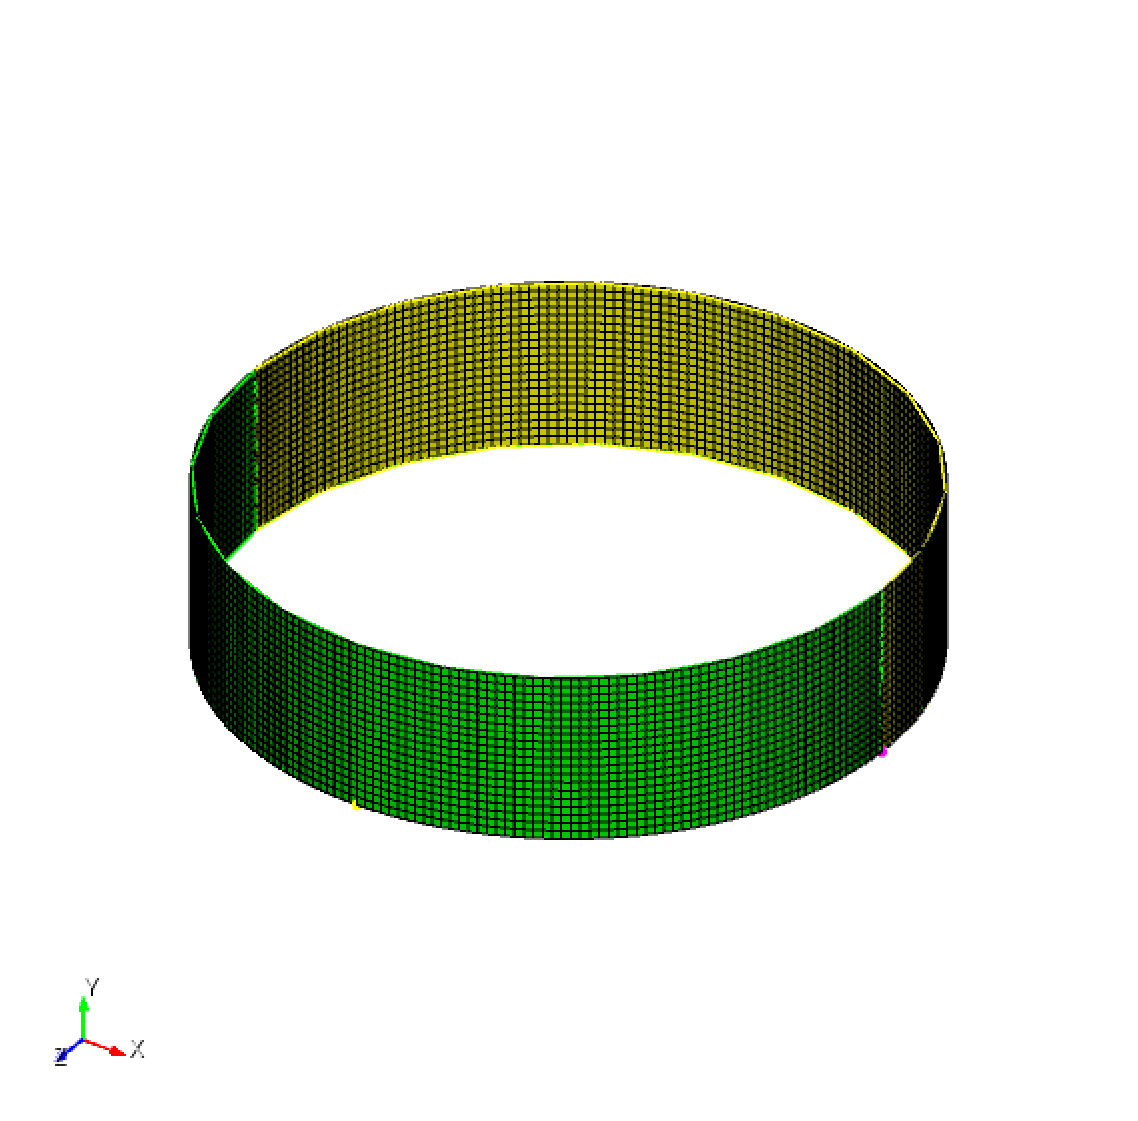
\includegraphics[width=0.6\textwidth]{PlateRing.eps}
%  \caption{3D Ring}
%  \label{fig:PlateRing}
%\end{figure}
%%
%
\begin{figure}[tbhp]
  \centering
  \vspace{-35mm}
  \resizebox{0.9\linewidth}{!}{\input{\plotpath/RingMesh20.pgf}}
  \vspace{-35mm}
  \caption{Discretization of a 3D Proving Ring}
  \label{fig:PlateRing}
\end{figure}
%


\Cref{fig:PlateRing_n} demonstrates that, as with the curved beam, the curved shell requires a dense discretization to model.
This is mostly as a consequence of requiring a small horizon.
Surfaces with less curvature are less constrained.

%
\begin{figure}[tbhp]
  \centering
  \resizebox{0.8\linewidth}{!}{\input{\plotpath/PlateRing_n.pgf}}
  \caption{Plate-based Proving Ring}
  \label{fig:PlateRing_n}
\end{figure}
%

